\documentclass[11pt]{book}
% Preamble of the English EGA edition, written for this edition (dedicated to the public domain under CC0 1.0).
% It defines the notation macros, cross-reference commands and numbered environments used by the sources.
\usepackage[a4paper,inner=2.6cm,outer=3.6cm,top=2.8cm,bottom=2.8cm,marginparwidth=2.7cm,marginparsep=0.3cm]{geometry}
\usepackage[T1]{fontenc}
\usepackage[utf8]{inputenc}
\usepackage{lmodern}
\usepackage[english]{babel}
\usepackage{amsmath,amssymb,amsthm,mathrsfs,mathtools}
\usepackage[shortlabels]{enumitem}
\usepackage[all,cmtip]{xy}
\usepackage{tikz-cd}
\usepackage{longtable,multicol}
\usepackage{marginnote}
\usepackage{xstring}
\usepackage[fit]{truncate}
% Running heads: chapter on left pages, section on right pages, in slanted type and cut to the text width.
\makeatletter
\renewcommand{\ps@headings}{%
  \def\@oddfoot{}\def\@evenfoot{}%
  \def\@oddhead{\truncate{\dimexpr\textwidth-3em\relax}{\slshape\rightmark}\hfil\thepage}%
  \def\@evenhead{\thepage\hfil\truncate{\dimexpr\textwidth-3em\relax}{\slshape\leftmark}}%
  \def\chaptermark##1{\markboth{##1}{}}%
  \def\sectionmark##1{\markright{\thesection.\ ##1}}}
\pagestyle{headings}
% The blank left-hand page before a chapter carries no running head.
\renewcommand{\cleardoublepage}{\clearpage\if@twoside\ifodd\c@page\else\hbox{}\thispagestyle{empty}\newpage\fi\fi}
% A bibliography is headed by the section heading of its file, not by a chapter heading of its own.
\renewenvironment{thebibliography}[1]
  {\list{\@biblabel{\@arabic\c@enumiv}}{\settowidth\labelwidth{\@biblabel{#1}}\leftmargin\labelwidth
     \advance\leftmargin\labelsep\@openbib@code\usecounter{enumiv}\let\p@enumiv\@empty
     \renewcommand\theenumiv{\@arabic\c@enumiv}}\sloppy\clubpenalty4000\@clubpenalty\clubpenalty
     \widowpenalty4000\sfcode`\.\@m}
  {\def\@noitemerr{\@latex@warning{Empty `thebibliography' environment}}\endlist}
\makeatother
\usepackage[hidelinks,bookmarksnumbered,hypertexnames=false]{hyperref}% unique link targets for tagged formulas
\usepackage{bookmark}
\setlength{\emergencystretch}{3em}

% ---- notation ---------------------------------------------------------------
\newcommand{\sh}[1]{\mathscr{#1}}
\newcommand{\bb}[1]{\mathbf{#1}}
\newcommand{\bbGamma}{\boldsymbol{\Gamma}}
\newcommand{\cat}[1]{\mathbf{#1}}
\newcommand{\vphi}{\varphi}
\newcommand{\HH}{\mathrm{H}}
\newcommand{\CHH}{\check{\mathrm{H}}}
\newcommand{\RR}{\mathrm{R}}
\newcommand{\LL}{\mathrm{L}}
\newcommand{\red}{\mathrm{red}}
\newcommand{\kres}{\boldsymbol{k}}
\newcommand{\emp}{\varnothing}
\newcommand{\supertilde}{^{\sim}}% written after its argument: M\supertilde is the sheaf associated with M
\newcommand{\isoto}{\xrightarrow{\,\smash{\raisebox{-0.45ex}{\ensuremath{\scriptstyle\sim}}}\,}}
\newcommand{\simto}{\isoto}
\DeclareMathOperator{\Spec}{Spec}
\DeclareMathOperator{\Spf}{Spf}
\DeclareMathOperator{\Proj}{Proj}
\DeclareMathOperator{\Supp}{Supp}
\DeclareMathOperator{\Der}{Der}
\DeclareMathOperator{\codim}{codim}
\DeclareMathOperator{\rg}{rg}
\DeclareMathOperator{\gr}{gr}
\DeclareMathOperator{\Tor}{Tor}
\DeclareMathOperator{\Ext}{Ext}
\DeclareMathOperator{\Ker}{Ker}
\DeclareMathOperator{\Coker}{Coker}
\providecommand{\Hom}{}\renewcommand{\Hom}{\operatorname{Hom}}
\providecommand{\Im}{}\renewcommand{\Im}{\operatorname{Im}}
\newcommand{\shHom}{\mathscr{H}\!\mathit{om}}
\newcommand{\shExt}{\mathscr{E}\!\mathit{xt}}
\newcommand{\shTor}{\mathscr{T}\!\mathit{or}}
\newcommand{\shProj}{\operatorname{\mathbf{Proj}}}
\newcommand{\setmin}{-}% EGA writes the complement of Y in X as X - Y
\newcommand{\C}{C}% a category, as in 0, 8.1.1
\newcommand{\op}{^{0}}% the opposite category C^0
\newcommand{\Set}{\mathrm{Ens}}% the category of sets
\newcommand{\CHom}{\operatorname{Hom}}% the category of functors
\newcommand{\Gr}{\operatorname{Gr}}% associated graded object
\providecommand{\og}{``}
\providecommand{\fg}{''}
\providecommand{\textsection}{\S}

% ---- original pagination ----------------------------------------------------
% \oldpage[volume]{n}: page n of the original printing, shown in the margin. Between paragraphs the note waits for
% the next paragraph to begin, so that it is set beside that paragraph's first line.
\makeatletter
\let\ega@pendingnote\relax
\newcommand{\oldpage}[2][]{%
  \ifvmode
    \gdef\ega@pendingnote{\footnotesize[#1\if\relax\detokenize{#1}\relax\else\,|\,\fi#2]}%
  \else
    \marginnote{\footnotesize[#1\if\relax\detokenize{#1}\relax\else\,|\,\fi#2]}%
  \fi}
\AddToHook{para/begin}{\ifx\ega@pendingnote\relax\else
  \let\ega@note\ega@pendingnote\global\let\ega@pendingnote\relax\marginnote{\ega@note}\fi}
\makeatother

% ---- numbered paragraphs and statements -------------------------------------
% EGA numbers every paragraph and statement explicitly, e.g. (1.2.3); the number is the optional argument,
% and \label after it records that number.
\makeatletter
\newcommand{\ega@setnum}[1]{\def\@currentlabel{#1}\phantomsection}
\newenvironment{env}[1][]{\par\medskip\ega@setnum{#1}\noindent\textbf{(#1)}\enspace\ignorespaces}{\par\medskip}
% \begin{theorem}[19.6.1][Cohen]: number, then an optional name printed after the kind of statement.
\newcommand{\ega@stmt}[3]{%
  \NewDocumentEnvironment{#1}{O{} o}{\par\medskip\ega@setnum{##1}\noindent
    \textbf{(##1)~#2\IfValueT{##2}{ (##2)}.}\enspace#3\ignorespaces}{\par\medskip}}
% \egabib{key}{n} before a bibliography entry printed as plain text "[n] ...": \cite{key} then prints [n] and links here.
\newcommand{\egabib}[2]{\Hy@raisedlink{\hyper@anchorstart{cite.#1}\hyper@anchorend}%
  \protected@write\@auxout{}{\string\bibcite{#1}{#2}}}
% A label that records a given number: used where a label sits at a place whose current number is a neighbour's.
\newcommand{\egalabel}[2]{\begingroup\def\@currentlabel{#2}\label{#1}\endgroup}
\ega@stmt{proposition}{Proposition}{\itshape}
\ega@stmt{theorem}{Theorem}{\itshape}
\ega@stmt{corollary}{Corollary}{\itshape}
\ega@stmt{lemma}{Lemma}{\itshape}
\ega@stmt{definition}{Definition}{}
\ega@stmt{remark}{Remark}{}
\ega@stmt{remarks}{Remarks}{}
\ega@stmt{example}{Example}{}
\ega@stmt{examples}{Examples}{}
\ega@stmt{notation}{Notation}{}
\ega@stmt{scholium}{Scholium}{}
\newenvironment{namedtheorem}[2][]{\par\medskip\ega@setnum{#1}\noindent\textbf{(#1)~#2.}\enspace\itshape\ignorespaces}{\par\medskip}
\newenvironment{namedlemma}[2][]{\par\medskip\ega@setnum{#1}\noindent\textbf{(#1)~#2.}\enspace\itshape\ignorespaces}{\par\medskip}
\makeatother

% The shown text of a link whose target is not in this edition.
\newcommand{\unlinked}[1]{#1}

% A link target the French sources place at numbered statements: \EGAReaderTarget{target name}{label key}.
\newcommand{\EGAReaderTarget}[2]{\ifvmode\else\leavevmode\fi\hypertarget{#1}{}}

% ---- references ----------------------------------------------------------------
% \sref[volume]{key}: the printed number of the labelled paragraph, in parentheses, linked; with a volume prefix
% when the target is in another chapter, e.g. \sref[0]{0.6.7.4} gives (0, 6.7.4).
\newcommand{\sref}[2][]{\hyperref[#2]{(\if\relax\detokenize{#1}\relax\else#1,~\fi\ref*{#2})}}
% \eref{key}: a numbered formula, e.g. (11.2.1.1).
\newcommand{\eref}[1]{\hyperref[#1]{(\ref*{#1})}}
% \erratum[volume]{reference}: a reference as corrected in the errata of that volume (Err_IV).
\newcommand{\erratum}[2][]{#2~[Err$_{\mathrm{#1}}$]}

\renewcommand{\thesection}{\S\arabic{section}}
\renewcommand{\thesubsection}{\arabic{section}.\arabic{subsection}}
\begin{document}
\begin{titlepage}\centering
{\Large Alexandre Grothendieck}\par\smallskip
{\large with the collaboration of Jean Dieudonné}\par\vspace{2em}
{\Huge Elements of Algebraic Geometry}\par\smallskip
{\large (\'El\'ements de g\'eom\'etrie alg\'ebrique)}\par\vspace{1.5em}
{\large Chapters 0--IV}\par\vfill
{\normalsize English translation}\par
\end{titlepage}
\noindent Translated from the French transcription of the original publication in the \emph{Publications
math\'ematiques de l'IH\'ES} 4, 8, 11, 17, 20, 24, 28 and 32 (1960--1967),
\url{https://github.com/KokunoYumeto/ega-fr}. The translation is AI-translated: by Claude Opus 5.5 (Anthropic) for
the Introduction, Chapter~0, \S\S1--11 and 14, Chapter~I, Chapter~II with its errata, Chapter~III, \S\S1 and 3,
and Chapter~IV: its introduction, \S\S1, 16, 17 and 20, and the bibliography and indexes that close its first part;
by OpenAI Codex models (GPT-6 Astra, GPT-5.6 Sol) for the other sections.

The rights in the original work remain with its rights holders. Anything in this edition that the publisher holds
rights to is dedicated to the public domain under CC0~1.0. Rights holders who object to the availability of this
material can open an issue at \url{https://github.com/KokunoYumeto/ega-en/issues}; the material will be taken down.
\clearpage
\tableofcontents
\cleardoublepage\phantomsection\addcontentsline{toc}{chapter}{Introduction}\markboth{Introduction}{Introduction}
\section*{Introduction}

\begin{center}
\emph{To Oscar Zariski and André Weil.}
\end{center}

\oldpage[I]{5}

This memoir, and the numerous others which are to follow it, are intended to form a treatise on the foundations of Algebraic Geometry.
In principle they presuppose no particular knowledge of this discipline, and it has even turned out that such knowledge, despite its obvious advantages, could sometimes (through the overly exclusive habit of the birational point of view which it implies) be harmful to one who wishes to become familiar with the point of view and the techniques presented here.
On the other hand, we shall assume that the reader has a good knowledge of the following subjects:

\begin{enumerate}
  \item[a)] \emph{Commutative Algebra}, as presented for example in the volumes of the \emph{Éléments} of N.~Bourbaki now in preparation (and, until these volumes appear, in Samuel-Zariski~\cite{I-13} and Samuel~\cite{I-11},~\cite{I-12}).
  \item[b)] \emph{Homological Algebra}, for which we refer to Cartan-Eilenberg~\cite{I-2} (cited as~(M)) and Godement~\cite{I-4} (cited as~(G)), as well as to the recent article of A.~Grothendieck~\cite{I-6} (cited as~(T)).
  \item[c)] \emph{Sheaf Theory}, where our principal references will be~(G) and~(T); this last theory provides the indispensable language for interpreting the essential notions of Commutative Algebra in ``geometric'' terms, and for ``globalizing'' them.
  \item[d)] Finally, it will be useful for the reader to have a certain familiarity with the \emph{functorial language}, which will be used constantly in this Treatise, and for which the reader may consult~(M),~(G) and above all~(T); the principles of this language and the principal results of the general theory of functors will be presented in more detail in a work being prepared by the authors of this Treatise.
\end{enumerate}

\bigskip
\begin{center}*\quad*\quad*\end{center}
\bigskip

This Introduction is not the place to give a more or less summary description of the point of view of ``schemes'' in Algebraic Geometry, nor the long list of reasons which have made its adoption necessary, and in particular the systematic acceptance of nilpotent elements in the local rings of the ``varieties'' that we consider (which necessarily relegates the notion of rational map to the background, in favour of that of regular map or ``morphism'').
The present Treatise aims precisely at developing the language of ``schemes'' systematically, and will, we hope, demonstrate its necessity.
Although it would be easy to do so, we

\oldpage[I]{6}
shall not attempt here either to give an ``intuitive'' introduction to the notions developed in Chapter One.
The reader who would like a preliminary overview of the material of this Treatise may refer to the address given by A.~Grothendieck at the International Congress of Mathematicians in Edinburgh in 1958~\cite{I-7}, and to the exposé~\cite{I-8} by the same author.
The work~\cite{I-14} (cited as~(FAC)) of J.-P.~Serre may also be regarded as an exposition intermediate between the classical point of view and the point of view of schemes in Algebraic Geometry, and as such, reading it may be an excellent preparation for reading our \emph{Éléments}.

\bigskip
\begin{center}*\quad*\quad*\end{center}
\bigskip

For information, we give below the general plan envisaged for this Treatise, which is moreover subject to later modifications, especially as regards the last chapters:

\medskip
\begin{tabular}{rl}
  Chapter One. & --- The language of schemes.\\
  --- \textbf{II}. & --- Elementary global study of some classes of morphisms.\\
  --- \textbf{III}. & --- Cohomology of coherent algebraic sheaves. Applications.\\
  --- \textbf{IV}. & --- Local study of morphisms.\\
  --- \textbf{V}. & --- Elementary procedures for constructing schemes.\\
  --- \textbf{VI}. & --- Descent technique. General method for constructing schemes.\\
  --- \textbf{VII}. & --- Group schemes, principal fibre spaces.\\
  --- \textbf{VIII}. & --- Differential study of fibre spaces.\\
  --- \textbf{IX}. & --- The fundamental group.\\
  --- \textbf{X}. & --- Residues and duality.\\
  --- \textbf{XI}. & --- Intersection theories, Chern classes, Riemann-Roch theorem.\\
  --- \textbf{XII}. & --- Abelian schemes and Picard schemes.\\
  --- \textbf{XIII}. & --- Weil cohomology.\\
\end{tabular}
\medskip

In principle, all the chapters are regarded as open, and supplementary paragraphs may always be added to them later; such paragraphs will appear in separate fascicles, in order to lessen the drawbacks of the mode of publication adopted.
When such a paragraph is planned or in preparation at the time a chapter is published, it will be mentioned in the summary of that chapter, even if, owing to certain orders of urgency, its actual publication should come appreciably later.
For the convenience of the reader, we give in a ``Chapter~0'' various supplements on Commutative Algebra, on Homological Algebra and on Sheaf Theory, used in the course of the chapters of this Treatise, which are more or less well known, but for which it has not been possible to give convenient references.
The reader is advised to refer to Chapter~0 only in the course of reading the Treatise proper, and to the extent that the results to which we refer are not

\oldpage[I]{7}
sufficiently familiar to the reader.
We believe, moreover, that in this way the reading of this Treatise may be a good method for the beginner to become familiar with Commutative Algebra and Homological Algebra, the study of which, when it is not accompanied by tangible applications, is judged tedious, even depressing, by a fairly large number of people.

\bigskip
\begin{center}*\quad*\quad*\end{center}
\bigskip

It is beyond our competence to give in this Introduction a historical survey, even a summary one, of the notions and results presented.
The text will contain only the references judged particularly useful for its understanding, and we shall indicate the origin only of the most important results.
Formally at least, the subjects treated in our work are fairly new, which will explain the scarcity of references to the Fathers of Algebraic Geometry of the nineteenth century and of the beginning of the twentieth century, whose works we know only by hearsay.
It is appropriate, however, to say a few words here about the works which have most directly influenced the authors and contributed to the development of the point of view of schemes.
First and foremost we must cite the fundamental work (FAC) of J.-P.~Serre, which has served as an introduction to Algebraic Geometry for more than one young adept (among them one of the authors of the present Treatise), put off by the aridity of A.~Weil's classic \emph{Foundations}~\cite{I-18}.
That work was the first to show that the ``Zariski topology'' of an ``abstract'' algebraic variety lends itself perfectly to certain techniques of Algebraic Topology, and in particular to the construction of a cohomology theory.
Moreover, the definition of an algebraic variety given there is the one which lends itself most naturally to the extension of this notion that we develop here\footnote{As J.-P.~Serre has pointed out to us, it should be noted that the idea of defining the structure of a variety through a sheaf of rings goes back to H.~Cartan, who made it the starting point of his theory of analytic spaces.
Naturally, in ``Analytic Geometry'' just as in Algebraic Geometry, nilpotent elements ought to be given full rights of citizenship in the local rings of analytic spaces.
This extension of the definition of H.~Cartan and J.-P.~Serre has recently been taken up by H.~Grauert~\cite{I-5}, and there is reason to hope that a systematic exposition of Analytic Geometry in this general framework will soon see the light of day.
It is moreover evident that the notions and techniques developed in this Treatise retain a meaning in Analytic Geometry, although one must expect more considerable technical difficulties in the latter theory.
One may foresee that Algebraic Geometry, through the simplicity of its methods, will be able to serve as a kind of formal model for future developments in the theory of analytic spaces.}.
Serre had moreover observed himself that the cohomology theory of affine algebraic varieties carries over without difficulty when the affine algebras over a field are replaced by arbitrary commutative rings.
In essence, therefore, Chapters I and II of this Treatise and the first two paragraphs of Chapter III can be viewed as easy transpositions, to this enlarged framework, of the principal results of (FAC) and of a later article by the same author~\cite{I-15}.
We have also profited greatly from the \emph{Séminaire de Géométrie algébrique} of C.~Chevalley~\cite{I-1}; in particular, the systematic use of the ``constructible sets'' introduced by him has proved very useful in the theory of schemes (cf.\ Chapter~IV).
From him, too, we have taken the study of morphisms from the point

\oldpage[I]{8}
of view of dimension (Chapter~IV), which carries over without notable change to the framework of schemes.
It should be noted, furthermore, that the notion of ``schemes of local rings'', introduced by Chevalley, lends itself naturally to an extension of Algebraic Geometry (not having, however, all the flexibility and generality that we intend to give it here); for the relations between this notion and our theory, see Chapter One, \S~8.
Such an extension has been developed by M.~Nagata in a series of memoirs~\cite{I-9} containing numerous special results concerning Algebraic Geometry over Dedekind rings\footnote{Among the works which come close to our point of view in Algebraic Geometry, let us mention the important work of E.~Kähler~\cite{I-22}, and a recent Note of Chow and Igusa~\cite{I-3}, who take up, within the framework of the Nagata-Chevalley theory, certain results of (FAC) and also give a Künneth formula.}.

\bigskip
\begin{center}*\quad*\quad*\end{center}
\bigskip

Finally, it goes without saying that a book on Algebraic Geometry, and above all a book dealing with foundations, is necessarily influenced, if only through intermediaries, by mathematicians such as O.~Zariski and A.~Weil.
In particular, the \emph{Theory of holomorphic functions} of Zariski~\cite{I-20}, suitably made more flexible by means of cohomological methods and completed by an existence theorem (Chapter~III, \S\S~4 and 5), is (together with the descent technique presented in Chapter~VI) one of the principal tools used in this Treatise, and seems to us one of the most powerful available in Algebraic Geometry.

The general technique into which it fits can be sketched as follows (a typical example of it will be provided in Chapter~IX, in the study of the fundamental group).
One has a proper morphism (Chapter~II) $f:X\to Y$ from one algebraic variety to another (more generally, from one scheme to another), which one wishes to study in a neighbourhood of a point $y\in Y$, with a view to solving a problem P relative to a neighbourhood of $y$.
One proceeds in successive steps:
\begin{enumerate}
  \item[$1^\circ$] One may suppose $Y$ affine, so that $X$ becomes a scheme defined over the affine ring $A$ of $Y$, and one may even replace $A$ by the local ring of $y$.
  This reduction is always easy in practice (Chapter~V) and brings us back to the case where $A$ is a \emph{local} ring.
  \item[$2^\circ$] One studies the problem under consideration when $A$ is an \emph{Artinian} local ring.
  In order for it to retain a genuine meaning when $A$ is not assumed to be integral, it is sometimes necessary to reformulate the problem P, and it turns out that one often thereby obtains a better understanding of the problem, which at this stage is of an ``infinitesimal'' nature.
  \item[$3^\circ$] The theory of formal schemes (Chapter~III, \S\S~3, 4 and 5) makes it possible to pass from the case of an Artinian ring to the case of a \emph{complete local ring}.
  \item[$4^\circ$] Finally, if $A$ is an arbitrary local ring, the consideration of ``multivalued sections'' over suitable schemes over $X$, approximating a given ``formal'' section (Chapter~IV), will often make it possible to pass from a result known for the scheme

  \oldpage[I]{9}
  deduced from $X$ by extension of scalars to the completion of $A$, to an analogous result for a fairly simple (for example unramified) finite extension of $A$.
\end{enumerate}

This sketch shows the importance of the systematic study of schemes defined over an Artinian ring $A$.
Serre's point of view in his formulation of local class field theory, and recent work of Greenberg, seem to suggest that such a study could be undertaken by functorially attaching to such a scheme $X$ a scheme $X'$ over the residue field $k$ of $A$ (assumed perfect), of dimension equal (in favourable cases) to $n\dim X$, where $n$ is the length of $A$.

As for the influence of A.~Weil, suffice it to say that it is the necessity of developing the tools needed to formulate, with all the desired generality, the definition of ``Weil cohomology'', and to undertake the proof\footnote{To avoid any misunderstanding, let us make clear that this task has barely been undertaken at the time this Introduction is being written, and has therefore not yet led to the proof of the Weil conjectures.} of all the formal properties needed to establish his celebrated conjectures in Diophantine Geometry~\cite{I-19}, that has been one of the principal motivations for the writing of the present Treatise, on the same footing as the desire to find the natural framework for the usual notions and methods of Algebraic Geometry, and to give the authors the opportunity of understanding the said notions and techniques.

\bigskip
\begin{center}*\quad*\quad*\end{center}
\bigskip

To conclude, we think it useful to warn readers that, just like the authors themselves, they will no doubt have some difficulty before becoming accustomed to the language of schemes, and before convincing themselves that the usual constructions suggested by geometric intuition can be transcribed, in essentially only one reasonable way, into this language.
As in many parts of modern Mathematics, the initial intuition moves further and further away, in appearance, from the language suited to expressing it with all the desired precision and generality.
In the present case, the psychological difficulty stems from the necessity of transferring to the objects of a category already rather different from the category of sets (namely the category of preschemes, or the category of preschemes over a given prescheme) notions which are familiar for sets: Cartesian products, laws of group, of ring, of module, fibre bundles, principal homogeneous fibre bundles, etc.
It will no doubt be difficult for the mathematician, in the future, to shirk this new effort of abstraction, perhaps rather slight, all things considered, in comparison with the one made by our fathers in familiarizing themselves with Set Theory.

\bigskip
\begin{center}*\quad*\quad*\end{center}
\bigskip

References will be given according to the decimal system; for example, in III, 4.9.3, the numeral III indicates the chapter, the numeral 4 the paragraph, and the numeral 9 the section of the paragraph.
Within the same chapter, mention of the chapter will be omitted.

\chapter*{Chapter 0. Preliminaries}\addcontentsline{toc}{chapter}{Chapter 0. Preliminaries}\markboth{Chapter 0. Preliminaries}{}
\setcounter{section}{0}
\section{Rings of fractions}
\label{section:0.1}

\setcounter{subsection}{-1}
\subsection{Rings and algebras}
\label{subsection:0.1.0}

\oldpage[0\textsubscript{I}]{11}
\begin{env}[1.0.1]
\label{0.1.0.1}
Every ring considered in this Treatise has a \emph{unit element};
every module over such a ring is assumed to be \emph{unital}; ring homomorphisms will always be assumed to \emph{map the unit element to the unit element}; unless expressly stated otherwise, a subring of a ring $A$ will be assumed to \emph{contain the unit element of $A$}.
We shall consider mainly \emph{commutative} rings, and when we speak of a ring without further qualification, it will be understood that a commutative ring is meant.
If $A$ is a not necessarily commutative ring, by an $A$-module we shall always mean a \emph{left} module, unless expressly stated otherwise.
\end{env}

\begin{env}[1.0.2]
\label{0.1.0.2}
Let $A$, $B$ be two not necessarily commutative rings, and $\varphi:A\to B$ a homomorphism.
Every left (resp. right) $B$-module $M$ can be endowed with a left (resp. right) $A$-module structure by setting $a.m=\varphi(a).m$ (resp. $m.a=m.\varphi(a)$); when it is necessary to distinguish between the $A$-module and $B$-module structures on $M$, we shall denote by $M_{[\varphi]}$ the left (resp. right) $A$-module thus defined.
If $L$ is an $A$-module, a homomorphism $u:L\to M_{[\varphi]}$ is therefore a homomorphism of commutative groups such that $u(a.x)=\varphi(a).u(x)$ for $a\in A$, $x\in L$; we shall also say that it is a \emph{$\varphi$-homomorphism} $L\to M$, and that the pair $(\varphi,u)$ (or, by abuse of language, $u$) is a \emph{di-homomorphism} from $(A,L)$ to $(B,M)$.
The pairs $(A,L)$ consisting of a ring $A$ and an $A$-module $L$ therefore form a \emph{category} whose morphisms are the di-homomorphisms.
\end{env}

\begin{env}[1.0.3]
\label{0.1.0.3}
Under the hypotheses of (1.0.2), if $\mathfrak{J}$ is a left (resp. right) ideal of $A$, we shall denote by $B\mathfrak{J}$ (resp. $\mathfrak{J}B$) the left (resp. right) ideal $B\varphi(\mathfrak{J})$ (resp. $\varphi(\mathfrak{J})B$) of $B$ generated by $\varphi(\mathfrak{J})$; it is also the image of the canonical homomorphism $B\otimes_A\mathfrak{J}\to B$ (resp. $\mathfrak{J}\otimes_A B\to B$) of left (resp. right) $B$-modules.
\end{env}

\begin{env}[1.0.4]
\label{0.1.0.4}
If $A$ is a (commutative) ring and $B$ a not necessarily commutative ring, giving an \emph{$A$-algebra} structure on $B$ is equivalent to giving a ring homomorphism $\varphi:A\to B$ such that $\varphi(A)$ is contained in the centre of $B$.
For every ideal $\mathfrak{J}$ of $A$, $\mathfrak{J}B=B\mathfrak{J}$ is then a two-sided ideal of $B$, and for every $B$-module $M$, $\mathfrak{J}M$ is then a $B$-module equal to $(B\mathfrak{J})M$.
\end{env}

\begin{env}[1.0.5]
\label{0.1.0.5}
We shall not go back over the notions of \emph{module of finite type} and of (commutative) \emph{algebra of finite type}; to say that an $A$-module $M$ is of finite type means that there exists

\oldpage[0\textsubscript{I}]{12}
an exact sequence $A^p\to M\to 0$.
An $A$-module $M$ is said to admit a \emph{finite presentation} if it is isomorphic to the cokernel of a homomorphism $A^p\to A^q$, in other words if there exists an exact sequence $A^p\to A^q\to M\to 0$.
Note that over a \emph{Noetherian} ring $A$, every $A$-module of finite type admits a finite presentation.

Recall that an $A$-algebra $B$ is said to be \emph{integral over $A$} if every element of $B$ is a root in $B$ of a monic polynomial with coefficients in $A$; it amounts to the same to say that every element of $B$ is contained in a subalgebra of $B$ which is an \emph{$A$-module of finite type}.
When this is so, and $B$ is commutative, the subalgebra of $B$ generated by a finite subset of $B$ is an $A$-module of finite type; for the commutative algebra $B$ to be integral and of finite type over $A$, it is therefore necessary and sufficient that $B$ be an $A$-module of finite type; one then also says that $B$ is a \emph{finite integral} $A$-algebra (or simply a \emph{finite} one, if no confusion results).
Observe that in these definitions the homomorphism $A\to B$ defining the $A$-algebra structure is not assumed to be injective.
\end{env}

\begin{env}[1.0.6]
\label{0.1.0.6}
An \emph{integral} ring is a ring in which the product of a finite family of elements $\neq 0$ is $\neq 0$; it amounts to the same to say that in such a ring one has $0\neq 1$ and the product of two elements $\neq 0$ is nonzero.
A \emph{prime} ideal of a ring $A$ is an ideal $\mathfrak{p}$ such that $A/\mathfrak{p}$ is integral; this therefore implies $\mathfrak{p}\neq A$.
For a ring $A$ to have at least one prime ideal, it is necessary and sufficient that $A\neq\{0\}$.
\end{env}

\begin{env}[1.0.7]
\label{0.1.0.7}
A \emph{local} ring is a ring $A$ in which there exists only one maximal ideal, which is then the complement of the set of invertible elements and contains all the ideals $\neq A$.
If $A$ and $B$ are two local rings, and $\mathfrak{m}$ and $\mathfrak{n}$ their respective maximal ideals, a homomorphism $\varphi:A\to B$ is said to be \emph{local} if $\varphi(\mathfrak{m})\subset\mathfrak{n}$ (or, what amounts to the same, if $\varphi^{-1}(\mathfrak{n})=\mathfrak{m}$).
By passage to the quotients, such a homomorphism then defines a monomorphism of the residue field $A/\mathfrak{m}$ into the residue field $B/\mathfrak{n}$.
The composite of two local homomorphisms is a local homomorphism.
\end{env}

\subsection{Radical of an ideal. Nilradical and radical of a ring}
\label{subsection:0.1.1}

\begin{env}[1.1.1]
\label{0.1.1.1}
Let $\mathfrak{a}$ be an ideal of a ring $A$; the \emph{radical} of $\mathfrak{a}$, denoted $\mathfrak{r}(\mathfrak{a})$, is the set of $x\in A$ such that $x^n\in\mathfrak{a}$ for at least one integer $n>0$; it is an ideal containing $\mathfrak{a}$.
We have $\mathfrak{r}(\mathfrak{r}(\mathfrak{a}))=\mathfrak{r}(\mathfrak{a})$; the relation $\mathfrak{a}\subset\mathfrak{b}$ implies $\mathfrak{r}(\mathfrak{a})\subset\mathfrak{r}(\mathfrak{b})$; the radical of a finite intersection of ideals is the intersection of their radicals.
If $\varphi$ is a homomorphism from a ring $A'$ to $A$, we have $\mathfrak{r}(\varphi^{-1}(\mathfrak{a}))=\varphi^{-1}(\mathfrak{r}(\mathfrak{a}))$ for every ideal $\mathfrak{a}\subset A$.
An ideal is the radical of an ideal if and only if it is an intersection of prime ideals.
The radical of an ideal $\mathfrak{a}$ is the intersection of the prime ideals which are \emph{minimal} among those containing $\mathfrak{a}$; if $A$ is Noetherian, these minimal prime ideals are finite in number.

The radical of the ideal $(0)$ is also called the \emph{nilradical} of $A$; it is the set $\mathfrak{N}$ of nilpotent elements of $A$.
The ring $A$ is said to be \emph{reduced} if $\mathfrak{N}=(0)$; for every ring $A$, the quotient $A/\mathfrak{N}$ of $A$ by its nilradical is a reduced ring.
\end{env}

\begin{env}[1.1.2]
\label{0.1.1.2}
Recall that the \emph{radical} $\mathfrak{R}(A)$ of a (not necessarily commutative) ring $A$ is the intersection of the maximal left ideals of $A$ (and also the intersection of the maximal right ideals).
The radical of $A/\mathfrak{R}(A)$ is $(0)$.
\end{env}

\subsection{Modules and rings of fractions}
\label{subsection:0.1.2}

\oldpage[0\textsubscript{I}]{13}
\begin{env}[1.2.1]
\label{0.1.2.1}
A subset $S$ of a ring $A$ is said to be \emph{multiplicative} if $1\in S$ and the product of two elements of $S$ is in $S$.
The examples which will be the most important in what follows are: $1^\circ$ the set $S_f$ of the powers $f^n$ ($n\geq 0$) of an element $f\in A$; $2^\circ$ the complement $A-\mathfrak{p}$ of a \emph{prime} ideal $\mathfrak{p}$ of $A$.
\end{env}

\begin{env}[1.2.2]
\label{0.1.2.2}
Let $S$ be a multiplicative subset of a ring $A$, and $M$ an $A$-module; in the set $M\times S$, the relation between pairs $(m_1,s_1)$, $(m_2,s_2)$:
\[
  \text{``there exists $s\in S$ such that $s(s_1m_2-s_2m_1)=0$''}
\]
is an equivalence relation.
We denote by $S^{-1}M$ the quotient set of $M\times S$ by this relation, and by $m/s$ the canonical image in $S^{-1}M$ of the pair $(m,s)$; the map $i_M^S:m\mapsto m/1$ (also denoted $i^S$) is called the \emph{canonical map} from $M$ to $S^{-1}M$.
This map is in general neither injective nor surjective; its kernel is the set of $m\in M$ for which there exists an $s\in S$ such that $sm=0$.

On $S^{-1}M$ one defines an additive group law by taking
\[
  (m_1/s_1)+(m_2/s_2)=(s_2m_1+s_1m_2)/(s_1s_2)
\]
(one checks that this is indeed independent of the expressions of the elements of $S^{-1}M$ considered).
On $S^{-1}A$ one further defines a multiplicative law by taking $(a_1/s_1)(a_2/s_2)=(a_1a_2)/(s_1s_2)$, and finally an external law on $S^{-1}M$, having $S^{-1}A$ as set of operators, by setting $(a/s)(m/s')=(am)/(ss')$.
One checks in this way that $S^{-1}A$ is endowed with a ring structure (called the \emph{ring of fractions of $A$ with denominators in $S$}) and $S^{-1}M$ with an $S^{-1}A$-module structure (called the \emph{module of fractions of $M$ with denominators in $S$}); for every $s\in S$, $s/1$ is invertible in $S^{-1}A$, its inverse being $1/s$.
The canonical map $i_A^S$ (resp. $i_M^S$) is a ring homomorphism (resp. a homomorphism of $A$-modules, $S^{-1}M$ being regarded as an $A$-module by means of the homomorphism $i_A^S:A\to S^{-1}A$).
\end{env}

\begin{env}[1.2.3]
\label{0.1.2.3}
If $S_f=\{f^n\}_{n\geq 0}$ for some $f\in A$, we write $A_f$ and $M_f$ instead of $S_f^{-1}A$ and $S_f^{-1}M$; when $A_f$ is regarded as an algebra over $A$, we may write $A_f=A[1/f]$.
$A_f$ is isomorphic to the quotient algebra $A[T]/(fT-1)A[T]$.
When $f=1$, $A_f$ and $M_f$ are canonically identified with $A$ and $M$; if $f$ is nilpotent, $A_f$ and $M_f$ are reduced to $0$.

When $S=A-\mathfrak{p}$, where $\mathfrak{p}$ is a prime ideal of $A$, we write $A_{\mathfrak{p}}$ and $M_{\mathfrak{p}}$ instead of $S^{-1}A$ and $S^{-1}M$; $A_{\mathfrak{p}}$ is a \emph{local ring} whose maximal ideal $\mathfrak{q}$ is generated by $i_A^S(\mathfrak{p})$, and we have $(i_A^S)^{-1}(\mathfrak{q})=\mathfrak{p}$; by passage to the quotients, $i_A^S$ gives a monomorphism of the integral ring $A/\mathfrak{p}$ into the field $A_{\mathfrak{p}}/\mathfrak{q}$, which is identified with the field of fractions of $A/\mathfrak{p}$.
\end{env}

\begin{env}[1.2.4]
\label{0.1.2.4}
The ring of fractions $S^{-1}A$ and the canonical homomorphism $i_A^S$ are a solution of a \emph{universal mapping problem}: every homomorphism $u$ from $A$ to a ring $B$ such that $u(S)$ consists of elements \emph{invertible} in $B$ factorizes in a unique way as
\[
  u:A\xrightarrow{i_A^S}S^{-1}A\xrightarrow{u^*}B
\]

\oldpage[0\textsubscript{I}]{14}
where $u^*$ is a ring homomorphism.
Under the same hypotheses, let $M$ be an $A$-module, $N$ a $B$-module, and $v:M\to N$ a homomorphism of $A$-modules (for the $B$-module structure on $N$ defined by $u:A\to B$); then $v$ factorizes in a unique way as
\[
  v:M\xrightarrow{i_M^S}S^{-1}M\xrightarrow{v^*}N
\]
where $v^*$ is a homomorphism of $S^{-1}A$-modules (for the $S^{-1}A$-module structure on $N$ defined by $u^*$).
\end{env}

\begin{env}[1.2.5]
\label{0.1.2.5}
One defines a canonical isomorphism $S^{-1}A\otimes_A M\xrightarrow{\sim}S^{-1}M$ of $S^{-1}A$-modules by mapping the element $(a/s)\otimes m$ to the element $(am)/s$, the inverse isomorphism mapping $m/s$ to $(1/s)\otimes m$.
\end{env}

\begin{env}[1.2.6]
\label{0.1.2.6}
For every ideal $\mathfrak{a}'$ of $S^{-1}A$, $\mathfrak{a}=(i_A^S)^{-1}(\mathfrak{a}')$ is an ideal of $A$, and $\mathfrak{a}'$ is the ideal of $S^{-1}A$ generated by $i_A^S(\mathfrak{a})$, which is identified with $S^{-1}\mathfrak{a}$ (1.3.2).
The map $\mathfrak{p}'\mapsto(i_A^S)^{-1}(\mathfrak{p}')$ is an isomorphism, for the order structures, of the set of \emph{prime} ideals of $S^{-1}A$ onto the set of prime ideals $\mathfrak{p}$ of $A$ such that $\mathfrak{p}\cap S=\varnothing$.
Moreover, the local rings $A_{\mathfrak{p}}$ and $(S^{-1}A)_{S^{-1}\mathfrak{p}}$ are then canonically (1.5.1) isomorphic.
\end{env}

\begin{env}[1.2.7]
\label{0.1.2.7}
When $A$ is an \emph{integral} ring, whose field of fractions we denote by $K$, the canonical map $i_A^S:A\to S^{-1}A$ is injective for every multiplicative subset $S$ not containing $0$, and $S^{-1}A$ is then canonically identified with a subring of $K$ containing $A$.
In particular, for every prime ideal $\mathfrak{p}$ of $A$, $A_{\mathfrak{p}}$ is a local ring containing $A$, with maximal ideal $\mathfrak{p}A_{\mathfrak{p}}$, and we have $\mathfrak{p}A_{\mathfrak{p}}\cap A=\mathfrak{p}$.
\end{env}

\begin{env}[1.2.8]
\label{0.1.2.8}
If $A$ is a \emph{reduced} ring (1.1.1), so is $S^{-1}A$: indeed, if $(x/s)^n=0$ for $x\in A$, $s\in S$, this means that there exists $s'\in S$ such that $s'x^n=0$, whence $(s'x)^n=0$, which by hypothesis implies $s'x=0$, hence $x/s=0$.
\end{env}

\subsection{Functorial properties}
\label{subsection:0.1.3}

\begin{env}[1.3.1]
\label{0.1.3.1}
Let $M$, $N$ be two $A$-modules, and $u$ an $A$-homomorphism $M\to N$.
If $S$ is a multiplicative subset of $A$, one defines an $S^{-1}A$-homomorphism $S^{-1}M\to S^{-1}N$, denoted $S^{-1}u$, by setting $(S^{-1}u)(m/s)=u(m)/s$; if $S^{-1}M$ and $S^{-1}N$ are canonically identified with $S^{-1}A\otimes_A M$ and $S^{-1}A\otimes_A N$ (1.2.5), $S^{-1}u$ is identified with $1\otimes u$.
If $P$ is a third $A$-module and $v$ an $A$-homomorphism $N\to P$, we have $S^{-1}(v\circ u)=(S^{-1}v)\circ(S^{-1}u)$; in other words, $S^{-1}M$ is a \emph{covariant functor in $M$}, from the category of $A$-modules to that of $S^{-1}A$-modules ($A$ and $S$ being fixed).
\end{env}

\begin{env}[1.3.2]
\label{0.1.3.2}
The functor $S^{-1}M$ is \emph{exact}; in other words, if the sequence
\[
  M\xrightarrow{u}N\xrightarrow{v}P
\]
is exact, so is the sequence
\[
  S^{-1}M\xrightarrow{S^{-1}u}S^{-1}N\xrightarrow{S^{-1}v}S^{-1}P.
\]
In particular, if $u:M\to N$ is injective (resp. surjective), so is $S^{-1}u$;

\oldpage[0\textsubscript{I}]{15}
if $N$ and $P$ are two submodules of $M$, $S^{-1}N$ and $S^{-1}P$ are canonically identified with submodules of $S^{-1}M$, and we have
\[
  S^{-1}(N+P)=S^{-1}N+S^{-1}P
  \quad\text{and}\quad
  S^{-1}(N\cap P)=(S^{-1}N)\cap(S^{-1}P).
\]
\end{env}

\begin{env}[1.3.3]
\label{0.1.3.3}
Let $(M_\alpha,\varphi_{\beta\alpha})$ be an inductive system of $A$-modules; then $(S^{-1}M_\alpha,S^{-1}\varphi_{\beta\alpha})$ is an inductive system of $S^{-1}A$-modules.
Expressing the $S^{-1}M_\alpha$ and $S^{-1}\varphi_{\beta\alpha}$ as tensor products (1.2.5 and 1.3.1), it follows from the fact that the operations of tensor product and of inductive limit commute that there is a canonical isomorphism
\[
  S^{-1}\varinjlim M_\alpha\xrightarrow{\sim}\varinjlim S^{-1}M_\alpha,
\]
which one also expresses by saying that the functor $S^{-1}M$ (in $M$) \emph{commutes with inductive limits}.
\end{env}

\begin{env}[1.3.4]
\label{0.1.3.4}
Let $M$, $N$ be two $A$-modules; there exists a canonical \emph{functorial} isomorphism (in $M$ and $N$)
\[
  (S^{-1}M)\otimes_{S^{-1}A}(S^{-1}N)
  \xrightarrow{\sim}
  S^{-1}(M\otimes_A N)
\]
which maps $(m/s)\otimes(n/t)$ to $(m\otimes n)/st$.
\end{env}

\begin{env}[1.3.5]
\label{0.1.3.5}
Similarly, there is a \emph{functorial} homomorphism (in $M$ and $N$)
\[
  S^{-1}\operatorname{Hom}_A(M,N)
  \longrightarrow
  \operatorname{Hom}_{S^{-1}A}(S^{-1}M,S^{-1}N)
\]
which maps $u/s$ to the homomorphism $m/t\mapsto u(m)/st$.
When $M$ has a \emph{finite presentation}, the preceding homomorphism is an \emph{isomorphism}: this is immediate when $M$ is of the form $A^r$, and one passes from there to the general case by starting from the exact sequence $A^p\to A^q\to M\to 0$ and using the exactness of the functor $S^{-1}M$ and the left exactness of the functor $\operatorname{Hom}_A(M,N)$ in $M$.
Note that this case always occurs when $A$ is \emph{Noetherian} and the $A$-module $M$ is \emph{of finite type}.
\end{env}

\subsection{Change of multiplicative subset}
\label{subsection:0.1.4}

\begin{env}[1.4.1]
\label{0.1.4.1}
Let $S$, $T$ be two multiplicative subsets of a ring $A$ such that $S\subset T$; there exists a canonical homomorphism $\rho_A^{T,S}$ (or simply $\rho^{T,S}$) from $S^{-1}A$ to $T^{-1}A$, which maps the element denoted $a/s$ of $S^{-1}A$ to the element denoted $a/s$ in $T^{-1}A$; we have
\[
  i_A^T=\rho_A^{T,S}\circ i_A^S.
\]
For every $A$-module $M$, there likewise exists an $S^{-1}A$-linear map from $S^{-1}M$ to $T^{-1}M$ (the latter being regarded as an $S^{-1}A$-module by means of the homomorphism $\rho_A^{T,S}$), which maps the element $m/s$ of $S^{-1}M$ to the element $m/s$ of $T^{-1}M$; this map is denoted $\rho_M^{T,S}$, or simply $\rho^{T,S}$, and we again have
\[
  i_M^T=\rho_M^{T,S}\circ i_M^S;
\]
under the canonical identification (1.2.5), $\rho_M^{T,S}$ is identified with $\rho_A^{T,S}\otimes 1$.
The homomorphism $\rho_M^{T,S}$ is a \emph{functorial morphism} (or natural transformation) from the functor $S^{-1}M$ to the functor $T^{-1}M$; in other words, the diagram
\[
\begin{tikzcd}[column sep=large,row sep=large]
S^{-1}M \arrow[r,"S^{-1}u"] \arrow[d,"\rho_M^{T,S}"'] & S^{-1}N \arrow[d,"\rho_N^{T,S}"] \\
T^{-1}M \arrow[r,"T^{-1}u"] & T^{-1}N
\end{tikzcd}
\]

\oldpage[0\textsubscript{I}]{16}
is commutative for every homomorphism $u:M\to N$; note moreover that $T^{-1}u$ is entirely determined by $S^{-1}u$, since for $m\in M$ and $t\in T$ we have
\[
  (T^{-1}u)(m/t)=(t/1)^{-1}\rho^{T,S}\bigl((S^{-1}u)(m/1)\bigr).
\]
\end{env}

\begin{env}[1.4.2]
\label{0.1.4.2}
With the same notation, for two $A$-modules $M$, $N$, the diagrams (cf.\ (1.3.4) and (1.3.5))
\[
\begin{tikzcd}[column sep=large,row sep=large]
(S^{-1}M)\otimes_{S^{-1}A}(S^{-1}N) \arrow[r,"\sim"] \arrow[d]
  & S^{-1}(M\otimes_A N) \arrow[d]
  \\
(T^{-1}M)\otimes_{T^{-1}A}(T^{-1}N) \arrow[r,"\sim"]
  & T^{-1}(M\otimes_A N)
\end{tikzcd}
\]
\[
\begin{tikzcd}[column sep=large,row sep=large]
S^{-1}\operatorname{Hom}_A(M,N) \arrow[r] \arrow[d]
  & \operatorname{Hom}_{S^{-1}A}(S^{-1}M,S^{-1}N) \arrow[d] \\
T^{-1}\operatorname{Hom}_A(M,N) \arrow[r]
  & \operatorname{Hom}_{T^{-1}A}(T^{-1}M,T^{-1}N)
\end{tikzcd}
\]
are commutative.
\end{env}

\begin{env}[1.4.3]
\label{0.1.4.3}
There is an important case in which the homomorphism $\rho^{T,S}$ is \emph{bijective}, namely when every element of $T$ is a divisor of an element of $S$; one then identifies the modules $S^{-1}M$ and $T^{-1}M$ by means of $\rho^{T,S}$.
We say that $S$ is \emph{saturated} if every divisor in $A$ of an element of $S$ is in $S$; by replacing $S$ by the set $T$ of all divisors of the elements of $S$ (a set which is multiplicative and saturated), one sees that one can always, if one wishes, restrict oneself to considering modules of fractions $S^{-1}M$ where $S$ is saturated.
\end{env}

\begin{env}[1.4.4]
\label{0.1.4.4}
If $S$, $T$, $U$ are three multiplicative subsets of $A$ such that $S\subset T\subset U$, we have
\[
  \rho^{U,S}=\rho^{U,T}\circ\rho^{T,S}.
\]
\end{env}

\begin{env}[1.4.5]
\label{0.1.4.5}
Consider an \emph{increasing filtered family} $(S_\alpha)$ of multiplicative subsets of $A$ (we write $\alpha\leq\beta$ for $S_\alpha\subset S_\beta$), and let $S$ be the multiplicative subset $\bigcup_\alpha S_\alpha$; set
\[
  \rho_{\beta\alpha}=\rho_A^{S_\beta,S_\alpha}\quad\text{for }\alpha\leq\beta;
\]
by (1.4.4), the homomorphisms $\rho_{\beta\alpha}$ define a ring $A'$, the \emph{inductive limit} of the inductive system of rings $(S_\alpha^{-1}A,\rho_{\beta\alpha})$.
Let $\rho_\alpha$ be the canonical map $S_\alpha^{-1}A\to A'$, and set $\varphi_\alpha=\rho_A^{S,S_\alpha}$; since $\varphi_\alpha=\varphi_\beta\circ\rho_{\beta\alpha}$ for $\alpha\leq\beta$ by (1.4.4), one can define in a unique way a homomorphism $\varphi:A'\to S^{-1}A$ such that the diagram
\[
\begin{tikzcd}[column sep=huge,row sep=large]
  & S_\alpha^{-1}A
      \arrow[ddl,"\rho_\alpha"']
      \arrow[d,"\rho_{\beta\alpha}"]
      \arrow[ddr,"\varphi_\alpha"] & \\
  & S_\beta^{-1}A
      \arrow[dl,"\rho_\beta"]
      \arrow[dr,"\varphi_\beta"'] & \\
A' \arrow[rr,"\varphi"'] & & S^{-1}A
\end{tikzcd}
\qquad(\alpha\leq\beta)
\]
is commutative.
In fact, $\varphi$ is an \emph{isomorphism}: indeed, it is immediate from the construction that $\varphi$ is surjective.
On the other hand, if $\rho_\alpha(a/s_\alpha)\in A'$ is such that $\varphi(\rho_\alpha(a/s_\alpha))=0$, this means that $a/s_\alpha=0$ in $S^{-1}A$, that is, that there exists $s\in S$ such that $sa=0$; but there is a $\beta\geq\alpha$ such that $s\in S_\beta$, and consequently, since $\rho_\alpha(a/s_\alpha)=\rho_\beta(sa/ss_\alpha)=0$, we see that $\varphi$ is injective.
The case of an $A$-module $M$ is treated in the same way, and we have thus defined canonical isomorphisms
\[
  \varinjlim S_\alpha^{-1}A\xrightarrow{\sim}
  (\varinjlim S_\alpha)^{-1}A,
  \qquad
  \varinjlim S_\alpha^{-1}M\xrightarrow{\sim}
  (\varinjlim S_\alpha)^{-1}M,
\]
the second being \emph{functorial in $M$}.
\end{env}

\oldpage[0\textsubscript{I}]{17}
\begin{env}[1.4.6]
\label{0.1.4.6}
Let $S_1$, $S_2$ be two multiplicative subsets of $A$; then $S_1S_2$ is also a multiplicative subset of $A$.
Denote by $S_2'$ the canonical image of $S_2$ in the ring $S_1^{-1}A$, which is a multiplicative subset of that ring.
For every $A$-module $M$, there then exists a functorial isomorphism
\[
  S_2'^{-1}(S_1^{-1}M)\xrightarrow{\sim}(S_1S_2)^{-1}M
\]
which maps $(m/s_1)/(s_2/1)$ to the element $m/(s_1s_2)$.
\end{env}

\subsection{Change of ring}
\label{subsection:0.1.5}

\begin{env}[1.5.1]
\label{0.1.5.1}
Let $A$, $A'$ be two rings, $\varphi$ a homomorphism $A'\to A$, and $S$ (resp. $S'$) a multiplicative subset of $A$ (resp. $A'$) such that $\varphi(S')\subset S$; the composite homomorphism
\[
  A'\xrightarrow{\varphi}A\longrightarrow S^{-1}A
\]
factorizes as
\[
  A'\longrightarrow S'^{-1}A'\xrightarrow{\varphi^{S'}}S^{-1}A
\]
by (1.2.4); we have $\varphi^{S'}(a'/s')=\varphi(a')/\varphi(s')$.
If $A=\varphi(A')$ and $S=\varphi(S')$, $\varphi^{S'}$ is \emph{surjective}.
If $A'=A$ and $\varphi$ is the identity, $\varphi^{S'}$ is none other than the homomorphism $\rho_A^{S,S'}$ defined in (1.4.1).
\end{env}

\begin{env}[1.5.2]
\label{0.1.5.2}
Under the hypotheses of (1.5.1), let $M$ be an $A$-module.
There exists a canonical functorial homomorphism
\[
  \sigma:S'^{-1}(M_{[\varphi]})\longrightarrow
  (S^{-1}M)_{[\varphi^{S'}]}
\]
of $S'^{-1}A'$-modules, which maps every element $m/s'$ of $S'^{-1}(M_{[\varphi]})$ to the element $m/\varphi(s')$ of $(S^{-1}M)_{[\varphi^{S'}]}$; indeed, one checks immediately that this definition does not depend on the expression $m/s'$ of the element considered.
When $S=\varphi(S')$, the homomorphism $\sigma$ is \emph{bijective}.
When $A'=A$ and $\varphi$ is the identity, $\sigma$ is none other than the homomorphism $\rho_M^{S,S'}$ defined in (1.4.1).

When in particular one takes $M=A$, the homomorphism $\varphi$ defines an $A'$-algebra structure on $A$; $S'^{-1}(A_{[\varphi]})$ is then endowed with a ring structure, for which it is identified with $(\varphi(S'))^{-1}A$, and the homomorphism
\[
  \sigma:S'^{-1}(A_{[\varphi]})\longrightarrow S^{-1}A
\]
is a homomorphism of $S'^{-1}A'$-algebras.
\end{env}

\begin{env}[1.5.3]
\label{0.1.5.3}
Let $M$ and $N$ be two $A$-modules; by composing the homomorphisms defined in (1.3.4) and (1.5.2), one obtains a homomorphism
\[
  (S^{-1}M\otimes_{S^{-1}A}S^{-1}N)_{[\varphi^{S'}]}
  \longleftarrow
  S'^{-1}((M\otimes_A N)_{[\varphi]})
\]
which is an isomorphism when $\varphi(S')=S$.
Similarly, by composing the homomorphisms (1.3.5) and (1.5.2), one obtains a homomorphism
\[
  S'^{-1}((\operatorname{Hom}_A(M,N))_{[\varphi]})
  \longrightarrow
  (\operatorname{Hom}_{S^{-1}A}(S^{-1}M,S^{-1}N))_{[\varphi^{S'}]}
\]
which is an isomorphism when $\varphi(S')=S$ and $M$ admits a finite presentation.
\end{env}

\begin{env}[1.5.4]
\label{0.1.5.4}
Now consider an $A'$-module $N'$, and form the tensor product $N'\otimes_{A'}A_{[\varphi]}$, which can be regarded as an $A$-module by setting
\[
  a.(n'\otimes b)=n'\otimes(ab).
\]
There exists a functorial isomorphism of $S^{-1}A$-modules
\[
  \tau:(S'^{-1}N')\otimes_{S'^{-1}A'}(S^{-1}A)_{[\varphi^{S'}]}
  \xrightarrow{\sim}
  S^{-1}(N'\otimes_{A'}A_{[\varphi]})
\]
\oldpage[0\textsubscript{I}]{18}
which maps the element $(n'/s')\otimes(a/s)$ to the element
$(n'\otimes a)/(\varphi(s')s)$; indeed, one checks separately that when
$n'/s'$ (resp. $a/s$) is replaced by another expression of the same element,
$(n'\otimes a)/(\varphi(s')s)$ does not change; on the other hand, one can define an
inverse homomorphism of $\tau$ by mapping $(n'\otimes a)/s$ to the element
$(n'/1)\otimes(a/s)$: one uses the fact that
$S^{-1}(N'\otimes_{A'}A_{[\varphi]})$ is canonically isomorphic to
$(N'\otimes_{A'}A_{[\varphi]})\otimes_A S^{-1}A$ (1.2.5), hence also to
$N'\otimes_{A'}(S^{-1}A)_{[\psi]}$, where $\psi$ denotes the composite
homomorphism $a'\mapsto\varphi(a')/1$ from $A'$ to $S^{-1}A$.
\end{env}

\begin{env}[1.5.5]
\label{0.1.5.5}
If $M'$ and $N'$ are two $A'$-modules, by composing the isomorphisms (1.3.4)
and (1.5.4) one obtains an isomorphism
\[
  S'^{-1}M'\otimes_{S'^{-1}A'}S'^{-1}N'
  \otimes_{S'^{-1}A'}S^{-1}A
  \xrightarrow{\sim}
  S^{-1}(M'\otimes_{A'}N'\otimes_{A'}A).
\]
Similarly, if $M'$ admits a finite presentation, one has, by (1.3.5) and
(1.5.4), an isomorphism
\[
  \operatorname{Hom}_{S'^{-1}A'}(S'^{-1}M',S'^{-1}N')
  \otimes_{S'^{-1}A'}S^{-1}A
  \xrightarrow{\sim}
  S^{-1}(\operatorname{Hom}_{A'}(M',N')\otimes_{A'}A).
\]
\end{env}

\begin{env}[1.5.6]
\label{0.1.5.6}
Under the hypotheses of (1.5.1), let $T$ (resp. $T'$) be a second multiplicative
subset of $A$ (resp. $A'$) such that $S\subset T$ (resp. $S'\subset T'$)
and $\varphi(T')\subset T$. Then the diagram
\[
\begin{tikzcd}[column sep=huge,row sep=large]
S'^{-1}A' \arrow[r,"\varphi^{S'}"] \arrow[d,"\rho^{T',S'}"']
  & S^{-1}A \arrow[d,"\rho^{T,S}"] \\
T'^{-1}A' \arrow[r,"\varphi^{T'}"']
  & T^{-1}A
\end{tikzcd}
\]
is commutative. If $M$ is an $A$-module, the diagram
\[
\begin{tikzcd}[column sep=huge,row sep=large]
S'^{-1}(M_{[\varphi]}) \arrow[r,"\sigma"] \arrow[d,"\rho^{T',S'}"']
  & (S^{-1}M)_{[\varphi^{S'}]} \arrow[d,"\rho^{T,S}"] \\
T'^{-1}(M_{[\varphi]}) \arrow[r,"\sigma"']
  & (T^{-1}M)_{[\varphi^{T'}]}
\end{tikzcd}
\]
is commutative. Finally, if $N'$ is an $A'$-module, the diagram
\[
\begin{tikzcd}[column sep=huge,row sep=large]
(S'^{-1}N')\otimes_{S'^{-1}A'}(S^{-1}A)_{[\varphi^{S'}]}
  \arrow[r,"\tau","{\sim}"'] \arrow[d]
  & S^{-1}(N'\otimes_{A'}A_{[\varphi]}) \arrow[d,"\rho^{T,S}"] \\
(T'^{-1}N')\otimes_{T'^{-1}A'}(T^{-1}A)_{[\varphi^{T'}]}
  \arrow[r,"\tau"',"{\sim}"]
  & T^{-1}(N'\otimes_{A'}A_{[\varphi]})
\end{tikzcd}
\]
is commutative, the left vertical arrow being obtained by applying
$\rho_{N'}^{T',S'}$ to $S'^{-1}N'$ and $\rho_A^{T,S}$ to $S^{-1}A$.
\end{env}

\oldpage[0\textsubscript{I}]{19}

\begin{env}[1.5.7]
\label{0.1.5.7}
Let $A''$ be a third ring, $\varphi':A''\to A'$ a ring
homomorphism, and $S''$ a multiplicative subset of $A''$ such that
$\varphi'(S'')\subset S'$. Set $\varphi''=\varphi\circ\varphi'$; then we have
\[
  \varphi''^{S''}=\varphi^{S'}\circ\varphi'^{S''}.
\]
Let $M$ be an $A$-module; obviously
$M_{[\varphi'']}=(M_{[\varphi]})_{[\varphi']}$; if $\sigma'$ and $\sigma''$ are
the homomorphisms defined from $\varphi'$ and $\varphi''$ as $\sigma$
is defined in (1.5.2) from $\varphi$, we have the transitivity formula
\[
  \sigma''=\sigma\circ\sigma'.
\]
Finally, let $N''$ be an $A''$-module; the $A$-module
$N''\otimes_{A''}A_{[\varphi'']}$ is canonically identified with
\[
  (N''\otimes_{A''}A'_{[\varphi']})\otimes_{A'}A_{[\varphi]},
\]
and similarly, the $S^{-1}A$-module
\[
  (S''^{-1}N'')\otimes_{S''^{-1}A''}
  (S^{-1}A)_{[\varphi''^{S''}]}
\]
is canonically identified with
\[
  \bigl((S''^{-1}N'')\otimes_{S''^{-1}A''}
  (S'^{-1}A')_{[\varphi'^{S''}]}\bigr)
  \otimes_{S'^{-1}A'}(S^{-1}A)_{[\varphi^{S'}]}.
\]
With these identifications, if $\tau'$ and $\tau''$ are the isomorphisms defined
from $\varphi'$ and $\varphi''$ as $\tau$ is defined in (1.5.4) from
$\varphi$, we have the transitivity formula
\[
  \tau''=\tau\circ(\tau'\otimes 1).
\]
\end{env}

\begin{env}[1.5.8]
\label{0.1.5.8}
Let $A$ be a subring of a ring $B$; for every \emph{minimal} prime
ideal $\mathfrak p$ of $A$, there exists a minimal prime ideal
$\mathfrak q$ of $B$ such that $\mathfrak p=A\cap\mathfrak q$. Indeed,
$A_{\mathfrak p}$ is a subring of $B_{\mathfrak p}$ (1.3.2) and has
only one prime ideal $\mathfrak p'$ (1.2.6); since $B_{\mathfrak p}$ is not
reduced to $0$, it has at least one prime ideal $\mathfrak q'$, and we
necessarily have $\mathfrak q'\cap A_{\mathfrak p}=\mathfrak p'$; the prime ideal
$\mathfrak q_1$ of $B$ which is the inverse image of $\mathfrak q'$ is therefore such that
$\mathfrak q_1\cap A=\mathfrak p$, and \emph{a fortiori} we have
$\mathfrak q\cap A=\mathfrak p$ for every minimal prime ideal $\mathfrak q$
of $B$ contained in $\mathfrak q_1$.
\end{env}

\subsection{Identification of the module $M_f$ with an inductive limit}
\label{subsection:0.1.6}

\begin{env}[1.6.1]
\label{0.1.6.1}
Let $M$ be an $A$-module and $f$ an element of $A$. Consider a sequence
$(M_n)$ of $A$-modules, all identical to $M$, and for every pair of integers
$m\leq n$, let $\varphi_{nm}$ be the homomorphism $z\mapsto f^{n-m}z$ from $M_m$
to $M_n$; it is immediate that $((M_n),(\varphi_{nm}))$ is an \emph{inductive
system} of $A$-modules; let $N=\varinjlim M_n$ be the inductive limit of this
system. We shall define a canonical \emph{functorial} $A$-isomorphism of
$N$ onto $M_f$. To this end, note that for every $n$,
$\theta_n:z\mapsto z/f^n$ is an $A$-homomorphism from $M=M_n$ to $M_f$, and
it follows from the definitions that $\theta_n\circ\varphi_{nm}=\theta_m$ for
$m\leq n$. There therefore exists an $A$-homomorphism $\theta:N\to M_f$ such that, if
$\varphi_n$ denotes the canonical homomorphism $M_n\to N$, we have
$\theta_n=\theta\circ\varphi_n$ for every $n$. Since by hypothesis every element
of $M_f$ is of the form $z/f^n$ for at least one $n$, it is clear that
$\theta$ is surjective. On the other hand, if $\theta(\varphi_n(z))=0$, in other words
$z/f^n=0$, there exists an integer $k>0$ such that $f^kz=0$, hence
$\varphi_{n+k,n}(z)=0$, which implies $\varphi_n(z)=0$. We can therefore
identify $M_f$ and $\varinjlim M_n$ by means of $\theta$.
\end{env}

\begin{env}[1.6.2]
\label{0.1.6.2}
Let us now write $M_{f,n}$, $\varphi_{nm}^f$ and $\varphi_n^f$ instead of
$M_n$, $\varphi_{nm}$ and $\varphi_n$. Let $g$ be a second element of $A$. Since
$f^n$ divides $f^ng^n$, we have a functorial homomorphism
\[
  \rho_{fg,f}:M_f\longrightarrow M_{fg}\qquad\text{(1.4.1 and 1.4.3)};
\]

\oldpage[0\textsubscript{I}]{20}

if $M_f$ and $M_{fg}$ are identified with $\varinjlim M_{f,n}$ and
$\varinjlim M_{fg,n}$ respectively, $\rho_{fg,f}$ is identified with the
\emph{inductive limit} of the maps
$\rho_{fg,f}^n:M_{f,n}\to M_{fg,n}$ defined by
$\rho_{fg,f}^n(z)=g^nz$. Indeed, this follows immediately from the
commutativity of the diagram
\[
\begin{tikzcd}[column sep=huge,row sep=large]
M_{f,n} \arrow[r,"\rho_{fg,f}^n"] \arrow[d,"\varphi_n^f"']
  & M_{fg,n} \arrow[d,"\varphi_n^{fg}"] \\
M_f \arrow[r,"\rho_{fg,f}"]
  & M_{fg}.
\end{tikzcd}
\]
\end{env}

\subsection{Support of a module}
\label{subsection:0.1.7}

\begin{env}[1.7.1]
\label{0.1.7.1}
Given an $A$-module $M$, the \emph{support} of $M$, denoted
$\operatorname{Supp}(M)$, is the set of prime ideals $\mathfrak p$ of $A$
such that $M_{\mathfrak p}\neq0$. For $M=0$, it is necessary and sufficient that
$\operatorname{Supp}(M)=\varnothing$, for if $M_{\mathfrak p}=0$ for every
$\mathfrak p$, the annihilator of an element $x\in M$ cannot be contained in
any prime ideal of $A$, and is therefore the whole of $A$.
\end{env}

\begin{env}[1.7.2]
\label{0.1.7.2}
If $0\to N\to M\to P\to0$ is an exact sequence of $A$-modules, we have
\[
  \operatorname{Supp}(M)=\operatorname{Supp}(N)\cup\operatorname{Supp}(P)
\]
since for every prime ideal $\mathfrak p$ of $A$ the sequence
$0\to N_{\mathfrak p}\to M_{\mathfrak p}\to P_{\mathfrak p}\to0$ is exact
(1.3.2), and for $M_{\mathfrak p}=0$ it is necessary and sufficient that
$N_{\mathfrak p}=P_{\mathfrak p}=0$.
\end{env}

\begin{env}[1.7.3]
\label{0.1.7.3}
If $M$ is the sum of a family $(M_\lambda)$ of submodules,
$M_{\mathfrak p}$ is the sum of the $(M_\lambda)_{\mathfrak p}$ for every prime
ideal $\mathfrak p$ of $A$ (1.3.3 and 1.3.2), hence
\[
  \operatorname{Supp}(M)=\bigcup_\lambda\operatorname{Supp}(M_\lambda).
\]
\end{env}

\begin{env}[1.7.4]
\label{0.1.7.4}
If $M$ is an $A$-module \emph{of finite type}, $\operatorname{Supp}(M)$ is
the set of prime ideals \emph{containing the annihilator of $M$}. Indeed,
if $M$ is monogenic and generated by $x$, to say that $M_{\mathfrak p}=0$ means
that there exists $s\notin\mathfrak p$ such that $s.x=0$, that is, that $\mathfrak p$ does not
contain the annihilator of $x$. If now $M$ has a finite system
$(x_i)_{1\leq i\leq n}$ of generators and $\mathfrak a_i$ is the annihilator
of $x_i$, it follows from (1.7.3) that $\operatorname{Supp}(M)$ is the set of
the $\mathfrak p$ containing one of the $\mathfrak a_i$, or, what amounts to the same,
the set of the $\mathfrak p$ containing $\mathfrak a=\bigcap_i\mathfrak a_i$,
which is the annihilator of $M$.
\end{env}

\begin{env}[1.7.5]
\label{0.1.7.5}
If $M$ and $N$ are two $A$-modules \emph{of finite type}, we have
\[
  \operatorname{Supp}(M\otimes_A N)
  =\operatorname{Supp}(M)\cap\operatorname{Supp}(N).
\]
We must show that if $\mathfrak p$ is a prime ideal of $A$, the
condition $M_{\mathfrak p}\otimes_{A_{\mathfrak p}}N_{\mathfrak p}\neq0$ is
equivalent to ``$M_{\mathfrak p}\neq0$ and $N_{\mathfrak p}\neq0$'' (taking
(1.3.4) into account). In other words, we must show that if $P$, $Q$ are two
modules of finite type over a \emph{local} ring $B$, not reduced to $0$, then
$P\otimes_B Q\neq0$. Let $\mathfrak m$ be the maximal ideal of $B$. By
Nakayama's lemma, the vector spaces $P/\mathfrak mP$ and
$Q/\mathfrak mQ$ are not reduced to $0$, hence neither is their
tensor product
\[
  (P/\mathfrak mP)\otimes_{B/\mathfrak m}(Q/\mathfrak mQ)
  =(P\otimes_B Q)\otimes_B(B/\mathfrak m),
\]
whence the conclusion.

In particular, if $M$ is an $A$-module of finite type and $\mathfrak a$ an ideal
of $A$, $\operatorname{Supp}(M/\mathfrak aM)$ is the set of prime
ideals containing both $\mathfrak a$ and the annihilator $\mathfrak n$ of
$M$ (1.7.4), in other words the set of prime ideals containing
$\mathfrak a+\mathfrak n$.
\end{env}

\oldpage[0\textsubscript{I}]{21}


\setcounter{section}{1}
\section{Irreducible spaces. Noetherian spaces}
\label{section:0.2}

\subsection{Irreducible spaces}
\label{subsection:0.2.1}

\begin{env}[2.1.1]
\label{0.2.1.1}
A topological space $X$ is said to be \emph{irreducible} if it is non-empty
and is not the union of two closed subspaces distinct from $X$. It
amounts to the same to say that $X\neq\varnothing$ and that the intersection of two
(and hence of finitely many) non-empty open subsets of $X$ is non-empty,
or that every non-empty open subset is everywhere dense, or that every closed
subset $\neq X$ is \emph{nowhere dense}, or finally that every open subset of $X$ is
\emph{connected}.
\end{env}

\begin{env}[2.1.2]
\label{0.2.1.2}
For a subspace $Y$ of a topological space $X$ to be irreducible, it is
necessary and sufficient that its closure $\overline Y$ be irreducible. In
particular, every subspace which is the closure $\overline{\{x\}}$ of a
subspace reduced to one point is irreducible; we shall express the relation
$y\in\overline{\{x\}}$ (equivalent to
$\overline{\{y\}}\subset\overline{\{x\}}$) by saying that $y$ is a
\emph{specialization of $x$} or that $x$ is a \emph{generization of $y$}.
When there exists in an irreducible space $X$ a point $x$ such that
$X=\overline{\{x\}}$, we shall say that $x$ is a \emph{generic point} of $X$.
Every non-empty open subset of $X$ then contains $x$, and every subspace containing
$x$ has $x$ as a generic point.
\end{env}

\begin{env}[2.1.3]
\label{0.2.1.3}
Recall that a \emph{Kolmogorov space} is a topological space $X$
satisfying the separation axiom:

\smallskip
\noindent
\textup{(T$_0$)} If $x\neq y$ are any two points of $X$, there exists
an open set containing one of the points $x$, $y$ and not the other.

If an irreducible Kolmogorov space has a generic point, it has
\emph{only one}, since a non-empty open set contains every generic
point.

Recall that a topological space $X$ is said to be \emph{quasi-compact} if from every
open covering of $X$ one can extract a finite covering of $X$ (or,
what amounts to the same, if every decreasing filtered family of non-empty closed
sets has a non-empty intersection). If $X$ is a
quasi-compact space, every non-empty closed subset $A$ of $X$ contains a
\emph{minimal} non-empty closed set $M$, since the set of non-empty closed subsets
of $A$ is inductive for the relation $\supset$; if moreover $X$ is a
Kolmogorov space, $M$ is necessarily reduced to a single point (or, as one
says by abuse of language, is a \emph{closed point}).
\end{env}

\begin{env}[2.1.4]
\label{0.2.1.4}
In an irreducible space $X$, every non-empty open subspace $U$ is
irreducible, and if $X$ has a generic point $x$, $x$ is also a generic
point of $U$.

Let $(U_\alpha)$ be a covering (with non-empty index set) of a
topological space $X$, consisting of non-empty open sets; for $X$ to be
irreducible, it is necessary and sufficient that $U_\alpha$ be irreducible for every
$\alpha$, and that $U_\alpha\cap U_\beta\neq\varnothing$ for all
$\alpha$, $\beta$. The condition is obviously necessary; to see that it
is sufficient, it suffices to prove that if $V$ is a non-empty open subset of $X$,
$V\cap U_\alpha$ is non-empty for every $\alpha$, for then $V\cap U_\alpha$
is dense in $U_\alpha$ for every $\alpha$, and consequently $V$ is dense in
$X$. Now, there is at least one index $\gamma$ such that
$V\cap U_\gamma\neq\varnothing$, so $V\cap U_\gamma$ is dense in
$U_\gamma$, and since, for every $\alpha$,
$U_\alpha\cap U_\gamma\neq\varnothing$, we also have
$V\cap U_\alpha\cap U_\gamma\neq\varnothing$.
\end{env}

\oldpage[0\textsubscript{I}]{22}

\begin{env}[2.1.5]
\label{0.2.1.5}
Let $X$ be an irreducible space and $f$ a continuous map from $X$ to a
topological space $Y$. Then $f(X)$ is irreducible, and if $x$ is a
generic point of $X$, $f(x)$ is a generic point of $f(X)$ and consequently also of
$\overline{f(X)}$. In particular, if moreover $Y$ is irreducible and has only one
generic point $y$, then for $f(X)$ to be everywhere dense it is necessary and sufficient
that $f(x)=y$.
\end{env}

\begin{env}[2.1.6]
\label{0.2.1.6}
Every irreducible subspace of a topological space $X$ is contained in a
\emph{maximal} irreducible subspace, which is necessarily closed. The
maximal irreducible subspaces of $X$ are called the \emph{irreducible
components} of $X$. If $Z_1$, $Z_2$ are two distinct irreducible components
of the space $X$, $Z_1\cap Z_2$ is a \emph{nowhere dense} closed set
in each of the subspaces $Z_1$, $Z_2$; in particular, if an irreducible
component of $X$ has a generic point (2.1.2), such a point cannot
belong to any other irreducible component. If $X$ has only a
\emph{finite} number of irreducible components $Z_i$ ($1\leq i\leq n$), and if, for
each $i$, we set
\[
  U_i=Z_i\cap\complement\Bigl(\bigcup_{j\neq i}Z_j\Bigr),
\]
then the $U_i$ are open, irreducible and pairwise disjoint, and their
union is dense in $X$.

Let $U$ be an open subset of a topological space $X$. If $Z$ is an
irreducible subset of $X$ meeting $U$, $Z\cap U$ is open and dense in $Z$,
hence irreducible; conversely, for every irreducible closed subset $Y$ of
$U$, the closure $\overline Y$ of $Y$ in $X$ is irreducible and
$\overline Y\cap U=Y$. One concludes that there is a \emph{bijective
correspondence} between the irreducible components of $U$ and the irreducible
components of $X$ which meet $U$.
\end{env}

\begin{env}[2.1.7]
\label{0.2.1.7}
If a topological space $X$ is the union of a \emph{finite} number of
irreducible closed subspaces $Y_i$, the irreducible components of $X$
are the maximal elements of the set of the $Y_i$, for if $Z$ is an irreducible
closed subset of $X$, $Z$ is the union of the $Z\cap Y_i$, from which one deduces
at once that $Z$ must be contained in one of the $Y_i$. Let $Y$ be a subspace
of a topological space $X$, and suppose that $Y$ has only a finite number of
irreducible components $Y_i$ ($1\leq i\leq n$); then the closures
$\overline{Y_i}$ in $X$ are the irreducible components of $\overline Y$.
\end{env}

\begin{env}[2.1.8]
\label{0.2.1.8}
Let $Y$ be an irreducible space having only one generic point $y$. Let
$X$ be a topological space and $f$ a continuous map from $X$ to $Y$.
Then, for every irreducible component $Z$ of $X$ meeting $f^{-1}(y)$,
$f(Z)$ is dense in $Y$. The converse is not necessarily true;
however, if $Z$ has a generic point $z$ and $f(Z)$ is dense in
$Y$, we necessarily have $f(z)=y$ (2.1.5); moreover, $Z\cap f^{-1}(y)$ is
then the closure of $\{z\}$ in $f^{-1}(y)$ and is therefore irreducible, and
since every irreducible subset of $f^{-1}(y)$ containing $z$ is
necessarily contained in $Z$ (2.1.6), $z$ is a generic point of
$Z\cap f^{-1}(y)$. Since every irreducible component of $f^{-1}(y)$ is
contained in an irreducible component of $X$, we see that if every
irreducible component $Z$ of $X$ meeting $f^{-1}(y)$ has a generic
point, then there is a \emph{bijective correspondence} between the set of
these components and the set of irreducible components
$Z\cap f^{-1}(y)$ of $f^{-1}(y)$, the generic points of $Z$ being
identical with those of $Z\cap f^{-1}(y)$.
\end{env}

\oldpage[0\textsubscript{I}]{23}

\subsection{Noetherian spaces}
\label{subsection:0.2.2}

\begin{env}[2.2.1]
\label{0.2.2.1}
A topological space $X$ is said to be \emph{Noetherian} if the set of
open subsets of $X$ satisfies the \emph{maximal} condition, or, what amounts to the
same, if the set of closed subsets of $X$ satisfies the \emph{minimal} condition. We
say that $X$ is \emph{locally Noetherian} if every $x\in X$ has a
neighbourhood which is a Noetherian subspace.
\end{env}

\begin{env}[2.2.2]
\label{0.2.2.2}
Let $E$ be an ordered set satisfying the \emph{minimal} condition, and let
$P$ be a property of the elements of $E$ subject to the following condition: if
$a\in E$ is such that $P(x)$ is true for every $x<a$, then $P(a)$ is
true. Under these conditions, \emph{$P(x)$ is true for every $x\in E$}
(``principle of Noetherian induction''). Indeed, let $F$ be the set of
$x\in E$ for which $P(x)$ is false; if $F$ were non-empty, it would have a
minimal element $a$, and since $P(x)$ is then true for every $x<a$, $P(a)$
would also be true, which is a contradiction.

We shall apply this principle in particular when $E$ is a \emph{set
of closed subsets of a Noetherian space}.
\end{env}

\begin{env}[2.2.3]
\label{0.2.2.3}
Every subspace of a Noetherian space is Noetherian. Conversely, every
topological space which is a finite union of Noetherian subspaces is Noetherian.
\end{env}

\begin{env}[2.2.4]
\label{0.2.2.4}
Every Noetherian space is quasi-compact; conversely, every topological space
in which every open subset is quasi-compact is Noetherian.
\end{env}

\begin{env}[2.2.5]
\label{0.2.2.5}
A Noetherian space has only a \emph{finite} number of irreducible
components, as one sees by Noetherian induction.
\end{env}


\setcounter{section}{2}
\section{Supplement on sheaves}
\label{section:0.3}

\subsection{Sheaves with values in a category}
\label{subsection:0.3.1}

\begin{env}[3.1.1]
\label{0.3.1.1}
Let $\mathbf{K}$ be a category, $(A_\alpha)_{\alpha\in I}$,
$(A_{\alpha\beta})_{(\alpha,\beta)\in I\times I}$ two families of objects of
$\mathbf{K}$ such that $A_{\beta\alpha}=A_{\alpha\beta}$, and
$(\rho_{\alpha\beta})_{(\alpha,\beta)\in I\times I}$ a family of morphisms
$\rho_{\alpha\beta}:A_\alpha\to A_{\alpha\beta}$. We shall say that a pair
consisting of an object $A$ of $\mathbf{K}$ and a family of morphisms
$\rho_\alpha:A\to A_\alpha$ is a \emph{solution of the universal problem} defined
by the families $(A_\alpha)$, $(A_{\alpha\beta})$ and
$(\rho_{\alpha\beta})$ if, for every object $B$ of $\mathbf{K}$, the map
which sends every $f\in\operatorname{Hom}(B,A)$ to the family
$(\rho_\alpha\circ f)\in\prod_\alpha\operatorname{Hom}(B,A_\alpha)$ is a
\emph{bijection} of $\operatorname{Hom}(B,A)$ onto the set of the $(f_\alpha)$
such that
$\rho_{\alpha\beta}\circ f_\alpha=\rho_{\beta\alpha}\circ f_\beta$ for every
pair of indices $(\alpha,\beta)$. One sees at once that if such a
solution exists, it is unique up to isomorphism.
\end{env}

\begin{env}[3.1.2]
\label{0.3.1.2}
We shall not recall the definition of a \emph{presheaf}
$U\to\mathcal{F}(U)$ on a topological space $X$ with values in a
category $\mathbf{K}$ (G, I, 1.9); we shall say that such a presheaf is a
\emph{sheaf with values in $\mathbf{K}$} if it satisfies the following
axiom:

\smallskip
\noindent
\textup{(F)} \emph{For every covering $(U_\alpha)$ of an open subset $U$ of $X$
by open subsets $U_\alpha$ contained in $U$, if we denote by $\rho_\alpha$
(resp. $\rho_{\alpha\beta}$) the restriction morphism}
\[
  \mathcal{F}(U)\to\mathcal{F}(U_\alpha)
  \qquad
  \bigl(\text{resp. }\mathcal{F}(U_\alpha)
  \to\mathcal{F}(U_\alpha\cap U_\beta)\bigr),
\]

\oldpage[0\textsubscript{I}]{24}

\emph{the pair consisting of $\mathcal{F}(U)$ and the family $(\rho_\alpha)$ is a
solution of the universal problem for $(\mathcal{F}(U_\alpha))$,
$(\mathcal{F}(U_\alpha\cap U_\beta))$ and $(\rho_{\alpha\beta})$ (3.1.1)}%
\footnote{This is a special case of the general notion of (non-filtered)
\emph{projective limit} (\emph{see} (T, I, 1.8) and the book in preparation
announced in the Introduction).}.

It amounts to the same to say that, for every object $T$ of $\mathbf{K}$, the
family $U\to\operatorname{Hom}(T,\mathcal{F}(U))$ is a \emph{sheaf
of sets}.
\end{env}

\begin{env}[3.1.3]
\label{0.3.1.3}
Suppose that $\mathbf{K}$ is the category defined by a ``species of
structure with morphisms'' $\Sigma$, the objects of $\mathbf{K}$ thus being
the sets endowed with structures of species $\Sigma$ and the morphisms those of
$\Sigma$. Suppose moreover that the category $\mathbf{K}$ satisfies the
following condition:

\smallskip
\noindent
\textup{(E)} If $(A,(\rho_\alpha))$ is a solution of a universal mapping
problem \emph{in the category $\mathbf{K}$} for families
$(A_\alpha)$, $(A_{\alpha\beta})$, $(\rho_{\alpha\beta})$, then it is also
a solution of the universal mapping problem for the same families
\emph{in the category of sets} (that is, when $A$,
the $A_\alpha$ and the $A_{\alpha\beta}$ are regarded as sets, and the $\rho_\alpha$ and
$\rho_{\alpha\beta}$ as maps)%
\footnote{One can prove that this also means that the canonical functor
$\mathbf{K}\to(\mathrm{Ens})$ \emph{commutes with projective limits} (not
necessarily filtered).}.

Under these conditions, condition (F) implies that, regarded as a
presheaf \emph{of sets}, $U\to\mathcal{F}(U)$ is a \emph{sheaf}.
Moreover, for a map $u:T\to\mathcal{F}(U)$ to be a morphism of
$\mathbf{K}$, it is necessary and sufficient, by (F), that each map
$\rho_\alpha\circ u$ be a morphism $T\to\mathcal{F}(U_\alpha)$, which
means that the structure of species $\Sigma$ on $\mathcal{F}(U)$ is the
\emph{initial structure} for the morphisms $\rho_\alpha$. Conversely,
suppose that a presheaf $U\to\mathcal{F}(U)$ on $X$ with values in
$\mathbf{K}$ is a \emph{sheaf of sets} and satisfies the preceding
condition; it is then clear that it satisfies (F), and hence is a
\emph{sheaf with values in $\mathbf{K}$}.
\end{env}

\begin{env}[3.1.4]
\label{0.3.1.4}
When $\Sigma$ is the species of structure of group or of ring, the fact that
the presheaf $U\to\mathcal{F}(U)$ with values in $\mathbf{K}$ is a
\emph{sheaf of sets} implies \emph{ipso facto} that it is a
\emph{sheaf with values in $\mathbf{K}$} (in other words, a sheaf of
groups or of rings in the sense of (G))%
\footnote{This is because in the category $\mathbf{K}$, every morphism
which is a \emph{bijection} (as a map of sets) is an
\emph{isomorphism}. This is no longer true when $\mathbf{K}$ is, for example, the
category of topological spaces.}. But this is no longer the
case when, for example, $\mathbf{K}$ is the category of \emph{topological
rings} (with continuous homomorphisms as morphisms): a
sheaf with values in $\mathbf{K}$ is a sheaf of rings
$U\to\mathcal{F}(U)$ such that, for every open subset $U$ and every covering of $U$
by open subsets $U_\alpha\subset U$, the topology of the ring $\mathcal{F}(U)$
is the \emph{coarsest} making the homomorphisms
$\mathcal{F}(U)\to\mathcal{F}(U_\alpha)$ continuous. In this case we shall say that
$U\to\mathcal{F}(U)$, regarded as a sheaf of rings (without topology),
\emph{underlies} the sheaf of topological rings
$U\to\mathcal{F}(U)$. The morphisms
$u_V:\mathcal{F}(V)\to\mathcal{G}(V)$ ($V$ an arbitrary open subset of $X$) of
sheaves of topological rings are therefore homomorphisms of the underlying sheaves
of rings such that $u_V$ is \emph{continuous} for every open subset
$V\subset X$; to distinguish them from arbitrary homomorphisms of the
underlying sheaves of rings, we shall call them \emph{continuous}
homomorphisms of sheaves of topological rings. There are analogous definitions and
conventions for sheaves of topological spaces or of topological
groups.
\end{env}

\oldpage[0\textsubscript{I}]{25}

\begin{env}[3.1.5]
\label{0.3.1.5}
It is clear that for every category $\mathbf{K}$, if $\mathcal{F}$ is a
presheaf (resp. a sheaf) on $X$ with values in $\mathbf{K}$ and $U$ an
open subset of $X$, the $\mathcal{F}(V)$ for the open subsets $V\subset U$ constitute
a presheaf (resp. a sheaf) with values in $\mathbf{K}$, which is
called the presheaf (resp. sheaf) \emph{induced} by $\mathcal{F}$ on $U$ and
which is denoted $\mathcal{F}|U$.

For every morphism $u:\mathcal{F}\to\mathcal{G}$ of presheaves on $X$ with
values in $\mathbf{K}$, we shall denote by $u|U$ the morphism
$\mathcal{F}|U\to\mathcal{G}|U$ formed by the $u_V$ for $V\subset U$.
\end{env}

\begin{env}[3.1.6]
\label{0.3.1.6}
Suppose now that the category $\mathbf{K}$ admits \emph{inductive
limits} (T, 1.8); then, for every presheaf (and in particular every
sheaf) $\mathcal{F}$ on $X$ with values in $\mathbf{K}$ and every $x\in X$,
one can define the \emph{stalk} $\mathcal{F}_x$ as the object of $\mathbf{K}$
which is the inductive limit of the $\mathcal{F}(U)$ over the set, filtered (for
$\supset$), of open neighbourhoods $U$ of $x$ in $X$, with respect to the morphisms
$\rho_U^V:\mathcal{F}(V)\to\mathcal{F}(U)$. If
$u:\mathcal{F}\to\mathcal{G}$ is a morphism of presheaves with values in
$\mathbf{K}$, one defines, for every $x\in X$, the morphism
$u_x:\mathcal{F}_x\to\mathcal{G}_x$ as the inductive limit of the
$u_U:\mathcal{F}(U)\to\mathcal{G}(U)$ over the set of open neighbourhoods
of $x$; one thus defines $\mathcal{F}_x$ as a covariant functor in
$\mathcal{F}$, with values in $\mathbf{K}$, for every $x\in X$.

When $\mathbf{K}$ is moreover defined by a species of structure with
morphisms $\Sigma$, the elements of $\mathcal{F}(U)$ are also called the
\emph{sections over $U$} of a \emph{sheaf $\mathcal{F}$} with values in
$\mathbf{K}$, and one then writes $\Gamma(U,\mathcal{F})$ instead of
$\mathcal{F}(U)$; for $s\in\Gamma(U,\mathcal{F})$ and $V$ an open subset contained in
$U$, one writes $s|V$ instead of $\rho_V^U(s)$; for every $x\in U$, the
canonical image of $s$ in $\mathcal{F}_x$ is the \emph{germ} of $s$ at the point $x$,
denoted $s_x$ (\emph{we shall never use the notation $s(x)$ in this sense},
this notation being reserved for another notion relating to the
particular sheaves which will be considered in this Treatise (5.5.1)).

If then $u:\mathcal{F}\to\mathcal{G}$ is a morphism of sheaves with values
in $\mathbf{K}$, we shall write $u(s)$ instead of $u_V(s)$ for every
$s\in\Gamma(V,\mathcal{F})$.

If $\mathcal{F}$ is a sheaf of commutative groups, or of rings, or of
modules, the set of $x\in X$ such that
$\mathcal{F}_x\neq\{0\}$ is called the \emph{support} of $\mathcal{F}$, denoted
$\operatorname{Supp}(\mathcal{F})$; this set is not necessarily
closed in $X$.

When $\mathbf{K}$ is defined by a species of structure with morphisms,
\emph{we shall systematically refrain from bringing in the point of
view of ``étalé spaces''} as regards sheaves with values in
$\mathbf{K}$; in other words, we shall never regard a sheaf as
a topological space (nor even as the set which is the union of its stalks), and
neither shall we regard a morphism
$u:\mathcal{F}\to\mathcal{G}$ of such sheaves on $X$ as a continuous
map of topological spaces.
\end{env}

\subsection{Presheaves on a basis of open subsets}
\label{subsection:0.3.2}

\begin{env}[3.2.1]
\label{0.3.2.1}
In what follows we shall restrict ourselves to categories $\mathbf{K}$
admitting \emph{projective limits} (generalized ones, that is,
corresponding to preordered sets which are not necessarily filtered,
cf.\ (T, 1.8)). Let $X$ be a topological space and $\mathfrak{B}$ a basis
of open subsets for the topology of $X$. We shall call a \emph{presheaf on
$\mathfrak{B}$ with values in $\mathbf{K}$} a family of objects
$\mathcal{F}(U)\in\mathbf{K}$, attached to each $U\in\mathfrak{B}$, together with a
family of morphisms
$\rho_U^V:\mathcal{F}(V)\to\mathcal{F}(U)$ defined for every pair $(U,V)$
of elements of $\mathfrak{B}$ such that $U\subset V$,

\oldpage[0\textsubscript{I}]{26}

subject to the conditions $\rho_U^U=\text{identity}$ and
$\rho_U^W=\rho_U^V\circ\rho_V^W$ if $U$, $V$, $W$ in $\mathfrak{B}$ are
such that $U\subset V\subset W$. One can associate with it a \emph{presheaf with
values in $\mathbf{K}$}: $U\to\mathcal{F}'(U)$ in the ordinary sense, by
taking, for every open subset $U$,
\[
  \mathcal{F}'(U)=\varprojlim_{V\subset U}\mathcal{F}(V),
\]
where $V$ runs through the ordered set (for $\subset$, \emph{not filtered in
general}) of the sets $V\in\mathfrak{B}$ such that $V\subset U$; for the
$\mathcal{F}(V)$ form a projective system for the $\rho_V^W$
($V\subset W\subset U$, $V\in\mathfrak{B}$, $W\in\mathfrak{B}$). Indeed,
if $U$, $U'$ are two open subsets of $X$ such that $U\subset U'$, one defines
$\rho'_U{}^{U'}$ as the projective limit (for $V\subset U$) of the canonical morphisms
$\mathcal{F}'(U')\to\mathcal{F}(V)$, in other words the unique
morphism $\mathcal{F}'(U')\to\mathcal{F}'(U)$ which, composed with the
canonical morphisms $\mathcal{F}'(U)\to\mathcal{F}(V)$, gives the canonical
morphisms $\mathcal{F}'(U')\to\mathcal{F}(V)$; the verification of the
transitivity of $\rho'_U{}^{U'}$ is then immediate. Moreover, if
$U\in\mathfrak{B}$, the canonical morphism
$\mathcal{F}'(U)\to\mathcal{F}(U)$ is an isomorphism, which allows us to identify
these two objects%
\footnote{If $X$ is a \emph{Noetherian} space, one can still define
$\mathcal{F}'(U)$ and show that it is a presheaf (in the ordinary sense)
when one assumes only that $\mathbf{K}$ admits projective limits
for \emph{finite} projective systems. Indeed, if $U$ is an arbitrary open subset
of $X$, there is a \emph{finite} covering $(V_i)$ of $U$ consisting
of sets of $\mathfrak{B}$; for every pair $(i,j)$ of indices, let
$(V_{ijk})$ be a finite covering of $V_i\cap V_j$ consisting of sets of
$\mathfrak{B}$. Let $I$ be the set consisting of the $i$ and of the triples $(i,j,k)$,
ordered by the relations $i>(i,j,k)$, $j>(i,j,k)$ only; one then takes
for $\mathcal{F}'(U)$ the projective limit of the system of the $\mathcal{F}(V_i)$
and $\mathcal{F}(V_{ijk})$; one easily checks that this does not depend on the
coverings $(V_i)$ and $(V_{ijk})$ and that $U\to\mathcal{F}'(U)$ is a
presheaf.}.
\end{env}

\begin{env}[3.2.2]
\label{0.3.2.2}
For the presheaf $\mathcal{F}'$ thus defined to be a \emph{sheaf},
it is necessary and sufficient that the presheaf $\mathcal{F}$ on $\mathfrak{B}$
satisfy the condition:

\smallskip
\noindent
\textup{(F\textsubscript{0})} \emph{For every covering $(U_\alpha)$ of
$U\in\mathfrak{B}$ by sets $U_\alpha\in\mathfrak{B}$ contained in
$U$, and for every object $T\in\mathbf{K}$, the map which sends every
$f\in\operatorname{Hom}(T,\mathcal{F}(U))$ to the family
\[
  (\rho_{U_\alpha}^{U}\circ f)
  \in\prod_\alpha\operatorname{Hom}(T,\mathcal{F}(U_\alpha))
\]
is a bijection of $\operatorname{Hom}(T,\mathcal{F}(U))$ onto the set of the
$(f_\alpha)$ such that
$\rho_V^{U_\alpha}\circ f_\alpha=\rho_V^{U_\beta}\circ f_\beta$ for every
pair of indices $(\alpha,\beta)$ and every $V\in\mathfrak{B}$ such that
$V\subset U_\alpha\cap U_\beta$}%
\footnote{This also means that the pair consisting of $\mathcal{F}(U)$ and the
$\rho_\alpha=\rho_{U_\alpha}^{U}$ is a \emph{solution of the universal problem}
defined (3.1.1) by the data
$A_\alpha=\mathcal{F}(U_\alpha)$,
$A_{\alpha\beta}=\prod\mathcal{F}(V)$ (for the $V\in\mathfrak{B}$ such that
$V\subset U_\alpha\cap U_\beta$) and
$\rho_{\alpha\beta}=(\rho_V''):\mathcal{F}(U_\alpha)\to
\prod\mathcal{F}(V)$ defined by the condition that for
$V\in\mathfrak{B}$, $V'\in\mathfrak{B}$, $W\in\mathfrak{B}$,
$V\cup V'\subset U_\alpha\cap U_\beta$, $W\subset V\cap V'$,
$\rho_W^V\circ\rho_V''=\rho_W^{V'}\circ\rho_{V'}''$.}.

The condition is obviously necessary. To show that it is sufficient,
let us first consider a second basis $\mathfrak{B}'$ of the topology of $X$,
\emph{contained in $\mathfrak{B}$}, and show that if $\mathcal{F}''$
denotes the presheaf deduced from the subfamily
$(\mathcal{F}(V))_{V\in\mathfrak{B}'}$, then $\mathcal{F}''$ is
\emph{canonically isomorphic} to $\mathcal{F}'$. Indeed, first of all, the
projective limit (for $V\in\mathfrak{B}'$, $V\subset U$) of the canonical
morphisms $\mathcal{F}'(U)\to\mathcal{F}(V)$ is a morphism
$\mathcal{F}'(U)\to\mathcal{F}''(U)$ for every open subset $U$. If
$U\in\mathfrak{B}$, this morphism is an isomorphism, since by hypothesis the
canonical morphisms $\mathcal{F}''(U)\to\mathcal{F}(V)$ for
$V\in\mathfrak{B}'$, $V\subset U$, factorize as
\[
  \mathcal{F}''(U)\to\mathcal{F}(U)\to\mathcal{F}(V),
\]
and it is immediate that the composites of the morphisms
$\mathcal{F}(U)\to\mathcal{F}''(U)$ and
$\mathcal{F}''(U)\to\mathcal{F}(U)$ thus defined are the identities. This
being so, for every open subset $U$, the morphisms
$\mathcal{F}''(U)\to\mathcal{F}''(W)=\mathcal{F}(W)$ for
$W\in\mathfrak{B}$ and $W\subset U$ satisfy the conditions characterizing the
projective limit of the $\mathcal{F}(W)$ ($W\in\mathfrak{B}$, $W\subset U$), which
proves our assertion, taking into account the uniqueness of a projective limit
up to isomorphism.

That said, let $U$ be an arbitrary open subset of $X$, $(U_\alpha)$ a covering
of $U$ by open subsets contained in $U$, and let $\mathfrak{B}'$ be the
subfamily of $\mathfrak{B}$ consisting of the sets

\oldpage[0\textsubscript{I}]{27}

of $\mathfrak{B}$ contained in at least one $U_\alpha$; it is clear that
$\mathfrak{B}'$ is again a basis of the topology of $U$, so
$\mathcal{F}'(U)$ (resp. $\mathcal{F}''(U_\alpha)$) is the projective limit of the
$\mathcal{F}(V)$ for $V\in\mathfrak{B}'$ and $V\subset U$ (resp.
$V\subset U_\alpha$); axiom (F) is then verified at once by the
definition of the projective limit.

When (F\textsubscript{0}) is satisfied, we shall say, by abuse of language, that
the presheaf $\mathcal{F}$ on the basis $\mathfrak{B}$ is a \emph{sheaf}.
\end{env}

\begin{env}[3.2.3]
\label{0.3.2.3}
Let $\mathcal{F}$, $\mathcal{G}$ be two presheaves on the basis
$\mathfrak{B}$ with values in $\mathbf{K}$; a \emph{morphism}
$u:\mathcal{F}\to\mathcal{G}$ is defined as a family
$(u_V)_{V\in\mathfrak{B}}$ of morphisms
$u_V:\mathcal{F}(V)\to\mathcal{G}(V)$ satisfying the usual compatibility
conditions with the restriction morphisms $\rho_V^W$. With
the notation of (3.2.1), one deduces from it a morphism
$u':\mathcal{F}'\to\mathcal{G}'$ of the corresponding (ordinary) presheaves
by taking for $u_U'$ the projective limit of the $u_V$ for
$V\in\mathfrak{B}$ and $V\subset U$; the verification of the
compatibility conditions with $\rho'_U{}^{U'}$ follows from the functorial character of the
projective limit.
\end{env}

\begin{env}[3.2.4]
\label{0.3.2.4}
If the category $\mathbf{K}$ admits inductive limits, and if $\mathcal{F}$
is a presheaf on the basis $\mathfrak{B}$ with values in $\mathbf{K}$,
then for every $x\in X$ the neighbourhoods of $x$ belonging to $\mathfrak{B}$ form
a cofinal set (for $\supset$) in the set of neighbourhoods of $x$;
hence, if $\mathcal{F}'$ is the (ordinary) presheaf corresponding to
$\mathcal{F}$, the stalk $\mathcal{F}_x'$ is equal to
\[
  \varinjlim_{\mathfrak{B}}\mathcal{F}(V)
\]
over the set of the $V\in\mathfrak{B}$ containing $x$.
If $u:\mathcal{F}\to\mathcal{G}$ is a morphism of presheaves on
$\mathfrak{B}$ with values in $\mathbf{K}$, and
$u':\mathcal{F}'\to\mathcal{G}'$ the corresponding morphism of ordinary
presheaves, $u_x'$ is likewise the inductive limit of the morphisms
$u_V:\mathcal{F}(V)\to\mathcal{G}(V)$ for $V\in\mathfrak{B}$, $x\in V$.
\end{env}

\begin{env}[3.2.5]
\label{0.3.2.5}
Let us return to the general conditions of (3.2.1). If $\mathcal{F}$ is an
ordinary \emph{sheaf} with values in $\mathbf{K}$, and $\mathcal{F}_1$ the
sheaf \emph{on $\mathfrak{B}$} obtained by restricting $\mathcal{F}$ to
$\mathfrak{B}$, then the ordinary sheaf $\mathcal{F}_1'$ obtained from
$\mathcal{F}_1$ by the procedure of (3.2.1) is canonically isomorphic to
$\mathcal{F}$, by condition (F) and the uniqueness properties of the
projective limit. We shall usually identify $\mathcal{F}$ and
$\mathcal{F}_1'$.

If $\mathcal{G}$ is a second (ordinary) sheaf on $X$ with values in
$\mathbf{K}$, and $u:\mathcal{F}\to\mathcal{G}$ a morphism, the preceding
remark shows that the data of the
$u_V:\mathcal{F}(V)\to\mathcal{G}(V)$ \emph{for the $V\in\mathfrak{B}$
only} completely determine $u$; conversely, the $u_V$
being given for $V\in\mathfrak{B}$, it suffices to verify the commutativity diagram
with the restriction morphisms $\rho_V^W$ for $V\in\mathfrak{B}$,
$W\in\mathfrak{B}$ and $V\subset W$ in order that there exist one and only one
morphism $u'$ from $\mathcal{F}$ to $\mathcal{G}$ such that $u_V'=u_V$ for every
$V\in\mathfrak{B}$ (3.2.3).
\end{env}

\begin{env}[3.2.6]
\label{0.3.2.6}
Suppose again that $\mathbf{K}$ admits projective limits. Then the
category of \emph{sheaves on $X$ with values in $\mathbf{K}$} also admits
\emph{projective limits}; indeed, if $(\mathcal{F}_\lambda)$ is a
projective system of sheaves on $X$ with values in $\mathbf{K}$, the
\[
  \mathcal{F}(U)=\varprojlim_\lambda\mathcal{F}_\lambda(U)
\]
define a presheaf with values in $\mathbf{K}$, and the
verification of axiom (F) follows from the transitivity of projective
limits; the fact that $\mathcal{F}$ is then the projective limit of the
$\mathcal{F}_\lambda$ is immediate.

When $\mathbf{K}$ is the category of sets, for every
projective system $(\mathcal{H}_\lambda)$ such

\oldpage[0\textsubscript{I}]{28}

that $\mathcal{H}_\lambda$ is a \emph{subsheaf} of
$\mathcal{F}_\lambda$ for every $\lambda$,
$\varprojlim_\lambda\mathcal{H}_\lambda$ is canonically identified with a
\emph{subsheaf} of $\varprojlim_\lambda\mathcal{F}_\lambda$. If
$\mathbf{K}$ is the category of commutative groups, the covariant functor
$\varprojlim_\lambda\mathcal{F}_\lambda$ is \emph{additive and left exact}.
\end{env}

\subsection{Gluing sheaves}
\label{subsection:0.3.3}

\begin{env}[3.3.1]
\label{0.3.3.1}
Suppose again that the category $\mathbf{K}$ admits (generalized) projective limits.
Let $X$ be a topological space,
$\mathfrak{U}=(U_\lambda)_{\lambda\in L}$ an open covering of $X$, and
for each $\lambda\in L$, let $\mathcal{F}_\lambda$ be a sheaf on
$U_\lambda$ with values in $\mathbf{K}$; for every pair of indices
$(\lambda,\mu)$, suppose given an \emph{isomorphism}
\[
  \theta_{\lambda\mu}:
  \mathcal{F}_\mu|(U_\lambda\cap U_\mu)
  \xrightarrow{\sim}
  \mathcal{F}_\lambda|(U_\lambda\cap U_\mu);
\]
moreover, suppose that for every triple $(\lambda,\mu,\nu)$, denoting by
$\theta'_{\lambda\mu}$, $\theta'_{\mu\nu}$, $\theta'_{\lambda\nu}$ the
restrictions of $\theta_{\lambda\mu}$, $\theta_{\mu\nu}$,
$\theta_{\lambda\nu}$ to $U_\lambda\cap U_\mu\cap U_\nu$, we have
\[
  \theta'_{\lambda\nu}
  =\theta'_{\lambda\mu}\circ\theta'_{\mu\nu}
\]
(\emph{gluing condition for the $\theta_{\lambda\mu}$}). Then there
exist a sheaf $\mathcal{F}$ on $X$ with values in $\mathbf{K}$ and, for
each $\lambda$, an isomorphism
\[
  \eta_\lambda:\mathcal{F}|U_\lambda\xrightarrow{\sim}\mathcal{F}_\lambda
\]
such that, for every pair $(\lambda,\mu)$, denoting by
$\eta'_\lambda$ and $\eta'_\mu$ the restrictions of $\eta_\lambda$ and
$\eta_\mu$ to $U_\lambda\cap U_\mu$, we have
\[
  \theta_{\lambda\mu}=\eta'_\lambda\circ{\eta'_\mu}^{-1};
\]
moreover, $\mathcal{F}$ and the $\eta_\lambda$ are determined up to unique
isomorphism by these conditions. Indeed, the uniqueness follows
at once from (3.2.5). To establish the existence of $\mathcal{F}$, denote by
$\mathfrak{B}$ the basis of open subsets formed by the open subsets contained in at least one
$U_\lambda$, and for every $U\in\mathfrak{B}$ choose (by means of Hilbert's
$\tau$ function) one of the $\mathcal{F}_\lambda(U)$ for one of the
$\lambda$ such that $U\subset U_\lambda$; if this object is denoted by
$\mathcal{F}(U)$, the $\rho_U^V$ for $U\subset V$, $U\in\mathfrak{B}$,
$V\in\mathfrak{B}$ are defined in the obvious way (by means of the
$\theta_{\lambda\mu}$), and the transitivity condition is a consequence of the
gluing condition; moreover, the verification of
(F\textsubscript{0}) is immediate, so the presheaf on $\mathfrak{B}$
thus defined is indeed a sheaf, and from it one deduces by the general procedure
(3.2.1) an (ordinary) sheaf, again denoted $\mathcal{F}$, which answers the
question. We say that $\mathcal{F}$ is obtained by \emph{gluing the
$\mathcal{F}_\lambda$ by means of the $\theta_{\lambda\mu}$}, and we shall usually
identify $\mathcal{F}_\lambda$ and $\mathcal{F}|U_\lambda$ by means of
$\eta_\lambda$.

It is clear that every sheaf $\mathcal{F}$ on $X$ with values in
$\mathbf{K}$ can be regarded as obtained by gluing the sheaves
$\mathcal{F}_\lambda=\mathcal{F}|U_\lambda$ (where $(U_\lambda)$ is an
arbitrary open covering of $X$) by means of the isomorphisms
$\theta_{\lambda\mu}$ reduced to the identity.
\end{env}

\begin{env}[3.3.2]
\label{0.3.3.2}
With the same notation, let $\mathcal{G}_\lambda$ be a second sheaf on
$U_\lambda$ (for every $\lambda\in L$) with values in $\mathbf{K}$, and suppose
given, for every pair $(\lambda,\mu)$, an isomorphism
\[
  \omega_{\lambda\mu}:
  \mathcal{G}_\mu|(U_\lambda\cap U_\mu)
  \xrightarrow{\sim}
  \mathcal{G}_\lambda|(U_\lambda\cap U_\mu),
\]
these isomorphisms satisfying the gluing condition. Finally, suppose given,
for every $\lambda$, a morphism
$u_\lambda:\mathcal{F}_\lambda\to\mathcal{G}_\lambda$, and suppose that the diagrams
\begin{equation}
\begin{tikzcd}[column sep=huge,row sep=large]
\mathcal{F}_\mu|(U_\lambda\cap U_\mu)
  \arrow[r,"u_\mu"] \arrow[d]
  & \mathcal{G}_\mu|(U_\lambda\cap U_\mu) \arrow[d] \\
\mathcal{F}_\lambda|(U_\lambda\cap U_\mu)
  \arrow[r,"u_\lambda"']
  & \mathcal{G}_\lambda|(U_\lambda\cap U_\mu)
\end{tikzcd}
\tag{3.3.2.1}\label{0.3.3.2.1}
\end{equation}
are commutative. Then, if $\mathcal{G}$ is obtained by gluing the
$\mathcal{G}_\lambda$ by means of the $\omega_{\lambda\mu}$, there exists one and only one
morphism $u:\mathcal{F}\to\mathcal{G}$ such that the diagrams

\oldpage[0\textsubscript{I}]{29}

\[
\begin{tikzcd}[column sep=huge,row sep=large]
\mathcal{F}|U_\lambda
  \arrow[r,"u|U_\lambda"] \arrow[d]
  & \mathcal{G}|U_\lambda \arrow[d] \\
\mathcal{F}_\lambda
  \arrow[r,"u_\lambda"']
  & \mathcal{G}_\lambda
\end{tikzcd}
\]
are commutative; this follows at once from (3.2.3). The correspondence between
the family $(u_\lambda)$ and $u$ is a functorial bijection of the subset of
$\prod_\lambda\operatorname{Hom}(\mathcal{F}_\lambda,\mathcal{G}_\lambda)$
satisfying the conditions (3.3.2.1) onto
$\operatorname{Hom}(\mathcal{F},\mathcal{G})$.
\end{env}

\begin{env}[3.3.3]
\label{0.3.3.3}
With the notation of (3.3.1), let $V$ be an open subset of $X$; it is immediate that
the restrictions of the $\theta_{\lambda\mu}$ to $V\cap U_\lambda\cap U_\mu$
satisfy the gluing condition for the induced sheaves
$\mathcal{F}_\lambda|(V\cap U_\lambda)$, and that the sheaf on $V$ obtained by
gluing the latter is canonically identified with $\mathcal{F}|V$.
\end{env}

\subsection{Direct images of presheaves}
\label{subsection:0.3.4}

\begin{env}[3.4.1]
\label{0.3.4.1}
Let $X$, $Y$ be two topological spaces and $\psi:X\to Y$ a continuous
map. Let $\mathcal{F}$ be a presheaf on $X$ with values in a
category $\mathbf{K}$; for every open subset $U\subset Y$, let
\[
  \mathcal{G}(U)=\mathcal{F}(\psi^{-1}(U)),
\]
and if $U$, $V$ are two open subsets of $Y$ such that $U\subset V$, let
$\rho_U^V$ be the morphism
\[
  \mathcal{F}(\psi^{-1}(V))\to\mathcal{F}(\psi^{-1}(U));
\]
it is immediate that the $\mathcal{G}(U)$ and the $\rho_U^V$ define a
\emph{presheaf} on $Y$ with values in $\mathbf{K}$, which is called
the \emph{direct image of $\mathcal{F}$ by $\psi$} and which is denoted
$\psi_*(\mathcal{F})$. If $\mathcal{F}$ is a sheaf, one verifies at once
axiom (F) for the presheaf $\mathcal{G}(U)$, so
$\psi_*(\mathcal{F})$ is a sheaf.
\end{env}

\begin{env}[3.4.2]
\label{0.3.4.2}
Let $\mathcal{F}_1$, $\mathcal{F}_2$ be two presheaves on $X$ with values
in $\mathbf{K}$, and let $u:\mathcal{F}_1\to\mathcal{F}_2$ be a morphism.
As $U$ runs through the set of open subsets of $Y$, the family of
morphisms
\[
  u_{\psi^{-1}(U)}:
  \mathcal{F}_1(\psi^{-1}(U))\to\mathcal{F}_2(\psi^{-1}(U))
\]
satisfies the compatibility conditions with the restriction morphisms,
and consequently defines a morphism
\[
  \psi_*(u):\psi_*(\mathcal{F}_1)\to\psi_*(\mathcal{F}_2).
\]
If $v:\mathcal{F}_2\to\mathcal{F}_3$ is a morphism from $\mathcal{F}_2$ to
a third presheaf on $X$ with values in $\mathbf{K}$, we have
\[
  \psi_*(v\circ u)=\psi_*(v)\circ\psi_*(u);
\]
in other words, $\psi_*(\mathcal{F})$ is a \emph{covariant functor} in
$\mathcal{F}$, from the category of presheaves (resp. sheaves) on $X$ with
values in $\mathbf{K}$ to that of presheaves (resp. sheaves) on
$Y$ with values in $\mathbf{K}$.
\end{env}

\begin{env}[3.4.3]
\label{0.3.4.3}
Let $Z$ be a third topological space, $\psi':Y\to Z$ a continuous
map, and let $\psi''=\psi'\circ\psi$. It is clear that we have
\[
  \psi_*''(\mathcal{F})=\psi_*'(\psi_*(\mathcal{F}))
\]
for every presheaf $\mathcal{F}$ on $X$ with values in $\mathbf{K}$;
moreover, for every morphism $u:\mathcal{F}\to\mathcal{G}$ of such presheaves,
we have
\[
  \psi_*''(u)=\psi_*'(\psi_*(u)).
\]
In other words, $\psi_*''$ is the \emph{composite} of the functors $\psi_*'$
and $\psi_*$, which can be written
\[
  (\psi'\circ\psi)_*=\psi_*'\circ\psi_*.
\]

Moreover, for every open subset $U$ of $Y$, the image by the restriction
$\psi|\psi^{-1}(U)$ of the induced presheaf
$\mathcal{F}|\psi^{-1}(U)$ is none other than the induced presheaf
$\psi_*(\mathcal{F})|U$.
\end{env}

\begin{env}[3.4.4]
\label{0.3.4.4}
Suppose that the category $\mathbf{K}$ admits inductive limits, and let
$\mathcal{F}$ be a presheaf on $X$ with values in $\mathbf{K}$; for every
$x\in X$, the morphisms
\[
  \Gamma(\psi^{-1}(U),\mathcal{F})\to\mathcal{F}_x
\]
($U$ an open neighbourhood of $\psi(x)$ in $Y$) form an inductive system, which
by passage

\oldpage[0\textsubscript{I}]{30}

to the limit gives a morphism
\[
  \psi_x:(\psi_*(\mathcal{F}))_{\psi(x)}\to\mathcal{F}_x
\]
of stalks; in general, this morphism is \emph{neither injective nor surjective}.
It is functorial; indeed, if
$u:\mathcal{F}_1\to\mathcal{F}_2$ is a morphism of presheaves on $X$ with
values in $\mathbf{K}$, the diagram
\[
\begin{tikzcd}[column sep=huge,row sep=large]
(\psi_*(\mathcal{F}_1))_{\psi(x)}
  \arrow[r,"\psi_x"] \arrow[d,"{(\psi_*(u))_{\psi(x)}}"']
  & (\mathcal{F}_1)_x \arrow[d,"u_x"] \\
(\psi_*(\mathcal{F}_2))_{\psi(x)}
  \arrow[r,"\psi_x"']
  & (\mathcal{F}_2)_x
\end{tikzcd}
\]
is commutative. If $Z$ is a third topological space,
$\psi':Y\to Z$ a continuous map, and $\psi''=\psi'\circ\psi$, we have
\[
  \psi_x''=\psi_x\circ\psi'_{\psi(x)}
\]
for $x\in X$.
\end{env}

\begin{env}[3.4.5]
\label{0.3.4.5}
Under the hypotheses of (3.4.4), suppose moreover that $\psi$ is a
\emph{homeomorphism} of $X$ onto the subspace $\psi(X)$ of $Y$. Then, for
every $x\in X$, $\psi_x$ is an \emph{isomorphism}. This applies in
particular to the canonical injection $j$ of a subset $X$ of $Y$ into $Y$.
\end{env}

\begin{env}[3.4.6]
\label{0.3.4.6}
Suppose that $\mathbf{K}$ is the category of groups, or of rings, etc.
If $\mathcal{F}$ is a sheaf on $X$ with values in $\mathbf{K}$, with
support $S$, and if $y\notin\overline{\psi(S)}$, it follows from the definition of
$\psi_*(\mathcal{F})$ that
\[
  (\psi_*(\mathcal{F}))_y=\{0\},
\]
in other words, the support of $\psi_*(\mathcal{F})$ is contained in
$\overline{\psi(S)}$; but it is not necessarily contained in
$\psi(S)$. Under the same hypotheses, if $j$ is the canonical injection of a
subset $X$ of $Y$ into $Y$, the sheaf $j_*(\mathcal{F})$ induces
$\mathcal{F}$ on $X$; if moreover $X$ is \emph{closed} in $Y$,
$j_*(\mathcal{F})$ is the sheaf on $Y$ which induces $\mathcal{F}$ on $X$
and $0$ on $Y-X$ (G, II, 2.9.2), but in general it is distinct from the latter
when $X$ is assumed locally closed but not closed.
\end{env}

\subsection{Inverse images of presheaves}

\begin{env}[3.5.1]
\label{0.3.5.1}
Under the hypotheses of (3.4.1), if $\mathcal{F}$ (resp. $\mathcal{G}$) is a
presheaf on $X$ (resp. $Y$) with values in $\mathbf{K}$, every morphism
$u:\mathcal{G}\to\psi_*(\mathcal{F})$ of presheaves on $Y$ is also called
a $\psi$-\emph{morphism} from $\mathcal{G}$ to $\mathcal{F}$, and is
also written $\mathcal{G}\to\mathcal{F}$. We also denote by
$\operatorname{Hom}_\psi(\mathcal{G},\mathcal{F})$ the set
$\operatorname{Hom}_Y(\mathcal{G},\psi_*(\mathcal{F}))$ of the
$\psi$-morphisms from $\mathcal{G}$ to $\mathcal{F}$.

For every pair $(U,V)$, where $U$ is an open subset of $X$ and $V$ an open subset of $Y$
such that $\psi(U)\subset V$, one has a morphism
$u_{U,V}:\mathcal{G}(V)\to\mathcal{F}(U)$ obtained by composing the restriction
morphism
$\mathcal{F}(\psi^{-1}(V))\to\mathcal{F}(U)$ and the morphism
$u_V:\mathcal{G}(V)\to\psi_*(\mathcal{F})(V)=\mathcal{F}(\psi^{-1}(V))$; it
is immediate that these morphisms make commutative the diagrams
\begin{equation*}
\begin{tikzcd}[column sep=huge,row sep=large]
\mathcal{G}(V) \arrow[r,"u_{U,V}"] \arrow[d]
  & \mathcal{F}(U) \arrow[d] \\
\mathcal{G}(V') \arrow[r,"u_{U',V'}"']
  & \mathcal{F}(U')
\end{tikzcd}
\tag{3.5.1.1}\label{0.3.5.1.1}
\end{equation*}
for $U'\subset U$, $V'\subset V$, $\psi(U')\subset V'$. Conversely, a
family $(u_{U,V})$ of morphisms making the
diagrams (3.5.1.1) commutative defines a $\psi$-morphism $u$, since it suffices to take
\[
  u_V=u_{\psi^{-1}(V),V}.
\]

\oldpage[0\textsubscript{I}]{31}

If the category $\mathbf{K}$ admits (generalized) projective limits, and
if $\mathfrak{B}$, $\mathfrak{B}'$ are bases of the topologies of $X$ and
$Y$ respectively, then to define a $\psi$-morphism $u$ of \emph{sheaves},
one may restrict oneself to giving the $u_{U,V}$ for
$U\in\mathfrak{B}$, $V\in\mathfrak{B}'$ and $\psi(U)\subset V$, satisfying the
compatibility conditions (3.5.1.1) for $U$, $U'$ in $\mathfrak{B}$ and
$V$, $V'$ in $\mathfrak{B}'$; indeed, it suffices to define $u_W$, for
every open subset $W\subset Y$, as the projective limit of the $u_{U,V}$ for
$V\in\mathfrak{B}'$ and $V\subset W$, $U\in\mathfrak{B}$ and
$\psi(U)\subset V$.

When the category $\mathbf{K}$ admits inductive limits, one has, for
every $x\in X$, a morphism
\[
  \mathcal{G}(V)\to\mathcal{F}(\psi^{-1}(V))\to\mathcal{F}_x
\]
for every open neighbourhood $V$ of $\psi(x)$ in $Y$, and these morphisms
form an inductive system which by passage to the limit gives a morphism
\[
  \mathcal{G}_{\psi(x)}\to\mathcal{F}_x.
\]
\end{env}

\begin{env}[3.5.2]
\label{0.3.5.2}
Under the hypotheses of (3.4.3), let $\mathcal{F}$, $\mathcal{G}$,
$\mathcal{H}$ be presheaves with values in $\mathbf{K}$ on $X$, $Y$, $Z$
respectively, and let
$u:\mathcal{G}\to\psi_*(\mathcal{F})$,
$v:\mathcal{H}\to\psi'_*(\mathcal{G})$ be a $\psi$-morphism and a
$\psi'$-morphism respectively. One deduces from them a $\psi''$-morphism
\[
  w:\mathcal{H}\xrightarrow{v}\psi'_*(\mathcal{G})
  \xrightarrow{\psi'_*(u)}
  \psi'_*(\psi_*(\mathcal{F}))=\psi''_*(\mathcal{F}),
\]
which is called, by definition, the \emph{composite} of $u$ and $v$. One can
therefore regard the pairs $(X,\mathcal{F})$ consisting of a topological space
$X$ and a presheaf $\mathcal{F}$ on $X$ (with values in $\mathbf{K}$)
as forming a \emph{category}, the morphisms being the pairs
$(\psi,\theta):(X,\mathcal{F})\to(Y,\mathcal{G})$ consisting of a continuous
map $\psi:X\to Y$ and a $\psi$-morphism
$\theta:\mathcal{G}\to\mathcal{F}$.
\end{env}

\begin{env}[3.5.3]
\label{0.3.5.3}
Let $\psi:X\to Y$ be a continuous map and $\mathcal{G}$ a
\emph{presheaf} on $Y$ with values in $\mathbf{K}$. We shall call an
\emph{inverse image of $\mathcal{G}$ by $\psi$} a pair
$(\mathcal{G}',\rho)$, where $\mathcal{G}'$ is a \emph{sheaf} on $X$ with
values in $\mathbf{K}$ and
$\rho:\mathcal{G}\to\mathcal{G}'$ a $\psi$-morphism (in other words a
homomorphism $\mathcal{G}\to\psi_*(\mathcal{G}'))$ such that, for every
\emph{sheaf} $\mathcal{F}$ on $X$ with values in $\mathbf{K}$,
the map
\begin{equation*}
  \operatorname{Hom}_X(\mathcal{G}',\mathcal{F})
  \longrightarrow \operatorname{Hom}_\psi(\mathcal{G},\mathcal{F})
  =\operatorname{Hom}_Y(\mathcal{G},\psi_*(\mathcal{F}))
\tag{3.5.3.1}\label{0.3.5.3.1}
\end{equation*}
sending $v$ to $\psi_*(v)\circ\rho$ is a \emph{bijection}; this
map, being functorial in $\mathcal{F}$, will then define an
isomorphism of functors in $\mathcal{F}$. Since the pair
$(\mathcal{G}',\rho)$ is a solution of a universal problem, we know that it
is \emph{determined up to unique isomorphism} when it exists. We shall
then write $\mathcal{G}'=\psi^*(\mathcal{G})$, $\rho=\rho_{\mathcal{G}}$, and, by
abuse of language, we shall say that $\psi^*(\mathcal{G})$ is \emph{the inverse
image sheaf} of $\mathcal{G}$ by $\psi$, it being understood that
$\psi^*(\mathcal{G})$ is regarded as equipped with the \emph{canonical}
$\psi$-morphism
$\rho_{\mathcal{G}}:\mathcal{G}\to\psi^*(\mathcal{G})$, that is, with
the \emph{canonical homomorphism} of presheaves on $Y$:
\begin{equation*}
  \rho_{\mathcal{G}}:\mathcal{G}\to\psi_*(\psi^*(\mathcal{G})).
\tag{3.5.3.2}\label{0.3.5.3.2}
\end{equation*}
For every homomorphism
$v:\psi^*(\mathcal{G})\to\mathcal{F}$ (where $\mathcal{F}$ is a sheaf on
$X$ with values in $\mathbf{K}$), we shall set
$v^b=\psi_*(v)\circ\rho_{\mathcal{G}}:
\mathcal{G}\to\psi_*(\mathcal{F})$. By definition, \emph{every} morphism of
presheaves $u:\mathcal{G}\to\psi_*(\mathcal{F})$ is of the form $v^b$ for
one and only one $v$, which we shall denote by $u^\sharp$. In other words, every
morphism $u:\mathcal{G}\to\psi_*(\mathcal{F})$ of presheaves factorizes
uniquely as
\begin{equation*}
  u:\mathcal{G}\xrightarrow{\rho_{\mathcal{G}}}
  \psi_*(\psi^*(\mathcal{G}))
  \xrightarrow{\psi_*(u^\sharp)}\psi_*(\mathcal{F}).
\tag{3.5.3.3}\label{0.3.5.3.3}
\end{equation*}
\end{env}

\oldpage[0\textsubscript{I}]{32}

\begin{env}[3.5.4]
\label{0.3.5.4}
Suppose now that the category $\mathbf{K}$ is such\footnote{In
the book cited in the Introduction, we shall give very
general conditions on the category $\mathbf{K}$ ensuring the existence of inverse
images of presheaves with values in $\mathbf{K}$.} that \emph{every}
presheaf $\mathcal{G}$ on $Y$ with values in $\mathbf{K}$ admits an
inverse image by $\psi$, which we shall denote by $\psi^*(\mathcal{G})$.

We shall see that one can define $\psi^*(\mathcal{G})$ as a \emph{covariant
functor} in $\mathcal{G}$, from the category of presheaves on $Y$ with
values in $\mathbf{K}$ to that of sheaves on $X$ with values in
$\mathbf{K}$, in such a way that the isomorphism $v\to v^b$ is an
\emph{isomorphism of bifunctors}
\begin{equation*}
  \operatorname{Hom}_X(\psi^*(\mathcal{G}),\mathcal{F})
  \xrightarrow{\sim}
  \operatorname{Hom}_Y(\mathcal{G},\psi_*(\mathcal{F}))
\tag{3.5.4.1}\label{0.3.5.4.1}
\end{equation*}
in $\mathcal{G}$ and $\mathcal{F}$.

Indeed, for every morphism
$w:\mathcal{G}_1\to\mathcal{G}_2$ of presheaves on $Y$ with values in
$\mathbf{K}$, consider the composite morphism
\[
  \mathcal{G}_1\xrightarrow{w}\mathcal{G}_2
  \xrightarrow{\rho_{\mathcal{G}_2}}
  \psi_*(\psi^*(\mathcal{G}_2))~;
\]
there corresponds to it a morphism
$(\rho_{\mathcal{G}_2}\circ w)^\sharp:
\psi^*(\mathcal{G}_1)\to\psi^*(\mathcal{G}_2)$, which we shall denote by
$\psi^*(w)$. We therefore have, by (3.5.3.3),
\begin{equation*}
  \psi_*(\psi^*(w))\circ\rho_{\mathcal{G}_1}
  =\rho_{\mathcal{G}_2}\circ w.
\tag{3.5.4.2}\label{0.3.5.4.2}
\end{equation*}
For every morphism $u:\mathcal{G}_2\to\psi_*(\mathcal{F})$, where
$\mathcal{F}$ is a sheaf on $X$ with values in $\mathbf{K}$, we have,
by (3.5.3.3), (3.5.4.2) and the definition of $v^b$,
\[
  (u^\sharp\circ\psi^*(w))^b
  =\psi_*(u^\sharp)\circ\psi_*(\psi^*(w))\circ\rho_{\mathcal{G}_1}
  =\psi_*(u^\sharp)\circ\rho_{\mathcal{G}_2}\circ w
  =u\circ w
\]
or again
\begin{equation*}
  (u\circ w)^\sharp=u^\sharp\circ\psi^*(w).
\tag{3.5.4.3}\label{0.3.5.4.3}
\end{equation*}
If in particular we take for $u$ a morphism
\[
  \mathcal{G}_2\xrightarrow{w'}\mathcal{G}_3
  \xrightarrow{\rho_{\mathcal{G}_3}}
  \psi_*(\psi^*(\mathcal{G}_3)),
\]
we obtain
\[
  \psi^*(w'\circ w)
  =(\rho_{\mathcal{G}_3}\circ w'\circ w)^\sharp
  =(\rho_{\mathcal{G}_3}\circ w')^\sharp\circ\psi^*(w)
  =\psi^*(w')\circ\psi^*(w),
\]
whence our assertion.

Finally, for every sheaf $\mathcal{F}$ on $X$ with values in
$\mathbf{K}$, let $i_{\mathcal{F}}$ be the identity morphism of
$\psi_*(\mathcal{F})$ and denote by
\[
  \sigma_{\mathcal{F}}:
  \psi^*(\psi_*(\mathcal{F}))\to\mathcal{F}
\]
the morphism $(i_{\mathcal{F}})^\sharp$; formula (3.5.4.3) gives in
particular the factorization
\begin{equation*}
  u^\sharp:\psi^*(\mathcal{G})
  \xrightarrow{\psi^*(u)}
  \psi^*(\psi_*(\mathcal{F}))
  \xrightarrow{\sigma_{\mathcal{F}}}\mathcal{F}
\tag{3.5.4.4}\label{0.3.5.4.4}
\end{equation*}
for every morphism $u:\mathcal{G}\to\psi_*(\mathcal{F})$. We shall say that the
morphism $\sigma_{\mathcal{F}}$ is \emph{canonical}.
\end{env}

\begin{env}[3.5.5]
\label{0.3.5.5}
Let $\psi':Y\to Z$ be a continuous map, and suppose that every
presheaf $\mathcal{H}$ on $Z$ with values in $\mathbf{K}$ admits an
inverse image $\psi'^*(\mathcal{H})$ by $\psi'$. Then (with the
hypotheses of (3.5.4)) every presheaf $\mathcal{H}$ on $Z$ with values in
$\mathbf{K}$ admits an inverse image by $\psi''=\psi'\circ\psi$, and there is
a canonical functorial isomorphism
\begin{equation*}
  \psi''^*(\mathcal{H})\xrightarrow{\sim}
  \psi^*(\psi'^*(\mathcal{H}))
\tag{3.5.5.1}\label{0.3.5.5.1}
\end{equation*}

\oldpage[0\textsubscript{I}]{33}

This indeed follows at once from the definitions, taking into account that
$\psi''_*=\psi'_*\circ\psi_*$. Moreover, if
$u:\mathcal{G}\to\psi_*(\mathcal{F})$ is a $\psi$-morphism,
$v:\mathcal{H}\to\psi'_*(\mathcal{G})$ a $\psi'$-morphism, and
$w=\psi'_*(u)\circ v$ their composite (3.5.2), one sees at once that
$w^\sharp$ is the composite morphism
\[
  w^\sharp:\psi^*(\psi'^*(\mathcal{H}))
  \xrightarrow{\psi^*(v^\sharp)}
  \psi^*(\mathcal{G})
  \xrightarrow{u^\sharp}\mathcal{F}.
\]
\end{env}

\begin{env}[3.5.6]
\label{0.3.5.6}
Take in particular for $\psi$ the identity map
$1_X:X\to X$. Then, if the inverse image by $\psi$ of a presheaf
$\mathcal{F}$ on $X$ with values in $\mathbf{K}$ exists, this
inverse image is called the \emph{sheaf associated with the presheaf $\mathcal{F}$}.
Every morphism $u:\mathcal{F}\to\mathcal{F}'$ from $\mathcal{F}$ to a
\emph{sheaf} $\mathcal{F}'$ with values in $\mathbf{K}$ therefore factorizes
uniquely as
\[
  \mathcal{F}\xrightarrow{\rho_{\mathcal{F}}}
  1_X^*(\mathcal{F})\xrightarrow{u^\sharp}\mathcal{F}'.
\]
\end{env}


\subsection{Simple sheaves and locally simple sheaves}

\begin{env}[3.6.1]
\label{0.3.6.1}
We shall say that a \emph{presheaf} $\mathcal{F}$ on $X$ with values in
$\mathbf{K}$ is \emph{constant} if the canonical morphisms
$\mathcal{F}(X)\to\mathcal{F}(U)$ are \emph{isomorphisms} for every
non-empty open set $U\subset X$; note that $\mathcal{F}$ is not
necessarily a sheaf. A \emph{sheaf} is said to be \emph{simple}
if it is associated (3.5.6) to a constant presheaf. A sheaf
$\mathcal{F}$ is said to be \emph{locally simple} if every $x\in X$ has an
open neighbourhood $U$ such that $\mathcal{F}|U$ is simple.
\end{env}

\begin{env}[3.6.2]
\label{0.3.6.2}
Suppose that $X$ is \emph{irreducible} (2.1.1); then the following
properties are equivalent:
\begin{enumerate}
  \item[a)] \emph{$\mathcal{F}$ is a constant presheaf on $X$};
  \item[b)] \emph{$\mathcal{F}$ is a simple sheaf on $X$};
  \item[c)] \emph{$\mathcal{F}$ is a locally simple sheaf on $X$}.
\end{enumerate}

Indeed, let $\mathcal{F}$ be a constant presheaf on $X$; if $U$, $V$
are two non-empty open sets in $X$, then $U\cap V$ is non-empty, so, since
$\mathcal{F}(X)\to\mathcal{F}(U)\to\mathcal{F}(U\cap V)$ and
$\mathcal{F}(X)\to\mathcal{F}(U)$ are isomorphisms, so is
$\mathcal{F}(U)\to\mathcal{F}(U\cap V)$, and likewise
$\mathcal{F}(V)\to\mathcal{F}(U\cap V)$ is an isomorphism. One concludes
at once that axiom (F) of (3.1.2) is indeed satisfied, that $\mathcal{F}$ is
isomorphic to its associated sheaf, and consequently that a) implies b).

Now let $(U_\alpha)$ be an open covering of $X$ by non-empty open sets,
and let $\mathcal{F}$ be a sheaf on $X$ such that
$\mathcal{F}|U_\alpha$ is simple for every $\alpha$; since $U_\alpha$ is
irreducible, $\mathcal{F}|U_\alpha$ is a constant presheaf by
the foregoing. Since $U_\alpha\cap U_\beta$ is not empty,
$\mathcal{F}(U_\alpha)\to\mathcal{F}(U_\alpha\cap U_\beta)$ and
$\mathcal{F}(U_\beta)\to\mathcal{F}(U_\alpha\cap U_\beta)$ are
isomorphisms, from which one deduces a canonical isomorphism
$\theta_{\alpha\beta}:\mathcal{F}(U_\alpha)\to\mathcal{F}(U_\beta)$ for every
pair of indices. But then, if one applies condition (F) for $U=X$, one
sees that for every index $\alpha_0$, $\mathcal{F}(U_{\alpha_0})$ and the
$\theta_{\alpha_0\alpha}$ form a solution of the universal problem, which
(by uniqueness) implies that
$\mathcal{F}(X)\to\mathcal{F}(U_{\alpha_0})$ is an isomorphism, and therefore
proves that c) implies a).
\end{env}

\subsection{Inverse images of presheaves of groups or of rings}

\oldpage[0\textsubscript{I}]{34}

\begin{env}[3.7.1]
\label{0.3.7.1}
We shall show that when $\mathbf{K}$ is taken to be the category of
sets, the inverse image under $\psi$ of every presheaf $\mathcal{G}$ with
values in $\mathbf{K}$ \emph{always exists} (the notation and hypotheses
on $X$, $Y$, $\psi$ being those of (3.5.3)). Indeed, for every open set
$U\subset X$, define $\mathcal{G}'(U)$ as follows: an element $s'$ of
$\mathcal{G}'(U)$ is a family $(s'_x)_{x\in U}$, where
$s'_x\in\mathcal{G}_{\psi(x)}$ for every $x\in U$, and where, for every $x\in U$,
the following condition is satisfied: there exist an open neighbourhood $V$ of
$\psi(x)$ in $Y$, a neighbourhood $W\subset\psi^{-1}(V)\cap U$ of $x$ and an
element $s\in\mathcal{G}(V)$ such that $s'_z=s_{\psi(z)}$ for every $z\in W$.
One verifies immediately that $U\mapsto\mathcal{G}'(U)$ does satisfy the
axioms of \emph{sheaves}.

Now let $\mathcal{F}$ be a sheaf of sets on $X$, and let
$u:\mathcal{G}\to\psi_*(\mathcal{F})$,
$v:\mathcal{G}'\to\mathcal{F}$ be morphisms. One defines $u^\sharp$ and $v^b$
as follows: if $s'$ is a section of $\mathcal{G}'$ over
a neighbourhood $U$ of $x\in X$, and if $V$ is an open neighbourhood of $\psi(x)$
and $s\in\mathcal{G}(V)$ is such that $s'_z=s_{\psi(z)}$ for $z$ in a
neighbourhood of $x$ contained in $\psi^{-1}(V)\cap U$, one takes
$u_x^\sharp(s'_x)=u_{\psi(x)}(s_{\psi(x)})$. Likewise, if
$s\in\mathcal{G}(V)$ ($V$ open in $Y$), $v^b(s)$ is the section of
$\mathcal{F}$ over $\psi^{-1}(V)$ that is the image under $v$ of the section $s'$ of
$\mathcal{G}'$ such that $s'_x=s_{\psi(x)}$ for every
$x\in\psi^{-1}(V)$. Moreover, the canonical homomorphism (3.5.3)
$\rho:\mathcal{G}\to\psi_*(\psi^*(\mathcal{G}))$ is defined as
follows: for every open set $V\subset Y$ and every section
$s\in\Gamma(V,\mathcal{G})$, $\rho(s)$ is the section
$(s_{\psi(x)})_{x\in\psi^{-1}(V)}$ of $\psi^*(\mathcal{G})$ over
$\psi^{-1}(V)$. The verification of the relations
$(u^\sharp)^b=u$, $(v^b)^\sharp=v$ and
$v^b=\psi_*(v)\circ\rho$ is immediate, and proves our assertion.

One verifies that, if $w:\mathcal{G}_1\to\mathcal{G}_2$ is a homomorphism of
presheaves of sets on $Y$, then $\psi^*(w)$ is given explicitly as
follows: if $s'=(s'_x)_{x\in U}$ is a section of
$\psi^*(\mathcal{G}_1)$ over an open set $U$ of $X$,
$(\psi^*(w))(s')$ is the family
$(w_{\psi(x)}(s'_x))_{x\in U}$. Finally, it is immediate that for every open set
$V$ of $Y$, the inverse image of $\mathcal{G}|V$ under the restriction of
$\psi$ to $\psi^{-1}(V)$ is identical to the induced sheaf
$\psi^*(\mathcal{G})|\psi^{-1}(V)$.

When $\psi$ is the identity $1_X$, one recovers the definition of a sheaf
of sets associated to a presheaf (G, II, 1.2). The preceding
considerations apply without change when $\mathbf{K}$ is the
category of groups or of rings (not necessarily commutative).

When $X$ is an arbitrary subset of a topological space $Y$, and $j$ is
the canonical injection $X\to Y$, then for every sheaf $\mathcal{G}$ on $Y$ with
values in a category $\mathbf{K}$, the inverse image $j^*(\mathcal{G})$ (when it
exists) is called the sheaf \emph{induced} on $X$ by $\mathcal{G}$; for sheaves
of sets (or of groups, or of rings) one recovers the usual definition
(G, II, 1.5).
\end{env}

\begin{env}[3.7.2]
\label{0.3.7.2}
Keeping the notation and hypotheses of (3.5.3), suppose that
$\mathcal{G}$ is a \emph{sheaf} of groups (resp. of rings) on $Y$.
The definition of the sections of $\psi^*(\mathcal{G})$ (3.7.1) shows (taking
(3.4.4) into account) that the homomorphism of stalks
$\psi_x\circ\rho_{\psi(x)}:\mathcal{G}_{\psi(x)}\to
(\psi^*(\mathcal{G}))_x$ is an \emph{isomorphism functorial in
$\mathcal{G}$}, which allows one to identify these two stalks; with this
identification, $u_x^\sharp$ is identical to the homomorphism defined in
(3.5.1), and in particular one has
$\operatorname{Supp}(\psi^*(\mathcal{G}))=
\psi^{-1}(\operatorname{Supp}(\mathcal{G}))$.

An immediate consequence of this result is that \emph{the functor
$\psi^*(\mathcal{G})$ is exact in $\mathcal{G}$} in the abelian category
of sheaves of commutative groups.
\end{env}

\subsection{Sheaves of pseudo-discrete spaces}

\oldpage[0\textsubscript{I}]{35}

\begin{env}[3.8.1]
\label{0.3.8.1}
Let $X$ be a topological space whose topology has a base
$\mathfrak{B}$ consisting of \emph{quasi-compact} open sets. Let
$\mathcal{F}$ be a \emph{sheaf of sets} on $X$; if each of the
$\mathcal{F}(U)$ is endowed with the \emph{discrete} topology,
$U\mapsto\mathcal{F}(U)$ is a \emph{presheaf of topological spaces}.
We shall see that there exists a \emph{sheaf of topological spaces
$\mathcal{F}'$ associated to $\mathcal{F}$} (3.5.6) such that
$\Gamma(U,\mathcal{F}')$ is the discrete space $\mathcal{F}(U)$ for every
\emph{quasi-compact} open set $U$. For this it will suffice to show that the
presheaf $U\mapsto\mathcal{F}(U)$ of discrete topological spaces
\emph{on $\mathfrak{B}$} satisfies condition $(\mathrm{F}_0)$ of (3.2.2),
and more generally that if $U$ is a quasi-compact open set and
$(U_\alpha)$ is a covering of $U$ by sets of $\mathfrak{B}$,
the coarsest topology $\mathcal{T}$ on $\Gamma(U,\mathcal{F})$ making
the maps
$\Gamma(U,\mathcal{F})\to\Gamma(U_\alpha,\mathcal{F})$ continuous is the
\emph{discrete} topology. Now, there exist finitely many indices $\alpha_i$ such that
$U=\bigcup_i U_{\alpha_i}$. Let $s\in\Gamma(U,\mathcal{F})$ and let $s_i$ be its
image in $\Gamma(U_{\alpha_i},\mathcal{F})$; the intersection of the inverse
images of the sets $\{s_i\}$ is by definition a neighbourhood of $s$
for $\mathcal{T}$; but since $\mathcal{F}$ is a sheaf of sets and
the $U_{\alpha_i}$ cover $U$, this intersection reduces to $s$,
whence our assertion.

Note that if $U$ is a non-quasi-compact open set of $X$, the topological
space $\Gamma(U,\mathcal{F}')$ still has $\Gamma(U,\mathcal{F})$ as its
underlying set, but its topology is not discrete in general:
it is the coarsest topology making the maps
$\Gamma(U,\mathcal{F})\to\Gamma(V,\mathcal{F})$ continuous, for $V\in\mathfrak{B}$ and
$V\subset U$ (the $\Gamma(V,\mathcal{F})$ being discrete).

The preceding considerations apply without modification to sheaves
of groups or of rings (not necessarily commutative), and associate with them
sheaves of \emph{topological groups} or of \emph{topological rings},
respectively. For brevity, we shall say that the sheaf $\mathcal{F}'$ is the
sheaf of \emph{pseudo-discrete} \emph{spaces} (resp. \emph{groups},
\emph{rings}) associated to the sheaf of sets (resp. groups,
rings) $\mathcal{F}$.
\end{env}

\begin{env}[3.8.2]
\label{0.3.8.2}
Let $\mathcal{F}$, $\mathcal{G}$ be two sheaves of sets (resp. groups,
rings) on $X$, and $u:\mathcal{F}\to\mathcal{G}$ a homomorphism. Then $u$
is also a \emph{continuous} homomorphism $\mathcal{F}'\to\mathcal{G}'$, where
$\mathcal{F}'$ and $\mathcal{G}'$ denote the pseudo-discrete sheaves
associated to $\mathcal{F}$ and $\mathcal{G}$; indeed, this follows from
(3.2.5).
\end{env}

\begin{env}[3.8.3]
\label{0.3.8.3}
Let $\mathcal{F}$ be a sheaf of sets, $\mathcal{H}$ a sub-sheaf of
$\mathcal{F}$, and $\mathcal{F}'$ and $\mathcal{H}'$ the pseudo-discrete sheaves
associated to $\mathcal{F}$ and $\mathcal{H}$ respectively. Then, for every
open set $U\subset X$, $\Gamma(U,\mathcal{H}')$ is \emph{closed} in
$\Gamma(U,\mathcal{F}')$: indeed, it is the intersection of the inverse
images of the $\Gamma(V,\mathcal{H})$ (for $V\in\mathfrak{B}$,
$V\subset U$) under the continuous maps
$\Gamma(U,\mathcal{F})\to\Gamma(V,\mathcal{F})$, and
$\Gamma(V,\mathcal{H})$ is closed in the discrete space
$\Gamma(V,\mathcal{F})$.
\end{env}


\setcounter{section}{3}
\section{Ringed spaces}
\label{section:0.4}

\subsection{Ringed spaces, $\mathcal{A}$-modules, $\mathcal{A}$-algebras}
\label{subsection:0.4.1}

\begin{env}[4.1.1]
\label{0.4.1.1}
A \emph{ringed space} (resp. \emph{topologically ringed space}) is a pair
$(X,\mathcal{A})$ consisting of a topological space $X$ and a sheaf of rings
(not necessarily commutative) (resp. a sheaf of topological rings)
$\mathcal{A}$ on $X$; one says that $X$ is the
\oldpage[0\textsubscript{I}]{36}
topological space \emph{underlying} the ringed space $(X,\mathcal{A})$, and
$\mathcal{A}$ its \emph{structure sheaf}. The latter is denoted by
$\mathcal{O}_X$, and its stalk at a point $x\in X$ is denoted by $\mathcal{O}_{X,x}$,
or simply $\mathcal{O}_x$ when no confusion results.

We shall denote by $1$ or $e$ the \emph{unit section} of $\mathcal{O}_X$
over $X$ (the unit element of $\Gamma(X,\mathcal{O}_X)$).

Since in this Treatise we shall mostly have to consider sheaves of
\emph{commutative} rings, it will be understood, when we speak of a ringed
space $(X,\mathcal{A})$ without further specification, that $\mathcal{A}$ is a sheaf
of commutative rings.

Ringed spaces whose structure sheaf is not necessarily commutative
(resp. topologically ringed spaces) form a \emph{category}
when one defines a \emph{morphism}
$(X,\mathcal{A})\to(Y,\mathcal{B})$ as a pair
$(\psi,\theta)=\Psi$ consisting of a continuous map $\psi:X\to Y$ and a
$\psi$-\emph{morphism} $\theta:\mathcal{B}\to\mathcal{A}$ (3.5.1) of
sheaves of rings (resp. of sheaves of topological rings); the
\emph{composite} of a second morphism
$\Psi'=(\psi',\theta'):(Y,\mathcal{B})\to(Z,\mathcal{C})$ and $\Psi$, denoted by
$\Psi''=\Psi'\circ\Psi$, is the morphism $(\psi'',\theta'')$, where
$\psi''=\psi'\circ\psi$ and $\theta''$ is the composite of $\theta$ and $\theta'$
(equal to $\psi'_*(\theta)\circ\theta'$, cf. 3.5.2). For ringed
spaces, recall that one then has
$\theta''^\sharp=\theta^\sharp\circ\psi^*(\theta'^\sharp)$ (3.5.5); hence, if
$\theta'^\sharp$ and $\theta^\sharp$ are \emph{injective}
(resp. \emph{surjective}) homomorphisms, so is $\theta''^\sharp$, in view
of the fact that $\psi_x\circ\rho_{\psi(x)}$ is an isomorphism for every $x\in X$
(3.7.2). Using the foregoing, one verifies at once that when $\psi$
is an \emph{injective} continuous map and $\theta^\sharp$ a
\emph{surjective} homomorphism of sheaves of rings, the morphism
$(\psi,\theta)$ is a \emph{monomorphism} (T, 1.1) in the category of
ringed spaces.

By abuse of language, we shall often replace $\psi$ by $\Psi$ in the
notation, for example writing $\Psi^{-1}(U)$ instead of $\psi^{-1}(U)$
for a subset $U$ of $Y$, when this is not likely to cause confusion.
\end{env}

\begin{env}[4.1.2]
\label{0.4.1.2}
For every subset $M$ of $X$, the pair $(M,\mathcal{A}|M)$ is evidently a
ringed space, said to be \emph{induced} on $M$ by the ringed space
$(X,\mathcal{A})$ (and also called the \emph{restriction} of
$(X,\mathcal{A})$ to $M$). If $j$ is the canonical injection $M\to X$ and
$\omega$ the identity map of $\mathcal{A}|M$, then $(j,\omega^b)$ is a
monomorphism $(M,\mathcal{A}|M)\to(X,\mathcal{A})$ of ringed spaces, called
the \emph{canonical injection}. The composite of a morphism
$\Psi:(X,\mathcal{A})\to(Y,\mathcal{B})$ and this injection is called the
\emph{restriction} of $\Psi$ to $M$.
\end{env}

\begin{env}[4.1.3]
\label{0.4.1.3}
We shall not return to the definition of $\mathcal{A}$-modules, or
algebraic sheaves, on a ringed space $(X,\mathcal{A})$
(G, II, 2.2); when $\mathcal{A}$ is a sheaf of not necessarily
commutative rings, by $\mathcal{A}$-module one must always
understand ``left $\mathcal{A}$-module'' unless the contrary is
expressly stated. The sub-$\mathcal{A}$-modules of $\mathcal{A}$ will be called
sheaves of (left, right or two-sided) ideals in $\mathcal{A}$, or
$\mathcal{A}$-Ideals.

When $\mathcal{A}$ is a sheaf of commutative rings and, in the
definition of $\mathcal{A}$-modules, one replaces the module structure
everywhere by that of algebra, one obtains the definition of an
$\mathcal{A}$-algebra on $X$. It amounts to the same to say that a
(not necessarily commutative) $\mathcal{A}$-algebra is an
$\mathcal{A}$-module $\mathcal{C}$ endowed with a homomorphism of
$\mathcal{A}$-modules
$\varphi:\mathcal{C}\otimes_{\mathcal{A}}\mathcal{C}\to\mathcal{C}$ and
a section $e$ over $X$ such that: 1\textsuperscript{o} the diagram
\oldpage[0\textsubscript{I}]{37}
\[
\begin{tikzcd}[column sep=large,row sep=large]
\mathcal{C}\otimes_{\mathcal{A}}\mathcal{C}\otimes_{\mathcal{A}}\mathcal{C}
  \arrow[r,"\varphi\otimes 1"]
  \arrow[d,"1\otimes\varphi"']
&
\mathcal{C}\otimes_{\mathcal{A}}\mathcal{C}
  \arrow[d,"\varphi"]
\\
\mathcal{C}\otimes_{\mathcal{A}}\mathcal{C}
  \arrow[r,"\varphi"']
&
\mathcal{C}
\end{tikzcd}
\]
is commutative; 2\textsuperscript{o} for every open set $U\subset X$ and every section
$s\in\Gamma(U,\mathcal{C})$, one has
$\varphi((e|U)\otimes s)=\varphi(s\otimes(e|U))=s$. To say that
$\mathcal{C}$ is a commutative $\mathcal{A}$-algebra amounts, moreover, to
saying that the diagram
\[
\begin{tikzcd}[column sep=large,row sep=large]
\mathcal{C}\otimes_{\mathcal{A}}\mathcal{C}
  \arrow[rr,"\sigma"]
  \arrow[dr,"\varphi"']
&&
\mathcal{C}\otimes_{\mathcal{A}}\mathcal{C}
  \arrow[dl,"\varphi"]
\\
& \mathcal{C} &
\end{tikzcd}
\]
is commutative, where $\sigma$ denotes the canonical symmetry of the tensor product
$\mathcal{C}\otimes_{\mathcal{A}}\mathcal{C}$.

Homomorphisms of $\mathcal{A}$-algebras are also defined like the
homomorphisms of $\mathcal{A}$-modules in (G, II, 2.2), but naturally
they no longer form an abelian group.

If $\mathcal{M}$ is a sub-$\mathcal{A}$-module of an
$\mathcal{A}$-algebra $\mathcal{C}$, the sub-$\mathcal{A}$-algebra of
$\mathcal{C}$ generated by $\mathcal{M}$ is the sum of the images of the
homomorphisms $\bigotimes^n\mathcal{M}\to\mathcal{C}$ (for
$n\geqslant 0$). It is also the sheaf associated to the presheaf of algebras
$U\mapsto\mathcal{B}(U)$, where $\mathcal{B}(U)$ is the subalgebra
of $\Gamma(U,\mathcal{C})$ generated by the submodule
$\Gamma(U,\mathcal{M})$.
\end{env}

\begin{env}[4.1.4]
\label{0.4.1.4}
A sheaf of rings $\mathcal{A}$ on a topological space $X$ is said to be
\emph{reduced at a point} $x$ of $X$ if the stalk $\mathcal{A}_x$ is a
\emph{reduced} ring (1.1.1); $\mathcal{A}$ is said to be \emph{reduced}
if it is reduced at every point of $X$. Recall that a ring $A$ is said to be
\emph{regular} if each of the local rings $A_{\mathfrak p}$ (where
$\mathfrak p$ ranges over the set of prime ideals of $A$) is a regular
local ring; we shall say that a sheaf of rings $\mathcal{A}$ on $X$
is \emph{regular at a point} $x$ (resp. \emph{regular}) if the stalk
$\mathcal{A}_x$ is a regular ring (resp. if $\mathcal{A}$ is regular
at every point). Finally, we shall say that a sheaf of rings $\mathcal{A}$ on
$X$ is \emph{normal at a point} $x$ (resp. \emph{normal}) if its stalk
$\mathcal{A}_x$ is an integral and integrally closed ring (resp. if
$\mathcal{A}$ is normal at every point). We shall say that a ringed space
$(X,\mathcal{A})$ has one of the preceding properties if the sheaf of rings
$\mathcal{A}$ has that property.

A sheaf of \emph{graded} rings $\mathcal{A}$ is by definition a
sheaf of rings that is the direct sum (G, II, 2.7) of a family
$(\mathcal{A}_n)_{n\in\mathbf Z}$ of sheaves of abelian groups satisfying the
conditions $\mathcal{A}_m\mathcal{A}_n\subset\mathcal{A}_{m+n}$; a
\emph{graded $\mathcal{A}$-module} is an $\mathcal{A}$-module
$\mathcal{F}$ that is the direct sum of a family
$(\mathcal{F}_n)_{n\in\mathbf Z}$ of sheaves of abelian groups,
satisfying the conditions
$\mathcal{A}_m\mathcal{F}_n\subset\mathcal{F}_{m+n}$. Moreover, it amounts
to the same to say that
$(\mathcal{A}_m)_x(\mathcal{A}_n)_x\subset(\mathcal{A}_{m+n})_x$
(resp.
$(\mathcal{A}_m)_x(\mathcal{F}_n)_x\subset(\mathcal{F}_{m+n})_x$)
at every point $x$.
\end{env}

\begin{env}[4.1.5]
\label{0.4.1.5}
Given a (not necessarily commutative) ringed space $(X,\mathcal{A})$,
we shall not recall here the definitions of the bifunctors
$\mathcal{F}\otimes_{\mathcal{A}}\mathcal{G}$,
$\mathcal{H}\!om_{\mathcal{A}}(\mathcal{F},\mathcal{G})$ and
$\operatorname{Hom}_{\mathcal{A}}(\mathcal{F},\mathcal{G})$
(G, II, 2.8 and 2.2) on the categories of left or
right $\mathcal{A}$-modules (as the case may be), with values in the category of sheaves
of abelian groups (or more

\oldpage[0\textsubscript{I}]{38}
generally of $\mathcal{C}$-modules, if $\mathcal{C}$ is the centre of
$\mathcal{A}$). The stalk
$(\mathcal{F}\otimes_{\mathcal{A}}\mathcal{G})_x$ at every point $x\in X$
is canonically identified with
$\mathcal{F}_x\otimes_{\mathcal{A}_x}\mathcal{G}_x$, and one defines a
canonical functorial homomorphism
\[
  (\mathcal{H}\!om_{\mathcal{A}}(\mathcal{F},\mathcal{G}))_x
  \longrightarrow
  \operatorname{Hom}_{\mathcal{A}_x}(\mathcal{F}_x,\mathcal{G}_x)
\]
which, in general, is neither injective nor surjective. The bifunctors considered
above are additive and, in particular, commute with finite direct
sums; $\mathcal{F}\otimes_{\mathcal{A}}\mathcal{G}$ is right exact in
$\mathcal{F}$ and in $\mathcal{G}$, commutes with inductive limits, and
$\mathcal{A}\otimes_{\mathcal{A}}\mathcal{G}$
(resp. $\mathcal{F}\otimes_{\mathcal{A}}\mathcal{A}$) is
canonically identified with $\mathcal{G}$ (resp. $\mathcal{F}$). The functors
$\mathcal{H}\!om_{\mathcal{A}}(\mathcal{F},\mathcal{G})$ and
$\operatorname{Hom}_{\mathcal{A}}(\mathcal{F},\mathcal{G})$ are
\emph{left exact} in $\mathcal{F}$ and $\mathcal{G}$; more precisely,
if there is an exact sequence of the form
$0\to\mathcal{G}'\to\mathcal{G}\to\mathcal{G}''$, the sequence
\[
  0\longrightarrow
  \mathcal{H}\!om_{\mathcal{A}}(\mathcal{F},\mathcal{G}')
  \longrightarrow
  \mathcal{H}\!om_{\mathcal{A}}(\mathcal{F},\mathcal{G})
  \longrightarrow
  \mathcal{H}\!om_{\mathcal{A}}(\mathcal{F},\mathcal{G}'')
\]
is exact, and if there is an exact sequence of the form
$\mathcal{F}'\to\mathcal{F}\to\mathcal{F}''\to0$, the sequence
\[
  0\longrightarrow
  \mathcal{H}\!om_{\mathcal{A}}(\mathcal{F}'',\mathcal{G})
  \longrightarrow
  \mathcal{H}\!om_{\mathcal{A}}(\mathcal{F},\mathcal{G})
  \longrightarrow
  \mathcal{H}\!om_{\mathcal{A}}(\mathcal{F}',\mathcal{G})
\]
is exact, with analogous properties for the functor
$\operatorname{Hom}$. Moreover,
$\mathcal{H}\!om_{\mathcal{A}}(\mathcal{A},\mathcal{G})$ is
canonically identified with $\mathcal{G}$; finally, for every open set $U\subset X$, one has
\[
  \Gamma\bigl(U,\mathcal{H}\!om_{\mathcal{A}}(\mathcal{F},\mathcal{G})\bigr)
  =
  \operatorname{Hom}_{\mathcal{A}|U}(\mathcal{F}|U,\mathcal{G}|U).
\]

For every left (resp. right) $\mathcal{A}$-module $\mathcal{F}$, the
right (resp. left) $\mathcal{A}$-module
$\mathcal{H}\!om_{\mathcal{A}}(\mathcal{F},\mathcal{A})$ is called the
\emph{dual of $\mathcal{F}$} and is denoted by $\check{\mathcal{F}}$.

Finally, if $\mathcal{A}$ is a sheaf of commutative rings and
$\mathcal{F}$ an $\mathcal{A}$-module, then
$U\mapsto\bigwedge^p\Gamma(U,\mathcal{F})$ is a presheaf whose
associated sheaf is an $\mathcal{A}$-module, which is denoted by
$\bigwedge^p\mathcal{F}$ and called the \emph{$p$-th exterior power
of $\mathcal{F}$}; one easily verifies that the canonical map from the
presheaf $U\mapsto\bigwedge^p\Gamma(U,\mathcal{F})$ to the
associated sheaf $\bigwedge^p\mathcal{F}$ is \emph{injective}, and that for every
$x\in X$ one has
$(\bigwedge^p\mathcal{F})_x=\bigwedge^p(\mathcal{F}_x)$. It is clear that
$\bigwedge^p\mathcal{F}$ is a covariant functor in $\mathcal{F}$.
\end{env}

\begin{env}[4.1.6]
\label{0.4.1.6}
Suppose that $\mathcal{A}$ is a sheaf of not necessarily
commutative rings, $\mathcal{J}$ a sheaf of left ideals of $\mathcal{A}$,
and $\mathcal{F}$ a left $\mathcal{A}$-module; one then denotes by
$\mathcal{J}\mathcal{F}$ the sub-$\mathcal{A}$-module of $\mathcal{F}$
that is the image of $\mathcal{J}\otimes_{\mathbf Z}\mathcal{F}$ (where $\mathbf Z$ is the
sheaf associated to the constant presheaf $U\to\mathbf Z$) under the
canonical map $\mathcal{J}\otimes_{\mathbf Z}\mathcal{F}\to\mathcal{F}$; it is
clear that for every $x\in X$ one has
$(\mathcal{J}\mathcal{F})_x=\mathcal{J}_x\mathcal{F}_x$. When
$\mathcal{A}$ is commutative, $\mathcal{J}\mathcal{F}$ is also the image
of the canonical map $\mathcal{J}\otimes_{\mathcal{A}}\mathcal{F}\to\mathcal{F}$.
It is immediate that $\mathcal{J}\mathcal{F}$ is also the
$\mathcal{A}$-module associated to the presheaf
$U\to\Gamma(U,\mathcal{J})\Gamma(U,\mathcal{F})$. If
$\mathcal{J}_1$, $\mathcal{J}_2$ are two sheaves of left ideals of
$\mathcal{A}$, one has
$\mathcal{J}_1(\mathcal{J}_2\mathcal{F})=(\mathcal{J}_1\mathcal{J}_2)\mathcal{F}$.
\end{env}

\begin{env}[4.1.7]
\label{0.4.1.7}
Let $(X_\lambda,\mathcal{A}_\lambda)_{\lambda\in L}$ be a family of ringed
spaces; for every pair $(\lambda,\mu)$, suppose given an open subset
$V_{\lambda\mu}$ of $X_\lambda$ and an isomorphism of ringed spaces
\[
  \varphi_{\lambda\mu}:
  (V_{\mu\lambda},\mathcal{A}_\mu|V_{\mu\lambda})
  \xrightarrow{\sim}
  (V_{\lambda\mu},\mathcal{A}_\lambda|V_{\lambda\mu}),
\]
with $V_{\lambda\lambda}=X_\lambda$, $\varphi_{\lambda\lambda}$ being
the identity. Suppose moreover that, for every triple $(\lambda,\mu,\nu)$, if
$\varphi'_{\mu\lambda}$ denotes the restriction of
$\varphi_{\mu\lambda}$ to $V_{\lambda\mu}\cap V_{\lambda\nu}$, then
$\varphi'_{\mu\lambda}$ is an isomorphism of
\[
  (V_{\lambda\mu}\cap V_{\lambda\nu},
   \mathcal{A}_\lambda|(V_{\lambda\mu}\cap V_{\lambda\nu}))
\]
onto
\[
  (V_{\mu\nu}\cap V_{\mu\lambda},
   \mathcal{A}_\mu|(V_{\mu\nu}\cap V_{\mu\lambda}))
\]
and that
$\varphi'_{\lambda\nu}=\varphi'_{\lambda\mu}\circ\varphi'_{\mu\nu}$
(\emph{gluing condition} for the $\varphi_{\lambda\mu}$). One can then
first consider the topological space obtained by gluing (by
means of the $\varphi_{\lambda\mu}$) the $X_\lambda$

\oldpage[0\textsubscript{I}]{39}
along the $V_{\lambda\mu}$; if $X_\lambda$ is identified with the corresponding open
subset $X'_\lambda$ of $X$, the hypotheses imply that the three
sets $V_{\lambda\mu}\cap V_{\lambda\nu}$,
$V_{\mu\nu}\cap V_{\mu\lambda}$,
$V_{\nu\lambda}\cap V_{\nu\mu}$ are identified with
$X'_\lambda\cap X'_\mu\cap X'_\nu$. One can then transport to
$X'_\lambda$ the ringed space structure of $X_\lambda$, and if
$\mathcal{A}'_\lambda$ is the sheaf of rings transported from
$\mathcal{A}_\lambda$, the $\mathcal{A}'_\lambda$ satisfy the gluing
condition (3.3.1) and therefore define a sheaf of rings $\mathcal{A}$ on
$X$; $(X,\mathcal{A})$ is called the ringed space obtained by
\emph{gluing the $(X_\lambda,\mathcal{A}_\lambda)$ along the
$V_{\lambda\mu}$}, by means of the $\varphi_{\lambda\mu}$.
\end{env}

\subsection{Direct image of an $\mathcal{A}$-module}
\label{subsection:0.4.2}

\begin{env}[4.2.1]
\label{0.4.2.1}
Let $(X,\mathcal{A})$, $(Y,\mathcal{B})$ be two ringed spaces, and
$\Psi=(\psi,\theta)$ a morphism
$(X,\mathcal{A})\to(Y,\mathcal{B})$; thus $\psi_*(\mathcal{A})$ is a
sheaf of rings on $Y$, and $\theta$ a homomorphism
$\mathcal{B}\to\psi_*(\mathcal{A})$ of sheaves of rings. Now let
$\mathcal{F}$ be an $\mathcal{A}$-module; its direct image
$\psi_*(\mathcal{F})$ is a sheaf of abelian groups on $Y$. Moreover,
for every open set $U\subset Y$,
\[
  \Gamma(U,\psi_*(\mathcal{F}))
  =\Gamma(\psi^{-1}(U),\mathcal{F})
\]
is endowed with a module structure over the ring
$\Gamma(U,\psi_*(\mathcal{A}))=\Gamma(\psi^{-1}(U),\mathcal{A})$; the
bilinear maps defining these structures, being compatible
with the restriction operations, define on $\psi_*(\mathcal{F})$ a
structure of $\psi_*(\mathcal{A})$-module. The homomorphism
$\theta:\mathcal{B}\to\psi_*(\mathcal{A})$ then also makes it possible to define on
$\psi_*(\mathcal{F})$ a structure of $\mathcal{B}$-module; we shall say that
this $\mathcal{B}$-module is the \emph{direct image of $\mathcal{F}$ under the
morphism $\Psi$}, and we shall denote it by $\Psi_*(\mathcal{F})$. If
$\mathcal{F}_1$, $\mathcal{F}_2$ are two $\mathcal{A}$-modules on $X$ and
$u$ is an $\mathcal{A}$-homomorphism $\mathcal{F}_1\to\mathcal{F}_2$, it is
immediate (by considering the sections over the open sets of $Y$) that
$\psi_*(u)$ is a $\psi_*(\mathcal{A})$-homomorphism
$\psi_*(\mathcal{F}_1)\to\psi_*(\mathcal{F}_2)$, and \emph{a fortiori} a
$\mathcal{B}$-homomorphism
$\Psi_*(\mathcal{F}_1)\to\Psi_*(\mathcal{F}_2)$; as a
$\mathcal{B}$-homomorphism, we shall denote it by $\Psi_*(u)$. We thus see that
$\Psi_*$ is a \emph{covariant functor} from the category of
$\mathcal{A}$-modules to that of $\mathcal{B}$-modules. Moreover, it is
immediate that this functor is \emph{left exact} (G, II, 2.12).

On $\psi_*(\mathcal{A})$, the $\mathcal{B}$-module structure and the
structure of sheaf of rings define a structure of
$\mathcal{B}$-algebra; this $\mathcal{B}$-algebra will be denoted by
$\Psi_*(\mathcal{A})$.
\end{env}

\begin{env}[4.2.2]
\label{0.4.2.2}
Let $\mathcal{M}$, $\mathcal{N}$ be two $\mathcal{A}$-modules. For every
open set $U$ of $Y$, there is a canonical map
\[
  \Gamma(\psi^{-1}(U),\mathcal{M})
  \times\Gamma(\psi^{-1}(U),\mathcal{N})
  \longrightarrow
  \Gamma(\psi^{-1}(U),\mathcal{M}\otimes_{\mathcal{A}}\mathcal{N})
\]
which is bilinear over the ring
$\Gamma(\psi^{-1}(U),\mathcal{A})=\Gamma(U,\psi_*(\mathcal{A}))$, and
\emph{a fortiori} over $\Gamma(U,\mathcal{B})$; it therefore defines a
homomorphism
\[
  \Gamma(U,\Psi_*(\mathcal{M}))
  \otimes_{\Gamma(U,\mathcal{B})}
  \Gamma(U,\Psi_*(\mathcal{N}))
  \longrightarrow
  \Gamma(U,\Psi_*(\mathcal{M}\otimes_{\mathcal{A}}\mathcal{N}))
\]
and since one verifies at once that these homomorphisms are compatible with
the restriction operations, they give a canonical functorial homomorphism
of $\mathcal{B}$-modules
\[
  \Psi_*(\mathcal{M})\otimes_{\mathcal{B}}\Psi_*(\mathcal{N})
  \longrightarrow
  \Psi_*(\mathcal{M}\otimes_{\mathcal{A}}\mathcal{N}).
  \tag{4.2.2.1}\label{0.4.2.2.1}
\]

\oldpage[0\textsubscript{I}]{40}
which will in general be neither injective nor surjective. If $\mathcal{P}$ is a
third $\mathcal{A}$-module, one verifies at once that the diagram
\[
\begin{tikzcd}[column sep=large,row sep=large]
\Psi_*(\mathcal{M})\otimes_{\mathcal{B}}\Psi_*(\mathcal{N})
  \otimes_{\mathcal{B}}\Psi_*(\mathcal{P})
  \arrow[r]
  \arrow[d]
&
\Psi_*(\mathcal{M}\otimes_{\mathcal{A}}\mathcal{N})
  \otimes_{\mathcal{B}}\Psi_*(\mathcal{P})
  \arrow[d]
\\
\Psi_*(\mathcal{M})\otimes_{\mathcal{B}}
  \Psi_*(\mathcal{N}\otimes_{\mathcal{A}}\mathcal{P})
  \arrow[r]
&
\Psi_*(\mathcal{M}\otimes_{\mathcal{A}}\mathcal{N}
  \otimes_{\mathcal{A}}\mathcal{P})
\end{tikzcd}
\tag{4.2.2.2}\label{0.4.2.2.2}
\]
is commutative.
\end{env}

\begin{env}[4.2.3]
\label{0.4.2.3}
Let $\mathcal{M}$, $\mathcal{N}$ be two $\mathcal{A}$-modules. For every
open set $U\subset Y$, one has by definition
\[
  \Gamma\bigl(\psi^{-1}(U),
    \mathcal{H}\!om_{\mathcal{A}}(\mathcal{M},\mathcal{N})\bigr)
  =
  \operatorname{Hom}_{\mathcal{A}|V}
    (\mathcal{M}|V,\mathcal{N}|V),
\]
where, to lighten the notation, we have set $V=\psi^{-1}(U)$; the map
$u\to\Psi_*(u)$ is a homomorphism
\[
  \operatorname{Hom}_{\mathcal{A}|V}(\mathcal{M}|V,\mathcal{N}|V)
  \longrightarrow
  \operatorname{Hom}_{\mathcal{B}|U}
    (\Psi_*(\mathcal{M})|U,\Psi_*(\mathcal{N})|U)
\]
for the $\Gamma(U,\mathcal{B})$-module structures; these homomorphisms,
being compatible with the restriction operations, therefore define a
canonical functorial homomorphism of $\mathcal{B}$-modules
\[
  \Psi_*\bigl(\mathcal{H}\!om_{\mathcal{A}}(\mathcal{M},\mathcal{N})\bigr)
  \longrightarrow
  \mathcal{H}\!om_{\mathcal{B}}
    (\Psi_*(\mathcal{M}),\Psi_*(\mathcal{N})).
  \tag{4.2.3.1}\label{0.4.2.3.1}
\]
\end{env}

\begin{env}[4.2.4]
\label{0.4.2.4}
If $\mathcal{C}$ is an $\mathcal{A}$-algebra, the composite homomorphism
\[
  \Psi_*(\mathcal{C})\otimes_{\mathcal{B}}\Psi_*(\mathcal{C})
  \longrightarrow
  \Psi_*(\mathcal{C}\otimes_{\mathcal{A}}\mathcal{C})
  \longrightarrow
  \Psi_*(\mathcal{C})
\]
defines on $\Psi_*(\mathcal{C})$ a structure of $\mathcal{B}$-algebra,
as follows from (4.2.2.2). One sees likewise that if $\mathcal{M}$ is a
$\mathcal{C}$-module, $\Psi_*(\mathcal{M})$ is canonically endowed with a
structure of $\Psi_*(\mathcal{C})$-module.
\end{env}

\begin{env}[4.2.5]
\label{0.4.2.5}
Consider in particular the case where $X$ is a \emph{closed} subspace of
$Y$ and $\psi$ is the canonical injection $j:X\to Y$. If
$\mathcal{B}'=\mathcal{B}|X=j^*(\mathcal{B})$ is the restriction of the sheaf
of rings $\mathcal{B}$ to $X$, an $\mathcal{A}$-module $\mathcal{M}$ can
be regarded as a $\mathcal{B}'$-module by means of the homomorphism
$\theta^\sharp:\mathcal{B}'\to\mathcal{A}$; $\Psi_*(\mathcal{M})$ is then
the $\mathcal{B}$-module that induces $\mathcal{M}$ on $X$ and $0$ elsewhere. If
$\mathcal{N}$ is a second $\mathcal{A}$-module,
$\Psi_*(\mathcal{M})\otimes_{\mathcal{B}}\Psi_*(\mathcal{N})$ is therefore identified
with $\Psi_*(\mathcal{M}\otimes_{\mathcal{B}'}\mathcal{N})$, and
$\mathcal{H}\!om_{\mathcal{B}}(\Psi_*(\mathcal{M}),\Psi_*(\mathcal{N}))$
with
$\Psi_*\bigl(\mathcal{H}\!om_{\mathcal{B}'}(\mathcal{M},\mathcal{N})\bigr)$.
\end{env}

\begin{env}[4.2.6]
\label{0.4.2.6}
Let $(Z,\mathcal{C})$ be a third ringed space, and
$\Psi'=(\psi',\theta')$ a morphism
$(Y,\mathcal{B})\to(Z,\mathcal{C})$; if $\Psi''$ is the composite morphism
$\Psi'\circ\Psi$, it is clear that
$\Psi''_*=\Psi'_*\circ\Psi_*$.
\end{env}

\oldpage[0\textsubscript{I}]{41}
\subsection{Inverse image of a $\mathcal{B}$-module}
\label{subsection:0.4.3}

\begin{env}[4.3.1]
\label{0.4.3.1}
The hypotheses and notation being those of (4.2.1), let $\mathcal{G}$ be a
$\mathcal{B}$-module and $\psi^*(\mathcal{G})$ its inverse image (3.7.1),
which is thus a sheaf of abelian groups on $X$. The definition of the
sections of $\psi^*(\mathcal{G})$ and of $\psi^*(\mathcal{B})$ (3.7.1)
shows that $\psi^*(\mathcal{G})$ is canonically endowed with a structure of
$\psi^*(\mathcal{B})$-module. On the other hand, the homomorphism
$\theta^\sharp:\psi^*(\mathcal{B})\to\mathcal{A}$ endows $\mathcal{A}$ with a
structure of $\psi^*(\mathcal{B})$-module, which we shall denote by
$\mathcal{A}_{[\theta]}$ when confusion must be avoided; the
tensor product
$\psi^*(\mathcal{G})\otimes_{\psi^*(\mathcal{B})}\mathcal{A}_{[\theta]}$
is then endowed with a structure of $\mathcal{A}$-module. We shall say that this
$\mathcal{A}$-module is the inverse image of $\mathcal{G}$ under the morphism
$\Psi$, and we shall denote it by $\Psi^*(\mathcal{G})$. If $\mathcal{G}_1$,
$\mathcal{G}_2$ are two $\mathcal{B}$-modules on $Y$ and $v$ is a
$\mathcal{B}$-homomorphism $\mathcal{G}_1\to\mathcal{G}_2$, then
$\psi^*(v)$, as one verifies at once, is a
$\psi^*(\mathcal{B})$-homomorphism from $\psi^*(\mathcal{G}_1)$ to
$\psi^*(\mathcal{G}_2)$; consequently $\psi^*(v)\otimes1$ is an
$\mathcal{A}$-homomorphism $\Psi^*(\mathcal{G}_1)\to\Psi^*(\mathcal{G}_2)$,
which we shall denote by $\Psi^*(v)$. We have thus defined $\Psi^*$ as a
\emph{covariant functor} from the category of $\mathcal{B}$-modules to that
of $\mathcal{A}$-modules. Here this functor (unlike $\psi^*$) is no
longer exact in general, but only \emph{right exact}, since tensoring
with $\mathcal{A}$ is a right exact functor on the category of
$\psi^*(\mathcal{B})$-modules.

For every $x\in X$, one has
\[
  (\Psi^*(\mathcal{G}))_x
  =\mathcal{G}_{\psi(x)}\otimes_{\mathcal{B}_{\psi(x)}}\mathcal{A}_x,
\]
by virtue of (3.7.2). The support of $\Psi^*(\mathcal{G})$ is therefore contained in
$\psi^{-1}(\operatorname{Supp}\mathcal{G})$.
\end{env}

\begin{env}[4.3.2]
\label{0.4.3.2}
Let $(\mathcal{G}_\lambda)$ be an inductive system of $\mathcal{B}$-modules, and
let $\mathcal{G}=\varinjlim\mathcal{G}_\lambda$ be its inductive limit. The
canonical homomorphisms $\mathcal{G}_\lambda\to\mathcal{G}$ define
$\psi^*(\mathcal{B})$-homomorphisms
$\psi^*(\mathcal{G}_\lambda)\to\psi^*(\mathcal{G})$, which give a
canonical homomorphism
\[
  \varinjlim\psi^*(\mathcal{G}_\lambda)
  \longrightarrow
  \psi^*(\mathcal{G}).
\]
Since the stalk at a point of an inductive limit of sheaves is the
inductive limit of the stalks at that point (G, II, 1.11), the preceding
canonical homomorphism is \emph{bijective} (3.7.2). Moreover, the tensor product commutes
with inductive limits of sheaves, and one therefore has a \emph{canonical
functorial isomorphism}
\[
  \varinjlim\Psi^*(\mathcal{G}_\lambda)
  \xrightarrow{\sim}
  \Psi^*\bigl(\varinjlim\mathcal{G}_\lambda\bigr)
\]
of $\mathcal{A}$-modules.

On the other hand, for a finite direct sum $\bigoplus_i\mathcal{G}_i$ of
$\mathcal{B}$-modules, it is clear that
\[
  \psi^*\bigl(\bigoplus_i\mathcal{G}_i\bigr)
  =\bigoplus_i\psi^*(\mathcal{G}_i)~;
\]
hence, by tensor product with $\mathcal{A}_{[\theta]}$,
\[
  \Psi^*\bigl(\bigoplus_i\mathcal{G}_i\bigr)
  =\bigoplus_i\Psi^*(\mathcal{G}_i).
  \tag{4.3.2.1}\label{0.4.3.2.1}
\]
Passing to the inductive limit, one deduces from this, by virtue of the foregoing,
that the preceding equality still holds for an \emph{arbitrary}
direct sum.
\end{env}

\begin{env}[4.3.3]\label{0.4.3.3}
\EGAReaderTarget{canon-ref.0.4.3.3-fr}{0.4.3.3-fr}
Let $\mathcal{G}_1$, $\mathcal{G}_2$ be two $\mathcal{B}$-modules; from the
definition of inverse images of sheaves of abelian groups (3.7.1),
one immediately deduces a canonical homomorphism
\[
  \psi^*(\mathcal{G}_1)\otimes_{\psi^*(\mathcal{B})}\psi^*(\mathcal{G}_2)
  \longrightarrow
  \psi^*(\mathcal{G}_1\otimes_{\mathcal{B}}\mathcal{G}_2)
\]
of $\psi^*(\mathcal{B})$-modules, and since the stalk at a point of a
tensor product of sheaves is the tensor product of the stalks at that point
(G, II, 2.8), one deduces from (3.7.2) that the preceding homomorphism is in fact
an \emph{isomorphism}. By tensor product with $\mathcal{A}$, one deduces from it
a \emph{canonical functorial isomorphism}
\[
  \Psi^*(\mathcal{G}_1)\otimes_{\mathcal{A}}\Psi^*(\mathcal{G}_2)
  \xrightarrow{\sim}
  \Psi^*(\mathcal{G}_1\otimes_{\mathcal{B}}\mathcal{G}_2).
  \tag{4.3.3.1}\label{0.4.3.3.1}
\]
\end{env}

\begin{env}[4.3.4]
\label{0.4.3.4}
Let $\mathcal{C}$ be a $\mathcal{B}$-algebra; giving the Algebra
structure on $\mathcal{C}$ amounts to giving a $\mathcal{B}$-homomorphism
\[
  \mathcal{C}\otimes_{\mathcal{B}}\mathcal{C}\longrightarrow\mathcal{C}
\]
satisfying the conditions of associativity and commutativity (conditions
that are verified on each stalk); the preceding isomorphism makes it possible to
transport this homomorphism into a homomorphism of $\mathcal{A}$-modules
\[
  \Psi^*(\mathcal{C})\otimes_{\mathcal{A}}\Psi^*(\mathcal{C})
  \longrightarrow\Psi^*(\mathcal{C})
\]
satisfying the same conditions, so that $\Psi^*(\mathcal{C})$ is thereby endowed
with a structure of $\mathcal{A}$-algebra. In particular, it follows at once
from the definitions that the $\mathcal{A}$-algebra $\Psi^*(\mathcal{B})$ is equal to
$\mathcal{A}$ (up to a canonical isomorphism).

Likewise, if $\mathcal{M}$ is a $\mathcal{C}$-module, giving this
Module structure amounts
\oldpage[0\textsubscript{I}]{42}
to giving a $\mathcal{B}$-homomorphism
$\mathcal{C}\otimes_{\mathcal{B}}\mathcal{M}\to\mathcal{M}$ satisfying the
associativity condition; whence, by transport, a structure of
$\Psi^*(\mathcal{C})$-module on $\Psi^*(\mathcal{M})$.
\end{env}

\begin{env}[4.3.5]
\label{0.4.3.5}
Let $\mathcal{J}$ be a sheaf of ideals of $\mathcal{B}$; since the functor
$\psi^*$ is exact, the $\psi^*(\mathcal{B})$-module $\psi^*(\mathcal{J})$
is canonically identified with a sheaf of ideals of $\psi^*(\mathcal{B})$;
the canonical injection $\psi^*(\mathcal{J})\to\psi^*(\mathcal{B})$ then gives
a homomorphism of $\mathcal{A}$-modules
\[
  \Psi^*(\mathcal{J})
  =\psi^*(\mathcal{J})\otimes_{\psi^*(\mathcal{B})}\mathcal{A}_{[\theta]}
  \longrightarrow\mathcal{A}~;
\]
we shall denote by $\Psi^*(\mathcal{J})\mathcal{A}$, or by
$\mathcal{J}\mathcal{A}$ if no confusion is to be feared, the image of
$\Psi^*(\mathcal{J})$ under this homomorphism. Thus, by definition,
\[
  \mathcal{J}\mathcal{A}
  =\theta^\sharp\bigl(\psi^*(\mathcal{J})\bigr)\mathcal{A}
\]
and in particular, for every $x\in X$,
\[
  (\mathcal{J}\mathcal{A})_x
  =\theta_x^\sharp(\mathcal{J}_{\psi(x)})\mathcal{A}_x,
\]
taking into account the canonical identification of the stalks of
$\psi^*(\mathcal{J})$ with those of $\mathcal{J}$ (3.7.2). If
$\mathcal{J}_1$, $\mathcal{J}_2$ are two ideals of $\mathcal{B}$, one has
\[
  (\mathcal{J}_1\mathcal{J}_2)\mathcal{A}
  =\mathcal{J}_1(\mathcal{J}_2\mathcal{A})
  =(\mathcal{J}_1\mathcal{A})(\mathcal{J}_2\mathcal{A}).
\]
If $\mathcal{F}$ is an $\mathcal{A}$-module, we shall set
$\mathcal{J}\mathcal{F}=(\mathcal{J}\mathcal{A})\mathcal{F}$.
\end{env}

\begin{env}[4.3.6]
\label{0.4.3.6}
Let $(Z,\mathcal{C})$ be a third ringed space, and
$\Psi'=(\psi',\theta')$ a morphism $(Y,\mathcal{B})\to(Z,\mathcal{C})$;
if $\Psi''$ is the composite morphism $\Psi'\circ\Psi$, it follows from the
definition (4.3.1) and from (4.3.3.1) that
${\Psi''}^*=\Psi^*\circ{\Psi'}^*$.
\end{env}

\subsection{Relations between direct images and inverse images}
\label{subsection:0.4.4}

\begin{env}[4.4.1]
\label{0.4.4.1}
The hypotheses and notation being those of (4.2.1), let $\mathcal{G}$ be a
$\mathcal{B}$-module. By definition, a homomorphism
$u:\mathcal{G}\to\Psi_*(\mathcal{F})$ of $\mathcal{B}$-modules is
also called a \emph{$\Psi$-morphism from $\mathcal{G}$ to $\mathcal{F}$}, or
simply a \emph{homomorphism from $\mathcal{G}$ to $\mathcal{F}$}, and one
writes it $u:\mathcal{G}\to\mathcal{F}$ when no confusion results.
Giving such a homomorphism amounts to giving, for every pair $(U,V)$,
where $U$ is an open set of $X$ and $V$ an open set of $Y$ such that
$\psi(U)\subset V$, a \emph{homomorphism}
\[
  u_{U,V}:\Gamma(V,\mathcal{G})\longrightarrow\Gamma(U,\mathcal{F})
\]
\emph{of $\Gamma(V,\mathcal{B})$-modules}, $\Gamma(U,\mathcal{F})$ being
regarded as a $\Gamma(V,\mathcal{B})$-module by means of the ring
homomorphism
$\theta_{U,V}:\Gamma(V,\mathcal{B})\to\Gamma(U,\mathcal{A})$; the $u_{U,V}$
must moreover make the diagrams (3.5.1.1) commutative. Furthermore, to
define $u$ it suffices to give the $u_{U,V}$ when $U$ (resp.
$V$) ranges over a base $\mathfrak{B}$ (resp. $\mathfrak{B}'$) of the topology
of $X$ (resp. $Y$), and to verify the commutativity of (3.5.1.1) for these
restrictions.
\end{env}

\begin{env}[4.4.2]
\label{0.4.4.2}
Under the hypotheses of (4.2.1) and (4.2.6), let $\mathcal{H}$ be a
$\mathcal{C}$-module and $v:\mathcal{H}\to\Psi'_*(\mathcal{G})$ a
$\Psi'$-morphism; then
\[
  w:\mathcal{H}\xrightarrow{v}\Psi'_*(\mathcal{G})
  \xrightarrow{\Psi'_*(u)}\Psi'_*(\Psi_*(\mathcal{F}))
\]
is a $\Psi''$-morphism, which is called the \emph{composite of $u$ and $v$}.
\end{env}

\begin{env}[4.4.3]
\label{0.4.4.3}
We shall now see that one can define a canonical \emph{isomorphism}
of \emph{bifunctors} in $\mathcal{F}$ and $\mathcal{G}$
\[
  \operatorname{Hom}_{\mathcal{A}}(\Psi^*(\mathcal{G}),\mathcal{F})
  \xrightarrow{\sim}
  \operatorname{Hom}_{\mathcal{B}}(\mathcal{G},\Psi_*(\mathcal{F}))
  \tag{4.4.3.1}\label{0.4.4.3.1}
\]
which we shall denote by $v\mapsto v_\theta^\flat$ (or simply
$v\mapsto v^\flat$ if no confusion is possible); we shall denote the
inverse isomorphism by $u\mapsto u_\theta^\sharp$, or $u\mapsto u^\sharp$.
This definition is as follows: composing
$v:\Psi^*(\mathcal{G})\to\mathcal{F}$ with the canonical map
$\psi^*(\mathcal{G})\to\Psi^*(\mathcal{G})$, one obtains a homomorphism of
sheaves of groups $v':\psi^*(\mathcal{G})\to\mathcal{F}$, which is also a
homomorphism of $\psi^*(\mathcal{B})$-modules. From it one deduces (3.7.1) a
homomorphism
${v'}^\flat:\mathcal{G}\to\psi_*(\mathcal{F})=\Psi_*(\mathcal{F})$, which is
also a homomorphism of $\mathcal{B}$-modules, as one
\oldpage[0\textsubscript{I}]{43}
verifies without difficulty; one takes $v_\theta^\flat={v'}^\flat$. Likewise, from
$u:\mathcal{G}\to\Psi_*(\mathcal{F})$, which is a homomorphism of
$\mathcal{B}$-modules, one deduces (3.7.1) a homomorphism
$u^\sharp:\psi^*(\mathcal{G})\to\mathcal{F}$ of
$\psi^*(\mathcal{B})$-modules, whence, by tensoring with $\mathcal{A}$, a
homomorphism of $\mathcal{A}$-modules
$\Psi^*(\mathcal{G})\to\mathcal{F}$, which we shall denote by
$u_\theta^\sharp$. It is immediate to verify that
$(u_\theta^\sharp)_\theta^\flat=u$ and
$(v_\theta^\flat)_\theta^\sharp=v$, as well as the functoriality in
$\mathcal{F}$ of the isomorphism $v\mapsto v_\theta^\flat$. The
functoriality in $\mathcal{G}$ of $u\mapsto u_\theta^\sharp$ then follows
formally as in (3.5.4) (an argument which would also prove the
functoriality of $\Psi^*$ established directly in (4.3.1)).

If one takes for $v$ the identity homomorphism of $\Psi^*(\mathcal{G})$,
then $v_\theta^\flat$ is a homomorphism
\[
  \rho_{\mathcal{G}}:\mathcal{G}\longrightarrow
  \Psi_*(\Psi^*(\mathcal{G}))~;
  \tag{4.4.3.2}\label{0.4.4.3.2}
\]
if one takes for $u$ the identity homomorphism of $\Psi_*(\mathcal{F})$,
then $u_\theta^\sharp$ is a homomorphism
\[
  \sigma_{\mathcal{F}}:\Psi^*(\Psi_*(\mathcal{F}))
  \longrightarrow\mathcal{F}~;
  \tag{4.4.3.3}\label{0.4.4.3.3}
\]
these homomorphisms will be called \emph{canonical}. They are in general neither
injective nor surjective. There are canonical factorizations analogous to
(3.5.3.3) and (3.5.4.4).

Note that if $s$ is a section of $\mathcal{G}$ over an open set
$V$ of $Y$, $\rho_{\mathcal{G}}(s)$ is the section $s'\otimes1$ of
$\Psi^*(\mathcal{G})$ over $\psi^{-1}(V)$, where $s'$ is such that
$s'_x=s_{\psi(x)}$ for every $x\in\psi^{-1}(V)$. Note also that if
$u:\mathcal{G}\to\psi_*(\mathcal{F})$ is a homomorphism, it defines for
every $x\in X$ a homomorphism
$u_x:\mathcal{G}_{\psi(x)}\to\mathcal{F}_x$ on the stalks, obtained by
composing
$(u^\sharp)_x:(\Psi^*(\mathcal{G}))_x\to\mathcal{F}_x$ with the canonical
homomorphism $s_x\mapsto s_x\otimes1$ from $\mathcal{G}_{\psi(x)}$ to
$(\Psi^*(\mathcal{G}))_x
=\mathcal{G}_{\psi(x)}\otimes_{\mathcal{B}_{\psi(x)}}\mathcal{A}_x$.
The homomorphism $u_x$ is also obtained by passage to the inductive limit
from the homomorphisms
\[
  \Gamma(V,\mathcal{G})\xrightarrow{u}
  \Gamma(\psi^{-1}(V),\mathcal{F})\longrightarrow\mathcal{F}_x,
\]
where $V$ ranges over the neighbourhoods of $\psi(x)$.
\end{env}

\begin{env}[4.4.4]
\label{0.4.4.4}
Let $\mathcal{F}_1$, $\mathcal{F}_2$ be $\mathcal{A}$-modules,
$\mathcal{G}_1$, $\mathcal{G}_2$ $\mathcal{B}$-modules, and $u_i$ ($i=1,2$)
a homomorphism from $\mathcal{G}_i$ to $\mathcal{F}_i$. We shall denote by
$u_1\otimes u_2$ the homomorphism
\[
  u:\mathcal{G}_1\otimes_{\mathcal{B}}\mathcal{G}_2
  \longrightarrow
  \mathcal{F}_1\otimes_{\mathcal{A}}\mathcal{F}_2
\]
such that $u^\sharp=(u_1)^\sharp\otimes(u_2)^\sharp$ (taking
(4.3.3.1) into account); one verifies that $u$ is also the composite
\[
  \mathcal{G}_1\otimes_{\mathcal{B}}\mathcal{G}_2
  \longrightarrow
  \Psi_*(\mathcal{F}_1)\otimes_{\mathcal{B}}\Psi_*(\mathcal{F}_2)
  \longrightarrow
  \Psi_*(\mathcal{F}_1\otimes_{\mathcal{A}}\mathcal{F}_2),
\]
where the first arrow is the ordinary tensor product
$u_1\otimes_{\mathcal{B}}u_2$ and the second the canonical homomorphism
(4.2.2.1).
\end{env}

\begin{env}[4.4.5]
\label{0.4.4.5}
Let $(\mathcal{G}_\lambda)_{\lambda\in L}$ be an inductive system of
$\mathcal{B}$-modules, and, for every $\lambda\in L$, let $u_\lambda$ be a
homomorphism $\mathcal{G}_\lambda\to\Psi_*(\mathcal{F})$, these forming an
inductive system; set
$\mathcal{G}=\varinjlim\mathcal{G}_\lambda$ and
$u=\varinjlim u_\lambda$; then the $(u_\lambda)^\sharp$ form an
inductive system of homomorphisms $\Psi^*(\mathcal{G}_\lambda)\to\mathcal{F}$, and the
inductive limit of this system is none other than $u^\sharp$.
\end{env}

\begin{env}[4.4.6]
\label{0.4.4.6}
Let $\mathcal{M}$, $\mathcal{N}$ be two $\mathcal{B}$-modules, $V$ an open set
of $Y$, and $U=\psi^{-1}(V)$; the map $v\mapsto\Psi^*(v)$ is a
homomorphism
\[
  \operatorname{Hom}_{\mathcal{B}|V}(\mathcal{M}|V,\mathcal{N}|V)
  \longrightarrow
  \operatorname{Hom}_{\mathcal{A}|U}
  (\Psi^*(\mathcal{M})|U,\Psi^*(\mathcal{N})|U)
\]
\begin{sloppypar}
for the $\Gamma(V,\mathcal{B})$-module structures
($\operatorname{Hom}_{\mathcal{A}|U}
(\Psi^*(\mathcal{M})|U,\allowbreak\Psi^*(\mathcal{N})|U)$ is naturally endowed with a
structure of $\Gamma(U,\psi^*(\mathcal{B}))$-module, and by means of the
canonical homomorphism
\oldpage[0\textsubscript{I}]{44}
(3.7.2)
$\Gamma(V,\mathcal{B})\to\Gamma(U,\psi^*(\mathcal{B}))$, it is therefore also a
$\Gamma(V,\mathcal{B})$-module).
\end{sloppypar}
One sees at once that these homomorphisms are
compatible with restrictions, and consequently define a canonical
functorial homomorphism
\[
  \gamma:\mathcal{H}\!om_{\mathcal{B}}(\mathcal{M},\mathcal{N})
  \longrightarrow
  \Psi_*\bigl(\mathcal{H}\!om_{\mathcal{A}}
  (\Psi^*(\mathcal{M}),\Psi^*(\mathcal{N}))\bigr)~;
\]
consequently, there also corresponds to this homomorphism the homomorphism
\[
  \gamma^\sharp:
  \Psi^*\bigl(\mathcal{H}\!om_{\mathcal{B}}(\mathcal{M},\mathcal{N})\bigr)
  \longrightarrow
  \mathcal{H}\!om_{\mathcal{A}}
  (\Psi^*(\mathcal{M}),\Psi^*(\mathcal{N}))
\]
and these canonical homomorphisms are functorial in $\mathcal{M}$ and
$\mathcal{N}$.
\end{env}

\begin{env}[4.4.7]
\label{0.4.4.7}
Suppose that $\mathcal{F}$ (resp. $\mathcal{G}$) is an
$\mathcal{A}$-algebra (resp. a $\mathcal{B}$-algebra). If
$u:\mathcal{G}\to\Psi_*(\mathcal{F})$ is a homomorphism of
$\mathcal{B}$-algebras, then $u^\sharp$ is a homomorphism
$\Psi^*(\mathcal{G})\to\mathcal{F}$ of $\mathcal{A}$-algebras; this follows
from the commutativity of the diagram
\[
\begin{tikzcd}[column sep=huge,row sep=large]
\mathcal{G}\otimes_{\mathcal{B}}\mathcal{G}
  \arrow[r] \arrow[d]
  & \mathcal{G} \arrow[d,"u"] \\
\Psi_*(\mathcal{F}\otimes_{\mathcal{A}}\mathcal{F})
  \arrow[r]
  & \Psi_*(\mathcal{F})
\end{tikzcd}
\]
and from (4.4.4). Likewise, if $v:\Psi^*(\mathcal{G})\to\mathcal{F}$ is a
homomorphism of $\mathcal{A}$-algebras, then
$v^\flat:\mathcal{G}\to\Psi_*(\mathcal{F})$ is a homomorphism of
$\mathcal{B}$-algebras.
\end{env}

\begin{env}[4.4.8]
\label{0.4.4.8}
Let $(Z,\mathcal{C})$ be a third ringed space,
$\Psi'=(\psi',\theta')$ a morphism $(Y,\mathcal{B})\to(Z,\mathcal{C})$, and
$\Psi'':(X,\mathcal{A})\to(Z,\mathcal{C})$ the composite morphism
$\Psi'\circ\Psi$. Let $\mathcal{H}$ be a $\mathcal{C}$-module and $v'$ a
homomorphism from $\mathcal{H}$ to $\mathcal{G}$; the composite
$v''=v\circ v'$ is by definition the homomorphism from $\mathcal{H}$ to
$\mathcal{F}$ defined by
\[
  \mathcal{H}\xrightarrow{v'}\Psi'_*(\mathcal{G})
  \xrightarrow{\Psi'_*(v)}\Psi'_*(\Psi_*(\mathcal{F}))~;
\]
one verifies that ${v''}^\sharp$ is the homomorphism
\[
  \Psi^*({\Psi'}^*(\mathcal{H}))
  \xrightarrow{\Psi^*({v'}^\sharp)}
  \Psi^*(\mathcal{G})
  \xrightarrow{v^\sharp}\mathcal{F}.
\]
\end{env}


\setcounter{section}{4}
\section{Quasi-coherent sheaves and coherent sheaves}
\label{section:0.5}

\subsection{Quasi-coherent sheaves}
\label{subsection:0.5.1}

\begin{env}[5.1.1]
\label{0.5.1.1}
Let $(X,\mathcal{O}_X)$ be a ringed space and $\mathcal{F}$ an
$\mathcal{O}_X$-module. Giving a homomorphism
$u:\mathcal{O}_X\to\mathcal{F}$ of $\mathcal{O}_X$-modules is equivalent to giving
the section $s=u(1)\in\Gamma(X,\mathcal{F})$. Indeed, when $s$ is
given, for every section $t\in\Gamma(U,\mathcal{O}_X)$ one necessarily has
$u(t)=t\cdot(s|U)$; we say that $u$ is \emph{defined by the section $s$}. If
now $I$ is an arbitrary index set, consider the direct sum
sheaf $\mathcal{O}_X^{(I)}$, and for every $i\in I$, let $h_i$ be
the canonical injection of the $i$-th factor into $\mathcal{O}_X^{(I)}$; we know
that $u\mapsto(u\circ h_i)$ is an isomorphism of
$\operatorname{Hom}_{\mathcal{O}_X}(\mathcal{O}_X^{(I)},\mathcal{F})$ onto the
product
$\bigl(\operatorname{Hom}_{\mathcal{O}_X}(\mathcal{O}_X,\mathcal{F})\bigr)^I$.
There is therefore a canonical one-to-one correspondence between the homomorphisms
$u:\mathcal{O}_X^{(I)}\to\mathcal{F}$ and the \emph{families of sections
$(s_i)_{i\in I}$ of $\mathcal{F}$ over $X$}. The homomorphism $u$
corresponding to $(s_i)$ maps an element
$(a_i)\in(\Gamma(U,\mathcal{O}_X))^{(I)}$ to
$\sum_{i\in I}a_i\cdot(s_i|U)$.

We say that $\mathcal{F}$ is \emph{generated by the family $(s_i)$} if
the homomorphism $\mathcal{O}_X^{(I)}\to\mathcal{F}$ defined
\oldpage[0\textsubscript{I}]{45}
by this family is \emph{surjective} (in other words, if, for every
$x\in X$, $\mathcal{F}_x$ is an $\mathcal{O}_x$-module generated by the
$(s_i)_x$). We say that $\mathcal{F}$ is \emph{generated by its sections
over $X$} if it is generated by the family of all these sections (or
by a subfamily); in other words, if there exists a surjective homomorphism
$\mathcal{O}_X^{(I)}\to\mathcal{F}$ for a suitable $I$.

Note that an $\mathcal{O}_X$-module $\mathcal{F}$ can be such that there
exists a point $x_0\in X$ for which $\mathcal{F}|U$ is not generated by
its sections over $U$, \emph{for every open neighbourhood $U$ of
$x_0$}: it suffices to take $X=\mathbb{R}$, for $\mathcal{O}_X$ the simple
sheaf $\mathbb{Z}$, for $\mathcal{F}$ the algebraic sub-sheaf of
$\mathcal{O}_X$ such that $\mathcal{F}_0=\{0\}$, $\mathcal{F}_x=\mathbb{Z}$ for
$x\ne0$, and finally $x_0=0$: the only section of $\mathcal{F}|U$ over
$U$ is $0$ for a neighbourhood $U$ of $0$.
\end{env}

\begin{env}[5.1.2]
\label{0.5.1.2}
Let $f:X\to Y$ be a morphism of ringed spaces. If $\mathcal{F}$ is an
$\mathcal{O}_X$-module generated by its sections over $X$, then
the canonical homomorphism
$f^*(f_*(\mathcal{F}))\to\mathcal{F}$ (4.4.3.3) is \emph{surjective}:
indeed, with the notation of (5.1.1), $s_i\otimes1$ is a section of
$f^*(f_*(\mathcal{F}))$ over $X$, and its image in $\mathcal{F}$ is
$s_i$. The example of (5.1.1), where $f$ is the identity, shows that the converse of
this proposition is false in general.
\end{env}

\begin{env}[5.1.3]
\label{0.5.1.3}
An $\mathcal{O}_X$-module $\mathcal{F}$ is said to be \emph{quasi-coherent}
if, for every $x\in X$, there is an open neighbourhood $U$ of $x$ such that
$\mathcal{F}|U$ is isomorphic to the \emph{cokernel} of a homomorphism of the
form
$\mathcal{O}_X^{(I)}|U\to\mathcal{O}_X^{(J)}|U$, where $I$ and $J$ are
arbitrary index sets. It is clear that $\mathcal{O}_X$ itself is
a quasi-coherent $\mathcal{O}_X$-module, and that every direct sum of
quasi-coherent $\mathcal{O}_X$-modules is a quasi-coherent
$\mathcal{O}_X$-module. An $\mathcal{O}_X$-algebra $\mathcal{A}$ is said to be
\emph{quasi-coherent} if it is so as an $\mathcal{O}_X$-module.
\end{env}

\begin{env}[5.1.4]
\label{0.5.1.4}
Let $f:X\to Y$ be a morphism of ringed spaces. If $\mathcal{G}$ is a
quasi-coherent $\mathcal{O}_Y$-module, then $f^*(\mathcal{G})$ is a
quasi-coherent $\mathcal{O}_X$-module. Indeed, for every $x\in X$, there is
an open neighbourhood $V$ of $f(x)$ in $Y$ such that $\mathcal{G}|V$ is the
cokernel of a homomorphism
$\mathcal{O}_Y^{(I)}|V\to\mathcal{O}_Y^{(J)}|V$. If $U=f^{-1}(V)$ and
$f_U$ is the restriction of $f$ to $U$, one has
$f^*(\mathcal{G})|U=f_U^*(\mathcal{G}|V)$; since $f_U^*$ is right exact
and commutes with direct sums, $f_U^*(\mathcal{G}|V)$ is the cokernel of a
homomorphism
$\mathcal{O}_X^{(I)}|U\to\mathcal{O}_X^{(J)}|U$.
\end{env}

\subsection{Sheaves of finite type}
\label{subsection:0.5.2}

\begin{env}[5.2.1]
\label{0.5.2.1}
An $\mathcal{O}_X$-module $\mathcal{F}$ is said to be \emph{of finite type} if,
for every $x\in X$, there exists an open neighbourhood $U$ of $x$ such that
$\mathcal{F}|U$ is generated by a \emph{finite} family of sections
over $U$, or equivalently is isomorphic to a quotient sheaf of a
sheaf of the form $(\mathcal{O}_X|U)^p$ with $p$ finite. Every quotient
sheaf of a sheaf of finite type is of finite type, as is every finite direct
sum and every finite tensor product of sheaves of finite type. An
$\mathcal{O}_X$-module of finite type is not necessarily quasi-coherent,
as can be seen for the $\mathcal{O}_X$-module
$\mathcal{O}_X/\mathcal{F}$, where $\mathcal{F}$ is the example of (5.1.1). If
$\mathcal{F}$ is of finite type, then $\mathcal{F}_x$ is an
$\mathcal{O}_x$-module of finite type for every $x\in X$, but the example
(5.1.1) shows that this necessary condition is not in general
sufficient.
\end{env}

\begin{env}[5.2.2]
\label{0.5.2.2}
Let $\mathcal{F}$ be an $\mathcal{O}_X$-module \emph{of finite type}. If $s_i$
$(1\leq i\leq n)$ are sections of $\mathcal{F}$ over an open
neighbourhood $U$ of a point $x\in X$ and if the $(s_i)_x$ generate
$\mathcal{F}_x$, there exists an open neighbourhood $V\subset U$ of $x$ such that
the $(s_i)_y$ generate $\mathcal{F}_y$ for every $y\in V$ (FAC, I, 2, 12,
prop.~1). In particular, one concludes that the support of $\mathcal{F}$ is
\emph{closed}.

\oldpage[0\textsubscript{I}]{46}

Likewise, if $u:\mathcal{F}\to\mathcal{G}$ is a homomorphism such that
$u_x=0$, then there exists a neighbourhood $U$ of $x$ such that $u_y=0$ for every
$y\in U$.
\end{env}

\begin{env}[5.2.3]
\label{0.5.2.3}
Suppose $X$ \emph{quasi-compact}, and let $\mathcal{F}$, $\mathcal{G}$ be two
$\mathcal{O}_X$-modules such that $\mathcal{G}$ is \emph{of finite type},
and $u:\mathcal{F}\to\mathcal{G}$ a \emph{surjective} homomorphism. Suppose
moreover that $\mathcal{F}$ is the inductive limit of an inductive system
$(\mathcal{F}_\lambda)$ of $\mathcal{O}_X$-modules. Then there exists an index
$\mu$ such that the homomorphism $\mathcal{F}_\mu\to\mathcal{G}$ is
\emph{surjective}. Indeed, for every $x\in X$, there exists a finite system of
sections $s_i$ of $\mathcal{G}$ over an open neighbourhood $U(x)$ of $x$
such that the $(s_i)_y$ generate $\mathcal{G}_y$ for every $y\in U(x)$; there is
therefore an open neighbourhood $V(x)\subset U(x)$ of $x$ and $n$ sections $t_i$ of
$\mathcal{F}$ over $V(x)$ such that
$s_i|V(x)=u(t_i)$ for every $i$; one can moreover suppose that the $t_i$ are
the canonical images of sections of one and the same sheaf
$\mathcal{F}_{\lambda(x)}$ over $V(x)$. Now cover $X$ with
finitely many neighbourhoods $V(x_k)$, and let $\mu$ be an index greater than all
the $\lambda(x_k)$; it is clear that this index answers the question.

Still supposing $X$ quasi-compact, let $\mathcal{F}$ be an
$\mathcal{O}_X$-module of finite type generated by its sections over $X$
(5.1.1); then $\mathcal{F}$ is generated by a \emph{finite} subfamily
of these sections: indeed, it suffices to cover $X$ by finitely many
open neighbourhoods $U_k$ such that, for each $k$, there are finitely many
sections $s_{ik}$ of $\mathcal{F}$ over $X$ whose restrictions to
$U_k$ generate $\mathcal{F}|U_k$; it is clear that the $s_{ik}$ then generate
$\mathcal{F}$.
\end{env}

\begin{env}[5.2.4]
\label{0.5.2.4}
Let $f:X\to Y$ be a morphism of ringed spaces. If $\mathcal{G}$ is an
$\mathcal{O}_Y$-module of finite type, then $f^*(\mathcal{G})$ is an
$\mathcal{O}_X$-module of finite type. Indeed, for every $x\in X$, there are an
open neighbourhood $V$ of $f(x)$ in $Y$ and a surjective homomorphism
$v:\mathcal{O}_Y^p|V\to\mathcal{G}|V$. If $U=f^{-1}(V)$ and $f_U$ is the
restriction of $f$ to $U$, one has
$f^*(\mathcal{G})|U=f_U^*(\mathcal{G}|V)$; since $f_U^*$ is right exact
(4.3.1) and commutes with direct sums (4.3.2), $f_U^*(v)$ is a
surjective homomorphism
$\mathcal{O}_X^p|U\to f^*(\mathcal{G})|U$.
\end{env}

\begin{env}[5.2.5]
\label{0.5.2.5}
An $\mathcal{O}_X$-module $\mathcal{F}$ is said to \emph{admit a finite
presentation} if, for every $x\in X$, there exists an open neighbourhood $U$ of $x$ such
that $\mathcal{F}|U$ is isomorphic to a \emph{cokernel of an
$(\mathcal{O}_X|U)$-homomorphism}
$\mathcal{O}_X^p|U\to\mathcal{O}_X^q|U$, $p$ and $q$ being two integers $>0$.
Such an $\mathcal{O}_X$-module is thus of finite type and quasi-coherent. If
$f:X\to Y$ is a morphism of ringed spaces and $\mathcal{G}$ is an
$\mathcal{O}_Y$-module admitting a finite presentation, then
$f^*(\mathcal{G})$ admits a finite presentation, as the
argument of (5.1.4) shows.
\end{env}

\begin{env}[5.2.6]
\label{0.5.2.6}
Let $\mathcal{F}$ be an $\mathcal{O}_X$-module admitting a finite presentation
(5.2.5); then, for every $\mathcal{O}_X$-module $\mathcal{H}$,
the canonical functorial homomorphism
\[
  \bigl(\mathcal{H}\!om_{\mathcal{O}_X}(\mathcal{F},\mathcal{H})\bigr)_x
  \longrightarrow
  \operatorname{Hom}_{\mathcal{O}_x}(\mathcal{F}_x,\mathcal{H}_x)
\]
is \emph{bijective} (T, 4.1.1).
\end{env}

\begin{env}[5.2.7]
\label{0.5.2.7}
Let $\mathcal{F}$, $\mathcal{G}$ be two $\mathcal{O}_X$-modules having a
finite presentation. If, for some $x\in X$, $\mathcal{F}_x$ and $\mathcal{G}_x$
are \emph{isomorphic} $\mathcal{O}_x$-modules, then there exists an open
neighbourhood $U$ of $x$ such that $\mathcal{F}|U$ and $\mathcal{G}|U$ are
\emph{isomorphic}. Indeed, if
$\varphi:\mathcal{F}_x\to\mathcal{G}_x$ and
$\psi:\mathcal{G}_x\to\mathcal{F}_x$ are two mutually inverse isomorphisms, there
exist, by (5.2.6), an open neighbourhood $V$ of $x$ and a section $u$
(resp. $v$) of
$\mathcal{H}\!om_{\mathcal{O}_X}(\mathcal{F},\mathcal{G})$ (resp.
$\mathcal{H}\!om_{\mathcal{O}_X}(\mathcal{G},\mathcal{F})$) over $V$
such

\oldpage[0\textsubscript{I}]{47}

that $u_x=\varphi$ (resp. $v_x=\psi$). Since $(u\circ v)_x$ and
$(v\circ u)_x$ are the identity automorphisms, there exists an open
neighbourhood $U\subset V$ of $x$ such that $(u\circ v)|U$ and $(v\circ u)|U$ are the
identity automorphisms, whence the proposition.
\end{env}

\subsection{Coherent sheaves}
\label{subsection:0.5.3}

\begin{env}[5.3.1]
\label{0.5.3.1}
An $\mathcal{O}_X$-module $\mathcal{F}$ is said to be \emph{coherent} if it
satisfies the following two conditions:
\begin{enumerate}
  \item[$a)$] $\mathcal{F}$ is of finite type.
  \item[$b)$] For every open set $U\subset X$, every integer $n>0$, and every
    homomorphism
    $u:\mathcal{O}_X^n|U\to\mathcal{F}|U$, the kernel of $u$ is of finite type.
\end{enumerate}
Note that these two conditions are of a \emph{local} nature.

For most of the proofs of the properties of coherent sheaves
recalled in what follows, cf. (FAC), I, 2.
\end{env}

\begin{env}[5.3.2]
\label{0.5.3.2}
Every coherent $\mathcal{O}_X$-module admits a finite presentation (5.2.5); the
converse is not necessarily true, since $\mathcal{O}_X$ itself is not
necessarily a coherent $\mathcal{O}_X$-module.

Every sub-$\mathcal{O}_X$-module \emph{of finite type} of a coherent
$\mathcal{O}_X$-module is coherent; every \emph{finite} direct sum
of coherent $\mathcal{O}_X$-modules is a coherent $\mathcal{O}_X$-module.
\end{env}

\begin{env}[5.3.3]
\label{0.5.3.3}
If $0\to\mathcal{F}\to\mathcal{G}\to\mathcal{H}\to0$ is an exact sequence of
$\mathcal{O}_X$-modules and two of these $\mathcal{O}_X$-modules are
coherent, then so is the third.
\end{env}

\begin{env}[5.3.4]
\label{0.5.3.4}
If $\mathcal{F}$ and $\mathcal{G}$ are two coherent $\mathcal{O}_X$-modules and
$u:\mathcal{F}\to\mathcal{G}$ is a homomorphism, then $\operatorname{Im}(u)$,
$\operatorname{Ker}(u)$ and $\operatorname{Coker}(u)$ are coherent
$\mathcal{O}_X$-modules. In particular, if $\mathcal{F}$ and
$\mathcal{G}$ are coherent sub-$\mathcal{O}_X$-modules of a
coherent $\mathcal{O}_X$-module, then $\mathcal{F}+\mathcal{G}$ and
$\mathcal{F}\cap\mathcal{G}$ are coherent.
\end{env}

\begin{env}[5.3.5]
\label{0.5.3.5}
If $\mathcal{F}$ and $\mathcal{G}$ are two coherent $\mathcal{O}_X$-modules,
so are $\mathcal{F}\otimes_{\mathcal{O}_X}\mathcal{G}$ and
$\mathcal{H}\!om_{\mathcal{O}_X}(\mathcal{F},\mathcal{G})$.
\end{env}

\begin{env}[5.3.6]
\label{0.5.3.6}
Let $\mathcal{F}$ be a coherent $\mathcal{O}_X$-module and $\mathcal{J}$ a
coherent sheaf of ideals of $\mathcal{O}_X$. Then the
$\mathcal{O}_X$-module $\mathcal{J}\mathcal{F}$ is coherent, as the image
of $\mathcal{J}\otimes_{\mathcal{O}_X}\mathcal{F}$ under the canonical
homomorphism
$\mathcal{J}\otimes_{\mathcal{O}_X}\mathcal{F}\to\mathcal{F}$
(5.3.4 and 5.3.5).
\end{env}

\begin{env}[5.3.7]
\label{0.5.3.7}
An $\mathcal{O}_X$-algebra $\mathcal{A}$ is said to be \emph{coherent} if
$\mathcal{A}$ is a coherent $\mathcal{O}_X$-module. In particular,
$\mathcal{O}_X$ is a \emph{coherent sheaf of rings} if and only if,
for every open set $U\subset X$ and every homomorphism of the form
$u:\mathcal{O}_X^p|U\to\mathcal{O}_X|U$, the kernel of $u$ is an
$(\mathcal{O}_X|U)$-module of finite type.

If $\mathcal{O}_X$ is a coherent sheaf of rings, every
$\mathcal{O}_X$-module $\mathcal{F}$ admitting a finite presentation (5.2.5)
is coherent, by virtue of (5.3.4).

The \emph{annihilator} of an $\mathcal{O}_X$-module $\mathcal{F}$ is the kernel
$\mathcal{J}$ of the canonical homomorphism
$\mathcal{O}_X\to\mathcal{H}\!om_{\mathcal{O}_X}(\mathcal{F},\mathcal{F})$
which assigns to every section $s\in\Gamma(U,\mathcal{O}_X)$ the
multiplication by $s$ in
$\operatorname{Hom}(\mathcal{F}|U,\mathcal{F}|U)$; if $\mathcal{O}_X$ is
coherent and $\mathcal{F}$ is a coherent $\mathcal{O}_X$-module, then
$\mathcal{J}$ is coherent (5.3.4 and 5.3.5) and, for every $x\in X$,
$\mathcal{J}_x$ is the annihilator of $\mathcal{F}_x$ (5.2.6).
\end{env}

\oldpage[0\textsubscript{I}]{48}

\begin{env}[5.3.8]
\label{0.5.3.8}
Suppose $\mathcal{O}_X$ coherent; let $\mathcal{F}$ be a coherent
$\mathcal{O}_X$-module, $x$ a point of $X$, and $M$ a submodule of
finite type of $\mathcal{F}_x$; then there exist an open neighbourhood $U$ of $x$
and a coherent sub-$(\mathcal{O}_X|U)$-module $\mathcal{G}$ of
$\mathcal{F}|U$ such that $\mathcal{G}_x=M$ (T, 4.1, lemma 1).

This result, together with the properties of the sub-$\mathcal{O}_X$-modules of a
coherent $\mathcal{O}_X$-module, imposes necessary conditions on the rings
$\mathcal{O}_x$ for $\mathcal{O}_X$ to be coherent. For example (5.3.4),
the intersection of two ideals of finite type of $\mathcal{O}_x$ must again be
an ideal of finite type.
\end{env}

\begin{env}[5.3.9]
\label{0.5.3.9}
Suppose $\mathcal{O}_X$ coherent, and let $M$ be an $\mathcal{O}_x$-module
admitting a finite presentation, hence isomorphic to a cokernel of a
homomorphism $\varphi:\mathcal{O}_x^p\to\mathcal{O}_x^q$; then there exist an
open neighbourhood $U$ of $x$ and a coherent $(\mathcal{O}_X|U)$-module
$\mathcal{F}$ such that $\mathcal{F}_x$ is isomorphic to $M$. Indeed, by virtue
of (5.2.6), there exists a section $u$ of
$\mathcal{H}\!om_{\mathcal{O}_X}(\mathcal{O}_X^p,\mathcal{O}_X^q)$ over
an open neighbourhood $U$ of $x$ such that $u_x=\varphi$; the cokernel
$\mathcal{F}$ of the homomorphism
$u:\mathcal{O}_X^p|U\to\mathcal{O}_X^q|U$ answers the question (5.3.4).
\end{env}

\begin{env}[5.3.10]
\label{0.5.3.10}
Suppose $\mathcal{O}_X$ coherent, and let $\mathcal{J}$ be a coherent sheaf
of ideals in $\mathcal{O}_X$. For an
$(\mathcal{O}_X/\mathcal{J})$-module $\mathcal{F}$ to be coherent, it is necessary and
sufficient that it be coherent as an $\mathcal{O}_X$-module. In particular,
$\mathcal{O}_X/\mathcal{J}$ is a coherent sheaf of rings.
\end{env}

\begin{env}[5.3.11]
\label{0.5.3.11}
Let $f:X\to Y$ be a morphism of ringed spaces, and suppose
$\mathcal{O}_X$ coherent; then, for every coherent $\mathcal{O}_Y$-module
$\mathcal{G}$, $f^*(\mathcal{G})$ is a coherent $\mathcal{O}_X$-module.
Indeed, with the notation of (5.2.4), one can suppose that $\mathcal{G}|V$ is
the cokernel of a homomorphism
$v:\mathcal{O}_Y^q|V\to\mathcal{O}_Y^p|V$; since $f_U^*$ is right exact,
$f^*(\mathcal{G})|U=f_U^*(\mathcal{G}|V)$ is the cokernel of the homomorphism
$f_U^*(v):\mathcal{O}_X^q|U\to\mathcal{O}_X^p|U$, whence our assertion.
\end{env}

\begin{env}[5.3.12]
\label{0.5.3.12}
Let $Y$ be a closed subset of $X$, $j:Y\to X$ the canonical injection,
$\mathcal{O}_Y$ a sheaf of rings on $Y$, and set
$\mathcal{O}_X=j_*(\mathcal{O}_Y)$. For an $\mathcal{O}_Y$-module
$\mathcal{G}$ to be of finite type (resp. quasi-coherent, coherent), it is necessary and
sufficient that $j_*(\mathcal{G})$ be an $\mathcal{O}_X$-module of finite type
(resp. quasi-coherent, coherent).
\end{env}

\subsection{Locally free sheaves}
\label{subsection:0.5.4}

\begin{env}[5.4.1]
\label{0.5.4.1}
Let $X$ be a ringed space. An $\mathcal{O}_X$-module $\mathcal{F}$
is said to be \emph{locally free} if, for every $x\in X$, there exists an open
neighbourhood $U$ of $x$ such that $\mathcal{F}|U$ is isomorphic to an
$(\mathcal{O}_X|U)$-module of the form $\mathcal{O}_X^{(I)}|U$, where $I$ may
depend on $U$. If $I$ is finite for every $U$, $\mathcal{F}$ is said to be
\emph{of finite rank}; if for every $U$, $I$ has the same finite number $n$
of elements, $\mathcal{F}$ is said to be \emph{of rank $n$}. A
locally free $\mathcal{O}_X$-module of rank 1 is also called
\emph{invertible} (cf. (5.4.3)). If $\mathcal{F}$ is a
locally free $\mathcal{O}_X$-module of finite rank, then for every $x\in X$,
$\mathcal{F}_x$ is a free $\mathcal{O}_x$-module of finite rank $n(x)$, and there
exists a neighbourhood $U$ of $x$ such that $\mathcal{F}|U$ is of rank $n(x)$;
if $X$ is connected, $n(x)$ is therefore \emph{constant}.

It is clear that every locally free sheaf is quasi-coherent, and if
$\mathcal{O}_X$ is a coherent sheaf of rings, every locally free
$\mathcal{O}_X$-module of finite rank is coherent.

If $\mathcal{L}$ is locally free,
$\mathcal{L}\otimes_{\mathcal{O}_X}\mathcal{F}$ is an \emph{exact} functor
in $\mathcal{F}$ on the category of $\mathcal{O}_X$-modules.

We shall mostly have to consider locally free $\mathcal{O}_X$-modules
of finite rank,

\oldpage[0\textsubscript{I}]{49}

and when we speak of locally free sheaves without further specification, it
will be understood that they are of \emph{finite rank}.
\end{env}

\begin{env}[5.4.2]
\label{0.5.4.2}
If $\mathcal{L}$, $\mathcal{F}$ are two $\mathcal{O}_X$-modules, there is a
canonical functorial homomorphism
\[
  \check{\mathcal{L}}\otimes_{\mathcal{O}_X}\mathcal{F}
  =\mathcal{H}\!om_{\mathcal{O}_X}(\mathcal{L},\mathcal{O}_X)
   \otimes_{\mathcal{O}_X}\mathcal{F}
  \longrightarrow
  \mathcal{H}\!om_{\mathcal{O}_X}(\mathcal{L},\mathcal{F})
  \tag{5.4.2.1}\label{0.5.4.2.1}
\]
defined as follows: for every open set $U$, to every pair $(u,t)$, where
\[
  u\in\Gamma\bigl(U,
    \mathcal{H}\!om_{\mathcal{O}_X}(\mathcal{L},\mathcal{O}_X)\bigr)
  =\operatorname{Hom}(\mathcal{L}|U,\mathcal{O}_X|U)
  \quad\text{and}\quad
  t\in\Gamma(U,\mathcal{F}),
\]
one assigns the element of
$\operatorname{Hom}(\mathcal{L}|U,\mathcal{F}|U)$ which, for every $x\in U$,
assigns to $s_x\in\mathcal{L}_x$ the element $u_x(s_x)t_x$ of
$\mathcal{F}_x$. If $\mathcal{L}$ is \emph{locally free of finite rank},
this homomorphism is \emph{bijective}; indeed, the property being local, one may
restrict oneself to the case where $\mathcal{L}=\mathcal{O}_X^n$; since, for every
$\mathcal{O}_X$-module $\mathcal{G}$,
$\mathcal{H}\!om_{\mathcal{O}_X}(\mathcal{O}_X^n,\mathcal{G})$ is
canonically isomorphic to $\mathcal{G}^n$, one is reduced to the case
$\mathcal{L}=\mathcal{O}_X$, which is immediate.
\end{env}

\begin{env}[5.4.3]\label{0.5.4.3}
\EGAReaderTarget{canon-ref.0.5.4.3-fr}{0.5.4.3-fr}
If $\mathcal{L}$ is invertible, so is its dual
$\check{\mathcal{L}}=
\mathcal{H}\!om_{\mathcal{O}_X}(\mathcal{L},\mathcal{O}_X)$, since one is
immediately reduced (the question being local) to the case $\mathcal{L}=\mathcal{O}_X$.
Moreover, there is a canonical isomorphism
\[
  \mathcal{H}\!om_{\mathcal{O}_X}(\mathcal{L},\mathcal{O}_X)
  \otimes_{\mathcal{O}_X}\mathcal{L}
  \xrightarrow{\sim}
  \mathcal{O}_X
  \tag{5.4.3.1}\label{0.5.4.3.1}
\]
indeed, by (5.4.2), it suffices to define a canonical isomorphism
$\mathcal{H}\!om_{\mathcal{O}_X}(\mathcal{L},\mathcal{L})
\xrightarrow{\sim}\mathcal{O}_X$. Now, for \emph{every}
$\mathcal{O}_X$-module $\mathcal{F}$, there is a canonical homomorphism
$\mathcal{O}_X\longrightarrow
\mathcal{H}\!om_{\mathcal{O}_X}(\mathcal{F},\mathcal{F})$ (5.3.7). It remains
to prove that if $\mathcal{F}=\mathcal{L}$ is invertible, this homomorphism
is bijective, and since the question is local, one is reduced to the case
$\mathcal{L}=\mathcal{O}_X$, which is immediate.

In view of the foregoing, we set
$\mathcal{L}^{-1}=
\mathcal{H}\!om_{\mathcal{O}_X}(\mathcal{L},\mathcal{O}_X)$ and say that
$\mathcal{L}^{-1}$ is the \emph{inverse} of $\mathcal{L}$. The terminology
``invertible sheaf'' can be justified as follows when $X$ is
reduced to a point and $\mathcal{O}_X$ is a \emph{local} ring $A$ with
maximal ideal $\mathfrak m$; if $M$ and $M'$ are two $A$-modules ($M$ being of
finite type) such that $M\otimes_A M'$ is isomorphic to $A$, then, since
$(A/\mathfrak m)\otimes_A(M\otimes_A M')$ is identified with
$(M/\mathfrak mM)\otimes_{A/\mathfrak m}(M'/\mathfrak mM')$, this last
tensor product of vector spaces over the field $A/\mathfrak m$ is
isomorphic to $A/\mathfrak m$, which requires $M/\mathfrak mM$ and
$M'/\mathfrak mM'$ to be of dimension 1. For every element $z\in M$
not belonging to $\mathfrak mM$, one therefore has $M=Az+\mathfrak mM$, which
implies $M=Az$ by Nakayama's lemma, $M$ being of finite type.
Moreover, since the annihilator of $z$ annihilates $M\otimes_A M'$, which is isomorphic to
$A$, this annihilator is $\{0\}$, and $M$ is consequently \emph{isomorphic to $A$}.
In the general case, this shows that if $\mathcal{L}$ is an
$\mathcal{O}_X$-module of finite type such that there exists an
$\mathcal{O}_X$-module $\mathcal{F}$ for which
$\mathcal{L}\otimes_{\mathcal{O}_X}\mathcal{F}$ is isomorphic to
$\mathcal{O}_X$, and if moreover the rings $\mathcal{O}_x$ are local
rings, then $\mathcal{L}_x$ is an $\mathcal{O}_x$-module isomorphic to
$\mathcal{O}_x$ for every $x\in X$. If $\mathcal{O}_X$ and $\mathcal{L}$ are
assumed to be \emph{coherent}, one therefore concludes that $\mathcal{L}$ is invertible,
by virtue of (5.2.7).
\end{env}

\begin{env}[5.4.4]
\label{0.5.4.4}
If $\mathcal{L}$ and $\mathcal{L}'$ are two invertible $\mathcal{O}_X$-modules,
so is $\mathcal{L}\otimes_{\mathcal{O}_X}\mathcal{L}'$, since, the question being
local, one may suppose that $\mathcal{L}=\mathcal{O}_X$, and the result is
then trivial. For every integer $n\geq1$, one denotes by
$\mathcal{L}^{\otimes n}$ the tensor product of $n$ sheaves

\oldpage[0\textsubscript{I}]{50}

identical to $\mathcal{L}$; by convention one sets
$\mathcal{L}^{\otimes0}=\mathcal{O}_X$ and, for $n\geq1$,
$\mathcal{L}^{\otimes(-n)}=(\mathcal{L}^{-1})^{\otimes n}$. With this
notation, there then exists a \emph{canonical functorial isomorphism}
\[
  \mathcal{L}^{\otimes m}\otimes_{\mathcal{O}_X}\mathcal{L}^{\otimes n}
  \xrightarrow{\sim}
  \mathcal{L}^{\otimes(n+m)}
  \tag{5.4.4.1}\label{0.5.4.4.1}
\]
for all rational integers $m,n$: indeed, by virtue of the
definitions, one is immediately reduced to the case where $m=-1$, $n=1$, and
the isomorphism in question was then defined in (5.4.3).
\end{env}

\begin{env}[5.4.5]\label{0.5.4.5}
\EGAReaderTarget{canon-ref.0.5.4.5-fr}{0.5.4.5-fr}
Let $f:Y\to X$ be a morphism of ringed spaces. If $\mathcal{L}$ is a
locally free (resp. invertible) $\mathcal{O}_X$-module, then
$f^*(\mathcal{L})$ is a locally free (resp.
invertible) $\mathcal{O}_Y$-module: this follows at once from the facts that the inverse images of two
locally isomorphic $\mathcal{O}_X$-modules are locally isomorphic, that
$f^*$ commutes with finite direct sums, and that
$f^*(\mathcal{O}_X)=\mathcal{O}_Y$ (4.3.4). Moreover, we know that there is a
canonical functorial homomorphism
\[
  f^*(\check{\mathcal{L}})
  \longrightarrow
  \check{\bigl(f^*(\mathcal{L})\bigr)}
\]
(4.4.6), and when $\mathcal{L}$ is locally free, this homomorphism is
\emph{bijective}: indeed, one is again reduced to the case where
$\mathcal{L}=\mathcal{O}_X$, which is trivial. One concludes that if
$\mathcal{L}$ is invertible, $f^*(\mathcal{L}^{\otimes n})$ is canonically
identified with $(f^*(\mathcal{L}))^{\otimes n}$ for every rational integer
$n$.
\end{env}

\begin{env}[5.4.6]
\label{0.5.4.6}
Let $\mathcal{L}$ be an invertible $\mathcal{O}_X$-module; one denotes by
$\Gamma_*(X,\mathcal{L})$, or simply $\Gamma_*(\mathcal{L})$, the abelian
group that is the direct sum
$\bigoplus_{n\in\mathbb{Z}}\Gamma(X,\mathcal{L}^{\otimes n})$; it is endowed
with a structure of \emph{graded ring} by assigning to the pair
$(s_n,s_m)$, where $s_n\in\Gamma(X,\mathcal{L}^{\otimes n})$,
$s_m\in\Gamma(X,\mathcal{L}^{\otimes m})$, the section of
$\mathcal{L}^{\otimes(n+m)}$ over $X$ that corresponds canonically
(5.4.4.1) to the section $s_n\otimes s_m$ of
$\mathcal{L}^{\otimes n}\otimes_{\mathcal{O}_X}\mathcal{L}^{\otimes m}$;
the associativity of this multiplication is verified immediately. It is
clear that $\Gamma_*(X,\mathcal{L})$ is a covariant functor in
$\mathcal{L}$, with values in the category of graded rings.

If now $\mathcal{F}$ is an arbitrary $\mathcal{O}_X$-module, one sets
\[
  \Gamma_*(\mathcal{L},\mathcal{F})
  =\bigoplus_{n\in\mathbb{Z}}
   \Gamma\bigl(X,
     \mathcal{F}\otimes_{\mathcal{O}_X}\mathcal{L}^{\otimes n}\bigr).
\]
This abelian group is endowed with a structure of \emph{graded module} over
the graded ring $\Gamma_*(\mathcal{L})$ as follows: to the pair
$(s_n,u_m)$, where $s_n\in\Gamma(X,\mathcal{L}^{\otimes n})$ and
$u_m\in\Gamma(X,
\mathcal{F}\otimes_{\mathcal{O}_X}\mathcal{L}^{\otimes m})$, one
assigns the section of
$\mathcal{F}\otimes_{\mathcal{O}_X}\mathcal{L}^{\otimes(m+n)}$ that corresponds
canonically (5.4.4.1) to $s_n\otimes u_m$; the verification of the module
axioms is immediate. For fixed $X$ and $\mathcal{L}$,
$\Gamma_*(\mathcal{L},\mathcal{F})$ is a covariant functor in
$\mathcal{F}$ with values in the category of graded
$\Gamma_*(\mathcal{L})$-modules; for fixed $X$ and $\mathcal{F}$,
it is a covariant functor in $\mathcal{L}$ with values in the category of
abelian groups.

If $f:Y\to X$ is a morphism of ringed spaces, the canonical homomorphism
(4.4.3.2)
\[
  \rho:\mathcal{L}^{\otimes n}
  \longrightarrow
  f_*\bigl(f^*(\mathcal{L}^{\otimes n})\bigr)
\]
defines a homomorphism of abelian groups
\[
  \Gamma(X,\mathcal{L}^{\otimes n})
  \longrightarrow
  \Gamma\bigl(Y,f^*(\mathcal{L}^{\otimes n})\bigr),
\]
and since
$f^*(\mathcal{L}^{\otimes n})=(f^*(\mathcal{L}))^{\otimes n}$, it follows from the
definitions of the canonical homomorphisms (4.4.3.2) and (5.4.4.1) that the
preceding homomorphisms define a \emph{functorial homomorphism
of graded rings}
$\Gamma_*(\mathcal{L})\to\Gamma_*(f^*(\mathcal{L}))$. The same canonical
homomorphism (4.4.3) likewise defines a homomorphism of abelian groups
\[
  \Gamma\bigl(X,
    \mathcal{F}\otimes_{\mathcal{O}_X}\mathcal{L}^{\otimes n}\bigr)
  \longrightarrow
  \Gamma\bigl(Y,
    f^*(\mathcal{F}\otimes_{\mathcal{O}_X}\mathcal{L}^{\otimes n})\bigr),
\]
and since
\[
  f^*(\mathcal{F}\otimes_{\mathcal{O}_X}\mathcal{L}^{\otimes n})
  =f^*(\mathcal{F})\otimes_{\mathcal{O}_Y}
   (f^*(\mathcal{L}))^{\otimes n}
  \tag{4.3.3.1}
\]

\oldpage[0\textsubscript{I}]{51}

these homomorphisms (for variable $n$) define a
\emph{di-homomorphism of graded modules}
\[
  \Gamma_*(\mathcal{L},\mathcal{F})
  \longrightarrow
  \Gamma_*(f^*(\mathcal{L}),f^*(\mathcal{F})).
\]
\end{env}

\begin{env}[5.4.7]\label{0.5.4.7}
\EGAReaderTarget{canon-ref.0.5.4.7-fr}{0.5.4.7-fr}
One can show that there exists a \emph{set} $\mathfrak{M}$ (also denoted
$\mathfrak{M}(X)$) of invertible $\mathcal{O}_X$-modules such that every
invertible $\mathcal{O}_X$-module is isomorphic to one and only one element of
$\mathfrak{M}$\footnote{See the book in preparation cited in
the Introduction.}; one defines on $\mathfrak{M}$ a law of composition by
assigning to two elements $\mathcal{L}$, $\mathcal{L}'$ of
$\mathfrak{M}$ the unique element of $\mathfrak{M}$ isomorphic to
$\mathcal{L}\otimes_{\mathcal{O}_X}\mathcal{L}'$. With this law of
composition, $\mathfrak{M}$ is a \emph{group isomorphic to the cohomology
group} $H^1(X,\mathcal{O}_X^*)$, where $\mathcal{O}_X^*$ is the
sub-sheaf of $\mathcal{O}_X$ such that $\Gamma(U,\mathcal{O}_X^*)$ is the
group of invertible elements of the ring $\Gamma(U,\mathcal{O}_X)$ for
every open set $U\subset X$ (so $\mathcal{O}_X^*$ is a sheaf of
\emph{multiplicative} abelian groups).

To see this, note that for every open set $U\subset X$, the group of sections
$\Gamma(U,\mathcal{O}_X^*)$ is canonically identified with the \emph{group of
automorphisms} of the $(\mathcal{O}_X|U)$-module $\mathcal{O}_X|U$,
the identification assigning to a section $\varepsilon$ of
$\mathcal{O}_X^*$ over $U$ the automorphism $u$ of $\mathcal{O}_X|U$
such that $u_x(s_x)=\varepsilon_xs_x$ for every $x\in U$ and every
$s_x\in\mathcal{O}_x$. Now let $\mathfrak{U}=(U_\lambda)$ be an open
covering of $X$; giving, for every pair of indices $(\lambda,\mu)$, an
automorphism $\theta_{\lambda\mu}$ of
$\mathcal{O}_X|(U_\lambda\cap U_\mu)$ amounts to giving a
$1$-\emph{cochain} of the covering $\mathfrak{U}$ with values in
$\mathcal{O}_X^*$, and to say that the $\theta_{\lambda\mu}$ satisfy the
gluing condition (3.3.1) means that the corresponding cochain is
a \emph{cocycle}. Likewise, giving, for every $\lambda$, an automorphism
$\omega_\lambda$ of $\mathcal{O}_X|U_\lambda$ amounts to giving a
$0$-cochain of the covering $\mathfrak{U}$ with values in
$\mathcal{O}_X^*$, and its \emph{coboundary} corresponds to the family of
automorphisms
$(\omega_\lambda|U_\lambda\cap U_\mu)\circ
 (\omega_\mu|U_\lambda\cap U_\mu)^{-1}$.

To every $1$-cocycle of $\mathfrak{U}$ with values
in $\mathcal{O}_X^*$ one can assign the element of $\mathfrak{M}$ isomorphic to the
invertible $\mathcal{O}_X$-module obtained by gluing by means of the
family of automorphisms $(\theta_{\lambda\mu})$ corresponding to this cocycle,
and to two cohomologous cocycles there correspond two equal elements of
$\mathfrak{M}$ (3.3.2); in other words, one has thus defined a map
$\varphi_{\mathfrak{U}}:H^1(\mathfrak{U},\mathcal{O}_X^*)\to\mathfrak{M}$.
Moreover, if $\mathfrak{B}$ is a second open covering of $X$, finer
than $\mathfrak{U}$, the diagram
\[
\begin{tikzcd}[column sep=huge,row sep=large]
H^1(\mathfrak{U},\mathcal{O}_X^*)
  \arrow[dd]
  \arrow[rrd,"\varphi_{\mathfrak{U}}"] & & \\
& & \mathfrak{M} \\
H^1(\mathfrak{B},\mathcal{O}_X^*)
  \arrow[rru,swap,"\varphi_{\mathfrak{B}}"] & &
\end{tikzcd}
\]
where the vertical arrow is the canonical homomorphism (G, II, 5.7), is
commutative, as follows from (3.3.3). By passage to the inductive limit, one
therefore indeed obtains a map
$H^1(X,\mathcal{O}_X^*)\to\mathfrak{M}$, the \v{C}ech cohomology group
$\check{H}^1(X,\mathcal{O}_X^*)$ being identified, as is well known, with the first
cohomology group $H^1(X,\mathcal{O}_X^*)$ (G, II, 5.9, cor. of th.~5.9.1).
This map is \emph{surjective}: indeed, by definition, for every invertible
$\mathcal{O}_X$-module $\mathcal{L}$, there is an open covering
$(U_\lambda)$ of $X$ such that $\mathcal{L}$ is obtained by gluing the
sheaves $\mathcal{O}_X|U_\lambda$ (3.3.1). It is also
\emph{injective}, for it suffices to prove this for the maps
$H^1(\mathfrak{U},\mathcal{O}_X^*)\to\mathfrak{M}$, and this then follows from
(3.3.2). It remains to show that

\oldpage[0\textsubscript{I}]{52}

the bijection thus defined is a group homomorphism. Now, given
two invertible $\mathcal{O}_X$-modules $\mathcal{L}$, $\mathcal{L}'$, there is
an open covering $(U_\lambda)$ such that $\mathcal{L}|U_\lambda$ and
$\mathcal{L}'|U_\lambda$ are isomorphic to $\mathcal{O}_X|U_\lambda$ for
every $\lambda$; there is therefore, for each index $\lambda$, an element
$a_\lambda$ (resp. $a'_\lambda$) of $\Gamma(U_\lambda,\mathcal{L})$ (resp.
$\Gamma(U_\lambda,\mathcal{L}'))$ such that the elements of
$\Gamma(U_\lambda,\mathcal{L})$ (resp. $\Gamma(U_\lambda,\mathcal{L}'))$
are the $s_\lambda\cdot a_\lambda$ (resp.
$s_\lambda\cdot a'_\lambda$), where $s_\lambda$ ranges over
$\Gamma(U_\lambda,\mathcal{O}_X)$. The corresponding cocycles
$(\varepsilon_{\lambda\mu})$, $(\varepsilon'_{\lambda\mu})$ are such that
$s_\lambda\cdot a_\lambda=s_\mu\cdot a_\mu$ (resp.
$s_\lambda\cdot a'_\lambda=s_\mu\cdot a'_\mu$) over
$U_\lambda\cap U_\mu$ is equivalent to
$s_\lambda=\varepsilon_{\lambda\mu}s_\mu$ (resp.
$s_\lambda=\varepsilon'_{\lambda\mu}s_\mu$) over
$U_\lambda\cap U_\mu$. Since the sections of
$\mathcal{L}\otimes_{\mathcal{O}_X}\mathcal{L}'$ over $U_\lambda$
are the finite sums of the
$s_\lambda s'_\lambda\cdot(a_\lambda\otimes a'_\lambda)$, where $s_\lambda$ and
$s'_\lambda$ range over $\Gamma(U_\lambda,\mathcal{O}_X)$, it is clear that
the cocycle $(\varepsilon_{\lambda\mu}\varepsilon'_{\lambda\mu})$ corresponds
to $\mathcal{L}\otimes_{\mathcal{O}_X}\mathcal{L}'$, which completes the
proof\footnote{For a general form of this result, see the book
cited in the footnote on p.~51.}.
\end{env}

\begin{env}[5.4.8]
\label{0.5.4.8}
Let $f=(\psi,\omega)$ be a morphism $Y\to X$ of ringed spaces. The functor
$f^*$, restricted to the category of invertible $\mathcal{O}_X$-modules,
defines a map (again denoted by $f^*$, by abuse of language) from the set
$\mathfrak{M}(X)$ to the set $\mathfrak{M}(Y)$. On the other hand, there is a
canonical homomorphism (T, 3.2.2)
\[
  H^1(X,\mathcal{O}_X^*)\longrightarrow H^1(Y,\mathcal{O}_Y^*).
  \tag{5.4.8.1}\label{0.5.4.8.1}
\]
When $\mathfrak{M}(X)$ and
$H^1(X,\mathcal{O}_X^*)$ (resp. $\mathfrak{M}(Y)$ and
$H^1(Y,\mathcal{O}_Y^*)$) are canonically identified (5.4.7), the homomorphism (5.4.8.1) \emph{is identified with
the map $f^*$}. Indeed, if $\mathcal{L}$ comes from a cocycle
$(\varepsilon_{\lambda\mu})$ corresponding to an open covering
$(U_\lambda)$ of $X$, it suffices to show that $f^*(\mathcal{L})$ comes
from a cocycle whose cohomology class is the image under (5.4.8.1) of that of
$(\varepsilon_{\lambda\mu})$. Now, if $\theta_{\lambda\mu}$ is
the automorphism of $\mathcal{O}_X|(U_\lambda\cap U_\mu)$ corresponding to
$\varepsilon_{\lambda\mu}$, it is clear that $f^*(\mathcal{L})$ is obtained by
gluing the $\mathcal{O}_Y|\psi^{-1}(U_\lambda)$ by means of the
automorphisms $f^*(\theta_{\lambda\mu})$, and it therefore suffices to verify that
the latter correspond to the cocycle
$(\omega^\#(\varepsilon_{\lambda\mu}))$, which follows at once from the
definitions (we have identified $\varepsilon_{\lambda\mu}$ with its canonical image
under $\rho$ (3.7.2), a section of $\psi^*(\mathcal{O}_X^*)$ over
$\psi^{-1}(U_\lambda\cap U_\mu)$).
\end{env}

\begin{env}[5.4.9]
\label{0.5.4.9}
Let $\mathcal{E}$, $\mathcal{F}$ be two $\mathcal{O}_X$-modules,
$\mathcal{F}$ being assumed \emph{locally free}, and let $\mathcal{G}$ be an
$\mathcal{O}_X$-module that is an \emph{extension of $\mathcal{F}$ by $\mathcal{E}$},
in other words such that there exists an exact sequence
\[
  0\longrightarrow\mathcal{E}\xrightarrow{i}\mathcal{G}
  \xrightarrow{p}\mathcal{F}\longrightarrow 0.
\]
Then, for every $x\in X$, there exists an open neighbourhood $U$ of $x$ such that
$\mathcal{G}|U$ is isomorphic to the \emph{direct sum}
$\mathcal{E}|U\oplus\mathcal{F}|U$. Indeed, one may restrict oneself to the case where
$\mathcal{F}=\mathcal{O}_X^n$; let $e_i$ ($1\leq i\leq n$) be the canonical
sections (5.5.5) of $\mathcal{O}_X^n$; there then exist an open neighbourhood
$U$ of $x$ and $n$ sections $s_i$ of $\mathcal{G}$ over $U$ such that
$p(s_i|U)=e_i|U$ for $1\leq i\leq n$. That being so, let $f$ be
the homomorphism $\mathcal{F}|U\to\mathcal{G}|U$ defined by the sections
$s_i|U$ (5.1.1). It is immediate that for every open set $V\subset U$ and every
section $s\in\Gamma(V,\mathcal{G})$ one has
$s-f(p(s))\in\Gamma(V,\mathcal{E})$, whence our assertion.
\end{env}

\begin{env}[5.4.10]
\label{0.5.4.10}
Let $f:X\to Y$ be a morphism of ringed spaces, $\mathcal{F}$ an
$\mathcal{O}_X$-module, and $\mathcal{L}$ a locally free
$\mathcal{O}_Y$-module of finite rank. There then exists a canonical isomorphism
\[
  f_*(\mathcal{F})\otimes_{\mathcal{O}_Y}\mathcal{L}
  \xrightarrow{\sim}
  f_*\bigl(\mathcal{F}\otimes_{\mathcal{O}_X}f^*(\mathcal{L})\bigr).
  \tag{5.4.10.1}\label{0.5.4.10.1}
\]

\oldpage[0\textsubscript{I}]{53}

Indeed, for every $\mathcal{O}_Y$-module $\mathcal{L}$, there is a
canonical homomorphism
\[
  f_*(\mathcal{F})\otimes_{\mathcal{O}_Y}\mathcal{L}
  \xrightarrow{1\otimes\rho}
  f_*(\mathcal{F})\otimes_{\mathcal{O}_Y}f_*(f^*(\mathcal{L}))
  \xrightarrow{\alpha}
  f_*\bigl(\mathcal{F}\otimes_{\mathcal{O}_X}f^*(\mathcal{L})\bigr),
\]
where $\rho$ is the homomorphism (4.4.3.2) and $\alpha$ the homomorphism (4.2.2.1).
To show that this homomorphism is bijective when $\mathcal{L}$ is locally free,
it suffices, the question being local on $Y$, to consider the
case where $\mathcal{L}=\mathcal{O}_Y^n$; moreover, since $f_*$ and $f^*$ commute with
finite direct sums, one may suppose $n=1$, and in this case the proposition
follows at once from the definitions and from the relation
$f^*(\mathcal{O}_Y)=\mathcal{O}_X$.
\end{env}


\subsection{Sheaves on a ringed space in local rings}
\label{subsection:0.5.5}

\begin{env}[5.5.1]
\label{0.5.5.1}
We shall say that a ringed space $(X,\mathcal{O}_X)$ is a \emph{ringed
space in local rings} if, for every $x\in X$, $\mathcal{O}_x$ is a
local ring; these ringed spaces will be by far the most frequent of those
considered in this work. We shall then denote by
$\mathfrak{m}_x$ the \emph{maximal ideal} of $\mathcal{O}_x$, and by $k(x)$ the
\emph{residue field} $\mathcal{O}_x/\mathfrak{m}_x$; for every
$\mathcal{O}_X$-module $\mathcal{F}$, every open set $U$ of $X$, every point
$x\in U$ and every section $f\in\Gamma(U,\mathcal{F})$, we shall denote by
$f(x)$ the \emph{class} of the germ
$f_x\in\mathcal{F}_x\pmod{\mathfrak{m}_x\mathcal{F}_x}$, and we shall say that
it is the \emph{value} of $f$ at the point $x$. The relation $f(x)=0$ thus
means that $f_x\in\mathfrak{m}_x\mathcal{F}_x$; when it holds, we shall say
(by abuse of language) that $f$ \emph{vanishes at $x$}. Care must be taken not to
confuse this relation with $f_x=0$.
\end{env}

\begin{env}[5.5.2]
\label{0.5.5.2}
Let $X$ be a ringed space in local rings, $\mathcal{L}$ an
invertible $\mathcal{O}_X$-module, and $f$ a section of $\mathcal{L}$ over
$X$. Then the following three properties at a point $x\in X$ are
\emph{equivalent}:
\begin{enumerate}
  \item[$a)$] \emph{$f_x$ is a generator of $\mathcal{L}_x$};
  \item[$b)$] \emph{$f_x\notin\mathfrak{m}_x\mathcal{L}_x$} (in other words,
    $f(x)\neq0$);
  \item[$c)$] \emph{There exists a section $g$ of $\mathcal{L}^{-1}$ over
    an open neighbourhood $V$ of $x$ such that the canonical image of $f\otimes
    g$ in $\Gamma(V,\mathcal{O}_X)$ (5.4.3) is the unit section}.
\end{enumerate}

Indeed, the question being local, one may restrict oneself to the case where
$\mathcal{L}=\mathcal{O}_X$; the equivalence of $a)$ and $b)$ is then
obvious, and it is clear that $c)$ implies $b)$. On the other hand, if
$f_x\notin\mathfrak{m}_x$, then $f_x$ is invertible in $\mathcal{O}_x$, say
$f_xg_x=1_x$. By the definition of germs of sections, this means that there
exist a neighbourhood $V$ of $x$ and a section $g$ of $\mathcal{O}_X$ over
$V$ such that $fg=1$ in $V$, whence $c)$.

It follows at once from condition $c)$ that the set $X_f$ of the $x$
satisfying the equivalent conditions $a)$, $b)$, $c)$ is \emph{open} in
$X$; following the terminology introduced in (5.5.1), it is the set of the
$x$ at which $f$ \emph{does not vanish}.
\end{env}

\begin{env}[5.5.3]
\label{0.5.5.3}
Under the hypotheses of (5.5.2), let $\mathcal{L}'$ be a second invertible
$\mathcal{O}_X$-module; then, if
$f\in\Gamma(X,\mathcal{L})$ and $g\in\Gamma(X,\mathcal{L}')$, one has
\[
  X_f\cap X_g=X_{f\otimes g}.
\]
Indeed, one is immediately reduced to the case where
$\mathcal{L}=\mathcal{L}'=\mathcal{O}_X$ (the question being local); since
$f\otimes g$ is then canonically identified with the product $fg$, the proposition
is obvious.
\end{env}

\oldpage[0\textsubscript{I}]{54}

\begin{env}[5.5.4]
\label{0.5.5.4}
Let $\mathcal{F}$ be a locally free $\mathcal{O}_X$-module of rank $n$;
it is immediate that $\bigwedge^p\mathcal{F}$ is a locally free
$\mathcal{O}_X$-module of rank $\binom{n}{p}$ if $p\leq n$, and reduced to $0$ if $p>n$,
since the question is local and one is reduced to the case where
$\mathcal{F}=\mathcal{O}_X^n$; moreover, for every $x\in X$,
\[
  (\bigwedge^p\mathcal{F})_x/
  \mathfrak{m}_x(\bigwedge^p\mathcal{F})_x
\]
is a vector space of dimension $\binom{n}{p}$ over $k(x)$, which
is canonically identified with
\[
  \bigwedge^p(\mathcal{F}_x/\mathfrak{m}_x\mathcal{F}_x).
\]
Let
$s_1,\ldots,s_p$ be sections of $\mathcal{F}$ over an open set $U$ of $X$, and
let $s=s_1\wedge\cdots\wedge s_p$, which is a section of
$\bigwedge^p\mathcal{F}$ over $U$ (4.1.5); one has
$s(x)=s_1(x)\wedge\cdots\wedge s_p(x)$, and consequently, to say that
$s_1(x),\ldots,s_p(x)$ are \emph{linearly dependent} means that
$s(x)=0$. One concludes that \emph{the set of $x\in U$ such that
$s_1(x),\ldots,s_p(x)$ are linearly independent is open in
$X$}: indeed, it suffices, reducing to the case where
$\mathcal{F}=\mathcal{O}_X^n$, to apply (5.5.2) to the section that is the image of $s$
under one of the projections of
$\bigwedge^p\mathcal{F}=\mathcal{O}_X^{\binom{n}{p}}$ onto the
$\binom{n}{p}$ factors.

In particular, if $s_1,\ldots,s_n$ are $n$ sections of $\mathcal{F}$
over $U$ such that $s_1(x),\ldots,s_n(x)$ are linearly
independent at every point $x\in U$, the homomorphism
$u:\mathcal{O}_X^n|U\to\mathcal{F}|U$ defined by the $s_i$ (5.1.1) is an
\emph{isomorphism}: indeed, one may restrict oneself to the case where
$\mathcal{F}=\mathcal{O}_X^n$ and where
$\bigwedge^n\mathcal{F}$ and $\mathcal{O}_X$ are canonically identified;
$s=s_1\wedge\cdots\wedge s_n$ is then an \emph{invertible} section of $\mathcal{O}_X$
over $U$, and one defines an inverse homomorphism
of $u$ by means of Cramer's formulas.
\end{env}

\begin{env}[5.5.5]
\label{0.5.5.5}
Let $\mathcal{E}$, $\mathcal{F}$ be two locally free $\mathcal{O}_X$-modules
(of finite rank), and let $u:\mathcal{E}\to\mathcal{F}$ be a
homomorphism. For there to exist a neighbourhood $U$ of $x\in X$ such that $u|U$
is \emph{injective} and $\mathcal{F}|U$ is \emph{the direct sum of
$u(\mathcal{E})|U$ and a locally free sub-$(\mathcal{O}_X|U)$-module
$\mathcal{G}$}, it is necessary and sufficient that
$u_x:\mathcal{E}_x\to\mathcal{F}_x$ give, by passage to the quotients, an
\emph{injective} homomorphism of vector spaces
\[
  \mathcal{E}_x/\mathfrak{m}_x\mathcal{E}_x
  \longrightarrow
  \mathcal{F}_x/\mathfrak{m}_x\mathcal{F}_x.
\]
The condition is indeed \emph{necessary}, since $\mathcal{F}_x$ is then
the direct sum of the free $\mathcal{O}_x$-modules $u_x(\mathcal{E}_x)$ and
$\mathcal{G}_x$, so that $\mathcal{F}_x/\mathfrak{m}_x\mathcal{F}_x$ is the
direct sum of
$u_x(\mathcal{E}_x)/\mathfrak{m}_x u_x(\mathcal{E}_x)$ and
$\mathcal{G}_x/\mathfrak{m}_x\mathcal{G}_x$. The condition is
\emph{sufficient}, for one may restrict oneself to the case where
$\mathcal{E}=\mathcal{O}_X^m$; let $s_1,\ldots,s_m$ be the images under $u$ of the
sections $e_i$ of $\mathcal{O}_X^m$ such that $(e_i)_y$ is equal to the $i$-th
element of the canonical basis of $\mathcal{O}_y^m$ for every $y\in X$
(\emph{canonical sections of $\mathcal{O}_X^m$}); by hypothesis
$s_1(x),\ldots,s_m(x)$ are linearly independent, so, if $\mathcal{F}$
is of rank $n$, there exist $n-m$ sections $s_{m+1},\ldots,s_n$ of
$\mathcal{F}$ over a neighbourhood $V$ of $x$ such that the $s_i(x)$
$(1\leq i\leq n)$ form a basis of
$\mathcal{F}_x/\mathfrak{m}_x\mathcal{F}_x$. There then exists (5.5.4) a
neighbourhood $U\subset V$ of $x$ such that the $s_i(y)$ $(1\leq i\leq n)$ form
a basis of $\mathcal{F}_y/\mathfrak{m}_y\mathcal{F}_y$ for every $y\in U$,
and one concludes (5.5.4) that there is an isomorphism of $\mathcal{F}|U$ onto
$\mathcal{O}_X^n|U$ mapping the $s_i|U$ $(1\leq i\leq m)$ to the
$e_i|U$, which completes the proof.
\end{env}


\setcounter{section}{5}
\section{Flatness}
\label{section:0.6}

\begin{env}[6.0]
\egalabel{0.6.0.0}{6.0.0}
The notion of flatness is due to J.-P.~Serre [16]; in what follows, we omit
the proofs of the results that are presented in the \emph{Algèbre
commutative} of N.~Bourbaki, to which we refer the reader. We
assume all rings to be commutative.\footnote{See the cited exposition by
N.~Bourbaki for the generalization of most of the results to the
noncommutative case.}

\oldpage[0\textsubscript{I}]{55}

If $M$, $N$ are two $A$-modules and $M'$ (resp. $N'$) is a submodule of $M$
(resp. $N$), we shall denote by $\operatorname{Im}(M'\otimes_A N')$ the submodule
of $M\otimes_A N$ that is the image of the canonical map
$M'\otimes_A N'\to M\otimes_A N$.
\end{env}

\subsection{Flat modules}
\label{subsection:0.6.1}

\begin{env}[6.1.1]
\label{0.6.1.1}
Let $M$ be an $A$-module. The following properties are equivalent:
\begin{enumerate}
  \item[$a)$] The functor $M\otimes_A N$ in $N$ is exact in the category
    of $A$-modules;
  \item[$b)$] $\operatorname{Tor}_i^A(M,N)=0$ for every $i>0$ and every
    $A$-module $N$;
  \item[$c)$] $\operatorname{Tor}_1^A(M,N)=0$ for every $A$-module $N$.
\end{enumerate}

When $M$ satisfies these conditions, $M$ is said to be a
\emph{flat $A$-module}. It is clear that every free $A$-module is flat.

For $M$ to be a flat $A$-module, it suffices that for every ideal
$\mathfrak{J}$ of $A$ \emph{of finite type}, the canonical map
$M\otimes_A\mathfrak{J}\to M\otimes_A A=M$ be \emph{injective}.
\end{env}

\begin{env}[6.1.2]\label{0.6.1.2}
\EGAReaderTarget{canon-ref.0.6.1.2-fr}{0.6.1.2-fr}
Every inductive limit of flat $A$-modules is a flat $A$-module. For
a direct sum $\bigoplus_{\lambda\in L}M_\lambda$ of $A$-modules to be
a flat $A$-module, it is necessary and sufficient that each of the $A$-modules
$M_\lambda$ be flat. In particular, every projective $A$-module is flat.

Let
\[
  0\longrightarrow M'\longrightarrow M\longrightarrow M''\longrightarrow 0
\]
be an exact sequence of $A$-modules such that $M''$ is \emph{flat}. Then, for
every $A$-module $N$, the sequence
\[
  0\longrightarrow M'\otimes N\longrightarrow M\otimes N
  \longrightarrow M''\otimes N\longrightarrow 0
\]
is exact. Moreover, for $M$ to be flat, it is then necessary and sufficient that
$M'$ be so (but it can happen that $M$ and $M'$ are flat without
$M''=M/M'$ being so).
\end{env}

\begin{env}[6.1.3]
\label{0.6.1.3}
Let $M$ be a flat $A$-module and $N$ an arbitrary $A$-module; for any two
submodules $N'$, $N''$ of $N$, we then have
\[
  \operatorname{Im}(M\otimes(N'+N''))
  =\operatorname{Im}(M\otimes N')+\operatorname{Im}(M\otimes N''),
\]
\[
  \operatorname{Im}(M\otimes(N'\cap N''))
  =\operatorname{Im}(M\otimes N')\cap\operatorname{Im}(M\otimes N'')
\]
(images taken in $M\otimes N$).
\end{env}

\begin{env}[6.1.4]
\label{0.6.1.4}
Let $M$, $N$ be two $A$-modules, $M'$ (resp. $N'$) a submodule of $M$
(resp. $N$), and suppose that one of the modules $M/M'$, $N/N'$ is flat.
Then we have
\[
  \operatorname{Im}(M'\otimes N')
  =\operatorname{Im}(M'\otimes N)\cap\operatorname{Im}(M\otimes N')
\]
(images in $M\otimes N$). In particular, if $\mathfrak{J}$ is an ideal
of $A$ and if $M/M'$ is flat, we have
$\mathfrak{J}M'=M'\cap\mathfrak{J}M$.
\end{env}

\subsection{Change of rings}
\label{subsection:0.6.2}

When an additive group $M$ is endowed with several module structures
relative to rings $A$, $B$, \ldots, instead of saying that $M$ is flat
as an $A$-module, $B$-module, \ldots, we shall sometimes also say that $M$
is \emph{$A$-flat}, \emph{$B$-flat}, \ldots

\begin{env}[6.2.1]
\label{0.6.2.1}
Let $A$ and $B$ be two rings, $M$ an $A$-module, $N$ an
$(A,B)$-bimodule. If $M$ is flat and $N$ is $B$-flat, then
$M\otimes_A N$ is $B$-flat. In particular, if $M$ and $N$ are two
flat $A$-modules, $M\otimes_A N$ is a flat $A$-module. If $B$ is an
$A$-algebra and $M$ is
\oldpage[0\textsubscript{I}]{56}
a flat $A$-module, the $B$-module $M_{(B)}=M\otimes_A B$ is flat. Finally, if
$B$ is an $A$-algebra that is flat as an $A$-module, and if $N$ is
a flat $B$-module, then $N$ is also $A$-flat.
\end{env}

\begin{env}[6.2.2]
\label{0.6.2.2}
Let $A$ be a ring and $B$ an $A$-algebra that is flat as an $A$-module.
Let $M$, $N$ be two $A$-modules such that $M$ admits a finite
presentation; then the canonical homomorphism
\[
  \operatorname{Hom}_A(M,N)\otimes_A B
  \longrightarrow
  \operatorname{Hom}_B(M\otimes_A B,N\otimes_A B)
  \tag{6.2.2.1}\label{0.6.2.2.1}
\]
(which sends $u\otimes b$ to the homomorphism
$m\otimes b'\longmapsto u(m)\otimes b'b$) is an isomorphism.
\end{env}

\begin{env}[6.2.3]
\label{0.6.2.3}
Let $(A_\lambda,\varphi_{\mu\lambda})$ be a filtered inductive system
of rings, and let $A=\varinjlim A_\lambda$. On the other hand, for each
$\lambda$, let $M_\lambda$ be an $A_\lambda$-module, and for $\lambda\leq\mu$ let
$\theta_{\mu\lambda}:M_\lambda\to M_\mu$ be a
$\varphi_{\mu\lambda}$-homomorphism, such that
$(M_\lambda,\theta_{\mu\lambda})$ is an inductive system;
$M=\varinjlim M_\lambda$ is then an $A$-module. That being so, if for every
$\lambda$, $M_\lambda$ is a \emph{flat} $A_\lambda$-module, then $M$ is
a \emph{flat} $A$-module. Indeed, let $\mathfrak{J}$ be an ideal \emph{of
finite type} of $A$; by the definition of the inductive limit, there exist an
index $\lambda$ and an ideal $\mathfrak{J}_\lambda$ of $A_\lambda$ such that
$\mathfrak{J}=\mathfrak{J}_\lambda A$. If we set
$\mathfrak{J}'_\mu=\mathfrak{J}_\lambda A_\mu$ for $\mu\geq\lambda$, we
also have $\mathfrak{J}=\varinjlim\mathfrak{J}'_\mu$ (where $\mu$ runs through the
indices $\geq\lambda$), whence (the functor $\varinjlim$ being exact and
commuting with the tensor product)
\[
  M\otimes_A\mathfrak{J}
  =\varinjlim(M_\mu\otimes_{A_\mu}\mathfrak{J}'_\mu)
  =\varinjlim\mathfrak{J}'_\mu M_\mu
  =\mathfrak{J}M.
\]
\end{env}

\subsection{Localization of flatness}
\label{subsection:0.6.3}

\begin{env}[6.3.1]
\label{0.6.3.1}
If $A$ is a ring and $S$ a multiplicative subset of $A$, $S^{-1}A$ is
a \emph{flat} $A$-module. Indeed, for every $A$-module $N$,
$N\otimes_A S^{-1}A$ is identified with $S^{-1}N$ (1.2.5), and we know (1.3.2)
that $S^{-1}N$ is an exact functor in $N$.

If now $M$ is a flat $A$-module,
$S^{-1}M=M\otimes_A S^{-1}A$ is a flat $S^{-1}A$-module (6.2.1), and hence
is also $A$-flat by virtue of the preceding and of (6.2.1). In particular,
if $P$ is an $S^{-1}A$-module, it can be considered as an $A$-module
isomorphic to $S^{-1}P$; for $P$ to be $A$-flat, it is necessary and sufficient
that it be $S^{-1}A$-flat.
\end{env}

\begin{env}[6.3.2]
\label{0.6.3.2}
Let $A$ be a ring, $B$ an $A$-algebra, and $T$ a multiplicative subset of
$B$. If $P$ is a $B$-module that is $A$-flat, $T^{-1}P$ is $A$-flat.
Indeed, for every $A$-module $N$, we have
\[
  (T^{-1}P)\otimes_A N
  =(T^{-1}B\otimes_B P)\otimes_A N
  =T^{-1}B\otimes_B(P\otimes_A N)
  =T^{-1}(P\otimes_A N)~;
\]
now, $T^{-1}(P\otimes_A N)$ is an exact functor in $N$, being the composite of the
two exact functors $P\otimes_A N$ (in $N$) and $T^{-1}Q$ (in $Q$). If $S$
is a multiplicative subset of $A$ whose image in $B$ is
\emph{contained in $T$}, $T^{-1}P$ is equal to $S^{-1}(T^{-1}P)$, and hence is
also $S^{-1}A$-flat by virtue of (6.3.1).
\end{env}

\begin{env}[6.3.3]
\label{0.6.3.3}
Let $\varphi:A\to B$ be a ring homomorphism and $M$ a $B$-module. The
following properties are equivalent:
\begin{enumerate}
  \item[$a)$] $M$ is a flat $A$-module.
  \item[$b)$] For every maximal ideal $\mathfrak{n}$ of $B$,
    $M_\mathfrak{n}$ is a flat $A$-module.
  \item[$c)$] For every maximal ideal $\mathfrak{n}$ of $B$, setting
    $\mathfrak{m}=\varphi^{-1}(\mathfrak{n})$, $M_\mathfrak{n}$ is a
    flat $A_\mathfrak{m}$-module.
\end{enumerate}

Indeed, since $M_\mathfrak{n}=(M_\mathfrak{n})_\mathfrak{m}$,
the equivalence of $b)$ and $c)$ follows from (6.3.1), and the fact that $a)$
implies $b)$ is a special case of (6.3.2). It remains to see that $b)$
implies $a)$,
\oldpage[0\textsubscript{I}]{57}
that is, that for every injective homomorphism $u:N'\to N$ of
$A$-modules, the homomorphism
$v=1\otimes u:M\otimes_A N'\to M\otimes_A N$ is injective. Now, $v$ is also
a homomorphism of $B$-modules, and we know that for it to be injective, it
suffices that for every maximal ideal $\mathfrak{n}$ of $B$,
\[
  v_\mathfrak{n}:(M\otimes_A N')_\mathfrak{n}
  \longrightarrow(M\otimes_A N)_\mathfrak{n}
\]
be injective. But since
\[
  (M\otimes_A N)_\mathfrak{n}
  =B_\mathfrak{n}\otimes_B(M\otimes_A N)
  =M_\mathfrak{n}\otimes_A N,
\]
$v_\mathfrak{n}$ is none other than the homomorphism
\[
  1\otimes u:M_\mathfrak{n}\otimes_A N'
  \longrightarrow M_\mathfrak{n}\otimes_A N,
\]
which is injective since $M_\mathfrak{n}$ is $A$-flat.

In particular (taking $B=A$), for an $A$-module $M$ to be flat, it is
necessary and sufficient that $M_\mathfrak{m}$ be $A_\mathfrak{m}$-flat for every
maximal ideal $\mathfrak{m}$ of $A$.
\end{env}

\begin{env}[6.3.4]
\label{0.6.3.4}
Let $M$ be an $A$-module; if $M$ is flat and if $f\in A$ is not a divisor
of $0$ in $A$, then $f$ annihilates no element $\neq0$ of $M$, because
the homomorphism $m\mapsto f\cdot m$ can be written $1\otimes u$, where $u$ is the
multiplication $a\mapsto f\cdot a$ in $A$ and $M$ is identified with
$M\otimes_A A$; if $u$ is injective, the same therefore holds for
$1\otimes u$, since $M$ is flat. In particular, if $A$ is
\emph{integral}, $M$ is \emph{torsion-free}.

Conversely, suppose $A$ integral and $M$ torsion-free, and suppose that for
every maximal ideal $\mathfrak{m}$ of $A$, $A_\mathfrak{m}$ is a
\emph{discrete valuation ring}; then $M$ is $A$-flat. Indeed, it suffices
(6.3.3) to prove that $M_\mathfrak{m}$ is $A_\mathfrak{m}$-flat, and
we can therefore assume that $A$ is already a discrete valuation ring. But
since $M$ is the inductive limit of its submodules of finite type, and these
are torsion-free, we can moreover restrict ourselves to the case where $M$ is of
finite type (6.1.2). In this case the proposition follows from the fact that $M$ is a
free $A$-module.

In particular, if $A$ is an \emph{integral} ring and
$\varphi:A\to B$ a ring homomorphism making $B$ an $A$-module that is
\emph{flat} and $\neq\{0\}$, then $\varphi$ is necessarily \emph{injective}.
Conversely, if $B$ is integral, $A$ a subring of $B$, and if for every
maximal ideal $\mathfrak{m}$ of $A$, $A_\mathfrak{m}$ is a discrete
valuation ring, then $B$ is $A$-flat.
\end{env}

\subsection{Faithfully flat modules}
\label{subsection:0.6.4}

\begin{env}[6.4.1]
\label{0.6.4.1}
For an $A$-module $M$, the following four properties are equivalent:
\begin{enumerate}
  \item[$a)$] For a sequence $N'\to N\to N''$ of $A$-modules to be exact,
    it is necessary and sufficient that the sequence
    $M\otimes N'\to M\otimes N\to M\otimes N''$ be exact;
  \item[$b)$] $M$ is flat and for every $A$-module $N$, the relation
    $M\otimes N=0$ implies $N=0$;
  \item[$c)$] $M$ is flat and for every homomorphism $v:N\to N'$ of
    $A$-modules, the relation $1_M\otimes v=0$ implies $v=0$, $1_M$ being
    the identity automorphism of $M$;
  \item[$d)$] $M$ is flat and for every maximal ideal $\mathfrak{m}$ of
    $A$, $\mathfrak{m}M\neq M$.
\end{enumerate}

When $M$ satisfies these conditions, $M$ is said to be a \emph{faithfully flat}
$A$-module; $M$ is then necessarily a \emph{faithful}
module. Moreover, if $u:N\to N'$ is a homomorphism of $A$-modules,
for $u$ to be injective (resp. surjective, bijective), it is necessary and sufficient
that $1\otimes u:M\otimes N\to M\otimes N'$ be so.
\end{env}

\oldpage[0\textsubscript{I}]{58}

\begin{env}[6.4.2]
\label{0.6.4.2}
A free module $\neq\{0\}$ is faithfully flat; the same holds for the
direct sum of a flat module and a faithfully flat module. If $S$ is
a multiplicative subset of $A$, $S^{-1}A$ is a faithfully flat $A$-module
only if $S$ consists of invertible elements (hence $S^{-1}A=A$).
\end{env}

\begin{env}[6.4.3]
\label{0.6.4.3}
Let
\[
  0\longrightarrow M'\longrightarrow M\longrightarrow M''\longrightarrow 0
\]
be an exact sequence of $A$-modules; if $M'$ and $M''$ are flat, and if one
of them is faithfully flat, then $M$ is faithfully flat.
\end{env}

\begin{env}[6.4.4]
\label{0.6.4.4}
Let $A$ and $B$ be two rings, $M$ an $A$-module, $N$ an
$(A,B)$-bimodule. If $M$ is faithfully flat and $N$ is a faithfully flat
$B$-module, then $M\otimes_A N$ is a faithfully flat $B$-module. In
particular, if $M$ and $N$ are two faithfully flat $A$-modules, the same
holds for $M\otimes_A N$. If $B$ is an $A$-algebra and $M$ is a
faithfully flat $A$-module, the $B$-module $M_{(B)}$ is faithfully flat.
\end{env}

\begin{env}[6.4.5]
\label{0.6.4.5}
If $M$ is a faithfully flat $A$-module and $S$ is a multiplicative
subset of $A$, $S^{-1}M$ is a faithfully flat $S^{-1}A$-module,
since $S^{-1}M=M\otimes_A(S^{-1}A)$ (6.4.4). Conversely, if for every
maximal ideal $\mathfrak{m}$ of $A$, $M_\mathfrak{m}$ is a faithfully flat
$A_\mathfrak{m}$-module, then $M$ is a faithfully flat $A$-module,
because $M$ is $A$-flat (6.3.3), and we have
\[
  M_\mathfrak{m}/\mathfrak{m}M_\mathfrak{m}
  =(M\otimes_A A_\mathfrak{m})
  \otimes_{A_\mathfrak{m}}
  (A_\mathfrak{m}/\mathfrak{m}A_\mathfrak{m})
  =M\otimes_A(A/\mathfrak{m})
  =M/\mathfrak{m}M,
\]
so the hypothesis implies that $M/\mathfrak{m}M\neq0$ for every maximal
ideal $\mathfrak{m}$ of $A$, which proves our assertion (6.4.1).
\end{env}

\subsection{Restriction of scalars}
\label{subsection:0.6.5}

\begin{env}[6.5.1]
\label{0.6.5.1}
Let $A$ be a ring and $\varphi:A\to B$ a ring homomorphism making
$B$ an $A$-algebra. Suppose there exists a $B$-module $N$ that is a
\emph{faithfully flat} $A$-module. Then, for every $A$-module $M$,
the homomorphism $x\mapsto 1\otimes x$ from $M$ to
$B\otimes_A M=M_{(B)}$ is \emph{injective}. In particular, $\varphi$ is
injective; for every ideal $\mathfrak{a}$ of $A$, we have
$\varphi^{-1}(\mathfrak{a}B)=\mathfrak{a}$; for every maximal (resp.
prime) ideal $\mathfrak{m}$ of $A$, there exists a maximal (resp. prime) ideal
$\mathfrak{n}$ of $B$ such that $\varphi^{-1}(\mathfrak{n})=\mathfrak{m}$.
\end{env}

\begin{env}[6.5.2]
\label{0.6.5.2}
When the condition of (6.5.1) is satisfied, we identify $A$ with a
subring of $B$ by means of $\varphi$, and more generally, for every $A$-module
$M$, we identify $M$ with a sub-$A$-module of $M_{(B)}$. Note that if
$B$ is then \emph{Noetherian}, so is $A$, because the map
$\mathfrak{a}\mapsto\mathfrak{a}B$ is an increasing injection of
the set of ideals of $A$ into the set of ideals of $B$;
the existence of an infinite strictly increasing sequence of ideals of $A$
would therefore imply the existence of an analogous sequence of ideals of $B$.
\end{env}

\subsection{Faithfully flat rings}
\label{subsection:0.6.6}

\begin{env}[6.6.1]
\label{0.6.6.1}
Let $\varphi:A\to B$ be a ring homomorphism making $B$ an
$A$-algebra. The following five properties are equivalent:
\begin{enumerate}
  \item[$a)$] $B$ is a faithfully flat $A$-module (in other words,
    $M_{(B)}$ is an exact and faithful functor in $M$).
  \item[$b)$] The homomorphism $\varphi$ is injective and the $A$-module
    $B/\varphi(A)$ is flat.

\oldpage[0\textsubscript{I}]{59}

  \item[$c)$] The $A$-module $B$ is flat (in other words, the functor
    $M_{(B)}$ is exact), and for every $A$-module $M$, the homomorphism
    $x\mapsto1\otimes x$ from $M$ to $M_{(B)}$ is injective.
  \item[$d)$] The $A$-module $B$ is flat and for every ideal $\mathfrak a$ of
    $A$, we have $\varphi^{-1}(\mathfrak aB)=\mathfrak a$.
  \item[$e)$] The $A$-module $B$ is flat and for every maximal ideal
    $\mathfrak m$ of $A$, there exists a maximal ideal $\mathfrak n$ of $B$ such
    that $\varphi^{-1}(\mathfrak n)=\mathfrak m$.
\end{enumerate}

When these conditions hold, we identify $A$ with a subring of $B$.
\end{env}

\begin{env}[6.6.2]
\label{0.6.6.2}
Let $A$ be a local ring, $\mathfrak m$ its maximal ideal, and $B$ an
$A$-algebra such that $\mathfrak mB\neq B$ (which is the case for example when
$B$ is a local ring and $A\to B$ a local homomorphism). If $B$ is a
flat $A$-module, $B$ is a faithfully flat $A$-module. Indeed, since
$\mathfrak mB\neq B$, there is a maximal ideal $\mathfrak n$ of $B$ containing
$\mathfrak mB$; since $\varphi^{-1}(\mathfrak n)\cap A$ contains
$\mathfrak m$ and does not contain $1$, we have
$\varphi^{-1}(\mathfrak n)=\mathfrak m$ and criterion $e)$ of (6.6.1)
applies. Under the stated conditions, we thus see that if $B$ is
Noetherian, so is $A$ (6.5.2).
\end{env}

\begin{env}[6.6.3]
\label{0.6.6.3}
Let $B$ be an $A$-algebra that is a faithfully flat $A$-module. For every
$A$-module $M$ and every sub-$A$-module $M'$ of $M$, we have (identifying $M$
with a sub-$A$-module of $M_{(B)}$) $M'=M\cap M'_{(B)}$. For $M$ to be a
flat (resp. faithfully flat) $A$-module, it is necessary and sufficient that $M_{(B)}$
be a flat (resp. faithfully flat) $B$-module.
\end{env}

\begin{env}[6.6.4]
\label{0.6.6.4}
Let $B$ be an $A$-algebra and $N$ a faithfully flat $B$-module. For $B$
to be a flat (resp. faithfully flat) $A$-module, it is necessary and sufficient that $N$
be so.

In particular, let $C$ be a $B$-algebra; if the ring $C$ is faithfully
flat over $B$ and $B$ is faithfully flat over $A$, then $C$ is faithfully flat
over $A$; if $C$ is faithfully flat over $B$ and over $A$, then $B$ is
faithfully flat over $A$.
\end{env}

\subsection{Flat morphisms of ringed spaces}
\label{subsection:0.6.7}

\begin{env}[6.7.1]
\label{0.6.7.1}
Let $f:X\to Y$ be a morphism of ringed spaces, and let $\mathcal F$ be an
$\mathcal O_X$-module. We say that $\mathcal F$ is $f$-flat (or $Y$-flat
when no confusion about $f$ is to be feared) at a point $x\in X$ if
$\mathcal F_x$ is a flat $\mathcal O_{f(x)}$-module; we say that
$\mathcal F$ is $f$-flat over $y\in Y$ if $\mathcal F$ is $f$-flat
at all the points $x\in f^{-1}(y)$; we say that $\mathcal F$ is $f$-flat
if $\mathcal F$ is $f$-flat at all the points of $X$. We say that the
morphism $f$ is flat at $x\in X$ (resp. flat over $y\in Y$, resp.
flat) if $\mathcal O_X$ is $f$-flat at $x$ (resp. $f$-flat over $y$,
resp. $f$-flat).
\end{env}

\begin{env}[6.7.2]
\label{0.6.7.2}
With the notation of (6.7.1), if $\mathcal F$ is $f$-flat at $x$, then for every
open neighbourhood $U$ of $y=f(x)$, the functor
$(f^*(\mathcal G)\otimes_{\mathcal O_X}\mathcal F)_x$ in $\mathcal G$ is
exact in the category of $(\mathcal O_Y|U)$-modules; indeed, this
stalk is canonically identified with
$\mathcal G_y\otimes_{\mathcal O_y}\mathcal F_x$, and our assertion follows
from the definition. In particular, if $f$ is a flat morphism, the functor
$f^*$ is exact in the category of $\mathcal O_Y$-modules.
\end{env}

\begin{env}[6.7.3]
\label{0.6.7.3}
Conversely, suppose the sheaf of rings $\mathcal O_Y$ is coherent, and
suppose that for every open neighbourhood $U$ of $y$, the functor
$(f^*(\mathcal G)\otimes_{\mathcal O_X}\mathcal F)_x$ is exact in
$\mathcal G$ in the category of coherent $(\mathcal O_Y|U)$-modules.
Then $\mathcal F$ is $f$-flat at $x$. Indeed, it suffices to prove that
for every ideal of finite type $\mathfrak J$ of $\mathcal O_y$,
the canonical homomorphism
$\mathfrak J\otimes_{\mathcal O_y}\mathcal F_x\to\mathcal F_x$ is injective
(6.1.1). Now, we know (5.3.8) that there then exist an open

\oldpage[0\textsubscript{I}]{60}

neighbourhood $U$ of $y$ and a coherent sheaf of ideals $\mathcal J$ of
$\mathcal O_Y|U$ such that $\mathcal J_y=\mathfrak J$, whence the conclusion.
\end{env}

\begin{env}[6.7.4]
\label{0.6.7.4}
The results of (6.1) on flat modules translate immediately into
propositions on sheaves that are $f$-flat at a point:

If $0\to\mathcal F'\to\mathcal F\to\mathcal F''\to0$ is an exact sequence
of $\mathcal O_X$-modules and if $\mathcal F''$ is $f$-flat at the point
$x\in X$, then, for every open neighbourhood $U$ of $y=f(x)$ and every
$(\mathcal O_Y|U)$-module $\mathcal G$, the sequence
\[
  0\longrightarrow
  (f^*(\mathcal G)\otimes_{\mathcal O_X}\mathcal F')_x
  \longrightarrow
  (f^*(\mathcal G)\otimes_{\mathcal O_X}\mathcal F)_x
  \longrightarrow
  (f^*(\mathcal G)\otimes_{\mathcal O_X}\mathcal F'')_x
  \longrightarrow0
\]
is exact. For $\mathcal F$ to be $f$-flat at $x$, it is then necessary and sufficient
that $\mathcal F'$ be so. There are analogous statements for the
corresponding notions of an $\mathcal O_X$-module $f$-flat over $y\in Y$, or
of an $f$-flat $\mathcal O_X$-module.
\end{env}

\begin{env}[6.7.5]
\label{0.6.7.5}
Let $f:X\to Y$, $g:Y\to Z$ be two morphisms of ringed spaces; let
$x\in X$, $y=f(x)$, and let $\mathcal F$ be an $\mathcal O_X$-module. If $\mathcal F$
is $f$-flat at the point $x$ and if the morphism $g$ is flat at the point $y$, then
$\mathcal F$ is $(g\circ f)$-flat at $x$ (6.2.1). In particular, if $f$ and
$g$ are flat morphisms, $g\circ f$ is flat.
\end{env}

\begin{env}[6.7.6]
\label{0.6.7.6}
Let $X$, $Y$ be two ringed spaces and $f:X\to Y$ a flat morphism. Then
the canonical homomorphism of bifunctors (4.4.6)
\[
  f^*(\mathcal{H}om_{\mathcal O_Y}(\mathcal F,\mathcal G))
  \longrightarrow
  \mathcal{H}om_{\mathcal O_X}(f^*(\mathcal F),f^*(\mathcal G))
  \tag{6.7.6.1}
  \label{0.6.7.6.1}
\]
is an isomorphism when $\mathcal F$ admits a finite presentation
(5.2.5).

Indeed, the question being local, we can assume that there exists an exact
sequence $\mathcal O_Y^m\to\mathcal O_Y^n\to\mathcal F\to0$. Now, both
sides of (6.7.6.1) are left exact functors in $\mathcal F$ by
virtue of the hypothesis on $f$; we are then reduced to proving the proposition
when $\mathcal F=\mathcal O_Y$, a case in which it is trivial.
\end{env}

\begin{env}[6.7.8]
\label{0.6.7.8}
A morphism $f:X\to Y$ of ringed spaces is said to be faithfully flat if
$f$ is surjective and if, for every $x\in X$, $\mathcal O_x$ is a
faithfully flat $\mathcal O_{f(x)}$-module. When $X$ and $Y$ are
locally ringed spaces (5.5.1), this amounts to saying that the
morphism $f$ is surjective and flat (6.6.2). When $f$ is faithfully flat,
$f^*$ is an exact and faithful functor in the category of
$\mathcal O_Y$-modules (6.6.1, $a)$), and for an $\mathcal O_Y$-module
$\mathcal G$ to be $Y$-flat, it is necessary and sufficient that $f^*(\mathcal G)$ be
so (6.6.3).
\end{env}


\setcounter{section}{6}
\section{Adic rings}
\label{section:0.7}

\subsection{Admissible rings}
\label{subsection:0.7.1}

\begin{env}[7.1.1]
\label{0.7.1.1}
Recall that in a topological ring $A$ (not necessarily separated), an
element $x$ is said to be topologically nilpotent if $0$ is a limit of
the sequence $(x^n)_{n\geq0}$. A topological ring $A$ is said to be
linearly topologized if there exists a fundamental system of neighbourhoods of
$0$ in $A$ consisting of ideals (necessarily open).
\end{env}

\begin{definition}[7.1.2]
\label{0.7.1.2}
In a linearly topologized ring $A$, an ideal $\mathfrak J$ is said to be
an ideal of definition if $\mathfrak J$ is open and if, for every
neighbourhood $V$ of $0$, there exists an integer $n>0$ such

\oldpage[0\textsubscript{I}]{61}

that $\mathfrak J^n\subset V$ (which is expressed, by abuse of language, by saying
that the sequence $(\mathfrak J^n)$ tends to $0$). A linearly
topologized ring $A$ is said to be preadmissible if there exists in $A$ an ideal of definition;
$A$ is said to be admissible if it is preadmissible and if moreover it is
separated and complete.
\end{definition}

It is clear that if $\mathfrak J$ is an ideal of definition and $\mathfrak L$ an
open ideal of $A$, then $\mathfrak J\cap\mathfrak L$ is again an ideal of
definition; the ideals of definition of a preadmissible ring $A$ therefore form
a fundamental system of neighbourhoods of $0$.

\begin{lemma}[7.1.3]
\label{0.7.1.3}
Let $A$ be a linearly topologized ring.
\begin{enumerate}
  \item[{\upshape(i)}] For $x\in A$ to be topologically nilpotent, it is
    necessary and sufficient that for every open ideal $\mathfrak J$ of $A$, the canonical
    image of $x$ in $A/\mathfrak J$ be nilpotent. The set
    $\mathfrak T$ of topologically nilpotent elements of $A$ is an ideal.
  \item[{\upshape(ii)}] Suppose moreover that $A$ is preadmissible, and let
    $\mathfrak J$ be an ideal of definition of $A$. For $x\in A$ to be
    topologically nilpotent, it is necessary and sufficient that its canonical image in
    $A/\mathfrak J$ be nilpotent; the ideal $\mathfrak T$ is the inverse
    image of the nilradical of $A/\mathfrak J$ and is therefore open.
\end{enumerate}
\end{lemma}

(i) follows immediately from the definitions. To prove (ii), it suffices to
note that for every neighbourhood $V$ of $0$ in $A$, there exists $n>0$ such that
$\mathfrak J^n\subset V$; if $x\in A$ is such that $x^m\in\mathfrak J$, we have
$x^{mq}\in V$ for $q\geq n$, so $x$ is topologically nilpotent.

\begin{proposition}[7.1.4]
\label{0.7.1.4}
Let $A$ be a preadmissible ring and $\mathfrak J$ an ideal of definition of
$A$.
\begin{enumerate}
  \item[{\upshape(i)}] For an ideal $\mathfrak J'$ of $A$ to be contained
    in an ideal of definition, it is necessary and sufficient that there exist an integer
    $n>0$ such that ${\mathfrak J'}^n\subset\mathfrak J$.
  \item[{\upshape(ii)}] For an $x\in A$ to be contained in an ideal of
    definition, it is necessary and sufficient that it be topologically nilpotent.
\end{enumerate}
\end{proposition}

(i) If ${\mathfrak J'}^n\subset\mathfrak J$, then for every open neighbourhood $V$ of
$0$ in $A$, there exists $m$ such that $\mathfrak J^m\subset V$, hence
${\mathfrak J'}^{mn}\subset V$.

(ii) The condition is obviously necessary; it is sufficient, because if it
is satisfied, there exists $n$ such that $x^n\in\mathfrak J$, so
$\mathfrak J'=\mathfrak J+Ax$ is an ideal of definition, since it is open
and ${\mathfrak J'}^n\subset\mathfrak J$.

\begin{corollary}[7.1.5]
\label{0.7.1.5}
In a preadmissible ring $A$, an open prime ideal contains all the
ideals of definition.
\end{corollary}

\begin{corollary}[7.1.6]
\label{0.7.1.6}
The notation and hypotheses being those of (7.1.4), the following properties
of an ideal $\mathfrak J_0$ of $A$ are equivalent:
\begin{enumerate}
  \item[$a)$] $\mathfrak J_0$ is the largest ideal of definition of $A$;
  \item[$b)$] $\mathfrak J_0$ is a maximal ideal of definition;
  \item[$c)$] $\mathfrak J_0$ is an ideal of definition such that the ring
    $A/\mathfrak J_0$ is reduced.
\end{enumerate}
For there to exist an ideal $\mathfrak J_0$ having these properties, it is necessary and
sufficient that the nilradical of $A/\mathfrak J$ be nilpotent; $\mathfrak J_0$
is then equal to the ideal $\mathfrak T$ of topologically nilpotent elements
of $A$.
\end{corollary}

It is clear that $a)$ implies $b)$, and $b)$ implies $c)$ by virtue of
(7.1.4, (ii)) and (7.1.3, (ii)); for the same reason, $c)$ implies $a)$. The
last assertion follows from (7.1.4, (i)) and (7.1.3, (ii)).

When $\mathfrak T/\mathfrak J$, the nilradical of $A/\mathfrak J$, is
nilpotent, we denote by $A_{\mathrm{red}}$ the (reduced) quotient ring
$A/\mathfrak T$.

\oldpage[0\textsubscript{I}]{62}

\begin{corollary}[7.1.7]
\label{0.7.1.7}
A Noetherian preadmissible ring has a largest ideal of definition.
\end{corollary}

\begin{corollary}[7.1.8]
\label{0.7.1.8}
If a preadmissible ring $A$ is such that, for one ideal of definition
$\mathfrak J$, the powers $\mathfrak J^n$ ($n>0$) form a fundamental
system of neighbourhoods of $0$, then the same holds for the powers
${\mathfrak J'}^n$ of every ideal of definition $\mathfrak J'$ of $A$.
\end{corollary}

\begin{definition}[7.1.9]
\label{0.7.1.9}
A preadmissible ring $A$ is said to be preadic if there exists an ideal of
definition $\mathfrak J$ of $A$ such that the $\mathfrak J^n$ form a
fundamental system of neighbourhoods of $0$ in $A$ (or, what amounts to the same, such that
the $\mathfrak J^n$ are open). An adic ring is a separated and complete
preadic ring.
\end{definition}

If $\mathfrak J$ is an ideal of definition of a preadic (resp.
adic) ring $A$, we also say that $A$ is a
\emph{$\mathfrak J$-preadic} (resp. \emph{$\mathfrak J$-adic}) ring, and that its
topology is the \emph{$\mathfrak J$-preadic} (resp.
\emph{$\mathfrak J$-adic}) topology. More generally, if $M$ is an $A$-module, the
topology on $M$ having as a fundamental system of neighbourhoods of $0$ the
submodules $\mathfrak J^nM$ is called the
\emph{$\mathfrak J$-preadic} (resp. \emph{$\mathfrak J$-adic}) topology. By virtue
of (7.1.8), these topologies are independent of the choice of the ideal of definition
$\mathfrak J$.

\begin{proposition}[7.1.10]
\label{0.7.1.10}
Let $A$ be an admissible ring and $\mathfrak J$ an ideal of definition of $A$.
Then $\mathfrak J$ is contained in the radical of $A$.
\end{proposition}

This statement is equivalent to any one of the following corollaries:

\begin{corollary}[7.1.11]
\label{0.7.1.11}
For every $x\in\mathfrak J$, $1+x$ is invertible in $A$.
\end{corollary}

\begin{corollary}[7.1.12]
\label{0.7.1.12}
For $f\in A$ to be invertible in $A$, it is necessary and sufficient that its canonical
image in $A/\mathfrak J$ be invertible in $A/\mathfrak J$.
\end{corollary}

\begin{corollary}[7.1.13]
\label{0.7.1.13}
For every $A$-module $M$ of finite type, the relation $M=\mathfrak JM$
(equivalent to $M\otimes_A(A/\mathfrak J)=0$) implies $M=0$.
\end{corollary}

\begin{corollary}[7.1.14]
\label{0.7.1.14}
Let $u:M\to N$ be a homomorphism of $A$-modules, $N$ being of finite type;
for $u$ to be surjective, it is necessary and sufficient that
$u\otimes1:M\otimes_A(A/\mathfrak J)\to N\otimes_A(A/\mathfrak J)$ be so.
\end{corollary}

Indeed, the equivalence of (7.1.10) and (7.1.11) follows from Bourbaki,
\emph{Alg.}, chap.~VIII, \textsection6, n\textsuperscript{o}~3, th.~1, and
that of (7.1.10) and (7.1.13) from \emph{loc. cit.}, th.~2; the fact that
(7.1.10) implies (7.1.14) follows from \emph{loc. cit.}, cor.~4 of prop.~6;
on the other hand, (7.1.14) implies (7.1.13) by applying it to the zero homomorphism.
Finally, (7.1.10) implies that if $f$ is invertible in $A/\mathfrak J$, $f$
is not contained in any maximal ideal of $A$, so $f$ is invertible in
$A$; in other words, (7.1.10) implies (7.1.12); and conversely, (7.1.12)
implies (7.1.11).

Everything therefore comes down to proving (7.1.11). Now, since $A$ is separated and complete and
the sequence $(\mathfrak J^n)$ tends to $0$, it is immediate that the series
$\sum_{n=0}^{\infty}(-1)^n x^n$ is convergent in $A$ and that, if $y$ is
its sum, we have $y(1+x)=1$.

\subsection{Adic rings and projective limits}
\label{subsection:0.7.2}

\begin{env}[7.2.1]
\label{0.7.2.1}
Every projective limit of discrete rings is obviously a linearly
topologized, separated and complete ring. Conversely, let $A$ be a linearly
topologized ring, and let $(\mathfrak J_\lambda)$ be a fundamental system
of open neighbourhoods of $0$ in $A$ consisting

\oldpage[0\textsubscript{I}]{63}

of ideals. The canonical maps
$\varphi_\lambda:A\to A/\mathfrak J_\lambda$ form a projective system of
continuous maps and therefore define a continuous map
$\varphi:A\to\varprojlim A/\mathfrak J_\lambda$; if $A$ is separated,
$\varphi$ is a topological isomorphism of $A$ onto an
everywhere dense subring of $\varprojlim A/\mathfrak J_\lambda$; if,
moreover, $A$ is complete, $\varphi$ is a topological isomorphism of $A$ onto
$\varprojlim A/\mathfrak J_\lambda$.
\end{env}

\begin{lemma}[7.2.2]
\label{0.7.2.2}
For a linearly topologized ring to be admissible, it is necessary and sufficient
that it be isomorphic to a projective limit
$A=\varprojlim A_\lambda$, where $(A_\lambda,u_{\lambda\mu})$ is a
projective system of discrete rings having as index set a filtered ordered
set $L$ (for $\leq$) which has a smallest element, denoted $0$, and satisfies
the following conditions: 1\textsuperscript{o} the
$u_\lambda:A\to A_\lambda$ are surjective; 2\textsuperscript{o} the kernel
$\mathfrak J_\lambda$ of $u_{0\lambda}:A_\lambda\to A_0$ is nilpotent.
When this is so, the kernel $\mathfrak J$ of $u_0:A\to A_0$ is equal to
$\varprojlim\mathfrak J_\lambda$.
\end{lemma}

The necessity of the condition follows from (7.2.1), by taking for
$(\mathfrak J_\lambda)$ a fundamental system of neighbourhoods of $0$ consisting
of ideals of definition contained in one of them, $\mathfrak J_0$, and applying
(7.1.4, (i)). The converse follows from the definition of a projective limit and
from (7.1.2), and the last assertion is immediate.

\begin{env}[7.2.3]
\label{0.7.2.3}
Let $A$ be an admissible topological ring and $\mathfrak J$ an ideal of $A$
contained in an ideal of definition (in other words (7.1.4) such that
$(\mathfrak J^n)$ tends to $0$); we can consider on $A$ the ring topology
having as a fundamental system of neighbourhoods of $0$ the powers
$\mathfrak J^n$ ($n>0$); we shall again call it the
\emph{$\mathfrak J$-preadic} topology. The hypothesis that $A$ is admissible implies that
$\bigcap_n\mathfrak J^n=0$, so the $\mathfrak J$-preadic topology on $A$
is separated; let
$\widehat A=\varprojlim A/\mathfrak J^n$ be the completion of $A$ for this topology
(where the $A/\mathfrak J^n$ are endowed with the discrete topology), and denote
by $u$ the ring homomorphism $A\to\widehat A$ (not necessarily
continuous) that is the projective limit of the sequence of homomorphisms
$u_n:A\to A/\mathfrak J^n$. On the other hand, the $\mathfrak J$-preadic topology
on $A$ is finer than the given topology $\mathcal T$ on $A$; since $A$
is separated and complete for $\mathcal T$, we can extend by continuity
the identity map from $A$ (endowed with the $\mathfrak J$-preadic topology)
to $A$ endowed with $\mathcal T$; this gives a continuous map
$v:\widehat A\to A$.
\end{env}

\begin{proposition}[7.2.4]
\label{0.7.2.4}
If $A$ is an admissible ring and $\mathfrak J$ is contained in an ideal of
definition of $A$, then $A$ is separated and complete for the
$\mathfrak J$-preadic topology.
\end{proposition}

Indeed, with the notation of (7.2.3), it is immediate that $v\circ u$ is
the identity map of $A$. On the other hand,
$u_n\circ v:\widehat A\to A/\mathfrak J^n$ is the extension by continuity
(for the $\mathfrak J$-preadic topology on $A$ and the discrete topology on
$A/\mathfrak J^n$) of the canonical map $u_n$; in other words, it is
the canonical map of
$\widehat A=\varprojlim_k A/\mathfrak J^k$ onto $A/\mathfrak J^n$;
$u\circ v$ is therefore the projective limit of this sequence of maps,
that is, by definition, the identity map of $\widehat A$; this
proves the proposition.

\begin{corollary}[7.2.5]
\label{0.7.2.5}
Under the hypotheses of (7.2.3), the following conditions are equivalent:
\begin{enumerate}
  \item[$a)$] The homomorphism $u$ is continuous;

\oldpage[0\textsubscript{I}]{64}

  \item[$b)$] The homomorphism $v$ is bicontinuous;
  \item[$c)$] $A$ is a $\mathfrak J$-adic ring.
\end{enumerate}
\end{corollary}

\begin{corollary}[7.2.6]
\label{0.7.2.6}
Let $A$ be an admissible ring and $\mathfrak J$ an ideal of definition of $A$.
For $A$ to be Noetherian, it is necessary and sufficient that $A/\mathfrak J$ be
Noetherian and that $\mathfrak J/\mathfrak J^2$ be an
$(A/\mathfrak J)$-module of finite type.
\end{corollary}

These conditions are obviously necessary. Conversely, suppose they are
satisfied; since by virtue of (7.2.4) $A$ is complete for the
$\mathfrak J$-preadic topology, for it to be Noetherian it is necessary and sufficient that
the associated graded ring $\operatorname{grad}(A)$ (for the filtration by the
$\mathfrak J^n$) be so ([I], p.~18-07, th.~4). Now let
$a_1,\ldots,a_n$ be elements of $\mathfrak J$ whose classes modulo
$\mathfrak J^2$ are generators of $\mathfrak J/\mathfrak J^2$ as an
$A/\mathfrak J$-module. It is immediate by induction that the classes modulo
$\mathfrak J^{m+1}$ of the monomials of total degree $m$ in the $a_i$
$(1\leq i\leq n)$ form a system of generators of the
$(A/\mathfrak J)$-module $\mathfrak J^m/\mathfrak J^{m+1}$. We conclude that
$\operatorname{grad}(A)$ is a ring isomorphic to a quotient of
$(A/\mathfrak J)[T_1,\ldots,T_n]$ ($T_i$ indeterminates), which completes the
proof.

\begin{proposition}[7.2.7]
\label{0.7.2.7}
Let $(A_i,u_{ij})$ be a projective system $(i\in\mathbf N)$ of discrete rings,
and for every integer $i$, let $\mathfrak J_i$ be the kernel in $A_i$ of
the homomorphism $u_{0i}:A_i\to A_0$. Suppose that:
\begin{enumerate}
  \item[$a)$] For $i\leq j$, $u_{ij}$ is surjective and its kernel is
    $\mathfrak J_j^{i+1}$ (so $A_i$ is isomorphic to
    $A_j/\mathfrak J_j^{i+1}$).
  \item[$b)$] $\mathfrak J_1/\mathfrak J_1^2$ ($=\mathfrak J_1$) is a
    module of finite type over $A_0=A_1/\mathfrak J_1$.
\end{enumerate}
Let $A=\varprojlim_i A_i$, and for every integer $n\geq0$, let $u_n$ be
the canonical homomorphism $A\to A_n$ and $\mathfrak J^{(n+1)}\subset A$ its
kernel. Under these conditions:
\begin{enumerate}
  \item[(i)] $A$ is an adic ring, having as an ideal of definition
    $\mathfrak J=\mathfrak J^{(1)}$.
  \item[(ii)] We have $\mathfrak J^{(n)}=\mathfrak J^n$ for every $n\geq1$.
  \item[(iii)] $\mathfrak J/\mathfrak J^2$ is isomorphic to
    $\mathfrak J_1=\mathfrak J_1/\mathfrak J_1^2$, and is consequently a module
    of finite type over $A_0=A/\mathfrak J$.
\end{enumerate}
\end{proposition}

The hypothesis that the $u_{ij}$ are surjective implies that $u_n$ is surjective;
moreover, hypothesis $a)$ implies that $\mathfrak J_j^{j+1}=0$, so $A$ is
an admissible ring (7.2.2); by definition, the $\mathfrak J^{(n)}$ form
a fundamental system of neighbourhoods of $0$ in $A$, so (ii) implies (i).
Moreover, we have $\mathfrak J=\varprojlim_i\mathfrak J_i$ and the maps
$\mathfrak J\to\mathfrak J_i$ are surjective, so (ii) implies (iii), and
we are reduced to proving (ii). By definition, $\mathfrak J^{(n)}$ consists
of the elements $(x_k)_{k\geq0}$ of $A$ such that $x_k=0$ for $k<n$, hence
$\mathfrak J^{(n)}\mathfrak J^{(m)}\subset\mathfrak J^{(n+m)}$; in other words,
the $\mathfrak J^{(n)}$ constitute a \emph{filtration} of $A$. On the other
hand, $\mathfrak J^{(n)}/\mathfrak J^{(n+1)}$ is isomorphic to the projection of
$\mathfrak J^{(n)}$ onto $A_n$; since
$\mathfrak J^{(n)}=\varprojlim_{i>n}\mathfrak J_i^n$, this projection is none
other than $\mathfrak J_n^n$, which is a module over
$A_0=A_n/\mathfrak J_n$. Now let $a_j=(a_{jk})_{k\geq0}$ be $r$ elements of
$\mathfrak J=\mathfrak J^{(1)}$ such that $a_{11},\ldots,a_{r1}$ form a
system of generators of $\mathfrak J_1$ over $A_0$; we shall see that
the set $S_n$ of monomials of total degree $n$ in the $a_j$ generates the ideal
$\mathfrak J^{(n)}$ of $A$. Since $\mathfrak J_i^{i+1}=0$, it is first of all
clear that $S_n\subset\mathfrak J^{(n)}$; since $A$ is complete for the
filtration $(\mathfrak J^{(m)})$, it suffices to prove that the set
$\overline S_n$ of the classes modulo $\mathfrak J^{(n+1)}$ of the elements of $S_n$
generates the graded module $\operatorname{grad}(\mathfrak J^{(n)})$ over
the graded ring $\operatorname{grad}(A)$ for the preceding filtration
([I], p.~18-06, lemma); by virtue of the definition of multiplication in
$\operatorname{grad}(A)$,

\oldpage[0\textsubscript{I}]{65}

it will suffice to prove that for every $m$, $\overline S_m$ is a system of
generators of the $A_0$-module
$\mathfrak J^{(m)}/\mathfrak J^{(m+1)}$, or again that $\mathfrak J_m^m$ is
generated by the monomials of degree $m$ in the $a_{jm}$ ($1\leq j\leq r$).
For this, it remains to show that $\mathfrak J_m$ is (as an
$A_m$-module) generated by the monomials of degree $\leq m$ with respect to the
$a_{jm}$; the proposition being obvious by definition for $m=1$,
let us argue by induction on $m$, and let $\mathfrak J'_m$ be the sub-$A_m$-module
of $\mathfrak J_m$ generated by these monomials. The relation
$\mathfrak J_{m-1}=\mathfrak J_m/\mathfrak J_m^m$ and the induction hypothesis
prove that $\mathfrak J_m=\mathfrak J'_m+\mathfrak J_m^m$, whence, since
$\mathfrak J_m^{m+1}=0$, we obtain
$\mathfrak J_m^m={\mathfrak J'_m}^{\,m}$, and finally
$\mathfrak J_m=\mathfrak J'_m$.

\begin{corollary}[7.2.8]
\label{0.7.2.8}
Under the conditions of (7.2.7), for $A$ to be Noetherian, it is necessary and
sufficient that $A_0$ be so.
\end{corollary}

This follows at once from (7.2.6).

\begin{proposition}[7.2.9]
\label{0.7.2.9}
Suppose the hypotheses of (7.2.7) are satisfied: for every integer $i$, let
$M_i$ be an $A_i$-module, and, for $i\leq j$, let
$v_{ij}:M_j\to M_i$ be a $u_{ij}$-homomorphism, such that $(M_i,v_{ij})$ is a
projective system. Suppose moreover that $M_0$ is an $A_0$-module of finite
type, that $v_{ij}$ is surjective and that its kernel is
$\mathfrak J_j^{i+1}M_j$. Then $M=\varprojlim M_i$ is an $A$-module of finite
type, and the kernel of the surjective $u_n$-homomorphism $v_n:M\to M_n$ is
$\mathfrak J^{n+1}M$ (so that $M_n$ is identified with
$M/\mathfrak J^{n+1}M=M\otimes_A(A/\mathfrak J^{n+1})$).
\end{proposition}

Let $z_h=(z_{hk})_{k\geq0}$ be a system of $s$ elements of $M$ such that the
$z_{h0}$ ($1\leq h\leq s$) form a system of generators of $M_0$; we shall
show that the $z_h$ generate the $A$-module $M$. The $A$-module $M$ is
separated and complete for the filtration formed by the $M^{(n)}$, where $M^{(n)}$
is the set of the $y=(y_k)_{k\geq0}$ in $M$ such that $y_k=0$ for $k<n$;
it is clear that we have $\mathfrak J^{(n)}M\subset M^{(n)}$ and that
$M^{(n)}/M^{(n+1)}=\mathfrak J_n^nM_n$. We are therefore reduced to showing that the
classes of the $z_h$ modulo $M^{(1)}$ generate the graded module
$\operatorname{grad}(M)$ (for the preceding filtration) over the graded ring
$\operatorname{grad}(A)$ ([I], p.~18-06, lemma); for this, one easily
verifies that it again suffices to prove that the $z_{hn}$ ($1\leq h\leq s$)
generate the $A_n$-module $M_n$. We again argue by induction on
$n$, the proposition being obvious by definition for $n=0$; the relation
$M_{n-1}=M_n/\mathfrak J_n^nM_n$ and the induction hypothesis show that if
$M'_n$ is the submodule of $M_n$ generated by the $z_{hn}$, we have
$M_n=M'_n+\mathfrak J_n^nM_n$, and since $\mathfrak J_n$ is nilpotent, this
implies $M_n=M'_n$. The same argument of passing to the associated graded modules
shows that the canonical map from $\mathfrak J^{(n)}M$ to
$M^{(n)}$ is surjective (hence bijective), in other words that
$\mathfrak J^{(n)}M=\mathfrak J^nM$ is the kernel of $M\to M_{n-1}$.

\begin{corollary}[7.2.10]
\label{0.7.2.10}
Let $(N_i,w_{ij})$ be a second projective system of $A_i$-modules satisfying the
conditions of (7.2.9), and let $N=\varprojlim N_i$. There is a one-to-one
correspondence between the projective systems $(h_i)$ of $A_i$-homomorphisms
$h_i:M_i\to N_i$ and the homomorphisms of $A$-modules $h:M\to N$ (which are
necessarily continuous for the $\mathfrak J$-adic topologies).
\end{corollary}

It is clear that if $h:M\to N$ is an $A$-homomorphism, we have
$h(\mathfrak J^nM)\subset\mathfrak J^nN$, whence the continuity of $h$; by
passage to quotients, there therefore corresponds to $h$ a projective system of
$A_i$-homomorphisms $h_i:M_i\to N_i$, of which $h$ is the projective limit,
whence the corollary.

\begin{remark}[7.2.11]
\label{0.7.2.11}
Let $A$ be an adic ring having an ideal of definition $\mathfrak J$ such that
$\mathfrak J/\mathfrak J^2$ is an $(A/\mathfrak J)$-module of finite type;
it is clear that the $A_i=A/\mathfrak J^{i+1}$ satisfy

\oldpage[0\textsubscript{I}]{66}

the conditions of (7.2.7); since $A$ is the projective limit of the $A_i$, we
see that Proposition (7.2.7) gives the description of \emph{all} the adic
rings of the type considered (and in particular of all the \emph{Noetherian
adic} rings).
\end{remark}

\begin{example}[7.2.12]
\label{0.7.2.12}
Let $B$ be a ring and $\mathfrak J$ an ideal of $B$ such that
$\mathfrak J/\mathfrak J^2$ is a module of finite type over
$B/\mathfrak J$ (or over $B$, which amounts to the same); set
$A=\varprojlim_n B/\mathfrak J^{n+1}$; $A$ is the separated completion of $B$
endowed with the $\mathfrak J$-preadic topology. If
$A_n=B/\mathfrak J^{n+1}$, it is immediate that the $A_n$ satisfy the
conditions of (7.2.7); hence $A$ is an adic ring, and if
$\overline{\mathfrak J}$ is the closure in $A$ of the canonical image of
$\mathfrak J$, then $\overline{\mathfrak J}$ is an ideal of definition of $A$,
$\overline{\mathfrak J^n}$ is the closure of the canonical image of
$\mathfrak J^n$, $A/\overline{\mathfrak J^n}$ is identified with
$B/\mathfrak J^n$, and
$\overline{\mathfrak J}/\overline{\mathfrak J^2}$ is isomorphic to
$\mathfrak J/\mathfrak J^2$ as an
$(A/\overline{\mathfrak J})$-module. Likewise, if $N$ is such that
$N/\mathfrak JN$ is a $B$-module of finite type, and if we set
$M_i=N/\mathfrak J^{i+1}N$, then $M=\varprojlim M_i$ is an $A$-module of finite
type, isomorphic to the separated completion of $N$ for the
$\mathfrak J$-preadic topology, $\overline{\mathfrak J^n}M$ is identified with
the closure of the canonical image of $\mathfrak J^nN$, and
$M/\overline{\mathfrak J^n}M$ with $N/\mathfrak J^nN$.
\end{example}

\subsection{Noetherian preadic rings}
\label{subsection:0.7.3}

\begin{env}[7.3.1]
\label{0.7.3.1}
Let $A$ be a ring, $\mathfrak J$ an ideal of $A$, and $M$ an $A$-module;
we shall denote by
$\widehat A=\varprojlim_n A/\mathfrak J^n$ (resp.
$\widehat M=\varprojlim_n M/\mathfrak J^nM$) the separated completion of $A$
(resp. $M$) for the $\mathfrak J$-preadic topology. Let
\[
  M'\xrightarrow{u}M\xrightarrow{v}M''\to0
\]
be an exact sequence of $A$-modules; since
$M/\mathfrak J^nM=M\otimes_A(A/\mathfrak J^n)$, the sequence
\[
  M'/\mathfrak J^nM'\xrightarrow{u_n}
  M/\mathfrak J^nM\xrightarrow{v_n}
  M''/\mathfrak J^nM''\to0
\]
is exact for every $n$. Moreover, since
$v(\mathfrak J^nM)=\mathfrak J^nv(M)=\mathfrak J^nM''$,
$\widehat v=\varprojlim v_n$ is surjective (Bourbaki,
\emph{Top. gén.}, chap.~IX, 2nd ed., p.~60, cor.~2).
On the other hand, if $z=(z_k)$ is an element of the kernel of $\widehat v$, then for every
integer $k$ there exists a $z'_k\in M'/\mathfrak J^kM'$ such that
$u_k(z'_k)=z_k$; we conclude that there exists
$z'=(z'_n)\in\widehat{M'}$ such that the first $k$ components of
$\widehat u(z')$ coincide with those of $z$; in other words, the image under
$\widehat u$ of $\widehat{M'}$ is \emph{dense} in the kernel of
$\widehat v$.

If $A$ is assumed \emph{Noetherian}, so is $\widehat A$, by
virtue of (7.2.12), since $\mathfrak J/\mathfrak J^2$ is then an $A$-module of
finite type. Moreover:
\end{env}

\begin{namedtheorem}[7.3.2]{Krull's theorem}
\label{0.7.3.2}
Let $A$ be a Noetherian ring, $\mathfrak J$ an ideal of $A$, $M$ an
$A$-module of finite type, and $M'$ a submodule of $M$; then the topology
induced on $M'$ by the $\mathfrak J$-preadic topology of $M$ is identical
to the $\mathfrak J$-preadic topology of $M'$.
\end{namedtheorem}

This follows at once from the

\begin{namedlemma}[7.3.2.1]{Artin--Rees lemma}
\label{0.7.3.2.1}
Under the hypotheses of (7.3.2), there exists an integer $p$ such that, for
$n\geq p$, we have
\[
  M'\cap\mathfrak J^nM=\mathfrak J^{n-p}
  (M'\cap\mathfrak J^pM).
\]
\end{namedlemma}

For the proof, see ([I], p.~2-04).

\oldpage[0\textsubscript{I}]{67}

\begin{corollary}[7.3.3]
\label{0.7.3.3}
Under the hypotheses of (7.3.2), the canonical map
$M\otimes_A\widehat A\to\widehat M$ is bijective, and the functor
$M\otimes_A\widehat A$ is exact in $M$ in the category of $A$-modules of
finite type; consequently, the $\mathfrak J$-adic separated completion $\widehat A$
is a flat $A$-module (6.1.1).
\end{corollary}

Let us first note that in the category of $A$-modules of finite type,
$\widehat M$ is an \emph{exact} functor in $M$. Indeed, let
\[
  0\to M'\xrightarrow{u}M\xrightarrow{v}M''\to0
\]
be an exact sequence; we already know that
$\widehat v:\widehat M\to\widehat{M''}$ is surjective (7.3.1); on the other hand,
if $i$ is the canonical homomorphism $M\to\widehat M$, it follows from Krull's
theorem that the closure in $\widehat M$ of $i(u(M'))$ is identified with the separated
completion of $M'$ for the $\mathfrak J$-preadic topology; hence
$\widehat u$ is injective, and by virtue of (7.3.1) the image of $\widehat u$ is
equal to the kernel of $\widehat v$.

That being so, the canonical map $M\otimes_A\widehat A\to\widehat M$
is obtained by passing to the projective limit over the maps
\[
  M\otimes_A\widehat A\to
  M\otimes_A(A/\mathfrak J^n)=M/\mathfrak J^nM.
\]
It is clear that this map is bijective when $M$ is of the form
$A^p$. If $M$ is an $A$-module of finite type, we have an exact sequence
$A^p\to A^q\to M\to0$, whence, by virtue of the \emph{right} exactness of the
functors $M\otimes_A\widehat A$ and $\widehat M$ (in $M$) in the category
of $A$-modules of finite type, the commutative diagram
\[
\begin{tikzcd}[column sep=large,row sep=large]
  A^p\otimes_A\widehat A \arrow[r] \arrow[d] &
  A^q\otimes_A\widehat A \arrow[r] \arrow[d] &
  M\otimes_A\widehat A \arrow[r] \arrow[d] &
  0 \\
  \widehat A^{\,p} \arrow[r] &
  \widehat A^{\,q} \arrow[r] &
  \widehat M \arrow[r] &
  0
\end{tikzcd}
\]
where the two rows are exact and the first two vertical arrows are
isomorphisms; the conclusion follows at once.

\begin{corollary}[7.3.4]
\label{0.7.3.4}
Let $A$ be a Noetherian ring, $\mathfrak J$ an ideal of $A$, and $M$, $N$ two
$A$-modules of finite type; we have canonical functorial isomorphisms
\[
  (M\otimes_A N)^\wedge
  \xrightarrow{\sim}
  \widehat M\otimes_{\widehat A}\widehat N,
  \qquad
  \bigl(\operatorname{Hom}_A(M,N)\bigr)^\wedge
  \xrightarrow{\sim}
  \operatorname{Hom}_{\widehat A}(\widehat M,\widehat N).
\]
\end{corollary}

This follows from (7.3.3), (6.2.1) and (6.2.2).

\begin{corollary}[7.3.5]
\label{0.7.3.5}
Let $A$ be a Noetherian ring and $\mathfrak J$ an ideal of $A$. The
following conditions are equivalent:
\begin{enumerate}
  \item[$a)$] $\mathfrak J$ is contained in the radical of $A$.
  \item[$b)$] $\widehat A$ is a faithfully flat $A$-module (6.4.1).
  \item[$c)$] Every $A$-module of finite type is separated for the
  $\mathfrak J$-preadic topology.
  \item[$d)$] Every submodule of an $A$-module of finite type is closed for the
  $\mathfrak J$-preadic topology.
\end{enumerate}
\end{corollary}

Since $\widehat A$ is a flat $A$-module, conditions $b)$ and $c)$ are
equivalent, because $b)$ amounts to saying that if $M$ is an $A$-module of finite
type, the canonical map
$M\to\widehat M=M\otimes_A\widehat A$ is injective (6.6.1, $c)$). It is
immediate that $c)$ implies $d)$, because if $N$ is a submodule of an $A$-module
$M$ of finite type, $M/N$ is separated for the $\mathfrak J$-preadic topology,
so $N$ is closed in $M$. Let us show that $d)$ implies $a)$: if
$\mathfrak m$ is a maximal ideal of $A$, $\mathfrak m$ is closed in $A$
for the $\mathfrak J$-preadic topology, so
\[
  \mathfrak m=\bigcap_{p\geq0}(\mathfrak m+\mathfrak J^p),
\]
and since $\mathfrak m+\mathfrak J^p$ is necessarily equal to $A$ or to
$\mathfrak m$, we have $\mathfrak m+\mathfrak J^p=\mathfrak m$ for $p$ sufficiently

\oldpage[0\textsubscript{I}]{68}

large, whence $\mathfrak J^p\subset\mathfrak m$ and
$\mathfrak J\subset\mathfrak m$ since $\mathfrak m$ is prime. Finally,
$a)$ implies $b)$: indeed, let $P$ be the closure of $\{0\}$ in an
$A$-module $M$ of finite type, for the $\mathfrak J$-preadic topology; by
virtue of Krull's theorem (7.3.2), the topology induced on $P$ by the
$\mathfrak J$-preadic topology of $M$ is the $\mathfrak J$-preadic topology of
$P$, so $\mathfrak JP=P$; since $P$ is of finite type, it follows from Nakayama's
lemma that $P=0$ ($\mathfrak J$ being contained in the radical of $A$).

Note that the conditions of (7.3.5) are satisfied when $A$ is a
\emph{Noetherian local ring} and $\mathfrak J\neq A$ is an arbitrary ideal of
$A$.

\begin{corollary}[7.3.6]
\label{0.7.3.6}
If $A$ is a Noetherian $\mathfrak J$-adic ring, every $A$-module of finite
type is separated and complete for the $\mathfrak J$-preadic topology.
\end{corollary}

Since we then have $\widehat A=A$, this follows at once from (7.3.3).

We conclude that Proposition (7.2.9) gives the description of \emph{all} the
modules of finite type over a Noetherian adic ring.

\begin{corollary}[7.3.7]
\label{0.7.3.7}
Under the hypotheses of (7.3.2), the kernel of the canonical map
$M\to\widehat M=M\otimes_A\widehat A$ is the set of $x\in M$ annihilated by
an element of $1+\mathfrak J$.
\end{corollary}

Indeed, for $x\in M$ to belong to this kernel, it is necessary and sufficient that
the separated completion of the submodule $Ax$ reduce to 0 (by (7.3.2)), in other
words that $x\in\mathfrak Jx$.

\subsection{Quasi-finite modules over local rings}
\label{subsection:0.7.4}

\begin{definition}[7.4.1]
\label{0.7.4.1}
Given a local ring $A$ with maximal ideal $\mathfrak m$, an
$A$-module $M$ is said to be quasi-finite (over $A$) if $M/\mathfrak mM$ is of finite rank
over the residue field $k=A/\mathfrak m$.
\end{definition}

When $A$ is Noetherian, the separated completion $\widehat M$ of $M$ for the
$\mathfrak m$-preadic topology is then an
$\widehat A$-\emph{module of finite type}; indeed, since
$\mathfrak m/\mathfrak m^2$ is then an $A$-module of finite type, this follows
from (7.2.12) and from the hypothesis on $M/\mathfrak mM$.

In particular, if we suppose moreover that $A$ is \emph{complete} and $M$
\emph{separated} for the $\mathfrak m$-preadic topology (in other words,
$\bigcap_n\mathfrak m^nM=0$), then $M$ itself is an
$A$-\emph{module of finite type}: indeed, $\widehat M$ is then an
$A$-module of finite type, and since $M$ is identified with a submodule of
$\widehat M$, $M$ is also of finite type (and moreover identical to its
completion by virtue of (7.3.6)).

\begin{proposition}[7.4.2]
\label{0.7.4.2}
Let $A$, $B$ be two local rings, $\mathfrak m$, $\mathfrak n$ their maximal
ideals, and suppose $B$ Noetherian. Let $\varphi:A\to B$ be a
local homomorphism and $M$ a $B$-module of finite type. If $M$ is a quasi-finite
$A$-module, the $\mathfrak m$-preadic and $\mathfrak n$-preadic topologies
on $M$ are identical, hence separated.
\end{proposition}

Let us observe that by hypothesis $M/\mathfrak mM$ is of \emph{finite length} as
an $A$-module, hence also \emph{a fortiori} as a $B$-module. We
conclude that $\mathfrak n$ is the \emph{only prime ideal} of $B$ containing
the annihilator of $M/\mathfrak mM$: indeed, we immediately reduce, by virtue
of (I.7.4) and (I.7.2), to the case where $M/\mathfrak mM$ is \emph{simple}, hence
necessarily isomorphic to $B/\mathfrak n$, and our assertion is obvious
in this last case. On the other hand, since $M$ is a $B$-module of finite type,
the prime ideals that contain the annihilator of $M/\mathfrak mM$ are those
that contain $\mathfrak mB+\mathfrak b$, where $\mathfrak b$ denotes
the annihilator of the $B$-module $M$ (I.7.5). Since $B$ is Noetherian, we conclude
([III], p.~127, cor.~4) that $\mathfrak mB+\mathfrak b$ is an ideal

\oldpage[0\textsubscript{I}]{69}

of definition of $B$, in other words that there exists $k>0$ such that
$\mathfrak n^k\subset\mathfrak mB+\mathfrak b\subset\mathfrak n$; consequently,
for every $h>0$
\[
  \mathfrak n^{hk}M
  \subset(\mathfrak mB+\mathfrak b)^hM
  =\mathfrak m^hM
  \subset\mathfrak n^hM,
\]
which proves that the $\mathfrak m$-preadic and
$\mathfrak n$-preadic topologies on $M$ are the same; the second is moreover
separated by virtue of (7.3.5).

\begin{corollary}[7.4.3]
\label{0.7.4.3}
Under the hypotheses of (7.4.2), if moreover $A$ is Noetherian and complete for
the $\mathfrak m$-preadic topology, $M$ is an $A$-module of finite type.
\end{corollary}

Indeed, $M$ is then separated for the $\mathfrak m$-preadic topology, and
our assertion follows from the remark made in (7.4.1).

\begin{env}[7.4.4]
\label{0.7.4.4}
The most important case of application of (7.4.2) is the one where $B$
itself is a \emph{quasi-finite $A$-module}, which amounts to saying that
$B/\mathfrak mB$ is an \emph{algebra of finite rank over}
$k=A/\mathfrak m$; this condition can moreover be decomposed into the
conjunction of the following two, by virtue of what precedes:
\begin{enumerate}
  \item[(i)] $\mathfrak mB$ \emph{is an ideal of definition of} $B$;
  \item[(ii)] $B/\mathfrak n$ \emph{is an extension of finite rank of the field}
  $A/\mathfrak m$.
\end{enumerate}
When this is so, every $B$-module of finite type is obviously a
quasi-finite $A$-module.
\end{env}

\begin{corollary}[7.4.5]
\label{0.7.4.5}
Under the hypotheses of (7.4.2), if $\mathfrak b$ is the annihilator of the
$B$-module $M$, $B/\mathfrak b$ is a quasi-finite $A$-module.
\end{corollary}

Suppose $M\neq0$ (otherwise the corollary is obvious). We can consider $M$
as a module over the Noetherian local ring $B/\mathfrak b$; its annihilator
then being reduced to $0$, the proof of (7.4.2) shows that
$\mathfrak m(B/\mathfrak b)$ is an ideal of definition of
$B/\mathfrak b$. Furthermore, $M/\mathfrak nM$ is a vector space of
finite rank over $A/\mathfrak m$, being a quotient of $M/\mathfrak mM$, which is
by hypothesis of finite rank over $A/\mathfrak m$; since $M\neq0$, we have
$M\neq\mathfrak nM$ by virtue of Nakayama's lemma; since
$M/\mathfrak nM$ is a vector space $\neq0$ over $B/\mathfrak n$, the fact
that it is of finite rank over $A/\mathfrak m$ implies that $B/\mathfrak n$ is
also of finite rank over $A/\mathfrak m$; the conclusion therefore follows from (7.4.4)
applied to the ring $B/\mathfrak b$.


\subsection{Rings of restricted formal power series}
\label{subsection:0.7.5}

\begin{env}[7.5.1]
\label{0.7.5.1}
Let $A$ be a topological ring that is linearly topologized, separated and complete;
let $(\mathfrak J_\lambda)$ be a fundamental system of neighbourhoods of $0$ in
$A$ consisting of (open) ideals, so that $A$ is canonically identified with
$\varprojlim A/\mathfrak J_\lambda$ (7.2.1). For every $\lambda$, let
$B_\lambda=(A/\mathfrak J_\lambda)[T_1,\ldots,T_r]$, where the $T_i$ are
indeterminates; it is clear that the $B_\lambda$ form a projective system
of discrete rings. We shall set
$\varprojlim B_\lambda=A\{T_1,\ldots,T_r\}$, and we shall see that this
topological ring is independent of the fundamental system of ideals
$(\mathfrak J_\lambda)$ considered. More precisely, let $A'$ be the subring
of the ring of formal power series $A[\![T_1,\ldots,T_r]\!]$ consisting of the formal
power series $\sum_\alpha c_\alpha T^\alpha$ (with
$\alpha=(\alpha_1,\ldots,\alpha_r)\in\mathbf{N}^r$) such that
$\lim_\alpha c_\alpha=0$ (along the filter of complements of finite
subsets of $\mathbf{N}^r$); we shall say that these series are the
\emph{restricted} formal power series in the $T_i$, with coefficients in $A$.

\oldpage[0\textsubscript{I}]{70}

For every neighbourhood $V$ of $0$ in $A$, let $V'$ be the set of
$x=\sum_\alpha c_\alpha T^\alpha\in A'$ such that $c_\alpha\in V$ for every
$\alpha$. One verifies at once that the $V'$ form a fundamental system of
neighbourhoods of $0$ defining on $A'$ a \emph{separated} ring topology;
we shall define canonically a \emph{topological isomorphism} of
the ring $A\{T_1,\ldots,T_r\}$ onto $A'$. For every
$\alpha\in\mathbf{N}^r$ and every $\lambda$, let
$\varphi_{\lambda,\alpha}$ be the map from
$(A/\mathfrak J_\lambda)[T_1,\ldots,T_r]$ to
$A/\mathfrak J_\lambda$ which assigns to every polynomial of the first ring
the coefficient of $T^\alpha$ in this polynomial. It is clear that
the $\varphi_{\lambda,\alpha}$ form a projective system of homomorphisms
of $(A/\mathfrak J_\lambda)$-modules, whose projective limit is a
continuous homomorphism
$\varphi_\alpha:A\{T_1,\ldots,T_r\}\to A$; we shall see that, for every
$y\in A\{T_1,\ldots,T_r\}$, the formal power series
$\sum_\alpha\varphi_\alpha(y)T^\alpha$ is \emph{restricted}. Indeed, if
$y_\lambda$ is the component of $y$ in $B_\lambda$, and if we denote by
$H_\lambda$ the finite set of the $\alpha\in\mathbf{N}^r$ for which the
coefficients of the polynomial $y_\lambda$ are not zero, we have
$\varphi_{\mu,\alpha}(y_\mu)\in\mathfrak J_\lambda$ for
$\mathfrak J_\mu\subset\mathfrak J_\lambda$ and $\alpha\notin H_\lambda$, and,
by passage to the limit, $\varphi_\alpha(y)\in\mathfrak J_\lambda$ for
$\alpha\notin H_\lambda$. We therefore define a ring homomorphism
$\varphi:A\{T_1,\ldots,T_r\}\to A'$ by setting
$\varphi(y)=\sum_\alpha\varphi_\alpha(y)T^\alpha$, and it is immediate that
$\varphi$ is continuous. Conversely, if $\theta_\lambda$ is the canonical
homomorphism $A\to A/\mathfrak J_\lambda$, then for every element
$z=\sum_\alpha c_\alpha T^\alpha\in A'$ and every $\lambda$, there is only a
finite number of indices $\alpha$ such that $\theta_\lambda(c_\alpha)\neq0$, and
consequently
$\psi_\lambda(z)=\sum_\alpha\theta_\lambda(c_\alpha)T^\alpha$ belongs to
$B_\lambda$; the $\psi_\lambda$ are continuous and form a projective
system of homomorphisms whose projective limit is a continuous
homomorphism $\psi:A'\to A\{T_1,\ldots,T_r\}$; finally, it remains to verify that
$\varphi\circ\psi$ and $\psi\circ\varphi$ are the identity automorphisms,
which is immediate.
\end{env}

\begin{env}[7.5.2]
\label{0.7.5.2}
We shall identify $A\{T_1,\ldots,T_r\}$ with the ring $A'$ of restricted formal
power series by means of the isomorphisms defined in (7.5.1). The canonical
isomorphisms
\[
  ((A/\mathfrak J_\lambda)[T_1,\ldots,T_r])
  [T_{r+1},\ldots,T_s]
  \xrightarrow{\sim}
  (A/\mathfrak J_\lambda)[T_1,\ldots,T_s]
\]
define, by passage to the projective limit, a canonical isomorphism
\[
  (A\{T_1,\ldots,T_r\})\{T_{r+1},\ldots,T_s\}
  \xrightarrow{\sim}
  A\{T_1,\ldots,T_s\}
\]
\end{env}

\begin{env}[7.5.3]
\label{0.7.5.3}
For every continuous homomorphism $u:A\to B$ from $A$ to a linearly
topologized ring $B$ that is separated and complete, and every system $(b_1,\ldots,b_r)$ of $r$
elements of $B$, there exists \emph{one and only one continuous homomorphism}
$\overline u:A\{T_1,\ldots,T_r\}\to B$ such that $\overline u(a)=u(a)$ for
every $a\in A$ and $\overline u(T_j)=b_j$ for $1\leq j\leq r$. Indeed, it suffices
to take
\[
  \overline u\Bigl(\sum_\alpha c_\alpha T^\alpha\Bigr)
  =\sum_\alpha u(c_\alpha)b_1^{\alpha_1}\cdots b_r^{\alpha_r}~;
\]
the verifications of the fact that the family
$(u(c_\alpha)b_1^{\alpha_1}\cdots b_r^{\alpha_r})$ is summable in $B$ and
of the continuity of $\overline u$ are immediate and are left to the reader. Note
that this property (for arbitrary $B$ and $b_j$)
\emph{characterizes} the topological ring $A\{T_1,\ldots,T_r\}$ up to
unique isomorphism.
\end{env}

\begin{proposition}[7.5.4]
\label{0.7.5.4}
\begin{enumerate}
  \item[(i)] If $A$ is an admissible ring, so is
  $A'=A\{T_1,\ldots,T_r\}$.
  \item[(ii)] Let $A$ be an adic ring and $\mathfrak J$ an ideal of definition
  of $A$ such that $\mathfrak J/\mathfrak J^2$ is of finite type

\oldpage[0\textsubscript{I}]{71}

  over $A/\mathfrak J$. If we set $\mathfrak J'=\mathfrak JA'$, then $A'$ is
  a $\mathfrak J'$-adic ring, and
  $\mathfrak J'/\mathfrak J'^{\,2}$ is of finite type over
  $A'/\mathfrak J'$. If, moreover, $A$ is Noetherian, so is
  $A'$.
\end{enumerate}
\end{proposition}

\begin{enumerate}
  \item[(i)] If $\mathfrak J$ is an ideal of $A$ and $\mathfrak J'$ the ideal of
  $A'$ consisting of the $\sum_\alpha c_\alpha T^\alpha$ such that
  $c_\alpha\in\mathfrak J$ for every $\alpha$, then
  $(\mathfrak J')^n\subset(\mathfrak J^n)'$; if $\mathfrak J$ is an ideal of
  definition of $A$, $\mathfrak J'$ is therefore an ideal of definition of $A'$.

  \item[(ii)] Set $A_i=A/\mathfrak J^{i+1}$, and for $i\leq j$, let
  $u_{ij}$ be the canonical homomorphism
  $A/\mathfrak J^{j+1}\to A/\mathfrak J^{i+1}$; set
  $A'_i=A_i[T_1,\ldots,T_r]$, and let $u'_{ij}$ be the homomorphism
  $A'_j\to A'_i$ ($i\leq j$) obtained by applying $u_{ij}$ to the coefficients
  of the polynomials of $A'_j$. Let us show that the projective system
  $(A'_i,u'_{ij})$ satisfies the conditions of (7.2.7); since $\mathfrak J'$ is
  the kernel of $A'\to A'_0$, this will prove the first assertion of (ii). Now,
  it is clear that the $u'_{ij}$ are surjective; the kernel $\mathfrak J'_i$
  of $u'_{0i}$ is the set of polynomials of
  $A_i[T_1,\ldots,T_r]$ whose coefficients lie in
  $\mathfrak J/\mathfrak J^{i+1}$; in particular, $\mathfrak J'_1$ is
  the set of polynomials of $A_1[T_1,\ldots,T_r]$ whose coefficients
  lie in $\mathfrak J/\mathfrak J^2$. Since $\mathfrak J/\mathfrak J^2$
  is of finite type over $A_1=A/\mathfrak J^2$, we see already that
  $\mathfrak J'_1/\mathfrak J_1'^{\,2}$ is a module of finite type over $A'_1$
  (or, what amounts to the same, over
  $A'_0=A'_1/\mathfrak J'_1$). Let us show that the kernel of $u'_{ij}$ is
  $\mathfrak J_j'^{\,i+1}$. It is obvious that
  $\mathfrak J_j'^{\,i+1}$ is contained in this kernel. On the other hand, let
  $a_1,\ldots,a_m$ be elements of $\mathfrak J$ whose classes
  modulo~$\mathfrak J^2$ generate $\mathfrak J/\mathfrak J^2$; one verifies
  immediately that the classes modulo~$\mathfrak J^{j+1}$ of the monomials of degree
  $\leq j$ in the $a_k$ ($1\leq k\leq m$) generate
  $\mathfrak J/\mathfrak J^{j+1}$, and the classes of the monomials of degree $>i$
  and $\leq j$ therefore generate
  $\mathfrak J^{i+1}/\mathfrak J^{j+1}$; a monomial in the $T_k$ having such an
  element as coefficient is therefore a product of $i+1$ elements of
  $\mathfrak J'_j$, which establishes our assertion. Finally, if $A$ is
  Noetherian, so is
  $A'/\mathfrak J'=(A/\mathfrak J)[T_1,\ldots,T_r]$, hence $A'$ is Noetherian
  (7.2.8).
\end{enumerate}

\begin{proposition}[7.5.5]
\label{0.7.5.5}
Let $A$ be a Noetherian $\mathfrak J$-adic ring, $B$ an admissible topological
ring, and $\varphi:A\to B$ a continuous homomorphism making $B$ an
$A$-algebra. The following conditions are equivalent:
\begin{enumerate}
  \item[a)] $B$ is Noetherian and $\mathfrak JB$-adic, and
  $B/\mathfrak JB$ is an algebra of finite type over $A/\mathfrak J$.

  \item[b)] $B$ is topologically $A$-isomorphic to $\varprojlim B_n$, where
  $B_n=B_m/\mathfrak J^{n+1}B_m$ for $m\geq n$, and $B_1$ is an algebra of
  finite type over $A_1=A/\mathfrak J^2$.

  \item[c)] $B$ is topologically $A$-isomorphic to a quotient of an algebra
  of the form\linebreak $A\{T_1,\ldots,T_r\}$ by an ideal (necessarily closed by virtue
  of (7.3.6) and (7.5.4 (ii))).
\end{enumerate}
\end{proposition}

Since $A$ is Noetherian, so is
$A'=A\{T_1,\ldots,T_r\}$ (7.5.4), hence c) implies that $B$ is Noetherian;
since $\mathfrak J'=\mathfrak JA'$ is an open neighbourhood of 0 in $A'$ such
that the $\mathfrak J'^{n}$ form a fundamental system of neighbourhoods of 0,
the images $\mathfrak J^nB$ of the $\mathfrak J'^{n}$ form a fundamental
system of neighbourhoods of 0 in $B$, and since we know that $B$ is separated and
complete, $B$ is a $\mathfrak JB$-adic ring. Finally, $B/\mathfrak JB$ is
an algebra (over $A/\mathfrak J$) that is a quotient of
$A'/\mathfrak JA'=(A/\mathfrak J)[T_1,\ldots,T_r]$, hence is of finite type, which
completes the proof that c) implies a).

If $B$ is $\mathfrak JB$-adic and Noetherian, $B$ is isomorphic to
$\varprojlim B_n$, where $B_n=B/\mathfrak J^{n+1}B$ (7.2.11), and
$\mathfrak JB/\mathfrak J^2B$ is a module of finite type over
$B/\mathfrak JB$. Let $(a_j)_{1\leq j\leq s}$ be a system of generators of the
$(B/\mathfrak JB)$-module $\mathfrak JB/\mathfrak J^2B$, and
$(c_i)_{1\leq i\leq r}$ a system of elements of $B/\mathfrak J^2B$ whose
classes

\oldpage[0\textsubscript{I}]{72}

modulo~$\mathfrak JB/\mathfrak J^2B$ form a system of generators of the
$(A/\mathfrak J)$-algebra $B/\mathfrak JB$; one sees at once that the $c_i,a_j$
form a system of generators of the $(A/\mathfrak J^2)$-algebra
$B/\mathfrak J^2B$, hence a) implies b).

It remains to prove that b) implies c). The hypothesis implies that $B_1$ is a
Noetherian ring, and since $B_1=B_2/\mathfrak J^2B_2$, we have
$\mathfrak J^2B_1=0$, so
$\mathfrak JB_1=\mathfrak JB_1/\mathfrak J^2B_1$ is a $B_0$-module of finite
type. The conditions of (7.2.7) are therefore satisfied by the projective system
$(B_n)$, and $B$ is a $\mathfrak JB$-adic ring. Let
$(c_i)_{1\leq i\leq r}$ be a finite system of elements of $B$ whose classes
modulo~$\mathfrak JB$ generate the $(A/\mathfrak J)$-algebra
$B/\mathfrak JB$, and whose linear combinations with coefficients in
$\mathfrak J$ are such that their classes modulo~$\mathfrak J^2B$ generate
the $B_0$-module $\mathfrak JB/\mathfrak J^2B$. There exists a continuous
$A$-homomorphism $u$ from $A'=A\{T_1,\ldots,T_r\}$ to $B$ which
reduces to $\varphi$ on $A$ and is such that $u(T_i)=c_i$ for $1\leq i\leq r$
(7.5.3); if we prove that $u$ is \emph{surjective}, c) will be established, for from
$u(A')=B$ we shall deduce $u(\mathfrak J^nA')=\mathfrak J^nB$; in other words, $u$
will be a strict morphism of topological rings, and $B$ will therefore be isomorphic to a
quotient of $A'$ by a closed ideal. Now, since $B$ is complete for the
$\mathfrak JB$-adic topology, it suffices ([I], p.~18-07) to show that
the homomorphism $\operatorname{grad}(A')\to\operatorname{grad}(B)$ deduced
canonically from $u$ for the $\mathfrak J$-adic filtrations on $A'$ and
$B$ is surjective. But by definition, the homomorphisms
$A'/\mathfrak JA'\to B/\mathfrak JB$ and
$\mathfrak JA'/\mathfrak J^2A'\to\mathfrak JB/\mathfrak J^2B$ deduced from $u$
are surjective; by induction on $n$, one deduces at once that the same holds for
$\mathfrak JA'/\mathfrak J^nA'\to\mathfrak JB/\mathfrak J^nB$, and
\emph{a fortiori} for
$\mathfrak J^nA'/\mathfrak J^{n+1}A'\to
\mathfrak J^nB/\mathfrak J^{n+1}B$, which completes the proof.

\subsection{Complete rings of fractions}
\label{subsection:0.7.6}

\begin{env}[7.6.1]
\label{0.7.6.1}
Let $A$ be a linearly topologized ring, $(\mathfrak J_\lambda)$ a
fundamental system of neighbourhoods of 0 in $A$ consisting of ideals, and $S$ a
multiplicative subset of $A$. Let $u_\lambda$ be the canonical homomorphism
$A\to A_\lambda=A/\mathfrak J_\lambda$, and for
$\mathfrak J_\mu\subset\mathfrak J_\lambda$, let $u_{\lambda\mu}$ be
the canonical homomorphism $A_\mu\to A_\lambda$. Set
$S_\lambda=u_\lambda(S)$, so that
$u_{\lambda\mu}(S_\mu)=S_\lambda$. The $u_{\lambda\mu}$ canonically give
surjective homomorphisms
$S_\mu^{-1}A_\mu\to S_\lambda^{-1}A_\lambda$, for which these rings
form a projective system; denote by $A\{S^{-1}\}$ the projective
limit of this system. This definition does not depend on the fundamental system
of neighbourhoods $(\mathfrak J_\lambda)$ chosen; indeed:
\end{env}

\begin{proposition}[7.6.2]
\label{0.7.6.2}
The ring $A\{S^{-1}\}$ is topologically isomorphic to the separated completion of
the ring $S^{-1}A$ for the topology of which a fundamental system of neighbourhoods
of 0 is formed by the $S^{-1}\mathfrak J_\lambda$.
\end{proposition}

Indeed, if $v_\lambda$ is the canonical homomorphism
$S^{-1}A\to S_\lambda^{-1}A_\lambda$ deduced from $u_\lambda$, the kernel of
$v_\lambda$ is $S^{-1}\mathfrak J_\lambda$ and $v_\lambda$ is surjective,
whence the proposition (7.2.1).

\begin{corollary}[7.6.3]
\label{0.7.6.3}
If $S'$ is the canonical image of $S$ in the separated completion $\widehat A$ of
$A$, then $A\{S^{-1}\}$ is canonically identified with
$\widehat A\{{S'}^{-1}\}$.
\end{corollary}

Note that even if $A$ is separated and complete, the same is not true of
$S^{-1}A$ for the topology defined by the
$S^{-1}\mathfrak J_\lambda$, as one sees for example by taking for $S$
the set of the $f^n$ ($n\geq0$), where $f$ is topologically nilpotent and not
nilpotent: indeed, $S^{-1}A$ does not reduce to 0, and on the other hand, for every
$\lambda$ there exists $n$ such that $f^n\in\mathfrak J_\lambda$, hence
$1=f^n/f^n\in S^{-1}\mathfrak J_\lambda$ and
$S^{-1}\mathfrak J_\lambda=S^{-1}A$.

\oldpage[0\textsubscript{I}]{73}

\begin{corollary}[7.6.4]
\label{0.7.6.4}
If, in $A$, $0$ is not adherent to $S$, the ring $A\{S^{-1}\}$ does not
reduce to $0$.
\end{corollary}

Indeed, $0$ is not adherent to $\{1\}$ in the ring $S^{-1}A$; otherwise,
we would have $1\in S^{-1}\mathfrak J_\lambda$ for every open ideal
$\mathfrak J_\lambda$ of $A$, and it would follow that
$\mathfrak J_\lambda\cap S\neq\varnothing$ for every $\lambda$, contrary
to the hypothesis.

\begin{env}[7.6.5]
\label{0.7.6.5}
We shall say that $A\{S^{-1}\}$ is the \emph{complete ring of fractions} of $A$
with denominators in $S$. With the preceding notation, it is clear
that the inverse image of $S^{-1}\mathfrak J_\lambda$ in $A$ contains
$\mathfrak J_\lambda$, so the canonical map $A\to S^{-1}A$ is
continuous, and if it is composed with the canonical map
$S^{-1}A\to A\{S^{-1}\}$, one obtains a continuous canonical homomorphism
$A\to A\{S^{-1}\}$, the projective limit of the homomorphisms
$A\to S_\lambda^{-1}A_\lambda$.
\end{env}

\begin{env}[7.6.6]
\label{0.7.6.6}
The pair formed by $A\{S^{-1}\}$ and the canonical map
$A\to A\{S^{-1}\}$ is characterized by the following \emph{universal
property}: every continuous homomorphism $u$ from $A$ to a linearly
topologized ring $B$ that is separated and complete, such that $u(S)$ consists of elements
invertible in $B$, factors in one and only one way as
$A\to A\{S^{-1}\}\xrightarrow{u'}B$, where $u'$ is continuous. Indeed, $u$
factors in one and only one way as $A\to S^{-1}A\xrightarrow{v'}B$; since for
every open ideal $\mathfrak K$ of $B$, $u^{-1}(\mathfrak K)$ contains some
$\mathfrak J_\lambda$, ${v'}^{-1}(\mathfrak K)$ necessarily contains
$S^{-1}\mathfrak J_\lambda$, so $v'$ is continuous; since $B$ is separated and
complete, $v'$ factors in one and only one way as
$S^{-1}A\to A\{S^{-1}\}\xrightarrow{u'}B$, where $u'$ is continuous; whence our
assertion.
\end{env}

\begin{env}[7.6.7]
\label{0.7.6.7}
Let $B$ be a second linearly topologized ring, $T$ a multiplicative
subset of $B$, and $\varphi:A\to B$ a continuous homomorphism such that
$\varphi(S)\subset T$. By what precedes, the continuous homomorphism
$A\xrightarrow{\varphi}B\to B\{T^{-1}\}$ factors uniquely as
$A\to A\{S^{-1}\}\xrightarrow{\varphi'}B\{T^{-1}\}$, where $\varphi'$ is
continuous. In particular, if $B=A$ and $\varphi$ is the identity, we see that
for $S\subset T$ we have a continuous homomorphism
$\rho^{T,S}:A\{S^{-1}\}\to A\{T^{-1}\}$ obtained by passing to the separated completion
from $S^{-1}A\to T^{-1}A$; if $U$ is a third multiplicative
subset of $A$ such that $S\subset T\subset U$, we have
$\rho^{U,S}=\rho^{U,T}\circ\rho^{T,S}$.
\end{env}

\begin{env}[7.6.8]
\label{0.7.6.8}
Let $S_1$, $S_2$ be two multiplicative subsets of $A$, and let $S_2'$ be the
canonical image of $S_2$ in $A\{S_1^{-1}\}$; we then have a canonical topological
isomorphism
$A\{(S_1S_2)^{-1}\}\xrightarrow{\sim}A\{S_1^{-1}\}\{{S_2'}^{-1}\}$,
as one sees by starting from the canonical isomorphism
$(S_1S_2)^{-1}A\xrightarrow{\sim}{S_2''}^{-1}(S_1^{-1}A)$ (where $S_2''$ is
the canonical image of $S_2$ in $S_1^{-1}A$), which is bicontinuous.
\end{env}

\begin{env}[7.6.9]
\label{0.7.6.9}
Let $\mathfrak a$ be an \emph{open} ideal of $A$; we may assume that
$\mathfrak J_\lambda\subset\mathfrak a$ for every $\lambda$, and consequently
$S^{-1}\mathfrak J_\lambda\subset S^{-1}\mathfrak a$ in the ring
$S^{-1}A$; in other words, $S^{-1}\mathfrak a$ is an \emph{open} ideal of
$S^{-1}A$; we shall denote by $\mathfrak a\{S^{-1}\}$ its separated completion,
equal to $\varprojlim(S^{-1}\mathfrak a/S^{-1}\mathfrak J_\lambda)$, which is an
\emph{open} ideal of $A\{S^{-1}\}$, isomorphic to the closure of the canonical
image of $S^{-1}\mathfrak a$. Moreover, \emph{the discrete ring
$A\{S^{-1}\}/\mathfrak a\{S^{-1}\}$ is canonically isomorphic to
$S^{-1}A/S^{-1}\mathfrak a=S^{-1}(A/\mathfrak a)$}. Conversely, if
$\mathfrak a'$ is an open ideal of $A\{S^{-1}\}$, $\mathfrak a'$ contains
an ideal of the form $\mathfrak J_\lambda\{S^{-1}\}$, hence is the inverse
image of an ideal of $S^{-1}A/S^{-1}\mathfrak J_\lambda$, which is
necessarily (1.2.6) of the form $S^{-1}\mathfrak a$, where
$\mathfrak a\supset\mathfrak J_\lambda$. We conclude that we have
$\mathfrak a'=\mathfrak a\{S^{-1}\}$. In particular (1.2.6):
\end{env}

\begin{proposition}[7.6.10]
\label{0.7.6.10}
The map $\mathfrak p\mapsto\mathfrak p\{S^{-1}\}$ is an increasing
bijection of the set of open prime ideals $\mathfrak p$ of $A$ such
that $\mathfrak p\cap S=\varnothing$ onto the set of open prime ideals

\oldpage[0\textsubscript{I}]{74}

of $A\{S^{-1}\}$; moreover, the field of fractions of
$A\{S^{-1}\}/\mathfrak p\{S^{-1}\}$ is canonically isomorphic to that of
$A/\mathfrak p$.
\end{proposition}

\begin{proposition}[7.6.11]
\label{0.7.6.11}
\begin{enumerate}
  \item[\rm(i)] If $A$ is an admissible ring, so is
    $A'=A\{S^{-1}\}$, and for every ideal of definition $\mathfrak J$ of $A$,
    $\mathfrak J'=\mathfrak J\{S^{-1}\}$ is an ideal of definition of $A'$.
  \item[\rm(ii)] Let $A$ be an adic ring and $\mathfrak J$ an ideal of
    definition of $A$ such that $\mathfrak J/\mathfrak J^2$ is of finite type
    over $A/\mathfrak J$; then $A'$ is a $\mathfrak J'$-adic ring and
    $\mathfrak J'/\mathfrak J'^2$ is of finite type over
    $A'/\mathfrak J'$. If moreover $A$ is Noetherian, so is
    $A'$.
\end{enumerate}
\end{proposition}

\begin{enumerate}
  \item[\rm(i)] If $\mathfrak J$ is an ideal of definition in $A$, it is
    clear that $S^{-1}\mathfrak J$ is an ideal of definition in the topological
    ring $S^{-1}A$, since we have
    $(S^{-1}\mathfrak J)^n=S^{-1}\mathfrak J^n$. Let $A''$ be the separated ring
    associated with $S^{-1}A$, and $\mathfrak J''$ the image of $S^{-1}\mathfrak J$ in
    $A''$; the image of $S^{-1}\mathfrak J^n$ is $\mathfrak J''^n$, so
    $\mathfrak J''^n$ tends to 0 in $A''$; since $\mathfrak J'$ is
    the closure of $\mathfrak J''$ in $A'$, $\mathfrak J'^n$ is contained
    in the closure of $\mathfrak J''^n$, and therefore tends to 0 in $A'$.
  \item[\rm(ii)] Set $A_i=A/\mathfrak J^{i+1}$, and for $i\leq j$, let
    $u_{ij}$ be the canonical homomorphism
    $A/\mathfrak J^{j+1}\to A/\mathfrak J^{i+1}$; let $S_i$ be the canonical
    image of $S$ in $A_i$, and set $A_i'=S_i^{-1}A_i$; finally, let
    $u_{ij}':A_j'\to A_i'$ be the homomorphism deduced canonically from $u_{ij}$.
    Let us show that the projective system $(A_i',u_{ij}')$ satisfies the conditions
    of Proposition~(7.2.7): it is clear that the $u_{ij}'$ are surjective;
    on the other hand, the kernel of $u_{ij}'$ is
    $S_j^{-1}(\mathfrak J^{i+1}/\mathfrak J^{j+1})$ (1.3.2), equal to
    $\mathfrak J_j'^{i+1}$, where
    $\mathfrak J_j'=S_j^{-1}(\mathfrak J/\mathfrak J^{j+1})$; finally,
    $\mathfrak J_1'/\mathfrak J_1'^2=S_1^{-1}(\mathfrak J/\mathfrak J^2)$,
    and since $\mathfrak J/\mathfrak J^2$ is of finite type over
    $A/\mathfrak J^2$, $\mathfrak J_1'/\mathfrak J_1'^2$ is of finite type
    over $A_1'$. Finally, if $A$ is Noetherian, so is
    $A_0'=S_0^{-1}(A/\mathfrak J)$, which, by Corollary (7.2.8), completes the proof of Proposition
    (7.6.11).
\end{enumerate}

\begin{corollary}[7.6.12]
\label{0.7.6.12}
Under the hypotheses of (7.6.11, (ii)), we have
$(\mathfrak J\{S^{-1}\})^n=\mathfrak J^n\{S^{-1}\}$.
\end{corollary}

This follows indeed from (7.2.7) and from the proof of (7.6.11).

\begin{proposition}[7.6.13]
\label{0.7.6.13}
Let $A$ be a Noetherian adic ring and $S$ a multiplicative subset of $A$;
then $A\{S^{-1}\}$ is a flat $A$-module.
\end{proposition}

Indeed, if $\mathfrak J$ is an ideal of definition of $A$,
$A\{S^{-1}\}$ is the separated completion of the Noetherian ring $S^{-1}A$ endowed
with the $S^{-1}\mathfrak J$-preadic topology; consequently (7.3.3)
$A\{S^{-1}\}$ is a flat $S^{-1}A$-module; since $S^{-1}A$ is a
flat $A$-module (6.3.1), the proposition follows from the transitivity of
flatness (6.2.1).

\begin{corollary}[7.6.14]
\label{0.7.6.14}
Under the hypotheses of (7.6.13), let $S'\subset S$ be a second multiplicative
subset of $A$; then $A\{S^{-1}\}$ is a flat
$A\{{S'}^{-1}\}$-module.
\end{corollary}

Indeed (7.6.8), $A\{S^{-1}\}$ is canonically identified with
$A\{{S'}^{-1}\}\{S_0^{-1}\}$, where $S_0$ is the canonical image of $S$ in
$A\{{S'}^{-1}\}$, and $A\{{S'}^{-1}\}$ is Noetherian (7.6.11).

\begin{env}[7.6.15]
\label{0.7.6.15}
For every element $f$ of a linearly topologized ring $A$, we shall
denote by $A_{\{f\}}$ the complete ring of fractions $A\{S_f^{-1}\}$,
where $S_f$ is the multiplicative set of the $f^n$ ($n\geq 0$); for every
open ideal $\mathfrak a$ of $A$, we shall write $\mathfrak a_{\{f\}}$ instead
of $\mathfrak a\{S_f^{-1}\}$. If $g$ is a second element of $A$, we have
a continuous canonical homomorphism $A_{\{f\}}\to A_{\{fg\}}$ (7.6.7).
When $f$ runs through a multiplicative subset $S$ of $A$, the $A_{\{f\}}$
therefore form a filtered inductive system of rings for the preceding
homomorphisms; we shall set
$A_{\{S\}}=\varinjlim_{f\in S}A_{\{f\}}$. For every $f\in S$, we have a
homomorphism $A_{\{f\}}\to A\{S^{-1}\}$ (7.6.7), and

\oldpage[0\textsubscript{I}]{75}

these homomorphisms form an inductive system; by passage to the inductive
limit, they therefore define a canonical homomorphism
$A_{\{S\}}\to A\{S^{-1}\}$.
\end{env}

\begin{proposition}[7.6.16]
\label{0.7.6.16}
If $A$ is a Noetherian ring, $A\{S^{-1}\}$ is a flat module over
$A_{\{S\}}$.
\end{proposition}

Indeed (7.6.14), $A\{S^{-1}\}$ is flat over each of the rings
$A_{\{f\}}$ for $f\in S$, and the conclusion follows from (6.2.3).

\begin{proposition}[7.6.17]
\label{0.7.6.17}
Let $\mathfrak p$ be an open prime ideal in an admissible ring $A$, and
let $S=A-\mathfrak p$. Then the rings $A\{S^{-1}\}$ and $A_{\{S\}}$ are
local rings, the canonical homomorphism
$A_{\{S\}}\to A\{S^{-1}\}$ is local, and the residue fields of $A_{\{S\}}$
and $A\{S^{-1}\}$ are canonically isomorphic to the field of fractions of
$A/\mathfrak p$.
\end{proposition}

Indeed, let $\mathfrak J\subset\mathfrak p$ be an ideal of definition of
$A$; we have $S^{-1}\mathfrak J\subset S^{-1}\mathfrak p=\mathfrak p
A_{\mathfrak p}$, so $A_{\mathfrak p}/S^{-1}\mathfrak J$ is a local
ring; we conclude from (7.1.12), (7.6.9) and (7.6.11, (i)) that
$A\{S^{-1}\}$ is a local ring. Set
$\mathfrak m=\varinjlim_{f\in S}\mathfrak p_{\{f\}}$, which is an ideal of
$A_{\{S\}}$; we shall see that every element of $A_{\{S\}}$ not belonging
to $\mathfrak m$ is invertible. Indeed, such an element is the image in
$A_{\{S\}}$ of an element $z\in A_{\{f\}}$ not belonging to
$\mathfrak p_{\{f\}}$, for some $f\in S$; its canonical image $z_0$ in
$A_{\{f\}}/\mathfrak J_{\{f\}}=S_f^{-1}(A/\mathfrak J)$ therefore does not belong
to $S_f^{-1}(\mathfrak p/\mathfrak J)$ (7.6.9), which means that
$z_0=\overline{x}/\overline{f}^k$, where $x\notin\mathfrak p$ and
$\overline{x},\overline{f}$ are the classes of $x,f$ modulo~$\mathfrak J$.
Since $x\in S$, we have $g=xf\in S$, and in $S_g^{-1}A$,
$y_0=x^{k+1}/g^k$, the canonical image of $x/f^k\in S_f^{-1}A$, has an
inverse $x^{k-1}f^{2k}/g^k$. This implies \emph{a fortiori} that the image of
$y_0$ in $S_g^{-1}A/S_g^{-1}\mathfrak J$ is invertible, hence (7.6.9 and
7.1.12) the canonical image $y$ of $z$ in $A_{\{g\}}$ is invertible;
the image of $z$ in $A_{\{S\}}$ (equal to that of $y$) is consequently
invertible. We therefore see that $A_{\{S\}}$ is a local ring with maximal ideal
$\mathfrak m$; moreover, the image of $\mathfrak p_{\{f\}}$ in
$A\{S^{-1}\}$ is contained in the maximal ideal $\mathfrak p\{S^{-1}\}$ of
this ring; \emph{a fortiori}, the image of $\mathfrak m$ in
$A\{S^{-1}\}$ is contained in $\mathfrak p\{S^{-1}\}$, so
the canonical homomorphism $A_{\{S\}}\to A\{S^{-1}\}$ is local. Finally,
since every element of $A\{S^{-1}\}/\mathfrak p\{S^{-1}\}$ is the image of an
element of a ring $S_f^{-1}A$ for a suitable $f\in S$,
the homomorphism $A_{\{S\}}\to A\{S^{-1}\}/\mathfrak p\{S^{-1}\}$ is
surjective, and therefore gives, by passage to quotients, an isomorphism of the residue
fields.

\begin{corollary}[7.6.18]
\label{0.7.6.18}
Under the hypotheses of (7.6.17), if we suppose moreover that $A$ is a Noetherian
adic ring, the local rings $A\{S^{-1}\}$ and $A_{\{S\}}$ are
Noetherian, and $A\{S^{-1}\}$ is a faithfully flat $A_{\{S\}}$-module.
\end{corollary}

We already know (7.6.11, (ii)) that $A\{S^{-1}\}$ is Noetherian and
$A_{\{S\}}$-flat (7.6.16); since the homomorphism
$A_{\{S\}}\to A\{S^{-1}\}$ is local, we conclude that $A\{S^{-1}\}$ is
a faithfully flat $A_{\{S\}}$-module (6.6.2), and consequently that $A_{\{S\}}$
is Noetherian (6.5.2).

\subsection{Completed tensor products}
\label{subsection:0.7.7}

\begin{env}[7.7.1]
\label{0.7.7.1}
Let $A$ be a linearly topologized ring and $M$, $N$ two linearly
topologized $A$-modules. Let $\mathfrak J$, $V$, $W$ be open neighbourhoods
of $0$ in $A$, $M$, $N$ respectively, which are
$A$-modules and are such that $\mathfrak JM\subset V$, $\mathfrak JN\subset W$,
so that $M/V$ and $N/W$ can be considered as
$(A/\mathfrak J)$-modules. When $\mathfrak J$, $V$, $W$ run through the
systems of open neighbourhoods satisfying the preceding conditions, it is
immediate that the modules
$(M/V)\otimes_{A/\mathfrak J}(N/W)$ form a projective system of modules

\oldpage[0\textsubscript{I}]{76}

over the projective system of rings $A/\mathfrak J$; by passage to the projective
limit, one therefore deduces from them a module over the separated completion $\widehat A$
of $A$, which is called the \emph{completed tensor product} of $M$ and
$N$ and is denoted $(M\otimes_A N)^\wedge$. If one notes that $M/V$
is canonically isomorphic to $\widehat M/\overline V$, where $\widehat M$ is
the separated completion of $M$ and $\overline V$ the closure in $\widehat M$ of
the image of $V$, one sees that the completed tensor product
$(M\otimes_A N)^\wedge$ is canonically identified with
$(\widehat M\otimes_{\widehat A}\widehat N)^\wedge$, which is also denoted
$\widehat M\widehat\otimes_{\widehat A}\widehat N$.
\end{env}

\begin{env}[7.7.2]
\label{0.7.7.2}
\begin{sloppypar}
With the preceding notation, the tensor products
$(M/V)\otimes_A(N/W)$ and
$(M/V)\otimes_{A/\mathfrak J}(N/W)$ are canonically identified; they
are therefore also identified with
$(M\otimes_A N)/(\Im(V\otimes_A N)+\Im(M\otimes_A W))$.
We conclude that $(M\otimes_A N)^\wedge$ is \emph{the separated completion of the
$A$-module $M\otimes_A N$, endowed with the topology for which the
submodules}
\[
  \Im(V\otimes_A N)+\Im(M\otimes_A W)
\]
\emph{form a fundamental system of neighbourhoods of $0$} ($V$ and $W$
running through the set of open submodules of $M$ and $N$
respectively); we shall say for short that this topology is the
\emph{tensor product} of the given topologies on $M$ and $N$.
\end{sloppypar}
\end{env}

\begin{env}[7.7.3]
\label{0.7.7.3}
Let $M'$, $N'$ be two linearly topologized $A$-modules and
$u:M\to M'$, $v:N\to N'$ two continuous homomorphisms; it is immediate
that $u\otimes v$ is continuous for the tensor product topologies on
$M\otimes_A N$ and $M'\otimes_A N'$ respectively; by passage to the separated
completion, one deduces from it a continuous homomorphism
$(M\otimes_A N)^\wedge\to(M'\otimes_A N')^\wedge$, which we shall denote
by $u\widehat\otimes v$; $(M\otimes_A N)^\wedge$ is therefore a
\emph{bifunctor} in $M$ and $N$ on the category of linearly topologized
$A$-modules.
\end{env}

\begin{env}[7.7.4]
\label{0.7.7.4}
One defines in the same way the completed tensor product of an arbitrary finite number
of linearly topologized $A$-modules; it is immediate that this product
has the usual properties of associativity and commutativity.
\end{env}

\begin{env}[7.7.5]
\label{0.7.7.5}
If $B$, $C$ are two linearly topologized topological $A$-algebras,
the tensor product topology on $B\otimes_A C$ has as a fundamental system
of neighbourhoods of $0$ the \emph{ideals}
$\Im(\mathfrak K\otimes_A C)+\Im(B\otimes_A\mathfrak L)$ of the algebra
$B\otimes_A C$, $\mathfrak K$ (resp. $\mathfrak L$) running through the set
of open ideals of $B$ (resp. $C$). Consequently, $(B\otimes_A C)^\wedge$
is endowed with a structure of \emph{topological $\widehat A$-algebra}, the projective
limit of the projective system of $(A/\mathfrak J)$-algebras
$(B/\mathfrak K)\otimes_{A/\mathfrak J}(C/\mathfrak L)$ ($\mathfrak J$
an open ideal of $A$ such that $\mathfrak J.B\subset\mathfrak K$,
$\mathfrak J.C\subset\mathfrak L$; such ideals always exist). This
algebra is called the \emph{completed tensor product} of the algebras $B$ and
$C$.
\end{env}

\begin{env}[7.7.6]
\label{0.7.7.6}
The homomorphisms of $A$-algebras $b\mapsto b\otimes 1$,
$c\mapsto 1\otimes c$ from $B$ and $C$ to $B\otimes_A C$ are continuous
when the latter algebra is endowed with the tensor product topology;
by composition with the canonical homomorphism from $B\otimes_A C$ to its
separated completion, they therefore give \emph{canonical homomorphisms}
$\rho:B\to(B\otimes_A C)^\wedge$, $\sigma:C\to(B\otimes_A C)^\wedge$.
The algebra $(B\otimes_A C)^\wedge$ and the homomorphisms $\rho$ and $\sigma$
moreover have the \emph{following universal property}: for every
linearly topologized, separated and complete $A$-algebra $D$, and every
pair of continuous $A$-homomorphisms $u:B\to D$, $v:C\to D$, there exists one
and only one continuous $A$-homomorphism
$w:(B\otimes_A C)^\wedge\to D$ such that $u=w\circ\rho$ and
$v=w\circ\sigma$. Indeed, there already exists a unique $A$-homomorphism
$w_0:B\otimes_A C\to D$ such that $u(b)=w_0(b\otimes 1)$ and
$v(c)=w_0(1\otimes c)$, and everything comes down to proving that $w_0$ is continuous,
because it will then give a continuous

\oldpage[0\textsubscript{I}]{77}

homomorphism $w$ by passage to the separated completion. Now, if
$\mathfrak M$ is an open ideal of $D$, there exist by hypothesis open
ideals $\mathfrak K\subset B$, $\mathfrak L\subset C$ such that
$u(\mathfrak K)\subset\mathfrak M$, $v(\mathfrak L)\subset\mathfrak M$;
the image under $w_0$ of
$\Im(\mathfrak K\otimes_A C)+\Im(B\otimes_A\mathfrak L)$ is again
contained in $\mathfrak M$, whence our assertion.
\end{env}

\begin{proposition}[7.7.7]
\label{0.7.7.7}
If $B$ and $C$ are two preadmissible $A$-algebras,
$(B\otimes_A C)^\wedge$ is admissible, and if $\mathfrak K$ (resp.
$\mathfrak L$) is an ideal of definition of $B$ (resp. $C$), the closure
in $(B\otimes_A C)^\wedge$ of the canonical image of
$\mathfrak H=\Im(\mathfrak K\otimes_A C)+\Im(B\otimes_A\mathfrak L)$ is
an ideal of definition.
\end{proposition}

It suffices to show that $\mathfrak H^n$ tends to $0$ for the tensor
product topology, which follows immediately from the inclusion
\[
  \mathfrak H^{2n}\subset
  \Im(\mathfrak K^n\otimes_A C)+\Im(B\otimes_A\mathfrak L^n).
\]

\begin{proposition}[7.7.8]
\label{0.7.7.8}
Let $A$ be a preadic ring, $\mathfrak J$ an ideal of definition of
$A$, and $M$ an $A$-module \emph{of finite type}, endowed with the
$\mathfrak J$-preadic topology. For every adic and Noetherian topological
$A$-algebra $B$, $B\otimes_A M$ is identified with the completed tensor product
$(B\otimes_A M)^\wedge$.
\end{proposition}

If $\mathfrak K$ is an ideal of definition of $B$, there exists by hypothesis
an integer $m$ such that $\mathfrak J^mB\subset\mathfrak K$, hence
$\Im(B\otimes_A\mathfrak J^{nm}M)=
\Im(\mathfrak J^{nm}B\otimes_A M)\subset
\Im(\mathfrak K^nB\otimes_A M)=\mathfrak K^n(B\otimes_A M)$; we
conclude that on $B\otimes_A M$, the tensor product of the topologies of $B$
and of $M$ is the $\mathfrak K$-preadic topology. Since $B\otimes_A M$
is a $B$-module of finite type, the proposition follows at once from (7.3.6).

\subsection{Topologies on modules of homomorphisms}
\label{subsection:0.7.8}

\begin{env}[7.8.1]
\label{0.7.8.1}
Let $A$ be a Noetherian $\mathfrak J$-adic ring, and $M$ and $N$ two
$A$-modules of finite type, endowed with the $\mathfrak J$-preadic topology;
we know (7.3.6) that they are separated and complete; moreover, every
$A$-homomorphism $M\to N$ is automatically continuous, and the $A$-module
$\operatorname{Hom}_A(M,N)$ is of finite type. For every integer $i\geq 0$, set
$A_i=A/\mathfrak J^{i+1}$, $M_i=M/\mathfrak J^{i+1}M$,
$N_i=N/\mathfrak J^{i+1}N$; for $i\leq j$, every homomorphism
$u_j:M_j\to N_j$ maps $\mathfrak J^{i+1}M_j$ into
$\mathfrak J^{i+1}N_j$, and hence gives, by passage to quotients, a
homomorphism $u_i:M_i\to N_i$, which defines a canonical homomorphism
$\operatorname{Hom}_{A_j}(M_j,N_j)\to\operatorname{Hom}_{A_i}(M_i,N_i)$; moreover, the
$\operatorname{Hom}_{A_i}(M_i,N_i)$ constitute a \emph{projective system} for these
homomorphisms, and it follows from (7.2.10) that there is a canonical
isomorphism
\[
  \varphi:\operatorname{Hom}_A(M,N)\longrightarrow
  \varprojlim_i\operatorname{Hom}_{A_i}(M_i,N_i).
\]
Moreover:
\end{env}

\begin{proposition}[7.8.2]
\label{0.7.8.2}
If $M$ and $N$ are modules of finite type over a Noetherian $\mathfrak J$-adic
ring $A$, the submodules $\operatorname{Hom}_A(M,\mathfrak J^{i+1}N)$ form a
fundamental system of neighbourhoods of $0$ in $\operatorname{Hom}_A(M,N)$ for the
$\mathfrak J$-adic topology, and the canonical homomorphism
\[
  \varphi:\operatorname{Hom}_A(M,N)\longrightarrow
  \varprojlim_i\operatorname{Hom}_{A_i}(M_i,N_i)
\]
is a topological isomorphism.
\end{proposition}

Indeed, we can consider $M$ as a quotient of a free $A$-module $L$ of
finite type, and consequently identify $\operatorname{Hom}_A(M,N)$ with a submodule of
$\operatorname{Hom}_A(L,N)$; under this identification,
$\operatorname{Hom}_A(M,\mathfrak J^{i+1}N)$ is the intersection of $\operatorname{Hom}_A(M,N)$ and
$\operatorname{Hom}_A(L,\mathfrak J^{i+1}N)$; since the topology induced on
$\operatorname{Hom}_A(M,N)$ by the $\mathfrak J$-adic topology of $\operatorname{Hom}_A(L,N)$ is
the $\mathfrak J$-adic topology (7.3.2), we are reduced to proving the
first assertion

\oldpage[0\textsubscript{I}]{78}

for $M=L=A^m$; but then $\operatorname{Hom}_A(L,N)=N^m$,
$\operatorname{Hom}_A(L,\mathfrak J^{i+1}N)=(\mathfrak J^{i+1}N)^m=
\mathfrak J^{i+1}N^m$, and the result is obvious. To establish the second
assertion, note that the image of $\operatorname{Hom}_A(M,\mathfrak J^{i+1}N)$ in
$\operatorname{Hom}_{A_j}(M_j,N_j)$ is zero for $j\leq i$, so $\varphi$ is
continuous; conversely, the inverse image in $\operatorname{Hom}_A(M,N)$ of the $0$ of
$\operatorname{Hom}_{A_i}(M_i,N_i)$ is $\operatorname{Hom}_A(M,\mathfrak J^{i+1}N)$, so $\varphi$
is bicontinuous.

If we suppose only that $A$ is a Noetherian $\mathfrak J$-preadic
ring, and $M$ and $N$ two $A$-modules of finite type that are separated for the
$\mathfrak J$-preadic topology, the preceding proof shows that
the first assertion of (7.8.2) remains valid, and that $\varphi$ is a
topological isomorphism of $\operatorname{Hom}_A(M,N)$ onto a submodule of
$\varprojlim_i\operatorname{Hom}_{A_i}(M_i,N_i)$.

\begin{proposition}[7.8.3]
\label{0.7.8.3}
Under the hypotheses of (7.8.2), the set of injective (resp. surjective,
bijective) homomorphisms from $M$ to $N$ is an open subset of
$\operatorname{Hom}_A(M,N)$.
\end{proposition}

Indeed, by virtue of (7.3.5) and (7.1.14), for $u$ to be surjective, it is
necessary and sufficient that the corresponding homomorphism
$u_0:M/\mathfrak JM\to N/\mathfrak JN$ be so, and the set of
surjective homomorphisms from $M$ to $N$ is therefore the inverse image under
the continuous map $\operatorname{Hom}_A(M,N)\to\operatorname{Hom}_{A_0}(M_0,N_0)$ of a subset
of a discrete space. Let us now show that the set of injective homomorphisms
is open; let $v$ be such a homomorphism, and set $M'=v(M)$;
by the Artin--Rees lemma (7.3.2.1), there exists an integer $k\geq 0$ such that
$M'\cap\mathfrak J^{m+k}N\subset\mathfrak J^mM'$ for every $m>0$; we
shall see that for $w\in\mathfrak J^{k+1}\operatorname{Hom}_A(M,N)$,
$u=v+w$ is injective, which will complete the proof. Indeed, let
$x\in M$ be such that $u(x)=0$; let us prove that for every $i\geq 0$ the relation
$x\in\mathfrak J^iM$ implies $x\in\mathfrak J^{i+1}M$; it will indeed
follow that
\[
  x\in\bigcap_{i\geq 0}\mathfrak J^iM=(0).
\]
Indeed, we then have $w(x)\in\mathfrak J^{i+k+1}N$, and moreover
$w(x)=-v(x)\in M'$, hence
$v(x)\in M'\cap\mathfrak J^{i+k+1}N\subset\mathfrak J^{i+1}M'$, and since
$v$ is an isomorphism of $M$ onto $M'$, $x\in\mathfrak J^{i+1}M$;
Q.E.D.

\begin{flushright}
\emph{(To be continued.)}
\end{flushright}


\setcounter{section}{7}
\section{Representable functors}
\label{section:0.8}

\setcounter{subsection}{0}
\subsection{Representable functors}
\label{subsection:0.8.1}

\begin{env}[8.1.1]
\label{0.8.1.1}
We denote by $\mathrm{Ens}$ the category of sets. Let $C$ be a
category; for two objects $X$, $Y$ of $C$, we set
$h_X(Y)=\operatorname{Hom}(Y,X)$; for every morphism $u:Y\to Y'$ in $C$,
we denote by $h_X(u)$ the map $v\mapsto vu$ from
$\operatorname{Hom}(Y',X)$ to $\operatorname{Hom}(Y,X)$. It is immediate
that with these definitions, $h_X:C\to\mathrm{Ens}$ is a \emph{contravariant
functor}, that is, an object of the category, denoted
$\operatorname{Hom}(C^0,\mathrm{Ens})$, of covariant functors from the
category $C^0$, dual to the category $C$, to the category
$\mathrm{Ens}$ (T, 1.7, d) and [29]).
\end{env}

\begin{env}[8.1.2]
\label{0.8.1.2}
Now let $w:X\to X'$ be a morphism in $C$; for every $Y\in C$ and
every $v\in\operatorname{Hom}(Y,X)=h_X(Y)$, we have
$wv\in\operatorname{Hom}(Y,X')=h_{X'}(Y)$; denote by $h_w(Y)$
the map $v\mapsto wv$ from $h_X(Y)$ to $h_{X'}(Y)$. It is immediate
that for every morphism $u:Y\to Y'$ in $C$, the diagram
\[
  \xymatrix{
    h_X(Y')\ar[r]^{h_X(u)}\ar[d]_{h_w(Y')} &
    h_X(Y)\ar[d]^{h_w(Y)}\\
    h_{X'}(Y')\ar[r]_{h_{X'}(u)} &
    h_{X'}(Y)
  }
\]
is commutative; in other words, $h_w$ is a \emph{functorial morphism}
$h_X\to h_{X'}$ (T, 1.2), or again a morphism in the category
$\operatorname{Hom}(C^0,\mathrm{Ens})$ (T, 1.7, d)). The definitions of
$h_X$ and of $h_w$ therefore constitute the definition of a \emph{canonical
covariant functor}
\[
  h:C\to\operatorname{Hom}(C^0,\mathrm{Ens}),\qquad X\mapsto h_X.
  \tag{8.1.2.1}\label{0.8.1.2.1}
\]
\end{env}

\begin{env}[8.1.3]
\label{0.8.1.3}
Let $X$ be an object of $C$ and $F$ a contravariant functor from $C$ to
$\mathrm{Ens}$ (an object of $\operatorname{Hom}(C^0,\mathrm{Ens})$). Let
$g:h_X\to F$ be a \emph{functorial morphism}: for every $Y\in C$,
\oldpage[0\textsubscript{III}]{6}
$g(Y)$ is then a map $h_X(Y)\to F(Y)$ such that for every morphism
$u:Y\to Y'$ in $C$, the diagram
\[
  \xymatrix{
    h_X(Y')\ar[r]^{h_X(u)}\ar[d]_{g(Y')} &
    h_X(Y)\ar[d]^{g(Y)}\\
    F(Y')\ar[r]_{F(u)} & F(Y)
  }
  \tag{8.1.3.1}\label{0.8.1.3.1}
\]
is commutative. In particular, we have a map
$g(X):h_X(X)=\operatorname{Hom}(X,X)\to F(X)$, whence an element
\[
  \alpha(g)=(g(X))(1_X)\in F(X)
  \tag{8.1.3.2}\label{0.8.1.3.2}
\]
and consequently a canonical map
\[
  \alpha:\operatorname{Hom}(h_X,F)\to F(X).
  \tag{8.1.3.3}\label{0.8.1.3.3}
\]

Conversely, consider an element $\xi\in F(X)$; for every morphism
$v:Y\to X$ in $C$, $F(v)$ is a map $F(X)\to F(Y)$;
consider the map
\[
  v\mapsto(F(v))(\xi)
  \tag{8.1.3.4}\label{0.8.1.3.4}
\]
from $h_X(Y)$ to $F(Y)$; if we denote this map by
$(\beta(\xi))(Y)$, then
\[
  \beta(\xi):h_X\to F
  \tag{8.1.3.5}\label{0.8.1.3.5}
\]
is a \emph{functorial morphism}, since for every morphism
$u:Y\to Y'$ in $C$ we have
$(F(vu))(\xi)=(F(u)\circ F(v))(\xi)$, which verifies the commutativity of
(\hyperref[0.8.1.3.1]{8.1.3.1}) for $g=\beta(\xi)$. We have thus defined
a canonical map
\[
  \beta:F(X)\to\operatorname{Hom}(h_X,F).
  \tag{8.1.3.6}\label{0.8.1.3.6}
\]
\end{env}

\begin{proposition}[8.1.4]
\label{0.8.1.4}
The maps $\alpha$ and $\beta$ are bijections inverse to each
other.
\end{proposition}

Let us compute $\alpha(\beta(\xi))$ for $\xi\in F(X)$; for every $Y\in C$,
$(\beta(\xi))(Y)$ is the map
$g_1(Y):v\mapsto(F(v))(\xi)$ from $h_X(Y)$ to $F(Y)$. We therefore have
\[
  \alpha(\beta(\xi))=(g_1(X))(1_X)=(F(1_X))(\xi)
  =1_{F(X)}(\xi)=\xi.
\]
Let us now compute $\beta(\alpha(g))$ for
$g\in\operatorname{Hom}(h_X,F)$; for every $Y\in C$,
$(\beta(\alpha(g)))(Y)$ is the map
$v\mapsto(F(v))((g(X))(1_X))$; by virtue of the commutativity of
(\hyperref[0.8.1.3.1]{8.1.3.1}), this map is none other than
$v\mapsto(g(Y))((h_X(v))(1_X))=(g(Y))(v)$ by definition of $h_X(v)$;
in other words, it is equal to $g(Y)$, which proves the proposition.

\begin{env}[8.1.5]
\label{0.8.1.5}
Recall that a \emph{subcategory} $C'$ of a category $C$ is defined
by the condition that its objects are objects of $C$, and that if $X'$,
$Y'$ are two objects of $C'$, the set
$\operatorname{Hom}_{C'}(X',Y')$ of morphisms $X'\to Y'$ \emph{in
$C'$} is a subset of the set $\operatorname{Hom}_C(X',Y')$ of
morphisms $X'\to Y'$ \emph{in $C$}, the canonical map of
``composition of morphisms''
\[
  \operatorname{Hom}_{C'}(X',Y')\times\operatorname{Hom}_{C'}(Y',Z')
  \to\operatorname{Hom}_{C'}(X',Z')
\]
\oldpage[0\textsubscript{III}]{7}
being the restriction of the canonical map
\[
  \operatorname{Hom}_C(X',Y')\times\operatorname{Hom}_C(Y',Z')
  \to\operatorname{Hom}_C(X',Z').
\]

We say that $C'$ is a \emph{full subcategory} of $C$ if
$\operatorname{Hom}_{C'}(X',Y')=\operatorname{Hom}_C(X',Y')$ for every
pair of objects of $C'$. The subcategory $C''$ of $C$ consisting of the
objects of $C$ isomorphic to objects of $C'$ is then again a full
subcategory of $C$, \emph{equivalent} (T, 1.2) to $C'$, as is easily
verified.

A covariant functor $F:C_1\to C_2$ is said to be \emph{fully faithful} if,
for every pair of objects $X_1$, $Y_1$ of $C_1$, the map
$u\mapsto F(u)$ from $\operatorname{Hom}(X_1,Y_1)$ to
$\operatorname{Hom}(F(X_1),F(Y_1))$ is \emph{bijective}; this implies that
the subcategory $F(C_1)$ of $C_2$ is \emph{full}. Moreover, if two
objects $X_1$, $X'_1$ have the same image $X_2$, there exists a unique
isomorphism $u:X_1\to X'_1$ such that $F(u)=1_{X_2}$. For every object $X_2$
of $F(C_1)$, let then $G(X_2)$ be one of the objects $X_1$ of $C_1$ such that
$F(X_1)=X_2$ ($G$ being defined by means of the axiom of choice); for every
morphism $v:X_2\to Y_2$ in $F(C_1)$, $G(v)$ will be the unique morphism
$u:G(X_2)\to G(Y_2)$ such that $F(u)=v$; $G$ is then a \emph{functor} from
$F(C_1)$ to $C_1$; $FG$ is the identity functor on $F(C_1)$, and the
foregoing shows that there exists an isomorphism of functors
$\varphi:1_{C_1}\to GF$ such that $F$, $G$, $\varphi$ and the identity
$1_{F(C_1)}\to FG$ define an \emph{equivalence} of the category $C_1$
with the full subcategory $F(C_1)$ of $C_2$ (T, 1.2).
\end{env}

\begin{env}[8.1.6]
\label{0.8.1.6}
Let us apply Proposition (\hyperref[0.8.1.4]{8.1.4}) to the case where the
functor $F$ is $h_{X'}$, $X'$ being an arbitrary object of $C$; the map
$\beta:\operatorname{Hom}(X,X')\to\operatorname{Hom}(h_X,h_{X'})$ is here
none other than the map $w\mapsto h_w$ defined in
(\hyperref[0.8.1.2]{8.1.2}); this map being \emph{bijective},
we see, with the terminology of (\hyperref[0.8.1.5]{8.1.5}), that:
\end{env}

\begin{proposition}[8.1.7]
\label{0.8.1.7}
The canonical functor
$h:C\to\operatorname{Hom}(C^0,\mathrm{Ens})$ is fully faithful.
\end{proposition}

\begin{env}[8.1.8]
\label{0.8.1.8}
Let $F$ be a contravariant functor from $C$ to $\mathrm{Ens}$; we say that
$F$ is \emph{representable} if there exists an object $X\in C$ such that $F$
is \emph{isomorphic} to $h_X$; it follows from
(\hyperref[0.8.1.7]{8.1.7}) that the data of an $X\in C$ and of an
isomorphism of functors $g:h_X\to F$ determine $X$ up to a unique
isomorphism. Proposition (\hyperref[0.8.1.7]{8.1.7}) also means that $h$
defines an \emph{equivalence} of $C$ with the full subcategory of
$\operatorname{Hom}(C^0,\mathrm{Ens})$ consisting of the \emph{representable
contravariant functors}. It follows moreover from
(\hyperref[0.8.1.4]{8.1.4}) that giving a functorial morphism
$g:h_X\to F$ is equivalent to giving an element $\xi\in F(X)$; saying that
$g$ is an \emph{isomorphism} is equivalent, for $\xi$, to the following
condition: \emph{for every object $Y$ of $C$, the map
$v\mapsto(F(v))(\xi)$ from $\operatorname{Hom}(Y,X)$ to $F(Y)$ is
bijective}. When $\xi$ satisfies this condition, we will say that the pair
$(X,\xi)$ \emph{represents} the representable functor $F$. By abuse of
language, we will also say that the object $X\in C$ represents $F$ if there
exists $\xi\in F(X)$ such that $(X,\xi)$ represents $F$, in other words if
$h_X$ is isomorphic to $F$.

Let $F$, $F'$ be two representable contravariant functors from $C$ to
$\mathrm{Ens}$, and $h_X\to F$ and $h_{X'}\to F'$ two isomorphisms of
functors. Then it follows from (\hyperref[0.8.1.6]{8.1.6}) that there is a
canonical bijective correspondence between $\operatorname{Hom}(X,X')$ and
the set $\operatorname{Hom}(F,F')$ of functorial morphisms $F\to F'$.
\end{env}

\begin{env}[8.1.9]
\label{0.8.1.9}
\textit{Examples. I: projective limits.} The notion of representable
contravariant functor covers in particular the notion ``dual'' to
the usual notion of ``solution of a
\oldpage[0\textsubscript{III}]{8}
universal problem''. More generally, we will see that the notion of
\emph{projective limit} is a particular case of that of representable
functor. Recall that in a category $C$, a \emph{projective system} is
defined by giving a preordered set $I$, a
family $(A_\alpha)_{\alpha\in I}$ of objects of $C$, and, for every pair
of indices $(\alpha,\beta)$ such that $\alpha\leq\beta$, a morphism
$u_{\alpha\beta}:A_\beta\to A_\alpha$. A \emph{projective limit} of this
system in $C$ consists of an object $B$ of $C$ (denoted
$\varprojlim A_\alpha$) and, for each $\alpha\in I$, a morphism
$u_\alpha:B\to A_\alpha$, such that: 1\textsuperscript{o}
$u_\alpha=u_{\alpha\beta}u_\beta$ for $\alpha\leq\beta$;
2\textsuperscript{o} For every object $X$ of $C$ and every family
$(v_\alpha)_{\alpha\in I}$ of morphisms $v_\alpha:X\to A_\alpha$ such
that $v_\alpha=u_{\alpha\beta}v_\beta$ for $\alpha\leq\beta$, there exists a
unique morphism $v:X\to B$ (denoted $\varprojlim v_\alpha$) such that
$v_\alpha=u_\alpha v$ for every $\alpha\in I$ (T, 1.8). This is interpreted
as follows: the $u_{\alpha\beta}$ canonically define
maps
\[
  \overline{u}_{\alpha\beta}:\operatorname{Hom}(X,A_\beta)
  \to\operatorname{Hom}(X,A_\alpha)
\]
which define a \emph{projective system} of sets
$(\operatorname{Hom}(X,A_\alpha),\overline{u}_{\alpha\beta})$, and
$(v_\alpha)$ is by definition an element of the set
$\varprojlim_\alpha\operatorname{Hom}(X,A_\alpha)$; it is clear that
$X\mapsto\varprojlim_\alpha\operatorname{Hom}(X,A_\alpha)$ is a
\emph{contravariant functor} from $C$ to $\mathrm{Ens}$, and the existence of
the projective limit $B$ amounts to saying that
$(v_\alpha)\mapsto\varprojlim v_\alpha$ is an \emph{isomorphism} of
functors in $X$
\[
  \varprojlim_\alpha\operatorname{Hom}(X,A_\alpha)
  \xrightarrow{\sim}\operatorname{Hom}(X,B)
  \tag{8.1.9.1}\label{0.8.1.9.1}
\]
in other words, that the functor
$X\mapsto\varprojlim_\alpha\operatorname{Hom}(X,A_\alpha)$ is
\emph{representable}.
\end{env}

\begin{env}[8.1.10]
\label{0.8.1.10}
\textit{Examples. II: Final object.} Let $C$ be a category and $\{a\}$ a
set consisting of a single element. Consider the contravariant functor
$F:C\to\mathrm{Ens}$ which assigns to every object $X$ of $C$
the set $\{a\}$, and to every morphism $X\to X'$ in $C$ the unique
map $\{a\}\to\{a\}$. To say that this functor is \emph{representable}
means that there exists an object $e\in C$ such that for every $Y\in C$,
$\operatorname{Hom}(Y,e)=h_e(Y)$ \emph{consists of a single element}; we say
that $e$ is a \emph{final object} of $C$, and it is clear that two final
objects of $C$ are isomorphic (which makes it possible to define, in general
with the help of the axiom of choice, a final object of $C$, which is then
denoted $e_C$). For example, in the category $\mathrm{Ens}$, the final objects
are the sets consisting of a single element; in the category of
\emph{augmented algebras} over a field $K$ (where the morphisms are the
algebra homomorphisms compatible with the augmentations), $K$ is a final
object; in the category of \emph{$S$-preschemes} (I, 2.5.1), $S$ is a final
object.
\end{env}

\begin{env}[8.1.11]
\label{0.8.1.11}
For two objects $X$, $Y$ of a category $C$, set
$h'_X(Y)=\operatorname{Hom}(X,Y)$, and for every morphism $u:Y\to Y'$, let
$h'_X(u)$ be the map $v\mapsto uv$ from $\operatorname{Hom}(X,Y)$ to
$\operatorname{Hom}(X,Y')$; $h'_X$ is then a \emph{covariant functor}
$C\to\mathrm{Ens}$, from which we deduce, as in
(\hyperref[0.8.1.2]{8.1.2}), the definition of a canonical covariant
functor $h':C^0\to\operatorname{Hom}(C,\mathrm{Ens})$; a \emph{covariant
functor} $F$ from $C$ to $\mathrm{Ens}$, in other words an object of
$\operatorname{Hom}(C,\mathrm{Ens})$, is then said to be \emph{representable}
if there exists an object $X\in C$ (necessarily unique up to unique
isomorphism) such that $F$ is \emph{isomorphic to $h'_X$}; we leave it to the
reader to develop the considerations ``dual'' to the preceding ones for
this notion, which this time covers that of \emph{inductive limit}, and in
particular the usual notion of ``solution of a universal problem''.
\end{env}

\subsection{Algebraic structures in categories}
\label{subsection:0.8.2}

\begin{env}[8.2.1]
\label{0.8.2.1}
\oldpage[0\textsubscript{III}]{9}
Given two contravariant functors $F$, $F'$ from $C$ to
$\mathrm{Ens}$, recall that for every object $Y\in C$ we set
$(F\times F')(Y)=F(Y)\times F'(Y)$, and for every morphism $u:Y\to Y'$ in
$C$ we set $(F\times F')(u)=F(u)\times F'(u)$, which is the map
$(t,t')\mapsto((F(u))(t),(F'(u))(t'))$ from $F(Y')\times F'(Y')$ to
$F(Y)\times F'(Y)$; $F\times F':C\to\mathrm{Ens}$ is therefore a
\emph{contravariant functor} (which, moreover, is none other than the
\emph{product} of the objects $F$, $F'$ in the category
$\operatorname{Hom}(C^0,\mathrm{Ens})$). Given an object $X\in C$, we
will call an \emph{internal composition law on $X$} a functorial morphism
\[
  \gamma_X:h_X\times h_X\to h_X.
  \tag{8.2.1.1}\label{0.8.2.1.1}
\]

In other words (T, 1.2), for every object $Y\in C$, $\gamma_X(Y)$ is a
map $h_X(Y)\times h_X(Y)\to h_X(Y)$ (hence by definition an
\emph{internal composition law} on the set $h_X(Y)$) subject to the
condition that, for every morphism $u:Y\to Y'$ in $C$, the diagram
\[
  \xymatrix{
    h_X(Y')\times h_X(Y')
      \ar[rr]^{h_X(u)\times h_X(u)}\ar[dd]_{\gamma_X(Y')} &&
    h_X(Y)\times h_X(Y)\ar[dd]^{\gamma_X(Y)}\\\\
    h_X(Y')\ar[rr]_{h_X(u)} && h_X(Y)
  }
\]
is commutative; this means that for the composition laws
$\gamma_X(Y)$ and $\gamma_X(Y')$, $h_X(u)$ is a \emph{homomorphism} from
$h_X(Y')$ to $h_X(Y)$.

In the same way, given two objects $Z$, $X$ of $C$, we call an
\emph{external composition law on $X$, having $Z$ as domain of
operators}, a functorial morphism
\[
  \omega_{X,Z}:h_Z\times h_X\to h_X.
  \tag{8.2.1.2}\label{0.8.2.1.2}
\]

We see as above that for every $Y\in C$, $\omega_{X,Z}(Y)$ is an external
composition law on $h_X(Y)$, having $h_Z(Y)$ as domain of
operators, and such that for every morphism $u:Y\to Y'$, $h_X(u)$ and
$h_Z(u)$ form a \emph{di-homomorphism} from
$(h_Z(Y'),h_X(Y'))$ to $(h_Z(Y),h_X(Y))$.
\end{env}

\begin{env}[8.2.2]
\label{0.8.2.2}
Let $X'$ be a second object of $C$, and suppose given on $X'$ an internal
composition law $\gamma_{X'}$; we will say that a morphism
$w:X\to X'$ in $C$ is a \emph{homomorphism} for these composition
laws if for every $Y\in C$, $h_w(Y):h_X(Y)\to h_{X'}(Y)$ is a
homomorphism for the composition laws $\gamma_X(Y)$ and
$\gamma_{X'}(Y)$. If $X''$ is a third
\oldpage[0\textsubscript{III}]{10}
object of $C$ equipped with an internal composition law $\gamma_{X''}$, and
$w':X'\to X''$ a morphism in $C$ which is a homomorphism for
$\gamma_{X'}$ and $\gamma_{X''}$, it is clear that the morphism
$w'w:X\to X''$ is a homomorphism for the composition laws $\gamma_X$
and $\gamma_{X''}$. An isomorphism $w:X\xrightarrow{\sim}X'$ in $C$ is
called an \emph{isomorphism for the composition laws $\gamma_X$ and
$\gamma_{X'}$} if $w$ is a homomorphism for these composition laws and
if its inverse morphism $w^{-1}$ is a homomorphism for the composition
laws $\gamma_{X'}$ and $\gamma_X$.

The \emph{di-homomorphisms} for pairs of objects of $C$ equipped with
external composition laws are defined in the same way.
\end{env}

\begin{env}[8.2.3]
\label{0.8.2.3}
When an internal composition law $\gamma_X$ on an object $X\in C$ is
such that $\gamma_X(Y)$ is a \emph{group law} on $h_X(Y)$ for
\emph{every} $Y\in C$, we say that $X$, equipped with this law, is a
\emph{$C$-group} or a \emph{group object in $C$}. The
\emph{$C$-rings}, \emph{$C$-modules}, etc.\ are defined in the same way.
\end{env}

\begin{env}[8.2.4]
\label{0.8.2.4}
Suppose that the \emph{product} $X\times X$ of an object $X\in C$ with itself
exists in $C$; by definition, we then have
$h_{X\times X}=h_X\times h_X$ up to canonical isomorphism, since this is
a particular case of projective limit
(\hyperref[0.8.1.9]{8.1.9}); an internal composition law on $X$ can
therefore be regarded as a functorial morphism
$\gamma_X:h_{X\times X}\to h_X$, and therefore canonically determines
(\hyperref[0.8.1.6]{8.1.6}) an element
$c_X\in\operatorname{Hom}(X\times X,X)$ such that $h_{c_X}=\gamma_X$; in
this case, giving an internal composition law on $X$ is therefore
equivalent to giving a morphism $X\times X\to X$; when $C$ is the
category $\mathrm{Ens}$, we recover the classical notion of internal
composition law on a set. There is an analogous result for an external
composition law when the product $Z\times X$ exists in $C$.
\end{env}

\begin{env}[8.2.5]
\label{0.8.2.5}
With the preceding notation, suppose moreover that $X\times X\times X$
exists in $C$; the characterization of the product as an object representing a
functor (\hyperref[0.8.1.9]{8.1.9}) implies the existence of canonical
isomorphisms
\[
  (X\times X)\times X\xrightarrow{\sim}X\times X\times X
  \xrightarrow{\sim}X\times(X\times X)~;
\]
if we canonically identify $X\times X\times X$ with $(X\times X)\times X$,
the map $\gamma_X(Y)\times 1_{h_X(Y)}$ is identified with
$h_{c_X\times 1_X}(Y)$ for every $Y\in C$. Consequently it is equivalent to
say that for every $Y\in C$ the internal law $\gamma_X(Y)$ is
\emph{associative}, or that the diagram of maps
\[
  \xymatrix{
    h_X(Y)\times h_X(Y)\times h_X(Y)
      \ar[rr]^{\gamma_X(Y)\times 1}\ar[dd]_{1\times\gamma_X(Y)} &&
    h_X(Y)\times h_X(Y)\ar[dd]^{\gamma_X(Y)}\\\\
    h_X(Y)\times h_X(Y)\ar[rr]_{\gamma_X(Y)} && h_X(Y)
  }
\]
\oldpage[0\textsubscript{III}]{11}
is commutative, or that the diagram of morphisms
\[
  \xymatrix{
    X\times X\times X
      \ar[rr]^{c_X\times 1_X}\ar[dd]_{1_X\times c_X} &&
    X\times X\ar[dd]^{c_X}\\\\
    X\times X\ar[rr]_{c_X} && X
  }
\]
is commutative.
\end{env}

\begin{env}[8.2.6]
\label{0.8.2.6}
Under the hypotheses of (\hyperref[0.8.2.5]{8.2.5}), if we want to express
that for every $Y\in C$ the internal law $\gamma_X(Y)$ is a \emph{group
law}, we must on the one hand express that it is associative, and on the
other that there exists a map $\alpha_X(Y):h_X(Y)\to h_X(Y)$ having the
properties of the \emph{inverse} in a group; since, for every morphism
$u:Y\to Y'$ in $C$, we have seen that $h_X(u)$ must be a group
homomorphism $h_X(Y')\to h_X(Y)$, we see first that $\alpha_X:h_X\to h_X$
must be a \emph{functorial morphism}. On the other hand, we can express the
characteristic properties of the inverse $s\mapsto s^{-1}$ in a group
$G$ without bringing in the neutral element: it suffices to write that the
two composite maps
\[
  (s,t)\mapsto(s,s^{-1},t)\mapsto(s,s^{-1}t)\mapsto s(s^{-1}t),
\]
\[
  (s,t)\mapsto(s,s^{-1},t)\mapsto(s,ts^{-1})\mapsto(ts^{-1})s
\]
are equal to the second projection $(s,t)\mapsto t$ from $G\times G$ to
$G$. By virtue of (\hyperref[0.8.1.3]{8.1.3}), we have
$\alpha_X=h_{a_X}$, where $a_X\in\operatorname{Hom}(X,X)$; the first
of the preceding conditions then expresses that the composite morphism
\[
  X\times X\xrightarrow{(1_X,a_X)\times 1_X}X\times X\times X
  \xrightarrow{1_X\times c_X}X\times X\xrightarrow{c_X}X
\]
is the second projection $X\times X\to X$ in $C$, and the second condition
is expressed in the same way.
\end{env}

\begin{env}[8.2.7]
\label{0.8.2.7}
Suppose now that there exists in $C$ a \emph{final object} $e$
(\hyperref[0.8.1.10]{8.1.10}). Suppose still that $\gamma_X(Y)$ is
a group law on $h_X(Y)$ for every $Y\in C$, and denote by
$\eta_X(Y)$ the neutral element of $\gamma_X(Y)$. Since, for every morphism
$u:Y\to Y'$ in $C$, $h_X(u)$ is a group homomorphism, we have
$\eta_X(Y)=(h_X(u))(\eta_X(Y'))$; taking in particular $Y'=e$, in which case
$u$ is the unique element $\varepsilon$ of $\operatorname{Hom}(Y,e)$, we see
that the element $\eta_X(e)$ completely determines $\eta_X(Y)$ for every
$Y\in C$. Set $e_X=\eta_X(X)$, the neutral element of the group
$h_X(X)=\operatorname{Hom}(X,X)$; the commutativity of the diagram
\[
  \xymatrix{
    h_X(e)\ar[r]^{h_X(\varepsilon)}\ar[d]_{h_{e_X}(e)} &
    h_X(Y)\ar[d]^{h_{e_X}(Y)}\\
    h_X(e)\ar[r]_{h_X(\varepsilon)} & h_X(Y)
  }
\]
(cf. \hyperref[0.8.1.2]{8.1.2}) shows that, in the set $h_X(Y)$,
the map $h_{e_X}(Y)$ is none other than
\oldpage[0\textsubscript{III}]{12}
$s\mapsto\eta_X(Y)$, which transforms every element into the neutral element.
One then verifies that the fact that $\eta_X(Y)$ is the neutral element of
$\gamma_X(Y)$ for every $Y\in C$ is equivalent to saying that the composite
morphism
\[
  X\xrightarrow{(1_X,1_X)}X\times X
  \xrightarrow{1_X\times e_X}X\times X\xrightarrow{c_X}X,
\]
and the analogous one in which $1_X$ and $e_X$ are interchanged, are both
\emph{equal} to $1_X$.
\end{env}

\begin{env}[8.2.8]
\label{0.8.2.8}
One could of course easily multiply the examples of algebraic
structures in categories. The example of groups has been treated in some
detail, but in what follows we will generally leave it to the reader to
develop analogous considerations in the examples of algebraic structures
that we will encounter.
\end{env}


\setcounter{section}{8}
\section{Constructible sets}
\label{section:0.9}

\subsection{Constructible sets}
\label{subsection:0.9.1}

\begin{definition}[9.1.1]
\label{0.9.1.1}
We say that a continuous map $f:X\to Y$ is \emph{quasi-compact} if
for every quasi-compact open subset $U$ of $Y$, $f^{-1}(U)$ is quasi-compact. We
say that a subset $Z$ of a topological space $X$ is \emph{retrocompact
in $X$} if the canonical injection $Z\to X$ is quasi-compact, in other words
if for every quasi-compact open subset $U$ of $X$, $U\cap Z$ is quasi-compact.
\end{definition}

A \emph{closed} subset of $X$ is retrocompact in $X$, but a
quasi-compact subset of $X$ is not necessarily retrocompact in $X$. If
$X$ is quasi-compact, every open subset retrocompact in $X$ is
quasi-compact. It is clear that every \emph{finite} union of sets
retrocompact in $X$ is retrocompact in $X$, every finite union
of quasi-compact sets being quasi-compact. Every finite intersection
of open subsets retrocompact in $X$ is an open subset retrocompact in $X$. In a
\emph{locally Noetherian} space $X$, every quasi-compact set is a
Noetherian subspace, and consequently \emph{every subset} of $X$ is
retrocompact in $X$.

\begin{definition}[9.1.2]
\label{0.9.1.2}
Given a topological space $X$, we say that a subset of $X$ is
\emph{constructible} if it belongs to the smallest set $\mathfrak{F}$ of
subsets of $X$ containing all the retrocompact open subsets of
$X$ and stable under finite intersection and passage to the complement
(which implies that $\mathfrak{F}$ is also stable under finite union).
\end{definition}

\begin{proposition}[9.1.3]
\label{0.9.1.3}
For a subset of $X$ to be constructible, it is necessary and sufficient
that it be a finite union of sets of the form $U\cap\complement{V}$, where $U$
and $V$ are open subsets retrocompact in $X$.
\end{proposition}

It is clear that the condition is sufficient. To see that it is
necessary, consider the set $\mathfrak{G}$ of finite unions
of sets of the form $U\cap\complement{V}$, where $U$ and $V$ are open and
retrocompact in $X$; it suffices to see that the complement of every
set of $\mathfrak{G}$ belongs to $\mathfrak{G}$. So let
$Z=\bigcup_{i\in I}(U_i\cap\complement{V_i})$, where $I$ is finite and $U_i$
and $V_i$ are open and retrocompact in $X$; we have
$\complement{Z}=\bigcap_{i\in I}(V_i\cup\complement{U_i})$, so
$\complement{Z}$ is a finite union of sets which are intersections of
some of the $V_i$ and some of the $\complement{U_i}$, hence
of the form
\oldpage[0\textsubscript{III}]{13}
$V\cap\complement{U}$, where $U$ is a union of some of the $U_i$ and
$V$ an intersection of some of the $V_i$; but we remarked
above that finite unions and intersections of open subsets retrocompact
in $X$ are open subsets retrocompact in $X$, whence the conclusion.

\begin{corollary}[9.1.4]
\label{0.9.1.4}
Every constructible subset of $X$ is retrocompact in $X$.
\end{corollary}

It suffices to show that if $U$ and $V$ are open and retrocompact in $X$,
then $U\cap\complement{V}$ is retrocompact in $X$; now, if $W$ is open and
quasi-compact in $X$, $W\cap U\cap\complement{V}$ is closed in the
quasi-compact space $W\cap U$, hence is quasi-compact.

In particular:

\begin{corollary}[9.1.5]
\label{0.9.1.5}
For an open subset $U$ of $X$ to be constructible, it is necessary and
sufficient that it be retrocompact in $X$. For a closed subset $F$ of
$X$ to be constructible, it is necessary and sufficient that the open subset
$\complement{F}$ be retrocompact.
\end{corollary}

\begin{env}[9.1.6]
\label{0.9.1.6}
An important case is that in which every quasi-compact open subset of $X$
is retrocompact, in other words, in which the intersection of two
quasi-compact open subsets of $X$ is quasi-compact
(cf. \hyperref[I.5.5.6]{I, 5.5.6}). When $X$ itself is
quasi-compact, this means that the open subsets retrocompact in
$X$ are identical with the quasi-compact open subsets of $X$, and the
constructible subsets of $X$ with the finite unions of sets of the form
$U\cap\complement{V}$, where $U$ and $V$ are open and quasi-compact.
\end{env}

\begin{corollary}[9.1.7]
\label{0.9.1.7}
For a subset of a Noetherian space $X$ to be constructible, it is necessary
and sufficient that it be a finite union of locally closed subsets of $X$.
\end{corollary}

\begin{proposition}[9.1.8]
\label{0.9.1.8}
Let $X$ be a topological space and $U$ an open subset of $X$.
\begin{enumerate}
  \item[(i)] If $T$ is a constructible subset of $X$, $T\cap U$ is a
    constructible subset of $U$.
  \item[(ii)] Suppose moreover that $U$ is retrocompact in $X$. For a
    subset $Z$ of $U$ to be constructible in $X$, it is necessary and
    sufficient that it be constructible in $U$.
\end{enumerate}
\end{proposition}

\begin{enumerate}
  \item[(i)] Using (\hyperref[0.9.1.3]{9.1.3}), we are reduced to
    showing that if $T$ is open and retrocompact in $X$, then $T\cap U$ is open
    and retrocompact in $U$, in other words, that for every quasi-compact open
    subset $W\subset U$, $T\cap U\cap W=T\cap W$ is quasi-compact, which
    follows immediately from the hypothesis.
  \item[(ii)] The condition being necessary by virtue of (i), it remains
    to prove that it is sufficient. Taking into account
    (\hyperref[0.9.1.3]{9.1.3}), it suffices to consider the case where $Z$
    is open and retrocompact \emph{in $U$}, since it will then follow that
    $U\setminus Z$ is constructible in $X$, and if $Z$, $Z'$ are two
    open subsets retrocompact \emph{in $U$},
    $Z\cap(U\setminus Z')$ will indeed be constructible in $X$. Now, if $W$ is
    open and quasi-compact in $X$ and $Z$ is open and retrocompact in $U$, we
    have $Z\cap W=Z\cap(W\cap U)$, and by hypothesis $W\cap U$ is open and
    quasi-compact in $U$; hence $W\cap Z$ is indeed quasi-compact, and
    consequently $Z$ is open and retrocompact in $X$, and \emph{a fortiori}
    constructible in $X$.
\end{enumerate}

\begin{corollary}[9.1.9]
\label{0.9.1.9}
Let $X$ be a topological space and $(U_i)_{i\in I}$ a finite covering of
$X$ consisting of open sets retrocompact in $X$. For a subset $Z$
of $X$ to be constructible in $X$, it is necessary and sufficient that for
every $i\in I$, $Z\cap U_i$ be constructible in $U_i$.
\end{corollary}

\begin{env}[9.1.10]
\label{0.9.1.10}
Suppose in particular that $X$ is quasi-compact and that every point
\oldpage[0\textsubscript{III}]{14}
of $X$ has a fundamental system of open neighbourhoods retrocompact
in $X$ (and \emph{a fortiori} quasi-compact); then the condition for a
subset $Z$ of $X$ to be constructible in $X$ is of a \emph{local} nature,
in other words, it is necessary and sufficient that for every $x\in X$
there exist an open neighbourhood $V$ of $x$ such that $V\cap Z$ is
constructible in $V$. Indeed, if this condition is satisfied, there
exists for every $x\in X$ an open neighbourhood $V$ of $x$ \emph{retrocompact
in $X$} and such that $V\cap Z$ is constructible in $V$, by virtue of the
hypothesis on $X$ and of (\hyperref[0.9.1.8]{9.1.8, (i)}); it then
suffices to cover $X$ by finitely many of these neighbourhoods and to apply
(\hyperref[0.9.1.9]{9.1.9}).
\end{env}

\begin{definition}[9.1.11]
\label{0.9.1.11}
Let $X$ be a topological space. We say that a subset $T$ of $X$ is
\emph{locally constructible in $X$} if, for every $x\in X$, there exists
an open neighbourhood $V$ of $x$ such that $T\cap V$ is constructible in $V$.
\end{definition}

It follows immediately from (\hyperref[0.9.1.8]{9.1.8, (i)}) that if $V$
is such that $V\cap T$ is constructible in $V$, then for every open subset
$W\subset V$, $W\cap T$ is constructible in $W$. If $T$ is locally
constructible in $X$, then, for every open subset $U$ of $X$, $T\cap U$ is
locally constructible in $U$, as follows from the preceding
remark. This same remark shows that the set of subsets locally
constructible in $X$ is stable under finite union and finite intersection;
it is clear, on the other hand, that it is also stable under passage to
complements.

\begin{proposition}[9.1.12]
\label{0.9.1.12}
Let $X$ be a topological space. Every set constructible in $X$ is
locally constructible in $X$. The converse is true if $X$ is
quasi-compact and its topology has a basis consisting of sets
retrocompact in $X$.
\end{proposition}

The first assertion follows from the definition
(\hyperref[0.9.1.11]{9.1.11}), and the second from
(\hyperref[0.9.1.10]{9.1.10}).

\begin{corollary}[9.1.13]
\label{0.9.1.13}
Let $X$ be a topological space whose topology has a basis consisting
of sets retrocompact in $X$. Then every subset $T$ locally
constructible in $X$ is retrocompact in $X$.
\end{corollary}

Indeed, let $U$ be a quasi-compact open set in $X$; $T\cap U$ is
locally constructible in $U$, hence constructible in $U$ by virtue of
(\hyperref[0.9.1.12]{9.1.12}), and consequently quasi-compact by virtue of
(\hyperref[0.9.1.4]{9.1.4}).

\subsection{Constructible sets in Noetherian spaces}
\label{subsection:0.9.2}

\begin{env}[9.2.1]
\label{0.9.2.1}
We have seen (\hyperref[0.9.1.7]{9.1.7}) that in a Noetherian space $X$, the
subsets constructible in $X$ are the \emph{finite unions of locally
closed subsets of $X$}.

The inverse image of a set constructible in $X$ under a continuous
map from a Noetherian space $X'$ to $X$ is constructible in $X'$.
If $Y$ is a constructible subset of a Noetherian space $X$, the subsets
of $Y$ which are constructible as subspaces of $Y$ are
identical with those which are constructible as subspaces of $X$.
\end{env}

\begin{proposition}[9.2.2]
\label{0.9.2.2}
Let $X$ be an irreducible Noetherian space and $E$ a constructible subset of
$X$. For $E$ to be everywhere dense in $X$, it is necessary and sufficient
that $E$ contain a non-empty open subset of $X$.
\end{proposition}

\oldpage[0\textsubscript{III}]{15}
The condition is evidently sufficient, every non-empty open set being
dense in $X$. Conversely, let
$E=\bigcup_{i=1}^n(U_i\cap F_i)$ be a constructible subset of $X$, the $U_i$
being non-empty open sets and the $F_i$ closed sets in $X$; we therefore have
$\overline{E}\subset\bigcup_i F_i$. Consequently, if $\overline{E}=X$, $X$ is
equal to one of the $F_i$, hence $E\supset U_i$, which completes the proof.

When $X$ has a generic point $x$
(\hyperref[0.2.1.2]{$0_{\mathrm I}$, 2.1.2}), the condition of
(\hyperref[0.9.2.2]{9.2.2}) is equivalent to the relation $x\in E$.

\begin{proposition}[9.2.3]
\label{0.9.2.3}
Let $X$ be a Noetherian space. For a subset $E$ of $X$ to be
constructible, it is necessary and sufficient that, for every irreducible
closed subset $Y$ of $X$, $E\cap Y$ be rare in $Y$ or contain a
non-empty open subset of $Y$.
\end{proposition}

The necessity of the condition comes from the fact that $E\cap Y$ must be a
constructible subset of $Y$, and from (\hyperref[0.9.2.2]{9.2.2}), since a
non-dense subset of $Y$ is necessarily rare in the irreducible space
$Y$ (\hyperref[0.2.1.1]{$0_{\mathrm I}$, 2.1.1}). To prove that the
condition is sufficient, let us apply the principle of Noetherian induction
(\hyperref[0.2.2.2]{$0_{\mathrm I}$, 2.2.2}) to the set
$\mathfrak{F}$ of closed subsets $Y$ of $X$ such that $Y\cap E$ is
constructible (relative to $Y$ or relative to $X$, which amounts to the
same thing): we may therefore suppose that for every closed subset $Y\ne X$
of $X$, $E\cap Y$ is constructible. Suppose first that $X$ is not
irreducible, and let $X_i$ ($1\leq i\leq m$) be its irreducible
components, which are necessarily finite in number
(\hyperref[0.2.2.5]{$0_{\mathrm I}$, 2.2.5}); by hypothesis, the
$E\cap X_i$ are constructible, hence so is their union $E$. Suppose
next that $X$ is irreducible; then, by hypothesis, either $E$ is
rare, so that $\overline{E}\ne X$ and $E=E\cap\overline{E}$ is constructible;
or $E$ contains a non-empty open subset $U$ of $X$, and is therefore the union
of $U$ and $E\cap(X\setminus U)$; but $X\setminus U$ is a closed set
distinct from $X$, so $E\cap(X\setminus U)$ is constructible; $E$
itself is consequently constructible, which completes the proof.

\begin{corollary}[9.2.4]
\label{0.9.2.4}
Let $X$ be a Noetherian space and $(E_\alpha)$ an increasing filtered
family of constructible subsets of $X$, such that:
\begin{enumerate}
  \item[$1^\circ$] $X$ is the union of the family $(E_\alpha)$.
  \item[$2^\circ$] Every irreducible closed subset of $X$ is contained in
    the closure of one of the $E_\alpha$.
\end{enumerate}
Then there exists an index $\alpha$ such that $X=E_\alpha$.

When every irreducible closed subset of $X$ has a generic point,
hypothesis $2^\circ$ can be omitted.
\end{corollary}

Let us apply the principle of Noetherian induction
(\hyperref[0.2.2.2]{$0_{\mathrm I}$, 2.2.2}) to the set
$\mathfrak{M}$ of closed subsets of $X$ contained in at least one of the
$E_\alpha$; we may therefore suppose that every closed subset $Y\ne X$ of $X$ is
contained in one of the $E_\alpha$. The proposition is evident if $X$ is not
irreducible, since each of the irreducible components $X_i$ of $X$
($1\leq i\leq m$) is contained in some $E_{\alpha_i}$, and there exists an
$E_\alpha$ containing all the $E_{\alpha_i}$. So suppose $X$
irreducible. By hypothesis, there exists $\beta$ such that
$X=\overline{E_\beta}$, hence (\hyperref[0.9.2.2]{9.2.2}) $E_\beta$
contains a non-empty open subset $U$ of $X$. But then the closed set
$X\setminus U$ is contained in some $E_\gamma$, and it suffices to take
$E_\alpha$ containing $E_\beta$ and $E_\gamma$. When every irreducible
closed subset $Y$ of $X$
\oldpage[0\textsubscript{III}]{16}
has a generic point $y$, there exists $\alpha$ such that $y\in E_\alpha$,
hence $Y=\overline{\{y\}}\subset\overline{E_\alpha}$, and condition
$2^\circ$ is a consequence of $1^\circ$.

\begin{proposition}[9.2.5]
\label{0.9.2.5}
Let $X$ be a Noetherian space, $x$ a point of $X$, and $E$ a constructible
subset of $X$. For $E$ to be a neighbourhood of $x$, it is necessary and
sufficient that for every irreducible closed subset $Y$ of $X$ containing $x$,
$E\cap Y$ be dense in $Y$ (if there exists a generic point $y$ of $Y$,
this also means (\hyperref[0.9.2.2]{9.2.2}) that $y\in E$).
\end{proposition}

The condition is evidently necessary; let us prove that it is sufficient.
Applying the principle of Noetherian induction to the set $\mathfrak{M}$
of closed subsets $Y$ of $X$ containing $x$ and such that $E\cap Y$ is a
neighbourhood of $x$ in $Y$, we may suppose that every closed subset $Y\ne X$
of $X$ containing $x$ belongs to $\mathfrak{M}$. If $X$ is not
irreducible, each of the irreducible components $X_i$ of $X$ containing
$x$ is distinct from $X$, so $E\cap X_i$ is a neighbourhood of $x$
relative to $X_i$; consequently, $E$ is a neighbourhood of $x$ in the union of
the irreducible components of $X$ containing $x$, and since this union is a
neighbourhood of $x$ in $X$, the same is true of $E$. If $X$ is
irreducible, $E$ is dense in $X$ by hypothesis, and therefore contains a
non-empty open subset $U$ of $X$ (\hyperref[0.9.2.2]{9.2.2}); the
proposition is then evident if $x\in U$; otherwise, $x$ is by hypothesis
interior to $E\cap(X\setminus U)$ relative to $X\setminus U$, so the closure in
$X$ of $X\setminus E$ does not contain $x$, and the complement of this
closure is a neighbourhood of $x$ contained in $E$, which completes the
proof.

\begin{corollary}[9.2.6]
\label{0.9.2.6}
Let $X$ be a Noetherian space and $E$ a subset of $X$. For $E$ to be an
open set in $X$, it is necessary and sufficient that for every irreducible
closed subset $Y$ of $X$ meeting $E$, $E\cap Y$ contain a non-empty
open subset of $Y$.
\end{corollary}

The condition is evidently necessary; conversely, if it is satisfied,
it implies that $E$ is constructible by virtue of
(\hyperref[0.9.2.3]{9.2.3}). Moreover,
(\hyperref[0.9.2.5]{9.2.5}) shows that $E$ is then a neighbourhood of each
of its points, whence the conclusion.

\subsection{Constructible functions}
\label{subsection:0.9.3}

\begin{definition}[9.3.1]
\label{0.9.3.1}
Let $h$ be a map from a topological space $X$ to a set $T$.
We say that $h$ is \emph{constructible} if $h^{-1}(t)$ is constructible for
every $t\in T$, and empty except for finitely many values of $t$; for
every subset $S$ of $T$, $h^{-1}(S)$ is then constructible. We say that $h$
is \emph{locally constructible} if every $x\in X$ has an open
neighbourhood $V$ such that $h|V$ is constructible.
\end{definition}

Every constructible function is locally constructible; the converse
is true when $X$ is quasi-compact and has a basis consisting of
open sets retrocompact in $X$ (in particular when $X$ is Noetherian).

\begin{proposition}[9.3.2]
\label{0.9.3.2}
Let $h$ be a map from a Noetherian space $X$ to a set $T$.
For $h$ to be constructible, it is necessary and sufficient that for every
irreducible closed subset $Y$ of $X$ there exist a non-empty subset $U$ of
$Y$, open relative to $Y$, on which $h$ is constant.
\end{proposition}

The condition is necessary: indeed, by hypothesis, $h$ takes on $Y$
only finitely many values $t_i$, and each of the sets
$h^{-1}(t_i)\cap Y$ is constructible in $Y$
(\hyperref[0.9.2.1]{9.2.1}); since they cannot all be rare subsets
of the space $Y$, at least one of them contains a non-empty open set
(\hyperref[0.9.2.3]{9.2.3}).

\oldpage[0\textsubscript{III}]{17}
To see that the condition is sufficient, let us apply the principle of
Noetherian induction to the set $\mathfrak{M}$ of closed subsets $Y$
of $X$ such that the restriction $h|Y$ is constructible; we may therefore
suppose that for every closed subset $Y\ne X$ of $X$, $h|Y$ is
constructible. If $X$ is not irreducible, the restriction of $h$ to
each of the irreducible components $X_i$ of $X$ (finite in number) is therefore
constructible, and it then follows immediately from the definition
(\hyperref[0.9.3.1]{9.3.1}) that $h$ is constructible. If $X$ is
irreducible, there exists by hypothesis a non-empty open subset $U$ of $X$
on which $h$ is constant; on the other hand, the restriction of $h$ to
$X\setminus U$ is constructible by hypothesis, and it follows immediately
that $h$ is constructible.

\begin{corollary}[9.3.3]
\label{0.9.3.3}
Let $X$ be a Noetherian space in which every irreducible closed subset
has a generic point. If $h$ is a map from $X$ to a set
$T$ such that, for every $t\in T$, $h^{-1}(t)$ is constructible, then $h$
is constructible.
\end{corollary}

Indeed, if $Y$ is a irreducible closed subset of $X$ and $y$ its generic
point, $Y\cap h^{-1}(h(y))$ is constructible and contains $y$, so
(\hyperref[0.9.2.2]{9.2.2}) this set contains a non-empty open subset of
$Y$, and it suffices to apply (\hyperref[0.9.3.2]{9.3.2}).

\begin{proposition}[9.3.4]
\label{0.9.3.4}
Let $X$ be a Noetherian space in which every irreducible closed subset
has a generic point, and $h$ a constructible map from $X$ to an
ordered set. For $h$ to be upper semi-continuous in $X$,
it is necessary and sufficient that for every $x\in X$ and every generization
(\hyperref[0.2.1.2]{$0_{\mathrm I}$, 2.1.2}) $x'$ of $x$, we have
$h(x')\leq h(x)$.
\end{proposition}

The function $h$ takes only finitely many values; saying that it is
upper semi-continuous therefore means that for every $x\in X$,
the set $E$ of $y\in X$ such that $h(y)\leq h(x)$ is a neighbourhood of $x$.
By hypothesis, $E$ is a constructible subset of $X$; on the other hand, saying
that a irreducible closed subset $Y$ of $X$ contains $x$ means that its
generic point $y$ is a generization of $x$; the conclusion then follows
from (\hyperref[0.9.2.5]{9.2.5}).


\setcounter{section}{9}
\section{Supplement on flat modules}
\label{section:0.10}

For the proofs of the properties stated without proof in
n\textsuperscript{os} (\hyperref[subsection:0.10.1]{10.1}) and
(\hyperref[subsection:0.10.2]{10.2}), we refer the reader to Bourbaki,
\emph{Alg. comm.}, chap. II and III.

\subsection{Relations between flat modules and free modules}
\label{subsection:0.10.1}

\begin{env}[10.1.1]
\label{0.10.1.1}
Let $A$ be a ring, $\mathfrak{J}$ an ideal of $A$, and $M$ an $A$-module; for
every integer $p\geq0$, we have a canonical homomorphism of
$(A/\mathfrak{J})$-modules
\[
\label{0.10.1.1.1}
  \varphi_p:(M/\mathfrak{J}M)\otimes_{A/\mathfrak{J}}
  (\mathfrak{J}^p/\mathfrak{J}^{p+1})
  \longrightarrow \mathfrak{J}^pM/\mathfrak{J}^{p+1}M
  \tag{10.1.1.1}
\]
which is evidently \emph{surjective}. We denote by
$\operatorname{gr}(A)=\bigoplus_{p\geq0}\mathfrak{J}^p/\mathfrak{J}^{p+1}$ the graded ring
associated to $A$ filtered by the $\mathfrak{J}^p$, and by
$\operatorname{gr}(M)=\bigoplus_{p\geq0}\mathfrak{J}^pM/\mathfrak{J}^{p+1}M$ the graded
$\operatorname{gr}(A)$-module associated to $M$ filtered by the $\mathfrak{J}^pM$; we
thus have $\operatorname{gr}_p(A)=\mathfrak{J}^p/\mathfrak{J}^{p+1}$,
$\operatorname{gr}_p(M)=\mathfrak{J}^pM/\mathfrak{J}^{p+1}M$; the $\varphi_p$ define
a \emph{surjective} homomorphism of graded $\operatorname{gr}(A)$-modules
\[
\label{0.10.1.1.2}
  \varphi:\operatorname{gr}_0(M)\otimes_{\operatorname{gr}_0(A)}
  \operatorname{gr}(A)\longrightarrow\operatorname{gr}(M).
  \tag{10.1.1.2}
\]
\end{env}

\oldpage[0\textsubscript{III}]{18}
\begin{env}[10.1.2]
\label{0.10.1.2}
Suppose that one of the following hypotheses holds:
\begin{enumerate}
  \item[(i)] $\mathfrak{J}$ is nilpotent;
  \item[(ii)] $A$ is Noetherian, $\mathfrak{J}$ is contained in the radical of
    $A$, and $M$ is of finite type.
\end{enumerate}
Then the following properties are equivalent:
\begin{enumerate}
  \item[$a)$] $M$ is a free $A$-module.
  \item[$b)$] $M/\mathfrak{J}M=M\otimes_A(A/\mathfrak{J})$ is a free
    $(A/\mathfrak{J})$-module, and
    $\operatorname{Tor}_1^A(M,A/\mathfrak{J})=0$.
  \item[$c)$] $M/\mathfrak{J}M$ is a free $(A/\mathfrak{J})$-module and
    the canonical homomorphism (\hyperref[0.10.1.1.2]{10.1.1.2}) is
    injective (hence bijective).
\end{enumerate}
\end{env}

\begin{env}[10.1.3]
\label{0.10.1.3}
Suppose that $A/\mathfrak{J}$ is a \emph{field} (in other words that
$\mathfrak{J}$ is maximal), and that one of the hypotheses (i), (ii) of
(\hyperref[0.10.1.2]{10.1.2}) holds. Then the following properties
are equivalent:
\begin{enumerate}
  \item[$a)$] $M$ is a free $A$-module.
  \item[$b)$] $M$ is a projective $A$-module.
  \item[$c)$] $M$ is a flat $A$-module.
  \item[$d)$] $\operatorname{Tor}_1^A(M,A/\mathfrak{J})=0$.
  \item[$e)$] The canonical homomorphism
    (\hyperref[0.10.1.1.2]{10.1.1.2}) is bijective.
\end{enumerate}
This result will apply in particular in the following two cases:
\begin{enumerate}
  \item[(i)] $M$ is an \emph{arbitrary} module over a local ring $A$ whose
    maximal ideal $\mathfrak{J}$ is \emph{nilpotent} (for example an Artinian
    local ring).
  \item[(ii)] $M$ is a module \emph{of finite type} over a
    \emph{Noetherian} local ring.
\end{enumerate}
\end{env}

\subsection{Local flatness criteria}
\label{subsection:0.10.2}

\begin{env}[10.2.1]
\label{0.10.2.1}
The hypotheses and notation being those of
(\hyperref[0.10.1.1]{10.1.1}), consider the following conditions:
\begin{enumerate}
  \item[$a)$] $M$ is a flat $A$-module.
  \item[$b)$] $M/\mathfrak{J}M$ is a flat $(A/\mathfrak{J})$-module and
    $\operatorname{Tor}_1^A(M,A/\mathfrak{J})=0$.
  \item[$c)$] $M/\mathfrak{J}M$ is a flat $(A/\mathfrak{J})$-module and
    the canonical homomorphism (\hyperref[0.10.1.1.2]{10.1.1.2}) is
    bijective.
  \item[$d)$] For every $n\geq1$, $M/\mathfrak{J}^nM$ is a flat
    $(A/\mathfrak{J}^n)$-module.
\end{enumerate}
We then have the implications
\[
  a\Rightarrow b\Rightarrow c\Rightarrow d
\]
and if $\mathfrak{J}$ is \emph{nilpotent}, the four conditions $a)$, $b)$,
$c)$, $d)$ are \emph{equivalent}. The same holds if $A$ is Noetherian
and moreover $M$ is \emph{ideally separated}, that is, if for every
ideal $\mathfrak{a}$ of $A$, the $A$-module $\mathfrak{a}\otimes_A M$ is
\emph{separated} for the $\mathfrak{J}$-preadic topology.
\end{env}

\begin{env}[10.2.2]
\label{0.10.2.2}
Let $A$ be a Noetherian ring, $B$ a commutative Noetherian $A$-algebra,
$\mathfrak{J}$ an ideal of $A$ such that $\mathfrak{J}B$ is contained in the
radical of $B$, and $M$ a $B$-module of finite type. Then, when $M$ is
considered as an $A$-module, the conditions $a)$, $b)$, $c)$, $d)$ of
(\hyperref[0.10.2.1]{10.2.1}) are equivalent.

This result applies above all when $A$ and $B$ are Noetherian
\emph{local} rings and the homomorphism $A\to B$ is a
\emph{local} homomorphism. More particularly, if $\mathfrak{J}$ is then the
\emph{maximal} ideal of $A$, we can, in conditions $b)$ and $c)$, drop
the hypothesis that $M/\mathfrak{J}M$ is flat, which is automatically satisfied,
and condition $d)$ means that the modules $M/\mathfrak{J}^nM$ are
\emph{free} over the $A/\mathfrak{J}^n$.
\end{env}

\oldpage[0\textsubscript{III}]{19}
\begin{env}[10.2.3]
\label{0.10.2.3}
The hypotheses on $A$, $B$, $\mathfrak{J}$, $M$ being those formulated at the
beginning of (\hyperref[0.10.2.2]{10.2.2}), let $\widehat A$ be the separated
completion of $A$ for the $\mathfrak{J}$-preadic topology, and $\widehat M$ the
separated completion of $M$ for the $\mathfrak{J}B$-preadic topology. Then,
for $M$ to be a flat $A$-module, it is necessary and sufficient that $\widehat M$
be a flat $\widehat A$-module.
\end{env}

\begin{env}[10.2.4]
\label{0.10.2.4}
Let $\rho:A\to B$ be a local homomorphism of Noetherian local rings, $k$
the residue field of $A$, and $M$, $N$ two $B$-modules of finite type, $N$ being
assumed to be $A$-\emph{flat}. Let $u:M\to N$ be a $B$-homomorphism. Then the
following conditions are equivalent:
\begin{enumerate}
  \item[$a)$] $u$ is injective and $\operatorname{Coker}(u)$ is a flat $A$-module.
  \item[$b)$] $u\otimes1:M\otimes_A k\to N\otimes_A k$ is injective.
\end{enumerate}
\end{env}

\begin{env}[10.2.5]
\label{0.10.2.5}
Let $\rho:A\to B$, $\sigma:B\to C$ be local homomorphisms of Noetherian
local rings, $k$ the residue field of $A$, and $M$ a $C$-module of finite
type. Suppose that $B$ is a \emph{flat} $A$-module. Then the following
conditions are equivalent:
\begin{enumerate}
  \item[$a)$] $M$ is a flat $B$-module.
  \item[$b)$] $M$ is a flat $A$-module, and $M\otimes_A k$ is a flat
    $(B\otimes_A k)$-module.
\end{enumerate}
\end{env}

\begin{proposition}[10.2.6]
\label{0.10.2.6}
Let $A$, $B$ be two Noetherian local rings, $\rho:A\to B$ a local
homomorphism, $\mathfrak{J}$ an ideal of $B$ contained in the maximal
ideal, and $M$ a $B$-module of finite type. Suppose that for every $n\geq0$,
$M_n=M/\mathfrak{J}^{n+1}M$ is a flat $A$-module. Then $M$ is a flat
$A$-module.
\end{proposition}

We must prove that for every injective homomorphism $u:N'\to N$ of
$A$-modules of finite type, $v=1\otimes u:M\otimes_A N'\to M\otimes_A N$ is
injective. Now, $M\otimes_A N'$ and $M\otimes_A N$ are $B$-modules of finite
type, hence separated for the $\mathfrak{J}$-preadic topology
(\hyperref[0.7.3.5]{$0_{\mathrm I}$, 7.3.5}); it therefore suffices to prove that
the homomorphism
$\widehat v:\widehat{(M\otimes_A N')}\to\widehat{(M\otimes_A N)}$ of the
separated completions is injective. Now, we have $\widehat v=\varprojlim v_n$, where
$v_n$ is the homomorphism $1\otimes u:M_n\otimes_A N'\to M_n\otimes_A N$;
since by hypothesis $M_n$ is $A$-flat, $v_n$ is injective for every $n$, hence
so is $\widehat v$, the functor $\varprojlim$ being left exact.

\begin{corollary}[10.2.7]
\label{0.10.2.7}
Let $A$ be a Noetherian ring, $B$ a Noetherian local ring,
$\rho:A\to B$ a homomorphism, $f$ an element of the maximal ideal of $B$, and $M$
a $B$-module of finite type. Suppose that the homothety
$f_M:x\mapsto fx$ of $M$ is injective and that $M/fM$ is a flat
$A$-module. Then $M$ is a flat $A$-module.
\end{corollary}

Set $M_i=f^iM$ for $i\geq0$; since $f_M$ is injective,
$M_i/M_{i+1}$ is isomorphic to $M/fM$, hence $A$-flat for every $i\geq0$; from
the exact sequence
\[
  0\longrightarrow M_i/M_{i+1}\longrightarrow M/M_{i+1}
  \longrightarrow M/M_i\longrightarrow0
\]
we deduce by induction on $i$ that $M/M_i$ is $A$-\emph{flat} for every
$i\geq0$ (\hyperref[0.6.1.2]{$0_{\mathrm I}$, 6.1.2}); we can therefore
apply (\hyperref[0.10.2.6]{10.2.6}). We can also argue directly
as follows: for every $A$-module $N$ of finite type, $M\otimes_A N$ is a
$B$-module of finite type; since $f$ belongs to the radical $\mathfrak n$ of
$B$, the $(f)$-adic topology on $M\otimes_A N$ is finer than the
\oldpage[0\textsubscript{III}]{20}
$\mathfrak n$-adic topology, and we know that the latter is \emph{separated}
(\hyperref[0.7.3.5]{$0_{\mathrm I}$, 7.3.5}). Moreover, since $M/M_i$ is
$A$-flat, we have
\[
  f^i(M\otimes_A N)=\operatorname{Im}(M_i\otimes_A N\to M\otimes_A N)
  =\operatorname{Ker}(M\otimes_A N\to(M/M_i)\otimes_A N)
\]
(\hyperref[0.6.1.2]{$0_{\mathrm I}$, 6.1.2}). Now let $N$ be an
$A$-module of finite type, $N'$ a submodule of $N$, and $j:N'\to N$ the canonical
injection; in the commutative diagram
\[
\xymatrix{
  M\otimes_A N'\ar[r]\ar[d]_{1_M\otimes j} &
  (M/M_i)\otimes_A N'\ar[d]^{1_{M/M_i}\otimes j}\\
  M\otimes_A N\ar[r] & (M/M_i)\otimes_A N
}
\]
$1_{M/M_i}\otimes j$ is injective since $M/M_i$ is $A$-flat; we
conclude that
\[
  \operatorname{Ker}(M\otimes_A N'\to M\otimes_A N)
  \subset\operatorname{Ker}(M\otimes_A N'\to(M/M_i)\otimes_A N')
\]
whatever $i$ may be; since the intersection of the right-hand sides reduces to
$0$, as we saw above, the same holds for the left-hand side, and
consequently $M$ is $A$-flat.

\begin{proposition}[10.2.8]
\label{0.10.2.8}
Let $A$ be a reduced Noetherian ring and $M$ an $A$-module of finite type.
Suppose that for every $A$-algebra $B$ which is a discrete valuation
ring, $M\otimes_A B$ is a flat $B$-module (hence free
(\hyperref[0.10.1.3]{10.1.3})). Then $M$ is a flat $A$-module.
\end{proposition}

We know that for $M$ to be flat, it is necessary and sufficient that for every
maximal ideal $\mathfrak m$ of $A$, $M_{\mathfrak m}$ be a flat
$A_{\mathfrak m}$-module
(\hyperref[0.6.3.3]{$0_{\mathrm I}$, 6.3.3}); we may therefore restrict to the case
where $A$ is \emph{local} (\hyperref[0.1.2.8]{$0_{\mathrm I}$, 1.2.8}).
Let then $\mathfrak m$ be the maximal ideal of $A$, $\mathfrak p_i$
$(1\leq i\leq r)$ its minimal prime ideals, and $k$ the residue field
$A/\mathfrak m$. We know (\hyperref[II.7.1.7]{II, 7.1.7}) that for each
$i$ there exists a discrete valuation ring $B_i$ having the same field of
fractions $K_i$ as the integral ring $A/\mathfrak p_i$, and dominating the
latter. Set $M_i=M\otimes_A B_i$. By hypothesis, $M_i$ is free over
$B_i$, so, denoting by $k_i$ the residue field of $B_i$, we have
\[
\label{0.10.2.8.1}
  \operatorname{rg}_{k_i}(M_i\otimes_{B_i}k_i)
  =\operatorname{rg}_{K_i}(M_i\otimes_{B_i}K_i).
  \tag{10.2.8.1}
\]
But it is clear that the composite homomorphism
$A\to A/\mathfrak p_i\to B_i$ is local, so $k_i$ is an extension of $k$,
and we have
$M_i\otimes_{B_i}k_i=M\otimes_A k_i=(M\otimes_A k)\otimes_k k_i$, and on
the other hand $M_i\otimes_{B_i}K_i=M\otimes_A K_i$. Equality
(\hyperref[0.10.2.8.1]{10.2.8.1}) therefore implies
\[
  \operatorname{rg}_k(M\otimes_A k)=\operatorname{rg}_{K_i}(M\otimes_A K_i)
  \qquad\text{for }1\leq i\leq r
\]
and since $A$ is reduced, we know that this condition implies that $M$ is a
\emph{free} $A$-module (Bourbaki, \emph{Alg. comm.}, chap. II, \S~3,
n\textsuperscript{o}~2, prop. 7).

\subsection{Existence of flat extensions of local rings}
\label{subsection:0.10.3}

\begin{proposition}[10.3.1]
\label{0.10.3.1}
Let $A$ be a Noetherian local ring, $\mathfrak J$ its maximal ideal, and
$k=A/\mathfrak J$ its residue field. Let $K$ be an extension of the field $k$. There
exists a local homomorphism from $A$ to a Noetherian local ring $B$ such
that $B/\mathfrak J B$ is $k$-isomorphic to $K$ and $B$ is a flat
$A$-module.
\end{proposition}

We will prove this proposition in several steps.

\begin{env}[10.3.1.1]
\label{0.10.3.1.1}
Suppose first that $K=k(T)$, where $T$ is an indeterminate. In the
polynomial ring $A'=A[T]$, consider the prime ideal
$\mathfrak J'=\mathfrak J A'$ consisting of the
\oldpage[0\textsubscript{III}]{21}
polynomials having their coefficients in the ideal $\mathfrak J$; it is clear
that $A'/\mathfrak J'$ is canonically isomorphic to $k[T]$. Let us show that
the ring of fractions $B=A'_{\mathfrak J'}$ answers the question; it is
evidently a Noetherian local ring with maximal ideal
$\mathfrak L=\mathfrak J B$. Moreover,
$B/\mathfrak L=(A'/\mathfrak J')_{\mathfrak J'}=(k[T])_{\mathfrak J'}$
is none other than the field of fractions $K$ of $k[T]$. Finally, $B$ is a
flat $A'$-module and $A'$ a free $A$-module, hence $B$ is a flat $A$-module
(\hyperref[0.6.2.1]{$0_{\mathrm I}$, 6.2.1}).
\end{env}

\begin{env}[10.3.1.2]
\label{0.10.3.1.2}
Suppose next that $K=k(t)=k[t]$, where $t$ is algebraic over $k$; let
$f\in k[T]$ be the minimal polynomial of $t$; there exists a monic polynomial
$F\in A[T]$ whose canonical image in $k[T]$ is $f$. Again set
$A'=A[T]$, and let $\mathfrak J'$ be the ideal $\mathfrak J A'+(F)$ in $A'$.
We will see that the quotient ring $B=A'/(F)$ answers the question this
time. First of all, it is clear that $B$ is a \emph{free} $A$-module,
hence flat. The ring $A'/\mathfrak J'$ is isomorphic to
\[
  (A'/\mathfrak J A')/((\mathfrak J A'+(F))/\mathfrak J A')
  =k[T]/(f)=K~;
\]
the image $\mathfrak L$ of $\mathfrak J'$ in $B$ is therefore maximal, and we
evidently have $\mathfrak L=\mathfrak J B$. Finally, $B$ is a semi-local ring,
since it is an $A$-module of finite type (Bourbaki, \emph{Alg. comm.}, chap.
IV, \S~2, n\textsuperscript{o}~5, cor. 3 of prop. 9), and its maximal ideals correspond bijectively to those of $B/\mathfrak J B$
([13], vol. I, p. 259); what precedes therefore proves that $B$ is a
local ring.
\end{env}

\begin{lemma}[10.3.1.3]
\label{0.10.3.1.3}
Let $(A_\lambda,f_{\mu\lambda})$ be a filtered inductive system of local
rings such that the $f_{\mu\lambda}$ are local homomorphisms; let
$\mathfrak m_\lambda$ be the maximal ideal of $A_\lambda$, and let
$K_\lambda=A_\lambda/\mathfrak m_\lambda$. Then
$A'=\varinjlim A_\lambda$ is a local ring of which
$\mathfrak m'=\varinjlim\mathfrak m_\lambda$ is the maximal ideal and
$K=\varinjlim K_\lambda$ the residue field. Moreover, if
$\mathfrak m_\mu=\mathfrak m_\lambda A_\mu$ for $\lambda<\mu$, we have
$\mathfrak m'=\mathfrak m_\lambda A'$ for every $\lambda$. If, in addition, for
$\lambda<\mu$, $A_\mu$ is a flat $A_\lambda$-module, and if all the
$A_\lambda$ are Noetherian, then $A'$ is Noetherian and is a flat
$A_\lambda$-module for every $\lambda$.
\end{lemma}

Since $f_{\mu\lambda}(\mathfrak m_\lambda)\subset\mathfrak m_\mu$ for
$\lambda<\mu$ by hypothesis, the $\mathfrak m_\lambda$ form an inductive
system, and its limit $\mathfrak m'$ is evidently an ideal of $A'$.
Moreover, if $x'\notin\mathfrak m'$, there exists $\lambda$ such that
$x'=f_\lambda(x_\lambda)$ for some $x_\lambda\in A_\lambda$
($f_\lambda:A_\lambda\to A'$ denoting the canonical homomorphism); since
$x'\notin\mathfrak m'$, we necessarily have
$x_\lambda\notin\mathfrak m_\lambda$, so $x_\lambda$ has an inverse
$y_\lambda$ in $A_\lambda$, and $y'=f_\lambda(y_\lambda)$ is the inverse of
$x'$ in $A'$, which proves that $A'$ is a local ring with maximal ideal
$\mathfrak m'$; the assertion concerning $K$ follows immediately from the fact
that $\varinjlim$ is an exact functor. The hypothesis
$\mathfrak m_\mu=\mathfrak m_\lambda A_\mu$ means that the canonical
map
$\mathfrak m_\lambda\otimes_{A_\lambda}A_\mu\to\mathfrak m_\mu$ is
surjective; the relation $\mathfrak m'=\mathfrak m_\lambda A'$ therefore again
follows from the exactness of the functor $\varinjlim$ and from the fact that it
commutes with the tensor product.

Suppose now that for $\lambda<\mu$ we have
$\mathfrak m_\mu=\mathfrak m_\lambda A_\mu$ and that $A_\mu$ is a flat
$A_\lambda$-module. Then $A'$ is a flat $A_\lambda$-module for every
$\lambda$, by virtue of (\hyperref[0.6.2.3]{$0_{\mathrm I}$, 6.2.3});
since $A'$ and $A_\lambda$ are local rings and
$\mathfrak m'=\mathfrak m_\lambda A'$, $A'$ is even a
\emph{faithfully flat} $A_\lambda$-module
(\hyperref[0.6.6.2]{$0_{\mathrm I}$, 6.6.2}). Finally, suppose in addition
that the $A_\lambda$ are \emph{Noetherian}; the
$\mathfrak m_\lambda$-preadic topologies are then separated
(\hyperref[0.7.3.5]{$0_{\mathrm I}$, 7.3.5}); let us show that it follows
first of all that on $A'$ the $\mathfrak m'$-adic topology is \emph{separated}.
Indeed, if $x'\in A'$ belongs to all the $\mathfrak m'^{n}$ $(n>0)$,
it is the image of some $x_\mu\in A_\mu$ for a certain index $\mu$, and since
the inverse image in $A_\mu$ of
$\mathfrak m'^{n}=\mathfrak m_\mu^n A'$ is $\mathfrak m_\mu^n$
(\hyperref[0.6.6.1]{$0_{\mathrm I}$, 6.6.1}), $x_\mu$ belongs to all
the $\mathfrak m_\mu^n$, hence $x_\mu=0$ by hypothesis, and consequently
$x'=0$. Let us denote by $\widehat A'$ the completion of $A'$ for the
$\mathfrak m'$-adic topology; what precedes shows that we have
$A'\subset\widehat A'$. We will show that $\widehat A'$ is
\emph{Noetherian} and $A_\lambda$-\emph{flat} for every $\lambda$; it will
\oldpage[0\textsubscript{III}]{22}
follow that $\widehat A'$ is $A'$-flat
(\hyperref[0.6.2.3]{$0_{\mathrm I}$, 6.2.3}), and since
$\mathfrak m'\widehat A'\ne\widehat A'$, $\widehat A'$ is a faithfully
flat $A'$-module (\hyperref[0.6.6.2]{$0_{\mathrm I}$, 6.6.2}), whence we
will finally conclude that $A'$ is \emph{Noetherian}
(\hyperref[0.6.5.2]{$0_{\mathrm I}$, 6.5.2}), which will complete the
proof of the lemma.

We have $\widehat A'=\varprojlim_n A'/\mathfrak m'^{n}$; because
$A'$ is $A_\lambda$-flat, we have
\[
  \mathfrak m'^{n}/\mathfrak m'^{n+1}
  =(\mathfrak m_\lambda^n/\mathfrak m_\lambda^{n+1})
    \otimes_{A_\lambda}A'
  =(\mathfrak m_\lambda^n/\mathfrak m_\lambda^{n+1})
    \otimes_{K_\lambda}(K_\lambda\otimes_{A_\lambda}A')
  =(\mathfrak m_\lambda^n/\mathfrak m_\lambda^{n+1})
    \otimes_{K_\lambda}K~;
\]
since $\mathfrak m_\lambda^n/\mathfrak m_\lambda^{n+1}$ is a
$K_\lambda$-vector space of finite dimension,
$\mathfrak m'^{n}/\mathfrak m'^{n+1}$ is a $K$-vector space of finite
dimension for every $n\geq0$. It therefore follows from
(\hyperref[0.7.2.12]{$0_{\mathrm I}$, 7.2.12}) and
(\hyperref[0.7.2.8]{$0_{\mathrm I}$, 7.2.8}) that $\widehat A'$ is
Noetherian. We know moreover that the maximal ideal of $\widehat A'$ is
$\mathfrak m'\widehat A'$ and that
$\widehat A'/\mathfrak m'^{n}\widehat A'$ is isomorphic to
$A'/\mathfrak m'^{n}$; since
$A'/\mathfrak m'^{n}=(A_\lambda/\mathfrak m_\lambda^n)
\otimes_{A_\lambda}A'$, $A'/\mathfrak m'^{n}$ is a flat
$(A_\lambda/\mathfrak m_\lambda^n)$-module
(\hyperref[0.6.2.1]{$0_{\mathrm I}$, 6.2.1}); the criterion
(\hyperref[0.10.2.2]{10.2.2}) is therefore applicable to the Noetherian
$A_\lambda$-algebra $\widehat A'$, and shows that $\widehat A'$
is $A_\lambda$-flat. Q.E.D.

\begin{env}[10.3.1.4]
\label{0.10.3.1.4}
Let us now tackle the general case. There exist an ordinal $\gamma$ and, for
every ordinal $\lambda\leq\gamma$, a subfield $k_\lambda$ of $K$ containing
$k$, such that: $1^\circ$ For every $\lambda<\gamma$, $k_{\lambda+1}$ is
an extension of $k_\lambda$ generated by a single element; $2^\circ$ For
every ordinal $\mu$ without a predecessor,
$k_\mu=\bigcup_{\lambda<\mu}k_\lambda$; $3^\circ$ $K=k_\gamma$. Indeed, it
suffices to consider a bijection $\xi\mapsto t_\xi$ of the set of
ordinals $\xi\leq\beta$ (for a suitable $\beta$) onto $K$, to define
$k_\lambda$ by transfinite induction (for $\lambda\leq\beta$) as the
union of the $k_\mu$ for $\mu<\lambda$ if $\lambda$ has no predecessor,
and, if $\lambda=\nu+1$, as $k_\nu(t_\xi)$, where $\xi$ is the smallest
ordinal such that $t_\xi\notin k_\nu$; $\gamma$ is then by definition the
smallest ordinal $\leq\beta$ such that $k_\gamma=K$.

That being so, we will define, by transfinite induction, a family
of Noetherian local rings $A_\lambda$ for $\lambda\leq\gamma$, and local
homomorphisms $f_{\mu\lambda}:A_\lambda\to A_\mu$ for
$\lambda\leq\mu$, satisfying the following conditions:
\begin{enumerate}
  \item[(i)] $(A_\lambda,f_{\mu\lambda})$ is an inductive system and $A_0=A$.
  \item[(ii)] For every $\lambda$, we have a $k$-isomorphism
    $A_\lambda/\mathfrak J A_\lambda\xrightarrow{\sim}k_\lambda$.
  \item[(iii)] For $\lambda\leq\mu$, $A_\mu$ is a flat $A_\lambda$-module.
\end{enumerate}

Suppose then that the $A_\lambda$ and the $f_{\mu\lambda}$ have been defined for
$\lambda<\mu<\xi$, and suppose first that $\xi=\zeta+1$, so
that $k_\xi=k_\zeta(t)$. If $t$ is transcendental over $k_\zeta$, we define
$A_\xi$, following the procedure of (\hyperref[0.10.3.1.1]{10.3.1.1}), to be
equal to $(A_\zeta[t])_{\mathfrak J A_\zeta[t]}$;
$f_{\xi\zeta}$ is the canonical map, and for $\lambda<\zeta$ we take
$f_{\xi\lambda}=f_{\xi\zeta}\circ f_{\zeta\lambda}$; the verification of
conditions (i) to (iii) is then immediate, in view of what was proved in
(\hyperref[0.10.3.1.1]{10.3.1.1}). Next suppose $t$ algebraic, and
let $h$ be its minimal polynomial in $k_\zeta[T]$ and $H$ a monic polynomial in
$A_\zeta[T]$ whose image in $k_\zeta[T]$ is $h$; we then take $A_\xi$
equal to $A_\zeta[T]/(H)$, the $f_{\xi\lambda}$ being defined as
before; the verification of conditions (i) to (iii) then follows from
what was seen in (\hyperref[0.10.3.1.2]{10.3.1.2}).

Now suppose that $\xi$ has no predecessor; we then take
for $A_\xi$ the inductive limit of the inductive system of local rings
$(A_\lambda,f_{\mu\lambda})$ for $\lambda<\xi$; $f_{\xi\lambda}$ is defined
as the canonical map for $\lambda<\xi$. The fact that $A_\xi$ is
local and Noetherian, that the $f_{\xi\lambda}$ are local homomorphisms,
and conditions (i) to (iii) for $\lambda\leq\xi$
\oldpage[0\textsubscript{III}]{23}
then follow from the induction hypothesis and from Lemma
(\hyperref[0.10.3.1.3]{10.3.1.3}). Once this construction is made, it is clear
that the ring $B=A_\gamma$ satisfies the statement of
(\hyperref[0.10.3.1]{10.3.1}).
\end{env}

Note that, by virtue of (\hyperref[0.10.2.1]{10.2.1, $c)$}), we have a
canonical isomorphism
\[
\label{0.10.3.1.5}
  \operatorname{gr}(A)\otimes_k K\xrightarrow{\sim}\operatorname{gr}(B).
  \tag{10.3.1.5}
\]

On the other hand, we can replace $B$ by its $\mathfrak J B$-adic completion
$\widehat B$ without changing the conclusions of
(\hyperref[0.10.3.1]{10.3.1}), since $\widehat B$ is a flat $B$-module
(\hyperref[0.7.3.3]{$0_{\mathrm I}$, 7.3.3}), hence a flat $A$-module
(\hyperref[0.6.2.1]{$0_{\mathrm I}$, 6.2.1}).

We have moreover proved the

\begin{corollary}[10.3.2]
\label{0.10.3.2}
If $K$ is an extension of finite degree, we may assume that $B$ is a
finite $A$-algebra.
\end{corollary}


\setcounter{section}{10}
\section{Supplement on homological algebra}
\label{section:0.11}

\subsection{Review of spectral sequences}
\label{subsection:0.11.1}

\begin{env}[11.1.1]
\label{0.11.1.1}
In what follows we will use a notion of spectral sequence more general than
the one defined in (T, 2.4); keeping the notation of (T, 2.4), we will
call a \emph{spectral sequence} in an abelian category $\mathcal C$ a
system E consisting of the following elements:
\begin{enumerate}
  \item[(a)] A family $(E_r^{pq})$ of objects of $\mathcal C$ defined for
    $p\in\mathbb Z$, $q\in\mathbb Z$ and $r\geq2$.
  \item[(b)] A family of morphisms
    $d_r^{pq}:E_r^{pq}\to E_r^{p+r,q-r+1}$ such that
    $d_r^{p+r,q-r+1}d_r^{pq}=0$. We set
    $Z_{r+1}(E_r^{pq})=\operatorname{Ker}(d_r^{pq})$,
    $B_{r+1}(E_r^{pq})=\operatorname{Im}(d_r^{p-r,q+r-1})$, so that
    \[
      B_{r+1}(E_r^{pq})\subset Z_{r+1}(E_r^{pq})\subset E_r^{pq}.
    \]
  \item[(c)] A family of isomorphisms
    $\alpha_r^{pq}:Z_{r+1}(E_r^{pq})/B_{r+1}(E_r^{pq})
    \xrightarrow{\sim}E_{r+1}^{pq}$.
\end{enumerate}

We then define for $k\geq r+1$, by induction on $k$, the subobjects
$B_k(E_r^{pq})$ and $Z_k(E_r^{pq})$ as the inverse images, under the
canonical morphism $E_r^{pq}\to E_r^{pq}/B_{r+1}(E_r^{pq})$, of the subobjects of
this quotient identified by $\alpha_r^{pq}$ with the subobjects $B_k(E_{r+1}^{pq})$ and
$Z_k(E_{r+1}^{pq})$ respectively. It is clear that we then have, up to
isomorphism,
\[
\label{0.11.1.1.1}
  Z_k(E_r^{pq})/B_k(E_r^{pq})=E_k^{pq}
  \qquad\text{for }k\geq r+1,
  \tag{11.1.1.1}
\]
and, if we further set $B_r(E_r^{pq})=0$ and $Z_r(E_r^{pq})=E_r^{pq}$, we have
the inclusion relations
\[
\label{0.11.1.1.2}
  0=B_r(E_r^{pq})\subset B_{r+1}(E_r^{pq})\subset B_{r+2}(E_r^{pq})
  \subset\cdots\subset Z_{r+2}(E_r^{pq})\subset Z_{r+1}(E_r^{pq})
  \subset Z_r(E_r^{pq})=E_r^{pq}.
  \tag{11.1.1.2}
\]

The other elements of the data of E are then:
\begin{enumerate}
  \item[(d)] Two subobjects $B_\infty(E_2^{pq})$ and
    $Z_\infty(E_2^{pq})$ of $E_2^{pq}$ such that
    $B_\infty(E_2^{pq})\subset Z_\infty(E_2^{pq})$ and, for every $k\geq2$,
    \[
      B_k(E_2^{pq})\subset B_\infty(E_2^{pq})
      \qquad\text{and}\qquad
      Z_\infty(E_2^{pq})\subset Z_k(E_2^{pq}).
    \]
    We set
    \[
    \label{0.11.1.1.3}
      E_\infty^{pq}=Z_\infty(E_2^{pq})/B_\infty(E_2^{pq}).
      \tag{11.1.1.3}
    \]
  \item[(e)]
    \oldpage[0\textsubscript{III}]{24}
    A family $(E^n)$ of objects of $\mathcal C$, each of which is equipped with a
    \emph{decreasing filtration} $(F^p(E^n))_{p\in\mathbb Z}$. As usual we
    denote by $\operatorname{gr}(E^n)$ the graded object associated to the
    filtered object $E^n$, the direct sum of the
    $\operatorname{gr}_p(E^n)=F^p(E^n)/F^{p+1}(E^n)$.
  \item[(f)] For every pair $(p,q)\in\mathbb Z\times\mathbb Z$, an
    isomorphism
    $\beta^{pq}:E_\infty^{pq}\xrightarrow{\sim}
    \operatorname{gr}_p(E^{p+q})$.
\end{enumerate}

The family $(E^n)$, without the filtrations, is called \emph{the abutment}
of the spectral sequence E.

Suppose that the category $\mathcal C$ admits infinite direct sums,
or that for every $r\geq2$ and every $n\in\mathbb Z$, there are only finitely
many pairs $(p,q)$ such that $p+q=n$ and $E_r^{pq}\ne0$ (it suffices that this be
so for $r=2$). Then the
\[
  E_r^{(n)}=\sum_{p+q=n}E_r^{pq}
\]
are defined, and, denoting by $d_r^{(n)}$ the morphism
$E_r^{(n)}\to E_r^{(n+1)}$ whose restriction to $E_r^{pq}$ is $d_r^{pq}$
for each pair $(p,q)$ such that $p+q=n$, we have
$d_r^{(n+1)}\circ d_r^{(n)}=0$, in other words $(E_r^{(n)})_{n\in\mathbb Z}$
is a \emph{complex $E_r^{(\bullet)}$} in $\mathcal C$, with differential of
degree $+1$, and it follows from c) that
$\mathrm H^n(E_r^{(\bullet)})$ is isomorphic to $E_{r+1}^{(n)}$ for every
$r\geq2$.
\end{env}

\begin{env}[11.1.2]
\label{0.11.1.2}
A \emph{morphism $u:E\to E'$} from a spectral sequence E to a spectral
sequence $E'=(E_r^{\prime pq},E^{\prime n})$ consists of systems of
morphisms $u_r^{pq}:E_r^{pq}\to E_r^{\prime pq}$,
$u^n:E^n\to E^{\prime n}$, the $u^n$ being compatible with the filtrations
of $E^n$ and $E^{\prime n}$, and the diagrams
\[
  \xymatrix{
    E_r^{pq}\ar[r]^-{d_r^{pq}}\ar[d]_{u_r^{pq}} &
    E_r^{p+r,q-r+1}\ar[d]^{u_r^{p+r,q-r+1}}\\
    E_r^{\prime pq}\ar[r]_{d_r^{\prime pq}} &
    E_r^{\prime p+r,q-r+1}
  }
\]
being commutative; moreover, by passing to quotients, $u_r^{pq}$ gives a
morphism
\[
  \overline u_r^{pq}:
  Z_{r+1}(E_r^{pq})/B_{r+1}(E_r^{pq})\longrightarrow
  Z_{r+1}(E_r^{\prime pq})/B_{r+1}(E_r^{\prime pq})
\]
and we must have
$\alpha_r^{\prime pq}\circ\overline u_r^{pq}
=u_{r+1}^{pq}\circ\alpha_r^{pq}$; finally, we must have
$u_2^{pq}(B_\infty(E_2^{pq}))\subset B_\infty(E_2^{\prime pq})$,
$u_2^{pq}(Z_\infty(E_2^{pq}))\subset Z_\infty(E_2^{\prime pq})$; by
passing to quotients, $u_2^{pq}$ then gives a morphism
$u_\infty^{pq}:E_\infty^{pq}\to E_\infty^{\prime pq}$, and the diagram
\[
  \xymatrix{
    E_\infty^{pq}\ar[r]^-{u_\infty^{pq}}\ar[d]_{\beta^{pq}} &
    E_\infty^{\prime pq}\ar[d]^{\beta^{\prime pq}}\\
    \operatorname{gr}_p(E^{p+q})
      \ar[r]_{\operatorname{gr}_p(u^{p+q})} &
    \operatorname{gr}_p(E^{\prime p+q})
  }
\]
must be commutative.

The preceding definitions show, by induction on $r$, that if the
$u_2^{pq}$ are \emph{isomorphisms}, then so are the $u_r^{pq}$
for $r\geq2$; \emph{if we know moreover that}
$u_2^{pq}(B_\infty(E_2^{pq}))=B_\infty(E_2^{\prime pq})$ and
$u_2^{pq}(Z_\infty(E_2^{pq}))=Z_\infty(E_2^{\prime pq})$ \emph{and that the
$u^n$ are isomorphisms}, then we can conclude that $u$ is an
\emph{isomorphism}.
\end{env}

\begin{env}[11.1.3]
\label{0.11.1.3}
\oldpage[0\textsubscript{III}]{25}
Recall that if $(F^p(X))_{p\in\mathbb Z}$ is a (decreasing) filtration
of an object $X\in\mathcal C$, we say that this filtration is \emph{separated}
if $\inf(F^p(X))=0$, \emph{discrete} if there exists a $p$ such that $F^p(X)=0$,
\emph{exhaustive} (or \emph{co-separated}) if $\sup(F^p(X))=X$, and
\emph{co-discrete} if there exists $p$ such that $F^p(X)=X$.

We will say that a spectral sequence $E=(E_r^{pq},E^n)$ is \emph{weakly
convergent} if we have
\[
  B_\infty(E_2^{pq})=\sup_k(B_k(E_2^{pq})),\qquad
  Z_\infty(E_2^{pq})=\inf_k(Z_k(E_2^{pq}))
\]
(in other words the objects $B_\infty(E_2^{pq})$ and $Z_\infty(E_2^{pq})$
are determined by the data a) to c) of the spectral sequence E). We will say
that the spectral sequence E is \emph{regular} if it is weakly
convergent and if moreover:
\begin{enumerate}
  \item[$1^\circ$] For every pair $(p,q)$, the decreasing sequence
    $(Z_k(E_2^{pq}))_{k\geq2}$ is \emph{stationary}; the hypothesis that E
    is weakly convergent then implies
    $Z_\infty(E_2^{pq})=Z_k(E_2^{pq})$ for $k$ sufficiently large (depending on
    $p$ and $q$).
  \item[$2^\circ$] For every $n$, the filtration
    $(F^p(E^n))_{p\in\mathbb Z}$ of $E^n$ is \emph{discrete} and
    \emph{exhaustive}.
\end{enumerate}

We say that the spectral sequence E is \emph{coregular} if it is
weakly convergent and if moreover:
\begin{enumerate}
  \item[$3^\circ$] For every pair $(p,q)$, the increasing sequence
    $(B_k(E_2^{pq}))_{k\geq2}$ is \emph{stationary}, which implies
    $B_\infty(E_2^{pq})=B_k(E_2^{pq})$, and consequently
    $E_\infty^{pq}=\inf E_k^{pq}$.
  \item[$4^\circ$] For every $n$, the filtration of $E^n$ is
    \emph{co-discrete}.
\end{enumerate}

Finally, we say that E is \emph{biregular} if it is both regular
and coregular, in other words if the following conditions hold:
\begin{enumerate}
  \item[(a)] For every pair $(p,q)$, the sequences
    $(B_k(E_2^{pq}))_{k\geq2}$ and $(Z_k(E_2^{pq}))_{k\geq2}$ are
    \emph{stationary} and we have
    $B_\infty(E_2^{pq})=B_k(E_2^{pq})$ and
    $Z_\infty(E_2^{pq})=Z_k(E_2^{pq})$ for $k$ sufficiently large (which implies
    $E_\infty^{pq}=E_k^{pq}$).
  \item[(b)] For every $n$, the filtration $(F^p(E^n))_{p\in\mathbb Z}$ is
    \emph{discrete} and \emph{co-discrete} (which is also expressed by saying
    that it is \emph{finite}).
\end{enumerate}

The spectral sequences defined in (T, 2.4) are thus the biregular
spectral sequences.
\end{env}

\begin{env}[11.1.4]
\label{0.11.1.4}
Suppose that in the category $\mathcal C$ filtered inductive limits
exist and that the functor $\varinjlim$ is \emph{exact} (which amounts to
saying that axiom AB 5) of (T, 1.5) holds (cf. T, 1.8)). The condition
that the filtration $(F^p(X))_{p\in\mathbb Z}$ of an object $X\in\mathcal C$ be
exhaustive can then also be written
$\varinjlim_{p\to-\infty}F^p(X)=X$. If a spectral sequence E is weakly
convergent, we have
$B_\infty(E_2^{pq})=\varinjlim_{k\to\infty}B_k(E_2^{pq})$; if moreover
$u:E\to E'$ is a morphism from E to a weakly convergent spectral sequence $E'$ of
$\mathcal C$, we have
$u_2^{pq}(B_\infty(E_2^{pq}))=B_\infty(E_2^{\prime pq})$ because of
the exactness of $\varinjlim$. Moreover:
\end{env}

\begin{proposition}[11.1.5]
\label{0.11.1.5}
Let $\mathcal C$ be an abelian category in which filtered inductive limits
are exact, E, $E'$ two regular spectral sequences
of $\mathcal C$, and $u:E\to E'$ a morphism of spectral sequences. If the
$u_2^{pq}$ are isomorphisms, then so is $u$.
\end{proposition}

\begin{proof}
We already know (\hyperref[0.11.1.2]{11.1.2}) that the $u_r^{pq}$ are
isomorphisms and that
\[
  u_2^{pq}(B_\infty(E_2^{pq}))=B_\infty(E_2^{\prime pq})~;
\]
\oldpage[0\textsubscript{III}]{26}
the hypothesis that E and $E'$ are regular also implies
$u_2^{pq}(Z_\infty(E_2^{pq}))=Z_\infty(E_2^{\prime pq})$, and since
$u_2^{pq}$ is an isomorphism, so is $u_\infty^{pq}$; we therefore
conclude that $\operatorname{gr}_p(u^{p+q})$ is also an isomorphism.
But since the filtrations of the $E^n$ and of the $E^{\prime n}$ are discrete and
exhaustive, this implies that the $u^n$ are also isomorphisms
(Bourbaki, \emph{Alg. comm.}, chap. III, \S~2, n\textsuperscript{o} 8,
th. 1).
\end{proof}

\begin{env}[11.1.6]
\label{0.11.1.6}
It follows from (\hyperref[0.11.1.1.2]{11.1.1.2}) and from the definition
(\hyperref[0.11.1.1.3]{11.1.1.3}) that if, in a spectral sequence E, we have
$E_r^{pq}=0$, then $E_k^{pq}=0$ for $k\geq r$ and $E_\infty^{pq}=0$. We say
that a spectral sequence is \emph{degenerate} if there exist an integer $r\geq2$ and,
for every integer $n\in\mathbb Z$, an integer $q(n)$ such that
$E_r^{n-q,q}=0$ for every $q\ne q(n)$. We first deduce from the preceding
remark that we also have $E_k^{n-q,q}=0$ for $k\geq r$ (including
$k=\infty$) and $q\ne q(n)$. Moreover, the definition of $E_{r+1}^{pq}$ shows
that we have
$E_{r+1}^{n-q(n),q(n)}=E_r^{n-q(n),q(n)}$; if E is weakly convergent,
we therefore also have
$E_\infty^{n-q(n),q(n)}=E_r^{n-q(n),q(n)}$; in other words, for every
$n\in\mathbb Z$, $\operatorname{gr}_p(E^n)=0$ for $p\ne n-q(n)$ and
$\operatorname{gr}_{n-q(n)}(E^n)=E_r^{n-q(n),q(n)}$. If moreover the filtration
of $E^n$ is discrete and exhaustive, the sequence E is regular and we have
$E^n=E_r^{n-q(n),q(n)}$ up to isomorphism.
\end{env}

\begin{env}[11.1.7]
\label{0.11.1.7}
Suppose that in the category $\mathcal C$ filtered inductive limits
exist and are exact, and let $(E_\lambda,u_{\mu\lambda})$ be an
inductive system (over a filtered index set) of spectral sequences of
$\mathcal C$. Then the \emph{inductive limit} of this inductive system exists
in the additive category of spectral sequences of objects of $\mathcal C$:
to see this, it suffices to define $E_r^{pq}$, $d_r^{pq}$, $\alpha_r^{pq}$,
$B_\infty(E_2^{pq})$, $Z_\infty(E_2^{pq})$, $E^n$, $F^p(E^n)$ and
$\beta^{pq}$ as the respective inductive limits of $E_{r,\lambda}^{pq}$,
$d_{r,\lambda}^{pq}$, $\alpha_{r,\lambda}^{pq}$,
$B_\infty(E_{2,\lambda}^{pq})$, $Z_\infty(E_{2,\lambda}^{pq})$,
$E_\lambda^n$, $F^p(E_\lambda^n)$ and $\beta_\lambda^{pq}$; the verification
of the conditions of (\hyperref[0.11.1.1]{11.1.1}) follows from the exactness of the
functor $\varinjlim$ in $\mathcal C$.
\end{env}

\begin{remark}[11.1.8]
\label{0.11.1.8}
Suppose that the category $\mathcal C$ is the category of $A$-modules over
a \emph{Noetherian} ring $A$ (resp. over a ring $A$). Then the
definitions of (\hyperref[0.11.1.1]{11.1.1}) show that if, for a given $r$,
the $E_r^{pq}$ are $A$-modules \emph{of finite type} (resp. of
\emph{finite length}), then so are all the modules $E_s^{pq}$ for
$s\geq r$, as well as the $E_\infty^{pq}$. If moreover the filtration of
the abutment $(E^n)$ is discrete and co-discrete for every $n$, we
conclude that each of the $E^n$ is also an $A$-module \emph{of finite type}
(resp. of \emph{finite length}).
\end{remark}

\begin{env}[11.1.9]
\label{0.11.1.9}
We will have to consider conditions ensuring that a spectral sequence E is
biregular in a ``uniform'' way in $p+q=n$. We will then use the following
lemma:
\end{env}

\begin{lemma}[11.1.10]
\label{0.11.1.10}
Let $(E_r^{pq})$ be a family of objects of $\mathcal C$ related by the data
a), b), c) of (\hyperref[0.11.1.1]{11.1.1}). For a fixed integer $n$, the
following properties are equivalent:
\begin{enumerate}
  \item[(a)] There exists an integer $r(n)$ such that for $r\geq r(n)$,
    $p+q=n$ or $p+q=n-1$, the morphisms $d_r^{pq}$ are all zero.
  \item[(b)] There exists an integer $r(n)$ such that for $p+q=n$ or $p+q=n+1$,
    we have $B_r(E_2^{pq})=B_s(E_2^{pq})$ for $s\geq r\geq r(n)$.
  \item[(c)] There exists an integer $r(n)$ such that for $p+q=n$ or $p+q=n-1$,
    we have $Z_r(E_2^{pq})=Z_s(E_2^{pq})$ for $s\geq r\geq r(n)$.
  \item[(d)] There exists an integer $r(n)$ such that for $p+q=n$, we have
    $B_r(E_2^{pq})=B_s(E_2^{pq})$ and $Z_r(E_2^{pq})=Z_s(E_2^{pq})$ for
    $s\geq r\geq r(n)$.
\end{enumerate}
\end{lemma}

\begin{proof}
\oldpage[0\textsubscript{III}]{27}
Indeed, by conditions a), b), c) of
(\hyperref[0.11.1.1]{11.1.1}), saying that
$Z_{r+1}(E_2^{pq})=Z_r(E_2^{pq})$ is equivalent to saying that $d_r^{pq}=0$, and saying
that
$B_r(E_2^{p+r,q-r+1})=B_{r+1}(E_2^{p+r,q-r+1})$ is also equivalent to saying that
$d_r^{pq}=0$; the lemma follows immediately from this remark.
\end{proof}
\subsection{The spectral sequence of a filtered complex}
\label{subsection:0.11.2}

\begin{env}[11.2.1]
\label{0.11.2.1}
Given an abelian category $\mathcal C$, we adopt the convention of
denoting by notations such as $K^\bullet$ the \emph{complexes}
$(K^i)_{i\in\mathbb Z}$ of objects of $\mathcal C$ in which the
differential is of degree $+1$, and by notations such as $K_\bullet$ the
complexes $(K_i)_{i\in\mathbb Z}$ of objects of $\mathcal C$ in which
the differential is of degree $-1$. To every complex
$K^\bullet=(K^i)$ whose differential $d$ is of degree $+1$, we
can associate a complex $K'_\bullet=(K'_i)$ by setting $K'_i=K^{-i}$,
the differential $K'_i\to K'_{i-1}$ being the operator
$d:K^{-i}\to K^{-i+1}$; and \emph{vice versa}, which will allow us, depending
on the circumstances, to consider one or the other type of complex and to
translate every result for one of the types into results for the other. Likewise
we will denote by notations such as $K^{\bullet\bullet}=(K^{ij})$ (resp.
$K_{\bullet\bullet}=(K_{ij})$) \emph{bicomplexes} of objects of
$\mathcal C$ in which \emph{both} differentials are of
degree $+1$ (resp. $-1$); again we pass from one type to the other by changing
the signs of the indices, and we have analogous notations and remarks for
arbitrary multicomplexes. The notation $K^\bullet$ or $K_\bullet$ will also be
used for \emph{graded objects} of $\mathcal C$, of type $\mathbb Z$,
which are not necessarily complexes (or which can be regarded
as such for zero differentials); for example, we will
write
$\mathrm H^\bullet(K^\bullet)=(\mathrm H^i(K^\bullet))_{i\in\mathbb Z}$ for the
\emph{cohomology} of a complex $K^\bullet$ whose differential
is of degree $+1$, and
$\mathrm H_\bullet(K_\bullet)=(\mathrm H_i(K_\bullet))_{i\in\mathbb Z}$ for
the \emph{homology} of a complex $K_\bullet$ whose differential
is of degree $-1$; when we pass from $K^\bullet$ to $K'_\bullet$ by
the operation described above, we have
$\mathrm H_i(K'_\bullet)=\mathrm H^{-i}(K^\bullet)$.

Recall in this connection that for a complex $K^\bullet$ (resp. $K_\bullet$),
we will in general write
$Z^i(K^\bullet)=\operatorname{Ker}(K^i\to K^{i+1})$ (``object of cocycles'')
and $B^i(K^\bullet)=\operatorname{Im}(K^{i-1}\to K^i)$ (``object of
coboundaries'') (resp.
$Z_i(K_\bullet)=\operatorname{Ker}(K_i\to K_{i-1})$ (``object of cycles'')
and $B_i(K_\bullet)=\operatorname{Im}(K_{i+1}\to K_i)$ (``object of
boundaries'')), so that
$\mathrm H^i(K^\bullet)=Z^i(K^\bullet)/B^i(K^\bullet)$ (resp.
$\mathrm H_i(K_\bullet)=Z_i(K_\bullet)/B_i(K_\bullet)$).

If $K^\bullet=(K^i)$ (resp. $K_\bullet=(K_i)$) is a complex in
$\mathcal C$, and $T:\mathcal C\to\mathcal C'$ a functor from $\mathcal C$
to an abelian category $\mathcal C'$, we denote by
$T(K^\bullet)$ (resp. $T(K_\bullet)$) the complex $(T(K^i))$ (resp.
$(T(K_i))$) in $\mathcal C'$.

We do not return to the definition of $\partial$-functors (T, 2.1),
except to point out that we will also say $\partial$-functor instead of
$\partial^*$-functor when the morphism $\partial$ decreases the degree by one
unit, the context having to make this point precise each time if there can be any
doubt.

Finally, we will say that a \emph{graded object} $(A_i)_{i\in\mathbb Z}$ of
$\mathcal C$ is \emph{bounded below} (resp. \emph{above})
if there exists $i_0$ such that $A_i=0$ for $i<i_0$ (resp. $i>i_0$).
\end{env}

\begin{env}[11.2.2]
\label{0.11.2.2}
Let $K^\bullet$ be a complex of $\mathcal C$ whose differential
$d$ is of degree $+1$, and suppose it equipped with a \emph{filtration}
$F(K^\bullet)=(F^p(K^\bullet))_{p\in\mathbb Z}$ consisting of graded subobjects
\oldpage[0\textsubscript{III}]{28}
of $K^\bullet$, in other words
$F^p(K^\bullet)=(K^i\cap F^p(K^\bullet))_{i\in\mathbb Z}$; moreover, we
suppose that $d(F^p(K^\bullet))\subset F^p(K^\bullet)$ for every
$p\in\mathbb Z$. Let us then recall briefly how a spectral sequence
$E(K^\bullet)$ is defined \emph{functorially} from
$K^\bullet$ (M, XV, 4 and G, I, 4.3). For $r\geq2$, the canonical morphism
$F^p(K^\bullet)/F^{p+r}(K^\bullet)\to
F^p(K^\bullet)/F^{p+1}(K^\bullet)$ defines a morphism in cohomology
\[
  \mathrm H^{p+q}(F^p(K^\bullet)/F^{p+r}(K^\bullet))
  \longrightarrow
  \mathrm H^{p+q}(F^p(K^\bullet)/F^{p+1}(K^\bullet)).
\]
We denote by $Z_r^{pq}(K^\bullet)$ the image of this morphism. Likewise, from the
exact sequence
\[
  0\to F^p(K^\bullet)/F^{p+1}(K^\bullet)
  \to F^{p-r+1}(K^\bullet)/F^{p+1}(K^\bullet)
  \to F^{p-r+1}(K^\bullet)/F^p(K^\bullet)\to0
\]
we deduce, by the cohomology exact sequence, a morphism
\[
  \mathrm H^{p+q-1}(F^{p-r+1}(K^\bullet)/F^p(K^\bullet))
  \longrightarrow
  \mathrm H^{p+q}(F^p(K^\bullet)/F^{p+1}(K^\bullet))
\]
and we denote by $B_r^{pq}(K^\bullet)$ the image of this morphism; one shows
that $B_r^{pq}(K^\bullet)\subset Z_r^{pq}(K^\bullet)$ and we take
$E_r^{pq}(K^\bullet)=Z_r^{pq}(K^\bullet)/B_r^{pq}(K^\bullet)$; we will not
spell out the definition of the $d_r^{pq}$, nor of the $\alpha_r^{pq}$.

Note here that all the $Z_r^{pq}(K^\bullet)$ and
$B_r^{pq}(K^\bullet)$, for fixed $p$, $q$, are subobjects of the same
object
$\mathrm H^{p+q}(F^p(K^\bullet)/F^{p+1}(K^\bullet))$, which is denoted
$Z_1^{pq}(K^\bullet)$; we set $B_1^{pq}(K^\bullet)=0$, so that the
preceding definitions for $Z_r^{pq}(K^\bullet)$ and
$B_r^{pq}(K^\bullet)$ also apply for $r=1$; we further set
$E_1^{pq}(K^\bullet)=Z_1^{pq}(K^\bullet)$. We further define the $d_1^{pq}$
and $\alpha_1^{pq}$ so that the conditions of
(\hyperref[0.11.1.1]{11.1.1}) are satisfied for $r=1$. On the other hand,
we define the subobjects $Z_\infty^{pq}(K^\bullet)$, the image of the morphism
\[
  \mathrm H^{p+q}(F^p(K^\bullet))\longrightarrow
  \mathrm H^{p+q}(F^p(K^\bullet)/F^{p+1}(K^\bullet))
  =E_1^{pq}(K^\bullet)
\]
and $B_\infty^{pq}(K^\bullet)$, the image of the morphism
\[
  \mathrm H^{p+q-1}(K^\bullet/F^p(K^\bullet))\longrightarrow
  \mathrm H^{p+q}(F^p(K^\bullet)/F^{p+1}(K^\bullet))
  =E_1^{pq}(K^\bullet)
\]
deduced as above from a cohomology exact sequence. We take for
$Z_\infty(E_2^{pq}(K^\bullet))$ and $B_\infty(E_2^{pq}(K^\bullet))$ the
canonical images in $E_2^{pq}(K^\bullet)$ of
$Z_\infty^{pq}(K^\bullet)$ and $B_\infty^{pq}(K^\bullet)$.

Finally, we denote by $F^p(\mathrm H^n(K^\bullet))$ the image in
$\mathrm H^n(K^\bullet)$ of the morphism
$\mathrm H^n(F^p(K^\bullet))\to\mathrm H^n(K^\bullet)$ arising from
the canonical injection $F^p(K^\bullet)\to K^\bullet$; by the cohomology exact
sequence, it is also the kernel of the morphism
$\mathrm H^n(K^\bullet)\to\mathrm H^n(K^\bullet/F^p(K^\bullet))$. We
thus define a filtration on
$E^n(K^\bullet)=\mathrm H^n(K^\bullet)$; we will not give here
the definition of the isomorphisms $\beta^{pq}$ either.
\end{env}

\begin{env}[11.2.3]
\label{0.11.2.3}
The \emph{functorial} character of $E(K^\bullet)$ is to be understood in the
following way: given two \emph{filtered} complexes $K^\bullet$,
$K^{\prime\bullet}$ of $\mathcal C$, and a morphism of complexes
$u:K^\bullet\to K^{\prime\bullet}$ \emph{compatible with the filtrations}, we
deduce from it in an evident way the morphisms $u_r^{pq}$ (for $r\geq1$) and
$u^n$, and one shows that these morphisms are compatible with the $d_r^{pq}$,
$\alpha_r^{pq}$ and $\beta^{pq}$ in the sense of
(\hyperref[0.11.1.2]{11.1.2}), and hence indeed define a morphism
$E(u):E(K^\bullet)\to E(K^{\prime\bullet})$ of spectral sequences. Moreover,
one shows that if $u$ and $v$ are morphisms
$K^\bullet\to K^{\prime\bullet}$ of the preceding type that are \emph{homotopic of order
$\leq k$}, then $u_r^{pq}=v_r^{pq}$ for $r>k$ and $u^n=v^n$ for every $n$
(M, XV, 3.1).
\end{env}

\begin{env}[11.2.4]
\label{0.11.2.4}
\oldpage[0\textsubscript{III}]{29}
Suppose that in $\mathcal C$ filtered inductive limits are
exact. Then, if the filtration $(F^p(K^\bullet))$ of $K^\bullet$ is
\emph{exhaustive}, so is the filtration
$(F^p(\mathrm H^n(K^\bullet)))$ for every $n$, since by hypothesis we have
$K^\bullet=\varinjlim_{p\to-\infty}F^p(K^\bullet)$ and the hypothesis on
$\mathcal C$ implies that cohomology commutes with inductive limits.
Moreover, for the same reason, we have
$B_\infty(E_2^{pq}(K^\bullet))=\sup_k B_k(E_2^{pq}(K^\bullet))$. We say that
the filtration $(F^p(K^\bullet))$ of $K^\bullet$ is \emph{regular} if for
every $n$ there exists an integer $u(n)$ such that
$\mathrm H^n(F^p(K^\bullet))=0$ for $p>u(n)$. This is the case in particular
when the filtration of $K^\bullet$ is \emph{discrete}. When the
filtration of $K^\bullet$ is regular and exhaustive, and filtered inductive
limits in $\mathcal C$ are exact, one shows (M, XV, 4)
that the spectral sequence $E(K^\bullet)$ is \emph{regular}.
\end{env}

\subsection{The spectral sequences of a bicomplex}
\label{subsection:0.11.3}

\begin{env}[11.3.1]
\label{0.11.3.1}
As regards the conventions concerning bicomplexes, we follow
those of (T, 2.4) rather than those of (M), the two differentials $d'$, $d''$
(of degree $+1$) of such a bicomplex
$K^{\bullet\bullet}=(K^{ij})$ being therefore assumed to \emph{commute}.
Suppose that one of the following two conditions holds:
\begin{enumerate}
  \item[$1^\circ$] Infinite direct sums exist in $\mathcal C$.
  \item[$2^\circ$] For every $n\in\mathbb Z$, there are only a
    \emph{finite} number of pairs $(p,q)$ such that $p+q=n$ and $K^{pq}\ne0$.
\end{enumerate}
Then the bicomplex $K^{\bullet\bullet}$ defines a (simple) complex
$(K^{\prime n})_{n\in\mathbb Z}$, with
$K^{\prime n}=\sum_{i+j=n}K^{ij}$, the differential $d$ (of degree
$+1$) of this complex being given by
$dx=d'x+(-1)^i d''x$ for $x\in K^{ij}$. When we speak in what follows
of the (simple) complex \emph{defined by a bicomplex $K^{\bullet\bullet}$}, it
will always be understood that one of the preceding conditions is satisfied.
We will adopt analogous conventions for multicomplexes.

We denote by $K^{i,\bullet}$ (resp. $K^{\bullet,j}$) the simple complex
$(K^{ij})_{j\in\mathbb Z}$ (resp. $(K^{ij})_{i\in\mathbb Z}$), and by
$Z_{\mathrm{II}}^p(K^{i,\bullet})$, $B_{\mathrm{II}}^p(K^{i,\bullet})$,
$\mathrm H_{\mathrm{II}}^p(K^{i,\bullet})$ (resp.
$Z_{\mathrm I}^p(K^{\bullet,j})$, $B_{\mathrm I}^p(K^{\bullet,j})$,
$\mathrm H_{\mathrm I}^p(K^{\bullet,j})$) its $p$-th objects of cocycles,
of coboundaries and of cohomology respectively; the differential
$d':K^{i,\bullet}\to K^{i+1,\bullet}$ is a morphism of complexes, which
therefore gives an operator on the cocycles, the coboundaries and the cohomology,
\[
\begin{aligned}
  d'&:Z_{\mathrm{II}}^p(K^{i,\bullet})
      \longrightarrow Z_{\mathrm{II}}^p(K^{i+1,\bullet}),\\
  d'&:B_{\mathrm{II}}^p(K^{i,\bullet})
      \longrightarrow B_{\mathrm{II}}^p(K^{i+1,\bullet}),\\
  d'&:\mathrm H_{\mathrm{II}}^p(K^{i,\bullet})
      \longrightarrow \mathrm H_{\mathrm{II}}^p(K^{i+1,\bullet}),
\end{aligned}
\]
and it is clear that for these operators,
$(Z_{\mathrm{II}}^p(K^{i,\bullet}))_{i\in\mathbb Z}$,
$(B_{\mathrm{II}}^p(K^{i,\bullet}))_{i\in\mathbb Z}$ and
$(\mathrm H_{\mathrm{II}}^p(K^{i,\bullet}))_{i\in\mathbb Z}$ are
complexes; we will denote the complex
$(\mathrm H_{\mathrm{II}}^p(K^{i,\bullet}))_{i\in\mathbb Z}$ by
$\mathrm H_{\mathrm{II}}^p(K^{\bullet\bullet})$, and its $q$-th objects of
cocycles, of coboundaries and of cohomology by
$Z_{\mathrm I}^q(\mathrm H_{\mathrm{II}}^p(K^{\bullet\bullet}))$,
$B_{\mathrm I}^q(\mathrm H_{\mathrm{II}}^p(K^{\bullet\bullet}))$ and
$\mathrm H_{\mathrm I}^q(\mathrm H_{\mathrm{II}}^p(K^{\bullet\bullet}))$.
We define similarly the complexes
$\mathrm H_{\mathrm I}^p(K^{\bullet\bullet})$ and their cohomology objects
$\mathrm H_{\mathrm{II}}^q(\mathrm H_{\mathrm I}^p(K^{\bullet\bullet}))$.
Recall on the other hand that $\mathrm H^n(K^{\bullet\bullet})$ denotes the
$n$-th cohomology object of the (simple) complex defined by
$K^{\bullet\bullet}$.
\end{env}

\begin{env}[11.3.2]
\label{0.11.3.2}
On the complex defined by a bicomplex $K^{\bullet\bullet}$, we can
consider two canonical filtrations
$(F_{\mathrm I}^p(K^{\bullet\bullet}))$ and
$(F_{\mathrm{II}}^p(K^{\bullet\bullet}))$ given by
\[
\label{0.11.3.2.1}
  F_{\mathrm I}^p(K^{\bullet\bullet})
  =\left(\sum_{\substack{i+j=n\\i\geq p}}K^{ij}\right)_{n\in\mathbb Z},
  \qquad
  F_{\mathrm{II}}^p(K^{\bullet\bullet})
  =\left(\sum_{\substack{i+j=n\\j\geq p}}K^{ij}\right)_{n\in\mathbb Z}.
  \tag{11.3.2.1}
\]
\oldpage[0\textsubscript{III}]{30}
which, by definition, are indeed graded subobjects of the (simple) complex
defined by $K^{\bullet\bullet}$, and therefore make this complex a filtered
complex; moreover, it is clear that these filtrations are exhaustive and
separated.

To each of these filtrations there corresponds a spectral sequence
(\hyperref[0.11.2.2]{11.2.2}); we will denote by
$'E(K^{\bullet\bullet})$ and $''E(K^{\bullet\bullet})$ the spectral sequences
corresponding to $(F_{\mathrm I}^p(K^{\bullet\bullet}))$ and
$(F_{\mathrm{II}}^p(K^{\bullet\bullet}))$ respectively, called the
\emph{spectral sequences of the bicomplex $K^{\bullet\bullet}$}, both
having as abutment the cohomology
$(\mathrm H^n(K^{\bullet\bullet}))$. One shows moreover (M, XV, 6) that we have
\[
\label{0.11.3.2.2}
  'E_2^{pq}(K^{\bullet\bullet})
  =\mathrm H_{\mathrm I}^p(\mathrm H_{\mathrm{II}}^q(K^{\bullet\bullet})),
  \qquad
  ''E_2^{pq}(K^{\bullet\bullet})
  =\mathrm H_{\mathrm{II}}^q(\mathrm H_{\mathrm I}^p(K^{\bullet\bullet})).
  \tag{11.3.2.2}
\]

Every morphism $u:K^{\bullet\bullet}\to K^{\prime\bullet\bullet}$ of
bicomplexes is \emph{ipso facto} compatible with the filtrations of the same
type of $K^{\bullet\bullet}$ and $K^{\prime\bullet\bullet}$, and hence defines a
morphism for each of the two spectral sequences; moreover, two
\emph{homotopic} morphisms define a homotopy \emph{of order $\leq1$} of the
corresponding filtered (simple) complexes, and hence the \emph{same} morphism for
each of the two spectral sequences (M, XV, 6.1).
\end{env}

\begin{proposition}[11.3.3]
\label{0.11.3.3}
Let $K^{\bullet\bullet}=(K^{ij})$ be a bicomplex in an abelian category
$\mathcal C$.
\begin{enumerate}
  \item[(i)] If there exist $i_0$ and $j_0$ such that $K^{ij}=0$ for $i<i_0$ or
    $j<j_0$ (resp. $i>i_0$ or $j>j_0$), the two spectral sequences
    $'E(K^{\bullet\bullet})$ and $''E(K^{\bullet\bullet})$ are
    biregular.
  \item[(ii)] If there exist $i_0$ and $i_1$ such that $K^{ij}=0$ for $i<i_0$ or
    $i>i_1$ (resp. if there exist $j_0$ and $j_1$ such that $K^{ij}=0$ for
    $j<j_0$ or $j>j_1$), the two spectral sequences
    $'E(K^{\bullet\bullet})$ and $''E(K^{\bullet\bullet})$ are
    biregular.
\end{enumerate}
Suppose moreover that in $\mathcal C$ filtered inductive limits
exist and are exact. Then:
\begin{enumerate}
  \item[(iii)] If there exists $i_0$ such that $K^{ij}=0$ for $i>i_0$ (resp. if
    there exists $j_0$ such that $K^{ij}=0$ for $j<j_0$), the sequence
    $'E(K^{\bullet\bullet})$ is regular.
  \item[(iv)] If there exists $i_0$ such that $K^{ij}=0$ for $i<i_0$ (resp. if
    there exists $j_0$ such that $K^{ij}=0$ for $j>j_0$), the sequence
    $''E(K^{\bullet\bullet})$ is regular.
\end{enumerate}
\end{proposition}

\begin{proof}
The proposition follows immediately from the definitions
(\hyperref[0.11.1.3]{11.1.3}) and from
(\hyperref[0.11.2.4]{11.2.4}), as well as from the following observations
concerning the filtration $F_{\mathrm I}$ (and the analogous observations
deduced from them for $F_{\mathrm{II}}$ by exchanging the roles of the two indices
in $K^{\bullet\bullet}$):
\begin{enumerate}
  \item[$1^\circ$] If there exists $i_0$ such that $K^{ij}=0$ for $i>i_0$, the
    filtration $F_{\mathrm I}(K^{\bullet\bullet})$ is discrete.
  \item[$2^\circ$] If there exists $i_0$ such that $K^{ij}=0$ for $i<i_0$, the
    filtration $F_{\mathrm I}(K^{\bullet\bullet})$ is co-discrete. We
    deduce immediately that the same holds for the corresponding filtration
    $F_{\mathrm I}(\mathrm H^n(K^{\bullet\bullet}))$ for every $n$;
    moreover, the definition of $B_r^{pq}$ corresponding to the filtration
    $F_{\mathrm I}(K^{\bullet\bullet})$
    (\hyperref[0.11.2.2]{11.2.2}) shows that for every pair $(p,q)$, the
    sequence $(B_r^{pq})_{r\geq2}$ is stationary.
  \item[$3^\circ$] If there exists $j_0$ such that $K^{ij}=0$ for $j<j_0$, we have
    \[
      F_{\mathrm I}^{p+r}(K^{\bullet\bullet})
      \cap\left(\sum_{i+j=n}K^{ij}\right)=0
    \]
    as soon as $p+r+j_0>n$, hence
    $Z_r^{pq}=Z_\infty(E_2^{pq})$ for $r>q-j_0+1$; on the other hand,
    $\mathrm H^n(F_{\mathrm I}^p(K^{\bullet\bullet}))=0$ for
    $p>n-j_0+1$.
  \item[$4^\circ$] If there exists $j_0$ such that $K^{ij}=0$ for $j>j_0$, we have
    \[
      F_{\mathrm I}^{p-r+1}(K^{\bullet\bullet})
      \cap\left(\sum_{i+j=n}K^{ij}\right)=\sum_{i+j=n}K^{ij}.
    \]
    \oldpage[0\textsubscript{III}]{31}
    as soon as $p-r+1+j_0<n$, hence
    $B_r^{pq}=B_\infty(E_2^{pq})$ for $r>j_0-q+1$; on the other hand,
    $\mathrm H^n(F_{\mathrm I}^p(K^{\bullet\bullet}))
    =\mathrm H^n(K^{\bullet\bullet})$ for $p+j_0<n-1$.
\end{enumerate}
\end{proof}

\begin{env}[11.3.4]
\label{0.11.3.4}
Suppose that the bicomplex $K^{\bullet\bullet}=(K^{ij})$ is such that
$K^{ij}=0$ for $i<0$ or $j<0$. We know that we can then define, for every
$p\in\mathbb Z$, a canonical ``edge homomorphism''
\[
\label{0.11.3.4.1}
  'E_2^{p0}(K^{\bullet\bullet})\longrightarrow
  \mathrm H^p(K^{\bullet\bullet})
  \tag{11.3.4.1}
\]
(M, XV, 6). Let us recall briefly that this is due, on the one hand, to the fact
that in the spectral sequence $'E(K^{\bullet\bullet})$ we have
$Z_r^{p0}=Z_{\mathrm I}^p(Z_{\mathrm{II}}^0(K^{\bullet\bullet}))$ for
$2\leq r\leq+\infty$, and on the other hand to the fact that
$\mathrm H^p(F_{\mathrm I}^{p+1}(K^{\bullet\bullet}))=0$, so that
the isomorphism
$\beta^{p0}:'E_\infty^{p0}\xrightarrow{\sim}
\mathrm H^p(F_{\mathrm I}^p)/\mathrm H^p(F_{\mathrm I}^{p+1})$ gives a
homomorphism
$'E_\infty^{p0}\to\mathrm H^p(F_{\mathrm I}^p(K^{\bullet\bullet}))
\to\mathrm H^p(K^{\bullet\bullet})$; the equality of all the $Z_r^{p0}$ then
makes it possible to define canonical homomorphisms
$'E_r^{p0}\to'E_s^{p0}$ for $r\leq s$, and in particular a homomorphism
$'E_2^{p0}\to'E_\infty^{p0}$, whence by composition the edge homomorphism
$'E_2^{p0}\to\mathrm H^p(K^{\bullet\bullet})$; moreover, one verifies immediately
that, to the class mod. $B_2^{p0}$ of an element
$z\in Z_{\mathrm{II}}^0(K^{\bullet\bullet})\subset K^{p0}$ such that $d'z=0$,
the edge homomorphism thus defined assigns in $'E_\infty^{p0}$ the
class of $z$ mod. $B_\infty^{p0}$, and then to the latter the cohomology
class of $z$ in $\mathrm H^p(K^{\bullet\bullet})$. We thus see
finally that \emph{the edge homomorphism
(\hyperref[0.11.3.4.1]{11.3.4.1}) arises, by passing to cohomology,
from the canonical injection}
$Z_{\mathrm{II}}^0(K^{\bullet\bullet})\to K^{\bullet\bullet}$ (where
$K^{\bullet\bullet}$ is considered as a simple complex). In the same way we
naturally interpret the edge homomorphism
\[
\label{0.11.3.4.2}
  ''E_2^{p0}(K^{\bullet\bullet})\longrightarrow
  \mathrm H^p(K^{\bullet\bullet})
  \tag{11.3.4.2}
\]
as arising from the canonical injection
$Z_{\mathrm I}^0(K^{\bullet\bullet})\to K^{\bullet\bullet}$.
\end{env}

\begin{env}[11.3.5]
\label{0.11.3.5}
Now let $K_{\bullet\bullet}=(K_{ij})$ be a bicomplex of
$\mathcal C$ whose two differentials are of degree $-1$. We
will then write $K_{i,\bullet}$ (resp. $K_{\bullet,j}$) for the simple complex
$(K_{ij})_{j\in\mathbb Z}$ (resp. $(K_{ij})_{i\in\mathbb Z}$),
$\mathrm H_p^{\mathrm{II}}(K_{i,\bullet})$ (resp.
$\mathrm H_p^{\mathrm I}(K_{\bullet,j})$) for its $p$-th homology object,
$\mathrm H_p^{\mathrm{II}}(K_{\bullet\bullet})$ (resp.
$\mathrm H_p^{\mathrm I}(K_{\bullet\bullet})$) for the complex
$(\mathrm H_p^{\mathrm{II}}(K_{i,\bullet}))_{i\in\mathbb Z}$ (resp.
$(\mathrm H_p^{\mathrm I}(K_{\bullet,j}))_{j\in\mathbb Z}$), and
$\mathrm H_q^{\mathrm I}(\mathrm H_p^{\mathrm{II}}(K_{\bullet\bullet}))$
(resp.
$\mathrm H_q^{\mathrm{II}}(\mathrm H_p^{\mathrm I}(K_{\bullet\bullet}))$)
for its $q$-th homology object; analogous notation for the objects of cycles
and objects of boundaries; finally, $\mathrm H_n(K_{\bullet\bullet})$ will denote
(when it exists) the $n$-th homology object of the simple complex (with
differential of degree $-1$) defined by $K_{\bullet\bullet}$.

Let $K^{\prime\bullet\bullet}=(K^{\prime ij})$, with
$K^{\prime ij}=K_{-i,-j}$, be the bicomplex with differentials of degree
$+1$ associated to $K_{\bullet\bullet}$; by definition, the
\emph{spectral sequences} of $K_{\bullet\bullet}$ are those of
$K^{\prime\bullet\bullet}$, which are written $'E(K_{\bullet\bullet})$ and
$''E(K_{\bullet\bullet})$, where however the notation is changed by
setting
\[
  'E_{pq}^r(K_{\bullet\bullet})
  ='E_r^{-p,-q}(K^{\prime\bullet\bullet}),\qquad
  ''E_{pq}^r(K_{\bullet\bullet})
  =''E_r^{-p,-q}(K^{\prime\bullet\bullet})
\]
for $2\leq r\leq\infty$. With this notation, we have
\[
  'E_{pq}^2(K_{\bullet\bullet})
  =\mathrm H_p^{\mathrm I}(\mathrm H_q^{\mathrm{II}}(K_{\bullet\bullet})),
  \qquad
  ''E_{pq}^2(K_{\bullet\bullet})
  =\mathrm H_q^{\mathrm{II}}(\mathrm H_p^{\mathrm I}(K_{\bullet\bullet})).
\]
To avoid sign errors, it will in general be preferable, for the
relations between these spectral sequences and their abutment, to go back to the
complex $K^{\prime\bullet\bullet}$. Let us note, however, the criteria
corresponding to (\hyperref[0.11.3.3]{11.3.3}):
\end{env}

\begin{env}[11.3.6]
\label{0.11.3.6}
The spectral sequences $'E(K_{\bullet\bullet})$ and
$''E(K_{\bullet\bullet})$ are \emph{biregular} in the following cases:
\begin{enumerate}
  \item[(a)] There exist $i_0$ and $j_0$ such that $K_{ij}=0$ for $i>i_0$ or
    for $j>j_0$ (resp. for $i<i_0$
    \oldpage[0\textsubscript{III}]{32}
    or for $j<j_0$).
  \item[(b)] There exist $i_0$ and $i_1$ such that $K_{ij}=0$ for $i<i_0$ and
    $i>i_1$.
  \item[(c)] There exist $j_0$ and $j_1$ such that $K_{ij}=0$ for $j<j_0$ and
    $j>j_1$.
\end{enumerate}

The sequence $'E(K_{\bullet\bullet})$ is regular if there exists $i_0$ such that
$K_{ij}=0$ for $i<i_0$, or if there exists $j_0$ such that $K_{ij}=0$ for
$j>j_0$.

The sequence $''E(K_{\bullet\bullet})$ is regular if there exists $i_0$ such that
$K_{ij}=0$ for $i>i_0$, or if there exists $j_0$ such that $K_{ij}=0$ for
$j<j_0$.
\end{env}


\subsection{Hypercohomology of a functor with respect to a complex
$K^\bullet$}
\label{subsection:0.11.4}

\begin{env}[11.4.1]
\label{0.11.4.1}
Let $\mathcal C$ be an abelian category; recall that a
\emph{right} (or \emph{cohomological}) \emph{resolution} of an object $A$ of
$\mathcal C$ is a complex of objects of $\mathcal C$, whose
differential is of degree $+1$,
\[
  0\longrightarrow L^0\longrightarrow L^1\longrightarrow L^2
  \longrightarrow\cdots
\]
equipped with a morphism $\varepsilon:A\to L^0$ called the \emph{augmentation} of the
resolution (and which can be regarded as a morphism of complexes
\[
\xymatrix{
  0\ar[r] & A\ar[r]\ar[d]_{\varepsilon} & 0\ar[r]\ar[d]
    & 0\ar[r]\ar[d] & \cdots\\
  0\ar[r] & L^0\ar[r] & L^1\ar[r] & L^2\ar[r] & \cdots
})
\]
such that the sequence
\[
  0\longrightarrow A\xrightarrow{\varepsilon}L^0\longrightarrow L^1
  \longrightarrow\cdots
\]
is exact; likewise a \emph{left} (or \emph{homological}) \emph{resolution}
of $A$ is a complex
$0\leftarrow L_0\leftarrow L_1\leftarrow\cdots$ of objects of $\mathcal C$
whose differential is of degree $-1$, equipped with an augmentation
$\varepsilon:L_0\to A$, such that the sequence
\[
  0\longleftarrow A\xleftarrow{\varepsilon}L_0\longleftarrow L_1
  \longleftarrow\cdots
\]
is exact.

When a right resolution $(L^i)_{i\geq0}$ of an object $A$ is such that
$L^i=0$ for $i\geq n+1$, we say that this resolution is of
\emph{length $\leq n$}. A left resolution of length $\leq n$ is defined
similarly. A resolution that is of length $\leq n$ for some integer
$n$ is said to be \emph{finite}.

A resolution of $A$ is said to be \emph{projective} (resp. \emph{injective}) if
the objects of $\mathcal C$ other than $A$ of which it is composed are
\emph{projective} (resp. \emph{injective}). When $\mathcal C$ is the
category of modules (left modules, for example) over a ring, we will likewise say
that a resolution of $A$ is \emph{flat} (resp. \emph{free}) when the
modules other than $A$ of which it is composed are \emph{flat} (resp.
\emph{free}).
\end{env}

\begin{env}[11.4.2]
\label{0.11.4.2}
Let $K^\bullet=(K^i)_{i\in\mathbb Z}$ be a complex of objects of $\mathcal C$
whose differential is of degree $+1$.

We call a \emph{right Cartan--Eilenberg resolution} of $K^\bullet$ the
pair consisting of a bicomplex $L^{\bullet\bullet}=(L^{ij})$ with
differentials of degree $+1$, with $L^{ij}=0$ for $j<0$, and of a morphism of
simple complexes $\varepsilon:K^\bullet\to L^{\bullet,0}$, such that the
following conditions are satisfied:
\oldpage[0\textsubscript{III}]{33}
\begin{enumerate}
  \item[(i)] For each index $i$, the sequences
    \[
    \begin{aligned}
      0\longrightarrow{}&K^i\xrightarrow{\varepsilon}L^{i0}
        \longrightarrow L^{i1}\longrightarrow\cdots\\
      0\longrightarrow{}&\mathrm B^i(K^\bullet)\xrightarrow{\varepsilon}
        \mathrm B_{\mathrm I}^i(L^{\bullet,0})
        \longrightarrow\mathrm B_{\mathrm I}^i(L^{\bullet,1})
        \longrightarrow\cdots\\
      0\longrightarrow{}&\mathrm Z^i(K^\bullet)\xrightarrow{\varepsilon}
        \mathrm Z_{\mathrm I}^i(L^{\bullet,0})
        \longrightarrow\mathrm Z_{\mathrm I}^i(L^{\bullet,1})
        \longrightarrow\cdots\\
      0\longrightarrow{}&\mathrm H^i(K^\bullet)\xrightarrow{\varepsilon}
        \mathrm H_{\mathrm I}^i(L^{\bullet,0})
        \longrightarrow\mathrm H_{\mathrm I}^i(L^{\bullet,1})
        \longrightarrow\cdots
    \end{aligned}
    \]
    are exact; in other words $(L^{i,\bullet})$,
    $(\mathrm B_{\mathrm I}^i(L^{\bullet,\bullet}))$,
    $(\mathrm Z_{\mathrm I}^i(L^{\bullet,\bullet}))$ and
    $(\mathrm H_{\mathrm I}^i(L^{\bullet,\bullet}))$ are
    \emph{resolutions} of $K^i$, $\mathrm B^i(K^\bullet)$,
    $\mathrm Z^i(K^\bullet)$ and $\mathrm H^i(K^\bullet)$ respectively.
  \item[(ii)] For each $j$, the simple complex $L^{\bullet,j}$ is
    \emph{split}, in other words, the exact sequences
    \[
      \label{0.11.4.2.1}
      0\longrightarrow\mathrm B_{\mathrm I}^i(L^{\bullet,j})
      \longrightarrow\mathrm Z_{\mathrm I}^i(L^{\bullet,j})
      \longrightarrow\mathrm H_{\mathrm I}^i(L^{\bullet,j})
      \longrightarrow0
      \tag{11.4.2.1}
    \]
    \[
      \label{0.11.4.2.2}
      0\longrightarrow\mathrm Z_{\mathrm I}^i(L^{\bullet,j})
      \longrightarrow L^{ij}
      \longrightarrow\mathrm B_{\mathrm I}^{i+1}(L^{\bullet,j})
      \longrightarrow0
      \tag{11.4.2.2}
    \]
    are split.
\end{enumerate}

One proves (M, XVII, 1.2) that if every object of $\mathcal C$ is a subobject
of an injective object, every complex $K^\bullet$ of $\mathcal C$ admits an
\emph{injective} Cartan--Eilenberg resolution, that is, one consisting of
injective objects $L^{ij}$ (condition (ii) above then implies that the
$\mathrm B_{\mathrm I}^i(L^{\bullet,j})$,
$\mathrm Z_{\mathrm I}^i(L^{\bullet,j})$ and
$\mathrm H_{\mathrm I}^i(L^{\bullet,j})$ are also injective objects).
Moreover, for every morphism $f:K^\bullet\to K'^\bullet$ of complexes of
$\mathcal C$, every Cartan--Eilenberg resolution $L^{\bullet\bullet}$ of
$K^\bullet$ and every injective Cartan--Eilenberg resolution
$L'^{\bullet\bullet}$ of $K'^\bullet$, there exists a morphism of bicomplexes
$F:L^{\bullet\bullet}\to L'^{\bullet\bullet}$ compatible with $f$ and the
augmentations, and if $f$ and $g$ are two homotopic morphisms from $K^\bullet$
to $K'^\bullet$, the corresponding morphisms from $L^{\bullet\bullet}$
to $L'^{\bullet\bullet}$ are homotopic (\emph{loc. cit.}).

When $K^\bullet$ is \emph{bounded below} (resp.
\emph{above}), we can take $L^{\bullet\bullet}$ such that
$L^{ij}=0$ for $i<i_0$ (resp. $i>i_0$) if $K^i=0$ for $i<i_0$ (resp.
$i>i_0$) (M, XVII, 1.3).

Suppose on the other hand that there exists an integer $n$ such that every object of
$\mathcal C$ admits an \emph{injective resolution of length $\leq n$};
then we may suppose that $L^{ij}=0$ for $j>n$ (M, XVII, 1.4).
\end{env}

\begin{env}[11.4.3]
\label{0.11.4.3}
Now let $T$ be a \emph{covariant additive functor} from $\mathcal C$
to an abelian category $\mathcal C'$. Given a complex
$K^\bullet$ of $\mathcal C$ and an injective Cartan--Eilenberg resolution
$L^{\bullet\bullet}$ of $K^\bullet$, suppose that the (simple) complex defined
by the bicomplex $T(L^{\bullet\bullet})$ exists
(cf. \hyperref[0.11.3.1]{11.3.1}); then the two spectral sequences
$'E(T(L^{\bullet\bullet}))$ and $''E(T(L^{\bullet\bullet}))$ of this bicomplex
are called the \emph{hypercohomology spectral sequences of $T$ with respect to the
complex $K^\bullet$}; by virtue of
(\hyperref[0.11.4.2]{11.4.2}) and
(\hyperref[0.11.3.2]{11.3.2}), they indeed depend only on
$K^\bullet$ and not on the injective Cartan--Eilenberg resolution
$L^{\bullet\bullet}$ chosen; moreover, they depend
\emph{functorially} on $K^\bullet$. They have the same abutment
$\mathrm H^\bullet(T(L^{\bullet\bullet}))$, also called
the \emph{hypercohomology of $T$ with respect to $K^\bullet$}, and denoted
$\mathrm R^\bullet T(K^\bullet)$. One shows that the $E_2$ terms of the two
preceding spectral sequences are given by
\[
  \label{0.11.4.3.1}
  'E_2^{pq}=\mathrm H^p(\mathrm R^qT(K^\bullet))
  \tag{11.4.3.1}
\]
\[
  \label{0.11.4.3.2}
  ''E_2^{pq}=\mathrm R^pT(\mathrm H^q(K^\bullet))
  \tag{11.4.3.2}
\]
\oldpage[0\textsubscript{III}]{34}
$\mathrm R^pT$ denoting as usual the $p$-th \emph{derived
functor} of $T$ for $p\in\mathbb Z$; $\mathrm R^qT(K^\bullet)$ denotes the
complex $(\mathrm R^qT(K^i))_{i\in\mathbb Z}$.

\phantomsection\egalabel{0.11.4.4}{11.4.4}
Unless expressly stated otherwise, we will henceforth suppose that every object
of $\mathcal C$ is a subobject of an injective object of $\mathcal C$, so
that injective Cartan--Eilenberg resolutions exist for every complex
of $\mathcal C$. Since $L^{ij}=0$ for $j<0$, the criteria of
(\hyperref[0.11.3.3]{11.3.3}) show that \emph{both} hypercohomology
spectral sequences of $T$ with respect to $K^\bullet$ exist and
are \emph{biregular} in each of the following two cases:
\begin{enumerate}
  \item[$1^\circ$] $K^\bullet$ is bounded below;
  \item[$2^\circ$] Every object of $\mathcal C$ admits an injective resolution
    of length at most equal to an integer $n$ (independent of the object
    under consideration).
\end{enumerate}
Indeed, in the first case we may suppose
(\hyperref[0.11.4.2]{11.4.2}) that there exists $i_0$ such that $L^{ij}=0$ for
$i<i_0$, and in the second that there exists $j_1$ such that $L^{ij}=0$ for $j>j_1$;
in each of the two cases it is moreover clear that for given $n$ there are
only finitely many pairs $(i,j)$ such that $L^{ij}\neq0$ and $i+j=n$, which
establishes our assertions.

When we suppose that in $\mathcal C'$ filtered inductive limits
exist and are exact (which implies in particular the existence in
$\mathcal C'$ of infinite direct sums), then the complex defined by the
bicomplex $T(L^{\bullet\bullet})$ exists, and the criterion
(\hyperref[0.11.3.3]{11.3.3}) shows that the sequence
$'E(T(L^{\bullet\bullet}))$ is always \emph{regular}.

When $K^\bullet$ is a complex all of whose terms $K^i$ are zero except
a single one $K^{i_0}$, $\mathrm R^nT(K^\bullet)$ is isomorphic to
$\mathrm R^{n-i_0}T(K^{i_0})$, as follows immediately from the definitions by
taking a Cartan--Eilenberg resolution $L^{\bullet\bullet}$ such that
$L^{ij}=0$ for $i\neq i_0$.

If $K^\bullet$ and $K'^\bullet$ are two complexes of $\mathcal C$, and $f$, $g$
two \emph{homotopic} morphisms from $K^\bullet$ to $K'^\bullet$, then the
morphisms $\mathrm R^\bullet T(K^\bullet)\to
\mathrm R^\bullet T(K'^\bullet)$ deduced from $f$ and $g$ are identical, and the
same holds for the morphisms of the cohomology spectral sequences.
\end{env}

\begin{proposition}[11.4.5]
\label{0.11.4.5}
Suppose that in $\mathcal C'$ filtered inductive limits exist and
are exact. If $\mathrm R^nT(K^i)=0$ for every $n>0$ and every
$i\in\mathbb Z$, we have functorial isomorphisms
\[
  \label{0.11.4.5.1}
  \mathrm R^iT(K^\bullet)\xrightarrow{\sim}
  \mathrm H^i(T(K^\bullet))\qquad(i\in\mathbb Z).
  \tag{11.4.5.1}
\]
\end{proposition}

\begin{proof}
Indeed, the only nonzero $E_2$ terms of the first spectral sequence
(\hyperref[0.11.4.3.1]{11.4.3.1}) are then
$'E_2^{p0}=\mathrm H^p(T(K^\bullet))$; in other words, this sequence is
\emph{degenerate}; since it is regular
(\hyperref[0.11.4.4]{11.4.4}), the conclusion follows from
(\hyperref[0.11.1.6]{11.1.6}).
\end{proof}

\begin{env}[11.4.6]
\label{0.11.4.6}
Now consider, for example, a \emph{covariant bifunctor}
$(M,N)\mapsto T(M,N)$ from $\mathcal C\times\mathcal C'$ to $\mathcal C''$,
$\mathcal C$, $\mathcal C'$, $\mathcal C''$ being three abelian
categories; we suppose, for simplicity, that $T$ is additive in each of its
arguments, and moreover that every object of $\mathcal C$ and every object of
$\mathcal C'$ is a subobject of an injective object, and that filtered inductive
limits exist in $\mathcal C''$ and are exact. We then define
the \emph{hypercohomology of $T$ with respect to two complexes}
$K^\bullet$, $K'^\bullet$ of $\mathcal C$ and $\mathcal C'$ respectively, with
differentials of degree $+1$, by taking for $K^\bullet$ (resp.
$K'^\bullet$) an injective Cartan--Eilenberg resolution
$L^{\bullet\bullet}$ (resp. $L'^{\bullet\bullet}$); then
$T(L^{\bullet\bullet},L'^{\bullet\bullet})$ is a quadricomplex of
$\mathcal C''$, which we regard as a \emph{bicomplex} of $\mathcal C''$
by taking as degrees of $T(L^{ij},L'^{hk})$ the integers $i+h$ and $j+k$.
The \emph{hypercohomology of $T$ with respect to $K^\bullet$ and $K'^\bullet$}
is by definition the cohomology
$\mathrm H^\bullet(T(L^{\bullet\bullet},L'^{\bullet\bullet}))$ of this
bicomplex (in other words, that of the associated simple complex), denoted
$\mathrm R^\bullet T(K^\bullet,K'^\bullet)$; it is the abutment of
two spectral sequences whose $E_2$ terms are given by
\oldpage[0\textsubscript{III}]{35}
\[
  \label{0.11.4.6.1}
  'E_2^{pq}=\mathrm H^p(\mathrm R^qT(K^\bullet,K'^\bullet))
  \tag{11.4.6.1}
\]
\[
  \label{0.11.4.6.2}
  ''E_2^{pq}=\sum_{q'+q''=q}
  \mathrm R^pT(\mathrm H^{q'}(K^\bullet),\mathrm H^{q''}(K'^\bullet))
  \tag{11.4.6.2}
\]
(cf. M, XVII, 2).

Here $\mathrm R^qT(K^\bullet,K'^\bullet)$ is the bicomplex
$(\mathrm R^qT(K^i,K'^j))_{(i,j)\in\mathbb Z\times\mathbb Z}$ and the
right-hand side of (\hyperref[0.11.4.6.1]{11.4.6.1}) is its cohomology when it is
regarded as a simple complex.

Moreover, the first spectral sequence is always regular, and the two
spectral sequences are biregular when there exists $n$ such that every object of
$\mathcal C$ and every object of $\mathcal C'$ admits an injective resolution
of length $\leq n$, or when $K^\bullet$ and $K'^\bullet$ are bounded
below; in the latter case, we can moreover omit the hypothesis that
inductive limits exist in $\mathcal C''$.

If $K_1^\bullet$, $K_1'^\bullet$ are two other complexes of $\mathcal C$ and
$\mathcal C'$ respectively, $f$, $g$ two homotopic morphisms from
$K^\bullet$ to $K_1^\bullet$, and $f'$, $g'$ two homotopic morphisms from
$K'^\bullet$ to $K_1'^\bullet$, then the morphisms
$\mathrm R^\bullet T(K^\bullet,K'^\bullet)\to
\mathrm R^\bullet T(K_1^\bullet,K_1'^\bullet)$ deduced from $f$ and $f'$ on the one
hand, and from $g$ and $g'$ on the other, are identical, and the same holds for
the morphisms of the hypercohomology spectral sequences.

This generalizes easily to an arbitrary covariant additive multifunctor.
\end{env}

\begin{proposition}[11.4.7]
\label{0.11.4.7}
Suppose that for every injective object $I$ of $\mathcal C$ (resp. $I'$ of
$\mathcal C'$), $A'\mapsto T(I,A')$ (resp. $A\mapsto T(A,I')$) is an
exact functor. Then, with the notation of
(\hyperref[0.11.4.6]{11.4.6}), we have canonical isomorphisms
\[
  \label{0.11.4.7.1}
  \mathrm R^\bullet T(K^\bullet,K'^\bullet)
  \xrightarrow{\sim}\mathrm H^\bullet(T(L^{\bullet\bullet},K'^\bullet))
  \xrightarrow{\sim}\mathrm H^\bullet(T(K^\bullet,L'^{\bullet\bullet}))
  \tag{11.4.7.1}
\]
where the last two terms are the cohomology of the simple complexes defined
by the tricomplexes $T(L^{\bullet\bullet},K'^\bullet)$ and
$T(K^\bullet,L'^{\bullet\bullet})$ respectively.
\end{proposition}

\begin{proof}
Let us define, for example, the first of these isomorphisms. The quadricomplex
$T(L^{\bullet\bullet},L'^{\bullet\bullet})$ can be regarded as a
\emph{bicomplex} by taking as degrees of $T(L^{ij},L'^{hk})$ the numbers
$i+j+h$ and $k$. Since for each $h$, $L'^{h,\bullet}$ is a
\emph{resolution} of $K'^h$, we have for this bicomplex, by virtue of the hypothesis
on $T$,
$\mathrm H_{\mathrm{II}}^q(T(L^{\bullet\bullet},L'^{\bullet\bullet}))=0$
for $q\neq0$ and
$\mathrm H_{\mathrm{II}}^0(T(L^{\bullet\bullet},L'^{\bullet\bullet}))
=T(L^{\bullet\bullet},K'^\bullet)$; the first spectral sequence of this
bicomplex is therefore \emph{degenerate}; since $L'^{hk}=0$ for $k<0$, this
sequence is moreover regular (\hyperref[0.11.3.3]{11.3.3}), and the
conclusion therefore follows from (\hyperref[0.11.1.6]{11.1.6}).
\end{proof}

We have analogous results for a covariant multifunctor in an arbitrary
number $n$ of arguments: in the computation of hypercohomology, it is not
necessary to replace \emph{all} the complexes by a Cartan--Eilenberg
resolution, but only $n-1$ of them, provided that, when we fix any
$n-1$ arguments by giving them \emph{injective} objects as values,
the covariant functor in the remaining argument is
\emph{exact}.

\subsection{Passage to the inductive limit in hypercohomology}
\label{subsection:0.11.5}

\begin{lemma}[11.5.1]
\label{0.11.5.1}
Let $K^\bullet=(K^i)_{i\in\mathbb Z}$ be a complex of $\mathcal C$, and for
every integer $r\in\mathbb Z$, let $K_{(r)}^\bullet$ be the complex such that
$K_{(r)}^i=0$ for $i<r$ and $K_{(r)}^i=K^i$ for $i\geq r$. Let $T$ be a
covariant additive functor
\oldpage[0\textsubscript{III}]{36}
from $\mathcal C$ to $\mathcal C'$ commuting with
inductive limits (we suppose that filtered inductive limits exist
and are exact in $\mathcal C$ and $\mathcal C'$). Then
$\mathrm R^\bullet T(K^\bullet)$ is isomorphic to the inductive limit
\[
  \varinjlim_{r\to-\infty}\mathrm R^\bullet T(K_{(r)}^\bullet)
\]
as $r$ tends to $-\infty$.
\end{lemma}

The construction of an injective Cartan--Eilenberg resolution of $K^\bullet$
is carried out by choosing arbitrarily, for each $i$, an injective resolution
$(X_{\mathrm B}^{ij})_{j\geq0}$ of $\mathrm B^i(K^\bullet)$ and an injective
resolution $(X_{\mathrm H}^{ij})_{j\geq0}$ of
$\mathrm H^i(K^\bullet)$; this done, the method of construction shows that
the injective resolution $(L^{ij})_{j\geq0}$ of $K^i$ and the
differentials $L^{i,j}\to L^{i+1,j}$ \emph{depend only on the resolutions}
$(X_{\mathrm B}^{i,\bullet})$, $(X_{\mathrm H}^{i,\bullet})$ and
$(X_{\mathrm B}^{i+1,\bullet})$ (M, XVII, 1.2). Now, it is clear that we have
$\mathrm B^i(K_{(r)}^\bullet)=\mathrm B^i(K^\bullet)$ and
$\mathrm H^i(K_{(r)}^\bullet)=\mathrm H^i(K^\bullet)$ for $i\geq r+1$. On
the other hand, for each $r$ we have a canonical injection
$\varphi_{r-1,r}^\bullet:K_{(r)}^\bullet\to K_{(r-1)}^\bullet$,
$\varphi_{r-1,r}^i$ being the identity for $i\neq r-1$. The preceding remark
shows that, if $L^{\bullet\bullet}=(L^{ij})$ is an injective
Cartan--Eilenberg resolution of $K^\bullet$, we can for each $r$ define an
injective Cartan--Eilenberg resolution
$L_{(r)}^{\bullet\bullet}=(L_{(r)}^{ij})$ of $K_{(r)}^\bullet$ such that
$L_{(r)}^{ij}=0$ for $i<r$ and $L_{(r)}^{ij}=L^{ij}$ for $i\geq r+1$. On the
other hand, we can define a morphism of bicomplexes
$\Phi_{r-1,r}^{\bullet\bullet}:L_{(r)}^{\bullet\bullet}\to
L_{(r-1)}^{\bullet\bullet}$ corresponding to $\varphi_{r-1,r}^\bullet$, and the
method of definition of this morphism (\emph{loc. cit.}) again shows that it
can be constructed so that $\Phi_{r-1,r}^{ij}$ is the identity for
$i\neq r$ and $i\neq r-1$. We have thus defined an inductive system
$(L_{(r)}^{\bullet\bullet})$ of bicomplexes of $\mathcal C$, of which
$L^{\bullet\bullet}$ is evidently the inductive limit as $r$ tends to
$-\infty$; since direct sums and inductive limits commute, the simple
complex associated to $L^{\bullet\bullet}$ is also the inductive limit
of the simple complex associated to $L_{(r)}^{\bullet\bullet}$. Since $T$
commutes with inductive limits by hypothesis, and so does
cohomology (because of the exactness of the functor $\varinjlim$), we indeed have
\[
  \mathrm H^\bullet(T(L^{\bullet\bullet}))=
  \varinjlim\mathrm H^\bullet(T(L_{(r)}^{\bullet\bullet}))
\]
up to isomorphism.

Lemma (\hyperref[0.11.5.1]{11.5.1}) makes it possible to extend to arbitrary complexes
$K^\bullet$, by passage to the inductive limit, properties
valid for complexes \emph{bounded below}. As a first
example, we will prove:

\begin{proposition}[11.5.2]
\label{0.11.5.2}
Under the hypotheses of (\hyperref[0.11.5.1]{11.5.1}) concerning
$\mathcal C$, $\mathcal C'$ and $T$, $\mathrm R^\bullet T(K^\bullet)$ is a
cohomological functor in the abelian category of complexes of
$\mathcal C$.
\end{proposition}

\begin{proof}
Let us show that we can reduce to the case of complexes bounded below:
if we have an exact sequence
\[
  0\longrightarrow K'^\bullet\longrightarrow K^\bullet
  \longrightarrow K''^\bullet\longrightarrow0
\]
of complexes, we evidently deduce from it for each $r$ an exact sequence
\[
  0\longrightarrow K_{(r)}'^\bullet\longrightarrow K_{(r)}^\bullet
  \longrightarrow K_{(r)}''^\bullet\longrightarrow0,
\]
whence, by hypothesis, an exact sequence
\[
  \cdots\longrightarrow\mathrm R^nT(K_{(r)}'^\bullet)
  \longrightarrow\mathrm R^nT(K_{(r)}^\bullet)
  \longrightarrow\mathrm R^nT(K_{(r)}''^\bullet)
  \xrightarrow{\partial}\mathrm R^{n+1}T(K_{(r)}'^\bullet)
  \longrightarrow\cdots
\]
these exact sequences forming an inductive system; Lemma
(\hyperref[0.11.5.1]{11.5.1}) and the exactness of the functor $\varinjlim$
prove that we have an exact sequence
\[
  \cdots\longrightarrow\mathrm R^nT(K'^\bullet)
  \longrightarrow\mathrm R^nT(K^\bullet)
  \longrightarrow\mathrm R^nT(K''^\bullet)
  \xrightarrow{\partial}\mathrm R^{n+1}T(K'^\bullet)
  \longrightarrow\cdots
\]
\end{proof}

To treat the case of complexes bounded below, we may restrict to
those such that $K^i=0$ for $i<0$; they evidently form an abelian
category $\mathcal K$.

\begin{lemma}[11.5.2.1]
\label{0.11.5.2.1}
In $\mathcal K$, let $\mathfrak J$ be the set of complexes
$Q^\bullet=(Q^i)_{i\geq0}$ having the
\oldpage[0\textsubscript{III}]{37}
following properties:
\begin{enumerate}
  \item[$1^\circ$] Every $Q^i$ is an injective object of $\mathcal C$;
  \item[$2^\circ$] For every $i\geq0$, we have
    $\mathrm Z^i(Q^\bullet)=\mathrm B^i(Q^\bullet)$, and
    $\mathrm Z^i(Q^\bullet)$ is a direct factor of $Q^i$.
\end{enumerate}
Then:
\begin{enumerate}
  \item[(i)] Every $Q^\bullet\in\mathfrak J$ is an injective object of
    $\mathcal K$.
  \item[(ii)] Every object of $\mathcal K$ is isomorphic to a subcomplex
    of a complex belonging to $\mathfrak J$.
\end{enumerate}
\end{lemma}

\begin{proof}
\textup{(i)} Let $A^\bullet=(A^i)$ be an object of $\mathcal K$,
$A'^\bullet=(A'^i)$ a subobject of $A^\bullet$, and
$Q^\bullet=(Q^i)$ an object of $\mathfrak J$, and suppose given a morphism
$f=(f^i):A'^\bullet\to Q^\bullet$, which we have to extend to a morphism
$g=(g^i):A^\bullet\to Q^\bullet$. We will use the language of the category
of modules for simplicity (cf. [27]).

Let us identify $Q^i$ with
$\mathrm B^i(Q^\bullet)\oplus\mathrm B^{i+1}(Q^\bullet)$; let us proceed by
induction on $i$, and suppose therefore that the $g^j$ have been defined for $j<i$,
compatible with the differentials $d^j:A^j\to A^{j+1}$ and
$d'^j:Q^j\to Q^{j+1}$ for $j<i-1$, and moreover such that:
\begin{enumerate}
  \item[$1^\circ$] $g^{i-1}(\mathrm Z^{i-1}(A^\bullet))\subset
    \mathrm Z^{i-1}(Q^\bullet)$;
  \item[$2^\circ$] If we set $C^j=(d^j)^{-1}(A'^{j+1})$ for every $j$, then
    $d'^{i-1}\circ g^{i-1}$ coincides with $f^i\circ d^{i-1}$ on $C^{i-1}$.
\end{enumerate}
The morphism $f^i:A'^i\to Q^i$ gives, by composition with the projections,
two morphisms
$f'^i:A'^i\to\mathrm B^i(Q^\bullet)$ and
$f''^i:A'^i\to\mathrm B^{i+1}(Q^\bullet)$. Since
$d'^{i-1}\circ g^{i-1}$ maps $A^{i-1}$ into
$\mathrm B^i(Q^\bullet)$ and vanishes on $\mathrm Z^{i-1}(A^\bullet)$, it
defines a morphism
$h^i:\mathrm B^i(A^\bullet)\to\mathrm B^i(Q^\bullet)$, and since
$d'^{i-1}\circ g^{i-1}$ coincides with $f^i\circ d^{i-1}$ on $C^{i-1}$,
$h^i$ coincides with $f'^i$ on
$\mathrm B^i(A^\bullet)\cap A'^i$. Since $\mathrm B^i(Q^\bullet)$, being a direct
factor of $Q^i$, is injective, there is a morphism
$g'^i:A^i\to\mathrm B^i(Q^\bullet)$ which coincides with $h^i$ on
$\mathrm B^i(A^\bullet)$ and with $f'^i$ on $A'^i$. Consider on the other hand
the morphism
$f'^{i+1}\circ d^i:C^i\to\mathrm B^{i+1}(Q^\bullet)$, which vanishes on
$\mathrm Z^i(A^\bullet)$; since $\mathrm B^{i+1}(Q^\bullet)$ is injective,
there is a morphism $g''^i:A^i\to\mathrm B^{i+1}(Q^\bullet)$ which coincides
with $f'^{i+1}\circ d^i$ on $C^i$ and with $0$ on
$\mathrm Z^i(A^\bullet)$. It then suffices to take $g^i=g'^i+g''^i$ in order
to be able to continue the induction.

\textup{(ii)} To embed $A^\bullet=(A^i)$ in a complex belonging to
$\mathfrak J$, we take for each $i\geq1$ an injective object $Q'^i$ of
$\mathcal C$ such that there exists an injection $f'^i:A^i\to Q'^i$. Then
set
\[
  Q^i=0\quad(i<0),\qquad Q^0=Q'^1,\qquad
  Q^i=Q'^i\oplus Q'^{i+1}\quad(i\geq1),
\]
with the evident differential. Set
$f^i=f'^i+(f'^{i+1}\circ d^i)$ for every $i$ (with $f'^i=0$ for $i\leq0$);
it is immediate that $f^i$ is injective for every $i$, and that the $f^i$ are
compatible with the differentials.
\end{proof}

\begin{corollary}[11.5.2.2]
\label{0.11.5.2.2}
Every object $K^\bullet$ of $\mathcal K$ admits a right resolution consisting
of objects of $\mathfrak J$. If $L^{\bullet\bullet}$ is such a resolution,
then for every resolution $L'^{\bullet\bullet}$ of $K^\bullet$ consisting of objects
of $\mathcal K$, there is a morphism of bicomplexes
$F:L'^{\bullet\bullet}\to L^{\bullet\bullet}$ compatible with the
augmentations, and any two such morphisms $F$, $F'$ are homotopic.
\end{corollary}

\begin{proof}
This is nothing other than (M, V, 1.1 a)) applied to the abelian category
$\mathcal K$.
\end{proof}

\begin{env}[11.5.2.3]
\label{0.11.5.2.3}
These preliminaries having been established, consider an injective
Cartan--Eilenberg resolution $L'^{\bullet\bullet}$ of $K^\bullet$ and a
resolution $L^{\bullet\bullet}$ of $K^\bullet$ consisting of objects of
$\mathfrak J$, and let us show that we have an isomorphism
\[
  \mathrm H^\bullet(T(L'^{\bullet\bullet}))\xrightarrow{\sim}
  \mathrm H^\bullet(T(L^{\bullet\bullet})).
\]
Indeed, we deduce from (\hyperref[0.11.5.2.2]{11.5.2.2}) a morphism of
bicomplexes $T(L'^{\bullet\bullet})\to T(L^{\bullet\bullet})$, and consequently
a morphism
$'E(T(L'^{\bullet\bullet}))\to{}'E(T(L^{\bullet\bullet}))$ of the first
spectral sequences of these bicomplexes. Since, by virtue of
(\hyperref[0.11.3.3]{11.3.3}), these spectral sequences are regular, it
suffices (\hyperref[0.11.1.5]{11.1.5}) to see that the preceding morphism is
an isomorphism for the $E_2$ terms, or again that
$\mathrm H_{\mathrm{II}}^q(T(L^{i,\bullet}))$ is equal to
$\mathrm R^qT(K^i)$; since $L^{i,\bullet}$ is a right resolution of
$K^i$, we are reduced to proving the
\end{env}

\oldpage[0\textsubscript{III}]{38}
\begin{lemma}[11.5.2.4]
\label{0.11.5.2.4}
If $L^\bullet=(L^i)_{i\in\mathbb Z}$ is a right resolution of an object $A$
of $\mathcal C$ such that $\mathrm R^nT(L^i)=0$ for every $i\in\mathbb Z$ and
every $n>0$, then we have
$\mathrm H^\bullet T(L^\bullet)=\mathrm R^\bullet T(A)$.
\end{lemma}

\begin{proof}
This is a particular case of (T, 2.5.2).
\end{proof}

\begin{env}[11.5.2.5]
\label{0.11.5.2.5}
The proof of (\hyperref[0.11.5.2]{11.5.2}) is now completed
immediately, since $L'^{\bullet\bullet}$ is an injective resolution of
$K^\bullet$ in the abelian category $\mathcal K$; in other words,
$K^\bullet\mapsto\mathrm H^\bullet(T(L'^{\bullet\bullet}))$ is nothing other than
the right derived cohomological functor of $T$ in the category $\mathcal K$
(T, 2.3).
\end{env}

\begin{proposition}[11.5.3]
\label{0.11.5.3}
Under the hypotheses of (\hyperref[0.11.5.1]{11.5.1}) concerning
$\mathcal C$, $\mathcal C'$ and $T$, let
$L^{\bullet\bullet}=(L^{ij})$ be a bicomplex such that $L^{ij}=0$ for $j<0$ and
such that, for every $i$, $L^{i,\bullet}$ is a resolution of $K^i$; suppose
finally that $\mathrm R^nT(L^{ij})=0$ for every pair $(i,j)$ and every $n>0$.
Then there exists a functorial isomorphism
\[
  \label{0.11.5.3.1}
  \mathrm R^\bullet T(K^\bullet)\xrightarrow{\sim}
  \mathrm H^\bullet(T(L^{\bullet\bullet})).
  \tag{11.5.3.1}
\]
\end{proposition}

\begin{proof}
Let $L_{(r)}^{\bullet\bullet}=(L_{(r)}^{ij})$ be the bicomplex such that
$L_{(r)}^{ij}=0$ for $i<r$ and $L_{(r)}^{ij}=L^{ij}$ for $i\geq r$; it is
immediate that $L^{\bullet\bullet}$ is the inductive limit of
$L_{(r)}^{\bullet\bullet}$ as $r$ tends to $-\infty$; by virtue of
the hypothesis on $T$ and of (\hyperref[0.11.5.1]{11.5.1}), it therefore suffices to
prove the proposition when $K^\bullet$ is bounded below, for
example $K^i=0$ for $i<0$, and $L^{ij}=0$ for $i<0$. Let then
$L'^{\bullet\bullet}=(L'^{ij})$ be a right resolution of $K^\bullet$ consisting
of objects of $\mathfrak J$ (\hyperref[0.11.5.2.2]{11.5.2.2}); there is a
morphism of bicomplexes
$L^{\bullet\bullet}\to L'^{\bullet\bullet}$ compatible with the
augmentations, whence a morphism
$'E(T(L^{\bullet\bullet}))\to{}'E(T(L'^{\bullet\bullet}))$ for the first
spectral sequences; Lemma (\hyperref[0.11.5.2.4]{11.5.2.4}) shows,
as in (\hyperref[0.11.5.2.3]{11.5.2.3}), that this morphism is an
\emph{isomorphism}, whence the conclusion.
\end{proof}

\begin{remark}[11.5.4]
\label{0.11.5.4}
The preceding arguments prove that the conclusions of
(\hyperref[0.11.5.2]{11.5.2}) and
(\hyperref[0.11.5.3]{11.5.3}) are valid in the category of
complexes $K^\bullet$ bounded below, \emph{without supposing that $T$
commutes with filtered inductive limits}. Moreover, when we consider
only the category $\mathcal K$ of complexes $K^\bullet$ such that
$K^i=0$ for $i<0$, the characterization of $\mathrm R^\bullet T(K^\bullet)$
as the system of \emph{right derived functors} of $T$ in $\mathcal K$
shows that this cohomological functor is \emph{universal} (T, 2.3).

Another case in which (\hyperref[0.11.5.2]{11.5.2}) is valid without making
any additional hypothesis on $T$ is the case where there exists an integer $m>0$
such that every object of $\mathcal C$ admits an injective resolution of length
$\leq m$. Indeed, in the proof of
(\hyperref[0.11.5.1]{11.5.1}), all the injective resolutions of objects
of $\mathcal C$ that occur can be taken of length $\leq m$,
from which it follows immediately that the terms of total degree $n$ of the bicomplex
$T(L_{(r)}^{\bullet\bullet})$ are equal to those of
$T(L^{\bullet\bullet})$ and finite in number, as soon as $-r$ is sufficiently large, which
implies that for every $n$,
$\mathrm H^n(T(L^{\bullet\bullet}))=
\mathrm H^n(T(L_{(r)}^{\bullet\bullet}))$ as soon as $-r$ is sufficiently large. With
the notation of (\hyperref[0.11.5.2]{11.5.2}), we therefore also have
$\mathrm R^nT(K_{(r)}^\bullet)=\mathrm R^nT(K^\bullet)$ for $-r$ sufficiently large
(depending on $n$), and likewise for $K'^\bullet$ and $K''^\bullet$, whence the
conclusion. In the same way, (\hyperref[0.11.5.3]{11.5.3}) is valid
without any additional condition on $T$ when $\mathcal C$ satisfies
the preceding hypothesis and the resolutions
$L^{i,\bullet}$ are assumed to be of length $\leq m$.
\end{remark}

\begin{env}[11.5.5]
\label{0.11.5.5}
The result of (\hyperref[0.11.5.2]{11.5.2}) generalizes to
covariant multifunctors. Consider for example the situation of
(\hyperref[0.11.4.6]{11.4.6}), where we suppose that in $\mathcal C$,
$\mathcal C'$ and $\mathcal C''$
\oldpage[0\textsubscript{III}]{39}
filtered inductive limits exist and are exact, and that $T$ commutes
with inductive limits. Then $\mathrm R^\bullet T(K^\bullet,K'^\bullet)$ is
a cohomological bifunctor in each of the complexes $K^\bullet$,
$K'^\bullet$; to see this, we reduce as in
(\hyperref[0.11.5.2]{11.5.2}) to the case where $K^\bullet$ and $K'^\bullet$ are
bounded below; then, taking for $K^\bullet$ and $K'^\bullet$
injective resolutions of the type described in
(\hyperref[0.11.5.2.2]{11.5.2.2}), we are reduced to the general property
proved in (M, V, 4.1).
\end{env}

\begin{env}[11.5.6]
\label{0.11.5.6}
Likewise, the results of (\hyperref[0.11.4.7]{11.4.7}) and
(\hyperref[0.11.5.3]{11.5.3}) generalize as follows. Suppose (under
the hypotheses of (\hyperref[0.11.5.5]{11.5.5})) that we have two
bicomplexes $L^{\bullet\bullet}=(L^{ij})$,
$L'^{\bullet\bullet}=(L'^{ij})$ such that $L^{ij}=0$ and $L'^{ij}=0$ for
$j<0$, that for every $i$, $L^{i,\bullet}$ is a resolution of $K^i$ and
$L'^{i,\bullet}$ a resolution of $K'^i$, and finally that
$\mathrm R^nT(L^{ij},L'^{hk})=0$ for $n>0$ and for every system of indices
$(i,j,h,k)$. Then we have an isomorphism, functorial in $K^\bullet$ and
$K'^\bullet$,
\[
  \label{0.11.5.6.1}
  \mathrm R^\bullet T(K^\bullet,K'^\bullet)\xrightarrow{\sim}
  \mathrm H^\bullet(T(L^{\bullet\bullet},L'^{\bullet\bullet})).
  \tag{11.5.6.1}
\]
This is established as in (\hyperref[0.11.5.3]{11.5.3}) by reducing to the
case where $K^\bullet$ and $K'^\bullet$ are bounded below.

Suppose moreover that for every pair $(i,j)$ and every pair $(h,k)$,
the functors $A\mapsto T(A,L'^{hk})$ and $A'\mapsto T(L^{ij},A')$ are
exact on $\mathcal C$ and $\mathcal C'$ respectively. Then we also have
functorial isomorphisms
\[
  \label{0.11.5.6.2}
  \mathrm R^\bullet T(K^\bullet,K'^\bullet)
  \xrightarrow{\sim}\mathrm H^\bullet(T(L^{\bullet\bullet},K'^\bullet))
  \xrightarrow{\sim}\mathrm H^\bullet(T(K^\bullet,L'^{\bullet\bullet})).
  \tag{11.5.6.2}
\]
The proof is similar to that of
(\hyperref[0.11.4.7]{11.4.7}).
\end{env}

\begin{env}[11.5.7]
\label{0.11.5.7}
Note further that the results of (\hyperref[0.11.5.5]{11.5.5}) and
(\hyperref[0.11.5.6]{11.5.6}) are valid without supposing that $T$ commutes
with inductive limits, provided that we restrict to complexes
$K^\bullet$, $K'^\bullet$ bounded below, or that we suppose that every
object of $\mathcal C$ (resp. $\mathcal C'$) admits an injective resolution of
bounded length and that in (\hyperref[0.11.5.6]{11.5.6}) the bicomplexes
$L^{\bullet\bullet}$ and $L'^{\bullet\bullet}$ have their second degree bounded
above.
\end{env}

\subsection{Hyperhomology of a functor with respect to a complex
$K_\bullet$}
\label{subsection:0.11.6}

\begin{env}[11.6.1]
\label{0.11.6.1}
Let $\mathcal C$ be an abelian category and
$K_\bullet=(K_i)_{i\in\mathbb Z}$ a complex of objects of $\mathcal C$ whose
differential is of degree $-1$. A \emph{left Cartan--Eilenberg
resolution} of $K_\bullet$ consists of a bicomplex
$L_{\bullet\bullet}=(L_{ij})$ with differentials of degree $-1$, with
$L_{ij}=0$ for $j<0$, and of a morphism of simple complexes
$\varepsilon:L_{\bullet,0}\to K_\bullet$, such that the conditions obtained
from those of (\hyperref[0.11.4.2]{11.4.2}) by ``reversing the
arrows'' are satisfied. If every object of $\mathcal C$ is a quotient of a
projective object, every complex $K_\bullet$ of $\mathcal C$ admits a
\emph{projective} Cartan--Eilenberg resolution, that is, one consisting of
projective objects $L_{ij}$, with functorial properties similar to those of
(\hyperref[0.11.4.2]{11.4.2}). Moreover, if $K_\bullet$ is bounded
below (resp. above), we may suppose that $L_{ij}=0$ for
$i<i_0$ (resp. $i>i_0$) if $K_i=0$ for $i<i_0$ (resp. $i>i_0$). If every
object of $\mathcal C$ admits a projective resolution of length $\leq n$,
we may suppose that $L_{ij}=0$ for $j>n$.
\end{env}

\begin{env}[11.6.2]
\label{0.11.6.2}
\oldpage[0\textsubscript{III}]{40}
Suppose that $T$ is a covariant additive functor from $\mathcal C$ to an
abelian category $\mathcal C'$. The definition of
\emph{the hyperhomology} $L_\bullet T(K_\bullet)$ and of the \emph{hyperhomology
spectral sequences} of $T$ with respect to a complex $K_\bullet$ of
$\mathcal C$ (when they exist) is again obtained from
(\hyperref[0.11.4.3]{11.4.3}) by ``reversing the arrows'', the $E_2$
terms of the two spectral sequences thus obtained being
\[
\label{0.11.6.2.1}
\tag{11.6.2.1}
{}'E^2_{pq}=H_p(L_qT(K_\bullet))
\]
\[
\label{0.11.6.2.2}
\tag{11.6.2.2}
{}''E^2_{pq}=L_pT(H_q(K_\bullet)),
\]
where $L_pT$ denotes the $p$-th left derived functor of $T$ for $p\geq 0$, and $0$
for $p<0$, and $L_qT(K_\bullet)$ the complex
$(L_qT(K_i))_{i\in\mathbb Z}$.

The properties of hyperhomology are not all deduced by simple
``reversal of the arrows'' from those of hypercohomology (unless
additional hypotheses of the type (AB~5*) of (T, 1.5) are made on the
category $\mathcal C'$), because of the regularity conditions of the two
preceding spectral sequences, to which the criteria of
(\hyperref[0.11.3.4]{11.3.4}) must this time be applied. These criteria show that
when we suppose that in $\mathcal C'$ filtered inductive limits
exist and are exact, then the complex defined by the bicomplex
$T(L_{\bullet\bullet})$ exists, and the second spectral sequence
$\,{}''E(T(L_{\bullet\bullet}))$ is this time regular. If we suppose
either that $K_\bullet$ is bounded below, or that there exists an integer
$n$ such that every object of $\mathcal C$ admits a projective resolution of
length $\leq n$, then the two hyperhomology spectral sequences exist
(without any hypothesis on $\mathcal C'$) and are biregular.
\end{env}

\begin{proposition}[11.6.3]
\label{0.11.6.3}
Let $\mathcal C$, $\mathcal C'$ be two abelian categories and $T$ a covariant
additive functor from $\mathcal C$ to $\mathcal C'$. Then:
\begin{enumerate}
\item[{\rm(i)}] \emph{The hyperhomology $L_\bullet T(K_\bullet)$ is a
homological functor in the abelian category of complexes of
$\mathcal C$ bounded below.}
\item[{\rm(ii)}] \emph{Let $K_\bullet$ be a complex of $\mathcal C$ bounded
below. If $L_nT(K_i)=0$ for every $n>0$ and every $i\in\mathbb Z$, we
have functorial isomorphisms}
\[
\label{0.11.6.3.1}
\tag{11.6.3.1}
L_iT(K_\bullet)\simeq H_i(T(K_\bullet))\qquad(i\in\mathbb Z).
\]
\item[{\rm(iii)}] \emph{Let $K_\bullet$ be a complex of $\mathcal C$ bounded
below. Let $L_{\bullet\bullet}=(L_{ij})$ be a bicomplex such that
$L_{ij}=0$ for $j<0$ and such that, for every $i$, $L_{i,\bullet}$ is a
resolution of $K_i$; suppose finally that $L_nT(L_{ij})=0$ for every pair
$(i,j)$ and every $n>0$. Then there exists a functorial isomorphism}
\[
\label{0.11.6.3.2}
\tag{11.6.3.2}
L_\bullet T(K_\bullet)\simeq H_\bullet(T(L_{\bullet\bullet})).
\]
\end{enumerate}
The proofs are carried out like those of
(\hyperref[0.11.5.2]{11.5.2}), (\hyperref[0.11.4.5]{11.4.5}) and
(\hyperref[0.11.5.3]{11.5.3}) in the case of complexes bounded
below. We leave the details of these arguments to the reader.
\end{proposition}

\begin{env}[11.6.4]
\label{0.11.6.4}
We have entirely analogous results for covariant multifunctors that are
additive in each of the arguments. For example, for a bifunctor $T$, we have
the two hyperhomology spectral sequences with $E_2$ terms given by
\oldpage[0\textsubscript{III}]{41}
\[
\label{0.11.6.4.1}
\tag{11.6.4.1}
{}'E^2_{pq}=H_p(L_qT(K_\bullet,K'_\bullet))
\]
\[
\label{0.11.6.4.2}
\tag{11.6.4.2}
{}''E^2_{pq}=
\sum_{q'+q''=q}L_pT(H_{q'}(K_\bullet),H_{q''}(K'_\bullet)).
\]
Here again it is the second spectral sequence that is regular, the two
sequences being biregular when complexes $K_\bullet$,
$K'_\bullet$ bounded below are concerned, or when the objects of the abelian
categories under consideration have projective resolutions of fixed
length.

Moreover:
\end{env}

\begin{proposition}[11.6.5]
\label{0.11.6.5}
Let $\mathcal C$, $\mathcal C'$, $\mathcal C''$ be three abelian
categories and $T$ a covariant biadditive bifunctor from
$\mathcal C\times\mathcal C'$ to $\mathcal C''$.
\begin{enumerate}
\item[{\rm(i)}] \emph{$L_\bullet T(K_\bullet,K'_\bullet)$ is a homological
bifunctor in each of the complexes $K_\bullet$, $K'_\bullet$ bounded below
(consisting respectively of objects of $\mathcal C$ and of objects of
$\mathcal C'$).}
\item[{\rm(ii)}] \emph{Suppose $K_\bullet$ and $K'_\bullet$ bounded
below. Let $L_{\bullet\bullet}=(L_{ij})$,
$L'_{\bullet\bullet}=(L'_{ij})$ be two bicomplexes such that $L_{ij}=0$ and
$L'_{ij}=0$ for $j<0$, such that for every $i$, $L_{i,\bullet}$ is a
resolution of $K_i$ and $L'_{i,\bullet}$ a resolution of $K'_i$, and finally such that
$L_nT(L_{ij},L'_{hk})=0$ for $n>0$ and every system $(i,j,h,k)$. Then we have
a functorial isomorphism}
\[
\label{0.11.6.5.1}
\tag{11.6.5.1}
L_\bullet T(K_\bullet,K'_\bullet)
\simeq H_\bullet(T(L_{\bullet\bullet},L'_{\bullet\bullet})).
\]
\item[{\rm(iii)}] \emph{Suppose moreover that for every pair $(i,j)$ and
every pair $(h,k)$, the functors
\[
A\longmapsto T(A,L'_{hk}),\qquad
A'\longmapsto T(L_{ij},A')
\]
are exact on $\mathcal C$ and $\mathcal C'$ respectively. Then we have
functorial isomorphisms}
\[
\label{0.11.6.5.2}
\tag{11.6.5.2}
L_\bullet T(K_\bullet,K'_\bullet)
\simeq H_\bullet(T(L_{\bullet\bullet},K'_\bullet))
\simeq H_\bullet(T(K_\bullet,L'_{\bullet\bullet})).
\]
\end{enumerate}
The proofs are analogous to those of
(\hyperref[0.11.5.5]{11.5.5}) and (\hyperref[0.11.5.6]{11.5.6}).
\end{proposition}


\subsection{Hyperhomology of a functor with respect to a bicomplex
$K_{\bullet\bullet}$}
\label{subsection:0.11.7}

\begin{env}[11.7.1]
\label{0.11.7.1}
Let $\mathcal C$ be an abelian category in which every object is a
quotient of a projective object. Consider a bicomplex
$K_{\bullet\bullet}=(K_{ij})$ formed of objects of $\mathcal C$, both of whose
degrees are bounded below; we may always restrict to the case where
$K_{ij}=0$ for $i<0$ or $j<0$, and this is what we will do from now on. We
can regard $K_{\bullet\bullet}$ as a (simple) complex formed of
objects $K_{i,\bullet}=(K_{ij})_{j\geq 0}$ of the abelian category
$\mathcal K$ of complexes of objects of $\mathcal C$ in positive degrees. It
follows from Lemma (\hyperref[0.11.5.2.1]{11.5.2.1}) (or rather from the
``dual'' lemma obtained by ``reversing the arrows'') and from (M, V, 2.2) that
$K_{\bullet\bullet}$ admits a \emph{projective Cartan--Eilenberg
resolution} in the category $\mathcal K$; such a resolution is a
tricomplex $M_{\bullet\bullet\bullet}=(M_{ijk})$ of $\mathcal C$, with
all degrees $\geq 0$, formed of projective objects, such that for every $i$,
$M_{i,\bullet\bullet}$, $\mathrm B_i^{\mathrm I}(M_{\bullet\bullet\bullet})$,
$\mathrm Z_i^{\mathrm I}(M_{\bullet\bullet\bullet})$,
$H_i^{\mathrm I}(M_{\bullet\bullet\bullet})$ constitute projective
resolutions of $K_{i,\bullet}$,
$\mathrm B_i^{\mathrm I}(K_{\bullet\bullet})$,
$\mathrm Z_i^{\mathrm I}(K_{\bullet\bullet})$,
$H_i^{\mathrm I}(K_{\bullet\bullet})$ respectively in the category
$\mathcal K$; in particular, for every pair $(i,j)$,
$M_{ij,\bullet}$ is a projective resolution of $K_{ij}$ in
$\mathcal C$.
\end{env}

\begin{proposition}[11.7.2]
\label{0.11.7.2}
Let $T$ be an additive covariant functor from $\mathcal C$ to an abelian
category $\mathcal C'$. With the notation of
(\hyperref[0.11.7.1]{11.7.1}), \emph{the homology
$H_\bullet(T(M_{\bullet\bullet\bullet}))$ of the simple complex associated to
the tricomplex $T(M_{\bullet\bullet\bullet})$ is canonically isomorphic to
the hyperhomology $L_\bullet T(K_{\bullet\bullet})$ of the simple
\oldpage[0\textsubscript{III}]{42}
complex associated to $K_{\bullet\bullet}$
(\hyperref[0.11.6.2]{11.6.2}), and is
the common abutment of six biregular spectral sequences denoted
$\mathop{}^{(t)}E$ (with $t=a,b,a',b',c$ or $d$), whose $E_2$ terms are
given by the formulas}
\[
\begin{aligned}
{}^{(a)}E^2_{pq}&=L_pT(H_q(K_{\bullet\bullet})),&
{}^{(b)}E^2_{pq}&=H_p(L_q^{\mathrm{II}}T(K_{\bullet\bullet})),\\
{}^{(a')}E^2_{pq}&=L_pT(H_q^{\mathrm I}(K_{\bullet\bullet})),&
{}^{(b')}E^2_{pq}&=H_p(L_qT(K_{\bullet\bullet})),\\
{}^{(c)}E^2_{pq}&=L_pT(H_q^{\mathrm{II}}(K_{\bullet\bullet})),&
{}^{(d)}E^2_{pq}&=H_p(L_q^{\mathrm I}T(K_{\bullet\bullet})).
\end{aligned}
\]
\end{proposition}

Recall that we use the notation $F(A_\bullet)$ to denote the
complex of the objects $F(A_i)$, for every complex $A_\bullet=(A_i)$; for
example, $L_q^{\mathrm{II}}T(K_{\bullet\bullet})$ denotes the complex
$(L_q^{\mathrm{II}}T(K_{i,\bullet}))_{i\geq0}$, where
$L_q^{\mathrm{II}}T(K_{i,\bullet})$ is the hyperhomology of index $q$ of the
functor $T$ with respect to the simple complex $K_{i,\bullet}$.

\begin{proof}
Denote by $L_\bullet$ the simple complex associated to
$K_{\bullet\bullet}$, so that
\[
L_i=\bigoplus_{r+s=i}K_{rs},
\]
and set
\[
N_{ij}=\bigoplus_{r+s=i}M_{rsj};
\]
it is clear that for each $i$, $N_{i,\bullet}$ is a projective
resolution of $L_i$ in $\mathcal C$; it therefore follows from
(\hyperref[0.11.6.3]{11.6.3}) and
(\hyperref[0.11.6.4]{11.6.4}) that we have a functorial isomorphism
\[
L_\bullet T(L_\bullet)\simeq H_\bullet(T(N_{\bullet\bullet}));
\]
since the simple complex associated to the bicomplex $T(N_{\bullet\bullet})$ is
also associated to the tricomplex $T(M_{\bullet\bullet\bullet})$, this proves
the first assertion of the statement.

Moreover, $L_\bullet T(L_\bullet)$ is the abutment of the two hyperhomology
spectral sequences (\hyperref[0.11.6.2]{11.6.2}) of $T$
relative to the simple complex $L_\bullet$, which are none other than the
sequences $\mathop{}^{(b')}E$ and $\mathop{}^{(a)}E$ respectively.

Let us now regard $M_{\bullet\bullet\bullet}$ as a bicomplex
$U_{\bullet\bullet}$ with
\[
U_{ij}=\bigoplus_{r+s=j}M_{irs};
\]
$H_\bullet(T(M_{\bullet\bullet\bullet}))$ is again the abutment of the two
spectral sequences of the bicomplex $T(U_{\bullet\bullet})$. Now, for every $i$,
$M_{i,\bullet\bullet}$ is a bicomplex satisfying the conditions of
(\hyperref[0.11.6.3]{11.6.3}) relative to the simple complex
$K_{i,\bullet}$; hence
$H_q^{\mathrm{II}}(T(U_{i,\bullet}))=
L_q^{\mathrm{II}}T(K_{i,\bullet})$, and the first spectral sequence of
$T(U_{\bullet\bullet})$ is none other than $\mathop{}^{(b)}E$. On the other
hand, for every $r$, $M_{\bullet,r,\bullet}$ is a Cartan--Eilenberg resolution
of the simple complex $K_{\bullet,r}$, the computation made in (M, XV, 2)
shows that
\[
H_q^{\mathrm I}(T(M_{\bullet,rs}))
=T(H_q^{\mathrm I}(M_{\bullet,rs})),
\]
whence
\[
H_q^{\mathrm I}(T(U_{\bullet,j}))
=\bigoplus_{r+s=j}T(H_q^{\mathrm I}(M_{\bullet,rs}));
\]
in other words, the simple complex
$H_q^{\mathrm I}(T(U_{\bullet\bullet}))$ is none other than the simple complex
associated to the bicomplex
$T(H_q^{\mathrm I}(M_{\bullet\bullet\bullet}))$. Now, for every $q$,
$H_q^{\mathrm I}(M_{\bullet\bullet\bullet})$ is a projective resolution of the
simple complex $H_q^{\mathrm I}(K_{\bullet\bullet})$ in the category
$\mathcal K$; applying (\hyperref[0.11.6.3]{11.6.3}), we see that we have
\[
H_p^{\mathrm{II}}
\bigl(T(H_q^{\mathrm I}(M_{\bullet\bullet\bullet}))\bigr)
=L_pT(H_q^{\mathrm I}(K_{\bullet\bullet})),
\]
and we thus obtain the sequence $\mathop{}^{(a')}E$. Finally, the sequences
$\mathop{}^{(c)}E$ and $\mathop{}^{(d)}E$ are obtained by interchanging the
roles of the indices $i$ and $j$ in the definition of the tricomplex
$M_{\bullet\bullet\bullet}$ and applying the preceding arguments to this new
tricomplex.
\end{proof}

We say that $L_\bullet T(K_{\bullet\bullet})$ is \emph{the hyperhomology} of
$T$ relative to the bicomplex $K_{\bullet\bullet}$.

\begin{env}[11.7.3]
\label{0.11.7.3}
\emph{Remarks}.
\begin{enumerate}
\item[{\rm(i)}] It follows from (\hyperref[0.11.6.3]{11.6.3}) that
$L_\bullet T(K_{\bullet\bullet})$ is a homological functor on the
category of bicomplexes $K_{\bullet\bullet}$ of $\mathcal C$ bounded below
in each of their degrees.
\oldpage[0\textsubscript{III}]{43}
\item[{\rm(ii)}] Let $M_{\bullet\bullet\bullet}$ be a tricomplex of
$\mathcal C$ such that for each pair $(r,s)$,
$M_{rs,\bullet}$ is a resolution of $K_{rs}$ and
$L_nT(M_{ijk})=0$ for all triples $(i,j,k)$ and every $n>0$. Then we have
an isomorphism
\[
L_\bullet T(K_{\bullet\bullet})
\simeq H_\bullet(T(M_{\bullet\bullet\bullet}));
\]
indeed, with the notation of the proof of
(\hyperref[0.11.7.2]{11.7.2}), $N_{i,\bullet}$ is a resolution of
$L_i$ such that $L_nT(N_{ij})=0$ for $n>0$ and every pair $(i,j)$, and it
suffices to apply (\hyperref[0.11.6.3]{11.6.3}, (iii)).
\item[{\rm(iii)}] The results of (\hyperref[0.11.7.2]{11.7.2}) generalize
immediately to covariant multifunctors; for example,
let $\mathcal C'$ be a second abelian category in which every object
is a quotient of a projective object, $K'_{\bullet\bullet}$ a bicomplex of
$\mathcal C'$ both of whose degrees are bounded below, and $T$ an
additive covariant bifunctor from $\mathcal C\times\mathcal C'$ to an
abelian category $\mathcal C''$. If $L_\bullet$ and $L'_\bullet$ are the
simple complexes associated to $K_{\bullet\bullet}$ and
$K'_{\bullet\bullet}$ respectively, we define the hyperhomology of $T$ with
respect to the two bicomplexes $K_{\bullet\bullet}$,
$K'_{\bullet\bullet}$ as the hyperhomology
$L_\bullet T(L_\bullet,L'_\bullet)$; applying
(\hyperref[0.11.6.4]{11.6.4}) and
(\hyperref[0.11.6.5]{11.6.5}), we have, just as in
(\hyperref[0.11.7.2]{11.7.2}), six spectral sequences abutting to this
hyperhomology, which we leave to the reader to write down.
\end{enumerate}
\end{env}

\subsection{Supplement on the cohomology of simplicial complexes}
\label{subsection:0.11.8}

\begin{env}[11.8.1]
\label{0.11.8.1}
Let $A$ be a finite set and $\Sigma(A)$ the set of finite sequences
$\sigma=(\alpha_0,\ldots,\alpha_h)$ of elements of $A$ (``simplices'' of
$A$); we set $|\sigma|=\{\alpha_0,\ldots,\alpha_h\}$; recall that the
complex of chains $\mathrm C_\bullet(A)$ is the graded free abelian group
generated by the elements of $\Sigma(A)$,
$(\alpha_0,\ldots,\alpha_h)$ being of degree $h$, with a differential
defined by
\[
d(\alpha_0,\ldots,\alpha_h)=
\sum_{j=0}^{h}(-1)^j
(\alpha_0,\ldots,\widehat{\alpha_j},\ldots,\alpha_h).
\]
The subgroup $\mathrm D_\bullet(A)$ of $\mathrm C_\bullet(A)$ generated by
the chains $\sigma=(\alpha_0,\ldots,\alpha_h)$ for which two of the
$\alpha_i$ are equal, and by the chains
$\pi(\sigma)-\varepsilon_\pi\sigma$, where, for every permutation $\pi$,
\[
\pi(\sigma)=(\alpha_{\pi(0)},\ldots,\alpha_{\pi(h)})
\]
and $\varepsilon_\pi$ is the signature of $\pi$, is a subcomplex of
$\mathrm C_\bullet(A)$ whose elements are called \emph{degenerate
chains}; we set
$\mathrm L_\bullet(A)=\mathrm C_\bullet(A)/\mathrm D_\bullet(A)$, and we have a
natural homomorphism of complexes
\[
p:\mathrm C_\bullet(A)\longrightarrow\mathrm L_\bullet(A).
\]
On the other hand, we define a homomorphism of complexes
\[
j:\mathrm L_\bullet(A)\longrightarrow\mathrm C_\bullet(A)
\]
in the following way: we totally order $A$; to the class
mod.~$\mathrm D_\bullet(A)$ of a simplex
$\sigma=(\alpha_0,\ldots,\alpha_h)$ we assign $0$ if two of the
$\alpha_i$ are equal, and $\varepsilon_\pi(\beta_0,\ldots,\beta_h)$ otherwise,
where $(\beta_0,\ldots,\beta_h)=\pi(\sigma)$ is the sequence of the $\alpha_i$
arranged in increasing order. It is clear that $p\circ
j$ is the identity of $\mathrm L_\bullet(A)$.
\end{env}

\begin{env}[11.8.2]
\label{0.11.8.2}
Let $B$ be a second finite set; if $d'$, $d''$ are the differentials of
$\mathrm C_\bullet(A)$ and $\mathrm C_\bullet(B)$, the tensor product
complex $\mathrm C_\bullet(A)\otimes\mathrm C_\bullet(B)$ can be
regarded as the free abelian group generated by the elements of
$\Sigma(A)\times\Sigma(B)$, with the differential
\[
d(\sigma,\tau)=(d'\sigma,\tau)+(-1)^{h+1}(\sigma,d''\tau)
\quad\text{if }\deg\sigma=h.
\]
The natural homomorphisms
$\mathrm C_\bullet(A)\to\mathrm L_\bullet(A)$,
$\mathrm C_\bullet(B)\to\mathrm L_\bullet(B)$ define a homomorphism
\[
p:\mathrm C_\bullet(A)\otimes\mathrm C_\bullet(B)
\longrightarrow\mathrm L_\bullet(A)\otimes\mathrm L_\bullet(B),
\]
the latter tensor product being isomorphic to
\[
\frac{\mathrm C_\bullet(A)\otimes\mathrm C_\bullet(B)}
{\mathrm C_\bullet(A)\otimes\mathrm D_\bullet(B)
+\mathrm D_\bullet(A)\otimes\mathrm C_\bullet(B)}.
\]
Similarly, by means of the homomorphisms
$\mathrm L_\bullet(A)\to\mathrm C_\bullet(A)$ and
$\mathrm L_\bullet(B)\to\mathrm C_\bullet(B)$ defined in
(\hyperref[0.11.8.1]{11.8.1}) (by means of total orders on $A$ and $B$),
we define a homomorphism
\[
j:\mathrm L_\bullet(A)\otimes\mathrm L_\bullet(B)
\longrightarrow\mathrm C_\bullet(A)\otimes\mathrm C_\bullet(B)
\]
such that $p\circ j$ is the identity.
\end{env}

\oldpage[0\textsubscript{III}]{44}
With this notation:
\begin{proposition}[11.8.3]
\label{0.11.8.3}
\emph{There exists a homotopy
\[
h:\mathrm C_\bullet(A)\otimes\mathrm C_\bullet(B)
\longrightarrow\mathrm C_\bullet(A)\otimes\mathrm C_\bullet(B),
\]
such that $h(\sigma,\tau)$ is a linear combination of pairs of simplices
$(\sigma_i,\tau_i)$ with $|\sigma_i|\subset|\sigma|$,
$|\tau_i|\subset|\tau|$, and such that, for $f=j\circ p$, we have}
\[
\label{0.11.8.3.1}
\tag{11.8.3.1}
f-1=h\circ d+d\circ h.
\]
\end{proposition}

\begin{proof}
It suffices to define $h$ on each pair $(\sigma,\tau)$ of simplices,
arguing by induction on the sum of the degrees of $\sigma$ and $\tau$, since
we can take $h=0$ when this sum is $0$. Let
\[
\omega=f(\sigma,\tau)-(\sigma,\tau)-h(d(\sigma,\tau));
\]
by virtue of the induction hypothesis and the definition of $d$, we have
\[
\omega\in\mathrm C_\bullet(|\sigma|)\otimes\mathrm C_\bullet(|\tau|).
\]
We have
\[
d\omega=f(d(\sigma,\tau))-d(\sigma,\tau)-d(h(d(\sigma,\tau)))
=h(d(d(\sigma,\tau)))=0
\]
by virtue of (\hyperref[0.11.8.3.1]{11.8.3.1}) and the induction
hypothesis. Now, we have
$H_q(\mathrm C_\bullet(A))=0$ for $q>0$ (G, I, 3.7.4), hence also
\[
H_q(\mathrm C_\bullet(A)\otimes\mathrm C_\bullet(B))=0\quad(q>0),
\]
by virtue of the Künneth formula (G, I, 5.5.2). Applying this remark with
$A$ replaced by $|\sigma|$ and $B$ by $|\tau|$, we see that there exists an
element
\[
\omega'\in\mathrm C_\bullet(|\sigma|)\otimes\mathrm C_\bullet(|\tau|)
\]
such that $\omega=d\omega'$; taking $h(\sigma,\tau)=\omega'$, we verify
(\hyperref[0.11.8.3.1]{11.8.3.1}) for the pair $(\sigma,\tau)$ and the
induction can be continued.
\end{proof}

\begin{env}[11.8.4]
\label{0.11.8.4}
The notation being that of (\hyperref[0.11.8.2]{11.8.2}), we will write
$(\sigma,\tau)\leq(\sigma',\tau')$ if $|\sigma|\subset|\sigma'|$ and
$|\tau|\subset|\tau'|$. A \emph{coefficient system} $\Gamma$ on
$\Sigma(A)\times\Sigma(B)$ consists of a family
$(\Gamma_{\sigma,\tau})$ of abelian groups, where
$\Gamma_{\sigma,\tau}$ depends only on the sets $|\sigma|$ and $|\tau|$,
and a family of homomorphisms
\[
\Gamma_{\sigma,\tau}\longrightarrow\Gamma_{\sigma',\tau'}
\quad\text{for }(\sigma,\tau)\leq(\sigma',\tau'),
\]
forming an inductive system for this preorder relation. We then define
a complex of cochains $\mathrm C^\bullet(A,B;\Gamma)$ as the set
of families $\lambda=(\lambda(\sigma,\tau))$, where $(\sigma,\tau)$ ranges over
$\Sigma(A)\times\Sigma(B)$, with
$\lambda(\sigma,\tau)\in\Gamma_{\sigma,\tau}$ for every pair
$(\sigma,\tau)$. The differential is given as follows: if
\[
d(\sigma,\tau)=\sum_i\pm(\sigma_i,\tau_i),
\]
we have $|\sigma_i|\subset|\sigma|$, $|\tau_i|\subset|\tau|$ for every $i$,
and we take
\[
d\lambda(\sigma,\tau)=\sum_i\pm\lambda_i(\sigma_i,\tau_i),
\]
where $\lambda_i(\sigma_i,\tau_i)$ denotes the canonical image of
$\lambda(\sigma_i,\tau_i)$ in $\Gamma_{\sigma,\tau}$.

We will say that a cochain $\lambda\in\mathrm C^\bullet(A,B;\Gamma)$ is
\emph{bi-alternating} if $\lambda(\sigma,\tau)=0$ whenever one of the two
simplices $\sigma$, $\tau$ has two equal terms, and if we have
\[
\lambda(\pi(\sigma),\tau)=\varepsilon_\pi\lambda(\sigma,\tau),
\qquad
\lambda(\sigma,\pi'(\tau))=\varepsilon_{\pi'}\lambda(\sigma,\tau)
\]
for arbitrary permutations $\pi$, $\pi'$ of the indices. It is clear
that these cochains generate a subcomplex
$\mathrm L^\bullet(A,B;\Gamma)$ of $\mathrm C^\bullet(A,B;\Gamma)$.
\end{env}

\begin{proposition}[11.8.5]
\label{0.11.8.5}
\emph{The canonical injection
\[
\mathrm L^\bullet(A,B;\Gamma)\longrightarrow
\mathrm C^\bullet(A,B;\Gamma)
\]
defines an isomorphism on the cohomology of these two complexes.}
\end{proposition}

\begin{proof}
Note that if $p$ and $j$ have the meaning defined in
(\hyperref[0.11.8.2]{11.8.2}), the maps
\[
{}'p:\lambda\longmapsto\lambda\circ p,\qquad
{}'j:\lambda\longmapsto\lambda\circ j
\]
are defined on $\mathrm L^\bullet(A,B;\Gamma)$ and
$\mathrm C^\bullet(A,B;\Gamma)$ respectively, the first being none other
than the canonical injection. Since $\mathop{}'j\circ{}'p$ is the identity, it
suffices to prove that $\mathop{}'p\circ{}'j$ is homotopic to the identity;
now, by (\hyperref[0.11.8.3]{11.8.3}),
$\mathop{}'h:\lambda\mapsto\lambda\circ h$ is defined on
$\mathrm C^\bullet(A,B;\Gamma)$, and we can therefore transpose the identity
(\hyperref[0.11.8.3.1]{11.8.3.1}), which gives the desired result.
\end{proof}

\begin{env}[11.8.6]
\label{0.11.8.6}
\oldpage[0\textsubscript{III}]{45}
Proposition (\hyperref[0.11.8.5]{11.8.5}) reduces the computation of the
cohomology of $\mathrm L^\bullet(A,B;\Gamma)$ to that of the cohomology of
$\mathrm C^\bullet(A,B;\Gamma)$. Recall on the other hand that the latter
is, by virtue of the Eilenberg--Zilber theorem (G, I, 3.10.2), canonically
isomorphic to the cohomology of the complex of cochains defined as follows:
we form the complex of chains $\mathrm P_\bullet(A,B)$, consisting of the
linear combinations of the $(\sigma,\tau)\in\Sigma(A)\times\Sigma(B)$ such
that $\sigma$ and $\tau$ have the same degree; the differential of this
complex is given by
\[
d(\sigma,\tau)=\sum_{j,k}(-1)^{j+k}(\sigma_j,\tau_k)
\]
if
\[
d\sigma=\sum_j(-1)^j\sigma_j,\qquad
d\tau=\sum_k(-1)^k\tau_k;
\]
we then have two canonical homomorphisms of complexes
\[
f:\mathrm P_\bullet(A,B)\longrightarrow
\mathrm C_\bullet(A)\otimes\mathrm C_\bullet(B),\qquad
g:\mathrm C_\bullet(A)\otimes\mathrm C_\bullet(B)
\longrightarrow\mathrm P_\bullet(A,B),
\]
and it is proved (\emph{loc. cit.}) that there are homotopies $h$, $h'$ such
that
\[
f\circ g-1=d\circ h+h\circ d,\qquad
g\circ f-1=d\circ h'+h'\circ d.
\]
Moreover, we have
\[
f(\sigma,\tau)\in\mathrm C_\bullet(|\sigma|)
\otimes\mathrm C_\bullet(|\tau|),\qquad
g(\sigma,\tau)\in\mathrm P_\bullet(|\sigma|,|\tau|)
\]
and the homotopies $h$, $h'$ can be chosen such that
\[
h(\sigma,\tau)\in\mathrm C_\bullet(|\sigma|)
\otimes\mathrm C_\bullet(|\tau|),\qquad
h'(\sigma,\tau)\in\mathrm P_\bullet(|\sigma|,|\tau|).
\]
This point comes from the fact that the definition of $h(\sigma,\tau)$ and
$h'(\sigma,\tau)$ can be made by induction on the sum of the degrees of
$\sigma$ and $\tau$, and from the fact that
\[
H_q(\mathrm C_\bullet(|\sigma|)\otimes\mathrm C_\bullet(|\tau|))
\quad\text{and}\quad
H_q(\mathrm P_\bullet(|\sigma|,|\tau|))
\]
are zero for $q>0$ (\emph{loc. cit.}); we then argue as in
(\hyperref[0.11.8.3]{11.8.3}) and the conclusion follows.

We then define $\mathrm P^\bullet(A,B;\Gamma)$ as the set of
families $\lambda=(\lambda(\sigma,\tau))$ where $(\sigma,\tau)$ ranges over
the pairs whose terms have the same degree, with
$\lambda(\sigma,\tau)\in\Gamma_{\sigma,\tau}$, and since we have
\[
d\sigma=\sum_j(-1)^j\sigma_j,\qquad
d\tau=\sum_k(-1)^k\tau_k,
\]
\[
d\lambda(\sigma,\tau)=
\sum_{j,k}(-1)^{j+k}\lambda(\sigma_j,\tau_k)
\]
is defined and gives the differential of the complex
$\mathrm P^\bullet(A,B;\Gamma)$. This being so, the maps
\[
{}'f:\lambda\mapsto\lambda\circ f,\quad
{}'g:\lambda\mapsto\lambda\circ g,\quad
{}'h:\lambda\mapsto\lambda\circ h,\quad
{}'h':\lambda\mapsto\lambda\circ h'
\]
are all defined by virtue of the preceding remarks;
$\mathop{}'f\circ{}'g$ and $\mathop{}'g\circ{}'f$ are therefore homotopic to
the identity, whence the desired isomorphism between the cohomology of
$\mathrm C^\bullet(A,B;\Gamma)$ and that of
$\mathrm P^\bullet(A,B;\Gamma)$.
\end{env}

\begin{env}[11.8.7]
\label{0.11.8.7}
\emph{Remark}. The same reasoning as in
(\hyperref[0.11.8.3]{11.8.3}), but applied to
$\mathrm C_\bullet(A)$ and $\mathrm L_\bullet(A)$, shows that if $j$ and $p$
are defined as in (\hyperref[0.11.8.1]{11.8.1}), $f=j\circ p$
again satisfies a relation (\hyperref[0.11.8.3.1]{11.8.3.1}), with
$|h(\sigma)|\subset|\sigma|$, from which we deduce, as in
(\hyperref[0.11.8.5]{11.8.5}), an isomorphism of the cohomology of
$\mathrm L^\bullet(A;\Gamma)$ onto that of
$\mathrm C^\bullet(A;\Gamma)$, these two complexes being defined in the
obvious way. This is the result whose proof is sketched in
(G, I, 3.8.1).
\end{env}

\begin{env}[11.8.8]
\label{0.11.8.8}
Let us now return to the notation and hypotheses of
(\hyperref[0.11.8.2]{11.8.2}), and consider a complex
$\Gamma^\bullet=(\Gamma^k)$ of coefficient systems on
$\Sigma(A)\times\Sigma(B)$: for each $(\sigma,\tau)$, the
$\Gamma^k_{\sigma,\tau}$ thus form a complex of abelian groups
$(k\in\mathbb Z)$, and we have the commutative diagrams
\[
\xymatrix{
\Gamma^k_{\sigma,\tau}\ar[r]\ar[d] &
\Gamma^{k+1}_{\sigma,\tau}\ar[d]\\
\Gamma^k_{\sigma',\tau'}\ar[r] &
\Gamma^{k+1}_{\sigma',\tau'}
}
\]
\oldpage[0\textsubscript{III}]{46}
for $(\sigma,\tau)\leq(\sigma',\tau')$. Then one verifies immediately that
\[
\mathrm C^\bullet(A,B;\Gamma^\bullet)
=\bigl(\mathrm C^h(A,B;\Gamma^k)\bigr)_{(h,k)\in\mathbb Z\times\mathbb Z}
\]
is a bicomplex of abelian groups, and
\[
\mathrm L^\bullet(A,B;\Gamma^\bullet)
=\bigl(\mathrm L^h(A,B;\Gamma^k)\bigr)
\]
is a subbicomplex of it.
\end{env}

\begin{proposition}[11.8.9]
\label{0.11.8.9}
\emph{The canonical injection
\[
\mathrm L^\bullet(A,B;\Gamma^\bullet)\longrightarrow
\mathrm C^\bullet(A,B;\Gamma^\bullet)
\]
defines an isomorphism on the cohomology of these two bicomplexes.}
\end{proposition}

\begin{proof}
Set $\mathrm C^{\bullet\bullet}=
\mathrm C^\bullet(A,B;\Gamma^\bullet)$ and
$\mathrm L^{\bullet\bullet}=
\mathrm L^\bullet(A,B;\Gamma^\bullet)$ for simplicity, and note that
since $\mathrm C^{hk}=\mathrm L^{hk}=0$ for $h<0$, the second spectral
sequences of these bicomplexes are regular
(\hyperref[0.11.3.3]{11.3.3}); the homomorphism
$\mathrm L^{\bullet\bullet}\to\mathrm C^{\bullet\bullet}$ therefore gives a
morphism of spectral sequences
\[
{}''E(\mathrm L^{\bullet\bullet})\longrightarrow
{}''E(\mathrm C^{\bullet\bullet})
\]
which, for the $E_2$ terms, reduces to
\[
\label{0.11.8.9.1}
\tag{11.8.9.1}
H^p_{\mathrm{II}}(H^q_{\mathrm I}(\mathrm L^{\bullet\bullet}))
\longrightarrow
H^p_{\mathrm{II}}(H^q_{\mathrm I}(\mathrm C^{\bullet\bullet})).
\]
But for every $k\in\mathbb Z$, it follows from
(\hyperref[0.11.8.5]{11.8.5}) that the homomorphism
$H^q_{\mathrm I}(\mathrm L^{\bullet,k})\to
H^q_{\mathrm I}(\mathrm C^{\bullet,k})$ is bijective; the conclusion
therefore follows from (\hyperref[0.11.1.5]{11.1.5}).
\end{proof}

\begin{env}[11.8.10]
\label{0.11.8.10}
Similarly, with the notation of (\hyperref[0.11.8.6]{11.8.6}), we have
canonical homomorphisms of bicomplexes
\[
\mathrm C^\bullet(A,B;\Gamma^\bullet)\longrightarrow
\mathrm P^\bullet(A,B;\Gamma^\bullet)
\]
(with the obvious notation), and the same reasoning as in
(\hyperref[0.11.8.9]{11.8.9}), based this time on
(\hyperref[0.11.8.6]{11.8.6}), shows that this homomorphism again gives
an isomorphism in cohomology.
\end{env}

\subsection{A lemma on complexes of finite type}
\label{subsection:0.11.9}

\begin{proposition}[11.9.1]
\label{0.11.9.1}
Let $\mathcal C$ be an abelian category, and $K'$ and $K''$ subsets of
the set of objects of $\mathcal C$ such that $K''\subset K'$ and
satisfying the following conditions:
\begin{enumerate}
\item[{\rm(i)}] \emph{For every object $A'\in K'$ and every epimorphism
$u:A\to A'$ in $\mathcal C$, there exist an object $B\in K''$ and a morphism
$v:B\to A$ such that $u\circ v$ is an epimorphism.}
\item[{\rm(ii)}] \emph{For every pair of objects $A\in K'$, $B\in K'$ and
every epimorphism $u:A\to B$, $\operatorname{Ker}(u)$ belongs to $K'$.}
\item[{\rm(iii)}] \emph{The product of two objects of $K''$ belongs to
$K''$.}
\end{enumerate}
\emph{Let $P_\bullet=(P_i)_{i\in\mathbb Z}$ be a complex in $\mathcal C$
such that $H_i(P_\bullet)\in K'$ for every $i$ and such that there exists $d$
with $H_i(P_\bullet)=0$ for $i<d$. Then there exist a complex
$Q_\bullet=(Q_i)_{i\in\mathbb Z}$ in $\mathcal C$ such that $Q_i\in K''$
for every $i$ and $Q_i=0$ for $i<d$, and a morphism
$u:Q_\bullet\to P_\bullet$ of complexes such that the corresponding morphism
$H_\bullet(Q_\bullet)\to H_\bullet(P_\bullet)$ is an isomorphism.}
\end{proposition}

\begin{proof}
Let us first prove the following consequence of property (i):

\emph{(i bis) Let $u:C\to B$ be an epimorphism in $\mathcal C$, $A$ an
object of $K'$, and $v:A\to B$ a morphism in $\mathcal C$; then there exist an
object $D\in K''$, an epimorphism $u':D\to A$ and a morphism $v':D\to C$
such that the diagram}
\[
\xymatrix{
D\ar[r]^{u'}\ar[d]_{v'} & A\ar[d]^{v}\\
C\ar[r]_{u} & B
}
\tag{11.9.1.1}\label{0.11.9.1.1}
\]
\emph{is commutative.}

Indeed, consider the fibre product $C\times_B A$ in $\mathcal C$ and the
canonical projections $p:C\times_B A\to C$, $q:C\times_B A\to A$, which make
the diagram
\oldpage[0\textsubscript{III}]{47}
\[
\xymatrix{
C\times_B A\ar[r]^{q}\ar[d]_{p} & A\ar[d]^{v}\\
C\ar[r]_{u} & B
}
\tag{11.9.1.2}\label{0.11.9.1.2}
\]
commutative. We know ([27], p.~1-12) that the cokernel of $q$ is the
quotient of $A$ by $v^{-1}(u(C))$; since $u$ is an epimorphism, $u(C)=B$ and
$v^{-1}(u(C))=A$, so $q$ is an epimorphism; it then suffices to apply
(i) to the epimorphism $q:C\times_B A\to A$: there exist an object
$D\in K''$ and a morphism $w:D\to C\times_B A$ such that $q\circ w$ is an
epimorphism; we take $u'=q\circ w$, $v'=p\circ w$.

This being so, to prove the proposition, we proceed by induction.
Suppose that, for some $i\geq d-1$, the objects $Q_j$, the morphisms
$d_j:Q_j\to Q_{j-1}$ and the morphisms $u_j:Q_j\to P_j$ have been
constructed for $j\leq i$, in such a way that $Q_j=0$ for $j<d$,
$d_{j-1}\circ d_j=0$ and
$d_j\circ u_j=u_{j-1}\circ d_j$ for $j\leq i$; moreover, we suppose that
the following conditions are satisfied:
\begin{enumerate}
\item[$(\mathrm I_i)$] We have $Q_j\in K''$ for $j\leq i$ and
$B_j(Q_\bullet)\in K'$ for $j<i$.
\item[$(\mathrm{II}_i)$] For $j<i$, the homomorphism
$H_j(Q_\bullet)\to H_j(P_\bullet)$ deduced from the family $(u_k)_{k\leq i}$
is an isomorphism.
\item[$(\mathrm{III}_i)$] The composite morphism
\[
v_i:Z_i(Q_\bullet)\longrightarrow Z_i(P_\bullet)
\longrightarrow H_i(P_\bullet)
\]
(where the left arrow is the restriction of $u_i$ and the right arrow
the canonical morphism) is an epimorphism.
\end{enumerate}
Note that, by (ii), $Z_i(Q_\bullet)$, the kernel of the epimorphism
$Q_i\to B_{i-1}(Q_\bullet)$, belongs to $K'$ by virtue of hypothesis
$(\mathrm I_i)$. We further deduce from (ii) that
$N_i=\operatorname{Ker}(v_i)$ also belongs to $K'$, taking into account
hypothesis $(\mathrm{III}_i)$. By virtue of (i bis), there exist a
$Q'_{i+1}\in K''$, an epimorphism $d'_{i+1}:Q'_{i+1}\to N_i$ and a
morphism $u'_{i+1}:Q'_{i+1}\to P_{i+1}$ such that the diagram
\[
\xymatrix{
Q'_{i+1}\ar[r]^{d'_{i+1}}\ar[d]_{u'_{i+1}} &
N_i\ar[d]^{u_i}\\
P_{i+1}\ar[r]_{d_{i+1}} & B_i(P_\bullet)
}
\tag{11.9.1.3}\label{0.11.9.1.3}
\]
is commutative.

Since the canonical morphism $Z_{i+1}(P_\bullet)\to H_{i+1}(P_\bullet)$ is
an epimorphism and $H_{i+1}(P_\bullet)\in K'$ by hypothesis, it follows
from (i) that there exist an object $Q''_{i+1}\in K''$ and a morphism
$u''_{i+1}:Q''_{i+1}\to Z_{i+1}(P_\bullet)$ such that the composite
$Q''_{i+1}\to Z_{i+1}(P_\bullet)\to H_{i+1}(P_\bullet)$ is an
epimorphism. If we take $d''_{i+1}:Q''_{i+1}\to N_i$ equal to $0$, the
diagram
\[
\xymatrix{
Q''_{i+1}\ar[r]^{d''_{i+1}}\ar[d]_{u''_{i+1}} &
N_i\ar[d]^{u_i}\\
Z_{i+1}(P_\bullet)\ar[r]_{d_{i+1}} & P_i
}
\tag{11.9.1.4}\label{0.11.9.1.4}
\]
is commutative, the lower horizontal arrow being $0$.
\oldpage[0\textsubscript{III}]{48}
Then take
\[
Q_{i+1}=Q'_{i+1}\times Q''_{i+1},\qquad
d_{i+1}=d'_{i+1}+d''_{i+1},\qquad
u_{i+1}=u'_{i+1}+u''_{i+1}.
\]
Since $d_{i+1}(Q_{i+1})=d'_{i+1}(Q'_{i+1})=N_i\subset Z_i(Q_\bullet)$, we have
$d_i\circ d_{i+1}=0$ and, with the usual notation,
$B_i(Q_\bullet)=N_i$, which verifies $(\mathrm I_{i+1})$. The commutativity
of the diagrams (\hyperref[0.11.9.1.3]{11.9.1.3}) and
(\hyperref[0.11.9.1.4]{11.9.1.4}) shows that
$d_{i+1}\circ u_{i+1}=u_i\circ d_{i+1}$. By definition of $N_i$, the
morphism
\[
H_i(Q_\bullet)=Z_i(Q_\bullet)/N_i\longrightarrow H_i(P_\bullet)
\]
deduced from the system of the $u_k$ ($k\leq i+1$) is the morphism deduced
from $v_i$ by passage to the quotients, so it is an isomorphism since $v_i$
is an epimorphism, whence $(\mathrm{II}_{i+1})$. Finally, we have
$Q''_{i+1}\subset Z_{i+1}(Q_\bullet)$ by definition; the choice of
$u''_{i+1}$ shows that the morphism
\[
v_{i+1}:Z_{i+1}(Q_\bullet)\longrightarrow Z_{i+1}(P_\bullet)
\longrightarrow H_{i+1}(P_\bullet)
\]
is an epimorphism, since its restriction to $Q''_{i+1}$ already is, whence
$(\mathrm{III}_{i+1})$. The induction can therefore be continued, and the
proposition is proved.
\end{proof}

\begin{corollary}[11.9.2]
\label{0.11.9.2}
Let $A$ be a Noetherian ring (not necessarily commutative) and
$P_\bullet=(P_i)_{i\in\mathbb Z}$ a complex of right $A$-modules. Suppose
that the $H_i(P_\bullet)$ are $A$-modules of finite type and that there
exists $d$ such that $H_i(P_\bullet)=0$ for $i<d$. Then there exist a
complex $Q_\bullet=(Q_i)_{i\in\mathbb Z}$ formed of free right $A$-modules of
finite rank, such that $Q_i=0$ for $i<d$, and a homomorphism
$u:Q_\bullet\to P_\bullet$ of complexes such that the homomorphism
$H_\bullet(Q_\bullet)\to H_\bullet(P_\bullet)$ corresponding to $u$ is
bijective.
\end{corollary}

\begin{proof}
We apply (\hyperref[0.11.9.1]{11.9.1}), taking for $\mathcal C$ the
category of right $A$-modules, and for $K'$ (resp. $K''$) the set of
$A$-modules of finite type (resp. the set of free $A$-modules of finite
rank); the verification of conditions (i), (ii) and (iii) of
(\hyperref[0.11.9.1]{11.9.1}) is immediate, taking into account the
hypothesis that $A$ is Noetherian.
\end{proof}

\begin{env}[11.9.3]
\label{0.11.9.3}
\emph{Remarks}.
\begin{enumerate}
\item[{\rm(i)}] Under the conditions of
(\hyperref[0.11.9.2]{11.9.2}), suppose moreover that the $P_i$ are flat
right $A$-modules. Then, for every left $A$-module $M$,
the homomorphism of complexes
\[
u\otimes 1:Q_\bullet\otimes_A M\longrightarrow P_\bullet\otimes_A M
\]
again defines an isomorphism
$H_\bullet(Q_\bullet\otimes_A M)\simeq
H_\bullet(P_\bullet\otimes_A M)$ of the homology, as we will see in
Chapter~III.
\item[{\rm(ii)}] The conclusion of (\hyperref[0.11.9.2]{11.9.2}) is no
longer necessarily true when $A$ is not assumed Noetherian; indeed,
applying it to a complex reduced to $0$ except for a single term, we would
conclude that every right $A$-module of finite type admits a resolution
by free modules of finite type, which is not true in general
(cf. Bourbaki, \emph{Alg. comm.}, chap.~I, \S~2, exerc.~6).

However, instead of assuming $A$ Noetherian, we can assume only that
the $H_i(P_\bullet)$ have a finite $\infty$-presentation (cf. Chapter~IV).
\end{enumerate}
\end{env}

\subsection{Euler--Poincaré characteristic of a complex of modules of
finite length}
\label{subsection:0.11.10}

\begin{env}[11.10.1]
\label{0.11.10.1}
Let $A$ be a ring (not necessarily commutative) and
\[
\label{0.11.10.1.1}
\tag{11.10.1.1}
M^\bullet:0\longrightarrow M^0\longrightarrow M^1
\longrightarrow\cdots\longrightarrow M^n\longrightarrow0
\]
a complex of left $A$-modules of finite length. We call the
\emph{Euler--Poincaré characteristic} of this complex the number
\oldpage[0\textsubscript{III}]{49}
\[
\label{0.11.10.1.2}
\tag{11.10.1.2}
\chi(M^\bullet)=\sum_{i=0}^{n}(-1)^i\operatorname{long}(M^i).
\]
\end{env}

\begin{proposition}[11.10.2]
\label{0.11.10.2}
\emph{For every finite complex $M^\bullet$ of left $A$-modules of finite
length, we have
\[
\chi(M^\bullet)=\chi(H^\bullet(M^\bullet))
\]
($H^\bullet(M^\bullet)$ being regarded as a complex with the trivial
differential). In particular, if the sequence
(\hyperref[0.11.10.1.1]{11.10.1.1}) is exact, we have
$\chi(M^\bullet)=0$.}
\end{proposition}

\begin{proof}
For brevity, set $B^i=B^i(M^\bullet)$, $Z^i=Z^i(M^\bullet)$,
$H^i=H^i(M^\bullet)=Z^i/B^i$; the $B^i$, $Z^i$, $H^i$ are of finite
length. From the exact sequences
\[
0\longrightarrow B^i\longrightarrow Z^i\longrightarrow H^i
\longrightarrow0,
\qquad
0\longrightarrow Z^i\longrightarrow M^i\longrightarrow B^{i+1}
\longrightarrow0
\]
we obtain the relations
\[
\operatorname{long}(Z^i)=\operatorname{long}(H^i)+
\operatorname{long}(B^i),
\qquad
\operatorname{long}(M^i)=\operatorname{long}(Z^i)+
\operatorname{long}(B^{i+1}),
\]
whence
\[
\operatorname{long}(M^i)-\operatorname{long}(H^i)=
\operatorname{long}(B^{i+1})+\operatorname{long}(B^i).
\]
Multiplying this relation by $(-1)^i$ and summing the relations
obtained for $0\leq i\leq n$, noting that
$B^0=B^{n+1}=0$, we obtain the desired equality.
\end{proof}

\begin{corollary}[11.10.3]
\label{0.11.10.3}
Let $E=(E_r^{pq})$ be a spectral sequence in the category of modules over a
ring $A$. Suppose that the $E_2^{pq}$ are $A$-modules of finite
length and that there are only finitely many pairs $(p,q)$ such that
$E_2^{pq}\neq0$. Then the Euler--Poincaré characteristics
$\chi(E_r^\bullet)$ of all the complexes
$E_r^\bullet=(E_r^{(n)})_{n\in\mathbb Z}$
(\hyperref[0.11.1.1]{11.1.1}) are all equal. If, moreover, the sequence
$E$ is weakly convergent and if we set
\[
E_\infty^{(n)}=\bigoplus_{p+q=n}E_\infty^{pq}\quad(n\in\mathbb Z),
\]
we also have $\chi(E_\infty^\bullet)=\chi(E_2^\bullet)$,
$E_\infty^\bullet=(E_\infty^{(n)})_{n\in\mathbb Z}$ being regarded as
a complex with trivial differential.
\end{corollary}

\begin{proof}
Note first that if $E_2^{pq}=0$, then $E_r^{pq}=0$ for
$2\leq r<+\infty$, so all the complexes $E_r^\bullet$ are finite and
formed of $A$-modules of finite length; the relation
$\chi(E_r^\bullet)=\chi(E_{r+1}^\bullet)$ for every finite $r$ therefore
follows from (\hyperref[0.11.10.2]{11.10.2}) and from the isomorphism
between $H^\bullet(E_r^\bullet)$ and $E_{r+1}^\bullet$ (as complexes with
trivial differential). The hypothesis that the $E_r^{pq}$ are of finite length
implies that for every pair $(p,q)$, the sequences
$(B_k(E_2^{pq}))_{k\geq2}$ and $(Z_k(E_2^{pq}))_{k\geq2}$ are stationary;
the hypothesis that $E$ is weakly convergent and that $E_2^{pq}=0$ except
for finitely many pairs $(p,q)$ therefore implies that there exists an
integer $r\geq2$ such that $E_\infty^{pq}=E_r^{pq}$ for every pair $(p,q)$;
whence the assertion concerning $\chi(E_\infty^\bullet)$.
\end{proof}


\setcounter{section}{11}
\section{Supplement on sheaf cohomology}
\label{section:0.12}

\subsection{Cohomology of sheaves of modules on ringed spaces}
\label{subsection:0.12.1}

\begin{env}[12.1.1]
\label{0.12.1.1}
\oldpage[0\textsubscript{III}]{49}
Let $(X,\sh{O}_X)$ be a ringed space.
Recall that, for every $\sh{O}_X$-Module $\sh{F}$, one defines the
cohomology $\HH^\bullet(X,\sh{F})$, which is a universal cohomological
functor (T, 2.2) from the category $\cat{C}(X)$ of
$\sh{O}_X$-Modules to the category of abelian groups; it is the derived
functor of the left exact functor
\[
  \sh{F}\longmapsto\Gamma(X,\sh{F}).
\]
The functor $\HH^\bullet(X,\sh{F})$ is isomorphic
\oldpage[0\textsubscript{III}]{50}
to the restriction to the category $\cat{C}(X)$ of the cohomological
functor defined in the same way on the category of sheaves of abelian
groups on $X$ (G, II, 7.2.1).
\end{env}

\begin{env}[12.1.2]
\label{0.12.1.2}
Set $A=\Gamma(X,\sh{O}_X)$.
Since every element of $A$ defines an endomorphism of the abelian group
$\Gamma(X,\sh{F})$, it defines by functoriality an endomorphism of the
$\delta$-functor $\HH^\bullet(X,\sh{F})$.
These endomorphisms endow each $\HH^p(X,\sh{F})$ with an
$A$-module structure, and the boundary operator $\partial$ is
$A$-linear.
Moreover, for any two nonnegative integers $p,q$ and any two
$\sh{O}_X$-Modules $\sh{F},\sh{G}$, there is a homomorphism of
$A$-modules, called the \emph{cup product},
\[
\label{0.12.1.2.1}
\tag{12.1.2.1}
  \HH^p(X,\sh{F})\otimes_A\HH^q(X,\sh{G})
  \longrightarrow
  \HH^{p+q}\bigl(X,\sh{F}\otimes_{\sh{O}_X}\sh{G}\bigr)
\]
(G, II, 6.6).
These homomorphisms make the direct sum $S$ of the
$\HH^p(X,\sh{O}_X)$, for $p\geq0$, an anticommutative graded
$A$-algebra, and the direct sum of the $\HH^p(X,\sh{F})$ a graded
$S$-module.

For every open covering $\mathfrak{U}$ of $X$, we shall always denote
by $\check{\mathrm{C}}^\bullet(\mathfrak{U},\sh{F})$ (contrary to
(G, II, 5.1)) the complex of alternating cochains of the nerve of
$\mathfrak{U}$ with values in the coefficient system
$\Gamma(U_\alpha,\sh{F})$.
It is clear that
$\check{\mathrm{C}}^\bullet(\mathfrak{U},\sh{F})$ is a graded
$A$-module, so that the cohomology groups
$\check{\HH}^p(\mathfrak{U},\sh{F})$ of this complex are endowed with
an $A$-module structure.
Moreover, the canonical maps
\[
  \check{\HH}^p(\mathfrak{U},\sh{F})
  \longrightarrow
  \HH^p(X,\sh{F})
\]
(G, II, 5.4) are $A$-linear.
\end{env}

\begin{env}[12.1.3]
\label{0.12.1.3}
Let $(X',\sh{O}_{X'})$ be a second ringed space, and let
$f=(\psi,\theta)$ be a morphism from $X'$ to $X$.
Set $A'=\Gamma(X',\sh{O}_{X'})$; the $\psi$-morphism $\theta$
canonically defines a ring homomorphism $A\to A'$.
Let $\sh{F}$ be an $\sh{O}_X$-Module and $\sh{F}'$ an
$\sh{O}_{X'}$-Module.
For every $f$-morphism $u:\sh{F}\to\sh{F}'$
\sref[0\textsubscript{I}]{0.4.4.1}, we shall see that one can define,
for every $p\geq0$, a di-homomorphism
\[
\label{0.12.1.3.1}
\tag{12.1.3.1}
  u_p:\HH^p(X,\sh{F})\longrightarrow\HH^p(X',\sh{F}').
\]

Indeed, since $\psi^*$ is exact in the category of sheaves of abelian
groups on $X$, the functor
\[
  \sh{F}\longmapsto\HH^\bullet(X',\psi^*(\sh{F}))
\]
is a $\delta$-functor on that category, and it is known that there is a
canonical homomorphism of $\delta$-functors
\[
\label{0.12.1.3.2}
\tag{12.1.3.2}
  \HH^\bullet(X,\sh{F})
  \longrightarrow
  \HH^\bullet(X',\psi^*(\sh{F}))
\]
uniquely determined by the condition that, in degree $0$, it reduces
to the canonical homomorphism
\[
  \Gamma(X,\sh{F})
  \longrightarrow
  \Gamma(X',\psi^*(\sh{F}))
\]
(T, 3.2.2).
Moreover, every element of $A$ determines an endomorphism $\mu$ of
$\Gamma(X,\sh{F})$ and an endomorphism $\mu'$ of
$\Gamma(X',\psi^*(\sh{F}))$ such that the diagram
\[
\label{0.12.1.3.3}
\tag{12.1.3.3}
  \xymatrix{
    \Gamma(X,\sh{F})\ar[r]\ar[d]_\mu
      & \Gamma(X',\psi^*(\sh{F}))\ar[d]^{\mu'}\\
    \Gamma(X,\sh{F})\ar[r]
      & \Gamma(X',\psi^*(\sh{F}))
  }
\]
is commutative.
\oldpage[0\textsubscript{III}]{51}
By the uniqueness property for extending morphisms of universal
cohomological functors (T, 2.2), one obtains unique extensions of
$\mu$ and $\mu'$ to cohomology which make the diagrams analogous to
\sref{0.12.1.3.3} commutative.
Thus \sref{0.12.1.3.2} is a homomorphism of $A$-modules.

Now note that
\[
  f^*(\sh{F})
  =
  \psi^*(\sh{F})
  \otimes_{\psi^*(\sh{O}_X)}
  \sh{O}_{X'},
\]
and hence that there is a canonical di-homomorphism
\[
  \psi^*(\sh{F})\longrightarrow f^*(\sh{F})
\]
from the $\psi^*(\sh{O}_X)$-Module $\psi^*(\sh{F})$ to the
$\sh{O}_{X'}$-Module $f^*(\sh{F})$.
By functoriality, one therefore obtains a functorial di-homomorphism
\[
\label{0.12.1.3.4}
\tag{12.1.3.4}
  \HH^p(X',\psi^*(\sh{F}))
  \longrightarrow
  \HH^p(X',f^*(\sh{F})),
\]
the corresponding rings being $A$ and $A'$.
Composing this di-homomorphism with \sref{0.12.1.3.2}, one obtains a
canonical di-homomorphism, functorial in $\sh{F}$,
\[
\label{0.12.1.3.5}
\tag{12.1.3.5}
  \theta_p:\HH^p(X,\sh{F})
  \longrightarrow
  \HH^p(X',f^*(\sh{F})).
\]

Finally, by functoriality, the homomorphism
$u^\sharp:f^*(\sh{F})\to\sh{F}'$ gives a homomorphism of
$A'$-modules
\[
  \HH^p(X',f^*(\sh{F}))
  \longrightarrow
  \HH^p(X',\sh{F}'),
\]
which, composed with \sref{0.12.1.3.5}, gives
\sref{0.12.1.3.1}.

Let $f'=(\psi',\theta'):X''\to X'$ be a second morphism of ringed
spaces, and let $f''=f\circ f'$ be the composite morphism.
Taking account of the compatibility of the functor $\psi'^*$ with
tensor products \sref[0\textsubscript{I}]{0.4.3.3}, one immediately
checks that the composite of the di-homomorphism
\[
  \HH^p(X',f^*(\sh{F}))
  \longrightarrow
  \HH^p\bigl(X'',f'^*(f^*(\sh{F}))\bigr)
\]
with \sref{0.12.1.3.5} is the corresponding di-homomorphism
\[
  \HH^p(X,\sh{F})
  \longrightarrow
  \HH^p(X'',f''^*(\sh{F})).
\]
\end{env}

\begin{env}[12.1.4]
\label{0.12.1.4}
A direct definition of the homomorphism \sref{0.12.1.3.2} can be
given as follows.
Take an injective resolution
$\sh{L}^\bullet=(\sh{L}^i)$ of $\sh{F}$ consisting of sheaves of
abelian groups on $X$.
Since the functor $\psi^*$ is exact,
$\psi^*(\sh{L}^\bullet)$ is a resolution of $\psi^*(\sh{F})$
consisting of sheaves on $X'$.
If $\sh{L}'^\bullet=(\sh{L}'^i)$ is an injective resolution of
$\psi^*(\sh{F})$ in the category of sheaves of abelian groups on
$X'$, there is a morphism
\[
  \psi^*(\sh{L}^\bullet)\longrightarrow\sh{L}'^\bullet
\]
of complexes of sheaves of abelian groups, compatible with the
augmentations (M, V, 1.1.a), and determined up to homotopy.
One thereby obtains homomorphisms
\[
  \Gamma(X,\sh{L}^\bullet)
  \longrightarrow
  \Gamma(X',\psi^*(\sh{L}^\bullet))
  \longrightarrow
  \Gamma(X',\sh{L}'^\bullet)
\]
of complexes of abelian groups.
Their composite, on passing to cohomology, gives a morphism of
$\delta$-functors
\[
  \HH^\bullet(X,\sh{F})
  \longrightarrow
  \HH^\bullet(X',\psi^*(\sh{F}));
\]
since it coincides with \sref{0.12.1.3.2} in degree $0$, it is
identical to it (T, 2.2).

Now consider an open covering
$\mathfrak{U}=(U_\alpha)$ of $X$, and let
$\mathfrak{U}'=(f^{-1}(U_\alpha))$ be its inverse-image open covering
of $X'$.
For every open subset $V$ of $X$, the canonical homomorphisms
\[
  \Gamma(V,\sh{F})
  \longrightarrow
  \Gamma(f^{-1}(V),f^*(\sh{F}))
\]
immediately define (cf.\ G, II, 5.1) a homomorphism of complexes
\[
  \check{\mathrm{C}}^\bullet(\mathfrak{U},\sh{F})
  \longrightarrow
  \check{\mathrm{C}}^\bullet(\mathfrak{U}',f^*(\sh{F})),
\]
and hence canonical homomorphisms
\[
\label{0.12.1.4.1}
\tag{12.1.4.1}
  \theta_p:
  \check{\HH}^p(\mathfrak{U},\sh{F})
  \longrightarrow
  \check{\HH}^p(\mathfrak{U}',f^*(\sh{F})).
\]

\oldpage[0\textsubscript{III}]{52}
Moreover, there are commutative diagrams
\[
\label{0.12.1.4.2}
\tag{12.1.4.2}
  \xymatrix{
    \check{\HH}^p(\mathfrak{U},\sh{F})
      \ar[r]^-{\theta_p}\ar[d]
      & \check{\HH}^p(\mathfrak{U}',f^*(\sh{F}))\ar[d]\\
    \HH^p(X,\sh{F})
      \ar[r]_-{\theta_p}
      & \HH^p(X',f^*(\sh{F})),
  }
\]
where the vertical arrows are the canonical homomorphisms of
(G, II, 5.2).
To prove the commutativity of \sref{0.12.1.4.2}, consider the complex
of sheaves of alternating cochains of $\sh{F}$ relative to
$\mathfrak{U}$,
$\sh{C}^\bullet(\mathfrak{U},\sh{F})$, for which
\[
  \Gamma\bigl(X,\sh{C}^\bullet(\mathfrak{U},\sh{F})\bigr)
  =
  \check{\mathrm{C}}^\bullet(\mathfrak{U},\sh{F})
\]
(G, II, 5.2).
The canonical homomorphisms
\[
  \Gamma(V,\sh{F})
  \longrightarrow
  \Gamma(f^{-1}(V),\psi^*(\sh{F}))
\]
then define a $\psi$-morphism
\[
  \sh{C}^\bullet(\mathfrak{U},\sh{F})
  \longrightarrow
  \sh{C}^\bullet(\mathfrak{U}',\psi^*(\sh{F})),
\]
and, with the notation above, there is a commutative diagram
\[
  \xymatrix{
    \Gamma\bigl(X,\sh{C}^\bullet(\mathfrak{U},\sh{F})\bigr)
      \ar[r]\ar[d]
      & \Gamma\bigl(X',
          \sh{C}^\bullet(\mathfrak{U}',\psi^*(\sh{F}))\bigr)\ar[d]\\
    \Gamma(X,\sh{L}^\bullet)\ar[r]
      & \Gamma(X',\psi^*(\sh{L}^\bullet))\ar[r]
      & \Gamma(X',\sh{L}'^\bullet).
  }
\]
Passing to cohomology gives commutative diagrams
\[
  \xymatrix{
    \check{\HH}^p(\mathfrak{U},\sh{F})\ar[r]\ar[d]
      & \check{\HH}^p(\mathfrak{U}',\psi^*(\sh{F}))\ar[d]\\
    \HH^p(X,\sh{F})\ar[r]
      & \HH^p(X',\psi^*(\sh{F})),
  }
\]
where the vertical arrows are the canonical homomorphisms of
(G, II, 5.2).
It remains only to combine these diagrams with the commutative diagrams
\[
  \xymatrix{
    \check{\HH}^p(\mathfrak{U}',\psi^*(\sh{F}))\ar[r]\ar[d]
      & \check{\HH}^p(\mathfrak{U}',f^*(\sh{F}))\ar[d]\\
    \HH^p(X',\psi^*(\sh{F}))\ar[r]
      & \HH^p(X',f^*(\sh{F})),
  }
\]
\oldpage[0\textsubscript{III}]{53}
which arise from the homomorphism
$\psi^*(\sh{F})\to f^*(\sh{F})$ and the functoriality of the
canonical homomorphisms of (G, II, 5.2), to obtain the commutativity
of \sref{0.12.1.4.2}.

Note that if
$A=\Gamma(X,\sh{O}_X)$ and $A'=\Gamma(X',\sh{O}_{X'})$, then
\sref{0.12.1.4.1} is a di-homomorphism of modules corresponding to
the rings $A$ and $A'$.
There is a transitivity property for \sref{0.12.1.4.1} with respect
to a composite of two morphisms, analogous to that of
\sref{0.12.1.3.5}.
Finally, in the preceding definitions, instead of an injective
resolution $\sh{L}^\bullet$ of $\sh{F}$, one could equally well have
started with a resolution such that
\[
  \HH^p(X,\sh{L}^i)=0
  \qquad\text{for every $i$ and every $p>0$}
\]
(G, II, 4.7.1).
\end{env}

\begin{env}[12.1.5]
\label{0.12.1.5}
Let $\sh{F},\sh{G},\sh{H}$ be three $\sh{O}_X$-Modules, and consider
an $\sh{O}_X$-homomorphism
\[
  u:\sh{F}\otimes_{\sh{O}_X}\sh{G}\longrightarrow\sh{H},
\]
which gives, in cohomology, the homomorphisms
\[
\label{0.12.1.5.1}
\tag{12.1.5.1}
  \HH^p(X,\sh{F})\otimes_A\HH^q(X,\sh{G})
  \longrightarrow
  \HH^{p+q}(X,\sh{H})
\]
deduced from the cup product \sref{0.12.1.2.1}.
We show that, under the hypotheses and with the notation of
\sref{0.12.1.3}, the diagrams
\[
\label{0.12.1.5.2}
\tag{12.1.5.2}
  \xymatrix@C=10pt{
    \HH^p(X,\sh{F})\otimes_A\HH^q(X,\sh{G})
      \ar[r]\ar[d]
      & \HH^{p+q}(X,\sh{H})\ar[d]\\
    \HH^p(X',f^*(\sh{F}))\otimes_{A'}
      \HH^q(X',f^*(\sh{G}))
      \ar[r]
      & \HH^{p+q}(X',f^*(\sh{H}))
  }
\]
are commutative, where the vertical arrows come from the canonical
homomorphisms \sref{0.12.1.3.5}.

Recall for this purpose that \sref{0.12.1.5.1} can be obtained from
the canonical resolutions (G, II, 4.3)
$\sh{L}^\bullet,\sh{M}^\bullet,\sh{N}^\bullet$ of
$\sh{F},\sh{G},\sh{H}$ respectively, which consist of
$\sh{O}_X$-Modules, and from the linear map
\[
  \sh{L}^\bullet\otimes_{\sh{O}_X}\sh{M}^\bullet
  \longrightarrow
  \sh{N}^\bullet
\]
of complexes of $\sh{O}_X$-Modules corresponding to $u$.
This map provides a homomorphism of complexes of $A$-modules
\[
  \Gamma(X,\sh{L}^\bullet)\otimes_A\Gamma(X,\sh{M}^\bullet)
  \longrightarrow
  \Gamma(X,\sh{N}^\bullet),
\]
and hence, on passing to cohomology, homomorphisms
\[
  \HH^p\bigl(\Gamma(X,\sh{L}^\bullet)\bigr)
  \otimes_A
  \HH^q\bigl(\Gamma(X,\sh{M}^\bullet)\bigr)
  \longrightarrow
  \HH^{p+q}\bigl(\Gamma(X,\sh{N}^\bullet)\bigr)
\]
(G, II, 6.6).
There is clearly a commutative diagram
\[
\label{0.12.1.5.3}
\tag{12.1.5.3}
  \xymatrix@C=8pt{
    \Gamma(X,\sh{L}^\bullet)\otimes_A
      \Gamma(X,\sh{M}^\bullet)
      \ar[r]\ar[d]
      & \Gamma(X,\sh{N}^\bullet)\ar[d]\\
    \Gamma(X',\psi^*(\sh{L}^\bullet))
      \otimes_{\Gamma(X',\psi^*(\sh{O}_X))}
      \Gamma(X',\psi^*(\sh{M}^\bullet))
      \ar[r]
      & \Gamma(X',\psi^*(\sh{N}^\bullet)).
  }
\]
\oldpage[0\textsubscript{III}]{54}
Passing to cohomology gives commutative diagrams
\[
\label{0.12.1.5.4}
\tag{12.1.5.4}
  \xymatrix@C=7pt{
    \HH^p(X,\sh{F})\otimes_A\HH^q(X,\sh{G})
      \ar[r]\ar[d]
      & \HH^{p+q}(X,\sh{H})\ar[d]\\
    \HH^p\bigl(\Gamma(X',\psi^*(\sh{L}^\bullet))\bigr)
      \otimes_{\Gamma(X',\psi^*(\sh{O}_X))}
      \HH^q\bigl(\Gamma(X',\psi^*(\sh{M}^\bullet))\bigr)
      \ar[r]
      & \HH^{p+q}\bigl(\Gamma(X',\psi^*(\sh{N}^\bullet))\bigr).
  }
\]
But since
$\psi^*(\sh{L}^\bullet)$,
$\psi^*(\sh{M}^\bullet)$, and
$\psi^*(\sh{N}^\bullet)$
are resolutions of
$\psi^*(\sh{F})$,
$\psi^*(\sh{G})$, and
$\psi^*(\sh{H})$ respectively, there is a commutative diagram
(G, II, 6.6.1)
\[
\label{0.12.1.5.5}
\tag{12.1.5.5}
  \xymatrix@C=7pt{
    \HH^p\bigl(\Gamma(X',\psi^*(\sh{L}^\bullet))\bigr)
      \otimes_{\Gamma(X',\psi^*(\sh{O}_X))}
      \HH^q\bigl(\Gamma(X',\psi^*(\sh{M}^\bullet))\bigr)
      \ar[r]\ar[d]
      & \HH^{p+q}\bigl(\Gamma(X',\psi^*(\sh{N}^\bullet))\bigr)
        \ar[d]\\
    \HH^p(X',\psi^*(\sh{F}))
      \otimes_{\Gamma(X',\psi^*(\sh{O}_X))}
      \HH^q(X',\psi^*(\sh{G}))
      \ar[r]
      & \HH^{p+q}(X',\psi^*(\sh{H})).
  }
\]
Finally, by functoriality, there is a commutative diagram
\[
\label{0.12.1.5.6}
\tag{12.1.5.6}
  \xymatrix@C=7pt{
    \HH^p(X',\psi^*(\sh{F}))
      \otimes_{\Gamma(X',\psi^*(\sh{O}_X))}
      \HH^q(X',\psi^*(\sh{G}))
      \ar[r]\ar[d]
      & \HH^{p+q}(X',\psi^*(\sh{H}))\ar[d]\\
    \HH^p(X',f^*(\sh{F}))\otimes_{A'}
      \HH^q(X',f^*(\sh{G}))
      \ar[r]
      & \HH^{p+q}(X',f^*(\sh{H})).
  }
\]
Combining the three diagrams \sref{0.12.1.5.4},
\sref{0.12.1.5.5}, and \sref{0.12.1.5.6} yields the desired
commutative diagram \sref{0.12.1.5.2}.
\end{env}

\begin{remark}[12.1.6]
\label{0.12.1.6}
\oldpage[0\textsubscript{III}]{55}
With the notation of \sref{0.12.1.3}, suppose that there is a
commutative diagram
\[
\label{0.12.1.6.1}
\tag{12.1.6.1}
  \xymatrix{
    0\ar[r] & \sh{F}\ar[r]^r\ar[d]_u
      & \sh{G}\ar[r]^s\ar[d]_v
      & \sh{H}\ar[r]\ar[d]_w & 0\\
    0\ar[r] & \sh{F}'\ar[r]_{r'}
      & \sh{G}'\ar[r]_{s'}
      & \sh{H}'\ar[r] & 0,
  }
\]
where $r,s$ are homomorphisms of $\sh{O}_X$-Modules,
$r',s'$ are homomorphisms of $\sh{O}_{X'}$-Modules,
$u,v,w$ are $f$-morphisms, and the rows are exact.
It follows that the diagram
\[
\label{0.12.1.6.2}
\tag{12.1.6.2}
  \xymatrix@C=6pt{
    \cdots\ar[r]
      & \HH^p(X,\sh{F})\ar[r]\ar[d]_{u_p}
      & \HH^p(X,\sh{G})\ar[r]\ar[d]_{v_p}
      & \HH^p(X,\sh{H})\ar[r]^-\partial\ar[d]_{w_p}
      & \HH^{p+1}(X,\sh{F})\ar[r]\ar[d]_{u_{p+1}}
      & \cdots\\
    \cdots\ar[r]
      & \HH^p(X',\sh{F}')\ar[r]
      & \HH^p(X',\sh{G}')\ar[r]
      & \HH^p(X',\sh{H}')\ar[r]_-\partial
      & \HH^{p+1}(X',\sh{F}')\ar[r]
      & \cdots
  }
\]
is commutative.
Indeed, \sref{0.12.1.6.1} factors as
\[
  \xymatrix@R=14pt{
    0\ar[r] & \sh{F}\ar[r]\ar[d]
      & \sh{G}\ar[r]\ar[d]
      & \sh{H}\ar[r]\ar[d] & 0\\
    0\ar[r] & \psi^*(\sh{F})\ar[r]\ar[d]
      & \psi^*(\sh{G})\ar[r]\ar[d]
      & \psi^*(\sh{H})\ar[r]\ar[d] & 0\\
    0\ar[r] & \sh{F}'\ar[r]
      & \sh{G}'\ar[r]
      & \sh{H}'\ar[r] & 0,
  }
\]
where the middle row is exact
\sref[0\textsubscript{I}]{0.3.7.2}.
It is then enough to use the fact that \sref{0.12.1.3.2} is a
homomorphism of $\delta$-functors and that the
$\HH^p(X',\sh{F}')$ form a $\delta$-functor in $\sh{F}'$.
\end{remark}

\begin{env}[12.1.7]
\label{0.12.1.7}
With the hypotheses and notation of \sref{0.12.1.3}, consider now the
case
\[
  \sh{F}=f_*(\sh{F}')=\psi_*(\sh{F}').
\]
We shall see that the di-homomorphism defined in \sref{0.12.1.3},
\[
  \HH^p(X,f_*(\sh{F}'))\longrightarrow\HH^p(X',\sh{F}'),
  \tag{12.1.7.1}
  \label{0.12.1.7.1}
\]
can be obtained (up to an automorphism of $\HH^p(X',\sh{F}')$) as an
edge homomorphism of a spectral sequence for the composite functor
\[
  \sh{F}'\leadsto\Gamma(X,\psi_*(\sh{F}'))
\]
(T, 2.4).
The description of \sref{0.12.1.7.1} given in \sref{0.12.1.4} shows
here that this homomorphism can be obtained as follows.
Take injective resolutions $\sh{L}^\bullet$ and
${\sh{L}'}^\bullet$ of $\psi_*(\sh{F}')$ and $\sh{F}'$,
respectively, and then a homomorphism of complexes
\[
  v:\psi^*(\sh{L}^\bullet)\longrightarrow{\sh{L}'}^\bullet
\]
``above'' the canonical homomorphism
$\psi^*(\psi_*(\sh{F}'))\to\sh{F}'$.
\oldpage[0\textsubscript{III}]{56}
We next note that
\[
  \Gamma(X',{\sh{L}'}^\bullet)
  =\Gamma(X,\psi_*({\sh{L}'}^\bullet))
\]
and that the composite homomorphism
\[
  \Gamma(X,\sh{L}^\bullet)
  \longrightarrow\Gamma(X',\psi^*(\sh{L}^\bullet))
  \xrightarrow{\Gamma(v)}\Gamma(X',{\sh{L}'}^\bullet)
\]
is none other than
\[
  \Gamma(v^\flat):
  \Gamma(X,\sh{L}^\bullet)
  \longrightarrow\Gamma(X,\psi_*({\sh{L}'}^\bullet))
  \tag{12.1.7.2}
  \label{0.12.1.7.2}
\]
\sref[0\textsubscript{I}]{0.3.7.1}; and \sref{0.12.1.7.1} is
obtained by passing to cohomology in \sref{0.12.1.7.2}.

On the other hand, the spectral sequences for the composite functor
\[
  \sh{F}'\leadsto\Gamma(X,\psi_*(\sh{F}'))
\]
are obtained by taking an injective Cartan--Eilenberg resolution
\[
  \sh{M}^{\bullet\bullet}=(\sh{M}^{ij})
\]
of the complex $\psi_*({\sh{L}'}^\bullet)$ in the category of
sheaves of abelian groups on $X$.
The spectral sequences in question are those of the bicomplex
$\Gamma(X,\sh{M}^{\bullet\bullet})$; they are biregular, since
$\sh{M}^{ij}=0$ for $i<0$ or $j<0$.
Now the first spectral sequence of this bicomplex degenerates, since
the sheaves $\psi_*({\sh{L}'}^i)$ are flasque (G, II, 3.1.1), and
therefore
\[
  \HH_\mathrm{II}^q
    \bigl(\Gamma(X,\sh{M}^{i,\bullet})\bigr)
  =\HH^q\bigl(\psi_*({\sh{L}'}^i)\bigr)=0
  \qquad(q>0)
\]
(G, II, 4.4.3).
Consequently, there are bijective edge homomorphisms
\sref{0.11.1.6}
\[
  {}'E_2^{i0}
  =\HH^i\!\left(
      \HH_\mathrm{II}^0
        \bigl(\Gamma(X,\sh{M}^{\bullet\bullet})\bigr)
    \right)
  \longrightarrow
  \HH^i\bigl(\Gamma(X,\sh{M}^{\bullet\bullet})\bigr),
  \tag{12.1.7.3}
  \label{0.12.1.7.3}
\]
and we know \sref{0.11.3.4} that this homomorphism comes, on passing
to cohomology, from the augmentation
\[
  \Gamma(X,\psi_*({\sh{L}'}^\bullet))
  \longrightarrow\Gamma(X,\sh{M}^{\bullet\bullet}),
  \tag{12.1.7.4}
  \label{0.12.1.7.4}
\]
which itself comes from the augmentation
\[
  \eta:\psi_*({\sh{L}'}^\bullet)
  \longrightarrow\sh{M}^{\bullet\bullet}.
\]

For the second spectral sequence, on the other hand, there are edge
homomorphisms
\[
  {}''E_2^{i0}
  =\HH^i\!\left(
      \HH_\mathrm{I}^0
        \bigl(\Gamma(X,\sh{M}^{\bullet\bullet})\bigr)
    \right)
  \longrightarrow
  \HH^i\bigl(\Gamma(X,\sh{M}^{\bullet\bullet})\bigr),
  \tag{12.1.7.5}
  \label{0.12.1.7.5}
\]
which come \sref{0.11.3.4}, on passing to cohomology, from the
homomorphism of complexes
\[
  Z_\mathrm{I}^0
    \bigl(\Gamma(X,\sh{M}^{\bullet\bullet})\bigr)
  \longrightarrow\Gamma(X,\sh{M}^{\bullet\bullet}).
\]
Since $\psi_*$ is left exact, the sequence
\[
  0\longrightarrow\psi_*(\sh{F}')
  \longrightarrow\psi_*({\sh{L}'}^0)
  \longrightarrow\psi_*({\sh{L}'}^1)
\]
is exact.
By the definition of a Cartan--Eilenberg resolution
\sref{0.11.4.2}, we may therefore take
\[
  B_\mathrm{I}^0(\sh{M}^{\bullet\bullet})=0,
  \qquad
  Z_\mathrm{I}^0(\sh{M}^{\bullet\bullet})=\sh{L}^\bullet.
\]
Since the diagram
\[
  \xymatrix@C=50pt@R=24pt{
    \sh{L}^0\ar[r]^{i^0}
      & \sh{M}^{00}\\
    \psi_*(\sh{F}')\ar[u]^\varepsilon
      \ar[r]_{\varepsilon'}\ar[ur]^{\varepsilon''}
      & \psi_*({\sh{L}'}^0)\ar[u]_{\eta^0}
  }
\]
is commutative, the injection of complexes
$i:\sh{L}^\bullet\to\sh{M}^{\bullet\bullet}$ is compatible with the
augmentations $\varepsilon$ and $\varepsilon''$.
Thus there are two homomorphisms of complexes from $\sh{L}^\bullet$
to $\sh{M}^{\bullet\bullet}$,
\[
  \xymatrix@C=52pt@R=22pt{
    \sh{L}^\bullet\ar[r]^i\ar[dr]_{v^\flat}
      & \sh{M}^{\bullet\bullet}\\
    & \psi_*({\sh{L}'}^\bullet)\ar[u]_\eta
  }
\]
\oldpage[0\textsubscript{III}]{57}
compatible with the augmentations $\varepsilon$ and
$\varepsilon''$.
Since $\sh{L}^\bullet$ is an injective resolution and
$\sh{M}^{\bullet\bullet}$ consists of injective sheaves, it follows
from (M, V, 1.1(a)) that these two homomorphisms are homotopic.
The same is therefore true of the two corresponding homomorphisms
\[
  \Gamma(X,\sh{L}^\bullet)
  \longrightarrow\Gamma(X,\sh{M}^{\bullet\bullet}),
\]
and, on passing to cohomology, they consequently give the same
homomorphism.
In other words, we have shown that the edge homomorphism
\sref{0.12.1.7.5}, written
\[
  \HH^p(X,\psi_*(\sh{F}'))
  \longrightarrow\HH^p\bigl(\Gamma(X,\sh{M}^{\bullet\bullet})\bigr),
\]
is the composite of \sref{0.12.1.7.1} and
\sref{0.12.1.7.3}, the latter being written
\[
  \HH^p(X',\sh{F}')
  \longrightarrow\HH^p\bigl(\Gamma(X,\sh{M}^{\bullet\bullet})\bigr)
\]
and having been seen to be an isomorphism.
This proves the assertion.
\end{env}

\subsection{Higher direct images}
\label{subsection:0.12.2}

\begin{env}[12.2.1]
\label{0.12.2.1}
Let $(X,\sh{O}_X)$ and $(Y,\sh{O}_Y)$ be two ringed spaces, and let
$f=(\psi,\theta)$ be a morphism from $X$ to $Y$.  It defines the direct
image functor
\[
  f_*:\cat{C}(X)\longrightarrow\cat{C}(Y),
\]
which is moreover identical to the restriction to $\cat{C}(X)$ of the
functor $\psi_*$ defined on the category of sheaves of abelian groups
on $X$.
The latter functor is additive and left exact; and since every sheaf of
abelian groups on $X$ is isomorphic to a subsheaf of an injective sheaf
of abelian groups, one defines the right derived functors
\[
  \sh{F}\longmapsto\RR^p\psi_*(\sh{F})
\]
of $\psi_*$.  The $\RR^p\psi_*(\sh{F})$ are sheaves of abelian groups
on $Y$, and the $\RR^p\psi_*$ form a universal cohomological functor
(T, 2.3).

Moreover, $\RR^p\psi_*(\sh{F})$ is the sheaf associated with the
presheaf
\[
  V\longmapsto\HH^p(f^{-1}(V),\sh{F})
\]
(T, 3.7.2).
Suppose now that $\sh{F}$ is an $\sh{O}_X$-module.
Then $\HH^p(f^{-1}(V),\sh{F})$ is naturally endowed with the structure
of a $\Gamma(f^{-1}(V),\sh{O}_X)$-module, hence with that of a
$\Gamma(V,\psi_*(\sh{O}_X))$-module; the homomorphism
\[
  \theta:\sh{O}_Y\longrightarrow\psi_*(\sh{O}_X)
\]
then endows it with the structure of a
$\Gamma(V,\sh{O}_Y)$-module.
For the structures so defined, restriction from an open subset $V$ to
an open subset $V'\subset V$ defines a di-homomorphism.  This therefore
defines on every $\RR^p\psi_*(\sh{F})$ the structure of an
$\sh{O}_Y$-module.  We denote this $\sh{O}_Y$-module by
$\RR^p f_*(\sh{F})$; thus $\RR^p f_*$ is defined as an additive
functor from $\cat{C}(X)$ to $\cat{C}(Y)$.

Moreover, the $\RR^p f_*$ form a $\delta$-functor.  Indeed, if
\[
  0\longrightarrow\sh{F}'\longrightarrow\sh{F}
  \longrightarrow\sh{F}''\longrightarrow0
\]
is an exact sequence of $\sh{O}_X$-modules, the preceding description
of the $\RR^p\psi_*$ and of the $\sh{O}_Y$-module structure on
$\RR^p\psi_*(\sh{F})$ immediately shows that the boundary homomorphism
\[
  \partial:\RR^p\psi_*(\sh{F}'')
  \longrightarrow\RR^{p+1}\psi_*(\sh{F}')
\]
is an $\sh{O}_Y$-module homomorphism.
Finally, the $\RR^p f_*$ are identified with the right derived functors
of $f_*$.  Every $\sh{O}_X$-module admits an injective resolution by
$\sh{O}_X$-modules, and such a resolution consists of flasque sheaves
of abelian groups (G, II, 7.1); it can therefore be used to compute the
$\RR^p\psi_*(\sh{F})$, since $\RR^n\psi_*(\sh{G})=0$ for $n\geq1$
and every flasque sheaf $\sh{G}$ (T, 2.4.1, Remark~3, and the
corollary of Proposition~\hyperref[0.3.3.2]{3.3.2}).
It follows that the $\RR^p f_*$ form a universal cohomological functor
from $\cat{C}(X)$ to $\cat{C}(Y)$ (T, 2.3).
\end{env}

\begin{env}[12.2.2]
\label{0.12.2.2}
Let $\sh{F}$ and $\sh{G}$ be two $\sh{O}_X$-modules.
With the notation of \sref{0.12.2.1}, for every open subset $V$ of
$Y$ there is the cup-product homomorphism \sref{0.12.1.2.1}
\[
  \begin{aligned}
  &\HH^p(f^{-1}(V),\sh{F})
    \otimes_{\Gamma(f^{-1}(V),\sh{O}_X)}
    \HH^q(f^{-1}(V),\sh{G})\\
  &\hspace{55mm}\longrightarrow
    \HH^{p+q}\bigl(f^{-1}(V),
      \sh{F}\otimes_{\sh{O}_X}\sh{G}\bigr).
  \end{aligned}
\]
\oldpage[0\textsubscript{III}]{58}
It follows immediately from the definition of the cup product
(G, II, 6.6) that these homomorphisms commute with restriction from
$V$ to an open subspace $V'$ of $V$.
On the other hand, $\theta$ gives a ring homomorphism
\[
  \Gamma(V,\sh{O}_Y)
  \longrightarrow\Gamma(V,\psi_*(\sh{O}_X))
  =\Gamma(f^{-1}(V),\sh{O}_X),
\]
and hence a canonical homomorphism of tensor products
\[
  \begin{aligned}
  &\HH^p(f^{-1}(V),\sh{F})
    \otimes_{\Gamma(V,\sh{O}_Y)}
    \HH^q(f^{-1}(V),\sh{G})\\
  &\quad\longrightarrow
    \HH^p(f^{-1}(V),\sh{F})
    \otimes_{\Gamma(f^{-1}(V),\sh{O}_X)}
    \HH^q(f^{-1}(V),\sh{G}),
  \end{aligned}
\]
which is likewise compatible with restriction from $V$ to $V'$.
By composition, one thus obtains a homomorphism of
$\Gamma(V,\sh{O}_Y)$-modules.  For the sheaves associated with the
presheaves in question, it defines a canonical homomorphism,
functorial in $\sh{F}$ and $\sh{G}$,
\[
  \RR^p f_*(\sh{F})\otimes_{\sh{O}_Y}\RR^q f_*(\sh{G})
  \longrightarrow
  \RR^{p+q}f_*
    \bigl(\sh{F}\otimes_{\sh{O}_X}\sh{G}\bigr).
  \tag{12.2.2.1}
  \label{0.12.2.2.1}
\]
For $p=q=0$, this homomorphism reduces to
\sref[0\textsubscript{I}]{0.4.2.2.1}.
\end{env}

\begin{proposition}[12.2.3]
\label{0.12.2.3}
For every $\sh{O}_X$-module $\sh{F}$ and every locally free
$\sh{O}_Y$-module $\sh{L}$ of finite rank, there are canonical
functorial isomorphisms
\[
  \RR^p f_*(\sh{F})\otimes_{\sh{O}_Y}\sh{L}
  \simto
  \RR^p f_*
    \bigl(\sh{F}\otimes_{\sh{O}_X}f^*(\sh{L})\bigr).
  \tag{12.2.3.1}
  \label{0.12.2.3.1}
\]
\end{proposition}

\begin{proof}
The homomorphism \sref{0.12.2.3.1} is obtained by composing the
following particular case of \sref{0.12.2.2.1},
\[
  \RR^p f_*(\sh{F})
    \otimes_{\sh{O}_Y}f_*\bigl(f^*(\sh{L})\bigr)
  \longrightarrow
  \RR^p f_*
    \bigl(\sh{F}\otimes_{\sh{O}_X}f^*(\sh{L})\bigr),
  \tag{12.2.3.2}
  \label{0.12.2.3.2}
\]
with the homomorphism from the first member of
\sref{0.12.2.3.1} to that of \sref{0.12.2.3.2} induced by the
canonical homomorphism \sref[0\textsubscript{I}]{0.4.4.3.2}.
To verify that \sref{0.12.2.3.1} is an isomorphism when $\sh{L}$ is
locally free, one may immediately reduce to the case
$\sh{L}=\sh{O}_Y$, since the question is local on $Y$ and the
functors in question are additive in $\sh{L}$.
In that case, in view of the definition of \sref{0.12.2.2.1}, the
proposition reduces to verifying that the corresponding homomorphism
of presheaves is bijective; this follows immediately from
$f^*(\sh{O}_Y)=\sh{O}_X$.
\end{proof}

\begin{env}[12.2.4]
\label{0.12.2.4}
Let $(Z,\sh{O}_Z)$ be a third ringed space, and let
$g:Y\to Z$ be a morphism of ringed spaces.
We know (G, II, 7.1 and 3.1.1) that, for every injective
$\sh{O}_X$-module $\sh{G}$, $f_*(\sh{G})$ is a flasque sheaf of
abelian groups.  Consequently, by \sref{0.12.2.1},
\[
  \RR^p g_*\bigl(f_*(\sh{G})\bigr)=0
  \qquad(p>0).
\]
It follows (T, 2.4.1) that the Leray spectral sequence for composite
functors applies to the composite $g_*\circ f_*$.  There is a
biregular spectral sequence whose abutment is the functor
$\RR^\bullet h_*$, where $h=g\circ f$, and whose $E_2$-term is
\[
  E_2^{pq}=\RR^p g_*\bigl(\RR^q f_*(\sh{F})\bigr).
  \tag{12.2.4.1}
  \label{0.12.2.4.1}
\]
\end{env}

\begin{env}[12.2.5]
\label{0.12.2.5}
Under the conditions of \sref{0.12.2.4}, we shall directly define
canonical homomorphisms of $\sh{O}_Z$-modules
\[
  \RR^n g_*\bigl(f_*(\sh{F})\bigr)
  \longrightarrow\RR^n h_*(\sh{F})
  \tag{12.2.5.1}
  \label{0.12.2.5.1}
\]
and
\[
  \RR^n h_*(\sh{F})
  \longrightarrow g_*\bigl(\RR^n f_*(\sh{F})\bigr),
  \tag{12.2.5.2}
  \label{0.12.2.5.2}
\]
\oldpage[0\textsubscript{III}]{59}
which may be identified with the ``edge homomorphisms'' of the Leray
spectral sequence (cf.\ \sref{0.12.1.7}).
It is enough to work with the presheaves with which the higher direct
image sheaves are associated \sref{0.12.2.1}.
For this purpose, let $W$ be any open subset of $Z$, and consider its
inverse image $g^{-1}(W)$ in $Y$.  There is a canonical
di-homomorphism
\[
  \begin{aligned}
  \HH^n\bigl(g^{-1}(W),f_*(\sh{F})\bigr)
  &\longrightarrow
  \HH^n\bigl(f^{-1}(g^{-1}(W)),
    f^*(f_*(\sh{F}))\bigr),
  \end{aligned}
  \tag{12.2.5.3}
  \label{0.12.2.5.3}
\]
the corresponding rings being
$\Gamma(g^{-1}(W),\sh{O}_Y)$ and
$\Gamma(h^{-1}(W),\sh{O}_X)$.
On the other hand, the canonical homomorphism
\sref[0\textsubscript{I}]{0.4.4.3.3} gives, by functoriality,
canonical homomorphisms
\[
  \HH^n\bigl(h^{-1}(W),f^*(f_*(\sh{F}))\bigr)
  \longrightarrow
  \HH^n\bigl(h^{-1}(W),\sh{F}\bigr),
  \tag{12.2.5.4}
  \label{0.12.2.5.4}
\]
which are homomorphisms of
$\Gamma(h^{-1}(W),\sh{O}_X)$-modules.
Taking into account the ring homomorphism
\[
  \Gamma(W,\sh{O}_Z)
  \longrightarrow\Gamma(g^{-1}(W),\sh{O}_Y),
\]
we see that composing \sref{0.12.2.5.3} with
\sref{0.12.2.5.4} gives a homomorphism of presheaves and hence the
homomorphism of sheaves \sref{0.12.2.5.1}.

The definition of \sref{0.12.2.5.2} is still simpler.
By definition, $\RR^n h_*(\sh{F})$ is associated with the presheaf
\[
  W\longmapsto
  \HH^n\bigl(f^{-1}(g^{-1}(W)),\sh{F}\bigr),
\]
while $\RR^n f_*(\sh{F})$ is associated with the presheaf
\[
  V\longmapsto\HH^n(f^{-1}(V),\sh{F}).
\]
There is therefore a canonical homomorphism
\[
  \HH^n\bigl(f^{-1}(g^{-1}(W)),\sh{F}\bigr)
  \longrightarrow
  \Gamma\bigl(g^{-1}(W),\RR^n f_*(\sh{F})\bigr),
\]
and it is immediate that these homomorphisms define a homomorphism of
presheaves, which in turn defines \sref{0.12.2.5.2}.
\end{env}

\begin{env}[12.2.6]
\label{0.12.2.6}
Under the hypotheses of \sref{0.12.2.4}, let $\sh{F}$, $\sh{G}$,
and $\sh{K}$ be three $\sh{O}_X$-modules, and let
\[
  u:\sh{F}\otimes_{\sh{O}_X}\sh{G}\longrightarrow\sh{K}
\]
be an $\sh{O}_X$-homomorphism.
Then the following diagrams are commutative:
\[
  \xymatrix@C=10pt@R=24pt{
    \RR^p g_*(f_*(\sh{F}))
      \otimes_{\sh{O}_Z}\RR^q g_*(f_*(\sh{G}))
      \ar[r]\ar[d]
      & \RR^{p+q}g_*(f_*(\sh{K}))\ar[d]\\
    \RR^p h_*(\sh{F})
      \otimes_{\sh{O}_Z}\RR^q h_*(\sh{G})
      \ar[r]
      & \RR^{p+q}h_*(\sh{K}),
  }
  \tag{12.2.6.1}
  \label{0.12.2.6.1}
\]
and
\[
  \xymatrix@C=10pt@R=24pt{
    \RR^p h_*(\sh{F})
      \otimes_{\sh{O}_Z}\RR^q h_*(\sh{G})
      \ar[r]\ar[d]
      & \RR^{p+q}h_*(\sh{K})\ar[d]\\
    g_*(\RR^p f_*(\sh{F}))
      \otimes_{\sh{O}_Z}g_*(\RR^q f_*(\sh{G}))
      \ar[r]
      & g_*(\RR^{p+q}f_*(\sh{K})).
  }
  \tag{12.2.6.2}
  \label{0.12.2.6.2}
\]
\oldpage[0\textsubscript{III}]{60}
Here the horizontal arrows come from \sref{0.12.2.2.1} (the last one
combined with \sref[0\textsubscript{I}]{0.4.2.2.1}), and the vertical
arrows from \sref{0.12.2.5.1} and \sref{0.12.2.5.2}, respectively.

Indeed, it is enough to verify the assertion for the corresponding
homomorphisms of presheaves.  Returning to the definitions in
\sref{0.12.2.2} and \sref{0.12.2.5}, one is immediately reduced, for
\sref{0.12.2.6.1}, to the commutative diagrams
\sref{0.12.1.5.2}; the verification is still simpler for
\sref{0.12.2.6.2}.
\end{env}

\subsection{Supplements on the Ext functors of sheaves}
\label{subsection:0.12.3}

\begin{env}[12.3.1]
\label{0.12.3.1}
Let $(X,\sh{O}_X)$ be a ringed space.
We shall not recall the definition and principal properties of the
bifunctors
\[
  \Ext^p_{\sh{O}_X}(X;\sh{F},\sh{G}),
  \qquad
  \shExt^p_{\sh{O}_X}(\sh{F},\sh{G}),
\]
the first taking values in the category of
$\Gamma(X,\sh{O}_X)$-modules and the second in the category of
$\sh{O}_X$-modules, nor the biregular spectral sequence
$E(\sh{F},\sh{G})$ relating them (T, 4.2 and G, II, 7.3).
\end{env}

\begin{env}[12.3.2]
\label{0.12.3.2}
Just as in (M, XIV, 1), one defines the notion of an
\emph{extension} of an $\sh{O}_X$-module $\sh{F}$ by an
$\sh{O}_X$-module $\sh{G}$ and the composition law on classes of
equivalent extensions: the arguments used for modules plainly carry
over to an arbitrary abelian category.
The second proof of (M, XIV, 1.1), which uses only the existence of
embeddings into injective objects, is therefore still valid in the
category of $\sh{O}_X$-modules.  It shows that
\[
  \Ext^1_{\sh{O}_X}(X;\sh{F},\sh{G})
\]
is canonically identified with the abelian group of classes of
extensions of $\sh{F}$ by $\sh{G}$.
\end{env}

\begin{proposition}[12.3.3]
\label{0.12.3.3}
Let $(X,\sh{O}_X)$ be a ringed space whose sheaf of rings
$\sh{O}_X$ is coherent.
Then, for every pair of coherent $\sh{O}_X$-modules $\sh{F}$ and
$\sh{G}$ and every $p\geq0$,
\[
  \shExt^p_{\sh{O}_X}(\sh{F},\sh{G})
\]
is a coherent $\sh{O}_X$-module.
\end{proposition}

\begin{proof}
The $\shExt^p_{\sh{O}_X}(\sh{F},\sh{G})$ form a contravariant
cohomological functor in $\sh{F}$.
Since $\sh{F}$ is coherent, for every $p$ and every point $x\in X$
there are an open neighbourhood $U$ of $x$ in $X$ and an exact
sequence of $(\sh{O}_X|U)$-modules
\[
  0\longrightarrow\sh{R}\longrightarrow\sh{L}_{p-1}
  \longrightarrow\cdots\longrightarrow\sh{L}_0
  \longrightarrow\sh{F}|U\longrightarrow0,
\]
where each $\sh{L}_i$ ($0\leq i\leq p-1$) is isomorphic to
$\sh{O}_X^{n_i}|U$, and $\sh{R}$ is coherent.
This follows by induction on $p$ from
\sref[0\textsubscript{I}]{0.5.3.2} and
\sref[0\textsubscript{I}]{0.5.3.4}, since $\sh{O}_X$ is coherent.

For $p\geq1$, moreover,
\[
  \shExt^p_{\sh{O}_X|U}(\sh{L}|U,\sh{G}|U)=0
\]
for every $\sh{O}_X$-module $\sh{L}$ for which $\sh{L}|U$ is
isomorphic to $\sh{O}_X^n|U$ (T, 4.2.3).
The argument of (M, V, 7.2) therefore applies to the contravariant
cohomological functor
\[
  \sh{F}\longmapsto
  \shHom_{\sh{O}_X|U}(\sh{F}|U,\sh{G}|U)
\]
and gives an exact sequence
\[
  \begin{aligned}
  \shHom_{\sh{O}_X|U}(\sh{L}_{p-1},\sh{G}|U)
  &\longrightarrow
  \shHom_{\sh{O}_X|U}(\sh{R},\sh{G}|U)\\
  &\longrightarrow
  \shExt^p_{\sh{O}_X|U}(\sh{F}|U,\sh{G}|U)
  \longrightarrow0.
  \end{aligned}
\]
The first two terms are coherent $(\sh{O}_X|U)$-modules
\sref[0\textsubscript{I}]{0.5.3.5}; hence so is the third
\sref[0\textsubscript{I}]{0.5.3.4}.
\end{proof}

\oldpage[0\textsubscript{III}]{61}
\begin{proposition}[12.3.4]
\label{0.12.3.4}
Let $f:X\to Y$ be a flat morphism of ringed spaces, and let
$\sh{F}$ and $\sh{G}$ be two $\sh{O}_Y$-modules.
\begin{enumerate}
  \item[\rm(i)] There is a homomorphism of cohomological bifunctors
  \[
    f^*\bigl(\shExt^\bullet_{\sh{O}_Y}(\sh{F},\sh{G})\bigr)
    \longrightarrow
    \shExt^\bullet_{\sh{O}_X}
      \bigl(f^*(\sh{F}),f^*(\sh{G})\bigr),
    \tag{12.3.4.1}
    \label{0.12.3.4.1}
  \]
  which in degree $0$ reduces to the canonical homomorphism
  \sref[0\textsubscript{I}]{0.4.4.6}.

  \item[\rm(ii)] There is a canonical morphism of spectral sequences
  \[
    E(\sh{F},\sh{G})
    \longrightarrow E\bigl(f^*(\sh{F}),f^*(\sh{G})\bigr),
    \tag{12.3.4.2}
    \label{0.12.3.4.2}
  \]
  whose map on $E_2$-terms is given by the homomorphisms
  \[
    \begin{aligned}
    \HH^p\bigl(Y,\shExt^q_{\sh{O}_Y}(\sh{F},\sh{G})\bigr)
    \longrightarrow
    \HH^p\bigl(X,\shExt^q_{\sh{O}_X}
      (f^*(\sh{F}),f^*(\sh{G}))\bigr),
    \end{aligned}
    \tag{12.3.4.3}
    \label{0.12.3.4.3}
  \]
  deduced from \sref{0.12.3.4.1} and \sref{0.12.1.3.1}.
\end{enumerate}
\end{proposition}

\begin{proof}
\begin{enumerate}
  \item[\rm(i)]
  Since $f^*$ is exact on the category of $\sh{O}_Y$-modules
  \sref[0\textsubscript{I}]{0.6.7.2}, the functors
  \[
    \sh{G}\longmapsto
      f^*\bigl(\shHom_{\sh{O}_Y}(\sh{F},\sh{G})\bigr),
    \qquad
    \sh{G}\longmapsto
      \shHom_{\sh{O}_X}\bigl(f^*(\sh{F}),f^*(\sh{G})\bigr)
  \]
  are left exact.  The canonical homomorphism
  \sref[0\textsubscript{I}]{0.4.4.6} therefore canonically induces a
  homomorphism between their derived functors.

  To compute these derived functors, take an injective resolution
  $\sh{L}^\bullet=(\sh{L}^i)$ of $\sh{G}$.  One then has
  homomorphisms
  \[
    \begin{aligned}
    \sh{H}^p\!\left(
      f^*\bigl(\shHom_{\sh{O}_Y}
        (\sh{F},\sh{L}^\bullet)\bigr)\right)
    \longrightarrow
    \sh{H}^p\!\left(
      \shHom_{\sh{O}_X}
        (f^*(\sh{F}),f^*(\sh{L}^\bullet))\right)
    \end{aligned}
  \]
  between the cohomology sheaves of complexes.
  By the exactness of $f^*$, the first member is
  \[
    f^*\bigl(\shExt^p_{\sh{O}_Y}(\sh{F},\sh{G})\bigr).
  \]
  The exactness of $f^*$ also implies that
  $f^*(\sh{L}^\bullet)$ is a resolution of $f^*(\sh{G})$.
  If ${\sh{L}'}^\bullet=({\sh{L}'}^i)$ is an injective resolution
  of $f^*(\sh{G})$ in the category of $\sh{O}_X$-modules, there is a
  homomorphism of complexes
  \[
    f^*(\sh{L}^\bullet)\longrightarrow{\sh{L}'}^\bullet,
  \]
  determined up to homotopy, and hence a well-defined homomorphism on
  cohomology.  Its composite with the preceding homomorphism is
  \sref{0.12.3.4.1}.

  \item[\rm(ii)]
  With the preceding notation, there is a homomorphism of complexes of
  $\sh{O}_X$-modules
  \[
    f^*\bigl(\shHom_{\sh{O}_Y}(\sh{F},\sh{L}^\bullet)\bigr)
    \longrightarrow
    \shHom_{\sh{O}_X}
      \bigl(f^*(\sh{F}),{\sh{L}'}^\bullet\bigr).
  \]
  Let $\sh{M}^{\bullet\bullet}$ be a Cartan--Eilenberg injective
  resolution of
  $\shHom_{\sh{O}_Y}(\sh{F},\sh{L}^\bullet)$ in the category of
  $\sh{O}_Y$-modules.  Since $f^*$ is exact,
  $f^*(\sh{M}^{\bullet\bullet})$ is a Cartan--Eilenberg resolution of
  $f^*(\shHom_{\sh{O}_Y}(\sh{F},\sh{L}^\bullet))$.
  If ${\sh{M}'}^{\bullet\bullet}$ is a Cartan--Eilenberg injective
  resolution of
  $\shHom_{\sh{O}_X}(f^*(\sh{F}),{\sh{L}'}^\bullet)$, there is
  \sref{0.11.4.2} a homomorphism, determined up to homotopy,
  \[
    f^*(\sh{M}^{\bullet\bullet})
    \longrightarrow{\sh{M}'}^{\bullet\bullet},
  \]
  compatible with the preceding homomorphism; in other words, there
  is an $f$-morphism
  $\sh{M}^{\bullet\bullet}\to{\sh{M}'}^{\bullet\bullet}$ of
  bicomplexes of sheaves.
  It induces a di-homomorphism
  \[
    \Gamma(Y,\sh{M}^{\bullet\bullet})
    \longrightarrow\Gamma(X,{\sh{M}'}^{\bullet\bullet})
  \]
  of bicomplexes of modules, determined up to homotopy, and therefore
  a well-defined morphism of spectral sequences
  \sref{0.11.3.2}.  This is precisely the desired morphism
  \sref{0.12.3.4.2}, and the description
  \sref{0.12.3.4.3} follows immediately from the definitions.
\end{enumerate}
\end{proof}

\begin{proposition}[12.3.5]
\label{0.12.3.5}
Under the hypotheses of \sref{0.12.3.4}, suppose in addition that the
sheaf of rings $\sh{O}_Y$ is coherent.
Then, for every coherent $\sh{O}_Y$-module $\sh{F}$, the canonical
homomorphisms \sref{0.12.3.4.1} are bijective.
\end{proposition}

\begin{proof}
\oldpage[0\textsubscript{III}]{62}
Since the question is local on $Y$, we may suppose that there is an
exact sequence
\[
  0\longrightarrow\sh{R}\longrightarrow\sh{O}_Y^n
  \longrightarrow\sh{F}\longrightarrow0.
\]
Then $\sh{R}$ is also a coherent $\sh{O}_Y$-module
\sref[0\textsubscript{I}]{0.5.3.4}.
To prove that the homomorphisms
\[
  f^*\bigl(\shExt^p_{\sh{O}_Y}(\sh{F},\sh{G})\bigr)
  \longrightarrow
  \shExt^p_{\sh{O}_X}
    \bigl(f^*(\sh{F}),f^*(\sh{G})\bigr)
\]
are bijective, we argue by induction on $p$.
For $p=0$, the assertion is
\sref[0\textsubscript{I}]{0.6.7.6.1}.
There is a commutative diagram with exact rows
\[
{\tiny
  \xymatrix@C=2pt@R=24pt{
  f^*\!\left(\shExt^{p-1}_{\sh{O}_Y}(\sh{O}_Y^n,\sh{G})\right)
    \ar[r]\ar[d]
  & f^*\!\left(\shExt^{p-1}_{\sh{O}_Y}(\sh{R},\sh{G})\right)
    \ar[r]^\partial\ar[d]
  & f^*\!\left(\shExt^p_{\sh{O}_Y}(\sh{F},\sh{G})\right)
    \ar[r]\ar[d]
  & f^*\!\left(\shExt^p_{\sh{O}_Y}(\sh{O}_Y^n,\sh{G})\right)
    \ar[d]\\
  \shExt^{p-1}_{\sh{O}_X}(\sh{O}_X^n,f^*(\sh{G}))
    \ar[r]
  & \shExt^{p-1}_{\sh{O}_X}(f^*(\sh{R}),f^*(\sh{G}))
    \ar[r]^\partial
  & \shExt^p_{\sh{O}_X}(f^*(\sh{F}),f^*(\sh{G}))
    \ar[r]
  & \shExt^p_{\sh{O}_X}(\sh{O}_X^n,f^*(\sh{G})).
  }}
\]
Here we have used $f^*(\sh{O}_Y)=\sh{O}_X$; since $f^*$ is exact,
both rows are exact.
Moreover,
\[
  \shExt^p_{\sh{O}_Y}(\sh{O}_Y^n,\sh{G})=0,
  \qquad
  \shExt^p_{\sh{O}_X}(\sh{O}_X^n,f^*(\sh{G}))=0
  \qquad(p>0)
\]
(T, 4.2.3).
By the induction hypothesis, the first two vertical arrows in the
preceding diagram are isomorphisms, while the right-hand terms are
zero.  It follows that
\[
  f^*\bigl(\shExt^p_{\sh{O}_Y}(\sh{F},\sh{G})\bigr)
  \longrightarrow
  \shExt^p_{\sh{O}_X}
    \bigl(f^*(\sh{F}),f^*(\sh{G})\bigr)
\]
is an isomorphism.
\end{proof}

\subsection{Hypercohomology of the direct image functor}
\label{subsection:0.12.4}

\begin{env}[12.4.1]
\label{0.12.4.1}
Let $(X,\sh{O}_X)$ and $(Y,\sh{O}_Y)$ be two ringed spaces, and let
$f:X\longrightarrow Y$ be a morphism of ringed spaces.
One can form the hypercohomology of $f_*$ with respect to an arbitrary
complex of $\sh{O}_X$-modules
$\sh{K}^\bullet=(\sh{K}^i)_{i\in\bb{Z}}$
\sref{0.11.4.4}, since filtered inductive limits exist and are exact in
the abelian category of $\sh{O}_Y$-modules (T, 3.1.1).
The $\sh{O}_Y$-modules of hypercohomology
$\RR^p f_*(\sh{K}^\bullet)$ will also be denoted
$\sh{H}^p(f,\sh{K}^\bullet)$, or simply
$\sh{H}^p_f(\sh{K}^\bullet)$.
Recall that $\sh{H}^\bullet(f,\sh{K}^\bullet)$ is the cohomology of
the bicomplex of $\sh{O}_Y$-modules $f_*(\sh{L}^{\bullet\bullet})$,
where $\sh{L}^{\bullet\bullet}$ is a Cartan--Eilenberg injective
resolution of $\sh{K}^\bullet$ in the category of
$\sh{O}_X$-modules.
It is the abutment of two spectral sequences whose $E_2$-terms are
given by
\begin{equation}
\label{0.12.4.1.1}
\tag{12.4.1.1}
  {}'E_2^{pq}
  =\sh{H}^p\bigl(\sh{H}^q(f,\sh{K}^\bullet)\bigr)
\end{equation}
and
\begin{equation}
\label{0.12.4.1.2}
\tag{12.4.1.2}
  {}''E_2^{pq}
  =\sh{H}^p\bigl(f,\sh{H}^q(\sh{K}^\bullet)\bigr)
  \quad
  \bigl(=\RR^p f_*(\sh{H}^q(\sh{K}^\bullet))\bigr).
\end{equation}
In these formulas we have adopted the general notation $T(A^\bullet)$
for the transform of a complex by a functor \sref{0.11.2.1}, and, for
an $\sh{O}_X$-module $\sh{F}$, we write
$\sh{H}^p(f,\sh{F})$ in place of $\RR^p f_*(\sh{F})$.
Recall also that the first spectral sequence is always regular.
Both spectral sequences are biregular when $\sh{K}^\bullet$ is
bounded below,
\oldpage[0\textsubscript{III}]{63}
or when there is an integer $m$ such that every $\sh{O}_X$-module
admits a flasque resolution of length $\leq m$ \sref{0.11.4.4}.
\end{env}

\begin{env}[12.4.2]
\label{0.12.4.2}
We shall similarly denote by $\bb{H}^\bullet(X,\sh{K}^\bullet)$ the
hypercohomology of the functor $\Gamma$ with respect to a complex
$\sh{K}^\bullet$ of $\sh{O}_X$-modules.
Thus the $\bb{H}^p(X,\sh{K}^\bullet)$ are
$\Gamma(X,\sh{O}_X)$-modules.
Moreover, $\bb{H}^\bullet(X,\sh{K}^\bullet)$ may be regarded as a
special case of $\sh{H}^\bullet(f,\sh{K}^\bullet)$, where $f$ is a
morphism from $(X,\sh{O}_X)$ to a ringed space consisting of one point
equipped with the ring $\Gamma(X,\sh{O}_X)$.

For every open subset $V$ of $X$, we shall write
$\bb{H}^\bullet(V,\sh{K}^\bullet)$ in place of
$\bb{H}^\bullet(V,\sh{K}^\bullet|V)$.
\end{env}

\begin{proposition}[12.4.3]
\label{0.12.4.3}
For every integer $p\in\bb{Z}$, the $\sh{O}_Y$-module
$\sh{H}^p(f,\sh{K}^\bullet)$ is canonically isomorphic to the sheaf
associated with the presheaf
\[
  U\longmapsto
  \bb{H}^p\bigl(f^{-1}(U),\sh{K}^\bullet\bigr)
\]
on $Y$.
\end{proposition}

\begin{proof}
With the notation of \sref{0.12.4.1}, the cohomology sheaf
$\sh{H}^p(f_*(\sh{L}^{\bullet\bullet}))$ is associated with the
presheaf
\[
  U\longmapsto
  \HH^p\bigl(\Gamma(U,f_*(\sh{L}^{\bullet\bullet}))\bigr)
  =
  \HH^p\bigl(\Gamma(f^{-1}(U),\sh{L}^{\bullet\bullet})\bigr).
\]
But it is clear that
$\sh{L}^{\bullet\bullet}|f^{-1}(U)$ is a Cartan--Eilenberg injective
resolution of $\sh{K}^\bullet|f^{-1}(U)$ (T, 3.1.3).
Consequently,
\[
  \HH^p\bigl(\Gamma(f^{-1}(U),\sh{L}^{\bullet\bullet})\bigr)
  =
  \bb{H}^p\bigl(f^{-1}(U),\sh{K}^\bullet\bigr)
\]
by definition.
\end{proof}

\begin{proposition}[12.4.4]
\label{0.12.4.4}
The hypercohomology $\sh{H}^\bullet(f,\sh{K}^\bullet)$ is a
cohomological functor of $\sh{K}^\bullet$ in each of the following
cases:
\begin{enumerate}
  \item[\rm{a)}] $\sh{K}^\bullet$ varies in the category of bounded
    below complexes;
  \item[\rm{b)}] there is an integer $m$ such that every
    $\sh{O}_X$-module admits a flasque resolution of length $\leq m$;
  \item[\rm{c)}] $X$ is a Noetherian space.
\end{enumerate}
\end{proposition}

\begin{proof}
Cases~a) and~b) are special cases of \sref{0.11.5.4}.
Case~c), on the other hand, follows from \sref{0.11.5.2}, since in
this case the functor $f_*$ commutes with inductive limits
(G, II, 3.10.1).
\end{proof}

\begin{env}[12.4.5]
\label{0.12.4.5}
Let $\mathfrak{U}=(U_\alpha)$ now be an open covering of $X$.
For every complex of \emph{presheaves}
$\sh{K}^\bullet=(\sh{K}^j)$ on $X$, consider the bicomplex
$\check{\mathrm{C}}^\bullet(\mathfrak{U},\sh{K}^\bullet)$ whose
component of bidegree $(i,j)$ is
$\check{\mathrm{C}}^i(\mathfrak{U},\sh{K}^j)$, the group of
alternating $i$-cochains of the nerve of $\mathfrak{U}$ with values
in $\sh{K}^j$ (G, II, 5.1).
We call the cohomology of this bicomplex the
\emph{hypercohomology of the covering $\mathfrak{U}$ with
coefficients in $\sh{K}^\bullet$}, and denote it by
\[
  \bb{H}^\bullet(\mathfrak{U},\sh{K}^\bullet)
  =
  \HH^\bullet
  \bigl(\check{\mathrm{C}}^\bullet
    (\mathfrak{U},\sh{K}^\bullet)\bigr).
\]
The Leray spectral sequence of a covering
(T, 3.8.1 and G, II, 5.9.1) generalizes to hypercohomology as follows.
\end{env}

\begin{proposition}[12.4.6]
\label{0.12.4.6}
Let $\sh{K}^\bullet=(\sh{K}^i)$ be a complex of
$\sh{O}_X$-modules.
There is a regular spectral functor of $\sh{K}^\bullet$ with
abutment $\bb{H}^\bullet(X,\sh{K}^\bullet)$ and $E_2$-term
\begin{equation}
\label{0.12.4.6.1}
\tag{12.4.6.1}
  E_2^{pq}
  =
  \CHH^p\bigl(\mathfrak{U},h^q(\sh{K}^\bullet)\bigr),
\end{equation}
where $h^q(\sh{K}^\bullet)$ denotes the presheaf complex
\[
  V\longmapsto\HH^q(V,\sh{K}^\bullet)
\]
on $X$.
This spectral sequence is biregular if $\sh{K}^\bullet$ is bounded
below.
\end{proposition}

\begin{proof}
Let $\sh{L}^{\bullet\bullet}$ be a Cartan--Eilenberg injective
resolution of $\sh{K}^\bullet$, and consider the tricomplex
\[
  \check{\mathrm{C}}^\bullet
  (\mathfrak{U},\sh{L}^{\bullet\bullet})
  =
  \bigl(\check{\mathrm{C}}^i
    (\mathfrak{U},\sh{L}^{jk})\bigr).
\]
First regard this tricomplex as a bicomplex in the degrees $i$ and
$j+k$.
Since $i$ takes only nonnegative values, the second spectral sequence
of this bicomplex is regular \sref{0.11.3.3} and degenerate, because
\[
  \CHH^q(\mathfrak{U},\sh{L}^{jk})=0
  \qquad(q>0),
\]
the $\sh{O}_X$-modules $\sh{L}^{jk}$ being flasque sheaves
\oldpage[0\textsubscript{III}]{64}
(G, II, 5.2.3).
It follows that there is a canonical isomorphism
\[
  \HH^n\bigl(
    \check{\mathrm{C}}^\bullet
      (\mathfrak{U},\sh{L}^{\bullet\bullet})
  \bigr)
  \isoto
  \HH^n\bigl(\Gamma(X,\sh{L}^{\bullet\bullet})\bigr)
\]
\sref{0.11.1.6}, by virtue of (G, II, 5.2.2), and therefore, by
definition \sref{0.12.4.2}, an isomorphism
\[
  \HH^n\bigl(
    \check{\mathrm{C}}^\bullet
      (\mathfrak{U},\sh{L}^{\bullet\bullet})
  \bigr)
  \isoto
  \bb{H}^n(X,\sh{K}^\bullet).
\]

Now regard
$\check{\mathrm{C}}^\bullet
(\mathfrak{U},\sh{L}^{\bullet\bullet})$
as a bicomplex in the degrees $i+j$ and $k$.
Since $k$ takes only nonnegative values, the first spectral sequence
of this bicomplex is always regular.
It is biregular if $\sh{L}^{jk}=0$ for $j<j_0$, that is, when
$\sh{K}^\bullet$ is bounded below \sref{0.11.3.3}.
This is the desired spectral sequence.
Indeed, for every $j$, $\sh{L}^{j,\bullet}$ is an injective
resolution of $\sh{K}^j$; consequently, as $i$ varies,
\[
  \HH^q\bigl(
    \check{\mathrm{C}}^i
      (\mathfrak{U},\sh{L}^{j,\bullet})
  \bigr)
\]
is precisely the cochain complex
$\check{\mathrm{C}}^i(\mathfrak{U},h^q(\sh{K}^j))$.
This proves the proposition.
\end{proof}

\begin{corollary}[12.4.7]
\label{0.12.4.7}
If, for every simplex $\sigma$ of the nerve of $\mathfrak{U}$ and
every integer $i$, one has
\[
  \HH^q(U_\sigma,\sh{K}^i)=0
  \qquad(q>0),
\]
then there is a canonical isomorphism
\begin{equation}
\label{0.12.4.7.1}
\tag{12.4.7.1}
  \bb{H}^\bullet(\mathfrak{U},\sh{K}^\bullet)
  \isoto
  \bb{H}^\bullet(X,\sh{K}^\bullet).
\end{equation}
\end{corollary}

\begin{proof}
The hypothesis implies that
$\check{\mathrm{C}}^\bullet
(\mathfrak{U},h^q(\sh{K}^j))=0$ for $q>0$, and hence that
$E_2^{pq}=0$ for $q>0$.
Since the spectral sequence \sref{0.12.4.6.1} is degenerate and
regular, the conclusion follows from the definition
\sref{0.12.4.5} of
$\bb{H}^\bullet(\mathfrak{U},\sh{K}^\bullet)$ and from
\sref{0.11.1.6}.
\end{proof}

\begin{env}[12.4.8]
\label{0.12.4.8}
Let $(X',\sh{O}_{X'})$ be a second ringed space, and let
$f=(\psi,\theta)$ be a morphism from $X'$ to $X$.
By the same method as in \sref{0.12.1.3} and \sref{0.12.1.4}, one
defines a di-homomorphism for the hypercohomology of a complex
$\sh{K}^\bullet$ of $\sh{O}_X$-modules:
\begin{equation}
\label{0.12.4.8.1}
\tag{12.4.8.1}
  \bb{H}^p(X,\sh{K}^\bullet)
  \longrightarrow
  \bb{H}^p(X',f^*(\sh{K}^\bullet)).
\end{equation}
Starting with a Cartan--Eilenberg injective resolution
$\sh{L}^{\bullet\bullet}$ of $\sh{K}^\bullet$, observe that, since
$\psi^*$ is exact, $\psi^*(\sh{L}^{\bullet\bullet})$ is a
Cartan--Eilenberg resolution of $\psi^*(\sh{K}^\bullet)$ in the
category of $\psi^*(\sh{O}_X)$-modules.
There is therefore a morphism
\[
  \psi^*(\sh{L}^{\bullet\bullet})
  \longrightarrow
  {\sh{L}'}^{\bullet\bullet},
\]
where ${\sh{L}'}^{\bullet\bullet}$ is a Cartan--Eilenberg injective
resolution of $\psi^*(\sh{K}^\bullet)$.
It induces a morphism in cohomology
\[
  \bb{H}^\bullet(X,\sh{K}^\bullet)
  \longrightarrow
  \bb{H}^\bullet
  (X',\psi^*(\sh{K}^\bullet)).
\]
Composing it with the morphism induced by functoriality from
$\psi^*(\sh{K}^\bullet)\longrightarrow f^*(\sh{K}^\bullet)$ gives
the desired morphism \sref{0.12.4.8.1}.

Starting with \sref{0.12.4.8.1} and \sref{0.12.4.3}, and arguing as
in \sref{0.12.2.5}, one can then define, for two morphisms of ringed
spaces
\[
  f:X\longrightarrow Y,
  \qquad
  g:Y\longrightarrow Z,
\]
with $h=g\circ f$, homomorphisms for the hypercohomology of a complex
$\sh{K}^\bullet$ of $\sh{O}_X$-modules:
\begin{equation}
\label{0.12.4.8.2}
\tag{12.4.8.2}
  \sh{H}^n(g,f_*(\sh{K}^\bullet))
  \longrightarrow
  \sh{H}^n(h,\sh{K}^\bullet),
\end{equation}
and
\begin{equation}
\label{0.12.4.8.3}
\tag{12.4.8.3}
  \sh{H}^n(h,\sh{K}^\bullet)
  \longrightarrow
  g_*\bigl(\sh{H}^n(f,\sh{K}^\bullet)\bigr).
\end{equation}
We leave the details of the definitions to the reader.
\end{env}

\setcounter{section}{12}
\section{Projective limits in homological algebra}
\label{section:0.13}

\subsection{The Mittag-Leffler condition}
\label{subsection:0.13.1}

\begin{env}[13.1.1]
\label{0.13.1.1}
Let $\cat{C}$ be an abelian category in which infinite products exist
(axiom AB~3* of T, 1.5).
Then the infimum of a family of subobjects of an object of $\cat{C}$
exists, and every projective system of objects of $\cat{C}$ has a
projective limit; the latter is a left exact functor of the projective
system in question (T, 1.8).
\oldpage[0\textsubscript{III}]{65}
Let $(A_\alpha,f_{\alpha\beta})$ be a projective system of objects of
$\cat{C}$ whose index set $\mathrm{I}$ is filtered to the right.
Put
\[
  A=\varprojlim A_\alpha,
\]
and, for each $\alpha\in\mathrm{I}$, let
$f_\alpha:A\longrightarrow A_\alpha$ be the canonical morphism.
For every $\alpha\in\mathrm{I}$, the subobjects
$f_{\alpha\beta}(A_\beta)$, for $\alpha\leq\beta$, form a decreasing
filtered family of subobjects of $A_\alpha$.
The subobject
\[
  A'_\alpha
  =
  \inf_{\beta\geq\alpha}f_{\alpha\beta}(A_\beta)
\]
is called the subobject of \emph{universal images} in $A_\alpha$.
It is clear that
\[
  f_\alpha(A)\subset A'_\alpha,
  \qquad
  f_{\alpha\beta}(A'_\beta)\subset A'_\alpha
  \quad(\alpha\leq\beta).
\]
Thus
$(A'_\alpha,f_{\alpha\beta}|A'_\beta)$ is a projective system and
\[
  A=\varprojlim A'_\alpha.
\]
\end{env}

\begin{env}[13.1.2]
\label{0.13.1.2}
For a projective system $(A_\alpha,f_{\alpha\beta})$ in $\cat{C}$,
the following is called the \emph{Mittag-Leffler condition}:
\begin{itemize}
  \item[\textbf{(ML)}]
  \emph{For every index $\alpha$, there is a $\beta\geq\alpha$ such
  that, for every $\gamma\geq\beta$,}
  \[
    f_{\alpha\gamma}(A_\gamma)
    =
    f_{\alpha\beta}(A_\beta).
  \]
\end{itemize}

It is clear that condition (ML) holds if all the
$f_{\alpha\beta}$ are epimorphisms.
Conversely, suppose that (ML) holds, and for each
$\alpha\in\mathrm{I}$ let $A'_\alpha$ be the subobject of universal
images in $A_\alpha$.
Then, for $\alpha\leq\beta$, the restriction of
$f_{\alpha\beta}$ to $A'_\beta$ is an \emph{epimorphism}
\[
  A'_\beta\longrightarrow A'_\alpha.
\]
Indeed, choose $\gamma\geq\beta$ such that
\[
  f_{\beta\delta}(A_\delta)
  =
  f_{\beta\gamma}(A_\gamma)
  \qquad(\delta\geq\gamma).
\]
Then $A'_\beta=f_{\beta\gamma}(A_\gamma)$, and therefore
\[
  f_{\alpha\beta}(A'_\beta)
  =
  f_{\alpha\gamma}(A_\gamma),
  \qquad
  A'_\alpha
  =
  f_{\alpha\gamma}(A_\gamma)
  =
  f_{\alpha\beta}(A'_\beta).
\]

Condition (ML) also holds when the objects $A_\alpha$ are
\emph{Artinian} in $\cat{C}$, that is, when every family of
subobjects of $A_\alpha$ has a minimal member.
Indeed, a minimal member of the decreasing filtered family
$\bigl(f_{\alpha\beta}(A_\beta)\bigr)$ of subobjects of $A_\alpha$
is necessarily the smallest of those subobjects.
\end{env}

\begin{env}[13.1.3]
\label{0.13.1.3}
\emph{Remark} (13.1.3).
Condition (ML) can also be formulated when $\cat{C}$ is, for
example, the category of sets.
One can again define the subset of universal images in $A_\alpha$,
and the observations made in \sref{0.13.1.1} and
\sref{0.13.1.2} remain valid.
\end{env}

\subsection{The Mittag-Leffler condition for abelian groups}
\label{subsection:0.13.2}

\begin{proposition}[13.2.1]
\label{0.13.2.1}
Let
\[
  0\longrightarrow A_\alpha
  \xrightarrow{u_\alpha}B_\alpha
  \xrightarrow{v_\alpha}C_\alpha
  \longrightarrow0
\]
be an exact sequence of projective systems of abelian groups, relative
to the same filtered index set $\mathrm{I}$.
\begin{enumerate}
  \item[{\rm(i)}]
  If $(B_\alpha)$ satisfies {\rm(ML)}, then so does $(C_\alpha)$.
  \item[{\rm(ii)}]
  If $(A_\alpha)$ and $(C_\alpha)$ satisfy {\rm(ML)}, then so does
  $(B_\alpha)$.
\end{enumerate}
\end{proposition}

\begin{proof}
Let $(f_{\alpha\beta})$, $(g_{\alpha\beta})$, and
$(h_{\alpha\beta})$ be the systems of homomorphisms defining
$(A_\alpha)$, $(B_\alpha)$, and $(C_\alpha)$, respectively.

(i) Suppose that
\[
  g_{\alpha\beta}(B_\beta)
  =
  g_{\alpha\lambda}(B_\lambda)
  \qquad(\lambda\geq\beta).
\]
Since $v_\beta$ and $v_\lambda$ are surjective,
\[
  h_{\alpha\beta}(C_\beta)
  =
  v_\alpha\bigl(g_{\alpha\beta}(B_\beta)\bigr)
  =
  v_\alpha\bigl(g_{\alpha\lambda}(B_\lambda)\bigr)
  =
  h_{\alpha\lambda}(C_\lambda)
\]
for $\lambda\geq\beta$.

(ii) Let $\alpha\in\mathrm{I}$.
Choose $\beta\geq\alpha$ such that
\[
  f_{\alpha\beta}(A_\beta)
  =
  f_{\alpha\lambda}(A_\lambda)
  \qquad(\lambda\geq\beta),
\]
and then choose $\gamma\geq\beta$ such that
\[
  h_{\beta\gamma}(C_\gamma)
  =
  h_{\beta\lambda}(C_\lambda)
  \qquad(\lambda\geq\gamma).
\]
Let $y_\alpha\in g_{\alpha\gamma}(B_\gamma)$, write
$y_\alpha=g_{\alpha\gamma}(y_\gamma)$ with $y_\gamma\in B_\gamma$,
and put $y_\beta=g_{\beta\gamma}(y_\gamma)$.
Then
\[
  v_\beta(y_\beta)
  =
  h_{\beta\gamma}\bigl(v_\gamma(y_\gamma)\bigr).
\]
For every $\lambda\geq\gamma$, there is, by hypothesis, a
$y_\lambda\in B_\lambda$ such that
\[
  h_{\beta\gamma}\bigl(v_\gamma(y_\gamma)\bigr)
  =
  h_{\beta\lambda}\bigl(v_\lambda(y_\lambda)\bigr).
\]
Hence
$v_\beta(y_\beta-g_{\beta\lambda}(y_\lambda))=0$, and therefore
there is an $x_\beta\in A_\beta$
\oldpage[0\textsubscript{III}]{66}
such that
\[
  y_\beta
  =
  g_{\beta\lambda}(y_\lambda)+u_\beta(x_\beta).
\]
It follows that
\[
  y_\alpha
  =
  g_{\alpha\lambda}(y_\lambda)
  +
  u_\alpha\bigl(f_{\alpha\beta}(x_\beta)\bigr).
\]
Since $\lambda\geq\beta$, there is an $x_\lambda\in A_\lambda$ such
that
\[
  f_{\alpha\beta}(x_\beta)=f_{\alpha\lambda}(x_\lambda).
\]
Consequently,
\[
  y_\alpha
  =
  g_{\alpha\lambda}
  \bigl(y_\lambda+u_\lambda(x_\lambda)\bigr)
  \in g_{\alpha\lambda}(B_\lambda),
\]
which proves the assertion.
\end{proof}

\begin{proposition}[13.2.2]
\label{0.13.2.2}
Let $\mathrm{I}$ be a filtered ordered set having a countable
cofinal subset, and let
\[
  0\longrightarrow A_\alpha
  \xrightarrow{u_\alpha}B_\alpha
  \xrightarrow{v_\alpha}C_\alpha
  \longrightarrow0
\]
be an exact sequence of projective systems of abelian groups indexed
by $\mathrm{I}$.
If $(A_\alpha)$ satisfies {\rm(ML)}, then the sequence
\[
  0\longrightarrow\varprojlim A_\alpha
  \longrightarrow\varprojlim B_\alpha
  \longrightarrow\varprojlim C_\alpha
  \longrightarrow0
\]
is exact.
\end{proposition}

\begin{proof}
It remains only to prove that the homomorphism
\[
  v=\varprojlim v_\alpha:
  \varprojlim B_\alpha\longrightarrow\varprojlim C_\alpha
\]
is surjective.
Let $z=(z_\alpha)\in\varprojlim C_\alpha$, and put
\[
  E_\alpha=v_\alpha^{-1}(z_\alpha).
\]
The $E_\alpha$ plainly form a projective system of nonempty sets under
the restrictions of the homomorphisms
$g_{\alpha\beta}:B_\beta\longrightarrow B_\alpha$.

We show that this projective system satisfies (ML).
Identifying $A_\alpha$ with a subgroup of $B_\alpha$ by means of
$u_\alpha$, choose, for every $\alpha\in\mathrm{I}$, an index
$\beta\geq\alpha$ such that
\[
  g_{\alpha\beta}(A_\beta)
  =
  g_{\alpha\lambda}(A_\lambda)
  \qquad(\lambda\geq\beta).
\]
We claim that also
\[
  g_{\alpha\beta}(E_\beta)
  =
  g_{\alpha\lambda}(E_\lambda)
  \qquad(\lambda\geq\beta).
\]
Indeed, take $y_\lambda\in E_\lambda$ and set
\[
  y_\beta=g_{\beta\lambda}(y_\lambda),
  \qquad
  y_\alpha=g_{\alpha\lambda}(y_\lambda).
\]
Let $y'_\alpha=g_{\alpha\beta}(y'_\beta)$ for some
$y'_\beta\in E_\beta$.
Then $y'_\beta-y_\beta=x_\beta\in A_\beta$, and by hypothesis there
is an $x_\lambda\in A_\lambda$ such that
\[
  g_{\alpha\beta}(x_\beta)
  =
  g_{\alpha\lambda}(x_\lambda).
\]
Thus
\[
  y'_\alpha
  =
  g_{\alpha\beta}(y_\beta)+g_{\alpha\beta}(x_\beta)
  =
  g_{\alpha\lambda}(y_\lambda+x_\lambda)
  \in g_{\alpha\lambda}(E_\lambda),
\]
which proves the claim.

It is known (Bourbaki, \emph{Top.\ g\'{e}n.}, chap.~II,
\textsection3, th.~1) that, under the hypotheses imposed on
$\mathrm{I}$, a projective system of nonempty sets satisfying (ML)
has a nonempty projective limit.
There is therefore a point
$y=(y_\alpha)\in\varprojlim E_\alpha$.
Since $v_\alpha(y_\alpha)=z_\alpha$ for every $\alpha$, one has
$z=v(y)$.
\end{proof}

\begin{proposition}[13.2.3]
\label{0.13.2.3}
Under the hypotheses on $\mathrm{I}$ of \sref{0.13.2.2}, let
$(\mathrm{K}^\bullet_\alpha)_{\alpha\in\mathrm{I}}$ be a projective
system of complexes of abelian groups
\[
  \mathrm{K}^\bullet_\alpha
  =
  (\mathrm{K}^n_\alpha)_{n\in\bb{Z}},
\]
whose differentials have degree $+1$.
For every $n$, there is a canonical functorial homomorphism
\begin{equation}
\label{0.13.2.3.1}
\tag{13.2.3.1}
  h_n:
  \HH^n\bigl(\varprojlim\mathrm{K}^\bullet_\alpha\bigr)
  \longrightarrow
  \varprojlim\HH^n(\mathrm{K}^\bullet_\alpha).
\end{equation}
If, for every degree $n$, the projective system of abelian groups
$(\mathrm{K}^n_\alpha)_{\alpha\in\mathrm{I}}$ satisfies {\rm(ML)},
then every $h_n$ is surjective.
If, in addition, the projective system
$(\HH^{n-1}(\mathrm{K}^\bullet_\alpha))_{\alpha\in\mathrm{I}}$
satisfies {\rm(ML)}, then $h_n$ is bijective.
\end{proposition}

\begin{proof}
Put
\[
  \mathrm{K}^n=\varprojlim\mathrm{K}^n_\alpha
  \qquad(n\in\bb{Z}).
\]
The homomorphisms $h_n$ are defined by the commutative diagrams
\[
  \xymatrix{
    \cdots\ar[r]
      & \mathrm{K}^{n-1}\ar[r]\ar[d]
      & \mathrm{K}^n\ar[r]\ar[d]
      & \mathrm{K}^{n+1}\ar[r]\ar[d]
      & \cdots\\
    \cdots\ar[r]
      & \mathrm{K}^{n-1}_\alpha\ar[r]
      & \mathrm{K}^n_\alpha\ar[r]
      & \mathrm{K}^{n+1}_\alpha\ar[r]
      & \cdots,
  }
\]
\oldpage[0\textsubscript{III}]{67}
the differentials in $\mathrm{K}^\bullet$ being the projective limits
of the corresponding differentials in the
$\mathrm{K}^\bullet_\alpha$.
Consider the exact sequences
\[
  (*_n)\qquad
  0\longrightarrow
  \mathrm{B}^n(\mathrm{K}^\bullet_\alpha)
  \longrightarrow
  \mathrm{Z}^n(\mathrm{K}^\bullet_\alpha)
  \longrightarrow
  \HH^n(\mathrm{K}^\bullet_\alpha)
  \longrightarrow0
\]
and
\[
  (**_n)\qquad
  0\longrightarrow
  \mathrm{Z}^{n-1}(\mathrm{K}^\bullet_\alpha)
  \longrightarrow
  \mathrm{K}^{n-1}_\alpha
  \longrightarrow
  \mathrm{B}^n(\mathrm{K}^\bullet_\alpha)
  \longrightarrow0.
\]
The hypothesis and Proposition~\sref{0.13.2.1}~(i) show that the
projective system
$(\mathrm{B}^n(\mathrm{K}^\bullet_\alpha))_{\alpha\in\mathrm{I}}$
satisfies (ML) for every $n$.
It follows from \sref{0.13.2.2} that
\[
  (***_n)\qquad
  0\longrightarrow
  \varprojlim_\alpha\mathrm{B}^n(\mathrm{K}^\bullet_\alpha)
  \longrightarrow
  \varprojlim_\alpha\mathrm{Z}^n(\mathrm{K}^\bullet_\alpha)
  \longrightarrow
  \varprojlim_\alpha\HH^n(\mathrm{K}^\bullet_\alpha)
  \longrightarrow0
\]
is exact.
Now
$\varprojlim_\alpha\mathrm{B}^n(\mathrm{K}^\bullet_\alpha)$
identifies with a subgroup of $\mathrm{K}^{n}$ containing
$\mathrm{B}^n(\mathrm{K}^\bullet)$, while
$\varprojlim_\alpha\mathrm{Z}^n(\mathrm{K}^\bullet_\alpha)$
identifies with a subgroup of $\mathrm{Z}^n(\mathrm{K}^\bullet)$.
Consequently, $h_n$ is surjective.

Suppose now, in addition, that
$(\HH^{n-1}(\mathrm{K}^\bullet_\alpha))_{\alpha\in\mathrm{I}}$
satisfies (ML).
The exact sequences $(*_{n-1})$ and
Proposition~\sref{0.13.2.1}~(ii) show that
$(\mathrm{Z}^{n-1}(\mathrm{K}^\bullet_\alpha))_{\alpha\in\mathrm{I}}$
satisfies (ML).
Applying \sref{0.13.2.2} to the exact sequences $(**_n)$ gives an
exact sequence
\[
  0\longrightarrow
  \varprojlim_\alpha
    \mathrm{Z}^{n-1}(\mathrm{K}^\bullet_\alpha)
  \longrightarrow
  \mathrm{K}^{n-1}
  \xrightarrow{u}
  \varprojlim_\alpha
    \mathrm{B}^n(\mathrm{K}^\bullet_\alpha)
  \longrightarrow0.
\]
Since
$\varprojlim_\alpha\mathrm{B}^n(\mathrm{K}^\bullet_\alpha)
\supset\mathrm{B}^n(\mathrm{K}^\bullet)$
and the composite of $u$ with the injection
\[
  \varprojlim_\alpha\mathrm{B}^n(\mathrm{K}^\bullet_\alpha)
  \longrightarrow\mathrm{K}^n
\]
is the differential
$\mathrm{K}^{n-1}\longrightarrow\mathrm{K}^n$, the surjectivity of
$u$ implies
\[
  \varprojlim_\alpha\mathrm{B}^n(\mathrm{K}^\bullet_\alpha)
  =
  \mathrm{B}^n(\mathrm{K}^\bullet).
\]
Thus $h_n$ is injective.
\end{proof}

\begin{env}[13.2.4]
\label{0.13.2.4}
\emph{Remarks} (13.2.4).
\begin{enumerate}
  \item[{\rm(i)}]
  The argument of \sref{0.13.2.2}
  (cf.\ Bourbaki, \emph{loc.\ cit.}) shows that the conclusion of
  that proposition remains valid if one assumes only that the
  $A_\alpha$ can be equipped with structures of complete metrizable
  spaces in which translations are homeomorphisms, that the maps
  $f_{\alpha\beta}:A_\beta\longrightarrow A_\alpha$ defining the
  projective system are uniformly continuous for the metrics in
  question, and that $(A_\alpha)$ satisfies the condition
  \begin{itemize}
    \item[\textbf{(ML')}]
    \emph{For every index $\alpha$, there is a $\beta\geq\alpha$ such
    that, for every $\gamma\geq\beta$,
    $f_{\alpha\gamma}(A_\gamma)$ is dense in
    $f_{\alpha\beta}(A_\beta)$.}
  \end{itemize}

  This gives an analogous supplement to \sref{0.13.2.3}.
  Suppose that $\mathrm{K}^n_\alpha=0$ for $n<0$ and every $\alpha$;
  that
  $(\mathrm{K}^n_\alpha)_{\alpha\in\mathrm{I}}$ satisfies (ML) for
  $n\geq0$; and that
  $A_\alpha=\HH^0(\mathrm{K}^\bullet_\alpha)$ can be equipped with
  metric-space structures having the properties just stated.
  Then the conclusions of \sref{0.13.2.3} are unchanged for
  $n\geq2$, and $h_1$ is moreover \emph{bijective}.
  Indeed, the argument of \sref{0.13.2.2} also shows that
  $(\mathrm{B}^1(\mathrm{K}^\bullet_\alpha))_{\alpha\in\mathrm{I}}$
  satisfies (ML), that the sequence $(***_1)$ is exact, and finally
  that
  \[
    \varprojlim_\alpha
    \mathrm{B}^1(\mathrm{K}^\bullet_\alpha)
    =
    \mathrm{B}^1(\mathrm{K}^\bullet).
  \]
  This proves, among other things, the assertions of (T, 3.10.2).

  \item[{\rm(ii)}]
  One can introduce the right derived functors
  $\varprojlim^{(n)}$ of the functor $\varprojlim$, and obtain more
  complete statements than those above~\cite{III-28}.
\end{enumerate}
\end{env}

\subsection{Application: cohomology of a projective limit of sheaves}
\label{subsection:0.13.3}

\begin{proposition}[13.3.1]
\label{0.13.3.1}
\oldpage[0\textsubscript{III}]{68}
Let $X$ be a topological space, let
$(\sh{F}_k)_{k\in\bb{N}}$ be a projective system of sheaves of
abelian groups on $X$, and put
$\sh{F}=\varprojlim_k\sh{F}_k$.
Suppose that the following conditions hold:
\begin{enumerate}
  \item[{\rm(i)}]
  There is a basis $\mathfrak{B}$ for the topology of $X$ such that,
  for every $U\in\mathfrak{B}$ and every $i\geq0$, the projective
  system
  $(\HH^i(U,\sh{F}_k))_{k\in\bb{N}}$ satisfies (ML).

  \item[{\rm(ii)}]
  For every $x\in X$ and every $i>0$, one has
  \[
    \varinjlim_U\bigl(\varprojlim_k
    \HH^i(U,\sh{F}_k)\bigr)=0,
  \]
  where $U$ ranges over the neighbourhoods of $x$ belonging to
  $\mathfrak{B}$.

  \item[{\rm(iii)}]
  The homomorphisms
  $u_{hk}:\sh{F}_k\longrightarrow\sh{F}_h$ $(h\leq k)$ defining the
  projective system $(\sh{F}_k)$ are surjective.
\end{enumerate}
Under these conditions, for every $i>0$, the canonical homomorphism
\[
  h_i:\HH^i(X,\sh{F})
  \longrightarrow
  \varprojlim_k\HH^i(X,\sh{F}_k)
\]
is surjective. If, moreover, for a given value of $i$ the projective
system
$(\HH^{i-1}(X,\sh{F}_k))_{k\in\bb{N}}$ satisfies (ML), then $h_i$ is
bijective.
\end{proposition}

\begin{proof}
\emph{a)}
We first suppose that the $\sh{F}_k$, as well as the kernels
$\sh{N}_{hk}$ of the $u_{hk}$, are flasque; we shall then show that
condition~{\rm(iii)} in the statement implies
$\HH^i(X,\sh{F})=0$ for $i>0$.
It suffices to prove that, for every open subset $U$ of $X$ and every
covering $\mathfrak{U}$ of $U$ by open subsets of $U$, one has
\[
  \CHH^i(\mathfrak{U},\sh{F})=0
  \qquad (i>0).
\]
Indeed, it then follows first that, for \v{C}ech cohomology,
$\check{\HH}^{\,i}(U,\sh{F})=0$ for every $i>0$, and hence, by
(G, II, 5.9.2) applied to the set of all open subsets of $X$, that
$\HH^i(X,\sh{F})=0$ for every $i>0$.

Since the $\sh{F}_k$ are flasque, one has
$\CHH^i(\mathfrak{U},\sh{F}_k)=0$ for every $i>0$
(G, II, 5.2.3).
For each $k$, consider the complex
$\check{\mathrm{C}}^\bullet(\mathfrak{U},\sh{F}_k)$ of alternating
cochains on the nerve of the covering $\mathfrak{U}$ (G, II, 5.1);
these complexes plainly form a projective system of complexes of
abelian groups.
Let us show that all the maps
\[
  \check{\mathrm{C}}^\bullet(\mathfrak{U},\sh{F}_k)
  \longrightarrow
  \check{\mathrm{C}}^\bullet(\mathfrak{U},\sh{F}_h)
  \qquad(h\leq k)
\]
are surjective.
By definition, it is enough to show that, for every open subset $V$
of $X$, the map
$\Gamma(V,\sh{F}_k)\longrightarrow\Gamma(V,\sh{F}_h)$ is
surjective. But the sequence
\[
  0\longrightarrow\sh{N}_{hk}\longrightarrow\sh{F}_k
  \longrightarrow\sh{F}_h\longrightarrow0
\]
is exact by hypothesis and therefore gives the exact cohomology
sequence
\[
  \Gamma(V,\sh{F}_k)\longrightarrow\Gamma(V,\sh{F}_h)
  \longrightarrow\HH^1(V,\sh{N}_{hk})=0,
\]
since $\sh{N}_{hk}$ is flasque.

The projective system
$(\check{\mathrm{C}}^\bullet(\mathfrak{U},\sh{F}_k))_{k\in\bb{N}}$
therefore satisfies (ML), and the same is true of
$(\CHH^i(\mathfrak{U},\sh{F}_k))_{k\in\bb{N}}$ for every $i\geq0$:
for $i>0$ this is trivial, while for $i=0$ it follows from what
precedes, since
$\CHH^0(\mathfrak{U},\sh{F}_k)=\Gamma(U,\sh{F}_k)$
(G, II, 5.2.2).
We may therefore apply \sref{0.13.2.3}, which gives
\[
  \CHH^i(\mathfrak{U},\sh{F})
  =
  \varprojlim_k\CHH^i(\mathfrak{U},\sh{F}_k)
  =0
  \qquad(i>0).
\]

\emph{b)}
We now pass to the general case. For each $k\in\bb{N}$, consider the
\emph{canonical resolution}
\[
  \sh{C}^\bullet(X,\sh{F}_k)
  =
  \bigl(\sh{C}^i(X,\sh{F}_k)\bigr)_{i\geq0}
\]
of $\sh{F}_k$ by flasque sheaves (G, II, 4.3).
For every $i\geq0$, it is clear that
$(\sh{C}^i(X,\sh{F}_k))_{k\in\bb{N}}$ is a projective system of
flasque sheaves; let us show that it satisfies the conditions of
part~\emph{a)}.
\oldpage[0\textsubscript{III}]{69}
Indeed, if $\sh{N}_{hk}$ denotes the kernel of $u_{hk}$ for $h\leq k$,
then the sequence
\[
  0\longrightarrow\sh{N}_{hk}\longrightarrow\sh{F}_k
  \longrightarrow\sh{F}_h\longrightarrow0
\]
is exact by~{\rm(iii)}, and our assertion follows from the exactness
of the functor
$\sh{A}\longmapsto\sh{C}^i(X,\sh{A})$ (G, II, 4.3).

Put
\[
  \sh{G}^i=\varprojlim_k\sh{C}^i(X,\sh{F}_k).
\]
By part~\emph{a)}, one has
$\HH^j(X,\sh{G}^i)=0$ for $j>0$ and $i\geq0$.
We shall show that
$\sh{G}^\bullet=(\sh{G}^i)_{i\geq0}$ is a resolution of the sheaf
$\sh{F}$. Since $\HH^j(X,\sh{G}^i)=0$ for $j>0$, the cohomology
$\HH^\bullet(X,\sh{F})$ will then be equal to
$\HH^\bullet(\Gamma(X,\sh{G}^\bullet))$ (G, II, 4.7.1).

Taking the projective limit of the exact sequences
\[
  0\longrightarrow\sh{F}_k
  \longrightarrow\sh{C}^0(X,\sh{F}_k)
  \longrightarrow\sh{C}^1(X,\sh{F}_k)
  \longrightarrow\cdots
\]
plainly gives a complex of sheaves of abelian groups
\[
  0\longrightarrow\sh{F}
  \longrightarrow\sh{G}^0
  \longrightarrow\sh{G}^1
  \longrightarrow\cdots.
\]
To prove our assertion, it remains to establish that
$\sh{H}^i(\sh{G}^\bullet)=0$ for $i>0$.
This sheaf is generated by the presheaf
\[
  U\longmapsto\HH^i\bigl(\Gamma(U,\sh{G}^\bullet)\bigr)
\]
(G, II, 4.1).
Now the complex $\Gamma(U,\sh{G}^\bullet)$ is the projective limit of
the projective system of complexes of abelian groups
\[
  \bigl(\Gamma(U,\sh{C}^\bullet(X,\sh{F}_k))\bigr)_{k\in\bb{N}}
\]
(0\textsubscript{I}, \hyperref[0.3.2.6]{3.2.6}).
We saw in part~\emph{a)} that, for every $i\geq0$, the maps
\[
  \Gamma(U,\sh{C}^i(X,\sh{F}_k))
  \longrightarrow
  \Gamma(U,\sh{C}^i(X,\sh{F}_h))
  \qquad(h\leq k)
\]
are surjective. On the other hand,
\[
  \HH^i(U,\sh{F}_k)
  =
  \HH^i\bigl(\Gamma(U,\sh{C}^\bullet(X,\sh{F}_k))\bigr),
\]
since the canonical resolution $\sh{C}^\bullet(U,\sh{F}_k|U)$ is
induced on $U$ by $\sh{C}^\bullet(X,\sh{F}_k)$.
By hypothesis~{\rm(i)}, for every $U\in\mathfrak{B}$ we may apply
\sref{0.13.2.3} to this projective system of complexes, and hence
\[
  \HH^i\bigl(\Gamma(U,\sh{G}^\bullet)\bigr)
  =
  \varprojlim_k\HH^i(U,\sh{F}_k)
  \qquad(i\geq0).
\]
Hypothesis~{\rm(ii)} then shows, by definition, that the sheaves
$\sh{H}^i(\sh{G}^\bullet)$ vanish for $i>0$.

Thus, for every $i\geq0$,
\[
  \HH^i(X,\sh{F})
  =
  \HH^i\bigl(\Gamma(X,\sh{G}^\bullet)\bigr),
  \qquad
  \Gamma(X,\sh{G}^\bullet)
  =
  \varprojlim_k\Gamma(X,\sh{C}^\bullet(X,\sh{F}_k)).
\]
We have just observed that all the maps
\[
  \Gamma(X,\sh{C}^i(X,\sh{F}_k))
  \longrightarrow
  \Gamma(X,\sh{C}^i(X,\sh{F}_h))
  \qquad(h\leq k)
\]
are surjective; the conclusion therefore follows once more from
\sref{0.13.2.3}.
\end{proof}

\begin{env}[13.3.2]
\label{0.13.3.2}
\emph{Remarks} (13.3.2).
\begin{enumerate}
  \item[{\rm(i)}]
  The statement of \sref{0.13.3.1} is of interest only for $i>0$,
  since, for $i=0$, $h_i$ is always an isomorphism without any
  hypothesis (0\textsubscript{I}, \hyperref[0.3.2.6]{3.2.6}).

  \item[{\rm(ii)}]
  Conditions~{\rm(i)} and~{\rm(ii)} of \sref{0.13.3.1} are satisfied,
  in particular, if
  $\HH^i(U,\sh{F}_k)=0$ for every $k$, every $i>0$, and every
  $U\in\mathfrak{B}$, and if, for $U\in\mathfrak{B}$, the maps
  \[
    \Gamma(U,\sh{F}_k)\longrightarrow\Gamma(U,\sh{F}_h)
  \]
  are surjective. This is the most frequent case in which
  \sref{0.13.3.1} is applied.
\end{enumerate}
\end{env}

\subsection{Mittag-Leffler condition and graded objects associated with projective systems}
\label{subsection:0.13.4}
\label{0.13.4}

\begin{env}[13.4.1]
\label{0.13.4.1}
Let
$\bb{A}=(A_k,u_{kh})_{k\in\bb{Z}}$ be a projective system in an
abelian category $\cat{C}$.
We say that it is \emph{bounded below} if there is a $k_0$ such that
$A_k=0$ for $k<k_0$.
On each $A_k$ we define a \emph{filtration}
$(\mathrm{F}^p(A_k))_{p\in\bb{Z}}$ by
\begin{equation}
\label{0.13.4.1.1}
\tag{13.4.1.1}
  \mathrm{F}^p(A_k)=
  \begin{cases}
    \Ker(A_k\longrightarrow A_{p-1}) & \text{for }p\leq k+1,\\
    0 & \text{for }p\geq k+1.
  \end{cases}
\end{equation}

\oldpage[0\textsubscript{III}]{70}
By hypothesis,
$\mathrm{F}^{k_0}(A_k)=A_k$ and
$\mathrm{F}^{k+1}(A_k)=0$; in other words, the filtration under
consideration is finite (\sref{0.11.1.3}).
The graded objects associated with this filtration are therefore
\[
  \mathrm{gr}^p(A_k)
  =
  \Ker(A_k\longrightarrow A_{p-1})
  \big/
  \Ker(A_k\longrightarrow A_p).
\]
Consequently, $\mathrm{gr}^p(A_k)$ is isomorphic to the image under
$A_k\longrightarrow A_p$ of
$\Ker(A_k\longrightarrow A_{p-1})$.
By the transitivity of the morphisms defining a projective system,
one therefore has
\begin{equation}
\label{0.13.4.1.2}
\tag{13.4.1.2}
  \mathrm{gr}^p(A_k)
  =
  \Ker(A_p\longrightarrow A_{p-1})
  \cap
  \Im(A_k\longrightarrow A_p).
\end{equation}
But \sref{0.13.4.1.1} gives
$\Ker(A_p\longrightarrow A_{p-1})=\mathrm{gr}^p(A_p)$, and hence
\begin{equation}
\label{0.13.4.1.3}
\tag{13.4.1.3}
  \mathrm{gr}^p(A_k)
  =
  \mathrm{gr}^p(A_p)
  \cap
  \Im(A_k\longrightarrow A_p).
\end{equation}

The preceding definitions also show that, for $k\leq h$,
\[
  u_{kh}\bigl(\mathrm{F}^p(A_h)\bigr)
  \subset
  \mathrm{F}^p(A_k),
\]
and consequently, for every $p\in\bb{Z}$, the
$\mathrm{gr}^p(u_{kh})$ define a projective system
$(\mathrm{gr}^p(A_k))_{k\in\bb{Z}}$.
\end{env}

\begin{env}[13.4.2]
\label{0.13.4.2}
We say that the projective system $\bb{A}$ is
\emph{essentially constant} if the morphisms
$A_{k+1}\longrightarrow A_k$ are isomorphisms for all sufficiently
large $k$.
We say that $\bb{A}$ is \emph{strict} if the morphisms
$A_i\longrightarrow A_j$ $(j\leq i)$ are epimorphisms.

When $\bb{A}$ is strict, it follows from \sref{0.13.4.1.3} that, for
$p\leq k\leq h$, the canonical morphism
\[
  \mathrm{gr}^p(A_h)\longrightarrow\mathrm{gr}^p(A_k)
\]
is an isomorphism; in other words, the projective system
$(\mathrm{gr}^p(A_k))_{k\in\bb{Z}}$ is essentially constant.
The sequence of objects $\mathrm{gr}^p(A_p)$, identified for every
$p$ with $\varprojlim_k\mathrm{gr}^p(A_k)$, is then denoted
$\mathrm{gr}^\bullet(\bb{A})$ and is called the
\emph{graded object associated with the strict projective system}
$\bb{A}=(A_k)$.

Suppose now that the bounded-below projective system $\bb{A}$
satisfies (ML).
By \sref{0.13.1.2}, the projective system
$\bb{A}'=(A'_k)$ of ``universal image'' objects is strict; it is also
bounded below.
The graded object $\mathrm{gr}^\bullet(\bb{A}')$ associated with
$\bb{A}'$ is then likewise called the graded object
\emph{associated with} $\bb{A}$ and is denoted
$\mathrm{gr}^\bullet(\bb{A})$.
\end{env}

\begin{proposition}[13.4.3]
\label{0.13.4.3}
Let $\bb{A}=(A_k)_{k\in\bb{Z}}$ be a bounded-below projective system
in an abelian category $\cat{C}$.
The following conditions are equivalent:
\begin{enumerate}
  \item[{\rm a)}] $\bb{A}$ satisfies (ML).
  \item[{\rm b)}] For every $p\in\bb{Z}$, the projective system
  $(\mathrm{gr}^p(A_k))_{k\in\bb{Z}}$ is essentially constant.
\end{enumerate}
Moreover, when these conditions hold, there is, for every
$p\in\bb{Z}$, a canonical isomorphism
\begin{equation}
\label{0.13.4.3.1}
\tag{13.4.3.1}
  \mathrm{gr}^p(\bb{A})
  \isoto
  \varprojlim_k\mathrm{gr}^p(A_k).
\end{equation}
\end{proposition}

\begin{proof}
It follows at once from \sref{0.13.4.1.2} that \emph{a)} implies
\emph{b)}. The same formula, applied to the projective system
$\bb{A}'$ in the notation of \sref{0.13.4.2}, gives
\sref{0.13.4.3.1} by definition.

For $k\leq h$, put
\[
  A_{kh}=\Im(A_h\longrightarrow A_k).
\]
If $k\leq h\leq j$, then
$A_{kj}\subset A_{kh}\subset A_k$.
Equip $A_{kh}$ with the filtration induced by
$(\mathrm{F}^p(A_k))$.
The transitivity of the morphisms defining $\bb{A}$ shows
immediately that this is also the quotient filtration of
$(\mathrm{F}^p(A_h))$; consequently,
\begin{equation}
\label{0.13.4.3.2}
\tag{13.4.3.2}
  \mathrm{gr}^p(A_{kh})
  =
  \Im\bigl(
    \mathrm{gr}^p(A_h)\longrightarrow\mathrm{gr}^p(A_k)
  \bigr).
\end{equation}

\oldpage[0\textsubscript{III}]{71}
Suppose now that \emph{b)} holds.
For every $p\in\bb{Z}$ and every $k\geq p$, there is an integer
$\mathrm{L}(p,k)$ such that the right-hand side of
\sref{0.13.4.3.2} is constant for $h\geq\mathrm{L}(p,k)$.
Since $\mathrm{gr}^p(A_k)=0$ for $p<k_0$, for fixed $k$ only
finitely many of the integers $\mathrm{L}(p,k)$ need be nonzero as
$p$ ranges over the integers $\leq k$.
Let $\mathrm{L}(k)=m$ be the largest of these integers.
For every $h\geq m$, one has
$A_{kh}\subset A_{km}$, and, by the definition of $m$, the canonical
injection
$A_{kh}\longrightarrow A_{km}$ induces an isomorphism
\[
  \mathrm{gr}^\bullet(A_{kh})
  \simto
  \mathrm{gr}^\bullet(A_{km}).
\]
Since the filtrations are finite, this injection is itself bijective
(Bourbaki, \emph{Alg.\ comm.}, chap.~III, \textsection2,
n\textsuperscript{o}~8, th.~1).
This proves that $\bb{A}$ satisfies (ML).
\end{proof}

\begin{env}[13.4.4]
\label{0.13.4.4}
Suppose that the projective limit
$A=\varprojlim_k A_k$ exists in $\cat{C}$.
In the definitions of \sref{0.13.4.1}, one may then replace $A_k$ by
$A$, and the filtration thereby defined on $A$ still satisfies
\begin{equation}
\label{0.13.4.4.1}
\tag{13.4.4.1}
  \mathrm{gr}^p(A)
  =
  \mathrm{gr}^p(A_p)
  \cap
  \Im(A\longrightarrow A_p).
\end{equation}
\end{env}

\begin{corollary}[13.4.5]
\label{0.13.4.5}
Suppose that $\cat{C}$ is the category of abelian groups.
If the projective system $\bb{A}$ satisfies (ML) and
$A=\varprojlim_k A_k$, then for every $p\in\bb{Z}$ there is a
canonical isomorphism
\begin{equation}
\label{0.13.4.5.1}
\tag{13.4.5.1}
  \mathrm{gr}^p(A)
  \isoto
  \varprojlim_k\mathrm{gr}^p(A_k).
\end{equation}
\end{corollary}

\begin{proof}
Indeed,
\[
  \Im(A_k\longrightarrow A_p)
  =
  \Im(A\longrightarrow A_p)
\]
for all sufficiently large $k$
(Bourbaki, \emph{Top.\ g\'{e}n.}, chap.~II,
3\textsuperscript{e}~\'{e}d., \textsection3,
n\textsuperscript{o}~5, th.~1), and the conclusion follows from
\sref{0.13.4.1.3} and \sref{0.13.4.4.1}.
\end{proof}

\subsection{Projective limits of spectral sequences of filtered complexes}
\label{subsection:0.13.5}

\begin{env}[13.5.1]
\label{0.13.5.1}
Let $\cat{C}$ be an abelian category and let $X^\bullet$ be a complex
of objects of $\cat{C}$ equipped with a filtration
$(\mathrm{F}^p(X^\bullet))_{p\in\bb{Z}}$ such that
$\mathrm{F}^{p_0}(X^\bullet)=X^\bullet$ for some index $p_0$.
For every $k\in\bb{Z}$, consider the complex
\[
  X^\bullet_k=X^\bullet/\mathrm{F}^{k+1}(X^\bullet);
\]
it is canonically equipped with the filtration consisting of
\[
  \mathrm{F}^p(X^\bullet_k)
  =
  \mathrm{F}^p(X^\bullet)/\mathrm{F}^{k+1}(X^\bullet)
  \quad\text{for }p\leq k,
\]
and $\mathrm{F}^p(X^\bullet_k)=0$ for $p\geq k+1$.
Moreover, there are canonical morphisms
$X^\bullet_{k+1}\longrightarrow X^\bullet_k$, which make
$\bb{X}^\bullet=(X^\bullet_k)_{k\in\bb{Z}}$ a \emph{projective system
of filtered complexes of objects of $\cat{C}$}.
We note that this projective system is \emph{strict} and that
$X^\bullet_k=0$ for $k<p_0$.
\end{env}

\begin{env}[13.5.2]
\label{0.13.5.2}
More generally, consider a bounded-below strict projective system
$\bb{X}^\bullet=(X^\bullet_k)_{k\in\bb{Z}}$ of complexes of objects of
$\cat{C}$, and equip each $X^\bullet_k$ with the filtration defined in
\sref{0.13.4.1} (applied in the abelian category of bounded-below
complexes of objects of $\cat{C}$).
The morphisms
$X^\bullet_k\longrightarrow X^\bullet_p$ ($p\leq k$) then become
morphisms of \emph{filtered} complexes with finite filtrations.
The functoriality of the spectral sequences of filtered complexes
(\sref{0.11.2.3}) shows that the transition morphisms of
$\bb{X}^\bullet$ induce morphisms making
\[
  \mathrm{E}(\bb{X}^\bullet)
  =
  \bigl(\mathrm{E}(X^\bullet_k)\bigr)_{k\in\bb{Z}}
\]
a \emph{projective system of spectral sequences}.
\end{env}

\begin{lemma}[13.5.3]
\label{0.13.5.3}
Suppose that the projective system
$\bb{X}^\bullet=(X^\bullet_k)_{k\in\bb{Z}}$ of filtered complexes is
obtained as in \sref{0.13.5.2}. Then:
\begin{enumerate}
  \item[{\rm a)}] For $r\geq p-p_0$, one has
  \[
    \mathrm{B}_r^{pq}(X^\bullet_k)
    =
    \mathrm{B}_\infty^{pq}(X^\bullet_k)
  \]
  for every $k\in\bb{Z}$.
  \item[{\rm b)}] For $k+1\leq p+r$, one has
  \[
    \mathrm{Z}_r^{pq}(X^\bullet_k)
    =
    \mathrm{Z}_\infty^{pq}(X^\bullet_k).
  \]
  \item[{\rm c)}] For $k+1\geq p+r$, the morphisms
  \[
    \mathrm{Z}_r^{pq}(X^\bullet_h)
    \longrightarrow
    \mathrm{Z}_r^{pq}(X^\bullet_k)
    \quad\text{and}\quad
    \mathrm{B}_r^{pq}(X^\bullet_h)
    \longrightarrow
    \mathrm{B}_r^{pq}(X^\bullet_k)
  \]
  are isomorphisms for every $h\geq k$.
\end{enumerate}
\end{lemma}

\oldpage[0\textsubscript{III}]{72}
These three properties follow immediately from the definitions in
\sref{0.11.2.2}, taking into account that
$\mathrm{F}^{p-r+1}(X^\bullet_k)=X^\bullet_k$ when $p-r<p_0$.

\begin{env}[13.5.4]
\label{0.13.5.4}
Suppose that the hypotheses of \sref{0.13.5.3} hold.
Then, for fixed $p$, $q$, and $r$ (with $r$ finite), the projective
systems
\[
  \bigl(\mathrm{Z}_r^{pq}(X^\bullet_k)\bigr)_{k\in\bb{Z}},
  \qquad
  \bigl(\mathrm{B}_r^{pq}(X^\bullet_k)\bigr)_{k\in\bb{Z}},
  \qquad
  \bigl(\mathrm{E}_r^{pq}(X^\bullet_k)\bigr)_{k\in\bb{Z}}
\]
are \emph{essentially constant}; their respective projective limits
will be denoted by
$\mathrm{Z}_r^{pq}(\bb{X}^\bullet)$,
$\mathrm{B}_r^{pq}(\bb{X}^\bullet)$, and
\[
  \mathrm{E}_r^{pq}(\bb{X}^\bullet)
  =
  \mathrm{Z}_r^{pq}(\bb{X}^\bullet)/
  \mathrm{B}_r^{pq}(\bb{X}^\bullet).
\]
The objects $\mathrm{Z}_r^{pq}(\bb{X}^\bullet)$ and
$\mathrm{B}_r^{pq}(\bb{X}^\bullet)$ identify canonically with
subobjects of $\mathrm{E}_1^{pq}(\bb{X}^\bullet)$.
The definition of the $d_r^{pq}$ (M, XV, 1) shows that these
morphisms, taken relative to the $X^\bullet_k$, are also essentially
constant, and hence define morphisms
\begin{equation}
\label{0.13.5.4.1}
\tag{13.5.4.1}
  d_r^{pq}:
  \mathrm{E}_r^{pq}(\bb{X}^\bullet)
  \longrightarrow
  \mathrm{E}_r^{p+r,q-r+1}(\bb{X}^\bullet)
\end{equation}
such that
$d_r^{p+r,q-r+1}\circ d_r^{pq}=0$.
Moreover, there are canonical isomorphisms from
$\Ker(d_r^{pq})$ onto
\[
  \mathrm{Z}_{r+1}^{pq}(\bb{X}^\bullet)/
  \mathrm{B}_r^{pq}(\bb{X}^\bullet)
\]
and from $\Im(d_r^{pq})$ onto
\[
  \mathrm{B}_{r+1}^{p+r,q-r+1}(\bb{X}^\bullet)/
  \mathrm{B}_r^{p+r,q-r+1}(\bb{X}^\bullet).
\]
\end{env}

\begin{lemma}[13.5.5]
\label{0.13.5.5}
Under the hypotheses of \sref{0.13.5.3}, for
$s\geq r>p-p_0$ there is a canonical monomorphism
\begin{equation}
\label{0.13.5.5.1}
\tag{13.5.5.1}
  i:
  \mathrm{E}_s^{pq}(\bb{X}^\bullet)
  \longrightarrow
  \mathrm{E}_r^{pq}(\bb{X}^\bullet)
\end{equation}
and a canonical isomorphism
\begin{equation}
\label{0.13.5.5.2}
\tag{13.5.5.2}
  j_r:
  \mathrm{E}_r^{pq}(\bb{X}^\bullet)
  \simto
  \mathrm{E}_\infty^{pq}(X^\bullet_{p+r-1})
\end{equation}
such that the diagram
\begin{equation}
\label{0.13.5.5.3}
\tag{13.5.5.3}
  \xymatrix{
    \mathrm{E}_s^{pq}(\bb{X}^\bullet)
      \ar[r]^{j_s}\ar[d]_i
    &
    \mathrm{E}_\infty^{pq}(X^\bullet_{p+s-1})
      \ar[d]
    \\
    \mathrm{E}_r^{pq}(\bb{X}^\bullet)
      \ar[r]^{j_r}
    &
    \mathrm{E}_\infty^{pq}(X^\bullet_{p+r-1})
  }
\end{equation}
is commutative, where the right vertical arrow is induced by the
morphism
$X^\bullet_{p+s-1}\longrightarrow X^\bullet_{p+r-1}$.
\end{lemma}

\begin{proof}
The existence of $i$ follows from
\[
  \mathrm{B}_r^{pq}(X^\bullet_k)
  =
  \mathrm{B}_\infty^{pq}(X^\bullet_k)
  \qquad (r>p-p_0)
\]
(\sref{0.13.5.3},~a)).
For $k+1\leq p+r$, one has
\[
  \mathrm{Z}_r^{pq}(X^\bullet_k)
  =
  \mathrm{Z}_\infty^{pq}(X^\bullet_k)
\]
(\sref{0.13.5.3},~b)); in particular,
\[
  \mathrm{Z}_r^{pq}(X^\bullet_{p+r-1})
  =
  \mathrm{Z}_\infty^{pq}(X^\bullet_{p+r-1}).
\]
On the other hand,
$\mathrm{Z}_r^{pq}(X^\bullet_{p+r-1})$ and
$\mathrm{B}_r^{pq}(X^\bullet_{p+r-1})$ identify canonically with
$\mathrm{Z}_r^{pq}(\bb{X}^\bullet)$ and
$\mathrm{B}_r^{pq}(\bb{X}^\bullet)$ by
\sref{0.13.5.3},~c).
This proves the existence of $j_r$ and the commutativity of
\sref{0.13.5.5.3}.
\end{proof}

\begin{corollary}[13.5.6]
\label{0.13.5.6}
Under the hypotheses of \sref{0.13.5.3}, if one of the projective
limits
\[
  \varprojlim_r\mathrm{E}_r^{pq}(\bb{X}^\bullet),
  \qquad
  \varprojlim_k\mathrm{E}_\infty^{pq}(X^\bullet_k)
\]
exists, then so does the other, and there is a canonical isomorphism
\begin{equation}
\label{0.13.5.6.1}
\tag{13.5.6.1}
  j_\infty:
  \varprojlim_r\mathrm{E}_r^{pq}(\bb{X}^\bullet)
  \simto
  \varprojlim_k\mathrm{E}_\infty^{pq}(X^\bullet_k).
\end{equation}
Moreover, the projective system
$(\mathrm{E}_r^{pq}(\bb{X}^\bullet))_{r\in\bb{Z}}$ is essentially
constant (\sref{0.13.4.2}) if and only if the projective system
$(\mathrm{E}_\infty^{pq}(X^\bullet_k))_{k\in\bb{Z}}$ is essentially
constant.
\end{corollary}

\begin{env}[13.5.7]
\label{0.13.5.7}
We denote by
$\mathrm{B}_\infty^{pq}(\bb{X}^\bullet)$ and
$\mathrm{Z}_\infty^{pq}(\bb{X}^\bullet)$ the subobjects of
$\mathrm{E}_1^{pq}(\bb{X}^\bullet)$ equal respectively to
$\mathrm{B}_r^{pq}(\bb{X}^\bullet)$ for $r>p-p_0$ and to
$\inf_r\mathrm{Z}_r^{pq}(\bb{X}^\bullet)$, when the latter exists.
Thus
\[
  \varprojlim_r\mathrm{E}_r^{pq}(\bb{X}^\bullet)
\]
\oldpage[0\textsubscript{III}]{73}
identifies canonically with
\[
  \mathrm{E}_\infty^{pq}(\bb{X}^\bullet)
  =
  \mathrm{Z}_\infty^{pq}(\bb{X}^\bullet)/
  \mathrm{B}_\infty^{pq}(\bb{X}^\bullet).
\]
We note that the objects
$\mathrm{Z}_r^{pq}(\bb{X}^\bullet)$,
$\mathrm{B}_r^{pq}(\bb{X}^\bullet)$,
$\mathrm{E}_r^{pq}(\bb{X}^\bullet)$
($1\leq r\leq+\infty$), and the morphisms $d_r^{pq}$ depend
\emph{functorially} on the projective system $\bb{X}^\bullet$, subject
to the restrictions in \sref{0.13.5.5}, and the morphisms defined in
\sref{0.13.5.5} and \sref{0.13.5.6} are functorial.
\end{env}

\subsection{Spectral sequence of a functor relative to an object equipped with a finite filtration}
\label{subsection:0.13.6}

\begin{env}[13.6.1]
\label{0.13.6.1}
Let $\cat{C}$ and $\cat{C}'$ be two abelian categories, and let
$\mathrm{T}:\cat{C}\longrightarrow\cat{C}'$ be an additive covariant
functor.
Suppose that every object of $\cat{C}$ is isomorphic to a subobject of
an injective object, so that the right derived functors
$\RR^p\mathrm{T}$ ($p\geq0$) exist.
\end{env}

\begin{lemma}[13.6.2]
\label{0.13.6.2}
Let $A$ be an object of $\cat{C}$ equipped with a finite filtration
$(\mathrm{F}^i(A))_{i\in\bb{Z}}$.
There exists an injective resolution
$X^\bullet=(X^j)_{j\geq0}$ of $A$, equipped with a finite filtration
$(\mathrm{F}^i(X^\bullet))_{i\in\bb{Z}}$, such that
\[
  \mathrm{F}^i(A)=A
  \quad\text{(respectively, }\mathrm{F}^i(A)=0\text{)}
\]
implies
\[
  \mathrm{F}^i(X^\bullet)=X^\bullet
  \quad\text{(respectively, }\mathrm{F}^i(X^\bullet)=0\text{)},
\]
and such that, for every $i\in\bb{Z}$,
$\mathrm{F}^i(X^\bullet)$ is an injective resolution of
$\mathrm{F}^i(A)$.
\end{lemma}

\begin{proof}
Let $p$ (respectively, $q>p$) be the largest index such that
$\mathrm{F}^p(A)=A$ (respectively, the smallest index such that
$\mathrm{F}^q(A)=0$).
We argue by induction on $q-p$, the lemma being immediate when
$q-p=1$.
Suppose that an injective resolution ${X''}^\bullet$ of
$A/\mathrm{F}^{q-1}(A)$ having the required properties has been
constructed.
Consider the exact sequence
\[
  0\longrightarrow\mathrm{F}^{q-1}(A)
  \longrightarrow A
  \longrightarrow A/\mathrm{F}^{q-1}(A)
  \longrightarrow0,
\]
take an injective resolution ${X'}^\bullet$ of
$\mathrm{F}^{q-1}(A)$, and then choose an injective resolution
$X^\bullet$ of $A$ so as to obtain an exact sequence
\[
  0\longrightarrow {X'}^\bullet
  \longrightarrow X^\bullet
  \longrightarrow {X''}^\bullet
  \longrightarrow0
\]
compatible with the preceding sequence (M, V, 2.2).
It is clear that $X^\bullet$ has the required properties.
\end{proof}

\begin{corollary}[13.6.3]
\label{0.13.6.3}
Let $B$ be a second object of $\cat{C}$, equipped with a finite
filtration $(\mathrm{F}^i(B))_{i\in\bb{Z}}$, let $s$ be an integer,
and let $u:A\longrightarrow B$ be a morphism such that
\[
  u(\mathrm{F}^i(A))\subset\mathrm{F}^{i+s}(B)
\]
for every $i\in\bb{Z}$.
If $Y^\bullet=(Y^j)_{j\geq0}$ is an injective resolution of $B$
equipped with a filtration
$(\mathrm{F}^i(Y^\bullet))_{i\in\bb{Z}}$ having the properties stated
in \sref{0.13.6.2}, then there exists a morphism
$v:X^\bullet\longrightarrow Y^\bullet$, compatible with $u$, such
that
\[
  v(\mathrm{F}^i(X^\bullet))
  \subset
  \mathrm{F}^{i+s}(Y^\bullet)
\]
for every $i\in\bb{Z}$.
Moreover, any two such morphisms $v$ and $v'$ are homotopic.
\end{corollary}

This follows immediately, by induction on $q-p$, from the preceding
construction and from (M, V, 2.3).

\begin{env}[13.6.4]
\label{0.13.6.4}
Under the hypotheses of \sref{0.13.6.2}, consider the complex
$\mathrm{T}(X^\bullet)$ in $\cat{C}'$.
It is filtered by the complexes
$\mathrm{T}(\mathrm{F}^i(X^\bullet))$, since
$\mathrm{F}^i(X^\bullet)$ is a direct summand of $X^\bullet$.
It follows from \sref{0.13.6.3} that the \emph{spectral sequence} of
this filtered complex depends, up to isomorphism, only on the
filtered object $A$.
Its abutment is the cohomology $\RR^\bullet\mathrm{T}(A)$, equipped
with the filtration
\begin{equation}
\label{0.13.6.4.1}
\tag{13.6.4.1}
  \begin{split}
  \mathrm{F}^p(\RR^n\mathrm{T}(A))
  &=
  \Im\bigl(
    \RR^n\mathrm{T}(\mathrm{F}^p(A))
    \longrightarrow
    \RR^n\mathrm{T}(A)
  \bigr)
  \\
  &=
  \Ker\bigl(
    \RR^n\mathrm{T}(A)
    \longrightarrow
    \RR^n\mathrm{T}(A/\mathrm{F}^p(A))
  \bigr),
  \end{split}
\end{equation}
by \sref{0.11.2.2}, and its $\mathrm{E}_1$-term is
\begin{equation}
\label{0.13.6.4.2}
\tag{13.6.4.2}
  \mathrm{E}_1^{pq}
  =
  \RR^{p+q}\mathrm{T}(\mathrm{gr}^p(A)),
\end{equation}
where, as usual,
$\mathrm{gr}^p(A)=\mathrm{F}^p(A)/\mathrm{F}^{p+1}(A)$.
It is clear from \sref{0.11.2.2} that the filtration of the abutment
is finite and that, for fixed $p$ and $q$, the sequences
\oldpage[0\textsubscript{III}]{74}
\[
  \mathrm{B}_r^{pq}(A)
  =
  \mathrm{B}_r^{pq}(\mathrm{T}(X^\bullet))
  \quad\text{and}\quad
  \mathrm{Z}_r^{pq}(A)
  =
  \mathrm{Z}_r^{pq}(\mathrm{T}(X^\bullet))
\]
are stationary.
The preceding spectral sequence is therefore \emph{biregular}
(\sref{0.11.1.3}).
We denote it by
$\mathrm{E}(A)=(\mathrm{E}_r^{pq}(A))$ and call it the
\emph{spectral sequence of the functor $\mathrm{T}$ relative to the
filtered object $A$}.
\end{env}

\begin{env}[13.6.5]
\label{0.13.6.5}
Now suppose that the hypotheses of \sref{0.13.6.3} hold, and retain
its notation.
Since $\mathrm{F}^i(X^\bullet)$ (respectively,
$\mathrm{F}^i(Y^\bullet)$) is a direct summand of $X^\bullet$
(respectively, $Y^\bullet$), one has
\[
  (\mathrm{T}v)\bigl(\mathrm{T}(\mathrm{F}^i(X^\bullet))\bigr)
  \subset
  \mathrm{T}(\mathrm{F}^{i+s}(Y^\bullet))
\]
for every $i\in\bb{Z}$.
The definitions in \sref{0.11.2.2} then show that, for
$1\leq r\leq+\infty$, $\mathrm{T}v$ defines morphisms
\[
  \mathrm{B}_r^{pq}(\mathrm{T}(X^\bullet))
  \longrightarrow
  \mathrm{B}_r^{p+s,q-s}(\mathrm{T}(Y^\bullet))
\]
and
\[
  \mathrm{Z}_r^{pq}(\mathrm{T}(X^\bullet))
  \longrightarrow
  \mathrm{Z}_r^{p+s,q-s}(\mathrm{T}(Y^\bullet)),
\]
and hence a morphism
\[
  w_r:
  \mathrm{E}_r^{pq}(A)
  \longrightarrow
  \mathrm{E}_r^{p+s,q-s}(B).
\]
Similarly, on the abutments one has morphisms
\[
  u_n:
  \RR^n\mathrm{T}(A)
  \longrightarrow
  \RR^n\mathrm{T}(B)
\]
such that
\[
  u_n\bigl(\mathrm{F}^p(\RR^n\mathrm{T}(A))\bigr)
  \subset
  \mathrm{F}^{p+s}(\RR^n\mathrm{T}(B)).
\]
The definition of the $d_r^{pq}$ (M, XV, 1) also shows that the
diagrams
\[
  \xymatrix{
    \mathrm{E}_r^{pq}(A)
      \ar[r]^{d_r^{pq}}\ar[d]_{w_r}
    &
    \mathrm{E}_r^{p+r,q-r+1}(A)
      \ar[d]^{w_r}
    \\
    \mathrm{E}_r^{p+s,q-s}(B)
      \ar[r]_{d_r^{p+s,q-s}}
    &
    \mathrm{E}_r^{p+r+s,q-r-s+1}(B)
  }
\]
are commutative.
It follows that there is an analogous commutative diagram for the
isomorphisms $\alpha_r^{pq}$, which we leave to the reader to make
explicit.
Finally (\emph{loc.\ cit.}), one also has commutative diagrams on the
abutments:
\[
  \xymatrix{
    \mathrm{E}_\infty^{pq}(A)
      \ar[r]^{\beta^{pq}}\ar[d]_{w_\infty}
    &
    \mathrm{gr}^p(\RR^{p+q}\mathrm{T}(A))
      \ar[d]^{u_{p+q}}
    \\
    \mathrm{E}_\infty^{p+s,q-s}(B)
      \ar[r]_{\beta^{p+s,q-s}}
    &
    \mathrm{gr}^{p+s}(\RR^{p+q}\mathrm{T}(B)).
  }
\]
\end{env}

\begin{env}[13.6.6]
\label{0.13.6.6}
Suppose in particular that there is a ring $S$, equipped with a
\emph{filtration} $(\mathrm{F}^i(S))_{i\in\bb{Z}}$, and a ring
homomorphism
\begin{equation}
\label{0.13.6.6.1}
\tag{13.6.6.1}
  h:S\longrightarrow\Hom_{\cat{C}}(A,A)
\end{equation}
\oldpage[0\textsubscript{III}]{75}
such that, for every $t\in\mathrm{F}^i(S)$,
\[
  h_t(\mathrm{F}^j(A))
  \subset
  \mathrm{F}^{i+j}(A)
\]
for every pair $i,j$.
For brevity, we then say that $A$ is equipped with the structure of a
\emph{filtered $S$--$\cat{C}$-module} over the filtered ring $S$.

Passing to the associated graded objects, every $h_t$, for
$t\in\mathrm{F}^i(S)$, defines a graded endomorphism
$\overline{h}_t$ of $\mathrm{gr}^\bullet(A)$, homogeneous of degree
$i$.
Moreover, this endomorphism depends only on the class of $t$ in
$\mathrm{gr}^i(S)$, and one thereby obtains a homomorphism of
\emph{graded rings}
\[
  \overline{h}:
  \mathrm{gr}^\bullet(S)
  \longrightarrow
  \Hom_{\cat{C}}^\bullet
  \bigl(\mathrm{gr}^\bullet(A),\mathrm{gr}^\bullet(A)\bigr),
\]
where the right-hand side is the ring of graded endomorphisms of
$\mathrm{gr}^\bullet(A)$.
We say that $\mathrm{gr}^\bullet(A)$ is equipped with the structure
of a \emph{graded $\mathrm{gr}^\bullet(S)$--$\cat{C}$-module}.

It follows from \sref{0.13.6.5} that, for
$1\leq r\leq+\infty$, every
$\overline{t}\in\mathrm{gr}^i(S)$ canonically defines, on the
bigraded objects
\[
  \bigl(\mathrm{B}_r^{pq}(A)\bigr)_{(p,q)\in\bb{Z}\times\bb{Z}},
  \qquad
  \bigl(\mathrm{Z}_r^{pq}(A)\bigr)_{(p,q)\in\bb{Z}\times\bb{Z}},
\]
and
\[
  \mathrm{E}_r(A)
  =
  \bigl(\mathrm{E}_r^{pq}(A)\bigr)_{(p,q)\in\bb{Z}\times\bb{Z}},
\]
bigraded endomorphisms of degree $(i,-i)$.
On $\mathrm{E}_r(A)$, for finite $r$, this endomorphism commutes with
the bigraded endomorphism defined by the $d_r^{pq}$.
These endomorphisms satisfy the usual associativity and
distributivity conditions with respect to addition in
$\mathrm{gr}^\bullet(S)$ and in the bigraded objects in question.
For brevity, we say that the latter are
\emph{bigraded $\mathrm{gr}^\bullet(S)$--$\cat{C}'$-modules};
it is immediate that the $\alpha_r^{pq}$ define an isomorphism for
this type of structure.

For every integer $n$, let $\mathrm{B}_r^{(n)}(A)$
(respectively, $\mathrm{Z}_r^{(n)}(A)$ and
$\mathrm{E}_r^{(n)}(A)$) denote the graded subobject of
$\mathrm{B}_r^{\bullet,\bullet}(A)$
(respectively, $\mathrm{Z}_r^{\bullet,\bullet}(A)$ and
$\mathrm{E}_r^{\bullet,\bullet}(A)$) consisting of the terms for
which $p+q=n$ ($1\leq r\leq+\infty$).
It is immediate that these are
\emph{graded $\mathrm{gr}^\bullet(S)$--$\cat{C}'$-modules}.

Finally, every $\overline{t}\in\mathrm{gr}^i(S)$ defines, for every
$n$, a graded endomorphism of degree $i$ on the graded object
$\mathrm{gr}^\bullet(\RR^n\mathrm{T}(A))$, which thereby acquires the
structure of a graded
$\mathrm{gr}^\bullet(S)$--$\cat{C}'$-module.
For $p+q=n$, the $\beta^{pq}$ define an isomorphism
\[
  \mathrm{E}^{(n)}(A)
  \isoto
  \mathrm{gr}^\bullet(\RR^n\mathrm{T}(A))
\]
for this type of structure.

We note that, when $\cat{C}'$ is the category of abelian groups, the
structures of an $S$--$\cat{C}'$-module (respectively, of a graded or
bigraded $\mathrm{gr}^\bullet(S)$--$\cat{C}'$-module) are simply the
usual structures of an $S$-module (respectively, a graded or
bigraded $\mathrm{gr}^\bullet(S)$-module).
\end{env}

\subsection{Derived functors of a projective limit of arguments}
\label{subsection:0.13.7}
\label{0.13.7}

\begin{env}[13.7.1]
\label{0.13.7.1}
Let $\cat{C}$ and $\cat{C}'$ be two abelian categories, and suppose
that every object of $\cat{C}$ is isomorphic to a subobject of an
injective object.
Let
\[
  \mathrm{T}:\cat{C}\longrightarrow\cat{C}'
\]
be an additive covariant functor.
Consider a strict projective system
$\bb{A}=(A_k)_{k\in\bb{Z}}$ in $\cat{C}$, bounded below; more
precisely, suppose that $A_k=0$ for $k<k_0$.
To this system we canonically associate, on each $A_k$, the
filtration $(\mathrm{F}^p(A_k))_{p\in\bb{Z}}$ given by
\sref{0.13.4.1.1}.
Since the projective system is strict, the canonical morphisms
\begin{equation}
\label{0.13.7.1.1}
\tag{13.7.1.1}
  \mathrm{F}^i(A_h)/\mathrm{F}^j(A_h)
  \longrightarrow
  \mathrm{F}^i(A_k)/\mathrm{F}^j(A_k)
  \qquad(h\geq k)
\end{equation}
are isomorphisms for $i\leq j\leq k+1$.
Recall also that
$\mathrm{F}^{k_0}(A_k)=A_k$ and
$\mathrm{F}^{k+1}(A_k)=0$ for every $k$.
\end{env}

\begin{env}[13.7.2]
\label{0.13.7.2}
For each $k$, construct an injective resolution
$\mathrm{X}_k^\bullet=(\mathrm{X}_k^j)_{j\geq0}$ of $A_k$ having the
properties of \sref{0.13.6.2}.
The canonical morphisms $A_{k+1}\longrightarrow A_k$ allow us, by
\sref{0.13.6.3}, to define for each $k$ a morphism of complexes
\[
  \mathrm{X}_{k+1}^\bullet\longrightarrow\mathrm{X}_k^\bullet
\]
compatible with the filtrations and making
$\bb{X}^\bullet=(\mathrm{X}_k^\bullet)_{k\in\bb{Z}}$ a projective
system of complexes.
\oldpage[0\textsubscript{III}]{76}
We may moreover suppose that this projective system is strict.
Indeed, by \sref{0.13.7.1.1},
\[
  A_k
  \simeq
  A_{k+1}/\mathrm{F}^{k+1}(A_{k+1}).
\]
Thus, in constructing $\mathrm{X}_{k+1}^\bullet$, we may take the
injective resolution of
$A_{k+1}/\mathrm{F}^{k+1}(A_{k+1})$ to be
\emph{equal} to $\mathrm{X}_k^\bullet$.
It then follows from (M, V, 2.3) that the morphism of complexes
$\mathrm{X}_{k+1}^\bullet\longrightarrow\mathrm{X}_k^\bullet$ may be
constructed so that, on passing to quotients, it induces an
isomorphism
\[
  \mathrm{X}_{k+1}^\bullet/
  \mathrm{F}^{k+1}(\mathrm{X}_{k+1}^\bullet)
  \simto
  \mathrm{X}_k^\bullet
\]
respecting the filtrations; this is precisely the condition of
\sref{0.13.5.1}.
\end{env}

\begin{env}[13.7.3]
\label{0.13.7.3}
By construction, the projective system
$\mathrm{T}(\bb{X}^\bullet)$ of complexes
$\mathrm{T}(\mathrm{X}_k^\bullet)$ satisfies the hypotheses of
\sref{0.13.5.3}.
The results of \sref{0.13.5.4}, \sref{0.13.5.5}, and
\sref{0.13.5.6} therefore apply to the spectral sequences
\[
  \mathrm{E}\bigl(\mathrm{T}(\mathrm{X}_k^\bullet)\bigr)
  =
  \mathrm{E}(A_k).
\]
For $1\leq r\leq+\infty$, we write
$\mathrm{E}_r^{pq}(\bb{A})$ in place of
$\mathrm{E}_r^{pq}(\mathrm{T}(\bb{X}^\bullet))$
(cf.\ \sref{0.13.5.7} when $r=+\infty$), and use the same convention
for the analogous notation.
In particular,
\begin{equation}
\label{0.13.7.3.1}
\tag{13.7.3.1}
  \mathrm{E}_1^{pq}(\bb{A})
  =
  \RR^{p+q}\mathrm{T}\bigl(\mathrm{gr}^p(\bb{A})\bigr),
\end{equation}
by \sref{0.13.6.4.2} and the fact that the projective system
$(\mathrm{gr}^p(A_k))_{k\in\bb{Z}}$ is essentially constant.
These results, together with \sref{0.13.4.3}, give the following
proposition, first proved by Shih Weishu by a different method
(unpublished).
\end{env}

\begin{proposition}[13.7.4]
\label{0.13.7.4}
\emph{(Shih).}
Let $n$ be an integer.
The following two conditions are equivalent:
\begin{enumerate}
  \item[{\rm a)}] For every pair $(p,q)$ such that $p+q=n$, the
  projective system
  $(\mathrm{E}_r^{pq}(\bb{A}))_{r\geq2}$ is essentially constant.
  \item[{\rm b)}] The projective system
  \[
    \RR^n\mathrm{T}(\bb{A})
    =
    \bigl(\RR^n\mathrm{T}(A_k)\bigr)_{k\in\bb{Z}}
  \]
  satisfies {\rm(ML)}.
\end{enumerate}
Moreover, when these conditions hold, there is a canonical
isomorphism
\begin{equation}
\label{0.13.7.4.1}
\tag{13.7.4.1}
  \mathrm{gr}^p\bigl(\RR^n\mathrm{T}(\bb{A})\bigr)
  \isoto
  \mathrm{E}_\infty^{p,n-p}(\bb{A})
  \qquad(p\in\bb{Z}).
\end{equation}
\end{proposition}

\begin{proof}
By \sref{0.13.5.6}, condition {\rm a)} says precisely that, for
$p+q=n$, the projective system
$(\mathrm{E}_\infty^{pq}(A_k))_{k\in\bb{Z}}$ is essentially
constant.
On the other hand,
$\mathrm{gr}^p(\RR^n\mathrm{T}(A_k))$ is canonically isomorphic to
$\mathrm{E}_\infty^{p,n-p}(A_k)$.
It follows from \sref{0.13.4.3} that {\rm a)} and {\rm b)} are
equivalent, and \sref{0.13.7.4.1} is just
\sref{0.13.5.6.1} in the case under consideration.
\end{proof}

\begin{corollary}[13.7.5]
\label{0.13.7.5}
Let $\sh{F}=(\sh{F}_k)_{k\in\bb{N}}$ be a projective system of
sheaves of abelian groups satisfying conditions {\rm(i)}, {\rm(ii)},
and {\rm(iii)} of \sref{0.13.3.1}, and put
$\sh{F}=\varprojlim_k\sh{F}_k$.
Suppose that, for the functor
$\sh{G}\longmapsto\Gamma(X,\sh{G})$, the projective system
$(\mathrm{E}_r^{pq}(\sh{F}))_r$ is essentially constant whenever
$p+q=n$ or $p+q=n+1$.
On $\HH^{n+1}(X,\sh{F})$, consider the filtration
\[
  \mathrm{F}^p\bigl(\HH^{n+1}(X,\sh{F})\bigr)
  =
  \Ker\bigl(
    \HH^{n+1}(X,\sh{F})
    \longrightarrow
    \HH^{n+1}(X,\sh{F}_{p-1})
  \bigr).
\]
Then there is a canonical isomorphism
\begin{equation}
\label{0.13.7.5.1}
\tag{13.7.5.1}
  \mathrm{gr}^p\bigl(\HH^{n+1}(X,\sh{F})\bigr)
  \isoto
  \mathrm{E}_\infty^{p,n-p+1}(\sh{F})
  \qquad(p\in\bb{Z}).
\end{equation}
\end{corollary}

\begin{proof}
\oldpage[0\textsubscript{III}]{77}
Apply \sref{0.13.7.4} with $\cat{C}$ the category of sheaves of
abelian groups on $X$, $\cat{C}'$ the category of abelian groups,
and $\mathrm{T}=\Gamma$.
It gives, for every $p\in\bb{Z}$, a canonical isomorphism
\[
  \mathrm{gr}^p\bigl(\RR^{n+1}\Gamma(\sh{F})\bigr)
  \isoto
  \mathrm{E}_\infty^{p,n-p+1}(\sh{F}).
\]
Moreover, by \sref{0.13.7.4}, the projective system
$(\HH^n(X,\sh{F}_k))_{k\in\bb{Z}}$ satisfies {\rm(ML)}; hence
\sref{0.13.3.1} gives a canonical isomorphism
\[
  \HH^{n+1}(X,\sh{F})
  \isoto
  \varprojlim_k\HH^{n+1}(X,\sh{F}_k).
\]

Since the projective system
$\RR^{n+1}\Gamma(\sh{F})$ satisfies {\rm(ML)} by
\sref{0.13.7.4}, there is a canonical isomorphism
\[
  \mathrm{gr}^p\bigl(\RR^{n+1}\Gamma(\sh{F})\bigr)
  \isoto
  \varprojlim_k
  \mathrm{gr}^p\bigl(\HH^{n+1}(X,\sh{F}_k)\bigr)
\]
by \sref{0.13.4.3}, and a canonical isomorphism
\[
  \varprojlim_k
  \mathrm{gr}^p\bigl(\HH^{n+1}(X,\sh{F}_k)\bigr)
  \isoto
  \mathrm{gr}^p\left(
    \varprojlim_k\HH^{n+1}(X,\sh{F}_k)
  \right)
\]
by \sref{0.13.4.5}.
It remains only to check that the preceding isomorphism is
compatible with the filtrations on its two sides.
This follows immediately from the definitions and, for every $p$,
from the commutativity of
\[
  \xymatrix{
    \HH^{n+1}(X,\sh{F})
      \ar[r]^-{\sim}\ar[dr]
    &
    \varprojlim_k\HH^{n+1}(X,\sh{F}_k)
      \ar[d]
    \\
    &
    \HH^{n+1}(X,\sh{F}_{p-1}).
  }
\]
\end{proof}

\begin{env}[13.7.6]
\label{0.13.7.6}
Let $S$ be a ring equipped with a filtration
$(\mathrm{F}^i(S))_{i\in\bb{Z}}$ such that
$\mathrm{F}^0(S)=S$ (and hence
$\mathrm{gr}^i(S)=0$ for $i<0$).
Suppose that each $A_k$, with the filtration defined in
\sref{0.13.7.1}, is a filtered
$S$--$\cat{C}$-module in the sense of \sref{0.13.6.6}, and that the
morphisms $A_h\longrightarrow A_k$ for $k\leq h$ are morphisms of
filtered $S$--$\cat{C}$-modules.
For brevity, we then say that $\bb{A}$ is a
\emph{projective system of filtered $S$--$\cat{C}$-modules}.

It is immediate that, for $k\leq h$ and
$1\leq r\leq+\infty$, the morphisms
\[
  \mathrm{B}_r^{pq}(A_h)\longrightarrow\mathrm{B}_r^{pq}(A_k),
  \qquad
  \mathrm{Z}_r^{pq}(A_h)\longrightarrow\mathrm{Z}_r^{pq}(A_k)
\]
are morphisms of bigraded
$\mathrm{gr}^\bullet(S)$--$\cat{C}'$-modules
(\sref{0.13.6.5}), and that, for finite $r$, the families
\[
  \bigl(\mathrm{Z}_r^{pq}(\bb{A})\bigr),\qquad
  \bigl(\mathrm{B}_r^{pq}(\bb{A})\bigr),\qquad
  \bigl(\mathrm{E}_r^{pq}(\bb{A})\bigr)
\]
are bigraded
$\mathrm{gr}^\bullet(S)$--$\cat{C}'$-modules, the first two being
submodules of $(\mathrm{E}_1^{pq}(\bb{A}))$.
We again write
$\mathrm{Z}_r^{(n)}(\bb{A})$,
$\mathrm{B}_r^{(n)}(\bb{A})$, and
$\mathrm{E}_r^{(n)}(\bb{A})$ for the respective graded subobjects
obtained by retaining only the terms with $p+q=n$; these are graded
$\mathrm{gr}^\bullet(S)$--$\cat{C}'$-modules.

When the projective system
$(\mathrm{E}_r^{pq}(\bb{A}))_r$ is essentially constant,
$\mathrm{E}_\infty^{pq}(\bb{A})$ is likewise a bigraded
$\mathrm{gr}^\bullet(S)$--$\cat{C}'$-module, and each
$\mathrm{E}_\infty^{(n)}(\bb{A})$ is a graded
$\mathrm{gr}^\bullet(S)$--$\cat{C}'$-module.
Moreover, for each $k$, the isomorphisms
\[
  \beta^{p,n-p}:
  \mathrm{E}_\infty^{p,n-p}(A_k)
  \isoto
  \mathrm{gr}^p\bigl(\RR^n\mathrm{T}(A_k)\bigr)
\]
form an isomorphism of graded
$\mathrm{gr}^\bullet(S)$--$\cat{C}'$-modules from
$\mathrm{E}_\infty^{(n)}(A_k)$ onto
$\mathrm{gr}^\bullet(\RR^n\mathrm{T}(A_k))$.
Under the preceding hypotheses, the isomorphism
\[
  \beta^{p,n-p}:
  \mathrm{E}_\infty^{(n)}(\bb{A})
  \isoto
  \varprojlim_k
  \mathrm{gr}^\bullet\bigl(\RR^n\mathrm{T}(A_k)\bigr)
\]
therefore also respects these structures.
The same is plainly true of the canonical isomorphism
\[
  \mathrm{gr}^\bullet\bigl(\RR^n\mathrm{T}(\bb{A})\bigr)
  \isoto
  \varprojlim_k
  \mathrm{gr}^\bullet\bigl(\RR^n\mathrm{T}(A_k)\bigr);
\]
consequently, the isomorphisms \sref{0.13.7.4.1} form an
isomorphism of graded
$\mathrm{gr}^\bullet(S)$--$\cat{C}'$-modules.
\end{env}

\begin{proposition}[13.7.7]
\label{0.13.7.7}
Let $S$ be a Noetherian $\mathfrak{J}$-adic ring.
Suppose that $\cat{C}$ is an abelian category in which every object
is isomorphic to a subobject of an injective object, and let
$\mathrm{T}$ be an additive covariant functor from $\cat{C}$ to the
category of abelian groups.
Let $\bb{A}=(A_k)_{k\in\bb{Z}}$ be a
\oldpage[0\textsubscript{III}]{78}
strict projective system of filtered $S$--$\cat{C}$-modules, for the $\mathfrak{J}$-adic
filtration on $S$, bounded below.
For a fixed integer $n$, suppose that the following condition holds:
\begin{itemize}
  \item[$(\mathrm{F}_n)$]
  \emph{The graded $\mathrm{gr}^\bullet(S)$-module}
  \[
    \mathrm{E}_1^{(m)}(\bb{A})
    =
    \bigl(
      \RR^m\mathrm{T}(\mathrm{gr}^p(\bb{A}))
    \bigr)_{p\in\bb{Z}}
  \]
  \emph{of \sref{0.13.7.3.1} is of finite type for
  $m=n$ and $m=n+1$.}
\end{itemize}
Then:
\begin{enumerate}
  \item[{\rm(i)}] The projective systems
  $(\RR^n\mathrm{T}(A_k))_{k\in\bb{Z}}$ and
  $(\RR^{n+1}\mathrm{T}(A_k))_{k\in\bb{Z}}$ satisfy {\rm(ML)}.
  \item[{\rm(ii)}] If
  \[
    \RR'^{\,n}\mathrm{T}(\bb{A})
    =
    \varprojlim_k\RR^n\mathrm{T}(A_k),
  \]
  then $\RR'^{\,n}\mathrm{T}(\bb{A})$ is an $S$-module of finite
  type.
  \item[{\rm(iii)}] The filtration on
  $\RR'^{\,n}\mathrm{T}(\bb{A})$ defined by
  \[
    \mathrm{F}^p\bigl(\RR'^{\,n}\mathrm{T}(\bb{A})\bigr)
    =
    \Ker\bigl(
      \RR'^{\,n}\mathrm{T}(\bb{A})
      \longrightarrow
      \RR^n\mathrm{T}(A_{p-1})
    \bigr)
    \qquad(p\in\bb{Z})
  \]
  is $\mathfrak{J}$-good; that is,
  \[
    \mathfrak{J}\,
    \mathrm{F}^p\bigl(\RR'^{\,n}\mathrm{T}(\bb{A})\bigr)
    \subset
    \mathrm{F}^{p+1}\bigl(\RR'^{\,n}\mathrm{T}(\bb{A})\bigr)
  \]
  for every $p$, with equality for all sufficiently large $p$.
  In particular, the topology on
  $\RR'^{\,n}\mathrm{T}(\bb{A})$ defined by this filtration is the
  $\mathfrak{J}$-adic topology.
  \item[{\rm(iv)}] The projective system
  $(\mathrm{E}_r^{pq}(\bb{A}))_r$ is essentially constant whenever
  $p+q=n$ or $p+q=n+1$.
  Thus $\mathrm{E}_\infty^{pq}(\bb{A})$ is defined
  (\sref{0.13.5.7}), and the isomorphisms
  \begin{equation}
  \label{0.13.7.7.1}
  \tag{13.7.7.1}
    \mathrm{gr}^p\bigl(\RR'^{\,n}\mathrm{T}(\bb{A})\bigr)
    \isoto
    \mathrm{E}_\infty^{p,n-p}(\bb{A})
    \qquad(p\in\bb{Z})
  \end{equation}
  form an isomorphism of graded
  $\mathrm{gr}^\bullet(S)$-modules.
\end{enumerate}
\end{proposition}

\begin{proof}
In view of \sref{0.13.7.7.1}, and taking account of the
isomorphisms \sref{0.13.7.4.1}, we shall by abuse of notation also
write $\RR^n\mathrm{T}(\bb{A})$ for the projective limit
$\RR'^{\,n}\mathrm{T}(\bb{A})$ of the projective system
$(\RR^n\mathrm{T}(A_k))$.

The graded ring $\mathrm{gr}^\bullet(S)$ is Noetherian
(Bourbaki, \emph{Alg.\ comm.}, chap.~III, \textsection2,
n\textsuperscript{o}~9, cor.~5 of th.~2).
Hence the increasing sequence of graded
$\mathrm{gr}^\bullet(S)$-submodules
$\mathrm{B}_r^{(m)}(\bb{A})$ of
$\mathrm{E}_1^{(m)}(\bb{A})$ is stationary for $m=n$ and
$m=n+1$.
Condition {\rm(b)} of \sref{0.11.1.10} is therefore satisfied.
It follows that condition {\rm(a)} of \sref{0.13.7.4} holds for
$n$ and for $n+1$, proving {\rm(i)}.

Furthermore, the isomorphisms \sref{0.13.7.4.1}, together with the
remarks of \sref{0.13.7.6}, show that
$\mathrm{gr}^\bullet(\RR^n\mathrm{T}(\bb{A}))$ is a graded
$\mathrm{gr}^\bullet(S)$-module isomorphic to
\[
  \mathrm{E}_\infty^{(n)}(\bb{A})
  =
  \mathrm{Z}_\infty^{(n)}(\bb{A})
  /
  \mathrm{B}_\infty^{(n)}(\bb{A}).
\]
Since $\mathrm{Z}_\infty^{(n)}(\bb{A})$ is a submodule of
$\mathrm{E}_1^{(n)}(\bb{A})$, it is of finite type, and so is
$\mathrm{E}_\infty^{(n)}(\bb{A})$.
Finally, for the filtration
$(\mathrm{F}^p(\RR'^{\,n}\mathrm{T}(\bb{A})))$, it follows from
\sref{0.13.4.5} that
\[
  \mathrm{gr}^\bullet\bigl(\RR^n\mathrm{T}(\bb{A})\bigr)
  \quad\hbox{and}\quad
  \mathrm{gr}^\bullet\bigl(\RR'^{\,n}\mathrm{T}(\bb{A})\bigr)
\]
are isomorphic graded $\mathrm{gr}^\bullet(S)$-modules.
This proves {\rm(iv)}.
Assertions {\rm(ii)} and {\rm(iii)} will follow from these results
and the following lemma.
\end{proof}

\begin{lemma}[13.7.7.2]
\label{0.13.7.7.2}
Let $S$ be a Noetherian $\mathfrak{J}$-adic ring, and let $M$
be an $S$-module equipped with a codiscrete filtration
$(\mathrm{F}^p(M))_{p\in\bb{Z}}$ such that
\[
  \mathfrak{J}\mathrm{F}^p(M)
  \subset
  \mathrm{F}^{p+1}(M).
\]
Thus $M$ is a filtered module over $S$ endowed with its
$\mathfrak{J}$-adic filtration.
Suppose moreover that $M$ is separated for the topology defined by
$(\mathrm{F}^p(M))$.
Then the following conditions are equivalent:
\begin{enumerate}
  \item[{\rm a)}] $M$ is an $S$-module of finite type and
  $(\mathrm{F}^p(M))$ is a $\mathfrak{J}$-good filtration.
  \item[{\rm b)}] $\mathrm{gr}^\bullet(M)$ is a
  $\mathrm{gr}^\bullet(S)$-module of finite type.
  \item[{\rm c)}] The $\mathrm{gr}^p(M)$ are $S$-modules of
  finite type and, for all sufficiently large $p$, the canonical
  homomorphisms
  \begin{equation}
  \label{0.13.7.7.3}
  \tag{13.7.7.3}
    \mathfrak{J}\otimes_S\mathrm{gr}^p(M)
    \longrightarrow
    \mathrm{gr}^{p+1}(M)
  \end{equation}
  \oldpage[0\textsubscript{III}]{79}
  are surjective.
  They are induced by
  $\mathfrak{J}\otimes_S\mathrm{F}^p(M)
  \longrightarrow\mathrm{F}^{p+1}(M)$, taking account of the fact
  that the image of the composite homomorphism
  \[
    \mathfrak{J}\otimes_S\mathrm{F}^{p+1}(M)
    \longrightarrow
    \mathfrak{J}\otimes_S\mathrm{F}^p(M)
    \longrightarrow
    \mathrm{F}^{p+1}(M)
  \]
  is
  $\mathfrak{J}\mathrm{F}^{p+1}(M)
  \subset\mathrm{F}^{p+2}(M)$.
\end{enumerate}

For the proof, see Bourbaki, \emph{Alg.\ comm.}, chap.~III,
\textsection3, n\textsuperscript{o}~1, prop.~3.
\end{lemma}

\begin{env}[13.7.7.4]
\label{0.13.7.7.4}
To apply the lemma \sref{0.13.7.7.2}, it remains to observe that the
topology on $\RR'^{\,n}\mathrm{T}(\bb{A})$ defined by the filtration
under consideration makes it a separated and complete $S$-module:
this is the projective-limit topology of the discrete groups
$\RR^n\mathrm{T}(A_k)$.
On the other hand, if $A_k=0$ for $k<k_0$, then also
$\RR^n\mathrm{T}(A_k)=0$ for $k<k_0$; hence
\[
  \mathrm{F}^{k_0}\bigl(\RR'^{\,n}\mathrm{T}(\bb{A})\bigr)
  =
  \RR'^{\,n}\mathrm{T}(\bb{A}).
\]
Thus all the hypotheses of the lemma are indeed satisfied.
\end{env}

\begin{corollary}[13.7.8]
\label{0.13.7.8}
If hypothesis $(\mathrm{F}_n)$ holds, then for every $f\in S$ there
is a canonical isomorphism
\begin{equation}
\label{0.13.7.8.1}
\tag{13.7.8.1}
  \varprojlim_k\bigl(\RR^n\mathrm{T}(A_k)\bigr)_f
  \isoto
  \RR^n\mathrm{T}(\bb{A})\otimes_S S_{\{f\}}.
\end{equation}
\end{corollary}

\begin{proof}
Indeed, $\RR^n\mathrm{T}(\bb{A})$ is an $S$-module of finite type,
and $S_{\{f\}}$ is a Noetherian adic $S$-algebra
(\sref[0\textsubscript{I}]{0.7.6.11}), namely the separated
completion of $S_f$ for the $\mathfrak{J}$-preadic topology
(\sref[0\textsubscript{I}]{0.7.6.2}).
It follows from \sref[0\textsubscript{I}]{0.7.7.8} and
\sref[0\textsubscript{I}]{0.7.7.1} that
\[
  \RR^n\mathrm{T}(\bb{A})\otimes_S S_{\{f\}}
\]
is isomorphic to the separated completion of
$\RR^n\mathrm{T}(\bb{A})\otimes_S S_f$ for the
$\mathfrak{J}$-preadic topology.
A fundamental system of neighbourhoods of zero for this topology
is
\[
  \bigl(
    \mathfrak{J}^p\RR^n\mathrm{T}(\bb{A})
  \bigr)\otimes_S S_f;
\]
the groups
\[
  \mathrm{F}^p\bigl(\RR^n\mathrm{T}(\bb{A})\bigr)
  \otimes_S S_f
\]
therefore also form such a system.
The latter group is the kernel of the canonical map
\[
  \bigl(\RR^n\mathrm{T}(\bb{A})\bigr)_f
  \longrightarrow
  \bigl(\RR^n\mathrm{T}(A_{p-1})\bigr)_f.
\]
Consequently, the separated group associated with
$\RR^n\mathrm{T}(\bb{A})\otimes_S S_f$ identifies with a subgroup
$G$ of
\[
  \varprojlim_k\bigl(\RR^n\mathrm{T}(A_k)\bigr)_f.
\]
But the projective system
$((\RR^n\mathrm{T}(A_k))_f)_k$ plainly satisfies {\rm(ML)}, and the
image of $(\RR^n\mathrm{T}(\bb{A}))_f$ in each
$(\RR^n\mathrm{T}(A_k))_f$ equals the common image of the
$(\RR^n\mathrm{T}(A_h))_f$ for all sufficiently large $h\geq k$.
It follows at once that $G$ is \emph{everywhere dense} in
$\varprojlim_k(\RR^n\mathrm{T}(A_k))_f$.
Since the latter group is separated and complete, the corollary is
proved.
\end{proof}

\setcounter{section}{13}
\clearpage
\thispagestyle{plain}
\markboth{PRELIMINARIES}{PRELIMINARIES}
\oldpage[IV-1]{5}
\phantomsection
\label{chapter:0IV1}

\begin{center}
{\large CHAPTER 0 (continued)\footnotemark\par}
\vspace{1.5em}
{\Large\bfseries PRELIMINARIES\par}
\vspace{2em}
{\large\bfseries Summary\par}
\end{center}

\footnotetext{Recall that the symbol $0_N$ (resp. $\operatorname{Err}_N$)
refers to the part of Chapter 0 (resp. the list of Errata) attached to Chapter
$N$.}

\begin{center}
\begin{tabular}{@{}r l@{}}
\S~14. & Combinatorial dimension of a topological space.\\
\S~15. & M-regular sequences and $\mathscr F$-regular sequences.\\
\S~16. & Dimension and depth in Noetherian local rings.\\
\S~17. & Regular rings.\\
\S~18. & Supplement on extensions of algebras.\\
\S~19. & Formally smooth algebras and Cohen rings.\\
\S~20. & Derivations and differentials.\\
\S~21. & Differentials in rings of characteristic $p$.\\
\S~22. & Differential criteria for formal smoothness and regularity.\\
\S~23. & Japanese rings.
\end{tabular}
\end{center}

Almost all of the preceding sections are devoted to the exposition of
notions of Commutative Algebra that will be used in the course of Chapter IV.
Although a good part of these notions already appears in several works
([1], [12], [13], [17], [30]), we thought that it would be more convenient for the
reader to have a continuous and more or less self-contained exposition of them.
Together with \S\S~5, 6 and 7 of Chapter IV (where the language of schemes is
used), these sections constitute, within our Treatise, a small special
Treatise, more or less independent of Chapters I to III, which aims to present
in a coherent form the properties of rings that ``behave well''
with respect to operations such as completion or integral
closure, by systematically relating these properties to a few
general concepts\footnote{Most of the properties in question are due to Chevalley, Zariski, Nagata and Serre. The method followed here was first set out by A.~Grothendieck in a course at Harvard University in the autumn of 1961.}.

\setcounter{section}{13}
\section{Combinatorial dimension of a topological space}
\label{section:0.14}

\setcounter{subsection}{0}
\subsection{Combinatorial dimension of a topological space}
\label{subsection:0.14.1}

\oldpage[0\textsubscript{IV-1}]{6}
\begin{env}[14.1.1]
\label{0.14.1.1}
Let $I$ be an ordered set; a \emph{chain} of elements of $I$ is by
definition a strictly increasing finite sequence
$i_0<i_1<\cdots<i_n$ of elements of $I$ ($n\geq 0$); by definition the
\emph{length} of this chain is $n$. If $X$ is a topological space,
the set of its \emph{irreducible closed} subsets is ordered by
inclusion, whence the notion of a \emph{chain} of irreducible closed subsets of
$X$.
\end{env}

\begin{definition}[14.1.2]
\label{0.14.1.2}
Let $X$ be a topological space. We call \emph{combinatorial dimension of
$X$} (or simply \emph{dimension of $X$} if no confusion can
arise), and denote by $\dim_c(X)$, or simply $\dim(X)$, the
supremum of the lengths of the chains of irreducible closed subsets of $X$.
For every $x\in X$, we call \emph{combinatorial dimension of $X$ at $x$}
(or simply \emph{dimension of $X$ at $x$}), and denote by $\dim_x(X)$, the
number $\inf_U(\dim(U))$, where $U$ runs through the set of open neighbourhoods of
$x$ in $X$.
\end{definition}

It follows from this definition that we have
\[
  \dim(\varnothing)=-\infty
\]
(the supremum in $\overline{\mathbb R}$ of the empty subset being
$-\infty$). If $(X_\alpha)$ is the family of irreducible components of
$X$, we have
\[
  \dim(X)=\sup_\alpha\dim(X_\alpha)
  \tag{14.1.2.1}\label{0.14.1.2.1}
\]
since every chain of irreducible closed subsets of $X$ is by definition
contained in an irreducible component of $X$, and conversely these
components are closed in $X$, so every irreducible closed subset of an
$X_\alpha$ is an irreducible closed subset of $X$.

\begin{definition}[14.1.3]
\label{0.14.1.3}
We say that a topological space $X$ is \emph{equidimensional} if all its
irreducible components have the same dimension (then equal to $\dim(X)$ by
(14.1.2.1)).
\end{definition}

\begin{proposition}[14.1.4]
\label{0.14.1.4}
\begin{enumerate}
  \item[\rm(i)] For every subset $Y$ of a topological space $X$, we have
  $\dim(Y)\leq\dim(X)$.
  \item[\rm(ii)] If a topological space $X$ is a finite union of closed
  subsets $X_i$, we have $\dim(X)=\sup_i\dim(X_i)$.
\end{enumerate}
\end{proposition}

\begin{proof}
For every irreducible closed subset $Z$ of $Y$, the closure $\overline Z$ of
$Z$ in $X$ is irreducible ($0_{\mathrm I}$, 2.1.2) and
$\overline Z\cap Y=Z$, whence (i). On the other hand, if
$X=\bigcup_{i=1}^n X_i$, where the $X_i$ are closed, every irreducible closed
subset of $X$ is contained in one of the $X_i$ ($0_{\mathrm I}$, 2.1.1),
and consequently every chain of irreducible closed subsets of $X$ is contained
in one of the $X_i$; whence (ii).
\end{proof}

We deduce from (14.1.4, (i)) that for every $x\in X$ we can also write
\[
  \dim_x(X)=\lim_U\dim(U)
  \tag{14.1.4.1}\label{0.14.1.4.1}
\]
the limit being taken along the decreasing filtered set of open
neighbourhoods of $x$ in $X$.

\oldpage[0\textsubscript{IV-1}]{7}
\begin{corollary}[14.1.5]
\label{0.14.1.5}
Let $X$ be a topological space, $x$ a point of $X$, $U$ a neighbourhood of
$x$, and $Y_i$ ($1\leq i\leq n$) closed subsets of $U$ such that
$x\in Y_i$ for every $i$ and $U$ is the union of the $Y_i$. Then we have
\[
  \dim_x(X)=\sup_i\bigl(\dim_x(Y_i)\bigr).
  \tag{14.1.5.1}\label{0.14.1.5.1}
\]
\end{corollary}

\begin{proof}
It follows from (14.1.4, (ii)) that we have
$\dim_x(X)=\inf_V(\sup_i(\dim(Y_i\cap V)))$ when $V$ runs through the set
of open neighbourhoods of $x$ contained in $U$; likewise we have
$\dim_x(Y_i)=\inf_V(\dim(Y_i\cap V))$ for every $i$. The corollary is therefore
evident if
\[
  \sup_i\bigl(\dim_x(Y_i)\bigr)=+\infty~;
\]
otherwise, there is an open neighbourhood $V_0\subset U$ of $x$ such
that $\dim(Y_i\cap V)=\dim_x(Y_i)$ for $1\leq i\leq n$ and for every
$V\subset V_0$, whence the conclusion.
\end{proof}

\begin{proposition}[14.1.6]
\label{0.14.1.6}
For every topological space $X$, we have
$\dim(X)=\sup_{x\in X}\dim_x(X)$.
\end{proposition}

\begin{proof}
It follows from the definition (14.1.2) and from Proposition (14.1.4) that
$\dim_x(X)\leq\dim(X)$ for every $x\in X$. On the other hand, let
$Z_0\subset Z_1\subset\cdots\subset Z_n$ be a chain of irreducible closed
subsets of $X$, and let $x\in Z_0$; for every open subset $U\subset X$
containing $x$, $U\cap Z_i$ is irreducible ($0_{\mathrm I}$, 2.1.6) and
closed in $U$, and since we have $\overline{U\cap Z_i}=Z_i$ in $X$, the
$U\cap Z_i$ are pairwise distinct; therefore we have $\dim(U)\geq n$, which
completes the proof.
\end{proof}

\begin{corollary}[14.1.7]
\label{0.14.1.7}
If $(X_\alpha)$ is an open covering of $X$, or a locally finite closed
covering of $X$, we have
$\dim(X)=\sup_\alpha(\dim(X_\alpha))$.
\end{corollary}

\begin{proof}
If $X_\alpha$ is a neighbourhood of $x\in X$, we have
$\dim_x(X)\leq\dim(X_\alpha)$, whence the first assertion. On the other hand, if
the $X_\alpha$ are closed and if $U$ is a neighbourhood of $x\in X$ that
meets only finitely many of the sets $X_\alpha$, we have
\[
  \dim_x(X)\leq\dim(U)=\sup_\alpha\bigl(\dim(U\cap X_\alpha)\bigr)
  \leq\sup_\alpha\bigl(\dim(X_\alpha)\bigr)
\]
by (14.1.4), whence the second assertion.
\end{proof}

\begin{corollary}[14.1.8]
\label{0.14.1.8}
Let $X$ be a Noetherian Kolmogorov space ($0_{\mathrm I}$, 2.1.3), and
let $F$ be the set of closed points of $X$. Then
$\dim(X)=\sup_{x\in F}\dim_x(X)$.
\end{corollary}

\begin{proof}
With the notation of the proof of (14.1.6), it suffices to remark
that there exists a closed point in $Z_0$ ($0_{\mathrm I}$, 2.1.3).
\end{proof}

\begin{proposition}[14.1.9]
\label{0.14.1.9}
Let $X$ be a non-empty Noetherian Kolmogorov space. For
$\dim(X)=0$, it is necessary and sufficient that $X$ be finite and discrete.
\end{proposition}

\begin{proof}
If a space $X$ is separated (and \emph{a fortiori} if $X$ is a discrete
space), the only irreducible closed sets of $X$ consist of a single
point, so $\dim(X)=0$. Conversely, suppose that $X$ is a Noetherian
Kolmogorov space such that $\dim(X)=0$; since every irreducible
component of $X$ contains a closed point ($0_{\mathrm I}$, 2.1.3), it
must reduce to that point. Since $X$ has only finitely many irreducible
components, it is finite and discrete.
\end{proof}

\begin{corollary}[14.1.10]
\label{0.14.1.10}
Let $X$ be a Noetherian Kolmogorov space. For a point $x\in X$ to be
isolated, it is necessary and sufficient that $\dim_x(X)=0$.
\end{corollary}

\begin{proof}
The condition is evidently necessary (without any hypothesis on $X$). It is
sufficient,
\oldpage[0\textsubscript{IV-1}]{8}
since it implies that $\dim(U)=0$ for an open neighbourhood $U$ of $x$, and
since $U$ is a Noetherian Kolmogorov space, $U$ is finite and discrete.
\end{proof}

\begin{proposition}[14.1.11]
\label{0.14.1.11}
The function $x\mapsto\dim_x(X)$ is upper semi-continuous on $X$.
\end{proposition}

\begin{proof}
It is clear that this function is upper semi-continuous at every
point where it takes the value $+\infty$. So suppose $\dim_x(X)=n<+\infty$; then
formula (14.1.4.1) shows that there exists an open neighbourhood $U_0$ of $x$ such
that $\dim(U)=n$ for every open neighbourhood $U\subset U_0$ of $x$. This being so,
for every $y\in U_0$ and every open neighbourhood $V\subset U_0$ of $y$, we have
$\dim(V)\leq\dim(U_0)=n$ (14.1.4); we therefore deduce from (14.1.4.1) that
$\dim_y(X)\leq n$.
\end{proof}

\begin{remark}[14.1.12]
\label{0.14.1.12}
If $X$, $Y$ are two topological spaces and $f:X\to Y$ is a continuous
map, we can have $\dim(f(X))>\dim(X)$; an example is obtained by taking
for $X$ a discrete space with 2 elements $a$, $b$, and for $Y$ the set
$\{a,b\}$ endowed with the topology for which the closed sets are
$\varnothing$, $\{a\}$ and $\{a,b\}$; if $f:X\to Y$ is the identity
map, we have $\dim(Y)=1$ and $\dim(X)=0$. Note that $Y$ is the spectrum
of a discrete valuation ring $A$, of which $a$ is the unique closed point and
$b$ the generic point; if $K$ and $k$ are the field of fractions and the
residue field of $A$, then $X$ is the spectrum of the ring $k\times K$ and $f$
is the continuous map corresponding to the homomorphism
$(\varphi,\psi):A\to k\times K$, where $\varphi:A\to k$ and $\psi:A\to K$ are
the canonical homomorphisms (cf. IV, 5.4.3).
\end{remark}

\subsection{Codimension of a closed subset}
\label{subsection:0.14.2}

\begin{definition}[14.2.1]
\label{0.14.2.1}
Given an irreducible closed subset $Y$ of a topological space $X$,
we call \emph{combinatorial codimension} (or simply \emph{codimension})
of $Y$ in $X$, and denote by $\operatorname{codim}(Y,X)$, the supremum
of the lengths of the chains of irreducible closed subsets of $X$ of which $Y$
is the smallest element. If $Y$ is an arbitrary closed subset of $X$, we
call \emph{codimension of $Y$ in $X$}, and again denote by
$\operatorname{codim}(Y,X)$, the infimum of the codimensions in $X$ of the
irreducible components of $Y$. We say that $X$ is
\emph{equicodimensional} if all the minimal irreducible closed subsets
of $X$ have the same codimension in $X$.
\end{definition}

It follows from this definition that
$\operatorname{codim}(\varnothing,X)=+\infty$, the infimum of the
empty subset of $\overline{\mathbb R}$ being $+\infty$. If $Y$ is closed in
$X$ and if $(X_\alpha)$ (resp. $(Y_\beta)$) is the family of irreducible
components of $X$ (resp. $Y$), every $Y_\beta$ is contained in some
$X_\alpha$, and more generally every chain of irreducible closed
subsets of $X$ of which $Y_\beta$ is the smallest element consists of
subsets of some $X_\alpha$; we therefore have
\[
  \operatorname{codim}(Y,X)=
  \inf_\beta\left(\sup_\alpha
  \bigl(\operatorname{codim}(Y_\beta,X_\alpha)\bigr)\right)
  \tag{14.2.1.1}\label{0.14.2.1.1}
\]
where for each $\beta$, $\alpha$ runs through the set of indices such that
$Y_\beta\subset X_\alpha$.

\begin{proposition}[14.2.2]
\label{0.14.2.2}
Let $X$ be a topological space.
\begin{enumerate}
  \item[\rm(i)] If $\Phi$ is the set of irreducible closed subsets of
  $X$, we have
  \[
    \dim(X)=\sup_{Y\in\Phi}\bigl(\operatorname{codim}(Y,X)\bigr).
    \tag{14.2.2.1}\label{0.14.2.2.1}
  \]
  \oldpage[0\textsubscript{IV-1}]{9}
  \item[\rm(ii)] For every non-empty closed subset $Y$ of $X$, we have
  \[
    \dim(Y)+\operatorname{codim}(Y,X)\leq\dim(X).
    \tag{14.2.2.2}\label{0.14.2.2.2}
  \]
  \item[\rm(iii)] If $Y$, $Z$, $T$ are three closed subsets of $X$ such
  that $Y\subset Z\subset T$, we have
  \[
    \operatorname{codim}(Y,Z)+\operatorname{codim}(Z,T)
    \leq\operatorname{codim}(Y,T).
    \tag{14.2.2.3}\label{0.14.2.2.3}
  \]
  \item[\rm(iv)] For a closed subset $Y$ of $X$ to satisfy
  $\operatorname{codim}(Y,X)=0$, it is necessary and sufficient that $Y$ contain an
  irreducible component of $X$.
\end{enumerate}
\end{proposition}

\begin{proof}
Assertions (i) and (iv) are immediate consequences of the definition
(14.2.1). To prove (ii), we may restrict to the case where $Y$ is
irreducible, and then the formula follows from the definitions (14.1.1) and
(14.2.1). Finally, to prove (iii), we may, by virtue of the definition
(14.2.1), first restrict to the case where $Y$ is irreducible; then
$\operatorname{codim}(Y,Z)=
\sup_\alpha(\operatorname{codim}(Y,Z_\alpha))$ for the irreducible
components $Z_\alpha$ of $Z$ containing $Y$; it is clear that
$\operatorname{codim}(Y,T)\geq\operatorname{codim}(Y,Z)$, so the inequality
is true if $\operatorname{codim}(Y,Z)=+\infty$; otherwise, there exists an
$\alpha$ such that
$\operatorname{codim}(Y,Z)=\operatorname{codim}(Y,Z_\alpha)$, and by virtue of
(14.2.1) we may restrict to the case where $Z$ too is irreducible; but
then the inequality (14.2.2.3) is an evident consequence of the definition
(14.2.1).
\end{proof}

\begin{proposition}[14.2.3]
\label{0.14.2.3}
Let $X$ be a topological space and $Y$ a closed subset of $X$. For every
open subset $U$ of $X$, we have
\[
  \operatorname{codim}(Y\cap U,U)\geq\operatorname{codim}(Y,X).
  \tag{14.2.3.1}\label{0.14.2.3.1}
\]
Moreover, for the two sides of (14.2.3.1) to be equal, it is necessary and
sufficient that, if $(Y_\alpha)$ is the family of irreducible components of
$Y$ meeting $U$, we have
$\operatorname{codim}(Y,X)=
\inf_\alpha(\operatorname{codim}(Y_\alpha,X))$.
\end{proposition}

\begin{proof}
We know ($0_{\mathrm I}$, 2.1.6) that $Z\mapsto\overline Z$ is a bijection
from the set of irreducible closed subsets of $U$ onto the set of
irreducible closed subsets of $X$ meeting $U$, and in particular maps
the irreducible components of $Y\cap U$ to the irreducible components
of $Y$ meeting $U$; if $Y_\alpha$ is one of the latter, we
therefore have
$\operatorname{codim}(Y_\alpha,X)=
\operatorname{codim}(Y_\alpha\cap U,U)$, and the proposition then follows from
the definition (14.2.1).
\end{proof}

\begin{definition}[14.2.4]
\label{0.14.2.4}
Let $X$ be a topological space, $Y$ a closed subset of $X$, and $x$ a point
of $X$. We call \emph{codimension of $Y$ in $X$ at the point $x$}, and denote by
$\operatorname{codim}_x(Y,X)$, the number
$\sup_U(\operatorname{codim}(Y\cap U,U))$, where $U$ runs through the set of
open neighbourhoods of $x$ in $X$.
\end{definition}

By virtue of (14.2.3), we can also write
\[
  \operatorname{codim}_x(Y,X)=
  \lim_U\bigl(\operatorname{codim}(Y\cap U,U)\bigr)
  \tag{14.2.4.1}\label{0.14.2.4.1}
\]
the limit being taken along the decreasing filtered set of open
neighbourhoods of $x$ in $X$. Note that we have
\[
  \operatorname{codim}_x(Y,X)=+\infty\quad\text{if}\quad x\in X-Y.
\]

\oldpage[0\textsubscript{IV-1}]{10}
\begin{proposition}[14.2.5]
\label{0.14.2.5}
If $(Y_i)_{1\leq i\leq n}$ is a finite family of closed subsets of a
topological space $X$, and $Y$ is the union of this family, we have
\[
  \operatorname{codim}(Y,X)=
  \inf_i\bigl(\operatorname{codim}(Y_i,X)\bigr).
  \tag{14.2.5.1}\label{0.14.2.5.1}
\]
\end{proposition}

\begin{proof}
Indeed, every irreducible component of one of the $Y_i$ is contained in
an irreducible component of $Y$, and conversely every irreducible
component of $Y$ is also an irreducible component of one of the $Y_i$
($0_{\mathrm I}$, 2.1.1); the conclusion therefore follows from the definition
(14.2.1) and from the inequality (14.2.2.3).
\end{proof}

\begin{corollary}[14.2.6]
\label{0.14.2.6}
Let $X$ be a topological space and $Y$ a locally Noetherian closed
subspace of $X$.
\begin{enumerate}
  \item[\rm(i)] For every $x\in X$, there exist only finitely many
  irreducible components $Y_i$ ($1\leq i\leq n$) of $Y$ containing $x$,
  and we have
  $\operatorname{codim}_x(Y,X)=
  \inf_i(\operatorname{codim}(Y_i,X))$.
  \item[\rm(ii)] The function
  $x\mapsto\operatorname{codim}_x(Y,X)$ is lower semi-continuous
  on $X$.
\end{enumerate}
\end{corollary}

\begin{proof}
Indeed, by hypothesis there is an open neighbourhood $U_0$ of $x$ in $X$ such
that $Y\cap U_0$ is Noetherian, and therefore has only finitely many irreducible
components, which are the traces on $U_0$ of irreducible components of $Y$;
\emph{a fortiori} there are only finitely many irreducible components
$Y_i$ ($1\leq i\leq n$) of $Y$ containing $x$, and, replacing $U_0$
by an open neighbourhood $U\subset U_0$ of $x$ meeting none of the $Y_j$
that do not contain $x$, we may suppose that the $Y_i\cap U$ are the irreducible
components of $Y\cap U$; for every open neighbourhood $V\subset U$ of $x$
in $X$, the $Y_i\cap V$ are then the irreducible components of
$Y\cap V$, and (14.2.3) then shows that
$\operatorname{codim}(Y_i,X)=\operatorname{codim}(Y_i\cap V,V)$, which
proves (i). Moreover, for every $x'\in U$, the irreducible components of
$Y$ containing $x'$ are among the $Y_i$, so
$\operatorname{codim}_{x'}(Y,X)\geq\operatorname{codim}_x(Y,X)$, which
proves (ii).
\end{proof}

\subsection{The chain condition}
\label{subsection:0.14.3}

\begin{env}[14.3.1]
\label{0.14.3.1}
In a topological space $X$, we will say that a chain
$Z_0\subset Z_1\subset\cdots\subset Z_n$ of irreducible closed subsets is
\emph{saturated} if there exists no irreducible closed subset $Z'$ distinct
from the $Z_i$ and such that $Z_k\subset Z'\subset Z_{k+1}$ for some index $k$.
\end{env}

\begin{proposition}[14.3.2]
\label{0.14.3.2}
Let $X$ be a topological space such that, for any two irreducible closed
subsets $Y$, $Z$ of $X$ with $Y\subset Z$, we have
$\operatorname{codim}(Y,Z)<+\infty$. The following two conditions are
equivalent:
\begin{enumerate}
  \item[\rm(a)] Two saturated chains of irreducible closed subsets of $X$
  having the same endpoints have the same length.
  \item[\rm(b)] If $Y$, $Z$, $T$ are three irreducible closed subsets of
  $X$ such that $Y\subset Z\subset T$, we have
  \[
    \operatorname{codim}(Y,T)=
    \operatorname{codim}(Y,Z)+\operatorname{codim}(Z,T).
    \tag{14.3.2.1}\label{0.14.3.2.1}
  \]
\end{enumerate}
\end{proposition}

\begin{proof}
It is immediate that a) implies b). Conversely, suppose that b) holds, and
let us prove that if two saturated chains with the same endpoints have lengths
$m$ and $n\leq m$, we necessarily have $m=n$. We argue by induction on
$n$, the proposition being evident for $n=1$. So suppose $n>1$, $n<m$,
and let $Z_0\subset Z_1\subset\cdots\subset Z_n$ be a
\oldpage[0\textsubscript{IV-1}]{11}
saturated chain such that there exists another saturated chain with endpoints
$Z_0$, $Z_n$ and of length $m$. Since
$\operatorname{codim}(Z_0,Z_n)\geq m>n$ and
$\operatorname{codim}(Z_0,Z_1)=1$, it follows from b) that
$\operatorname{codim}(Z_1,Z_n)=\operatorname{codim}(Z_0,Z_n)-1>n-1$, which
contradicts the induction hypothesis.
\end{proof}

When the conditions of (14.3.2) are satisfied, we say that $X$ satisfies
the \emph{chain condition}, or also that it is a \emph{catenary space}.
Every closed subspace of a catenary space is clearly catenary.

\begin{proposition}[14.3.3]
\label{0.14.3.3}
Let $X$ be a Noetherian Kolmogorov space of finite dimension. The
following conditions are equivalent:
\begin{enumerate}
  \item[\rm(a)] Any two maximal chains of irreducible closed subsets of $X$
  have the same length.
  \item[\rm(b)] $X$ is equidimensional, equicodimensional and catenary.
  \item[\rm(c)] $X$ is equidimensional, and for any two irreducible closed
  subsets $Y$, $Z$ of $X$ such that $Y\subset Z$, we have
  \[
    \dim(Z)=\dim(Y)+\operatorname{codim}(Y,Z).
    \tag{14.3.3.1}\label{0.14.3.3.1}
  \]
  \item[\rm(d)] $X$ is equicodimensional, and for any two irreducible closed
  subsets $Y$, $Z$ of $X$ such that $Y\subset Z$, we have
  \[
    \operatorname{codim}(Y,X)=
    \operatorname{codim}(Y,Z)+\operatorname{codim}(Z,X).
    \tag{14.3.3.2}\label{0.14.3.3.2}
  \]
\end{enumerate}
\end{proposition}

\begin{proof}
The hypotheses on $X$ imply that the endpoints of a maximal chain of
irreducible closed subsets of $X$ are necessarily a closed point and
an irreducible component of $X$ ($0_{\mathrm I}$, 2.1.3); moreover, every
saturated chain with endpoints $Y$, $Z$ (with $Y\subset Z$) is contained in a
maximal chain whose elements other than those of the given chain are
either contained in $Y$ or contain $Z$. These remarks
immediately establish the equivalence of a) and b), and also prove that if a)
holds, we have, for every irreducible closed subset $Y$ of $X$,
\[
  \dim(Y)+\operatorname{codim}(Y,X)=\dim(X)~;
  \tag{14.3.3.3}\label{0.14.3.3.3}
\]
since (14.3.2.1) holds, we immediately deduce (14.3.3.1) and (14.3.3.2) from
(14.3.3.3). Conversely, (14.3.3.1) implies (14.3.2.1), so (14.3.3.1)
implies the chain condition by virtue of (14.3.2); moreover, by
applying (14.3.3.1) to the case where $Y$ is reduced to a closed point $x$ of $X$ and
$Z$ to an irreducible component of $X$, we obtain
$\operatorname{codim}(\{x\},X)=\dim(Z)$; we conclude that c) implies b).
Likewise, (14.3.3.2) implies (14.3.2.1), hence the chain condition;
moreover, with the same choice of $Y$ and $Z$ as above, (14.3.3.2) again
implies $\operatorname{codim}(\{x\},X)=\dim(Z)$, so (every irreducible
component of $X$ containing a closed point by virtue of ($0_{\mathrm I}$,
2.1.3)) d) implies b).
\end{proof}

We say that a Noetherian Kolmogorov space is \emph{biequidimensional}
if it is of \emph{finite dimension} and satisfies the equivalent conditions
of (14.3.3).

\begin{corollary}[14.3.4]
\label{0.14.3.4}
Let $X$ be a biequidimensional Noetherian Kolmogorov space; then, for
every closed point $x$ of $X$ and every irreducible component $Z$ of $X$, we have
\[
  \dim(X)=\dim(Z)=\operatorname{codim}(\{x\},X)=\dim_x(X).
  \tag{14.3.4.1}\label{0.14.3.4.1}
\]
\end{corollary}

\oldpage[0\textsubscript{IV-1}]{12}
\begin{proof}
The last equality follows from the fact that if
$Y_0=\{x\}\subset Y_1\subset\cdots\subset Y_m$ is a maximal chain of
irreducible closed subsets of $X$ and $U$ is an open neighbourhood of $x$, the
$U\cap Y_i$ are pairwise distinct irreducible closed subsets of $U$
(since $\overline{U\cap Y_i}=Y_i$), whence
$\dim(U)=\dim(X)$ by virtue of (14.1.4).
\end{proof}

\begin{corollary}[14.3.5]
\label{0.14.3.5}
Let $X$ be a Noetherian Kolmogorov space; if $X$ is
biequidimensional, so is every union of irreducible
components of $X$ and every irreducible closed subset of $X$. Moreover,
for every closed subset $Y$ of $X$, we then have
\[
  \dim(Y)+\operatorname{codim}(Y,X)=\dim(X).
  \tag{14.3.5.1}\label{0.14.3.5.1}
\]
\end{corollary}

\begin{proof}
Since every chain of irreducible closed subsets of $X$ is contained in an
irreducible component of $X$, the first assertion follows immediately from
(14.3.3). Moreover, if $X'$ is an irreducible closed subset of $X$, $X'$
trivially satisfies the conditions (14.3.3, c)), whence the second assertion.

Finally, to prove (14.3.5.1), let us remark that we saw in the
proof of (14.3.3) that this relation holds when $Y$ is
irreducible; if $Y_i$ ($1\leq i\leq m$) are the irreducible components
of $Y$, the one among the $Y_i$ for which $\dim(Y_i)$ is largest is also
the one for which $\operatorname{codim}(Y_i,X)$ is smallest; therefore
(14.3.5.1) follows from the definitions of $\dim(Y)$ and of
$\operatorname{codim}(Y,X)$.
\end{proof}

\begin{remark}[14.3.6]
\label{0.14.3.6}
The reader will notice that the proof of (14.3.2) applies to an
arbitrary ordered set, the fact that we are dealing with irreducible closed
subsets of a topological space playing no role in that
proof. The same holds for the proof of (14.3.3) in an
ordered set $E$ such that for every $x\in E$ there exists a $z\leq x$ that
is \emph{minimal} in $E$, and in which the length of chains of elements of $E$
is bounded.
\end{remark}

\setcounter{section}{14}
\section{\texorpdfstring{$M$}{M}-regular sequences and \texorpdfstring{$\sh{F}$}{F}-regular sequences}
\label{section:0.15}

\subsection{M-regular sequences and M-quasi-regular sequences}
\label{subsection:0.15.1}
\label{0.15.1}

\begin{env}[15.1.1]
\label{0.15.1.1}
\oldpage[0\textsubscript{IV-1}]{12}
Let $A$ be a ring, $N$ an $A$-module;
in what follows, we will write $N[T_1,\ldots,T_n]$, for short, for the graded $A$-module $N\otimes_A A[T_1,\ldots,T_n]$ ($T_i$ indeterminates), where $N$ is graded by the trivial graduation and $A[T_1,\ldots,T_n]$ by the total degree.

Let $M$ be an $A$-module, $f_i$ ($1\leq i\leq n$) elements of $A$, $\mathfrak{J}=\sum_{i=1}^n f_iA$ the ideal of $A$ generated by the $f_i$, and let us equip $M$ with the $\mathfrak{J}$-preadic filtration;
we then define a \emph{surjective graded homomorphism of graded $A$-modules}, of degree $0$,
\[
\label{0.15.1.1.1}
  \varphi : (\gr_0(M))[T_1,\ldots,T_n] \to \gr_\bullet(M)
\tag{15.1.1.1}
\]
\oldpage[0\textsubscript{IV-1}]{13}
in the following way:
if $\xi\in\gr_0(M)$ is the class mod~$\mathfrak{J}M$ of an element $x\in M$, to the pair formed by $\xi$ and a homogeneous polynomial $P[T_1,\ldots,T_n]$ of degree $k$, we associate the class mod~$\mathfrak{J}^{k+1}M$ of $P(f_1,\ldots,f_n)x$;
it is immediate that this class depends only on $\xi$ and on $P$, and if $S_k$ is the set of homogeneous polynomials of degree $k$ in $A[T_1,\ldots,T_n]$, we have thus defined an $A$-linear map
\[
  \varphi_k : \gr_0(M)\otimes_A S_k \to \gr_k(M),
\]
which is surjective by definition of $\mathfrak{J}^k M$.

We will say in what follows that an element $f\in A$ is \emph{not a zero divisor in an $A$-module} $M$ if the homothety $f_M:x\mapsto fx$ of $M$ is injective.
\end{env}

\begin{lemma}[15.1.2]
\label{0.15.1.2}
Let $M$ be an $A$-module, $f$ an element of $A$, and let us equip $M$ with the $(fA)$-preadic filtration.
If $f$ is not a zero divisor in $M$, the canonical homomorphism defined in \sref{0.15.1.1}:
\[
\label{0.15.1.2.1}
  \varphi : (M/fM)[T] \to \gr_\bullet(M)
\tag{15.1.2.1}
\]
is bijective.
The converse is true if $M$ is separated for the $(fA)$-preadic topology.
\end{lemma}

\begin{proof}
We have here $\gr_k(M)=f^kM/f^{k+1}M$;
to say that $\varphi$ is injective means that for all $x\in M$ and all $k$, the relation $f^kx\in f^{k+1}M$ implies $x\in fM$;
it is clear that this is indeed the case if $f$ is not a zero divisor in $M$.
Conversely, note that the homothety $f_M:x\mapsto fx$ defines, by passing to quotients, homomorphisms $\gr_k(M)\to\gr_{k+1}(M)$, hence a graded homomorphism $g$ of degree $1$ of $\gr_\bullet(M)$ into itself;
and to say that $\varphi$ is injective also means that $g$ is injective.
If we further suppose the filtration of $M$ separated, it follows that $f_M$ is injective
(Bourbaki, \emph{Alg.~comm.}, chap.~III, \S~2, no.~8, cor.~1 of th.~1).
\end{proof}

\begin{corollary}[15.1.3]
\label{0.15.1.3}
Let $A$ be a Noetherian ring, $M$ a finitely generated $A$-module.
For $f$ to be not a zero divisor in $M$, it is necessary and sufficient that $\varphi$ be bijective.
\end{corollary}

\begin{proof}
We need only show that the condition is sufficient;
to prove that $f_M$ is injective, it suffices to show that for every prime ideal $\mathfrak{p}$ of $A$, the homothety of ratio $f'=f/1\in A'=A_\mathfrak{p}$ in the $A_\mathfrak{p}$-module $M_\mathfrak{p}=M'$ is injective
(Bourbaki, \emph{Alg.~comm.}, chap.~II, \S~3, no.~4, th.~1).
Now $f'^kM'/f'^{k+1}M'=(f^kM/f^{k+1}M)\otimes_A A'$, and it is immediate that the canonical homomorphism $\varphi':(M'/f'M')[T]\to\gr_\bullet(M')$ is equal to $\varphi\otimes 1_{A'}$;
if $\varphi$ is injective, so is $\varphi'$ ($\mathbf{0_I}$, 1.3.2).
We are thus reduced to the case where $A$ is a Noetherian \emph{local} ring, whose maximal ideal we denote by $\mathfrak{m}$.
If $f\notin\mathfrak{m}$, then $f$ is invertible and there is nothing to prove.
If $f\in\mathfrak{m}$, we know that $M$ is separated for the $(fA)$-preadic topology ($\mathbf{0_I}$, 7.3.5), and it suffices therefore to apply \sref{0.15.1.2}.
\end{proof}

\begin{definition}[15.1.4]
\label{0.15.1.4}
Let $A$ be a ring, $M$ an $A$-module.
We say that an element $f\in A$ is \emph{$M$-regular} (resp. \emph{$M$-quasi-regular}) if $f$ is not a zero divisor in $M$ (resp. if the homomorphism \sref{0.15.1.2.1} is bijective).
\end{definition}

We have thus just shown that every $M$-regular element is $M$-quasi-regular, and that the converse is true if $A$ is Noetherian and $M$ a finitely generated $A$-module.
When $M$ is no longer assumed to be finitely generated, the converse can fail:
for example, if $A$ is a principal ideal domain that is not a field, $K$ its field of fractions, and $M$ the $A$-module $K/A$, we have $fM=M$ for all $f\neq 0$ in $A$, hence both sides of \sref{0.15.1.2.1} reduce to $0$, but $f$ is then a zero divisor in $M$.

\begin{env}[15.1.5]
\label{0.15.1.5}
\oldpage[0\textsubscript{IV-1}]{14}
Suppose now that $M$ is equipped with a \emph{filtration} $(M_k)$ such that $M_0=M$, and denote by $\gr_\bullet(M)=\bigoplus_{k\geq 0}M_k/M_{k+1}$ the associated graded $A$-module.
The notations being those of \sref{0.15.1.1}, set, for all $k\geq 0$,
\[
\label{0.15.1.5.1}
  M'_k = M_k + \mathfrak{J}M_{k-1} + \cdots + \mathfrak{J}^{k-1}M_1 + \mathfrak{J}^k M_0.
\tag{15.1.5.1}
\]
It is clear that $(M'_k)$ is a filtration on $M$.
When $M_k=\mathfrak{Q}^k M$, where $\mathfrak{Q}$ is an ideal of $A$, the filtration $(M'_k)$ is none other than the $(\mathfrak{J}+\mathfrak{Q})$-preadic filtration.
We will again write $(\gr_\bullet(M)\otimes_A(A/\mathfrak{J}))[T_1,\ldots,T_n]$ for the graded tensor product of graded $A$-modules ($\mathbf{II}$, 2.1.2)
$(\gr_\bullet(M)\otimes_A(A/\mathfrak{J}))\otimes_A A[T_1,\ldots,T_n]$.
We define a \emph{surjective graded homomorphism of graded $A$-modules}, of degree $0$,
\[
\label{0.15.1.5.2}
  \psi : (\gr_\bullet(M)\otimes_A(A/\mathfrak{J}))[T_1,\ldots,T_n] \to \gr'_\bullet(M)
\tag{15.1.5.2}
\]
in the following way:
if $\alpha\in A/\mathfrak{J}$ is the class of an element $a\in A$, $\xi\in M_k/M_{k+1}$ the class of an element $x\in M_k$, and $P[T_1,\ldots,T_n]$ a homogeneous polynomial of degree $h$, we associate to the triplet $(\alpha,\xi,P)$ the class mod~$M'_{k+h+1}$ of $P(f_1,\ldots,f_n)ax$;
one verifies immediately that this element depends only on $\xi$, $\alpha$, and $P$, and this defines the surjective graded homomorphism \sref{0.15.1.5.2}, by virtue of the definition \sref{0.15.1.5.1}.
One recovers the homomorphism \sref{0.15.1.1.1} by considering the filtration on $M$ such that $M_1=0$.
\end{env}

\begin{lemma}[15.1.6]
\label{0.15.1.6}
We keep the notations of \sref{0.15.1.5} and suppose $n=1$, setting $f=f_1$.
If $f$ is $\gr_\bullet(M)$-regular, the homomorphism \sref{0.15.1.5.2} is bijective.
\end{lemma}

\begin{proof}
Let $Q_k$ (resp. $Q'_k$) be the sub-$A$-module of elements of degree $k$ in the first (resp. second) member of \sref{0.15.1.5.2}.
We equip $Q_k$ with the filtration
\[
\label{0.15.1.6.1}
  (Q_k)_i = \sum_{j\leq k-i} (\gr_{k-j}(M)\otimes_A(A/fA))T^j
\tag{15.1.6.1}
\]
so that $(Q_k)_0=Q_k$ and $(Q_k)_{k+1}=0$, and for this filtration, one has
\[
  \gr_i(Q_k) = (\gr_i(M)\otimes_A(A/fA))T^{k-i}.
\]
We equip $Q'_k$ with the filtration formed by $\psi((Q_k)_i)=(Q'_k)_i$.
As these filtrations are \emph{finite}, it suffices to prove that the homomorphisms $\psi_{ki}:\gr_i(Q_k)\to\gr_i(Q'_k)$ induced by $\psi_k$ are injective
(Bourbaki, \emph{Alg.~comm.}, chap.~III, \S~3, no.~8, cor.~1 of th.~1).
Now $\gr_i(Q_k)=((M_i/M_{i+1})\otimes_A(A/fA))T^{k-i}$;
on the other hand, $(Q'_k)_{i+1}$ is the image of
\[
  M_k+fM_{k-1}+\cdots+f^{k-i-1}M_{i+1}
\]
\oldpage[0\textsubscript{IV-1}]{15}
in $M'_k/M'_{k+1}$.
We are thus led to write that, for $x\in M_i$, the relation
\[
\label{0.15.1.6.2}
  f^{k-i}x\in M_k+fM_{k-1}+\cdots+f^{k-i-1}M_{i+1}+M'_{k+1}
\tag{15.1.6.2}
\]
implies $x\in fM_i+M_{i+1}$.
Now, the second member of \sref{0.15.1.6.2} is contained in $M_{i+1}+M'_{k+1}$, and by virtue of \sref{0.15.1.5.1}, $M'_{k+1}$ is contained in $M_{i+1}+f^{k+1-i}M$.
The hypothesis on $f$ implies that $f$ is not a zero divisor in $M/M_h$ for all $h$
(Bourbaki, \emph{loc.~cit.}).
The relation $f^{k-i}x\in f^{k+1-i}M+M_{i+1}$ thus implies (reasoning by induction) $x\in fM_i+M_{i+1}$.
\end{proof}

\begin{definition}[15.1.7]
\label{0.15.1.7}
Let $(f_i)_{1\leq i\leq n}$ be a sequence of elements of $A$.
We say that it is \emph{$M$-regular} if, for $1\leq i\leq n$, $f_i$ is $(M/(\sum_{1\leq j\leq i-1}f_jM))$-regular.
We say that the sequence $(f_i)$ is \emph{$M$-quasi-regular} if the canonical homomorphism $\varphi$ defined in \sref{0.15.1.1.1} is bijective.

When $M=A$, we say simply ``regular sequence'' and ``quasi-regular sequence''.
\end{definition}

\begin{proposition}[15.1.8]
\label{0.15.1.8}
The notations being those of \sref{0.15.1.5}, suppose that the sequence $(f_i)_{1\leq i\leq n}$ is $\gr_\bullet(M)$-regular.
Then the canonical homomorphism \sref{0.15.1.5.2} is bijective.
\end{proposition}

\begin{proof}
The proposition is none other than \sref{0.15.1.6} for $n=1$;
let us reason by induction on $n$.
Set $\mathfrak{J}''=\sum_{i=1}^{n-1}f_iA$, so that $\mathfrak{J}=\mathfrak{J}''+f_nA$, and let
\[
  M''_k = M_k+\mathfrak{J}''M_{k-1}+\cdots+\mathfrak{J}''^{k-1}M_1+\mathfrak{J}''^kM_0;
\]
one can then write
\[
  M'_k = M''_k + f_nM''_{k-1}+\cdots+f_n^{k-1}M''_1+f_n^kM''_0.
\]
Let us write $\gr''_\bullet(M)$ for the graded $A$-module associated to $M$ filtered by the filtration $(M''_k)$.
One can write, up to canonical isomorphisms,
\[
  (\gr_\bullet(M)\otimes(A/\mathfrak{J}))\otimes_A A[T_1,\ldots,T_n]
  = (\gr_\bullet(M)\otimes(A/\mathfrak{J}''))[T_1,\ldots,T_{n-1}]\otimes(A/f_nA)\otimes_A A[T_n]
\]
and by \sref{0.15.1.5.2}, $\psi$ factorizes as
\[
\label{0.15.1.8.1}
  (\gr''_\bullet(M)\otimes_A(A/f_nA))[T_n] \to \gr'_\bullet(M)
\tag{15.1.8.1}
\]
and
\[
  ((\gr_\bullet(M)\otimes(A/\mathfrak{J}''))[T_1,\ldots,T_{n-1}])\otimes(A/f_nA)\otimes_A A[T_n]
  \xrightarrow{\psi'\otimes 1} \gr''_\bullet(M)\otimes(A/f_nA)\otimes_A A[T_n]
\]
where $\psi'$ is the map \sref{0.15.1.5.2} in which one replaces $n$ by $n-1$, $\mathfrak{J}$ by $\mathfrak{J}''$, and $\gr'_\bullet(M)$ by $\gr''_\bullet(M)$.
The induction hypothesis implies that $\psi'$ is bijective, and it remains to see, by applying \sref{0.15.1.6}, that it suffices to show that $f_n$ is $\gr''_\bullet(M)$-regular.
But $\gr''_\bullet(M)$ identifies with $(\gr_\bullet(M)\otimes(A/\mathfrak{J}''))[T_1,\ldots,T_{n-1}]$;
by hypothesis, the homothety of ratio $f_n$ in $\gr_\bullet(M)\otimes(A/\mathfrak{J}'')$ is injective;
since $A[T_1,\ldots,T_{n-1}]$ is a free $A$-module, it follows that $f_n$ is $\gr''_\bullet(M)$-regular.
\end{proof}

\begin{proposition}[15.1.9]
\label{0.15.1.9}
Let $M$ be an $A$-module, $(f_i)_{1\leq i\leq n}$ a sequence of elements of $A$.
If the sequence $(f_i)$ is $M$-regular, it is $M$-quasi-regular.
The converse is true when one supposes in addition that the $A$-modules $M$, $M/f_1M$, \ldots, $M/(\sum_{1\leq i\leq n-1}f_iM)$ are separated for the $\mathfrak{J}$-preadic topology.
\end{proposition}

\begin{proof}
The first assertion follows from \sref{0.15.1.8}, taking $M_1=0$, and then the homomorphism \sref{0.15.1.5.2} reduces to \sref{0.15.1.1.1}.
Conversely, suppose that the homomorphism $\varphi$ of \sref{0.15.1.1.1} is bijective.
Note that if we set
\[
  \mathfrak{J}''=\sum_{i=1}^{n-1}f_iA,
\]
\oldpage[0\textsubscript{IV-1}]{16}
and denote by $\gr''_\bullet(M)$ the graded $A$-module associated to $M$ filtered by the $\mathfrak{J}''$-preadic filtration, $\varphi$ factorizes as
\[
\label{0.15.1.9.1}
  (\gr''_\bullet(M)\otimes(A/f_nA))[T_n] \to \gr_\bullet(M)
\tag{15.1.9.1}
\]
and $\varphi'\otimes 1$, where $\varphi'$ is the canonical homomorphism
\[
  (\gr''_0(M))[T_1,\ldots,T_{n-1}] \to \gr''_\bullet(M).
\]
As these two homomorphisms are surjective, they are both bijective if $\varphi$ is supposed bijective, hence $\varphi'$ is necessarily injective, and thus bijective since it is surjective.
One can then reason by induction on $n$ (the case $n=1$ follows from \sref{0.15.1.2}), since on $M$, $M/f_1M$, \ldots, $M/(\sum_{j=1}^{n-2}f_jM)$ the $\mathfrak{J}''$-preadic topology is finer than the $\mathfrak{J}$-preadic topology, and is thus separated.
One sees therefore that the sequence $(f_i)_{1\leq i\leq n-1}$ is $M$-regular.
On the other hand, let us show that if $y\in M/\mathfrak{J}''M$ is such that $f_n^ky\in f_n^{k+1}(M/\mathfrak{J}''M)$, then $y\in f_n(M/\mathfrak{J}''M)$.
Indeed, if $x$ is a representative of $y$, let us show that $f_n^kx\in\mathfrak{J}^{k+1}M$;
our assertion will then follow from the fact that \sref{0.15.1.9.1} is injective.
The hypothesis implies $f_n^kx\in f_n^{k+1}M+\mathfrak{J}''M\subset\mathfrak{J}M$, whence, since $\varphi$ is injective, $f_n^{k-1}x\in\mathfrak{J}^kM$;
by induction, one thus obtains $x\in\mathfrak{J}M$, and finally $f_n^kx\in\mathfrak{J}^{k+1}M$.
We finish the reasoning as in \sref{0.15.1.2}:
on $M/\mathfrak{J}''M$, the $\mathfrak{J}$-preadic filtration is identical to the $(f_nA)$-preadic filtration, which is separated by hypothesis, and one concludes that the homothety of ratio $f_n$ in $M/\mathfrak{J}''M$ is injective, which finishes showing that the sequence $(f_i)_{1\leq i\leq n}$ is $M$-regular.
\end{proof}

\begin{corollary}[15.1.10]
\label{0.15.1.10}
With the notations of \sref{0.15.1.9}, suppose that for every finitely generated $A$-module $N$, $M\otimes_AN$ is separated for the $\mathfrak{J}$-preadic topology.
Then, for the sequence $(f_i)$ to be $M$-regular, it is necessary and sufficient that it be $M$-quasi-regular.
\end{corollary}

One will note that the hypothesis of \sref{0.15.1.10} implies that, if the sequence $(f_i)_{1\leq i\leq n}$ is $M$-regular, so is the sequence $(f_{\sigma(i)})$ for every permutation $\sigma$ of the interval $[1,n]$.

\begin{corollary}[15.1.11]
\label{0.15.1.11}
Let $A$ be a Noetherian ring, $M$ a finitely generated $A$-module, $(f_i)_{1\leq i\leq n}$ a finite sequence of elements contained in the radical of $A$.
Then, for the sequence $(f_i)$ to be $M$-regular, it is necessary and sufficient that it be $M$-quasi-regular.
\end{corollary}

\begin{proof}
This is a particular case of \sref{0.15.1.10}, since every finitely generated $A$-module is then separated for the $\mathfrak{J}$-preadic topology ($\mathbf{0_I}$, 7.3.5).
\end{proof}

\begin{remarks}[15.1.12]
\label{0.15.1.12}
\mbox{}
\begin{enumerate}
  \item[(i)] When $A$ is a Noetherian local ring, $M$ a finitely generated $A$-module, and when the $f_i$ are contained in the maximal ideal of $A$, the notion of $M$-regular sequence was introduced by J.-P.~Serre under the name of $M$-\emph{suite} \cite{I-17}.
  \item[(ii)] Even if $A$ is Noetherian and $M=A$, a sequence $(f,g)$ of two elements of $A$ that is quasi-regular is not necessarily regular.
  For example, the sequence $(0,1)$ is quasi-regular, since then $\mathfrak{J}=fA+gA=A$, hence $\gr_\bullet(A)=0$;
  but if $A\neq 0$ it is not regular, since $0$ is not $A$-regular.
  One will note however that in this case the sequence $(1,0)$ is regular, since $1$ is not a zero divisor in $A$, and since $A/A=0$, $0$ is not a zero divisor in this module (cf. \sref{0.15.1.1}).
  \item[(iii)]
\oldpage[0\textsubscript{IV-1}]{17}
  In \sref{0.15.1.6}, one cannot in general replace the hypothesis that $f$ is $\gr_\bullet(M)$-regular by the hypothesis that it is $\gr_\bullet(M)$-quasi-regular.
  To see this, let us take the example \sref{0.15.1.4} where $A$ is a principal ideal domain with field of fractions $K\neq A$, and let us take $M=K$, the filtration $(M_k)$ of $M$ being defined by $M_0=M=K$, $M_1=A$, $M_k=0$ for $k\geq 2$, whence $\gr_0(M)=K/A$, $\gr_1(M)=A$, $\gr_k(M)=0$ for $k\geq 2$.
  If $f\neq 0$ in $A$, one sees that $f$ is not $\gr_\bullet(M)$-regular, but since $f^k\gr_\bullet(M)/f^{k+1}\gr_\bullet(M)=f^kA/f^{k+1}A$, it is immediate that the homomorphism \sref{0.15.1.2.1} (where $M$ is replaced by $\gr_\bullet(M)$) is injective, hence $f$ is $\gr_\bullet(M)$-quasi-regular.
  But with the notations of \sref{0.15.1.6}, one then has $M'_k=K$ for all $k\geq 0$, hence $\gr'_\bullet(M)=0$, while the first member of \sref{0.15.1.5.2} is not reduced to $0$.
\end{enumerate}
\end{remarks}

\begin{proposition}[15.1.13]
\label{0.15.1.13}
Let $A$ be a ring, $M$, $N$ two $A$-modules, $(f_i)_{1\leq i\leq n}$ a sequence of elements of $A$.
If the sequence $(f_i)$ is $M$-regular and if $N$ is a flat $A$-module, then the sequence $(f_i)$ is $(M\otimes_AN)$-regular.
The converse is true if $N$ is a faithfully flat $A$-module.
\end{proposition}

\begin{proof}
Indeed (without any hypothesis on $N$), $(M\otimes_AN)/(\sum_{j=1}^{i-1}f_j(M\otimes_AN))$ is isomorphic to $(M/(\sum_{j=1}^{i-1}f_jM))\otimes_AN$;
it suffices then to apply ($\mathbf{0_I}$, 6.1.1) and ($\mathbf{0_I}$, 6.4.1) to the homothety of ratio $f_i$ in $M/(\sum_{j=1}^{i-1}f_jM)$.
\end{proof}

\begin{corollary}[15.1.14]
\label{0.15.1.14}
Let $A$ be a ring, $M$ an $A$-module, $(f_i)_{1\leq i\leq n}$ a finite sequence of elements of $A$.
Let $\rho:A\to B$ be a ring homomorphism, $M'=M_{(B)}=M\otimes_AB$, $f'_i=\rho(f_i)$ for $1\leq i\leq n$.
If $B$ is a flat $A$-module and if the sequence $(f_i)$ is $M$-regular, then the sequence $(f'_i)$ is $M'$-regular;
the converse is true if $B$ is a faithfully flat $A$-module.
\end{corollary}

\begin{proof}
Indeed, $M'/(\sum_{j=1}^{i-1}f'_jM')$ identifies with $(M/(\sum_{j=1}^{i-1}f_jM))\otimes_AB$, and the homothety of ratio $f'_i$ in the $B$-module $M'/(\sum_{j=1}^{i-1}f'_jM')$ is identified with the homothety of ratio $f_i$ in the $A$-module $(M/(\sum_{j=1}^{i-1}f_jM))\otimes_AB$;
the assertion thus follows from \sref{0.15.1.13}.
\end{proof}

\begin{proposition}[15.1.15]
\label{0.15.1.15}
Let $A$ be a ring, $B$ a commutative $A$-algebra, $(f_i)_{1\leq i\leq n}$ a finite sequence of elements of $B$, $M$ a $B$-module.
Suppose that the sequence $(f_i)$ is $M$-regular and that each of the $A$-modules $M/(\sum_{j=1}^{i-1}f_jM)$ ($1\leq i\leq n+1$) is flat.
Then, for every ring homomorphism $\rho:A\to A'$, setting $B'=B\otimes_AA'$, $M'=M\otimes_AA'$, and $f'_i=f_i\otimes 1$ ($1\leq i\leq n$), the sequence $(f'_i)$ is $M'$-regular and the $A'$-modules $M'/(\sum_{j=1}^{i-1}f'_jM')$ ($1\leq i\leq n+1$) are flat.
\end{proposition}

\begin{proof}
Consider the exact sequence (by hypothesis)
\[
  0 \to M \xrightarrow{f_1} M \to M/f_1M \to 0
\]
(the arrow $M\xrightarrow{f_1}M$ being the homothety of ratio $f_1$ in $M$).
The hypothesis that $M/f_1M$ is $A$-flat implies that the sequence
\[
  0 \to M\otimes_AA' \xrightarrow{f_1\otimes 1} M\otimes_AA' \to (M/f_1M)\otimes_AA' \to 0
\]
\oldpage[0\textsubscript{IV-1}]{18}
is exact ($\mathbf{0_I}$, 6.1.2).
This shows that the homothety of ratio $f'_1$ in $M'$ is injective.

Set then, for $1\leq i\leq n-1$, $M_i=M/(\sum_{j=1}^i f_jM)$, $M'_i=M'/(\sum_{j=1}^i f'_jM')$;
we have $M'_i=M_i\otimes_AA'$, $M_i/f_{i+1}M_i=M_{i+1}$, $M'_i/f'_{i+1}M'_i=M'_{i+1}$;
it suffices to replace $M$ and $f_1$ by $M_i$ and $f_{i+1}$ to conclude that the homothety of ratio $f'_{i+1}$ in $M'_i$ is injective, by reason of the flatness of $M_i/f_{i+1}M_i$.
The last assertion follows from ($\mathbf{0_I}$, 6.2.1).
\end{proof}

\begin{proposition}[15.1.16]
\label{0.15.1.16}
Let $A$, $B$ be two Noetherian local rings, $k$ the residue field of $A$, $\varphi:A\to B$ a local homomorphism, $M$ a finitely generated $B$-module.
Let $(f_i)_{1\leq i\leq n}$ be a sequence of elements of the maximal ideal of $B$, and for each $i$, let $g_i$ be the image of $f_i$ in $B\otimes_Ak$.
The following conditions are equivalent:
\begin{enumerate}
  \item[a)] The sequence $(f_i)$ is $M$-regular and the quotients $M_i=M/(\sum_{j=1}^i f_jM)$ are flat $A$-modules for $1\leq i\leq n$.
  \item[b)] The sequence $(f_i)$ is $M$-regular and the $A$-module $M_n$ is flat.
  \item[c)] The $A$-module $M$ is flat and the sequence $(g_i)_{1\leq i\leq n}$ is $(M\otimes_Ak)$-regular.
  \item[d)] The $A$-module $M$ is flat, and for every ring homomorphism $\rho:A\to A'$, if we set $B'=B\otimes_AA'$, $M'=M\otimes_AA'$, $f'_i=f_i\otimes 1$ ($1\leq i\leq n$), the sequence $(f'_i)$ is $M'$-regular.
\end{enumerate}
\end{proposition}

\begin{proof}
It is clear that a) implies b);
to show that b) implies d), it suffices, by virtue of \sref{0.15.1.15}, to show that b) implies that the $M_i$ are flat $A$-modules for $0\leq i\leq n-1$ (setting $M_0=M$).
As $M_{i+1}=M_i/f_{i+1}M_i$, we are reduced, by descending induction, to proving that if $h$ is an element of the maximal ideal of $B$ such that the homothety of ratio $h$ in $M$ is injective and $M/hM$ is a flat $A$-module, then $M$ is a flat $A$-module;
but this is none other than ($\mathbf{0_{III}}$, 10.2.7).
It is clear that c) is a particular case of d) obtained by taking $A'=k$.
It thus remains to prove that c) implies a).
As $M$ is a flat $A$-module and a finitely generated $B$-module, it follows from c) and from ($\mathbf{0_{III}}$, 10.2.4) that the homothety of ratio $f_1$ in $M$ is injective and that its cokernel $M/f_1M=M_1$ is a flat $A$-module.
Let us reason by induction on $i$ and suppose shown that $M_i$ is a flat $A$-module;
as the homothety of ratio $g_{i+1}$ in $M_i\otimes_Ak$ is injective by hypothesis, it follows again from ($\mathbf{0_{III}}$, 10.2.4) that the homothety of ratio $f_{i+1}$ in $M_i$ is injective and that $M_i/f_{i+1}M_i=M_{i+1}$ is a flat $A$-module, which finishes the proof.
One will note that the proof that c) implies a) does not use the fact that the $f_i$ belong to the maximal ideal of $B$.
\end{proof}

\begin{corollary}[15.1.17]
\label{0.15.1.17}
The hypotheses on $A$ and $B$ being those of \sref{0.15.1.16}, let $M$ be a finitely generated $B$-module, flat over $A$, $R$ a sub-$B$-module of $M$ such that $N=M/R$ is a flat $A$-module.
Let $(f_i)_{1\leq i\leq n}$ be a sequence of elements of the maximal ideal of $B$ having the following properties:
\begin{enumerate}
  \item[(i)] $f_iM\subset R$ for $1\leq i\leq n$.
  \item[(ii)] If $g_i$ is the image of $f_i$ in $B\otimes_Ak$, the sequence $(g_i)_{1\leq i\leq n}$ is $(M\otimes_Ak)$-regular.
  \item[(iii)] The sum of the sub-$(B\otimes_Ak)$-modules $g_i(M\otimes_Ak)$ of $M\otimes_Ak$ is the image of $R\otimes_Ak$ in $M\otimes_Ak$ (equal to the kernel of the canonical homomorphism $M\otimes_Ak\to N\otimes_Ak$).
\end{enumerate}
Then the sequence $(f_i)$ is $M$-regular and $R=\sum_{i=1}^n f_iM$.
\end{corollary}

\begin{proof}
\oldpage[0\textsubscript{IV-1}]{19}
As $N$ is a flat $A$-module, it follows from the exactness of the sequence $0\to R\to M\to N\to 0$ that the sequence $0\to R\otimes_Ak\to M\otimes_Ak\to N\otimes_Ak\to 0$ is exact ($\mathbf{0_I}$, 6.1.2);
we thus have $R\otimes_Ak=\sum g_i(M\otimes_Ak)$.
As $M$ is a finitely generated $B$-module and $B$ is Noetherian, $R$ is also a finitely generated $B$-module, whence $R=\sum f_iM$ by Nakayama's lemma, since the $f_i$ belong to the maximal ideal of $B$.
\end{proof}

\begin{lemma}[15.1.18]
\label{0.15.1.18}
Let $A$ be a ring, $M$ an $A$-module equipped with a separated and exhaustive filtration $(M_k)_{k\geq 0}$, and let $f\in A$ be a $\gr_\bullet(M)$-regular element.
Then:
\begin{enumerate}
  \item[(i)] $f$ is $M$-regular.
  \item[(ii)] For all $k$, one has $M_k\cap fM=fM_k$, and the canonical image $M'_k$ of $M_k$ in $M'=M/fM$ is thus canonically isomorphic to $M_k/fM_k$.
  \item[(iii)] The sequence
  \[
    0 \to M_{k+1}/fM_{k+1} \to M_k/fM_k \to \gr_k(M)/f\cdot\gr_k(M) \to 0
  \]
  is exact, and if one equips $M'$ with the quotient filtration $(M'_k)$, $\gr_\bullet(M')$ is thus canonically isomorphic to $\gr_\bullet(M)/f\cdot\gr_\bullet(M)$.
\end{enumerate}
\end{lemma}

\begin{proof}
Assertion (i) follows from the hypothesis on $f$ and from Bourbaki, \emph{Alg.~comm.}, chap.~III, \S~2, no.~8, cor.~1 of th.~1.
As $\gr_\bullet(M/M_k)$ is a direct factor of $\gr_\bullet(M)$, $f$ is $\gr_\bullet(M/M_k)$-regular for every $k$, hence $(M/M_k)$-regular by (i), which establishes (ii).
To prove (iii), it suffices to see that the map $M_{k+1}/fM_{k+1}\to M_k/fM_k$ is injective:
now, if $x\in M_{k+1}$ is such that $x\in fM_k$, it follows from (ii) that $x\in fM_{k+1}$, which finishes proving the lemma.
\end{proof}

\begin{proposition}[15.1.19]
\label{0.15.1.19}
Let $A$ be a ring, $M$ an $A$-module equipped with a filtration $(M_k)_{k\geq 0}$ such that $M_0=M$, $(f_i)_{1\leq i\leq n}$ a $\gr_\bullet(M)$-regular sequence of elements of $A$.
Suppose in addition that, for $0\leq i\leq n-1$, the quotient filtration of $(M_k)$ on $M/(\sum_{j\leq i}f_jM)$ is separated.
Then the sequence $(f_i)$ is $M$-regular, and if one sets $M'=M/(\sum_{i\leq n}f_iM)$ and equips $M'$ with the quotient filtration of $(M_k)$, $\gr_\bullet(M')$ is canonically isomorphic to $\gr_\bullet(M)/(\sum_{i\leq n}f_i\gr_\bullet(M))$.
\end{proposition}

\begin{proof}
For $n=1$, the proposition follows from the lemma \sref{0.15.1.18}.
Let us reason by induction on $n$, setting $N=M/(\sum_{i\leq n-1}f_iM)$ and denoting by $(N_k)$ the quotient filtration of $(M_k)$ on $N$, which is separated by hypothesis;
moreover, $\gr_\bullet(N)$ is isomorphic to
\[
  \gr_\bullet(M)/\Big(\sum_{i\leq n-1}f_i\gr_\bullet(M)\Big).
\]
By hypothesis, $f_n$ is thus $\gr_\bullet(N)$-regular, and it follows from the lemma \sref{0.15.1.18} applied to $N$ that $f_n$ is $N$-regular and $\gr_\bullet(M')$ is isomorphic to $\gr_\bullet(N)/f_n\gr_\bullet(N)$, which proves the proposition.
\end{proof}

The proposition \sref{0.15.1.19} will apply in particular for filtrations satisfying one or the other of the following hypotheses:
\begin{enumerate}
  \item[$1^\circ$] The filtration $(M_k)$ is finite and separated (since this implies $M_k=0$ for $k$ large enough);
  \item[$2^\circ$] $A$ is a Noetherian ring, $\mathfrak{J}$ an ideal contained in the radical of $A$, $M$ a finitely generated $A$-module, and $(M_k)$ the $\mathfrak{J}$-preadic filtration ($\mathbf{0_I}$, 7.3.5).
\end{enumerate}

\begin{corollary}[15.1.20]
\label{0.15.1.20}
\oldpage[0\textsubscript{IV-1}]{20}
Let $A$ be a ring, $M$ an $A$-module, $(f_i)_{1\leq i\leq n}$ an $M$-regular sequence of elements of $A$.
Then, for any integers $\nu_i\geq 1$, the sequence $(f_i^{\nu_i})$ is $M$-regular, and $M/(\sum_{i\leq n}f_i^{\nu_i}M)$ has a composition series whose quotients are isomorphic to $M/(\sum_{i\leq n}f_iM)$.
\end{corollary}

\begin{proof}
Let us reason by induction on $n$;
for $n=1$ the assertions are immediate since $f^jM/f^{j+1}M$ is isomorphic to $M/fM$, the homothety of ratio $f$ in $M$ being injective by hypothesis.
Set then $N=M/(\sum_{i\leq n-1}f_i^{\nu_i}M)$;
by the induction hypothesis, $N$ admits a finite filtration $(N_k)$ for which $\gr_k(N)$ are isomorphic to $M/(\sum_{i\leq n-1}f_iM)$;
by hypothesis $f_n$ is thus $\gr_\bullet(N)$-regular;
it follows by \sref{0.15.1.19} that $f_n$ is $N$-regular.
Applying the case $n=1$ proved at the start, one concludes that $f_n^{\nu_n}$ is $N$-regular and that $N/f_n^{\nu_n}N$ admits a composition series whose quotients are isomorphic to $N/f_nN$;
but for the filtration of $N/f_nN$ given by the quotient filtration of $(N_k)$, $\gr_k(N/f_nN)$ is isomorphic to $\gr_k(N)/f_n\gr_k(N)$ by \sref{0.15.1.19} for all $k$, hence to $M/(\sum_{i\leq n}f_iM)$, which proves the corollary.
\end{proof}

\begin{proposition}[15.1.21]
\label{0.15.1.21}
Let $A$, $B$ be two Noetherian local rings, $\varphi:A\to B$ a local homomorphism, $M$ a finitely generated $B$-module, $(f_i)_{1\leq i\leq n}$ an $A$-regular sequence of elements of the maximal ideal of $A$.
The following properties are equivalent:
\begin{enumerate}
  \item[a)] $M$ is a flat $A$-module.
  \item[b)] If $\mathfrak{J}$ is the ideal $\sum_{i\leq n}f_iA$, $M/\mathfrak{J}M$ is a flat $A/\mathfrak{J}$-module and the sequence $(f_i)$ is $M$-regular.
\end{enumerate}
\end{proposition}

\begin{proof}
The fact that a) implies b) follows from \sref{0.15.1.13} and from ($\mathbf{0_{III}}$, 10.2.2).
Conversely, if the sequence $(f_i)$ is $M$-regular, it is $M$-quasi-regular \sref{0.15.1.9}, hence the homomorphism \sref{0.15.1.1.1} is bijective.
But as the sequence $(f_i)_{1\leq i\leq n}$ is also supposed $A$-regular, it is $A$-quasi-regular \sref{0.15.1.9}, and the corresponding canonical homomorphism $(A/\mathfrak{J})[T_1,\ldots,T_n]\to\gr_\bullet(A)$ is bijective.
One concludes that the canonical morphism ($\mathbf{0_{III}}$, 10.1.1.2)
\[
  \gr_0(M)\otimes_{A/\mathfrak{J}}\gr_\bullet(A) \to \gr_\bullet(M)
\]
is bijective.
The conclusion then follows from ($\mathbf{0_{III}}$, 10.2.2), the $f_i$ being in the maximal ideal of $A$ and the homomorphism $\varphi$ being local.
\end{proof}

\subsection{\texorpdfstring{$\sh{F}$}{F}-regular sequences}
\label{subsection:0.15.2}

\begin{env}[15.2.1]
\label{0.15.2.1}
Let $X$ be a ringed space, $\sh{F}$ an $\sh{O}_X$-Module, $f_i$ ($1\leq i\leq n$) a sequence of sections of $\sh{O}_X$ over $X$, $\sh{J}$ the Ideal of $\sh{O}_X$ generated by the $f_i$ (image of $\sh{O}_X^n$ by the homomorphism $\sh{O}_X^n\to\sh{O}_X$ defined canonically by the $f_i$ ($\mathbf{0_I}$, 5.1.1)).
The sub-$\sh{O}_X$-Modules $\sh{J}^k\sh{F}$ define a \emph{filtration} on $\sh{F}$, and one sets further $\gr_k(\sh{F})=\sh{J}^k\sh{F}/\sh{J}^{k+1}\sh{F}$;
if $S_k$ is the set of homogeneous polynomials of total degree $k$ in the ring $\bb{Z}[T_1,\ldots,T_n]$, $S_k$ can be considered as a simple sheaf on $X$, and one defines as in \sref{0.15.1.1} a canonical homomorphism
\[
\label{0.15.2.1.1}
  \varphi_k : \gr_0(\sh{F})\otimes_{\bb{Z}} S_k \to \gr_k(\sh{F})
\tag{15.2.1.1}
\]
\oldpage[0\textsubscript{IV-1}]{21}
in the following way:
for every open set $U$ of $X$ (or of a base of the topology of $X$), one considers the homomorphism \sref{0.15.1.1.1}
\[
  \varphi_{k,U} : (\gr_0(\Gamma(U,\sh{F})))\otimes_{\bb{Z}}S_k \to \gr_k(\Gamma(U,\sh{F}))
\]
defined by the $n$ sections $f_i|U\in\Gamma(U,\sh{O}_X)$, the $\Gamma(U,\sh{O}_X)$-module $\Gamma(U,\sh{F})$ being filtered by the submodules $(\Gamma(U,\sh{J}))^k\Gamma(U,\sh{F})$.
The $\sh{O}_X$-Module $\gr_k(\sh{F})$ being associated to the presheaf $U\mapsto\gr_k(\Gamma(U,\sh{F}))$ for all $k$, the $\varphi_{k,U}$ define the homomorphism of $\sh{O}_X$-Modules \sref{0.15.2.1.1}.
By virtue of the exactness properties of inductive limits of modules and their commutation with tensor products, it follows from the above that for all $x\in X$, the homomorphism $(\varphi_k)_x$ of the stalks of the two members of \sref{0.15.2.1.1} at the point $x$ identifies with the homomorphism of \sref{0.15.1.1}
\[
\label{0.15.2.1.2}
  \gr_0(\sh{F}_x)\otimes_{\bb{Z}}S_k \to \gr_k(\sh{F}_x)
\tag{15.2.1.2}
\]
defined by the sequence $((f_i)_x)_{1\leq i\leq n}$ of elements of $\sh{O}_x$.
\end{env}

\begin{env}[15.2.2]
\label{0.15.2.2}
The notations being those of \sref{0.15.2.1}, we say that the sequence $(f_i)_{1\leq i\leq n}$ is \emph{$\sh{F}$-regular} if, denoting by $f_j\sh{F}$ the sub-$\sh{O}_X$-Module of $\sh{F}$ that is the image of the endomorphism of $\sh{F}$ defined by $f_j$, the endomorphism of $\sh{F}/(\sum_{j=1}^{i-1}f_j\sh{F})$ defined by $f_i$ is \emph{injective} for $1\leq i\leq n$;
we say that the sequence $(f_i)$ is \emph{$\sh{F}$-quasi-regular} if the homomorphisms \sref{0.15.2.1.1} are injective.
It follows from these definitions and the remarks of \sref{0.15.2.1} that for the sequence $(f_i)$ to be $\sh{F}$-regular (resp. $\sh{F}$-quasi-regular), it is necessary and sufficient that, for all $x\in X$, the sequence $((f_i)_x)_{1\leq i\leq n}$ be $\sh{F}_x$-regular (resp. $\sh{F}_x$-quasi-regular).
Every $\sh{F}$-regular sequence is thus $\sh{F}$-quasi-regular \sref{0.15.1.9};
the converse is true if $\sh{F}$ is an $\sh{O}_X$-Module \emph{of finite type}, if the $\sh{O}_x$ are \emph{Noetherian} rings for all $x\in X$, and if moreover the $(f_i)_x$ belong to the \emph{radical} of $\sh{O}_x$ for all $x\in X$ \sref{0.15.1.11}.

If $X=\Spec(A)$ is an affine scheme, and $\sh{F}=\widetilde{M}$, it follows from ($\mathbf{I}$, 1.3) that for the sequence $(f_i)$ to be $\sh{F}$-regular (resp. $\sh{F}$-quasi-regular), it is necessary and sufficient that it be $M$-regular (resp. $M$-quasi-regular).

When $\sh{F}=\sh{O}_X$, one omits the mention of $\sh{F}$ in the preceding definitions.
\end{env}

\begin{remark}[15.2.3]
\label{0.15.2.3}
When $X=\Spec(A)$ and $\mathfrak{J}=\sum_{i=1}^n f_iA$, the sequence $(f_j)$ is quasi-regular for \emph{every} $A$-module $M$ in every open set $U$ not meeting $V(\mathfrak{J})$, since for every point $x\in U$, $\mathfrak{J}_x=\sh{O}_x$ and the two members of \sref{0.15.2.1.2} are zero.
The notion of $\widetilde{M}$-regular sequence is thus of interest only in a neighbourhood of the points of $V(\mathfrak{J})$.
\end{remark}

\begin{proposition}[15.2.4]
\label{0.15.2.4}
Let $X$ be a ringed space, $\sh{F}$ a coherent $\sh{O}_X$-Module, $x$ a point of $X$, $(f_i)_{1\leq i\leq n}$ a sequence of elements of $\Gamma(X,\sh{O}_X)$.
If the sequence $((f_i)_x)_{1\leq i\leq n}$ is $\sh{F}_x$-regular, there exists an open neighbourhood $U$ of $x$ such that the sequence $(f_i|U)_{1\leq i\leq n}$ is $(\sh{F}|U)$-regular.
\end{proposition}

\begin{proof}
Indeed, for $1\leq i\leq n$, the $\sh{O}_X$-Module $\sh{F}/(\sum_{j=1}^{i-1}f_j\sh{F})$ is coherent ($\mathbf{0_I}$, 5.3.4), hence so is the kernel of the endomorphism of this $\sh{O}_X$-Module defined by $f_i$ ($\mathbf{0_I}$, 5.3.4);
as the stalk of this kernel at the point $x$ is zero, the same holds for its restriction to a neighbourhood of $x$ ($\mathbf{0_I}$, 5.2.2).
\end{proof}

\begin{proposition}[15.2.5]
\label{0.15.2.5}
\oldpage[0\textsubscript{IV-1}]{22}
Let $u=(\psi,\theta):X\to Y$ be a flat morphism of ringed spaces ($\mathbf{0_I}$, 6.7.1);
let $\sh{F}$ be an $\sh{O}_Y$-Module, $\sh{G}=u^*(\sh{F})$, $(f_i)_{1\leq i\leq n}$ a sequence of elements of $\Gamma(Y,\sh{O}_Y)$, $(g_i)_{1\leq i\leq n}$ the sequence of their images $g_i=\theta(f_i)\in\Gamma(Y,u_*(\sh{O}_X))=\Gamma(X,\sh{O}_X)$.
If the sequence $(f_i)$ is $\sh{F}$-regular, the sequence $(g_i)$ is $\sh{G}$-regular.
The converse is true if $u$ is a faithfully flat morphism ($\mathbf{0_I}$, 6.7.8).
\end{proposition}

\begin{proof}
Let $x$ be a point of $X$, $y=u(x)=\psi(x)$;
we have
\[
  \sh{G}_x=\psi_x^*(\sh{F}_y)\otimes_{\psi_x^*(\sh{O}_y)}\sh{O}_x,
  \qquad\text{and}\qquad
  (g_i)_x=\theta_x^\#(\psi_x^*((f_i)_y));
\]
as $\theta_x^\#:\psi_x^*(\sh{O}_y)\to\sh{O}_x$ makes $\sh{O}_x$ a flat $\psi_x^*(\sh{O}_y)$-module, and since the functor $\psi^*$ is exact, the first assertion follows from the corresponding assertion of \sref{0.15.1.14};
the same holds for the second, taking into account the fact that $u$ being faithfully flat means that $\psi$ is surjective and that $\theta_x^\#$ makes $\sh{O}_x$ a faithfully flat $\psi_x^*(\sh{O}_y)$-module.
\end{proof}

\setcounter{section}{15}
\section{Dimension and depth of Noetherian local rings}
\label{section:0.16}

\subsection{Dimension of a ring}
\label{subsection:0.16.1}
\label{0.16.1}

\begin{env}[16.1.1]
\label{0.16.1.1}
We call the \emph{dimension} (or \emph{Krull dimension}) of a ring $\mathrm{A}$ and denote by $\dim\mathrm{A}$ the (combinatorial) dimension of its spectrum $\Spec(\mathrm{A})$ \sref{0.14.2.1}; as the irreducible closed subsets of $\Spec(\mathrm{A})$ are the $\mathrm{V}(\mathfrak{p})$, where $\mathfrak{p}$ is a prime ideal of $\mathrm{A}$ (Bourbaki, \emph{Alg.~comm.}, chap.~II, \textsection~4, n\textsuperscript{o}~3, cor.~1 of prop.~14), it amounts to saying that $\dim(\mathrm{A})$ is \emph{the upper bound of the lengths of chains} \sref{0.14.1.1}
\[
  \mathfrak{p}_0\subset\mathfrak{p}_1\subset\ldots\subset\mathfrak{p}_n
\]
of \emph{prime ideals} of $\mathrm{A}$.
If $\mathrm{A}\neq 0$, we have $\dim\mathrm{A}\geq 0$.
A nonzero Artinian ring (in particular a field) is of dimension $0$ (Bourbaki, \emph{Alg.~comm.}, chap.~IV, \textsection~2, n\textsuperscript{o}~5, prop.~7); a Dedekind ring that is not a field (in particular $\mathbf{Z}$ or a polynomial ring $k[\mathrm{T}]$ over a field $k$) is of dimension 1 (Bourbaki, \emph{Alg.~comm.}, chap.~VII, \textsection~2).
A Noetherian ring is not necessarily of finite dimension [30].
If $(\mathfrak{p}_\alpha)$ is the family of minimal prime ideals of $\mathrm{A}$, we have \sref{0.14.1.2.1}
\begin{equation}
\label{0.16.1.1.1}
\tag{16.1.1.1}
  \dim(\mathrm{A})=\sup_\alpha(\dim(\mathrm{A}/\mathfrak{p}_\alpha)).
\end{equation}
\end{env}

\begin{env}[16.1.2]
\label{0.16.1.2}
For every ideal $\mathfrak{a}$ of $\mathrm{A}$, the prime ideals of $\mathrm{A}/\mathfrak{a}$ correspond bijectively to the prime ideals of $\mathrm{A}$ containing $\mathfrak{a}$, hence
\begin{equation}
\label{0.16.1.2.1}
\tag{16.1.2.1}
  \dim(\mathrm{A}/\mathfrak{a})\leq\dim(\mathrm{A}).
\end{equation}
If in addition $\mathfrak{a}$ \emph{is not contained in any minimal prime ideal} $\mathfrak{p}_\alpha$ of $\mathrm{A}$, every chain of prime ideals of $\mathrm{A}$ containing $\mathfrak{a}$ can be completed by one of the $\mathfrak{p}_\alpha$, hence
\begin{equation}
\label{0.16.1.2.2}
\tag{16.1.2.2}
  1+\dim(\mathrm{A}/\mathfrak{a})\leq\dim(\mathrm{A}).
\end{equation}
\end{env}

\begin{env}[16.1.3]
\label{0.16.1.3}
\oldpage[0\textsubscript{IV-1}]{23}
If $\mathrm{S}$ is a multiplicative subset of $\mathrm{A}$, the prime ideals of $\mathrm{S}^{-1}\mathrm{A}$ correspond bijectively to the prime ideals of $\mathrm{A}$ not meeting $\mathrm{S}$, hence
\begin{equation}
\label{0.16.1.3.1}
\tag{16.1.3.1}
  \dim(\mathrm{S}^{-1}\mathrm{A})\leq\dim(\mathrm{A}).
\end{equation}
For every prime ideal $\mathfrak{p}$ of $\mathrm{A}$, we have, by definition \sref{0.14.2.1}
\begin{equation}
\label{0.16.1.3.2}
\tag{16.1.3.2}
  \dim(\mathrm{A}_\mathfrak{p})=\codim(\mathrm{V}(\mathfrak{p}),\Spec(\mathrm{A})).
\end{equation}
This number is also called the \emph{height} of the prime ideal $\mathfrak{p}$ and denoted $\operatorname{ht}(\mathfrak{p})$.
More generally, for every ideal $\mathfrak{a}$ of $\mathrm{A}$, we call the \emph{height} of $\mathfrak{a}$ the number
\begin{equation}
\label{0.16.1.3.3}
\tag{16.1.3.3}
  \operatorname{ht}(\mathfrak{a})=\codim(\mathrm{V}(\mathfrak{a}),\Spec(\mathrm{A})).
\end{equation}
If $(\mathfrak{p}_\lambda)$ is the family of minimal prime ideals among those containing $\mathfrak{a}$, we have then \sref{0.14.2.1}
\begin{equation}
\label{0.16.1.3.4}
\tag{16.1.3.4}
  \operatorname{ht}(\mathfrak{a})=\inf_\lambda(\operatorname{ht}(\mathfrak{p}_\lambda)).
\end{equation}
We evidently have
\begin{equation}
\label{0.16.1.3.5}
\tag{16.1.3.5}
  \dim(\mathrm{A})=\sup_\mathfrak{m}(\dim(\mathrm{A}_\mathfrak{m}))
\end{equation}
where $\mathfrak{m}$ ranges over the set of maximal ideals of $\mathrm{A}$.
\end{env}

\begin{env}[16.1.4]
\label{0.16.1.4}
For every prime ideal $\mathfrak{p}$ of $\mathrm{A}$, we have \sref{0.14.2.2.2}
\begin{equation}
\label{0.16.1.4.1}
\tag{16.1.4.1}
  \dim(\mathrm{A}_\mathfrak{p})+\dim(\mathrm{A}/\mathfrak{p})\leq\dim\mathrm{A}.
\end{equation}
We say that $\mathrm{A}$ is \emph{catenary} (resp.~\emph{equidimensional}, \emph{equicodimensional}, \emph{biequidimensional}) when $\Spec(\mathrm{A})$ is catenary (resp.~equidimensional, equicodimensional, biequidimensional).
When $\mathrm{A}$ is Noetherian and biequidimensional, the two members of \sref{0.16.1.4.1} are equal for every prime ideal $\mathfrak{p}$ of $\mathrm{A}$ \sref{0.14.3.5}.

For every ideal $\mathfrak{a}$ of $\mathrm{A}$, the prime ideals of $\mathrm{A}/\mathfrak{a}$ correspond bijectively to the prime ideals of $\mathrm{A}$ containing $\mathfrak{a}$, hence, \emph{if $\mathrm{A}$ is catenary, so is $\mathrm{A}/\mathfrak{a}$}.
Similarly, for every multiplicative subset $\mathrm{S}$ of $\mathrm{A}$, the prime ideals of $\mathrm{S}^{-1}\mathrm{A}$ correspond bijectively to the prime ideals of $\mathrm{A}$ not meeting $\mathrm{S}$, hence \emph{if $\mathrm{A}$ is catenary, so is $\mathrm{S}^{-1}\mathrm{A}$}.

Furthermore, as the prime ideals of $\mathrm{A}$ contained in a prime ideal $\mathfrak{p}$ correspond bijectively to the prime ideals of $\mathrm{A}_\mathfrak{p}$, for $\mathrm{A}$ to be catenary it is necessary and sufficient that $\mathrm{A}_\mathfrak{p}$ be so for every $\mathfrak{p}$.
To say that $\mathrm{A}$ is catenary means (\sref{0.14.3.2} and \sref{0.16.1.3.2}) that for every pair of prime ideals $\mathfrak{p}$, $\mathfrak{q}$ of $\mathrm{A}$ such that $\mathfrak{q}\subset\mathfrak{p}$, we have
\begin{equation}
\label{0.16.1.4.2}
\tag{16.1.4.2}
  \dim(\mathrm{A}_\mathfrak{q})+\dim(\mathrm{A}_\mathfrak{p}/\mathfrak{q}\mathrm{A}_\mathfrak{p})=\dim(\mathrm{A}_\mathfrak{p}).
\end{equation}
If $\mathrm{A}$ is biequidimensional, it is the same for $\mathrm{A}_\mathfrak{p}$ for every prime ideal $\mathfrak{p}$ of $\mathrm{A}$.
\end{env}

\begin{proposition}[16.1.5]
\label{0.16.1.5}
Let $\rho:\mathrm{A}\to\mathrm{B}$ be a ring homomorphism making $\mathrm{B}$ an integral $\mathrm{A}$-algebra.
Then $\dim(\mathrm{B})\leq\dim(\mathrm{A})$; if in addition $\rho$ is injective, we have $\dim(\mathrm{B})=\dim(\mathrm{A})$.
\end{proposition}

\begin{proof}
\oldpage[0\textsubscript{IV-1}]{24}
If $\mathfrak{n}$ is the kernel of $\rho$, $\rho(\mathrm{A})$ is isomorphic to $\mathrm{A}/\mathfrak{n}$, hence $\dim\rho(\mathrm{A})\leq\dim(\mathrm{A})$ by \sref{0.16.1.2.1}, and since $\mathrm{B}$ is integral over $\rho(\mathrm{A})$, one can reduce to proving the second assertion.
If $\mathfrak{p}_0'\subset\mathfrak{p}_1'\subset\ldots\subset\mathfrak{p}_n'$ is a chain of prime ideals of $\mathrm{B}$, the $\mathfrak{p}_i'\cap\mathrm{A}$ are then distinct prime ideals in $\mathrm{A}$ (Bourbaki, \emph{Alg.~comm.}, chap.~V, \textsection~2, n\textsuperscript{o}~1, cor.~1 of prop.~1), hence they form a chain of prime ideals.
Conversely, for every chain $\mathfrak{p}_0\subset\mathfrak{p}_1\subset\ldots\subset\mathfrak{p}_m$ of prime ideals of $\mathrm{A}$, we know that for each $i$ there exists a prime ideal $\mathfrak{p}_i'$ of $\mathrm{B}$ such that $\mathfrak{p}_i'\cap\mathrm{A}=\mathfrak{p}_i$ and $\mathfrak{p}_i'\subset\mathfrak{p}_{i+1}'$ for $0\leq i\leq m-1$ (\emph{loc.~cit.}, cor.~2 of th.~1).
Hence the conclusion.
\end{proof}

\begin{proposition}[16.1.6]
\label{0.16.1.6}
Let $\mathrm{B}$ be an integral ring, $\mathrm{A}$ a local subring of $\mathrm{B}$, $\mathfrak{m}$ its maximal ideal.
Suppose that $\mathrm{A}$ is integrally closed and that $\mathrm{B}$ is integral over $\mathrm{A}$; then, for every maximal ideal $\mathfrak{n}$ of $\mathrm{B}$, we have $\dim(\mathrm{B}_\mathfrak{n})=\dim(\mathrm{A})$.
\end{proposition}

\begin{proof}
The first part of the reasoning of \sref{0.16.1.5} shows that $\dim(\mathrm{B}_\mathfrak{n})\leq\dim(\mathrm{A})$.
Conversely, consider a chain of prime ideals $\mathfrak{p}_0\subset\mathfrak{p}_1\subset\ldots\subset\mathfrak{p}_k=\mathfrak{m}$ of $\mathrm{A}$; we know that $\mathfrak{n}\cap\mathrm{A}=\mathfrak{m}$ (Bourbaki, \emph{Alg.~comm.}, chap.~V, \textsection~2, n\textsuperscript{o}~1, prop.~1) and by virtue of the hypotheses made, one can apply the second theorem of Cohen-Seidenberg (Bourbaki, \emph{Alg.~comm.}, chap.~V, \textsection~2, n\textsuperscript{o}~4, th.~3), which proves the existence of a chain of prime ideals $\mathfrak{p}_0'\subset\mathfrak{p}_1'\subset\ldots\subset\mathfrak{p}_k'=\mathfrak{n}$ of $\mathrm{B}$ such that $\mathfrak{p}_i'\cap\mathrm{A}=\mathfrak{p}_i$ for each $i$; from this one deduces immediately $\dim(\mathrm{B}_\mathfrak{n})\geq\dim(\mathrm{A})$, whence the proposition.
\end{proof}

\begin{env}[16.1.7]
\label{0.16.1.7}
Let $\mathrm{M}$ be an $\mathrm{A}$-module; we call the \emph{dimension} of $\mathrm{M}$ and denote by $\dim_\mathrm{A}(\mathrm{M})$ or $\dim(\mathrm{M})$ the dimension of the ring $\mathrm{A}/\operatorname{Ann}(\mathrm{M})$ (isomorphic to the ring of homotheties $\mathrm{A}_\mathrm{M}$ of $\mathrm{M}$).
We thus have $\dim(\mathrm{M}^k)=\dim(\mathrm{M})$ for every $k>0$.
If $\mathrm{M}$ is \emph{of finite type}, the prime ideals of $\mathrm{A}$ containing $\operatorname{Ann}(\mathrm{M})$ are exactly those belonging to $\Supp(\mathrm{M})$ $(\mathbf{0}_\mathrm{I},~1.7.4)$ and the latter is closed in $\Spec(\mathrm{A})$, hence we then have
\begin{equation}
\label{0.16.1.7.1}
\tag{16.1.7.1}
  \dim(\mathrm{M})=\dim(\Supp(\mathrm{M}))\leq\dim(\mathrm{A}).
\end{equation}
If $\mathrm{M}$, $\mathrm{N}$ are two $\mathrm{A}$-modules such that $\mathrm{N}\subset\mathrm{M}$, we have
\begin{equation}
\label{0.16.1.7.2}
\tag{16.1.7.2}
  \dim(\mathrm{N})\leq\dim(\mathrm{M}),\qquad\dim(\mathrm{M}/\mathrm{N})\leq\dim(\mathrm{M}).
\end{equation}
If $\mathrm{S}$ is a multiplicative subset of $\mathrm{A}$ and if $\mathrm{M}$ is of finite type, we have
\begin{equation}
\label{0.16.1.7.3}
\tag{16.1.7.3}
  \dim_{\mathrm{S}^{-1}\mathrm{A}}(\mathrm{S}^{-1}\mathrm{M})\leq\dim_\mathrm{A}(\mathrm{M}).
\end{equation}
Furthermore, every maximal chain of prime ideals containing $\operatorname{Ann}(\mathrm{M})$ terminates at a maximal ideal $\mathfrak{m}$, hence its length is equal to the length of the chain of corresponding prime ideals of $\mathrm{A}_\mathfrak{m}$ (which contain $(\operatorname{Ann}(\mathrm{M}))_\mathfrak{m}$); from this remark and from \sref{0.16.1.7.3}, one obtains
\begin{equation}
\label{0.16.1.7.4}
\tag{16.1.7.4}
  \dim_\mathrm{A}(\mathrm{M})=\sup_\mathfrak{m}(\dim_{\mathrm{A}_\mathfrak{m}}(\mathrm{M}_\mathfrak{m}))
\end{equation}
where $\mathfrak{m}$ ranges over the set of maximal ideals of $\mathrm{A}$.
We say that $\mathrm{M}$ is \emph{catenary} (resp.~\emph{equidimensional}, \emph{equicodimensional}, \emph{biequidimensional}) when $\mathrm{A}/\operatorname{Ann}(\mathrm{M})$ is.
\end{env}

\begin{proposition}[16.1.8]
\label{0.16.1.8}
Let $\mathrm{A}$ be a ring, $\mathrm{M}$ an $\mathrm{A}$-module of finite type, $\mathfrak{p}$ a prime ideal of $\mathrm{A}$.
We have
\begin{equation}
\label{0.16.1.8.1}
\tag{16.1.8.1}
  \dim_{\mathrm{A}_\mathfrak{p}}(\mathrm{M}_\mathfrak{p})+\dim_\mathrm{A}(\mathrm{M}/\mathfrak{p}\mathrm{M})\leq\dim_\mathrm{A}(\mathrm{M}).
\end{equation}
\end{proposition}

\begin{proof}
\oldpage[0\textsubscript{IV-1}]{25}
We have $\operatorname{Ann}(\mathrm{M}_\mathfrak{p})=(\operatorname{Ann}(\mathrm{M}))_\mathfrak{p}$, hence the prime ideals of $\mathrm{A}_\mathfrak{p}$ containing $\operatorname{Ann}(\mathrm{M}_\mathfrak{p})$ correspond bijectively to the prime ideals of $\mathrm{A}$ containing $\operatorname{Ann}(\mathrm{M})$ and contained in $\mathfrak{p}$.
On the other hand, if $\operatorname{Ann}(\mathrm{M})=\mathfrak{n}$, $\mathrm{V}(\operatorname{Ann}(\mathrm{M}/\mathfrak{p}\mathrm{M}))=\mathrm{V}(\mathfrak{p}+\mathfrak{n})$ $(\mathbf{0}_\mathrm{I},~1.7.5)$, hence the prime ideals of $\mathrm{A}$ containing $\operatorname{Ann}(\mathrm{M}/\mathfrak{p}\mathrm{M})$ contain $\mathfrak{p}+\mathfrak{n}$; whence the conclusion.
We note in addition that
\begin{equation}
\label{0.16.1.8.2}
\tag{16.1.8.2}
  \dim_{\mathrm{A}/\mathfrak{p}}(\mathrm{M}/\mathfrak{p}\mathrm{M})=\dim_\mathrm{A}(\mathrm{M}/\mathfrak{p}\mathrm{M}).
\end{equation}
\end{proof}

\begin{proposition}[16.1.9]
\label{0.16.1.9}
Let $\mathrm{A}$ be a Noetherian ring, $\rho:\mathrm{A}\to\mathrm{B}$ a ring homomorphism, $\mathrm{M}$ a $\mathrm{B}$-module such that $\mathrm{M}_{[\rho]}$ is an $\mathrm{A}$-module of finite type.
Then
\begin{equation}
\label{0.16.1.9.1}
\tag{16.1.9.1}
  \dim_\mathrm{A}(\mathrm{M}_{[\rho]})=\dim_\mathrm{B}(\mathrm{M}).
\end{equation}
\end{proposition}

\begin{proof}
Indeed, the ring $\mathrm{B}_\mathrm{M}$ of homotheties of the $\mathrm{B}$-module $\mathrm{M}$ is a subring of the $\mathrm{A}$-module $\mathrm{C}=\operatorname{End}_\mathrm{A}(\mathrm{M}_{[\rho]})$, and $\mathrm{C}$ is an $\mathrm{A}$-module of finite type (Bourbaki, \emph{Alg.~comm.}, chap.~III, \textsection~3, n\textsuperscript{o}~1, lemma~2), hence it is the same for $\mathrm{B}_\mathrm{M}$; moreover the ring $\mathrm{A}_\mathrm{M}$ of homotheties of the $\mathrm{A}$-module $\mathrm{M}_{[\rho]}$ is a subring of $\mathrm{B}_\mathrm{M}$, canonical image of $\mathrm{A}$ in $\mathrm{C}$, hence $\mathrm{B}_\mathrm{M}$ is finite over $\mathrm{A}_\mathrm{M}$; the conclusion then follows from \sref{0.16.1.5}.
\end{proof}

\begin{env}[16.1.10]
\label{0.16.1.10}
Let $\mathrm{A}$ be a Noetherian ring; if $\mathrm{M}$ is an $\mathrm{A}$-module of \emph{finite length}, we know (Bourbaki, \emph{Alg.~comm.}, chap.~IV, \textsection~2, n\textsuperscript{o}~5, prop.~7 and cor.~1 of prop.~7) that $\Supp(\mathrm{M})$ is a finite discrete set, hence $\dim(\mathrm{M})=0$ if $\mathrm{M}\neq 0$; conversely, if $\mathrm{M}$ is an $\mathrm{A}$-module of finite type such that $\dim(\mathrm{M})=0$, every point of $\Supp(\mathrm{M})$ is closed, in other words it is a maximal ideal of $\mathrm{A}$, hence (\emph{loc.~cit.}, prop.~7) $\mathrm{M}$ is of finite length.
\end{env}

\subsection[Dimension of a semi-local Noetherian ring]{Dimension of a semi-local Noetherian ring\protect\footnote{This section reproduces the lecture given by Serre in a course at the Collège de France in 1958.}}
\label{subsection:0.16.2}

\begin{env}[16.2.1]
\label{0.16.2.1}
Let $\mathrm{A}$ be a \emph{semi-local Noetherian} ring, $\mathfrak{r}$ its radical; recall that an \emph{ideal of definition} $\mathfrak{q}$ of $\mathrm{A}$ is an ideal such that $\mathfrak{q}\subset\mathfrak{r}$ and $\mathfrak{q}$ contains a power of $\mathfrak{r}$, or equivalently, that the only prime ideals containing $\mathfrak{q}$ are \emph{maximal}, or that $\mathrm{A}/\mathfrak{q}$ is an Artinian ring.
Let $\mathrm{M}$ be an $\mathrm{A}$-module of finite type; for every integer $n>0$, $\mathrm{M}/\mathfrak{q}^n\mathrm{M}$ is an $\mathrm{A}$-module of \emph{finite length}, equal to $\sum_{i=0}^{n-1}\operatorname{long}(\gr_i(\mathrm{M}))$, where $\gr_\bullet(\mathrm{M})$ is the $(\mathrm{A}/\mathfrak{q})$-graded module associated to $\mathrm{M}$ equipped with the $\mathfrak{q}$-preadic filtration.
Recall that there exists a \emph{polynomial} $\mathrm{Q}(n)$ with rational coefficients such that $\operatorname{long}(\gr_n(\mathrm{M}))=\mathrm{Q}(n)$ for $n$ sufficiently large $(\mathbf{III},~2.5.4)$; from this one deduces immediately that there exists a polynomial $\mathrm{P}_\mathfrak{q}(\mathrm{M},n)$ in $n$, with rational coefficients, such that $\operatorname{long}(\mathrm{M}/\mathfrak{q}^n\mathrm{M})=\mathrm{P}_\mathfrak{q}(\mathrm{M},n)$ \emph{for $n$ sufficiently large}; it is clear that this polynomial is unique and that its leading coefficient is $>0$ if $\mathrm{M}\neq 0$; we call it the \emph{Hilbert--Samuel polynomial} of $\mathrm{M}$ for the $\mathfrak{q}$-preadic filtration.
\end{env}

\oldpage[0\textsubscript{IV-1}]{26}

\begin{lemma}[16.2.2.1]
\label{0.16.2.2.1}
Let $(\mathrm{M}_n)$ be a $\mathfrak{q}$-good filtration of $\mathrm{M}$ (Bourbaki, \emph{Alg.~comm.}, chap.~III, \textsection~3, n\textsuperscript{o}~1); then $\operatorname{long}(\mathrm{M}/\mathrm{M}_n)$ is equal, for $n$ sufficiently large, to a polynomial in $n$ whose degree and leading coefficient are the same as those of $\mathrm{P}_\mathfrak{q}(\mathrm{M},n)$.
\end{lemma}

\begin{proof}
Indeed, there exists $n_0$ such that $\mathrm{M}_{n+1}=\mathfrak{q}\mathrm{M}_n$ for $n\geq n_0$, whence the inclusions $\mathfrak{q}^{n+n_0}\mathrm{M}\subset\mathrm{M}_{n+n_0}=\mathfrak{q}^n\mathrm{M}_{n_0}\subset\mathfrak{q}^n\mathrm{M}\subset\mathrm{M}_n$ for $n$ sufficiently large, which implies
\[
  \mathrm{P}_\mathfrak{q}(\mathrm{M},n+n_0)\geq\operatorname{long}(\mathrm{M}/\mathrm{M}_{n+n_0})\geq\mathrm{P}_\mathfrak{q}(\mathrm{M},n)\geq\operatorname{long}(\mathrm{M}/\mathrm{M}_n)
\]
hence the conclusion.
\end{proof}

If $\mathfrak{q}'$ is a second ideal of definition, one has $\mathfrak{q}'\supset\mathfrak{q}^m$ for some integer $m$, hence $\mathrm{P}_{\mathfrak{q}'}(\mathrm{M},n)\leq\mathrm{P}_\mathfrak{q}(\mathrm{M},mn)$; the \emph{degree} of $\mathrm{P}_\mathfrak{q}(\mathrm{M},n)$ therefore \emph{does not depend on the ideal of definition} $\mathfrak{q}$; we denote it $d(\mathrm{M})$.

\begin{lemma}[16.2.2.2]
\label{0.16.2.2.2}
Let $0\to\mathrm{M}'\to\mathrm{M}\to\mathrm{M}''\to 0$ be a short exact sequence of $\mathrm{A}$-modules of finite type.
Then the polynomial $\mathrm{P}_\mathfrak{q}(\mathrm{M},n)-\mathrm{P}_\mathfrak{q}(\mathrm{M}',n)-\mathrm{P}_\mathfrak{q}(\mathrm{M}'',n)$ has degree $\leq d(\mathrm{M}')-1\leq d(\mathrm{M})-1$.
\end{lemma}

\begin{proof}
Indeed, the filtration of the $\mathrm{M}_n'=\mathrm{M}'\cap\mathfrak{q}^n\mathrm{M}$ is $\mathfrak{q}$-good (Bourbaki, \emph{Alg.~comm.}, chap.~III, \textsection~3, n\textsuperscript{o}~1, prop.~1); as $\operatorname{long}(\mathrm{M}/\mathfrak{q}^n\mathrm{M})=\operatorname{long}(\mathrm{M}''/\mathfrak{q}^n\mathrm{M}'')+\operatorname{long}(\mathrm{M}'/\mathrm{M}_n')$, the lemma follows immediately from \sref{0.16.2.2.1} applied to $\mathrm{M}'$.
\end{proof}

\begin{theorem}[16.2.3]
\label{0.16.2.3}
\textup{(Krull-Chevalley-Samuel).}
Let $\mathrm{A}$ be a semi-local Noetherian ring, $\mathfrak{r}$ its radical, $\mathrm{M}\neq 0$ an $\mathrm{A}$-module of finite type, $d(\mathrm{M})$ the degree of the Hilbert--Samuel polynomial of $\mathrm{M}$ (for any ideal of definition of $\mathrm{A}$); let $s(\mathrm{M})$ denote the lower bound of the number of elements $x_1,\ldots,x_n$ of $\mathfrak{r}$ such that $\mathrm{M}/(x_1\mathrm{M}+\ldots+x_n\mathrm{M})$ is of finite length.
Then
\[
  d(\mathrm{M})=s(\mathrm{M})=\dim(\mathrm{M}).
\]
\end{theorem}

\begin{lemma}[16.2.3.1]
\label{0.16.2.3.1}
For every $x\in\mathfrak{r}$, let ${}_x\mathrm{M}$ be the submodule of $\mathrm{M}$ of elements annihilated by $x$.
Then:
\begin{enumerate}
  \item[\rm{(i)}] $s(\mathrm{M})\leq s(\mathrm{M}/x\mathrm{M})+1$.
  \item[\rm{(ii)}] Let $\mathfrak{p}_i$ be the prime ideals belonging to $\Supp(\mathrm{M})$ and such that
  \[
    \dim(\mathrm{A}/\mathfrak{p}_i)=\dim(\mathrm{M})\quad(1\leq i\leq m).
  \]
\end{enumerate}
If $x\notin\mathfrak{p}_i$ for every $i$, we have $\dim(\mathrm{M}/x\mathrm{M})\leq\dim(\mathrm{M})-1$.
\begin{enumerate}
  \item[\rm{(iii)}] If $\mathfrak{q}$ is an ideal of definition of $\mathrm{A}$, the polynomial
  \[
    \mathrm{P}_\mathfrak{q}({}_x\mathrm{M},n)-\mathrm{P}_\mathfrak{q}(\mathrm{M}/x\mathrm{M},n)
  \]
  has degree $\leq d(\mathrm{M})-1$.
\end{enumerate}
\end{lemma}

\begin{proof}
The assertion (i) is trivial, since if $(x_i)_{1\leq i\leq m}$ is such that for the module $\mathrm{N}=\mathrm{M}/x\mathrm{M}$, $\mathrm{N}/(x_1\mathrm{N}+\ldots+x_m\mathrm{N})$ is of finite length, this amounts to saying that $\mathrm{M}/(x\mathrm{M}+x_1\mathrm{M}+\ldots+x_m\mathrm{M})$ is isomorphic to this module.

For (ii), note that, if $\mathfrak{a}$ denotes the annihilator of $\mathrm{M}$, the prime ideals containing the annihilator of $\mathrm{M}/x\mathrm{M}$ are those containing $\mathfrak{a}+\mathrm{A}x$ $(\mathbf{0}_\mathrm{I},~1.7.5)$; none of the $\mathfrak{p}_i$ can therefore contain $\mathfrak{a}+\mathrm{A}x$ and by definition of $\dim(\mathrm{M})$ \sref{0.16.1.7} every chain of prime ideals containing $\mathfrak{a}+\mathrm{A}x$ has therefore length $\leq\dim(\mathrm{M})-1$.

\oldpage[0\textsubscript{IV-1}]{27}

Finally, to prove (iii), note that one has two short exact sequences
\[
  0\to{}_x\mathrm{M}\to\mathrm{M}\xrightarrow{x}x\mathrm{M}\to 0,\qquad 0\to x\mathrm{M}\to\mathrm{M}\to\mathrm{M}/x\mathrm{M}\to 0
\]
and the assertion follows immediately from the lemma \sref{0.16.2.2.2}.
\end{proof}

The proof of \sref{0.16.2.3} proceeds in three steps:

\begin{env}[16.2.3.2]
\label{0.16.2.3.2}
$\dim(\mathrm{M})\leq d(\mathrm{M})$.
\end{env}

We argue by induction on $d(\mathrm{M})$, the case $d(\mathrm{M})=0$ being trivial.
Suppose thus $d(\mathrm{M})\geq 1$, and let $\mathfrak{p}_0\in\Supp(\mathrm{M})$ such that $\dim(\mathrm{A}/\mathfrak{p}_0)=\dim(\mathrm{M})$.
This implies that $\mathfrak{p}_0$ is a \emph{minimal} element of $\Supp(\mathrm{M})$, hence is associated to $\mathrm{M}$ (Bourbaki, \emph{Alg.~comm.}, chap.~IV, \textsection~1, n\textsuperscript{o}~4, th.~2) and $\mathrm{M}$ therefore contains a submodule $\mathrm{N}$ isomorphic to $\mathrm{A}/\mathfrak{p}_0$ (\emph{loc.~cit.}, \textsection~1, n\textsuperscript{o}~1); as $d(\mathrm{M})\geq d(\mathrm{N})$ by \sref{0.16.2.2.2}, it suffices to prove that $\dim(\mathrm{N})\leq d(\mathrm{N})$.
Let then $\mathfrak{p}_0\subset\mathfrak{p}_1\subset\ldots\subset\mathfrak{p}_n$ be a chain of distinct prime ideals in $\mathrm{A}$, and let us show that $n\leq d(\mathrm{N})$.
This is evident if $n=0$.
Otherwise, there exists $x\in\mathfrak{p}_1\cap\mathfrak{r}$ such that $x\notin\mathfrak{p}_0$, for the relation $\mathfrak{p}_0\supset\mathfrak{p}_1\cap\mathfrak{r}$ would imply $\mathfrak{p}_0\supset\mathfrak{r}$ since $\mathfrak{p}_0$ does not contain $\mathfrak{p}_1$, hence $\mathfrak{p}_0$ would be maximal, which is absurd.
We have $\mathfrak{p}_i\in\Supp(\mathrm{N}/x\mathrm{N})$, for $i\geq 1$, hence $n-1\leq\dim(\mathrm{N}/x\mathrm{N})$ \sref{0.16.1.7}.
As ${}_x\mathrm{N}=0$ by the choice of $x$, we have $d(\mathrm{N}/x\mathrm{N})\leq d(\mathrm{N})-1$ by \sref{0.16.2.3.1}, (iii).
The induction hypothesis then implies $d(\mathrm{N}/x\mathrm{N})=\dim(\mathrm{N}/x\mathrm{N})\geq n-1$, hence $n-1\leq d(\mathrm{N})-1$.

\begin{env}[16.2.3.3]
\label{0.16.2.3.3}
$d(\mathrm{M})\leq s(\mathrm{M})$.
\end{env}

Let indeed $(x_i)_{1\leq i\leq n}$ be a family of elements of $\mathfrak{r}$ such that, if we set $\mathfrak{a}=x_1\mathrm{A}+\ldots+x_n\mathrm{A}$, $\mathrm{M}/\mathfrak{a}\mathrm{M}$ is of finite length.
The ideals associated to $\mathrm{M}/\mathfrak{a}\mathrm{M}$ are then maximal (Bourbaki, \emph{Alg.~comm.}, chap.~IV, \textsection~2, n\textsuperscript{o}~5, prop.~7) and since these are the only prime ideals containing $\mathfrak{q}=\mathfrak{a}+(\mathfrak{r}\cap\operatorname{Ann}(\mathrm{M}))$, $\mathrm{A}/\mathfrak{q}$ is Artinian (\emph{loc.~cit.}, prop.~9) and $\mathfrak{q}$ is an ideal of definition of $\mathrm{A}$.
But as $\mathfrak{q}^m\mathrm{M}/\mathfrak{q}^{m+1}\mathrm{M}=\mathfrak{a}^m\mathrm{M}/\mathfrak{a}^{m+1}\mathrm{M}$, and if $\mathrm{M}$ is generated by $r$ elements $z_j$, $\mathfrak{a}^m\mathrm{M}/\mathfrak{a}^{m+1}\mathrm{M}$ is an $(\mathrm{A}/\mathfrak{q})$-module generated by the canonical images of $x_1^{\nu_1}x_2^{\nu_2}\cdots x_n^{\nu_n}z_j$ where $\sum_i\nu_i=m$, hence by $r\binom{m+n-1}{n-1}$ elements; its length is therefore $\leq ar\binom{m+n-1}{n-1}$, where $a$ is a constant, and one deduces immediately that the degree of $\mathrm{P}_\mathfrak{q}(\mathrm{M},n)$ is $\leq n$; whence $d(\mathrm{M})\leq s(\mathrm{M})$.

\begin{env}[16.2.3.4]
\label{0.16.2.3.4}
$s(\mathrm{M})\leq\dim(\mathrm{M})$.
\end{env}

Let us note first that $n=\dim(\mathrm{M})$ is finite by \sref{0.16.2.3.2}.
We argue by induction on $n$; the proposition is evident for $n=0$, since $\mathrm{M}$ is then of finite length \sref{0.16.1.10}.
Suppose $n\geq 1$, and let $\mathfrak{p}_i$ $(1\leq i\leq m)$ be the prime ideals of $\Supp(\mathrm{M})$ such that $\dim(\mathrm{A}/\mathfrak{p}_i)=n$; the definition of the $\mathfrak{p}_i$ shows that they are minimal elements of $\Supp(\mathrm{M})$, hence finite in number (Bourbaki, \emph{Alg.~comm.}, chap.~IV, \textsection~1, n\textsuperscript{o}~4, th.~2).
As $n\geq 1$, the $\mathfrak{p}_i$ are not maximal, and there therefore exists $x\in\mathfrak{r}$ such that $x\notin\mathfrak{p}_i$ for every $i$ (Bourbaki, \emph{Alg.~comm.}, chap.~II, \textsection~1, n\textsuperscript{o}~1, prop.~2).
By virtue of \sref{0.16.2.3.1}, we have $s(\mathrm{M})\leq s(\mathrm{M}/x\mathrm{M})+1$ and $\dim(\mathrm{M})\geq\dim(\mathrm{M}/x\mathrm{M})+1$; the induction hypothesis gives the conclusion.

\begin{corollary}[16.2.4]
\label{0.16.2.4}
Under the hypotheses of \sref{0.16.2.3}, we have
\begin{equation}
\label{0.16.2.4.1}
\tag{16.2.4.1}
  \dim_{\widehat{\mathrm{A}}}(\widehat{\mathrm{M}})=\dim_\mathrm{A}(\mathrm{M}).
\end{equation}
\end{corollary}

\oldpage[0\textsubscript{IV-1}]{28}

\begin{proof}
Indeed, $\mathrm{M}/\mathfrak{r}^n\mathrm{M}$ and $\widehat{\mathrm{M}}/\mathfrak{r}^n\widehat{\mathrm{M}}$ are isomorphic, hence $d(\widehat{\mathrm{M}})=d(\mathrm{M})$.
\end{proof}

\begin{corollary}[16.2.5]
\label{0.16.2.5}
The dimension of a semi-local Noetherian ring $\mathrm{A}$ is finite and equal to the minimum number of elements of the radical of $\mathrm{A}$ generating an ideal of definition.
\end{corollary}

\begin{proof}
This is the equality $s(\mathrm{M})=\dim(\mathrm{M})$ for $\mathrm{M}=\mathrm{A}$.
\end{proof}

In particular:

\begin{corollary}[16.2.6]
\label{0.16.2.6}
Let $\mathrm{A}$ be a local Noetherian ring, $\mathfrak{m}$ its maximal ideal, $k=\mathrm{A}/\mathfrak{m}$ its residue field; we have
\begin{equation}
\label{0.16.2.6.1}
\tag{16.2.6.1}
  \dim(\mathrm{A})\leq\rg_k(\mathfrak{m}/\mathfrak{m}^2).
\end{equation}
\end{corollary}

\begin{proof}
Indeed, we know that if the $x_i$ $(1\leq i\leq n)$ are elements of $\mathfrak{m}$ whose classes mod.~$\mathfrak{m}^2$ form a basis of the $k$-vector space $\mathfrak{m}/\mathfrak{m}^2$, the $x_i$ generate $\mathfrak{m}$ (Bourbaki, \emph{Alg.~comm.}, chap.~II, \textsection~3, n\textsuperscript{o}~2, cor.~2 of prop.~4).
\end{proof}

\begin{proposition}[16.2.7]
\label{0.16.2.7}
Let $k$ be a field, $\mathrm{B}$ a graded $k$-algebra of finite type generated by its elements of degree $1$ and such that $\mathrm{B}_0=k$; let $\mathrm{E}$ be a graded $\mathrm{B}$-module of finite type, such that $(\mathbf{III},~2.5.4)$ for $n$ sufficiently large, $\rg_k(\mathrm{E}_n)=r(n)$ is of the form $\Phi(n)-\Phi(n-1)$, where $\Phi$ is a polynomial in $n$ of degree $d$.
Then there exist $d$ homogeneous elements of degree $\geq 1$ in $\mathrm{B}$, $t_1,\ldots,t_d$, forming a family $(t_i)_{1\leq i\leq d}$ such that $\mathrm{E}/(\sum_i t_i\mathrm{E})$ is of finite rank over $k$.
\end{proposition}

\begin{proof}
Let $\mathfrak{q}$ be the maximal ideal $\bigoplus_{n\geq 1}\mathrm{B}_n$ of $\mathrm{B}$, and, for every $n$, let $\mathrm{E}_n'$ be the sub-$\mathrm{B}$-module $\bigoplus_{h\geq n+1}\mathrm{E}_h$ of $\mathrm{E}$.
Every element of $\mathrm{B}-\mathfrak{q}$ determines an injective homothety in the Artinian $\mathrm{B}$-module $\mathrm{E}/\mathrm{E}_n'$, and this homothety is thus bijective (Bourbaki, \emph{Alg.}, chap.~VIII, \textsection~2, n\textsuperscript{o}~2, lemma~3), which implies that $(\mathrm{E}/\mathrm{E}_n')_\mathfrak{q}$ identifies with $\mathrm{E}/\mathrm{E}_n'$; as the residue field of $\mathrm{B}_\mathfrak{q}$ is $k$, one deduces from the hypothesis that $\operatorname{long}_{\mathrm{B}_\mathfrak{q}}((\mathrm{E}/\mathrm{E}_n')_\mathfrak{q})$ is a polynomial in $n$ of degree $d$. Moreover, $\mathrm{E}$ is a $\mathrm{B}$-module of finite type and $\mathrm{B}$ is generated over $k$ by its homogeneous elements of degree $1$, hence the filtration $(\mathrm{E}_n')$ is $\mathfrak{q}$-good (Bourbaki, \emph{Alg.~comm.}, chap.~III, \textsection~1, n\textsuperscript{o}~3, lemma~1), hence the filtration $((\mathrm{E}_n')_\mathfrak{q})$ on $\mathrm{E}_\mathfrak{q}$ is $\mathfrak{q}\mathrm{B}_\mathfrak{q}$-good.
Since $\mathrm{B}_\mathfrak{q}$ is a local Noetherian ring, one concludes from \sref{0.16.2.3} and \sref{0.16.2.2.1} that $\dim(\mathrm{E}_\mathfrak{q})=d$. We argue by induction on $d$, the assertion being evident if $d=0$.
Suppose $d\geq 1$, and observe that the minimal prime ideals $\mathfrak{p}_i$ $(1\leq i\leq r)$ in $\operatorname{Ass}(\mathrm{E})$ are \emph{graded} (Bourbaki, \emph{Alg.~comm.}, chap.~IV, \textsection~3, n\textsuperscript{o}~1, prop.~1), and that $\mathfrak{q}$ is distinct from the union of the $\mathfrak{p}_i$ since $d\geq 1$; there is therefore a \emph{homogeneous} element $t_1\in\mathfrak{q}$ not belonging to any of the $\mathfrak{p}_i$ (Bourbaki, \emph{Alg.~comm.}, chap.~III, \textsection~1, n\textsuperscript{o}~4, prop.~8).
As the prime ideals $(\mathfrak{p}_i)_\mathfrak{q}$ are the minimal elements of $\operatorname{Ass}(\mathrm{E}_\mathfrak{q})$ (Bourbaki, \emph{Alg.~comm.}, chap.~IV, \textsection~1, n\textsuperscript{o}~2, prop.~5), we have $\dim(\mathrm{E}_\mathfrak{q}/t_1\mathrm{E}_\mathfrak{q})=d-1$ \sref{0.16.3.4}.
It suffices then to apply the induction hypothesis to the graded $\mathrm{B}$-module $\mathrm{E}/t_1\mathrm{E}$ to obtain the conclusion.
\end{proof}

\subsection{Systems of parameters in a Noetherian local ring}
\label{subsection:0.16.3}

\begin{proposition}[16.3.1]
\label{0.16.3.1}
Let $\mathrm{A}$ be a Noetherian ring, $\mathfrak{p}$ a prime ideal of $\mathrm{A}$, and $n$ an integer.
The following conditions are equivalent:
\begin{enumerate}
  \item[a)] $\operatorname{ht}(\mathfrak{p})=\dim(\mathrm{A}_\mathfrak{p})\leq n$;
  \item[b)] There exist $n$ elements $x_i$ of $\mathrm{A}$ $(1\leq i\leq n)$ such that $\mathfrak{p}$ is minimal in the set of prime ideals containing the ideal $\mathfrak{a}$ generated by the $x_i$ (in other words, $\mathrm{V}(\mathfrak{p})$ is an irreducible component of $\mathrm{V}(\mathfrak{a})$).
\end{enumerate}
\end{proposition}

\begin{proof}
Condition b) implies that $\mathfrak{a}\mathrm{A}_\mathfrak{p}$ is an ideal of definition of $\mathrm{A}_\mathfrak{p}$, whence a) by virtue of \sref{0.16.2.5}.
Conversely, if a) holds, there exists an ideal of definition $\mathfrak{b}$ of $\mathrm{A}_\mathfrak{p}$ generated by $n$ elements $x_i/s$, with $s\in\mathrm{A}-\mathfrak{p}$.
By virtue of the one-to-one correspondence between prime ideals of $\mathrm{A}_\mathfrak{p}$ and prime ideals of $\mathrm{A}$ contained in $\mathfrak{p}$, the ideal $\mathfrak{a}$ of $\mathrm{A}$ generated by the $x_i$ satisfies b).
\end{proof}

\oldpage[0\textsubscript{IV-1}]{29}
For $n=1$, one obtains the special case:

\begin{corollary}[16.3.2]
\label{0.16.3.2}
\textup{(``Hauptidealsatz'').}
For a prime ideal in a Noetherian ring to be of height $\leq 1$, it is necessary and sufficient that it be minimal in the set of prime ideals containing a suitable principal ideal.
\end{corollary}

\begin{corollary}[16.3.3]
\label{0.16.3.3}
\textup{(Artin-Tate).}
Let $\mathrm{A}$ be an integral Noetherian ring.
The following conditions are equivalent:
\begin{enumerate}
  \item[a)] $\mathrm{A}$ is a semi-local ring of dimension $\leq 1$.
  \item[b)] There exists $f\neq 0$ in $\mathrm{A}$ such that $\mathrm{A}_f$ is a field.
\end{enumerate}
\end{corollary}

\begin{proof}
The condition $a)$ is equivalent to saying that $\mathrm{A}$ has only finitely many prime ideals $\mathfrak{m}_i\neq 0$, and that these ideals are all maximal (0 being a prime ideal).
As the product of the $\mathfrak{m}_i$ is not zero, since $\mathrm{A}$ is integral, an element $f\neq 0$ of this product belongs to every maximal ideal, hence $(0)$ is the only prime ideal of the integral ring $\mathrm{A}_f$, in other words $\mathrm{A}_f$ is a field.
(One notes that this part of the argument does not use the fact that $\mathrm{A}$ is Noetherian.)
Let us now prove that $b)$ implies $a)$; the hypothesis $b)$ means that every prime ideal $\mathfrak{p}\neq 0$ of $\mathrm{A}$ contains $f$.
Let $\mathfrak{p}_i$ $(1\leq i\leq n)$ be the minimal prime ideals among those containing $f$ (which are finite in number since $\mathrm{A}/f\mathrm{A}$ is Noetherian); it suffices to prove that the $\mathfrak{p}_i$ are \emph{maximal} ideals, for then every nonzero prime ideal necessarily contains one of the $\mathfrak{p}_i$ and is therefore equal to it.
Suppose then that there exists a maximal ideal $\mathfrak{m}$ containing one of the $\mathfrak{p}_i$ and distinct from the $\mathfrak{p}_i$; $\mathfrak{m}$ is therefore not contained in the union of the $\mathfrak{p}_i$ (Bourbaki, \emph{Alg.~comm.}, chap.~II, \textsection~1, n\textsuperscript{o}~1, prop.~2), in other words there exists $g\in\mathfrak{m}$ not belonging to any of the $\mathfrak{p}_i$.
Let $\mathfrak{q}$ be a minimal prime ideal among those containing $g$; it follows from the ``Hauptidealsatz'' \sref{0.16.3.2} that $\mathfrak{q}$ is of height 1, hence $\neq 0$; it therefore contains by assumption $f$, hence also one of the $\mathfrak{p}_i$, and as $g$ does not belong to any of the $\mathfrak{p}_i$, $\mathfrak{q}$ is distinct from the $\mathfrak{p}_i$; it would thus be of height $\geq 2$, which is a contradiction.
\end{proof}

\begin{proposition}[16.3.4]
\label{0.16.3.4}
Let $\mathrm{A}$ be a semi-local Noetherian ring, $\mathfrak{r}$ its radical, $\mathrm{M}$ an $\mathrm{A}$-module of finite type, $\mathfrak{p}_i$ the elements of $\Supp(\mathrm{M})$ such that $\dim(\mathrm{A}/\mathfrak{p}_i)=\dim(\mathrm{M})$.
Then the $\mathfrak{p}_i$ are minimal elements of $\operatorname{Ass}(\mathrm{M})$, and $\dim(\mathrm{M}/\mathfrak{p}_i\mathrm{M})=\dim(\mathrm{M})$.
For every $x\in\mathfrak{r}$, we have
\begin{equation}
\label{0.16.3.4.1}
\tag{16.3.4.1}
  \dim(\mathrm{M}/x\mathrm{M})\geq\dim(\mathrm{M})-1.
\end{equation}
Furthermore, for the two members of \sref{0.16.3.4.1} to be equal, it is necessary and sufficient that $x$ not belong to any of the $\mathfrak{p}_i$.
\end{proposition}

\begin{proof}
The first assertion is immediate, since the $\mathfrak{p}_i$ are by definition the minimal elements of $\Supp(\mathrm{M})$ \sref{0.16.1.6}, and they are also the minimal elements of $\operatorname{Ass}(\mathrm{M})$ (Bourbaki, \emph{Alg.~comm.}, chap.~IV, \textsection~1, n\textsuperscript{o}~4, th.~2).
Furthermore, $\Supp(\mathrm{M}/\mathfrak{p}_i\mathrm{M})$ is the set of prime ideals of $\mathrm{A}$ containing $\mathfrak{p}_i$ $(\mathbf{0}_\mathrm{I},~1.7.5)$, hence $\dim(\mathrm{M}/\mathfrak{p}_i\mathrm{M})=\dim(\mathrm{A}/\mathfrak{p}_i)=\dim(\mathrm{M})$.

Set $\mathrm{N}=\mathrm{M}/x\mathrm{M}$.
If $x_1,\ldots,x_n$ are elements of $\mathfrak{r}$ such that $\mathrm{M}/(x\mathrm{M}+x_1\mathrm{M}+\ldots+x_n\mathrm{M})$ is of finite length, we have $s(\mathrm{M})\leq n+1$, hence $\dim(\mathrm{M})\leq n+1$ by \sref{0.16.2.3}, and as one can choose them so that $n=s(\mathrm{N})=\dim(\mathrm{N})$, we get \sref{0.16.3.4.1}.

The fact that the two members of \sref{0.16.3.4.1} are equal when $x$ does not belong to any of the $\mathfrak{p}_i$ follows from \sref{0.16.3.4.1} and \sref{0.16.2.3.1}.
Conversely, if \oldpage[0\textsubscript{IV-1}]{30} $\dim(\mathrm{M}/x\mathrm{M})=\dim(\mathrm{M})-1$, none of the $\mathfrak{p}_i$ can belong to $\Supp(\mathrm{M}/x\mathrm{M})$, and the prime ideals in the support of the latter are those containing $\operatorname{Ann}(\mathrm{M})+\mathrm{A}x$; since the $\mathfrak{p}_i$ contain $\operatorname{Ann}(\mathrm{M})$, they cannot contain $x$.
\end{proof}

\begin{corollary}[16.3.5]
\label{0.16.3.5}
With the notations of \sref{0.16.3.4}, for every ideal $\mathfrak{a}\subset\mathfrak{p}_i$, we have $\dim(\mathrm{M}/\mathfrak{a}\mathrm{M})=\dim(\mathrm{M})$ and if one sets $\mathrm{N}=\mathrm{M}/\mathfrak{a}\mathrm{M}$, the relation $\dim(\mathrm{M}/x\mathrm{M})=\dim(\mathrm{M})-1$ implies $\dim(\mathrm{N}/x\mathrm{N})=\dim(\mathrm{N})-1$.
\end{corollary}

\begin{proof}
Indeed, $\Supp(\mathrm{N})$ is the set of prime ideals containing $\mathfrak{a}+\operatorname{Ann}(\mathrm{M})$, hence $\mathfrak{p}_i$ belongs to $\Supp(\mathrm{N})$ and $\dim(\mathrm{N})\leq\dim(\mathrm{M})=\dim(\mathrm{A}/\mathfrak{p}_i)$, hence $\dim(\mathrm{A}/\mathfrak{p}_i)=\dim(\mathrm{N})$; furthermore the prime ideals $\mathfrak{q}\in\Supp(\mathrm{N})$ such that $\dim(\mathrm{A}/\mathfrak{q})=\dim(\mathrm{N})$ are certain of the $\mathfrak{p}_j$; if $x$ does not belong to any of the $\mathfrak{p}_j$, we have then $\dim(\mathrm{N}/x\mathrm{N})=\dim(\mathrm{N})-1$ by virtue of \sref{0.16.3.4}.
\end{proof}

\begin{definition}[16.3.6]
\label{0.16.3.6}
Let $\mathrm{A}$ be a semi-local Noetherian ring, $\mathfrak{r}$ its radical, $\mathrm{M}$ an $\mathrm{A}$-module of finite type, and set $n=\dim(\mathrm{M})$.
A \emph{system of parameters} for $\mathrm{M}$ is any family $(x_i)_{1\leq i\leq n}$ of $n$ elements of $\mathfrak{r}$ such that $\mathrm{M}/(x_1\mathrm{M}+\ldots+x_n\mathrm{M})$ is of \emph{finite length}.
\end{definition}

We have seen \sref{0.16.2.3} that such systems always exist.
We have seen in the course of the proof of \sref{0.16.2.3.3} that if $\mathfrak{J}=\sum_{i=1}^n x_i\mathrm{A}$ is such that $\mathrm{M}/\mathfrak{J}\mathrm{M}$ is of finite length, $\mathfrak{q}=\mathfrak{J}+\operatorname{Ann}(\mathrm{M})$ is an \emph{ideal of definition} of $\mathrm{A}$, and conversely, if this is so, $\mathrm{M}/\mathfrak{J}\mathrm{M}$ is a module of finite type over the Artinian ring $\mathrm{A}/\mathfrak{q}$, hence is of finite length.
It amounts to the same to say that $(x_i)_{1\leq i\leq n}$ is a system of parameters \emph{for} $\mathrm{M}$ or \emph{for} $\mathrm{A}/\operatorname{Ann}(\mathrm{M})$ (or equivalently that their images in $\mathrm{A}/\operatorname{Ann}(\mathrm{M})$ form a system of parameters for this ring).
If $(x_i)_{1\leq i\leq n}$ is a system of parameters for $\mathrm{M}$, so is $(x_i^k)$ for every integer $k\geq 1$, since one can reduce, by the preceding, to the case $\mathrm{M}=\mathrm{A}$, and if $\mathfrak{J}$ is an ideal of definition of $\mathrm{A}$, $\sum_i x_i^k\mathrm{A}$ contains $\mathfrak{J}^{kn}$, hence is also an ideal of definition.

\begin{proposition}[16.3.7]
\label{0.16.3.7}
Let $\mathrm{A}$ be a semi-local Noetherian ring, $\mathfrak{r}$ its radical, $x_1,\ldots,x_k$ elements of $\mathfrak{r}$, $\mathrm{M}$ an $\mathrm{A}$-module of finite type.
Then
\begin{equation}
\label{0.16.3.7.1}
\tag{16.3.7.1}
  \dim(\mathrm{M}/(x_1\mathrm{M}+\ldots+x_k\mathrm{M}))\geq\dim(\mathrm{M})-k.
\end{equation}
Furthermore, for the two members of \sref{0.16.3.7.1} to be equal, it is necessary and sufficient that there exist elements $x_i$ $(k+1\leq i\leq n=\dim(\mathrm{M}))$ of $\mathfrak{r}$ such that $(x_i)_{1\leq i\leq n}$ is a system of parameters for $\mathrm{M}$.
\end{proposition}

\begin{proof}
The inequality \sref{0.16.3.7.1} follows from \sref{0.16.3.4.1} by induction on $k$.
If the two members of \sref{0.16.3.7.1} are equal, and if $x_{k+1},\ldots,x_n$ is a system of parameters for $\mathrm{M}/(x_1\mathrm{M}+\ldots+x_k\mathrm{M})$, it is clear that $\mathrm{M}/(x_1\mathrm{M}+\ldots+x_k\mathrm{M}+x_{k+1}\mathrm{M}+\ldots+x_n\mathrm{M})$ is of finite length, hence $(x_i)_{1\leq i\leq n}$ is a system of parameters for $\mathrm{M}$; conversely, if there exist $x_i$ $(k+1\leq i\leq n)$ having this property and if one sets $\mathrm{N}=\mathrm{M}/(x_1\mathrm{M}+\ldots+x_k\mathrm{M})$, it is clear that $\mathrm{N}/(x_{k+1}\mathrm{N}+\ldots+x_n\mathrm{N})$ is of finite length, hence $\dim(\mathrm{N})\leq n-k$, and the two members are equal by virtue of \sref{0.16.3.7.1}.
\end{proof}

\oldpage[0\textsubscript{IV-1}]{31}

\begin{proposition}[16.3.8]
\label{0.16.3.8}
Let $\mathrm{A}$ be a semi-local Noetherian ring, $\mathrm{X}=\Spec(\mathrm{A})$ its spectrum, $\mathfrak{a}$ an ideal of $\mathrm{A}$ distinct from $\mathrm{A}$ such that $\codim(\mathrm{V}(\mathfrak{a}),\mathrm{X})=r>0$.
Then there exist $r$ elements $x_1,\ldots,x_r$ of $\mathfrak{a}$, forming part of a system of parameters of $\mathrm{A}$, such that
\[
  \codim(\mathrm{V}(\mathfrak{a}),\mathrm{V}(\mathrm{A}x_1+\ldots+\mathrm{A}x_r))=0.
\]
\end{proposition}

\begin{proof}
Let $\mathfrak{p}_i$ $(1\leq i\leq m)$ be the minimal prime ideals of the ring $\mathrm{A}$, $\mathfrak{q}_j$ $(1\leq j\leq n)$ the minimal prime ideals among those containing $\mathfrak{a}$; we have \sref{0.14.2.1} $\codim(\mathrm{V}(\mathfrak{a}),\mathrm{X})=\inf_j(\dim(\mathrm{A}_{\mathfrak{q}_j}))$ \sref{0.16.1.3.2}.
The hypothesis $r>0$ implies that $\mathfrak{a}$ is not contained in any of the $\mathfrak{p}_i$; hence there exists $x\in\mathfrak{a}$ not belonging to any of the $\mathfrak{p}_i$ (Bourbaki, \emph{Alg.~comm.}, chap.~II, \textsection~1, n\textsuperscript{o}~1, prop.~2).
One has as above $\codim(\mathrm{V}(\mathfrak{a}),\mathrm{V}(\mathrm{A}x))=\inf_j(\dim((\mathrm{A}/\mathrm{A}x)_{\mathfrak{q}_j/\mathrm{A}x}))=\inf_j(\dim(\mathrm{A}_{\mathfrak{q}_j}/\mathrm{A}_{\mathfrak{q}_j}x))$; but as $x/1$ is not in any of the minimal prime ideals of $\mathrm{A}_{\mathfrak{q}_j}$, $\dim(\mathrm{A}_{\mathfrak{q}_j}/\mathrm{A}_{\mathfrak{q}_j}x)=\dim(\mathrm{A}_{\mathfrak{q}_j})-1$ \sref{0.16.3.4}, whence $\codim(\mathrm{V}(\mathfrak{a}),\mathrm{V}(\mathrm{A}x))=r-1$.
For the same reason, $\dim(\mathrm{A}/\mathrm{A}x)=\dim(\mathrm{A})-1$.
We argue by induction on $r$; if $r>1$, there exist $r-1$ elements $x_i'$ $(2\leq i\leq r)$ of $\mathrm{A}'=\mathrm{A}/\mathrm{A}x$, forming part of a system of parameters of $\mathrm{A}'$ and such that $\codim(\mathrm{V}(\mathfrak{a}/\mathrm{A}x),\mathrm{V}(\mathrm{A}'x_2'+\ldots+\mathrm{A}'x_r'))=0$.
Let $(x_i')_{r+1\leq i\leq s}$ be a family of elements of $\mathrm{A}'$ such that $(x_i')_{2\leq i\leq s}$ is a system of parameters of $\mathrm{A}'$; for every $i$ such that $2\leq i\leq s$, let $x_i$ be a representative of the class $x_i'$ in $\mathrm{A}$, with $x_i\in\mathfrak{a}$ for $2\leq i\leq r$. It is immediate that $\mathrm{A}/(\mathrm{A}x+\mathrm{A}x_2+\ldots+\mathrm{A}x_s)$ is of finite length, and as $\dim(\mathrm{A})=s$, we see that $x_1=x$ and the $x_i$ for $i\geq 2$ satisfy the conditions of the statement.
\end{proof}

\begin{proposition}[16.3.9]
\label{0.16.3.9}
Let $\mathrm{A}$, $\mathrm{B}$ be two local Noetherian rings, $\mathfrak{m}$ the maximal ideal of $\mathrm{A}$, $k$ its residue field, $\varphi:\mathrm{A}\to\mathrm{B}$ a local homomorphism.
\begin{enumerate}
  \item[\rm{(i)}] We have
  \begin{equation}
  \label{0.16.3.9.1}
  \tag{16.3.9.1}
    \dim(\mathrm{B})\leq\dim(\mathrm{A})+\dim(\mathrm{B}\otimes_\mathrm{A}k).
  \end{equation}
  \item[\rm{(ii)}] Let $\mathrm{M}\neq 0$ be an $\mathrm{A}$-module of finite type, $\mathrm{N}\neq 0$ a $\mathrm{B}$-module of finite type.
  We have
  \begin{equation}
  \label{0.16.3.9.2}
  \tag{16.3.9.2}
    \dim_\mathrm{B}(\mathrm{M}\otimes_\mathrm{A}\mathrm{N})\leq\dim_\mathrm{A}(\mathrm{M})+\dim_{\mathrm{B}\otimes_\mathrm{A}k}(\mathrm{N}\otimes_\mathrm{A}k).
  \end{equation}
\end{enumerate}
\end{proposition}

\begin{proof}
Let $m$ be the dimension of $\mathrm{A}$, $(s_i)_{1\leq i\leq m}$ a system of parameters of $\mathrm{A}$ \sref{0.16.3.6}, so that $\mathfrak{a}=\sum_i s_i\mathrm{A}$, $\mathrm{A}/\mathfrak{a}$ is an $\mathrm{A}$-module of finite length.
Then the Artinian ring $\mathrm{A}/\mathfrak{a}$ has nilpotent maximal ideal $\mathfrak{m}/\mathfrak{a}$; the ideal $\mathfrak{m}\mathrm{B}/\mathfrak{a}\mathrm{B}$ of $\mathrm{B}/\mathfrak{a}\mathrm{B}$, image of $(\mathfrak{m}/\mathfrak{a})\otimes_\mathrm{A}\mathrm{B}$, is therefore also nilpotent, and hence $\dim(\mathrm{B}/\mathfrak{a}\mathrm{B})=\dim(\mathrm{B}/\mathfrak{m}\mathrm{B})$ (the spectra of these two rings having the same underlying space).
On the other hand $\mathrm{B}/\mathfrak{a}\mathrm{B}=\mathrm{B}/(s_1\mathrm{B}+\ldots+s_m\mathrm{B})$, and the images of the $s_i$ in $\mathrm{B}$ belong to the maximal ideal of $\mathrm{B}$.
Hence by \sref{0.16.3.7}, we have
\[
  \dim(\mathrm{B})\leq m+\dim(\mathrm{B}\otimes_\mathrm{A}k)
\]
which is \sref{0.16.3.9.1}.

To prove \sref{0.16.3.9.2}, note that if $\mathfrak{r}$ (resp.~$\mathfrak{s}$) is the annihilator of $\mathrm{M}$ (resp.~$\mathrm{N}$) \oldpage[0\textsubscript{IV-1}]{32} in $\mathrm{A}$ (resp.~$\mathrm{B}$), we have $\dim_\mathrm{A}(\mathrm{M})=\dim(\mathrm{A}/\mathfrak{r})$, $\dim_\mathrm{B}(\mathrm{N})=\dim(\mathrm{B}/\mathfrak{s})$ by definition \sref{0.16.1.7}; on the other hand, $\Supp(\mathrm{M}\otimes_\mathrm{A}\mathrm{N})$ is a closed subset of $\Spec(\mathrm{B})$ that identifies $(\mathbf{I},~9.1.13)$ to $\Supp(\mathrm{M})\times_{\Spec(\mathrm{A})}\Supp(\mathrm{N})=\Spec((\mathrm{B}/\mathfrak{s})\otimes_\mathrm{A}(\mathrm{A}/\mathfrak{r}))=\Spec(\mathrm{B}/(\mathfrak{s}+\mathfrak{r}\mathrm{B}))$.
As $\mathrm{N}\otimes_\mathrm{A}k$ is a $\mathrm{B}$-module of finite type, we have $\dim_{\mathrm{B}\otimes_\mathrm{A}k}(\mathrm{N}\otimes_\mathrm{A}k)=\dim_\mathrm{B}(\mathrm{N}\otimes_\mathrm{A}k)$ \sref{0.16.1.9}, and $\Supp(\mathrm{N}\otimes_\mathrm{A}k)$ is equal to $\Spec(\mathrm{B}/(\mathfrak{s}+\mathfrak{m}\mathrm{B}))$ by the same reasoning as above.
Applying \sref{0.16.3.9.1} to $\mathrm{A}/\mathfrak{r}$ and to $\mathrm{B}/(\mathfrak{s}+\mathfrak{r}\mathrm{B})$, we get
\[
  \dim(\mathrm{B}/(\mathfrak{s}+\mathfrak{r}\mathrm{B}))\leq\dim(\mathrm{A}/\mathfrak{r})+\dim(\mathrm{B}/(\mathfrak{s}+\mathfrak{m}\mathrm{B}))
\]
which is nothing other than \sref{0.16.3.9.2}.
\end{proof}

\begin{corollary}[16.3.10]
\label{0.16.3.10}
Under the hypotheses of \sref{0.16.3.9}, if $\mathfrak{m}\mathrm{B}$ is an ideal of definition of $\mathrm{B}$, we have $\dim(\mathrm{B})\leq\dim(\mathrm{A})$; if in addition $\mathrm{A}$ is integral and $\dim(\mathrm{A})=\dim(\mathrm{B})$, $\varphi$ is injective.
\end{corollary}

\begin{proof}
The first assertion follows from \sref{0.16.3.9} since then $\dim(\mathrm{B}/\mathfrak{m}\mathrm{B})=0$.
One can moreover replace $\mathrm{A}$ by $\varphi(\mathrm{A})$, hence $\dim(\mathrm{B})\leq\dim(\varphi(\mathrm{A}))$; if $\mathfrak{a}=\Ker(\varphi)\neq 0$, and if $\mathrm{A}$ is integral, we have $\dim(\varphi(\mathrm{A}))=\dim(\mathrm{A}/\mathfrak{a})<\dim(\mathrm{A})$ \sref{0.16.1.2.2}, hence one can have $\dim(\mathrm{A})=\dim(\mathrm{B})$ only if $\mathfrak{a}=0$.
\end{proof}

\subsection[Depth and codepth]{Depth and
codepth\protect\footnote{In the third part of Chapter~III, we develop the
notion of depth from the cohomological point of view and in a more general
framework.}}
\label{subsection:0.16.4}

\begin{proposition}[16.4.1]
\label{0.16.4.1}
Let $\mathrm{A}$ be a local Noetherian ring, $\mathfrak{m}$ its maximal ideal, $\mathrm{M}$ an $\mathrm{A}$-module of finite type.
Then every $\mathrm{M}$-regular sequence $(x_i)_{1\leq i\leq r}$ \sref{0.15.1.7} formed of elements of $\mathfrak{m}$, is part of a system of parameters for $\mathrm{M}$.
\end{proposition}

\begin{proof}
We argue by induction on $r$; consider the $\mathrm{A}$-module
\[
  \mathrm{N}=\mathrm{M}/(x_1\mathrm{M}+\ldots+x_{r-1}\mathrm{M});
\]
by the induction hypothesis $x_1,\ldots,x_{r-1}$ form part of a system of parameters for $\mathrm{M}$, hence $\dim(\mathrm{N})=\dim(\mathrm{M})-(r-1)$ \sref{0.16.3.7}.
As by hypothesis the homothety of ratio $x_r$ in $\mathrm{N}$ is injective, $x_r$ does not belong to any of the prime ideals associated to $\mathrm{N}$, hence \sref{0.16.3.4} $\dim(\mathrm{N}/x_r\mathrm{N})=\dim(\mathrm{N})-1$, which can also be written
\[
  \dim(\mathrm{M}/(x_1\mathrm{M}+\ldots+x_r\mathrm{M}))=\dim(\mathrm{M})-r;
\]
the conclusion then follows from \sref{0.16.3.7}.
\end{proof}

For an $\mathrm{M}$-regular sequence formed of elements of $\mathfrak{m}$, $\mathrm{M}\neq 0$, there are at most $\dim(\mathrm{M})$ elements.

\begin{lemma}[16.4.2]
\label{0.16.4.2}
Let $\mathrm{A}$ be a local Noetherian ring, $\mathfrak{m}$ its maximal ideal, $k=\mathrm{A}/\mathfrak{m}$ its residue field, $\mathrm{M}$ an $\mathrm{A}$-module.
For an $\mathrm{M}$-regular sequence $(x_i)_{1\leq i\leq n}$ of elements of $\mathfrak{m}$ to be maximal, it is necessary and sufficient that $\Hom_\mathrm{A}(k,\mathrm{M}/(x_1\mathrm{M}+\ldots+x_n\mathrm{M}))\neq 0$.
\end{lemma}

\begin{proof}
To say that $(x_i)$ is maximal means that, for no $x\in\mathfrak{m}$, the homothety of ratio $x$ in $\mathrm{N}=\mathrm{M}/(x_1\mathrm{M}+\ldots+x_n\mathrm{M})$ is injective, or equivalently that $\mathfrak{m}$ is contained in the union of the prime ideals associated to $\mathrm{N}$ (Bourbaki, \emph{Alg.~comm.}, chap.~IV, \textsection~1, n\textsuperscript{o}~1, cor.~2 of prop.~2), hence equal to one of them, since it is a \oldpage[0\textsubscript{IV-1}]{33} maximal ideal (Bourbaki, \emph{Alg.~comm.}, chap.~II, \textsection~1, n\textsuperscript{o}~1, prop.~2); in other words, there is an element $z\in\mathrm{N}$ whose annihilator is $\mathfrak{m}$, and hence the submodule $\mathrm{A}z$ of $\mathrm{N}$ is isomorphic to $\mathrm{A}/\mathfrak{m}=k$; whence the lemma.
\end{proof}

\begin{lemma}[16.4.3]
\label{0.16.4.3}
Let $\mathrm{A}$ be a local Noetherian ring, $\mathfrak{m}$ its maximal ideal, $k=\mathrm{A}/\mathfrak{m}$ its residue field, $\mathrm{M}$ an $\mathrm{A}$-module, $(x_i)_{1\leq i\leq n}$ an $\mathrm{M}$-regular sequence of elements of $\mathfrak{m}$.
Then the $\mathrm{A}$-modules $\Hom_\mathrm{A}(k,\mathrm{M}/(x_1\mathrm{M}+\ldots+x_n\mathrm{M}))$ and $\Ext^n_\mathrm{A}(k,\mathrm{M})$ are isomorphic, and for $n\geq 1$, they are also isomorphic to $\Ext^{n-1}_\mathrm{A}(k,\mathrm{M}/x_1\mathrm{M})$.
\end{lemma}

\begin{proof}
We argue by induction on $n$, the proposition being evident for $n=0$.
Set $\mathrm{N}=\mathrm{M}/x_1\mathrm{M}$; the sequence $(x_i)_{2\leq i\leq n}$ is $\mathrm{N}$-regular, hence
\[
  \Hom_\mathrm{A}(k,\mathrm{M}/(x_1\mathrm{M}+\ldots+x_n\mathrm{M}))=\Hom_\mathrm{A}(k,\mathrm{N}/(x_2\mathrm{N}+\ldots+x_n\mathrm{N}))
\]
is isomorphic to $\Ext^{n-1}_\mathrm{A}(k,\mathrm{N})$ by the induction hypothesis.
Consider then the short exact sequence $0\to\mathrm{M}\xrightarrow{x_1}\mathrm{M}\to\mathrm{M}/x_1\mathrm{M}=\mathrm{N}\to 0$; one deduces the exact sequence of Ext
\begin{equation}
\label{0.16.4.3.1}
\tag{16.4.3.1}
  \Ext^{n-1}_\mathrm{A}(k,\mathrm{M})\to\Ext^{n-1}_\mathrm{A}(k,\mathrm{N})\to\Ext^n_\mathrm{A}(k,\mathrm{M})\xrightarrow{x_1}\Ext^n_\mathrm{A}(k,\mathrm{M}).
\end{equation}
By the induction hypothesis, $\Ext^{n-1}_\mathrm{A}(k,\mathrm{M})$ is isomorphic to $\Hom_\mathrm{A}(k,\mathrm{M}/(x_1\mathrm{M}+\ldots+x_{n-1}\mathrm{M}))$, which is zero since $(x_i)_{1\leq i\leq n-1}$ is not a maximal $\mathrm{M}$-regular sequence \sref{0.16.4.2}.
On the other hand, as $x_1\in\mathfrak{m}$, the homothety of ratio $x_1$ in the $\mathrm{A}$-module $\Hom_\mathrm{A}(k,\mathrm{T})$ is zero for every $\mathrm{A}$-module $\mathrm{T}$, hence it is the same for every $\mathrm{A}$-module $\Ext^n_\mathrm{A}(k,\mathrm{T})$; the assertions of the lemma then follow immediately from the exact sequence \sref{0.16.4.3.1}.
\end{proof}

\begin{corollary}[16.4.4]
\label{0.16.4.4}
Let $\mathrm{A}$ be a local Noetherian ring, $\mathfrak{m}$ its maximal ideal, $k=\mathrm{A}/\mathfrak{m}$ its residue field, $\mathrm{M}$ an $\mathrm{A}$-module of finite type $\neq 0$.
All maximal $\mathrm{M}$-regular sequences of elements of $\mathfrak{m}$ have the same number of elements, which is the smallest integer $n$ such that $\Ext^n_\mathrm{A}(k,\mathrm{M})\neq 0$.
\end{corollary}

\begin{definition}[16.4.5]
\label{0.16.4.5}
Let $\mathrm{A}$ be a local Noetherian ring, $\mathfrak{m}$ its maximal ideal, $\mathrm{M}$ an $\mathrm{A}$-module of finite type.
We call the upper bound of the numbers of elements in $\mathrm{M}$-regular sequences formed of elements of $\mathfrak{m}$ the \emph{depth} of $\mathrm{M}$, and denote it $\operatorname{prof}_\mathrm{A}\mathrm{M}$ or $\operatorname{prof}(\mathrm{M})$.
We thus have $\operatorname{prof}(\mathrm{M})=+\infty$ if and only if $\mathrm{M}=0$, and, by \sref{0.16.4.1},
\begin{equation}
\label{0.16.4.5.1}
\tag{16.4.5.1}
  \operatorname{prof}(\mathrm{M})\leq\dim(\mathrm{M})\quad\text{if}\quad\mathrm{M}\neq 0.
\end{equation}
We evidently have $\operatorname{prof}(\mathrm{M}^k)=\operatorname{prof}(\mathrm{M})$ for every $k>0$.
\end{definition}

\begin{proposition}[16.4.6]
\label{0.16.4.6}
Let $\mathrm{A}$ be a local Noetherian ring, $\mathfrak{m}$ its maximal ideal, $\mathrm{M}$ an $\mathrm{A}$-module of finite type.
\begin{enumerate}
  \item[\rm{(i)}]\label{0.16.4.6.i} For $\operatorname{prof}(\mathrm{M})=0$, it is necessary and sufficient that $\mathfrak{m}\in\operatorname{Ass}(\mathrm{M})$ (or equivalently that there exists a submodule of $\mathrm{M}$ isomorphic to the residue field $k=\mathrm{A}/\mathfrak{m}$ of $\mathrm{A}$).
  \item[\rm{(ii)}] For every $\mathrm{M}$-regular element $x$ belonging to the maximal ideal of $\mathrm{A}$, we have
  \begin{equation}
  \label{0.16.4.6.1}
  \tag{16.4.6.1}
    \operatorname{prof}(\mathrm{M}/x\mathrm{M})=\operatorname{prof}(\mathrm{M})-1.
  \end{equation}
  \item[\rm{(iii)}] If $\mathrm{M}\neq 0$, we have
  \begin{equation}
  \label{0.16.4.6.2}
  \tag{16.4.6.2}
    \operatorname{prof}(\mathrm{M})\leq\inf_{\mathfrak{p}\in\operatorname{Ass}(\mathrm{M})}\dim(\mathrm{A}/\mathfrak{p})\leq\dim(\mathrm{M}).
  \end{equation}
  \oldpage[0\textsubscript{IV-1}]{34}
  \item[\rm{(iv)}] We have $\operatorname{prof}_\mathrm{A}(\mathrm{M})=\operatorname{prof}_{\widehat{\mathrm{A}}}(\widehat{\mathrm{M}})$.
\end{enumerate}
\end{proposition}

\begin{proof}
(i) To say $\operatorname{prof}(\mathrm{M})=0$ means that there is no $x\in\mathfrak{m}$ such that the homothety of ratio $x$ in $\mathrm{M}$ is injective, that is, every $x\in\mathfrak{m}$ belongs to a prime ideal associated to $\mathrm{M}$ (Bourbaki, \emph{Alg.~comm.}, chap.~IV, \textsection~1, n\textsuperscript{o}~1, cor.~2 of prop.~2); but $\mathfrak{m}$ cannot be the union of prime ideals associated to $\mathrm{M}$ unless it is equal to one of them (Bourbaki, \emph{Alg.~comm.}, chap.~II, \textsection~1, n\textsuperscript{o}~1, prop.~2).

(ii) If $(x_i)_{1\leq i\leq m}$ is a $(\mathrm{M}/x\mathrm{M})$-regular sequence of elements of $\mathfrak{m}$, the sequence formed of $x$ and the $x_i$ is $\mathrm{M}$-regular, and it follows from the definition that it is maximal when the first sequence is; whence the conclusion.

(iii) We argue by induction on $n=\operatorname{prof}(\mathrm{M})$, the assertion being evident for $n=0$.
We use the following lemma:
\end{proof}

\begin{lemma}[16.4.6.3]
\label{0.16.4.6.3}
Let $\mathrm{A}$ be a Noetherian ring, $\mathrm{M}$ an $\mathrm{A}$-module of finite type, $t\in\mathrm{A}$ an $\mathrm{M}$-regular element.
Then, for every $\mathfrak{p}\in\operatorname{Ass}(\mathrm{M})$, every \emph{minimal} prime ideal among those containing $\mathfrak{p}+\mathrm{A}t$ belongs to $\operatorname{Ass}(\mathrm{M}/t\mathrm{M})$.
\end{lemma}

\begin{proof}[Proof of the lemma]
We know that there exists a short exact sequence
\[
  0\to\mathrm{M}'\to\mathrm{M}\to\mathrm{M}''\to 0
\]
such that $\operatorname{Ass}(\mathrm{M}')=\{\mathfrak{p}\}$, $\operatorname{Ass}(\mathrm{M}'')=\operatorname{Ass}(\mathrm{M})-\{\mathfrak{p}\}$ (Bourbaki, \emph{Alg.~comm.}, chap.~IV, \textsection~1, n\textsuperscript{o}~1, prop.~4); as $t$ is $\mathrm{M}$-regular, it is also $\mathrm{M}'$-regular and $\mathrm{M}''$-regular (\emph{loc.~cit.}, \textsection~1, n\textsuperscript{o}~1, cor.~2 of prop.~2).
One deduces that the sequence
\[
  0\to\mathrm{M}'/t\mathrm{M}'\to\mathrm{M}/t\mathrm{M}\to\mathrm{M}''/t\mathrm{M}''\to 0
\]
is exact \sref{0.15.1.18}.
Consequently, $\operatorname{Ass}(\mathrm{M}'/t\mathrm{M}')\subset\operatorname{Ass}(\mathrm{M}/t\mathrm{M})$.
But the prime ideals of $\mathrm{A}$ containing $\mathfrak{p}$ are the points of $\Supp(\mathrm{M}')$ (\emph{loc.~cit.}, \textsection~1, n\textsuperscript{o}~3, prop.~7), hence the prime ideals containing $\mathfrak{p}+\mathrm{A}t$ are the points of the support of $\mathrm{M}'/t\mathrm{M}'=\mathrm{M}'\otimes_\mathrm{A}(\mathrm{A}/t\mathrm{A})$ $(\mathbf{0}_\mathrm{I},~1.7.5)$; a minimal element of the set of these prime ideals belongs then to $\operatorname{Ass}(\mathrm{M}'/t\mathrm{M}')$ (Bourbaki, \emph{loc.~cit.}, \textsection~1, n\textsuperscript{o}~3, cor.~1 of prop.~7), and \emph{a fortiori} to $\operatorname{Ass}(\mathrm{M}/t\mathrm{M})$.
\end{proof}

\begin{proof}[Continuation of the proof of \sref{0.16.4.6}]
This lemma established, we return to the proof of (iii).
Let $x\in\mathfrak{m}$ be an $\mathrm{M}$-regular element, so that $\operatorname{prof}(\mathrm{M}/x\mathrm{M})=n-1$ by (ii); for every $\mathfrak{p}\in\operatorname{Ass}(\mathrm{M})$, it follows from the lemma that there is a prime ideal $\mathfrak{p}'$ associated to $\mathrm{M}/x\mathrm{M}$ and containing $\mathfrak{p}+x\mathrm{A}$; but as $x$ is $\mathrm{M}$-regular, we have $x\notin\mathfrak{p}$, whence $\mathfrak{p}'\neq\mathfrak{p}$ and hence $\dim(\mathrm{A}/\mathfrak{p}')\leq\dim(\mathrm{A}/\mathfrak{p})-1$.
The induction hypothesis shows that $n-1\leq\dim(\mathrm{A}/\mathfrak{p}')$; one concludes that $n\leq\dim(\mathrm{A}/\mathfrak{p})$ for every $\mathfrak{p}\in\operatorname{Ass}(\mathrm{M})$.

(iv) One can restrict to the case $\mathrm{M}\neq 0$.
Recall that $\widehat{\mathrm{M}}=\mathrm{M}\otimes_\mathrm{A}\widehat{\mathrm{A}}$ up to canonical isomorphism $(\mathbf{0}_\mathrm{I},~7.3.3)$; as $\widehat{\mathrm{A}}$ is a flat $\mathrm{A}$-module, there are canonical isomorphisms $\Ext^i_\mathrm{A}(k,\mathrm{M})\otimes_\mathrm{A}\widehat{\mathrm{A}}\xrightarrow{\sim}\Ext^i_{\widehat{\mathrm{A}}}(k,\mathrm{M}\otimes_\mathrm{A}\widehat{\mathrm{A}})$ since $k=k\otimes_\mathrm{A}\widehat{\mathrm{A}}$ up to canonical isomorphism $(\mathbf{0}_\mathrm{III},~12.3.5)$.
The assertion (iv) then follows from \sref{0.16.4.4} and the fact that $\widehat{\mathrm{A}}$ is a faithfully flat $\mathrm{A}$-module $(\mathbf{0}_\mathrm{I},~7.3.5)$.
\end{proof}

\begin{env}[16.4.6.4]
\label{0.16.4.6.4}
One notes that if $\mathfrak{p}$ is a prime ideal of $\mathrm{A}$, one can \emph{also} have $\operatorname{prof}_{\mathrm{A}_\mathfrak{p}}(\mathrm{M}_\mathfrak{p})<\operatorname{prof}_\mathrm{A}(\mathrm{M})$ and $\operatorname{prof}_{\mathrm{A}_\mathfrak{p}}(\mathrm{M}_\mathfrak{p})>\operatorname{prof}_\mathrm{A}(\mathrm{M})$; for an example of the first case,
\oldpage[0\textsubscript{IV-1}]{35}
it suffices to take $\mathrm{A}$ a local integral ring of dimension $\geq 1$; we have $\operatorname{prof}(\mathrm{A})\geq 1$ but $\operatorname{prof}(\mathrm{K})=0$ for the field of fractions $\mathrm{K}$ of $\mathrm{A}$.
For an example of the second case, consider a Noetherian integral local ring $\mathrm{A}_0$ of dimension $\geq 2$, with maximal ideal $\mathfrak{m}_0$ and residue field $k=\mathrm{A}_0/\mathfrak{m}_0$; let $\mathrm{A}=\mathrm{A}_0\oplus\mathfrak{J}$ be the trivial extension of $\mathrm{A}_0$ by the $\mathrm{A}_0$-module $k$ (so that the multiplication in $\mathrm{A}$ is given by $(x,z)(x',z')=(xx',xz'+x'z)$).
It is clear that $\mathfrak{J}$ is the nilradical of $\mathrm{A}$ and $\mathrm{A}/\mathfrak{J}$ is isomorphic to $\mathrm{A}_0$, so that every prime ideal $\mathfrak{p}$ of $\mathrm{A}$ is of the form $\mathfrak{p}_0\oplus\mathfrak{J}$, where $\mathfrak{p}_0$ is a prime ideal of $\mathrm{A}_0$; in particular $\mathfrak{m}=\mathfrak{m}_0\oplus\mathfrak{J}$ is the only maximal ideal of $\mathrm{A}$.
As every element of $\mathfrak{m}_0$ annihilates $\mathfrak{J}$, we have $\operatorname{prof}(\mathrm{A})=\operatorname{prof}(\mathrm{A}_\mathfrak{m})=0$; on the contrary, if $\mathfrak{p}_0\neq\mathfrak{m}_0$, the elements of $\mathfrak{J}$ are annihilated by those of $\mathfrak{m}_0-\mathfrak{p}_0$, hence $\mathrm{A}_\mathfrak{p}$ is canonically isomorphic to $(\mathrm{A}_0)_{\mathfrak{p}_0}$, and as $\mathrm{A}_0$ is integral, $\operatorname{prof}((\mathrm{A}_0)_{\mathfrak{p}_0})\geq 1$ if $\mathfrak{p}_0\neq 0$.
\end{env}

\begin{corollary}[16.4.7]
\label{0.16.4.7}
For a local Noetherian reduced ring $\mathrm{A}$ to be of depth $0$, it is necessary and sufficient that $\mathrm{A}$ be a field.
\end{corollary}

\begin{proof}
Indeed, as the intersection of the minimal prime ideals of $\mathrm{A}$ is $0$, $\mathrm{A}$ has no embedded associated prime ideals; by \sref{0.16.4.6}, (i), if $\operatorname{prof}(\mathrm{A})=0$, the maximal ideal $\mathfrak{m}$ of $\mathrm{A}$ is also a minimal prime ideal, hence it is the only prime ideal of $\mathrm{A}$, and as $\mathrm{A}$ is reduced, $\mathfrak{m}=0$.
\end{proof}

\begin{proposition}[16.4.8]
\label{0.16.4.8}
Let $\mathrm{A}$, $\mathrm{B}$ be two local Noetherian rings, $\rho:\mathrm{A}\to\mathrm{B}$ a local homomorphism, $\mathrm{M}$ a $\mathrm{B}$-module such that $\mathrm{M}_{[\rho]}$ is an $\mathrm{A}$-module of finite type.
Then
\begin{equation}
\label{0.16.4.8.1}
\tag{16.4.8.1}
  \operatorname{prof}_\mathrm{A}(\mathrm{M}_{[\rho]})=\operatorname{prof}_\mathrm{B}(\mathrm{M}).
\end{equation}
\end{proposition}

\begin{proof}
One can restrict to the case $\mathrm{M}\neq 0$; suppose $\operatorname{prof}_\mathrm{A}(\mathrm{M}_{[\rho]})=n$.
If $(x_i)_{1\leq i\leq n}$ is a $(\mathrm{M}_{[\rho]})$-regular maximal sequence formed of elements of the maximal ideal of $\mathrm{A}$, the $\rho(x_i)$ constitute an $\mathrm{M}$-regular sequence formed of elements of the maximal ideal of $\mathrm{B}$, and we have then, setting $\mathrm{N}=\mathrm{M}/(\rho(x_1)\mathrm{M}+\ldots+\rho(x_n)\mathrm{M})$, $\operatorname{prof}_\mathrm{B}(\mathrm{N})=\operatorname{prof}_\mathrm{B}(\mathrm{M})-n$ \sref{0.16.4.6}, (ii); similarly $\mathrm{N}_{[\rho]}=\mathrm{M}_{[\rho]}/(x_1\mathrm{M}_{[\rho]}+\ldots+x_n\mathrm{M}_{[\rho]})$ and $\operatorname{prof}_\mathrm{A}(\mathrm{N}_{[\rho]})=0$; one is thus reduced to proving the proposition when $n=0$.
Let $k$ be the residue field of $\mathrm{A}$; since $k$ is a quotient of $\mathrm{A}$, the $\mathrm{A}$-module $\mathrm{P}=\operatorname{Hom}_\mathrm{A}(k,\mathrm{M}_{[\rho]})$ is a submodule of $\operatorname{Hom}_\mathrm{A}(\mathrm{A},\mathrm{M}_{[\rho]})=\mathrm{M}_{[\rho]}$, and the hypothesis implies that $\mathrm{P}\neq 0$ \sref{0.16.4.6}, (i); furthermore, $\mathrm{P}$ is an $\mathrm{A}$-module of finite type (since $\mathrm{M}_{[\rho]}$ is an $\mathrm{A}$-module of finite type), hence a finite-dimensional $k$-vector space, annihilated by the maximal ideal of $\mathrm{A}$, and finally an $\mathrm{A}$-module of \emph{finite length}.
Moreover, $\mathrm{P}$ is also a submodule of the $\mathrm{B}$-module $\mathrm{M}$, and since it is of finite length as an $\mathrm{A}$-module, it is \emph{a fortiori} of finite length as a $\mathrm{B}$-module.
As it is $\neq 0$, it contains a simple sub-$\mathrm{B}$-module, that is to say one isomorphic to the residue field of $\mathrm{B}$; one concludes then by \sref{0.16.4.6}, (i) that $\operatorname{prof}_\mathrm{B}(\mathrm{M})=0$.
\end{proof}

\begin{definition}[16.4.9]
\label{0.16.4.9}
Let $\mathrm{A}$ be a local Noetherian ring, $\mathrm{M}$ an $\mathrm{A}$-module of finite type.
If $\mathrm{M}\neq 0$, we call the \emph{codepth} of $\mathrm{M}$ and denote $\operatorname{coprof}_\mathrm{A}(\mathrm{M})$ or $\operatorname{coprof}(\mathrm{M})$, the finite integer $\dim_\mathrm{A}(\mathrm{M})-\operatorname{prof}_\mathrm{A}(\mathrm{M})\geq 0$ \sref{0.16.4.5.1}.
If $\mathrm{M}=0$, we set $\operatorname{coprof}(\mathrm{M})=0$.
We evidently have $\operatorname{coprof}(\mathrm{M}^k)=\operatorname{coprof}(\mathrm{M})$ for every $k>0$.
\end{definition}

\begin{proposition}[16.4.10]
\label{0.16.4.10}
Let $\mathrm{A}$ be a local Noetherian ring, $\mathrm{M}$ an $\mathrm{A}$-module of finite type.
\oldpage[0\textsubscript{IV-1}]{36}
\begin{enumerate}
  \item[\rm{(i)}] For every $\mathrm{M}$-regular element $x$ belonging to the maximal ideal of $\mathrm{A}$, we have $\operatorname{coprof}(\mathrm{M}/x\mathrm{M})=\operatorname{coprof}(\mathrm{M})$.
  \item[\rm{(ii)}] We have $\operatorname{coprof}_\mathrm{A}(\mathrm{M})=\operatorname{coprof}_{\widehat{\mathrm{A}}}(\widehat{\mathrm{M}})$.
\end{enumerate}
\end{proposition}

\begin{proof}
Indeed, (i) follows from \sref{0.16.3.4} and \sref{0.16.4.6}, (ii), and (ii) from \sref{0.16.2.4} and \sref{0.16.4.6}, (iv).
\end{proof}

We shall show later $(\mathbf{IV},~6.11.5)$ that for every prime ideal $\mathfrak{p}$ of $\mathrm{A}$, we have $\operatorname{coprof}_{\mathrm{A}_\mathfrak{p}}(\mathrm{M}_\mathfrak{p})\leq\operatorname{coprof}_\mathrm{A}(\mathrm{M})$.

\begin{proposition}[16.4.11]
\label{0.16.4.11}
Under the hypotheses of \sref{0.16.4.8}, we have
\begin{equation}
\label{0.16.4.11.1}
\tag{16.4.11.1}
  \operatorname{coprof}_\mathrm{A}(\mathrm{M}_{[\rho]})=\operatorname{coprof}_\mathrm{B}(\mathrm{M}).
\end{equation}
\end{proposition}

\begin{proof}
This follows from \sref{0.16.1.9} and \sref{0.16.4.8}.
\end{proof}

\subsection{Cohen-Macaulay modules}
\label{subsection:0.16.5}

\begin{definition}[16.5.1]
\label{0.16.5.1}
Let $\mathrm{A}$ be a local Noetherian ring.
An $\mathrm{A}$-module of finite type $\mathrm{M}$ is called a \emph{Cohen-Macaulay module} if $\operatorname{coprof}(\mathrm{M})=0$, that is, if $\mathrm{M}=0$ or $\dim(\mathrm{M})=\operatorname{prof}(\mathrm{M})$.
We say that $\mathrm{A}$ is a \emph{Cohen-Macaulay ring} if the $\mathrm{A}$-module $\mathrm{A}$ is a Cohen-Macaulay module.
\end{definition}

An $\mathrm{A}$-module of finite length is a Cohen-Macaulay module since it is of dimension 0 \sref{0.16.1.10}.
A local reduced ring of dimension 1 is a Cohen-Macaulay ring, since then its maximal ideal $\mathfrak{m}$ cannot be associated to $\mathrm{A}$ (Bourbaki, \emph{Alg.~comm.}, chap.~IV, \textsection~2, n\textsuperscript{o}~5, prop.~10), hence $\operatorname{prof}(\mathrm{A})=1$ by virtue of \sref{0.16.4.6}, (i).
If $\mathrm{A}$ is an \emph{integral local integrally closed} ring of dimension $\geq 2$, we have $\operatorname{prof}(\mathrm{A})\geq 2$: indeed, if $x\neq 0$ is an element of $\mathfrak{m}$, we know (Bourbaki, \emph{Alg.~comm.}, chap.~VII, \textsection~1, n\textsuperscript{o}~4, prop.~8) that the prime ideals associated to $\mathrm{A}/x\mathrm{A}$ are of height 1, hence distinct from $\mathfrak{m}$ and their union is therefore distinct from $\mathfrak{m}$ (Bourbaki, \emph{Alg.~comm.}, chap.~II, \textsection~1, n\textsuperscript{o}~1, prop.~2); there thus exist $(x,y)$ sequences that are $\mathrm{A}$-regular and formed of elements of $\mathfrak{m}$, whence our assertion.
One concludes that an integral local integrally closed ring of dimension 2 is a Cohen-Macaulay ring.

\begin{proposition}[16.5.2]
\label{0.16.5.2}
Let $\mathrm{A}$ be a local Noetherian ring, $\mathrm{M}$ an $\mathrm{A}$-module of finite type.
For $\mathrm{M}$ to be a Cohen-Macaulay module, it is necessary and sufficient that $\widehat{\mathrm{M}}$ be a $\widehat{\mathrm{A}}$-module of Cohen-Macaulay.
\end{proposition}

\begin{proof}
This follows immediately from \sref{0.16.4.10}, (ii).
\end{proof}

\begin{proposition}[16.5.3]
\label{0.16.5.3}
Under the hypotheses of \sref{0.16.4.8}, for $\mathrm{M}$ to be a Cohen-Macaulay $\mathrm{B}$-module, it is necessary and sufficient that $\mathrm{M}_{[\rho]}$ be a Cohen-Macaulay $\mathrm{A}$-module.
\end{proposition}

\begin{proof}
This follows from \sref{0.16.4.11}.
\end{proof}

\begin{proposition}[16.5.4]
\label{0.16.5.4}
Let $\mathrm{A}$ be a local Noetherian ring, $\mathrm{M}$ an $\mathrm{A}$-module of finite type $\neq 0$.
If $\mathrm{M}$ is a Cohen-Macaulay module, we have $\dim(\mathrm{A}/\mathfrak{p})=\dim(\mathrm{M})$ for every prime ideal $\mathfrak{p}\in\operatorname{Ass}(\mathrm{M})$; in particular no prime ideal associated to $\mathrm{M}$ is embedded.
\end{proposition}

\begin{proof}
This follows immediately from the inequalities \sref{0.16.4.6.2}.
\end{proof}

One can also say that $\mathrm{M}$ (or $\Supp(\mathrm{M})$) is \emph{equidimensional} \sref{0.16.1.7}.

\oldpage[0\textsubscript{IV-1}]{37}

\begin{proposition}[16.5.5]
\label{0.16.5.5}
Let $\mathrm{A}$ be a local Noetherian ring, $\mathfrak{m}$ its maximal ideal, $\mathrm{M}$ an $\mathrm{A}$-module of finite type $\neq 0$, $x$ an element of $\mathfrak{m}$.
Suppose that $\mathrm{M}$ is a Cohen-Macaulay module; then the following conditions are equivalent:
\begin{enumerate}
  \item[a)] $x$ is $\mathrm{M}$-regular;
  \item[b)] $\dim(\mathrm{M}/x\mathrm{M})=\dim(\mathrm{M})-1$;
  \item[c)] $x$ does not belong to any \emph{minimal} element of $\Supp(\mathrm{M})$.
\end{enumerate}
Furthermore, $\mathrm{M}/x\mathrm{M}$ is then a Cohen-Macaulay module.
\end{proposition}

\begin{proof}
We have seen \sref{0.16.5.4} that all the $\mathfrak{p}$ in $\operatorname{Ass}(\mathrm{M})$ are minimal in $\Supp(\mathrm{M})$ and such that $\dim(\mathrm{A}/\mathfrak{p})=\dim(\mathrm{M})$; the equivalence of a) and c) then follows from Bourbaki, \emph{Alg.~comm.}, chap.~IV, \textsection~1, n\textsuperscript{o}~1, cor.~2 of prop.~2; the equivalence of b) and c) follows from \sref{0.16.3.4}.
The fact that $\mathrm{M}/x\mathrm{M}$ is a Cohen-Macaulay module follows finally from \sref{0.16.4.10}, (i).
\end{proof}

\begin{corollary}[16.5.6]
\label{0.16.5.6}
Under the hypotheses of \sref{0.16.5.5}, let $(x_i)_{1\leq i\leq r}$ be a sequence of elements of $\mathfrak{m}$.
The following conditions are equivalent:
\begin{enumerate}
  \item[a)] The sequence $(x_i)$ is $\mathrm{M}$-regular.
  \item[b)] $\dim(\mathrm{M}/(x_1\mathrm{M}+\ldots+x_r\mathrm{M}))=\dim(\mathrm{M})-r$.
  \item[c)] The $x_i$ form part of a system of parameters for $\mathrm{M}$.
\end{enumerate}
Furthermore, when these conditions are satisfied, $\mathrm{N}=\mathrm{M}/(x_1\mathrm{M}+\ldots+x_r\mathrm{M})$ is a Cohen-Macaulay module, hence for every prime ideal $\mathfrak{p}\in\operatorname{Ass}(\mathrm{N})$, we have $\dim(\mathrm{A}/\mathfrak{p})=\dim(\mathrm{M})-r$.
\end{corollary}

\begin{proof}
We already know that b) and c) are equivalent \sref{0.16.3.6} and that a) implies c) \sref{0.16.4.1} without any hypothesis on $\mathrm{M}$. To see that c) implies a), and to prove the last assertion of the statement, we argue by induction on $r$, the assertion being trivial for $r=0$.
Since $x_1$ forms part of a system of parameters, $\dim(\mathrm{M}/x_1\mathrm{M})=\dim(\mathrm{M})-1$ \sref{0.16.3.6}, hence $x_1$ is $\mathrm{M}$-regular and $\mathrm{M}/x_1\mathrm{M}$ is Cohen-Macaulay by \sref{0.16.5.5}.
Since the sequence $(x_i)_{2\leq i\leq r}$ forms part of a system of parameters for $\mathrm{P}=\mathrm{M}/x_1\mathrm{M}$, the induction hypothesis shows that $(x_i)_{2\leq i\leq r}$ is a $\mathrm{P}$-regular sequence and that $\mathrm{P}/(x_2\mathrm{P}+\ldots+x_r\mathrm{P})=\mathrm{N}$ is a Cohen-Macaulay module; furthermore $(x_i)_{1\leq i\leq r}$ is $\mathrm{M}$-regular.
\end{proof}

\begin{remark}[16.5.7]
\label{0.16.5.7}
It follows from \sref{0.16.5.6} that there is an identity between \emph{systems of parameters} for $\mathrm{M}$ and the maximal $\mathrm{M}$-regular sequences of elements of $\mathfrak{m}$ when $\mathrm{M}$ is a Cohen-Macaulay module.
Conversely, it follows from \sref{0.16.4.1} that if there is any $\mathrm{M}$-regular sequence that is a system of parameters for $\mathrm{M}$, then $\mathrm{M}$ is a Cohen-Macaulay module.
The last property stated in \sref{0.16.5.6} also \emph{characterizes} Cohen-Macaulay modules:
\end{remark}

\begin{proposition}[16.5.8]
\label{0.16.5.8}
Let $\mathrm{A}$ be a local Noetherian ring, $\mathrm{M}$ an $\mathrm{A}$-module of finite type.
Suppose that for every sequence $(x_i)_{1\leq i\leq r}$ of elements of $\mathrm{A}$ forming part of a system of parameters for $\mathrm{M}$, and for every prime ideal $\mathfrak{p}$ associated to $\mathrm{N}=\mathrm{M}/(x_1\mathrm{M}+\ldots+x_r\mathrm{M})$, we have $\dim(\mathrm{A}/\mathfrak{p})=\dim(\mathrm{N})$.
Then $\mathrm{M}$ is a Cohen-Macaulay module.
\end{proposition}

\begin{proof}
Let $(y_i)_{1\leq i\leq n}$ be a system of parameters for $\mathrm{M}$; it suffices to show that the sequence $(y_i)$ is $\mathrm{M}$-regular.
We argue by induction on $n=\dim(\mathrm{M})$, the proposition being trivial for $n=0$.
By hypothesis (applied with $r=0$) the prime ideals $\mathfrak{p}_j$ associated to $\mathrm{M}$ are all such that $\dim(\mathrm{A}/\mathfrak{p}_j)=\dim(\mathrm{M})$; as $y_1$ forms part of a system of parameters
\oldpage[0\textsubscript{IV-1}]{38}
for $\mathrm{M}$, it follows from \sref{0.16.3.7} and \sref{0.16.3.4} that $y_1$ does not belong to any of the $\mathfrak{p}_j$, hence is $\mathrm{M}$-regular.
If we set $\mathrm{P}=\mathrm{M}/y_1\mathrm{M}$, then $(y_i)_{2\leq i\leq n}$ is a system of parameters for $\mathrm{P}$, and it is immediate that $\mathrm{P}$ satisfies the hypothesis of the statement; applying the induction hypothesis, one sees that $(y_i)_{2\leq i\leq n}$ is a $\mathrm{P}$-regular sequence, which proves the proposition.
\end{proof}

\begin{proposition}[16.5.9]
\label{0.16.5.9}
Let $\mathrm{A}$ be a local Noetherian ring, $\mathrm{M}$ an $\mathrm{A}$-module of finite type.
Suppose that $\mathrm{M}$ is a Cohen-Macaulay module.
Let $\mathfrak{p}\in\Supp(\mathrm{M})$, and set $r=\dim(\mathrm{M})-\dim(\mathrm{M}/\mathfrak{p}\mathrm{M})$.
Then there exists an $\mathrm{M}$-regular sequence $(x_i)_{1\leq i\leq r}$, formed of elements of $\mathfrak{p}$; for every such sequence, we have
\[
  \dim(\mathrm{M}/(x_1\mathrm{M}+\ldots+x_r\mathrm{M}))=\dim(\mathrm{M}/\mathfrak{p}\mathrm{M})=\dim(\mathrm{A}/\mathfrak{p}),
\]
and $\mathfrak{p}$ is a \emph{minimal} element of $\operatorname{Ass}(\mathrm{M}/(x_1\mathrm{M}+\ldots+x_r\mathrm{M}))$.
\end{proposition}

\begin{proof}
Let us first prove the existence of the $x_i$; there is nothing to prove for $r=0$.
For $r>0$, we proceed by induction.
As for every prime ideal $\mathfrak{q}_i$ associated to $\mathrm{M}$ we have $\dim(\mathrm{A}/\mathfrak{q}_i)=\dim(\mathrm{M})$ \sref{0.16.5.4}, the hypothesis $\dim(\mathrm{M}/\mathfrak{p}\mathrm{M})<\dim(\mathrm{M})$ implies that $\mathfrak{p}$ cannot be contained in any of the $\mathfrak{q}_i$, the latter being the minimal prime ideals among those containing $\operatorname{Ann}(\mathrm{M})$ \sref{0.16.1.2.2} and \sref{0.16.1.7}; one concludes that $\mathfrak{p}$ is not contained in the union of the $\mathfrak{q}_i$ (Bourbaki, \emph{Alg.~comm.}, chap.~II, \textsection~1, n\textsuperscript{o}~1, prop.~2), and hence there exists $x_1\in\mathfrak{p}$ that is $\mathrm{M}$-regular (Bourbaki, \emph{Alg.~comm.}, chap.~IV, \textsection~1, n\textsuperscript{o}~1, cor.~2 of prop.~2).
It follows from \sref{0.16.5.5} that $\mathrm{N}=\mathrm{M}/x_1\mathrm{M}$ is a Cohen-Macaulay module, of dimension $\dim(\mathrm{M})-1$; as $x_1\in\mathfrak{p}$, moreover $\mathrm{N}/\mathfrak{p}\mathrm{N}=\mathrm{M}/\mathfrak{p}\mathrm{M}$, whence $\dim(\mathrm{N})-\dim(\mathrm{N}/\mathfrak{p}\mathrm{N})=r-1$; one can therefore apply the induction hypothesis to $\mathrm{N}$, and if $(x_i)_{2\leq i\leq r}$ is an $\mathrm{N}$-regular sequence formed of elements of $\mathfrak{p}$, it is clear that $(x_i)_{1\leq i\leq r}$ is an $\mathrm{M}$-regular sequence formed of elements of $\mathfrak{p}$.

Now if one sets $\mathrm{P}=\mathrm{M}/(x_1\mathrm{M}+\ldots+x_r\mathrm{M})$, we have $\mathrm{P}/\mathfrak{p}\mathrm{P}=\mathrm{M}/\mathfrak{p}\mathrm{M}$ since the $x_i$ are in $\mathfrak{p}$, and $\dim(\mathrm{P})=\dim(\mathrm{P}/\mathfrak{p}\mathrm{P})$ by \sref{0.16.5.6}.
But since $\mathrm{P}$ is a Cohen-Macaulay module, we also have $\dim(\mathrm{P})=\dim(\mathrm{A}/\mathfrak{p}')$ for every $\mathfrak{p}'\in\operatorname{Ass}(\mathrm{P})$ \sref{0.16.5.4}.
As $\mathfrak{p}\in\Supp(\mathrm{P})$ $(\mathbf{0}_\mathrm{I},~1.7.5)$, $\mathfrak{p}$ contains some $\mathfrak{p}'\in\operatorname{Ass}(\mathrm{P})$ (Bourbaki, \emph{Alg.~comm.}, chap.~IV, \textsection~1, n\textsuperscript{o}~4, th.~2), and as $\dim(\mathrm{P})=\dim(\mathrm{P}/\mathfrak{p}\mathrm{P})\leq\dim(\mathrm{A}/\mathfrak{p})\leq\dim(\mathrm{A}/\mathfrak{p}')=\dim(\mathrm{P})$, one necessarily has $\mathfrak{p}=\mathfrak{p}'$ \sref{0.16.1.2.2}, which completes the proof.
\end{proof}

\begin{corollary}[16.5.10]
\label{0.16.5.10}
Under the same hypotheses as in \sref{0.16.5.9}:
\begin{enumerate}
  \item[\rm{(i)}] $\mathrm{M}_\mathfrak{p}$ is an $\mathrm{A}_\mathfrak{p}$-module of Cohen-Macaulay.
  \item[\rm{(ii)}] We have
  \begin{equation}
  \label{0.16.5.10.1}
  \tag{16.5.10.1}
    \dim(\mathrm{M})=\dim_\mathrm{A}(\mathrm{M}/\mathfrak{p}\mathrm{M})+\dim_{\mathrm{A}_\mathfrak{p}}(\mathrm{M}_\mathfrak{p}).
  \end{equation}
\end{enumerate}
\end{corollary}

\begin{proof}
With the notations of \sref{0.16.5.9}, let $x_i'$ be the canonical images of the $x_i$ in $\mathrm{A}_\mathfrak{p}$ $(1\leq i\leq r)$; as the $x_i'$ belong to the maximal ideal of $\mathrm{A}_\mathfrak{p}$ and form a $\mathrm{M}_\mathfrak{p}$-regular sequence by flatness \sref{0.15.1.14}, we have
\[
  \operatorname{prof}_{\mathrm{A}_\mathfrak{p}}(\mathrm{M}_\mathfrak{p})\geq r=\dim(\mathrm{M})-\dim(\mathrm{M}/\mathfrak{p}\mathrm{M})\geq\dim_{\mathrm{A}_\mathfrak{p}}(\mathrm{M}_\mathfrak{p})
\]
(by virtue of \sref{0.16.1.8.1}).
But taking into account \sref{0.16.4.5.1}, the three terms of this inequality are necessarily equal, whence the corollary.
\end{proof}

\oldpage[0\textsubscript{IV-1}]{39}

\begin{corollary}[16.5.11]
\label{0.16.5.11}
Let $\mathrm{A}$ be a local Noetherian ring; suppose that there exists a Cohen-Macaulay $\mathrm{A}$-module of finite type $\mathrm{M}$ with support $\Spec(\mathrm{A})$.
Then, for every prime ideal $\mathfrak{p}$ of $\mathrm{A}$, we have
\begin{equation}
\label{0.16.5.11.1}
\tag{16.5.11.1}
  \dim(\mathrm{A})=\dim(\mathrm{A}/\mathfrak{p})+\dim(\mathrm{A}_\mathfrak{p}).
\end{equation}
\end{corollary}

\begin{proof}
Indeed, $\Supp(\mathrm{M}/\mathfrak{p}\mathrm{M})=\Spec(\mathrm{A}/\mathfrak{p})$ $(\mathbf{0}_\mathrm{I},~1.7.5)$ and $\Supp(\mathrm{M}_\mathfrak{p})=\Spec(\mathrm{A}_\mathfrak{p})$; the relation \sref{0.16.5.11.1} is thus a special case of \sref{0.16.5.10.1}.
\end{proof}

\begin{corollary}[16.5.12]
\label{0.16.5.12}
Every quotient ring of a local Noetherian ring $\mathrm{A}$ satisfying the conditions of \sref{0.16.5.11} (in particular every quotient ring of a local Cohen-Macaulay ring) is \emph{catenary}.
\end{corollary}

\begin{proof}
It suffices evidently to prove that $\mathrm{A}$ itself is catenary, that is to say for two prime ideals $\mathfrak{p}\subset\mathfrak{q}$ of $\mathrm{A}$, we have \sref{0.16.1.4.2}
\[
  \dim(\mathrm{A}_\mathfrak{q})=\dim(\mathrm{A}_\mathfrak{q}/\mathfrak{p}\mathrm{A}_\mathfrak{q})+\dim(\mathrm{A}_\mathfrak{p}).
\]
But, by virtue of \sref{0.16.5.10}, (i) $\mathrm{A}_\mathfrak{q}$ satisfies the same hypotheses as $\mathrm{A}$, and the preceding relation is then none other than \sref{0.16.5.11.1} applied to $\mathrm{A}_\mathfrak{q}$ and to the prime ideal $\mathfrak{p}\mathrm{A}_\mathfrak{q}$ of $\mathrm{A}_\mathfrak{q}$.
\end{proof}

\begin{env}[16.5.13]
\label{0.16.5.13}
Let $\mathrm{A}$ be a Noetherian ring, $\mathrm{M}$ an $\mathrm{A}$-module of finite type.
We say that $\mathrm{M}$ is a \emph{Cohen-Macaulay $\mathrm{A}$-module} if, for every prime ideal $\mathfrak{p}$ of $\mathrm{A}$, $\mathrm{M}_\mathfrak{p}$ is an $\mathrm{A}_\mathfrak{p}$-module of Cohen-Macaulay; by virtue of \sref{0.16.5.10} this definition coincides with \sref{0.16.5.1} when $\mathrm{A}$ is \emph{local}.
We say that $\mathrm{A}$ is a \emph{Cohen-Macaulay ring} if all the $\mathrm{A}_\mathfrak{p}$ are.
It is clear that if $\mathrm{M}$ (resp.~$\mathrm{A}$) is a Cohen-Macaulay $\mathrm{A}$-module (resp.~a Cohen-Macaulay ring), $\mathrm{S}^{-1}\mathrm{M}$ is a Cohen-Macaulay $\mathrm{S}^{-1}\mathrm{A}$-module (resp.~$\mathrm{S}^{-1}\mathrm{A}$ is a Cohen-Macaulay ring) for every multiplicative subset $\mathrm{S}$ of $\mathrm{A}$.
\end{env}

\setcounter{section}{16}
\section{Regular rings}
\label{section:0.17}

\subsection{Definition of regular rings}
\label{subsection:0.17.1}

\oldpage[0\textsubscript{IV-1}]{39}
\begin{proposition}[17.1.1]
\label{0.17.1.1}
Let $A$ be a Noetherian local ring of dimension $n$, $\mathfrak{m}$ its maximal ideal, $k=A/\mathfrak{m}$ its residue field.
The following conditions are equivalent:
\begin{enumerate}
  \item[{\rm a)}] The canonical surjective homomorphism of graded $k$-modules \sref{0.15.1.1}
  \[
    \varphi:\mathbf{S}^*_k(\mathfrak{m}/\mathfrak{m}^2)\to\operatorname{gr}^*_\mathfrak{m}(A)
  \]
  (where the second term is the graded $k$-module associated to $A$ equipped with the $\mathfrak{m}$-preadic filtration) is bijective.
  \item[{\rm b)}] We have $\operatorname{rg}_k(\mathfrak{m}/\mathfrak{m}^2)=n$.
  \item[{\rm c)}] The ideal $\mathfrak{m}$ admits a system of generators of $n$ elements.
  \item[{\rm d)}] The ideal $\mathfrak{m}$ admits a system of generators that is an $A$-regular sequence.
\end{enumerate}
\end{proposition}

\begin{proof}
By Nakayama's lemma, $\operatorname{rg}_k(\mathfrak{m}/\mathfrak{m}^2)$ is the smallest number of elements of a system of generators of $\mathfrak{m}$, so b) and c) are equivalent.
On the other hand, if $(x_i)_{1\leq i\leq r}$ is a system of generators of $\mathfrak{m}$ whose classes $\overline{x}_i$ mod.~$\mathfrak{m}^2$ form a basis of the $k$-vector space $\mathfrak{m}/\mathfrak{m}^2$, $\mathbf{S}^*(\mathfrak{m}/\mathfrak{m}^2)$ is isomorphic to the polynomial ring $k[\mathrm{T}_1,\ldots,\mathrm{T}_r]$;
\oldpage[0\textsubscript{IV-1}]{40}
taking into account that every $A$-module of finite type is separated for the $\mathfrak{m}$-preadic filtration \sref[0\textsubscript{I}]{0.7.3.5}, it follows from \sref{0.15.1.9} that conditions a) and d) are equivalent;
moreover, since every $A$-regular sequence of elements of $\mathfrak{m}$ has at most $n$ elements \sref{0.16.4.1}, we see that d) implies c).
It remains to prove that c) implies a).

Let us set, for brevity, $\mathrm{S}=\mathbf{S}^*(\mathfrak{m}/\mathfrak{m}^2)=k[\mathrm{T}_1,\ldots,\mathrm{T}_n]$, $\mathrm{G}=\operatorname{gr}^*_\mathfrak{m}(A)$, and consider the exact sequence $0\to\mathfrak{J}\to\mathrm{S}\xrightarrow{\varphi}\mathrm{G}\to 0$, where the kernel $\mathfrak{J}$ of $\varphi$ is thus a graded ideal of $\mathrm{S}$.
For every integer $s>0$, we thus have
\[
\label{0.17.1.1.1}
  \binom{s+n-1}{n-1}=\operatorname{long}(\mathrm{S}_s)=\operatorname{long}(\mathrm{G}_s)+\operatorname{long}(\mathfrak{J}_s).
  \tag{17.1.1.1}
\]

Suppose $\mathfrak{J}\neq 0$, so that there exists a homogeneous element $u\in\mathfrak{J}$ of degree $h>0$;
$\mathfrak{J}_s$ contains $u\mathrm{S}_{s-h}$ for $s\geq h$, and since $u\neq 0$ and $\mathrm{S}$ is integral, $u\mathrm{S}_{s-h}$ is isomorphic to $\mathrm{S}_{s-h}$ as a $k$-vector space;
we would thus have $\operatorname{long}(\mathfrak{J}_s)\geq\operatorname{long}(\mathrm{S}_{s-h})=\binom{s-h+n-1}{n-1}$, whence for $s\geq h$,
\[
\label{0.17.1.1.2}
  \operatorname{long}(\mathrm{G}_s)\leq\binom{s+n-1}{n-1}-\binom{s-h+n-1}{n-1}.
  \tag{17.1.1.2}
\]
But the second term of \sref{0.17.1.1.2} is a polynomial in $s$ of degree $\leq n-2$;
since $\mathrm{G}_s=\mathfrak{m}^s/\mathfrak{m}^{s+1}$, and for $s$ sufficiently large, $\operatorname{long}(\mathrm{G}_s)$ is a polynomial in $s$ of degree exactly equal to $n-1$ whose leading coefficient is $>0$ \sref{0.16.2.1}, which contradicts the inequality \sref{0.17.1.1.2}.
\end{proof}

\begin{definition}[17.1.2]
\label{0.17.1.2}
We say that a Noetherian local ring that satisfies the equivalent conditions of \sref{0.17.1.1} is \emph{regular}.
\end{definition}

\begin{corollary}[17.1.3]
\label{0.17.1.3}
A regular local ring is integral, integrally closed, and a Cohen-Macaulay ring.
\end{corollary}

\begin{proof}
The last assertion follows from \sref{0.17.1.1}[d)];
on the other hand, if $A$ is regular, $\operatorname{gr}^*_\mathfrak{m}(A)$ is integral and completely integrally closed, being isomorphic to $k[\mathrm{T}_1,\ldots,\mathrm{T}_n]$;
we conclude that $A$ also possesses these two properties (Bourbaki, \emph{Alg.~comm.}, chap.~III, \textsection2, n\textsuperscript{o}~3, cor.\ of prop.~1 and chap.~V, \textsection1, n\textsuperscript{o}~5, prop.~15).
\end{proof}

\begin{example}[17.1.4]
\label{0.17.1.4}
\begin{enumerate}
  \item[{\rm(i)}] A regular local ring of dimension $0$, being integral by \sref{0.17.1.3}, is necessarily a \emph{field}, and conversely.
  \item[{\rm(ii)}] For a Noetherian local ring of dimension $1$ to be regular, it is necessary and sufficient that it be a \emph{discrete valuation ring}:
  indeed, to say that a Noetherian local ring of dimension $1$ is regular means that its maximal ideal is \emph{principal}, and the conclusion follows from Bourbaki, \emph{Alg.~comm.}, chap.~VI, \textsection3, n\textsuperscript{o}~6, prop.~9.
  \item[{\rm(iii)}] Let $k$ be a field; the formal power series ring $A=k[[\mathrm{T}_1,\ldots,\mathrm{T}_n]]$ is a \emph{regular ring of dimension $n$};
  indeed, it is clear that the $\mathrm{T}_i$ ($1\leq i\leq n$) generate the maximal ideal $\mathfrak{m}$ of $A$ and form an $A$-regular sequence, since $A/(\mathrm{T}_1 A+\cdots+\mathrm{T}_i A)$ is isomorphic to $k[[\mathrm{T}_{i+1},\ldots,\mathrm{T}_n]]$.
\end{enumerate}
\end{example}

\begin{proposition}[17.1.5]
\label{0.17.1.5}
For a Noetherian local ring $A$ to be regular, it is necessary and sufficient that its completion $\widehat{A}$ be regular.
\end{proposition}

\begin{proof}
\oldpage[0\textsubscript{IV-1}]{41}
Indeed, the maximal ideal of $\widehat{A}$ is $\mathfrak{m}\widehat{A}$ and we know that $\mathfrak{m}^h/\mathfrak{m}^{h+1}$ and $(\mathfrak{m}\widehat{A})^h/(\mathfrak{m}\widehat{A})^{h+1}$ are isomorphic $k$-vector spaces;
condition a) of \sref{0.17.1.1} is thus the same for $A$ and $\widehat{A}$.
\end{proof}

\begin{definition}[17.1.6]
\label{0.17.1.6}
Given a Noetherian local ring $A$, with maximal ideal $\mathfrak{m}$, we call a \emph{regular system of parameters} of $A$ a system of parameters for $A$ \sref{0.16.3.5} that generates $\mathfrak{m}$.
\end{definition}

The existence of such a system is equivalent to the fact that $A$ is regular \sref{0.17.1.1};
if $(x_i)_{1\leq i\leq n}$ is a regular system of parameters, it is a minimal system of generators of $\mathfrak{m}$, whose classes mod.~$\mathfrak{m}^2$ form a basis of $\mathfrak{m}/\mathfrak{m}^2$ over $k$;
by virtue of \sref{0.17.1.1}[a)] and \sref{0.15.1.9}, $(x_i)$ is a maximal $A$-regular sequence (whence the terminology).

One should note however that, in a regular ring, a system of parameters for $A$ that is also an $A$-regular sequence is \emph{not} necessarily a regular system of parameters, as shown by the example of $k$-th powers of a regular system of parameters \sref{0.15.1.20}.

\begin{proposition}[17.1.7]
\label{0.17.1.7}
Let $A$ be a Noetherian local ring, $\mathfrak{m}$ its maximal ideal, $k=A/\mathfrak{m}$ its residue field, $(x_i)_{1\leq i\leq r}$ a sequence of elements of $\mathfrak{m}$, $\mathfrak{J}$ the ideal $x_1 A+\cdots+x_r A$.
The following conditions are equivalent:
\begin{enumerate}
  \item[{\rm a)}] $A$ is regular and the $x_i$ are part of a regular system of parameters of $A$.
  \item[{\rm a')}] $A$ is regular and the classes $\overline{x}_i$ of the $x_i$ mod.~$\mathfrak{m}^2$ are linearly independent over $k$.
  \item[{\rm b)}] The $x_i$ are part of a system of parameters for $A$ and $A/\mathfrak{J}$ is a regular ring.
\end{enumerate}
Moreover, when these conditions are satisfied, $\mathfrak{J}$ is a prime ideal.
\end{proposition}

\begin{proof}
The last assertion follows trivially from the fact that $A/\mathfrak{J}$, being regular, is integral \sref{0.17.1.3}.
Set $n=\dim(A)$.
The equivalence of a) and a') is immediate;
indeed, the classes mod.~$\mathfrak{m}^2$ of the elements of a regular system of parameters form a basis of $\mathfrak{m}/\mathfrak{m}^2$ over $k$, and conversely, if the $\overline{x}_i$ ($1\leq i\leq r$) are linearly independent over $k$, one can find $n-r$ elements $x_i\in\mathfrak{m}$ ($r+1\leq i\leq n$) such that the $\overline{x}_i$ ($1\leq i\leq n$) form a basis of $\mathfrak{m}/\mathfrak{m}^2$, so $(x_i)_{1\leq i\leq n}$ is a regular system of parameters.
To see that a) implies b), note that since the $x_i$ are part of a system of parameters of $A$, we have $\dim(A/\mathfrak{J})=n-r$ \sref{0.16.3.6};
let $\mathfrak{n}=\mathfrak{m}/\mathfrak{J}$ be the ideal of $A/\mathfrak{J}$.
We have an exact sequence
\[
\label{0.17.1.7.1}
  0\to(\mathfrak{m}^2+\mathfrak{J})/\mathfrak{m}^2\to\mathfrak{m}/\mathfrak{m}^2\to\mathfrak{n}/\mathfrak{n}^2\to 0
  \tag{17.1.7.1}
\]
since $\mathfrak{n}^2=(\mathfrak{m}^2+\mathfrak{J})/\mathfrak{J}$;
hypothesis a) implies that $\operatorname{rg}_k((\mathfrak{m}^2+\mathfrak{J})/\mathfrak{m}^2)=r$, so $\operatorname{rg}_k(\mathfrak{n}/\mathfrak{n}^2)=n-r=\dim(A/\mathfrak{J})$, which proves b) by virtue of \sref{0.17.1.1}[b)].

Conversely, to prove that b) implies a), note that the fact that the $x_i$ are part of a system of parameters implies $\dim(A/\mathfrak{J})=n-r$ \sref{0.16.3.6};
the hypothesis that $A/\mathfrak{J}$ is regular implies on the other hand $\operatorname{rg}_k(\mathfrak{n}/\mathfrak{n}^2)=n-r$ \sref{0.17.1.1};
moreover we evidently have $\operatorname{rg}_k((\mathfrak{m}^2+\mathfrak{J})/\mathfrak{m}^2)\leq r$, so from \sref{0.17.1.7.1} we obtain $\operatorname{rg}_k(\mathfrak{m}/\mathfrak{m}^2)\leq r+(n-r)=n$;
thus $A$ is regular by \sref{0.16.2.6} and \sref{0.17.1.1}.
Furthermore the relation $\operatorname{rg}_k(\mathfrak{m}/\mathfrak{m}^2)=n$ then implies $\operatorname{rg}_k((\mathfrak{m}^2+\mathfrak{J})/\mathfrak{m}^2)=r$, and consequently the $\overline{x}_i$ are linearly independent over $k$.
\end{proof}

\oldpage[0\textsubscript{IV-1}]{42}
\begin{corollary}[17.1.8]
\label{0.17.1.8}
Let $A$ be a Noetherian local ring, $\mathfrak{m}$ its maximal ideal, $t$ an element of $\mathfrak{m}$.
The following conditions are equivalent:
\begin{enumerate}
  \item[{\rm a)}] $A/tA$ is regular and $t$ is a non-zero-divisor in $A$.
  \item[{\rm b)}] $A$ is regular and $t\notin\mathfrak{m}^2$.
\end{enumerate}
\end{corollary}

\begin{proof}
This is the special case $r=1$ of \sref{0.17.1.7} (taking into account that an element of $\mathfrak{m}$ that is a non-zero-divisor is part of a system of parameters \sref{0.16.4.1}).
\end{proof}

\begin{corollary}[17.1.9]
\label{0.17.1.9}
Let $A$ be a regular local ring, $\mathfrak{m}$ its maximal ideal, $\mathfrak{J}$ an ideal of $A$ contained in $\mathfrak{m}$.
The following conditions are equivalent:
\begin{enumerate}
  \item[{\rm a)}] The ring $A/\mathfrak{J}$ is regular.
  \item[{\rm b)}] $\mathfrak{J}$ is generated by a sequence $(x_i)_{1\leq i\leq r}$ forming part of a regular system of parameters of $A$.
\end{enumerate}
\end{corollary}

\begin{proof}
We have already seen \sref{0.17.1.7} that b) implies a).
Conversely, suppose that $A/\mathfrak{J}$ is regular (which implies that $\mathfrak{J}$ is prime) and let $n=\dim(A)$, $n-r=\dim(A/\mathfrak{J})$;
with the notation of \sref{0.17.1.7}, the exact sequence \sref{0.17.1.7.1} gives $\operatorname{rg}_k((\mathfrak{m}^2+\mathfrak{J})/\mathfrak{m}^2)=r$, so there exists a sequence $(x_i)_{1\leq i\leq r}$ of elements of $\mathfrak{J}$ forming part of a regular system of parameters of $A$.
Set $\mathfrak{J}'=x_1 A+\cdots+x_r A$;
it follows from \sref{0.17.1.7} that $\mathfrak{J}'$ is a prime ideal of $A$ and that $A/\mathfrak{J}'$ is regular and of dimension $n-r$;
but since $A/\mathfrak{J}=(A/\mathfrak{J}')/(\mathfrak{J}/\mathfrak{J}')$ and $\mathfrak{J}/\mathfrak{J}'$ is prime in the integral ring $A/\mathfrak{J}'$, the dimensions of $A/\mathfrak{J}$ and $A/\mathfrak{J}'$ can only be equal if $\mathfrak{J}=\mathfrak{J}'$ \sref{0.16.1.2.2}.
\end{proof}

\subsection{Reminders on projective and injective dimension of modules}
\label{subsection:0.17.2}

\begin{env}[17.2.1]
\label{0.17.2.1}
Let $A$ be a ring, $M$ an $A$-module.
Recall (M, VI, 2) that we call \emph{projective dimension} (resp. \emph{injective dimension}) of $M$ and denote $\operatorname{dim.proj}(M)$ or $\operatorname{dim.proj}_A(M)$ (resp. $\operatorname{dim.inj}(M)$ or $\operatorname{dim.inj}_A(M)$) the smallest $n$ (integer or equal to $+\infty$) such that there exists a left projective resolution (resp. a right injective resolution) of $M$ of length $n$.
It is equivalent (loc.\ cit.) to say that $n$ is the smallest number such that for every $A$-module $N$, we have $\operatorname{Ext}^i_A(M,N)=0$ (resp. $\operatorname{Ext}^i_A(N,M)=0$) for all $i>n$, or only for $i=n+1$.
For every direct factor $M'$ of $M$, we thus have $\operatorname{dim.proj}(M')\leq\operatorname{dim.proj}(M)$ since $\operatorname{Ext}^i_A(M',N)$ is a direct factor of $\operatorname{Ext}^i_A(M,N)$;
similarly $\operatorname{dim.inj}(M')\leq\operatorname{dim.inj}(M)$.
A condition equivalent to $\operatorname{dim.proj}(M)=n$ (resp. $\operatorname{dim.inj}(M)=n$) is that $n$ is the smallest number such that, for every exact sequence
\[
  0\to\mathrm{R}\to\mathrm{P}_{n-1}\to\cdots\to\mathrm{P}_0\to M\to 0
\]
(resp. $0\to M\to\mathrm{Q}_0\to\cdots\to\mathrm{Q}_{n-1}\to\mathrm{C}\to 0$), where all the $\mathrm{P}_i$ for $0\leq i<n$ are projective (resp. all the $\mathrm{Q}_i$ for $0\leq i<n$ are injective), $\mathrm{R}$ is projective (resp. $\mathrm{C}$ is injective).
\end{env}

\begin{remark}[17.2.2]
\label{0.17.2.2}
\begin{enumerate}
  \item[{\rm(i)}] To say that $M$ is a projective (resp. injective) $A$-module is therefore equivalent to saying that $\operatorname{dim.proj}(M)=0$ (resp. $\operatorname{dim.inj}(M)=0$).
  \item[{\rm(ii)}] Let $\mathrm{T}$ be a covariant additive functor from the category of $A$-modules to an abelian category.
  It follows immediately from the definitions of \sref{0.17.2.1} and those of derived functors that if $\operatorname{dim.proj}(M)\leq n$ (resp. $\operatorname{dim.inj}(M)\leq n$), we have $\mathrm{L}^i\mathrm{T}(M)=0$ (resp. $\mathrm{R}^i\mathrm{T}(M)=0$) for all $i>n$.
\oldpage[0\textsubscript{IV-1}]{43}
  \item[{\rm(iii)}] If we suppose $A$ Noetherian and $M$ of finite type, the last interpretation of the projective dimension given in \sref{0.17.2.1} shows that if $\operatorname{dim.proj}(M)=n$, $M$ admits a left resolution of length $n$ formed of projective modules \emph{of finite type}.
  If moreover $A$ is a Noetherian \emph{local} ring, $M$ admits a resolution of length $n$ by \emph{free} modules of finite type, a projective module of finite type then being free (Bourbaki, \emph{Alg.~comm.}, chap.~II, \textsection3, n\textsuperscript{o}~2, cor.~2 of prop.~5).
\end{enumerate}
\end{remark}

\begin{lemma}[17.2.3]
\label{0.17.2.3}
Let $A$ be a ring, $M$ an $A$-module.
For $\operatorname{dim.inj}(M)\leq n$, it is necessary and sufficient that for every monogenic $A$-module $N$, we have $\operatorname{Ext}^{n+1}_A(N,M)=0$.
\end{lemma}

\begin{proof}
With the notation of \sref{0.17.2.1}, it suffices to prove that $\mathrm{C}$ is injective;
for every $A$-module $N$, $\operatorname{Ext}^{n+1}_A(N,M)$ is isomorphic to $\operatorname{Ext}^1_A(N,\mathrm{C})$ (M, V, 7), so we have $\operatorname{Ext}^1_A(N,\mathrm{C})=0$ for every module $N$ of the form $A/\mathfrak{J}$, where $\mathfrak{J}$ is any ideal of $A$.
The exact sequence of Ext then shows that the canonical homomorphism $\Hom(A,\mathrm{C})\to\Hom(\mathfrak{J},\mathrm{C})$ is surjective for every ideal $\mathfrak{J}$ of $A$, which implies that $\mathrm{C}$ is an injective $A$-module (M, I, 3.2).
\end{proof}

\begin{lemma}[17.2.4]
\label{0.17.2.4}
Let $A$ be a Noetherian local ring, $M$ an $A$-module of finite type.
For $\operatorname{dim.proj}(M)\leq n$, it is necessary and sufficient that for every monogenic $A$-module $N$, we have $\operatorname{Ext}^{n+1}_A(M,N)=0$.
\end{lemma}

\begin{proof}
We know in fact (M, VI, 2.5) that the condition $\operatorname{dim.proj}(M)\leq n$ is equivalent to $\operatorname{Ext}^{n+1}_A(M,N)=0$ for every $A$-module $N$ of finite type;
to see that the condition of the statement is also sufficient, we argue by induction on the number $m$ of generators of $N$:
there is a submodule $\mathrm{N}_1$ of $N$ generated by $m-1$ elements and such that $\mathrm{N}_2=N/\mathrm{N}_1$ is monogenic;
from the exact sequence $0\to\mathrm{N}_1\to N\to\mathrm{N}_2\to 0$, we then deduce the exact sequence $\operatorname{Ext}^{n+1}_A(M,\mathrm{N}_1)\to\operatorname{Ext}^{n+1}_A(M,N)\to\operatorname{Ext}^{n+1}_A(M,\mathrm{N}_2)$ and the induction hypothesis shows that the condition of the statement indeed implies $\operatorname{Ext}^{n+1}_A(M,N)=0$.
\end{proof}

\begin{corollary}[17.2.5]
\label{0.17.2.5}
Let $A$ be a Noetherian ring, $M$ an $A$-module.
We have
\[
\label{0.17.2.5.1}
  \operatorname{dim.inj}_A(M)=\sup_\mathfrak{m}\big(\operatorname{dim.inj}_{A_\mathfrak{m}}(M_\mathfrak{m})\big)
  \tag{17.2.5.1}
\]
and if $M$ is of finite type
\[
\label{0.17.2.5.2}
  \operatorname{dim.proj}_A(M)=\sup_\mathfrak{m}\big(\operatorname{dim.proj}_{A_\mathfrak{m}}(M_\mathfrak{m})\big)
  \tag{17.2.5.2}
\]
where $\mathfrak{m}$ ranges over the set of prime ideals (or the set of maximal ideals) of $A$.
\end{corollary}

\begin{proof}
\oldpage[0\textsubscript{IV-1}]{44}
Indeed, if $N$ is an $A$-module of finite type (thus of finite presentation), we have, for every multiplicative subset $S$ of $A$ and for all $i\geq 0$
\[
  S^{-1}\operatorname{Ext}^i_A(N,M)=\operatorname{Ext}^i_{S^{-1}\!A}(S^{-1}N,S^{-1}M)
\]
by flatness, considering a free resolution of $N$ and using the fact that the preceding relation is true for $i=0$ (Bourbaki, \emph{Alg.~comm.}, chap.~II, \textsection2, n\textsuperscript{o}~7, prop.~19).
In particular $\operatorname{Ext}^i_{A_\mathfrak{m}}(A_\mathfrak{m}/\mathfrak{J}A_\mathfrak{m},M_\mathfrak{m})=(\operatorname{Ext}^i_A(A/\mathfrak{J},M))_\mathfrak{m}$ for every prime ideal $\mathfrak{m}$ and every ideal $\mathfrak{J}$ of $A$;
taking into account \sref{0.17.2.3} and the fact that every ideal of $A_\mathfrak{m}$ is of the form $\mathfrak{J}A_\mathfrak{m}$ for a suitable ideal $\mathfrak{J}$ of $A$, we deduce formula \sref{0.17.2.5.1} from what precedes and from Bourbaki, \emph{Alg.~comm.}, chap.~II, \textsection3, n\textsuperscript{o}~3, th.~1.
We proceed similarly for \sref{0.17.2.5.2} using this time \sref{0.17.2.4} and interchanging the roles of $M$ and $N$.
\end{proof}

For Noetherian rings and modules of finite type, the study of projective or injective dimension is thus reduced by \sref{0.17.2.5} to the case of local rings.
We then have the

\begin{lemma}[17.2.6]
\label{0.17.2.6}
Let $A$ be a Noetherian local ring, $k$ its residue field, $M$ an $A$-module of finite type.
For $\operatorname{dim.proj}(M)\leq n$, it is necessary and sufficient that $\operatorname{Tor}^A_i(M,k)=0$ for $i>n$, and it suffices that $\operatorname{Tor}^A_{n+1}(M,k)=0$.
\end{lemma}

\begin{proof}
The necessity is a special case of the remark \sref{0.17.2.2}[(ii)], applied to the covariant functor $M\mapsto k\otimes_A M$.
To prove the sufficiency, it suffices, with the notation of \sref{0.17.2.1}, to establish that $\mathrm{R}$ is projective when the $\mathrm{P}_i$ are assumed of finite type;
now $\operatorname{Tor}^A_{n+1}(M,k)$ is isomorphic to $\operatorname{Tor}^A_1(\mathrm{R},k)$ (M, V, 7);
and we know that, since $\mathrm{R}$ is of finite type, the condition $\operatorname{Tor}^A_1(\mathrm{R},k)=0$ implies that $\mathrm{R}$ is free (Bourbaki, \emph{Alg.~comm.}, chap.~II, \textsection3, n\textsuperscript{o}~2, cor.~2 of prop.~5).
\end{proof}

\begin{corollary}[17.2.7]
\label{0.17.2.7}
Under the hypotheses of \sref{0.17.2.6}, let $x$ be an $M$-regular element of $A$ belonging to the maximal ideal of $A$; then we have
\[
\label{0.17.2.7.1}
  \operatorname{dim.proj}(M/xM)=\operatorname{dim.proj}(M)+1.
  \tag{17.2.7.1}
\]
\end{corollary}

\begin{proof}
Indeed, from the exact sequence $0\to M\xrightarrow{x}M\to M/xM\to 0$ defined by multiplication by $x$ in $M$, we deduce by the exact sequence of Tor:
\[
  \operatorname{Tor}^A_i(M,k)\xrightarrow{x}\operatorname{Tor}^A_i(M/xM,k)\to\operatorname{Tor}^A_{i-1}(M,k)\xrightarrow{x}\operatorname{Tor}^A_{i-1}(M,k)
\]
for all $i\geq 1$.
Now, for every $A$-module $N$, the homothety of ratio $x$ in $M\otimes_A N$ arises equally well from the homothety of ratio $x$ in $M$ as from the homothety of ratio $x$ in $N$;
we conclude immediately, since the homothety of ratio $x$ in $k$ is zero by definition, that for every $i$, the homomorphism $\operatorname{Tor}^A_i(M,k)\xrightarrow{x}\operatorname{Tor}^A_i(M,k)$ is zero;
in other words, we have the exact sequence
\[
  0\to\operatorname{Tor}^A_i(M,k)\to\operatorname{Tor}^A_i(M/xM,k)\to\operatorname{Tor}^A_{i-1}(M,k)\to 0.
\]
If $\operatorname{dim.proj}(M)=n$, we have $\operatorname{Tor}^A_n(M,k)\neq 0$ and $\operatorname{Tor}^A_{n+1}(M,k)=\operatorname{Tor}^A_{n+2}(M,k)=0$ by \sref{0.17.2.6}.
It thus follows from what precedes that $\operatorname{Tor}^A_{n+1}(M/xM,k)\neq 0$ and $\operatorname{Tor}^A_{n+2}(M/xM,k)=0$, so $\operatorname{dim.proj}(M/xM)=n+1$ by \sref{0.17.2.6}.
\end{proof}

\begin{proposition}[17.2.8]
\label{0.17.2.8}
\textnormal{(M.~Auslander)}
Let $A$ be a ring.
The following conditions are equivalent:
\begin{enumerate}
  \item[{\rm a)}] Every $A$-module is of projective dimension $\leq n$.
  \item[{\rm a')}] Every $A$-module of finite type is of projective dimension $\leq n$.
  \item[{\rm b)}] Every $A$-module is of injective dimension $\leq n$.
  \item[{\rm c)}] For every pair of $A$-modules $M$, $N$ we have $\operatorname{Ext}^{n+1}_A(M,N)=0$.
  \item[{\rm c')}] For every pair of $A$-modules $M$, $N$ such that $M$ is of finite type (or only monogenic), we have $\operatorname{Ext}^{n+1}_A(M,N)=0$.
\end{enumerate}
\end{proposition}

\begin{proof}
This follows immediately from \sref{0.17.2.1} and \sref{0.17.2.3}.
\end{proof}

\oldpage[0\textsubscript{IV-1}]{45}
The smallest number $n$ (integer or $+\infty$) for which the equivalent conditions of \sref{0.17.2.8} are satisfied is called the \emph{global cohomological dimension} (or simply \emph{cohomological dimension}) of $A$ and denoted $\operatorname{dim.coh}(A)$.

\begin{proposition}[17.2.9]
\label{0.17.2.9}
Let $A$ be a Noetherian ring.
The following conditions are equivalent:
\begin{enumerate}
  \item[{\rm a)}] $\operatorname{dim.coh}(A)\leq n$.
  \item[{\rm b)}] Every $A$-module of finite type is of injective dimension $\leq n$.
  \item[{\rm c)}] For every pair of $A$-modules of finite type, $M$, $N$, we have $\operatorname{Ext}^{n+1}_A(M,N)=0$.
\end{enumerate}
\end{proposition}

\begin{proof}
This follows immediately from the definition and from \sref{0.17.2.4}.
\end{proof}

\begin{corollary}[17.2.10]
\label{0.17.2.10}
If $A$ is a Noetherian ring, we have
\[
\label{0.17.2.10.1}
  \operatorname{dim.coh}(A)=\sup_\mathfrak{m}\big(\operatorname{dim.coh}(A_\mathfrak{m})\big)
  \tag{17.2.10.1}
\]
where $\mathfrak{m}$ ranges over the spectrum of $A$ (or the set of maximal ideals of $A$).
\end{corollary}

\begin{proof}
This follows immediately from \sref{0.17.2.9} and \sref{0.17.2.5}.
\end{proof}

\begin{proposition}[17.2.11]
\label{0.17.2.11}
Let $A$ be a Noetherian local ring, $k$ its residue field.
For $\operatorname{dim.coh}(A)\leq n$, it is necessary that $\operatorname{Tor}^A_i(k,k)=0$ for $i>n$, and it suffices that $\operatorname{Tor}^A_{n+1}(k,k)=0$.
\end{proposition}

\begin{proof}
Taking into account \sref{0.17.2.6}, it suffices to prove that the relations $\operatorname{dim.coh}(A)\leq n$ and $\operatorname{dim.proj}_A(k)\leq n$ are equivalent.
It is clear that the first implies the second by definition.
Conversely, if $\operatorname{dim.proj}_A(k)\leq n$, we have $\operatorname{Tor}^A_i(M,k)=0$ for $i>n$ and for every $A$-module $M$ by \sref{0.17.2.2}[(ii)];
thus $\operatorname{dim.proj}(M)\leq n$, which proves the proposition by \sref{0.17.2.8}.
\end{proof}

\begin{corollary}[17.2.12]
\label{0.17.2.12}
Let $A$ be a Noetherian ring.
For $\operatorname{dim.coh}(A)\leq n$, it is necessary that, for every maximal ideal $\mathfrak{m}$ of $A$, we have $\operatorname{Tor}^{A_\mathfrak{m}}_i(A/\mathfrak{m},A/\mathfrak{m})=0$ for $i>n$, and it suffices that these relations be satisfied for $i=n+1$.
\end{corollary}

\begin{proof}
This follows immediately from \sref{0.17.2.11} and \sref{0.17.2.10}.
\end{proof}

\begin{proposition}[17.2.13]
\label{0.17.2.13}
Let $A$, $B$ be two Noetherian local rings, $\varphi:A\to B$ a local homomorphism making $B$ a flat $A$-module.
Then we have
\[
\label{0.17.2.13.1}
  \operatorname{dim.coh}(A)\leq\operatorname{dim.coh}(B).
  \tag{17.2.13.1}
\]
\end{proposition}

\begin{proof}
Suppose that $\operatorname{dim.coh}(B)=n$ is finite;
it suffices to prove that for every pair $(M,N)$ of $A$-modules of finite type, we have $\operatorname{Tor}^A_i(M,N)=0$ for $i>n$ \sref{0.17.2.11}.
Since $B$ is a faithfully flat $A$-module \sref[0\textsubscript{I}]{0.6.6.2}, it amounts to the same \sref[0\textsubscript{I}]{0.6.4.1} to show that
\[
\label{0.17.2.13.2}
  \operatorname{Tor}^A_i(M,N)\otimes_A B=0.
  \tag{17.2.13.2}
\]
\oldpage[0\textsubscript{IV-1}]{46}
Now, if $\mathrm{L}_\bullet=(\mathrm{L}_j)$ is a right resolution of $M$ by free $A$-modules, it follows from the fact that $B$ is a flat $A$-module that $\mathrm{L}_\bullet\otimes_A B=(\mathrm{L}_j\otimes_A B)$ is a right resolution of the $B$-module $M\otimes_A B$ by free $B$-modules;
moreover, we have $(\mathrm{L}_j\otimes_A B)\otimes_B(N\otimes_A B)=(\mathrm{L}_j\otimes_A N)\otimes_A B$, whence we conclude immediately that the first term of \sref{0.17.2.13.2} is equal to $\operatorname{Tor}^B_i(M\otimes_A B,N\otimes_A B)$;
the hypothesis on $B$ implies that this $B$-module is zero for $i>n$ \sref{0.17.2.2}[(ii)], whence the conclusion.
\end{proof}

\begin{env}[17.2.14]
\label{0.17.2.14}
Let $(X,\sh{O}_X)$ be a ringed space, $\sh{F}$ an $\sh{O}_X$-Module;
we call the \emph{pointwise projective dimension} (resp. \emph{injective dimension}) of $\sh{F}$ and denote $\operatorname{dim.proj}(\sh{F})$ (resp. $\operatorname{dim.inj}(\sh{F})$) the number $\sup_{x\in X}(\operatorname{dim.proj}(\sh{F}_x))$ (resp. $\sup_{x\in X}(\operatorname{dim.inj}(\sh{F}_x))$).
We call the \emph{pointwise cohomological dimension} of $X$ and denote $\operatorname{dim.coh}(X)$ the number $\sup_{x\in X}(\operatorname{dim.coh}(\sh{O}_x))$.
It follows from \sref{0.17.2.5} and \sref{0.17.2.10} that when $A$ is a Noetherian ring, $M$ an $A$-module of finite type and $X=\Spec(A)$, we have $\operatorname{dim.proj}(\widetilde{M})=\operatorname{dim.proj}(M)$, $\operatorname{dim.inj}(\widetilde{M})=\operatorname{dim.inj}(M)$ and $\operatorname{dim.coh}(X)=\operatorname{dim.coh}(A)$.
We call the \emph{projective dimension} (resp. \emph{injective dimension}) of $\sh{F}$ at a point $x\in X$ the projective (resp. injective) dimension of $\sh{F}_x$, and the \emph{cohomological dimension of $X$ at a point $x$} the cohomological dimension of $\sh{O}_x$.
\end{env}

\begin{proposition}[17.2.15]
\label{0.17.2.15}
Let $X$, $Y$ be two ringed spaces in Noetherian local rings, $f:X\to Y$ a flat morphism.
If $\operatorname{dim.coh}(X)\leq n$, then $Y$ is of cohomological dimension $\leq n$ at every point of $f(X)$.
\end{proposition}

\begin{proof}
This follows immediately from \sref{0.17.2.13}.
\end{proof}

\subsection{Cohomological theory of regular rings}
\label{subsection:0.17.3}

\begin{theorem}[17.3.1]
\label{0.17.3.1}
\textnormal{(Hilbert-Serre)}
Let $A$ be a Noetherian local ring.
For $A$ to be of finite cohomological dimension, it is necessary and sufficient that $A$ be regular; we then have
\[
\label{0.17.3.1.1}
  \operatorname{dim.coh}(A)=\dim(A).
  \tag{17.3.1.1}
\]
\end{theorem}

\begin{proof}
Suppose $A$ regular;
let $\mathfrak{m}$ be its maximal ideal, $\mathbf{x}=(x_i)_{1\leq i\leq n}$ a regular system of parameters of $A$ \sref{0.17.1.6};
consider the Koszul complex $\mathrm{K}_\bullet(\mathbf{x})$ (\textbf{III}, 1.1.1), which is formed of free $A$-modules, with $\mathrm{K}_i(\mathbf{x})=0$ for $i>n$;
since $(x_i)$ is a regular sequence, we have $\mathrm{H}_i(\mathrm{K}_\bullet(\mathbf{x}))=0$ for $i>0$ (\textbf{III}, 1.1.4 and 1.1.3.3) and $\mathrm{H}_0(\mathrm{K}_\bullet(\mathbf{x}))=A/(x_1 A+\cdots+x_n A)=A/\mathfrak{m}=k$;
the $\mathrm{K}_i(\mathbf{x})$ thus form a free resolution of $k$ of length $n$.
Now, the fact that the $x_i$ belong to $\mathfrak{m}$ immediately implies that in the complex $\mathrm{K}_\bullet(\mathbf{x},k)=\mathrm{K}_\bullet(\mathbf{x})\otimes_A k$, the boundary operator is zero in all dimensions, so that we have, by definition, $\operatorname{Tor}^A_i(k,k)=\textstyle\bigwedge^i(k^n)$;
the equality \sref{0.17.3.1.1} thus follows immediately from \sref{0.17.2.11} (this result is essentially the ``syzygy theorem'' of Hilbert).

Let us now show that if $A$ is a Noetherian local ring, $\mathfrak{m}$ its maximal ideal, and if $\operatorname{dim.proj}_A(\mathfrak{m})$ is \emph{finite}, then $A$ is regular, which will finish proving \sref{0.17.3.1}.
We proceed by induction on $n=\operatorname{rg}_k(\mathfrak{m}/\mathfrak{m}^2)$.
For $n=0$, we have $\mathfrak{m}=0$ and the assertion is trivial.
\end{proof}

\begin{lemma}[17.3.1.2]
\label{0.17.3.1.2}
\textnormal{(Nagata)}
If every element of $\mathfrak{m}-\mathfrak{m}^2$ is a zero divisor in $A$, there exists $c\neq 0$ in $A$ such that $c\mathfrak{m}=0$ (in other words $\mathfrak{m}\in\operatorname{Ass}(A)$).
\end{lemma}

\begin{proof}
\oldpage[0\textsubscript{IV-1}]{47}
We may restrict to the case $\mathfrak{m}\neq 0$, hence $\mathfrak{m}\neq\mathfrak{m}^2$.
The hypothesis implies that $\mathfrak{m}-\mathfrak{m}^2$ is contained in the union of the ideals $\mathfrak{p}_i$ of $\operatorname{Ass}(A)$ (Bourbaki, \emph{Alg.~comm.}, chap.~IV, \textsection1, n\textsuperscript{o}~1, cor.~3 of prop.~2);
thus $\mathfrak{m}$ is contained in the union of $\mathfrak{m}^2$ and the $\mathfrak{p}_i$, hence in one of the $\mathfrak{p}_i$, since $\mathfrak{m}\not\subset\mathfrak{m}^2$ (Bourbaki, \emph{Alg.~comm.}, chap.~II, \textsection1, n\textsuperscript{o}~1, prop.~2);
$\mathfrak{m}$ being maximal, this proves the lemma.
\end{proof}

\begin{lemma}[17.3.1.3]
\label{0.17.3.1.3}
If $a\in\mathfrak{m}-\mathfrak{m}^2$, $\mathfrak{m}/Aa$ is isomorphic to a direct factor of $\mathfrak{m}/a\mathfrak{m}$.
\end{lemma}

\begin{proof}
There exists a minimal system of generators of $\mathfrak{m}$ containing $a$ (whose images in $\mathfrak{m}/\mathfrak{m}^2$ form a basis of this $k$-vector space);
let $\mathfrak{b}$ be the ideal generated by the elements of this system other than $a$.
Since the relation $xa\in\mathfrak{b}$ implies $x\in\mathfrak{m}$ (considering the image of $xa$ in $\mathfrak{m}/\mathfrak{m}^2$), we have $\mathfrak{b}\cap Aa\subset a\mathfrak{m}$ whence a homomorphism $\mathfrak{b}/(\mathfrak{b}\cap Aa)\to\mathfrak{m}/a\mathfrak{m}$ deduced from the injection $\mathfrak{b}\to\mathfrak{m}$ by passing to quotients, and which is injective.
Moreover, $\mathfrak{b}+Aa=\mathfrak{m}$, and the composite homomorphism
\[
  \mathfrak{m}/Aa=(\mathfrak{b}+Aa)/Aa\xrightarrow{\sim}\mathfrak{b}/(\mathfrak{b}\cap Aa)\to\mathfrak{m}/a\mathfrak{m}\to\mathfrak{m}/Aa
\]
is the identity; whence the lemma.
\end{proof}

\begin{lemma}[17.3.1.4]
\label{0.17.3.1.4}
Let $A$ be a Noetherian local ring, $\mathfrak{m}$ its maximal ideal, $E$ an $A$-module of finite type and of finite projective dimension.
If $a\in\mathfrak{m}$ is $A$-regular and $E$-regular, then $E/aE$ is an $(A/aA)$-module of finite projective dimension, at most equal to $\operatorname{dim.proj}_A(E)$.
\end{lemma}

\begin{proof}
We argue by induction on $h=\operatorname{dim.proj}_A(E)$, the case $h=0$ being trivial since then $E$ is a projective $A$-module, hence $E/aE$ is a projective $(A/aA)$-module.
There exists an exact sequence
\[
  0\to N\to L\to E\to 0
\]
where $L$ is free and $\operatorname{dim.proj}_A(N)=h-1$ \sref{0.17.2.2}[(iii)], $N$ being of finite type.
Moreover, the sequence
\[
  0\to N/aN\to L/aL\to E/aE\to 0
\]
\oldpage[0\textsubscript{IV-1}]{48}
is exact \sref{0.15.1.18}.
Since $a$ is $A$-regular, it is also $N$-regular since $L$ is free;
the induction hypothesis implies that $N/aN$ is an $(A/aA)$-module of projective dimension $\leq h-1$, and since $L/aL$ is a free $(A/aA)$-module, $E/aE$ is an $(A/aA)$-module of projective dimension $\leq h$.
\end{proof}

Let us now examine two cases:

\medskip\noindent\textbf{I.} ---
Suppose first that every element of $\mathfrak{m}-\mathfrak{m}^2$ is a zero divisor in $A$, in which case \sref{0.17.3.1.2} there exists $c\neq 0$ in $A$ such that $c\mathfrak{m}=0$.
Let us show then that $\mathfrak{m}=0$.
If this were not the case, note first that $\mathfrak{m}$ could not be a projective $A$-module, since it would be free (Bourbaki, \emph{Alg.~comm.}, chap.~II, \textsection3, n\textsuperscript{o}~2, cor.~2 of prop.~5), which contradicts the relation $c\mathfrak{m}=0$.
We would thus have $n=\operatorname{dim.coh}(A)\geq 1$.
Since $\mathfrak{m}\in\operatorname{Ass}(A)$, there would exist an exact sequence of $A$-homomorphisms
\[
  0\to k\to A\to E\to 0.
\]
But this is absurd, since, in view of the relation $n\geq 1$, the exact sequence of Tor would give the exact sequence $0\to\operatorname{Tor}^A_{n+1}(E,k)\to\operatorname{Tor}^A_n(k,k)\to 0$;
but we have $\operatorname{Tor}^A_{n+1}(E,k)=0$ \sref{0.17.2.2}[(ii)] and $\operatorname{Tor}^A_n(k,k)\neq 0$ \sref{0.17.2.11} and we have reached a contradiction.

\medskip\noindent\textbf{II.} ---
We can thus restrict to the case where there exists $a\in\mathfrak{m}-\mathfrak{m}^2$ that is $A$-regular, and consequently also $\mathfrak{m}$-regular.
Consider the ring $A'=A/aA$ and its maximal ideal $\mathfrak{m}'=\mathfrak{m}/aA$;
it is clear that $\operatorname{rg}_k(\mathfrak{m}'/\mathfrak{m}'^2)=n-1$.
By \sref{0.17.3.1.4}, $\mathfrak{m}/a\mathfrak{m}$ is an $A'$-module of finite projective dimension, hence so is $\mathfrak{m}'=\mathfrak{m}/aA$, which is a direct factor of it \sref{0.17.3.1.3} and \sref{0.17.2.1}.
The induction hypothesis implies therefore that $A'=A/aA$ is regular, which proves by \sref{0.17.1.8} that $A$ is regular.

\begin{corollary}[17.3.2]
\label{0.17.3.2}
If $A$ is a regular local ring, $A_\mathfrak{p}$ is regular for every prime ideal $\mathfrak{p}$ of $A$.
\end{corollary}

\begin{proof}
Indeed, we have seen \sref{0.17.2.10} that $\operatorname{dim.coh}(A_\mathfrak{p})\leq\operatorname{dim.coh}(A)$, so the conclusion follows from \sref{0.17.3.1}.
\end{proof}

\begin{proposition}[17.3.3]
\label{0.17.3.3}
Let $A$, $B$ be two Noetherian local rings, $\varphi:A\to B$ a local homomorphism, $\mathfrak{m}$ (resp. $\mathfrak{n}$) the maximal ideal of $A$ (resp. $B$), $k=A/\mathfrak{m}$ (resp. $k'=B/\mathfrak{n}$) the residue field of $A$ (resp. $B$).
We thus have a canonical homomorphism of $k'$-vector spaces
\[
\label{0.17.3.3.1}
  \psi:(\mathfrak{m}/\mathfrak{m}^2)\otimes_k k'\to\mathfrak{n}/\mathfrak{n}^2.
  \tag{17.3.3.1}
\]
\begin{enumerate}
  \item[{\rm(i)}] If $B$ is regular and $B$ is a flat $A$-module, $A$ is regular.
  \item[{\rm(ii)}] The following conditions are equivalent:
  \begin{enumerate}
    \item[{\rm a)}] $B$ is regular and the homomorphism $\psi$ \sref{0.17.3.3.1} is injective.
    \item[{\rm b)}] $A$ and $B$ are regular, and for a regular system of parameters $(x_i)_{1\leq i\leq m}$ of $A$, the $\varphi(x_i)$ are part of a regular system of parameters of $B$ (in which case this property holds for every regular system of parameters of $A$).
    \item[{\rm c)}] $B$ and $B\otimes_A k$ are regular, and $B$ is a flat $A$-module.
    \item[{\rm d)}] $A$ and $B\otimes_A k$ are regular, and $B$ is a flat $A$-module.
    \item[{\rm e)}] $A$ and $B\otimes_A k$ are regular, and we have
    \[
    \label{0.17.3.3.2}
      \dim(B)=\dim(A)+\dim(B\otimes_A k).
      \tag{17.3.3.2}
    \]
  \end{enumerate}
\end{enumerate}
\end{proposition}

\begin{proof}
\oldpage[0\textsubscript{IV-1}]{49}
(i) We have $\operatorname{dim.coh}(A)\leq\operatorname{dim.coh}(B)$ by \sref{0.17.2.13}, so it suffices to apply \sref{0.17.3.1}.

(ii) When $A$ is assumed regular and $(x_i)$ is a regular system of parameters of $A$, saying that $B$ is a flat $A$-module is equivalent, by \sref{0.15.1.21}, to saying that the sequence of $y_i=\varphi(x_i)$ is $B$-regular (since $B\otimes_A k$ is a flat $k$-module).
On the other hand, since $\dim(A)=m$ and the sequence $(y_i)$ generates the ideal $\mathfrak{m}B$, the relation \sref{0.17.3.3.2}, which can also be written $\dim(B/\mathfrak{m}B)=\dim(B)-m$, is equivalent to saying that the sequence $(y_i)_{1\leq i\leq m}$ is part of a system of parameters of $B$ \sref{0.16.3.7}.
We thus see that conditions b), d) and e) are respectively equivalent to the following:
\begin{enumerate}
  \item[{\rm b')}] $A$ and $B$ are regular and $(y_i)_{1\leq i\leq m}$ is part of a regular system of parameters of $B$.
  \item[{\rm d')}] $A$ is regular, $B/(\sum y_i B)$ is regular and the sequence $(y_i)$ is $B$-regular.
  \item[{\rm e')}] $A$ is regular, $B/(\sum y_i B)$ is regular, $(y_i)$ is part of a system of parameters of $B$.
\end{enumerate}
Now, b') and e') are equivalent by \sref{0.17.1.7}, and since d') implies e') and is implied by b') \sref{0.17.1.7}, it is equivalent to both.
The conjunction of b) and d) trivially implies c), and by (i), c) implies d);
we have thus proved the equivalence of b), c), d) and e).
Moreover, it is clear that b) implies a), the classes of the $x_i$ in $\mathfrak{m}/\mathfrak{m}^2$ then forming a basis of this $k$-vector space and the classes of the $y_i$ in $\mathfrak{n}/\mathfrak{n}^2$ a free system of this $k'$-vector space.
It thus remains to prove that a) implies e).
Set $V=\mathfrak{m}/\mathfrak{m}^2$, $W=\mathfrak{n}/\mathfrak{n}^2$;
it is immediate that $\psi(V\otimes_k k')=(\mathfrak{n}^2+\mathfrak{m}B)/\mathfrak{n}^2$.
On the one hand, by \sref{0.16.3.9}
\[
\label{0.17.3.3.3}
  \dim(B)\leq\dim(A)+\dim(B\otimes_A k);
  \tag{17.3.3.3}
\]
secondly \sref{0.16.2.6}, we have
\[
\label{0.17.3.3.4}
  \dim(A)\leq\operatorname{rg}_k(V\otimes_k k').
  \tag{17.3.3.4}
\]
Finally, in the local ring $B\otimes_A k=B/\mathfrak{m}B$, $\mathfrak{n}'=\mathfrak{n}/\mathfrak{m}B$ is the maximal ideal, $k'$ the residue field, and $\mathfrak{n}'/\mathfrak{n}'^2$ is isomorphic to $\mathfrak{n}/(\mathfrak{n}^2+\mathfrak{m}B)=W/\psi(V\otimes_k k')$;
we thus have, by \sref{0.16.2.6}
\[
\label{0.17.3.3.5}
  \dim(B\otimes_A k)\leq\operatorname{rg}_{k'}W-\operatorname{rg}_{k'}\psi(V\otimes_k k').
  \tag{17.3.3.5}
\]
Finally, since $B$ is assumed regular, we have $\dim(B)=\operatorname{rg}_{k'}W$ \sref{0.17.1.1};
we thus conclude from \sref{0.17.3.3.3}, \sref{0.17.3.3.4} and \sref{0.17.3.3.5} that
\[
  \operatorname{rg}_{k'}W\leq\dim(A)+\dim(B\otimes_A k)\leq\operatorname{rg}_{k'}W+\operatorname{rg}_{k'}(V\otimes_k k')-\operatorname{rg}_{k'}\psi(V\otimes_k k')
\]
and saying that the two extreme terms of this inequality are equal means that $\psi$ is injective.
Condition a) thus necessarily implies that in each of the relations \sref{0.17.3.3.3}, \sref{0.17.3.3.4} and \sref{0.17.3.3.5}, the two sides are equal;
now, equality in \sref{0.17.3.3.4} (resp. \sref{0.17.3.3.5}) means that $A$ (resp. $B\otimes_A k$) is regular \sref{0.17.1.1};
we have thus proved that a) implies e).
\end{proof}

\begin{proposition}[17.3.4]
\label{0.17.3.4}
Let $A$ be a regular local ring of dimension $n$, $\mathfrak{m}$ its maximal ideal.
For every non-zero $A$-module of finite type $M$, we have
\[
\label{0.17.3.4.1}
  \operatorname{prof}(M)+\operatorname{dim.proj}(M)=n.
  \tag{17.3.4.1}
\]
\end{proposition}

\begin{proof}
We argue by induction on $m=\operatorname{prof}(M)$.
If $m=0$, we know \sref{0.16.4.6}[(i)] that there exists a sub-$A$-module $N$ of $M$ isomorphic to $k=A/\mathfrak{m}$;
applying the Tor exact sequence to the exact sequence $0\to N\to M\to M/N\to 0$, we obtain an exact sequence
\[
  \operatorname{Tor}^A_{n+1}(M/N,k)\to\operatorname{Tor}^A_n(N,k)\to\operatorname{Tor}^A_n(M,k),
\]
and the hypothesis that $A$ is regular implies $\operatorname{Tor}^A_{n+1}(M/N,k)=0$ (\sref{0.17.3.1.1} and \sref{0.17.2.6}), so $\operatorname{Tor}^A_n(k,k)$ is isomorphic to a submodule of $\operatorname{Tor}^A_n(M,k)$;
applying again \sref{0.17.3.1.1} and \sref{0.17.2.6}, we see that $\operatorname{Tor}^A_n(M,k)\neq 0$, so $\operatorname{dim.proj}(M)\geq n$ by \sref{0.17.2.6};
but since $\operatorname{dim.proj}(M)\leq n$ by \sref{0.17.3.1.1}, we indeed have $\operatorname{dim.proj}(M)=n$.
Suppose now $m>0$, and let $x$ be an $M$-regular element belonging to $\mathfrak{m}$;
we then know \sref{0.16.4.6}[(ii)] that $\operatorname{prof}(M/xM)=m-1$, and on the other hand \sref{0.17.2.7} $\operatorname{dim.proj}(M/xM)=\operatorname{dim.proj}(M)+1$;
the induction hypothesis immediately proves the relation \sref{0.17.3.4.1}.
\end{proof}

\oldpage[0\textsubscript{IV-1}]{50}

\begin{corollary}[17.3.5]
\label{0.17.3.5}
\begin{enumerate}
  \item[{\rm(i)}] Let $A$ be a regular local ring of dimension $n$; for an $A$-module $M\neq 0$ of finite type to be free, it is necessary and sufficient that $M$ be a Cohen-Macaulay $A$-module of dimension $n$.
  \item[{\rm(ii)}] Let $A$ be a regular local ring, $B$ a local ring, $\rho:A\to B$ a local homomorphism making $B$ an $A$-module of finite type.
  For $B$ to be a free $A$-module, it is necessary and sufficient that $B$ be a Cohen-Macaulay ring and that $\rho$ be injective (or, equivalently \sref{0.16.1.5}, that $\dim(B)=\dim(A)$).
\end{enumerate}
\end{corollary}

\begin{proof}
(i) This follows from \sref{0.17.3.4.1} and from the fact that for an $A$-module of finite type, it is equivalent to saying that this module is projective or free (Bourbaki, \emph{Alg.~comm.}, chap.~II, \textsection3, n\textsuperscript{o}~2, cor.~2 of prop.~5);
the free $A$-modules of finite type $M$ are thus characterised by the relation $\operatorname{dim.proj}(M)=0$ \sref{0.17.2.2}[(i)].

(ii) To say that $B$ is a Cohen-Macaulay ring is equivalent to saying that $B$ is a Cohen-Macaulay $A$-module \sref{0.16.5.3}, so it suffices to apply (i), since $\dim B=\dim A$ \sref{0.16.1.5}.
\end{proof}

\begin{env}[17.3.6]
\label{0.17.3.6}
We say that a Noetherian ring $A$ is \emph{regular} if for every prime ideal $\mathfrak{p}$ of $A$, the local ring $A_\mathfrak{p}$ is regular;
when $A$ is itself a local ring, it follows from \sref{0.17.3.2} that this definition is equivalent to that of \sref{0.17.1.2}.
For $A$ to be regular, it suffices, by \sref{0.17.3.2}, that $A_\mathfrak{m}$ be regular for every \emph{maximal} ideal $\mathfrak{m}$ of $A$.
Moreover, it follows immediately from this definition that for every multiplicative subset $S$ of $A$, $S^{-1}A$ is regular.
\end{env}

\begin{proposition}[17.3.7]
\label{0.17.3.7}
If $A$ is a regular Noetherian ring, every polynomial ring $A[\mathrm{T}_1,\ldots,\mathrm{T}_n]$ is regular.
\end{proposition}

\begin{proof}
It clearly suffices to prove that the polynomial ring $B=A[\mathrm{T}]$ is regular;
since $B$ is a free $A$-module, for every prime ideal $\mathfrak{q}$ of $B$, $B_\mathfrak{q}$ is a flat $A_\mathfrak{p}$-module, where $\mathfrak{p}=\mathfrak{q}\cap A$ \sref[0\textsubscript{I}]{0.6.3.1};
  it thus suffices, by \erratum[IV]{\sref{0.17.3.3}}, to prove that $B_\mathfrak{q}/\mathfrak{p}B_\mathfrak{q}$ is regular, and since this ring is a local ring at a prime ideal of $A_\mathfrak{p}[\mathrm{T}]/\mathfrak{p}A_\mathfrak{p}[\mathrm{T}]=k[\mathrm{T}]$ (where $k$ is the residue field $A_\mathfrak{p}/\mathfrak{p}A_\mathfrak{p}$), it suffices to prove that $k[\mathrm{T}]$ is regular;
now, $\mathrm{C}=k[\mathrm{T}]$ being principal, the local rings of $\mathrm{C}$ are discrete valuation rings or a field (for the ideal $(0)$), thus regular \sref{0.17.1.4}, which concludes the proof.
\end{proof}

\begin{corollary}[17.3.8]
\label{0.17.3.8}
If $A$ is a regular ring, every formal power series ring $A[[\mathrm{T}_1,\ldots,\mathrm{T}_n]]$ is regular.
\end{corollary}

\begin{proof}
Let $\mathfrak{J}$ be the ideal generated by the $\mathrm{T}_i$ in the polynomial ring $A[\mathrm{T}_1,\ldots,\mathrm{T}_n]$;
since the latter is regular by \sref{0.17.3.7}, and $A[[\mathrm{T}_1,\ldots,\mathrm{T}_n]]$ is the completion of $A[\mathrm{T}_1,\ldots,\mathrm{T}_n]$ for the $\mathfrak{J}$-preadic topology (Bourbaki, \emph{Alg.~comm.}, chap.~III, \textsection2, n\textsuperscript{o}~12, \emph{Example~$1$}), the conclusion follows from the following lemma.
\end{proof}

\begin{lemma}[17.3.8.1]
\label{0.17.3.8.1}
Let $A$ be a regular ring, $\mathfrak{J}$ an ideal of $A$, $\widehat{A}$ the separated completion of $A$ for the $\mathfrak{J}$-preadic topology.
Then $\widehat{A}$ is regular.
\end{lemma}

\begin{proof}
It suffices in fact \sref{0.17.3.6} to see that for every maximal ideal $\mathfrak{n}$ of $\widehat{A}$, the local ring $\widehat{A}_\mathfrak{n}$ is regular;
  we know (Bourbaki, \emph{Alg.~comm.}, chap.~III, \textsection3, n\textsuperscript{o}~4, prop.~8) that $\mathfrak{n}$
\oldpage[0\textsubscript{IV-1}]{51}
is of the form $\mathfrak{m}\widehat{A}$, where $\mathfrak{m}$ is a maximal ideal of $A$ containing $\mathfrak{J}$, and that the canonical homomorphism $A\to\widehat{A}$ gives an injective homomorphism $A_\mathfrak{m}\to\widehat{A}_\mathfrak{n}$, such that the $\mathfrak{n}\widehat{A}_\mathfrak{n}$-preadic topology of $\widehat{A}_\mathfrak{n}$ induces on $A_\mathfrak{m}$ the $\mathfrak{m}A_\mathfrak{m}$-preadic topology, and that $A_\mathfrak{m}$ is dense in $\widehat{A}_\mathfrak{n}$ for the $\mathfrak{n}\widehat{A}_\mathfrak{n}$-preadic topology;
consequently the completions of the Noetherian local rings $A_\mathfrak{m}$ and $\widehat{A}_\mathfrak{n}$ are canonically isomorphic.
Now, by hypothesis $A_\mathfrak{m}$ is regular, hence so is its completion \sref{0.17.1.5} and since the completion of $\widehat{A}_\mathfrak{n}$ is regular, it follows that $\widehat{A}_\mathfrak{n}$ is regular by \sref{0.17.1.5}.
\end{proof}

\begin{corollary}[17.3.9]
\label{0.17.3.9}
Let $A$ be a Noetherian ring, quotient of a regular Noetherian ring $B$.
If $C$ is an $A$-algebra of finite type, every ring of fractions $S^{-1}C$ of $C$ is a quotient of a regular ring.
\end{corollary}

\begin{proof}
Indeed, $C$ is a quotient of a polynomial ring $A[\mathrm{T}_1,\ldots,\mathrm{T}_n]$;
since $A=B/\mathfrak{J}$, where $\mathfrak{J}$ is an ideal of $B$, we have $A[\mathrm{T}_1,\ldots,\mathrm{T}_n]=B[\mathrm{T}_1,\ldots,\mathrm{T}_n]/\mathfrak{J}B[\mathrm{T}_1,\ldots,\mathrm{T}_n]$;
by \sref{0.17.3.7}, we may restrict to the case where $C$ is a quotient of a regular ring $B'$;
but if $S'$ is the inverse image of $S$ in $B'$, $S'$ is a multiplicative subset of $B'$ and $S^{-1}C$ is a quotient ring of $S'^{-1}B'$, so that ultimately everything reduces to seeing that when $C$ is regular, $S^{-1}C$ is also regular, which we saw in \sref{0.17.3.6}.
\end{proof}

The importance of quotients of regular rings comes among other things from the property that they are \emph{catenary} rings \sref{0.16.5.12}.

All the important rings in the applications to algebraic geometry are quotients of regular rings.

\setcounter{section}{17}
\section{Supplement on extensions of algebras}
\label{section:0.18}

This paragraph assembles a certain number of functorial constructions on rings, which will be used repeatedly in \textsection\textsection~19 and 20; it contains no non-trivial result.

\subsection{Inverse images of augmented rings}
\label{subsection:0.18.1}

\begin{env}[18.1.1]
\label{0.18.1.1}
Given a ring $A$ (not necessarily commutative), the category of \emph{$A$-rings} has as objects the pairs $(B,\rho)$ formed of a ring $B$ and a homomorphism of rings $\rho:A\to B$, for morphisms (also called \emph{$A$-homomorphisms}) the homomorphisms of rings $u:B\to C$ such that, if $\rho:A\to B$ and $\sigma:A\to C$ are the homomorphisms (called \emph{structural}) defining the structure of $A$-ring on $B$ and $C$ respectively, the diagram
\begin{equation}
\tag{18.1.1.1}
  \label{0.18.1.1.1}
  \xymatrix{
    B\ar[r]^u & C\\
    & A\ar[lu]^\rho\ar[u]_\sigma
  }
\end{equation}
is commutative.
The \emph{kernel} $\mathfrak{J}$ of $u$ is a bilateral ideal that is an $A$-\emph{bimodule} (for $\rho$).

If $f:A'\to A$ is a homomorphism of rings, for every $A$-ring $(B,\rho)$, $(B,\rho\circ f)$ is an $A'$-ring, and if $u:B\to C$ is an $A$-homomorphism from the $A$-ring $(B,\rho)$
\oldpage[0\textsubscript{IV-1}]{52}
to the $A$-ring $(C,\sigma)$, it is also an $A'$-homomorphism from the $A'$-ring $(B,\rho\circ f)$ to the $A'$-ring $(C,\sigma\circ f)$; one thus defines a canonical functor from the category of $A$-rings into that of $A'$-rings.
\end{env}

\begin{env}[18.1.2]
\label{0.18.1.2}
Let $B$, $E$, $F$ be three $A$-rings, $f:E\to B$, $g:F\to B$ two $A$-homomorphisms.
Recall that one calls \emph{fibre product} of $E$ and $F$ over $B$ (for the homomorphisms $f$ and $g$) and one denotes $E\times_B F$ the subring of the product $E\times F$ formed of the pairs $(x,y)$ such that $f(x)=g(y)$; the restrictions $p_1:G\to E$, $p_2:G\to F$ of the projections $\operatorname{pr}_1$ and $\operatorname{pr}_2$ to $G$ are still called the \emph{canonical projections};
the structure of $A$-ring of $G$ is defined by the homomorphism $\alpha\mapsto(\rho(\alpha),\sigma(\alpha))$ (where $\rho:A\to E$ and $\sigma:A\to F$ are the structural homomorphisms), which indeed maps $A$ into $G$ by virtue of \sref{0.18.1.1}.
The characteristic property of $E\times_B F$ is that, for every pair of $A$-homomorphisms $u:C\to E$, $v:C\to F$ such that $f\circ u=g\circ v$, there exists one and only one $A$-homomorphism $w:C\to G$ such that $u=p_1\circ w$, $v=p_2\circ w$.
One can still say that $E\times_B F$ is the \emph{projective limit} of the projective system formed by $B$, $E$, $F$ and the $A$-homomorphisms $f$, $g$, in the category of $A$-rings ($\mathbf{0_{III}}$, 8.1.9).
\end{env}

\begin{env}[18.1.3]
\label{0.18.1.3}
Let $\mathfrak{J}$ be the bilateral ideal of $E$, kernel of $f$; it is immediate that the kernel $\mathfrak{J}'$ of $p_2:G\to F$ is the ideal formed of the elements $(x,0)$ where $x\in\mathfrak{J}$; the restriction $i_1:\mathfrak{J}'\to\mathfrak{J}$ of $p_1$ is an isomorphism of rings without identity, and also an isomorphism of $A$-bimodules.
Similarly, if $\mathfrak{R}$ is the kernel of $g$, the kernel $\mathfrak{R}'$ of $p_1:G\to E$ is the ideal of the elements $(0,y)$ where $y\in\mathfrak{R}$, and the restriction $i_2:\mathfrak{R}'\to\mathfrak{R}$ of $p_2$ is an isomorphism (in the same sense).
Finally, it is clear that the kernel of the $A$-homomorphism $q=f\circ p_1=g\circ p_2$ of $E\times_B F$ into $B$ is $\mathfrak{J}\times\mathfrak{R}=\mathfrak{J}'\oplus\mathfrak{R}'$, so that one has a commutative diagram
\begin{equation}
\tag{18.1.3.1}
  \label{0.18.1.3.1}
  \xymatrix@C=2.2pc@R=1.8pc{
    0\ar[dr] & & 0\ar[d] & 0\ar[d]\\
    & \mathfrak{J}'\oplus\mathfrak{R}'\ar[r]\ar[d]\ar[dr]
      & \mathfrak{R}'\ar[r]^{i_2}_{\sim}\ar[d]^j
      & \mathfrak{R}\ar[d]^{p_2}\\
    0\ar[r] & \mathfrak{J}'\ar[r]\ar[d]^{i_1}_{\sim}
      & G\ar[r]\ar[d]^{p_1}\ar[dr]^q & F\ar[d]^g\\
    0\ar[r] & \mathfrak{J}\ar[r] & E\ar[r]_f & B
  }
\end{equation}

The definitions and results of \sref{0.18.1.2} and \sref{0.18.1.3} extend immediately to the fibre product of any \emph{family} $(E_\lambda)_{\lambda\in I}$ of $A$-rings defined by a family of $A$-homomorphisms $f_\lambda:E_\lambda\to B$.
We leave the formulation of these results to the reader.
\end{env}

\begin{env}[18.1.4]
\label{0.18.1.4}
Following the terminology of (M, VIII), we call an $A$-ring $E$ equipped with a \emph{surjective} $A$-homomorphism (called the \emph{augmentation} of $E$), $f:E\to B$, an \emph{$A$-ring augmented over $B$}; the kernel $\mathfrak{J}$ of $f$ is called the \emph{augmentation ideal}.
One says that the $A$-augmented ring $E$ is \emph{trivial} if there exists an $A$-homomorphism $s:B\to E$ that is \emph{right inverse} of the augmentation $f:E\to B$ (in other words $f\circ s=1_B$).
The exact sequence of $A$-bimodules
\[
  0\to\mathfrak{J}\to E\xrightarrow{f} B\to 0
\]
\oldpage[0\textsubscript{IV-1}]{53}
is then \emph{split}; in other words, one can identify the $A$-bimodule $E$ with $B\times\mathfrak{J}$, and the multiplication in $E$ is then given by
\[
  (b,z)(b',z')=(bb',bz'+zb'+zz'),
\]
$\mathfrak{J}$ being considered as a $B$-bimodule by means of $s:B\to E$.
\end{env}

\begin{env}[18.1.5]
\label{0.18.1.5}
With the notations of \sref{0.18.1.2}, suppose that the $A$-homomorphism $f$ makes $E$ into an $A$-ring \emph{augmented over $B$}.
Then it is clear that $p_2:G\to F$ is also surjective, in other words $G$ is given a structure of $A$-ring \emph{augmented over $F$}, that one calls the \emph{inverse image} by $g:F\to B$ of the augmented $A$-ring $E$.
\end{env}

\begin{proposition}[18.1.6]
\label{0.18.1.6}
For the inverse image $G=E\times_B F$ by $g:F\to B$ of the augmented $A$-ring $E$ to be a trivial augmented $A$-ring, it is necessary and sufficient that there exists an $A$-homomorphism $u:F\to E$ making the diagram
  \[
  \xymatrix{
    & F\ar[ld]_u\ar[d]^g\\
    E\ar[r]_f & B
  }
  \]
commutative.
\end{proposition}

\begin{proof}
The condition is evidently necessary, taking $u=p_1\circ s$, where $s:F\to G$ is an $A$-homomorphism right inverse of $p_2$.
Conversely, if there exists such an $A$-homomorphism $u$, the existence of the right inverse $s$ of $p_2$ follows from the universal property of the fibre product \sref{0.18.1.2} applied to the $A$-homomorphisms $u:F\to E$ and $1_F:F\to F$.

This result implies in particular that if $E$ is a trivial augmented $A$-ring, so is every inverse image.
\end{proof}

\begin{env}[18.1.7]
\label{0.18.1.7}
Let us take up again the situation described in \sref{0.18.1.2} and \sref{0.18.1.3}; on $\mathfrak{R}$ one has evidently a structure of $G$-\emph{bimodule}, coming from its structure of $F$-bimodule and the homomorphism of rings $p_2:G\to F$.
As $i_2$ is bijective one has moreover an injection $\theta=j\circ i_2^{-1}:\mathfrak{R}\to G$, which is a homomorphism of $G$-\emph{bimodules}.
We shall now see conversely that, when one supposes moreover that $f$ and $g$ are \emph{surjective}, in other words that $E$ and $F$ are $A$-rings \emph{augmented} over $B$, the data of such a homomorphism $\theta$ allows us to reconstruct the augmented ring $E$ (over $B$) from the augmented ring $G$ (over $F$).

More precisely, suppose we are given an $A$-ring $F$ augmented over $B$ and an $A$-ring $G$ augmented over $F$, the augmentation ideals being denoted $\mathfrak{R}$ and $\mathfrak{J}'$ respectively:
\begin{equation}
\tag{18.1.7.1}
  \label{0.18.1.7.1}
  \xymatrix@C=2pc@R=1.5pc{
    & & 0\ar[d] & & \\
    & & \mathfrak{R}\ar[ld]^\theta\ar[d] & & \\
    0\ar[r] & \mathfrak{J}'\ar[r] & G\ar[r]_h & F\ar[r]\ar[d]^g & 0\\
    & & & B\ar[d] & \\
    & & & 0 &
  }
\end{equation}

\oldpage[0\textsubscript{IV-1}]{54}
The homomorphism $h$ defines on all the ideals of $F$ (and in particular on $\mathfrak{R}$) a structure of $G$-bimodule.
Let $\theta:\mathfrak{R}\to G$ be a homomorphism of $G$-bimodules making the diagram \sref{0.18.1.7.1} commutative; this implies that $\theta$ is \emph{injective} and that $\mathfrak{J}'\cap\theta(\mathfrak{R})=0$; as $\theta(\mathfrak{R})$ is a bilateral ideal of $G$, and $h(\theta(\mathfrak{R}))=\mathfrak{R}$, the composite homomorphism $g\circ h:G\to B$ factors as $G\xrightarrow{q}G/\theta(\mathfrak{R})\xrightarrow{f}B$, where $f$ is surjective; moreover the image $\mathfrak{J}$ of $\mathfrak{J}'$ in $E=G/\theta(\mathfrak{R})$ is the kernel of $f$ (the kernel of $g\circ h$ being $\mathfrak{J}'\oplus\theta(\mathfrak{R})$), and the restriction to $\mathfrak{J}'$ of the canonical homomorphism $q:G\to E$ is injective.
One can therefore form the \emph{fibre product} $G'=E\times_B F$, and as the two $A$-homomorphisms $q:G\to E$ and $h:G\to F$ are such that $f\circ q=g\circ h$, they define a unique $A$-homomorphism $u:G\to G'$ by the universal property of $G'$ \sref{0.18.1.2}; we shall now see that $u$ is \emph{bijective}.
It suffices to prove this when $u$ is considered as a homomorphism of $A$-bimodules; but one then notes that $u$ is compatible with the finite filtrations on $G$ and $G'$ formed respectively by $G$ and $\mathfrak{J}'$, and by $G'$ and $\mathfrak{J}''=\operatorname{Ker}(G'\to F)$; moreover, one has seen \sref{0.18.1.3} that $\operatorname{gr}_0 u:F\to F$ is the identity and that $\operatorname{gr}_1 u:\mathfrak{J}'\to\mathfrak{J}''$ is bijective, hence $u$ itself is bijective (Bourbaki, \emph{Alg.\ comm.}, chap.~III, \S~2, no.~8, cor.~3 of th.~1).
\end{env}

\subsection{Extensions of a ring by a bimodule}
\label{subsection:0.18.2}

\begin{env}[18.2.1]
\label{0.18.2.1}
Let $E$ be an $A$-ring augmented over $B$, $f:E\to B$ the augmentation, $\mathfrak{J}=\operatorname{Ker}(f)$ the augmentation ideal.
If $\mathfrak{J}^2=0$, $\mathfrak{J}$ is not only an $E$-bimodule but also a $B$-\emph{bimodule} since $B$ is isomorphic to $E/\mathfrak{J}$; more precisely, every $b\in B$ is of the form $f(x)$ with $x\in E$, and if $z$, $z'$ are in $\mathfrak{J}$, one has $(x+z)z'=xz'$ (resp.\ $z'(x+z)=z'x$) so that the value of $xz'$ (resp.\ $z'x$) does not depend on the element $x\in f^{-1}(b)$, and one can write $bz'$ (resp.\ $z'b$) which defines the structure of $B$-bimodule considered.
Conversely, if $\mathfrak{J}$ is equipped with a structure of $B$-bimodule such that $xz'=f(x)z'$ and $z'x=z'f(x)$ for $x\in E$ and $z'\in\mathfrak{J}$, it is clear that $\mathfrak{J}^2=0$.
\end{env}

\begin{env}[18.2.2]
\label{0.18.2.2}
One calls \emph{$A$-extension of an $A$-ring $B$ by a $B$-bimodule $L$} an \emph{exact} sequence of homomorphisms of $A$-bimodules
\[
  0\to L\xrightarrow{j} E\xrightarrow{f} B\to 0
\]
where $E$ is an $A$-ring, $f$ an $A$-homomorphism of rings and one has, for $x\in E$ and $z\in L$,
\[
  j(f(x)z)=xj(z),\quad j(zf(x))=j(z)x
\]
hence \sref{0.18.2.1} $j(L)$ is a bilateral ideal of square zero of $E$.
By abuse of language one also says that $E$ is an extension of $B$ by $L$.
One says that two $A$-extensions $E$, $E'$ of $B$ by $L$ are \emph{$A$-equivalent} if there exists an isomorphism of $A$-rings $u:E\xrightarrow{\sim} E'$ making the diagram
\begin{equation}
\tag{18.2.2.1}
  \label{0.18.2.2.1}
  \xymatrix@C=2.1pc@R=1.2pc{
    & & E\ar[dr]\ar[dd]_u\ar@{}[dd]|{\wr} & & \\
    0\ar[r] & L\ar[ur]\ar[dr] & & B\ar[r] & 0\\
    & & E'\ar[ur] & &
  }
\end{equation}
commutative.
\end{env}

\begin{env}[18.2.3]
\label{0.18.2.3}
\oldpage[0\textsubscript{IV-1}]{55}
One says that an $A$-extension $E$ of $B$ by a $B$-bimodule $L$ is \emph{$A$-trivial} if $E$ is a trivial augmented $A$-ring (over $B$) \sref{0.18.1.4}.
One defines on the $A$-bimodule product $B\times L$ a structure of $A$-ring by setting $(x,s)(y,t)=(xy,xt+sy)$, as one easily checks, and the canonical maps $j:L\to B\times L$ and $f:B\times L\to B$ define an $A$-extension of $B$ by $L$ that is $A$-trivial, the canonical map $g:B\to B\times L$ being an $A$-homomorphism right inverse of $f$.
One says this extension is the \emph{trivial type extension} of $B$ by $L$ and one denotes it $D_B(L)$; it is immediate that every $A$-trivial $A$-extension of $B$ by $L$ is $A$-equivalent to $D_B(L)$.

One will note that every extension of the $A$-ring $A$ itself by an $A$-bimodule is necessarily $A$-trivial.
\end{env}

\begin{env}[18.2.4]
\label{0.18.2.4}
Given two $A$-extensions $L\xrightarrow{j} E\xrightarrow{f} B$, $L'\xrightarrow{j'} E'\xrightarrow{f'} B'$, a \emph{morphism} of the first into the second is by definition a triplet of homomorphisms of $A$-bimodules $(u,v,w)$ such that the diagram
\begin{equation}
\tag{18.2.4.1}
  \label{0.18.2.4.1}
  \xymatrix{
    0\ar[r] & L\ar[r]^j\ar[d]_w & E\ar[r]^f\ar[d]_u & B\ar[r]\ar[d]_v & 0\\
    0\ar[r] & L'\ar[r]_{j'} & E'\ar[r]_{f'} & B'\ar[r] & 0
  }
\end{equation}
is commutative, $u$ and $v$ being $A$-homomorphisms of \emph{rings} and $w$ being such that $w(bz)=v(b)w(z)$ and $w(zb)=w(z)v(b)$ for $z\in L$ and $b\in B$ (in other words, the pair $(v,w)$ constitutes a \emph{di-homomorphism} of the $B$-bimodule $L$ into the $B'$-bimodule $L'$);
it is clear that if $(u',v',w')$ is a morphism from $L'\to E'\to B'$ into an $A$-extension $L''\to E''\to B''$, $(u'\circ u,v'\circ v,w'\circ w)$ is still a morphism, which justifies the terminology.

The consideration of the two commutative squares of the diagram \sref{0.18.2.4.1} will lead us to two operations on extensions of $A$-rings.
\end{env}

\begin{env}[18.2.5]
\label{0.18.2.5}
In the first place, consider an $A$-extension $E'$ of $B'$ by $L'$
\[
  0\to L'\xrightarrow{j'} E'\xrightarrow{f'} B'\to 0
\]
and an $A$-homomorphism of rings $v:B\to B'$, and let $F=E'\times_{B'} B$ be the \emph{inverse image} of $E'$ \sref{0.18.1.5}, so that one has a commutative diagram
\[
  \xymatrix{
    0\ar[r] & L_0\ar[r]\ar[d]^{i}\ar@{}[d]|{\wr} & F\ar[r]^{p_2}\ar[d]^{p_1} & B\ar[r]\ar[d]^v & 0\\
    0\ar[r] & L'\ar[r]_{j'} & E'\ar[r]_{f'} & B'\ar[r] & 0
  }
\]
where the two lines are exact, $p_1$ and $p_2$ are canonical homomorphisms and $i$ is bijective; one sees from the definition \sref{0.18.1.2} and \sref{0.18.1.3} that $L_0^2=0$, so that one can consider $F$ as an $A$-extension of $B$ by $L'$, called the \emph{inverse image by $v$} of the extension $E'$ of $B'$ by $L'$ (where $L'$ is naturally considered as a $B$-bimodule by means of the homomorphism of rings $v$).
The functorial character
\oldpage[0\textsubscript{IV-1}]{56}
of the fibre product with respect to each of the factors shows moreover that if one has a morphism of two extensions of $B'$
\[
  \xymatrix{
    0\ar[r] & L'_1\ar[r]\ar[d]^h & E'_1\ar[r]\ar[d]^g & B'\ar[r]\ar[d]^{1_{B'}} & 0\\
    0\ar[r] & L'_2\ar[r] & E'_2\ar[r] & B'\ar[r] & 0
  }
\]
one deduces from it a morphism \emph{inverse image by $v$}
\[
  \xymatrix{
    0\ar[r] & L'_1\ar[r]\ar[d]^h & E'_1\times_{B'}B\ar[r]\ar[d]^{g\times_{B'}1_B} & B\ar[r]\ar[d]^{1_B} & 0\\
    0\ar[r] & L'_2\ar[r] & E'_2\times_{B'}B\ar[r] & B\ar[r] & 0.
  }
\]

In particular, if $E'_1$ and $E'_2$ are $A$-equivalent $A$-extensions of $B'$ by $L'$, their inverse images by $v$ are $A$-equivalent $A$-extensions of $B$ by $L'$.

The definition of the fibre product shows that when one has a morphism \sref{0.18.2.4.1} of $A$-extensions, it \emph{factors through} the inverse image of $E'$ by $v$; more precisely, there exists a unique $A$-homomorphism $u_0:E\to F=E'\times_{B'}B$ making the diagram
\[
  \xymatrix{
    0\ar[r] & L\ar[r]^j\ar[d]^{w_0} & E\ar[r]^f\ar[d]^{u_0} & B\ar[r]\ar[d]^{1_B} & 0\\
    0\ar[r] & L_0\ar[r]\ar[d]^i\ar@{}[d]|{\wr} & F\ar[r]^{p_2}\ar[d]^{p_1} & B\ar[r]\ar[d]^v & 0\\
    0\ar[r] & L'\ar[r]_{j'} & E'\ar[r]_{f'} & B'\ar[r] & 0
  }
\]
commutative, where $w_0$ is the restriction of $u_0$ to $L$ and $p_1\circ u_0=u$, $i\circ w_0=w$.
\end{env}

\begin{env}[18.2.6]
\label{0.18.2.6}
Let us study the inverse image of extensions by surjective $A$-homomorphisms.
Consider a surjective $A$-homomorphism $v:B\to B'$, an $A$-extension $F$ of $B$ by a $B$-bimodule $L$, and the bilateral ideal $\mathfrak{R}$ of $B$, kernel of $v$ (which can be considered as an $F$-bimodule by means of the augmentation $F\to B$); one has seen \sref{0.18.1.7} that every homomorphism of $F$-bimodules $\theta:\mathfrak{R}\to F$ making the diagram
\[
  \xymatrix{
    & \mathfrak{R}\ar@/^/[ld]^\theta\ar[d]\\
    F\ar[r] & B
  }
\]
commutative determines an extension $E'$ of $B'=B/\mathfrak{R}$ by $L$ whose inverse image by $v:B\to B'$ is $A$-equivalent to $F$, and that every $A$-extension $E$ of $B'$ by $L$ having this last property is obtained in this way (up to $A$-equivalence).
Moreover, for two homomorphisms $\theta_1$, $\theta_2$ of $F$-bimodules of $\mathfrak{R}$ into $F$ to give two $A$-equivalent $A$-extensions of $B'$ by $L$, it is necessary and sufficient that there exists an $A$-\emph{equivalence} $u$ of the $A$-extension $F$ onto itself such that
\oldpage[0\textsubscript{IV-1}]{57}
$\theta_2=u\circ\theta_1$; this follows at once from what was seen in \sref{0.18.2.5} and from the definition of the canonical bijection of $F$ onto the fibre product $E'\times_{B'}B$ \sref{0.18.1.7}.
\end{env}

\begin{env}[18.2.7]
\label{0.18.2.7}
Consider now the left square of \sref{0.18.2.4.1}, and recall first the notion of \emph{amalgamated sum} in the category of $A$-bimodules: given three $A$-bimodules $X$, $Y$, $Z$ and two $A$-homomorphisms $f:X\to Y$, $g:X\to Z$, the amalgamated sum $Y\oplus_X Z$ is the \emph{inductive limit} of the inductive system formed by $X$, $Y$, $Z$ and the $A$-homomorphisms $f$, $g$ in the category of $A$-bimodules ($\mathbf{0_{III}}$, 8.1.11).
One defines this $A$-bimodule as quotient of the product $Y\times Z$ by the sub-$A$-bimodule $M$ image of $X$ by the homomorphism $x\mapsto(f(x),-g(x))$.
Its characteristic property is that, for every pair of homomorphisms of $A$-bimodules $u:Y\to T$, $v:Z\to T$ such that $u\circ f=v\circ g$, there exists a unique homomorphism $w:Y\oplus_X Z\to T$ such that $u=w\circ j_1$ and $v=w\circ j_2$, where $j_1:Y\to Y\oplus_X Z$ and $j_2:Z\to Y\oplus_X Z$ are the canonical maps.
\end{env}

\begin{env}[18.2.8]
\label{0.18.2.8}
Consider now an $A$-extension $E$ of $B$ by a $B$-bimodule $L$:
\[
  0\to L\xrightarrow{j} E\xrightarrow{f} B\to 0
\]
and let moreover $w:L\to L'$ be a homomorphism of $B$-\emph{bimodules}.
Let $H$ be the $A$-bimodule amalgamated sum $E\oplus_L L'$; let us show how one can equip it with a structure of $A$-\emph{ring} and define an $A$-\emph{extension}
\[
  0\to L'\to H\to B\to 0.
\]

Let us note for this that $L'$ is equipped with a structure of $E$-\emph{bimodule} by means of the augmentation homomorphism $E\to B$; one can therefore form the $A$-extension of trivial type $G=D_E(L')$ \sref{0.18.2.3}.
Consider then the map $\theta:z\mapsto(j(z),-w(z))$ from $L$ into $G$; it is a homomorphism of $G$-\emph{bimodules} ($L$ being considered as a $G$-bimodule by means of the canonical homomorphism $\rho:G\to E$).
Indeed, for $(x,z')\in G$ and $z\in L$, one has $(j(z),-w(z))(x,z')=(j(z)x,j(z)z'-w(z)f(x))$; but $j(z)z'=f(j(z))z'=0$ by definition of the structure of $E$-bimodule on $L'$, and $w(z)f(x)=w(zf(x))$ by definition of the structure of $B$-bimodule on $L'$; one thus verifies that $\theta$ is also a homomorphism of $G$-modules on the left.
One can then apply the result of \sref{0.18.1.7} to the diagram
\[
  \xymatrix@C=2pc@R=1.4pc{
    & & 0\ar[d] & & \\
    & & L\ar[ld]^\theta\ar[d]^j & & \\
    0\ar[r] & L'\ar[r] & G\ar[r]_p & E\ar[r]\ar[d]^f & 0\\
    & & & B\ar[d]\\
    & & & 0
  }
\]
As $H=G/\theta(L)$ by definition, our assertion is an immediate consequence of \sref{0.18.1.7}.

\oldpage[0\textsubscript{IV-1}]{58}

One says that the $A$-extension $H$ of $B$ by $L'$ is \emph{deduced from $E$ by the homomorphism} $w:L\to L'$.
The functorial character of the amalgamated sum in each of the summands shows moreover that if one has a morphism of extensions
\[
  \xymatrix{
    0\ar[r] & L\ar[r]\ar[d]^{1_L}\ar@{}[d]|{\wr} & E_1\ar[r]\ar[d]^g & B_1\ar[r]\ar[d]^h & 0\\
    0\ar[r] & L\ar[r] & E_2\ar[r] & B_2\ar[r] & 0
  }
\]
one deduces from it canonically a morphism of deduced extensions
\[
  \xymatrix{
    0\ar[r] & L'\ar[r]\ar[d]^{1_{L'}}\ar@{}[d]|{\wr} & E_1\oplus_L L'\ar[r]\ar[d]^{g\oplus_L1_{L'}} & B_1\ar[r]\ar[d]^h & 0\\
    0\ar[r] & L'\ar[r] & E_2\oplus_L L'\ar[r] & B_2\ar[r] & 0
  }
\]

In particular, if $E_1$ and $E_2$ are $A$-equivalent $A$-extensions of $B$ by $L$, the extensions of $B$ by $L'$ obtained by $w$ are $A$-equivalent.

When one has a morphism \sref{0.18.2.4.1} of $A$-extensions, it factors through the $A$-extension $H$ of $B$ by $L'$ deduced from $E$ by the homomorphism $w:L\to L'$ (where $L'$ being considered as $B$-bimodule by means of the homomorphism of rings $v:B\to B'$):
in fact, the definition of the amalgamated sum shows that there exists a unique $A$-homomorphism $u_0:H\to E'$ of $A$-bimodules, making the diagram
\[
  \xymatrix{
    0\ar[r] & L\ar[r]^j\ar[d]^{w_0} & E\ar[r]^f\ar[d]^{j_1} & B\ar[r]\ar[d]^{1_B}\ar@{}[d]|{\wr} & 0\\
    0\ar[r] & L'_0\ar[r]^{j_2}\ar[d]^{j_0}\ar@{}[d]|{\wr} & H\ar[r]^{f_0}\ar[d]^{u_0} & B\ar[r]\ar[d]^v & 0\\
    0\ar[r] & L'\ar[r]_{j'} & E'\ar[r]_{f'} & B'\ar[r] & 0
  }
\]
commutative, with $u=u_0\circ j_1$, $w=j_0\circ w_0$, $j_1$ and $j_2$ being the canonical homomorphisms; one verifies immediately that $u_0$ is also a homomorphism of rings.

Let us note moreover the functorial properties relative to trivial extensions:
\end{env}

\begin{proposition}[18.2.9]
\label{0.18.2.9}
Let $B$, $B'$ be two $A$-rings, $L$ a $B$-bimodule, $L'$ a $B'$-bimodule, $v:B\to B'$ an $A$-homomorphism of rings, $w:L\to L'$ a homomorphism of $A$-bimodules such that $(v,w)$ is a di-homomorphism of bimodules.
Then there exists a unique $A$-homomorphism of rings $u:D_B(L)\to D_{B'}(L')$ making the diagrams commutative
\[
  \xymatrix{
    D_B(L)\ar[r]^u & D_{B'}(L') & & D_B(L)\ar[r]^u & D_{B'}(L')\\
    B\ar[u]\ar[r]_v & B'\ar[u] & & L\ar[u]\ar[r]_w & L'\ar[u]
  }
\]
where the vertical arrows are the canonical injections.
\end{proposition}

\oldpage[0\textsubscript{IV-1}]{59}

\begin{proof}
Indeed, $u$ cannot be other than the map $(x,s)\mapsto(v(x),w(s))$ and it remains to verify that it is an $A$-homomorphism of rings, which follows trivially from the definition \sref{0.18.2.3}.
One notes that $u$ also makes commutative the diagram
\[
  \xymatrix@C=2.2pc@R=1.5pc{
    D_B(L)\ar[r]^u\ar[d] & D_{B'}(L')\ar[d]\\
    B\ar[r]_v & B'
  }
\]
where this time the vertical arrows are the augmentations.
\end{proof}

\begin{proposition}[18.2.10]
\label{0.18.2.10}
Let $B$ be an $A$-ring, $L$ a $B$-bimodule, and $E$ an $A$-extension of $B$ by $L$.
There is a bijection from the set $G$ of homomorphisms of $B$-rings from $B$ into $E$ (in other words, the set of $A$-homomorphisms right inverse to the augmentation $E\to B$) onto the set $G'$ of $A$-equivalences from $D_B(L)$ onto $E$: to every $g\in G$ it assigns the $A$-equivalence $g':(x,s)\mapsto g(x)+s$, and the inverse map assigns to every $g'\in G'$ the $B$-homomorphism $x\mapsto g'(x,0)$.
\end{proposition}

\begin{proof}
This follows immediately from the definitions.
\end{proof}

\subsection{The group of classes of A-extensions}
\label{subsection:0.18.3}

\begin{env}[18.3.1]
\label{0.18.3.1}
Consider a fixed $A$-ring $B$ and a fixed $B$-bimodule $L$; then the relation ``$E$ and $E'$ are $A$-equivalent'' between $A$-extensions $E$, $E'$ of $B$ by $L$ is an equivalence relation and for this relation one can speak of the \emph{set} of classes of $A$-equivalent $A$-extensions of $B$ by $L$.
To see this, it suffices to remark that, for every $x\in B$, if $c_x$ is an element of $E$ whose image in $B$ is $x$, every $z\in E$ can be written in one and only one way in the form $c_x+t$, where $t\in L$, and one can write $c_{x+y}=c_x+c_y+\varphi(x,y)$, $c_{xy}=c_x c_y+\psi(x,y)$, where $\varphi(x,y)$ and $\psi(x,y)$ are elements of $L$, the maps $\varphi$ and $\psi$ from $B\times B$ into $L$ being the expressions of the fact that $E$ is an $A$-ring, which we shall not write out here.
Every $A$-extension of $B$ by $L$ is therefore $A$-equivalent to an $A$-extension whose underlying set is $B\times L$, whence our conclusion follows immediately.
\end{env}

\begin{env}[18.3.2]
\label{0.18.3.2}
The $A$-ring $B$ being fixed, denote provisionally by $T(L)$ the set of classes of $A$-extensions of $B$ by $L$.
For every $B$-homomorphism of $B$-bimodules $w:L\to L'$, one defines canonically a map $T(w):T(L)\to T(L')$ by associating to the class of an $A$-extension $E$ of $B$ by $L$ the class of the $A$-extension $E\oplus_L L'$ deduced from $E$ by $w$, by virtue of \sref{0.18.2.8}.
If $w':L'\to L''$ is a second homomorphism of $B$-bimodules, one has also
\begin{equation}
\tag{18.3.2.1}
  \label{0.18.3.2.1}
  T(w'\circ w)=T(w')\circ T(w).
\end{equation}

Indeed, one knows that there exists a canonical isomorphism of $A$-bimodules
\[
  E\oplus_L L''\xrightarrow{\sim}(E\oplus_L L')\oplus_{L'} L''
\]
by virtue of the general properties of inductive limits (cf.\ for example ($\mathbf{I}$, 3.3.9)), and it is immediate to verify that it is indeed an $A$-equivalence of $A$-extensions, hence

\oldpage[0\textsubscript{IV-1}]{60}

relation (18.3.2.1). If $\mathbf C_B$ denotes the category of $B$-bimodules, one sees that one has thus defined a \emph{covariant functor} $T:\mathbf C_B\to\mathbf{Sets}$.
\end{env}

\begin{env}[18.3.3]
\label{0.18.3.3}
Consider now a family $(L_\alpha)_{\alpha\in I}$ of $B$-bimodules and their product $L=\prod_\alpha L_\alpha$; the projections $\operatorname{pr}_\alpha:L\to L_\alpha$ define applications
\[
  T(\operatorname{pr}_\alpha):T(L)\to T(L_\alpha),
\]
hence a canonical map
\begin{equation}
\tag{18.3.3.1}
  \label{0.18.3.3.1}
  \prod_\alpha T(\operatorname{pr}_\alpha):T(L)\to\prod_{\alpha\in I} T(L_\alpha).
\end{equation}

We shall see that this map is \emph{bijective}.
Indeed, for every $\alpha\in I$, let $E_\alpha$ be an $A$-extension of $B$ by $L_\alpha$, and let $F$ be the \emph{fibre product} of the $E_\alpha$ on $B$ \sref{0.18.1.3}; it is immediate that $F$ is an $A$-extension of $B$ by $L=\prod_\alpha L_\alpha$, and that if one replaces each $E_\alpha$ by an $A$-equivalent $A$-extension $E'_\alpha$, the fibre product $F'$ of the $E'_\alpha$ on $B$ is $A$-equivalent to $F$.
One has thus defined a map $\prod_\alpha T(L_\alpha)\to T(L)$ and it is clear that this map is the inverse of \sref{0.18.3.3.1}, hence our assertion.
One will identify canonically $T(L)$ with $\prod_\alpha T(L_\alpha)$ by the preceding map.
One verifies also immediately that if $(L'_\alpha)_{\alpha\in I}$ is a second family of $B$-bimodules and, for each $\alpha$, $w_\alpha:L_\alpha\to L'_\alpha$ a homomorphism of $B$-bimodules, then, setting $w=\prod_\alpha w_\alpha:L\to L'=\prod_\alpha L'_\alpha$, $T(w)$ identifies with $\prod_\alpha T(w_\alpha)$ when one makes the preceding identification.
\end{env}

\begin{env}[18.3.4]
\label{0.18.3.4}
For a $B$-bimodule $L$, the addition is a homomorphism $s:L\times L\to L$ of $B$-\emph{bimodules}, and so is the symmetry $t:L\to L$ of the additive law of $L$.
One deduces from them a law of composition
\[
  T(s):T(L)\times T(L)\to T(L)
\]
in $T(L)$ by virtue of \sref{0.18.3.3}, and this law is a law of \emph{commutative group} of which $T(t)$ is the symmetry, as it follows from the definition of an object in groups by means of commutative diagrams ($\mathbf 0_{\mathrm{III}}$, 8.2.5 and 8.2.6).
We shall denote by $\operatorname{Exan}_A(B,L)$ the commutative group thus defined and we say it is the \emph{group of classes of $A$-extensions of $B$ by $L$}.
\end{env}

\begin{env}[18.3.5]
\label{0.18.3.5}
Denote by $\boldsymbol{K}$ the category whose objects are the triplets $(A,B,L)$ where $A$ is a ring, $B$ an $A$-ring and $L$ a $B$-bimodule; the \emph{morphisms} of this category are the triplets $(u,v,w)$ where $u:A'\to A$ and $v:B'\to B$ are two homomorphisms of rings making commutative the left square of the diagram
\[
  \xymatrix{
    A\ar[r] & B & L\ar[d]^w\\
    A'\ar[u]^u\ar[r] & B'\ar[u]^v & L'
  }
\]
where the horizontal arrows are the structural homomorphisms; finally $w:L\to L'$ is a homomorphism of commutative groups such that one has $w(v(b')z)=b'w(z)$ and

\oldpage[0\textsubscript{IV-1}]{61}

$w(zv(b'))=w(z)b'$ for all $z\in L$ and $b'\in B'$ (in other words, $w$ is a homomorphism of $B'$-bimodules when $L$ is equipped with its structure of $B'$-bimodule defined by $v$).
The composition of morphisms is defined by $(u',v',w')\circ(u,v,w)=(u\circ u',v\circ v',w'\circ w)$, which is immediately verified.
We propose to show that
\begin{equation}
\tag{18.3.5.1}
  \label{0.18.3.5.1}
  (A,B,L)\mapsto\operatorname{Exan}_A(B,L)
\end{equation}
is a \emph{covariant functor} from the category $\boldsymbol{K}$ into the category $\boldsymbol{Ab}$ of commutative groups.
It is therefore a matter of defining for every triplet $(u,v,w)$ as above, a homomorphism of commutative groups
\[
  (u,v,w)_*:\operatorname{Exan}_A(B,L)\to\operatorname{Exan}_{A'}(B',L').
\]

By virtue of the definition of morphisms in $\boldsymbol{K}$, one can write
\[
  (u,v,w)=(1_{A'},1_{B'},w)\circ(1_{A'},v,1_L)\circ(u,1_B,1_L)
\]
where, in the first factor, $L$ is equipped with its structure of $B'$-bimodule defined by $v$; we shall therefore define $(u,v,w)_*$ when two of the three homomorphisms $u$, $v$, $w$ are reduced to the identity.
\end{env}

\begin{env}[18.3.6]
\label{0.18.3.6}
We take first $(1_A,1_B,w)_*$ the map
\begin{equation}
\tag{18.3.6.1}
  \label{0.18.3.6.1}
  w_*:\operatorname{Exan}_A(B,L)\to\operatorname{Exan}_A(B,L')
\end{equation}
denoted $T(w)$ in \sref{0.18.3.2}; it is immediate to verify that it is a homomorphism of groups, this property expressing the commutativity of diagrams, transformed by $T$ of analogous diagrams for $L$ and $L'$.

The map $(1_A,v,1_L)_*$ is the map
\begin{equation}
\tag{18.3.6.2}
  \label{0.18.3.6.2}
  v^*:\operatorname{Exan}_A(B,L)\to\operatorname{Exan}_A(B',L)
\end{equation}
defined in the following way: if $E$ is an $A$-extension of $B$ by $L$, one has seen that $E\times_B B'$ is an $A$-extension of $B'$ by $L$ \sref{0.18.2.5} and that if one replaces $E$ by an $A$-equivalent $A$-extension $E'$, $E'\times_B B'$ is $A$-equivalent to $E\times_B B'$; the image by $v^*$ of the class of $E$ is the class of $E\times_B B'$.
One verifies immediately that if $w:L\to L'$ is a homomorphism of $B$-bimodules, the diagram
\begin{equation}
\tag{18.3.6.3}
  \label{0.18.3.6.3}
  \xymatrix{
    \operatorname{Exan}_A(B,L)\ar[r]^{v^*}\ar[d]_{w_*} & \operatorname{Exan}_A(B',L)\ar[d]^{w_*}\\
    \operatorname{Exan}_A(B,L')\ar[r]_{v^*} & \operatorname{Exan}_A(B',L')
  }
\end{equation}
is commutative, $L$ and $L'$ being considered as $B'$-bimodules by means of $v$ in the right column.
Replacing $L$ and $L'$ by $L\times L$ and $L$, and $w$ by the addition $s$ in $L$, one concludes as above that $v^*$ is indeed a \emph{homomorphism of groups}.
\end{env}

\oldpage[0\textsubscript{IV-1}]{62}

\begin{env}[18.3.6.4]
\label{0.18.3.6.4}
Finally, the map $(u,1_B,1_L)_*$ is the map
\begin{equation}
  u^*:\operatorname{Exan}_A(B,L)\to\operatorname{Exan}_{A'}(B,L)
\end{equation}
which is obtained by associating to an $A$-extension $E$ of $B$ by $L$ the ring $E$ considered as an $A'$-\emph{ring} by means of $u$ \sref{0.18.1.1}, which is evidently also an $A'$-extension of $B$ by $L$, $B$ being also considered as $A'$-ring by means of $u$; it is clear that an $A$-equivalence is also an $A'$-equivalence, whence the map \sref{0.18.3.6.4}, which, for every homomorphism $w:L\to L'$ of $B$-bimodules, also makes the diagram commutative:
  \begin{equation}
  \tag{18.3.6.5}
  \label{0.18.3.6.5}
  \xymatrix{
    \operatorname{Exan}_A(B,L)\ar[r]^{u^*}\ar[d]_{w_*} & \operatorname{Exan}_{A'}(B,L)\ar[d]^{w_*}\\
    \operatorname{Exan}_A(B,L')\ar[r]_{u^*} & \operatorname{Exan}_{A'}(B,L')
  }
  \end{equation}
One deduces as above that $u^*$ is indeed a homomorphism of groups.

This being so, one sets $(u,v,w)_*=(1_{A'},1_{B'},w)_*\circ(1_{A'},v,1_L)_*\circ(u,1_B,1_L)_*$ and one verifies easily, by reason of the commutativity of the diagrams \sref{0.18.3.6.3} and \sref{0.18.3.6.5}, that one has $(u\circ u',v\circ v',w'\circ w)_*=(u',v',w')_*\circ(u,v,w)_*$, which finishes the proof that \sref{0.18.3.5.1} is a functor.

The existence of the homomorphism of groups \sref{0.18.3.6.1} shows in particular that if $E$ is a trivial $A$-extension of $B$ by $L$, the extension $E\oplus_L L'$ of $B$ by $L'$ defined in \sref{0.18.2.8} is also trivial, which one moreover verifies directly without difficulty.

On the other hand, for every element $z$ of the \emph{centre} $Z$ of $B$, the homothety $h_z:y\mapsto yz$ is an endomorphism of the $B$-bimodule $L$, hence $(h_z)_*$ is an endomorphism of the commutative group $\operatorname{Exan}_A(B,L)$, and by functoriality, these endomorphisms define on $\operatorname{Exan}_A(B,L)$ a structure of $Z$-\emph{module}.
\end{env}

\begin{env}[18.3.7]
\label{0.18.3.7}
Let $A$, $A'$ be two rings, $u:A'\to A$ a homomorphism, $B$ an $A$-ring and $L$ a $B$-bimodule.
The \emph{kernel} of the homomorphism of groups
\[
  u^*:\operatorname{Exan}_A(B,L)\to\operatorname{Exan}_{A'}(B,L)
\]
is formed by definition of classes of $A$-extensions of $B$ by $L$ that are $A'$-trivial when one considers them as $A'$-extensions by means of $u$.
One denotes this kernel by the notation $\operatorname{Exan}_{A/A'}(B,L)$ when this causes no confusion.

If $\Lambda$ is a ring, and if one has a commutative diagram of $\Lambda$-\emph{homomorphisms} of $\Lambda$-rings
\begin{equation}
\tag{18.3.7.1}
  \label{0.18.3.7.1}
  \xymatrix{
    B'\ar[r] & B\\
    A'\ar[u]\ar[r] & A\ar[u]
  }
\end{equation}
\oldpage[0\textsubscript{IV-1}]{63}
one deduces from it canonically homomorphisms
\begin{equation}
\tag{18.3.7.2}
  \label{0.18.3.7.2}
  \operatorname{Exan}_{A/\Lambda}(B,L)\to\operatorname{Exan}_{A'/\Lambda}(B,L)\to\operatorname{Exan}_{A'/\Lambda}(B',L)
\end{equation}
which arise from the commutativity of the diagram
\[
  \xymatrix@C=2.8pc@R=2.3pc{
    \operatorname{Exan}_A(B,L)\ar[r]\ar[d]
      & \operatorname{Exan}_{A'}(B,L)\ar[r]\ar[d]
      & \operatorname{Exan}_{A'}(B',L)\ar[d]\\
    \operatorname{Exan}_{\Lambda}(B,L)\ar[r]
      & \operatorname{Exan}_{\Lambda}(B,L)\ar[r]
      & \operatorname{Exan}_{\Lambda}(B',L)
  }
\]
where the arrows are deduced from those of \sref{0.18.3.7.1} by functoriality.
\end{env}

\begin{proposition}[18.3.8]
\label{0.18.3.8}
Let $B$ be a ring, $\mathfrak{J}$ a bilateral ideal of $B$, and $C=B/\mathfrak{J}$ the quotient ring; $\mathfrak{J}/\mathfrak{J}^2$ is then canonically equipped with a structure of $C$-bimodule.
For every $C$-bimodule $L$, let $\operatorname{Hom}_C(\mathfrak{J}/\mathfrak{J}^2,L)$ denote the additive group of homomorphisms of $C$-bimodules from $\mathfrak{J}/\mathfrak{J}^2$ into $L$.
One defines then an isomorphism of commutative groups
\begin{equation}
\tag{18.3.8.1}
  \label{0.18.3.8.1}
  \eta_L:\operatorname{Hom}_C(\mathfrak{J}/\mathfrak{J}^2,L)\xrightarrow{\sim}\operatorname{Exan}_B(C,L)
\end{equation}
by associating to every $C$-homomorphism $w:\mathfrak{J}/\mathfrak{J}^2\to L$ (which is \emph{a fortiori} a $B$-homomorphism) the class of the extension $(B/\mathfrak{J}^2)\oplus_{(\mathfrak{J}/\mathfrak{J}^2)} L$ deduced from the extension $B/\mathfrak{J}^2$ of $C$ by $\mathfrak{J}/\mathfrak{J}^2$ by means of $w$; the inverse isomorphism associates to a class of $B$-extension $E$ of $C$ by $L$ the homomorphism $w$ such that the composite $\mathfrak{J}\to\mathfrak{J}/\mathfrak{J}^2\xrightarrow{w} L$ is the restriction to $\mathfrak{J}$ of the structural homomorphism $B\to E$.
\end{proposition}

\begin{proof}
Let $F=B/\mathfrak{J}^2$, which is a $B$-extension of $C$ by $\mathfrak{J}/\mathfrak{J}^2$.
For every $B$-extension
$0\to L\xrightarrow{j} E\xrightarrow{p} C\to 0$ of $C$ by $L$, the structural homomorphism $f:B\to E$ is such that the composite $B\xrightarrow{f} E\xrightarrow{p} C$ is the canonical homomorphism $B\to B/\mathfrak{J}=C$.
As the image of $\mathfrak{J}$ by $p\circ f$ is zero, $f(\mathfrak{J})$ is contained in the kernel $j(L)$, and as $j(L)$ is of square zero, $f(\mathfrak{J}^2)=0$; hence $f$ factors as $B\to B/\mathfrak{J}^2=F\xrightarrow{u} E$, and if $w$ is the restriction of $u$ to $\mathfrak{J}/\mathfrak{J}^2$, one has a commutative diagram
\[
  \xymatrix{
    0\ar[r] & \mathfrak{J}/\mathfrak{J}^2\ar[r]\ar[d]^w & F\ar[r]^g\ar[d]^u & C\ar[r]\ar[d]^{1_C}\ar@{}[d]|{\wr} & 0\\
    0\ar[r] & L\ar[r]_j & E\ar[r]_p & C\ar[r] & 0
  }
\]
in other words $(u,1_C,w)$ is a morphism of extensions \sref{0.18.2.4}.
One deduces from it a morphism of extensions
\[
  \xymatrix{
    0\ar[r] & L\ar[r]\ar[d]^{1_L}\ar@{}[d]|{\wr} & E'\ar[r]\ar[d]^{u'} & C\ar[r]\ar[d]^{1_C}\ar@{}[d]|{\wr} & 0\\
    0\ar[r] & L\ar[r]_j & E\ar[r]_p & C\ar[r] & 0
  }
\]

\oldpage[0\textsubscript{IV-1}]{64}

where $E'=F\oplus_{(\mathfrak J/\mathfrak J^2)}L$ \sref{0.18.2.8}; it remains to prove that $u'$ is a $B$-\emph{equivalence}, which will establish that $\eta_L$ is bijective.
By the construction in \sref{0.18.2.8}, it suffices (in view of \sref{0.18.1.7}) to prove that the inverse image $G$ of the extension $E$ of $C$ by the canonical homomorphism $g:F\to C$ is $F$-\emph{trivial}, which is evident since $g$ factors as $F\xrightarrow{u} E\xrightarrow{p} C$ \sref{0.18.1.6}.

It remains to see that $\eta_L$ is a homomorphism of \emph{groups}; now, for every $B$-homomorphism $h:L\to L'$, it is immediate that the diagram
\[
  \xymatrix{
    \operatorname{Hom}_C(\mathfrak{J}/\mathfrak{J}^2,L)\ar[r]^{\eta_L}\ar[d]^{\operatorname{Hom}(1,h)} & \operatorname{Exan}_B(C,L)\ar[d]^{h_*}\\
    \operatorname{Hom}_C(\mathfrak{J}/\mathfrak{J}^2,L')\ar[r]_{\eta_{L'}} & \operatorname{Exan}_B(C,L')
  }
\]
is commutative.
It suffices to apply this remark to the homomorphism $L\times L\to L$ defining the addition to conclude.
\end{proof}

\subsection{Extensions of algebras}
\label{subsection:0.18.4}

\begin{env}[18.4.1]
\label{0.18.4.1}
Let $A$ be a \emph{commutative} ring.
The category of $A$-\emph{algebras} is then a full subcategory of that of $A$-rings, characterized by the fact that the structural homomorphisms $\rho:A\to B$ are \emph{central}.

If $B$ is an $A$-algebra and $L$ a $B$-bimodule whose two $A$-module structures induced through $B$ coincide, it is immediate that the $A$-extension of trivial type $D_B(L)$ is an $A$-algebra.
Similarly, in the construction of \sref{0.18.2.5} (resp.\ of \sref{0.18.2.8}), if $B$, $B'$ and $E'$ (resp.\ $B$ and $E$) are $A$-algebras, it is the same for $E'\times_{B'} B$ (resp.\ for $E\oplus_L L'$).
Finally, if $B$ is an $A$-algebra and $E$ an $A$-extension of $B$ by a $B$-bimodule $L$ that is an $A$-algebra, every $A$-extension $E'$ of $B$ by $L$, $A$-\emph{equivalent} to $E$, is also an $A$-algebra.
One deduces then immediately from the definition \sref{0.18.3.4} that the classes of equivalent $A$-extensions of $B$ by $L$ which are $A$-\emph{algebras} form a \emph{subgroup}, denoted $\operatorname{Exal}_A(B,L)$, of $\operatorname{Exan}_A(B,L)$.
Let $\boldsymbol{K}'$ be the full subcategory of $\boldsymbol{K}$ defined in \sref{0.18.3.5}, whose objects $(A,B,L)$ are such that $A$ is commutative, $B$ is an $A$-algebra, and the two $A$-module structures on $L$ induced through $B$ coincide.
Then what precedes shows that
\[
  (A,B,L)\mapsto\operatorname{Exal}_A(B,L)
\]
is a \emph{covariant functor} from $\boldsymbol{K}'$ to $\boldsymbol{Ab}$.
The results of \sref{0.18.3.7} are unchanged when one replaces $\operatorname{Exan}$ everywhere by $\operatorname{Exal}$.
\end{env}

\begin{env}[18.4.2]
\label{0.18.4.2}
Suppose always $A$ commutative.
The remarks of \sref{0.18.4.1} remain valid when one replaces ``algebra'' by ``commutative algebra'' and ``bimodule'' by ``module''.
If $B$ is a commutative $A$-algebra and $L$ a $B$-module,

\oldpage[0\textsubscript{IV-1}]{65}

the classes of equivalent $A$-extensions of $B$ by $L$ which are commutative $A$-\emph{algebras} (or, what amounts to the same thing, commutative $A$-\emph{rings}) form a \emph{subgroup} of $\operatorname{Exal}_A(B,L)$, denoted $\operatorname{Exalcom}_A(B,L)$.
If $\boldsymbol{K}''$ is the full subcategory of $\boldsymbol{K}'$ where $A$ and $B$ are commutative and $L$ a $B$-module,
\[
  (A,B,L)\mapsto\operatorname{Exalcom}_A(B,L)
\]
is still a \emph{covariant functor} from $\boldsymbol{K}''$ to $\boldsymbol{Ab}$.
One can also replace $\operatorname{Exan}$ by $\operatorname{Exalcom}$ in \sref{0.18.3.7}.
Finally, if in \sref{0.18.3.8}, one supposes $B$ to be a commutative ring and $L$ a $C$-\emph{module}, the same reasoning gives a canonical isomorphism
\begin{equation}
\tag{18.4.2.1}
  \label{0.18.4.2.1}
  \operatorname{Hom}_C(\mathfrak{J}/\mathfrak{J}^2,L)\xrightarrow{\sim}\operatorname{Exalcom}_B(C,L)
\end{equation}
where the first member is the group of homomorphisms of $C$-\emph{modules}.
\end{env}

\begin{env}[18.4.3]
\label{0.18.4.3}
Let $A$ be a commutative ring.
An important case of extensions of $A$-algebras is formed of $A$-algebras $E$, extensions of an $A$-algebra $B$ by a $B$-bimodule $L$ such that $E$, as $A$-\emph{module}, is the \emph{trivial} extension of the $A$-module $B$ by the $A$-module $L$; in other words, the exact sequence of $A$-\emph{modules} $0\to L\to E\to B\to 0$ is \emph{split}.
One says then that $E$ is a \emph{Hochschild extension} of $B$ by $L$.
This will always be the case when $B$ is a \emph{projective} $A$-module, and in particular when $A$ is a commutative \emph{field}.
As an $A$-module, one can identify $E$ with $B\times L$, the multiplication in $E$ being given by $(x,s)(y,t)=(xy,xt+sy+f(x,y))$ with $f(x,y)\in L$.
If one writes that this multiplication defines on $B\times L$ a structure of $A$-algebra, one finds (M, XIV, 2) that $f$ must be an $A$-\emph{bilinear} map of $B\times B$ into $L$, such that
\begin{equation}
\tag{18.4.3.1}
  \label{0.18.4.3.1}
  f(xy,z)+f(x,y)z=xf(y,z)+f(x,yz)
\end{equation}
in other words, $f$ is a $2$-\emph{cocycle} on $B$ with values in $L$, in the sense of Hochschild; for the extension $E$ to be $A$-trivial, it is necessary and sufficient that
\begin{equation}
\tag{18.4.3.2}
  \label{0.18.4.3.2}
  f(x,y)=xg(y)-g(xy)+g(x)y
\end{equation}
where $g$ is an $A$-\emph{linear} map of $B$ into $L$, in other words $f$ must be a $2$-\emph{coboundary} in the sense of Hochschild.
One deduces from it that the classes of Hochschild extensions of $B$ by $L$ form a subgroup of $\operatorname{Exal}_A(B,L)$, isomorphic to the \emph{Hochschild cohomology group} $\mathrm{H}^2_A(B,L)$.

If $B$ is a commutative $A$-algebra, and $L$ a $B$-module, the commutative Hochschild extensions of $B$ by $L$ correspond to the \emph{symmetric} $2$-cocycles, i.e.\ those such that $f(y,x)=f(x,y)$.
The classes of commutative Hochschild extensions of $B$ by $L$ form therefore a subgroup of $\operatorname{Exalcom}_A(B,L)$, isomorphic to the subgroup of $\mathrm{H}^2_A(B,L)$ image of the group of symmetric $2$-cocycles, which we shall denote $\mathrm{H}^2_A(B,L)^s$.
\end{env}

\begin{env}[18.4.4]
\label{0.18.4.4}
Let us restrict to the case where $A$ and $B$ are \emph{commutative} and $L$ a $B$-module, and recall in this case the equivalent definition of the Hochschild cohomology groups $\mathrm{H}^i_A(B,L)$ (M, IX, 6).
One considers a complex $\mathrm{P}_\bullet=(\mathrm{P}_n)_{n\geqslant 0}$ of $B$-modules, where $\mathrm{P}_n=B^{\otimes(n+1)}=B\otimes_A B\otimes\cdots\otimes_A B$ ($n+1$ times), the structure of $B$-module being defined

\oldpage[0\textsubscript{IV-1}]{66}

by $x(y_1\otimes y_2\otimes\cdots\otimes y_{n+1})=(xy_1)\otimes y_2\otimes\cdots\otimes y_{n+1}$; the differential, of degree $-1$, $d_n:\mathrm{P}_n\to\mathrm{P}_{n-1}$, is defined by
\begin{align*}
  d_n(x_1\otimes x_2\otimes\cdots\otimes x_{n+1})&=(x_1 x_2)\otimes x_3\otimes\cdots\otimes x_{n+1}-x_1\otimes(x_2 x_3)\otimes\cdots\otimes x_{n+1}+\cdots\\
  &\quad +(-1)^{n-1} x_1\otimes x_2\otimes\cdots\otimes(x_n x_{n+1})+(-1)^n(x_{n+1} x_1)\otimes x_2\otimes\cdots\otimes x_n
\end{align*}
which is $B$-linear since $B$ is commutative.

A $2$-cocycle of this complex with values in $L$ is a $B$-linear map $h$ from $B\otimes_A B\otimes_A B$ to $L$ such that $h(d_3(x\otimes y\otimes z\otimes t))=0$; but since $h(x\otimes y\otimes z)=xh(1\otimes y\otimes z)$, the cocycle $h$ is determined by the $A$-bilinear map $(y,z)\mapsto f(y,z)=h(1\otimes y\otimes z)$ from $B\times B$ to $L$, and writing the preceding condition for $h$ gives back condition \sref{0.18.4.3.1} for $f$.
Similarly, a $2$-coboundary is a map of the form $x\otimes y\otimes z\mapsto h'(d_2(x\otimes y\otimes z))$, where $h':B\otimes_A B\to L$ is linear; here again $h'$ is determined by the $A$-linear map $g:y\mapsto h'(1\otimes y)$ from $B$ to $L$.
One then obtains $h'(d_2(1\otimes x\otimes y))=xg(y)-g(xy)+yg(x)$, which gives back \sref{0.18.4.3.2}.
One proceeds similarly for the $1$-cocycles and one sees that one has
\begin{equation}
\tag{18.4.4.1}
  \label{0.18.4.4.1}
  \mathrm{H}^i_A(B,L)=\mathrm{H}^i(\operatorname{Hom}_B(\mathrm{P}_\bullet,L)).
\end{equation}
\end{env}

\begin{env}[18.4.5]
\label{0.18.4.5}
Under the conditions of \sref{0.18.4.4}, one can reinterpret in the same way the group $\mathrm{H}^2_A(B,L)^s$ \sref{0.18.4.3}.
For this, modify the complex $\mathrm{P}_\bullet$ in degree $3$ considering a new complex
\[
  \mathrm{P}'_\bullet:\mathrm{P}'_3\xrightarrow{d'_3}\mathrm{P}_2\xrightarrow{d_2}\mathrm{P}_1;
\]
we take $\mathrm{P}'_3=\mathrm{P}_3\oplus(B\otimes_A B\otimes_A B)$, $d'_3$ coinciding with $d_3$ on $\mathrm{P}_3$, and being given by
\[
  d'_3(x\otimes y\otimes z)=x\otimes y\otimes z-x\otimes z\otimes y.
\]

The relation $d_2 d'_3=0$ follows from the above with the commutativity of $B$.
With the notations introduced above, a $2$-cocycle of $\mathrm{P}'_\bullet$ corresponds now to an $A$-bilinear map $f$ of $B\times B$ into $L$ that is \emph{symmetric} and satisfies \sref{0.18.4.3.1}; consequently, one has $\mathrm{H}^2_A(B,L)^s=\mathrm{H}^2(\operatorname{Hom}_B(\mathrm{P}'_\bullet,L))$.
\end{env}

\begin{env}[18.4.6]
\label{0.18.4.6}
In the particular case where one considers a commutative \emph{field} $k$, an extension $K$ of $k$, one has $\operatorname{Ext}^1_K(M,L)=0$ whatever the $K$-vector spaces $L$, $M$ and consequently (M, VI, 3.3 $a$), one has a canonical isomorphism
\begin{equation}
\tag{18.4.6.1}
  \label{0.18.4.6.1}
  \mathrm{H}^i_k(K,L)\simeq\operatorname{Hom}_K(\mathrm{H}_i(\mathrm{P}_\bullet),L)
\end{equation}
and similarly
\begin{equation}
\tag{18.4.6.2}
  \label{0.18.4.6.2}
  \mathrm{H}^2_k(K,L)^s\simeq\operatorname{Hom}_K(\mathrm{H}_2(\mathrm{P}'_\bullet),L).
\end{equation}
\end{env}

\subsection{Case of topological rings}
\label{subsection:0.18.5}

\begin{env}[18.5.1]
\label{0.18.5.1}
Let $A$ and $B$ be two \emph{topological} rings whose topologies are \emph{linear}, $\rho:A\to B$ a continuous homomorphism, $L$ a topological $B$-bimodule, and suppose that there exists an \emph{open} bilateral ideal $\mathfrak{R}_0$ of $B$ such that $\mathfrak{R}_0.L=L.\mathfrak{R}_0=0$, so that $L$ can be
\oldpage[0\textsubscript{IV-1}]{67}
considered as a $(B/\mathfrak{R})$-bimodule for every open bilateral ideal $\mathfrak{R}\subset\mathfrak{R}_0$.
Let then $\mathfrak{R}\subset\mathfrak{R}_0$ be an open bilateral ideal of $B$ and $\mathfrak{J}$ an open bilateral ideal of $A$ such that $\rho(\mathfrak{J})\subset\mathfrak{R}$, so that $B/\mathfrak{R}$ can be considered as a discrete $(A/\mathfrak{J})$-ring; the preceding remark proves that the group $\operatorname{Exan}_{A/\mathfrak{J}}(B/\mathfrak{R},L)$ is defined.
Moreover, if $\mathfrak{R}'\subset\mathfrak{R}$ and $\mathfrak{J}'\subset\mathfrak{J}$ are open bilateral ideals of $B$ and $A$, respectively, such that $\rho(\mathfrak{J}')\subset\mathfrak{R}'$, one has by \sref{0.18.3.5.1} a canonical homomorphism
\begin{equation}
\tag{18.5.1.1}
  \label{0.18.5.1.1}
  \operatorname{Exan}_{A/\mathfrak{J}}(B/\mathfrak{R},L)\to\operatorname{Exan}_{A/\mathfrak{J}'}(B/\mathfrak{R}',L).
\end{equation}

The set of pairs of open bilateral ideals $(\mathfrak{J},\mathfrak{R})$ such that $\rho(\mathfrak{J})\subset\mathfrak{R}\subset\mathfrak{R}_0$ is evidently directed for the relation ``$\mathfrak{J}\supset\mathfrak{J}'$ and $\mathfrak{R}\supset\mathfrak{R}'$'' and the maps \sref{0.18.5.1.1} define an \emph{inductive system} of additive groups with this set as index set.
One sets, by abuse of notation (since it is no longer a matter of a group of extensions in bijective natural correspondence with a set of extensions)
\begin{equation}
\tag{18.5.1.2}
  \label{0.18.5.1.2}
  \operatorname{Exantop}_A(B,L)=\varinjlim\operatorname{Exan}_{A/\mathfrak{J}}(B/\mathfrak{R},L).
\end{equation}

To say that the second member of \sref{0.18.5.1.2} is \emph{zero} means therefore that, for every pair of open bilateral ideals $\mathfrak{J}\subset A$, $\mathfrak{R}\subset B$ such that $\rho(\mathfrak{J})\subset\mathfrak{R}\subset\mathfrak{R}_0$ and every $(A/\mathfrak{J})$-extension $E$ of $B/\mathfrak{R}$ by $L$, there exist two open ideals $\mathfrak{J}'\subset\mathfrak{J}$, $\mathfrak{R}'\subset\mathfrak{R}$ such that $\rho(\mathfrak{J}')\subset\mathfrak{R}'$ and the inverse image of $E$ by the homomorphism $B/\mathfrak{R}'\to B/\mathfrak{R}$ is \emph{trivial}.

We leave to the reader the analogous definition of the inductive limits $\operatorname{Exaltop}_A(B,L)$ and $\operatorname{Exalcotop}_A(B,L)$ from $\operatorname{Exal}_{A/\mathfrak{J}}(B/\mathfrak{R},L)$ and $\operatorname{Exalcom}_{A/\mathfrak{J}}(B/\mathfrak{R},L)$ when $A$ is commutative and $B$ is a topological $A$-algebra (resp.\ a commutative topological $A$-algebra).
\end{env}

\begin{env}[18.5.2]
\label{0.18.5.2}
If one has a commutative diagram of continuous homomorphisms of rings
\[
  \xymatrix{
    B'\ar[r] & B\\
    A'\ar[u]\ar[r] & A\ar[u]
  }
\]
one deduces from it canonically two homomorphisms of additive groups
\[
  \operatorname{Exantop}_A(B,L)\to\operatorname{Exantop}_{A'}(B,L)\to\operatorname{Exantop}_{A'}(B',L)
\]
by passage to the inductive limit from \sref{0.18.3.5.1}.

By virtue of the exactness of the $\varinjlim$ functor in the category of commutative groups, the kernel of the homomorphism
\[
  \operatorname{Exantop}_A(B,L)\to\operatorname{Exantop}_{A'}(B,L)
\]
is the inductive limit of the kernels of the homomorphisms
\[
  \operatorname{Exan}_{A/\mathfrak{J}}(B/\mathfrak{R},L)\to\operatorname{Exan}_{A'/\mathfrak{J}'}(B/\mathfrak{R},L)
\]
where one took for $\mathfrak{J}'$ the inverse image of $\mathfrak{J}$; one denotes this kernel $\operatorname{Exantop}_{A/A'}(B,L)$.
One defines similarly $\operatorname{Exaltop}_{A/A'}(B,L)$ and $\operatorname{Exalcotop}_{A/A'}(B,L)$.
Finally, if one has a homomorphism

\oldpage[0\textsubscript{IV-1}]{68}

of $B$-bimodules $L\to L'$, one obtains canonically a homomorphism of additive groups
\[
  \operatorname{Exantop}_A(B,L)\to\operatorname{Exantop}_A(B,L')
\]
by passage to the inductive limit from \sref{0.18.3.6.1}.
\end{env}

\begin{env}[18.5.3]
\label{0.18.5.3}
Given a topological ring $C$ and two topological $C$-bimodules $M$, $N$, one denotes $\operatorname{Hom.\ cont}_C(M,N)$ the additive group of $C$-homomorphisms \emph{continuous} from $M$ into $N$.
\end{env}

\begin{lemma}[18.5.3.1]
\label{0.18.5.3.1}
Let $C$ be a topological ring, $E$, $L$ two topological $C$-bimodules; suppose that the topologies are linear, that $L$ is discrete and annihilated by an open bilateral ideal of $C$.
Then one has a canonical isomorphism
\begin{equation}
\tag{18.5.3.2}
  \label{0.18.5.3.2}
  \varinjlim\operatorname{Hom}_{C/\mathfrak{R}}(E/V,L)\xrightarrow{\sim}\operatorname{Hom.\ cont}_C(E,L)
\end{equation}
where in the first member the inductive limit is taken over the directed set of pairs $(\mathfrak{R},V)$ such that $\mathfrak{R}$ is an open bilateral ideal of $C$, $V$ an open sub-$C$-bimodule of $E$, such that $\mathfrak{R}.L=L.\mathfrak{R}=0$, $\mathfrak{R}.E\subset V$, $E.\mathfrak{R}\subset V$.
\end{lemma}

\begin{proof}
As $C/\mathfrak{R}$ and $E/V$ are discrete, one has canonical homomorphisms
\[
  w_{\mathfrak{R},V}:\operatorname{Hom}_{C/\mathfrak{R}}(E/V,L)
  \longrightarrow\operatorname{Hom.\ cont}_C(E,L)
\]
forming an inductive system, hence a homomorphism from the first member of \sref{0.18.5.3.2} to $\operatorname{Hom.\ cont}_C(E,L)$.
As the homomorphism $E/V'\to E/V$ is surjective for $V'\subset V$, it follows immediately from the definition that
\[
  \operatorname{Hom}_{C/\mathfrak{R}}(E/V,L)\to
  \operatorname{Hom}_{C/\mathfrak{R}}(E/V',L)
\]
is injective whenever $\mathfrak{R}.L=L.\mathfrak{R}=0$, $\mathfrak{R}.E\subset V'$, and $E.\mathfrak{R}\subset V'$.
The same is clearly true of
\[
  \operatorname{Hom}_{C/\mathfrak{R}}(E/V,L)\to
  \operatorname{Hom}_{C/\mathfrak{R}'}(E/V,L)
\]
for $\mathfrak{R}'\subset\mathfrak{R}$; hence the homomorphism \sref{0.18.5.3.2} is injective.
On the other hand, if $u$ is a continuous $C$-homomorphism from $E$ to $L$, its kernel is an open sub-bimodule $V_0$ of $E$.
Choose an open bilateral ideal $\mathfrak{R}_0$ of $C$ such that $\mathfrak{R}_0.L=L.\mathfrak{R}_0=0$, $\mathfrak{R}_0.E\subset V_0$, and $E.\mathfrak{R}_0\subset V_0$.
Then $u$ is the canonical image of a $(C/\mathfrak{R}_0)$-homomorphism from $E/V_0$ to $L$, so \sref{0.18.5.3.2} is surjective.
\end{proof}

This being so, the proposition \sref{0.18.3.8} generalizes as follows to topological rings:

\begin{proposition}[18.5.4]
\label{0.18.5.4}
Let $B$ be a topological ring linearly topologized, $\mathfrak{J}$ a bilateral ideal of $B$, $C=B/\mathfrak{J}$ the quotient topological ring; $\mathfrak{J}/\mathfrak{J}^2$ \textup{(}where $\mathfrak{J}$ is equipped with the topology induced by that of $B$ and $\mathfrak{J}/\mathfrak{J}^2$ with the quotient topology of that of $\mathfrak{J}$\textup{)} is then canonically equipped with a structure of topological $C$-bimodule.
For every discrete $C$-bimodule $L$ annihilated by an open bilateral ideal of $C$, there exists then a canonical isomorphism
\begin{equation}
\tag{18.5.4.1}
  \label{0.18.5.4.1}
  \operatorname{Hom.\ cont}_C(\mathfrak{J}/\mathfrak{J}^2,L)\xrightarrow{\sim}\operatorname{Exantop}_B(C,L).
\end{equation}
\end{proposition}

\begin{proof}
Indeed, for every open $\mathfrak{R}$ of $B$ such that $(\mathfrak{J}+\mathfrak{R})/\mathfrak{J}$ annihilates $L$, one has, by \sref{0.18.3.8}, a canonical isomorphism\footnote{The French source prints ``(18.3.9)'', but \S~18.3 ends at (18.3.8), which is precisely the isomorphism used here.}
\[
  \operatorname{Hom}_{B/(\mathfrak{J}+\mathfrak{R})}((\mathfrak{J}+\mathfrak{R})/(\mathfrak{J}^2+\mathfrak{R}),L)\xrightarrow{\sim}\operatorname{Exan}_{B/\mathfrak{R}}(B/(\mathfrak{J}+\mathfrak{R}),L)
\]
and it suffices to pass to the inductive limit, taking into account \sref{0.18.5.3.1}.
\end{proof}

\setcounter{section}{18}
\section{Formally smooth algebras and Cohen rings}
\label{section:0.19}
\egalabel{0.19}{19}

\setcounter{subsection}{-1}
\subsection{Introduction}
\label{subsection:0.19.0}
\label{0.19.0}

\begin{env}[19.0.1]
\label{0.19.0.1}
\oldpage[0\textsubscript{IV-1}]{69}
In Chapter~IV, we will introduce and study, among other things, an important class of morphisms of preschemes, the \emph{smooth} morphisms\footnote{Also called \emph{simple} morphisms in certain recent works (inspired by the classical terminology of ``simple point''); this terminology lends itself however to confusion, notably in the theory of algebraic groups.}.
One of their fundamental properties (and which, together with a finiteness condition, characterizes them) is a property of \emph{lifting of morphisms}:
if $f:X\to Y$ is a smooth morphism, $g:Y'\to Y$ a morphism, then for every morphism $h:Y''\to Y'$ making $Y''$ a prescheme ``slightly different'' from $Y'$, every $Y$-morphism $Y''\to X$ factorizes as $Y''\xrightarrow{h}Y'\to X$.
More precisely, let us restrict to the case where $Y=\Spec(A)$, $X=\Spec(B)$ are affine;
$B$ is then called a \emph{formally smooth} $A$-algebra if, for every $A$-algebra $C$ and every nilpotent ideal $\mathfrak{J}$ of $C$, every $A$-homomorphism $B\to C/\mathfrak{J}$ \emph{lifts to} $B\to C\to C/\mathfrak{J}$.
In other words, the map
\[
  \Hom_A(B,C) \to \Hom_A(B,C/\mathfrak{J})
\]
is \emph{surjective}.
In many applications, $X$ will appear as a contravariant representable functor $Y'\mapsto F(Y')$ from the category of $Y$-preschemes to that of sets, so that ($\mathbf{0_{III}}$, 8.1.8) one will have $F(Y')=\Hom_Y(Y',X)$.
In the affine case, setting $F^0(C)=F(\Spec(C))$, the verification of the fact that, under the conditions above, $F^0(C)\to F^0(C/\mathfrak{J})$ is \emph{surjective} (which can be done even without knowing that $F$ is representable) will establish that $f$ is smooth, provided the additional finiteness condition is satisfied.
\end{env}

\begin{env}[19.0.2]
\label{0.19.0.2}
For \emph{topological algebras} over a topological ring $A$, there is an analogous notion of \emph{formally smooth algebra} that we will not specify here (cf.~\sref{0.19.3.1}).
The study of these notions is first done from an elementary point of view in \S~19, then, with the aid of the properties of differentials that will be developed in \S\S~20 and 21, more delicate theorems will be proved in \S~22.
Let us summarize here the main results on formally smooth algebras:

\medskip\noindent\textbf{I.} ---
Let $A$, $B$ be two Noetherian local rings, $\varphi:A\to B$ a local homomorphism, $k$ the residue field of $A$, and let $B_0=B\otimes_A k$;
we equip $A$, $B$, and $B_0$ with their preadic topologies and $k$ with the discrete topology.
Then, for $B$ to be a formally smooth $A$-algebra, it is necessary and sufficient that $B$ be a \emph{flat} $A$-module and that $B_0$ be a formally smooth $k$-algebra \sref{0.19.7.1}.
This theorem thus reduces formal smoothness, for Noetherian local rings, to the same question for Noetherian local rings that are algebras over a field.

\medskip\noindent\textbf{II.} ---
Let $k$ be a field, $A$ a Noetherian local ring that is a $k$-algebra.
For $A$ to be formally smooth, it is necessary and sufficient that $A$ be \emph{geometrically regular} over $k$, that is to say that for every finite extension $k'$ of $k$, the semi-local ring $A\otimes_k k'$ be

\oldpage[0\textsubscript{IV-1}]{70}

regular (22.5.8); the completion $\widehat{A}$ of $A$ is then isomorphic to a power series ring $K[[T_1,\ldots,T_n]]$ \sref{0.19.6.5}.
Moreover, the $k$-algebra structure of $A$, when $A$ is assumed complete and formally smooth over $k$, is entirely determined by the residue field $K$ of $A$ and the dimension of $A$;
the latter can furthermore be arbitrary subject to the inequality $\dim(A)\geq\rg_k(\Gamma_{K/k})$, where $\Gamma_{K/k}$ is the ``module of imperfection'' of $K$ (22.2.6).

In particular, for an extension $K$ of $k$ to be formally smooth, it is necessary and sufficient that $K$ be a \emph{separable} extension of $k$ \sref{0.19.6.1}.

\medskip\noindent\textbf{III.} ---
Let $A$ be a Noetherian local ring, $\mathfrak{J}$ an ideal of $A$ distinct from $A$, $A_0=A/\mathfrak{J}$, $B_0$ a complete Noetherian local ring, $A_0\to B_0$ a local homomorphism making $B_0$ a formally smooth $A_0$-algebra.
Then there exists a complete Noetherian local ring $B$, a local homomorphism $A\to B$ making $B$ a flat $A$-module, and an $A_0$-isomorphism $B\otimes_A A_0\xrightarrow{\sim}B_0$ (so that, by~I), $B$ is a formally smooth $A$-algebra);
moreover $B$ is determined by these properties up to isomorphism \sref{0.19.7.2}.
This theorem contains in particular the \emph{theorems of Cohen} on the structure of complete Noetherian local rings \sref{0.19.8}, which will play an important role in \S\S~6 and 7 of Chapter~IV.

\medskip\noindent\textbf{IV.} ---
The interest in the study of formally smooth Noetherian local rings over another comes from the following ``pointwise'' characterization of smooth morphisms:
if $X$ and $Y$ are locally Noetherian preschemes, $f:X\to Y$ a morphism locally of finite type, then, for $f$ to be smooth, it is necessary and sufficient that for every $x\in X$, the ring $\sh{O}_x$ be formally smooth over $\sh{O}_{f(x)}$.
In particular, if $Y=\Spec(k)$, where $k$ is a perfect field, to say that $f$ is smooth is equivalent to saying that $X$ is a \emph{regular} prescheme.

\medskip\noindent\textbf{V.} ---
Finally, we will see in \S\S~20, 21, and 22 that the notion of formally smooth algebra is introduced naturally in the theory of \emph{K\"ahler differentials}, the two theories shedding light on each other.
\end{env}

\begin{env}[19.0.3]
\label{0.19.0.3}
Throughout this section and the following ones, topological rings and modules will be assumed to be \emph{linearly topologized} ($\mathbf{0_I}$, 7.1.1);
the topological rings considered will be assumed to be \emph{commutative}, unless explicit mention to the contrary.
Recall that if $A$ and $B$ are two topological rings, $\rho:A\to B$ a ring homomorphism defining on $B$ a structure of $A$-algebra, we say that $B$ is a \emph{topological $A$-algebra} if $\rho$ is continuous for the topologies considered.

For brevity, in a topological ring $A$ (resp. a topological $A$-module $M$), we will say ``fundamental system of open ideals (resp. submodules)'' instead of ``fundamental system of neighbourhoods of $0$ consisting of ideals (resp. submodules)''.

Given a topological ring $A$ and a topological $A$-module $M$, the sets $\mathfrak{J}M$, where $\mathfrak{J}$ ranges over a fundamental system of open ideals in $A$, form a fundamental system of open submodules of a topology on $M$ making $M$ a topological $A$-module, called the topology \emph{derived} from that of $A$.

Let $M$ be a topological $A$-module whose topology is \emph{less fine} than the topology derived from that of $A$;
then, if $N$ is an open submodule of $M$, the discrete $A$-module $M/N$ is annihilated by an open ideal $\mathfrak{R}$ of $A$, since by hypothesis there exists such an ideal $\mathfrak{R}$ with $\mathfrak{R}\cdot M\subset N$.

\oldpage[0\textsubscript{IV-1}]{71}

If $M$ and $N$ are two topological $A$-modules whose topologies are both derived from that of $A$, then every $A$-homomorphism $u:M\to N$ is \emph{continuous}, since for every neighbourhood $V$ of $0$ in $N$, there exists by hypothesis an open ideal $\mathfrak{J}$ of $A$ such that $\mathfrak{J}N\subset V$, and one thus has $u(\mathfrak{J}M)\subset\mathfrak{J}N\subset V$.

When $B$ is a topological $A$-algebra, the topology on $B$ \emph{derived} from that of $A$ is \emph{finer} than the topology given on $B$, since for every open ideal $\mathfrak{R}$ of $B$, there is by hypothesis an open ideal $\mathfrak{J}$ of $A$ such that $\mathfrak{J}B\subset\mathfrak{R}$.
\end{env}

\subsection{Formal epimorphisms and monomorphisms}
\label{subsection:0.19.1}

\begin{proposition}[19.1.1]
\label{0.19.1.1}
Let $A$ be a topological ring, $M$, $N$ two topological $A$-modules, $(W_\lambda)$ a fundamental system of open submodules in $N$, $u:M\to N$ a continuous $A$-homomorphism, $\widehat{M}$, $\widehat{N}$ the separated completions of $M$ and $N$, $\hat{u}:\widehat{M}\to\widehat{N}$ the continuous extension of $u$ to the separated completions.
\begin{enumerate}
  \item[(i)] The following conditions are equivalent:
  \begin{enumerate}
    \item[a)] $u(M)$ is dense in $N$.
    \item[a$'$)] $\hat{u}(\widehat{M})$ is dense in $\widehat{N}$.
    \item[a$''$)] For all $\lambda$, the composite homomorphism $M\xrightarrow{u}N\to N/W_\lambda$ is surjective.
  \end{enumerate}
  \item[(ii)] The following conditions are equivalent:
  \begin{enumerate}
    \item[b)] The inverse image by $u$ of the topology of $N$ is equal to the topology of $M$.
    \item[b$'$)] $\hat{u}$ is an isomorphism of the topological $\widehat{A}$-module $\widehat{M}$ onto the sub-$\widehat{A}$-module $\hat{u}(\widehat{M})$ of $\widehat{N}$ (which is necessarily closed).
    \item[b$''$)] The $u^{-1}(W_\lambda)$ form a fundamental system of neighbourhoods of $0$ in $M$.
  \end{enumerate}
\end{enumerate}
This follows immediately from the definition of separated completions, and from the fact that $N/W_\lambda$ is discrete.
\end{proposition}

\begin{env}[19.1.2]
\label{0.19.1.2}
When the equivalent conditions of (i) (resp. (ii)) in \sref{0.19.1.1} are satisfied, we say that $u$ is a \emph{formal epimorphism} (resp. a \emph{formal monomorphism}).
We say that $u$ is a \emph{formal bimorphism} if it is both a formal epimorphism and a formal monomorphism;
this amounts to the same, by virtue of \sref{0.19.1.1}, as saying that $\hat{u}$ is an \emph{isomorphism} of the topological $\widehat{A}$-module $\widehat{M}$ onto the topological $\widehat{A}$-module $\widehat{N}$.
\end{env}

\begin{proposition}[19.1.3]
\label{0.19.1.3}
Let $A$ be a topological ring, $M$, $N$ two topological $A$-modules, $u:M\to N$ a continuous $A$-homomorphism, $(V_\lambda)$, $(W_\lambda)$ two fundamental systems of open submodules in $M$ and $N$ respectively, having the same index set, and such that $u(V_\lambda)\subset W_\lambda$ for all $\lambda$;
let $u_\lambda:M/V_\lambda\to N/W_\lambda$ be the homomorphism induced by $u$ by passing to quotients.
Then:
\begin{enumerate}
  \item[(i)] For $u$ to be a formal epimorphism, it is necessary and sufficient that, for all $\lambda$, $u_\lambda$ be surjective.
  \item[(ii)] For $u$ to be a formal monomorphism, it is necessary and sufficient that, for all $\lambda$, there exist $\mu$ such that $V_\mu\subset V_\lambda$ and that $\Ker(u_\mu)$ be contained in the kernel $V_\lambda/V_\mu$ of the canonical map $M/V_\mu\to M/V_\lambda$.
  \item[(iii)] For $u$ to be a formal bimorphism, it is necessary and sufficient that, for all $\lambda$, $u_\lambda$ be surjective and that there exist $\mu$ such that $V_\mu\subset V_\lambda$ and that the canonical homomorphism $M/V_\mu\to M/V_\lambda$

  \oldpage[0\textsubscript{IV-1}]{72}

  factorize as $M/V_\mu\xrightarrow{u_\mu}N/W_\mu\xrightarrow{h}M/V_\lambda$ (where the homomorphism $N/W_\mu\to M/V_\lambda$ is necessarily unique).
\end{enumerate}
\end{proposition}

\begin{proof}
Assertion (i) is immediate;
on the other hand, $\Ker(u_\mu)=u^{-1}(W_\mu)/V_\mu$, and the kernel of the canonical map $M/V_\mu\to M/V_\lambda$ is $V_\lambda/V_\mu$;
the condition of (ii) thus amounts to saying that $u^{-1}(W_\mu)\subset V_\lambda$, and assertion (ii) follows immediately;
finally, when $u_\mu$ is surjective, to say that $\Ker(u_\mu)$ is contained in $V_\lambda/V_\mu$, or to say that $M/V_\mu\to M/V_\lambda$ factorizes as $v\circ u_\mu$, where $v$ is a homomorphism $N/W_\mu\to M/V_\lambda$, is the same thing, since $N/W_\mu$ then identifies with $(M/V_\mu)/\Ker(u_\mu)$.
\end{proof}

\begin{corollary}[19.1.4]
\label{0.19.1.4}
Let $A$ be a topological ring, $M$, $N$ two topological $A$-modules whose topologies are derived from that of $A$, $u:M\to N$ a formal epimorphism.
Let $(\mathfrak{J}_\lambda)$ be a fundamental system of open ideals in $A$.
For $u$ to be a formal bimorphism, it is necessary and sufficient that for all $\lambda$, the homomorphism $u_\lambda:M/\mathfrak{J}_\lambda M\to N/\mathfrak{J}_\lambda N$ induced by $u$ by passing to quotients is bijective.
\end{corollary}

\begin{proof}
Indeed, $u(\mathfrak{J}_\lambda M)\subset\mathfrak{J}_\lambda N$ and one can apply the criterion \sref{0.19.1.3}, (iii);
but if one has a factorization $M/\mathfrak{J}_\mu M\xrightarrow{u_\mu}N/\mathfrak{J}_\mu N\xrightarrow{v}M/\mathfrak{J}_\lambda M$, the image of $\mathfrak{J}_\lambda M/\mathfrak{J}_\mu M$ by $u_\mu$ is $\mathfrak{J}_\lambda N/\mathfrak{J}_\mu N$, hence the image of $\mathfrak{J}_\lambda N/\mathfrak{J}_\mu N$ by $v$ is $0$ and $v$ factorizes as
\[
  N/\mathfrak{J}_\mu N\to N/\mathfrak{J}_\lambda N\xrightarrow{v'}M/\mathfrak{J}_\lambda M;
\]
but then the automorphism identical to that of $M/\mathfrak{J}_\lambda M$ factorizes as
\[
  M/\mathfrak{J}_\lambda M\xrightarrow{u_\lambda}N/\mathfrak{J}_\lambda N\xrightarrow{v'}M/\mathfrak{J}_\lambda M,
\]
which shows that $u_\lambda$ is injective, and as we already know it is surjective, this proves the corollary.
\end{proof}

\begin{proposition}[19.1.5]
\label{0.19.1.5}
Let $A$ be a topological ring, $M$, $N$ two topological $A$-modules, and $u:M\to N$ a continuous $A$-homomorphism.
The following conditions are equivalent:
\begin{enumerate}
  \item[a)] For every discrete topological $A$-module $E$ and every continuous $A$-homomorphism $v:M\to E$, there exists a continuous $A$-homomorphism $w:N\to E$ such that $v=w\circ u$.
  \item[b)] For every open submodule $V'$ of $M$, there exist an open submodule $W''$ of $N$, an open submodule $V''\subset V'\cap u^{-1}(W'')$, and a homomorphism $h:N/W''\to M/V'$ such that the canonical homomorphism $M/V''\to M/V'$ factorizes as
  \[
    M/V''\xrightarrow{u''}N/W''\xrightarrow{h}M/V',
  \]
  where $u''$ is induced by $u$ by passing to quotients.
\end{enumerate}
\end{proposition}

\begin{proof}
To see that a) implies b), apply a) to $E=M/V'$ and to the canonical homomorphism $v:M\to M/V'$.
Then $W''=w^{-1}(0)$ is an open submodule of $N$ and $V''=u^{-1}(W'')$ is an open submodule of $M$ contained in $V'$;
these submodules and the homomorphism $h:N/W''\to M/V'$ induced by $w$ answer the question.
Conversely, to show that b) implies a), one may restrict to the case where $v$ is surjective, replacing $E$ by $v(M)$;
then $V'=\operatorname{Ker}(v)$ is an open submodule of $M$, so $E$ is isomorphic to the discrete $A$-module $M/V'$, and applying b) gives

\oldpage[0\textsubscript{IV-1}]{73}

the desired continuous $A$-homomorphism $w$ by taking the composite $N\to N/W''\xrightarrow{h}M/V'$, the diagram
\[
  \xymatrix{
    M\ar[r]^u\ar[d] & N\ar[d]\\
    M/V''\ar[r]_{u''} & N/W''
  }
\]
being commutative.
\end{proof}

When the equivalent conditions of \sref{0.19.1.5} are satisfied, we say that $u$ is \emph{formally left invertible};
since condition~b) of \sref{0.19.1.5} implies $u^{-1}(W'')\subset V'$, $u$ is then a formal monomorphism.
The terminology is further justified by the following corollaries.

\begin{corollary}[19.1.6]
\label{0.19.1.6}
If there exists a continuous $\widehat A$-homomorphism $s:\widehat N\to\widehat M$ such that $s\circ\widehat u=1_{\widehat M}$, then $u$ is formally left invertible.
\end{corollary}

Note that $\widehat u$ is then a topological isomorphism of $\widehat M$ onto a \emph{topological direct summand} of $\widehat N$.
To prove \sref{0.19.1.6}, it suffices to note that, with the notation of \sref{0.19.1.5}, a), $v:M\to E$ extends to a continuous $\widehat A$-homomorphism $\widehat v:\widehat M\to E$ since $E$ is discrete;
let $j:M\to\widehat M$ and $j':N\to\widehat N$ be the canonical homomorphisms.
Then, setting $w=\widehat v\circ s\circ j'$, one has $w\circ u=\widehat v\circ s\circ\widehat u\circ j=\widehat v\circ j=v$.

\begin{corollary}[19.1.7]
\label{0.19.1.7}
Suppose that the topologies of $M$ and $N$ are derived from that of $A$, and let $(\mathfrak J_\lambda)$ be a fundamental system of open ideals in $A$.
For $u$ to be formally left invertible, it is necessary and sufficient that, for every $\lambda$, the homomorphism
\[
  u_\lambda:M/\mathfrak J_\lambda M\longrightarrow N/\mathfrak J_\lambda N
\]
induced by $u$ by passing to quotients be left invertible (in other words, be an isomorphism of $M/\mathfrak J_\lambda M$ onto a direct summand of $N/\mathfrak J_\lambda N$).
\end{corollary}

Indeed, the condition is sufficient, since for $V'=\mathfrak J_\lambda M$ in condition~b) of \sref{0.19.1.5}, one answers the question by taking $W''=\mathfrak J_\lambda N$, $V''=V'$, and $h$ such that $h\circ u_\lambda$ is the identity on $M/\mathfrak J_\lambda M$.
Conversely, if $u$ is formally left invertible, then for every $\lambda$, by \sref{0.19.1.5}, b), there are $\mu$ with $\mathfrak J_\mu\subset\mathfrak J_\lambda$ and a homomorphism $h:N/\mathfrak J_\mu N\to M/\mathfrak J_\lambda M$ such that the canonical homomorphism $M/\mathfrak J_\mu M\to M/\mathfrak J_\lambda M$ factorizes as
\[
  M/\mathfrak J_\mu M\xrightarrow{u_\mu}N/\mathfrak J_\mu N
  \xrightarrow{h}M/\mathfrak J_\lambda M.
\]
But since
$h(\mathfrak J_\lambda(N/\mathfrak J_\mu N))
 \subset\mathfrak J_\lambda(M/\mathfrak J_\lambda M)=0$,
$h$ factorizes canonically as
\[
  N/\mathfrak J_\mu N\longrightarrow N/\mathfrak J_\lambda N
  \xrightarrow{s}M/\mathfrak J_\lambda M,
\]
and it is immediate that $s$ is a left inverse of $u_\lambda$.

\begin{proposition}[19.1.8]
\label{0.19.1.8}
Let $A$ be a topological ring admitting a countable decreasing fundamental system $(\mathfrak J_n)$ of open ideals.
Let $M$, $N$ be two topological $A$-modules whose topologies are derived from that of $A$, and let $u:M\to N$ be an $A$-homomorphism.
Set $M_n=M/\mathfrak J_nM$, $N_n=N/\mathfrak J_nN$, and let $u_n:M_n\to N_n$ be the $(A/\mathfrak J_n)$-homomorphism induced by $u$ by passing to quotients.
Suppose that, for every $n$, $P_n=\operatorname{Coker}(u_n)$ is a projective $(A/\mathfrak J_n)$-module and that $M$ is separated and complete.
Then $u$ is formally left invertible if and only if $u$ is left invertible (and $u$ is then a topological isomorphism of $M$ onto a topological direct summand of $N$).
\end{proposition}

\oldpage[0\textsubscript{IV-1}]{74}

\begin{proof}
By \sref{0.19.1.7}, one has commutative diagrams
\[
  \xymatrix{
    0\ar[r] & M_n\ar[r]^{u_n} & N_n\ar[r]^{p_n} & P_n\ar[r] & 0\\
    0\ar[r] & M_{n+1}\ar[u]^f\ar[r]_{u_{n+1}} &
      N_{n+1}\ar[u]^g\ar[r]_{p_{n+1}} & P_{n+1}\ar[u]^h\ar[r] & 0
  }
\]
whose rows are split exact sequences;
in other words, for every $n$ there exists a homomorphism $s_n:P_n\to N_n$ such that $p_n\circ s_n=1_{P_n}$.
We show by induction on $n$ that homomorphisms $s'_n:P_n\to N_n$ can be defined so that $p_n\circ s'_n=1_{P_n}$ and the diagrams
\[
  \xymatrix{
    P_n\ar[r]^{s'_n} & N_n\\
    P_{n+1}\ar[u]^h\ar[r]_{s'_{n+1}} & N_{n+1}\ar[u]^g
  }
\]
are commutative.
Indeed, $g\circ s_{n+1}-s'_n\circ h$ is a homomorphism from $P_{n+1}$ into
\[
  u_n(M_n)=u_{n+1}(M_{n+1})/
  \mathfrak J_nu_{n+1}(M_{n+1});
\]
since $P_{n+1}$ is a projective $(A/\mathfrak J_{n+1})$-module, this homomorphism factorizes as
\[
  P_{n+1}\xrightarrow{t_{n+1}}u_{n+1}(M_{n+1})
  \longrightarrow
  u_{n+1}(M_{n+1})/\mathfrak J_nu_{n+1}(M_{n+1}),
\]
whence $s'_{n+1}=s_{n+1}-t_{n+1}$ answers the question.
The decomposition of $N_n$ as the direct sum of $u_n(M_n)$ and $s'_n(P_n)$ then immediately gives a homomorphism $w_n:N_n\to M_n$ which is a left inverse of $u_n$ and makes the diagrams
\[
  \xymatrix{
    N_n\ar[r]^{w_n} & M_n\\
    N_{n+1}\ar[u]^g\ar[r]_{w_{n+1}} & M_{n+1}\ar[u]^f
  }
\]
commutative.
The inverse system $(w_n)$ therefore has an inverse limit $\widehat w:\widehat N\to\widehat M=M$.
Composing with the canonical homomorphism $N\to\widehat N$ gives a homomorphism $w:N\to M$ such that, for every $n$, the endomorphism $(w\circ u)_n$ of $M_n=M/\mathfrak J_nM$ induced by $w\circ u$ is the identity.
Thus $w\circ u=1_M$ because $M$ is separated and complete.
\end{proof}

\begin{proposition}[19.1.9]
\label{0.19.1.9}
Let $A$ be a preadmissible topological ring ($\mathbf{0_I}$, 7.1.2), $\mathfrak Q$ an ideal of definition of $A$, and $(\mathfrak J_\lambda)$ a fundamental system of open ideals in $A$.
Let $M$, $N$ be two topological $A$-modules whose topologies are derived from that of $A$, such that for every $\lambda$, $N/\mathfrak J_\lambda N$ is a projective $(A/\mathfrak J_\lambda)$-module (cf.~\sref{0.19.2.3}).
Let $u:M\to N$ be an $A$-homomorphism.
Then the following conditions are equivalent:
\begin{enumerate}
  \item[a)] $u$ is formally left invertible.

  \oldpage[0\textsubscript{IV-1}]{75}

  \item[b)] The homomorphism $u_0:M/\mathfrak QM\to N/\mathfrak QN$ induced by $u$ by passing to quotients is left invertible.
\end{enumerate}
\end{proposition}

\begin{proof}
By \sref{0.19.1.7}, condition~a) is equivalent to $u_\lambda$ being left invertible for every $\lambda$.
Since $\mathfrak Q$ is open, and therefore contains some $\mathfrak J_\lambda$, it follows at once that $u_0$ is left invertible.
Conversely, to show that b) implies a), note that for every $\lambda$, $\mathfrak Q/\mathfrak J_\lambda$ is by hypothesis a nilpotent ideal of $A/\mathfrak J_\lambda$.
The assertion follows from the next proposition.
\end{proof}

\begin{proposition}[19.1.10]
\label{0.19.1.10}
Let $A$ be a ring, $M$, $N$ two $A$-modules, with $N$ projective, and let $u:M\to N$ be an $A$-homomorphism.
Let $\mathfrak J$ be an ideal of $A$;
suppose that one of the following conditions holds:
\begin{enumerate}
  \item[(i)] $\mathfrak J$ is nilpotent.
  \item[(ii)] $\mathfrak J$ is contained in the radical of $A$ and $M$ is of finite type.
\end{enumerate}
Then $u$ is left invertible if and only if the homomorphism
$u_0:M/\mathfrak JM\to N/\mathfrak JN$ of $(A/\mathfrak J)$-modules induced by $u$ by passing to quotients is left invertible.
\end{proposition}

\begin{proof}
The condition is plainly necessary; let us prove that it is sufficient.
Let $v_0$ be a left inverse of $u_0$.
The composite $N\to N/\mathfrak JN\xrightarrow{v_0}M/\mathfrak JM$ factorizes as $N\xrightarrow{v}M\to M/\mathfrak JM$ because $N$ is projective.
Then $w=v\circ u$ is an endomorphism of $M$ whose induced endomorphism $w_0$ of $M/\mathfrak JM$ is the identity, and it is enough to prove that $w$ is bijective (for then $w^{-1}\circ v$ is a left inverse of $u$).
We distinguish the two cases.

(i) For every $n$ one has the commutative diagram
\[
  \xymatrix{
    (\mathfrak J^n/\mathfrak J^{n+1})\otimes_{A/\mathfrak J}
      (M/\mathfrak JM)\ar[r]\ar[d]_{1\otimes\operatorname{gr}^0(w)} &
      \mathfrak J^nM/\mathfrak J^{n+1}M\ar[d]^{\operatorname{gr}^n(w)}\\
    (\mathfrak J^n/\mathfrak J^{n+1})\otimes_{A/\mathfrak J}
      (M/\mathfrak JM)\ar[r] & \mathfrak J^nM/\mathfrak J^{n+1}M
  }
\]
in which the horizontal arrows are surjective.
Since $\operatorname{gr}^0(w)=w_0$ is the identity, so is $\operatorname{gr}^n(w)$, which is therefore, a fortiori, bijective.
The $\mathfrak J$-preadic filtration on $M$ is finite because $\mathfrak J$ is nilpotent, so $w$ is bijective (Bourbaki, \emph{Alg. comm.}, Chap.~III, \S~2, no.~8, Cor.~3 of Th.~1).

(ii) It suffices to show that, for every maximal ideal $\mathfrak m$ of $A$, the endomorphism $w_{\mathfrak m}$ of $M_{\mathfrak m}$ is bijective (Bourbaki, \emph{Alg. comm.}, Chap.~II, \S~3, no.~3, Th.~1).
Since $\mathfrak JA_{\mathfrak m}\subset\mathfrak mA_{\mathfrak m}$ and
$A_{\mathfrak m}/\mathfrak JA_{\mathfrak m}=(A/\mathfrak J)_{\mathfrak m}$, we are reduced to proving the proposition when $A$ is local.
Moreover, one may suppose that $\mathfrak J$ is the maximal ideal $\mathfrak J_0$ of $A$, because if $u_0$ is left invertible, so is

\oldpage[0\textsubscript{IV-1}]{76}

$u_{00}:M/\mathfrak J_0M\to N/\mathfrak J_0N$, obtained by tensoring $u_0$ with $1_{A/\mathfrak J_0}$, since
\[
  M/\mathfrak J_0M=(M/\mathfrak JM)\otimes_{A/\mathfrak J}(A/\mathfrak J_0).
\]
\footnote{The French source prints $N/\mathfrak J_0M$ as the codomain of $u_{00}$; the module type requires $N/\mathfrak J_0N$.}
Suppose then that $\mathfrak J$ is maximal, so that $A/\mathfrak J$ is a field.
It plainly suffices to prove that $M$ is a free $A$-module under the hypotheses of the statement:
indeed, $\det(w_0)$ is then the canonical image of $\det(w)$ in $A/\mathfrak J$, hence $\det(w)\notin\mathfrak J$ and is therefore invertible.
Now $M/\mathfrak JM$ is a finite-dimensional free $(A/\mathfrak J)$-vector space, so there are a finite free $A$-module $L$ and an $A$-homomorphism $f:L\to M$ such that the induced homomorphism $f_0:L/\mathfrak JL\to M/\mathfrak JM$ is bijective.
Since $M$ is of finite type, $f$ is surjective by Nakayama's lemma (Bourbaki, \emph{Alg. comm.}, Chap.~II, \S~3, no.~2, Cor.~1 of Prop.~4).
Moreover, if $g=u\circ f$, then the induced homomorphism $g_0:L/\mathfrak JL\to N/\mathfrak JN$ is left invertible, and since $L$ is free, the preceding observation shows that $g$ itself is left invertible.
This plainly implies that $f$ is injective, completing the proof.
\end{proof}

Let us mention in passing the following corollaries of \sref{0.19.1.10}.

\begin{corollary}[19.1.11]
\label{0.19.1.11}
Let $A$ be a local ring, $k$ its residue field, $M$ a finite-type $A$-module, $N$ a projective $A$-module, and $u:M\to N$ a homomorphism.
Then $u$ is left invertible if and only if there exists a system of generators $(x_i)_{1\leq i\leq m}$ of $M$ such that the images of the $x_i\otimes1$ under $u\otimes1:M\otimes_Ak\to N\otimes_Ak$ are linearly independent in $N\otimes_Ak$;
the $x_i$ then form a basis of $M$.
\end{corollary}

The condition is plainly necessary, since if $u$ is left invertible, $M$ is a finite-type projective $A$-module and hence free.
Conversely, if the condition holds, the $x_i\otimes1$ plainly form a basis of $M\otimes_Ak$ and $u\otimes1$ is left invertible;
apply \sref{0.19.1.10} to the maximal ideal $\mathfrak J$ of $A$.

\begin{corollary}[19.1.12]
\label{0.19.1.12}
Let $A$ be a ring, $M$ a finite-type $A$-module, $N$ a projective $A$-module, and $u:M\to N$ a homomorphism.
For every prime ideal $\mathfrak p\in\Spec(A)$, the following conditions are equivalent:
\begin{enumerate}
  \item[a)] $u_{\mathfrak p}:M_{\mathfrak p}\to N_{\mathfrak p}$ is left invertible.
  \item[b)] $u\otimes1:M\otimes_Ak(\mathfrak p)\to N\otimes_Ak(\mathfrak p)$ is injective (where $k(\mathfrak p)$ denotes the residue field of $A$ at $\mathfrak p$).
  \item[c)] There is a finite system of elements $x_i\in M$ $(1\leq i\leq m)$ whose images generate $M_{\mathfrak p}$, and a system of $m$ linear forms $y_i^*$ on $N$ $(1\leq i\leq m)$ such that $\det(\langle y_i^*,u(x_j)\rangle)\notin\mathfrak p$.
  \item[d)] There exists $f\in A-\mathfrak p$ such that $u_f:M_f\to N_f$ is left invertible.
\end{enumerate}
Moreover, the set of $\mathfrak p\in\Spec(A)$ satisfying these conditions is open in $\Spec(A)$.
\end{corollary}

The last assertion is an immediate consequence of d).
Since $N$ is projective, it is a direct summand of a free $A$-module $A^{(I)}$;
and since $M$ is of finite type, $u(M)$ is contained in a submodule of $A^{(I)}$ of the form $A^n$ for finite $n$.
Since each of a), b), c), and d) is equivalent to the corresponding assertion with $N$ replaced by $N\oplus P$ (with $u$ still mapping $M$ into $N$), we are reduced to the case where $N$ is free of finite type.
Clearly d) implies a), and a) and b) are equivalent by \sref{0.19.1.11}.
Moreover, a) implies that $M_{\mathfrak p}$ is free by \sref{0.19.1.11}, so a) implies c) by choosing the $x_i$ so that their images form a basis of this

\oldpage[0\textsubscript{IV-1}]{77}

$A_{\mathfrak p}$-module and noting that, because $N$ is free of finite type, every linear form on $N_{\mathfrak p}$ can be written $v/f$, where $f\in A-\mathfrak p$ and $v$ is a linear form on $N$.
Clearly c) implies b), so it remains to see that a) implies d).
Since $N$ is finitely presented, $(\operatorname{Hom}_A(N,M))_{\mathfrak p}$ identifies canonically with $\operatorname{Hom}_{A_{\mathfrak p}}(N_{\mathfrak p},M_{\mathfrak p})$ (Bourbaki, \emph{Alg. comm.}, Chap.~II, \S~2, no.~7, Prop.~19).
If $w_{\mathfrak p}$ is a left inverse of $u_{\mathfrak p}$, there are a homomorphism $w:N\to M$ and an element $f\in A-\mathfrak p$ such that $w_{\mathfrak p}=w\otimes(1/f)1_{A_{\mathfrak p}}$.
The relation $w_{\mathfrak p}\circ u_{\mathfrak p}=1_{M_{\mathfrak p}}$ can therefore also be written $(w\circ u)\otimes1_{A_{\mathfrak p}}=f.1_{M_{\mathfrak p}}$.
Since $M$ is of finite type, there is $g\in A-\mathfrak p$ such that the endomorphism $g((w\circ u)-f.1_M)$ vanishes on all generators of $M$, and hence is zero.
Put $h=fg$, $u_h=u\otimes1_{A_h}$, and $w_h=w\otimes1_{A_h}$.
Then $w_h(u_h(z))=(f/1)z$ for every $z\in M_h$;
since $h/1$ is invertible in $A_h$, so is $f/1$, and $(f/1)^{-1}w_h$ is a left inverse of $u_h$.
This completes the proof.

\begin{proposition}[19.1.13]
\label{0.19.1.13}
Suppose the hypotheses of \sref{0.19.1.9} hold, and suppose in addition that $(\mathfrak J_\lambda)$ is a decreasing sequence $(\mathfrak J_n)$ and that $M$ is separated and complete.
Then conditions~a) and~b) of \sref{0.19.1.9} are also equivalent to:
\begin{enumerate}
  \item[c)] $u$ is left invertible.
\end{enumerate}
\end{proposition}

We already know that c) implies a) by \sref{0.19.1.6}.
Conversely, if a) holds, then with the notation of \sref{0.19.1.8}, $M_n$ is a direct summand of the projective $(A/\mathfrak J_n)$-module $N_n$;
hence $P_n$ is also isomorphic to a direct summand of $N_n$ and is therefore projective.
It remains only to apply \sref{0.19.1.8}.

Finally, note the following proposition.

\begin{proposition}[19.1.14]
\label{0.19.1.14}
Let $A$ be a ring, $M$ a finite-type $A$-module, $N$ a projective $A$-module, and $u:M\to N$ an $A$-homomorphism.
\begin{enumerate}
  \item[(i)] The homomorphism $u$ is left invertible if and only if, for every maximal ideal $\mathfrak m$ of $A$, $u_{\mathfrak m}:M_{\mathfrak m}\to N_{\mathfrak m}$ is left invertible.
  \item[(ii)] Let $A'$ be an $A$-algebra which is a faithfully flat $A$-module.
  Then $u$ is left invertible if and only if $u\otimes1:M\otimes_AA'\to N\otimes_AA'$ is left invertible.
\end{enumerate}
\end{proposition}

As in \sref{0.19.1.12}, it suffices to consider the case where $N$ is free of finite type.
Then saying that $u$ is left invertible means that $u$ is injective and that the quotient module $P=N/u(M)$ is projective, since $u(M)$ is then a direct summand of $N$.
Also, since $M$ is of finite type, $P$ is finitely presented.

(i) Necessity is clear.
Conversely, if the condition holds, $u$ is injective (Bourbaki, \emph{Alg. comm.}, Chap.~II, \S~3, no.~3, Th.~1), and since
$P_{\mathfrak m}=N_{\mathfrak m}/u_{\mathfrak m}(M_{\mathfrak m})$ is projective for every $\mathfrak m$, it follows that $P$ is projective (\emph{loc. cit.}, \S~5, no.~2, Th.~1).

(ii) Again, necessity is immediate.
Conversely, if the condition holds, $u$ is injective ($\mathbf{0_I}$, 6.4.1), and since
$P\otimes_AA'=\operatorname{Coker}(u\otimes1)$ is projective, hence flat, it follows that $P$ is a flat $A$-module ($\mathbf{0_I}$, 6.6.3), and therefore projective because it is finitely presented (Bourbaki, \emph{Alg. comm.}, Chap.~II, \S~5, no.~2, Cor.~2 of Th.~1).

\oldpage[0\textsubscript{IV-1}]{78}

\begin{remark}[19.1.15]
\label{0.19.1.15}
The notion dual to that of a formally left invertible homomorphism is that of a \emph{formally right invertible} homomorphism.
Such a continuous $A$-homomorphism $u:M\to N$ satisfies, by definition, the following condition:
for every open submodule $W'$ of $N$, there exist an open submodule $V'\subset u^{-1}(W')$ of $M$, an open submodule $W''\subset W'$ of $N$, and a homomorphism $h:N/W''\to M/V'$ such that the canonical homomorphism $N/W''\to N/W'$ factorizes as
\[
  N/W''\xrightarrow{h}M/V'\xrightarrow{u'}N/W',
\]
where $u'$ is induced by $u$ by passing to quotients.
This implies that $u$ is a formal epimorphism.
If there exists a continuous $\widehat A$-homomorphism $r:\widehat N\to\widehat M$ such that $\widehat u\circ r=1_{\widehat N}$, then $u$ is immediately seen to be formally right invertible.
Under the hypotheses of \sref{0.19.1.7}, $u$ is formally right invertible if and only if every $u_\lambda$ is right invertible (that is, if $\operatorname{Ker}(u_\lambda)$ is a direct summand of $M/\mathfrak J_\lambda M$ and $u_\lambda$ is an isomorphism from a complement of $\operatorname{Ker}(u_\lambda)$ onto $N/\mathfrak J_\lambda N$).
We leave to the reader the statements and proofs of the propositions corresponding to \sref{0.19.1.8} and \sref{0.19.1.9}:
in the analogue of \sref{0.19.1.8}, one must suppose $M$ separated and complete and $M_n$ a projective $(A/\mathfrak J_n)$-module;
in the analogue of \sref{0.19.1.9}, one must omit the hypothesis on the $N/\mathfrak J_\lambda N$, but instead suppose that, for every $\lambda$, $M/\mathfrak J_\lambda M$ is a projective $(A/\mathfrak J_\lambda)$-module.
\end{remark}

\subsection{Formally projective modules}
\label{subsection:0.19.2}

\begin{definition}[19.2.1]
\label{0.19.2.1}
Let $A$ be a topological ring.
A topological $A$-module $M$ is said to be \emph{formally projective} if it satisfies the following condition:
for every open ideal $\mathfrak J$ of $A$, every pair of discrete $(A/\mathfrak J)$-modules $P$, $Q$, every surjective $A$-homomorphism $u:P\to Q$, and every continuous $A$-homomorphism $v:M\to Q$, there exists a continuous $A$-homomorphism $w:M\to P$ such that $v=u\circ w$.
\end{definition}

\begin{env}[19.2.2]
\label{0.19.2.2}
To verify the condition of \sref{0.19.2.1}, one may plainly restrict, replacing $Q$ by $v(M)$ and $P$ by $u^{-1}(v(M))$, to the case where $v$ itself is surjective.
Then $Q$ is isomorphic to $M/V$, where $V$ is an open submodule of $M$ such that $\mathfrak JM\subset V$.
The condition of \sref{0.19.2.1} is therefore equivalent to requiring that, for every discrete $(A/\mathfrak J)$-module $P$ and every surjective $A$-homomorphism $u:P\to M/V$, there exist an open submodule $V'\subset V$ of $M$ and an $A$-homomorphism $w:M/V'\to P$ such that the canonical homomorphism $M/V'\to M/V$ factorizes as
\[
  M/V'\xrightarrow{w}P\xrightarrow{u}M/V.
\]
It suffices to verify this condition when $\mathfrak J$ ranges over a fundamental system of neighbourhoods of $0$ in $A$ formed of ideals.
\end{env}

\begin{env}[19.2.3]
\label{0.19.2.3}
Suppose that there exist a fundamental system $(\mathfrak J_\lambda)$ of open ideals in $A$ and a fundamental system $(V_\lambda)$ of open submodules of $M$, with the same index set, such that for every $\lambda$, $M/V_\lambda$ is a projective $(A/\mathfrak J_\lambda)$-module.
Then $M$ is formally projective.
Indeed, with the notation of \sref{0.19.2.2}, choose $\lambda$ such that $\mathfrak J_\lambda\subset\mathfrak J$ and $V_\lambda\subset V$.
Since $P$ is also an $(A/\mathfrak J_\lambda)$-module, the factorization of the canonical homomorphism $M/V_\lambda\to M/V$ as $M/V_\lambda\to P\to M/V$ follows from its being an $(A/\mathfrak J_\lambda)$-homomorphism and from the projectivity of $M/V_\lambda$.

When the stronger condition in this paragraph holds, $M$ is said to be \emph{strictly formally projective}.
\end{env}

\begin{proposition}[19.2.4]
\label{0.19.2.4}
Let $A$ be a topological ring, and let $M$ be a topological $A$-module whose topology is derived from that of $A$.
Then $M$ is formally projective if and only if it is strictly formally projective.
\end{proposition}

\oldpage[0\textsubscript{IV-1}]{79}

\begin{proof}
We have just seen that the condition is sufficient.
Conversely, suppose that $M$ is formally projective, and let $(\mathfrak J_\lambda)$ be a fundamental system of open ideals in $A$.
For each $\lambda$, let $P$ be a free $(A/\mathfrak J_\lambda)$-module and let $u:P\to M/\mathfrak J_\lambda M$ be a surjective $(A/\mathfrak J_\lambda)$-homomorphism.
There is then a $\mathfrak J_\mu\subset\mathfrak J_\lambda$ such that the canonical homomorphism $M/\mathfrak J_\mu M\to M/\mathfrak J_\lambda M$ factorizes as
\[
  M/\mathfrak J_\mu M\xrightarrow{w}P\xrightarrow{u}M/\mathfrak J_\lambda M.
\]
But since $w(\mathfrak J_\lambda(M/\mathfrak J_\mu M))\subset\mathfrak J_\lambda P=0$, $w$ factorizes through a map $v:M/\mathfrak J_\lambda M\to P$, and it is clear that $u\circ v$ is the identity on $M/\mathfrak J_\lambda M$.
Thus this $(A/\mathfrak J_\lambda)$-module is projective.
\end{proof}

\begin{proposition}[19.2.5]
\label{0.19.2.5}
Let $A$ be a topological ring, $M$ a topological $A$-module.
\begin{enumerate}
  \item[(i)] The module $M$ is formally projective (resp. strictly formally projective) if and only if the topological $\widehat A$-module $\widehat M$ is so.
  \item[(ii)] Let $A'$ be a topological $A$-algebra.
  If $M$ is formally projective (resp. strictly formally projective), then $M\otimes_A A'$, equipped with the tensor-product topology, is a formally projective (resp. strictly formally projective) topological $A'$-module.
\end{enumerate}
\end{proposition}

\begin{proof}
\begin{enumerate}
  \item[(i)] When $\mathfrak J$ (resp. $V$) ranges over the open ideals of $A$ (resp. the open submodules of $M$), the separated completion $\widehat{\mathfrak J}$ (resp. $\widehat V$) ranges over the open ideals of $\widehat A$ (resp. the open submodules of $\widehat M$), and $\widehat A/\widehat{\mathfrak J}=A/\mathfrak J$ (resp. $\widehat M/\widehat V=M/V$), up to canonical isomorphism.
  Since formal projectivity (resp. strict formal projectivity) involves only the $A/\mathfrak J$ and the $M/V$, assertion~(i) follows immediately.

  \item[(ii)] Suppose first that $M$ is formally projective and put $M'=M\otimes_A A'$.
  Let $\mathfrak J'$ be an open ideal of $A'$, let $P'$ and $Q'$ be two discrete $(A'/\mathfrak J')$-modules, let $u':P'\to Q'$ be a surjective $A'$-homomorphism, and let $v':M'\to Q'$ be a continuous $A'$-homomorphism.
  There is an open ideal $\mathfrak J$ of $A$ such that $\mathfrak JA'\subset\mathfrak J'$, so $P'$ and $Q'$ are also discrete $(A/\mathfrak J)$-modules.
  Applying formal projectivity to the continuous composite $v:M\xrightarrow{j}M'\xrightarrow{v'}Q'$, one obtains a continuous $A$-homomorphism $w:M\to P'$ such that $v=u'\circ w$.
  Since $P'$ is a topological $A'$-module, $w$ factorizes as $M\xrightarrow{j}M'\xrightarrow{w'}P'$, where $w'$ is a continuous $A'$-homomorphism; from $v'\circ j=(u'\circ w')\circ j$ one concludes that $v'=u'\circ w'$.

  Now suppose that $M$ is strictly formally projective.
  Let $(\mathfrak J_\lambda)$ (resp. $(V_\lambda)$) be a fundamental system of open ideals (resp. open submodules) in $A$ (resp. $M$), with $M/V_\lambda$ projective over $A/\mathfrak J_\lambda$, and let $(\mathfrak J'_\mu)$ be a fundamental system of open ideals in $A'$.
  A fundamental system of neighbourhoods of $0$ in $M'$ is formed by
  \[
    W_{\lambda\mu}=\operatorname{Im}(M\otimes_A\mathfrak J'_\mu)+\operatorname{Im}(V_\lambda\otimes_A A'),
  \]
  where $\lambda$ and $\mu$ satisfy $\mathfrak J_\lambda A'\subset\mathfrak J'_\mu$.
  Since
  \[
    (M\otimes_A A')/W_{\lambda\mu}=(M/V_\lambda)\otimes_{A/\mathfrak J_\lambda}(A'/\mathfrak J'_\mu)
  \]
  and $M/V_\lambda$ is projective over $A/\mathfrak J_\lambda$, the module $M'/W_{\lambda\mu}$ is projective over $A'/\mathfrak J'_\mu$.
\end{enumerate}
\end{proof}

\subsection{Formally smooth algebras}
\label{subsection:0.19.3}

\begin{definition}[19.3.1]
\label{0.19.3.1}
Let $A$ be a topological ring, $B$ a topological $A$-algebra.
We say that $B$ is a \emph{formally smooth} $A$-algebra if, for every discrete topological $A$-algebra $C$, and every nilpotent ideal $\mathfrak{J}$ of $C$, every continuous $A$-homomorphism $u:B\to C/\mathfrak{J}$ \emph{factorizes} as $B\xrightarrow{v}C\xrightarrow{\varphi}C/\mathfrak{J}$, where $v$ is a continuous $A$-homomorphism and $\varphi$ the canonical homomorphism.
\end{definition}

\oldpage[0\textsubscript{IV-1}]{80}
The definition \sref{0.19.3.1} amounts to saying that the following property holds:
\begin{enumerate}
  \item[(P)] For every open ideal $\mathfrak{R}$ of the $A$-algebra $B$ and every $A$-homomorphism $u':B/\mathfrak{R}\to C/\mathfrak{J}$, there exists an open ideal $\mathfrak{R}'\subset\mathfrak{R}$ of $B$ such that the homomorphism
  $B\to B/\mathfrak{R}\xrightarrow{u'}C/\mathfrak{J}$ factorizes as
  \[
    B\to B/\mathfrak{R}'\xrightarrow{v'}C\to C/\mathfrak{J},
  \]
  where $v'$ is an $A$-homomorphism.
\end{enumerate}

Indeed, if $u:B\to C/\mathfrak{J}$ is a continuous $A$-homomorphism, its kernel $\mathfrak{R}$ is an open ideal of $B$, and if (P) is satisfied, it suffices to take $u'$ and to take for $v$ the composition $B\to B/\mathfrak{R}\xrightarrow{v'}C$ to satisfy the conditions of \sref{0.19.3.1}.
Conversely, suppose $B$ is a formally smooth $A$-algebra;
let there be given an open ideal $\mathfrak{R}$ of $B$ and a continuous $A$-homomorphism $u':B/\mathfrak{R}\to C/\mathfrak{J}$;
if $v:B\to C$ is a continuous $A$-homomorphism such that $u$ factorizes as $B\xrightarrow{v}C\to C/\mathfrak{J}$, the ideal $\mathfrak{R}'=\Ker(v)\cap\mathfrak{R}$ of $B$ is open and contained in $\mathfrak{R}$;
by taking $v'$ to factorize as $B\to B/\mathfrak{R}'\xrightarrow{v'}C$, and $v'$ clearly satisfies the condition (P).

\begin{proposition}[19.3.2]
\label{0.19.3.2}
Let $A$ be a discrete ring, $V$ a projective $A$-module;
the symmetric algebra $B=\mathrm{S}_A^\bullet(V)$, equipped with the discrete topology, is a formally smooth $A$-algebra.
\end{proposition}

\begin{proof}
Indeed, the notations $C$ and $\mathfrak{J}$ having the same meaning as in \sref{0.19.3.1}, let $u:B\to C/\mathfrak{J}$;
as $V$ is projective, $u_1$, the restriction of $u$ to $V$, lifts to a homomorphism of $A$-modules $v_1:V\to C$ such that $u_1$ factorizes as $V\xrightarrow{v_1}C\xrightarrow{\varphi}C/\mathfrak{J}$;
and $v_1$ extends to a homomorphism of $A$-algebras $v:\mathrm{S}_A^\bullet(V)\to C$, and $v$ coincides with $u$ in $V$, hence $\varphi\circ v=u$, which proves the proposition.
\end{proof}

\begin{corollary}[19.3.3]
\label{0.19.3.3}
If $A$ is a discrete ring, every polynomial algebra $B=A[T_\alpha]_{\alpha\in I}$, equipped with the discrete topology, is a formally smooth $A$-algebra.
\end{corollary}

\begin{proposition}[19.3.4]
\label{0.19.3.4}
Let $A$ be a topological ring, and let $B=A[[T_\alpha]]_{\alpha\in I}$ be a ring of formal power series $\sum c_\lambda T^\lambda$ (algebra large over $A$ of the monoid $\bb{N}^{(I)}$, identified as a topological $A$-module with the product $A^{\bb{N}^{(I)}}$).
If one equips $B$ with the product topology, $B$ is a formally smooth topological $A$-algebra.
\end{proposition}

Let $(\mathfrak{L}_\mu)_{\mu\in M}$ be a fundamental system of open ideals of $A$.
For every finite subset $H$ of $I$, every $\mu\in M$, and every integer $n$, let $\mathfrak{K}_{H,\mu,n}$ be the neighbourhood of $0$ in $B$ consisting of the families $(c_\lambda)$ such that $c_\lambda\in\mathfrak{L}_\mu$ whenever $\lambda=(\lambda_\alpha)_{\alpha\in I}$ satisfies $\lambda_\alpha=0$ for $\alpha\notin H$ and $\sum_{\alpha\in H}\lambda_\alpha\leq n$.
The $\mathfrak{K}_{H,\mu,n}$ plainly form a fundamental system of neighbourhoods of $0$ in $B$ and are ideals of $B$; hence the product topology is compatible with the $A$-algebra structure of $B$.

We first record the following lemma.

\begin{lemma}[19.3.4.1]
\label{0.19.3.4.1}
Let $E$ be a discrete $A$-algebra.
\begin{enumerate}
  \item[\rm(i)] If $f:B\to E$ is a continuous $A$-homomorphism, there exists a finite subset $H$ of $I$ such that $f(T_\alpha)=0$ for $\alpha\notin H$, and $f(T_\alpha)$ is nilpotent in $E$ for every $\alpha\in H$.
  \item[\rm(ii)] Conversely, let $H$ be a finite subset of $I$ and $(z_\alpha)_{\alpha\in H}$ a family of nilpotent elements of $E$.
  There exists a unique continuous $A$-homomorphism $g:B\to E$ such that $g(T_\alpha)=z_\alpha$ for $\alpha\in H$ and $g(T_\alpha)=0$ for $\alpha\notin H$.
\end{enumerate}
\end{lemma}

\oldpage[0\textsubscript{IV-1}]{81}

\begin{proof}
Assertion (i) follows immediately from the fact that $f^{-1}(0)$ is a neighbourhood of $0$ in the product $A$-module $A^{\bb{N}^{(I)}}$: thus $f(T^\lambda)=0$ except for finitely many $\lambda\in\bb{N}^{(I)}$.

For (ii), the polynomial ring $B'=A[T_\alpha]_{\alpha\in I}$ is dense in $B$.
Existence and uniqueness on $B'$ are immediate.
Continuity follows from nilpotence: if $z_\alpha^n=0$ for all $\alpha\in H$, then $g(T^\lambda)=0$ unless $\lambda_\alpha=0$ for $\alpha\notin H$ and $\lambda_\alpha\leq n$ for $\alpha\in H$, and there are only finitely many such $\lambda$.
\end{proof}

\begin{proof}[Proof of Proposition~{\rm\sref{0.19.3.4}}]
Let $C$ and $\mathfrak{J}$ have the meaning of \sref{0.19.3.1}, and let $u:B\to C/\mathfrak{J}$ be a continuous $A$-homomorphism.
By \sref{0.19.3.4.1}, $u(T_\alpha)=0$ except for the indices in a finite subset $H$ of $I$, and the elements $z_\alpha=u(T_\alpha)$, $\alpha\in H$, are nilpotent in $C/\mathfrak{J}$.
Since $\mathfrak{J}$ is nilpotent, choose nilpotent elements $x_\alpha\in C$ lifting the $z_\alpha$.
The lemma gives a continuous $A$-homomorphism $v:B\to C$ such that $v(T_\alpha)=x_\alpha$ for $\alpha\in H$ and $v(T_\alpha)=0$ otherwise.
Then $u$ is the composite $B\xrightarrow{v}C\to C/\mathfrak{J}$.
\end{proof}

\begin{proposition}[19.3.5]
\label{0.19.3.5}
Let $A$ be a topological ring.
\begin{enumerate}
  \item[(i)] $A$ is a formally smooth $A$-algebra.
  \item[(ii)] If $B$ is a formally smooth $A$-algebra and $C$ a formally smooth $B$-algebra, then $C$ is a formally smooth $A$-algebra.
  \item[(iii)] Let $B$ be a formally smooth $A$-algebra, $A'$ a topological $A$-algebra;
  then the topological $A'$-algebra $B\otimes_A A'$ ($\mathbf{0_I}$, 7.7.5 and 7.7.6) is formally smooth.
  \item[(iv)] Let $B$ be a topological $A$-algebra, $S$ (resp. $T$) a multiplicative subset of $A$ (resp. $B$) such that the canonical image of $S$ in $B$ is contained in $T$.
  If $B$ is a formally smooth $A$-algebra, then $T^{-1}B$ is an $S^{-1}A$-algebra formally smooth.
  \item[(v)] Let $B_i$ ($1\leq i\leq n$) be topological $A$-algebras.
  For $\prod_{i=1}^n B_i$ to be a formally smooth $A$-algebra, it is necessary and sufficient that each of the $B_i$ be so.
\end{enumerate}
\end{proposition}

\oldpage[0\textsubscript{IV-1}]{82}

\begin{proof}
\begin{enumerate}
  \item[(i)] If $C$ is a discrete $A$-algebra and
  $\varphi:C\to C/\mathfrak{J}$ is the canonical homomorphism onto any
  quotient $A$-algebra of $C$, the \emph{only} $A$-homomorphism from $A$ to
  $C/\mathfrak{J}$ is the composite
  $A\xrightarrow{\psi}C\xrightarrow{\varphi}C/\mathfrak{J}$, where $\psi$
  defines the $A$-algebra structure of $C$; since $\psi$ is continuous, the
  condition of \sref{0.19.3.1} is trivially satisfied.

  \item[(ii)] Let $\alpha:A\to B$ and $\beta:B\to C$ be the continuous
  homomorphisms defining respectively the $A$-algebra structure on $B$ and the
  $B$-algebra structure on $C$, so that $\beta\circ\alpha$ defines the
  $A$-algebra structure on $C$. Let $E$ be a discrete $A$-algebra,
  $\mathfrak{L}$ a nilpotent ideal of $E$, and
  $u:C\to E/\mathfrak{L}$ a continuous $A$-homomorphism. Since $B$ is a
  formally smooth $A$-algebra, $u\circ\beta:B\to E/\mathfrak{L}$ factorizes as
  $B\xrightarrow{v}E\to E/\mathfrak{L}$, where $v$ is a continuous
  $A$-homomorphism. The homomorphisms $v$ and $u\circ\beta$ then define on $E$
  and $E/\mathfrak{L}$ respectively topological $B$-algebra structures for
  which $E/\mathfrak{L}$ is still the discrete quotient algebra of $E$.
  Moreover, $u$ is a continuous $B$-homomorphism, and hence factorizes as
  $C\xrightarrow{w}E\to E/\mathfrak{L}$, where $w$ is a continuous
  $B$-homomorphism; since $w\circ\beta\circ\alpha$ is the homomorphism defining
  the $A$-algebra structure on $E$, $w$ is indeed a continuous
  $A$-homomorphism.

  \item[(iii)] Let $C$ be a discrete topological $A'$-algebra,
  $\mathfrak{J}$ a nilpotent ideal of $C$, and
  $u:B\otimes_A A'\to C/\mathfrak{J}$ a continuous $A'$-homomorphism. Composing
  $u$ with the canonical homomorphism
  $\rho:B\to B\otimes_A A'$ gives a continuous $A$-homomorphism, which by
  hypothesis factorizes as $B\xrightarrow{v}C\to C/\mathfrak{J}$. If
  $\sigma:A'\to B\otimes_A A'$ and $w:A'\to C$ are the canonical
  homomorphisms, equality of the composites $A\to B\xrightarrow{v}C$ and
  $A\to A'\xrightarrow{w}C$ gives a continuous ring homomorphism
  $f:B\otimes_A A'\to C$ such that $v=f\circ\rho$ and $w=f\circ\sigma$
  ($\mathbf{0_I}$, 7.7.6). Comparing the composites from $B$ and $A'$ shows
  that $u$ factorizes as
  $B\otimes_A A'\xrightarrow{f}C\to C/\mathfrak{J}$, proving~(iii).

  \item[(iv)] The topology on $S^{-1}A$ (resp. $T^{-1}B$) has as a fundamental
  system of neighbourhoods of $0$ the ideals $S^{-1}\mathfrak{J}$ (resp.
  $T^{-1}\mathfrak{R}$), where $\mathfrak{J}$ (resp. $\mathfrak{R}$) ranges
  over a fundamental system of open ideals of $A$ (resp. $B$)
  ($\mathbf{0_I}$, 7.6.1). Let $C$ be a discrete topological
  $S^{-1}A$-algebra, $\mathfrak{J}$ a nilpotent ideal of $C$, and
  $u:T^{-1}B\to C/\mathfrak{J}$ a continuous $S^{-1}A$-homomorphism. The
  composite $B\to T^{-1}B\xrightarrow{u}C/\mathfrak{J}$ factorizes as
  $B\xrightarrow{v}C\to C/\mathfrak{J}$. For every $t\in T$, $u(t/1)$ is
  invertible in $C/\mathfrak{J}$; since $\mathfrak{J}$ is nilpotent, $v(t)$ is
  invertible in $C$ ($\mathbf{0_I}$, 7.1.12). Thus $v$ factorizes through a
  continuous homomorphism $w:T^{-1}B\to C$ ($\mathbf{0_I}$, 7.6.6). The
  canonical diagrams show that $w$ is an $S^{-1}A$-homomorphism and that
  $u$ is the composite $T^{-1}B\xrightarrow{w}C\to C/\mathfrak{J}$.

  \item[(v)] Necessity follows from (iv), since each $B_i$ is the localization of
  $B=\prod_{i=1}^n B_i$ at its canonical idempotent. Conversely, let $C$ be a
  discrete $A$-algebra, $\mathfrak{J}$ a nilpotent ideal of $C$, and
  $u:B\to C/\mathfrak{J}$ a continuous $A$-homomorphism. The images under $u$
  of the canonical idempotents of $B$ form a finite family of pairwise
  orthogonal idempotents with sum $1$; lift this family to pairwise orthogonal
  idempotents $e_i$ of $C$ with sum $1$. Writing $C_i=e_iC$ and
  $\mathfrak{J}_i=e_i\mathfrak{J}$, the restriction of $u$ to $B_i$ is a
  continuous $A$-homomorphism $B_i\to C_i/\mathfrak{J}_i$. Formal smoothness of
  $B_i$ lifts it to a continuous $A$-homomorphism $B_i\to C_i$. The product of
  these lifts is a continuous $A$-homomorphism $B\to C$ lifting $u$.
\end{enumerate}
\end{proof}

\oldpage[0\textsubscript{IV-1}]{83}

\begin{proposition}[19.3.6]
\label{0.19.3.6}
Let $A$ be a topological ring, $B$ a topological $A$-algebra, $\widehat{A}$ and $\widehat{B}$ the separated completions of $A$ and $B$, so that $\widehat{B}$ is a topological $\widehat{A}$-algebra.
The following conditions are equivalent:
\begin{enumerate}
  \item[a)] $B$ is a formally smooth $A$-algebra.
  \item[b)] $\widehat{B}$ is a formally smooth $A$-algebra.
  \item[c)] $\widehat{B}$ is a formally smooth $\widehat{A}$-algebra.
\end{enumerate}
\end{proposition}

\begin{proof}
Of course, the structure of $\widehat{A}$-algebra on $\widehat{B}$ is defined by the homomorphism $\hat{\varphi}$, where $\varphi:A\to B$ is the homomorphism defining the structure of $A$-algebra on $B$.
As every discrete $A$-algebra $C$ is separated and complete, it is also a $\widehat{A}$-algebra (by canonical prolongation of the homomorphism from $A$ to $C$), and a continuous $A$-homomorphism from $B$ to $C$ gives by extension a canonical $\widehat{A}$-homomorphism (and \emph{a fortiori} an $A$-homomorphism) from $\widehat{B}$ to $C$ (in other words, every continuous $A$-homomorphism $B\to C$ factorizes as $B\to\widehat{B}\to C$ uniquely).
These remarks and the definition \sref{0.19.3.1} immediately imply the proposition.
\end{proof}

\begin{corollary}[19.3.7]
\label{0.19.3.7}
Under the hypotheses of \sref{0.19.3.5}, (iv), the topological $A\{S^{-1}\}$-algebra $B\{T^{-1}\}$ is formally smooth.
\end{corollary}

This follows from the definitions ($\mathbf{0_I}$, 7.6.1 and 7.6.7),
\sref{0.19.3.5},~(iv), and \sref{0.19.3.6}.

\begin{proposition}[19.3.8]
\label{0.19.3.8}
Let $A$ be a topological ring, $B$ a topological $A$-algebra, and suppose that for every open ideal $\mathfrak{R}$ of $B$, $\mathfrak{R}^2$ is also open.
Let $A'$, $B'$ be the rings $A$ and $B$ equipped with topologies finer than the initial topologies, and suppose that the canonical homomorphism $\varphi:A\to B$ is still a continuous homomorphism from $A'$ to $B'$.
Then, if $B'$ is a formally smooth $A'$-algebra, $B$ is a formally smooth $A$-algebra.
\end{proposition}

\begin{proof}
It suffices to apply the following lemma:
\end{proof}

\begin{lemma}[19.3.8.1]
\label{0.19.3.8.1}
Let $C$ be a discrete $A$-algebra, $\mathfrak{J}$ a nilpotent ideal of $C$.
Suppose that the square of every open ideal of $B$ is also open.
Then, if a composite homomorphism $v:B\xrightarrow{u}C\to C/\mathfrak{J}$ is continuous, the homomorphism $u$ is continuous.
\end{lemma}

\begin{proof}
Indeed, $\mathfrak{R}=u^{-1}(\mathfrak{J})$ is the kernel of $v$, and it is open by hypothesis;
as $\mathfrak{J}^n=0$, $\mathfrak{R}^n$ is contained in $\Ker(u)$;
but by induction on $h$, it follows from the hypothesis that $\mathfrak{R}^{2^h}$ is also open, hence $\mathfrak{R}^n$ for all $n$, and consequently $\Ker(u)$ is also open, which proves our assertion.
\end{proof}

Note that the hypothesis on $B$ means that the topology of $B$ is the
supremum of the $\mathfrak{R}$-preadic topologies, where $\mathfrak{R}$ ranges
over the open ideals of $B$. If $B$ is a preadic ring ($\mathbf{0_I}$, 7.1.9),
this condition is always satisfied.

\begin{env}[19.3.9]
\label{0.19.3.9}
We will now see that the property of being formally smooth implies properties of ``lifting'' of homomorphisms under more general conditions than those of the definition \sref{0.19.3.1}.
\end{env}

\oldpage[0\textsubscript{IV-1}]{84}

\begin{proposition}[19.3.10]
\label{0.19.3.10}
Let $A$ be a topological ring, $B$ a formally smooth topological $A$-algebra.
Let $C$ be a topological $A$-algebra, $\mathfrak{J}$ an ideal of $C$, satisfying the following conditions:
\begin{enumerate}
  \item[$1^\circ$] $C$ is metrizable and complete.
  \item[$2^\circ$] $\mathfrak{J}$ is closed and the sequence $(\mathfrak{J}^n)$ tends to $0$.
\end{enumerate}
Then, every continuous $A$-homomorphism $u:B\to C/\mathfrak{J}$ factorizes as $B\xrightarrow{v}C\to C/\mathfrak{J}$, where $v$ is a continuous $A$-homomorphism.
\end{proposition}

\begin{proof}
Let $(\mathfrak{Q}_n)$ be a decreasing sequence of ideals of $C$ forming a fundamental system of neighbourhoods of $0$ in this algebra;
as there exists $k$ such that $\mathfrak{J}^k\subset\mathfrak{Q}_n$, $(\mathfrak{J}+\mathfrak{Q}_n)/\mathfrak{Q}_n$ is nilpotent.
For all $n$, let $u_n$ be the continuous $A$-homomorphism $B\xrightarrow{u}C/\mathfrak{J}\to C/(\mathfrak{J}+\mathfrak{Q}_n)=(C/\mathfrak{Q}_n)/((\mathfrak{J}+\mathfrak{Q}_n)/\mathfrak{Q}_n)$;
by hypothesis $u_n$ factorizes as $B\xrightarrow{v_n}C/\mathfrak{Q}_n\xrightarrow{\varphi_n}C/(\mathfrak{J}+\mathfrak{Q}_n)$, where $v_n$ is a continuous $A$-homomorphism.
Let us show that one can choose step by step the $v_n$ so that $v_n$ factorizes as
\[
  B\xrightarrow{v_{n+1}}C/\mathfrak{Q}_{n+1}\to C/\mathfrak{Q}_n
\]
for all $n$ (in other words, the $v_n$ form a \emph{projective system} of homomorphisms).
This will follow from the following lemma:
\end{proof}

\begin{lemma}[19.3.10.1]
\label{0.19.3.10.1}
Let $B$ be a formally smooth $A$-algebra, $E$, $E'$ two discrete topological $A$-algebras, $\mathfrak{R}$ (resp. $\mathfrak{R}'$) a nilpotent ideal of $E$ (resp. $E'$), $f:E\to E'$ a surjective $A$-homomorphism such that $f(\mathfrak{R})\subset\mathfrak{R}'$, $f':E/\mathfrak{R}\to E'/\mathfrak{R}'$ the homomorphism induced by $f$ by passing to quotients.
Let $u:B\to E/\mathfrak{R}$ be a continuous $A$-homomorphism, $u'$ the composite homomorphism $B\xrightarrow{u}E/\mathfrak{R}\xrightarrow{f'}E'/\mathfrak{R}'$, and let $v':B\to E'$ be a continuous $A$-homomorphism such that $u'$ factorizes as $B\xrightarrow{v'}E'\to E'/\mathfrak{R}'$.
Then there exists a continuous $A$-homomorphism $v:B\to E$ such that $v'$ factorizes as $B\xrightarrow{v}E\xrightarrow{f}E'$.
\end{lemma}

\begin{proof}
In the commutative diagram
\[
\xymatrix{
  E \ar[r]^f \ar[d] & E' \ar[d] \\
  E/\mathfrak{R} \ar[r]_{f'} & E'/\mathfrak{R}'
}
\]
all the homomorphisms are surjective.
If $\mathfrak{L}=\Ker(f)$, then $E'$ is identified with $E/\mathfrak{L}$ and $\mathfrak{R}'$ with $(\mathfrak{R}+\mathfrak{L})/\mathfrak{L}$.
We shall use the following elementary lemma.
\end{proof}

\begin{lemma}[19.3.10.2]
\label{0.19.3.10.2}
Let $F$ be a ring, not necessarily commutative, and let $\mathfrak{a}$ and $\mathfrak{b}$ be two-sided ideals of $F$.
Then the fibre product
\[
  (F/\mathfrak{a})\times_{F/(\mathfrak{a}+\mathfrak{b})}(F/\mathfrak{b})
\]
is canonically identified with $F/(\mathfrak{a}\cap\mathfrak{b})$.
\end{lemma}

\begin{proof}
This is the special case of \sref{0.18.1.7} obtained by replacing, in diagram \sref{0.18.1.7.1}, $G$ by $F/(\mathfrak{a}\cap\mathfrak{b})$, $\mathfrak{J}'$ by $\mathfrak{b}/(\mathfrak{a}\cap\mathfrak{b})$, $F$ by $F/\mathfrak{b}$, $\mathfrak{R}$ by $(\mathfrak{a}+\mathfrak{b})/\mathfrak{b}$, $B$ by $F/(\mathfrak{a}+\mathfrak{b})$, and $\theta$ by the canonical isomorphism
\[
  (\mathfrak{a}+\mathfrak{b})/\mathfrak{b}\xrightarrow{\sim}\mathfrak{a}/(\mathfrak{a}\cap\mathfrak{b}).
\]
\end{proof}

\oldpage[0\textsubscript{IV-1}]{85}

\begin{proof}[Continuation of the proof of Lemma~{\rm\sref{0.19.3.10.1}}]
By \sref{0.19.3.10.2}, the commutativity of
\[
\xymatrix{
  B \ar[r]^{v'} \ar[d]_u & E'=E/\mathfrak{L} \ar[d] \\
  E/\mathfrak{R} \ar[r]_{f'} & E'/\mathfrak{R}'
}
\]
gives a homomorphism $w:B\to E/(\mathfrak{R}\cap\mathfrak{L})$ through which both $v'$ and $u$ factor.
Its kernel contains $\Ker(u)\cap\Ker(v')$, and is therefore open; thus $w$ is continuous.
The ideal $\mathfrak{R}\cap\mathfrak{L}$ is nilpotent, so formal smoothness of $B$ gives a continuous $A$-homomorphism $v:B\to E$ lifting $w$.
It follows at once that $f\circ v=v'$, as required.
\end{proof}

\begin{proof}[Continuation of the proof of Proposition~{\rm\sref{0.19.3.10}}]
Apply \sref{0.19.3.10.1} with
\[
  E=C/\mathfrak{Q}_{n+1},\quad E'=C/\mathfrak{Q}_n,
\]
\[
  \mathfrak{R}=(\mathfrak{J}+\mathfrak{Q}_{n+1})/\mathfrak{Q}_{n+1},\quad
  \mathfrak{R}'=(\mathfrak{J}+\mathfrak{Q}_n)/\mathfrak{Q}_n,
\]
and with $u,u',v'$ replaced respectively by $u_{n+1},u_n,v_n$.
It produces $v_{n+1}$ compatible with $v_n$.

Since $C$ is separated and complete, $C=\varprojlim C/\mathfrak{Q}_n$, and $v=\varprojlim v_n$ is a continuous $A$-homomorphism $B\to C$.
Because $\mathfrak{J}$ is closed, $\mathfrak{J}=\bigcap_n(\mathfrak{J}+\mathfrak{Q}_n)$.
Moreover, $C/\mathfrak{J}$ is metrizable and complete and the ideals $(\mathfrak{J}+\mathfrak{Q}_n)/\mathfrak{J}$ form a fundamental system of neighbourhoods of $0$; hence
\[
  C/\mathfrak{J}=\varprojlim C/(\mathfrak{J}+\mathfrak{Q}_n).
\]
Thus $\varprojlim\varphi_n$ is the canonical map $\varphi:C\to C/\mathfrak{J}$, while $\varprojlim u_n=u$.
Consequently $u=\varphi\circ v$.
\end{proof}

\begin{corollary}[19.3.11]
\label{0.19.3.11}
Let $A$ be a topological ring, $B$ a formally smooth topological $A$-algebra, $C$ a Noetherian complete local ring, $\mathfrak{J}$ an ideal distinct from $C$, $\varphi:A\to C$ a continuous homomorphism making $C$ a topological $A$-algebra.
Then every continuous $A$-homomorphism $u_0:B\to C_0=C/\mathfrak{J}$ factorizes as $B\xrightarrow{u}C\to C/\mathfrak{J}$, where $u$ is a continuous $A$-homomorphism.
\end{corollary}

\begin{proof}
All the conditions of \sref{0.19.3.10} are indeed satisfied ($\mathbf{0_I}$, 7.3.5).
\end{proof}

\begin{proposition}[19.3.12]
\label{0.19.3.12}
Let $A$ be a topological ring, $B$ a formally smooth $A$-algebra, $C$ a topological $A$-algebra, and $\mathfrak{J}$ an ideal of $C$, satisfying the following conditions:
\begin{enumerate}
  \item[$1^\circ$] There exists a fundamental system of open ideals $\mathfrak{Q}_\lambda$ of $C$, such that the $C_\lambda=C/\mathfrak{Q}_\lambda$ are Artinian rings and that $C\xrightarrow{\sim}\varprojlim C_\lambda$.
  \item[$2^\circ$] $\mathfrak{J}$ is closed in $C$ and topologically nilpotent.
  \item[$3^\circ$] The square of every open ideal of $B$ is open.
\end{enumerate}
Under these conditions, every continuous $A$-homomorphism $u:B\to C/\mathfrak{J}$ factorizes as $B\xrightarrow{v}C\to C/\mathfrak{J}$, where $v$ is a continuous $A$-homomorphism.
\end{proposition}

\begin{proof}
Let $\mathfrak{J}_\lambda=(\mathfrak{J}+\mathfrak{Q}_\lambda)/\mathfrak{Q}_\lambda$
be the canonical image of $\mathfrak{J}$ in $C_\lambda$, which is a nilpotent
ideal, and let $u_\lambda$ be the composite
$B\xrightarrow{u}C/\mathfrak{J}\to C_\lambda/\mathfrak{J}_\lambda
=C/(\mathfrak{J}+\mathfrak{Q}_\lambda)$. We first show that every
$A$-homomorphism $w:B\to C$ through which $u$ factorizes is necessarily
continuous. For every $\lambda$, there is an open ideal $\mathfrak{R}$ of $B$
such that
$u(\mathfrak{R})\subset(\mathfrak{J}+\mathfrak{Q}_\lambda)/\mathfrak{J}$,
and hence $w(\mathfrak{R})\subset\mathfrak{J}+\mathfrak{Q}_\lambda$. There is
therefore a power $\mathfrak{R}^{2^m}$ such that
$w(\mathfrak{R}^{2^m})\subset\mathfrak{Q}_\lambda$; this proves the assertion,
since $\mathfrak{R}^{2^m}$ is open in $B$. It is thus enough to find an
$A$-homomorphism $w$ with the preceding property without separately requiring
continuity.

Now
\[
  \operatorname{Hom}_A(B,C)
  =\varprojlim_\lambda\operatorname{Hom}_A(B,C_\lambda).
\]
For each $\lambda$, $\operatorname{Hom}_A(B,C_\lambda)$ is closed in the
$C_\lambda$-module $C_\lambda^B$ with its product topology, for which it is
linearly compact because $C_\lambda$ is Artinian. For each $\lambda$, let
$W_\lambda$
\oldpage[0\textsubscript{IV-1}]{86}
be the set of $w_\lambda\in\operatorname{Hom}_A(B,C_\lambda)$ such that
$u_\lambda$ factorizes as
$B\xrightarrow{w_\lambda}C_\lambda\to C_\lambda/\mathfrak{J}_\lambda$.
The set $W_\lambda$ is a closed affine subspace of the $C_\lambda$-module
$\operatorname{Hom}_A(B,C_\lambda)$ and is nonempty because $B$ is formally
smooth. In
$E_\lambda=\prod_{\mu\leq\lambda}\operatorname{Hom}_A(B,C_\mu)$, let
$U_\lambda$ be the closed affine subspace of the families
$(w_\mu)_{\mu\leq\lambda}$ such that
$w_\mu=\varphi_{\mu\lambda}\circ w_\lambda$ for $\mu\leq\lambda$ and
$w_\lambda\in W_\lambda$, where
$\varphi_{\mu\lambda}:C_\lambda\to C_\mu$ is the canonical homomorphism.
Finally let $V_\lambda$ be the closed affine subspace in
$\prod_\mu\operatorname{Hom}_A(B,C_\mu)$ equal to the product of $U_\lambda$
and the $\operatorname{Hom}_A(B,C_\mu)$ for $\mu\not\leq\lambda$. It remains to
observe that the intersection of the $V_\lambda$ is nonempty, for an element
$w$ of this intersection belongs by definition to
$\varprojlim_\lambda\operatorname{Hom}_A(B,C_\lambda)$.
\footnote{The printed proof has a gap here: sets of algebra homomorphisms are
not modules under pointwise addition, and for a general nilpotent ideal the
lift fibre need not be an affine subspace. Thus the stated linear-compactness
argument does not by itself prove that this intersection is nonempty; a
separate compatible-lifting argument is required.}

Moreover, since $\mathfrak{J}$ is closed and
$C=\varprojlim_\lambda C_\lambda$ is linearly compact,
$C/\mathfrak{J}$ identifies with
$\varprojlim_\lambda C_\lambda/\mathfrak{J}_\lambda$, and the canonical map
$\psi:C\to C/\mathfrak{J}$ with $\varprojlim_\lambda\psi_\lambda$, where
$\psi_\lambda:C_\lambda\to C_\lambda/\mathfrak{J}_\lambda$ is canonical.
As in \sref{0.19.3.10}, we conclude that $\psi\circ w=u$.
\end{proof}

\subsection{First criteria for formal smoothness}
\label{subsection:0.19.4}

\begin{proposition}[19.4.1]
\label{0.19.4.1}
Let $A$ be a topological ring, $B$ a topological $A$-algebra;
suppose that there exist two decreasing filtering families $(\mathfrak{J}_\alpha)_{\alpha\in I}$, $(\mathfrak{R}_\alpha)_{\alpha\in I}$ of ideals of $A$ and $B$ respectively, such that:
\begin{enumerate}
  \item[$1^\circ$] $(\mathfrak{J}_\alpha)$ tends to $0$ in $A$ and $(\mathfrak{R}_\alpha)$ tends to $0$ in $B$;
  \item[$2^\circ$] for all $\alpha\in I$, we have $\mathfrak{J}_\alpha B\subset\mathfrak{R}_\alpha$ (so that $B/\mathfrak{R}_\alpha$ is an $(A/\mathfrak{J}_\alpha)$-topological algebra);
  \item[$3^\circ$] for all $\alpha\in I$, $B/\mathfrak{R}_\alpha$ is a formally smooth $(A/\mathfrak{J}_\alpha)$-algebra.
\end{enumerate}
Then $B$ is a formally smooth $A$-algebra.
\end{proposition}

\begin{proof}
Let $C$ be a discrete $A$-algebra, $\mathfrak{L}$ a nilpotent ideal of $C$, and $\mathfrak{R}$ an open ideal of $B$;
by hypothesis there exists $\alpha\in I$ such that $\mathfrak{R}_\alpha\subset\mathfrak{R}$, so $B/\mathfrak{R}$ is a quotient of $B/\mathfrak{R}_\alpha$.
Every $A$-homomorphism $u':B/\mathfrak{R}\to C/\mathfrak{L}$ is also an
$(A/\mathfrak{J}_\alpha)$-homomorphism, so there exists an open ideal
$\mathfrak{R}'$ of $B$ such that
$\mathfrak{R}_\alpha\subset\mathfrak{R}'\subset\mathfrak{R}$ and the composite
$B/\mathfrak{R}_\alpha\to B/\mathfrak{R}\xrightarrow{u'}C/\mathfrak{L}$
factorizes as
$B/\mathfrak{R}_\alpha\to B/\mathfrak{R}'\to C\to C/\mathfrak{L}$, where the
second homomorphism is an $(A/\mathfrak{J}_\alpha)$-homomorphism. The conclusion
follows from the remark after \sref{0.19.3.1}.
\end{proof}

\begin{corollary}[19.4.2]
\label{0.19.4.2}
Let $A$ be a topological ring, $B$ a topological $A$-algebra, $(\mathfrak{J}_\alpha)_{\alpha\in I}$ a decreasing filtering family of ideals of $A$ tending to~$0$.
For $B$ to be a formally smooth $A$-algebra, it is necessary and sufficient that for all $\alpha\in I$, setting $A_\alpha=A/\mathfrak{J}_\alpha$, $B_\alpha=B/\mathfrak{J}_\alpha B$, $B_\alpha$ be a formally smooth $A_\alpha$-algebra.
\end{corollary}

\begin{proof}
The condition is sufficient by \sref{0.19.4.1}, and it is also necessary by \sref{0.19.3.5},~(iii).
\end{proof}

\begin{proposition}[19.4.3]
\label{0.19.4.3}
Let $A$ be a topological ring, $B$ a topological $A$-algebra.
Suppose that for every discrete $A$-algebra $C$ and every ideal $\mathfrak{J}$ of $C$ such that $\mathfrak{J}^2=0$, every continuous $A$-homomorphism $u:B\to C/\mathfrak{J}$ factorizes as $B\xrightarrow{v}C\to C/\mathfrak{J}$, where $v$ is a continuous $A$-homomorphism.
Then $B$ is a formally smooth $A$-algebra.
\end{proposition}

\begin{proof}
With the same notation, let $\mathfrak{R}$ be any nilpotent ideal of $C$,
and consider a continuous $A$-homomorphism $u':B\to C/\mathfrak{R}$.
Suppose $\mathfrak{R}^m=0$, and set $C_i=C/\mathfrak{R}^i$ for $1\leq i\leq m$, so that $C_m=C$, that $\mathfrak{R}^{i-1}/\mathfrak{R}^i$ is an ideal of square zero in $C_i$, and $C_i=C_{i+1}/\mathfrak{J}_{i+1}$;
the hypothesis then gives by induction on $i$ the existence of continuous $A$-homomorphisms $u_i:B\to C_i$ such that $u_1=u'$ and that $u_i$ factorizes as $B\xrightarrow{u_{i+1}}C_{i+1}\to C_{i+1}/\mathfrak{J}_{i+1}=C_i$;
whence the conclusion.
\end{proof}

\begin{proposition}[19.4.4]
\label{0.19.4.4}
Let $A$ be a topological ring, $B$ a topological $A$-algebra (commutative).
For $B$ to be a formally smooth $A$-algebra, it is necessary and sufficient that for
\oldpage[0\textsubscript{IV-1}]{87}
every discrete topological $B$-module $L$, annihilated by an open ideal of $B$, we have (cf.~\sref{0.18.5.1})
\[
  \operatorname{Exalcotop}_A(B,L)=0.
\]
\end{proposition}

\begin{proof}
Let $(\mathfrak{R}_\lambda)$ be a fundamental decreasing system of open ideals of $B$ and set $B_\lambda=B/\mathfrak{R}_\lambda$.
Consider a discrete topological $A$-algebra $C$ and an ideal $\mathfrak{J}$ of $C$ such that $\mathfrak{J}^2=0$, so that $C$ is an $A$-extension of $C/\mathfrak{J}$ by $\mathfrak{J}$;
suppose given an $A$-homomorphism $u:B_\lambda\to C/\mathfrak{J}$ and form the $A$-extension $E_\lambda$ of $B_\lambda$ by $\mathfrak{J}$, inverse image of $C$ by the homomorphism $u$ \sref{0.18.2.5};
it is a topological $A$-algebra for the discrete topology.
If $\operatorname{Exalcotop}_A(B,\mathfrak{J})=0$, there exists by definition \sref{0.18.5.1} a $\mu$ such that $\mathfrak{R}_\mu\subset\mathfrak{R}_\lambda$ and the inverse image extension $E_\mu$ is $A$-trivial;
but this means \sref{0.18.1.6} that there exists a continuous $A$-homomorphism $v:B_\mu\to E_\lambda$ such that the canonical homomorphism $B_\mu\to B_\lambda$ factorizes as $B_\mu\xrightarrow{v}E_\lambda\to B_\lambda$;
we conclude immediately that $B_\mu\to B_\lambda\xrightarrow{u}C/\mathfrak{J}$ factorizes as $B_\mu\xrightarrow{v}E_\lambda\to C\to C/\mathfrak{J}$,
and this proves, by virtue of \sref{0.19.3.1} and \sref{0.19.4.3}, that $B$ is a formally smooth $A$-algebra.
The converse is immediate, applying \sref{0.19.3.1} to the case where $C$ is a topological $A$-algebra which is an $A$-extension of $B_\lambda$ by $L$, and to the identical homomorphism $B_\lambda\to B_\lambda=C/L$.
\end{proof}

When $A$ and $B$ are discrete rings, the criterion of formal smoothness \sref{0.19.4.4} reduces to
\begin{equation}
\tag{19.4.4.1}
\label{0.19.4.4.1}
\operatorname{Exalcom}_A(B,L)=0 \qquad\text{for all $B$-modules $L$};
\end{equation}
in other words, \emph{every commutative $A$-extension of $B$ by a $B$-module must be $A$-trivial}.

\begin{corollary}[19.4.5]
\label{0.19.4.5}
Let $A$ be a topological ring (commutative), $B$ a topological $A$-algebra (commutative).
\begin{enumerate}
  \item[\rm(i)] Suppose that $B$ is a formally smooth $A$-algebra. Then, for every open ideal $\mathfrak{R}$ of $B$, every $(B/\mathfrak{R})$-module $L$, and every Hochschild $A$-bilinear symmetric $2$-cocycle $f$ of $(B/\mathfrak{R})\times(B/\mathfrak{R})$ in $L$ \sref{0.18.4.3}, there exists an open ideal $\mathfrak{R}'\subset\mathfrak{R}$ such that, if $\varphi:B/\mathfrak{R}'\to B/\mathfrak{R}$ is the canonical homomorphism, $f\circ(\varphi\times\varphi)$ is a Hochschild $A$-bilinear $2$-coboundary of $(B/\mathfrak{R}')\times(B/\mathfrak{R}')$ in $L$.
  \item[\rm(ii)] If $B$ is a formally projective $A$-module \sref{0.19.2.1} and if the condition of~{\rm(i)} is satisfied, $B$ is a formally smooth $A$-algebra.
\end{enumerate}
\end{corollary}

\begin{proof}
\begin{enumerate}
  \item[\rm(i)] The $2$-cocycle $f$ defines an $A$-extension of Hochschild $C$ of $B/\mathfrak{R}$ by $L$ \sref{0.18.4.3}.
  Applying \sref{0.19.3.1} to $C$, to the ideal of square zero $L$ of $C$, and to the identical homomorphism $B/\mathfrak{R}\to B/\mathfrak{R}=C/L$, we deduce the condition~(i) by virtue of \sref{0.18.4.3}.

  \item[\rm(ii)] Let us apply the criterion \sref{0.19.4.3}, considering an open ideal $\mathfrak{J}$ of $A$, an open ideal $\mathfrak{R}$ of $B$ such that $\mathfrak{J}B\subset\mathfrak{R}$, and an $(A/\mathfrak{J})$-extension $E$ of $B/\mathfrak{R}$ by $L$.
  As $B$ is a formally projective $A$-module, the canonical continuous $A$-linear map $\rho:B\to B/\mathfrak{R}$ factorizes as $B\xrightarrow{w}E\to B/\mathfrak{R}$, where $w$ is a continuous $A$-linear map \sref{0.19.2.1},
  which itself factorizes as $B\to B/\mathfrak{R}'\xrightarrow{w'}E$ where $\mathfrak{R}'$ is an open ideal of $B$ contained in $\mathfrak{R}$;
  replacing $\mathfrak{J}$ by a smaller ideal, one can suppose that $\mathfrak{J}B\subset\mathfrak{R}'$.
  Then the inverse image of the extension $E$ of $B/\mathfrak{R}$ by $L$, via the canonical homomorphism $B/\mathfrak{R}'\to B/\mathfrak{R}$, is an $(A/\mathfrak{J})$-extension \emph{of Hochschild} $E'$ of $B/\mathfrak{R}'$ by $L$;
  \oldpage[0\textsubscript{IV-1}]{88}
  applying~(i) to a cocycle defining this extension \sref{0.18.4.3}, we conclude that there exists an open ideal $\mathfrak{R}''\subset\mathfrak{R}'$ of $B$ such that the inverse image $E''$ of $E$ by $B/\mathfrak{R}''\to B/\mathfrak{R}$ is $A$-trivial, Q.E.D.
\end{enumerate}
\end{proof}

\begin{corollary}[19.4.6]
\label{0.19.4.6}
Let $A$ be a topological ring, $B$ a topological $A$-algebra which is a formally projective $A$-module.
Let $A'$ be an $A$-algebra equipped with the topology derived from that of $A$.
Suppose furthermore that $A'$ is a faithfully flat $A$-module, and that one of the following conditions is satisfied:
\begin{enumerate}
  \item[$1^\circ$] There exists a fundamental system $(\mathfrak{J}_\lambda)$ of open ideals of $A$ and a fundamental system $(\mathfrak{M}_\lambda)$ of open ideals of $B$, with the same index set, such that for all $\lambda$ we have $\mathfrak{J}_\lambda B\subset\mathfrak{M}_\lambda$ and $B/\mathfrak{M}_\lambda$ is a projective $(A/\mathfrak{J}_\lambda)$-module of finite type.
  \item[$2^\circ$] $A'$ is a projective $A$-module of finite type.
\end{enumerate}
Then, for $B'=B\otimes_A A'$ (equipped with the tensor product topology) to be a formally smooth $A'$-algebra, it is necessary and sufficient that $B$ be a formally smooth $A$-algebra.
\end{corollary}

\begin{proof}
The sufficiency of the condition is contained in \sref{0.19.3.5},~(iii), without any additional hypothesis on $B$ or $A'$.
To prove the converse, we apply the criterion \sref{0.19.4.5};
under hypothesis~$2^\circ$, we will again denote by $(\mathfrak{M}_\lambda)$ a fundamental system of open ideals of $B$, and for each $\lambda$, by $\mathfrak{J}_\lambda$ an open ideal of $A$ such that $\mathfrak{J}_\lambda B\subset\mathfrak{M}_\lambda$;
in both cases, we set $A_\lambda=A/\mathfrak{J}_\lambda$, $B_\lambda=B/\mathfrak{M}_\lambda$, $A'_\lambda=A_\lambda\otimes_A A'$, $B'_\lambda=B_\lambda\otimes_A A'$.
Let $f$ be a Hochschild $A_\lambda$-bilinear symmetric $2$-cocycle of $B_\lambda\times B_\lambda$ in a $B_\lambda$-module $L$;
by extension of scalars, we deduce a Hochschild $A'_\lambda$-bilinear symmetric $2$-cocycle $f'=f\otimes1$ of $B'_\lambda\times B'_\lambda$ in $L'=L\otimes_A A'$.
As $B'$ is by hypothesis a formally smooth $A'$-algebra, there exists by \sref{0.19.4.5},~(i), a $\mu$ such that $\mathfrak{M}_\mu\subset\mathfrak{M}_\lambda$ and such that, if $\varphi':B'_\mu\to B'_\lambda$ is the canonical homomorphism, the image $c'$ of $f'\circ(\varphi'\times\varphi')$ in the Hochschild group $\mathrm{H}^2_{A'_\mu}(B'_\mu,L')^s$ is zero;
it is clear that if $\varphi:B_\mu\to B_\lambda$ is the canonical homomorphism, and $c$ the class of $f\circ(\varphi\times\varphi)$ in the group $\mathrm{H}^2_{A_\mu}(B_\mu,L)^s$, then $c'$ is the canonical image of $c$.
Now, if $\mathrm{P}_\bullet$ is the complex relative to the rings $A_\mu$ and $B_\mu$ defined in \sref{0.18.4.5}, the analogous complex relative to the rings $A'_\mu$ and $B'_\mu$ is evidently $\mathrm{P}_\bullet\otimes_A A'$;
under hypothesis~$1^\circ$, the construction of $\mathrm{P}_\bullet$ shows that it is a projective $A_\mu$-module of finite type.
One concludes from Bourbaki, \emph{Alg.}, chap.~II, $3^{\text{e}}$~\'{e}d., \S\,5, n$^\circ$\,3, prop.~7 that, under both hypotheses, one has, up to canonical isomorphism,
\[
  \operatorname{Hom}_{A'_\mu}(\mathrm{P}_\bullet\otimes_A A',L\otimes_A A')
  =\operatorname{Hom}_{A_\mu}(\mathrm{P}_\bullet,L)\otimes_A A'.
\]
As $A'$ is a flat $A$-module, one has by \sref{0.18.4.5}
\[
  \mathrm{H}^2_{A'_\mu}(B'_\mu,L')^s = (\mathrm{H}^2_{A_\mu}(B_\mu,L)^s)\otimes_A A'
\]
and one can therefore write $c'=c\otimes 1$;
but as $A'$ is a faithfully flat $A$-module, the hypothesis $c'=0$ implies $c=0$, which completes the proof.
\end{proof}

\begin{proposition}[19.4.7]
\label{0.19.4.7}
Let $A$ be a preadmissible topological ring, $\mathfrak{J}$ an ideal of definition of $A$ ($\mathbf{0_I}$, 7.1.2), $B$ a topological $A$-algebra which is a formally projective $A$-module.
Consider the topological quotient rings $A_0=A/\mathfrak{J}$, $B_0=B/\mathfrak{J}B$;
then, for $B$ to be a formally smooth $A$-algebra, it is necessary and sufficient that $B_0$ be a formally smooth $A_0$-algebra.
\end{proposition}

\begin{proof}
\oldpage[0\textsubscript{IV-1}]{89}
The necessity of the condition follows from \sref{0.19.4.2}.
To see that it is sufficient, we first note that, by considering a fundamental system of open neighbourhoods of $0$ in $A$ formed by ideals $\mathfrak{J}_\lambda$ contained in $\mathfrak{J}$, one can by virtue of \sref{0.19.4.2} reduce to the case where $A$ is discrete, since $B/\mathfrak{J}_\lambda B$ is a formally projective $(A/\mathfrak{J}_\lambda)$-module \sref{0.19.2.5};
by definition of a preadmissible ring, $\mathfrak{J}$ is then nilpotent.
It furthermore suffices to prove the proposition when $\mathfrak{J}^2=0$, for if $\mathfrak{J}^m=0$, one applies it successively to the rings $A_k=A/\mathfrak{J}^k$ and $B_k=B/\mathfrak{J}^k B$ and to the ideal $\mathfrak{J}^{k-1}/\mathfrak{J}^k$ of $A_k$ for $k=2,3,\ldots,m$, noting \sref{0.19.2.5} that $B_k=B\otimes_A A_k$ is a formally projective $A_k$-module.
Let us apply the criterion \sref{0.19.4.5},~(ii), considering an open ideal $\mathfrak{R}$ of $B$ and a Hochschild $A$-bilinear symmetric $2$-cocycle $f$ of $(B/\mathfrak{R})\times(B/\mathfrak{R})$ in a $(B/\mathfrak{R})$-module $L$.
Consider first the special case where $\mathfrak{J}L=0$, so that $L$ can also be viewed as a $(B_0/\mathfrak{R}B_0)$-module, and $f$ factorizes as
\[
  (B/\mathfrak{R})\times(B/\mathfrak{R}) \to (B_0/\mathfrak{R}B_0)\times(B_0/\mathfrak{R}B_0) \xrightarrow{f_0} L
\]
where $f_0$ is a Hochschild bilinear symmetric $2$-cocycle.
By hypothesis, there exists an open ideal $\mathfrak{R}'\subset\mathfrak{R}$ in $B$ and an $A_0$-linear map $g_0:B_0/\mathfrak{R}'B_0\to L$ such that $f_0(\varphi_0(x),\varphi_0(y))=xg_0(y)-g_0(xy)+g_0(x)y$ for $x,y$ in $B_0/\mathfrak{R}'B_0$, where $\varphi_0:B_0/\mathfrak{R}'B_0\to B_0/\mathfrak{R}B_0$ is the canonical homomorphism.
One concludes immediately that the composite $A$-linear map $g:B/\mathfrak{R}'\to B_0/\mathfrak{R}'B_0\xrightarrow{g_0}L$ is such that $dg=f\circ(\varphi\times\varphi)$, where $\varphi:B/\mathfrak{R}'\to B/\mathfrak{R}$ is the canonical homomorphism.

Let us now pass to the general case, and consider first the $(B/\mathfrak{R})$-module $L/\mathfrak{J}L=L'$, for which $\mathfrak{J}L'=0$;
if $f'$ is the composite $A$-bilinear map $(B/\mathfrak{R})\times(B/\mathfrak{R})\xrightarrow{f}L\to L'$, $f'$ is again a symmetric Hochschild $2$-cocycle, and by the preceding, there exists an open ideal $\mathfrak{R}'\subset\mathfrak{R}$ in $B$ and an $A$-linear map $g':B/\mathfrak{R}'\to L'$ satisfying $dg'=f'\circ(\varphi'\times\varphi')$ for the canonical map $\varphi':B/\mathfrak{R}'\to B/\mathfrak{R}$.
As $B$ is a formally projective $A$-module, there exists an open ideal $\mathfrak{R}'_1\subset\mathfrak{R}'$ and an $A$-linear map $g_1:B/\mathfrak{R}'_1\to L$ lifting $B/\mathfrak{R}'_1\to B/\mathfrak{R}'\xrightarrow{g'}L'$.
Let $\varphi_1:B/\mathfrak{R}'_1\to B/\mathfrak{R}$ be the canonical homomorphism. Consider then the Hochschild $2$-cocycle
\[
  f_1(x,y) = f(\varphi_1(x),\varphi_1(y)) - xg_1(y) + g_1(xy) - g_1(x)y,
\]
a symmetric $A$-bilinear map of $(B/\mathfrak{R}'_1)\times(B/\mathfrak{R}'_1)$ in $L$.
The choice of $g_1$ implies that $f_1$ takes its values in $\mathfrak{J}L$.
As $\mathfrak{J}(\mathfrak{J}L)=0$, one can again apply the first case, so there exists an open ideal $\mathfrak{R}''\subset\mathfrak{R}'_1$ and an $A$-linear map $g_2:B/\mathfrak{R}''\to\mathfrak{J}L$ such that
\[
  f_1(\varphi_2(x),\varphi_2(y)) = xg_2(y) - g_2(xy) + g_2(x)y
\]
in $(B/\mathfrak{R}'')\times(B/\mathfrak{R}'')$, where $\varphi_2:B/\mathfrak{R}''\to B/\mathfrak{R}'_1$ is the canonical map;
the $A$-linear map $g=g_2+g_1\circ\varphi_2:B/\mathfrak{R}''\to L$ therefore satisfies $dg=f\circ(\varphi\times\varphi)$ for the canonical map $\varphi:B/\mathfrak{R}''\to B/\mathfrak{R}$.
\end{proof}

\subsection{Formal smoothness and associated graded rings}
\label{subsection:0.19.5}

\begin{env}[19.5.1]
\label{0.19.5.1}
\oldpage[0\textsubscript{IV-1}]{90}
Let $C$ be a topological ring (commutative), $V$ a topological $C$-module, and consider the symmetric algebra $\mathbf{S}_C^*(V)=\bigoplus_{n\geq 0}\mathbf{S}_C^n(V)$, which we will canonically equip with a \emph{linear topology}, compatible with its $C$-algebra structure.
For this, consider an open submodule $U$ of $V$, and the \emph{graded ideal} $U.\mathbf{S}_C^*(V)$ it generates in $\mathbf{S}_C^*(V)$;
we take as fundamental system of neighbourhoods of $0$ in $\mathbf{S}_C^*(V)$ the set of sums $\mathfrak{a}.\mathbf{S}_C^*(V)+U.\mathbf{S}_C^*(V)$, where $\mathfrak{a}$ (resp.\ $U$) runs through a fundamental system of open ideals (resp.\ of open submodules) of $C$ (resp.\ $V$).
We note that if the topology of $V$ is less fine than the topology derived from that of $C$, one can restrict to pairs $(\mathfrak{a},U)$ such that $\mathfrak{a}V\subset U$, so $\mathfrak{a}.\mathbf{S}_C^*(V)+U.\mathbf{S}_C^*(V)=\mathfrak{a}.1_C+U.\mathbf{S}_C^*(V)$;
in this case the topology induced on each $\mathbf{S}_C^n(V)$ for $n\geq 1$ has as a fundamental system of neighbourhoods of $0$ the $U.\mathbf{S}_C^{n-1}(V)$, where $U$ runs through the open submodules of $V$;
in particular, on $V=\mathbf{S}_C^1(V)$, it coincides with the given topology (in general it is less fine than the latter).
Furthermore, in all cases, the \emph{topological algebra} $\mathbf{S}_C^*(V)$ thus defined is, for the categories of topological $C$-modules and of topological $C$-algebras, the solution of the same universal problem as for the categories of $C$-modules and $C$-algebras.
Indeed, let $E$ be a topological $C$-algebra, $u:V\to E$ a homomorphism of $C$-modules, $\mathbf{S}(u)=\widetilde{u}$ its canonical extension to $\mathbf{S}_C^*(V)$.
Suppose $u$ continuous; then, if $\mathfrak{b}$ is an open ideal of $E$, its inverse image $U=u^{-1}(\mathfrak{b})$ is an open $C$-submodule of $V$, and the image by $\widetilde{u}$ of $U.\mathbf{S}_C^*(V)$ is therefore contained in $\mathfrak{b}$;
as moreover there exists an open ideal $\mathfrak{a}$ of $C$ such that $\mathfrak{a}.E\subset\mathfrak{b}$, hence $\widetilde{u}(\mathfrak{a}.\mathbf{S}_C^*(V))\subset\mathfrak{b}$, this proves that $\widetilde{u}$ is continuous.
Conversely, if $\widetilde{u}$ is continuous, and if $\mathfrak{b}$ is an open ideal of $E$, there exists an open submodule $U$ of $V$ such that $\widetilde{u}(U.\mathbf{S}_C^*(V))\subset\mathfrak{b}$, and in particular $\widetilde{u}(U.1_C)\subset\mathfrak{b}$, that is $u(U)\subset\mathfrak{b}$, so $u$ is continuous.
We also recall that one has a canonical isomorphism of topological $C$-modules (discrete)

\[
\mathbf{S}_C^n(V)/U.\mathbf{S}_C^{n-1}(V) \xrightarrow{\sim} \mathbf{S}_C^n(V/U). \tag{19.5.1.1}
\]

\egalabel{0.19.5.1.1}{19.5.1.1}
\end{env}

\begin{env}[19.5.2]
\label{0.19.5.2}
Let $A$ be a topological ring, $B$ a topological $A$-algebra (commutative), $\mathfrak{J}$ an ideal of $B$ (not necessarily open or closed);
in all that follows, we equip $\mathfrak{J}$ and the $\mathfrak{J}^n$ ($n\geq 2$) with the topology induced from that of $B$, the quotients $C=B/\mathfrak{J}$, $\mathfrak{J}^n/\mathfrak{J}^{n+1}=\gr_\mathfrak{J}^n(B)$ with the quotient topology, so that the $\mathfrak{J}^n/\mathfrak{J}^{n+1}$ are topological $C$-modules;
the canonical injection $\mathfrak{J}/\mathfrak{J}^2\to\gr_\mathfrak{J}^*(B)$ extends to a homomorphism (not topological at first) of $C$-algebras

\[
\varphi:\mathbf{S}_C^*(\mathfrak{J}/\mathfrak{J}^2) \to \gr_\mathfrak{J}^*(B)
\]

which for each $n$ gives a surjective homomorphism of $C$-modules

\[
\varphi_n:\mathbf{S}_C^n(\mathfrak{J}/\mathfrak{J}^2) \to \mathfrak{J}^n/\mathfrak{J}^{n+1}=\gr_\mathfrak{J}^n(B). \tag{19.5.2.1}
\]

\egalabel{0.19.5.2.1}{19.5.2.1}

\oldpage[0\textsubscript{IV-1}]{91}
When $\mathbf{S}_C^n(\mathfrak{J}/\mathfrak{J}^2)$ is equipped with the topology defined in \sref{0.19.5.1}, the homomorphisms $\varphi_n$ are continuous, by virtue of the universal property \sref{0.19.5.1} of $\mathbf{S}_C^*(\mathfrak{J}/\mathfrak{J}^2)$ applied to the topological algebra $E=\gr_{\mathfrak{J}/\mathfrak{J}^{n+1}}(B/\mathfrak{J}^{n+1})$ equipped with the product topology of those of the $\mathfrak{J}^k/\mathfrak{J}^{k+1}$, and to the canonical injection $\mathfrak{J}/\mathfrak{J}^2\to E$.
Note that here the topology of $\mathfrak{J}/\mathfrak{J}^2$ is less fine than that of $C$ (this latter topology on $\mathfrak{J}/\mathfrak{J}^2$ being also the topology derived from that of $B$).
\end{env}

\begin{theorem}[19.5.3]
\label{0.19.5.3}
Let $A$ be a topological ring, $B$ a topological $A$-algebra, $\mathfrak{J}$ an ideal of $B$, $C=B/\mathfrak{J}$ the topological quotient $A$-algebra.
Suppose that the discrete $A$-algebra $C$ is formally smooth.
Then:
\begin{enumerate}
  \item[\rm(i)] If $B$ is a formally smooth $A$-algebra, $\mathfrak{J}/\mathfrak{J}^2$ is a topologically formally projective $C$-module \sref{0.19.2.1}.
  \item[\rm(ii)] If $B$ is a formally smooth $A$-algebra and a preadmissible ring ($\mathbf{0_I}$, 7.1.2), the homomorphisms $\varphi_n$ \sref{0.19.5.2} are formal bimorphisms \sref{0.19.1.2}.
  \item[\rm(iii)] Conversely, suppose that $B$ is preadmissible, that the sequence $(\mathfrak{J}^n)$ tends to $0$ in $B$, that $\mathfrak{J}/\mathfrak{J}^2$ is a formally projective $C$-module, and that the $\varphi_n$ are formal bimorphisms. Then $B$ is a formally smooth $A$-algebra.
\end{enumerate}
\end{theorem}

The proof of this theorem is long and encumbered with technical details;
we will therefore begin by proving a simpler corollary, where the guiding ideas appear more clearly;
this corollary is moreover the particular case of the theorem \sref{0.19.5.3} that will be most frequently used in the sequel.

\begin{corollary}[19.5.4]
\label{0.19.5.4}
Let $A$ be a topological ring, $B$ a topological $A$-algebra, $\mathfrak{J}$ an ideal of $B$ such that the topology of $B$ is the $\mathfrak{J}$-preadic topology.
Suppose that the discrete $A$-algebra $C=B/\mathfrak{J}$ is formally smooth.
Then the three following conditions are equivalent:
\begin{enumerate}
  \item[a)] $B$ is a formally smooth $A$-algebra.
  \item[b)] $\mathfrak{J}/\mathfrak{J}^2$ is a projective $C$-module and the canonical homomorphism
  
\[
\varphi:\mathbf{S}_C^*(\mathfrak{J}/\mathfrak{J}^2) \to \gr_\mathfrak{J}(B)
\]

  is bijective.
  \item[c)] The separated completion $\widehat{B}$ of $B$ is a topological $\widehat{A}$-algebra isomorphic to an $\widehat{A}$-algebra of the form $\widehat{B'}$, where $B'=\mathbf{S}_C^*(V)$, $V$ being a projective $C$-module and $B'$ being equipped with the ${B'}^+$-preadic topology, where ${B'}^+$ is the ideal of augmentation.
\end{enumerate}
\end{corollary}

\begin{env}[19.5.4.1]
\label{0.19.5.4.1}
Let us first prove that $a)$ implies that $\mathfrak{J}/\mathfrak{J}^2$ is a projective $C$-module.
Let $P$ and $Q$ be two $C$-modules, $u:P\to Q$ a surjective $C$-homomorphism, and $v:\mathfrak{J}/\mathfrak{J}^2\to Q$ a $C$-homomorphism.
The ring $B/\mathfrak{J}^2$ being viewed as a $B$-extension of $C$ by $\mathfrak{J}/\mathfrak{J}^2$, we deduce from $v$ a $B$-extension $E=(B/\mathfrak{J}^2)\oplus_{(\mathfrak{J}/\mathfrak{J}^2)}Q$ of $C$ by $Q$ \sref{0.18.2.8}.
As $C$ is a discrete formally smooth $A$-algebra, the extension $E$ is $A$-trivial \sref{0.19.4.4} and can therefore be identified with $\mathrm{D}_C(Q)$ \sref{0.18.2.3}.
The surjective homomorphism $u:P\to Q$ then canonically defines a surjective $A$-homomorphism $\psi:\mathrm{D}_C(P)\to\mathrm{D}_C(Q)$ \sref{0.18.2.9} whose kernel is an ideal $\mathfrak{L}$ of the extension $E'=\mathrm{D}_C(P)$, contained in $P$, and \emph{a fortiori} of square zero.
Let $f:B\to E=E'/\mathfrak{L}$ be the homomorphism defining the $B$-algebra structure of $E$: as $\mathfrak{L}$ is of square zero and $B$ is a formally smooth $A$-algebra,
\oldpage[0\textsubscript{IV-1}]{92}
$f$ factorizes as $B\xrightarrow{g}E'\to E'/\mathfrak{L}$, where $g$ is a continuous $A$-homomorphism.
The diagram

\[
\xymatrix{
    E' \ar[r]^{\psi} & E \\
    B \ar[u]^{g} \ar[r]_{\theta} & B/\mathfrak{J}^2 \ar[u]_{v'}
  }
\]

where $v'$ is deduced from $v$ \sref{0.18.2.8}, is commutative.
Moreover, the image of $\mathfrak{J}$ by $\psi\circ g$ is contained in $Q$, so the image of $\mathfrak{J}$ by $g$ is contained in $P$, and the image of $\mathfrak{J}^2$ by $g$ is zero.
Restricting $g$ and $\theta$ to $\mathfrak{J}$, one obtains a commutative diagram

\[
\xymatrix{
    P \ar[r]^{u} & Q \\
    \mathfrak{J}/\mathfrak{J}^2 \ar[u]^{w} \ar[ur]_{v}
  }
\]

which proves that the $C$-module $\mathfrak{J}/\mathfrak{J}^2$ is projective.
\end{env}

\begin{env}[19.5.4.2]
\label{0.19.5.4.2}
Let us prove secondly that $a)$ implies that $\varphi$ is bijective, which will complete the proof that $a)$ implies $b)$.
Set $E_n=B/\mathfrak{J}^{n+1}$, and denote by $F_n$ the quotient of $\mathbf{S}_C^*(\mathfrak{J}/\mathfrak{J}^2)$ by the $(n+1)$-th power of its ideal of augmentation.
As $\mathfrak{J}/\mathfrak{J}^{n+1}$ is nilpotent in $E_n$ and $C$ is a discrete formally smooth $A$-algebra, the identity automorphism of $C$ factorizes as $C\xrightarrow{f}E_n\to C=E_n/(\mathfrak{J}/\mathfrak{J}^{n+1})$ where $f$ is an $A$-homomorphism;
 moreover, $\mathfrak{J}/\mathfrak{J}^2$ being a projective $C$-module, the identity of $\mathfrak{J}/\mathfrak{J}^2$ factorizes as $\mathfrak{J}/\mathfrak{J}^2\xrightarrow{g}\mathfrak{J}/\mathfrak{J}^{n+1}\to\mathfrak{J}/\mathfrak{J}^2$, and from $f$ and $g$ one obtains canonically a homomorphism of $C$-algebras $\mathbf{S}_C^*(\mathfrak{J}/\mathfrak{J}^2)\to E_n$ which annihilates on the $(n+1)$-th power of the ideal of augmentation, whence, passing to the quotient, a surjective homomorphism of algebras $v:F_n\to E_n$ such that $\gr^0(v)$ and $\gr^1(v)$ are the identity automorphisms of $C$ and of $\mathfrak{J}/\mathfrak{J}^2$.
By definition of the canonical homomorphism $\varphi$, we see that $\gr^j(v)=\varphi_j$ for all $j\leq n$.
Note now that the kernel $\mathfrak{R}$ is a nilpotent ideal of $F_n$, so that $E_n$ is identified with $F_n/\mathfrak{R}$.
As $B$ is a formally smooth $A$-algebra, the canonical $A$-homomorphism $p_n:B\to E_n=B/\mathfrak{J}^{n+1}$, which is continuous, factorizes as $B\xrightarrow{w}F_n\xrightarrow{v}E_n$, where $w$ is a continuous $A$-homomorphism;
as $\gr^0(v)$ is the identity, $w(\mathfrak{J})$ is contained in the ideal of augmentation of $F_n$, hence $w(\mathfrak{J}^{n+1})=0$,
so $w$ factorizes as $B\xrightarrow{p_n}E_n\xrightarrow{w'}F_n$, and the composite $E_n\xrightarrow{w'}F_n\xrightarrow{v}E_n$ is the identity.
Moreover, since $\gr^0(v)$ and $\gr^1(v)$ are the identity automorphisms of $C$ and $\mathfrak{J}/\mathfrak{J}^2$, the same is true of $\gr^0(w')$ and $\gr^1(w')$.
Since $\gr^*(E_n)$ is generated by $\gr^1(E_n)$, the composite
\[
  \gr^j(F_n)\xrightarrow{\varphi_j}\gr^j(E_n)
  \xrightarrow{\gr^j(w')}\gr^j(F_n)
\]
is the identity for every $j\leq n$, because this is true for $j=0$ and $j=1$.
Taking $j=n$ proves that $\varphi_n$ is injective, which completes the proof that $a)$ implies $b)$.
\end{env}

\begin{env}[19.5.4.3]
\label{0.19.5.4.3}
\oldpage[0\textsubscript{IV-1}]{93}
Let us next prove that $b)$ implies $a)$.
The same reasoning as at the beginning of \sref{0.19.5.4.2} proves the existence of a surjective $A$-homomorphism of algebras $v:F_n\to E_n$ such that $\gr^j(v)=\varphi_j$ for all $j$; since $\varphi_j$ is bijective for every $j$ and the filtrations of $F_n$ and $E_n$ are finite, we conclude that $v$ is \emph{bijective} (Bourbaki, \emph{Alg.\ comm.}, chap.~III, \S\,2, n$^\circ$\,8, cor.~3 of th.~1).
Let now $G$ be a discrete topological $A$-algebra, $\mathfrak{R}$ an ideal of square zero in $G$, $f:B\to G/\mathfrak{R}$ a continuous $A$-homomorphism of algebras.
As $G$ is discrete, there exists an integer $m$ such that $f$ annihilates on $\mathfrak{J}^m$, so $f$ factorizes as $B\to E_n\xrightarrow{f_n}G/\mathfrak{R}$, where we take $n=2m$.
One has therefore by composition a continuous $A$-homomorphism $r:C\to F_n\xrightarrow{v}E_n\xrightarrow{f_n}G/\mathfrak{R}$, and as $C$ is a discrete formally smooth $A$-algebra, $r$ factorizes as $C\xrightarrow{r'}G\to G/\mathfrak{R}$, so $G$ is thus equipped with a structure of $C$-algebra.
On the other hand, the restriction to $\mathfrak{J}/\mathfrak{J}^2$ of the $C$-homomorphism $f'_n:F_n\xrightarrow{v}E_n\xrightarrow{f_n}G/\mathfrak{R}$ is a $C$-linear map $g:\mathfrak{J}/\mathfrak{J}^2\to G/\mathfrak{R}$.
As $\mathfrak{J}/\mathfrak{J}^2$ is a projective $C$-module, $g$ factorizes as $\mathfrak{J}/\mathfrak{J}^2\xrightarrow{h}G\to G/\mathfrak{R}$, where $h$ is a $C$-linear map.
By extension, one deduces a homomorphism of $C$-algebras $w:\mathbf{S}_C^*(\mathfrak{J}/\mathfrak{J}^2)\to G$, and by construction every element of degree $m$ has as its image under $w$ an element of $\mathfrak{R}$, so every element of degree $n=2m$ has zero image since $\mathfrak{R}^2=0$;
in other words, $w$ factorizes as $\mathbf{S}_C^*(\mathfrak{J}/\mathfrak{J}^2)\to F_n\xrightarrow{w'}G$.
By construction, the composite $F_n\xrightarrow{w'}G\xrightarrow{\theta}G/\mathfrak{R}$ coincides with $f'_n$ in $C$ and in $\mathfrak{J}/\mathfrak{J}^2$, hence is equal to $f'_n$.
Finally, the composite $B\to E_n\xrightarrow{w'\circ v^{-1}}G$ being equal to $f$, one sees that $B$ is a formally smooth $A$-algebra.
\end{env}

\begin{env}[19.5.4.4]
\label{0.19.5.4.4}
It remains to prove the equivalence of $a)$ and $c)$.
In the first place, $c)$ implies that $B'$ is a formally smooth $C$-algebra for the discrete topology \sref{0.19.3.2}, hence also for the ${B'}^+$-preadic topology \sref{0.19.3.8}.
As $C$ is a formally smooth $A$-algebra, $B'$ is also a formally smooth $A$-algebra \sref{0.19.3.5},~{\rm(ii)}, and finally $\widehat{B'}$ is a formally smooth $\widehat{A}$-algebra \sref{0.19.3.6}; hence $B$ is a formally smooth $A$-algebra \sref{0.19.3.6}.
It remains to see that $a)$ implies $c)$.
Note first that $C$ is a formally smooth $A$-algebra, the identical homomorphism $C\to B/\mathfrak{J}$ factorizes as $C\to\widehat{B}\to B/\mathfrak{J}$, where $C\to\widehat{B}$ is an $A$-homomorphism \sref{0.19.3.10};
hence $\widehat{B}$, and therefore all the $B/\mathfrak{J}^{n+1}$, are equipped with structures of $C$-algebras.
On the other hand, as $\mathfrak{J}/\mathfrak{J}^2$ is a projective $C$-module by $b)$, the canonical injection $\mathfrak{J}/\mathfrak{J}^2\to B/\mathfrak{J}^2$ allows one to form a projective system of $C$-homomorphisms $u_n:\mathfrak{J}/\mathfrak{J}^2\to B/\mathfrak{J}^{n+1}$ for $n\geq 1$, hence also (by the universal property of the symmetric algebra) a projective system of homomorphisms of $C$-algebras $v_n:\mathbf{S}_C^*(\mathfrak{J}/\mathfrak{J}^2)=B'\to B/\mathfrak{J}^{n+1}$;
moreover it is clear that $v_n$ annihilates on $({B'}^+)^{n+1}$ and as $\gr^0(v_n)=\varphi_0$ and $\gr^1(v_n)=\varphi_1$, one has $\gr^j(v_n)=\varphi_j$ for $0\leq j\leq n$.
As the $\varphi_j$ are isomorphisms by $b)$, and the filtrations of $B'/({B'}^+)^{n+1}$ and of $B/\mathfrak{J}^{n+1}$ are finite, one concludes that $v_n$ is \emph{bijective} for
\oldpage[0\textsubscript{IV-1}]{94}
all $n$ (Bourbaki, \emph{Alg.\ comm.}, chap.~III, \S\,2, n$^\circ$\,8, cor.~3 of th.~1); whence $c)$ by passage to the projective limit.
\end{env}

\begin{remark}[19.5.5]
\label{0.19.5.5}
Under the general hypotheses of \sref{0.19.5.4}, suppose furthermore that $\mathfrak{J}$ is a \emph{maximal} ideal of $B$, so that $C=B/\mathfrak{J}$ is a field, and that $\mathfrak{J}/\mathfrak{J}^2$ is a vector space of \emph{finite} dimension.
Then the conditions $a)$, $b)$ and $c)$ of \sref{0.19.5.4} are also equivalent to the following:
\begin{enumerate}
  \item[d)] \emph{Given} a polynomial algebra $E=C[T_1,\ldots,T_n]$ over the field $C$, and denoting by $\mathfrak{n}$ the maximal ideal of $E$ generated by the $T_i$ ($1\leq i\leq n$), then for every ideal $\mathfrak{b}$ of $E$ containing a power $\mathfrak{n}^k$, every homomorphism $v:B\to E/\mathfrak{b}$ of $C$-augmented $A$-algebras factorizes as
  \[
    B\xrightarrow{w}E/\mathfrak{n}^k\to E/\mathfrak{b},
  \]
  where $w$ is an $A$-homomorphism.
\end{enumerate}
Indeed, $\mathfrak{J}/\mathfrak{J}^2$ being here a free $C$-module, it suffices to verify that condition $d)$ implies that the canonical homomorphism
$\varphi:\mathbf{S}_C^*(\mathfrak{J}/\mathfrak{J}^2)\to\gr_\mathfrak{J}^*(B)$
is bijective.
Here $\mathbf{S}_C^*(\mathfrak{J}/\mathfrak{J}^2)$ identifies with the polynomial algebra $E=C[T_1,\ldots,T_n]$, where $n=\rg_C(\mathfrak{J}/\mathfrak{J}^2)$, and the ideal of augmentation of $E$ is the ideal $\mathfrak{n}$ generated by the $T_i$.
For every integer $k\geq 0$, formal smoothness of the discrete $A$-algebra $C$ gives, as in \sref{0.19.5.4.2}, a surjective $A$-homomorphism
\[
  f:E/\mathfrak{n}^{k+1}\to B/\mathfrak{J}^{k+1}
\]
such that $\gr^j(f)=\varphi_j$ for every $j\leq k$.
If $\mathfrak{b}/\mathfrak{n}^{k+1}=\Ker(f)$, then $B/\mathfrak{J}^{k+1}$ identifies with $E/\mathfrak{b}$, and condition $d)$ factorizes the canonical homomorphism $B\to B/\mathfrak{J}^{k+1}$ as
\[
  B\xrightarrow{w}E/\mathfrak{n}^{k+1}
  \xrightarrow{f}B/\mathfrak{J}^{k+1}.
\]
Since $\gr^0(f)$ is the identity, $w(\mathfrak{J})\subset\mathfrak{n}/\mathfrak{n}^{k+1}$, hence $w(\mathfrak{J}^{k+1})=0$.
As in \sref{0.19.5.4.2}, it follows that $\varphi_k$ is injective for every $k$, which proves the assertion.
\end{remark}

\begin{env}[19.5.6]
\label{0.19.5.6}
\emph{Proof of the theorem} \sref{0.19.5.3}. ---
Let $(\mathfrak{b}_\alpha)$ be a fundamental decreasing system of open ideals of $B$.
Set
\[
  B_\alpha=B/\mathfrak{b}_\alpha,\qquad
  C_\alpha=B/(\mathfrak{b}_\alpha+\mathfrak{J}),\qquad
  \mathfrak{J}_\alpha=(\mathfrak{b}_\alpha+\mathfrak{J})/\mathfrak{b}_\alpha,
\]
so that
\[
  C_\alpha=B_\alpha/\mathfrak{J}_\alpha
  \qquad\text{and}\qquad
  \mathfrak{J}_\alpha^n/\mathfrak{J}_\alpha^{n+1}
  =(\mathfrak{b}_\alpha+\mathfrak{J}^n)/
   (\mathfrak{b}_\alpha+\mathfrak{J}^{n+1}).
\]
The $C$-modules
\[
  ((\mathfrak{b}_\alpha\cap\mathfrak{J}^n)+\mathfrak{J}^{n+1})/
  \mathfrak{J}^{n+1}
\]
of $\mathfrak{J}^n/\mathfrak{J}^{n+1}$ form a fundamental system of open submodules of the topological $C$-module $\mathfrak{J}^n/\mathfrak{J}^{n+1}$.
Since
\[
  (\mathfrak{b}_\alpha\cap\mathfrak{J}^n)+\mathfrak{J}^{n+1}
  =\mathfrak{J}^n\cap(\mathfrak{b}_\alpha+\mathfrak{J}^{n+1}),
\]
we have
\[
\begin{aligned}
  \mathfrak{J}^n/((\mathfrak{b}_\alpha\cap\mathfrak{J}^n)+\mathfrak{J}^{n+1})
  &=
  \mathfrak{J}^n/(\mathfrak{J}^n\cap(\mathfrak{b}_\alpha+\mathfrak{J}^{n+1}))\\
  &=
  (\mathfrak{b}_\alpha+\mathfrak{J}^n)/
  (\mathfrak{b}_\alpha+\mathfrak{J}^{n+1})
  =\mathfrak{J}_\alpha^n/\mathfrak{J}_\alpha^{n+1}.
\end{aligned}
\]
\end{env}

\begin{env}[19.5.6.1]
\label{0.19.5.6.1}
Let $P,Q$ be two discrete $C_\alpha$-modules and let
$u:P\to Q$ be a surjective $C_\alpha$-homomorphism.
The discrete ring $B/(\mathfrak{b}_\alpha+\mathfrak{J}^2)$ is a $B$-extension of $C_\alpha$ by the square-zero ideal
$\mathfrak{J}_\alpha/\mathfrak{J}_\alpha^2$.
Let $v:\mathfrak{J}/\mathfrak{J}^2\to Q$ be a continuous $C$-homomorphism.
After replacing $\mathfrak{b}_\alpha$, if necessary, by a smaller open ideal of $B$, we may suppose that the kernel of $v$ contains the open $C$-submodule
$((\mathfrak{b}_\alpha\cap\mathfrak{J})+\mathfrak{J}^2)/\mathfrak{J}^2$.
Passing to the quotient gives a $C_\alpha$-homomorphism of discrete modules
$v':\mathfrak{J}_\alpha/\mathfrak{J}_\alpha^2\to Q$.
Let $E_\alpha$ be the $B_\alpha$-extension of $C_\alpha$ by $Q$ deduced from
$B/(\mathfrak{b}_\alpha+\mathfrak{J}^2)$ by means of $v'$, and let
$v'_*:B/(\mathfrak{b}_\alpha+\mathfrak{J}^2)\to E_\alpha$
be the corresponding $B_\alpha$-homomorphism \sref{0.18.2.8}.
The algebra $E_\alpha$ is a discrete topological $A$-algebra, and the canonical isomorphism
$C_\alpha\xrightarrow{\sim}E_\alpha/Q$ gives by composition a continuous
$A$-homomorphism $f:C\to C_\alpha\to E_\alpha/Q$.
Since $Q$ is square zero in $E_\alpha$ and $C$ is a formally smooth $A$-algebra,
$f$ factorizes as
$C\xrightarrow{g}E_\alpha\to E_\alpha/Q$, where $g$ is a continuous
$A$-homomorphism.
As $g$ is continuous and $E_\alpha$ discrete, there exists $\beta\geq\alpha$
such that $g$ factorizes as
$C\to C_\beta\xrightarrow{g'}E_\alpha$.
Let $E_\beta$ be the $A$-extension of $C_\beta$ by $Q$ which is the inverse image
of $E_\alpha$ under the canonical homomorphism $C_\beta\to C_\alpha$.
The existence of $g'$ (with composite $C_\beta\to E_\alpha\to C_\alpha$ equal
to the canonical homomorphism) is equivalent to $E_\beta$ being an
$A$-\emph{trivial} extension, so it may be identified with
$\mathrm{D}_{C_\beta}(Q)$.
The surjective homomorphism $u:P\to Q$ then canonically defines a

\oldpage[0\textsubscript{IV-1}]{95}

surjective homomorphism
$\mathrm{D}_{C_\beta}(P)\to\mathrm{D}_{C_\beta}(Q)$ \sref{0.18.2.9}, whose
kernel is an ideal $\mathfrak{L}$ of the extension
$E'_\beta=\mathrm{D}_{C_\beta}(P)$, contained in $P$, and \emph{a fortiori}
square zero.
Let $f':B\to E_\beta=E'_\beta/\mathfrak{L}$ be the continuous $A$-homomorphism
defining the topological $B$-algebra structure of $E_\beta$.
Since $\mathfrak{L}$ is square zero and $B$ is a formally smooth $A$-algebra,
$f'$ factorizes as
$B\xrightarrow{h'}E'_\beta\to E'_\beta/\mathfrak{L}$, where $h'$ is a
continuous $A$-homomorphism.
The construction of $E'_\beta$ gives by composition an $A$-homomorphism
$\psi:E'_\beta\to E_\beta\to E_\alpha$, and the diagram
\[
  \xymatrix{
    E'_\beta \ar[r]^\psi & E_\alpha \\
    B \ar[u]^{h'} \ar[r]_\theta &
    B/(\mathfrak{b}_\alpha+\mathfrak{J}^2) \ar[u]_{v'_*}
  }
\]
is commutative.
Moreover, the image of $\mathfrak{J}$ under $\psi\circ h'$ is contained in $Q$,
so its image under $h'$ is contained in $P$, and the image of
$\mathfrak{J}^2$ under $h'$ is zero.
Restricting $h'$ and $\theta$ to $\mathfrak{J}$ gives a commutative diagram
\[
  \xymatrix{
    P \ar[r]^u & Q \\
    \mathfrak{J}/\mathfrak{J}^2 \ar[u]^w \ar[ur]_v
  }
\]
where $w$ is continuous.
Thus $\mathfrak{J}/\mathfrak{J}^2$ is a formally projective $C$-module.
\end{env}

\begin{env}[19.5.6.2]
\label{0.19.5.6.2}
For all $n\geq 0$, we set $E_n=B/\mathfrak{J}^{n+1}$, so that $E_0=C$;
and we set

\[
E_{\alpha,n}=B/(\mathfrak{b}_\alpha+\mathfrak{J}^{n+1})=B_\alpha/\mathfrak{J}_\alpha^{n+1},
\]

a discrete quotient ring.
Likewise, in $\gr_\mathfrak{J}^n(B)=\mathfrak{J}^n/\mathfrak{J}^{n+1}$, we have seen that the $((\mathfrak{b}_\alpha\cap\mathfrak{J}^n)+\mathfrak{J}^{n+1})/\mathfrak{J}^{n+1}$ form a fundamental system of open submodules.
Consider the symmetric algebra $\mathbf{S}_{C_\alpha}^*(\mathfrak{J}_\alpha/\mathfrak{J}_\alpha^2)$;
we denote by $F_{\alpha,n}$ the quotient of $\mathbf{S}_{C_\alpha}^*(\mathfrak{J}_\alpha/\mathfrak{J}_\alpha^2)$ by the $(n+1)$-th power of its ideal of augmentation.
For a fixed $n\geq 1$, it follows from \sref{0.19.5.1.1} that the $\mathbf{S}_{C_\alpha}^n(\mathfrak{J}_\alpha/\mathfrak{J}_\alpha^2)$ are the quotients of $\mathbf{S}_C^n(\mathfrak{J}/\mathfrak{J}^2)$ by a fundamental system of open submodules within this topological $C$-module.

To abbreviate the language, we will say that for $\alpha\leq\beta$, the canonical homomorphisms $B_\beta\to B_\alpha$, $C_\beta\to C_\alpha$, $\mathfrak{J}_\beta/\mathfrak{J}_\beta^2\to\mathfrak{J}_\alpha/\mathfrak{J}_\alpha^2$, $E_{\beta,n}\to E_{\alpha,n}$, $F_{\beta,n}\to F_{\alpha,n}$, etc., are \emph{homomorphisms of transition}.
\end{env}

\begin{lemma}[19.5.6.3]
\label{0.19.5.6.3}
Suppose that $C$ is a formally smooth $A$-algebra, that the ring $B$ is preadmissible, and that the $C$-module $\mathfrak{J}/\mathfrak{J}^2$ is formally projective.
Then:
\begin{enumerate}
  \item[\rm(i)] For every $\alpha$, there exists $\beta\geq\alpha$ and a surjective $A$-algebra homomorphism
  
\[
v_{\alpha\beta}:F_{\beta,n}\to E_{\alpha,n}
\]

  such that $\gr^0(v_{\alpha\beta}):C_\beta\to C_\alpha$ and $\gr^1(v_{\alpha\beta}):\mathfrak{J}_\beta/\mathfrak{J}_\beta^2\to\mathfrak{J}_\alpha/\mathfrak{J}_\alpha^2$ are the homomorphisms of transition;
  \item[\rm(ii)] If $\beta$ and $v_{\alpha\beta}$ satisfy the conditions of~{\rm(i)}, then for every $\gamma\geq\beta$, there exists $\delta\geq\gamma$ and a surjective $A$-algebra homomorphism $v_{\gamma\delta}:F_{\delta,n}\to E_{\gamma,n}$ satisfying the conditions of~{\rm(i)} (for $\gamma$ and $\delta$) and making commutative the diagram
  
\[
\xymatrix@C=3em{
      F_{\beta,n} \ar[r]^{v_{\alpha\beta}} & E_{\alpha,n} \\
      F_{\delta,n} \ar[u] \ar[r]_{v_{\gamma\delta}} & E_{\gamma,n} \ar[u]
    }
\]

  where the vertical arrows are the homomorphisms of transition.
\end{enumerate}
\end{lemma}

\begin{env}[19.5.6.4]
\label{0.19.5.6.4}
\begin{enumerate}
  \item[\rm(i)] In the discrete topological $A$-algebra $E_{\alpha,n}$, the ideal $\mathfrak{J}_\alpha/\mathfrak{J}_\alpha^{n+1}$ is nilpotent, and the isomorphism $C_\alpha\xrightarrow{\sim}E_{\alpha,n}/(\mathfrak{J}_\alpha/\mathfrak{J}_\alpha^{n+1})$ gives by composition a continuous $A$-homomorphism $C\to C_\alpha\to E_{\alpha,n}/(\mathfrak{J}_\alpha/\mathfrak{J}_\alpha^{n+1})$;

\oldpage[0\textsubscript{IV-1}]{96}

  as $C$ is a formally smooth $A$-algebra, this homomorphism factorizes as $C\xrightarrow{f_\alpha}E_{\alpha,n}\to E_{\alpha,n}/(\mathfrak{J}_\alpha/\mathfrak{J}_\alpha^{n+1})$,
  where $f_\alpha$ is a continuous $A$-homomorphism;
  hence $\mathfrak{J}_\alpha/\mathfrak{J}_\alpha^{n+1}$ becomes, by means of $f_\alpha$, a topological $C$-module annihilated by an open ideal of $C$.
  The hypothesis that $\mathfrak{J}/\mathfrak{J}^2$ is a formally projective $C$-module then implies the existence of a continuous $C$-linear map $g_\alpha:\mathfrak{J}/\mathfrak{J}^2\to\mathfrak{J}_\alpha/\mathfrak{J}_\alpha^{n+1}$ making commutative the diagram
  
\[
\xymatrix{
      \mathfrak{J}_\alpha/\mathfrak{J}_\alpha^{n+1} \ar[r] & \mathfrak{J}_\alpha/\mathfrak{J}_\alpha^2 \\
      & \mathfrak{J}/\mathfrak{J}^2 \ar[ul]^{g_\alpha} \ar[u]
    }
\]


  As $f_\alpha$ and $g_\alpha$ are continuous, there exists $\beta\geq\alpha$ such that these homomorphisms factorize through
  
\[
C\to C_\beta\xrightarrow{f'_{\alpha\beta}}E_{\alpha,n}
\]

  
\[
\mathfrak{J}/\mathfrak{J}^2\to\mathfrak{J}_\beta/\mathfrak{J}_\beta^2\xrightarrow{g'_{\alpha\beta}}\mathfrak{J}_\alpha/\mathfrak{J}_\alpha^{n+1}
\]

  and from $f'_{\alpha\beta}$ and $g'_{\alpha\beta}$, one obtains a homomorphism of $C_\beta$-algebras
  
\[
\mathbf{S}_{C_\beta}^*(\mathfrak{J}_\beta/\mathfrak{J}_\beta^2) \to E_{\alpha,n}
\]

  which, by the definition of $g'_{\alpha\beta}$, vanishes on the $(n+1)$-th power of the augmentation ideal of $\mathbf{S}_{C_\beta}^*(\mathfrak{J}_\beta/\mathfrak{J}_\beta^2)$; passing to the quotient by this power gives the desired homomorphism $v_{\alpha\beta}$, taking into account the definitions of $f_\alpha$ and $g_\alpha$;
  the surjectivity of $v_{\alpha\beta}$ follows from that of the two homomorphisms $\gr^0(v_{\alpha\beta})$ and $\gr^1(v_{\alpha\beta})$,
  since this implies that $\gr(v_{\alpha\beta})$ is surjective (the graded algebra $\gr^*(E_{\alpha,n})$ being generated by $\gr^0(E_{\alpha,n})$ and $\gr^1(E_{\alpha,n})$), and
  as the filtrations considered are finite, one can apply Bourbaki, \emph{Alg.\ comm.}, chap.~III, \S\,2, n$^\circ$\,8, cor.~3 of th.~1.

  \item[\rm(ii)] The hypothesis that $B$ is preadmissible means that one can suppose all the $\mathfrak{b}_\alpha$ contained in the same $\mathfrak{b}_{\alpha_0}$, whose powers tend to $0$.
  This implies in particular that the kernel of the transition homomorphism $E_{\gamma,n}\to E_{\alpha,n}$, equal to $(\mathfrak{b}_\alpha+\mathfrak{J}^{n+1})/(\mathfrak{b}_\gamma+\mathfrak{J}^{n+1})$, is \emph{nilpotent};
  applying the lemma \sref{0.19.3.10.1}, one sees that one can choose $f_\gamma$ so that the diagram
  
\[
\xymatrix{
      & E_{\alpha,n} \\
      C \ar[ur]^{f_\alpha} \ar[r]_{f_\gamma} & E_{\gamma,n} \ar[u]
    }
\]

  (where the vertical arrow is the transition homomorphism) is commutative.
  The hypothesis that $\mathfrak{J}/\mathfrak{J}^2$ is a formally projective $C$-module furthermore allows one to choose $g_\gamma:\mathfrak{J}/\mathfrak{J}^2\to\mathfrak{J}_\gamma/\mathfrak{J}_\gamma^{n+1}$ so that the diagram
  \[
    \xymatrix@C=5em@R=3em{
      \mathfrak{J}_\alpha/\mathfrak{J}_\alpha^{n+1} \ar[r] &
      \mathfrak{J}_\alpha/\mathfrak{J}_\alpha^2 \\
      \mathfrak{J}_\gamma/\mathfrak{J}_\gamma^{n+1} \ar[u] \ar[r] &
      \mathfrak{J}_\gamma/\mathfrak{J}_\gamma^2 \ar[u] \\
      & \mathfrak{J}/\mathfrak{J}^2
        \ar[ul]_{g_\gamma} \ar[u]_{p_\gamma} \ar[uul]^{g_\alpha}
    }
  \]
  is commutative.
  Indeed, the image of $\mathfrak{J}/\mathfrak{J}^2$ under $(g_\alpha,p_\gamma)$ in
  $(\mathfrak{J}_\alpha/\mathfrak{J}_\alpha^{n+1})
  \times(\mathfrak{J}_\gamma/\mathfrak{J}_\gamma^2)$ is contained, by the definition of $g_\alpha$ and the relation $\beta\leq\gamma$, in the canonical image $Q$ of
  $P=\mathfrak{J}_\gamma/\mathfrak{J}_\gamma^{n+1}$ in this product module.
  Apply the definition \sref{0.19.2.1} to the surjective homomorphism $P\to Q$ and to $(g_\alpha,p_\gamma):\mathfrak{J}/\mathfrak{J}^2\to Q$.
  This choice of $f_\gamma$ and $g_\gamma$ allows $v_{\gamma\delta}$ to be constructed as in~{\rm(i)} while also making the diagram \sref{0.19.5.6.4} commutative.
\end{enumerate}
\end{env}

\oldpage[0\textsubscript{IV-1}]{97}

\begin{lemma}[19.5.6.5]
\label{0.19.5.6.5}
Suppose that the $A$-algebras $B$ and $C$ are formally smooth and that $B$ is preadmissible (so that, by \sref{0.19.5.6.1}, the conditions of \sref{0.19.5.6.3} are satisfied).
For every pair of indices $\alpha\leq\beta$ and every homomorphism
$v_{\alpha\beta}:F_{\beta,n}\to E_{\alpha,n}$ satisfying the conditions of
\sref{0.19.5.6.3},~{\rm(i)}, there exists an index $\lambda\geq\beta$ and an
$A$-algebra homomorphism
\[
  w_{\beta\lambda}:E_{\lambda,n}\to F_{\beta,n}
\]
such that:
$1^\circ$ $\gr^0(w_{\beta\lambda}):C_\lambda\to C_\beta$ and
$\gr^1(w_{\beta\lambda}):\mathfrak{J}_\lambda/\mathfrak{J}_\lambda^2
\to\mathfrak{J}_\beta/\mathfrak{J}_\beta^2$ are the transition homomorphisms;
$2^\circ$ the composite
$E_{\lambda,n}\xrightarrow{w_{\beta\lambda}}F_{\beta,n}
\xrightarrow{v_{\alpha\beta}}E_{\alpha,n}$ is the transition homomorphism.
\end{lemma}

\begin{proof}
Apply \sref{0.19.5.6.3},~{\rm(ii)}, with $\gamma=\beta$.
This gives $\delta\geq\beta$ and
$v_{\beta\delta}:F_{\delta,n}\to E_{\beta,n}$.
Recall that $v_{\beta\delta}$ is surjective.
Its kernel $\mathfrak{R}$ is nilpotent: the augmentation ideal
$F_{\delta,n}^+$ is nilpotent by definition, while the kernel of
$\gr^0(v_{\beta\delta}):C_\delta\to C_\beta$ is nilpotent because $B$ is
preadmissible.
Thus $E_{\beta,n}$ identifies with $F_{\delta,n}/\mathfrak{R}$.
Since $B$ is a formally smooth $A$-algebra, the continuous canonical
$A$-homomorphism $p_{\beta,n}:B\to E_{\beta,n}$ factorizes as
\[
  B\xrightarrow{w}F_{\delta,n}
  \xrightarrow{v_{\beta\delta}}E_{\beta,n},
\]
where $w$ is continuous.
As $F_{\delta,n}$ is discrete, there exists $\lambda\geq\delta$ such that $w$
vanishes on $\mathfrak{b}_\lambda$, and hence $w$ factorizes as
\[
  B\to B/\mathfrak{b}_\lambda
  \xrightarrow{w'_\lambda}F_{\delta,n}.
\]
Consider the composite
\[
  B/\mathfrak{b}_\lambda\xrightarrow{w'_\lambda}F_{\delta,n}
  \xrightarrow{q_{\beta\delta}}F_{\beta,n},
\]
where $q_{\beta\delta}$ is the transition homomorphism.
We have
$\gr^0(q_{\beta\delta})=\gr^0(v_{\beta\delta}):C_\delta\to C_\beta$,
the transition homomorphism.
Since
$v_{\alpha\beta}\circ q_{\beta\delta}\circ w'_\lambda$
is the canonical homomorphism
$B/\mathfrak{b}_\lambda\to
B/(\mathfrak{b}_\alpha+\mathfrak{J}^{n+1})$,
the image of
$\mathfrak{J}_\lambda=(\mathfrak{b}_\lambda+\mathfrak{J})/
\mathfrak{b}_\lambda$
under $q_{\beta\delta}\circ w'_\lambda$ is contained in the augmentation ideal
$F_{\beta,n}^+$.
Consequently the image of
$\mathfrak{J}_\lambda^{n+1}
=(\mathfrak{b}_\lambda+\mathfrak{J}^{n+1})/\mathfrak{b}_\lambda$
is zero.
Thus $q_{\beta\delta}\circ w'_\lambda$ factorizes as
\[
  B/\mathfrak{b}_\lambda\to
  B/(\mathfrak{b}_\lambda+\mathfrak{J}^{n+1})=E_{\lambda,n}
  \xrightarrow{w_{\beta\lambda}}F_{\beta,n},
\]
and
$E_{\lambda,n}\xrightarrow{w_{\beta\lambda}}F_{\beta,n}
\xrightarrow{v_{\alpha\beta}}E_{\alpha,n}$
is the transition homomorphism.
The preceding argument also shows that $\gr^0(w_{\beta\lambda})$ is the
transition homomorphism $C_\lambda\to C_\beta$, because it is the composite
\[
  B/(\mathfrak{b}_\lambda+\mathfrak{J})
  \to\gr^0(F_{\delta,n})
  \xrightarrow{\gr^0(q_{\beta\delta})}\gr^0(F_{\beta,n})
\]
and $v_{\beta\delta}\circ w$ is canonical.
Moreover,
$\gr^1(q_{\beta\delta})=\gr^1(v_{\beta\delta})$ by
\sref{0.19.5.6.3}, and the same argument shows that
$\gr^1(w_{\beta\lambda})$ is the transition homomorphism.
\end{proof}

\begin{env}[19.5.6.6]
\label{0.19.5.6.6}
\emph{Proof of} \sref{0.19.5.3},~(ii). ---
To show that $\varphi_n$ is a formal bimorphism, we apply the criterion of \sref{0.19.1.3}; the conditions of \sref{0.19.5.6.5} being satisfied by hypothesis, choose, for every $\alpha$, homomorphisms $v_{\alpha\beta}$ and $w_{\beta\lambda}$ satisfying the conclusions of that lemma.
The homomorphism
\[
  \gr^n(v_{\alpha\beta}):\gr^n(F_{\beta,n})\to\gr^n(E_{\alpha,n})
\]
is the homomorphism
\[
  \varphi_{\alpha\beta,n}:\mathbf{S}_{C_\beta}^n(\mathfrak{J}_\beta/\mathfrak{J}_\beta^2)\to\mathfrak{J}_\alpha^n/\mathfrak{J}_\alpha^{n+1}
\]
deduced from \sref{0.19.5.2.1} by passage to quotients.
Indeed, \sref{0.19.5.6.3} and the definition of $\varphi$ show inductively that $\gr^j(v_{\alpha\beta})=\varphi_{\alpha\beta,j}$ for all $j\leq n$.
Since $\varphi_n$ is surjective, it is \emph{a fortiori} a formal epimorphism.
Moreover, the composite
\[
  \gr^j(F_{\lambda,n})\xrightarrow{\varphi_{\lambda\lambda,j}}\gr^j(E_{\lambda,n})\xrightarrow{\gr^j(w_{\beta\lambda})}\gr^j(F_{\beta,n})
\]
is the transition homomorphism: this holds for $j=0,1$ by \sref{0.19.5.6.5}, and then for every $j\leq n$ because $\gr^*(E_{\lambda,n})$ is generated by $\gr^1(E_{\lambda,n})$.
After composing with the transition map to $\gr^n(F_{\alpha,n})$, the transition homomorphism $\gr^n(F_{\lambda,n})\to\gr^n(F_{\alpha,n})$ therefore factors as
\[
  \gr^n(F_{\lambda,n})\xrightarrow{\varphi_{\lambda\lambda,n}}\gr^n(E_{\lambda,n})\to\gr^n(F_{\alpha,n}),
\]
which is precisely the criterion of \sref{0.19.1.3}.
\end{env}

\begin{lemma}[19.5.6.7]
\label{0.19.5.6.7}
\oldpage[0\textsubscript{IV-1}]{98}
Suppose that $B$ is preadmissible, that $\mathfrak{J}/\mathfrak{J}^2$ is a formally projective $C$-module, that $C$ is a formally smooth $A$-algebra, and that the $\varphi_n$ are formal bimorphisms.
Then, for every pair $\alpha\leq\beta$ and every homomorphism $v_{\alpha\beta}:F_{\beta,n}\to E_{\alpha,n}$ satisfying \sref{0.19.5.6.3},~{\rm(i)}, there exists $\gamma\geq\beta$ such that, for every $\mu\geq\gamma$, there is a commutative diagram
\[
\xymatrix@C=4em@R=3em{
  F_{\beta,n} \ar[r]^{v_{\alpha\beta}} & E_{\alpha,n} \\
  & E_{\mu,n} \ar[ul]_{u_{\beta\mu}} \ar[u]_{p_{\alpha\mu}}
}
\]
of $A$-homomorphisms, where $p_{\alpha\mu}$ is the transition homomorphism.
\end{lemma}

\begin{proof}
Apply the criterion of \sref{0.19.1.3} to each $\varphi_j$, $0\leq j\leq n$.
There exist $\gamma\geq\beta$ and uniquely determined surjective $C_\gamma$-linear homomorphisms
\[
  w_{\beta\gamma}^j:\gr^j(E_{\gamma,n})\to\gr^j(F_{\beta,n})
\]
such that
\[
  \gr^j(F_{\gamma,n})\xrightarrow{\varphi_{\gamma\gamma,j}}\gr^j(E_{\gamma,n})\xrightarrow{w_{\beta\gamma}^j}\gr^j(F_{\beta,n})
\]
is the transition homomorphism.
The same $\gamma$ may be chosen for all $j$, since there are only finitely many of them.
By uniqueness and because $\varphi$ is a homomorphism of graded algebras, the family
$w_{\beta\gamma}=(w_{\beta\gamma}^j)_{0\leq j\leq n}$ is a homomorphism of graded $C_\gamma$-algebras
\[
  \gr^\bullet(E_{\gamma,n})\to\gr^\bullet(F_{\beta,n})=F_{\beta,n}.
\]
Since $\varphi_{\gamma\gamma,0}$ and $\varphi_{\gamma\gamma,1}$ are the identity homomorphisms,
$w_{\beta\gamma}^0:C_\gamma\to C_\beta$ and
$w_{\beta\gamma}^1:\mathfrak{J}_\gamma/\mathfrak{J}_\gamma^2
\to\mathfrak{J}_\beta/\mathfrak{J}_\beta^2$ are the transition homomorphisms.
The same therefore holds for
$\gr^0(v_{\alpha\beta}\circ w_{\beta\gamma})$ and
$\gr^1(v_{\alpha\beta}\circ w_{\beta\gamma})$; since
$\gr^\bullet(E_{\gamma,n})$ is generated by $\gr^1(E_{\gamma,n})$, it follows that
$\gr^j(v_{\alpha\beta}\circ w_{\beta\gamma})$ is also the transition homomorphism for $0\leq j\leq n$.

Apply now \sref{0.19.5.6.3},~(ii), to $\alpha$, $\beta$, and $\gamma$;
this gives diagram \sref{0.19.5.6.4} with $\delta\geq\gamma$.
Repeat the argument at the beginning after replacing $\alpha$ and $\beta$ by $\gamma$ and $\delta$.
One obtains $\lambda\geq\delta$ and a commutative diagram
\[
\xymatrix@C=4em@R=4em{
  \gr^\bullet(E_{\gamma,n})\ar[r]^{w_{\beta\gamma}} &
  F_{\beta,n}\ar[r]^{v_{\alpha\beta}} & E_{\alpha,n} \\
  \gr^\bullet(E_{\lambda,n})\ar[u]_{\gr^\bullet(p_{\gamma\lambda})}
    \ar[r]_{w_{\delta\lambda}} &
  F_{\delta,n}\ar[u]_{q_{\beta\delta}}\ar[r]_{v_{\gamma\delta}} &
  E_{\gamma,n}\ar[u]_{p_{\alpha\gamma}}
    \ar@{-->}[ul]_{u_{\beta\gamma}}
}
\]
whose vertical arrows are the transition homomorphisms.
It remains to prove the existence of $u_{\beta\gamma}$ making the diagram commute, and for this it plainly suffices to show
\[
  \Ker(v_{\gamma\delta})\subset\Ker(q_{\beta\delta}),
\]
since $v_{\gamma\delta}$ and $q_{\beta\delta}$ are surjective.
As $w_{\delta\lambda}$ is surjective, this relation is equivalent to
\[
\begin{split}
  \Ker(v_{\gamma\delta}\circ w_{\delta\lambda})
  &\subset\Ker(q_{\beta\delta}\circ w_{\delta\lambda})\\
  &=\Ker\bigl(w_{\beta\gamma}\circ\gr(p_{\gamma\lambda})\bigr).
\end{split}
\]
But we saw above that
$\gr(p_{\gamma\lambda})=\gr(v_{\gamma\delta}\circ w_{\delta\lambda})$, and clearly
\[
\begin{split}
  \Ker(v_{\gamma\delta}\circ w_{\delta\lambda})
  &\subset\Ker\bigl(\gr(v_{\gamma\delta}\circ w_{\delta\lambda})\bigr)\\
  &=\Ker(\gr(p_{\gamma\lambda}))
  \subset\Ker\bigl(w_{\beta\gamma}\circ\gr(p_{\gamma\lambda})\bigr).
\end{split}
\]
This proves the lemma: for every $\mu\geq\gamma$, define $u_{\beta\mu}$ as the composite
\[
  E_{\mu,n}\xrightarrow{p_{\gamma\mu}}E_{\gamma,n}
  \xrightarrow{u_{\beta\gamma}}F_{\beta,n}.
\]
\end{proof}

\begin{env}[19.5.6.8]
\label{0.19.5.6.8}
\emph{Proof of} \sref{0.19.5.3},~(iii). ---
Let $G$ be a discrete topological $A$-algebra, $\mathfrak{R}$ an ideal of square zero in $G$, and $f:B\to G/\mathfrak{R}$ a continuous $A$-homomorphism of algebras.
As $G/\mathfrak{R}$ is discrete, there exists $\alpha$ such that $f$ annihilates $\mathfrak{b}_\alpha$; moreover, as $\mathfrak{J}^m\subset\mathfrak{b}_\alpha$ for a sufficiently large $m$, $f$ factors as
\[
  B\xrightarrow{p_\alpha}E_{\alpha,n}\xrightarrow{f_{\alpha,n}}G/\mathfrak{R},
\]
where $n=2m$.
By \sref{0.19.5.6.3}, there exist $\beta\geq\alpha$ and $v_{\alpha\beta}:F_{\beta,n}\to E_{\alpha,n}$; thus
\begin{equation}
\label{0.19.5.6.9}
  F_{\beta,n}\xrightarrow{v_{\alpha\beta}}E_{\alpha,n}\xrightarrow{f_{\alpha,n}}G/\mathfrak{R}
  \tag{19.5.6.9}
\end{equation}
is a continuous $A$-homomorphism.
Since $F_{\beta,n}$ is a $C_\beta$-algebra, hence \emph{a fortiori} a discrete topological $C$-algebra, \sref{0.19.5.6.9} gives by composition a continuous $A$-homomorphism
$r:C\to F_{\beta,n}\to G/\mathfrak{R}$.
Since, on the other hand, $C$ is a formally smooth $A$-algebra,

\oldpage[0\textsubscript{IV-1}]{99}

this homomorphism factorizes as
$r:C\xrightarrow{r'}G\to G/\mathfrak{R}$, where $r'$ is a continuous $A$-homomorphism, thereby giving $G$ the structure of a discrete topological $C$-algebra.
Composing \sref{0.19.5.6.9} with
\[
  \mathfrak{J}/\mathfrak{J}^2\to\mathfrak{J}_\beta/\mathfrak{J}_\beta^2\to F_{\beta,n}
\]
gives a continuous $C$-homomorphism $g:\mathfrak{J}/\mathfrak{J}^2\to G/\mathfrak{R}$.
Since $\mathfrak{J}/\mathfrak{J}^2$ is formally projective, $g$ lifts to a continuous $C$-homomorphism $h:\mathfrak{J}/\mathfrak{J}^2\to G$.
As $G$ is discrete, there exists $\gamma\geq\beta$ such that $h$ annihilates the image of $((\mathfrak{b}_\gamma\cap\mathfrak{J})+\mathfrak{J}^2)/\mathfrak{J}^2$ and $r'$ annihilates the image of $(\mathfrak{b}_\gamma+\mathfrak{J})/\mathfrak{J}$.
Thus $h$ factors through a $C_\gamma$-homomorphism $\mathfrak{J}_\gamma/\mathfrak{J}_\gamma^2\to G$, and hence extends to
\[
  w_\gamma:\mathbf{S}_{C_\gamma}^*(\mathfrak{J}_\gamma/\mathfrak{J}_\gamma^2)\to G.
\]
Every element of degree $m$ has image in $\mathfrak{R}$, so every element of degree $n=2m$ has image zero; consequently $w_\gamma$ factors as $F_{\gamma,n}\xrightarrow{w'_\gamma}G$.

Applying \sref{0.19.5.6.7} to
$v_{\alpha\gamma}=v_{\alpha\beta}\circ q_{\beta\gamma}:F_{\gamma,n}\to E_{\alpha,n}$
gives $\delta\geq\gamma$ and $u_{\gamma\delta}:E_{\delta,n}\to F_{\gamma,n}$ such that
$v_{\alpha\gamma}\circ u_{\gamma\delta}=p_{\alpha\delta}$.
One obtains the commutative diagram
\[
\xymatrix@C=3em@R=2.5em{
  && E_{\alpha,n} \ar[r]^{f_{\alpha,n}} & G/\mathfrak{R} \\
  && F_{\beta,n} \ar[u]_{v_{\alpha\beta}} & \\
  B \ar[r]_{p_\delta} & E_{\delta,n} \ar[uur]^{p_{\alpha\delta}} \ar[r]_{u_{\gamma\delta}} & F_{\gamma,n} \ar[u]_{q_{\beta\gamma}} \ar[r]^{w'_\gamma} & G \ar[uu]
}
\]
of continuous $A$-homomorphisms.
The composite $f':B\to G$ along the bottom row satisfies $f=(G\to G/\mathfrak{R})\circ f'$, proving that $B$ is a formally smooth $A$-algebra.
The proof of \sref{0.19.5.3} is complete.
\end{env}

\begin{corollary}[19.5.7]
\label{0.19.5.7}
Let $A$ be a topological ring, $B$ a topological $A$-algebra, $(\mathfrak{b}_\lambda)$ a fundamental system of open ideals of $B$, $\mathfrak{J}$ an ideal of $B$, and $C=B/\mathfrak{J}$ the topological quotient $A$-algebra.
Set $C_\lambda=B/(\mathfrak{b}_\lambda+\mathfrak{J})$.
Suppose that:
\begin{enumerate}
  \item[$1^\circ$] for all $n$, the topology induced on $\mathfrak{J}^n$ by that of $B$ is also the topology of the $B$-module $\mathfrak{J}^n$ deduced from the topology of $B$ \sref{0.19.0.2}; this condition is satisfied in particular if $B$ is Noetherian and its topology is preadic (\textbf{0\textsubscript{I}}, 7.3.2);
  \item[$2^\circ$] $C$ is a formally smooth $A$-algebra.
\end{enumerate}
Under these conditions:
\begin{enumerate}
  \item[\rm(i)] If $B$ is a formally smooth $A$-algebra, then, for all $\lambda$, $(\mathfrak{J}/\mathfrak{J}^2)\otimes_C C_\lambda$ is a projective $C_\lambda$-module.
  \item[\rm(ii)] If $B$ is a formally smooth $A$-algebra and a preadmissible ring, then, for all $\lambda$, the canonical homomorphism
  \[
    \label{0.19.5.7.1}
    \varphi_\lambda=\varphi\otimes 1_{C_\lambda}:
    \mathbf{S}_{C_\lambda}^*((\mathfrak{J}/\mathfrak{J}^2)\otimes_C C_\lambda)
    \to \gr_\mathfrak{J}(B)\otimes_C C_\lambda
    \tag{19.5.7.1}
  \]
  is bijective.
  \oldpage[0\textsubscript{IV-1}]{100}
  \item[\rm(iii)] Conversely, suppose that $B$ is preadmissible, that the sequence $(\mathfrak{J}^n)$ tends to $0$, and that, for all $\lambda$, $(\mathfrak{J}/\mathfrak{J}^2)\otimes_C C_\lambda$ is a projective $C_\lambda$-module and the homomorphism \sref{0.19.5.7.1} is bijective.
  Then $B$ is a formally smooth $A$-algebra.
\end{enumerate}
\end{corollary}

\begin{proof}
Indeed, the topology of $\mathfrak{J}/\mathfrak{J}^2$ and those of the $\mathbf{S}_C^n(\mathfrak{J}/\mathfrak{J}^2)$ are then also deduced from that of $B$ \sref{0.19.5.1};
the conclusions are immediate consequences of \sref{0.19.5.3} and of the criteria of \sref{0.19.1.4} and \sref{0.19.2.4} specialized to this type of topology.
\end{proof}

\begin{remark}[19.5.8]
\label{0.19.5.8}
Suppose that $\mathfrak{J}/\mathfrak{J}^2$ is a $C$-module of finite type and that, for the quotient topology inherited from $B$, $C$ is a Zariski ring.
Let $\mathfrak{r}$ be an ideal of definition of $C$, so that the $\mathfrak{r}^n$ form a fundamental system of neighbourhoods of $0$ in $C$.
Then the conclusions of {\rm(i)} and {\rm(ii)} in \sref{0.19.5.7} may be replaced by the following:
\begin{enumerate}
  \item[\rm(i')] $\mathfrak{J}/\mathfrak{J}^2$ is a projective $C$-module.
  \item[\rm(ii')] The canonical homomorphism
  \[
    \varphi:\mathbf{S}_C^*(\mathfrak{J}/\mathfrak{J}^2)\to\gr_\mathfrak{J}(B)
  \]
  is bijective.
\end{enumerate}
Indeed, it is clear that {\rm(i')} implies the conclusion of {\rm(i)} in \sref{0.19.5.7}.
Conversely, if $(\mathfrak{J}/\mathfrak{J}^2)\otimes_C C_\lambda$ is a projective $C_\lambda$-module for all $\lambda$, then $(\mathfrak{J}/\mathfrak{J}^2)\otimes_C(C/\mathfrak{r}^n)$ is a projective, hence flat, $(C/\mathfrak{r}^n)$-module for every $n$;
one concludes that $\mathfrak{J}/\mathfrak{J}^2$ is a flat $C$-module (\textbf{0\textsubscript{III}}, 10.2.2), hence projective since it is finitely presented (Bourbaki, \emph{Alg. comm.}, chap.~II, \textsection5, n\textsuperscript{o}~2, cor.~2 of th.~1).
On the other hand, the $C$-modules $\mathbf{S}_C^n(\mathfrak{J}/\mathfrak{J}^2)$ and $\gr_\mathfrak{J}^n(B)$ are of finite type, and when $C$ is a Zariski ring it is equivalent to saying that $\varphi_n$ is bijective or that $\varphi_n\otimes 1_{C_\lambda}$ is bijective for all $\lambda$ (Bourbaki, \emph{Alg. comm.}, chap.~III, \textsection3, n\textsuperscript{o}~5, prop.~9);
therefore {\rm(ii)} is equivalent to {\rm(ii')}.
\end{remark}

\subsection{The case of algebras over a field}
\label{subsection:0.19.6}

\begin{theorem}[19.6.1][Cohen]
\label{0.19.6.1}
Let $k$ be a field, $K$ an extension of $k$, $k$ and $K$ being equipped with the discrete topologies.
For $K$ to be a formally smooth $k$-algebra, it is necessary and sufficient that $K$ be a separable extension of $k$.
\end{theorem}

\begin{proof}
The necessity of the condition will be established in \sref{0.19.6.5.1} (and of course is not used until then);
we will content ourselves here with proving that the condition is \emph{sufficient}.
We distinguish two cases:

\emph{I. --- $K$ is a separable extension of finite type of $k$.}
We know then (Bourbaki, \emph{Alg.}, chap.~V, \S\,9, n$^\circ$\,3, th.~2) that there exists a pure sub-extension $K'=k(T_1,\ldots,T_n)$ of $K$ such that $K$ is a finite separable algebraic extension of $K'$.
  In view of \sref{0.19.3.5},~(iii), one can therefore reduce to the case where $K=K'$, or to the case where $K$ is algebraically finite over $k$.
In the first case, $A=k[T_1,\ldots,T_n]$ is a formally smooth $k$-algebra \sref{0.19.3.3}, hence $k(T_1,\ldots,T_n)=S^{-1}A$ where $S=A-\{0\}$ is also formally smooth \sref{0.19.3.5},~(iv).
In the second case, \emph{all} Hochschild cohomology groups $\mathrm{H}^n_k(K,L)$ are zero for every $(K,K)$-bimodule $L$:
indeed, if one considers the $k$-algebra tensor product $C=K\otimes_k K$, $L$ is a $C$-module on the left and the cohomology group $\mathrm{H}^n_k(K,L)$ is equal to $\operatorname{Ext}^n_C(K,L)$, where $K$ is also viewed as $(K,K)$-bimodule,
\oldpage[0\textsubscript{IV-1}]{101}
hence as a left $C$-module (M, IX, 4).
Now, as $K$ is a finite separable extension of $k$, we know that $K\otimes_k K$ is a direct product of extensions of $k$, one of which is $K$ itself (Bourbaki, \emph{Alg.}, chap.~VIII, \S\,8, prop.~3);
this implies that $K$ is a \emph{projective} $C$-module, whence our assertion.
Every $k$-extension of $K$ of zero kernel $L$ is therefore $k$-trivial, and \emph{a fortiori} all commutative $k$-extensions are trivial, whence the theorem in this case \sref{0.19.4.4}.

\emph{II. --- General case.} ---
With the notation of \sref{0.18.4.5}, it suffices to prove that $\Hom_K(\mathrm{H}_2(\mathrm{P}'_\bullet),L)=0$ for \emph{every} $K$-vector space $L$, which means that $\mathrm{H}_2(\mathrm{P}'_\bullet)=0$.
If $K$ is a union of a filtering family of sub-extensions $K^{(\alpha)}$ of $k$, $\mathrm{P}'_\bullet$ is the \emph{inductive limit} of the corresponding complexes $\mathrm{P}'^{(\alpha)}_\bullet$, since the $\varinjlim$ functor commutes with the tensor product in the category of $k$-modules;
by the exactness of the $\varinjlim$ functor in this category, one has $\mathrm{H}_2(\mathrm{P}'_\bullet)=\varinjlim\mathrm{H}_2(\mathrm{P}'^{(\alpha)}_\bullet)$.
As $K$ is separable, it follows that the same holds for every sub-extension of $K$ and that $K$ is a union of sub-extensions of finite type, so the first part of the proof implies that $K$ is a formally smooth $k$-algebra, Q.E.D.
\end{proof}

\begin{corollary}[19.6.2]
\label{0.19.6.2}
Let $A$ be a separated complete local ring, $K$ its residue field, $k$ a subfield of $K$ such that $K$ is a separable extension of $k$.
Then there exists a subfield $K'$ of $A$ containing $k$, such that the restriction to $K'$ of the canonical homomorphism $A\to K$ is an isomorphism of $K'$ onto $K$.
\end{corollary}

\begin{proof}
Let $\mathfrak{m}$ be the maximal ideal of $A$.
By the hypothesis and \sref{0.19.6.1}, $K$ is a formally smooth $k$-algebra;
applying \sref{0.19.3.10} (replacing $C$ by $A$ and $\mathfrak{J}$ by $\mathfrak{m}$), one sees that the identity automorphism of $K=A/\mathfrak{m}$ factorizes as $K\xrightarrow{u}A\to A/\mathfrak{m}$, where $u$ is a $k$-homomorphism, hence necessarily a $k$-isomorphism of $K$ onto a subfield $K'$ of $A$ containing $k$.
\end{proof}

\begin{corollary}[19.6.3]
\label{0.19.6.3}
Let $A$ be a Noetherian complete local ring, $\mathfrak{m}$ its maximal ideal, $k$ its residue field.
The following conditions are equivalent:
\begin{enumerate}
  \item[a)] $A$ contains a subfield.
  \item[b)] If $p$ is the characteristic of $k$, one has $pA=0$.
  \item[c)] There exists a field $K$ such that $A$ is isomorphic to a quotient ring of a formal power series ring $B=K[[T_1,\ldots,T_n]]$.
\end{enumerate}
When this is the case, one can suppose that $A$ is isomorphic to $B/\mathfrak{b}$, where $\mathfrak{b}$ is contained in the square of the maximal ideal of $B$.
\end{corollary}

\begin{proof}
It is immediate that $c)$ implies $a)$, since $A$ is $\neq 0$ because it is a local ring;
as $K$ is a field and the composite homomorphism $K\xrightarrow{\varphi}B\to A$ (where $\varphi$ is the canonical injection) is not zero, it is injective.
To see that $a)$ implies $b)$, it suffices to remark that if $K$ is a subfield of $A$, $K$ is isomorphic to a subfield of $k$ and has therefore the same characteristic $p$;
as $p.1=0$ in $K$, hence in $A$, one has $pA=0$.
Conversely, $b)$ implies $a)$, for the composite of the canonical homomorphisms $\mathbf{Z}\xrightarrow{j}A\to k$ has kernel $p\mathbf{Z}$, and one has $j(p\mathbf{Z})=0$, hence $\Ker(j)=p\mathbf{Z}$ and $A$ contains a ring $A'$ isomorphic to $\mathbf{Z}/p\mathbf{Z}$ and not meeting $\mathfrak{m}$;
if $p>0$, $A'$ is a field; otherwise,

\oldpage[0\textsubscript{IV-1}]{102}

every nonzero element of $A'$ being invertible in $A$, the field of fractions of $A'$ (isomorphic to $\mathbf{Q}$) is also contained in $A$.

Let us prove finally that $a)$ implies $c)$;
the condition $a)$ implies that $A$ contains a prime subfield $k_0$, isomorphic to the prime subfield of $k$, and whose $k$ is therefore a separable extension.
Applying \sref{0.19.6.2}, one sees that there exists an isomorphism $f$ of $k$ onto a subfield $K$ of $A$.
On the other hand, let $(x_i)_{1\leq i\leq n}$ be a system of elements of $\mathfrak{m}$ such that the classes mod.\ $\mathfrak{m}^2$ of the $x_i$ form a basis (over $k$) of $\mathfrak{m}/\mathfrak{m}^2$.
Since $A$ is complete, there exists a continuous ring homomorphism $u:k[[T_1,\ldots,T_n]]\to A$ such that $u$ equals $f$ on $k$ and $u(T_i)=x_i$ for all $i$, and this homomorphism is surjective by virtue of the choice of the $x_i$ (Bourbaki, \emph{Alg.\ comm.}, chap.~III, \S\,2, n$^\circ$\,9, prop.~11).
\end{proof}

\begin{theorem}[19.6.4]
\label{0.19.6.4}
Let $k$ be a field, $A$ a local Noetherian $k$-algebra, $\mathfrak{m}$ its maximal ideal, $K=A/\mathfrak{m}$ its residue field, $A$ being equipped with the $\mathfrak{m}$-preadic topology.
Suppose that $K$ is a separable extension of $k$.
Then the following conditions are equivalent:
\begin{enumerate}
  \item[a)] $A$ is a formally smooth $k$-algebra.
  \item[b)] The completion $\widehat{A}$ of $A$ is $k$-isomorphic to a formal power series ring $K[[T_1,\ldots,T_n]]$ (where the $k$-algebra structure is defined by the composite homomorphism $k\xrightarrow{\varphi}K\xrightarrow{\psi}K[[T_1,\ldots,T_n]]$, where $\psi$ is the canonical injection and $\varphi$ the homomorphism defining the extension structure of $K$).
  \item[b')] $\widehat{A}$ is a formal power series ring isomorphic to $K[[T_1,\ldots,T_n]]$.
  \item[c)] $A$ is a regular local ring.
\end{enumerate}
\end{theorem}

\begin{proof}
The fact that $a)$ implies $b)$ is the particular case of \sref{0.19.5.4} (equivalence of $a)$ and $c)$) obtained by replacing $A$ by $k$, $B$ by $A$, and $\mathfrak{J}$ by $\mathfrak{m}$, taking into account \sref{0.19.6.1}.
It is clear that $b)$ implies $b'$) and $b')$ implies $c)$ by \sref{0.17.1.1}.
Finally, if $c)$ holds, it follows from \sref{0.17.1.1},~$a$), and from \sref{0.19.5.4} (equivalence of $b)$ and $a)$), applied with $A=k$, $B=A$, $\mathfrak{J}=\mathfrak{m}$, and $C=K=A/\mathfrak{m}$, that $A$ is a formally smooth $k$-algebra.
\end{proof}

\begin{corollary}[19.6.5]
\label{0.19.6.5}
Let $k$ be a field, $A$ a local Noetherian $k$-algebra, $\mathfrak{m}$ its maximal ideal, $A$ being equipped with the $\mathfrak{m}$-preadic topology.
Suppose that $A$ is a formally smooth $k$-algebra;
then $A$ is \emph{geometrically regular} over $k$, in other words (cf.~$\mathbf{IV}$, 6.7.6), for every finite extension $k'$ of $k$, the semi-local ring $A'=A\otimes_k k'$ is regular \sref{0.17.3.6}.
Furthermore, if $K$ is the residue field of $A$, $\widehat{A}$ is isomorphic to a formal power series ring $K[[T_1,\ldots,T_n]]$.
\end{corollary}

\begin{proof}
As $\widehat{A}'=\widehat{A}\otimes_k k'$, it follows from \sref{0.19.3.6} and \sref{0.17.1.5} (applied to the local rings of $A'$ at its maximal ideals) that one can reduce to the case where $A$ is complete;
then $A'$ is a formally smooth $k'$-algebra \sref{0.19.3.5},~(iii) and is moreover a direct product of $k'$-local algebras, which are also formally smooth \sref{0.19.3.5},~(v).
One is therefore reduced to proving that $A$ is \emph{regular}.
Let $k_0$ be the prime subfield of $k$;
as $k$ is a separable extension of $k_0$, it is a formally smooth $k_0$-algebra \sref{0.19.6.1}, and by the hypothesis, so is $A$ \sref{0.19.3.5},~(ii).
As the residue field $K$ of $A$ is a separable extension of $k_0$, one can then apply \sref{0.19.6.4} to $A$ and $k_0$, whence the conclusion.
\end{proof}

\oldpage[0\textsubscript{IV-1}]{103}

\begin{corollary}[19.6.5.1]
\label{0.19.6.5.1}
Let $A$ be a Noetherian local ring, $k$ a subfield of $A$ such that $A$ is a formally smooth $k$-algebra (for its preadic topology).
Then every field $K$ such that $k\subset K\subset A$ is a separable extension of $k$.
\end{corollary}

\begin{proof}
Indeed, for every finite extension $k'$ of $k$, the ring $K\otimes_k k'$ is identified with a subring of $A'=A\otimes_k k'$;
as $A'$ is a regular ring, hence reduced, so is $K\otimes_k k'$, which proves that $K$ is a separable extension of $k$ (Bourbaki, \emph{Alg.}, chap.~VIII, \S\,7, n$^\circ$\,3, th.~1).
\end{proof}

We note that this proves the necessity of the condition in the statement of \sref{0.19.6.1}.

\begin{remark}[19.6.5.2]
\label{0.19.6.5.2}
If $K$ is a \emph{non-separable} extension of $k$, the formal power series ring $K[[T_1,\ldots,T_n]]$ is therefore \emph{not} a formally smooth $k$-algebra (for the usual $k$-algebra structure recalled in \sref{0.19.6.4}).
On the other hand, there exist formally smooth $k$-algebras $A$ which are complete Noetherian local rings whose residue field $K$ is a non-separable extension of $k$ (for example the completions of the localizations of $B=k[T_1,\ldots,T_n]$ at maximal ideals $\mathfrak{n}$ such that $B/\mathfrak{n}$ is a finite non-separable algebraic extension of $k$);
such a ring cannot therefore be $k$-isomorphic to $K[[T_1,\ldots,T_n]]$ even though it is \emph{isomorphic} to it by virtue of \sref{0.19.6.5}.

One can in certain cases sharpen the corollary \sref{0.19.6.5}:
\end{remark}

\begin{proposition}[19.6.6]
\label{0.19.6.6}
Let $k$ be a field, $A$ a local Noetherian $k$-algebra, $\mathfrak{m}$ its maximal ideal, $A$ being equipped with the $\mathfrak{m}$-preadic topology.
Suppose that the residue field $K=A/\mathfrak{m}$ of $A$ is such that there exists a finite radicial extension $k_0$ of $k$ for which the residue field of the local ring $K\otimes_k k_0$ is a separable extension of $k_0$ (we will express this property later by saying that $K$ is of \emph{finite radicial multiplicity} over $k$ ($\mathbf{IV}$, 4.7.4) and we will see that this condition is always satisfied when $K$ is an extension of finite type of $k$).
Then the following conditions are equivalent:
\begin{enumerate}
  \item[a)] $A$ is a formally smooth $k$-algebra.
  \item[b)] There exists a finite radicial extension $k'$ of $k$ such that $\widehat{A}\otimes_k k'$ is $k'$-isomorphic to a formal power series algebra $K'[[T_1,\ldots,T_n]]$, where $K'$ is a separable extension of $k'$.
  \item[b')] There exists a finite extension $k'$ of $k$ such that the semi-local ring $\widehat{A}\otimes_k k'$ has at least one local component which is $k'$-isomorphic to a formal power series algebra $K'[[T_1,\ldots,T_n]]$, where $K'$ is a separable extension of $k'$.
  \item[c)] $A$ is geometrically regular over $k$ \sref{0.19.6.5}.
\end{enumerate}
\end{proposition}

\begin{proof}
Note first that if $k'$ is a finite radicial extension of $k$, there is only a single maximal ideal of $A'=A\otimes_k k'$ above $\mathfrak{m}$, formed of elements whose $p^h$-th power ($p$ being the characteristic of $k$) is in $\mathfrak{m}$ for a suitable $h$ (Bourbaki, \emph{Alg.\ comm.}, chap.~V, \S\,2, n$^\circ$\,3, lemma~4);
$A'$ is therefore a local ring, and so is
$K\otimes_k k'=(A\otimes_k k')/(\mathfrak{m}\otimes_k k')$; moreover, these two local rings have the same residue field.
We recall, on the other hand, that if $K$ is a separable extension of $k$, then, for every finite extension $k''$ of $k$, $K\otimes_k k''$ is a direct product of fields (Bourbaki, \emph{Alg.}, chap.~VIII, \S\,7, n$^\circ$\,3, cor.~1 of th.~1);
therefore $\mathfrak{m}\otimes_k k''$ is the radical of $A\otimes_k k''$, and the field components of $K\otimes_k k''$ are the residue fields at the maximal ideals of $A\otimes_k k''$;

\oldpage[0\textsubscript{IV-1}]{104}

furthermore, these fields are separable extensions of $k''$, since for every extension $k_1$ of $k''$,
$K\otimes_k k_1=(K\otimes_k k'')\otimes_{k''}k_1$ has no radical (\emph{loc.\ cit.}, th.~1).
Applying these remarks to the field $K$ of finite radicial multiplicity over $k$, one sees that for \emph{every} finite extension $k''$ of $k_0$, $(K\otimes_k k'')_{\mathrm{red}}$ is separable over $k''$.

Let us pass to the proof of \sref{0.19.6.6}.
It is trivial that $b)$ implies $b')$.
Let us show that $b')$ implies $a)$.
Set $B'=K'[[T_1,\ldots,T_n]]$.
The hypothesis that $K'$ is separable over $k'$ entails, by the preceding remarks, that for every finite extension $k''$ of $k'$, the components of the complete semi-local ring
$B'\otimes_{k'}k''$ (equal to the formal power series ring
$(K'\otimes_{k'}k'')[[T_1,\ldots,T_n]]$) are the rings
$K_i''[[T_1,\ldots,T_n]]$, where the $K_i''$ are the field components of
$K'\otimes_{k'}k''$.
Since the local components of $B'\otimes_{k'}k''$ are also local components of
\[
  \widehat{A}\otimes_k k''
  =(\widehat{A}\otimes_k k')\otimes_{k'}k'',
\]
the hypothesis $b')$ remains true when $k'$ is replaced by any one of its finite extensions.
In particular, one can suppose $k'$ \emph{quasi-Galois}, hence a Galois extension of a radicial extension $k_0'$ of $k$;
$A'=\widehat{A}\otimes_k k'$ can then be written
$A_0'\otimes_{k_0'}k'$, where $A_0'=\widehat{A}\otimes_k k_0'$ is a complete local ring.
The Galois group of $k'/k_0'$ acts transitively on the local components of $A'$
(Bourbaki, \emph{Alg.}, chap.~VIII, \S\,8, prop.~4), so these components are
mutually Galois-conjugate. By hypothesis one of them is $k'$-isomorphic to a
formal power series ring $K'[[T_1,\ldots,T_n]]$, where $K'$ is a separable
extension of $k'$, and is therefore a formally smooth $k'$-algebra by
\sref{0.19.6.4}. Its conjugates are likewise formally smooth over $k'$, hence
their product $A'$ is formally smooth over $k'$ by \sref{0.19.3.5}, (v). Since
$k'$ is faithfully flat, projective and of finite type over $k_0'$, it follows
from \sref{0.19.4.6} that $A_0'$ is formally smooth over $k_0'$. Finally, as
$k_0'$ has the same properties over $k$, a second application of
\sref{0.19.4.6} shows that $\widehat{A}$ is a formally smooth $k$-algebra.

We have already seen \sref{0.19.6.5} that $a)$ implies $c)$; it remains to verify that $c)$ implies $b)$.
If $c)$ holds, then, for every finite radicial extension $k'$ of $k$ containing $k_0$, $A\otimes_k k'$ is a regular local ring whose residue field $K'$ is a separable extension of $k'$.
It follows from \sref{0.19.6.4} that its completion
$\widehat{A}\otimes_k k'$ is $k'$-isomorphic to a formal power series ring
$K'[[T_1,\ldots,T_n]]$.
\end{proof}

\begin{remarks}[19.6.7]
\label{0.19.6.7}
\begin{enumerate}
  \item[\rm(i)] We note that the hypothesis that $K$ is of finite radicial multiplicity over $k$ was only used in the proof of the implication $b')\Rightarrow a)$.
  \item[\rm(ii)] We will prove later (22.5.8) that $a)$ and $c)$ are equivalent, \emph{without} any hypothesis on the extension $K$ of $k$.
\end{enumerate}
\end{remarks}

\subsection{The case of local homomorphisms; existence and uniqueness theorems}
\label{subsection:0.19.7}

In this section, whenever a semi-local ring is considered as a topological ring, it is always understood that it is endowed with its $\mathfrak{r}$-preadic topology, where $\mathfrak{r}$ is its radical. Every local homomorphism of local rings is thus automatically continuous.

\begin{theorem}[19.7.1]
\label{0.19.7.1}
Let $A$, $B$ be two local Noetherian rings, $\mathfrak{m}$, $\mathfrak{n}$ their respective maximal ideals, $k=A/\mathfrak{m}$ the residue field of $A$; suppose that $A$ and $B$ are equipped respectively with the $\mathfrak{m}$-preadic and $\mathfrak{n}$-preadic topologies.
Let $\varphi:A\to B$ be a local homomorphism, and set $B_0=B\otimes_A k$.
The following properties are equivalent:
\begin{enumerate}
  \item[\rm a)] $B$ is a formally smooth $A$-algebra.
  \oldpage[0\textsubscript{IV-1}]{105}
  \item[\rm b)] $B$ is a flat $A$-module and $B_0=B/\mathfrak{m}B$ (equipped with the quotient topology) is a formally smooth $k$-algebra.
\end{enumerate}
\end{theorem}

\begin{proof}
The proof is carried out in several steps.

\medskip
\noindent\phantomsection\egalabel{0.19.7.1.1}{19.7.1.1}\textbf{(19.7.1.1)}\enspace
Let us first show that $b)$ implies $a)$; we will apply the criterion \sref{0.19.4.7}, with $\mathfrak{J}=\mathfrak{m}$; by virtue of the second hypothesis in $b)$, it suffices to show that $B$ is a \emph{formally projective} $A$-module.
The hypothesis implies that for all $h>0$, $B/\mathfrak{m}^h B$ is a flat $(A/\mathfrak{m}^h)$-module ($\mathbf{0_{III}}$, 10.2.1); as the $\mathfrak{m}^h$ form a fundamental system of neighbourhoods of $0$ in $A$ and $(B/\mathfrak{m}^h B)\otimes_{A/\mathfrak{m}^h} k = B_0$, we can replace $A$ and $B$ by $A/\mathfrak{m}^h$ and $B/\mathfrak{m}^h B$ respectively, and thus suppose that $A$ is \emph{Artinian} (hence discrete).
As $B_0$ is a $k$-algebra formally smooth, it is a regular ring \sref{0.19.6.5}; let $(x_i^0)_{1\leq i\leq n}$ be a regular system of parameters for $B_0$ \sref{0.17.1.6},
and for each $i$, let $x_i\in B$ be such that $x_i^0$ is its image in $B_0=B/\mathfrak{m}B$; as the $x_i^0$ generate the maximal ideal $\mathfrak{n}_0=\mathfrak{n}/\mathfrak{m}B$ of $B_0$, the ideals $\mathfrak{Q}_m=\sum_{i=1}^n (x_i^0)^m B_0$ (for $m>0$) form a fundamental system of neighbourhoods of $0$ in $B_0$, since $\mathfrak{Q}_m$ is evidently contained in $\mathfrak{n}_0^m$, and on the other hand contains $\mathfrak{n}_0^{mn}$.
Set $\mathfrak{J}_m=\sum_{i=1}^n x_i^m B$ for all $m>0$;
it is clear that $\mathfrak{n}=\mathfrak{J}_1+\mathfrak{m}B$; as there exists $h>0$ such that $\mathfrak{m}^h=0$, one has $\mathfrak{n}^m\subset\mathfrak{J}_1^{m-h}\subset\mathfrak{n}^{m-h}$ for $m>h$, and as we have seen that $\mathfrak{J}_m\supset\mathfrak{J}_1^{mn}$, the $\mathfrak{J}_m$ form a fundamental system of neighbourhoods of $0$ in $B$.
The whole argument then amounts to proving that the $B/\mathfrak{J}_m$ are \emph{free} $A$-modules, and it amounts to the same to verify that these are \emph{flat} $A$-modules ($\mathbf{0_{III}}$, 10.1.3).
Now, the hypothesis that $(x_i^0)$ is a $B_0$-regular sequence of elements of the maximal ideal of $B_0$ implies the same property for the sequence $(x_i^0)^m$ ($1\leq i\leq n$) for all $m>0$ \sref{0.15.1.20}; the conclusion thus follows from \sref{0.15.1.16}, $b)$ and $c)$.
\end{proof}

\begin{lemma}[19.7.1.2]
\label{0.19.7.1.2}
Let $A$ be a topological ring, $B$, $C$ two topological $A$-algebras that are local Noetherian rings, $\mathfrak{m}$, $\mathfrak{n}'$ their respective maximal ideals.
Suppose further that $C$ is complete and that the residue field $B/\mathfrak{m}$ of $B$ is an $A$-module of finite type.
Let $E$ be the completed tensor product $B\widehat{\otimes}_A C$.
Then:
\begin{enumerate}
  \item[\rm(i)] $E$ is a complete semi-local Noetherian ring.
  \item[\rm(ii)] The ideal $\mathfrak{m}E$ is contained in the radical of $E$, and for all $h>0$, $E/\mathfrak{m}^h E$ is isomorphic to $(B/\mathfrak{m}^h)\otimes_A C$.
  \item[\rm(iii)] If $C$ is a flat $A$-module, $E$ is a flat $B$-module.
\end{enumerate}
\end{lemma}

\begin{proof}
By definition, $E$ is the separated completion of the tensor product $B\otimes_A C$ for the topology defined by the ideals $\operatorname{Im}(\mathfrak{m}^i\otimes_A C)+\operatorname{Im}(B\otimes_A \mathfrak{n}'{}^j)$ ($\mathbf{0_I}$, 7.7.5).
If one sets $\mathfrak{r}=\operatorname{Im}(\mathfrak{m}\otimes_A C)+\operatorname{Im}(B\otimes_A \mathfrak{n}')$, one has $\mathfrak{r}^{2i}\subset\operatorname{Im}(\mathfrak{m}^i\otimes_A C)+\operatorname{Im}(B\otimes_A \mathfrak{n}'{}^i)\subset\mathfrak{r}^i$, so $E$ is also the separated completion of $B\otimes_A C$ for the $\mathfrak{r}$-preadic topology.
By hypothesis, $(B\otimes_A C)/\mathfrak{r}=(B/\mathfrak{m})\otimes_A (C/\mathfrak{n}')$ is a $(C/\mathfrak{n}')$-module of finite type, hence an Artinian ring;
moreover, $\mathfrak{r}/\mathfrak{r}^2$, being a quotient of $((\mathfrak{m}/\mathfrak{m}^2)\otimes_A C)\oplus(B\otimes_A (\mathfrak{n}'/\mathfrak{n}'{}^2))$, is a $(B\otimes_A C)$-module of finite type; applying ($\mathbf{0_I}$, 7.2.11), one sees that $E$ is a \emph{Noetherian} ring; moreover, $E/\mathfrak{r}E$, isomorphic to $(B\otimes_A C)/\mathfrak{r}$, being Artinian, $E$ is \emph{semi-local}.
Note now that $E$, which is isomorphic to $\varprojlim_{i,j}((B/\mathfrak{m}^i)\otimes_A(C/\mathfrak{n}'{}^j))$, is also isomorphic, by the theorem of the double projective limit, to $\varprojlim_i(\varprojlim_j((B/\mathfrak{m}^i)\otimes_A (C/\mathfrak{n}'{}^j)))$; but $\varprojlim_j((B/\mathfrak{m}^i)\otimes_A (C/\mathfrak{n}'{}^j))$
\oldpage[0\textsubscript{IV-1}]{106}
is the separated completion of $(B/\mathfrak{m}^i)\otimes_A C$, and as $C$ is complete, this is none other than $(B/\mathfrak{m}^i)\otimes_A C$ itself, since $B/\mathfrak{m}^i$ is an $A$-module of finite type (as $\mathfrak{m}/\mathfrak{m}^i$ is a $(B/\mathfrak{m})$-module of finite type ($\mathbf{0_I}$, 7.3.6)).
One therefore has $E=\varprojlim_i((B/\mathfrak{m}^i)\otimes_A C)$.
For every integer $h>0$, $\mathfrak{m}^h E$, being an ideal of $E$, is closed in $E$ ($\mathbf{0_I}$, 7.3.5), hence complete, and on the other hand it is evidently dense in $\varprojlim_i(\operatorname{Im}(\mathfrak{m}^h/\mathfrak{m}^{h+i})\otimes_A C)$, hence equal to this projective limit.
Moreover, all the projective systems considered are defined by \emph{surjective} homomorphisms; it follows therefore from ($\mathbf{0_{III}}$, 13.2.2) that $E/\mathfrak{m}^h E$ is isomorphic to $(B/\mathfrak{m}^h)\otimes_A C = (B\otimes_A C)/\operatorname{Im}(\mathfrak{m}^h\otimes_A C)$.
In particular $\operatorname{Im}(\mathfrak{m}\otimes_A C)\subset\mathfrak{r}$, which shows that $\mathfrak{m}E$ is contained in $\mathfrak{r}E$, hence in the radical of $E$.
Finally, the hypothesis that $C$ is a flat $A$-module implies that $(B/\mathfrak{m}^h)\otimes_A C = E/\mathfrak{m}^h E$ is a flat $(B/\mathfrak{m}^h)$-module for all $h>0$: since $B$ and $E$ are Noetherian and $\mathfrak{m}E$ is contained in the radical of $E$, it follows from ($\mathbf{0_{III}}$, 10.2.2) that $E$ is a flat $B$-module.
\end{proof}

\begin{lemma}[19.7.1.3]
\label{0.19.7.1.3}
Let $A$ be a local Noetherian ring, $\mathfrak{m}$ its maximal ideal, $k$ its residue field, $B_0$ a local Noetherian $k$-algebra; suppose that $B_0$ is complete and regular.
Then there exists a topological $A$-algebra $B$ that is a complete local Noetherian ring, a flat $A$-module, and such that $B_0$ is $k$-isomorphic to $B\otimes_A k = B/\mathfrak{m}B$.
\end{lemma}

\begin{proof}
As $\widehat{A}$ is flat over $A$ and has the same residue field, we can restrict to the case where $A$ is \emph{complete}.

Let $K$ be the residue field of $B_0$, and let us distinguish two cases:

\medskip
\noindent\emph{Case~I}: $K$ is a \emph{separable} extension of $k$.
By virtue of \sref{0.19.6.4}, $B_0$ is $k$-isomorphic to a formal power series ring $K[[T_1,\ldots,T_n]]$.
When $B_0=K$, the lemma has already been proved ($\mathbf{0_{III}}$, 10.3.1); let $C$ be a complete local Noetherian ring that is a flat $A$-module and such that $C\otimes_A k$ is isomorphic to $K$.
For $n\geq 1$, it suffices to take (using the preceding notation) $B=C[[T_1,\ldots,T_n]]$; indeed it is known (Bourbaki, \emph{Alg.\ comm.}, chap.~III, \S\,3, n$^\circ$\,4, cor.~3 of th.~1) that $B$ is a flat $C$-module, hence also a flat $A$-module, and on the other hand, it is immediate that $C[[T_1,\ldots,T_n]]\otimes_A k$ is isomorphic to $(C/\mathfrak{m}C)[[T_1,\ldots,T_n]]=B_0$.

\medskip
\noindent\emph{Case~II}: $K$ is of \emph{characteristic} $p>0$, and is therefore of the same characteristic as $k$.
Denote by $P$ the prime field $\mathbf{F}_p$, and by $W(P)$ the complete local ring of $p$-adic numbers $\mathbf{Z}_p$, which is a complete discrete valuation ring (hence \emph{regular}), with $P$ as residue field.
Let us first show that there exists a continuous ring homomorphism $W(P)\to A$, thus making $A$ into a $W(P)$-\emph{topological algebra}.
Indeed, if $j:\mathbf{Z}\to A$ is the canonical homomorphism, one has $j(p\mathbf{Z})\subset\mathfrak{m}$ by hypothesis, whence $j^{-1}(\mathfrak{m})=p\mathbf{Z}$, and $j$ therefore factors as $\mathbf{Z}\to\mathbf{Z}_{p\mathbf{Z}}\xrightarrow{f}A$, where $f$ is a local homomorphism, hence continuous, which (since $A$ is complete) extends by continuity to the desired homomorphism $W(P)\to A$.

As $k$ is a separable extension of $P$, case~I) shows that there is a local homomorphism $W(P)\to W(k)$, where $W(k)$ is a complete local Noetherian ring and a flat $W(P)$-module, such that $W(k)\otimes_{W(P)}P$ is isomorphic to $k$.
Moreover, as the uniformiser $p$ of $W(P)$ is a $W(k)$-regular element by flatness ($\mathbf{0_I}$, 6.3.4), and as
\oldpage[0\textsubscript{IV-1}]{107}
$W(k)/pW(k)=k$, the maximal ideal of $W(k)$ is $pW(k)$, which implies that this ring is a \emph{complete discrete valuation ring} (Bourbaki, \emph{Alg.\ comm.}, chap.~VI, \S\,3, n$^\circ$\,5, prop.~9).
By \sref{0.19.7.1.1} (as $k$ is separable over $P$, hence a formally smooth $P$-algebra \sref{0.19.6.1}), one sees that $W(k)$ is a $W(P)$-algebra \emph{formally smooth}.
The continuous $W(P)$-homomorphism $W(k)\to k$ therefore factors as $W(k)\to A\to k$ \sref{0.19.3.11},
which allows us to consider $A$ as a $W(k)$-topological algebra.
Applying now case~I) to $B_0$ considered as a $P$-algebra and to $W(P)$, one sees that there exists a $W(P)$-algebra $B_P$ which is a complete local Noetherian ring, a flat $W(P)$-module, and such that $B_P\otimes_{W(P)}P$ is $P$-isomorphic to $B_0$.
Using again the fact that $W(k)$ is a $W(P)$-algebra formally smooth, one sees by \sref{0.19.3.11} that the homomorphism $W(k)\to k\to B_0$ factors as $W(k)\to B_P\to B_0$; moreover, as $k=W(k)/pW(k)$, one has $B_P\otimes_{W(k)}k = B_P/pB_P = B_P\otimes_{W(P)}P = B_0$.
Let us show that $B_P$ is a flat $W(k)$-module; as $W(k)$ is a discrete valuation ring with $p$ as uniformiser, it suffices to verify that $B_P$ is a $W(k)$-module \emph{without torsion} ($\mathbf{0_I}$, 6.3.4), or equivalently that $p$ is a $B_P$-regular element, which follows from the fact that $B_P$ is a flat $W(P)$-module ($\mathbf{0_I}$, 6.3.4).

Set now
\[
  B = B_P\widehat{\otimes}_{W(k)} A
\]
and note that the residue field of $A$ being equal to that of $W(k)$, is \emph{a fortiori} a $W(k)$-module of finite type.
It follows first from \sref{0.19.7.1.2} that $B$ is a complete semi-local Noetherian ring, $\mathfrak{m}B$ is contained in the radical of $B$; moreover $B/\mathfrak{m}B$ is $k$-isomorphic to $B_P\otimes_{W(k)}k = B_0$, hence $B$ is in fact a \emph{local} ring.
As $B_P$ is a flat $W(k)$-module, \sref{0.19.7.1.2} shows finally that $B$ is a flat $A$-module. \textsc{q.e.d.}
\end{proof}

\begin{lemma}[19.7.1.4]
\label{0.19.7.1.4}
Let $A$ be a ring, $\mathfrak{J}$ an ideal of $A$, $M$, $N$ two $A$-modules separated for the $\mathfrak{J}$-preadic topology.
Suppose further that $N$ is complete for the $\mathfrak{J}$-preadic topology and that $M$ is a flat $A$-module.
Let $u:N\to M$ be an $A$-homomorphism; if $u\otimes 1:N\otimes_A(A/\mathfrak{J})\to M\otimes_A(A/\mathfrak{J})$ is bijective, then $u$ is bijective.
\end{lemma}

\begin{proof}
The graded modules being taken relative to the $\mathfrak{J}$-preadic filtrations, it follows from the hypotheses on $M$ and $N$ relative to the $\mathfrak{J}$-preadic topologies that it suffices to prove that $\gr(u):\gr_\bullet(N)\to\gr_\bullet(M)$ is \emph{bijective} (Bourbaki, \emph{Alg.\ comm.}, chap.~III, \S\,2, n$^\circ$\,8, cor.~3 of th.~1).
Now, there is a commutative diagram
\[
\xymatrix{
  \gr_0(N)\otimes_{A_0}\gr_\bullet(A) \ar[r]^-{\gr_0(u)\otimes 1} \ar[d]_{\varphi_N} & \gr_0(M)\otimes_{A_0}\gr_\bullet(A) \ar[d]^{\varphi_M} \\
  \gr_\bullet(N) \ar[r]_-{\gr(u)} & \gr_\bullet(M)
}
\]
\oldpage[0\textsubscript{IV-1}]{108}
where $A_0=A/\mathfrak{J}=\gr_0(A)$, and $\varphi_M$ and $\varphi_N$ are the canonical maps ($\mathbf{0_{III}}$, 10.1.1.2).
By hypothesis, $\gr_0(u)$ is bijective as well as $\varphi_M$ ($\mathbf{0_{III}}$, 10.2.1), and $\varphi_N$ is surjective; one deduces first that $\gr_0(u)\otimes 1$ is bijective, then that $\varphi_N$ is injective, hence bijective, and finally that $\gr(u)$ is bijective.
\end{proof}

\begin{lemma}[19.7.1.5]
\label{0.19.7.1.5}
Let $A$ be a Noetherian ring, $\mathfrak{J}$ an ideal of $A$, $B$, $B'$ two $A$-algebras that are local Noetherian rings, the homomorphisms $A\to B$, $A\to B'$ being continuous for the $\mathfrak{J}$-preadic topology on $A$.
Suppose that:
\begin{enumerate}
  \item[$1^\circ$] $B$ and $B'$ are complete for the $\mathfrak{J}$-preadic topologies;
  \item[$2^\circ$] $B$ is a formally smooth $A$-algebra;
  \item[$3^\circ$] $B'$ is a flat $A$-module.
\end{enumerate}
Set $A_0=A/\mathfrak{J}$, and let $u_0:B\otimes_A A_0\to B'\otimes_A A_0$ be an $A_0$-isomorphism; then there exists an $A$-isomorphism $u:B\to B'$ such that $u_0=u\otimes 1$ (which implies that $B'$ is also a formally smooth $A$-algebra and $B$ is a flat $A$-module).
\end{lemma}

\begin{proof}
Set $B_0=B\otimes_A A_0$, $B_0'=B'\otimes_A A_0$.
Note that if $\mathfrak{m}$ and $\mathfrak{m}'$ are the maximal ideals of $B$ and $B'$, the $\mathfrak{J}$-preadic topologies on $B$ and $B'$ are separated since $\mathfrak{J}B\subset\mathfrak{m}$ and $\mathfrak{J}B'\subset\mathfrak{m}'$; moreover, as $\mathfrak{J}B'$ is closed in $B'$ for the $\mathfrak{J}$-preadic topology, the composite homomorphism $B\to B_0\xrightarrow{u_0}B_0'$, which is continuous for the $\mathfrak{J}$-preadic topologies, factors as $B\xrightarrow{u}B'\to B'_0$, where $u$ is a continuous $A$-homomorphism \sref{0.19.3.10}.
One has $u_0=u\otimes 1$, and the hypothesis that $u_0$ is bijective implies that $u$ is bijective, by virtue of \sref{0.19.7.1.4}.
\end{proof}

\medskip
\noindent\textbf{(19.7.1.6)}\enspace
\emph{End of the proof of} \sref{0.19.7.1}. ---
To finish proving \sref{0.19.7.1}, it remains to show that $a)$ implies $b)$; it is already known that $a)$ implies that $B_0$ is a $k$-algebra formally smooth \sref{0.19.3.5}, (iii), hence it suffices to prove that $B$ is a flat $A$-module.
It amounts to the same to establish that $\widehat{B}$ is a flat $\widehat{A}$-module (Bourbaki, \emph{Alg.\ comm.}, chap.~III, \S\,5, n$^\circ$\,4, prop.~4), and one knows that $\widehat{B}$ is an $\widehat{A}$-algebra formally smooth \sref{0.19.3.6}; one can therefore restrict to the case where $A$ and $B$ are \emph{complete}.
As $B_0$ is a $k$-algebra formally smooth, it is a regular ring \sref{0.19.6.5} and complete ($\mathbf{0_I}$, 6.3.5); applying \sref{0.19.7.1.3}, one sees that there exists an $A$-algebra $B'$ which is a complete local Noetherian ring and a flat $A$-module, a local homomorphism $A\to B'$, and a $k$-isomorphism $B_0\simeq B_0'=B'\otimes_A k$.
It then suffices to apply \sref{0.19.7.1.5} (taking $\mathfrak{J}$ to be the maximal ideal of $A$) to obtain that $B$ is $A$-isomorphic to $B'$, hence is a flat $A$-module. \textsc{q.e.d.}

\begin{theorem}[19.7.2]
\label{0.19.7.2}
Let $A$ be a local Noetherian ring, $\mathfrak{J}$ an ideal contained in the maximal ideal of $A$, $A_0=A/\mathfrak{J}$, $B_0$ a complete local Noetherian ring, $A_0\to B_0$ a local homomorphism making $B_0$ into a formally smooth $A_0$-algebra.
Then there exists a complete local Noetherian ring $B$, a local homomorphism $A\to B$ making $B$ into a flat $A$-module, and an $A_0$-isomorphism $u:B\otimes_A A_0\xrightarrow{\sim} B_0$.
If $(B',u')$ is a pair satisfying the same conditions as $(B,u)$, there exists an $A$-isomorphism $v:B\xrightarrow{\sim} B'$ making the diagram
\[
\xymatrix{
  B\otimes_A A_0 \ar[rr]^{v\otimes 1}_{\sim} \ar[dr]^{\sim}_u && B'\otimes_A A_0 \ar[dl]^{u'}_{\sim} \\
  & B_0
}
\]
commutative.
\end{theorem}

\oldpage[0\textsubscript{IV-1}]{109}
\begin{proof}
Let $\mathfrak{m}$ be the maximal ideal of $A$, so that $\mathfrak{m}_0=\mathfrak{m}/\mathfrak{J}$ is the maximal ideal of $A_0$, $A$ and $A_0$ having the same residue field $k$.
Set $B_{00}=B_0\otimes_{A_0} k$; as $B_{00}$ is a formally smooth $k$-algebra \sref{0.19.3.5}, (iii), it is a regular local ring \sref{0.19.6.5}; applying \sref{0.19.7.1.3}, one sees that there exists a topological $A$-algebra $B$ which is a complete local Noetherian ring, a flat $A$-module, and for which one has a $k$-isomorphism $u_{00}:B\otimes_A k\xrightarrow{\sim} B_{00}$.
Note that by virtue of \sref{0.19.7.1}, $B$ is a formally smooth $A$-algebra, hence $B\otimes_A A_0=B/\mathfrak{J}B$ is a formally smooth $A_0$-algebra \sref{0.19.3.5}, (iii) and a complete local Noetherian ring; moreover, $B_0$ is a flat $A_0$-module by virtue of the hypothesis and of \sref{0.19.7.1}; as one has a $k$-isomorphism $u_{00}:B\otimes_A k=(B\otimes_A A_0)\otimes_{A_0} k\xrightarrow{\sim} B_0\otimes_{A_0} k = B_{00}$, one deduces from \sref{0.19.7.1.5}, applied by replacing $A$ by $A_0$ and $\mathfrak{J}$ by $\mathfrak{m}_0$, that there exists an $A_0$-isomorphism $u:B\otimes_A A_0\xrightarrow{\sim} B_0$ such that $u_{00}=u\otimes 1$.
As for the uniqueness assertion, note that the ideals $\mathfrak{J}^h B$ (resp.\ $\mathfrak{J}^h B'$) are closed in $B$ (resp.\ $B'$) ($\mathbf{0_I}$, 7.3.5), hence $B$ and $B'$ are separated and complete for the $\mathfrak{J}$-preadic topologies (Bourbaki, \emph{Top.\ g\'{e}n.}, chap.~III, 3$^\text{e}$ \'{e}d., \S\,3, n$^\circ$\,5, cor.~2 of prop.~9); one has by hypothesis an $A_0$-isomorphism $v_0:B\otimes_A A_0\xrightarrow{\sim} B'\otimes_A A_0$ such that $u'v_0=u$; as $B$ is a formally smooth $A$-algebra and $B'$ a flat $A$-module, one can apply \sref{0.19.7.1.5}, whence the existence of the $A$-isomorphism $v$ answering the question.
\end{proof}

\begin{remarks}[19.7.3]
\label{0.19.7.3}
\begin{enumerate}
  \item[\rm(i)] We note that the uniqueness assertion in \sref{0.19.7.2} is still valid if one only supposes that $B$ and $B'$ are complete \emph{for the $\mathfrak{J}$-preadic topologies}.
We do not know whether one can similarly improve the existence assertion, that is, whether one can dispense with assuming the local ring $B_0$ to be complete (for its $\mathfrak{n}_0$-preadic topology, where $\mathfrak{n}_0$ denotes its maximal ideal) by only requiring that $B$ be complete for the $\mathfrak{J}$-preadic topology.
When $A_0$ is complete for the $\mathfrak{m}$-preadic topology, one can see that this problem reduces to the following: if $B_0$ is a regular local Noetherian ring (not necessarily complete) containing the prime field $\mathbf{F}_p=\mathbf{Z}/p\mathbf{Z}$, does there exist for every $n>1$ a flat $(\mathbf{Z}/p^n\mathbf{Z})$-algebra $B$ such that $B/pB$ is isomorphic to $B_0$?
  \item[\rm(ii)] We note that in general, the isomorphism $v$ whose existence is asserted in \sref{0.19.7.2} is \emph{not unique} (cf.\ \sref{0.19.8.7}).
\end{enumerate}
\end{remarks}

\subsection{Cohen algebras and Cohen rings; application to the structure of complete local rings}
\label{subsection:0.19.8}
\label{0.19.8}

The results of this section are immediate applications of the theorems of \sref{subsection:0.19.7}, but deserve to be stated explicitly because of their practical importance.

\begin{definition}[19.8.1]
\label{0.19.8.1}
Let $A$, $B$ be two local Noetherian rings, $\mathfrak{m}$ the maximal ideal of $A$, $k=A/\mathfrak{m}$ its residue field, $\varphi:A\to B$ a local homomorphism, making $B$ into an $A$-algebra.
We say that $B$ is a \emph{Cohen $A$-algebra} if it satisfies the following conditions:
\begin{enumerate}
  \item[\rm(i)] $B$ is a complete ring.
  \item[\rm(ii)] $B$ is a flat $A$-module.
  \item[\rm(iii)] $B\otimes_A k$ is a field (in other words, $\mathfrak{m}B$ is the maximal ideal of $B$) which is a separable extension of $k$.
\end{enumerate}
\end{definition}

\oldpage[0\textsubscript{IV-1}]{110}
\begin{theorem}[19.8.2]
\label{0.19.8.2}
Let $A$ be a local Noetherian ring, $k$ its residue field.
\begin{enumerate}
  \item[\rm(i)] If $B$ is a Cohen $A$-algebra, $B$ is a formally smooth $A$-algebra.
For every complete local Noetherian ring $C$, every local homomorphism $A\to C$ and every ideal $\mathfrak{J}\neq C$ in $C$, every $A$-homomorphism $B\to C/\mathfrak{J}$ therefore factors as $B\xrightarrow{v}C\to C/\mathfrak{J}$, where $v$ is an $A$-homomorphism (necessarily local).
  \item[\rm(ii)] For every field $K$, separable extension of $k$, there exists a Cohen $A$-algebra $B$ such that $B\otimes_A k$ is $k$-isomorphic to $K$, and such an $A$-algebra is unique up to isomorphism.
\end{enumerate}
\end{theorem}

\begin{proof}
As $B\otimes_A k$ is a separable field extension of $k$, it is a formally smooth $k$-algebra \sref{0.19.6.1}, so assertion (i) follows from \sref{0.19.7.1}.
To prove (ii), one can restrict to the case where $A$ is \emph{complete}, for it amounts to the same to say that $B$ is a flat $A$-module or a flat $\widehat{A}$-module ($\mathbf{0_{III}}$, 10.2.3), one has $\mathfrak{m}B=\mathfrak{m}\widehat{A}B$ and $k$ is the residue field of $\widehat{A}$.
It then suffices to apply \sref{0.19.7.2} taking $\mathfrak{J}=\mathfrak{m}$ and $B_0=K$ (and using \sref{0.19.6.1}).
\end{proof}

\begin{definition}[19.8.3]
\label{0.19.8.3}
A \emph{prime local ring} is a local ring of the form $\mathbf{Z}_{p\mathbf{Z}}$, where $p\mathbf{Z}$ is a prime ideal of $\mathbf{Z}$.
A \emph{complete prime local ring} is the completion of a prime local ring.
\end{definition}

The prime local rings are therefore of two kinds:
\begin{enumerate}
  \item[$1^\circ$] Those corresponding to maximal ideals $p\mathbf{Z}$ where $p\neq 0$ is a prime number; $\mathbf{Z}_{p\mathbf{Z}}$ is a discrete valuation ring, whose completion is the ring of $p$-adic integers usually denoted $\mathbf{Z}_p$.\footnote{This notation, now universally used, is in conflict with the notation $A_f$ adopted in ($\mathbf{0_I}$, 1.2.3): with $A=\mathbf{Z}$ and $f=p$, $A_f$ denotes the ring of rational numbers of the form $k/p^n$ ($k\in\mathbf{Z}$, $n$ an integer $\geq 0$); we will always avoid using the notation $\mathbf{Z}_p$ to denote this latter ring.}
  \item[$2^\circ$] For the prime ideal $p\mathbf{Z}=(0)$, $\mathbf{Z}_{p\mathbf{Z}}$ is the field of rational numbers $\mathbf{Q}$, which is identical to its completion (the topology being naturally the topology of a local Noetherian ring, hence discrete here).
\end{enumerate}

The terminology of \sref{0.19.8.3}, analogous to that of ``prime fields'', is justified in the same way: for every local ring $A$, consider the canonical homomorphism $\varphi:\mathbf{Z}\to A$, and let $p\mathbf{Z}$ be the inverse image under this homomorphism of the maximal ideal $\mathfrak{m}$ of $A$; $p\mathbf{Z}$ is a prime ideal of $\mathbf{Z}$ and the preceding homomorphism therefore factors as $\mathbf{Z}\to\mathbf{Z}_{p\mathbf{Z}}\xrightarrow{\psi}A$; moreover, as $\varphi$ is the \emph{unique} homomorphism of $\mathbf{Z}$ into $A$, $p$ and $\psi$ are determined in a unique way.
In other words, for every local ring $A$, there is a unique homomorphism $\psi:P\to A$, where $P$ is a prime local ring; if moreover $A$ is separated and complete, one can extend this homomorphism by completion, and there is thus a unique homomorphism $\hat{\psi}:\widehat{P}\to A$, where $\widehat{P}$ is a complete prime local ring.
Moreover, $\psi$ gives by passage to quotients a homomorphism of the residue field $\mathbf{F}_p$ if $p>0$ (resp.\ $\mathbf{Q}$ if $p=0$) into the residue field $k$ of $A$, and $p$ is therefore the \emph{characteristic} of $k$.

If one takes in particular $A$ to be a prime local ring (resp.\ complete prime local ring), one sees that there exists in such a ring only \emph{a single endomorphism}, namely the identity.

\begin{definition}[19.8.4]
\label{0.19.8.4}
\oldpage[0\textsubscript{IV-1}]{111}
Let $A$ be a local ring, $P\to A$ the unique homomorphism from a prime local ring $P$ into $A$, $p$ the characteristic of the residue fields of $P$ and $A$.
We say that $A$ is a \emph{Cohen ring} if it is a Cohen $P$-algebra, that is \sref{0.19.8.1}, if:
\begin{enumerate}
  \item[$1^\circ$] $A$ is Noetherian and complete.
  \item[$2^\circ$] $A$ is a flat $P$-module (which also amounts to saying that $A$ is a flat $\widehat{P}$-module (Bourbaki, \emph{Alg.\ comm.}, chap.~III, \S\,5, n$^\circ$\,4, prop.~4)).
  \item[$3^\circ$] $A/pA$ is a field (necessarily separable over the residue field of $P$, this field being prime).
\end{enumerate}
\end{definition}

If $p=0$, these conditions are equivalent to saying that $A$ is a field of characteristic $0$.
If $p>0$, one necessarily has $pA\neq 0$; condition $3^\circ$ means that $pA$ is the maximal ideal $\mathfrak{m}$ of $A$; condition $2^\circ$ means that $p$ is $A$-regular, since $P$ is a discrete valuation ring ($\mathbf{0_I}$, 6.3.4).
Hence $A$ is a regular ring \sref{0.17.1.1}, $d)$) of dimension $1$, and therefore a discrete valuation ring, complete by virtue of $1^\circ$; in summary:

\begin{proposition}[19.8.5]
\label{0.19.8.5}
The Cohen rings are the fields of characteristic $0$ and the complete discrete valuation rings whose residue field has characteristic $p>0$, and whose maximal ideal is generated by $p\cdot 1$ ($1$ being the unity of the ring).
\end{proposition}

We note that in the second case, $p\cdot 1\neq 0$ since $p$ is $A$-regular, hence one can identify $p\cdot 1$ with the integer $p$; the canonical homomorphism $\mathbf{Z}_p\to A$ is injective, and one identifies $p\cdot 1$ with the element $p$ of $\mathbf{Z}_p$; one says in this case that $A$ is a \emph{$p$-ring} (or \emph{Cohen $p$-ring}).

\begin{theorem}[19.8.6]
\label{0.19.8.6}
\textup{(Cohen).} ---
\begin{enumerate}
  \item[\rm(i)] Let $W$ be a Cohen ring, $C$ a complete local Noetherian ring, $\mathfrak{J}$ an ideal of $C$ distinct from $C$.
Then every local homomorphism $u:W\to C/\mathfrak{J}$ factors as $W\xrightarrow{v}C\to C/\mathfrak{J}$ where $v$ is a local homomorphism.
  \item[\rm(ii)] Let $K$ be a field.
There exists a Cohen ring $W$ whose residue field is isomorphic to $K$.
If $W'$ is a second Cohen ring, $K'$ its residue field, every isomorphism $u:K\xrightarrow{\sim}K'$ arises by passage to quotients from an isomorphism $v:W\xrightarrow{\sim}W'$.
\end{enumerate}
\end{theorem}

\begin{proof}
This is nothing other than \sref{0.19.8.2} applied to the case where $A$ is a prime local ring.
\end{proof}

\begin{remarks}[19.8.7]
\label{0.19.8.7}
\begin{enumerate}
  \item[\rm(i)] When $K$ is of characteristic $0$, part (ii) of \sref{0.19.8.6} becomes trivial.
  \item[\rm(ii)] The homomorphism $v$ of \sref{0.19.8.6}, (i) is \emph{not} necessarily determined uniquely by $u$, as is shown already by the case where $W$ is a field of characteristic $0$, $\mathfrak{J}^2=0$ and $u$ is an isomorphism (cf.\ (21.5.5)).
Similarly, in \sref{0.19.8.6}, (ii), the isomorphism $v$ is not necessarily determined uniquely by $u$ (cf.\ (21.5.5)).
However, when $K$ is \emph{perfect} and of characteristic $p>0$, one will see (21.5.5) that in \sref{0.19.8.6}, (ii) the isomorphism $v$ is unique.
One will also see later that in this case $W$ identifies with the ring $W_\infty(K)$ of \emph{Witt vectors of infinite length} over $K$.
  \item[\rm(iii)] In \sref{0.19.8.6}, (i), one can weaken the hypotheses on $C$ by using \sref{0.19.3.10} and \sref{0.19.3.12}.
\end{enumerate}
\end{remarks}

\begin{theorem}[19.8.8]
\label{0.19.8.8}
\oldpage[0\textsubscript{IV-1}]{112}
\textup{(Cohen).} ---
Let $A$ be a complete local Noetherian ring, $k$ its residue field.
\begin{enumerate}
  \item[\rm(i)] There exists a Cohen ring $W$ such that $A$ is isomorphic to a quotient ring of a formal power series ring $W[[T_1,\ldots,T_n]]$ (and in particular $A$ is isomorphic to a quotient of a complete regular local ring \sref{0.17.3.8}).
If $A$ contains a field, it is isomorphic to a quotient ring of $k[[T_1,\ldots,T_n]]$.
  \item[\rm(ii)] Suppose moreover that $A$ is an integral domain.
Then there exists a subring $B$ of $A$ such that: $1^\circ$ $B$ is isomorphic to a formal power series ring over a ring $C$ which is a field or a Cohen ring (which implies that $B$ is a complete regular local ring \sref{0.17.3.8}); $2^\circ$ $B$ has the same residue field as $A$ and the injection $B\to A$ is a local homomorphism; $3^\circ$ $A$ is a finite $B$-algebra.
\end{enumerate}
\end{theorem}

\begin{proof}
Let $\mathfrak{m}$ be the maximal ideal of $A$.
There exists a Cohen ring $W$ whose residue field is isomorphic to $k$ \sref{0.19.8.6}, (ii); one therefore has a homomorphism $W\to A/\mathfrak{m}$, which then factors as $W\xrightarrow{u}A\to A/\mathfrak{m}$, where $u$ is a local homomorphism \sref{0.19.8.6}, (i).
For every finite family $(x_i)_{1\leq i\leq n}$ of elements of $\mathfrak{m}$, there then exists a local homomorphism $v:W[[T_1,\ldots,T_n]]\to A$ extending $u$ and such that $v(T_i)=x_i$ for all $i$ (Bourbaki, \emph{Alg.\ comm.}, chap.~III, \S\,4, n$^\circ$\,5, prop.~6).
When $A$ contains a field, it contains a prime field $P$, of which $k$ is an extension (necessarily separable), and therefore $A$ contains a field isomorphic to $k$ \sref{0.19.6.2}; one can then replace $W$ by $k$ in the preceding definition of $v$.

\medskip
\noindent(i)\enspace
Let us first take the $x_i$ to be a system of generators of $\mathfrak{m}$.
As $W$ has the same residue field as $A$, and the classes of the $x_i$ generate the graded ring $\gr_\bullet(A)$ as a $k$-algebra, $\gr(v):\gr_\bullet(W[[T_1,\ldots,T_n]])\to\gr_\bullet(A)$ is surjective; one deduces that $v$ is itself surjective (Bourbaki, \emph{Alg.\ comm.}, chap.~III, \S\,2, n$^\circ$\,8, cor.~2 of th.~1).
We recall that the case where $A$ contains a field has already been seen and is included here only for convenience \sref{0.19.6.3}.

\medskip
\noindent(ii)\enspace
If $A$ contains a field, it contains a field $k'$ isomorphic to $k$ as we have seen; one then considers a system of parameters $(y_j)_{1\leq j\leq m}$ of $A$ \sref{0.16.3.6}, one takes $B=k[[T_1,\ldots,T_m]]$ and one considers the local homomorphism $w:B\to A$ which coincides in $k$ with an isomorphism $k\to k'$ and is such that $w(T_j)=y_j$ for $1\leq j\leq m$.
If $A$ does not contain a field, the unique homomorphism $\mathbf{Z}_{p\mathbf{Z}}\to A$ \sref{0.19.8.3} is necessarily injective (for otherwise, as $A$ is an integral domain, its kernel would be the maximal ideal of $\mathbf{Z}_{p\mathbf{Z}}$ and its image would be isomorphic to a field; moreover one has $p>0$ by hypothesis, $\mathbf{Z}_{p\mathbf{Z}}$ being a field if $p=0$); the element $p\cdot 1$ of $A$ (identified with $p$) is a non-zero-divisor in $A$, and is contained in $\mathfrak{m}$, hence \sref{0.16.3.4} and \sref{0.16.3.7} there exists a family $(z_i)_{1\leq i\leq m-1}$ which, with $p$, forms a system of parameters of $A$.
The Cohen ring $W$ considered at the beginning of the proof is then a discrete valuation ring whose residue field is isomorphic to $k$, in which $p$ generates the maximal ideal \sref{0.19.8.5}, and the homomorphism $u:W\to A$ defined at the beginning maps $p$ to itself.
One then takes $B=W[[T_1,\ldots,T_{m-1}]]$ and considers the local homomorphism $w:B\to A$ which coincides with $u$ in $W$ and is such that $w(T_i)=z_i$ for $1\leq i\leq m-1$.
\oldpage[0\textsubscript{IV-1}]{113}
In both cases, if $\mathfrak{n}$ is the maximal ideal of $B$, it is clear that $\mathfrak{n}A$ is an ideal of definition of $A$; as moreover $B/\mathfrak{n}$ and $A/\mathfrak{m}$ are isomorphic, $A$ is a quasi-finite $B$-module ($\mathbf{0_I}$, 7.4.4), hence a $B$-module of finite type since $B$ is complete and $A$ is separated for the $\mathfrak{n}$-preadic topologies ($\mathbf{0_I}$, 7.4.1).
On the other hand, in both cases one has $\dim(B)=\dim(A)=m$; in the first case, this follows from \sref{0.17.1.4}, (iii); in the second, one sees directly that $p$ and the $T_i$ ($1\leq i\leq m-1$) form a $B$-regular sequence generating $\mathfrak{n}$, or one can also use the fact that these elements generate $\mathfrak{n}$ and that $\dim(B)\geq\dim(A)$ by \sref{0.16.3.10}.
As $A$ and $B$ are integral domains, one finally deduces from \sref{0.16.3.10} that $w$ is injective, which completes the proof.
\end{proof}

\begin{corollary}[19.8.9]
\label{0.19.8.9}
Let $A$ be a complete local Noetherian integral domain containing a field $k_0$; let $k$ be the residue field of $A$, and suppose that $k$ is finite over $k_0$.
Then, in the conclusion of \sref{0.19.8.8}, (ii), one can replace $1^\circ$ and $2^\circ$ by the condition that $B$ is of the form $k_0[[T_1,\ldots,T_n]]$, the canonical injection $B\to A$ being a local $k_0$-homomorphism (for the usual $k_0$-algebra structure of $B$).
\end{corollary}

\begin{proof}
Indeed, taking up the proof of \sref{0.19.8.8}, (ii), one defines this time $w:k_0[[T_1,\ldots,T_n]]\to A$ as coinciding in $k_0$ with the identity and mapping $T_j$ to $y_j$ for $1\leq j\leq n$.
The hypothesis that $k$ is of finite degree over $k_0$ again implies that $A$ is a quasi-finite $B$-module, hence of finite type by ($\mathbf{0_I}$, 7.4.1), and one concludes as in \sref{0.19.8.8}.
\end{proof}

\begin{corollary}[19.8.10]
\label{0.19.8.10}
Let $A$ be a local Artinian ring whose maximal ideal $\mathfrak{m}$ is of square zero; then there exists a regular local Noetherian ring $B$, with maximal ideal $\mathfrak{n}$, such that $A$ is isomorphic to $B/\mathfrak{n}^2$.
\end{corollary}

\begin{proof}
Let $K$ be the residue field $A/\mathfrak{m}$ of $A$, and $n$ the rank of $\mathfrak{m}/\mathfrak{m}^2=\mathfrak{m}$ over $K$.
If $A$ contains a field, it follows from \sref{0.19.6.3} that $A$ is isomorphic to $B/\mathfrak{b}$, where $B=K[[T_1,\ldots,T_n]]$ and $\mathfrak{b}$ is contained in the square of the maximal ideal $\mathfrak{n}$ of $B$; but as $\operatorname{long}(B/\mathfrak{n}^2)=n+1=\operatorname{long}(A)$, one necessarily has $\mathfrak{b}=\mathfrak{n}^2$.

Suppose next that $A$ does not contain a field; this implies that $K$ is of characteristic $p>0$ and that $p\cdot 1\neq 0$ in $A$ \sref{0.19.6.3}; hence $p\cdot 1$ is an element of $\mathfrak{m}$, and there are therefore $n-1$ other elements $x_i$ ($2\leq i\leq n$) of $\mathfrak{m}$ forming with $p\cdot 1$ a basis of $\mathfrak{m}$ over $K$.
Let $W$ be a Cohen ring whose residue field is isomorphic to $K$; $W$ is a discrete valuation ring in which $p$ generates the maximal ideal; one has seen in the proof of \sref{0.19.8.8} that there is a homomorphism $u:W\to A$ mapping $p$ to itself and which by passage to quotients gives the identity on $K$.
One takes $B=W[[T_2,\ldots,T_n]]$ and considers the local homomorphism $w:B\to A$ which coincides with $u$ in $W$ and is such that $w(T_i)=x_i$ for $2\leq i\leq n$.
It is clear that $w$ is surjective and that its kernel $\mathfrak{b}$ is contained in the square of the maximal ideal $\mathfrak{n}=pB+BT_2+\ldots+BT_n$ of $B$; as $\operatorname{long}(B/\mathfrak{n}^2)=n+1=\operatorname{long}(A)$, one again has $\mathfrak{b}=\mathfrak{n}^2$.
\end{proof}

\begin{proposition}[19.8.11]
\label{0.19.8.11}
Let $A$ be a local Artinian ring, $\mathfrak{m}$ its maximal ideal, $k$ its residue field.
For $A$ to be isomorphic to a quotient ring of a Cohen ring, it is necessary and sufficient that $\mathfrak{m}$ be generated by $p\cdot 1$, where $p$ is the characteristic of $k$.
\end{proposition}

\begin{proof}
\oldpage[0\textsubscript{IV-1}]{114}
The condition is evidently necessary \sref{0.19.8.5}.
To see that it is sufficient, one observes, as at the beginning of the proof of \sref{0.19.8.8}, that there exists a Cohen ring $W$ whose residue field is isomorphic to $k$ and a local homomorphism $u:W\to A$.
Moreover, if one considers the composite homomorphism $\mathbf{Z}_{p\mathbf{Z}}\to W\xrightarrow{u}A$ (which is necessarily the unique homomorphism of $\mathbf{Z}_{p\mathbf{Z}}$ into $A$), one sees that the image under $u$ of the element $p\cdot 1$ of $W$ is the element $p\cdot 1$ of $A$; as the element $p\cdot 1$ of $W$ generates the maximal ideal of this ring, one deduces immediately from the hypothesis that $\gr(u):\gr_\bullet(W)\to\gr_\bullet(A)$ is surjective, and therefore so is $u$ (Bourbaki, \emph{Alg.\ comm.}, chap.~III, \S\,2, n$^\circ$\,8, cor.~2 of th.~1).
\end{proof}

\subsection{Relatively formally smooth algebras}
\label{subsection:0.19.9}

\begin{definition}[19.9.1]
\label{0.19.9.1}
Let $\Lambda$ be a topological ring, $A$ a topological $\Lambda$-algebra, $B$ a topological $A$-algebra.
We say that $B$ is a \emph{formally smooth $A$-algebra relative to $\Lambda$} if, for every discrete topological $A$-algebra $C$, and every nilpotent ideal $\mathfrak{J}$ of $C$, every continuous $A$-homomorphism $u_0:B\to C/\mathfrak{J}$ which factors as $B\xrightarrow{u}C\to C/\mathfrak{J}$, where $u$ is a continuous $\Lambda$-homomorphism, also factors as $B\xrightarrow{v}C\to C/\mathfrak{J}$, where $v$ is a continuous $A$-homomorphism.
\end{definition}

It follows from this definition that if $B$ is a \emph{formally smooth} $A$-algebra, then $B$ is also formally smooth relative to $\Lambda$, for every structure of topological $\Lambda$-algebra defined on $A$ (in other words, every continuous ring homomorphism $\Lambda\to A$).

\begin{proposition}[19.9.2]
\label{0.19.9.2}
Let $\Lambda$ be a topological ring, $A$ a topological $\Lambda$-algebra.
\begin{enumerate}
  \item[\rm(i)] $A$ is a $\Lambda$-algebra formally smooth relative to $\Lambda$.
  \item[\rm(ii)] If $B$ is an $A$-algebra formally smooth relative to $\Lambda$ and $C$ is a $B$-algebra formally smooth relative to $\Lambda$, then $C$ is an $A$-algebra formally smooth relative to $\Lambda$.
  \item[\rm(iii)] Let $B$ be an $A$-algebra formally smooth relative to $\Lambda$, $A'$ a topological $A$-algebra, then the topological $A'$-algebra $B\otimes_A A'$ is formally smooth relative to $\Lambda$.
  \item[\rm(iv)] Let $B$ be a topological $A$-algebra, $S$ (resp.\ $T$) a multiplicative subset of $A$ (resp.\ $B$) such that the canonical image of $S$ in $B$ is contained in $T$.
If $B$ is an $A$-algebra formally smooth relative to $\Lambda$, then $T^{-1}B$ is an $S^{-1}A$-algebra formally smooth relative to $\Lambda$.
  \item[\rm(v)] Let $B_i$ ($1\leq i\leq n$) be topological $A$-algebras.
For $\prod_{i=1}^n B_i$ to be an $A$-algebra formally smooth relative to $\Lambda$, it is necessary and sufficient that each of the $B_i$ be so.
\end{enumerate}
\end{proposition}

\begin{proof}
Assertion (i) is trivial, and the proof of the others closely follows the proofs of \sref{0.19.3.5}; it is therefore left to the reader.
\end{proof}

\begin{corollary}[19.9.3]
\label{0.19.9.3}
Let $A$ be a topological ring, $A'$ and $B$ two topological $A$-algebras.
Then the topological $A$-algebra $B'=B\otimes_A A'$ is a $B$-algebra formally smooth relative to $A$.
\end{corollary}

\begin{proof}
This follows from \sref{0.19.9.2}, (i) and (iii).
\end{proof}

\begin{proposition}[19.9.4]
\label{0.19.9.4}
Let $\Lambda$ be a topological ring, $A$ a topological $\Lambda$-algebra, $B$ a topological $A$-algebra.
The following conditions are equivalent:
\begin{enumerate}
  \item[\rm a)] $B$ is an $A$-algebra formally smooth relative to $\Lambda$.
  \item[\rm b)] $\widehat{B}$ is an $A$-algebra formally smooth relative to $\Lambda$.
  \item[\rm c)] $\widehat{B}$ is an $\widehat{A}$-algebra formally smooth relative to $\Lambda$.
  \item[\rm d)] $\widehat{B}$ is an $\widehat{A}$-algebra formally smooth relative to $\widehat{\Lambda}$.
\end{enumerate}
\end{proposition}

\begin{proof}
The proof is again left to the reader, modelled on that of \sref{0.19.3.6}.
\end{proof}

\oldpage[0\textsubscript{IV-1}]{115}
\begin{env}[19.9.5]
\label{0.19.9.5}
Similarly, the statement \sref{0.19.3.8} is still valid (with the same proof) when one replaces ``formally smooth'' by ``formally smooth relative to $\Lambda$''.
If in the statement of \sref{0.19.3.10} one replaces ``formally smooth'' by ``formally smooth relative to $\Lambda$'', the conclusion is replaced by the following (the proof remaining essentially unchanged): \emph{every continuous $A$-homomorphism $u_0:B\to C/\mathfrak{J}$ which factors as $B\xrightarrow{u}C\to C/\mathfrak{J}$, where $u$ is a continuous $\Lambda$-homomorphism, also factors as $B\xrightarrow{v}C\to C/\mathfrak{J}$, where $v$ is a continuous $A$-homomorphism}.
\end{env}

\begin{env}[19.9.6]
\label{0.19.9.6}
The criteria for formal smoothness \sref{0.19.4.1} and \sref{0.19.4.2} are also valid when one replaces ``formally smooth'' by ``formally smooth relative to $\Lambda$'', the proofs remaining practically unchanged.
\end{env}

\begin{proposition}[19.9.7]
\label{0.19.9.7}
Let $\Lambda$ be a topological ring, $A$ a topological $\Lambda$-algebra, $B$ a topological $A$-algebra.
Suppose that for every discrete $A$-algebra $C$ and every ideal $\mathfrak{J}$ of $C$ such that $\mathfrak{J}^2=0$, every continuous $A$-homomorphism $u_0:B\to C/\mathfrak{J}$ which factors as $B\xrightarrow{u}C\to C/\mathfrak{J}$, where $u$ is a continuous $\Lambda$-homomorphism, also factors as $B\xrightarrow{v}C\to C/\mathfrak{J}$, where $v$ is a continuous $A$-homomorphism.
Then $B$ is an $A$-algebra formally smooth relative to $\Lambda$.
\end{proposition}

\begin{proof}
The proof of \sref{0.19.4.3} transcribes immediately.
\end{proof}

\begin{proposition}[19.9.8]
\label{0.19.9.8}
Let $\Lambda$ be a topological ring, $A$ a topological $\Lambda$-algebra, $B$ a topological $A$-algebra.
For $B$ to be an $A$-algebra formally smooth relative to $\Lambda$, it is necessary and sufficient that for every discrete topological $B$-module $L$, annihilated by an open ideal of $B$, one has (cf.\ 18.4.2)
\[
  \operatorname{Exalcotop}_{A/\Lambda}(B,L) = 0.
\]
\end{proposition}

\begin{proof}
Using the notation of the proof of \sref{0.19.4.4}, it suffices to note here that one can suppose that the extension $E_\Lambda$ of $B_\Lambda$ is $\Lambda$-trivial; the rest of the proof is then unchanged.
\end{proof}

When $\Lambda$, $A$ and $B$ are discrete rings, the criterion \sref{0.19.9.8} reduces to
\begin{equation}
\tag{19.9.8.1}
  \label{0.19.9.8.1}
  \operatorname{Exalcom}_{A/\Lambda}(B,L) = 0 \quad\text{for every $B$-module $L$};
\end{equation}
in other words, \emph{every commutative $A$-extension of $B$ by a $B$-module, which is also $\Lambda$-trivial, is also $A$-trivial}.

\subsection{Formally unramified algebras and formally \'{e}tale algebras}
\label{subsection:0.19.10}
\label{0.19.10}

\begin{env}[19.10.1]
\label{0.19.10.1}
We will also need two notions closely related to that of a formally smooth algebra.
\end{env}

\begin{definition}[19.10.2]
\label{0.19.10.2}
Let $A$ be a topological ring, $B$ a topological $A$-algebra.
We say that $B$ is a \emph{formally unramified} $A$-algebra if, for every $A$-homomorphism $p:E\to C$ of discrete $A$-algebras, whose kernel is nilpotent, and every continuous $A$-homomorphism $u:B\to C$, there exists \emph{at most one} continuous $A$-homomorphism $v:B\to E$ such that $u$ factors as $B\xrightarrow{v}E\xrightarrow{p}C$.
We say that $B$ is a \emph{formally \'{e}tale} $A$-algebra if it is formally smooth and formally unramified, in other words, if, for every surjective $A$-homomorphism $p:E\to C$ of discrete $A$-algebras, whose kernel is nilpotent, and for every continuous $A$-homomorphism $u:B\to C$, there exists \emph{one and only one} continuous $A$-homomorphism $v:B\to E$ such that $u$ factors as $B\xrightarrow{v}E\xrightarrow{p}C$.
\end{definition}

\oldpage[0\textsubscript{IV-1}]{116}
\begin{examples}[19.10.3]
\label{0.19.10.3}
We restrict here to \emph{discrete} rings.
\begin{enumerate}
  \item[\rm(i)] If the structural homomorphism $\rho:A\to B$ is \emph{surjective}, $B$ is a \emph{formally unramified} $A$-algebra, for with the notation of \sref{0.19.10.2}, the composite homomorphism $A\xrightarrow{\rho}B\xrightarrow{v}E$ must be the structural homomorphism, hence $v$ is unique (if it exists).
On the other hand, $B$ is formally smooth if and only if $\ker(\rho)=\ker(\rho)^2$.
  \item[\rm(ii)] Let $A$ be a ring, $S$ a multiplicative subset of $A$; then $B=S^{-1}A$ is a \emph{formally \'{e}tale} $A$-algebra.
Indeed, let $j:A\to B$ be the canonical homomorphism, $\rho:A\to E$ a ring homomorphism, $\mathfrak{J}$ a nilpotent ideal of $E$, $p:E\to C=E/\mathfrak{J}$ the canonical homomorphism.
If $u:B\to C$ is an $A$-homomorphism, $u(s/1)$ is invertible in $C$ for $s\in S$ since $s/1$ is invertible in $B$; but $u(s/1)=p(\rho(s))$, and as $\mathfrak{J}$ is nilpotent, the fact that the image of $\rho(s)$ in $E/\mathfrak{J}$ is invertible implies that $\rho(s)$ is itself invertible in $E$ ($\mathbf{0_I}$, 7.1.12); one concludes that $\rho$ factors in a unique way as $A\xrightarrow{j}B\xrightarrow{v}E$, and one evidently has $u\circ j=(p\circ v)\circ j$, whence $u=p\circ v$, which proves our assertion.
  \item[\rm(iii)] A finite separable extension $k'$ of a field $k$ is a formally smooth $k$-algebra \sref{0.19.6.1}; we will see later that for a \emph{finite type} extension $K$ of a field $k$ to be a formally \'{e}tale $k$-algebra, it is necessary and sufficient that it be formally unramified, and this is also equivalent to $K$ being a finite and separable extension of $k$ (21.7.4).
  \item[\rm(iv)] A polynomial algebra $A[X_\alpha]_{\alpha\in I}$ over a ring $A$ is \emph{formally smooth} \sref{0.19.3.3} but \emph{not formally \'{e}tale} if $I$ is non-empty, as follows immediately from the definitions.
\end{enumerate}
\end{examples}

\begin{remark}[19.10.4]
\label{0.19.10.4}
The same reasoning as in \sref{0.19.4.3} shows that in order to verify that a topological $A$-algebra $B$ is formally unramified, one can, in the definition \sref{0.19.10.2}, restrict to the case where the kernel of $p:E\to C$ is of \emph{square zero}; one can moreover restrict to the case where $u(B)\subset p(E)$ (for otherwise there is no $v$ factoring $u$) and, replacing $C$ by $u(B)$ and $E$ by $p^{-1}(u(B))$, suppose $u$ and $p$ \emph{surjective}.
\end{remark}

\setcounter{section}{19}
\section{Derivations and differentials}
\label{section:0.20}

\oldpage[0\textsubscript{IV-1}]{116}
The notions introduced in this section will be taken up again in geometric form in chapter~IV, \S\,16, and will play an important role in the study of preschemes.
Their importance in this chapter stems first from their relations with the notion of a formally smooth algebra, and in particular from the theorems \sref{0.20.4.9}, \sref{0.20.5.7} and \sref{0.20.5.12}, which will be translated into geometric language in the section of chapter~IV devoted to smooth morphisms, and are in constant use in the applications.
On the other hand, the differential notions will serve to prove in \S\,22 important criteria for regularity which will play an essential role in the detailed study of Noetherian local rings made in \S\,7 of chapter~IV.

\subsection{Derivations and algebra extensions}
\label{subsection:0.20.1}

\oldpage[0\textsubscript{IV-1}]{117}
\begin{proposition}[20.1.1]
\label{0.20.1.1}
Let $A$ be a ring (not necessarily commutative), $B$, $E$, $C$ $A$-rings, $p:E\to C$ an $A$-homomorphism whose kernel $\mathfrak{Q}$ is of square zero, $u:B\to C$ an $A$-homomorphism.
Suppose that there exists an $A$-homomorphism $v_0:B\to E$ such that $u$ factors as $B\xrightarrow{v_0}E\xrightarrow{p}C$.
Then the set of $A$-homomorphisms $v:B\to E$ such that $u=p\circ v$ is identical to the set of maps $v_0+D$, where $D:B\to\mathfrak{Q}$ is a map satisfying the two following conditions:
\begin{enumerate}
  \item[\rm(i)] $D$ is a homomorphism of $A$-bimodules.
  \item[\rm(ii)] For all $f$, $g$ in $B$, one has
\end{enumerate}
\begin{equation}
\tag{20.1.1.1}
  \label{0.20.1.1.1}
  D(fg) = f.D(g) + D(f).g.
\end{equation}
\end{proposition}

\begin{proof}
To say that $p(v(f))=p(v_0(f))$ for $f\in B$ means that $D(f)=v(f)-v_0(f)$ belongs to $\mathfrak{Q}$; if one writes $v(fg)=v(f)v(g)$, one obtains the relation \sref{0.20.1.1.1}, $\mathfrak{Q}$ being of square zero, and condition (i) follows from the fact that $v$ and $v_0$ are $A$-homomorphisms.

If $\rho:A\to B$ is the structural homomorphism, one deduces from \sref{0.20.1.1.1} that one has $D(\rho(a)f)=\rho(a)D(f)+D(\rho(a))f$ for all $a\in A$; but one must also have $D(\rho(a)f)=\rho(a)D(f)$ by (i), hence, setting $f=1$, one obtains
\[
  D(\rho(a)) = 0 \qquad\text{for}\quad a\in A;
\]
conversely, if $D$ is null on $\rho(A)$ and satisfies \sref{0.20.1.1.1}, it also satisfies (i).
\end{proof}

\begin{definition}[20.1.2]
\label{0.20.1.2}
Given an $A$-ring $B$ and a $B$-bimodule $L$, we call an \emph{$A$-derivation} of $B$ into $L$ a map $D:B\to L$ satisfying conditions (i) and (ii) of \sref{0.20.1.1}.
\end{definition}

It follows from \sref{0.20.1.1} that the kernel of an $A$-derivation $D:B\to L$ is a sub-$A$-ring of $B$.

One sometimes calls a \emph{derivation} of $B$ into $L$ a $\mathbf{Z}$-derivation, that is, an additive map of $B$ into $L$ satisfying \sref{0.20.1.1.1}; one then has $D(1)=0$ for such a map.
If $B$ is an algebra over a \emph{prime field} $P$, every $\mathbf{Z}$-derivation of $B$ is a $P$-derivation: this is evident from the above if $P$ is of characteristic $>0$, and otherwise, the relation $n\cdot n^{-1}=1$ for $n\in\mathbf{Z}-\{0\}$ gives
\[
  nD(n^{-1}) = 0
\]
hence $D(n^{-1})=0$ since $P$ is of characteristic $0$.

It follows immediately from the definition \sref{0.20.1.2} that if $D$, $D'$ are two $A$-derivations of $B$ into $L$, then so is $D-D'$.
In other words, the set of $A$-derivations of $B$ into $L$ is endowed with a structure of \emph{additive group}; we denote this group $\Der_A(B,L)$.
If $A$ is \emph{commutative}, $B$ a commutative $A$-\emph{algebra}, and $L$ a $B$-module, then, for every $A$-derivation $D$ of $B$ into $L$ and every $b\in B$, $bD$ is again an $A$-derivation of $B$ into $L$, in other words $\Der_A(B,L)$ is then endowed with a structure of $B$-\emph{module}.

\oldpage[0\textsubscript{IV-1}]{118}
Proposition \sref{0.20.1.1} can be interpreted in the following way:

\begin{corollary}[20.1.3]
\label{0.20.1.3}
Given two $A$-homomorphisms of $A$-rings $p:E\to C$, $u:B\to C$ where the first has kernel $\mathfrak{Q}$ of square zero, the set of $A$-homomorphisms $v:B\to E$ such that $u=p\circ v$ is either empty or a principal homogeneous space for the group $\Der_A(B,\mathfrak{Q})$.
\end{corollary}

In particular:

\begin{corollary}[20.1.4]
\label{0.20.1.4}
Let $A$ be a ring, $C$ an $A$-ring, $L$ a $C$-bimodule, $E$ an $A$-extension of $C$ by $L$, $p:E\to C$ the augmentation.
The map which, to every derivation $D\in\Der_A(C,L)$, associates the map $x\mapsto x+D(p(x))$ is an isomorphism of the group $\Der_A(C,L)$ onto the group of $A$-equivalences of $E$ with itself.
\end{corollary}

\begin{proof}
Apply \sref{0.20.1.1} for $B=E$, $v_0=\mathrm{I}_E$: the set of $A$-homomorphisms $v:E\to E$ such that $p\circ v=p$ is identical to the set of maps $v=\mathrm{I}_E+D'$, where $D'\in\Der_A(E,L)$.
To say that such an $A$-homomorphism $v$ is an $A$-equivalence amounts to saying that $v$ restricts to the canonical injection on $L$, or equivalently that $D'(x)=0$ in $L$; but this also means that $D'$ factors as $E\xrightarrow{p}C\xrightarrow{D}L$, where $D$ is an $A$-derivation.
Whence the corollary.
\end{proof}

For trivial extensions, \sref{0.20.1.3} gives:

\begin{corollary}[20.1.5]
\label{0.20.1.5}
Let $A$ be a ring, $B$, $C$ two $A$-rings, $L$ a $C$-bimodule, $u:B\to C$ an $A$-homomorphism; the map which, to every derivation $D\in\Der_A(B,L)$, associates the map $\alpha:x\mapsto(u(x),D(x))$ is a bijection onto the set of $A$-homomorphisms $v:B\to D_C(L)$ \textup{(}cf.\ 18.2.3\textup{)} such that $u$ factors as $B\xrightarrow{v}D_C(L)\to C$.
\end{corollary}

More particularly:

\begin{corollary}[20.1.6]
\label{0.20.1.6}
Let $A$ be a ring, $B$ an $A$-ring, $L$ a $B$-bimodule.
If, to every derivation $D\in\Der_A(B,L)$, one associates: $1^\circ$ the $A$-equivalence $(x,y)\mapsto(x,y+D(x))$ of the extension $D_B(L)$ with itself; $2^\circ$ the $A$-homomorphism $x\mapsto(x,D(x))$ of $B$ into $D_B(L)$, inverse on the right of the augmentation homomorphism $D_B(L)\to B$; one defines canonical bijections between:
\begin{enumerate}
  \item[\rm(i)] the set $\Der_A(B,L)$;
  \item[\rm(ii)] the set of $A$-equivalences of $D_B(L)$ with itself;
  \item[\rm(iii)] the set of $A$-homomorphisms inverse on the right of the augmentation homomorphism $D_B(L)\to B$.
\end{enumerate}
\end{corollary}

We note that the bijection thus established between (i) and (ii) respects the group structures, and that the bijection between (ii) and (iii) is none other than the bijection already defined in (18.3.8).

\begin{corollary}[20.1.7]
\label{0.20.1.7}
Let $A$ be a ring, $C$ an $A$-ring, $L$ a $C$-bimodule, $E$ a trivial $A$-extension of $C$ by $L$, $p:E\to C$ the augmentation.
The set of $A$-derivations $D$ of $E$ into $L$ such that $D(x)=x$ in $L$ is identical to the set of maps $x\mapsto x-w(p(x))$, where $w$ runs through the set of $A$-homomorphisms inverse on the right of $p$.
\end{corollary}

\begin{proof}
It suffices to apply \sref{0.20.1.1} for $B=E$, $v_0=\mathrm{I}_E$; if $v=\mathrm{I}_E-D$, the condition $D(x)=x$ for $x\in L$ is equivalent to $v(x)=0$ for $x\in L$, that is, $v=w\circ p$, where $w:C\to E$ is an $A$-homomorphism; the condition $p\circ v=p$ then gives $p\circ w=\mathrm{I}_C$, i.e., $w$ is inverse on the right of $p$.
\end{proof}

\subsection{Functorial properties of derivations}
\label{subsection:0.20.2}

\oldpage[0\textsubscript{IV-1}]{119}
\begin{env}[20.2.1]
\label{0.20.2.1}
Let $A$ be a ring, $B$ an $A$-ring, $L$ a $B$-bimodule; if $L'$ is a second $B$-bimodule and $w:L\to L'$ a homomorphism of $B$-bimodules, it is clear that the map $D\mapsto w\circ D$ is a homomorphism of additive groups
\begin{equation}
\tag{20.2.1.1}
  \label{0.20.2.1.1}
  w_0:\Der_A(B,L)\to\Der_A(B,L')
\end{equation}
and if $w':L'\to L''$ is a second homomorphism of $B$-bimodules, one has $(w'\circ w)_0=w_0'\circ w_0$.
When $A$ is commutative, $B$ a commutative $A$-algebra and $L$ a $B$-module, \sref{0.20.2.1.1} is a homomorphism of $B$-\emph{modules}.

In the second place, let $B'$ be an $A$-ring, $v:B'\to B$ an $A$-homomorphism which makes $L$ into a $B'$-bimodule; then the map $D\mapsto D\circ v$ is a homomorphism of additive groups,
\begin{equation}
\tag{20.2.1.2}
  \label{0.20.2.1.2}
  v^0:\Der_A(B,L)\to\Der_A(B',L)
\end{equation}
as follows from \sref{0.20.1.1.1}; if $v':B''\to B'$ is a second $A$-homomorphism, one has $(v\circ v')^0=v'^0\circ v^0$.
When $A$, $B$ and $B'$ are commutative and $L$ a $B$-module, \sref{0.20.2.1.2} is a homomorphism of $B$-modules.

Finally, let $u:A'\to A$ be a ring homomorphism making $B$ into an $A'$-ring; every $A$-derivation $D\in\Der_A(B,L)$ is also an $A'$-derivation, whence a canonical injection of groups
\begin{equation}
\tag{20.2.1.3}
  \label{0.20.2.1.3}
  u^0:\Der_A(B,L)\to\Der_{A'}(B,L)
\end{equation}
and if $u':A''\to A'$ is a second ring homomorphism, one has $(u\circ u')^0=u'^0\circ u^0$;
when $A$, $A'$ and $B$ are commutative and $L$ a $B$-module, \sref{0.20.2.1.3} is a homomorphism of $B$-modules.

One can also say that
\[
  (A,B,L)\leadsto\Der_A(B,L)
\]
is a \emph{covariant functor} from the category $\boldsymbol{K}$ defined in (18.3.5) into the category $\boldsymbol{Ab}$ of commutative groups, by associating to every triplet $(u,v,w)$ constituting a morphism of $\boldsymbol{K}$ the homomorphism $w_0\circ v^0\circ u^0$; the verification of the functoriality follows from the commutativity of the diagrams
\[
\xymatrix{
  \Der_A(B,L) \ar[r]^{v^0} \ar[d]_{w_0} & \Der_A(B',L) \ar[d]^{w_0} \\
  \Der_A(B,L') \ar[r]^{v^0} & \Der_A(B',L')
}
\qquad
\xymatrix{
  \Der_A(B,L) \ar[r]^{u^0} \ar[d]_{w_0} & \Der_{A'}(B,L) \ar[d]^{w_0} \\
  \Der_A(B,L') \ar[r]^{u^0} & \Der_{A'}(B,L')
}
\]
for every homomorphism $w:L\to L'$ of $B$-bimodules.
\end{env}

\oldpage[0\textsubscript{IV-1}]{120}
\begin{theorem}[20.2.2]
\label{0.20.2.2}
Let $u:A\to B$, $v:B\to C$ be two ring homomorphisms, $L$ a $C$-bimodule.
There is a canonical exact sequence of commutative groups
\begin{align}
\tag{20.2.2.1}
  \label{0.20.2.2.1}
  0\to\Der_B(C,L)\xrightarrow{u^0}\Der_A(C,L)&\xrightarrow{v^0}\Der_A(B,L)\xrightarrow{\partial} \\
  &\to\operatorname{Exan}_B(C,L)\xrightarrow{u^1}\operatorname{Exan}_A(C,L)\xrightarrow{v^1}\operatorname{Exan}_A(B,L) \notag
\end{align}
where $u^0$, $v^0$ are the homomorphisms \textup{(}20.2.1.3\textup{)} and \textup{(}20.2.1.2\textup{)} respectively, $u^1$, $v^1$ are the homomorphisms defined in (18.3.4.1) and (18.3.3.1) respectively, and where $\partial$ is defined as follows: for every $A$-derivation $D$ of $B$ into $L$, $\partial(D)$ is the class of the $B$-extension of $C$ by $L$ defined by the $A$-homomorphism $\alpha:x\mapsto(v(x),D(x))$ \textup{(}cf.\ \sref{0.20.1.5}\textup{)}.
Moreover, the exact sequence \textup{(}20.2.2.1\textup{)} is functorial in $L$ \textup{(}for the homomorphisms defined in \textup{(}20.2.1.1\textup{)} and \textup{(}18.3.1.1\textup{)} respectively\textup{)}.
\end{theorem}

\begin{proof}
As $D$ is an $A$-derivation (and \emph{a fortiori} a $\mathbf{Z}$-derivation) of $B$ into $L$, the $A$-homomorphism $\alpha:x\mapsto(v(x),D(x))$ indeed defines on $D_C(L)$ a structure of $B$-extension, hence $\partial(D)$ is well defined \sref{0.20.1.5}.
We must verify the exactness at the $5$ places:

\medskip
\noindent 1)\enspace
The exactness at $\Der_B(C,L)$ is trivial (cf.\ \sref{0.20.2.1}).

\medskip
\noindent 2)\enspace
By definition \sref{0.20.2.1} the kernel of $v^0$ is the set of $A$-derivations of $C$ which vanish on $v(B)$, that is, those which are also $B$-derivations; whence the exactness at $\Der_A(C,L)$.

\medskip
\noindent 3)\enspace
The kernel of $\partial$ is formed of the derivations $D\in\Der_A(B,L)$ for which the $B$-extension defined by $\alpha:x\mapsto(v(x),D(x))$ is $B$-trivial; this means \sref{0.18.2.3} that there exists a $B$-homomorphism $z\mapsto(z,w(z))$ of $C$ into $D_C(L)$ (the structure of $B$-ring of $D_C(L)$ being defined by $\alpha$); but such a homomorphism, being \emph{a fortiori} an $A$-homomorphism, is of the form $z\mapsto(z,D'(z))$ where $D'\in\Der_A(C,L)$ \sref{0.20.1.6}; and writing that this is a $B$-homomorphism, we get
\[
  D(x)z+v(x)D'(z) = D'(v(x)z) = v(x)D'(z)+D'(v(x))z
\]
for $x\in B$, $z\in C$, which gives $D'(v(x))=D(x)$; the kernel of $\partial$ is therefore the image of $v^0$.

\medskip
\noindent 4)\enspace
The kernel of $u^1$ is the set of classes of $B$-extensions of $C$ by $L$ which are $A$-trivial, hence (up to equivalence) of the form $D_C(L)$, where the structure of $A$-ring of $D_C(L)$ is defined by the homomorphism $t\mapsto(v(u(t)),0)$.
Now, every structure of $B$-extension on $D_C(L)$ is defined by a homomorphism $\alpha:x\mapsto(v(x),D(x))$, where $D$ is a $\mathbf{Z}$-derivation of $B$ into $L$ \sref{0.20.1.5}; to say that the structure of $A$-ring of this $B$-extension is deduced from its structure of $B$-ring by means of $u:A\to B$ means that $D(u(t))=0$ for $t\in A$, hence that $D$ is an $A$-derivation, or equivalently that the class of the $B$-extension considered is of the form $\partial(D)$; whence the exactness at $\operatorname{Exan}_B(C,L)$.

\medskip
\noindent 5)\enspace
The kernel of $v^1$ is the set of classes of $A$-extensions $E$ of $C$ by $L$ which trivialise on $v(B)$, that is, for which there is an $A$-homomorphism $w:B\to E$ such that $v$ factors as $B\xrightarrow{w}E\to C$; now such an $A$-homomorphism defines on $E$ a structure of $B$-extension whose class has as its image under $u^1$ the class of the given $A$-extension; the converse being trivially true, this proves the exactness at $\operatorname{Exan}_A(C,L)$.

Finally, the functoriality in $L$ follows trivially from the definitions.
\end{proof}

\oldpage[0\textsubscript{IV-1}]{121}
\begin{corollary}[20.2.3]
\label{0.20.2.3}
Let $A$, $B$, $C$ be three commutative rings, $u:A\to B$, $v:B\to C$ two ring homomorphisms, $L$ a $C$-module.
There is a canonical exact sequence of $A$-modules
\begin{align}
\tag{20.2.3.1}
  \label{0.20.2.3.1}
  0\to\Der_B(C,L)\xrightarrow{u^0}\Der_A(C,L)&\xrightarrow{v^0}\Der_A(B,L)\xrightarrow{\partial} \\
  &\to\operatorname{Exalcom}_B(C,L)\xrightarrow{u^1}\operatorname{Exalcom}_A(C,L)\xrightarrow{v^1}\operatorname{Exalcom}_A(B,L) \notag
\end{align}
functorial in $L$.
\end{corollary}

\begin{proof}
The reasoning is the same as in \sref{0.20.2.2} once one has verified that for every derivation $D\in\Der_A(B,L)$, $\partial(D)$ is indeed the class of a $B$-extension of $C$ by $L$ which is a commutative $B$-algebra; but this follows immediately from the commutativity of $C$ and from the fact that $L$ is a $C$-module.
\end{proof}

\begin{corollary}[20.2.4]
\label{0.20.2.4}
Under the hypotheses of \sref{0.20.2.2} \textup{(}resp.\ \sref{0.20.2.3}\textup{)}, there is a canonical exact sequence, functorial in $L$,
\begin{equation}
\tag{20.2.4.1}
  \label{0.20.2.4.1}
  0\to\Der_B(C,L)\xrightarrow{u^0}\Der_A(C,L)\xrightarrow{v^0}\Der_A(B,L)\xrightarrow{\partial}\operatorname{Exan}_{B/A}(C,L)\to 0
\end{equation}
\textup{(}resp.
\begin{equation}
\tag{20.2.4.2}
  \label{0.20.2.4.2}
  0\to\Der_B(C,L)\xrightarrow{u^0}\Der_A(C,L)\xrightarrow{v^0}\Der_A(B,L)\xrightarrow{\partial}\operatorname{Exalcom}_{B/A}(C,L)\to 0\text{).}
\end{equation}
This follows from the definition of $\operatorname{Exan}_{B/A}(C,L)$ \textup{(}resp.\ $\operatorname{Exalcom}_{B/A}(C,L)$\textup{)} \textup{(}(18.3.7) and (18.4.2)\textup{)}.
\end{corollary}

\begin{remark}[20.2.5]
\label{0.20.2.5}
Suppose that one has a commutative diagram of ring homomorphisms
\[
\xymatrix{
  A \ar[r] & B \ar[r] & C \\
  A' \ar[u] \ar[r] & B' \ar[u] \ar[r] & C' \ar[u]
}
\]
Then there is a commutative diagram
\[
\xymatrix@C=0.5em{
  0 \ar[r] & \Der_B(C,L) \ar[r] \ar[d] & \Der_A(C,L) \ar[r] \ar[d] & \Der_A(B,L) \ar[r]^-\partial \ar[d] & \operatorname{Exan}_B(C,L) \ar[r] \ar[d] & \operatorname{Exan}_A(C,L) \ar[r] \ar[d] & \operatorname{Exan}_A(B,L) \ar[d] \\
  0 \ar[r] & \Der_{B'}(C',L) \ar[r] & \Der_{A'}(C',L) \ar[r] & \Der_{A'}(B',L) \ar[r]^-\partial & \operatorname{Exan}_{B'}(C',L) \ar[r] & \operatorname{Exan}_{A'}(C',L) \ar[r] & \operatorname{Exan}_{A'}(B',L)
}
\]
and similarly for the exact sequences \sref{0.20.2.3.1}, \sref{0.20.2.4.1} and \sref{0.20.2.4.2}.
\end{remark}

\subsection{Continuous derivations in topological rings}
\label{subsection:0.20.3}

\begin{env}[20.3.1]
\label{0.20.3.1}
Given two topological rings $A$, $B$ (linearly topologised, as always), we will denote by $\operatorname{Hom.\ cont}(A,B)$ the set of continuous homomorphisms from $A$ to $B$.
Given a topological ring $A$, the category of topological $A$-rings is defined as that of $A$-rings \sref{0.18.1.4} by replacing throughout ``ring'' by ``topological ring'' and ``homomorphism'' by ``continuous homomorphism''; if $B$

\oldpage[0\textsubscript{IV-1}]{122}
and $C$ are two topological $A$-rings, we denote $\operatorname{Hom.\ cont}_A(B,C)$ the set of continuous $A$-homomorphisms from $B$ to $C$.

Let $A$ be a topological ring, $B$ a topological $A$-ring, $L$ a topological $B$-bimodule; we denote $\operatorname{D\acute{e}r.\ cont}_A(B,L)$ the set of \emph{continuous} $A$-derivations of $B$ into $L$; it is clear that this is a \emph{subgroup} of $\Der_A(B,L)$ (and a sub-$A$-module when $A$ and $B$ are commutative and $L$ a $B$-module).
\end{env}

\begin{env}[20.3.2]
\label{0.20.3.2}
It is immediate that the proposition \sref{0.20.1.1} remains valid when one replaces ``ring'' by ``topological ring'' and ``homomorphism'' by ``continuous homomorphism''.
Similarly, \sref{0.20.1.3} and \sref{0.20.1.4} remain valid by replacing $\Der$ by $\operatorname{D\acute{e}r.\ cont}$, ``ring'' (resp.\ ``bimodule'') by ``topological ring'' (resp.\ ``topological bimodule''), ``homomorphism'' by ``continuous homomorphism''; one must naturally suppose in \sref{0.20.1.4} that $p$ is continuous, and replace ``$A$-equivalences'' by ``continuous $A$-equivalences''.
One has the same results for \sref{0.20.1.5} and \sref{0.20.1.6}, provided one takes as topology on $D_C(L)$ (resp.\ $D_B(L)$) the product topology (on $C\times L$, resp.\ $B\times L$).
\end{env}

\begin{proposition}[20.3.3]
\label{0.20.3.3}
Let $A$ be a topological ring, $B$ a topological $A$-ring, $L$ a discrete topological $B$-bimodule annihilated by an open bilateral ideal of $B$.
If in $B$ the square of every open bilateral ideal is open, one has $\operatorname{D\acute{e}r.\ cont}_A(B,L)=\Der_A(B,L)$.
\end{proposition}

\begin{proof}
Indeed, if $\mathfrak{R}$ is an open bilateral ideal of $B$ annihilating $L$, and $D$ an $A$-derivation of $B$ into $L$, one has $D(\mathfrak{R}^2)\subset\mathfrak{R}.D(\mathfrak{R})+D(\mathfrak{R}).\mathfrak{R}=0$ \sref{0.20.1.1.1}, hence $D$ is continuous.
\end{proof}

\begin{env}[20.3.4]
\label{0.20.3.4}
All the results of \sref{0.20.2.1} remain valid when one replaces ``ring'' by ``topological ring'', ``bimodule'' by ``topological bimodule'', ``homomorphism'' by ``continuous homomorphism'' and $\Der$ by $\operatorname{D\acute{e}r.\ cont}$.
\end{env}

\begin{proposition}[20.3.5]
\label{0.20.3.5}
Let $A$ be a topological ring, $B$ a topological $A$-ring, $L$ a discrete topological $B$-bimodule annihilated by an open bilateral ideal of $B$.
There is then a canonical isomorphism
\begin{equation}
\tag{20.3.5.1}
  \label{0.20.3.5.1}
  \varinjlim\Der_{A/\mathfrak{J}}(B/\mathfrak{R},L)\xrightarrow{\sim}\operatorname{D\acute{e}r.\ cont}_A(B,L)
\end{equation}
where in the first member the inductive limit is taken over the ordered filtered set of pairs $(\mathfrak{J},\mathfrak{R})$ of bilateral ideals such that $\mathfrak{R}.L=L.\mathfrak{R}=0$, $\mathfrak{J}.B\subset\mathfrak{R}$, $B.\mathfrak{J}\subset\mathfrak{R}$.
\end{proposition}

\begin{proof}
As $A/\mathfrak{J}$ and $B/\mathfrak{R}$ are discrete, one has canonical homomorphisms $w_{\mathfrak{J},\mathfrak{R}}:\Der_{A/\mathfrak{J}}(B/\mathfrak{R},L)\to\operatorname{D\acute{e}r.\ cont}_A(B,L)$ forming an inductive system \sref{0.20.3.4}, whence the homomorphism \sref{0.20.3.5.1} by passage to the inductive limit.
As the homomorphism $B/\mathfrak{R}'\to B/\mathfrak{R}$ is surjective for $\mathfrak{R}\supset\mathfrak{R}'$, it follows immediately from the definition that the homomorphism $\Der_{A/\mathfrak{J}}(B/\mathfrak{R},L)\to\Der_{A/\mathfrak{J}}(B/\mathfrak{R}',L)$ (with $\mathfrak{R}.L=L.\mathfrak{R}=0$, $\mathfrak{J}.B\subset\mathfrak{R}'$, $B.\mathfrak{J}\subset\mathfrak{R}'$) is injective, and it follows similarly that the homomorphism $\Der_{A/\mathfrak{J}}(B/\mathfrak{R},L)\to\Der_{A/\mathfrak{J}'}(B/\mathfrak{R},L)$ for $\mathfrak{J}'\subset\mathfrak{J}$ \sref{0.20.2.1} is injective; one concludes that the homomorphism \sref{0.20.3.5.1} is injective.
On the other hand, if $D$ is a continuous $A$-derivation of $B$ into $L$, its kernel contains an open bilateral ideal $\mathfrak{R}_0$ of $B$, and if $\mathfrak{J}_0$ is an open bilateral ideal of $A$ such that $\mathfrak{J}_0 B\subset\mathfrak{R}_0$ and $B\mathfrak{J}_0\subset\mathfrak{R}_0$, it is clear that $D$ is the canonical image of an $(A/\mathfrak{J}_0)$-derivation of $B/\mathfrak{R}_0$ into $L$, hence \sref{0.20.3.5.1} is surjective.
\end{proof}

\oldpage[0\textsubscript{IV-1}]{123}
\begin{proposition}[20.3.6]
\label{0.20.3.6}
Let $u:A\to B$, $v:B\to C$ be two continuous homomorphisms of topological rings, $L$ a discrete $C$-bimodule annihilated by an open bilateral ideal of $C$.
There is a canonical exact sequence
\begin{align}
\tag{20.3.6.1}
  \label{0.20.3.6.1}
  0\to\operatorname{D\acute{e}r.\ cont}_B(C,L)&\xrightarrow{u^0}\operatorname{D\acute{e}r.\ cont}_A(C,L)\xrightarrow{v^0}\operatorname{D\acute{e}r.\ cont}_A(B,L)\xrightarrow{\partial} \\
  &\to\operatorname{Exantop}_B(C,L)\xrightarrow{u^1}\operatorname{Exantop}_A(C,L)\xrightarrow{v^1}\operatorname{Exantop}_A(B,L) \notag
\end{align}
where $\partial$ is defined by passage to the inductive limit from the homomorphism $\partial$ of \sref{0.20.2.2.1}; this exact sequence is functorial in $L$ (in the category of discrete $C$-bimodules annihilated by open bilateral ideals).
\end{proposition}

\begin{proof}
This follows from the exactness of the functor $\varinjlim$, from \sref{0.20.2.2}.
\end{proof}

\begin{corollary}[20.3.7]
\label{0.20.3.7}
Let $A$, $B$, $C$ be three commutative topological rings, $u:A\to B$, $v:B\to C$ two continuous homomorphisms, $L$ a discrete $C$-module annihilated by an open ideal of $C$.
There is a canonical exact sequence of $A$-modules, functorial in $L$,
\begin{align}
\tag{20.3.7.1}
  \label{0.20.3.7.1}
  0\to\operatorname{D\acute{e}r.\ cont}_B(C,L)&\xrightarrow{u^0}\operatorname{D\acute{e}r.\ cont}_A(C,L)\xrightarrow{v^0}\operatorname{D\acute{e}r.\ cont}_A(B,L)\xrightarrow{\partial} \\
  &\to\operatorname{Exalcotop}_B(C,L)\xrightarrow{u^1}\operatorname{Exalcotop}_A(C,L)\xrightarrow{v^1}\operatorname{Exalcotop}_A(B,L). \notag
\end{align}
\end{corollary}

\begin{corollary}[20.3.8]
\label{0.20.3.8}
Under the hypotheses of \sref{0.20.3.6} \textup{(}resp.\ \sref{0.20.3.7}\textup{)} there is a canonical exact sequence, functorial in $L$
\begin{equation}
\tag{20.3.8.1}
  \label{0.20.3.8.1}
  0\to\operatorname{D\acute{e}r.\ cont}_B(C,L)\xrightarrow{u^0}\operatorname{D\acute{e}r.\ cont}_A(C,L)\xrightarrow{v^0}\operatorname{D\acute{e}r.\ cont}_A(B,L)\to\operatorname{Exantop}_{B/A}(C,L)\to 0
\end{equation}
\textup{(}resp.
\begin{equation}
\tag{20.3.8.2}
  \label{0.20.3.8.2}
  0\to\operatorname{D\acute{e}r.\ cont}_B(C,L)\xrightarrow{u^0}\operatorname{D\acute{e}r.\ cont}_A(C,L)\xrightarrow{v^0}\operatorname{D\acute{e}r.\ cont}_A(B,L)\to\operatorname{Exalcotop}_{B/A}(C,L)\to 0\text{).}
\end{equation}
\end{corollary}

We leave to the reader the task of writing the diagrams analogous to those of \sref{0.20.2.5}.

\subsection{Principal parts and differentials}
\label{subsection:0.20.4}

In the remainder of this section and in the three following sections, all rings are assumed \emph{commutative}.

\begin{env}[20.4.1]
\label{0.20.4.1}
Let $A$ be a topological ring, $B$ a topological $A$-algebra; the $A$-algebra $B\otimes_A B$ will be equipped with the \emph{tensor product} topology, which in fact makes it into a topological $A$-algebra; we denote by $p$ (or $p_{B/A}$) the surjective continuous $A$-homomorphism
\begin{equation}
\tag{20.4.1.1}
  \label{0.20.4.1.1}
  p:B\otimes_A B\to B
\end{equation}
such that $p(b\otimes b')=bb'$; it is immediate that $p$ is continuous.
The \emph{kernel} of $p$ will be denoted $\mathfrak{J}_{B/A}$ (or simply $\mathfrak{J}$ if there is no risk of confusion).
We denote by $j_1:B\to B\otimes_A B$ and $j_2:B\to B\otimes_A B$ the two canonical $A$-homomorphisms, such that
\[
  j_1(b) = b\otimes 1, \qquad j_2(b) = 1\otimes b
\]
which are continuous.
\end{env}

\oldpage[0\textsubscript{IV-1}]{124}
\begin{definition}[20.4.2]
\label{0.20.4.2}
The \emph{augmented $B$-algebra of principal parts of order $1$} of $B$ over $A$ is the topological $A$-algebra quotient
\begin{equation}
\tag{20.4.2.1}
  \label{0.20.4.2.1}
  \mathrm{P}^1_{B/A} = (B\otimes_A B)/\mathfrak{J}^2
\end{equation}
equipped with the structure of $B$-algebra defined by the homomorphism $\bar{j}_1:B\to\mathrm{P}^1_{B/A}$ (deduced from $j_1$ by composition with the canonical map $B\otimes_A B\to\mathrm{P}^1_{B/A}$), and with the augmentation of $B$-algebra $\varepsilon:\mathrm{P}^1_{B/A}\to B$ (also denoted $\varepsilon_{B/A}$) deduced from $p$ by passage to the quotient.
As $p(b\otimes 1)=b$ by definition, it is clear that $\varepsilon$ is indeed an augmentation of $B$-algebra.
\end{definition}

\begin{definition}[20.4.3]
\label{0.20.4.3}
The kernel of the augmentation $\varepsilon:\mathrm{P}^1_{B/A}\to B$,
\begin{equation}
\tag{20.4.3.1}
  \label{0.20.4.3.1}
  \Omega^1_{B/A} = \mathfrak{J}_{B/A}/(\mathfrak{J}_{B/A})^2
\end{equation}
equipped with the topology induced by that of $\mathrm{P}^1_{B/A}$, which in fact makes it into a topological $B$-module, is called the $B$-module of \emph{$1$-differentials} (or simply \emph{differentials}) of $B$ over $A$.
\end{definition}

We note that the topology of $\Omega^1_{B/A}$ is also the quotient topology of the topology induced on $\mathfrak{J}_{B/A}$ by that of $B\otimes_A B$ (Bourbaki, \emph{Top.\ g\'{e}n.}, chap.~III, 3$^\text{e}$ \'{e}d., \S\,2, n$^\circ$\,7, prop.~20).
If $B$ is discrete it follows that so is $\Omega^1_{B/A}$.
We denote $\widehat{\Omega}^1_{B/A}$ the \emph{separated completion} of the topological $B$-module $\Omega^1_{B/A}$.

Every topological ring $B$ can be considered as a topological $\mathbf{Z}$-algebra (where $\mathbf{Z}$ is equipped with the discrete topology), so one can define the topological $B$-module $\Omega^1_{B/\mathbf{Z}}$, which is sometimes also called the $B$-module of \emph{absolute differentials} over $B$ and which one denotes $\Omega^1_B$.
If $B$ is a topological algebra over a prime field $P$ (discrete), one has $B\otimes_P B=B\otimes_{\mathbf{Z}}B$, hence $\Omega^1_{B/P}=\Omega^1_B$.

\begin{lemma}[20.4.4]
\label{0.20.4.4}
Let $A$ be a ring, $B$ an $A$-algebra.
The ideal $\mathfrak{J}_{B/A}$ of $B\otimes_A B$ is generated by the elements $1\otimes s-s\otimes 1$, where $s$ runs through a set of generators of the $A$-algebra $B$.
\end{lemma}

\begin{proof}
It is clear that for every $x\in B$, one has $x\otimes 1-1\otimes x\in\mathfrak{J}$; on the other hand, for all $x$, $y$ in $B$, one has $x\otimes y=xy\otimes 1+(x\otimes 1)(1\otimes y-y\otimes 1)$.
If $\sum_i (x_i\otimes y_i)\in\mathfrak{J}$, one has by definition $\sum_i x_i y_i=0$, hence
\begin{equation}
\tag{20.4.4.1}
  \label{0.20.4.4.1}
  \sum_i (x_i\otimes y_i) = \sum_i (x_i\otimes 1)(1\otimes y_i-y_i\otimes 1)
\end{equation}
which proves that $\mathfrak{J}$ is generated by the elements $1\otimes x-x\otimes 1$.
Moreover, if $x=st$, one has
\begin{equation}
\tag{20.4.4.2}
  \label{0.20.4.4.2}
  x\otimes 1-1\otimes x = (s\otimes 1)(t\otimes 1-1\otimes t)+(s\otimes 1-1\otimes s)(1\otimes t)
\end{equation}
which immediately completes the proof by induction.
\end{proof}

\begin{proposition}[20.4.5]
\label{0.20.4.5}
Let $A$ be a topological ring, $B$ a topological $A$-algebra.
The topology of $\Omega^1_{B/A}$ is less fine than the topology deduced from that of $B$ \sref{0.19.0.2}; if in $B$ the square of every open ideal is open, these two topologies are identical.
\end{proposition}

\begin{proof}
The first assertion is trivial, the tensor product topology on $B\otimes_A B$ being less fine than the topology deduced from that of $B$; \emph{a fortiori} the topology induced on $\mathfrak{J}=\mathfrak{J}_{B/A}$

\oldpage[0\textsubscript{IV-1}]{125}
by that of $B\otimes_A B$ is less fine than the topology on $\mathfrak{J}$ deduced from that of $B$.
To prove the second assertion, write, by abuse of notation, $M\otimes N$ for the submodule $\operatorname{Im}(M\otimes_A N)$ for two sub-$A$-modules $M$, $N$ of $B$.
Using the relation
\[
  \begin{aligned}
  (xy)\otimes z-x\otimes(yz)
  &=(x\otimes 1)(1\otimes z)(y\otimes 1-1\otimes y)\\
  &=xz\cdot(y\otimes 1-1\otimes y)\\
  &\quad-x\cdot(z\otimes 1-1\otimes z)(y\otimes 1-1\otimes y)
  \end{aligned}
\]
in the $B$-module $B\otimes_A B$ (defined by $j_1$), and taking into account \sref{0.20.4.4}, one sees immediately that, if $\mathfrak{R}$ is an ideal of $B$, one has
\[
  ((\mathfrak{R}^2\otimes B)+(B\otimes\mathfrak{R}^2))\cap\mathfrak{J}
  \subset(\mathfrak{R}\otimes\mathfrak{R})\cap\mathfrak{J}
  +\mathfrak{R}\mathfrak{J}+\mathfrak{J}^2.
\]
On the other hand, if $x_i$, $y_i$ are elements of $\mathfrak{R}$ such that
$\sum_i(x_i\otimes y_i)\in\mathfrak{J}$, it follows from
\sref{0.20.4.4.1} that $\sum_i(x_i\otimes y_i)\in\mathfrak{R}\mathfrak{J}$,
and hence finally
\begin{equation}
\tag{20.4.5.1}
  \label{0.20.4.5.1}
  (\mathfrak{R}^2\otimes B+B\otimes\mathfrak{R}^2)\cap\mathfrak{J}\subset\mathfrak{R}\mathfrak{J}+\mathfrak{J}^2.
\end{equation}
Now, there is a fundamental system of neighbourhoods of $0$ in $\mathfrak{J}$ (for the topology induced by that of $B\otimes_A B$) obtained by taking for neighbourhoods of $0$ the sets $(\mathfrak{R}\otimes B+B\otimes\mathfrak{R})\cap\mathfrak{J}$, where $\mathfrak{R}$ runs through the set of open ideals.
As the topology of $\Omega^1_{B/A}$ deduced from that of $B$ is also the quotient by $\mathfrak{J}^2$ of the topology of $\mathfrak{J}$ deduced from that of $B$, the hypothesis on the open ideals of $B$ and the relation \sref{0.20.4.5.1} complete the proof of the second assertion.
\end{proof}

\begin{definition}[20.4.6]
\label{0.20.4.6}
Let $p_1$ and $p_2$ be the composite maps $B\xrightarrow{j_1}B\otimes_A B\to\mathrm{P}^1_{B/A}$, $B\xrightarrow{j_2}B\otimes_A B\to\mathrm{P}^1_{B/A}$, which are continuous $A$-homomorphisms such that $\varepsilon\circ p_1=\varepsilon\circ p_2=\mathrm{I}_B$.
The continuous $A$-module homomorphism
\begin{equation}
\tag{20.4.6.1}
  \label{0.20.4.6.1}
  d_{B/A} = p_1-p_2:B\to\Omega^1_{B/A}
\end{equation}
is called the \emph{exterior differential} of $B$ relative to $A$; for every $x\in B$, $d_{B/A}(x)$ (also denoted $d(x)$ or $dx$) is called the \emph{differential} of $x$ (relative to $A$).
\end{definition}

When $A=\mathbf{Z}$, one writes $d_B$ instead of $d_{B/\mathbf{Z}}$; if $B$ is an algebra over a prime field $P$, one has $d_B=d_{B/P}$.

\begin{proposition}[20.4.7]
\label{0.20.4.7}
The $B$-module $\Omega^1_{B/A}$ is generated by the elements $d_{B/A}(x)$, where $x$ runs through a system of generators of the $A$-algebra $B$.
\end{proposition}

\begin{proof}
As $d_{B/A}(x)$ is the canonical image of $x\otimes 1-1\otimes x$ in $\Omega^1_{B/A}$, the proposition is an immediate consequence of \sref{0.20.4.4}.
\end{proof}

\begin{theorem}[20.4.8]
\label{0.20.4.8}
Let $A$ be a topological ring, $B$ a topological $A$-algebra.
\begin{enumerate}
  \item[\rm(i)] There exists a unique isomorphism of augmented topological $B$-algebras
\begin{equation}
\tag{20.4.8.1}
  \label{0.20.4.8.1}
  \varphi:\mathrm{P}^1_{B/A}\xrightarrow{\sim}D_B(\Omega^1_{B/A})
\end{equation}
which reduces to the identity on $\Omega^1_{B/A}$.
  \item[\rm(ii)] The homomorphism $d_{B/A}$ is an $A$-derivation of $B$ into $\Omega^1_{B/A}$, having the following universal property: for every topological $B$-module $L$, the map $u\mapsto u\circ d_{B/A}$ is an isomorphism of $A$-modules
\begin{equation}
\tag{20.4.8.2}
  \label{0.20.4.8.2}
  \operatorname{Hom.\ cont}_B(\Omega^1_{B/A},L)\xrightarrow{\sim}\operatorname{D\acute{e}r.\ cont}_A(B,L).
\end{equation}
\end{enumerate}
\end{theorem}

\begin{proof}
\oldpage[0\textsubscript{IV-1}]{126}
(i) It is immediate that $\varphi$ (using the notation of \sref{0.20.4.6}) is necessarily the map $z\mapsto(\varepsilon(z),z-p_1(\varepsilon(z)))$, and the inverse isomorphism the map $(b,x)\mapsto p_1(b)+x$; these two maps being continuous, this proves the first assertion.
We note that the topology of $B$ identifies (by $p_1$) with the \emph{quotient} of the topology of $B\otimes_A B$ by $\mathfrak{J}_{B/A}$.

(ii) The fact that $d_{B/A}$ is an $A$-derivation of $B$ follows from the definition \sref{0.20.4.6} and from \sref{0.20.1.1}.

  To prove the universal property, recall that $\operatorname{D\acute{e}r.\ cont}_A(B,L)$ identifies canonically with the set $G$ of continuous $A$-algebra homomorphisms $u:B\to D_B(L)$ such that the composite $B\xrightarrow{u}D_B(L)\xrightarrow{q}B$ is the identity (where $q(b,x)=b$ is the projection; cf.\ \sref{0.20.1.6} and \sref{0.20.3.2}).
On the other hand, by virtue of the isomorphism $\varphi$, $\operatorname{Hom.\ cont}_B(\Omega^1_{B/A},L)$ identifies canonically with the set of continuous $B$-algebra homomorphisms $v:\mathrm{P}^1_{B/A}\to D_B(L)$ such that the composite $\mathrm{P}^1_{B/A}\xrightarrow{v}D_B(L)\xrightarrow{q}B$ is the augmentation $\varepsilon$.
As $p_2=p_1-d_{B/A}$ by definition, it suffices to prove that every $u\in G$ factors as
\[
\xymatrix{
  B \ar[r]^u \ar[d]_{p_2} & D_B(L) \\
  \mathrm{P}^1_{B/A} \ar[ur]_v &
}
\]
where $v$ is a continuous $B$-homomorphism.
Now, one already has a continuous $A$-algebra homomorphism $j:b\mapsto(b,0)$ from $B$ into $D_B(L)$, which belongs to $G$; by definition of the topological tensor product of topological algebras ($\mathbf{0_I}$, 7.7.6), there therefore exists a continuous $A$-algebra homomorphism $w:B\otimes_A B\to D_B(L)$ making the diagram
\[
\xymatrix{
  B\otimes_A B \ar[dr]^w & B \ar[l]_{j_1} \ar[d]^j \\
  B \ar[u]^{j_2} \ar[r]_u & D_B(L)
}
\]
commutative.
\mbox{One} therefore has by definition $w(b\otimes 1-1\otimes b)=j(b)-u(b)\in L$, and by virtue of \sref{0.20.4.4}, this implies $w(\mathfrak{J})\subset L$, hence $w(\mathfrak{J}^2)=0$; $w$ therefore factors as $B\otimes_A B\to\mathrm{P}^1_{B/A}\xrightarrow{v}D_B(L)$, where $v$ is a continuous $A$-algebra homomorphism; moreover, as $v\circ p_1=j$ is a homomorphism of $B$-algebras, $v$ is a $B$-algebra homomorphism by the definition of the $B$-algebra structure of $\mathrm{P}^1_{B/A}$; as one has by definition $u=v\circ p_2$, this completes the proof.
\end{proof}

\begin{theorem}[20.4.9]
\label{0.20.4.9}
Suppose that $B$ is a topological $A$-algebra formally smooth.
Then the topological $B$-module $\Omega^1_{B/A}$ is \emph{formally projective}.
\end{theorem}

\begin{proof}
Indeed, the hypothesis implies that $B\otimes_A B$ (equipped with the $B$-algebra structure defined by $j_1$) is a topological $B$-algebra formally smooth \sref{0.19.3.5}, (iii), and therefore also a topological $A$-algebra formally smooth \sref{0.19.3.5}, (ii); as $B$ is topologically isomorphic to the $A$-algebra quotient $(B\otimes_A B)/\mathfrak{J}$ and is a formally smooth $A$-algebra, the conclusion follows from \sref{0.19.5.3}.
\end{proof}

\oldpage[0\textsubscript{IV-1}]{127}
\begin{corollary}[20.4.10]
\label{0.20.4.10}
Suppose moreover that in $B$ the square of every open ideal is open; then, for every open ideal $\mathfrak{R}$ of $B$, $\Omega^1_{B/A}\otimes_B(B/\mathfrak{R})=\Omega^1_{B/A}/\mathfrak{R}.\Omega^1_{B/A}$ is a projective $(B/\mathfrak{R})$-module.
\end{corollary}

\begin{proof}
Indeed, the topology of $\Omega^1_{B/A}$ is then deduced from that of $B$ \sref{0.20.4.5}, and it suffices to apply \sref{0.19.2.4}.
\end{proof}

\begin{corollary}[20.4.11]
\label{0.20.4.11}
Let $A$, $B$ be two local Noetherian rings, $\rho:A\to B$ a local homomorphism, making $B$ a topological $A$-algebra formally smooth \textup{(}for the preadic topologies\textup{)}.
Then, for every ideal of definition $\mathfrak{b}$ of $B$, $\Omega^1_{B/A}\otimes_B(B/\mathfrak{b})$ is a \emph{free} $(B/\mathfrak{b})$-module.
\end{corollary}

\begin{proof}
Indeed, it follows from \sref{0.20.4.10} that this module is projective, and as $B/\mathfrak{b}$ is an Artinian ring, every projective $(B/\mathfrak{b})$-module is free ($\mathbf{0_{III}}$, 10.1.3).
\end{proof}

\begin{proposition}[20.4.12]
\label{0.20.4.12}
Let $A$ be a topological ring, $B$ a topological $A$-algebra.
If the structural homomorphism $A\to B$ is surjective, one has $\Omega^1_{B/A}=0$.
\end{proposition}

\begin{proof}
Indeed, one has $\Der_A(B,L)=0$ for every $B$-module $L$ by virtue of \sref{0.20.1.1}, and the proposition follows immediately from \sref{0.20.4.8}.
\end{proof}

\begin{examples}[20.4.13]
\label{0.20.4.13}
\begin{enumerate}
  \item[\rm(i)] Let $A$ be a ring, $B=A[X_\alpha]_{\alpha\in I}$ a polynomial algebra over $A$.
Then $\Omega^1_{B/A}$ is a free $B$-module, of which the $dX_\alpha$ form a \emph{basis}.
Indeed, the $dX_\alpha$ generate this $B$-module \sref{0.20.4.7}.
On the other hand, if $L$ is a free $B$-module with basis $(z_\alpha)_{\alpha\in I}$ whose index set $I$ is the same, there exists an $A$-homomorphism $u$ of $B$ into $D_B(L)$ such that $u(X_\alpha)=(X_\alpha,z_\alpha)$ for every $\alpha\in I$, hence \sref{0.20.1.5} a derivation $D$ of $B$ into $L$ such that $D(X_\alpha)=z_\alpha$ for every $\alpha$; by virtue of \sref{0.20.4.8.1}, this proves that the $dX_\alpha$ are linearly independent.
  \item[\rm(ii)] Let $A$ be a ring, $L$ an $A$-module, and $B$ the square-zero
  $A$-algebra $D_A(L)$. For every $B$-module $M$, restriction to $L$ identifies
  $\Der_A(B,M)$ with the $A$-linear maps $u:L\to M$ such that
  \[
    (0,x)u(y)+(0,y)u(x)=0\quad\text{for all }x,y\in L.
  \]
  Consequently, $\Omega^1_{B/A}$ has the presentation
  \[
    B\otimes_A(L\otimes_A L)\longrightarrow B\otimes_A L
    \longrightarrow\Omega^1_{B/A}\longrightarrow0,
  \]
  where the first arrow sends $b\otimes(x\otimes y)$ to
  $b((0,x)\otimes y+(0,y)\otimes x)$ and the second sends $b\otimes x$ to
  $b\,d_{B/A}(0,x)$.
  \item[\rm(iii)] Suppose that $B$ is the product of two topological $A$-algebras $B_1$, $B_2$ (identified with ideals of $B$).
Then the images of $B_1\otimes_A B_2$ and $B_2\otimes_A B_1$ by the homomorphism $p$ \sref{0.20.4.1.1} are zero, whence it follows immediately that $\mathrm{P}^1_{B/A}$ identifies with the \emph{product} (topological) $\mathrm{P}^1_{B_1/A}\times\mathrm{P}^1_{B_2/A}$, and that the $B$-module $\Omega^1_{B/A}$ is the \emph{direct sum} (topological) of the $B$-modules $\Omega^1_{B_1/A}$ and $\Omega^1_{B_2/A}$ (annihilated by $B_2$ and $B_1$ respectively).
  \item[\rm(iv)] Let $A$, $B$ be two integral domains such that $A\subset B$, $B$ integral over $A$, and the field of fractions of $B$ a \emph{separable} extension of that of $A$.
Then the $B$-module $\Omega^1_{B/A}$ is a \emph{torsion} module.
Indeed, for every $x\in B$, let $f$ be the minimal polynomial of $x$ over the field of fractions $K$ of $A$; there exists a nonzero $a\in A$ such that $af[T]\in A[T]$; as $x$ is separable over $K$, one has $f'(x)\neq 0$, and on the other hand from the relation $af(x)=0$ one deduces that $af'(x)d_{B/A}x=0$, whence our assertion by virtue of \sref{0.20.4.7}.
\end{enumerate}
\end{examples}

\begin{remarks}[20.4.14]
\label{0.20.4.14}
\begin{enumerate}
  \item[\rm(i)] We note that the $B$-module $\Omega^1_{B/A}$, stripped of its topology, is independent of the topologies of $A$ and of $B$.
  \item[\rm(ii)] We will introduce later the ``algebra of principal parts of order $n$'' of $B$ over $A$, $\mathrm{P}^n_{B/A}=(B\otimes_A B)/(\mathfrak{J}_{B/A})^{n+1}$, which is the basis of the ``differential calculus of order $n$''.
\end{enumerate}
\end{remarks}

\subsection{Fundamental functorial properties of \texorpdfstring{$\Omega^1_{B/A}$}{Ω¹(B/A)}}
\label{subsection:0.20.5}

\oldpage[0\textsubscript{IV-1}]{128}
\begin{env}[20.5.1]
\label{0.20.5.1}
In this section and the following, unless expressly stated otherwise, all rings and modules considered are assumed equipped with the \emph{discrete} topology.
\end{env}

\begin{env}[20.5.2]
\label{0.20.5.2}
Let $A$ be a ring, $B$, $C$ two $A$-algebras, $u:B\to C$ an $A$-homomorphism; there is a commutative diagram
\[
\xymatrix{
  B\otimes_A B \ar[r]^{u\otimes u} \ar[d]_{p_{B/A}} & C\otimes_A C \ar[d]^{p_{C/A}} \\
  B \ar[r]^u & C
}
\tag{20.5.2.1}
  \label{0.20.5.2.1}
\]
whence by passage to quotients, an $A$-homomorphism of algebras
\begin{equation}
\tag{20.5.2.2}
  \label{0.20.5.2.2}
  u':\mathrm{P}^1_{B/A}\to\mathrm{P}^1_{C/A}
\end{equation}
such that the diagram
\[
\xymatrix{
  \mathrm{P}^1_{B/A} \ar[r]^{u'} & \mathrm{P}^1_{C/A} \\
  B \ar[u]^{p_1} \ar[r]^u & C \ar[u]_{p_1}
}
\]
is commutative; as $u\otimes u$ maps $\mathfrak{J}_{B/A}$ into $\mathfrak{J}_{C/A}$, one obtains, by restricting $u'$ to $\Omega^1_{B/A}$, a map
\begin{equation}
\tag{20.5.2.3}
  \label{0.20.5.2.3}
  u'':\Omega^1_{B/A}\to\Omega^1_{C/A}
\end{equation}
such that the pair $(u'',u)$ is a \emph{di-homomorphism} for the $B$-module structure of $\Omega^1_{B/A}$ and the $C$-module structure of $\Omega^1_{C/A}$; this last fact allows one to deduce canonically a \emph{homomorphism of $C$-modules}
\begin{equation}
\tag{20.5.2.4}
  \label{0.20.5.2.4}
  u_{C/B/A}:\Omega^1_{B/A}\otimes_B C\to\Omega^1_{C/A}.
\end{equation}

\oldpage[0\textsubscript{IV-1}]{129}
Moreover, as the diagram
\[
\xymatrix{
  \mathrm{P}^1_{B/A} \ar[r]^{u'} & \mathrm{P}^1_{C/A} \\
  B \ar[u]^{p_2} \ar[r]^u & C \ar[u]_{p_2}
}
\tag{20.5.2.5}
  \label{0.20.5.2.5}
\]
is also commutative, one deduces that the diagram
\[
\xymatrix{
  \Omega^1_{B/A} \ar[r]^{u''} & \Omega^1_{C/A} \\
  B \ar[u]^{d_{B/A}} \ar[r]^u & C \ar[u]_{d_{C/A}}
}
\tag{20.5.2.6}
  \label{0.20.5.2.6}
\]
is commutative.
Finally, if $w:C\to D$ is a second homomorphism of $A$-algebras, one has the transitivity property
\begin{equation}
\tag{20.5.2.7}
  \label{0.20.5.2.7}
  (w\circ u)_{D/B/A} = w_{D/C/A}\circ(u_{C/B/A}\otimes\mathrm{I}_D)
\end{equation}
as follows from the definition.
\end{env}

\begin{env}[20.5.3]
\label{0.20.5.3}
Let now $A$, $B$ be two rings, $v:A\to B$ a homomorphism of rings, $C$ a $B$-algebra which becomes an $A$-algebra by means of $v$; then the canonical map $v_0:C\otimes_A C\to C\otimes_B C$ is a surjective \emph{di-homomorphism} of algebras (relative to $v:A\to B$) such that the diagram
\[
\xymatrix{
  C\otimes_A C \ar[r]^{v_0} \ar[d]_{p_{C/A}} & C\otimes_B C \ar[d]^{p_{C/B}} \\
  C \ar[r]^{\mathrm{I}_C} & C
}
\tag{20.5.3.1}
  \label{0.20.5.3.1}
\]
is commutative; by passage to quotients, one deduces a di-homomorphism of algebras
\begin{equation}
\tag{20.5.3.2}
  \label{0.20.5.3.2}
  v':\mathrm{P}^1_{C/A}\to\mathrm{P}^1_{C/B}
\end{equation}
such that the diagram
\[
\xymatrix{
  \mathrm{P}^1_{C/A} \ar[r]^{v'} & \mathrm{P}^1_{C/B} \\
  C \ar[u]^{p_1} \ar[r]^{\mathrm{I}_C} & C \ar[u]_{p_1}
}
\]
is commutative.
As $v_0$ maps $\mathfrak{J}_{C/A}$ into $\mathfrak{J}_{C/B}$, one obtains, by restricting $v'$ to $\Omega^1_{C/A}$, a map
\begin{equation}
\tag{20.5.3.3}
  \label{0.20.5.3.3}
  v_{C/B/A}:\Omega^1_{C/A}\to\Omega^1_{C/B}
\end{equation}
which is a \emph{homomorphism of $C$-modules}.
\oldpage[0\textsubscript{IV-1}]{130}
Moreover, since the diagram
\begin{equation}
\label{0.20.5.3.4}
\xymatrix{
  \mathrm{P}^1_{C/A} \ar[r]^{v'} & \mathrm{P}^1_{C/B} \\
  C \ar[u]^{p_2} \ar[r]^{\mathrm{I}_C} & C \ar[u]_{p_2}
}
\tag{20.5.3.4}
\end{equation}
is commutative, it follows that the diagram
\[
\xymatrix{
  \Omega^1_{C/A} \ar[r]^{v_{C/B/A}} & \Omega^1_{C/B} \\
  C \ar[u]^{d_{C/A}} \ar[r]^{\mathrm{I}_C} & C \ar[u]_{d_{C/B}}
}
\tag{20.5.3.5}
  \label{0.20.5.3.5}
\]
is commutative.
Finally, if $s:A'\to A$ is a second ring homomorphism, one has the transitivity property
\begin{equation}
\tag{20.5.3.6}
  \label{0.20.5.3.6}
  (v\circ s)_{C/B/A'} = v_{C/B/A}\circ s_{C/A/A'}.
\end{equation}
\end{env}

\begin{env}[20.5.4]
\label{0.20.5.4}
If now one has a commutative diagram of ring homomorphisms
\[
\xymatrix{
  B \ar[r]^v & B' \\
  A \ar[u]^f \ar[r]^u & A' \ar[u]_g
}
\]
one deduces from \sref{0.20.5.2.4} and \sref{0.20.5.3.3}, by composition, a homomorphism of $B'$-modules
\begin{equation}
\tag{20.5.4.1}
  \label{0.20.5.4.1}
  \Omega^1_{B/A}\otimes_B B'\xrightarrow{v_{B'/B/A}}\Omega^1_{B'/A}\xrightarrow{u_{B'/A'/A}}\Omega^1_{B'/A'}
\end{equation}
such that the diagram of $A$-homomorphisms
\[
\xymatrix{
  \Omega^1_{B/A}\otimes_B B' \ar[r] & \Omega^1_{B'/A'} \\
  B \ar[u]^{x\mapsto d_{B/A}x\otimes 1} \ar[r]^v & B' \ar[u]_{d_{B'/A'}}
}
\tag{20.5.4.2}
  \label{0.20.5.4.2}
\]
is commutative.
The homomorphism \sref{0.20.5.4.1} corresponds moreover to a di-homomorphism of $B$-modules
\begin{equation}
\tag{20.5.4.3}
  \label{0.20.5.4.3}
  \Omega^1_{B/A}\to\Omega^1_{B'/A'}.
\end{equation}
\end{env}

\begin{proposition}[20.5.5]
\label{0.20.5.5}
If $A'$, $B$ are two $A$-algebras and $B'=B\otimes_A A'$, the canonical homomorphism \sref{0.20.5.4.1}
\begin{equation}
\tag{20.5.5.1}
  \label{0.20.5.5.1}
  \Omega^1_{B/A}\otimes_B B'\to\Omega^1_{B'/A'}
\end{equation}
is bijective.
\end{proposition}

\begin{proof}
\oldpage[0\textsubscript{IV-1}]{131}
The first member of \sref{0.20.5.5.1} is none other than $\Omega^1_{B/A}\otimes_A A'$.
One can write $B'\otimes_{A'}B'=(B\otimes_A B)\otimes_A A'$ up to canonical isomorphism, and $p_{B'/A'}$ then identifies with $p_{B/A}\otimes\mathrm{I}_{A'}$; hence (as $p_{B/A}$ is surjective) $\mathfrak{J}_{B'/A'}=\operatorname{Im}(\mathfrak{J}_{B/A}\otimes_A A')$ and $\mathfrak{J}^2_{B'/A'}=\operatorname{Im}(\mathfrak{J}^2_{B/A}\otimes_A A')$, whence $\mathrm{P}^1_{B'/A'}=\mathrm{P}^1_{B/A}\otimes_A A'$ up to canonical isomorphism, which transforms the augmentation ideals into each other; as the $A$-module $\mathrm{P}^1_{B/A}$ identifies canonically with the direct sum of $B$ and $\Omega^1_{B/A}$, one has
\begin{equation}
\tag{20.5.5.2}
  \label{0.20.5.5.2}
  \Omega^1_{B/A}\otimes_A A' = \Omega^1_{B'/A'}
\end{equation}
by the same isomorphism, and one verifies immediately that the composite of this isomorphism and the canonical isomorphism $\Omega^1_{B/A}\otimes_B B'\xrightarrow{\sim}\Omega^1_{B/A}\otimes_A A'$ is none other than \sref{0.20.5.5.1}.
\end{proof}

\begin{env}[20.5.6]
\label{0.20.5.6}
The canonical homomorphisms \sref{0.20.5.2.4} and \sref{0.20.5.3.3} give, by functoriality, for every $C$-module $L$, canonical homomorphisms
\begin{align}
\tag{20.5.6.1}
  \label{0.20.5.6.1}
  &\Hom_C(\Omega^1_{C/A},L)\to\Hom_C(\Omega^1_{B/A}\otimes_B C,L)=\Hom_B(\Omega^1_{B/A},L) \\
\tag{20.5.6.2}
  \label{0.20.5.6.2}
  &\Hom_C(\Omega^1_{C/B},L)\to\Hom_C(\Omega^1_{C/A},L).
\end{align}
In view of \sref{0.20.4.8.2} and of the commutative diagrams \sref{0.20.5.2.6} and \sref{0.20.5.3.5}, these homomorphisms are none other (up to canonical identification) than the homomorphisms \sref{0.20.2.1.2} and \sref{0.20.2.1.3} respectively.
\end{env}

\begin{theorem}[20.5.7]
\label{0.20.5.7}
Let $u:A\to B$, $v:B\to C$ be two ring homomorphisms.
\begin{enumerate}
  \item[\rm(i)] The sequence of $C$-modules
\begin{equation}
\tag{20.5.7.1}
  \label{0.20.5.7.1}
  \Omega^1_{B/A}\otimes_B C\xrightarrow{v_{C/B/A}}\Omega^1_{C/A}\xrightarrow{u_{C/B/A}}\Omega^1_{C/B}\to 0
\end{equation}
is exact.
  \item[\rm(ii)] For $v_{C/B/A}$ to be left-invertible, it is necessary and sufficient that $C$ be a $B$-algebra formally smooth relative to $A$ \textup{(}for the discrete topologies \textup{(}cf.\ \sref{0.19.9.1}\textup{))}; in particular, it suffices that $C$ be a $B$-algebra formally smooth \textup{(}for the discrete topologies\textup{)}.
\end{enumerate}
\end{theorem}

\begin{proof}
(i) The exactness of the sequence \sref{0.20.2.4.2} shows, taking into account \sref{0.20.5.6}, that the sequence
\[
  0\to\Hom_C(\Omega^1_{C/B},L)\to\Hom_C(\Omega^1_{C/A},L)\to\Hom_C(\Omega^1_{B/A}\otimes_B C,L)
\]
is exact for every $C$-module $L$.
It is known that this implies the exactness of the sequence \sref{0.20.5.7.1} (Bourbaki, \emph{Alg.}, chap.~II, 3$^\text{e}$ \'{e}d., \S\,2, n$^\circ$\,1, th.~1).

\medskip
(ii) By virtue of the exactness of \sref{0.20.5.7.1}, to say that $v_{C/B/A}$ is left-invertible means that the sequence
\begin{equation}
\tag{20.5.7.2}
  \label{0.20.5.7.2}
  0\to\Omega^1_{B/A}\otimes_B C\xrightarrow{v_{C/B/A}}\Omega^1_{C/A}\xrightarrow{u_{C/B/A}}\Omega^1_{C/B}\to 0
\end{equation}
is \emph{exact and split}; it is known (Bourbaki, \emph{loc.\ cit.}, n$^\circ$\,1, prop.~1) that this is equivalent to saying that for every $C$-module $L$, the sequence
\[
  0\to\Hom_C(\Omega^1_{C/B},L)\to\Hom_C(\Omega^1_{C/A},L)\to\Hom_C(\Omega^1_{B/A}\otimes_B C,L)\to 0
\]
is exact; taking into account \sref{0.20.5.6} and \sref{0.20.2.4.2}, this condition is equivalent to
\[
  \operatorname{Exalcom}_{B/A}(C,L)=0
\]
for every $C$-module $L$, and the conclusion follows from \sref{0.19.9.8.1}.
\end{proof}

\oldpage[0\textsubscript{IV-1}]{132}
We note moreover that if one has a commutative diagram of ring homomorphisms
\[
\xymatrix{
  A' \ar[r] & B' \ar[r] & C' \\
  A \ar[u] \ar[r] & B \ar[u] \ar[r] & C \ar[u]
}
\]
one deduces a commutative diagram
\[
\xymatrix{
  \Omega^1_{B/A}\otimes_B C \ar[r] \ar[d] & \Omega^1_{C/A} \ar[r] \ar[d] & \Omega^1_{C/B} \ar[r] \ar[d] & 0 \\
  \Omega^1_{B'/A'}\otimes_{B'} C' \ar[r] & \Omega^1_{C'/A'} \ar[r] & \Omega^1_{C'/B'} \ar[r] & 0
}
\tag{20.5.7.3}
  \label{0.20.5.7.3}
\]
where the vertical arrows come from the di-homomorphisms \sref{0.20.5.4.3}.

\begin{corollary}[20.5.8]
\label{0.20.5.8}
Suppose that the homomorphism $v:B\to C$ makes $C$ into a $B$-algebra formally \'{e}tale \textup{(}for the discrete topologies \sref{0.19.10.2}\textup{)}; then the homomorphism \sref{0.20.5.2.4}
\[
  v_{C/B/A}:\Omega^1_{B/A}\otimes_B C\to\Omega^1_{C/A}
\]
is bijective.
\end{corollary}

\begin{proof}
Indeed, if $C$ is a $B$-algebra formally unramified for the discrete topologies, it follows from \sref{0.19.10.4}, \sref{0.20.4.8} and \sref{0.20.1.1} that one has $\Hom_C(\Omega^1_{C/B},L)=0$ for \emph{every} $C$-module $L$, hence $\Omega^1_{C/B}=0$ (cf.\ \sref{0.20.7.4}); on the other hand, if $C$ is a $B$-algebra formally smooth for the discrete topologies, the sequence \sref{0.20.5.7.2} is exact; whence the corollary.
\end{proof}

\begin{corollary}[20.5.9]
\label{0.20.5.9}
Let $A$ be a ring, $B$ an $A$-algebra, $S$ a multiplicative subset of $B$; then the canonical homomorphism
\begin{equation}
\tag{20.5.9.1}
  \label{0.20.5.9.1}
  S^{-1}\Omega^1_{B/A}\to\Omega^1_{S^{-1}B/A}
\end{equation}
is bijective.
\end{corollary}

\begin{proof}
It suffices to apply \sref{0.20.5.8} to $C=S^{-1}B$, which is a $B$-algebra formally \'{e}tale for the discrete topologies \sref{0.19.10.3}, (ii).
\end{proof}

Taking into account \sref{0.20.5.5}, one can therefore write
\begin{equation}
\tag{20.5.9.2}
  \label{0.20.5.9.2}
  \Omega^1_{S^{-1}B/S^{-1}A} = S^{-1}\Omega^1_{B/A} = \Omega^1_{S^{-1}B/A},
\end{equation}
up to canonical isomorphisms.

\begin{corollary}[20.5.10]
\label{0.20.5.10}
If $k$ is a field and $K=k(X_\alpha)_{\alpha\in I}$ a pure transcendental extension of $k$, the $dX_\alpha$ form a basis of the $K$-vector space $\Omega^1_{K/k}$.
\end{corollary}

\begin{proof}
As $K$ is the field of fractions of the polynomial ring $k[X_\alpha]_{\alpha\in I}$, this follows from \sref{0.20.4.13}, (i) and \sref{0.20.5.9}.
\end{proof}

\oldpage[0\textsubscript{IV-1}]{133}
\begin{env}[20.5.11]
\label{0.20.5.11}
Let $A$ be a ring, $B$ an $A$-algebra, $\mathfrak{R}$ an ideal of $B$, $C$ the $A$-algebra quotient $B/\mathfrak{R}$, and consider the composite homomorphism of $A$-modules
\begin{equation}
\tag{20.5.11.1}
  \label{0.20.5.11.1}
  \delta:\mathfrak{R}\to B\xrightarrow{d_{B/A}}\Omega^1_{B/A}
\end{equation}
where the first arrow is the canonical injection; as $d(xy)=xdy+ydx$, we see that $\delta(\mathfrak{R}^2)\subset\mathfrak{R}.\Omega^1_{B/A}$, whence, by passing to quotients, a homomorphism of $A$-modules
\begin{equation}
\tag{20.5.11.2}
  \label{0.20.5.11.2}
  \delta_{C/B/A}:\mathfrak{R}/\mathfrak{R}^2\to\Omega^1_{B/A}\otimes_B C=\Omega^1_{B/A}/(\mathfrak{R}.\Omega^1_{B/A}).
\end{equation}
But in fact, $\delta_{C/B/A}$ is a homomorphism of \emph{$C$-modules}, since for $x\in B$ and $y\in\mathfrak{R}$, we have $ydx\in\mathfrak{R}.\Omega^1_{B/A}$, hence $d(xy)\equiv xdy$ $(\operatorname{mod}\mathfrak{R}.\Omega^1_{B/A})$, which proves first that \sref{0.20.5.11.2} is a homomorphism of $B$-modules, and as $\mathfrak{R}$ annihilates both members, this establishes our assertion.

If $B'$ is a second $A$-algebra, $u:B\to B'$ an $A$-homomorphism, $\mathfrak{R}'$ an ideal of $B'$ such that $u(\mathfrak{R})\subset\mathfrak{R}'$ and $C'=B'/\mathfrak{R}'$ the quotient algebra, one has a commutative diagram
\begin{equation}
\tag{20.5.11.3}
  \label{0.20.5.11.3}
\xymatrix{
  \mathfrak{R}/\mathfrak{R}^2 \ar[r]^-{\delta_{C/B/A}} \ar[d] & \Omega^1_{B/A}\otimes_B C \ar[d] \\
  \mathfrak{R}'/\mathfrak{R}'^2 \ar[r]^-{\delta_{C'/B'/A}} & \Omega^1_{B'/A}\otimes_{B'} C'
}
\end{equation}
where the vertical arrows come from $u$ \sref{0.20.5.2.4}.
\end{env}

\begin{theorem}[20.5.12]
\label{0.20.5.12}
Let $A$ be a ring, $B$ an $A$-algebra, $C$ the $A$-algebra quotient $B/\mathfrak{R}$, $u:B\to C$ the canonical homomorphism.
\begin{enumerate}
  \item[\rm(i)] One has an exact sequence of $C$-modules
\begin{equation}
\tag{20.5.12.1}
  \label{0.20.5.12.1}
  \mathfrak{R}/\mathfrak{R}^2\xrightarrow{\delta_{C/B/A}}\Omega^1_{B/A}\otimes_B C\xrightarrow{u_{C/B/A}}\Omega^1_{C/A}\to 0
\end{equation}
where $u_{C/B/A}$ and $\delta_{C/B/A}$ are defined by \sref{0.20.5.2.4} and \sref{0.20.5.11.2} respectively.
  \item[\rm(ii)] If one sets $E=B/\mathfrak{R}^2$, the canonical homomorphism \sref{0.20.5.2.4}
\[
  \Omega^1_{B/A}\otimes_B C\to\Omega^1_{E/A}\otimes_E C
\]
is bijective.
  \item[\rm(iii)] The three following conditions are equivalent:
  \begin{enumerate}
    \item[\rm a)] $\delta_{C/B/A}$ is left-invertible.
    \item[\rm b)] Every $A$-extension of $C$ by a $C$-module $L$, whose inverse image by $u:B\to C$ is $A$-trivial, is itself $A$-trivial.
    \item[\rm c)] The $A$-algebra $E=B/\mathfrak{R}^2$ is an $A$-trivial extension of $C$ by $\mathfrak{R}/\mathfrak{R}^2$.
  \end{enumerate}
  \item[\rm(iv)] There is a canonical bijective correspondence between the left inverses of $\delta_{C/B/A}$ and the right inverses of the canonical homomorphism $E\to C$.
\end{enumerate}
\end{theorem}

\begin{proof}
\oldpage[0\textsubscript{IV-1}]{134}
(i) As $u$ is surjective, one has $\Der_B(C,L)=0$ for every $C$-module $L$ by virtue of \sref{0.20.1.1}. The exact sequence \sref{0.20.2.3.1} therefore becomes
\begin{equation}
\tag{20.5.12.2}
  \label{0.20.5.12.2}
  0\to\Der_A(C,L)\xrightarrow{u^0}\Der_A(B,L)\xrightarrow{\partial}\operatorname{Exalcom}_B(C,L)
  \xrightarrow{v^1}\operatorname{Exalcom}_A(C,L)\xrightarrow{u^1}\operatorname{Exalcom}_A(B,L)
\end{equation}
where $v$ denotes the homomorphism $A\to B$.
Recall on the other hand that $\operatorname{Exalcom}_B(C,L)$ is canonically identified with $\Hom_C(\mathfrak{R}/\mathfrak{R}^2,L)$ \sref{0.18.3.8}; one deduces therefore from \sref{0.20.5.12.2} and \sref{0.20.4.8} the exact sequence
\begin{equation}
\tag{20.5.12.3}
  \label{0.20.5.12.3}
  0\to\Hom_C(\Omega^1_{C/A},L)\to\Hom_C(\Omega^1_{B/A}\otimes_B C,L)\xrightarrow{\varphi}\Hom_C(\mathfrak{R}/\mathfrak{R}^2,L)\xrightarrow{\psi}\Ker(u^1)\to 0
\end{equation}
with $\varphi=\partial\circ\eta^{-1}$ and $\psi=v^1\circ\eta$.
Returning to the definitions of $\partial$ \sref{0.20.2.2} and of $\eta$ \sref{0.18.3.8}, one verifies immediately that $\varphi$ is precisely the homomorphism $\Hom(\delta_{C/B/A},1_L)$.
The existence of the exact sequence formed by the first 4 terms of \sref{0.20.5.12.3} shows therefore that the sequence \sref{0.20.5.12.1} is exact (Bourbaki, \emph{Alg.}, chap.~II, 3$^\text{e}$ \'{e}d., \S\,2, n$^\circ$\,1, th.~1).

\medskip
(ii) Apply to $B$ and the ideal $\mathfrak{R}^2$ the exact sequence \sref{0.20.5.12.1}, which gives
\begin{equation}
\tag{20.5.12.4}
  \label{0.20.5.12.4}
  \mathfrak{R}^2/\mathfrak{R}^4\to\Omega^1_{B/A}\otimes_B E\to\Omega^1_{E/A}\to 0
\end{equation}
whence, by tensoring with $C$ (considered as an $E$-algebra), the exact sequence
\[
  \mathfrak{R}^2/\mathfrak{R}^4\otimes_E C\to\Omega^1_{B/A}\otimes_B C\to\Omega^1_{E/A}\otimes_E C\to 0.
\]
But if $x,y$ are two elements of $\mathfrak{R}$ and $\zeta$ the class of $xy$ modulo $\mathfrak{R}^4$, the image $\delta'(\zeta\otimes 1)$ is $(xd_{B/A}(y)+yd_{B/A}(x))\otimes 1$; but as the images of $x$ and of $y$ in $C$ are zero, one has also $d_{B/A}(xy)\otimes 1=0$ in $\Omega^1_{B/A}\otimes_B C$, which proves our assertion.

\medskip
(iii) To say that $\delta_{C/B/A}$ is left-invertible amounts, taking into account the exactness of \sref{0.20.5.12.1}, to saying that the sequence
\begin{equation}
\tag{20.5.12.5}
  \label{0.20.5.12.5}
  0\to\mathfrak{R}/\mathfrak{R}^2\xrightarrow{\delta_{C/B/A}}\Omega^1_{B/A}\otimes_B C\xrightarrow{u_{C/B/A}}\Omega^1_{C/A}\to 0
\end{equation}
is \emph{exact and split}, and it is known (Bourbaki, \emph{loc.\ cit.}) that to say that $\Ker(u^1)=0$ in the exact sequence \sref{0.20.5.12.3} for every $L$, which shows the equivalence of the conditions $a)$ and $b)$ (cf.\ \sref{0.18.3.6.2}).

The fact that $b)$ implies $c)$ comes from the fact that the inverse image by $u:B\to C$ of the $A$-extension $E$ of $C$ by $\mathfrak{R}/\mathfrak{R}^2$ is $A$-trivial, $u$ being composed of the canonical homomorphisms $B\to E\to C$ \sref{0.18.1.6}.
Conversely, $c)$ implies $b)$, since every $B$-extension of $C$ by $L$ is $B$-equivalent to $E\otimes_{\mathfrak{R}/\mathfrak{R}^2}L$ \sref{0.18.3.8}, in other words its class is the image of the class of $E$ (considered as $B$-extension) by the homomorphism
\oldpage[0\textsubscript{IV-1}]{135}
$w_*:\operatorname{Exan}_B(C,\mathfrak{R}/\mathfrak{R}^2)\to\operatorname{Exan}_B(C,L)$ corresponding to a $B$-homomorphism $w:\mathfrak{R}/\mathfrak{R}^2\to L$.
The fact that $c)$ implies $b)$ then follows from the commutativity of the diagram \sref{0.18.3.6.5}
\[
\xymatrix{
  \operatorname{Exan}_B(C,\mathfrak{R}/\mathfrak{R}^2) \ar[r]^{w_*} \ar[d]_{u^*} & \operatorname{Exan}_B(C,L) \ar[d]^{u^*} \\
  \operatorname{Exan}_A(C,\mathfrak{R}/\mathfrak{R}^2) \ar[r]_{w_*} & \operatorname{Exan}_A(C,L)
}
\]

\medskip
(iv) We have seen \sref{0.20.1.7} that the right inverses of $E\to C$ correspond bijectively, in a canonical fashion, to the set of elements $D\in\Der_A(E,\mathfrak{R}/\mathfrak{R}^2)$ such that $D(x)=x$ in $\mathfrak{R}/\mathfrak{R}^2$, hence also, by \sref{0.20.4.8}, to the set of $E$-homomorphisms $h:\Omega^1_{E/A}\to\mathfrak{R}/\mathfrak{R}^2$ such that the composite $\mathfrak{R}/\mathfrak{R}^2\xrightarrow{d_{E/A}}\Omega^1_{E/A}\xrightarrow{h}\mathfrak{R}/\mathfrak{R}^2$ is the identity.
By tensorization with $C$, one deduces that the composite
\[
  \mathfrak{R}/\mathfrak{R}^2\xrightarrow{\delta_{C/B/A}}\Omega^1_{B/A}\otimes_B C\xrightarrow{h\otimes 1}\mathfrak{R}/\mathfrak{R}^2
\]
is the identity; or, since $\mathfrak{R}/\mathfrak{R}^2$ is a $C$-module, $h\mapsto h\otimes 1$ is an isomorphism of the set $\Hom_E(\Omega^1_{E/A},\mathfrak{R}/\mathfrak{R}^2)$ onto $\Hom_C(\Omega^1_{E/A}\otimes_E C,\mathfrak{R}/\mathfrak{R}^2)$; and by (ii) elsewhere one can canonically identify $\Omega^1_{E/A}\otimes_E C$ and $\Omega^1_{B/A}\otimes_B C$, $\delta_{C/E/A}$ being identified with $\delta_{C/B/A}$.
\end{proof}

\begin{example}[20.5.13]
\label{0.20.5.13}
Let $B=A[X_\alpha]_{\alpha\in I}$ be a polynomial algebra over $A$, $\mathfrak{R}$ an ideal of $B$ and $C=B/\mathfrak{R}$; we know that $\Omega^1_{B/A}$ is a free $B$-module whose $dX_\alpha$ form a basis \sref{0.20.4.13}, (i), hence the $dX_\alpha$ also form a basis of the free $C$-module $\Omega^1_{B/A}\otimes_B C$.
On the other hand, from the definition it follows immediately that the image of $\mathfrak{R}/\mathfrak{R}^2$ by $\delta_{C/B/A}$ is the sub-$C$-module generated by the
\[
  dP_\lambda=\sum_\alpha\frac{\partial P_\lambda}{\partial X_\alpha}\,dX_\alpha.
\]
One concludes that $\Omega^1_{C/A}$ is isomorphic to the quotient of the free $C$-module with basis the $dX_\alpha$ by the sub-$C$-module generated by the $dP_\lambda$, which gives a description of the module of differentials of an \emph{arbitrary} $A$-algebra $C$ that can always be obtained in the above manner.
\end{example}

\begin{corollary}[20.5.14]
\label{0.20.5.14}
If $C$ is an $A$-algebra formally smooth \textup{(}for the discrete topologies\textup{)}, the sequence
\begin{equation}
\tag{20.5.14.1}
  \label{0.20.5.14.1}
  0\to\mathfrak{R}/\mathfrak{R}^2\xrightarrow{\delta_{C/B/A}}\Omega^1_{B/A}\otimes_B C\xrightarrow{u_{C/B/A}}\Omega^1_{C/A}\to 0
\end{equation}
is exact and split.
\end{corollary}

\begin{proof}
Indeed, every $A$-extension of $C$ by a $C$-module is then trivial \sref{0.19.4.1}.
\end{proof}

\oldpage[0\textsubscript{IV-1}]{136}
\begin{remark}[20.5.15]
\label{0.20.5.15}
Let $u:A\to B$ be a \emph{surjective} homomorphism of rings; then, for every homomorphism of rings $v:B\to C$, the canonical homomorphism
\begin{equation}
\tag{20.5.15.1}
  \label{0.20.5.15.1}
  u_{C/B/A}:\Omega^1_{C/A}\to\Omega^1_{C/B}
\end{equation}
is \emph{bijective}; this indeed follows from the exact sequence \sref{0.20.5.7.1}, since $\Omega^1_{B/A}=0$ \sref{0.20.4.12}.
\end{remark}

\subsection{Modules of imperfection and characteristic homomorphisms}
\label{subsection:0.20.6}
\label{0.20.6}

\begin{definition}[20.6.1]
\label{0.20.6.1}
Given two ring homomorphisms $u:A\to B$, $v:B\to C$, one calls the \emph{module of imperfection} of the $B$-algebra $C$ relative to $A$, and one denotes by $\Upsilon_{C/B/A}$, the kernel of the $C$-module homomorphism $v_{C/B/A}:\Omega^1_{B/A}\otimes_B C\to\Omega^1_{C/A}$.
One therefore has by definition (cf.\ \sref{0.20.5.7}) the exact sequence
\begin{equation}
\tag{20.6.1.1}
  \label{0.20.6.1.1}
  0\to\Upsilon_{C/B/A}\to\Omega^1_{B/A}\otimes_B C\xrightarrow{v_{C/B/A}}\Omega^1_{C/A}\xrightarrow{u_{C/B/A}}\Omega^1_{C/B}\to 0.
\end{equation}
\end{definition}

When $A=\bb{Z}$ (so that $\Omega^1_{B/A}$ and $\Omega^1_{C/A}$ are the modules of ``absolute'' differentials), one writes $\Upsilon_{C/B}$ instead of $\Upsilon_{C/B/\bb{Z}}$; when $B$ and $C$ are algebras over a prime field $P$, one has $\Upsilon_{C/B/P}=\Upsilon_{C/B}$.

Let $R$, $S$ be multiplicative subsets of $B$ and $C$ respectively, such that the image of $R$ is contained in $S$.
It then follows from the exact sequence \sref{0.20.6.1.1} and \sref{0.20.5.9} that one has
\begin{equation}
\tag{20.6.1.2}
  \label{0.20.6.1.2}
  \Upsilon_{S^{-1}C/R^{-1}B/A}=S^{-1}\Upsilon_{C/B/A}.
\end{equation}

\begin{proposition}[20.6.2]
\label{0.20.6.2}
If $C$ is a $B$-algebra formally smooth relative to $A$ \textup{(}and in particular if $C$ is a $B$-algebra formally smooth\textup{)}, one has $\Upsilon_{C/B/A}=0$.
\end{proposition}

\begin{proof}
This follows from \sref{0.20.5.7}, (ii).
\end{proof}

\begin{proposition}[20.6.3]
\label{0.20.6.3}
Let $k$ be a field, $K$ an extension of $k$.
For $K$ to be a separable extension of $k$, it is necessary and sufficient that $\Upsilon_{K/k}=0$ \textup{(}or equivalently, the canonical homomorphism $\Omega^1_k\otimes_k K\to\Omega^1_K$ is injective, or again \sref{0.20.4.8}, every derivation of $k$ in $K$ extends to a derivation of $K$ in $K$\textup{)}.
\end{proposition}

\begin{proof}
Indeed, it is equivalent to saying that $K$ is separable over $k$ or that $K$ is a $k$-algebra formally smooth \sref{0.19.6.1}; on the other hand, if $P$ is the prime field of $k$, $K$ is separable over $P$, hence also a $P$-algebra formally smooth, and it follows that $K$ is a $k$-algebra formally smooth relative to $P$.
Finally, to say that $K$ is a $k$-algebra formally smooth relative to $P$ amounts, by \sref{0.20.5.7}, (ii), to saying that the homomorphism $v_{K/k/P}:\Omega^1_k\otimes_k K\to\Omega^1_K$ is left-invertible; but as $K$ is a field, this last condition is equivalent to saying that the kernel of $v_{K/k/P}$, that is to say $\Upsilon_{K/k/P}$, is zero.
\end{proof}

\begin{env}[20.6.4]
\label{0.20.6.4}
Consider a commutative diagram of ring homomorphisms
\begin{equation}
\tag{20.6.4.1}
  \label{0.20.6.4.1}
\xymatrix{
  A' \ar[r]^{u'} & B' \ar[r]^{v'} & C' \\
  A \ar[u]^{f} \ar[r]^{u} & B \ar[u]^{g} \ar[r]^{v} & C \ar[u]^{h}
}
\end{equation}
The commutativity of the diagram corresponding to \sref{0.20.5.7.3} implies the existence of a unique $C$-homomorphism
\begin{equation}
\tag{20.6.4.2}
  \label{0.20.6.4.2}
  \Upsilon_{C/B/A}\to\Upsilon_{C'/B'/A'}
\end{equation}
deduced canonically from \sref{0.20.6.4.1} and rendering commutative the diagram
\begin{equation}
\tag{20.6.4.3}
  \label{0.20.6.4.3}
\xymatrix{
  0 \ar[r] & \Upsilon_{C/B/A} \ar[r] \ar[d] & \Omega^1_{B/A}\otimes_B C \ar[r]^{v_{C/B/A}} \ar[d] & \Omega^1_{C/A} \ar[r]^{u_{C/B/A}} \ar[d] & \Omega^1_{C/B} \ar[r] \ar[d] & 0 \\
  0 \ar[r] & \Upsilon_{C'/B'/A'} \ar[r] & \Omega^1_{B'/A'}\otimes_{B'} C' \ar[r]_{v_{C'/B'/A'}} & \Omega^1_{C'/A'} \ar[r]_{u_{C'/B'/A'}} & \Omega^1_{C'/B'} \ar[r] & 0
}
\end{equation}
where the vertical arrows come from the di-homomorphisms \sref{0.20.5.4.3}.

The definition of \sref{0.20.6.4.2} is also equivalent to that of a $C'$-homomorphism
\begin{equation}
\tag{20.6.4.4}
  \label{0.20.6.4.4}
  \Upsilon_{C/B/A}\otimes_C C'\to\Upsilon_{C'/B'/A'}
\end{equation}
which, composed with the canonical homomorphism $\Upsilon_{C/B/A}\to\Upsilon_{C/B/A}\otimes_C C'$, gives back \sref{0.20.6.4.2}.
It is clear that \sref{0.20.6.4.2} enjoys an evident transitivity property, allowing us to say that $\Upsilon_{C/B/A}$ is a \emph{functor} in the triple $(A,B,C)$.
\end{env}

\begin{env}[20.6.5]
\label{0.20.6.5}
It will be convenient for us in what follows, under the conditions of \sref{0.20.6.1}, to introduce a \emph{complex} (of chains) \emph{of $C$-modules} $\mathrm{K}_\bullet(C/B/A)$ whose terms are zero except in degrees $0$ and $1$, where one takes
\begin{equation}
\tag{20.6.5.1}
  \label{0.20.6.5.1}
  \begin{cases}
  \mathrm{K}_0(C/B/A)=\Omega^1_{C/A} \\
  \mathrm{K}_1(C/B/A)=\Omega^1_{B/A}\otimes_B C
  \end{cases}
\end{equation}
the differential operator being $v_{C/B/A}:\mathrm{K}_1\to\mathrm{K}_0$.
This allows writing (up to canonical isomorphisms) $\Omega^1_{C/B}$ and $\Upsilon_{C/B/A}$ as the \emph{homology modules} of this complex
\begin{equation}
\tag{20.6.5.2}
  \label{0.20.6.5.2}
  \mathrm{H}_0(\mathrm{K}_\bullet(C/B/A))=\Omega^1_{C/B},\qquad \mathrm{H}_1(\mathrm{K}_\bullet(C/B/A))=\Upsilon_{C/B/A}.
\end{equation}
\end{env}

Similarly:
\begin{proposition}[20.6.6]
\label{0.20.6.6}
Under the hypotheses of \sref{0.20.6.1}, for every $C$-module $L$, one has canonical $C$-isomorphisms
\begin{align}
\tag{20.6.6.1}
  \label{0.20.6.6.1}
  \mathrm{H}^0(\mathrm{K}_\bullet(C/B/A),L) &\simeq\Der_B(C,L) \\
\tag{20.6.6.2}
  \label{0.20.6.6.2}
  \mathrm{H}^1(\mathrm{K}_\bullet(C/B/A),L) &\simeq\operatorname{Exalcom}_{B/A}(C,L).
\end{align}
\end{proposition}

\begin{proof}
Indeed, the complex of cochains $\Hom_C(\mathrm{K}_\bullet(C/B/A),L)$ is none other, by virtue of \sref{0.20.4.8} and \sref{0.20.5.6}, than the complex
\[
  \cdots\to 0\to\Der_A(C,L)\to\Der_A(B,L)\to 0\to\cdots
\]
\oldpage[0\textsubscript{IV-1}]{138}
where the differential operator is $v^0$ (with the notations of \sref{0.20.2.1}).
The proposition follows from the exact sequence \sref{0.20.2.4.2} and from the definition of the cohomology modules
\begin{equation}
\tag{20.6.6.3}
  \label{0.20.6.6.3}
  \mathrm{H}^i(\mathrm{K}_\bullet,L)=\mathrm{H}^i(\Hom_C(\mathrm{K}_\bullet,L)).
\end{equation}
\end{proof}

If one has a commutative diagram of ring homomorphisms
\[
\xymatrix{
  A' \ar[r] & B' \ar[r] & C' \\
  A \ar[u] \ar[r] & B \ar[u] \ar[r] & C \ar[u]
}
\]
the di-homomorphisms \sref{0.20.5.4.3} define a di-homomorphism of complexes of modules
\begin{equation}
\tag{20.6.6.4}
  \label{0.20.6.6.4}
  \mathrm{K}_\bullet(C/B/A)\to\mathrm{K}_\bullet(C'/B'/A')
\end{equation}
and the di-homomorphisms that one deduces for the homology or the cohomology are identified, by the formulas \sref{0.20.6.5.2}, \sref{0.20.6.6.1} and \sref{0.20.6.6.2}, with the di-homomorphisms already defined in \sref{0.20.5.4.3}, \sref{0.20.6.4.2}, \sref{0.20.2.1} and \sref{0.18.3.7.2} (taking into account, for the last, the definition of the operator $\partial$ in the exact sequence \sref{0.20.2.4.2}).

\begin{env}[20.6.7]
\label{0.20.6.7}
One knows that for a complex $\mathrm{K}_\bullet$ of $C$-modules and a $C$-module $L$, one has canonical homomorphisms
\[
  \alpha_i:\mathrm{H}^i(\mathrm{K}_\bullet,L)\to\Hom_C(\mathrm{H}_i(\mathrm{K}_\bullet),L)
\]
(M, IV, 6).
Here, the canonical homomorphism
\[
  \alpha_1:\mathrm{H}^1(\mathrm{K}_\bullet(C/B/A),L)\to\Hom_C(\mathrm{H}_1(\mathrm{K}_\bullet(C/B/A)),L)
\]
is defined immediately as obtained by passing to the quotient by the image of $\Hom_C(\mathrm{K}_0,L)$ of the restriction homomorphism
\[
  \Hom_C(\mathrm{K}_1(C/B/A),L)\to\Hom_C(\mathrm{H}_1(\mathrm{K}_\bullet(C/B/A)),L)
\]
since $\mathrm{H}_1(\mathrm{K}_\bullet(C/B/A))$ is none other than the kernel of $\mathrm{K}_1\to\mathrm{K}_0$; taking into account \sref{0.20.6.6.2} and \sref{0.20.6.5.2}, one obtains therefore a canonical $C$-homomorphism
\begin{equation}
\tag{20.6.7.1}
  \label{0.20.6.7.1}
  \operatorname{Exalcom}_{B/A}(C,L)\to\Hom_C(\Upsilon_{C/B/A},L)
\end{equation}
which can be described explicitly as follows: by virtue of \sref{0.20.2.4.2}, every $B$-extension of $C$ by $L$ which is $A$-trivial comes from the datum of an $A$-derivation $D$ of $B$ in $L$, hence \sref{0.20.4.8} of a $C$-homomorphism $f$ of $\Omega^1_{B/A}\otimes_B C$ in $L$; one associates to this extension the \emph{restriction} of $f$ to $\Upsilon_{C/B/A}$, which in fact depends only on the class of this extension and not on the choice of $D$.
\end{env}

\begin{definition}[20.6.8]
\label{0.20.6.8}
Let $u:A\to B$, $v:B\to C$ be two ring homomorphisms.
For every $B$-extension $E$ of $C$ by a $C$-module $L$, which is $A$-trivial \sref{0.18.3.7}, one calls the \emph{characteristic homomorphism} of $E$, and one denotes by $\chi_E$, the $C$-homomorphism $\Upsilon_{C/B/A}\to L$, image of the class of $E$ by the canonical homomorphism \sref{0.20.6.7.1}.
\end{definition}

\oldpage[0\textsubscript{IV-1}]{139}
One can define the homomorphism $\chi_E$ in another way:
\begin{proposition}[20.6.9]
\label{0.20.6.9}
Let $E$ be a $B$-extension of $C$ by a $C$-module $L$, which is $A$-trivial \sref{0.18.3.7}; then the diagram
\begin{equation}
\tag{20.6.9.1}
  \label{0.20.6.9.1}
\xymatrix{
  0 \ar[r] & \Upsilon_{C/B/A} \ar[r] \ar[d]^{\chi_E} & \Omega^1_{B/A}\otimes_B C \ar[r]^{v_{C/B/A}} \ar[d]^{q_{E/B/A}\otimes 1_C} & \Omega^1_{C/A} \ar[d]^{1} \\
  0 \ar[r] & L \ar[r]_{\delta_{C/E/A}} & \Omega^1_{E/A}\otimes_E C \ar[r]_{p_{C/E/A}} & \Omega^1_{C/A} \ar[r] & 0
}
\end{equation}
where $q:B\to E$ defines the structure of $B$-extension of $E$ and $p:E\to C$ is the augmentation, is commutative and its rows are exact.
\end{proposition}

\begin{proof}
The bottom row of the diagram is the sequence \sref{0.20.5.12.5} relative to the two homomorphisms $A\xrightarrow{q\circ u}E$ and $p:E\to C=E/L$; as $p$ is surjective and $E$ is an $A$-trivial extension, this sequence is exact and split by virtue of \sref{0.20.5.12}, (iii).
The commutativity of the right-hand square of \sref{0.20.6.9.1} follows from the relation $v=p\circ q$ \sref{0.20.5.2.7}; the image by $q_{E/B/A}\otimes 1_C$ of the kernel $\Upsilon_{C/B/A}$ of $v_{C/B/A}$ is therefore contained in the kernel $L$ of $p_{C/E/A}$.
On the other hand, let $h:C\to E$ be an $A$-homomorphism that is a right inverse of $p$, and let $j:L\to E$ be the canonical injection, so that one has $q(b)=h(v(b))+j(D(b))$ for $b\in B$, where $D$ is the $A$-derivation of $B$ in $L$ defining the $B$-extension $E$; one can write $D=f\circ d_{B/A}$, where $f:\Omega^1_{B/A}\to L$ is a $B$-homomorphism.
By virtue of \sref{0.20.5.2.6}, one has $q_{E/B/A}(d_{B/A}(b))=d_{E/A}(q(b))=d_{E/A}(h(v(b)))+d_{E/A}(j(f(d_{B/A}(b))))$ for $b\in B$.
Let then $z=\sum_i d_{B/A}(b_i)\otimes c_i$, where $b_i\in B$ and $c_i\in C$, be an element of $\Omega^1_{B/A}\otimes_B C$; one has
\[
  (q_{E/B/A}\otimes 1_C)(z)=\sum_i d_{E/A}(h(v(b_i)))\otimes c_i+\sum_i d_{E/A}(j(f(d_{B/A}(b_i))))\otimes c_i.
\]
In the first sum, one has $d_{E/A}(h(v(b_i)))=h_{E/C/A}(d_{C/A}(v(b_i)))$, hence this sum equals $(h_{E/C/A}\otimes 1_C)(v_{C/B/A}(z))$.
So if one takes $z\in\Upsilon_{C/B/A}$, this sum is zero, and it remains, by definition of $\delta_{C/E/A}$,
\[
  (q_{E/B/A}\otimes 1_C)(z)=\sum_i\delta_{C/E/A}(c_i f(d_{B/A}(b_i)))=\delta_{C/E/A}(f(z))
\]
which proves the commutativity of the left-hand square in \sref{0.20.6.9.1}.
\end{proof}

One notes that when one only assumes that $\delta_{C/E/A}$ is \emph{injective} (and not necessarily left-invertible), this interpretation would still allow one to \emph{define} $\chi_E$ as the restriction of $q_{E/B/A}\otimes 1_C$ to $\Upsilon_{C/B/A}$.

\begin{corollary}[20.6.10]
\label{0.20.6.10}
If $\mathfrak{R}$ is an ideal of $B$, $C=B/\mathfrak{R}$, $E=B/\mathfrak{R}^2$, and if $E$ is a $B$-extension $A$-trivial \sref{0.18.3.7} of $C$ by $\mathfrak{R}/\mathfrak{R}^2$, then the characteristic homomorphism $\chi_E:\Upsilon_{C/B/A}\to\mathfrak{R}/\mathfrak{R}^2$ is bijective.
\end{corollary}

\begin{proof}
\oldpage[0\textsubscript{IV-1}]{140}
Indeed, in the diagram \sref{0.20.6.9.1}, the two right-hand vertical arrows are bijective \sref{0.20.5.12}, (ii).
\end{proof}

\begin{theorem}[20.6.11]
\label{0.20.6.11}
Let $u:A\to B$, $v:B\to C$ be two ring homomorphisms, $L$ a $C$-module.
Suppose one of the following conditions satisfied:
\begin{enumerate}
  \item[\rm(i)] $L$ is an injective $C$-module.
  \item[\rm(ii)] $\Upsilon_{C/B/A}$ is a direct factor of $\Omega^1_{B/A}\otimes_B C$ and $u_{C/B/A}:\Omega^1_{C/A}\to\Omega^1_{C/B}$ is right-invertible.
\end{enumerate}
Then the canonical homomorphism \sref{0.20.6.7.1}
\[
  \operatorname{Exalcom}_{B/A}(C,L)\to\Hom_C(\Upsilon_{C/B/A},L)
\]
is bijective.

In particular, if $\Omega^1_{C/B}$ and $\Omega^1_{C/A}$ are projective $C$-modules, the canonical homomorphism \sref{0.20.6.7.1} is bijective.
\end{theorem}

\begin{proof}
The fact that each of the conditions (i), (ii) implies that \sref{0.20.6.7.1} is bijective follows in both cases from the definition of $\alpha_1$.
We note moreover that condition (ii) is \emph{necessary and sufficient} for the homomorphism \sref{0.20.6.7.1} to be bijective for \emph{every} $C$-module $L$ (Bourbaki, \emph{Alg.}, chap.~II, 3$^\text{e}$ \'{e}d., \S\,2, n$^\circ$\,1, prop.~1).
If one assumes that $\Omega^1_{C/B}$ and $\Omega^1_{C/A}$ are projective $C$-modules, then, in the exact sequence \sref{0.20.6.1.1}, $\Ker(u_{C/B/A})$ is a projective $C$-module, since the sequence
\[
  0\to\Ker(u_{C/B/A})\to\Omega^1_{C/A}\to\Omega^1_{C/B}\to 0
\]
is split, $\Omega^1_{C/B}$ being projective; as $\Ker(u_{C/B/A})=\operatorname{Im}(v_{C/B/A})$, the sequence
\[
  0\to\Upsilon_{C/B/A}\to\Omega^1_{B/A}\otimes_B C\to\operatorname{Im}(v_{C/B/A})\to 0
\]
is split.
\end{proof}

\begin{corollary}[20.6.12]
\label{0.20.6.12}
Suppose that $C$ is an $A$-algebra formally smooth.
Then there exists a canonical homomorphism
\begin{equation}
\tag{20.6.12.1}
  \label{0.20.6.12.1}
  \operatorname{Exalcom}_B(C,L)\to\Hom_C(\Upsilon_{C/B/A},L).
\end{equation}
Moreover, this homomorphism is bijective if one of the conditions \textup{(i)}, \textup{(ii)} of \sref{0.20.6.11} is verified.
\end{corollary}

\begin{proof}
Indeed, it follows from the hypothesis on $C$ that $\operatorname{Exalcom}_B(C,L)=\operatorname{Exalcom}_{B/A}(C,L)$, and the homomorphism \sref{0.20.6.12.1} is none other than \sref{0.20.6.7.1}.
\end{proof}

\begin{corollary}[20.6.13]
\label{0.20.6.13}
If $C$ is an $A$-algebra formally smooth and if $\Omega^1_{C/B}$ is a projective $C$-module, the homomorphism \sref{0.20.6.12.1} is bijective.
\end{corollary}

\begin{proof}
Indeed, one knows then that $\Omega^1_{C/A}$ is a projective $C$-module \sref{0.20.4.9}, the discrete topologies being considered.
\end{proof}

\begin{env}[20.6.14]
\label{0.20.6.14}
The notations remaining the same, suppose now in addition that $A$, $B$, $C$ are $\Lambda$-algebras and $u$, $v$ are $\Lambda$-homomorphisms, which amounts to giving three ring homomorphisms $\Lambda\xrightarrow{s}A\xrightarrow{u}B\xrightarrow{v}C$.

\oldpage[0\textsubscript{IV-1}]{141}
One has therefore, apart from the module of imperfection $\Upsilon_{C/B/A}$, the modules of imperfection $\Upsilon_{B/A/\Lambda}$, $\Upsilon_{C/A/\Lambda}$ and $\Upsilon_{C/B/\Lambda}$, and one has already defined canonical $C$-module homomorphisms \sref{0.20.6.4.2}
\begin{align}
\tag{20.6.14.1}
  \label{0.20.6.14.1}
  u':\Upsilon_{C/A/\Lambda}&\to\Upsilon_{C/B/\Lambda} \\
\tag{20.6.14.2}
  \label{0.20.6.14.2}
  s':\Upsilon_{C/B/\Lambda}&\to\Upsilon_{C/B/A}.
\end{align}
As in the commutative diagram \sref{0.20.5.7.3}
\begin{equation}
\tag{20.6.14.3}
  \label{0.20.6.14.3}
\xymatrix{
  \Omega^1_{A/\Lambda}\otimes_A B \ar[r] \ar[d] & \Omega^1_{B/\Lambda} \ar[r] \ar[d] & \Omega^1_{B/A} \ar[r] \ar[d] & 0 \\
  \Omega^1_{A/\Lambda}\otimes_A C \ar[r] & \Omega^1_{C/\Lambda} \ar[r] & \Omega^1_{C/A} \ar[r] & 0
}
\end{equation}
the bottom row is formed of $C$-modules, one deduces by tensorization a commutative diagram
\begin{equation}
\tag{20.6.14.4}
  \label{0.20.6.14.4}
\xymatrix{
  \Omega^1_{A/\Lambda}\otimes_A C \ar[r] \ar@{=}[d] & \Omega^1_{B/\Lambda}\otimes_B C \ar[r] \ar[d] & \Omega^1_{B/A}\otimes_B C \ar[r] \ar[d] & 0 \\
  \Omega^1_{A/\Lambda}\otimes_A C \ar[r] & \Omega^1_{C/\Lambda} \ar[r] & \Omega^1_{C/A} \ar[r] & 0
}
\end{equation}
where the first row is still exact and the left vertical arrow is the identity; if one puts
\begin{equation}
\tag{20.6.14.5}
  \label{0.20.6.14.5}
  \Upsilon^C_{B/A/\Lambda}=\Ker(u_{B/A/\Lambda}\otimes 1_C)=\Ker(\Omega^1_{A/\Lambda}\otimes_A C\to\Omega^1_{B/\Lambda}\otimes_B C)
\end{equation}
one sees, taking into account the definition of $\Upsilon_{C/A/\Lambda}$, that one has a unique $C$-homomorphism
\begin{equation}
\tag{20.6.14.6}
  \label{0.20.6.14.6}
  v':\Upsilon^C_{B/A/\Lambda}\to\Upsilon_{C/A/\Lambda}
\end{equation}
rendering commutative the diagram
\begin{equation}
\tag{20.6.14.7}
  \label{0.20.6.14.7}
\xymatrix{
  0 \ar[r] & \Upsilon^C_{B/A/\Lambda} \ar[r] \ar[d]^{v'} & \Omega^1_{A/\Lambda}\otimes_A C \ar[r] \ar@{=}[d] & \Omega^1_{B/\Lambda}\otimes_B C \ar[r] \ar[d] & \Omega^1_{B/A}\otimes_B C \ar[r] \ar[d] & 0 \\
  0 \ar[r] & \Upsilon_{C/A/\Lambda} \ar[r] & \Omega^1_{A/\Lambda}\otimes_A C \ar[r] & \Omega^1_{C/\Lambda} \ar[r] & \Omega^1_{C/A} \ar[r] & 0
}
\end{equation}
whose rows are exact.

When $\Lambda=\bb{Z}$, one writes $\Upsilon^C_{B/A}$ instead of $\Upsilon^C_{B/A/\bb{Z}}$.
If $\Lambda$ is a prime field, one has $\Upsilon^C_{B/A}=\Upsilon^C_{B/A/\Lambda}$.
\end{env}

\begin{env}[20.6.15]
\label{0.20.6.15}
To study the relations between the preceding modules, we introduce on the one hand the complex of $B$-modules $\mathrm{K}_\bullet(B/A/\Lambda)$ \sref{0.20.6.5}, and on the other hand the complexes
\oldpage[0\textsubscript{IV-1}]{142}
of $C$-modules $\mathrm{K}_\bullet(C/A/\Lambda)$ and $\mathrm{K}_\bullet(C/B/\Lambda)$.
We shall also set
\begin{equation}
\tag{20.6.15.1}
  \label{0.20.6.15.1}
  \mathrm{K}^C_\bullet(B/A/\Lambda)=\mathrm{K}_\bullet(B/A/\Lambda)\otimes_B C.
\end{equation}
On the other hand, we denote by $\mathrm{T}_\bullet(C/B/\Lambda)$ the complex of $C$-modules whose terms are zero except in degrees $0$ and $1$, and where
\begin{equation}
\tag{20.6.15.2}
  \label{0.20.6.15.2}
  \mathrm{T}_0(C/B/\Lambda)=\mathrm{T}_1(C/B/\Lambda)=\Omega^1_{B/\Lambda}\otimes_B C
\end{equation}
the differential operator being the identity, so that this complex is homotopic to $0$; finally let us set
\begin{equation}
\tag{20.6.15.3}
  \label{0.20.6.15.3}
  \mathrm{K}'_\bullet(C/A/\Lambda)=\mathrm{K}_\bullet(C/A/\Lambda)\oplus\mathrm{T}_\bullet(C/B/\Lambda).
\end{equation}
By virtue of the trivial character of $\mathrm{T}_\bullet$, it is clear that one has
\begin{equation}
\tag{20.6.15.4}
  \label{0.20.6.15.4}
  \mathrm{H}^i(\mathrm{K}'_\bullet,L)=\mathrm{H}^i(\mathrm{K}_\bullet,L)\quad\text{and}\quad\mathrm{H}_i(\mathrm{K}'_\bullet,L)=\mathrm{H}_i(\mathrm{K}_\bullet,L)
\end{equation}
for every $C$-module $L$ and every $i$.
\end{env}

\begin{env}[20.6.16]
\label{0.20.6.16}
Let us now define an exact sequence of complexes, \emph{split} in each degree
\begin{equation}
\tag{20.6.16.1}
  \label{0.20.6.16.1}
  0\to\mathrm{K}^C_\bullet(B/A/\Lambda)\xrightarrow{j}\mathrm{K}'_\bullet(C/A/\Lambda)\xrightarrow{p}\mathrm{K}_\bullet(C/B/\Lambda)\to 0
\end{equation}
in the following way: let us denote temporarily by
\[
  f:\Omega^1_{A/\Lambda}\otimes_A C\to\Omega^1_{B/\Lambda}\otimes_B C, \quad
  g:\Omega^1_{B/\Lambda}\otimes_B C\to\Omega^1_{C/\Lambda}
\]
the canonical homomorphisms $u_{B/A/\Lambda}\otimes 1_C$ and $v_{C/B/\Lambda}$ respectively, whose composite is $g\circ f=(v\circ u)_{C/A/\Lambda}$ (cf.\ \sref{0.20.6.14.4}).
One will take $j_1(x)=(x,f(x))$, $p_1(y,z)=z-f(y)$, $j_0(x)=(g(x),x)$, $p_0(y,z)=g(z)-y$ so that $\operatorname{Im}(j_1)=\Ker(p_1)$ is the graph of $f$, and $\operatorname{Im}(j_0)=\Ker(p_0)$ is the graph of $g$, complementary to $\{0\}\oplus\mathrm{T}_1$ and $\mathrm{K}_1(C/A/\Lambda)\oplus\{0\}$ respectively; the verification of the commutativity of the diagram
\[
\xymatrix{
  0 \ar[r] & \mathrm{K}^C_1(B/A/\Lambda) \ar[r]^{j_1} \ar[d] & \mathrm{K}'_1(C/A/\Lambda) \ar[r]^{p_1} \ar[d] & \mathrm{K}_1(C/B/\Lambda) \ar[r] \ar[d] & 0 \\
  0 \ar[r] & \mathrm{K}^C_0(B/A/\Lambda) \ar[r]_{j_0} & \mathrm{K}'_0(C/A/\Lambda) \ar[r]_{p_0} & \mathrm{K}_0(C/B/\Lambda) \ar[r] & 0
}
\]
where the vertical arrows are the differential operators, is immediate.
\end{env}

\begin{theorem}[20.6.17]
\label{0.20.6.17}
One has an exact sequence of $C$-modules
\begin{equation}
\tag{20.6.17.1}
  \label{0.20.6.17.1}
  0\to\Upsilon^C_{B/A/\Lambda}\xrightarrow{v'}\Upsilon_{C/A/\Lambda}\xrightarrow{u'}\Upsilon_{C/B/\Lambda}\xrightarrow{\partial}\Omega^1_{B/A}\otimes_B C\xrightarrow{v_{C/B/A}}\Omega^1_{C/A}\xrightarrow{u_{C/B/A}}\Omega^1_{C/B}\to 0
\end{equation}
\oldpage[0\textsubscript{IV-1}]{143}
where the boundary operator $\partial$ is the composite
\begin{equation}
\tag{20.6.17.2}
  \label{0.20.6.17.2}
  \Upsilon_{C/B/\Lambda}\xrightarrow{s'}\Upsilon_{C/B/A}\to\Omega^1_{B/A}\otimes_B C
\end{equation}
the second arrow being the canonical injection.
\end{theorem}

\begin{proof}
Writing the long exact homology sequence for the exact sequence of complexes \sref{0.20.6.16.1}, one obtains \sref{0.20.6.17.1}, the homology being zero in degrees distinct from $0$ and $1$; the fact that the homomorphisms of this exact sequence come from the functoriality of $j$ and $p$ is immediate.
It remains to verify that $\partial$ is equal to \sref{0.20.6.17.2}; but an element $z\in\Upsilon_{C/B/\Lambda}$ is the image by $p_1$ of $(0,z)$, whence one deduces immediately that $\partial(z)$ is the image of $z$ by the canonical homomorphism $s_{B/A/\Lambda}\otimes 1_C:\Omega^1_{B/\Lambda}\otimes_B C\to\Omega^1_{B/A}\otimes_B C$.
Our assertion follows from the commutativity of the diagram
\begin{equation}
\tag{20.6.17.3}
  \label{0.20.6.17.3}
\xymatrix{
  \Upsilon_{C/B/\Lambda} \ar[r]^{s'} \ar[dd] & \Upsilon_{C/B/A} \ar[dd] \\
  & \\
  \Omega^1_{B/\Lambda}\otimes_B C \ar[r] & \Omega^1_{B/A}\otimes_B C
}
\end{equation}
(cf.\ \sref{0.20.6.4.3}).
\end{proof}

\begin{corollary}[20.6.18]
\label{0.20.6.18}
\begin{enumerate}
  \item[\rm(i)] The sequence of $C$-modules
\begin{equation}
\tag{20.6.18.1}
  \label{0.20.6.18.1}
  0\to\Upsilon^C_{B/A/\Lambda}\xrightarrow{v'}\Upsilon_{C/A/\Lambda}\xrightarrow{u'}\Upsilon_{C/B/\Lambda}\xrightarrow{s'}\Upsilon_{C/B/A}\to 0
\end{equation}
is exact.
  \item[\rm(ii)] If $B$ is an $A$-algebra formally smooth relative to $\Lambda$, one has $\Upsilon^C_{B/A/\Lambda}=0$.
\end{enumerate}
\end{corollary}

\begin{proof}
(i) In \sref{0.20.6.17.1}, the image of $\Upsilon_{C/B/\Lambda}$ by $\partial$ is the kernel of $v_{C/B/A}$, hence $\Upsilon_{C/B/A}$ by definition.

(ii) The hypothesis implies that the sequence
\[
  0\to\Omega^1_{A/\Lambda}\otimes_A B\to\Omega^1_{B/\Lambda}\to\Omega^1_{B/A}\to 0
\]
is exact and split \sref{0.20.5.7}; by tensorization with $C$, the sequence
\[
  0\to\Omega^1_{A/\Lambda}\otimes_A C\to\Omega^1_{B/\Lambda}\otimes_B C\to\Omega^1_{B/A}\otimes_B C\to 0
\]
remains therefore exact, whence our assertion.
\end{proof}

\begin{corollary}[20.6.19]
\label{0.20.6.19}
Let $K$ be a field, $E$, $F$ two extensions of $K$ such that $K\subset E\subset F$.
\begin{enumerate}
  \item[\rm(i)] If $F$ is a separable extension of $E$, one has $\Upsilon_{F/E/K}=0$ \textup{(}or equivalently, the canonical homomorphism $\Omega^1_{E/K}\otimes_E F\to\Omega^1_{F/K}$ is injective\textup{)}.
  \item[\rm(ii)] Conversely, if $F$ is a separable extension of $K$ and if $\Upsilon_{F/E/K}=0$, then $F$ is a separable extension of $E$.
\end{enumerate}
\end{corollary}

\begin{proof}
If $P$ is the prime field of $K$, one has the exact sequence \sref{0.20.6.18}
\[
  \Upsilon_{F/K/P}\to\Upsilon_{F/E/P}\to\Upsilon_{F/E/K}\to 0.
\]
If $\Upsilon_{F/E/P}=\Upsilon_{F/E}=0$, one therefore has $\Upsilon_{F/E/K}=0$, whence (i) by virtue of \sref{0.20.6.3}; conversely, if $\Upsilon_{F/E/K}=0$ and $\Upsilon_{F/K/P}=\Upsilon_{F/K}=0$, one has $\Upsilon_{F/E/P}=\Upsilon_{F/E}=0$, whence (ii) by virtue of \sref{0.20.6.3}.
\end{proof}

\oldpage[0\textsubscript{IV-1}]{144}
\begin{corollary}[20.6.20]
\label{0.20.6.20}
\begin{enumerate}
  \item[\rm(i)] If $K$ is an algebraic separable extension of $k$, one has $\Omega^1_{K/k}=0$.
  \item[\rm(ii)] Let $k$ be a field of characteristic $0$, $K$ an extension of $k$.
  For $\Omega^1_{K/k}=0$, it is necessary and sufficient that $K$ be an algebraic extension of $k$.
  In particular, for a field $K$ of characteristic $0$ to satisfy $\Omega^1_K=0$, it is necessary and sufficient that $K$ be an algebraic extension of $\bb{Q}$ (cf.\ \sref{0.21.4.4} and \sref{0.21.7.5}).
\end{enumerate}
\end{corollary}

\begin{proof}
(i) For every $x\in K$, let $f$ be the minimal polynomial of $x$ over $k$; as $f'(x)\neq 0$ and $d_{K/k}(f(x))=f'(x)d_{K/k}(x)=0$, one has $d_{K/k}(x)=0$ and our assertion follows from \sref{0.20.4.7}.

(ii) There exists a pure extension $L$ of $k$ such that $k\subset L\subset K$ and $K$ is an algebraic extension of $L$.
As $K$ is separable over $L$, it follows from \sref{0.20.6.19}, (i) that the sequence
\[
  0\to\Omega^1_{L/k}\otimes_L K\to\Omega^1_{K/k}\to\Omega^1_{K/L}\to 0
\]
is exact, and from (i) that $\Omega^1_{K/L}=0$.
The relation $\Omega^1_{K/k}=0$ is therefore equivalent to $\Omega^1_{L/k}=0$, and as $L$ is a pure extension of $k$, it follows from \sref{0.20.5.10} that the relation $\Omega^1_{L/k}=0$ is equivalent to $L=k$.
\end{proof}

\begin{remarks}[20.6.21]
\label{0.20.6.21}
\begin{enumerate}
  \item[\rm(i)] As $\Upsilon_{B/A/\Lambda}$ is the kernel of $u_{B/A/\Lambda}:\Omega^1_{A/\Lambda}\otimes_A B\to\Omega^1_{B/\Lambda}$ and $\Upsilon^C_{B/A/\Lambda}$ the kernel of $u_{B/A/\Lambda}\otimes 1_C$, one has a canonical homomorphism
\begin{equation}
\tag{20.6.21.1}
  \label{0.20.6.21.1}
  \Upsilon_{B/A/\Lambda}\otimes_B C\to\Upsilon^C_{B/A/\Lambda}.
\end{equation}
This homomorphism is bijective when the sequence
\begin{equation}
\tag{20.6.21.2}
  \label{0.20.6.21.2}
  0\to\Upsilon_{B/A/\Lambda}\otimes_B C\to\Omega^1_{A/\Lambda}\otimes_A C\to\Omega^1_{B/\Lambda}\otimes_B C\to\Omega^1_{B/A}\otimes_B C\to 0
\end{equation}
is exact, which occurs in the following cases:
\begin{enumerate}
  \item[$1^\circ$] $C$ is a flat $B$-module.
  \item[$2^\circ$] The $B$-modules $\Omega^1_{B/\Lambda}$ and $\Omega^1_{B/A}$ are \emph{flat}: indeed, the kernel of $\Omega^1_{B/\Lambda}\to\Omega^1_{B/A}$ is then also flat ($\mathbf{0_I}$, 6.1.2), and the sequence \sref{0.20.6.21.2} is then exact by virtue of ($\mathbf{0_I}$, 6.1.2).
\end{enumerate}
  \item[\rm(ii)] Consider a commutative diagram of ring homomorphisms
\[
\xymatrix{
  \Lambda' \ar[r] & A' \ar[r] & B' \ar[r] & C' \\
  \Lambda \ar[u] \ar[r] & A \ar[u] \ar[r] & B \ar[u] \ar[r] & C \ar[u]
}
\]
Then the definitions of \sref{0.20.6.16} show that one has a commutative diagram (where the vertical arrows come from \sref{0.20.6.6.4})
\[
\xymatrix{
  0 \ar[r] & \mathrm{K}^C_\bullet(B/A/\Lambda) \ar[r] \ar[d] & \mathrm{K}'_\bullet(C/A/\Lambda) \ar[r] \ar[d] & \mathrm{K}_\bullet(C/B/\Lambda) \ar[r] \ar[d] & 0 \\
  0 \ar[r] & \mathrm{K}^{C'}_\bullet(B'/A'/\Lambda') \ar[r] & \mathrm{K}'_\bullet(C'/A'/\Lambda') \ar[r] & \mathrm{K}_\bullet(C'/B'/\Lambda') \ar[r] & 0
}
\]
\oldpage[0\textsubscript{IV-1}]{145}
whence, by passage to homology, a \emph{commutative diagram}
\begin{equation}
\tag{20.6.21.3}
  \label{0.20.6.21.3}
\xymatrix@C=0.7em{
  0 \ar[r] & \Upsilon^C_{B/A/\Lambda} \ar[r] \ar[d] & \Upsilon_{C/A/\Lambda} \ar[r] \ar[d] & \Upsilon_{C/B/\Lambda} \ar[r] \ar[d] & \Omega^1_{B/A}\otimes_B C \ar[r] \ar[d] & \Omega^1_{C/A} \ar[r] \ar[d] & \Omega^1_{C/B} \ar[r] \ar[d] & 0 \\
  0 \ar[r] & \Upsilon^{C'}_{B'/A'/\Lambda'} \ar[r] & \Upsilon_{C'/A'/\Lambda'} \ar[r] & \Upsilon_{C'/B'/\Lambda'} \ar[r] & \Omega^1_{B'/A'}\otimes_{B'} C' \ar[r] & \Omega^1_{C'/A'} \ar[r] & \Omega^1_{C'/B'} \ar[r] & 0
}
\end{equation}
One has an analogous commutative diagram for \sref{0.20.6.18.1}.
\end{enumerate}
\end{remarks}

\begin{proposition}[20.6.22]
\label{0.20.6.22}
Let $s:\Lambda\to A$, $u:A\to B$ be two ring homomorphisms, $\mathfrak{R}$ an ideal of $B$, $C$ the quotient ring $B/\mathfrak{R}$.
Suppose that $E=B/\mathfrak{R}^2$ is a $B$-extension $\Lambda$-trivial of $C$ by $\mathfrak{R}/\mathfrak{R}^2$.
One then has an exact sequence
\begin{equation}
\tag{20.6.22.1}
  \label{0.20.6.22.1}
  0\to\Upsilon^C_{B/A/\Lambda}\xrightarrow{v'}\Upsilon_{C/A/\Lambda}\xrightarrow{\chi_E}\mathfrak{R}/\mathfrak{R}^2\xrightarrow{\delta_{C/B/A}}\Omega^1_{B/A}\otimes_B C\xrightarrow{v_{C/B/A}}\Omega^1_{C/A}\to 0.
\end{equation}
\end{proposition}

\begin{proof}
Indeed, as $v:B\to C$ is surjective, one has $\Omega^1_{C/B}=0$ \sref{0.20.4.12}.
Moreover, it follows from \sref{0.20.6.10} that $\Upsilon_{C/B/\Lambda}$ is canonically identified with $\mathfrak{R}/\mathfrak{R}^2$.
It suffices then to apply the exact sequences \sref{0.20.6.17.1} and \sref{0.20.6.18.1}, noting that one has a commutative diagram
\[
\xymatrix{
  \Upsilon_{C/A/\Lambda} \ar[r] \ar[d]_{\chi_E} & \Omega^1_{A/\Lambda}\otimes_A C \ar[d] \\
  \Upsilon_{C/E/\Lambda}=\Upsilon_{C/B/\Lambda}=\mathfrak{R}/\mathfrak{R}^2 \ar[r]^-{\delta_{C/B/A}} \ar[d]_{\ell} & \Omega^1_{B/A}\otimes_B C=\Omega^1_{E/A}\otimes_E C \ar[d] \\
  \mathfrak{R}/\mathfrak{R}^2 \ar[r]^{\delta_{C/B/A}} & \Omega^1_{B/A}\otimes_B C
}
\]
and using the commutativity of the diagram \sref{0.20.6.17.3}.
\end{proof}

One has thus determined the \emph{kernel} of $\delta_{C/B/A}$ in the case where there exists a ring $\Lambda$ such that $A$ is a $\Lambda$-algebra and $B/\mathfrak{R}^2$ is $\Lambda$-trivial; one observes that this is the case in particular when $C$ is a \emph{$\Lambda$-algebra formally smooth} (for the discrete topology).

Suppose in addition that one has a commutative diagram of ring homomorphisms
\[
\xymatrix{
  \Lambda' \ar[r] & A' \ar[r] & B' \\
  \Lambda \ar[u] \ar[r] & A \ar[u] \ar[r] & B \ar[u]^f
}
\]
\oldpage[0\textsubscript{IV-1}]{146}
that $\mathfrak{R}'$ is an ideal of $B'$ such that $f(\mathfrak{R})\subset\mathfrak{R}'$, and that $E'=B'/\mathfrak{R}'^2$ is a $B'$-extension $\Lambda'$-trivial of $C'=B'/\mathfrak{R}'$ by $\mathfrak{R}'/\mathfrak{R}'^2$.
One then has a commutative diagram
\begin{equation}
\tag{20.6.22.2}
\label{0.20.6.22.2}
\xymatrix@C=0.7em{
  0 \ar[r] & \Upsilon^{C'}_{B'/A'/\Lambda'} \ar[r] & \Upsilon_{C'/A'/\Lambda'} \ar[r] & \mathfrak{R}'/\mathfrak{R}'^2 \ar[r] & \Omega^1_{B'/A'}\otimes_{B'} C' \ar[r] & \Omega^1_{C'/A'} \ar[r] & 0 \\
  0 \ar[r] & \Upsilon^C_{B/A/\Lambda} \ar[r] \ar[u] & \Upsilon_{C/A/\Lambda} \ar[r] \ar[u] & \mathfrak{R}/\mathfrak{R}^2 \ar[r] \ar[u] & \Omega^1_{B/A}\otimes_B C \ar[r] \ar[u] & \Omega^1_{C/A} \ar[r] \ar[u] & 0
}
\end{equation}
as follows from \sref{0.20.6.21.3} and \sref{0.20.5.11.3}.

\begin{corollary}[20.6.23]
\label{0.20.6.23}
Under the hypotheses of \sref{0.20.6.22}, suppose in addition that $B$ is an $A$-algebra formally smooth.
Then one has an exact sequence
\begin{equation}
\tag{20.6.23.1}
  \label{0.20.6.23.1}
  0\to\Upsilon_{C/A/\Lambda}\xrightarrow{\chi_E}\mathfrak{R}/\mathfrak{R}^2\xrightarrow{\delta_{C/B/A}}\Omega^1_{B/A}\otimes_B C\to\Omega^1_{C/A}\to 0.
\end{equation}
\end{corollary}

\begin{proof}
This follows from \sref{0.20.6.18}, (ii).
\end{proof}

\begin{env}[20.6.24]
\label{0.20.6.24}
When the hypotheses of \sref{0.20.6.22} are satisfied, we also say that the characteristic homomorphism $\chi_E$ is the \emph{characteristic homomorphism of the $A$-algebra $B$, relative to $\Lambda$ and to the ideal $\mathfrak{R}$} (suppressing these last details when there is no danger of confusion); it is sometimes denoted by $\chi_B$ or $\chi_{B/A}$.
\end{env}

\begin{proposition}[20.6.25]
\label{0.20.6.25}
Let $s:\Lambda\to A$, $u:A\to B$, $v:B\to C$ be three ring homomorphisms, $L$ a $C$-module.
One then has an exact sequence
\begin{equation}
\tag{20.6.25.1}
  \label{0.20.6.25.1}
\begin{split}
  0\to\Der_B(C,L)\xrightarrow{u^1}\Der_A(C,L)\xrightarrow{v^1}\Der_A(B,L)\xrightarrow{\partial} \\
  \to\operatorname{Exalcom}_{B/\Lambda}(C,L)\xrightarrow{u^1}\operatorname{Exalcom}_{A/\Lambda}(C,L)\xrightarrow{v^1}\operatorname{Exalcom}_{A/\Lambda}(B,L)\to 0
\end{split}
\end{equation}
where $u^1$, $v^1$ are homomorphisms defined in \sref{0.18.3.6.4} and \sref{0.18.3.6.2}, and $\partial$ is defined as in \sref{0.20.2.2}.
\end{proposition}

\begin{proof}
Indeed, as the exact sequence \sref{0.20.6.16.1} is split, one deduces from it an exact sequence
\[
  0\to\Hom_C(\mathrm{K}_\bullet(C/B/\Lambda),L)\to\Hom_C(\mathrm{K}'_\bullet(C/A/\Lambda),L)\to\Hom_C(\mathrm{K}^C_\bullet(B/A/\Lambda),L)\to 0.
\]
If one applies to this complex the long exact cohomology sequence, taking into account \sref{0.20.6.15.4} and \sref{0.20.6.6}, one obtains \sref{0.20.6.25.1} since one has
\[
  \Hom_C(\mathrm{K}^C_\bullet(B/A/\Lambda),L)=\Hom_B(\mathrm{K}_\bullet(B/A/\Lambda),L)
\]
by definition; the identification of $u^1$ and $v^1$ with the homomorphisms \sref{0.18.3.6.4} and \sref{0.18.3.6.2}, respectively, follows from \sref{0.20.6.6.4}.\footnote{The French source prints the nonexistent locator ``(18.3.4.2)''; the two homomorphisms are defined in (18.3.6.4) and (18.3.6.2).}
\end{proof}

\begin{remark}[20.6.26]
\label{0.20.6.26}
In this section, the complexes $\mathrm{K}_\bullet(C/B/A)$ have appeared as a technical device intended to simplify the exposition of certain functorial behaviours.
In reality, these complexes, considered as objects of the category of
\oldpage[0\textsubscript{IV-1}]{147}
complexes of $C$-modules ``up to homotopy'' (that is to say where the morphisms are the classes of homotopic homomorphisms) are remarkable invariants, finer than the pair formed by $\Omega^1_{C/B}$ and $\Upsilon_{C/B/A}$.
When $k$ is a prime field, and $C$ a $k$-algebra formally smooth (for example a regular ring of finite type over an extension of $k$) (cf.\ ($\mathbf{IV}$, 6.8.6)), one can show that the complex $\mathrm{K}_\bullet(C/A/k)$ can be described solely by making intervene $C$ and $A$ (to the exclusion of $k$): one expresses $C$ as a quotient of a polynomial algebra $B$ over $A$ by an ideal $\mathfrak{Q}$, and one considers the complex $\mathrm{F}_\bullet(C/A)$ with 2 nonzero terms
\[
  \cdots\to 0\to\mathfrak{Q}/\mathfrak{Q}^2\to\Omega^1_{B/A}\otimes_B C\to 0\to\cdots
\]
(whose homology coincides with that of $\mathrm{K}_\bullet(C/A/k)$ by virtue of \sref{0.20.6.23.1}).
These complexes $\mathrm{F}_\bullet(C/A)$, from the point of view of homological algebra, play the role of a conormal bundle for $\operatorname{Spec}(C)$ over $\operatorname{Spec}(A)$, and will be of great importance in the chapters of this work devoted to the duality of coherent sheaves and to the theorem of Riemann-Roch.
\end{remark}

\subsection{Generalizations to topological rings}
\label{subsection:0.20.7}

\begin{env}[20.7.1]
\label{0.20.7.1}
It follows immediately from the definitions that if, in \sref{0.20.5.2} and \sref{0.20.5.3}, the rings $A$, $B$, $C$ are assumed to be topological rings and the ring homomorphisms $u$, $v$ continuous, then the homomorphisms $u_{C/B/A}$ and $v_{C/B/A}$ are \emph{continuous} (one must naturally take on $\Omega^1_{B/A}\otimes_B C$ the tensor product topology).

Moreover, $u_{C/B/A}:\Omega^1_{C/A}\to\Omega^1_{C/B}$ is a \emph{strict surjective morphism} of topological $C$-modules; indeed, it is also so of the canonical homomorphism $C\otimes_A C\to C\otimes_B C$, taking into account the definition of the tensor product topology; by passing to quotients one deduces that the corresponding homomorphism $\mathrm{P}^1_{C/A}\to\mathrm{P}^1_{C/B}$ is a strict surjective morphism, and $u_{C/B/A}$ is the restriction of this last to $\Omega^1_{C/A}$.

In \sref{0.20.5.5}, if $A'$ and $B$ are topological $A$-algebras, and if $B'$ and $\Omega^1_{B/A}\otimes_B B'$ are equipped with the tensor product topologies, the homomorphism \sref{0.20.5.5.1} is a topological isomorphism, taking into account that $\mathrm{P}^1_{B/A}$ is the same as the direct topological sum of $B$ and $\Omega^1_{B/A}$.
\end{env}

\begin{proposition}[20.7.2]
\label{0.20.7.2}
Let $u:A\to B$, $v:B\to C$ be two continuous homomorphisms of topological rings.
For the continuous homomorphism $v_{C/B/A}:\Omega^1_{B/A}\otimes_B C\to\Omega^1_{C/A}$ to be formally left-invertible \textup{(}cf.\ \sref{0.19.1.5}\textup{)}, it is necessary and sufficient that $C$ be a $B$-algebra formally smooth relative to $A$ \sref{0.19.9.1} \textup{(}and \emph{a fortiori} it suffices that $C$ be a $B$-algebra formally smooth\textup{)}.
\end{proposition}

\begin{proof}
To say that $v_{C/B/A}$ is formally left-invertible means, given that the topologies of $\Omega^1_{C/A}$ and $\Omega^1_{B/A}\otimes_B C$ are less fine than those deduced from the topology of $C$ \sref{0.20.4.5}, that for every discrete $C$-module $L$, annihilated by an open ideal of $C$, the canonical homomorphism
\[
  \Hom.\operatorname{cont}_C(\Omega^1_{C/A},L)\to\Hom.\operatorname{cont}_C(\Omega^1_{B/A}\otimes_B C,L)
\]
\oldpage[0\textsubscript{IV-1}]{148}
is \emph{surjective} \sref{0.19.1.5}; as $\Hom.\operatorname{cont}_C(\Omega^1_{B/A}\otimes_B C,L)=\Hom.\operatorname{cont}_C(\Omega^1_{B/A},L)$ by definition of the tensor product topology, it amounts to the same, by virtue of \sref{0.20.4.8}, to say that the canonical homomorphism
\[
  \operatorname{D\acute{e}r.\ cont}_A(C,L)\to\operatorname{D\acute{e}r.\ cont}_A(B,L)
\]
is surjective.
But the exact sequence \sref{0.20.3.8.2} shows that this condition is equivalent to $\operatorname{Exalcotop}_{B/A}(C,L)=0$, that is to say precisely that $C$ is formally smooth relative to $A$ \sref{0.19.9.8}.
\end{proof}

\begin{corollary}[20.7.3]
\label{0.20.7.3}
Suppose that in $B$ and in $C$, the square of every open ideal is also open.
For $C$ to be a $B$-algebra formally smooth relative to $A$, it is necessary and sufficient that, if one denotes by $(\mathfrak{R}_\lambda)$ a fundamental system of neighbourhoods of $0$ formed of ideals of $C$, then for every $\lambda$, the homomorphism
\begin{equation}
\tag{20.7.3.1}
  \label{0.20.7.3.1}
  v_{C/B/A}\otimes 1_{C/\mathfrak{R}_\lambda}:\Omega^1_{B/A}\otimes_B(C/\mathfrak{R}_\lambda)\to\Omega^1_{C/A}\otimes_C(C/\mathfrak{R}_\lambda)
\end{equation}
is left-invertible.
\end{corollary}

\begin{proof}
Indeed, one then knows that the topology of $\Omega^1_{B/A}$ (respectively $\Omega^1_{C/A}$) is deduced from that of $B$ (respectively $C$) \sref{0.20.4.5}; it follows immediately that the topology of $\Omega^1_{B/A}\otimes_B C$ is also deduced from that of $C$. The corollary then follows from \sref{0.20.7.2} and \sref{0.19.1.7}.
\end{proof}

\begin{proposition}[20.7.4]
\label{0.20.7.4}
Let $A$ be a topological ring, $B$ a topological $A$-algebra.
For $B$ to be formally non-ramified \sref{0.19.10.2}, it is necessary and sufficient that the separated completion $\widehat{\Omega}^1_{B/A}$ is zero.
\end{proposition}

\begin{proof}
Indeed, it follows immediately from \sref{0.19.10.4} and \sref{0.20.1.1} that, for $B$ to be formally non-ramified, it is necessary and sufficient that for every open ideal $\mathfrak{R}$ of $B$, every open ideal $\mathfrak{H}$ of $A$ such that $\mathfrak{H}.B\subset\mathfrak{R}$ and every $(B/\mathfrak{R})$-module $L$, one has $\Der_{A/\mathfrak{H}}(B/\mathfrak{R},L)=0$, that is to say $\operatorname{D\acute{e}r.\ cont}_A(B,L)=0$ for every discrete $B$-module $L$ annihilated by an open ideal; by virtue of \sref{0.20.4.8}, this is equivalent to $\Hom.\operatorname{cont}_B(\Omega^1_{B/A},L)=0$ for every such $B$-module, whence the proposition.

When $B$ is discrete, the condition of \sref{0.20.7.4} is equivalent to $\Omega^1_{B/A}=0$.
\end{proof}

\begin{corollary}[20.7.5]
\label{0.20.7.5}
Let $A$ be a ring, $\mathfrak{m}$ an ideal of $A$, and $B$ an $A$-algebra; equip $A$ with the $\mathfrak{m}$-preadic topology and $B$ with the topology deduced from that of $A$, and set $A_0=A/\mathfrak{m}$, $B_0=B/\mathfrak{m}B=B\otimes_A A_0$.
Then, for $B$ to be an $A$-algebra formally non-ramified, it is necessary and sufficient that $\Omega^1_{B_0/A_0}=0$ \textup{(}or equivalently that $B_0$ is an $A_0$-algebra formally non-ramified\textup{)}.
\end{corollary}

\begin{proof}
Indeed, one has $\Omega^1_{B/A}\otimes_B B_0=\Omega^1_{B/A}/\mathfrak{m}.\Omega^1_{B/A}=\Omega^1_{B_0/A_0}$ by virtue of \sref{0.20.5.5}; to say that every open submodule of $\Omega^1_{B/A}$ is equal to $\Omega^1_{B/A}$ is equivalent by \sref{0.20.4.5} to writing that $\mathfrak{m}.\Omega^1_{B/A}=\Omega^1_{B/A}$, whence the conclusion.
\end{proof}

\begin{proposition}[20.7.6]
\label{0.20.7.6}
Let $u:A\to B$, $v:B\to C$ be two continuous homomorphisms of topological rings, and suppose that $v$ makes $C$ into a $B$-algebra formally \'{e}tale; then $v_{C/B/A}:\Omega^1_{B/A}\otimes_B C\to\Omega^1_{C/A}$ is a formal bimorphism \sref{0.19.1.2}.
\end{proposition}

\begin{proof}
Indeed, for every discrete $C$-module $L$ annihilated by an open ideal of $C$, one has then \sref{0.20.7.4} $\operatorname{D\acute{e}r.\ cont}_B(C,L)=0$ and by virtue of \sref{0.20.3.6.1} the canonical homomorphism
\oldpage[0\textsubscript{IV-1}]{149}
$\operatorname{D\acute{e}r.\ cont}_A(C,L)\to\operatorname{D\acute{e}r.\ cont}_A(B,L)$ is injective; it is moreover surjective by virtue of \sref{0.20.7.2}, hence it is bijective. It follows that the image of $v_{C/B/A}$ is necessarily dense in $\Omega^1_{C/A}$, otherwise the quotient of $\Omega^1_{C/A}$ by the closure of $\operatorname{Im}(v_{C/B/A})$ would be separated and nonzero and would therefore have a nonzero discrete quotient $L$, contrary to what has just been seen (taking into account \sref{0.20.4.8}). Consequently $v_{C/B/A}$, which is a formal monomorphism by virtue of \sref{0.20.7.2}, is also a formal epimorphism \sref{0.19.1.2}, hence a formal bimorphism.
\end{proof}

\begin{corollary}[20.7.7]
\label{0.20.7.7}
Suppose that in $B$ and in $C$, the square of every open ideal is also open.
If $C$ is a $B$-algebra formally \'{e}tale, then, for every open ideal $\mathfrak{R}_\lambda$ of $C$, the homomorphism \sref{0.20.7.3.1} is bijective.
\end{corollary}

\begin{proof}
Indeed, by virtue of \sref{0.19.1.1}, this homomorphism is surjective, and it is injective by \sref{0.20.7.3}.
\end{proof}

\begin{proposition}[20.7.8]
\label{0.20.7.8}
Let $u:A\to B$ be a continuous homomorphism of topological rings, $\mathfrak{R}$ an ideal of $B$, $C$ the topological quotient $B/\mathfrak{R}$, $v:B\to C$ the canonical homomorphism.
\begin{enumerate}
  \item[\rm(i)] In the exact sequence \sref{0.20.5.12.1}
\[
  \mathfrak{R}/\mathfrak{R}^2\xrightarrow{\delta_{C/B/A}}\Omega^1_{B/A}\otimes_B C\xrightarrow{v_{C/B/A}}\Omega^1_{C/A}\to 0
\]
the homomorphism $\delta_{C/B/A}$ is continuous and the homomorphism $v_{C/B/A}$ is a strict morphism of topological $C$-modules.
  \item[\rm(ii)] For $\delta_{C/B/A}$ to be formally left-invertible \sref{0.19.1.5}, it is necessary and sufficient that for every discrete $C$-module $L$ annihilated by an open ideal of $C$, the canonical homomorphism
\begin{equation}
\tag{20.7.8.1}
  \label{0.20.7.8.1}
  \operatorname{Exalcotop}_A(C,L)\to\operatorname{Exalcotop}_A(B,L)
\end{equation}
is injective.
\end{enumerate}
\end{proposition}

\begin{proof}
(i) The first assertion is evident.
On the other hand, the canonical homomorphism $v\otimes v:B\otimes_A B\to C\otimes_A C$ is a strict morphism by definition of the tensor product topology, and one deduces immediately that it is the same for $v_{C/B/A}$.

(ii) To say that $\delta_{C/B/A}$ is formally left-invertible means that for every discrete $C$-module $L$ annihilated by an open ideal of $C$, the canonical homomorphism
\[
  \Hom.\operatorname{cont}_C(\Omega^1_{B/A}\otimes_B C,L)\to\Hom.\operatorname{cont}_C(\mathfrak{R}/\mathfrak{R}^2,L)
\]
is surjective.
But, taking into account \sref{0.18.4.3} and \sref{0.20.4.8}, this amounts to saying that the canonical homomorphism
\[
  \operatorname{D\acute{e}r.\ cont}_A(B,L)\to\operatorname{Exalcotop}_B(C,L)
\]
is surjective, and the conclusion follows from the exact sequence \sref{0.20.3.6.1}.

The injectivity of \sref{0.20.7.8.1} can also be expressed as follows, taking into account the definition of its two members \sref{0.18.4.1}: for every open ideal $\mathfrak{M}$ of $A$, every open ideal $\mathfrak{N}$ of $B$ such that $\mathfrak{M}B\subset\mathfrak{N}$, and every $(A/\mathfrak{M})$-extension $E$ of $B/(\mathfrak{R}+\mathfrak{N})$ by a $(B/(\mathfrak{R}+\mathfrak{N}))$-module $L$, such that the inverse image of $E$ under the canonical homomorphism $B/\mathfrak{N}\to B/(\mathfrak{R}+\mathfrak{N})$ is $(A/\mathfrak{M})$-trivial, there exists an open ideal $\mathfrak{M}'\subset\mathfrak{M}$ of $A$,
\oldpage[0\textsubscript{IV-1}]{150}
an open ideal $\mathfrak{N}'\subset\mathfrak{N}$ of $B$ such that $\mathfrak{M}'B\subset\mathfrak{N}'$ and such that the inverse image of $E$ under the canonical homomorphism $B/(\mathfrak{R}+\mathfrak{N}')\to B/(\mathfrak{R}+\mathfrak{N})$ is $(A/\mathfrak{M}')$-trivial.
\end{proof}

\begin{corollary}[20.7.9]
\label{0.20.7.9}
If the topological $A$-algebra $C=B/\mathfrak{R}$ is formally smooth, the canonical homomorphism $\delta_{C/B/A}$ is formally left-invertible.
\end{corollary}

\begin{env}[20.7.10]
\label{0.20.7.10}
In \sref{0.20.6.1}, when $A$, $B$, $C$ are topological rings and $u$ and $v$ continuous homomorphisms, one equips $\Upsilon_{C/B/A}$ with the topology induced by that of $\Omega^1_{B/A}\otimes_B C$; the homomorphisms \sref{0.20.6.4.2} and \sref{0.20.6.4.4} are then continuous provided the same is true of those in diagram \sref{0.20.6.4.1}. Moreover, if in \sref{0.20.6.7} one assumes that $L$ is a discrete $C$-module annihilated by an open ideal of $C$, one deduces, by passage to the inductive limit, the canonical $C$-homomorphism
\begin{equation}
\tag{20.7.10.1}
  \label{0.20.7.10.1}
  \operatorname{Exalcotop}_{B/A}(C,L)\to\Hom.\operatorname{cont}_C(\Upsilon_{C/B/A},L)
\end{equation}
which can be described explicitly as follows (taking into account \sref{0.18.5.3.1}): for every open ideal $\mathfrak{M}$ of $A$, every open ideal $\mathfrak{R}$ of $B$ such that $\mathfrak{M}B\subset\mathfrak{R}$, every open ideal $\mathfrak{P}$ of $C$ such that $\mathfrak{R}C\subset\mathfrak{P}$ and $\mathfrak{P}.L=0$, every $(B/\mathfrak{R})$-extension $E$ of $C/\mathfrak{P}$ by $L$ which is $(A/\mathfrak{M})$-trivial comes from the datum of a continuous $C$-homomorphism $f$ of $\Omega^1_{B/A}\otimes_B C$ in $L$, and the homomorphism \sref{0.20.7.10.1} associates to the class of $E$ the restriction of $f$ to $\Upsilon_{C/B/A}$, called the \emph{characteristic homomorphism of $E$} and again denoted $\chi_E$.
\end{env}

\begin{proposition}[20.7.11]
\label{0.20.7.11}
Suppose that the topology of $C$ is such that the square of every open ideal is also open.
If $C$ is a topological $A$-algebra formally smooth and if $\Omega^1_{C/B}$ is a formally projective $C$-module, one has a canonical isomorphism
\begin{equation}
\tag{20.7.11.1}
  \label{0.20.7.11.1}
  \operatorname{Exalcotop}_B(C,L)\xrightarrow{\sim}\Hom.\operatorname{cont}_C(\Upsilon_{C/B/A},L)
\end{equation}
for every discrete $C$-module $L$ annihilated by an open ideal of $C$.
\end{proposition}

\begin{proof}
One has indeed, in the exact sequence \sref{0.20.3.7.1}, $\operatorname{Exalcotop}_A(C,L)=0$ \sref{0.19.4.4}, hence $\operatorname{Exalcotop}_B(C,L)=\operatorname{Exalcotop}_{B/A}(C,L)$ and the homomorphism \sref{0.20.7.10.1} is none other than \sref{0.20.7.8.1}; the fact that it is bijective is deduced from \sref{0.20.6.13} by passage to the inductive limit by \sref{0.20.4.5} and \sref{0.19.2.4}.
\end{proof}

\begin{env}[20.7.12]
\label{0.20.7.12}
In \sref{0.20.6.14} one also equips $\Upsilon^C_{B/A/\Lambda}$ with the topology induced by that of $\Omega^1_{A/\Lambda}\otimes_A C$ and the homomorphism \sref{0.20.6.14.6} is continuous, when the considered rings are topological and the homomorphisms of rings are continuous.
\end{env}

\begin{env}[20.7.13]
\label{0.20.7.13}
If, in \sref{0.20.6.23}, one assumes that the rings $\Lambda$, $A$, $B$, $C$ are topological, the homomorphisms $s$, $u$, $v$ continuous and $L$ a discrete $C$-module annihilated by an open ideal of $C$, one can pass to the inductive limit as in \sref{0.20.3.6}, and one obtains an exact sequence
\begin{equation}
\tag{20.7.13.1}
  \label{0.20.7.13.1}
\begin{split}
  0\to\operatorname{D\acute{e}r.\ cont}_B(C,L)\to\operatorname{D\acute{e}r.\ cont}_A(C,L)\to\operatorname{D\acute{e}r.\ cont}_A(B,L)\to \\
  \to\operatorname{Exalcotop}_{B/\Lambda}(C,L)\to\operatorname{Exalcotop}_{A/\Lambda}(C,L)\to\operatorname{Exalcotop}_{A/\Lambda}(B,L)\to 0.
\end{split}
\end{equation}
\end{env}

\begin{env}[20.7.14]
\label{0.20.7.14}
Let $A$ be a topological ring, $B$ a topological $A$-algebra, $\mathfrak{M}'$ an open ideal of $A$, $\mathfrak{R}'$ an open ideal of $B$ such that $\mathfrak{M}'B\subset\mathfrak{R}'$; set $A'=A/\mathfrak{M}'$, $B'=B/\mathfrak{R}'$;
\oldpage[0\textsubscript{IV-1}]{151}
the kernel of the homomorphism $B\otimes_A B\to B'\otimes_{A'} B'$ is $\mathfrak{U}=\operatorname{Im}(\mathfrak{R}'\otimes B+B\otimes\mathfrak{R}')$, whence it follows immediately that the kernel of the homomorphism
\begin{equation}
\tag{20.7.14.1}
  \label{0.20.7.14.1}
  \varphi_{(\mathfrak{M}',\mathfrak{R}')}:\Omega^1_{B/A}\to\Omega^1_{B'/A'}
\end{equation}
is $((\mathfrak{J}\cap\mathfrak{U})+\mathfrak{J}^2)/\mathfrak{J}^2$; moreover, the homomorphism \sref{0.20.7.14.1} is \emph{surjective}, as it follows from \sref{0.20.4.7}.
If $\mathfrak{M}''$ (resp.\ $\mathfrak{R}''$) is a second open ideal of $A$ (resp.\ $B$) such that $\mathfrak{M}''\subset\mathfrak{M}'$, $\mathfrak{R}''\subset\mathfrak{R}'$ and $\mathfrak{M}''B\subset\mathfrak{R}''$, and if one sets $A''=A/\mathfrak{M}''$, $B''=B/\mathfrak{R}''$, one has a surjective homomorphism
\[
  \varphi_{(\mathfrak{M}'',\mathfrak{R}''),({\mathfrak{M}',\mathfrak{R}'})}:\Omega^1_{B''/A''}\to\Omega^1_{B'/A'}
\]
and these homomorphisms form a \emph{projective system}.
If one notices that the $((\mathfrak{J}\cap\mathfrak{U})+\mathfrak{J}^2)/\mathfrak{J}^2$ form a fundamental system of neighbourhoods of $0$ in $\Omega^1_{B/A}$, one sees therefore that the \emph{separated completion} $\widehat{\Omega}^1_{B/A}$ of the topological $B$-module $\Omega^1_{B/A}$ is given, up to a canonical isomorphism, by
\begin{equation}
\tag{20.7.14.2}
  \label{0.20.7.14.2}
  \widehat{\Omega}^1_{B/A}=\varprojlim(\Omega^1_{B'/A'}).
\end{equation}
Moreover, the canonical homomorphism $j:\Omega^1_{B/A}\to\widehat{\Omega}^1_{B/A}$ is the projective limit of the $\varphi_{(\mathfrak{M}',\mathfrak{R}')}$, hence $\varphi_{(\mathfrak{M}',\mathfrak{R}')}$ factors as $\Omega^1_{B/A}\xrightarrow{j}\widehat{\Omega}^1_{B/A}\to\Omega^1_{B'/A'}$, and as it is surjective one concludes that the canonical homomorphism
\begin{equation}
\tag{20.7.14.3}
  \label{0.20.7.14.3}
  \widehat{\Omega}^1_{B/A}\to\Omega^1_{B'/A'}
\end{equation}
is \emph{surjective} for every pair $(\mathfrak{M}',\mathfrak{R}')$.
One can moreover replace $A'$ by $A$ everywhere in the above.

Finally, if $L$ is a separated and \emph{complete} topological $B$-module, every continuous $B$-homomorphism from $\Omega^1_{B/A}$ to $L$ extends uniquely to a continuous $\widehat{B}$-homomorphism from $\widehat{\Omega}^1_{B/A}$ to $L$ and conversely such a homomorphism gives by composition with $\Omega^1_{B/A}\to\widehat{\Omega}^1_{B/A}$ a continuous $B$-homomorphism, so that one has a canonical isomorphism
\[
  \Hom.\operatorname{cont}_B(\Omega^1_{B/A},L)\xrightarrow{\sim}\Hom.\operatorname{cont}_{\widehat{B}}(\widehat{\Omega}^1_{B/A},L).
\]
More particularly, if $L$ is a discrete $B$-module annihilated by an open ideal of $B$, one sees that the canonical isomorphism \sref{0.20.4.8.2} can also be written
\begin{equation}
\tag{20.7.14.4}
  \label{0.20.7.14.4}
  \Hom.\operatorname{cont}_{\widehat{B}}(\widehat{\Omega}^1_{B/A},L)\xrightarrow{\sim}\operatorname{D\acute{e}r.\ cont}_A(B,L).
\end{equation}
\end{env}

\begin{proposition}[20.7.15]
\label{0.20.7.15}
Let $A$ be a discrete ring, $B$ a topological adic $A$-algebra ($\mathbf{0_I}$, 7.1.9), $\mathfrak{n}$ an ideal of definition of $B$, $B_0=B/\mathfrak{n}$.
Suppose that $\Omega^1_{B_0/A}$ and $\mathfrak{n}/\mathfrak{n}^2$ are $B_0$-modules of finite type.
Then $\widehat{\Omega}^1_{B/A}$ is a $\widehat{B}$-module of finite type.
\end{proposition}

\begin{proof}
As the square of every open ideal of $B$ is open, the topology of $\Omega^1_{B/A}$ is the $\mathfrak{n}$-preadic topology \sref{0.20.4.5}.
Taking into account the hypothesis that $B$ is an adic ring, it therefore suffices, by virtue of ($\mathbf{0_I}$, 7.2.7 and 7.2.9), to prove
\oldpage[0\textsubscript{IV-1}]{152}
that $\Omega^1_{B/A}/\mathfrak{n}\Omega^1_{B/A}=\Omega^1_{B/A}\otimes_B B_0$ is a $B_0$-module of finite type. But this follows from the hypothesis and from the exact sequence \sref{0.20.5.12.1}
\[
  \mathfrak{n}/\mathfrak{n}^2\longrightarrow \Omega^1_{B/A}\otimes_B B_0\longrightarrow \Omega^1_{B_0/A}\longrightarrow 0.
\]
\end{proof}

\begin{env}[20.7.16]
\label{0.20.7.16}
Proposition \sref{0.20.7.15} applies, for example, when $A$ is a field $k$, $B=k'[[T_1,\ldots,T_n]]$ is a formal power series algebra equipped with its usual topology, and $k'$ is a finite extension of $k$ (cf. \sref{0.21.9.2}). One will note that the field of fractions $K$ of $B$ has infinite transcendence degree over $k$; when $k$ has characteristic $0$, it follows immediately (with the aid, in particular, of \sref{0.20.4.13}, (i), and \sref{0.20.5.9}, also using the fact that every derivation of a field of characteristic $0$ extends to every extension) that $\Omega^1_{B/k}$ is \emph{not} a $B$-module of finite type.
\end{env}

\begin{env}[20.7.17]
\label{0.20.7.17}
Let $A$, $B$, $C$ be three topological rings, and let $u:A\to B$, $v:B\to C$ be two continuous homomorphisms. Replacing $A$, $B$, $C$ by quotients by open ideals $A'=A/\mathfrak{M}'$, $B'=B/\mathfrak{N}'$, $C'=C/\mathfrak{P}'$, with $u(\mathfrak{M}')\subset\mathfrak{N}'$ and $v(\mathfrak{N}')\subset\mathfrak{P}'$, so that one has homomorphisms $u':A'\to B'$, $v':B'\to C'$, one obtains canonical homomorphisms $u_{C'/B'/A'}$ and $v_{C'/B'/A'}$ which, by virtue of \sref{0.20.5.4}, form projective systems and consequently give, by passage to the limit, canonical homomorphisms extending to the separated completions the homomorphisms of the exact sequence \sref{0.20.5.7.1}
\[
  \Omega^1_{B/A}\otimes_B C\xrightarrow{v_{C/B/A}}\Omega^1_{C/A}\xrightarrow{u_{C/B/A}}\Omega^1_{C/B}\longrightarrow 0:
\]
\begin{align}
  \widehat{v}_{C/B/A}:\widehat{\Omega}^1_{B/A}\widehat{\otimes}_{\widehat{B}}\widehat{C}&\longrightarrow\widehat{\Omega}^1_{C/A}, \tag{20.7.17.1}\label{0.20.7.17.1}\\
  \widehat{u}_{C/B/A}:\widehat{\Omega}^1_{C/A}&\longrightarrow\widehat{\Omega}^1_{C/B}. \tag{20.7.17.2}\label{0.20.7.17.2}
\end{align}
In the sequence
\begin{equation}
\tag{20.7.17.3}
\label{0.20.7.17.3}
  \widehat{\Omega}^1_{B/A}\widehat{\otimes}_{\widehat{B}}\widehat{C}
  \xrightarrow{\widehat{v}_{C/B/A}}\widehat{\Omega}^1_{C/A}
  \xrightarrow{\widehat{u}_{C/B/A}}\widehat{\Omega}^1_{C/B}\longrightarrow 0,
\end{equation}
the composite of two consecutive homomorphisms is $0$, but the sequence is \emph{not necessarily exact}. However, if $B$ and $C$ are metrizable, the homomorphism $\widehat{u}_{C/B/A}$ is \emph{surjective}, and $\operatorname{Im}(\widehat{v}_{C/B/A})$ is \emph{dense} in $\ker(\widehat{u}_{C/B/A})$: this follows immediately (cf. $\mathbf{0_I}$, 7.3.1) from the fact that, if $(\mathfrak{M}_k)$ (resp. $(\mathfrak{N}_k)$) is a decreasing sequence of ideals of $B$ (resp. $C$) forming a fundamental system of neighbourhoods of $0$, and if one sets $B_k=B/\mathfrak{M}_k$, $C_k=C/\mathfrak{N}_k$, the transition homomorphisms $\Omega^1_{C_{k+1}/B_{k+1}}\to\Omega^1_{C_k/B_k}$, $\Omega^1_{C_{k+1}/A}\to\Omega^1_{C_k/A}$ and $\Omega^1_{B_{k+1}/A}\to\Omega^1_{B_k/A}$ are surjective \sref{0.20.7.14}.
\end{env}

\begin{proposition}[20.7.18]
\label{0.20.7.18}
Let $A$, $B$, $C$ be three topological rings, and let $u:A\to B$, $v:B\to C$ be two continuous homomorphisms. Suppose that $B$ and $C$ are admissible ($\mathbf{0_I}$, 7.1.2) and metrizable. For the canonical homomorphism
\[
  \widehat{v}_{C/B/A}:\widehat{\Omega}^1_{B/A}\widehat{\otimes}_{\widehat{B}}\widehat{C}\longrightarrow\widehat{\Omega}^1_{C/A}
\]
to admit a left inverse which is a continuous $C$-homomorphism, it is necessary and sufficient that $C$ be a $B$-algebra formally smooth relative to $A$.
\end{proposition}

\begin{proof}
The condition is necessary by virtue of \sref{0.20.7.2} and \sref{0.19.1.6}. To see that it is sufficient, note that the topological $C$-module
\[
  L=\widehat{\Omega}^1_{B/A}\widehat{\otimes}_{\widehat{B}}\widehat{C}
\]
is metrizable and complete by virtue of the hypotheses, hence $E=D_C(L)$, equipped with the product topology, is
\oldpage[0\textsubscript{IV-1}]{153}
metrizable and complete; it is moreover admissible, for if $\mathfrak{R}$ is an ideal of definition in $C$, the sequence $(\mathfrak{R}\oplus L)^n=\mathfrak{R}^n\oplus\mathfrak{R}^{n-1}L$ tends to $0$. Since the composite map
\[
  D:B\xrightarrow{d_{B/A}}\Omega^1_{B/A}\longrightarrow
  \widehat{\Omega}^1_{B/A}\widehat{\otimes}_{\widehat{B}}\widehat{C}=L
\]
is a continuous $A$-derivation of $B$ into $L$, the continuous $A$-homomorphism
\[
  f:x\longmapsto(v(x),D(x))
\]
from $B$ into $E$ defines on $E$ a structure of $B$-extension. Since $L$ is a closed ideal in $E$, it follows from \sref{0.19.9.5} and from the hypothesis that the identity map $C\to E/L$ (which is a $B$-homomorphism) factors as $C\xrightarrow{g}E\to E/L$, where $g$ is a continuous homomorphism such that $g\circ v=f$; consequently \sref{0.20.1.3}, $g$ is of the form $y\mapsto(y,D'(y))$, where $D'$ is a continuous $B$-derivation of $C$ into $L$, in other words $D'\circ v=D$. Taking into account \sref{0.20.7.14.4}, one has $D'=h\circ\widehat{d}_{C/A}$, where $h:\widehat{\Omega}^1_{C/A}\to L$ is a continuous $C$-homomorphism; but one has $\widehat{d}_{C/A}\circ v=\widehat{v}_{C/B/A}\circ D$ by definition, and since the image of $B$ under $D$ generates topologically the $C$-module $L$ \sref{0.20.4.7}, the relation $D'\circ v=D$ gives $h\circ\widehat{v}_{C/B/A}=1_L$.
\end{proof}

\begin{corollary}[20.7.19]
\label{0.20.7.19}
Under the hypotheses of \sref{0.20.7.18}, if one supposes in addition that in $B$ and $C$ the square of every open ideal is open, then, for $C$ to be a $B$-algebra formally smooth relative to $A$, it is necessary and sufficient that $\widehat{v}_{C/B/A}$ be left-invertible.
\end{corollary}

\begin{proof}
Indeed, the topologies of $\widehat{\Omega}^1_{B/A}\widehat{\otimes}_{\widehat{B}}\widehat{C}$ and $\widehat{\Omega}^1_{C/A}$ are then deduced from that of $C$ \sref{0.20.4.5}, and every $C$-homomorphism from one to the other is necessarily continuous.
\end{proof}

\begin{env}[20.7.20]
\label{0.20.7.20}
Let $A$ be a topological ring, $B$ a topological $A$-algebra, metrizable and complete, $\mathfrak{R}$ a closed ideal of $B$, and $C=B/\mathfrak{R}$ the quotient topological ring, which is metrizable and complete. Let $(\mathfrak{M}_k)$ be a decreasing fundamental system of neighbourhoods of $0$ in $B$ formed of ideals, and set $B_k=B/\mathfrak{M}_k$, $\mathfrak{R}_k=(\mathfrak{R}+\mathfrak{M}_k)/\mathfrak{M}_k$, $C_k=B_k/\mathfrak{R}_k$. One has a projective system of homomorphisms
\[
  \delta_{C_k/B_k/A}:\mathfrak{R}_k/\mathfrak{R}_k^2\longrightarrow\Omega^1_{B_k/A}\otimes_{B_k}C_k
\]
\sref{0.20.5.11.3}, from which one obtains by passage to the limit a canonical homomorphism
\[
  \widehat{\delta}_{C/B/A}:\mathfrak{R}/\mathfrak{R}^2\longrightarrow
  \widehat{\Omega}^1_{B/A}\widehat{\otimes}_{\widehat{B}}\widehat{C};
\]
and, reasoning as in \sref{0.20.7.17}, one sees that the canonical homomorphism
\[
  \widehat{u}_{C/B/A}:\widehat{\Omega}^1_{B/A}\widehat{\otimes}_{\widehat{B}}\widehat{C}\longrightarrow\widehat{\Omega}^1_{C/A}
\]
is \emph{surjective} and that $\operatorname{Im}(\widehat{\delta}_{C/B/A})$ is \emph{dense} in $\ker(\widehat{u}_{C/B/A})$.
\end{env}

\setcounter{section}{20}
\section{Differentials in rings of characteristic \texorpdfstring{$p$}{p}}
\label{section:0.21}
\egalabel{0.21}{21}

The results of the present section, of a more specialized and technical nature than those of \S\S\,19, 20 and 22, will only serve occasionally in chapter~IV.
Their principal role here is in the proofs of three theorems of \S\,22 (22.3.3, 22.5.8 and 22.7.3), the first and last of which intervene in an essential way in the ``fine'' theory of Noetherian local rings of chapter~IV, \S\,7.

\oldpage[0\textsubscript{IV-1}]{154}
\subsection{Systems of \texorpdfstring{$p$}{p}-generators and \texorpdfstring{$p$}{p}-bases}
\label{subsection:0.21.1}

\begin{env}[21.1.1]
\label{0.21.1.1}
Given a number $p$ which is either $0$, or a prime number, we say that a ring $A$ is \emph{of characteristic $p$} if there exists a ring homomorphism $P\to A$, where $P$ is the \emph{prime field} of characteristic $p$; we note that this homomorphism is then unique, the composite $\bb{Z}\to P\to A$ being the unique homomorphism of $\bb{Z}$ into $A$.
If $A\neq 0$, this amounts to saying that $A$ \emph{contains a field of characteristic $p$}, the image of $P$ being necessarily the only subfield of $A$ isomorphic to $P$ (and moreover the only subfield of $A$ isomorphic to $P$).
\end{env}

\begin{env}[21.1.2]
\label{0.21.1.2}
If $p>0$, to say that $A$ is of characteristic $p$ is equivalent to saying that, in $A$, $p.1=0$, or equivalently $pA=0$.
If $p=0$, to say that $A$ is of characteristic $p$ is equivalent to saying that for every integer $n\neq 0$, $n.1$ is \emph{invertible} in $A$.
If $A\neq 0$, there can exist only one $p$ (prime or $0$) such that $A$ is of characteristic $p$; this follows from the identity of Bezout $ap+bq=1$ for two distinct primes $p$, $q$.
On the other hand, the reduced ring $0$ is of characteristic $p$ for \emph{every} $p$.
\end{env}

\begin{env}[21.1.3]
\label{0.21.1.3}
If $A$ is of characteristic $p$, then so is every \emph{algebra} over $A$.
In particular, for every prime ideal $\mathfrak{p}$ of $A$, the \emph{residue field} of $A$ at $\mathfrak{p}$ is of characteristic $p$.
Conversely, if $p=0$ and if for every \emph{maximal} ideal $\mathfrak{m}$ of $A$, the residue field of $A$ at $\mathfrak{m}$ is of characteristic $0$, then so is $A$, since for every integer $n\neq 0$, $n.1$ is then invertible in all the $A_\mathfrak{m}$, hence also in $A$.
On the other hand, if $p>0$, a local ring can have its residue field of characteristic $p$ without being itself of characteristic $p$, as shown by the example of the \emph{prime integer ring} $\bb{Z}_{p\bb{Z}}$ \sref{0.19.8.3} or of the local Artinian ring $\bb{Z}/p^n\bb{Z}$ for $n\geq 2$, which do not contain a field.

We note finally that for a ring (even reduced), the residue fields at its prime ideals can have different characteristics, as shown by the example of $\bb{Z}$.
\end{env}

\begin{env}[21.1.4]
\label{0.21.1.4}
In all the rest of this section, we fix a \emph{prime number $p$} and all rings will be assumed \emph{of characteristic $p$}, unless express mention to the contrary.
For such a ring $A$, the map $x\mapsto x^p$ is an \emph{endomorphism} of $A$, which we denote $\mathrm{F}_A$; if $A$ is \emph{reduced}, $\mathrm{F}_A$ is \emph{injective}.
We set $A^p=\mathrm{F}_A(A)$ (subring of $A$ formed by the $x^p$ for $x\in A$); one can naturally consider $A$ as an $A^p$-algebra.

One can also consider $A$ as an $A$-algebra \emph{by means of the homomorphism} $\mathrm{F}_A:x\mapsto x^p$ of $A$ into $A$; in other words, this is the $A$-algebra $A_{[\mathrm{F}_A]}$, for which the product $\lambda.x$ of $x\in A$ by a scalar $\lambda\in A$ is the product $\lambda^p x$ in the ring $A$; we denote this $A$-algebra $A^{(p)}$.
It is clear that for every ring homomorphism $u:A\to B$ the pair $(u,u)$ is a \emph{di-homomorphism} of $A$-algebras $A^{(p)}\to B^{(p)}$.
For every $A$-module $E$, we set $E^{(p)}=E\otimes_A A^{(p)}$ where $A^{(p)}$ is considered as an $(A,A)$-bimodule, the structure of $A$-module on the left being that which one has just defined, and the structure of $A$-module on the right coming from the structure of $A$-module of $A^{(p)}$ provenant of the ring structure, so that for $x\in E$, $\alpha$, $\beta$ in $A$, one has
\[
  \alpha(x\otimes\beta)=x\otimes(\alpha\beta) \quad\text{and}\quad (\alpha x)\otimes\beta=x\otimes\alpha^p\beta.
\]
\end{env}

\oldpage[0\textsubscript{IV-1}]{155}
Setting $x^{(p)}=x\otimes 1$, one therefore has $(\alpha x)^{(p)}=\alpha^p x^{(p)}$.
When $\mathrm{F}_A$ is \emph{injective}, one can identify $A^{(p)}$ as an algebra over its \emph{subring} $A^p$.

\begin{proposition}[21.1.5]
\label{0.21.1.5}
Let $A$, $B$ be two rings, $u:A\to B$ a homomorphism.
\begin{enumerate}
  \item[\rm(i)] Every $A$-derivation of $B$ in a $B$-module $L$ is zero in $A[B^p]$ \textup{(}hence is an $A[B^p]$-derivation\textup{)}.
  \item[\rm(ii)] For every sub-$A$-algebra $A'$ of $A[B^p]$, if $j:A'\to B$ is the canonical injection, the canonical homomorphism
\[
  j_{B/A'/A}:\Omega^1_{B/A}\to\Omega^1_{B/A'}
\]
is bijective.
  \item[\rm(iii)] Suppose that there exists an integer $s\geq 0$ such that $u(A)\supset B^{p^s}$.
  Then, in the ring $B\otimes_A B$, $\mathfrak{J}_{B/A}$ is a nilideal.
\end{enumerate}
\end{proposition}

\begin{proof}
(i) By induction from \sref{0.20.1.1}, one deduces, for every $A$-derivation $D:B\to L$, that $D(x^k)=kx^{k-1}D(x)$, whence in particular $D(x^p)=0$.

(ii) In view of \sref{0.20.4.8}, the assertion (ii) is only a translation of (i), this last being written $\Der_{A[B^p]}(B,L)=\Der_A(B,L)$ for every $B$-module $L$.

(iii) For every $x\in B$, one has $(x\otimes 1-1\otimes x)^{p^s}=x^{p^s}\otimes 1-1\otimes x^{p^s}=0$, since $x^{p^s}\in u(A)$.
The conclusion follows from the fact that the elements $1\otimes x-x\otimes 1$ generate $\mathfrak{J}_{B/A}$ \sref{0.20.4.4}.
\end{proof}

It follows immediately from \sref{0.21.1.5} that one has, for every pair of ring homomorphisms $A\to B\to C$,
\begin{equation}
\tag{21.1.5.1}
  \label{0.21.1.5.1}
  \Upsilon_{C/B/A}=\Upsilon_{C/B/A'}
\end{equation}
for every sub-$A$-algebra $A'$ of $A[B^p]$.

On the other hand, \sref{0.21.1.5} also shows in particular that for the modules of ``absolute'' differentials
\begin{equation}
\tag{21.1.5.2}
  \label{0.21.1.5.2}
  \Omega^1_A=\Omega^1_{A/A^p}
\end{equation}

\begin{corollary}[21.1.6]
\label{0.21.1.6}
Suppose that $B$ is an $A$-algebra of finite type and that there exists an integer $s\geq 0$ such that $u(A)\supset B^{p^s}$.
If $\Omega^1_{B/A}=0$, $u$ is surjective.
\end{corollary}

\begin{proof}
\oldpage[0\textsubscript{IV-1}]{156}
By \sref{0.21.1.5}, (iii), $\mathfrak{J}_{B/A}$ is a nilideal; moreover, by virtue of \sref{0.20.4.4} and the hypothesis $\Omega^1_{B/A}=0$, the relation $\Omega^1_{B/A}=0$ signifies that $\mathfrak{J}_{B/A}=\mathfrak{J}^2_{B/A}$, whence one concludes that $\mathfrak{J}_{B/A}=0$, or equivalently that $\pi:B\otimes_A B\to B$ is bijective.
But every element of $B$ has its $p^s$-th power in $u(A)$, $B$ is \emph{integral} over $A$, and being of finite type over $A$, $B$ is thus reduced to proving the following lemma (where one \emph{does not assume} that the rings considered are of characteristic $p$):
\end{proof}

\begin{lemma}[21.1.6.1]
\label{0.21.1.6.1}
Let $R$ be a ring, $S$ a finite $R$-algebra; if the canonical homomorphism $\pi:S\otimes_R S\to S$ is bijective, then the structural homomorphism $u:R\to S$ is surjective.
\end{lemma}

\begin{proof}
It suffices to show that for every maximal ideal $\mathfrak{m}$ of $R$, if one sets $T=R-\mathfrak{m}$, the homomorphism $u_\mathfrak{m}:R_\mathfrak{m}\to T^{-1}S$ is surjective (Bourbaki, \emph{Alg.\ comm.}, chap.~II, \S\,3, n$^\circ$\,3, th.~1); or the hypothesis implies that the homomorphism $(T^{-1}S)\otimes_{R_\mathfrak{m}}(S/\mathfrak{m}S)\to T^{-1}S$ is bijective, and as $T^{-1}S$ is a finite $R_\mathfrak{m}$-algebra, one sees that one can reduce to the case where $R$ is a local ring.
Denoting again by $\mathfrak{m}$ its maximal ideal, it suffices to prove that $u\otimes 1:R/\mathfrak{m}\to S/\mathfrak{m}S$ is surjective, by virtue of the lemma of Nakayama; as the canonical homomorphism $(S/\mathfrak{m}S)\otimes_{R/\mathfrak{m}}(S/\mathfrak{m}S)\to S/\mathfrak{m}S$ is bijective and $S/\mathfrak{m}S$ is a finite $(R/\mathfrak{m})$-algebra, one is finally reduced to the case where $R$ is a \emph{field}; but then the ranks of $S\otimes_R S$ and of $S$ over $R$ must be equal, which is possible only if $S$ is of rank $0$ or $1$, hence $u:R\to S$ is surjective.
\end{proof}

\begin{proposition}[21.1.7]
\label{0.21.1.7}
Let $A$ be a ring, $B$ an $A$-algebra, $(x_\alpha)_{\alpha\in I}$ a family of elements of $B$.
Consider the following properties:
\begin{enumerate}
  \item[\rm a)] $B=A[B^p,(x_\alpha)]$, or equivalently the $A[B^p]$-algebra $B$ is generated by the family $(x_\alpha)_{\alpha\in I}$.
  \item[\rm b)] The $A[B^p]$-module $B$ is generated by the monomials $\prod_\alpha x_\alpha^{n(\alpha)}$, where $(n(\alpha))_{\alpha\in I}$ is a family of integers with finite support such that $0\leq n(\alpha)<p$ for all $\alpha\in I$.
  \item[\rm c)] The $B$-module $\Omega^1_{B/A}$ is generated by the $d_{B/A}(x_\alpha)$ $(\alpha\in I)$.
\end{enumerate}
Then the properties \textup{a)} and \textup{b)} are equivalent and imply \textup{c)}; if in addition $B$ is an $A[B^p]$-algebra of finite type, \textup{c)} is equivalent to \textup{a)} and \textup{b)}.
\end{proposition}

\begin{proof}
It is clear that b) implies a), and conversely a) implies b), since every monomial $\prod_\alpha x_\alpha^{m(\alpha)}$, where the $m(\alpha)$ are integers $\geq 0$ (forming a family with finite support), can be written $(\prod_\alpha x_\alpha^{q(\alpha)})^p\prod_\alpha x_\alpha^{r(\alpha)}$, by dividing each $m(\alpha)$ by $p$, which gives $m(\alpha)=p.q(\alpha)+r(\alpha)$ with $0\leq r(\alpha)<p$.
The fact that a) implies c) follows from \sref{0.21.1.5}, (ii) and \sref{0.20.4.7}.

Suppose conversely c) satisfied and that $B$ is an $A[B^p]$-algebra of finite type; let $B'$ be the sub-$A[B^p]$-algebra of $B$ generated by the $x_\alpha$; in the exact sequence \sref{0.20.5.7.1}
\[
  \Omega^1_{B'/A[B^p]}\otimes_{B'}B\to\Omega^1_{B/A[B^p]}\to\Omega^1_{B/B'}\to 0
\]
the hypothesis implies that the left arrow is surjective (taking into account \sref{0.21.1.5}, (ii)); one therefore has $\Omega^1_{B/B'}=0$, and as $B^p\subset B'\subset B$ and $B$ is a $B'$-algebra of finite type, one necessarily has $B'=B$ by \sref{0.21.1.6}.
\end{proof}

\begin{remark}[21.1.8]
\label{0.21.1.8}
When $B$ is a \emph{field}, we will demonstrate the equivalence of properties a), b) and c) without hypothesis of finiteness \sref{0.21.4.5}.
\end{remark}

\begin{definition}[21.1.9]
\label{0.21.1.9}
Let $A$ be a ring (of characteristic $p$), $B$ an $A$-algebra.
One says that a family $(x_\alpha)_{\alpha\in I}$ of elements of $B$ is \emph{$p$-free over $A$} (resp.\ a \emph{system of $p$-generators} of $B$ over $A$, resp.\ a \emph{$p$-base} of $B$ over $A$) if the family of monomials $\prod_\alpha x_\alpha^{n(\alpha)}$ $(0\leq n(\alpha)<p$, $(n(\alpha))_{\alpha\in I}$ with finite support) is a free family (resp.\ a system of generators, resp.\ a base) in the $A[B^p]$-module $B$.
\end{definition}

One has corresponding definitions for a \emph{subset} $M$ of elements of $B$, by considering the family defined by the canonical injection $M\to B$.
When one takes for $A$ the \emph{prime field} $\bb{F}_p$ (in which case $A[B^p]=B^p$), one omits the mention of $A$ in the preceding definition (or also says that a family is ``absolutely'' $p$-free, resp.\ an absolute system of $p$-generators, resp.\ an absolute $p$-base).

\oldpage[0\textsubscript{IV-1}]{157}
\begin{lemma}[21.1.10]
\label{0.21.1.10}
Let $C$ be a sub-$A$-algebra of $B$ such that $B^p\subset C$, $M$ a subset of $C$, $N$ a subset of $B$.
\begin{enumerate}
  \item[\rm(i)] If $M$ is a system of $p$-generators of $C$ over $A$ and $N$ a system of $p$-generators of $B$ over $C$, then $M\cup N$ is a system of $p$-generators of $B$ over $A$.
  \item[\rm(ii)] Suppose that $M$ is a $p$-base of $C$ over $A$; then, for $N$ to be $p$-free over $C$, it is necessary and sufficient that $M\cup N$ is $p$-free over $A$.
\end{enumerate}
\end{lemma}

\begin{proof}
One can reduce to the case where $B^p\subset A\subset C\subset B$.
Then (i) is a particular case from the fact that if $P$ (resp.\ $Q$) is a system of generators of the $A$-module $C$ (resp.\ the $C$-module $B$), the set of products $xy$, $x\in P$ and $y\in Q$, is a system of generators of the $A$-module $B$.
Preserving the same notations, if $P$ is a base of the $A$-module $C$, to say that $Q$ is a free family on $C$ signifies that the relation $\sum_{\lambda,\mu}a_{\lambda\mu}x_\lambda y_\mu=0$, where $a_{\lambda\mu}\in A$, $x_\lambda\in P$, $y_\mu\in Q$ (with $x_\lambda$ (resp.\ $y_\mu$) pairwise distinct) is equivalent to $a_{\lambda\mu}=0$ for every pair $(\lambda,\mu)$, or equivalently $\sum_\lambda a_{\lambda\mu}x_\lambda=0$ for every $\mu$, whence the assertion (ii).
\end{proof}

\subsection{\texorpdfstring{$p$}{p}-bases and formal smoothness}
\label{subsection:0.21.2}

\begin{theorem}[21.2.1]
\label{0.21.2.1}
Let $B$ be a ring, $A$ a subring of $B$ such that $B^p\subset A\subset B$, $(x_\alpha)_{\alpha\in I}$ a $p$-base of $B$ over $A$.
Let $E$ be an $A$-algebra, $u:A\to E$ the structural homomorphism, $q:E\to B$ a surjective $A$-homomorphism, $\mathfrak{R}$ its kernel, and suppose that $\mathfrak{R}^p=0$.
Then:
\begin{enumerate}
  \item[\rm(i)] For there to exist an $A$-homomorphism right inverse $v:B\to E$ of the homomorphism $q:E\to B$, it is necessary and sufficient that $u(q(z)^p)=z^p$ for every $z\in E$.
  \item[\rm(ii)] When the condition of \textup{(i)} is satisfied, for every family $(z_\alpha)_{\alpha\in I}$ of elements of $E$ such that $q(z_\alpha)=x_\alpha$ for all $\alpha\in I$, there exists an $A$-homomorphism $v:B\to E$ and \emph{a unique one} such that $v(x_\alpha)=z_\alpha$ for all $\alpha\in I$, and $v$ is right inverse to $q$.
\end{enumerate}
\end{theorem}

\begin{proof}
If there exists an $A$-homomorphism $v:B\to E$ right inverse to $q$, then $v(a)=u(a)$ for every $a\in A\subset B$, and hence $v(q(z)^p)=u(q(z)^p)$ for every $z\in E$, since $B^p\subset A$.
Moreover $v(q(z))\equiv z\pmod{\mathfrak{R}}$, so $(v(q(z)))^p=z^p$ because $\mathfrak{R}^p=0$; as $v(q(z)^p)=(v(q(z)))^p$, this proves the necessity of (i).
The sufficiency of condition (i) follows from (ii).

Under the hypotheses of (ii), uniqueness is clear because the monomials $\prod_\alpha x_\alpha^{n(\alpha)}$ generate the $A$-module $B$.
As these monomials, for finitely supported families with $0\leq n(\alpha)<p$, form an $A$-basis of $B$, there is an $A$-linear map $v:B\to E$ such that
\[
  v\left(\prod_\alpha x_\alpha^{n(\alpha)}\right)=\prod_\alpha z_\alpha^{n(\alpha)}.
\]
It remains to prove that $v$ is multiplicative. One can write
\[
  \left(\prod_\alpha x_\alpha^{m(\alpha)}\right)\left(\prod_\alpha x_\alpha^{n(\alpha)}\right)=a\prod_\alpha x_\alpha^{r(\alpha)},
\]
where $r(\alpha)=m(\alpha)+n(\alpha)$ if this sum is less than $p$, and $r(\alpha)=m(\alpha)+n(\alpha)-p$ otherwise, while $a\in A$
\oldpage[0\textsubscript{IV-1}]{158}
is the product of the $x_\alpha^p$ over the indices for which $m(\alpha)+n(\alpha)\geq p$.
Thus it suffices to prove $u(a)=\prod_\alpha z_\alpha^p$, and this follows from $q(z_\alpha)=x_\alpha$ and condition (i).
\end{proof}

\begin{corollary}[21.2.2]
\label{0.21.2.2}
If there exists a $p$-base of $B$ over $A$, $B$ is an $A$-algebra formally smooth relative to $B^p$ \textup{(}for the discrete topologies\textup{)}.
\end{corollary}

\begin{proof}
Indeed, let $E$ be an $A$-extension of $B$ by a $B$-module $L$, $q:E\to B$ the augmentation, $u:A\to E$ the structural homomorphism.
To say that $E$ is $B^p$-trivial means that there exists an $A$-homomorphism $v:B\to E$ such that $q(v(b))=b$ and $v(b^p)=u(b^p)$ for all $b\in B$.
But one has $u(q(z)^p)=v(q(z)^p)=(v(q(z)))^p$; but by the relation $L^2=0$, one also has $L^p=0$, and as $v(q(z))-z\in L$, one has $(v(q(z)))^p=z^p$; the condition of \sref{0.21.2.1}, (i) is therefore satisfied, and $E$ is $B$-trivial.
\end{proof}

\begin{corollary}[21.2.3]
\label{0.21.2.3}
Let $B$ be a ring, $A$ a subring of $B$ such that $B^p\subset A\subset B$, $L$ a $B$-module.
Then:
\begin{enumerate}
  \item[\rm(i)] For a derivation $D$ of $A$ in $L$ to extend to a derivation of $B$ in $L$, it is necessary and sufficient that $D$ annihilate $B^p$.
  \item[\rm(ii)] If $D$ annihilates $B^p$, then, for every family $(y_\alpha)_{\alpha\in I}$ of elements of $L$, there exists a unique derivation $D'$ of $B$ in $L$ extending $D$ and such that $D'(x_\alpha)=y_\alpha$ for all $\alpha\in I$.
\end{enumerate}
\end{corollary}

\begin{proof}
Given a derivation $D$ of $A$ in $L$, consider the ring $E=\mathrm{D}_B(L)$ and the homomorphism $u:A\to E$ defined by $u(a)=(a,D(a))$; an $A$-homomorphism right inverse $v:B\to E$ is then of the form $x\mapsto(x,D'(x))$, where $D'$ is a derivation of $B$ in $L$ extending $D$ \sref{0.20.1.5}; as $u(q(z)^p)=(q(z)^p,D(q(z)^p))$ for $z\in E$, the corollary follows immediately from \sref{0.21.2.1} applied to $E$.
\end{proof}

It follows from \sref{0.21.2.3} that the sequence
\begin{equation}
\tag{21.2.3.1}
  \label{0.21.2.3.1}
  0\to\Der_A(B,L)\to\Der_{B^p}(B,L)\to\Der_{B^p}(A,L)\to 0
\end{equation}
(cf.\ \sref{0.20.2.2.1}) is \emph{exact}, and that the map
\begin{equation}
\tag{21.2.3.2}
  \label{0.21.2.3.2}
  D'\mapsto(D'(x_\alpha))_{\alpha\in I}
\end{equation}
is an isomorphism of the $B$-module $\Der_A(B,L)$ onto the $B$-module product $L^I$ (by taking $D=0$ in \sref{0.21.2.3}).

\begin{corollary}[21.2.4]
\label{0.21.2.4}
Under the hypotheses of \sref{0.21.2.3}, the sequence
\begin{equation}
\tag{21.2.4.1}
  \label{0.21.2.4.1}
  0\to\Omega^1_{A/B^p}\otimes_A B\to\Omega^1_{B/B^p}\to\Omega^1_{B/A}\to 0
\end{equation}
is exact and split, and the family $(d_{B/A}(x_\alpha))_{\alpha\in I}$ is a base of the $B$-module $\Omega^1_{B/A}$.
\end{corollary}

\begin{proof}
This follows immediately from \sref{0.21.2.3} and from the formula $\Der_A(B,L)=\Hom_B(\Omega^1_{B/A},L)$.
\end{proof}

\begin{corollary}[21.2.5]
\label{0.21.2.5}
Let $A$ be a ring, $B$ an $A$-algebra, $(x_\alpha)_{\alpha\in I}$ a $p$-base of $B$ over $A$.
Then $(d_{B/A}(x_\alpha))_{\alpha\in I}$ is a base of the $B$-module $\Omega^1_{B/A}$.
\end{corollary}

\begin{proof}
By using \sref{0.21.1.5}, (ii), one reduces to the case where $A=A[B^p]$ and it suffices then to apply \sref{0.21.2.4}.
\end{proof}

\oldpage[0\textsubscript{IV-1}]{159}
\begin{env}[21.2.6]
\label{0.21.2.6}
Let $A$, $B$ be two rings, $u:A\to B$ a ring homomorphism; one has (with the notations of \sref{0.21.1.4}) a commutative diagram
\begin{equation}
\tag{21.2.6.1}
  \label{0.21.2.6.1}
\xymatrix{
  A^{(p)} \ar[r]^{u} & B^{(p)} \\
  A \ar[u]^{\mathrm{F}_A} \ar[r]^{u} & B \ar[u]_{\mathrm{F}_B}
}
\end{equation}
One deduces therefore canonically a homomorphism of $B$-algebras
\begin{equation}
\tag{21.2.6.2}
  \label{0.21.2.6.2}
  u\otimes 1:A^{(p)}\otimes_A B\to B^{(p)}
\end{equation}
whose image is the ring $A[B^p]$ (which is a $B$-algebra for the homomorphism $\mathrm{F}_B:B\to B^p$).
\end{env}

\begin{theorem}[21.2.7]
\label{0.21.2.7}
Let $A$ be a ring, $B$ an $A$-algebra, $u:A\to B$ the structural homomorphism.
One assumes the following conditions satisfied:
\begin{enumerate}
  \item[\rm(i)] The homomorphism \sref{0.21.2.6.2} deduced from $u$ is injective.
  \item[\rm(ii)] $B$ admits a $p$-base $(x_\alpha)_{\alpha\in I}$ relative to $A$.
\end{enumerate}
Then $B$ is an $A$-algebra formally smooth \textup{(}for the discrete topologies\textup{)}.
More precisely, let $E$ be a topological $A$-algebra admissible ($\mathbf{0_I}$, 7.1.2), $\mathfrak{R}$ an ideal of definition of $E$, $C=E/\mathfrak{R}$, $v:B\to C$ an $A$-homomorphism, $q:E\to C$ the augmentation.
Then, for every family $(z_\alpha)_{\alpha\in I}$ of elements of $E$ such that $q(z_\alpha)=v(x_\alpha)$ for all $\alpha\in I$, there exists an $A$-homomorphism $w:B\to E$ and \emph{a unique one} such that $v=q\circ w$ and $w(x_\alpha)=z_\alpha$ for all $\alpha\in I$.
\end{theorem}

\begin{proof}
Consider first the case where $E$ is discrete, hence $\mathfrak{R}$ is nilpotent.
One can restrict to the case where $v$ is surjective; moreover, the reasoning of
\sref{0.19.4.3} allows one to suppose $\mathfrak{R}^2=0$ and consequently
$\mathfrak{R}^p=0$. Finally, by considering the inverse image under $v$ of the
extension $E$ of $C$ by $\mathfrak{R}$, one can restrict to the case where $C=B$
and $v$ is the identity \sref{0.19.4.4}. As the ring homomorphism
$\mathrm{F}_E:z\rightsquigarrow z^p$ vanishes on $\mathfrak{R}$, it factors as
$E\xrightarrow q B\xrightarrow{\mathrm{F}'}E$, and $\mathrm{F}'$, considered as a
homomorphism from $B$ to $E^{(p)}$, is an $A$-\emph{homomorphism} by definition
of the $A$-algebra structure on $E^{(p)}$ using the composite homomorphism
$A\xrightarrow r E\xrightarrow{\mathrm{F}_E}E^{(p)}$, where $r:A\to E$ is the
structural homomorphism of the $A$-algebra $E$; moreover,
$r:A^{(p)}\to E^{(p)}$ is also an $A$-homomorphism. There is therefore a unique
$A$-homomorphism $f:A^{(p)}\otimes_A B\to E^{(p)}$ such that the composites of $f$
with the canonical homomorphisms $A^{(p)}\to A^{(p)}\otimes_A B$ and
$B\to A^{(p)}\otimes_A B$ are respectively $r$ and $\mathrm{F}'$. Now, by hypothesis,
one can identify $A^{(p)}\otimes_A B$ with $A[B^p]$, the canonical homomorphisms
$A^{(p)}\to A^{(p)}\otimes_A B$ and $B\to A^{(p)}\otimes_A B$ being identified
respectively with $u$ and $\mathrm{F}_B$. One can therefore now consider $E$
as an $A[B^p]$-algebra by means of the homomorphism $f$, and, by construction,
one has $f(q(z)^p)=z^p$ for every $z\in E$; the conditions for applying
\sref{0.21.2.1} are therefore satisfied, whence the theorem in this case.

To pass to the general case, consider a fundamental system
$(\mathfrak{J}_\lambda)$ of open ideals of $E$, and put
$E_\lambda=E/\mathfrak{J}_\lambda$,
$\mathfrak{R}_\lambda=(\mathfrak{R}+\mathfrak{J}_\lambda)/\mathfrak{J}_\lambda$,
$C_\lambda=E_\lambda/\mathfrak{R}_\lambda=E/(\mathfrak{R}+\mathfrak{J}_\lambda)$;
as $E$ is admissible, one has $E=\varprojlim E_\lambda$ ($\mathbf{0_I}$, 7.2.2).
For every pair $(\alpha,\lambda)$, denote by $z_{\alpha\lambda}$ the canonical
image of $z_\alpha$ in $E_\lambda$, by $p_\lambda:C\to C_\lambda$ the canonical
homomorphism,
\oldpage[0\textsubscript{IV-1}]{160}
and by $q_\lambda$ the canonical homomorphism $E_\lambda\to C_\lambda$.
Since by hypothesis $\mathfrak{R}_\lambda$ is nilpotent in $E_\lambda$, the first
part of the proof establishes the existence and uniqueness of an
$A$-homomorphism $w_\lambda:B\to E_\lambda$ such that
$p_\lambda\circ v=q_\lambda\circ w_\lambda$ and
$w_\lambda(x_\alpha)=z_{\alpha\lambda}$ for every $\alpha$.
The uniqueness of the $w_\lambda$ then immediately shows that $(w_\lambda)$ is a
projective system of homomorphisms, and $w=\varprojlim w_\lambda$ answers the
question.
\end{proof}

\begin{remark}[21.2.8]
\label{0.21.2.8}
The verification of the existence and uniqueness of the homomorphism $w:B\to E$ such that $w(x_\alpha)=z_\alpha$ for all $\alpha$ can also be deduced directly from the fact that $B$ is an $A$-algebra formally smooth and from the fact that the $d_{B/A}(x_\alpha)$ form a base of the $B$-module $\Omega^1_{B/A}$ \sref{0.21.2.4}, without invoking the existence of a $p$-base (so that the result is valid without supposing the rings of characteristic $p$).
Indeed, one can reduce to the case where $\mathfrak{R}^2=0$; as $\Der_A(B,\mathfrak{R})=\Hom_B(\Omega^1_{B/A},\mathfrak{R})$ by \sref{0.20.4.8}, there exists an $A$-derivation $D$ of $B$ in $\mathfrak{R}$ and a unique one such that $D(x_\alpha)=z'_\alpha$ for every family $(z'_\alpha)$ of elements of $\mathfrak{R}$; the conclusion follows from \sref{0.20.1.1}.
\end{remark}

\subsection{\texorpdfstring{$p$}{p}-bases and modules of imperfection}
\label{subsection:0.21.3}

\begin{env}[21.3.1]
\label{0.21.3.1}
Let $A$, $B$ be two rings (of characteristic $p$), $i:A\to B$, $j:B\to A$ two ring homomorphisms such that one has
\begin{align}
\tag{21.3.1.1}
  \label{0.21.3.1.1}
  j(i(a))&=a^p \quad\text{for all } a\in A, \\
\tag{21.3.1.2}
  \label{0.21.3.1.2}
  i(j(b))&=b^p \quad\text{for all } b\in B.
\end{align}
Most often, $i$ will be \emph{injective}, so that $A$ is identified with a subring of $B$; once this identification is made, the existence of $j$ implies that $B^p\subset A$, and $j$ is then identified with $\mathrm{F}_B$.
\end{env}

\begin{env}[21.3.2]
\label{0.21.3.2}
If $h:A^p\to A$ is the canonical injection, one has, by \sref{0.21.3.1.2} and \sref{0.21.3.1.1}, a commutative diagram
\begin{equation}
\tag{21.3.2.1}
  \label{0.21.3.2.1}
\xymatrix{
  B \ar[r]^{j} & A \\
  A \ar[u]^{i} \ar[r]^{\mathrm{F}_A} & A^p \ar[u]_{h}
}
\end{equation}
so that the pair $(j,\mathrm{F}_A)$ can be considered as a \emph{di-homomorphism} of the $A$-algebra $B$ (for $i$) in the $A^p$-algebra $A$ (for $h$).
One deduces a \emph{canonical homomorphism of $A$-modules}
\begin{equation}
\tag{21.3.2.2}
  \label{0.21.3.2.2}
  \pi_{B/A}:\Omega^1_{B/A}\otimes_B A_{[j]}\to\Omega^1_{A/A^p}=\Omega^1_A
\end{equation}
(cf.\ \sref{0.20.5.4}; the identification of $\Omega^1_{A/A^p}$ and of the module of absolute differentials $\Omega^1_A$ comes from \sref{0.21.1.5}, (ii)).

One will set
\begin{align}
\tag{21.3.2.3}
  \label{0.21.3.2.3}
  \Theta_{B/A}&=\Omega^1_{B/A}\otimes_B A_{[j]} \\
\tag{21.3.2.4}
  \label{0.21.3.2.4}
  \Xi_{B/A}&=\Ker(\pi_{B/A})
\end{align}
\oldpage[0\textsubscript{IV-1}]{161}
so that one has the exact sequence
\begin{equation}
\tag{21.3.2.5}
  \label{0.21.3.2.5}
  0\to\Xi_{B/A}\to\Theta_{B/A}\xrightarrow{\pi_{B/A}}\Omega^1_A
\end{equation}
(one notes that these notations can be confusing since $\Theta_{B/A}$ and $\pi_{B/A}$ depend not only on $A$ and $B$, but also on $i$ and $j$).
\end{env}

\begin{env}[21.3.3]
\label{0.21.3.3}
As by \sref{0.21.3.1.2}, one has $\mathrm{F}_B=i\circ j$, one can write for every $B$-module $M$ (cf.\ \sref{0.21.1.4})
\begin{equation}
\tag{21.3.3.1}
  \label{0.21.3.3.1}
  M^{(p)}=M\otimes_B B^{(p)}=(M\otimes_B A_{[j]})\otimes_A B_{[i]}
\end{equation}
whence in particular
\begin{equation}
\tag{21.3.3.2}
  \label{0.21.3.3.2}
  (\Omega^1_{B/A})^{(p)}=\Theta_{B/A}\otimes_A B_{[i]}
\end{equation}
and one deduces therefore from \sref{0.21.3.2.2} a \emph{canonical homomorphism of $B$-modules}
\begin{equation}
\tag{21.3.3.3}
  \label{0.21.3.3.3}
  \pi_{B/A}\otimes 1_B:(\Omega^1_{B/A})^{(p)}\to\Omega^1_A\otimes_A B_{[i]}.
\end{equation}

Taking into account \sref{0.20.5.4.2}, the image of this homomorphism is the $B$-module generated by the elements $d_A(j(b))\otimes 1$ for $b\in B$.
Their image by the canonical homomorphism $i_{B/A}:\Omega^1_A\otimes_A B\to\Omega^1_B$ deduced from $i$ \sref{0.20.5.2} is therefore contained in the sub-$B$-module of $\Omega^1_B$ generated by the $d_B(i(j(b)))$ for $b\in B$; by virtue of \sref{0.21.3.1.2}, this image is \emph{zero}.
In other words, one has a sequence of homomorphisms
\begin{equation}
\tag{21.3.3.4}
  \label{0.21.3.3.4}
  0\to\Xi_{B/A}\otimes_A B_{[i]}\to(\Omega^1_{B/A})^{(p)}\to\Upsilon_{B/A}
\end{equation}
which is not necessarily exact, but where the composite of two consecutive homomorphisms is zero.
\end{env}

\begin{proposition}[21.3.4]
\label{0.21.3.4}
If $B$ is a flat $A$-module \textup{(}for $i$\textup{)}, the sequence \sref{0.21.3.3.4} is exact.
\end{proposition}

\begin{proof}
This follows from the definition of flatness.
The proposition \sref{0.21.3.4} applies in particular when $B^p\subset A\subset B$, $i$ and $j$ being respectively the canonical injection and $\mathrm{F}_B$ (so that $B$ is then a free $A$-module).
But even in this case the kernel $\Xi_{B/A}$ is not necessarily zero.
However:
\end{proof}

\begin{proposition}[21.3.5]
\label{0.21.3.5}
Let $B$ be a \emph{reduced} ring, $A$ a subring of $B$ such that $B^p\subset A\subset B$.
Suppose that there exists a $p$-base $(x_\lambda)_{\lambda\in L}$ of $B$ over $A$ and a $p$-base $(y_\mu)_{\mu\in M}$ of $A$ over $B^p$; then the canonical homomorphism \sref{0.21.3.3.4}
\begin{equation}
\tag{21.3.5.1}
  \label{0.21.3.5.1}
  (\Omega^1_{B/A})^{(p)}\to\Upsilon_{B/A}
\end{equation}
is bijective, and the elements $d_A(x^p_\lambda)\otimes 1$ form a base of the $B$-module $\Upsilon_{B/A}$.
\end{proposition}

\begin{proof}
\oldpage[0\textsubscript{IV-1}]{162}
As $B$ is reduced, $x\mapsto x^p$ is an isomorphism of structure of $B$ onto $B^p$, and by transport of structure via this isomorphism, one sees that $(x^p_\lambda)$ and the $y_\mu$ form a $p$-base of $B^p$ over $A^p$ \sref{0.21.1.10}; by consequence \sref{0.21.1.5}, (ii) and \sref{0.21.2.5} the $d_A(x^p_\lambda)$ and the $d_A(y_\mu)$ form a \emph{base} of the $A$-module $\Omega^1_A$.
But, the image of $d_A(x_\lambda)\otimes 1$ by $i_{B/A}$ is $d_B(x^p_\lambda)=0$; on the other hand, the image of $d_A(y_\mu)$ by $i_{B/A}$ is $d_B(i(y_\mu))$, and as the $y_\mu$ and the $x_\lambda$ form a $p$-base of $B$ over $B^p$ \sref{0.21.1.10}, the $d_B(y_\mu)$ are part of a base of $\Omega^1_B$ \sref{0.21.2.5}, and are thus linearly independent over $B$.
Hence the kernel of $i_{B/A}$ has a base formed by the $d_A(x^p_\lambda)\otimes 1$, and as these are the images by \sref{0.21.3.5.1}, these last form a base of the $B$-module $\Omega^1_{B/A}\otimes_B B^{(p)}$ \sref{0.21.2.5}, the homomorphism \sref{0.21.3.5.1} of $B$-modules is bijective.
\end{proof}

\begin{remarks}[21.3.6]
\label{0.21.3.6}
\begin{enumerate}
  \item[\rm(i)] Let $A'$, $B'$ be two rings of characteristic $p$, and suppose one has two homomorphisms $i':A'\to B'$, $j':B'\to A'$ verifying \sref{0.21.3.1.1} and \sref{0.21.3.1.2}, and ring homomorphisms $f:A\to A'$, $g:B\to B'$ rendering commutative the diagram
\[
\xymatrix{
  A' \ar[r]^{i'} & B' \ar[r]^{j'} & A' \\
  A \ar[u]^f \ar[r]^{i} & B \ar[u]^g \ar[r]^{j} & A \ar[u]^f
}
\]
Then the canonical homomorphism $\Omega^1_{B/A}\to\Omega^1_{B'/A'}$ \sref{0.20.5.4.3} gives a di-homomorphism $\Theta_{B/A}\to\Theta_{B'/A'}$ rendering commutative the diagram
\[
\xymatrix{
  0 \ar[r] & \Xi_{B/A} \ar[r] \ar[d] & \Theta_{B/A} \ar[r]^{\pi_{B/A}} \ar[d] & \Omega^1_A \ar[d] \\
  0 \ar[r] & \Xi_{B'/A'} \ar[r] & \Theta_{B'/A'} \ar[r]^{\pi_{B'/A'}} & \Omega^1_{A'}
}
\]

  \item[\rm(ii)] Let $A'$ be any $A$-algebra, and set $B'=B\otimes_A A'$; then $i'=i\otimes 1:A'\to B'$ and $j'=j\otimes 1:B'\to A'$ verify \sref{0.21.3.1.1} and \sref{0.21.3.1.2}, and one has
\[
  \Omega^1_{B'/A'}=\Omega^1_{B/A}\otimes_A A'=\Omega^1_{B/A}\otimes_B B'
\]
\sref{0.20.5.5}; one deduces a canonical $A'$-isomorphism
\begin{equation}
\tag{21.3.6.1}
  \label{0.21.3.6.1}
  \Theta_{B/A}\otimes_A A'\xrightarrow{\sim}\Theta_{B'/A'}
\end{equation}
and also a canonical $B'$-homomorphism
\begin{equation}
\tag{21.3.6.2}
  \label{0.21.3.6.2}
  (\Omega^1_{B/A})^{(p)}\otimes_B B'\xrightarrow{\sim}(\Omega^1_{B'/A'})^{(p)}.
\end{equation}
\end{enumerate}
\end{remarks}

\subsection{The case of field extensions}
\label{subsection:0.21.4}

\begin{env}[21.4.0]
\label{0.21.4.0}
Let $K$ be a field of characteristic $p>0$, $k$ a subfield of $K$; then the ring $k[K^p]$ is equal to the field $k(K^p)$ since $k$ is algebraic over $K^p$.
One can therefore apply the results of the preceding sections everywhere replacing $A$, $B$ and $A[B^p]$ by $k$, $K$ and $k(K^p)$.
\end{env}

\begin{lemma}[21.4.1]
\label{0.21.4.1}
Let $k$ be a field of characteristic $p>0$, $K$ an extension of $k$.
For an element $x\in K$ to be $p$-free over $k$, it is necessary and sufficient that $x\notin k(K^p)$.
\end{lemma}

\begin{proof}
Indeed, $x$ is a root of the polynomial $X^p-x^p$ of $k(K^p)[X]$, and one knows (Bourbaki, \emph{Alg.}, chap.~V, \S\,8, n$^\circ$\,1, prop.~1) that if $x\notin k(K^p)$ this polynomial is irreducible, so that the elements $1,x,\ldots,x^{p-1}$ form a base of the $k(K^p)$-module $k(K^p)(x)$.
\end{proof}

\begin{theorem}[21.4.2]
\label{0.21.4.2}
Let $k$ be a field of characteristic $p>0$, $K$ an extension of $k$, $S$ a system of $p$-generators of $K$ over $k$, $L\subset S$ a $p$-free subset over $k$.
There exists then a $p$-base $B$ of $K$ over $k$ such that $L\subset B\subset S$.
In particular, every extension of $k$ admits a $p$-base over $k$.
\end{theorem}

\begin{proof}
One can reduce to the case where $K^p\subset k$.
By virtue of Zorn's theorem, there exists in $K$ a subset $B$ such that $L\subset B\subset S$, $p$-free over $k$ and \emph{maximal} amongst the subsets of $S$ having these properties.
It suffices to see that the subfield $K'$ of $K$ generated by $k$ and $B$ is equal to $K$.
In the opposite case, there would exist $x\in S$ not in $K'$; as $K^p\subset k$, one has $K'=K'(K^p)$; hence $x$ would be $p$-free over $K'$ \sref{0.21.4.1}, and hence $B\cup\{x\}$ would be $p$-free over $k$ \sref{0.21.1.10}, contradicting the maximality of $B$.
The last assertion of \sref{0.21.4.2} is obtained by taking $L=\emptyset$, $S=K$.
\qed
\end{proof}

\begin{corollary}[21.4.3]
\label{0.21.4.3}
Let $k$ be a field of characteristic $p>0$, $K$ an extension of $k$.
For a family $(x_\alpha)$ of elements of $K$ to be $p$-free over $k$, it is necessary and sufficient that, for all $\alpha$, $x_\alpha$ does not belong to the field $K_\alpha$ generated by $k(K^p)$ and the $x_\beta$ of index $\beta\neq\alpha$.
\end{corollary}

\begin{proof}
The condition is necessary by virtue of \sref{0.21.1.10}.
Conversely, suppose it is satisfied; one can reduce to the case where $(x_\alpha)$ is a system of $p$-generators of $K$.
There exists then a sub-family of $(x_\alpha)$ which is a $p$-base of $K$ \sref{0.21.4.2}, but this sub-family cannot be distinct from $(x_\alpha)$, since by hypothesis it would not be a family of $p$-generators of $K$.
\end{proof}

\oldpage[0\textsubscript{IV-1}]{163}
\begin{corollary}[21.4.4]
\label{0.21.4.4}
Let $k$ be a field of characteristic $p>0$, $K$ an extension of $k$.
For $\Omega^1_{K/k}=0$, it is necessary and sufficient that $K=k(K^p)$.
In particular, for $\Omega^1_K=0$, it is necessary and sufficient that $K$ be a \emph{perfect field}.
\end{corollary}

\begin{proof}
Indeed, if $(x_\alpha)$ is a $p$-base of $K$ over $k$, the $d_{K/k}(x_\alpha)$ form a base of the $K$-vector space $\Omega^1_{K/k}$ \sref{0.21.2.5}.
\end{proof}

\begin{theorem}[21.4.5]
\label{0.21.4.5}
Let $k$ be a field of characteristic $p>0$, $K$ an extension of $k$, $(x_\alpha)$ a family of elements of $K$.
For $(x_\alpha)$ to be $p$-free over $k$ \textup{(}resp.\ a family of $p$-generators of $K$ over $k$, resp.\ a $p$-base of $K$ over $k$\textup{)}, it is necessary and sufficient that the family $(d_{K/k}(x_\alpha))$ be a free family \textup{(}resp.\ a system of generators, resp.\ a base\textup{)} in the $K$-vector space $\Omega^1_{K/k}$.
\end{theorem}

\begin{proof}
\oldpage[0\textsubscript{IV-1}]{164}
Let $K'$ be the subfield (equal to the subring) of $K$ generated by $k(K^p)$ and the $x_\alpha$; taking into account \sref{0.21.4.3}, it suffices to see that, for each $\alpha$, $x_\alpha$ does not belong to $K_\alpha$.
But, in the exact sequence
\[
  \Omega^1_{K_\alpha/k(K^p)}\otimes_{K_\alpha} K\to\Omega^1_{K/k(K^p)}\to\Omega^1_{K/K_\alpha}\to 0
\]
the images by the left arrow of the $d_{K_\alpha/k}(x_\beta)$ for $\beta\neq\alpha$ are the $d_{K/k}(x_\beta)$, hence generate a sub-vector space of $\Omega^1_{K/k(K^p)}$ not containing $d_{K/k}(x_\alpha)$, and as this sub-vector space is the kernel of the right arrow, we see that $d_{K/K_\alpha}(x_\alpha)\neq 0$, hence $x_\alpha\notin K_\alpha$.

If now $(x_\alpha)$ is a $p$-free family, it is a sub-family of a $p$-base of $K$ over $k$ \sref{0.21.4.2}, hence the $d_{K/k}(x_\alpha)$ are part of a base of $\Omega^1_{K/k}$ \sref{0.21.2.5}, and are thus linearly independent over $K$.
Let us prove conversely that if the $d_{K/k}(x_\alpha)$ are linearly independent over $K$, the family $(x_\alpha)$ is $p$-free over $k$.
\end{proof}

\begin{corollary}[21.4.6]
\label{0.21.4.6}
Let $k$ be a field of characteristic $p>0$, $K$ an extension of $k$, $x$ an element of $K$.
The three following conditions are equivalent:
\begin{enumerate}
  \item[\rm a)] $x\notin k(K^p)$.
  \item[\rm b)] $d_{K/k}(x)\neq 0$.
  \item[\rm c)] The element $x$ is $p$-free over $k$.
\end{enumerate}
\end{corollary}

\begin{proposition}[21.4.7]
\label{0.21.4.7}
Let $L$ be a field of characteristic $p>0$, $K$ a subfield of $L$ such that $L^p\subset K\subset L$.
Then the sequence of $L$-vector spaces
\begin{equation}
\tag{21.4.7.1}
  \label{0.21.4.7.1}
  0\to\Omega^1_{K/L^p}\otimes_K L\to\Omega^1_{L/L^p}\to\Omega^1_{L/K}\to 0
\end{equation}
is exact; in other words, one has $\Upsilon_{L/K/L^p}=0$.
\end{proposition}

\begin{proof}
This is a particular case of \sref{0.21.2.4}, taking into account \sref{0.21.4.2}.
\end{proof}

\begin{proposition}[21.4.8]
\label{0.21.4.8}
Under the hypotheses of \sref{0.21.4.7}, the canonical homomorphism
\begin{equation}
\tag{21.4.8.1}
  \label{0.21.4.8.1}
  (\Omega^1_{L/K})^{(p)}\to\Upsilon_{L/K}
\end{equation}
is bijective; if $(x_\lambda)$ is a $p$-base of $L$ over $K$, the elements $d_K(x^p_\lambda)\otimes 1$ form a base of the $L$-vector space $\Upsilon_{L/K}$.
\end{proposition}

\begin{proof}
This is a particular case of \sref{0.21.3.5}.
\end{proof}

\subsection{Application: criteria for separability}
\label{subsection:0.21.5}

In this and the following numbers, \emph{we no longer assume} that the rings considered are of characteristic $p>0$.

\begin{env}[21.5.1]
\label{0.21.5.1}
Let us first note that the criterion \sref{0.21.2.7} allows us to prove one part of the Cohen theorem on separable extensions \sref{0.19.6.1}, namely that if $k$ is a field of characteristic $p>0$ and if $K$ is a separable extension of $k$, then $K$ is a formally smooth $k$-algebra.
Indeed, $K$ admits a $p$-base over $k$ \sref{0.21.4.2}, and on the other hand, it follows from the criterion of MacLane (Bourbaki, \emph{Alg.}, chap.~V, \S~8, no.~2, prop.~3) that in an algebraic closure of $K$, $k^{p^{-1}}$ and $K$ are linearly disjoint over $k$, and consequently the canonical homomorphism $k^{p^{-1}}\otimes_k K\to k^{p^{-1}}(K)$ is bijective, which is precisely the condition (i) of \sref{0.21.2.7}, after transport of structure by the isomorphism $x\mapsto x^p$.
\end{env}

\begin{proposition}[21.5.2]
\label{0.21.5.2}
\textnormal{(MacLane).}
Let $A$, $B$ be two complete discrete valuation rings, $\mathfrak{m}$, $\mathfrak{n}$ their respective maximal ideals, $K=A/\mathfrak{m}$ and $L=B/\mathfrak{n}$ their residue fields, $u:A\to B$ a homomorphism such that $Bu(\mathfrak{m})=\mathfrak{n}$, $u_0=u\otimes 1:K\to L$ the corresponding homomorphism for the residue fields.
Consider the following conditions:
\begin{enumerate}
  \item[\rm a)] $L$ is a separable extension of $K$ \textup{(}for $u_0$\textup{)}.
  \item[\rm b)] For every complete discrete valuation ring $B'$ with maximal ideal $\mathfrak{n}'$ and residue field $L'$,
    every homomorphism $u':A\to B'$ such that $B'u'(\mathfrak{m})=\mathfrak{n}'$ and every $K$-isomorphism $\sigma:L\to L'$ \textup{(}relative to $u_0$ and $u'_0=u'\otimes 1:K\to L'$\textup{)}, there exists an isomorphism $w:B\to B'$ such that $u'=w\circ u$ and that $w_0=w\otimes 1:L\to L'$ is equal to $\sigma$.
  \item[\rm b$'$)] For every homomorphism $u':A\to B$ such that $Bu'(\mathfrak{m})=\mathfrak{n}$ and such that $u'_0=u'\otimes 1:K\to L$ is equal to $u_0$, there exists an automorphism $w$ of $B$ such that $u'=w\circ u$ and that $w_0=w\otimes 1:L\to L$ is the identity.
  \item[\rm c)] Denoting by $u_1:A/\mathfrak{m}^2\to B/\mathfrak{n}^2$ the homomorphism deduced from $u$ by passage to quotients, then for every local homomorphism $u'_1:A/\mathfrak{m}^2\to B/\mathfrak{n}^2$ such that $\operatorname{gr}_0(u'_1)=\operatorname{gr}_0(u_1)(=u_0)$, there exists an automorphism $w_1$ of $B/\mathfrak{n}^2$ such that $\operatorname{gr}_0(w_1)$ is the identity and that $u'_1=w_1\circ u_1$.
  \item[\rm c$'$)] For every local homomorphism $u'_1:A/\mathfrak{m}^2\to B/\mathfrak{n}^2$ such that $\operatorname{gr}_0(u'_1)=\operatorname{gr}_0(u_1)$ and $\operatorname{gr}_1(u'_1)=\operatorname{gr}_1(u_1)$ \textup{(}homomorphism of $\mathfrak{m}/\mathfrak{m}^2$ into $\mathfrak{n}/\mathfrak{n}^2$\textup{)}, there exists an automorphism $w_1$ of $B/\mathfrak{n}^2$ such that $\operatorname{gr}_0(w_1)$ is the identity and that $u'_1=w_1\circ u_1$.
\end{enumerate}
Then one has the implications $c)\Leftrightarrow c')\Leftrightarrow a)\Rightarrow b)\Rightarrow b')$.

If moreover $A$ is a Cohen ring, the five conditions are equivalent.
\end{proposition}

\begin{proof}
The implications $b)\Rightarrow b')$ and $c)\Rightarrow c')$ are trivial.
Let us show that $a)$ implies $b)$.
The homomorphism $u$ makes $B$ into a torsion-free $A$-module, since it transforms a uniformizer of $A$ into a uniformizer of $B$; it follows that $B$ is a \emph{flat} $A$-module ($\mathbf{0_I}$, 6.3.4), hence a \emph{Cohen $A$-algebra} \sref{0.19.8.1}; the fact that $a)$ implies $b)$ is then a consequence of \sref{0.19.8.2}, (i) applied to $C=B'$, $\mathfrak{J}=\mathfrak{n}'$, $B'$ being considered as an $A$-algebra for $u'$ and the homomorphism $B\to B'/\mathfrak{n}'$ being the composite $B\to B/\mathfrak{n}\xrightarrow{\sigma} B'/\mathfrak{n}'$, which is an $A$-homomorphism by virtue of the hypothesis $u'_0=\sigma\circ u_0$.
The same reasoning proves that $a)$ implies $c)$, taking $C=B/\mathfrak{n}^2$, $\mathfrak{J}=\mathfrak{n}/\mathfrak{n}^2$, $C$ being considered as an $A$-algebra for $u'_1$.

Let us prove next that $c')$ implies $a)$.
The two homomorphisms $u_1$ and $u'_1$ are such that $u'_1=u_1+D$, where $D$ is a derivation of $A/\mathfrak{m}^2$ into $\mathfrak{n}/\mathfrak{n}^2$ \sref{0.20.1.1}; moreover, the hypothesis $\operatorname{gr}_1(u'_1)=\operatorname{gr}_1(u_1)$ means that $D$ is zero in $\mathfrak{m}/\mathfrak{m}^2$, and can thus be considered as a derivation of $K=A/\mathfrak{m}$ into $\mathfrak{n}/\mathfrak{n}^2$, and $\mathfrak{n}/\mathfrak{n}^2$ identifies (by choice of a uniformizer of $B$) with the $K$-module $L$ (for $u_0$).
On the other hand, the conditions imposed on $w_1$ imply that $\operatorname{gr}_1(w_1)$ is also the identity (since $u_1(\mathfrak{m}/\mathfrak{m}^2)$ generates $\mathfrak{n}/\mathfrak{n}^2$);
$w_1$ is thus of the form $z\mapsto z+D'(z)$, where $D'$ is this time a derivation of $B/\mathfrak{n}^2$ in the $(B/\mathfrak{n}^2)$-module $\mathfrak{n}/\mathfrak{n}^2$; as $w_1$ is the identity on $\mathfrak{n}/\mathfrak{n}^2$, $D'$ can again (by the preceding identification of $\mathfrak{n}/\mathfrak{n}^2$ and of $L$) be considered as a derivation \emph{of $L$ into $L$};
finally, the relation $u'_1=w_1\circ u_1$ means that $D'$ \emph{extends} $D$.
Let us note, on the other hand, that every derivation $D$ of $K$ into $L$ corresponds to a homomorphism $u'_1$ satisfying the conditions of $c')$ \sref{0.20.1.1}; condition $c')$ therefore means that every derivation of $K$ into $L$ extends to a derivation of $L$ into itself, that is to say \sref{0.20.6.5}, that $L$ is separable over $K$.

Let us prove finally that, when $A$ is a Cohen ring, $b')$ implies $c')$.
Let us show first that under the hypotheses of $c')$, there exists a homomorphism $u':A\to B$ satisfying the hypotheses of $b'$) and that, by passage to quotients, gives $u'_1:A/\mathfrak{m}^2\to B/\mathfrak{n}^2$.
Indeed, this follows from \sref{0.19.8.6}, (i) applied to the composite homomorphism $v':A\to A/\mathfrak{m}^2\xrightarrow{u'_1} B/\mathfrak{n}^2$;
\oldpage[0\textsubscript{IV-1}]{166}
this last thus factors as $A\xrightarrow{u'} B\to B/\mathfrak{n}^2$ and the hypotheses on $\operatorname{gr}_0(u'_1)$ and $\operatorname{gr}_1(u'_1)$ imply $\operatorname{gr}_0(u')=\operatorname{gr}_0(u)=u_0$ and $\operatorname{gr}_1(u')=\operatorname{gr}_1(u)$, hence the image by $u'$ of a uniformizer of $A$ is a uniformizer of $B$, and therefore $Bu'(\mathfrak{m})=\mathfrak{n}$.
It then suffices, to obtain an automorphism $w_1$ satisfying the question, to take the automorphism deduced by passage to quotients from the automorphism $w$ of $B$ provided by the application of $b')$ to the homomorphism~$u'$.
\end{proof}

\begin{remarks}[21.5.3]
\label{0.21.5.3}
\begin{enumerate}
  \item[(i)] The differential properties of fields allow us to solve the question of the \emph{uniqueness} of the representative field in a complete local Noetherian ring $C$ \sref{0.19.8.7}, (ii).
    Let $\mathfrak{J}$ be the maximal ideal of $C$, $K=C/\mathfrak{J}$ the residue field of $C$; we can restrict to the case $\mathfrak{J}\neq 0$.
    Suppose there exists a homomorphism $u:K\to C$ that, composed with the augmentation $C\to K$, gives the identity; then, \emph{for this homomorphism to be unique, it is necessary and sufficient that} $\Omega^1_K=0$.
    Indeed, the condition $\Omega^1_K=0$ implies that $K$ is formally unramified on its prime field \sref{0.20.7.4}; if there existed a second homomorphism $v\neq u$ satisfying the question, there would exist a largest integer $n$ such that $\mathfrak{J}^n$ contains the set of the $u(x)-v(x)$ for $x\in K$; by passage to the quotient, $u$ and $v$ would give two distinct homomorphisms $u'$, $v'$ of $K$ into $C/\mathfrak{J}^{n+1}$, whose composites with $C/\mathfrak{J}^{n+1}\to C/\mathfrak{J}^n$ would be equal, which contradicts the definition \sref{0.19.10.2}.
    Conversely, suppose $\Omega^1_K\neq 0$; then there exists a derivation $D\neq 0$ of $K$ into $\mathfrak{J}/\mathfrak{J}^2$ \sref{0.20.4.8}, hence a homomorphism $v_1:K\to C/\mathfrak{J}^2$ such that, if $u_1:K\to C/\mathfrak{J}^2$ is obtained by passage to quotients from $u$, one has $v_1=u_1+D$ \sref{0.20.1.1}.
    If $k$ is the prime field of $K$, $C$ is a $k$-algebra and $K$ a formally smooth $k$-algebra \sref{0.19.6.1}, and the restrictions of $u_1$ and $v_1$ to $k$ coincide, hence $v_1$ factors as $K\xrightarrow{v} C\to C/\mathfrak{J}^2$ and one has $v\neq u$.

    Let us recall \sref{0.20.6.20} and \sref{0.21.4.4} that the condition $\Omega^1_K=0$ means that $K$ is \emph{perfect} if it is of characteristic $\neq 0$, and an algebraic extension of $\mathbf{Q}$ if it is of characteristic~$0$.
  \item[(ii)] In the same way, let $W$ be a Cohen ring, $C$ a complete local Noetherian ring, $\mathfrak{J}$ a nonzero ideal of $C$ contained in the maximal ideal; for the factorization $W\xrightarrow{v} C\to C/\mathfrak{J}$ in \sref{0.19.8.6}, (i) to be \emph{unique}, it is necessary and sufficient that the residue field $K$ of the Cohen ring $W$ is such that $\Omega^1_K=0$.
    Indeed, if $\Omega^1_K\neq 0$ and if $\mathfrak{m}$ denotes the maximal ideal of $W$, it suffices to compose a derivation $D\neq 0$ of $K$ into $\mathfrak{J}/\mathfrak{m}\mathfrak{J}$ to obtain a derivation $D'\neq 0$ of $W$ into $\mathfrak{J}/\mathfrak{m}\mathfrak{J}$ and one finishes the reasoning as in (i) by forming the homomorphism $v_1:W\to C/\mathfrak{m}\mathfrak{J}$ distinct from the homomorphism $u_1:W\to C/\mathfrak{m}\mathfrak{J}$ deduced from $u$ by passage to quotients; one finishes by invoking \sref{0.19.8.6}, (i).
    If on the contrary $\Omega^1_K=0$, the uniqueness of $v$ already follows from (i) when $W$ is a field of characteristic $0$.
    In the opposite case, one has $\widehat{\Omega}^1_W=0$; in fact, one then has $\mathfrak{m}=pW$, $p$ being the characteristic of $K$ \sref{0.19.8.5}, and the canonical homomorphism $\mathfrak{m}/\mathfrak{m}^2\to\Omega^1_W/\mathfrak{m}\Omega^1_W$ \sref{0.20.5.11.2} is consequently zero. The exact sequence \sref{0.20.5.12.1} applied to $W$ and to $K=W/\mathfrak{m}$ then implies that $\Omega^1_W=\mathfrak{m}\Omega^1_W$, whence our assertion.
    But then \sref{0.20.7.4} $W$ is formally unramified (for its adic topology) over $\mathbf{Z}$, and the uniqueness of $v$ is proved as in (i).
\end{enumerate}
\end{remarks}

\subsection{Admissible fields for an extension}
\label{subsection:0.21.6}

\begin{env}[21.6.1]
\label{0.21.6.1}
Given four fields $k_0\subset k\subset K\subset L$, it follows from \sref{0.20.6.16} and \sref{0.20.6.17} that one has an exact sequence
\begin{equation}
\tag{21.6.1.1}
  \label{0.21.6.1.1}
  0\to\Upsilon_{K/k/k_0}\otimes_K L\xrightarrow{v}\Upsilon_{L/k/k_0}\xrightarrow{u}\Upsilon_{L/K/k_0}\xrightarrow{s}\Upsilon_{L/K/k}\to 0.
\end{equation}

When one fixes $k_0$, $K$, and $L$ and one lets the intermediate field $k$ between $k_0$ and $K$ ``vary'', one evidently has $\Upsilon_{L/K/k_0}=\Upsilon_{L/K/k}$ when $k=k_0$.
When the canonical homomorphism $s$ of \sref{0.21.6.1.1} is still \emph{bijective}, one says that $k$ is a \emph{$k_0$-admissible field for the extension $L$ of $K$}.
The interest of the existence, under certain conditions, of such fields $k$, which are however ``sufficiently close'' to $K$ (for example such that $[K:k]$ is finite) is that they allow us to replace in certain questions the modules of differentials $\Omega^1_{K/k_0}$ and $\Omega^1_{L/k_0}$ (which can be ``too large'', for example when $k_0$ is the prime field) by $\Omega^1_{K/k}$ and $\Omega^1_{L/k}$, which are more easily handled.

When $k_0$ is the \emph{prime field}, one says ``admissible field'' instead of ``$k_0$-admissible field''.

We set
\end{env}

\begin{env}[21.6.1.2]
\label{0.21.6.1.2}
\[
  \Delta(L/K,k/k_0)=\operatorname{Coker}(\Upsilon_{K/k/k_0}\otimes_K L\to\Upsilon_{L/k/k_0})\simeq\operatorname{Ker}(\Upsilon_{L/K/k_0}\to\Upsilon_{L/K/k})
\]
(vector space over $L$); its rank will be denoted $d(L/K,k/k_0)$ and called the \emph{defect of $k_0$-admissibility of $k$ for the extension $L$ of $K$} (it is evidently zero if and only if $k$ is $k_0$-admissible for this extension).
When $k_0$ is the prime field, one writes $\Delta(L/K,k)$ and $d(L/K,k)$ instead of $\Delta(L/K,k/k_0)$ and $d(L/K,k/k_0)$.
\end{env}

\begin{proposition}[21.6.2]
\label{0.21.6.2}
Let $k_0\subset k\subset K\subset L$ be four fields.
\begin{enumerate}
  \item[\rm (i)] The following conditions are equivalent:
  \begin{enumerate}
    \item[\rm a)] The field $k$ is $k_0$-admissible for the extension $L$ of $K$ \textup{(}in other words, the homomorphism $\Upsilon_{L/K/k_0}\to\Upsilon_{L/K/k}$ is injective, hence bijective\textup{)}.
    \item[\rm b)] The canonical homomorphism $u:\Upsilon_{K/k/k_0}\to\Upsilon_{L/k/k_0}$ is zero.
    \item[\rm c)] The canonical homomorphism $v:\Upsilon_{K/k/k_0}\otimes_K L\to\Upsilon_{L/k/k_0}$ is surjective \textup{(}hence bijective\textup{)}.
    \item[\rm d)] One has $d(L/K,k/k_0)=0$ \textup{(}or $\Delta(L/K,k/k_0)=0$\textup{)}.
  \end{enumerate}
  \item[\rm (ii)] The equivalent conditions of \textnormal{(i)} are satisfied when one is in one of the following cases: $\alpha)$ $L$ is separable over $k$; $\beta)$ $L$ is separable over $K$; $\gamma)$ one has $k\subset k_0(K^p)$, where $p$ denotes the characteristic exponent of $k_0$.
\end{enumerate}
\end{proposition}

\begin{proof}
\begin{enumerate}
  \item[(i)] The assertions follow trivially from the exactness of the sequence \sref{0.21.6.1.1}.
  \item[(ii)] If $L$ is separable over $k$, one has $\Upsilon_{L/k/k_0}=0$ \sref{0.20.6.19}, hence condition $b)$ of (i) is satisfied; if $L$ is separable over $K$, one has $\Upsilon_{L/K/k_0}=0$ \sref{0.20.6.19}, hence condition $a)$ of (i) is satisfied; finally, if $k\subset k_0(K^p)$, it follows that $\Upsilon_{L/K/k_0}=\Upsilon_{L/K/k}$ by virtue of \sref{0.21.1.5.1}, and the condition $a)$ of (i) is satisfied.
\end{enumerate}
\end{proof}

\begin{env}[21.6.3]
\label{0.21.6.3}
Suppose that one has a commutative diagram of monomorphisms of fields
\[
  \xymatrix{
    k'_0\ar[r] & k'\ar[r] & K'\ar[r] & L'\\
    k_0\ar[u]\ar[r] & k\ar[u]\ar[r] & K\ar[u]\ar[r] & L\ar[u]
  }
\]
It then follows from \sref{0.20.6.17}, (ii) that one has a canonical homomorphism
\begin{equation}
\tag{21.6.3.1}
  \label{0.21.6.3.1}
  \Delta(L/K,k/k_0)\to\Delta(L'/K',k'/k'_0)
\end{equation}
with an evident transitivity property, so that one can say that $\Delta(L/K,k/k_0)$ is a \emph{functor} in the quadruplet $(k_0,k,K,L)$.
\end{env}

\begin{proposition}[21.6.4]
\label{0.21.6.4}
\begin{enumerate}
  \item[\rm (i)] Let $k\subset k'\subset k''\subset K\subset L$ be five fields.
  One has an exact sequence of canonical homomorphisms
  \begin{equation}
  \tag{21.6.4.1}
  \label{0.21.6.4.1}
    0\to\Delta(L/K,k'/k)\to\Delta(L/K,k''/k)\to\Delta(L/K,k''/k')\to 0
  \end{equation}
  and consequently the equality
  \begin{equation}
  \tag{21.6.4.2}
  \label{0.21.6.4.2}
    d(L/K,k''/k)=d(L/K,k''/k')+d(L/K,k'/k).
  \end{equation}
  \item[\rm (ii)] Let $k_0\subset k\subset K\subset L\subset M$ be five fields.
  One has an exact sequence of canonical homomorphisms
  \begin{equation}
  \tag{21.6.4.3}
  \label{0.21.6.4.3}
    0\to\Delta(L/K,k/k_0)\otimes_L M\to\Delta(M/K,k/k_0)\to\Delta(M/L,k/k_0)\to 0
  \end{equation}
  and consequently the equality
  \begin{equation}
  \tag{21.6.4.4}
  \label{0.21.6.4.4}
    d(M/K,k/k_0)=d(M/L,k/k_0)+d(L/K,k/k_0).
  \end{equation}
\end{enumerate}
\end{proposition}

\begin{proof}
\begin{enumerate}
  \item[(i)] Consider the commutative diagram
  \[
    \xymatrix{
      0\ar[r] & \Upsilon_{K/k'/k}\otimes_K L\ar[r]\ar[d] & \Upsilon_{K/k''/k}\otimes_K L\ar[r]\ar[d] & \Upsilon_{K/k''/k'}\otimes_K L\ar[r]\ar[d] & 0\\
      0\ar[r] & \Upsilon_{L/k'/k}\ar[r]\ar[d] & \Upsilon_{L/k''/k}\ar[r]\ar[d] & \Upsilon_{L/k''/k'}\ar[r]\ar[d] & 0\\
      0\ar[r] & \Delta(L/K,k'/k)\ar[r] & \Delta(L/K,k''/k)\ar[r] & \Delta(L/K,k''/k')\ar[r] & 0
    }
  \]
  where one can consider the three rows as \emph{complexes} $T^\bullet_1$, $T^\bullet_2$, $T^\bullet_3$ respectively; the exact sequence \sref{0.21.6.1.1} and the definition of $\Delta$ \sref{0.21.6.1.2} show that one has an exact sequence of complexes $0\to T^\bullet_1\to T^\bullet_2\to T^\bullet_3\to 0$; applying the exact cohomology sequence to it, and noting that, by virtue of the exactness of \sref{0.21.6.1.1}, the cohomology of $T^\bullet_1$ and that of $T^\bullet_2$ are zero except in a single degree, for which the cohomology modules are both equal to $\Upsilon_{k''/k'/k}\otimes_{k''}L$; as $T^\bullet_1$ and $T^\bullet_2$ have the same cohomology, that of $T^\bullet_3$ is necessarily zero, which proves (i).
  \item[(ii)] Consider similarly the commutative diagram
  \[
    \xymatrix{
      0\ar[r] & \Delta(L/K,k/k_0)\otimes_L M\ar[r]\ar[d] & \Delta(M/K,k/k_0)\ar[r]\ar[d] & \Delta(M/L,k/k_0)\ar[r] & 0\\
      0\ar[r] & \Upsilon_{L/K/k_0}\otimes_L M\ar[r]\ar[d] & \Upsilon_{M/K/k_0}\ar[r]\ar[d] & \Upsilon_{M/L/k_0}\ar[r] & 0\\
      0\ar[r] & \Upsilon_{L/K/k}\otimes_L M\ar[r] & \Upsilon_{M/K/k}\ar[r] & \Upsilon_{M/L/k}\ar[r] & 0
    }
  \]
  where again one considers the three rows as \emph{complexes} $T'^\bullet_1$, $T'^\bullet_2$, and $T'^\bullet_3$; the exact sequence \sref{0.21.6.1.1} and the definition of $\Delta$ \sref{0.21.6.1.2} give here a short exact sequence of complexes $0\to T'^\bullet_1\to T'^\bullet_2\to T'^\bullet_3\to 0$; applying the exact cohomology sequence to it again, this time, by virtue of the exactness of \sref{0.21.6.1.1}, the cohomology of $T'^\bullet_2$ and that of $T'^\bullet_3$ are zero except in a single degree, for which the cohomology modules are both equal to $\Upsilon_{M/L/k_0}$; one concludes therefore that the cohomology of $T'^\bullet_1$ is zero, which establishes (ii).
\end{enumerate}
\end{proof}

\begin{corollary}[21.6.5]
\label{0.21.6.5}
\begin{enumerate}
  \item[\rm (i)] Given five fields $k\subset k'\subset k''\subset K\subset L$, for $k''$ to be $k$-admissible for the extension $L$ of $K$, it is necessary and sufficient that $k'$ be $k$-admissible and that $k''$ be $k'$-admissible for the extension $L$ of $K$.
  \item[\rm (ii)] Given five fields $k_0\subset k\subset K\subset L\subset M$, for $k$ to be $k_0$-admissible for the extension $M$ of $K$, it is necessary and sufficient that it be so for the extension $L$ of $K$ and for the extension $M$ of $L$.
\end{enumerate}

This follows immediately from the relations \sref{0.21.6.4.2} and \sref{0.21.6.4.4}, the values of $d$ being $\geqslant 0$.
\end{corollary}

\begin{corollary}[21.6.6]
\label{0.21.6.6}
Let $k_0\subset k\subset K\subset L$ be four fields, and suppose that $k$ is $k_0$-admissible for the extension $L$ of $K$.
Then, if $k'_0$, $k'$, $K'$, $L'$ are four fields such that $k_0\subset k'_0\subset k'\subset k\subset K\subset K'\subset L'\subset L$, $k'$ is $k'_0$-admissible for the extension $L'$ of $K'$.
\end{corollary}

\subsection{Cartier's equality}
\label{subsection:0.21.7}

The following result translates in terms of differentials a theorem of MacLane on derivations:

\begin{theorem}[21.7.1]
\label{0.21.7.1}
\textnormal{(Cartier).}
Let $K$ be a field, $L$ a finite type extension of $K$.
Then $\Omega^1_{L/K}$ and $\Upsilon_{L/K}$ are $L$-vector spaces of finite rank, and one has
\begin{equation}
\tag{21.7.1.1}
  \label{0.21.7.1.1}
  \operatorname{rg}\Omega^1_{L/K}-\operatorname{rg}\Upsilon_{L/K}=\deg.\operatorname{tr}_K L.
\end{equation}
\end{theorem}

\begin{proof}
If $L'$ is a field such that $K\subset L'\subset L$, one has the exact sequence \sref{0.20.6.15.1} (applied to $\Lambda=P$, $A=K$, $B=L'$, $C=L$)
\[
  0\to\Upsilon_{L'/K}\otimes_{L'} L\to\Upsilon_{L/K}\to\Omega^1_{L'/K}\otimes_{L'} L\to\Omega^1_{L/K}\to\Omega^1_{L/L'}\to 0
\]
hence ($\mathbf{0_{III}}$, 11.10.2)
\[
  \operatorname{rg}_L\Omega^1_{L/K}-\operatorname{rg}_L\Upsilon_{L/K}=(\operatorname{rg}_{L'}\Omega^1_{L/L'}-\operatorname{rg}_{L'}\Upsilon_{L/L'})+(\operatorname{rg}_{L'}\Omega^1_{L'/K}-\operatorname{rg}_{L'}\Upsilon_{L'/K}).
\]
Since moreover $\deg.\operatorname{tr}_K L=\deg.\operatorname{tr}_K L'+\deg.\operatorname{tr}_{L'} L$, one sees, by induction on the number of generators of the extension $L$, that one is reduced to proving \sref{0.21.7.1.1} when $L=K(x)$.
We then distinguish three cases:

\emph{a)} $x$ is transcendent over $K$; as $L$ is separable over $K$, one has $\Upsilon_{L/K}=0$ \sref{0.20.6.3}; on the other hand, \sref{0.20.5.9} and \sref{0.20.4.13} show that $\Omega^1_{L/K}$ is of rank $1$, hence \sref{0.21.7.1.1} in this case.

\emph{b)} $L$ is a finite algebraic separable extension of $K$, so that one has again $\Upsilon_{L/K}=0$ \sref{0.20.6.3}.
On the other hand, one has $\Omega^1_{L/K}=0$ by \sref{0.20.6.20}, hence again \sref{0.21.7.1.1}.

\emph{c)} $L$ is a finite algebraic inseparable extension of $K$; the reasoning at the beginning shows that one can restrict to the case where $L^p\subset K$; it then follows from \sref{0.21.4.8} that one has $\operatorname{rg}_L\Upsilon_{L/K}=\operatorname{rg}_L\Omega^1_{L/K}$, hence again \sref{0.21.7.1.1}.
\end{proof}

\begin{corollary}[21.7.2]
\label{0.21.7.2}
Let $K$ be a field, $L$ a finite type extension of $K$, $k$ a subfield of $K$.
Then $\Omega^1_{L/K}$ and $\Upsilon_{L/K/k}$ are vector spaces of finite rank over $L$, and one has
\begin{equation}
\tag{21.7.2.1}
  \label{0.21.7.2.1}
  \operatorname{rg}\Omega^1_{L/K}-\operatorname{rg}\Upsilon_{L/K/k}=\deg.\operatorname{tr}_K L+d(L/K,k).
\end{equation}

Moreover, one has the inequality
\begin{equation}
\tag{21.7.2.2}
  \label{0.21.7.2.2}
  \operatorname{rg}\Omega^1_{L/K}-\operatorname{rg}\Upsilon_{L/K/k}\geqslant\deg.\operatorname{tr}_K L.
\end{equation}

Furthermore, for the two members of \sref{0.21.7.2.2} to be equal, it is necessary and sufficient that $k$ be an admissible field for the extension $L$ of $K$.
\end{corollary}

\begin{proof}
Indeed, as the homomorphism $\Upsilon_{L/K}\to\Upsilon_{L/K/k}$ is surjective, one has by definition \sref{0.21.6.1.2} $\operatorname{rg}\Upsilon_{L/K}-\operatorname{rg}\Upsilon_{L/K/k}=d(L/K,k)$, and the corollary follows immediately from \sref{0.21.7.1} and from \sref{0.21.6.2}.
\end{proof}

\begin{corollary}[21.7.3]
\label{0.21.7.3}
Let $k\subset K\subset L$ be three fields such that $L$ is a finite type extension of $k$.
Then one has
\begin{equation}
\tag{21.7.3.1}
  \label{0.21.7.3.1}
  \operatorname{rg}_L\Omega^1_{L/k}-\operatorname{rg}_K\Omega^1_{K/k}=\deg.\operatorname{tr}_K L+d(L/K,k).
\end{equation}

\oldpage[0\textsubscript{IV-1}]{171}
Moreover, one has the inequality
\begin{equation}
\tag{21.7.3.2}
  \label{0.21.7.3.2}
  \operatorname{rg}_L\Omega^1_{L/k}-\operatorname{rg}_K\Omega^1_{K/k}\geqslant\deg.\operatorname{tr}_K L
\end{equation}
the equality being attained if and only if $k$ is an admissible field for the extension $L$ of $K$.
\end{corollary}

\begin{proof}
One has the exact sequence \sref{0.20.6.1.1}
\[
  0\to\Upsilon_{L/K/k}\to\Omega^1_{K/k}\otimes_K L\to\Omega^1_{L/k}\to\Omega^1_{L/K}\to 0
\]
hence the first member of \sref{0.21.7.3.1} is equal to
\[
  \operatorname{rg}_L\Omega^1_{L/k}-\operatorname{rg}_L\Upsilon_{L/K/k}
\]
and it suffices to apply \sref{0.21.7.2}.
\end{proof}

The interest of this last corollary is that it only involves modules of differentials, to the exclusion of modules of imperfection.
We shall see moreover below \sref{0.21.8.6} that for every finite type extension $L$ of $K$, there exists a subfield $k$ of $K$ such that $[K:k]$ is finite, and which is admissible for the extension $L$ of $K$, so that the two members of \sref{0.21.7.3.2} are then equal.

\begin{corollary}[21.7.4]
\label{0.21.7.4}
Let $K$ be a finite type extension of a field $k$.
The following conditions are equivalent:
\begin{enumerate}
  \item[\rm a)] $K$ is a finite separable extension of $k$.
  \item[\rm b)] $K$ is a formally unramified $k$-algebra \sref{0.19.10.2}.
  \item[\rm c)] $K$ is a formally \'etale $k$-algebra \sref{0.19.10.2}.
  \item[\rm d)] One has $\Omega^1_{K/k}=0$.
\end{enumerate}
\end{corollary}

\begin{proof}
Indeed, one knows (the topologies being discrete) that the conditions $b)$ and $d)$ are equivalent \sref{0.20.7.4} and that $a)$ implies that $K$ is a formally smooth $k$-algebra \sref{0.19.6.1}, hence the conjunction of $a)$ and $b)$ is equivalent to $c)$.
The whole thing reduces to seeing that $d)$ implies $a)$.
Now, by virtue of \sref{0.21.7.1.1}, the relation $\Omega^1_{K/k}=0$ implies that $K$ is algebraic (hence finite) over $k$ and that $\Upsilon_{K/k}=0$, that is to say \sref{0.20.6.3} that $K$ is separable over $k$.
\end{proof}

\begin{remark}[21.7.5]
\label{0.21.7.5}
By virtue of \sref{0.20.6.5.2} and ($\mathbf{0_{III}}$, 11.10.2) the first member of \sref{0.21.7.1.1} is none other than the \emph{Euler-Poincar\'e characteristic} of the complex $\mathrm{K}_\bullet(C/B/A)$ introduced in \sref{0.20.6.5}, for $C=L$, $B=K$ and $A=P$ (prime field of $K$).\footnote{The French source prints ``(20.6.3.2)'', which does not exist; the homology identities used here are (20.6.5.2).}
In the chapter devoted to intersection theory and to the theorem of Riemann-Roch, an important role will be played equally by generalized Euler-Poincar\'e characteristics (with values in groups of classes of $\sh{O}_X$-Modules) of complexes generalizing the complexes $\mathrm{F}_\bullet(C/A)$ considered in \sref{0.20.6.22}.
\end{remark}

\subsection{Criteria for admissibility}
\label{subsection:0.21.8}

We return to our previous conventions and suppose therefore that all fields considered in this number are of characteristic $p>0$.

\begin{lemma}[21.8.1]
\label{0.21.8.1}
Let $K$ be a field, $k$ a subfield of $K$, $(k_\alpha)_{\alpha\in I}$ a decreasing filtering family of subfields of $K$ such that $k=\bigcap_\alpha k_\alpha$.
Let $V$ be a vector space over $K$, $(a_i)_{1\leqslant i\leqslant n}$ a finite family of vectors of $V$; if the family $(a_i)$ is free over $k$, there exists an index $\gamma$ such that it is also free over $k_\gamma$.
\end{lemma}

\begin{proof}
\oldpage[0\textsubscript{IV-1}]{172}
Let $r$ be the rank of the family $(a_i)_{1\leqslant i\leqslant n}$ over $K$, and let us reason by induction on $n-r$; the proposition is evident for $n=r$, for the family $(a_i)_{1\leqslant i\leqslant r}$ is then free over $K$, hence over every subfield of $K$.
Suppose for example that $(a_i)_{1\leqslant i\leqslant r}$ is free over $K$, and write $a_{r+1}=\sum_{i=1}^r\lambda_i a_i$ with $\lambda_i\in K$; the family $(a_i)_{1\leqslant i\leqslant r+1}$ being free over $k$, the $\lambda_i$ cannot all belong to $k$; suppose for example that $\lambda_{i_0}\notin k$.
Then there is an index $\beta$ such that $\lambda_{i_0}\notin k_\beta$; one concludes that the family $(a_i)_{1\leqslant i\leqslant r+1}$ is \emph{free over $k_\beta$}; indeed, if the family $(a_i)_{1\leqslant i\leqslant r+1}$ were not free over $k_\beta$, $a_{r+1}$ would be equal to a linear combination of the $a_i$ with coefficients in $k_\beta$, and as these coefficients are necessarily the $\lambda_i$, one would arrive at a contradiction.
It now suffices to apply the induction hypothesis by replacing $K$ by $k_\beta$ and the family $(k_\alpha)_{\alpha\in I}$ by the sub-family of the $k_\alpha$ contained in $k_\beta$.
\end{proof}

\begin{lemma}[21.8.2]
\label{0.21.8.2}
Let $K$ be a field, $p$ its exponential characteristic, $k_0$ a subfield of $K$, $(k_\alpha)_{\alpha\in I}$ a decreasing filtering family of subfields of $K$ such that $\bigcap_\alpha k_\alpha(K^p)=k_0(K^p)$.
If $(x_i)_{1\leqslant i\leqslant n}$ is a finite family of elements of $K$ that is $p$-free over $k_0$, there exists an index $\alpha$ such that $(x_i)$ is also $p$-free over $k_\alpha$.
\end{lemma}

\begin{proof}
Indeed, to say that the family $(x_i)$ is $p$-free over a subfield $k$ of $K$ means that the finite family of monomials $\prod_{i=1}^n x_i^{m(i)}$ with $0\leqslant m(i)<p$ is free over $k(K^p)$; it suffices therefore to apply the lemma \sref{0.21.8.1} to this family of monomials in the vector space $V=K$, and to the subfields $k_\alpha(K^p)$ and $k_0(K^p)$ of $K$.
\end{proof}

\begin{theorem}[21.8.3]
\label{0.21.8.3}
Let $K$ be a field of characteristic $p>0$, $k_0$ a subfield of $K$, $(k_\alpha)_{\alpha\in I}$ a decreasing filtering family of subfields of $K$ containing $k_0$.
The following conditions are equivalent:
\begin{enumerate}
  \item[\rm a)] $\bigcap_\alpha k_\alpha(K^p)=k_0(K^p)$.
  \item[\rm b)] For every extension $L$ of $K$ such that $\Upsilon_{L/K/k_\alpha}$ is an $L$-vector space of finite rank \textup{(}which holds in particular if $L$ is a finite type extension by virtue of \sref{0.21.7.2}\textup{)}, there exists $\alpha\in I$ such that $k_\alpha$ is $k_0$-admissible for the extension $L$ of $K$.
  \item[\rm b$'$)] For every extension $L=K(x)$ of $K$, with $x^p\in K$, there exists $\alpha\in I$ such that $k_\alpha$ is $k_0$-admissible for the extension $L$ of $K$.
  \item[\rm c)] The canonical map
  \begin{equation}
  \tag{21.8.3.1}
  \label{0.21.8.3.1}
    \Omega^1_{K/k_0}\to\varprojlim_\alpha\Omega^1_{K/k_\alpha}
  \end{equation}
  is injective.
\end{enumerate}
\end{theorem}

\begin{proof}
The canonical map \sref{0.21.8.3.1} is understood as passage to the projective limit in the projective system of homomorphisms $\Omega^1_{K/k_0}\to\Omega^1_{K/k_\alpha}$ \sref{0.20.5.3.3}.
We shall prove the logical scheme $c)\Rightarrow b)\Rightarrow b')\Rightarrow a)\Rightarrow c)$.

To say that $k_\alpha$ is $k_0$-admissible for the extension $L$ of $K$ means that the canonical homomorphism $\Upsilon_{L/K/k_0}\to\Upsilon_{L/K/k_\alpha}$ is injective; or, if $N_\alpha$ is the kernel of this homomorphism, the $N_\alpha$ form a decreasing filtering system of sub-vector spaces of $\Upsilon_{L/K/k_0}$, and as $\Upsilon_{L/K/k_0}$ is by hypothesis of \emph{finite} rank, it amounts to the same to say that one of the $N_\alpha$ is $0$ or that their \emph{intersection} is $0$.
But this intersection is none other than the kernel of the projective limit homomorphism $\Upsilon_{L/K/k_0}\to\varprojlim_\alpha\Upsilon_{L/K/k_\alpha}$.
Now, one has the commutative diagram
\[
  \xymatrix{
    \Upsilon_{L/K/k_0}\ar[r]\ar[d] & \varprojlim\Upsilon_{L/K/k_\alpha}\ar[d]\\
    \Omega^1_{K/k_0}\otimes_K L\ar[r] & \varprojlim(\Omega^1_{K/k_\alpha}\otimes_K L)
  }
\]
where the left vertical arrow is injective by definition.
To prove that $c)$ implies $b)$, it suffices therefore to show that the canonical map
\begin{equation}
\tag{21.8.3.2}
  \label{0.21.8.3.2}
  \Omega^1_{K/k_0}\otimes_K V\to\varprojlim_\alpha(\Omega^1_{K/k_\alpha}\otimes_K V)
\end{equation}
is injective for every vector space $V$ over $K$ (and in particular for $V=L$).
Now this is evident if $V=K^n$ since then $W\otimes_K V=W^n$ for every vector space $W$ over $K$ and projective limits and products commute.
On the other hand, for every element $z$ of the first member of \sref{0.21.8.3.2} there exists a subspace $V'$ of $V$ of finite rank such that $z\in\Omega^1_{K/k_0}\otimes_K V'$ (identified canonically with a subspace of $\Omega^1_{K/k_0}\otimes_K V$); if $z\neq 0$, its image in $\varprojlim(\Omega^1_{K/k_\alpha}\otimes_K V')$ is also non-zero; as the $\varprojlim$ functor is exact on the left, the image of $z$ in the second member of \sref{0.21.8.3.2} is therefore also $\neq 0$, which finishes the proof that $c)$ implies $b)$.

It is trivial that $b)$ implies $b')$; let us show that $b')$ implies $a)$.
Using the notations of $b')$, one can suppose $L\neq K$.
It then follows from \sref{0.21.4.7} that one has $\operatorname{rg}\Upsilon_{L/K}\leqslant 1$.
If $\Upsilon_{L/K/k_\alpha}=0$ there is nothing to prove by virtue of \sref{0.21.6.1.1}.
Otherwise, $\Upsilon_{L/K/k_\alpha}$ is identified canonically with $\Upsilon_{L/K}$, and if one sets $a=x^p$, $\Upsilon_{L/K}$ is a one-dimensional space generated by the single element $d_K(a)\otimes 1$ \sref{0.21.4.7}; $\Upsilon_{L/K/k_\alpha}$ is thus a one-dimensional space generated by the single element $d_{K/k_\alpha}(a)\otimes 1$, i.e., to say that a subfield $k_\alpha$ is $k_0$-admissible for the extension $L$ of $K$ means that one has $d_{K/k_\alpha}(a)\neq 0$, or equivalently \sref{0.21.4.6} that $a\notin k_\alpha(K^p)$.
Now, for every $a\notin k_0(K^p)$, one has $d_{K/k_0}(a)\neq 0$ and $K(a^{1/p})\neq K$, hence one can apply $b')$, which proves the existence of an $\alpha$ such that $a\notin k_\alpha(K^p)$; as this holds for every $a\notin k_0(K^p)$, we have shown $b')\Rightarrow a)$.

It remains to show that $a)$ implies $c)$.
Let $(x_\mu)_{\mu\in M}$ be a $p$-base of $K$ over $k_0$; then the $d_{K/k_0}(x_\mu)$ form a base of the $K$-vector space $\Omega^1_{K/k_0}$ \sref{0.21.4.5}, and the condition $c)$ means that for every finite subset $J$ of the set of indices $M$, there exists $\alpha\in I$ such that the $d_{K/k_\alpha}(x_\mu)$ for $\mu\in J$ are linearly independent in $\Omega^1_{K/k_\alpha}$; but this means also \sref{0.21.4.5} that the $x_\mu$ for $\mu\in J$ form a $p$-free family \emph{over $k_\alpha$}, and the existence of an $\alpha$ having this property follows from \sref{0.21.8.2} and from the hypothesis $a)$.
\end{proof}

\oldpage[0\textsubscript{IV-1}]{174}

\begin{corollary}[21.8.4]
\label{0.21.8.4}
Let $K$ be a field of characteristic $p>0$, $k_0$ a subfield of $K$, $(k_\alpha)_{\alpha\in I}$ a decreasing filtering family of subfields of $K$, containing $k_0$, such that
\[
  \bigcap_\alpha k_\alpha(K^p)=k_0(K^p).
\]

Let $L$ be an extension of $K$ such that $\Upsilon_{L/K/k_0}$ is an $L$-vector space of finite rank; then, for every field $K'$ such that $K\subset K'\subset L$, there exists $\alpha\in I$ such that $k_\alpha$ is $k_0$-admissible for the extension $L$ of $K'$.
\end{corollary}

\begin{proof}
It suffices to apply \sref{0.21.8.3} and \sref{0.21.6.6}.
\end{proof}

\begin{corollary}[21.8.5]
\label{0.21.8.5}
Let $K$ be a field of characteristic $p>0$, $k_0$ a subfield of $K$, $(k_\alpha)_{\alpha\in I}$ a decreasing filtering family of subfields of $K$ containing $k_0$, such that
\[
  \bigcap_\alpha k_\alpha(K^p)=k_0(K^p).
\]

Then, for every extension $L$ of $K$ such that $\Upsilon_{L/K/k_0}$ is an $L$-vector space of finite rank, one has $\bigcap_\alpha k_\alpha(L^p)=k_0(L^p)$.
\end{corollary}

\begin{proof}
Suppose indeed that $M$ is an extension of $L$ such that $\Upsilon_{M/L/k_0}$ is an $M$-vector space of finite rank.
The exact sequence \sref{0.21.6.1.1}
\[
  0\to\Upsilon_{L/K/k_0}\otimes_L M\to\Upsilon_{M/K/k_0}\to\Upsilon_{M/L/k_0}
\]
and the hypothesis show that $\Upsilon_{M/K/k_0}$ is also an $M$-vector space of finite rank.
There exists therefore an index $\alpha$ such that $k_\alpha$ is $k_0$-admissible for the extension $M$ of $K$ \sref{0.21.8.3}; this holding also for the extension $M$ of $L$ \sref{0.21.6.6}; the equivalence of $a)$ and $b)$ in \sref{0.21.8.3} gives the corollary.
\end{proof}

\begin{corollary}[21.8.6]
\label{0.21.8.6}
Let $K$ be a field, $p$ its characteristic exponent, and $k_0$ a subfield of $K$.
If $L$ is an extension of $K$ such that $\Upsilon_{L/K/k_0}$ is an $L$-vector space of finite rank, then there exists a subfield $k$ of $K$, containing $k_0(K^p)$, such that $[K:k]$ is finite, and which is $k_0$-admissible for the extension $L$ of $K$.
\end{corollary}

\begin{proof}
It suffices indeed, by virtue of \sref{0.21.8.3}, to construct a decreasing filtering family $(k_\alpha)_{\alpha\in I}$ of subfields of $K$, containing $K^p$ and $k_0$, for which $[K:k_\alpha]<+\infty$ and $\bigcap_\alpha k_\alpha=k_0(K^p)$.
For this one considers a $p$-base $(x_\lambda)_{\lambda\in J}$ of $K$ over $k_0$ and, for every finite subset $H$ of $J$, one considers the subfield $k_H$ of $K$ generated by $k_0(K^p)$ and the $x_\lambda$ for $\lambda\in J-H$; it follows from this definition that $(x_\lambda)_{\lambda\in H}$ is a $p$-base of $K$ over $k_H$, and one concludes immediately that the $k_H$ satisfy the required conditions.
\end{proof}

\begin{remarks}[21.8.7]
\label{0.21.8.7}
\begin{enumerate}
  \item[(i)] One has already seen \sref{0.21.7.2} that if $L$ is a \emph{finite type} extension of $K$, $\Upsilon_{L/K/k_0}$ is of finite rank for every subfield $k_0$ of $K$.
    It is the same if $L$ is a \emph{separable} extension of $K$, for by virtue of \sref{0.20.6.19}, one has $\Upsilon_{L/K/k_0}=0$.
    Finally, if $L$ is a \emph{finite type extension of a separable extension $L_0$ of $K$}, the same reasoning as in \sref{0.21.8.5} shows that $\Upsilon_{L/K/k_0}$ is still of finite rank (and in fact is isomorphic to a subspace of $\Upsilon_{L/L_0/k_0}$).
  \oldpage[0\textsubscript{IV-1}]{175}
  \item[(ii)] In the statement of \sref{0.21.8.5}, and consequently in that of \sref{0.21.8.3}, $b)$), one cannot omit the hypothesis that $\Upsilon_{L/K/k_0}$ is of finite rank over $L$.
    Let us take for $k_0$ the prime field $\mathbf{F}_p$, for $K$ a field such that $[K:K^p]$ is countably infinite (for example the field of rational functions $\mathbf{F}_p(X_1,\ldots,X_n,\ldots)$ with a countable infinity of indeterminates);
    the construction procedure of \sref{0.21.8.6} then shows that there exists an infinite strictly decreasing sequence $(K_n)$ of subfields of $K$ such that $K_0=K$ and $\bigcap_n K_n=K^p$.
    We shall construct increasing finite extensions $M_n$ of $K^p$, such that if $M$ is the union of the $M_n$, the extension $L=M^{1/p}$ of $K$ gives \sref{0.21.8.5} a counterexample.
    Namely, take an element $x$ of $K-K^p$, set $M_0=K^p$, and $M_n=K^p(a_1 x,a_2 x,\ldots,a_n x)$ for $n\geqslant 1$, where the $a_n$ are constructed by induction so that $a_n\in K_n$ and $a_{n+1}\notin M_n(x)$ for all $n$: this is possible, since $M_n(x)$ is of finite degree over $K^p$, while $K_n$ is not of finite degree over $K^p$.
    One concludes also that $x\notin M=L^p$, but as $x=(a_n x)a_n^{-1}$, one has $x\in K_n(M)=K_n(L^p)$ for all $n$, hence $x\in\bigcap_n K_n(L^p)$, which proves our assertion.
\end{enumerate}
\end{remarks}

\begin{proposition}[21.8.8]
\label{0.21.8.8}
Let $k$ be a field of characteristic $p>0$, and let $A=k[[T_1,\ldots,T_r]]$ be the ring of formal power series in $r$ indeterminates over $k$, $K=k((T_1,\ldots,T_r))$ its field of fractions.
Then there exists a decreasing filtering family $(A_\alpha)$ of Noetherian subrings of $A$ such that $A$ is an $A_\alpha$-module \emph{free of finite type} for all $\alpha$ and that, if $K_\alpha$ is the field of fractions of $A_\alpha$, one has $\bigcap_\alpha K_\alpha=K^p$.
\end{proposition}

\begin{proof}
One can write $K^p=k^p((T_1^p,\ldots,T_r^p))$; as one has seen in the proof of \sref{0.21.8.6}, there exists a decreasing family $(k_\alpha)$ of subfields of $k$ such that $[k:k_\alpha]$ is finite for all $\alpha$ and $\bigcap_\alpha k_\alpha=k^p$; it is clear that if one sets $A_\alpha=k_\alpha[[T_1^p,\ldots,T_r^p]]$, $A$ is an $A_\alpha$-module \emph{free of finite type}; the whole thing therefore reduces to proving the relation
\begin{equation}
\tag{21.8.8.1}
  \label{0.21.8.8.1}
  \bigcap_\alpha k_\alpha((T_1^p,\ldots,T_r^p))=k^p((T_1^p,\ldots,T_r^p)).
\end{equation}

Since $\bigcap_\alpha k_\alpha=k^p$, this will follow from the following two lemmas:
\end{proof}

\begin{lemma}[21.8.8.2]
\label{0.21.8.8.2}
If $k'$ is an extension of a field $k$, one has
\[
  k'[[T_1,\ldots,T_r]]\cap k((T_1,\ldots,T_r))=k[[T_1,\ldots,T_r]].
\]
\end{lemma}

\begin{proof}
Indeed, set $C=k[[T_1,\ldots,T_r]]$, $D=k'[[T_1,\ldots,T_r]]$; as $k((T_1,\ldots,T_r))$ is the field of fractions of $C$, it will suffice to prove that $D$ is a $C$-module \emph{faithfully flat} (Bourbaki, \emph{Alg.\ comm.}, chap.~I, \S~3, no.~5, prop.~10).
Now, $C$ and $D$ are Noetherian local rings, and if $\mathfrak{m}$ is the maximal ideal of $C$, one has $D/\mathfrak{m}^j D=(C/\mathfrak{m}^j)\otimes_k k'$, hence $D/\mathfrak{m}^j D$ is a flat $(C/\mathfrak{m}^j)$-module; it suffices to apply ($\mathbf{0_{III}}$, 10.2.1) and ($\mathbf{0_I}$, 6.6.2).
\end{proof}

\begin{lemma}[21.8.8.3]
\label{0.21.8.8.3}
Let $k$ be a field, $(k_\alpha)$ a decreasing filtering family of subfields of $k$, and set $k_0=\bigcap_\alpha k_\alpha$.
Suppose there exists a power $q$ of the characteristic exponent of $k$ such that $k^q\subset k_0$.
Then one has
\begin{equation}
\tag{21.8.8.4}
  \label{0.21.8.8.4}
  \bigcap_\alpha k_\alpha((T_1,\ldots,T_r))=k_0((T_1,\ldots,T_r)).
\end{equation}
\end{lemma}

\begin{proof}
\oldpage[0\textsubscript{IV-1}]{176}
It suffices to prove that a nonzero element $f$ of the first member of \sref{0.21.8.8.4} belongs to the second member.
Let $\gamma$ be an index, $g\in k_\gamma[[T_1,\ldots,T_r]]$ such that $gf\in k_\gamma[[T_1,\ldots,T_r]]$; replacing $g$ by $g^q$, one can suppose that $g\in k_0[[T_1,\ldots,T_r]]$.
Then, for all $\alpha\geqslant\gamma$, one has
\[
  gf\in k_\gamma[[T_1,\ldots,T_r]]\cap k_\alpha((T_1,\ldots,T_r))=k_\alpha[[T_1,\ldots,T_r]]
\]
by virtue of the lemma \sref{0.21.8.8.2}.
But it is clear that the intersection of the rings $k_\alpha[[T_1,\ldots,T_r]]$ is $k_0[[T_1,\ldots,T_r]]$, and one has thus $f\in k_0((T_1,\ldots,T_r))$.
\end{proof}

\subsection{Completed modules of differentials in formal power series rings}
\label{subsection:0.21.9}

In this number, the fields are no longer necessarily supposed to be of characteristic $>0$.

\begin{lemma}[21.9.1]
\label{0.21.9.1}
Let $k$ be a field, $A$ a complete Noetherian local ring that is a $k$-algebra, $K$ the residue field of $A$.
If $K$ is a finite type extension of $k$, the $A$-module $\widehat{\Omega}^1_{A/k}$ is of finite type.
\end{lemma}

\begin{proof}
By virtue of \sref{0.20.7.15}, it suffices to prove that $\Omega^1_{K/k}$ is a $K$-vector space of finite rank.
Now, by hypothesis, $K$ is the field of fractions of a $k$-algebra of finite type $B$; as $\Omega^1_{B/k}$ is a $B$-module of finite type by virtue of \sref{0.20.4.7}, the conclusion follows from \sref{0.20.5.9}.
\end{proof}

\begin{proposition}[21.9.2]
\label{0.21.9.2}
Let $k_0$ be a field, $A$ a complete Noetherian local ring that is a formally smooth $k_0$-algebra, $\mathfrak{m}$ its maximal ideal, $K=A/\mathfrak{m}$ its residue field \textup{(}so that in particular $A$ is isomorphic to a formal power series ring $K[[T_1,\ldots,T_r]]$ \sref{0.19.6.5}\textup{)}.
If $K$ is a finite type extension of $k_0$, then $\widehat{\Omega}^1_{A/k_0}$ is an $A$-module \emph{free} of rank equal to $\dim(A)+\deg.\operatorname{tr}_{k_0} K$.
Furthermore, for every subfield $k$ of $k_0$ such that $\Omega^1_{k_0/k}$ is of finite rank, $\widehat{\Omega}^1_{A/k}$ is an $A$-free module of rank equal to $\dim(A)+\deg.\operatorname{tr}_{k_0} K+\operatorname{rg}_{k_0}(\Omega^1_{k_0/k})$.
\end{proposition}

\begin{proof}
It is clear that, if $P$ is the prime subfield of $k_0$, $K$ is a formally smooth $P$-algebra \sref{0.19.6.1}.
Let us note, on the other hand, that $\Upsilon^K_{A/k_0/P}=0$: indeed, this amounts to seeing that the homomorphism
\[
  u_{A/k_0/P}\otimes 1_K:\Omega^1_{k_0/P}\otimes_{k_0}K
  \longrightarrow\Omega^1_{A/P}\otimes_AK
\]
is injective \sref{0.20.6.14.5}, where $u$ denotes the structural homomorphism $k_0\to A$.
But since $A$ is a formally smooth $k_0$-algebra by hypothesis, it follows from \sref{0.20.7.2} that $u_{A/k_0/P}$ is formally left invertible; hence \sref{0.19.1.7}, $u_{A/k_0/P}\otimes1_K$ is left invertible and \emph{a fortiori} injective, proving our assertion.
Applying the exact sequence \sref{0.20.6.22.1}, with $\Lambda,A,B,C$ replaced by $P,k_0,A,K$, gives the exact sequence
\[
  0\longrightarrow\Upsilon^K_{A/k_0}
  \longrightarrow\mathfrak{m}/\mathfrak{m}^2
  \longrightarrow\Omega^1_{A/k_0}\otimes_AK
  \longrightarrow\Omega^1_{K/k_0}\longrightarrow0,
\]
so that
\[
\begin{split}
  \operatorname{rg}_K(\Omega^1_{A/k_0}\otimes_AK)
  &={\operatorname{rg}}_K(\mathfrak{m}/\mathfrak{m}^2)
    +\bigl(\operatorname{rg}_K(\Omega^1_{K/k_0})
    -\operatorname{rg}_K(\Upsilon_{K/k_0})\bigr)\\
  &={\operatorname{rg}}_K(\mathfrak{m}/\mathfrak{m}^2)
    +\deg.\operatorname{tr}_{k_0}K
\end{split}
\]
by virtue of \sref{0.21.7.1}.
On the other hand, $\widehat{\Omega}^1_{A/k_0}$ is a formally projective $A$-module \sref{0.20.4.9}; since its topology is the $\mathfrak{m}$-preadic topology \sref{0.20.4.5},
$\widehat{\Omega}^1_{A/k_0}/\mathfrak{m}^{j+1}\widehat{\Omega}^1_{A/k_0}$ is a projective $(A/\mathfrak{m}^{j+1})$-module for every $j$ \sref{0.19.2.4}, hence free ($\mathbf{0_{III}}$, 10.1.2) and of rank
\oldpage[0\textsubscript{IV-1}]{177}
$n=\operatorname{rg}_K(\Omega^1_{A/k_0}\otimes_AK)$.
By virtue of \sref{0.21.9.1}, $\widehat{\Omega}^1_{A/k_0}$ is an $A$-module of finite type; moreover this $A$-module is flat by virtue of ($\mathbf{0_{III}}$, 10.2.1), and is therefore free ($\mathbf{0_{III}}$, 10.1.3) of rank $n$, proving the first assertion.

Since, by hypothesis, $\Omega^1_{k_0/k}$ has finite rank over $k_0$, the completed tensor product $\Omega^1_{k_0/k}\widehat{\otimes}_{k_0}A$ identifies with $\Omega^1_{k_0/k}\otimes_{k_0}A$.
As $A$ is a formally smooth $k_0$-algebra, it follows from \sref{0.20.7.18} that the homomorphism
\[
  \widehat{u}_{A/k_0/k}:\Omega^1_{k_0/k}\otimes_{k_0}A
  \longrightarrow\widehat{\Omega}^1_{A/k}
\]
has a left inverse which is a continuous $A$-homomorphism; in particular, its image is closed in $\widehat{\Omega}^1_{A/k}$.
Consequently the exact sequence
\[
  0\longrightarrow\Omega^1_{k_0/k}\otimes_{k_0}A
  \xrightarrow{\widehat{u}_{A/k_0/k}}\widehat{\Omega}^1_{A/k}
  \longrightarrow\widehat{\Omega}^1_{A/k_0}\longrightarrow0
\]
is exact and split by virtue of \sref{0.20.7.17} and what precedes; this completes the proof.
\end{proof}

\begin{corollary}[21.9.3]
\label{0.21.9.3}
Let $k$ be a field, $A$ the ring of formal power series $k[[T_1,\ldots,T_r]]$, equipped with its usual structure as a $k$-algebra.
Then $\widehat{\Omega}^1_{A/k}$ is an $A$-free module of rank $r=\dim(A)$.
\end{corollary}

\begin{proof}
It suffices to note that $A$ is a $k$-algebra formally smooth \sref{0.19.3.4}, and to apply \sref{0.21.9.2} with $k_0=k=K$.
\end{proof}

\begin{lemma}[21.9.4]
\label{0.21.9.4}
Let $k$ be a field of characteristic $p>0$, $A$ a $k$-algebra that is a local Noetherian complete ring, $B$ a sub-$k$-algebra of $A$ isomorphic to a topological algebra of the form $k[[T_1,\ldots,T_r]]$ and such that $A$ is a $B$-algebra of finite type.
If $B_1$ is the subalgebra $k[[T_1^p,\ldots,T_r^p]]$ of $B$, $\widehat{\Omega}^1_{A/k}$ identifies canonically with $\Omega^1_{A/B_1}$.
\end{lemma}

\begin{proof}
Every continuous derivation of $B_1$ into a topological $A$-module $P$, which is the restriction of a continuous $k$-derivation of $A$ into $P$, is \emph{zero}, for it is zero in the subring $k[T_1^p,\ldots,T_r^p]$ of polynomials, and this last is dense in $B_1$.
The exact sequence \sref{0.20.3.7.1} then shows that the canonical homomorphism
\[
  \operatorname{D\acute{e}r.\ cont}_{B_1}(A,P)\to\operatorname{D\acute{e}r.\ cont}_k(A,P)
\]
is bijective; the conclusion follows from \sref{0.20.7.14.4}, taking into account that $\Omega^1_{A/B_1}$ is an $A$-module of finite type \sref{0.20.4.7}, hence separated and complete since $A$ is a local Noetherian complete ring.
\end{proof}

\begin{proposition}[21.9.5]
\label{0.21.9.5}
Let $A$ be a local Noetherian complete integral ring, $A_0$ a subring of $A$ isomorphic to a formal power series ring $k[[T_1,\ldots,T_r]]$ over a field $k$, such that $A$ is a finite $A_0$-algebra and that the field of fractions $E$ of $A$ is a separable extension of the field of fractions $L_0$ of $A_0$.
Then one has
\begin{equation}
\tag{21.9.5.1}
  \label{0.21.9.5.1}
  \operatorname{rg}_A\widehat{\Omega}^1_{A/k}=\operatorname{rg}_E(\widehat{\Omega}^1_{A/k}\otimes_A E)=\dim(A).
\end{equation}
\end{proposition}

\begin{proof}
Let us note that if $\mathfrak{m}_0$ is the maximal ideal of $A_0$, the topology of $A$ is the $\mathfrak{m}_0$-adic topology since $A$ is a finite $A_0$-algebra (Bourbaki, \emph{Alg.\ comm.}, chap.~IV, \S~2, no.~5, cor.~3 of prop.~9) and it induces on $A_0$ the $\mathfrak{m}_0$-adic topology (Bourbaki, \emph{Alg.\ comm.}, chap.~III, \S~3, no.~4, th.~3).
One knows \sref{0.21.9.1} that $\widehat{\Omega}^1_{A/k}$ is an $A$-module of finite type.
\oldpage[0\textsubscript{IV-1}]{178}
By virtue of \sref{0.21.9.3}, $\widehat{\Omega}^1_{A_0/k}$ is a free $A_0$-module of rank $r=\dim(A_0)=\dim(A)$ \sref{0.16.1.5}; the tensor product $\widehat{\Omega}^1_{A_0/k}\otimes_{A_0}A$ is therefore a free $A$-module of rank $r$, identical with its separated completion.
Finally, $\widehat{\Omega}^1_{A/A_0}$ is an $A$-module of finite type \sref{0.20.4.7}, hence identical with its separated completion \sref{0.7.3.6}.
This being so, in the sequence of homomorphisms
\begin{equation}
\tag{21.9.5.2}
  \label{0.21.9.5.2}
  \widehat{\Omega}^1_{A_0/k}\otimes_{A_0} A\xrightarrow{u}\widehat{\Omega}^1_{A/k}\xrightarrow{v}\widehat{\Omega}^1_{A/A_0}\to 0,
\end{equation}
one knows that $v$ is surjective and that $\operatorname{Im}(u)$ is dense in $\ker(v)$ \sref{0.20.7.17}; but every sub-$A_0$-module of $\widehat{\Omega}^1_{A/k}$ is closed for the $\mathfrak{m}_0$-adic topology \sref{0.7.3.5}, so the sequence \sref{0.21.9.5.2} is exact.
On the other hand, since $A$ is integral over $A_0$, $A_0$ is integrally closed, and $E$ is separable over $L_0$, $\widehat{\Omega}^1_{A/A_0}$ is a torsion $A$-module \sref{0.20.4.13}, (iv).
Tensoring the exact sequence \sref{0.21.9.5.2} by $E$, one obtains an exact sequence
\[
  \widehat{\Omega}^1_{A_0/k}\otimes_{A_0}E\longrightarrow
  \widehat{\Omega}^1_{A/k}\otimes_A E\longrightarrow 0,
\]
whence $\operatorname{rg}_E(\widehat{\Omega}^1_{A/k}\otimes_AE)\leqslant r$.

It remains to show that there exist in $\widehat{\Omega}^1_{A/k}\otimes_AE$ $r$ elements linearly independent over $E$.
Let $D_i=\partial/\partial T_i$ be the canonical derivations of $A_0$ into itself $(1\leqslant i\leqslant r)$.
They extend uniquely to derivations (still denoted $D_i$) of $E$ into itself, since $E$ is a finite separable extension of $L_0$.
By restriction to $A$, these derivations give derivations of $A$ into $E$, and it is immediate that they take their values in one and the same finite type sub-$A$-module of $E$.
Since they are continuous on $A_0$ and the topology of $A$ is the $\mathfrak{m}_0$-adic topology, one has thus obtained $r$ continuous derivations of $A$ into a topological $A$-module; they are evidently linearly independent, since $D_i(T_j)=\delta_{ij}$.
This completes the proof.
\end{proof}

\begin{proposition}[21.9.6]
\label{0.21.9.6}
Let $k_0\subset k\subset K_0$ be three fields of characteristic $p>0$, such that $[K_0:k]<+\infty$; set
\[
  L_0=K_0((T_1,\ldots,T_r)),\quad M_0=K_0((T_1^p,\ldots,T_r^p))
\]
\[
  L=k((T_1,\ldots,T_r)),\quad M=k((T_1^p,\ldots,T_r^p)),\quad N=k((T_1^{p^2},\ldots,T_r^{p^2})).
\]
Let $E$ be a finite type extension of $L_0$.
\begin{enumerate}
  \item[\rm (i)] If $\Upsilon_{K_0/k_0}$ is of finite rank, one has
  \begin{equation}
  \tag{21.9.6.1}
  \label{0.21.9.6.1}
    \operatorname{rg}_E\Omega^1_{E/M}-\operatorname{rg}_{K_0}\Omega^1_{K_0/k}=(r+\deg.\operatorname{tr}_{L_0} E)+d(E/K_0,k_0)+d(E/M_0,N/k_0)
  \end{equation}
  \textup{(}notations of \sref{0.21.6.1}\textup{)}, and in particular one has
  \begin{equation}
  \tag{21.9.6.2}
  \label{0.21.9.6.2}
    \operatorname{rg}_E\Omega^1_{E/M}-\operatorname{rg}_{K_0}\Omega^1_{K_0/k}\geqslant r+\deg.\operatorname{tr}_{L_0} E+d(E/K_0,k_0).
  \end{equation}
  Furthermore, if the two members of \sref{0.21.9.6.2} are equal, they remain so when one replaces $k$ by a subfield $k'$ such that $k_0\subset k'\subset k$.
  \item[\rm (ii)] Suppose moreover that $[k_0:k_0^p]<+\infty$.
  Let $(k_\alpha)$ be a decreasing filtering family of subfields of $K_0$ containing $k_0$, such that $[K_0:k_\alpha]<+\infty$ for all $\alpha$ and that $\bigcap_\alpha k_\alpha(K_0^p)=k_0(K_0^p)$; then there exists $\alpha$ such that, for $k=k_\alpha$, the two members of \sref{0.21.9.6.2} are equal.
\end{enumerate}
\end{proposition}

\begin{proof}
\begin{enumerate}
  \oldpage[0\textsubscript{IV-1}]{179}
  \item[(i)] One knows \sref{0.21.1.5}, (ii) that $\operatorname{rg}_E\Omega^1_{E/M}$ does not change when one replaces $M$ by $M(L_0^p)$; as $L_0^p=K_0^p((T_1^p,\ldots,T_r^p))$ and that $[k(K_0^p):k]<+\infty$, one has $M(L_0^p)=k(K_0^p)((T_1^p,\ldots,T_r^p))$;
  similarly $\Omega^1_{K_0/k}$ does not change when one replaces $k$ by $k(K_0^p)$, so that one can \emph{suppose that $K_0^p\subset k$}, which we shall do in what follows.
  We introduce also the fields
  \[
    k'_0=k_0(K_0^p),\quad N'=k'_0((T_1^{p^2},\ldots,T_r^{p^2}))
  \]
  so that one has the diagram of fields
  \[
    \xymatrix{
      K_0\ar[r] & M_0\ar[r] & L_0\ar[r] & E\\
      k\ar[u]\ar[r] & N\ar[u]\ar[r] & M\ar[u]\ar[r] & L\ar[u] \\
      k_0\ar[u]\ar[r] & k'_0\ar[u]\ar[r] & N'\ar[u] &
    }
  \]

  We propose to evaluate the difference $\delta$ of the first and second members of \sref{0.21.9.6.2}.

  It follows from \sref{0.21.7.3} that one has
  \[
    \operatorname{rg}_E\Omega^1_{E/M}-\operatorname{rg}_{M_0}\Omega^1_{M_0/M}=\deg.\operatorname{tr}_{M_0}E+d(E/M_0,M)
  \]
  and as $L_0$ is a finite extension of $M_0$, one has $\deg.\operatorname{tr}_{L_0} E=\deg.\operatorname{tr}_{M_0} E$.
  On the other hand, a $p$-base of $K_0$ over $k=k(K_0^p)$ is also a $p$-base of $M_0$ over $M$, hence \sref{0.21.4.5}, one has
  \[
    \operatorname{rg}_{M_0}\Omega^1_{M_0/M}=\operatorname{rg}_{K_0}\Omega^1_{K_0/k},
  \]
  so that
  \begin{equation}
  \tag{21.9.6.3}
  \label{0.21.9.6.3}
    \delta=d(E/M_0,M)-d(E/K_0,k_0)-r.
  \end{equation}

  Let us now note the following classical lemma.

  \begin{lemma}[21.9.6.4]
  \label{0.21.9.6.4}
  For every field $k$, the formal power series field $K=k((T_1,\ldots,T_r))$ is a separable extension of $k$.
  \end{lemma}

  \begin{proof}
  Let us briefly recall the proof for completeness.
  It suffices (Bourbaki, \emph{Alg.}, chap.~VIII, \S~7, no.~3, proof of th.~1) to prove that for every finite extension $k'$ of $k$, $K\otimes_k k'$ has no nilpotent element.
  Set $A=k[[T_1,\ldots,T_r]]$ and $S=A-\{0\}$.
  Then $K\otimes_k k'=S^{-1}(A\otimes_k k')$, while $A\otimes_k k'$ identifies canonically with the integral ring $A'=k'[[T_1,\ldots,T_r]]$ and $A$ with a subring of $A'$; the conclusion follows.
  \end{proof}

  Using this lemma and \sref{0.21.6.2}, (ii), one has $d(L_0/K_0,k_0)=0$, and formula \sref{0.21.6.4.4} therefore gives
  \[
    d(E/K_0,k_0)=d(E/L_0,k_0).
  \]

  \oldpage[0\textsubscript{IV-1}]{180}
  Formulas \sref{0.21.6.4.4} and \sref{0.21.6.4.2} give, on the other hand,
  \[
    d(E/M_0,M)=d(E/L_0,M)+d(L_0/M_0,M),
  \]
  \[
    d(L_0/M_0,M)=d(L_0/M_0,M/N)+d(L_0/M_0,N),
  \]
  whence
  \[
    \delta=d(E/L_0,M)+d(L_0/M_0,N)-d(E/L_0,k_0)+d(L_0/M_0,M/N)-r.
  \]

  We shall show that
  \begin{equation}
  \tag{21.9.6.5}
  \label{0.21.9.6.5}
    d(L_0/M_0,M/N)=r.
  \end{equation}
  Indeed, by definition,
  \[
    d(L_0/M_0,M/N)=\operatorname{rg}_{L_0}\Upsilon_{L_0/M/N}-\operatorname{rg}_{M_0}\Upsilon_{M_0/M/N}.
  \]
  Taking account of the two exact sequences
  \[
  \begin{aligned}
    0&\longrightarrow\Upsilon_{L_0/M/N}\longrightarrow\Omega^1_{M/N}\otimes_ML_0
      \longrightarrow\Omega^1_{L_0/N}\longrightarrow\Omega^1_{L_0/M}\longrightarrow0,\\
    0&\longrightarrow\Upsilon_{M_0/M/N}\longrightarrow\Omega^1_{M/N}\otimes_MM_0
      \longrightarrow\Omega^1_{M_0/N}\longrightarrow\Omega^1_{M_0/M}\longrightarrow0,
  \end{aligned}
  \]
  one obtains
  \[
  \begin{split}
    d(L_0/M_0,M/N)={}&\operatorname{rg}_{L_0}\Omega^1_{L_0/M}
      -\operatorname{rg}_{L_0}\Omega^1_{L_0/N}\\
      &-\operatorname{rg}_{M_0}\Omega^1_{M_0/M}
      +\operatorname{rg}_{M_0}\Omega^1_{M_0/N}.
  \end{split}
  \]
  Now $N(L_0^p)\supset M$, hence $\Omega^1_{L_0/N}=\Omega^1_{L_0/M}$ \sref{0.21.1.5}, (ii).
  On the other hand, the $T_i^p$ $(1\leqslant i\leqslant r)$ form a $p$-basis of $M$ over $N$, and a $p$-basis of $K_0$ over $k$ is also a $p$-basis of $M_0$ over $M$.
  Since $M_0^p\subset N$, it follows from \sref{0.21.4.5} and \sref{0.21.1.10} that
  \[
    \operatorname{rg}_{M_0}\Omega^1_{M_0/N}
      =r+\operatorname{rg}_{M_0}\Omega^1_{M_0/M}
      =r+\operatorname{rg}_{K_0}\Omega^1_{K_0/k},
  \]
  proving \sref{0.21.9.6.5}.

  One has again, by \sref{0.21.6.4.2},
  \[
    d(E/L_0,M)=d(E/L_0,k_0)+d(E/L_0,M/k_0)
  \]
  and
  \[
    d(L_0/M_0,N)=d(L_0/M_0,N/k)+d(L_0/M_0,k).
  \]
  Since $L_0$ is separable over $K_0$ \sref{0.21.9.6.4}, one has $d(L_0/K_0,k)=0$, and consequently also $d(L_0/M_0,k)=0$ by \sref{0.21.6.2} and \sref{0.21.6.4}.
  Thus
  \[
    \delta=d(E/L_0,M/k_0)+d(L_0/M_0,N/k).
  \]

  Applying \sref{0.21.6.4.2} twice more to the first term on the right gives
  \[
    d(E/L_0,M/k_0)=d(E/L_0,M/N)+d(E/L_0,N/k)+d(E/L_0,k/k_0).
  \]
  Since $M\subset N(L_0^p)$, one has $d(E/L_0,M/N)=0$ \sref{0.21.6.2}; hence, by \sref{0.21.6.4.4},
  \[
    \delta=d(E/L_0,k/k_0)+d(E/M_0,N/k).
  \]
  But $M_0$ and $L_0$ are separable extensions of $K_0$ \sref{0.21.9.6.4}, so
  \[
    d(L_0/K_0,k/k_0)=d(M_0/K_0,k/k_0)=0
  \]
  by \sref{0.21.6.2}.
  Applying \sref{0.21.6.4.4} twice more,
  \oldpage[0\textsubscript{IV-1}]{181}
  one has
  \[
    d(E/L_0,k/k_0)=d(E/K_0,k/k_0)=d(E/M_0,k/k_0),
  \]
  and a final application of \sref{0.21.6.4.2} gives
  \[
    \delta=d(E/M_0,N/k_0),
  \]
  which proves \sref{0.21.9.6.1}.

  Furthermore, when $k$ is replaced by an intermediate field $k'$ with $k_0\subset k'\subset k$, $N$ is replaced by a subextension $N'$, and therefore $d(E/M_0,N'/k_0)\leqslant d(E/M_0,N/k_0)$ \sref{0.21.6.4.2}.
  This proves the last assertion of (i).

  \item[(ii)] For all $\alpha$, set $N_\alpha=k_\alpha((T_1^{p^2},\ldots,T_r^{p^2}))$.
  By virtue of \sref{0.21.9.6.1} and of \sref{0.21.8.3}, it suffices to show (taking into account the fact that $E$ is a finite type extension of $M_0$) that one has
  \[
    \bigcap_\alpha N_\alpha=k_0(M_0^p).
  \]
  Or, one has
  \begin{equation}
  \tag{21.9.6.6}
  \label{0.21.9.6.6}
    \bigcap_\alpha N_\alpha=N'=(k_0(K_0^p))((T_1^{p^2},\ldots,T_r^{p^2}))
  \end{equation}
  by virtue of \sref{0.21.8.8.3} and of the relation $\bigcap_\alpha k_\alpha=k_0(K_0^p)$ \sref{0.21.8.6}.
  On the other hand, one has $k_0(M_0^p)=k_0(K_0^p((T_1^{p^2},\ldots,T_r^{p^2})))$.
  To finish the proof of \sref{0.21.9.6}, (ii), it therefore remains to prove the following lemma.

  \begin{lemma}[21.9.6.7]
  \label{0.21.9.6.7}
  Let $k_0$ be a field of characteristic $p>0$ such that $[k_0:k_0^p]<+\infty$, and let $K_0$ be an extension of $k_0$.
  Then
  \begin{equation}
  \tag{21.9.6.8}
    \label{0.21.9.6.8}
    (k_0(K_0^p))((T_1,\ldots,T_r))=k_0\bigl(K_0^p((T_1,\ldots,T_r))\bigr).
  \end{equation}
  \end{lemma}

  \begin{proof}
  Since $k_0^p\subset K_0^p$, one has
  \[
    k_0^p\bigl(K_0^p((T_1,\ldots,T_r))\bigr)=K_0^p((T_1,\ldots,T_r)).
  \]
  If $(c_i)_{1\leqslant i\leqslant n}$ is a basis of $k_0$ over $k_0^p$, it is immediate that $(c_i)$ is also a system of generators of each side of \sref{0.21.9.6.8} over $K_0^p((T_1,\ldots,T_r))$.
  \end{proof}
\end{enumerate}
\end{proof}

\begin{remark}[21.9.7]
\label{0.21.9.7}
The assertion of \sref{0.21.9.6}, (ii) \emph{does not extend} to the case where $[k_0:k_0^p]$ is infinite.
Take for $k_0$ the field $\mathbf{F}_p(X_n)_{n\geqslant0}$ of rational functions in infinitely many indeterminates, so that the $X_n$ form a $p$-basis of $k_0$ over $\mathbf{F}_p$, and consequently $[k_0:k_0^p]=+\infty$.
In the statement of \sref{0.21.9.6}, take $K_0=k_0$ (hence necessarily $k=k_0$), $L_0=k_0((T))$, and let $E=L_0(y)$, where $y$ is a root of
\[
  Y^p-\sum_{n=0}^{\infty}X_nT^{np}\in L_0[Y].
\]
Then the difference $\delta$ between the two sides of \sref{0.21.9.6.2} is nonzero.
Indeed, $E$ is separable over $k_0$; otherwise $y^p$ would belong to $k_0(L_0^p)$, which is plainly impossible because the $X_n$ are infinitely many algebraically independent elements.
Thus $d(E/K_0,k_0)=0$, formula \sref{0.21.9.6.3} reduces to $\delta=d(E/M_0,M_0)-1$, and it is clear that $d(E/M_0,M_0)=\operatorname{rg}_E\Upsilon_{E/M_0}$.
It remains to check that this rank is $2$.
Now $E^p\subset M_0$; a $p$-basis of $E$ over $L_0$ consists of the single element $y$, and $L_0$ has the single-element $p$-basis $T$ over $M_0$.
Since $E$ is algebraic over $M_0$, the assertion follows from \sref{0.21.7.1} and \sref{0.21.4.5}.
\end{remark}

\begin{proposition}[21.9.8]
\label{0.21.9.8}
Let $k_0$ be a field \textup{(}of arbitrary characteristic\textup{)}, $K_0$ a separable extension of $k_0$, $A$ a local Noetherian complete ring, which is a $k_0$-algebra and whose residue field is a finite extension of $K_0$.
\oldpage[0\textsubscript{IV-1}]{182}
For every prime ideal $\mathfrak{p}$ of $A$, let $k(\mathfrak{p})$ be the residue field of $A$ at $\mathfrak{p}$.
Then, for every field $k$ such that $k_0\subset k\subset K_0$ and such that $[K_0:k]<+\infty$, one has
\begin{equation}
\tag{21.9.8.1}
  \label{0.21.9.8.1}
  \operatorname{rg}_{k(\mathfrak{p})}(\widehat{\Omega}^1_{(A/\mathfrak{p})/k}\otimes_{A/\mathfrak{p}} k(\mathfrak{p}))-\operatorname{rg}_{K_0}\Omega^1_{K_0/k}\geqslant\dim(A/\mathfrak{p})+\operatorname{rg}_{k(\mathfrak{p})}\Upsilon_{k(\mathfrak{p})/k_0}.
\end{equation}

Suppose moreover that $[k_0:k_0^p]<+\infty$ \textup{(}where $p$ is the exponential characteristic of $k_0$\textup{)}.
Then one can find a field $k$ such that $k_0(K_0^p)\subset k\subset K_0$ and $[K_0:k]<+\infty$, for which the two members of \sref{0.21.9.8.1} are equal.
\end{proposition}

\begin{proof}
As $A/\mathfrak{p}$ has the same residue field $K$ as $A$ and is complete, one can restrict to the case where $A$ is integral and $\mathfrak{p}=0$; one will then set $E=k(\mathfrak{p})$, field of fractions of $A$.
As $K_0$ is formally smooth over $k_0$ \sref{0.19.6.1}, there exists a $k_0$-monomorphism $K_0\to A$ making $A$ into a $K_0$-algebra; one knows in particular that there exists a sub-$K_0$-algebra $A_0$ of $A$, $K_0$-isomorphic to a formal power series algebra $K_0[[T_1,\ldots,T_r]]$ and such that $A$ is an $A_0$-algebra \emph{finite} \sref{0.19.8.9}, which implies that $E$ is a finite extension of the field of fractions $L_0=K_0((T_1,\ldots,T_r))$ of $A_0$.
One has $\Upsilon_{K_0/k_0}=0$ since $K_0$ is separable over $k_0$, and $\deg.\operatorname{tr}_{L_0}E=0$; moreover, as $A$ is a finite $A_0$-algebra, $\dim(A)=\dim(A_0)$ \sref{0.16.1.5}.

If $p=1$, one has $\operatorname{rg}_E(\widehat{\Omega}^1_{A/k}\otimes_A E)=r$ by \sref{0.21.9.5} and \sref{0.17.1.4}, (iii), and $\Omega^1_{K_0/k}=0$ since $K_0$ being a separable finite extension of $k$ \sref{0.21.7.4}; on the other hand $\Upsilon_{E/k_0}=0$, $E$ being a separable extension of $k_0$; the two members of \sref{0.21.9.8.1} are therefore equal in this case.

Suppose now $p>1$; if $B=k[[T_1,\ldots,T_r]]$, $A$ is a finite $B$-algebra. Setting $B_1=k[[T_1^p,\ldots,T_r^p]]$, $\widehat{\Omega}^1_{A/k}$ identifies with $\Omega^1_{A/B_1}$ \sref{0.21.9.4}; and if $M$ denotes the field of fractions $k((T_1^p,\ldots,T_r^p))$, it follows from \sref{0.20.5.9} that $\widehat{\Omega}^1_{A/k}\otimes_A E$ identifies with $\Omega^1_{E/M}$. The inequality \sref{0.21.9.8.1} is then none other than \sref{0.21.9.6.2}, and the last assertion follows from \sref{0.21.9.6}, (ii).
\end{proof}

\setcounter{section}{21}
\section{Differential criteria for smoothness and regularity}
\label{section:0.22}

\oldpage[0\textsubscript{IV-1}]{182}
The main results of this section are:
\begin{enumerate}
  \item[a)] The criteria \sref{0.22.2.2} and \sref{0.22.5.8}, which give necessary and sufficient conditions for a complete Noetherian local ring $A$ containing a field $k$ to be formally smooth over $k$; the criterion \sref{0.22.5.8} is stated without involving differential notions, and completes \sref{0.19.6.6}; the statement \sref{0.22.2.2}, of a slightly more technical nature, permits giving a \emph{classification}, for fixed $k$, of the local rings $A$ in question \sref{0.22.2.5}: they are determined by their dimension $n$ and their residue field $\mathrm{K}$, under the sole condition $n\geq\rg_\mathrm{K}\Upsilon_{\mathrm{K}/k}$.
  \item[b)] The theorem \sref{0.22.3.3}, and the corollary \sref{0.22.7.6} of the Jacobian criterion of Nagata \sref{0.22.7.3}, which give conditions allowing one to assert that a \emph{localized} ring of a complete Noetherian local ring $A$ containing a field $k$ is geometrically regular over $k$; they will play an important role in the study of the ``fine'' properties of local rings carried out in chap.~IV, \textsection~7. We do not possess for the moment any proof of \sref{0.22.7.6} independent of the Jacobian criterion of Nagata.
  \item[c)] The Jacobian criterion of Zariski \sref{0.22.6.7} and its variants, which are easy consequences of \sref{0.20.7.8}.
\end{enumerate}

\subsection{Lifting of formal smoothness}
\label{subsection:0.22.1}

\oldpage[0\textsubscript{IV-1}]{183}
\begin{theorem}[22.1.1]
\label{0.22.1.1}
Let $s:\Lambda\to\mathrm{A}$, $u:\mathrm{A}\to\mathrm{B}$ be two ring homomorphisms, $\mathfrak{J}$ an ideal of $\mathrm{B}$, $\mathrm{C}$ the quotient ring $\mathrm{B}/\mathfrak{J}$.
Suppose that $\mathrm{C}$ is a $\Lambda$-algebra formally smooth for the discrete topology.
\begin{enumerate}
  \item[\rm{(i)}] \emph{Suppose the following conditions are satisfied:}
  \begin{enumerate}
    \item[$\alpha$)] $\mathfrak{J}/\mathfrak{J}^2$ \emph{is a projective $\mathrm{C}$-module.}
    \item[$\beta$)] \emph{The canonical homomorphism $\mathbf{S}^*_\mathrm{C}(\mathfrak{J}/\mathfrak{J}^2)\to\gr^*_\mathfrak{J}(\mathrm{B})$ \sref{0.19.5.2} is bijective.}
    \item[$\gamma$)] \emph{The characteristic homomorphism $\chi:\Upsilon_{\mathrm{C}/\mathrm{B}/\Lambda}\to\mathfrak{J}/\mathfrak{J}^2$ \sref{0.20.6.20} is injective.}
    \item[$\delta$)] \emph{The $\mathrm{C}$-module $\Omega^1_{\mathrm{B}/\mathrm{A}}\otimes_\mathrm{B}\mathrm{C}$ is projective.}
  \end{enumerate}
  \emph{Then $\mathrm{B}$, equipped with the $\mathfrak{J}$-preadic topology, is a formally smooth $\Lambda$-algebra.}
  \item[\rm{(ii)}] \emph{Conversely, suppose that $\mathrm{B}$ is a $\Lambda$-algebra formally smooth for the $\mathfrak{J}$-preadic topology, and that $\mathrm{A}$ is a $\Lambda$-algebra formally smooth for the discrete topology.
  Then the conditions $\alpha$), $\beta$), $\gamma$), $\delta$) of \rm{(i)} are satisfied.}
\end{enumerate}
\end{theorem}

\begin{proof}
By virtue of the exact sequence \sref{0.20.6.22.1} (which is applicable, since $\mathrm{B}/\mathfrak{J}^2$ is a $\Lambda$-trivial extension of $\mathrm{C}$ by $\mathfrak{J}/\mathfrak{J}^2$, $\mathrm{C}$ being assumed to be a formally smooth $\Lambda$-algebra \sref{0.19.4.4}), the condition $\gamma$) is equivalent to $\Upsilon^{\mathrm{C}}_{\mathrm{B}/\mathrm{A}/\Lambda}=0$, or equivalently to the following:
\begin{enumerate}
  \item[$\gamma'$)] \emph{The homomorphism $u_{\mathrm{B}/\mathrm{A}/\Lambda}\otimes 1_\mathrm{C}:\Omega^1_{\mathrm{A}/\Lambda}\otimes_\mathrm{A}\mathrm{C}\to\Omega^1_{\mathrm{B}/\Lambda}\otimes_\mathrm{B}\mathrm{C}$ is injective.}
\end{enumerate}

(i) The conditions $\alpha$) and $\beta$) imply that $\mathrm{B}$ is a $\Lambda$-algebra formally smooth for the $\mathfrak{J}$-preadic topology \sref{0.19.5.4}.
It amounts to the same thing to say that $\mathrm{B}$ is an $\mathrm{A}$-algebra formally smooth, or an $\mathrm{A}$-algebra formally smooth \emph{relative to $\Lambda$}, for the $\mathfrak{J}$-preadic topology.
To see that $\mathrm{B}$ is an $\mathrm{A}$-algebra formally smooth, it suffices therefore, by virtue of \sref{0.20.7.2}, to prove that the continuous homomorphism of topological $\mathrm{B}$-modules $u_{\mathrm{B}/\mathrm{A}/\Lambda}:\Omega^1_{\mathrm{A}/\Lambda}\otimes_\mathrm{A}\mathrm{B}\to\Omega^1_{\mathrm{B}/\Lambda}$ is \emph{formally invertible on the left}.
But since $\mathrm{B}$ is a $\Lambda$-algebra formally smooth, the topological $\mathrm{B}$-module $\Omega^1_{\mathrm{B}/\Lambda}$ is formally projective \sref{0.20.4.9}, and its topology is deduced from that of $\mathrm{B}$ \sref{0.20.4.5}.
By virtue of \sref{0.19.1.9}, it suffices therefore, for $u_{\mathrm{B}/\mathrm{A}/\Lambda}$ to be formally invertible on the left, that $u_{\mathrm{B}/\mathrm{A}/\Lambda}\otimes 1_\mathrm{C}$ be invertible on the left.
But by virtue of $\gamma'$), this last map is injective, and one therefore has the exact sequence \sref{0.20.6.14.7}
\[
  0\to\Omega^1_{\mathrm{A}/\Lambda}\otimes_\mathrm{A}\mathrm{C}\to\Omega^1_{\mathrm{B}/\Lambda}\otimes_\mathrm{B}\mathrm{C}\to\Omega^1_{\mathrm{B}/\mathrm{A}}\otimes_\mathrm{B}\mathrm{C}\to 0.
\]

Finally, by virtue of $\delta$), the $\mathrm{C}$-module $\Omega^1_{\mathrm{B}/\mathrm{A}}\otimes_\mathrm{B}\mathrm{C}$ is projective, so the preceding exact sequence is split, which finishes proving (i).

\oldpage[0\textsubscript{IV-1}]{184}
(ii) If $\mathrm{B}$ is a $\Lambda$-algebra formally smooth for the $\mathfrak{J}$-preadic topology, and $\mathrm{A}$ is a $\Lambda$-algebra formally smooth for the discrete topology, then $\mathrm{B}$ is an $\mathrm{A}$-algebra formally smooth for the $\mathfrak{J}$-preadic topology \sref{0.19.3.5}; the conditions $\alpha$) and $\beta$) therefore follow from \sref{0.19.5.6}. Moreover, \sref{0.20.7.2} shows that $u_{\mathrm{B}/\mathrm{A}/\Lambda}$ is formally invertible on the left, so $u_{\mathrm{B}/\mathrm{A}/\Lambda}\otimes 1_\mathrm{C}$ is invertible on the left \sref{0.19.1.7}, and \emph{a fortiori} injective. Finally, $\Omega^1_{\mathrm{B}/\mathrm{A}}$ is a formally projective $\mathrm{B}$-module \sref{0.20.4.9}, and consequently $\Omega^1_{\mathrm{B}/\mathrm{A}}\otimes_\mathrm{B}\mathrm{C}$ is a projective $\mathrm{C}$-module \sref{0.19.2.4}.
\end{proof}

\begin{corollary}[22.1.2]
\label{0.22.1.2}
Let $s:\Lambda\to\mathrm{A}$, $u:\mathrm{A}\to\mathrm{B}$ be two ring homomorphisms, $\mathfrak{m}$ a maximal ideal of $\mathrm{B}$, $\mathrm{K}=\mathrm{B}/\mathfrak{m}$ the quotient field.
Suppose that the $\Lambda$-algebras $\mathrm{A}$ and $\mathrm{K}$ are formally smooth for the discrete topology.
Then the following conditions are equivalent:
\begin{enumerate}
  \item[a)] $\mathrm{B}$ is an $\mathrm{A}$-algebra formally smooth for the $\mathfrak{m}$-preadic topology.
  \item[b)] \emph{The canonical homomorphism}
\end{enumerate}
\[
\label{0.22.1.2.1}
  \mathbf{S}^*_\mathrm{K}(\mathfrak{m}/\mathfrak{m}^2)\to\gr^*_\mathfrak{m}(\mathrm{B})
  \tag{22.1.2.1}
\]
\emph{is bijective, and the characteristic homomorphism}
\[
\label{0.22.1.2.2}
  \chi:\Upsilon_{\mathrm{K}/\mathrm{B}/\Lambda}\to\mathfrak{m}/\mathfrak{m}^2
  \tag{22.1.2.2}
\]
\emph{is injective.}
\end{corollary}

\begin{proof}
This follows immediately from \sref{0.22.1.1}, the conditions $\alpha$) and $\delta$) being trivially satisfied here, since $\mathrm{K}$ is a field.
\end{proof}

\begin{remark}[22.1.3]
\label{0.22.1.3}
Suppose the hypotheses of \sref{0.22.1.2} are satisfied, and suppose in addition that $\mathfrak{m}/\mathfrak{m}^2$ is a $\mathrm{K}$-vector space of \emph{finite} rank.
Then, for $\mathrm{B}$ to be an $\mathrm{A}$-algebra formally smooth for the $\mathfrak{m}$-preadic topology, it suffices that the following conditions be satisfied:

\begin{env}[22.1.3.1]
\label{0.22.1.3.1}
Given a polynomial algebra $\mathrm{E}=\mathrm{K}[\mathrm{T}_1,\ldots,\mathrm{T}_n]$, the maximal ideal $\mathfrak{n}$ of $\mathrm{E}$ generated by the $\mathrm{T}_i$ $(1\leq i\leq n)$, and an ideal $\mathfrak{b}\supset\mathfrak{n}^k$ in $\mathrm{E}$, every $\Lambda$-homomorphism $v:\mathrm{B}\to\mathrm{E}/\mathfrak{b}$ which, by passing to quotients, gives the identity $\mathrm{K}\to\mathrm{K}$, factors as $\mathrm{B}\xrightarrow{w}\mathrm{E}/\mathfrak{n}^k\to\mathrm{E}/\mathfrak{b}$, where $w$ is a $\Lambda$-homomorphism.
\end{env}

\begin{env}[22.1.3.2]
\label{0.22.1.3.2}
If $\mathrm{F}$ is the trivial extension $\mathrm{D}_\mathrm{K}(\mathrm{K})$ (``algebra of dual numbers over $\mathrm{K}$''), $\rho:\mathrm{A}\to\mathrm{F}$ a ring homomorphism such that the composition $\mathrm{A}\xrightarrow{\rho}\mathrm{F}\to\mathrm{K}$ is the canonical homomorphism, then every $\Lambda$-homomorphism $v:\mathrm{B}\to\mathrm{K}$ which, by passing to quotients, gives the identity $\mathrm{K}\to\mathrm{K}$, factors as $\mathrm{B}\xrightarrow{w}\mathrm{F}\to\mathrm{K}$, where $w$ is a $\Lambda$-homomorphism (for the $\mathrm{A}$-algebra structure on $\mathrm{F}$ defined by $\rho$).
\end{env}

Indeed, it was seen \sref{0.19.5.5} that the condition \sref{0.22.1.3.1} implies that the canonical homomorphism \sref{0.22.1.2.1} is bijective.
By virtue of \sref{0.22.1.2}, it suffices then to see that $u_{\mathrm{B}/\mathrm{A}/\Lambda}\otimes 1_\mathrm{K}:\Omega^1_{\mathrm{A}/\Lambda}\otimes_\mathrm{A}\mathrm{K}\to\Omega^1_{\mathrm{B}/\Lambda}\otimes_\mathrm{B}\mathrm{K}$ is injective, or equivalently (since these are vector spaces over $\mathrm{K}$) that for every $\mathrm{K}$-vector space $\mathrm{L}$, the canonical homomorphism $\Der_\Lambda(\mathrm{B},\mathrm{L})\to\Der_\Lambda(\mathrm{A},\mathrm{L})$ \emph{is surjective} (by virtue of \sref{0.20.4.8}); it is clear that for this, it is necessary and sufficient that the canonical homomorphism $\Der_\Lambda(\mathrm{B},\mathrm{K})\to\Der_\Lambda(\mathrm{A},\mathrm{K})$ be surjective, and our assertion follows, by virtue of \sref{0.20.1.5}.

Note that the two conditions \sref{0.22.1.3.1} and \sref{0.22.1.3.2} are implied by the following:

\begin{env}[22.1.3.3]
\label{0.22.1.3.3}
For every local Artinian $\Lambda$-algebra $\mathrm{E}$ with residue field equal to $\mathrm{K}$, and every nilpotent ideal $\mathfrak{r}$ of $\mathrm{E}$, every $\Lambda$-homomorphism $\mathrm{B}\to\mathrm{E}/\mathfrak{r}$ which, by passing to quotients, gives the identity $\mathrm{K}\to\mathrm{K}$, factors as $\mathrm{B}\xrightarrow{u}\mathrm{E}\to\mathrm{E}/\mathfrak{r}$, where $u$ is a $\Lambda$-homomorphism.
\end{env}
\end{remark}

\oldpage[0\textsubscript{IV-1}]{185}
\begin{proposition}[22.1.4]
\label{0.22.1.4}
Let $\varphi:\mathrm{A}\to\mathrm{B}$ be a local homomorphism of local Noetherian rings, $k$ (resp.~$\mathrm{K}$) the residue field of $\mathrm{A}$ (resp.~$\mathrm{B}$).
For $\mathrm{B}$ to be a formally smooth $\mathrm{A}$-algebra (for the preadic topologies), it is necessary and sufficient that for every local Artinian ring $\mathrm{C}$, with residue field isomorphic to $\mathrm{K}$, every local homomorphism $\mathrm{A}\to\mathrm{C}$ (making $\mathrm{C}$ a topological $\mathrm{A}$-algebra), and every nilpotent ideal $\mathfrak{J}$ of $\mathrm{C}$, every local $\mathrm{A}$-homomorphism $\mathrm{B}\to\mathrm{C}/\mathfrak{J}$ such that the homomorphism $\mathrm{K}\to\mathrm{K}$ obtained by passing to quotients is the identity, factors as $\mathrm{B}\xrightarrow{f}\mathrm{C}\to\mathrm{C}/\mathfrak{J}$, where $f$ is a local $\mathrm{A}$-homomorphism.
\end{proposition}

\begin{proof}
The condition being necessary by definition \sref{0.19.3.1}, let us show that it is sufficient.
Since the local $\widehat{\mathrm{A}}$-homomorphisms from $\widehat{\mathrm{B}}$ into a discrete local $\widehat{\mathrm{A}}$-algebra arise by extension from the local $\mathrm{A}$-homomorphisms from $\mathrm{B}$ into that algebra, we may restrict ourselves to the case where $\mathrm{A}$ and $\mathrm{B}$ are \emph{complete}, by virtue of \sref{0.19.3.6}.
When $\mathrm{A}$ is a \emph{field} $k$, the proposition follows from \sref{0.22.1.3.3}, where one takes $\Lambda$ to be the prime subfield of $k$, and \sref{0.19.6.1}.
In the general case, set $\mathrm{B}_0=\mathrm{B}\otimes_\mathrm{A}k=\mathrm{B}/\mathfrak{m}\mathrm{B}$ ($\mathfrak{m}$ the maximal ideal of $\mathrm{A}$), which is complete.
If $\mathrm{C}_0$ is a local Artinian $k$-algebra with residue field isomorphic to $\mathrm{K}$, $\mathfrak{J}_0$ a nilpotent ideal of $\mathrm{C}_0$, every $k$-local homomorphism $g_0:\mathrm{B}_0\to\mathrm{C}_0/\mathfrak{J}_0$ giving the identity on $\mathrm{K}$ by passing to quotients, gives by composition an $\mathrm{A}$-local homomorphism
\[
  g:\mathrm{B}\to\mathrm{B}_0\xrightarrow{g_0}\mathrm{C}_0/\mathfrak{J}_0
\]
which by hypothesis factors as $\mathrm{B}\xrightarrow{f}\mathrm{C}_0\to\mathrm{C}_0/\mathfrak{J}_0$, where $f$ is a local $\mathrm{A}$-homomorphism; but as $\mathrm{C}_0$ is a $k$-algebra, $f$ factors as $\mathrm{B}\to\mathrm{B}_0\xrightarrow{f_0}\mathrm{C}_0$, where $f_0$ is a local $k$-homomorphism.
We thus see that the hypotheses of the statement are still fulfilled when one substitutes $\mathrm{B}_0$ and $k$ for $\mathrm{B}$ and $\mathrm{A}$ respectively; therefore $\mathrm{B}_0$ is a $k$-algebra \emph{formally smooth} from what we have just seen.
Applying \sref{0.19.7.2} and \sref{0.19.7.1}, we see that there exists a local Noetherian complete ring $\mathrm{B}'$, a local homomorphism $\mathrm{A}\to\mathrm{B}'$ making $\mathrm{B}'$ a flat $\mathrm{A}$-module and an $\mathrm{A}$-algebra \emph{formally smooth}, and a $k$-isomorphism $u_0':\mathrm{B}_0'=\mathrm{B}'\otimes_\mathrm{A}k\xrightarrow{\sim}\mathrm{B}_0$.
Let $v_0'$ be the inverse isomorphism of $u_0'$; we now propose to show that there exists a local $\mathrm{A}$-homomorphism $v:\mathrm{B}\to\mathrm{B}'$ such that $v_0'$ comes from $v$ by passing to quotients.
For this, let us denote by $\mathfrak{n}$ and $\mathfrak{n}'$ the maximal ideals of $\mathrm{B}$ and $\mathrm{B}'$ respectively, and for every $j$, let $w_j:\mathrm{B}/(\mathfrak{n}^{j+1}+\mathfrak{m}\mathrm{B})\to\mathrm{B}'/(\mathfrak{n}'^{j+1}+\mathfrak{m}\mathrm{B}')$ be the $\mathrm{A}$-local homomorphism deduced from $v_0'$ by passing to quotients; it will suffice to form for each $j$ an $\mathrm{A}$-local homomorphism $v_j:\mathrm{B}/\mathfrak{n}^{j+1}\to\mathrm{B}'/\mathfrak{n}'^{j+1}$ such that the diagrams
\[
  \begin{tikzcd}
    \mathrm{B}/\mathfrak{n}^{j+1} \ar[r,"v_j"] \ar[d] & \mathrm{B}'/\mathfrak{n}'^{j+1} \ar[d] & \mathrm{B}/\mathfrak{n}^{j+1} \ar[r,"v_j"] \ar[d] & \mathrm{B}'/\mathfrak{n}'^{j+1} \ar[d]\\
    \mathrm{B}/\mathfrak{n}^j \ar[r,"v_{j-1}"'] & \mathrm{B}'/\mathfrak{n}'^j & \mathrm{B}/(\mathfrak{n}^{j+1}+\mathfrak{m}\mathrm{B}) \ar[r,"w_j"'] & \mathrm{B}'/(\mathfrak{n}'^{j+1}+\mathfrak{m}\mathrm{B}')
  \end{tikzcd}
\]
are commutative; $\mathrm{B}$ and $\mathrm{B}'$ being complete, the homomorphism $v=\varprojlim v_j$ will give the answer. The inductive construction of $v_j$ follows from the hypothesis on $\mathrm{B}$ and from

\oldpage[0\textsubscript{IV-1}]{186}

the same reasoning as in \sref{0.19.3.10.1}, using the lemma \sref{0.19.3.10.2}, and the fact that $\mathfrak{n}'^j+(\mathfrak{n}'^{j+1}+\mathfrak{m}\mathrm{B}')=\mathfrak{n}'^j+\mathfrak{m}\mathrm{B}'$.
It follows then from \sref{0.19.7.1.4} that $v$ is an $\mathrm{A}$-\emph{isomorphism}, for $\mathrm{B}'$ is a flat $\mathrm{A}$-module, and $\mathrm{B}$ is complete for the $\mathfrak{m}$-preadic topology, the ideals $\mathfrak{m}^i\mathrm{B}$ being closed in $\mathrm{B}$ for the $\mathfrak{n}$-adic topology $(\mathbf{0}_\mathrm{I},~7.3.5)$.
\hfill Q.E.D.
\end{proof}

\subsection{Differential characterization of local algebras formally smooth over a field}
\label{subsection:0.22.2}

\begin{env}[22.2.1]
\label{0.22.2.1}
Let $k$ be a field, $\mathrm{P}$ its prime subfield, $\mathrm{A}$ a $k$-algebra that is a \emph{local} ring, $\mathfrak{m}$ its maximal ideal, $\mathrm{K}=\mathrm{A}/\mathfrak{m}$ its residue field.
As $\mathrm{K}$ is separable over $\mathrm{P}$, $\mathrm{K}$ is a $\mathrm{P}$-algebra formally smooth for the discrete topology \sref{0.19.6.1}, and consequently the $\mathrm{P}$-extension $\mathrm{A}/\mathfrak{m}^2$ of $\mathrm{K}$ by $\mathfrak{m}/\mathfrak{m}^2$ is $\mathrm{P}$-\emph{trivial}, and the characteristic homomorphism
\[
\label{0.22.2.1.1}
  \chi_{\mathrm{A}/k}:\Upsilon_{\mathrm{K}/k}\to\mathfrak{m}/\mathfrak{m}^2
  \tag{22.2.1.1}
\]
is therefore defined \sref{0.20.6.23}.
\end{env}

\begin{theorem}[22.2.2]
\label{0.22.2.2}
Under the conditions of \sref{0.22.2.1}, for $\mathrm{A}$ to be a $k$-algebra formally smooth for the $\mathfrak{m}$-preadic topology, it is necessary and sufficient that the following conditions be satisfied:
\begin{enumerate}
  \item[\rm{(i)}] \emph{The canonical homomorphism $\mathbf{S}^*_\mathrm{K}(\mathfrak{m}/\mathfrak{m}^2)\to\gr^*_\mathfrak{m}(\mathrm{A})$ is bijective.}
  \item[\rm{(ii)}] \emph{The characteristic homomorphism $\chi_{\mathrm{A}/k}:\Upsilon_{\mathrm{K}/k}\to\mathfrak{m}/\mathfrak{m}^2$ is injective.}
\end{enumerate}
This is a particular case of \sref{0.22.1.2}, where one replaces $\Lambda$ by $\mathrm{P}$, $\mathrm{A}$ by $k$, and $\mathrm{B}$ by $\mathrm{A}$; $\mathrm{K}$ and $k$, being separable over $\mathrm{P}$, are indeed formally smooth $\mathrm{P}$-algebras \sref{0.19.6.1}.
\end{theorem}

\begin{remark}[22.2.3]
\label{0.22.2.3}
The condition (ii) of \sref{0.22.2.2} can be replaced by any one of the following:
\begin{enumerate}
  \item[a)] The canonical homomorphism $\Omega^1_k\otimes_k\mathrm{K}\to\Omega^1_\mathrm{A}\otimes_\mathrm{A}\mathrm{K}$ is injective.
  \item[b)] For every $n$, the canonical homomorphism $\Omega^1_k\otimes_k(\mathrm{A}/\mathfrak{m}^{n+1})\to\Omega^1_\mathrm{A}\otimes_\mathrm{A}(\mathrm{A}/\mathfrak{m}^{n+1})$ is invertible on the left.
  \item[c)] The canonical homomorphism $\Omega^1_k\widehat{\otimes}_k\mathrm{A}\to\widehat{\Omega}^1_\mathrm{A}$ is invertible on the left.
  \item[d)] $\mathrm{A}$ is a $k$-algebra formally smooth (for the $\mathfrak{m}$-preadic topology) \emph{relative to the prime field}.
\end{enumerate}
Indeed, it was already noted in \sref{0.22.1.1} that the injectivity of $\chi_{\mathrm{A}/k}$ is equivalent to $a$), and that the conjunction of $a$) and condition (i) of \sref{0.22.2.2} is equivalent to that of (i) and $d$).
Finally, we have also seen in \sref{0.22.1.1} that $b$) and $d$) are equivalent, and the equivalence of $b$) and $c$) follows from \sref{0.19.1.8}.
\end{remark}

\begin{env}[22.2.4]
\label{0.22.2.4}
The main application of \sref{0.22.2.2} concerns Noetherian local $k$-algebras that are \emph{complete} (the case where $\mathfrak{m}/\mathfrak{m}^2$ is a $\mathrm{K}$-vector space of \emph{finite} rank).
More precisely, let $k$ be a field, $\mathrm{K}$ an extension of $k$, $\mathrm{V}$ a $\mathrm{K}$-vector space of
\oldpage[0\textsubscript{IV-1}]{187}
finite rank; we consider the triplets $(\mathrm{A},\alpha,\beta)$, where $\mathrm{A}$ is a complete Noetherian local $k$-algebra \emph{formally smooth} with maximal ideal $\mathfrak{m}$, $\alpha:\mathrm{A}/\mathfrak{m}\xrightarrow{\sim}\mathrm{K}$ a $k$-algebra isomorphism, $\beta:\mathfrak{m}/\mathfrak{m}^2\xrightarrow{\sim}\mathrm{V}$ a di-isomorphism of vector spaces (for the isomorphism $\alpha$).
Given two such triplets $(\mathrm{A},\alpha,\beta)$, $(\mathrm{A}',\alpha',\beta')$, an \emph{equivalence} from the first to the second is a $k$-isomorphism $u:\mathrm{A}\xrightarrow{\sim}\mathrm{A}'$ such that (if $\mathfrak{m}'$ is the maximal ideal of $\mathrm{A}'$), the diagrams
\[
  \begin{tikzcd}
    \mathrm{A}/\mathfrak{m} \ar[r,"\gr^0(u)"] \ar[d,"\alpha"] & \mathrm{A}'/\mathfrak{m}' \ar[d,"\alpha'"] & \mathfrak{m}/\mathfrak{m}^2 \ar[r,"\gr^1(u)"] \ar[d,"\beta"] & \mathfrak{m}'/\mathfrak{m}'^2 \ar[d,"\beta'"]\\
    \mathrm{K} \ar[r,"1_\mathrm{K}"] & \mathrm{K} & \mathrm{V} \ar[r,"1_\mathrm{V}"] & \mathrm{V}
  \end{tikzcd}
\]
are commutative.
It is immediate that the \emph{equivalence classes} of triplets $(\mathrm{A},\alpha,\beta)$ form a \emph{set} that we shall denote $\operatorname{FL}(\mathrm{K}/k,\mathrm{V})$.
We now note that to every triplet $(\mathrm{A},\alpha,\beta)$ is associated the $\mathrm{K}$-homomorphism composition of vector spaces $\Upsilon_{\mathrm{K}/k}\xrightarrow{\chi_{\mathrm{A}/k}}\mathfrak{m}/\mathfrak{m}^2\xrightarrow{\beta}\mathrm{V}$ (where $\chi_{\mathrm{A}/k}$ is considered as a di-homomorphism relative to $\alpha^{-1}$); the preceding definition shows (by \sref{0.20.6.22.2}) that this $\mathrm{K}$-homomorphism \emph{depends only on the equivalence class} of $(\mathrm{A},\alpha,\beta)$ in $\operatorname{FL}(\mathrm{K}/k,\mathrm{V})$; in other words we have thus defined a canonical map
\[
\label{0.22.2.4.1}
  \operatorname{FL}(\mathrm{K}/k,\mathrm{V})\to\Hom_\mathrm{K}(\Upsilon_{\mathrm{K}/k},\mathrm{V}).
  \tag{22.2.4.1}
\]
\end{env}

\begin{proposition}[22.2.5]
\label{0.22.2.5}
Let $k$ be a field, $\mathrm{K}$ an extension of $k$, $\mathrm{V}$ a $\mathrm{K}$-vector space of finite rank.
The canonical map \sref{0.22.2.4.1} is a bijection from $\operatorname{FL}(\mathrm{K}/k,\mathrm{V})$ to the set of injective $\mathrm{K}$-homomorphisms from $\Upsilon_{\mathrm{K}/k}$ to $\mathrm{V}$.
\end{proposition}

\begin{proof}
(i) To show that \sref{0.22.2.4.1} is injective, it must be proved that the following is true: let $\mathrm{A}$, $\mathrm{A}'$ be two complete Noetherian local $k$-algebras formally smooth, $\mathfrak{m}$, $\mathfrak{m}'$ their respective maximal ideals, $\alpha:\mathrm{A}/\mathfrak{m}\xrightarrow{\sim}\mathrm{K}$, $\alpha':\mathrm{A}'/\mathfrak{m}'\xrightarrow{\sim}\mathrm{K}$ two $k$-isomorphisms; let us be given two $k$-isomorphisms $v^0:\mathrm{A}/\mathfrak{m}\xrightarrow{\sim}\mathrm{A}'/\mathfrak{m}'$, $v^1:\mathfrak{m}/\mathfrak{m}^2\xrightarrow{\sim}\mathfrak{m}'/\mathfrak{m}'^2$ such that the diagrams
\[
\label{0.22.2.5.1}
  \begin{tikzcd}
    \mathrm{A}/\mathfrak{m} \ar[r,"v^0"] \ar[d,"\alpha"] & \mathrm{A}'/\mathfrak{m}' \ar[dl,"\alpha'"] & \mathfrak{m}/\mathfrak{m}^2 \ar[r,"v^1"] & \mathfrak{m}'/\mathfrak{m}'^2\\
    \mathrm{K} & & \Upsilon_{\mathrm{K}/k} \ar[u,"\chi_\mathrm{A}"] \ar[ur,"\chi_{\mathrm{A}'}"'] &
  \end{tikzcd}
  \tag{22.2.5.1}
\]
are commutative.
One must prove that there exists a $k$-isomorphism $u:\mathrm{A}\xrightarrow{\sim}\mathrm{A}'$ such that $\gr^0(u)=v^0$ and $\gr^1(u)=v^1$.
\oldpage[0\textsubscript{IV-1}]{188}
We note first that since $\mathrm{K}$ is a field, the canonical homomorphism \sref{0.20.6.7.1} is \emph{bijective} \sref{0.20.6.11}, so there already exists a $k$-isomorphism $v:\mathrm{A}/\mathfrak{m}^2\xrightarrow{\sim}\mathrm{A}'/\mathfrak{m}'^2$ such that $\gr^0(v)=v^0$ and $\gr^1(v)=v^1$.
We now note that since $\mathrm{A}'$ is metrizable and complete, and $\mathrm{A}$ a $k$-algebra formally smooth, the composite homomorphism $\mathrm{A}\to\mathrm{A}/\mathfrak{m}^2\xrightarrow{v}\mathrm{A}'/\mathfrak{m}'^2$ factors as $\mathrm{A}\xrightarrow{u}\mathrm{A}'\to\mathrm{A}'/\mathfrak{m}'^2$, where $u$ is a $k$-homomorphism \sref{0.19.3.11}, and one has thus already $\gr^0(u)=v^0$ and $\gr^1(u)=v^1$.
One has the commutative diagram
\[
  \begin{tikzcd}
    \mathbf{S}^*_\mathrm{K}(\mathfrak{m}/\mathfrak{m}^2) \ar[r] \ar[d,"w"'] & \gr^*_\mathfrak{m}(\mathrm{A}) \ar[d,"\gr^*(u)"]\\
    \mathbf{S}^*_\mathrm{K}(\mathfrak{m}'/\mathfrak{m}'^2) \ar[r] & \gr^*_{\mathfrak{m}'}(\mathrm{A}')
  \end{tikzcd}
\]
where the horizontal arrows are the canonical homomorphisms and $w$ is induced by $v^0$ and $v^1$. Since $v^0$ and $v^1$ are bijective, so is $w$; and since $\mathrm{A}$ and $\mathrm{A}'$ are $k$-algebras formally smooth, one deduces from \sref{0.22.2.2}, (i) that $\gr(u)$ is \emph{bijective}; but since $\mathrm{A}$ and $\mathrm{A}'$ are separated and complete, this implies that $u$ itself is \emph{bijective} (Bourbaki, \emph{Alg.~comm.}, chap.~III, \textsection~2, n\textsuperscript{o}~8, cor.~3 of th.~1).

(ii) It remains to show that the image of \sref{0.22.2.4.1} is the set of \emph{injective} homomorphisms of $\Upsilon_{\mathrm{K}/k}$ in $\mathrm{V}$; one already knows by \sref{0.22.2.2}, (ii) that it is contained in this set, so it remains to prove the
\end{proof}

\begin{lemma}[22.2.5.2]
\label{0.22.2.5.2}
For every $\mathrm{K}$-homomorphism $h:\Upsilon_{\mathrm{K}/k}\to\mathrm{V}$, there exists a $k$-algebra $\mathrm{A}$ that is a local Noetherian ring, regular and complete, with maximal ideal $\mathfrak{m}$, with residue field $\mathrm{K}$, and a $\mathrm{K}$-isomorphism $\beta:\mathfrak{m}/\mathfrak{m}^2\xrightarrow{\sim}\mathrm{V}$ such that $h=\beta\circ\chi_{\mathrm{A}/k}$.
\end{lemma}

\begin{proof}
Indeed, if this lemma is proved, the fact that $\mathrm{A}$ is regular implies that condition (i) of \sref{0.22.2.2} is satisfied \sref{0.17.1.1}; if moreover $h$ is injective, \sref{0.22.2.2} will show that $\mathrm{A}$ is a $k$-algebra formally smooth whose equivalence class maps to $h$ under \sref{0.22.2.4.1} (while if $h$ is not injective, the $k$-algebra $\mathrm{A}$ of which \sref{0.22.2.5.2} proves the existence is not formally smooth).

To prove \sref{0.22.2.5.2}, let $\mathrm{B}$ be the $\mathrm{K}$-algebra $\mathbf{S}^*_\mathrm{K}(\mathrm{V})$, let $\mathfrak{n}$ be the augmentation ideal of $\mathrm{B}$, and let $\mathrm{A}=\widehat{\mathrm{B}}$ be the completion of $\mathrm{B}$ for the $\mathfrak{n}$-preadic topology (so that $\mathrm{A}$ is isomorphic to a formal power series algebra $\mathrm{K}[[\mathrm{T}_1,\ldots,\mathrm{T}_n]]$ if $n=\rg_\mathrm{K}\mathrm{V}$).
By virtue of \sref{0.20.6.11}, there exists on $\mathrm{A}/\mathfrak{m}^2$ (where $\mathfrak{m}=\mathfrak{n}\mathrm{A}$) a structure of $k$-extension of $\mathrm{K}$ by $\mathrm{V}$, in general distinct from the $k$-trivial structure defined by the canonical injection $k\to\mathrm{K}\to\mathrm{A}$, such that $h$ is the characteristic homomorphism of this extension.
If $f:k\to\mathrm{A}/\mathfrak{m}^2$ is the structural homomorphism, the fact that $k$ is separable over the prime field permits \sref{0.19.6.1} factoring $f$ as $k\xrightarrow{g}\mathrm{A}\to\mathrm{A}/\mathfrak{m}^2$, and the $k$-algebra $\mathrm{A}$ thus defined answers the question \sref{0.20.6.22.2}.
\end{proof}

\begin{theorem}[22.2.6]
\label{0.22.2.6}
Let $k$ be a field, $\mathrm{K}$ an extension of $k$.
For there to exist a $k$-algebra $\mathrm{A}$, which is a local Noetherian ring, with maximal ideal $\mathfrak{m}$, such that $\mathrm{A}/\mathfrak{m}=\mathrm{K}$ and such that $\mathrm{A}$ is formally smooth (for the $\mathfrak{m}$-preadic topology), it is necessary and sufficient that $\Upsilon_{\mathrm{K}/k}$ is a $\mathrm{K}$-vector space of finite rank.
The $k$-algebra $\mathrm{A}$ is then determined (up to $k$-isomorphism inducing the identity $\mathrm{K}\to\mathrm{K}$ on residue fields) by its dimension alone, which is subject to the sole condition of being $\geq\rg_\mathrm{K}\Upsilon_{\mathrm{K}/k}$.
\end{theorem}

\begin{proof}
Since $\mathfrak{m}/\mathfrak{m}^2$ is of finite rank over $\mathrm{K}$, the necessity of the condition follows from \sref{0.22.2.2}, (ii); conversely, \sref{0.22.2.5} shows that the condition is sufficient and that one can take for $\mathfrak{m}/\mathfrak{m}^2$ a $\mathrm{K}$-vector space of rank any $\geq\rg_\mathrm{K}(\Upsilon_{\mathrm{K}/k})$.
\end{proof}

\oldpage[0\textsubscript{IV-1}]{189}
In particular, the identity homomorphism of $\Upsilon_{\mathrm{K}/k}$ associates \emph{canonically} to $\mathrm{K}$ a complete Noetherian $k$-algebra, formally smooth, for which $\Upsilon_{\mathrm{K}/k}$ is isomorphic to $\mathfrak{m}/\mathfrak{m}^2$.

\begin{remark}[22.2.7]
\label{0.22.2.7}
\begin{enumerate}
  \item[\rm{(i)}] Let $\Lambda$ be a local Noetherian ring, with residue field $k$; it follows from \sref{0.19.7.1} and \sref{0.19.7.2} that the determination of the $\Lambda$-algebras $\mathrm{A}$ that are complete Noetherian local rings and are formally smooth is \emph{equivalent} to the same problem where $\Lambda$ is replaced by $k$, and is thus in principle entirely solved by \sref{0.22.2.5}, which reduces the question to the structure of the \emph{residue fields} of the $k$-algebras sought, as extensions of $k$.
  \item[\rm{(ii)}] The fact that $\Upsilon_{\mathrm{K}/k}$ is of finite rank over $\mathrm{K}$ does \emph{not imply} that $\mathrm{K}$ is of ``finite radicial multiplicity'' over $k$ (cf.~\sref{0.19.6.6}).
  For example, let $k_0$ be a perfect field of characteristic $p>0$, $k=k_0(\mathrm{T})$ the field of rational functions in one indeterminate over $k_0$, so that $\mathrm{K}=k^{p^{-\infty}}$ is the smallest perfect extension of $k$.
  Then $\Omega^1_\mathrm{K}=\Omega^1_{\mathrm{K}/k}=0$ \sref{0.21.4.4}, therefore $\Upsilon_{\mathrm{K}/k}=\Omega^1_k\otimes_k\mathrm{K}$, and since $k^p=k_0(\mathrm{T}^p)$, $\mathrm{T}$ is a $p$-base of $k$ over $k^p$, therefore \sref{0.21.4.5}, $\Omega^1_k$ is of rank $1$ over $k$, and hence $\Upsilon_{\mathrm{K}/k}$ is of rank $1$ over $\mathrm{K}$.
  But for every $n$ the residue field of the local ring $\mathrm{K}\otimes_kk^{p^{-n}}$ is isomorphic to $\mathrm{K}$, which is therefore not separable over $k^{p^{-n}}$.
\end{enumerate}
\end{remark}

\begin{proposition}[22.2.8]
\label{0.22.2.8}
Under the conditions of \sref{0.22.2.1}, suppose that the characteristic $p$ of $k$ is $>0$; let $(k_\alpha)$ be a decreasing filtering family of subfields of $k$, such that $\bigcap k_\alpha(k^p)=k^p$.
Then the condition (ii) of \sref{0.22.2.2} can be replaced by any one of the following:
\begin{enumerate}
  \item[a)] There exists $\alpha_0$ such that the canonical homomorphism
  \[
    \Omega^1_{k/k_\alpha}\otimes_k\mathrm{K}\to\Omega^1_{\mathrm{A}/k_\alpha}\otimes_\mathrm{A}\mathrm{K}
  \]
  is injective for every $\alpha\geq\alpha_0$.
  \item[b)] There exists $\alpha_0$ such that $\mathrm{A}$ is a $k$-algebra formally smooth (for the $\mathfrak{m}$-preadic topology) relative to $k_\alpha$, for every $\alpha\geq\alpha_0$.
  \item[c)] For every $\alpha$ and every integer $n\geq 0$, the canonical homomorphism
  \[
    \Omega^1_{k/k_\alpha}\otimes_k(\mathrm{A}/\mathfrak{m}^{n+1})\to\Omega^1_{\mathrm{A}/k_\alpha}\otimes_\mathrm{A}(\mathrm{A}/\mathfrak{m}^{n+1})
  \]
  is invertible on the left.
\end{enumerate}
\end{proposition}

\begin{proof}
Indeed, if $\mathrm{A}$ is a formally smooth $k$-algebra, it is so \emph{a fortiori} relative to every subfield of $k$, which implies $c$) by virtue of \sref{0.20.7.2} and \sref{0.19.1.7}; it is clear that $c$) implies $b$), and that $b$) implies $a$).
Finally, taking into account \sref{0.22.2.3}, it remains to prove that $a$) implies that the canonical homomorphism $u:\Omega^1_k\otimes_k\mathrm{K}\to\Omega^1_\mathrm{A}\otimes_\mathrm{A}\mathrm{K}$ is \emph{injective}.
But for every $\alpha$, one has a commutative diagram
\[
  \begin{tikzcd}
    \Omega^1_k\otimes_k\mathrm{K} \ar[r,"u"] \ar[d,"v_\alpha"'] & \Omega^1_\mathrm{A}\otimes_\mathrm{A}\mathrm{K} \ar[d]\\
    \Omega^1_{k/k_\alpha}\otimes_k\mathrm{K} \ar[r,"u_\alpha"'] & \Omega^1_{\mathrm{A}/k_\alpha}\otimes_\mathrm{A}\mathrm{K}
  \end{tikzcd}
\]

\oldpage[0\textsubscript{IV-1}]{190}

and the hypothesis that $u_\alpha$ is injective for $\alpha\geq\alpha_0$ implies that $\Ker(u)$ is contained in the intersection of the $\Ker(v_\alpha)$.
But one has seen \sref{0.21.8.3} that this intersection is zero by virtue of the hypothesis $\bigcap k_\alpha(k^p)=k^p$, which finishes the proof.
\end{proof}

\begin{proposition}[22.2.9]
\label{0.22.2.9}
Under the hypotheses of \sref{0.22.2.1}, the following conditions are equivalent:
\begin{enumerate}
  \item[a)] $\mathrm{A}/\mathfrak{m}^2$ is a $k$-extension $k$-trivial of $\mathrm{K}$ by $\mathfrak{m}/\mathfrak{m}^2$.
  \item[b)] $\chi_{\mathrm{A}/k}=0$.
  \item[c)] The canonical homomorphism \sref{0.20.5.11.2}
  \[
    \delta_{\mathrm{K}/\mathrm{A}/k}:\mathfrak{m}/\mathfrak{m}^2\to\Omega^1_{\mathrm{A}/k}\otimes_\mathrm{A}\mathrm{K}
  \]
  is injective (in other words, the sequence
\end{enumerate}
\[
\label{0.22.2.9.1}
  0\to\mathfrak{m}/\mathfrak{m}^2\to\Omega^1_{\mathrm{A}/k}\otimes_\mathrm{A}\mathrm{K}\to\Omega^1_{\mathrm{K}/k}\to 0
  \tag{22.2.9.1}
\]
\emph{is exact}).
\end{proposition}

\begin{proof}
The equivalence of $b$) and $c$) follows from the exact sequence \sref{0.20.6.22.1}; the equivalence of $c$) and $a$) follows from \sref{0.20.5.12}, this sequence being split if it is exact, since these are vector spaces.

Note that if $\mathrm{K}$ is \emph{separable} over $k$, the equivalent conditions of \sref{0.22.2.9} are satisfied, by virtue of the definition of $\chi_{\mathrm{A}/k}$ \sref{0.22.2.1} and of \sref{0.20.6.3}.
\end{proof}

\begin{corollary}[22.2.10]
\label{0.22.2.10}
Under the hypotheses of \sref{0.22.2.1}, consider a subfield $k_0$ of $k$.
The following conditions are equivalent:
\begin{enumerate}
  \item[a)] $\mathrm{A}/\mathfrak{m}^2$ is a $k_0$-extension $k_0$-trivial of $\mathrm{K}$ by $\mathfrak{m}/\mathfrak{m}^2$.
  \item[b)] The composite homomorphism $\Upsilon_{\mathrm{K}/k_0}\to\Upsilon_{\mathrm{K}/k}\xrightarrow{\chi_{\mathrm{A}/k}}\mathfrak{m}/\mathfrak{m}^2$ is zero.
  \item[c)] The characteristic homomorphism $\chi_{\mathrm{A}/k}:\Upsilon_{\mathrm{K}/k}\to\mathfrak{m}/\mathfrak{m}^2$ factors through $\Upsilon_{\mathrm{K}/k}\to\Upsilon_{\mathrm{K}/k/k_0}\xrightarrow{\chi'}\mathfrak{m}/\mathfrak{m}^2$.
\end{enumerate}
Moreover, when these conditions are satisfied, the homomorphism $\chi'$ is determined in a unique and canonical way, and coincides with the characteristic homomorphism of the $k_0$-extension $k_0$-trivial $\mathrm{A}/\mathfrak{m}^2$ of $\mathrm{K}$ by $\mathfrak{m}/\mathfrak{m}^2$.
\end{corollary}

\begin{proof}
Since the composition in $b$) is nothing other than $\chi_{\mathrm{A}/k_0}$, the equivalence of $a$) and $b$) follows from \sref{0.22.2.9}; on the other hand, $b$) and $c$) are equivalent by virtue of the exact sequence \sref{0.20.6.18.1}
\[
  \Upsilon_{\mathrm{K}/k_0}\to\Upsilon_{\mathrm{K}/k}\to\Upsilon_{\mathrm{K}/k/k_0}\to0,
\]
and since the canonical homomorphism $\Upsilon_{\mathrm{K}/k}\to\Upsilon_{\mathrm{K}/k/k_0}$ is surjective, this implies the uniqueness of $\chi'$; the fact that $\chi'$ is the characteristic homomorphism of the $k_0$-extension $\mathrm{A}/\mathfrak{m}^2$ follows from \sref{0.20.6.22.2}.
\end{proof}

\begin{corollary}[22.2.11]
\label{0.22.2.11}
Under the hypotheses of \sref{0.22.2.1}, let $p$ be the characteristic exponent of $k$, and let $(k_\alpha)$ be a decreasing filtering family of subfields of $k$ such that $\bigcap k_\alpha(k^p)=k^p$.
If $\Upsilon_{\mathrm{K}/k}$ is of finite rank over $\mathrm{K}$, there exists an index $\alpha$ such that $\mathrm{A}/\mathfrak{m}^2$ is a $k_\alpha$-extension $k_\alpha$-trivial of $\mathrm{K}$ by $\mathfrak{m}/\mathfrak{m}^2$.
\end{corollary}

\begin{proof}
It is known \sref{0.21.8.3} that there exists then $\alpha$ such that the canonical homomorphism $\Upsilon_{\mathrm{K}/k}\to\Upsilon_{\mathrm{K}/k/k_\alpha}$ is bijective, so the condition $b$) of \sref{0.22.2.10} (where $k_\alpha$ replaces $k_0$) is satisfied.
\end{proof}

\subsection{Application to relations between certain local rings and their completions}
\label{subsection:0.22.3}

\oldpage[0\textsubscript{IV-1}]{191}
\begin{lemma}[22.3.1]
\label{0.22.3.1}
Let $\mathrm{A}_0$ be a semi-local Noetherian ring, $\mathrm{A}$ a finite $\mathrm{A}_0$-algebra (which is thus a semi-local Noetherian ring, cf.~Bourbaki, \emph{Alg.~comm.}, chap.~IV, \textsection~2, n\textsuperscript{o}~5, cor.~3 of prop.~9).
If $\widehat{\mathrm{A}}_0$ and $\widehat{\mathrm{A}}$ are the completions of $\mathrm{A}_0$ and $\mathrm{A}$ for their preadic topologies respectively, then, when one equips $\mathrm{A}_0$, $\mathrm{A}$ and $\widehat{\mathrm{A}}$ with discrete topologies, $\widehat{\mathrm{A}}$ is an $\mathrm{A}$-algebra formally smooth relative to $\mathrm{A}_0$ \sref{0.19.9.1}.
\end{lemma}

\begin{proof}
It is known that $\widehat{\mathrm{A}}=\mathrm{A}\otimes_{\mathrm{A}_0}\widehat{\mathrm{A}}_0$ (Bourbaki, \emph{Alg.~comm.}, chap.~IV, \textsection~2, n\textsuperscript{o}~5, cor.~3 of prop.~9 and chap.~III, \textsection~3, n\textsuperscript{o}~4, th.~1), so the proposition follows from \sref{0.19.9.3}.
\end{proof}

\begin{proposition}[22.3.2]
\label{0.22.3.2}
Let $\mathrm{A}$ be a local Noetherian regular ring, $\mathrm{K}$ its field of fractions, $p$ the characteristic of $\mathrm{K}$.
Suppose that one of the following hypotheses is satisfied:
\begin{enumerate}
  \item[\rm{(i)}] $p=0$.
  \item[\rm{(ii)}] $p>0$ and there exists a filtering decreasing family $(\mathrm{A}_\alpha)$ of Noetherian subrings of $\mathrm{A}$, such that $\mathrm{A}$ is a finite $\mathrm{A}_\alpha$-algebra for every $\alpha$, such that $\mathrm{A}^{p^{h(\alpha)}}\subset\mathrm{A}_\alpha$ for a suitable integer $h(\alpha)$, and such that, if $\mathrm{K}_\alpha$ denotes the field of fractions of $\mathrm{A}_\alpha$, we have $\bigcap\mathrm{K}_\alpha(\mathrm{K}^p)=\mathrm{K}^p$.
\end{enumerate}

Let then $\mathrm{B}$ be a finite $\mathrm{A}$-algebra that is an integral domain and contains $\mathrm{A}$, $\mathfrak{n}$ a prime ideal of $\mathrm{B}$, $\mathrm{C}$ the local ring $\mathrm{B}_\mathfrak{n}$, $\mathfrak{q}$ a prime ideal of the completion $\widehat{\mathrm{C}}$, such that $\mathfrak{q}\cap\mathrm{C}=0$, so that the local ring $\widehat{\mathrm{C}}_\mathfrak{q}$ is an algebra over the field of fractions $\mathrm{L}$ of $\mathrm{B}$.
Then $\widehat{\mathrm{C}}_\mathfrak{q}$ is an $\mathrm{L}$-algebra formally smooth for its $\mathfrak{q}$-adic topology, and is therefore a geometrically regular ring over $\mathrm{L}$ \sref{0.19.6.5}.
\end{proposition}

\begin{proof}
We distinguish two cases.

\emph{I)} Suppose that $\mathfrak{n}$ contains the maximal ideal $\mathfrak{m}$ of $\mathrm{A}$, so that $\mathfrak{n}\cap\mathrm{A}=\mathfrak{m}$.
Then $\mathfrak{n}$ is maximal (Bourbaki, \emph{Alg.~comm.}, chap.~V, \textsection~2, n\textsuperscript{o}~1, prop.~1).
If $\mathfrak{r}$ is the radical of the semi-local ring $\mathrm{B}$, $\widehat{\mathrm{C}}$ is the separated completion of $\mathrm{B}$ for the $\mathfrak{n}$-preadic topology, and a component of the semi-local ring $\widehat{\mathrm{B}}$, the completion of $\mathrm{B}$ for the $\mathfrak{r}$-preadic topology (Bourbaki, \emph{Alg.~comm.}, chap.~III, \textsection~3, n\textsuperscript{o}~4, prop.~8);
one can thus write $\widehat{\mathrm{C}}_\mathfrak{q}=\widehat{\mathrm{B}}_{\mathfrak{q}'}$, where $\mathfrak{q}'$ is the prime ideal of $\widehat{\mathrm{B}}$ that is the inverse image of $\mathfrak{q}$.
Let us now note that $\mathrm{B}$ is a subring of $\widehat{\mathrm{B}}$, and the hypothesis $\mathfrak{q}\cap\mathrm{C}=0$ implies $\mathfrak{q}'\cap\mathrm{B}=0$, so $\widehat{\mathrm{B}}_{\mathfrak{q}'}$ is also a localization of $\widehat{\mathrm{B}}\otimes_\mathrm{B}\mathrm{L}$ at one of its prime ideals $\mathfrak{q}''$, of which $\mathfrak{q}'$ is the inverse image in $\widehat{\mathrm{B}}$;
moreover we have $\widehat{\mathrm{B}}=\widehat{\mathrm{A}}\otimes_\mathrm{A}\mathrm{B}$ (Bourbaki, \emph{Alg.~comm.}, chap.~IV, \textsection~2, n\textsuperscript{o}~5, cor. of prop.~9 and chap.~III, \textsection~3, n\textsuperscript{o}~4, th.~1), so $\widehat{\mathrm{B}}\otimes_\mathrm{B}\mathrm{L}=\widehat{\mathrm{A}}\otimes_\mathrm{A}\mathrm{L}$; finally, if $\mathfrak{p}$ is the prime ideal of $\widehat{\mathrm{A}}$ that is the inverse image of $\mathfrak{q}''$, the fact that $\mathrm{A}\to\mathrm{B}$ is injective and the commutativity of the diagram
\[
  \begin{tikzcd}
    \mathrm{B} \ar[r] & \widehat{\mathrm{B}}\\
    \mathrm{A} \ar[u] \ar[r] & \widehat{\mathrm{A}} \ar[u]
  \end{tikzcd}
\]
imply that $\mathfrak{p}\cap\mathrm{A}=0$, so $(\widehat{\mathrm{A}}\otimes_\mathrm{A}\mathrm{L})_{\mathfrak{q}''}$ is also a localization of the ring $\widehat{\mathrm{A}}_\mathfrak{p}\otimes_\mathrm{A}\mathrm{L}=(\widehat{\mathrm{A}}_\mathfrak{p}\otimes_\mathrm{A}\mathrm{K})\otimes_\mathrm{K}\mathrm{L}$.

\oldpage[0\textsubscript{IV-1}]{192}

To show that this local ring is an $\mathrm{L}$-algebra formally smooth, it suffices therefore to prove that $\widehat{\mathrm{A}}_\mathfrak{p}\otimes_\mathrm{A}\mathrm{K}$ is a $\mathrm{K}$-algebra formally smooth \sref{0.19.3.5}, (iii) and (iv); moreover $\widehat{\mathrm{A}}_\mathfrak{p}\otimes_\mathrm{A}\mathrm{K}=\widehat{\mathrm{A}}_\mathfrak{p}$ since $\mathfrak{p}\cap\mathrm{A}=0$.
We shall apply the criteria \sref{0.22.2.2} and \sref{0.22.2.8}.
First of all, as $\mathrm{A}$ is regular, so is $\widehat{\mathrm{A}}$ \sref{0.17.1.5}, and hence so is $\widehat{\mathrm{A}}_\mathfrak{p}$ \sref{0.17.3.2}; condition (i) of \sref{0.22.2.2} is therefore satisfied \sref{0.17.1.1}.
It therefore suffices (when $p>0$) to verify condition $b$) of \sref{0.22.2.8}.
But \sref{0.22.3.1} shows that, for every $\alpha$, $\widehat{\mathrm{A}}$ is an $\mathrm{A}$-algebra formally smooth relative to $\mathrm{A}_\alpha$ (for the discrete topologies); hence $\widehat{\mathrm{A}}\otimes_{\mathrm{A}_\alpha}\mathrm{K}_\alpha=\widehat{\mathrm{A}}\otimes_\mathrm{A}(\mathrm{A}\otimes_{\mathrm{A}_\alpha}\mathrm{K}_\alpha)$ is an $(\mathrm{A}\otimes_{\mathrm{A}_\alpha}\mathrm{K}_\alpha)$-algebra formally smooth relative to $\mathrm{K}_\alpha$, for the discrete topologies \sref{0.19.9.2}, (iii).
Since $\mathrm{A}$ is an $\mathrm{A}_\alpha$-algebra \emph{finite}, we have $\mathrm{A}\otimes_{\mathrm{A}_\alpha}\mathrm{K}_\alpha=\mathrm{K}$; as $\widehat{\mathrm{A}}_\mathfrak{p}$ is a ring of fractions of $\widehat{\mathrm{A}}\otimes_\mathrm{A}\mathrm{K}$, we deduce \sref{0.19.9.2}, (iv) that $\widehat{\mathrm{A}}_\mathfrak{p}$ is a $\mathrm{K}$-algebra formally smooth \emph{relative} to $\mathrm{K}_\alpha$, for the discrete topology, and \emph{a fortiori} for its $\mathfrak{p}$-adic topology \sref{0.19.3.8} and \sref{0.19.9.5}.
But this is precisely condition $b$) of \sref{0.22.2.8}, so the proposition is proved in this case for $p>0$.
When $p=0$, the residue field of $\widehat{\mathrm{A}}_\mathfrak{p}$ is separable over $\mathrm{K}$, and since $\widehat{\mathrm{A}}_\mathfrak{p}$ is a regular ring, it is a $\mathrm{K}$-algebra formally smooth by virtue of \sref{0.19.6.4}.

\emph{II)} General case.
Let $\mathfrak{s}$ be the prime ideal $\mathfrak{n}\cap\mathrm{A}$ of $\mathrm{A}$, and set $\mathrm{S}=\mathrm{A}-\mathfrak{s}$, so that $\mathrm{S}^{-1}\mathrm{A}=\mathrm{A}_\mathfrak{s}$, and $\mathrm{C}=(\mathrm{S}^{-1}\mathrm{B})_{\mathrm{S}^{-1}\mathfrak{n}}$, where this time $\mathrm{S}^{-1}\mathfrak{n}$ contains the maximal ideal $\mathfrak{s}\mathrm{A}_\mathfrak{s}$ of $\mathrm{A}_\mathfrak{s}$.
As $\mathrm{A}_\mathfrak{s}$ is regular \sref{0.17.3.2} and $\mathrm{S}^{-1}\mathrm{B}$ is a finite $\mathrm{A}_\mathfrak{s}$-algebra that is an integral domain and contains $\mathrm{A}_\mathfrak{s}$, it remains only to verify condition (ii) for $\mathrm{A}_\mathfrak{s}$ when $p>0$: set $\mathfrak{s}_\alpha=\mathfrak{s}\cap\mathrm{A}_\alpha$ and consider the local ring $(\mathrm{A}_\alpha)_{\mathfrak{s}_\alpha}$.
For every $t\notin\mathfrak{s}$, one has by hypothesis, setting $q=p^{h(\alpha)}$, $t^q\in\mathrm{A}_\alpha$ and $t^q\notin\mathfrak{s}$, hence $t^q\notin\mathfrak{s}_\alpha$; if one sets $\mathrm{S}_\alpha=\mathrm{A}_\alpha-\mathfrak{s}_\alpha$, one sees therefore that $\mathrm{A}_\mathfrak{s}=\mathrm{S}_\alpha^{-1}\mathrm{A}$, and the hypothesis implies that $\mathrm{A}_\mathfrak{s}$ is a finite $(\mathrm{A}_\alpha)_{\mathfrak{s}_\alpha}$-algebra; moreover, $\mathrm{K}_\alpha$ is also the field of fractions of $(\mathrm{A}_\alpha)_{\mathfrak{s}_\alpha}$, which finishes the proof.
\end{proof}

\begin{theorem}[22.3.3]
\label{0.22.3.3}
Let $\mathrm{A}$ be a local Noetherian complete ring, $\mathfrak{p}$ a prime ideal of $\mathrm{A}$, $\mathrm{B}$ the localized ring $\mathrm{A}_\mathfrak{p}$, $\mathfrak{q}$ a prime ideal of the completion $\widehat{\mathrm{B}}$, $\mathfrak{r}=\mathfrak{q}\cap\mathrm{B}$.
Then the localized ring $\widehat{\mathrm{B}}_\mathfrak{q}$ is a $\mathrm{B}_\mathfrak{r}$-algebra formally smooth for the preadic topologies.
\end{theorem}

\begin{proof}
The prime ideal $\mathfrak{r}$ of $\mathrm{B}$ is of the form $\mathfrak{n}_\mathfrak{p}$, where $\mathfrak{n}\subset\mathfrak{p}$ is a prime ideal of $\mathrm{A}$, and $\mathrm{B}_\mathfrak{r}=\mathrm{A}_\mathfrak{n}$; let $k$ be the residue field of $\mathrm{B}_\mathfrak{r}$, which is also the field of fractions of the complete integral local ring $\mathrm{A}'=\mathrm{A}/\mathfrak{n}$.
As $\widehat{\mathrm{B}}$ is a flat $\mathrm{B}$-module $(\mathbf{0}_\mathrm{I},~7.3.5)$, $\widehat{\mathrm{B}}_\mathfrak{q}$ is a flat $\mathrm{B}_\mathfrak{r}$-module $(\mathbf{0}_\mathrm{I},~6.3.2)$, and to prove that $\widehat{\mathrm{B}}_\mathfrak{q}$ is a $\mathrm{B}_\mathfrak{r}$-algebra formally smooth, it suffices to prove that
\[
  \widehat{\mathrm{B}}_\mathfrak{q}\otimes_{\mathrm{B}_\mathfrak{r}}k
  =\widehat{\mathrm{B}}_\mathfrak{q}/\mathfrak{r}\widehat{\mathrm{B}}_\mathfrak{q}
\]
is a $k$-algebra formally smooth \sref{0.19.7.1}.
But $\widehat{\mathrm{B}}_\mathfrak{q}/\mathfrak{r}\widehat{\mathrm{B}}_\mathfrak{q}=(\widehat{\mathrm{B}}/\mathfrak{r}\widehat{\mathrm{B}})_{\mathfrak{q}'}$, where $\mathfrak{q}'$ is the canonical image of $\mathfrak{q}$ in $\widehat{\mathrm{B}}/\mathfrak{r}\widehat{\mathrm{B}}$; one has by definition $\mathfrak{q}'\cap(\mathrm{B}/\mathfrak{r})=0$ and $\mathrm{B}/\mathfrak{r}=\mathrm{A}_{\mathfrak{p}'}$, where $\mathfrak{p}'=\mathfrak{p}/\mathfrak{n}$; moreover $\widehat{\mathrm{B}}/\mathfrak{r}\widehat{\mathrm{B}}$ is the completion of $\mathrm{B}/\mathfrak{r}$.

We are thus reduced to proving the following corollary:
\end{proof}

\begin{corollary}[22.3.4]
\label{0.22.3.4}
Let $\mathrm{A}$ be a complete Noetherian local integral domain, $\mathrm{K}$ its field of fractions, $\mathfrak{p}$ a prime ideal of $\mathrm{A}$, $\mathrm{B}$ the localized ring $\mathrm{A}_\mathfrak{p}$.
Then, for every prime ideal $\mathfrak{q}$

\oldpage[0\textsubscript{IV-1}]{193}

of the completion $\widehat{\mathrm{B}}$, such that $\mathfrak{q}\cap\mathrm{B}=0$, the local ring $\widehat{\mathrm{B}}_\mathfrak{q}$ is a $\mathrm{K}$-algebra formally smooth for its $\mathfrak{q}$-adic topology, and is therefore a geometrically regular ring over $\mathrm{K}$.
\end{corollary}

\begin{proof}
Indeed, it follows from \sref{0.19.8.9} that there exists a subring $\mathrm{A}_0$ of $\mathrm{A}$ that is a power series ring over a field of characteristic $p>0$ or over a Cohen ring (recall that Cohen rings have a field of fractions of characteristic $0$), and such that $\mathrm{A}$ is a finite $\mathrm{A}_0$-algebra.
Now, we know that the ring $\mathrm{A}_0$ is \emph{regular} \sref{0.17.3.8}, and it satisfies one of the hypotheses (i), (ii) of \sref{0.22.3.2}, by virtue of \sref{0.21.8.8}; it suffices therefore to apply \sref{0.22.3.2}, replacing $\mathrm{B}$ by $\mathrm{A}$ and $\mathrm{A}$ by $\mathrm{A}_0$.
\end{proof}

\subsection{Preliminary results on finite extensions of local rings whose maximal ideal has square zero}
\label{subsection:0.22.4}
\label{0.22.4}

\begin{proposition}[22.4.1]
\label{0.22.4.1}
Let $\mathrm{A}$ be a local ring whose maximal ideal $\mathfrak{m}$ has square zero, $\mathrm{K}=\mathrm{A}/\mathfrak{m}$ its residue field; let us denote by $\mathrm{V}$ the ideal $\mathfrak{m}$ considered as a $\mathrm{K}$-vector space.
Let $\mathrm{T}_i$ $(1\leq i\leq r)$ be indeterminates, and for each $i$, let $\mathrm{F}_i$ be a monic polynomial of $\mathrm{A}[\mathrm{T}_i]$, of degree $d_i$; let $\mathrm{A}'$ be the quotient of the polynomial ring $\mathrm{A}[\mathrm{T}_1,\ldots,\mathrm{T}_r]$ by the ideal $\mathfrak{b}$ generated by the $r$ polynomials $\mathrm{F}_i$.
Suppose that $\mathrm{A}'$ is a local ring, and let $\mathfrak{m}'$ and $\mathrm{K}'=\mathrm{A}'/\mathfrak{m}'$ be its maximal ideal and residue field.
Then:
\begin{enumerate}
  \item[\rm{(i)}] If one sets $d=\prod_{i=1}^r d_i$, $\mathrm{A}'$ is a free $\mathrm{A}$-module of rank $d$, and we have $[\mathrm{K}':\mathrm{K}]\leq d$.
  \item[\rm{(ii)}] For $[\mathrm{K}':\mathrm{K}]=d$, it is necessary and sufficient that $\mathrm{A}'\otimes_\mathrm{A}\mathrm{K}=\mathrm{A}'/\mathfrak{m}\mathrm{A}'$ be a field (necessarily isomorphic to $\mathrm{K}'$), in other words, that $\mathfrak{m}'=\mathfrak{m}\mathrm{A}'$.
  In this case, $\mathfrak{m}'^2=0$, and if $\mathrm{V}'$ denotes the ideal $\mathfrak{m}'$ considered as a $\mathrm{K}'$-vector space, the canonical homomorphism $\mathrm{V}\otimes_\mathrm{K}\mathrm{K}'\to\mathrm{V}'$ is bijective (and consequently $\rg_{\mathrm{K}'}\mathrm{V}'=\rg_\mathrm{K}\mathrm{V}$).
\end{enumerate}
\end{proposition}

\begin{proof}
Without assuming $\mathrm{A}'$ local, it is evident by Euclidean division and induction on $r$ that, if $t_i$ is the class of $\mathrm{T}_i$ modulo $\mathfrak{b}$, the monomials $\mathrm{M}_\nu=t_1^{\nu_1}t_2^{\nu_2}\cdots t_r^{\nu_r}$, where $0\leq\nu_i\leq d_i-1$, form a basis of $\mathrm{A}'$ as an $\mathrm{A}$-module.
If $\mathrm{A}'$ is assumed local, $\mathrm{K}'$ is a quotient of $\mathrm{A}'/\mathfrak{m}\mathrm{A}'=\mathrm{A}'\otimes_\mathrm{A}\mathrm{K}$, so $[\mathrm{K}':\mathrm{K}]\leq[\mathrm{A}'\otimes_\mathrm{A}\mathrm{K}:\mathrm{K}]=d$, and there cannot be equality unless $\mathfrak{m}'=\mathfrak{m}\mathrm{A}'$, which proves (i) and the first assertion of (ii).
On the other hand, it is clear that when $\mathfrak{m}'=\mathfrak{m}\mathrm{A}'$, we have $\mathfrak{m}'^2=0$, and $\mathrm{V}\otimes_\mathrm{K}\mathrm{K}'=\mathfrak{m}\otimes_\mathrm{A}\mathrm{A}'=\mathfrak{m}\mathrm{A}'=\mathrm{V}'$ since $\mathrm{A}'$ is a free $\mathrm{A}$-module.
\end{proof}

\begin{remark}[22.4.2]
\label{0.22.4.2}
When $\mathrm{A}$ is Artinian (that is to say $\rg_\mathrm{K}(\mathrm{V})$ is finite), the hypothesis that $\mathrm{A}'$ is local always implies $\rg_{\mathrm{K}'}(\mathfrak{m}'/\mathfrak{m}'^2)\geq\rg_\mathrm{K}(\mathrm{V})$, as we shall see further on \sref{0.22.5.2}.
Note that these two ranks can be equal without having $\mathfrak{m}'=\mathfrak{m}\mathrm{A}'$.
\end{remark}

\begin{proposition}[22.4.3]
\label{0.22.4.3}
With the hypotheses and notations of \sref{0.22.4.1}, suppose that the $\mathrm{F}_i$ are of the form
\[
\label{0.22.4.3.1}
  \mathrm{F}_i(\mathrm{T}_i)=\mathrm{T}_i^{d_i}+\sum_{1\leq k\leq d_i}c_{ik}\mathrm{T}_i^{d_i-k}
  \tag{22.4.3.1}
\]
where $d_i\geq 2$ for every $i$ and $c_{ik}\in\mathfrak{m}$ (``Eisenstein polynomials'').
Then:
\begin{enumerate}
  \item[\rm{(i)}] $\mathrm{A}'$ is a local ring, and its residue field $\mathrm{K}'=\mathrm{A}'/\mathfrak{m}'$ is isomorphic to $\mathrm{K}$.

  \oldpage[0\textsubscript{IV-1}]{194}

  \item[\rm{(ii)}] The kernel of the canonical homomorphism $\mathrm{V}\to\mathrm{V}'=\mathfrak{m}'/\mathfrak{m}'^2$ is the ideal $\mathfrak{n}$ of $\mathrm{A}$ generated by the elements $\xi_i=c_{i,d_i}$, and its cokernel has as a basis over $\mathrm{K}'$ the images of the $\mathrm{T}_i$.
  In particular,
  \begin{equation}
  \label{0.22.4.3.2}
    \rg_{\mathrm{K}'}(\mathrm{V}')=\rg_\mathrm{K}(\mathrm{V})+r-r',
    \tag{22.4.3.2}
  \end{equation}
  where $r'=\rg_\mathrm{K}(\mathfrak{n})$.
  When $\rg_\mathrm{K}(\mathrm{V})$ is finite, equivalently when $\mathrm{A}$ is Artinian, equality $\rg_{\mathrm{K}'}(\mathrm{V}')=\rg_\mathrm{K}(\mathrm{V})$ holds if and only if the $\xi_i$ are linearly independent over $\mathrm{K}$.
\end{enumerate}
\end{proposition}

\begin{proof}
(i) It is clear that $\mathrm{A}'\otimes_\mathrm{A}\mathrm{K}=\mathrm{A}'/\mathfrak{m}\mathrm{A}'$ is isomorphic to $\mathrm{K}[\mathrm{T}_1,\ldots,\mathrm{T}_r]/\mathfrak{b}'$, where $\mathfrak{b}'$ is the ideal generated by the $r$ polynomials $\mathrm{T}_i^{d_i}$; this is therefore a local ring of residue field $\mathrm{K}$, and it is the same for $\mathrm{A}'$, from which (i) follows.

(ii) Let $t_i$ $(1\leq i\leq r)$ be the class of $\mathrm{T}_i$ mod.~$\mathfrak{b}$; it follows from (i) that the maximal ideal $\mathfrak{m}'$ of $\mathrm{A}'$ is given by
\[
  \mathfrak{m}'=\mathfrak{m}\mathrm{A}'+\sum_i t_i\mathrm{A}'
\]
from which, taking into account that $\mathfrak{m}^2=0$,
\[
  \mathfrak{m}'^2=\sum_{i,j}t_it_j\mathrm{A}'+\sum_i t_i\mathfrak{m}\mathrm{A}'.
\]
One deduces that $\mathrm{A}'/\mathfrak{m}'^2$ is isomorphic to the ring $\mathrm{A}[\mathrm{T}_1,\ldots,\mathrm{T}_r]/\mathfrak{c}$, where $\mathfrak{c}$ is the ideal generated by the elements
\[
  \mathrm{F}_i\ (1\leq i\leq r),\quad \mathrm{T}_i\mathrm{T}_j\ (1\leq i\leq r,\ 1\leq j\leq r),\quad x\mathrm{T}_i\ (1\leq i\leq r,\ x\in\mathfrak{m}).
\]

Since $d_i\geq 2$ and $\mathrm{T}_i^2\in\mathfrak{c}$, the hypotheses show that $\mathfrak{c}$ is also generated by
\[
  \xi_i\ (1\leq i\leq r),\quad \mathrm{T}_i\mathrm{T}_j\ (1\leq i\leq r,\ 1\leq j\leq r),\quad \mathrm{T}_i x\ (1\leq i\leq r,\ x\in\mathfrak{m}).
\]

Let $\mathfrak{c}_1=\sum_{i,j}\mathrm{T}_i\mathrm{T}_j\mathrm{A}[\mathrm{T}_1,\ldots,\mathrm{T}_r]$, $\mathfrak{c}_2=\mathfrak{c}_1+\sum_i\mathfrak{m}\mathrm{T}_i\mathrm{A}[\mathrm{T}_1,\ldots,\mathrm{T}_r]$, then $\mathfrak{c}=\mathfrak{c}_2+\sum_i\xi_i\mathrm{A}[\mathrm{T}_1,\ldots,\mathrm{T}_r]$.
It is clear that $\mathrm{A}[\mathrm{T}_1,\ldots,\mathrm{T}_r]/\mathfrak{c}_1$ is the $\mathrm{A}$-module direct sum of $\mathrm{A}$ and of $\mathrm{A}t_i^{(1)}$, where $t_i^{(1)}$ is the class of $\mathrm{T}_i$ mod.~$\mathfrak{c}_1$.
One deduces that $\mathrm{A}[\mathrm{T}_1,\ldots,\mathrm{T}_r]/\mathfrak{c}_2$ is the direct sum of $\mathrm{A}$ and of the $\mathrm{K}t_i^{(2)}$, where $t_i^{(2)}$ is the class of $\mathrm{T}_i$ mod.~$\mathfrak{c}_2$.
Finally $\mathrm{A}[\mathrm{T}_1,\ldots,\mathrm{T}_r]/\mathfrak{c}$ is the direct sum of $\mathrm{A}/\mathfrak{n}$ and of the $\mathrm{K}t_i'$, where $t_i'$ is the class of $\mathrm{T}_i$ mod.~$\mathfrak{c}$, and $\mathfrak{n}$ is the ideal of $\mathrm{A}$ generated by the $\xi_i$; in the identification of $\mathrm{A}'/\mathfrak{m}'^2$ with $\mathrm{A}[\mathrm{T}_1,\ldots,\mathrm{T}_r]/\mathfrak{c}$, the image of $\mathrm{V}$ identifies with $\mathfrak{m}/\mathfrak{n}$, and this proves (ii).
\end{proof}

\begin{proposition}[22.4.4]
\label{0.22.4.4}
With the hypotheses and notations of \sref{0.22.4.1}, suppose that $\mathrm{K}$ is of characteristic $p>0$ (hence $p.1\in\mathfrak{m}$ in $\mathrm{A}$) and that the $\mathrm{F}_i$ are of the form
\[
\label{0.22.4.4.1}
  \mathrm{F}_i(\mathrm{T}_i)=\mathrm{T}_i^p+p\sum_{k=1}^{p-1}c_{ik}\mathrm{T}_i^{p-k}-f_i
  \tag{22.4.4.1}
\]
with $c_{ik}\in\mathrm{A}$ and $f_i\in\mathrm{A}$ for every $i$ and every $k$ such that $1\leq k\leq p-1$; furthermore, if $a_i$ is the class of $f_i$ modulo $\mathfrak{m}$, suppose that the family $(a_i)_{1\leq i\leq r}$ is $p$-free over $\mathrm{K}^p$ (``absolutely $p$-free'').
Then:
\begin{enumerate}
  \item[\rm{(i)}] $\mathrm{A}'$ is a local ring, with maximal ideal $\mathfrak{m}\mathrm{A}'$, whose residue field $\mathrm{K}'$ is isomorphic to the extension of $\mathrm{K}$ obtained by adjunction of the $a_i^{1/p}$ $(1\leq i\leq r)$.

  \oldpage[0\textsubscript{IV-1}]{195}

  \item[\rm{(ii)}] The elements $d_\mathrm{A}f_i\otimes 1_{\mathrm{K}'}$ form a basis of the kernel $\mathrm{N}=\Upsilon^{\mathrm{K}'}_{\mathrm{A}'/\mathrm{A}}$ of the canonical homomorphism
  \[
    \Omega^1_\mathrm{A}\otimes_\mathrm{A}\mathrm{K}'
    \longrightarrow\Omega^1_{\mathrm{A}'}\otimes_{\mathrm{A}'}\mathrm{K}'.
  \]
\end{enumerate}
\end{proposition}

\begin{proof}
(i) This time $\mathrm{A}'\otimes_\mathrm{A}\mathrm{K}=\mathrm{A}'/\mathfrak{m}\mathrm{A}'$ is isomorphic to $\mathrm{K}[\mathrm{T}_1,\ldots,\mathrm{T}_r]/\mathfrak{b}'$, where $\mathfrak{b}'$ is the ideal generated by the polynomials $\mathrm{T}_i^p-a_i$ $(1\leq i\leq r)$; the hypothesis made on the $a_i$ implies that this quotient ring is a field \sref{0.21.1.8}, from which the assertions of (i) follow.

Before proving (ii), we shall establish the

\begin{lemma}[22.4.4.2]
\label{0.22.4.4.2}
Let $\Lambda$ be a ring, $\mathrm{A}$ a $\Lambda$-algebra, $\mathfrak{J}$ an ideal of $\mathrm{A}$ such that the ring $\mathrm{C}=\mathrm{A}/\mathfrak{J}$ is of characteristic $p>0$ (which is equivalent to saying that $p.1\in\mathfrak{J}$ in $\mathrm{A}$).
Let $\pi$ be the canonical image of $p.1$ in $\mathfrak{J}/\mathfrak{J}^2$.
If $\mathrm{C}$ is a $(\Lambda/p\Lambda)$-algebra formally smooth for the discrete topologies, one has a canonical exact sequence
\begin{equation}
\label{0.22.4.4.3}
  0\longrightarrow(\mathfrak{J}/\mathfrak{J}^2)/\mathrm{C}\cdot\pi
  \longrightarrow\Omega^1_{\mathrm{A}/\Lambda}\otimes_\mathrm{A}\mathrm{C}
  \longrightarrow\Omega^1_{\mathrm{C}/\Lambda}\longrightarrow0.
  \tag{22.4.4.3}
\end{equation}
\end{lemma}

\begin{proof}[Proof of the lemma]
Indeed, set $\mathrm{A}'=\mathrm{A}/p\mathrm{A}$, $\mathfrak{J}'=\mathfrak{J}/p\mathrm{A}$, so that $\mathrm{C}=\mathrm{A}'/\mathfrak{J}'$.
As $\mathrm{A}'=\mathrm{A}\otimes_\Lambda(\Lambda/p\Lambda)$, we have $\Omega^1_{\mathrm{A}/\Lambda}\otimes_\mathrm{A}\mathrm{A}'=\Omega^1_{\mathrm{A}'/\Lambda'}$ up to canonical isomorphism, where $\Lambda'$ denotes $\Lambda/p\Lambda$ \sref{0.20.5.5}.
Applying the exact sequence \sref{0.20.5.14.1} to the formally smooth $\Lambda'$-algebra $\mathrm{C}=\mathrm{A}'/\mathfrak{J}'$, one obtains the exact sequence
\[
  0\longrightarrow\mathfrak{J}'/\mathfrak{J}'^2
  \longrightarrow\Omega^1_{\mathrm{A}'/\Lambda'}\otimes_{\mathrm{A}'}\mathrm{C}
  \longrightarrow\Omega^1_{\mathrm{C}/\Lambda'}\longrightarrow0.
\]
Since the homomorphism $\Lambda\to\Lambda'$ is surjective, one has $\Omega^1_{\mathrm{C}/\Lambda'}=\Omega^1_{\mathrm{C}/\Lambda}$ up to canonical isomorphism \sref{0.20.5.15}; hence the exact sequence \sref{0.22.4.4.3} follows from the preceding observations.
\end{proof}

(ii) As $\mathfrak{m}'^2=0$, we shall also denote by $\mathrm{V}'$ the ideal $\mathfrak{m}'$ considered as a $\mathrm{K}'$-vector space, and we shall set
\begin{equation}
\label{0.22.4.4.4}
  \mathrm{V}_0=\mathrm{V}/\mathrm{K}\cdot p=\mathfrak{m}/(\mathfrak{m}^2+p\mathrm{A}),\qquad
  \mathrm{V}_0'=\mathrm{V}'/\mathrm{K}'\cdot p=\mathfrak{m}'/(\mathfrak{m}'^2+p\mathrm{A}').
  \tag{22.4.4.4}
\end{equation}

Applying the exact sequence \sref{0.22.4.4.3} in the case where $\Lambda=\mathbf{Z}$, to the $\mathbf{Z}$-algebra $\mathrm{A}$ (resp.~$\mathrm{A}'$) and to its ideal $\mathfrak{m}$ (resp.~$\mathfrak{m}'$), it follows, since $\mathrm{K}$ (resp.~$\mathrm{K}'$) is separable over the prime field $\mathbf{Z}/p\mathbf{Z}$, hence a $(\mathbf{Z}/p\mathbf{Z})$-algebra formally smooth \sref{0.19.6.1}, that the following sequences are exact:
\begin{equation}
\label{0.22.4.4.5}
  0\longrightarrow\mathrm{V}_0\longrightarrow\Omega^1_\mathrm{A}\otimes_\mathrm{A}\mathrm{K}
  \longrightarrow\Omega^1_\mathrm{K}\longrightarrow0,\qquad
  0\longrightarrow\mathrm{V}_0'\longrightarrow\Omega^1_{\mathrm{A}'}\otimes_{\mathrm{A}'}\mathrm{K}'
  \longrightarrow\Omega^1_{\mathrm{K}'}\longrightarrow0.
  \tag{22.4.4.5}
\end{equation}

Consider then the diagram \sref{0.22.4.4.6} in which the two middle columns are the second exact sequence \sref{0.22.4.4.5} and the first exact sequence \sref{0.22.4.4.5} tensorized by $\mathrm{K}'$; as the first exact sequence \sref{0.22.4.4.5} is formed of $\mathrm{K}$-vector spaces, the two middle columns of \sref{0.22.4.4.6} are exact; moreover, the diagram formed by these columns and the horizontal arrows connecting them is commutative, by virtue of the proof of \sref{0.22.4.4.2} and the commutativity of the diagram \sref{0.20.5.11.3}.
The last line of \sref{0.22.4.4.6} is the exact sequence obtained from \sref{0.20.6.1.1} by replacing $\mathrm{A}$, $\mathrm{B}$, $\mathrm{C}$ by $\mathbf{Z}$, $\mathrm{K}$ and $\mathrm{K}'$; the middle line is obtained by tensorization with $\mathrm{K}'$ from the $\mathrm{K}$-module exact sequence deduced from \sref{0.20.6.1.1} by replacing $\mathrm{A}$, $\mathrm{B}$, $\mathrm{C}$ by $\mathbf{Z}$, $\mathrm{A}$, $\mathrm{K}$ respectively.
The diagram formed by these two lines and the vertical arrows connecting them is commutative by virtue of the commutativity of \sref{0.20.6.4.3}.
We note moreover that we are in the conditions of application of \sref{0.22.4.1}, (ii), so the upper line of the diagram \sref{0.22.4.4.6} is \emph{exact}; the extreme columns of the diagram

\oldpage[0\textsubscript{IV-1}]{196}

\begin{equation}
\label{0.22.4.4.6}
  \xymatrix{
    && 0 \ar[d] & 0 \ar[d] && \\
    & 0 \ar[r] & \mathrm{V}_0\otimes_\mathrm{K}\mathrm{K}' \ar[r] \ar[d] & \mathrm{V}_0' \ar[r] \ar[d] & 0 & \\
    0 \ar[r] & \mathrm{N} \ar[r] \ar[d] & \Omega^1_\mathrm{A}\otimes_\mathrm{A}\mathrm{K}' \ar[r] \ar[d] &
      \Omega^1_{\mathrm{A}'}\otimes_{\mathrm{A}'}\mathrm{K}' \ar[r] \ar[d] &
      \Omega^1_{\mathrm{A}'/\mathrm{A}}\otimes_{\mathrm{A}'}\mathrm{K}' \ar[r] \ar[d] & 0 \\
    0 \ar[r] & \Upsilon_{\mathrm{K}'/\mathrm{K}} \ar[r] \ar[d] &
      \Omega^1_\mathrm{K}\otimes_\mathrm{K}\mathrm{K}' \ar[r] \ar[d] & \Omega^1_{\mathrm{K}'} \ar[r] \ar[d] &
      \Omega^1_{\mathrm{K}'/\mathrm{K}} \ar[r] \ar[d] & 0 \\
    & 0 & 0 & 0 & 0 &
  }
  \tag{22.4.4.6}
\end{equation}
are therefore formed respectively of the \emph{kernels} and the \emph{cokernels} of the middle horizontal arrows, which finishes proving that the diagram is \emph{commutative}.
Furthermore:

\begin{lemma}[22.4.4.7]
\label{0.22.4.4.7}
The homomorphisms
\[
  \mathrm{N}\longrightarrow\Upsilon_{\mathrm{K}'/\mathrm{K}}\qquad\text{and}\qquad
  \Omega^1_{\mathrm{A}'/\mathrm{A}}\otimes_{\mathrm{A}'}\mathrm{K}'
  \longrightarrow\Omega^1_{\mathrm{K}'/\mathrm{K}}
\]
of diagram \sref{0.22.4.4.6} are bijective.
\end{lemma}

\begin{proof}
Indeed, the snake diagram (Bourbaki, \emph{Alg.~comm.}, chap.~I, \textsection~1, n\textsuperscript{o}~4, prop.~2) applied to the two middle columns of \sref{0.22.4.4.6} gives an exact sequence
\[
  0\longrightarrow\mathrm{N}\longrightarrow\Upsilon_{\mathrm{K}'/\mathrm{K}}\longrightarrow0
  \longrightarrow\Omega^1_{\mathrm{A}'/\mathrm{A}}\otimes_{\mathrm{A}'}\mathrm{K}'
  \longrightarrow\Omega^1_{\mathrm{K}'/\mathrm{K}}\longrightarrow0.
\]
But, if $t_i$ is the canonical image of $\mathrm{T}_i$ in $\mathrm{A}'$, the relation $\mathrm{F}_i(t_i)=0$, together with the fact that $p.1\in\mathfrak{m}\mathrm{A}'\subset\mathfrak{m}'$, shows immediately that $d_{\mathrm{A}'}f_i\in\mathfrak{m}'\Omega^1_{\mathrm{A}'}$, hence $d_{\mathrm{A}'}f_i\otimes 1_{\mathrm{K}'}=0$;
this proves that the $d_\mathrm{A}f_i\otimes 1_{\mathrm{K}'}$ belong to $\mathrm{N}$.
Moreover, their images in $\Upsilon_{\mathrm{K}'/\mathrm{K}}$ are the $d_\mathrm{K}a_i\otimes 1_{\mathrm{K}'}$, which form a basis of $\Upsilon_{\mathrm{K}'/\mathrm{K}}$ over $\mathrm{K}'$ \sref{0.21.4.7}; taking into account \sref{0.22.4.4.7}, this finishes proving \sref{0.22.4.4}.
\end{proof}
\end{proof}

\begin{env}[22.4.5]
\label{0.22.4.5}
Now consider two rings $\mathrm{A}$, $\mathrm{B}$ of \emph{characteristic} $p>0$, and two homomorphisms
\[
  \mathrm{A}\xrightarrow{i}\mathrm{B}\xrightarrow{j}\mathrm{A}
\]
\oldpage[0\textsubscript{IV-1}]{197}
satisfying the conditions of \sref{0.21.3.1}.
Let furthermore $\mathfrak{m}$ be an ideal \emph{of square zero} in $\mathrm{A}$; set
\[
  \mathrm{K}=\mathrm{A}/\mathfrak{m},\qquad \mathrm{B}_{(\mathrm{K})}=\mathrm{B}\otimes_\mathrm{A}\mathrm{K}=\mathrm{B}/\mathrm{B}i(\mathfrak{m})
\]
and let
\[
  \varphi:\mathrm{A}\to\mathrm{K},\qquad \psi:\mathrm{B}\to\mathrm{B}_{(\mathrm{K})}
\]
be the canonical homomorphisms.
Since $\varphi$ is surjective, $\Omega^1_{\mathrm{B}_{(\mathrm{K})}/\mathrm{A}}$ identifies canonically with $\Omega^1_{\mathrm{B}_{(\mathrm{K})}/\mathrm{K}}$ \sref{0.20.5.15}.
We note that, since $p\geq 2$, for every $x\in\mathfrak{m}$, one has $j(i(x))=x^p=0$, in other words $j(i(\mathfrak{m}))=0$; by passing to quotients, one deduces from $j$ a homomorphism
\[
  j':\mathrm{B}_{(\mathrm{K})}\to\mathrm{A}
\]
such that, if $i'=\psi\circ i:\mathrm{A}\to\mathrm{B}_{(\mathrm{K})}$, we have
\[
  j'(i'(x))=x^p \quad\text{and}\quad i'(j'(y))=y^p
  \quad\text{for}\quad x\in\mathrm{A}\quad\text{and}\quad y\in\mathrm{B}_{(\mathrm{K})}.
\]
Setting, following the notations of \sref{0.21.3.2}
\[
  \Theta_{\mathrm{B}_{(\mathrm{K})}/\mathrm{A}}=\Omega^1_{\mathrm{B}_{(\mathrm{K})}/\mathrm{A}}\otimes_{\mathrm{B}_{(\mathrm{K})}}\mathrm{A}_{[j']}=\Omega^1_{\mathrm{B}_{(\mathrm{K})}/\mathrm{K}}\otimes_{\mathrm{B}_{(\mathrm{K})}}\mathrm{A}_{[j']}
\]
one has therefore \sref{0.21.3.2.2} a canonical homomorphism
\[
\label{0.22.4.5.1}
  \pi_{\mathrm{B}_{(\mathrm{K})}/\mathrm{A}}:\Theta_{\mathrm{B}_{(\mathrm{K})}/\mathrm{A}}\to\Omega^1_\mathrm{A}.
  \tag{22.4.5.1}
\]

On the other hand, one deduces from $i$ and $j$, by passing to quotients (taking into account that $j(i(\mathfrak{m}))=0$) homomorphisms
\[
  \mathrm{K}\xrightarrow{i_0}\mathrm{B}_{(\mathrm{K})}\xrightarrow{j_0}\mathrm{K}
\]
so that one has the commutative diagram
\[
  \begin{tikzcd}
    \mathrm{A} \ar[r,"i"] \ar[d,"\varphi"'] & \mathrm{B} \ar[r,"j"] \ar[d,"\psi"] & \mathrm{A} \ar[d,"\varphi"]\\
    \mathrm{K} \ar[r,"i_0"'] & \mathrm{B}_{(\mathrm{K})} \ar[r,"j_0"'] \ar[ur,"j'"] & \mathrm{K}
  \end{tikzcd}
\]
It is clear furthermore that
\[
  j_0(i_0(s))=s^p \quad\text{and}\quad i_0(j_0(t))=t^p
  \quad\text{for}\quad s\in\mathrm{K}\quad\text{and}\quad t\in\mathrm{B}_{(\mathrm{K})}.
\]

One therefore defines in the same way
\[
  \Theta_{\mathrm{B}_{(\mathrm{K})}/\mathrm{K}}=\Omega^1_{\mathrm{B}_{(\mathrm{K})}/\mathrm{K}}\otimes_{\mathrm{B}_{(\mathrm{K})}}\mathrm{K}_{[j_0]}=\Theta_{\mathrm{B}_{(\mathrm{K})}/\mathrm{A}}\otimes_\mathrm{A}\mathrm{K}
\]
hence, tensorizing \sref{0.22.4.5.1} by $\mathrm{K}$, one obtains a \emph{canonical} $\mathrm{K}$-homomorphism
\[
\label{0.22.4.5.2}
  \pi'_{\mathrm{B}_{(\mathrm{K})}/\mathrm{K}}=\pi_{\mathrm{B}_{(\mathrm{K})}/\mathrm{A}}\otimes 1_\mathrm{K}:\Theta_{\mathrm{B}_{(\mathrm{K})}/\mathrm{K}}\to\Omega^1_\mathrm{A}\otimes_\mathrm{A}\mathrm{K}.
  \tag{22.4.5.2}
\]

\oldpage[0\textsubscript{IV-1}]{198}
It follows immediately from the definitions that the diagram
\[
  \begin{tikzcd}
    \Theta_{\mathrm{B}_{(\mathrm{K})}/\mathrm{K}} \ar[r,"\pi'_{\mathrm{B}_{(\mathrm{K})}/\mathrm{K}}"] \ar[dr,"\pi_{\mathrm{B}_{(\mathrm{K})}/\mathrm{K}}",swap] & \Omega^1_\mathrm{A}\otimes_\mathrm{A}\mathrm{K} \ar[d,"\varphi_{\mathrm{K}/\mathrm{A}}"]\\
    & \Omega^1_\mathrm{K}
  \end{tikzcd}
\]
is commutative, $\pi_{\mathrm{B}_{(\mathrm{K})}/\mathrm{K}}$ being the canonical homomorphism corresponding to $i_0$ and $j_0$ \sref{0.21.3.2.2}.
By \emph{restriction} to $\Xi_{\mathrm{B}_{(\mathrm{K})}/\mathrm{K}}=\Ker(\pi_{\mathrm{B}_{(\mathrm{K})}/\mathrm{K}})$, the homomorphism $\pi'_{\mathrm{B}_{(\mathrm{K})}/\mathrm{K}}$ therefore defines a canonical homomorphism
\[
\label{0.22.4.5.3}
  \Xi_{\mathrm{B}_{(\mathrm{K})}/\mathrm{K}}\to\Ker(\Omega^1_\mathrm{A}\otimes_\mathrm{A}\mathrm{K}\to\Omega^1_\mathrm{K})=\Upsilon_{\mathrm{K}/\mathrm{A}}.
  \tag{22.4.5.3}
\]
\end{env}

\begin{env}[22.4.6]
\label{0.22.4.6}
With the hypotheses and notations of \sref{0.22.4.5}, suppose in addition that $\mathfrak{m}$ be a \emph{maximal} ideal of square zero, hence $\mathrm{K}$ a \emph{field}, and let $\mathrm{V}$ denote the ideal $\mathfrak{m}$ considered as a $\mathrm{K}$-vector space.
As $\mathrm{K}$ is a formally smooth algebra over its prime field $\mathbf{F}_p$ \sref{0.21.5.2} (so that $\mathrm{A}$ is an algebra over $\mathbf{F}_p$, in the sense that $\Omega^1_\mathrm{A}=\Omega^1_{\mathrm{A}/\mathbf{F}_p}$), one deduces from \sref{0.20.5.14} that one has an \emph{exact sequence}
\[
\label{0.22.4.6.1}
  0\to\mathrm{V}\to\Omega^1_\mathrm{A}\otimes_\mathrm{A}\mathrm{K}\to\Omega^1_\mathrm{K}\to 0.
  \tag{22.4.6.1}
\]

One has therefore by \sref{0.22.4.5.3} a homomorphism denoted
\[
\label{0.22.4.6.2}
  \chi'_{\mathrm{B}/\mathrm{A}}:\Xi_{\mathrm{B}_{(\mathrm{K})}/\mathrm{K}}\to\mathrm{V}
  \tag{22.4.6.2}
\]
that we shall call the \emph{characteristic homomorphism} of the $\mathrm{A}$-algebra $\mathrm{B}$ (relative to $i$, $j$ and $\mathfrak{m}$).
It follows from the definitions that for $\chi'_{\mathrm{B}/\mathrm{A}}$ to be \emph{injective}, it is necessary and sufficient that $\pi'_{\mathrm{B}_{(\mathrm{K})}/\mathrm{K}}$ is injective, the kernel of the latter being obviously contained in $\Xi_{\mathrm{B}_{(\mathrm{K})}/\mathrm{K}}$.
\end{env}

\begin{proposition}[22.4.7]
\label{0.22.4.7}
Let $\mathrm{A}$ be a local Artinian ring whose maximal ideal $\mathfrak{m}$ is of square zero, $\mathrm{K}=\mathrm{A}/\mathfrak{m}$ its residue field, $\mathrm{V}$ the ideal $\mathfrak{m}$ considered as a $\mathrm{K}$-vector space; we suppose that $\mathrm{A}$ is of characteristic $p>0$; let
\[
\label{0.22.4.7.1}
  \mathrm{F}_i(\mathrm{T}_i)=\mathrm{T}_i^p-f_i\qquad\text{with}\quad f_i\in\mathrm{A}\quad(1\leq i\leq r)
  \tag{22.4.7.1}
\]
and let $\mathrm{B}$ be the quotient ring of $\mathrm{A}[\mathrm{T}_1,\ldots,\mathrm{T}_r]$ by the ideal generated by the $r$ polynomials $\mathrm{F}_i$.
Then:
\begin{enumerate}
  \item[\rm{(i)}] $\mathrm{B}$ is a local ring.
  \item[\rm{(ii)}] If $\mathfrak{m}'$ is the maximal ideal of $\mathrm{B}$, $\mathrm{K}'=\mathrm{B}/\mathfrak{m}'$ its residue field, $\mathrm{V}'$ the $\mathrm{B}$-module $\mathfrak{m}'/\mathfrak{m}'^2$ considered as a $\mathrm{K}'$-vector space, then, for $\rg_\mathrm{K}(\mathrm{V})=\rg_{\mathrm{K}'}(\mathrm{V}')$, it is necessary and sufficient that the characteristic homomorphism of $\mathrm{K}$-vector spaces
\[
\label{0.22.4.7.2}
  \chi'_{\mathrm{B}/\mathrm{A}}:\Xi_{\mathrm{B}_{(\mathrm{K})}/\mathrm{K}}\to\mathrm{V}
  \tag{22.4.7.2}
\]
  (cf.~\sref{0.22.4.6.2}) is injective.
\end{enumerate}
\end{proposition}

\begin{proof}
Let us again denote by $a_i$ $(1\leq i\leq r)$ the class of $f_i$ mod.~$\mathfrak{m}$; the $a_i$ are not necessarily $p$-independent over $\mathrm{K}^p$, but one can always suppose that the subfamily
\oldpage[0\textsubscript{IV-1}]{199}
$(a_i)_{s+1\leq i\leq r}$ is $p$-free over $\mathrm{K}^p$ and forms a $p$-base over $\mathrm{K}^p$ of the field $\mathrm{K}^p(a_1,\ldots,a_r)$ so that
\[
  a_i\in\mathrm{K}^p(a_{s+1},\ldots,a_r)\qquad\text{for}\quad 1\leq i\leq s.
\]

Let us denote by $\mathrm{A}''$ the quotient ring of $\mathrm{A}[\mathrm{T}_{s+1},\ldots,\mathrm{T}_r]$ by the ideal generated by the $\mathrm{F}_i$ of index $i\geq s+1$; then, by \sref{0.22.4.4}, $\mathrm{A}''$ is a local ring whose maximal ideal is $\mathfrak{m}''=\mathfrak{m}\mathrm{A}''$ and the residue field is $\mathrm{K}''=\mathrm{K}(a_{s+1}^{1/p},\ldots,a_r^{1/p})$.
One has thus $a_i\in\mathrm{K}''^p$ for $1\leq i\leq s$ and hence, in $\mathrm{A}''$, the element $f_i$, for $1\leq i\leq s$, can be written
\[
\label{0.22.4.7.3}
  f_i=g_i^p+h_i
  \tag{22.4.7.3}
\]
where $g_i\in\mathrm{A}''$ and $h_i\in\mathfrak{m}''$ (since $\mathfrak{m}''^2=0$ and $p\mathfrak{m}''=0$, it is immediate that $h_i$ is uniquely determined by these conditions).
Replacing $\mathrm{T}_i$ by $\mathrm{T}_i+g_i$, one sees thus that if one sets
\[
  \mathrm{G}_i(\mathrm{T}_i)=\mathrm{T}_i^p+\sum_{k=1}^{p-1}\binom{p}{k}g_i^{p-k}\mathrm{T}_i^k-h_i\qquad(1\leq i\leq s)
\]
$\mathrm{B}$ is the quotient ring of $\mathrm{A}''[\mathrm{T}_1,\ldots,\mathrm{T}_s]$ by the ideal generated by the $\mathrm{G}_i$; but, all the coefficients of $\mathrm{G}_i$ except the leading coefficient belong to $\mathfrak{m}''$, we are in the situation of \sref{0.22.4.3}, which proves (i) (which indeed follows directly from the fact that $\mathrm{B}^p\subset\mathrm{A}$, and by consequence $\mathrm{B}$ has only a single ideal above $\mathfrak{m}$), and furthermore the residue field $\mathrm{K}'$ is \emph{isomorphic} to $\mathrm{K}''$.

Now let us note that for \sref{0.22.4.7.2} to be injective, it is necessary and sufficient that
\[
  \pi'_{\mathrm{B}_{(\mathrm{K})}/\mathrm{K}}:\Omega^1_{\mathrm{B}_{(\mathrm{K})}/\mathrm{K}}\otimes_{\mathrm{B}_{(\mathrm{K})}}\mathrm{K}\to\Omega^1_\mathrm{A}\otimes_\mathrm{A}\mathrm{K}
\]
is injective (by \sref{0.22.4.6}).
But $\mathrm{B}_{(\mathrm{K})}=\mathrm{B}/\mathfrak{m}\mathrm{B}$ is the quotient algebra $\mathrm{C}=\mathrm{K}[\mathrm{T}_1,\ldots,\mathrm{T}_r]$ by the ideal generated by the polynomials $\overline{\mathrm{F}}_i=\mathrm{T}_i^p-a_i$, and since $d_{\mathrm{C}/\mathrm{K}}\overline{\mathrm{F}}_i=0$ it follows from \sref{0.20.5.13} that $\Omega^1_{\mathrm{B}_{(\mathrm{K})}/\mathrm{K}}$ is a free $\mathrm{B}_{(\mathrm{K})}$-module with base $d_{\mathrm{B}_{(\mathrm{K})}/\mathrm{K}}t_i$, where $t_i$ is the canonical image of $\mathrm{T}_i$.
But by definition \sref{0.22.4.5}, the canonical image under $j':\mathrm{B}_{(\mathrm{K})}\to\mathrm{A}$ of the class modulo $\mathfrak{m}\mathrm{B}$ of an element $x\in\mathrm{B}$ is the element $x^p\in\mathrm{A}$; one deduces immediately, since $t_i^p=f_i$, that the image of $d_{\mathrm{B}_{(\mathrm{K})}/\mathrm{K}}t_i\otimes 1$ under $\pi'_{\mathrm{B}_{(\mathrm{K})}/\mathrm{K}}$ is $d_\mathrm{A}f_i\otimes 1$ in $\Omega^1_\mathrm{A}\otimes_\mathrm{A}\mathrm{K}$; the condition that $\pi'_{\mathrm{B}_{(\mathrm{K})}/\mathrm{K}}$ is injective is thus equivalent to the fact that the $d_\mathrm{A}f_i\otimes 1_\mathrm{K}$ are \emph{linearly independent over $\mathrm{K}$}, or equivalently that their images $d_\mathrm{A}f_i\otimes 1_{\mathrm{K}'}$ are \emph{linearly independent over $\mathrm{K}'$} in $\Omega^1_\mathrm{A}\otimes_\mathrm{A}\mathrm{K}'$.

Now, if one applies \sref{0.22.4.4} to the $\mathrm{A}$-algebra $\mathrm{A}''$, one sees that the kernel of the canonical homomorphism $\Omega^1_\mathrm{A}\otimes_\mathrm{A}\mathrm{K}'\to\Omega^1_{\mathrm{A}''}\otimes_{\mathrm{A}''}\mathrm{K}'$ has as its \emph{basis} the $d_\mathrm{A}f_i\otimes 1_{\mathrm{K}'}$ for $s+1\leq i\leq r$.
The preceding condition thus also amounts to saying that the $d_{\mathrm{A}''}f_i\otimes 1_{\mathrm{K}'}$ for $1\leq i\leq s$ are linearly independent in $\Omega^1_{\mathrm{A}''}\otimes_{\mathrm{A}''}\mathrm{K}'$ (taking into account that $d_{\mathrm{A}''}f_i=d_{\mathrm{A}''}h_i$ by \sref{0.22.4.7.3});
on the other hand, if $\mathrm{V}''$ is the $\mathrm{K}'$-vector space $\mathfrak{m}''$, one has $\rg_{\mathrm{K}'}(\mathrm{V}'')=\rg_\mathrm{K}(\mathrm{V})$ \sref{0.22.4.1}, (ii), and the condition $\rg_{\mathrm{K}'}(\mathrm{V}')=\rg_\mathrm{K}(\mathrm{V})$ is therefore equivalent to $\rg_{\mathrm{K}'}(\mathrm{V}'')=\rg_{\mathrm{K}'}(\mathrm{V}')$.
But it follows from \sref{0.22.4.3} that this last relation is equivalent to the classes $h_i$
\oldpage[0\textsubscript{IV-1}]{200}
being linearly independent over $\mathrm{K}'$ in $\mathrm{V}''$.
Now, in $\Omega^1_{\mathrm{A}''}\otimes_{\mathrm{A}''}\mathrm{K}'$, the $d_{\mathrm{A}''}h_i\otimes 1_{\mathrm{K}'}$ are the canonical images \sref{0.20.5.11.2} of the $h_i$ under the injection $\mathrm{V}''\to\Omega^1_{\mathrm{A}''}\otimes_{\mathrm{A}''}\mathrm{K}'$ (cf.~\sref{0.22.4.6.1}), and this finishes the proof of \sref{0.22.4.7}.
\end{proof}

\begin{corollary}[22.4.7.4]
\label{0.22.4.7.4}
For $\rg_\mathrm{K}(\mathrm{V})=\rg_{\mathrm{K}'}(\mathrm{V}')$, it is necessary and sufficient that the elements $d_\mathrm{A}f_i\otimes 1_\mathrm{K}$ $(1\leq i\leq r)$ be linearly independent in the $\mathrm{K}$-vector space $\Omega^1_\mathrm{A}\otimes_\mathrm{A}\mathrm{K}$.
\end{corollary}

\begin{remark}[22.4.8]
\label{0.22.4.8}
One can define the homomorphisms \sref{0.22.4.5.2} and \sref{0.22.4.6.2} in slightly different conditions.
Let $\mathrm{A}$ be a ring, $\mathfrak{m}$ an ideal \emph{of square zero} in $\mathrm{A}$, $\mathrm{K}=\mathrm{A}/\mathfrak{m}$, $p$ a prime number such that $p.1\in\mathfrak{m}$ (in other words, $\mathrm{K}$ is of characteristic $p$, but not necessarily $\mathrm{A}$).
Let furthermore $\mathrm{B}$ be an $\mathrm{A}$-algebra that is an $\mathrm{A}$-module \emph{faithfully flat} (so that $\mathrm{A}\subset\mathrm{B}$), and suppose that we have
\[
\label{0.22.4.8.1}
  y^p\in\mathrm{A}+p\mathrm{B}\subset\mathrm{A}+\mathfrak{m}\mathrm{B}
  \tag{22.4.8.1}
\]
for every $y\in\mathrm{B}$.
If $y^p=x+pz$ with $x\in\mathrm{A}$, $z\in\mathrm{B}$, the \emph{class modulo} $(\mathrm{A}\cap p\mathrm{B})$ of $x$ is well determined, and since $\mathrm{A}\cap p\mathrm{B}=p\mathrm{A}$ as $\mathrm{B}$ is a faithfully flat $\mathrm{A}$-module, one has thus defined a canonical map $j:\mathrm{B}\to\mathrm{A}/p\mathrm{A}$, such that, for $x\in\mathrm{A}$, $j(x)$ is the class of $x^p$ mod.~$p\mathrm{A}$.
Furthermore, if $y'\in\mathrm{B}$ and $y'^p=x'+pz'$ with $x'\in\mathrm{A}$, $z'\in\mathrm{B}$, it is immediate that the elements $(y+y')^p-x-x'$ and $(yy')^p-xx'$ belong to $p\mathrm{B}$ by virtue of the fact that the binomial coefficients $\binom{p}{i}$ are multiples of $p$ for $1\leq i\leq p-1$.
The map $j$ is therefore a \emph{ring homomorphism}.
By composition, one deduces from $j$ a homomorphism $j':\mathrm{B}\xrightarrow{j}\mathrm{A}/p\mathrm{A}\to\mathrm{A}/\mathfrak{m}=\mathrm{K}$ and hence a homomorphism $j_0:\mathrm{B}_{(\mathrm{K})}\to\mathrm{K}$ such that $j'$ is the composite $\mathrm{B}\to\mathrm{B}_{(\mathrm{K})}=\mathrm{B}\otimes_\mathrm{A}\mathrm{K}\xrightarrow{j_0}\mathrm{K}$; moreover, if $i_0:\mathrm{K}\to\mathrm{B}_{(\mathrm{K})}$ is the canonical map, $i_0$ and $j_0$ satisfy the conditions of \sref{0.21.3.1} for the rings \emph{of characteristic} $p$, $\mathrm{K}$ and $\mathrm{B}_{(\mathrm{K})}$.
This being so, in order to define a $\mathrm{K}$-homomorphism $\pi'_{\mathrm{B}_{(\mathrm{K})}/\mathrm{K}}:\Omega^1_{\mathrm{B}_{(\mathrm{K})}/\mathrm{K}}\otimes_{\mathrm{B}_{(\mathrm{K})}}\mathrm{K}_{[j_0]}\to\Omega^1_\mathrm{A}\otimes_\mathrm{A}\mathrm{K}$, it suffices \sref{0.20.4.8} to define a $\mathrm{K}$-\emph{derivation}
\[
\label{0.22.4.8.2}
  \mathrm{D}_0:\mathrm{B}_{(\mathrm{K})}\to\Omega^1_\mathrm{A}\otimes_\mathrm{A}\mathrm{K}
  \tag{22.4.8.2}
\]
where the second member is considered as a $\mathrm{B}_{(\mathrm{K})}$-module by means of $j_0$.
For this, it suffices to define an $\mathrm{A}$-\emph{derivation}
\[
\label{0.22.4.8.3}
  \mathrm{D}:\mathrm{B}\to\Omega^1_\mathrm{A}\otimes_\mathrm{A}\mathrm{K}
  \tag{22.4.8.3}
\]
that \emph{vanishes on} $\mathfrak{m}\mathrm{B}$ (the second member being considered as a $\mathrm{B}$-module by means of $j'$).
Indeed, if $y^p=x+pz$ with $y\in\mathrm{B}$, $x\in\mathrm{A}$, $z\in\mathrm{B}$, the element $d_\mathrm{A}x\otimes 1_\mathrm{K}$ of $\Omega^1_\mathrm{A}\otimes_\mathrm{A}\mathrm{K}$ depends only on the \emph{class} $j(y)$ mod.~$p\mathrm{A}$ of $x$ (for since $d_\mathrm{A}(pt)=pd_\mathrm{A}(t)$, hence $d_\mathrm{A}(pt)\otimes 1=0$ in $\Omega^1_\mathrm{A}\otimes_\mathrm{A}\mathrm{K}=\Omega^1_\mathrm{A}/\mathfrak{m}\Omega^1_\mathrm{A}$, since $p.1\in\mathfrak{m}$).
One can therefore take
\[
  \mathrm{D}(y)=d_\mathrm{A}x\otimes 1_\mathrm{K}.
\]

The fact that $\mathrm{D}$ is a derivation follows easily from the fact that $j$ is a ring homomorphism; moreover, for $t\in\mathrm{A}$, one has $d_\mathrm{A}(t^px)=t^pd_\mathrm{A}(x)+pt^{p-1}xd_\mathrm{A}(t)$ and one deduces that $\mathrm{D}(ty)=t\mathrm{D}(y)$, hence $\mathrm{D}$ is an $\mathrm{A}$-derivation; finally, if in addition $t\in\mathfrak{m}$, one has
\oldpage[0\textsubscript{IV-1}]{201}
$\mathrm{D}(ty)=t\mathrm{D}(y)=0$ since $\Omega^1_\mathrm{A}\otimes_\mathrm{A}\mathrm{K}$ is annihilated by $\mathfrak{m}$.
We have thus defined the desired homomorphism \sref{0.22.4.5.2}, and it is immediate to verify that the composition
\[
  \Theta_{\mathrm{B}_{(\mathrm{K})}/\mathrm{K}}\xrightarrow{\pi'_{\mathrm{B}_{(\mathrm{K})}/\mathrm{K}}}\Omega^1_\mathrm{A}\otimes_\mathrm{A}\mathrm{K}\to\Omega^1_\mathrm{K}
\]
is again the canonical homomorphism $\pi_{\mathrm{B}_{(\mathrm{K})}/\mathrm{K}}$ (relative to $i_0$ and $j_0$).
One therefore also has a canonical homomorphism analogous to \sref{0.22.4.5.3}.

Now if $\mathrm{K}$ is a \emph{field}, $\mathrm{A}/p\mathrm{A}$ is an $\mathbf{F}_p$-algebra, and one has the exact sequence \sref{0.20.5.14}
\[
  0\to\mathrm{V}/p\mathrm{A}\to\Omega^1_{\mathrm{A}/p\mathrm{A}}\otimes_{\mathrm{A}/p\mathrm{A}}\mathrm{K}\to\Omega^1_\mathrm{K}\to 0
\]
and, on the other hand, one has the exact sequence \sref{0.20.5.12.1}
\[
  p\mathrm{A}\to\Omega^1_\mathrm{A}\otimes_\mathrm{A}(\mathrm{A}/p\mathrm{A})\to\Omega^1_{\mathrm{A}/p\mathrm{A}}\to 0
\]
which shows, tensorizing with $\mathrm{K}$, that $\Omega^1_\mathrm{A}\otimes_\mathrm{A}\mathrm{K}$ and $\Omega^1_{\mathrm{A}/p\mathrm{A}}\otimes_{\mathrm{A}/p\mathrm{A}}\mathrm{K}$ are isomorphic.
The analog of \sref{0.22.4.6.2} is therefore a homomorphism
\[
\label{0.22.4.8.4}
  \Xi_{\mathrm{B}_{(\mathrm{K})}/\mathrm{K}}\to\mathrm{V}/p\mathrm{A}=\mathfrak{m}/(\mathfrak{m}^2+p\mathrm{A}).
  \tag{22.4.8.4}
\]

That said, the \emph{criterion} \sref{0.22.4.7}, in which one replaces $\mathrm{V}$ and $\mathrm{V}'$ by $\mathrm{V}/p\mathrm{A}$ and $\mathrm{V}'/p\mathrm{B}$ respectively, \emph{remains valid assuming only that $\mathrm{K}$ is of characteristic $p>0$} (in other words, that $p.1\in\mathfrak{m}$ in $\mathrm{A}$), \emph{and that the $\mathrm{F}_i(\mathrm{T}_i)$ are of the more general form} \sref{0.22.4.4.1}: indeed, $\mathrm{B}$ is a free $\mathrm{A}$-module (hence faithfully flat), and it suffices to redo the argument of \sref{0.22.4.7}, replacing \sref{0.22.4.6.2} by \sref{0.22.4.8.4} and $\mathrm{V}''$ by $\mathrm{V}''/p\mathrm{A}''$.
\end{remark}

\subsection{Geometrically regular algebras and formally smooth algebras}
\label{subsection:0.22.5}

\begin{proposition}[22.5.1]
\label{0.22.5.1}
Let $\mathrm{A}$ be a regular local ring, $\mathrm{A}'$ a local ring containing $\mathrm{A}$ and being a finite $\mathrm{A}$-algebra, $\mathfrak{m}$ (resp.~$\mathfrak{m}'$) the maximal ideal of $\mathrm{A}$ (resp.~$\mathrm{A}'$), $\mathrm{K}=\mathrm{A}/\mathfrak{m}$ (resp.~$\mathrm{K}'=\mathrm{A}'/\mathfrak{m}'$) its residue field.
For $\mathrm{A}'$ to be a regular ring, it is necessary and sufficient that
\[
\label{0.22.5.1.1}
  \rg_\mathrm{K}(\mathfrak{m}/\mathfrak{m}^2)=\rg_{\mathrm{K}'}(\mathfrak{m}'/\mathfrak{m}'^2).
  \tag{22.5.1.1}
\]
\end{proposition}

\begin{proof}
Indeed, the first member of \sref{0.22.5.1.1} is $\dim(\mathrm{A})$ \sref{0.17.1.1} and since $\mathrm{A}'\supset\mathrm{A}$ and $\mathrm{A}'$ is a finite $\mathrm{A}$-algebra, $\dim(\mathrm{A}')=\dim(\mathrm{A})$ \sref{0.16.1.5}; the equality \sref{0.22.5.1.1} is therefore necessary and sufficient for $\mathrm{A}'$ to be regular \sref{0.17.1.1}.
\end{proof}

\begin{remark}[22.5.2]
\label{0.22.5.2}
\begin{enumerate}
  \item[\rm{(i)}] Let $\mathrm{A}_1=\mathrm{A}/\mathfrak{m}^2$, $\mathrm{A}_1'=\mathrm{A}'\otimes_\mathrm{A}\mathrm{A}_1=\mathrm{A}'/\mathfrak{m}^2\mathrm{A}'$; as $\mathfrak{m}^2\mathrm{A}'\subset\mathfrak{m}'^2$, $\mathfrak{m}_1'=\mathfrak{m}'/\mathfrak{m}^2\mathrm{A}'$ is the maximal ideal of $\mathrm{A}_1'$ and $\mathfrak{m}_1'/\mathfrak{m}_1'^2$ is a $\mathrm{K}'$-vector space isomorphic to $\mathfrak{m}'/\mathfrak{m}'^2$; the condition of regularity of $\mathrm{A}'$ depends therefore only on the structure of the $\mathrm{A}_1$-\emph{algebra} $\mathrm{A}_1'$, which will allow us below to apply the preliminary results of \sref{0.22.4} on algebras finite over Artinian rings.
  \item[\rm{(ii)}] It follows from the proof of \sref{0.22.5.1} and from \sref{0.16.2.6.1} that one has in all cases
\[
\label{0.22.5.2.1}
  \rg_\mathrm{K}(\mathfrak{m}/\mathfrak{m}^2)\leq\rg_{\mathrm{K}'}(\mathfrak{m}'/\mathfrak{m}'^2).
  \tag{22.5.2.1}
\]
  \oldpage[0\textsubscript{IV-1}]{202}
  \item[\rm{(iii)}] Suppose that $\mathrm{A}$ and $\mathrm{A}'$ verify the general hypotheses of \sref{0.22.4.1}.
  It is known \sref{0.19.8.10} that there exists a regular local ring $\mathrm{B}$, with maximal ideal $\mathfrak{n}$, such that $\mathrm{A}$ is isomorphic to $\mathrm{B}/\mathfrak{n}^2$; let us denote by $\mathrm{G}_i\in\mathrm{B}[\mathrm{T}_i]$ a monic polynomial whose canonical image in $\mathrm{A}[\mathrm{T}_i]$ is $\mathrm{F}_i$ $(1\leq i\leq r)$; then, if $\mathrm{B}'$ is the quotient ring of $\mathrm{B}[\mathrm{T}_1,\ldots,\mathrm{T}_r]$ by the ideal generated by the $\mathrm{G}_i$, it is clear that $\mathrm{B}'$ is a free $\mathrm{B}$-module of rank $d$ and $\mathrm{A}'=\mathrm{B}'\otimes_\mathrm{B}\mathrm{A}=\mathrm{B}'/\mathfrak{n}^2\mathrm{B}'$; as $\mathrm{A}'$ is assumed to be a local ring, so is $\mathrm{B}'$, and if $\mathfrak{n}'$ is the maximal ideal of $\mathrm{B}'$, $\mathrm{B}'/\mathfrak{n}'$ is isomorphic to $\mathrm{K}'$ and $\mathfrak{n}'/\mathfrak{n}'^2$ is isomorphic to $\mathfrak{m}'/\mathfrak{m}'^2$ as a $\mathrm{K}'$-vector space;
  the inequality \sref{0.22.5.2.1} shows thus that we have, under the hypotheses of \sref{0.22.4.1}
\[
\label{0.22.5.2.2}
  \rg_\mathrm{K}(\mathrm{V})\leq\rg_{\mathrm{K}'}(\mathfrak{m}'/\mathfrak{m}'^2).
  \tag{22.5.2.2}
\]
\end{enumerate}
\end{remark}

\begin{corollary}[22.5.3]
\label{0.22.5.3}
Let $\mathrm{A}$ be a regular local ring, $\mathfrak{m}$ its maximal ideal, $\mathrm{T}_i$ $(1\leq i\leq r)$ indeterminates, and for each $i$, let
\[
\label{0.22.5.3.1}
  \mathrm{F}_i(\mathrm{T}_i)=\mathrm{T}_i^{d_i}+\sum_{1\leq k\leq d_i}c_{ik}\mathrm{T}_i^{d_i-k}
  \tag{22.5.3.1}
\]
be a unitary polynomial of $\mathrm{A}[\mathrm{T}_i]$, with $d_i\geq 2$ for every $i$ and $c_{ik}\in\mathfrak{m}$.
Let $\mathrm{A}'$ be the quotient of the polynomial ring $\mathrm{A}[\mathrm{T}_1,\ldots,\mathrm{T}_r]$ by the ideal $\mathfrak{b}$ generated by the $r$ polynomials $\mathrm{F}_i$.
Then:
\begin{enumerate}
  \item[\rm{(i)}] $\mathrm{A}'$ is a local ring, and its residue field $\mathrm{K}'$ is isomorphic to the residue field $\mathrm{K}$ of $\mathrm{A}$.
  \item[\rm{(ii)}] For $\mathrm{A}'$ to be regular, it is necessary and sufficient that the classes $\xi_i$ mod.~$\mathfrak{m}^2$ of the elements $c_{i,d_i}$ $(1\leq i\leq r)$ be linearly independent over $\mathrm{K}$.
\end{enumerate}
\end{corollary}

\begin{proof}
Indeed, with the notations of \sref{0.22.5.2}, (i), if $\overline{\mathrm{F}}_i$ denotes the polynomial of $\mathrm{A}_1[\mathrm{T}_i]$ obtained by applying to the coefficients of $\mathrm{F}_i$ the homomorphism $\mathrm{A}\to\mathrm{A}_1$, $\mathrm{A}_1'$ is defined from $\mathrm{A}_1$ and the polynomials $\overline{\mathrm{F}}_i$ as in \sref{0.22.4.1}, and the conclusion follows from \sref{0.22.5.1} and \sref{0.22.4.3}.
\end{proof}

\begin{theorem}[22.5.4]
\label{0.22.5.4}
Let $\mathrm{A}$ be a regular local ring, $\mathrm{K}$ its residue field; suppose that $\mathrm{K}$ is of characteristic $p>0$; let
\[
\label{0.22.5.4.1}
  \mathrm{F}_i(\mathrm{T}_i)=\mathrm{T}_i^p+p\sum_{k=1}^{p-1}c_{ik}\mathrm{T}_i^{p-k}-f_i
  \tag{22.5.4.1}
\]
with $c_{ik}\in\mathrm{A}$ and $f_i\in\mathrm{A}$ $(1\leq i\leq r)$; let $\mathrm{B}$ be the quotient ring of $\mathrm{A}[\mathrm{T}_1,\ldots,\mathrm{T}_r]$ by the ideal generated by the $r$ polynomials $\mathrm{F}_i$.
Then $\mathrm{B}$ is a local ring, and the following conditions are equivalent:
\begin{enumerate}
  \item[a)] $\mathrm{B}$ is regular;
  \item[b)] the elements $d_\mathrm{A}f_i\otimes 1_\mathrm{K}$ $(1\leq i\leq r)$ are linearly independent in the $\mathrm{K}$-vector space $\Omega^1_\mathrm{A}\otimes_\mathrm{A}\mathrm{K}$;
  \item[c)] if $\mathrm{B}'=\mathrm{B}/\mathfrak{m}^2\mathrm{B}$ and if one sets $\Xi_{\mathrm{B}_{(\mathrm{K})}/\mathrm{K}}=\Xi_{\mathrm{B}'_{(\mathrm{K})}/\mathrm{K}}$ \sref{0.22.4.5}, the characteristic homomorphism $\Xi_{\mathrm{B}_{(\mathrm{K})}/\mathrm{K}}\to\mathfrak{m}/\mathfrak{m}^2$ \sref{0.22.4.6.2} is injective.
\end{enumerate}
\end{theorem}

\begin{proof}
Indeed, $\mathrm{B}'$ is defined again from $\mathrm{A}_1=\mathrm{A}/\mathfrak{m}^2$ and the polynomials $\overline{\mathrm{F}}_i$ obtained by applying the homomorphism $\mathrm{A}\to\mathrm{A}_1$ to the coefficients.
Taking into account that $\Omega^1_\mathrm{A}\otimes_\mathrm{A}\mathrm{K}$ is canonically isomorphic to $\Omega^1_{\mathrm{A}_1}\otimes_{\mathrm{A}_1}\mathrm{K}$ \sref{0.20.5.12}, (ii), the theorem follows from \sref{0.22.5.1} and \sref{0.22.4.7.4}, using remark \sref{0.22.4.8} when $\mathrm{A}_1$ is not of characteristic $p$.
\end{proof}

\oldpage[0\textsubscript{IV-1}]{203}
\begin{env}[22.5.5]
\label{0.22.5.5}
Let $k$ be a field of characteristic $p>0$, $\mathrm{A}$ a local ring, $k'$ a \emph{finite radicial} extension of $k$ such that $k'^p\subset k$, $\mathfrak{m}$ the maximal ideal of $\mathrm{A}$, $\mathrm{K}=\mathrm{A}/\mathfrak{m}$ its residue field; recall that $\mathrm{A}'=\mathrm{A}\otimes_kk'$ is a local ring whose residue field is the same as that of the local ring $\mathrm{K}\otimes_kk'$ (Bourbaki, \emph{Alg.~comm.}, chap.~V, \textsection~2, No.~3, lemma~4).
We note that one has $\mathrm{A}'_{(\mathrm{K})}=\mathrm{A}'\otimes_\mathrm{A}\mathrm{K}=\mathrm{K}\otimes_kk'$, and hence \sref{0.21.3.6}
\[
\label{0.22.5.5.1}
  \Theta_{\mathrm{A}'_{(\mathrm{K})}/\mathrm{K}}=\Theta_{k'/k}\otimes_k\mathrm{K}
  \tag{22.5.5.1}
\]
to a canonical isomorphism.
Furthermore, it is known \sref{0.21.4.7} that one has $\Xi_{k'/k}=0$, in other words the canonical homomorphism \sref{0.21.3.2.2}
\[
  \pi_{k'/k}:\Theta_{k'/k}\to\Omega^1_k
\]
is injective, so that one has a canonical \emph{injection}
\[
\label{0.22.5.5.2}
  \Theta_{\mathrm{A}'_{(\mathrm{K})}/\mathrm{K}}\to\Omega^1_k\otimes_k\mathrm{K}
  \tag{22.5.5.2}
\]
which can be described explicitly as follows (taking into account \sref{0.22.5.5.1}): for every $x'\in k'$, to the element $d_{\mathrm{A}'_{(\mathrm{K})}/\mathrm{K}}(x'\otimes 1_\mathrm{K})\otimes 1_\mathrm{K}$ of $\Omega^1_{\mathrm{A}'_{(\mathrm{K})}/\mathrm{K}}\otimes_{\mathrm{A}'_{(\mathrm{K})}}\mathrm{K}$, one associates the element $d_k(x'^p)\otimes 1_\mathrm{K}$ of $\Omega^1_k\otimes_k\mathrm{K}$.
\end{env}

\begin{lemma}[22.5.6]
\label{0.22.5.6}
With the notations of \sref{0.22.5.5}:
\begin{enumerate}
  \item[\rm{(i)}] The kernel of the canonical homomorphism $\pi_{\mathrm{A}'_{(\mathrm{K})}/\mathrm{K}}$ \sref{0.21.3.2.2} identifies by \sref{0.22.5.5.2} with $(\Theta_{k'/k}\otimes_k\mathrm{K})\cap\Upsilon_{\mathrm{K}/k}$.
  \item[\rm{(ii)}] Let $\mathrm{A}_1=\mathrm{A}/\mathfrak{m}^2$, $\mathrm{A}_1'=\mathrm{A}_1\otimes_kk'=\mathrm{A}'/\mathfrak{m}^2\mathrm{A}'$; then the characteristic homomorphism $\chi'_{\mathrm{A}_1'/\mathrm{A}_1}$ \sref{0.22.4.6.2} identifies with the restriction of the characteristic homomorphism $\chi_{\mathrm{A}/k}:\Upsilon_{\mathrm{K}/k}\to\mathrm{V}=\mathfrak{m}/\mathfrak{m}^2$ to $(\Theta_{k'/k}\otimes_k\mathrm{K})\cap\Upsilon_{\mathrm{K}/k}$ \sref{0.20.6.24}.
\end{enumerate}
\end{lemma}

\begin{proof}
(i) By virtue of \sref{0.20.6.9}, applied by replacing $\mathrm{A}$ with the prime field, $\mathrm{B}$ with $k$, $\mathrm{C}$ with $\mathrm{K}$ and $\mathrm{E}$ with $\mathrm{A}_1=\mathrm{A}/\mathfrak{m}^2$ (extension of $\mathrm{K}$ by $\mathrm{V}=\mathfrak{m}/\mathfrak{m}^2$), it suffices (cf.~\sref{0.22.5.5}) to verify that if $x'\in k'$ and if $z\in\mathrm{A}_1$ is an element whose class mod.~$\mathfrak{m}/\mathfrak{m}^2$ is $x'^p\in k$, then the image of $d_k(x'^p)\otimes 1_\mathrm{K}$ under the canonical homomorphism $\Omega^1_k\otimes_k\mathrm{K}\to\Omega^1_{\mathrm{A}_1}\otimes_{\mathrm{A}_1}\mathrm{K}$ is $d_{\mathrm{A}_1}z\otimes 1_\mathrm{K}$, which follows from the definitions.

(ii) As $\mathrm{A}'_{(\mathrm{K})}=\mathrm{K}\otimes_kk'=(\mathrm{A}_1')_{(\mathrm{K})}$ (by virtue of the relation $\mathrm{K}=\mathrm{A}_1/(\mathfrak{m}/\mathfrak{m}^2)$), $\Theta_{\mathrm{A}'_{(\mathrm{K})}/\mathrm{K}}$ identifies with $\Theta_{(\mathrm{A}_1')_{(\mathrm{K})}/\mathrm{K}}$, and the verification follows from the same calculation as in (i) and from the definition of $\pi'_{(\mathrm{A}_1')_{(\mathrm{K})}/\mathrm{K}}$.
\end{proof}

\begin{proposition}[22.5.7]
\label{0.22.5.7}
Let $k$ be a field of characteristic $p>0$, $\mathrm{A}$ a $k$-algebra that is a regular local ring, $\mathfrak{m}$ its maximal ideal, $\mathrm{K}=\mathrm{A}/\mathfrak{m}$ its residue field; let $\mathrm{V}=\mathfrak{m}/\mathfrak{m}^2$, considered as a $\mathrm{K}$-vector space.
Let $k'$ be a finite extension of $k$ such that $k'^p\subset k$, and $\mathrm{A}'=\mathrm{A}\otimes_kk'$; for $\mathrm{A}'$ to be a regular local ring, it is necessary and sufficient that the restriction of the characteristic homomorphism $\chi_{\mathrm{A}/k}:\Upsilon_{\mathrm{K}/k}\to\mathrm{V}$ \sref{0.20.6.24} to $(\Theta_{k'/k}\otimes_k\mathrm{K})\cap\Upsilon_{\mathrm{K}/k}$ is injective.
\end{proposition}

\begin{proof}
We must prove that the condition in the statement is equivalent to \sref{0.22.5.1.1}, denoting by $\mathfrak{m}'$ the maximal ideal of $\mathrm{A}'$ and by $\mathrm{K}'=\mathrm{A}'/\mathfrak{m}'$ its residue field.
With the notations of remark \sref{0.22.5.2}, (i), one has $\mathrm{A}_1'=\mathrm{A}_1\otimes_kk'$.
Now, let $(a_i)_{1\leq i\leq r}$ be a $p$-basis of $k'$ over $k$, so that $a_i^p=b_i\in k$, and $k'$ is isomorphic to the quotient of the polynomial ring
\oldpage[0\textsubscript{IV-1}]{204}
$k[\mathrm{T}_1,\ldots,\mathrm{T}_r]$ by the ideal generated by the polynomials $\mathrm{F}_i=\mathrm{T}_i^p-b_i$ $(1\leq i\leq r)$; it follows that $\mathrm{A}_1'$ is isomorphic to the quotient of the polynomial ring $\mathrm{A}_1[\mathrm{T}_1,\ldots,\mathrm{T}_r]$ by the ideal generated by the $\mathrm{F}_i$.
One can then apply the criterion \sref{0.22.4.7}, and the condition in the statement is therefore equivalent to $\chi'_{\mathrm{A}_1'/\mathrm{A}_1}$ being injective; the conclusion follows from \sref{0.22.5.6}.
\end{proof}

\begin{theorem}[22.5.8]
\label{0.22.5.8}
Let $k$ be a field, $p$ its characteristic exponent, $\mathrm{A}$ a local Noetherian $k$-algebra.
The following conditions are equivalent:
\begin{enumerate}
  \item[a)] $\mathrm{A}$ is a $k$-algebra formally smooth (for its preadic topology).
  \item[b)] $\mathrm{A}$ is geometrically regular over $k$.
  \item[b')] For every finite extension $k'$ of $k$ such that $k'^p\subset k$, $\mathrm{A}'=\mathrm{A}\otimes_kk'$ is a regular ring.
\end{enumerate}
\end{theorem}

\begin{proof}
Taking into account \sref{0.19.6.6}, one can restrict oneself to the case $p>1$.

The fact that $a$) implies $b$) is none other than \sref{0.19.6.5}, and $b$) trivially implies $b'$).
Let us show that $b'$) implies the conditions of \sref{0.22.2.2} are satisfied; it is evident for the first \sref{0.17.1.1} since $b'$) implies first of all that $\mathrm{A}$ is regular.
Next, let $(x_\alpha)_{\alpha\in\mathrm{I}}$ be a $p$-base of $k^{1/p}$ over $k$; we know that the elements $d_k(x_\alpha^p)$ form a base of the $k$-vector space $\Omega^1_k$ \sref{0.21.4.5}, hence the elements $d_k(x_\alpha^p)\otimes 1_\mathrm{K}$ form a base of the $\mathrm{K}$-vector space $\Omega^1_k\otimes_k\mathrm{K}$.
One concludes (cf.~\sref{0.22.5.5}) that when $k'$ ranges over the finite subextensions of $k^{1/p}$, the family of subspaces $\Theta_{k'/k}\otimes_k\mathrm{K}$ is filtering increasing and has as union $\Omega^1_k\otimes_k\mathrm{K}$.
It follows then from \sref{0.22.5.7} that the condition $b'$) implies that $\chi_{\mathrm{A}/k}$ is injective, which is none other than condition (ii) of \sref{0.22.2.2}.
\end{proof}

\begin{corollary}[22.5.9]
\label{0.22.5.9}
Let $k$ be a field, $\mathrm{A}$ a local Noetherian $k$-algebra that is formally smooth.
Then, for every prime ideal $\mathfrak{p}$ of $\mathrm{A}$, the local ring $\mathrm{A}_\mathfrak{p}$ is a $k$-algebra formally smooth (for the $\mathfrak{p}$-preadic topology).
\end{corollary}

\begin{proof}
Indeed, with the notations of \sref{0.22.5.8}, $b'$), it suffices to show that the local ring $\mathrm{A}_\mathfrak{p}\otimes_kk'$ is regular; but since this is a ring of fractions of the local ring $\mathrm{A}\otimes_kk'$ and the latter is regular by hypothesis, it is the same by \sref{0.17.3.6}.
\end{proof}

\begin{remark}[22.5.10]
\label{0.22.5.10}
\begin{enumerate}
  \item[\rm{(i)}] The conclusion of \sref{0.22.5.8} fails when, in condition $b'$), one restricts to \emph{monogenic} extensions $k'=k(x)$ of $k$ (with $x^p\in k$).
  It can indeed happen that for all these extensions $k'$, one has $\Upsilon_{\mathrm{K}/k}\cap(\Theta_{k'/k}\otimes_k\mathrm{K})=0$, although $\Upsilon_{\mathrm{K}/k}\neq 0$; this means that for every $x\in k^{1/p}$ such that $x\notin k$, one must have $d_k(x^p)\otimes 1_\mathrm{K}\notin\Upsilon_{\mathrm{K}/k}$, or equivalently $d_\mathrm{K}(x^p)\neq 0$, that is, $x^p\notin\mathrm{K}^p$; in other words, one must have $\mathrm{K}^p\cap k=k^p$, even though $\mathrm{K}$ is an \emph{inseparable} extension of $k$.
  Now, one easily constructs examples of such extensions: start from a perfect field $k_0$ of characteristic $p>0$, let $\mathrm{X}$, $\mathrm{Y}$, $\mathrm{Z}$ be three indeterminates and set $k=k_0(\mathrm{X},\mathrm{Y})$ and $\mathrm{K}=k(\mathrm{X}^{1/p}+\mathrm{Z}\mathrm{Y}^{1/p})$; one verifies easily that $\mathrm{K}$ satisfies the preceding conditions, hence $\Upsilon_{\mathrm{K}/k}\neq 0$.
  Applying now the lemma \sref{0.22.2.5.2} taking $\mathrm{V}=\mathrm{K}$ and for $h$ the zero homomorphism; $\mathrm{A}$ is then a valuation ring of discrete valuation having $\mathrm{K}$ as residue field, with $\chi_{\mathrm{A}/k}=0$, and is not a $k$-algebra formally smooth by \sref{0.22.2.2}; however $\mathrm{A}\otimes_kk'$ is a regular ring for every \emph{monogenic} subextension $k'\subset k^{1/p}$ of $k$.
  \oldpage[0\textsubscript{IV-1}]{205}
  \item[\rm{(ii)}] The corollary \sref{0.22.5.9} leads to the following question: if $\mathrm{A}$ is a Noetherian $k$-algebra, under what conditions is the set of prime ideals $\mathfrak{p}\in\Spec(\mathrm{A})$ such that $\mathrm{A}_\mathfrak{p}$ is a $k$-algebra formally smooth an \emph{open} set?
  We will address this later in certain particular cases.
\end{enumerate}
\end{remark}

\subsection{Zariski's Jacobian criterion}
\label{subsection:0.22.6}

\begin{theorem}[22.6.1]
\label{0.22.6.1}
\textnormal{(Jacobian criterion for formal smoothness.)}
Let $\mathrm{A}$, $\mathrm{B}$ be two topological rings, $u:\mathrm{A}\to\mathrm{B}$ a continuous homomorphism making $\mathrm{B}$ a formally smooth $\mathrm{A}$-algebra, $\mathfrak{J}$ an ideal of $\mathrm{B}$ (not necessarily closed), $\mathrm{C}=\mathrm{B}/\mathfrak{J}$ the quotient topological algebra.
For $\mathrm{C}$ to be a formally smooth $\mathrm{A}$-algebra, it is necessary and sufficient that the canonical homomorphism (cf.~\sref{0.20.5.11.2})
\[
\label{0.22.6.1.1}
  \delta_{\mathrm{C}/\mathrm{B}/\mathrm{A}}:\mathfrak{J}/\mathfrak{J}^2\to\Omega^1_{\mathrm{B}/\mathrm{A}}\otimes_\mathrm{B}\mathrm{C}
  \tag{22.6.1.1}
\]
be \emph{formally invertible on the left} (cf.~\sref{0.19.1.5}).
\end{theorem}

\begin{proof}
Indeed, saying that $\mathrm{B}$ (resp.~$\mathrm{C}$) is a formally smooth $\mathrm{A}$-algebra signifies \sref{0.19.4.4} that $\operatorname{Exalcotop}_\mathrm{A}(\mathrm{B},\mathrm{L})=0$ (resp.~$\operatorname{Exalcotop}_\mathrm{A}(\mathrm{C},\mathrm{L})=0$) for every $\mathrm{B}$-module (resp.~$\mathrm{C}$-module) discrete $\mathrm{L}$ annihilated by an open ideal of $\mathrm{B}$ (resp.~$\mathrm{C}$).
By hypothesis $\operatorname{Exalcotop}_\mathrm{A}(\mathrm{B},\mathrm{L})=0$ for every such discrete $\mathrm{C}$-module $\mathrm{L}$ annihilated by an open ideal of $\mathrm{C}$, saying that $\mathrm{C}$ is a formally smooth $\mathrm{A}$-algebra thus signifies that the canonical homomorphism $\operatorname{Exalcotop}_\mathrm{A}(\mathrm{C},\mathrm{L})\to\operatorname{Exalcotop}_\mathrm{A}(\mathrm{B},\mathrm{L})$ is \emph{injective}, and the theorem follows from \sref{0.20.7.8}.
\end{proof}

Recall \sref{0.19.5.3} that when $\mathrm{B}$ and $\mathrm{C}$ are formally smooth $\mathrm{A}$-algebras, $\mathfrak{J}/\mathfrak{J}^2$ is a $\mathrm{C}$-module topologically \emph{formally projective}; moreover, the canonical homomorphisms $\varphi_n:\mathbf{S}^n_\mathrm{C}(\mathfrak{J}/\mathfrak{J}^2)\to\mathfrak{J}^n/\mathfrak{J}^{n+1}$ are \emph{formal bimorphisms} when $\mathrm{B}$ is assumed to be a preadmissible ring.

\begin{corollary}[22.6.2]
\label{0.22.6.2}
With the hypotheses and notations of \sref{0.22.6.1}, suppose furthermore
that the square of every open ideal of $\mathrm{B}$ is open, and that on
$\mathfrak{J}$ the topology induced by that of $\mathrm{B}$ is identical to
the topology deduced from that of $\mathrm{B}$ \sref{0.19.0} (note that these
two conditions are satisfied when $\mathrm{B}$ is Noetherian and its topology
is preadic $(\mathbf{0}_\mathrm{I},~7.3.2)$, or if the topology of $\mathrm{B}$
is the $\mathfrak{J}$-preadic topology). Let $(\mathfrak{b}_\lambda)$ be a
fundamental system of open ideals of $\mathrm{B}$ and set
$\mathrm{B}_\lambda=\mathrm{B}/\mathfrak{b}_\lambda$ for every $\lambda$.
Then:
\begin{enumerate}
  \item[\rm{(i)}] The following conditions are equivalent:
  \begin{enumerate}
    \item[a)] $\mathrm{C}$ is a formally smooth $\mathrm{A}$-algebra.
    \item[b)] For every $\lambda$, the homomorphism of
    $\mathrm{B}_\lambda$-modules
    \[
    \label{0.22.6.2.1}
      (\mathfrak{J}/\mathfrak{J}^2)\otimes_\mathrm{B}\mathrm{B}_\lambda
      \longrightarrow
      \Omega^1_{\mathrm{B}/\mathrm{A}}\otimes_\mathrm{B}\mathrm{B}_\lambda
      \tag{22.6.2.1}
    \]
    deduced from $\delta_{\mathrm{C}/\mathrm{B}/\mathrm{A}}$ by tensorization,
    is invertible on the left (in other words, an isomorphism onto a direct
    factor of
    $\Omega^1_{\mathrm{B}/\mathrm{A}}\otimes_\mathrm{B}\mathrm{B}_\lambda$).
  \end{enumerate}
  \item[\rm{(ii)}] Suppose furthermore that the topological ring $\mathrm{C}$
  is preadmissible $(\mathbf{0}_\mathrm{I},~7.1.2)$ and

  \oldpage[0\textsubscript{IV-1}]{206}

  let $\mathfrak{L}$ be an ideal of definition of $\mathrm{C}$; then
  conditions $a$) and $b$) of (i) are also equivalent to:
  \begin{enumerate}
    \item[c)] The homomorphism of $(\mathrm{C}/\mathfrak{L})$-modules
    \[
      (\mathfrak{J}/\mathfrak{J}^2)\otimes_\mathrm{C}
      (\mathrm{C}/\mathfrak{L})\longrightarrow
      \Omega^1_{\mathrm{B}/\mathrm{A}}\otimes_\mathrm{B}
      (\mathrm{C}/\mathfrak{L})
    \]
    is invertible on the left.
  \end{enumerate}
\end{enumerate}
\end{corollary}

\begin{proof}
The hypotheses imply that on $\Omega^1_{\mathrm{B}/\mathrm{A}}$ the topology
is deduced from that of $\mathrm{B}$ \sref{0.20.4.5}, hence (i) follows from
\sref{0.22.6.1} and \sref{0.19.1.7}. On the other hand, recall
\sref{0.20.4.9} that since $\mathrm{B}$ is a formally smooth
$\mathrm{A}$-algebra, $\Omega^1_{\mathrm{B}/\mathrm{A}}$ is a formally
projective $\mathrm{B}$-module, hence
$\Omega^1_{\mathrm{B}/\mathrm{A}}\otimes_\mathrm{B}\mathrm{B}_\lambda$ is a
projective $\mathrm{B}_\lambda$-module for every $\lambda$
\sref{0.19.2.4}; the equivalence of $c$) with $a$) and $b$), when $\mathrm{C}$
is preadmissible, then follows from \sref{0.19.1.9}.
\end{proof}

In particular:
\begin{corollary}[22.6.3]
\label{0.22.6.3}
Let $\mathrm{A}$ be a ring, $\mathrm{B}$ an $\mathrm{A}$-algebra, $\mathfrak{J}$ an ideal of $\mathrm{B}$, $\mathrm{C}=\mathrm{B}/\mathfrak{J}$; we suppose $\mathrm{A}$, $\mathrm{B}$, $\mathrm{C}$ equipped with the discrete topologies and that $\mathrm{B}$ is a formally smooth $\mathrm{A}$-algebra.
For $\mathrm{C}$ to be a formally smooth $\mathrm{A}$-algebra, it is necessary and sufficient that the canonical homomorphism \sref{0.22.6.1.1} be invertible on the left.
\end{corollary}

Note that since \emph{every} $\mathrm{A}$-algebra $\mathrm{C}$ is a quotient of a polynomial algebra $\mathrm{A}[\mathrm{T}_\alpha]_{\alpha\in\mathrm{I}}$, and the latter is formally smooth \sref{0.19.3.3}, the criterion \sref{0.22.6.3} allows in principle to determine whether $\mathrm{C}$ is a formally smooth $\mathrm{A}$-algebra.

\begin{proposition}[22.6.4]
\label{0.22.6.4}
Let $\mathrm{A}$ be a ring, $\mathrm{B}$ a formally smooth $\mathrm{A}$-algebra (for the discrete topologies), $\mathfrak{J}$ an ideal of $\mathrm{B}$, $\mathrm{C}=\mathrm{B}/\mathfrak{J}$; suppose that $\mathfrak{J}/\mathfrak{J}^2$ is a $\mathrm{C}$-module of finite type.
Let $\mathfrak{p}$ be a prime ideal of $\mathrm{C}$,
$k(\mathfrak{p})$ the residue field of $\mathrm{C}_\mathfrak{p}$,
$\mathfrak{p}'$ the inverse image of $\mathfrak{p}$ in $\mathrm{B}$, and
$\mathfrak{q}$ the prime ideal of $\mathrm{A}$ which is the inverse image of
$\mathfrak{p}'$.
The following conditions are equivalent:
\begin{enumerate}
  \item[a)] $\mathrm{C}_\mathfrak{p}$ is a formally smooth $\mathrm{A}_{\mathfrak{q}}$-algebra (for the discrete topologies).
  \item[a')] $\mathrm{C}_\mathfrak{p}$ is a formally smooth $\mathrm{A}$-algebra (for the discrete topologies).
  \item[b)] The canonical homomorphism
\[
\label{0.22.6.4.1}
  (\mathfrak{J}/\mathfrak{J}^2)\otimes_\mathrm{C}k(\mathfrak{p})\to\Omega^1_{\mathrm{B}/\mathrm{A}}\otimes_\mathrm{B}k(\mathfrak{p})
  \tag{22.6.4.1}
\]
  is injective.
  \item[c)] There exists $f\in\mathrm{C}-\mathfrak{p}$ such that
  $\mathrm{C}_f$ is a formally smooth $\mathrm{A}$-algebra.
\end{enumerate}

If furthermore $\mathrm{B}$ is \emph{Noetherian}, the preceding conditions are also equivalent to:
\begin{enumerate}
  \item[d)] $\mathrm{C}_\mathfrak{p}$ is a formally smooth
  $\mathrm{A}_{\mathfrak{q}}$-algebra for the $\mathfrak{p}$-preadic topology
  on $\mathrm{C}_\mathfrak{p}$ and the discrete topology (or the
  $\mathfrak{q}$-preadic topology) on $\mathrm{A}_{\mathfrak{q}}$.
\end{enumerate}
\end{proposition}

\begin{proof}
Since $\mathrm{A}_{\mathfrak{q}}$ is a formally smooth
$\mathrm{A}$-algebra \sref{0.19.3.5}, (iv) and (ii), conditions $a$) and
$a'$) are already known to be equivalent \sref{0.19.3.5}, (ii). We have
$\mathrm{C}_\mathfrak{p}=\mathrm{B}_{\mathfrak{p}'}/
\mathfrak{J}\mathrm{B}_{\mathfrak{p}'}$, and
$\mathrm{B}_{\mathfrak{p}'}$ is a formally smooth $\mathrm{A}$-algebra for
the discrete topology \sref{0.19.3.5}, (iv); moreover,
$\Omega^1_{\mathrm{B}_{\mathfrak{p}'}/\mathrm{A}}
=(\Omega^1_{\mathrm{B}/\mathrm{A}})_{\mathfrak{p}'}$ \sref{0.20.5.9}.
The equivalence of $a'$) and $b$) therefore follows by applying
\sref{0.22.6.3} to $\mathrm{B}_{\mathfrak{p}'}$ and
$\mathrm{C}_\mathfrak{p}$, taking into account that
$\Omega^1_{\mathrm{B}/\mathrm{A}}$ is a projective $\mathrm{B}$-module
\sref{0.20.4.9}, (19.2.11), that
$\mathfrak{J}/\mathfrak{J}^2$ is a $\mathrm{B}$-module of finite type, and
using \sref{0.19.1.12}. Applying \sref{0.19.1.12} also proves the equivalence
of $b$) and $c$). Finally, since $\mathrm{B}_{\mathfrak{p}'}$ is a formally
smooth $\mathrm{A}_{\mathfrak{q}}$-algebra for the

\oldpage[0\textsubscript{IV-1}]{207}

discrete topologies \sref{0.19.3.5}, (iv), it remains formally smooth when
$\mathrm{B}_{\mathfrak{p}'}$ is given its $\mathfrak{p}'$-preadic topology
and $\mathrm{A}_{\mathfrak{q}}$ is given either the discrete or the
$\mathfrak{q}$-preadic topology \sref{0.19.3.8}. To prove the equivalence of
$b$) and $d$) when $\mathrm{B}$ is Noetherian, apply \sref{0.22.6.2} to
$\mathrm{A}_{\mathfrak{q}}$ with the discrete (or $\mathfrak{q}$-preadic)
topology and to $\mathrm{B}_{\mathfrak{p}'}$ with the
$\mathfrak{p}'$-preadic topology. Since $\mathrm{C}_\mathfrak{p}$ is
preadmissible and $\mathfrak{p}\mathrm{C}_\mathfrak{p}$ is an ideal of
definition for its topology, the equivalence of $c$) and $a$) in
\sref{0.22.6.2} applies.
\end{proof}

\begin{corollary}[22.6.5]
\label{0.22.6.5}
Under the general hypotheses of \sref{0.22.6.4}, the set of
$\mathfrak{p}\in\Spec(\mathrm{C})$ such that $\mathrm{C}_\mathfrak{p}$ is a
formally smooth $\mathrm{A}$-algebra (or a formally smooth
$\mathrm{A}_{\mathfrak{q}}$-algebra, where $\mathfrak{q}$ denotes the inverse
image of $\mathfrak{p}$ in $\mathrm{A}$), for the discrete topologies, is open
in $\Spec(\mathrm{C})$.
\end{corollary}

\begin{proof}
This follows from form $c$) of \sref{0.22.6.4}.
Note that when $\mathrm{B}$ is Noetherian, one can replace the discrete topologies by the preadic topologies.
\end{proof}

\begin{corollary}[22.6.6]
\label{0.22.6.6}
Under the general hypotheses of \sref{0.22.6.4}, the following conditions are equivalent:
\begin{enumerate}
  \item[a)] $\mathrm{C}$ is a formally smooth $\mathrm{A}$-algebra (for the discrete topologies).
  \item[b)] For every $\mathfrak{p}\in\Spec(\mathrm{C})$ (or only for every \emph{maximal} ideal $\mathfrak{p}$ of $\mathrm{C}$), $\mathrm{C}_\mathfrak{p}$ is a formally smooth $\mathrm{A}$-algebra (or a formally smooth $\mathrm{A}_{\mathfrak{q}}$-algebra, where $\mathfrak{q}$ denotes the inverse image of $\mathfrak{p}$ in $\mathrm{A}$) \emph{for the discrete topologies}.
\end{enumerate}
Furthermore, when $\mathrm{B}$ is Noetherian, one can replace in $b$) the discrete topologies by the preadic topologies on $\mathrm{A}_{\mathfrak{q}}$ and $\mathrm{C}_\mathfrak{p}$.
\end{corollary}

\begin{proof}
The last assertion follows from \sref{0.22.6.4}.
By virtue of \sref{0.22.6.3}, condition $a$) is equivalent to the fact that
the homomorphism \sref{0.22.6.1.1} is invertible on the left; the equivalence
of $a$) and $b$) therefore follows from \sref{0.19.1.14}, taking into account
that $\Omega^1_{\mathrm{B}/\mathrm{A}}$ is a projective $\mathrm{B}$-module
and $\mathfrak{J}/\mathfrak{J}^2$ a $\mathrm{C}$-module of finite type.
\end{proof}

\begin{proposition}[22.6.7]
\label{0.22.6.7}
Let $k_0$ be a field, $k$ a separable extension of $k_0$, $\mathrm{C}$ a $k$-algebra of finite type.
\begin{enumerate}
  \item[\rm{(i)}] Let $\mathfrak{p}$ be a prime ideal of $\mathrm{C}$.
  The following conditions are equivalent:
  \begin{enumerate}
    \item[a)] $\mathrm{C}_\mathfrak{p}$ is a $k_0$-algebra formally smooth for the discrete topology.
    \item[b)] $\mathrm{C}_\mathfrak{p}$ is a $k_0$-algebra formally smooth for the $\mathfrak{p}$-preadic topology.
    \item[c)] There exists $f\in\mathrm{C}-\mathfrak{p}$ such that $\mathrm{C}_f$ is a $k_0$-algebra formally smooth for the discrete topology.
    \item[d)] $\mathrm{C}_\mathfrak{p}$ is a geometrically regular ring over $k_0$ \sref{0.19.6.5}.
  \end{enumerate}
  Furthermore the set of $\mathfrak{p}\in\Spec(\mathrm{C})$ having any of these properties is open in $\Spec(\mathrm{C})$.
  \item[\rm{(ii)}] The following conditions are equivalent:
  \begin{enumerate}
    \item[a)] $\mathrm{C}$ is a $k_0$-algebra formally smooth for the discrete topology.
    \item[b)] Every $\mathfrak{p}\in\Spec(\mathrm{C})$ satisfies the equivalent conditions of (i).
    \item[c)] Every maximal ideal $\mathfrak{m}$ of $\mathrm{C}$ satisfies the equivalent conditions of (i).
    \item[d)] For every extension $k'$ of $k_0$, $\mathrm{C}\otimes_{k_0}k'$ is a regular ring \sref{0.17.3.6}; we also say that $\mathrm{C}$ is a geometrically regular ring over $k_0$.
  \end{enumerate}

  \oldpage[0\textsubscript{IV-1}]{208}

  \item[\rm{(iii)}] Let
  $\mathrm{B}=k[\mathrm{T}_1,\ldots,\mathrm{T}_r]$ be a polynomial algebra and
  $\mathfrak{J}$ an ideal of $\mathrm{B}$ such that $\mathrm{C}$ is
  isomorphic to $\mathrm{B}/\mathfrak{J}$. Let $\mathfrak{q}$ be a prime
  ideal of $\mathrm{B}$ containing $\mathfrak{J}$ and set
  $\mathfrak{p}=\mathfrak{q}/\mathfrak{J}$. The conditions of (i) are then
  also equivalent to the following (the ``Jacobian criterion of Zariski''):
  \begin{enumerate}
    \item[e)] There exists a system $(f_i)_{1\leq i\leq m}$ of elements of
    $\mathfrak{J}$ generating the ideal $\mathfrak{J}_\mathfrak{q}$ in
    $\mathrm{B}_\mathfrak{q}$, and $k_0$-derivations $\mathrm{D}_j$ of
    $\mathrm{B}$ into itself $(1\leq j\leq m)$, such that
    $\det(\mathrm{D}_j(f_i))\notin\mathfrak{q}$.
  \end{enumerate}
\end{enumerate}
\end{proposition}

\begin{proof}
One knows that $\mathrm{C}$ is always isomorphic to a $k$-algebra of the form
$\mathrm{B}/\mathfrak{J}$. Since $\mathrm{B}$ is a formally smooth
$k$-algebra \sref{0.19.3.3}, and $k$, being separable over $k_0$, is a
formally smooth $k_0$-algebra \sref{0.19.6.1}, $\mathrm{B}$ is a formally
smooth $k_0$-algebra \sref{0.19.3.5}, (ii). The equivalence of conditions
$a$), $b$), $c$) of (i) therefore follows from \sref{0.22.6.4}, and that of
$a$), $b$), $c$) in (ii) follows from \sref{0.22.6.6}; the equivalence of
$a$) and $d$) in (i) follows from \sref{0.22.5.8}. Since every localization
of $\mathrm{C}\otimes_{k_0}k'$ is also a localization of
$\mathrm{C}_\mathfrak{p}\otimes_{k_0}k'$ for a suitable prime ideal
$\mathfrak{p}\in\Spec(\mathrm{C})$, the equivalence of $d$) and $b$) in (ii)
follows from the equivalence of $d$) and $a$) in (i). Finally, since
$\Omega^1_{\mathrm{B}/k_0}$ is a projective $\mathrm{B}$-module, the
equivalence of the Zariski criterion $e$) and the other conditions in (i)
follows from \sref{0.19.1.12} and \sref{0.22.6.3}, taking
\sref{0.20.4.8} into account.
\end{proof}

Zariski was in fact interested in a differential criterion of regularity for
the local rings $\mathrm{C}_\mathfrak{p}$. Since saying that a Noetherian
local ring containing a field is regular is equivalent to saying that it is
formally smooth as an algebra over its prime subfield \sref{0.19.6.4}, such a
criterion follows immediately by replacing $k_0$ by the prime subfield of
$k$ in \sref{0.22.6.7}. In particular, one obtains the following result,
which will be recovered later in (IV,~6.12.5) as a special case of more
general results of Nagata:

\begin{corollary}[22.6.8]
\label{0.22.6.8}
\textnormal{(Zariski.)}
Let $\mathrm{C}$ be an algebra of finite type over a field.
Then the set of $\mathfrak{p}\in\Spec(\mathrm{C})$ such that $\mathrm{C}_\mathfrak{p}$ is a regular local ring is open in $\Spec(\mathrm{C})$.
\end{corollary}

\begin{remark}[22.6.9]
\label{0.22.6.9}
\begin{enumerate}
  \item[\rm{(i)}] The statements of \sref{0.22.6.7} are still valid if instead of supposing $k$ separable over $k_0$, one assumes only that it is of \emph{finite radiciel multiplicity}, that is to say \sref{0.19.6.6} that there exists a finite radiciel extension $k_0'$ of $k_0$ such that the residue field of the local Artinian ring $k\otimes_{k_0}k_0'$ is a \emph{separable} extension $k'$ of $k_0'$.
  There exists then a $k_0'$-monomorphism
  $k'\to k\otimes_{k_0}k_0'$ which, composed with the canonical homomorphism
  $k\otimes_{k_0}k_0'\to k'$, gives the identity, since $k'$ is a formally
  smooth $k_0'$-algebra \sref{0.19.6.1}. One concludes that
  $\mathrm{C}\otimes_{k_0}k_0'$ is equipped with the structure of a
  $k'$-algebra of finite type, and since $k'$ is separable over $k_0'$, one
  can apply \sref{0.22.6.7} to this $k'$-algebra; the assertion follows by
  applying \sref{0.19.4.7}. Since we shall not need this generalization, we
  leave the details to the reader.
  We do not know whether the results of \sref{0.22.6.7} are valid without \emph{any} hypothesis on the extension $k$ of $k_0$.
  \item[\rm{(ii)}] Under the general hypotheses of \sref{0.22.6.7}, let $(k_\alpha)$ be a decreasing filtering family of subfields of $k$ containing $k_0$ and such that $\bigcap k_\alpha(k^p)=k_0(k^p)$ (where $p$ is the characteristic exponent of $k_0$).
  Using a dimension counting method due to Nagata, one can show that, in the
  Jacobian criterion \sref{0.22.6.7}, (iii), one may restrict the derivations
  $\mathrm{D}_j$ of $\mathrm{B}$ to be $k_\alpha$-derivations for a suitable
  $\alpha$.

  \oldpage[0\textsubscript{IV-1}]{209}

  The interest of this result is that there always exist such families
  $(k_\alpha)$ for which $[k:k_\alpha]$ is finite \sref{0.21.8.6}. We shall
  not prove this refinement of the Zariski criterion, which we shall not need.
  In \sref{subsection:0.22.7}, we give, for complete local rings, a variant (also due to
  Nagata) of the Zariski criterion, proved essentially by the same method
  (with somewhat greater technical difficulties).
\end{enumerate}
\end{remark}

\subsection{Nagata's Jacobian criterion}
\label{subsection:0.22.7}

\begin{env}[22.7.1]
\label{0.22.7.1}
The Jacobian criterion of Nagata is the analog of the Jacobian criterion of Zariski, but for quotient rings of \emph{formal power series} rings over a field.
We shall give, as Nagata \cite{IV-31}, two versions, presented here as criteria of formal smoothness.
\end{env}

\begin{proposition}[22.7.2]
\label{0.22.7.2}
Let $k$ be a field, $\mathrm{A}=k[[\mathrm{T}_1,\ldots,\mathrm{T}_r]]$ a formal power series ring, equipped with its usual $k$-algebra structure, $\mathfrak{q}$ an ideal of $\mathrm{A}$, $\mathrm{B}=\mathrm{A}/\mathfrak{q}$.
Let $\mathfrak{p}$ be a prime ideal of $\mathrm{A}$ containing $\mathfrak{q}$.
Suppose that there exists a sub-$k$-algebra $\mathrm{C}'$ of $\mathrm{C}=\mathrm{A}/\mathfrak{p}$, isomorphic to a formal power series ring $k[[\mathrm{X}_1,\ldots,\mathrm{X}_s]]$, such that $\mathrm{C}$ is finite over $\mathrm{C}'$ and that the field of fractions $\mathrm{L}$ of $\mathrm{C}$ is a separable extension of $\mathrm{L}'=k((\mathrm{X}_1,\ldots,\mathrm{X}_s))$ (this hypothesis is always satisfied if $k$ is of characteristic $0$).
Then the following conditions are equivalent:
\begin{enumerate}
  \item[a)] $\mathrm{B}_\mathfrak{p}=\mathrm{A}_\mathfrak{p}/\mathfrak{q}\mathrm{A}_\mathfrak{p}$ is a $k$-algebra formally smooth for the $\mathfrak{p}$-preadic topology.
  \item[b)] There exist $k$-derivations $\mathrm{D}_i$ of $\mathrm{A}$ into itself $(1\leq i\leq m)$, and elements $f_i$ of $\mathfrak{q}$ $(1\leq i\leq m)$, such that the images of the $f_i$ in $\mathfrak{q}\mathrm{A}_\mathfrak{p}$ generate this ideal of $\mathrm{A}_\mathfrak{p}$, and that $\det(\mathrm{D}_if_j)\notin\mathfrak{p}$.
  \item[c)] $\mathrm{B}_\mathfrak{p}$ is a regular ring.
\end{enumerate}
\end{proposition}

\begin{proof}
The residue field of $\mathrm{B}_\mathfrak{p}$ is $k(\mathfrak{p})$.
Since $k((\mathrm{X}_1,\ldots,\mathrm{X}_s))$ is separable over $k$ \sref{0.21.9.6.4}, the field $k(\mathfrak{p})=\mathrm{L}$ is separable over $k$ by hypothesis; hence conditions $a$) and $c$) are equivalent by \sref{0.19.6.4}.
Furthermore, $\mathrm{A}_\mathfrak{p}$ is regular \sref{0.17.1.4}, \sref{0.17.3.2}, and therefore formally smooth over $k$ for its $\mathfrak{p}$-preadic topology \sref{0.19.6.4}.
By \sref{0.22.6.2},~(ii), condition $a$) is consequently equivalent to injectivity of
\begin{equation}
\label{0.22.7.2.1}
  j_0:(\mathfrak{q}/\mathfrak{q}^2)\otimes_\mathrm{A}\mathrm{L}
  \longrightarrow \Omega^1_{\mathrm{A}_\mathfrak{p}/k}\otimes_{\mathrm{A}_\mathfrak{p}}\mathrm{L}
  =\widehat{\Omega}^1_{\mathrm{A}/k}\otimes_\mathrm{A}\mathrm{L}.
  \tag{22.7.2.1}
\end{equation}

Consider also
\begin{equation}
\label{0.22.7.2.2}
  j:(\mathfrak{q}/\mathfrak{q}^2)\otimes_\mathrm{A}\mathrm{L}
  \xrightarrow{j_0}\Omega^1_{\mathrm{A}/k}\otimes_\mathrm{A}\mathrm{L}
  \longrightarrow\widehat{\Omega}^1_{\mathrm{A}/k}\otimes_\mathrm{A}\mathrm{L}.
  \tag{22.7.2.2}
\end{equation}
We show first that $b$) is equivalent to injectivity of $j$.
Indeed,
\[
  (\mathfrak{q}/\mathfrak{q}^2)\otimes_\mathrm{A}\mathrm{L}
  =(\mathfrak{q}\mathrm{A}_\mathfrak{p}/\mathfrak{q}^2\mathrm{A}_\mathfrak{p})\otimes_{\mathrm{A}_\mathfrak{p}}\mathrm{L}.
\]
If $F_i=j(f_i'\otimes 1)$, condition $b$) says that the matrix $(\langle F_i,\mathrm{D}_j\otimes 1\rangle)$ is invertible.
Thus the $F_i$, and hence the generators $f_i'\otimes 1$, are linearly independent, so $j$ is injective.
Conversely, if $j$ is injective, choose $f_i$ so that the
$f_i'\otimes 1$ form

\oldpage[0\textsubscript{IV-1}]{210}

a basis of the source.
Then the $F_i$ are linearly independent.
By \sref{0.21.9.3}, $\widehat{\Omega}^1_{\mathrm{A}/k}$ is free of rank $r$, and the $k$-derivations of $\mathrm{A}$ into itself generate its dual; hence there exist derivations $\mathrm{D}_j$ for which $(\langle F_i,\mathrm{D}_j\otimes 1\rangle)$ is invertible.
This is condition $b$).

These observations show already that $b$) implies $a$).
Conversely, assume $a$), so that $j_0$ is injective, and consider
\begin{equation}
\label{0.22.7.2.3}
\begin{tikzcd}[column sep=large]
  (\mathfrak{q}/\mathfrak{q}^2)\otimes_\mathrm{A}\mathrm{L} \ar[r,"j"] \ar[d,"\alpha"'] & \widehat{\Omega}^1_{\mathrm{A}/k}\otimes_\mathrm{A}\mathrm{L} \ar[d,equal] \\
  (\mathfrak{p}/\mathfrak{p}^2)\otimes_\mathrm{A}\mathrm{L} \ar[r,"i"'] & \widehat{\Omega}^1_{\mathrm{A}/k}\otimes_\mathrm{A}\mathrm{L}.
\end{tikzcd}
\tag{22.7.2.3}
\end{equation}
We shall use the following lemma.
\end{proof}

\begin{lemma}[22.7.2.4]
\label{0.22.7.2.4}
Let $\mathrm{R}$ be a regular local ring, $\mathfrak{m}$ its maximal ideal, $\mathrm{K}=\mathrm{R}/\mathfrak{m}$ its residue field.
If $\mathfrak{n}$ is an ideal of $\mathrm{R}$ such that $\mathrm{R}/\mathfrak{n}$ is regular, then the canonical homomorphism
\[
\label{0.22.7.2.5}
  \alpha:(\mathfrak{n}/\mathfrak{n}^2)\otimes_\mathrm{R}\mathrm{K}\to(\mathfrak{m}/\mathfrak{m}^2)\otimes_\mathrm{R}\mathrm{K}
  \tag{22.7.2.5}
\]
is injective.
\end{lemma}

\begin{proof}
Indeed, one knows \sref{0.17.1.6} that $\mathfrak{n}$ is generated by a subset $(x_i)_{1\leq i\leq l}$ forming part of a regular system of parameters $(x_i)_{1\leq i\leq n}$ of $\mathrm{R}$; the images of the $x_i$ for $1\leq i\leq l$ form a base of $(\mathfrak{n}/\mathfrak{n}^2)\otimes_\mathrm{R}\mathrm{K}$, and their images by $\alpha$ form part of the base of $(\mathfrak{m}/\mathfrak{m}^2)\otimes_\mathrm{R}\mathrm{K}$ formed by the images of the $x_i$ for $1\leq i\leq n$, from which the lemma.
\end{proof}

\begin{proof}[Continuation of the proof of Proposition~{\rm\sref{0.22.7.2}}]
By the lemma and the diagram \sref{0.22.7.2.3}, it remains only to prove that $i$ is injective.
Consider the sequence
\begin{equation}
\label{0.22.7.2.6}
  \mathfrak{p}/\mathfrak{p}^2\xrightarrow{h}
  \widehat{\Omega}^1_{\mathrm{A}/k}\widehat{\otimes}_\mathrm{A}(\mathrm{A}/\mathfrak{p})
  \xrightarrow{g}\widehat{\Omega}^1_{(\mathrm{A}/\mathfrak{p})/k}\to 0.
  \tag{22.7.2.6}
\end{equation}
By \sref{0.20.7.20}, $g$ is surjective and the image of $h$ is dense in $\Ker(g)$ for the $\mathfrak{m}$-adic topology.
Since $\widehat{\Omega}^1_{\mathrm{A}/k}$ is an $\mathrm{A}$-module of finite type, every submodule of
\[
  \widehat{\Omega}^1_{\mathrm{A}/k}\otimes_\mathrm{A}(\mathrm{A}/\mathfrak{p})
  =\widehat{\Omega}^1_{\mathrm{A}/k}\widehat{\otimes}_\mathrm{A}(\mathrm{A}/\mathfrak{p})
\]
is closed for the $\mathfrak{m}$-adic topology \sref[I]{I.7.3.5}; therefore \sref{0.22.7.2.6} is exact.
After tensoring with $\mathrm{L}$, one obtains the exact sequence
\[
  (\mathfrak{p}/\mathfrak{p}^2)\otimes_\mathrm{A}\mathrm{L}\xrightarrow{i}
  \widehat{\Omega}^1_{\mathrm{A}/k}\otimes_\mathrm{A}\mathrm{L}\to
  \widehat{\Omega}^1_{(\mathrm{A}/\mathfrak{p})/k}\otimes_{\mathrm{A}/\mathfrak{p}}\mathrm{L}\to 0.
\]
The separability hypothesis and \sref{0.21.9.5} show that the last module has rank $s$ over $\mathrm{L}$; the middle module has rank $r$ by \sref{0.21.9.3}.
Thus $\rg_\mathrm{L}(\operatorname{Im}i)=r-s$.
Since $\mathrm{A}/\mathfrak{p}$ is finite over a subalgebra isomorphic to $k[[\mathrm{T}_1,\ldots,\mathrm{T}_s]]$, one has $\dim(\mathrm{A}/\mathfrak{p})=s$ by \sref{0.17.1.4} and \sref{0.16.1.5}, and hence
\[
  r-s=\dim(\mathrm{A})-\dim(\mathrm{A}/\mathfrak{p})=\dim(\mathrm{A}_\mathfrak{p})
\]

\oldpage[0\textsubscript{IV-1}]{211}

by \sref{0.16.5.11}.
Finally, $\mathrm{A}_\mathfrak{p}$ is regular, so $\dim(\mathrm{A}_\mathfrak{p})$ is the rank over $\mathrm{L}$ of
$(\mathfrak{p}/\mathfrak{p}^2)\otimes_\mathrm{A}\mathrm{L}$ \sref{0.17.1.1}.
The source and image of $i$ therefore have the same rank, and $i$ is injective.
\end{proof}

\begin{theorem}[22.7.3]
\label{0.22.7.3}
Let $k$ be a field, $\mathrm{A}$ a local Noetherian complete ring with residue field $\mathrm{K}$.
Suppose that:
\begin{enumerate}
  \item[$1^\circ$] $[k:k^p]<+\infty$ (where $p$ is the characteristic exponent of $k$);
  \item[$2^\circ$] $\mathrm{K}$ is a finite extension of a separable extension $\mathrm{K}_0$ of $k$;
  \item[$3^\circ$] $\mathrm{A}$ is equipped with a structure of $\mathrm{K}_0$-algebra formally smooth (for the preadic topology).
\end{enumerate}
Let $\mathfrak{q}$ be an ideal of $\mathrm{A}$, $\mathrm{B}=\mathrm{A}/\mathfrak{q}$, $\mathfrak{p}$ a prime ideal of $\mathrm{A}$ containing $\mathfrak{q}$.
The following conditions are equivalent:
\begin{enumerate}
  \item[a)] $\mathrm{B}_\mathfrak{p}$ is a $k$-algebra formally smooth for the $\mathfrak{p}$-preadic topology.
  \item[b)] There exist $k$-derivations $\mathrm{D}_i$ of $\mathrm{A}$ into itself $(1\leq i\leq m)$, and elements $f_i$ $(1\leq i\leq m)$ of $\mathfrak{q}$, such that the images of the $f_i$ in $\mathfrak{q}\mathrm{A}_\mathfrak{p}$ generate this ideal of $\mathrm{A}_\mathfrak{p}$, and that $\det(\mathrm{D}_if_j)\notin\mathfrak{p}$.
  \item[b')] There exists a sub-extension $k'$ of $\mathrm{K}_0$, containing $\mathrm{K}_0^p$, such that $[\mathrm{K}_0:k']<+\infty$, $k'$-derivations $\mathrm{D}_i$ of $\mathrm{A}$ into itself, and elements $f_i$ of $\mathfrak{q}$ $(1\leq i\leq m)$, such that the images of the $f_i$ in $\mathfrak{q}\mathrm{A}_\mathfrak{p}$ generate this ideal of $\mathrm{A}_\mathfrak{p}$, and that $\det(\mathrm{D}_if_j)\notin\mathfrak{p}$.
\end{enumerate}
\end{theorem}

\begin{proof}
We distinguish two cases, according to whether $p=1$ or $p>1$.

\emph{A)} $k$ \emph{is of characteristic} $0$.
Since $\mathrm{K}$ is then a separable extension of $\mathrm{K}_0$,
\sref{0.19.6.4} shows that $\mathrm{A}$ is $\mathrm{K}_0$-isomorphic to a
formal power series ring $\mathrm{K}[[\mathrm{T}_1,\ldots,\mathrm{T}_r]]$
equipped with its usual $\mathrm{K}$-algebra structure. Taking
\sref{0.19.8.8}, (ii), applied to $\mathrm{A}/\mathfrak{p}$ into account, the
general hypotheses of \sref{0.22.7.2} are satisfied after replacing $k$ by
$\mathrm{K}$. Moreover, by \sref{0.19.6.4}, saying that
$\mathrm{B}_\mathfrak{p}$ is formally smooth as a $k$-algebra or as a
$\mathrm{K}$-algebra amounts to the same thing, both conditions being
equivalent to regularity of $\mathrm{B}_\mathfrak{p}$. We may therefore apply
\sref{0.22.7.2}, which immediately proves the equivalence of $a$), $b$), and
$b'$) (with $k'=\mathrm{K}_0$ in $b'$)).

\emph{B)} $k$ \emph{is of characteristic} $p>0$.
Since $\mathrm{A}$ is a formally smooth $\mathrm{K}_0$-algebra and
$\mathrm{K}_0$ is separable over $k$, it follows from \sref{0.19.3.5}, (ii),
and \sref{0.19.6.1} that $\mathrm{A}$ is a formally smooth $k$-algebra; by
\sref{0.22.5.9}, $\mathrm{A}_\mathfrak{p}$ is also formally smooth over $k$
for the $\mathfrak{p}$-preadic topology.
It follows therefore from \sref{0.22.6.2}, (ii) that the condition $a$) is equivalent to the fact that the homomorphism $j_0$ defined in \sref{0.22.7.2.1} (where $\mathrm{L}=k(\mathfrak{p})$) is injective.
Therefore \sref{0.19.1.12}, $c$) shows already that $b$) implies $a$); and since moreover $b'$) trivially implies $b$), it all amounts to showing that the hypothesis that $j_0$ is injective implies $b'$).

Let us first denote by $k'$ a sub-extension of $\mathrm{K}_0$ such that $[\mathrm{K}_0:k']<+\infty$.
Note that $\widehat{\Omega}^1_{\mathrm{A}/k'}$ is a free $\mathrm{A}$-module of finite type.
By the argument of \sref{0.22.7.2}, it is enough to prove that (for a suitable
choice of $k'$) the composite homomorphism
\[
\label{0.22.7.3.1}
  j':(\mathfrak{q}/\mathfrak{q}^2)\otimes_\mathrm{A}\mathrm{L}\xrightarrow{j_0}\Omega^1_{\mathrm{A}/k}\otimes_\mathrm{A}\mathrm{L}\to\widehat{\Omega}^1_{\mathrm{A}/k'}\otimes_\mathrm{A}\mathrm{L}
  \tag{22.7.3.1}
\]

\oldpage[0\textsubscript{IV-1}]{212}

is injective.
Consider again the commutative diagram
\[
\label{0.22.7.3.2}
  \begin{tikzcd}
    (\mathfrak{q}/\mathfrak{q}^2)\otimes_\mathrm{A}\mathrm{L}
      \ar[r,"j_0"] \ar[d,"\alpha"'] &
    \Omega^1_{\mathrm{A}/k}\otimes_\mathrm{A}\mathrm{L}
      \ar[r] \ar[d,equal] &
    \widehat{\Omega}^1_{\mathrm{A}/k'}\otimes_\mathrm{A}\mathrm{L}
      \ar[d,equal]\\
    (\mathfrak{p}/\mathfrak{p}^2)\otimes_\mathrm{A}\mathrm{L}
      \ar[r,"i_0"'] &
    \Omega^1_{\mathrm{A}/k}\otimes_\mathrm{A}\mathrm{L} \ar[r] &
    \widehat{\Omega}^1_{\mathrm{A}/k'}\otimes_\mathrm{A}\mathrm{L}
  \end{tikzcd}
  \tag{22.7.3.2}
\]

Since $j_0$ is injective, we have $\Ker(i_0\circ\alpha)=0$.
But as $\mathrm{A}_\mathfrak{p}$ is regular, and the hypothesis $a$) implies that $\mathrm{B}_\mathfrak{p}=\mathrm{A}_\mathfrak{p}/\mathfrak{q}\mathrm{A}_\mathfrak{p}$ is also regular \sref{0.19.6.5}, the lemma \sref{0.22.7.2.4} shows that $\alpha$ is injective, from which $\alpha^{-1}(\Ker(i_0))=0$.
If $i'$ is the composite homomorphism of the second line of
\sref{0.22.7.3.2}, one likewise has
$\Ker(j')=\alpha^{-1}(\Ker(i'))$; it therefore remains to prove that, for a
suitable choice of $k'$,
\begin{equation}
\label{0.22.7.3.3}
  \Ker(i')=\Ker(i).
  \tag{22.7.3.3}
\end{equation}

But the same argument as in \sref{0.22.7.2} gives an exact sequence
\[
  (\mathfrak{p}/\mathfrak{p}^2)\otimes_\mathrm{A}\mathrm{L}
  \xrightarrow{i'}\widehat{\Omega}^1_{\mathrm{A}/k'}
  \otimes_\mathrm{A}\mathrm{L}\longrightarrow
  \widehat{\Omega}^1_{(\mathrm{A}/\mathfrak{p})/k'}
  \otimes_{\mathrm{A}/\mathfrak{p}}\mathrm{L}\longrightarrow 0.
\]

The hypotheses allow us to apply \sref{0.21.9.8}; hence there exists a
sub-extension $k'$ of $\mathrm{K}_0$ containing $\mathrm{K}_0^p$, with
$[\mathrm{K}_0:k']<+\infty$, for which
\[
  \rg_\mathrm{L}\bigl(
  \widehat{\Omega}^1_{(\mathrm{A}/\mathfrak{p})/k'}
  \otimes_{\mathrm{A}/\mathfrak{p}}\mathrm{L}\bigr)
  =\dim(\mathrm{A}/\mathfrak{p})
  +\rg_\mathrm{L}\Upsilon_{\mathrm{L}/k}
  +\rg_{\mathrm{K}_0}\Omega^1_{\mathrm{K}_0/k'}.
\]
But
\[
  \dim(\mathrm{A}/\mathfrak{p})
  =\dim(\mathrm{A})-\dim(\mathrm{A}_\mathfrak{p})
\]
by \sref{0.16.5.11},
\[
  \dim(\mathrm{A}_\mathfrak{p})
  =\rg_\mathrm{L}\bigl((\mathfrak{p}/\mathfrak{p}^2)
  \otimes_\mathrm{A}\mathrm{L}\bigr)
\]
because $\mathrm{A}_\mathfrak{p}$ is regular \sref{0.17.1.1}, and
\[
  \dim(\mathrm{A})+\rg_{\mathrm{K}_0}\Omega^1_{\mathrm{K}_0/k'}
  =\rg_\mathrm{L}\bigl(
  \widehat{\Omega}^1_{\mathrm{A}/k'}\otimes_\mathrm{A}\mathrm{L}\bigr)
\]
by \sref{0.21.9.2}. Consequently
\begin{equation}
\label{0.22.7.3.4}
  \rg_\mathrm{L}(\Ker(i'))=\rg_\mathrm{L}\Upsilon_{\mathrm{L}/k}.
  \tag{22.7.3.4}
\end{equation}

On the other hand, since the residue field of $\mathrm{A}_\mathfrak{p}$ is
formally smooth over the prime field of $k$, there is an exact sequence
\sref{0.20.6.22.1}
\[
  \Upsilon_{\mathrm{L}/k}
  \xrightarrow{\chi_{\mathrm{A}_\mathfrak{p}/k}}
  (\mathfrak{p}\mathrm{A}_\mathfrak{p})/
  (\mathfrak{p}\mathrm{A}_\mathfrak{p})^2
  \xrightarrow{i}\Omega^1_{\mathrm{A}_\mathfrak{p}/k}
  \otimes_{\mathrm{A}_\mathfrak{p}}\mathrm{L}.
\]
Since $\mathrm{A}_\mathfrak{p}$ is a formally smooth $k$-algebra for the
$\mathfrak{p}$-preadic topology, \sref{0.22.2.2} shows that
$\chi_{\mathrm{A}_\mathfrak{p}/k}$ is injective. Thus $\Ker(i)$ is isomorphic
to $\Upsilon_{\mathrm{L}/k}$; taking \sref{0.22.7.3.4} and
$\Ker(i)\subset\Ker(i')$ into account proves \sref{0.22.7.3.3}, and hence the
theorem.
\end{proof}

\oldpage[0\textsubscript{IV-1}]{213}
\begin{remark}[22.7.4]
\label{0.22.7.4}
It was shown in fact (using \sref{0.21.9.6}) that condition $b'$) is even equivalent to the other conditions of \sref{0.22.7.3} when one subjects $k'$ to be one of the fields of a decreasing filtering family $(k_\alpha)$ of subfields of $\mathrm{K}_0$, containing $\mathrm{K}_0^p$, such that $[\mathrm{K}_0:k_\alpha]<+\infty$ for every $\alpha$ and that $\bigcap k_\alpha=\mathrm{K}_0^p$.
\end{remark}

\begin{corollary}[22.7.5]
\label{0.22.7.5}
Under the general hypotheses of \sref{0.22.7.3}, the set of prime ideals $\mathfrak{n}\in\Spec(\mathrm{B})$ such that $\mathrm{B}_\mathfrak{n}$ is a $k$-algebra formally smooth (for the $\mathfrak{n}$-preadic topology) is open in $\Spec(\mathrm{B})$.
\end{corollary}

\begin{proof}
With the notations of \sref{0.22.7.3}, it suffices to see that if $\mathrm{B}_\mathfrak{p}$ is formally smooth over $k$, then the same is true of $\mathrm{B}_{\mathfrak{p}'}$ for every $\mathfrak{p}'\in\mathrm{V}(\mathfrak{q})$ sufficiently near to $\mathfrak{p}$ in $\Spec(\mathrm{A})$.
But, if the $k$-derivations $\mathrm{D}_i$ and the elements $f_i$ of $\mathfrak{q}$ satisfy criterion $b$) of \sref{0.22.7.3}, one has also $f=\det(\mathrm{D}_if_j)\notin\mathfrak{p}'$ for every $\mathfrak{p}'\in\mathrm{D}(f)$; on the other hand, there exists $g\notin\mathfrak{p}$ such that the images of $f_i$ in $\mathfrak{q}\mathrm{A}_{\mathfrak{p}'}$ generate this ideal of $\mathrm{A}_{\mathfrak{p}'}$ for every $\mathfrak{p}'\in\mathrm{D}(g)$, which finishes the proof of the corollary.
\end{proof}

\begin{corollary}[22.7.6]
\label{0.22.7.6}
\textnormal{(Nagata.)}
Let $\mathrm{B}$ be a local Noetherian complete ring containing a field.
Then the set of $\mathfrak{n}\in\Spec(\mathrm{B})$ such that $\mathrm{B}_\mathfrak{n}$ is regular is open in $\Spec(\mathrm{B})$.
\end{corollary}

\begin{proof}
Indeed, $\mathrm{B}$ is an algebra over a \emph{prime} field $k$, hence by \sref{0.19.8.8}[ii] it is of the form $\mathrm{A}/\mathfrak{q}$, where $\mathrm{A}=\mathrm{K}_0[[\mathrm{T}_1,\ldots,\mathrm{T}_n]]$ is a formal power series ring and $\mathrm{K}_0$ an extension of $k$; on the other hand, saying that $\mathrm{B}_\mathfrak{n}$ is regular is equivalent to saying that it is a $k$-algebra formally smooth for the $\mathfrak{n}$-preadic topology \sref{0.19.6.4}.
All the conditions of application of \sref{0.22.7.5} are thus realized.
\end{proof}

\begin{remark}[22.7.7]
\label{0.22.7.7}
\begin{enumerate}
  \item[\rm{(i)}] We shall see further on, using \sref{0.22.7.6}, that the conclusion of \sref{0.22.7.6} can be extended to the case of any complete Noetherian local ring (\textbf{IV},~6.12.7).
  \item[\rm{(ii)}] The conclusion of the theorem \sref{0.22.7.3} is no longer necessarily exact when one no longer assumes that $[k:k^p]$ is finite.
  Take for example $k=\mathbf{F}_p(\mathrm{X}_n)_{n\geq 0}$, $\mathrm{A}=k[[\mathrm{T},\mathrm{U}]]$, $\mathfrak{q}$ the principal ideal $\mathrm{A}f$, where $f=\mathrm{U}^p-\sum_{n=0}^\infty\mathrm{X}_n\mathrm{T}^{np}$; $\mathrm{A}$ is a factorial ring in which $f$ is an extremal element, for it is extremal in the polynomial ring $k((\mathrm{T}))[\mathrm{U}]$, hence also in the formal power series ring $k((\mathrm{T}))[[\mathrm{U}]]$ (Bourbaki, \emph{Alg.~comm.}, chap.~VII, \textsection~3), and \emph{a fortiori} in $\mathrm{A}$.
  Take $\mathfrak{p}=\mathfrak{q}$, so that $\mathrm{B}_\mathfrak{p}$ is the field of fractions denoted by $\mathrm{E}$ in \sref{0.21.9.7}, which is separable over $k$ (\emph{loc.~cit.}), hence a $k$-algebra formally smooth.
  But one has, with the notations of \sref{0.22.7.3}, $k=\mathrm{K}_0=\mathrm{K}$, and the $k$-derivations of $\mathrm{A}$ into itself are combinations of $\partial/\partial\mathrm{T}$ and $\partial/\partial\mathrm{U}$; as one has $\partial f/\partial\mathrm{T}=\partial f/\partial\mathrm{U}=0$, the criteria $b$) and $b'$) of \sref{0.22.7.3} are not satisfied.
\end{enumerate}
\end{remark}

\setcounter{section}{22}
\section{Japanese rings}
\label{section:0.23}

\oldpage[0\textsubscript{IV-1}]{213}
The results of this section will be completed in \textbf{IV}, \sref[IV]{subsection:IV.7.6} and \sref[IV]{subsection:IV.7.7}.

\subsection{Japanese rings}
\label{subsection:0.23.1}

\begin{definition}[23.1.1]
\label{0.23.1.1}
We say that an integral ring $A$ is a \emph{Japanese ring} if, for every finite extension $K'$ of its field of fractions $K$, the integral closure $A'$ of $A$ in $K'$ is
\oldpage[0\textsubscript{IV-1}]{214}
an $A$-module of finite type (in other words, a finite $A$-algebra).
We say that a ring $A$ is \emph{universally Japanese} if every integral $A$-algebra of finite type is a Japanese ring.
\end{definition}

It is clear that if $A$ is a Japanese ring, then every ring of fractions $S^{-1}A$ is also a Japanese ring, since (with the preceding notation) $S^{-1}A'$ is the integral closure of $S^{-1}A$ in $K'$, and is evidently an $S^{-1}A$-module of finite type.

A Noetherian integral ring, even a \emph{discrete valuation ring}, is not necessarily a Japanese ring \cite{IV-30}.

\begin{proposition}[23.1.2]
\label{0.23.1.2}
Let $A$ be a Noetherian integral ring, $K$ its field of fractions.
If, for every finite radicial extension $K'$ of $K$, the integral closure of $A$ in $K'$ is an $A$-module of finite type, then $A$ is a Japanese ring.
\end{proposition}

\begin{proof}
Since $A$ is Noetherian, it suffices, to verify that $A$ is a Japanese ring, to see that for every finite \emph{quasi-Galois} extension $L$ of $K$, the integral closure $B$ of $A$ in $L$ is an $A$-module of finite type.
Now $L$ is a \emph{Galois} extension of the largest \emph{radicial} extension $K'$ of $K$ contained in $L$; and if $A'$ is the integral closure of $A$ in $K'$, $B$ is the integral closure of $A'$ in $L$.
But we know that in a \emph{separable} extension, the integral closure of $A'$ is an $A'$-module of finite type (Bourbaki, \emph{Alg.~comm.}, chap.~V, \textsection1, n\textsuperscript{o}~6, cor.~1 of prop.~20), whence the proposition.
\end{proof}

It follows from \sref{0.23.1.2} that when $K$ is of \emph{characteristic}~$0$, saying that $A$ is a Japanese ring means that its \emph{integral closure} $A'$ is an $A$-module of finite type.

\begin{theorem}[23.1.3]
\label{0.23.1.3}
\textnormal{(Tate)}
Let $A$ be a Noetherian integral ring, $x\neq 0$ an element of $A$.
Suppose the following conditions are satisfied:
\begin{enumerate}
  \item[{\rm(i)}] $A$ is integrally closed.
  \item[{\rm(ii)}] $\mathfrak{p}=xA$ is prime and $A$ is separated and complete for the $\mathfrak{p}$-preadic topology.
  \item[{\rm(iii)}] $A/xA$ is a Japanese ring.
\end{enumerate}
Then $A$ is a Japanese ring.
\end{theorem}

We will use the following lemma:

\begin{lemma}[23.1.3.1]
\label{0.23.1.3.1}
Let $A$ be a ring, $x$ an element of $A$ that is a non-zero-divisor in $A$ and such that $xA=\mathfrak{p}$ is prime; then, for every integer $n>0$, the inverse image of $x^nA_\mathfrak{p}$ in $A$ is $x^nA$.
\end{lemma}

\begin{proof}
Indeed, suppose that $b\in A$ is an element such that $b/1=x^na/s$ in $A_\mathfrak{p}$, where $a\in A$ and $s\notin\mathfrak{p}$; then there exists $s'\notin\mathfrak{p}$ such that $s'sb=x^nas'$, whence $s'sb\in\mathfrak{p}$, and since $s's\notin\mathfrak{p}$, this implies $b\in\mathfrak{p}$, that is to say $b=xb'$ with $b'\in A$; since $x$ is a non-zero-divisor, we conclude that $s'sb'=x^{n-1}as'$\footnote{The printed source has $as$ here; cancelling $x$ in $s'sxb'=x^nas'$ retains the factor $s'$.}, and it suffices to argue by induction on $n$.
\end{proof}

\begin{proof}[Proof of Theorem~{\rm\sref{0.23.1.3}}]
To prove the theorem, we can restrict to the case where the field of fractions $K$ of $A$ is of characteristic $p>0$, since $A$ is integrally closed.
Let $K'$ be a finite radicial extension of $K$, so that there exists a power $q=p^e$ such that $K'^q\subset K$; by replacing $K'$ by a larger radicial extension, we may even suppose that there exists $y\in K'$ such that $y^q=x$.
Let $A'$ be the integral closure of $A$ in $K'$; since $A$ is integrally closed, $A'$ is the set of $x'\in K'$ such that $x'^q\in A'\cap K=A$.
Set $V=A_\mathfrak{p}$; the maximal ideal $\mathfrak{m}=xV$ of $V$ being principal, we know that the local Noetherian ring $V$ is a \emph{discrete valuation ring} \sref{0.17.1.4}; since $V$ is integrally closed, the same
\oldpage[0\textsubscript{IV-1}]{215}
argument as above shows that the integral closure $V'$ of $V$ in $K'$ is the set of $x'\in K'$ such that $x'^q\in V$; we know (Bourbaki, \emph{Alg.~comm.}, chap.~VI, \textsection8, n\textsuperscript{o}~6, prop.~6, and chap.~V, \textsection2, n\textsuperscript{o}~3, lemma~4) that $V'$ is a \emph{discrete valuation ring}, whose maximal ideal $\mathfrak{m}'$ is the set of $x'\in K'$ such that $x'^q\in\mathfrak{m}$, and moreover the residue field $V'/\mathfrak{m}'$ is a \emph{finite} extension of $V/\mathfrak{m}$ (\emph{loc.~cit.}, chap.~VI, \textsection8, n\textsuperscript{o}~1, lemma~2).
Let us show that, for every integer $n>0$, we have
\[
\label{0.23.1.3.2}
  \mathfrak{m}'^n\cap A'=y^nA'.
  \tag{23.1.3.2}
\]

Indeed, since $y^q=x$, we have $y\in\mathfrak{m}'$, hence $y^nA'\subset\mathfrak{m}'^n\cap A'$.
Conversely, let $x'\in\mathfrak{m}'^n\cap A'$, and set $x'=z'y^n$ with $z'\in K'$.
We have $x'^q\in A'$; on the other hand, $x'$ is a sum of products $t'_1\cdots t'_n$ with $t'_i\in\mathfrak{m}'$, hence $t_i'^q\in\mathfrak{m}$, and we conclude that $x'^q\in\mathfrak{m}^n\cap A$.
Now the lemma \sref{0.23.1.3.1} proves that $\mathfrak{m}^n\cap A=x^nA$, hence we have $z'^qx^n\in x^nA$, or equivalently $z'^q\in A$ since $x\neq 0$, which establishes \sref{0.23.1.3.2}.

Let us show secondly that on $A'$ the $xA'$-preadic topology is \emph{separated}; this topology is also the $yA'$-preadic topology of $A'$, and it follows from \sref{0.23.1.3.2} that this topology is induced by the $\mathfrak{m}'$-\emph{preadic} topology of $V'$, which is separated since $V'$ is a discrete valuation ring.

Let us then prove that $A'/xA'$ is an $A$-module of \emph{finite type}.
Since $x=y^q$ and $y^kA'/y^{k+1}A'$ is isomorphic to $A'/yA'$, it suffices to show that $A'/yA'$ is an $A$-module of finite type; but the formula \sref{0.23.1.3.2} applied for $n=1$ shows that $A'/yA'$ is a subring of $V'/\mathfrak{m}'$, that is to say of the \emph{residue field} of $V'$, which is a \emph{finite} extension of the residue field $V/\mathfrak{m}$.
Now $V/\mathfrak{m}$ is the field of fractions of $A/\mathfrak{p}$, and since $A'$ is integral over $A$, $A'/yA'$ is integral over $A/\mathfrak{p}$, hence contained in the integral closure of $A/\mathfrak{p}$ in $V'/\mathfrak{m}'$; since by hypothesis $A/\mathfrak{p}$ is a Japanese Noetherian ring, $A'/yA'$ is an $(A/\mathfrak{p})$-module of finite type, and \emph{a fortiori} an $A$-module of finite type.

This being the case, the $xA'$-preadic topology of $A'$ being separated, $A'$ is a subring of its completion $\hat{A}'$ for this topology; but since $A'/xA'$ is an $A$-module of finite type and $A$ is separated and complete for the $xA$-preadic topology, $\hat{A}'$ is an $A$-module of finite type by virtue of \sref[0\textsubscript{I}]{0.7.2.9}, hence so is $A'$.
\end{proof}

\begin{corollary}[23.1.4]
\label{0.23.1.4}
Let $A$ be a Japanese Noetherian and integrally closed ring.
Then every formal power series ring $A[[T_1,\ldots,T_r]]$ is a Japanese ring.
\end{corollary}

\begin{proof}
We know that for every integrally closed Noetherian ring $B$, the formal power series ring $B[[T]]$ is Noetherian and integrally closed (Bourbaki, \emph{Alg.~comm.}, chap.~V, \textsection1, n\textsuperscript{o}~4, prop.~14); we can thus, by induction on $r$\footnote{The printed source has $n$; the induction is on the number $r$ of variables in the statement.}, restrict to proving that $A[[T]]$ is a Japanese ring.
Now the element $x=T$ satisfies all the conditions of \sref{0.23.1.3}, whence the conclusion.
\end{proof}

\begin{theorem}[23.1.5]
\label{0.23.1.5}
\textnormal{(Nagata)}
Every complete local Noetherian integral ring $A$ is a Japanese ring.
\end{theorem}

\begin{proof}
We know \sref{0.19.8.8}[ii] that there exists a subring $B$ of $A$ that is a complete local
\oldpage[0\textsubscript{IV-1}]{216}
ring and is in addition \emph{regular}, such that $A$ is a finite $B$-algebra; it clearly suffices to prove that $B$ is a Japanese ring, that is to say, we can restrict to the case where $A$ is in addition regular.
Let us argue by induction on $n=\dim(A)$, the theorem being evident for $n=0$.
Suppose then $n>0$, and, denoting by $\mathfrak{m}$ the maximal ideal of $A$, let $x$ be an element of $\mathfrak{m}\setmin\mathfrak{m}^2$; we know \sref{0.17.1.8} that $A/xA$ is a regular ring, and in addition (\sref{0.17.1.7} and \sref{0.16.3.4}) that $\dim(A/xA)=n-1$; moreover, the ideal $xA$ is closed in $A$ \sref[0\textsubscript{I}]{0.7.3.5}, hence $A/xA$ is complete.
By the induction hypothesis, $A/xA$ is thus a Japanese ring, and it then follows from \sref{0.23.1.3} that the same is true of $A$.
\end{proof}

\begin{corollary}[23.1.6]
\label{0.23.1.6}
Let $A$ be a complete local Noetherian integral ring, $K$ its field of fractions, $K'$ a finite extension of $K$; then the integral closure $A'$ of $A$ in $K'$ is a complete local ring.
\end{corollary}

\begin{proof}
We already know from \sref{0.23.1.5} that $A'$ is a finite $A$-algebra, hence a complete semi-local Noetherian ring, and consequently a \emph{direct product} of local rings; but since $A'$ is integral, it is necessarily a local ring.
\end{proof}

\begin{proposition}[23.1.7]
\label{0.23.1.7}
Let $A$ be a local Noetherian integral ring, $K$ its field of fractions, $K'$ a finite extension of $K$, $A'$ the integral closure of $A$ in $K'$.
Suppose that the completion $\hat{A}$ is reduced, and let $R$ denote its total ring of fractions.
\begin{enumerate}
  \item[{\rm(i)}] If the ring $R\otimes_K K'$ is \emph{reduced} (which will be the case in particular when $K'$ is a \emph{separable} extension of $K$, $R$ being a direct product of fields, hence extensions of $K$ \textnormal{(Bourbaki, \emph{Alg.}, chap.~VIII, \textsection7, n\textsuperscript{o}~3, cor.~1 of th.~1)}), \emph{then $A'$ is an $A$-module of finite type}.
  \item[{\rm(ii)}] \emph{If in particular $R$ is a separable $K$-algebra, then $A$ is a Japanese ring.}
\end{enumerate}
\end{proposition}

\begin{proof}
\medskip\noindent
(i).
Set $A_1=\hat{A}$, $A'_1=A'\otimes_A A_1$, $K'_1=K'\otimes_A A_1$.
Since $A_1$ is a flat $A$-module \sref[0\textsubscript{I}]{0.7.3.5}, $A'_1$ is identified with a subring of $K'_1$ and is evidently integral over $A_1$.
On the other hand, if we set $K_1=K\otimes_A A_1$, we can write $K'_1=K'\otimes_K K_1$; since $A$ is integral and $A_1$ is a flat $A$-module, every element $\neq 0$ of $A$ is $A_1$-regular \sref[0\textsubscript{I}]{0.6.3.4}; since $K=S^{-1}A$, where $S=A\setmin\{0\}$, we have $K_1=S^{-1}A_1$, and the preceding remark proves that $K_1$ is identified with a \emph{subring} of the total ring of fractions $R$ of $A_1$.
Since every $K$-module is flat, $K'_1$ is identified with a \emph{subring} of $K'\otimes_K R$, which by hypothesis is \emph{reduced} and is a \emph{finite} $R$-algebra.
Denoting by $\mathfrak{q}_i$ ($1\leq i\leq n$) the minimal prime ideals of $A_1$, by $B_i$ the integral ring $A_1/\mathfrak{q}_i$, by $L_i$ the field of fractions of $B_i$, we see that $R$ is the direct product of the $L_i$, and $K'\otimes_K R$ the direct product of the $K'\otimes_K L_i$; these latter $K$-algebras, being reduced, are direct products of fields, \emph{finite} extensions of the $L_i$.
Since $B_i$ is a complete local Noetherian integral ring, the theorem of Nagata \sref{0.23.1.5} proves that the integral closure of $B_i$ in $K'\otimes_K L_i$ is a $B_i$-module of finite type, and \emph{a fortiori} an $A_1$-module of finite type; since every element of $K'\otimes_K L_i$ that is integral over $A_1$ is also integral over $B_i$ (being annihilated by $\mathfrak{q}_i$), we conclude finally that the integral closure of $A_1$ in $K'\otimes_K R$ is an $A_1$-module of finite type.
But since $A'_1$ is contained in this integral closure and $A_1$ is Noetherian, $A'_1$ is also an $A_1$-module of finite type.
Finally, since $A_1$ is a faithfully flat $A$-module \sref[0\textsubscript{I}]{0.7.3.5}, we conclude that $A'$ is an $A$-module of finite type (Bourbaki, \emph{Alg.~comm.}, chap.~I, \textsection3, n\textsuperscript{o}~6, prop.~11).

\medskip\noindent
\oldpage[0\textsubscript{IV-1}]{217}
(ii).
The hypothesis implies that the $L_i$ are separable extensions of $K$, hence $K'\otimes_K L_i$ is reduced (Bourbaki, \emph{Alg.}, chap.~VIII, \textsection7, n\textsuperscript{o}~3, th.~1) and we can apply~(i) to \emph{every} finite extension $K'$ of $K$, which proves our assertion.
\end{proof}

\subsection{Integral closure of a local Noetherian integral ring}
\label{subsection:0.23.2}

\begin{env}[23.2.1]
\label{0.23.2.1}
In what follows, for every ring $A$, we will write $A_\red$ for short for the quotient of $A$ by its nilradical (so that if $X=\Spec(A)$, we have $X_\red=\Spec(A_\red)$).
We will say that a \emph{local} ring $A$ is \emph{unibranch} if $A_\red$ is integral and if the integral closure of $A_\red$ is a \emph{local} ring, which generalizes the definition given in \sref[III]{III.4.3.6}.
We will say that $A$ is \emph{geometrically unibranch} if it is unibranch and if the residue field of the local ring that is the integral closure of $A_\red$ is a \emph{radicial} extension of that of $A$.
It is clear that a local ring that is integrally closed is geometrically unibranch; it follows from \sref{0.23.1.6} that a complete local Noetherian integral ring is unibranch.
\end{env}

\begin{lemma}[23.2.2]
\label{0.23.2.2}
Let $A$ be an integral ring, $A'$ its integral closure; for the canonical morphism $f:\Spec(A')\to\Spec(A)$ to be radiciel, it is necessary and sufficient that for every $\mathfrak{p}\in\Spec(A)$, $A_\mathfrak{p}$ be geometrically unibranch; when this is so, $f$ is a homeomorphism.\footnote{In the remainder of this item, we use notions and results set out in chap.~IV, \textsection\textsection2 and~5; since the results of this item are not used before chap.~IV, \textsection6, this does not lead to circular reasoning.}
\end{lemma}

\begin{proof}
Indeed, for every $\mathfrak{p}\in\Spec(A)$, the integral closure of $A_\mathfrak{p}$ is $A'_\mathfrak{p}$ (Bourbaki, \emph{Alg.~comm.}, chap.~V, \textsection1, n\textsuperscript{o}~5, prop.~16), and all the prime ideals of $A'_\mathfrak{p}$ above $\mathfrak{p}A_\mathfrak{p}$ are maximal (\emph{loc.~cit.}, \textsection2, n\textsuperscript{o}~1, prop.~1).
Saying that $f$ is \emph{injective} thus means that for every $\mathfrak{p}\in\Spec(A)$, $A'_\mathfrak{p}$ is a \emph{local} ring, that is to say that the $A_\mathfrak{p}$ are unibranch.
Saying that every $A_\mathfrak{p}$ is geometrically unibranch then means that $f$ is radiciel by virtue of \sref[I]{I.3.5.8}.
When this is so, $f$ is surjective and closed \sref[II]{II.6.1.10}, hence a homeomorphism.
\end{proof}

\begin{lemma}[23.2.3]
\label{0.23.2.3}
Let $A$ be an integral ring, $K$ its field of fractions, $B$ a Noetherian ring, $\vphi:A\to B$ a ring homomorphism making $B$ an $A$-module that is flat.
Let $K'$ be an extension of $K$; set $B_1=B_\red$, and let $R$ be the total ring of fractions of $B_1$.
Then, for every sub-$A$-algebra $A'$ of $K'$, the canonical homomorphism
\[
\label{0.23.2.3.1}
  (A'\otimes_A B)_\red\to(K'\otimes_A R)_\red
  \tag{23.2.3.1}
\]
is injective.\footnote{The French source prints ``(23.1.8.1)''; the formula occurs in Lemma~23.2.3 and is therefore numbered (23.2.3.1) here.}
\end{lemma}

\begin{proof}
We can in fact consider the canonical homomorphism $h:A'\otimes_A B\to K'\otimes_A R$ as the composition of the following homomorphisms
\[
  A'\otimes_A B\xrightarrow{u}K'\otimes_A B\xrightarrow{v}K'\otimes_A B_1\xrightarrow{w}K'\otimes_A R.
\]
Since $B$ is a flat $A$-module, $u$ is injective; similarly, $K'$ being a flat $K$-module and $K$ a flat $A$-module, $K'$ is a flat $A$-module, and $w$ is therefore injective since $B_1$ is reduced, hence the homomorphism $B_1\to R$ is injective.
Finally, for the same reason, if $\mathfrak{R}$ is
\oldpage[0\textsubscript{IV-1}]{218}
the nilradical of $B$, the kernel of $v$ is $K'\otimes_A\mathfrak{R}$, hence it is contained in the nilradical of $K'\otimes_A B$; we immediately conclude that if the image by $h=w\circ v\circ u$ of an element $x\in A'\otimes_A B$ is nilpotent, then $x$ is nilpotent, which proves the lemma.
\end{proof}

\begin{proposition}[23.2.4]
\label{0.23.2.4}
Let $A$ be an integral ring, $K$ its field of fractions, $B$ a Noetherian ring, $\mathfrak{q}_i$ ($1\leq i\leq n$) its minimal prime ideals, $\vphi:A\to B$ a ring homomorphism.
Suppose that the $B/\mathfrak{q}_i$ are Japanese rings, and that $B$ is a flat $A$-module.
Let $K'$ be a finite extension of $K$, and let $(C_\alpha)$ be the increasing filtering family of subrings of $K'$ that are finite $A$-algebras and admit $K'$ as their field of fractions; the union $A'$ of the $C_\alpha$ is thus the integral closure of $A$ in $K'$.
Then:
\begin{enumerate}
  \item[{\rm(i)}] There exists an index $\alpha$ such that for $\lambda\geq\alpha$, the canonical homomorphism
    \[
    \label{0.23.2.4.1}
      (C_\alpha\otimes_A B)_\red\to(C_\lambda\otimes_A B)_\red
      \tag{23.2.4.1}
    \]
    is bijective.
  \item[{\rm(ii)}] If in addition $B$ is a faithfully flat $A$-module, the morphism $\Spec(A')\to\Spec(C_\alpha)$ is \emph{radiciel}.
\end{enumerate}
\end{proposition}

\begin{proof}
\medskip\noindent
(i).
Let $B_1=B_\red$, and let $R$ be the total ring of fractions of $B_1$; since $A$ is integral and $B$ is a flat $A$-module, every element $\neq 0$ of $A$ is $B$-regular \sref[0\textsubscript{I}]{0.6.3.4}, hence the composite homomorphism $A\to B\to B_1$ extends to a homomorphism $K\to R$. We can therefore write $K'\otimes_A R=(K'\otimes_A K)\otimes_K R$, and since $K'\otimes_A K$ is identified with $K'$, we have $K'\otimes_A R=K'\otimes_K R$. Since $R$ is the direct product of the fields of fractions $L_i$ of the $B/\mathfrak{q}_i$, $K'\otimes_A R$ is the direct product of the $K'\otimes_K L_i$, and hence $(K'\otimes_A R)_\red$ is the direct product of a finite number of finite extensions of the $L_i$. By hypothesis, the integral closure of $B/\mathfrak{q}_i$ in a finite extension of $L_i$ is a finite $(B/\mathfrak{q}_i)$-module, hence a finite $B$-module; it follows that the integral closure $B'$ of $B$ in $(K'\otimes_A R)_\red$ is a finite $B$-module.
By virtue of \sref{0.23.2.3}, the $(C_\lambda\otimes_A B)_\red$ are canonically identified with subrings of $(K'\otimes_A R)_\red$ which are \emph{finite} $B$-algebras, hence contained in $B'$.
Since $B$ is Noetherian and $B'$ a $B$-module of finite type, the filtering family of the $(C_\alpha\otimes_A B)_\red$ admits a \emph{greatest element} $(C_\alpha\otimes_A B)_\red$, which proves~(i).

\medskip\noindent
(ii).
Since $B$ is a faithfully flat $A$-module, it suffices \sref[IV]{IV.2.6.1}[v] to show that the morphism $\Spec(A'\otimes_A B)\to\Spec(C_\alpha\otimes_A B)$ is radiciel, or, what amounts to the same \sref[I]{I.5.1.6}, that the morphism $\Spec(A'\otimes_A B)_\red\to\Spec(C_\alpha\otimes_A B)_\red$ is radiciel; but we have $A'\otimes_A B=\varinjlim(C_\lambda\otimes_A B)$, hence \sref[IV]{IV.5.13.2} $(A'\otimes_A B)_\red=\varinjlim(C_\lambda\otimes_A B)_\red$, and the conclusion follows from~(i).
\end{proof}

\begin{corollary}[23.2.5]
\label{0.23.2.5}
Let $A$ be a local Noetherian integral ring, $K$ its field of fractions, $K'$ a finite extension of $K$.
Let $(C_\alpha)$ be the increasing filtering family of subrings of $K'$ that are finite $A$-algebras (hence Noetherian semi-local rings \textnormal{(Bourbaki, \emph{Alg.~comm.}, chap.~IV, \textsection2, n\textsuperscript{o}~5, cor.~3 of prop.~9)}) and admit $K'$ as their field of fractions.
Then there exists $\alpha$ such that the homomorphism $(\hat{C}_\alpha)_\red\to(\hat{C}_\lambda)_\red$ is an isomorphism for $\lambda\geq\alpha$, and if $A'$ is the integral closure of $A$ in $K'$, the morphism $\Spec(A')\to\Spec(C_\alpha)$ is radiciel \textnormal{(cf.~\sref{0.23.2.2})}.
\end{corollary}

\oldpage[0\textsubscript{IV-1}]{219}
\begin{proof}
We apply \sref{0.23.2.4} taking $B=\hat{A}$; since the $B/\mathfrak{q}_i$ are complete local Noetherian rings, they are Japanese rings \sref{0.23.1.5} and $B$ is a faithfully flat $A$-module \sref[0\textsubscript{I}]{0.7.3.5}; moreover we have $C_\lambda\otimes_A B=\hat{C}_\lambda$ (Bourbaki, \emph{Alg.~comm.}, chap.~III, \textsection3, n\textsuperscript{o}~4, th.~3 and chap.~IV, \textsection2, n\textsuperscript{o}~5, cor.~3 of prop.~9).
\end{proof}

\begin{corollary}[23.2.6]
\label{0.23.2.6}
Under the hypotheses of \sref{0.23.2.5}, the integral closure $A'$ of $A$ in $K'$ is a semi-local ring; if $\mathfrak{m}$ is the maximal ideal of $A$, then, for every maximal ideal $\mathfrak{m}'$ of $A'$, $A'/\mathfrak{m}'$ is a finite extension of $A/\mathfrak{m}$.
\end{corollary}

\begin{proof}
The fact that the homomorphism $(\hat{C}_\alpha)_\red\to(\hat{C}_\lambda)_\red$ is bijective for $\lambda\geq\alpha$ implies that the number of maximal ideals of $C_\lambda$ is \emph{constant} for $\lambda\geq\alpha$, and that if $\mathfrak{m}_\alpha$ is a maximal ideal of $C_\alpha$ and $\mathfrak{m}_\lambda$ is the unique maximal ideal of $C_\lambda$ above $\mathfrak{m}_\alpha$, the fields $C_\alpha/\mathfrak{m}_\alpha$ and $C_\lambda/\mathfrak{m}_\lambda$ are canonically isomorphic.
The conclusion follows from the fact that $\mathfrak{m}'=\varinjlim\mathfrak{m}_\lambda$ and $A'/\mathfrak{m}'=\varinjlim C_\lambda/\mathfrak{m}_\lambda$ \sref[0\textsubscript{III}]{0.10.3.1.3}.
\end{proof}

\begin{proposition}[23.2.7]
\label{0.23.2.7}
\textnormal{(Y.~Mori)}
Let $A$ be a local Noetherian integral ring, $K$ its field of fractions, and $A'$ the integral closure of $A$.
Then $A'$ is a Krull ring \textnormal{(Bourbaki, \emph{Alg.~comm.}, chap.~VII, \textsection1)} that is semi-local; in other words, there exists a family $(V_\lambda)$ of discrete valuation rings having $K$ as their field of fractions, such that $A'=\bigcap V_\lambda$ and that every $x\in K$ belongs to all but a finite number of the $V_\lambda$.
Moreover, there exists a subalgebra $C$ of $K$ which is a finite $A$-algebra, and such that the $V_\lambda$ are the integral closures of the rings $C_{\mathfrak{p}_\lambda}$, where $(\mathfrak{p}_\lambda)$ is the family of prime ideals of height $1$ of the local ring $C$.
\end{proposition}

We will first prove the following lemma:

\begin{lemma}[23.2.7.1]
\label{0.23.2.7.1}
Let $A$, $B$ be two rings, $\vphi:A\to B$ a homomorphism making $B$ a faithfully flat $A$-module.
Suppose that $A$ is integral; then, if $C=B_\red$, the composite homomorphism $\psi:A\to B\to B_\red=C$ is injective and extends to an injective homomorphism of the field of fractions $K$ of $A$ into the total ring of fractions $R$ of $C$; moreover, if $C'$ is the integral closure of $C$ in $R$, $C'\cap K$ is the integral closure of $A$.
\end{lemma}

\begin{proof}
Since $A$ is integral and $\vphi$ is injective, the intersection of $\vphi(A)$ and the nilradical $\mathfrak{R}$ of $B$ is $0$, and since $C=B/\mathfrak{R}$, $\psi$ is injective.
Every $a\neq 0$ in $A$ being a non-zero-divisor does not become a zero-divisor in $B$ by flatness \sref[0\textsubscript{I}]{0.6.3.4}; we deduce that $a$ is also a non-zero-divisor in $C$, since if $ax\in\mathfrak{R}$ for an $x\notin\mathfrak{R}$ in $B$, we would have $a^nx^n=0$ for some integer $n$, which contradicts the above since $x^n\neq 0$.
We can thus extend $\psi$ to an injective homomorphism of $K$ into $R$.
To prove the last assertion, note that the integral closure $A'$ of $A$ is contained in $C'\cap K$.
Conversely, let $x\in C'\cap K$; $x$ is then integral over $C$, and \emph{a fortiori} over $B$, that is to say $B[x]$ is a finite $B$-algebra; moreover, $K$ is identified with a subring of $B\otimes_A K$, and the subring $B[x]$ of $B\otimes_A K$ is identified with $B\otimes_A A[x]$ by flatness; we conclude that $A[x]$ is an $A$-module of finite type (Bourbaki, \emph{Alg.~comm.}, chap.~I\textsuperscript{er}, \textsection3, n\textsuperscript{o}~6, prop.~11), hence $x\in A'$.
\end{proof}

\begin{proof}[Proof of Proposition~{\rm\sref{0.23.2.7}}]
This lemma being established, let us apply it to the canonical injection of $A$ into its completion $\hat{A}$, which is a faithfully flat $A$-module; $B=(\hat{A})_\red=\hat{A}/\mathfrak{R}$ (where $\mathfrak{R}$ is the nilradical of $\hat{A}$) is a complete local Noetherian reduced ring, whose total ring of
\oldpage[0\textsubscript{IV-1}]{220}
fractions $R$ is a direct product of a finite number of fields $L_i$; the canonical image $B_i$ of $B$ in $L_i$ is a complete local Noetherian \emph{integral} ring, whose field of fractions is $L_i$, and the integral closure $B'$ of $B$ in $R$ is the \emph{direct product} of the $B'_i$, where $B'_i$ is the integral closure of $B_i$.
But by virtue of \sref{0.23.1.5}, $B'_i$ is a finite $B_i$-algebra, hence an integrally closed local Noetherian ring.
We know (Bourbaki, \emph{Alg.~comm.}, chap.~VII, \textsection1, n\textsuperscript{o}~3, cor.~of th.~2) that $B'_i$ is a Krull ring.
Now, for every $i$, there is a homomorphism $\vphi_i:K\to L_i$, which is injective, and so $\vphi_i^{-1}(B'_i)$ is a Krull ring in $K$.
But since $A'=B'\cap K$ by virtue of the lemma and $A'=\bigcap\vphi_i^{-1}(B'_i)$, $A'$ is an intersection of a finite number of Krull rings and is therefore a Krull ring.\footnote{The French source prints $B'=\bigcap_i\vphi_i^{-1}(B'_i)$ here; the required intersection inside $K$ is $A'=\bigcap_i\vphi_i^{-1}(B'_i)$.}
To prove the last assertion of the proposition, note that there exists a finite $A$-algebra $C\subset K$ such that the morphism $\Spec(A')\to\Spec(C)$ is radiciel and a homeomorphism \sref{0.23.2.4}; for every prime ideal $\mathfrak{p}'\in\Spec(A')$, $\mathfrak{p}'$ is thus the only prime ideal of $A'$ above $\mathfrak{p}=\mathfrak{p}'\cap C$ and $A'_{\mathfrak{p}'}$ the integral closure of $C_\mathfrak{p}$; on the other hand the fact that $\Spec(A')\to\Spec(C)$ is a homeomorphism implies that the map $\mathfrak{p}'\mapsto\mathfrak{p}'\cap C$ is a \emph{bijection} of the set of prime ideals of height~$1$ of $A'$ onto the set of prime ideals of height~$1$ of $C$; whence the conclusion, by virtue of Bourbaki, \emph{Alg.~comm.}, chap.~VII, \textsection1, n\textsuperscript{o}~6, th.~4.
\end{proof}

\begin{remarks}[23.2.8]
\label{0.23.2.8}
\medskip\noindent
\begin{enumerate}
  \item[{\rm(i)}] We should take care to note, in the application of \sref{0.23.2.6} and \sref{0.23.2.7}, that the ring $A'$ is \emph{not necessarily Noetherian}, as an example of Nagata shows with $\dim(A)=3$ \cite{IV-30}.
  \item[{\rm(ii)}] The conclusions of \sref{0.23.2.7} remain valid if $A'$ is the integral closure of $A$ in a finite extension $K'$ of $K$; it suffices in fact to consider a finite $A$-algebra $B$ whose field of fractions is $K'$; $B$ is a semi-local Noetherian ring, hence an intersection of a finite number of local Noetherian rings $B_{\mathfrak{m}_i}$ ($\mathfrak{m}_i$ the maximal ideals of $B$), and its integral closure (which is equal to $A'$) is the intersection of the $A'_{\mathfrak{m}_i}$ (Bourbaki, \emph{Alg.~comm.}, chap.~II, \textsection3, n\textsuperscript{o}~3, cor.~4 of th.~1) which are the integral closures of the $B_{\mathfrak{m}_i}$, hence Krull rings by \sref{0.23.2.7}; consequently $A'$ is a Krull ring.
  \item[{\rm(iii)}] One can show (\cite{IV-30}, 3.3.10) that for every Noetherian integral ring $A$ (not necessarily local), the integral closure of $A$ is a Krull ring.
\end{enumerate}
\end{remarks}

\begin{corollary}[23.2.9]
\label{0.23.2.9}
Let $A$ be a Noetherian integral ring, $A'$ its integral closure.
Suppose that for every ring $C$ such that $A\subset C\subset A'$ and such that $C$ is a finite $A$-algebra, and for every prime ideal $\mathfrak{q}$ of height~$1$ in $C$, $\mathfrak{q}\cap A$ is a prime ideal of height~$1$ in $A$.
Let $P$ be the set of prime ideals of height~$1$ in $A$; we then have
\[
  A'=\bigcap_{\mathfrak{p}\in P}A'_\mathfrak{p}.
\]
\end{corollary}

\begin{proof}
Since $A'$ is an $A$-module without torsion, we have $A'=\bigcap A'_\mathfrak{m}$, where $\mathfrak{m}$ ranges over the set of maximal ideals of $A$ (Bourbaki, \emph{Alg.~comm.}, chap.~II, \textsection3, n\textsuperscript{o}~3, cor.~4 of th.~1);
\oldpage[0\textsubscript{IV-1}]{221}
it will thus suffice to prove that $A'_\mathfrak{m}$ is the intersection of the $A'_\mathfrak{p}$ for the prime ideals $\mathfrak{p}\subset\mathfrak{m}$ of height~$1$, and since $A'_\mathfrak{m}$ is the integral closure of $A_\mathfrak{m}$, we see that it suffices to prove the corollary for $A_\mathfrak{m}$.
Now there is, by virtue of \sref{0.23.2.7}, a finite $A_\mathfrak{m}$-algebra $B$ contained in $A'_\mathfrak{m}$ such that $A'_\mathfrak{m}$ is the intersection of the integral closures of the rings $B_\mathfrak{q}$, where $\mathfrak{q}$ ranges over the set of prime ideals of height~$1$ of $B$.
But $B$ is of the form $C_\mathfrak{m}$, where $C$ is a finite $A$-algebra; hence, for every prime ideal $\mathfrak{q}$ of height~$1$ in $B$, $\mathfrak{q}\cap A$ is by hypothesis a prime ideal of height~$1$ in $A$; since the integral closure of $B_\mathfrak{q}$ contains that of $A_{\mathfrak{q}\cap A}$ and the latter contains $A'_\mathfrak{m}$, it follows that $A'_\mathfrak{m}$ is indeed the intersection of the $A'_\mathfrak{p}$ for $\mathfrak{p}\in P$ and $\mathfrak{p}\subset\mathfrak{m}$, which finishes the proof.
\end{proof}

\begin{remarks}[23.2.10]
\label{0.23.2.10}
\medskip\noindent
\begin{enumerate}
  \item[{\rm(i)}] We will see \sref[IV]{IV.5.6.3} and \sref[IV]{IV.5.6.10} that the hypothesis of \sref{0.23.2.9} is satisfied when $A$ is \emph{universally catenary}, in particular \sref[IV]{IV.5.10.17} and \sref[IV]{IV.5.11.2} when $A$ is a \emph{quotient of a regular ring}; finally, it is evidently satisfied if $\Spec(A')\to\Spec(A)$ is a homeomorphism, in particular if this morphism is radiciel \sref{0.23.2.2}.
  \item[{\rm(ii)}] The conclusion of \sref{0.23.2.9} is no longer necessarily exact when one omits the hypothesis on the finite sub-$A$-algebras of $A'$.
    Indeed, one can define a local Noetherian integral ring $A$, of dimension~$2$, whose integral closure $A'$ is a finite $A$-algebra, but such that there is a prime ideal $\mathfrak{p}'$ of $A'$ of height~$1$ above the maximal ideal $\mathfrak{m}$ (of height~$2$) of $A$, and such moreover that for every prime ideal $\mathfrak{p}$ of height~$1$ in $A$, $A_\mathfrak{p}$ is integrally closed \sref[IV]{IV.5.6.11}; the intersection of these rings $A_\mathfrak{p}$ can then not be equal to $A'$ since $A'$ is a Krull ring (Bourbaki, \emph{Alg.~comm.}, chap.~VII, \textsection1, n\textsuperscript{o}~5, prop.~9).
\end{enumerate}
\end{remarks}

\chapter*{Chapter I. The language of schemes}\addcontentsline{toc}{chapter}{Chapter I. The language of schemes}\markboth{Chapter I. The language of schemes}{}
\setcounter{section}{0}
\section{Affine schemes}
\label{section:I.1}

\setcounter{subsection}{0}
\subsection{The prime spectrum of a ring}
\label{subsection:I.1.1}

\oldpage[I]{80}
\begin{env}[1.1.1]
\label{I.1.1.1}
\emph{Notation}: Let $A$ be a (commutative) ring and $M$ an $A$-module. In
this chapter and the following ones, we shall constantly use the following
notation:

\smallskip
\noindent
$\operatorname{Spec}(A)={}$\emph{set of prime ideals} of $A$, also called
the \emph{prime spectrum} of $A$; for an
$x\in X=\operatorname{Spec}(A)$, it will often be convenient to write
$\mathfrak{j}_x$ instead of $x$. For $\operatorname{Spec}(A)$ to be
\emph{empty}, it is necessary and sufficient that the ring $A$ consist of
$0$ alone.

\smallskip
\noindent
$A_x=A_{\mathfrak{j}_x}={}$\emph{(local) ring of fractions $S^{-1}A$}, where
$S=A-\mathfrak{j}_x$.

\smallskip
\noindent
$\mathfrak{m}_x=\mathfrak{j}_xA_{\mathfrak{j}_x}={}$\emph{maximal ideal of
$A_x$}.

\smallskip
\noindent
$k(x)=A_x/\mathfrak{m}_x={}$\emph{residue field of $A_x$}, canonically
isomorphic to the field of fractions of the integral domain
$A/\mathfrak{j}_x$, with which it is identified.

\smallskip
\noindent
$f(x)={}$\emph{class of $f$ mod.~$\mathfrak{j}_x$}, in
$A/\mathfrak{j}_x\subset k(x)$, for $f\in A$ and $x\in X$. We also say that
$f(x)$ is the \emph{value} of $f$ at the point $x\in\operatorname{Spec}(A)$;
the relations $f(x)=0$ and $f\in\mathfrak{j}_x$ are \emph{equivalent}.

\smallskip
\noindent
$M_x=M\otimes_AA_x={}$\emph{module of fractions with denominators in
$A-\mathfrak{j}_x$}.

\smallskip
\noindent
$\mathfrak{r}(E)={}$\emph{radical of the ideal of $A$ generated by a subset
$E$ of $A$}.

\smallskip
\noindent
$V(E)={}$\emph{set of $x\in X$ such that $E\subset\mathfrak{j}_x$}
(or equivalently the set of $x\in X$ such that $f(x)=0$ for all $f\in E$),
for $E\subset A$. We therefore have
\begin{equation}
  \mathfrak{r}(E)=\bigcap_{x\in V(E)}\mathfrak{j}_x.
  \tag{1.1.1.1}\label{I.1.1.1.1}
\end{equation}

\smallskip
\noindent
$V(f)=V(\{f\})$ for $f\in A$.

\smallskip
\noindent
$D(f)=X-V(f)={}$\emph{set of $x\in X$ where $f(x)\neq0$}.
\end{env}

\begin{proposition}[1.1.2]
\label{I.1.1.2}
We have the following properties:
\begin{enumerate}
  \item[\rm(i)] $V(0)=X$, $V(1)=\varnothing$.
  \item[\rm(ii)] The relation $E\subset E'$ implies $V(E)\supset V(E')$.
  \item[\rm(iii)] For every family $(E_\lambda)$ of subsets of $A$,
  \[
    V\left(\bigcup_\lambda E_\lambda\right)
      =V\left(\sum_\lambda E_\lambda\right)
      =\bigcap_\lambda V(E_\lambda).
  \]
  \item[\rm(iv)] $V(EE')=V(E)\cup V(E')$.
  \item[\rm(v)] $V(E)=V(\mathfrak{r}(E))$.
\end{enumerate}
\end{proposition}

Properties (i), (ii), (iii) are trivial, and (v) follows from (ii) and from
formula (\hyperref[I.1.1.1.1]{1.1.1.1}). It is clear that
$V(EE')\supset V(E)\cup V(E')$; conversely, if $x\notin V(E)$ and
$x\notin V(E')$, there exist $f\in E$ and $f'\in E'$ such that $f(x)\neq0$
and $f'(x)\neq0$ in $k(x)$, whence $f(x)f'(x)\neq0$, in other words
$x\notin V(EE')$, which proves (iv).

Proposition (\hyperref[I.1.1.2]{1.1.2}) shows, among other things, that
the sets of the form $V(E)$ (where $E$ runs through the set of subsets of $A$)
are the \emph{closed sets} of a topology on $X$, which we shall call the
\emph{spectral topology}\footnote{The introduction of this topology into
algebraic geometry is due to Zariski. It is therefore often called the
``Zariski topology'' of $X$.}; unless expressly stated otherwise, we shall
always assume $X=\operatorname{Spec}(A)$ endowed with the spectral topology.

\oldpage[I]{81}
\begin{env}[1.1.3]
\label{I.1.1.3}
For every subset $Y$ of $X$, we shall denote by $\mathfrak{j}(Y)$
the set of $f\in A$ such that $f(y)=0$ for all $y\in Y$; it amounts to the
same to say that $\mathfrak{j}(Y)$ is the intersection of the prime ideals
$\mathfrak{j}_y$ for $y\in Y$. It is clear that the relation $Y\subset Y'$
implies $\mathfrak{j}(Y)\supset\mathfrak{j}(Y')$ and that we have
\begin{equation}
  \mathfrak{j}\left(\bigcup_\lambda Y_\lambda\right)
    =\bigcap_\lambda\mathfrak{j}(Y_\lambda)
  \tag{1.1.3.1}\label{I.1.1.3.1}
\end{equation}
for every family $(Y_\lambda)$ of subsets of $X$. Finally, we have
\begin{equation}
  \mathfrak{j}(\{x\})=\mathfrak{j}_x.
  \tag{1.1.3.2}\label{I.1.1.3.2}
\end{equation}
\end{env}

\begin{proposition}[1.1.4]
\label{I.1.1.4}
\begin{enumerate}
  \item[\rm(i)] For every subset $E$ of $A$, we have
  $\mathfrak{j}(V(E))=\mathfrak{r}(E)$.
  \item[\rm(ii)] For every subset $Y$ of $X$,
  $V(\mathfrak{j}(Y))=\overline{Y}$, the closure of $Y$ in $X$.
\end{enumerate}
\end{proposition}

(i) is an immediate consequence of the definitions and of
(\hyperref[I.1.1.1.1]{1.1.1.1}); on the other hand,
$V(\mathfrak{j}(Y))$ is closed and contains $Y$; conversely, if
$Y\subset V(E)$, we have $f(y)=0$ for all $f\in E$ and all $y\in Y$, hence
$E\subset\mathfrak{j}(Y)$, $V(E)\supset V(\mathfrak{j}(Y))$, which proves
(ii).

\begin{corollary}[1.1.5]
\label{I.1.1.5}
The closed subsets of $X=\operatorname{Spec}(A)$ and the ideals of $A$ equal
to their radicals (in other words, the intersections of prime ideals)
correspond one-to-one under the decreasing maps
$Y\mapsto\mathfrak{j}(Y)$, $\mathfrak{a}\mapsto V(\mathfrak{a})$; to the
union $Y_1\cup Y_2$ of two closed subsets corresponds
$\mathfrak{j}(Y_1)\cap\mathfrak{j}(Y_2)$, and to the intersection of an
arbitrary family $(Y_\lambda)$ of closed subsets corresponds the radical of
the sum of the $\mathfrak{j}(Y_\lambda)$.
\end{corollary}

\begin{corollary}[1.1.6]
\label{I.1.1.6}
If $A$ is a Noetherian ring, $X=\operatorname{Spec}(A)$ is a Noetherian
space.
\end{corollary}

Note that the converse of this corollary is false, as is shown by the
example of a non-Noetherian integral domain having only one prime ideal
$\neq\{0\}$, for example a non-discrete valuation ring of rank 1.

As an example of a ring $A$ whose spectrum is not a Noetherian space, one
may mention the ring $\mathcal{C}(Y)$ of continuous real-valued functions on
an infinite compact space $Y$; it is known that, as a set, $Y$ can be
identified with the set of maximal ideals of $A$, and it is easy to see that
the topology induced on $Y$ by that of $X=\operatorname{Spec}(A)$ is the
original topology of $Y$. Since $Y$ is not a Noetherian space, the same is
therefore true of $X$.

\begin{corollary}[1.1.7]
\label{I.1.1.7}
For every $x\in X$, the closure of $\{x\}$ is the set of $y\in X$ such
that $\mathfrak{j}_x\subset\mathfrak{j}_y$. For $\{x\}$ to be closed, it is
necessary and sufficient that $\mathfrak{j}_x$ be maximal.
\end{corollary}

\begin{corollary}[1.1.8]
\label{I.1.1.8}
The space $X=\operatorname{Spec}(A)$ is a Kolmogorov space.
\end{corollary}

Indeed, if $x$, $y$ are two distinct points of $X$, we have either
$\mathfrak{j}_x\not\subset\mathfrak{j}_y$ or
$\mathfrak{j}_y\not\subset\mathfrak{j}_x$, hence one of the points $x$, $y$
does not belong to the closure of the other.

\begin{env}[1.1.9]
\label{I.1.1.9}
By Proposition (\hyperref[I.1.1.2]{1.1.2}, (iv)), for two elements
$f$, $g$ of $A$, we have
\begin{equation}
  D(fg)=D(f)\cap D(g).
  \tag{1.1.9.1}\label{I.1.1.9.1}
\end{equation}
Note also that the relation $D(f)=D(g)$ means, by Proposition
(\hyperref[I.1.1.4]{1.1.4}, (i)) and Proposition
(\hyperref[I.1.1.2]{1.1.2}, (v)), that
$\mathfrak{r}(f)=\mathfrak{r}(g)$, or equivalently that the minimal prime
ideals containing $(f)$ and $(g)$ are the same; in particular, this is the
case when $f=ug$, where $u$ is invertible.
\end{env}

\oldpage[I]{82}
\begin{proposition}[1.1.10]
\label{I.1.1.10}
\begin{enumerate}
  \item[\rm(i)] As $f$ runs through $A$, the sets $D(f)$ form a
  base for the topology of $X$.
  \item[\rm(ii)] For every $f\in A$, $D(f)$ is quasi-compact. In particular,
  $X=D(1)$ is quasi-compact.
\end{enumerate}
\end{proposition}

(i) Let $U$ be an open set in $X$; by definition, we have
$U=X-V(E)$, where $E$ is a subset of $A$, and
$V(E)=\bigcap_{f\in E}V(f)$, whence $U=\bigcup_{f\in E}D(f)$.

(ii) By (i), it suffices to prove that if $(f_\lambda)_{\lambda\in L}$
is a family of elements of $A$ such that
$D(f)\subset\bigcup_{\lambda\in L}D(f_\lambda)$, there exists a finite subset
$J$ of $L$ such that $D(f)\subset\bigcup_{\lambda\in J}D(f_\lambda)$. Let
$\mathfrak{a}$ be the ideal of $A$ generated by the $f_\lambda$; by
hypothesis we have $V(f)\supset V(\mathfrak{a})$, hence
$\mathfrak{r}(f)\subset\mathfrak{r}(\mathfrak{a})$; since
$f\in\mathfrak{r}(f)$, there exists an integer $n\geq0$ such that
$f^n\in\mathfrak{a}$. But then $f^n$ belongs to the ideal $\mathfrak{b}$
generated by a finite subfamily $(f_\lambda)_{\lambda\in J}$, and we have
$V(f)=V(f^n)\supset V(\mathfrak{b})=\bigcap_{\lambda\in J}V(f_\lambda)$,
that is to say, $D(f)\subset\bigcup_{\lambda\in J}D(f_\lambda)$.

\begin{proposition}[1.1.11]
\label{I.1.1.11}
For every ideal $\mathfrak{a}$ of $A$,
$\operatorname{Spec}(A/\mathfrak{a})$ is canonically identified with the
closed subspace $V(\mathfrak{a})$ of $\operatorname{Spec}(A)$.
\end{proposition}

Indeed, it is known that there is a canonical one-to-one correspondence,
respecting the order structure given by inclusion, between the ideals (resp.
prime ideals) of $A/\mathfrak{a}$ and the ideals (resp. prime ideals) of $A$
containing $\mathfrak{a}$.

Recall that the set $\mathfrak{N}$ of nilpotent elements of $A$ (or
\emph{nilradical} of $A$) is an ideal equal to $\mathfrak{r}(0)$, the
intersection of all the prime ideals of $A$
(\hyperref[0.1.1.1]{0, 1.1.1}).

\begin{corollary}[1.1.12]
\label{I.1.1.12}
The topological spaces $\operatorname{Spec}(A)$ and
$\operatorname{Spec}(A/\mathfrak{N})$ are canonically isomorphic.
\end{corollary}

\begin{proposition}[1.1.13]
\label{I.1.1.13}
For $X=\operatorname{Spec}(A)$ to be irreducible
(\hyperref[0.2.1.1]{0, 2.1.1}), it is necessary and sufficient that the
ring $A/\mathfrak{N}$ be an integral domain (or, what amounts to the same,
that the ideal $\mathfrak{N}$ be prime).
\end{proposition}

By Corollary (\hyperref[I.1.1.12]{1.1.12}), we may restrict ourselves to
the case where $\mathfrak{N}=0$. If $X$ is reducible, there exist two closed
subsets $Y_1$, $Y_2$ distinct from $X$ such that $X=Y_1\cup Y_2$, whence
$\mathfrak{j}(X)=\mathfrak{j}(Y_1)\cap\mathfrak{j}(Y_2)=0$, the ideals
$\mathfrak{j}(Y_1)$ and $\mathfrak{j}(Y_2)$ being distinct from $(0)$
(\hyperref[I.1.1.5]{1.1.5}); hence $A$ is not an integral domain.
Conversely, if there are in $A$ two elements $f\neq0$, $g\neq0$ such that
$fg=0$, we have $V(f)\neq X$, $V(g)\neq X$ (since the intersection of the
prime ideals of $A$ is $(0)$), and $X=V(fg)=V(f)\cup V(g)$.

\begin{corollary}[1.1.14]
\label{I.1.1.14}
\begin{enumerate}
  \item[\rm(i)] Under the one-to-one correspondence between closed subsets
  of $X=\operatorname{Spec}(A)$ and ideals of $A$ equal to their radicals,
  the irreducible closed subsets of $X$ correspond to the prime ideals of
  $A$. In particular, the irreducible components of $X$ correspond to the
  minimal prime ideals of $A$.
  \item[\rm(ii)] The map $x\mapsto\overline{\{x\}}$ establishes a
  one-to-one correspondence between $X$ and the set of irreducible closed
  subsets of $X$ (in other words, every irreducible closed subset of $X$
  has one and only one generic point).
\end{enumerate}
\end{corollary}

(i) follows at once from (\hyperref[I.1.1.13]{1.1.13}) and
(\hyperref[I.1.1.11]{1.1.11}); and to prove (ii) we may, by virtue of
(\hyperref[I.1.1.11]{1.1.11}), restrict ourselves to the case where $X$ is
irreducible; then, by Proposition (\hyperref[I.1.1.13]{1.1.13}), there
exists in $A$ a smallest prime ideal $\mathfrak{N}$, which therefore
corresponds to a generic point
\oldpage[I]{83}
of $X$; moreover, $X$ has only one generic point, since it is a
Kolmogorov space ((\hyperref[I.1.1.8]{1.1.8}) and
(\hyperref[0.2.1.3]{0, 2.1.3})).

\begin{proposition}[1.1.15]
\label{I.1.1.15}
If $\mathfrak{J}$ is an ideal of $A$ contained in the radical
$\mathfrak{R}(A)$, the only neighbourhood of $V(\mathfrak{J})$ in
$X=\operatorname{Spec}(A)$ is the whole space $X$.
\end{proposition}

Indeed, every maximal ideal of $A$ belongs by definition to
$V(\mathfrak{J})$. Since every ideal $\mathfrak{a}\neq A$ of $A$ is contained
in a maximal ideal, we have $V(\mathfrak{a})\cap V(\mathfrak{J})\neq\varnothing$,
whence the proposition.

\subsection{Functorial properties of the prime spectra of rings}
\label{subsection:I.1.2}

\begin{env}[1.2.1]
\label{I.1.2.1}
Let $A$, $A'$ be two rings and
\[
  \varphi:A'\longrightarrow A
\]
a ring homomorphism. For every prime ideal
$x=\mathfrak{j}_x\in\operatorname{Spec}(A)=X$, the ring
$A'/\varphi^{-1}(\mathfrak{j}_x)$ is canonically isomorphic to a
subring of $A/\mathfrak{j}_x$, hence is an integral domain; in other words,
$\varphi^{-1}(\mathfrak{j}_x)$ is a prime ideal of $A'$; we shall
denote it by ${}^a\varphi(x)$, and we have thus defined a map
\[
  {}^a\varphi:X=\operatorname{Spec}(A)\longrightarrow
  X'=\operatorname{Spec}(A')
\]
(also denoted $\operatorname{Spec}(\varphi)$), which we shall call the map
associated with the homomorphism $\varphi$. We shall denote by
$\varphi^x$ the injective homomorphism of
$A'/\varphi^{-1}(\mathfrak{j}_x)$ into $A/\mathfrak{j}_x$ deduced from
$\varphi$ by passing to the quotients, as well as its canonical extension to
a monomorphism of fields
\[
  \varphi^x:k({}^a\varphi(x))\longrightarrow k(x)~;
\]
for every $f'\in A'$, we therefore have by definition
\begin{equation}
  \varphi^x\bigl(f'({}^a\varphi(x))\bigr)=\bigl(\varphi(f')\bigr)(x)
  \qquad(x\in X).
  \tag{1.2.1.1}\label{I.1.2.1.1}
\end{equation}
\end{env}

\begin{proposition}[1.2.2]
\label{I.1.2.2}
\begin{enumerate}
  \item[\rm(i)] For every subset $E'$ of $A'$, we have
  \begin{equation}
    {}^a\varphi^{-1}(V(E'))=V(\varphi(E'))
    \tag{1.2.2.1}\label{I.1.2.2.1}
  \end{equation}
  and in particular, for every $f'\in A'$,
  \begin{equation}
    {}^a\varphi^{-1}(D(f'))=D(\varphi(f')).
    \tag{1.2.2.2}\label{I.1.2.2.2}
  \end{equation}
  \item[\rm(ii)] For every ideal $\mathfrak{a}$ of $A$, we have
  \begin{equation}
    \overline{{}^a\varphi(V(\mathfrak{a}))}
    =V(\varphi^{-1}(\mathfrak{a})).
    \tag{1.2.2.3}\label{I.1.2.2.3}
  \end{equation}
\end{enumerate}
\end{proposition}

Indeed, the relation ${}^a\varphi(x)\in V(E')$ is by definition
equivalent to $E'\subset\varphi^{-1}(\mathfrak{j}_x)$, hence to
$\varphi(E')\subset\mathfrak{j}_x$, and finally to
$x\in V(\varphi(E'))$, whence (i). To prove (ii), we may assume
$\mathfrak{a}$ equal to its radical, since
$V(\mathfrak{r}(\mathfrak{a}))=V(\mathfrak{a})$
(\hyperref[I.1.1.2]{1.1.2 (v)}) and
$\varphi^{-1}(\mathfrak{r}(\mathfrak{a}))
=\mathfrak{r}(\varphi^{-1}(\mathfrak{a}))$; if we set
$Y=V(\mathfrak{a})$ and
$\mathfrak{a}'=\mathfrak{j}({}^a\varphi(Y))$, we have
$\overline{{}^a\varphi(Y)}=V(\mathfrak{a}')$ (Proposition
(\hyperref[I.1.1.4]{1.1.4 (ii)})); the relation
$f'\in\mathfrak{a}'$ is by definition equivalent to $f'(x')=0$ for all
$x'\in{}^a\varphi(Y)$; hence, by formula
(\hyperref[I.1.2.1.1]{1.2.1.1}), it is also equivalent to
$\varphi(f')(x)=0$ for all $x\in Y$, or again to
$\varphi(f')\in\mathfrak{j}(Y)=\mathfrak{a}$, since $\mathfrak{a}$ is
equal to its radical; whence (ii).

\begin{corollary}[1.2.3]
\label{I.1.2.3}
The map ${}^a\varphi$ is continuous.
\end{corollary}

Observe that if $A''$ is a third ring and $\varphi'$ a homomorphism
$A''\to A'$, we have
${}^a(\varphi\circ\varphi')={}^a\varphi'\circ{}^a\varphi$; this result and
Corollary (\hyperref[I.1.2.3]{1.2.3}) mean that
$\operatorname{Spec}(A)$ is a contravariant functor in $A$, from the
category of rings to that of topological spaces.

\begin{corollary}[1.2.4]
\label{I.1.2.4}
\oldpage[I]{84}
Suppose that $\varphi$ is such that every $f\in A$ can be written
$f=h\varphi(f')$, where $h$ is invertible in $A$ (which is in particular
the case when $\varphi$ is surjective). Then ${}^a\varphi$ is a
homeomorphism of $X$ onto ${}^a\varphi(X)$.
\end{corollary}

Let us show that for every subset $E\subset A$, there exists a subset $E'$
of $A'$ such that $V(E)=V(\varphi(E'))$; by virtue of axiom $(T_0)$
(\hyperref[I.1.1.8]{1.1.8}) and of formula
(\hyperref[I.1.2.2.1]{1.2.2.1}), this will imply first that
${}^a\varphi$ is injective, and then, again by
(\hyperref[I.1.2.2.1]{1.2.2.1}), that ${}^a\varphi$ is a
homeomorphism. Now, for each $f\in E$ it suffices to take an $f'\in A'$
such that $h\varphi(f')=f$ with $h$ invertible in $A$; the set $E'$ of these
elements $f'$ has the required property.

\begin{env}[1.2.5]
\label{I.1.2.5}
In particular, when $\varphi$ is the canonical homomorphism of $A$ onto a
quotient ring $A/\mathfrak{a}$, we recover
(\hyperref[I.1.1.12]{1.1.12}), and ${}^a\varphi$ is the canonical
injection of $V(\mathfrak{a})$, identified with
$\operatorname{Spec}(A/\mathfrak{a})$, into $X=\operatorname{Spec}(A)$.
\end{env}

Another special case of (\hyperref[I.1.2.4]{1.2.4}) gives:

\begin{corollary}[1.2.6]
\label{I.1.2.6}
If $S$ is a multiplicative subset of $A$, the spectrum
$\operatorname{Spec}(S^{-1}A)$ is canonically identified (together with its
topology) with the subspace of $X=\operatorname{Spec}(A)$ consisting of the
$x$ such that $\mathfrak{j}_x\cap S=\varnothing$.
\end{corollary}

Indeed, it is known (\hyperref[0.1.2.6]{0, 1.2.6}) that the prime ideals
of $S^{-1}A$ are the ideals $S^{-1}\mathfrak{j}_x$ such that
$\mathfrak{j}_x\cap S=\varnothing$, and that we have
$\mathfrak{j}_x=({}^S i_A)^{-1}(S^{-1}\mathfrak{j}_x)$. It therefore
suffices to apply Corollary (\hyperref[I.1.2.4]{1.2.4}) to ${}^S i_A$.

\begin{corollary}[1.2.7]
\label{I.1.2.7}
For ${}^a\varphi(X)$ to be dense in $X'$, it is necessary and sufficient
that every element of the kernel $\operatorname{Ker}\varphi$ be nilpotent.
\end{corollary}

Indeed, applying formula (\hyperref[I.1.2.2.3]{1.2.2.3}) to the ideal
$\mathfrak{a}=(0)$, we get
$\overline{{}^a\varphi(X)}=V(\operatorname{Ker}\varphi)$, and for
$V(\operatorname{Ker}\varphi)=X'$ it is necessary and sufficient that
$\operatorname{Ker}\varphi$ be contained in all the prime ideals of
$A'$, that is to say, in the nilradical $\mathfrak{N}'$ of $A'$.

\subsection{Sheaf associated with a module}
\label{subsection:I.1.3}
\label{I.1.3}

\begin{env}[1.3.1]
\label{I.1.3.1}
Let $A$ be a commutative ring, $M$ an $A$-module, $f$ an element of $A$, and
$S_f$ the multiplicative set of the $f^n$, where $n\geq0$. Recall that we
set $A_f=S_f^{-1}A$, $M_f=S_f^{-1}M$. If $S'_f$ is the saturated
multiplicative subset of $A$ consisting of the $g\in A$ that divide an
element of $S_f$, it is known that $A_f$ and $M_f$ are canonically identified
with ${S'_f}^{-1}A$ and ${S'_f}^{-1}M$
(\hyperref[0.1.4.3]{0, 1.4.3}).
\end{env}

\begin{lemma}[1.3.2]
\label{I.1.3.2}
The following conditions are equivalent:
\begin{enumerate}
  \item[\rm(a)] $g\in S'_f$;
  \item[\rm(b)] $S'_g\subset S'_f$;
  \item[\rm(c)] $f\in\mathfrak{r}(g)$;
  \item[\rm(d)] $\mathfrak{r}(f)\subset\mathfrak{r}(g)$;
  \item[\rm(e)] $V(g)\subset V(f)$;
  \item[\rm(f)] $D(f)\subset D(g)$.
\end{enumerate}
\end{lemma}

This follows immediately from the definitions and from
(\hyperref[I.1.1.5]{1.1.5}).

\begin{env}[1.3.3]
\label{I.1.3.3}
If $D(f)=D(g)$, Lemma (\hyperref[I.1.3.2]{1.3.2, b)}) shows that
$M_f=M_g$. More generally, if $D(f)\supset D(g)$, and hence
$S'_f\subset S'_g$, it is known (\hyperref[0.1.4.1]{0, 1.4.1}) that there
exists a canonical functorial homomorphism
\[
  \rho_{g,f}:M_f\longrightarrow M_g,
\]
and if $D(f)\supset D(g)\supset D(h)$, we have
(\hyperref[0.1.4.4]{0, 1.4.4})
\begin{equation}
  \rho_{h,g}\circ\rho_{g,f}=\rho_{h,f}.
  \tag{1.3.3.1}\label{I.1.3.3.1}
\end{equation}
\end{env}

\oldpage[I]{85}
As $f$ runs through $A-\mathfrak{j}_x$ (for a given $x$ in
$X=\operatorname{Spec}(A)$), the sets $S'_f$ form an increasing directed set
of subsets of $A-\mathfrak{j}_x$, since for two elements
$f$, $g$ of $A-\mathfrak{j}_x$, $S'_f$ and $S'_g$ are contained in
$S'_{fg}$; since the union of the $S'_f$ for $f\in A-\mathfrak{j}_x$ is
$A-\mathfrak{j}_x$, we conclude (\hyperref[0.1.4.5]{0, 1.4.5}) that the
$A_x$-module $M_x$ is canonically identified with the \emph{inductive limit}
$\varinjlim M_f$ with respect to the family of homomorphisms
$(\rho_{g,f})$. We shall denote by
\[
  \rho_x^f:M_f\longrightarrow M_x
\]
the canonical homomorphism for $f\in A-\mathfrak{j}_x$ (or, what amounts to
the same, $x\in D(f)$).

\begin{definition}[1.3.4]
\label{I.1.3.4}
We call \emph{structure sheaf of the prime spectrum}
$X=\operatorname{Spec}(A)$ (resp. \emph{sheaf associated with the $A$-module}
$M$), and denote by $\widetilde{A}$ or $\mathscr{O}_X$ (resp. $\widetilde{M}$),
the sheaf of rings (resp. the $\widetilde{A}$-module) associated with the
presheaf $D(f)\mapsto A_f$ (resp. $D(f)\mapsto M_f$) on the base $\mathfrak{B}$
of $X$ consisting of the $D(f)$, where $f\in A$
((\hyperref[I.1.1.10]{1.1.10}),
(\hyperref[0.3.2.1]{0, 3.2.1} and
\hyperref[0.3.5.6]{3.5.6})).
\end{definition}

We have seen (\hyperref[0.3.2.4]{0, 3.2.4}) that the stalk
$\widetilde{A}_x$ (resp. $\widetilde{M}_x$) \emph{is identified with the ring}
$A_x$ (resp. \emph{with the $A_x$-module} $M_x$); we shall denote by
\[
  \theta_f:A_f\longrightarrow\Gamma(D(f),\widetilde{A})
\]
\[
  \text{(resp. }\theta_f:M_f\longrightarrow
  \Gamma(D(f),\widetilde{M})\text{),}
\]
the canonical map, so that for every $x\in D(f)$ and every
$\xi\in M_f$, we have
\begin{equation}
  (\theta_f(\xi))_x=\rho_x^f(\xi).
  \tag{1.3.4.1}\label{I.1.3.4.1}
\end{equation}

\begin{proposition}[1.3.5]
\label{I.1.3.5}
$\widetilde{M}$ is an exact covariant functor in $M$, from the category of
$A$-modules to the category of $\widetilde{A}$-modules.
\end{proposition}

Indeed, let $M$, $N$ be two $A$-modules and $u$ a homomorphism
$M\to N$; for every $f\in A$, there corresponds canonically to $u$ a
homomorphism $u_f$ of the $A_f$-module $M_f$ into the $A_f$-module $N_f$,
and the diagram (for $D(g)\subset D(f)$)
\[
  \xymatrix{
    M_f\ar[r]^{u_f}\ar[d]_{\rho_{g,f}} & N_f\ar[d]^{\rho_{g,f}}\\
    M_g\ar[r]_{u_g} & N_g
  }
\]
is commutative (\hyperref[0.1.4.1]{0, 1.4.1}); these homomorphisms
therefore define a homomorphism of $\widetilde{A}$-modules
$\widetilde{u}:\widetilde{M}\to\widetilde{N}$
(\hyperref[0.3.2.3]{0, 3.2.3}). Moreover, for every $x\in X$,
$\widetilde{u}_x$ is the inductive limit of the $u_f$ for $x\in D(f)$
($f\in A$), and consequently (\hyperref[0.1.4.5]{0, 1.4.5}), if we
canonically identify $\widetilde{M}_x$ and $\widetilde{N}_x$ with $M_x$ and
$N_x$ respectively, $\widetilde{u}_x$ is identified with the homomorphism
$u_x$ deduced canonically from $u$. If $P$ is a third $A$-module, $v$ a
homomorphism $N\to P$ and $w=v\circ u$, it is immediate that
$w_x=v_x\circ u_x$, hence $\widetilde{w}=\widetilde{v}\circ\widetilde{u}$.
We have therefore indeed defined a \emph{covariant functor} $\widetilde{M}$
in $M$, from the category of $A$-modules to that of $\widetilde{A}$-modules.
\emph{This functor is exact}, since for every $x\in X$, $M_x$ is an exact
functor in $M$ (\hyperref[0.1.3.2]{0, 1.3.2}); moreover, we have
$\operatorname{Supp}(M)=\operatorname{Supp}(\widetilde{M})$ by the
definitions of the two sides (\hyperref[0.1.7.1]{0, 1.7.1} and
\hyperref[0.3.1.6]{3.1.6}).

\oldpage[I]{86}
\begin{proposition}[1.3.6]
\label{I.1.3.6}
For every $f\in A$, the open set $D(f)\subset X$ is canonically identified
with the prime spectrum $\operatorname{Spec}(A_f)$, and the sheaf
$\widetilde{M_f}$ associated with the $A_f$-module $M_f$ is canonically
identified with the restriction $\widetilde{M}|D(f)$.
\end{proposition}

The first assertion is a special case of
(\hyperref[I.1.2.6]{1.2.6}). Moreover, if $g\in A$ is such that
$D(g)\subset D(f)$, $M_g$ is canonically identified with the module of
fractions of $M_f$ whose denominators are the powers of the canonical image
of $g$ in $A_f$ (\hyperref[0.1.4.6]{0, 1.4.6}). The canonical
identification of $\widetilde{M_f}$ with $\widetilde{M}|D(f)$ then follows
from the definitions.

\begin{theorem}[1.3.7]
\label{I.1.3.7}
For every $A$-module $M$ and every $f\in A$, the homomorphism
\[
  \theta_f:M_f\longrightarrow\Gamma(D(f),\widetilde{M})
\]
is bijective (in other words, the presheaf $D(f)\mapsto M_f$ is a
\emph{sheaf}). In particular, $M$ is identified by means of $\theta_1$ with
$\Gamma(X,\widetilde{M})$.
\end{theorem}

Note that, if $M=A$, $\theta_f$ is a homomorphism of ring
structures; Theorem (\hyperref[I.1.3.7]{1.3.7}) will therefore imply that,
if we identify the rings $A_f$ and $\Gamma(D(f),\widetilde{A})$ by means of
$\theta_f$, the homomorphism
$\theta_f:M_f\to\Gamma(D(f),\widetilde{M})$ will be an isomorphism of
\emph{modules}.

Let us first show that $\theta_f$ is \emph{injective}. Indeed, if
$\xi\in M_f$ is such that $\theta_f(\xi)=0$, this means that for every prime
ideal $\mathfrak{p}$ of $A_f$, there exists $h\notin\mathfrak{p}$ such that
$h\xi=0$; since the annihilator of $\xi$ is contained in no prime ideal
of $A_f$, it is the whole of $A_f$, hence $\xi=0$.

It remains to show that $\theta_f$ is \emph{surjective}; we may reduce to
the case where $f=1$, the general case being deduced from it by ``localizing''
with the help of (\hyperref[I.1.3.6]{1.3.6}). So let $s$ be a section of
$\widetilde{M}$ over $X$; by virtue of (\hyperref[I.1.3.4]{1.3.4}) and of
(\hyperref[I.1.1.10]{1.1.10, (ii)}), there exists a \emph{finite}
covering $(D(f_i))_{i\in I}$ of $X$ ($f_i\in A$) such that, for every
$i\in I$, the restriction $s_i=s|D(f_i)$ is of the form
$\theta_{f_i}(\xi_i)$, where $\xi_i\in M_{f_i}$. If $i$, $j$ are two indices
in $I$, writing that the restrictions of $s_i$ and of $s_j$ to
$D(f_i)\cap D(f_j)=D(f_i f_j)$ are equal, we obtain, by definition of
$\widetilde{M}$,
\begin{equation}
  \rho_{f_i f_j,f_i}(\xi_i)=\rho_{f_i f_j,f_j}(\xi_j).
  \tag{1.3.7.1}\label{I.1.3.7.1}
\end{equation}
By definition, we can write, for each $i\in I$,
$\xi_i=z_i/f_i^{n_i}$, where $z_i\in M$, and since $I$ is finite, by
multiplying each $z_i$ by a power of $f_i$, we may assume all the $n_i$
equal to one and the same $n$. Then, by definition,
(\hyperref[I.1.3.7.1]{1.3.7.1}) means that there exists an integer
$m_{ij}\geq0$ such that $(f_i f_j)^{m_{ij}}(f_j^n z_i-f_i^n z_j)=0$, and we
may further assume all the $m_{ij}$ equal to one and the same integer $m$;
replacing $z_i$ by $f_i^m z_i$, we are then reduced to the case where $m=0$,
in other words to the case where we have
\begin{equation}
  f_j^n z_i=f_i^n z_j
  \tag{1.3.7.2}\label{I.1.3.7.2}
\end{equation}
for all $i$, $j$. Now, we have $D(f_i^n)=D(f_i)$, and since the $D(f_i)$
form a covering of $X$, the ideal generated by the $f_i^n$ is $A$;
in other words, there exist elements $g_i\in A$ such that
$\sum_i g_i f_i^n=1$. Consider then the element
$z=\sum_i g_i z_i$ of $M$; by (\hyperref[I.1.3.7.2]{1.3.7.2}), we have
$f_i^n z=\sum_j g_j f_i^n z_j=(\sum_j g_j f_j^n)z_i=z_i$, whence by
definition $\xi_i=z/1$ in $M_{f_i}$. We conclude
\oldpage[I]{87}
that $s_i$ is the restriction to $D(f_i)$ of $\theta_1(z)$, which proves
that $s=\theta_1(z)$ and completes the proof.

\begin{corollary}[1.3.8]
\label{I.1.3.8}
Let $M$, $N$ be two $A$-modules; the canonical homomorphism
$u\mapsto\widetilde{u}$ of $\operatorname{Hom}_A(M,N)$ into
$\operatorname{Hom}_{\widetilde{A}}(\widetilde{M},\widetilde{N})$ is
bijective. In particular, the relations $M=0$ and $\widetilde{M}=0$ are
equivalent.
\end{corollary}

Indeed, consider the canonical homomorphism $v\mapsto\Gamma(v)$ of
$\operatorname{Hom}_{\widetilde{A}}(\widetilde{M},\widetilde{N})$ into
$\operatorname{Hom}_{\Gamma(\widetilde{A})}
(\Gamma(\widetilde{M}),\Gamma(\widetilde{N}))$; the latter module is
canonically identified with $\operatorname{Hom}_A(M,N)$ by virtue of Theorem
(\hyperref[I.1.3.7]{1.3.7}). It remains to verify that
$u\mapsto\widetilde{u}$ and $v\mapsto\Gamma(v)$ are inverse to each
other; now, it is obvious that $\Gamma(\widetilde{u})=u$ by definition of
$\widetilde{u}$; on the other hand, if we set $u=\Gamma(v)$ for
$v\in\operatorname{Hom}_{\widetilde{A}}(\widetilde{M},\widetilde{N})$,
the map
$w:\Gamma(D(f),\widetilde{M})\to\Gamma(D(f),\widetilde{N})$ deduced
canonically from $v$ is such that the diagram
\[
  \xymatrix{
    M\ar[r]^u\ar[d]_{\rho_{f,1}} & N\ar[d]^{\rho_{f,1}}\\
    M_f\ar[r]_w & N_f
  }
\]
is commutative; we therefore necessarily have $w=u_f$ for every $f\in A$
(\hyperref[0.1.2.4]{0, 1.2.4}), which shows that
$\widetilde{\Gamma(v)}=v$.

\begin{corollary}[1.3.9]
\label{I.1.3.9}
\begin{enumerate}
  \item[\rm(i)] Let $u$ be a homomorphism of an $A$-module $M$ into an
  $A$-module $N$; then the sheaves associated with $\operatorname{Ker}u$,
  $\operatorname{Im}u$, $\operatorname{Coker}u$ are respectively
  $\operatorname{Ker}\widetilde{u}$, $\operatorname{Im}\widetilde{u}$,
  $\operatorname{Coker}\widetilde{u}$. In particular, for
  $\widetilde{u}$ to be injective (resp. surjective, bijective), it is
  necessary and sufficient that $u$ be so.
  \item[\rm(ii)] If $M$ is an inductive limit (resp. direct sum) of a
  family of $A$-modules $(M_\lambda)$, $\widetilde{M}$ is the inductive limit
  (resp. direct sum) of the family $(\widetilde{M_\lambda})$, up to a
  canonical isomorphism.
\end{enumerate}
\end{corollary}

(i) It suffices to apply the fact that $\widetilde{M}$ is an exact functor in
$M$ (\hyperref[I.1.3.5]{1.3.5}) to the two exact sequences of $A$-modules
\[
  0\to\operatorname{Ker}u\to M\to\operatorname{Im}u\to0
\]
\[
  0\to\operatorname{Im}u\to N\to\operatorname{Coker}u\to0
\]
The second assertion then follows from Theorem
(\hyperref[I.1.3.7]{1.3.7}).

(ii) Let $(M_\lambda,g_{\mu\lambda})$ be an inductive system of $A$-modules,
with inductive limit $M$, and let $g_\lambda$ be the canonical homomorphism
$M_\lambda\to M$. Since we have
$\widetilde{g_{\nu\mu}}\circ\widetilde{g_{\mu\lambda}}
=\widetilde{g_{\nu\lambda}}$ and
$\widetilde{g_\lambda}=\widetilde{g_\mu}\circ
\widetilde{g_{\mu\lambda}}$ for $\lambda\leq\mu\leq\nu$,
$(\widetilde{M_\lambda},\widetilde{g_{\mu\lambda}})$ is an inductive
system of sheaves on $X$, and if we denote by $h_\lambda$
the canonical homomorphism
$\widetilde{M_\lambda}\to\varinjlim\widetilde{M_\lambda}$, there is a
unique homomorphism
$v:\varinjlim\widetilde{M_\lambda}\to\widetilde{M}$ such that
$v\circ h_\lambda=\widetilde{g_\lambda}$. To see that $v$ is bijective, it
suffices to verify that, for every $x\in X$, $v_x$ is a bijection of
$(\varinjlim\widetilde{M_\lambda})_x$ onto $\widetilde{M}_x$; but
$\widetilde{M}_x=M_x$ and
\[
  (\varinjlim\widetilde{M_\lambda})_x
  =\varinjlim(\widetilde{M_\lambda})_x
  =\varinjlim(M_\lambda)_x=M_x
  \quad(\hyperref[0.1.3.3]{0, 1.3.3}).
\]
On the other hand, it follows from the definitions that
$(\widetilde{g_\lambda})_x$ and $(h_\lambda)_x$ are both equal to the
canonical map of $(M_\lambda)_x$ into $M_x$; since
$(\widetilde{g_\lambda})_x=v_x\circ(h_\lambda)_x$, $v_x$ is the identity.
\oldpage[I]{88}
Finally, if $M$ is the direct sum of two $A$-modules $N$, $P$, it is
immediate that $\widetilde{M}=\widetilde{N}\oplus\widetilde{P}$; since every
direct sum is the inductive limit of finite direct sums, the assertions of
(ii) are proved.

Note that (\hyperref[I.1.3.8]{1.3.8}) proves that the sheaves
isomorphic to sheaves associated with $A$-modules form an
\emph{abelian category} (T, I, 1.4).

Note also that it follows from (\hyperref[I.1.3.9]{1.3.9}) that if $M$
is an $A$-module \emph{of finite type}, that is to say, if there exists a
surjective homomorphism $A^n\to M$, then there exists a surjective
homomorphism $\widetilde{A^n}\to\widetilde{M}$; in other words, the
$\widetilde{A}$-module $\widetilde{M}$ is \emph{generated by a finite family
of sections over $X$} (\hyperref[0.5.1.1]{0, 5.1.1}), and conversely.

\begin{env}[1.3.10]
\label{I.1.3.10}
If $N$ is a submodule of an $A$-module $M$, the canonical injection
$j:N\to M$ gives, by (\hyperref[I.1.3.9]{1.3.9}), an injective
homomorphism $\widetilde{N}\to\widetilde{M}$, which makes it possible to
identify $\widetilde{N}$ canonically with a \emph{sub-$\widetilde{A}$-module}
of $\widetilde{M}$; we shall always assume this identification made. If $N$
and $P$ are two submodules of $M$, we then have
\begin{equation}
  \widetilde{(N+P)}=\widetilde{N}+\widetilde{P}
  \tag{1.3.10.1}\label{I.1.3.10.1}
\end{equation}
\begin{equation}
  \widetilde{(N\cap P)}=\widetilde{N}\cap\widetilde{P}
  \tag{1.3.10.2}\label{I.1.3.10.2}
\end{equation}
since $N+P$ and $N\cap P$ are respectively the image of the canonical
homomorphism $N\oplus P\to M$ and the kernel of the canonical homomorphism
$M\to(M/N)\oplus(M/P)$, and it suffices to apply
(\hyperref[I.1.3.9]{1.3.9}).

We conclude from (\hyperref[I.1.3.10.1]{1.3.10.1}) and
(\hyperref[I.1.3.10.2]{1.3.10.2}) that if
$\widetilde{N}=\widetilde{P}$, then $N=P$.
\end{env}

\begin{corollary}[1.3.11]
\label{I.1.3.11}
On the category of sheaves isomorphic to sheaves associated with
$A$-modules, the functor $\Gamma$ is exact.
\end{corollary}

Indeed, let
$\widetilde{M}\xrightarrow{\widetilde{u}}\widetilde{N}
\xrightarrow{\widetilde{v}}\widetilde{P}$ be an exact sequence corresponding
to two homomorphisms $u:M\to N$, $v:N\to P$ of $A$-modules. If
$Q=\operatorname{Im}u$ and $R=\operatorname{Ker}v$, we have
$\widetilde{Q}=\operatorname{Im}\widetilde{u}
=\operatorname{Ker}\widetilde{v}=\widetilde{R}$
(Corollary (\hyperref[I.1.3.9]{1.3.9})), hence $Q=R$.

\begin{corollary}[1.3.12]
\label{I.1.3.12}
Let $M$, $N$ be two $A$-modules.
\begin{enumerate}
  \item[\rm(i)] The sheaf associated with $M\otimes_A N$ is canonically
  identified with $\widetilde{M}\otimes_{\widetilde{A}}\widetilde{N}$.
  \item[\rm(ii)] If moreover $M$ admits a finite presentation, the sheaf
  associated with $\operatorname{Hom}_A(M,N)$ is canonically identified with
  $\mathscr{H}\!om_{\widetilde{A}}(\widetilde{M},\widetilde{N})$.
\end{enumerate}
\end{corollary}

(i) The sheaf
$\mathscr{F}=\widetilde{M}\otimes_{\widetilde{A}}\widetilde{N}$ is
associated with the presheaf
\[
  U\mapsto\mathscr{F}(U)=\Gamma(U,\widetilde{M})
  \otimes_{\Gamma(U,\widetilde{A})}\Gamma(U,\widetilde{N})
\]
$U$ running through the base (\hyperref[I.1.1.10]{1.1.10, (i)}) of $X$
consisting of the $D(f)$, where $f\in A$. Now, $\mathscr{F}(D(f))$ is
canonically identified with $M_f\otimes_{A_f}N_f$ by virtue of
(\hyperref[I.1.3.7]{1.3.7}) and (\hyperref[I.1.3.6]{1.3.6}). It is
known, moreover, that the $A_f$-module $M_f\otimes_{A_f}N_f$ is canonically
isomorphic to $(M\otimes_A N)_f$ (\hyperref[0.1.3.4]{0, 1.3.4}), which is
itself canonically isomorphic to
$\Gamma(D(f),\widetilde{(M\otimes_A N)})$
(\hyperref[I.1.3.7]{1.3.7} and \hyperref[I.1.3.6]{1.3.6}). Further,
one verifies at once that the canonical isomorphisms
\[
  \mathscr{F}(D(f))\simeq\Gamma(D(f),\widetilde{(M\otimes_A N)})
\]
\oldpage[I]{89}
thus obtained satisfy the conditions of compatibility with the restriction
operators (\hyperref[0.1.4.2]{0, 1.4.2}), and hence define a canonical
functorial isomorphism
\[
  \widetilde{M}\otimes_{\widetilde{A}}\widetilde{N}
  \simeq\widetilde{(M\otimes_A N)}
\]

(ii) The sheaf
$\mathscr{G}=\mathscr{H}\!om_{\widetilde{A}}(\widetilde{M},\widetilde{N})$
is associated with the presheaf
\[
  U\longmapsto\mathscr{G}(U)
  =\operatorname{Hom}_{\widetilde{A}|U}
  (\widetilde{M}|U,\widetilde{N}|U)
\]
$U$ running through the base of $X$ consisting of the $D(f)$. Now,
$\mathscr{G}(D(f))$ is canonically identified with
$\operatorname{Hom}_{A_f}(M_f,N_f)$
(\hyperref[I.1.3.6]{1.3.6} and \hyperref[I.1.3.8]{1.3.8}), which
is itself, by virtue of the hypothesis on $M$, canonically identified with
$(\operatorname{Hom}_A(M,N))_f$
(\hyperref[0.1.3.5]{0, 1.3.5}). Finally,
$(\operatorname{Hom}_A(M,N))_f$ is canonically identified with
$\Gamma(D(f),\widetilde{(\operatorname{Hom}_A(M,N))})$
(\hyperref[I.1.3.6]{1.3.6} and \hyperref[I.1.3.7]{1.3.7}), and the
canonical isomorphisms
$\mathscr{G}(D(f))\simeq
\Gamma(D(f),\widetilde{(\operatorname{Hom}_A(M,N))})$ thus obtained are
compatible with the restriction operators
(\hyperref[0.1.4.2]{0, 1.4.2}); they therefore define a canonical
isomorphism
\[
  \mathscr{H}\!om_{\widetilde{A}}(\widetilde{M},\widetilde{N})
  \simeq\widetilde{(\operatorname{Hom}_A(M,N))}.
\]

\begin{env}[1.3.13]
\label{I.1.3.13}
Now let $B$ be a (commutative) $A$-algebra; this can be interpreted by
saying that $B$ is an $A$-module and that we are given an element $e\in B$
and an $A$-homomorphism
$\varphi:B\otimes_A B\to B$ such that: $1^\circ$ the diagrams
\[
  \xymatrix{
    B\otimes_A B\otimes_A B\ar[r]^{\varphi\otimes 1}
      \ar[d]_{1\otimes\varphi} &
    B\otimes_A B\ar[d]^\varphi & &
    B\otimes_A B\ar[rr]^\sigma\ar[rd]_\varphi & &
    B\otimes_A B\ar[dl]^\varphi\\
    B\otimes_A B\ar[r]_\varphi &
    B & & & B
  }
\]
($\sigma$ being the canonical symmetry) are commutative; $2^\circ$
$\varphi(e\otimes x)=\varphi(x\otimes e)=x$. By virtue of
(\hyperref[I.1.3.12]{1.3.12}), the homomorphism
$\widetilde{\varphi}:\widetilde{B}\otimes_{\widetilde{A}}\widetilde{B}
\to\widetilde{B}$ of $\widetilde{A}$-modules satisfies the analogous
conditions, and therefore defines on $\widetilde{B}$ a structure of
$\widetilde{A}$-algebra. In the same way, giving a $B$-module $N$
amounts to giving an $A$-module $N$ and an $A$-homomorphism
$\psi:B\otimes_A N\to N$ such that the diagram
\[
  \xymatrix{
    B\otimes_A B\otimes_A N\ar[r]^{\varphi\otimes 1}
      \ar[d]_{1\otimes\psi} &
    B\otimes_A N\ar[d]^\psi\\
    B\otimes_A N\ar[r]_\psi & N
  }
\]
is commutative and $\psi(e\otimes n)=n$; the homomorphism
$\widetilde{\psi}:\widetilde{B}\otimes_{\widetilde{A}}\widetilde{N}
\to\widetilde{N}$ will satisfy the analogous condition, and therefore
defines on $\widetilde{N}$ a structure of $\widetilde{B}$-module.

In the same way, one sees that if $u:B\to B'$ (resp. $v:N\to N'$) is a
homomorphism of $A$-algebras (resp. of $B$-modules), $\widetilde{u}$
(resp. $\widetilde{v}$) is a homomorphism of $\widetilde{A}$-algebras
(resp. of $\widetilde{B}$-modules) and $\operatorname{Ker}\widetilde{u}$ is
a $\widetilde{B}$-Ideal (resp. $\operatorname{Ker}\widetilde{v}$,
$\operatorname{Coker}\widetilde{v}$ and $\operatorname{Im}\widetilde{v}$
are $\widetilde{B}$-modules). If $N$ is a $B$-module, $\widetilde{N}$ is
a $\widetilde{B}$-module of finite type if and only if $N$ is a
$B$-module of finite type (\hyperref[0.5.2.3]{0, 5.2.3}).
\oldpage[I]{90}
If $M$, $N$ are two $B$-modules, the $\widetilde{B}$-module
$\widetilde{M}\otimes_{\widetilde{B}}\widetilde{N}$ is canonically
identified with $\widetilde{(M\otimes_B N)}$; similarly,
$\mathscr{H}\!om_{\widetilde{B}}(\widetilde{M},\widetilde{N})$ is
canonically identified with $\widetilde{(\operatorname{Hom}_B(M,N))}$ when
$M$ admits a finite presentation; the proofs are the same as in
(\hyperref[I.1.3.12]{1.3.12}).

If $\mathfrak{J}$ is an ideal of $B$ and $N$ a $B$-module, we have
$\widetilde{(\mathfrak{J}N)}=\widetilde{\mathfrak{J}}\cdot\widetilde{N}$.

Finally, if $B$ is an $A$-algebra graded by sub-$A$-modules $B_n$
($n\in\mathbb{Z}$), the $\widetilde{A}$-algebra $\widetilde{B}$, the direct
sum of the $\widetilde{A}$-modules $\widetilde{B_n}$
(\hyperref[I.1.3.9]{1.3.9}), is graded by these
sub-$\widetilde{A}$-modules, the axiom of the grading expressing that the
image of the homomorphism $B_m\otimes_A B_n\to B$ is contained in
$B_{m+n}$. Similarly, if $M$ is a $B$-module graded by submodules $M_n$,
$\widetilde{M}$ is a $\widetilde{B}$-module graded by the
$\widetilde{M_n}$.
\end{env}

\begin{env}[1.3.14]
\label{I.1.3.14}
If $B$ is an $A$-algebra and $M$ a submodule of $B$, the
sub-$\widetilde{A}$-algebra of $\widetilde{B}$ generated by $\widetilde{M}$
(\hyperref[0.4.1.3]{0, 4.1.3}) is the sub-$\widetilde{A}$-algebra
$\widetilde{C}$, where $C$ denotes the subalgebra of $B$ generated by
$M$. Indeed, $C$ is the sum of the submodules of $B$ that are the images of
the homomorphisms $\bigotimes_A^n M\to B$ ($n\geq0$), and it suffices to
apply (\hyperref[I.1.3.9]{1.3.9}) and (\hyperref[I.1.3.12]{1.3.12}).
\end{env}


\subsection{Quasi-coherent sheaves on a prime spectrum.}
\label{subsection:I.1.4}

\begin{theorem}[1.4.1]
\label{I.1.4.1}
Let $X$ be the prime spectrum of a ring $A$, $V$ a quasi-compact open subset
of $X$, and $\mathscr{F}$ an $(\mathscr{O}_X|V)$-module. The following
four conditions are equivalent:
\begin{enumerate}
  \item[\textit{a})] There exists an $A$-module $M$ such that $\mathscr{F}$
  is isomorphic to $\widetilde{M}|V$.
  \item[\textit{b})] There exists a finite open covering $(V_i)$ of $V$ by
  sets of the form $D(f_i)$ ($f_i\in A$) contained in $V$, such that,
  for every $i$, $\mathscr{F}|V_i$ is isomorphic to a sheaf of the form
  $\widetilde{M_i}$, where $M_i$ is an $A_{f_i}$-module.
  \item[\textit{c})] The sheaf $\mathscr{F}$ is quasi-coherent
  (\hyperref[0.5.1.3]{0, 5.1.3}).
  \item[\textit{d})] The following two properties hold:
  \begin{enumerate}
    \item[\textit{d}\,1)] For every $f\in A$ such that $D(f)\subset V$ and
    every section $s\in\Gamma(D(f),\mathscr{F})$, there exists an integer
    $n\geq0$ such that $f^n s$ extends to a section of $\mathscr{F}$ over $V$.
    \item[\textit{d}\,2)] For every $f\in A$ such that $D(f)\subset V$ and
    every section $t\in\Gamma(V,\mathscr{F})$ such that the restriction of
    $t$ to $D(f)$ is $0$, there exists an integer $n\geq0$ such that
    $f^n t=0$.
  \end{enumerate}
\end{enumerate}
\end{theorem}

(In writing conditions \textit{d}\,1) and \textit{d}\,2), we have tacitly
identified $A$ and $\Gamma(\widetilde{A})$ by virtue of
\hyperref[I.1.3.7]{1.3.7}.)

That \textit{a}) implies \textit{b}) is an immediate consequence of
(\hyperref[I.1.3.6]{1.3.6}) and of the fact that the $D(f_i)$ form a base
for the topology of $X$ (\hyperref[I.1.1.10]{1.1.10}). Since every
$A$-module is isomorphic to the cokernel of a homomorphism
$A^{(I)}\to A^{(J)}$, (\hyperref[I.1.3.9]{1.3.9}) proves that every sheaf
associated with an $A$-module is quasi-coherent; hence \textit{b}) implies
\textit{c}). Conversely, if $\mathscr{F}$ is quasi-coherent, every $x\in V$
has a neighbourhood of the form $D(f)\subset V$ such that $\mathscr{F}|D(f)$
is isomorphic to the cokernel of a homomorphism
$\widetilde{A_f}^{(I)}\to\widetilde{A_f}^{(J)}$, hence to the sheaf
associated with the module $\widetilde{N}$, the cokernel of the corresponding
homomorphism $A_f^{(I)}\to A_f^{(J)}$
(\hyperref[I.1.3.8]{1.3.8} and \hyperref[I.1.3.9]{1.3.9}); since $V$
is quasi-compact, it is clear that \textit{c}) implies \textit{b}).
\oldpage[I]{91}
To prove that \textit{b}) implies \textit{d}\,1) and \textit{d}\,2),
suppose first that $V=D(g)$ for some $g\in A$, and that $\mathscr{F}$ is
isomorphic to a sheaf $\widetilde{N}$ associated with an $A_g$-module $N$;
replacing $X$ by $V$ and $A$ by $A_g$
(\hyperref[I.1.3.6]{1.3.6}), we may reduce to the case where $g=1$. Then
$\Gamma(D(f),\widetilde{N})$ and $N_f$ are canonically identified
(\hyperref[I.1.3.6]{1.3.6} and \hyperref[I.1.3.7]{1.3.7}), so a
section $s\in\Gamma(D(f),\widetilde{N})$ is identified with an element of
the form $z/f^n$, where $z\in N$; the section $f^n s$ is identified with the
element $z/1$ of $N_f$, and is consequently the restriction to $D(f)$ of the
section of $\widetilde{N}$ over $X$ identified with the element $z\in N$;
whence \textit{d}\,1) in this case. Similarly, $t\in\Gamma(X,\widetilde{N})$
is identified with an element $z'\in N$, the restriction of $t$ to $D(f)$ is
identified with the image $z'/1$ of $z'$ in $N_f$, and to say that this image
is zero means that there exists $n\geq0$ such that $f^n z'=0$ in $N$, or,
what amounts to the same, $f^n t=0$.

To finish proving that \textit{b}) implies \textit{d}\,1) and
\textit{d}\,2), it will suffice to establish the following lemma:

\begin{lemma}[1.4.1.1]
\label{I.1.4.1.1}
Suppose that $V$ is a finite union of sets of the form $D(g_i)$, and
that each of the sheaves $\mathscr{F}|D(g_i)$,
$\mathscr{F}|(D(g_i)\cap D(g_j))=\mathscr{F}|D(g_i g_j)$ satisfies
\textit{d}\,1) and \textit{d}\,2); then $\mathscr{F}$ has the following two
properties:
\begin{enumerate}
  \item[\textit{d}'\,1)] For every $f\in A$ and every section
  $s\in\Gamma(D(f)\cap V,\mathscr{F})$, there exists an integer $n\geq0$
  such that $f^n s$ extends to a section of $\mathscr{F}$ over $V$.
  \item[\textit{d}'\,2)] For every $f\in A$ and every section
  $t\in\Gamma(V,\mathscr{F})$ such that the restriction of $t$ to
  $D(f)\cap V$ is $0$, there exists an integer $n\geq0$ such that $f^n t=0$.
\end{enumerate}
\end{lemma}

Let us first prove \textit{d}'\,2): since
$D(f)\cap D(g_i)=D(fg_i)$, there exists for each $i$ an integer $n_i$ such
that the restriction of $(fg_i)^{n_i}t$ to $D(g_i)$ is zero: since
the image of $g_i$ in $A_{g_i}$ is invertible, the restriction of
$f^{n_i}t$ to $D(g_i)$ is also zero; taking for $n$ the largest of the
$n_i$, we have \textit{d}'\,2).

To prove \textit{d}'\,1), let us apply \textit{d}\,1) to the sheaf
$\mathscr{F}|D(g_i)$: there exist an integer $n_i\geq0$ and a section $s_i'$
of $\mathscr{F}$ over $D(g_i)$ extending the restriction of
$(fg_i)^{n_i}s$ to $D(fg_i)$; since the image of $g_i$ in $A_{g_i}$ is
invertible, there is a section $s_i$ of $\mathscr{F}$ over $D(g_i)$ such
that $s_i'=g_i^{n_i}s_i$, and $s_i$ extends the restriction of $f^{n_i}s$ to
$D(fg_i)$; we may moreover assume all the $n_i$ equal to one and the same
integer $n$. By construction, the restriction of $s_i-s_j$ to
$D(f)\cap D(g_i)\cap D(g_j)=D(fg_i g_j)$ is zero; by
\textit{d}\,2) applied to the sheaf $\mathscr{F}|D(g_i g_j)$, there exists an
integer $m_{ij}\geq0$ such that the restriction to $D(g_i g_j)$ of
$(fg_i g_j)^{m_{ij}}(s_i-s_j)$ is zero; since the image of $g_i g_j$
in $A_{g_i g_j}$ is invertible, the restriction of
$f^{m_{ij}}(s_i-s_j)$ to $D(g_i g_j)$ is zero. We may then assume all
the $m_{ij}$ equal to one and the same integer $m$, and there therefore
exists a section $s'\in\Gamma(V,\mathscr{F})$ extending the $f^m s_i$; this
section consequently extends $f^{n+m}s$, whence \textit{d}'\,1).

It remains to prove that \textit{d}\,1) and \textit{d}\,2) imply
\textit{a}). Let us first show that \textit{d}\,1) and \textit{d}\,2)
imply that these conditions are satisfied by every sheaf
$\mathscr{F}|D(g)$, where $g\in A$ is such that $D(g)\subset V$. This is
obvious for \textit{d}\,1); on the other hand, if $t\in\Gamma(D(g),\mathscr{F})$
is such that its restriction to $D(f)\subset D(g)$ is zero, there exists by
\textit{d}\,1) an integer $m\geq0$ such that $g^m t$
\oldpage[I]{92}
extends to a section $s$ of $\mathscr{F}$ over $V$; applying
\textit{d}\,2), we see that there exists an integer $n\geq0$ such that
$f^n g^m t=0$, and since the image of $g$ in $A_g$ is invertible, $f^n t=0$.

That being so, since $V$ is quasi-compact, Lemma
(\hyperref[I.1.4.1.1]{1.4.1.1}) proves that conditions
\textit{d}'\,1) and \textit{d}'\,2) are satisfied. Consider then the
$A$-module $M=\Gamma(V,\mathscr{F})$, and let us define a homomorphism of
$\widetilde{A}$-modules $u:\widetilde{M}\to j_*(\mathscr{F})$, where $j$ is
the canonical injection $V\to X$. Since the $D(f)$ form a base for the
topology of $X$, it suffices, for each $f\in A$, to define a
homomorphism
$u_f:M_f\to\Gamma(D(f),j_*(\mathscr{F}))=\Gamma(D(f)\cap V,\mathscr{F})$,
satisfying the usual compatibility conditions
(\hyperref[0.3.2.5]{0, 3.2.5}). Since the canonical image of $f$ in
$A_f$ is invertible, the restriction homomorphism
$M=\Gamma(V,\mathscr{F})\to\Gamma(D(f)\cap V,\mathscr{F})$ factors as
$M\longrightarrow M_f\xrightarrow{u_f}\Gamma(D(f)\cap V,\mathscr{F})$
(\hyperref[0.1.2.4]{0, 1.2.4}), and the verification of the compatibility
conditions for $D(g)\subset D(f)$ is immediate. That being so, let us show
that condition \textit{d}'\,1) (resp. \textit{d}'\,2)) implies that each
of the $u_f$ is surjective (resp. injective), which will prove that $u$ is
\emph{bijective}, and consequently that $\mathscr{F}$ is the restriction to
$V$ of an $\widetilde{A}$-module isomorphic to $\widetilde{M}$. Now, if
$s\in\Gamma(D(f)\cap V,\mathscr{F})$, there exists by \textit{d}'\,1) an
integer $n\geq0$ such that $f^n s$ extends to a section $z\in M$; we then
have $u_f(z/f^n)=s$, hence $u_f$ is surjective. Similarly, if $z\in M$ is
such that $u_f(z/1)=0$, this means that the restriction to $D(f)\cap V$ of
the section $z$ is zero; by \textit{d}'\,2), there exists an integer
$n\geq0$ such that $f^n z=0$, whence $z/1=0$ in $M_f$, and $u_f$ is
therefore injective.

\par\hfill Q.E.D.\par

\begin{corollary}[1.4.2]
\label{I.1.4.2}
Every quasi-coherent sheaf on a quasi-compact open subset of $X$ is induced
by a quasi-coherent sheaf on $X$.
\end{corollary}

\begin{corollary}[1.4.3]
\label{I.1.4.3}
Every quasi-coherent $\mathscr{O}_X$-algebra on
$X=\operatorname{Spec}(A)$ is isomorphic to an $\mathscr{O}_X$-algebra of
the form $\widetilde{B}$, where $B$ is an algebra over $A$; every
quasi-coherent $\widetilde{B}$-module is isomorphic to a
$\widetilde{B}$-module of the form $\widetilde{N}$, where $N$ is a
$B$-module.
\end{corollary}

Indeed, a quasi-coherent $\mathscr{O}_X$-algebra is a quasi-coherent
$\mathscr{O}_X$-module, hence of the form $\widetilde{B}$, where
$B$ is an $A$-module; the fact that $B$ is an $A$-algebra follows from the
characterization of the structure of $\mathscr{O}_X$-algebra by means of
the homomorphism
$\widetilde{B}\otimes_{\widetilde{A}}\widetilde{B}\to\widetilde{B}$ of
$\widetilde{A}$-modules, together with
(\hyperref[I.1.3.12]{1.3.12}). If $\mathscr{G}$ is a quasi-coherent
$\widetilde{B}$-module, it suffices to show that $\mathscr{G}$ is also a
quasi-coherent $\widetilde{A}$-module in order to conclude afterwards in the
same way; since the question is local, we may, by restricting ourselves to
an open subset of $X$ of the form $D(f)$, assume that $\mathscr{G}$ is the
cokernel of a homomorphism
$\widetilde{B}^{(I)}\to\widetilde{B}^{(J)}$ of $\widetilde{B}$-modules (and
\emph{a fortiori} of $\widetilde{A}$-modules); the proposition then follows
from (\hyperref[I.1.3.8]{1.3.8}) and
(\hyperref[I.1.3.9]{1.3.9}).

\subsection{Coherent sheaves on a prime spectrum.}
\label{subsection:I.1.5}

\begin{theorem}[1.5.1]
\label{I.1.5.1}
Let $A$ be a \emph{Noetherian} ring, $X=\operatorname{Spec}(A)$ its prime
spectrum, $V$ an open subset of $X$, and $\mathscr{F}$ an
$(\mathscr{O}_X|V)$-module. The following conditions are equivalent:
\begin{enumerate}
  \item[\textit{a})] $\mathscr{F}$ is coherent.
  \item[\textit{b})] $\mathscr{F}$ is of finite type and quasi-coherent.
  \item[\textit{c})] There exists an $A$-module $M$ of finite type such that
  $\mathscr{F}$ is isomorphic to the sheaf $\widetilde{M}|V$.
\end{enumerate}
\end{theorem}

\oldpage[I]{93}
\textit{a}) trivially implies \textit{b}). To see that \textit{b})
implies \textit{c}), let us first note, since $V$ is quasi-compact
(\hyperref[0.2.2.3]{0, 2.2.3}), that $\mathscr{F}$ is isomorphic to a
sheaf $\widetilde{N}|V$, where $N$ is an $A$-module
(\hyperref[I.1.4.1]{1.4.1}). Now, we have
$N=\varinjlim M_\lambda$, where $M_\lambda$ runs through the set of
sub-$A$-modules of finite type of $N$, whence
(\hyperref[I.1.3.9]{1.3.9})
$\mathscr{F}=\widetilde{N}|V=\varinjlim\widetilde{M_\lambda}|V$; but since
$\mathscr{F}$ is of finite type, and $V$ quasi-compact, there exists an index
$\lambda$ such that $\mathscr{F}=\widetilde{M_\lambda}|V$
(\hyperref[0.5.2.3]{0, 5.2.3}).

Let us finally show that \textit{c}) implies \textit{a}). It is clear that
$\mathscr{F}$ is then of finite type
(\hyperref[I.1.3.6]{1.3.6} and \hyperref[I.1.3.9]{1.3.9}); moreover,
the question being local, we may restrict ourselves to the case where
$V=D(f)$, $f\in A$. Since $A_f$ is Noetherian, we finally see that
everything comes down to proving that the kernel of a homomorphism
$\widetilde{A^n}\to\widetilde{M}$, where $M$ is an $A$-module, is of finite
type. Now, such a homomorphism is of the form $\widetilde{u}$, where $u$ is
a homomorphism $A^n\to M$ (\hyperref[I.1.3.8]{1.3.8}), and if
$P=\operatorname{Ker}u$, we have
$\widetilde{P}=\operatorname{Ker}\widetilde{u}$
(\hyperref[I.1.3.9]{1.3.9}). Since $A$ is Noetherian, $P$ is of finite
type, which completes the proof.

\begin{corollary}[1.5.2]
\label{I.1.5.2}
Under the hypotheses of (\hyperref[I.1.5.1]{1.5.1}), the sheaf
$\mathscr{O}_X$ is a coherent sheaf of rings.
\end{corollary}

\begin{corollary}[1.5.3]
\label{I.1.5.3}
Under the hypotheses of (\hyperref[I.1.5.1]{1.5.1}), every coherent
sheaf on an open subset of $X$ is induced by a coherent sheaf on $X$.
\end{corollary}

\begin{corollary}[1.5.4]
\label{I.1.5.4}
Under the hypotheses of (\hyperref[I.1.5.1]{1.5.1}), every
quasi-coherent $\mathscr{O}_X$-module $\mathscr{F}$ is the inductive limit
of the coherent sub-$\mathscr{O}_X$-modules of $\mathscr{F}$.
\end{corollary}

Indeed, $\mathscr{F}=\widetilde{M}$, where $M$ is an $A$-module, and $M$ is
the inductive limit of its submodules of finite type; we conclude by
(\hyperref[I.1.3.9]{1.3.9}) and
(\hyperref[I.1.5.1]{1.5.1}).

\subsection{Functorial properties of quasi-coherent sheaves on a prime
spectrum.}
\label{subsection:I.1.6}

\begin{env}[1.6.1]
\label{I.1.6.1}
Let $A$, $A'$ be two rings,
\[
  \varphi:A'\to A
\]
a homomorphism, and
\[
  {}^a\varphi:X=\operatorname{Spec}(A)\to
  X'=\operatorname{Spec}(A')
\]
the continuous map associated with $\varphi$
(\hyperref[I.1.2.1]{1.2.1}). We are going to define a
\emph{canonical homomorphism}
\[
  \widetilde{\varphi}:\mathscr{O}_{X'}\to
  {}^a\varphi_*(\mathscr{O}_X)
\]
of sheaves of rings. For every $f'\in A'$, set $f=\varphi(f')$; we have
${}^a\varphi^{-1}(D(f'))=D(f)$
(\hyperref[I.1.2.2.2]{1.2.2.2}). The rings
$\Gamma(D(f'),\widetilde{A'})$ and $\Gamma(D(f),\widetilde{A})$
are identified with $A'_{f'}$ and $A_f$ respectively
(\hyperref[I.1.3.6]{1.3.6} and \hyperref[I.1.3.7]{1.3.7}). Now,
the homomorphism $\varphi$ canonically defines a homomorphism
$\varphi_{f'}:A'_{f'}\to A_f$
(\hyperref[0.1.5.1]{0, 1.5.1}); in other words, we have a ring
homomorphism
\[
  \Gamma(D(f'),\widetilde{A'})\to
  \Gamma({}^a\varphi^{-1}(D(f')),\widetilde{A})
  =\Gamma(D(f'),{}^a\varphi_*(\widetilde{A})).
\]

\oldpage[I]{94}
Moreover, these homomorphisms satisfy the usual compatibility
conditions: for $D(f')\supset D(g')$, the diagram
\[
  \xymatrix{
    \Gamma(D(f'),\widetilde{A'})\ar[r]\ar[d] &
    \Gamma(D(f'),{}^a\varphi_*(\widetilde{A}))\ar[d]\\
    \Gamma(D(g'),\widetilde{A'})\ar[r] &
    \Gamma(D(g'),{}^a\varphi_*(\widetilde{A}))
  }
\]
is commutative (\hyperref[0.1.5.1]{0, 1.5.1}); we have therefore indeed
defined a homomorphism of $\mathscr{O}_{X'}$-algebras, the $D(f')$ forming a
base for the topology of $X'$ (\hyperref[0.3.2.3]{0, 3.2.3}). The pair
$\Phi=({}^a\varphi,\widetilde{\varphi})$ is therefore a \emph{morphism}
of ringed spaces
\[
  \Phi:(X,\mathscr{O}_X)\to(X',\mathscr{O}_{X'})
\]
(\hyperref[0.4.1.1]{0, 4.1.1}).

Note moreover that, if we set $x'={}^a\varphi(x)$, the homomorphism
$\widetilde{\varphi}_x^\#$ (\hyperref[0.3.7.1]{0, 3.7.1}) is none other
than the homomorphism
\[
  \varphi_x:A'_{x'}\to A_x
\]
deduced canonically from $\varphi:A'\to A$
(\hyperref[0.1.5.1]{0, 1.5.1}). Indeed, every $z'\in A'_{x'}$
can be written $g'/f'$, where $f'$, $g'$ are in $A'$ and
$f'\notin\mathfrak{j}_{x'}$; $D(f')$ is therefore a neighbourhood of $x'$ in
$X'$, and the homomorphism
$\Gamma(D(f'),\widetilde{A'})\to
\Gamma({}^a\varphi^{-1}(D(f')),\widetilde{A})$ deduced from
$\widetilde{\varphi}$ is none other than $\varphi_{f'}$; by considering the
section $s'\in\Gamma(D(f'),\widetilde{A'})$ corresponding to
$g'/f'\in A'_{f'}$, we indeed obtain
$\widetilde{\varphi}_x^\#(z')=\varphi(g')/\varphi(f')$ in $A_x$.
\end{env}

\begin{example}[1.6.2]
\label{I.1.6.2}
Let $S$ be a multiplicative subset of $A$ and $\varphi$ the canonical
homomorphism $A\to S^{-1}A$; we have already seen
(\hyperref[I.1.2.6]{1.2.6}) that ${}^a\varphi$ is a
\emph{homeomorphism} of $Y=\operatorname{Spec}(S^{-1}A)$ onto the
subspace of $X=\operatorname{Spec}(A)$ consisting of the $x$ such that
$\mathfrak{j}_x\cap S=\varnothing$. Moreover, for every $x$ belonging to
this subspace, hence of the form ${}^a\varphi(y)$ with $y\in Y$,
the homomorphism
$\widetilde{\varphi}_y^\#:\mathscr{O}_x\to\mathscr{O}_y$ is
\emph{bijective} (\hyperref[0.1.2.6]{0, 1.2.6}); in other words,
$\mathscr{O}_Y$ is identified with the sheaf induced on $Y$ by
$\mathscr{O}_X$.
\end{example}

\begin{proposition}[1.6.3]
\label{I.1.6.3}
For every $A$-module $M$, there exists a canonical functorial isomorphism of
the $\mathscr{O}_{X'}$-module $(M_{[\varphi]})^{\sim}$ onto the direct image
$\Phi_*(\widetilde{M})$.
\end{proposition}

To abbreviate, set $M'=M_{[\varphi]}$, and for every $f'\in A'$, set
again $f=\varphi(f')$. The modules of sections
$\Gamma(D(f'),\widetilde{M'})$ and $\Gamma(D(f),\widetilde{M})$
are identified respectively with the modules $M'_{f'}$ and $M_f$ (over
$A'_{f'}$ and $A_f$ respectively); moreover, the $A'_{f'}$-module
$(M_f)_{[\varphi_{f'}]}$ is canonically isomorphic to $M'_{f'}$
(\hyperref[0.1.5.2]{0, 1.5.2}). We therefore have a functorial
isomorphism of $\Gamma(D(f'),\widetilde{A'})$-modules:
$\Gamma(D(f'),\widetilde{M'})\xrightarrow{\sim}
\Gamma({}^a\varphi^{-1}(D(f')),\widetilde{M})_{[\varphi_{f'}]}$, and these
isomorphisms satisfy the usual conditions of compatibility with the
restrictions (\hyperref[0.1.5.6]{0, 1.5.6}), hence define the announced
functorial isomorphism. Note that, more precisely, if
$u:M_1\to M_2$ is a homomorphism of $A$-modules, it can be regarded as a
homomorphism $(M_1)_{[\varphi]}\to(M_2)_{[\varphi]}$ of
$A'$-modules; if we denote this homomorphism by $u_{[\varphi]}$,
$\Phi_*(\widetilde{u})$ is identified with $(u_{[\varphi]})^{\sim}$.

This proof also shows that for every $A$-algebra $B$, the
\oldpage[I]{95}
canonical functorial isomorphism
$(B_{[\varphi]})^{\sim}\xrightarrow{\sim}\Phi_*(\widetilde{B})$ is an
isomorphism of $\mathscr{O}_{X'}$-algebras; if $M$ is a $B$-module,
the canonical functorial isomorphism
$(M_{[\varphi]})^{\sim}\xrightarrow{\sim}\Phi_*(\widetilde{M})$ is an
isomorphism of $\Phi_*(\widetilde{B})$-modules.

\begin{corollary}[1.6.4]
\label{I.1.6.4}
The direct image functor $\Phi_*$ is exact on the category of
quasi-coherent $\mathscr{O}_X$-modules.
\end{corollary}

Indeed, it is clear that $M_{[\varphi]}$ is an exact functor in $M$, and
$\widetilde{M'}$ an exact functor in $M'$ (\hyperref[I.1.3.5]{1.3.5}).

\begin{proposition}[1.6.5]
\label{I.1.6.5}
Let $N'$ be an $A'$-module and $N$ the $A$-module
$N'\otimes_{A'}A_{[\varphi]}$; there exists a canonical functorial
isomorphism of the $\mathscr{O}_X$-module $\Phi^*(\widetilde{N'})$ onto
$\widetilde{N}$.
\end{proposition}

Observe first that $j:z'\mapsto z'\otimes 1$ is an
$A'$-homomorphism of $N'$ into $N_{[\varphi]}$; indeed, by definition,
for $f'\in A'$, we have
$(f'z')\otimes 1=z'\otimes\varphi(f')=\varphi(f')(z'\otimes 1)$. We
deduce from it (\hyperref[I.1.3.8]{1.3.8}) a homomorphism
$\widetilde{j}:\widetilde{N'}\to(N_{[\varphi]})^{\sim}$ of
$\mathscr{O}_{X'}$-modules, and by virtue of
(\hyperref[I.1.6.3]{1.6.3}), we may regard $\widetilde{j}$ as
mapping $\widetilde{N'}$ into $\Phi_*(\widetilde{N})$. To this homomorphism
$\widetilde{j}$ there corresponds canonically a homomorphism
$h=\widetilde{j}^{\#}$ of $\Phi^*(\widetilde{N'})$ into $\widetilde{N}$
(\hyperref[0.4.4.3]{0, 4.4.3}); we shall see that on each stalk,
$h_x$ is \emph{bijective}. Set $x'={}^a\varphi(x)$ and let $f'\in A'$ be
such that $x'\in D(f')$; let $f=\varphi(f')$. The ring
$\Gamma(D(f),\widetilde{A})$ is identified with $A_f$, and the modules
$\Gamma(D(f),\widetilde{N})$ and $\Gamma(D(f'),\widetilde{N'})$ with $N_f$
and $N'_{f'}$ respectively; let
$s'\in\Gamma(D(f'),\widetilde{N'})$, identified with $n'/{f'}^p$
($n'\in N'$), and let $s$ be its image under $\widetilde{j}$ in
$\Gamma(D(f),\widetilde{N})$; $s$ is identified with $(n'\otimes 1)/f^p$.
On the other hand, let $t\in\Gamma(D(f),\widetilde{A})$, identified with
$g/f^q$ ($g\in A$); then, by definition, we have
$h_x(s'_{x'}\otimes t_x)=t_x\cdot s_x$
(\hyperref[0.4.4.3]{0, 4.4.3}). But we can canonically identify
$N_f$ with
$N'_{f'}\otimes_{A'_{f'}}(A_f)_{[\varphi_{f'}]}$
(\hyperref[0.1.5.4]{0, 1.5.4}); $s$ then corresponds to the element
$(n'/{f'}^p)\otimes 1$, and the section $y\mapsto t_y\cdot s_y$ to
$(n'/{f'}^p)\otimes(g/f^q)$. The compatibility diagrams of
(\hyperref[0.1.5.6]{0, 1.5.6}) show that $h_x$ is none other than
the canonical isomorphism
\[
  \label{I.1.6.5.1}
  N'_{x'}\otimes_{A'_{x'}}(A_x)_{[\varphi_x]}
  \xrightarrow{\sim}N_x=(N'\otimes_{A'}A_{[\varphi]})_x.
  \tag{1.6.5.1}
\]

Moreover, let $v:N'_1\to N'_2$ be a homomorphism of $A'$-modules; since
$\widetilde{v}_{x'}=v_{x'}$ for every $x'\in X'$, it follows at once from
what precedes that $\Phi^*(\widetilde{v})$ is canonically identified with
$(v\otimes 1)^{\sim}$, which completes the proof of
(\hyperref[I.1.6.5]{1.6.5}).

If $B'$ is an $A'$-algebra, the canonical isomorphism of
$\Phi^*(\widetilde{B'})$ onto
$(B'\otimes_{A'}A_{[\varphi]})^{\sim}$ is an isomorphism of
$\mathscr{O}_X$-algebras; if moreover $N'$ is a $B'$-module,
the canonical isomorphism of $\Phi^*(\widetilde{N'})$ onto
$(N'\otimes_{A'}A_{[\varphi]})^{\sim}$ is an isomorphism of
$\Phi^*(\widetilde{B'})$-modules.

\begin{corollary}[1.6.6]
\label{I.1.6.6}
The sections of $\Phi^*(\widetilde{N'})$ that are the canonical images of
the sections $s'$, where $s'$ runs through the $A'$-module
$\Gamma(\widetilde{N'})$, generate the $A$-module
$\Gamma(\Phi^*(\widetilde{N'}))$.
\end{corollary}

Indeed, these images are identified with the elements $z'\otimes 1$ of $N$
when $N'$ and $N$ are identified with $\Gamma(\widetilde{N'})$ and
$\Gamma(\widetilde{N})$ respectively (\hyperref[I.1.3.7]{1.3.7}) and
$z'$ runs through $N'$.

\begin{env}[1.6.7]
\label{I.1.6.7}
In the proof of (\hyperref[I.1.6.5]{1.6.5}), we proved in
passing that the canonical map
(\hyperref[0.4.4.3.2]{0, 4.4.3.2})
$\rho:\widetilde{N'}\to\Phi_*(\Phi^*(\widetilde{N'}))$ is none other than
the homomorphism $\widetilde{j}$,
\oldpage[I]{96}
where $j:N'\to N'\otimes_{A'}A_{[\varphi]}$ is the homomorphism
$z'\mapsto z'\otimes 1$. Similarly, the canonical map
(\hyperref[0.4.4.3.3]{0, 4.4.3.3})
$\sigma:\Phi^*(\Phi_*(\widetilde{M}))\to\widetilde{M}$ is none other than
$\widetilde{p}$, where
$p:M_{[\varphi]}\otimes_{A'}A_{[\varphi]}\to M$ is the canonical
homomorphism which maps every tensor product $z\otimes a$ ($z\in M$,
$a\in A$) to $a\cdot z$; this follows at once from the definitions
(\hyperref[0.3.7.1]{0, 3.7.1},
\hyperref[0.4.4.3]{0, 4.4.3}, and
\hyperref[I.1.3.7]{I, 1.3.7}).

We conclude from this (\hyperref[0.4.4.3]{0, 4.4.3} and
\hyperref[0.3.5.4.4]{3.5.4.4}) that if
$v:N'\to M_{[\varphi]}$ is an $A'$-homomorphism, we have
$\widetilde{v}^{\#}=(v\otimes 1)^{\sim}$.
\end{env}

\begin{env}[1.6.8]
\label{I.1.6.8}
Let $N'_1$, $N'_2$ be two $A'$-modules, $N'_1$ being assumed to have a
\emph{finite presentation}; it then follows from
(\hyperref[I.1.6.7]{1.6.7}) and
(\hyperref[I.1.3.12]{1.3.12, (ii)}) that the canonical homomorphism
(\hyperref[0.4.4.6]{0, 4.4.6})
\[
  \Phi^*\bigl(\mathscr{H}\!om_{\widetilde{A'}}
    (\widetilde{N'_1},\widetilde{N'_2})\bigr)
  \longrightarrow
  \mathscr{H}\!om_{\widetilde A}
    \bigl(\Phi^*(\widetilde{N'_1}),\Phi^*(\widetilde{N'_2})\bigr)
\]
is none other than $\widetilde{\gamma}$, where $\gamma$ denotes
the canonical homomorphism of $A$-modules
\[
  \operatorname{Hom}_{A'}(N'_1,N'_2)\otimes_{A'}A
  \longrightarrow
  \operatorname{Hom}_A(N'_1\otimes_{A'}A,N'_2\otimes_{A'}A).
\]
\end{env}

\begin{env}[1.6.9]
\label{I.1.6.9}
Let $\mathfrak{J}'$ be an ideal of $A'$ and $M$ an $A$-module; since, by
definition, $\widetilde{\mathfrak{J}'}\widetilde M$ is the image of
the canonical homomorphism
$\Phi^*(\widetilde{\mathfrak{J}'})\otimes_{\widetilde A}\widetilde M
\to\widetilde M$, it follows from (\hyperref[I.1.6.5]{1.6.5}) and
(\hyperref[I.1.3.12]{1.3.12, (i)}) that
$\widetilde{\mathfrak{J}'}\widetilde M$ is canonically identified with
$(\mathfrak{J}'M)^{\sim}$; in particular,
$\Phi^*(\widetilde{\mathfrak{J}'})\widetilde A$ is identified with
$(\mathfrak{J}'A)^{\sim}$, and, taking into account the right exactness of
the functor $\Phi^*$, the $\widetilde A$-algebra
$\Phi^*((A'/\mathfrak{J}')^{\sim})$ is identified with
$(A/\mathfrak{J}'A)^{\sim}$.
\end{env}

\begin{env}[1.6.10]
\label{I.1.6.10}
Let $A''$ be a third ring and $\varphi'$ a homomorphism
$A''\to A'$, and set $\varphi''=\varphi\circ\varphi'$. It follows
at once from the definitions that
${}^a\varphi''=({}^a\varphi')\circ({}^a\varphi)$ and
$\widetilde{\varphi''}=\widetilde\varphi\circ\widetilde{\varphi'}$
(\hyperref[0.1.5.7]{0, 1.5.7}). We conclude that we have
$\Phi''=\Phi'\circ\Phi$; in other words,
$(\operatorname{Spec} A,\widetilde A)$ is a \emph{functor} in $A$ from the
category of rings to that of ringed spaces.
\end{env}

\subsection{Characterization of morphisms of affine schemes.}
\label{subsection:I.1.7}

\begin{definition}[1.7.1]
\label{I.1.7.1}
A ringed space $(X,\mathscr{O}_X)$ is called an \emph{affine scheme} if it
is isomorphic to a ringed space of the form
$(\operatorname{Spec}(A),\widetilde A)$, where $A$ is a ring; we then say
that $\Gamma(X,\mathscr{O}_X)$, which is canonically identified with the ring
$A$ (\hyperref[I.1.3.7]{1.3.7}), is the ring of the affine scheme
$(X,\mathscr{O}_X)$, and we denote it by $A(X)$ when no confusion can
result.
\end{definition}

By abuse of language, when we speak of the \emph{affine scheme}
$\operatorname{Spec}(A)$, we shall always mean the ringed space
$(\operatorname{Spec}(A),\widetilde A)$.

\begin{env}[1.7.2]
\label{I.1.7.2}
Let $A$, $B$ be two rings, and $(X,\mathscr{O}_X)$,
$(Y,\mathscr{O}_Y)$ the corresponding affine schemes on the prime
spectra $X=\operatorname{Spec}(A)$, $Y=\operatorname{Spec}(B)$. We have
seen (\hyperref[I.1.6.1]{1.6.1}) that to every ring homomorphism
$\varphi:B\to A$ there corresponds a morphism
$\Phi=({}^a\varphi,\widetilde\varphi)=\operatorname{Spec}(\varphi):
(X,\mathscr{O}_X)\to(Y,\mathscr{O}_Y)$. Note that $\varphi$ is
entirely determined by $\Phi$, since by definition we have
\[
  \varphi=\Gamma(\widetilde\varphi):
  \Gamma(\widetilde B)\longrightarrow
  \Gamma({}^a\varphi_*(\widetilde A))=\Gamma(\widetilde A).
\]
\end{env}

\begin{theorem}[1.7.3]
\label{I.1.7.3}
Let $(X,\mathscr{O}_X)$, $(Y,\mathscr{O}_Y)$ be two affine schemes. For a
morphism of ringed spaces
$(\psi,\theta):(X,\mathscr{O}_X)\to(Y,\mathscr{O}_Y)$ to be of the form
$({}^a\varphi,\widetilde\varphi)$, where $\varphi$ is a ring homomorphism
$A(Y)\to A(X)$, it is necessary and sufficient that, for every $x\in X$,
$\theta_x^{\#}$ be a local homomorphism:
$\mathscr{O}_{\psi(x)}\to\mathscr{O}_x$.
\end{theorem}

\oldpage[I]{97}
Set $A=A(X)$, $B=A(Y)$. The condition is necessary, since we have seen
(\hyperref[I.1.6.1]{1.6.1}) that $\widetilde\varphi_x^{\#}$ is
the homomorphism of $B_{{}^a\varphi(x)}$ into $A_x$ deduced canonically from
$\varphi$, and, by definition of
${}^a\varphi(x)=\varphi^{-1}(\mathfrak{j}_x)$, this homomorphism is local.

Let us prove that the condition is sufficient. By definition, $\theta$ is a
homomorphism $\mathscr{O}_Y\to\psi_*(\mathscr{O}_X)$, and from it we deduce
canonically a ring homomorphism
\[
  \varphi=\Gamma(\theta):
  B=\Gamma(Y,\mathscr{O}_Y)
  \longrightarrow
  \Gamma(Y,\psi_*(\mathscr{O}_X))=\Gamma(X,\mathscr{O}_X)=A.
\]

The hypothesis on $\theta_x^{\#}$ makes it possible to deduce from this
homomorphism, by passing to the quotients, a monomorphism $\theta^x$ of the
residue field $k(\psi(x))$ into the residue field $k(x)$ such that, for every
section $f\in\Gamma(Y,\mathscr{O}_Y)=B$, we have
$\theta^x(f(\psi(x)))=\varphi(f)(x)$. The relation $f(\psi(x))=0$ is
therefore equivalent to $\varphi(f)(x)=0$, which means that
$\mathfrak{j}_{\psi(x)}=\mathfrak{j}_{{}^a\varphi(x)}$, which can also be
written $\psi(x)={}^a\varphi(x)$ for every $x\in X$, or $\psi={}^a\varphi$.
We also know that the diagram
\phantomsection\label{I.1.7.3.diagram}
\[
  \xymatrix{
    B=\Gamma(Y,\mathscr{O}_Y)\ar[r]^\varphi\ar[d] &
    \Gamma(X,\mathscr{O}_X)=A\ar[d]\\
    B_{\psi(x)}\ar[r]_{\theta_x^{\#}} & A_x
  }
\]
is commutative (\hyperref[0.3.7.2]{0, 3.7.2}), which means that
$\theta_x^{\#}$ is equal to the homomorphism
$\varphi_x:B_{\psi(x)}\to A_x$ deduced canonically from $\varphi$
(\hyperref[0.1.5.1]{0, 1.5.1}). Since the data of the $\theta_x^{\#}$
completely characterize $\theta^{\#}$, and consequently also $\theta$
(\hyperref[0.3.7.1]{0, 3.7.1}), we conclude that
$\theta=\widetilde\varphi$, by definition of $\widetilde\varphi$
(\hyperref[I.1.6.1]{1.6.1}).

We shall say that a morphism $(\psi,\theta)$ of ringed spaces satisfying
the condition of (\hyperref[I.1.7.3]{1.7.3}) is a \emph{morphism of
affine schemes}.

\begin{corollary}[1.7.4]
\label{I.1.7.4}
If $(X,\mathscr{O}_X)$, $(Y,\mathscr{O}_Y)$ are two affine schemes, there
exists a canonical isomorphism of the set of morphisms of affine
schemes
$\operatorname{Hom}((X,\mathscr{O}_X),(Y,\mathscr{O}_Y))$ onto the set
of ring homomorphisms of $B$ into $A$, where
$A=\Gamma(\mathscr{O}_X)$ and $B=\Gamma(\mathscr{O}_Y)$.
\end{corollary}

One can also say that the functors $(\operatorname{Spec}(A),\widetilde A)$
in $A$ and $\Gamma(X,\mathscr{O}_X)$ in $(X,\mathscr{O}_X)$ define an
\emph{equivalence} between the category of commutative rings and the
category dual to the category of affine schemes (T, I, 1.2).

\begin{corollary}[1.7.5]
\label{I.1.7.5}
If $\varphi:B\to A$ is surjective, the corresponding morphism
$({}^a\varphi,\widetilde\varphi)$ is a monomorphism of ringed spaces
\emph{(cf. (\hyperref[I.4.1.7]{4.1.7}))}.
\end{corollary}

Indeed, we know that ${}^a\varphi$ is injective
(\hyperref[I.1.2.5]{1.2.5}), and since $\varphi$ is surjective, for every
$x\in X$, $\varphi_x^{\#}:B_{{}^a\varphi(x)}\to A_x$, which is deduced from
$\varphi$ by passing to the rings of fractions, is also surjective
(\hyperref[0.1.5.1]{0, 1.5.1}); whence the conclusion
(\hyperref[0.4.1.1]{0, 4.1.1}).

\setcounter{section}{1}
\section{Preschemes and morphisms of preschemes}
\label{section:I.2}

\subsection{Definition of preschemes.}
\label{subsection:I.2.1}

\begin{env}[2.1.1]
\label{I.2.1.1}
Given a ringed space $(X,\mathscr{O}_X)$, we say that an open subset
$V$ of $X$ is an \emph{affine open set} if the ringed space
$(V,\mathscr{O}_X|V)$ is an affine scheme
(\hyperref[I.1.7.1]{1.7.1}).
\end{env}

\begin{definition}[2.1.2]
\label{I.2.1.2}
We call \emph{prescheme} a ringed space $(X,\mathscr{O}_X)$ such that every
point of $X$ has an affine open neighbourhood.
\end{definition}

\oldpage[I]{98}

\begin{proposition}[2.1.3]
\label{I.2.1.3}
If $(X,\mathscr{O}_X)$ is a prescheme, the affine open sets form a base for
the topology of $X$.
\end{proposition}

Indeed, if $V$ is an arbitrary open neighbourhood of $x\in X$, there exists
by hypothesis an open neighbourhood $W$ of $x$ such that
$(W,\mathscr{O}_X|W)$ is an affine scheme; let $A$ denote its ring.
In the space $W$, $V\cap W$ is an open neighbourhood of $x$; hence there
exists $f\in A$ such that $D(f)$ is an open neighbourhood of $x$ contained in
$V\cap W$ (\hyperref[I.1.1.10]{1.1.10 (i)}). The ringed space
$(D(f),\mathscr{O}_X|D(f))$ is then an affine scheme with ring isomorphic to
$A_f$ (\hyperref[I.1.3.6]{1.3.6}), whence the proposition.

\begin{proposition}[2.1.4]
\label{I.2.1.4}
The underlying space of a prescheme is a Kolmogorov space.
\end{proposition}

Indeed, if $x,y$ are two distinct points of a prescheme $X$, it is
obvious that there exists an open neighbourhood of one of these points not
containing the other if $x,y$ are not in one and the same affine open set;
and if they are in one and the same affine open set, this follows from
(\hyperref[I.1.1.8]{1.1.8}).

\begin{proposition}[2.1.5]
\label{I.2.1.5}
If $(X,\mathscr{O}_X)$ is a prescheme, every irreducible closed subset of
$X$ has one and only one generic point, and the map
$x\longmapsto\overline{\{x\}}$ is therefore a bijection of $X$ onto the set
of its irreducible closed subsets.
\end{proposition}

Indeed, if $Y$ is an irreducible closed subset of $X$ and $y\in Y$, and if
$U$ is an affine open neighbourhood of $y$ in $X$, $U\cap Y$ is dense in $Y$
and is irreducible
(\hyperref[0.2.1.1]{0, 2.1.1} and
\hyperref[0.2.1.4]{2.1.4}); hence
(\hyperref[I.1.1.14]{1.1.14}) $U\cap Y$ is the closure in $U$ of a
point $x$, and consequently $Y\subset\overline{U}$ is the closure of $x$ in
$X$. The uniqueness of the generic point of $Y$ follows from
(\hyperref[I.2.1.4]{2.1.4}) and from
(\hyperref[0.2.1.3]{0, 2.1.3}).

\begin{env}[2.1.6]
\label{I.2.1.6}
If $Y$ is an irreducible closed subset of $X$ and $y$ its generic point,
the local ring $\mathscr{O}_y$ is also denoted by $\mathscr{O}_{X/Y}$ and is
called the \emph{local ring of $X$ along $Y$}, or the \emph{local ring of $Y$
in $X$}.

If $X$ itself is irreducible and $x$ is its generic point, we also say
that $\mathscr{O}_x$ is the \emph{ring of rational functions on
$X$} (cf. \hyperref[section:I.7]{§~7}).
\end{env}

\begin{proposition}[2.1.7]
\label{I.2.1.7}
If $(X,\mathscr{O}_X)$ is a prescheme, then for every open subset $U$ of
$X$, the ringed space $(U,\mathscr{O}_X|U)$ is a prescheme.
\end{proposition}

This follows at once from Definition (\hyperref[I.2.1.2]{2.1.2}) and
Proposition (\hyperref[I.2.1.3]{2.1.3}).

We say that $(U,\mathscr{O}_X|U)$ is the prescheme \emph{induced} on $U$ by
$(X,\mathscr{O}_X)$, or the \emph{restriction} of $(X,\mathscr{O}_X)$ to $U$.

\begin{env}[2.1.8]
\label{I.2.1.8}
A prescheme $(X,\mathscr{O}_X)$ is said to be \emph{irreducible} (resp.
\emph{connected}) if the underlying space $X$ is irreducible (resp.
connected). A prescheme is said to be \emph{integral} if it is
\emph{irreducible and reduced} (cf. (\hyperref[I.5.1.4]{5.1.4})). A
prescheme $(X,\mathscr{O}_X)$ is said to be \emph{locally integral} if every
$x\in X$ has an open neighbourhood $U$ such that the prescheme induced on $U$
by $(X,\mathscr{O}_X)$ is integral.
\end{env}

\subsection{Morphisms of preschemes.}
\label{subsection:I.2.2}
\label{I.2.2}

\begin{definition}[2.2.1]
\label{I.2.2.1}
Given two preschemes $(X,\mathscr{O}_X)$, $(Y,\mathscr{O}_Y)$, we call
\emph{morphism (of preschemes)} of $(X,\mathscr{O}_X)$ into
$(Y,\mathscr{O}_Y)$ every morphism of ringed spaces $(\psi,\theta)$ such
that, for every $x\in X$, $\theta_x^\sharp$ is a local homomorphism:
$\mathscr{O}_{\psi(x)}\longrightarrow\mathscr{O}_x$.
\end{definition}

\oldpage[I]{99}

By passing to the quotients, the map
$\theta_x^\sharp:\mathscr{O}_{\psi(x)}\to\mathscr{O}_x$ therefore gives a
monomorphism $\theta^x:k(\psi(x))\to k(x)$, which makes it possible to
regard $k(x)$ as an \emph{extension} of the field $k(\psi(x))$.

\begin{env}[2.2.2]
\label{I.2.2.2}
The composite $(\psi'',\theta'')$ of two morphisms of preschemes
$(\psi,\theta)$ and $(\psi',\theta')$ is again a morphism of preschemes,
as follows from the formula
${\theta''}^\sharp=\theta^\sharp\circ\psi^*({\theta'}^\sharp)$
(\hyperref[0.3.5.5]{0, 3.5.5}). We conclude that the preschemes form
a \emph{category}; in accordance with the general notation, we shall write
$\operatorname{Hom}(X,Y)$ for the set of morphisms of a prescheme $X$ into
a prescheme $Y$.
\end{env}

\begin{example}[2.2.3]
\label{I.2.2.3}
If $U$ is an open subset of $X$, the canonical injection
(\hyperref[0.4.1.2]{0, 4.1.2}) of the induced prescheme
$(U,\mathscr{O}_X|U)$ into $(X,\mathscr{O}_X)$ is a morphism of
preschemes; it is moreover a \emph{monomorphism} of ringed spaces (and
\emph{a fortiori} a monomorphism of preschemes), as follows at once
from (\hyperref[0.4.1.1]{0, 4.1.1}).
\end{example}

\begin{proposition}[2.2.4]
\label{I.2.2.4}
Let $(X,\mathscr{O}_X)$ be a prescheme and $(S,\mathscr{O}_S)$ an affine
scheme with ring $A$. There is a canonical one-to-one correspondence between
the morphisms of the prescheme $(X,\mathscr{O}_X)$ into the prescheme
$(S,\mathscr{O}_S)$ and the homomorphisms of $A$ into the ring
$\Gamma(X,\mathscr{O}_X)$.
\end{proposition}

Let us first note that, if $(X,\mathscr{O}_X)$ and $(Y,\mathscr{O}_Y)$ are
two arbitrary ringed spaces, a morphism $(\psi,\theta)$ of
$(X,\mathscr{O}_X)$ into $(Y,\mathscr{O}_Y)$ canonically defines a ring
homomorphism
$\Gamma(\theta):\Gamma(Y,\mathscr{O}_Y)\to
\Gamma(Y,\psi_*(\mathscr{O}_X))=\Gamma(X,\mathscr{O}_X)$. In the case under
consideration, everything comes down to showing that an arbitrary
homomorphism $\varphi:A\to\Gamma(X,\mathscr{O}_X)$ is of the form
$\Gamma(\theta)$ for one and only one $\theta$. Now, by hypothesis there is
a covering $(V_\alpha)$ of $X$ by affine open sets; by composing $\varphi$
with the restriction homomorphism
$\Gamma(X,\mathscr{O}_X)\to
\Gamma(V_\alpha,\mathscr{O}_X|V_\alpha)$, we obtain a homomorphism
$\varphi_\alpha:A\to\Gamma(V_\alpha,\mathscr{O}_X|V_\alpha)$, which
corresponds to a unique morphism $(\psi_\alpha,\theta_\alpha)$ of the
prescheme $(V_\alpha,\mathscr{O}_X|V_\alpha)$ into $(S,\mathscr{O}_S)$, by
virtue of (\hyperref[I.1.7.3]{1.7.3}). Moreover, for every pair of
indices $(\alpha,\beta)$, every point of $V_\alpha\cap V_\beta$ has an
affine open neighbourhood $W$ contained in $V_\alpha\cap V_\beta$
(\hyperref[I.2.1.3]{2.1.3}); it is clear that by composing
$\varphi_\alpha$ and $\varphi_\beta$ with the restriction homomorphisms to
$W$, we obtain the same homomorphism
$\Gamma(S,\mathscr{O}_S)\to\Gamma(W,\mathscr{O}_X|W)$; hence, by virtue of
the relations $(\theta_\alpha^\sharp)_x=(\varphi_\alpha)_x$ for every
$x\in V_\alpha$ and every $\alpha$ (\hyperref[I.1.6.1]{1.6.1}), the
restrictions to $W$ of the morphisms $(\psi_\alpha,\theta_\alpha)$ and
$(\psi_\beta,\theta_\beta)$ coincide. We conclude that there is one and only
one morphism of ringed spaces
$(\psi,\theta):(X,\mathscr{O}_X)\to(S,\mathscr{O}_S)$ whose
restriction to each $V_\alpha$ is $(\psi_\alpha,\theta_\alpha)$, and it is
clear that this morphism is a morphism of preschemes and is such that
$\Gamma(\theta)=\varphi$.

Let $u:A\to\Gamma(X,\mathscr{O}_X)$ be a ring homomorphism, and let
$v=(\psi,\theta)$ be the corresponding morphism
$(X,\mathscr{O}_X)\to(S,\mathscr{O}_S)$. For every $f\in A$, we have
\begin{equation}
  \psi^{-1}(D(f))=X_{u(f)}
  \tag{2.2.4.1}\label{I.2.2.4.1}
\end{equation}
with the notation of (\hyperref[0.5.5.2]{0, 5.5.2}) relative to the
locally free sheaf $\mathscr{O}_X$. Indeed, it suffices to verify this
formula when $X$ itself is affine, and then it is none other than
(\hyperref[I.1.2.2.2]{1.2.2.2}).

\begin{proposition}[2.2.5]
\label{I.2.2.5}
Under the hypotheses of (\hyperref[I.2.2.4]{2.2.4}), let
$\varphi:A\to\Gamma(X,\mathscr{O}_X)$ be a ring homomorphism,
$f:(X,\mathscr{O}_X)\to(S,\mathscr{O}_S)$ the corresponding morphism of
preschemes, $\mathscr{G}$ (resp. $\mathscr{F}$) a quasi-coherent
$\mathscr{O}_X$-module (resp. $\mathscr{O}_S$-module), and
let $M=\Gamma(S,\mathscr{F})$. There is then a
\oldpage[I]{100}
canonical one-to-one correspondence between the $f$-morphisms
$\mathscr{F}\to\mathscr{G}$ (\hyperref[0.4.4.1]{0, 4.4.1}) and the
$A$-homomorphisms
$M\to(\Gamma(X,\mathscr{G}))_{[\varphi]}$.
\end{proposition}

Indeed, by reasoning as in (\hyperref[I.2.2.4]{2.2.4}), we are at once
reduced to the case where $X$ is affine, and the proposition then follows
from (\hyperref[I.1.6.3]{1.6.3}) and (\hyperref[I.1.3.8]{1.3.8}).

\begin{env}[2.2.6]
\label{I.2.2.6}
A morphism of preschemes
$(\psi,\theta):(X,\mathscr{O}_X)\to(Y,\mathscr{O}_Y)$ is said to be
\emph{open} (resp. \emph{closed}) if for every open subset $U$ of $X$ (resp.
every closed subset $F$ of $X$), $\psi(U)$ is open in $Y$ (resp. $\psi(F)$
is closed in $Y$). We say that $(\psi,\theta)$ is \emph{dominant} if
$\psi(X)$ is dense in $Y$, and \emph{surjective} if $\psi$ is surjective.
Note that these conditions involve only the continuous map $\psi$.
\end{env}

\begin{proposition}[2.2.7]
\label{I.2.2.7}
Let
\[
  f=(\psi,\theta):(X,\mathscr{O}_X)\to(Y,\mathscr{O}_Y),
  \qquad
  g=(\psi',\theta'):(Y,\mathscr{O}_Y)\to(Z,\mathscr{O}_Z)
\]
be two morphisms of preschemes.
\begin{enumerate}
  \item[\rm(i)] If $f$ and $g$ are both open (resp. closed, dominant,
    surjective), so is $g\circ f$.
  \item[\rm(ii)] If $f$ is surjective and $g\circ f$ is closed, $g$ is
    closed.
  \item[\rm(iii)] If $g\circ f$ is surjective, $g$ is surjective.
\end{enumerate}
\end{proposition}

Assertions (i) and (iii) are obvious. Set
$g\circ f=(\psi'',\theta'')$. If $F$ is closed in $Y$,
$\psi^{-1}(F)$ is closed in $X$, hence
$\psi''(\psi^{-1}(F))$ is closed in $Z$; but since $\psi$ is surjective,
$\psi(\psi^{-1}(F))=F$, hence
$\psi''(\psi^{-1}(F))=\psi'(F)$, which proves (ii).

\begin{proposition}[2.2.8]
\label{I.2.2.8}
Let $f=(\psi,\theta)$ be a morphism
$(X,\mathscr{O}_X)\to(Y,\mathscr{O}_Y)$ and $(U_\alpha)$ an open covering
of $Y$. For $f$ to be open (resp. closed, surjective, dominant), it is
necessary and sufficient that its restriction to each of the induced
preschemes $(\psi^{-1}(U_\alpha),\mathscr{O}_X|\psi^{-1}(U_\alpha))$,
regarded as a morphism of this induced prescheme into the induced prescheme
$(U_\alpha,\mathscr{O}_Y|U_\alpha)$, be open (resp. closed, surjective,
dominant).
\end{proposition}

The proposition follows at once from the definitions, taking into account
the fact that a subset $F$ of $Y$ is closed (resp. open, dense) in $Y$ if
and only if each of the sets $F\cap U_\alpha$ is closed (resp. open, dense)
in $U_\alpha$.

\begin{env}[2.2.9]
\label{I.2.2.9}
Let $(X,\mathscr{O}_X)$, $(Y,\mathscr{O}_Y)$ be two preschemes; suppose
that $X$ and $Y$ have the same \emph{finite} number of irreducible
components $X_i$ (resp. $Y_i$) $(1\leq i\leq n)$; let $\xi_i$ (resp.
$\eta_i$) be the generic point of $X_i$ (resp. $Y_i$)
(\hyperref[I.2.1.5]{2.1.5}). A morphism
\[
  f=(\psi,\theta):(X,\mathscr{O}_X)\to(Y,\mathscr{O}_Y)
\]
is said to be \emph{birational} if, for every $i$,
$\psi^{-1}(\eta_i)=\{\xi_i\}$ and
$\theta_{\xi_i}^{\sharp}:\mathscr{O}_{\eta_i}\to\mathscr{O}_{\xi_i}$ is an
\emph{isomorphism}. It is clear that a birational morphism is
\emph{dominant} (\hyperref[0.2.1.8]{0, 2.1.8}), and hence surjective if
it is also closed.
\end{env}

\begin{notation}[2.2.10]
\label{I.2.2.10}
Throughout the rest of this work, and when this is not likely to cause
confusion, we shall \emph{suppress} from the notation for a prescheme (resp.
a morphism) the structure sheaf (resp. the morphism of structure sheaves).
If $U$ is an open subset of the underlying space of a prescheme $X$, when we
speak of $U$ as a prescheme, it will always be the prescheme induced on $U$.
\end{notation}

\subsection{Gluing of preschemes}
\label{subsection:I.2.3}

\begin{env}[2.3.1]
\label{I.2.3.1}
\oldpage[I]{101}
It follows from Definition (\hyperref[I.2.1.2]{2.1.2}) that every ringed
space obtained by \emph{gluing} preschemes
(\hyperref[0.4.1.6]{0, 4.1.6}) is again a prescheme. In particular,
since every prescheme has by definition a covering consisting of affine
open sets, we see that every prescheme can be obtained by
\emph{gluing affine schemes}.
\end{env}

\begin{example}[2.3.2]
\label{I.2.3.2}
Let $K$ be a field, $B=K[s]$, $C=K[t]$ two polynomial rings in one
indeterminate over $K$, and let $X_1=\operatorname{Spec}(B)$,
$X_2=\operatorname{Spec}(C)$, which are two isomorphic affine schemes. In
$X_1$ (resp. $X_2$), let $U_{12}$ (resp. $U_{21}$) be the affine open set
$D(s)$ (resp. $D(t)$), whose ring $B_s$ (resp. $C_t$) consists of the
rational fractions of the form $f(s)/s^m$ (resp. $g(t)/t^n$) with $f\in B$
(resp. $g\in C$). Let $u_{12}$ be the isomorphism of preschemes
$U_{21}\to U_{12}$ corresponding (\hyperref[I.2.2.4]{2.2.4}) to
the isomorphism of $B_s$ onto $C_t$ which maps $f(s)/s^m$ to the rational
fraction $f(1/t)/(1/t^m)$. We can glue $X_1$ and $X_2$ along
$U_{12}$ and $U_{21}$ by means of $u_{12}$, since there is obviously no
gluing condition. We shall meet the prescheme $X$ thus obtained again later,
as a special case of a general method of construction
(\hyperref[II.2.4.3]{II, 2.4.3}). Let us only show here that $X$
\emph{is not an affine scheme}; this will follow from the fact that the ring
$\Gamma(X,\mathscr{O}_X)$ is \emph{isomorphic} to $K$, and therefore has a
spectrum consisting of a single point. Indeed, a section of $\mathscr{O}_X$
over $X$ has a restriction over $X_1$ (resp. $X_2$), identified with an
affine open set of $X$, which is a polynomial $f(s)$ (resp. $g(t)$), and it
follows from the definitions that we must have $g(t)=f(1/t)$, which is
possible only if $f=g\in K$.
\end{example}

\subsection{Local schemes}
\label{subsection:I.2.4}

\begin{env}[2.4.1]
\label{I.2.4.1}
We call \emph{local scheme} an affine scheme whose ring $A$ is local;
there is then in $X=\operatorname{Spec}(A)$ a single \emph{closed point}
$a$, and for every other point $b\in X$, we have
$a\in\overline{\{b\}}$ (\hyperref[I.1.1.7]{1.1.7}).
\end{env}

For every prescheme $Y$ and every point $y\in Y$, the local scheme
$\operatorname{Spec}(\mathscr{O}_y)$ is called the \emph{local scheme of $Y$
at the point $y$}. Let $V$ be an affine open set of $Y$ containing $y$, and
$B$ the ring of the affine scheme $V$; $\mathscr{O}_y$ is canonically
identified with $B_y$ (\hyperref[I.1.3.4]{1.3.4}), and the canonical
homomorphism $B\to B_y$ consequently corresponds
(\hyperref[I.1.6.1]{1.6.1}) to a morphism of
preschemes $\operatorname{Spec}(\mathscr{O}_y)\to V$. If we compose this
morphism with the canonical injection $V\to Y$, we therefore obtain a
morphism $\operatorname{Spec}(\mathscr{O}_y)\to Y$, which is
\emph{independent} of the affine open set $V$ (containing $y$) chosen:
indeed, if $V'$ is a second affine open set containing $y$, there exists a
third affine open set $W$ containing $y$ and such that $W\subset V\cap V'$
(\hyperref[I.2.1.3]{2.1.3}); we may therefore restrict ourselves to the
case where $V\subset V'$, and if $B'$ is the ring of $V'$, everything comes
down to observing that the diagram
\phantomsection\label{I.2.4.1.diagram}
\[
  \xymatrix{
    B'\ar[rr]\ar[dr] & & B\ar[dl]\\
    & \mathscr{O}_y
  }
\]
is commutative (\hyperref[0.1.5.1]{0, 1.5.1}). The morphism
\[
  \operatorname{Spec}(\mathscr{O}_y)\to Y
\]
thus defined is called \emph{canonical}.

\begin{proposition}[2.4.2]
\label{I.2.4.2}
\oldpage[I]{102}
Let $(Y,\mathscr{O}_Y)$ be a prescheme; for every $y\in Y$, let
$(\psi,\theta)$ be the canonical morphism
$(\operatorname{Spec}(\mathscr{O}_y),\widetilde{\mathscr{O}}_y)
\to(Y,\mathscr{O}_Y)$. Then $\psi$ is a homeomorphism of
$\operatorname{Spec}(\mathscr{O}_y)$ onto the subspace $S_y$ of $Y$
consisting of the $z$ such that $y\in\overline{\{z\}}$ (in other words, of
the \emph{generizations} of $y$ (\hyperref[0.2.1.2]{0, 2.1.2}));
moreover, if $z=\psi(\mathfrak{p})$,
$\theta_z^{\sharp}:\mathscr{O}_z\to(\mathscr{O}_y)_{\mathfrak{p}}$ is an
isomorphism; $(\psi,\theta)$ is therefore a monomorphism of ringed spaces.
\end{proposition}

Since the unique closed point $a$ of $\operatorname{Spec}(\mathscr{O}_y)$
lies in the closure of every point of this space, and since $\psi(a)=y$, the
image of $\operatorname{Spec}(\mathscr{O}_y)$ under the continuous map $\psi$
is contained in $S_y$. Since $S_y$ is contained in every affine open set
containing $y$, we may reduce to the case where $Y$ is an affine scheme; but
in that case the proposition follows from
(\hyperref[I.1.6.2]{1.6.2}).

\emph{We therefore see (\hyperref[I.2.1.5]{2.1.5}) that there is a
one-to-one correspondence between $\operatorname{Spec}(\mathscr{O}_y)$ and
the set of irreducible closed subsets of $Y$ containing $y$.}

\begin{corollary}[2.4.3]
\label{I.2.4.3}
For $y\in Y$ to be the generic point of an irreducible component of
$Y$, it is necessary and sufficient that the only prime ideal of the local
ring $\mathscr{O}_y$ be its maximal ideal (in other words, that
$\mathscr{O}_y$ be of dimension zero).
\end{corollary}

\begin{proposition}[2.4.4]
\label{I.2.4.4}
Let $(X,\mathscr{O}_X)$ be a local scheme with ring $A$, $a$ its unique
closed point, and $(Y,\mathscr{O}_Y)$ a prescheme. Every morphism
$u=(\psi,\theta):(X,\mathscr{O}_X)\to(Y,\mathscr{O}_Y)$ factors uniquely
as $X\to\operatorname{Spec}(\mathscr{O}_{\psi(a)})\to Y$, where the second
arrow denotes the canonical morphism and the first corresponds to a local
homomorphism $\mathscr{O}_{\psi(a)}\to A$. This establishes a canonical
one-to-one correspondence between the set of morphisms
$(X,\mathscr{O}_X)\to(Y,\mathscr{O}_Y)$ and the set of local homomorphisms
$\mathscr{O}_y\to A$ $(y\in Y)$.
\end{proposition}

Indeed, for every $x\in X$, we have $a\in\overline{\{x\}}$, hence
$\psi(a)\in\overline{\{\psi(x)\}}$, which proves that $\psi(X)$ is contained
in every affine open set containing $\psi(a)$. We may therefore reduce to
the case where $(Y,\mathscr{O}_Y)$ is an affine scheme with ring $B$, and we
then have $u=({}^a\varphi,\widetilde{\varphi})$, where
$\varphi\in\operatorname{Hom}(B,A)$ (\hyperref[I.1.7.3]{1.7.3}).
Moreover, we have $\varphi^{-1}(\mathfrak{j}_a)=\mathfrak{j}_{\psi(a)}$, and
consequently the image under $\varphi$ of every element of
$B-\mathfrak{j}_{\psi(a)}$ is invertible in the local ring $A$; the
factorization in the statement therefore follows from the universal property
of rings of fractions (\hyperref[0.1.2.4]{0, 1.2.4}). Conversely, to
every local homomorphism $\mathscr{O}_y\to A$ there corresponds a unique
morphism $(\psi,\theta):X\to\operatorname{Spec}(\mathscr{O}_y)$ such that
$\psi(a)=y$ (\hyperref[I.1.7.3]{1.7.3}), and by composing it with the
canonical morphism $\operatorname{Spec}(\mathscr{O}_y)\to Y$, we obtain a
morphism $X\to Y$, which completes the proof of the proposition.

\begin{env}[2.4.5]
\label{I.2.4.5}
The affine schemes whose ring is a \emph{field} $K$ have an underlying
space consisting of a single point. If $A$ is a local ring with maximal
ideal $\mathfrak{m}$, every local homomorphism $A\to K$ has kernel equal to
$\mathfrak{m}$, and therefore factors as
$A\to A/\mathfrak{m}\to K$, where the second arrow is a monomorphism. The
morphisms $\operatorname{Spec}(K)\to\operatorname{Spec}(A)$ therefore
correspond one-to-one to the monomorphisms of fields
$A/\mathfrak{m}\to K$.
\end{env}

Let $(Y,\mathscr{O}_Y)$ be a prescheme; for every $y\in Y$ and every ideal
$\mathfrak{a}_y$ of $\mathscr{O}_y$, the canonical homomorphism
$\mathscr{O}_y\to\mathscr{O}_y/\mathfrak{a}_y$ defines a morphism
$\operatorname{Spec}(\mathscr{O}_y/\mathfrak{a}_y)
\to\operatorname{Spec}(\mathscr{O}_y)$; if we compose it with the canonical
morphism $\operatorname{Spec}(\mathscr{O}_y)\to Y$, we obtain a morphism
$\operatorname{Spec}(\mathscr{O}_y/\mathfrak{a}_y)\to Y$, also called
\emph{canonical}. For $\mathfrak{a}_y=\mathfrak{m}_y$, that is to say
$\mathscr{O}_y/\mathfrak{a}_y=k(y)$, Proposition
(\hyperref[I.2.4.4]{2.4.4}) therefore implies:

\begin{corollary}[2.4.6]
\label{I.2.4.6}
\oldpage[I]{103}
Let $(X,\mathscr{O}_X)$ be a local scheme whose ring is a field $K$,
$\xi$ the unique point of $X$, and $(Y,\mathscr{O}_Y)$ a prescheme. Every
morphism $u:(X,\mathscr{O}_X)\to(Y,\mathscr{O}_Y)$ factors uniquely as
$X\to\operatorname{Spec}(k(\psi(\xi)))\to Y$, where the second arrow denotes
the canonical morphism and the first corresponds to a monomorphism
$k(\psi(\xi))\to K$. This establishes a canonical one-to-one correspondence
between the set of morphisms $(X,\mathscr{O}_X)\to(Y,\mathscr{O}_Y)$ and
the set of monomorphisms $k(y)\to K$ $(y\in Y)$.
\end{corollary}

\begin{corollary}[2.4.7]
\label{I.2.4.7}
For every $y\in Y$, every canonical morphism
$\operatorname{Spec}(\mathscr{O}_y/\mathfrak{a}_y)\to Y$ is a monomorphism
of ringed spaces.
\end{corollary}

We have already seen this when $\mathfrak{a}_y=0$
(\hyperref[I.2.4.2]{2.4.2}), and it suffices to apply
(\hyperref[I.1.7.5]{1.7.5}).

\begin{remark}[2.4.8]
\label{I.2.4.8}
Let $X$ be a local scheme and $a$ its unique closed point. Since every
affine open set containing $a$ is necessarily the whole of $X$, every
\emph{invertible} $\mathscr{O}_X$-module
(\hyperref[0.5.4.1]{0, 5.4.1}) is necessarily \emph{isomorphic to
$\mathscr{O}_X$} (or, as one also says, is \emph{trivial}). This property
does not hold in general for an arbitrary affine scheme
$\operatorname{Spec}(A)$; we shall see in Chapter~V that if $A$ is a normal
ring, it holds when $A$ is \emph{factorial}.
\end{remark}

\subsection{Preschemes over a prescheme}
\label{subsection:I.2.5}

\begin{definition}[2.5.1]
\label{I.2.5.1}
Given a prescheme $S$, we say that the data of a prescheme $X$ and of a
morphism of preschemes $\varphi:X\to S$ define a prescheme $X$ \emph{over
the prescheme $S$}, or an \emph{$S$-prescheme}; we say that $S$ is the
\emph{base prescheme} of the $S$-prescheme $X$. The morphism $\varphi$ is
called the \emph{structural morphism} of the $S$-prescheme $X$. When $S$ is
an affine scheme with ring $A$, we also say that $X$ endowed with $\varphi$
is a prescheme over the ring $A$ (or an $A$-prescheme).
\end{definition}

It follows from (\hyperref[I.2.2.4]{2.2.4}) that giving a prescheme
over a ring $A$ is equivalent to giving a prescheme
$(X,\mathscr{O}_X)$ whose structure sheaf $\mathscr{O}_X$ is a sheaf
of $A$-\emph{algebras}. \emph{An arbitrary prescheme can therefore always be
regarded in a unique way as a $\mathbf{Z}$-prescheme.}

If $\varphi:X\to S$ is the structural morphism of an $S$-prescheme $X$, we
say that a point $x\in X$ \emph{lies over a point $s\in S$} if
$\varphi(x)=s$. We say that $X$ \emph{dominates} $S$ if $\varphi$ is a
dominant morphism (\hyperref[I.2.2.6]{2.2.6}).

\begin{env}[2.5.2]
\label{I.2.5.2}
Let $X$, $Y$ be two $S$-preschemes; we say that a morphism of preschemes
$u:X\to Y$ is a \emph{morphism of preschemes over $S$} (or an
$S$-\emph{morphism}) if the diagram
\phantomsection\label{I.2.5.2.diagram}
\[
  \xymatrix{
    X\ar[rr]^u\ar[dr] & & Y\ar[dl]\\
    & S &
  }
\]
(where the oblique arrows are the structural morphisms) is commutative:
this implies that for every $s\in S$ and every $x\in X$ lying over $s$,
$u(x)$ must also lie over $s$.
\end{env}

This definition shows at once that the composite of two $S$-morphisms is an
$S$-morphism; the $S$-preschemes therefore form a \emph{category}.

We shall denote by $\operatorname{Hom}_S(X,Y)$ the set of $S$-morphisms of
an $S$-prescheme $X$ into an $S$-prescheme $Y$; the identity morphism of an
$S$-prescheme $X$ will be denoted by $1_X$.

When $S$ is an affine scheme with ring $A$, we shall also say
$A$-\emph{morphism} instead of $S$-morphism.

\begin{env}[2.5.3]
\label{I.2.5.3}
\oldpage[I]{104}
If $X$ is an $S$-prescheme and $v:X'\to X$ a morphism of preschemes, the
composite morphism $X'\xrightarrow{v}X\to S$ defines $X'$ as an
$S$-prescheme; in particular, every prescheme induced on an open set $U$ of
$X$ can be regarded as an $S$-prescheme by means of the canonical
injection.

If $u:X\to Y$ is an $S$-morphism of $S$-preschemes, the restriction of $u$
to every prescheme induced on an open set $U$ of $X$ is therefore an
$S$-morphism $U\to Y$. Conversely, let $(U_\alpha)$ be an open covering of
$X$ and, for each $\alpha$, let $u_\alpha:U_\alpha\to Y$ be an $S$-morphism;
if, for every pair of indices $(\alpha,\beta)$, the restrictions of
$u_\alpha$ and of $u_\beta$ to $U_\alpha\cap U_\beta$ coincide, there exists
one and only one $S$-morphism $X\to Y$ whose restriction to each $U_\alpha$
is $u_\alpha$.

If $u:X\to Y$ is an $S$-morphism such that $u(X)\subset V$, where $V$ is an
open subset of $Y$, then $u$, regarded as a morphism of $X$ into $V$, is
again an $S$-morphism.
\end{env}

\begin{env}[2.5.4]
\label{I.2.5.4}
Let $S'\to S$ be a morphism of preschemes; for every $S'$-prescheme, the
composite morphism $X\to S'\to S$ defines $X$ as an $S$-prescheme.
Conversely, suppose that $S'$ is the prescheme induced on an open subset of
$S$; let $X$ be an $S$-prescheme, and suppose that the structural morphism
$f:X\to S$ is such that $f(X)\subset S'$; then $X$ can be regarded as an
$S'$-prescheme. In this latter case, if $Y$ is an $S$-prescheme whose
structural morphism also maps the underlying space into $S'$, every
$S$-morphism of $X$ into $Y$ is also an $S'$-morphism.
\end{env}

\begin{env}[2.5.5]
\label{I.2.5.5}
If $X$ is an $S$-prescheme and $\varphi:X\to S$ the structural morphism, we
call an $S$-\emph{section of $X$} an $S$-morphism of $S$ into $X$, that is
to say, a morphism of preschemes $\psi:S\to X$ such that
$\varphi\circ\psi$ is the identity of $S$. We denote by $\Gamma(X/S)$
the set of $S$-sections of $X$.
\end{env}

\setcounter{section}{2}
\section{Product of preschemes}
\label{section:I.3}

\subsection{Sum of preschemes.}
\label{subsection:I.3.1}

\phantomsection\egalabel{I.3.1.1}{3.1.1}
Let $(X_\alpha)$ be an arbitrary family of preschemes; let $X$ be a topological
space which is the \emph{sum} of the underlying spaces $X_\alpha$; $X$ is then
the union of pairwise disjoint open subspaces $X'_\alpha$, and for
each $\alpha$ there is a homeomorphism $\varphi_\alpha$ of $X_\alpha$ onto
$X'_\alpha$. If each of the $X'_\alpha$ is endowed with the sheaf
$(\varphi_\alpha)_*(\mathscr{O}_{X_\alpha})$, it is clear that $X$ becomes a
prescheme, which is called the \emph{sum} of the family of preschemes $(X_\alpha)$
and which is denoted by $\bigsqcup_\alpha X_\alpha$. If $Y$ is a prescheme,
the map $f\mapsto(f\circ\varphi_\alpha)$ is a \emph{bijection} of
the set $\operatorname{Hom}(X,Y)$ onto the product set
$\prod_\alpha\operatorname{Hom}(X_\alpha,Y)$. In particular, if the
$X_\alpha$ are $S$-preschemes, with structural morphisms $\psi_\alpha$,
$X$ is an $S$-prescheme by means of the unique morphism $\psi:X\to S$ such that
$\psi\circ\varphi_\alpha=\psi_\alpha$ for all $\alpha$. The sum of two
preschemes $X$, $Y$ is denoted by $X\sqcup Y$. It is immediate that if
$X=\operatorname{Spec}(A)$, $Y=\operatorname{Spec}(B)$, then $X\sqcup Y$
is canonically identified with $\operatorname{Spec}(A\times B)$.

\subsection{Product of preschemes.}
\label{subsection:I.3.2}

\begin{definition}[3.2.1]
\label{I.3.2.1}
Given two $S$-preschemes $X$, $Y$, we say that a triple
$(Z,p_1,p_2)$ consisting of an $S$-prescheme $Z$ and of two $S$-morphisms
$p_1:Z\to X$, $p_2:Z\to Y$ is a product of the
\oldpage[I]{105}
$S$-preschemes $X$ and $Y$ if, for every $S$-prescheme $T$, the map
$f\mapsto(p_1\circ f,p_2\circ f)$ is a bijection of the set of
$S$-morphisms from $T$ to $Z$ onto the set of pairs consisting of an
$S$-morphism $T\to X$ and an $S$-morphism $T\to Y$ (in other words, a
bijection
\[
  \operatorname{Hom}_S(T,Z)\xrightarrow{\sim}
  \operatorname{Hom}_S(T,X)\times\operatorname{Hom}_S(T,Y)).
\]
\end{definition}

This is therefore the general notion of the \emph{product} of two objects of a
category, applied to the category of $S$-preschemes (T, I, 1.1); in
particular, a product of two $S$-preschemes is \emph{unique} up to a unique
$S$-isomorphism. Because of this uniqueness, a product of two $S$-preschemes
$X$, $Y$ is most often denoted by
$X\times_S Y$ (or simply $X\times Y$ if no confusion is to be feared),
the morphisms $p_1$, $p_2$ (called the \emph{canonical projections} of
$X\times_S Y$ to $X$ and $Y$ respectively) being omitted from the notation.
If $g:T\to X$, $h:T\to Y$ are two $S$-morphisms, we shall denote by
$(g,h)_S$, or simply $(g,h)$, the $S$-morphism
$f:T\to X\times_S Y$ such that $p_1\circ f=g$, $p_2\circ f=h$. If $X'$, $Y'$
are two $S$-preschemes, $p'_1$, $p'_2$ the canonical projections of
$X'\times_S Y'$ (assumed to exist), and $u:X'\to X$, $v:Y'\to Y$ two
$S$-morphisms, we shall write $u\times_S v$ (or simply $u\times v$) for the
$S$-morphism $(u\circ p'_1,v\circ p'_2)_S$ from $X'\times_S Y'$ to
$X\times_S Y$.

When $S$ is an affine scheme with ring $A$, we often replace $S$ by $A$
in the preceding notation.

\begin{proposition}[3.2.2]
\label{I.3.2.2}
Let $X$, $Y$, $S$ be three affine schemes, and $B$, $C$, $A$ their respective
rings. Let $Z=\operatorname{Spec}(B\otimes_A C)$, and let $p_1$, $p_2$ be the
$S$-morphisms corresponding (\hyperref[I.2.2.4]{2.2.4}) to the
canonical $A$-homomorphisms $u:b\mapsto b\otimes1$ and
$v:c\mapsto1\otimes c$ of $B$ and $C$ into $B\otimes_A C$; then
$(Z,p_1,p_2)$ is a product of $X$ and $Y$.
\end{proposition}

By virtue of (\hyperref[I.2.2.4]{2.2.4}), everything comes down to verifying
that if, to every $A$-homomorphism $f:B\otimes_A C\to L$ (where $L$ is an
$A$-algebra), we associate the pair $(f\circ u,f\circ v)$, we define a bijection
\[
  \operatorname{Hom}_A(B\otimes_A C,L)\xrightarrow{\sim}
  \operatorname{Hom}_A(B,L)\times\operatorname{Hom}_A(C,L)\footnotemark,
\]
\footnotetext{The notation $\operatorname{Hom}_A$ here denotes the set of
homomorphisms of $A$-algebras.} which follows immediately from the definitions
and from the relation $b\otimes c=(b\otimes1)(1\otimes c)$.

\begin{corollary}[3.2.3]
\label{I.3.2.3}
Let $T$ be an affine scheme with ring $D$, and
$\alpha=({}^a\rho,\widetilde{\rho})$
(resp. $\beta=({}^a\sigma,\widetilde{\sigma})$) an $S$-morphism $T\to X$
(resp. $T\to Y$), where $\rho$ (resp. $\sigma$) is an $A$-homomorphism of $B$
(resp. $C$) into $D$; then
$(\alpha,\beta)_S=({}^a\tau,\widetilde{\tau})$, where $\tau$ is the homomorphism
$B\otimes_A C\to D$ such that $\tau(b\otimes c)=\rho(b)\sigma(c)$.
\end{corollary}

\begin{proposition}[3.2.4]
\label{I.3.2.4}
Let $f:S'\to S$ be a monomorphism of preschemes (T, I, 1.1), and $X$, $Y$ two
$S'$-preschemes, which are also regarded as $S$-preschemes by means of
$f$. Then every product of the $S$-preschemes $X$, $Y$ is a product of the
$S'$-preschemes $X$, $Y$, and conversely.
\end{proposition}

Let $\varphi:X\to S'$, $\psi:Y\to S'$ be the structural morphisms. If $T$
is an $S$-prescheme and $u:T\to X$, $v:T\to Y$ are two $S$-morphisms, we have by
definition $f\circ\varphi\circ u=f\circ\psi\circ v=\theta$, the structural
morphism of $T$; the hypothesis on $f$ implies
$\varphi\circ u=\psi\circ v=\theta'$, and we see that we can regard $T$
as an $S'$-prescheme with structural morphism $\theta'$, and $u$ and $v$ as
$S'$-morphisms. The conclusion of the proposition follows immediately,
taking into account (\hyperref[I.3.2.1]{3.2.1}).

\begin{corollary}[3.2.5]
\label{I.3.2.5}
Let $X$, $Y$ be two $S$-preschemes, $\varphi:X\to S$, $\psi:Y\to S$ their
structural morphisms, and $S'$ an open subset of $S$ such that
$\varphi(X)\subset S'$, $\psi(Y)\subset S'$. Every product of the $S$-preschemes
$X$, $Y$ is also a product of the $S'$-preschemes $X$, $Y$, and conversely.
\end{corollary}

\oldpage[I]{106}
It suffices to apply (\hyperref[I.3.2.4]{3.2.4}) to the canonical injection
$S'\to S$.

\begin{theorem}[3.2.6]
\label{I.3.2.6}
Given two $S$-preschemes $X$, $Y$, there exists a product
$X\times_S Y$.
\end{theorem}

We shall proceed in several steps.

\begin{lemma}[3.2.6.1]
\label{I.3.2.6.1}
Let $(Z,p,q)$ be a product of $X$ and $Y$, and $U$, $V$ open subsets of
$X$, $Y$ respectively. If we set
$W=p^{-1}(U)\cap q^{-1}(V)$, the triple consisting of $W$ and of the restrictions
of $p$ and $q$ to $W$ \textup{(regarded as morphisms $W\to U$,
$W\to V$ respectively)} is a product of $U$ and $V$.
\end{lemma}

Indeed, if $T$ is an $S$-prescheme, we can identify the $S$-morphisms
$T\to W$ with the $S$-morphisms $T\to Z$ mapping $T$ into $W$. If then
$g:T\to U$, $h:T\to V$ are two arbitrary $S$-morphisms, we can
regard them as $S$-morphisms of $T$ into $X$ and $Y$ respectively, and
by hypothesis there is therefore one and only one $S$-morphism $f:T\to Z$ such
that $g=p\circ f$, $h=q\circ f$. Since $p(f(T))\subset U$, $q(f(T))\subset V$,
we have
\[
  f(T)\subset p^{-1}(U)\cap q^{-1}(V)=W,
\]
whence our assertion.

\begin{lemma}[3.2.6.2]
\label{I.3.2.6.2}
Let $Z$ be an $S$-prescheme, $p:Z\to X$, $q:Z\to Y$ two $S$-morphisms,
$(U_\alpha)$ an open covering of $X$, and $(V_\lambda)$ an open covering
of $Y$. Suppose that for every pair $(\alpha,\lambda)$, the
$S$-prescheme
$W_{\alpha\lambda}=p^{-1}(U_\alpha)\cap q^{-1}(V_\lambda)$ and the
restrictions of $p$ and $q$ to $W_{\alpha\lambda}$ constitute a product of
$U_\alpha$ and $V_\lambda$. Then $(Z,p,q)$ is a product of $X$ and $Y$.
\end{lemma}

Let us first show that, if $f_1$, $f_2$ are two $S$-morphisms $T\to Z$, the
relations $p\circ f_1=p\circ f_2$ and $q\circ f_1=q\circ f_2$ imply
$f_1=f_2$. Indeed, $Z$ is the union of the $W_{\alpha\lambda}$, so the
$f_1^{-1}(W_{\alpha\lambda})$ form an open covering of $T$, and
the same holds for the $f_2^{-1}(W_{\alpha\lambda})$. Moreover, we have
\[
\begin{aligned}
  f_1^{-1}(W_{\alpha\lambda})
  &=f_1^{-1}(p^{-1}(U_\alpha))\cap
    f_1^{-1}(q^{-1}(V_\lambda)) \\
  &=f_2^{-1}(p^{-1}(U_\alpha))\cap
    f_2^{-1}(q^{-1}(V_\lambda))
   =f_2^{-1}(W_{\alpha\lambda})
\end{aligned}
\]
by hypothesis, and everything comes down to seeing that the restrictions of
$f_1$ and $f_2$ to $f_1^{-1}(W_{\alpha\lambda})=f_2^{-1}(W_{\alpha\lambda})$ are
identical for every pair of indices. But since these restrictions can be
regarded as $S$-morphisms of
$f_1^{-1}(W_{\alpha\lambda})$ into $W_{\alpha\lambda}$, our assertion
follows from the hypotheses and from Definition (\hyperref[I.3.2.1]{3.2.1}).

Suppose now that two $S$-morphisms $g:T\to X$, $h:T\to Y$ are given.
Set
$T_{\alpha\lambda}=g^{-1}(U_\alpha)\cap h^{-1}(V_\lambda)$; the
$T_{\alpha\lambda}$ form an open covering of $T$. By hypothesis,
there exists an $S$-morphism $f_{\alpha\lambda}$ such that
$p\circ f_{\alpha\lambda}$ and $q\circ f_{\alpha\lambda}$ are the
respective restrictions of $g$ and $h$ to $T_{\alpha\lambda}$. Moreover,
let us show that the restrictions of $f_{\alpha\lambda}$ and
$f_{\beta\mu}$ to
$T_{\alpha\lambda}\cap T_{\beta\mu}$ coincide, which will complete the
proof of (\hyperref[I.3.2.6.2]{3.2.6.2}). Now, the images of
$T_{\alpha\lambda}\cap T_{\beta\mu}$ under $f_{\alpha\lambda}$ and under
$f_{\beta\mu}$ are contained in
$W_{\alpha\lambda}\cap W_{\beta\mu}$ by definition. Since
\[
  W_{\alpha\lambda}\cap W_{\beta\mu}
  =p^{-1}(U_\alpha\cap U_\beta)\cap
   q^{-1}(V_\lambda\cap V_\mu),
\]
it follows from (\hyperref[I.3.2.6.1]{3.2.6.1}) that
$W_{\alpha\lambda}\cap W_{\beta\mu}$ and the restrictions of $p$ and $q$ to
this prescheme constitute a product of
$U_\alpha\cap U_\beta$ and $V_\lambda\cap V_\mu$. Since
$p\circ f_{\alpha\lambda}$ and $p\circ f_{\beta\mu}$ coincide in
$T_{\alpha\lambda}\cap T_{\beta\mu}$ and the same holds for
$q\circ f_{\alpha\lambda}$ and $q\circ f_{\beta\mu}$, we see that
$f_{\alpha\lambda}$ and $f_{\beta\mu}$ coincide in
$T_{\alpha\lambda}\cap T_{\beta\mu}$, Q.E.D.

\oldpage[I]{107}
\begin{lemma}[3.2.6.3]
\label{I.3.2.6.3}
Let $(U_\alpha)$ be an open covering of $X$, $(V_\lambda)$ an open
covering of $Y$, and suppose that for every pair
$(\alpha,\lambda)$ there exists a product of $U_\alpha$ and $V_\lambda$;
then there exists a product of $X$ and $Y$.
\end{lemma}

Applying Lemma (\hyperref[I.3.2.6.1]{3.2.6.1}) to the open sets
$U_\alpha\cap U_\beta$ and $V_\lambda\cap V_\mu$, we see that there exists a
product of the $S$-preschemes induced by $X$ and $Y$ respectively on these
open sets; moreover, the uniqueness of the product shows that, if we set
$i=(\alpha,\lambda)$, $j=(\beta,\mu)$, there is a canonical isomorphism
$h_{ij}$ (resp. $h_{ji}$) of this product onto an $S$-prescheme $W_{ij}$
(resp. $W_{ji}$) induced by $U_\alpha\times_S V_\lambda$
(resp. $U_\beta\times_S V_\mu$) on an open set;
$f_{ij}=h_{ij}\circ h_{ji}^{-1}$ is therefore an isomorphism of $W_{ji}$ onto
$W_{ij}$. Moreover, for a third pair $k=(\gamma,\nu)$, we have
$f_{ik}=f_{ij}\circ f_{jk}$ in $W_{ki}\cap W_{kj}$, as follows from
applying (\hyperref[I.3.2.6.1]{3.2.6.1}) to the open sets
$U_\alpha\cap U_\beta\cap U_\gamma$ and
$V_\lambda\cap V_\mu\cap V_\nu$, in $U_\beta$ and $V_\mu$
respectively. Consequently there exist a prescheme $Z$, an open covering
$(Z_i)$ of the underlying space of $Z$ and, for each $i$, an isomorphism $g_i$
of the induced prescheme $Z_i$ onto the prescheme
$U_\alpha\times_S V_\lambda$, such that for every pair $(i,j)$ we have
$f_{ij}=g_i\circ g_j^{-1}$
(\hyperref[I.2.3.1]{2.3.1}); moreover, we have
$g_i(Z_i\cap Z_j)=W_{ij}$. If $p_i$, $q_i$, $\theta_i$ are the projections
and the structural morphism of the $S$-prescheme
$U_\alpha\times_S V_\lambda$, one verifies at once that
$p_i\circ g_i=p_j\circ g_j$ in $Z_i\cap Z_j$, and likewise for the two
other morphisms. We can therefore define morphisms of preschemes
$p:Z\to X$ (resp. $q:Z\to Y$, $\theta:Z\to S$) by the condition that $p$
(resp. $q$, $\theta$) coincides with $p_i\circ g_i$
(resp. $q_i\circ g_i$, $\theta_i\circ g_i$) in each of the $Z_i$; $Z$,
endowed with $\theta$, is then an $S$-prescheme. Let us now show that
$Z'_i=p^{-1}(U_\alpha)\cap q^{-1}(V_\lambda)$ is equal to $Z_i$. For every
index $j=(\beta,\mu)$, we have
$Z_j\cap Z'_i=g_j^{-1}(p_j^{-1}(U_\alpha)\cap q_j^{-1}(V_\lambda))$. Now,
\[
  p_j^{-1}(U_\alpha)\cap q_j^{-1}(V_\lambda)
  =p_j^{-1}(U_\alpha\cap U_\beta)\cap
   q_j^{-1}(V_\lambda\cap V_\mu)~;
\]
by virtue of (\hyperref[I.3.2.6.1]{3.2.6.1}), the restrictions of $p_j$ and
$q_j$ to
$p_j^{-1}(U_\alpha)\cap q_j^{-1}(V_\lambda)$ define on this
$S$-prescheme a structure of product of $U_\alpha\cap U_\beta$ and
$V_\lambda\cap V_\mu$; but the uniqueness of the product then implies that
$p_j^{-1}(U_\alpha)\cap q_j^{-1}(V_\lambda)=W_{ji}$. Consequently we have
$Z_j\cap Z'_i=Z_j\cap Z_i$ for all $j$, whence $Z'_i=Z_i$. We then deduce
from (\hyperref[I.3.2.6.2]{3.2.6.2}) that $(Z,p,q)$ is a product of $X$ and
$Y$.

\begin{lemma}[3.2.6.4]
\label{I.3.2.6.4}
Let $\varphi:X\to S$, $\psi:Y\to S$ be the structural morphisms of $X$
and $Y$, $(S_i)$ an open covering of $S$, and set
$X_i=\varphi^{-1}(S_i)$, $Y_i=\psi^{-1}(S_i)$. If each of the products
$X_i\times_S Y_i$ exists, then $X\times_S Y$ exists.
\end{lemma}

By (\hyperref[I.3.2.6.3]{3.2.6.3}), everything comes down to proving that the
products $X_i\times_S Y_j$ exist for all $i$ and $j$. Set
$X_{ij}=X_i\cap X_j=\varphi^{-1}(S_i\cap S_j)$,
$Y_{ij}=Y_i\cap Y_j=\psi^{-1}(S_i\cap S_j)$; by virtue of
(\hyperref[I.3.2.6.1]{3.2.6.1}), the product
$Z_{ij}=X_{ij}\times_S Y_{ij}$ exists. Now note that if $T$ is an
$S$-prescheme and $g:T\to X_i$, $h:T\to Y_j$ are $S$-morphisms, we
necessarily have
$\varphi(g(T))=\psi(h(T))\subset S_i\cap S_j$, by the definition of an
$S$-morphism, hence $g(T)\subset X_{ij}$ and $h(T)\subset Y_{ij}$; it is
then immediate that $Z_{ij}$ is a product of $X_i$ and $Y_j$.

\begin{env}[3.2.6.5]
\label{I.3.2.6.5}
We can now complete the proof of Theorem
(\hyperref[I.3.2.6]{3.2.6}). If $S$ is an \emph{affine scheme}, there are
coverings $(U_\alpha)$, $(V_\lambda)$ of $X$ and $Y$ respectively,
consisting of affine open sets; since $U_\alpha\times_S V_\lambda$ exists by
virtue of (\hyperref[I.3.2.2]{3.2.2}), the same holds for
$X\times_S Y$ by (\hyperref[I.3.2.6.3]{3.2.6.3}). If $S$ is an
arbitrary prescheme, there is a covering $(S_i)$ of $S$ consisting of affine
open sets. If $\varphi:X\to S$, $\psi:Y\to S$ are the structural
morphisms, and if we set $X_i=\varphi^{-1}(S_i)$,
$Y_i=\psi^{-1}(S_i)$, the products $X_i\times_{S_i}Y_i$ exist by the
\oldpage[I]{108}
foregoing; but then the products $X_i\times_S Y_i$ also exist
(\hyperref[I.3.2.5]{3.2.5}), hence the same holds for $X\times_S Y$ by
(\hyperref[I.3.2.6.4]{3.2.6.4}).
\end{env}

\begin{corollary}[3.2.7]
\label{I.3.2.7}
Let $Z=X\times_S Y$ be the product of two $S$-preschemes, $p$, $q$ the
projections of $Z$ to $X$ and $Y$, and $\varphi$ (resp. $\psi$) the structural
morphism of $X$ (resp. $Y$). Let $S'$ be an open subset of $S$, and $U$
(resp. $V$) an open subset of $X$ (resp. $Y$) contained in
$\varphi^{-1}(S')$ (resp. $\psi^{-1}(S')$). Then the product
$U\times_{S'}V$ is canonically identified with the prescheme induced by $Z$ on
$p^{-1}(U)\cap q^{-1}(V)$ (regarded as an $S'$-prescheme). Moreover, if
$f:T\to X$, $g:T\to Y$ are $S$-morphisms such that $f(T)\subset U$,
$g(T)\subset V$, the $S'$-morphism $(f,g)_{S'}$ is identified with the
restriction of $(f,g)_S$ to $p^{-1}(U)\cap q^{-1}(V)$.
\end{corollary}

This follows from (\hyperref[I.3.2.5]{3.2.5}) and
(\hyperref[I.3.2.6.1]{3.2.6.1}).

\begin{env}[3.2.8]
\label{I.3.2.8}
Let $(X_\alpha)$, $(Y_\lambda)$ be two families of $S$-preschemes, and $X$
(resp. $Y$) the sum of the family $(X_\alpha)$ (resp. $(Y_\lambda)$)
(\hyperref[subsection:I.3.1]{3.1}). Then $X\times_S Y$ is identified with the
\emph{sum} of the family $(X_\alpha\times_S Y_\lambda)$; this follows
at once from (\hyperref[I.3.2.6.3]{3.2.6.3}).
\end{env}

\subsection{Formal properties of the product; change of base prescheme.}
\label{subsection:I.3.3}

\begin{env}[3.3.1]
\label{I.3.3.1}
The reader will note that all the properties stated in this section,
except (\hyperref[I.3.3.13]{3.3.13}), (\hyperref[I.3.3.15]{3.3.15}) and the assertion about sums in the last sentence of
(\hyperref[I.3.3.10]{3.3.10}), are valid without modification in
\emph{every category}, whenever the products which occur in
the statements \emph{exist} (for it is clear that the notions of $S$-object and
of $S$-morphism can be defined exactly as in
(\hyperref[subsection:I.2.5]{2.5}) for every object $S$ of the category).
\end{env}

\begin{env}[3.3.2]
\label{I.3.3.2}
In the first place, $X\times_S Y$ is a \emph{covariant bifunctor} in $X$ and
$Y$ on the category of $S$-preschemes: indeed, it suffices to note
that the diagram
\[
  \xymatrix{
    X\times Y\ar[r]^{f\times 1}\ar[d] &
    X'\times Y\ar[r]^{f'\times 1}\ar[d] &
    X''\times Y\ar[d]\\
    X\ar[r]_f & X'\ar[r]_{f'} & X''
  }
\]
is commutative.
\end{env}

\begin{proposition}[3.3.3]
\label{I.3.3.3}
For every $S$-prescheme $X$, the first (resp. second) projection of
$X\times_S S$ (resp. $S\times_S X$) is a functorial isomorphism of
$X\times_S S$ (resp. $S\times_S X$) onto $X$, whose inverse isomorphism
is $(1_X,\varphi)_S$ (resp. $(\varphi,1_X)_S$), where $\varphi$ denotes
the structural morphism $X\to S$; we can therefore write, up to canonical
isomorphism,
\[
  X\times_S S=S\times_S X=X.
\]
\end{proposition}

It suffices to prove that the triple $(X,1_X,\varphi)$ is a product of $X$
and $S$. Now, if $T$ is an $S$-prescheme, the only $S$-morphism of $T$ into
$S$ is necessarily the structural morphism $\psi:T\to S$. If $f$ is
an $S$-morphism of $T$ into $X$, we necessarily have
$\psi=\varphi\circ f$, whence our assertion.

\begin{corollary}[3.3.4]
\label{I.3.3.4}
Let $X$, $Y$ be two $S$-preschemes, and $\varphi:X\to S$, $\psi:Y\to S$ their
structural morphisms. If $X$ is canonically identified with $X\times_S S$
and $Y$ with $S\times_S Y$, the projections $X\times_S Y\to X$ and
$X\times_S Y\to Y$ are identified with $1_X\times\psi$ and
$\varphi\times 1_Y$ respectively.
\end{corollary}

The verification is immediate and is left to the reader.

\begin{env}[3.3.5]
\label{I.3.3.5}
One can define, in the same way as in
(\hyperref[subsection:I.3.2]{3.2}), the product of an
\oldpage[I]{109}
arbitrary finite number $n$ of $S$-preschemes; the existence of these products
follows from (\hyperref[I.3.2.6]{3.2.6}) by induction on $n$, noting
that
$(X_1\times_S X_2\times_S\cdots\times_S X_{n-1})\times_S X_n$ satisfies
the definition of the product. The uniqueness of the product implies, as in
every category, its \emph{commutativity} and \emph{associativity} properties.
If, for example, $p_1$, $p_2$, $p_3$ denote the projections of
$X_1\times_S X_2\times_S X_3$, and if this prescheme is identified with
$(X_1\times_S X_2)\times_S X_3$, the projection to $X_1\times_S X_2$ is
identified with $(p_1,p_2)_S$.
\end{env}

\begin{env}[3.3.6]
\label{I.3.3.6}
Let $S$, $S'$ be two preschemes, and $\varphi:S'\to S$ a morphism, which makes
$S'$ an $S$-prescheme. For every $S$-prescheme $X$, consider the product
$X\times_S S'$, and let $p$ and $\pi'$ be its projections to $X$ and $S'$
respectively. Endowed with $\pi'$, this product is an $S'$-prescheme; when it
is regarded as such, it is denoted by $X_{(S')}$ or $X_{(\varphi)}$, and it is
said to be the prescheme obtained by \emph{extension of the base prescheme} from
$S$ to $S'$, by means of the morphism $\varphi$, or the \emph{inverse image} of
$X$ under $\varphi$. Note that if $\pi$ is the structural morphism of $X$ and
$\theta$ the structural morphism of $X\times_S S'$ regarded as an
$S$-prescheme, the diagram
\phantomsection\label{I.3.3.6.base-change-diagram}
\[
  \xymatrix{
    X\ar[d]_{\pi} &
    X_{(S')}\ar[l]_{p}\ar[ld]_{\theta}\ar[d]^{\pi'}\\
    S & S'\ar[l]^{\varphi}
  }
\]
is commutative.
\end{env}

\begin{env}[3.3.7]
\label{I.3.3.7}
With the notation of (\hyperref[I.3.3.6]{3.3.6}), for every
$S$-morphism $f:X\to Y$, we also denote by $f_{(S')}$ the $S'$-morphism
$f\times_S 1:X_{(S')}\to Y_{(S')}$, and we say that $f_{(S')}$ is
the \emph{inverse image} of the morphism $f$ under $\varphi$. $X_{(S')}$ is
therefore a \emph{covariant functor} in $X$, from the category of
$S$-preschemes to that of $S'$-preschemes.
\end{env}

\begin{env}[3.3.8]
\label{I.3.3.8}
The prescheme $X_{(S')}$ can also be regarded as the solution of a
\emph{universal mapping problem}: every $S'$-prescheme $T$ is also
an $S$-prescheme by means of $\varphi$; every $S$-morphism $g:T\to X$
can then be written in one and only one way as $g=p\circ f$, where $f$ is an
$S'$-morphism $T\to X_{(S')}$, as follows from the definition of the product
applied to the $S$-morphisms $g$ and $\psi:T\to S'$ (the structural morphism
of $T$).
\end{env}

\begin{proposition}[3.3.9]
\label{I.3.3.9}
\textup{(``transitivity of the extension of base preschemes'').} Let
$S''$ be a prescheme and $\varphi':S''\to S'$ a morphism. For every
$S$-prescheme $X$, there exists a canonical functorial isomorphism of the
$S''$-prescheme $(X_{(\varphi)})_{(\varphi')}$ onto the $S''$-prescheme
$X_{(\varphi\circ\varphi')}$.
\end{proposition}

Indeed, let $T$ be an $S''$-prescheme, $\psi$ its structural morphism, and
$g$ an $S$-morphism of $T$ into $X$ ($T$ being regarded as an
$S$-prescheme with structural morphism $\varphi\circ\varphi'\circ\psi$).
Since $T$ is also an $S'$-prescheme with structural morphism
$\varphi'\circ\psi$, we can write $g=p\circ g'$, where $g'$ is an
$S'$-morphism $T\to X_{(\varphi)}$, and then $g'=p'\circ g''$, where $g''$ is
an $S''$-morphism $T\to(X_{(\varphi)})_{(\varphi')}$:
\phantomsection\label{I.3.3.9.transitivity-diagram}
\[
  \xymatrix{
    X\ar[d]_{\pi} &
    X_{(\varphi)}\ar[l]_{p}\ar[d]_{\pi'} &
    (X_{(\varphi)})_{(\varphi')}\ar[l]_{p'}\ar[d]_{\pi''}\\
    S & S'\ar[l]^{\varphi} & S''\ar[l]^{\varphi'}
  }
\]
\oldpage[I]{110}
Whence the proposition, because of the uniqueness of the solution of a
universal mapping problem.

This result can also be expressed by writing the equality (up to canonical
isomorphism) $(X_{(S')})_{(S'')}=X_{(S'')}$, if no confusion is to be
feared, or also
\begin{equation}
  (X\times_S S')\times_{S'}S''=X\times_S S''~;
  \tag{3.3.9.1}\label{I.3.3.9.1}
\end{equation}
the functorial character of the isomorphism defined in
(\hyperref[I.3.3.9]{3.3.9}) is likewise expressed by the formula of
\emph{transitivity of inverse images of morphisms}
\begin{equation}
  (f_{(S')})_{(S'')}=f_{(S'')}
  \tag{3.3.9.2}\label{I.3.3.9.2}
\end{equation}
for every $S$-morphism $f:X\to Y$.

\begin{corollary}[3.3.10]
\label{I.3.3.10}
If $X$ and $Y$ are two $S$-preschemes, there exists a canonical functorial
isomorphism of the $S'$-prescheme $X_{(S')}\times_{S'}Y_{(S')}$ onto the
$S'$-prescheme $(X\times_S Y)_{(S')}$.
\end{corollary}

Indeed, we have, up to canonical isomorphisms,
\[
  (X\times_S S')\times_{S'}(Y\times_S S')
  =X\times_S(Y\times_S S')=(X\times_S Y)\times_S S'
\]
by virtue of (\hyperref[I.3.3.9.1]{3.3.9.1}) and of the associativity of
products of $S$-preschemes.

The functorial character of the isomorphism defined in
(\hyperref[I.3.3.10]{3.3.10}) is expressed by the formula
\begin{equation}
  (u_{(S')},v_{(S')})_{S'}=((u,v)_S)_{(S')}
  \tag{3.3.10.1}\label{I.3.3.10.1}
\end{equation}
for every pair of $S$-morphisms $u:T\to X$, $v:T\to Y$.

In other words, the inverse image functor $X_{(S')}$
\emph{commutes with the formation of products}; it also commutes with the
formation of sums (\hyperref[I.3.2.8]{3.2.8}).

\begin{corollary}[3.3.11]
\label{I.3.3.11}
Let $Y$ be an $S$-prescheme, and $f:X\to Y$ a morphism which makes $X$ a
$Y$-prescheme (and consequently also an $S$-prescheme). The prescheme
$X_{(S')}$ is then identified with the product $X\times_Y Y_{(S')}$, the
projection $X\times_Y Y_{(S')}\to Y_{(S')}$ being identified with $f_{(S')}$.
\end{corollary}

Let $\psi:Y\to S$ be the structural morphism of $Y$; we have the commutative
diagram
\phantomsection\label{I.3.3.11.diagram}
\[
  \xymatrix{
    S'\ar[d] &
    Y_{(S')}\ar[l]_{\psi_{(S')}}\ar[d] &
    X_{(S')}\ar[l]_{f_{(S')}}\ar[d]\\
    S & Y\ar[l]^{\psi} & X\ar[l]^{f}
  }
\]
Now $Y_{(S')}$ is identified with $S'_{(\psi)}$, and $X_{(S')}$ with
$S'_{(\psi\circ f)}$; taking into account (\hyperref[I.3.3.9]{3.3.9}) and
(\hyperref[I.3.3.4]{3.3.4}), the corollary follows.

\begin{env}[3.3.12]
\label{I.3.3.12}
Let $f:X\to X'$, $g:Y\to Y'$ be two $S$-morphisms which are
\emph{monomorphisms} of preschemes (T, I, 1.1); then $f\times_S g$ is a
\emph{monomorphism}. Indeed, if $p$ and $q$ are the projections of
$X\times_S Y$, $p'$, $q'$ those of $X'\times_S Y'$, and $u$, $v$ two
$S$-morphisms $T\to X\times_S Y$, the relation
$(f\times_S g)\circ u=(f\times_S g)\circ v$ implies
$p'\circ(f\times_S g)\circ u=p'\circ(f\times_S g)\circ v$, in other words
$f\circ p\circ u=f\circ p\circ v$, and since $f$ is a monomorphism,
$p\circ u=p\circ v$; using the fact that $g$ is a monomorphism, we
likewise obtain $q\circ u=q\circ v$, whence $u=v$.
\oldpage[I]{111}
It follows that for every extension $S'\to S$ of the base prescheme,
\phantomsection\label{I.3.3.12.base-change-monomorphism}
\[
  f_{(S')}:X_{(S')}\to X'_{(S')}
\]
is a monomorphism.
\end{env}

\begin{env}[3.3.13]
\label{I.3.3.13}
Let $S$, $S'$ be two affine schemes with respective rings $A$, $A'$; a
morphism $S'\to S$ therefore corresponds to a ring homomorphism $A\to A'$.
If $X$ is an $S$-prescheme, we shall then also denote by $X_{(A')}$ or
$X\otimes_A A'$ the $S'$-prescheme $X_{(S')}$; when $X$ is itself
affine with ring $B$, $X_{(A')}$ is affine with ring
$B_{(A')}=B\otimes_A A'$, obtained by extending to $A'$ the ring of scalars
of the $A$-algebra $B$.
\end{env}

\begin{env}[3.3.14]
\label{I.3.3.14}
With the notation of (\hyperref[I.3.3.6]{3.3.6}), for every
\emph{$S$-morphism} $f:S'\to X$, $f'=(f,1_{S'})_S$ is an $S'$-morphism
$S'\to X'=X_{(S')}$ such that $p\circ f'=f$, $\pi'\circ f'=1_{S'}$, in other
words an \emph{$S'$-section of $X'$}; and conversely, if $f'$ is such an
$S'$-section, $f=p\circ f'$ is an $S$-morphism $S'\to X$. We thus define
a canonical \emph{one-to-one correspondence}
\phantomsection\label{I.3.3.14.correspondence}
\[
  \operatorname{Hom}_S(S',X)\overset{\sim}{\longrightarrow}
  \operatorname{Hom}_{S'}(S',X').
\]
We say that $f'$ is the \emph{graph morphism} of $f$, and we denote it by
$\Gamma_f$.
\end{env}

\begin{env}[3.3.15]
\label{I.3.3.15}
Given a prescheme $X$, which can always be regarded as a
$\mathbf{Z}$-prescheme, it follows in particular from
(\hyperref[I.3.3.14]{3.3.14}) that the $X$-sections of
$X\otimes_{\mathbf{Z}}\mathbf{Z}[T]$ (where $T$ is an indeterminate)
correspond one-to-one to the \emph{morphisms}
$X\to\mathbf{Z}[T]$. Let us show that these $X$-sections also correspond
one-to-one to the \emph{sections of the structure sheaf
$\mathcal{O}_X$ over $X$}. Indeed, let $(U_\alpha)$ be a covering
of $X$ by affine open sets; let
$u:X\to X\otimes_{\mathbf{Z}}\mathbf{Z}[T]$ be an $X$-morphism and let
$u_\alpha$ be its restriction to $U_\alpha$; if $A_\alpha$ is the ring of the
affine scheme $U_\alpha$, $U_\alpha\otimes_{\mathbf{Z}}\mathbf{Z}[T]$ is an
affine scheme with ring $A_\alpha[T]$ (\hyperref[I.3.2.2]{3.2.2}), and
$u_\alpha$ corresponds canonically to an $A_\alpha$-homomorphism
$A_\alpha[T]\to A_\alpha$ (1.7.3). Now, such a homomorphism is completely
determined by giving the image of $T$ in $A_\alpha$, say
$s_\alpha\in A_\alpha=\Gamma(U_\alpha,\mathcal{O}_X)$, and if we express that
the restrictions of $u_\alpha$ and of $u_\beta$ to an affine open set
$V\subset U_\alpha\cap U_\beta$ coincide, we see at once that $s_\alpha$
and $s_\beta$ coincide in $V$; hence the family $(s_\alpha)$ consists of the
restrictions to the $U_\alpha$ of a section $s$ of $\mathcal{O}_X$ over
$X$; and conversely, it is clear that such a section defines a family
$(u_\alpha)$ of morphisms which are the restrictions to the $U_\alpha$ of an
$X$-morphism $X\to X\otimes_{\mathbf{Z}}\mathbf{Z}[T]$. This result will be
generalized in II, 1.7.12.
\end{env}

\subsection{Points of a prescheme with values in a prescheme; geometric
points}
\label{subsection:I.3.4}

\begin{env}[3.4.1]
\label{I.3.4.1}
Let $X$ be a prescheme; for every prescheme $T$, we also denote by $X(T)$
the set $\operatorname{Hom}(T,X)$ of morphisms $T\to X$, and the elements of
this set are also called \emph{points of $X$ with values in $T$}. If to
every morphism $f:T\to T'$ we associate the map $u'\mapsto u'\circ f$ of $X(T')$
into $X(T)$, we see that, for fixed $X$, $X(T)$ is a \emph{contravariant functor
in $T$}, from the category of preschemes to that of sets. Moreover,
every morphism of preschemes $g:X\to Y$ defines a functorial homomorphism
$X(T)\to Y(T)$, which assigns $g\circ v$ to $v\in X(T)$.
\end{env}

\begin{env}[3.4.2]
\label{I.3.4.2}
Given three sets $P$, $Q$, $R$ and two maps
$\varphi:P\to R$, $\psi:Q\to R$, we give the name \emph{fibre product of $P$
and $Q$ over $R$} (relative to $\varphi$ and $\psi$) to the subset of
\oldpage[I]{112}
the product set $P\times Q$ consisting of the pairs $(p,q)$ such that
$\varphi(p)=\psi(q)$; it is denoted by $P\times_R Q$. Definition
(\hyperref[I.3.2.1]{3.2.1}) of the product of $S$-preschemes can also be
interpreted, with the notation of (\hyperref[I.3.4.1]{3.4.1}), by the
formula
\phantomsection\egalabel{I.3.4.2.1}{3.4.2.1}
\[
  (X\times_S Y)(T)=X(T)\times_{S(T)}Y(T)
  \tag{3.4.2.1}
\]
the maps $X(T)\to S(T)$ and $Y(T)\to S(T)$ corresponding to the structural
morphisms $X\to S$ and $Y\to S$.
\end{env}

\begin{env}[3.4.3]
\label{I.3.4.3}
If we are given a prescheme $S$ and consider only
$S$-preschemes and $S$-morphisms, we shall also denote by $X(T)_S$ the set
$\operatorname{Hom}_S(T,X)$ of $S$-morphisms $T\to X$, allowing ourselves to
omit the subscript $S$ when no confusion is possible; we also say
that the elements of $X(T)_S$ are the \emph{points} (or \emph{$S$-points}
when confusions are to be feared) \emph{of the $S$-prescheme $X$ with values
in the $S$-prescheme $T$}. In particular, an \emph{$S$-section} of $X$
is nothing but a \emph{point of $X$ with values in $S$}. Formula
(\hyperref[I.3.4.2.1]{3.4.2.1}) can then also be written
\phantomsection\egalabel{I.3.4.3.1}{3.4.3.1}
\[
  (X\times_S Y)(T)_S=X(T)_S\times Y(T)_S~;
  \tag{3.4.3.1}
\]
more generally, if $Z$ is an $S$-prescheme and $X$, $Y$, $T$ are
$Z$-preschemes (hence \emph{ipso facto} $S$-preschemes), we have
\phantomsection\egalabel{I.3.4.3.2}{3.4.3.2}
\[
  (X\times_Z Y)(T)_S=X(T)_S\times_{Z(T)_S}Y(T)_S.
  \tag{3.4.3.2}
\]

Note that in order to prove that a triple $(W,r,s)$ consisting of an
$S$-prescheme $W$ and of two $S$-morphisms $r:W\to X$, $s:W\to Y$ is a product
of $X$ and $Y$ (over $Z$), it suffices by definition to verify that for
\emph{every $S$-prescheme $T$}, the diagram
\phantomsection\label{I.3.4.3.product-diagram}
\[
  \xymatrix{
    W(T)_S\ar[r]^{r'}\ar[d]_{s'} & X(T)_S\ar[d]^{\varphi'}\\
    Y(T)_S\ar[r]_{\psi'} & Z(T)_S
  }
\]
makes $W(T)_S$ the fibre product of $X(T)_S$ and $Y(T)_S$ over
$Z(T)_S$, $r'$ and $s'$ corresponding to $r$ and $s$, and $\varphi'$ and
$\psi'$ to the structural morphisms $\varphi:X\to Z$, $\psi:Y\to Z$.
\end{env}

\begin{env}[3.4.4]
\label{I.3.4.4}
When, in the above, $T$ (resp. $S$) is an affine scheme with ring $B$
(resp. $A$), we replace $T$ (resp. $S$) by $B$ (resp. $A$) in the preceding
notation, and we then speak of \emph{points of $X$ with values in the ring
$B$}, or of \emph{points of the $A$-prescheme $X$ with values in the
$A$-algebra $B$}, for the elements of $X(B)$ and of $X(B)_A$ respectively.
Note that $X(B)$ and $X(B)_A$ are now functors \emph{covariant in $B$}. We
shall likewise write $X(T)_A$ for the set of points of the $A$-prescheme $X$
with values in the $A$-prescheme $T$.
\end{env}

\begin{env}[3.4.5]
\label{I.3.4.5}
Consider in particular the case where $T$ is of the form
$\operatorname{Spec}(A)$, where $A$ is a \emph{local} ring; the elements of
$X(A)$ then correspond one-to-one to the \emph{local} homomorphisms
$\mathcal{O}_x\to A$ for $x\in X$ (\hyperref[I.2.4.4]{2.4.4}); we say that
the point $x$ of the underlying space of $X$ is the \emph{locality} of the point
of $X$ with values in $A$ to which it corresponds.

More particularly, we shall call \emph{geometric points} of a prescheme
$X$ the \emph{points of $X$ with values in a field $K$}: giving such a
point therefore amounts to giving its
\oldpage[I]{113}
locality $x$ in the underlying space of $X$ and an \emph{extension} $K$ of
$k(x)$; $K$ will be called the \emph{field of values} of the corresponding
geometric point, and we also say that this geometric point is \emph{localized
at $x$}. We thus define a map $X(K)\to X$, sending a geometric point with
values in $K$ to its locality.

If $S'=\operatorname{Spec}(K)$ is an $S$-prescheme (in other words, if $K$ is
regarded as an extension of a residue field $k(s)$, where $s\in S$) and if $X$
is an $S$-prescheme, an element of $X(K)_S$, or, as one also says, a
\emph{geometric point of $X$ over $s$ with values in $K$}, consists
of giving a $k(s)$-monomorphism of a residue field $k(x)$ into $K$, where
$x$ is a point of $X$ \emph{over $s$} (hence $k(x)$ an extension of
$k(s)$).

More particularly, if $S=\operatorname{Spec}(K)=\{\xi\}$, \emph{the geometric
points of $X$ with values in $K$ are identified with the points $x\in X$ such
that $k(x)=K$}; we also say that the latter are the \emph{points of the
$K$-prescheme $X$ rational over $K$}; if $K'$ is an extension of $K$, the
geometric points of $X$ with values in $K'$ therefore correspond
one-to-one to the points of $X'=X_{(K')}$ rational over $K'$
(\hyperref[I.3.3.14]{3.3.14}).
\end{env}

\begin{lemma}[3.4.6]
\label{I.3.4.6}
Let $X_i$ ($1\leq i\leq n$) be $S$-preschemes, $s$ a point of $S$, and $x_i$
($1\leq i\leq n$) a point of $X_i$ over $s$. Then there exist an
extension $K$ of $k(s)$ and a geometric point of the product
$Y=X_1\times_S X_2\times_S\cdots\times_S X_n$, with values in $K$, whose
projections are localized at the $x_i$.
\end{lemma}

Indeed, there exist $k(s)$-monomorphisms $k(x_i)\to K$ into one and the same
extension $K$ of $k(s)$ (Bourbaki, \emph{Alg.}, Chap. V, \S~4, Prop. 2). The
composites $k(s)\to k(x_i)\to K$ are all identical, so the morphisms
$\operatorname{Spec}(K)\to X_i$ corresponding to $k(x_i)\to K$ are
$S$-morphisms, and we conclude that they define a unique morphism
$\operatorname{Spec}(K)\to Y$. If $y$ is the corresponding point of $Y$, it
is clear that its projection to each of the $X_i$ is $x_i$.

\begin{proposition}[3.4.7]
\label{I.3.4.7}
Let $X_i$ ($1\leq i\leq n$) be $S$-preschemes, and for each index $i$,
let $x_i$ be a point of $X_i$. For there to exist a point $y$ of
$Y=X_1\times_S X_2\times_S\cdots\times_S X_n$ whose projection of index $i$ is
$x_i$ for $1\leq i\leq n$, it is necessary and sufficient that the $x_i$ lie
over one and the same point $s$ of $S$.
\end{proposition}

The condition is obviously necessary; Lemma
(\hyperref[I.3.4.6]{3.4.6}) proves that it is sufficient.

\phantomsection\label{I.3.4.7.underlying-map}
In other words, if $(X)$ denotes the underlying set of $X$, we
see that there is a canonical \emph{surjective} map
$(X\times_S Y)\to (X)\times_{(S)}(Y)$; it should be noted that this map
\emph{is not injective} in general; in other words, \emph{there can exist
several distinct points $z$ in $X\times_S Y$ having the same projections
$x\in X$, $y\in Y$}; this can already be seen when $S$, $X$, $Y$ are
prime spectra of fields $k$, $K$, $K'$, since the tensor product
$K\otimes_k K'$ in general has several distinct prime ideals
(cf. \hyperref[I.3.4.9]{3.4.9}).

\begin{corollary}[3.4.8]
\label{I.3.4.8}
Let $f:X\to Y$ be an $S$-morphism, and $f_{(S')}:X_{(S')}\to Y_{(S')}$ the
$S'$-morphism deduced from $f$ by an extension $S'\to S$ of the base prescheme.
Let $p$ (resp. $q$) be the projection $X_{(S')}\to X$ (resp.
$Y_{(S')}\to Y$); for every subset $M$ of $X$, we have
\phantomsection\label{I.3.4.8.base-change-image}
\[
  q^{-1}(f(M))=f_{(S')}(p^{-1}(M)).
\]
\end{corollary}

\oldpage[I]{114}
Indeed (\hyperref[I.3.3.11]{3.3.11}), $X_{(S')}$ is identified with the
product $X\times_Y Y_{(S')}$ by means of the commutative diagram
\phantomsection\label{I.3.4.8.proof-diagram}
\[
  \xymatrix{
    X\ar[d]_f & X_{(S')}\ar[l]_p\ar[d]^{f_{(S')}}\\
    Y & Y_{(S')}\ar[l]^q
  }
\]

By virtue of (\hyperref[I.3.4.7]{3.4.7}), the relation $q(y')=f(x)$ for
$x\in M$, $y'\in Y_{(S')}$ is equivalent to the existence of an
$x'\in X_{(S')}$ such that $p(x')=x$ and $f_{(S')}(x')=y'$, whence the
corollary.

Lemma (\hyperref[I.3.4.6]{3.4.6}) can be made more precise as follows:

\begin{proposition}[3.4.9]
\label{I.3.4.9}
Let $X$, $Y$ be two $S$-preschemes, $x$ a point of $X$, and $y$ a point of $Y$,
lying over the same point $s\in S$. The set of points of $X\times_S Y$ having
$x$ and $y$ as projections is in canonical one-to-one correspondence with
the set of types of composite extensions of $k(x)$ and $k(y)$, regarded
as extensions of $k(s)$ (Bourbaki, \emph{Alg.}, Chap. VIII, \S~8, Prop. 2).
\end{proposition}

Let $p$ (resp. $q$) be the projection of $X\times_S Y$ to $X$ (resp. $Y$) and
let $E$ be the subspace $p^{-1}(x)\cap q^{-1}(y)$ of the underlying space of
$X\times_S Y$. Note first that the morphisms
$\operatorname{Spec}(k(x))\to S$ and $\operatorname{Spec}(k(y))\to S$
factorize as
$\operatorname{Spec}(k(x))\to\operatorname{Spec}(k(s))\to S$ and
$\operatorname{Spec}(k(y))\to\operatorname{Spec}(k(s))\to S$; since
$\operatorname{Spec}(k(s))\to S$ is a monomorphism
(\hyperref[I.2.4.7]{2.4.7}), it follows from
(\hyperref[I.3.2.4]{3.2.4}) that we have
\phantomsection\label{I.3.4.9.tensor-product-fibre}
\[
  P=\operatorname{Spec}(k(x))\times_S\operatorname{Spec}(k(y))
  =\operatorname{Spec}(k(x))\times_{\operatorname{Spec}(k(s))}
   \operatorname{Spec}(k(y))
  =\operatorname{Spec}\bigl(k(x)\otimes_{k(s)}k(y)\bigr).
\]

We shall define two maps $\alpha:P_0\to E$, $\beta:E\to P_0$,
inverse to each other ($P_0$ denoting the underlying set of the
prescheme $P$). If $i:\operatorname{Spec}(k(x))\to X$ and
$j:\operatorname{Spec}(k(y))\to Y$ are the canonical morphisms
(\hyperref[I.2.4.5]{2.4.5}), we take for $\alpha$ the map of
underlying spaces corresponding to the morphism $i\times_S j$. On the other
hand, every $z\in E$ defines by hypothesis two $k(s)$-monomorphisms
$k(x)\to k(z)$ and $k(y)\to k(z)$, hence a tensor product
$k(s)$-homomorphism $k(x)\otimes_{k(s)}k(y)\to k(z)$ and consequently a
morphism $\operatorname{Spec}(k(z))\to P$; $\beta(z)$ will be the image of $z$
in $P_0$ under this morphism. The verification that $\alpha\circ\beta$ and
$\beta\circ\alpha$ are the identity maps follows from
(\hyperref[I.2.4.5]{2.4.5}) and from the definition of the product
(\hyperref[I.3.2.1]{3.2.1}). Finally, we know that $P_0$ is in one-to-one
correspondence with the set of types of composite extensions of $k(x)$ and
$k(y)$ (Bourbaki, \emph{Alg.}, Chap. VIII, \S~8, Prop. 1).

\subsection{Surjections and injections}
\label{subsection:I.3.5}

\begin{env}[3.5.1]
\label{I.3.5.1}
In general, consider a property $\mathbf{P}$ of morphisms of
preschemes, and the following two propositions:
\begin{enumerate}
  \item[(i)] If $f:X\to X'$, $g:Y\to Y'$ are two $S$-morphisms having
  property $\mathbf{P}$, then $f\times_S g$ has property $\mathbf{P}$.
  \item[(ii)] If $f:X\to Y$ is an $S$-morphism having property
  $\mathbf{P}$, every $S'$-morphism $f_{(S')}:X_{(S')}\to Y_{(S')}$ deduced
  from $f$ by extension of the base prescheme has property
  $\mathbf{P}$.
\end{enumerate}

\oldpage[I]{115}
Since $f_{(S')}=f\times_S 1_{S'}$, we see that if for every prescheme $X$
the \emph{identity} $1_X$ has property $\mathbf{P}$, then (i) implies
(ii); since, on the other hand, $f\times_S g$ is the composite morphism
\phantomsection\label{I.3.5.1.product-composition}
\[
  X\times_S Y\xrightarrow{f\times 1_Y}X'\times_S Y
  \xrightarrow{1_{X'}\times g}X'\times_S Y'
\]
we see that if the \emph{composite} of two morphisms having property
$\mathbf{P}$ also has this property, then (ii) implies (i).
\end{env}

A first application of this remark is the following

\begin{proposition}[3.5.2]
\label{I.3.5.2}
\begin{enumerate}
  \item[(i)] If $f:X\to X'$, $g:Y\to Y'$ are surjective $S$-morphisms,
  then $f\times_S g$ is surjective.
  \item[(ii)] If $f:X\to Y$ is a surjective $S$-morphism, then $f_{(S')}$ is
  surjective for every extension $S'$ of the base prescheme.
\end{enumerate}
\end{proposition}

Since the composite of two surjections is a surjection, it suffices to prove
(ii); but this proposition follows at once from
(\hyperref[I.3.4.8]{3.4.8}) applied to $M=X$.

\begin{proposition}[3.5.3]
\label{I.3.5.3}
For a morphism $f:X\to Y$ to be surjective, it is necessary and sufficient
that for every field $K$ and every morphism $\operatorname{Spec}(K)\to Y$,
there exist an extension $K'$ of $K$ and a morphism
$\operatorname{Spec}(K')\to X$ making the diagram
\phantomsection\label{I.3.5.3.surjectivity-diagram}
\[
  \xymatrix{
    X\ar[d]_f & \operatorname{Spec}(K')\ar[l]\ar[d]\\
    Y & \operatorname{Spec}(K)\ar[l]
  }
\]
commutative.
\end{proposition}

The condition is sufficient, since for every $y\in Y$ it suffices to apply it
to a morphism $\operatorname{Spec}(K)\to Y$ corresponding to a monomorphism
$k(y)\to K$, $K$ being an extension of $k(y)$
(\hyperref[I.2.4.6]{2.4.6}). Conversely, suppose $f$ surjective, and let
$y\in Y$ be the image of the unique point of $\operatorname{Spec}(K)$; there
exists $x\in X$ such that $f(x)=y$; consider the corresponding monomorphism
$k(y)\to k(x)$ (\hyperref[I.2.2.1]{2.2.1}); it then suffices to take for
$K'$ an extension of $k(y)$ such that there exist $k(y)$-monomorphisms of
$k(x)$ and of $K$ into $K'$ (Bourbaki, \emph{Alg.}, Chap. V, \S~4, Prop. 2);
the morphism $\operatorname{Spec}(K')\to X$ corresponding to $k(x)\to K'$
answers the question.

In the language introduced in (\hyperref[I.3.4.5]{3.4.5}), we can also say
that \emph{every geometric point of $Y$ with values in $K$ comes
from a geometric point of $X$ with values in an extension of $K$}.

\begin{definition}[3.5.4]
\label{I.3.5.4}
A morphism of preschemes $f:X\to Y$ is said to be \emph{universally
injective}, or a \emph{radicial morphism}, if for every field $K$,
the corresponding map $X(K)\to Y(K)$ is injective.
\end{definition}

It follows at once from the definitions that every \emph{monomorphism of
preschemes} (T, 1.1) is radicial.

\begin{env}[3.5.5]
\label{I.3.5.5}
For a morphism $f:X\to Y$ to be radicial, it suffices that the condition of
Definition (\hyperref[I.3.5.4]{3.5.4}) be satisfied for every
\emph{algebraically closed} field. Indeed, if $K$ is an arbitrary field and
$K'$ an algebraically closed extension of $K$, the diagram
\phantomsection\label{I.3.5.5.algebraic-closure-diagram}
\[
  \xymatrix{
    X(K)\ar[r]^\alpha\ar[d]_\varphi & Y(K)\ar[d]^{\varphi'}\\
    X(K')\ar[r]_{\alpha'} & Y(K')
  }
\]

\oldpage[I]{116}
is commutative, $\varphi$ and $\varphi'$ coming from the morphism
$\operatorname{Spec}(K')\to\operatorname{Spec}(K)$, and $\alpha$ and $\alpha'$
corresponding to $f$. Now, $\varphi$ is injective, and so is
$\alpha'$ by hypothesis; hence $\alpha$ is necessarily injective.
\end{env}

\begin{proposition}[3.5.6]
\label{I.3.5.6}
Let $f:X\to Y$, $g:Y\to Z$ be two morphisms of preschemes.
\begin{enumerate}
  \item[(i)] If $f$ and $g$ are radicial, so is $g\circ f$.
  \item[(ii)] Conversely, if $g\circ f$ is radicial, so is
  $f$.
\end{enumerate}
\end{proposition}

Taking into account Definition (\hyperref[I.3.5.4]{3.5.4}), the proposition
reduces to the corresponding assertions for the maps
$X(K)\to Y(K)\to Z(K)$, which are obvious.

\begin{proposition}[3.5.7]
\label{I.3.5.7}
\begin{enumerate}
  \item[(i)] If the $S$-morphisms $f:X\to X'$, $g:Y\to Y'$ are radicial,
  so is $f\times_S g$.
  \item[(ii)] If the $S$-morphism $f:X\to Y$ is radicial, so is
  $f_{(S')}:X_{(S')}\to Y_{(S')}$ for every extension $S'\to S$ of the
  base prescheme.
\end{enumerate}
\end{proposition}

In view of (\hyperref[I.3.5.1]{3.5.1}), it suffices to prove (i). We have
seen (\hyperref[I.3.4.2.1]{3.4.2.1}) that
\phantomsection\label{I.3.5.7.field-valued-product}
\[
  (X\times_S Y)(K)=X(K)\times_{S(K)}Y(K),\qquad
  (X'\times_S Y')(K)=X'(K)\times_{S(K)}Y'(K)
\]
the map $(X\times_S Y)(K)\to(X'\times_S Y')(K)$ corresponding to
$f\times_S g$ is then identified with $(u,v)\mapsto(f\circ u,g\circ v)$, and
the proposition follows at once.

\begin{proposition}[3.5.8]
\label{I.3.5.8}
For a morphism $f=(\psi,\theta):X\to Y$ to be radicial, it is necessary and
sufficient that $\psi$ be injective and that, for every $x\in X$, the
monomorphism $\theta^x:k(\psi(x))\to k(x)$ make $k(x)$ a radicial extension of
$k(\psi(x))$.
\end{proposition}

Suppose $f$ radicial, and let us first show that the relation
$\psi(x_1)=\psi(x_2)=y$ necessarily implies $x_1=x_2$. Indeed, there
exist a field $K$, an extension of $k(y)$, and $k(y)$-monomorphisms
$k(x_1)\to K$, $k(x_2)\to K$ (Bourbaki, \emph{Alg.}, Chap. V, \S~4,
Prop. 2); the corresponding morphisms
$u_1:\operatorname{Spec}(K)\to X$, $u_2:\operatorname{Spec}(K)\to X$ are
therefore such that $f\circ u_1=f\circ u_2$, hence $u_1=u_2$ by hypothesis,
and this implies in particular $x_1=x_2$. Now regard $k(x)$ as an
extension of $k(\psi(x))$ by means of $\theta^x$: if $k(x)$ is not a
radicial extension of $k(\psi(x))$, there exist two distinct
$k(\psi(x))$-monomorphisms of $k(x)$ into an algebraically
closed extension $K$ of $k(\psi(x))$, and the two corresponding morphisms
$\operatorname{Spec}(K)\to X$ would violate the hypothesis. Conversely, taking
into account (\hyperref[I.2.4.6]{2.4.6}), it is immediate that the
conditions of the statement are sufficient for $f$ to be radicial.

\begin{corollary}[3.5.9]
\label{I.3.5.9}
If $A$ is a ring and $S$ a multiplicative subset of $A$, the canonical
morphism $\operatorname{Spec}(S^{-1}A)\to\operatorname{Spec}(A)$ is
radicial.
\end{corollary}

Indeed, this morphism is a monomorphism
(\hyperref[I.1.6.2]{1.6.2}).

\begin{corollary}[3.5.10]
\label{I.3.5.10}
Let $f:X\to Y$ be a radicial morphism, $g:Y'\to Y$ a morphism, and let
$X'=X_{(Y')}=X\times_Y Y'$. Then the radicial morphism $f_{(Y')}$
(\hyperref[I.3.5.7]{3.5.7 (ii)}) is a bijection of the underlying space
$X'$ onto $g^{-1}(f(X))$; moreover, for every field $K$, the set $X'(K)$
is identified with the subset of $Y'(K)$ which is the inverse image, under the
map $Y'(K)\to Y(K)$ (corresponding to $g$), of the subset $X(K)$ of $Y(K)$.
\end{corollary}

The first assertion follows at once from
(\hyperref[I.3.5.8]{3.5.8}) and from
(\hyperref[I.3.4.8]{3.4.8}); the second, from the commutativity of the
diagram
\oldpage[I]{117}
\phantomsection\label{I.3.5.10.base-change-points-diagram}
\[
  \xymatrix{
    X'(K)\ar[r]\ar[d] & Y'(K)\ar[d]\\
    X(K)\ar[r] & Y(K)
  }
\]

\begin{remark}[3.5.11]
\label{I.3.5.11}
We shall say that a morphism $f=(\psi,\theta)$ of preschemes is
\emph{injective} if the map $\psi$ is injective. For a morphism
$f=(\psi,\theta):X\to Y$ to be radicial, it is necessary and sufficient that
for every morphism $Y'\to Y$, the morphism $f_{(Y')}:X_{(Y')}\to Y'$ be
injective (which justifies the terminology of \emph{universally injective}
morphism). Indeed, the condition is necessary by virtue of
(\hyperref[I.3.5.7]{3.5.7, (ii)}) and of
(\hyperref[I.3.5.8]{3.5.8}). Conversely, the condition first implies that
$\psi$ is injective; if for some $x\in X$ the monomorphism
$\theta^x:k(\psi(x))\to k(x)$ were not radicial, there would be an extension
$K$ of $k(\psi(x))$ and two distinct morphisms
$\operatorname{Spec}(K)\to X$ corresponding to the same morphism
$\operatorname{Spec}(K)\to Y$ (\hyperref[I.3.5.8]{3.5.8}). But then, on
setting $Y'=\operatorname{Spec}(K)$, there would be two distinct $Y'$-sections
of $X_{(Y')}$ (\hyperref[I.3.3.14]{3.3.14}), which contradicts the
hypothesis that $f_{(Y')}$ is injective.
\end{remark}

\subsection{Fibres.}
\label{subsection:I.3.6}

\begin{proposition}[3.6.1]
\label{I.3.6.1}
Let $f:X\to Y$ be a morphism, $y$ a point of $Y$, and $\mathfrak{a}_y$ an
ideal of definition of $\mathcal{O}_y$ for the
$\mathfrak{m}_y$-preadic topology. The projection
$p:X\times_Y\operatorname{Spec}(\mathcal{O}_y/\mathfrak{a}_y)\to X$ is a
homeomorphism of the underlying space of the prescheme
$X\times_Y\operatorname{Spec}(\mathcal{O}_y/\mathfrak{a}_y)$ onto the fibre
$f^{-1}(y)$ endowed with the topology induced by that of the underlying space
of $X$.
\end{proposition}

Since $\operatorname{Spec}(\mathcal{O}_y/\mathfrak{a}_y)\to Y$ is radicial
(\hyperref[I.3.5.4]{3.5.4} and \hyperref[I.2.4.7]{2.4.7}) and
$\operatorname{Spec}(\mathcal{O}_y/\mathfrak{a}_y)$ is reduced to a single
point, the ideal $\mathfrak{m}_y/\mathfrak{a}_y$ being nilpotent by hypothesis
(\hyperref[I.1.1.12]{1.1.12}), we already know
(\hyperref[I.3.5.10]{3.5.10} and \hyperref[I.3.3.4]{3.3.4}) that $p$
identifies, \emph{as a set}, the underlying space of
$X\times_Y\operatorname{Spec}(\mathcal{O}_y/\mathfrak{a}_y)$ with $f^{-1}(y)$;
everything comes down to proving that $p$ is a homeomorphism. By virtue of
(\hyperref[I.3.2.7]{3.2.7}), the question is local on $X$ and $Y$, and we
may therefore assume that $X=\operatorname{Spec}(B)$,
$Y=\operatorname{Spec}(A)$, $B$ being an $A$-algebra. The morphism $p$
then corresponds to the homomorphism
$1\otimes\varphi:B\to B\otimes_A A'$, where $A'=A_y/\mathfrak{a}_y$ and
$\varphi$ is the canonical map of $A$ into $A'$. Now, every element of
$B\otimes_A A'$ can be written
\phantomsection\label{I.3.6.1.localization-fraction}
\[
  \sum_i b_i\otimes\varphi(a_i)/\varphi(s)
  =\left(\sum_i(a_i b_i\otimes 1)\right)(1\otimes\varphi(s))^{-1},
\]
where $s\notin\mathfrak{j}_y$, and Proposition
(\hyperref[I.1.2.4]{1.2.4}) is applicable.

\begin{env}[3.6.2]
\label{I.3.6.2}
Throughout the rest of this Treatise, when we regard a fibre
$f^{-1}(y)$ of a morphism as endowed with a structure of $k(y)$-prescheme,
\emph{it will always be the prescheme obtained by transporting the structure
of $X\times_Y\operatorname{Spec}(k(y))$ by the projection to $X$}. We
shall also write this last product as $X\otimes_Y k(y)$, or
$X\otimes_{\mathcal{O}_Y}k(y)$; more generally, if $B$ is an
$\mathcal{O}_y$-algebra, we shall denote by $X\otimes_Y B$ or
$X\otimes_{\mathcal{O}_Y}B$ the product
$X\times_Y\operatorname{Spec}(B)$.
\end{env}

With the preceding convention, it follows from
(\hyperref[I.3.5.10]{3.5.10}) that the points of $X$ with values in an
extension $K$ of $k(y)$ are identified with the \emph{points of $f^{-1}(y)$
with values in $K$}.

\begin{env}[3.6.3]
\label{I.3.6.3}
Let $f:X\to Y$, $g:Y\to Z$ be two morphisms, and $h=g\circ f$ their composite;
for every $z\in Z$, the fibre $h^{-1}(z)$ is a prescheme isomorphic to
\phantomsection\label{I.3.6.3.fibre-composition}
\[
  X\times_Z\operatorname{Spec}(k(z))
  =(X\times_Y Y)\times_Z\operatorname{Spec}(k(z))
  =X\times_Y g^{-1}(z)
\]
\oldpage[I]{118}
In particular, if $U$ is an open subset of $X$, the prescheme induced on
$U\cap f^{-1}(y)$ by the prescheme $f^{-1}(y)$ is isomorphic to
$f_U^{-1}(y)$ ($f_U$ being the restriction of $f$ to $U$).
\end{env}

\begin{proposition}[3.6.4][``transitivity of fibres'']
\label{I.3.6.4}
Let $f:X\to Y$, $g:Y'\to Y$ be two morphisms; set
$X'=X\times_Y Y'=X_{(Y')}$, and
$f'=f_{(Y')}:X'\to Y'$. For every $y'\in Y'$, if we set $y=g(y')$, the
prescheme $f'^{-1}(y')$ is isomorphic to
$f^{-1}(y)\otimes_{k(y)}k(y')$.
\end{proposition}

Indeed, this amounts to noting that the two preschemes
$(X\otimes_Y k(y))\otimes_{k(y)}k(y')$ and
$(X\times_Y Y')\otimes_{Y'}k(y')$ are both canonically isomorphic to
$X\times_Y\operatorname{Spec}(k(y'))$ by
(\hyperref[I.3.3.9.1]{3.3.9.1}).

In particular, if $V$ is an open neighbourhood of $y$ in $Y$, and if
$f_V$ denotes the restriction of $f$ to the prescheme induced on $f^{-1}(V)$,
the preschemes $f^{-1}(y)$ and $f_V^{-1}(y)$ are canonically identified.

\begin{proposition}[3.6.5]
\label{I.3.6.5}
Let $f:X\to Y$ be a morphism, $y$ a point of $Y$, $Z$ the local prescheme
$\operatorname{Spec}(\mathcal{O}_y)$, and $p=(\psi,\theta)$ the projection
$X\times_Y Z\to X$; then $p$ is a homeomorphism of the underlying space of
$X\times_Y Z$ onto the subspace $f^{-1}(Z)$ of $X$ (when the underlying space
of $Z$ is identified with a subspace of $Y$, cf.
(\hyperref[I.2.4.2]{2.4.2})), and for every $t\in X\times_Y Z$, if we set
$z=\psi(t)$, $\theta_t^\sharp$ is an isomorphism of $\mathcal{O}_z$ onto
$\mathcal{O}_t$.
\end{proposition}

Since $Z$ (identified with a subspace of $Y$) is contained in every affine
open set containing $y$ (\hyperref[I.2.4.2]{2.4.2}), we can, as in
(\hyperref[I.3.6.1]{3.6.1}), reduce to the case where
$X=\operatorname{Spec}(A)$ and $Y=\operatorname{Spec}(B)$ are affine schemes,
$A$ being a $B$-algebra. Then $X\times_Y Z$ is the prime spectrum
of $A\otimes_B B_y$, and this ring is canonically identified with $S^{-1}A$,
where $S$ is the image of $B-\mathfrak{j}_y$ in $A$ (0, 1.5.2); since $p$
then corresponds to the canonical homomorphism $A\to S^{-1}A$, the proposition
follows from (\hyperref[I.1.6.2]{1.6.2}).

\subsection{Application: reduction of a prescheme mod.
\texorpdfstring{$\mathfrak{J}$\protect\footnotemark}{J}}
\label{subsection:I.3.7}
\label{I.3.7}
\footnotetext{This subsection, which makes use of notions and results from
the rest of Chapter~I and from Chapter~II, will not be used in the sequel,
and is intended only for readers familiar with classical algebraic geometry.}

\begin{env}[3.7.1]
\label{I.3.7.1}
Let $A$ be a ring, $X$ an $A$-prescheme, and $\mathfrak{J}$ an ideal of $A$;
then $X_0=X\otimes_A(A/\mathfrak{J})$ is an
$(A/\mathfrak{J})$-prescheme, which is sometimes said to be deduced from $X$ by
\emph{reduction} mod. $\mathfrak{J}$.
\end{env}

\begin{env}[3.7.2]
\label{I.3.7.2}
This terminology is used above all when $A$ is a \emph{local
ring} and $\mathfrak{J}$ its maximal ideal, so that $X_0$ is a
prescheme over the residue field $k=A/\mathfrak{J}$ of $A$.

When moreover $A$ is an integral domain, with field of fractions $K$, one can
also consider the $K$-prescheme $X'=X\otimes_A K$. By an abuse of language which
we shall not use, it was customary until now to say that $X_0$ is
\emph{deduced from $X'$} by reduction mod. $\mathfrak{J}$. In the cases where
this language was used, $A$ was a local ring of dimension 1 (most
often a discrete valuation ring), and it was understood (more or less
explicitly) that the given $K$-prescheme $X'$ was a
closed sub-prescheme of a $K$-prescheme $P'$ (in fact, a standard projective
space $\mathbf{P}_K^r$, cf. II, 4.1.1), itself of the form
$P'=P\otimes_A K$, where $P$ is a given $A$-prescheme (in fact, the $A$-scheme
$\mathbf{P}_A^r$, with the notation of II, 4.1.1). In our language, the
definition of $X_0$ in terms of $X'$ is formulated as follows:

Consider the affine scheme $Y=\operatorname{Spec}(A)$, consisting of two
points, the unique
\oldpage[I]{119}
closed point $y=\mathfrak{J}$ and the generic point $(0)$, the set $U$ reduced
to the generic point therefore being an open set $U=\operatorname{Spec}(K)$ in
$Y$. If $X$ is an $A$-prescheme (in other words a $Y$-prescheme),
$X\otimes_A K=X'$ is nothing but the prescheme induced by $X$ on
$\psi^{-1}(U)$, where $\psi$ denotes the structural morphism $X\to Y$. In
particular, if $\varphi$ is the structural morphism $P\to Y$, a
closed sub-prescheme $X'$ of $P'=\varphi^{-1}(U)$ is therefore a (locally
closed) sub-prescheme of $P$. If $P$ is Noetherian (for example if $A$ is
Noetherian and $P$ is of finite type over $A$), there exists a smallest
closed sub-prescheme $X=\overline{X'}$ of $P$ which majorizes $X'$ (9.5.10),
and $X'$ is the prescheme induced by $X$ on the open set
$\varphi^{-1}(U)\cap X$, hence is isomorphic to $X\otimes_A K$ (9.5.10).
\emph{The immersion of $X'$ into $P'=P\otimes_A K$ therefore makes it possible
to regard $X'$ canonically as being of the form $X'=X\otimes_A K$, where
$X$ is an $A$-prescheme.} One can then consider the prescheme reduced mod.
$\mathfrak{J}$, $X_0=X\otimes_A k$, which is moreover nothing but the fibre
$\psi^{-1}(y)$ of the closed point $y$. Until now, for lack of an adequate
terminology, one had avoided introducing the $A$-prescheme $X$ explicitly. It
should however be noted that all the assertions usually made
about the prescheme ``reduced mod. $\mathfrak{J}$'' $X_0$ must be regarded
as consequences of more complete assertions concerning $X$ itself, and
can be formulated and understood satisfactorily only by
interpreting them in this way. It seems moreover that the hypotheses made always
amount to hypotheses on $X$ itself (independently of an immersion of $X'$ into
a $\mathbf{P}_K^r$ being given beforehand), which makes it possible to
give more intrinsic statements.
\end{env}

\begin{env}[3.7.3]
\label{I.3.7.3}
Finally, let us point out a very special fact, which has no doubt contributed
to delaying the conceptual clarification of the situation considered here: if
$A$ is a discrete valuation ring and $X$ is \emph{proper over $A$}
(which is in fact the case if $X$ is a closed sub-prescheme of a
$\mathbf{P}_A^r$, cf. II, 5.5.4), the points of $X$ with values in $A$ and the
points of $X'$ with values in $K$ are in one-to-one correspondence
(II, 7.3.8). This is why one has often believed oneself to be proving results
concerning $X'$, whereas in reality one was proving statements concerning
$X$, which remain valid (in this form) when the local base ring is no longer
assumed to be of dimension 1.
\end{env}

\setcounter{section}{3}
\section{Subpreschemes and immersion morphisms}
\label{section:I.4}

\subsection{Subpreschemes.}
\label{subsection:I.4.1}

\begin{env}[4.1.1]
\label{I.4.1.1}
Since the notion of quasi-coherent sheaf
(\hyperref[0.5.1.3]{0, 5.1.3}) is local, a
quasi-coherent $\mathscr{O}_X$-module $\mathscr{F}$ on a prescheme $X$ can
be defined by the condition that, for every affine open set $V$ of $X$,
$\mathscr{F}|V$ is isomorphic to a sheaf associated with a
$\Gamma(V,\mathscr{O}_X)$-module (\hyperref[I.1.4.1]{1.4.1}). It is clear
that, on a prescheme $X$, the structure sheaf $\mathscr{O}_X$ is
quasi-coherent, and that kernels, cokernels and images of homomorphisms of
quasi-coherent $\mathscr{O}_X$-modules, and inductive limits and direct sums
of quasi-coherent $\mathscr{O}_X$-modules, are quasi-coherent
(\hyperref[I.1.3.7]{1.3.7} and \hyperref[I.1.3.9]{1.3.9}).
\end{env}

\begin{proposition}[4.1.2]
\label{I.4.1.2}
Let $X$ be a prescheme, and $\mathscr{I}$ a quasi-coherent sheaf of ideals
in $\mathscr{O}_X$. Then the support $Y$ of the sheaf
$\mathscr{O}_X/\mathscr{I}$ is closed, and if we denote by
$\mathscr{O}_Y$ the restriction of $\mathscr{O}_X/\mathscr{I}$ to $Y$,
$(Y,\mathscr{O}_Y)$ is a prescheme.
\end{proposition}

\oldpage[I]{120}
It obviously suffices (\hyperref[I.2.1.3]{2.1.3}) to consider the case where
$X$ is an affine scheme, and to show that in this case $Y$ is closed in
$X$ and is an \emph{affine scheme}. Indeed, if
$X=\operatorname{Spec}(A)$, we have $\mathscr{O}_X=\widetilde{A}$ and
$\mathscr{I}=\widetilde{\mathfrak{I}}$, where $\mathfrak{I}$ is an ideal of
$A$ (\hyperref[I.1.4.1]{1.4.1}); $Y$ is then equal to the closed subset
$V(\mathfrak{I})$ of $X$ and is identified with the prime spectrum of the ring
$B=A/\mathfrak{I}$ (\hyperref[I.1.1.11]{1.1.11}); moreover, if $\varphi$
is the canonical homomorphism $A\to B=A/\mathfrak{I}$, the direct image
${}^a\varphi_*(\widetilde{B})$ is canonically identified with the sheaf
$\widetilde{A}/\widetilde{\mathfrak{I}}=\mathscr{O}_X/\mathscr{I}$
(\hyperref[I.1.6.3]{1.6.3} and \hyperref[I.1.3.9]{1.3.9}), which completes
the proof.

We shall say that $(Y,\mathscr{O}_Y)$ is the \emph{sub-prescheme} of
$(X,\mathscr{O}_X)$ \emph{defined by the sheaf of ideals $\mathscr{I}$};
this is a special case of the general notion of \emph{sub-prescheme}:

\begin{definition}[4.1.3]
\label{I.4.1.3}
A ringed space $(Y,\mathscr{O}_Y)$ is said to be a
\emph{sub-prescheme} of a prescheme $(X,\mathscr{O}_X)$ if:
\begin{enumerate}
  \item[$1^\circ$] $Y$ is a locally closed subspace of $X$;
  \item[$2^\circ$] If $U$ denotes the largest open set of $X$ containing $Y$
  and such that $Y$ is closed in $U$ (in other words, the complement in
  $X$ of the boundary of $Y$ relative to $\overline{Y}$),
  $(Y,\mathscr{O}_Y)$ is a sub-prescheme of
  $(U,\mathscr{O}_X|U)$ defined by a quasi-coherent sheaf of ideals of
  $\mathscr{O}_X|U$.
\end{enumerate}
The sub-prescheme $(Y,\mathscr{O}_Y)$ of $(X,\mathscr{O}_X)$ is said to be
\emph{closed} if $Y$ is closed in $X$ (in which case $U=X$).
\end{definition}

It follows at once from this definition and from
(\hyperref[I.4.1.2]{4.1.2}) that the closed sub-preschemes of $X$ are in
\emph{canonical one-to-one correspondence} with the quasi-coherent sheaves of
ideals $\mathscr{J}$ of $\mathscr{O}_X$, since the fact that two such
sheaves $\mathscr{J}$, $\mathscr{J}'$ have the same (closed) support $Y$ and
are such that the restrictions of $\mathscr{O}_X/\mathscr{J}$ and of
$\mathscr{O}_X/\mathscr{J}'$ to $Y$ are identical implies at once that
$\mathscr{J}'=\mathscr{J}$.

\begin{env}[4.1.4]
\label{I.4.1.4}
Let $(Y,\mathscr{O}_Y)$ be a sub-prescheme of $X$, $U$ the largest open set
of $X$ containing $Y$ and in which $Y$ is closed, and $V$ an open set of $X$
contained in $U$; then $V\cap Y$ is closed in $V$. Moreover, if $Y$ is
defined by the quasi-coherent sheaf $\mathscr{J}$ of ideals of
$\mathscr{O}_X|U$, then $\mathscr{J}|V$ is a quasi-coherent sheaf of ideals of
$\mathscr{O}_X|V$, and it is immediate that the prescheme induced by $Y$ on
$Y\cap V$ is the closed sub-prescheme of $V$ defined by the sheaf of ideals
$\mathscr{J}|V$. Conversely:
\end{env}

\begin{proposition}[4.1.5]
\label{I.4.1.5}
Let $(Y,\mathscr{O}_Y)$ be a ringed space such that $Y$ is a subspace of
$X$ and such that there exists a covering $(V_\alpha)$ of $Y$ by open sets of
$X$ such that for every $\alpha$, $Y\cap V_\alpha$ is closed in $V_\alpha$
and the ringed space
$(Y\cap V_\alpha,\mathscr{O}_Y|(Y\cap V_\alpha))$ is a closed
sub-prescheme of the prescheme induced on $V_\alpha$ by $X$. Then
$(Y,\mathscr{O}_Y)$ is a sub-prescheme of $X$.
\end{proposition}

The hypothesis implies that $Y$ is locally closed in $X$ and that the largest
open set $U$ containing $Y$ and in which $Y$ is closed contains all the
$V_\alpha$; we can therefore reduce to the case where $U=X$ and $Y$ is closed
in $X$. We then define a quasi-coherent sheaf of ideals $\mathscr{J}$ of
$\mathscr{O}_X$ by taking for $\mathscr{J}|V_\alpha$ the sheaf of ideals of
$\mathscr{O}_X|V_\alpha$ which defines the closed sub-prescheme
$(Y\cap V_\alpha,\mathscr{O}_Y|(Y\cap V_\alpha))$ and, for every open set $W$
of $X$ not meeting $Y$, $\mathscr{J}|W=\mathscr{O}_X|W$. One verifies
immediately, by virtue of (\hyperref[I.4.1.3]{4.1.3}) and
(\hyperref[I.4.1.4]{4.1.4}), that there exists one and only one sheaf of
ideals $\mathscr{J}$ satisfying these conditions and that it defines the closed
sub-prescheme $(Y,\mathscr{O}_Y)$.

In particular, the prescheme \emph{induced} by $X$ on an \emph{open set} of
$X$ is a \emph{sub-prescheme} of $X$.

\begin{proposition}[4.1.6]
\label{I.4.1.6}
A sub-prescheme (resp. a closed sub-prescheme) of a
sub\oldpage[I]{121}prescheme (resp. closed sub-prescheme) of $X$
is canonically identified with a sub-prescheme (resp. closed sub-prescheme) of
$X$.
\end{proposition}

Since a locally closed subset of a locally closed subspace of $X$ is
a locally closed subspace of $X$, it is clear
(\hyperref[I.4.1.5]{4.1.5}) that the question is local and that we can
therefore assume $X$ affine; the proposition then follows from the canonical
identification of $A/\mathfrak{J}'$ and
$(A/\mathfrak{J})/(\mathfrak{J}'/\mathfrak{J})$ when
$\mathfrak{J}$, $\mathfrak{J}'$ are two ideals of a ring $A$ such that
$\mathfrak{J}\subset\mathfrak{J}'$.

We shall always make the preceding identification from now on.

\begin{env}[4.1.7]
\label{I.4.1.7}
Let $Y$ be a sub-prescheme of a prescheme $X$, and denote by $\psi$
the canonical injection $Y\to X$ of the \emph{underlying spaces}; we know that
the inverse image $\psi^*(\mathscr{O}_X)$ is the restriction
$\mathscr{O}_X|Y$ (\hyperref[0.3.7.1]{0, 3.7.1}). If, for every $y\in Y$,
we denote by $\omega_y$ the canonical homomorphism
$(\mathscr{O}_X)_y\to(\mathscr{O}_Y)_y$, these homomorphisms are the
restrictions to the stalks of a \emph{surjective} homomorphism $\omega$ of
sheaves of rings $\mathscr{O}_X|Y\to\mathscr{O}_Y$: indeed, it suffices to
verify this locally on $Y$, that is to say, we can assume $X$
affine and the sub-prescheme $Y$ closed; if in this case $\mathscr{I}$ is the
sheaf of ideals in $\mathscr{O}_X$ which defines $Y$, the $\omega_y$ are
nothing but the restrictions to the stalks of the homomorphism
$\mathscr{O}_X|Y\to(\mathscr{O}_X/\mathscr{I})|Y$.

We have thus defined a \emph{monomorphism of ringed spaces}
(\hyperref[0.4.1.1]{0, 4.1.1}) $j=(\psi,\omega^b)$, which is obviously a
morphism $Y\to X$ of preschemes (\hyperref[I.2.2.1]{2.2.1}), and which we
shall call the \emph{canonical injection morphism}.

If $f:X\to Z$ is a morphism, we shall also say that the composite morphism
$Y\xrightarrow{j}X\xrightarrow{f}Z$ is the \emph{restriction} of $f$ to the
sub-prescheme $Y$.
\end{env}

\begin{env}[4.1.8]
\label{I.4.1.8}
In accordance with the general definitions (T, I, 1.1), we shall say that a
morphism of preschemes $f:Z\to X$ is \emph{majorized} by the injection
morphism $j:Y\to X$ of a sub-prescheme $Y$ of $X$ if $f$ factorizes as
$Z\xrightarrow{g}Y\xrightarrow{j}X$, where $g$ is a morphism of preschemes;
$g$ is necessarily \emph{unique}, since $j$ is a monomorphism.
\end{env}

\begin{proposition}[4.1.9]
\label{I.4.1.9}
For a morphism $f:Z\to X$ to be \emph{majorized by an injection
morphism} $j:Y\to X$, it is necessary and sufficient that $f(Z)\subset Y$
and that, for every $z\in Z$, if we set $y=f(z)$, the homomorphism
$(\mathscr{O}_X)_y\to\mathscr{O}_z$ corresponding to $f$ factorize as
$(\mathscr{O}_X)_y\to(\mathscr{O}_Y)_y\to\mathscr{O}_z$ (or, what amounts
to the same, that the kernel of $(\mathscr{O}_X)_y\to\mathscr{O}_z$ contain
that of $(\mathscr{O}_X)_y\to(\mathscr{O}_Y)_y$).
\end{proposition}

The conditions are obviously necessary. To see that they are
sufficient, we can reduce to the case where $Y$ is a \emph{closed}
sub-prescheme of $X$, by replacing $X$ if necessary by an open set $U$ such that
$Y$ is closed in $U$ (\hyperref[I.4.1.3]{4.1.3}); $Y$ is then defined
by a quasi-coherent sheaf $\mathscr{I}$ of ideals of $\mathscr{O}_X$.
Set $f=(\psi,\theta)$, and let $\mathscr{J}$ be the sheaf of ideals of
$\psi^*(\mathscr{O}_X)$ which is the kernel of
$\theta^\sharp:\psi^*(\mathscr{O}_X)\to\mathscr{O}_Z$; taking into account the
properties of the functor $\psi^*$ (\hyperref[0.3.7.2]{0, 3.7.2}),
the hypothesis implies that for every $z\in Z$ we have
$(\psi^*(\mathscr{I}))_z\subset\mathscr{J}_z$, and consequently
$\psi^*(\mathscr{I})\subset\mathscr{J}$. Hence $\theta^\sharp$
factorizes as
\[
  \psi^*(\mathscr{O}_X)\longrightarrow
  \psi^*(\mathscr{O}_X)/\psi^*(\mathscr{I})
  =\psi^*(\mathscr{O}_X/\mathscr{I})
  \xrightarrow{\omega}\mathscr{O}_Z,
\]
the first arrow being the canonical homomorphism. Let $\psi'$ be the continuous
map $Z\to Y$ coinciding with $\psi$; it is clear that we have
${\psi'}^*(\mathscr{O}_Y)=\psi^*(\mathscr{O}_X/\mathscr{I})$; on the other
hand, $\omega$ is obviously a local homomorphism, so
$g=(\psi',\omega^b)$ is a morphism $Z\to Y$
\oldpage[I]{122}
of preschemes (\hyperref[I.2.2.1]{2.2.1}) which, by virtue of the
foregoing, is such that $f=j\circ g$, whence the proposition.

\begin{corollary}[4.1.10]
\label{I.4.1.10}
For an injection morphism $Z\to X$ to be \emph{majorized by the injection
morphism} $Y\to X$, it is necessary and sufficient that $Z$ be a sub-prescheme
of $Y$.
\end{corollary}

We then write $Z\leq Y$, and this relation is obviously an
\emph{order relation} on the set of sub-preschemes of $X$.

\subsection{Immersion morphisms}
\label{subsection:I.4.2}

\begin{definition}[4.2.1]
\label{I.4.2.1}
A morphism $f:Y\to X$ is said to be an \emph{immersion} (resp. a
\emph{closed immersion}, an \emph{open immersion}) if it factorizes as
$Y\xrightarrow{g}Z\xrightarrow{j}X$, where $g$ is an isomorphism, $Z$ a
sub-prescheme of $X$ (resp. a closed sub-prescheme, a sub-prescheme induced
on an open set) and $j$ the injection morphism.
\end{definition}

The sub-prescheme $Z$ and the isomorphism $g$ are then determined
\emph{uniquely}, for if $Z'$ is a second sub-prescheme of $X$, $j'$ the
injection $Z'\to X$ and $g'$ an isomorphism $Y\to Z'$ such that
$j\circ g=j'\circ g'$, we deduce $j'=j\circ g\circ {g'}^{-1}$, whence
$Z'\leq Z$ (\hyperref[I.4.1.10]{4.1.10}), and one shows likewise that
$Z\leq Z'$, so $Z'=Z$, and since $j$ is a monomorphism of preschemes,
$g'=g$.

We say that $f=j\circ g$ is the \emph{canonical factorization} of the
immersion $f$, and the sub-prescheme $Z$ and the isomorphism $g$ are said to be
\emph{associated with $f$}.

It is clear that an immersion is a \emph{monomorphism} of preschemes
(\hyperref[I.4.1.7]{4.1.7}) and \emph{a fortiori} a \emph{radicial}
morphism (\hyperref[I.3.5.4]{3.5.4}).

\begin{proposition}[4.2.2]
\label{I.4.2.2}
\begin{enumerate}
  \item[a)] For a morphism $f=(\psi,\theta):Y\to X$ to be an
  \emph{open immersion}, it is necessary and sufficient that $\psi$ be a
  homeomorphism of $Y$ onto an open subset of $X$, and that for every
  $y\in Y$ the homomorphism
  $\theta_y^\sharp:\mathscr{O}_{\psi(y)}\to\mathscr{O}_y$ be bijective.
  \item[b)] For a morphism $f=(\psi,\theta):Y\to X$ to be an
  \emph{immersion} (resp. a \emph{closed immersion}), it is necessary and
  sufficient that $\psi$ be a homeomorphism of $Y$ onto a locally closed
  (resp. closed) subset of $X$, and that for every $y\in Y$ the homomorphism
  $\theta_y^\sharp:\mathscr{O}_{\psi(y)}\to\mathscr{O}_y$ be surjective.
\end{enumerate}
\end{proposition}

\begin{enumerate}
  \item[a)] The conditions are obviously necessary. Conversely, if they
  are satisfied, it is clear that $\theta^\sharp$ is an isomorphism of
  $\psi^*(\mathscr{O}_X)$ onto $\mathscr{O}_Y$, and
  $\psi^*(\mathscr{O}_X)$ is the sheaf deduced by transport of structure by
  means of $\psi^{-1}$ from $\mathscr{O}_X|\psi(Y)$; whence the
  conclusion.
  \item[b)] The conditions being obviously necessary, let us prove that they
  are sufficient. Consider first the special case where it is assumed that
  $X$ is an affine scheme and that $Z=\psi(Y)$ is \emph{closed} in $X$. We
  know (\hyperref[0.3.4.6]{0, 3.4.6}) that $\psi_*(\mathscr{O}_Y)$ then has
  support $Z$ and that, if we denote by $\mathscr{O}'_Z$ its restriction
  to $Z$, the ringed space $(Z,\mathscr{O}'_Z)$ is deduced from
  $(Y,\mathscr{O}_Y)$ by transport of structure by means of the
  homeomorphism $\psi$, regarded as a map of $Y$ onto $Z$.
  Let us show that $f_*(\mathscr{O}_Y)=\psi_*(\mathscr{O}_Y)$ is a
  \emph{quasi-coherent} $\mathscr{O}_X$-module. Indeed, for every
  $x\notin Z$, $\psi_*(\mathscr{O}_Y)$, restricted to a suitable neighbourhood
  of $x$, is zero. If on the contrary $x\in Z$, we have $x=\psi(y)$ for a
  well-determined $y\in Y$; let $V$ be an affine open neighbourhood of $y$ in
  $Y$; $\psi(V)$ is then open in $Z$, hence is the trace on $Z$ of an open set
  $U$ of $X$, and the restriction to $U$ of $\psi_*(\mathscr{O}_Y)$ is identical
  to the restriction to $U$ of the direct
\oldpage[I]{123}
  image $(\psi_V)_*(\mathscr{O}_Y|V)$, where $\psi_V$ is the restriction of
  $\psi$ to $V$. Now, the restriction to $(V,\mathscr{O}_Y|V)$ of the morphism
  $(\psi,\theta)$ is a morphism of this prescheme into
  $(X,\mathscr{O}_X)$, and is consequently of the form
  $({}^a\varphi,\widetilde{\varphi})$, where $\varphi$ is a homomorphism of
  the ring $A=\Gamma(X,\mathscr{O}_X)$ into the ring
  $\Gamma(V,\mathscr{O}_Y)$ (\hyperref[I.1.7.3]{1.7.3}); we conclude
  that $(\psi_V)_*(\mathscr{O}_Y|V)$ is a quasi-coherent $\mathscr{O}_X$-module
  (\hyperref[I.1.6.3]{1.6.3}), which proves our
  assertion, because of the local character of quasi-coherent sheaves.
  Moreover, the hypothesis that $\psi$ is a homeomorphism implies
  (\hyperref[0.3.4.5]{0, 3.4.5}) that for every $y\in Y$, $\psi_y$ is an
  isomorphism
  $(\psi_*(\mathscr{O}_Y))_{\psi(y)}\to\mathscr{O}_y$; since the diagram
  \phantomsection\label{I.4.2.2.theta-diagram}
  \[
    \xymatrix{
      \mathscr{O}_{\psi(y)}\ar[r]^{\theta_{\psi(y)}}
        \ar[d]_{\psi_y\circ\rho_{\psi(y)}} &
      (\psi_*(\mathscr{O}_Y))_{\psi(y)}\ar[d]^{\psi_y}\\
      (\psi^*(\mathscr{O}_X))_y\ar[r]^{\theta_y^\sharp} &
      \mathscr{O}_y
    }
  \]
  is commutative and the two vertical arrows are isomorphisms
  (\hyperref[0.3.7.2]{0, 3.7.2}), the hypothesis that $\theta_y^\sharp$ is
  surjective implies that so is $\theta_{\psi(y)}$. Since the
  support of $\psi_*(\mathscr{O}_Y)$ is $Z=\psi(Y)$, $\theta$ is a
  \emph{surjective} homomorphism of $\mathscr{O}_X=\widetilde{A}$ into the
  quasi-coherent $\mathscr{O}_X$-module $f_*(\mathscr{O}_Y)$. Consequently there
  exists a unique isomorphism $\omega$ of a quotient sheaf
  $\widetilde{A}/\widetilde{\mathfrak{J}}$ ($\mathfrak{J}$ an ideal of $A$) onto
  $f_*(\mathscr{O}_Y)$ which, composed with the canonical homomorphism
  $\widetilde{A}\to\widetilde{A}/\widetilde{\mathfrak{J}}$, gives $\theta$
  (\hyperref[I.1.3.8]{1.3.8}); if $\mathscr{O}_Z$ denotes the restriction
  of $\widetilde{A}/\widetilde{\mathfrak{J}}$ to $Z$, then
  $(Z,\mathscr{O}_Z)$ is a sub-prescheme of $(X,\mathscr{O}_X)$, and $f$
  factorizes into the canonical injection of this sub-prescheme into $X$ and
  the isomorphism $(\psi_0,\omega_0)$, where $\psi_0$ is $\psi$ regarded as a
  map of $Y$ onto $Z$, and $\omega_0$ the restriction of $\omega$ to
  $\mathscr{O}_Z$.

  Let us pass to the general case. Let $U$ be an affine open set in $X$ such
  that $U\cap\psi(Y)$ is closed in $U$ and non-empty. By restricting $f$ to the
  prescheme induced by $Y$ on the open set $\psi^{-1}(U)$, and regarding it
  as a morphism of this prescheme into the prescheme induced by $X$ on
  $U$, we are reduced to the first case; the restriction of $f$ to
  $\psi^{-1}(U)$ is therefore a closed immersion $\psi^{-1}(U)\to U$,
  factorizing canonically as $j_U\circ g_U$, where $g_U$ is an isomorphism
  of the prescheme $\psi^{-1}(U)$ onto a sub-prescheme $Z_U$ of $U$, and $j_U$
  the canonical injection $Z_U\to U$. Let $V$ be a second affine open set of
  $X$ such that $V\subset U$; since the restriction $Z'_V$ of $Z_U$ to $V$ is
  a sub-prescheme of the prescheme $V$, the restriction of $f$ to $\psi^{-1}(V)$
  factorizes as $j'_V\circ g'_V$, where $j'_V$ is the canonical injection
  $Z'_V\to V$ and $g'_V$ an isomorphism of $\psi^{-1}(V)$ onto $Z'_V$. By
  the uniqueness of the canonical factorization of an immersion
  (\hyperref[I.4.2.1]{4.2.1}), we necessarily have $Z'_V=Z_V$ and
  $g'_V=g_V$. We conclude (\hyperref[I.4.1.5]{4.1.5}) that there is a
  sub-prescheme $Z$ of $X$ whose underlying space is $\psi(Y)$ and whose
  restriction to each $U\cap\psi(Y)$ is $Z_U$; the $g_U$ are then the
  restrictions to the $\psi^{-1}(U)$ of an isomorphism $g:Y\to Z$ such that
  $f=j\circ g$, where $j$ is the canonical injection $Z\to X$.
\end{enumerate}

\begin{corollary}[4.2.3]
\label{I.4.2.3}
Let $X$ be an affine scheme. For a morphism
$f=(\psi,\theta):Y\to X$ to be a closed immersion, it is necessary and
sufficient that $Y$ be an affine scheme and that the homomorphism
$\Gamma(\theta):\Gamma(\mathscr{O}_X)\to\Gamma(\mathscr{O}_Y)$ be surjective.
\end{corollary}

\begin{corollary}[4.2.4]
\label{I.4.2.4}
\begin{enumerate}
  \item[a)] Let $f$ be a morphism $Y\to X$, and $(V_\lambda)$ a covering
  of $f(Y)$ by open sets of $X$. For $f$ to be an immersion (resp. an
  open immersion), it is necessary and sufficient
\oldpage[I]{124}
  that its restriction to each of the induced preschemes $f^{-1}(V_\lambda)$ be
  an immersion (resp. an open immersion) into $V_\lambda$.
  \item[b)] Let $f$ be a morphism $Y\to X$, and $(V_\lambda)$ an open covering
  of $X$. For $f$ to be a closed immersion, it is necessary and sufficient
  that its restriction to each of the induced preschemes $f^{-1}(V_\lambda)$ be
  a closed immersion into $V_\lambda$.
\end{enumerate}
\end{corollary}

Let $f=(\psi,\theta)$; in case a), $\theta_y^\sharp$ is surjective
(resp. bijective) for every $y\in Y$, and in case b) $\theta_y^\sharp$ is
surjective for every $y\in Y$; it therefore suffices to verify that $\psi$, in
case a), is a homeomorphism of $Y$ onto a locally closed (resp.
open) subset of $X$, and in case b), a homeomorphism of $Y$ onto a closed
subset of $X$. Now, $\psi$ is obviously injective and transforms every
neighbourhood of $y$ in $Y$ into a neighbourhood of $\psi(y)$ in $\psi(Y)$ for
every $y\in Y$, by virtue of the hypothesis; in case a), $\psi(Y)\cap V_\lambda$
is locally closed (resp. open) in $V_\lambda$, so $\psi(Y)$ is locally closed
(resp. open) in the union of the $V_\lambda$, and \emph{a fortiori} in $X$;
in case b), $\psi(Y)\cap V_\lambda$ is closed in $V_\lambda$, so
$\psi(Y)$ is closed in $X$ since $X=\bigcup_\lambda V_\lambda$.

\begin{proposition}[4.2.5]
\label{I.4.2.5}
The composite of two immersions (resp. of two open immersions, of two
closed immersions) is an immersion (resp. an open immersion, a
closed immersion).
\end{proposition}

This follows trivially from (\hyperref[I.4.1.6]{4.1.6}).

\subsection{Product of immersions.}
\label{subsection:I.4.3}

\begin{proposition}[4.3.1]
\label{I.4.3.1}
Let $\alpha:X'\to X$, $\beta:Y'\to Y$ be two $S$-morphisms; if $\alpha$ and
$\beta$ are immersions (resp. open immersions, closed
immersions), then $\alpha\times_S\beta$ is an immersion (resp. an open
immersion, a closed immersion). Moreover, if $\alpha$ (resp. $\beta$)
identifies $X'$ (resp. $Y'$) with a sub-prescheme $X''$ (resp. $Y''$) of $X$
(resp. $Y$), then $\alpha\times_S\beta$ identifies the underlying space of
$X'\times_S Y'$ with the subspace $p^{-1}(X'')\cap q^{-1}(Y'')$ of the
underlying space of $X\times_S Y$, where $p$ and $q$ denote the projections of
$X\times_S Y$ to $X$ and $Y$ respectively.
\end{proposition}

Taking into account Definition (\hyperref[I.4.2.1]{4.2.1}), we can restrict
ourselves to the case where $X'$ and $Y'$ are sub-preschemes, and $\alpha$ and
$\beta$ the injection morphisms. The proposition has already been established
for the sub-preschemes induced on open sets (\hyperref[I.3.2.7]{3.2.7});
since every sub-prescheme is a closed sub-prescheme of a prescheme induced on an
open set (\hyperref[I.4.1.3]{4.1.3}), we are reduced to the case where $X'$
and $Y'$ are \emph{closed} sub-preschemes.

Let us first show that we can assume that $S$ is \emph{affine}. Indeed, let
$(S_\lambda)$ be a covering of $S$ consisting of affine open sets; if
$\varphi$ and $\psi$ are the structural morphisms of $X$ and $Y$, let
$X_\lambda=\varphi^{-1}(S_\lambda)$, $Y_\lambda=\psi^{-1}(S_\lambda)$. The
restriction $X'_\lambda$ (resp. $Y'_\lambda$) of $X'$ (resp. $Y'$) to
$X_\lambda\cap X'$ (resp. $Y_\lambda\cap Y'$) is a closed sub-prescheme of
$X_\lambda$ (resp. $Y_\lambda$), the preschemes $X_\lambda$, $Y_\lambda$,
$X'_\lambda$, $Y'_\lambda$ can be regarded as
$S_\lambda$-preschemes, and the products $X_\lambda\times_S Y_\lambda$ and
$X_\lambda\times_{S_\lambda}Y_\lambda$ (resp.
$X'_\lambda\times_S Y'_\lambda$ and
$X'_\lambda\times_{S_\lambda}Y'_\lambda$) are identical
(\hyperref[I.3.2.5]{3.2.5}). If the proposition is true when $S$ is
affine, the restriction of $\alpha\times_S\beta$ to each of the
$X'_\lambda\times_S Y'_\lambda$ will therefore be an immersion
(\hyperref[I.3.2.7]{3.2.7}). Since the product
$X'_\lambda\times_S Y'_\mu$ (resp. $X_\lambda\times_S Y_\mu$) is identified
with $(X'_\lambda\cap X'_\mu)\times_S(Y'_\lambda\cap Y'_\mu)$ (resp.
$(X_\lambda\cap X_\mu)\times_S(Y_\lambda\cap Y_\mu)$)
(\hyperref[I.3.2.6.4]{3.2.6.4}), the restriction of
$\alpha\times_S\beta$
\oldpage[I]{125}
to each of the $X'_\lambda\times_S Y'_\mu$ is again an immersion; consequently
the same holds for $\alpha\times_S\beta$ by virtue of
(\hyperref[I.4.2.4]{4.2.4}).

In the second place, let us prove that we can also assume that $X$ and $Y$
are \emph{affine}. Indeed, let $(U_i)$ (resp. $(V_j)$) be a covering of $X$
(resp. $Y$) by affine open sets, and let $X'_i$ (resp. $Y'_j$) be the
restriction of $X'$ (resp. $Y'$) to $X'\cap U_i$ (resp. $Y'\cap V_j$), which
is a closed sub-prescheme of $U_i$ (resp. $V_j$); $U_i\times_S V_j$ is
identified with the restriction of $X\times_S Y$ to
$p^{-1}(U_i)\cap q^{-1}(V_j)$ (\hyperref[I.3.2.7]{3.2.7}); and likewise, if
$p'$, $q'$ are the projections of $X'\times_S Y'$,
$X'_i\times_S Y'_j$ is identified with the restriction of $X'\times_S Y'$ to
${p'}^{-1}(X'_i)\cap{q'}^{-1}(Y'_j)$. Set
$\gamma=\alpha\times_S\beta$; by definition we have
$p\circ\gamma=\alpha\circ p'$, $q\circ\gamma=\beta\circ q'$; since
$X'_i=\alpha^{-1}(U_i)$, $Y'_j=\beta^{-1}(V_j)$, we also have
${p'}^{-1}(X'_i)=\gamma^{-1}(p^{-1}(U_i))$,
${q'}^{-1}(Y'_j)=\gamma^{-1}(q^{-1}(V_j))$, whence
\[
  {p'}^{-1}(X'_i)\cap{q'}^{-1}(Y'_j)
  =\gamma^{-1}\bigl(p^{-1}(U_i)\cap q^{-1}(V_j)\bigr)
  =\gamma^{-1}(U_i\times_S V_j)
\]
we conclude as in the first part of the argument.

Suppose therefore that $X$, $Y$, $S$ are affine, and let $B$, $C$, $A$ be their
respective rings. Then $B$ and $C$ are $A$-algebras, and $X'$ and $Y'$ are
affine schemes whose rings are quotient algebras $B'$, $C'$ of $B$ and
$C$ respectively. Moreover, we have
$\alpha=({}^a\rho,\widetilde{\rho})$, $\beta=({}^a\sigma,\widetilde{\sigma})$,
where $\rho$ and $\sigma$ are respectively the canonical homomorphisms
$B\to B'$, $C\to C'$ (\hyperref[I.1.7.3]{1.7.3}). This being so, we know
that $X\times_S Y$ (resp. $X'\times_S Y'$) is an affine scheme with ring
$B\otimes_A C$ (resp. $B'\otimes_A C'$), and
$\alpha\times_S\beta=({}^a\tau,\widetilde{\tau})$, where $\tau$ is
the homomorphism $\rho\otimes\sigma$ of $B\otimes_A C$ into
$B'\otimes_A C'$ (\hyperref[I.3.2.2]{3.2.2} and
\hyperref[I.3.2.3]{3.2.3}); since this homomorphism is surjective,
$\alpha\times_S\beta$ is indeed an immersion. Moreover, if $\mathfrak{b}$
(resp. $\mathfrak{c}$) is the kernel of $\rho$ (resp. $\sigma$), the kernel of
$\tau$ is the sum of the ideals generated by $u(\mathfrak{b})$ and $v(\mathfrak{c})$, where $u$ (resp. $v$) is
the homomorphism $b\mapsto b\otimes1$ (resp. $c\mapsto1\otimes c$). Since
$p=({}^a u,\widetilde{u})$ and $q=({}^a v,\widetilde{v})$, this kernel
corresponds, in the prime spectrum of $B\otimes_A C$, to the closed set
$p^{-1}(X')\cap q^{-1}(Y')$ (\hyperref[I.1.2.2.1]{1.2.2.1} and
\hyperref[I.1.1.2]{1.1.2 (iii)}), which completes the proof.

\begin{corollary}[4.3.2]
\label{I.4.3.2}
If $f:X\to Y$ is an immersion (resp. an open immersion, a closed
immersion) and an $S$-morphism, then $f_{(S')}$ is an immersion (resp. an open
immersion, a closed immersion) for every extension $S'\to S$ of the base
prescheme.
\end{corollary}

\subsection{Inverse image of a sub-prescheme.}
\label{subsection:I.4.4}

\begin{proposition}[4.4.1]
\label{I.4.4.1}
Let $f:X\to Y$ be a morphism, $Y'$ a sub-prescheme (resp. a
closed sub-prescheme, a prescheme induced on an open set) of $Y$, and
$j:Y'\to Y$ the injection morphism. Then the projection $p:X\times_Y Y'\to X$
is an immersion (resp. a closed immersion, an open immersion); the
sub-prescheme of $X$ associated with $p$ has $f^{-1}(Y')$ as underlying space;
moreover, if $j'$ is the injection morphism of this sub-prescheme into $X$,
then for a morphism $h:Z\to X$ to be such that $f\circ h:Z\to Y$ is majorized
by $j$, it is necessary and sufficient that $h$ be majorized by $j'$.
\end{proposition}

Since $p=1_X\times_Y j$ (\hyperref[I.3.3.4]{3.3.4}), the first assertion
follows from (\hyperref[I.4.3.1]{4.3.1}); the second is a special case
of (\hyperref[I.3.5.10]{3.5.10}) (where the roles of $X$ and
of $Y'$ must be interchanged). Finally, if we have $f\circ h=j\circ h'$, where
$h'$ is a morphism $Z\to Y'$, it follows from the definition of the product
that we have $h=p\circ u$, where $u$ is a morphism $Z\to X\times_Y Y'$, whence
the last assertion.

We shall say that the sub-prescheme of $X$ thus defined is the \emph{inverse
image} of the sub-prescheme $Y'$ of $Y$ under the morphism $f$, a terminology
which agrees with the one introduced
\oldpage[I]{126}
more generally in (\hyperref[I.3.3.6]{3.3.6}). When we
speak of $f^{-1}(Y')$ as a sub-prescheme of $X$, it will always be
this sub-prescheme that is meant.

When the preschemes $f^{-1}(Y')$ and $X$ are identical, $j'$ is
the identity and every morphism $h:Z\to X$ is therefore majorized by $j'$, so
\emph{the morphism $f:X\to Y$ then factorizes as}
$X\xrightarrow{g}Y'\xrightarrow{j}Y$.

When $y$ is a \emph{closed} point of $Y$ and
$Y'=\operatorname{Spec}(k(y))$ the smallest closed sub-prescheme of $Y$ having
$\{y\}$ as underlying space (\hyperref[I.4.1.9]{4.1.9}), the
closed sub-prescheme $f^{-1}(Y')$ is canonically isomorphic to the
\emph{fibre} $f^{-1}(y)$ defined in (\hyperref[I.3.6.2]{3.6.2}), with
which we shall identify it.

\begin{corollary}[4.4.2]
\label{I.4.4.2}
Let $f:X\to Y$, $g:Y\to Z$ be two morphisms, and $h=g\circ f$ their
composite. For every sub-prescheme $Z'$ of $Z$, the sub-preschemes
$f^{-1}(g^{-1}(Z'))$ and $h^{-1}(Z')$ of $X$ are identical.
\end{corollary}

This follows from the existence of the canonical isomorphism
$X\times_Y(Y\times_Z Z')\xrightarrow{\sim}X\times_Z Z'$
(\hyperref[I.3.3.9.1]{3.3.9.1}).

\begin{corollary}[4.4.3]
\label{I.4.4.3}
Let $X'$, $X''$ be two sub-preschemes of $X$, and $j':X'\to X$,
$j'':X''\to X$ the injection morphisms; then ${j'}^{-1}(X'')$ and
${j''}^{-1}(X')$ are both equal to the greatest lower bound
$\inf(X',X'')$ of $X'$ and $X''$ for the order relation between
sub-preschemes, and canonically isomorphic to $X'\times_X X''$.
\end{corollary}

This follows at once from (\hyperref[I.4.4.1]{4.4.1}) and
(\hyperref[I.4.1.10]{4.1.10}).

\begin{corollary}[4.4.4]
\label{I.4.4.4}
Let $f:X\to Y$ be a morphism, and $Y'$, $Y''$ two sub-preschemes of $Y$;
we have
\[
  f^{-1}(\inf(Y',Y''))=\inf(f^{-1}(Y'),f^{-1}(Y'')).
\]
\end{corollary}

This follows from the existence of the canonical isomorphism between
$(X\times_Y Y')\times_X(X\times_Y Y'')$ and
$X\times_Y(Y'\times_Y Y'')$ (\hyperref[I.3.3.9.1]{3.3.9.1}).

\begin{proposition}[4.4.5]
\label{I.4.4.5}
Let $f:X\to Y$ be a morphism, and $Y'$ a closed sub-prescheme of $Y$ defined
by a quasi-coherent sheaf $\mathscr{K}$ of ideals of $\mathscr{O}_Y$
(\hyperref[I.4.1.3]{4.1.3}); then the closed sub-prescheme $f^{-1}(Y')$ of
$X$ is defined by the quasi-coherent sheaf of ideals
$f^*(\mathscr{K})\mathscr{O}_X$ of $\mathscr{O}_X$.
\end{proposition}

The question is obviously local on $X$ and $Y$; it then suffices to
note that if $A$ is a $B$-algebra and $\mathfrak{K}$ an ideal of $B$,
we have $A\otimes_B(B/\mathfrak{K})=A/\mathfrak{K}A$, and to apply
(\hyperref[I.1.6.9]{1.6.9}).

\begin{corollary}[4.4.6]
\label{I.4.4.6}
Let $X'$ be a closed sub-prescheme of $X$ defined by a quasi-coherent
sheaf of ideals $\mathscr{J}$ of $\mathscr{O}_X$, and $i$ the injection
$X'\to X$; for the restriction $f\circ i$ of $f$ to $X'$ to be majorized
by the injection $j:Y'\to Y$ (in other words, to factorize as $j\circ g$,
where $g$ is a morphism $X'\to Y'$), it is necessary and sufficient that
$f^*(\mathscr{K})\mathscr{O}_X\subset\mathscr{J}$.
\end{corollary}

It suffices to apply Proposition (\hyperref[I.4.4.1]{4.4.1}) to $i$, taking
into account (\hyperref[I.4.4.5]{4.4.5}).

\subsection{Local immersions and local isomorphisms.}
\label{subsection:I.4.5}

\begin{definition}[4.5.1]
\label{I.4.5.1}
Let $f:X\to Y$ be a morphism of preschemes. We say that $f$ is a
\emph{local immersion at a point $x\in X$} if there exist an open
neighbourhood $U$ of $x$ in $X$ and an open neighbourhood $V$ of $f(x)$ in $Y$
such that the restriction of $f$ to the induced prescheme $U$ is a closed
immersion of $U$ into the induced prescheme $V$. We say that $f$ is a local
immersion if $f$ is a local immersion at every point of $X$.
\end{definition}

\begin{definition}[4.5.2]
\label{I.4.5.2}
A morphism $f:X\to Y$ is said to be a local isomorphism at
\oldpage[I]{127}
a point $x\in X$ if there exists an open neighbourhood $U$ of $x$ in $X$ such
that the restriction of $f$ to the induced prescheme $U$ is an open immersion
of $U$ into $Y$. We say that $f$ is a local isomorphism if $f$ is a
local isomorphism at every point of $X$.
\end{definition}

\begin{env}[4.5.3]
\label{I.4.5.3}
An immersion (resp. a closed immersion) $f:X\to Y$ can therefore be
characterized as a local immersion such that $f$ is a homeomorphism
of the underlying space of $X$ onto a subset (resp. a closed subset) of
$Y$. An open immersion $f$ can be characterized as an \emph{injective} local
isomorphism.
\end{env}

\begin{proposition}[4.5.4]
\label{I.4.5.4}
Let $X$ be an irreducible prescheme, and $f:X\to Y$ an injective dominant
morphism. If $f$ is a local immersion, then $f$ is an immersion and $f(X)$
is open in $Y$.
\end{proposition}

Indeed, let $x\in X$, and let $U$ be an open neighbourhood of $x$ and $V$ an
open neighbourhood of $f(x)$ in $Y$ such that the restriction of $f$ to $U$
is a closed immersion into $V$; since $U$ is dense in $X$, $f(U)$
is dense in $Y$ by hypothesis, so $f(U)=V$ and $f$ is a homeomorphism
of $U$ onto $V$; the hypothesis that $f$ is injective implies that
$f^{-1}(V)=U$, whence the proposition at once.

\begin{proposition}[4.5.5]
\label{I.4.5.5}
\begin{enumerate}
  \item[\rm(i)] The composite of two local immersions (resp. of two
    local isomorphisms) is a local immersion (resp. a local
    isomorphism).
  \item[\rm(ii)] Let $f:X\to X'$, $g:Y\to Y'$ be two $S$-morphisms. If
    $f$ and $g$ are local immersions (resp. local isomorphisms),
    so is $f\times_S g$.
  \item[\rm(iii)] If an $S$-morphism $f$ is a local immersion (resp. a
    local isomorphism), so is $f_{(S')}$ for every extension
    $S'\to S$ of the base prescheme.
\end{enumerate}
\end{proposition}

By (\hyperref[I.3.5.1]{3.5.1}), it suffices to prove (i) and (ii).

(i) follows at once from the transitivity of closed (resp.
open) immersions (\hyperref[I.4.2.5]{4.2.5}) and from the fact that if $f$
is a homeomorphism of $X$ onto a closed subset of $Y$, then for every open set
$U\subset X$, $f(U)$ is open in $f(X)$, so there exists an open
subset $V$ of $Y$ such that $f(U)=V\cap f(X)$, and $f(U)$ is consequently
closed in $V$.

To prove (ii), let $z\in X\times_S Y$ and set $z'=(f\times_S g)(z)$; let $p$, $q$ be the projections of $X\times_S Y$, and $p'$,
$q'$ those of $X'\times_S Y'$. By hypothesis there exist open
neighbourhoods $U$, $U'$, $V$, $V'$ of $x=p(z)$, $x'=p'(z')$, $y=q(z)$,
$y'=q'(z')$ respectively, such that the restrictions of $f$ and $g$ to $U$
and $V$ respectively are closed (resp. open) immersions into
$U'$ and $V'$ respectively. Since the underlying space of $U\times_S V$ and
that of $U'\times_S V'$ are identified with the open neighbourhoods
$p^{-1}(U)\cap q^{-1}(V)$ and ${p'}^{-1}(U')\cap{q'}^{-1}(V')$ of $z$ and
$z'$ respectively (\hyperref[I.3.2.7]{3.2.7}), the proposition follows
from (\hyperref[I.4.3.1]{4.3.1}).

\setcounter{section}{4}
\section{Reduced preschemes; separation condition}
\label{section:I.5}

\subsection{Reduced preschemes.}
\label{subsection:I.5.1}

\begin{proposition}[5.1.1]
\label{I.5.1.1}
Let $(X,\mathscr{O}_X)$ be a prescheme and $\mathscr{B}$ a quasi-coherent
$\mathscr{O}_X$-algebra. There exists one and only one quasi-coherent
$\mathscr{O}_X$-module $\mathscr{N}$ whose stalk
$\mathscr{N}_x$ at every $x\in X$ is the nilradical of the ring
$\mathscr{B}_x$. When $X$ is affine, and consequently
$\mathscr{B}=\widetilde{B}$, where $B$ is an algebra over $A(X)$, we have
$\mathscr{N}=\widetilde{\mathfrak{N}}$, where $\mathfrak{N}$ is the nilradical
of $B$.
\end{proposition}

\oldpage[I]{128}
The question being local, we are reduced to proving the last assertion. We
know that $\widetilde{\mathfrak{N}}$ is a quasi-coherent $\mathscr{O}_X$-module
(\hyperref[I.1.4.1]{1.4.1}) and that its stalk at the point
$x\in X$ is the ideal $\mathfrak{N}_x$ of the ring of fractions $B_x$; it all
comes down to proving that the nilradical of $B_x$ is contained in
$\mathfrak{N}_x$, the opposite inclusion being evident. Now let $z/s$ be an
element of the nilradical of $B_x$, with $z\in B$, $s\notin\mathfrak{j}_x$; by
hypothesis, there exists an integer $k$ such that $(z/s)^k=0$, which means
that there exists $t\notin\mathfrak{j}_x$ such that $tz^k=0$. We conclude that
$(tz)^k=0$, and consequently $z/s=(tz)/(ts)$ belongs to $\mathfrak{N}_x$.

We will say that the quasi-coherent $\mathscr{O}_X$-module $\mathscr{N}$ thus
defined is the \emph{nilradical} of the $\mathscr{O}_X$-algebra $\mathscr{B}$;
in particular, we will denote by $\mathscr{N}_X$ the nilradical of
$\mathscr{O}_X$.

\begin{corollary}[5.1.2]
\label{I.5.1.2}
Let $X$ be a prescheme; the closed sub-prescheme of $X$ defined by the sheaf
of ideals $\mathscr{N}_X$ is the only reduced sub-prescheme
(\hyperref[0.4.1.4]{0, 4.1.4}) of $X$ having $X$ as underlying space;
it is also the smallest sub-prescheme of $X$ having $X$ as underlying
space.
\end{corollary}

As the structural sheaf of the closed sub-prescheme $Y$ defined by
$\mathscr{N}_X$ is $\mathscr{O}_X/\mathscr{N}_X$, it is immediate that $Y$
is reduced and has $X$ as underlying space, since
$\mathscr{N}_x\ne\mathscr{O}_x$ for every $x\in X$. To prove the other
assertions, note that a sub-prescheme $Z$ of $X$ having $X$ as underlying
space is defined by a sheaf of ideals $\mathscr{J}$
(\hyperref[I.4.1.3]{4.1.3}) such that
$\mathscr{J}_x\ne\mathscr{O}_x$ for every $x\in X$. We may restrict to the case
where $X$ is affine, say $X=\operatorname{Spec}(A)$ and
$\mathscr{J}=\widetilde{\mathfrak{J}}$, where $\mathfrak{J}$ is an ideal of
$A$; then, for every $x\in X$, we have
$\mathfrak{J}\subset\mathfrak{j}_x$, so $\mathfrak{J}$ is contained in
all the prime ideals of $A$, that is, in their intersection
$\mathfrak{N}$, the nilradical of $A$. This proves that $Y$ is the smallest
sub-prescheme of $X$ having $X$ as underlying space
(\hyperref[I.4.1.9]{4.1.9}); moreover, if $Z$ is distinct from $Y$, we
necessarily have $\mathscr{J}_x\ne\mathscr{N}_x$ for at least one $x\in X$,
and consequently (\hyperref[I.5.1.1]{5.1.1}) $Z$ is not reduced.

\begin{definition}[5.1.3]
\label{I.5.1.3}
We call the reduced prescheme associated to a prescheme $X$, and denote by
$X_{\mathrm{red}}$, the unique reduced sub-prescheme of $X$ having $X$ as
underlying space.
\end{definition}

To say that a prescheme $X$ is reduced therefore means that
$X=X_{\mathrm{red}}$.

\begin{proposition}[5.1.4]
\label{I.5.1.4}
For the prime spectrum of a ring $A$ to be a reduced (resp.
integral) prescheme (\hyperref[I.2.1.8]{2.1.8}), it is necessary and
sufficient that $A$ be a reduced (resp. integral) ring.
\end{proposition}

Indeed, it follows immediately from (\hyperref[I.5.1.1]{5.1.1}) that the
condition $\mathscr{N}=(0)$ is necessary and sufficient for
$X=\operatorname{Spec}(A)$ to be reduced; the assertion concerning integral
rings is then a consequence of
(\hyperref[I.1.1.13]{1.1.13}).

Since every ring of fractions $\ne\{0\}$ of an integral ring is integral, it
follows from (\hyperref[I.5.1.4]{5.1.4}) that for every \emph{locally
integral} prescheme $X$, $\mathscr{O}_x$ is an \emph{integral} ring
for every $x\in X$. The converse is true when the underlying space of
$X$ is \emph{locally Noetherian}: indeed $X$ is then reduced, and if
$U$ is an affine open subset of $X$ which is a Noetherian space, $U$ has only
finitely many irreducible components, so its ring $A$ has only
finitely many minimal prime ideals
(\hyperref[I.1.1.14]{1.1.14}). If two of these components $U_i$ had a
common point $x$, $\mathscr{O}_x$ would have at least two distinct minimal
prime ideals, and so would not be integral; consequently the $U_i$ are
pairwise disjoint open subsets, and each of them is therefore integral.

\begin{env}[5.1.5]
\label{I.5.1.5}
Let $f=(\psi,\theta):X\to Y$ be a morphism of preschemes; the homomor-
\oldpage[I]{129}
phism $\theta_x^\sharp:\mathscr{O}_{\psi(x)}\to\mathscr{O}_x$ maps every
nilpotent element of $\mathscr{O}_{\psi(x)}$ to a nilpotent element of
$\mathscr{O}_x$; by passing to quotients, we therefore deduce from
$\theta^\sharp$ a homomorphism
\[
  \omega:\psi^*(\mathscr{O}_Y/\mathscr{N}_Y)
  \longrightarrow \mathscr{O}_X/\mathscr{N}_X
\]
it is clear that for every $x\in X$,
$\omega_x:\mathscr{O}_{\psi(x)}/\mathscr{N}_{\psi(x)}
\to\mathscr{O}_x/\mathscr{N}_x$ is a local homomorphism, so
$(\psi,\omega^b)$ is a morphism of preschemes
$X_{\mathrm{red}}\to Y_{\mathrm{red}}$, which we will denote by
$f_{\mathrm{red}}$ and call the \emph{reduced} morphism associated to $f$. It
is immediate that for two morphisms $f:X\to Y$, $g:Y\to Z$, we have
$(g\circ f)_{\mathrm{red}}=g_{\mathrm{red}}\circ f_{\mathrm{red}}$, so we have
defined $X_{\mathrm{red}}$ as a \emph{covariant functor} in $X$.

The preceding definition shows that the diagram
\[
  \xymatrix{
    X_{\mathrm{red}}\ar[r]^{f_{\mathrm{red}}}\ar[d] &
    Y_{\mathrm{red}}\ar[d]\\
    X\ar[r]_f & Y
  }
\]
is commutative, the vertical arrows being the injection morphisms; in
other words, $X_{\mathrm{red}}\to X$ is a \emph{functorial} morphism.
Note in particular that if $X$ is \emph{reduced}, every morphism
$f:X\to Y$ factors as
$X\xrightarrow{f_{\mathrm{red}}}Y_{\mathrm{red}}\to Y$; in other words,
$f$ is \emph{dominated} by the injection morphism
$Y_{\mathrm{red}}\to Y$.
\end{env}

\begin{proposition}[5.1.6]
\label{I.5.1.6}
Let $f:X\to Y$ be a morphism; if $f$ is surjective (resp. radicial, an
immersion, a closed immersion, an open immersion, a local immersion,
a local isomorphism), then so is $f_{\mathrm{red}}$. Conversely,
if $f_{\mathrm{red}}$ is surjective (resp. radicial), then so is
$f$.
\end{proposition}

The proposition is trivial if $f$ is surjective; if $f$ is radicial, it
follows from the fact that for every $x\in X$, the field $k(x)$ is the same
for the preschemes $X$ and $X_{\mathrm{red}}$
(\hyperref[I.3.5.8]{3.5.8}). Finally, if $f=(\psi,\theta)$ is an
immersion, a closed immersion or a local immersion (resp. an open immersion,
or a local isomorphism), the proposition follows from the fact that if
$\theta_x^\sharp$ is surjective (resp. bijective), then so is the
homomorphism obtained by passing to the quotients by the nilradicals of
$\mathscr{O}_{\psi(x)}$ and $\mathscr{O}_x$
(\hyperref[I.5.1.2]{5.1.2} and \hyperref[I.4.2.2]{4.2.2})
(cf. (\hyperref[I.5.5.12]{5.5.12})).

\begin{proposition}[5.1.7]
\label{I.5.1.7}
If $X$, $Y$ are two $S$-preschemes, the preschemes
$X_{\mathrm{red}}\times_{S_{\mathrm{red}}}Y_{\mathrm{red}}$ and
$X_{\mathrm{red}}\times_S Y_{\mathrm{red}}$ are identical, and
are canonically identified with a sub-prescheme of $X\times_S Y$ having the
same underlying space as this product.
\end{proposition}

The canonical identification of $X_{\mathrm{red}}\times_S Y_{\mathrm{red}}$
with a sub-prescheme of $X\times_S Y$ having the same underlying space follows
from (\hyperref[I.4.3.1]{4.3.1}). On the other hand, if $\varphi$ and
$\psi$ are the structural morphisms $X_{\mathrm{red}}\to S$,
$Y_{\mathrm{red}}\to S$, they factor through $S_{\mathrm{red}}$
(\hyperref[I.5.1.5]{5.1.5}), and since $S_{\mathrm{red}}\to S$ is a
monomorphism, the first assertion follows from
(\hyperref[I.3.2.4]{3.2.4}).

\begin{corollary}[5.1.8]
\label{I.5.1.8}
The preschemes $(X\times_S Y)_{\mathrm{red}}$ and
$(X_{\mathrm{red}}\times_{S_{\mathrm{red}}}Y_{\mathrm{red}})_{\mathrm{red}}$
are canonically identified.
\end{corollary}

This follows from (\hyperref[I.5.1.2]{5.1.2} and
\hyperref[I.5.1.7]{5.1.7}).

Note that if $X$ and $Y$ are reduced preschemes, the same is not
necessarily true of $X\times_S Y$, because the tensor product of two
reduced algebras can have nilpotent elements.

\begin{proposition}[5.1.9]
\label{I.5.1.9}
\oldpage[I]{130}
Let $X$ be a prescheme and $\mathscr{J}$ a quasi-coherent sheaf of ideals of
$\mathscr{O}_X$ such that $\mathscr{J}^n=0$ for some integer $n>0$. Let $X_0$
be the closed sub-prescheme $(X,\mathscr{O}_X/\mathscr{J})$ of $X$; for $X$
to be an affine scheme, it is necessary and sufficient that $X_0$ be one.
\end{proposition}

The condition being evidently necessary, let us prove that it is sufficient.
If we set $X_k=(X,\mathscr{O}_X/\mathscr{J}^{k+1})$, it all comes down to
proving by induction on $k$ that the $X_k$ are affine, so we are reduced to
the case where $\mathscr{J}^2=0$. Set
\[
  A=\Gamma(X,\mathscr{O}_X),\qquad
  A_0=\Gamma(X_0,\mathscr{O}_{X_0})
      =\Gamma(X,\mathscr{O}_X/\mathscr{J}).
\]
From the canonical homomorphism
$\mathscr{O}_X\to\mathscr{O}_X/\mathscr{J}$ we deduce a ring homomorphism
$\varphi:A\to A_0$. We will see below that $\varphi$ is
\emph{surjective}, so that the sequence
\[
  0\to\Gamma(X,\mathscr{J})\to\Gamma(X,\mathscr{O}_X)
  \to\Gamma(X,\mathscr{O}_X/\mathscr{J})\to 0
  \tag{5.1.9.1}\label{I.5.1.9.1}
\]
is \emph{exact}. Suppose this point established, and let us show that it
implies the proposition. Note that $\mathfrak{K}=\Gamma(X,\mathscr{J})$ is an
ideal of square zero in $A$, and is therefore a module over
$A_0=A/\mathfrak{K}$. By hypothesis, we have $X_0=\operatorname{Spec}(A_0)$,
and since the underlying topological spaces $X_0$ and $X$ are identical,
$\mathfrak{K}=\Gamma(X_0,\mathscr{J})$; moreover, since
$\mathscr{J}^2=0$, $\mathscr{J}$ is a quasi-coherent
$(\mathscr{O}_X/\mathscr{J})$-module, so we have
$\mathscr{J}\simeq\widetilde{\mathfrak{K}}$ and
$\mathfrak{K}_x=\mathscr{J}_x$ for every $x\in X_0$
(\hyperref[I.1.4.1]{1.4.1}).

This being so, let $X'=\operatorname{Spec}(A)$, and consider the morphism of
preschemes $f=(\psi,\theta):X\to X'$ corresponding to the identity map
$A\to\Gamma(X,\mathscr{O}_X)$
(\hyperref[I.2.2.4]{2.2.4}). For every affine open subset $V$ in $X$, the
diagram
\[
  \xymatrix{
    A\ar[r]\ar[d] & \Gamma(V,\mathscr{O}_X|V)\ar[d]\\
    A_0=A/\mathfrak{K}\ar[r] & \Gamma(V,\mathscr{O}_{X_0}|V)
  }
\]
is commutative, from which we conclude that the diagram
\[
  \xymatrix{
    X' & X\ar[l]_f\\
    X'_0\ar[u]^{j'} & X_0\ar[l]^{f_0}\ar[u]_j
  }
\]
is commutative, $X'_0$ being the closed sub-prescheme of $X'$ defined by the
quasi-coherent sheaf of ideals $\widetilde{\mathfrak{K}}$, and $j$, $j'$ the
canonical injection morphisms. But since $X_0$ is affine, $f_0$ is an
isomorphism, and since the continuous maps underlying $j$ and $j'$
are the identity maps, we see first of all that
$\psi:X\to X'$ is a homeomorphism. Moreover, the relation
$\mathfrak{K}_x=\mathscr{J}_x$ shows that the restriction of
$\theta^\sharp:\psi^*(\mathscr{O}_{X'})\to\mathscr{O}_X$ is an
\emph{isomorphism} of $\psi^*(\widetilde{\mathfrak{K}})$ onto $\mathscr{J}$;
on the other hand, by passing to quotients, $\theta^\sharp$ gives an
\emph{isomorphism}
$\psi^*(\mathscr{O}_{X'}/\widetilde{\mathfrak{K}})
\to\mathscr{O}_X/\mathscr{J}$, since $f_0$ is an isomorphism; we
conclude immediately by the five lemma (M, I, 1.1) that $\theta^\sharp$ is
itself an isomorphism, hence that $f$ is an \emph{isomorphism}, and
consequently that $X$ is affine.

Everything therefore comes down to proving the exactness of
(\hyperref[I.5.1.9.1]{5.1.9.1}), which will follow from

\oldpage[I]{131}
$H^1(X,\mathscr{J})=0$. Now
$H^1(X,\mathscr{J})=H^1(X_0,\mathscr{J})$, and we have seen that
$\mathscr{J}$ is a quasi-coherent $\mathscr{O}_{X_0}$-module. Our
assertion will therefore follow from the

\begin{lemma}[5.1.9.2]
\label{I.5.1.9.2}
If $Y$ is an affine scheme and $\mathscr{F}$ a quasi-coherent
$\mathscr{O}_Y$-module, then $H^1(Y,\mathscr{F})=0$.
\end{lemma}

This lemma will be proved in Chapter III, § 1, as a consequence of the more
general theorem that $H^i(Y,\mathscr{F})=0$ for every $i>0$. To give an
independent proof of it, observe that $H^1(Y,\mathscr{F})$ is identified with
the module $\operatorname{Ext}^1_{\mathscr{O}_Y}
(Y;\mathscr{O}_Y,\mathscr{F})$ of classes of extensions of the
$\mathscr{O}_Y$-module $\mathscr{O}_Y$ by the $\mathscr{O}_Y$-module
$\mathscr{F}$ (T, 4.2.3); it all comes down, therefore, to proving that such
an extension $\mathscr{G}$ is trivial. Now, for every $y\in Y$, there is a
neighbourhood $V$ of $y$ in $Y$ such that $\mathscr{G}|V$ is isomorphic to
$\mathscr{F}|V\oplus\mathscr{O}_Y|V$
(\hyperref[0.5.4.9]{0, 5.4.9}); we conclude that $\mathscr{G}$ is a
quasi-coherent $\mathscr{O}_Y$-module. If $A$ is the ring of $Y$, we
therefore have $\mathscr{F}=\widetilde{M}$, $\mathscr{G}=\widetilde{N}$,
where $M$ and $N$ are $A$-modules, and by hypothesis $N$ is an extension of
the $A$-module $A$ by the $A$-module $M$ (\hyperref[I.1.3.11]{1.3.11}).
Since this extension is necessarily trivial, the lemma is proved, and
consequently so is (\hyperref[I.5.1.9]{5.1.9}).

\begin{corollary}[5.1.10]
\label{I.5.1.10}
Let $X$ be a prescheme such that $\mathscr{N}_X$ is nilpotent. For $X$
to be an affine scheme, it is necessary and sufficient that $X_{\mathrm{red}}$
be one.
\end{corollary}

\subsection{Existence of a sub-prescheme with a given underlying space.}
\label{subsection:I.5.2}

\begin{proposition}[5.2.1]
\label{I.5.2.1}
For every locally closed subspace $Y$ of the underlying space of a
prescheme $X$, there exists one and only one reduced sub-prescheme of $X$
having $Y$ as underlying space.
\end{proposition}

Since uniqueness follows from (\hyperref[I.5.1.2]{5.1.2}), it remains to
prove the existence of the sub-prescheme in question.

If $X$ is affine with ring $A$, and $Y$ is closed in $X$, the proposition is
immediate: $\mathfrak{j}(Y)$ is the largest ideal
$\mathfrak{a}\subset A$ such that $V(\mathfrak{a})=Y$, and it is equal to its
radical (\hyperref[I.1.1.4]{1.1.4 (i)}), so
$A/\mathfrak{j}(Y)$ is a reduced ring.

In the general case, for every affine open subset $U\subset X$ such that
$U\cap Y$ is closed in $U$, consider the closed sub-prescheme $Y_U$ of $U$
defined by the sheaf of ideals associated to the ideal $\mathfrak{j}(U\cap Y)$
of $A(U)$, which is reduced. Let us show that, if $V$ is an affine open
subset of $X$ contained in $U$, $Y_V$ is \emph{induced} by $Y_U$ on
$V\cap Y$; now, this induced prescheme is a closed sub-prescheme of $V$ which
is reduced and has $V\cap Y$ as underlying space; the uniqueness of $Y_V$
therefore implies our assertion.

\begin{proposition}[5.2.2]
\label{I.5.2.2}
Let $X$ be a reduced prescheme, $f:X\to Y$ a morphism, and $Z$ a closed
sub-prescheme of $Y$ such that $f(X)\subset Z$; then $f$ factors
as $X\xrightarrow{g}Z\xrightarrow{j}Y$, where $j$ is the injection morphism.
\end{proposition}

It follows from the hypothesis that the closed sub-prescheme $f^{-1}(Z)$ of
$X$ has the whole of $X$ as underlying space
(\hyperref[I.4.4.1]{4.4.1}); since $X$ is reduced, this closed
sub-prescheme coincides with $X$ (\hyperref[I.5.1.2]{5.1.2}), and the
proposition therefore follows from (\hyperref[I.4.4.1]{4.4.1}).

\begin{corollary}[5.2.3]
\label{I.5.2.3}
Let $X$ be a reduced sub-prescheme of a prescheme $Y$; if $Z$ is the
reduced closed sub-prescheme of $Y$ having $\overline{X}$ as underlying
space, then $X$ is a sub-prescheme induced on an open subset of $Z$.
\end{corollary}

\oldpage[I]{132}
Indeed, there is an open subset $U$ of $Y$ such that
$X=U\cap\overline{X}$; since $X$ is a reduced sub-prescheme of $Z$ by
virtue of (\hyperref[I.5.2.2]{5.2.2}), the sub-prescheme $X$ is induced by
$Z$ on the open subspace $X$ by virtue of the uniqueness
(\hyperref[I.5.2.1]{5.2.1}).

\begin{corollary}[5.2.4]
\label{I.5.2.4}
Let $f:X\to Y$ be a morphism, and $X'$ (resp. $Y'$) a closed sub-prescheme of
$X$ (resp. $Y$) defined by a quasi-coherent sheaf of ideals $\mathscr{J}$
(resp. $\mathscr{K}$) of $\mathscr{O}_X$ (resp. $\mathscr{O}_Y$). Suppose
that $X'$ is reduced and that $f(X')\subset Y'$. Then we have
$f^*(\mathscr{K})\mathscr{O}_X\subset\mathscr{J}$.
\end{corollary}

Since the restriction of $f$ to $X'$ factors as
$X'\to Y'\to Y$ by (\hyperref[I.5.2.2]{5.2.2}), it suffices to apply
(\hyperref[I.4.4.6]{4.4.6}).

\subsection{Diagonal; graph of a morphism.}
\label{subsection:I.5.3}

\begin{env}[5.3.1]
\label{I.5.3.1}
Let $X$ be an $S$-prescheme; we call the \emph{diagonal morphism} of $X$ into
$X\times_S X$, and denote by $\Delta_{X|S}$, or $\Delta_X$, or even $\Delta$ if
no confusion is possible, the $S$-morphism $(1_X,1_X)_S$, in other
words, the unique $S$-morphism $\Delta_X$ such that
\[
  p_1\circ\Delta_X=p_2\circ\Delta_X=1_X
  \tag{5.3.1.1}\label{I.5.3.1.1}
\]
denoting by $p_1$, $p_2$ the projections of $X\times_S X$
(Definition \hyperref[I.3.2.1]{3.2.1}). If $f:T\to X$, $g:T\to Y$ are two
$S$-morphisms, we verify immediately that
\[
  (f,g)_S=(f\times_S g)\circ\Delta_{T|S}
  \tag{5.3.1.2}\label{I.5.3.1.2}
\]

The reader will observe that the preceding definition and the results stated
in n\textsuperscript{os} (\hyperref[I.5.3.1]{5.3.1}) to (5.3.8) are
valid in any category, \emph{provided that the products that appear in them
exist in that category}.
\end{env}

\begin{proposition}[5.3.2]
\label{I.5.3.2}
Let $X$, $Y$ be two $S$-preschemes; if we canonically identify the product
$(X\times Y)\times(X\times Y)$ with $(X\times X)\times(Y\times Y)$, the morphism
$\Delta_{X\times Y}$ is identified with $\Delta_X\times\Delta_Y$.
\end{proposition}

Indeed, if $p_1$, $q_1$ are the first projections
$X\times X\to X$, $Y\times Y\to Y$, the first projection
$(X\times Y)\times(X\times Y)\to X\times Y$ is identified with $p_1\times q_1$,
and we have
\[
  (p_1\times q_1)\circ(\Delta_X\times\Delta_Y)
  =(p_1\circ\Delta_X)\times(q_1\circ\Delta_Y)=1_{X\times Y}
\]
the same reasoning applies to the second projections.

\begin{corollary}[5.3.4]
\label{I.5.3.4}
For every extension $S'\to S$ of the base prescheme,
$\Delta_{X_{(S')}}$ is canonically identified with $(\Delta_X)_{(S')}$.
\end{corollary}

It suffices to note that $(X\times_S X)_{(S')}$ is canonically identified with
$X_{(S')}\times_{S'}X_{(S')}$
(\hyperref[I.3.3.10]{3.3.10}).

\begin{proposition}[5.3.5]
\label{I.5.3.5}
Let $X$, $Y$ be two $S$-preschemes and $\varphi:S\to T$ a morphism, making
every $S$-prescheme a $T$-prescheme. Let $f:X\to S$, $g:Y\to S$ be the
structural morphisms, $p$, $q$ the projections of $X\times_S Y$, and
$\pi=f\circ p=g\circ q$ the structural morphism $X\times_S Y\to S$. Then the
diagram
\[
  \xymatrix{
    X\times_S Y\ar[r]^{(p,q)_T}\ar[d]_\pi &
    X\times_T Y\ar[d]^{f\times_T g}\\
    S\ar[r]_{\Delta_{S|T}} &
    S\times_T S
  }
  \tag{5.3.5.1}\label{I.5.3.5.1}
\]
\oldpage[I]{133}
is commutative, and identifies $X\times_S Y$ with the product of the
$(S\times_T S)$-preschemes $S$ and $X\times_T Y$, the projections
being identified with $\pi$ and $(p,q)_T$.
\end{proposition}

By virtue of (\hyperref[I.3.4.3]{3.4.3}), we are reduced to proving the
corresponding proposition \emph{in the category of sets}, by
replacing $X$, $Y$, $S$ by $X(Z)_T$, $Y(Z)_T$, $S(Z)_T$, $Z$ being an
arbitrary $T$-prescheme. But for the category of sets, the verification
is immediate and is left to the reader.

\begin{corollary}[5.3.6]
\label{I.5.3.6}
The morphism $(p,q)_T$ is identified (setting $P=S\times_T S$) with
$1_{X\times_T Y}\times_P\Delta_S$.
\end{corollary}

This follows from (\hyperref[I.5.3.5]{5.3.5}) and
(\hyperref[I.3.3.4]{3.3.4}).

\begin{corollary}[5.3.7]
\label{I.5.3.7}
If $f:X\to Y$ is an $S$-morphism, the diagram
\[
  \xymatrix{
    X\ar[r]^{(1_X,f)_S}\ar[d]_f &
    X\times_S Y\ar[d]^{f\times_S 1_Y}\\
    Y\ar[r]_{\Delta_Y} &
    Y\times_S Y
  }
\]
is commutative, and identifies $X$ with the product of the
$(Y\times_S Y)$-preschemes $Y$ and $X\times_S Y$.
\end{corollary}

It suffices to apply (\hyperref[I.5.3.5]{5.3.5}), replacing $S$ by
$Y$ and $T$ by $S$, and noting that $X\times_Y Y=X$
(\hyperref[I.3.3.3]{3.3.3}).

\begin{proposition}[5.3.8]
\label{I.5.3.8}
For $f:X\to Y$ to be a monomorphism of preschemes, it is necessary and
sufficient that $\Delta_{X|Y}$ be an isomorphism of $X$ onto $X\times_Y X$.
\end{proposition}

Indeed, to say that $f$ is a monomorphism means that for every
$Y$-prescheme $Z$, the corresponding map
$f':X(Z)_Y\to Y(Z)_Y$ is an injection, and since $Y(Z)_Y$ consists of a single
element, this means that $X(Z)_Y$ has at most one element. But this can also
be expressed by saying that $X(Z)_Y\times X(Z)_Y$ is canonically isomorphic to
$X(Z)_Y$, and since the first of these sets is $(X\times_Y X)(Z)_Y$
(\hyperref[I.3.4.3.1]{3.4.3.1}), this means that $\Delta_{X|Y}$ is an
isomorphism.

\begin{proposition}[5.3.9]
\label{I.5.3.9}
The diagonal morphism $\Delta_X$ is an immersion of $X$ into
$X\times_S X$.
\end{proposition}

To obtain a correct proof, it
suffices to use (\hyperref[I.4.2.4]{4.2.4, $a$}): for every $x\in X$, choose an affine open neighbourhood $V\subset S$
of its image and an affine open neighbourhood $U$ of $x$ in $X$ whose
image is contained in $V$. Then $U\times_SU=U\times_VU$ is an
affine open neighbourhood of $\Delta_X(x)$;
taking into account (\hyperref[I.5.3.16]{5.3.16}) (whose proof uses only the definition
(\hyperref[I.5.3.1.1]{5.3.1.1})), we are reduced to proving (\hyperref[I.5.3.9]{5.3.9}) when
$S=\operatorname{Spec}(B)$ and $X=\operatorname{Spec}(A)$ are affine
schemes; it is then clear by virtue of (\hyperref[I.5.3.1.1]{5.3.1.1}) that $\Delta_X$ corresponds to
the canonical homomorphism $A\otimes_BA\to A$ which sends $x\otimes y$ to
$xy$; this homomorphism being surjective, $\Delta_X$ is in this case a
closed immersion (\hyperref[I.4.2.3]{4.2.3}), which completes the proof.

We say that the sub-prescheme of $X\times_S X$ associated to the immersion
$\Delta_X$ (\hyperref[I.4.2.1]{4.2.1}) is \emph{the diagonal} of
$X\times_S X$.

\begin{corollary}[5.3.10]
\label{I.5.3.10}
Under the hypotheses of (\hyperref[I.5.3.5]{5.3.5}), $(p,q)_T$ is an
immersion.
\end{corollary}

This follows from (\hyperref[I.5.3.6]{5.3.6}) and
(\hyperref[I.4.3.1]{4.3.1}).

We say (under the hypotheses of (\hyperref[I.5.3.5]{5.3.5})) that $(p,q)_T$
is the \emph{canonical immersion} of $X\times_S Y$ into $X\times_T Y$.

\begin{corollary}[5.3.11]
\label{I.5.3.11}
Let $X$, $Y$ be two $S$-preschemes and $f:X\to Y$ an $S$-morphism; then the
graph morphism $\Gamma_f=(1_X,f)_S$ of $f$
(\hyperref[I.3.3.14]{3.3.14}) is an immersion of $X$ into
$X\times_S Y$.
\end{corollary}

This is the particular case of Corollary (\hyperref[I.5.3.10]{5.3.10})
where we replace $S$ by $Y$ and $T$ by $S$
(cf. (\hyperref[I.5.3.7]{5.3.7})).

\oldpage[I]{134}
The sub-prescheme of $X\times_S Y$ associated to the immersion $\Gamma_f$
(\hyperref[I.4.2.1]{4.2.1}) is called the \emph{graph} of the morphism $f$;
the sub-preschemes of $X\times_S Y$ that are graphs of morphisms
$X\to Y$ are characterized by the fact that the restriction to such a
sub-prescheme $G$ of the projection $p_1:X\times_S Y\to X$ is an
\emph{isomorphism} $g$ of $G$ onto $X$: $G$ is then the graph of the morphism
$p_2\circ g^{-1}$, where $p_2$ is the projection $X\times_S Y\to Y$.

When in particular we take $X=S$, the $S$-morphisms $S\to Y$, which are
none other than the $S$-sections of $Y$ (\hyperref[I.2.5.5]{2.5.5}), are
equal to their graph morphisms; the sub-preschemes of $Y$ that are
graphs of $S$-sections (in other words, those that are isomorphic to $S$ via
the restriction of the structural morphism $Y\to S$) are also called the
\emph{images} of these sections, or, by abuse of language, the
\emph{$S$-sections} of $Y$.

\begin{corollary}[5.3.12]
\label{I.5.3.12}
The hypotheses and notation being those of
(\hyperref[I.5.3.11]{5.3.11}), for every morphism $g:S'\to S$, let $f'$
be the inverse image of $f$ by $g$ (\hyperref[I.3.3.7]{3.3.7}); then
$\Gamma_{f'}$ is the inverse image of $\Gamma_f$ by $g$.
\end{corollary}

This is a particular case of formula
(\hyperref[I.3.3.10.1]{3.3.10.1}).

\begin{corollary}[5.3.13]
\label{I.5.3.13}
Let $f:X\to Y$, $g:Y\to Z$ be two morphisms; if $g\circ f$ is an
immersion (resp. a local immersion), then so is $f$.
\end{corollary}

Indeed, $f$ factors as
\[
  X\xrightarrow{\Gamma_f}X\times_Z Y\xrightarrow{p_2}Y.
\]
On the other hand, $p_2$ is identified with $(g\circ f)\times_Z 1_Y$
(\hyperref[I.3.3.4]{3.3.4}); if $g\circ f$ is an immersion (resp. a
local immersion), then so is $p_2$
(\hyperref[I.4.3.1]{4.3.1} and \hyperref[I.4.5.5]{4.5.5}), and since
$\Gamma_f$ is an immersion (\hyperref[I.5.3.11]{5.3.11}), we conclude
by (\hyperref[I.4.2.5]{4.2.5}) (resp.
(\hyperref[I.4.5.5]{4.5.5})).

\begin{corollary}[5.3.14]
\label{I.5.3.14}
Let $j:X\to Y$, $g:X\to Z$ be two $S$-morphisms. If $j$ is an immersion
(resp. a local immersion), then so is $(j,g)_S$.
\end{corollary}

Indeed, if $p:Y\times_S Z\to Y$ is the first projection, we have
$j=p\circ(j,g)_S$, and it suffices to apply
(\hyperref[I.5.3.13]{5.3.13}).

\begin{proposition}[5.3.15]
\label{I.5.3.15}
If $f:X\to Y$ is an $S$-morphism, the diagram
\[
  \xymatrix{
    X\ar[r]^{\Delta_X}\ar[d]_f &
    X\times_S X\ar[d]^{f\times_S f}\\
    Y\ar[r]_{\Delta_Y} &
    Y\times_S Y
  }
  \tag{5.3.15.1}\label{I.5.3.15.1}
\]
is commutative (in other words, $\Delta_X$ is a functorial morphism
in the category of preschemes).
\end{proposition}

The verification is immediate and is left to the reader.

\begin{corollary}[5.3.16]
\label{I.5.3.16}
If $X$ is a sub-prescheme of $Y$, the diagonal $\Delta_X(X)$ is identified with
a sub-prescheme of $\Delta_Y(Y)$, whose underlying space is identified with
\[
  \Delta_Y(Y)\cap p_1^{-1}(X)=\Delta_Y(Y)\cap p_2^{-1}(X)
\]
($p_1$, $p_2$ being the projections of $Y\times_S Y$).
\end{corollary}

Let us apply (\hyperref[I.5.3.15]{5.3.15}) to the injection morphism
$f:X\to Y$; we then know that $f\times_S f$ is an immersion, identifying
the underlying space of $X\times_S X$ with the subspace
$p_1^{-1}(X)\cap p_2^{-1}(X)$ of $Y\times_S Y$
(\hyperref[I.4.3.1]{4.3.1}); moreover, if
$z\in\Delta_Y(Y)\cap p_1^{-1}(X)$, we have $z=\Delta_Y(y)$

\oldpage[I]{135}
and $y=p_1(z)\in X$, so $y=f(y)$, and $z=\Delta_Y(f(y))$ belongs to
$\Delta_X(X)$ by virtue of the commutativity of the diagram
(\hyperref[I.5.3.15.1]{5.3.15.1}).

\begin{corollary}[5.3.17]
\label{I.5.3.17}
Let $f_1:Y\to X$, $f_2:Y\to X$ be two $S$-morphisms, and $y$ a point of $Y$
such that $f_1(y)=f_2(y)=x$ and such that the homomorphisms $k(x)\to k(y)$
corresponding to $f_1$ and $f_2$ are identical. Then, if
$f=(f_1,f_2)_S$, the point $f(y)$ belongs to the diagonal
$\Delta_{X|S}(X)$.
\end{corollary}

The two homomorphisms $k(x)\to k(y)$ corresponding to $f_i$ ($i=1,2$)
define two $S$-morphisms
$g_i:\operatorname{Spec}(k(y))\to\operatorname{Spec}(k(x))$ such that the
diagrams
\[
  \xymatrix{
    \operatorname{Spec}(k(y))\ar[r]^{g_i}\ar[d] &
    \operatorname{Spec}(k(x))\ar[d]\\
    Y\ar[r]_{f_i} & X
  }
\]
are commutative. The diagram
\[
  \xymatrix{
    \operatorname{Spec}(k(y))\ar[rr]^{(g_1,g_2)_S}\ar[d] & &
    \operatorname{Spec}(k(x))\times_S\operatorname{Spec}(k(x))\ar[d]\\
    Y\ar[rr]_{(f_1,f_2)_S} & & X\times_S X
  }
\]
is therefore also commutative. Now it follows from the equality $g_1=g_2$
that the image under $(g_1,g_2)_S$ of the unique point of
$\operatorname{Spec}(k(y))$ belongs to the diagonal of
$\operatorname{Spec}(k(x))\times_S\operatorname{Spec}(k(x))$; the conclusion
therefore follows from (\hyperref[I.5.3.15]{5.3.15}).

\subsection{Separated morphisms and preschemes.}
\label{subsection:I.5.4}

\begin{definition}[5.4.1]
\label{I.5.4.1}
We say that a morphism of preschemes $f:X\to Y$ is \emph{separated} if the
diagonal morphism $X\to X\times_Y X$ is a \emph{closed immersion}; we
then also say that $X$ is a \emph{prescheme separated over $Y$}, or a
\emph{$Y$-scheme}. We say that a prescheme $X$ is separated if it is
separated over $\operatorname{Spec}(\mathbf{Z})$; we then also say that $X$
is a \emph{scheme} (cf. (\hyperref[I.5.5.7]{5.5.7})).
\end{definition}

By virtue of (\hyperref[I.5.3.9]{5.3.9}), for $X$ to be separated over
$Y$, it is necessary and sufficient that $\Delta_X(X)$ be a \emph{closed
subspace} of the underlying space of $X\times_Y X$.

\begin{proposition}[5.4.2]
\label{I.5.4.2}
Let $S\to T$ be a separated morphism. If $X$ and $Y$ are two $S$-preschemes,
the canonical immersion $X\times_S Y\to X\times_T Y$
(\hyperref[I.5.3.10]{5.3.10}) is closed.
\end{proposition}

Indeed, referring to the diagram
(\hyperref[I.5.3.5.1]{5.3.5.1}), we see that $(p,q)_T$ can be regarded
as obtained from $\Delta_{S|T}$ by the extension
$f\times_T g:X\times_T Y\to S\times_T S$ of the base prescheme $S\times_T S$;
the proposition then follows from (\hyperref[I.4.3.2]{4.3.2}).

\begin{corollary}[5.4.3]
\label{I.5.4.3}
Let $Y$ be an $S$-scheme and $f:X\to Y$ an $S$-morphism. Then the graph
morphism $\Gamma_f:X\to X\times_S Y$ (\hyperref[I.5.3.11]{5.3.11}) is a
closed immersion.
\end{corollary}

This is the particular case of (\hyperref[I.5.4.2]{5.4.2}) where we replace
$S$ by $Y$ and $T$ by $S$.

\begin{corollary}[5.4.4]
\label{I.5.4.4}
Let $f:X\to Y$, $g:Y\to Z$ be two morphisms, $g$ being separated. If
$g\circ f$ is a closed immersion, then so is $f$.
\end{corollary}

The proof from (\hyperref[I.5.4.3]{5.4.3}) is the same as
that of (\hyperref[I.5.3.13]{5.3.13}) from
(\hyperref[I.5.3.11]{5.3.11}).

\oldpage[I]{136}
\begin{corollary}[5.4.5]
\label{I.5.4.5}
Let $Z$ be an $S$-scheme and $j:X\to Y$, $g:X\to Z$ two $S$-morphisms. If $j$
is a closed immersion, then so is
$(j,g)_S:X\to Y\times_S Z$.
\end{corollary}

The proof from (\hyperref[I.5.4.4]{5.4.4}) is the same as
that of (\hyperref[I.5.3.14]{5.3.14}) from
(\hyperref[I.5.3.13]{5.3.13}).

\begin{corollary}[5.4.6]
\label{I.5.4.6}
If $X$ is an $S$-scheme, every $S$-section of $X$
(\hyperref[I.2.5.5]{2.5.5}) is a closed immersion.
\end{corollary}

If $\varphi:X\to S$ is the structural morphism and $\psi:S\to X$ an
$S$-section of $X$, it suffices to apply
(\hyperref[I.5.4.5]{5.4.5}) to $\varphi\circ\psi=1_S$.

\begin{corollary}[5.4.7]
\label{I.5.4.7}
Let $S$ be an integral prescheme, $s$ its generic point, and $X$ an
$S$-scheme. If two $S$-sections $f$, $g$ of $X$ are such that $f(s)=g(s)$,
then $f=g$.
\end{corollary}

Indeed, if $x=f(s)=g(s)$, the homomorphisms $k(x)\to k(s)$ corresponding to
$f$ and $g$ are necessarily identical. If $h=(f,g)_S$, we deduce from this
(\hyperref[I.5.3.17]{5.3.17}) that $h(s)$ belongs to the diagonal
$Z=\Delta_X(X)$; but since $S=\overline{\{s\}}$ and $Z$ is closed by
hypothesis, we have $h(S)\subset Z$. It then follows from
(\hyperref[I.5.2.2]{5.2.2}) that $h$ factors as
$S\to Z\to X\times_S X$, and we conclude that $f=g$ by the definition of the
diagonal.

\begin{remark}[5.4.8]
\label{I.5.4.8}
If we suppose conversely that the conclusion of
(\hyperref[I.5.4.3]{5.4.3}) holds when $f=1_Y$, we conclude
that $Y$ is separated over $S$; similarly, if we suppose that the conclusion
of (\hyperref[I.5.4.4]{5.4.4}) applies to the two morphisms
\[
  Y\xrightarrow{\Delta_Y}Y\times_Z Y\xrightarrow{p_1}Y,
\]
we deduce that $\Delta_Y$ is a closed immersion, hence that $Y$ is separated
over $Z$; finally, the validity of the conclusion of
(\hyperref[I.5.4.6]{5.4.6}) for the $Y$-section $\Delta_Y$ of the
$Y$-prescheme $Y\times_S Y\to Y$ implies that $Y$ is separated over
$S$.
\end{remark}


\subsection{Criteria for separatedness.}
\label{subsection:I.5.5}

\begin{proposition}[5.5.1]
\label{I.5.5.1}
\begin{enumerate}
  \item[\rm(i)] Every monomorphism of preschemes (and in particular every
    immersion) is a separated morphism.
  \item[\rm(ii)] The composite of two separated morphisms is separated.
  \item[\rm(iii)] If $f:X\to X'$, $g:Y\to Y'$ are two separated
    $S$-morphisms, $f\times_S g$ is separated.
  \item[\rm(iv)] If $f:X\to Y$ is a separated $S$-morphism, the
    $S'$-morphism $f_{(S')}$ is separated for every extension $S'\to S$ of the
    base prescheme.
  \item[\rm(v)] If the composite $g\circ f$ of two morphisms is separated, $f$
    is separated.
  \item[\rm(vi)] For a morphism $f$ to be separated, it is necessary and
    sufficient that $f_{\mathrm{red}}$ (\hyperref[I.5.1.5]{5.1.5}) be
    separated.
\end{enumerate}
\end{proposition}

(i) follows immediately from (\hyperref[I.5.3.8]{5.3.8}). If $f:X\to Y$,
$g:Y\to Z$ are two morphisms, the diagram
\[
  \xymatrix{
    X\ar[rr]^{\Delta_{X|Z}}\ar[dr]_{\Delta_{X|Y}} & &
    X\times_Z X\\
    & X\times_Y X\ar[ur]_j
  }
  \tag{5.5.1.1}\label{I.5.5.1.1}
\]
where $j$ denotes the canonical immersion (\hyperref[I.5.3.10]{5.3.10}), is
commutative, as we verify immediately. If $f$ and $g$ are separated,
$\Delta_{X|Y}$ is a closed immersion by definition, and $j$ is a
closed immersion by virtue of (\hyperref[I.5.4.2]{5.4.2}), so
$\Delta_{X|Z}$ is a closed immersion by
(\hyperref[I.4.2.4]{4.2.4}), which

\oldpage[I]{137}
proves (ii). In view of (i) and (ii), (iii) and (iv) are equivalent
(\hyperref[I.3.5.1]{3.5.1}), and it suffices to prove (iv). Now
$X_{(S')}\times_{Y_{(S')}}X_{(S')}$ is canonically identified with
$(X\times_Y X)\times_Y Y_{(S')}$ by virtue of
(\hyperref[I.3.3.11]{3.3.11}) and
(\hyperref[I.3.3.9.1]{3.3.9.1}), and we verify immediately that the
diagonal morphism $\Delta_{X_{(S')}}$ is then identified with
$\Delta_X\times_Y 1_{Y_{(S')}}$; the proposition therefore follows from
(\hyperref[I.4.3.1]{4.3.1}).

To establish (v), consider, as in
(\hyperref[I.5.3.13]{5.3.13}), the factorization
$X\xrightarrow{\Gamma_f}X\times_Z Y\xrightarrow{p_2}Y$ of $f$, noting
that $p_2=(g\circ f)\times_Z 1_Y$; the hypothesis that $g\circ f$ is separated
implies that $p_2$ is separated by (iii) and (i), and since $\Gamma_f$ is an
immersion, $\Gamma_f$ is separated by (i), so $f$ is separated by (ii).
Finally, to prove (vi), recall that the preschemes
$X_{\mathrm{red}}\times_{Y_{\mathrm{red}}}X_{\mathrm{red}}$ and
$X_{\mathrm{red}}\times_Y X_{\mathrm{red}}$ are canonically identified
(\hyperref[I.5.1.7]{5.1.7}); if we denote by $j$ the injection
$X_{\mathrm{red}}\to X$, the diagram
\[
  \xymatrix{
    X_{\mathrm{red}}\ar[r]^{\Delta_{X_{\mathrm{red}}}}\ar[d]_j &
    X_{\mathrm{red}}\times_Y X_{\mathrm{red}}\ar[d]^{j\times_Y j}\\
    X\ar[r]_{\Delta_X} & X\times_Y X
  }
\]
is commutative (\hyperref[I.5.3.15]{5.3.15}), and the proposition follows
from the fact that the vertical arrows are homeomorphisms of the underlying
spaces (\hyperref[I.4.3.1]{4.3.1}).

\begin{corollary}[5.5.2]
\label{I.5.5.2}
If $f:X\to Y$ is separated, the restriction of $f$ to every sub-prescheme of
$X$ is separated.
\end{corollary}

This follows from (\hyperref[I.5.5.1]{5.5.1, (i) and (ii)}).

\begin{corollary}[5.5.3]
\label{I.5.5.3}
If $X$, $Y$ are two $S$-preschemes such that $Y$ is separated over
$S$, then $X\times_S Y$ is separated over $X$.
\end{corollary}

This is a particular case of (\hyperref[I.5.5.1]{5.5.1, (iv)}).

\begin{proposition}[5.5.4]
\label{I.5.5.4}
Let $X$ be a prescheme, and suppose that its underlying space is the union of
a finite family of closed subsets $X_k$ $(1\leq k\leq n)$; for each $k$ we
consider the reduced sub-prescheme of $X$ having $X_k$ as underlying space
(\hyperref[I.5.2.1]{5.2.1}), and we again denote it by $X_k$. Let
$f:X\to Y$ be a morphism, and for each $k$, let $Y_k$ be a closed subset of
$Y$ such that $f(X_k)\subset Y_k$; we again denote by $Y_k$ the reduced
sub-prescheme of $Y$ having $Y_k$ as underlying space, so that the restriction
$X_k\to Y$ of $f$ to $X_k$ factors as
$X_k\xrightarrow{f_k}Y_k\to Y$ (\hyperref[I.5.2.2]{5.2.2}). For $f$
to be separated, it is necessary and sufficient that the $f_k$ be separated.
\end{proposition}

Necessity follows from
(\hyperref[I.5.5.1]{5.5.1, (i), (ii) and (v)}). Conversely, if the
condition of the statement is satisfied, each of the restrictions $X_k\to Y$
of $f$ is separated (\hyperref[I.5.5.1]{5.5.1, (i) and (ii)}); if $p_1$,
$p_2$ are the projections of $X\times_Y X$, the subspace
$\Delta_{X_k}(X_k)$ is identified with the subspace
$\Delta_X(X)\cap p_1^{-1}(X_k)$ of the underlying space of
$X\times_Y X$ (\hyperref[I.5.3.16]{5.3.16}); since these subspaces are
closed in $X\times_Y X$, so is their union $\Delta_X(X)$.

Suppose in particular that the $X_k$ are the
\emph{irreducible components} of $X$; then we may suppose that the $Y_k$
are irreducible components of $Y$
(\hyperref[0.2.1.5]{0, 2.1.5}); in this case Proposition
(\hyperref[I.5.5.4]{5.5.4}) therefore reduces the notion of separatedness
to the case of \emph{integral} preschemes (\hyperref[I.2.1.7]{2.1.7}).

\oldpage[I]{138}

\begin{proposition}[5.5.5]
\label{I.5.5.5}
Let $(Y_\lambda)$ be an open covering of a prescheme $Y$; for a
morphism $f:X\to Y$ to be separated, it is necessary and sufficient that each
of its restrictions $f^{-1}(Y_\lambda)\to Y_\lambda$ be separated.
\end{proposition}

If we set $X_\lambda=f^{-1}(Y_\lambda)$, it all comes down, taking into
account (\hyperref[I.4.2.4]{4.2.4, b)}) and the identity of the products
$X_\lambda\times_Y X_\lambda$ and
$X_\lambda\times_{Y_\lambda}X_\lambda$
(\hyperref[I.3.2.5]{3.2.5}), to proving that the
$X_\lambda\times_Y X_\lambda$ form a covering of $X\times_Y X$. Now,
if we set $Y_{\lambda\mu}=Y_\lambda\cap Y_\mu$ and
$X_{\lambda\mu}=X_\lambda\cap X_\mu=f^{-1}(Y_{\lambda\mu})$,
$X_\lambda\times_Y X_\mu$ is identified with the product
$X_{\lambda\mu}\times_{Y_{\lambda\mu}}X_{\lambda\mu}$
(\hyperref[I.3.2.6.4]{3.2.6.4}), hence also with
$X_{\lambda\mu}\times_Y X_{\lambda\mu}$
(\hyperref[I.3.2.5]{3.2.5}), and finally with an open subset of
$X_\lambda\times_Y X_\lambda$, which establishes our assertion
(\hyperref[I.3.2.7]{3.2.7}).

Proposition (\hyperref[I.5.5.4]{5.5.4}) makes it possible, by taking a
covering of $Y$ by affine open subsets, to reduce the study of separated
morphisms to that of separated morphisms with values in affine schemes.

\begin{proposition}[5.5.6]
\label{I.5.5.6}
Let $Y$ be an affine scheme, $X$ a prescheme, and $(U_\alpha)$ a covering of
$X$ by affine open subsets. For a morphism $f:X\to Y$ to be separated, it
is necessary and sufficient that, for every pair of indices $(\alpha,\beta)$,
$U_\alpha\cap U_\beta$ be an affine open subset, and that the ring
$\Gamma(U_\alpha\cap U_\beta,\mathscr{O}_X)$ be generated by the union of the
canonical images of the rings $\Gamma(U_\alpha,\mathscr{O}_X)$ and
$\Gamma(U_\beta,\mathscr{O}_X)$.
\end{proposition}

The $U_\alpha\times_Y U_\beta$ form an open covering of
$X\times_Y X$ (\hyperref[I.3.2.7]{3.2.7}); denoting by $p$ and $q$ the
projections of $X\times_Y X$, we have
\[
  \begin{aligned}
    \Delta_X^{-1}(U_\alpha\times_Y U_\beta)
      &=\Delta_X^{-1}\bigl(p^{-1}(U_\alpha)\cap q^{-1}(U_\beta)\bigr)\\
      &=\Delta_X^{-1}\bigl(p^{-1}(U_\alpha)\bigr)
        \cap\Delta_X^{-1}\bigl(q^{-1}(U_\beta)\bigr)
        =U_\alpha\cap U_\beta~;
  \end{aligned}
\]
it all comes down, therefore, to expressing that the restriction of
$\Delta_X$ to $U_\alpha\cap U_\beta$ is a closed immersion into
$U_\alpha\times_Y U_\beta$. Now this restriction is none other than
$(j_\alpha,j_\beta)_Y$, denoting by $j_\alpha$ (resp. $j_\beta$) the
injection morphism of $U_\alpha\cap U_\beta$ into $U_\alpha$ (resp.
$U_\beta$), as follows from the definitions. Since
$U_\alpha\times_Y U_\beta$ is an affine scheme whose ring is
canonically isomorphic to
$\Gamma(U_\alpha,\mathscr{O}_X)
 \otimes_{\Gamma(Y,\mathscr{O}_Y)}
 \Gamma(U_\beta,\mathscr{O}_X)$
(\hyperref[I.3.2.2]{3.2.2}), we see that $U_\alpha\cap U_\beta$ must be
an affine scheme and that the map
$h_\alpha\otimes h_\beta\to h_\alpha h_\beta$ from the ring
$A(U_\alpha\times_Y U_\beta)$ to
$\Gamma(U_\alpha\cap U_\beta,\mathscr{O}_X)$ must be surjective
(\hyperref[I.4.2.3]{4.2.3}), which completes the proof.

\begin{corollary}[5.5.7]
\label{I.5.5.7}
An affine scheme is separated (and is consequently a scheme, which justifies
the terminology of (\hyperref[I.5.4.1]{5.4.1})).
\end{corollary}

\begin{corollary}[5.5.8]
\label{I.5.5.8}
Let $Y$ be an affine scheme; for $f:X\to Y$ to be a separated morphism, it
is necessary and sufficient that $X$ be separated (in other words, that $X$
be a scheme).
\end{corollary}

Indeed, we observe that the criterion of
(\hyperref[I.5.5.6]{5.5.6}) does not depend on $f$.

\begin{corollary}[5.5.9]
\label{I.5.5.9}
For a morphism $f:X\to Y$ to be separated, it is necessary that for every
open subset $U$ on which $Y$ induces a separated prescheme, the induced
prescheme $f^{-1}(U)$ be separated, and it is sufficient that this be so for
every affine open subset $U\subset Y$.
\end{corollary}

The necessity of the condition follows from
(\hyperref[I.5.5.4]{5.5.4}) and
(\hyperref[I.5.5.1]{5.5.1, (ii)}); the sufficiency follows from
(\hyperref[I.5.5.4]{5.5.4}) and
(\hyperref[I.5.5.8]{5.5.8}), taking into account the existence of affine
open coverings of $Y$.

In particular, if $X$ and $Y$ are affine schemes, \emph{every} morphism
$X\to Y$ is separated.

\begin{proposition}[5.5.10]
\label{I.5.5.10}
Let $Y$ be a scheme and $f:X\to Y$ a morphism. For every affine open subset
$U$ of $X$ and every affine open subset $V$ of $Y$, $U\cap f^{-1}(V)$ is
affine.
\end{proposition}

Let $p_1$, $p_2$ be the projections of $X\times_{\mathbf{Z}}Y$; the
subspace $U\cap f^{-1}(V)$ is the image under $p_1$ of
$\Gamma_f(X)\cap p_1^{-1}(U)\cap p_2^{-1}(V)$. Now
$p_1^{-1}(U)\cap p_2^{-1}(V)$ is identified with the underlying space of the

\oldpage[I]{139}
prescheme $U\times_{\mathbf{Z}}V$
(\hyperref[I.3.2.7]{3.2.7}), and is consequently an affine scheme
(\hyperref[I.3.2.2]{3.2.2}); since $\Gamma_f(X)$ is closed in
$X\times_{\mathbf{Z}}Y$ (\hyperref[I.5.4.3]{5.4.3}),
$\Gamma_f(X)\cap p_1^{-1}(U)\cap p_2^{-1}(V)$ is closed in
$U\times_{\mathbf{Z}}V$, and consequently the prescheme induced by the
sub-prescheme of $X\times_{\mathbf{Z}}Y$ associated to $\Gamma_f$
(\hyperref[I.4.2.1]{4.2.1}) on the open subset
$\Gamma_f(X)\cap p_1^{-1}(U)\cap p_2^{-1}(V)$ of its underlying space is
a closed sub-prescheme of an affine scheme, hence an affine scheme
(\hyperref[I.4.2.3]{4.2.3}). The proposition then follows from the fact
that $\Gamma_f$ is an immersion.

\begin{examples}[5.5.11]
\label{I.5.5.11}
The prescheme of Example (\hyperref[I.2.3.2]{2.3.2})
(``projective line over a field $K$'') is \emph{separated}, because for the
covering $(X_1,X_2)$ of $X$ by affine open subsets,
$X_1\cap X_2=U_{12}$ is affine and $\Gamma(U_{12},\mathscr{O}_X)$, the ring of
rational fractions of the form $f(s)/s^m$ with $f\in K[s]$, is generated
by $K[s]$ and by $1/s$, so the conditions of
(\hyperref[I.5.5.6]{5.5.6}) are satisfied.

With the same choice of $X_1$, $X_2$, $U_{12}$ and $U_{21}$ as in Example
(\hyperref[I.2.3.2]{2.3.2}), let us this time take for $u_{12}$
the isomorphism which sends $f(s)$ to $f(t)$; this time we obtain
by gluing an \emph{integral non-separated} prescheme $X$, because the first
condition of (\hyperref[I.5.5.6]{5.5.6}) is satisfied, but not the second.
It is immediate here that
$\Gamma(X,\mathscr{O}_X)\to\Gamma(X_1,\mathscr{O}_X)=K[s]$ is an
isomorphism; the inverse isomorphism defines a morphism
$f:X\to\operatorname{Spec}(K[s])$ which is surjective, and for every
$y\in\operatorname{Spec}(K[s])$ such that $\mathfrak{j}_y\neq(0)$,
$f^{-1}(y)$ consists of a single point, but for $\mathfrak{j}_y=(0)$,
$f^{-1}(y)$ consists of \emph{two} distinct points (we say that $X$ is the
``affine line over $K$, with the point $0$ doubled'').

We can also give examples where \emph{neither} of the two conditions of
(\hyperref[I.5.5.6]{5.5.6}) is satisfied. Let us first note that in the
prime spectrum $Y$ of the polynomial ring $A=K[s,t]$ in two indeterminates
over a field $K$, the open subset $U$, the union of $D(s)$ and $D(t)$,
\emph{is not an affine open subset}. Indeed, if $z$ is a section of
$\mathscr{O}_Y$ over $U$, there exist two integers $m\geq0$, $n\geq0$ such
that $s^m z$ and $t^n z$ are the restrictions to $U$ of polynomials in $s$
and $t$ (\hyperref[I.1.4.1]{1.4.1}), which is evidently possible only if
the section $z$ extends to a section over the whole of $Y$,
identified with a polynomial in $s$ and $t$. If $U$ were an affine open
subset, the injection morphism $U\to Y$ would therefore be an isomorphism
(\hyperref[I.1.7.3]{1.7.3}), which is absurd since $U\neq Y$.

This being so, take two affine schemes $Y_1$, $Y_2$, the prime spectra of
the rings $A_1=K[s_1,t_1]$, $A_2=K[s_2,t_2]$; take
$U_{12}=D(s_1)\cup D(t_1)$, $U_{21}=D(s_2)\cup D(t_2)$, and for $u_{12}$ the
restriction to $U_{21}$ of the isomorphism $Y_2\to Y_1$ corresponding to
the ring isomorphism which sends $f(s_1,t_1)$ to $f(s_2,t_2)$;
we thus have an example where none of the conditions of
(\hyperref[I.5.5.6]{5.5.6}) is satisfied (the integral prescheme thus
obtained is called the ``affine plane over $K$, with the point $0$
doubled'').
\end{examples}

\begin{remark}[5.5.12]
\label{I.5.5.12}
\normalfont Given a property \textbf{P} of morphisms of preschemes,
consider the following propositions:
\begin{enumerate}
  \item[\rm(i)] \emph{Every closed immersion has the property \textbf{P}.}
  \item[\rm(ii)] \emph{The composite of two morphisms having the property
    \textbf{P} has the property \textbf{P}.}
  \item[\rm(iii)] \emph{If $f:X\to X'$, $g:Y\to Y'$ are two $S$-morphisms
    having the property \textbf{P}, then $f\times_S g$ has the property
    \textbf{P}.}

\oldpage[I]{140}
  \item[\rm(iv)] \emph{If $f:X\to Y$ is an $S$-morphism having the
    property \textbf{P}, every $S'$-morphism $f_{(S')}$ obtained by an
    extension $S'\to S$ of the base prescheme has the property
    \textbf{P}.}
  \item[\rm(v)] \emph{If the composite $g\circ f$ of two morphisms
    $f:X\to Y$, $g:Y\to Z$ has the property \textbf{P}, and if $g$ is
    separated, then $f$ has the property \textbf{P}.}
  \item[\rm(vi)] \emph{If a morphism $f:X\to Y$ has the
    property \textbf{P}, then so does $f_{\mathrm{red}}$
    (\hyperref[I.5.1.5]{5.1.5}).}
\end{enumerate}

Under these conditions, if we suppose (i) and (ii) satisfied, (iii) and (iv)
are \emph{equivalent}, and (v) and (vi) are \emph{consequences} of (i), (ii)
and (iii).

The first assertion has already been proved
(\hyperref[I.3.5.1]{3.5.1}). Consider the factorization
(\hyperref[I.5.3.13]{5.3.13}) of $f$ as
$X\xrightarrow{\Gamma_f}X\times_Z Y\xrightarrow{p_2}Y$; the relation
$p_2=(g\circ f)\times_Z 1_Y$ shows that if $g\circ f$ has the property
\textbf{P}, then so does $p_2$ by virtue of (iii); if $g$ is separated,
$\Gamma_f$ is a closed immersion
(\hyperref[I.5.4.3]{5.4.3}), and so also has the property \textbf{P} by
(i); finally, by virtue of (ii), $f$ has the property \textbf{P}.

Finally, consider the commutative diagram
\[
  \xymatrix{
    X_{\mathrm{red}}\ar[r]^{f_{\mathrm{red}}}\ar[d] &
    Y_{\mathrm{red}}\ar[d]\\
    X\ar[r]_f &
    Y
  }
\]
where the vertical arrows are closed immersions
(\hyperref[I.5.1.5]{5.1.5}), and therefore have the property \textbf{P} by
(i). The hypothesis that $f$ has the property \textbf{P} therefore implies by
(ii) that
$X_{\mathrm{red}}\xrightarrow{f_{\mathrm{red}}}Y_{\mathrm{red}}\to Y$
has the property \textbf{P}; finally, since a closed immersion is
separated (\hyperref[I.5.5.1]{5.5.1, (i)}), $f_{\mathrm{red}}$ has the
property \textbf{P} by virtue of (v).

Note that if we consider the propositions:
\begin{enumerate}
  \item[\rm(i')] \emph{Every immersion has the property \textbf{P}.}
  \item[\rm(v')] \emph{If $g\circ f$ has the property \textbf{P}, then so
    does $f$;}
\end{enumerate}
then the reasoning above shows that (v') is a consequence of (i'),
(ii) and (iii).
\end{remark}

\begin{env}[5.5.13]
\label{I.5.5.13}
Note that (v) and (vi) are also consequences of (i), (iii) and
\begin{enumerate}
  \item[\rm(ii')] \emph{If $j:X\to Y$ is a closed immersion and
    $g:Y\to Z$ a morphism having the property \textbf{P}, then
    $g\circ j$ has the property \textbf{P}.}
\end{enumerate}
Similarly, (v') is a consequence of (i'), (iii) and
\begin{enumerate}
  \item[\rm(ii'')] \emph{If $j:X\to Y$ is an immersion and $g:Y\to Z$ a
    morphism having the property \textbf{P}, then $g\circ j$ has the
    property \textbf{P}.}
\end{enumerate}
Indeed, this follows immediately from the arguments of
(\hyperref[I.5.5.12]{5.5.12}).
\end{env}

\setcounter{section}{5}
\section{Finiteness conditions}
\label{section:I.6}

\subsection{Noetherian and locally Noetherian preschemes.}
\label{subsection:I.6.1}

\begin{definition}[6.1.1]
\label{I.6.1.1}
We say that a prescheme $X$ is \emph{Noetherian} (resp. \emph{locally
Noetherian}) if it is a finite union (resp. a union) of affine open subsets
$V_\alpha$ such that the ring of each of the schemes induced on the $V_\alpha$
is Noetherian.
\end{definition}

It follows immediately from (\hyperref[I.1.5.2]{1.5.2}) that if $X$ is
locally Noetherian, the structural sheaf $\mathscr{O}_X$ is a
\emph{coherent sheaf of rings}, the question being local. \emph{Every
quasi-coherent sub-$\mathscr{O}_X$-}

\oldpage[I]{141}
\emph{module (resp. every quasi-coherent quotient $\mathscr{O}_X$-module)}
of a \emph{coherent} $\mathscr{O}_X$-module $\mathscr{F}$ is then
\emph{coherent}, because the question is again local, and it suffices
to apply (\hyperref[I.1.5.1]{1.5.1}),
(\hyperref[I.1.4.1]{1.4.1}) and
(\hyperref[I.1.3.10]{1.3.10}), together with the fact that a submodule
(resp. quotient module) of a module of finite type over a Noetherian ring is
of finite type. More particularly, \emph{every quasi-coherent sheaf of
ideals} of $\mathscr{O}_X$ is \emph{coherent}.

If a prescheme $X$ is a finite union (resp. a union) of open subsets
$W_\lambda$ such that the preschemes induced on the $W_\lambda$ are
Noetherian (resp. locally Noetherian), it is clear that $X$ is Noetherian
(resp. locally Noetherian).

\begin{proposition}[6.1.2]
\label{I.6.1.2}
For a prescheme $X$ to be Noetherian, it is necessary and sufficient that it
be locally Noetherian and that its underlying space be quasi-compact.
The underlying space of $X$ is then Noetherian.
\end{proposition}

\begin{proof}
The first assertion follows immediately from the definitions and from
(\hyperref[I.1.1.10]{1.1.10 (ii)}). The second follows from
(\hyperref[I.1.1.6]{1.1.6}) and from the fact that every space that is a
finite union of Noetherian subspaces is Noetherian
(\hyperref[0.2.2.3]{0, 2.2.3}).
\end{proof}

\begin{proposition}[6.1.3]
\label{I.6.1.3}
Let $X$ be an affine scheme with ring $A$. The following conditions are
equivalent: a) $X$ is Noetherian; b) $X$ is locally Noetherian;
c) $A$ is Noetherian.
\end{proposition}

\begin{proof}
The equivalence of a) and b) follows from (\hyperref[I.6.1.2]{6.1.2}) and
from the fact that every affine scheme has a quasi-compact underlying space
(\hyperref[I.1.1.10]{1.1.10}); moreover, it is clear that c) implies a).
To see that a) implies c), note that there is a finite covering
$(V_i)$ of $X$ by affine open subsets such that the ring $A_i$ of the
prescheme induced on $V_i$ is Noetherian. Let then $(\mathfrak{a}_n)$ be an
increasing sequence of ideals of $A$; there corresponds to it canonically and
bijectively (\hyperref[I.1.3.7]{1.3.7}) an increasing sequence
$(\widetilde{\mathfrak{a}}_n)$ of sheaves of ideals in
$\widetilde{A}\equiv\mathscr{O}_X$; to see that the sequence
$(\mathfrak{a}_n)$ is stationary, it suffices to prove that the sequence
$(\widetilde{\mathfrak{a}}_n)$ is. Now the restriction
$\widetilde{\mathfrak{a}}_n|V_i$ is a quasi-coherent sheaf of ideals in
$\mathscr{O}_X|V_i$, being the inverse image of
$\widetilde{\mathfrak{a}}_n$ under the canonical injection $V_i\to X$
(\hyperref[0.5.1.4]{0, 5.1.4}); $\widetilde{\mathfrak{a}}_n|V_i$ is
therefore of the form $\widetilde{\mathfrak{a}}_{ni}$, where $\mathfrak{a}_{ni}$
is an ideal of $A_i$ (\hyperref[I.1.3.7]{1.3.7}). Since $A_i$ is
Noetherian, the sequence $(\mathfrak{a}_{ni})$ is stationary for every $i$,
whence the proposition.
\end{proof}

Note that the preceding argument also proves that \emph{if $X$ is a
Noetherian prescheme, every increasing sequence of coherent sheaves of ideals
of $\mathscr{O}_X$ is stationary}.

\begin{proposition}[6.1.4]
\label{I.6.1.4}
Every sub-prescheme of a Noetherian (resp. locally Noetherian) prescheme
is Noetherian (resp. locally Noetherian).
\end{proposition}

\begin{proof}
It suffices to give the proof for a Noetherian prescheme $X$; moreover,
we are immediately reduced by Definition
(\hyperref[I.6.1.1]{6.1.1}) to the case where $X$ is an affine scheme.
Since every sub-prescheme of $X$ is a closed sub-prescheme of a prescheme
induced on an open subset (\hyperref[I.4.1.3]{4.1.3}), we may restrict to
considering the case of a sub-prescheme $Y$ that is closed or induced on an
open subset of $X$. The case where $Y$ is closed is immediate, because if $A$
is the ring of $X$, we know that $Y$ is an affine scheme with ring
$A/\mathfrak{J}$, where $\mathfrak{J}$ is an ideal of $A$
(\hyperref[I.4.2.3]{4.2.3}); since $A$ is Noetherian
(\hyperref[I.6.1.3]{6.1.3}), so is $A/\mathfrak{J}$.

Suppose now that $Y$ is open in $X$; the underlying space $Y$ is
Noetherian (\hyperref[I.6.1.2]{6.1.2}), hence quasi-compact, and
consequently a finite union of open subsets $D(f_i)$ ($f_i\in A$);
\oldpage[I]{142}
it all comes down to proving the proposition when $Y=D(f)$ with $f\in A$. But
then $Y$ is an affine scheme whose ring is isomorphic to $A_f$
(\hyperref[I.1.3.6]{1.3.6}); since $A$ is Noetherian
(\hyperref[I.6.1.3]{6.1.3}), so is $A_f$.
\end{proof}

\begin{env}[6.1.5]
\label{I.6.1.5}
Note that the \emph{product} of two Noetherian $S$-preschemes is not
necessarily Noetherian, even if these preschemes are affine, because the
tensor product of two Noetherian algebras is not necessarily a Noetherian
ring (cf. (\hyperref[I.6.3.8]{6.3.8})).
\end{env}

\begin{proposition}[6.1.6]
\label{I.6.1.6}
If $X$ is a Noetherian prescheme, the nilradical $\mathscr{N}_X$ of
$\mathscr{O}_X$ is nilpotent.
\end{proposition}

Indeed, we can cover $X$ by finitely many affine open subsets $U_i$, and it
suffices to prove that there exist integers $n_i$ such that
$(\mathscr{N}_X|U_i)^{n_i}=0$; if $n$ is the largest of the $n_i$, we will
then have $\mathscr{N}_X^n=0$. We are therefore reduced to the case where
$X=\operatorname{Spec}(A)$ is affine, $A$ being a Noetherian ring; by
virtue of (\hyperref[I.5.1.1]{5.1.1}) and
(\hyperref[I.1.3.13]{1.3.13}), it suffices to observe that the nilradical
of $A$ is nilpotent (\cite{I-11}, p.~127, cor.~4).

\begin{corollary}[6.1.7]
\label{I.6.1.7}
Let $X$ be a Noetherian prescheme; for $X$ to be an affine scheme, it is
necessary and sufficient that $X_{\mathrm{red}}$ be one.
\end{corollary}

This follows from (\hyperref[I.6.1.6]{6.1.6}) and
(\hyperref[I.5.1.10]{5.1.10}).

\begin{lemma}[6.1.8]
\label{I.6.1.8}
Let $X$ be a topological space, $x$ a point of $X$, and $U$ an open
neighbourhood of $x$ having only finitely many irreducible components. Then
there exists a neighbourhood $V$ of $x$ such that every open neighbourhood of
$x$ contained in $V$ is connected.
\end{lemma}

Let $U_i$ ($1\leq i\leq m$) be the irreducible components of $U$ not
containing $x$; the complement in $U$ of the union of the $U_i$ is an
open neighbourhood $V$ of $x$ in $U$, hence also in $X$; it is moreover
the intersection with $U$ of the complement in $X$ of the union of the
irreducible components of $X$ that do not contain $x$
(\hyperref[0.2.1.6]{0, 2.1.6}). Let then $W$ be an open neighbourhood of
$x$ contained in $V$. The irreducible components of $W$ are the traces on $W$
of the irreducible components of $U$ that meet $W$
(\hyperref[0.2.1.6]{0, 2.1.6}), so these components contain $x$; since
they are connected, so is $W$.

\begin{corollary}[6.1.9]
\label{I.6.1.9}
A locally Noetherian topological space is locally connected (which
implies, among other things, that its connected components are open).
\end{corollary}

\begin{proposition}[6.1.10]
\label{I.6.1.10}
Let $X$ be a locally Noetherian topological space. The following conditions
are equivalent:
\begin{enumerate}
  \item[a)] The irreducible components of $X$ are open.
  \item[b)] The irreducible components of $X$ are identical with its
    connected components.
  \item[c)] The connected components of $X$ are irreducible.
  \item[d)] Two distinct irreducible components of $X$ do not
    meet.
\end{enumerate}

Finally, if $X$ is a prescheme, these conditions are also equivalent to:
\begin{enumerate}
  \item[e)] For every $x\in X$, $\operatorname{Spec}(\mathscr{O}_x)$ is
    irreducible (in other words, the nilradical of $\mathscr{O}_x$ is prime).
\end{enumerate}
\end{proposition}

It is immediate that a) implies b), because an irreducible space is connected,
and a) implies that the irreducible components of $X$ are sets that are both
open and closed. It is trivial that b) implies c); conversely, a
closed set $F$ containing
\oldpage[I]{143}
a connected component $C$ of $X$ and distinct from $C$ cannot be
irreducible, because this set, not being connected, is the union of two
non-empty disjoint sets that are both open and closed in $F$, hence
closed in $X$; consequently c) implies b). We conclude immediately that c)
implies d), two distinct connected components having no point in common.

So far we have not used the fact that $X$ is locally Noetherian.
Suppose now that this hypothesis is satisfied, and let us show that d) implies
a): by virtue of (\hyperref[0.2.1.6]{0, 2.1.6}), we may restrict to the case
where the space $X$ is Noetherian, and so has only finitely many irreducible
components. Since these are closed and pairwise disjoint, they
are open.

Finally, the equivalence of d) and e) holds without assuming that the
underlying space of the prescheme $X$ is locally Noetherian. Indeed, we can
reduce to the case where $X=\operatorname{Spec}(A)$ is affine by virtue of
(\hyperref[0.2.1.6]{0, 2.1.6}); to say that $x$ is contained in only one
irreducible component of $X$ then means that $\mathfrak{j}_x$
contains only one minimal ideal of $A$ (\hyperref[I.1.1.14]{1.1.14}),
which is equivalent to saying that $\mathfrak{j}_x\mathscr{O}_x$ contains only
one minimal ideal of $\mathscr{O}_x$, whence the conclusion.

\begin{corollary}[6.1.11]
\label{I.6.1.11}
Let $X$ be a locally Noetherian space. For $X$ to be irreducible, it is
necessary and sufficient that $X$ be connected and non-empty, and that two
distinct irreducible components of $X$ do not meet. If $X$ is a
prescheme, this last condition is equivalent to
$\operatorname{Spec}(\mathscr{O}_x)$ being irreducible for every $x\in X$.
\end{corollary}

The last part was seen in (\hyperref[I.6.1.10]{6.1.10}); it therefore only
remains to prove the sufficiency of the conditions of the first assertion.
But by (\hyperref[I.6.1.10]{6.1.10}), these conditions imply that
the irreducible components of $X$ are its connected components, and since
$X$ is connected and non-empty, it is irreducible.

\begin{corollary}[6.1.12]
\label{I.6.1.12}
Let $X$ be a locally Noetherian prescheme. For $X$ to be integral, it is
necessary and sufficient that $X$ be connected and non-empty, and that
$\mathscr{O}_x$ be integral for every $x\in X$.
\end{corollary}

\begin{proposition}[6.1.13]
\label{I.6.1.13}
Let $X$ be a locally Noetherian prescheme, and let $x\in X$ be a point such
that the nilradical $\mathscr{N}_x$ of $\mathscr{O}_x$ is prime (resp. such
that $\mathscr{O}_x$ is reduced, resp. integral); then there exists an open
neighbourhood $U$ of $x$ which is irreducible (resp. reduced, resp.
integral).
\end{proposition}

It suffices to consider the two cases where $\mathscr{N}_x$ is prime and where
$\mathscr{N}_x=0$, the third hypothesis being the conjunction of the first
two. If $\mathscr{N}_x$ is prime, $x$ belongs to only one irreducible
component $Y$ of $X$ (\hyperref[I.6.1.10]{6.1.10}); the union of the
irreducible components of $X$ not containing $x$ is closed
(the set of these components being locally finite), and the complement
$U$ of this union is therefore open and contained in $Y$, hence irreducible
(\hyperref[0.2.1.6]{0, 2.1.6}). If $\mathscr{N}_x=0$, we also have
$\mathscr{N}_y=0$ for every $y$ in a neighbourhood of $x$, because
$\mathscr{N}$ is quasi-coherent (\hyperref[I.5.1.1]{5.1.1}), and
consequently coherent since $X$ is locally Noetherian, and the conclusion
follows from (\hyperref[0.5.2.2]{0, 5.2.2}).

\subsection{Artinian preschemes.}
\label{subsection:I.6.2}

\begin{definition}[6.2.1]
\label{I.6.2.1}
We say that a prescheme is \emph{Artinian} if it is affine and its ring is
Artinian.
\end{definition}

\oldpage[I]{144}
\begin{proposition}[6.2.2]
\label{I.6.2.2}
Given a prescheme $X$, the following conditions are equivalent:
\begin{enumerate}
  \item[a)] $X$ is an Artinian scheme;
  \item[b)] $X$ is Noetherian and its underlying space is discrete;
  \item[c)] $X$ is Noetherian and the points of its underlying space are
    closed (condition $\mathrm{T}_1$).
\end{enumerate}

When this is so, the underlying space of $X$ is finite, and the ring $A$
of $X$ is the direct product of the (Artinian) local rings of the points of
$X$.
\end{proposition}

We know that a) implies the last assertion (\cite{I-13}, p.~205, th.~3);
every prime ideal of $A$ is then maximal and is the inverse image of the
maximal ideal of one of the local components of $A$, so the space $X$ is
finite and discrete; a) therefore implies b), and b) evidently implies c). To
see that c) implies a), let us first show that $X$ is then finite; indeed, we
can reduce to the case where $X$ is affine, and we know that a Noetherian
ring all of whose prime ideals are maximal is Artinian (\cite{I-13}, p.~203),
whence our assertion. The underlying space $X$ is then discrete, the
topological sum of finitely many points $x_i$, and the local rings
$\mathscr{O}_{x_i}=A_i$ are Artinian; it is clear that $X$ is isomorphic to
the affine scheme that is the prime spectrum of the ring $A$, the direct
product of the $A_i$ (\hyperref[I.1.7.3]{1.7.3}).

\subsection{Morphisms of finite type.}
\label{subsection:I.6.3}

\begin{definition}[6.3.1]
\label{I.6.3.1}
We say that a morphism $f:X\to Y$ is \emph{of finite type} if $Y$ is the union
of a family $(V_\alpha)$ of affine open subsets having the following property:
\begin{enumerate}
  \item[(P)] $f^{-1}(V_\alpha)$ is a finite union of affine open subsets
    $U_{\alpha i}$ such that each of the rings $A(U_{\alpha i})$ is an
    algebra of finite type over $A(V_\alpha)$.
\end{enumerate}
We then also say that $X$ is a prescheme of finite type over $Y$, or a
$Y$-prescheme of finite type.
\end{definition}

\begin{proposition}[6.3.2]
\label{I.6.3.2}
If $f:X\to Y$ is a morphism of finite type, every affine open subset $W$ of
$Y$ has the property (P) of Definition (\hyperref[I.6.3.1]{6.3.1}).
\end{proposition}

We will first prove the

\begin{lemma}[6.3.2.1]
\label{I.6.3.2.1}
If $T\subset Y$ is an affine open subset having the property (P), then, for
every $g\in A(T)$, $D(g)$ has the property (P).
\end{lemma}

Indeed, by hypothesis, $f^{-1}(T)$ is a finite union of affine open subsets
$Z_j$ such that $A(Z_j)$ is an algebra of finite type over $A(T)$; let
$\varphi_j:A(T)\to A(Z_j)$ be the ring homomorphism corresponding to the
restriction of $f$ to $Z_j$ (\hyperref[I.2.2.4]{2.2.4}), and set
$g_j=\varphi_j(g)$; we then have
$f^{-1}(D(g))\cap Z_j=D(g_j)$
(\hyperref[I.1.2.2.2]{1.2.2.2}). Now
$A(D(g_j))=A(Z_j)_{g_j}=A(Z_j)[1/g_j]$ is of finite type over $A(Z_j)$, and
\emph{a fortiori} over $A(T)$ by virtue of the hypothesis, hence also over
$A(D(g))=A(T)[1/g]$, which proves the lemma.

This lemma being established, since $W$ is quasi-compact
(\hyperref[I.1.1.10]{1.1.10}), there exists a finite covering of $W$ by
sets of the form $D(g_i)$, where each $g_i$ belongs to a ring
$A(V_{\alpha(i)})$. Each $D(g_i)$, being quasi-compact, is a finite union
of sets $D(h_{ik})$ where $h_{ik}\in A(W)$; if
$\varphi_i:A(W)\to A(D(g_i))$ is the canonical map, we have
$D(h_{ik})=D(\varphi_i(h_{ik}))$ by virtue of
(\hyperref[I.1.2.2.2]{1.2.2.2}). By virtue of
(\hyperref[I.6.3.2.1]{6.3.2.1}), each of the
$f^{-1}(D(h_{ik}))$ admits a finite covering by affine open subsets
$U_{ijk}$ such that $A(U_{ijk})$ is an algebra of finite type over
$A(D(h_{ik}))=A(W)[1/h_{ik}]$, whence the proposition.

\oldpage[I]{145}
We can therefore say that the notion of prescheme of finite type over $Y$ is
\emph{local on $Y$}.

\begin{proposition}[6.3.3]
\label{I.6.3.3}
Let $X$, $Y$ be two affine schemes; for $X$ to be of finite type over
$Y$, it is necessary and sufficient that $A(X)$ be an algebra of finite type
over $A(Y)$.
\end{proposition}

The condition being evidently sufficient, let us prove that it is necessary.
Set $A=A(Y)$, $B=A(X)$; by virtue of
(\hyperref[I.6.3.2]{6.3.2}), there exists a finite affine open covering
$(V_i)$ of $X$ such that each of the rings $A(V_i)$ is an $A$-algebra of
finite type. Moreover, the $V_i$ being quasi-compact, we can cover each of
them by finitely many open subsets of the form $D(g_{ij})\subset V_i$, where
$g_{ij}\in B$; if $\varphi_i$ is the homomorphism $B\to A(V_i)$ corresponding
to the canonical injection $V_i\to X$, we have
\[
  B_{g_{ij}}=(A(V_i))_{\varphi_i(g_{ij})}
  =A(V_i)[1/\varphi_i(g_{ij})],
\]
so $B_{g_{ij}}$ is an $A$-algebra of finite type. We can therefore reduce
to the case where $V_i=D(g_i)$ with $g_i\in B$. By hypothesis, there exist a
finite subset $F_i$ of $B$ and an integer $n_i\geq 0$ such that $B_{g_i}$ is
the algebra generated over $A$ by the elements $b_i/g_i^{n_i}$, where $b_i$
runs through $F_i$. Since there are only finitely many $g_i$, we may moreover
suppose all the $n_i$ equal to one and the same integer $n$. Furthermore,
since the $D(g_i)$ form a covering of $X$, the ideal generated in $B$ by the
$g_i$ is equal to $B$; in other words, there exist $h_i\in B$ such that
$\sum_i h_i g_i=1$. Let then $F$ be the finite subset of $B$ that is the union
of the $F_i$, of the set of the $g_i$ and of the set of the $h_i$; let us show
that the subring $B'=A[F]$ of $B$ is equal to $B$. By hypothesis, for every
$b\in B$ and every $i$, the canonical image of $b$ in $B_{g_i}$ is of the form
$b'_i/g_i^{m_i}$, where $b'_i\in B'$; by multiplying the $b'_i$ by suitable
powers of the $g_i$, we may further suppose all the $m_i$ equal to one and
the same integer $m$. By the definition of rings of fractions, there is
therefore an integer $N$ (depending on $b$) such that $N\geq m$ and
$g_i^N b\in B'$ for every $i$; now, \emph{in the ring $B'$}, the $g_i^N$
generate the ideal $B'$, since the $g_i$ do (the $h_i$ belonging to $B'$);
there are therefore $c_i\in B'$ such that $\sum_i c_i g_i^N=1$, whence
$b=\sum_i c_i g_i^N b\in B'$, Q.E.D.

\begin{proposition}[6.3.4]
\label{I.6.3.4}
\begin{enumerate}
  \item[(i)] Every closed immersion is of finite type.
  \item[(ii)] The composite of two morphisms of finite type is of finite
    type.
  \item[(iii)] If $f:X\to X'$, $g:Y\to Y'$ are two $S$-morphisms of finite
    type, $f\times_S g$ is of finite type.
  \item[(iv)] If $f:X\to Y$ is an $S$-morphism of finite type, $f_{(S')}$ is
    of finite type for every extension $g:S'\to S$ of the base prescheme.
  \item[(v)] If the composite $g\circ f$ of two morphisms is of finite type,
    and if $g$ is separated, $f$ is of finite type.
  \item[(vi)] If a morphism $f$ is of finite type, then so is
    $f_{\mathrm{red}}$.
\end{enumerate}
\end{proposition}

By virtue of (\hyperref[I.5.5.12]{5.5.12}), it suffices to prove (i),
(ii) and (iv).

To establish (i), we may restrict to the case of a canonical injection
$X\to Y$, $X$ being a closed sub-prescheme of $Y$; moreover
(\hyperref[I.6.3.2]{6.3.2}), we may suppose $Y$ affine, in which case $X$
is also affine (\hyperref[I.4.2.3]{4.2.3}) and its ring is isomorphic to
a quotient ring $A/\mathfrak{J}$, where $A$ is the ring of $Y$ and
$\mathfrak{J}$ an ideal of $A$; since $A/\mathfrak{J}$ is of finite type over
$A$, the conclusion follows.

Let us now prove (ii). Let $f:X\to Y$, $g:Y\to Z$ be two morphisms of
finite type, and let $U$ be an affine open subset of $Z$; $g^{-1}(U)$ admits a
finite covering by affine open subsets $V_i$ such that $A(V_i)$ is an
algebra of finite type over $A(U)$ (\hyperref[I.6.3.2]{6.3.2}); similarly,

\oldpage[I]{146}
each of the $f^{-1}(V_i)$ admits a finite covering by affine open subsets
$W_{ij}$ such that $A(W_{ij})$ is an algebra of finite type over $A(V_i)$, and
consequently also an algebra of finite type over $A(U)$; whence the
conclusion.

Finally, to prove (iv), we may restrict to the case where $S=Y$; indeed,
$f_{(S')}$ is also equal to $f_{(Y_{(S')})}$, $f$ being considered as a
$Y$-morphism and the base extension being $Y_{(S')}\to Y$
(\hyperref[I.3.3.9]{3.3.9}). Let then $p$, $q$ be the projections
$X_{(S')}\to X$ and $X_{(S')}\to S'$. Let $V$ be an affine open subset in
$S$; $f^{-1}(V)$ is a finite union of affine open subsets $W_i$ each of which
is such that $A(W_i)$ is an algebra of finite type over $A(V)$
(\hyperref[I.6.3.2]{6.3.2}). Let $V'$ be an affine open subset of $S'$
contained in $g^{-1}(V)$; since $f\circ p=g\circ q$, $q^{-1}(V')$ is contained
in the union of the $p^{-1}(W_i)$; on the other hand, the intersection
$p^{-1}(W_i)\cap q^{-1}(V')$ is identified with the product $W_i\times_V V'$
(\hyperref[I.3.2.7]{3.2.7}), which is an affine scheme with ring
isomorphic to $A(W_i)\otimes_{A(V)}A(V')$ (\hyperref[I.3.2.2]{3.2.2});
since the latter is by hypothesis an algebra of finite type over $A(V')$, the
proposition is proved.

\begin{corollary}[6.3.5]
\label{I.6.3.5}
Let $f:X\to Y$ be an immersion morphism. If the underlying space of $Y$
(resp. $X$) is locally Noetherian (resp. Noetherian), $f$ is of finite type.
\end{corollary}

We may always suppose $Y$ affine (\hyperref[I.6.3.2]{6.3.2}); if
the underlying space of $Y$ is locally Noetherian, we may moreover
suppose it Noetherian, and then the underlying space of $X$, which is a
subspace of it, is Noetherian. In other words, we may suppose $Y$ affine and
the underlying space of $X$ Noetherian; there then exists a covering of $X$
by finitely many affine open subsets $D(g_i)\subset Y$, where $g_i\in A(Y)$,
such that $X\cap D(g_i)$ is closed in $D(g_i)$ (hence an affine scheme
(\hyperref[I.4.2.3]{4.2.3})), since $X$ is locally closed in $Y$
(\hyperref[I.4.1.3]{4.1.3}). Then $A(X\cap D(g_i))$ is an algebra of
finite type over $A(D(g_i))$, by (\hyperref[I.6.3.4]{6.3.4, (i)}) and
(\hyperref[I.6.3.3]{6.3.3}), and
$A(D(g_i))=A(Y)_{g_i}=A(Y)[1/g_i]$ is of finite type over $A(Y)$, which
completes the proof.

\begin{corollary}[6.3.6]
\label{I.6.3.6}
Let $f:X\to Y$, $g:Y\to Z$ be two morphisms. If $g\circ f$ is of finite type,
and if $X$ is Noetherian, or $X\times_Z Y$ locally Noetherian, then $f$ is of
finite type.
\end{corollary}

This follows immediately from the proof of
(\hyperref[I.5.5.12]{5.5.12}) and from (\hyperref[I.6.3.5]{6.3.5})
applied to the immersion morphism $\Gamma_f$.

\begin{proposition}[6.3.7]
\label{I.6.3.7}
Let $f:X\to Y$ be a morphism of finite type; if $Y$ is Noetherian (resp.
locally Noetherian), then $X$ is Noetherian (resp. locally Noetherian).
\end{proposition}

We may restrict to giving the proof when $Y$ is Noetherian. Then $Y$
is a finite union of affine open subsets $V_i$ such that the $A(V_i)$ are
Noetherian rings. By virtue of (\hyperref[I.6.3.2]{6.3.2}), each of the
$f^{-1}(V_i)$ is a union of finitely many affine open subsets $W_{ij}$ such
that the $A(W_{ij})$ are algebras of finite type over $A(V_i)$, hence
Noetherian rings; this proves that $X$ is Noetherian.

\begin{corollary}[6.3.8]
\label{I.6.3.8}
Let $X$ be a prescheme of finite type over $S$. For every base extension
$S'\to S$ such that $S'$ is Noetherian (resp. locally Noetherian),
$X_{(S')}$ is Noetherian (resp. locally Noetherian).
\end{corollary}

This follows from (\hyperref[I.6.3.7]{6.3.7}), $X_{(S')}$ being of finite
type over $S'$ by virtue of (\hyperref[I.6.3.4]{6.3.4, (iv)}).

We can also say that in a product $X\times_S Y$ of $S$-preschemes, if
\emph{one} of the
\oldpage[I]{147}
factors $X$, $Y$ is \emph{of finite type} over $S$ and
\emph{the other Noetherian} (resp. \emph{locally Noetherian}), then
$X\times_S Y$ is \emph{Noetherian} (resp. \emph{locally Noetherian}).

\begin{corollary}[6.3.9]
\label{I.6.3.9}
Let $X$ be a prescheme of finite type over a locally Noetherian prescheme
$S$. Then every $S$-morphism $f:X\to Y$ is of finite type.
\end{corollary}

Indeed, we may suppose $S$ Noetherian; if $\varphi:X\to S$,
$\psi:Y\to S$ are the structural morphisms, we have $\varphi=\psi\circ f$, and
$X$ is Noetherian by virtue of (\hyperref[I.6.3.7]{6.3.7}); $f$ is
therefore of finite type by virtue of (\hyperref[I.6.3.6]{6.3.6}).

\begin{proposition}[6.3.10]
\label{I.6.3.10}
Let $f:X\to Y$ be a morphism of finite type. For $f$ to be surjective, it is
necessary and sufficient that, for every algebraically closed field $\Omega$,
the map $X(\Omega)\to Y(\Omega)$ corresponding to $f$
(\hyperref[I.3.4.1]{3.4.1}) be surjective.
\end{proposition}

The condition is sufficient, as we see by considering, for every
$y\in Y$, an algebraically closed extension $\Omega$ of $k(y)$, and the
commutative diagram
\[
  \xymatrix{
    X\ar[dd]_f\\
    & \operatorname{Spec}(\Omega)\ar[ul]\ar[dl]\\
    Y
  }
\]
(\emph{cf.} (\hyperref[I.3.5.3]{3.5.3})). Conversely, suppose $f$
surjective, and let $g:\{\xi\}=\operatorname{Spec}(\Omega)\to Y$ be a
morphism, $\Omega$ being an algebraically closed field. If we consider the
diagram
\[
  \xymatrix{
    X\ar[d]_f &
    X_{(\Omega)}\ar[l]\ar[d]^{f_{(\Omega)}}\\
    Y &
    \operatorname{Spec}(\Omega)\ar[l]
  }
\]
it therefore suffices to show that there exists in $X_{(\Omega)}$ a
\emph{point rational over $\Omega$}
(\hyperref[I.3.3.14]{3.3.14}, \hyperref[I.3.4.3]{3.4.3} and
\hyperref[I.3.4.4]{3.4.4}). Since $f$ is surjective, $X_{(\Omega)}$ is
not empty (\hyperref[I.3.5.10]{3.5.10}), and since $f$ is of finite type,
so is $f_{(\Omega)}$ (\hyperref[I.6.3.4]{6.3.4, (iv)}); hence
$X_{(\Omega)}$ contains a non-empty affine open subset $Z$ such that $A(Z)$ is
a nonzero algebra of finite type over $\Omega$. By virtue of Hilbert's
Nullstellensatz \cite{I-21}, there exists an $\Omega$-homomorphism
$A(Z)\to\Omega$, hence a section of $X_{(\Omega)}$ over
$\operatorname{Spec}(\Omega)$, which proves the proposition.

\subsection{Algebraic preschemes.}
\label{subsection:I.6.4}

\begin{definition}[6.4.1]
\label{I.6.4.1}
Given a field $K$, we call a prescheme $X$ of finite type over $K$ an
\emph{algebraic $K$-prescheme}; $K$ is called the \emph{base field}
of $X$. If moreover $X$ is a scheme (or, what amounts to the same thing
(\hyperref[I.5.5.8]{5.5.8}), if $X$ is a $K$-scheme), we also say that
$X$ is an \emph{algebraic $K$-scheme}.
\end{definition}

Every algebraic $K$-prescheme is \emph{Noetherian}
(\hyperref[I.6.3.7]{6.3.7}).

\begin{proposition}[6.4.2]
\label{I.6.4.2}
Let $X$ be an algebraic $K$-prescheme. For a point $x\in X$ to be closed, it
is necessary and sufficient that $k(x)$ be an algebraic extension of $K$ of
finite degree.
\end{proposition}

We may suppose $X$ affine, the ring $A$ of $X$ being a $K$-algebra of finite
type. Indeed, the affine open subsets $U$ of $X$ such that $A(U)$ is a
$K$-algebra of finite type form a covering of $X$
(\hyperref[I.6.3.1]{6.3.1}). The closed points of $X$ are then the points
such that $\mathfrak{j}_x$ is
\oldpage[I]{148}
a maximal ideal of $A$, in other words such that $A/\mathfrak{j}_x$ is a
field (necessarily equal to $k(x)$). Since $A/\mathfrak{j}_x$ is a
$K$-algebra of finite type, we see that if $x$ is closed, $k(x)$ is a field
which is an algebra of finite type over $K$, hence necessarily a $K$-algebra
of \emph{finite rank} \cite{I-21}. Conversely, if $k(x)$ is of finite rank
over $K$, so is $A/\mathfrak{j}_x\subset k(x)$, and since every integral ring
that is a $K$-algebra of finite rank is a field, we have
$A/\mathfrak{j}_x=k(x)$, so $x$ is closed.

\begin{corollary}[6.4.3]
\label{I.6.4.3}
Let $K$ be an algebraically closed field and $X$ an algebraic $K$-prescheme;
the closed points of $X$ are then the points rational over $K$
(\hyperref[I.3.4.4]{3.4.4}) and are canonically identified with the points
of $X$ with values in $K$.
\end{corollary}

\begin{proposition}[6.4.4]
\label{I.6.4.4}
Let $X$ be an algebraic prescheme over a field $K$. The following properties
are equivalent:
\begin{enumerate}
  \item[\rm(a)] $X$ is Artinian.
  \item[\rm(b)] The underlying space of $X$ is discrete.
  \item[\rm(c)] The underlying space of $X$ has only finitely many closed
    points.
  \item[\rm(c')] The underlying space of $X$ is finite.
  \item[\rm(d)] The points of $X$ are closed.
  \item[\rm(e)] $X$ is isomorphic to $\operatorname{Spec}(A)$, where $A$ is a
    $K$-algebra of finite rank.
\end{enumerate}
\end{proposition}

Since $X$ is Noetherian, it follows from (\hyperref[I.6.2.2]{6.2.2}) that
the conditions a), b), d) are equivalent and imply c) and c'); moreover,
it is clear that e) implies a). It remains to see that c) implies d) and
e); we may restrict to the case where $X$ is affine. Then $A(X)$ is a
$K$-algebra of finite type (\hyperref[I.6.3.3]{6.3.3}), hence a Jacobson
ring (\cite[p.~3-11 and 3-12]{I-1}), in which there are by hypothesis
only finitely many maximal ideals. Since a finite intersection of prime
ideals can be a prime ideal only if it is equal to one of them,
every prime ideal of $A(X)$ is therefore maximal, whence d). Moreover, we
then know (\hyperref[I.6.2.2]{6.2.2}) that $A(X)$ is an Artinian
$K$-algebra of finite type, hence necessarily of \emph{finite rank}
\cite{I-21}.

\begin{env}[6.4.5]
\label{I.6.4.5}
When the conditions of (\hyperref[I.6.4.4]{6.4.4}) are satisfied,
we say that $X$ is a scheme \emph{finite over $K$}
(\emph{cf.} (\hyperref[II.6.1.1]{II, 6.1.1})), or a
\emph{finite $K$-scheme}, of \emph{rank} $[A:K]$, which we also denote by
$\operatorname{rg}_K(X)$; if $X$, $Y$ are two schemes finite over $K$, we
have
\[
  \operatorname{rg}_K(X\amalg Y)
  =\operatorname{rg}_K(X)+\operatorname{rg}_K(Y)
  \tag{6.4.5.1}\label{I.6.4.5.1}
\]
\[
  \operatorname{rg}_K(X\times_K Y)
  =\operatorname{rg}_K(X)\operatorname{rg}_K(Y)
  \tag{6.4.5.2}\label{I.6.4.5.2}
\]
as follows from (\hyperref[I.3.2.2]{3.2.2}).
\end{env}

\begin{corollary}[6.4.6]
\label{I.6.4.6}
Let $X$ be a scheme finite over a field $K$. For every extension $K'$ of $K$,
$X\otimes_K K'$ is a scheme finite over $K'$, and its rank over $K'$ is equal
to the rank of $X$ over $K$.
\end{corollary}

Indeed, if $A=A(X)$, we have $[A\otimes_K K':K']=[A:K]$.

\begin{corollary}[6.4.7]
\label{I.6.4.7}
Let $X$ be a scheme finite over a field $K$; set
$n=\sum_{x\in X}[k(x):K]_s$
\emph{(recall that if $K'$ is an extension of $K$, $[K':K]_s$ is the
\emph{separable rank} of $K'$ over $K$, the rank of the largest separable
algebraic extension of $K$ contained in $K'$)};
\oldpage[I]{149}
then, for every algebraically closed extension $\Omega$ of $K$, the
underlying space of $X\otimes_K\Omega$ has exactly $n$ points, which are
identified with the points of $X$ with values in $\Omega$.
\end{corollary}

We may evidently restrict to the case where the ring $A=A(X)$ is local
(\hyperref[I.6.2.2]{6.2.2}); let $\mathfrak m$ be its maximal ideal and
$L=A/\mathfrak m$ its residue field, an algebraic extension of $K$. The points
of $X$ with values in $\Omega$ then correspond bijectively to the
$\Omega$-sections of $X\otimes_K\Omega$
(\hyperref[I.3.4.1]{3.4.1} and \hyperref[I.3.3.14]{3.3.14}), and also
to the $K$-homomorphisms of $L$ into $\Omega$
(\hyperref[I.1.7.3]{1.7.3}), whence the proposition (Bourbaki, \emph{Alg.},
chap.~V, \textsection7, n\textsuperscript{o}~5, prop.~8), taking into
account (\hyperref[I.6.4.3]{6.4.3}).

\begin{env}[6.4.8]
\label{I.6.4.8}
The number $n$ defined in (\hyperref[I.6.4.7]{6.4.7}) is called the
\emph{separable rank} of $A$ (or of $X$) over $K$, or also the
\emph{geometric number of points of $X$}; it is therefore equal to the number
of elements of $X(\Omega)_K$. It follows immediately from this definition
that, for every extension $K'$ of $K$, $X\otimes_K K'$ has the same geometric
number of points as $X$. If we denote this number by $n(X)$, it is clear that
if $X$, $Y$ are two schemes finite over $K$, we have
\[
  n(X\amalg Y)=n(X)+n(Y).
  \tag{6.4.8.1}\label{I.6.4.8.1}
\]

Under the same hypotheses, we also have
\[
  n(X\times_K Y)=n(X)n(Y)
  \tag{6.4.8.2}\label{I.6.4.8.2}
\]
as follows immediately from the interpretation of $n(X)$ as the number
of elements of $X(\Omega)_K$ and from formula
(\hyperref[I.3.4.3.1]{3.4.3.1}).
\end{env}

\begin{proposition}[6.4.9]
\label{I.6.4.9}
Let $K$ be a field, $X$, $Y$ two algebraic $K$-preschemes, $f:X\to Y$ a
$K$-morphism, and $\Omega$ an algebraically closed extension of $K$ of
infinite transcendence degree over $K$. For $f$ to be surjective, it is
necessary and sufficient that the map $X(\Omega)_K\to Y(\Omega)_K$
corresponding to $f$ (\hyperref[I.3.4.1]{3.4.1}) be surjective.
\end{proposition}

The necessity follows from (\hyperref[I.6.3.10]{6.3.10}), noting that
$f$ is necessarily of finite type (\hyperref[I.6.3.9]{6.3.9}). To see
that the condition is sufficient, we argue as in
(\hyperref[I.6.3.10]{6.3.10}), noting that for every $y\in Y$,
$k(y)$ is an extension of $K$ of finite type, and consequently is
$K$-isomorphic to a subfield of $\Omega$.

\begin{remark}[6.4.10]
\label{I.6.4.10}
We will see in Chapter~IV that the conclusion of
(\hyperref[I.6.4.9]{6.4.9}) still holds without any hypothesis on the
transcendence degree of $\Omega$ over $K$.
\end{remark}

\begin{proposition}[6.4.11]
\label{I.6.4.11}
If $f:X\to Y$ is a morphism of finite type, then for every $y\in Y$, the fibre
$f^{-1}(y)$ is an algebraic prescheme over the residue field $k(y)$, and for
every $x\in f^{-1}(y)$, $k(x)$ is an extension of finite type of $k(y)$.
\end{proposition}

Since $f^{-1}(y)=X\otimes_Y k(y)$
(\hyperref[I.3.6.3]{3.6.3}), the proposition follows from
(\hyperref[I.6.3.4]{6.3.4, (iv)}) and
(\hyperref[I.6.3.3]{6.3.3}).

\begin{proposition}[6.4.12]
\label{I.6.4.12}
Let $f:X\to Y$, $g:Y'\to Y$ be two morphisms; set
$X'=X\times_Y Y'$ and let $f'=f_{(Y')}:X'\to Y'$. Let $y'\in Y'$ and
$y=g(y')$; if the fibre $f^{-1}(y)$ is a finite algebraic scheme over $k(y)$,
then the fibre $f'^{-1}(y')$ is a finite algebraic scheme over $k(y')$, having
the same rank and the same geometric number of points as $f^{-1}(y)$.
\end{proposition}

Taking into account the transitivity of fibres
(\hyperref[I.3.6.5]{3.6.5}), this follows immediately from
(\hyperref[I.6.4.6]{6.4.6}) and
(\hyperref[I.6.4.8]{6.4.8}).

\begin{env}[6.4.13]
\label{I.6.4.13}
Proposition (\hyperref[I.6.4.11]{6.4.11}) shows that morphisms of finite
type correspond intuitively to ``algebraic families of algebraic
varieties'', the points of $Y$ playing
\oldpage[I]{150}
the role of ``parameters'', which gives these morphisms a
``geometric'' meaning. Morphisms that are not of finite type will occur
later mainly in questions of ``change of the base prescheme'', for
example by localization or completion.
\end{env}


\subsection{Local determination of a morphism}
\label{subsection:I.6.5}

\begin{proposition}[6.5.1]
\label{I.6.5.1}
Let $X$, $Y$ be two $S$-preschemes, $Y$ being of finite type over $S$; let
$x\in X$, $y\in Y$ lie above the same point $s\in S$.
\begin{enumerate}
  \item[(i)] If two $S$-morphisms $f=(\psi,\theta)$,
    $f'=(\psi',\theta')$ from $X$ to $Y$ are such that
    $\psi(x)=\psi'(x)=y$ and the (local) $\mathscr{O}_s$-homomorphisms
    $\theta_x^\sharp$ and ${\theta'}_x^\sharp$ from $\mathscr{O}_y$ to
    $\mathscr{O}_x$ are identical, then $f$ and $f'$ coincide in an open
    neighbourhood of $x$.
  \item[(ii)] Suppose moreover that $S$ is locally Noetherian. For every local
    $\mathscr{O}_s$-homomorphism
    $\varphi:\mathscr{O}_y\to\mathscr{O}_x$, there exist an open neighbourhood
    $U$ of $x$ in $X$ and an $S$-morphism $f=(\psi,\theta)$ from $U$ to $Y$
    such that $\psi(x)=y$ and $\theta_x^\sharp=\varphi$.
\end{enumerate}
\end{proposition}

\begin{enumerate}
  \item[(i)] The question being local on $S$, $X$ and $Y$, we may suppose
    $S$, $X$, $Y$ affine with respective rings $A$, $B$, $C$, $f$ and $f'$
    being of the form $({}^a\varphi,\widetilde{\varphi})$ and
    $({}^a\varphi',\widetilde{\varphi}')$ respectively, where $\varphi$ and
    $\varphi'$ are two $A$-homomorphisms from $C$ to $B$ such that
    $\varphi^{-1}(\mathfrak{j}_x)={\varphi'}^{-1}(\mathfrak{j}_x)
    =\mathfrak{j}_y$, and the homomorphisms $\varphi_x$ and $\varphi'_x$ from
    $C_y$ to $B_x$ deduced from $\varphi$ and $\varphi'$ are identical;
    we may moreover suppose that $C$ is an $A$-algebra of finite type. Let
    $c_i$ ($1\leq i\leq n$) be generators of the $A$-algebra $C$, and set
    $b_i=\varphi(c_i)$, $b'_i=\varphi'(c_i)$; by hypothesis, we have
    $b_i/1=b'_i/1$ in the ring of fractions $B_x$ ($1\leq i\leq n$). This
    means that there exist elements $s_i\in B-\mathfrak{j}_x$ such that
    $s_i(b_i-b'_i)=0$ for $1\leq i\leq n$, and we may evidently suppose
    all the $s_i$ equal to one and the same element $g\in B-\mathfrak{j}_x$. We
    conclude that $b_i/1=b'_i/1$ for $1\leq i\leq n$ in the ring of
    fractions $B_g$; if $i_g$ is the canonical homomorphism $B\to B_g$, we
    consequently have $i_g\circ\varphi=i_g\circ\varphi'$; hence the
    restrictions of $f$ and $f'$ to $D(g)$ are identical.
  \item[(ii)] We may reduce to the same situation as in (i), and suppose
    moreover that the ring $A$ is Noetherian. Let $c_i$
    ($1\leq i\leq n$) be generators of the $A$-algebra $C$, and let
    $\alpha:A[X_1,\ldots,X_n]\to C$ be the homomorphism of the polynomial
    algebra $A[X_1,\ldots,X_n]$ onto $C$ sending $X_i$ to $c_i$ for
    $1\leq i\leq n$. On the other hand, let $i_y$ be the canonical homomorphism
    $C\to C_y$, and consider the composite homomorphism
    \[
      \beta:A[X_1,\ldots,X_n]
      \xrightarrow{\alpha} C
      \xrightarrow{i_y} C_y
      \xrightarrow{\varphi} B_x.
    \]
    Denote by $\mathfrak{a}$ the kernel of $\beta$; since $A$ is
    Noetherian, so is $A[X_1,\ldots,X_n]$, and consequently
    $\mathfrak{a}$ admits a finite system of generators
    $Q_j(X_1,\ldots,X_n)$ ($1\leq j\leq m$). On the other hand, each of the
    elements $\varphi(i_y(c_i))$ can be written $b_i/s_i$, where $b_i\in B$ and
    $s_i\notin\mathfrak{j}_x$; we may moreover suppose all the $s_i$ equal
    to one and the same element $g\in B-\mathfrak{j}_x$. This being so, we have
    by hypothesis $Q_j(b_1/g,\ldots,b_n/g)=0$ in $B_x$; set
    \[
      Q_j(X_1/T,\ldots,X_n/T)
      =P_j(X_1,\ldots,X_n,T)/T^{k_j}
    \]
    where $P_j$ is homogeneous of degree $k_j$. Then let
    $d_j=P_j(b_1,\ldots,b_n,g)\in B$. By hypothesis, we have $t_jd_j=0$ for some
    $t_j\in B-\mathfrak{j}_x$ ($1\leq j\leq m$), and we may evidently
    suppose all the $t_j$
\oldpage[I]{151}
    equal to one and the same element $h\in B-\mathfrak{j}_x$; we conclude that
    $P_j(hb_1,\ldots,hb_n,hg)=0$ for $1\leq j\leq m$. This being so, consider
    the homomorphism $\rho$ of $A[X_1,\ldots,X_n]$ into the ring of fractions
    $B_{hg}$ which maps $X_i$ to $hb_i/hg$ ($1\leq i\leq n$); the image of
    $\mathfrak{a}$ under this homomorphism is 0, and \emph{a fortiori} so is
    the image under $\rho$ of the kernel $\alpha^{-1}(0)$. Hence $\rho$
    factors as
    $A[X_1,\ldots,X_n]\xrightarrow{\alpha}C\xrightarrow{\gamma}B_{hg}$, with
    $\gamma(c_i)=hb_i/hg$, and it is clear that if $i_x$ is the canonical
    homomorphism $B_{hg}\to B_x$, the diagram
    \[
      \xymatrix{
        C\ar[r]^\gamma\ar[d]_{i_y} & B_{hg}\ar[d]^{i_x}\\
        C_y\ar[r]_\varphi & B_x
      }
      \tag{6.5.1.1}\label{I.6.5.1.1}
    \]
    is commutative; we therefore have $\varphi=\gamma_x$, and since $\varphi$ is
    a local homomorphism, ${}^a\gamma(x)=y$; $f=({}^a\gamma,\widetilde{\gamma})$
    is therefore an $S$-morphism of the neighbourhood $D(hg)$ of $x$ into $Y$
    which answers the question.
\end{enumerate}

\begin{corollary}[6.5.2]
\label{I.6.5.2}
Under the hypotheses of (\hyperref[I.6.5.1]{6.5.1, (ii)}), if moreover $X$
is of finite type over $S$, we may suppose the morphism $f$ to be of finite
type.
\end{corollary}

This follows from (\hyperref[I.6.3.6]{6.3.6}).

\begin{corollary}[6.5.3]
\label{I.6.5.3}
Suppose the hypotheses of
(\hyperref[I.6.5.1]{6.5.1, (ii)}) are satisfied, and suppose moreover that
$Y$ is integral and $\varphi$ an injective homomorphism. Then we may suppose
that $f=({}^a\gamma,\widetilde{\gamma})$, where $\gamma$ is injective.
\end{corollary}

Indeed, we may suppose $C$ integral
(\hyperref[I.5.1.4]{5.1.4}), hence $i_y$ injective; it then follows from the
diagram (\hyperref[I.6.5.1.1]{6.5.1.1}) that $\gamma$ is injective.

\begin{proposition}[6.5.4]
\label{I.6.5.4}
Let $f=(\psi,\theta):X\to Y$ be a morphism of finite type, $x$ a point of
$X$, $y=\psi(x)$.
\begin{enumerate}
  \item[(i)] For $f$ to be a local immersion at the point $x$
    (\hyperref[I.4.5.1]{4.5.1}), it is necessary and sufficient that
    $\theta_x^\sharp:\mathscr{O}_y\to\mathscr{O}_x$ be surjective.
  \item[(ii)] Suppose moreover that $Y$ is locally Noetherian. For $f$ to be
    a local isomorphism at the point $x$
    (\hyperref[I.4.5.2]{4.5.2}), it is necessary and sufficient that
    $\theta_x^\sharp$ be an isomorphism.
\end{enumerate}
\end{proposition}

\begin{enumerate}
  \item[(ii)] By virtue of (\hyperref[I.6.5.1]{6.5.1}), there then exist an
    open neighbourhood $V$ of $y$ and a morphism $g:V\to X$ such that
    $g\circ f$ (resp. $f\circ g$) is defined and coincides with the identity in
    a neighbourhood of $x$ (resp. $y$), from which one easily deduces that $f$
    is a local isomorphism.
  \item[(i)] The question being local on $X$ and $Y$, we may suppose $X$ and
    $Y$ affine, with respective rings $A$, $B$; we have
    $f=({}^a\varphi,\widetilde{\varphi})$, where $\varphi$ is a ring
    homomorphism $B\to A$ which makes $A$ a $B$-algebra of finite type; we have
    $\varphi^{-1}(\mathfrak{j}_x)=\mathfrak{j}_y$ and the homomorphism
    $\varphi_x:B_y\to A_x$ deduced from $\varphi$ is surjective. Let $(t_i)$
    ($1\leq i\leq n$) be a system of generators of the $B$-algebra $A$;
    the hypothesis on $\varphi_x$ implies that there exist elements $b_i\in B$
    and an element $c\in B-\mathfrak{j}_y$ such that, in the ring of fractions
    $A_x$, we have $t_i/1=\varphi(b_i)/\varphi(c)$ for $1\leq i\leq n$.
    Consequently (\hyperref[I.1.3.3]{1.3.3}), there exists
    $a\in A-\mathfrak{j}_x$ such that, if we set $g=a\varphi(c)$, we also have
    $t_i/1=a\varphi(b_i)/g$ \emph{in the ring of fractions $A_g$}. This being
    so, there exists by hypothesis a polynomial $Q(X_1,\ldots,X_n)$ with
    coefficients in the ring $\varphi(B)$,
\oldpage[I]{152}
    such that $a=Q(t_1,\ldots,t_n)$; set
    \[
      Q(X_1/T,\ldots,X_n/T)
      =P(X_1,\ldots,X_n,T)/T^m,
    \]
    where $P$ is homogeneous of degree $m$. In the ring $A_g$, we have
    \[
      a/1
      =a^mP(\varphi(b_1),\ldots,\varphi(b_n),\varphi(c))/g^m
      =a^m\varphi(d)/g^m
    \]
    where $d\in B$. Since, in $A_g$,
    $g/1=(a/1)(\varphi(c)/1)$ is invertible by definition, so are $a/1$ and
    $\varphi(c)/1$, and we can therefore write
    \[
      a/1=(\varphi(d)/1)(\varphi(c)/1)^{-m}.
    \]
    We conclude that $\varphi(d)/1$ is also invertible in $A_g$. Then set
    $h=cd$; since $\varphi(h)/1$ is invertible in $A_g$,
    the composite homomorphism
    \[
      B\xrightarrow{\varphi}A\longrightarrow A_g
    \]
    factors as
    \[
      B\longrightarrow B_h\xrightarrow{\gamma}A_g
    \]
    (\hyperref[0.1.2.4]{0, 1.2.4}). Let us show that $\gamma$ is
    \emph{surjective}; it suffices to verify that the image of $B_h$ in $A_g$
    contains the $t_i/1$ and $(g/1)^{-1}$. Now, we have
    \[
      (g/1)^{-1}
      =(\varphi(c)/1)^{m-1}(\varphi(d)/1)^{-1}
      =\gamma(c^m/h),
    \]
    and
    \[
      a/1=\gamma(d^{m+1}/h^m),
    \]
    hence
    \[
      (a\varphi(b_i))/1=\gamma(b_i d^{m+1}/h^m),
    \]
    and since
    $t_i/1=(a\varphi(b_i)/1)(g/1)^{-1}$, our assertion is proved. The
    choice of $h$ implies that $\psi(D(g))\subset D(h)$, and the restriction of
    $f$ to $D(g)$ is equal to
    $({}^a\gamma,\widetilde{\gamma})$; since $\gamma$ is surjective, this
    restriction is a closed immersion of $D(g)$ into $D(h)$
    (\hyperref[I.4.2.3]{4.2.3}).
\end{enumerate}

\begin{corollary}[6.5.5]
\label{I.6.5.5}
Let $f=(\psi,\theta):X\to Y$ be a morphism of finite type. Suppose $X$
irreducible, denote by $x$ its generic point, and set $y=\psi(x)$.
\begin{enumerate}
  \item[(i)] For $f$ to be a local immersion at a point of $X$, it is
    necessary and sufficient that
    $\theta_x^\sharp:\mathscr{O}_y\to\mathscr{O}_x$ be surjective.
  \item[(ii)] Suppose moreover that $Y$ is irreducible and locally Noetherian.
    For $f$ to be a local isomorphism at a point of $X$, it is necessary and
    sufficient that $y$ be the generic point of $Y$ (or, what amounts to the
    same (\hyperref[0.2.1.4]{0, 2.1.4}), that $f$ be a
    \emph{dominant} morphism) and that $\theta_x^\sharp$ be an isomorphism (in
    other words, that $f$ be \emph{birational}
    (\hyperref[I.2.2.9]{2.2.9})).
\end{enumerate}
\end{corollary}

It is clear that (i) follows from
(\hyperref[I.6.5.4]{6.5.4, (i)}), taking into account the fact that every
non-empty open subset of $X$ contains $x$; similarly, (ii) follows from
(\hyperref[I.6.5.4]{6.5.4, (ii)}).

\subsection{Quasi-compact morphisms and morphisms locally of finite type}
\label{subsection:I.6.6}

\begin{definition}[6.6.1]
\label{I.6.6.1}
We say that a morphism $f:X\to Y$ is \emph{quasi-compact} if the inverse
image under $f$ of every quasi-compact open subset of $Y$ is quasi-compact.
\end{definition}

Let $\mathfrak{B}$ be a basis of the topology of $Y$ consisting of
quasi-compact open subsets (for example of affine open subsets); for $f$ to be
quasi-compact, it is necessary and sufficient that the inverse image under $f$
of every set of $\mathfrak{B}$ be quasi-compact (or, what amounts to the same,
a \emph{finite} union of affine open subsets), since every quasi-compact open
subset of $Y$ is a finite union of sets of $\mathfrak{B}$. For example, if $X$
is \emph{quasi-compact} and $Y$ \emph{affine}, then \emph{every} morphism
$f:X\to Y$ is quasi-compact: indeed, $X$ is a finite union of affine open
sets $U_i$, and for every affine open subset $V$ of $Y$,
$U_i\cap f^{-1}(V)$ is affine
(\hyperref[I.5.5.10]{5.5.10}), hence quasi-compact.

If $f:X\to Y$ is a quasi-compact morphism, it is clear that for every
open subset $V$ of $Y$, the restriction of $f$ to $f^{-1}(V)$ is a
quasi-compact morphism $f^{-1}(V)\to V$. Conversely, if $(U_\alpha)$ is an
open covering of $Y$ and $f:X\to Y$ a morphism such that the restrictions
$f^{-1}(U_\alpha)\to U_\alpha$ are quasi-compact, then $f$ is
quasi-compact.

\begin{definition}[6.6.2]
\label{I.6.6.2}
We say that a morphism $f:X\to Y$ is \emph{locally of finite type} if, for
every $x\in X$, there exist an open neighbourhood $U$ of $x$ and an open
neighbourhood $V\supset f(U)$ of $f(x)$ such that the
\oldpage[I]{153}
restriction of $f$ to $U$ is a morphism of finite type from $U$ to $V$. We
then also say that $X$ is a prescheme locally of finite type over $Y$, or a
$Y$-prescheme locally of finite type.
\end{definition}

It follows immediately from (\hyperref[I.6.3.2]{6.3.2}) that if $f$ is
locally of finite type, then, for every open subset $W$ of $Y$, the
restriction of $f$ to $f^{-1}(W)$ is a morphism $f^{-1}(W)\to W$ which is
locally of finite type.

If $Y$ is locally Noetherian and $X$ is locally of finite type over
$Y$, then $X$ is locally Noetherian by virtue of
(\hyperref[I.6.3.7]{6.3.7}).

\begin{proposition}[6.6.3]
\label{I.6.6.3}
A morphism $f:X\to Y$ is of finite type if and only if it is quasi-compact and
locally of finite type.
\end{proposition}

The necessity of the conditions is immediate, in view of
(\hyperref[I.6.3.1]{6.3.1}) and the remark following
(\hyperref[I.6.6.1]{6.6.1}). Conversely, suppose these conditions are
satisfied and let $U$ be an affine open subset of $Y$, with ring $A$; for every
$x\in f^{-1}(U)$, there are by hypothesis a neighbourhood
$V(x)\subset f^{-1}(U)$ of $x$ and a neighbourhood $W(x)\subset U$ of
$y=f(x)$, containing $f(V(x))$ and such that the restriction of $f$ to $V(x)$
is a morphism $V(x)\to W(x)$ which is of finite type. Replacing $W(x)$ by a
neighbourhood $W_1(x)\subset W(x)$ of $y$ of the form $D(g)$ (with $g\in A$),
and $V(x)$ by $V(x)\cap f^{-1}(W_1(x))$, we may suppose that $W(x)$ is of the
form $D(g)$, hence of finite type over $U$ (since its ring can be written
$A[1/g]$); consequently $V(x)$ is of finite type over $U$. Moreover,
$f^{-1}(U)$ is quasi-compact by hypothesis, hence a union of finitely many
open subsets $V(x_i)$, which completes the proof.

\begin{proposition}[6.6.4]
\label{I.6.6.4}
\begin{enumerate}
  \item[(i)] An immersion $X\to Y$ is quasi-compact if it is closed, or if the
    underlying space of $Y$ is locally Noetherian, or if the underlying space
    of $X$ is Noetherian.
  \item[(ii)] The composite of two quasi-compact morphisms is quasi-compact.
  \item[(iii)] If $f:X\to Y$ is a quasi-compact $S$-morphism, then so is
    $f_{(S')}:X_{(S')}\to Y_{(S')}$ for every extension $g:S'\to S$
    of the base prescheme.
  \item[(iv)] If $f:X\to X'$ and $g:Y\to Y'$ are two quasi-compact
    $S$-morphisms, then $f\times_S g$ is quasi-compact.
  \item[(v)] If the composite of two morphisms $f:X\to Y$, $g:Y\to Z$ is
    quasi-compact and if $g$ is separated or the underlying space of $X$ is
    locally Noetherian, then $f$ is quasi-compact.
  \item[(vi)] For a morphism $f$ to be quasi-compact, it is necessary and
    sufficient that $f_{\mathrm{red}}$ be so.
\end{enumerate}
\end{proposition}

Note that (vi) is evident, since the property of being quasi-compact for a
morphism depends only on the corresponding continuous map of the underlying
spaces. Let us likewise prove the part of (v) corresponding to the case where
the underlying space $X$ is assumed to be locally Noetherian. Set
$h=g\circ f$, and let $U$ be a quasi-compact open subset of $Y$; $g(U)$ is
quasi-compact (not necessarily open) in $Z$, hence contained in a finite union
of quasi-compact open subsets $V_j$
(\hyperref[I.2.1.3]{2.1.3}), and $f^{-1}(U)$ is consequently contained in
the union of the $h^{-1}(V_j)$, which are quasi-compact subspaces of $X$,
hence Noetherian subspaces. We conclude
(\hyperref[0.2.2.3]{0, 2.2.3}) that $f^{-1}(U)$ is a Noetherian space,
and \emph{a fortiori} quasi-compact.

To prove the other assertions, it suffices to prove (i), (ii) and (iii)
(\hyperref[I.5.5.12]{5.5.12}). Now, (ii) is evident, and (i) follows from
(\hyperref[I.6.3.5]{6.3.5}) when the space $Y$ is locally Noetherian
or the space $X$ Noetherian, and is evident for a closed immersion. To
establish (iii),
\oldpage[I]{154}
we may restrict to the case where $S=Y$ (\hyperref[I.3.3.11]{3.3.11}); set
$f'=f_{(S')}$, and let $U'$ be a quasi-compact open subset of $S'$. For every
$s'\in U'$, let $T$ be an affine open neighbourhood of $g(s')$ in $S$, and let
$W$ be an affine open neighbourhood of $s'$ contained in
$U'\cap g^{-1}(T)$; it will suffice to show that $f'^{-1}(W)$ is
quasi-compact; in other words, we may reduce to proving that, when $S$
and $S'$ are affine, the underlying space of $X\times_S S'$ is
quasi-compact. But since $X$ is then, by hypothesis, a finite union of affine
open subsets $V_j$, $X\times_S S'$ is the union of the underlying spaces of the
affine schemes $V_j\times_S S'$
(\hyperref[I.3.2.2]{3.2.2} and \hyperref[I.3.2.7]{3.2.7}), which
completes the proof of the proposition.

We note also that if $X=X'\amalg X''$ is the sum of two preschemes, a
morphism $f:X\to Y$ is quasi-compact if and only if its restrictions to
$X'$ and $X''$ are.

\begin{proposition}[6.6.5]
\label{I.6.6.5}
Let $f:X\to Y$ be a quasi-compact morphism. For $f$ to be dominant, it is
necessary and sufficient that for every generic point $y$ of an irreducible
component of $Y$, $f^{-1}(y)$ contain the generic point of an irreducible
component of $X$.
\end{proposition}

It is immediate that the condition is sufficient (without supposing $f$
quasi-compact). To see that it is necessary, consider an affine open
neighbourhood $U$ of $y$; $f^{-1}(U)$ is quasi-compact, hence a
\emph{finite} union of affine open subsets $V_i$, and the hypothesis that $f$ is
dominant implies that $y$ belongs to the closure in $U$ of one of the
$f(V_i)$. We may evidently suppose $X$ and $Y$ reduced; since the closure in
$X$ of an irreducible component of $V_i$ is an irreducible component of $X$
(\hyperref[0.2.1.6]{0, 2.1.6}), we may replace $X$ by $V_i$, and $Y$ by
the reduced closed sub-prescheme of $U$ having $\overline{f(V_i)}\cap U$ as
underlying space (\hyperref[I.5.2.1]{5.2.1}), and we are thus reduced to
proving the proposition when $X=\operatorname{Spec}(A)$ and
$Y=\operatorname{Spec}(B)$ are affine and reduced. Since $f$ is dominant,
$B$ is then a subring of $A$ (\hyperref[I.1.2.7]{1.2.7}), and the
proposition then follows from the fact that every minimal prime ideal of $B$
is the intersection of $B$ with a minimal prime ideal of $A$
(\hyperref[0.1.5.8]{0, 1.5.8}).

\begin{proposition}[6.6.6]
\label{I.6.6.6}
\begin{enumerate}
  \item[(i)] Every local immersion is locally of finite type.
  \item[(ii)] If two morphisms $f:X\to Y$, $g:Y\to Z$ are locally of finite
    type, then so is $g\circ f$.
  \item[(iii)] If $f:X\to Y$ is an $S$-morphism locally of finite type, then
    $f_{(S')}:X_{(S')}\to Y_{(S')}$ is locally of finite type for every
    extension $S'\to S$ of the base prescheme.
  \item[(iv)] If $f:X\to X'$ and $g:Y\to Y'$ are two $S$-morphisms
    locally of finite type, then $f\times_S g$ is locally of finite type.
  \item[(v)] If the composite $g\circ f$ of two morphisms is locally of
    finite type, then $f$ is locally of finite type.
  \item[(vi)] If a morphism $f$ is locally of finite type, then so is
    $f_{\mathrm{red}}$.
\end{enumerate}
\end{proposition}

By virtue of (\hyperref[I.5.5.12]{5.5.12}), it suffices to prove (i), (ii)
and (iii). If $j:X\to Y$ is a local immersion, then for every $x\in X$ there
are an open neighbourhood $V$ of $j(x)$ in $Y$ and an open neighbourhood $U$ of
$x$ in $X$ such that the restriction of $j$ to $U$ is a closed immersion
$U\to V$ (\hyperref[I.4.5.1]{4.5.1}), hence this restriction is of finite
type. To establish (ii), consider a point $x\in X$; there are by hypothesis an
open neighbourhood $W$ of $g(f(x))$ and an open neighbourhood $V$ of $f(x)$
such that $g(V)\subset W$ and $V$ is of finite type over $W$; moreover,
$f^{-1}(V)$ is locally of finite type over $V$
(\hyperref[I.6.6.2]{6.6.2}), hence there is an open neighbourhood $U$ of
$x$ which
\oldpage[I]{155}
is contained in $f^{-1}(V)$ and of finite type over $V$; consequently we have
$g(f(U))\subset W$ and $U$ is of finite type over $W$
(\hyperref[I.6.3.4]{6.3.4, (ii)}). Finally, to prove (iii), we may
restrict to the case where $Y=S$ (\hyperref[I.3.3.11]{3.3.11}); for every
$x'\in X'=X_{(S')}$, let $x$ be the image of $x'$ in $X$, $s$ the image of $x$
in $S$, $T$ an open neighbourhood of $s$, $T'$ its inverse image in $S'$,
$U$ an open neighbourhood of $x$ whose image is contained in $T$ and which is
of finite type over $T$; then $U\times_S T'=U\times_T T'$ is an open
neighbourhood of $x'$ (\hyperref[I.3.2.7]{3.2.7}) which is of finite type
over $T'$ (\hyperref[I.6.3.4]{6.3.4, (iv)}).

\begin{corollary}[6.6.7]
\label{I.6.6.7}
Let $X$, $Y$ be two $S$-preschemes which are locally of finite type over $S$.
If $S$ is locally Noetherian, then $X\times_S Y$ is locally Noetherian.
\end{corollary}

Indeed, $X$, being locally of finite type over $S$, is locally Noetherian, and
$X\times_S Y$ is locally of finite type over $X$, hence is also locally
Noetherian.

\begin{remark}[6.6.8]
\label{I.6.6.8}
Proposition (\hyperref[I.6.3.10]{6.3.10}) and its proof extend immediately
to the case where we suppose only that the morphism $f$ is locally of finite
type. Likewise, Propositions
(\hyperref[I.6.4.2]{6.4.2}) and (\hyperref[I.6.4.9]{6.4.9}) remain
valid when we suppose only that the preschemes $X$, $Y$ appearing in their
statement are locally of finite type over the field $K$.
\end{remark}

\setcounter{section}{6}
\section{Rational maps}
\label{section:I.7}

\subsection{Rational maps and rational functions}
\label{subsection:I.7.1}

\begin{env}[7.1.1]
\label{I.7.1.1}
Let $X$, $Y$ be two preschemes, $U$, $V$ two dense open subsets of $X$, $f$
(resp. $g$) a morphism from $U$ (resp. $V$) to $Y$; we will say that $f$ and
$g$ are
\emph{equivalent} if they coincide on an open subset dense in $U\cap V$.
Since a finite intersection of dense open subsets of $X$ is a dense open
subset of $X$, it is clear that this relation is an
\emph{equivalence relation}.
\end{env}

\begin{definition}[7.1.2]
\label{I.7.1.2}
Given two preschemes $X$, $Y$, a
\emph{rational map from $X$ to $Y$} is an equivalence class of morphisms from
dense open subsets of $X$ to $Y$, for the relation defined in
(\hyperref[I.7.1.1]{7.1.1}). If $X$ and $Y$ are
$S$-preschemes, we say that such a class is a
\emph{rational $S$-map} if there exists a representative of this class which
is an $S$-morphism. Every rational $S$-map from $S$ to $X$ is called a
\emph{rational $S$-section of $X$}.
Every rational $X$-section of the $X$-prescheme
$X\otimes_{\mathbf{Z}}\mathbf{Z}[T]$ (where $T$ is an indeterminate) is called
a \emph{rational function on a prescheme $X$}.

By abuse of language, when only $S$-preschemes are under consideration, we
will say ``rational map'' instead of ``rational $S$-map'' if no confusion can
result.

Let $f$ be a rational map from $X$ to $Y$, and $U$ an open subset of $X$; if
$f_1$, $f_2$ are morphisms belonging to the class $f$, defined respectively on
dense open subsets $V$, $W$ of $X$, the restrictions $f_1|(U\cap V)$,
$f_2|(U\cap W)$ coincide on an open subset of $U\cap V\cap W$ which is dense
in $U$; the class of morphisms $f$ therefore defines a rational map from $U$
to $Y$, called the
\emph{restriction of $f$ to $U$} and denoted $f|U$.

If to every $S$-morphism $f:X\to Y$ we assign the rational $S$-map
\oldpage[I]{156}
to which $f$ belongs, we define a canonical map from
$\operatorname{Hom}_S(X,Y)$ to the set of rational $S$-maps from $X$ to $Y$.
We denote by $\Gamma_{\mathrm{rat}}(X/Y)$ the set of rational $Y$-sections of
$X$, and we therefore have a canonical map
$\Gamma(X/Y)\to\Gamma_{\mathrm{rat}}(X/Y)$. It is moreover clear that if $X$
and $Y$ are two $S$-preschemes, the set of rational $S$-maps from $X$ to $Y$
is canonically identified with
$\Gamma_{\mathrm{rat}}((X\times_S Y)/X)$
(\hyperref[I.3.3.14]{3.3.14}).
\end{definition}

\begin{env}[7.1.3]
\label{I.7.1.3}
It follows immediately from (\hyperref[I.7.1.2]{7.1.2}) and
(\hyperref[I.3.3.14]{3.3.14}) that the rational functions on $X$ are
canonically identified with the
\emph{equivalence classes of sections of the structural sheaf
$\mathscr{O}_X$} over everywhere dense open subsets of $X$, two such sections
being equivalent if they coincide on an everywhere dense open subset contained
in the intersection of their sets of definition. In particular, it follows
that the rational functions on $X$ form a
\emph{ring} $R(X)$.
\end{env}

\begin{env}[7.1.4]
\label{I.7.1.4}
When $X$ is an \emph{irreducible} prescheme, every non-empty open subset is
dense in $X$; we can also say that the non-empty open subsets of $X$ are the
\emph{open neighbourhoods of the generic point $x$} of $X$. To say that two
morphisms of non-empty open subsets of $X$ into $Y$ are equivalent therefore
means in this case that they have \emph{the same germ} at the point $x$. In
other words, the rational maps (resp. rational $S$-maps)
$X\to Y$ are identified with the \emph{germs of morphisms} (resp. of
$S$-morphisms) of non-empty open subsets of $X$ into $Y$ at the generic point
$x$ of $X$. In particular:
\end{env}

\begin{proposition}[7.1.5]
\label{I.7.1.5}
If $X$ is an irreducible prescheme, the ring $R(X)$ of rational functions
on $X$ is canonically identified with the local ring $\mathscr{O}_x$ of the
generic point $x$ of $X$. It is a local ring of dimension 0, and consequently
an Artinian local ring when $X$ is Noetherian; it is a field when $X$ is
integral, and it is identified with the field of fractions of $A(X)$ when
moreover $X$ is an affine scheme.
\end{proposition}

In view of the above and of the identification of rational functions with
sections of $\mathscr{O}_X$ over an everywhere dense open subset, the first
assertion is nothing but the definition of the stalk of a sheaf at a point.
For the other assertions, we may restrict to the case where $X$ is affine with
ring $A$; then $\mathfrak{j}_x$ is the nilradical of $A$, and $\mathscr{O}_x$
is therefore of dimension 0; if $A$ is integral, $\mathfrak{j}_x=(0)$, and
$\mathscr{O}_x$ is therefore the field of fractions of $A$. Finally, if $A$ is
Noetherian, we know (\cite{I-11}, p.~127, cor.~4) that $\mathfrak{j}_x$ is
nilpotent and $\mathscr{O}_x=A_{\mathfrak{j}_x}$ Artinian.

If $X$ is \emph{integral}, the ring $\mathscr{O}_z$ is integral for every
$z\in X$; every affine open subset $U$ containing $z$ also contains $x$, and
$R(U)$, equal to the field of fractions of $A(U)$, is therefore identified
with $R(X)$; we conclude that $R(X)$ is also identified with the
\emph{field of fractions of $\mathscr{O}_z$}: the canonical identification of
$\mathscr{O}_z$ with a subring of $R(X)$ consists in assigning to every germ of
section $s\in\mathscr{O}_z$ the unique rational function on $X$ that is the
class of a section of $\mathscr{O}_X$ (necessarily defined on an everywhere
dense open subset) having $s$ as its germ at the point $z$.

\begin{env}[7.1.6]
\label{I.7.1.6}
Suppose now that $X$ has a \emph{finite} number of irreducible components
$X_i$ ($1\leq i\leq n$) (which is the case when the underlying space of $X$
is \emph{Noetherian}); let $X'_i$ be the open subset of $X$ which is the
complement, relative to $X_i$, of the union of the $X_j\cap X_i$ for
$j\neq i$; $X'_i$ is irreducible, its generic point $x_i$ is the generic point
of $X_i$, and the $X'_i$ are pairwise disjoint, their union being dense in $X$
(\hyperref[0.2.1.6]{0, 2.1.6}). For
\oldpage[I]{157}
each everywhere dense open subset $U$ of $X$, $U_i=U\cap X'_i$ is a non-empty
open subset dense in $X'_i$, the $U_i$ having pairwise no point in common,
hence $U'=\bigcup_i U_i$ is dense in $X$. To give a morphism from $U'$ to $Y$
amounts to giving (arbitrarily) a morphism from each of the $U_i$ to $Y$.
Hence:
\end{env}

\begin{proposition}[7.1.7]
\label{I.7.1.7}
Let $X$, $Y$ be two preschemes (resp. $S$-preschemes) such that $X$ has a
finite number of irreducible components $X_i$, with generic points $x_i$
($1\leq i\leq n$). If $R_i$ is the set of germs of morphisms (resp.
$S$-morphisms) of open subsets of $X$ into $Y$ at the point $x_i$, the set of
rational maps (resp. rational $S$-maps) from $X$ to $Y$ is identified with the
product of the $R_i$ ($1\leq i\leq n$).
\end{proposition}

\begin{corollary}[7.1.8]
\label{I.7.1.8}
Let $X$ be a Noetherian prescheme. The ring of rational functions on $X$ is
an Artinian ring, whose local components are the rings
$\mathscr{O}_{x_i}$ of the generic points $x_i$ of the irreducible components
of $X$.
\end{corollary}

\begin{corollary}[7.1.9]
\label{I.7.1.9}
Let $A$ be a Noetherian ring, and let $X=\operatorname{Spec}(A)$. If $Q$ is
the complement of the union of the minimal prime ideals of $A$, the ring of
rational functions on $X$ is canonically identified with the ring of
fractions $Q^{-1}A$.
\end{corollary}

This will follow from the following lemma:

\begin{lemma}[7.1.9.1]
\label{I.7.1.9.1}
For an element $f\in A$ to be such that $D(f)$ is everywhere dense in $X$, it
is necessary and sufficient that $f\in Q$; every dense open subset of $X$
contains an open subset of the form $D(f)$, where $f\in Q$.
\end{lemma}

Indeed, suppose this lemma proved; since the ring of sections
$\Gamma(D(f),\mathscr{O}_X)$ is identified with $A_f$
(\hyperref[I.1.3.6]{1.3.6} and \hyperref[I.1.3.7]{1.3.7}), it follows
from the fact that the $D(f)$ with $f\in Q$ form a cofinal set in the set
(ordered by $\supset$) of dense open subsets of $X$, and from the definition
(\hyperref[I.7.1.1]{7.1.1}), that the ring of rational functions on $X$ is
identified with the inductive limit of the $A_f$ for $f\in Q$ (for the
preorder relation ``$g$ is a multiple of $f$''), that is, with $Q^{-1}A$
(\hyperref[0.1.4.5]{0, 1.4.5}).

To prove (\hyperref[I.7.1.9.1]{7.1.9.1}), again denote by $X_i$ the
irreducible components of $X$ ($1\leq i\leq n$); if $D(f)$ is dense in $X$,
then $D(f)\cap X_i\neq\varnothing$ for $1\leq i\leq n$, and conversely; but
this means that $f\notin\mathfrak{p}_i$ for $1\leq i\leq n$, setting
$\mathfrak{p}_i=\mathfrak{j}(X_i)$, and since the $\mathfrak{p}_i$ are the
minimal prime ideals of $A$ (\hyperref[I.1.1.14]{1.1.14}), the relations
$f\notin\mathfrak{p}_i$ ($1\leq i\leq n$) are equivalent to $f\in Q$, whence
the first assertion of the lemma. On the other hand, if $U$ is a dense open
subset of $X$, the complement of $U$ is a set of the form $V(\mathfrak{a})$,
where $\mathfrak{a}$ is an ideal which is contained in none of the
$\mathfrak{p}_i$; it is therefore not contained in their union (\cite{I-10},
p.~13), and so there exists an $f\in\mathfrak{a}$ belonging to $Q$; whence
$D(f)\subset U$, which completes the proof.

\begin{env}[7.1.10]
\label{I.7.1.10}
Suppose again that $X$ is irreducible, with generic point $x$. Since every
non-empty open subset $U$ of $X$ contains $x$, and consequently also contains
every $z\in X$ such that $x\in\overline{\{z\}}$, every morphism $U\to Y$ can
be composed with the canonical morphism $\operatorname{Spec}(\mathscr{O}_x)\to X$
(\hyperref[I.2.4.1]{2.4.1}); and two morphisms into $Y$ of two non-empty
open subsets of $X$ which coincide on a non-empty open subset of $X$ give, by
composition, the same morphism $\operatorname{Spec}(\mathscr{O}_x)\to Y$. In
other words, to every rational map from $X$ to $Y$ there thus corresponds a
well-determined morphism $\operatorname{Spec}(\mathscr{O}_x)\to Y$.
\end{env}

\oldpage[I]{158}
\begin{proposition}[7.1.11]
\label{I.7.1.11}
Let $X$, $Y$ be two $S$-preschemes; suppose $X$ irreducible, with generic
point $x$, and $Y$ of finite type over $S$. Two rational $S$-maps from $X$ to
$Y$ to which the same $S$-morphism $\operatorname{Spec}(\mathscr{O}_x)\to Y$
corresponds are identical. If we suppose moreover that $S$ is locally
Noetherian, every $S$-morphism from $\operatorname{Spec}(\mathscr{O}_x)$ to
$Y$ corresponds to a rational $S$-map (and only one) from $X$ to $Y$.
\end{proposition}

Taking into account the fact that every non-empty open subset of $X$ is
everywhere dense, this follows immediately from
(\hyperref[I.6.5.1]{6.5.1}).

\begin{corollary}[7.1.12]
\label{I.7.1.12}
Suppose $S$ locally Noetherian, and the other hypotheses of
(\hyperref[I.7.1.11]{7.1.11}) satisfied. The rational $S$-maps from $X$ to
$Y$ are then identified with the points of the $S$-prescheme $Y$ with values
in the $S$-prescheme $\operatorname{Spec}(\mathscr{O}_x)$.
\end{corollary}

This is nothing but (\hyperref[I.7.1.11]{7.1.11}), with the terminology
introduced in (\hyperref[I.3.4.1]{3.4.1}).

\begin{corollary}[7.1.13]
\label{I.7.1.13}
Suppose the conditions of (\hyperref[I.7.1.12]{7.1.12}) are fulfilled. Let
$s$ be the image of $x$ in $S$. To give a rational $S$-map from $X$ to $Y$ is
equivalent to giving a point $y$ of $Y$ above $s$ and a local
$\mathscr{O}_s$-homomorphism
$\mathscr{O}_y\to\mathscr{O}_x=R(X)$.
\end{corollary}

This follows from (\hyperref[I.7.1.11]{7.1.11}) and
(\hyperref[I.2.4.4]{2.4.4}).

In particular:

\begin{corollary}[7.1.14]
\label{I.7.1.14}
Under the conditions of (\hyperref[I.7.1.12]{7.1.12}), the rational
$S$-maps from $X$ to $Y$ depend (for given $Y$) only on the
$S$-prescheme $\operatorname{Spec}(\mathscr{O}_x)$, and in particular remain
the same when $X$ is replaced by
$\operatorname{Spec}(\mathscr{O}_z)$, for any $z\in X$.
\end{corollary}

Indeed, since $z\in\overline{\{x\}}$, $x$ is the generic point of
$Z=\operatorname{Spec}(\mathscr{O}_z)$, and
$\mathscr{O}_{X,x}=\mathscr{O}_{Z,x}$.

When $X$ is integral, $R(X)=\mathscr{O}_x=k(x)$ is a field
(\hyperref[I.7.1.5]{7.1.5}); the preceding corollaries then specialize
to:

\begin{corollary}[7.1.15]
\label{I.7.1.15}
Suppose the conditions of (\hyperref[I.7.1.12]{7.1.12}) are satisfied and
moreover that $X$ is integral. Let $s$ be the image of $x$ in $S$. Then the
rational $S$-maps from $X$ to $Y$ are identified with the geometric points of
$Y\otimes_S k(s)$ with values in the extension $R(X)$ of $k(s)$; in other
words, each of them is equivalent to giving a point $y\in Y$ above $s$ and a
$k(s)$-monomorphism from $k(y)$ to
$k(x)=R(X)$.
\end{corollary}

Indeed, the points of $Y$ above $s$ are identified with those of
$Y\otimes_S k(s)$ (\hyperref[I.3.6.3]{3.6.3}), and the local
$\mathscr{O}_s$-homomorphisms $\mathscr{O}_y\to R(X)$ with the
$k(s)$-monomorphisms $k(y)\to R(X)$.

More particularly:

\begin{corollary}[7.1.16]
\label{I.7.1.16}
Let $k$ be a field, $X$, $Y$ two algebraic preschemes
(\hyperref[I.6.4.1]{6.4.1}) over $k$; suppose moreover that $X$ is
integral. Then the rational $k$-maps from $X$ to $Y$ are identified with the
geometric points of $Y$ with values in the extension $R(X)$ of $k$
(\hyperref[I.3.4.4]{3.4.4}).
\end{corollary}

\subsection{Domain of definition of a rational map}
\label{subsection:I.7.2}

\begin{env}[7.2.1]
\label{I.7.2.1}
Let $X$, $Y$ be two preschemes, $f$ a rational map from $X$ to $Y$. We say
that $f$ is \emph{defined at a point $x\in X$} if there exist an everywhere
dense open set $U$ containing $x$ and a morphism $U\to Y$ belonging to the
equivalence class $f$. The set of points $x\in X$ where $f$ is defined is
called the \emph{domain of definition of $f$}; it is clear that it is an
everywhere dense open subset of $X$.
\end{env}

\oldpage[I]{159}
\begin{proposition}[7.2.2]
\label{I.7.2.2}
Let $X$, $Y$ be two $S$-preschemes such that $X$ is reduced and $Y$ is
separated over $S$. Let $f$ be a rational $S$-map from $X$ to $Y$, and $U_0$
its domain of definition. Then there exists one and only one $S$-morphism
$U_0\to Y$ belonging to the class $f$.
\end{proposition}

Since for every morphism $U\to Y$ belonging to the class $f$ we necessarily
have $U\subset U_0$, it is clear that the proposition will be a consequence
of

\begin{lemma}[7.2.2.1]
\label{I.7.2.2.1}
Under the hypotheses of (\hyperref[I.7.2.2]{7.2.2}), let $U_1$, $U_2$ be
two everywhere dense open subsets of $X$, and $f_i:U_i\to Y$ ($i=1,2$) two
$S$-morphisms such that there exists an open subset $V\subset U_1\cap U_2$, dense
in $X$, on which $f_1$ and $f_2$ coincide. Then $f_1$ and $f_2$ coincide on
$U_1\cap U_2$.
\end{lemma}

We may evidently restrict to the case where $X=U_1=U_2$. Since $X$ (hence
$V$) is reduced, $X$ is the smallest closed sub-prescheme of $X$ dominating $V$
(\hyperref[I.5.2.2]{5.2.2}). Let
$g=(f_1,f_2)_S:X\to Y\times_S Y$; since by hypothesis the diagonal
$T=\Delta_Y(Y)$ is a closed sub-prescheme of $Y\times_S Y$,
$Z=g^{-1}(T)$ is a closed sub-prescheme of $X$
(\hyperref[I.4.4.1]{4.4.1}). If $h:V\to Y$ is the common restriction of
$f_1$ and $f_2$ to $V$, the restriction of $g$ to $V$ is $g'=(h,h)_S$, which
factors as $g'=\Delta_Y\circ h$; since $\Delta_Y^{-1}(T)=Y$, we have
$g'^{-1}(T)=V$, and consequently $Z$ is a closed sub-prescheme of $X$ inducing
$V$, hence dominating $V$, which implies $Z=X$. From the relation
$g^{-1}(T)=X$ we deduce (\hyperref[I.4.4.1]{4.4.1}) that $g$ factors as
$\Delta_Y\circ f$, where $f$ is a morphism $X\to Y$, which implies, by the
definition of the diagonal morphism, that $f_1=f_2=f$.

It is clear that the morphism $U_0\to Y$ defined in
(\hyperref[I.7.2.2]{7.2.2}) is the unique morphism of the class $f$ which
\emph{cannot be extended} to a morphism of an open subset of $X$ strictly
containing $U_0$. \emph{Under the hypotheses of
(\hyperref[I.7.2.2]{7.2.2})}, we can therefore \emph{identify} the
rational maps from $X$ to $Y$ with the \emph{non-extendable} morphisms (to
strictly larger open subsets) of everywhere dense open subsets of $X$ into $Y$.
With this identification, Proposition
(\hyperref[I.7.2.2]{7.2.2}) implies:

\begin{corollary}[7.2.3]
\label{I.7.2.3}
The hypotheses on $X$ and $Y$ being those of
(\hyperref[I.7.2.2]{7.2.2}), let $U$ be an everywhere dense open subset of
$X$. There exists a canonical bijective correspondence between the
$S$-morphisms from $U$ to $Y$ and the rational $S$-maps from $X$ to $Y$
defined at all points of $U$.
\end{corollary}

Indeed, by virtue of (\hyperref[I.7.2.2]{7.2.2}), for every $S$-morphism
$f$ from $U$ to $Y$ there exists one and only one rational $S$-map
$\overline f$ from $X$ to $Y$ which extends $f$.

\begin{corollary}[7.2.4]
\label{I.7.2.4}
Let $S$ be a scheme, $X$ a reduced $S$-prescheme, $Y$ an $S$-scheme, and
$f:U\to Y$ an $S$-morphism of a dense open subset $U$ of $X$ into $Y$. If
$\overline f$ is the rational $\mathbf{Z}$-map from $X$ to $Y$ which
extends $f$, then $\overline f$ is an $S$-morphism (and is consequently the
rational $S$-map from $X$ to $Y$ extending $f$).
\end{corollary}

Indeed, if $\varphi:X\to S$, $\psi:Y\to S$ are the structural morphisms,
$U_0$ the domain of definition of $\overline f$, and $j$ the injection
$U_0\to X$, it suffices to prove that $\psi\circ\overline f=\varphi\circ j$,
which follows immediately from (\hyperref[I.7.2.2.1]{7.2.2.1}), since $f$
is an $S$-morphism.

\begin{corollary}[7.2.5]
\label{I.7.2.5}
Let $X$, $Y$ be two $S$-preschemes; suppose $X$ reduced, and $X$ and $Y$
separated over $S$. Let $p:Y\to X$ be an $S$-morphism (making $Y$ an
$X$-prescheme), $U$ an everywhere dense open subset of $X$, and $f$ a
$U$-section of $Y$; then the rational map $\overline f$ from $X$ to $Y$
extending $f$ is a rational $X$-section of $Y$.
\end{corollary}

\oldpage[I]{160}
We must prove that $p\circ\overline f$ is the identity on the domain of
definition of $\overline f$; since $X$ is separated over $S$, this again
follows from (\hyperref[I.7.2.2.1]{7.2.2.1}).

\begin{corollary}[7.2.6]
\label{I.7.2.6}
Let $X$ be a reduced prescheme, and $U$ an everywhere dense open subset of
$X$. There is a canonical bijective correspondence between the sections of
$\mathscr{O}_X$ over $U$ and the rational functions $f$ on $X$ defined at
every point of $U$.
\end{corollary}

Taking into account (\hyperref[I.7.2.3]{7.2.3}),
(\hyperref[I.7.1.2]{7.1.2}) and (\hyperref[I.7.1.3]{7.1.3}), it
suffices to note that the $X$-prescheme $X\otimes_{\mathbf Z}\mathbf Z[T]$ is
separated over $X$ (\hyperref[I.5.5.1]{5.5.1, (iv)}).

\begin{corollary}[7.2.7]
\label{I.7.2.7}
Let $Y$ be a reduced prescheme, $f:X\to Y$ a separated morphism, $U$ an
everywhere dense open subset of $Y$, $g:U\to f^{-1}(U)$ a $U$-section of
$f^{-1}(U)$, and $Z$ the reduced sub-prescheme of $X$ having
$\overline{g(U)}$ as underlying space
(\hyperref[I.5.2.1]{5.2.1}). For $g$ to be the restriction of a
$Y$-section of $X$ (in other words (\hyperref[I.7.2.5]{7.2.5}), for the
rational map from $Y$ to $X$ extending $g$ to be everywhere defined), it is
necessary and sufficient that the restriction of $f$ to $Z$ be an
isomorphism of $Z$ onto $Y$.
\end{corollary}

The restriction of $f$ to $f^{-1}(U)$ is a separated morphism
(\hyperref[I.5.5.1]{5.5.1, (i)}), hence $g$ is a closed immersion
(\hyperref[I.5.4.6]{5.4.6}), and consequently
$g(U)=Z\cap f^{-1}(U)$ and the sub-prescheme induced by $Z$ on the open subset
$g(U)$ of $Z$ is identical to the closed sub-prescheme of $f^{-1}(U)$
associated to $g$ (\hyperref[I.5.2.1]{5.2.1}). It is then clear that the
condition of the statement is sufficient, since if it is fulfilled, and if
$f_Z:Z\to Y$ is the restriction of $f$ to $Z$ and $\overline g:Y\to Z$ the
inverse isomorphism, then $\overline g$ extends $g$. Conversely, if $g$ is the
restriction to $U$ of a $Y$-section $h$ of $X$, then $h$ is a closed immersion
(\hyperref[I.5.4.6]{5.4.6}), hence $h(Y)$ is closed, and since it is
contained in $Z$, it is equal to $Z$, and it follows from
(\hyperref[I.5.2.1]{5.2.1}) that $h$ is necessarily an isomorphism of
$Y$ onto the closed sub-prescheme $Z$ of $X$.

\begin{env}[7.2.8]
\label{I.7.2.8}
Let $X$, $Y$ be two $S$-preschemes, $X$ being assumed reduced and $Y$
separated over $S$. Let $f$ be a rational $S$-map from $X$ to $Y$, and let
$x$ be a point of $X$; we can compose $f$ with the canonical $S$-morphism
$\operatorname{Spec}(\mathscr{O}_x)\to X$
(\hyperref[I.2.4.1]{2.4.1}) provided that the trace on
$\operatorname{Spec}(\mathscr{O}_x)$ of the domain of definition of $f$ is
dense in $\operatorname{Spec}(\mathscr{O}_x)$ (identified with the set of
$z\in X$ such that $x\in\overline{\{z\}}$
(\hyperref[I.2.4.2]{2.4.2})). This will be so in the following cases:
\begin{enumerate}
  \item[1\textsuperscript{o}] $X$ is irreducible (hence integral), since then
    the generic point $\xi$ of $X$ is the generic point of
    $\operatorname{Spec}(\mathscr{O}_x)$; since the domain of definition $U$
    of $f$ contains $\xi$, $U\cap\operatorname{Spec}(\mathscr{O}_x)$ contains
    $\xi$, hence is dense in $\operatorname{Spec}(\mathscr{O}_x)$.
  \item[2\textsuperscript{o}] $X$ is locally Noetherian; indeed, our
    assertion then follows from
\end{enumerate}
\end{env}

\begin{lemma}[7.2.8.1]
\label{I.7.2.8.1}
Let $X$ be a prescheme whose underlying space is locally Noetherian, and
$x$ a point of $X$. The irreducible components of
$\operatorname{Spec}(\mathscr{O}_x)$ are the traces on
$\operatorname{Spec}(\mathscr{O}_x)$ of the irreducible components of $X$
containing $x$. For an open subset $U\subset X$ to be such that
$U\cap\operatorname{Spec}(\mathscr{O}_x)$ is dense in
$\operatorname{Spec}(\mathscr{O}_x)$, it is necessary and sufficient that it
meet the irreducible components of $X$ containing $x$ (which is the case in
particular if $U$ is dense in $X$).
\end{lemma}

The second assertion evidently follows from the first, and it therefore
suffices to prove the latter. Since $\operatorname{Spec}(\mathscr{O}_x)$ is
contained in every affine open subset $U$ containing $x$, and the irreducible
components of $U$ containing $x$ are the traces on $U$ of the irreducible
components of $X$ containing $x$
(\hyperref[0.2.1.6]{0, 2.1.6}), we may suppose $X$ affine with ring $A$.
Since the prime ideals of $A_x$ correspond bijectively to the prime ideals
\oldpage[I]{161}
of $A$ contained in $\mathfrak{j}_x$
(\hyperref[0.1.2.6]{0, 1.2.6}), the minimal prime ideals of $A_x$
correspond to the minimal prime ideals of $A$ contained in
$\mathfrak{j}_x$, whence the lemma (\hyperref[I.1.1.14]{1.1.14}).

This being so, suppose we are in one of the two cases mentioned above. If $U$
is the domain of definition of the rational $S$-map $f$, denote by $f'$ the
rational map from $\operatorname{Spec}(\mathscr{O}_x)$ to $Y$ which coincides
(taking into account (\hyperref[I.2.4.2]{2.4.2})) with $f$ on
$U\cap\operatorname{Spec}(\mathscr{O}_x)$; we will say that this rational map
is \emph{induced by $f$}.

\begin{proposition}[7.2.9]
\label{I.7.2.9}
Let $S$ be a locally Noetherian prescheme, $X$ a reduced $S$-prescheme, and
$Y$ an $S$-scheme of finite type. Suppose moreover that $X$ is irreducible or
locally Noetherian. Let then $f$ be a rational $S$-map from $X$ to $Y$, and
$x$ a point of $X$. For $f$ to be defined at the point $x$, it is necessary
and sufficient that the rational map $f'$ from
$\operatorname{Spec}(\mathscr{O}_x)$ to $Y$ induced by $f$
(\hyperref[I.7.2.8]{7.2.8}) be a morphism.
\end{proposition}

The condition being evidently necessary (since
$\operatorname{Spec}(\mathscr{O}_x)$ is contained in every open subset containing
$x$), let us prove that it is sufficient. By virtue of
(\hyperref[I.6.5.1]{6.5.1}), there exist an open neighbourhood $U$ of $x$
in $X$ and an $S$-morphism $g$ from $U$ to $Y$ inducing $f'$ on
$\operatorname{Spec}(\mathscr{O}_x)$. If $X$ is irreducible, $U$ is dense in
$X$, and by virtue of (\hyperref[I.7.2.3]{7.2.3}) we may suppose that $g$
is a rational $S$-map. Moreover, the generic point of $X$ belongs to
$\operatorname{Spec}(\mathscr{O}_x)$ and to the domain of definition of $f$,
hence $f$ and $g$ coincide at this point, and consequently on a non-empty open
set of $X$ (\hyperref[I.6.5.1]{6.5.1}). But since $f$ and $g$ are rational
$S$-maps, they are identical (\hyperref[I.7.2.3]{7.2.3}), hence $f$ is
defined at $x$.

If we now suppose $X$ locally Noetherian, we may suppose $U$ Noetherian;
there are then only finitely many irreducible components $X_i$ of $X$
containing $x$ (\hyperref[I.7.2.8.1]{7.2.8.1}), and we may suppose that
they are the only ones meeting $U$, replacing $U$ if necessary by a smaller
open subset (since there are only finitely many irreducible components of $X$
meeting $U$, $U$ being Noetherian). We then see as above that $f$ and $g$
coincide on a non-empty open subset of each of the $X_i$. Taking into account
the fact that each of the $X_i$ is contained in $\overline U$, consider then
the morphism $f_1$, defined on a dense open subset of $U\cup(X-\overline U)$,
equal to $g$ on $U$ and to $f$ on the intersection of $X-\overline U$ and the
domain of definition of $f$. Since $U\cup(X-\overline U)$ is dense in $X$,
$f_1$ and $f$ coincide on a dense open subset of $X$, and since $f$ is a
rational map, $f$ is an extension of $f_1$ (\hyperref[I.7.2.3]{7.2.3}),
hence is defined at the point $x$.

\subsection{Sheaf of rational functions}
\label{subsection:I.7.3}

\begin{env}[7.3.1]
\label{I.7.3.1}
Let $X$ be a prescheme. For every open subset $U\subset X$, denote by $R(U)$
the ring of rational functions on $U$
(\hyperref[I.7.1.3]{7.1.3}); it is a
$\Gamma(U,\mathscr{O}_X)$-algebra. Moreover, if $V\subset U$ is a second
open subset of $X$, every section of $\mathscr{O}_X$ over an everywhere dense
open subset of $U$ gives, by restriction to $V$, a section over an everywhere
dense open subset of $V$, and if two sections coincide over an everywhere
dense open subset of $U$, their restrictions to $V$ coincide over an
everywhere dense open subset of $V$. We thus define a di-homomorphism of
algebras $\rho_{V,U}:R(U)\to R(V)$, and it is clear that if
$U\supset V\supset W$ are three open subsets of $X$, we have
$\rho_{W,U}=\rho_{W,V}\circ\rho_{V,U}$; the $R(U)$ therefore define a
\emph{presheaf} of algebras on $X$.
\end{env}

\oldpage[I]{162}
\begin{definition}[7.3.2]
\label{I.7.3.2}
The \emph{sheaf of rational functions} on a prescheme $X$, denoted by
$\mathscr{R}(X)$, is the $\mathscr{O}_X$-algebra associated to the presheaf
formed by the $R(U)$.
\end{definition}

For every prescheme $X$ and every open subset $U\subset X$, it is clear that the
induced sheaf $\mathscr{R}(X)|U$ is nothing but $\mathscr{R}(U)$.

\begin{proposition}[7.3.3]
\label{I.7.3.3}
Let $X$ be a prescheme such that the family $(X_\lambda)$ of its irreducible
components is locally finite (which is in particular the case when the
underlying space of $X$ is locally Noetherian). Then the
$\mathscr{O}_X$-module $\mathscr{R}(X)$ is quasi-coherent, and for every open
subset $U$ of $X$ meeting only finitely many components $X_\lambda$,
$R(U)$ is equal to $\Gamma(U,\mathscr{R}(X))$ and is canonically identified
with the direct product of the local rings of the generic points of the
$X_\lambda$ such that $U\cap X_\lambda\neq\varnothing$.
\end{proposition}

We may evidently restrict to the case where $X$ has only finitely many
irreducible components $X_i$, with generic points $x_i$
($1\leq i\leq n$). The fact that $R(U)$ is canonically identified with the
direct product of the $\mathscr{O}_{x_i}=R(X_i)$ such that
$U\cap X_i\neq\varnothing$ then follows from
(\hyperref[I.7.1.7]{7.1.7}). Let us show moreover that the presheaf
$U\to R(U)$ satisfies the sheaf axioms, which will prove that
$R(U)=\Gamma(U,\mathscr{R}(X))$. Indeed, it satisfies (F 1) by the above. To
see that it satisfies (F 2), consider a covering of an open subset $U$ of $X$
by open subsets $V_\alpha\subset U$; if the $s_\alpha\in R(V_\alpha)$ are such
that the restrictions of $s_\alpha$ and $s_\beta$ to $V_\alpha\cap V_\beta$
coincide for every pair of indices, we conclude that for every index $i$ such
that $U\cap X_i\neq\varnothing$, the components in $R(X_i)$ of all the
$s_\alpha$ such that $V_\alpha\cap X_i\neq\varnothing$ are the same; denoting
this component by $t_i$, it is clear that the element of $R(U)$ having the
$t_i$ as components has restriction $s_\alpha$ to each $V_\alpha$. Finally, to
see that $\mathscr{R}(X)$ is quasi-coherent, we may restrict to the case where
$X=\operatorname{Spec}(A)$ is affine; taking for $U$ the affine open subsets
of the form $D(f)$, where $f\in A$, it follows from the above and from the
definition (\hyperref[I.1.3.4]{1.3.4}) that
$\mathscr{R}(X)=\widetilde M$, where $M$ is the direct sum of the $A$-modules
$A_{x_i}$.

\begin{corollary}[7.3.4]
\label{I.7.3.4}
Let $X$ be a reduced prescheme having only finitely many irreducible
components, and let $X_i$ ($1\leq i\leq n$) be the reduced closed
sub-preschemes of $X$ having the irreducible components of $X$ as underlying
spaces (\hyperref[I.5.2.1]{5.2.1}). If $h_i$ is the canonical injection
$X_i\to X$, then $\mathscr{R}(X)$ is the direct product of the
$\mathscr{O}_X$-algebras $(h_i)_*(\mathscr{R}(X_i))$.
\end{corollary}

\begin{corollary}[7.3.5]
\label{I.7.3.5}
If $X$ is irreducible, every quasi-coherent $\mathscr{R}(X)$-module
$\mathscr{F}$ is a simple sheaf.
\end{corollary}

It suffices to show that every $x\in X$ admits a neighbourhood $U$ such that
$\mathscr{F}|U$ is a simple sheaf
(\hyperref[0.3.6.2]{0, 3.6.2}); in other words, we are reduced to the case
where $X$ is affine; we may moreover suppose that $\mathscr{F}$ is the
cokernel of a homomorphism
$(\mathscr{R}(X))^{(I)}\to(\mathscr{R}(X))^{(J)}$
(\hyperref[0.5.1.3]{0, 5.1.3}), and everything comes down to seeing that
$\mathscr{R}(X)$ is a simple sheaf; but this is evident since
$\Gamma(U,\mathscr{R}(X))=R(X)$ for every non-empty open subset $U$, $U$
containing the generic point of $X$.

\begin{corollary}[7.3.6]
\label{I.7.3.6}
If $X$ is irreducible, then for every quasi-coherent $\mathscr{O}_X$-module
$\mathscr{F}$, $\mathscr{F}\otimes_{\mathscr{O}_X}\mathscr{R}(X)$ is a simple
sheaf; if moreover $X$ is reduced (hence integral),
$\mathscr{F}\otimes_{\mathscr{O}_X}\mathscr{R}(X)$ is isomorphic to a sheaf of
the form $(\mathscr{R}(X))^{(I)}$.
\end{corollary}

The second assertion follows from the fact that $R(X)$ is then a field.

\begin{proposition}[7.3.7]
\label{I.7.3.7}
Suppose that the prescheme $X$ is locally integral or locally
\oldpage[I]{163}
Noetherian. Then $\mathscr{R}(X)$ is a quasi-coherent $\mathscr{O}_X$-algebra;
if moreover $X$ is reduced (which is the case when $X$ is locally integral),
the canonical homomorphism $\mathscr{O}_X\to\mathscr{R}(X)$ is injective.
\end{proposition}

The question being local, the first assertion follows from
(\hyperref[I.7.3.3]{7.3.3}); the second follows immediately from
(\hyperref[I.7.2.3]{7.2.3}).

\begin{env}[7.3.8]
\label{I.7.3.8}
Let $X,Y$ be two integral preschemes, which implies that $\mathscr{R}(X)$
(resp. $\mathscr{R}(Y)$) is a quasi-coherent $\mathscr{O}_X$-module (resp.
$\mathscr{O}_Y$-module) (\hyperref[I.7.3.3]{7.3.3}). Let $f:X\to Y$ be a
dominant morphism; then there exists a canonical homomorphism of
$\mathscr{O}_X$-modules
\[
  \tau:f^*(\mathscr{R}(Y))\to\mathscr{R}(X).
\tag{7.3.8.1}
\label{I.7.3.8.1}
\]
\end{env}

First suppose $X=\operatorname{Spec}(A)$ and $Y=\operatorname{Spec}(B)$
affine with integral rings $A$ and $B$, $f$ thus corresponding to an injective
homomorphism $B\to A$, which extends to a monomorphism $L\to K$ from the field
of fractions $L$ of $B$ into the field of fractions $K$ of $A$. The
homomorphism (7.3.8.1) then corresponds to the canonical homomorphism
\[
  L\otimes_B A\to K
\]
(\hyperref[I.1.6.5]{1.6.5}). In the general case, for every pair of
non-empty affine open subsets $U\subset X$, $V\subset Y$ such that
$f(U)\subset V$, we define a homomorphism $\tau_{U,V}$ in the preceding
manner, and we see immediately that if $U'\subset U$, $V'\subset V$,
$f(U')\subset V'$, then $\tau_{U,V}$ extends $\tau_{U',V'}$, whence our
assertion. If $x,y$ are the generic points of $X$ and $Y$ respectively, we
have $f(x)=y$,
\[
  \bigl(f^*(\mathscr{R}(Y))\bigr)_x
  =\mathscr{O}_y\otimes_{\mathscr{O}_y}\mathscr{O}_x
  =\mathscr{O}_x
\]
(\hyperref[0.4.3.1]{0, 4.3.1}), and $\tau_x$ is therefore an isomorphism.

\subsection{Torsion sheaves and torsion-free sheaves}
\label{subsection:I.7.4}

\begin{env}[7.4.1]
\label{I.7.4.1}
Let $X$ be an \emph{integral} prescheme. For every $\mathscr{O}_X$-module
$\mathscr{F}$, the canonical homomorphism
$\mathscr{O}_X\to\mathscr{R}(X)$ defines, by tensoring, a homomorphism
(also called \emph{canonical})
\[
  \mathscr{F}\to
  \mathscr{F}\otimes_{\mathscr{O}_X}\mathscr{R}(X)
\]
which, on each stalk, is nothing but the homomorphism $z\to z\otimes 1$ from
$\mathscr{F}_x$ to
$\mathscr{F}_x\otimes_{\mathscr{O}_x}R(X)$. The \emph{kernel $\mathscr{T}$}
of this homomorphism is a sub-$\mathscr{O}_X$-module of $\mathscr{F}$,
called the \emph{torsion sheaf of $\mathscr{F}$}; it is quasi-coherent if
$\mathscr{F}$ is quasi-coherent
(\hyperref[I.4.1.1]{4.1.1} and \hyperref[I.7.3.6]{7.3.6}). We say that
$\mathscr{F}$ is \emph{torsion-free} if $\mathscr{T}=0$, and that
$\mathscr{F}$ is a \emph{torsion sheaf} if
$\mathscr{T}=\mathscr{F}$. For every $\mathscr{O}_X$-module $\mathscr{F}$,
$\mathscr{F}/\mathscr{T}$ is torsion-free. We deduce from
(\hyperref[I.7.3.5]{7.3.5}) that:
\end{env}

\begin{proposition}[7.4.2]
\label{I.7.4.2}
If $X$ is an integral prescheme, every torsion-free quasi-coherent
$\mathscr{O}_X$-module $\mathscr{F}$ is isomorphic to a sub-sheaf $\mathscr{G}$
of a simple sheaf of the form $(\mathscr{R}(X))^{(I)}$, generated (as an
$\mathscr{R}(X)$-module) by $\mathscr{G}$.
\end{proposition}

The cardinal of $I$ is called the \emph{rank of $\mathscr{F}$}; for every
non-empty affine open subset $U$ of $X$, the rank of $\mathscr{F}$ is equal
to the rank of $\Gamma(U,\mathscr{F})$ as a $\Gamma(U,\mathscr{O}_X)$-module,
as is seen immediately by considering the generic point of $X$, which is
contained in $U$. In particular:

\begin{corollary}[7.4.3]
\label{I.7.4.3}
On an integral prescheme $X$, every torsion-free quasi-coherent
$\mathscr{O}_X$-module of rank $1$ (in particular every invertible
$\mathscr{O}_X$-module) is isomorphic to a nonzero quasi-coherent
sub-$\mathscr{O}_X$-module of $\mathscr{R}(X)$, and conversely.
\end{corollary}

\begin{corollary}[7.4.4]
\label{I.7.4.4}
Let $X$ be an integral prescheme, $\mathscr{L}$, $\mathscr{L}'$ two
torsion-free $\mathscr{O}_X$-modules, and $f$ (resp. $f'$) a section of
$\mathscr{L}$ (resp. $\mathscr{L}'$) over $X$. For
$f\otimes f'=0$, it is necessary and sufficient that one of the sections $f$,
$f'$ be zero.
\end{corollary}

Let $x$ be the generic point of $X$; by hypothesis we have
$(f\otimes f')_x=f_x\otimes f'_x=0$. Since $\mathscr{L}_x$ and
$\mathscr{L}'_x$ are vector spaces over the field
$\mathscr{O}_x$, the preceding relation implies $f_x=0$ or $f'_x=0$, and
consequently $f=0$ or $f'=0$, since $\mathscr{L}$ and $\mathscr{L}'$ are
torsion-free (\hyperref[I.7.3.5]{7.3.5}).

\begin{proposition}[7.4.5]
\label{I.7.4.5}
Let $X$, $Y$ be two integral preschemes, and $f:X\to Y$ a dominant morphism.
For every torsion-free quasi-coherent $\mathscr{O}_X$-module $\mathscr{F}$,
$f_*(\mathscr{F})$ is a torsion-free $\mathscr{O}_Y$-module.
\end{proposition}

\oldpage[I]{164}
\begin{proof}
Since $f_*$ is left exact
(\hyperref[0.4.2.1]{0, 4.2.1}), it suffices, by virtue of
(\hyperref[I.7.4.2]{7.4.2}), to prove the proposition when
$\mathscr{F}=(\mathscr{R}(X))^{(I)}$. Now, every non-empty open subset $U$ of
$Y$ contains the generic point of $Y$, hence $f^{-1}(U)$ contains the generic
point of $X$ (\hyperref[0.2.1.5]{0, 2.1.5}), so that we then have
\[
  \Gamma(U,f_*(\mathscr{F}))
  =\Gamma(f^{-1}(U),\mathscr{F})=(R(X))^{(I)}~;
\]
in other words, $f_*(\mathscr{F})$ is the simple sheaf with stalk
$(R(X))^{(I)}$, regarded as an $\mathscr{R}(Y)$-module, and it is evidently
torsion-free.
\end{proof}

\begin{proposition}[7.4.6]
\label{I.7.4.6}
Let $X$ be an integral prescheme and $x$ its generic point. For every
quasi-coherent $\mathscr{O}_X$-module of finite type $\mathscr{F}$, the
following conditions are equivalent: a) $\mathscr{F}$ is a torsion sheaf;
b) $\mathscr{F}_x=0$; c)
$\operatorname{Supp}(\mathscr{F})\neq X$.
\end{proposition}

By virtue of (\hyperref[I.7.3.5]{7.3.5}) and
(\hyperref[I.7.4.1]{7.4.1}), the relations $\mathscr{F}_x=0$ and
$\mathscr{F}\otimes_{\mathscr{O}_X}\mathscr{R}(X)=0$ are equivalent, hence
a) and b) are equivalent; on the other hand,
$\operatorname{Supp}(\mathscr{F})$ is closed in $X$
(\hyperref[0.5.2.2]{0, 5.2.2}), and since every non-empty open subset of
$X$ contains $x$, b) and c) are equivalent.

\begin{env}[7.4.7]
\label{I.7.4.7}
We extend (by abuse of language) the definitions of
(\hyperref[I.7.4.1]{7.4.1}) to the case where $X$ is a
\emph{reduced} prescheme having only a \emph{finite} number of irreducible
components; it then follows from (\hyperref[I.7.3.4]{7.3.4}) that the
equivalence of a) and c) in (\hyperref[I.7.4.6]{7.4.6}) is still valid for
such a prescheme, provided c) is replaced by the condition that
$\operatorname{Supp}(\mathscr{F})$ contains no irreducible component of $X$.
\end{env}

\setcounter{section}{7}
\section{Chevalley schemes}
\label{section:I.8}

\subsection{Related local rings}
\label{subsection:I.8.1}

For every local ring $A$, we denote by $\mathfrak m(A)$ the maximal ideal of
$A$.

\begin{lemma}[8.1.1]
\label{I.8.1.1}
Let $A$, $B$ be two local rings such that $A\subset B$; the following
conditions are equivalent:
\begin{enumerate}
  \item[(i)] $\mathfrak m(B)\cap A=\mathfrak m(A)$;
  \item[(ii)] $\mathfrak m(A)\subset\mathfrak m(B)$;
  \item[(iii)] $1$ does not belong to the ideal of $B$ generated by
    $\mathfrak m(A)$.
\end{enumerate}
\end{lemma}

It is evident that (i) implies (ii) and (ii) implies (iii); finally, if (iii)
holds, $\mathfrak m(B)\cap A$ contains $\mathfrak m(A)$ and does not contain
$1$, hence is equal to $\mathfrak m(A)$.

When the equivalent conditions of
(\hyperref[I.8.1.1]{8.1.1}) are fulfilled, we say that $B$ \emph{dominates}
$A$; it amounts to the same to say that the injection $A\to B$ is a
\emph{local} homomorphism. It is clear that, in the set of local subrings of a
ring $R$, the relation of domination is an order relation.

\begin{env}[8.1.2]
\label{I.8.1.2}
Consider now a \emph{field} $R$. For every subring $A$ of $R$, we denote by
$L(A)$ the set of local rings $A_\mathfrak p$, where $\mathfrak p$ runs
through the prime spectrum of $A$; they are identified with subrings of $R$
containing $A$. Since
$\mathfrak p=(\mathfrak p A_\mathfrak p)\cap A$, the map
$\mathfrak p\mapsto A_\mathfrak p$ from $\operatorname{Spec}(A)$ to $L(A)$
is bijective.
\end{env}

\begin{lemma}[8.1.3]
\label{I.8.1.3}
Let $R$ be a field and $A$ a subring of $R$. For a local subring $M$ of $R$ to
dominate a ring $A_\mathfrak p\in L(A)$, it is necessary and sufficient that
$A\subset M$; the local ring $A_\mathfrak p$ dominated by $M$ is then unique
and corresponds to $\mathfrak p=\mathfrak m(M)\cap A$.
\end{lemma}

Indeed, if $M$ dominates $A_\mathfrak p$, we have
$\mathfrak m(M)\cap A_\mathfrak p=\mathfrak p A_\mathfrak p$ by
(\hyperref[I.8.1.1]{8.1.1}), whence the uniqueness of $\mathfrak p$; on
the other hand, if $A\subset M$, then $\mathfrak m(M)\cap A=\mathfrak p$ is
prime in $A$, and since $A-\mathfrak p\subset M$, we have
$A_\mathfrak p\subset M$ and
$\mathfrak p A_\mathfrak p\subset\mathfrak m(M)$, hence $M$ dominates
$A_\mathfrak p$.

\oldpage[I]{165}
\begin{lemma}[8.1.4]
\label{I.8.1.4}
Let $R$ be a field, $M$, $N$ two local subrings of $R$, and $P$ the subring of
$R$ generated by $M\cup N$. The following conditions are equivalent:
\begin{enumerate}
  \item[(i)] There exists a prime ideal $\mathfrak p$ of $P$ such that
    $\mathfrak m(M)=\mathfrak p\cap M$,
    $\mathfrak m(N)=\mathfrak p\cap N$.
  \item[(ii)] The ideal $\mathfrak a$ generated in $P$ by
    $\mathfrak m(M)\cup\mathfrak m(N)$ is distinct from $P$.
  \item[(iii)] There exists a local subring $Q$ of $R$ dominating both $M$
    and $N$.
\end{enumerate}
\end{lemma}

It is clear that (i) implies (ii); conversely, if $\mathfrak a\ne P$, then
$\mathfrak a$ is contained in a maximal ideal $\mathfrak n$ of $P$, and since
$1\notin\mathfrak n$, $\mathfrak n\cap M$ contains $\mathfrak m(M)$ and is
distinct from $M$, hence $\mathfrak n\cap M=\mathfrak m(M)$, and similarly
$\mathfrak n\cap N=\mathfrak m(N)$. It is clear that if $Q$ dominates $M$ and
$N$, we have $P\subset Q$, and
\[
  \mathfrak m(M)=\mathfrak m(Q)\cap M
  =(\mathfrak m(Q)\cap P)\cap M,\qquad
  \mathfrak m(N)=(\mathfrak m(Q)\cap P)\cap N,
\]
hence (iii) implies (i); the converse is evident by taking
$Q=P_\mathfrak p$.

When the conditions of (\hyperref[I.8.1.4]{8.1.4}) are satisfied, we say,
following C.~Chevalley, that the local rings $M$ and $N$ are
\emph{related}.

\begin{proposition}[8.1.5]
\label{I.8.1.5}
Let $A$, $B$ be two subrings of a field $R$, and $C$ the subring of $R$
generated by $A\cup B$. The following conditions are equivalent:
\begin{enumerate}
  \item[(i)] For every local ring $Q$ containing $A$ and $B$, we have
    $A_\mathfrak p=B_\mathfrak q$, where
    $\mathfrak p=\mathfrak m(Q)\cap A$,
    $\mathfrak q=\mathfrak m(Q)\cap B$.
  \item[(ii)] For every prime ideal $\mathfrak r$ of $C$, we have
    $A_\mathfrak p=B_\mathfrak q$, where
    $\mathfrak p=\mathfrak r\cap A$, $\mathfrak q=\mathfrak r\cap B$.
  \item[(iii)] If $M\in L(A)$ and $N\in L(B)$ are related, they are
    identical.
  \item[(iv)] We have $L(A)\cap L(B)=L(C)$.
\end{enumerate}
\end{proposition}

Lemmas (\hyperref[I.8.1.3]{8.1.3}) and
(\hyperref[I.8.1.4]{8.1.4}) prove that (i) and (iii) are equivalent;
it is clear that (i) implies (ii), by applying it to $Q=C_\mathfrak r$;
conversely, (ii) implies (i), since if $Q$ contains $A\cup B$, it contains
$C$, and if $\mathfrak r=\mathfrak m(Q)\cap C$, we have
$\mathfrak p=\mathfrak r\cap A$ and $\mathfrak q=\mathfrak r\cap B$ by
(\hyperref[I.8.1.3]{8.1.3}). It is immediate that (iv) implies (i), since
if $Q$ contains $A\cup B$, it dominates a local ring
$C_\mathfrak r\in L(C)$ by (\hyperref[I.8.1.3]{8.1.3}); by hypothesis we
have $C_\mathfrak r\in L(A)\cap L(B)$, and
(\hyperref[I.8.1.1]{8.1.1}) and (\hyperref[I.8.1.3]{8.1.3}) prove that
$C_\mathfrak r=A_\mathfrak p=B_\mathfrak q$. Finally, let us prove that (iii)
implies (iv). Let $Q\in L(C)$; $Q$ dominates an $M\in L(A)$ and an
$N\in L(B)$ (\hyperref[I.8.1.3]{8.1.3}), hence $M$ and $N$, being
related, are identical by hypothesis. Since we then have $C\subset M$,
$M$ dominates a $Q'\in L(C)$ (\hyperref[I.8.1.3]{8.1.3}), hence $Q$
dominates $Q'$, which (\hyperref[I.8.1.3]{8.1.3}) necessarily implies
$Q=Q'=M$, hence $Q\in L(A)\cap L(B)$. Conversely, if
$Q\in L(A)\cap L(B)$, we have $C\subset Q$, hence
(\hyperref[I.8.1.3]{8.1.3}) $Q$ dominates a
$Q''\in L(C)\subset L(A)\cap L(B)$; $Q$ and $Q''$, being related, are
identical, hence $Q''=Q\in L(C)$, which completes the proof.

\subsection{Local rings of an integral scheme}
\label{subsection:I.8.2}

\begin{env}[8.2.1]
\label{I.8.2.1}
Let $X$ be an \emph{integral} prescheme and $R$ its field of rational
functions, identical to the local ring of the generic point $a$ of $X$; for
every $x\in X$, we know that $\mathscr{O}_x$ is canonically identified with a
subring of $R$ (\hyperref[I.7.1.5]{7.1.5}), and for every rational
function $f\in R$, the domain of definition $\delta(f)$ of $f$ is the open
set of $x\in X$ such that $f\in\mathscr{O}_x$. It follows
(\hyperref[I.7.2.6]{7.2.6}) that for every open subset $U\subset X$, we have
\begin{equation}
  \Gamma(U,\mathscr{O}_X)=\bigcap_{x\in U}\mathscr{O}_x.
  \tag{8.2.1.1}\label{I.8.2.1.1}
\end{equation}
\end{env}

\oldpage[I]{166}
\begin{proposition}[8.2.2]
\label{I.8.2.2}
Let $X$ be an integral prescheme and $R$ its field of rational functions.
For $X$ to be a scheme, it is necessary and sufficient that the relation
``$\mathscr{O}_x$ and $\mathscr{O}_y$ are related''
(\hyperref[I.8.1.4]{8.1.4}) between points $x$, $y$ of $X$ imply $x=y$.
\end{proposition}

Suppose this condition holds, and let us show that $X$ is separated. Let
$U$ and $V$ be two distinct affine open subsets of $X$, and $A$ and $B$ their
rings, identified with subrings of $R$; $U$ (resp. $V$) is therefore
identified (\hyperref[I.8.1.2]{8.1.2}) with $L(A)$ (resp. $L(B)$), and the
hypothesis implies (\hyperref[I.8.1.5]{8.1.5}) that, if $C$ is the subring
of $R$ generated by $A\cup B$, $W=U\cap V$ is identified with
$L(A)\cap L(B)=L(C)$. Moreover, we know
(\cite{I-1}, p.~5-03, prop.~4 \emph{bis}) that every subring $E$ of $R$ is
equal to the intersection of the local rings belonging to $L(E)$; $C$ is
therefore identified with the intersection of the rings $\mathscr{O}_z$ for
$z\in W$, in other words (\hyperref[I.8.2.1.1]{8.2.1.1}) with
$\Gamma(W,\mathscr{O}_X)$. Consider then the sub-prescheme induced by $X$
on $W$; to the identity homomorphism
$\varphi:C\to\Gamma(W,\mathscr{O}_X)$ there corresponds
(\hyperref[I.2.2.4]{2.2.4}) a morphism
$\Phi=(\psi,\theta):W\to\operatorname{Spec}(C)$; we will see that $\Phi$
is an \emph{isomorphism} of preschemes, from which it will follow that $W$ is
an \emph{affine} open subset. The identification of $W$ with
$L(C)=\operatorname{Spec}(C)$ shows that $\psi$ is \emph{bijective}. On the
other hand, for every $x\in W$, $\theta_x^\sharp$ is the injection
$C_\mathfrak r\to\mathscr{O}_x$, where
$\mathfrak r=\mathfrak m_x\cap C$, and by definition $C_\mathfrak r$ is
identified with $\mathscr{O}_x$, hence $\theta_x^\sharp$ is bijective. It
therefore remains to see that $\psi$ is a \emph{homeomorphism}, in other words
that for every closed subset $F\subset W$, $\psi(F)$ is closed in
$\operatorname{Spec}(C)$. Now, $F$ is the trace on $W$ of a closed subset of
$U$, of the form $V(\mathfrak a)$, where $\mathfrak a$ is an ideal of $A$;
let us show that $\psi(F)=V(\mathfrak a C)$, which will prove our assertion.
Indeed, the prime ideals of $C$ containing $\mathfrak a C$ are the prime
ideals of $C$ containing $\mathfrak a$, hence the ideals of the form
$\psi(x)=\mathfrak m_x\cap C$ where
$\mathfrak a\subset\mathfrak m_x$ and $x\in W$; since
$\mathfrak a\subset\mathfrak m_x$ is equivalent to
$x\in V(\mathfrak a)=W\cap F$ for $x\in U$, we indeed have
$\psi(F)=V(\mathfrak a C)$.

It follows that $X$ is separated, since $U\cap V$ is affine and its ring $C$
is generated by the union $A\cup B$ of the rings of $U$ and $V$
(\hyperref[I.5.5.6]{5.5.6}).

Conversely, suppose $X$ separated, and let $x$, $y$ be two points of $X$ such
that $\mathscr{O}_x$ and $\mathscr{O}_y$ are related. Let $U$ (resp.
$V$) be an affine open subset containing $x$ (resp. $y$), with ring $A$ (resp.
$B$); we then know that $U\cap V$ is affine and that its ring $C$ is generated
by $A\cup B$ (\hyperref[I.5.5.6]{5.5.6}). If
$\mathfrak p=\mathfrak m_x\cap A$, $\mathfrak q=\mathfrak m_y\cap B$, we have
$A_\mathfrak p=\mathscr{O}_x$, $B_\mathfrak q=\mathscr{O}_y$, and since
$A_\mathfrak p$ and $B_\mathfrak q$ are related, there exists a prime ideal
$\mathfrak r$ of $C$ such that $\mathfrak p=\mathfrak r\cap A$,
$\mathfrak q=\mathfrak r\cap B$ (\hyperref[I.8.1.4]{8.1.4}). But then
there exists a point $z\in U\cap V$ such that
$\mathfrak r=\mathfrak m_z\cap C$, since $U\cap V$ is affine, and we
evidently have $x=z$ and $y=z$, whence $x=y$.

\begin{corollary}[8.2.3]
\label{I.8.2.3}
Let $X$ be an integral scheme, and $x$, $y$ two points of $X$. For
$x\in\overline{\{y\}}$, it is necessary and sufficient that
$\mathscr{O}_x\subset\mathscr{O}_y$, in other words that every rational
function defined at $x$ be defined at $y$.
\end{corollary}

The condition is evidently necessary, since the domain of definition
$\delta(f)$ of a rational function $f\in R$ is open; let us show that it is
sufficient. If $\mathscr{O}_x\subset\mathscr{O}_y$, there exists a prime
ideal $\mathfrak p$ of $\mathscr{O}_x$ such that $\mathscr{O}_y$ dominates
$(\mathscr{O}_x)_\mathfrak p$ (\hyperref[I.8.1.3]{8.1.3}); now
(\hyperref[I.2.4.2]{2.4.2}) there exists $z\in X$ such that
$x\in\overline{\{z\}}$ and
$\mathscr{O}_z=(\mathscr{O}_x)_\mathfrak p$; since $\mathscr{O}_z$ and
$\mathscr{O}_y$ are related, we have $z=y$ by
(\hyperref[I.8.2.2]{8.2.2}), whence the corollary.

\begin{corollary}[8.2.4]
\label{I.8.2.4}
If $X$ is an integral scheme, the map $x\mapsto\mathscr{O}_x$ is
injective; in other words, if $x$, $y$ are two distinct points of $X$, there
exists a rational function defined at one of these points and not at the
other.
\end{corollary}

\oldpage[I]{167}
This follows from (\hyperref[I.8.2.3]{8.2.3}) and the axiom
$(T_0)$ (\hyperref[I.2.1.4]{2.1.4}).

\begin{corollary}[8.2.5]
\label{I.8.2.5}
Let $X$ be an integral scheme whose underlying space is Noetherian; when $f$
runs through the field $R$ of rational functions on $X$, the sets
$\delta(f)$ generate the topology of $X$.
\end{corollary}

Indeed, every closed subset of $X$ is then a finite union of irreducible
closed sets, that is, of sets of the form $\overline{\{y\}}$
(\hyperref[I.2.1.5]{2.1.5}). Now, if
$x\notin\overline{\{y\}}$, there exists a rational function $f$ defined at
$x$ and not at $y$ (\hyperref[I.8.2.3]{8.2.3}); in other words, we have
$x\in\delta(f)$ and $\delta(f)$ does not meet $\overline{\{y\}}$. The
complement of $\overline{\{y\}}$ is consequently a union of sets of the
form $\delta(f)$, and by virtue of the first remark, every open subset of $X$
is a union of finite intersections of open subsets of the form $\delta(f)$.

\begin{env}[8.2.6]
\label{I.8.2.6}
Corollary (\hyperref[I.8.2.5]{8.2.5}) shows that the topology of $X$ is
entirely characterized by the family of local rings
$(\mathscr{O}_x)_{x\in X}$ having $R$ as field of fractions. It amounts to
the same, moreover, to say that the closed subsets of $X$ are defined in the
following way: given a finite subset
$\{x_1,\ldots,x_n\}$ of $X$, we consider the set of $y\in X$ such that
$\mathscr{O}_y\subset\mathscr{O}_{x_i}$ for at least one index $i$, and these
sets (for all choices of $\{x_1,\ldots,x_n\}$) are the closed sets of $X$.
Moreover, once the topology of $X$ is known, the structural sheaf
$\mathscr{O}_X$ is also determined by the family of the
$\mathscr{O}_x$, since
$\Gamma(U,\mathscr{O}_X)=\bigcap_{x\in U}\mathscr{O}_x$
(\hyperref[I.8.2.1.1]{8.2.1.1}). The family
$(\mathscr{O}_x)_{x\in X}$ therefore completely determines the prescheme $X$
when $X$ is an integral scheme whose underlying space is Noetherian.
\end{env}

\begin{proposition}[8.2.7]
\label{I.8.2.7}
Let $X$, $Y$ be two integral schemes, $f:X\to Y$ a dominant morphism
(\hyperref[I.2.2.6]{2.2.6}), and $K$ (resp. $L$) the field of rational
functions on $X$ (resp. $Y$). Then $L$ is identified with a subfield of
$K$, and for every $x\in X$, $\mathscr{O}_{f(x)}$ is the unique local ring of
$Y$ dominated by $\mathscr{O}_x$.
\end{proposition}

Indeed, if $f=(\psi,\theta)$ and $a$ is the generic point of $X$, then
$\psi(a)$ is the generic point of $Y$
(\hyperref[0.2.1.5]{0, 2.1.5}); $\theta_a^\sharp$ is consequently a
monomorphism of the field $L=\mathscr{O}_{\psi(a)}$ into the field
$K=\mathscr{O}_a$. Since every non-empty affine open subset $U$ of $Y$ contains
$\psi(a)$, it follows from (\hyperref[I.2.2.4]{2.2.4}) that the
homomorphism
$\Gamma(U,\mathscr{O}_Y)\to\Gamma(\psi^{-1}(U),\mathscr{O}_X)$ corresponding
to $f$ is the restriction of $\theta_a^\sharp$ to
$\Gamma(U,\mathscr{O}_Y)$. Hence, for every $x\in X$,
$\theta_x^\sharp$ is the restriction of $\theta_a^\sharp$ to
$\mathscr{O}_{\psi(x)}$, and is consequently a monomorphism. We know moreover
that $\theta_x^\sharp$ is a local homomorphism; hence, if we identify $L$ with
a subfield of $K$ by $\theta_a^\sharp$, $\mathscr{O}_{\psi(x)}$ is dominated
by $\mathscr{O}_x$ (\hyperref[I.8.1.1]{8.1.1}); it is moreover the only
local ring of $Y$ dominated by $\mathscr{O}_x$, since two local rings of
$Y$ which are related are identical
(\hyperref[I.8.2.2]{8.2.2}).

\begin{proposition}[8.2.8]
\label{I.8.2.8}
Let $X$ be an irreducible prescheme and $f:X\to Y$ a local immersion
(resp. a local isomorphism); suppose moreover that the morphism $f$ is
separated. Then $f$ is an immersion (resp. an open immersion).
\end{proposition}

Let $f=(\psi,\theta)$; it suffices, in both cases, to prove that $\psi$
is a \emph{homeomorphism} of $X$ onto $\psi(X)$
(\hyperref[I.4.5.3]{4.5.3}). Replacing $f$ by $f_{\mathrm{red}}$
(\hyperref[I.5.1.6]{5.1.6} and
\hyperref[I.5.5.1]{5.5.1, (vi)}), we may suppose $X$ and $Y$ reduced. If
$Y'$ is the reduced closed sub-prescheme of $Y$ having
$\overline{\psi(X)}$ as underlying space, $f$ factors as
$X\xrightarrow{f'}Y'\xrightarrow{j}Y$, where $j$ is the canonical injection
(\hyperref[I.5.2.2]{5.2.2}). It follows from
(\hyperref[I.5.5.1]{5.5.1, (v)}) that $f'$ is again a separated morphism;
moreover, $f'$ is again

\oldpage[I]{168}
a local immersion (resp. a local isomorphism), since, the question being
local on $X$ and $Y$, we may restrict, in order to prove it, to the case where
$f$ is a closed immersion (resp. an open immersion), and our assertion then
follows immediately from (\hyperref[I.4.2.2]{4.2.2}).

We may therefore suppose that $f$ is a \emph{dominant} morphism, which
implies that $Y$ is irreducible as well
(\hyperref[0.2.1.5]{0, 2.1.5}), hence that $X$ and $Y$ are both
\emph{integral}. Moreover, the question being local on $Y$, we may suppose
that $Y$ is an affine scheme; since $f$ is separated, $X$ is a scheme
(\hyperref[I.5.5.1]{5.5.1, (ii)}), and we are finally under the
hypotheses of (\hyperref[I.8.2.7]{8.2.7}). Then, for every $x\in X$,
$\theta_x^\sharp$ is injective; but the hypothesis that $f$ is a local
immersion implies that $\theta_x^\sharp$ is surjective
(\hyperref[I.4.2.2]{4.2.2}), hence $\theta_x^\sharp$ is bijective;
in other words (with the identification of
(\hyperref[I.8.2.7]{8.2.7})), we have
$\mathscr{O}_{\psi(x)}=\mathscr{O}_x$. By
(\hyperref[I.8.2.4]{8.2.4}), this implies that $\psi$ is an
\emph{injective} map, which already proves the proposition when $f$ is a
local isomorphism (\hyperref[I.4.5.3]{4.5.3}). When we suppose only
that $f$ is a local immersion, for every $x\in X$ there exist an open
neighbourhood $U$ of $x$ in $X$ and an open neighbourhood $V$ of $\psi(x)$ in
$Y$ such that the restriction of $\psi$ to $U$ is a homeomorphism of $U$ onto
a \emph{closed} subset of $V$. Now, $U$ is dense in $X$, hence $\psi(U)$ is
dense in $Y$ and \emph{a fortiori} in $V$, which proves that
$\psi(U)=V$; since $\psi$ is injective, $\psi^{-1}(V)=U$, and this completes
the proof that $\psi$ is a homeomorphism of $X$ onto $\psi(X)$.

\subsection{Chevalley schemes}
\label{subsection:I.8.3}

\begin{env}[8.3.1]
\label{I.8.3.1}
Let $X$ be a \emph{Noetherian} integral scheme and $R$ its field of rational
functions; denote by $X'$ the set of local subrings
$\mathscr{O}_x\subset R$, where $x$ runs through $X$. The set $X'$ satisfies
the following three conditions:
\begin{enumerate}
  \item[(Sch. 1)] \emph{For every $M\in X'$, $R$ is the field of fractions
    of $M$.}
  \item[(Sch. 2)] \emph{There exists a finite set of Noetherian subrings
    $A_i$ of $R$ such that $X'=\bigcup_i L(A_i)$ and such that, for every pair
    of indices $i$, $j$, the subring $A_{ij}$ of $R$ generated by
    $A_i\cup A_j$ is an algebra of finite type over $A_i$.}
  \item[(Sch. 3)] \emph{Two elements $M$, $N$ of $X'$ which are related
    are identical.}
\end{enumerate}
\end{env}

Indeed, we have seen in (\hyperref[I.8.2.1]{8.2.1}) that (Sch. 1) is
satisfied, and (Sch. 3) follows from (\hyperref[I.8.2.2]{8.2.2}). To
prove (Sch. 2), it suffices to cover $X$ by finitely many affine open
subsets $U_i$ with Noetherian rings, and to take
$A_i=\Gamma(U_i,\mathscr{O}_X)$; the hypothesis that $X$ is a scheme implies
that $U_i\cap U_j$ is affine and that
$\Gamma(U_i\cap U_j,\mathscr{O}_X)=A_{ij}$
(\hyperref[I.5.5.6]{5.5.6}); moreover, since the space $U_i$ is
Noetherian, the immersion $U_i\cap U_j\to U_i$ is of finite type
(\hyperref[I.6.3.5]{6.3.5}), hence $A_{ij}$ is an $A_i$-algebra of finite
type (\hyperref[I.6.3.3]{6.3.3}).

\begin{env}[8.3.2]
\label{I.8.3.2}
The structures whose axioms are (Sch. 1), (Sch. 2) and (Sch. 3)
generalize the ``schemes'' in the sense of C.~Chevalley, who assumes moreover
that $R$ is an extension of finite type of a field $K$ and that the $A_i$ are
$K$-algebras of finite type (which makes part of (Sch. 2) superfluous)
\cite{I-1}. Conversely, if we have such a structure on a set $X'$, we can
associate with it an integral scheme $X$ by using the remarks of
(\hyperref[I.8.2.6]{8.2.6}): the underlying space of $X$ is equal to $X'$
endowed with the topology defined in (\hyperref[I.8.2.6]{8.2.6}), and with
the sheaf $\mathscr{O}_X$

\oldpage[I]{169}
such that $\Gamma(U,\mathscr{O}_X)=\bigcap_{x\in U}\mathscr{O}_x$ for every
open subset $U\subset X$, with an evident definition of the restriction
homomorphisms. We leave it to the reader to verify that we do indeed obtain
in this way an integral scheme, whose local rings are the elements of $X'$;
we will not use this result in what follows.
\end{env}

\setcounter{section}{8}
\section{Supplement on quasi-coherent sheaves}
\label{section:I.9}

\subsection{Tensor product of quasi-coherent sheaves.}
\label{subsection:I.9.1}

\begin{proposition}[9.1.1]
\label{I.9.1.1}
Let $X$ be a prescheme (resp. a locally Noetherian prescheme). Let
$\mathscr{F}$ and $\mathscr{G}$ be two quasi-coherent (resp. coherent)
$\mathscr{O}_X$-modules; then
$\mathscr{F}\otimes_{\mathscr{O}_X}\mathscr{G}$ is quasi-coherent (resp.
coherent), and of finite type if $\mathscr{F}$ and $\mathscr{G}$ are of
finite type. If $\mathscr{F}$ admits a finite presentation and if
$\mathscr{G}$ is quasi-coherent (resp. coherent), then
$\mathscr{H}\!om_{\mathscr{O}_X}(\mathscr{F},\mathscr{G})$ is quasi-coherent
(resp. coherent).
\end{proposition}

The question being local, we may suppose $X$ affine (resp. affine
Noetherian); moreover, if $\mathscr{F}$ is coherent, we may suppose that it
is the cokernel of a homomorphism
$\mathscr{O}_X^m\to\mathscr{O}_X^n$. The assertions concerning quasi-coherent
sheaves then follow from
(\hyperref[I.1.3.12]{1.3.12}) and
(\hyperref[I.1.3.9]{1.3.9}); the assertions concerning coherent
sheaves follow from (\hyperref[I.1.5.1]{1.5.1}) and from the fact that, if
$M$ and $N$ are modules of finite type over a Noetherian ring $A$,
$M\otimes_A N$ and $\operatorname{Hom}_A(M,N)$ are $A$-modules of finite
type.

\begin{definition}[9.1.2]
\label{I.9.1.2}
Let $X$, $Y$ be two $S$-preschemes, $p$, $q$ the projections of
$X\times_S Y$, and $\mathscr{F}$ (resp. $\mathscr{G}$) a quasi-coherent
$\mathscr{O}_X$-module (resp. $\mathscr{O}_Y$-module). We call tensor
product of $\mathscr{F}$ and $\mathscr{G}$ over $\mathscr{O}_S$ (or over
$S$), and denote by
$\mathscr{F}\otimes_{\mathscr{O}_S}\mathscr{G}$ (or
$\mathscr{F}\otimes_S\mathscr{G}$), the tensor product
$p^*(\mathscr{F})\otimes_{\mathscr{O}_{X\times_S Y}}q^*(\mathscr{G})$ on the
prescheme $X\times_S Y$.
\end{definition}

If $X_i$ ($1\leq i\leq n$) are $S$-preschemes and $\mathscr{F}_i$ is a
quasi-coherent $\mathscr{O}_{X_i}$-module ($1\leq i\leq n$), we define in
the same way the tensor product
$\mathscr{F}_1\otimes_S\mathscr{F}_2\otimes_S\cdots\otimes_S\mathscr{F}_n$
on the prescheme
$Z=X_1\times_S X_2\times_S\cdots\times_S X_n$; it is a
\emph{quasi-coherent} $\mathscr{O}_Z$-module by virtue of
(\hyperref[I.9.1.1]{9.1.1}) and
(\hyperref[0.5.1.4]{0, 5.1.4}); it is \emph{coherent} if the
$\mathscr{F}_i$ are and if $Z$ is \emph{locally Noetherian}, by virtue
of (\hyperref[I.9.1.1]{9.1.1}),
(\hyperref[0.5.3.11]{0, 5.3.11}) and
(\hyperref[I.6.1.1]{6.1.1}).

Note that if we take $X=Y=S$, definition
(\hyperref[I.9.1.2]{9.1.2}) gives back the tensor product of
$\mathscr{O}_S$-modules. Moreover, since
$q^*(\mathscr{O}_Y)=\mathscr{O}_{X\times_S Y}$
(\hyperref[0.4.3.4]{0, 4.3.4}), the product
$\mathscr{F}\otimes_S\mathscr{O}_Y$ is canonically identified with
$p^*(\mathscr{F})$, and likewise
$\mathscr{O}_X\otimes_S\mathscr{G}$ is canonically identified with
$q^*(\mathscr{G})$. More particularly, if we take $Y=S$ and denote by $f$
the structural morphism $X\to Y$, we have
$\mathscr{O}_X\otimes_Y\mathscr{G}=f^*(\mathscr{G})$: the ordinary tensor
product and the inverse image thus appear as particular cases of the
general tensor product.

Definition (\hyperref[I.9.1.2]{9.1.2}) immediately implies that, for
fixed $X$ and $Y$, $\mathscr{F}\otimes_S\mathscr{G}$ is a
\emph{covariant, additive and right exact bifunctor} in $\mathscr{F}$ and
$\mathscr{G}$.

\begin{proposition}[9.1.3]
\label{I.9.1.3}
Let $S$, $X$, $Y$ be three affine schemes with respective rings $A$, $B$,
$C$, $B$ and $C$ being $A$-algebras. Let $M$ (resp. $N$) be a $B$-module
(resp. $C$-module), and $\mathscr{F}=\widetilde{M}$ (resp.
$\mathscr{G}=\widetilde{N}$) the associated quasi-coherent sheaf; then
$\mathscr{F}\otimes_S\mathscr{G}$ is canonically isomorphic to the sheaf
associated to the $(B\otimes_A C)$-module $M\otimes_A N$.
\end{proposition}

\begin{proof}
\oldpage[I]{170}
Indeed, by virtue of (\hyperref[I.1.6.5]{1.6.5}),
$\mathscr{F}\otimes_S\mathscr{G}$ is canonically isomorphic to the sheaf
associated to the $(B\otimes_A C)$-module
\[
  \bigl(M\otimes_B(B\otimes_A C)\bigr)
  \otimes_{B\otimes_A C}
  \bigl((B\otimes_A C)\otimes_C N\bigr)
\]
and, owing to the canonical isomorphisms between tensor products, the
latter is isomorphic to
\[
  M\otimes_B(B\otimes_A C)\otimes_C N
  =(M\otimes_B B)\otimes_A(C\otimes_C N)=M\otimes_A N.
\]
\end{proof}

\begin{proposition}[9.1.4]
\label{I.9.1.4}
Let $f:T\to X$, $g:T\to Y$ be two $S$-morphisms, and $\mathscr{F}$ (resp.
$\mathscr{G}$) a quasi-coherent $\mathscr{O}_X$-module (resp.
$\mathscr{O}_Y$-module). Then we have
\[
  (f,g)_S^*(\mathscr{F}\otimes_S\mathscr{G})
  =f^*(\mathscr{F})\otimes_{\mathscr{O}_T}g^*(\mathscr{G}).
\]
\end{proposition}

\begin{proof}
If $p$, $q$ are the projections of $X\times_S Y$, the formula indeed
follows from the relations $(f,g)_S^*\circ p^*=f^*$ and
$(f,g)_S^*\circ q^*=g^*$ (\hyperref[0.3.5.5]{0, 3.5.5}), and from the
fact that an inverse image of a tensor product of algebraic sheaves is
the tensor product of their inverse images
(\hyperref[0.4.3.3]{0, 4.3.3}).
\end{proof}

\begin{corollary}[9.1.5]
\label{I.9.1.5}
Let $f:X\to X'$, $g:Y\to Y'$ be two $S$-morphisms, and $\mathscr{F}'$
(resp. $\mathscr{G}'$) a quasi-coherent $\mathscr{O}_{X'}$-module (resp.
$\mathscr{O}_{Y'}$-module). Then we have
\[
  (f\times_S g)^*(\mathscr{F}'\otimes_S\mathscr{G}')
  =f^*(\mathscr{F}')\otimes_S g^*(\mathscr{G}').
\]
\end{corollary}

\begin{proof}
This follows from (\hyperref[I.9.1.4]{9.1.4}) and from the fact that
$f\times_S g=(f\circ p,g\circ q)_S$, $p$ and $q$ being the projections of
$X\times_S Y$.
\end{proof}

\begin{corollary}[9.1.6]
\label{I.9.1.6}
Let $X$, $Y$, $Z$ be three $S$-preschemes, and $\mathscr{F}$ (resp.
$\mathscr{G}$, $\mathscr{H}$) a quasi-coherent $\mathscr{O}_X$-module
(resp. $\mathscr{O}_Y$-module, $\mathscr{O}_Z$-module); the sheaf
$\mathscr{F}\otimes_S\mathscr{G}\otimes_S\mathscr{H}$ is the inverse image
of $(\mathscr{F}\otimes_S\mathscr{G})\otimes_S\mathscr{H}$ under the
canonical isomorphism of $X\times_S Y\times_S Z$ onto
$(X\times_S Y)\times_S Z$.
\end{corollary}

\begin{proof}
Indeed, this isomorphism can be written $(p_1,p_2)_S\times_S p_3$,
denoting by $p_1$, $p_2$, $p_3$ the projections of $X\times_S Y\times_S Z$.

Likewise, the inverse image of $\mathscr{G}\otimes_S\mathscr{F}$ under the
canonical isomorphism of $X\times_S Y$ onto $Y\times_S X$ is
$\mathscr{F}\otimes_S\mathscr{G}$.
\end{proof}

\begin{corollary}[9.1.7]
\label{I.9.1.7}
If $X$ is an $S$-prescheme, every quasi-coherent $\mathscr{O}_X$-module
$\mathscr{F}$ is the inverse image of
$\mathscr{F}\otimes_S\mathscr{O}_S$ under the canonical isomorphism of $X$
onto $X\times_S S$ (\hyperref[I.3.3.3]{3.3.3}).
\end{corollary}

\begin{proof}
Indeed, this isomorphism is $(1_X,\varphi)_S$, where $\varphi$ is the
structural morphism $X\to S$, and the corollary follows from
(\hyperref[I.9.1.4]{9.1.4}) and from the fact that
$\varphi^*(\mathscr{O}_S)=\mathscr{O}_X$.
\end{proof}

\begin{env}[9.1.8]
\label{I.9.1.8}
Let $X$ be an $S$-prescheme, $\mathscr{F}$ a quasi-coherent
$\mathscr{O}_X$-module, and $\varphi:S'\to S$ a morphism; we denote by
$\mathscr{F}_{(\varphi)}$ or $\mathscr{F}_{(S')}$ the quasi-coherent
sheaf $\mathscr{F}\otimes_S\mathscr{O}_{S'}$ on
$X\times_S S'=X_{(\varphi)}=X_{(S')}$; thus
$\mathscr{F}_{(S')}=p^*(\mathscr{F})$, where $p$ is the projection
$X_{(S')}\to X$.
\end{env}

\begin{proposition}[9.1.9]
\label{I.9.1.9}
Let $\varphi':S''\to S'$ be a morphism. For every quasi-coherent
$\mathscr{O}_X$-module $\mathscr{F}$ on the $S$-prescheme $X$,
$(\mathscr{F}_{(\varphi)})_{(\varphi')}$ is the inverse image of
$\mathscr{F}_{(\varphi\circ\varphi')}$ under the canonical isomorphism
$(X_{(\varphi)})_{(\varphi')}\xrightarrow{\sim}
X_{(\varphi\circ\varphi')}$ (\hyperref[I.3.3.9]{3.3.9}).
\end{proposition}

\begin{proof}
This follows immediately from the definitions and from
(\hyperref[I.3.3.9]{3.3.9}), and can also be written
\[
  (\mathscr{F}\otimes_S\mathscr{O}_{S'})
  \otimes_{S'}\mathscr{O}_{S''}
  =\mathscr{F}\otimes_S\mathscr{O}_{S''}.
  \tag{9.1.9.1}\label{I.9.1.9.1}
\]
\end{proof}

\begin{proposition}[9.1.10]
\label{I.9.1.10}
Let $Y$ be an $S$-prescheme and $f:X\to Y$ an $S$-morphism. For every
quasi-coherent $\mathscr{O}_Y$-module $\mathscr{G}$ and every morphism
$S'\to S$, we have
\[
  (f_{(S')})^*(\mathscr{G}_{(S')})
  =(f^*(\mathscr{G}))_{(S')}.
\]
\end{proposition}

\begin{proof}
This follows immediately from the commutativity of the diagram
\oldpage[I]{171}
\[
  \xymatrix{
    X_{(S')}\ar[r]^{f_{(S')}}\ar[d] &
    Y_{(S')}\ar[d]\\
    X\ar[r]_f &
    Y
  }
\]
\end{proof}

\begin{corollary}[9.1.11]
\label{I.9.1.11}
Let $X$, $Y$ be two $S$-preschemes, and $\mathscr{F}$ (resp. $\mathscr{G}$)
a quasi-coherent $\mathscr{O}_X$-module (resp. $\mathscr{O}_Y$-module).
The inverse image of the sheaf
$(\mathscr{F}_{(S')}\otimes_{S'}\mathscr{G}_{(S')})$ under the canonical
isomorphism
$(X\times_S Y)_{(S')}\xrightarrow{\sim}
(X_{(S')})\times_{S'}(Y_{(S')})$
(\hyperref[I.3.3.10]{3.3.10}) is equal to
$(\mathscr{F}\otimes_S\mathscr{G})_{(S')}$.
\end{corollary}

\begin{proof}
If $p$, $q$ are the projections of $X\times_S Y$, the isomorphism in
question is none other than $(p_{(S')},q_{(S')})_{S'}$; the corollary
follows from Propositions (\hyperref[I.9.1.4]{9.1.4}) and
(\hyperref[I.9.1.10]{9.1.10}).
\end{proof}

\begin{proposition}[9.1.12]
\label{I.9.1.12}
With the notation of (\hyperref[I.9.1.2]{9.1.2}), let $z$ be a point of
$X\times_S Y$, $x=p(z)$, $y=q(z)$; the stalk
$(\mathscr{F}\otimes_S\mathscr{G})_z$ is isomorphic to
$(\mathscr{F}_x\otimes_{\mathscr{O}_x}\mathscr{O}_z)
\otimes_{\mathscr{O}_z}
(\mathscr{G}_y\otimes_{\mathscr{O}_y}\mathscr{O}_z)
=\mathscr{F}_x\otimes_{\mathscr{O}_x}\mathscr{O}_z
\otimes_{\mathscr{O}_y}\mathscr{G}_y$.
\end{proposition}

\begin{proof}
Since we can reduce to the affine case, the proposition follows from
formula (\hyperref[I.1.6.5.1]{1.6.5.1}).
\end{proof}

\begin{corollary}[9.1.13]
\label{I.9.1.13}
If $\mathscr{F}$ and $\mathscr{G}$ are of finite type, we have
\[
  \operatorname{Supp}(\mathscr{F}\otimes_S\mathscr{G})
  =p^{-1}(\operatorname{Supp}(\mathscr{F}))
  \cap q^{-1}(\operatorname{Supp}(\mathscr{G})).
\]
\end{corollary}

\begin{proof}
Since $p^*(\mathscr{F})$ and $q^*(\mathscr{G})$ are of finite type over
$\mathscr{O}_{X\times_S Y}$, we are reduced, by
(\hyperref[I.9.1.12]{9.1.12}) and
(\hyperref[0.1.7.5]{0, 1.7.5}), to the particular case where
$\mathscr{G}=\mathscr{O}_Y$, that is, to proving the formula
\[
  \operatorname{Supp}(p^{-1}(\mathscr{F}))
  =p^{-1}(\operatorname{Supp}(\mathscr{F})).
  \tag{9.1.13.1}\label{I.9.1.13.1}
\]

The same reasoning as in (\hyperref[0.1.7.5]{0, 1.7.5}) reduces us to
verifying that, for every $z\in X\times_S Y$, we have
$\mathscr{O}_z/\mathfrak{m}_x\mathscr{O}_z\neq0$ (with $x=p(z)$), which
follows from the fact that the homomorphism
$\mathscr{O}_x\to\mathscr{O}_z$ is \emph{local} by hypothesis.
\end{proof}

We leave it to the reader to extend the results proved in this subsection
for two factors to a product of an arbitrary number of factors.

\subsection{Direct image of a quasi-coherent sheaf.}
\label{subsection:I.9.2}

\begin{proposition}[9.2.1]
\label{I.9.2.1}
Let $f:X\to Y$ be a morphism of preschemes. Suppose that there exists a
covering $(Y_\alpha)$ of $Y$ by affine open subsets having the following
property: each of the $f^{-1}(Y_\alpha)$ admits a finite covering
$(X_{\alpha i})$ by affine open subsets contained in
$f^{-1}(Y_\alpha)$, such that each of the intersections
$X_{\alpha i}\cap X_{\alpha j}$ is itself a finite union of affine open
subsets. Under these conditions, for every quasi-coherent
$\mathscr{O}_X$-module $\mathscr{F}$, $f_*(\mathscr{F})$ is a
quasi-coherent $\mathscr{O}_Y$-module.
\end{proposition}

\begin{proof}
The question being local on $Y$, we may suppose $Y$ equal to one of the
$Y_\alpha$, and hence suppress the indices $\alpha$.

\begin{enumerate}
\item[a)] Suppose first that the $X_i\cap X_j$ are themselves
\emph{affine} open subsets. Set
$\mathscr{F}_i=\mathscr{F}|X_i$,
$\mathscr{F}_{ij}=\mathscr{F}|(X_i\cap X_j)$, and let
$\mathscr{F}'_i$ and $\mathscr{F}'_{ij}$ be the images of $\mathscr{F}_i$
and $\mathscr{F}_{ij}$ respectively under the restrictions of $f$ to $X_i$
and $X_i\cap X_j$; we know that the $\mathscr{F}'_i$ and the
$\mathscr{F}'_{ij}$ are quasi-coherent
(\hyperref[I.1.6.3]{1.6.3}). Set
$\mathscr{G}=\bigoplus_i\mathscr{F}'_i$,
$\mathscr{H}=\bigoplus_{i,j}\mathscr{F}'_{ij}$; $\mathscr{G}$ and
$\mathscr{H}$ are quasi-coherent $\mathscr{O}_Y$-modules; we will
define a homomorphism $u:\mathscr{G}\to\mathscr{H}$ such that
$f_*(\mathscr{F})$ is the \emph{kernel} of $u$; it will follow that
$f_*(\mathscr{F})$ is quasi-coherent
(\hyperref[I.1.3.9]{1.3.9}). It suffices to define $u$
\oldpage[I]{172}
as a homomorphism of presheaves; taking into account the definitions of
$\mathscr{G}$ and $\mathscr{H}$, it therefore suffices, for every open set
$W\subset Y$, to define a homomorphism
\[
  u_W:\bigoplus_i\Gamma(f^{-1}(W)\cap X_i,\mathscr{F})
  \longrightarrow
  \bigoplus_{i,j}\Gamma(f^{-1}(W)\cap X_i\cap X_j,\mathscr{F})
\]
so as to satisfy the usual compatibility conditions when $W$
varies. If, for every section
$s_i\in\Gamma(f^{-1}(W)\cap X_i,\mathscr{F})$, we denote by $s_{i|j}$ its
restriction to $f^{-1}(W)\cap X_i\cap X_j$, we set
\[
  u_W((s_i))=(s_{i|j}-s_{j|i})
\]
and the compatibility conditions are evidently satisfied. To
prove that the kernel $\mathscr{R}$ of $u$ is $f_*(\mathscr{F})$, let us
define a homomorphism of $f_*(\mathscr{F})$ into $\mathscr{R}$ by assigning
to every section $s\in\Gamma(f^{-1}(W),\mathscr{F})$ the family
$(s_i)$, where $s_i$ is the restriction of $s$ to $f^{-1}(W)\cap X_i$; the
axioms (F 1) and (F 2) of sheaves (G, II, 1.1) imply that this
homomorphism is \emph{bijective}, which proves the assertion in this case.

\item[b)] In the general case the same argument works as soon as we know that the $\mathscr{F}'_{ij}$ are quasi-coherent. Now, by
hypothesis, $X_i\cap X_j$ is a finite union of affine open subsets
$X_{ijk}$; and since the $X_{ijk}$ are affine open subsets \emph{in a
scheme}, the intersection of any two of them is again an affine open subset
(\hyperref[I.5.5.6]{5.5.6}). We are therefore reduced to the first case,
and (9.2.1) is thus proved.
\end{enumerate}
\end{proof}

\begin{corollary}[9.2.2]
\label{I.9.2.2}
The conclusion of (9.2.1) holds in each of the following cases:
\begin{enumerate}
\item[a)] $f$ is separated and quasi-compact.
\item[b)] $f$ is separated and of finite type.
\item[c)] $f$ is quasi-compact and the underlying space of $X$ is locally
Noetherian.
\end{enumerate}
\end{corollary}

\begin{proof}
In case a), the $X_{\alpha i}\cap X_{\alpha j}$ are affine
(\hyperref[I.5.5.6]{5.5.6}). Case b) is a particular case of a)
(\hyperref[I.6.6.3]{6.6.3}). Finally, in case c), we can reduce to the
case where $Y$ is affine and the underlying space of $X$ is Noetherian; then
$X$ admits a finite affine open covering $(X_i)$, and the $X_i\cap X_j$,
being quasi-compact, are finite unions of affine open subsets
(\hyperref[I.2.1.3]{2.1.3}).
\end{proof}

\subsection{Extension of sections of quasi-coherent sheaves.}
\label{subsection:I.9.3}

\begin{theorem}[9.3.1]
\label{I.9.3.1}
Let $X$ be a prescheme whose underlying space is Noetherian, or a scheme
whose underlying space is quasi-compact. Let $\mathscr{L}$ be an invertible
$\mathscr{O}_X$-module
(\hyperref[0.5.4.1]{0, 5.4.1}), $f$ a section of $\mathscr{L}$ over
$X$, $X_f$ the open set of the $x\in X$ where $f(x)\neq0$
(\hyperref[0.5.5.1]{0, 5.5.1}), and $\mathscr{F}$ a quasi-coherent
$\mathscr{O}_X$-module.
\begin{enumerate}
\item[(i)] If $s\in\Gamma(X,\mathscr{F})$ is such that $s|X_f=0$, there exists
an integer $n>0$ such that $s\otimes f^{\otimes n}=0$.
\item[(ii)] For every section $s\in\Gamma(X_f,\mathscr{F})$, there exists an
integer $n>0$ such that $s\otimes f^{\otimes n}$ extends to a section of
$\mathscr{F}\otimes\mathscr{L}^{\otimes n}$ over $X$.
\end{enumerate}
\end{theorem}

\begin{proof}
\begin{enumerate}
\item[(i)] Since the underlying space of $X$ is quasi-compact, hence a
finite union of affine open subsets $U_i$ such that $\mathscr{L}|U_i$ is
isomorphic to $\mathscr{O}_X|U_i$, we are reduced to the case where $X$ is
affine and $\mathscr{L}=\mathscr{O}_X$. In this case, $f$ is identified
with an element of $A(X)$ and we have $X_f=D(f)$; $s$ is identified with an
element of an $A(X)$-module $M$ and $s|X_f$ with the corresponding element
of $M_f$, and the result is trivial, taking into account the definition of
a module of fractions.
\oldpage[I]{173}

\item[(ii)] Again $X$ is a finite union of affine open subsets $U_i$
($1\leq i\leq r$) such that $\mathscr{L}|U_i\simeq\mathscr{O}_X|U_i$, and for
each $i$,
$(s\otimes f^{\otimes n})|(U_i\cap X_f)$ is identified, by the preceding
isomorphism, with
$(f|(U_i\cap X_f))^n(s|(U_i\cap X_f))$. We then know
(\hyperref[I.1.4.1]{1.4.1}) that there exists an integer $n>0$ such that
for each $i$, $(s\otimes f^{\otimes n})|(U_i\cap X_f)$ extends to a
section $s_i$ of $\mathscr{F}\otimes\mathscr{L}^{\otimes n}$ over
$U_i$. Let $s_{i|j}$ be the restriction of $s_i$ to $U_i\cap U_j$; by
definition we have $s_{i|j}-s_{j|i}=0$ in $X_f\cap U_i\cap U_j$. Now, if
$X$ is a Noetherian space, $U_i\cap U_j$ is quasi-compact; if $X$ is a
scheme, $U_i\cap U_j$ is an affine open subset
(\hyperref[I.5.5.6]{5.5.6}), hence again quasi-compact. By virtue of
(i), there therefore exists an integer $m$ (independent of $i$ and $j$)
such that $(s_{i|j}-s_{j|i})\otimes f^{\otimes m}=0$. We conclude
immediately that there exists a section $s'$ of
$\mathscr{F}\otimes\mathscr{L}^{\otimes(n+m)}$ over $X$, inducing
$s_i\otimes f^{\otimes m}$ over each $U_i$, and consequently inducing
$s\otimes f^{\otimes(n+m)}$ over $X_f$.
\end{enumerate}
\end{proof}

The corollaries that follow give an interpretation of Theorem (9.3.1) in a
more algebraic language:

\begin{corollary}[9.3.2]
\label{I.9.3.2}
The hypotheses being those of (9.3.1), consider the graded ring
$A_* = \Gamma_*(\mathscr{L})$ and the graded $A_*$-module
$M_* = \Gamma_*(\mathscr{L},\mathscr{F})$
(\hyperref[0.5.4.6]{0, 5.4.6}). If $f\in A_n$, where $n\in\mathbb{Z}$,
then we have a canonical isomorphism
\[
  \Gamma(X_f,\mathscr{F})\xrightarrow{\sim}((M_*)_f)_0
\]
(the subgroup of the module of fractions $(M_*)_f$ consisting of the
elements of degree $0$).
\end{corollary}

\begin{corollary}[9.3.3]
\label{I.9.3.3}
Suppose that the hypotheses of (9.3.1) are satisfied, and suppose moreover
that $\mathscr{L}=\mathscr{O}_X$. Then if we set
$A=\Gamma(X,\mathscr{O}_X)$, $M=\Gamma(X,\mathscr{F})$, the $A_f$-module
$\Gamma(X_f,\mathscr{F})$ is canonically isomorphic to $M_f$.
\end{corollary}

\begin{proposition}[9.3.4]
\label{I.9.3.4}
Let $X$ be a Noetherian prescheme, $\mathscr{F}$ a coherent
$\mathscr{O}_X$-module, and $\mathscr{J}$ a coherent sheaf of ideals in
$\mathscr{O}_X$ such that the support of $\mathscr{F}$ is contained in
that of $\mathscr{O}_X/\mathscr{J}$. Then there exists an integer $n>0$
such that $\mathscr{J}^n\mathscr{F}=0$.
\end{proposition}

\begin{proof}
Since $X$ is a finite union of affine open subsets whose rings are
Noetherian, we may suppose $X$ affine with Noetherian ring $A$; then
$\mathscr{F}=\widetilde M$, where $M=\Gamma(X,\mathscr{F})$ is an $A$-module
of finite type, and $\mathscr{J}=\widetilde{\mathfrak{J}}$, where
$\mathfrak{J}=\Gamma(X,\mathscr{J})$ is an ideal of $A$
(\hyperref[I.1.4.1]{1.4.1} and \hyperref[I.1.5.1]{1.5.1}). Since $A$
is Noetherian, $\mathfrak{J}$ admits a finite system of generators $f_i$
($1\leq i\leq m$). By hypothesis, every section of $\mathscr{F}$ over $X$
is zero in each of the $D(f_i)$; if $s_j$ ($1\leq j\leq q$) are sections of
$\mathscr{F}$ generating $M$, there therefore exists an integer $h$,
independent of $i$ and $j$, such that $f_i^h s_j=0$
(\hyperref[I.1.4.1]{1.4.1}), hence $f_i^h s=0$ for every $s\in M$. We
conclude that if $n=mh$, we have $\mathfrak{J}^nM=0$, and consequently the
corresponding $\mathscr{O}_X$-module
$\mathscr{J}^n\mathscr{F}=\widetilde{\mathfrak{J}^nM}$
(\hyperref[I.1.3.13]{1.3.13}) is zero.
\end{proof}

\begin{corollary}[9.3.5]
\label{I.9.3.5}
Under the hypotheses of (9.3.4), there exists a closed sub-prescheme $Y$ of
$X$ whose underlying space is the support of
$\mathscr{O}_X/\mathscr{J}$, and such that, if $j:Y\to X$ is the canonical
injection, we have $\mathscr{F}=j_*(j^*(\mathscr{F}))$.
\end{corollary}

\begin{proof}
Let us note first that the supports of $\mathscr{O}_X/\mathscr{J}$ and of
$\mathscr{O}_X/\mathscr{J}^n$ are the same, since if
$\mathscr{J}_x=\mathscr{O}_x$, we also have
$\mathscr{J}_x^n=\mathscr{O}_x$, and on the other hand we have
$\mathscr{J}_x^n\subset\mathscr{J}_x$ for every $x\in X$. We may therefore,
by virtue of (9.3.4), suppose that $\mathscr{J}\mathscr{F}=0$; we then take
for $Y$ the closed sub-prescheme of $X$ defined by $\mathscr{J}$, and since
$\mathscr{F}$ is then an $(\mathscr{O}_X/\mathscr{J})$-module, the
conclusion is immediate.
\end{proof}

\oldpage[I]{174}

\subsection{Extension of quasi-coherent sheaves.}
\label{subsection:I.9.4}

\begin{env}[9.4.1]
\label{I.9.4.1}
Let $X$ be a topological space, $\mathscr{F}$ a sheaf of sets
(resp. of groups, of rings) on $X$, $U$ an open subset of $X$,
$\psi:U\to X$ the canonical injection, and $\mathscr{G}$ a sub-sheaf of
$\mathscr{F}|U=\psi^*(\mathscr{F})$. Since $\psi_*$ is left exact,
$\psi_*(\mathscr{G})$ is a sub-sheaf of
$\psi_*(\psi^*(\mathscr{F}))$; if we consider the canonical homomorphism
$\rho:\mathscr{F}\to\psi_*(\psi^*(\mathscr{F}))$
(\hyperref[0.3.5.3]{0, 3.5.3}), we will denote by
$\overline{\mathscr{G}}$ the sub-sheaf
$\rho^{-1}(\psi_*(\mathscr{G}))$ of $\mathscr{F}$. It follows immediately
from the definitions that for every open subset $V$ of $X$,
$\Gamma(V,\overline{\mathscr{G}})$ consists of the sections
$s\in\Gamma(V,\mathscr{F})$ whose restriction to $V\cap U$ is a section
of $\mathscr{G}$ over $V\cap U$. We therefore have
$\overline{\mathscr{G}}|U=\psi^*(\overline{\mathscr{G}})=\mathscr{G}$, and
$\overline{\mathscr{G}}$ is the \emph{largest} sub-sheaf of
$\mathscr{F}$ inducing $\mathscr{G}$ on $U$; we will say that
$\overline{\mathscr{G}}$ is the \emph{canonical extension} of the
sub-sheaf $\mathscr{G}$ of $\mathscr{F}|U$ to a sub-sheaf of
$\mathscr{F}$.
\end{env}

\begin{proposition}[9.4.2]
\label{I.9.4.2}
Let $X$ be a prescheme and $U$ an open subset of $X$ such that the canonical
injection $j:U\to X$ is a quasi-compact morphism
\emph{(which will be satisfied for \emph{every} $U$ if the underlying space
$X$ is \emph{locally Noetherian}
(\hyperref[I.6.6.4]{6.6.4, (i)}))}. Then:
\begin{enumerate}
\item[(i)] For every quasi-coherent $(\mathscr{O}_X|U)$-module
  $\mathscr{G}$, $j_*(\mathscr{G})$ is a quasi-coherent
  $\mathscr{O}_X$-module and we have
  $j_*(\mathscr{G})|U=j^*(j_*(\mathscr{G}))=\mathscr{G}$.
\item[(ii)] For every quasi-coherent $\mathscr{O}_X$-module $\mathscr{F}$
  and every quasi-coherent sub-$(\mathscr{O}_X|U)$-module $\mathscr{G}$, the
  canonical extension $\overline{\mathscr{G}}$ of $\mathscr{G}$ (9.4.1)
  is a quasi-coherent sub-$\mathscr{O}_X$-module of $\mathscr{F}$.
\end{enumerate}
\end{proposition}

\begin{proof}
If $j=(\psi,\theta)$ ($\psi$ being the injection $U\to X$ of the
underlying spaces), we have by definition $j_*(\mathscr{G})=\psi_*(\mathscr{G})$
for every $(\mathscr{O}_X|U)$-module $\mathscr{G}$, and moreover
$j^*(\mathscr{H})=\psi^*(\mathscr{H})=\mathscr{H}|U$ for every
$\mathscr{O}_X$-module $\mathscr{H}$, by reason of the definition of a
prescheme induced on an open subset. (i) is therefore a particular case of
(\hyperref[I.9.2.2]{9.2.2, a)}); for the same reason,
$j_*(j^*(\mathscr{F}))$ is quasi-coherent, and since
$\overline{\mathscr{G}}$ is the inverse image of $j_*(\mathscr{G})$ under
the homomorphism $\rho:\mathscr{F}\to j_*(j^*(\mathscr{F}))$, (ii) follows
from (\hyperref[I.4.1.1]{4.1.1}).
\end{proof}

Note that the hypothesis that the morphism $j:U\to X$ is quasi-compact is
also satisfied when the open subset $U$ is \emph{quasi-compact} and $X$ is a
\emph{scheme}: indeed, $U$ is then a finite union of affine open subsets
$U_i$, and for every affine open subset $V$ of $X$, $V\cap U_i$ is an affine
open subset (\hyperref[I.5.5.6]{5.5.6}), hence quasi-compact.

\begin{corollary}[9.4.3]
\label{I.9.4.3}
Let $X$ be a prescheme and $U$ a quasi-compact open subset of $X$ such that
the injection morphism $j:U\to X$ is quasi-compact. Suppose moreover that
every quasi-coherent $\mathscr{O}_X$-module is the inductive limit of its
quasi-coherent sub-$\mathscr{O}_X$-modules of finite type
\emph{(which is the case when $X$ is an \emph{affine scheme})}. Let then
$\mathscr{F}$ be a quasi-coherent $\mathscr{O}_X$-module, and $\mathscr{G}$
a quasi-coherent sub-$(\mathscr{O}_X|U)$-module of finite type of
$\mathscr{F}|U$. Then there exists a quasi-coherent
sub-$\mathscr{O}_X$-module of finite type $\mathscr{G}'$ of $\mathscr{F}$
such that $\mathscr{G}'|U=\mathscr{G}$.
\end{corollary}

\begin{proof}
Indeed, we have $\mathscr{G}=\overline{\mathscr{G}}|U$, and
$\overline{\mathscr{G}}$ is quasi-coherent by (9.4.2), hence the inductive
limit of its quasi-coherent sub-$\mathscr{O}_X$-modules of finite type
$\mathscr{H}_\lambda$. Consequently $\mathscr{G}$ is the inductive limit of
the $\mathscr{H}_\lambda|U$, hence equal to one of the
$\mathscr{H}_\lambda|U$ since it is of finite type
(\hyperref[0.5.2.3]{0, 5.2.3}).
\end{proof}

\begin{remark}[9.4.4]
\label{I.9.4.4}
Suppose that for \emph{every} affine open subset $U\subset X$ the injection
morphism $U\to X$ is quasi-compact. Then if the conclusion of (9.4.3)
holds for every affine open subset $U$ and every quasi-coherent
sub-$(\mathscr{O}_X|U)$-module of finite type $\mathscr{G}$ of
$\mathscr{F}|U$,
\oldpage[I]{175}
it follows that $\mathscr{F}$ is the inductive limit of its quasi-coherent
sub-$\mathscr{O}_X$-modules of finite type. Indeed, for every affine open
subset $U\subset X$, we have $\mathscr{F}|U=\widetilde{M}$, where $M$ is an
$A(U)$-module, and since the latter is the inductive limit of its
submodules of finite type, $\mathscr{F}|U$ is the inductive limit of its
quasi-coherent sub-$(\mathscr{O}_X|U)$-modules of finite type
(\hyperref[I.1.3.9]{1.3.9}). Now, by hypothesis, each of these
submodules is induced on $U$ by a quasi-coherent sub-$\mathscr{O}_X$-module
of finite type $\mathscr{G}_{\lambda,U}$ of $\mathscr{F}$. The finite sums
of the $\mathscr{G}_{\lambda,U}$ are again quasi-coherent
$\mathscr{O}_X$-modules of finite type, since the question is local and the
case where $X$ is affine has been treated in
(\hyperref[I.1.3.10]{1.3.10}); it is then clear that $\mathscr{F}$ is the
inductive limit of these finite sums, whence our assertion.
\end{remark}

\begin{corollary}[9.4.5]
\label{I.9.4.5}
Under the hypotheses of (9.4.3), for every quasi-coherent
$(\mathscr{O}_X|U)$-module of finite type $\mathscr{G}$, there exists a
quasi-coherent $\mathscr{O}_X$-module of finite type $\mathscr{G}'$ such
that $\mathscr{G}'|U=\mathscr{G}$.
\end{corollary}

\begin{proof}
Since $\mathscr{F}=j_*(\mathscr{G})$ is quasi-coherent (9.4.2) and
$\mathscr{F}|U=\mathscr{G}$, it suffices to apply (9.4.3) to $\mathscr{F}$.
\end{proof}

\begin{lemma}[9.4.6]
\label{I.9.4.6}
Let $X$ be a prescheme, $L$ a well-ordered set,
$(V_\lambda)_{\lambda\in L}$ a covering of $X$ by affine open subsets, and
$U$ an open subset of $X$; for every $\lambda\in L$, set
$W_\lambda=\bigcup_{\mu<\lambda}V_\mu$. Suppose that:
\begin{enumerate}
  \item[1\textsuperscript{o}] For every $\lambda\in L$,
    $V_\lambda\cap W_\lambda$ is quasi-compact;
  \item[2\textsuperscript{o}] The immersion morphism $U\to X$ is
    quasi-compact.
\end{enumerate}
Then, for every quasi-coherent $\mathscr{O}_X$-module $\mathscr{F}$ and every
quasi-coherent sub-$(\mathscr{O}_X|U)$-module of finite type $\mathscr{G}$ of
$\mathscr{F}|U$, there exists a quasi-coherent sub-$\mathscr{O}_X$-module of
finite type $\mathscr{G}'$ of $\mathscr{F}$ such that
$\mathscr{G}'|U=\mathscr{G}$.
\end{lemma}

\begin{proof}
Let $\kappa$ be the order type of $L$; let us index the given covering by $\lambda<\kappa$.\footnote{Editorial clarification: the printed induction omits the initial case and, if $L$ has a largest element, the final step. The steps $0\leq\lambda\leq\kappa$ complete the proof without changing the hypotheses.}
For $0\leq\lambda\leq\kappa$, set $W_\lambda=\bigcup_{\mu<\lambda}V_\mu$ and $U_\lambda=U\cup W_\lambda$.
We construct by transfinite induction a quasi-coherent sub-$(\mathscr{O}_X|U_\lambda)$-module of finite type $\mathscr{G}'_\lambda$ of $\mathscr{F}|U_\lambda$ such that $\mathscr{G}'_\lambda|U_\mu=\mathscr{G}'_\mu$ for $\mu<\lambda$ and $\mathscr{G}'_\lambda|U=\mathscr{G}$.
We begin with $\mathscr{G}'_0=\mathscr{G}$ on $U_0=U$; since $U_\kappa=X$, the module $\mathscr{G}'=\mathscr{G}'_\kappa$ will answer the question.
Suppose therefore that $0<\lambda\leq\kappa$ and that the $\mathscr{G}'_\mu$ have been constructed with these properties for $\mu<\lambda$.
If $\lambda$ is a limit ordinal, we take for $\mathscr{G}'_\lambda$ the unique sub-$(\mathscr{O}_X|U_\lambda)$-module of $\mathscr{F}|U_\lambda$ such that $\mathscr{G}'_\lambda|U_\mu=\mathscr{G}'_\mu$ for every $\mu<\lambda$; the $U_\mu$ with $\mu<\lambda$ then cover $U_\lambda$, and quasi-coherence and finite type are local properties.
If, on the contrary, $\lambda=\mu+1$, we have $U_\lambda=U_\mu\cup V_\mu$, and it will suffice to define a
quasi-coherent sub-$(\mathscr{O}_X|V_\mu)$-module of finite type
$\mathscr{G}''_\mu$ of $\mathscr{F}|V_\mu$ such that
\[
  \mathscr{G}''_\mu|(U_\mu\cap V_\mu)
  =\mathscr{G}'_\mu|(U_\mu\cap V_\mu)~;
\]
we will then take for $\mathscr{G}'_\lambda$ the
sub-$(\mathscr{O}_X|U_\lambda)$-module of $\mathscr{F}|U_\lambda$ such that
$\mathscr{G}'_\lambda|U_\mu=\mathscr{G}'_\mu$ and
$\mathscr{G}'_\lambda|V_\mu=\mathscr{G}''_\mu$
(\hyperref[0.3.3.1]{0, 3.3.1}). Now, since $V_\mu$ is affine, the
existence of $\mathscr{G}''_\mu$ is ensured by (9.4.3) as soon as we have
proved that $U_\mu\cap V_\mu$ is quasi-compact; but $U_\mu\cap V_\mu$ is the
union of $U\cap V_\mu$ and $W_\mu\cap V_\mu$, both of which are
quasi-compact by virtue of the hypothesis.
\end{proof}

\begin{theorem}[9.4.7]
\label{I.9.4.7}
Let $X$ be a prescheme and $U$ an open subset of $X$. Suppose that one of
the following conditions is satisfied:
\begin{enumerate}
  \item[(a)] The underlying space of $X$ is locally Noetherian.
  \item[(b)] $X$ is a quasi-compact scheme and $U$ a quasi-compact open
  subset.
\end{enumerate}
Then for every quasi-coherent $\mathscr{O}_X$-module $\mathscr{F}$ and every
quasi-coherent sub-$(\mathscr{O}_X|U)$-module of finite type $\mathscr{G}$ of
$\mathscr{F}|U$, there exists a quasi-coherent sub-$\mathscr{O}_X$-module
of finite type $\mathscr{G}'$ of $\mathscr{F}$ such that
$\mathscr{G}'|U=\mathscr{G}$.
\end{theorem}

\oldpage[I]{176}

\begin{proof}
Let $(V_\lambda)_{\lambda\in L}$ be a covering of $X$ by affine open
subsets, $L$ being supposed finite in case b); $L$ being endowed with a
structure of well-ordered set, it suffices to verify that the conditions
of Lemma (9.4.6) are satisfied. This is evident under hypothesis a), the
spaces $V_\lambda$ being Noetherian. Under hypothesis b), the
$V_\lambda\cap V_\mu$ are affine (\hyperref[I.5.5.6]{5.5.6}), hence
quasi-compact, and since $L$ is finite, $V_\lambda\cap W_\lambda$ is
quasi-compact. Whence the theorem.
\end{proof}

\begin{corollary}[9.4.8]
\label{I.9.4.8}
Under the hypotheses of (9.4.7), for every quasi-coherent
$(\mathscr{O}_X|U)$-module of finite type $\mathscr{G}$, there exists a
quasi-coherent $\mathscr{O}_X$-module of finite type $\mathscr{G}'$ such
that $\mathscr{G}'|U=\mathscr{G}$.
\end{corollary}

\begin{proof}
It suffices to apply (9.4.7) to $\mathscr{F}=j_*(\mathscr{G})$, which is
quasi-coherent (9.4.2) and such that $\mathscr{F}|U=\mathscr{G}$.
\end{proof}

\begin{corollary}[9.4.9]
\label{I.9.4.9}
Let $X$ be a prescheme whose underlying space is locally Noetherian, or
a quasi-compact scheme. Then every quasi-coherent $\mathscr{O}_X$-module is
the inductive limit of its quasi-coherent sub-$\mathscr{O}_X$-modules of
finite type.
\end{corollary}

\begin{proof}
This follows from (9.4.7) and from Remark (9.4.4).
\end{proof}

\begin{corollary}[9.4.10]
\label{I.9.4.10}
Under the hypotheses of (9.4.9), if a quasi-coherent $\mathscr{O}_X$-module
$\mathscr{F}$ is such that every quasi-coherent sub-$\mathscr{O}_X$-module
of finite type of $\mathscr{F}$ is generated by its sections over $X$,
then $\mathscr{F}$ is generated by its sections over $X$.
\end{corollary}

\begin{proof}
Indeed, let $U$ be an affine open neighbourhood of a point $x\in X$, and let
$s$ be a section of $\mathscr{F}$ over $U$; the
sub-$\mathscr{O}_X$-module $\mathscr{G}$ of $\mathscr{F}|U$ generated by
$s$ is quasi-coherent and of finite type, so there exists a
quasi-coherent sub-$\mathscr{O}_X$-module of finite type $\mathscr{G}'$ of
$\mathscr{F}$ such that $\mathscr{G}'|U=\mathscr{G}$ (9.4.7). By hypothesis,
there are therefore finitely many sections $t_i$ of $\mathscr{G}'$ over
$X$ and sections $a_i$ of $\mathscr{O}_X$ over a neighbourhood
$V\subset U$ of $x$ such that
$s|V=\sum_i a_i\mathbin{\cdot}(t_i|V)$, which proves the corollary.
\end{proof}


\subsection{Closed image of a prescheme. Closure of a sub-prescheme.}
\label{subsection:I.9.5}

\begin{proposition}[9.5.1]
\label{I.9.5.1}
Let $f:X\to Y$ be a morphism of preschemes such that $f_*(\mathscr{O}_X)$ is
a quasi-coherent $\mathscr{O}_Y$-module (which is the case if $f$ is
quasi-compact and if moreover $f$ is separated or $X$ is locally Noetherian
(\hyperref[I.9.2.2]{9.2.2})). Then there exists a smallest closed
sub-prescheme $Y'$ of $Y$ such that the canonical injection $j:Y'\to Y$
dominates $f$ (or, what amounts to the same (\hyperref[I.4.4.1]{4.4.1}),
such that the sub-prescheme $f^{-1}(Y')$ of $X$ is \emph{identical} to $X$).
\end{proposition}

More precisely:

\begin{corollary}[9.5.2]
\label{I.9.5.2}
Under the conditions of (9.5.1), let $f=(\psi,\theta)$ and let $\mathscr{J}$
be the (quasi-coherent) kernel of the homomorphism
$\theta:\mathscr{O}_Y\to f_*(\mathscr{O}_X)$. Then the closed sub-prescheme
$Y'$ of $Y$ defined by $\mathscr{J}$ satisfies the conditions of (9.5.1).
\end{corollary}

\begin{proof}
Since the functor $\psi^*$ is exact, the canonical factorization
$\theta:\mathscr{O}_Y\to\mathscr{O}_Y/\mathscr{J}
\xrightarrow{\theta'}\psi_*(\mathscr{O}_X)$ gives
(\hyperref[0.3.5.4.3]{0, 3.5.4.3}) a factorization
\[
  \theta^\sharp:\psi^*(\mathscr{O}_Y)
  \to\psi^*(\mathscr{O}_Y)/\psi^*(\mathscr{J})
  \xrightarrow{{\theta'}^\sharp}\mathscr{O}_X~;
\]
since for every $x\in X$, $\theta_x^\sharp$ is a local homomorphism, the
same is true of ${\theta'_x}^\sharp$; if we denote by $\psi_0$ the
continuous map $\psi$ considered as a map from $X$ to $X'$, and by
$\theta_0$ the restriction
$\theta'|X':(\mathscr{O}_Y/\mathscr{J})|X'
\to\psi_*(\mathscr{O}_X)|X'=(\psi_0)_*(\mathscr{O}_X)$, we therefore see
that $f_0=(\psi_0,\theta_0)$ is a morphism of preschemes $X\to X'$
(\hyperref[I.2.2.1]{2.2.1}) such that $f=j\circ f_0$. If now $X''$
\oldpage[I]{177}
is a second closed sub-prescheme of $Y$, defined by a quasi-coherent sheaf
of ideals $\mathscr{J}'$ of $\mathscr{O}_Y$, and such that the injection
$j':X''\to Y$ dominates $f$, we must first of all have
$X''\supset\psi(X)$, hence $X'\subset X''$ since $X''$ is closed. Moreover,
for every $y\in X''$, $\theta$ must factor as
$\mathscr{O}_y\to\mathscr{O}_y/\mathscr{J}'_y
\to(\psi_*(\mathscr{O}_X))_y$, which by definition implies
$\mathscr{J}'_y\subset\mathscr{J}_y$, and consequently $X'$ is a closed
sub-prescheme of $X''$ (\hyperref[I.4.1.10]{4.1.10}).
\end{proof}

\begin{definition}[9.5.3]
\label{I.9.5.3}
When there exists a smallest closed sub-prescheme $Y'$ of $Y$ such that
the canonical injection $j:Y'\to Y$ dominates $f$, we say that $Y'$ is the
closed image prescheme of $X$ under the morphism $f$.
\end{definition}

\begin{proposition}[9.5.4]
\label{I.9.5.4}
If $f_*(\mathscr{O}_X)$ is a quasi-coherent $\mathscr{O}_Y$-module, the
underlying space of the closed image of $X$ under $f$ is the closure
$\overline{f(X)}$ in $Y$.
\end{proposition}

\begin{proof}
Since the support of $f_*(\mathscr{O}_X)$ is contained in
$\overline{f(X)}$, we have (with the notation of
(\hyperref[I.9.5.2]{9.5.2})) $\mathscr{J}_y=\mathscr{O}_y$ for
$y\notin\overline{f(X)}$, hence the support of
$\mathscr{O}_Y/\mathscr{J}$ is contained in $\overline{f(X)}$. Moreover,
this support is closed and contains $f(X)$: indeed, if $y\in f(X)$, the
unit element of the ring $(\psi_*(\mathscr{O}_X))_y$ is not zero, being the
germ at $y$ of the section
\[
  1\in\Gamma(X,\mathscr{O}_X)=\Gamma(Y,\psi_*(\mathscr{O}_X))~;
\]
since it is the image under $\theta$ of the unit element of $\mathscr{O}_y$,
the latter does not belong to $\mathscr{J}_y$, hence
$\mathscr{O}_y/\mathscr{J}_y\neq0$; this completes the proof.
\end{proof}

\begin{proposition}[9.5.5]
\label{I.9.5.5}
\emph{(transitivity of closed images).} Let $f:X\to Y$ and $g:Y\to Z$
be two morphisms of preschemes; suppose that the closed image $Y'$ of $X$
under $f$ exists, and that, if $g'$ is the restriction of $g$ to $Y'$, the
closed image $Z'$ of $Y'$ under $g'$ exists. Then the closed image of $X$
under $g\circ f$ exists and is equal to $Z'$.
\end{proposition}

\begin{proof}
It suffices (\hyperref[I.9.5.1]{9.5.1}) to show that $Z'$ is the
smallest closed sub-prescheme $Z_1$ of $Z$ such that the closed sub-prescheme
$(g\circ f)^{-1}(Z_1)$ of $X$ (equal to $f^{-1}(g^{-1}(Z_1))$ by
(\hyperref[I.4.4.2]{4.4.2})) is equal to $X$; it amounts to the same to
say that $Z'$ is the smallest closed sub-prescheme of $Z$ such that $f$ is
dominated by the injection $g^{-1}(Z_1)\to Y$
(\hyperref[I.4.4.1]{4.4.1}). Now, by virtue of the existence of the
closed image $Y'$, every $Z_1$ having this property is such that
$g^{-1}(Z_1)$ dominates $Y'$, which is equivalent to saying that
$j^{-1}(g^{-1}(Z_1))=g'^{-1}(Z_1)=Y'$, denoting by $j$ the injection
$Y'\to Y$. By definition of $Z'$, we indeed conclude that $Z'$ is the
smallest closed sub-prescheme of $Z$ satisfying the preceding condition.
\end{proof}

\begin{corollary}[9.5.6]
\label{I.9.5.6}
Let $f:X\to Y$ be an $S$-morphism such that $Y$ is the closed image of $X$
under $f$. Let $Z$ be an $S$-scheme; if two $S$-morphisms $g_1$, $g_2$ from
$Y$ to $Z$ are such that $g_1\circ f=g_2\circ f$, then $g_1=g_2$.
\end{corollary}

\begin{proof}
Let $h=(g_1,g_2)_S:Y\to Z\times_S Z$; since the diagonal
$T=\Delta_Z(Z)$ is a closed sub-prescheme of $Z\times_S Z$,
$Y'=h^{-1}(T)$ is a closed sub-prescheme of $Y$
(\hyperref[I.4.4.1]{4.4.1}). Set $u=g_1\circ f=g_2\circ f$; we then
have, by definition of the product, $h'=h\circ f=(u,u)_S$, hence
$h\circ f=\Delta_Z\circ u$; since $\Delta_Z^{-1}(T)=Z$, we have
$h'^{-1}(T)=u^{-1}(Z)=X$, hence $f^{-1}(Y')=X$. We conclude
(\hyperref[I.4.4.1]{4.4.1}) that the canonical injection $Y'\to Y$
dominates $f$, hence $Y'=Y$ by hypothesis; consequently
(\hyperref[I.4.4.1]{4.4.1}), $h$ factors as $\Delta_Z\circ v$, where
$v$ is a morphism $Y\to Z$, which implies $g_1=g_2=v$.
\end{proof}

\begin{remark}[9.5.7]
\label{I.9.5.7}
If $X$ and $Y$ are $S$-schemes, Proposition
(\hyperref[I.9.5.6]{9.5.6}) means that
\oldpage[I]{178}
when $Y$ is the closed image of $X$ under $f$, $f$ is an
\emph{epimorphism} in the category of $S$-schemes (T, 1.1). We will prove
in Chapter V that, conversely, if the closed image $Y'$ of $X$ under $f$
exists and if $f$ is an epimorphism of $S$-schemes, then we necessarily
have $Y'=Y$.
\end{remark}

\begin{proposition}[9.5.8]
\label{I.9.5.8}
Suppose that the hypotheses of (\hyperref[I.9.5.1]{9.5.1}) are satisfied,
and let $Y'$ be the closed image of $X$ under $f$. For every open subset $V$
of $Y$, let $f_V:f^{-1}(V)\to V$ be the restriction of $f$; then the closed
image of $f^{-1}(V)$ under $f_V$ in $V$ exists and is equal to the
prescheme induced by $Y'$ on the open subset $V\cap Y'$ of $Y'$ (in other
words, to the sub-prescheme $\inf(V,Y')$ of $Y$
(\hyperref[I.4.4.3]{4.4.3})).
\end{proposition}

\begin{proof}
Set $X'=f^{-1}(V)$; since the direct image of $\mathscr{O}_{X'}$ under
$f_V$ is none other than the restriction of $f_*(\mathscr{O}_X)$ to $V$, it
is clear that the kernel $\mathscr{J}'$ of the homomorphism
$\mathscr{O}_V\to(f_V)_*(\mathscr{O}_{X'})$ is the restriction of
$\mathscr{J}$ to $V$, whence the proposition immediately.
\end{proof}

Note that this result can be interpreted by saying that the formation of
the closed image commutes with an extension $Y_1\to Y$ of the base
prescheme which is an \emph{open immersion}. We will see in Chapter IV that
the same holds for an extension $Y_1\to Y$ which is a \emph{flat} morphism,
provided that $f$ is separated and quasi-compact.

\begin{proposition}[9.5.9]
\label{I.9.5.9}
Let $f:X\to Y$ be a morphism such that the closed image $Y'$ of $X$ under
$f$ exists.
\begin{enumerate}
  \item[(i)] If $X$ is reduced, so is $Y'$.
  \item[(ii)] If we suppose that the hypotheses of
    (\hyperref[I.9.5.1]{9.5.1}) are satisfied and if $X$ is irreducible
    (resp. integral), so is $Y'$.
\end{enumerate}
\end{proposition}

\begin{proof}
By hypothesis, the morphism $f$ factors as
$X\xrightarrow{g}Y'\xrightarrow{j}Y$, where $j$ is the canonical injection.
Since $X$ is reduced, $g$ factors as
$X\xrightarrow{h}Y'_{\mathrm{red}}\xrightarrow{j'}Y'$, where $j'$ is
the canonical injection (\hyperref[I.5.2.2]{5.2.2}), and it then follows
from the definition of $Y'$ that $Y'_{\mathrm{red}}=Y'$. If moreover the
conditions of (\hyperref[I.9.5.1]{9.5.1}) are fulfilled, it follows from
(\hyperref[I.9.5.4]{9.5.4}) that $f(X)$ is dense in $Y'$; if $X$ is
irreducible, the same is therefore true of $Y'$
(\hyperref[0.2.1.5]{0, 2.1.5}). The assertion concerning integral
preschemes follows from the conjunction of the other two.
\end{proof}

\begin{proposition}[9.5.10]
\label{I.9.5.10}
Let $Y$ be a sub-prescheme of a prescheme $X$ such that the canonical
injection $i:Y\to X$ is a quasi-compact morphism. Then there exists a
smallest closed sub-prescheme $\overline{Y}$ of $X$ dominating $Y$; its
underlying space is the closure of that of $Y$; the latter is open in its
closure, and the prescheme $Y$ is induced on this open subset by
$\overline{Y}$.
\end{proposition}

\begin{proof}
It suffices to apply (\hyperref[I.9.5.1]{9.5.1}) to the injection $j$,
which is separated (\hyperref[I.5.5.1]{5.5.1}) and quasi-compact by
hypothesis; (\hyperref[I.9.5.1]{9.5.1}) therefore proves the existence of
$\overline{Y}$ and (\hyperref[I.9.5.4]{9.5.4}) shows that its underlying
space is the closure of $Y$ in $X$; since $Y$ is locally closed in $X$, it
is open in $\overline{Y}$, and the last assertion comes from
(\hyperref[I.9.5.8]{9.5.8}) applied to an open subset $V$ of $X$ such
that $Y$ is closed in $V$.
\end{proof}

With this notation, if the injection $V\to X$ is quasi-compact, and if
$\mathscr{J}$ is the quasi-coherent sheaf of ideals of
$\mathscr{O}_X|V$ defining the closed sub-prescheme $Y$ of $V$, it follows
from (\hyperref[I.9.5.1]{9.5.1}) that the quasi-coherent sheaf of ideals
of $\mathscr{O}_X$ defining $\overline{Y}$ is the canonical extension
(\hyperref[I.9.4.1]{9.4.1}) $\overline{\mathscr{J}}$ of $\mathscr{J}$,
since it is evidently the largest quasi-coherent sub-sheaf of ideals of
$\mathscr{O}_X$ inducing $\mathscr{J}$ on $V$.
\oldpage[I]{179}
\begin{corollary}[9.5.11]
\label{I.9.5.11}
Under the hypotheses of (\hyperref[I.9.5.10]{9.5.10}), every section of
$\mathscr{O}_{\overline{Y}}$ over an open subset $V$ of $\overline{Y}$
which is zero in $V\cap Y$ is zero.
\end{corollary}

\begin{proof}
By virtue of (\hyperref[I.9.5.8]{9.5.8}), we can reduce to the case where
$V=\overline{Y}$. If we take into account that the sections of
$\mathscr{O}_{\overline{Y}}$ over $\overline{Y}$ correspond
canonically to the $\overline{Y}$-sections of
$\overline{Y}\otimes_{\mathbb{Z}}\mathbb{Z}[T]$
(\hyperref[I.3.3.15]{3.3.15}) and that the latter is separated over
$\overline{Y}$, the corollary appears as a particular case of
(\hyperref[I.9.5.6]{9.5.6}).
\end{proof}

When there exists a smallest closed sub-prescheme $Y'$ of $X$
dominating a sub-prescheme $Y$ of $X$, we say that $Y'$ is the
\emph{closure} of $Y$ in $X$, when no confusion can result.

\subsection{Quasi-coherent sheaves of algebras; change of the structural
sheaf.}
\label{subsection:I.9.6}

\begin{proposition}[9.6.1]
\label{I.9.6.1}
Let $X$ be a prescheme and $\mathscr{B}$ a quasi-coherent
$\mathscr{O}_X$-algebra (\hyperref[0.5.1.3]{0, 5.1.3}). For a
$\mathscr{B}$-module $\mathscr{F}$ to be quasi-coherent (on the ringed
space $(X,\mathscr{B})$), it is necessary and sufficient that $\mathscr{F}$
be a quasi-coherent $\mathscr{O}_X$-module.
\end{proposition}

\begin{proof}
Since the question is local, we may suppose $X$ affine with ring $A$, and
then $\mathscr{B}=\widetilde{B}$, where $B$ is an $A$-algebra
(\hyperref[I.1.4.3]{1.4.3}). If $\mathscr{F}$ is quasi-coherent on
the ringed space $(X,\mathscr{B})$, we may also suppose that
$\mathscr{F}$ is the cokernel of a $\mathscr{B}$-homomorphism
$\mathscr{B}^{(I)}\to\mathscr{B}^{(J)}$; since this homomorphism is
also an $\mathscr{O}_X$-homomorphism of $\mathscr{O}_X$-modules, and
$\mathscr{B}^{(I)}$ and $\mathscr{B}^{(J)}$ are quasi-coherent
$\mathscr{O}_X$-modules
(\hyperref[I.1.3.9]{1.3.9, (ii)}), $\mathscr{F}$ is also a
quasi-coherent $\mathscr{O}_X$-module
(\hyperref[I.1.3.9]{1.3.9, (i)}).

Conversely, if $\mathscr{F}$ is a quasi-coherent $\mathscr{O}_X$-module,
we have $\mathscr{F}=\widetilde{M}$, where $M$ is a $B$-module
(\hyperref[I.1.4.3]{1.4.3}); $M$ is isomorphic to a cokernel of a
$B$-homomorphism $B^{(I)}\to B^{(J)}$, hence $\mathscr{F}$ is a
$\mathscr{B}$-module isomorphic to the cokernel of the corresponding
homomorphism $\mathscr{B}^{(I)}\to\mathscr{B}^{(J)}$
(\hyperref[I.1.3.13]{1.3.13}), which completes the proof.
\end{proof}

In particular, if $\mathscr{F}$ and $\mathscr{G}$ are two quasi-coherent
$\mathscr{B}$-modules,
$\mathscr{F}\otimes_{\mathscr{B}}\mathscr{G}$ is a quasi-coherent
$\mathscr{B}$-module; the same is true of
$\mathscr{H}\!om_{\mathscr{B}}(\mathscr{F},\mathscr{G})$ when we suppose
moreover that $\mathscr{F}$ admits a finite presentation
(\hyperref[I.1.3.13]{1.3.13}).

\begin{env}[9.6.2]
\label{I.9.6.2}
Given a prescheme $X$, we will say that a quasi-coherent
$\mathscr{O}_X$-algebra $\mathscr{B}$ is of \emph{finite type} if for every
$x\in X$ there exists an \emph{affine} open neighbourhood $U$ of $x$ such
that $\Gamma(U,\mathscr{B})=B$ is an algebra of finite type over
$\Gamma(U,\mathscr{O}_X)=A$. We then have $\mathscr{B}|U=\widetilde{B}$,
and for every $f\in A$, the induced $(\mathscr{O}_X|D(f))$-algebra
$\mathscr{B}|D(f)$ is of finite type, since it is isomorphic to
$\widetilde{B_f}$, and $B_f=B\otimes_A A_f$ is evidently an algebra of
finite type over $A_f$. Since the $D(f)$ form a base of the topology of
$U$, we conclude that if $\mathscr{B}$ is a quasi-coherent
$\mathscr{O}_X$-algebra of finite type, then for every open subset $V$ of
$X$, $\mathscr{B}|V$ is a quasi-coherent $(\mathscr{O}_X|V)$-algebra of
finite type.
\end{env}

\begin{proposition}[9.6.3]
\label{I.9.6.3}
Let $X$ be a locally Noetherian prescheme. Then every quasi-coherent
$\mathscr{O}_X$-algebra of finite type $\mathscr{B}$ is a coherent sheaf of
rings (\hyperref[0.5.3.7]{0, 5.3.7}).
\end{proposition}

\begin{proof}
We may again restrict to the case where $X$ is an affine scheme with
Noetherian ring $A$, and where $\mathscr{B}=\widetilde{B}$, $B$ being an
$A$-algebra of finite type; $B$ is therefore a Noetherian ring. That being
so, we must prove that the kernel $\mathscr{N}$ of a
$\mathscr{B}$-homomorphism $\mathscr{B}^m\to\mathscr{B}$ is a
$\mathscr{B}$-
\oldpage[I]{180}
module of finite type; now, it is isomorphic (as a
$\mathscr{B}$-module) to $\widetilde{N}$, where $N$ is the kernel of the
corresponding homomorphism of $B$-modules $B^m\to B$
(\hyperref[I.1.3.13]{1.3.13}). Since $B$ is Noetherian, the submodule
$N$ of $B^m$ is a $B$-module of finite type, hence there exists a
homomorphism $B^p\to B^m$ with image $N$; the sequence $B^p\to B^m\to B$
being exact, so is the corresponding sequence
$\mathscr{B}^p\to\mathscr{B}^m\to\mathscr{B}$
(\hyperref[I.1.3.5]{1.3.5}), and since $\mathscr{N}$ is the image of
$\mathscr{B}^p\to\mathscr{B}^m$
(\hyperref[I.1.3.9]{1.3.9, (i)}), the proposition is proved.
\end{proof}

\begin{corollary}[9.6.4]
\label{I.9.6.4}
Under the hypotheses of (\hyperref[I.9.6.3]{9.6.3}), for a
$\mathscr{B}$-module $\mathscr{F}$ to be coherent, it is necessary and
sufficient that it be a quasi-coherent $\mathscr{O}_X$-module and a
$\mathscr{B}$-module of finite type. If this is so, and if $\mathscr{G}$
is a sub-$\mathscr{B}$-module or a quotient $\mathscr{B}$-module of
$\mathscr{F}$, then for $\mathscr{G}$ to be a coherent $\mathscr{B}$-module,
it is necessary and sufficient that $\mathscr{G}$ be a quasi-coherent
$\mathscr{O}_X$-module.
\end{corollary}

\begin{proof}
Taking into account (\hyperref[I.9.6.1]{9.6.1}), the conditions on
$\mathscr{F}$ are evidently necessary; let us show that they are
sufficient. We may restrict to the case where $X$ is affine with Noetherian
ring $A$, $\mathscr{B}=\widetilde{B}$, where $B$ is an $A$-algebra of
finite type, $\mathscr{F}=\widetilde{M}$, where $M$ is a $B$-module, and
where there exists a surjective $\mathscr{B}$-homomorphism
$\mathscr{B}^m\to\mathscr{F}\to 0$. We then have a corresponding exact
sequence $B^m\to M\to 0$, hence $M$ is a $B$-module of finite type;
moreover, the kernel $P$ of the homomorphism $B^m\to M$ is then a
$B$-module of finite type, since $B$ is Noetherian. We conclude
(\hyperref[I.1.3.13]{1.3.13}) that $\mathscr{F}$ is the cokernel of a
$\mathscr{B}$-homomorphism $\mathscr{B}^n\to\mathscr{B}^m$, and is therefore
coherent since $\mathscr{B}$ is a coherent sheaf of rings
(\hyperref[0.5.3.4]{0, 5.3.4}). The same reasoning shows that a
quasi-coherent sub-$\mathscr{B}$-module (resp. quotient $\mathscr{B}$-module)
of $\mathscr{F}$ is of finite type, whence the second part of the
corollary.
\end{proof}

\begin{proposition}[9.6.5]
\label{I.9.6.5}
Let $X$ be a quasi-compact scheme or a prescheme whose underlying space
is Noetherian. For every quasi-coherent $\mathscr{O}_X$-algebra of finite
type $\mathscr{B}$, there exists a quasi-coherent sub-$\mathscr{O}_X$-module
of finite type $\mathscr{E}$ of $\mathscr{B}$ such that $\mathscr{E}$
generates (\hyperref[0.4.1.4]{0, 4.1.4}) the $\mathscr{O}_X$-algebra
$\mathscr{B}$.
\end{proposition}

\begin{proof}
Indeed, by hypothesis there exists a finite covering $(U_i)$ of $X$
consisting of affine open subsets such that $\Gamma(U_i,\mathscr{B})=B_i$ is
an algebra of finite type over $\Gamma(U_i,\mathscr{O}_X)=A_i$; let $E_i$ be
a sub-$A_i$-module of finite type of $B_i$ generating the $A_i$-algebra
$B_i$; by virtue of (\hyperref[I.9.4.7]{9.4.7}), there exists a
sub-$\mathscr{O}_X$-module $\mathscr{E}_i$ of $\mathscr{B}$,
quasi-coherent and of finite type, such that
$\mathscr{E}_i|U_i=\widetilde{E_i}$. It is clear that the sum
$\mathscr{E}$ of the $\mathscr{E}_i$ answers the question.
\end{proof}

\begin{proposition}[9.6.6]
\label{I.9.6.6}
Let $X$ be a prescheme whose underlying space is locally Noetherian,
or a quasi-compact scheme. Then every quasi-coherent $\mathscr{O}_X$-algebra
$\mathscr{B}$ is the inductive limit of its quasi-coherent
sub-$\mathscr{O}_X$-algebras of finite type.
\end{proposition}

\begin{proof}
Indeed, it follows from (\hyperref[I.9.4.9]{9.4.9}) that $\mathscr{B}$
is the inductive limit (as an $\mathscr{O}_X$-module) of its quasi-coherent
sub-$\mathscr{O}_X$-modules of finite type; the latter generate
quasi-coherent sub-$\mathscr{O}_X$-algebras of finite type of $\mathscr{B}$
(\hyperref[I.1.3.14]{1.3.14}), of which $\mathscr{B}$ is \emph{a
fortiori} the inductive limit.
\end{proof}

\setcounter{section}{9}
\section{Formal schemes}
\label{section:I.10}

\subsection{Affine formal schemes.}
\label{subsection:I.10.1}

\begin{env}[10.1.1]
\label{I.10.1.1}
Let $A$ be an \emph{admissible} topological ring
(\hyperref[0.7.1.2]{0, 7.1.2}); for every ideal of definition
$\mathfrak{J}$ of $A$, $\operatorname{Spec}(A/\mathfrak{J})$ is identified
with the closed subspace $V(\mathfrak{J})$ of $\operatorname{Spec}(A)$
(\hyperref[I.1.1.11]{1.1.11}), the set of \emph{open} prime ideals
of $A$; this topological space does not depend on
\oldpage[I]{181}
the ideal of definition $\mathfrak{J}$ considered; let us denote it by
$\mathfrak{X}$. Let $(\mathfrak{J}_\lambda)$ be a fundamental system of
neighbourhoods of 0 in $A$ consisting of ideals of definition, and for every
$\lambda$, let $\mathscr{O}_\lambda$ be the structural sheaf of
$\operatorname{Spec}(A/\mathfrak{J}_\lambda)$; this sheaf is induced on
$\mathfrak{X}$ by
$\widetilde{A}/\widetilde{\mathfrak{J}}_\lambda$ (which is zero outside
$\mathfrak{X}$).

For $\mathfrak{J}_\mu\subset\mathfrak{J}_\lambda$, the canonical
homomorphism $A/\mathfrak{J}_\mu\to A/\mathfrak{J}_\lambda$ therefore
defines a homomorphism
$u_{\lambda\mu}:\mathscr{O}_\mu\to\mathscr{O}_\lambda$ of sheaves of
rings (\hyperref[I.1.6.1]{1.6.1}), and
$(\mathscr{O}_\lambda)$ is a \emph{projective system of sheaves of
rings} for these homomorphisms. Since the topology of $\mathfrak{X}$
has a basis consisting of quasi-compact open subsets, we can associate to
every $\mathscr{O}_\lambda$ a \emph{pseudo-discrete sheaf of topological
rings} (\hyperref[0.3.8.1]{0, 3.8.1}) which has
$\mathscr{O}_\lambda$ as its underlying sheaf of rings (without topology),
and which we will again denote by $\mathscr{O}_\lambda$; and the
$\mathscr{O}_\lambda$ again form a \emph{projective system of sheaves of
topological rings} (\hyperref[0.3.8.2]{0, 3.8.2}). We will denote
by $\mathscr{O}_{\mathfrak{X}}$ the \emph{sheaf of topological rings}
on $\mathfrak{X}$ that is the projective limit of the system
$(\mathscr{O}_\lambda)$; for every \emph{quasi-compact} open subset $U$ of
$\mathfrak{X}$, $\Gamma(U,\mathscr{O}_{\mathfrak{X}})$ is therefore the
topological ring that is the projective limit of the system of
\emph{discrete} rings $\Gamma(U,\mathscr{O}_\lambda)$
(\hyperref[0.3.2.6]{0, 3.2.6}).
\end{env}

\begin{definition}[10.1.2]
\label{I.10.1.2}
Given an admissible topological ring $A$, we call formal spectrum
of $A$, and denote by $\operatorname{Spf}(A)$, the closed subspace
$\mathfrak{X}$ of $\operatorname{Spec}(A)$ consisting of the open prime
ideals of $A$. We say that a topologically ringed space is an affine formal
scheme if it is isomorphic to a formal spectrum
$\operatorname{Spf}(A)=\mathfrak{X}$ endowed with the sheaf of topological
rings $\mathscr{O}_{\mathfrak{X}}$ that is the projective limit of the
pseudo-discrete sheaves of rings
$(\widetilde{A}/\widetilde{\mathfrak{J}}_\lambda)|\mathfrak{X}$, where
$\mathfrak{J}_\lambda$ runs through the filtered set of ideals of
definition of $A$.
\end{definition}

When we speak of a \emph{formal spectrum}
$\mathfrak{X}=\operatorname{Spf}(A)$ as an affine formal scheme, we will
always mean the topologically ringed space
$(\mathfrak{X},\mathscr{O}_{\mathfrak{X}})$ where
$\mathscr{O}_{\mathfrak{X}}$ is defined as above.

Note that every \emph{affine scheme} $X=\operatorname{Spec}(A)$ can be
considered as an affine formal scheme in a unique way, by considering
$A$ as a discrete topological ring: the topological rings
$\Gamma(U,\mathscr{O}_X)$ are then discrete when $U$ is
quasi-compact (but not in general when $U$ is an arbitrary open subset of
$X$).

\begin{proposition}[10.1.3]
\label{I.10.1.3}
If $\mathfrak{X}=\operatorname{Spf}(A)$, where $A$ is an admissible ring,
$\Gamma(\mathfrak{X},\mathscr{O}_{\mathfrak{X}})$ is topologically
isomorphic to $A$.
\end{proposition}

\begin{proof}
Indeed, since $\mathfrak{X}$ is closed in $\operatorname{Spec}(A)$, it
is quasi-compact, and consequently
$\Gamma(\mathfrak{X},\mathscr{O}_{\mathfrak{X}})$ is topologically
isomorphic to the projective limit of the discrete rings
$\Gamma(\mathfrak{X},\mathscr{O}_\lambda)$; but
$\Gamma(\mathfrak{X},\mathscr{O}_\lambda)$ is isomorphic to
$A/\mathfrak{J}_\lambda$ (\hyperref[I.1.3.7]{1.3.7}); since $A$ is
separated and complete, it is topologically isomorphic to
$\varprojlim A/\mathfrak{J}_\lambda$
(\hyperref[0.7.2.1]{0, 7.2.1}), whence the proposition.
\end{proof}

\begin{proposition}[10.1.4]
\label{I.10.1.4}
Let $A$ be an admissible ring, $\mathfrak{X}=\operatorname{Spf}(A)$, and
for every $f\in A$, let
$\mathfrak{D}(f)=D(f)\cap\mathfrak{X}$; the topologically ringed space
$(\mathfrak{D}(f),\mathscr{O}_{\mathfrak{X}}|\mathfrak{D}(f))$ is
isomorphic to the affine formal spectrum
$\operatorname{Spf}(A_{\{f\}})$
(\hyperref[0.7.6.15]{0, 7.6.15}).
\end{proposition}

\begin{proof}
For every ideal of definition $\mathfrak{J}$ of $A$, the discrete ring
$S_f^{-1}A/S_f^{-1}\mathfrak{J}$ is canonically identified with
$A_{\{f\}}/\mathfrak{J}_{\{f\}}$
(\hyperref[0.7.6.9]{0, 7.6.9}), hence
(\hyperref[I.1.2.5]{1.2.5} and \hyperref[I.1.2.6]{1.2.6}) the
topological space $\operatorname{Spf}(A_{\{f\}})$ is canonically identified
with $\mathfrak{D}(f)$. Moreover, for every quasi-compact open subset $U$
of $\mathfrak{X}$ contained in $\mathfrak{D}(f)$,
$\Gamma(U,\mathscr{O}_\lambda)$ is identified with the module of sections
of the structural sheaf of
$\operatorname{Spec}(S_f^{-1}A/S_f^{-1}\mathfrak{J}_\lambda)$ over
$U$ (\hyperref[I.1.3.6]{1.3.6}); hence, if we set
$\mathfrak{Y}=\operatorname{Spf}(A_{\{f\}})$,
$\Gamma(U,\mathscr{O}_{\mathfrak{X}})$ is identified with the module of
sections $\Gamma(U,\mathscr{O}_{\mathfrak{Y}})$, which proves the
proposition.
\end{proof}

\oldpage[I]{182}
\begin{env}[10.1.5]
\label{I.10.1.5}
As a sheaf of rings \emph{without topology}, the structural sheaf
$\mathscr{O}_{\mathfrak{X}}$ of
$\operatorname{Spf}(A)$ has, for every $x\in\mathfrak{X}$, a stalk which,
by virtue of (\hyperref[I.10.1.4]{10.1.4}), is identified with the
inductive limit
$\varinjlim_{f\notin\mathfrak{j}_x}A_{\{f\}}$. Consequently
(\hyperref[0.7.6.17]{0, 7.6.17} and
\hyperref[0.7.6.18]{7.6.18}):
\end{env}

\begin{proposition}[10.1.6]
\label{I.10.1.6}
For every $x\in\mathfrak{X}=\operatorname{Spf}(A)$, the stalk
$\mathscr{O}_x$ is a local ring whose residue field is isomorphic to
$k(x)=A_x/\mathfrak{j}_xA_x$. If moreover $A$ is adic and Noetherian,
$\mathscr{O}_x$ is a Noetherian ring.
\end{proposition}

Since $k(x)$ does not consist of 0 alone, we conclude from this result
that the \emph{support} of the sheaf of rings $\mathscr{O}_{\mathfrak{X}}$
is \emph{equal to $\mathfrak{X}$}.

\subsection{Morphisms of affine formal schemes.}
\label{subsection:I.10.2}

\begin{env}[10.2.1]
\label{I.10.2.1}
Let $A$, $B$ be two admissible rings, and let
$\varphi:B\to A$ be a \emph{continuous} homomorphism. The continuous map
$ {}^a\varphi:\operatorname{Spec}(A)\to\operatorname{Spec}(B)$
(\hyperref[I.1.2.1]{1.2.1}) then maps
$\mathfrak{X}=\operatorname{Spf}(A)$ into
$\mathfrak{Y}=\operatorname{Spf}(B)$, since the inverse image under
$\varphi$ of an open prime ideal of $A$ is an open prime ideal of
$B$. On the other hand, for every $g\in B$, $\varphi$ defines a continuous
homomorphism
\[
  \Gamma(\mathfrak{D}(g),\mathscr{O}_{\mathfrak{Y}})
  \longrightarrow
  \Gamma(\mathfrak{D}(\varphi(g)),\mathscr{O}_{\mathfrak{X}})
\]
by virtue of (\hyperref[I.10.1.4]{10.1.4}),
(\hyperref[I.10.1.3]{10.1.3}) and
(\hyperref[0.7.6.7]{0, 7.6.7}); since these homomorphisms satisfy the
compatibility conditions for the restrictions corresponding to the
passage from $g$ to a multiple of $g$, and since
$\mathfrak{D}(\varphi(g))={}^a\varphi^{-1}(\mathfrak{D}(g))$, they
define a \emph{continuous} homomorphism of sheaves of topological
rings
$\mathscr{O}_{\mathfrak{Y}}\to
{}^a\varphi_*(\mathscr{O}_{\mathfrak{X}})$
(\hyperref[0.3.2.5]{0, 3.2.5}), which we will again denote by
$\widetilde{\varphi}$; we have thus obtained a morphism
$\Phi=({}^a\varphi,\widetilde{\varphi})$ of topologically ringed spaces
$\mathfrak{X}\to\mathfrak{Y}$. Note that, as a homomorphism of
sheaves of rings without topology, $\widetilde{\varphi}$ defines a
homomorphism
$\widetilde{\varphi}_x^\sharp:
\mathscr{O}_{{}^a\varphi(x)}\to\mathscr{O}_x$ on the stalks, for every
$x\in\mathfrak{X}$.
\end{env}

\begin{proposition}[10.2.2]
\label{I.10.2.2}
Let $A$, $B$ be two admissible topological rings, and let
$\mathfrak{X}=\operatorname{Spf}(A)$,
$\mathfrak{Y}=\operatorname{Spf}(B)$. For a morphism
$u=(\psi,\theta):\mathfrak{X}\to\mathfrak{Y}$ of topologically ringed
spaces to be of the form $({}^a\varphi,\widetilde{\varphi})$, where
$\varphi$ is a continuous ring homomorphism $B\to A$, it is necessary and
sufficient that for every $x\in\mathfrak{X}$,
$\theta_x^\sharp$ be a local homomorphism
$\mathscr{O}_{\psi(x)}\to\mathscr{O}_x$.
\end{proposition}

\begin{proof}
The condition is necessary: indeed, let
$\mathfrak{p}=\mathfrak{j}_x\in\operatorname{Spf}(A)$, and let
$\mathfrak{q}=\varphi^{-1}(\mathfrak{j}_x)$; if
$g\notin\mathfrak{q}$, we therefore have $\varphi(g)\notin\mathfrak{p}$, and it
is immediate that the homomorphism
$B_{\{g\}}\to A_{\{\varphi(g)\}}$ deduced from $\varphi$
(\hyperref[0.7.6.7]{0, 7.6.7}) transforms
$\mathfrak{q}_{\{g\}}$ into a subset of
$\mathfrak{p}_{\{\varphi(g)\}}$; passing to the inductive limit, we
therefore see (taking into account (\hyperref[I.10.1.5]{10.1.5}) and
(\hyperref[0.7.6.17]{0, 7.6.17})) that
$\widetilde{\varphi}_x^\sharp$ is a local homomorphism.

Conversely, let $(\psi,\theta)$ be a morphism satisfying the condition of
the statement; by virtue of (\hyperref[I.10.1.3]{10.1.3}), $\theta$
defines a continuous ring homomorphism
\[
  \varphi=\Gamma(\theta):
  B=\Gamma(\mathfrak{Y},\mathscr{O}_{\mathfrak{Y}})
  \longrightarrow
  \Gamma(\mathfrak{X},\mathscr{O}_{\mathfrak{X}})=A.
\]
By virtue of the hypothesis on $\theta$, for the section $\varphi(g)$ of
$\mathscr{O}_{\mathfrak{X}}$ over $\mathfrak{X}$ to have an invertible
germ at the point $x$, it is necessary and sufficient that $g$ have an
invertible germ at the point $\psi(x)$. But by virtue of
(\hyperref[0.7.6.17]{0, 7.6.17}), the sections of
$\mathscr{O}_{\mathfrak{X}}$ (resp. $\mathscr{O}_{\mathfrak{Y}}$)
over $\mathfrak{X}$ (resp. $\mathfrak{Y}$) whose germ is not
invertible at the point $x$ (resp. $\psi(x)$) are exactly the elements of
$\mathfrak{j}_x$
\oldpage[I]{183}
(resp. $\mathfrak{j}_{\psi(x)}$); the preceding remark therefore shows that
${}^a\varphi=\psi$. Finally, for every $g\in B$, the diagram
\[
  \xymatrix{
    B=\Gamma(\mathfrak{Y},\mathscr{O}_{\mathfrak{Y}})
      \ar[r]^\varphi\ar[d] &
    \Gamma(\mathfrak{X},\mathscr{O}_{\mathfrak{X}})=A\ar[d]\\
    B_{\{g\}}=\Gamma(\mathfrak{D}(g),\mathscr{O}_{\mathfrak{Y}})
      \ar[r]_{\Gamma(\theta_{\mathfrak{D}(g)})} &
    \Gamma(\mathfrak{D}(\varphi(g)),\mathscr{O}_{\mathfrak{X}})
      =A_{\{\varphi(g)\}}
  }
\]
is commutative; by the universal property of complete rings of
fractions (\hyperref[0.7.6.6]{0, 7.6.6}),
$\theta_{\mathfrak{D}(g)}$ is equal to
$\widetilde{\varphi}_{\mathfrak{D}(g)}$ for every $g\in B$, hence
(\hyperref[0.3.2.5]{0, 3.2.5}) we have
$\theta=\widetilde{\varphi}$.
\end{proof}

We will say that a morphism $(\psi,\theta)$ of topologically ringed
spaces satisfying the condition of (\hyperref[I.10.2.2]{10.2.2}) is a
\emph{morphism of affine formal schemes}. We can say that the functors
$\operatorname{Spf}(A)$ in $A$ and
$\Gamma(\mathfrak{X},\mathscr{O}_{\mathfrak{X}})$ in $\mathfrak{X}$
define an \emph{equivalence} between the category of admissible rings
and the dual category of the category of affine formal schemes
(T, I, 1.2).

\begin{env}[10.2.3]
\label{I.10.2.3}
As a particular case of (\hyperref[I.10.2.2]{10.2.2}), note that, for
$f\in A$, the canonical injection of the affine formal scheme induced by
$\mathfrak{X}$ on $\mathfrak{D}(f)$ corresponds to the canonical continuous
homomorphism $A\to A_{\{f\}}$. Under the hypotheses of
(\hyperref[I.10.2.2]{10.2.2}), let $h$ be an element of $B$ and $g$ an
element of $A$ that is a multiple of $\varphi(h)$; we then have
$\psi(\mathfrak{D}(g))\subset\mathfrak{D}(h)$; the restriction of $u$ to
$\mathfrak{D}(g)$, considered as a morphism from $\mathfrak{D}(g)$ to
$\mathfrak{D}(h)$, is the unique morphism $v$ making the
diagram
\[
  \xymatrix{
    \mathfrak{D}(g)\ar[r]^v\ar[d] &
    \mathfrak{D}(h)\ar[d]\\
    \mathfrak{X}\ar[r]_u &
    \mathfrak{Y}
  }
\]
commutative. This morphism corresponds to the unique continuous homomorphism
$\varphi':B_{\{h\}}\to A_{\{g\}}$
(\hyperref[0.7.6.7]{0, 7.6.7}) making the diagram
\[
  \xymatrix{
    A\ar[d] &
    B\ar[l]_\varphi\ar[d]\\
    A_{\{g\}} &
    B_{\{h\}}\ar[l]_{\varphi'}
  }
\]
commutative.
\end{env}

\subsection{Ideals of definition of an affine formal scheme.}
\label{subsection:I.10.3}

\begin{env}[10.3.1]
\label{I.10.3.1}
Let $A$ be an admissible ring, $\mathfrak{J}$ an open ideal of $A$, and
$\mathfrak{X}$ the affine formal scheme $\operatorname{Spf}(A)$. Let
$(\mathfrak{J}_\lambda)$ be the set of ideals of definition of $A$
contained in $\mathfrak{J}$; then
$\widetilde{\mathfrak{J}}/\widetilde{\mathfrak{J}}_\lambda$ is a
sheaf of ideals of
$\widetilde{A}/\widetilde{\mathfrak{J}}_\lambda$. Let us denote by
$\mathfrak{J}^\Delta$ the projective limit of the sheaves induced on
$\mathfrak{X}$ by
$\widetilde{\mathfrak{J}}/\widetilde{\mathfrak{J}}_\lambda$, which
is identified with a \emph{sheaf of ideals} of
$\mathscr{O}_{\mathfrak{X}}$ (\hyperref[0.3.2.6]{0, 3.2.6}). For every
$f\in A$, $\Gamma(\mathfrak{D}(f),\mathfrak{J}^\Delta)$ is the projective
limit of
$S_f^{-1}\mathfrak{J}/S_f^{-1}\mathfrak{J}_\lambda$, in other words it
is identified with the open ideal $\mathfrak{J}_{\{f\}}$ of the ring
$A_{\{f\}}$ (\hyperref[0.7.6.9]{0, 7.6.9}), and in particular
$\Gamma(\mathfrak{X},\mathfrak{J}^\Delta)=\mathfrak{J}$; we conclude
(the $\mathfrak{D}(f)$ forming a base of the topology of $\mathfrak{X}$)
that we have
\[
  \mathfrak{J}^\Delta|\mathfrak{D}(f)
  =(\mathfrak{J}_{\{f\}})^\Delta.
  \tag{10.3.1.1}\label{I.10.3.1.1}
\]
\end{env}

\oldpage[I]{184}
\begin{env}[10.3.2]
\label{I.10.3.2}
With the notation of (\hyperref[I.10.3.1]{10.3.1}), for every $f\in A$,
the canonical map of
$A_{\{f\}}=\Gamma(\mathfrak{D}(f),\mathscr{O}_{\mathfrak{X}})$ into
$\Gamma\bigl(\mathfrak{D}(f),
(\widetilde{A}/\widetilde{\mathfrak{J}})|\mathfrak{X}\bigr)
=S_f^{-1}A/S_f^{-1}\mathfrak{J}$
is \emph{surjective} and has kernel
$\Gamma(\mathfrak{D}(f),\mathfrak{J}^\Delta)=\mathfrak{J}_{\{f\}}$
(\hyperref[0.7.6.9]{0, 7.6.9}); these maps therefore define a
continuous \emph{surjective} homomorphism, called \emph{canonical}, of the
sheaf of topological rings $\mathscr{O}_{\mathfrak{X}}$ onto the sheaf of
discrete rings
$(\widetilde{A}/\widetilde{\mathfrak{J}})|\mathfrak{X}$, whose kernel is
$\mathfrak{J}^\Delta$; this homomorphism is moreover none other than
$\widetilde{\varphi}$ (\hyperref[I.10.2.1]{10.2.1}), where $\varphi$ is
the continuous homomorphism $A\to A/\mathfrak{J}$; the morphism
$({}^a\varphi,\widetilde{\varphi}):
\operatorname{Spec}(A/\mathfrak{J})\to\mathfrak{X}$ of affine formal
schemes (where ${}^a\varphi$ is a homeomorphism onto the closed subspace $V(\mathfrak{J})$ of $\mathfrak{X}$)\footnote{Editorial correction: for an arbitrary open ideal, the image is not necessarily all of $\mathfrak{X}$. For example, if $A=k[t]$ is discrete and $\mathfrak{J}=(t)$, the image is the proper closed subset $V(t)$. The printed assertion holds when $\mathfrak{J}$ is an ideal of definition.} is also called \emph{canonical}. We therefore have,
by what precedes, a \emph{canonical isomorphism}
\[
  \mathscr{O}_{\mathfrak{X}}/\mathfrak{J}^\Delta
  \xrightarrow{\sim}
  (\widetilde{A}/\widetilde{\mathfrak{J}})|\mathfrak{X}.
  \tag{10.3.2.1}\label{I.10.3.2.1}
\]

It is clear (by virtue of
$\Gamma(\mathfrak{X},\mathfrak{J}^\Delta)=\mathfrak{J}$) that
the map $\mathfrak{J}\to\mathfrak{J}^\Delta$ is
\emph{strictly increasing}; by what precedes, for
$\mathfrak{J}\subset\mathfrak{J}'$, the sheaf
${\mathfrak{J}'}^\Delta/\mathfrak{J}^\Delta$ is canonically isomorphic to
$\widetilde{\mathfrak{J}'}/\widetilde{\mathfrak{J}}
=\widetilde{\mathfrak{J}'/\mathfrak{J}}$.
\end{env}

\begin{env}[10.3.3]
\label{I.10.3.3}
The hypotheses and notation still being those of
(\hyperref[I.10.3.1]{10.3.1}), we will say that a sheaf of ideals
$\mathscr{J}$ of $\mathscr{O}_{\mathfrak{X}}$ is a
\emph{sheaf of ideals of definition of $\mathfrak{X}$} (or an
\emph{ideal of definition of $\mathfrak{X}$}) if, for every
$x\in\mathfrak{X}$, there exists an open neighbourhood of $x$ of the form
$\mathfrak{D}(f)$, where $f\in A$, such that
$\mathscr{J}|\mathfrak{D}(f)$ is of the form $\mathfrak{H}^\Delta$, where
$\mathfrak{H}$ is an ideal of definition of $A_{\{f\}}$.
\end{env}

\begin{proposition}[10.3.4]
\label{I.10.3.4}
For every $f\in A$, every ideal of definition of $\mathfrak{X}$ induces an
ideal of definition of $\mathfrak{D}(f)$.
\end{proposition}

\begin{proof}
This follows from (\hyperref[I.10.3.1.1]{10.3.1.1}).
\end{proof}

\begin{proposition}[10.3.5]
\label{I.10.3.5}
If $A$ is an admissible ring, every ideal of definition of
$\mathfrak{X}=\operatorname{Spf}(A)$ is of the form
$\mathfrak{J}^\Delta$, where $\mathfrak{J}$ is an ideal of definition of
$A$, uniquely determined.
\end{proposition}

\begin{proof}
Indeed, let $\mathscr{J}$ be an ideal of definition of $\mathfrak{X}$;
by hypothesis, and since $\mathfrak{X}$ is quasi-compact, there are finitely
many elements $f_i\in A$ such that the $\mathfrak{D}(f_i)$ cover
$\mathfrak{X}$ and
$\mathscr{J}|\mathfrak{D}(f_i)=\mathfrak{H}_i^\Delta$, where
$\mathfrak{H}_i$ is an ideal of definition of $A_{\{f_i\}}$. For every
$i$, there therefore exists an open ideal $\mathfrak{K}_i$ of $A$ such that
$(\mathfrak{K}_i)_{\{f_i\}}=\mathfrak{H}_i$
(\hyperref[0.7.6.9]{0, 7.6.9}); let $\mathfrak{K}$ be an ideal of
definition of $A$ contained in all the $\mathfrak{K}_i$. The canonical image
of $\mathscr{J}/\mathfrak{K}^\Delta$ in the structural sheaf
$\widetilde{A/\mathfrak{K}}$ of
$\operatorname{Spec}(A/\mathfrak{K})$
(\hyperref[I.10.3.2]{10.3.2}) is therefore such that its restriction to
$\mathfrak{D}(f_i)$ is equal to that of
$\widetilde{\mathfrak{K}_i/\mathfrak{K}}$; we conclude that this canonical
image is a quasi-coherent sheaf on
$\operatorname{Spec}(A/\mathfrak{K})$, hence of the form
$\widetilde{\mathfrak{J}/\mathfrak{K}}$, where $\mathfrak{J}$ is an ideal of
$A$ containing $\mathfrak{K}$ (\hyperref[I.1.4.1]{1.4.1}), whence
$\mathscr{J}=\mathfrak{J}^\Delta$
(\hyperref[I.10.3.2]{10.3.2}); moreover, since for every $i$ there
exists an integer $n_i$ such that
$\mathfrak{H}_i^{n_i}\subset\mathfrak{K}_{\{f_i\}}$, we will have, denoting
by $n$ the largest of the $n_i$,
$(\mathscr{J}/\mathfrak{K}^\Delta)^n=0$, and consequently
(\hyperref[I.10.3.2]{10.3.2})
$(\widetilde{\mathfrak{J}/\mathfrak{K}})^n=0$, whence finally
$(\mathfrak{J}/\mathfrak{K})^n=0$
(\hyperref[I.1.3.13]{1.3.13}), which proves that $\mathfrak{J}$ is an
ideal of definition of $A$ (\hyperref[0.7.1.4]{0, 7.1.4}).
\end{proof}

\begin{proposition}[10.3.6]
\label{I.10.3.6}
Let $A$ be an adic ring and $\mathfrak{J}$ an ideal of definition of $A$
such that $\mathfrak{J}/\mathfrak{J}^2$ is an
$A/\mathfrak{J}$-module of finite type. Then for every integer $n>0$ we
have $(\mathfrak{J}^\Delta)^n=(\mathfrak{J}^n)^\Delta$.
\end{proposition}

\begin{proof}
Indeed, for every $f\in A$, we have (since $\mathfrak{J}^n$ is an open
ideal)
\[
  \bigl(\Gamma(\mathfrak{D}(f),\mathfrak{J}^\Delta)\bigr)^n
  =(\mathfrak{J}_{\{f\}})^n
  =(\mathfrak{J}^n)_{\{f\}}
  =\Gamma\bigl(\mathfrak{D}(f^n),(\mathfrak{J}^n)^\Delta\bigr)
\]
\oldpage[I]{185}
by virtue of (\hyperref[I.10.3.1.1]{10.3.1.1}) and
(\hyperref[0.7.6.12]{0, 7.6.12}). Since
$(\mathfrak{J}^\Delta)^n$ is associated to the presheaf
$U\mapsto(\Gamma(U,\mathfrak{J}^\Delta))^n$
(\hyperref[0.4.1.6]{0, 4.1.6}), the conclusion follows, since the
$\mathfrak{D}(f)$ form a base of the topology of $\mathfrak{X}$.
\end{proof}

\begin{env}[10.3.7]
\label{I.10.3.7}
We say that a family $(\mathscr{J}_\lambda)$ of ideals of definition of
$\mathfrak{X}$ is a \emph{fundamental system of ideals of definition}
if every ideal of definition of $\mathfrak{X}$ contains one of the
$\mathscr{J}_\lambda$; since
$\mathscr{J}_\lambda=\mathfrak{J}_\lambda^\Delta$, it amounts to the same to
say that the $\mathfrak{J}_\lambda$ form a \emph{fundamental system
of neighbourhoods of 0} in $A$. Let $(f_\alpha)$ be a family of elements of
$A$ such that the $\mathfrak{D}(f_\alpha)$ cover $\mathfrak{X}$. If
$(\mathscr{J}_\lambda)$ is a decreasing filtered family of ideals of
$\mathscr{O}_{\mathfrak{X}}$ such that for every $\alpha$ the family
$(\mathscr{J}_\lambda|\mathfrak{D}(f_\alpha))$ is a fundamental system
of ideals of definition of $\mathfrak{D}(f_\alpha)$, then
$(\mathscr{J}_\lambda)$ is a fundamental system of ideals of definition
of $\mathfrak{X}$. Indeed, for every ideal of definition $\mathscr{J}$
of $\mathfrak{X}$, there is a finite covering of $\mathfrak{X}$ by sets
$\mathfrak{D}(f_i)$ such that, for every $i$,
$\mathscr{J}_{\lambda_i}|\mathfrak{D}(f_i)$ is an ideal of definition
of $\mathfrak{D}(f_i)$ contained in
$\mathscr{J}|\mathfrak{D}(f_i)$. If $\mu$ is an index such that
$\mathscr{J}_\mu\subset\mathscr{J}_{\lambda_i}$ for every $i$, it follows
from (\hyperref[I.10.3.3]{10.3.3}) that $\mathscr{J}_\mu$ is an ideal of
definition of $\mathfrak{X}$, evidently contained in $\mathscr{J}$, whence
our assertion.
\end{env}

\subsection{Formal preschemes and morphisms of formal preschemes.}
\label{subsection:I.10.4}

\begin{env}[10.4.1]
\label{I.10.4.1}
Given a topologically ringed space $\mathfrak{X}$, we say that an
open subset $U\subset\mathfrak{X}$ is an \emph{affine formal open subset}
(resp. an \emph{adic affine formal open subset}, resp. a \emph{Noetherian
affine formal open subset}) if the topologically ringed space induced by
$\mathfrak{X}$ on $U$ is an affine formal scheme (resp. such a scheme whose
ring is adic, resp. adic and Noetherian).
\end{env}

\begin{definition}[10.4.2]
\label{I.10.4.2}
We call formal prescheme a topologically ringed space $\mathfrak{X}$
every point of which has an affine formal open neighbourhood. We say that
the formal prescheme $\mathfrak{X}$ is adic (resp. locally Noetherian) if
every point of $\mathfrak{X}$ has an adic (resp. Noetherian) affine formal
open neighbourhood. We say that $\mathfrak{X}$ is Noetherian if it is
locally Noetherian and its underlying space is quasi-compact (hence
Noetherian).
\end{definition}

\begin{proposition}[10.4.3]
\label{I.10.4.3}
If $\mathfrak{X}$ is a formal prescheme (resp. a locally Noetherian one),
the affine formal open sets (resp. Noetherian affine formal open sets) form
a base of the topology of $\mathfrak{X}$.
\end{proposition}

\begin{proof}
This follows from (\hyperref[I.10.4.2]{10.4.2}) and
(\hyperref[I.10.1.4]{10.1.4}), taking into account that if $A$ is a
Noetherian adic ring, so is $A_{\{f\}}$ for every
$f\in A$ (\hyperref[0.7.6.11]{0, 7.6.11}).
\end{proof}

\begin{corollary}[10.4.4]
\label{I.10.4.4}
If $\mathfrak{X}$ is a formal prescheme (resp. a locally Noetherian formal
prescheme, resp. a Noetherian one), the topologically ringed space
induced on any open subset of $\mathfrak{X}$ is again a formal prescheme
(resp. a locally Noetherian formal prescheme, resp. a Noetherian one).
\end{corollary}

\begin{definition}[10.4.5]
\label{I.10.4.5}
Given two formal preschemes $\mathfrak{X}$, $\mathfrak{Y}$, we call
morphism (of formal preschemes) from $\mathfrak{X}$ to
$\mathfrak{Y}$ every morphism $(\psi,\theta)$ of topologically ringed
spaces such that, for every $x\in\mathfrak{X}$, $\theta_x^\sharp$ is a
local homomorphism
$\mathscr{O}_{\psi(x)}\to\mathscr{O}_x$.
\end{definition}

It is immediate that the composite of two morphisms of formal preschemes is
again such a morphism; the formal preschemes therefore form a
\emph{category}, and we will denote by
$\operatorname{Hom}(\mathfrak{X},\mathfrak{Y})$ the set of morphisms
from a formal prescheme $\mathfrak{X}$ to a formal prescheme
$\mathfrak{Y}$.

\oldpage[I]{186}
If $U$ is an open subset of $\mathfrak{X}$, the canonical injection
into $\mathfrak{X}$ of the formal prescheme induced by $\mathfrak{X}$ on $U$
is a morphism of formal preschemes (and even a
\emph{monomorphism} of topologically ringed spaces
(\hyperref[0.4.1.1]{0, 4.1.1})).

\begin{proposition}[10.4.6]
\label{I.10.4.6}
Let $\mathfrak{X}$ be a formal prescheme and
$\mathfrak{S}=\operatorname{Spf}(A)$ an affine formal scheme. There is
a canonical bijective correspondence between the morphisms of the formal
prescheme $\mathfrak{X}$ into the formal prescheme $\mathfrak{S}$ and the
continuous homomorphisms of the ring $A$ into the topological ring
$\Gamma(\mathfrak{X},\mathscr{O}_{\mathfrak{X}})$.
\end{proposition}

The proof is the same as that of
(\hyperref[I.2.2.4]{2.2.4}), replacing ``homomorphism'' by
``continuous homomorphism'' and ``affine open subset'' by ``affine formal
open subset'', and using (\hyperref[I.10.2.2]{10.2.2}) instead of
(\hyperref[I.1.7.3]{1.7.3}); we leave the details to the reader.

\begin{env}[10.4.7]
\label{I.10.4.7}
Given a formal prescheme $\mathfrak{S}$, we say that the data of a
formal prescheme $\mathfrak{X}$ and of a morphism
$\varphi:\mathfrak{X}\to\mathfrak{S}$ define a formal prescheme
$\mathfrak{X}$ \emph{over $\mathfrak{S}$}, or a
\emph{formal $\mathfrak{S}$-prescheme}, $\varphi$ being called the
\emph{structural morphism} of the $\mathfrak{S}$-prescheme
$\mathfrak{X}$. If $\mathfrak{S}=\operatorname{Spf}(A)$, where $A$ is an
admissible ring, we also say that the formal $\mathfrak{S}$-prescheme
$\mathfrak{X}$ is a \emph{formal $A$-prescheme} or a formal prescheme
\emph{over $A$}. An arbitrary formal prescheme can always
be considered as a formal prescheme over $\mathbf{Z}$ (endowed
with the discrete topology).

If $\mathfrak{X}$, $\mathfrak{Y}$ are two formal $\mathfrak{S}$-preschemes,
we say that a morphism
$u:\mathfrak{X}\to\mathfrak{Y}$ is an
\emph{$\mathfrak{S}$-morphism} if the diagram
\[
  \xymatrix{
    \mathfrak{X}\ar[rr]^u\ar[rd] & &
    \mathfrak{Y}\ar[ld]\\
    & \mathfrak{S}
  }
\]
(where the oblique arrows are the structural morphisms) is
commutative. With this definition, the formal $\mathfrak{S}$-preschemes
(for fixed $\mathfrak{S}$) form a \emph{category}. We denote by
$\operatorname{Hom}_{\mathfrak{S}}(\mathfrak{X},\mathfrak{Y})$
the set of $\mathfrak{S}$-morphisms from the formal $\mathfrak{S}$-prescheme
$\mathfrak{X}$ to the formal $\mathfrak{S}$-prescheme
$\mathfrak{Y}$. When $\mathfrak{S}=\operatorname{Spf}(A)$, we also
say \emph{$A$-morphism} instead of
\emph{$\mathfrak{S}$-morphism}.
\end{env}

\begin{env}[10.4.8]
\label{I.10.4.8}
Since every affine scheme can be considered as an affine formal scheme
(\hyperref[I.10.1.2]{10.1.2}), every (ordinary) prescheme can be
considered as a formal prescheme. It follows moreover from
(\hyperref[I.10.4.5]{10.4.5}) that for \emph{ordinary} preschemes,
the morphisms (resp. $S$-morphisms) of \emph{formal} preschemes
coincide with the morphisms (resp. $S$-morphisms) defined in
\S~\hyperref[section:I.2]{2}.
\end{env}

\subsection{Ideals of definition of formal preschemes.}
\label{subsection:I.10.5}

\begin{env}[10.5.1]
\label{I.10.5.1}
Let $\mathfrak{X}$ be a formal prescheme; we say that an
$\mathscr{O}_{\mathfrak{X}}$-ideal $\mathscr{J}$ is a
\emph{sheaf of ideals of definition} (or an
\emph{ideal of definition}) of $\mathfrak{X}$ if every
$x\in\mathfrak{X}$ has an affine formal open neighbourhood $U$ such that
$\mathscr{J}|U$ is an ideal of definition of the affine formal scheme
induced by $\mathfrak{X}$ on $U$
(\hyperref[I.10.3.3]{10.3.3}); by virtue of
(\hyperref[I.10.3.1.1]{10.3.1.1}) and
(\hyperref[I.10.4.3]{10.4.3}), for every open subset
$V\subset\mathfrak{X}$, $\mathscr{J}|V$ is then an ideal of definition
of the formal prescheme induced by $\mathfrak{X}$ on $V$.

We say that a family $(\mathscr{J}_\lambda)$ of ideals of definition of
$\mathfrak{X}$ is a \emph{fundamental system}
\oldpage[I]{187}
\emph{of ideals of definition} if there exists a covering
$(U_\alpha)$ of $\mathfrak{X}$ by affine formal open subsets such that,
for every $\alpha$, the family of the
$\mathscr{J}_\lambda|U_\alpha$ is a fundamental system of ideals of
definition (\hyperref[I.10.3.7]{10.3.7}) of the affine formal scheme
induced by $\mathfrak{X}$ on $U_\alpha$. It follows from the final remark
of (\hyperref[I.10.3.7]{10.3.7}) that when $\mathfrak{X}$ is an
affine formal scheme, this definition coincides with the definition given
in (\hyperref[I.10.3.7]{10.3.7}). For every open subset $V$ of
$\mathfrak{X}$, the restrictions $\mathscr{J}_\lambda|V$ then form a
fundamental system of ideals of definition of the formal prescheme induced
on $V$, by virtue of (\hyperref[I.10.3.1.1]{10.3.1.1}). If
$\mathfrak{X}$ is a \emph{locally Noetherian} formal prescheme and
$\mathscr{J}$ an ideal of definition of $\mathfrak{X}$, it follows from
(\hyperref[I.10.3.6]{10.3.6}) that the powers $\mathscr{J}^n$
form a fundamental system of ideals of definition of $\mathfrak{X}$.
\end{env}

\begin{env}[10.5.2]
\label{I.10.5.2}
Let $\mathfrak{X}$ be a formal prescheme and $\mathscr{J}$ an ideal of
definition of $\mathfrak{X}$. Then the ringed space
$(\mathfrak{X},\mathscr{O}_{\mathfrak{X}}/\mathscr{J})$ is an (ordinary)
\emph{prescheme}, which is affine (resp. locally Noetherian,
resp. Noetherian) when $\mathfrak{X}$ is an affine formal scheme
(resp. a locally Noetherian formal prescheme, resp. a Noetherian one);
indeed, we are immediately reduced to the affine case, and then the
proposition has already been proved in (\hyperref[I.10.3.2]{10.3.2}).
Moreover, if
$\theta:\mathscr{O}_{\mathfrak{X}}\to
\mathscr{O}_{\mathfrak{X}}/\mathscr{J}$ is the canonical homomorphism,
$u=(1_{\mathfrak{X}},\theta)$ is a \emph{morphism} (called
\emph{canonical}) of formal preschemes
$(\mathfrak{X},\mathscr{O}_{\mathfrak{X}}/\mathscr{J})\to
(\mathfrak{X},\mathscr{O}_{\mathfrak{X}})$, since here again this was seen
in the affine case (\hyperref[I.10.3.2]{10.3.2}), to which we
immediately reduce.
\end{env}

\begin{proposition}[10.5.3]
\label{I.10.5.3}
Let $\mathfrak{X}$ be a formal prescheme and $(\mathscr{J}_\lambda)$ a
fundamental system of ideals of definition of $\mathfrak{X}$. Then the
sheaf of topological rings $\mathscr{O}_{\mathfrak{X}}$ is the projective
limit of the pseudo-discrete sheaves of rings
(\hyperref[0.3.8.1]{0, 3.8.1})
$\mathscr{O}_{\mathfrak{X}}/\mathscr{J}_\lambda$.
\end{proposition}

\begin{proof}
Since the topology of $\mathfrak{X}$ has a basis of quasi-compact affine
formal open subsets (\hyperref[I.10.4.3]{10.4.3}), we are reduced to the
affine case, where the proposition is a consequence of
(\hyperref[I.10.3.5]{10.3.5}),
(\hyperref[I.10.3.2]{10.3.2}) and of the definition
(\hyperref[I.10.1.1]{10.1.1}).
\end{proof}

It is not certain that every formal prescheme admits ideals of
definition. However:

\begin{proposition}[10.5.4]
\label{I.10.5.4}
Let $\mathfrak{X}$ be a locally Noetherian formal prescheme. There exists
a largest ideal of definition $\mathscr{T}$ of $\mathfrak{X}$;
it is the only ideal of definition $\mathscr{J}$ such that the prescheme
$(\mathfrak{X},\mathscr{O}_{\mathfrak{X}}/\mathscr{J})$ is reduced. If
$\mathscr{J}$ is an ideal of definition of $\mathfrak{X}$,
$\mathscr{T}$ is the inverse image under
$\mathscr{O}_{\mathfrak{X}}\to
\mathscr{O}_{\mathfrak{X}}/\mathscr{J}$ of the nilradical of
$\mathscr{O}_{\mathfrak{X}}/\mathscr{J}$.
\end{proposition}

\begin{proof}
Suppose first that $\mathfrak{X}=\operatorname{Spf}(A)$, where $A$ is
a Noetherian adic ring. The existence and the properties of
$\mathscr{T}$ follow immediately from
(\hyperref[I.10.3.4]{10.3.4}) and
(\hyperref[I.5.1.1]{5.1.1}), taking into account the existence and the
properties of the largest ideal of definition of $A$
(\hyperref[0.7.1.6]{0, 7.1.6} and
\hyperref[0.7.1.7]{7.1.7}).

To prove the existence and the properties of $\mathscr{T}$ in the general
case, it suffices to show that if $U\supset V$ are two Noetherian affine
formal open subsets of $\mathfrak{X}$, the largest ideal of
definition $\mathscr{T}_U$ of $U$ induces the largest ideal of definition
$\mathscr{T}_V$ of $V$; but since
$(V,(\mathscr{O}_{\mathfrak{X}}|V)/(\mathscr{T}_U|V))$ is reduced, this
follows from what precedes.
\end{proof}

We denote by $\mathfrak{X}_{\mathrm{red}}$ the reduced (ordinary)
prescheme $(\mathfrak{X},\mathscr{O}_{\mathfrak{X}}/\mathscr{T})$.

\begin{corollary}[10.5.5]
\label{I.10.5.5}
Let $\mathfrak{X}$ be a locally Noetherian formal prescheme and
$\mathscr{T}$ the largest ideal of definition of $\mathfrak{X}$; for
every open subset $V$ of $\mathfrak{X}$, $\mathscr{T}|V$ is the largest
ideal of definition of the formal prescheme induced by $\mathfrak{X}$ on
$V$.
\end{corollary}

\oldpage[I]{188}

\begin{proposition}[10.5.6]
\label{I.10.5.6}
Let $\mathfrak{X}$, $\mathfrak{Y}$ be two formal preschemes,
$\mathscr{J}$ (resp. $\mathscr{K}$) an ideal of definition of
$\mathfrak{X}$ (resp. $\mathfrak{Y}$), and
$f:\mathfrak{X}\to\mathfrak{Y}$ a morphism of formal preschemes.
\begin{enumerate}
  \item[\rm{(i)}] If
    $f^*(\mathscr{K})\mathscr{O}_{\mathfrak{X}}\subset\mathscr{J}$,
    there exists a unique morphism
    $f':(\mathfrak{X},\mathscr{O}_{\mathfrak{X}}/\mathscr{J})\to
    (\mathfrak{Y},\mathscr{O}_{\mathfrak{Y}}/\mathscr{K})$ of
    ordinary preschemes making the diagram
    \[
      \label{I.10.5.6.1}
      \xymatrix{
        (\mathfrak{X},\mathscr{O}_{\mathfrak{X}})\ar[r]^f &
        (\mathfrak{Y},\mathscr{O}_{\mathfrak{Y}})\\
        (\mathfrak{X},\mathscr{O}_{\mathfrak{X}}/\mathscr{J})
          \ar[r]_{f'}\ar[u] &
        (\mathfrak{Y},\mathscr{O}_{\mathfrak{Y}}/\mathscr{K})\ar[u]
      }
      \tag{10.5.6.1}
    \]
    commutative, where the vertical arrows are the canonical morphisms.
  \item[\rm{(ii)}] Suppose that
    $\mathfrak{X}=\operatorname{Spf}(A)$,
    $\mathfrak{Y}=\operatorname{Spf}(B)$ are affine formal
    schemes, $\mathscr{J}=\mathfrak{J}^{\Delta}$,
    $\mathscr{K}=\mathfrak{K}^{\Delta}$, where $\mathfrak{J}$ (resp.
    $\mathfrak{K}$) is an ideal of definition of $A$ (resp. $B$), and
    $f=({}^a\varphi,\widetilde{\varphi})$, where
    $\varphi:B\to A$ is a continuous homomorphism; for
    $f^*(\mathscr{K})\mathscr{O}_{\mathfrak{X}}\subset\mathscr{J}$,
    it is necessary and sufficient that
    $\varphi(\mathfrak{K})\subset\mathfrak{J}$, and $f'$ is then the
    morphism $({}^a\varphi',\widetilde{\varphi'})$, where
    $\varphi':B/\mathfrak{K}\to A/\mathfrak{J}$ is the homomorphism
    deduced from $\varphi$ by passing to the quotients.
\end{enumerate}
\end{proposition}

\begin{proof}
\medskip\noindent
\begin{enumerate}
  \item[\rm{(i)}] If $f=(\psi,\theta)$, the hypothesis implies that
    the image under
    $\theta^\sharp:\psi^*(\mathscr{O}_{\mathfrak{Y}})\to
    \mathscr{O}_{\mathfrak{X}}$ of the sheaf of ideals
    $\psi^*(\mathscr{K})$ of $\psi^*(\mathscr{O}_{\mathfrak{Y}})$ is
    contained in $\mathscr{J}$
    (\hyperref[0.4.3.5]{0, 4.3.5}). By passing to the quotients, we
    therefore deduce from $\theta^\sharp$ a homomorphism of sheaves of rings
    \[
      \omega:\psi^*(\mathscr{O}_{\mathfrak{Y}}/\mathscr{K})
      =\psi^*(\mathscr{O}_{\mathfrak{Y}})/\psi^*(\mathscr{K})
      \to\mathscr{O}_{\mathfrak{X}}/\mathscr{J}~;
    \]
    moreover, since for every $x\in\mathfrak{X}$,
    $\theta_x^\sharp$ is a \emph{local} homomorphism, the same is true
    of $\omega_x$. The morphism of ringed spaces
    $(\psi,\omega^b)$ is therefore
    (\hyperref[I.2.2.1]{2.2.1}) the unique morphism $f'$ of ringed
    spaces answering the question.
  \item[\rm{(ii)}] The canonical functorial correspondence between
    morphisms of affine formal preschemes and continuous ring
    homomorphisms (\hyperref[I.10.2.2]{10.2.2}) shows that in the case
    under consideration, the relation
    $f^*(\mathscr{K})\mathscr{O}_{\mathfrak{X}}\subset\mathscr{J}$
    implies that we have
    $f'=({}^a\varphi',\widetilde{\varphi'})$, where
    $\varphi':B/\mathfrak{K}\to A/\mathfrak{J}$ is the unique
    homomorphism making the diagram
    \[
      \label{I.10.5.6.2}
      \xymatrix{
        B\ar[r]^\varphi\ar[d] & A\ar[d]\\
        B/\mathfrak{K}\ar[r]_{\varphi'} & A/\mathfrak{J}
      }
      \tag{10.5.6.2}
    \]
    commutative. The existence of $\varphi'$ therefore implies that
    $\varphi(\mathfrak{K})\subset\mathfrak{J}$. Conversely, if this
    condition is satisfied, denoting by $\varphi'$ the unique
    homomorphism making the diagram
    (\hyperref[I.10.5.6.2]{10.5.6.2}) commutative and setting
    $f'=({}^a\varphi',\widetilde{\varphi'})$, it is clear that the
    diagram (\hyperref[I.10.5.6.1]{10.5.6.1}) is commutative; the
    consideration of the homomorphisms
    ${}^a\varphi^*(\mathscr{O}_{\mathfrak{Y}})\to
    \mathscr{O}_{\mathfrak{X}}$ and
    ${}^a{\varphi'}^*(\mathscr{O}_{\mathfrak{Y}}/\mathscr{K})\to
    \mathscr{O}_{\mathfrak{X}}/\mathscr{J}$ corresponding to $f$ and
    $f'$ respectively then shows that this implies the relation
    $f^*(\mathscr{K})\mathscr{O}_{\mathfrak{X}}\subset\mathscr{J}$.
\end{enumerate}
\end{proof}

It is clear that the correspondence $f\mapsto f'$ defined above is
\emph{functorial}.


\subsection{Formal preschemes as inductive limits of preschemes.}
\label{subsection:I.10.6}

\begin{env}[10.6.1]
\label{I.10.6.1}
Let $\mathfrak{X}$ be a formal prescheme,
$(\mathscr{J}_\lambda)$ a fundamental system of ideals of definition of
$\mathfrak{X}$; for every $\lambda$, let $f_\lambda$ be the canonical
morphism
$(\mathfrak{X},\mathscr{O}_{\mathfrak{X}}/\mathscr{J}_\lambda)
\to\mathfrak{X}$ (\hyperref[I.10.5.2]{10.5.2}); for
$\mathscr{J}_\mu\subset\mathscr{J}_\lambda$, the canonical homomorphism
$\mathscr{O}_{\mathfrak{X}}/\mathscr{J}_\mu\to
\mathscr{O}_{\mathfrak{X}}/\mathscr{J}_\lambda$ defines a canonical
morphism

\oldpage[I]{189}

$f_{\mu\lambda}:(\mathfrak{X},
\mathscr{O}_{\mathfrak{X}}/\mathscr{J}_\lambda)\to
(\mathfrak{X},\mathscr{O}_{\mathfrak{X}}/\mathscr{J}_\mu)$ of
(ordinary) preschemes such that $f_\lambda=f_\mu\circ f_{\mu\lambda}$.
The preschemes
$X_\lambda=(\mathfrak{X},
\mathscr{O}_{\mathfrak{X}}/\mathscr{J}_\lambda)$ and the morphisms
$f_{\mu\lambda}$ therefore form (by virtue of
\hyperref[I.10.4.8]{10.4.8}) an \emph{inductive system} in the
category of formal preschemes.
\end{env}

\begin{proposition}[10.6.2]
\label{I.10.6.2}
With the notation of (\hyperref[I.10.6.1]{10.6.1}), the formal
prescheme $\mathfrak{X}$ and the morphisms $f_\lambda$ form an
inductive limit (T, I, 1.8) of the system $(X_\lambda,f_{\mu\lambda})$
in the category of formal preschemes.
\end{proposition}

\begin{proof}
Let $\mathfrak{Y}$ be a formal prescheme, and for each index $\lambda$,
let
\[
  g_\lambda=(\psi_\lambda,\theta_\lambda):X_\lambda\to\mathfrak{Y}
\]
be a morphism such that
$g_\lambda=g_\mu\circ f_{\mu\lambda}$ for
$\mathscr{J}_\mu\subset\mathscr{J}_\lambda$. This last condition
and the definition of the $X_\lambda$ first of all imply that all the
$\psi_\lambda$ are identical to one and the same continuous map
$\psi:\mathfrak{X}\to\mathfrak{Y}$ of the underlying spaces; moreover,
the homomorphisms
$\theta_\lambda^\sharp:\psi^*(\mathscr{O}_{\mathfrak{Y}})\to
\mathscr{O}_{X_\lambda}=
\mathscr{O}_{\mathfrak{X}}/\mathscr{J}_\lambda$ form a
\emph{projective system} of homomorphisms of sheaves of rings. By
passing to the projective limit, we therefore deduce from them a
homomorphism
\[
  \omega:\psi^*(\mathscr{O}_{\mathfrak{Y}})\to
  \varprojlim\mathscr{O}_{\mathfrak{X}}/\mathscr{J}_\lambda
  =\mathscr{O}_{\mathfrak{X}},
\]
and it is clear that the morphism $g=(\psi,\omega^b)$ of \emph{ringed
spaces} is the \emph{only} one making the diagrams
\[
  \label{I.10.6.2.1}
  \xymatrix{
    X_\lambda\ar[rr]^{g_\lambda}\ar[rd]_{f_\lambda} &&
    \mathfrak{Y}\\
    & \mathfrak{X}\ar[ru]_g
  }
  \tag{10.6.2.1}
\]
commutative. It therefore remains to prove that $g$ is a morphism of
\emph{formal preschemes}; the question being local on $\mathfrak{X}$ and
$\mathfrak{Y}$, we may therefore suppose
$\mathfrak{X}=\operatorname{Spf}(A)$,
$\mathfrak{Y}=\operatorname{Spf}(B)$, $A$ and $B$ being admissible
rings, with
$\mathscr{J}_\lambda=\mathfrak{J}_\lambda^{\Delta}$, where
$(\mathfrak{J}_\lambda)$ is a fundamental system of ideals of
definition of $A$ (\hyperref[I.10.3.5]{10.3.5}); since
$A=\varprojlim A/\mathfrak{J}_\lambda$, the existence of a morphism $g$
of affine formal schemes making the diagrams
(\hyperref[I.10.6.2.1]{10.6.2.1}) commutative then follows from the
bijective correspondence (\hyperref[I.10.2.2]{10.2.2}) between
morphisms of affine formal schemes and continuous ring homomorphisms,
and from the definition of the projective limit. But the uniqueness of
$g$ as a morphism of ringed spaces shows that it coincides with the
morphism denoted in the same way at the beginning of the proof.
\end{proof}

Under certain additional conditions, the next proposition shows that a given
inductive system of (ordinary) preschemes has an inductive limit in the
category of formal preschemes:

\begin{proposition}[10.6.3]
\label{I.10.6.3}
Let $\mathfrak{X}$ be a topological space,
$(\mathscr{O}_i,u_{ji})$ a projective system of sheaves of rings on
$\mathfrak{X}$, having $\mathbf{N}$ as index set. Let
$\mathscr{J}_i$ be the kernel of
$u_{0i}:\mathscr{O}_i\to\mathscr{O}_0$. Suppose that:
\begin{enumerate}
  \item[a)] The ringed space $(\mathfrak{X},\mathscr{O}_i)$ is a
    prescheme $X_i$.
  \item[b)] For every $x\in X$ and every $i$, there exists an open
    neighbourhood $U_i$ of $x$ in $\mathfrak{X}$ such that the
    restriction $\mathscr{J}_i|U_i$ is nilpotent.
  \item[c)] The homomorphisms $u_{ji}$ are surjective.
\end{enumerate}

\oldpage[I]{190}

Let $\mathscr{O}_{\mathfrak{X}}$ be the sheaf of topological rings
that is the projective limit of the pseudo-discrete sheaves of rings
$\mathscr{O}_i$, and let
$u_i:\mathscr{O}_{\mathfrak{X}}\to\mathscr{O}_i$ be the canonical
homomorphism. Then the topologically ringed space
$(\mathfrak{X},\mathscr{O}_{\mathfrak{X}})$ is a formal prescheme;
the homomorphisms $u_i$ are surjective; their kernels
$\mathscr{J}^{(i)}$ form a fundamental system of ideals of definition
of $\mathfrak{X}$, and $\mathscr{J}^{(0)}$ is the projective limit of the
sheaves of ideals $\mathscr{J}_i$.
\end{proposition}

\begin{proof}
Let us first note that on each stalk, $u_{ji}$ is a surjective
homomorphism and \emph{a fortiori} a local homomorphism; hence
$v_{ij}=(1_{\mathfrak{X}},u_{ji})$ is a morphism of preschemes
$X_j\to X_i$ ($i\geq j$) (\hyperref[I.2.2.1]{2.2.1}). Suppose
first that each $X_i$ is an affine scheme with ring $A_i$. There exists
a homomorphism \emph{of rings}
$\varphi_{ji}:A_i\to A_j$ such that
$u_{ji}=\widetilde{\varphi_{ji}}$
(\hyperref[I.1.7.3]{1.7.3}); consequently
(\hyperref[I.1.6.3]{1.6.3}), the sheaf $\mathscr{O}_j$ is a
quasi-coherent $\mathscr{O}_i$-module on $X_i$ (for the external law
defined by $u_{ji}$), associated to $A_j$ regarded as an $A_i$-module by
means of $\varphi_{ji}$. For every $f\in A_i$, let
$f'=\varphi_{ji}(f)$; by hypothesis, the open subsets $D(f)$ and $D(f')$
are identical in $\mathfrak{X}$, and the homomorphism from
$\Gamma(D(f),\mathscr{O}_i)=(A_i)_f$ to
$\Gamma(D(f),\mathscr{O}_j)=(A_j)_{f'}$ corresponding to $u_{ji}$ is
none other than $(\varphi_{ji})_f$ (\hyperref[I.1.6.1]{1.6.1}). But
when $A_j$ is regarded as an $A_i$-module, $(A_j)_{f'}$ is the
$(A_i)_f$-module $(A_j)_f$, so we also have
$u_{ji}=\widetilde{\varphi_{ji}}$ when $\varphi_{ji}$ is this time
regarded as a homomorphism of $A_i$-modules. Then, since $u_{ji}$ is
surjective, we conclude that $\varphi_{ji}$ is surjective as well
(\hyperref[I.1.3.9]{1.3.9}), and if $\mathfrak{J}_{ji}$ is the kernel of
$\varphi_{ji}$, the kernel of $u_{ji}$ is a quasi-coherent
$\mathscr{O}_i$-module equal to $\widetilde{\mathfrak{J}_{ji}}$. In
particular, we have $\mathscr{J}_i=\widetilde{\mathfrak{J}_i}$, where
$\mathfrak{J}_i$ is the kernel of $\varphi_{0i}:A_i\to A_0$. Hypothesis
b) implies that $\mathscr{J}_i$ is \emph{nilpotent}: indeed, since
$\mathfrak{X}$ is quasi-compact, we can cover $\mathfrak{X}$ by finitely
many open subsets $U_k$ such that $(\mathscr{J}_i|U_k)^{n_k}=0$, and,
taking for $n$ the largest of the $n_k$, we have $\mathscr{J}_i^n=0$. We
conclude that $\mathfrak{J}_i$ is nilpotent
(\hyperref[I.1.3.13]{1.3.13}). Then the ring $A=\varprojlim A_i$ is
admissible (\hyperref[0.7.2.2]{0, 7.2.2}), the canonical homomorphism
$\varphi_i:A\to A_i$ is surjective and its kernel
$\mathfrak{J}^{(i)}$ is equal to the projective limit of the
$\mathfrak{J}_{ik}$ for $k\geq i$; the $\mathfrak{J}^{(i)}$ form
a fundamental system of neighbourhoods of 0 in $A$. The assertions of
(\hyperref[I.10.6.3]{10.6.3}) follow in this case from
(\hyperref[I.10.1.1]{10.1.1}) and
(\hyperref[I.10.3.2]{10.3.2}),
$(\mathfrak{X},\mathscr{O}_{\mathfrak{X}})$ being none other than
$\operatorname{Spf}(A)$.

Still in this same particular case, let us note that if $f=(f_i)$ is an
element of the projective limit $A=\varprojlim A_i$, all the open subsets
$D(f_i)$ (an affine open subset in $X_i$) are identified with the open
subset $\mathfrak{D}(f)$ of $\mathfrak{X}$, the prescheme induced by
$X_i$ on $\mathfrak{D}(f)$ therefore being identified with the affine
scheme $\operatorname{Spec}((A_i)_{f_i})$.

In the general case, let us first remark that for every quasi-compact
open subset $U$ of $\mathfrak{X}$, each of the $\mathscr{J}_i|U$ is
nilpotent, as the argument given above shows. We will see that for every
$x\in\mathfrak{X}$, there is an open neighbourhood $U$ of $x$ in
$\mathfrak{X}$ which is an \emph{affine open subset for all the $X_i$}.
Indeed, take for $U$ an affine open subset for $X_0$, and observe that
$\mathscr{O}_{X_0}=\mathscr{O}_{X_i}/\mathscr{J}_i$. Since
$\mathscr{J}_i|U$ is nilpotent, by virtue of the foregoing, $U$ is also
an affine open subset for each $X_i$ by virtue of
(\hyperref[I.5.1.9]{5.1.9}). This being so, for every $U$ satisfying
the preceding conditions, the study of the affine case made above shows
that $(U,\mathscr{O}_{\mathfrak{X}}|U)$ is a formal prescheme of which
the $\mathscr{J}^{(i)}|U$ form a fundamental system of ideals of
definition, and $\mathscr{J}^{(0)}|U$ is the projective limit of the
$\mathscr{J}_i|U$; whence the conclusion.
\end{proof}

\begin{corollary}[10.6.4]
\label{I.10.6.4}
Suppose that, for $i\geq j$, the kernel of $u_{ji}$ is
$\mathscr{J}_i^{j+1}$ and that $\mathscr{J}_1/\mathscr{J}_1^2$

\oldpage[I]{191}

is of finite type over
$\mathscr{O}_0=\mathscr{O}_1/\mathscr{J}_1$. Then $\mathfrak{X}$ is
an adic formal prescheme, and if $\mathscr{J}^{(n)}$ is the kernel of
$\mathscr{O}_{\mathfrak{X}}\to\mathscr{O}_n$, we have
$\mathscr{J}^{(n)}=\mathscr{J}^{n+1}$ and
$\mathscr{J}/\mathscr{J}^2$ is isomorphic to $\mathscr{J}_1$. If
moreover $X_0$ is locally Noetherian (resp. Noetherian),
$\mathfrak{X}$ is locally Noetherian (resp. Noetherian).
\end{corollary}

\begin{proof}
Since the underlying spaces of $\mathfrak{X}$ and $X_0$ are the same,
the question is local and we may suppose all the $X_i$ affine;
taking into account the relations
$\mathscr{J}_{ij}=\widetilde{\mathfrak{J}_{ji}}$ (with the notation
of (\hyperref[I.10.6.3]{10.6.3})), we are immediately reduced to the
corresponding assertions of
(\hyperref[0.7.2.7]{0, 7.2.7} and
\hyperref[0.7.2.8]{7.2.8}), noting that
$\mathfrak{J}_1/\mathfrak{J}_1^2$ is then an $A_0$-module of finite
type (\hyperref[I.1.3.9]{1.3.9}).
\end{proof}

In particular, \emph{every locally Noetherian formal prescheme
$\mathfrak{X}$} is the inductive limit of a sequence $(X_n)$ of locally
Noetherian (ordinary) preschemes satisfying the conditions of
(\hyperref[I.10.6.3]{10.6.3}) and
(\hyperref[I.10.6.4]{10.6.4}): it suffices to consider an ideal of
definition $\mathscr{J}$ of $\mathfrak{X}$
(\hyperref[I.10.5.4]{10.5.4}) and to take
$X_n=(\mathfrak{X},
\mathscr{O}_{\mathfrak{X}}/\mathscr{J}^{n+1})$
((\hyperref[I.10.5.1]{10.5.1}) and
(\hyperref[I.10.6.2]{10.6.2})).

\begin{corollary}[10.6.5]
\label{I.10.6.5}
Let $A$ be an admissible ring. In order that the affine formal scheme
$\mathfrak{X}=\operatorname{Spf}(A)$ be Noetherian, it is necessary and
sufficient that $A$ be adic and Noetherian.
\end{corollary}

\begin{proof}
The condition is evidently sufficient. Conversely, suppose that
$\mathfrak{X}$ is Noetherian, and let $\mathfrak{J}$ be an ideal of
definition of $A$ and $\mathscr{J}=\mathfrak{J}^\Delta$ the corresponding
ideal of definition of $\mathfrak{X}$. The (ordinary) preschemes
$X_n=(\mathfrak{X},
\mathscr{O}_{\mathfrak{X}}/\mathscr{J}^{n+1})$ are then affine and
Noetherian, so the rings
$A_n=A/\mathfrak{J}^{n+1}$ are Noetherian
(\hyperref[I.6.1.3]{6.1.3}), from which we conclude that
$\mathfrak{J}/\mathfrak{J}^2$ is an $A/\mathfrak{J}$-module of finite
type. Since the $\mathscr{J}^n$ form a fundamental system of ideals
of definition of $\mathfrak{X}$
(\hyperref[I.10.5.1]{10.5.1}), we have
$\mathscr{O}_{\mathfrak{X}}
=\varprojlim(\mathscr{O}_{\mathfrak{X}}/\mathscr{J}^n)$
(\hyperref[I.10.5.3]{10.5.3}); we conclude from this
(\hyperref[I.10.1.3]{10.1.3}) that $A$ is topologically isomorphic to
$\varprojlim A/\mathfrak{J}^n$, and is therefore adic and Noetherian
(\hyperref[0.7.2.8]{0, 7.2.8}).
\end{proof}

\begin{remark}[10.6.6]
\label{I.10.6.6}
With the notation of (\hyperref[I.10.6.3]{10.6.3}), let
$\mathscr{F}_i$ be an $\mathscr{O}_i$-module, and suppose given, for
$i\geq j$, a $v_{ij}$-morphism
$\theta_{ji}:\mathscr{F}_i\to\mathscr{F}_j$, in such a way that
$\theta_{kj}\circ\theta_{ji}=\theta_{ki}$ for $k\leq j\leq i$.
Since the continuous map underlying $v_{ij}$ is the identity,
$\theta_{ji}$ is a homomorphism of sheaves of abelian groups on
the space $\mathfrak{X}$; moreover, if $\mathscr{F}$ is the projective
limit of the projective system $(\mathscr{F}_i)$ of sheaves of abelian
groups, the fact that the $\theta_{ji}$ are $v_{ij}$-morphisms
makes it possible to define on $\mathscr{F}$ a structure of
$\mathscr{O}_{\mathfrak{X}}$-module by passing to the projective limit;
we will say that $\mathscr{F}$, endowed with this structure, is the
\emph{projective limit} (for the $\theta_{ji}$) of the system of
$\mathscr{O}_i$-modules $(\mathscr{F}_i)$. In the particular case where
$v_{ij}^*(\mathscr{F}_i)=\mathscr{F}_j$ and $\theta_{ji}$ is
the \emph{identity}, we will say for brevity that $\mathscr{F}$ is the
projective limit of a system $(\mathscr{F}_i)$ such that
$v_{ij}^*(\mathscr{F}_i)=\mathscr{F}_j$ for $j\leq i$ (without
mentioning the $\theta_{ji}$).
\end{remark}

\begin{env}[10.6.7]
\label{I.10.6.7}
Let $\mathfrak{X}$, $\mathfrak{Y}$ be two formal preschemes,
$\mathscr{J}$ (resp. $\mathscr{K}$) an ideal of definition of
$\mathfrak{X}$ (resp. $\mathfrak{Y}$), and
$f:\mathfrak{X}\to\mathfrak{Y}$ a morphism such that
$f^*(\mathscr{K})\mathscr{O}_{\mathfrak{X}}\subset\mathscr{J}$. We
then have, for every integer $n>0$,
$f^*(\mathscr{K}^n)\mathscr{O}_{\mathfrak{X}}
=(f^*(\mathscr{K})\mathscr{O}_{\mathfrak{X}})^n
\subset\mathscr{J}^n$; we can therefore
(\hyperref[I.10.5.6]{10.5.6}) deduce from $f$ a morphism of
(ordinary) preschemes $f_n:X_n\to Y_n$, by setting
$X_n=(\mathfrak{X},
\mathscr{O}_{\mathfrak{X}}/\mathscr{J}^{n+1})$,
$Y_n=(\mathfrak{Y},
\mathscr{O}_{\mathfrak{Y}}/\mathscr{K}^{n+1})$, and it follows
immediately from the definitions that the diagrams
\[
  \label{I.10.6.7.1}
  \xymatrix{
    X_m\ar[r]^{f_m}\ar[d] &
    Y_m\ar[d]\\
    X_n\ar[r]_{f_n} &
    Y_n
  }
  \tag{10.6.7.1}
\]

\oldpage[I]{192}

are commutative for $m\leq n$; in other words, $(f_n)$ is an
\emph{inductive system} of morphisms.
\end{env}

\begin{env}[10.6.8]
\label{I.10.6.8}
Conversely, let $(X_n)$ (resp. $(Y_n)$) be an inductive system of
(ordinary) preschemes satisfying conditions b) and c) of
(\hyperref[I.10.6.3]{10.6.3}), and let $\mathfrak{X}$ (resp.
$\mathfrak{Y}$) be its inductive limit. By definition of inductive
limits, every sequence $(f_n)$ of morphisms $X_n\to Y_n$ forming an
inductive system has an \emph{inductive limit}
$f:\mathfrak{X}\to\mathfrak{Y}$, which is the unique morphism of
formal preschemes making the diagrams
\[
  \xymatrix{
    X_n\ar[r]^{f_n}\ar[d] &
    Y_n\ar[d]\\
    \mathfrak{X}\ar[r]_f &
    \mathfrak{Y}
  }
\]
commutative.
\end{env}

\begin{proposition}[10.6.9]
\label{I.10.6.9}
Let $\mathfrak{X}$, $\mathfrak{Y}$ be two locally Noetherian formal
preschemes, and $\mathscr{J}$ (resp. $\mathscr{K}$) an ideal
of definition of $\mathfrak{X}$ (resp. $\mathfrak{Y}$);
the map $f\mapsto(f_n)$ defined in
(\hyperref[I.10.6.7]{10.6.7}) is a bijection of the set of
morphisms $f:\mathfrak{X}\to\mathfrak{Y}$ such that
$f^*(\mathscr{K})\mathscr{O}_{\mathfrak{X}}\subset\mathscr{J}$ onto
the set of sequences $(f_n)$ of morphisms making the
diagrams (\hyperref[I.10.6.7.1]{10.6.7.1}) commutative.
\end{proposition}

\begin{proof}
If $f$ is the inductive limit of such a sequence, we must show that
$f^*(\mathscr{K})\mathscr{O}_{\mathfrak{X}}\subset\mathscr{J}$. The
question being local on $\mathfrak{X}$ and $\mathfrak{Y}$, we may
restrict to the case where $\mathfrak{X}=\operatorname{Spf}(A)$,
$\mathfrak{Y}=\operatorname{Spf}(B)$ are affine, $A$ and $B$ being
Noetherian adic rings,
$\mathscr{J}=\mathfrak{J}^\Delta$,
$\mathscr{K}=\mathfrak{K}^\Delta$, where $\mathfrak{J}$ (resp.
$\mathfrak{K}$) is an ideal of definition of $A$ (resp. $B$). We then
have $X_n=\operatorname{Spec}(A_n)$,
$Y_n=\operatorname{Spec}(B_n)$, with
$A_n=A/\mathfrak{J}^{n+1}$ and $B_n=B/\mathfrak{K}^{n+1}$, by virtue of
(\hyperref[I.10.3.6]{10.3.6}) and
(\hyperref[I.10.3.2]{10.3.2});
$f_n=({}^a\varphi_n,\widetilde{\varphi_n})$, where the homomorphisms
$\varphi_n:B_n\to A_n$ form a projective system, hence
$f=({}^a\varphi,\widetilde{\varphi})$, where
$\varphi=\varprojlim\varphi_n$. The commutativity of the diagram
(\hyperref[I.10.6.7.1]{10.6.7.1}) for $m=0$ then gives the
condition
$\varphi_n(\mathfrak{K}/\mathfrak{K}^{n+1})
\subset\mathfrak{J}/\mathfrak{J}^{n+1}$ for every $n$, hence, by
passing to the projective limit, $\varphi(\mathfrak{K})\subset
\mathfrak{J}$, and this implies
$f^*(\mathscr{K})\mathscr{O}_{\mathfrak{X}}\subset\mathscr{J}$
(\hyperref[I.10.5.6]{10.5.6, (ii)}).
\end{proof}

\begin{corollary}[10.6.10]
\label{I.10.6.10}
Let $\mathfrak{X}$, $\mathfrak{Y}$ be two locally Noetherian formal
preschemes, and $\mathscr{T}$ the largest ideal of definition
of $\mathfrak{X}$ (\hyperref[I.10.5.4]{10.5.4}).
\begin{enumerate}
  \item[\rm{(i)}] For every ideal of definition $\mathscr{K}$ of
  $\mathfrak{Y}$ and every morphism
  $f:\mathfrak{X}\to\mathfrak{Y}$, we have
  $f^*(\mathscr{K})\mathscr{O}_{\mathfrak{X}}\subset\mathscr{T}$.
  \item[\rm{(ii)}] There is a canonical bijective correspondence between
  $\operatorname{Hom}(\mathfrak{X},\mathfrak{Y})$ and the set of
  sequences $(f_n)$ of morphisms making the diagrams
  (\hyperref[I.10.6.7.1]{10.6.7.1}) commutative, where
  $X_n=(\mathfrak{X},
  \mathscr{O}_{\mathfrak{X}}/\mathscr{T}^{n+1})$,
  $Y_n=(\mathfrak{Y},
  \mathscr{O}_{\mathfrak{Y}}/\mathscr{K}^{n+1})$.
\end{enumerate}
\end{corollary}

\begin{proof}
(ii) follows immediately from (i) and from
(\hyperref[I.10.6.9]{10.6.9}). To prove (i), we may restrict
to the case where $\mathfrak{X}=\operatorname{Spf}(A)$,
$\mathfrak{Y}=\operatorname{Spf}(B)$, $A$ and $B$ being Noetherian,
$\mathscr{T}=\mathfrak{T}^\Delta$,
$\mathscr{K}=\mathfrak{K}^\Delta$, where $\mathfrak{T}$ is the largest
ideal of definition of $A$ and $\mathfrak{K}$ an ideal of definition of
$B$. Let $f=({}^a\varphi,\widetilde{\varphi})$, where
$\varphi:B\to A$ is a continuous homomorphism; since the elements of
$\mathfrak{K}$ are topologically nilpotent
(\hyperref[0.7.1.4]{0, 7.1.4, (ii)}), the same is true of those of
$\varphi(\mathfrak{K})$, hence
$\varphi(\mathfrak{K})\subset\mathfrak{T}$, since $\mathfrak{T}$ is
the set of topologically nilpotent elements of $A$
(\hyperref[0.7.1.6]{0, 7.1.6}); whence the conclusion by virtue of
(\hyperref[I.10.5.6]{10.5.6, (ii)}).
\end{proof}

\begin{corollary}[10.6.11]
\label{I.10.6.11}
Let $\mathfrak{S}$, $\mathfrak{X}$, $\mathfrak{Y}$ be three locally
Noetherian formal preschemes, and
$f:\mathfrak{X}\to\mathfrak{S}$,
$g:\mathfrak{Y}\to\mathfrak{S}$ morphisms making
$\mathfrak{X}$ and $\mathfrak{Y}$ into formal $\mathfrak{S}$-preschemes.
Let $\mathscr{J}$ (resp. $\mathscr{K}$, $\mathscr{L}$) be an
ideal of definition of $\mathfrak{S}$ (resp. $\mathfrak{X}$,
$\mathfrak{Y}$), and suppose that
$f^*(\mathscr{J})\mathscr{O}_{\mathfrak{X}}\subset\mathscr{K}$,
$g^*(\mathscr{J})\mathscr{O}_{\mathfrak{Y}}=\mathscr{L}$; set
$S_n=(\mathfrak{S},
\mathscr{O}_{\mathfrak{S}}/\mathscr{J}^{n+1})$,
$X_n=(\mathfrak{X},
\mathscr{O}_{\mathfrak{X}}/\mathscr{K}^{n+1})$,
$Y_n=(\mathfrak{Y},
\mathscr{O}_{\mathfrak{Y}}/\mathscr{L}^{n+1})$. There is then a
canonical bijective

\oldpage[I]{193}

correspondence between
$\operatorname{Hom}_{\mathfrak{S}}(\mathfrak{X},\mathfrak{Y})$ and
the set of sequences $(u_n)$ of $S_n$-morphisms
$u_n:X_n\to Y_n$ making the diagrams
(\hyperref[I.10.6.7.1]{10.6.7.1}) commutative.
\end{corollary}

\begin{proof}
For every $\mathfrak{S}$-morphism
$u:\mathfrak{X}\to\mathfrak{Y}$, we have $f=g\circ u$ by definition, hence
\[
  u^*(\mathscr{L})\mathscr{O}_{\mathfrak{X}}
  =u^*(g^*(\mathscr{J})\mathscr{O}_{\mathfrak{Y}})
    \mathscr{O}_{\mathfrak{X}}
  =f^*(\mathscr{J})\mathscr{O}_{\mathfrak{X}}
  \subset\mathscr{K}
\]
the corollary therefore follows from
(\hyperref[I.10.6.9]{10.6.9}).
\end{proof}

Note that, for $m\leq n$, the datum of a morphism
$f_n:X_n\to Y_n$ determines one and only one morphism
$f_m:X_m\to Y_m$ making the diagram
(\hyperref[I.10.6.7.1]{10.6.7.1}) commutative, as one sees
immediately by reducing to the affine case; we have thus defined a map
$\varphi_{mn}:\operatorname{Hom}_{S_n}(X_n,Y_n)
\to\operatorname{Hom}_{S_m}(X_m,Y_m)$, and the
$\operatorname{Hom}_{S_n}(X_n,Y_n)$ form a
\emph{projective system of sets} for the $\varphi_{mn}$;
(\hyperref[I.10.6.11]{10.6.11}) can also be stated by saying that
there exists a canonical bijection
\[
  \operatorname{Hom}_{\mathfrak{S}}(\mathfrak{X},\mathfrak{Y})
  \xrightarrow{\sim}
  \varprojlim_n\operatorname{Hom}_{S_n}(X_n,Y_n).
\]

\subsection{Product of formal preschemes.}
\label{subsection:I.10.7}

\begin{env}[10.7.1]
\label{I.10.7.1}
Let $\mathfrak{S}$ be a formal prescheme; since the formal
$\mathfrak{S}$-preschemes form a category, we can define the notion of
\emph{product} of formal $\mathfrak{S}$-preschemes.
\end{env}

\begin{proposition}[10.7.2]
\label{I.10.7.2}
Let $\mathfrak{X}=\operatorname{Spf}(B)$,
$\mathfrak{Y}=\operatorname{Spf}(C)$ be two affine formal schemes
over an affine formal scheme
$\mathfrak{S}=\operatorname{Spf}(A)$. Let
$\mathfrak{Z}=\operatorname{Spf}(B\widehat{\otimes}_A C)$, and let
$p_1$, $p_2$ be the $\mathfrak{S}$-morphisms corresponding
(\hyperref[I.10.2.2]{10.2.2}) to the canonical (continuous)
$A$-homomorphisms $\rho$ and $\sigma$ from $B$ and $C$ to
$B\widehat{\otimes}_A C$; then $(\mathfrak{Z},p_1,p_2)$ is a product
of the affine formal $\mathfrak{S}$-schemes $\mathfrak{X}$ and
$\mathfrak{Y}$.
\end{proposition}

\begin{proof}
By virtue of (\hyperref[I.10.4.6]{10.4.6}), everything comes down to
verifying that if, to every continuous $A$-homomorphism
$\varphi:B\widehat{\otimes}_A C\to D$, where $D$ is an admissible ring
which is a topological $A$-algebra, we associate the pair
$(\varphi\circ\rho,\varphi\circ\sigma)$, we define a bijection
\[
  \operatorname{Hom}_A(B\widehat{\otimes}_A C,D)
  \xrightarrow{\sim}
  \operatorname{Hom}_A(B,D)\times\operatorname{Hom}_A(C,D)
\]
which is none other than the universal property of the completed
tensor product (\hyperref[0.7.7.6]{0, 7.7.6}).
\end{proof}

\begin{proposition}[10.7.3]
\label{I.10.7.3}
Given two formal $\mathfrak{S}$-preschemes
$\mathfrak{X}$, $\mathfrak{Y}$, the product
$\mathfrak{X}\times_{\mathfrak{S}}\mathfrak{Y}$ exists.
\end{proposition}

\begin{proof}
The proof is identical to that of
(\hyperref[I.3.2.6]{3.2.6}), replacing in it the affine schemes
(resp. the affine open subsets) by the affine formal schemes (resp. the
affine formal open subsets), and Proposition
(\hyperref[I.3.2.2]{3.2.2}) by
(\hyperref[I.10.7.2]{10.7.2}).
\end{proof}

All the formal properties of the product of preschemes
(\hyperref[I.3.2.7]{3.2.7} and
\hyperref[I.3.2.8]{3.2.8},
\hyperref[I.3.3.1]{3.3.1} to
\hyperref[I.3.3.12]{3.3.12}) are valid without any modification
for the product of formal preschemes.

\begin{env}[10.7.4]
\label{I.10.7.4}
Let $\mathfrak{S}$, $\mathfrak{X}$, $\mathfrak{Y}$ be three formal
preschemes and let $f:\mathfrak{X}\to\mathfrak{S}$,
$g:\mathfrak{Y}\to\mathfrak{S}$ be two morphisms. Suppose that there
exist in $\mathfrak{S}$, $\mathfrak{X}$, $\mathfrak{Y}$ respectively
three fundamental systems of ideals of definition
$(\mathscr{J}_\lambda)$, $(\mathscr{K}_\lambda)$,
$(\mathscr{L}_\lambda)$ respectively, having the same index set
$I$, such that
$f^*(\mathscr{J}_\lambda)\mathscr{O}_{\mathfrak{X}}
\subset\mathscr{K}_\lambda$ and
$g^*(\mathscr{J}_\lambda)\mathscr{O}_{\mathfrak{Y}}
\subset\mathscr{L}_\lambda$ for every $\lambda$. Set
$S_\lambda=(\mathfrak{S},
\mathscr{O}_{\mathfrak{S}}/\mathscr{J}_\lambda)$,
$X_\lambda=(\mathfrak{X},
\mathscr{O}_{\mathfrak{X}}/\mathscr{K}_\lambda)$,
$Y_\lambda=(\mathfrak{Y},
\mathscr{O}_{\mathfrak{Y}}/\mathscr{L}_\lambda)$; for
$\mathscr{J}_\mu\subset\mathscr{J}_\lambda$,
$\mathscr{K}_\mu\subset\mathscr{K}_\lambda$,
$\mathscr{L}_\mu\subset\mathscr{L}_\lambda$, note that
$S_\lambda$ (resp. $X_\lambda$, $Y_\lambda$) is a closed sub-prescheme
of $S_\mu$ (resp. $X_\mu$, $Y_\mu$) having the same

\oldpage[I]{194}

underlying space (\hyperref[I.10.6.1]{10.6.1}). Since
$S_\lambda\to S_\mu$ is a monomorphism of preschemes, we therefore see
first that the products
$X_\lambda\times_{S_\lambda}Y_\lambda$ and
$X_\lambda\times_{S_\mu}Y_\lambda$ are identical
(\hyperref[I.3.2.4]{3.2.4}), and then that
$X_\lambda\times_{S_\mu}Y_\lambda$ is identified with a closed
sub-prescheme of $X_\mu\times_{S_\mu}Y_\mu$ having the same underlying
space (\hyperref[I.4.3.1]{4.3.1}). This being so, the product
$\mathfrak{X}\times_{\mathfrak{S}}\mathfrak{Y}$ is the
\emph{inductive limit} of the ordinary preschemes
$X_\lambda\times_{S_\lambda}Y_\lambda$: indeed, we see as in
(\hyperref[I.10.6.2]{10.6.2}) that we can reduce to the case where
$\mathfrak{S}$, $\mathfrak{X}$ and $\mathfrak{Y}$ are affine formal
schemes. Taking into account (\hyperref[I.10.5.6]{10.5.6, (ii)}) and
the hypothesis on the fundamental systems of ideals of definition of
$\mathfrak{S}$, $\mathfrak{X}$ and $\mathfrak{Y}$, we see immediately
that our assertion follows from the definition of the completed tensor
product of two algebras (\hyperref[0.7.7.1]{0, 7.7.1}).

Moreover, let $\mathfrak{Z}$ be a formal $\mathfrak{S}$-prescheme,
$(\mathscr{M}_\lambda)$ a fundamental system of ideals of definition of
$\mathfrak{Z}$ having $I$ as index set, and
$u:\mathfrak{Z}\to\mathfrak{X}$,
$v:\mathfrak{Z}\to\mathfrak{Y}$ two $\mathfrak{S}$-morphisms such that
$u^*(\mathscr{K}_\lambda)\mathscr{O}_{\mathfrak{Z}}
\subset\mathscr{M}_\lambda$ and
$v^*(\mathscr{L}_\lambda)\mathscr{O}_{\mathfrak{Z}}
\subset\mathscr{M}_\lambda$. If we set
$Z_\lambda=(\mathfrak{Z},
\mathscr{O}_{\mathfrak{Z}}/\mathscr{M}_\lambda)$, and if
$u_\lambda:Z_\lambda\to X_\lambda$ and
$v_\lambda:Z_\lambda\to Y_\lambda$ are the $S_\lambda$-morphisms
corresponding to $u$ and $v$ (\hyperref[I.10.5.6]{10.5.6}), we
verify immediately that $(u,v)_{\mathfrak{S}}$ is the inductive limit
of the $S_\lambda$-morphisms $(u_\lambda,v_\lambda)_{S_\lambda}$.

The considerations of this subsection apply in particular when
$\mathfrak{S}$, $\mathfrak{X}$ and $\mathfrak{Y}$ are locally
Noetherian, by taking as fundamental systems of ideals of definition
the systems formed by the powers of an ideal of definition
(\hyperref[I.10.5.1]{10.5.1}). But note that
$\mathfrak{X}\times_{\mathfrak{S}}\mathfrak{Y}$ is not necessarily
locally Noetherian (see however
(\hyperref[I.10.13.5]{10.13.5})).
\end{env}


\subsection{Formal completion of a prescheme along a closed subset.}
\label{subsection:I.10.8}

\begin{env}[10.8.1]
\label{I.10.8.1}
Let $X$ be a locally Noetherian (ordinary) prescheme, and $X'$ a closed
subset of the underlying space of $X$; denote by $\Phi$ the set of
coherent sheaves of ideals $\mathscr{J}$ in $\mathscr{O}_X$ such that
the support of $\mathscr{O}_X/\mathscr{J}$ is $X'$. The set $\Phi$
is not empty (\hyperref[I.5.2.1]{5.2.1},
\hyperref[I.4.1.4]{4.1.4} and
\hyperref[I.6.1.1]{6.1.1}); we order it by the relation
$\supset$.
\end{env}

\begin{lemma}[10.8.2]
\label{I.10.8.2}
The ordered set $\Phi$ is filtered; if $X$ is Noetherian, then for every
$\mathscr{J}_0\in\Phi$, the set of powers
$\mathscr{J}_0^n$ ($n>0$) is cofinal in $\Phi$.
\end{lemma}

\begin{proof}
Indeed, if $\mathscr{J}_1$ and $\mathscr{J}_2$ belong to $\Phi$, and
if we set $\mathscr{J}=\mathscr{J}_1\cap\mathscr{J}_2$, then
$\mathscr{J}$ is coherent since $\mathscr{O}_X$ is coherent
(\hyperref[I.6.1.1]{6.1.1} and
\hyperref[0.5.3.4]{0, 5.3.4}), and we have
$\mathscr{J}_x=(\mathscr{J}_1)_x\cap(\mathscr{J}_2)_x$ for every
$x\in X$, hence $\mathscr{J}_x=\mathscr{O}_x$ for $x\notin X'$ and
$\mathscr{J}_x\neq\mathscr{O}_x$ for $x\in X'$, which proves that
$\mathscr{J}\in\Phi$. On the other hand, if $X$ is Noetherian, and if
$\mathscr{J}_0$ and $\mathscr{J}$ belong to $\Phi$, there exists an
integer $n>0$ such that
$\mathscr{J}_0^n(\mathscr{O}_X/\mathscr{J})=0$
(\hyperref[I.9.3.4]{9.3.4}), which means that
$\mathscr{J}_0^n\subset\mathscr{J}$.
\end{proof}

\begin{env}[10.8.3]
\label{I.10.8.3}
Now let $\mathscr{F}$ be a coherent $\mathscr{O}_X$-module; for
every $\mathscr{J}\in\Phi$,
$\mathscr{F}\otimes_{\mathscr{O}_X}(\mathscr{O}_X/\mathscr{J})$ is a
coherent $\mathscr{O}_X$-module
(\hyperref[I.9.1.1]{9.1.1}), with support contained in $X'$, which we
will most often identify with its restriction to $X'$. As
$\mathscr{J}$ runs through $\Phi$, these sheaves form a
\emph{projective system} of sheaves of abelian groups.
\end{env}

\begin{definition}[10.8.4]
\label{I.10.8.4}
Given a closed subset $X'$ of a locally Noetherian prescheme
$X$ and a coherent $\mathscr{O}_X$-module $\mathscr{F}$, we call
\emph{completion of $\mathscr{F}$ along $X'$}, and denote by
$\mathscr{F}_{/X'}$ or by $\widehat{\mathscr{F}}$ (when no confusion
is possible), the restriction to $X'$ of the sheaf

\oldpage[I]{195}

$\varprojlim_{\Phi}
(\mathscr{F}\otimes_{\mathscr{O}_X}
(\mathscr{O}_X/\mathscr{J}))$; we say that its sections over $X'$ are
the \emph{formal sections of $\mathscr{F}$ along $X'$}.
\end{definition}

It is immediate that for every open subset $U\subset X$, we have
$(\mathscr{F}|U)_{/(U\cap X')}=(\mathscr{F}_{/X'})|(U\cap X')$.

By passing to the projective limit, it is clear that
$(\mathscr{O}_X)_{/X'}$ is a sheaf of rings, and that
$\mathscr{F}_{/X'}$ can be regarded as an
$(\mathscr{O}_X)_{/X'}$-module. Moreover, since there exists a basis of
the topology of $X'$ formed by quasi-compact open subsets, we can regard
$(\mathscr{O}_X)_{/X'}$ (resp. $\mathscr{F}_{/X'}$) as a
\emph{sheaf of topological rings} (resp. of
\emph{topological groups}) that is the projective limit of the
\emph{pseudo-discrete} sheaves of rings (resp. groups)
$\mathscr{O}_X/\mathscr{J}$ (resp.
$\mathscr{F}\otimes_{\mathscr{O}_X}
(\mathscr{O}_X/\mathscr{J})=\mathscr{F}/\mathscr{J}\mathscr{F}$), and, by
passing to the projective limit, $\mathscr{F}_{/X'}$ then becomes a
\emph{topological $(\mathscr{O}_X)_{/X'}$-module}
(\hyperref[0.3.8.1]{0, 3.8.1} and
\hyperref[0.3.8.2]{3.8.2}); recall that for every
\emph{quasi-compact} open subset $U\subset X$,
$\Gamma(U\cap X',(\mathscr{O}_X)_{/X'})$ (resp.
$\Gamma(U\cap X',\mathscr{F}_{/X'})$) is then the projective limit of
the discrete rings (resp. groups) $\Gamma(U,\mathscr{O}_X/\mathscr{J})$
(resp. $\Gamma(U,\mathscr{F}/\mathscr{J}\mathscr{F})$).

If now $u:\mathscr{F}\to\mathscr{G}$ is a homomorphism of
$\mathscr{O}_X$-modules, we canonically deduce from it homomorphisms
$u_{\mathscr{J}}:
\mathscr{F}\otimes_{\mathscr{O}_X}(\mathscr{O}_X/\mathscr{J})
\to
\mathscr{G}\otimes_{\mathscr{O}_X}(\mathscr{O}_X/\mathscr{J})$
for every $\mathscr{J}\in\Phi$, and these homomorphisms form a
projective system. By passing to the projective limit and restricting
to $X'$, they therefore give a continuous
$(\mathscr{O}_X)_{/X'}$-homomorphism
$\mathscr{F}_{/X'}\to\mathscr{G}_{/X'}$, denoted $u_{/X'}$ or $\widehat u$,
and called the \emph{completion of the homomorphism $u$ along $X'$}. It
is clear that if $v:\mathscr{G}\to\mathscr{H}$ is a second homomorphism
of $\mathscr{O}_X$-modules, we have
$(v\circ u)_{/X'}=(v_{/X'})\circ(u_{/X'})$, so
$\mathscr{F}_{/X'}$ is a \emph{covariant additive functor} in
$\mathscr{F}$, from the category of coherent $\mathscr{O}_X$-modules to
the category of topological $(\mathscr{O}_X)_{/X'}$-modules.

\begin{proposition}[10.8.5]
\label{I.10.8.5}
The support of $(\mathscr{O}_X)_{/X'}$ is $X'$; the topologically
ringed space $(X',(\mathscr{O}_X)_{/X'})$ is a locally Noetherian
formal prescheme, and if $\mathscr{J}\in\Phi$, $\mathscr{J}_{/X'}$ is an
ideal of definition of this formal prescheme. If
$X=\operatorname{Spec}(A)$ is an affine scheme with Noetherian ring,
$\mathscr{J}=\widetilde{\mathfrak{J}}$, where $\mathfrak{J}$ is an ideal
of $A$, and $X'=V(\mathfrak{J})$, then
$(X',(\mathscr{O}_X)_{/X'})$ is canonically identified with
$\operatorname{Spf}(\widehat A)$, where $\widehat A$ is the separated
completion of $A$ for the $\mathfrak{J}$-preadic topology.
\end{proposition}

\begin{proof}
We may evidently restrict ourselves to proving the last assertion. We
know (\hyperref[0.7.3.3]{0, 7.3.3}) that the separated completion
$\widehat{\mathfrak{J}}$ of $\mathfrak{J}$ for the
$\mathfrak{J}$-preadic topology is identified with the ideal
$\mathfrak{J}\widehat A$ of $\widehat A$, and that $\widehat A$ is a
Noetherian $\widehat{\mathfrak{J}}$-adic ring such that
$\widehat A/\widehat{\mathfrak{J}}^n=A/\mathfrak{J}^n$
(\hyperref[0.7.2.6]{0, 7.2.6}). This last relation shows that the
open prime ideals of $\widehat A$ are the ideals
$\widehat{\mathfrak p}=\mathfrak p\widehat A$, where $\mathfrak p$ is a
prime ideal of $A$ containing $\mathfrak{J}$, and that we have
$\widehat{\mathfrak p}\cap A=\mathfrak p$, whence
$\operatorname{Spf}(\widehat A)=X'$. Since
$\mathscr{O}_X/\mathscr{J}^n=(A/\mathfrak{J}^n)^{\sim}$, the proposition
follows immediately from the definitions.
\end{proof}

We say that the formal prescheme thus defined is the
\emph{completion of $X$ along $X'$}, and we denote it by $X_{/X'}$, or by
$\widehat X$ if no confusion is to be feared. When we take
$X'=X$, we can take $\mathscr{J}=0$, and we therefore have $X_{/X}=X$.

It is clear that if $U$ is a sub-prescheme induced on an open subset of
$X$, then $U_{/(U\cap X')}$ is canonically identified with the formal
sub-prescheme induced by $X_{/X'}$ on the open subset $U\cap X'$ of $X'$.

\begin{corollary}[10.8.6]
\label{I.10.8.6}
The (ordinary) prescheme $\widehat X_{\mathrm{red}}$ is the unique
reduced sub-prescheme of $X$ having $X'$ as underlying space
(\hyperref[I.5.2.1]{5.2.1}). In order that $\widehat X$ be Noetherian,
it is necessary and sufficient that $\widehat X_{\mathrm{red}}$ be so,
and it suffices that $X$ be so.
\end{corollary}

\oldpage[I]{196}

The determination of $\widehat X_{\mathrm{red}}$ being local
(\hyperref[I.10.5.4]{10.5.4}), we may again suppose that $X$ is an
affine scheme with Noetherian ring; with the notation of
(\hyperref[I.10.8.5]{10.8.5}), the ideal $\mathfrak{T}$ of
topologically nilpotent elements of $\widehat A$ is the inverse image,
under the canonical map
$\widehat A\to\widehat A/\widehat{\mathfrak{J}}=A/\mathfrak{J}$, of the
nilradical of $A/\mathfrak{J}$
(\hyperref[0.7.1.3]{0, 7.1.3}), so $\widehat A/\mathfrak{T}$ is
isomorphic to the quotient of $A/\mathfrak{J}$ by its nilradical. The
first assertion therefore follows from (\hyperref[I.10.5.4]{10.5.4})
and (\hyperref[I.5.1.1]{5.1.1}). If $\widehat X_{\mathrm{red}}$ is
Noetherian, its underlying space $X'$ is also Noetherian, hence the
$X'_n=\operatorname{Spec}(\mathscr{O}_X/\mathscr{J}^n)$ are Noetherian
(\hyperref[I.6.1.2]{6.1.2}), and the same holds for $\widehat X$
(\hyperref[I.10.6.4]{10.6.4}); the converse is immediate, by virtue
of (\hyperref[I.6.1.2]{6.1.2}).

\begin{env}[10.8.7]
\label{I.10.8.7}
The canonical homomorphisms
$\mathscr{O}_X\to\mathscr{O}_X/\mathscr{J}$ (for
$\mathscr{J}\in\Phi$) form a projective system and therefore give, by
passing to the projective limit, a homomorphism of sheaves of rings
$\theta:\mathscr{O}_X\to\psi_*((\mathscr{O}_X)_{/X'})
=\varprojlim_\Phi(\mathscr{O}_X/\mathscr{J})$, where $\psi$ denotes
the canonical injection $X'\to X$ of the underlying spaces. We denote
by $i$ (or $i_X$) the (so-called canonical) morphism
\[
  (\psi,\theta):X_{/X'}\to X
\]
of ringed spaces.

By tensoring, for every coherent $\mathscr{O}_X$-module
$\mathscr{F}$, the canonical homomorphisms
$\mathscr{O}_X\to\mathscr{O}_X/\mathscr{J}$ give homomorphisms
$\mathscr{F}\to
\mathscr{F}\otimes_{\mathscr{O}_X}(\mathscr{O}_X/\mathscr{J})$ of
$\mathscr{O}_X$-modules which again form a projective system, and
therefore give, by passing to the projective limit, a canonical
functorial homomorphism
$\gamma:\mathscr{F}\to\psi_*(\mathscr{F}_{/X'})$ of
$\mathscr{O}_X$-modules.
\end{env}

\begin{proposition}[10.8.8]
\label{I.10.8.8}
\medskip\noindent
\begin{enumerate}
  \item[\rm{(i)}] The functor $\mathscr{F}_{/X'}$ (in $\mathscr{F}$) is
    exact.
  \item[\rm{(ii)}] The functorial homomorphism
    $\gamma^\sharp:i^*(\mathscr{F})\to\mathscr{F}_{/X'}$ of
    $(\mathscr{O}_X)_{/X'}$-modules is an isomorphism.
\end{enumerate}
\end{proposition}

\medskip\noindent
\begin{enumerate}
  \item[\rm{(i)}] It suffices to prove that if
    $0\to\mathscr{F}'\to\mathscr{F}\to\mathscr{F}''\to0$ is an exact
    sequence of coherent $\mathscr{O}_X$-modules, and $U$ an affine
    open subset of $X$ with Noetherian ring $A$, the sequence
    \[
      0\to\Gamma(U\cap X',\mathscr{F}'_{/X'})
      \to\Gamma(U\cap X',\mathscr{F}_{/X'})
      \to\Gamma(U\cap X',\mathscr{F}''_{/X'})\to0
    \]
    is exact. We then have $\mathscr{F}|U=\widetilde M$,
    $\mathscr{F}'|U=\widetilde{M'}$, $\mathscr{F}''|U=\widetilde{M''}$,
    where $M$, $M'$, $M''$ are three $A$-modules of finite type such that
    the sequence $0\to M'\to M\to M''\to0$ is exact
    (\hyperref[I.1.5.1]{1.5.1} and
    \hyperref[I.1.3.11]{1.3.11}); let $\mathscr{J}\in\Phi$ and let
    $\mathfrak{J}$ be an ideal of $A$ such that
    $\mathscr{J}|U=\widetilde{\mathfrak{J}}$. We then have
    \[
      \Gamma(U\cap X',
      \mathscr{F}\otimes_{\mathscr{O}_X}(\mathscr{O}_X/\mathscr{J}^n))
      =M\otimes_A(A/\mathfrak{J}^n)
    \]
    (\hyperref[I.1.3.12]{1.3.12}); hence, by definition of the
    projective limit, we have
    \[
      \Gamma(U\cap X',\mathscr{F}_{/X'})
      =\varprojlim_n(M\otimes_A(A/\mathfrak{J}^n))=\widehat M
    \]
    the separated completion of $M$ for the $\mathfrak{J}$-preadic
    topology, and similarly
    \[
      \Gamma(U\cap X',\mathscr{F}'_{/X'})=\widehat{M'},\qquad
      \Gamma(U\cap X',\mathscr{F}''_{/X'})=\widehat{M''}~;
    \]
    our assertion then follows from the fact that, when $A$ is
    Noetherian, the functor $\widehat M$ in $M$ is exact on the category
    of $A$-modules of finite type (\hyperref[0.7.3.3]{0, 7.3.3}).

\oldpage[I]{197}
  \item[\rm{(ii)}] The question being local, we may suppose that we have
    an exact sequence
    $\mathscr{O}_X^m\to\mathscr{O}_X^n\to\mathscr{F}\to0$
    (\hyperref[0.5.3.2]{0, 5.3.2}); since $\gamma^\sharp$ is
    functorial, and the functors $i^*(\mathscr{F})$ and
    $\mathscr{F}_{/X'}$ are right exact (by (i) and
    (\hyperref[0.4.3.1]{0, 4.3.1})), we have the commutative diagram
    \[
      \xymatrix{
        i^*(\mathscr{O}_X^m)\ar[r]\ar[d]_{\gamma^\sharp} &
        i^*(\mathscr{O}_X^n)\ar[r]\ar[d]_{\gamma^\sharp} &
        i^*(\mathscr{F})\ar[r]\ar[d]_{\gamma^\sharp} &
        0\\
        (\mathscr{O}_X^m)_{/X'}\ar[r] &
        (\mathscr{O}_X^n)_{/X'}\ar[r] &
        \mathscr{F}_{/X'}\ar[r] &
        0
      }
      \tag{10.8.8.1}\label{I.10.8.8.1}
    \]
    whose rows are exact. Moreover, the two functors
    $i^*(\mathscr{F})$ and $\mathscr{F}_{/X'}$ commute with finite direct
    sums (\hyperref[0.3.2.6]{0, 3.2.6} and
    \hyperref[0.4.3.2]{4.3.2}), and we are therefore reduced to proving
    our assertion for $\mathscr{F}=\mathscr{O}_X$. We then have
    $i^*(\mathscr{O}_X)=(\mathscr{O}_X)_{/X'}=
    \mathscr{O}_{\widehat X}$
    (\hyperref[0.4.3.4]{0, 4.3.4}), and $\gamma^\sharp$ is a
    homomorphism of $\mathscr{O}_{\widehat X}$-modules; it therefore
    suffices to verify that $\gamma^\sharp$ transforms the unit section of
    $\mathscr{O}_{\widehat X}$ over an open subset of $X'$ into itself,
    which is immediate and therefore shows that in this case
    $\gamma^\sharp$ is the identity.
\end{enumerate}

\begin{corollary}[10.8.9]
\label{I.10.8.9}
The morphism of ringed spaces $i:X_{/X'}\to X$ is flat.
\end{corollary}

Indeed, this follows from (\hyperref[0.6.7.3]{0, 6.7.3}) and from
(\hyperref[I.10.8.8]{10.8.8, (i)}).

\begin{corollary}[10.8.10]
\label{I.10.8.10}
If $\mathscr{F}$ and $\mathscr{G}$ are coherent
$\mathscr{O}_X$-modules, there exist canonical isomorphisms, functorial
(in $\mathscr{F}$ and $\mathscr{G}$),
\[
  (\mathscr{F}_{/X'})\otimes_{(\mathscr{O}_X)_{/X'}}
  (\mathscr{G}_{/X'})
  \xrightarrow{\sim}
  (\mathscr{F}\otimes_{\mathscr{O}_X}\mathscr{G})_{/X'}
  \tag{10.8.10.1}\label{I.10.8.10.1}
\]
\[
  (\mathscr{H}\!om_{\mathscr{O}_X}(\mathscr{F},\mathscr{G}))_{/X'}
  \xrightarrow{\sim}
  \mathscr{H}\!om_{(\mathscr{O}_X)_{/X'}}
  (\mathscr{F}_{/X'},\mathscr{G}_{/X'})
  \tag{10.8.10.2}\label{I.10.8.10.2}
\]
\end{corollary}

This follows from the canonical identification of $i^*(\mathscr{F})$ and
$\mathscr{F}_{/X'}$; the existence of the first isomorphism is then a
result valid for all morphisms of ringed spaces
(\hyperref[0.4.3.3.1]{0, 4.3.3.1}), and that of the second is a result
valid for all flat morphisms
(\hyperref[0.6.7.6]{0, 6.7.6}), and therefore follows from
(\hyperref[I.10.8.9]{10.8.9}).

\begin{proposition}[10.8.11]
\label{I.10.8.11}
For every coherent $\mathscr{O}_X$-module $\mathscr{F}$, the kernel of
the canonical homomorphism
$\Gamma(X,\mathscr{F})\to\Gamma(X',\mathscr{F}_{/X'})$ deduced from
$\mathscr{F}\to\mathscr{F}_{/X'}$ consists of the sections that are zero
in a neighbourhood of $X'$.
\end{proposition}

It follows from the definition of $\mathscr{F}_{/X'}$ that the canonical
image of such a section is zero. Conversely, if
$s\in\Gamma(X,\mathscr{F})$ has zero image in
$\Gamma(X',\mathscr{F}_{/X'})$, it suffices to see that every $x\in X'$
has a neighbourhood in $X$ in which $s$ is zero, and we can therefore
reduce to the case where $X=\operatorname{Spec}(A)$ is affine, $A$
Noetherian, $X'=V(\mathfrak{J})$, where $\mathfrak{J}$ is an ideal of
$A$, and $\mathscr{F}=\widetilde M$, where $M$ is an $A$-module of finite
type. Then $\Gamma(X',\mathscr{F}_{/X'})$ is the separated completion
$\widehat M$ of $M$ for the $\mathfrak{J}$-preadic topology, and the
homomorphism $\Gamma(X,\mathscr{F})\to\Gamma(X',\mathscr{F}_{/X'})$ is
the canonical homomorphism $M\to\widehat M$. We know
(\hyperref[0.7.3.7]{0, 7.3.7}) that the kernel of this homomorphism is
the set of $z\in M$ annihilated by an element of $1+\mathfrak{J}$. We
therefore have $(1+f)s=0$ for some $f\in\mathfrak{J}$; for every
$x\in X'$ we deduce from this that $(1_x+f_x)s_x=0$, and since $1_x+f_x$
is invertible in $\mathscr{O}_x$ ($\mathfrak{J}_x\mathscr{O}_x$ being
contained in the maximal ideal of $\mathscr{O}_x$), we have $s_x=0$,
which proves the proposition.

\begin{corollary}[10.8.12]
\label{I.10.8.12}
The support of $\mathscr{F}_{/X'}$ is equal to
$\operatorname{Supp}(\mathscr{F})\cap X'$.
\end{corollary}

It is clear that $\mathscr{F}_{/X'}$ is an
$(\mathscr{O}_X)_{/X'}$-module of finite type
(\hyperref[I.10.8.8]{10.8.8, (ii)}) and
(\hyperref[0.5.2.4]{0, 5.2.4}),

\oldpage[I]{198}

so its support is closed (\hyperref[0.5.2.2]{0, 5.2.2}) and
evidently contained in $\operatorname{Supp}(\mathscr{F})\cap X'$. To
show that it is equal to this latter set, we are immediately reduced to
proving that the relation $\Gamma(X',\mathscr{F}_{/X'})=0$ implies
$\operatorname{Supp}(\mathscr{F})\cap X'=\varnothing$; now this follows
from (\hyperref[I.10.8.11]{10.8.11}) and from
(\hyperref[I.1.4.1]{1.4.1}).

\begin{corollary}[10.8.13]
\label{I.10.8.13}
Let $u:\mathscr{F}\to\mathscr{G}$ be a homomorphism of coherent
$\mathscr{O}_X$-modules. In order that
$u_{/X'}:\mathscr{F}_{/X'}\to\mathscr{G}_{/X'}$ be zero, it is necessary
and sufficient that $u$ be zero in a neighbourhood of $X'$.
\end{corollary}

Indeed, by (\hyperref[I.10.8.8]{10.8.8, (ii)}), $u_{/X'}$
is identified with $i^*(u)$, so if we regard $u$ as a section over
$X$ of the sheaf
$\mathscr{H}=\mathscr{H}\!om_{\mathscr{O}_X}(\mathscr{F},\mathscr{G})$,
then $u_{/X'}$ is the section of
$i^*(\mathscr{H})=\mathscr{H}_{/X'}$ over $X'$ that corresponds to it
canonically ((\hyperref[I.10.8.10.2]{10.8.10.2}) and
(\hyperref[0.4.4.6]{0, 4.4.6})). It therefore suffices to apply
(\hyperref[I.10.8.11]{10.8.11}) to the coherent $\mathscr{O}_X$-module
$\mathscr{H}$.

\begin{corollary}[10.8.14]
\label{I.10.8.14}
Let $u:\mathscr{F}\to\mathscr{G}$ be a homomorphism of coherent
$\mathscr{O}_X$-modules. In order that $u_{/X'}$ be a monomorphism
(resp. an epimorphism), it is necessary and sufficient that $u$ be a
monomorphism (resp. an epimorphism) in a neighbourhood of $X'$.
\end{corollary}

Let $\mathscr{P}$ and $\mathscr{N}$ be the cokernel and the kernel of
$u$, so that we have the exact sequence
\[
  0\to\mathscr{N}\xrightarrow{v}\mathscr{F}\xrightarrow{u}
  \mathscr{G}\xrightarrow{w}\mathscr{P}\to0,
\]
whence (\hyperref[I.10.8.8]{10.8.8, (i)}) the exact sequence
\[
  0\to\mathscr{N}_{/X'}\xrightarrow{v_{/X'}}
  \mathscr{F}_{/X'}\xrightarrow{u_{/X'}}
  \mathscr{G}_{/X'}\xrightarrow{w_{/X'}}
  \mathscr{P}_{/X'}\to0.
\]
If $u_{/X'}$ is a monomorphism (resp. an epimorphism), we have
$v_{/X'}=0$ (resp. $w_{/X'}=0$), so there is a neighbourhood of $X'$ in
which $v=0$ (resp. $w=0$), by virtue of
(\hyperref[I.10.8.13]{10.8.13}).

\subsection{Extension of a morphism to the completions.}
\label{subsection:I.10.9}

\begin{env}[10.9.1]
\label{I.10.9.1}
Let $X$, $Y$ be two locally Noetherian (ordinary) preschemes,
$f:X\to Y$ a morphism, and $X'$ (resp. $Y'$) a closed subset of the
underlying space $X$ (resp. $Y$), such that $f(X')\subset Y'$. Let
$\mathscr{J}$ (resp. $\mathscr{K}$) be a sheaf of ideals of
$\mathscr{O}_X$ (resp. $\mathscr{O}_Y$) such that the support of
$\mathscr{O}_X/\mathscr{J}$ (resp. $\mathscr{O}_Y/\mathscr{K}$) is
$X'$ (resp. $Y'$) and that
$f^*(\mathscr{K})\mathscr{O}_X\subset\mathscr{J}$; note that such
sheaves of ideals always exist, since we can for example take for
$\mathscr{J}$ the largest sheaf of ideals of $\mathscr{O}_X$
defining a sub-prescheme of $X$ having $X'$ as underlying space
(\hyperref[I.5.2.1]{5.2.1}), and the hypothesis $f(X')\subset Y'$ then
implies $f^*(\mathscr{K})\mathscr{O}_X\subset\mathscr{J}$
(\hyperref[I.5.2.4]{5.2.4}). We therefore have, for every integer
$n>0$, $f^*(\mathscr{K}^n)\mathscr{O}_X\subset\mathscr{J}^n$
(\hyperref[0.4.3.5]{0, 4.3.5}); consequently
(\hyperref[I.4.4.6]{4.4.6}), if we set
\[
  X'_n=(X',\mathscr{O}_X/\mathscr{J}^{n+1}),\qquad
  Y'_n=(Y',\mathscr{O}_Y/\mathscr{K}^{n+1}),
\]
we deduce from $f$ a morphism $f_n:X'_n\to Y'_n$, and it is immediate
that the $f_n$ form an inductive system. We denote its inductive limit
(\hyperref[I.10.6.8]{10.6.8}) by
$\widehat f:X_{/X'}\to Y_{/Y'}$, and we will say (by abuse of language)
that $\widehat f$ is the \emph{extension of $f$ to the completions of
$X$ and $Y$ along $X'$ and $Y'$}. It is immediate to verify that this
morphism does not depend on the choice of the sheaves of ideals
$\mathscr{J}$, $\mathscr{K}$ satisfying the above conditions. Indeed, it
suffices to see this when $X$ and $Y$ are Noetherian affine schemes with
rings $A$, $B$; then
$\mathscr{J}=\widetilde{\mathfrak{J}}$,
$\mathscr{K}=\widetilde{\mathfrak{K}}$, where $\mathfrak{J}$ (resp.
$\mathfrak{K}$) is an ideal of $A$ (resp. $B$), and $f$ corresponds to a
ring homomorphism $\varphi:B\to A$ such that
$\varphi(\mathfrak{K})\subset\mathfrak{J}$
(\hyperref[I.4.4.6]{4.4.6} and
\hyperref[I.1.7.4]{1.7.4}); \emph{$\widehat f$ is then the morphism
which corresponds (\hyperref[I.10.2.2]{10.2.2}) to the continuous
homomorphism $\widehat\varphi:\widehat B\to\widehat A$}, where
$\widehat A$ (resp. $\widehat B$) is the separated completion of $A$
(resp. $B$) for the $\mathfrak{J}$-preadic (resp. $\mathfrak{K}$-preadic)
topology (\hyperref[I.10.6.8]{10.6.8}); and we know that if we
replace $\mathscr{J}$ by another

\oldpage[I]{199}

sheaf of ideals
$\mathscr{J}'=\widetilde{\mathfrak{J}'}$ such that the support of
$\mathscr{O}_X/\mathscr{J}'$ is still $X'$, the
$\mathfrak{J}$-preadic and $\mathfrak{J}'$-preadic topologies on $A$
are the same (\hyperref[I.10.8.2]{10.8.2}).

Note that, according to this definition, the continuous map
$X'\to Y'$ of the underlying spaces of $X_{/X'}$ and $Y_{/Y'}$ which
corresponds to $\widehat f$ is none other than the restriction of $f$ to
$X'$.
\end{env}

\begin{env}[10.9.2]
\label{I.10.9.2}
It follows immediately from the preceding definition that the diagram
of morphisms of ringed spaces
\[ \xymatrix{
    \widehat X\ar[r]^{\widehat f}\ar[d]_{i_X} &
    \widehat Y\ar[d]^{i_Y}\\
    X\ar[r]_f &
    Y
  }
\tag{10.9.2.1}\label{I.10.9.2.1}
\]
is commutative, the vertical arrows being the canonical morphisms
(\hyperref[I.10.8.7]{10.8.7}).
\end{env}

\begin{env}[10.9.3]
\label{I.10.9.3}
Let $Z$ be a third prescheme, $g:Y\to Z$ a morphism, and $Z'$ a
closed subset of $Z$ such that $g(Y')\subset Z'$. If $\widehat g$
denotes the completion along $Y'$ and $Z'$ of the morphism $g$, it
follows immediately from (\hyperref[I.10.9.1]{10.9.1}) that
$\widehat{(g\circ f)}=\widehat g\circ\widehat f$.
\end{env}

\begin{proposition}[10.9.4]
\label{I.10.9.4}
Let $X$, $Y$ be two locally Noetherian $S$-preschemes, $Y$ being of
finite type over $S$. Let $f$, $g$ be two $S$-morphisms from $X$ to $Y$
such that $f(X')\subset Y'$, $g(X')\subset Y'$. In order that
$\widehat f=\widehat g$, it is necessary and sufficient that $f$ and $g$
coincide in a neighbourhood of $X'$.
\end{proposition}

The condition is evidently sufficient (without any finiteness hypothesis
on $Y$). To see that it is necessary, let us first remark that the
hypothesis $\widehat f=\widehat g$ implies $f(x)=g(x)$ for every
$x\in X'$. On the other hand, the question being local, we may suppose
that $X$ and $Y$ are affine open neighbourhoods of $x$ and of
$y=f(x)=g(x)$ respectively, with Noetherian rings, that $S$ is affine and
that $\Gamma(Y,\mathscr{O}_Y)$ is a $\Gamma(S,\mathscr{O}_S)$-algebra of
finite type (\hyperref[I.6.3.3]{6.3.3}). Then $f$ and $g$ correspond
to two $\Gamma(S,\mathscr{O}_S)$-homomorphisms $\rho$, $\sigma$ from
$\Gamma(Y,\mathscr{O}_Y)$ to $\Gamma(X,\mathscr{O}_X)$
(\hyperref[I.1.7.3]{1.7.3}), and by hypothesis, the extensions by
continuity of these homomorphisms to the separated completion of
$\Gamma(Y,\mathscr{O}_Y)$ are the same. We conclude from
(\hyperref[I.10.8.11]{10.8.11}) that for every section
$s\in\Gamma(Y,\mathscr{O}_Y)$, the sections $\rho(s)$ and $\sigma(s)$
coincide in a neighbourhood of $X'$ (depending on $s$); since
$\Gamma(Y,\mathscr{O}_Y)$ is an algebra of finite type over
$\Gamma(S,\mathscr{O}_S)$, we deduce immediately that there exists a
neighbourhood $V$ of $X'$ such that $\rho(s)$ and $\sigma(s)$ coincide in
$V$ for \emph{every} section $s\in\Gamma(Y,\mathscr{O}_Y)$. If
$h\in\Gamma(X,\mathscr{O}_X)$ is such that $D(h)$ is a neighbourhood of
$x$ contained in $V$, we conclude from the foregoing and from
(\hyperref[I.1.4.1]{1.4.1, d)}) that $f$ and $g$ coincide in $D(h)$.

\begin{proposition}[10.9.5]
\label{I.10.9.5}
Under the hypotheses of (\hyperref[I.10.9.1]{10.9.1}), for every
coherent $\mathscr{O}_Y$-module $\mathscr{G}$, there exists a canonical
functorial isomorphism of $(\mathscr{O}_X)_{/X'}$-modules
\[
  (f^*(\mathscr{G}))_{/X'}\xrightarrow{\sim}
  \widehat f^*(\mathscr{G}_{/Y'})
\]
\end{proposition}

If we canonically identify $(f^*(\mathscr{G}))_{/X'}$ with
$i_X^*(f^*(\mathscr{G}))$ and $\widehat f^*(\mathscr{G}_{/Y'})$ with
$\widehat f^*(i_Y^*(\mathscr{G}))$
(\hyperref[I.10.8.8]{10.8.8}), the proposition follows immediately
from the commutativity of the diagram of
(\hyperref[I.10.9.2]{10.9.2}).

\begin{env}[10.9.6]
\label{I.10.9.6}
Now let $\mathscr{F}$ be a coherent $\mathscr{O}_X$-module and
$\mathscr{G}$ a coherent $\mathscr{O}_Y$-module. If
$u:\mathscr{G}\to\mathscr{F}$ is an $f$-morphism from $\mathscr{G}$ to
$\mathscr{F}$, there corresponds to it an $\mathscr{O}_X$-homomorphism
$u^\sharp:f^*(\mathscr{G})\to\mathscr{F}$, hence by completion a
continuous $(\mathscr{O}_X)_{/X'}$-homomorphism
$(u^\sharp)_{/X'}:(f^*(\mathscr{G}))_{/X'}\to\mathscr{F}_{/X'}$, and by
virtue of (\hyperref[I.10.9.5]{10.9.5}) there exists an
$\widehat f$-morphism $v:\mathscr{G}_{/Y'}\to\mathscr{F}_{/X'}$,
\oldpage[I]{200}

and only one, such that $v^\sharp=(u^\sharp)_{/X'}$. If we regard the
triples $(\mathscr{F},X,X')$ ($\mathscr{F}$ being a coherent
$\mathscr{O}_X$-module and $X'$ a closed subset of $X$) as
a \emph{category}, the morphisms
$(\mathscr{F},X,X')\to(\mathscr{G},Y,Y')$ consisting of a morphism of
preschemes $f:X\to Y$ such that $f(X')\subset Y'$ and an
$f$-morphism $u:\mathscr{G}\to\mathscr{F}$, we can therefore say that
$(X_{/X'},\mathscr{F}_{/X'})$ is a \emph{functor} in
$(\mathscr{F},X,X')$, taking its values in the category of pairs
$(\mathfrak{Z},\mathscr{H})$ formed by a locally Noetherian formal
prescheme $\mathfrak{Z}$ and an
$\mathscr{O}_{\mathfrak{Z}}$-module $\mathscr{H}$, the morphisms of
this latter category consisting of the pairs formed by a morphism
$g$ of formal preschemes and a $g$-morphism.
\end{env}

\begin{proposition}[10.9.7]
\label{I.10.9.7}
Let $S$, $X$, $Y$ be three locally Noetherian preschemes,
$g:X\to S$, $h:Y\to S$ two morphisms, $S'$ a closed subset of $S$,
and $X'$ (resp. $Y'$) a closed subset of $X$ (resp. $Y$) such that
$g(X')\subset S'$ (resp. $h(Y')\subset S'$); let
$Z=X\times_S Y$; suppose $Z$ locally Noetherian, and let
$Z'=p^{-1}(X')\cap q^{-1}(Y')$, where $p$ and $q$ are the projections of
$X\times_S Y$. Under these conditions, the completion $Z_{/Z'}$ is
identified with the product of formal $S_{/S'}$-preschemes
$(X_{/X'})\times_{S_{/S'}}(Y_{/Y'})$, the structural morphisms
being identified with $\widehat g$ and $\widehat h$, and the projections
with $\widehat p$ and $\widehat q$.
\end{proposition}

It is immediate that the question is local for $S$, $X$ and $Y$, and we
are therefore reduced to the case where $S=\operatorname{Spec}(A)$,
$X=\operatorname{Spec}(B)$, $Y=\operatorname{Spec}(C)$,
$S'=V(\mathfrak{J})$, $X'=V(\mathfrak{K})$, $Y'=V(\mathfrak{L})$, where
$\mathfrak{J}$, $\mathfrak{K}$, $\mathfrak{L}$ are three ideals such
that $\varphi(\mathfrak{J})\subset\mathfrak{K}$ and
$\psi(\mathfrak{J})\subset\mathfrak{L}$, denoting by $\varphi$ and
$\psi$ the homomorphisms $A\to B$ and $A\to C$ which correspond to $g$
and $h$. Then we know that $Z=\operatorname{Spec}(B\otimes_A C)$ and that
$Z'=V(\mathfrak{M})$, where $\mathfrak{M}$ is the ideal
$\operatorname{Im}(\mathfrak{K}\otimes_A C)
+\operatorname{Im}(B\otimes_A\mathfrak{L})$. The conclusion follows
(\hyperref[I.10.7.2]{10.7.2}) from the fact that the completed tensor
product $(\widehat B\otimes_{\widehat A}\widehat C)^\wedge$ (where
$\widehat A$, $\widehat B$, $\widehat C$ are respectively the separated
completions of $A$, $B$, $C$ for the $\mathfrak{J}$-, $\mathfrak{K}$-
and $\mathfrak{L}$-preadic topologies) is the separated completion of
the tensor product $B\otimes_A C$ for the $\mathfrak{M}$-preadic
topology (\hyperref[0.7.7.2]{0, 7.7.2}).

Note moreover that if $T$ is a locally Noetherian $S$-prescheme,
$u:T\to X$, $v:T\to Y$ two $S$-morphisms, and $T'$ a closed subset of
$T$ such that $u(T')\subset X'$, $v(T')\subset Y'$, then the extension
to the completions $((u,v)_S)^\wedge$ is identified with
$(\widehat u,\widehat v)_{S_{/S'}}$.

\begin{corollary}[10.9.8]
\label{I.10.9.8}
Let $X$, $Y$ be two locally Noetherian $S$-preschemes such that
$X\times_S Y$ is locally Noetherian; let $S'$ be a closed subset of
$S$, and $X'$ (resp. $Y'$) a closed subset of $X$ (resp. $Y$) whose
image in $S$ is contained in $S'$. For every $S$-morphism
$f:X\to Y$ such that $f(X')\subset Y'$, the graph morphism
$\Gamma_{\widehat f}$ is identified with the extension
$(\Gamma_f)^\wedge$ of the graph morphism of $f$.
\end{corollary}

\begin{corollary}[10.9.9]
\label{I.10.9.9}
Let $X$, $Y$ be two locally Noetherian preschemes, $f:X\to Y$ a
morphism, $Y'$ a closed subset of $Y$, and $X'=f^{-1}(Y')$. Then the
formal prescheme $X_{/X'}$ is identified, by means of the commutative
diagram
\[ \xymatrix{
    X\ar[d]_f &
    X_{/X'}\ar[l]\ar[d]^{\widehat f}\\
    Y &
    Y_{/Y'}\ar[l]
  }
\tag{10.9.9.1}\label{I.10.9.9.1}
\]
with the product $X\times_Y(Y_{/Y'})$ of formal preschemes.
\end{corollary}

It suffices to apply (\hyperref[I.10.9.7]{10.9.7}), replacing
$S$ and $S'$ by $Y$, and $X$ and $X'$ by $X$.
\oldpage[I]{201}

\begin{remark}[10.9.10]
\label{I.10.9.10}
If $X$ is the sum $X_1\amalg X_2$
(\hyperref[subsection:I.3.1]{3.1}) and $X'$ the union
$X'_1\cup X'_2$, where $X'_i$ is a closed subset of $X_i$ ($i=1,2$),
we see immediately that
$X_{/X'}={X_1}_{/X'_1}\amalg {X_2}_{/X'_2}$.
\end{remark}

\subsection{Application to coherent sheaves on affine formal
schemes.}
\label{subsection:I.10.10}

\begin{env}[10.10.1]
\label{I.10.10.1}
Throughout this section, $A$ will denote a \emph{Noetherian adic
ring}, and $\mathfrak{J}$ an ideal of definition of $A$. Let
$X=\operatorname{Spec}(A)$, and $\mathfrak{X}=\operatorname{Spf}(A)$,
which is identified with the closed subset $V(\mathfrak{J})$ of $X$
(\hyperref[I.10.1.2]{10.1.2}). Moreover, the definition
(\hyperref[I.10.1.2]{10.1.2}) and the definition
(\hyperref[I.10.8.4]{10.8.4}) show that the
\emph{affine formal scheme $\mathfrak{X}$} is identical with the
\emph{completion $X_{/\mathfrak{X}}$} of the affine scheme $X$ along the
closed subset $\mathfrak{X}$ of its underlying space. To every
coherent $\mathscr{O}_X$-module $\mathscr{F}$ there therefore corresponds
an $\mathscr{O}_{\mathfrak{X}}$-module of finite type
$\mathscr{F}_{/\mathfrak{X}}$, which is moreover a sheaf of topological
modules over the sheaf of topological rings
$\mathscr{O}_{\mathfrak{X}}$. But every coherent $\mathscr{O}_X$-module
$\mathscr{F}$ is of the form $\widetilde M$, where $M$ is an $A$-module
of finite type (\hyperref[I.1.5.1]{1.5.1}); we set
$(\widetilde M)_{/\mathfrak{X}}=M^\Delta$. Moreover, if $u:M\to N$ is
an $A$-homomorphism of $A$-modules of finite type, there corresponds to
it a homomorphism $\widetilde u:\widetilde M\to\widetilde N$, and
consequently also a continuous homomorphism
$\widetilde u_{/\mathfrak{X}}:(\widetilde M)_{/\mathfrak{X}}\to
(\widetilde N)_{/\mathfrak{X}}$, which we will denote by $u^\Delta$. It is
immediate that
$(v\circ u)^\Delta=v^\Delta\circ u^\Delta$; we have thus defined a
\emph{covariant additive functor $M^\Delta$} from the category of
$A$-modules of finite type to that of
$\mathscr{O}_{\mathfrak{X}}$-modules of finite type. When $A$ is a
\emph{discrete} ring, we have $M^\Delta=\widetilde M$.
\end{env}

\begin{proposition}[10.10.2]
\label{I.10.10.2}
\medskip\noindent
\begin{enumerate}
  \item[\rm{(i)}] $M^\Delta$ is an exact functor in $M$, and there exists
    a canonical functorial isomorphism of $A$-modules
    $\Gamma(\mathfrak{X},M^\Delta)\xrightarrow{\sim}M$.
  \item[\rm{(ii)}] If $M$ and $N$ are two $A$-modules of finite type,
    there exist canonical functorial isomorphisms
    \[
      (M\otimes_A N)^\Delta
      \xrightarrow{\sim}
      M^\Delta\otimes_{\mathscr{O}_{\mathfrak{X}}}N^\Delta
      \tag{10.10.2.1}\label{I.10.10.2.1}
    \]
    \[
      (\operatorname{Hom}_A(M,N))^\Delta
      \xrightarrow{\sim}
      \mathscr{H}\!om_{\mathscr{O}_{\mathfrak{X}}}
      (M^\Delta,N^\Delta)
      \tag{10.10.2.2}\label{I.10.10.2.2}
    \]
  \item[\rm{(iii)}] The map $u\to u^\Delta$ is a functorial
    isomorphism
    \[
      \operatorname{Hom}_A(M,N)
      \xrightarrow{\sim}
      \operatorname{Hom}_{\mathscr{O}_{\mathfrak{X}}}
      (M^\Delta,N^\Delta)
      \tag{10.10.2.3}\label{I.10.10.2.3}
    \]
\end{enumerate}
\end{proposition}

The exactness of $M^\Delta$ follows from the exactness of the functors
$\widetilde M$ (\hyperref[I.1.3.5]{1.3.5}) and
$\mathscr{F}_{/\mathfrak{X}}$ (\hyperref[I.10.8.8]{10.8.8}). By
definition, $\Gamma(\mathfrak{X},M^\Delta)$ is the separated completion
of the $A$-module $\Gamma(X,\widetilde M)=M$ for the
$\mathfrak{J}$-preadic topology; but since $A$ is complete and $M$ of
finite type, we know (\hyperref[0.7.3.6]{0, 7.3.6}) that $M$ is
separated and complete, which completes the proof of (i). The isomorphism
(\hyperref[I.10.10.2.1]{10.10.2.1}) (resp.
\hyperref[I.10.10.2.2]{10.10.2.2}) comes from the composition of the
isomorphisms (\hyperref[I.1.3.12]{1.3.12, (i)}) and
(\hyperref[I.10.8.10.1]{10.8.10.1}) (resp.
(\hyperref[I.1.3.12]{1.3.12, (ii)}) and
(\hyperref[I.10.8.10.2]{10.8.10.2})). Finally, since
$\operatorname{Hom}_A(M,N)$ is an $A$-module of finite type, we can
apply (i) to it, which identifies
$\Gamma(\mathfrak{X},(\operatorname{Hom}_A(M,N))^\Delta)$ with
$\operatorname{Hom}_A(M,N)$, and use
(\hyperref[I.10.10.2.2]{10.10.2.2}), which proves that the
homomorphism (\hyperref[I.10.10.2.3]{10.10.2.3}) is an
isomorphism.

From (\hyperref[I.10.10.2]{10.10.2}) we deduce a whole series of
consequences analogous to those deduced from
(\hyperref[I.1.3.7]{1.3.7}) and
(\hyperref[I.1.3.12]{1.3.12}); we leave it to the reader to
formulate them.
\oldpage[I]{202}

Note that the exactness property of $M^\Delta$, applied to the exact
sequence
$0\to\mathfrak{J}\to A\to A/\mathfrak{J}\to0$, shows that the sheaf
of ideals of $\mathscr{O}_{\mathfrak{X}}$ denoted here by
$\mathfrak{J}^\Delta$ coincides with the one that was denoted in the same
way in (\hyperref[I.10.3.1]{10.3.1}), by virtue of
(\hyperref[I.10.3.2]{10.3.2}).

\begin{proposition}[10.10.3]
\label{I.10.10.3}
Under the hypotheses of (\hyperref[I.10.10.1]{10.10.1}),
$\mathscr{O}_{\mathfrak{X}}$ is a coherent sheaf of rings.
\end{proposition}

If $f\in A$, we know that $A_{\{f\}}$ is a Noetherian adic ring
(\hyperref[0.7.6.11]{0, 7.6.11}), and since the question is local,
we are reduced (\hyperref[I.10.1.4]{10.1.4}) to proving that the
kernel of a homomorphism
$v:\mathscr{O}_{\mathfrak{X}}^n\to\mathscr{O}_{\mathfrak{X}}$ is an
$\mathscr{O}_{\mathfrak{X}}$-module of finite type. We then have
$v=u^\Delta$, where $u$ is an $A$-homomorphism $A^n\to A$
(\hyperref[I.10.10.2]{10.10.2}); since $A$ is Noetherian, the kernel
of $u$ is of finite type, in other words we have a homomorphism
$A^m\xrightarrow{w}A^n$ such that the sequence
$A^m\xrightarrow{w}A^n\xrightarrow{u}A$ is exact. We conclude from this
(\hyperref[I.10.10.2]{10.10.2}) that the sequence
$\mathscr{O}_{\mathfrak{X}}^m\xrightarrow{w^\Delta}
\mathscr{O}_{\mathfrak{X}}^n\xrightarrow{v}
\mathscr{O}_{\mathfrak{X}}$ is exact, which proves that the kernel of
$v$ is of finite type.

\begin{env}[10.10.4]
\label{I.10.10.4}
With the preceding notation, set
$A_n=A/\mathfrak{J}^{n+1}$, and let $X_n$ be the affine scheme
$\operatorname{Spec}(A_n)=(\mathfrak{X},
\mathscr{O}_{\mathfrak{X}}/\mathscr{J}^{n+1})$,
$\mathscr{J}=\mathfrak{J}^\Delta$ being the sheaf of ideals of
definition of $\mathscr{O}_{\mathfrak{X}}$ corresponding to the ideal
$\mathfrak{J}$. Let $u_{mn}$ be the morphism of preschemes
$X_m\to X_n$ corresponding to the canonical homomorphism
$A_n\to A_m$ for $m\leq n$; the formal scheme $\mathfrak{X}$ is the
inductive limit of the $X_n$ for the $u_{mn}$
(\hyperref[I.10.6.3]{10.6.3}).
\end{env}

\begin{proposition}[10.10.5]
\label{I.10.10.5}
Under the hypotheses of (\hyperref[I.10.10.1]{10.10.1}), let
$\mathscr{F}$ be an $\mathscr{O}_{\mathfrak{X}}$-module. The following
conditions are equivalent:
\begin{enumerate}
  \item[a)] $\mathscr{F}$ is a coherent $\mathscr{O}_{\mathfrak{X}}$-module.
  \item[b)] $\mathscr{F}$ is isomorphic to the projective limit
    (\hyperref[I.10.6.6]{10.6.6}) of a sequence $(\mathscr{F}_n)$ of
    coherent $\mathscr{O}_{X_n}$-modules such that
    $u_{mn}^*(\mathscr{F}_n)=\mathscr{F}_m$.
  \item[c)] There exists an $A$-module of finite type $M$ (determined up
    to canonical isomorphism by
    (\hyperref[I.10.10.2]{10.10.2, (i)})) such that $\mathscr{F}$ is
    isomorphic to $M^\Delta$.
\end{enumerate}
\end{proposition}

Let us first show that b) implies c). We have
$\mathscr{F}_n=\widetilde{M_n}$, where $M_n$ is an $A_n$-module of
finite type, and the hypothesis implies that
$M_m=M_n\otimes_{A_n}A_m$ for $m\leq n$
(\hyperref[I.1.6.5]{1.6.5}); the $M_n$ therefore form a projective
system for the canonical di-homomorphisms $M_n\to M_m$
($m\leq n$), and it follows immediately from the definition of the $A_n$
that this projective system satisfies the conditions of
(\hyperref[0.7.2.9]{0, 7.2.9}); its projective limit $M$ is
consequently an $A$-module of finite type such that
$M_n=M\otimes_A A_n$ for every $n$. We deduce from this that
$\mathscr{F}_n$ is induced on $X_n$ by
$\widetilde M\otimes_{\mathscr{O}_X}
(\mathscr{O}_X/\widetilde{\mathfrak{J}}^{n+1})$, hence
$\mathscr{F}=M^\Delta$ by definition
(\hyperref[I.10.8.4]{10.8.4}).

Conversely, c) implies b); indeed, if $u_n$ is the immersion morphism
$X_n\to X$, then
$u_n^*(\widetilde M)=(M\otimes_A A_n)^{\sim}$ is induced on $X_n$ by
$\widetilde M\otimes_{\mathscr{O}_X}
(\mathscr{O}_X/\widetilde{\mathfrak{J}}^{n+1})$, and
$M^\Delta=\varprojlim u_n^*(\widetilde M)$ by definition
(\hyperref[I.10.8.4]{10.8.4}); since
$u_m=u_n\circ u_{mn}$ for $m\leq n$, the
$\mathscr{F}_n=u_n^*(\widetilde M)$ satisfy the conditions of b),
whence our assertion.

Let us now show that c) implies a): indeed, we have by definition
$\mathscr{O}_{\mathfrak{X}}=A^\Delta$; $M$ being the cokernel of a
homomorphism $A^m\to A^n$, it follows from
(\hyperref[I.10.10.2]{10.10.2}) that $M^\Delta$ is the cokernel of a
homomorphism
$\mathscr{O}_{\mathfrak{X}}^m\to\mathscr{O}_{\mathfrak{X}}^n$, and
since the sheaf of rings $\mathscr{O}_{\mathfrak{X}}$ is coherent
(\hyperref[I.10.10.3]{10.10.3}), so is $M^\Delta$
(\hyperref[0.5.3.4]{0, 5.3.4}).
\oldpage[I]{203}

Finally, a) implies b). As an
$\mathscr{O}_{\mathfrak{X}}$-module, we have
$\mathscr{O}_{X_n}=\mathscr{O}_{\mathfrak{X}}/
\mathscr{J}^{n+1}=A_n^\Delta$; $\mathscr{F}_n=\mathscr{F}
\otimes_{\mathscr{O}_{\mathfrak{X}}}\mathscr{O}_{X_n}$ is a coherent
$\mathscr{O}_{\mathfrak{X}}$-module
(\hyperref[0.5.3.5]{0, 5.3.5}), and since it is also an
$\mathscr{O}_{X_n}$-module and $\mathscr{J}^{n+1}$ is coherent,
we conclude that $\mathscr{F}_n$ is a coherent
$\mathscr{O}_{X_n}$-module
(\hyperref[0.5.3.10]{0, 5.3.10}), and it is immediate that
$u_{mn}^*(\mathscr{F}_n)=\mathscr{F}_m$ for $m\leq n$ (remembering
that the continuous map $X_m\to X_n$ of the underlying spaces is the
identity of $\mathfrak{X}$). The sheaf
$\mathscr{G}=\varprojlim\mathscr{F}_n$ is therefore a coherent
$\mathscr{O}_{\mathfrak{X}}$-module, since we have seen that b)
implies a). The canonical homomorphisms
$\mathscr{F}\to\mathscr{F}_n$ form a projective system, which by
passing to the limit gives a canonical homomorphism
$w:\mathscr{F}\to\mathscr{G}$, and everything comes down to proving that
$w$ is bijective. The question now being local, we may restrict to the
case where $\mathscr{F}$ is the cokernel of a homomorphism
$\mathscr{O}_{\mathfrak{X}}^p\to\mathscr{O}_{\mathfrak{X}}^q$; this
homomorphism being of the form $v^\Delta$, where $v$ is a homomorphism
$A^p\to A^q$ (\hyperref[I.10.10.2]{10.10.2}), $\mathscr{F}$ is
isomorphic to $M^\Delta$, where $M=\operatorname{Coker}v$
(\hyperref[I.10.10.2]{10.10.2}). We then have, by virtue of
(\hyperref[I.10.10.2]{10.10.2}),
$\mathscr{F}_n=M^\Delta\otimes_{\mathscr{O}_{\mathfrak{X}}}A_n^\Delta
=(M\otimes_A A_n)^\Delta$, and since the $\mathfrak{J}$-adic topology
on $M\otimes_A A_n$ is discrete, we have
$(M\otimes_A A_n)^\Delta=(M\otimes_A A_n)^{\sim}$ (as an
$\mathscr{O}_{X_n}$-module); we have seen above that
$M^\Delta=\varprojlim\mathscr{F}_n$, and $w$ is therefore indeed the
identity in this case.
\par\hfill Q.E.D.\par

\begin{corollary}[10.10.6]
\label{I.10.10.6}
If $\mathscr{F}$ satisfies condition b) of
(\hyperref[I.10.10.5]{10.10.5}), the projective system
$(\mathscr{F}_n)$ is isomorphic to the system of the
$\mathscr{F}\otimes_{\mathscr{O}_{\mathfrak{X}}}\mathscr{O}_{X_n}$.
\end{corollary}

\begin{env}[10.10.7]
\label{I.10.10.7}
Now let $A$, $B$ be two Noetherian adic rings, and
$\varphi:B\to A$ a continuous homomorphism; we denote by
$\mathfrak{J}$ (resp. $\mathfrak{K}$) an ideal of definition of $A$
(resp. $B$), such that $\varphi(\mathfrak{K})\subset\mathfrak{J}$, and
we set $X=\operatorname{Spec}(A)$, $Y=\operatorname{Spec}(B)$,
$\mathfrak{X}=\operatorname{Spf}(A)$,
$\mathfrak{Y}=\operatorname{Spf}(B)$. Let $f:X\to Y$ be the morphism
of preschemes corresponding to $\varphi$
(\hyperref[I.1.6.1]{1.6.1}), and $\widehat f:\mathfrak{X}\to
\mathfrak{Y}$ its extension to the completions
(\hyperref[I.10.9.1]{10.9.1}), which is also the morphism of
formal preschemes corresponding to $\varphi$
(\hyperref[I.10.2.2]{10.2.2}).
\end{env}

\begin{proposition}[10.10.8]
\label{I.10.10.8}
For every $B$-module $N$ of finite type, there exists a canonical
functorial isomorphism of $\mathscr{O}_{\mathfrak{X}}$-modules
\[
  \widehat f^*(N^\Delta)
  \xrightarrow{\sim}
  (N\otimes_B A)^\Delta.
\]
\end{proposition}

Indeed, denoting by $i_X:\mathfrak{X}\to X$ and
$i_Y:\mathfrak{Y}\to Y$ the canonical morphisms, we have
(\hyperref[I.10.8.8]{10.8.8}), up to canonical functorial
isomorphisms, $N^\Delta=i_Y^*(\widetilde N)$ and
\[
  (N\otimes_B A)^\Delta
  =i_X^*((N\otimes_B A)^{\sim})
  =i_X^*(f^*(\widetilde N))
\]
(\hyperref[I.1.6.5]{1.6.5}); the proposition therefore follows from
the commutativity of the diagram (\hyperref[I.10.9.2]{10.9.2}).

\begin{corollary}[10.10.9]
\label{I.10.10.9}
For every ideal $\mathfrak b$ of $B$, we have
$\widehat f^*(\mathfrak b^\Delta)\mathscr{O}_{\mathfrak{X}}
=(\mathfrak bA)^\Delta$.
\end{corollary}

Indeed, let $j$ be the canonical injection $\mathfrak b\to B$, to which
there corresponds the canonical injection
$j^\Delta:\mathfrak b^\Delta\to\mathscr{O}_{\mathfrak{Y}}$ of
sheaves of $\mathscr{O}_{\mathfrak{Y}}$-modules; by definition,
$\widehat f^*(\mathfrak b^\Delta)\mathscr{O}_{\mathfrak{X}}$ is
the image of the homomorphism
$\widehat f^*(j^\Delta):\widehat f^*(\mathfrak b^\Delta)\to
\mathscr{O}_{\mathfrak{X}}=\widehat f^*(\mathscr{O}_{\mathfrak{Y}})$;
but this homomorphism is identified with
$(j\otimes1)^\Delta:(\mathfrak b\otimes_B A)^\Delta\to
\mathscr{O}_{\mathfrak{X}}=(B\otimes_B A)^\Delta$ by
(\hyperref[I.10.10.8]{10.10.8}). Since the image of $j\otimes1$ is
the ideal $\mathfrak bA$ of $A$, the image of $(j\otimes1)^\Delta$ is
therefore $(\mathfrak bA)^\Delta$ by virtue of
(\hyperref[I.10.10.2]{10.10.2}), whence the conclusion.
\oldpage[I]{204}


\subsection{Coherent sheaves on formal preschemes.}
\label{subsection:I.10.11}

\begin{proposition}[10.11.1]
\label{I.10.11.1}
If $\mathfrak{X}$ is a locally Noetherian formal prescheme, the
sheaf of rings $\mathscr{O}_{\mathfrak{X}}$ is coherent and every
sheaf of ideals of definition of $\mathfrak{X}$ is coherent.
\end{proposition}

The question being local, we are reduced to the case of a Noetherian
affine formal scheme, and the proposition therefore follows from
(\hyperref[I.10.10.3]{10.10.3}) and
(\hyperref[I.10.10.5]{10.10.5}).

\begin{env}[10.11.2]
\label{I.10.11.2}
Let $\mathfrak{X}$ be a locally Noetherian formal prescheme,
$\mathscr{J}$ a sheaf of ideals of definition of $\mathfrak{X}$,
$X_n$ the locally Noetherian (ordinary) prescheme
$(\mathfrak{X},\mathscr{O}_{\mathfrak{X}}/\mathscr{J}^{n+1})$, so
that $\mathfrak{X}$ is the inductive limit of the sequence $(X_n)$ for
the canonical morphisms $u_{mn}:X_m\to X_n$
(\hyperref[I.10.6.3]{10.6.3}). With this notation:
\end{env}

\begin{theorem}[10.11.3]
\label{I.10.11.3}
For an $\mathscr{O}_{\mathfrak{X}}$-module $\mathscr{F}$ to be
coherent, it is necessary and sufficient that it be isomorphic to a
projective limit of a sequence $(\mathscr{F}_n)$, where $\mathscr{F}_n$ is a
coherent $\mathscr{O}_{X_n}$-module, such that
$u_{mn}^*(\mathscr{F}_n)=\mathscr{F}_m$ for $m\leq n$
(\hyperref[I.10.6.6]{10.6.6}). The projective system
$(\mathscr{F}_n)$ is then isomorphic to the system of the
$u_n^*(\mathscr{F})=\mathscr{F}
\otimes_{\mathscr{O}_{\mathfrak{X}}}\mathscr{O}_{X_n}$, $u_n$ being
the canonical morphism $X_n\to\mathfrak{X}$.
\end{theorem}

The question being local, we are reduced to the case where $\mathfrak{X}$ is
a Noetherian affine formal scheme, and the theorem is then a consequence
of (\hyperref[I.10.10.5]{10.10.5}) and
(\hyperref[I.10.10.6]{10.10.6}).

We can therefore say that \emph{giving a coherent
$\mathscr{O}_{\mathfrak{X}}$-module is equivalent to giving a
projective system $(\mathscr{F}_n)$ of
coherent $\mathscr{O}_{X_n}$-modules such that
$u_{mn}^*(\mathscr{F}_n)=\mathscr{F}_m$ for $m\leq n$}.

\begin{corollary}[10.11.4]
\label{I.10.11.4}
If $\mathscr{F}$ and $\mathscr{G}$ are two coherent
$\mathscr{O}_{\mathfrak{X}}$-modules, we can (with the
notation of (\hyperref[I.10.11.3]{10.11.3})) define a
canonical functorial isomorphism
\[
  \label{I.10.11.4.1}
  \operatorname{Hom}_{\mathscr{O}_{\mathfrak{X}}}
  (\mathscr{F},\mathscr{G})
  \xrightarrow{\sim}
  \varprojlim_n
  \operatorname{Hom}_{\mathscr{O}_{X_n}}
  (\mathscr{F}_n,\mathscr{G}_n).
  \tag{10.11.4.1}
\]
\end{corollary}

The projective limit on the right-hand side is to be understood with
respect to the maps
$\theta_n\mapsto u_{mn}^*(\theta_n)$ ($m\leq n$) from
$\operatorname{Hom}_{\mathscr{O}_{X_n}}
(\mathscr{F}_n,\mathscr{G}_n)$ to
$\operatorname{Hom}_{\mathscr{O}_{X_m}}
(\mathscr{F}_m,\mathscr{G}_m)$. The homomorphism
(\hyperref[I.10.11.4.1]{10.11.4.1}) assigns to an element
$\theta\in\operatorname{Hom}_{\mathscr{O}_{\mathfrak{X}}}
(\mathscr{F},\mathscr{G})$ the sequence $(u_n^*(\theta))$; we see
immediately that we define a homomorphism inverse to the preceding one by
assigning to the projective system
$(\theta_n)\in\varprojlim_n
\operatorname{Hom}_{\mathscr{O}_{X_n}}
(\mathscr{F}_n,\mathscr{G}_n)$
its projective limit in
$\operatorname{Hom}_{\mathscr{O}_{\mathfrak{X}}}
(\mathscr{F},\mathscr{G})$, taking into account
(\hyperref[I.10.11.3]{10.11.3}).

\begin{corollary}[10.11.5]
\label{I.10.11.5}
For a homomorphism $\theta:\mathscr{F}\to\mathscr{G}$ to be
surjective, it is necessary and sufficient that the corresponding homomorphism
$\theta_0=u_0^*(\theta):\mathscr{F}_0\to\mathscr{G}_0$ be so.
\end{corollary}

The question being local, we are reduced to the case where
$\mathfrak{X}=\operatorname{Spf}(A)$, $A$ being a Noetherian adic ring,
$\mathscr{F}=M^\Delta$, $\mathscr{G}=N^\Delta$ and $\theta=u^\Delta$,
where $M$ and $N$ are $A$-modules of finite type and $u$ a
homomorphism $M\to N$; moreover, we then have
$\theta_0=\widetilde{u_0}$, where $u_0$ is the homomorphism
$u\otimes1:M\otimes_A A/\mathfrak{J}\to
N\otimes_A A/\mathfrak{J}$;
the conclusion follows from the fact that $\theta$ and $u$ (resp. $\theta_0$ and
$u_0$) are simultaneously surjective
(\hyperref[I.1.3.9]{1.3.9} and
\hyperref[I.10.10.2]{10.10.2}) and from the fact that $u$ and $u_0$ are
simultaneously surjective (\hyperref[0.7.1.14]{0, 7.1.14}).

\begin{env}[10.11.6]
\label{I.10.11.6}
Theorem (\hyperref[I.10.11.3]{10.11.3}) shows that we can consider
every coherent $\mathscr{O}_{\mathfrak{X}}$-module $\mathscr{F}$ as
a \emph{topological} $\mathscr{O}_{\mathfrak{X}}$-module, by
regarding it as the projective limit of the \emph{pseudo-discrete}
sheaves of groups $\mathscr{F}_n$
(\hyperref[0.3.8.1]{0, 3.8.1}). It then follows from
(\hyperref[I.10.11.4]{10.11.4}) that every homomorphism
$u:\mathscr{F}\to\mathscr{G}$ of
coherent $\mathscr{O}_{\mathfrak{X}}$-modules is automatically
\emph{continuous}

\oldpage[I]{205}

(\hyperref[0.3.8.2]{0, 3.8.2}). Moreover, if $\mathscr{H}$ is a
coherent sub-$\mathscr{O}_{\mathfrak{X}}$-module of a
coherent $\mathscr{O}_{\mathfrak{X}}$-module $\mathscr{F}$, then for every
open subset $U\subset\mathfrak{X}$, $\Gamma(U,\mathscr{H})$ is a \emph{closed}
subgroup of the topological group $\Gamma(U,\mathscr{F})$, because, the functor
$\Gamma$ being left exact, $\Gamma(U,\mathscr{H})$ is the kernel of
the homomorphism
$\Gamma(U,\mathscr{F})\to\Gamma(U,\mathscr{F}/\mathscr{H})$, which is
\emph{continuous} by the above, since $\mathscr{F}/\mathscr{H}$
is coherent (\hyperref[0.5.3.4]{0, 5.3.4}); our assertion follows
from the fact that $\Gamma(U,\mathscr{F}/\mathscr{H})$ is a separated
topological group.
\end{env}

\begin{proposition}[10.11.7]
\label{I.10.11.7}
Let $\mathscr{F}$ and $\mathscr{G}$ be two coherent
$\mathscr{O}_{\mathfrak{X}}$-modules. We can define (with the
notation of (\hyperref[I.10.11.3]{10.11.3})) canonical functorial
isomorphisms of topological $\mathscr{O}_{\mathfrak{X}}$-modules
(\hyperref[I.10.11.6]{10.11.6})
\[
  \label{I.10.11.7.1}
  \mathscr{F}\otimes_{\mathscr{O}_{\mathfrak{X}}}\mathscr{G}
  \xrightarrow{\sim}
  \varprojlim_n
  (\mathscr{F}_n\otimes_{\mathscr{O}_{X_n}}\mathscr{G}_n)
  \tag{10.11.7.1}
\]
\[
  \label{I.10.11.7.2}
  \mathscr{H}\!om_{\mathscr{O}_{\mathfrak{X}}}
  (\mathscr{F},\mathscr{G})
  \xrightarrow{\sim}
  \varprojlim_n
  \mathscr{H}\!om_{\mathscr{O}_{X_n}}(\mathscr{F}_n,\mathscr{G}_n)
  \tag{10.11.7.2}
\]
\end{proposition}

The existence of the isomorphism
(\hyperref[I.10.11.7.1]{10.11.7.1}) follows from the formula
\[
  \mathscr{F}_n\otimes_{\mathscr{O}_{X_n}}\mathscr{G}_n
  =
  (\mathscr{F}\otimes_{\mathscr{O}_{\mathfrak{X}}}
  \mathscr{O}_{X_n})
  \otimes_{\mathscr{O}_{X_n}}
  (\mathscr{G}\otimes_{\mathscr{O}_{\mathfrak{X}}}
  \mathscr{O}_{X_n})
  =
  (\mathscr{F}\otimes_{\mathscr{O}_{\mathfrak{X}}}\mathscr{G})
  \otimes_{\mathscr{O}_{\mathfrak{X}}}\mathscr{O}_{X_n}
\]
and from (\hyperref[I.10.11.3]{10.11.3}). The isomorphism
(\hyperref[I.10.11.7.2]{10.11.7.2}), where the two sides are
considered as sheaves of modules without topology, follows from the
definition of the sections of
$\mathscr{H}\!om_{\mathscr{O}_{\mathfrak{X}}}
(\mathscr{F},\mathscr{G})$ and
$\mathscr{H}\!om_{\mathscr{O}_{X_n}}(\mathscr{F}_n,\mathscr{G}_n)$ and from
the existence of the isomorphism
(\hyperref[I.10.11.4.1]{10.11.4.1}), applied to the prescheme induced on
an arbitrary Noetherian affine formal open subset of $\mathfrak{X}$. It remains
to prove that the isomorphism
(\hyperref[I.10.11.7.2]{10.11.7.2}) is bicontinuous over a
quasi-compact set, and we are therefore reduced to the case where
$\mathfrak{X}=\operatorname{Spf}(A)$, $A$ being a Noetherian adic ring, whence
(\hyperref[I.10.10.5]{10.10.5})
$\mathscr{F}=M^\Delta$, $\mathscr{G}=N^\Delta$, $M$, $N$ being
$A$-modules of finite type; taking into account
(\hyperref[I.10.10.2.1]{10.10.2.1}),
(\hyperref[I.10.10.2.3]{10.10.2.3}) and
(\hyperref[I.1.3.12]{1.3.12, (ii)}), we are reduced to showing that
the canonical isomorphism
$\operatorname{Hom}_A(M,N)\xrightarrow{\sim}
\varprojlim_n\operatorname{Hom}_{A_n}(M_n,N_n)$ (with
$M_n=M\otimes_A A_n$, $N_n=N\otimes_A A_n$) is continuous, which was
proved in (\hyperref[0.7.8.2]{0, 7.8.2}).

\begin{env}[10.11.8]
\label{I.10.11.8}
Since $\operatorname{Hom}_{\mathscr{O}_{\mathfrak{X}}}
(\mathscr{F},\mathscr{G})$ is the group of sections of the sheaf of
topological groups
$\mathscr{H}\!om_{\mathscr{O}_{\mathfrak{X}}}
(\mathscr{F},\mathscr{G})$, it is endowed with a group topology. If
$\mathfrak{X}$ is \emph{Noetherian}, it follows from
(\hyperref[I.10.11.7.2]{10.11.7.2}) that a fundamental system of
neighbourhoods of $0$ in this group is obtained by taking the subgroups
$\operatorname{Hom}_{\mathscr{O}_{\mathfrak{X}}}
(\mathscr{F},\mathscr{J}^n\mathscr{G})$ ($n$ arbitrary).
\end{env}

\begin{proposition}[10.11.9]
\label{I.10.11.9}
Let $\mathfrak{X}$ be a Noetherian formal prescheme, $\mathscr{F}$ and
$\mathscr{G}$ two coherent $\mathscr{O}_{\mathfrak{X}}$-modules. In
the topological group
$\operatorname{Hom}_{\mathscr{O}_{\mathfrak{X}}}
(\mathscr{F},\mathscr{G})$ the surjective (resp.
injective, bijective) homomorphisms form an open subset.
\end{proposition}

By virtue of (\hyperref[I.10.11.5]{10.11.5}), the set of
surjective homomorphisms in
$\operatorname{Hom}_{\mathscr{O}_{\mathfrak{X}}}
(\mathscr{F},\mathscr{G})$ is the inverse image under the continuous
map
$\operatorname{Hom}_{\mathscr{O}_{\mathfrak{X}}}
(\mathscr{F},\mathscr{G})\to
\operatorname{Hom}_{\mathscr{O}_{X_0}}(\mathscr{F}_0,\mathscr{G}_0)$
of a subset of the discrete group
$\operatorname{Hom}_{\mathscr{O}_{X_0}}(\mathscr{F}_0,\mathscr{G}_0)$,
whence the first assertion. To prove the second, let us cover
$\mathfrak{X}$ by finitely many Noetherian affine formal open subsets
$U_i$. For
$\theta\in\operatorname{Hom}_{\mathscr{O}_{\mathfrak{X}}}
(\mathscr{F},\mathscr{G})$ to be injective, it is necessary and sufficient
that all its images under the (continuous) restriction maps
$\operatorname{Hom}_{\mathscr{O}_{\mathfrak{X}}}
(\mathscr{F},\mathscr{G})\to
\operatorname{Hom}_{\mathscr{O}_{\mathfrak{X}}|U_i}
(\mathscr{F}|U_i,\mathscr{G}|U_i)$ be so; we are therefore reduced to the
affine case, and in that case this has already been proved in
(\hyperref[0.7.8.3]{0, 7.8.3}).

\oldpage[I]{206}

\subsection{Adic morphisms of formal preschemes.}
\label{subsection:I.10.12}

\begin{env}[10.12.1]
\label{I.10.12.1}
Let $\mathfrak{X}$, $\mathfrak{S}$ be two \emph{locally Noetherian}
formal preschemes; we will say that a morphism
$f:\mathfrak{X}\to\mathfrak{S}$ is \emph{adic} if there exists an ideal
of definition $\mathscr{J}$ of $\mathfrak{S}$ such that
$\mathscr{K}=f^*(\mathscr{J})\mathscr{O}_{\mathfrak{X}}$ is an ideal of
definition of $\mathfrak{X}$; we then also say that $\mathfrak{X}$ is
an \emph{adic $\mathfrak{S}$-prescheme} (for $f$). When this is
the case, for \emph{every} ideal of definition $\mathscr{J}_1$ of
$\mathfrak{S}$,
$\mathscr{K}_1=f^*(\mathscr{J}_1)\mathscr{O}_{\mathfrak{X}}$ is an ideal
of definition of $\mathfrak{X}$. Indeed, the question being local, we
may suppose $\mathfrak{X}$ and $\mathfrak{S}$ affine and Noetherian; there
therefore exists an integer $n$ such that $\mathscr{J}^n\subset\mathscr{J}_1$ and
$\mathscr{J}_1^n\subset\mathscr{J}$
(\hyperref[I.10.3.6]{10.3.6} and
\hyperref[0.7.1.4]{0, 7.1.4}), whence
$\mathscr{K}^n\subset\mathscr{K}_1$ and
$\mathscr{K}_1^n\subset\mathscr{K}$. The first of these relations proves
that $\mathscr{K}_1=\mathfrak{K}_1^\Delta$, where $\mathfrak{K}_1$ is an
open ideal of
$A=\Gamma(\mathfrak{X},\mathscr{O}_{\mathfrak{X}})$, and the second proves
that $\mathfrak{K}_1$ is an ideal of definition of $A$
(\hyperref[0.7.1.4]{0, 7.1.4}), whence our assertion.
\end{env}

It follows immediately from the above that if $\mathfrak{X}$ and
$\mathfrak{Y}$ are two adic $\mathfrak{S}$-preschemes, \emph{every
$\mathfrak{S}$-morphism $u:\mathfrak{X}\to\mathfrak{Y}$ is adic}:
indeed, if $f:\mathfrak{X}\to\mathfrak{S}$,
$g:\mathfrak{Y}\to\mathfrak{S}$ are the structural morphisms, and
$\mathscr{J}$ an ideal of definition of $\mathfrak{S}$, we have
$f=g\circ u$, so
$u^*(g^*(\mathscr{J})\mathscr{O}_{\mathfrak{Y}})
\mathscr{O}_{\mathfrak{X}}=f^*(\mathscr{J})
\mathscr{O}_{\mathfrak{X}}$ is an ideal of definition of
$\mathfrak{X}$, and by hypothesis
$g^*(\mathscr{J})\mathscr{O}_{\mathfrak{Y}}$ is an ideal of definition
of $\mathfrak{Y}$.

\begin{env}[10.12.2]
\label{I.10.12.2}
In what follows, we will suppose fixed a locally Noetherian formal
prescheme $\mathfrak{S}$ and an ideal of definition $\mathscr{J}$ of
$\mathfrak{S}$; we will set
$S_n=(\mathfrak{S},\mathscr{O}_{\mathfrak{S}}/\mathscr{J}^{n+1})$. The
(locally Noetherian) adic $\mathfrak{S}$-preschemes evidently form
a \emph{category}. We will say that an inductive system
$(X_n)$ of locally Noetherian (ordinary) $S_n$-preschemes is an
\emph{adic $(S_n)$-inductive system} if the structural morphisms
$f_n:X_n\to S_n$ are such that, for $m\leq n$, the diagrams
\[
  \label{I.10.12.2.1}
  \xymatrix{
    X_n \ar[d]_{f_n}
    & X_m \ar[l] \ar[d]^{f_m}\\
    S_n
    & S_m \ar[l]
  }
  \tag{10.12.2.1}
\]
are commutative and \emph{identify $X_m$ with the product
$X_n\times_{S_n}S_m=(X_n)_{(S_m)}$}. The adic inductive systems
form a \emph{category}: indeed, it suffices to define a morphism
$(X_n)\to(Y_n)$ of such systems as an \emph{inductive system of
$S_n$-morphisms $u_n:X_n\to Y_n$} such that $u_m$ is identified with
$(u_n)_{(S_m)}$ for $m\leq n$. This being so:
\end{env}

\begin{theorem}[10.12.3]
\label{I.10.12.3}
There is a canonical equivalence between the category of
adic $\mathfrak{S}$-preschemes and the category of
adic $(S_n)$-inductive systems.
\end{theorem}

The equivalence in question is obtained as follows: if
$\mathfrak{X}$ is an adic $\mathfrak{S}$-prescheme and
$f:\mathfrak{X}\to\mathfrak{S}$ the structural morphism,
$\mathscr{K}=f^*(\mathscr{J})\mathscr{O}_{\mathfrak{X}}$ is an ideal of
definition of $\mathfrak{X}$, and we assign to $\mathfrak{X}$ the
inductive system of the
$X_n=(\mathfrak{X},\mathscr{O}_{\mathfrak{X}}/\mathscr{K}^{n+1})$, the
structural morphism $f_n:X_n\to S_n$ corresponding to $f$
(\hyperref[I.10.5.6]{10.5.6}). Let us first show that $(X_n)$ is an
\emph{adic inductive system}: if $f=(\psi,\theta)$, we have
$\psi^*(\mathscr{J})\mathscr{O}_{\mathfrak{X}}=\mathscr{K}$, hence
$\psi^*(\mathscr{J}^n)\mathscr{O}_{\mathfrak{X}}=\mathscr{K}^n$ for every
$n$, and (by the exactness of the functor $\psi^*$)
$\mathscr{K}^{m+1}/\mathscr{K}^{n+1}
=\psi^*(\mathscr{J}^{m+1}/\mathscr{J}^{n+1})
(\mathscr{O}_{\mathfrak{X}}/\mathscr{K}^{n+1})$ for $m\leq n$; our
conclusion therefore follows from (\hyperref[I.4.4.5]{4.4.5}). It is
moreover immediate to verify that to an $\mathfrak{S}$-morphism
$u:\mathfrak{X}\to\mathfrak{Y}$ of adic $\mathfrak{S}$-preschemes
there corresponds (with evident notation)

\oldpage[I]{207}

an inductive system of $S_n$-morphisms $u_n:X_n\to Y_n$ such that $u_m$
is identified with $(u_n)_{(S_m)}$ for $m\leq n$.

The fact that we have indeed defined an equivalence in this way will
follow from the following more precise proposition:

\begin{proposition}[10.12.3.1]
\label{I.10.12.3.1}
Let $(X_n)$ be an inductive system of $S_n$-preschemes; suppose that the
structural morphisms $f_n:X_n\to S_n$ are such that the diagrams
(\hyperref[I.10.12.2.1]{10.12.2.1}) are commutative and identify
$X_m$ with $X_n\times_{S_n}S_m$ for $m\leq n$. Then the inductive system
$(X_n)$ satisfies conditions b) and c) of
(\hyperref[I.10.6.3]{10.6.3}); let $\mathfrak{X}$ be its inductive limit,
and $f:\mathfrak{X}\to\mathfrak{S}$ the morphism that is the inductive limit
of the inductive system $(f_n)$. Then, if $X_0$ is locally Noetherian,
$\mathfrak{X}$ is locally Noetherian and $f$ is an adic morphism.
\end{proposition}

Since the sheaf of ideals of $\mathscr{O}_{S_n}$ which defines the
sub-prescheme $S_m$ of $S_n$ is nilpotent, the same is true, by virtue of
(\hyperref[I.4.4.5]{4.4.5}), of the sheaf of ideals of
$\mathscr{O}_{X_n}$ defining the sub-prescheme $X_m$ of $X_n$, so the
conditions of (\hyperref[I.10.6.3]{10.6.3}) are indeed satisfied. The
question is consequently local on $\mathfrak{X}$ and $\mathfrak{S}$, and we
may suppose that $\mathfrak{S}=\operatorname{Spf}(A)$,
$\mathscr{J}=\mathfrak{J}^\Delta$, $A$ being a Noetherian
$\mathfrak{J}$-adic ring, and $X_n=\operatorname{Spec}(B_n)$; if
$A_n=A/\mathfrak{J}^{n+1}$, the hypothesis implies that $B_0$ is Noetherian
and that, if we set $\mathfrak{J}_n=\mathfrak{J}/\mathfrak{J}^{n+1}$,
$B_m=B_n/\mathfrak{J}_n^{m+1}B_n$. The kernel of $B_n\to B_0$ is therefore
$\mathfrak{K}_n=\mathfrak{J}_nB_n$ and the kernel of $B_n\to B_m$ is
$\mathfrak{K}_n^{m+1}$ for $m\leq n$; moreover, since $A_1$ is
Noetherian, $\mathfrak{J}_1$ is of finite type over $A_1$, hence
$\overline{\mathfrak{K}}_1=\mathfrak{K}_1/\mathfrak{K}_1^2$ is of finite type
over $B_1$, and \emph{a fortiori} over
$B_0=B_1/\mathfrak{K}_1$; the fact that $\mathfrak{X}$ is Noetherian
then follows from (\hyperref[I.10.6.4]{10.6.4}); if
$B=\varprojlim B_n$, we have $\mathfrak{X}=\operatorname{Spf}(B)$, and if
$\mathfrak{K}$ is the kernel of $B\to B_0$,
$B_n=B/\mathfrak{K}^{n+1}$. If
$\rho_n:A/\mathfrak{J}^{n+1}\to B/\mathfrak{K}^{n+1}$ is the homomorphism
corresponding to $f_n$, we therefore have
\[
  \mathfrak{K}/\mathfrak{K}^{n+1}
  =(B/\mathfrak{K}^{n+1})\rho_n(\mathfrak{J}/\mathfrak{J}^{n+1})
\]
since the homomorphism $\rho:A\to B$ corresponding to $f$ is equal to
$\varprojlim\rho_n$, the ideal $\mathfrak{J}B$ of $B$ is dense in
$\mathfrak{K}$, and since every ideal of $B$ is closed
(\hyperref[0.7.3.5]{0, 7.3.5}), we have $\mathfrak{K}=\mathfrak{J}B$. If
$\mathscr{K}=\mathfrak{K}^\Delta$, the relation
$f^*(\mathscr{J})\mathscr{O}_{\mathfrak{X}}=\mathscr{K}$ then follows from
(\hyperref[I.10.10.9]{10.10.9}) and completes the proof.

\begin{env}[10.12.3.2]
\label{I.10.12.3.2}
The preceding equivalence provides, for two adic $\mathfrak{S}$-preschemes
$\mathfrak{X}$, $\mathfrak{Y}$, a \emph{canonical bijection}
\[
  \operatorname{Hom}_{\mathfrak{S}}(\mathfrak{X},\mathfrak{Y})
  \xrightarrow{\sim}
  \varprojlim_n\operatorname{Hom}_{S_n}(X_n,Y_n)
\]
the projective limit being taken with respect to the maps
$u_n\to(u_n)_{(S_m)}$ for $m\leq n$.
\end{env}

\subsection{Morphisms of finite type.}
\label{subsection:I.10.13}

\begin{proposition}[10.13.1]
\label{I.10.13.1}
Let $\mathfrak{Y}$ be a locally Noetherian formal prescheme,
$\mathscr{K}$ an ideal of definition of $\mathfrak{Y}$, and
$f:\mathfrak{X}\to\mathfrak{Y}$ a morphism of formal preschemes. The
following conditions are equivalent:
\begin{enumerate}
  \item[a)] $\mathfrak{X}$ is locally Noetherian, $f$ is an adic morphism
    (\hyperref[I.10.12.1]{10.12.1}) and, if we set
    $\mathscr{J}=f^*(\mathscr{K})\mathscr{O}_{\mathfrak{X}}$, the morphism
    $f_0:(\mathfrak{X},\mathscr{O}_{\mathfrak{X}}/\mathscr{J})
    \to(\mathfrak{Y},\mathscr{O}_{\mathfrak{Y}}/\mathscr{K})$ deduced from
    $f$ is of finite type.
  \item[b)] $\mathfrak{X}$ is locally Noetherian, and is the inductive
    limit of an adic $(Y_n)$-inductive system $(X_n)$ such that the
    morphism $X_0\to Y_0$ is of finite type.

\oldpage[I]{208}

  \item[c)] Every point of $\mathfrak{Y}$ has a Noetherian affine formal
    open neighbourhood $V$ having the following property:
    \begin{enumerate}
      \item[(\textbf{Q})] $f^{-1}(V)$ is the union of a finite family
        of Noetherian affine formal open subsets $U_i$ such that the
        Noetherian adic ring $\Gamma(U_i,\mathscr{O}_{\mathfrak{X}})$ is
        topologically isomorphic to the quotient of an algebra of restricted
        formal power series (\hyperref[0.7.5.1]{0, 7.5.1}) over
        $\Gamma(V,\mathscr{O}_{\mathfrak{Y}})$ by a (necessarily
        closed) ideal.
    \end{enumerate}
\end{enumerate}
\end{proposition}

It is immediate that a) implies b), by virtue of
(\hyperref[I.10.12.3]{10.12.3}). To show that b) implies c), we
may, since the question is local on $\mathfrak{Y}$, suppose that
$\mathfrak{Y}=\operatorname{Spf}(B)$, where $B$ is a Noetherian adic ring; let
$\mathscr{K}=\mathfrak{K}^\Delta$, $\mathfrak{K}$ being an ideal of
definition of $B$. Since by hypothesis $X_0$ is of finite type over $Y_0$,
$X_0$ is a finite union of affine open subsets $U_i$ such that the ring
$A_{i0}$ of the affine scheme induced by $X_0$ on $U_i$ is an algebra of
finite type over the ring $B/\mathfrak{K}$ of $Y_0$
(\hyperref[I.6.3.2]{6.3.2}). By virtue of
(\hyperref[I.5.1.9]{5.1.9}), $U_i$ is also an affine open subset in each
of the Noetherian preschemes $X_n$, and if $A_{in}$ is the ring of the
affine scheme induced by $X_n$ on $U_i$, hypothesis b) implies that for
$m\leq n$, $A_{im}$ is isomorphic to
$A_{in}/\mathfrak{K}^{m+1}A_{in}$. Consequently, the formal prescheme
induced on $U_i$ by $\mathfrak{X}$ is isomorphic to $\operatorname{Spf}(A_i)$,
where $A_i=\varprojlim_n A_{in}$ (\hyperref[I.10.6.4]{10.6.4}); $A_i$ is a
$\mathfrak{K}A_i$-adic ring, and $A_i/\mathfrak{K}A_i$, isomorphic to
$A_{i0}$, is an algebra of finite type over $B/\mathfrak{K}$. We conclude
from this (\hyperref[0.7.5.5]{0, 7.5.5}) that $A_i$ is topologically
isomorphic to a quotient of an algebra of restricted formal power series
over $B$ (by a necessarily closed ideal, since such an algebra is Noetherian
(\hyperref[0.7.5.4]{0, 7.5.4})).

To prove that c) implies a), we may restrict to the case where
$\mathfrak{X}=\operatorname{Spf}(A)$ is also affine, $A$ being a Noetherian
adic ring isomorphic to the quotient of an algebra of restricted formal
power series over $B$ by a closed ideal. Then
(\hyperref[0.7.5.5]{0, 7.5.5}), $A/\mathfrak{K}A$ is an algebra of finite
type over $B/\mathfrak{K}$, and $\mathfrak{K}A=\mathfrak{J}$ is an ideal of
definition of $A$, so, by virtue of
(\hyperref[I.10.10.9]{10.10.9}), the conditions of a) are satisfied.

Note that if the conditions of Proposition
(\hyperref[I.10.13.1]{10.13.1}) are fulfilled, property a) holds
for \emph{every ideal of definition $\mathscr{K}$} of
$\mathfrak{Y}$ (by virtue of c)), and consequently, in property b),
\emph{all the $f_n$ are morphisms of finite type}.

\begin{corollary}[10.13.2]
\label{I.10.13.2}
If the conditions of (\hyperref[I.10.13.1]{10.13.1}) are satisfied,
every Noetherian affine formal open subset $V$ of $\mathfrak{Y}$ has
property (\textbf{Q}), and if $\mathfrak{Y}$ is Noetherian, so is
$\mathfrak{X}$.
\end{corollary}

This follows immediately from (\hyperref[I.10.13.1]{10.13.1}) and from
(\hyperref[I.6.3.2]{6.3.2}).

\begin{definition}[10.13.3]
\label{I.10.13.3}
When the equivalent properties a), b), c) of
(\hyperref[I.10.13.1]{10.13.1}) are satisfied, we say that the morphism
$f$ is \emph{of finite type}, or that $\mathfrak{X}$ is a
\emph{formal $\mathfrak{Y}$-prescheme of finite type}, or a
\emph{formal prescheme of finite type over $\mathfrak{Y}$}.
\end{definition}

\begin{corollary}[10.13.4]
\label{I.10.13.4}
Let $\mathfrak{X}=\operatorname{Spf}(A)$,
$\mathfrak{Y}=\operatorname{Spf}(B)$ be two Noetherian affine formal
schemes; for $\mathfrak{X}$ to be of finite type over
$\mathfrak{Y}$, it is necessary and sufficient that the Noetherian adic ring
$A$ be isomorphic to the quotient of an algebra of restricted formal power
series over $B$ by a closed ideal.
\end{corollary}

Indeed, with the notation of (\hyperref[I.10.13.1]{10.13.1}), if
$\mathfrak{X}$ is of finite type over $\mathfrak{Y}$,
$A/\mathfrak{K}A$ is then a $(B/\mathfrak{K})$-algebra of finite type by
virtue of (\hyperref[I.6.3.3]{6.3.3}), and $\mathfrak{K}A$ is an ideal of
definition of $A$ (\hyperref[I.10.10.9]{10.10.9}). We therefore conclude
by (\hyperref[0.7.5.5]{0, 7.5.5}).

\begin{proposition}[10.13.5]
\label{I.10.13.5}
\medskip\noindent
\begin{enumerate}
  \item[\rm{(i)}] The composite of two morphisms of formal preschemes which
    are of finite type is of finite type.

\oldpage[I]{209}

  \item[\rm{(ii)}] Let $\mathfrak{X}$, $\mathfrak{S}$,
    $\mathfrak{S}'$ be three locally Noetherian (resp.
    Noetherian) formal preschemes, and $f:\mathfrak{X}\to\mathfrak{S}$,
    $g:\mathfrak{S}'\to\mathfrak{S}$ two morphisms. If $f$ is of finite
    type, $\mathfrak{X}\times_{\mathfrak{S}}\mathfrak{S}'$ is locally
    Noetherian (resp. Noetherian) and is of finite type over $\mathfrak{S}'$.
  \item[\rm{(iii)}] Let $\mathfrak{S}$ be a locally Noetherian formal
    prescheme, and $\mathfrak{X}'$, $\mathfrak{Y}'$ two locally Noetherian
    formal $\mathfrak{S}$-preschemes such that
    $\mathfrak{X}'\times_{\mathfrak{S}}\mathfrak{Y}'$ is locally
    Noetherian. If $\mathfrak{X}$, $\mathfrak{Y}$ are locally Noetherian
    formal $\mathfrak{S}$-preschemes and
    $f:\mathfrak{X}\to\mathfrak{X}'$,
    $g:\mathfrak{Y}\to\mathfrak{Y}'$ two $\mathfrak{S}$-morphisms of
    finite type, then $\mathfrak{X}\times_{\mathfrak{S}}\mathfrak{Y}$ is
    locally Noetherian and $f\times_{\mathfrak{S}}g$ is an
    $\mathfrak{S}$-morphism of finite type.
\end{enumerate}
\end{proposition}

(iii) is deduced from (i) and (ii) by the formal argument of
(\hyperref[I.3.5.1]{3.5.1}), and it therefore suffices to prove (i) and (ii).

Let $\mathfrak{X}$, $\mathfrak{Y}$, $\mathfrak{Z}$ be three locally
Noetherian formal preschemes, and $f:\mathfrak{X}\to\mathfrak{Y}$,
$g:\mathfrak{Y}\to\mathfrak{Z}$ two morphisms of finite type. If
$\mathscr{L}$ is an ideal of definition of $\mathfrak{Z}$,
$\mathscr{K}=g^*(\mathscr{L})\mathscr{O}_{\mathfrak{Y}}$ is one for
$\mathfrak{Y}$ and
$\mathscr{J}=f^*(g^*(\mathscr{L}))\mathscr{O}_{\mathfrak{X}}$ is one
for $\mathfrak{X}$. Set
$X_0=(\mathfrak{X},\mathscr{O}_{\mathfrak{X}}/\mathscr{J})$,
$Y_0=(\mathfrak{Y},\mathscr{O}_{\mathfrak{Y}}/\mathscr{K})$,
$Z_0=(\mathfrak{Z},\mathscr{O}_{\mathfrak{Z}}/\mathscr{L})$, and let
$f_0:X_0\to Y_0$, $g_0:Y_0\to Z_0$ be the morphisms corresponding to $f$ and
$g$. Since by hypothesis $f_0$ and $g_0$ are of finite type, so is
$g_0\circ f_0$ (\hyperref[I.6.3.4]{6.3.4}), which corresponds to
$g\circ f$; hence $g\circ f$ is of finite type by
(\hyperref[I.10.13.1]{10.13.1}).

Under the conditions of (ii), $\mathfrak{S}$ (resp. $\mathfrak{X}$,
$\mathfrak{S}'$) is the inductive limit of a sequence $(S_n)$ (resp. $(X_n)$,
$(S'_n)$) of locally Noetherian preschemes, and we may suppose
(\hyperref[I.10.13.1]{10.13.1}) that
$X_m=X_n\times_{S_n}S_m$ for $m\leq n$. The formal prescheme
$\mathfrak{X}\times_{\mathfrak{S}}\mathfrak{S}'$ is then the inductive limit
of the preschemes $X_n\times_{S_n}S'_n$
(\hyperref[I.10.7.4]{10.7.4}), and we have
\[
  X_m\times_{S_m}S'_m
  =(X_n\times_{S_n}S_m)\times_{S_m}S'_m
  =(X_n\times_{S_n}S'_n)\times_{S'_n}S'_m.
\]
Moreover, $X_0\times_{S_0}S'_0$ is locally Noetherian since $X_0$
is of finite type over $S_0$ (\hyperref[I.6.3.8]{6.3.8}). We conclude
first (\hyperref[I.10.12.3.1]{10.12.3.1}) that
$\mathfrak{X}\times_{\mathfrak{S}}\mathfrak{S}'$ is locally
Noetherian; moreover, since $X_0\times_{S_0}S'_0$ is of finite type over
$S'_0$ (\hyperref[I.6.3.8]{6.3.8}), it follows from
(\hyperref[I.10.12.3.1]{10.12.3.1}) and from
(\hyperref[I.10.13.1]{10.13.1}) that
$\mathfrak{X}\times_{\mathfrak{S}}\mathfrak{S}'$ is of finite type over
$\mathfrak{S}'$, which completes the proof of (ii) (the assertion concerning
Noetherian preschemes being an immediate consequence of
(\hyperref[I.6.3.8]{6.3.8})).

\begin{corollary}[10.13.6]
\label{I.10.13.6}
Under the hypotheses of (\hyperref[I.10.9.9]{10.9.9}), if $f$ is a
morphism of finite type, so is its extension $\widehat f$
to the completions.
\end{corollary}

\subsection{Closed sub-preschemes of formal preschemes.}
\label{subsection:I.10.14}

\begin{proposition}[10.14.1]
\label{I.10.14.1}
Let $\mathfrak{X}$ be a locally Noetherian formal prescheme and
$\mathscr{A}$ a coherent sheaf of ideals of
$\mathscr{O}_{\mathfrak{X}}$. If $\mathfrak{Y}$ is the (closed) support of
$\mathscr{O}_{\mathfrak{X}}/\mathscr{A}$, the topologically ringed space
$(\mathfrak{Y},(\mathscr{O}_{\mathfrak{X}}/\mathscr{A})|\mathfrak{Y})$ is
a locally Noetherian formal prescheme, which is Noetherian if
$\mathfrak{X}$ is.
\end{proposition}

Note that $\mathscr{O}_{\mathfrak{X}}/\mathscr{A}$ is coherent by virtue of
(\hyperref[I.10.10.3]{10.10.3}) and
(\hyperref[0.5.3.4]{0, 5.3.4}), so its support $\mathfrak{Y}$ is closed
(\hyperref[0.5.2.2]{0, 5.2.2}). Let $\mathscr{J}$ be an ideal of definition
of $\mathfrak{X}$, and let
$X_n=(\mathfrak{X},\mathscr{O}_{\mathfrak{X}}/\mathscr{J}^{n+1})$; the
sheaf of rings $\mathscr{O}_{\mathfrak{X}}/\mathscr{A}$ is the projective
limit of the sheaves
$\mathscr{O}_{\mathfrak{X}}/(\mathscr{A}+\mathscr{J}^{n+1})
=(\mathscr{O}_{\mathfrak{X}}/\mathscr{A})
\otimes_{\mathscr{O}_{\mathfrak{X}}}
(\mathscr{O}_{\mathfrak{X}}/\mathscr{J}^{n+1})$
(\hyperref[I.10.11.3]{10.11.3}), which all have support
$\mathfrak{Y}$. The sheaf
$(\mathscr{A}+\mathscr{J}^{n+1})/\mathscr{J}^{n+1}$ is a
coherent $\mathscr{O}_{\mathfrak{X}}$-module, since
$\mathscr{J}^{n+1}$ is coherent, so
$(\mathscr{A}+\mathscr{J}^{n+1})/\mathscr{J}^{n+1}$ is also a
coherent $(\mathscr{O}_{\mathfrak{X}}/\mathscr{J}^{n+1})$-module
(\hyperref[0.5.3.10]{0, 5.3.10}); if $Y_n$ is the closed sub-prescheme
of $X_n$ defined by this sheaf of ideals, it is immediate that
$(\mathfrak{Y},(\mathscr{O}_{\mathfrak{X}}/\mathscr{A})|\mathfrak{Y})$

\oldpage[I]{210}
is the formal prescheme that is the inductive limit of the $Y_n$, and since
the conditions of (\hyperref[I.10.6.4]{10.6.4}) are satisfied, this proves
that this formal prescheme is locally Noetherian, and Noetherian if
$\mathfrak{X}$ is (since then $Y_0$ is, by virtue of
(\hyperref[I.6.1.4]{6.1.4})).

\begin{definition}[10.14.2]
\label{I.10.14.2}
We call a \emph{closed sub-prescheme} of a formal prescheme $\mathfrak{X}$
any formal prescheme
$(\mathfrak{Y},(\mathscr{O}_{\mathfrak{X}}/\mathscr{A})|\mathfrak{Y})$ where
$\mathscr{A}$ is a coherent ideal of $\mathscr{O}_{\mathfrak{X}}$; we say that
this prescheme is the closed sub-prescheme defined by $\mathscr{A}$.
\end{definition}

It is clear that the correspondence thus defined between
coherent ideals of $\mathscr{O}_{\mathfrak{X}}$ and closed sub-preschemes of
$\mathfrak{X}$ is bijective.

The morphism of topologically ringed spaces
$j=(\psi,\theta):\mathfrak{Y}\to\mathfrak{X}$, where $\psi$ is the injection
$\mathfrak{Y}\to\mathfrak{X}$ and $\theta^\sharp$ the canonical homomorphism
$\mathscr{O}_{\mathfrak{X}}\to\mathscr{O}_{\mathfrak{X}}/\mathscr{A}$, is
evidently (\hyperref[I.10.4.5]{10.4.5}) a morphism of formal preschemes,
which we call the \emph{canonical injection} of $\mathfrak{Y}$ into
$\mathfrak{X}$. Note that if $\mathfrak{X}=\operatorname{Spf}(A)$, where $A$
is a Noetherian adic ring, we have $\mathscr{A}=\mathfrak{a}^\Delta$, where
$\mathfrak{a}$ is an ideal of $A$ (\hyperref[I.10.10.5]{10.10.5}), and it
follows immediately from the above that we then have
$\mathfrak{Y}=\operatorname{Spf}(A/\mathfrak{a})$ up to isomorphism, and that
$j$ corresponds (\hyperref[I.10.2.2]{10.2.2}) to the canonical homomorphism
$A\to A/\mathfrak{a}$.

We say that a morphism $f:\mathfrak{Z}\to\mathfrak{X}$ of locally Noetherian
formal preschemes is a \emph{closed immersion} if it factors as
$\mathfrak{Z}\xrightarrow{g}\mathfrak{Y}\xrightarrow{j}\mathfrak{X}$, where $g$
is an isomorphism of $\mathfrak{Z}$ onto a closed sub-prescheme
$\mathfrak{Y}$ of $\mathfrak{X}$ and $j$ the canonical injection. Since $j$ is
a monomorphism of ringed spaces, $g$ and $\mathfrak{Y}$ are necessarily
\emph{unique}.

\begin{proposition}[10.14.3]
\label{I.10.14.3}
A closed immersion is a morphism of finite type.
\end{proposition}

We are immediately reduced to the case where $\mathfrak{X}$ is an affine
formal scheme $\operatorname{Spf}(A)$ and
$\mathfrak{Y}=\operatorname{Spf}(A/\mathfrak{a})$;
the proposition follows from (\hyperref[I.10.13.1]{10.13.1, c)}).

\begin{lemma}[10.14.4]
\label{I.10.14.4}
Let $f:\mathfrak{Y}\to\mathfrak{X}$ be a morphism of locally Noetherian
formal preschemes, and let $(U_\alpha)$ be a covering of
$f(\mathfrak{Y})$ by Noetherian affine formal open subsets of
$\mathfrak{X}$ such that the $f^{-1}(U_\alpha)$ are Noetherian affine formal
open subsets of $\mathfrak{Y}$. For $f$ to be a closed immersion,
it is necessary and sufficient that $f(\mathfrak{Y})$ be a closed subset of
$\mathfrak{X}$ and that, for every $\alpha$, the restriction of $f$ to
$f^{-1}(U_\alpha)$ correspond (\hyperref[I.10.4.6]{10.4.6}) to a
surjective homomorphism
$\Gamma(U_\alpha,\mathscr{O}_{\mathfrak{X}})\to
\Gamma(f^{-1}(U_\alpha),\mathscr{O}_{\mathfrak{Y}})$.
\end{lemma}

The conditions are evidently necessary. Conversely, if they are
fulfilled, and if we denote by $\mathfrak{a}_\alpha$ the kernel of
$\Gamma(U_\alpha,\mathscr{O}_{\mathfrak{X}})\to
\Gamma(f^{-1}(U_\alpha),\mathscr{O}_{\mathfrak{Y}})$, we define a coherent
sheaf of ideals $\mathscr{A}$ of $\mathscr{O}_{\mathfrak{X}}$ by taking
$\mathscr{A}|U_\alpha=\mathfrak{a}_\alpha^\Delta$, and by taking $\mathscr{A}$
equal to $\mathscr{O}_{\mathfrak{X}}$ in the complement of the union of the
$U_\alpha$. Indeed, since
$f(\mathfrak{Y})$ is closed and the support of
$(\mathscr{O}_{\mathfrak{X}}|U_\alpha)/\mathfrak{a}_\alpha^\Delta$ is
$U_\alpha\cap f(\mathfrak{Y})$, everything comes down
to verifying that $\mathfrak{a}_\alpha^\Delta$ and
$\mathfrak{a}_\beta^\Delta$ induce the same sheaf on a Noetherian affine
formal open subset $V\subset U_\alpha\cap U_\beta$. Now, the restriction of
$f$ to $f^{-1}(U_\alpha)$ being a closed immersion of this formal prescheme
into $U_\alpha$, $f^{-1}(V)$ is a Noetherian affine formal open subset in
$f^{-1}(U_\alpha)$ and the restriction of $f$ to $f^{-1}(V)$ is a closed
immersion; if $\mathfrak{b}$ is the kernel of the surjective homomorphism
$\Gamma(V,\mathscr{O}_{\mathfrak{X}})\to
\Gamma(f^{-1}(V),\mathscr{O}_{\mathfrak{Y}})$ corresponding to this
restriction, it is immediate (\hyperref[I.10.10.2]{10.10.2}) that
$\mathfrak{a}_\alpha^\Delta$ induces $\mathfrak{b}^\Delta$ on $V$. The sheaf
of ideals $\mathscr{A}$ being thus defined, it is then clear that
$f=j\circ g$, where $j:\mathfrak{Z}\to\mathfrak{X}$ is the canonical injection
of the closed sub-prescheme $\mathfrak{Z}$ of $\mathfrak{X}$ defined by
$\mathscr{A}$, and $g$ an isomorphism of $\mathfrak{Y}$ onto $\mathfrak{Z}$.

\begin{proposition}[10.14.5]
\label{I.10.14.5}
\begin{enumerate}
  \item[\rm{(i)}] If $f:\mathfrak{Z}\to\mathfrak{Y}$,
  $g:\mathfrak{Y}\to\mathfrak{X}$ are closed immersions of locally
  Noetherian formal preschemes, $g\circ f$ is a closed immersion.

\oldpage[I]{211}
  \item[\rm{(ii)}] Let $\mathfrak{X}$, $\mathfrak{Y}$, $\mathfrak{S}$ be three
  locally Noetherian formal preschemes,
  $f:\mathfrak{X}\to\mathfrak{S}$ a closed immersion, and
  $g:\mathfrak{Y}\to\mathfrak{S}$ a morphism. Then the morphism
  $\mathfrak{X}\times_{\mathfrak{S}}\mathfrak{Y}\to\mathfrak{Y}$ is a
  closed immersion.
  \item[\rm{(iii)}] Let $\mathfrak{S}$ be a locally Noetherian formal
  prescheme, and $\mathfrak{X}'$, $\mathfrak{Y}'$ two locally Noetherian
  formal $\mathfrak{S}$-preschemes such that
  $\mathfrak{X}'\times_{\mathfrak{S}}\mathfrak{Y}'$ is locally
  Noetherian. If $\mathfrak{X}$, $\mathfrak{Y}$ are locally Noetherian
  formal $\mathfrak{S}$-preschemes and
  $f:\mathfrak{X}\to\mathfrak{X}'$, $g:\mathfrak{Y}\to\mathfrak{Y}'$ two
  $\mathfrak{S}$-morphisms which are closed immersions, then
  $f\times_{\mathfrak{S}}g$ is a closed immersion.
\end{enumerate}
\end{proposition}

By virtue of (\hyperref[I.3.5.1]{3.5.1}), it again suffices to prove (i)
and (ii).

To prove (i), we may suppose that $\mathfrak{Y}$ (resp.
$\mathfrak{Z}$) is a closed sub-prescheme of $\mathfrak{X}$ (resp.
$\mathfrak{Y}$) defined by a coherent sheaf $\mathscr{J}$ (resp.
$\mathscr{K}$) of ideals of $\mathscr{O}_{\mathfrak{X}}$ (resp.
$\mathscr{O}_{\mathfrak{Y}}$); if $\psi$ is the injection
$\mathfrak{Y}\to\mathfrak{X}$ of the underlying spaces,
$\psi_*(\mathscr{K})$ is a coherent sheaf of ideals of
$\psi_*(\mathscr{O}_{\mathfrak{Y}})
=\mathscr{O}_{\mathfrak{X}}/\mathscr{J}$
(\hyperref[0.5.3.12]{0, 5.3.12}), hence also a
coherent $\mathscr{O}_{\mathfrak{X}}$-module
(\hyperref[0.5.3.10]{0, 5.3.10}); the kernel $\mathscr{K}_1$ of
$\mathscr{O}_{\mathfrak{X}}\to
(\mathscr{O}_{\mathfrak{X}}/\mathscr{J})/\psi_*(\mathscr{K})$ is therefore a
coherent sheaf of ideals of $\mathscr{O}_{\mathfrak{X}}$
(\hyperref[0.5.3.4]{0, 5.3.4}), and
$\mathscr{O}_{\mathfrak{X}}/\mathscr{K}_1$ is isomorphic to
$\psi_*(\mathscr{O}_{\mathfrak{Y}}/\mathscr{K})$, which proves that
$\mathfrak{Z}$ is isomorphic to a closed sub-prescheme of $\mathfrak{X}$.

To prove (ii), it is immediate that we may restrict to the case where
$\mathfrak{S}=\operatorname{Spf}(A)$,
$\mathfrak{X}=\operatorname{Spf}(B)$,
$\mathfrak{Y}=\operatorname{Spf}(C)$, $A$ being a Noetherian
$\mathfrak{J}$-adic ring, $B=A/\mathfrak{a}$, where $\mathfrak{a}$ is
an ideal of $A$, and $C$ an adic and Noetherian topological $A$-algebra.
Everything comes down to proving that the homomorphism
$C\to C\widehat{\otimes}_A(A/\mathfrak{a})$ is \emph{surjective}: now,
$A/\mathfrak{a}$ is an $A$-module of finite type, and its topology is the
$\mathfrak{J}$-adic topology; it then follows from
(\hyperref[0.7.7.8]{0, 7.7.8}) that
$C\widehat{\otimes}_A(A/\mathfrak{a})$ is identified with
$C\otimes_A(A/\mathfrak{a})=C/\mathfrak{a}C$, whence our assertion.

\begin{corollary}[10.14.6]
\label{I.10.14.6}
Under the hypotheses of (\hyperref[I.10.14.5]{10.14.5, (ii)}), let
$p:\mathfrak{X}\times_{\mathfrak{S}}\mathfrak{Y}\to\mathfrak{X}$,
$q:\mathfrak{X}\times_{\mathfrak{S}}\mathfrak{Y}\to\mathfrak{Y}$ be the
projections, so that the diagram
\[
  \xymatrix{
    \mathfrak{X} \ar[d]_{f}
    & \mathfrak{X}\times_{\mathfrak{S}}\mathfrak{Y}
      \ar[l]_{p} \ar[d]^{q}\\
    \mathfrak{S}
    & \mathfrak{Y} \ar[l]^{g}
  }
\]
is commutative. For every coherent $\mathscr{O}_{\mathfrak{X}}$-module
$\mathscr{F}$, we then have a canonical isomorphism of
$\mathscr{O}_{\mathfrak{Y}}$-modules
\[
  \label{I.10.14.6.1}
  u:g^*(f_*(\mathscr{F}))
  \xrightarrow{\sim}
  q_*(p^*(\mathscr{F})).
  \tag{10.14.6.1}
\]
\end{corollary}

To define a homomorphism
$g^*(f_*(\mathscr{F}))\to q_*(p^*(\mathscr{F}))$, we know that this amounts
to defining a homomorphism
$f_*(\mathscr{F})\to g_*(q_*(p^*(\mathscr{F})))
=f_*(p_*(p^*(\mathscr{F})))$
(\hyperref[0.4.4.3]{0, 4.4.3}): we will take for $u$ the homomorphism
corresponding by adjunction to $f_*(\rho)$, where $\rho$
is the canonical homomorphism
$\mathscr{F}\to p_*(p^*(\mathscr{F}))$
(\hyperref[0.4.4.3]{0, 4.4.3}). To see that $u$ is an isomorphism, we
are immediately reduced to the case where $\mathfrak{S}$, $\mathfrak{X}$,
$\mathfrak{Y}$ are formal spectra of Noetherian adic rings $A$,
$B$, $C$, with the conditions seen above in
(\hyperref[I.10.14.5]{10.14.5, (ii)}); we then have
$\mathscr{F}=M^\Delta$, where $M$ is an $(A/\mathfrak{a})$-module of finite
type (\hyperref[I.10.10.5]{10.10.5}), and the two sides of
(\hyperref[I.10.14.6.1]{10.14.6.1}) are identified respectively, by virtue
of (\hyperref[I.10.10.8]{10.10.8}), with
$(C\otimes_A M)^\Delta$ and with
$((C/\mathfrak{a}C)\otimes_{A/\mathfrak{a}}M)^\Delta$, whence the corollary,
since
$(C/\mathfrak{a}C)\otimes_{A/\mathfrak{a}}M
=(C\otimes_A(A/\mathfrak{a}))\otimes_{A/\mathfrak{a}}M$ is canonically
identified with $C\otimes_A M$.

\oldpage[I]{212}
\begin{corollary}[10.14.7]
\label{I.10.14.7}
Let $X$ be a locally Noetherian ordinary prescheme, $Y$ a closed
sub-prescheme of $X$, $j$ the canonical injection $Y\to X$, $X'$ a closed
subset of $X$, and $Y'=Y\cap X'$; then
$\widehat{j}:Y_{/Y'}\to X_{/X'}$ is a closed immersion, and for every
coherent $\mathscr{O}_Y$-module $\mathscr{F}$, we have
\[
  \widehat{j}_*(\mathscr{F}_{/Y'})=(j_*(\mathscr{F}))_{/X'}.
\]
\end{corollary}

Since $Y'=j^{-1}(X')$, it suffices to use
(\hyperref[I.10.9.9]{10.9.9}) and to apply
(\hyperref[I.10.14.5]{10.14.5}) and
(\hyperref[I.10.14.6]{10.14.6}).


\subsection{Separated formal preschemes.}
\label{subsection:I.10.15}

\begin{definition}[10.15.1]
\label{I.10.15.1}
Let $\mathfrak{S}$ be a formal prescheme, $\mathfrak{X}$ a formal
$\mathfrak{S}$-prescheme, and
$f:\mathfrak{X}\to\mathfrak{S}$ the structural morphism. We call the
morphism $(1_{\mathfrak{X}},1_{\mathfrak{X}})_{\mathfrak{S}}$ the
diagonal morphism
$\Delta_{\mathfrak{X}|\mathfrak{S}}:\mathfrak{X}\to
\mathfrak{X}\times_{\mathfrak{S}}\mathfrak{X}$ (also denoted
$\Delta_{\mathfrak{X}}$). We say that
$\mathfrak{X}$ is separated over $\mathfrak{S}$, or is a formal
$\mathfrak{S}$-scheme, or that $f$ is a separated morphism, if the image
under $\Delta_{\mathfrak{X}}$ of the underlying space $\mathfrak{X}$ is a
closed subset of the space underlying
$\mathfrak{X}\times_{\mathfrak{S}}\mathfrak{X}$. We say that a formal
prescheme $\mathfrak{X}$ is separated, or is a formal scheme, if it is
separated over $\mathbf{Z}$.
\end{definition}

\begin{proposition}[10.15.2]
\label{I.10.15.2}
Suppose that the formal preschemes $\mathfrak{S}$, $\mathfrak{X}$ are
respectively the inductive limits of the sequences $(S_n)$, $(X_n)$ of
ordinary preschemes, and that the morphism
$f:\mathfrak{X}\to\mathfrak{S}$ is the inductive limit of a sequence of
morphisms $f_n:X_n\to S_n$. For $f$ to be separated, it is necessary and
sufficient that the morphism $f_0:X_0\to S_0$ be so.
\end{proposition}

Indeed, $\Delta_{\mathfrak{X}|\mathfrak{S}}$ is then the inductive limit of
the sequence of morphisms $\Delta_{X_n|S_n}$
(\hyperref[I.10.7.4]{10.7.4}), and the image under
$\Delta_{\mathfrak{X}|\mathfrak{S}}$ of the underlying space
$\mathfrak{X}$ (resp. the underlying space
$\mathfrak{X}\times_{\mathfrak{S}}\mathfrak{X}$) is identical to the image
under $\Delta_{X_0|S_0}$ of the underlying space $X_0$ (resp. to the
underlying space $X_0\times_{S_0}X_0$); whence the conclusion.

\begin{proposition}[10.15.3]
\label{I.10.15.3}
In what follows, we suppose that all the formal preschemes (resp.
morphisms of formal preschemes) under consideration are inductive limits of
sequences of ordinary preschemes (resp. of morphisms of ordinary preschemes).
\begin{enumerate}
  \item[\rm{(i)}] The composite of two separated morphisms is separated.
  \item[\rm{(ii)}] If $f:\mathfrak{X}\to\mathfrak{X}'$,
  $g:\mathfrak{Y}\to\mathfrak{Y}'$ are two separated
  $\mathfrak{S}$-morphisms, $f\times_{\mathfrak{S}}g$ is separated.
  \item[\rm{(iii)}] If $f:\mathfrak{X}\to\mathfrak{Y}$ is a separated
  $\mathfrak{S}$-morphism, the $\mathfrak{S}'$-morphism
  $f_{(\mathfrak{S}')}$ is separated for every extension
  $\mathfrak{S}'\to\mathfrak{S}$ of the base formal prescheme.
  \item[\rm{(iv)}] If the composite $g\circ f$ of two morphisms is separated,
  $f$ is separated.
\end{enumerate}
\emph{(It is understood in this statement that if the same formal prescheme
$\mathfrak{Z}$ occurs several times in the same proposition, it is
regarded as the inductive limit of the \emph{same} sequence $(Z_n)$ of
ordinary preschemes wherever it appears, and the morphisms from
$\mathfrak{Z}$ to a formal prescheme (resp. from a formal prescheme to
$\mathfrak{Z}$) as inductive limits of morphisms from the $Z_n$ to ordinary
preschemes (resp. from ordinary preschemes to the $Z_n$)).}
\end{proposition}

With the notation of (\hyperref[I.10.15.2]{10.15.2}), we indeed have
$(g\circ f)_0=g_0\circ f_0$ and
$(f\times_{\mathfrak{S}}g)_0=f_0\times_{S_0}g_0$; the assertions of
(\hyperref[I.10.15.3]{10.15.3}) are then immediate consequences of
(\hyperref[I.10.15.2]{10.15.2}) and of the corresponding assertions of
(\hyperref[I.5.5.1]{5.5.1}) for ordinary preschemes.

We leave it to the reader to state, for the same kind of
formal preschemes and morphisms as in
(\hyperref[I.10.15.3]{10.15.3}), the propositions corresponding to
(\hyperref[I.5.5.5]{5.5.5}),

\oldpage[I]{213}
(\hyperref[I.5.5.9]{5.5.9}) and
(\hyperref[I.5.5.10]{5.5.10}) (replacing in them ``affine open subset'' by
``affine formal open subset satisfying condition b) of
(\hyperref[I.10.6.3]{10.6.3})'').

An analogous argument also shows that every \emph{Noetherian} affine formal
scheme is separated, which justifies the terminology.

\begin{proposition}[10.15.4]
\label{I.10.15.4}
Let $\mathfrak{S}$ be a locally Noetherian formal prescheme, and
$\mathfrak{X}$, $\mathfrak{Y}$ two locally Noetherian formal
$\mathfrak{S}$-preschemes such that $\mathfrak{X}$ or $\mathfrak{Y}$ is of
finite type over $\mathfrak{S}$ (so that
$\mathfrak{X}\times_{\mathfrak{S}}\mathfrak{Y}$ is locally Noetherian)
and that $\mathfrak{Y}$ is separated over $\mathfrak{S}$. Let
$f:\mathfrak{X}\to\mathfrak{Y}$ be an $\mathfrak{S}$-morphism; then the
graph morphism
$\Gamma_f=(1_{\mathfrak{X}},f)_{\mathfrak{S}}:\mathfrak{X}\to
\mathfrak{X}\times_{\mathfrak{S}}\mathfrak{Y}$ is a closed immersion.
\end{proposition}

We may suppose that $\mathfrak{S}$ is the inductive limit of a sequence
$(S_n)$ of locally Noetherian preschemes, $\mathfrak{X}$ (resp.
$\mathfrak{Y}$) the inductive limit of a sequence $(X_n)$ (resp. $(Y_n)$) of
$S_n$-preschemes, and $f$ the inductive limit of a sequence of
$S_n$-morphisms $f_n:X_n\to Y_n$; then
$\mathfrak{X}\times_{\mathfrak{S}}\mathfrak{Y}$ is the inductive limit of the
sequence $(X_n\times_{S_n}Y_n)$, and $\Gamma_f$ that of the sequence
$(\Gamma_{f_n})$ (\hyperref[I.10.7.4]{10.7.4}); by hypothesis, $Y_0$ is
separated over $S_0$ (\hyperref[I.10.15.2]{10.15.2}), so the space
$\Gamma_{f_0}(X_0)$ is a closed subspace of
$X_0\times_{S_0}Y_0$; since the underlying spaces of
$\mathfrak{X}\times_{\mathfrak{S}}\mathfrak{Y}$ (resp.
$\Gamma_f(\mathfrak{X})$) and $X_0\times_{S_0}Y_0$ (resp.
$\Gamma_{f_0}(X_0)$) are the same, we already see that
$\Gamma_f(\mathfrak{X})$ is a \emph{closed} subspace of
$\mathfrak{X}\times_{\mathfrak{S}}\mathfrak{Y}$. Let us now remark that
when $(U,V)$ runs through the set of pairs consisting of a Noetherian affine
formal open subset $U$ (resp. $V$) of $\mathfrak{X}$ (resp.
$\mathfrak{Y}$) such that $f(U)\subset V$, the open subsets
$U\times_{\mathfrak{S}}V$ form a covering of
$\Gamma_f(\mathfrak{X})$ in
$\mathfrak{X}\times_{\mathfrak{S}}\mathfrak{Y}$, and if
$f_U:U\to V$ is the restriction of $f$ to $U$,
$\Gamma_{f_U}:U\to U\times_{\mathfrak{S}}V$ is the restriction of
$\Gamma_f$ to $U$. If we show that $\Gamma_{f_U}$ is a closed
immersion, the same will therefore be true of $\Gamma_f$
(\hyperref[I.10.14.4]{10.14.4}); in other words, we are reduced to the
case where
$\mathfrak{S}=\operatorname{Spf}(A)$,
$\mathfrak{X}=\operatorname{Spf}(B)$,
$\mathfrak{Y}=\operatorname{Spf}(C)$ are affine ($A$, $B$, $C$ Noetherian
adic rings), $f$ corresponding to a continuous $A$-homomorphism
$\varphi:C\to B$; $\Gamma_f$ then corresponds to the unique continuous
homomorphism $\omega:B\widehat{\otimes}_A C\to B$ which, composed with the
canonical homomorphisms $B\to B\widehat{\otimes}_A C$ and
$C\to B\widehat{\otimes}_A C$, gives the identity and $\varphi$
respectively. Now, it is clear that $\omega$ is \emph{surjective}, whence
our assertion.

\begin{corollary}[10.15.5]
\label{I.10.15.5}
Let $\mathfrak{S}$ be a locally Noetherian formal prescheme, and
$\mathfrak{X}$ an $\mathfrak{S}$-prescheme of finite type; for
$\mathfrak{X}$ to be separated over $\mathfrak{S}$, it is necessary and
sufficient that the diagonal morphism
$\mathfrak{X}\to\mathfrak{X}\times_{\mathfrak{S}}\mathfrak{X}$ be a
closed immersion.
\end{corollary}

\begin{proposition}[10.15.6]
\label{I.10.15.6}
A closed immersion $j:\mathfrak{Y}\to\mathfrak{X}$ of locally Noetherian
formal preschemes is a separated morphism.
\end{proposition}

With the notation of (\hyperref[I.10.14.2]{10.14.2}),
$j_0:Y_0\to X_0$ is a closed immersion, hence a separated morphism, and it
suffices to apply (\hyperref[I.10.15.2]{10.15.2}).

\begin{proposition}[10.15.7]
\label{I.10.15.7}
Let $X$ be a locally Noetherian (ordinary) prescheme, $X'$ a closed
subset of $X$, and $\widehat{X}=X_{/X'}$. For $\widehat{X}$ to be separated,
it is necessary and sufficient that $\widehat{X}_{\mathrm{red}}$ be so, and
it suffices that $X$ be so.
\end{proposition}

Indeed, with the notation of (\hyperref[I.10.8.5]{10.8.5}), for
$\widehat{X}$ to be separated, it is necessary and sufficient that $X'_0$ be
so (\hyperref[I.10.15.2]{10.15.2}), and since
$\widehat{X}_{\mathrm{red}}=(X'_0)_{\mathrm{red}}$, it is equivalent to
saying that $\widehat{X}_{\mathrm{red}}$ is so
(\hyperref[I.5.5.1]{5.5.1, (vi)}).

\clearpage\markboth{Bibliography}{Bibliography}
\clearpage
\oldpage[I]{214}
\phantomsection
\addcontentsline{toc}{section}{Bibliography}
\section*{Bibliography}

\begin{thebibliography}{22}

\bibitem[1]{I-1}
H.~\textsc{Cartan} and C.~\textsc{Chevalley},
\emph{Séminaire de l'École Normale Supérieure},
8th year (1955--56), \emph{Géométrie algébrique}.

\bibitem[2]{I-2}
H.~\textsc{Cartan} and S.~\textsc{Eilenberg},
\emph{Homological Algebra}, Princeton Math. Series (Princeton University
Press), 1956.

\bibitem[3]{I-3}
W.~L.~\textsc{Chow} and J.~\textsc{Igusa},
\emph{Cohomology theory of varieties over rings},
\emph{Proc. Nat. Acad. Sci. U.S.A.}, vol.~XLIV (1958), pp.~1244--1248.

\bibitem[4]{I-4}
R.~\textsc{Godement}, \emph{Théorie des faisceaux}, Actual. Scient. et Ind.,
no.~1252, Paris (Hermann), 1958.

\bibitem[5]{I-5}
H.~\textsc{Grauert},
\emph{Ein Theorem der analytischen Garbentheorie und die Modulräume komplexer
Strukturen}, \emph{Publ. Math. Inst. Hautes Études Scient.},
no.~5, 1960.

\bibitem[6]{I-6}
A.~\textsc{Grothendieck}, \emph{Sur quelques points d'algèbre homologique},
\emph{Tôhoku Math. Journ.}, vol.~IX (1957), pp.~119--221.

\bibitem[7]{I-7}
A.~\textsc{Grothendieck},
\emph{Cohomology theory of abstract algebraic varieties},
\emph{Proc. Intern. Congress of Math.}, pp.~103--118, Edinburgh (1958).

\bibitem[8]{I-8}
A.~\textsc{Grothendieck},
\emph{Géométrie formelle et géométrie algébrique},
\emph{Séminaire Bourbaki}, 11th year (1958--59), exposé 182.

\bibitem[9]{I-9}
M.~\textsc{Nagata},
\emph{A general theory of algebraic geometry over Dedekind domains},
\emph{Amer. Math. Journ.}: I, vol.~LXXVIII, pp.~78--116 (1956); II, vol.~LXXX,
pp.~382--420 (1958).

\bibitem[10]{I-10}
D.~G.~\textsc{Northcott}, \emph{Ideal theory}, Cambridge Univ. Press, 1953.

\bibitem[11]{I-11}
P.~\textsc{Samuel}, \emph{Commutative algebra} (Notes by D.~Herzig), Cornell
Univ., 1953.

\bibitem[12]{I-12}
P.~\textsc{Samuel}, \emph{Algèbre locale}, Mém. Sci. Math.,
no.~123, Paris, 1953.

\bibitem[13]{I-13}
P.~\textsc{Samuel} and O.~\textsc{Zariski},
\emph{Commutative algebra}, 2 vols., New York (Van Nostrand), 1958--60.

\bibitem[14]{I-14}
J.-P.~\textsc{Serre}, \emph{Faisceaux algébriques cohérents},
\emph{Ann. of Math.}, vol.~LXI (1955), pp.~197--278.

\bibitem[15]{I-15}
J.-P.~\textsc{Serre},
\emph{Sur la cohomologie des variétés algébriques},
\emph{Journ. de Math.} (9), vol.~XXXVI (1957), pp.~1--16.

\bibitem[16]{I-16}
J.-P.~\textsc{Serre},
\emph{Géométrie algébrique et géométrie analytique},
\emph{Ann. Inst. Fourier}, vol.~VI (1955--56), pp.~1--42.

\bibitem[17]{I-17}
J.-P.~\textsc{Serre},
\emph{Sur la dimension homologique des anneaux et des modules noethériens},
\emph{Proc. Intern. Symp. on Alg. Number theory}, pp.~176--189, Tokyo-Nikko,
1955.

\bibitem[18]{I-18}
A.~\textsc{Weil}, \emph{Foundations of algebraic geometry}, Amer. Math. Soc.
Coll. Publ., no.~29, 1946.

\bibitem[19]{I-19}
A.~\textsc{Weil}, \emph{Numbers of solutions of equations in finite fields},
\emph{Bull. Amer. Math. Soc.}, vol.~LV (1949), pp.~497--508.

\bibitem[20]{I-20}
O.~\textsc{Zariski},
\emph{Theory and applications of holomorphic functions on algebraic varieties
over arbitrary ground fields}, Mem. Amer. Math. Soc., no.~5
(1951).

\bibitem[21]{I-21}
O.~\textsc{Zariski}, \emph{A new proof of Hilbert's Nullstellensatz},
\emph{Bull. Amer. Math. Soc.}, vol.~LIII (1947), pp.~362--368.

\bibitem[22]{I-22}
E.~\textsc{Kähler}, \emph{Geometria Arithmetica},
\emph{Ann. di Mat.} (4), vol.~XLV (1958), pp.~1--368.

\end{thebibliography}

\chapter*{Chapter II. Elementary global study of some classes of morphisms}\addcontentsline{toc}{chapter}{Chapter II. Elementary global study of some classes of morphisms}\markboth{Chapter II. Elementary global study of some classes of morphisms}{}
\setcounter{section}{0}
\section{Affine morphisms}
\label{section:II.1}

Most of the results of this section are the ``global''
counterparts of those of Chapter~I, \S~1; they are
therefore not essentially new, and simply provide a convenient
language for what follows.

\setcounter{subsection}{0}
\subsection{$S$-preschemes and $\mathcal{O}_S$-algebras}
\label{subsection:II.1.1}

\begin{env}[1.1.1]
\label{II.1.1.1}
Let $S$ be a prescheme, $X$ an $S$-prescheme, and $f:X\to S$ its structural
morphism. We know (\hyperref[0.4.2.4]{0, 4.2.4}) that the direct image
$f_*(\mathcal{O}_X)$ is an $\mathcal{O}_S$-algebra, which we
\oldpage[II]{6}
will denote by $\mathcal{A}(X)$ when no confusion can result; if $U$
is an open subset of $S$, we have
\[
  \mathcal{A}(f^{-1}(U))=\mathcal{A}(X)|U.
\]
Similarly, for every $\mathcal{O}_X$-module $\mathcal{F}$ (resp. every
$\mathcal{O}_X$-algebra $\mathcal{B}$), we will write
$\mathcal{A}(\mathcal{F})$ (resp. $\mathcal{A}(\mathcal{B})$) for the direct
image $f_*(\mathcal{F})$ (resp. $f_*(\mathcal{B})$), which is an
$\mathcal{A}(X)$-module (resp. an $\mathcal{A}(X)$-algebra), and not only
an $\mathcal{O}_S$-module (resp. $\mathcal{O}_S$-algebra).
\end{env}

\begin{env}[1.1.2]
\label{II.1.1.2}
Let $Y$ be a second $S$-prescheme, $g:Y\to S$ its structural morphism,
and $h:X\to Y$ an $S$-morphism; we therefore have the commutative diagram
\[
  \xymatrix{
    X\ar[rr]^h\ar[rd]_f && Y\ar[ld]^g\\
    & S
  }
  \tag{1.1.2.1}\label{II.1.1.2.1}
\]

By definition we have $h=(\psi,\theta)$, where
$\theta:\mathcal{O}_Y\to h_*(\mathcal{O}_X)=\psi_*(\mathcal{O}_X)$ is a
homomorphism of sheaves of rings; from it we deduce
(\hyperref[0.4.2.2]{0, 4.2.2}) a homomorphism of
$\mathcal{O}_S$-algebras
\[
  g_*(\theta):g_*(\mathcal{O}_Y)\to
  g_*(h_*(\mathcal{O}_X))=f_*(\mathcal{O}_X),
\]
in other words, a homomorphism of $\mathcal{O}_S$-algebras
$\mathcal{A}(Y)\to\mathcal{A}(X)$, which we will also denote by
$\mathcal{A}(h)$. If $h':Y\to Z$ is a second $S$-morphism, it is immediate
that $\mathcal{A}(h'\circ h)=\mathcal{A}(h)\circ\mathcal{A}(h')$. We have
therefore defined a \emph{contravariant functor} $\mathcal{A}(X)$ on the
category of $S$-preschemes, with values in the category of
$\mathcal{O}_S$-algebras.

Now let $\mathcal{F}$ be an $\mathcal{O}_X$-module, $\mathcal{G}$ an
$\mathcal{O}_Y$-module, and $u:\mathcal{G}\to\mathcal{F}$ an $h$-morphism,
that is (\hyperref[0.4.4.1]{0, 4.4.1}), a homomorphism of
$\mathcal{O}_Y$-modules $\mathcal{G}\to h_*(\mathcal{F})$. Then
\[
  g_*(u):g_*(\mathcal{G})\to g_*(h_*(\mathcal{F}))=f_*(\mathcal{F})
\]
is a homomorphism $\mathcal{A}(\mathcal{G})\to
\mathcal{A}(\mathcal{F})$ of $\mathcal{O}_S$-modules, which we will denote by
$\mathcal{A}(u)$; moreover, the pair
$(\mathcal{A}(h),\mathcal{A}(u))$ constitutes a \emph{di-homomorphism} from
the $\mathcal{A}(Y)$-module $\mathcal{A}(\mathcal{G})$ to the
$\mathcal{A}(X)$-module $\mathcal{A}(\mathcal{F})$.
\end{env}

\begin{env}[1.1.3]
\label{II.1.1.3}
The prescheme $S$ being fixed, we can regard the pairs
$(X,\mathcal{F})$, where $X$ is an $S$-prescheme and $\mathcal{F}$ an
$\mathcal{O}_X$-module, as forming a \emph{category}, by defining a
\emph{morphism} $(X,\mathcal{F})\to(Y,\mathcal{G})$ as a pair $(h,u)$,
where $h:X\to Y$ is an $S$-morphism and $u:\mathcal{G}\to\mathcal{F}$ an
$h$-morphism. We can then say that
$(\mathcal{A}(X),\mathcal{A}(\mathcal{F}))$ is a \emph{contravariant
functor} with values in the category whose objects are the pairs
consisting of an $\mathcal{O}_S$-algebra and a module over this algebra, and
whose morphisms are the di-homomorphisms.
\end{env}

\subsection{Preschemes affine over a prescheme}
\label{subsection:II.1.2}

\begin{definition}[1.2.1]
\label{II.1.2.1}
Let $X$ be an $S$-prescheme and $f:X\to S$ its structural morphism. We say
that $X$ is \emph{affine over $S$} if there exists a covering
$(S_\alpha)$ of $S$ by affine open subsets such that, for every $\alpha$, the
prescheme induced by $X$ on the open set $f^{-1}(S_\alpha)$ is affine.
\end{definition}

\begin{example}[1.2.2]
\label{II.1.2.2}
Every closed sub-prescheme of $S$ is an $S$-prescheme affine over $S$
(\hyperref[I.4.2.3]{I, 4.2.3} and
\hyperref[I.4.2.4]{4.2.4}).
\end{example}

\begin{remark}[1.2.3]
\label{II.1.2.3}
A prescheme $X$ affine over $S$ is not necessarily an affine scheme,
as the example $X=S$ shows (\hyperref[II.1.2.2]{1.2.2}).
On the other hand, if an affine scheme $X$ is an $S$-prescheme, $X$ is not
necessarily affine over
\oldpage[II]{7}
$S$ (see (\hyperref[II.1.3.3]{1.3.3})). However, let us recall that if
$S$ is a \emph{scheme}, every $S$-prescheme which is an affine scheme is
affine over $S$ (\hyperref[I.5.5.10]{I, 5.5.10}).
\end{remark}

\begin{proposition}[1.2.4]
\label{II.1.2.4}
Every $S$-prescheme which is affine over $S$ is separated over
$S$ (in other words, is an $S$-scheme).
\end{proposition}

This follows immediately from (\hyperref[I.5.5.5]{I, 5.5.5}) and
(\hyperref[I.5.5.8]{I, 5.5.8}).

\begin{proposition}[1.2.5]
\label{II.1.2.5}
Let $X$ be an $S$-scheme affine over $S$, and $f:X\to S$ the structural
morphism. For every open subset $U\subset S$, $f^{-1}(U)$ is affine over
$U$.
\end{proposition}

By virtue of Definition (\hyperref[II.1.2.1]{1.2.1}), we are reduced to the
case where $S=\operatorname{Spec}(A)$ and $X=\operatorname{Spec}(B)$ are
affine, and then $f=({}^a\varphi,\widetilde{\varphi})$, where
$\varphi:A\to B$ is a homomorphism. Since the $D(g)$, where $g\in A$, form a
basis of $S$, we are reduced to the case where $U=D(g)$; but we then know
that $f^{-1}(U)=D(\varphi(g))$ (\hyperref[I.1.2.2.2]{I, 1.2.2.2}), whence
the proposition.

\begin{proposition}[1.2.6]
\label{II.1.2.6}
Let $X$ be an $S$-scheme affine over $S$, and $f:X\to S$ the structural
morphism. For every quasi-coherent $\mathcal{O}_X$-module $\mathcal{F}$,
$f_*(\mathcal{F})$ is a quasi-coherent $\mathcal{O}_S$-module.
\end{proposition}

Taking into account (\hyperref[II.1.2.4]{1.2.4}), this follows from
(\hyperref[I.9.2.2]{I, 9.2.2, a)}).

In particular, the $\mathcal{O}_S$-algebra
$\mathcal{A}(X)=f_*(\mathcal{O}_X)$ is \emph{quasi-coherent}.

\begin{proposition}[1.2.7]
\label{II.1.2.7}
Let $X$ be an $S$-scheme affine over $S$. For every $S$-prescheme
$Y$, the map $h\mapsto\mathcal{A}(h)$ from the set
$\operatorname{Hom}_S(Y,X)$ to the set
$\operatorname{Hom}(\mathcal{A}(X),\mathcal{A}(Y))$
(\hyperref[II.1.1.2]{1.1.2}) is bijective.
\end{proposition}

Let $f:X\to S$, $g:Y\to S$ be the structural morphisms. Suppose first that
$S=\operatorname{Spec}(A)$ and $X=\operatorname{Spec}(B)$ are affine; we
must prove that for every homomorphism
$\omega:f_*(\mathcal{O}_X)\to g_*(\mathcal{O}_Y)$ of
$\mathcal{O}_S$-algebras, there exists one and only one $S$-morphism
$h:Y\to X$ such that $\mathcal{A}(h)=\omega$. By definition, for every open
subset $U\subset
S$, $\omega$ defines a homomorphism
\[
  \omega_U=\Gamma(U,\omega):
  \Gamma(f^{-1}(U),\mathcal{O}_X)\to
  \Gamma(g^{-1}(U),\mathcal{O}_Y)
\]
of $\Gamma(U,\mathcal{O}_S)$-algebras. In particular, for $U=S$, this
gives a homomorphism
$\varphi:\Gamma(X,\mathcal{O}_X)\to\Gamma(Y,\mathcal{O}_Y)$ of
$\Gamma(S,\mathcal{O}_S)$-algebras, to which there corresponds a
well-determined $S$-morphism $h:Y\to X$, since $X$ is affine
(\hyperref[I.2.2.4]{I, 2.2.4}). It remains to prove that
$\mathcal{A}(h)=\omega$, in other words, that for every open subset $U$ in a
basis of $S$, $\omega_U$ coincides with the algebra homomorphism $\varphi_U$
corresponding to the $S$-morphism $g^{-1}(U)\to f^{-1}(U)$ that is the
restriction of $h$.
We may restrict to the case where $U=D(\lambda)$, with $\lambda\in S$; then,
if $f=({}^a\rho,\widetilde{\rho})$, where $\rho:A\to B$ is a ring
homomorphism, we have $f^{-1}(U)=D(\mu)$, where $\mu=\rho(\lambda)$, and
$\Gamma(f^{-1}(U),\mathcal{O}_X)$ is the ring of fractions $B_\mu$; now,
the diagram
\[
  \xymatrix{
    B\ar[r]^\varphi\ar[d] & \Gamma(Y,\mathcal{O}_Y)\ar[d]\\
    B_\mu\ar[r]_{\varphi_U} & \Gamma(g^{-1}(U),\mathcal{O}_Y)
  }
\]
is commutative, and so is the analogous diagram in which $\varphi_U$
is replaced by $\omega_U$; the equality $\varphi_U=\omega_U$ then follows
from the universal property of rings of fractions
(\hyperref[0.1.2.4]{0, 1.2.4}).

Let us pass to the general case, and let $(S_\alpha)$ be a covering of $S$
by affine open subsets
\oldpage[II]{8}
such that the $f^{-1}(S_\alpha)$ are affine. Then every homomorphism
$\omega:\mathcal{A}(X)\to\mathcal{A}(Y)$ of $\mathcal{O}_S$-algebras gives,
by restriction, a family of homomorphisms
\[
  \omega_\alpha:
  \mathcal{A}(f^{-1}(S_\alpha))\to
  \mathcal{A}(g^{-1}(S_\alpha))
\]
of $\mathcal{O}_{S_\alpha}$-algebras, hence a family of
$S_\alpha$-morphisms
$h_\alpha:g^{-1}(S_\alpha)\to f^{-1}(S_\alpha)$ by the above.
Everything comes down to seeing that for every affine open subset $U$ in a
basis of $S_\alpha\cap S_\beta$, the restrictions of $h_\alpha$ and of
$h_\beta$ to $g^{-1}(U)$ coincide, which is evident since, by virtue of the
above, these restrictions both correspond to the homomorphism
$\mathcal{A}(X)|U\to\mathcal{A}(Y)|U$ that is the restriction of $\omega$.

\begin{corollary}[1.2.8]
\label{II.1.2.8}
Let $X$, $Y$ be two $S$-schemes which are affine over $S$. For an
$S$-morphism $h:Y\to X$ to be an isomorphism, it is necessary and sufficient
that $\mathcal{A}(h):\mathcal{A}(X)\to\mathcal{A}(Y)$ be an isomorphism.
\end{corollary}

This follows immediately from (\hyperref[II.1.2.7]{1.2.7}) and from the
functorial character of $\mathcal{A}(X)$.

\subsection{Prescheme affine over $S$ associated to an
$\mathcal{O}_S$-algebra}
\label{subsection:II.1.3}

\begin{proposition}[1.3.1]
\label{II.1.3.1}
Let $S$ be a prescheme. For every quasi-coherent $\mathcal{O}_S$-algebra
$\mathcal{B}$, there exists a prescheme $X$ affine over $S$, determined up
to a unique $S$-isomorphism, such that $\mathcal{A}(X)=\mathcal{B}$.
\end{proposition}

The uniqueness follows from (\hyperref[II.1.2.8]{1.2.8}); let us prove
the existence of $X$. For every affine open subset $U\subset S$, let $X_U$ be
the prescheme $\operatorname{Spec}(\Gamma(U,\mathcal{B}))$; since
$\Gamma(U,\mathcal{B})$ is a $\Gamma(U,\mathcal{O}_S)$-algebra, $X_U$
is an $S$-prescheme (\hyperref[I.1.6.1]{I, 1.6.1}). Moreover, since
$\mathcal{B}$ is quasi-coherent, the $\mathcal{O}_S$-algebra
$\mathcal{A}(X_U)$ is canonically identified with $\mathcal{B}|U$
(\hyperref[I.1.3.7]{I, 1.3.7},
\hyperref[I.1.3.13]{1.3.13} and
\hyperref[I.1.6.3]{1.6.3}). Let $V$ be a second affine open subset of
$S$, and let $X_{U,V}$ be the prescheme induced by $X_U$ on
$f_U^{-1}(U\cap V)$, where $f_U$ denotes the structural morphism
$X_U\to S$; $X_{U,V}$ and
$X_{V,U}$ are affine over $U\cap V$
(\hyperref[II.1.2.5]{1.2.5}), and by definition $\mathcal{A}(X_{U,V})$
and $\mathcal{A}(X_{V,U})$ are canonically identified with
$\mathcal{B}|(U\cap V)$. There is therefore
(\hyperref[II.1.2.8]{1.2.8}) a canonical $S$-isomorphism
$\theta_{U,V}:X_{V,U}\to X_{U,V}$; moreover, if $W$ is a third
affine open subset of $S$, and if $\theta'_{U,V}$, $\theta'_{V,W}$,
$\theta'_{U,W}$ are the restrictions of $\theta_{U,V}$, $\theta_{V,W}$,
$\theta_{U,W}$ to the inverse images of $U\cap V\cap W$ in $X_V$,
$X_W$ and $X_W$ respectively under the structural morphisms, we have
$\theta'_{U,V}\circ\theta'_{V,W}=\theta'_{U,W}$. Consequently there exist a
prescheme $X$, a covering $(T_U)$ of $X$ by affine open subsets, and
for each $U$ an isomorphism $\varphi_U:X_U\to T_U$, such that
$\varphi_U$ maps $f_U^{-1}(U\cap V)$ onto $T_U\cap T_V$ and that we have
$\theta_{U,V}=\varphi_U^{-1}\circ\varphi_V$
(\hyperref[I.2.3.1]{I, 2.3.1}). The morphism
$g_U=f_U\circ\varphi_U^{-1}$ makes $T_U$ into an $S$-prescheme, and the
morphisms $g_U$ and $g_V$ coincide in $T_U\cap T_V$, so $X$ is an
$S$-prescheme. Moreover, it is clear by definition that $X$ is affine
over $S$ and that $\mathcal{A}(T_U)=\mathcal{B}|U$, hence
$\mathcal{A}(X)=\mathcal{B}$.

We say that the $S$-scheme $X$ thus defined is \emph{associated to the
$\mathcal{O}_S$-algebra $\mathcal{B}$}, or is the \emph{spectrum of
$\mathcal{B}$}, and we denote it by $\operatorname{Spec}(\mathcal{B})$.

\begin{corollary}[1.3.2]
\label{II.1.3.2}
Let $X$ be a prescheme affine over $S$, and $f:X\to S$ the structural
morphism. For every affine open subset $U\subset S$, the prescheme induced
on $f^{-1}(U)$ is an affine scheme with ring
$\Gamma(U,\mathcal{A}(X))$.
\end{corollary}

\oldpage[II]{9}
Since we can suppose $X$ associated to an $\mathcal{O}_S$-algebra, by virtue
of (\hyperref[II.1.2.6]{1.2.6}) and (\hyperref[II.1.3.1]{1.3.1}), the
corollary follows from the construction of $X$ described in
(\hyperref[II.1.3.1]{1.3.1}).

\begin{example}[1.3.3]
\label{II.1.3.3}
Let $S$ be the affine plane over a field $K$ in which the point $0$ has been
doubled (\hyperref[I.5.5.11]{I, 5.5.11}); with the notation of
(\hyperref[I.5.5.11]{I, 5.5.11}), $S$ is the union of two affine open
subsets $Y_1$, $Y_2$; if $f$ is the open immersion $Y_1\to S$,
$f^{-1}(Y_2)=Y_1\cap Y_2$ is not an affine open subset in $Y_1$
(\emph{loc. cit.}), so we have an example of an affine scheme which is not
affine over $S$.
\end{example}

\begin{corollary}[1.3.4]
\label{II.1.3.4}
Let $S$ be an affine scheme; for an $S$-prescheme $X$ to be affine over
$S$, it is necessary and sufficient that $X$ be an affine scheme.
\end{corollary}

\begin{corollary}[1.3.5]
\label{II.1.3.5}
Let $X$ be a prescheme affine over a prescheme $S$, and $Y$ an
$X$-prescheme. For $Y$ to be affine over $S$, it is necessary and
sufficient that $Y$ be affine over $X$.
\end{corollary}

We are immediately reduced to the case where $S$ is an affine scheme, and
then so is $X$ (\hyperref[II.1.3.4]{1.3.4}); the two conditions of
the statement then express that $Y$ is an affine scheme
(\hyperref[II.1.3.4]{1.3.4}).

\begin{env}[1.3.6]
\label{II.1.3.6}
Let $X$ be a prescheme affine over $S$. Defining a prescheme $Y$
affine \emph{over $X$} amounts, by virtue of
(\hyperref[II.1.3.5]{1.3.5}), to giving a prescheme $Y$ affine
\emph{over $S$} and an $S$-morphism $g:Y\to X$; in other words
(\hyperref[II.1.3.1]{1.3.1} and
\hyperref[II.1.2.7]{1.2.7}), it amounts to giving a quasi-coherent
$\mathcal{O}_S$-algebra $\mathcal{B}$ and a homomorphism
$\mathcal{A}(X)\to\mathcal{B}$ of $\mathcal{O}_S$-algebras (which we can
regard as defining on $\mathcal{B}$ a structure of
$\mathcal{A}(X)$-algebra). If $f:X\to S$ is the structural morphism, we then
have $\mathcal{B}=f_*(g_*(\mathcal{O}_Y))$.
\end{env}

\begin{corollary}[1.3.7]
\label{II.1.3.7}
Let $X$ be a prescheme affine over $S$; for $X$ to be of finite type
over $S$, it is necessary and sufficient that the quasi-coherent
$\mathcal{O}_S$-algebra $\mathcal{A}(X)$ be of finite type
(\hyperref[I.9.6.2]{I, 9.6.2}).
\end{corollary}

By definition (\hyperref[I.9.6.2]{I, 9.6.2}), we are reduced to the case
where $S$ is affine; then $X$ is an affine scheme
(\hyperref[II.1.3.4]{1.3.4}), and if $S=\operatorname{Spec}(A)$,
$X=\operatorname{Spec}(B)$, $\mathcal{A}(X)$ is the
$\mathcal{O}_S$-algebra $\widetilde{B}$; since
$\Gamma(U,\widetilde{B})=B$, the corollary follows from
(\hyperref[I.9.6.2]{I, 9.6.2}) and
(\hyperref[I.6.3.3]{I, 6.3.3}).

\begin{corollary}[1.3.8]
\label{II.1.3.8}
Let $X$ be a prescheme affine over $S$; for $X$ to be reduced it is
necessary and sufficient that the quasi-coherent $\mathcal{O}_S$-algebra
$\mathcal{A}(X)$ be reduced
(\hyperref[0.4.1.4]{0, 4.1.4}).
\end{corollary}

Indeed, the question is evidently local on $S$; by virtue of
(\hyperref[II.1.3.2]{1.3.2}), the corollary follows from
(\hyperref[I.5.1.1]{I, 5.1.1}) and
(\hyperref[I.5.1.4]{I, 5.1.4}).

\subsection{Quasi-coherent sheaves on a prescheme affine over
$S$}
\label{subsection:II.1.4}

\begin{proposition}[1.4.1]
\label{II.1.4.1}
Let $X$ be a prescheme affine over $S$, $Y$ an $S$-prescheme, and
$\mathcal{F}$ (resp. $\mathcal{G}$) a quasi-coherent $\mathcal{O}_X$-module
(resp. $\mathcal{O}_Y$-module). Then the map
$(h,u)\mapsto(\mathcal{A}(h),\mathcal{A}(u))$ from the set of morphisms
$(Y,\mathcal{G})\to(X,\mathcal{F})$ to the set of di-homomorphisms
$(\mathcal{A}(X),\mathcal{A}(\mathcal{F}))\to
(\mathcal{A}(Y),\mathcal{A}(\mathcal{G}))$
(\hyperref[II.1.1.2]{1.1.2} and
\hyperref[II.1.1.3]{1.1.3}) is bijective.
\end{proposition}

The proof follows exactly the same lines as that of
(\hyperref[II.1.2.7]{1.2.7}), using
(\hyperref[I.2.2.5]{I, 2.2.5}) and
(\hyperref[I.2.2.4]{I, 2.2.4}), and the details are left to the
reader.

\begin{corollary}[1.4.2]
\label{II.1.4.2}
If, in addition to the hypotheses of (\hyperref[II.1.4.1]{1.4.1}), we
suppose $Y$ affine over $S$, then, for $(h,u)$ to be an isomorphism,
it is necessary and sufficient that $(\mathcal{A}(h),\mathcal{A}(u))$ be a
di-isomorphism.
\end{corollary}

\oldpage[II]{10}
\begin{proposition}[1.4.3]
\label{II.1.4.3}
For every pair $(\mathcal{B},\mathcal{M})$ consisting of a quasi-coherent
$\mathcal{O}_S$-algebra $\mathcal{B}$ and a quasi-coherent
$\mathcal{B}$-module $\mathcal{M}$ (as an
$\mathcal{O}_S$-module or as a $\mathcal{B}$-module, which comes to the
same thing (\hyperref[I.9.6.1]{I, 9.6.1})), there exists a pair
$(X,\mathcal{F})$ consisting of a prescheme $X$ affine over $S$ and a
quasi-coherent $\mathcal{O}_X$-module $\mathcal{F}$, such that
$\mathcal{A}(X)=\mathcal{B}$ and $\mathcal{A}(\mathcal{F})=\mathcal{M}$;
moreover, this pair is determined up to a unique isomorphism.
\end{proposition}

The uniqueness follows from (\hyperref[II.1.4.1]{1.4.1}) and
(\hyperref[II.1.4.2]{1.4.2}); the existence is proved as in
(\hyperref[II.1.3.1]{1.3.1}), and we again leave the details to the
reader. We denote by $\widetilde{\mathcal{M}}$ the $\mathcal{O}_X$-module
$\mathcal{F}$, and we say that it is \emph{associated} to the quasi-coherent
$\mathcal{B}$-module $\mathcal{M}$; for every affine open subset
$U\subset S$, $\widetilde{\mathcal{M}}|p^{-1}(U)$ (where $p$ is the
structural morphism $X\to S$) is canonically isomorphic to
$(\Gamma(U,\mathcal{M}))^{\sim}$.

\begin{corollary}[1.4.4]
\label{II.1.4.4}
In the category of quasi-coherent $\mathcal{B}$-modules,
$\widetilde{\mathcal{M}}$ is a covariant, additive and exact functor in
$\mathcal{M}$, which commutes with inductive limits and with direct sums.
\end{corollary}

Indeed, we are immediately reduced to the case where $S$ is affine, and the
corollary then follows from (\hyperref[I.1.3.5]{I, 1.3.5}),
(\hyperref[I.1.3.9]{I, 1.3.9}) and
(\hyperref[I.1.3.11]{I, 1.3.11}).

\begin{corollary}[1.4.5]
\label{II.1.4.5}
Under the hypotheses of (\hyperref[II.1.4.3]{1.4.3}), for
$\widetilde{\mathcal{M}}$ to be an $\mathcal{O}_X$-module of finite type, it
is necessary and sufficient that $\mathcal{M}$ be a $\mathcal{B}$-module of
finite type.
\end{corollary}

We are immediately reduced to the case where $S=\operatorname{Spec}(A)$ is
an affine scheme. Then $\mathcal{B}=\widetilde{B}$, where $B$ is an
$A$-algebra of finite type (\hyperref[I.9.6.2]{I, 9.6.2}), and
$\mathcal{M}=\widetilde{M}$, where $M$ is a $B$-module
(\hyperref[I.1.3.13]{I, 1.3.13}); \emph{on the prescheme $X$},
$\mathcal{O}_X$ is associated to the ring $B$ and
$\widetilde{\mathcal{M}}$ to the $B$-module $M$; for
$\widetilde{\mathcal{M}}$ to be of finite type, it is therefore necessary
and sufficient that $M$ be of finite type
(\hyperref[I.1.3.13]{I, 1.3.13}), whence our assertion.

\begin{proposition}[1.4.6]
\label{II.1.4.6}
Let $Y$ be a prescheme affine over $S$, and $X$, $X'$ two preschemes
affine over $Y$ (hence also over $S$
(\hyperref[II.1.3.5]{1.3.5})). Let
$\mathcal{B}=\mathcal{A}(Y)$, $\mathcal{A}=\mathcal{A}(X)$,
$\mathcal{A}'=\mathcal{A}(X')$. Then $X\times_Y X'$ is affine over
$Y$ (hence also over $S$) and $\mathcal{A}(X\times_Y X')$
is canonically identified with $\mathcal{A}\otimes_{\mathcal{B}}\mathcal{A}'$.
\end{proposition}

Indeed (\hyperref[I.9.6.1]{I, 9.6.1}),
$\mathcal{A}\otimes_{\mathcal{B}}\mathcal{A}'$ is a quasi-coherent
$\mathcal{B}$-algebra, hence also a quasi-coherent
$\mathcal{O}_S$-algebra
(\hyperref[I.9.6.1]{I, 9.6.1}); let $Z$ be the spectrum of
$\mathcal{A}\otimes_{\mathcal{B}}\mathcal{A}'$
(\hyperref[II.1.3.1]{1.3.1}). The canonical $\mathcal{B}$-homomorphisms
$\mathcal{A}\to\mathcal{A}\otimes_{\mathcal{B}}\mathcal{A}'$ and
$\mathcal{A}'\to\mathcal{A}\otimes_{\mathcal{B}}\mathcal{A}'$ correspond
(\hyperref[II.1.2.7]{1.2.7}) to $Y$-morphisms $p:Z\to X$ and
$p':Z\to X'$. To see that the triple $(Z,p,p')$ is a product
$X\times_Y X'$, we may restrict to the case where $S$ is an affine scheme
with ring $C$ (\hyperref[I.3.2.6.4]{I, 3.2.6.4}). But then $Y$, $X$,
$X'$ are affine schemes (\hyperref[II.1.3.4]{1.3.4}) whose
rings $B$, $A$, $A'$ are $C$-algebras such that
$\mathcal{B}=\widetilde{B}$, $\mathcal{A}=\widetilde{A}$,
$\mathcal{A}'=\widetilde{A'}$. We then know
(\hyperref[I.1.3.13]{I, 1.3.13}) that
$\mathcal{A}\otimes_{\mathcal{B}}\mathcal{A}'$ is canonically identified
with the $\mathcal{O}_S$-algebra $\widetilde{A\otimes_B A'}$, so the ring
$A(Z)$ is identified with $A\otimes_B A'$ and the morphisms $p$, $p'$
correspond to the canonical homomorphisms $A\to A\otimes_B A'$,
$A'\to A\otimes_B A'$. The proposition then follows from
(\hyperref[I.3.2.2]{I, 3.2.2}).

\begin{corollary}[1.4.7]
\label{II.1.4.7}
Let $\mathcal{F}$ (resp. $\mathcal{F}'$) be a quasi-coherent
$\mathcal{O}_X$-module (resp. $\mathcal{O}_{X'}$-module); then
$\mathcal{A}(\mathcal{F}\otimes_Y\mathcal{F}')$ is canonically identified
with $\mathcal{A}(\mathcal{F})\otimes_{\mathcal{A}(Y)}
\mathcal{A}(\mathcal{F}')$.
\end{corollary}

We know that $\mathcal{F}\otimes_Y\mathcal{F}'$ is quasi-coherent on
$X\times_Y X'$ (\hyperref[I.9.1.2]{I, 9.1.2}). Let $g:Y\to S$,
$f:X\to Y$, $f':X'\to Y$ be the structural morphisms, so that the
structural morphism
\oldpage[II]{11}
$h:Z\to S$ is equal to $g\circ f\circ p$ and to $g\circ f'\circ p'$. We
define a canonical homomorphism
\[
  \mathcal{A}(\mathcal{F})\otimes_{\mathcal{A}(Y)}\mathcal{A}(\mathcal{F}')
  \longrightarrow \mathcal{A}(\mathcal{F}\otimes_Y\mathcal{F}')
\]
as follows: for every open subset $U\subset S$, we have canonical
homomorphisms
\[
  \begin{aligned}
  \Gamma(f^{-1}(g^{-1}(U)),\mathcal{F})
  &\longrightarrow \Gamma(h^{-1}(U),p^*(\mathcal{F}))\quad\text{and}\quad
  \Gamma(f^{\prime-1}(g^{-1}(U)),\mathcal{F}')
  \longrightarrow \Gamma(h^{-1}(U),p^{\prime*}(\mathcal{F}')).
  \end{aligned}
\]
(\hyperref[0.4.4.3]{0, 4.4.3}), from which we deduce a canonical
homomorphism
\[
  \begin{aligned}
  &\Gamma(f^{-1}(g^{-1}(U)),\mathcal{F})
    \otimes_{\Gamma(g^{-1}(U),\mathcal{O}_Y)}
    \Gamma(f^{\prime-1}(g^{-1}(U)),\mathcal{F}')\longrightarrow\\
  &\hspace{17em}
    \Gamma(h^{-1}(U),p^*(\mathcal{F}))
    \otimes_{\Gamma(h^{-1}(U),\mathcal{O}_Z)}
    \Gamma(h^{-1}(U),p^{\prime*}(\mathcal{F}')).
  \end{aligned}
\]

To see that this indeed gives an isomorphism of $\mathcal{A}(Z)$-modules, we
may restrict to the case where $S$ (and consequently $X$, $X'$, $Y$,
$X\times_Y X'$) are affine schemes, and (with the notation of
(\hyperref[II.1.4.6]{1.4.6})), $\mathcal{F}=\widetilde{M}$,
$\mathcal{F}'=\widetilde{M'}$, $M$ (resp. $M'$) being an $A$-module (resp.
an $A'$-module). Then $\mathcal{F}\otimes_Y\mathcal{F}'$ is identified with
the sheaf on $X\times_Y X'$ associated to the $(A\otimes_B A')$-module
$M\otimes_B M'$ (\hyperref[I.9.1.3]{I, 9.1.3}), and the corollary follows
from the canonical identification of the $\mathcal{O}_S$-modules
$\widetilde{M\otimes_B M'}$ and
$\widetilde{M}\otimes_{\widetilde{B}}\widetilde{M'}$ (where $M$, $M'$ and
$B$ are regarded as $C$-modules)
(\hyperref[I.1.3.13]{I, 1.3.13} and
\hyperref[I.1.6.3]{I, 1.6.3}).

If we apply (\hyperref[II.1.4.7]{1.4.7}) in particular to the case where
$X=Y$ and $\mathcal{F}'=\mathcal{O}_{X'}$, we see that the
$\mathcal{A}'$-module $\mathcal{A}(f^{\prime*}(\mathcal{F}))$ is identified
with $\mathcal{A}(\mathcal{F})\otimes_{\mathcal{B}}\mathcal{A}'$.

\begin{env}[1.4.8]
\label{II.1.4.8}
In particular, when $X=X'=Y$ ($X$ being affine over $S$), we see
that if $\mathcal{F}$, $\mathcal{G}$ are two quasi-coherent
$\mathcal{O}_X$-modules, we have
\[
  \mathcal{A}(\mathcal{F}\otimes_{\mathcal{O}_X}\mathcal{G})
  =\mathcal{A}(\mathcal{F})\otimes_{\mathcal{A}(X)}\mathcal{A}(\mathcal{G})
  \tag{1.4.8.1}\label{II.1.4.8.1}
\]
up to canonical functorial isomorphism. If moreover $\mathcal{F}$ admits
a finite presentation, it follows from
(\hyperref[I.1.6.3]{I, 1.6.3} and
\hyperref[I.1.3.12]{I, 1.3.12}) that
\[
  \mathcal{A}(\mathcal{H}om_X(\mathcal{F},\mathcal{G}))
  =\mathcal{H}om_{\mathcal{A}(X)}
    (\mathcal{A}(\mathcal{F}),\mathcal{A}(\mathcal{G}))
  \tag{1.4.8.2}\label{II.1.4.8.2}
\]
up to canonical isomorphism.
\end{env}

\begin{remark}[1.4.9]
\label{II.1.4.9}
If $X$, $X'$ are two preschemes affine over $S$, the sum
$X\sqcup X'$ is also affine over $S$, the sum of two affine schemes
being an affine scheme.
\end{remark}

\begin{proposition}[1.4.10]
\label{II.1.4.10}
Let $S$ be a prescheme, $\mathcal{B}$ a quasi-coherent
$\mathcal{O}_S$-algebra, and $X=\operatorname{Spec}(\mathcal{B})$. For every
quasi-coherent sheaf of ideals $\mathcal{J}$ of $\mathcal{B}$,
$\widetilde{\mathcal{J}}$ is a quasi-coherent sheaf of ideals of
$\mathcal{O}_X$, and the closed sub-prescheme $Y$ of $X$ defined by
$\widetilde{\mathcal{J}}$ is canonically isomorphic to
$\operatorname{Spec}(\mathcal{B}/\mathcal{J})$.
\end{proposition}

Indeed, it follows immediately from (\hyperref[I.4.2.3]{I, 4.2.3}) that
$Y$ is affine over $S$; by virtue of
(\hyperref[II.1.3.1]{1.3.1}), we are therefore reduced to the case where
$S$ is affine, and the proposition then follows immediately from
(\hyperref[I.4.1.2]{I, 4.1.2}).

We can also express the result of
(\hyperref[II.1.4.10]{1.4.10}) by saying that if
$h:\mathcal{B}\to\mathcal{B}'$ is a \emph{surjective} homomorphism of
quasi-coherent $\mathcal{O}_S$-algebras, then
${}^a h:\operatorname{Spec}(\mathcal{B}')\to
\operatorname{Spec}(\mathcal{B})$ is a \emph{closed immersion}.

\oldpage[II]{12}
\begin{proposition}[1.4.11]
\label{II.1.4.11}
Let $S$ be a prescheme, $\mathcal{B}$ a quasi-coherent
$\mathcal{O}_S$-algebra, and $X=\operatorname{Spec}(\mathcal{B})$. For every
quasi-coherent ideal $\mathcal{K}$ of $\mathcal{O}_S$, we have (denoting by
$f$ the structural morphism $X\to S$)
$f^*(\mathcal{K})\mathcal{O}_X=\widetilde{\mathcal{K}\mathcal{B}}$ up to
canonical isomorphism.
\end{proposition}

The question being local on $S$, we are reduced to the case where
$S=\operatorname{Spec}(A)$ is affine, and in this case the proposition is
none other than (\hyperref[I.1.6.9]{I, 1.6.9}).

\subsection{Change of the base prescheme}
\label{II.1.5}

\begin{proposition}[1.5.1]
\label{II.1.5.1}
Let $X$ be a prescheme affine over $S$. For every extension
$g:S'\to S$ of the base prescheme, $X'=X_{(S')}=X\times_S S'$ is affine
over $S'$.
\end{proposition}

If $f'$ is the projection $X'\to S'$, it suffices to prove that
$f^{\prime-1}(U')$ is an affine open subset for every affine open subset
$U'$ of $S'$ such that $g(U')$ is contained in an affine open subset $U$ of
$S$ (\hyperref[II.1.2.1]{1.2.1}); we may therefore restrict to the case
where $S$ and $S'$ are affine, and it suffices to prove that $X'$ is then an
affine scheme (\hyperref[II.1.3.4]{1.3.4}). But then
(\hyperref[II.1.3.4]{1.3.4}) $X$ is an affine scheme, and if $A$, $A'$
and $B$ are the rings of $S$, $S'$ and $X$ respectively, we know that $X'$
is an affine scheme with ring $A'\otimes_A B$
(\hyperref[I.3.2.2]{I, 3.2.2}).

\begin{corollary}[1.5.2]
\label{II.1.5.2}
Under the hypotheses of (\hyperref[II.1.5.1]{1.5.1}), let $f:X\to S$
be the structural morphism, and $f':X'\to S'$, $g':X'\to X$ the projections,
so that the diagram
\[
  \xymatrix{
    X\ar[d] & X'\ar[l]_{g'}\ar[d]^{f'}\\
    S & S'\ar[l]_g
  }
\]
is commutative. For every quasi-coherent $\mathcal{O}_X$-module
$\mathcal{F}$, there exists a canonical isomorphism of
$\mathcal{O}_{S'}$-modules
\[
  u:g^*(f_*(\mathcal{F}))\xrightarrow{\sim}
  f'_*(g^{\prime*}(\mathcal{F})).
  \tag{1.5.2.1}\label{II.1.5.2.1}
\]
In particular, there exists a canonical isomorphism of $\mathcal{A}(X')$
onto $g^*(\mathcal{A}(X))$.
\end{corollary}

To define $u$, it suffices to define a homomorphism
\[
  v:f_*(\mathcal{F})\longrightarrow
  g_*(f'_*(g^{\prime*}(\mathcal{F})))
  =f_*(g'_*(g^{\prime*}(\mathcal{F})))
\]
and to take $u=v^\sharp$ (\hyperref[0.4.4.3]{0, 4.4.3}). We will take
$v=f_*(\rho)$, where $\rho$ is the canonical homomorphism
$\mathcal{F}\to g'_*(g^{\prime*}(\mathcal{F}))$
(\hyperref[0.4.4.3]{0, 4.4.3}). To prove that $u$ is an isomorphism,
we may restrict to the case where $S$ and $S'$, and hence $X$ and $X'$, are
affine; with the notation of (\hyperref[II.1.5.1]{1.5.1}), we then have
$\mathcal{F}=\widetilde{M}$, where $M$ is a $B$-module. We then see
immediately that $g^*(f_*(\mathcal{F}))$ and
$f'_*(g^{\prime*}(\mathcal{F}))$ are both equal to the
$\mathcal{O}_{S'}$-module associated to the $A'$-module $A'\otimes_A M$
(where $M$ is regarded as an $A$-module), and that $u$ is the homomorphism
associated to the identity (\hyperref[I.1.6.3]{I, 1.6.3},
\hyperref[I.1.6.5]{1.6.5} and \hyperref[I.1.6.7]{1.6.7}).

\begin{remark}[1.5.3]
\label{II.1.5.3}
One should beware of believing that (\hyperref[II.1.5.2]{1.5.2}) remains
valid when $X$ is no longer assumed to be affine over $S$, even when
$S'=\operatorname{Spec}(k(s))$ ($s\in S$) and $S'\to S$ is the
canonical morphism (\hyperref[I.2.4.5]{I, 2.4.5}) --- in which case $X'$
is none other than the \emph{fibre} $f^{-1}(s)$
(\hyperref[I.3.6.2]{I, 3.6.2}). In other words, when $X$ is not affine
over $S$, the operation
\oldpage[II]{13}
``direct image of quasi-coherent sheaves'' does not commute with the
operation of ``passage to fibres''. We will nevertheless see in Chapter~III
(\hyperref[III.4.2.4]{III, 4.2.4}) a result in this direction, of an
``asymptotic'' nature, valid for \emph{coherent} sheaves on $X$ when
$f$ is proper (\hyperref[II.5.4]{5.4}) and $S$ Noetherian.
\end{remark}

\begin{corollary}[1.5.4]
\label{II.1.5.4}
For every prescheme $X$ affine over $S$ and every $s\in S$, the fibre
$f^{-1}(s)$ (where $f$ denotes the structural morphism $X\to S$) is an
affine scheme.
\end{corollary}

It suffices to apply (\hyperref[II.1.5.1]{1.5.1}) to
$S'=\operatorname{Spec}(k(s))$ and to use
(\hyperref[II.1.3.4]{1.3.4}).

\begin{corollary}[1.5.5]
\label{II.1.5.5}
Let $X$ be an $S$-prescheme, and $S'$ a prescheme affine over $S$; then
$X'=X_{(S')}$ is a prescheme affine over $X$. Moreover, if
$f:X\to S$ is the structural morphism, there is a canonical isomorphism of
$\mathcal{O}_X$-algebras
$\mathcal{A}(X')\xrightarrow{\sim}f^*(\mathcal{A}(S'))$, and, for every
quasi-coherent $\mathcal{A}(S')$-module $\mathcal{M}$, a canonical
di-isomorphism
$f^*(\mathcal{M})\xrightarrow{\sim}
\mathcal{A}(f^{\prime*}(\widetilde{\mathcal{M}}))$, where we denote by
$f'=f_{(S')}$ the structural morphism $X'\to S'$.
\end{corollary}

It suffices to interchange the roles of $X$ and $S'$ in
(\hyperref[II.1.5.1]{1.5.1}) and
(\hyperref[II.1.5.2]{1.5.2}).

\begin{env}[1.5.6]
\label{II.1.5.6}
Now let $S$, $S'$ be two preschemes, $q:S'\to S$ a morphism,
$\mathcal{B}$ (resp. $\mathcal{B}'$) a quasi-coherent $\mathcal{O}_S$-algebra
(resp. $\mathcal{O}_{S'}$-algebra), and $u:\mathcal{B}\to\mathcal{B}'$
a $q$-morphism (that is, a homomorphism
$\mathcal{B}\to q_*(\mathcal{B}')$ of $\mathcal{O}_S$-algebras). If
$X=\operatorname{Spec}(\mathcal{B})$ and
$X'=\operatorname{Spec}(\mathcal{B}')$, we canonically deduce from this a
morphism
\[
  v=\operatorname{Spec}(u):X'\to X
\]
such that the diagram
\[
  \xymatrix{
    X'\ar[r]^v\ar[d] & X\ar[d]\\
    S'\ar[r]_q & S
  }
  \tag{1.5.6.1}\label{II.1.5.6.1}
\]
is commutative (the vertical arrows being the structural morphisms).
Indeed, giving $u$ is equivalent to giving a homomorphism of quasi-coherent
$\mathcal{O}_{S'}$-algebras
$u^\sharp:q^*(\mathcal{B})\to\mathcal{B}'$
(\hyperref[0.4.4.3]{0, 4.4.3}); it therefore canonically defines an
$S'$-morphism
\[
  w:\operatorname{Spec}(\mathcal{B}')\to
  \operatorname{Spec}(q^*(\mathcal{B}))
\]
such that $\mathcal{A}(w)=u^\sharp$
(\hyperref[II.1.2.7]{1.2.7}). On the other hand, it follows from
(\hyperref[II.1.5.2]{1.5.2}) that
$\operatorname{Spec}(q^*(\mathcal{B}))$ is canonically identified with
$X\times_S S'$; the morphism $v$ is the composite
$X'\xrightarrow{w}X\times_S S'\xrightarrow{p_1}X$ of $w$ with the first
projection, and the commutativity of
(\hyperref[II.1.5.6.1]{1.5.6.1}) follows from the definitions. Let $U$
(resp. $U'$) be an affine open subset of $S$ (resp. $S'$) such that
$q(U')\subset U$, $A=\Gamma(U,\mathcal{O}_S)$,
$A'=\Gamma(U',\mathcal{O}_{S'})$ their rings,
$B=\Gamma(U,\mathcal{B})$, $B'=\Gamma(U',\mathcal{B}')$; the restriction of
$u$ as a $(q|U')$-morphism
$\mathcal{B}|U\to\mathcal{B}'|U'$ corresponds to a di-homomorphism of
algebras $B\to B'$; if $V$, $V'$ are the inverse images of $U$, $U'$ in $X$,
$X'$ respectively under the structural morphisms, the morphism $V'\to V$
that is the restriction of $v$ corresponds (\hyperref[I.1.7.3]{I, 1.7.3})
to the preceding di-homomorphism.
\end{env}

\begin{env}[1.5.7]
\label{II.1.5.7}
Under the same hypotheses as in (\hyperref[II.1.5.6]{1.5.6}), let
$\mathcal{M}$ be a quasi-coherent $\mathcal{B}$-module; there is then a
canonical isomorphism of $\mathcal{O}_{X'}$-modules
\[
  v^*(\widetilde{\mathcal{M}})\xrightarrow{\sim}
  \bigl(q^*(\mathcal{M})\otimes_{q^*(\mathcal{B})}\mathcal{B}'\bigr)^{\sim}
  \tag{1.5.7.1}\label{II.1.5.7.1}
\]

\oldpage[II]{14}
Indeed, the canonical isomorphism
(\hyperref[II.1.5.2.1]{1.5.2.1}) provides a canonical isomorphism of
$p_1^*(\widetilde{\mathcal{M}})$ onto the sheaf on
$\operatorname{Spec}(q^*(\mathcal{B}))$ associated to the
$q^*(\mathcal{B})$-module $q^*(\mathcal{M})$, and it then suffices to apply
(\hyperref[II.1.4.7]{1.4.7}).
\end{env}

\subsection{Affine morphisms}
\label{II.1.6}

\begin{env}[1.6.1]
\label{II.1.6.1}
We will say that a morphism $f:X\to Y$ of preschemes is \emph{affine} if it
defines $X$ as a prescheme affine over $Y$. The properties of
preschemes affine over another one translate as follows into this
language:
\end{env}

\begin{proposition}[1.6.2]
\label{II.1.6.2}
\begin{enumerate}
  \item[\rm(i)] A closed immersion is affine.
  \item[\rm(ii)] The composite of two affine morphisms is affine.
  \item[\rm(iii)] If $f:X\to Y$ is an affine $S$-morphism,
    $f_{(S')}:X_{(S')}\to Y_{(S')}$ is affine for every extension $S'\to S$
    of the base.
  \item[\rm(iv)] If $f:X\to Y$ and $f':X'\to Y'$ are two affine
    $S$-morphisms,
    \[
      f\times_S f':X\times_S X'\to Y\times_S Y'
    \]
    is affine.
  \item[\rm(v)] If $f:X\to Y$ and $g:Y\to Z$ are two morphisms such that
    $g\circ f$ is affine and $g$ separated, then $f$ is affine.
  \item[\rm(vi)] If $f$ is affine, so is
    $f_{\mathrm{red}}$.
\end{enumerate}
\end{proposition}

By virtue of (\hyperref[I.5.5.12]{I, 5.5.12}), it suffices to prove (i),
(ii) and (iii). Now (i) is none other than Example
(\hyperref[II.1.2.2]{1.2.2}), and (ii) is none other than
(\hyperref[II.1.3.5]{1.3.5}); finally, (iii) follows from
(\hyperref[II.1.5.1]{1.5.1}) since $X_{(S')}$ is identified with the
product $X\times_Y Y_{(S')}$ (\hyperref[I.3.3.11]{I, 3.3.11}).

\begin{corollary}[1.6.3]
\label{II.1.6.3}
If $X$ is an affine scheme and $Y$ a scheme, every morphism $X\to Y$ is
affine.
\end{corollary}

\begin{proposition}[1.6.4]
\label{II.1.6.4}
Let $Y$ be a locally Noetherian prescheme, and $f:X\to Y$ a morphism of
finite type. For $f$ to be affine, it is necessary and sufficient that
$f_{\mathrm{red}}$ be so.
\end{proposition}

In view of (\hyperref[II.1.6.2]{1.6.2, (vi)}), we only have to prove the
sufficiency of the condition. It suffices to prove that if $Y$ is affine and
Noetherian, $X$ is affine; now $Y_{\mathrm{red}}$ is then affine, so the same
is true of $X_{\mathrm{red}}$, by hypothesis. Now, $X$ is Noetherian,
so the conclusion follows from (\hyperref[I.6.1.7]{I, 6.1.7}).


\subsection{Vector bundle associated to a sheaf of modules}
\label{II.1.7}

\begin{env}[1.7.1]
\label{II.1.7.1}
Let $A$ be a ring and $E$ an $A$-module. Recall that the \emph{symmetric
algebra} on $E$, denoted by $\mathbf{S}(E)$ (or $\mathbf{S}_A(E)$), is
the quotient algebra of the tensor algebra $\mathbf{T}(E)$ by the two-sided
ideal generated by the elements $x\otimes y-y\otimes x$, where $x,y$
run through $E$. The algebra $\mathbf{S}(E)$ is characterized by the
following universal property: if $\sigma$ is the canonical map
$E\to\mathbf{S}(E)$ (obtained by composing $E\to\mathbf{T}(E)$ with
the canonical map $\mathbf{T}(E)\to\mathbf{S}(E)$), every
$A$-linear map $E\to B$, where $B$ is a \emph{commutative} $A$-algebra,
factors uniquely as
$E\xrightarrow{\sigma}\mathbf{S}(E)\xrightarrow{g}B$, where $g$ is an
$A$-homomorphism \emph{of algebras}. We deduce immediately from this
characterization that for two $A$-modules $E$, $F$, we have
\[
  \mathbf{S}(E\oplus F)=\mathbf{S}(E)\otimes\mathbf{S}(F)
\]

\oldpage[II]{15}
up to canonical isomorphism; moreover, $\mathbf{S}(E)$ is a covariant
functor in $E$, from the category of $A$-modules to that of commutative
$A$-algebras; finally, the preceding characterization also shows that if
$E=\varinjlim E_\lambda$, we have
$\mathbf{S}(E)=\varinjlim\mathbf{S}(E_\lambda)$ up to canonical
isomorphism. By abuse of language, a product
$\sigma(x_1)\sigma(x_2)\cdots\sigma(x_n)$, where the $x_i\in E$, is often
written $x_1x_2\cdots x_n$ if no confusion results. The algebra
$\mathbf{S}(E)$ is \emph{graded}, $\mathbf{S}_n(E)$ being the set of
linear combinations of products of $n$ elements of $E$ ($n\geq 0$);
the algebra $\mathbf{S}(A)$ is canonically isomorphic to the polynomial
algebra $A[T]$ in one indeterminate, and the algebra $\mathbf{S}(A^n)$ to
the polynomial algebra in $n$ indeterminates $A[T_1,\ldots,T_n]$.
\end{env}

\begin{env}[1.7.2]
\label{II.1.7.2}
Let $\varphi$ be a ring homomorphism $A\to B$. If $F$ is a $B$-module,
the canonical map $F\to\mathbf{S}(F)$ gives a canonical map
$F_{[\varphi]}\to\mathbf{S}(F)_{[\varphi]}$, which therefore factors as
$F_{[\varphi]}\to\mathbf{S}(F_{[\varphi]})\to
\mathbf{S}(F)_{[\varphi]}$; the canonical homomorphism
$\mathbf{S}(F_{[\varphi]})\to\mathbf{S}(F)_{[\varphi]}$ is surjective, but
not necessarily bijective. If $E$ is an $A$-module, every di-homomorphism
$E\to F$ (that is, every $A$-homomorphism $E\to F_{[\varphi]}$) therefore
canonically gives an $A$-homomorphism of algebras
$\mathbf{S}(E)\to\mathbf{S}(F_{[\varphi]})\to
\mathbf{S}(F)_{[\varphi]}$, that is, a di-homomorphism of algebras
$\mathbf{S}(E)\to\mathbf{S}(F)$.

With the same notation, for every $A$-module $E$,
$\mathbf{S}(E\otimes_A B)$ is canonically identified with the algebra
$\mathbf{S}(E)\otimes_A B$; this follows immediately from the universal
property of $\mathbf{S}(E)$ (\hyperref[II.1.7.1]{1.7.1}).
\end{env}

\begin{env}[1.7.3]
\label{II.1.7.3}
Let $R$ be a multiplicative subset of the ring $A$; applying
(\hyperref[II.1.7.2]{1.7.2}) to the ring $B=R^{-1}A$, and recalling that
$R^{-1}E=E\otimes_A R^{-1}A$, we see that we have
$\mathbf{S}(R^{-1}E)=R^{-1}\mathbf{S}(E)$ up to canonical isomorphism.
Moreover, if $R'\supset R$ is a second multiplicative subset of $A$, the
diagram
\[
  \xymatrix{
    R^{-1}E\ar[r]\ar[d] & {R'}^{-1}E\ar[d]\\
    \mathbf{S}(R^{-1}E)\ar[r] & \mathbf{S}({R'}^{-1}E)
  }
\]
is commutative.
\end{env}

\begin{env}[1.7.4]
\label{II.1.7.4}
Now let $(S,\mathcal{A})$ be a ringed space, and let $\mathcal{E}$ be an
$\mathcal{A}$-module on $S$. If to every open subset $U\subset S$ we
associate the $\Gamma(U,\mathcal{A})$-module
$\mathbf{S}(\Gamma(U,\mathcal{E}))$, we define (in view of the functorial
character of $\mathbf{S}(E)$ (\hyperref[II.1.7.2]{1.7.2})) a presheaf of
algebras; we say that the associated sheaf, which we denote by
$\mathbf{S}(\mathcal{E})$ or $\mathbf{S}_{\mathcal{A}}(\mathcal{E})$, is
the \emph{symmetric} $\mathcal{A}$-algebra of the $\mathcal{A}$-module
$\mathcal{E}$. It follows immediately from (\hyperref[II.1.7.1]{1.7.1})
that $\mathbf{S}(\mathcal{E})$ is the solution of a universal problem:
every homomorphism of $\mathcal{A}$-modules
$\mathcal{E}\to\mathcal{B}$, where $\mathcal{B}$ is a commutative
$\mathcal{A}$-algebra, factors in exactly one way as
$\mathcal{E}\to\mathbf{S}(\mathcal{E})\to\mathcal{B}$, the second arrow
being a homomorphism of $\mathcal{A}$-algebras. There is therefore a
bijective correspondence between homomorphisms $\mathcal{E}\to\mathcal{B}$
of $\mathcal{A}$-modules and homomorphisms
$\mathbf{S}(\mathcal{E})\to\mathcal{B}$ of $\mathcal{A}$-algebras. In
particular, every homomorphism $u:\mathcal{E}\to\mathcal{F}$ of
$\mathcal{A}$-modules defines a homomorphism
$\mathbf{S}(u):\mathbf{S}(\mathcal{E})\to\mathbf{S}(\mathcal{F})$ of
$\mathcal{A}$-algebras, and $\mathbf{S}(\mathcal{E})$ is therefore a
covariant functor in $\mathcal{E}$.

\oldpage[II]{16}
By virtue of (\hyperref[II.1.7.2]{1.7.2}) and of the commutation of
$\mathbf{S}$ with inductive limits, we have
$(\mathbf{S}(\mathcal{E}))_s=\mathbf{S}(\mathcal{E}_s)$ for every point
$s\in S$. If $\mathcal{E}$, $\mathcal{F}$ are two $\mathcal{A}$-modules,
$\mathbf{S}(\mathcal{E}\oplus\mathcal{F})$ is canonically identified with
$\mathbf{S}(\mathcal{E})\otimes_{\mathcal{A}}\mathbf{S}(\mathcal{F})$,
as one sees on the corresponding presheaves.

Note also that $\mathbf{S}(\mathcal{E})$ is a graded $\mathcal{A}$-algebra,
the infinite direct sum of the $\mathbf{S}_n(\mathcal{E})$, where the
$\mathcal{A}$-module $\mathbf{S}_n(\mathcal{E})$ is the sheaf associated to
the presheaf $U\mapsto\mathbf{S}_n(\Gamma(U,\mathcal{E}))$. If in
particular we take $\mathcal{E}=\mathcal{A}$, we see that
$\mathbf{S}_{\mathcal{A}}(\mathcal{A})$ is identified with
$\mathcal{A}[T]=\mathcal{A}\otimes_{\mathbf{Z}}\mathbf{Z}[T]$
($T$ an indeterminate, $\mathbf{Z}$ being regarded as a simple sheaf).
\end{env}

\begin{env}[1.7.5]
\label{II.1.7.5}
Let $(T,\mathcal{B})$ be a second ringed space and $f$ a morphism
$(S,\mathcal{A})\to(T,\mathcal{B})$. If $\mathcal{F}$ is a
$\mathcal{B}$-module, $\mathbf{S}(f^*(\mathcal{F}))$ is canonically
identified with $f^*(\mathbf{S}(\mathcal{F}))$; indeed, if
$f=(\psi,\theta)$, we have by definition
(\hyperref[0.4.3.1]{0, 4.3.1})
\[
  \mathbf{S}(f^*(\mathcal{F}))
  =\mathbf{S}(\psi^*(\mathcal{F})
    \otimes_{\psi^*(\mathcal{B})}\mathcal{A})
  =\mathbf{S}(\psi^*(\mathcal{F}))
    \otimes_{\psi^*(\mathcal{B})}\mathcal{A}
\]
(\hyperref[II.1.7.2]{1.7.2}); for every open subset $U$ of $S$ and
every section $h$ of $\mathbf{S}(\psi^*(\mathcal{F}))$ over $U$, $h$
coincides, in a neighbourhood $V$ of each point $s\in U$, with an element of
$\mathbf{S}(\Gamma(V,\psi^*(\mathcal{F})))$; if we refer to the
definition of $\psi^*(\mathcal{F})$
(\hyperref[0.3.7.1]{0, 3.7.1}) and take into account that every element
of $\mathbf{S}(E)$, for a module $E$, is a linear combination of finitely
many products of elements of $E$, we see that there are a neighbourhood $W$
of $\psi(s)$ in $T$, a section $h'$ of $\mathbf{S}(\mathcal{F})$ over
$W$ and a neighbourhood $V'\subset V\cap\psi^{-1}(W)$ of $s$ such that $h$
coincides with $t\mapsto h'(\psi(t))$ over $V'$; whence our
assertion.
\end{env}

\begin{proposition}[1.7.6]
\label{II.1.7.6}
Let $A$ be a ring, $S=\operatorname{Spec}(A)$ its prime spectrum, and
$\mathcal{E}=\widetilde{M}$ the $\mathcal{O}_S$-module associated to an
$A$-module $M$; then the $\mathcal{O}_S$-algebra $\mathbf{S}(\mathcal{E})$ is
associated to the $A$-algebra $\mathbf{S}(M)$.
\end{proposition}

\begin{proof}
Indeed, for every $f\in A$,
$\mathbf{S}(M_f)=(\mathbf{S}(M))_f$
(\hyperref[II.1.7.3]{1.7.3}), and the proposition therefore follows from
the definitions (\hyperref[I.1.3.4]{I, 1.3.4}).
\end{proof}

\begin{corollary}[1.7.7]
\label{II.1.7.7}
If $S$ is a prescheme and $\mathcal{E}$ a quasi-coherent
$\mathcal{O}_S$-module, the $\mathcal{O}_S$-algebra $\mathbf{S}(\mathcal{E})$
is quasi-coherent. If moreover $\mathcal{E}$ is of finite type, each of the
$\mathcal{O}_S$-modules $\mathbf{S}_n(\mathcal{E})$ is of finite type.
\end{corollary}

\begin{proof}
The first assertion is an immediate consequence of
(\hyperref[II.1.7.6]{1.7.6}) and
(\hyperref[I.1.4.1]{I, 1.4.1}); the second follows from the fact that,
if $E$ is an $A$-module of finite type, $\mathbf{S}_n(E)$ is an $A$-module
of finite type; we then apply (\hyperref[I.1.3.13]{I, 1.3.13}).
\end{proof}

\begin{definition}[1.7.8]
\label{II.1.7.8}
Let $\mathcal{E}$ be a quasi-coherent $\mathcal{O}_S$-module. We call
\emph{vector bundle over $S$ defined by $\mathcal{E}$}, and denote by
$\mathbf{V}(\mathcal{E})$, the spectrum
(\hyperref[II.1.3.1]{1.3.1}) of the quasi-coherent $\mathcal{O}_S$-algebra
$\mathbf{S}(\mathcal{E})$.
\end{definition}

By virtue of (\hyperref[II.1.2.7]{1.2.7}), for every $S$-prescheme $X$,
there is a canonical bijective correspondence between the $S$-morphisms
$X\to\mathbf{V}(\mathcal{E})$ and the homomorphisms of
$\mathcal{O}_S$-algebras $\mathbf{S}(\mathcal{E})\to\mathcal{A}(X)$, hence
also between these $S$-morphisms and the homomorphisms of
$\mathcal{O}_S$-modules
$\mathcal{E}\to\mathcal{A}(X)=f_*(\mathcal{O}_X)$ (where $f$ is the
structural morphism $X\to S$). In particular:

\begin{env}[1.7.9]
\label{II.1.7.9}
Take for $X$ a sub-prescheme induced by $S$ on an open subset
$U\subset S$. Then the $S$-morphisms $U\to\mathbf{V}(\mathcal{E})$ are none
other than the $U$-sections (\hyperref[I.2.5.5]{I, 2.5.5}) of the
$U$-prescheme induced by $\mathbf{V}(\mathcal{E})$ on the open subset
$p^{-1}(U)$ (where $p$ is the structural morphism
$\mathbf{V}(\mathcal{E})\to S$). By what we have just seen, these
$U$-sections correspond bijectively to the homomorphisms of
$\mathcal{O}_S$-modules
$\mathcal{E}\to j_*(\mathcal{O}_S|U)$ (where $j$ is the canonical injection
$U\to S$), or,

\oldpage[II]{17}
what amounts to the same (\hyperref[0.4.4.3]{0, 4.4.3}), to the
$(\mathcal{O}_S|U)$-homomorphisms
$j^*(\mathcal{E})=\mathcal{E}|U\to\mathcal{O}_S|U$. Moreover, it is
immediate that to the restriction to an open subset $U'\subset U$ of an
$S$-morphism $U\to\mathbf{V}(\mathcal{E})$ there corresponds the
restriction to $U'$ of the corresponding homomorphism
$\mathcal{E}|U\to\mathcal{O}_S|U$. We conclude that \emph{the sheaf of
germs of $S$-sections} of $\mathbf{V}(\mathcal{E})$ is canonically
identified with the \emph{dual $\check{\mathcal{E}}$} of $\mathcal{E}$.

In particular, if we take $X=U=S$, to the \emph{zero} homomorphism
$\mathcal{E}\to\mathcal{O}_S$ there corresponds a canonical $S$-section of
$\mathbf{V}(\mathcal{E})$, called the \emph{zero $S$-section}
(cf. (\hyperref[II.8.3.3]{8.3.3})).
\end{env}

\begin{env}[1.7.10]
\label{II.1.7.10}
Now take for $X$ the spectrum $\{\xi\}$ of a field $K$; the
structural morphism $f:X\to S$ therefore corresponds to a monomorphism
$k(s)\to K$, where $s=f(\xi)$
(\hyperref[I.2.4.6]{I, 2.4.6}); the $S$-morphisms
$\{\xi\}\to\mathbf{V}(\mathcal{E})$ are therefore none other than the
\emph{geometric points of $\mathbf{V}(\mathcal{E})$ with values in
the extension $K$ of $k(s)$} (\hyperref[I.3.4.5]{I, 3.4.5}), points
which are localized at the points of $p^{-1}(s)$. The set of these points,
which we may also call \emph{the geometric fibre rational over $K$ of
$\mathbf{V}(\mathcal{E})$ above the point $s$}, is identified by
(\hyperref[II.1.7.8]{1.7.8}) with the set of homomorphisms of
$\mathcal{O}_S$-modules
$\mathcal{E}\to f_*(\mathcal{O}_X)$, or, what amounts to the same
(\hyperref[0.4.4.3]{0, 4.4.3}), with the set of homomorphisms of
$\mathcal{O}_X$-modules
$f^*(\mathcal{E})\to\mathcal{O}_X=K$. But by definition
(\hyperref[0.4.3.1]{0, 4.3.1}) we have
$f^*(\mathcal{E})=\mathcal{E}_s\otimes_{\mathcal{O}_s}K
=\mathcal{E}^s\otimes_{k(s)}K$, setting
$\mathcal{E}^s=\mathcal{E}_s/\mathfrak{m}_s\mathcal{E}_s$; the geometric
fibre of $\mathbf{V}(\mathcal{E})$ rational over $K$ above
$s$ is therefore identified with the \emph{dual} of the \emph{$K$-vector
space $\mathcal{E}^s\otimes_{k(s)}K$}; if $\mathcal{E}^s$ or $K$ is of
finite dimension over $k(s)$, this dual is also identified with
$(\mathcal{E}^s)^\vee\otimes_{k(s)}K$, where
$(\mathcal{E}^s)^\vee$ denotes the dual of the $k(s)$-vector space
$\mathcal{E}^s$.
\end{env}

\begin{proposition}[1.7.11]
\label{II.1.7.11}
\begin{enumerate}
  \item[\rm(i)] $\mathbf{V}(\mathcal{E})$ is a contravariant functor in
    $\mathcal{E}$ from the category of quasi-coherent
    $\mathcal{O}_S$-modules to the category of affine $S$-schemes.
  \item[\rm(ii)] If $\mathcal{E}$ is an $\mathcal{O}_S$-module of finite
    type, $\mathbf{V}(\mathcal{E})$ is of finite type over $S$.
  \item[\rm(iii)] If $\mathcal{E}$ and $\mathcal{F}$ are two
    quasi-coherent $\mathcal{O}_S$-modules,
    $\mathbf{V}(\mathcal{E}\oplus\mathcal{F})$ is canonically identified
    with $\mathbf{V}(\mathcal{E})\times_S\mathbf{V}(\mathcal{F})$.
  \item[\rm(iv)] Let $g:S'\to S$ be a morphism; for every
    quasi-coherent $\mathcal{O}_S$-module $\mathcal{E}$,
    $\mathbf{V}(g^*(\mathcal{E}))$ is canonically identified with
    $\mathbf{V}(\mathcal{E})_{(S')}
    =\mathbf{V}(\mathcal{E})\times_S S'$.
  \item[\rm(v)] To a surjective homomorphism
    $\mathcal{E}\to\mathcal{F}$ of quasi-coherent $\mathcal{O}_S$-modules
    there corresponds a closed immersion
    $\mathbf{V}(\mathcal{F})\to\mathbf{V}(\mathcal{E})$.
\end{enumerate}
\end{proposition}

\begin{proof}
(i) is an immediate consequence of
(\hyperref[II.1.2.7]{1.2.7}), taking into account that every
homomorphism of $\mathcal{O}_S$-modules $\mathcal{E}\to\mathcal{F}$
canonically defines a homomorphism of $\mathcal{O}_S$-algebras
$\mathbf{S}(\mathcal{E})\to\mathbf{S}(\mathcal{F})$. (ii) follows
immediately from the definitions (\hyperref[I.6.3.1]{I, 6.3.1}) and
from the fact that if $E$ is an $A$-module of finite type, $\mathbf{S}(E)$
is an $A$-algebra of finite type. To prove (iii), it suffices to start
from the canonical isomorphism
$\mathbf{S}(\mathcal{E}\oplus\mathcal{F})
\simeq\mathbf{S}(\mathcal{E})
\otimes_{\mathcal{O}_S}\mathbf{S}(\mathcal{F})$
(\hyperref[II.1.7.4]{1.7.4}) and to apply
(\hyperref[II.1.4.6]{1.4.6}). Similarly, to prove (iv), it suffices to
start from the canonical isomorphism
$\mathbf{S}(g^*(\mathcal{E}))
\simeq g^*(\mathbf{S}(\mathcal{E}))$
(\hyperref[II.1.7.5]{1.7.5}) and to apply
(\hyperref[II.1.5.2]{1.5.2}). Finally, to establish (v), it suffices to
remark that if the homomorphism $\mathcal{E}\to\mathcal{F}$ is surjective,
so is the corresponding homomorphism
$\mathbf{S}(\mathcal{E})\to\mathbf{S}(\mathcal{F})$ of
$\mathcal{O}_S$-algebras, and the conclusion follows from
(\hyperref[II.1.4.10]{1.4.10}).
\end{proof}

\begin{env}[1.7.12]
\label{II.1.7.12}
Take in particular $\mathcal{E}=\mathcal{O}_S$; the prescheme
$\mathbf{V}(\mathcal{O}_S)$ is the affine $S$-scheme which is the spectrum
of the $\mathcal{O}_S$-algebra $\mathbf{S}(\mathcal{O}_S)$, and the latter
is identified with the $\mathcal{O}_S$-algebra
$\mathcal{O}_S[T]=\mathcal{O}_S\otimes_{\mathbf{Z}}\mathbf{Z}[T]$
\oldpage[II]{18}
($T$ an indeterminate); this is evident when
$S=\operatorname{Spec}(\mathbf{Z})$, by virtue of
(\hyperref[II.1.7.6]{1.7.6}), and we pass from there to the general case
by considering the structural morphism
$S\to\operatorname{Spec}(\mathbf{Z})$ and using
(\hyperref[II.1.7.11]{1.7.11, (iv)}). Because of this result, we also
set $\mathbf{V}(\mathcal{O}_S)=S[T]$, and we therefore have the formula
\[
  S[T]=S\otimes_{\mathbf{Z}}\mathbf{Z}[T].
  \tag{1.7.12.1}\label{II.1.7.12.1}
\]

The identification of the sheaf of germs of $S$-sections of $S[T]$ with
$\mathcal{O}_S$, already seen in
(\hyperref[I.3.3.15]{I, 3.3.15}), is recovered here in a more
general context, as a particular case of (\hyperref[II.1.7.9]{1.7.9}).
\end{env}

\begin{env}[1.7.13]
\label{II.1.7.13}
For every $S$-prescheme $X$, we have seen
(\hyperref[II.1.7.8]{1.7.8}) that
$\operatorname{Hom}_S(X,S[T])$ is canonically identified with
$\operatorname{Hom}_{\mathcal{O}_S}(\mathcal{O}_S,\mathcal{A}(X))$, which
is canonically isomorphic to $\Gamma(S,\mathcal{A}(X))$, and is
consequently endowed with a ring structure; moreover, to every
$S$-morphism $h:X\to Y$ there corresponds a morphism
$\Gamma(\mathcal{A}(h)):\Gamma(S,\mathcal{A}(Y))
\to\Gamma(S,\mathcal{A}(X))$ for the ring structures
(\hyperref[II.1.1.2]{1.1.2}). When we endow
$\operatorname{Hom}_S(X,S[T])$ with the ring structure thus defined, we
therefore see that we can regard $\operatorname{Hom}_S(X,S[T])$ as a
\emph{contravariant functor in $X$}, from the category of $S$-preschemes
to that of rings. On the other hand,
$\operatorname{Hom}_S(X,\mathbf{V}(\mathcal{E}))$ is likewise identified
with $\operatorname{Hom}_{\mathcal{O}_S}(\mathcal{E},\mathcal{A}(X))$
(where $\mathcal{A}(X)$ is regarded as an
\emph{$\mathcal{O}_S$-module}); we can consequently endow it canonically
with a structure of \emph{module} over the ring
$\operatorname{Hom}_S(X,S[T])$, and we see as above that the pair
\[
  \bigl(\operatorname{Hom}_S(X,S[T]),
  \operatorname{Hom}_S(X,\mathbf{V}(\mathcal{E}))\bigr)
\]
is a contravariant functor in $X$, with values in the category whose
elements are the pairs $(A,M)$ consisting of a ring $A$ and an $A$-module
$M$, the morphisms being the di-homomorphisms.

We will interpret these facts by saying that $S[T]$ is an
\emph{$S$-scheme of rings} and that $\mathbf{V}(\mathcal{E})$ is an
\emph{$S$-scheme of modules} over the $S$-scheme of rings $S[T]$
(cf. chap.~0, \textsection8).
\end{env}

\begin{env}[1.7.14]
\label{II.1.7.14}
We will see that the structure of $S$-scheme of modules defined on the
$S$-scheme $\mathbf{V}(\mathcal{E})$ makes it possible to reconstruct the
$\mathcal{O}_S$-module $\mathcal{E}$ up to unique isomorphism: to this
end, we will show that $\mathcal{E}$ is canonically isomorphic to a
sub-$\mathcal{O}_S$-module of
$\mathbf{S}(\mathcal{E})=\mathcal{A}(\mathbf{V}(\mathcal{E}))$ defined by
means of this structure. Indeed
(\hyperref[II.1.7.4]{1.7.4}), the set
$\operatorname{Hom}_{\mathcal{O}_S}(\mathbf{S}(\mathcal{E}),
\mathcal{A}(X))$ of homomorphisms of
\emph{$\mathcal{O}_S$-algebras} is canonically identified with
$\operatorname{Hom}_{\mathcal{O}_S}(\mathcal{E},\mathcal{A}(X))$, a set
of homomorphisms of \emph{$\mathcal{O}_S$-modules}: if $h$, $h'$ are two
elements of the latter set, $s_i$ ($1\leq i\leq n$) sections of
$\mathcal{E}$ over an open subset $U\subset S$, and $t$ a section of
$\mathcal{A}(X)$ over $U$, we have by definition
\[
  (h+h')(s_1s_2\cdots s_n)
  =\prod_{i=1}^n\bigl(h(s_i)+h'(s_i)\bigr)
\]
and
\[
  (t.h)(s_1s_2\cdots s_n)=t^n\prod_{i=1}^n h(s_i).
\]

This being so, if $z$ is a section of $\mathbf{S}(\mathcal{E})$ over
$U$, $h\mapsto h(z)$ is a map from
$\operatorname{Hom}_S(X,\mathbf{V}(\mathcal{E}))
=\operatorname{Hom}_{\mathcal{O}_S}(\mathbf{S}(\mathcal{E}),
\mathcal{A}(X))$ to $\Gamma(U,\mathcal{A}(X))$. We will
\oldpage[II]{19}
show that $\mathcal{E}$ is identified with the submodule of
$\mathbf{S}(\mathcal{E})$ such that, \emph{for every open subset
$U\subset S$, every section $z$ of this sub-$\mathcal{O}_S$-module over $U$
and every $S$-prescheme $X$, the map $h\mapsto h(z)$ from
$\operatorname{Hom}_{\mathcal{O}_S|U}(\mathbf{S}(\mathcal{E})|U,
\mathcal{A}(X)|U)$ to $\Gamma(U,\mathcal{A}(X))$ is a homomorphism of
$\Gamma(U,\mathcal{A}(X))$-modules}.

It is indeed immediate that $\mathcal{E}$ has this property; to prove
the converse, we may restrict to proving that when
$S=\operatorname{Spec}(A)$, $\mathcal{E}=\widetilde{M}$, a section $z$ of
$\mathbf{S}(\mathcal{E})$ over $S$ which (for $U=S$) has the property
stated above is necessarily a section of
$\mathcal{E}$; we then have $z=\sum_{n=0}^{\infty}z_n$, where
$z_n\in\mathbf{S}_n(M)$, and we must prove that $z_n=0$ for $n\ne1$.
Set $B=\mathbf{S}(M)$ and take for $X$ the prescheme
$\operatorname{Spec}(B[T])$, where $T$ is an indeterminate. The set
$\operatorname{Hom}_{\mathcal{O}_S}(\mathbf{S}(\mathcal{E}),
\mathcal{A}(X))$ is identified with the set of ring homomorphisms
$h:B\to B[T]$ (\hyperref[I.1.3.13]{I, 1.3.13}), and by what we saw
above, we have
$(T.h)(z)=\sum_{n=0}^{\infty}T^nh(z_n)$: the hypothesis on $z$ implies
that
$\sum_{n=0}^{\infty}T^nh(z_n)=T.\sum_{n=0}^{\infty}h(z_n)$ for every
homomorphism $h$. Taking in particular for $h$ the canonical injection, we
get $\sum_{n=0}^{\infty}T^nz_n=T.\sum_{n=0}^{\infty}z_n$, which indeed
implies the conclusion $z_n=0$ for $n\ne1$.
\end{env}

\begin{proposition}[1.7.15]
\label{II.1.7.15}
Let $Y$ be a prescheme whose underlying space is Noetherian, or a
quasi-compact scheme. Every affine $Y$-scheme $X$ of finite type over $Y$ is
$Y$-isomorphic to a closed sub-$Y$-scheme of a $Y$-scheme of the form
$\mathbf{V}(\mathcal{E})$, where $\mathcal{E}$ is a quasi-coherent
$\mathcal{O}_Y$-module of finite type.
\end{proposition}

\begin{proof}
Indeed, the quasi-coherent $\mathcal{O}_Y$-algebra $\mathcal{A}(X)$ is of
finite type (\hyperref[II.1.3.7]{1.3.7}). The hypotheses made imply
that $\mathcal{A}(X)$ is generated by a quasi-coherent
sub-$\mathcal{O}_Y$-module of finite type $\mathcal{E}$
(\hyperref[I.9.6.5]{I, 9.6.5}); by definition, this implies that
the canonical homomorphism
$\mathbf{S}(\mathcal{E})\to\mathcal{A}(X)$ canonically extending
the injection $\mathcal{E}\to\mathcal{A}(X)$ is \emph{surjective}; the
conclusion then follows from (\hyperref[II.1.4.10]{1.4.10}).
\end{proof}


\setcounter{section}{1}
\section{Homogeneous prime spectra}
\label{section:II.2}

\subsection{Generalities on graded rings and modules.}
\label{subsection:II.2.1}

\begin{notation}[2.1.1]
\label{II.2.1.1}
Given a ring $S$ \emph{graded} in positive degrees, we denote
by $S_n$ the subset of $S$ consisting of the homogeneous elements of degree
$n$ ($n\geq0$), and by $S_+$ the (direct) sum of the $S_n$ such that $n>0$;
we have $1\in S_0$, $S_0$ is a subring of $S$, $S_+$ is a graded ideal of
$S$, and $S$ is the direct sum of $S_0$ and $S_+$. If $M$ is a \emph{graded
module} over $S$ (with positive or negative degrees), we similarly denote by
$M_n$ the $S_0$-module consisting of the homogeneous elements of degree $n$
of $M$ (with $n\in\mathbf{Z}$).

For every integer $d>0$, we denote by $S^{(d)}$ the direct sum of the
$S_{nd}$; regarding the elements of $S_{nd}$ as homogeneous of degree
$n$, the $S_{nd}$ define a graded ring structure on $S^{(d)}$.

For every integer $k$ such that $0\leq k\leq d-1$, we denote by
$M^{(d,k)}$ the direct sum
\oldpage[II]{20}
of the $M_{nd+k}$ ($n\in\mathbf{Z}$); it is a graded $S^{(d)}$-module when
the elements of $M_{nd+k}$ are regarded as homogeneous of degree $n$. We
write $M^{(d)}$ instead of $M^{(d,0)}$.

With the preceding notation, for every integer $n$ (positive or negative),
we denote by $M(n)$ the graded $S$-module defined by
$(M(n))_k=M_{n+k}$ for every $k\in\mathbf{Z}$. In particular, $S(n)$ will be
a graded $S$-module such that $(S(n))_k=S_{n+k}$, with the convention
$S_n=0$ for $n<0$. We say that a graded $S$-module $M$ is \emph{free}
if it is isomorphic, as a \emph{graded module}, to a direct sum of
modules of the form $S(n)$; since $S(n)$ is a monogenic $S$-module,
generated by the element $1$ of $S$ regarded as an element of degree $-n$,
it amounts to the same to say that $M$ admits a \emph{basis} over $S$
consisting of \emph{homogeneous} elements.

We say that a graded $S$-module $M$ \emph{admits a finite presentation} if
there exists an exact sequence $P\to Q\to M\to0$, where $P$ and $Q$ are
finite direct sums of modules of the form $S(n)$ and the homomorphisms are
of degree $0$ (cf. (\hyperref[II.2.1.2]{2.1.2})).
\end{notation}

\begin{env}[2.1.2]
\label{II.2.1.2}
Let $M$, $N$ be two graded $S$-modules; we define on $M\otimes_S N$ a
structure of \emph{graded} $S$-module as follows. On the tensor product
$M\otimes_{\mathbf{Z}}N$, we can define a structure of graded
$\mathbf{Z}$-module (where $\mathbf{Z}$ is graded by
$\mathbf{Z}_0=\mathbf{Z}$, $\mathbf{Z}_n=0$ for $n\ne0$) by setting
\[
  (M\otimes_{\mathbf{Z}}N)_q
  =\bigoplus_{m+n=q}M_m\otimes_{\mathbf{Z}}N_n
\]
(since $M$ and $N$ are the direct sums of the $M_m$ and of the $N_n$
respectively, we know that $M\otimes_{\mathbf{Z}}N$ can be canonically
identified with the direct sum of all the
$M_m\otimes_{\mathbf{Z}}N_n$). This being so, we have
$M\otimes_S N=(M\otimes_{\mathbf{Z}}N)/P$, where $P$ is the
sub-$\mathbf{Z}$-module of $M\otimes_{\mathbf{Z}}N$ generated by the
elements $(xs)\otimes y-x\otimes(sy)$ for $x\in M$, $y\in N$, $s\in S$;
it is clear that $P$ is a \emph{graded} sub-$\mathbf{Z}$-module of
$M\otimes_{\mathbf{Z}}N$, and we see immediately that passing to the
quotient indeed gives a structure of graded $S$-module on $M\otimes_S N$.

For two graded $S$-modules $M$, $N$, recall that a homomorphism
$u:M\to N$ of $S$-modules is said to be \emph{of degree $k$} if
$u(M_j)\subset N_{j+k}$ for every $j\in\mathbf{Z}$. If $H_n$ denotes the
set of all homomorphisms of degree $n$ from $M$ to $N$, we denote by
$\operatorname{Hom}_S(M,N)$ the (direct) \emph{sum} of the $H_n$
($n\in\mathbf{Z}$) in the $S$-module $H$ of all homomorphisms (of
$S$-modules) from $M$ to $N$; in general $\operatorname{Hom}_S(M,N)$ is not
equal to the latter. However, we have $H=\operatorname{Hom}_S(M,N)$ when
$M$ is \emph{of finite type}; indeed, we may then suppose $M$ generated by
finitely many homogeneous elements $x_i$ ($1\leq i\leq n$), and every
homomorphism $u\in H$ can be written in exactly one way as
$\sum_{k\in\mathbf{Z}}u_k$, where for each $k$, $u_k(x_i)$ is equal to the
homogeneous component of degree $k+\deg(x_i)$ of $u(x_i)$ ($1\leq i\leq n$),
which implies $u_k=0$ except for finitely many indices; by definition we
have $u_k\in H_k$, whence the conclusion.

We say that the elements of degree $0$ of $\operatorname{Hom}_S(M,N)$ are
\emph{homomorphisms of graded $S$-modules}. It is clear that
$S_mH_n\subset H_{m+n}$, so the $H_n$ define a structure of graded
$S$-module on $\operatorname{Hom}_S(M,N)$.

It follows immediately from these definitions that we have
\[
  \label{II.2.1.2.1}
  M(m)\otimes_S N(n)=(M\otimes_S N)(m+n),
  \tag{2.1.2.1}
\]
\[
  \label{II.2.1.2.2}
  \operatorname{Hom}_S(M(m),N(n))
  =(\operatorname{Hom}_S(M,N))(n-m)
  \tag{2.1.2.2}
\]
for two graded $S$-modules $M$, $N$.
\oldpage[II]{21}
Let $S$, $S'$ be two graded rings; a homomorphism of \emph{graded
rings} $\varphi:S\to S'$ is a ring homomorphism such that
$\varphi(S_n)\subset S'_n$ for every $n\in\mathbf{Z}$ (in other words,
$\varphi$ must be a homomorphism \emph{of degree $0$} of graded
$\mathbf{Z}$-modules). Such a homomorphism defines on $S'$ a structure of
\emph{graded} $S$-module; endowed with this structure and with its graded
ring structure, $S'$ is said to be a \emph{graded $S$-algebra}.

If then $M$ is a graded $S$-module, the tensor product $M\otimes_S S'$
of graded $S$-modules is naturally endowed with a structure of
\emph{graded} $S'$-module, the grading being the one defined above.
\end{env}

\begin{lemma}[2.1.3]
\label{II.2.1.3}
Let $S$ be a ring graded in positive degrees. For a subset $E$ of $S_+$
consisting of homogeneous elements to generate $S_+$ as an $S$-module, it is
necessary and sufficient that $E$ generate $S$ as an $S_0$-algebra.
\end{lemma}

\begin{proof}
The condition is evidently sufficient; let us show that it is necessary.
Let $E_n$ (resp. $E^n$) be the set of elements of $E$ of degree equal to $n$
(resp. $\leq n$); it will suffice to show, by induction on $n>0$, that $S_n$
is the $S_0$-module generated by the elements of degree $n$ which are
products of elements of $E^n$. Now this is evident for $n=1$ by virtue of
the hypothesis; the latter moreover shows that
$S_n=\sum_{p=0}^{n-1}S_pE_{n-p}$, and the induction argument is then
immediate.
\end{proof}

\begin{corollary}[2.1.4]
\label{II.2.1.4}
For $S_+$ to be an ideal of finite type, it is necessary and sufficient that
$S$ be an $S_0$-algebra of finite type.
\end{corollary}

\begin{proof}
Indeed, we can always suppose that a finite system of generators of the
$S_0$-algebra $S$ (resp. of the $S$-ideal $S_+$) consists of homogeneous
elements, by replacing each of the generators considered by its homogeneous
components.
\end{proof}

\begin{corollary}[2.1.5]
\label{II.2.1.5}
For $S$ to be Noetherian, it is necessary and sufficient that $S_0$ be
Noetherian and that $S$ be an $S_0$-algebra of finite type.
\end{corollary}

\begin{proof}
The condition is evidently sufficient; it is necessary, since $S_0$
is isomorphic to $S/S_+$ and $S_+$ must be an ideal of finite type
(\hyperref[II.2.1.4]{2.1.4}).
\end{proof}

\begin{lemma}[2.1.6]
\label{II.2.1.6}
Let $S$ be a ring graded in positive degrees which is an $S_0$-algebra of
finite type. Let $M$ be a graded $S$-module of finite type. Then:
\begin{enumerate}
  \item[\rm(i)] The $M_n$ are $S_0$-modules of finite type, and there exists
    an integer $n_0$ such that $M_n=0$ for $n\leq n_0$.
  \item[\rm(ii)] There exist an integer $n_1$ and an integer $h>0$ such that,
    for every integer $n\geq n_1$, we have $M_{n+h}=S_hM_n$.
  \item[\rm(iii)] For every pair of integers $(d,k)$ such that $d>0$,
    $0\leq k\leq d-1$, $M^{(d,k)}$ is an $S^{(d)}$-module of finite type.
  \item[\rm(iv)] For every integer $d>0$, $S^{(d)}$ is an $S_0$-algebra of
    finite type.
  \item[\rm(v)] There exists an integer $h>0$ such that $S_{mh}=(S_h)^m$ for
    every $m>0$.
  \item[\rm(vi)] For every integer $n>0$, there exists an integer $m_0$ such
    that $S_m\subset S_+^n$ for every $m\geq m_0$.
\end{enumerate}
\end{lemma}

\begin{proof}
We may suppose $S$ generated (as an $S_0$-algebra) by homogeneous
elements $f_i$ of degree $h_i$ ($1\leq i\leq r$), and $M$ generated (as
an $S$-module) by homogeneous elements $x_j$ of degree $k_j$
($1\leq j\leq s$). It is clear that $M_n$ consists of the linear
\oldpage[II]{22}
combinations, with coefficients in $S_0$, of the elements
$f_1^{\alpha_1}\cdots f_r^{\alpha_r}x_j$ such that the $\alpha_i$ are
integers $\geq 0$ satisfying $k_j+\sum_i\alpha_i h_i=n$; for each $j$,
there are only finitely many systems $(\alpha_i)$ satisfying this equation,
since the $h_i$ are $>0$, whence the first assertion of (i); the second
is evident. On the other hand, let $h$ be the l.c.m. of the $h_i$ and set
$g_i=f_i^{h/h_i}$ ($1\leq i\leq r$), so that all the $g_i$ are of
degree $h$; let $z_\mu$ be the elements of $M$ of the form
$f_1^{\alpha_1}\cdots f_r^{\alpha_r}x_j$ with
$0\leq\alpha_i<h/h_i$ for $1\leq i\leq r$; these elements are finite in
number; let $n_1$ be the largest of their degrees. It is clear that for
$n\geq n_1$, every element of $M_{n+h}$ is a linear combination of the
$z_\mu$ whose coefficients are monomials of degree $>0$ in the $g_i$,
hence we have $M_{n+h}=S_hM_n$, which establishes (ii). In the same way, we
see (for every $d>0$) that an element of $M^{(d,k)}$ is a linear
combination, with coefficients in $S_0$, of elements of the form
$g^df_1^{\alpha_1}\cdots f_r^{\alpha_r}x_j$ with
$0\leq\alpha_i<d$, $g$ being a homogeneous element of $S$; whence (iii); (iv)
then follows from (iii) and from Lemma (\hyperref[II.2.1.3]{2.1.3}),
taking $M=S_+$, since $(S_+)^{(d)}=(S^{(d)})_+$. Assertion (v)
follows from (ii) by taking $M=S$. Finally, for a given $n$, there are only
finitely many systems $(\alpha_i)$ such that $\alpha_i\geq 0$ and
$\sum_i\alpha_i<n$, so if $m_0$ is the largest value of the sum
$\sum_i\alpha_i h_i$ for these systems, we have $S_m\subset S_+^n$ for
$m>m_0$, which proves (vi).
\end{proof}

\begin{corollary}[2.1.7]
\label{II.2.1.7}
If $S$ is Noetherian, so is $S^{(d)}$ for every integer
$d>0$.
\end{corollary}

\begin{proof}
This follows from (\hyperref[II.2.1.5]{2.1.5}) and
(\hyperref[II.2.1.6]{2.1.6, (iv)}).
\end{proof}

\begin{env}[2.1.8]
\label{II.2.1.8}
Let $\mathfrak{p}$ be a graded prime ideal of the graded ring $S$;
$\mathfrak{p}$ is therefore the direct sum of the subgroups
$\mathfrak{p}_n=\mathfrak{p}\cap S_n$. Suppose that $\mathfrak{p}$ does not
contain $S_+$. Then, if $f\in S_+$ does not belong to
$\mathfrak{p}$, the relation $f^nx\in\mathfrak{p}$ is equivalent to
$x\in\mathfrak{p}$; in particular, if $f\in S_d$ ($d>0$), for every
$x\in S_{m-nd}$, the relation $f^nx\in\mathfrak{p}_m$ is equivalent to
$x\in\mathfrak{p}_{m-nd}$.
\end{env}

\begin{proposition}[2.1.9]
\label{II.2.1.9}
Let $n_0$ be an integer $>0$; for every $n\geq n_0$ let $\mathfrak{p}_n$ be
a subgroup of $S_n$. For there to exist a graded prime ideal
$\mathfrak{p}$ of $S$ not containing $S_+$ and such that
$\mathfrak{p}\cap S_n=\mathfrak{p}_n$ for every $n\geq n_0$, it is necessary
and sufficient that the following conditions be satisfied:
\begin{enumerate}
  \item[$1^\circ$] $S_m\mathfrak{p}_n\subset\mathfrak{p}_{m+n}$ for every
    $m\geq 0$ and every $n\geq n_0$.
  \item[$2^\circ$] For $m\geq n_0$, $n\geq n_0$, $f\in S_m$, $g\in S_n$,
    the relation $fg\in\mathfrak{p}_{m+n}$ implies
    $f\in\mathfrak{p}_m$ or $g\in\mathfrak{p}_n$.
  \item[$3^\circ$] $\mathfrak{p}_n\neq S_n$ for at least one $n\geq n_0$.
\end{enumerate}
Moreover, the graded prime ideal $\mathfrak{p}$ is then unique.
\end{proposition}

\begin{proof}
It is evident that conditions $1^\circ$ and $2^\circ$ are necessary.
Moreover, if $\mathfrak{p}\not\supset S_+$, there exists at least one $k>0$
such that $\mathfrak{p}\cap S_k\neq S_k$; if $f\in S_k$ does not belong to
$\mathfrak{p}$, the relation $\mathfrak{p}\cap S_n=S_n$ implies
$\mathfrak{p}\cap S_{n-mk}=S_{n-mk}$ by
(\hyperref[II.2.1.8]{2.1.8}); hence, if
$\mathfrak{p}\cap S_n=S_n$ from some value of $n$ onwards, we would have
$\mathfrak{p}\supset S_+$, contrary to the hypothesis, which proves that
$3^\circ$ is necessary. Conversely, suppose conditions
$1^\circ$, $2^\circ$ and $3^\circ$ are satisfied. Note that if, for an
integer $d\geq n_0$, $f\in S_d$ does not belong to $\mathfrak{p}_d$, then,
if $\mathfrak{p}$ exists, $\mathfrak{p}_m$, for $m<n_0$, is necessarily
equal to the set of $x\in S_m$ such that
$f^rx\in\mathfrak{p}_{m+rd}$ except for finitely many values of $r$.
This already proves that if $\mathfrak{p}$ exists, it is unique. It remains
to show that if we define the $\mathfrak{p}_m$ for $m<n_0$ by the preceding
condition, then $\mathfrak{p}=\sum_{n=0}^{\infty}\mathfrak{p}_n$ is a prime
ideal. Note first that by virtue of $2^\circ$, for $m\geq n_0$,
$\mathfrak{p}_m$ is also defined as the set of $x\in S_m$ such that
$f^rx\in\mathfrak{p}_{m+rd}$ except for finitely many values of $r$.
This
\oldpage[II]{23}
being so, if $g\in S_m$, $x\in\mathfrak{p}_n$, we have
$f^rgx\in\mathfrak{p}_{m+n+rd}$ except for finitely many values of $r$,
hence $gx\in\mathfrak{p}_{m+n}$, which proves that $\mathfrak{p}$ is an
ideal of $S$. To establish that this ideal is prime, in other words that
the ring $S/\mathfrak{p}$, graded by the subgroups
$S_n/\mathfrak{p}_n$, is an integral ring, it suffices (by considering the
components of highest degree of two elements of $S/\mathfrak{p}$) to
prove that if $x\in S_m$, $y\in S_n$ are such that
$x\notin\mathfrak{p}_m$, $y\notin\mathfrak{p}_n$, then
$xy\notin\mathfrak{p}_{m+n}$. Otherwise, for $r$ sufficiently large, we would
have $f^{2r}xy\in\mathfrak{p}_{m+n+2rd}$; but we have
$f^ry\notin\mathfrak{p}_{n+rd}$ for every $r>0$; it then follows from
$2^\circ$ that, except for finitely many values of $r$, we have
$f^rx\in\mathfrak{p}_{m+rd}$, and we would conclude that
$x\in\mathfrak{p}_m$, contrary to the hypothesis.
\end{proof}

\begin{env}[2.1.10]
\label{II.2.1.10}
We will say that a subset $\mathfrak{J}$ of $S_+$ is an
\emph{ideal of $S_+$} if it is an ideal of $S$, and that $\mathfrak{J}$ is a
\emph{graded prime ideal of $S_+$} if it is the intersection of $S_+$ and
a graded prime ideal of $S$ \emph{not containing $S_+$} (this prime ideal
is moreover unique by
(\hyperref[II.2.1.9]{2.1.9})). If $\mathfrak{J}$ is an ideal of $S_+$,
the \emph{radical of $\mathfrak{J}$ in $S_+$} is the set of elements of
$S_+$ some power of which belongs to $\mathfrak{J}$; in other words, it is
the set $r_+(\mathfrak{J})=r(\mathfrak{J})\cap S_+$; in particular, the
radical of $0$ in $S_+$ is also called the \emph{nilradical} of $S_+$ and
denoted by $\mathfrak{N}_+$: it is thus the set of nilpotent elements of
$S_+$. If $\mathfrak{J}$ is a \emph{graded} ideal of $S_+$, its radical
$r_+(\mathfrak{J})$ is a graded ideal: passing to the quotient ring
$S/\mathfrak{J}$, we can reduce to the case $\mathfrak{J}=0$, and
everything comes down to seeing that if $x=x_h+x_{h+1}+\cdots+x_k$ is
nilpotent, then so are the $x_i\in S_i$ ($1\leq h\leq i\leq k$); we may
suppose $x_k\neq 0$, and the component of largest degree of $x^n$ is then
$x_k^n$, so $x_k$ is nilpotent, and we then argue by induction on $k$. We
say that the graded ring $S$ is \emph{essentially reduced} if
$\mathfrak{N}_+=0$, in other words if $S_+$ contains no nilpotent elements
$\neq 0$.
\end{env}

\begin{env}[2.1.11]
\label{II.2.1.11}
Note that if, in the graded ring $S$, an element $x$ is a divisor of
$0$, then so is its component of highest degree. We say that a ring $S$ is
\emph{essentially integral} if the ring $S_+$
(\emph{without unit element}) contains no divisor of $0$ and is
$\neq 0$; for this it suffices that no homogeneous element $\neq 0$ in
$S_+$ be a divisor of $0$ in this ring. It is clear that if $\mathfrak{p}$
is a graded prime ideal of $S_+$, then $S/\mathfrak{p}$ is essentially
integral.

Let $S$ be an essentially integral graded ring, and let $x_0\in S_0$;
if there then exists \emph{one} homogeneous element $f\neq 0$ of $S_+$ such
that $x_0f=0$, we have $x_0S_+=0$, for we have $(x_0g)f=(x_0f)g=0$ for
every $g\in S_+$, and the hypothesis therefore implies $x_0g=0$. Hence,
for $S$ to be integral, it is necessary and sufficient that $S_0$ be
integral and that the annihilator of $S_+$ in $S_0$ consist of $0$ alone.
\end{env}

\subsection{Rings of fractions of a graded ring.}
\label{subsection:II.2.2}

\begin{env}[2.2.1]
\label{II.2.2.1}
Let $S$ be a ring graded in positive degrees, and $f$ a
\emph{homogeneous} element of $S$ of degree $d>0$; then the ring of
fractions $S'=S_f$ is graded, taking for $S'_n$ the set of $x/f^k$, where
$x\in S_{n+kd}$ with $k\geq 0$ (observe here that $n$ can take arbitrary
negative values); we denote the subring $S'_0=(S_f)_0$ of $S'$
consisting of the elements \emph{of degree $0$} by
$S_{(f)}$.

If $f\in S_d$, the monomials $(f/1)^h$ in $S_f$ ($h$ a positive or
negative integer) form a \emph{linearly independent family} over the ring
$S_{(f)}$, and the set of their linear combinations is none other than
\oldpage[II]{24}
the ring $(S^{(d)})_f$, which is therefore \emph{isomorphic to
$S_{(f)}[T,T^{-1}]=S_{(f)}\otimes_{\mathbf{Z}}\mathbf{Z}[T,T^{-1}]$}
(where $T$ is an indeterminate). Indeed, if we have a relation
$\sum_{h=-a}^{b}z_h(f/1)^h=0$ with $z_h=x_h/f^m$, where all the $x_h$
belong to $S_{md}$, this relation is equivalent by definition to
the existence of a $k\geq a$ such that
$\sum_{h=-a}^{b}f^{h+k}x_h=0$, and since the degrees of the terms of this
sum are distinct, we have $f^{h+k}x_h=0$ for every $h$, whence $z_h=0$ for
every $h$.

If $M$ is a graded $S$-module, $M'=M_f$ is a graded $S_f$-module,
$M'_n$ being the set of $z/f^k$ with $z\in M_{n+kd}$ ($k\geq 0$); we
denote by $M_{(f)}$ the set of homogeneous elements of degree $0$ of
$M'$; it is immediate that $M_{(f)}$ is an $S_{(f)}$-module and that we have
$(M^{(d)})_f=M_{(f)}\otimes_{S_{(f)}}(S^{(d)})_f$.
\end{env}

\begin{lemma}[2.2.2]
\label{II.2.2.2}
Let $d$, $e$ be two integers $>0$, $f\in S_d$, $g\in S_e$. There exists a
canonical ring isomorphism
\[
  S_{(fg)}\xrightarrow{\sim}(S_{(f)})_{g^d/f^e}~;
\]
if we canonically identify these two rings, there exists a canonical module
isomorphism
\[
  M_{(fg)}\xrightarrow{\sim}(M_{(f)})_{g^d/f^e}.
\]
\end{lemma}

\begin{proof}
Indeed, $fg$ divides $f^e g^d$, and the latter element divides $(fg)^{de}$,
so the graded rings $S_{fg}$ and $S_{f^e g^d}$ are canonically
identified; on the other hand, $S_{f^e g^d}$ is also identified with
$(S_{f^e})_{g^d/1}$ (\hyperref[0.1.4.6]{0, I.4.6}), and since $f^e/1$ is
invertible in $S_{f^e}$, $S_{f^e g^d}$ is also identified with
$(S_{f^e})_{g^d/f^e}$. Now the element $g^d/f^e$ is of degree $0$ in
$S_{f^e}$; we conclude immediately that the subring of
$(S_{f^e})_{g^d/f^e}$ consisting of the elements of degree $0$ is
$(S_{(f^e)})_{g^d/f^e}$, and since evidently
$S_{(f^e)}=S_{(f)}$, this proves the first part of the proposition;
the second is established in the same way.
\end{proof}

\begin{env}[2.2.3]
\label{II.2.2.3}
With the hypotheses of (\hyperref[II.2.2.2]{2.2.2}), it is clear that
the canonical homomorphism $S_f\to S_{fg}$
(\hyperref[0.1.4.1]{0, I.4.1}), which maps $x/f^k$ to
$g^k x/(fg)^k$, is of degree $0$, and therefore gives by restriction a
\emph{canonical homomorphism $S_{(f)}\to S_{(fg)}$} such that the diagram
\[
  \xymatrix{
    & S_{(f)}\ar[dl]\ar[dr]\\
    S_{(fg)}\ar[rr]^-{\sim} && (S_{(f)})_{g^d/f^e}
  }
\]
is commutative. We define in the same way a canonical homomorphism
$M_{(f)}\to M_{(fg)}$.
\end{env}

\begin{lemma}[2.2.4]
\label{II.2.2.4}
If $f$, $g$ are two homogeneous elements of $S_+$, the ring $S_{(fg)}$ is
generated by the union of the canonical images of $S_{(f)}$ and $S_{(g)}$.
\end{lemma}

\begin{proof}
By virtue of (\hyperref[II.2.2.2]{2.2.2}), it suffices to see that
$1/(g^d/f^e)=f^{d+e}/(fg)^d$ belongs to the canonical image of $S_{(g)}$
in $S_{(fg)}$, which is evident by definition.
\end{proof}

\begin{proposition}[2.2.5]
\label{II.2.2.5}
Let $d$ be an integer $>0$ and let $f\in S_d$. Then there exists a canonical
ring isomorphism
$S_{(f)}\xrightarrow{\sim}S^{(d)}/(f-1)S^{(d)}$; if we identify these two
rings by this isomorphism, there exists a canonical module isomorphism
$M_{(f)}\xrightarrow{\sim}M^{(d)}/(f-1)M^{(d)}$.
\end{proposition}

\begin{proof}
The first of these isomorphisms is defined by assigning to
$x/f^n$, where $x\in S_{nd}$, the element $\overline{x}$, the class of $x$
mod. $(f-1)S^{(d)}$; this map is well defined, since we have the congruence
$f^h x\equiv x\pmod{(f-1)S^{(d)}}$ for every $x\in S^{(d)}$, so if
$f^h x=0$ for some $h>0$,
\oldpage[II]{25}
we have $\overline{x}=0$. On the other hand, if $x\in S_{nd}$ is such that
$x=(f-1)y$ with
$y=y_{hd}+y_{(h+1)d}+\cdots+y_{kd}$, where $y_{jd}\in S_{jd}$ and
$y_{hd}\neq 0$, we necessarily have $h=n$ and $x=-y_{hd}$, as well as the
relations $y_{(j+1)d}=fy_{jd}$ for $h\leq j\leq k-1$, $fy_{kd}=0$, which
finally gives $f^{k-n+1}x=0$; to every class $\overline{x}$ mod.
$(f-1)S^{(d)}$ of an element $x\in S_{nd}$ we can therefore assign
the element $x/f^n$ of $S_{(f)}$, since the preceding remark shows that this
map is well defined. It is immediate that the two maps thus
defined are ring homomorphisms, inverse to each other. We
proceed in exactly the same way for $M$.
\end{proof}

\begin{corollary}[2.2.6]
\label{II.2.2.6}
If $S$ is Noetherian, so is $S_{(f)}$ for every homogeneous $f$
of degree $>0$.
\end{corollary}

\begin{proof}
This follows immediately from (\hyperref[II.2.1.7]{2.1.7}) and
(\hyperref[II.2.2.5]{2.2.5}).
\end{proof}

\begin{env}[2.2.7]
\label{II.2.2.7}
Let $T$ be a multiplicative subset of $S_+$ consisting of
\emph{homogeneous} elements; $T_0=T\cup\{1\}$ is then a multiplicative
subset of $S$; since the elements of $T_0$ are homogeneous, the ring
$T_0^{-1}S$ is again graded in an evident way; we denote by $S_{(T)}$ the
subring of $T_0^{-1}S$ consisting of the elements of order $0$, that is,
the elements of the form $x/h$, where $h\in T$ and $x$ is homogeneous of
degree equal to that of $h$. We know (\hyperref[0.1.4.5]{0, 1.4.5}) that
$T_0^{-1}S$ is canonically identified with the inductive limit of the rings
$S_f$, where $f$ runs through $T$ (for the canonical homomorphisms
$S_f\to S_{fg}$); since this identification respects degrees, it identifies
$S_{(T)}$ with the \emph{inductive limit} of the $S_{(f)}$ for $f\in T$.
For every graded $S$-module $M$, we define in the same way the module
$M_{(T)}$ (over the ring $S_{(T)}$) consisting of the elements of degree $0$
of $T_0^{-1}M$, and we see that this module is the inductive limit of the
$M_{(f)}$ for $f\in T$.

If $\mathfrak{p}$ is a graded prime ideal of $S_+$, we denote by
$S_{(\mathfrak{p})}$ and $M_{(\mathfrak{p})}$ the ring $S_{(T)}$ and the
module $M_{(T)}$ respectively, where $T$ is the set of \emph{homogeneous}
elements of $S_+$ which do not belong to $\mathfrak{p}$.
\end{env}

\subsection{Homogeneous prime spectrum of a graded ring.}
\label{subsection:II.2.3}

\begin{env}[2.3.1]
\label{II.2.3.1}
Given a ring $S$ graded in positive degrees, we call
\emph{homogeneous prime spectrum} of $S$, and denote by
$\operatorname{Proj}(S)$, the set of graded prime ideals of $S_+$
(\hyperref[II.2.1.10]{2.1.10}), or, what amounts to the same, the set
of graded prime ideals of $S$ \emph{not containing} $S_+$; we
are going to define a \emph{scheme} structure having
$\operatorname{Proj}(S)$ as underlying set.
\end{env}

\begin{env}[2.3.2]
\label{II.2.3.2}
For every subset $E$ of $S$, let $V_+(E)$ be the set of graded prime
ideals of $S$ containing $E$ and not containing $S_+$; it is thus the
subset $V(E)\cap\operatorname{Proj}(S)$ of
$\operatorname{Spec}(S)$. From (\hyperref[I.1.1.2]{I, 1.1.2}) we
therefore deduce:
\[
  \label{II.2.3.2.1}
  V_+(0)=\operatorname{Proj}(S),\quad
  V_+(S)=V_+(S_+)=\varnothing
  \tag{2.3.2.1}
\]
\[
  \label{II.2.3.2.2}
  V_+\left(\bigcup_\lambda E_\lambda\right)
  =\bigcap_\lambda V_+(E_\lambda)
  \tag{2.3.2.2}
\]
\[
  \label{II.2.3.2.3}
  V_+(EE')=V_+(E)\cup V_+(E')
  \tag{2.3.2.3}
\]
$V_+(E)$ does not change when $E$ is replaced by the graded ideal generated
by $E$; moreover, if $\mathfrak{J}$ is a graded ideal of $S$, we have
\[
  \label{II.2.3.2.4}
  V_+(\mathfrak{J})
  =V_+\left(\bigcup_{q\geq n}(\mathfrak{J}\cap S_q)\right)
  \tag{2.3.2.4}
\]
\oldpage[II]{26}
for every $n>0$: indeed, if
$\mathfrak{p}\in\operatorname{Proj}(S)$ contains the homogeneous elements of
$\mathfrak{J}$ of degree $\geq n$, then, since by hypothesis there exists a
homogeneous element $f\in S_d$ not contained in $\mathfrak{p}$, for every
$m\geq 0$ and every $x\in S_m\cap\mathfrak{J}$ we have
$f^r x\in\mathfrak{J}\cap S_{m+rd}$ for every $r\geq0$; except for
finitely many values of $r$, we have $m+rd\geq n$, hence
$f^r x\in\mathfrak{p}\cap S_{m+rd}$, which implies
$x\in\mathfrak{p}\cap S_m$
(\hyperref[II.2.1.8]{2.1.8}).

Finally, for every graded ideal $\mathfrak{J}$ of $S$, we have
\[
  \label{II.2.3.2.5}
  V_+(\mathfrak{J})=V_+(r_+(\mathfrak{J})).
  \tag{2.3.2.5}
\]
\end{env}

\begin{env}[2.3.3]
\label{II.2.3.3}
By definition, the $V_+(E)$ are the closed subsets of
$X=\operatorname{Proj}(S)$ for the topology induced by the spectral
topology of $\operatorname{Spec}(S)$, which we will also call the
\emph{spectral topology} on $X$. For every $f\in S$ we set
\[
  \label{II.2.3.3.1}
  D_+(f)=D(f)\cap\operatorname{Proj}(S)
  =\operatorname{Proj}(S)\setminus V_+(f)
  \tag{2.3.3.1}
\]
and consequently, for two elements $f$, $g$ of $S$
(\hyperref[I.1.1.9.1]{I, 1.1.9.1}), we have
\[
  \label{II.2.3.3.2}
  D_+(fg)=D_+(f)\cap D_+(g).
  \tag{2.3.3.2}
\]
\end{env}

\begin{proposition}[2.3.4]
\label{II.2.3.4}
When $f$ runs through the set of homogeneous elements of $S_+$, the
$D_+(f)$ form a basis of the topology of
$X=\operatorname{Proj}(S)$.
\end{proposition}

\begin{proof}
Indeed, it follows from (\hyperref[II.2.3.2.2]{2.3.2.2}) and
(\hyperref[II.2.3.2.4]{2.3.2.4}) that every closed subset of $X$ is an
intersection of sets of the form $V_+(f)$, where $f$ is homogeneous of
degree $>0$.
\end{proof}

\begin{env}[2.3.5]
\label{II.2.3.5}
Let $f$ be a \emph{homogeneous} element of $S_+$, of degree $d>0$; for
every graded prime ideal $\mathfrak{p}$ of $S$ not containing $f$, we know
that the set of $x/f^n$, where $x\in\mathfrak{p}$ and $n\geq 0$, is a
prime ideal of the ring of fractions $S_f$
(\hyperref[0.1.2.6]{0, 1.2.6}); its trace on $S_{(f)}$ is therefore a
prime ideal of this ring, which we denote by
$\psi_f(\mathfrak{p})$: it is the set of $x/f^n$ for $n\geq 0$,
$x\in\mathfrak{p}\cap S_{nd}$. We have thus defined a map
\[
  \psi_f:D_+(f)\longrightarrow\operatorname{Spec}(S_{(f)})~;
\]
moreover, if $g\in S_e$ is a second homogeneous element of $S_+$, we have a
commutative diagram
\[
  \label{II.2.3.5.1}
  \xymatrix{
    D_+(f)\ar[r]^{\psi_f}
    & \operatorname{Spec}(S_{(f)})\\
    D_+(fg)\ar[u]\ar[r]_{\psi_{fg}}
    & \operatorname{Spec}(S_{(fg)})\ar[u]
  }
  \tag{2.3.5.1}
\]
where the left vertical arrow is the inclusion, and the right one is
the map ${}^a\omega_{fg,f}$ deduced from the canonical homomorphism
$\omega=\omega_{fg,f}:S_{(f)}\to S_{(fg)}$
(\hyperref[I.1.2.1]{I, 1.2.1}). Indeed, if
$x/f^n\in\omega^{-1}(\psi_{fg}(\mathfrak{p}))$, where
$fg\notin\mathfrak{p}$, we have by definition
$g^n x/(fg)^n\in\psi_{fg}(\mathfrak{p})$, hence
$g^n x\in\mathfrak{p}$ and consequently $x\in\mathfrak{p}$, and the converse
is evident.
\end{env}

\begin{proposition}[2.3.6]
\label{II.2.3.6}
The map $\psi_f$ is a homeomorphism of $D_+(f)$ onto
$\operatorname{Spec}(S_{(f)})$.
\end{proposition}

\begin{proof}
In the first place, $\psi_f$ is continuous; for if $h\in S_{nd}$ is such
that $h/f^n\in\psi_f(\mathfrak{p})$, we have by definition
$h\in\mathfrak{p}$, and conversely, hence
\[
  \psi_f^{-1}(D(h/f^n))=D_+(hf)
\]
and our assertion follows from formula
(\hyperref[II.2.3.3.2]{2.3.3.2}). Moreover, the $D_+(hf)$, where $h$
runs through the sets $S_{nd}$, form a basis of the topology of
$D_+(f)$, by virtue of (\hyperref[II.2.3.4]{2.3.4}) and of formula
(\hyperref[II.2.3.3.2]{2.3.3.2}); the
\oldpage[II]{27}
foregoing therefore proves, taking into account the axiom $(T_0)$, which
holds in $D_+(f)$ and in $\operatorname{Spec}(S_{(f)})$, that $\psi_f$ is
injective and that the inverse map
$\psi_f(D_+(f))\longrightarrow D_+(f)$ is continuous. Finally, to see that
$\psi_f$ is surjective, we remark that if $\mathfrak{q}_0$ is a prime
ideal of $S_{(f)}$ and if, for every $n>0$, we denote by
$\mathfrak{p}_n$ the set of $x\in S_n$ such that
$x^d/f^n\in\mathfrak{q}_0$, the $\mathfrak{p}_n$ satisfy the conditions
of (\hyperref[II.2.1.9]{2.1.9}): indeed, if $x\in S_n$, $y\in S_n$
are such that $x^d/f^n\in\mathfrak{q}_0$ and
$y^d/f^n\in\mathfrak{q}_0$, we have
$(x+y)^{2d}/f^{2n}\in\mathfrak{q}_0$, whence
$(x+y)^d/f^n\in\mathfrak{q}_0$ since $\mathfrak{q}_0$ is prime;
this proves that the $\mathfrak{p}_n$ are subgroups of the $S_n$, and the
verification of the other conditions of
(\hyperref[II.2.1.9]{2.1.9}) is immediate, taking into account that
$\mathfrak{q}_0$ is prime. If $\mathfrak{p}$ is the graded prime ideal
of $S$ thus defined, we indeed have
$\psi_f(\mathfrak{p})=\mathfrak{q}_0$, since for $x\in S_{nd}$, the relations
$x/f^n\in\mathfrak{q}_0$ and $x^d/f^{nd}\in\mathfrak{q}_0$ are
equivalent, $\mathfrak{q}_0$ being prime.
\end{proof}

\begin{corollary}[2.3.7]
\label{II.2.3.7}
In order that $D_+(f)=\varnothing$, it is necessary and sufficient that $f$
be nilpotent.
\end{corollary}

\begin{proof}
Indeed, in order that $\operatorname{Spec}(S_{(f)})=\varnothing$, it is
necessary and sufficient that $S_{(f)}=0$, or again that $1=0$ in $S_f$,
which by definition means that $f$ is nilpotent.
\end{proof}

\begin{corollary}[2.3.8]
\label{II.2.3.8}
Let $E$ be a subset of $S_+$. The following conditions are equivalent:
\begin{enumerate}
  \item[\rm a)] $V_+(E)=X=\operatorname{Proj}(S)$.
  \item[\rm b)] Every element of $E$ is nilpotent.
  \item[\rm c)] The homogeneous components of every element of $E$ are
    nilpotent.
\end{enumerate}
\end{corollary}

\begin{proof}
It is clear that c) implies b) and that b) implies a). If $\mathfrak{J}$ is
the graded ideal of $S$ generated by $E$, condition a) is equivalent to
$V_+(\mathfrak{J})=X$; \emph{a fortiori}, a) implies that every homogeneous
element $f\in\mathfrak{J}$ is such that $V_+(f)=X$, hence $f$ is nilpotent
by virtue of (\hyperref[II.2.3.7]{2.3.7}).
\end{proof}

\begin{corollary}[2.3.9]
\label{II.2.3.9}
If $\mathfrak{J}$ is a graded ideal of $S_+$,
$r_+(\mathfrak{J})$ is the intersection of the graded prime ideals of
$S_+$ which contain $\mathfrak{J}$.
\end{corollary}

\begin{proof}
By considering the graded ring $S/\mathfrak{J}$, we can reduce to the case
where $\mathfrak{J}=0$. We must prove that if $f\in S_+$ is not
nilpotent, there is a graded prime ideal of $S$ not containing $f$; now,
at least one of the homogeneous components of $f$ is not nilpotent, and we
may therefore suppose $f$ homogeneous; the assertion then follows from
(\hyperref[II.2.3.7]{2.3.7}).
\end{proof}

\begin{env}[2.3.10]
\label{II.2.3.10}
For every subset $Y$ of $X=\operatorname{Proj}(S)$, let
$\mathfrak{j}_+(Y)$ be the set of $f\in S_+$ such that
$Y\subset V_+(f)$; it amounts to the same to say that
$\mathfrak{j}_+(Y)=\mathfrak{j}(Y)\cap S_+$; $\mathfrak{j}_+(Y)$ is
therefore an ideal of $S_+$, equal to its radical in $S_+$.
\end{env}

\begin{proposition}[2.3.11]
\label{II.2.3.11}
\begin{enumerate}
  \item[\rm(i)] For every subset $E$ of $S_+$,
    $\mathfrak{j}_+(V_+(E))$ is the radical in $S_+$ of the graded ideal of
    $S_+$ generated by $E$.
  \item[\rm(ii)] For every subset $Y$ of $X$,
    $V_+(\mathfrak{j}_+(Y))=\overline{Y}$, the closure of $Y$ in $X$.
\end{enumerate}
\end{proposition}

\begin{proof}
\begin{enumerate}
  \item[\rm(i)] If $\mathfrak{J}$ is the graded ideal of $S_+$ generated
    by $E$, we have $V_+(E)=V_+(\mathfrak{J})$, and the assertion then
    follows from (\hyperref[II.2.3.9]{2.3.9}).
  \item[\rm(ii)] Since
    $V_+(\mathfrak{J})=\bigcap_{f\in\mathfrak{J}}V_+(f)$, the relation
    $Y\subset V_+(\mathfrak{J})$ implies $Y\subset V_+(f)$ for every
    $f\in\mathfrak{J}$, and consequently
    $\mathfrak{j}_+(Y)\supset\mathfrak{J}$, whence
    $V_+(\mathfrak{j}_+(Y))\subset V_+(\mathfrak{J})$, which proves (ii)
    by definition of the closed sets.
\end{enumerate}
\end{proof}

\begin{corollary}[2.3.12]
\label{II.2.3.12}
The closed subsets $Y$ of $X=\operatorname{Proj}(S)$ and the graded ideals
of $S_+$ equal to their radical in $S_+$ correspond bijectively to each
other under the decreasing maps
$Y\longmapsto\mathfrak{j}_+(Y)$, $\mathfrak{J}\longmapsto
V_+(\mathfrak{J})$; to the union $Y_1\cup Y_2$ of two closed subsets of
$X$ corresponds
\oldpage[II]{28}
$\mathfrak{j}_+(Y_1)\cap\mathfrak{j}_+(Y_2)$, and to the intersection of an
arbitrary family $(Y_\lambda)$ of closed subsets corresponds the radical
in $S_+$ of the sum of the $\mathfrak{j}_+(Y_\lambda)$.
\end{corollary}

\begin{corollary}[2.3.13]
\label{II.2.3.13}
Let $\mathfrak{J}$ be a graded ideal in $S_+$; in order that
$V_+(\mathfrak{J})=\varnothing$, it is necessary and sufficient that every
element of $S_+$ have a power in $\mathfrak{J}$.
\end{corollary}

This last corollary can also be expressed in any of the following
equivalent forms:

\begin{corollary}[2.3.14]
\label{II.2.3.14}
Let $(f_\alpha)$ be a family of homogeneous elements of $S_+$. For the
$D_+(f_\alpha)$ to form a covering of
$X=\operatorname{Proj}(S)$, it is necessary and sufficient that every
element of $S_+$ have a power in the ideal generated by the $f_\alpha$.
\end{corollary}

\begin{corollary}[2.3.15]
\label{II.2.3.15}
Let $(f_\alpha)$ be a family of homogeneous elements of $S_+$, and $f$ an
element of $S_+$. The following relations are equivalent:
\begin{enumerate}
  \item[\rm a)] $D_+(f)\subset\bigcup_\alpha D_+(f_\alpha)$;
  \item[\rm b)] $V_+(f)\supset\bigcap_\alpha V_+(f_\alpha)$;
  \item[\rm c)] some power of $f$ belongs to the ideal generated by the
    $f_\alpha$.
\end{enumerate}
\end{corollary}

\begin{corollary}[2.3.16]
\label{II.2.3.16}
For $X=\operatorname{Proj}(S)$ to be empty, it is necessary and sufficient
that every element of $S_+$ be nilpotent.
\end{corollary}

\begin{corollary}[2.3.17]
\label{II.2.3.17}
In the bijective correspondence described in
(\hyperref[II.2.3.12]{2.3.12}), the irreducible closed subsets of $X$
correspond to the graded prime ideals in $S_+$.
\end{corollary}

\begin{proof}
Indeed, if $Y=Y_1\cup Y_2$, where $Y_1$ and $Y_2$ are closed and distinct
from $Y$, we have
\[
  \mathfrak{j}_+(Y)
  =\mathfrak{j}_+(Y_1)\cap\mathfrak{j}_+(Y_2)
\]
the ideals $\mathfrak{j}_+(Y_1)$ and $\mathfrak{j}_+(Y_2)$ being distinct
from $\mathfrak{j}_+(Y)$, so $\mathfrak{j}_+(Y)$ is not prime.
Conversely, if $\mathfrak{J}$ is a non-prime graded ideal of $S_+$, there
exist two elements $f$, $g$ of $S_+$ such that
$f\notin\mathfrak{J}$, $g\notin\mathfrak{J}$, $fg\in\mathfrak{J}$; then
$V_+(f)\not\supset V_+(\mathfrak{J})$,
$V_+(g)\not\supset V_+(\mathfrak{J})$, but
$V_+(\mathfrak{J})\subset V_+(f)\cup V_+(g)$ by
(\hyperref[II.2.3.2.3]{2.3.2.3}); we conclude that
$V_+(\mathfrak{J})$ is the union of the closed sets
$V_+(f)\cap V_+(\mathfrak{J})$ and $V_+(g)\cap V_+(\mathfrak{J})$, which are
distinct from $V_+(\mathfrak{J})$.
\end{proof}


\subsection{The scheme structure on $\operatorname{Proj}(S)$.}
\label{subsection:II.2.4}

\begin{env}[2.4.1]
\label{II.2.4.1}
Let $f$, $g$ be two homogeneous elements of $S_+$; consider the affine
schemes $Y_f=\operatorname{Spec}(S_{(f)})$,
$Y_g=\operatorname{Spec}(S_{(g)})$ and
$Y_{fg}=\operatorname{Spec}(S_{(fg)})$. By virtue of
(\hyperref[II.2.2.2]{2.2.2}), the morphism
$w_{fg,f}=({}^a\omega_{fg,f},\widetilde{\omega}_{fg,f})$ from $Y_{fg}$ to
$Y_f$ corresponding to the canonical homomorphism
$\omega_{fg,f}:S_{(f)}\to S_{(fg)}$ is an \emph{open immersion}
(\hyperref[I.1.3.6]{I, 1.3.6}). By means of the inverse homeomorphism
of $\psi_f:D_+(f)\to Y_f$ (\hyperref[II.2.3.6]{2.3.6}), we can
transport to $D_+(f)$ the affine scheme structure of $Y_f$; by virtue of
the commutativity of the diagram (\hyperref[II.2.3.5.1]{2.3.5.1}), the
affine scheme $D_+(fg)$ is thereby identified with the scheme induced on the
open set $D_+(fg)$ of the space underlying the affine scheme $D_+(f)$. It is
then clear (taking into account (\hyperref[II.2.3.4]{2.3.4})) that
$X=\operatorname{Proj}(S)$ is endowed with a unique \emph{prescheme}
structure whose restriction to each $D_+(f)$ is the affine scheme just
defined. Moreover:
\end{env}

\begin{proposition}[2.4.2]
\label{II.2.4.2}
The prescheme $\operatorname{Proj}(S)$ is a scheme.
\end{proposition}

\begin{proof}
It suffices (\hyperref[I.5.5.6]{I, 5.5.6}) to show that, for all
homogeneous $f$, $g$ in $S_+$,
$D_+(f)\cap D_+(g)=D_+(fg)$ is affine and its ring is generated by
the canonical images of the rings of $D_+(f)$ and $D_+(g)$; the first
point is evident by definition, and the second follows from
(\hyperref[II.2.2.4]{2.2.4}).
\end{proof}
\oldpage[II]{29}
Whenever we speak of the homogeneous prime spectrum $\operatorname{Proj}(S)$
as a \emph{scheme}, it will always be with the structure just
defined.

\begin{example}[2.4.3]
\label{II.2.4.3}
Take $S=K[T_1,T_2]$, $K$ being a field, $T_1$, $T_2$ two
indeterminates, and $S$ being graded by total degree. It follows from
(\hyperref[II.2.3.14]{2.3.14}) that $\operatorname{Proj}(S)$ is the
union of $D_+(T_1)$ and $D_+(T_2)$; we see immediately that these affine
schemes are canonically isomorphic to $K[T]$, and that
$\operatorname{Proj}(S)$ is obtained by the gluing of these two affine
schemes described in (\hyperref[I.2.3.2]{I, 2.3.2}) (cf.
(\hyperref[II.7.4.14]{7.4.14})).
\end{example}

\begin{proposition}[2.4.4]
\label{II.2.4.4}
Let $S$ be a ring graded in positive degrees, and let $X$ be the scheme
$\operatorname{Proj}(S)$.
\begin{enumerate}
  \item[\rm(i)] If $\mathfrak{N}_+$ is the nilradical of $S_+$
    (\hyperref[II.2.1.10]{2.1.10}), the scheme $X_{\mathrm{red}}$ is
    canonically isomorphic to $\operatorname{Proj}(S/\mathfrak{N}_+)$; in
    particular, if $S$ is essentially reduced,
    $\operatorname{Proj}(S)$ is reduced.
  \item[\rm(ii)] Suppose $S$ essentially reduced. Then, for $X$ to be
    integral, it is necessary and sufficient that $S$ be essentially
    integral.
\end{enumerate}
\end{proposition}

\begin{proof}
\begin{enumerate}
  \item[\rm(i)] Let $\overline{S}$ be the graded ring
    $S/\mathfrak{N}_+$, and denote by $x\mapsto\overline{x}$ the
    canonical homomorphism $S\to\overline{S}$, of degree $0$. For every
    $f\in S_d$ ($d>0$), the canonical homomorphism
    $S_f\to\overline{S}_{\overline{f}}$
    (\hyperref[0.1.5.1]{0, 1.5.1}) is surjective and of degree $0$, and
    therefore gives by restriction a surjective homomorphism
    $S_{(f)}\to\overline{S}_{(\overline{f})}$; if we suppose
    $f\notin\mathfrak{N}_+$, we verify immediately that
    $\overline{S}_{(\overline{f})}$ is reduced and that the kernel of
    the preceding homomorphism is the nilradical of $S_{(f)}$, in other
    words $\overline{S}_{(\overline{f})}=(S_{(f)})_{\mathrm{red}}$. To this
    homomorphism there therefore corresponds a closed immersion
    $D_+(\overline{f})\to D_+(f)$ which identifies $D_+(\overline{f})$ with
    $(D_+(f))_{\mathrm{red}}$ (\hyperref[I.5.1.2]{I, 5.1.2}), and is in
    particular a homeomorphism of the underlying spaces of these two
    affine schemes. Moreover, if $g\notin\mathfrak{N}_+$ is a second
    homogeneous element of $S_+$, the diagram
    \[
      \xymatrix{
        S_{(f)}\ar[r]\ar[d]
        & \overline{S}_{(\overline{f})}\ar[d]\\
        S_{(fg)}\ar[r]
        & \overline{S}_{(\overline{fg})}
      }
    \]
    is commutative; since moreover the $D_+(f)$, for $f$ homogeneous of
    degree $>0$ and $f\notin\mathfrak{N}_+$, form a covering of
    $X=\operatorname{Proj}(S)$ (\hyperref[II.2.3.7]{2.3.7}), we see
    that the morphisms $D_+(\overline{f})\to D_+(f)$ are the restrictions
    of a closed immersion
    $\operatorname{Proj}(\overline{S})\to\operatorname{Proj}(S)$ which is
    a homeomorphism of the underlying spaces; whence the conclusion
    (\hyperref[I.5.1.2]{I, 5.1.2}).
  \item[\rm(ii)] Suppose that $S$ is essentially integral, in other
    words that $(0)$ is a graded prime ideal of $S_+$ distinct from $S_+$;
    then $X$ is reduced by virtue of (i) and irreducible by virtue of
    (\hyperref[II.2.3.17]{2.3.17}). Conversely, suppose that $S$ is
    essentially reduced and $X$ integral; then, for $f\neq0$ homogeneous
    in $S_+$, we have $D_+(f)\neq\varnothing$
    (\hyperref[II.2.3.7]{2.3.7}); the hypothesis that $X$ is irreducible
    implies that $D_+(f)\cap D_+(g)\neq\varnothing$ for $f$, $g$
    homogeneous and $\neq0$ in $S_+$; hence $fg\neq0$ by virtue of
    (\hyperref[II.2.3.3.2]{2.3.3.2}), and we conclude that $S_+$ has no
    zero divisors, whence the first assertion.
\end{enumerate}
\end{proof}

\begin{env}[2.4.5]
\label{II.2.4.5}
Given a commutative ring $A$, recall that a graded ring $S$ is said to be
a \emph{graded $A$-algebra} if it is endowed with an $A$-algebra structure
such that each of the subgroups $S_n$ is an $A$-module;
moreover, for this it suffices that $S_0$ be
\oldpage[II]{30}
an $A$-algebra; in other words, we define a graded $A$-algebra structure on
$S$ by defining an $A$-algebra structure on $S_0$
and setting, for $\alpha\in A$, $x\in S_n$,
$\alpha\cdot x=(\alpha\cdot1)x$.
\end{env}

\begin{proposition}[2.4.6]
\label{II.2.4.6}
Suppose that $S$ is a graded $A$-algebra. Then on
$X=\operatorname{Proj}(S)$, the structural sheaf $\mathcal{O}_X$ is an
$A$-algebra ($A$ being regarded as a simple sheaf on $X$); in
other words, $X$ is a scheme over $\operatorname{Spec}(A)$.
\end{proposition}

\begin{proof}
It suffices to note that for every homogeneous $f$ in $S_+$, $S_{(f)}$ is
an algebra over $A$, and that the diagram
\[
  \xymatrix{
    S_{(f)}\ar[rr] && S_{(fg)}\\
    & A\ar[ul]\ar[ur] &
  }
\]
is commutative, for homogeneous $f$, $g$ in $S_+$.
\end{proof}

\begin{proposition}[2.4.7]
\label{II.2.4.7}
Let $S$ be a ring graded in positive degrees.
\begin{enumerate}
  \item[\rm(i)] For every integer $d>0$, there exists a canonical isomorphism
    of the scheme $\operatorname{Proj}(S)$ onto the scheme
    $\operatorname{Proj}(S^{(d)})$.
  \item[\rm(ii)] Let $S'$ be the graded ring such that $S'_0=\mathbf{Z}$,
    $S'_n=S_n$ (regarded as a $\mathbf{Z}$-module) for $n>0$. There exists
    a canonical isomorphism of the scheme $\operatorname{Proj}(S)$ onto the
    scheme $\operatorname{Proj}(S')$.
\end{enumerate}
\end{proposition}

\begin{proof}
\begin{enumerate}
  \item[\rm(i)] Let us first show that the map
    $\mathfrak{p}\mapsto\mathfrak{p}\cap S^{(d)}$ is a bijection of
    the set $\operatorname{Proj}(S)$ onto
    $\operatorname{Proj}(S^{(d)})$. Indeed, suppose given a graded
    prime ideal $\mathfrak{p}'\in\operatorname{Proj}(S^{(d)})$, and set
    $\mathfrak{p}_{nd}=\mathfrak{p}'\cap S_{nd}$ ($n\geq0$). For every
    $n>0$ which is not a multiple of $d$, define $\mathfrak{p}_n$ as
    the set of $x\in S_n$ such that
    $x^d\in\mathfrak{p}_{nd}$; if $x\in\mathfrak{p}_n$,
    $y\in\mathfrak{p}_n$, we have
    $(x+y)^{2d}\in\mathfrak{p}_{2nd}$, hence
    $(x+y)^d\in\mathfrak{p}_{nd}$ since $\mathfrak{p}'$ is prime; it
    is immediate that the $\mathfrak{p}_n$ thus defined for every $n\geq0$
    satisfy the conditions of
    (\hyperref[II.2.1.9]{2.1.9}), so there exists a unique prime ideal
    $\mathfrak{p}\in\operatorname{Proj}(S)$ such that
    $\mathfrak{p}\cap S^{(d)}=\mathfrak{p}'$. Since for every homogeneous
    $f$ in $S_+$ we have
    $V_+(f)=V_+(f^d)$ (\hyperref[II.2.3.2.3]{2.3.2.3}), we see that the
    preceding bijection is a homeomorphism of topological spaces.
    Finally, with the same notation, $S_{(f)}$ and
    $S^{(d)}_{(f^d)}$ are canonically identified
    (\hyperref[II.2.2.2]{2.2.2}), so $\operatorname{Proj}(S)$ and
    $\operatorname{Proj}(S^{(d)})$ are canonically identified as
    schemes.
  \item[\rm(ii)] If to every
    $\mathfrak{p}\in\operatorname{Proj}(S)$ we assign the unique
    prime ideal $\mathfrak{p}'\in\operatorname{Proj}(S')$ such that
    $\mathfrak{p}'\cap S_n=\mathfrak{p}\cap S_n$ for every $n>0$
    (\hyperref[II.2.1.9]{2.1.9}), it is clear that we define a
    canonical homeomorphism
    $\operatorname{Proj}(S)\xrightarrow{\sim}\operatorname{Proj}(S')$ of the
    underlying spaces, since $V_+(f)$ is the same set for $S$ and
    $S'$ when $f$ is a homogeneous element of $S_+$. Since moreover
    $S_{(f)}=S'_{(f)}$, $\operatorname{Proj}(S)$ and
    $\operatorname{Proj}(S')$ are identified as schemes.
\end{enumerate}
\end{proof}

\begin{corollary}[2.4.8]
\label{II.2.4.8}
If $S$ is a graded $A$-algebra and $S'_A$ the graded $A$-algebra such that
$(S'_A)_0=A$, $(S'_A)_n=S_n$ for $n>0$, there exists a canonical isomorphism
of $\operatorname{Proj}(S)$ onto $\operatorname{Proj}(S'_A)$.
\end{corollary}

\begin{proof}
Indeed, these two schemes are canonically isomorphic to
$\operatorname{Proj}(S')$, with the notation of
(\hyperref[II.2.4.7]{2.4.7, (ii)}).
\end{proof}

\subsection{Sheaf associated to a graded module.}
\label{subsection:II.2.5}

\begin{env}[2.5.1]
\label{II.2.5.1}
Let $M$ be a graded $S$-module. For every homogeneous $f$ in $S_+$,
$M_{(f)}$ is an $S_{(f)}$-module, and there therefore corresponds to it an
associated quasi-coherent sheaf $\widetilde{M_{(f)}}$ on the affine scheme
$\operatorname{Spec}(S_{(f)})$, identified with $D_+(f)$
(\hyperref[I.1.3.4]{I, 1.3.4}).
\end{env}
\oldpage[II]{31}

\begin{proposition}[2.5.2]
\label{II.2.5.2}
There exists on $X=\operatorname{Proj}(S)$ one and only one quasi-coherent
$\mathcal{O}_X$-module $\widetilde{M}$ such that for every homogeneous $f$ in
$S_+$ we have
$\Gamma(D_+(f),\widetilde{M})=M_{(f)}$, the restriction homomorphism
$\Gamma(D_+(f),\widetilde{M})\to
\Gamma(D_+(fg),\widetilde{M})$, for homogeneous $f$, $g$ in $S_+$, being
the canonical homomorphism $M_{(f)}\to M_{(fg)}$
(\hyperref[II.2.2.3]{2.2.3}).
\end{proposition}

\begin{proof}
Suppose $f\in S_d$, $g\in S_e$. Since $D_+(fg)$ is identified with the
prime spectrum of $(S_{(f)})_{g^d/f^e}$ by virtue of
(\hyperref[II.2.2.2]{2.2.2}), the restriction to $D_+(fg)$ of the sheaf
$\widetilde{M_{(f)}}$ on $D_+(f)$ is canonically identified with the sheaf
associated to the module $(M_{(f)})_{g^d/f^e}$
(\hyperref[I.1.3.6]{I, 1.3.6}), hence also with
$\widetilde{M_{(fg)}}$ (\hyperref[II.2.2.2]{2.2.2}); we conclude
that there exists a canonical isomorphism
\[
  \theta_{g,f}:\widetilde{M_{(f)}}|D_+(fg)
  \xrightarrow{\sim}\widetilde{M_{(g)}}|D_+(fg)
\]
such that, if $h$ is a third homogeneous element of $S_+$, we have
$\theta_{f,h}=\theta_{f,g}\circ\theta_{g,h}$ in $D_+(fgh)$. Consequently
(\hyperref[0.3.3.1]{0, 3.3.1}) there exist on $X$ a quasi-coherent
$\mathcal{O}_X$-module $\mathcal{F}$ and, for each homogeneous $f$
in $S_+$, an isomorphism $\eta_f$ of
$\mathcal{F}|D_+(f)$ onto $\widetilde{M_{(f)}}$, such that
$\theta_{g,f}=\eta_g\circ\eta_f^{-1}$. If we then consider the sheaf
$\mathcal{G}$ associated to the presheaf (on the basis of the topology of
$X$ formed by the $D_+(f)$) defined by $D_+(f)\to M_{(f)}$, with the
canonical homomorphisms $M_{(f)}\to M_{(fg)}$ as restriction
homomorphisms, the foregoing proves that $\mathcal{F}$ and $\mathcal{G}$
are isomorphic (taking into account (\hyperref[I.1.3.7]{I, 1.3.7})); the
sheaf $\mathcal{G}$ will be denoted by $\widetilde{M}$, and it indeed
satisfies the conditions of the statement. In particular, we have
$\widetilde{S}=\mathcal{O}_X$.
\end{proof}

\begin{definition}[2.5.3]
\label{II.2.5.3}
We say that the quasi-coherent $\mathcal{O}_X$-module $\widetilde{M}$
defined in (\hyperref[II.2.5.2]{2.5.2}) is \emph{associated} to the
graded $S$-module $M$.
\end{definition}

Recall that the graded $S$-modules form a category when the
homomorphisms of graded modules are restricted to the homomorphisms
\emph{of degree $0$}. With this convention:

\begin{proposition}[2.5.4]
\label{II.2.5.4}
The functor $M\mapsto\widetilde{M}$ is an exact additive covariant functor
from the category of graded $S$-modules to that of quasi-coherent
$\mathcal{O}_X$-modules, which commutes with inductive limits and direct
sums.
\end{proposition}

\begin{proof}
Indeed, since these properties are local, it suffices to verify them on
the sheaves
$\widetilde{M}|D_+(f)=\widetilde{M_{(f)}}$; now the functor
$M\mapsto M_f$, the functor $N\mapsto N_0$ (on the category of graded
$S_f$-modules) and the functor $P\mapsto\widetilde{P}$ (on the
category of $S_{(f)}$-modules) all three have the properties of exactness
and of commutation with inductive limits and direct sums
(\hyperref[I.1.3.5]{I, 1.3.5} and
\hyperref[I.1.3.9]{I, 1.3.9}); whence the proposition.
\end{proof}

We denote by $\widetilde{u}$ the homomorphism
$\widetilde{M}\to\widetilde{N}$ corresponding to a homomorphism of degree
$0$, $u:M\to N$. We deduce immediately from
(\hyperref[II.2.5.4]{2.5.4}) that the results of
(\hyperref[I.1.3.9]{I, 1.3.9} and
\hyperref[I.1.3.10]{I, 1.3.10}) remain valid for graded
$S$-modules and homomorphisms of degree $0$ (with the meaning given
here to $\widetilde{M}$), the proofs being purely formal.

\begin{proposition}[2.5.5]
\label{II.2.5.5}
For every $\mathfrak{p}\in X=\operatorname{Proj}(S)$, we have
$\widetilde{M}_{\mathfrak{p}}=M_{(\mathfrak{p})}$.
\end{proposition}

\begin{proof}
Indeed, by definition
$\widetilde{M}_{\mathfrak{p}}=
\varinjlim\Gamma(D_+(f),\widetilde{M})$, where $f$ runs through the set of
homogeneous elements of $S_+$ such that $f\notin\mathfrak{p}$; since
$\Gamma(D_+(f),\widetilde{M})=M_{(f)}$, the proposition follows from the
definition of $M_{(\mathfrak{p})}$
(\hyperref[II.2.2.7]{2.2.7}).
\end{proof}
\oldpage[II]{32}

In particular, \emph{the local ring $(\mathcal{O}_X)_\mathfrak{p}$} is none
other than the ring $S_{(\mathfrak{p})}$, the set of fractions $x/f$, where
$f$ is homogeneous in $S_+$ and does not belong to $\mathfrak{p}$, and $x$
is homogeneous of the same degree as $f$.

More particularly, if $S$ is \emph{essentially integral}, so
that $\operatorname{Proj}(S)=X$ is \emph{integral}
(\hyperref[II.2.4.4]{2.4.4}), and if $\xi=(0)$ is the generic point of
$X$, the \emph{field of rational functions}
$R(X)=\mathcal{O}_\xi$ is the field consisting of the elements $fg^{-1}$,
where $f$ and $g$ are homogeneous of the same degree in $S_+$ and $g\neq0$.

\begin{proposition}[2.5.6]
\label{II.2.5.6}
If, for every $z\in M$ and every homogeneous $f$ in $S_+$, there exists a
power of $f$ annihilating $z$, then $\widetilde{M}=0$. This sufficient
condition is also necessary when the $S_0$-algebra $S$ is generated
by the set $S_1$ of homogeneous elements of degree $1$.
\end{proposition}

\begin{proof}
Indeed, the condition $\widetilde{M}=0$ is equivalent to $M_{(f)}=0$ for
every homogeneous $f$ in $S_+$. On the other hand, if $f\in S_d$, to say that
$M_{(f)}=0$ means that for every $z\in M$ homogeneous of degree a multiple
of $d$, there is a power $f^n$ such that $f^nz=0$. If $M_{(f)}=0$ for every
$f\in S_1$, the condition of the statement is therefore satisfied for every
$f\in S_1$; it is satisfied \emph{a fortiori} for every homogeneous $f$ in
$S_+$ when $S_1$ generates $S$, since every homogeneous element of $S_+$
is then a linear combination of products of elements of $S_1$.
\end{proof}

\begin{proposition}[2.5.7]
\label{II.2.5.7}
Let $d$ be an integer $>0$, and $f\in S_d$. Then, for every
$n\in\mathbf{Z}$, the $(\mathcal{O}_X|D_+(f))$-module
$\widetilde{S(nd)}|D_+(f)$ is canonically isomorphic to
$\mathcal{O}_X|D_+(f)$.
\end{proposition}

\begin{proof}
Indeed, multiplication by the invertible element $(f/1)^n$ of $S_f$
is a bijection of $S_{(f)}=(S_f)_0$ onto
$(S_f)_{nd}=(S_f(nd))_0=(S(nd)_f)_0=S(nd)_{(f)}$; in other words, the
$S_{(f)}$-modules $S_{(f)}$ and $S(nd)_{(f)}$ are canonically
isomorphic, whence the proposition.
\end{proof}

\begin{corollary}[2.5.8]
\label{II.2.5.8}
On the open set
\[
  U=\bigcup_{f\in S_d}D_+(f),
\]
the restriction of the $\mathcal{O}_X$-module $\widetilde{S(nd)}$ is an
invertible $(\mathcal{O}_X|U)$-module
(\hyperref[0.5.4.1]{0, 5.4.1}).
\end{corollary}

\begin{corollary}[2.5.9]
\label{II.2.5.9}
If the ideal $S_+$ of $S$ is generated by the set $S_1$ of homogeneous
elements of degree $1$, the $\mathcal{O}_X$-modules
$\widetilde{S(n)}$ are invertible for every $n\in\mathbf{Z}$.
\end{corollary}

\begin{proof}
It suffices to note that
$X=\bigcup_{f\in S_1}D_+(f)$ by virtue of the hypothesis
(\hyperref[II.2.3.14]{2.3.14}) and to apply
(\hyperref[II.2.5.8]{2.5.8}) with $U=X$.
\end{proof}

\begin{env}[2.5.10]
\label{II.2.5.10}
Throughout the rest of this section, we set
\[
\label{II.2.5.10.1}
  \mathcal{O}_X(n)=\widetilde{S(n)}
\tag{2.5.10.1}
\]
for every $n\in\mathbf{Z}$, and, for every open subset $U$ of $X$ and every
$(\mathcal{O}_X|U)$-module $\mathcal{F}$,
\[
\label{II.2.5.10.2}
  \mathcal{F}(n)=
  \mathcal{F}\otimes_{\mathcal{O}_X|U}(\mathcal{O}_X(n)|U)
\tag{2.5.10.2}
\]
for every $n\in\mathbf{Z}$. If the ideal $S_+$ is generated by $S_1$, the
functor $\mathcal{F}(n)$ is \emph{exact} in
$\mathcal{F}$ for every $n\in\mathbf{Z}$, since $\mathcal{O}_X(n)$ is then
an invertible $\mathcal{O}_X$-module.
\end{env}

\begin{env}[2.5.11]
\label{II.2.5.11}
Let $M$ and $N$ be two graded $S$-modules. For every $f\in S_d$ ($d>0$)
we define a canonical functorial homomorphism of $S_{(f)}$-modules
\[
\label{II.2.5.11.1}
  \lambda_f:M_{(f)}\otimes_{S_{(f)}}N_{(f)}
  \longrightarrow(M\otimes_S N)_{(f)}
\tag{2.5.11.1}
\]
\oldpage[II]{33}

by composing the homomorphism
$M_{(f)}\otimes_{S_{(f)}}N_{(f)}\to M_f\otimes_{S_f}N_f$
(coming from the injections $M_{(f)}\to M_f$, $N_{(f)}\to N_f$ and
$S_{(f)}\to S_f$) with the canonical isomorphism
$M_f\otimes_{S_f}N_f\xrightarrow{\sim}(M\otimes_S N)_f$
(\hyperref[0.1.3.4]{0, 1.3.4}), and noting that, by definition of the
tensor product of two graded modules, the latter isomorphism preserves
degrees; for $x\in M_{md}$, $y\in N_{nd}$ ($m\geq0$, $n\geq0$), we
therefore have
\[
  \lambda_f((x/f^m)\otimes(y/f^n))=(x\otimes y)/f^{m+n}.
\]

It follows immediately from this definition that if $g\in S_e$ ($e>0$), the
diagram
\[
  \xymatrix{
    M_{(f)}\otimes_{S_{(f)}}N_{(f)}\ar[r]^{\lambda_f}\ar[d]
    & (M\otimes_S N)_{(f)}\ar[d]\\
    M_{(fg)}\otimes_{S_{(fg)}}N_{(fg)}\ar[r]_{\lambda_{fg}}
    & (M\otimes_S N)_{(fg)}
  }
\]
(where the right vertical arrow is the canonical homomorphism and the left
one comes from the canonical homomorphisms) is commutative. We therefore
deduce from the $\lambda$ a canonical functorial homomorphism of
$\mathcal{O}_X$-modules
\[
\label{II.2.5.11.2}
  \lambda:\widetilde{M}\otimes_{\mathcal{O}_X}\widetilde{N}
  \longrightarrow\widetilde{M\otimes_S N}.
\tag{2.5.11.2}
\]

Consider in particular two graded ideals $\mathfrak{J}$,
$\mathfrak{K}$ of $S$; since $\widetilde{\mathfrak{J}}$ and
$\widetilde{\mathfrak{K}}$ are sheaves of ideals of
$\mathcal{O}_X$, we have a canonical homomorphism
$\widetilde{\mathfrak{J}}\otimes_{\mathcal{O}_X}
\widetilde{\mathfrak{K}}\to\mathcal{O}_X$; the diagram
\[
\label{II.2.5.11.3}
  \xymatrix{
    \widetilde{\mathfrak{J}}\otimes_{\mathcal{O}_X}
    \widetilde{\mathfrak{K}}\ar[rr]^\lambda\ar[dr]
    && \widetilde{\mathfrak{J}\otimes_S\mathfrak{K}}\ar[dl]\\
    & \mathcal{O}_X &
  }
\tag{2.5.11.3}
\]
is then commutative. Indeed, we are reduced to verifying this in each
open subset $D_+(f)$ ($f$ homogeneous in $S_+$), and it follows immediately
from the definition (\hyperref[II.2.5.11.1]{2.5.11.1}) of $\lambda_f$ and
from (\hyperref[I.1.3.13]{I, 1.3.13}).

Finally, note that if $M$, $N$, $P$ are three graded $S$-modules, the
diagram
\[
\label{II.2.5.11.4}
  \xymatrix{
    \widetilde{M}\otimes_{\mathcal{O}_X}\widetilde{N}
    \otimes_{\mathcal{O}_X}\widetilde{P}
    \ar[r]^{\lambda\otimes1}\ar[d]_{1\otimes\lambda}
    & \widetilde{M\otimes_S N}\otimes_{\mathcal{O}_X}\widetilde{P}
    \ar[d]^\lambda\\
    \widetilde{M}\otimes_{\mathcal{O}_X}\widetilde{N\otimes_S P}
    \ar[r]_\lambda
    & \widetilde{M\otimes_S N\otimes_S P}
  }
\tag{2.5.11.4}
\]
\oldpage[II]{34}

is commutative. Again it suffices to verify this in each $D_+(f)$, and
it follows immediately from the definitions and from
(\hyperref[I.1.3.13]{I, 1.3.13}).
\end{env}

\begin{env}[2.5.12]
\label{II.2.5.12}
Under the hypotheses of (\hyperref[II.2.5.11]{2.5.11}), we define a
canonical functorial homomorphism of $S_{(f)}$-modules
\[
\label{II.2.5.12.1}
  \mu_f:\bigl(\operatorname{Hom}_S(M,N)\bigr)_{(f)}
  \longrightarrow
  \operatorname{Hom}_{S_{(f)}}(M_{(f)},N_{(f)})
\tag{2.5.12.1}
\]
by assigning to $u/f^n$, where $u$ is a homomorphism of degree
$nd$, the homomorphism $M_{(f)}\to N_{(f)}$ which maps $x/f^m$
($x\in M_{md}$) to $u(x)/f^{m+n}$. For $g\in S_e$ ($e>0$), we again have
a commutative diagram
\[
  \xymatrix{
    \bigl(\operatorname{Hom}_S(M,N)\bigr)_{(f)}
    \ar[r]^{\mu_f}\ar[d]
    & \operatorname{Hom}_{S_{(f)}}(M_{(f)},N_{(f)})\ar[d]\\
    \bigl(\operatorname{Hom}_S(M,N)\bigr)_{(fg)}
    \ar[r]_{\mu_{fg}}
    & \operatorname{Hom}_{S_{(fg)}}(M_{(fg)},N_{(fg)})
  }
\]
(the left arrow being the canonical homomorphism, the right one
coming from the canonical homomorphisms). We again conclude (taking into
account (\hyperref[I.1.3.8]{I, 1.3.8})) that the $\mu_f$ define a
canonical functorial homomorphism of $\mathcal{O}_X$-modules
\[
\label{II.2.5.12.2}
  \mu:\widetilde{\operatorname{Hom}_S(M,N)}
  \longrightarrow
  \mathcal{H}om_{\mathcal{O}_X}(\widetilde{M},\widetilde{N}).
\tag{2.5.12.2}
\]
\end{env}

\begin{proposition}[2.5.13]
\label{II.2.5.13}
Suppose the ideal $S_+$ is generated by $S_1$. Then the homomorphism
$\lambda$ (\hyperref[II.2.5.11.2]{2.5.11.2}) is an isomorphism; so is
the homomorphism $\mu$
(\hyperref[II.2.5.12.2]{2.5.12.2}) when the graded $S$-module $M$
admits a finite presentation (\hyperref[II.2.1.1]{2.1.1}).
\end{proposition}

\begin{proof}
Since $X$ is the union of the $D_+(f)$ for $f\in S_1$
(\hyperref[II.2.3.14]{2.3.14}), we are reduced to proving that
$\lambda_f$ and $\mu_f$ are isomorphisms, under the hypotheses considered,
when $f$ is homogeneous and \emph{of degree $1$}. Now, we then define a
$\mathbf{Z}$-bilinear map
\[
  M_m\times N_n\longrightarrow
  M_{(f)}\otimes_{S_{(f)}}N_{(f)}
\]
by assigning to $(x,y)$ the element
$(x/f^m)\otimes(y/f^n)$ (when $m<0$, we write $x/f^m$ for
$f^{-m}x/1$); these maps define a
$\mathbf{Z}$-linear map
\[
  M\otimes_{\mathbf{Z}}N\longrightarrow
  M_{(f)}\otimes_{S_{(f)}}N_{(f)},
\]
and if $s\in S_q$, this map sends $(sx)\otimes y$ to
\[
  (s/f^q)\bigl((x/f^m)\otimes(y/f^n)\bigr)
\]
(for $x\in M_m$, $y\in N_n$). We therefore deduce a di-homomorphism of
modules
\[
  \gamma_f:M\otimes_S N\longrightarrow
  M_{(f)}\otimes_{S_{(f)}}N_{(f)},
\]
relative to the canonical homomorphism $S\to S_{(f)}$ (sending
$s\in S_q$ to $s/f^q$). Suppose moreover that for an element
$\sum_i(x_i\otimes y_i)$ of $M\otimes_S N$ ($x_i$, $y_i$ homogeneous of
respective degrees $m_i$, $n_i$) we have
\[
  f^r\sum_i(x_i\otimes y_i)=0,
\]
in other words $\sum_i(f^rx_i\otimes y_i)=0$. We deduce by virtue of
(\hyperref[0.1.3.4]{0, 1.3.4}) that
\[
  \sum_i(f^rx_i/f^{m_i+r})\otimes(y_i/f^{n_i})=0,
\]
that is, $\gamma_f(\sum_i(x_i\otimes y_i))=0$. Consequently $\gamma_f$
factors as
\[
  M\otimes_S N\longrightarrow(M\otimes_S N)_f
  \xrightarrow{\gamma'_f}
  M_{(f)}\otimes_{S_{(f)}}N_{(f)}~;
\]
if $\lambda'_f$ is the restriction of $\gamma'_f$
\oldpage[II]{35}
to $(M\otimes_S N)_{(f)}$, we verify immediately that $\lambda_f$ and
$\lambda'_f$ are mutually inverse $S_{(f)}$-homomorphisms, whence the
first part of the proposition.

To prove the second part, suppose that $M$ is the cokernel of a
homomorphism $P\to Q$ of graded $S$-modules, $P$ and $Q$ being direct
sums of finitely many modules of the form $S(n)$; using
the left exactness of $\operatorname{Hom}_S(L,N)$ in $L$ and the exactness
of $M_{(f)}$ in $M$, we are immediately reduced to proving that $\mu_f$ is
an isomorphism when $M=S(n)$. Now, for every homogeneous $z$ in $N$, let
$u_z$ be the homomorphism from $S(n)$ to $N$ such that $u_z(1)=z$; we see
immediately that $\eta:z\mapsto u_z$ is an isomorphism of degree $0$ of
$N(-n)$ onto $\operatorname{Hom}_S(S(n),N)$. To it there corresponds an
isomorphism
\[
  \eta_f:\bigl(N(-n)\bigr)_{(f)}
  \longrightarrow
  \bigl(\operatorname{Hom}_S(S(n),N)\bigr)_{(f)}.
\]
On the other hand, let $\eta'_f$ be the isomorphism
\[
  N_{(f)}\longrightarrow
  \operatorname{Hom}_{S_{(f)}}\bigl(S(n)_{(f)},N_{(f)}\bigr)
\]
which assigns to every $z'\in N_{(f)}$ the homomorphism $v_{z'}$ such
that $v_{z'}(s/f^k)=sz'/f^{n+k}$ (for
$s\in S_{n+k}=(S(n))_k$). We easily check that the composite map
\[
  \bigl(N(-n)\bigr)_{(f)}
  \xrightarrow{\eta_f}
  \bigl(\operatorname{Hom}_S(S(n),N)\bigr)_{(f)}
  \xrightarrow{\mu_f}
  \operatorname{Hom}_{S_{(f)}}\bigl(S(n)_{(f)},N_{(f)}\bigr)
  \xrightarrow{{\eta'_f}^{-1}}N_{(f)}
\]
is the isomorphism $z/f^h\mapsto z/f^{h-n}$ of
$\bigl(N(-n)\bigr)_{(f)}$ onto $N_{(f)}$, so $\mu_f$ is an isomorphism.
\end{proof}

If the ideal $S_+$ is generated by $S_1$, we deduce from
(\hyperref[II.2.5.13]{2.5.13}) that for every graded ideal $\mathfrak{J}$
of $S$ and every graded $S$-module $M$, we have
\[
\label{II.2.5.13.1}
  \widetilde{\mathfrak{J}}\cdot\widetilde{M}
  =\widetilde{\mathfrak{J}\cdot M}
\tag{2.5.13.1}
\]
up to canonical isomorphism; indeed, this follows from the commutativity
of the diagram
\[
  \xymatrix{
    \widetilde{\mathfrak{J}}\otimes_{\mathcal{O}_X}\widetilde{M}
    \ar[rr]^\lambda\ar[dr]
    && \widetilde{\mathfrak{J}\otimes_S M}\ar[dl]\\
    & \widetilde{M} &
  }
\]
which is verified like that of
(\hyperref[II.2.5.11.3]{2.5.11.3}).

\begin{corollary}[2.5.14]
\label{II.2.5.14}
Suppose $S$ is generated by $S_1$. Then, for all $m$, $n$ in
$\mathbf{Z}$, we have:
\[
\label{II.2.5.14.1}
  \mathcal{O}_X(m)\otimes_{\mathcal{O}_X}\mathcal{O}_X(n)
  =\mathcal{O}_X(m+n)
\tag{2.5.14.1}
\]
\[
\label{II.2.5.14.2}
  \mathcal{O}_X(n)=\bigl(\mathcal{O}_X(1)\bigr)^{\otimes n}
\tag{2.5.14.2}
\]
up to canonical isomorphisms.
\end{corollary}

\begin{proof}
The first formula follows from (\hyperref[II.2.5.13]{2.5.13}) and from
the existence of the canonical isomorphism of degree $0$,
$S(m)\otimes_S S(n)\xrightarrow{\sim}S(m+n)$, which maps the element
$1\otimes 1$ (where the first factor $1$ is in $(S(m))_{-m}$ and the second
in $(S(n))_{-n}$) to the element
$1\in(S(m+n))_{-m-n}$. It then suffices to prove the second formula
for $n=-1$, and by virtue of (\hyperref[II.2.5.13]{2.5.13}), this amounts
to seeing that $\operatorname{Hom}_S(S(1),S)$ is canonically isomorphic to
$S(-1)$, an immediate verification by going back to the definitions
(\hyperref[II.2.1.2]{2.1.2}) and remembering that $S(1)$ is a
monogenic $S$-module.
\end{proof}

\oldpage[II]{36}
\begin{corollary}[2.5.15]
\label{II.2.5.15}
Suppose $S$ is generated by $S_1$. For every graded $S$-module $M$ and
every $n\in\mathbf{Z}$, we have
\[
\label{II.2.5.15.1}
  \widetilde{M(n)}=\widetilde{M}(n)
\tag{2.5.15.1}
\]
up to canonical isomorphism.
\end{corollary}

\begin{proof}
This follows from the definitions (\hyperref[II.2.5.10.2]{2.5.10.2}) and
(\hyperref[II.2.5.10.1]{2.5.10.1}), from Proposition
(\hyperref[II.2.5.13]{2.5.13}) and from the existence of a canonical
isomorphism $M(n)\xrightarrow{\sim}M\otimes_S S(n)$ of degree $0$ which maps
every $z\in(M(n))_h=M_{n+h}$ to
$z\otimes1\in M_{n+h}\otimes(S(n))_{-n}\subset(M\otimes_S S(n))_h$.
\end{proof}

\begin{env}[2.5.16]
\label{II.2.5.16}
Denote by $S'$ the graded ring such that $S'_0=\mathbf{Z}$,
$S'_n=S_n$ for $n>0$. Then, if $f\in S_d$ ($d>0$), we have
$(S(n))_{(f)}=(S'(n))_{(f)}$ for every $n\in\mathbf{Z}$, since an element of
$(S'(n))_{(f)}$ is of the form $x/f^k$ with $x\in S'_{n+kd}$ ($k>0$), and
we can always take $k$ such that $n+kd\neq0$. Since
$X=\operatorname{Proj}(S)$ and $X'=\operatorname{Proj}(S')$ are
canonically identified (\hyperref[II.2.4.7]{2.4.7, (ii)}), we see that for
every $n\in\mathbf{Z}$, $\mathcal{O}_X(n)$ and $\mathcal{O}_{X'}(n)$ are
images of each other under the preceding identification.

Note on the other hand that for every $d>0$ and every $n\in\mathbf{Z}$, we
have
\[
  (S^{(d)}(n))_h=S_{(n+h)d}=(S(nd))_{hd}
\]
for $f\in S_d$, we therefore have $(S^{(d)}(n))_{(f)}=(S(nd))_{(f)}$. We
know that the schemes $X=\operatorname{Proj}(S)$ and
$X^{(d)}=\operatorname{Proj}(S^{(d)})$ are canonically identified
(\hyperref[II.2.4.7]{2.4.7, (i)}); the foregoing shows that if the
$S_0$-algebra $S^{(d)}$ is generated by $S_d$, then $\mathcal{O}_X(nd)$ and
$\mathcal{O}_{X^{(d)}}(n)$ are images of each other under this
identification, for every $n\in\mathbf{Z}$.
\end{env}

\begin{proposition}[2.5.17]
\label{II.2.5.17}
Let $d$ be an integer $>0$, and let
$U=\bigcup_{f\in S_d}D_+(f)$. The restriction to $U$ of the canonical
homomorphism
$\mathcal{O}_X(nd)\otimes_{\mathcal{O}_X}\mathcal{O}_X(-nd)
\to\mathcal{O}_X$ is an isomorphism for every integer $n$.
\end{proposition}

\begin{proof}
By virtue of (\hyperref[II.2.5.16]{2.5.16}), we may restrict to the case
where $d=1$, and the conclusion then follows from the proof of
(\hyperref[II.2.5.13]{2.5.13}).
\end{proof}

\subsection{Graded $S$-module associated to a sheaf on
$\operatorname{Proj}(S)$.}
\label{subsection:II.2.6}

\emph{Throughout this number, we suppose that the ideal $S_+$ of $S$ is
generated by the set $S_1$ of homogeneous elements of degree $1$.}

\begin{env}[2.6.1]
\label{II.2.6.1}
The $\mathcal{O}_X$-module $\mathcal{O}_X(1)$ is then
\emph{invertible} (\hyperref[II.2.5.9]{2.5.9}); we then set, for every
$\mathcal{O}_X$-module $\mathcal{F}$
(\hyperref[0.5.4.6]{0, 5.4.6}),
\[
\label{II.2.6.1.1}
  \Gamma_*(\mathcal{F})
  =\Gamma_*(\mathcal{O}_X(1),\mathcal{F})
  =\bigoplus_{n\in\mathbf{Z}}\Gamma(X,\mathcal{F}(n))
\tag{2.6.1.1}
\]
taking into account (\hyperref[II.2.5.14.2]{2.5.14.2}). Recall
(\hyperref[0.5.4.6]{0, 5.4.6}) that $\Gamma_*(\mathcal{O}_X)$ is endowed
with a structure of \emph{graded ring}, and $\Gamma_*(\mathcal{F})$ with a
structure of
\emph{graded module} over $\Gamma_*(\mathcal{O}_X)$.

Since $\mathcal{O}_X(n)$ is locally free, $\Gamma_*(\mathcal{F})$
is an additive covariant functor in $\mathcal{F}$ which is
\emph{left exact}; in particular, if $\mathcal{J}$
is a sheaf of ideals of $\mathcal{O}_X$, $\Gamma_*(\mathcal{J})$
is canonically identified with a
\emph{graded ideal} of $\Gamma_*(\mathcal{O}_X)$.
\end{env}

\begin{env}[2.6.2]
\label{II.2.6.2}
Let $M$ be a graded $S$-module; for every $f\in S_d$ ($d>0$),
$x\mapsto x/1$ is a homomorphism of abelian groups
$M_0\to M_{(f)}$, and since $M_{(f)}$ is canonically

\oldpage[II]{37}

identified with $\Gamma(D_+(f),\widetilde{M})$, we thus obtain a
homomorphism of abelian groups
\[
  \alpha_0^f:M_0\longrightarrow\Gamma(D_+(f),\widetilde{M}).
\]
It is clear that, for every $g\in S_e$ ($e>0$), the diagram
\[
  \xymatrix{
    & \Gamma(D_+(f),\widetilde{M})\ar[dd]\\
    M_0\ar[ur]^{\alpha_0^f}\ar[dr]_{\alpha_0^{fg}}\\
    & \Gamma(D_+(fg),\widetilde{M})
  }
\]
is commutative; this means that for every $x\in M_0$, the sections
$\alpha_0^f(x)$ and $\alpha_0^g(x)$ of $\widetilde{M}$ coincide in
$D_+(f)\cap D_+(g)$, and consequently there exists a unique section
$\alpha_0(x)\in\Gamma(X,\widetilde{M})$ whose restriction to each
$D_+(f)$ is $\alpha_0^f(x)$. We have thus defined (without using the
hypothesis that $S$ is generated by $S_1$) a homomorphism of abelian groups
\[
\label{II.2.6.2.1}
  \alpha_0:M_0\longrightarrow\Gamma(X,\widetilde{M}).
\tag{2.6.2.1}
\]

Applying this result to the graded $S$-module $M(n)$ (for every
$n\in\mathbf{Z}$), we obtain for each $n\in\mathbf{Z}$ a homomorphism
of abelian groups
\[
\label{II.2.6.2.2}
  \alpha_n:M_n=(M(n))_0\longrightarrow\Gamma(X,\widetilde{M}(n))
\tag{2.6.2.2}
\]
(taking into account (\hyperref[II.2.5.15]{2.5.15})); whence a
functorial homomorphism (of degree $0$) of graded abelian groups
\[
\label{II.2.6.2.3}
  \alpha:M\longrightarrow\Gamma_*(\widetilde{M})
\tag{2.6.2.3}
\]
(also denoted by $\alpha_M$) which coincides with $\alpha_n$ on each $M_n$.

If in particular we take $M=S$, we verify immediately (taking into account
the definition of the multiplication in $\Gamma_*(\mathcal{O}_X)$
(\hyperref[0.5.4.6]{0, 5.4.6})) that
$\alpha:S\to\Gamma_*(\mathcal{O}_X)$ is a homomorphism of graded
rings, and that for every graded $S$-module $M$,
(\hyperref[II.2.6.2.3]{2.6.2.3}) is a di-homomorphism of graded
modules.
\end{env}

\begin{proposition}[2.6.3]
\label{II.2.6.3}
For every $f\in S_d$ ($d>0$), $D_+(f)$ is identical to the set of
$\mathfrak{p}\in X$ where the section $\alpha_d(f)$ of $\mathcal{O}_X(d)$
does not vanish (\hyperref[0.5.5.2]{0, 5.5.2}).
\end{proposition}

\begin{proof}
Since $X=\bigcup_{g\in S_1}D_+(g)$ by hypothesis, it suffices to verify that
for every $g\in S_1$, the set of $\mathfrak{p}\in D_+(g)$ where
$\alpha_d(f)$ does not vanish is identical to $D_+(fg)$. Now, the
restriction of $\alpha_d(f)$ to $D_+(g)$ is by definition the section
corresponding to the element $f/1$ of $(S(d))_{(g)}$; under the canonical
isomorphism
$(S(d))_{(g)}\xrightarrow{\sim}S_{(g)}$
(\hyperref[II.2.5.7]{2.5.7}), this section of $\mathcal{O}_X(d)$
over $D_+(g)$ is identified with the section of $\mathcal{O}_X$ over
$D_+(g)$ which corresponds to the element $f/g^d$ of $S_{(g)}$; to say that
this section vanishes at $\mathfrak{p}\in D_+(g)$ means that
$f/g^d\in\mathfrak{q}$, where $\mathfrak{q}$ is the prime ideal of $S_{(g)}$
corresponding to $\mathfrak{p}$ (\hyperref[II.2.3.6]{2.3.6}); by
definition this means that $f\in\mathfrak{p}$, whence the proposition.
\end{proof}

\begin{env}[2.6.4]
\label{II.2.6.4}
Now let $\mathcal{F}$ be an $\mathcal{O}_X$-module, and set
$M=\Gamma_*(\mathcal{F})$; by virtue of the existence of the homomorphism
of graded rings $\alpha:S\to\Gamma_*(\mathcal{O}_X)$, $M$ can be
regarded as a graded $S$-module. For every $f\in S_d$ ($d>0$), it
follows from (\hyperref[II.2.6.3]{2.6.3}) that the restriction to
$D_+(f)$ of the section $\alpha_d(f)$ of $\mathcal{O}_X(d)$ is invertible;
hence so is the restriction to $D_+(f)$ of the section $\alpha_d(f^n)$ of
$\mathcal{O}_X(nd)$, for every $n>0$. Let then
$z\in M_{nd}=\Gamma(X,\mathcal{F}(nd))$ ($n>0$); if there exists an integer
$k\geq0$ such that the restriction to $D_+(f)$ of $f^kz$, that is, the
\oldpage[II]{38}
section
$(z|D_+(f))(\alpha_d(f^k)|D_+(f))$ of $\mathcal{F}((n+k)d)$, is zero,
then, because of the preceding remark, we also have $z|D_+(f)=0$. This
shows that we define an $S_{(f)}$-homomorphism
$\beta_f:M_{(f)}\to\Gamma(D_+(f),\mathcal{F})$ by assigning to
the element $z/f^n$ the section
$(z|D_+(f))(\alpha_d(f^n)|D_+(f))^{-1}$ of $\mathcal{F}$ over
$D_+(f)$. Moreover, we verify immediately that the diagram
\[
\label{II.2.6.4.1}
  \xymatrix{
    M_{(f)}\ar[r]^{\beta_f}\ar[d]
    & \Gamma(D_+(f),\mathcal{F})\ar[d]\\
    M_{(fg)}\ar[r]_{\beta_{fg}}
    & \Gamma(D_+(fg),\mathcal{F})
  }
\tag{2.6.4.1}
\]
is commutative for $g\in S_e$ ($e>0$). If we recall that $M_{(f)}$
is canonically identified with $\Gamma(D_+(f),\widetilde{M})$ and that the
$D_+(f)$ form a basis of the topology of $X$
(\hyperref[II.2.3.4]{2.3.4}), we see that the $\beta_f$ come from a
unique canonical homomorphism of $\mathcal{O}_X$-modules
\[
\label{II.2.6.4.2}
  \beta:\widetilde{\Gamma_*(\mathcal{F})}
  \longrightarrow\mathcal{F}
\tag{2.6.4.2}
\]
(also denoted by $\beta_{\mathcal{F}}$), which is evidently functorial.
\end{env}

\begin{proposition}[2.6.5]
\label{II.2.6.5}
Let $M$ be a graded $S$-module and $\mathcal{F}$ an $\mathcal{O}_X$-module;
then the composite homomorphisms
\[
\label{II.2.6.5.1}
  \widetilde{M}\xrightarrow{\widetilde{\alpha}}
  \widetilde{\Gamma_*(\widetilde{M})}
  \xrightarrow{\beta}\widetilde{M}
\tag{2.6.5.1}
\]
\[
\label{II.2.6.5.2}
  \Gamma_*(\mathcal{F})\xrightarrow{\alpha}
  \Gamma_*(\widetilde{\Gamma_*(\mathcal{F})})
  \xrightarrow{\Gamma_*(\beta)}\Gamma_*(\mathcal{F})
\tag{2.6.5.2}
\]
are the identity isomorphisms.
\end{proposition}

\begin{proof}
The verification of (\hyperref[II.2.6.5.1]{2.6.5.1}) is local: in an
open subset $D_+(f)$, it follows immediately from the definitions and from
the fact that $\beta$, applied to quasi-coherent sheaves, is determined by
its action on the sections over $D_+(f)$ (\hyperref[I.1.3.8]{I, 1.3.8}).
The verification of (\hyperref[II.2.6.5.2]{2.6.5.2}) is done for each
degree separately: if we set $M=\Gamma_*(\mathcal{F})$, we have
$M_n=\Gamma(X,\mathcal{F}(n))$ and
$(\Gamma_*(\widetilde{M}))_n=\Gamma(X,\widetilde{M}(n))
=\Gamma(X,\widetilde{M(n)})$. Now, if $f\in S_1$ and $z\in M_n$,
$\alpha_n^f(z)$ is the element $z/1$ of $(M(n))_{(f)}$, equal to
$(f/1)^n(z/f^n)$; to it there corresponds under $\beta_f$ the section
\[
  ((\alpha_1(f))^n|D_+(f))
  ((z|D_+(f))((\alpha_1(f))^n|D_+(f))^{-1})
\]
over $D_+(f)$, that is, the restriction of $z$ to $D_+(f)$, which
verifies (\hyperref[II.2.6.5.2]{2.6.5.2}).
\end{proof}


\subsection{Finiteness conditions.}
\label{subsection:II.2.7}

\begin{proposition}[2.7.1]
\label{II.2.7.1}
\begin{enumerate}
  \item[\rm(i)] If $S$ is a Noetherian graded ring,
    $X=\operatorname{Proj}(S)$ is a Noetherian scheme.
  \item[\rm(ii)] If $S$ is a graded $A$-algebra of finite type,
    $X=\operatorname{Proj}(S)$ is a scheme of finite type over
    $Y=\operatorname{Spec}(A)$.
\end{enumerate}
\end{proposition}

\oldpage[II]{39}
\begin{proof}
\begin{enumerate}
  \item[\rm(i)] If $S$ is Noetherian, the ideal $S_+$ admits a finite system of
    homogeneous generators $f_i$ ($1\leq i\leq p$), so
    (\hyperref[II.2.3.14]{2.3.14}) the underlying space $X$ is the union of
    the $D_+(f_i)=\operatorname{Spec}(S_{(f_i)})$, and everything comes down to
    showing that each of the $S_{(f_i)}$ is Noetherian, which follows from
    (\hyperref[II.2.2.6]{2.2.6}).
  \item[\rm(ii)] The hypothesis implies that $S_0$ is an $A$-algebra of finite
    type and $S$ an $S_0$-algebra of finite type, so $S_+$ is an ideal of
    finite type (\hyperref[II.2.1.4]{2.1.4}). We are then reduced, as in
    (i), to proving that for $f\in S_d$, $S_{(f)}$ is an $A$-algebra of finite
    type. By virtue of (\hyperref[II.2.2.5]{2.2.5}), it suffices to show
    that $S^{(d)}$ is an $A$-algebra of finite type, which follows from
    (\hyperref[II.2.1.6]{2.1.6}).
\end{enumerate}
\end{proof}

\begin{env}[2.7.2]
\label{II.2.7.2}
In what follows we will consider the following finiteness conditions for
a graded $S$-module $M$:
\begin{enumerate}
  \item[\rm(TF)] There exists an integer $n$ such that the submodule
    $\bigoplus_{k\geq n}M_k$ is an $S$-module of finite type.
  \item[\rm(TN)] There exists an integer $n$ such that $M_k=0$ for $k\geq n$.
\end{enumerate}

If $M$ satisfies (TN), we have $M_{(f)}=0$ for every homogeneous $f$ in $S_+$,
hence $\widetilde{M}=0$.

Let $M$, $N$ be two graded $S$-modules; we say that a homomorphism
$u:M\to N$ of degree $0$ is (TN)-\emph{injective} (resp.
(TN)-\emph{surjective}, (TN)-\emph{bijective}) if there exists an integer $n$
such that $u_k:M_k\to N_k$ is injective (resp. surjective, bijective) for
$k\geq n$. To say that $u$ is (TN)-injective (resp. (TN)-surjective) therefore
amounts to saying that $\operatorname{Ker}u$ (resp. $\operatorname{Coker}u$)
satisfies (TN). By virtue of (\hyperref[II.2.5.4]{2.5.4}), if $u$ is
(TN)-injective (resp. (TN)-surjective, (TN)-bijective), $\widetilde{u}$ is
injective (resp. surjective, bijective); when $u$ is (TN)-bijective, we also
say that $u$ is a (TN)-\emph{isomorphism}.
\end{env}

\begin{proposition}[2.7.3]
\label{II.2.7.3}
Let $S$ be a graded ring such that the ideal $S_+$ is of finite type, and $M$ a
graded $S$-module.
\begin{enumerate}
  \item[\rm(i)] If $M$ satisfies condition (TF), the $\mathcal{O}_X$-module
    $\widetilde{M}$ is of finite type.
  \item[\rm(ii)] Suppose that $M$ satisfies (TF); in order that
    $\widetilde{M}=0$, it is necessary and sufficient that $M$ satisfy (TN).
\end{enumerate}
\end{proposition}

\begin{proof}
We have just seen that condition (TN) implies $\widetilde{M}=0$. If $M$
satisfies (TF), the graded submodule $M'=\bigoplus_{k\geq n}M_k$, which is of
finite type by hypothesis, is such that $M/M'$ satisfies (TN); consequently
$\widetilde{M/M'}=0$, and the exactness of the functor
$M\mapsto\widetilde{M}$ (\hyperref[II.2.5.4]{2.5.4}) implies
$\widetilde{M}=\widetilde{M'}$; to prove that $\widetilde{M}$ is of finite
type, we are therefore reduced to the case where $M$ is of finite type. The
question being local, it suffices to prove that $M_{(f)}$ is an
$S_{(f)}$-module of finite type (\hyperref[I.1.3.9]{I, 1.3.9}); but
$M^{(d)}$ is an $S^{(d)}$-module of finite type
(\hyperref[II.2.1.6]{2.1.6, (iii)}) and our assertion then follows from
(\hyperref[II.2.2.5]{2.2.5}).

Suppose now that $M$ satisfies (TF) and that $\widetilde{M}=0$; then, with
the same notation as above, we have $\widetilde{M'}=0$, and condition (TN)
for $M'$ is equivalent to condition (TN) for $M$; so, to prove that
$\widetilde{M}=0$ implies that $M$ satisfies (TN), we may again restrict to
the case where $M$ is generated by finitely many homogeneous elements $x_i$
($1\leq i\leq p$); on the other hand, let $(f_j)_{1\leq j\leq q}$ be a system
of homogeneous generators of the ideal $S_+$. By hypothesis we have
$M_{(f_j)}=0$ for every $j$, so there exists an integer $n$ such that
$f_j^nx_i=0$ for all $i$ and $j$. Let $n_j$ be the degree of $f_j$, and let
$m$ be the largest value of $\sum_jr_jn_j$ for the systems of integers
$(r_j)$, finite in number, such that $\sum_jr_j\leq nq$; it is then clear

\oldpage[II]{40}
that if $k>m$, we have $S_kx_i=0$ for every $i$; if $h$ is the largest of the
degrees of the $x_i$, we conclude that $M_k=0$ for $k>h+m$, which completes
the proof.
\end{proof}

\begin{corollary}[2.7.4]
\label{II.2.7.4}
Let $S$ be a graded ring such that the ideal $S_+$ is of finite type; in order
that $X=\operatorname{Proj}(S)=\varnothing$, it is necessary and sufficient
that there exist $n$ such that $S_k=0$ for $k\geq n$.
\end{corollary}

\begin{proof}
Indeed, the condition $X=\varnothing$ is equivalent to
$\mathcal{O}_X=\widetilde{S}=0$, and $S$ is a monogenic $S$-module.
\end{proof}

\begin{theorem}[2.7.5]
\label{II.2.7.5}
Suppose that the ideal $S_+$ is generated by finitely many homogeneous
elements of degree $1$; let $X=\operatorname{Proj}(S)$. Then, for every
quasi-coherent $\mathcal{O}_X$-module $\mathcal{F}$, the canonical
homomorphism $\beta:\widetilde{\Gamma_*(\mathcal{F})}
\to\mathcal{F}$ (\hyperref[II.2.6.4]{2.6.4}) is an isomorphism.
\end{theorem}

\begin{proof}
Indeed, if $S_+$ is generated by finitely many elements $f_i\in S_1$, $X$ is
the union of the subspaces $\operatorname{Spec}(S_{(f_i)})$
(\hyperref[II.2.3.6]{2.3.6}), which are quasi-compact, and is therefore
quasi-compact; moreover $X$ is a scheme
(\hyperref[II.2.4.2]{2.4.2}); by
(\hyperref[I.9.3.2]{I, 9.3.2}),
(\hyperref[II.2.5.14.2]{2.5.14.2}) and
(\hyperref[II.2.6.3]{2.6.3}) we have, for every $f\in S_d$ ($d>0$), a
canonical isomorphism
$(\Gamma_*(\mathcal{F}))_{(\alpha_d(f))}\xrightarrow{\sim}
\Gamma(D_+(f),\mathcal{F})$; besides, by definition,
$(\Gamma_*(\mathcal{F}))_{(\alpha_d(f))}$ (where $\Gamma_*(\mathcal{F})$ is
regarded as a $\Gamma_*(\mathcal{O}_X)$-module) is none other than
$(\Gamma_*(\mathcal{F}))_{(f)}$ (where $\Gamma_*(\mathcal{F})$ is regarded
as an $S$-module); if we refer to the definition
(\hyperref[I.9.3.1]{I, 9.3.1}) of the preceding canonical isomorphism, we
see that it coincides with the homomorphism $\beta_f$, whence the theorem.
\end{proof}

\begin{remark}[2.7.6]
\label{II.2.7.6}
If the graded ring $S$ is assumed to be \emph{Noetherian}, the condition of
(\hyperref[II.2.7.5]{2.7.5}) is satisfied \emph{ipso facto} as soon as the
ideal $S_+$ is assumed to be generated by the set $S_1$ of homogeneous elements
of degree $1$.
\end{remark}

\begin{corollary}[2.7.7]
\label{II.2.7.7}
Under the hypotheses of (\hyperref[II.2.7.5]{2.7.5}), every
quasi-coherent $\mathcal{O}_X$-module $\mathcal{F}$ is isomorphic to an
$\mathcal{O}_X$-module of the form $\widetilde{M}$, where $M$ is a graded
$S$-module.
\end{corollary}

\begin{corollary}[2.7.8]
\label{II.2.7.8}
Under the hypotheses of (\hyperref[II.2.7.5]{2.7.5}), every
quasi-coherent $\mathcal{O}_X$-module $\mathcal{F}$ of finite type is
isomorphic to an $\mathcal{O}_X$-module of the form $\widetilde{N}$, where $N$
is a graded $S$-module of finite type.
\end{corollary}

\begin{proof}
We may suppose $\mathcal{F}=\widetilde{M}$, where $M$ is a graded $S$-module
(\hyperref[II.2.7.7]{2.7.7}). Let $(f_\lambda)_{\lambda\in L}$ be a
system of homogeneous generators of $M$; for every finite subset $H$ of $L$,
let $M_H$ be the graded submodule of $M$ generated by the $f_\lambda$ such
that $\lambda\in H$; it is clear that $M$ is the inductive limit of its
submodules $M_H$, so $\mathcal{F}$ is the inductive limit of its
sub-$\mathcal{O}_X$-modules $\widetilde{M_H}$ (\hyperref[II.2.5.4]{2.5.4}).
But since $\mathcal{F}$ is of finite type and the underlying space $X$ is
quasi-compact, it follows from (\hyperref[0.5.2.3]{0, 5.2.3}) that
$\mathcal{F}=\widetilde{M_H}$ for some finite subset $H$ of $L$.
\end{proof}

\begin{corollary}[2.7.9]
\label{II.2.7.9}
Under the hypotheses of (\hyperref[II.2.7.5]{2.7.5}), let $\mathcal{F}$ be
a quasi-coherent $\mathcal{O}_X$-module of finite type. Then there exists an
integer $n_0$ such that, for every $n\geq n_0$, $\mathcal{F}(n)$ is isomorphic
to a quotient of an $\mathcal{O}_X$-module of the form $\mathcal{O}_X^k$ ($k>0$
depending on $n$), and consequently is generated by finitely many of its
sections over $X$ (\hyperref[0.5.1.1]{0, 5.1.1}).
\end{corollary}

\begin{proof}
By virtue of (\hyperref[II.2.7.8]{2.7.8}), we may suppose that
$\mathcal{F}=\widetilde{M}$, where $M$ is a quotient of a finite direct sum of
$S$-modules of the form $S(m_i)$; by virtue of
(\hyperref[II.2.5.4]{2.5.4}) we may therefore restrict to the case where
$M=S(m)$, so that $\mathcal{F}(n)=\widetilde{S(m+n)}
=\mathcal{O}_X(m+n)$ (\hyperref[II.2.5.15]{2.5.15}). It will therefore
suffice to prove

\oldpage[II]{41}
\begin{lemma}[2.7.9.1]
\label{II.2.7.9.1}
Under the hypotheses of (\hyperref[II.2.7.5]{2.7.5}), for every $n\geq0$,
there exist an integer $k$ (depending on $n$) and a surjective homomorphism
$\mathcal{O}_X^k\to\mathcal{O}_X(n)$.
\end{lemma}

Indeed, it suffices (\hyperref[II.2.7.2]{2.7.2}) to show that, for a
suitable $k$, there is a (TN)-surjective homomorphism $u$ \emph{of degree $0$}
from the product graded $S$-module $S^k$ to $S(n)$. Now, we have
$(S(n))_0=S_n$, and by hypothesis $S_h=S_1^h$ for every $h>0$, so
$SS_n=S_n+S_{n+1}+\cdots$. Since $S_n$ is an $S_0$-module of finite type
(\hyperref[II.2.1.5]{2.1.5} and
\hyperref[II.2.1.6]{2.1.6, (i)}), consider a system of generators
$(a_i)_{1\leq i\leq k}$ of this module; the homomorphism $u$ will send the
$i$-th element of the canonical basis of $S^k$ to $a_i$ ($1\leq i\leq k$);
since $\operatorname{Coker}u$ is then identified with
$(S(n))_{-n}+\cdots+(S(n))_{-1}$, $u$ indeed meets the requirement.
\end{proof}

\begin{corollary}[2.7.10]
\label{II.2.7.10}
Under the hypotheses of (\hyperref[II.2.7.5]{2.7.5}), let $\mathcal{F}$ be
a quasi-coherent $\mathcal{O}_X$-module of finite type. There exists an
integer $n_0$ such that, for every $n\geq n_0$, $\mathcal{F}$ is isomorphic to
a quotient of an $\mathcal{O}_X$-module of the form $(\mathcal{O}_X(-n))^k$
($k$ depending on $n$).
\end{corollary}

\begin{proposition}[2.7.11]
\label{II.2.7.11}
Suppose that the hypotheses of
(\hyperref[II.2.7.5]{2.7.5}) are satisfied, and let $M$ be a graded
$S$-module. Then:
\begin{enumerate}
  \item[\rm(i)] The canonical homomorphism
    $\widetilde{\alpha}:\widetilde{M}\to
    \widetilde{\Gamma_*(\widetilde{M})}$ is an isomorphism.
  \item[\rm(ii)] Let $\mathcal{G}$ be a quasi-coherent
    sub-$\mathcal{O}_X$-module of $\widetilde{M}$, and let $N$ be the graded
    sub-$S$-module of $M$ that is the inverse image of $\Gamma_*(\mathcal{G})$
    under $\alpha$. Then we have $\widetilde{N}=\mathcal{G}$ ($\widetilde{N}$
    being identified, by virtue of (\hyperref[II.2.5.4]{2.5.4}), with a
    sub-$\mathcal{O}_X$-module of $\widetilde{M}$).
\end{enumerate}
\end{proposition}

\begin{proof}
Since $\beta:\widetilde{\Gamma_*(\widetilde{M})}
\to\widetilde{M}$ is an isomorphism by virtue of
(\hyperref[II.2.7.5]{2.7.5}), $\widetilde{\alpha}$ is the inverse
isomorphism by virtue of (\hyperref[II.2.6.5.1]{2.6.5.1}), whence (i). Let
$P$ be the graded submodule $\alpha(M)$ of $\Gamma_*(\widetilde{M})$; since
$M\mapsto\widetilde{M}$ is an exact functor
(\hyperref[II.2.5.4]{2.5.4}), the image of $\widetilde{M}$ under
$\widetilde{\alpha}$ is equal to $\widetilde{P}$, so, by virtue of (i),
$\widetilde{P}=\widetilde{\Gamma_*(\widetilde{M})}$. Set
$Q=\Gamma_*(\mathcal{G})\cap P$; by virtue of the foregoing and of
(\hyperref[II.2.5.4]{2.5.4}), we have
$\widetilde{Q}=\widetilde{\Gamma_*(\mathcal{G})}$, so the restriction of
$\beta$ to $\widetilde{Q}$ is an \emph{isomorphism} of this
$\mathcal{O}_X$-module onto $\mathcal{G}$ by
(\hyperref[II.2.7.5]{2.7.5}). But by the definition of $N$ and
(\hyperref[II.2.5.4]{2.5.4}), the restriction of the isomorphism
$\widetilde{\alpha}$ to $\widetilde{N}$ is an isomorphism of $\widetilde{N}$
onto $\widetilde{Q}$, whence the conclusion by
(\hyperref[II.2.6.5.1]{2.6.5.1}).
\end{proof}

\subsection{Functorial behaviour.}
\label{subsection:II.2.8}

\begin{env}[2.8.1]
\label{II.2.8.1}
Let $S$, $S'$ be two rings graded in positive degrees, and
$\varphi:S'\to S$ a homomorphism of graded rings. We denote by
$G(\varphi)$ the open subset of $X=\operatorname{Proj}(S)$ complementary to
$V_+(\varphi(S'_+))$, or, what amounts to the same, the union of the
$D_+(\varphi(f'))$, where $f'$ runs through the set of homogeneous elements of
$S'_+$. The restriction to $G(\varphi)$ of the continuous map
${}^a\varphi$ from $\operatorname{Spec}(S)$ to $\operatorname{Spec}(S')$
(\hyperref[I.1.2.1]{I, 1.2.1}) is therefore a continuous map from
$G(\varphi)$ to $\operatorname{Proj}(S')$, which we again denote by
${}^a\varphi$ by abuse of language. If $f'\in S'_+$ is homogeneous, we have
\[
\label{II.2.8.1.1}
  {}^a\varphi^{-1}(D_+(f'))=D_+(\varphi(f'))
\tag{2.8.1.1}
\]
taking into account the fact that ${}^a\varphi$ maps $G(\varphi)$ into
$\operatorname{Proj}(S')$, and (\hyperref[I.1.2.2.2]{I, 1.2.2.2}). On the
other hand, the homomorphism $\varphi$ canonically defines (with the same
notation) a homomorphism of graded rings $S'_{f'}\to S_f$, whence, by
restriction to the elements of degree $0$,

\oldpage[II]{42}
a homomorphism $S'_{(f')}\to S_{(f)}$, which we denote by
$\varphi_{(f)}$; to it there corresponds
(\hyperref[I.1.6.1]{I, 1.6.1}) a morphism
$({}^a\varphi_{(f)},\widetilde{\varphi}_{(f)}):
\operatorname{Spec}(S_{(f)})\to\operatorname{Spec}(S'_{(f')})$ of affine
schemes. If we canonically identify $\operatorname{Spec}(S_{(f)})$ with the
scheme induced by $\operatorname{Proj}(S)$ on $D_+(f)$
(\hyperref[II.2.3.6]{2.3.6}), we have defined a morphism
$\Phi_f:D_+(f)\to D_+(f')$, and ${}^a\varphi_{(f)}$ is identified with the
restriction of ${}^a\varphi$ to $D_+(f)$. On the other hand, it is immediate
that if $g'$ is a second homogeneous element of $S'_+$ and $g=\varphi(g')$,
the diagram
\[
  \xymatrix{
    D_+(f)\ar[r]^{\Phi_f} & D_+(f')\\
    D_+(fg)\ar[u]\ar[r]_{\Phi_{fg}} & D_+(f'g')\ar[u]
  }
\]
is commutative, because of the commutativity of the diagram
\[
  \xymatrix{
    S'_{(f')}\ar[r]^{\varphi_{(f)}}\ar[d]_{\omega_{f'g',f'}}
    & S_{(f)}\ar[d]^{\omega_{fg,f}}\\
    S'_{(f'g')}\ar[r]_{\varphi_{(fg)}} & S_{(fg)}
  }
\]
Taking into account the definition of $G(\varphi)$ and
(\hyperref[II.2.3.3.2]{2.3.3.2}), we therefore see that:
\end{env}

\begin{proposition}[2.8.2]
\label{II.2.8.2}
Given a homomorphism of graded rings $\varphi:S'\to S$, there exists one and
only one morphism $({}^a\varphi,\widetilde{\varphi})$ from the induced
prescheme $G(\varphi)$ to $\operatorname{Proj}(S')$ (said to be
\emph{associated to $\varphi$} and denoted $\operatorname{Proj}(\varphi)$) such
that, for every homogeneous element $f'\in S'_+$, the restriction of this
morphism to $D_+(\varphi(f'))$ coincides with the morphism associated to the
homomorphism $S'_{(f')}\to S_{(\varphi(f'))}$ corresponding to $\varphi$.
\end{proposition}

\begin{proof}
We note that, with the preceding notation, if $f'\in S'_d$, the diagram
\[
\label{II.2.8.2.1}
  \xymatrix{
    S'_{(f')}\ar[r]^{\varphi_{(f)}}\ar[d]_{\sim}
    & S_{(f)}\ar[d]^{\sim}\\
    {S'}^{(d)}/(f'-1){S'}^{(d)}\ar[r]
    & S^{(d)}/(f-1)S^{(d)}
  }
\tag{2.8.2.1}
\]
is commutative (the vertical arrows being the isomorphisms
(\hyperref[II.2.2.5]{2.2.5})).
\end{proof}

\begin{corollary}[2.8.3]
\label{II.2.8.3}
\begin{enumerate}
  \item[\rm(i)] The morphism $\operatorname{Proj}(\varphi)$ is affine.
  \item[\rm(ii)] If $\operatorname{Ker}(\varphi)$ is nilpotent (and in
    particular if $\varphi$ is injective), the morphism
    $\operatorname{Proj}(\varphi)$ is dominant.
\end{enumerate}
\end{corollary}

\begin{proof}
(i) is an immediate consequence of (\hyperref[II.2.8.2]{2.8.2}) and
(\hyperref[II.2.8.1.1]{2.8.1.1}). On the other hand, if
$\operatorname{Ker}(\varphi)$ is nilpotent, then for every homogeneous $f'$ in
$S'_+$ we verify immediately that $\operatorname{Ker}(\varphi_f)$ (with
$f=\varphi(f')$) is nilpotent, hence so is
$\operatorname{Ker}(\varphi_{(f)})$; the conclusion therefore follows from
(\hyperref[II.2.8.2]{2.8.2}) and
(\hyperref[I.1.2.7]{I, 1.2.7}).
\end{proof}

\oldpage[II]{43}
We note that there are in general morphisms from $\operatorname{Proj}(S)$
to $\operatorname{Proj}(S')$ that are not affine, and therefore do not come
from homomorphisms of graded rings $S'\to S$; an example is the structural
morphism $\operatorname{Proj}(S)\to\operatorname{Spec}(A)$ when $A$ is a field
($\operatorname{Spec}(A)$ being identified with
$\operatorname{Proj}(A[T])$ (cf. (\hyperref[II.3.1.7]{3.1.7}))); indeed,
this follows from (\hyperref[I.2.3.2]{I, 2.3.2}).

\begin{env}[2.8.4]
\label{II.2.8.4}
Let $S''$ be a third ring graded in positive degrees,
$\varphi':S''\to S'$ a homomorphism of graded rings, and set
$\varphi''=\varphi\circ\varphi'$. Because of
(\hyperref[II.2.8.1.1]{2.8.1.1}) and the formula
${}^a\varphi''=({}^a\varphi')\circ({}^a\varphi)$, we verify immediately that
$G(\varphi'')\subset G(\varphi)$ and that, if $\Phi$, $\Phi'$ and $\Phi''$
are the morphisms associated to $\varphi$, $\varphi'$ and $\varphi''$, we have
$\Phi''=\Phi'\circ(\Phi|G(\varphi''))$.
\end{env}

\begin{env}[2.8.5]
\label{II.2.8.5}
Suppose that $S$ (resp. $S'$) is a graded $A$-algebra (resp. a graded
$A'$-algebra), and let $\psi:A'\to A$ be a ring homomorphism such that the
diagram
\[
\label{II.2.8.5.1}
  \xymatrix{
    A'\ar[r]^{\psi}\ar[d] & A\ar[d]\\
    S'\ar[r]_{\varphi} & S
  }
\tag{2.8.5.1}
\]
is commutative. We can then regard $G(\varphi)$ and
$\operatorname{Proj}(S')$ as schemes over $\operatorname{Spec}(A)$ and
$\operatorname{Spec}(A')$ respectively; if $\Phi$ and $\Psi$ are the morphisms
associated respectively to $\varphi$ and $\psi$, the diagram
\[
  \xymatrix{
    G(\varphi)\ar[r]^{\Phi}\ar[d] & \operatorname{Proj}(S')\ar[d]\\
    \operatorname{Spec}(A)\ar[r]_{\Psi} & \operatorname{Spec}(A')
  }
\]
is then commutative: indeed, it suffices to prove this for the restriction of
$\Phi$ to $D_+(f)$, where $f=\varphi(f')$, $f'$ homogeneous in $S'_+$; and
then it follows from the commutativity of the diagram
\[
  \xymatrix{
    A'\ar[r]^{\psi}\ar[d] & A\ar[d]\\
    S'_{(f')}\ar[r]_{\varphi_{(f)}} & S_{(f)}
  }
\]
\end{env}

\begin{env}[2.8.6]
\label{II.2.8.6}
Now let $M$ be a graded $S$-module, and consider the $S'$-module
$M_{[\varphi]}$, which is evidently graded. Let $f'$ be homogeneous in
$S'_+$, and let $f=\varphi(f')$; we know
(\hyperref[0.1.5.2]{0, 1.5.2}) that there is a canonical isomorphism
$(M_{[\varphi]})_{f'}\xrightarrow{\sim}(M_f)_{[\varphi_f]}$, and it is
immediate that this isomorphism preserves degrees, so there is a canonical
isomorphism
$(M_{[\varphi]})_{(f')}\xrightarrow{\sim}
(M_{(f)})_{[\varphi_{(f)}]}$. To this isomorphism there canonically
corresponds an isomorphism of sheaves
$\widetilde{M_{[\varphi]}}|D_+(f')
\xrightarrow{\sim}(\Phi_f)_*(\widetilde{M}|D_+(f))$
(\hyperref[II.2.5.2]{2.5.2} and
\hyperref[I.1.6.3]{I, 1.6.3}). Moreover,

\oldpage[II]{44}
if $g'$ is a second homogeneous element of $S'_+$ and $g=\varphi(g')$, the
diagram
\[
  \xymatrix{
    (M_{[\varphi]})_{(f')}\ar[r]^{\sim}\ar[d]
    & (M_{(f)})_{[\varphi_{(f)}]}\ar[d]\\
    (M_{[\varphi]})_{(f'g')}\ar[r]^{\sim}
    & (M_{(fg)})_{[\varphi_{(fg)}]}
  }
\]
is commutative, from which we immediately conclude that the isomorphism
\[
  \widetilde{M_{[\varphi]}}|D_+(f'g')
  \xrightarrow{\sim}(\Phi_{fg})_*(\widetilde{M}|D_+(fg))
\]
is the restriction to $D_+(f'g')$ of the isomorphism
$\widetilde{M_{[\varphi]}}|D_+(f')
\xrightarrow{\sim}(\Phi_f)_*(\widetilde{M}|D_+(f))$. Since $\Phi_f$ is the
restriction to $D_+(f)$ of the morphism $\Phi$, we therefore see, taking into
account (\hyperref[II.2.8.1.1]{2.8.1.1}), and setting
$X'=\operatorname{Proj}(S')$:
\end{env}

\begin{proposition}[2.8.7]
\label{II.2.8.7}
There exists a canonical functorial isomorphism of the
$\mathcal{O}_{X'}$-module $\widetilde{M_{[\varphi]}}$ onto the
$\mathcal{O}_{X'}$-module $\Phi_*(\widetilde{M}|G(\varphi))$.
\end{proposition}

From this we immediately deduce a canonical functorial map from the set of
$\varphi$-morphisms $M'\to M$ of a graded $S'$-module into the graded
$S$-module $M$ to the set of $\Phi$-morphisms
$\widetilde{M'}\to\widetilde{M}|G(\varphi)$. With the notation of
(\hyperref[II.2.8.4]{2.8.4}), if $M''$ is a graded $S''$-module, to the
composite of a $\varphi$-morphism $M'\to M$ and a $\varphi'$-morphism
$M''\to M'$ there canonically corresponds the composite of
$\widetilde{M'}|G(\varphi')\to\widetilde{M}|G(\varphi'')$ and
$\widetilde{M''}\to\widetilde{M'}|G(\varphi')$.

\begin{proposition}[2.8.8]
\label{II.2.8.8}
Under the hypotheses of (\hyperref[II.2.8.1]{2.8.1}), let $M'$ be a graded
$S'$-module. There exists a canonical functorial homomorphism $\nu$ from the
$(\mathcal{O}_X|G(\varphi))$-module $\Phi^*(\widetilde{M'})$ to the
$(\mathcal{O}_X|G(\varphi))$-module
$\widetilde{M'\otimes_{S'}S}|G(\varphi)$. If the ideal $S'_+$
is generated by $S'_1$, $\nu$ is an isomorphism.
\end{proposition}

\begin{proof}
Indeed, for $f'\in S'_d$ ($d>0$), we define a canonical functorial
homomorphism of $S_{(f)}$-modules (where $f=\varphi(f')$)
\[
\label{II.2.8.8.1}
  \nu_f:M'_{(f')}\otimes_{S'_{(f')}}S_{(f)}
  \longrightarrow(M'\otimes_{S'}S)_{(f)}
\tag{2.8.8.1}
\]
by composing the homomorphism
$M'_{(f')}\otimes_{S'_{(f')}}S_{(f)}\to
M'_{f'}\otimes_{S'_{f'}}S_f$ and the canonical isomorphism
$M'_{f'}\otimes_{S'_{f'}}S_f\xrightarrow{\sim}(M'\otimes_{S'}S)_f$
(\hyperref[0.1.5.4]{0, 1.5.4}), and noting that the latter preserves
degrees. We verify immediately that the $\nu_f$ are compatible with the
restriction operators from $D_+(f)$ to $D_+(fg)$ (for a second $g'\in S'_+$
and $g=\varphi(g')$), whence the definition of the homomorphism
\[
  \nu:\Phi^*(\widetilde{M'})
  \longrightarrow\widetilde{M'\otimes_{S'}S}|G(\varphi)
\]
taking into account (\hyperref[I.1.6.5]{I, 1.6.5}). To prove the second
assertion, it suffices to show that $\nu_f$ is an isomorphism for every
$f'\in S'_1$, since $G(\varphi)$ is then the union of the
$D_+(\varphi(f'))$. We first define a $\mathbf{Z}$-bilinear map
$M'_m\times S_n\to M'_{(f')}\otimes_{S'_{(f')}}S_{(f)}$ by sending
$(x',s)$ to the element
$(x'/{f'}^m)\otimes(s/f^n)$ (with the convention that $x'/{f'}^m$ is
${f'}^{-m}x'/1$

\oldpage[II]{45}
when $m<0$). We see, as in the proof of
(\hyperref[II.2.5.13]{2.5.13}), that this map gives rise to a
di-homomorphism of modules
\[
  \eta_f:M'\otimes_{S'}S
  \longrightarrow M'_{(f')}\otimes_{S'_{(f')}}S_{(f)}.
\]
Moreover, if, for $r>0$, we have
$f^r\sum_i(x'_i\otimes s_i)=0$, this can also be written
$\sum_i({f'}^rx'_i\otimes s_i)=0$, whence, by
(\hyperref[0.1.5.4]{0, 1.5.4}),
$\sum_i({f'}^rx'_i/{f'}^{m_i+r})\otimes(s_i/f^{n_i})=0$, that is,
$\eta_f(\sum_i x'_i\otimes s_i)=0$, which proves that $\eta_f$ factors
as
\[
  M'\otimes_{S'}S\longrightarrow(M'\otimes_{S'}S)_f
  \xrightarrow{\eta'_f}M'_{(f')}\otimes_{S'_{(f')}}S_{(f)}~;
\]
finally, we verify that $\eta'_f$ and $\nu_f$ are isomorphisms inverse to each
other.

In particular, it follows from (\hyperref[II.2.1.2.1]{2.1.2.1}) that we
have a canonical homomorphism
\[
\label{II.2.8.8.2}
  \Phi^*(\mathcal{O}_{X'}(n))\xrightarrow{\sim}
  \mathcal{O}_X(n)|G(\varphi)
\tag{2.8.8.2}
\]
for every $n\in\mathbf{Z}$.
\end{proof}

\begin{env}[2.8.9]
\label{II.2.8.9}
Let $A$, $A'$ be two rings, and $\psi:A'\to A$ a ring homomorphism, defining
a morphism
$\Psi:\operatorname{Spec}(A)\to\operatorname{Spec}(A')$. Let $S'$ be an
$A'$-algebra graded in positive degrees, and set $S=S'\otimes_{A'}A$, which
is, in an evident way, an $A$-algebra graded by the $S'_n\otimes_{A'}A$;
the map $\varphi:s'\mapsto s'\otimes1$ is then a homomorphism of graded rings
making the diagram (\hyperref[II.2.8.5.1]{2.8.5.1}) commutative. Since here
$S_+$ is the $A$-module generated by $\varphi(S'_+)$, we have
$G(\varphi)=\operatorname{Proj}(S)=X$; whence, setting
$X'=\operatorname{Proj}(S')$, a commutative diagram
\[
\label{II.2.8.9.1}
  \xymatrix{
    X\ar[r]^{\Phi}\ar[d]_p & X'\ar[d]\\
    Y\ar[r]_{\Psi} & Y'
  }
\tag{2.8.9.1}
\]

Now let $M'$ be a graded $S'$-module, and set
$M=M'\otimes_{A'}A=M'\otimes_{S'}S$. Under these conditions:
\end{env}

\begin{proposition}[2.8.10]
\label{II.2.8.10}
The diagram (\hyperref[II.2.8.9.1]{2.8.9.1}) identifies the scheme $X$ with
the product $X'\times_{Y'}Y$; moreover, the canonical homomorphism
$\nu:\Phi^*(\widetilde{M'})\to\widetilde{M}$
(\hyperref[II.2.8.8]{2.8.8}) is an isomorphism.
\end{proposition}

\begin{proof}
The first assertion will be established if we prove that, for every
homogeneous $f'$ in $S'_+$, setting $f=\varphi(f')$, the restrictions of
$\Phi$ and $p$ to $D_+(f)$ identify this scheme with the product
$D_+(f')\times_{Y'}Y$ (\hyperref[I.3.2.6.2]{I, 3.2.6.2}); in other words,
it suffices (\hyperref[I.3.2.2]{I, 3.2.2}) to prove that $S_{(f)}$ is
canonically identified with $S'_{(f')}\otimes_{A'}A$, which is immediate by
virtue of the existence of the canonical degree-preserving isomorphism
$S_f\xrightarrow{\sim}S'_{f'}\otimes_{A'}A$
(\hyperref[0.1.5.4]{0, 1.5.4}). The second assertion follows from the fact
that $M'_{(f')}\otimes_{S'_{(f')}}S_{(f)}$ is identified, by the foregoing,
with $M'_{(f')}\otimes_{A'}A$, and the latter with $M_{(f)}$, since $M_f$ is
canonically identified with $M'_{f'}\otimes_{A'}A$ by a degree-preserving
isomorphism.
\end{proof}

\begin{corollary}[2.8.11]
\label{II.2.8.11}
For every integer $n\in\mathbf{Z}$, $\widetilde{M(n)}$ is identified with
$\Phi^*(\widetilde{M'(n)})=\widetilde{M'(n)}\otimes_{Y'}\mathcal{O}_Y$;
in particular
$\mathcal{O}_X(n)=\Phi^*(\mathcal{O}_{X'}(n))
=\mathcal{O}_{X'}(n)\otimes_{Y'}\mathcal{O}_Y$.
\end{corollary}

\begin{proof}
This follows from (\hyperref[II.2.8.10]{2.8.10}) and
(\hyperref[II.2.5.15]{2.5.15}).
\end{proof}

\oldpage[II]{46}

\begin{env}[2.8.12]
\label{II.2.8.12}
Under the hypotheses of (\hyperref[II.2.8.9]{2.8.9}), for
$f'\in S'_d$ ($d>0$) and $f=\varphi(f')$, the diagram
\[
\label{II.2.8.12.1}
  \xymatrix{
    M'_{(f')}\ar[r]^{\sim}\ar[d]
    & M'^{(d)}/(f'-1)M'^{(d)}\ar[d]\\
    M_{(f)}\ar[r]^{\sim}
    & M^{(d)}/(f-1)M^{(d)}
  }
\tag{2.8.12.1}
\]
(cf. (\hyperref[II.2.2.5]{2.2.5})) is commutative.
\end{env}

\begin{env}[2.8.13]
\label{II.2.8.13}
We keep the notation and hypotheses of (\hyperref[II.2.8.9]{2.8.9}), and
let $\mathcal{F}'$ be an $\mathcal{O}_{X'}$-module; if we set
$\mathcal{F}=\Phi^*(\mathcal{F}')$, we have, for every $n\in\mathbf{Z}$,
$\mathcal{F}(n)=\Phi^*(\mathcal{F}'(n))$ by virtue of
(\hyperref[II.2.8.11]{2.8.11}) and
(\hyperref[0.4.3.3]{0, 4.3.3}). Consequently
(\hyperref[0.3.7.1]{0, 3.7.1}), we have a canonical homomorphism
\[
  \Gamma(\rho):\Gamma(X',\mathcal{F}'(n))
  \longrightarrow\Gamma(X,\mathcal{F}(n))
\]
which gives a canonical di-homomorphism of graded modules
\[
  \Gamma_\bullet(\mathcal{F}')\longrightarrow
  \Gamma_\bullet(\mathcal{F}).
\]

Suppose that the ideal $S_+$ is generated by $S_1$, and that
$\mathcal{F}'=\widetilde{M'}$, so that $\mathcal{F}=\widetilde{M}$ with
$M=M'\otimes_{A'}A$. If $f'$ is homogeneous in $S'_+$ and
$f=\varphi(f')$, we have seen that
$M_{(f)}=M'_{(f')}\otimes_{A'}A$, and the diagram
\[
  \xymatrix{
    M'_0\ar[r]\ar[d]
    & M'_{(f')}\ar[d]
    & =\Gamma(D_+(f'),\widetilde{M'})\\
    M_0\ar[r]
    & M_{(f)}
    & =\Gamma(D_+(f),\widetilde{M})
  }
\]
is therefore commutative; from this remark and from the definition of the
homomorphism $\alpha$ (\hyperref[II.2.6.2]{2.6.2}) we immediately conclude
that the diagram
\[
\label{II.2.8.13.1}
  \xymatrix{
    M'\ar[r]^{\alpha_{M'}}\ar[d]
    & \Gamma_\bullet(\widetilde{M'})\ar[d]\\
    M\ar[r]_{\alpha_M}
    & \Gamma_\bullet(\widetilde{M})
  }
\tag{2.8.13.1}
\]
is commutative. Likewise, the diagram
\[
\label{II.2.8.13.2}
  \xymatrix{
    \widetilde{\Gamma_\bullet(\mathcal{F}')}\ar[r]^{\beta_{\mathcal{F}'}}
      \ar[d]
    & \mathcal{F}'\ar[d]\\
    \widetilde{\Gamma_\bullet(\mathcal{F})}\ar[r]_{\beta_{\mathcal{F}}}
    & \mathcal{F}
  }
\tag{2.8.13.2}
\]
is commutative (the right-hand vertical arrow being the canonical
$\Phi$-morphism
$\mathcal{F}'\to\Phi^*(\mathcal{F}')=\mathcal{F}$).
\end{env}

\oldpage[II]{47}

\begin{env}[2.8.14]
\label{II.2.8.14}
Still keeping the hypotheses and notation of
(\hyperref[II.2.8.9]{2.8.9}), let $N'$ be a second graded $S'$-module, and
let $N=N'\otimes_{A'}A$. It is immediate that the canonical di-homomorphisms
$M'\to M$, $N'\to N$ give a di-homomorphism
$M'\otimes_{S'}N'\to M\otimes_S N$ (relative to the canonical ring
homomorphism $S'\to S$), and consequently also an $S$-homomorphism of
degree~$0$
\[
  (M'\otimes_{S'}N')\otimes_{A'}A\longrightarrow M\otimes_S N,
\]
to which there corresponds (taking into account
(\hyperref[II.2.8.10]{2.8.10})) a homomorphism of
$\mathcal{O}_X$-modules
\[
\label{II.2.8.14.1}
  \Phi^*(\widetilde{M'\otimes_{S'}N'})
  \longrightarrow\widetilde{M\otimes_S N}.
\tag{2.8.14.1}
\]

Moreover, we verify immediately that the diagram
\[
\label{II.2.8.14.2}
  \xymatrix{
    \Phi^*(\widetilde{M'}\otimes_{\mathcal{O}_{X'}}\widetilde{N'})
      \ar[r]^{\sim}\ar[d]_{\Phi^*(\lambda)}
    & \widetilde{M}\otimes_{\mathcal{O}_X}\widetilde{N}
      \ar[d]^{\lambda}
    & =\Phi^*(\widetilde{M'})\otimes_{\mathcal{O}_X}
      \Phi^*(\widetilde{N'})\\
    \Phi^*(\widetilde{M'\otimes_{S'}N'})\ar[r]
    & \widetilde{M\otimes_S N}
  }
\tag{2.8.14.2}
\]
is commutative, the first row being the canonical isomorphism
(\hyperref[0.4.3.3]{0, 4.3.3}). If the ideal $S'_+$ is generated by
$S'_1$, it is clear that $S_+$ is generated by $S_1$, and the two vertical
arrows of (\hyperref[II.2.8.14.2]{2.8.14.2}) are then isomorphisms
(\hyperref[II.2.5.13]{2.5.13}); the same is therefore true of
(\hyperref[II.2.8.14.1]{2.8.14.1}).

Likewise, we have a canonical di-homomorphism
$\operatorname{Hom}_{S'}(M',N')\to\operatorname{Hom}_S(M,N)$, by assigning to
a homomorphism $u'$ of degree $k$ the homomorphism $u'\otimes1$, which is
also of degree $k$; from this we again deduce an $S$-homomorphism of
degree~$0$
\[
  (\operatorname{Hom}_{S'}(M',N'))\otimes_{A'}A
  \longrightarrow\operatorname{Hom}_S(M,N)
\]
whence a homomorphism of $\mathcal{O}_X$-modules
\[
\label{II.2.8.14.3}
  \Phi^*(\widetilde{\operatorname{Hom}_{S'}(M',N')})
  \longrightarrow\widetilde{\operatorname{Hom}_S(M,N)}.
\tag{2.8.14.3}
\]

Moreover, the diagram
\[
  \xymatrix{
    \Phi^*(\widetilde{\operatorname{Hom}_{S'}(M',N')})\ar[r]
      \ar[d]_{\Phi^*(\mu)}
    & \widetilde{\operatorname{Hom}_S(M,N)}\ar[d]^{\mu}\\
    \Phi^*(\mathcal{H}om_{\mathcal{O}_{X'}}
      (\widetilde{M'},\widetilde{N'}))\ar[r]
    & \mathcal{H}om_{\mathcal{O}_X}(\widetilde{M},\widetilde{N})
  }
\]
is commutative (the second horizontal row being the canonical homomorphism
(\hyperref[0.4.4.6]{0, 4.4.6})).
\end{env}

\oldpage[II]{48}

\begin{env}[2.8.15]
\label{II.2.8.15}
The notation and hypotheses being those of
(\hyperref[II.2.8.1]{2.8.1}), it follows from
(\hyperref[II.2.4.7]{2.4.7}) that the morphism $\Phi$ does not change, up
to isomorphisms, if we replace $S_0$ and $S'_0$ by $\mathbf{Z}$ and
$\varphi_0$ by the identity map, and then replace $S$ and $S'$ by $S^{(d)}$
and ${S'}^{(d)}$ respectively ($d>0$) and $\varphi$ by its restriction
$\varphi^{(d)}$ to $S^{(d)}$.
\end{env}

\subsection{Closed subschemes of a scheme $\operatorname{Proj}(S)$.}
\label{subsection:II.2.9}

\begin{env}[2.9.1]
\label{II.2.9.1}
If $\varphi:S\to S'$ is a homomorphism of graded rings, we say that
$\varphi$ is (TN)-\emph{surjective} (resp. (TN)-\emph{injective},
(TN)-\emph{bijective}) if there exists an integer $n$ such that, for
$k\geq n$, $\varphi_k:S_k\to S'_k$ is surjective (resp. injective,
bijective). It then follows from (\hyperref[II.2.8.15]{2.8.15}) that the
study of $\Phi$ can be reduced to the case where $\varphi$ is
\emph{surjective} (resp. \emph{injective}, \emph{bijective}). Instead of
saying that $\varphi$ is (TN)-bijective, we also say that it is then a
(TN)-\emph{isomorphism}.
\end{env}

\begin{proposition}[2.9.2]
\label{II.2.9.2}
Let $S$ be a ring graded in positive degrees and let
$X=\operatorname{Proj}(S)$.
\begin{enumerate}
  \item[\rm(i)] If $\varphi:S\to S'$ is a (TN)-surjective homomorphism of
    graded rings, the corresponding morphism $\Phi$
    (\hyperref[II.2.8.1]{2.8.1}) is defined on the whole of
    $\operatorname{Proj}(S')$ and is a closed immersion of
    $\operatorname{Proj}(S')$ into $X$. If $\mathfrak{J}$ is the kernel of
    $\varphi$, the closed subscheme of $X$ associated to $\Phi$ is defined by
    the quasi-coherent sheaf of ideals $\widetilde{\mathfrak{J}}$ of
    $\mathcal{O}_X$.
  \item[\rm(ii)] Suppose moreover that the ideal $S_+$ is generated by
    finitely many homogeneous elements of degree~$1$. Let $X'$ be a closed
    subscheme of $X$, defined by a quasi-coherent sheaf of ideals
    $\mathcal{J}$ of $\mathcal{O}_X$. Let $\mathfrak{J}$ be the graded ideal
    of $S$ that is the inverse image of $\Gamma_\bullet(\mathcal{J})$ under the
    canonical homomorphism $\alpha:S\to\Gamma_\bullet(\mathcal{O}_X)$
    (\hyperref[II.2.6.2]{2.6.2}), and set
    $S'=S/\mathfrak{J}$. Then $X'$ is the subscheme associated to the closed
    immersion $\operatorname{Proj}(S')\to X$ corresponding to the canonical
    homomorphism of graded rings $S\to S'$.
\end{enumerate}
\end{proposition}

\begin{proof}
\begin{enumerate}
  \item[\rm(i)] We may suppose $\varphi$ surjective
    (\hyperref[II.2.9.1]{2.9.1}). Since by hypothesis
    $\varphi(S_+)$ generates $S'_+$, we have
    $G(\varphi)=\operatorname{Proj}(S')$. On the other hand, the second
    assertion can be verified locally on $X$; so let $f$ be a homogeneous
    element of $S_+$ and set $f'=\varphi(f)$. Since $\varphi$ is a surjective
    homomorphism of graded rings, we verify immediately that
    $\varphi_{(f')}:S_{(f)}\to S'_{(f')}$ is surjective and that its kernel is
    $\mathfrak{J}_{(f)}$, which completes the proof of (i)
    (\hyperref[I.4.2.3]{I, 4.2.3}).
  \item[\rm(ii)] By virtue of (i), we are reduced to verifying that the
    homomorphism $\widetilde{j}:\widetilde{\mathfrak{J}}\to\mathcal{O}_X$
    deduced from the canonical injection $j:\mathfrak{J}\to S$ is an
    isomorphism of $\widetilde{\mathfrak{J}}$ onto $\mathcal{J}$, which
    follows from (\hyperref[II.2.7.11]{2.7.11}).
\end{enumerate}
\end{proof}

We note that $\mathfrak{J}$ is the \emph{largest} of the graded ideals
$\mathfrak{J}'$ of $S$ such that
$\widetilde{j}(\widetilde{\mathfrak{J}'})=\mathcal{J}$, since we verify
immediately, by going back to the definitions
(\hyperref[II.2.6.2]{2.6.2}), that this relation implies
$\alpha(\mathfrak{J}')\subset\Gamma_\bullet(\mathcal{J})$.

\begin{corollary}[2.9.3]
\label{II.2.9.3}
Suppose that the hypotheses of
(\hyperref[II.2.9.2]{2.9.2, (i)}) are satisfied and moreover that the ideal
$S_+$ is generated by $S_1$; then $\Phi^*(\widetilde{S(n)})$ is canonically
isomorphic to $\widetilde{S'(n)}$ for every $n\in\mathbf{Z}$, and consequently
$\Phi^*(\mathcal{F}(n))$ to $\Phi^*(\mathcal{F})(n)$ for every
$\mathcal{O}_X$-module $\mathcal{F}$.
\end{corollary}

\begin{proof}
This is a particular case of (\hyperref[II.2.8.8]{2.8.8}), taking into
account (\hyperref[II.2.5.10.2]{2.5.10.2}).
\end{proof}

\begin{corollary}[2.9.4]
\label{II.2.9.4}
Suppose that the hypotheses of
(\hyperref[II.2.9.2]{2.9.2, (ii)}) are satisfied. For the closed
sub-prescheme $X'$ of $X$ to be integral, it is necessary and sufficient that
the graded ideal $\mathfrak{J}$ be prime in $S$.
\end{corollary}

\oldpage[II]{49}

\begin{proof}
Since $X'$ is isomorphic to $\operatorname{Proj}(S/\mathfrak{J})$, the
condition is sufficient by virtue of (\hyperref[II.2.4.4]{2.4.4}). To see
that it is necessary, consider the exact sequence
$0\to\mathcal{J}\to\mathcal{O}_X\to\mathcal{O}_X/\mathcal{J}$, which gives an
exact sequence
\[
  0\longrightarrow\Gamma_\bullet(\mathcal{J})
  \longrightarrow\Gamma_\bullet(\mathcal{O}_X)
  \longrightarrow\Gamma_\bullet(\mathcal{O}_X/\mathcal{J}).
\]
It suffices to prove that if $f\in S_m$, $g\in S_n$ are such that the image of
$\alpha_{n+m}(fg)$ in $\Gamma_\bullet(\mathcal{O}_X/\mathcal{J})$ is zero,
then one of the images of $\alpha_m(f)$, $\alpha_n(g)$ is zero. Now, by
definition, these images are sections of the invertible
$(\mathcal{O}_X/\mathcal{J})$-modules
$\mathcal{L}=(\mathcal{O}_X/\mathcal{J})(m)$ and
$\mathcal{L}'=(\mathcal{O}_X/\mathcal{J})(n)$ over the integral scheme
$X'$; the hypothesis implies that the product of these two sections is zero
in $\mathcal{L}\otimes\mathcal{L}'$
((\hyperref[II.2.9.3]{2.9.3}) and
(\hyperref[II.2.5.14.1]{2.5.14.1})), so one of them is zero by virtue of
(\hyperref[I.7.4.4]{I, 7.4.4}).
\end{proof}

\begin{corollary}[2.9.5]
\label{II.2.9.5}
Let $A$ be a ring, $M$ an $A$-module, $S$ a graded $A$-algebra generated by
the set $S_1$ of homogeneous elements of degree~$1$, $u:M\to S_1$ a
surjective homomorphism of $A$-modules, and
$\overline{u}:\mathbf{S}(M)\to S$ the homomorphism (of $A$-algebras) from the
symmetric algebra $\mathbf{S}(M)$ of $M$ to $S$ that extends $u$. The
morphism corresponding to $\overline{u}$ is then a closed immersion of
$\operatorname{Proj}(S)$ into $\operatorname{Proj}(\mathbf{S}(M))$.
\end{corollary}

\begin{proof}
Indeed, $\overline{u}$ is surjective by hypothesis and it suffices to apply
(\hyperref[II.2.9.2]{2.9.2}).
\end{proof}


\setcounter{section}{2}
\section{Homogeneous spectrum of a sheaf of graded algebras}
\label{section:II.3}

\subsection{Homogeneous spectrum of a quasi-coherent graded
$\mathcal{O}_Y$-algebra.}
\label{subsection:II.3.1}
\label{II.3.1}

\begin{env}[3.1.1]
\label{II.3.1.1}
Let $Y$ be a prescheme, $\mathcal{S}$ a graded $\mathcal{O}_Y$-algebra, and
$\mathcal{M}$ a graded $\mathcal{S}$-module. If $\mathcal{S}$ is
\emph{quasi-coherent}, each of its homogeneous components $\mathcal{S}_n$ is
a \emph{quasi-coherent} $\mathcal{O}_Y$-module, being the image of
$\mathcal{S}$ under a homomorphism of $\mathcal{S}$ into itself
((\hyperref[I.1.3.8]{I, 1.3.8}) and
(\hyperref[I.1.3.9]{I, 1.3.9})); likewise, if $\mathcal{M}$ is
quasi-coherent as an $\mathcal{O}_Y$-module, so are its homogeneous
components $\mathcal{M}_n$, and conversely. If $d$ is an integer $>0$, we
denote by $\mathcal{S}^{(d)}$ the direct sum of the
$\mathcal{O}_Y$-modules $\mathcal{S}_{nd}$ ($n\in\mathbf{Z}$), which is
quasi-coherent if $\mathcal{S}$ is
(\hyperref[I.1.3.9]{I, 1.3.9}); for every integer $k$ such that
$0\leq k\leq d-1$, we denote by $\mathcal{M}^{(d,k)}$ (or
$\mathcal{M}^{(d)}$ for $k=0$) the direct sum of the
$\mathcal{M}_{nd+k}$ ($n\in\mathbf{Z}$), which is a graded
$\mathcal{S}^{(d)}$-module, quasi-coherent when $\mathcal{S}$ and
$\mathcal{M}$ are quasi-coherent (\hyperref[I.9.6.1]{I, 9.6.1}). We
denote by $\mathcal{M}(n)$ the graded $\mathcal{S}$-module such that
$(\mathcal{M}(n))_k=\mathcal{M}_{n+k}$ for every $k\in\mathbf{Z}$; if
$\mathcal{S}$ and $\mathcal{M}$ are quasi-coherent, $\mathcal{M}(n)$ is a
quasi-coherent graded $\mathcal{S}$-module
(\hyperref[I.9.6.1]{I, 9.6.1}).

We will say that $\mathcal{M}$ is a graded $\mathcal{S}$-module
\emph{of finite type} (resp. that it admits a \emph{finite presentation}) if,
for every $y\in Y$, there exist an open neighbourhood $U$ of $y$ and integers
$n_i$ (resp. integers $m_i$ and $n_j$) such that there is a surjective
homomorphism of degree~$0$
\[
  \bigoplus_{i=1}^r(\mathcal{S}(n_i)|U)\longrightarrow\mathcal{M}|U
\]
(resp. such that $\mathcal{M}|U$ is isomorphic to the cokernel of a
homomorphism of degree~$0$
\[
  \bigoplus_{i=1}^r(\mathcal{S}(m_i)|U)
  \longrightarrow\bigoplus_{j=1}^s(\mathcal{S}(n_j)|U)).
\]

Let $U$ be an affine open subset of $Y$ and $A=\Gamma(U,\mathcal{O}_Y)$ its
ring; by hypothesis, the graded $(\mathcal{O}_Y|U)$-algebra $\mathcal{S}|U$
is isomorphic to $\widetilde{S}$, where $S=\Gamma(U,\mathcal{S})$ is a graded
$A$-algebra

\oldpage[II]{50}

(\hyperref[I.1.4.3]{I, 1.4.3}); set
$X_U=\operatorname{Proj}(\Gamma(U,\mathcal{S}))$. Let $U'\subset U$ be a
second affine open subset of $Y$, $A'$ its ring, and $j:U'\to U$ the
canonical injection, which corresponds to the restriction homomorphism
$A\to A'$; we have $\mathcal{S}|U'=j^*(\mathcal{S}|U)$, and consequently
$S'=\Gamma(U',\mathcal{S})$ is canonically identified with $S\otimes_A A'$
(\hyperref[I.1.6.4]{I, 1.6.4}). We conclude from this
(\hyperref[II.2.8.10]{2.8.10}) that $X_{U'}$ is canonically identified
with $X_U\times_U U'$, and consequently also with $f_U^{-1}(U')$, where $f_U$
denotes the structural morphism $X_U\to U$
(\hyperref[I.4.4.1]{I, 4.4.1}). We denote by $\sigma_{U',U}$ the
canonical isomorphism $f_U^{-1}(U')\xrightarrow{\sim}X_{U'}$ thus defined,
and by $\rho_{U',U}$ the open immersion $X_{U'}\to X_U$ obtained by composing
$\sigma_{U',U}^{-1}$ and the canonical injection $f_U^{-1}(U')\to X_U$. It is
immediate that if $U''\subset U'$ is a third affine open subset of $Y$, we
have $\rho_{U'',U}=\rho_{U',U}\circ\rho_{U'',U'}$.
\end{env}

\begin{proposition}[3.1.2]
\label{II.3.1.2}
Let $Y$ be a prescheme. For every quasi-coherent $\mathcal{O}_Y$-algebra
$\mathcal{S}$ graded in positive degrees, there exists a prescheme $X$ over
$Y$, unique up to $Y$-isomorphism, having the following property: if $f$ is
the structural morphism $X\to Y$, then for every affine open subset $U$ of
$Y$ there exists an \emph{isomorphism} $\eta_U$ of the induced prescheme
$f^{-1}(U)$ onto $X_U=\operatorname{Proj}(\Gamma(U,\mathcal{S}))$ such that,
if $V$ is a second affine open subset of $Y$ contained in $U$, the diagram
\[
\label{II.3.1.2.1}
  \xymatrix{
    f^{-1}(V)\ar[r]^{\eta_V}\ar[d]
    & X_V\ar[d]^{\rho_{V,U}}\\
    f^{-1}(U)\ar[r]_{\eta_U}
    & X_U
  }
\tag{3.1.2.1}
\]
is commutative.
\end{proposition}

\begin{proof}
For two affine open subsets $U$, $V$ of $Y$, let $X_{U,V}$ be the prescheme
induced by $X_U$ on $f_U^{-1}(U\cap V)$; we are going to define a
$Y$-isomorphism $\theta_{U,V}:X_{V,U}\xrightarrow{\sim}X_{U,V}$. To this end,
consider an affine open subset $W\subset U\cap V$: by composing the
isomorphisms
\[
  f_U^{-1}(W)\xrightarrow{\sigma_{W,U}}X_W
  \xrightarrow{\sigma_{W,V}^{-1}}f_V^{-1}(W),
\]
we obtain an isomorphism $\tau_W$, and we verify immediately that if
$W'\subset W$ is an affine open subset, $\tau_{W'}$ is the restriction of
$\tau_W$ to $f_U^{-1}(W')$; the $\tau_W$ are therefore indeed the
restrictions of a $Y$-isomorphism $\theta_{V,U}$. Moreover, if $U$, $V$, $W$
are three affine open subsets of $Y$, and $\theta'_{U,V}$, $\theta'_{V,W}$
and $\theta'_{U,W}$ are the restrictions of $\theta_{U,V}$, $\theta_{V,W}$,
$\theta_{U,W}$ to the inverse images of $U\cap V\cap W$ in $X_V$, $X_W$,
$X_W$ respectively, it follows from the preceding definitions that
$\theta'_{U,V}\circ\theta'_{V,W}=\theta'_{U,W}$. The existence of $X$
satisfying the stated properties therefore follows from
(\hyperref[I.2.3.1]{I, 2.3.1}); its uniqueness up to $Y$-isomorphism is
trivial, taking into account (\hyperref[II.3.1.2.1]{3.1.2.1}).
\end{proof}

\begin{env}[3.1.3]
\label{II.3.1.3}
We will say that the prescheme $X$ defined in
(\hyperref[II.3.1.2]{3.1.2}) is the \emph{homogeneous spectrum} of the
quasi-coherent graded $\mathcal{O}_Y$-algebra $\mathcal{S}$, and we will
denote it by $\operatorname{Proj}(\mathcal{S})$. It is immediate that
$\operatorname{Proj}(\mathcal{S})$ is \emph{separated over $Y$}
((\hyperref[II.2.4.2]{2.4.2}) and
(\hyperref[I.5.5.5]{I, 5.5.5})); if $\mathcal{S}$ is an
$\mathcal{O}_Y$-algebra \emph{of finite type}
(\hyperref[I.9.6.2]{I, 9.6.2}), $\operatorname{Proj}(\mathcal{S})$ is
\emph{of finite type} over $Y$ ((\hyperref[II.2.7.1]{2.7.1, (ii)}) and
(\hyperref[I.6.3.1]{I, 6.3.1})).

If $f$ is the structural morphism $X\to Y$, it is immediate that, for every
prescheme induced by $Y$ on an open subset $U$ of $Y$, $f^{-1}(U)$ is
identified with the homogeneous spectrum $\operatorname{Proj}(\mathcal{S}|U)$.
\end{env}

\begin{proposition}[3.1.4]
\label{II.3.1.4}
Let $f\in\Gamma(Y,\mathcal{S}_d)$ for $d>0$. There exists an open subset
$X_f$ of the underlying space of $X=\operatorname{Proj}(\mathcal{S})$ having
the following property: for every affine open subset $U$ of $Y$,

\oldpage[II]{51}

$X_f\cap\varphi^{-1}(U)=D_+(f|U)$ in $\varphi^{-1}(U)$ identified with
$X_U=\operatorname{Proj}(\Gamma(U,\mathcal{S}))$ ($\varphi$ denoting the
structural morphism $X\to Y$). Moreover, the prescheme induced on $X_f$ is
affine over $Y$ and is canonically isomorphic to
$\operatorname{Spec}(\mathcal{S}^{(d)}/(f-1)\mathcal{S}^{(d)})$
(\hyperref[II.1.3.1]{1.3.1}).
\end{proposition}

\begin{proof}
We have $f|U\in\Gamma(U,\mathcal{S}_d)=(\Gamma(U,\mathcal{S}))_d$. If $U$,
$U'$ are two affine open subsets of $Y$ such that $U'\subset U$, $f|U'$ is
the image of $f|U$ under the restriction homomorphism
\[
  \Gamma(U,\mathcal{S})\longrightarrow\Gamma(U',\mathcal{S}),
\]
so $D_+(f|U')$ is equal (with the notation of
(\hyperref[II.3.1.1]{3.1.1})) to the prescheme induced on the inverse image
$\rho_{U',U}^{-1}(D_+(f|U))$ in $X_{U'}$
(\hyperref[II.2.8.1]{2.8.1}); whence the first assertion. Moreover, the
prescheme induced by $X_U$ on $D_+(f|U)$ is canonically identified with
$\operatorname{Spec}((\Gamma(U,\mathcal{S}))_{(f|U)})$, these identifications
being compatible with the restriction homomorphisms
(\hyperref[II.2.8.1]{2.8.1}); the second assertion then follows from
(\hyperref[II.2.2.5]{2.2.5}) and the commutativity of the diagram
(\hyperref[II.2.8.2.1]{2.8.2.1}).
\end{proof}

We will also say that $X_f$ (as an open subset of the underlying space $X$)
is the set of $x\in X$ where $f$ \emph{does not vanish}.

\begin{corollary}[3.1.5]
\label{II.3.1.5}
If $f\in\Gamma(Y,\mathcal{S}_d)$, $g\in\Gamma(Y,\mathcal{S}_e)$, we have
\[
\label{II.3.1.5.1}
  X_{fg}=X_f\cap X_g.
\tag{3.1.5.1}
\]
\end{corollary}

\begin{proof}
Indeed, it suffices to consider the intersection of the two sides with a set
$\varphi^{-1}(U)$, where $U$ is an affine open subset of $Y$, and to apply
the formula (\hyperref[II.2.3.3.2]{2.3.3.2}).
\end{proof}

\begin{corollary}[3.1.6]
\label{II.3.1.6}
Let $(f_\alpha)$ be a family of sections of $\mathcal{S}$ over $Y$ such that
$f_\alpha\in\Gamma(Y,\mathcal{S}_{d_\alpha})$; if the sheaf of ideals of
$\mathcal{S}$ generated by this family
(\hyperref[0.5.1.1]{0, 5.1.1}) contains all the $\mathcal{S}_n$ from some
index on, the underlying space $X$ is the union of the $X_{f_\alpha}$.
\end{corollary}

\begin{proof}
Indeed, for every affine open subset $U$ of $Y$, $\varphi^{-1}(U)$ is the
union of the $X_{f_\alpha}\cap\varphi^{-1}(U)$
(\hyperref[II.2.3.14]{2.3.14}).
\end{proof}

\begin{corollary}[3.1.7]
\label{II.3.1.7}
Let $\mathcal{A}$ be a quasi-coherent $\mathcal{O}_Y$-algebra; set
\[
  \mathcal{S}=\mathcal{A}[T]
  =\mathcal{A}\otimes_{\mathbf{Z}}\mathbf{Z}[T]
\]
where $T$ is an indeterminate ($\mathbf{Z}$ and $\mathbf{Z}[T]$ being
regarded as simple sheaves on $Y$). Then
$X=\operatorname{Proj}(\mathcal{S})$ is canonically identified with
$\operatorname{Spec}(\mathcal{A})$. In particular,
$\operatorname{Proj}(\mathcal{O}_Y[T])$ is identified with $Y$.
\end{corollary}

\begin{proof}
Applying (\hyperref[II.3.1.6]{3.1.6}) to the unique section
$f\in\Gamma(Y,\mathcal{S})$ equal to $T$ at every point of $Y$, we see that
$X_f=X$. Moreover, here we have $d=1$, and
$\mathcal{S}^{(1)}/(f-1)\mathcal{S}^{(1)}
=\mathcal{S}/(f-1)\mathcal{S}$ is canonically isomorphic to $\mathcal{A}$,
whence the corollary (\hyperref[II.3.1.4]{3.1.4}).
\end{proof}

Let $g\in\Gamma(Y,\mathcal{O}_Y)$; if we take
$\mathcal{S}=\mathcal{O}_Y[T]$, we then have $g\in\Gamma(Y,\mathcal{S}_0)$; let
\[
  h=gT\in\Gamma(Y,\mathcal{S}_1).
\]
If $X=\operatorname{Proj}(\mathcal{S})$, the canonical identification defined
in (\hyperref[II.3.1.7]{3.1.7}) identifies $X_h$ with the open subset
$Y_g$ of $Y$ (in the sense of (\hyperref[0.5.5.2]{0, 5.5.2})): indeed, we
may restrict to the case where $Y=\operatorname{Spec}(A)$ is affine, and
everything then comes down (taking into account
(\hyperref[II.2.2.5]{2.2.5})) to the fact that the ring of fractions $A_g$
is canonically identified with $A[T]/(gT-1)A[T]$
(\hyperref[0.1.2.3]{0, 1.2.3}).

\begin{proposition}[3.1.8]
\label{II.3.1.8}
Let $\mathcal{S}$ be a quasi-coherent $\mathcal{O}_Y$-algebra graded in
positive degrees.
\begin{enumerate}
  \item[\rm(i)] For every $d>0$, there exists a canonical $Y$-isomorphism of
    $\operatorname{Proj}(\mathcal{S})$ onto
    $\operatorname{Proj}(\mathcal{S}^{(d)})$.

\oldpage[II]{52}

  \item[\rm(ii)] Let $\mathcal{S}'$ be the graded $\mathcal{O}_Y$-algebra that
    is the direct sum of $\mathcal{O}_Y$ and the $\mathcal{S}_n$ ($n>0$);
    then $\operatorname{Proj}(\mathcal{S}')$ and
    $\operatorname{Proj}(\mathcal{S})$ are canonically $Y$-isomorphic.
  \item[\rm(iii)] Let $\mathcal{L}$ be an invertible $\mathcal{O}_Y$-module
    (\hyperref[0.5.4.1]{0, 5.4.1}) and let $\mathcal{S}_{(\mathcal{L})}$
    be the graded $\mathcal{O}_Y$-algebra that is the direct sum of the
    $\mathcal{S}_d\otimes\mathcal{L}^{\otimes d}$ ($d\geq0$); then
    $\operatorname{Proj}(\mathcal{S})$ and
    $\operatorname{Proj}(\mathcal{S}_{(\mathcal{L})})$ are canonically
    $Y$-isomorphic.
\end{enumerate}
\end{proposition}

\begin{proof}
In each of the three cases, it suffices to define the isomorphism locally on
$Y$, the verification of the compatibilities with the operations of
restriction from an open subset to a smaller one being trivial. We may
therefore suppose $Y$ affine, and then (i) follows from
(\hyperref[II.2.4.7]{2.4.7, (i)}) and (ii) from
(\hyperref[II.2.4.8]{2.4.8}). As for (iii), when we suppose moreover that
$\mathcal{L}$ is isomorphic to $\mathcal{O}_Y$ (which is permissible, the
question being local on $Y$), the fact that
$\operatorname{Proj}(\mathcal{S})$ and
$\operatorname{Proj}(\mathcal{S}_{(\mathcal{L})})$ are isomorphic is evident;
to define a \emph{canonical} isomorphism, let
$Y=\operatorname{Spec}(A)$, $\mathcal{S}=\widetilde{S}$, where $S$ is a
graded $A$-algebra, and let $c$ be a generator of the free $A$-module $L$
such that $\mathcal{L}=\widetilde{L}$; then, for every $n>0$,
$x_n\mapsto x_n\otimes c^{\otimes n}$ is an $A$-isomorphism of $S_n$ onto
$S_n\otimes L^{\otimes n}$, and these $A$-isomorphisms define an
$A$-isomorphism of graded algebras
\[
  \varphi_c:S\longrightarrow S_{(L)}
  =\bigoplus_{n\geq0}S_n\otimes L^{\otimes n}.
\]
Now let $f\in S_+$ be homogeneous of degree $d$; for every $x\in S_{nd}$, we
have
\[
  \frac{x\otimes c^{\otimes nd}}{(f\otimes c^{\otimes d})^n}
  =\frac{x\otimes(\varepsilon c)^{\otimes nd}}
  {(f\otimes(\varepsilon c)^{\otimes d})^n}
\]
for every invertible element $\varepsilon\in A$, which shows that the
isomorphism $S_{(f)}\to(S_{(L)})_{(f\otimes c^d)}$ deduced from $\varphi_c$
is \emph{independent} of the generator $c$ of $L$ under consideration, and
completes the proof.
\end{proof}

\begin{env}[3.1.9]
\label{II.3.1.9}
Recall ((\hyperref[0.4.1.3]{0, 4.1.3}) and
(\hyperref[I.1.3.14]{I, 1.3.14})) that, for the quasi-coherent graded
$\mathcal{O}_Y$-algebra $\mathcal{S}$ to be \emph{generated by the
$\mathcal{O}_Y$-module $\mathcal{S}_1$}, it is necessary and sufficient that
there exist a covering $(U_\alpha)$ of $Y$ by affine open subsets such that
the graded algebra $\Gamma(U_\alpha,\mathcal{S})$ over
$\Gamma(U_\alpha,\mathcal{S}_0)$ is generated by the set
$\Gamma(U_\alpha,\mathcal{S}_1)$ of its homogeneous elements of degree~$1$.
For every open subset $V$ of $Y$, $\mathcal{S}|V$ is then generated by the
$(\mathcal{O}_Y|V)$-module $\mathcal{S}_1|V$.
\end{env}

\begin{proposition}[3.1.10]
\label{II.3.1.10}
Suppose that there exists a finite affine open covering $(U_i)$ of $Y$ such
that each of the graded algebras $\Gamma(U_i,\mathcal{S})$ is of finite type
over $\Gamma(U_i,\mathcal{O}_Y)$. Then there exists $d>0$ such that
$\mathcal{S}^{(d)}$ is generated by $\mathcal{S}_d$, $\mathcal{S}_d$ being
an $\mathcal{O}_Y$-module of finite type.
\end{proposition}

\begin{proof}
Indeed, it follows from (\hyperref[II.2.1.6]{2.1.6, (v)}) that for each
$i$ there exists an integer $m_i$ such that
$\Gamma(U_i,\mathcal{S}_{nm_i})=(\Gamma(U_i,\mathcal{S}_{m_i}))^n$ for every
$n>0$; it suffices to take for $d$ a common multiple of the $m_i$, taking
into account (\hyperref[II.2.1.6]{2.1.6, (i)}).
\end{proof}

\begin{corollary}[3.1.11]
\label{II.3.1.11}
Under the hypotheses of (\hyperref[II.3.1.10]{3.1.10}),
$\operatorname{Proj}(\mathcal{S})$ is $Y$-isomorphic to a homogeneous spectrum
$\operatorname{Proj}(\mathcal{S}')$, where $\mathcal{S}'$ is a graded
$\mathcal{O}_Y$-algebra generated by $\mathcal{S}'_1$,
$\mathcal{S}'_1$ being assumed to be an $\mathcal{O}_Y$-module of finite type.
\end{corollary}

\begin{proof}
Indeed, it suffices to take $\mathcal{S}'=\mathcal{S}^{(d)}$, $d$ being
determined by the property of (\hyperref[II.3.1.10]{3.1.10}), and to
apply (\hyperref[II.3.1.8]{3.1.8, (i)}).
\end{proof}

\begin{env}[3.1.12]
\label{II.3.1.12}
If $\mathcal{S}$ is a quasi-coherent $\mathcal{O}_Y$-algebra graded in
positive degrees, we know (\hyperref[I.5.1.1]{I, 5.1.1}) that its
\emph{nilradical} $\mathcal{N}$ is a quasi-coherent $\mathcal{O}_Y$-module;
we will say that $\mathcal{N}_+=\mathcal{N}\cap\mathcal{S}_+$ is the
\emph{nilradical of $\mathcal{S}_+$}; it is a quasi-coherent graded
$\mathcal{S}_0$-module, since we are immediately reduced to the case where
$Y$ is affine, and the proposition then follows from
(\hyperref[II.2.1.10]{2.1.10}). For every $y\in Y$,
$(\mathcal{N}_+)_y$ is then the nilradical of
$(\mathcal{S}_+)_y=(\mathcal{S}_y)_+$
(\hyperref[I.5.1.1]{I, 5.1.1}). We say that the graded
$\mathcal{O}_Y$-algebra $\mathcal{S}$ is \emph{essentially reduced} if
$\mathcal{N}_+=0$, which is equivalent

\oldpage[II]{53}

to saying that $\mathcal{S}_y$ is an essentially reduced graded
$\mathcal{O}_y$-algebra for every $y\in Y$. For every graded
$\mathcal{O}_Y$-algebra $\mathcal{S}$, $\mathcal{S}/\mathcal{N}_+$ is
essentially reduced.

We will say that $\mathcal{S}$ is \emph{integral} if $\mathcal{S}_y$ is an
integral ring for every $y\in Y$ and if moreover
$(\mathcal{S}_y)_+=(\mathcal{S}_+)_y\neq0$ for every $y\in Y$.
\end{env}

\begin{proposition}[3.1.13]
\label{II.3.1.13}
Let $\mathcal{S}$ be an $\mathcal{O}_Y$-algebra graded in positive degrees.
If $X=\operatorname{Proj}(\mathcal{S})$, the $Y$-scheme $X_{\mathrm{red}}$ is
canonically isomorphic to $\operatorname{Proj}(\mathcal{S}/\mathcal{N}_+)$;
in particular, if $\mathcal{S}$ is essentially reduced, $X$ is reduced.
\end{proposition}

\begin{proof}
The fact that $X'=\operatorname{Proj}(\mathcal{S}/\mathcal{N}_+)$ is reduced
follows immediately from (\hyperref[II.2.4.4]{2.4.4, (i)}), the property
being local; moreover, for every affine open subset $U\subset Y$,
${\varphi'}^{-1}(U)$ is equal to $(\varphi^{-1}(U))_{\mathrm{red}}$ (denoting
by $\varphi$ and $\varphi'$ the structural morphisms $X\to Y$,
$X'\to Y$); we verify immediately that the canonical $U$-morphisms
${\varphi'}^{-1}(U)\to\varphi^{-1}(U)$ are compatible with the restriction
operations and consequently define a closed immersion $X'\to X$ that is a
homeomorphism of the underlying spaces; whence the conclusion
(\hyperref[I.5.1.2]{I, 5.1.2}).
\end{proof}

\begin{proposition}[3.1.14]
\label{II.3.1.14}
Let $Y$ be an integral prescheme and $\mathcal{S}$ a quasi-coherent graded
$\mathcal{O}_Y$-algebra such that $\mathcal{S}_0=\mathcal{O}_Y$.
\begin{enumerate}
  \item[\rm(i)] If $\mathcal{S}$ is integral
    (\hyperref[II.3.1.12]{3.1.12}), then
    $X=\operatorname{Proj}(\mathcal{S})$ is integral and the structural
    morphism $\varphi:X\to Y$ is dominant.
  \item[\rm(ii)] Suppose moreover that $\mathcal{S}$ is essentially reduced.
    Then, conversely, if $X$ is integral and $\varphi$ is dominant,
    $\mathcal{S}$ is integral.
\end{enumerate}
\end{proposition}

\begin{proof}
\begin{enumerate}
  \item[\rm(i)] If $(U_\alpha)$ is a basis of $Y$ consisting of non-empty
    affine open subsets, it suffices to prove the proposition when $Y$ is
    replaced by one of the $U_\alpha$ and $\mathcal{S}$ by
    $\mathcal{S}|U_\alpha$: indeed, it will follow on the one hand that the
    underlying spaces $\varphi^{-1}(U_\alpha)$ are irreducible (hence
    non-empty) open subsets of $X$ such that
    $\varphi^{-1}(U_\alpha)\cap\varphi^{-1}(U_\beta)\neq\varnothing$ for every
    pair of indices (since $U_\alpha\cap U_\beta$ contains some $U_\gamma$),
    hence that $X$ is irreducible (\hyperref[0.2.1.4]{0, 2.1.4}); on the
    other hand $X$ will be reduced, since this is a local property, so $X$
    will indeed be integral and $\varphi(X)$ dense in $Y$.

    So suppose that $Y=\operatorname{Spec}(A)$, where $A$ is integral
    (\hyperref[I.5.1.4]{I, 5.1.4}), and $\mathcal{S}=\widetilde{S}$, where
    $S$ is a graded $A$-algebra; the hypothesis is that, for every $y\in Y$,
    $\widetilde{S}_y=S_y$ is an integral graded ring such that
    $(S_y)_+\neq0$. It suffices to prove that $S$ is an \emph{integral} ring,
    since we will then have $S_+\neq0$ and we will be able to apply
    (\hyperref[II.2.4.4]{2.4.4, (ii)}). Now let $f$, $g$ be two elements
    $\neq0$ of $S$ and suppose that $fg=0$; for every $y\in Y$ we will then
    have $(f/1)(g/1)=0$ in $S_y$, so $f/1=0$ or $g/1=0$ by hypothesis.
    Suppose for example that $f/1=0$ in $S_y$; this means that there exists
    $a\in A$ such that $a\notin\mathfrak{j}_y$ and $af=0$; we then have, for
    every $z\in Y$, $(a/1)(f/1)=0$ in the \emph{integral} ring $S_z$, and
    since $a/1\neq0$ (because $A$ is integral), $f/1=0$, which implies $f=0$.
  \item[\rm(ii)] The question being local on $Y$, we may again suppose
    that $Y=\operatorname{Spec}(A)$, with $A$ integral, and
    $\mathcal{S}=\widetilde{S}$. By hypothesis, for every $y\in Y$, $(S_y)_+$
    contains no nilpotent element $\neq0$, and the same is true of
    $(S_0)_y=A_y$ by hypothesis; so $S_y$ is a reduced ring for every
    $y\in Y$, and we conclude first that $S$ itself is reduced
    (\hyperref[I.5.1.1]{I, 5.1.1}). On the other hand, the hypothesis that
    $X$ is integral implies that $S$ is essentially integral
    (\hyperref[II.2.4.4]{2.4.4, (ii)}), and everything then comes down to
    showing that the annihilator $\mathfrak{J}$ of $S_+$ in $A=S_0$ is
    reduced

\oldpage[II]{54}

    to $0$
    (\hyperref[II.2.1.11]{2.1.11}). Otherwise, we would have
    $(S_h)_+=0$ for some $h\neq0$ in $\mathfrak{J}$, hence
    (\hyperref[II.3.1.1]{3.1.1}) $\varphi^{-1}(D(h))=\varnothing$, and
    $\varphi(X)$ would not be dense in $Y$, contrary to the hypothesis
    (since $D(h)\neq\varnothing$, $h$ not being nilpotent).
\end{enumerate}
\end{proof}

\subsection{Sheaf on $\operatorname{Proj}(\mathcal{S})$ associated to a
graded $\mathcal{S}$-module.}
\label{subsection:II.3.2}

\begin{env}[3.2.1]
\label{II.3.2.1}
Let $Y$ be a prescheme, $\mathcal{S}$ a quasi-coherent $\mathcal{O}_Y$-algebra
graded in positive degrees, and $\mathcal{M}$ a quasi-coherent graded
$\mathcal{S}$-module (on $(Y,\mathcal{O}_Y)$ or on the ringed space
$(Y,\mathcal{S})$, which amounts to the same
(\hyperref[I.9.6.1]{I, 9.6.1})). With the notation of
(\hyperref[II.3.1.1]{3.1.1}), denote by $\widetilde{\mathcal{M}}_U$ the
quasi-coherent $\mathcal{O}_{X_U}$-module
$\widetilde{\Gamma(U,\mathcal{M})}$; for $U'\subset U$,
$\Gamma(U',\mathcal{M})$ is canonically identified with
$\Gamma(U,\mathcal{M})\otimes_A A'$ (\hyperref[I.1.6.4]{I, 1.6.4}); hence
we have $\widetilde{\mathcal{M}}_{U'}
=\rho_{U',U}^*(\widetilde{\mathcal{M}}_U)$
(\hyperref[II.2.8.11]{2.8.11}).
\end{env}

\begin{proposition}[3.2.2]
\label{II.3.2.2}
There exists on $\operatorname{Proj}(\mathcal{S})=X$ one and only one
quasi-coherent $\mathcal{O}_X$-module $\widetilde{\mathcal{M}}$ such that,
for every affine open subset $U$ of $Y$, we have
\[
  \eta_U^*(\widetilde{\Gamma(U,\mathcal{M})})
  =\widetilde{\mathcal{M}}|f^{-1}(U)
\]
(denoting by $\eta_U$ the isomorphism
$f^{-1}(U)\xrightarrow{\sim}\operatorname{Proj}(\Gamma(U,\mathcal{S}))$, where
$f$ is the structural morphism $X\to Y$).
\end{proposition}

\begin{proof}
Since $\rho_{U',U}$ is identified with the injection morphism
$f^{-1}(U')\to f^{-1}(U)$ (\hyperref[II.3.1.2.1]{3.1.2.1}), the
proposition follows immediately from the relation
$\widetilde{\mathcal{M}}_{U'}=\rho_{U',U}^*(\widetilde{\mathcal{M}}_U)$ and
the principle of gluing sheaves (\hyperref[0.3.3.1]{0, 3.3.1}).
\end{proof}

We say that $\widetilde{\mathcal{M}}$ is the $\mathcal{O}_X$-module associated
to the quasi-coherent graded $\mathcal{S}$-module $\mathcal{M}$.

\begin{proposition}[3.2.3]
\label{II.3.2.3}
Let $\mathcal{M}$ be a quasi-coherent graded $\mathcal{S}$-module, and let
$f\in\Gamma(Y,\mathcal{S}_d)$ ($d>0$). If $\xi_f$ is the canonical isomorphism
of $X_f$ onto the $Y$-prescheme
$Z_f=\operatorname{Spec}(\mathcal{S}^{(d)}/(f-1)\mathcal{S}^{(d)})$
(\hyperref[II.3.1.4]{3.1.4}), then $(\xi_f)_*(\widetilde{\mathcal{M}}|X_f)$
is the $\mathcal{O}_{Z_f}$-module
$\widetilde{\mathcal{M}^{(d)}/(f-1)\mathcal{M}^{(d)}}$
(\hyperref[II.1.4.3]{1.4.3}).
\end{proposition}

\begin{proof}
The question being local on $Y$, we are immediately reduced to
(\hyperref[II.2.2.5]{2.2.5}), taking into account the commutativity of the
diagram (\hyperref[II.2.8.12.1]{2.8.12.1}).
\end{proof}

\begin{proposition}[3.2.4]
\label{II.3.2.4}
The $\mathcal{O}_X$-module $\widetilde{\mathcal{M}}$ is an exact additive
covariant functor in $\mathcal{M}$, from the category of quasi-coherent
graded $\mathcal{S}$-modules to that of quasi-coherent $\mathcal{O}_X$-modules,
which commutes with inductive limits and with direct sums.
\end{proposition}

\begin{proof}
The question, being local on $Y$, reduces to
(\hyperref[I.1.3.11]{I, 1.3.11} and
\hyperref[I.1.3.9]{I, 1.3.9}) and to
(\hyperref[II.2.5.4]{2.5.4}).
\end{proof}

In particular, if $\mathcal{N}$ is a quasi-coherent graded
sub-$\mathcal{S}$-module of $\mathcal{M}$, $\widetilde{\mathcal{N}}$ is
canonically identified with a quasi-coherent sub-$\mathcal{O}_X$-module of
$\widetilde{\mathcal{M}}$; more particularly, for every quasi-coherent graded
sheaf of ideals $\mathcal{J}$ of $\mathcal{S}$,
$\widetilde{\mathcal{J}}$ is a quasi-coherent sheaf of ideals of
$\mathcal{O}_X$.

If $\mathcal{M}$ is a quasi-coherent graded $\mathcal{S}$-module and
$\mathcal{I}$ a quasi-coherent sheaf of ideals of $\mathcal{O}_Y$,
$\mathcal{I}\mathcal{M}$ is a quasi-coherent graded sub-$\mathcal{S}$-module
of $\mathcal{M}$ and we have
\[
\label{II.3.2.4.1}
  \widetilde{\mathcal{I}\mathcal{M}}
  =\mathcal{I}\cdot\widetilde{\mathcal{M}}
\tag{3.2.4.1}
\]
(the right-hand side having the meaning defined in
(\hyperref[0.4.3.5]{0, 4.3.5})). Indeed, it suffices to verify this
formula when $Y=\operatorname{Spec}(A)$ is affine,
$\mathcal{S}=\widetilde{S}$, where $S$ is a graded $A$-algebra,
$\mathcal{M}=\widetilde{M}$,

\oldpage[II]{55}

where $M$ is a graded $S$-module, and
$\mathcal{I}=\widetilde{\mathfrak{I}}$, where $\mathfrak{I}$ is an ideal of
$A$. For every homogeneous $f$ in $S_+$, the restriction to
$D_+(f)=\operatorname{Spec}(S_{(f)})$ of the left-hand side of
(\hyperref[II.3.2.4.1]{3.2.4.1}) is associated to
$(\mathfrak{I}M)_{(f)}=\mathfrak{I}\cdot M_{(f)}$, and the same is true of
the restriction of the right-hand side, in view of
(\hyperref[I.1.3.13]{I, 1.3.13} and
\hyperref[I.1.6.9]{I, 1.6.9}).

\begin{proposition}[3.2.5]
\label{II.3.2.5}
Let $f\in\Gamma(Y,\mathcal{S}_d)$ ($d>0$). On the open subset $X_f$, the
$(\mathcal{O}_X|X_f)$-module
$\widetilde{\mathcal{S}(nd)}|X_f$ is canonically isomorphic to
$\mathcal{O}_X|X_f$ for every $n\in\mathbf{Z}$. In particular, if the
$\mathcal{O}_Y$-algebra $\mathcal{S}$ is generated by $\mathcal{S}_1$
(\hyperref[II.3.1.9]{3.1.9}), the $\mathcal{O}_X$-modules
$\widetilde{\mathcal{S}(n)}$ are invertible for every $n\in\mathbf{Z}$.
\end{proposition}

\begin{proof}
Indeed, for every affine open subset $U$ of $Y$, we have defined in
(\hyperref[II.2.5.7]{2.5.7}) a canonical isomorphism of
$\widetilde{\mathcal{S}(nd)}|(X_f\cap\varphi^{-1}(U))$ onto
$\mathcal{O}_X|(X_f\cap\varphi^{-1}(U))$, taking into account
(\hyperref[II.3.1.4]{3.1.4}) (where $\varphi$ is the structural morphism
$X\to Y$); it is immediately verified that these isomorphisms are compatible
with the restriction from $U$ to an affine open subset $U'\subset U$, whence
the first assertion. To establish the second, it suffices to remark that if
$\mathcal{S}$ is generated by $\mathcal{S}_1$, there is a covering
$(U_\alpha)$ of $Y$ by affine open subsets such that
$\Gamma(U_\alpha,\mathcal{S})$ is generated by
$\Gamma(U_\alpha,\mathcal{S})_1=\Gamma(U_\alpha,\mathcal{S}_1)$; we are then
reduced to applying the result of (\hyperref[II.2.5.9]{2.5.9}), the
property of being invertible being local.
\end{proof}

We also set, for every $n\in\mathbf{Z}$,
\[
\label{II.3.2.5.1}
  \mathcal{O}_X(n)=\widetilde{\mathcal{S}(n)}
\tag{3.2.5.1}
\]
and, for every $\mathcal{O}_X$-module $\mathcal{F}$,
\[
\label{II.3.2.5.2}
  \mathcal{F}(n)=\mathcal{F}\otimes_{\mathcal{O}_X}\mathcal{O}_X(n).
\tag{3.2.5.2}
\]
It follows immediately from these definitions that, for every open subset
$U$ of $Y$, we have
\[
  \widetilde{(\mathcal{S}|U)(n)}
  =\mathcal{O}_X(n)|f^{-1}(U)
\]
$f$ being the structural morphism $X\to Y$.

\begin{proposition}[3.2.6]
\label{II.3.2.6}
Let $\mathcal{M}$ and $\mathcal{N}$ be two quasi-coherent graded
$\mathcal{S}$-modules; there exist a canonical homomorphism, functorial (in
$\mathcal{M}$ and $\mathcal{N}$),
\[
\label{II.3.2.6.1}
  \lambda:\widetilde{\mathcal{M}}
  \otimes_{\mathcal{O}_X}\widetilde{\mathcal{N}}
  \longrightarrow\widetilde{\mathcal{M}\otimes_{\mathcal{S}}\mathcal{N}}
\tag{3.2.6.1}
\]
and a canonical homomorphism, functorial (in $\mathcal{M}$ and
$\mathcal{N}$),
\[
\label{II.3.2.6.2}
  \mu:\widetilde{\mathcal{H}om_{\mathcal{S}}(\mathcal{M},\mathcal{N})}
  \longrightarrow
  \mathcal{H}om_{\mathcal{O}_X}
  (\widetilde{\mathcal{M}},\widetilde{\mathcal{N}}).
\tag{3.2.6.2}
\]
Moreover, if $\mathcal{S}$ is generated by $\mathcal{S}_1$
(\hyperref[II.3.1.9]{3.1.9}), $\lambda$ is an isomorphism; if in addition
$\mathcal{M}$ admits a finite presentation
(\hyperref[II.3.1.1]{3.1.1}), $\mu$ is an isomorphism.
\end{proposition}

\begin{proof}
The homomorphisms $\lambda$ and $\mu$ were defined in
(\hyperref[II.2.5.11.2]{2.5.11.2}) and
(\hyperref[II.2.5.12.2]{2.5.12.2}) when $Y$ is affine; these definitions,
being local, carry over immediately to the general case considered here,
taking into account (\hyperref[II.2.8.14]{2.8.14}).
\end{proof}

\begin{corollary}[3.2.7]
\label{II.3.2.7}
If $\mathcal{S}$ is generated by $\mathcal{S}_1$, we have, for all
$m$, $n$ in $\mathbf{Z}$,
\[
\label{II.3.2.7.1}
  \mathcal{O}_X(m)\otimes_{\mathcal{O}_X}\mathcal{O}_X(n)
  =\mathcal{O}_X(m+n)
\tag{3.2.7.1}
\]
\[
\label{II.3.2.7.2}
  \mathcal{O}_X(n)=(\mathcal{O}_X(1))^{\otimes n}
\tag{3.2.7.2}
\]
up to canonical isomorphisms.
\end{corollary}

\oldpage[II]{56}

\begin{corollary}[3.2.8]
\label{II.3.2.8}
Suppose that $\mathcal{S}$ is generated by $\mathcal{S}_1$. For every graded
$\mathcal{S}$-module $\mathcal{M}$ and every $n\in\mathbf{Z}$, we have
\[
\label{II.3.2.8.1}
  (\mathcal{M}(n))^{\sim}=\widetilde{\mathcal{M}}(n)
\tag{3.2.8.1}
\]
up to canonical isomorphism.
\end{corollary}

\begin{proof}
This follows from the corresponding properties for $Y$ affine
(\hyperref[II.2.5.14]{2.5.14} and
\hyperref[II.2.5.15]{2.5.15}), as well as from
(\hyperref[II.2.8.11]{2.8.11}).
\end{proof}

\par\medskip\noindent\textit{Remarks (3.2.9). ---\ }
\egalabel{II.3.2.9}{3.2.9}
\begin{enumerate}
  \item[\rm(i)] If $\mathcal{S}=\mathcal{A}[T]$, $\mathcal{A}$ being a
    quasi-coherent $\mathcal{O}_Y$-algebra
    (\hyperref[II.3.1.7]{3.1.7}), we verify immediately that all the
    invertible $\mathcal{O}_X$-modules $\mathcal{O}_X(n)$ are canonically
    isomorphic to $\mathcal{O}_X$.

    Moreover, let $\mathcal{N}$ be a quasi-coherent $\mathcal{A}$-module, and
    set $\mathcal{M}=\mathcal{N}\otimes_{\mathcal{A}}\mathcal{A}[T]$. It then
    follows from (\hyperref[II.3.2.3]{3.2.3}) and
    (\hyperref[II.3.1.7]{3.1.7}) that, under the canonical identification
    of $X=\operatorname{Proj}(\mathcal{A}[T])$ and
    $X'=\operatorname{Spec}(\mathcal{A})$, the $\mathcal{O}_X$-module
    $\widetilde{\mathcal{M}}$ is identified with the $\mathcal{O}_{X'}$-module
    $\widetilde{\mathcal{N}}$ associated to $\mathcal{N}$ (in the sense of
    (\hyperref[II.1.4.3]{1.4.3})).
  \item[\rm(ii)] Let $\mathcal{S}$ be an arbitrary graded
    $\mathcal{O}_Y$-algebra, and $\mathcal{S}'$ the graded
    $\mathcal{O}_Y$-algebra such that
    $\mathcal{S}'_0=\mathcal{O}_Y$, $\mathcal{S}'_n=\mathcal{S}_n$ for every
    $n>0$; the canonical isomorphism of
    $X=\operatorname{Proj}(\mathcal{S})$ onto
    $X'=\operatorname{Proj}(\mathcal{S}')$
    (\hyperref[II.3.1.8]{3.1.8, (ii)}) identifies $\mathcal{O}_X(n)$ and
    $\mathcal{O}_{X'}(n)$ for every $n\in\mathbf{Z}$: this follows from the
    same proposition for the affine case (\hyperref[II.2.5.16]{2.5.16})
    and from the fact that these identifications, for the affine open subsets
    of $Y$, commute with the restriction operations. Likewise, let
    $X^{(d)}=\operatorname{Proj}(\mathcal{S}^{(d)})$; the canonical
    isomorphism of $X$ onto $X^{(d)}$
    (\hyperref[II.3.1.8]{3.1.8, (i)}) identifies $\mathcal{O}_X(nd)$ and
    $\mathcal{O}_{X^{(d)}}(n)$ for every $n\in\mathbf{Z}$.
\end{enumerate}

\begin{proposition}[3.2.10]
\label{II.3.2.10}
Let $\mathcal{L}$ be an invertible $\mathcal{O}_Y$-module and $g$ the
canonical isomorphism
$X_{(\mathcal{L})}=\operatorname{Proj}(\mathcal{S}_{(\mathcal{L})})
\to X=\operatorname{Proj}(\mathcal{S})$
(\hyperref[II.3.1.8]{3.1.8, (iii)}). For every integer $n\in\mathbf{Z}$,
$g_*(\mathcal{O}_{X_{(\mathcal{L})}}(n))$ is canonically isomorphic to
$\mathcal{O}_X(n)\otimes_Y\mathcal{L}^{\otimes n}$.
\end{proposition}

\begin{proof}
Suppose first that $Y$ is affine, with ring $A$, and that
$\mathcal{L}=\widetilde{L}$, where $L$ is a monogenic free $A$-module. With
the notation of the proof of
(\hyperref[II.3.1.8]{3.1.8, (iii)}), we define, for $f\in S_d$, an
isomorphism of $(S(n))_{(f)}\otimes_A L^{\otimes n}$ onto
$(S_{(L)}(n))_{(f\otimes c^{\otimes d})}$ by sending
$(x/f^k)\otimes c^{\otimes n}$, where $x\in S_{kd+n}$, to the element
$(x\otimes c^{\otimes(n+kd)})/(f\otimes c^{\otimes d})^k$; it is immediate
that this isomorphism is independent of the generator $c$ chosen for $L$;
moreover, the isomorphisms thus defined for each $f\in S_+$ are compatible
with the restriction operations $D_+(f)\to D_+(fg)$. Finally, in the
general case, we see without difficulty, by going back to the definitions
(\hyperref[II.3.1.1]{3.1.1}), that the isomorphisms thus defined for
each affine open subset $U$ of $Y$ are compatible with the passage from $U$
to an affine open subset $U'\subset U$.
\end{proof}

\subsection{Graded $\mathcal{S}$-module associated to a sheaf on
$\operatorname{Proj}(\mathcal{S})$.}
\label{subsection:II.3.3}

\emph{Throughout this subsection we suppose that the graded
$\mathcal{O}_Y$-algebra $\mathcal{S}$ is generated by $\mathcal{S}_1$
(\hyperref[II.3.1.9]{3.1.9}).} Recall that, because of
(\hyperref[II.3.1.8]{3.1.8, (i)}), this restriction is not essential,
subject to the finiteness conditions (\hyperref[II.3.1.10]{3.1.10}).

\begin{env}[3.3.1]
\label{II.3.3.1}
Let $p$ be the structural morphism $X=\operatorname{Proj}(\mathcal{S})\to Y$.
For every $\mathcal{O}_X$-module $\mathcal{F}$, we set
\[
\label{II.3.3.1.1}
  \Gamma_*(\mathcal{F})
  =\bigoplus_{n\in\mathbf{Z}}p_*(\mathcal{F}(n))
\tag{3.3.1.1}
\]

\oldpage[II]{57}

and in particular
\[
\label{II.3.3.1.2}
  \Gamma_*(\mathcal{O}_X)
  =\bigoplus_{n\in\mathbf{Z}}p_*(\mathcal{O}_X(n)).
\tag{3.3.1.2}
\]
We know (\hyperref[0.4.2.2]{0, 4.2.2}) that there exists a canonical
homomorphism
\[
  p_*(\mathcal{F})\otimes_{\mathcal{O}_Y}p_*(\mathcal{G})
  \longrightarrow
  p_*(\mathcal{F}\otimes_{\mathcal{O}_X}\mathcal{G})
\]
for two $\mathcal{O}_X$-modules $\mathcal{F}$ and $\mathcal{G}$; we therefore
deduce from (\hyperref[II.3.2.7.1]{3.2.7.1}) that
$\Gamma_*(\mathcal{O}_X)$ is endowed with a structure of
\emph{graded $\mathcal{O}_Y$-algebra}, and
(\hyperref[II.3.2.5.2]{3.2.5.2}) likewise defines on
$\Gamma_*(\mathcal{F})$ a structure of \emph{graded module} over
$\Gamma_*(\mathcal{O}_X)$.

By virtue of (\hyperref[II.3.2.5]{3.2.5}) and of the left exactness of the
functor $p_*$ (\hyperref[0.4.2.1]{0, 4.2.1}),
$\Gamma_*(\mathcal{F})$ is a covariant additive and \emph{left exact}
functor in $\mathcal{F}$ on the category of $\mathcal{O}_X$-modules, with
values in the category of graded $\mathcal{O}_Y$-modules (where the morphisms
are the homomorphisms of degree $0$). In particular, if $\mathcal{J}$ is a
sheaf of ideals in $\mathcal{O}_X$, $\Gamma_*(\mathcal{J})$ is identified
with a \emph{graded sheaf of ideals} of $\Gamma_*(\mathcal{O}_X)$.
\end{env}

\begin{env}[3.3.2]
\label{II.3.3.2}
Let $\mathcal{M}$ be a quasi-coherent graded $\mathcal{S}$-module. For every
affine open subset $U$ of $Y$, we have defined in
(\hyperref[II.2.6.2]{2.6.2}) a homomorphism of abelian groups
\[
  \alpha_{0,U}:\Gamma(U,\mathcal{M}_0)
  \longrightarrow\Gamma(p^{-1}(U),\widetilde{\mathcal{M}}).
\]
It is immediate that these homomorphisms commute with the restriction
operations (\hyperref[II.2.8.13.1]{2.8.13.1}) and therefore define
(without using the hypothesis that $\mathcal{S}$ is generated by
$\mathcal{S}_1$) a homomorphism of sheaves of abelian groups
\[
\label{II.3.3.2.1}
  \alpha_0:\mathcal{M}_0\longrightarrow p_*(\widetilde{\mathcal{M}}).
\tag{3.3.2.1}
\]
Applying this result to each of the
$\mathcal{M}_n=(\mathcal{M}(n))_0$, and taking into account
(\hyperref[II.3.2.8.1]{3.2.8.1}), we define a homomorphism of sheaves of
abelian groups
\[
\label{II.3.3.2.2}
  \alpha_n:\mathcal{M}_n\longrightarrow
  p_*(\widetilde{\mathcal{M}}(n))
  \qquad\text{for every }n\in\mathbf{Z},
\tag{3.3.2.2}
\]
whence a functorial homomorphism (of degree $0$) of graded sheaves of abelian
groups
\[
\label{II.3.3.2.3}
  \alpha:\mathcal{M}\longrightarrow\Gamma_*(\widetilde{\mathcal{M}})
\tag{3.3.2.3}
\]
(also denoted $\alpha_{\mathcal{M}}$).

Taking in particular $\mathcal{M}=\mathcal{S}$, we verify that
$\alpha:\mathcal{S}\to\Gamma_*(\mathcal{O}_X)$ is a homomorphism of graded
$\mathcal{O}_Y$-algebras and that
(\hyperref[II.3.3.2.3]{3.3.2.3}) is a di-homomorphism of graded modules,
relative to this homomorphism of graded algebras.

Note also that to each of the $\alpha_n$ there corresponds
(\hyperref[0.4.4.3]{0, 4.4.3}) a canonical homomorphism of
$\mathcal{O}_X$-modules
\[
\label{II.3.3.2.4}
  \alpha_n^\sharp:p^*(\mathcal{M}_n)
  \longrightarrow\widetilde{\mathcal{M}}(n).
\tag{3.3.2.4}
\]
We verify without difficulty that this homomorphism is none other than the
one that corresponds functorially (\hyperref[II.3.2.4]{3.2.4}) to the
canonical homomorphism (of degree $0$) of graded $\mathcal{O}_Y$-modules
\[
\label{II.3.3.2.5}
  \mathcal{M}_n\otimes_{\mathcal{O}_Y}\mathcal{S}
  \longrightarrow\mathcal{M}(n)
\tag{3.3.2.5}
\]

\oldpage[II]{58}

where the grading of the right-hand side comes naturally from that of
$\mathcal{M}$. Indeed, we may restrict to the case where
$Y=\operatorname{Spec}(A)$ is affine, $\mathcal{M}=\widetilde{M}$ and
$\mathcal{S}=\widetilde{S}$, the graded $A$-algebra $S$ being generated by
$S_1$, so that, as $f$ runs through $S_1$, the $D_+(f)$ form a covering of
$X$. Going back to the definitions
(\hyperref[II.2.6.2]{2.6.2}), we then see, taking into account
(\hyperref[I.1.6.7]{I, 1.6.7}), that the restriction to $D_+(f)$ of
the homomorphism (\hyperref[II.3.3.2.4]{3.3.2.4}) corresponds
(\hyperref[I.1.3.8]{I, 1.3.8}) to the homomorphism of $S_{(f)}$-modules
$M_n\otimes_A S_{(f)}\to(S(n))_{(f)}$ which sends $x\otimes1$ ($x\in M_n$)
to $x/1$; this proves our assertion.
\end{env}

\begin{proposition}[3.3.3]
\label{II.3.3.3}
For every section $f\in\Gamma(Y,\mathcal{S}_d)$ ($d>0$), $X_f$ is identical
to the set of points of $X$ where $\alpha_d(f)$ (regarded as a section of
$\mathcal{O}_X(d)$) does not vanish
(\hyperref[0.5.5.2]{0, 5.5.2}).
\end{proposition}

\begin{proof}
($\alpha_d(f)$ is a section of $p_*(\mathcal{O}_X(d))$ over $Y$, but by
definition such a section is also a section of $\mathcal{O}_X(d)$ over $X$
(\hyperref[0.4.2.1]{0, 4.2.1})). The definition of $X_f$
(\hyperref[II.3.1.4]{3.1.4}) reduces us to the case where $Y$ is affine,
which was treated in (\hyperref[II.2.6.3]{2.6.3}).
\end{proof}

\begin{env}[3.3.4]
\label{II.3.3.4}
From now on we will suppose, in addition to the hypothesis made at the
beginning of this subsection, that for every quasi-coherent
$\mathcal{O}_X$-module $\mathcal{F}$ the $p_*(\mathcal{F}(n))$ are
\emph{quasi-coherent} on $Y$, and consequently
$\Gamma_*(\mathcal{F})=\bigoplus_{n\in\mathbf{Z}}p_*(\mathcal{F}(n))$ is
also a quasi-coherent $\mathcal{O}_Y$-module
(\hyperref[I.1.4.1]{I, 1.4.1} and
\hyperref[I.1.3.9]{I, 1.3.9}); this will always be the case in particular
if $X$ is \emph{of finite type} over $Y$
(\hyperref[I.9.2.2]{I, 9.2.2}). We conclude that
$(\Gamma_*(\mathcal{F}))^{\sim}$ is defined and is a quasi-coherent
$\mathcal{O}_X$-module. For every affine open subset $U$ of $Y$, we
have (\hyperref[I.1.3.9]{I, 1.3.9} and
\hyperref[II.2.5.4]{2.5.4})
\begin{align*}
  \left(\Gamma\left(U,\bigoplus_{n\in\mathbf{Z}}
  p_*(\mathcal{F}(n))\right)\right)^{\sim}
  &=\bigoplus_{n\in\mathbf{Z}}
  \bigl(\Gamma(U,p_*(\mathcal{F}(n)))\bigr)^{\sim}\\
  &=\bigoplus_{n\in\mathbf{Z}}
  \bigl(\Gamma(p^{-1}(U),\mathcal{F}(n))\bigr)^{\sim}\\
  &=\left(\bigoplus_{n\in\mathbf{Z}}
  \Gamma(p^{-1}(U),\mathcal{F}(n))\right)^{\sim}\\
  &=\bigl(\Gamma_*(\mathcal{F}|p^{-1}(U))\bigr)^{\sim}
\end{align*}
and consequently (\hyperref[II.2.6.4]{2.6.4}) we have a canonical
homomorphism
\[
  \beta_U:\left(\Gamma\left(U,\bigoplus_{n\in\mathbf{Z}}
  p_*(\mathcal{F}(n))\right)\right)^{\sim}
  \longrightarrow\mathcal{F}|p^{-1}(U).
\]

Moreover, the commutativity of
(\hyperref[II.2.8.13.2]{2.8.13.2}) shows that these homomorphisms commute
with the restriction operations on $Y$; we therefore deduce a canonical
functorial homomorphism
\[
\label{II.3.3.4.1}
  \beta:(\Gamma_*(\mathcal{F}))^{\sim}\longrightarrow\mathcal{F}
\tag{3.3.4.1}
\]
(also denoted $\beta_{\mathcal{F}}$) for quasi-coherent
$\mathcal{O}_X$-modules.
\end{env}

\begin{proposition}[3.3.5]
\label{II.3.3.5}
Let $\mathcal{M}$ be a quasi-coherent graded $\mathcal{S}$-module and
$\mathcal{F}$ a quasi-coherent $\mathcal{O}_X$-module; the composite
homomorphisms
\[
\label{II.3.3.5.1}
  \widetilde{\mathcal{M}}
  \xrightarrow{\widetilde{\alpha}}
  (\Gamma_*(\widetilde{\mathcal{M}}))^{\sim}
  \xrightarrow{\beta}\widetilde{\mathcal{M}}
\tag{3.3.5.1}
\]
\[
\label{II.3.3.5.2}
  \Gamma_*(\mathcal{F})\xrightarrow{\alpha}
  \Gamma_*((\Gamma_*(\mathcal{F}))^{\sim})
  \xrightarrow{\Gamma_*(\beta)}\Gamma_*(\mathcal{F})
\tag{3.3.5.2}
\]
are the identity isomorphisms.
\end{proposition}

\begin{proof}
Indeed, the question is local on $Y$, and we are reduced to
(\hyperref[II.2.6.5]{2.6.5}).
\end{proof}


\subsection{Finiteness conditions.}
\label{subsection:II.3.4}

\oldpage[II]{59}

\begin{proposition}[3.4.1]
\label{II.3.4.1}
Let $Y$ be a prescheme, and $\mathcal{S}$ a quasi-coherent $\mathcal{O}_Y$-algebra
generated by $\mathcal{S}_1$
(\hyperref[II.3.1.9]{3.1.9}); suppose moreover that $\mathcal{S}_1$ is of
finite type. Then $X=\operatorname{Proj}(\mathcal{S})$ is of finite type over
$Y$.
\end{proposition}

\begin{proof}
Indeed, the question being local on $Y$, we may suppose $Y$ affine
with ring $A$; we then have $\mathcal{S}=\widetilde{S}$, where
$S=\Gamma(Y,\mathcal{S})$, and by hypothesis $S$ is an $A$-algebra generated
by $S_1=\Gamma(Y,\mathcal{S}_1)$, where we may moreover suppose that $S_1$ is
an $A$-module of finite type
(\hyperref[I.1.3.9]{I, 1.3.9} and
\hyperref[I.1.3.12]{I, 1.3.12}). Consequently $S$ is a graded $A$-algebra
of finite type, and we are reduced to
(\hyperref[II.2.7.1]{2.7.1, (ii)}).
\end{proof}

\begin{env}[3.4.2]
\label{II.3.4.2}
Let $\mathcal{S}$ be a quasi-coherent graded $\mathcal{O}_Y$-algebra; for
a quasi-coherent graded $\mathcal{S}$-module $\mathcal{M}$, we will consider
the following finiteness conditions:
\begin{enumerate}
  \item[(\textbf{TF})] \emph{There exists an integer $n$ such that the
    $\mathcal{S}$-module $\bigoplus_{k\geq n}\mathcal{M}_k$ is of finite type.}
  \item[(\textbf{TN})] \emph{There exists an integer $n$ such that
    $\mathcal{M}_k=0$ for $k\geq n$.}
\end{enumerate}
If $\mathcal{M}$ satisfies (\textbf{TN}), we have
$\widetilde{\mathcal{M}}=0$, the question being local on $Y$
(\hyperref[II.2.7.2]{2.7.2}).

Let $\mathcal{M}$, $\mathcal{N}$ be two quasi-coherent graded
$\mathcal{S}$-modules; we say that a homomorphism
$u:\mathcal{M}\to\mathcal{N}$ of degree $0$ is
(\textbf{TN})-\emph{injective} (resp. (\textbf{TN})-\emph{surjective},
(\textbf{TN})-\emph{bijective}) if there exists an integer $n$ such that
$u_k:\mathcal{M}_k\to\mathcal{N}_k$ is injective (resp. surjective, bijective)
for $k\geq n$; then
$\widetilde{u}:\widetilde{\mathcal{M}}\to\widetilde{\mathcal{N}}$ is injective
(resp. surjective, bijective) by virtue of
(\hyperref[II.2.7.2]{2.7.2}), the question being local on $Y$, and taking
into account (\hyperref[I.1.3.9]{I, 1.3.9}); when $u$ is
(\textbf{TN})-bijective, we also say that $u$ is a
(\textbf{TN})-\emph{isomorphism}.
\end{env}

\begin{proposition}[3.4.3]
\label{II.3.4.3}
Let $Y$ be a prescheme, $\mathcal{S}$ a quasi-coherent graded
$\mathcal{O}_Y$-algebra generated by $\mathcal{S}_1$, $\mathcal{S}_1$ being
supposed of finite type. Let $\mathcal{M}$ be a quasi-coherent graded
$\mathcal{S}$-module.
\begin{enumerate}
  \item[\rm(i)] If $\mathcal{M}$ satisfies condition (\textbf{TF}),
    $\widetilde{\mathcal{M}}$ is of finite type.
  \item[\rm(ii)] Suppose that $\mathcal{M}$ satisfies (\textbf{TF}); for
    $\widetilde{\mathcal{M}}=0$, it is necessary and sufficient that
    $\mathcal{M}$ satisfy (\textbf{TN}).
\end{enumerate}
\end{proposition}

\begin{proof}
The questions being local on $Y$, we are reduced to the case where $Y$ is
affine with ring $A$, $\mathcal{S}=\widetilde{S}$, where $S$ is a graded
$A$-algebra such that the ideal $S_+$ is of finite type, and
$\mathcal{M}=\widetilde{M}$ where $M$ is a graded $S$-module; the proposition
then follows from (\hyperref[II.2.7.3]{2.7.3}).
\end{proof}

\begin{theorem}[3.4.4]
\label{II.3.4.4}
Let $Y$ be a prescheme, $\mathcal{S}$ a quasi-coherent graded
$\mathcal{O}_Y$-algebra generated by $\mathcal{S}_1$, $\mathcal{S}_1$ being
supposed of finite type; let $X=\operatorname{Proj}(\mathcal{S})$. For every
quasi-coherent $\mathcal{O}_X$-module $\mathcal{F}$, the canonical homomorphism
$\beta$ (\hyperref[II.3.3.4]{3.3.4}) is an isomorphism.
\end{theorem}

\begin{proof}
Note first that $\beta$ is defined by virtue of
(\hyperref[II.3.4.1]{3.4.1}). To see that $\beta$ is an isomorphism,
we are reduced to the case where $Y$ is affine with ring $A$,
$\mathcal{S}=\widetilde{S}$, where $S$ is a graded $A$-algebra generated by
$S_1$ and $S_1$ is an $A$-module of finite type. It then suffices to apply
(\hyperref[II.2.7.5]{2.7.5}).
\end{proof}

\begin{corollary}[3.4.5]
\label{II.3.4.5}
Under the hypotheses of (\hyperref[II.3.4.4]{3.4.4}), every
quasi-coherent $\mathcal{O}_X$-module $\mathcal{F}$ is isomorphic to an
$\mathcal{O}_X$-module of the form $\widetilde{\mathcal{M}}$, where
$\mathcal{M}$ is a quasi-coherent graded $\mathcal{S}$-module. If moreover
$\mathcal{F}$ is of finite type, and if we suppose that $Y$ is a quasi-compact
scheme, or that the underlying space of $Y$ is Noetherian, we may
suppose $\mathcal{M}$ of finite type.
\end{corollary}

\oldpage[II]{60}

\begin{proof}
The first assertion follows immediately from
(\hyperref[II.3.4.4]{3.4.4}) by taking
$\mathcal{M}=\Gamma_*(\mathcal{F})$. To establish the second, it will suffice
to establish that $\mathcal{M}$ is the inductive limit of its graded
sub-$\mathcal{S}$-modules $\mathcal{N}_\lambda$ of finite type: indeed, it
will follow that $\widetilde{\mathcal{M}}$ is the inductive limit of the
$\widetilde{\mathcal{N}}_\lambda$
(\hyperref[II.3.2.4]{3.2.4}), hence $\mathcal{F}$ is the inductive limit of
the $\beta(\widetilde{\mathcal{N}}_\lambda)$; since $X$ is quasi-compact
((\hyperref[II.3.4.1]{3.4.1}) and
\hyperref[I.6.3.1]{I, 6.3.1}) and $\mathcal{F}$ is of finite type,
$\mathcal{F}$ will necessarily be equal to one of the
$\beta(\widetilde{\mathcal{N}}_\lambda)$
(\hyperref[0.5.2.3]{0, 5.2.3}).

To define the $\mathcal{N}_\lambda$ having $\mathcal{M}$ as inductive limit,
it suffices to consider, for each $n\in\mathbf{Z}$, the quasi-coherent
$\mathcal{O}_Y$-module $\mathcal{M}_n$, which is the inductive limit of its
sub-$\mathcal{O}_Y$-modules $\mathcal{M}_n^{(\mu_n)}$ of finite type, because
of the hypotheses on $Y$
(\hyperref[I.9.4.9]{I, 9.4.9}); it is immediate that
$\mathcal{P}_{\mu_n}=\mathcal{S}\cdot\mathcal{M}_n^{(\mu_n)}$ is a
graded $\mathcal{S}$-module of finite type, and we verify at once that, by
taking for $\mathcal{N}_\lambda$ the finite sums of $\mathcal{S}$-modules of
the form $\mathcal{P}_{\mu_n}$, we do answer the question.
\end{proof}

\begin{corollary}[3.4.6]
\label{II.3.4.6}
Suppose that the hypotheses of (\hyperref[II.3.4.4]{3.4.4}) are
satisfied, and moreover that the underlying space $Y$ is quasi-compact; let
$\mathcal{F}$ be a quasi-coherent $\mathcal{O}_X$-module of finite type. There
exists $n_0$ such that, for $n\geq n_0$, the canonical homomorphism
$\sigma:p^*(p_*(\mathcal{F}(n)))\to\mathcal{F}(n)$
(\hyperref[0.4.4.3]{0, 4.4.3}) is surjective.
\end{corollary}

\begin{proof}
Indeed, for every $y\in Y$, let $U$ be an affine open neighbourhood of $y$ in
$Y$. There exists an integer $n_0(U)$ such that, for $n\geq n_0(U)$,
$\mathcal{F}(n)|p^{-1}(U)$ is generated by finitely many of its sections
over $p^{-1}(U)$ (\hyperref[II.2.7.9]{2.7.9}); but these sections
are canonical images of sections of $p^*(p_*(\mathcal{F}(n)))$ over
$p^{-1}(U)$ (\hyperref[0.3.7.1]{0, 3.7.1} and
\hyperref[0.4.4.3]{0, 4.4.3}), hence
$\mathcal{F}(n)|p^{-1}(U)$ is equal to the canonical image of
$p^*(p_*(\mathcal{F}(n)))|p^{-1}(U)$. Finally, since $Y$ is quasi-compact,
there exists a finite covering of $Y$ by affine open subsets $U_i$, and by
taking for $n_0$ the largest of the $n_0(U_i)$, we complete the proof.
\end{proof}

\par\medskip\noindent\textit{Remarks (3.4.7). ---\ }
\egalabel{II.3.4.7}{3.4.7}
If $p=(\psi,\theta):X\to Y$ is a morphism of ringed spaces and
$\mathcal{F}$ an $\mathcal{O}_X$-module, the fact that the canonical homomorphism
$\sigma:p^*(p_*(\mathcal{F}))\to\mathcal{F}$ is surjective can be stated
explicitly as follows (\hyperref[0.4.4.1]{0, 4.4.1}): for every $x\in X$
and every section $s$ of $\mathcal{F}$ over an open neighbourhood $V$ of $x$,
there exist an open neighbourhood $U$ of $p(x)$ in $Y$, finitely many
sections $t_i$ ($1\leq i\leq m$) of $\mathcal{F}$ over $p^{-1}(U)$, a
neighbourhood $W\subset V\cap p^{-1}(U)$ of $x$ and sections $a_i$
($1\leq i\leq m$) of $\mathcal{O}_X$ over $W$ such that
\[
  s|W=\sum_i a_i\cdot(t_i|W).
\]
When $Y$ is an \emph{affine scheme} and $p_*(\mathcal{F})$ is
\emph{quasi-coherent}, this condition is equivalent to the fact that
$\mathcal{F}$ is \emph{generated by its sections over $X$}
(\hyperref[0.5.5.1]{0, 5.5.1}): indeed, if
$Y=\operatorname{Spec}(A)$, we may suppose that $U=D(f)$ with $f\in A$; there
exist an integer $n>0$ and sections $s_i$ of $\mathcal{F}$ over
$X$ such that $t_i$ is the restriction to $p^{-1}(U)$ of $s_ig^n$, with
$g=\theta(f)$ (by applying (\hyperref[I.1.4.1]{I, 1.4.1}) to
$p_*(\mathcal{F})$); since $g$ is invertible over $p^{-1}(U)$, we
therefore have
\[
  s|W=\sum_i b_i\cdot(s_i|W)
\]
with $b_i=a_i(g|W)^{-n}$, whence our assertion. When $Y$ is affine,
Corollary (\hyperref[II.3.4.6]{3.4.6}) therefore recovers
(\hyperref[II.2.7.9]{2.7.9}).

\oldpage[II]{61}

We conclude that when $Y$ is an arbitrary prescheme, the following three
conditions, for a quasi-coherent $\mathcal{O}_X$-module
$\mathcal{F}$ such that $p_*(\mathcal{F})$ is \emph{quasi-coherent}, are
equivalent:
\begin{enumerate}
  \item[a)] \emph{The canonical homomorphism
    $\sigma:p^*(p_*(\mathcal{F}))\to\mathcal{F}$ is surjective.}
  \item[b)] \emph{There exist a quasi-coherent $\mathcal{O}_Y$-module
    $\mathcal{G}$ and a surjective homomorphism
    $p^*(\mathcal{G})\to\mathcal{F}$.}
  \item[c)] \emph{For every affine open subset $U$ of $Y$,
    $\mathcal{F}|p^{-1}(U)$ is generated by its sections over
    $p^{-1}(U)$.}
\end{enumerate}
We have indeed just proved the equivalence of \emph{a)} and \emph{c)}. On the
other hand, it is clear that \emph{a)} implies \emph{b)}, $p_*(\mathcal{F})$
being quasi-coherent by hypothesis. Conversely, every homomorphism
$u:p^*(\mathcal{G})\to\mathcal{F}$ factors as
$p^*(\mathcal{G})\to p^*(p_*(\mathcal{F}))\xrightarrow{\sigma}\mathcal{F}$
(\hyperref[0.3.5.4.4]{0, 3.5.4.4}), hence if $u$ is surjective so is
$\sigma$, which proves that \emph{b)} implies \emph{a)}.

\begin{corollary}[3.4.8]
\label{II.3.4.8}
Suppose that the hypotheses of (\hyperref[II.3.4.4]{3.4.4}) are satisfied,
and suppose moreover that $Y$ is a quasi-compact scheme or that the
underlying space of $Y$ is Noetherian. Let $\mathcal{F}$ be a
quasi-coherent $\mathcal{O}_X$-module of finite type; there then exists an
integer $n_0$ such that, for $n\geq n_0$, $\mathcal{F}$ is isomorphic to a
quotient of an $\mathcal{O}_X$-module of the form $(p^*(\mathcal{G}))(-n)$,
where $\mathcal{G}$ is a quasi-coherent $\mathcal{O}_Y$-module of finite type
(depending on $n$).
\end{corollary}

\begin{proof}
Since the structural morphism $X\to Y$ is separated and of finite type,
$p_*(\mathcal{F}(n))$ is quasi-coherent
(\hyperref[I.9.2.2]{I, 9.2.2, b)}), hence is the inductive limit of its
quasi-coherent sub-$\mathcal{O}_Y$-modules of finite type, by virtue of
the hypothesis on $Y$ (\hyperref[I.9.4.9]{I, 9.4.9}). We deduce from this,
by (\hyperref[II.3.4.6]{3.4.6}),
(\hyperref[0.4.3.2]{0, 4.3.2}) and
(\hyperref[0.5.2.3]{0, 5.2.3}), that $\mathcal{F}(n)$ is the canonical
image of an $\mathcal{O}_X$-module of the form $p^*(\mathcal{G})$, where
$\mathcal{G}$ is a quasi-coherent sub-$\mathcal{O}_Y$-module of finite type of
$p_*(\mathcal{F}(n))$; the corollary then follows from
(\hyperref[II.3.2.5.2]{3.2.5.2}) and
(\hyperref[II.3.2.7.1]{3.2.7.1}).
\end{proof}

\subsection{Functorial behaviour.}
\label{subsection:II.3.5}

\begin{env}[3.5.1]
\label{II.3.5.1}
Let $Y$ be a prescheme, and $\mathcal{S}$, $\mathcal{S}'$ two quasi-coherent
$\mathcal{O}_Y$-algebras graded in positive degrees; set
$X=\operatorname{Proj}(\mathcal{S})$, $X'=\operatorname{Proj}(\mathcal{S}')$,
and let $p$, $p'$ be the structural morphisms of $X$ and $X'$ to $Y$. Let
$\varphi:\mathcal{S}'\to\mathcal{S}$ be an $\mathcal{O}_Y$-homomorphism
of graded algebras. For every affine open subset $U$ of $Y$, set
$S_U=\Gamma(U,\mathcal{S})$, $S'_U=\Gamma(U,\mathcal{S}')$;
the homomorphism $\varphi$ defines a homomorphism
$\varphi_U:S'_U\to S_U$ of graded $A_U$-algebras, where we set
$A_U=\Gamma(U,\mathcal{O}_Y)$. To it there correspond in $p^{-1}(U)$ an open
set $G(\varphi_U)$ and a morphism
$\Phi_U:G(\varphi_U)\to p'^{-1}(U)$
(\hyperref[II.2.8.1]{2.8.1}). Moreover, if $V\subset U$ is an affine open
subset, the diagram
\[
\label{II.3.5.1.1}
  \xymatrix{
    S'_U\ar[r]^{\varphi_U}\ar[d]
    & S_U\ar[d]\\
    S'_V\ar[r]_{\varphi_V}
    & S_V
  }
\tag{3.5.1.1}
\]
is commutative, and we verify at once, from the definitions
(\hyperref[II.2.8.1]{2.8.1}), that we have
\[
  G(\varphi_V)=G(\varphi_U)\cap p^{-1}(V)
\]
and that $\Phi_V$ is the restriction of $\Phi_U$ to $G(\varphi_V)$. We have
thus defined an open subset $G(\varphi)$ of $X$ such that
$G(\varphi)\cap p^{-1}(U)=G(\varphi_U)$ for every affine open subset $U\subset Y$,
and an affine $Y$-morphism

\oldpage[II]{62}

$\Phi:G(\varphi)\to X'$, which is said to be \emph{associated} to $\varphi$ and
which we will denote by $\operatorname{Proj}(\varphi)$. When, for every
$y\in Y$, there is an affine neighbourhood $U$ of $y$ such that the
$\Gamma(U,\mathcal{O}_Y)$-module $\Gamma(U,\mathcal{S}_+)$ is generated by
$\varphi(\Gamma(U,\mathcal{S}'_+))$, we have
$G(\varphi_U)=p^{-1}(U)$, and consequently $G(\varphi)=X$.
\end{env}

\begin{proposition}[3.5.2]
\label{II.3.5.2}
\begin{enumerate}
  \item[\rm(i)] If $\mathcal{M}$ is a quasi-coherent graded
    $\mathcal{S}$-module, there exists a canonical functorial isomorphism
    of the $\mathcal{O}_{X'}$-module $(\mathcal{M}_{[\varphi]})^{\sim}$ onto
    the $\mathcal{O}_{X'}$-module
    $\Phi_*(\widetilde{\mathcal{M}}|G(\varphi))$.
  \item[\rm(ii)] If $\mathcal{M}'$ is a quasi-coherent graded
    $\mathcal{S}'$-module, there exists a canonical functorial homomorphism
    $\nu$ from the $(\mathcal{O}_X|G(\varphi))$-module
    $\Phi^*(\widetilde{\mathcal{M}'})$ to the
    $(\mathcal{O}_X|G(\varphi))$-module
    $(\mathcal{M}'\otimes_{\mathcal{S}'}\mathcal{S})^{\sim}|G(\varphi)$. If
    $\mathcal{S}'$ is generated by $\mathcal{S}'_1$, $\nu$ is an
    isomorphism.
\end{enumerate}
\end{proposition}

\begin{proof}
The homomorphisms in question have indeed already been defined when $Y$ is
affine (\hyperref[II.2.8.7]{2.8.7} and
\hyperref[II.2.8.8]{2.8.8}), and in the general case it suffices to verify
that they are compatible with the operations of restriction from an affine
open subset of $Y$ to a smaller open subset, which follows immediately from
the commutativity of (\hyperref[II.3.5.1.1]{3.5.1.1}).
\end{proof}

In particular, for every $n\in\mathbf{Z}$, we have a canonical homomorphism
\[
\label{II.3.5.2.1}
  \Phi^*(\mathcal{O}_{X'}(n))\longrightarrow
  \mathcal{O}_X(n)|G(\varphi).
\tag{3.5.2.1}
\]

\begin{proposition}[3.5.3]
\label{II.3.5.3}
Let $Y$, $Y'$ be two preschemes, $\psi:Y'\to Y$ a morphism,
$\mathcal{S}$ a quasi-coherent graded $\mathcal{O}_Y$-algebra, and set
$\mathcal{S}'=\psi^*(\mathcal{S})$. Then the $Y'$-scheme
$X'=\operatorname{Proj}(\mathcal{S}')$ is canonically identified with
$\operatorname{Proj}(\mathcal{S})\times_Y Y'$. Moreover, if $\mathcal{M}$ is
a quasi-coherent graded $\mathcal{S}$-module, the $\mathcal{O}_{X'}$-module
$(\psi^*(\mathcal{M}))^{\sim}$ is identified with
$\widetilde{\mathcal{M}}\otimes_Y\mathcal{O}_{Y'}$.
\end{proposition}

\begin{proof}
Note in the first place that $\psi^*(\mathcal{S})$ and
$\psi^*(\mathcal{M})$ are quasi-coherent $\mathcal{O}_{Y'}$-modules,
as are their homogeneous components
(\hyperref[0.5.1.4]{0, 5.1.4}). Let $U$ be an affine open subset of $Y$,
$U'\subset\psi^{-1}(U)$ an affine open subset of $Y'$, and $A$, $A'$ the rings
of $U$ and $U'$ respectively; we then have
$\mathcal{S}|U=\widetilde{S}$, where $S$ is a graded $A$-algebra, and
$\mathcal{S}'|U'$ is identified with $(S\otimes_A A')^{\sim}$
(\hyperref[I.1.6.5]{I, 1.6.5}); the first assertion then follows from
(\hyperref[II.2.8.10]{2.8.10}) and from
(\hyperref[I.3.2.6.2]{I, 3.2.6.2}), because we verify at once that the
projection
$\operatorname{Proj}(\mathcal{S}'|U')\to
\operatorname{Proj}(\mathcal{S}|U)$ defined by the preceding identification
is compatible with the operations of restriction on $U$ and $U'$ and
therefore does define a morphism
$\operatorname{Proj}(\mathcal{S}')\to\operatorname{Proj}(\mathcal{S})$.
Now let
\[
  q:\operatorname{Proj}(\mathcal{S})\to Y,
  \qquad q':\operatorname{Proj}(\mathcal{S}')\to Y'
\]
be the structural morphisms; $q'^{-1}(U')$ is then identified with
$q^{-1}(U)\times_U U'$, and the two sheaves
$(\psi^*(\mathcal{M}))^{\sim}|q'^{-1}(U')$ and
$(\widetilde{\mathcal{M}}\otimes_Y\mathcal{O}_{Y'})|q'^{-1}(U')$
are then both canonically identified with $(M\otimes_A A')^{\sim}$, where
we have set $M=\Gamma(U,\mathcal{M})$, by virtue of
(\hyperref[II.2.8.10]{2.8.10}) and of
(\hyperref[I.1.6.5]{I, 1.6.5}); whence the second assertion, because we
again verify immediately the compatibility of the preceding identifications
with the operations of restriction.
\end{proof}

\begin{corollary}[3.5.4]
\label{II.3.5.4}
With the notation of (\hyperref[II.3.5.3]{3.5.3}),
$\mathcal{O}_{X'}(n)$ is canonically identified with
$\mathcal{O}_X(n)\otimes_Y\mathcal{O}_{Y'}$ for every $n\in\mathbf{Z}$ (with
$X=\operatorname{Proj}(\mathcal{S})$).
\end{corollary}

\begin{proof}
Indeed, with the notation of (\hyperref[II.3.5.3]{3.5.3}), it is clear
that $\psi^*(\mathcal{S}(n))=\mathcal{S}'(n)$ for every $n\in\mathbf{Z}$.
\end{proof}

\begin{env}[3.5.5]
\label{II.3.5.5}
Keeping the preceding notation, let us denote by $\Psi$ the canonical
projection $X'\to X$, and set $\mathcal{M}'=\psi^*(\mathcal{M})$; we
will moreover suppose that $\mathcal{S}$ is generated by $\mathcal{S}_1$

\oldpage[II]{63}

and that $X$ is of finite type over $Y$; it then follows that $\mathcal{S}'$
is generated by $\mathcal{S}'_1$ (as we see by reducing to the case where
$Y$ and $Y'$ are affine) and that $X'$ is of finite type over $Y'$
(\hyperref[I.6.3.4]{I, 6.3.4}). Let $\mathcal{F}$ be an
$\mathcal{O}_X$-module and set $\mathcal{F}'=\Psi^*(\mathcal{F})$; it
then follows from (\hyperref[II.3.5.4]{3.5.4}) and from
(\hyperref[0.4.3.3]{0, 4.3.3}) that we have
$\mathcal{F}'(n)=\Psi^*(\mathcal{F}(n))$ for every $n\in\mathbf{Z}$. We
moreover define a canonical $\psi$-homomorphism
$\theta_n:q_*(\mathcal{F}(n))\to q'_*(\mathcal{F}'(n))$ in the following
way: in view of the commutativity of the diagram
\[
  \xymatrix{
    X\ar[d]_{q}
    & X'\ar[l]_{\Psi}\ar[d]^{q'}\\
    Y
    & Y'\ar[l]^{\psi}
  }
\]
we have to define a homomorphism
$q_*(\mathcal{F}(n))\to
\psi_*(q'_*(\Psi^*(\mathcal{F}(n))))
=q_*(\Psi_*(\Psi^*(\mathcal{F}(n))))$, and it suffices to take
the homomorphism $\theta_n=q_*(\rho_n)$, where $\rho_n$ is the canonical
homomorphism
$\mathcal{F}(n)\to\Psi_*(\Psi^*(\mathcal{F}(n)))$
(\hyperref[0.4.4.3]{0, 4.4.3}). It is immediate that for every affine open
subset $U$ of $Y$ and every affine open subset $U'$ of $Y'$ such that
$U'\subset\psi^{-1}(U)$, the homomorphism $\theta_n$ gives on sections
the canonical homomorphism (\hyperref[0.3.7.2]{0, 3.7.2})
$\Gamma(q^{-1}(U),\mathcal{F}(n))\to
\Gamma(q'^{-1}(U'),\mathcal{F}'(n))$.

The commutativity of (\hyperref[II.2.8.13.2]{2.8.13.2}) then shows that if
$\mathcal{F}$ is quasi-coherent, the diagram
\[
  \xymatrix{
    \mathcal{F}\ar[r]^{\rho}
    & \mathcal{F}'\\
    (\Gamma_*(\mathcal{F}))^{\sim}
      \ar[u]^{\beta_{\mathcal{F}}}\ar[r]_{\widetilde{\theta}}
    & (\Gamma_*(\mathcal{F}'))^{\sim}
      \ar[u]_{\beta_{\mathcal{F}'}}
  }
\]
is commutative (the top horizontal arrow being the canonical
$\Psi$-morphism $\mathcal{F}\to\Psi^*(\mathcal{F})$).

Similarly, the commutativity of
(\hyperref[II.2.8.13.1]{2.8.13.1}) shows that the diagram
\[
  \xymatrix{
    \Gamma_*(\widetilde{\mathcal{M}})\ar[r]^{\theta}
    & \Gamma_*(\widetilde{\mathcal{M}'})\\
    \mathcal{M}\ar[r]_{\rho}\ar[u]^{\alpha_{\mathcal{M}}}
    & \mathcal{M}'\ar[u]_{\alpha_{\mathcal{M}'}}
  }
\]
is commutative (the bottom horizontal arrow being the canonical
$\psi$-morphism $\mathcal{M}\to\psi^*(\mathcal{M})$).
\end{env}

\begin{env}[3.5.6]
\label{II.3.5.6}
Now consider two preschemes $Y$, $Y'$, a morphism
$g:Y'\to Y$, a quasi-coherent graded $\mathcal{O}_Y$-algebra (resp.
$\mathcal{O}_{Y'}$-algebra) $\mathcal{S}$ (resp.
$\mathcal{S}'$) and a $g$-morphism of graded algebras
$u:\mathcal{S}\to\mathcal{S}'$, that is, an
$\mathcal{O}_Y$-homomorphism of graded algebras
$\mathcal{S}\to g_*(\mathcal{S}')$; we know moreover that it amounts to the
same thing to give an $\mathcal{O}_{Y'}$-homomorphism of graded algebras
$u^\sharp:g^*(\mathcal{S})\to\mathcal{S}'$. We then deduce canonically from
$u^\sharp$ a $Y'$-morphism
$W=\operatorname{Proj}(u^\sharp):G(u^\sharp)\to
\operatorname{Proj}(g^*(\mathcal{S}))$, where $G(u^\sharp)$ is an open subset
of $X'=\operatorname{Proj}(\mathcal{S}')$
(\hyperref[II.3.5.1]{3.5.1}). On the other hand,
$X''=\operatorname{Proj}(g^*(\mathcal{S}))$ is canonically identified

\oldpage[II]{64}

with $X\times_Y Y'$, where we set
$X=\operatorname{Proj}(\mathcal{S})$
(\hyperref[II.3.5.3]{3.5.3}); composing with
$\operatorname{Proj}(u^\sharp)$ the first projection
$p:X\times_Y Y'\to X$, we therefore obtain a morphism
$v:G(u^\sharp)\to X$, which we will denote by $\operatorname{Proj}(u)$, and
which is such that the diagram
\[
  \xymatrix{
    G(u^\sharp)\ar[r]^{v}\ar[d]
    & X\ar[d]\\
    Y'\ar[r]_{g}
    & Y
  }
\]
is commutative.

Moreover, for every quasi-coherent graded $\mathcal{S}$-module $\mathcal{M}$,
we have a canonical $v$-morphism
\[
\label{II.3.5.6.1}
  \nu:\widetilde{\mathcal{M}}\longrightarrow
  (g^*(\mathcal{M})\otimes_{g^*(\mathcal{S})}\mathcal{S}')^{\sim}
  |G(u^\sharp).
\tag{3.5.6.1}
\]

Indeed, $\nu^\sharp$ is obtained by composing the homomorphisms
\[
  v^*(\widetilde{\mathcal{M}})
  =W^*(p^*(\widetilde{\mathcal{M}}))
  \longrightarrow W^*((g^*(\mathcal{M}))^{\sim})
  \longrightarrow
  (g^*(\mathcal{M})\otimes_{g^*(\mathcal{S})}\mathcal{S}')^{\sim}
  |G(u^\sharp)
\]
where the first arrow comes from the isomorphism
(\hyperref[II.3.5.3]{3.5.3}) and the second is the homomorphism
(\hyperref[II.3.5.2]{3.5.2, (ii)}); when $\mathcal{S}$ is generated
by $\mathcal{S}_1$, it follows from (\hyperref[II.3.5.2]{3.5.2}) that
$\nu^\sharp$ is an isomorphism.

As a particular case of (\hyperref[II.3.5.6.1]{3.5.6.1}), we have, for
every $n\in\mathbf{Z}$, a canonical $v$-morphism
\[
\label{II.3.5.6.2}
  \nu:\mathcal{O}_X(n)\longrightarrow
  \mathcal{O}_{X'}(n)|G(u^\sharp).
\tag{3.5.6.2}
\]
\end{env}

\subsection{Closed sub-preschemes of a prescheme
$\operatorname{Proj}(\mathcal{S})$.}
\label{subsection:II.3.6}

\begin{env}[3.6.1]
\label{II.3.6.1}
Let $Y$ be a prescheme, and
$\varphi:\mathcal{S}\to\mathcal{S}'$ a homomorphism of quasi-coherent graded
$\mathcal{O}_Y$-algebras, of degree $0$. We say that
$\varphi$ is (\textbf{TN})-\emph{surjective} (resp.
(\textbf{TN})-\emph{injective}, (\textbf{TN})-\emph{bijective}) if there exists $n$
such that, for $k\geq n$, $\varphi_k:\mathcal{S}_k\to\mathcal{S}'_k$ is
surjective (resp. injective, bijective). When this is so, we reduce the study
of the corresponding morphism
$\Phi:\operatorname{Proj}(\mathcal{S}')\to\operatorname{Proj}(\mathcal{S})$
to the case where $\varphi$ is surjective (resp. injective, bijective).
This is proved as in (\hyperref[II.2.9.1]{2.9.1}) (which is its
particular case corresponding to $Y$ affine) by using
(\hyperref[II.3.1.8]{3.1.8}). Instead of saying that $\varphi$ is
(\textbf{TN})-bijective, we also say that it is then a
(\textbf{TN})-isomorphism.
\end{env}

\begin{proposition}[3.6.2]
\label{II.3.6.2}
Let $Y$ be a prescheme, $\mathcal{S}$ a quasi-coherent graded
$\mathcal{O}_Y$-algebra, and let $X=\operatorname{Proj}(\mathcal{S})$.
\begin{enumerate}
  \item[\rm(i)] If $\varphi:\mathcal{S}\to\mathcal{S}'$ is a
    (\textbf{TN})-surjective homomorphism of graded $\mathcal{O}_Y$-algebras,
    the corresponding morphism
    $\Phi=\operatorname{Proj}(\varphi)$
    (\hyperref[II.3.5.1]{3.5.1}) is defined on the whole of
    $\operatorname{Proj}(\mathcal{S}')$ and is a closed
    immersion of $\operatorname{Proj}(\mathcal{S}')$ into $X$. If $\mathcal{J}$
    is the kernel of $\varphi$, the closed sub-prescheme of $X$ associated to
    $\Phi$ is defined by the quasi-coherent sheaf of ideals
    $\widetilde{\mathcal{J}}$ of $\mathcal{O}_X$.
  \item[\rm(ii)] Suppose moreover that $\mathcal{S}_0=\mathcal{O}_Y$,
    that $\mathcal{S}$ is generated by $\mathcal{S}_1$ and that $\mathcal{S}_1$
    is of finite type. Let $X'$ be a closed sub-prescheme of
    $X=\operatorname{Proj}(\mathcal{S})$, defined by a quasi-coherent sheaf
    $\mathcal{I}$ of ideals of $\mathcal{O}_X$. Let
    $\mathcal{J}$

\oldpage[II]{65}

    be the quasi-coherent graded sheaf of ideals of $\mathcal{S}$ that is the
    inverse image of $\Gamma_*(\mathcal{I})$ under the canonical homomorphism
    $\alpha:\mathcal{S}\to\Gamma_*(\mathcal{O}_X)$
    (\hyperref[II.3.3.2]{3.3.2}), and set
    $\mathcal{S}'=\mathcal{S}/\mathcal{J}$. Then $X'$ is the sub-prescheme
    associated (\hyperref[I.4.2.1]{I, 4.2.1}) to the closed immersion
    $\operatorname{Proj}(\mathcal{S}')\to X$ corresponding to the canonical
    homomorphism $\mathcal{S}\to\mathcal{S}'$ of graded
    $\mathcal{O}_Y$-algebras.
\end{enumerate}
\end{proposition}

\begin{proof}
\begin{enumerate}
  \item[\rm(i)] We may suppose $\varphi$ surjective
    (\hyperref[II.3.6.1]{3.6.1}). Then, for every affine open subset $U$ of
    $Y$, $\Gamma(U,\mathcal{S})\to\Gamma(U,\mathcal{S}')$ is surjective
    (\hyperref[I.1.3.9]{I, 1.3.9}), hence
    (\hyperref[II.3.5.1]{3.5.1}) we have $G(\varphi)=X$. We are
    immediately reduced to proving the proposition when $Y$ is affine,
    and then it follows from (\hyperref[II.2.9.2]{2.9.2, (i)}).
  \item[\rm(ii)] We are reduced to proving that the homomorphism
    $\widetilde{\mathcal{J}}\to\mathcal{O}_X$ deduced from the canonical injection
    $\mathcal{J}\to\mathcal{S}$ is an isomorphism of
    $\widetilde{\mathcal{J}}$ onto $\mathcal{I}$; since the question is local
    on $Y$, we may suppose $Y$ affine with ring $A$, which implies
    $\mathcal{S}=\widetilde{S}$, where $S$ is a graded $A$-algebra generated
    by $S_1$, $S_1$ being of finite type over $A$. It then suffices to apply
    (\hyperref[II.2.9.2]{2.9.2, (ii)}).
\end{enumerate}
\end{proof}

\begin{corollary}[3.6.3]
\label{II.3.6.3}
Under the conditions of (\hyperref[II.3.6.2]{3.6.2, (i)}), and supposing
moreover that $\mathcal{S}$ is generated by $\mathcal{S}_1$,
$\Phi^*(\mathcal{O}_X(n))$ is canonically identified with
$\mathcal{O}_{X'}(n)$ for every $n\in\mathbf{Z}$.
\end{corollary}

\begin{proof}
We have defined such a canonical isomorphism when $Y$ is affine
(\hyperref[II.2.9.3]{2.9.3}); in the general case, it suffices to verify
that the isomorphisms thus defined for each affine open subset $U$ of $Y$ are
compatible with the passage from $U$ to an affine open subset $U'\subset U$,
which is immediate.
\end{proof}

\begin{corollary}[3.6.4]
\label{II.3.6.4}
Let $Y$ be a prescheme, $\mathcal{S}$ a quasi-coherent graded
$\mathcal{O}_Y$-algebra generated by $\mathcal{S}_1$, $\mathcal{M}$ a
quasi-coherent $\mathcal{O}_Y$-module, $u$ a surjective
$\mathcal{O}_Y$-homomorphism $\mathcal{M}\to\mathcal{S}_1$, and
$\overline{u}:\mathbf{S}_{\mathcal{O}_Y}(\mathcal{M})\to\mathcal{S}$
the homomorphism of graded $\mathcal{O}_Y$-algebras extending $u$
(\hyperref[II.1.7.4]{1.7.4}). The morphism corresponding to
$\overline{u}$ is then a closed immersion of
$\operatorname{Proj}(\mathcal{S})$ into
$\operatorname{Proj}(\mathbf{S}_{\mathcal{O}_Y}(\mathcal{M}))$.
\end{corollary}

\begin{proof}
Indeed, $\overline{u}$ is surjective by hypothesis and we apply
(\hyperref[II.3.6.1]{3.6.1, (i)}).
\end{proof}

\subsection{Morphisms from a prescheme to a homogeneous spectrum.}
\label{subsection:II.3.7}

\begin{env}[3.7.1]
\label{II.3.7.1}
Let $q:X\to Y$ be a morphism of preschemes, $\mathcal{L}$ an invertible
$\mathcal{O}_X$-module, and $\mathcal{S}$ a quasi-coherent $\mathcal{O}_Y$-algebra
graded in positive degrees; $q^*(\mathcal{S})$ is then a quasi-coherent
$\mathcal{O}_X$-algebra graded in positive degrees.
Consider the quasi-coherent graded $\mathcal{O}_X$-algebra
$\mathcal{S}'=\bigoplus_{n\geq0}\mathcal{L}^{\otimes n}$ and suppose given
an $\mathcal{O}_X$-homomorphism of graded algebras
\[
  \psi:q^*(\mathcal{S})\longrightarrow
  \mathcal{S}'=\bigoplus_{n\geq0}\mathcal{L}^{\otimes n}
\]
which, moreover, amounts to giving a $q$-morphism of graded algebras
\[
  \psi^\flat:\mathcal{S}\longrightarrow q_*(\mathcal{S}').
\]
We know that $\operatorname{Proj}(\mathcal{S}')$ is canonically identified with
$X$ (\hyperref[II.3.1.7]{3.1.7} and
\hyperref[II.3.1.8]{3.1.8, (iii)}); from $\psi$ we canonically deduce an
open set $G(\psi)$ of $X$ and a $Y$-morphism
\[
\label{II.3.7.1.1}
  r_{\mathcal{L},\psi}:G(\psi)\longrightarrow
  \operatorname{Proj}(\mathcal{S})=P
\tag{3.7.1.1}
\]

\oldpage[II]{66}

which we will call the morphism \emph{associated to $\mathcal{L}$ and to $\psi$};
recall (\hyperref[II.3.5.6]{3.5.6}) that this morphism is obtained by
composing with the first projection
$\pi:\operatorname{Proj}(q^*(\mathcal{S}))=P\times_YX\to P$ the
$Y$-morphism
\[
  \tau=\operatorname{Proj}(\psi):G(\psi)\longrightarrow
  \operatorname{Proj}(q^*(\mathcal{S})).
\]
\end{env}

\begin{env}[3.7.2]
\label{II.3.7.2}
Let us make $r=r_{\mathcal{L},\psi}$ explicit when $Y=\operatorname{Spec}(A)$ is
affine, and consequently $\mathcal{S}=\widetilde{S}$, where $S$ is an
$A$-algebra graded in positive degrees. Suppose first that
$X=\operatorname{Spec}(B)$ is also affine and that we have
$\mathcal{L}=\widetilde{L}$, where $L$ is a free
$B$-module of rank $1$. We then have
$q^*(\mathcal{S})=(S\otimes_AB)^{\sim}$
(\hyperref[I.1.6.5]{I, 1.6.5}); if $c$ is a generator of $L$,
$\psi_n:q^*(\mathcal{S}_n)\to\mathcal{L}^{\otimes n}$ corresponds to a
homomorphism
$w_n:s\otimes b\mapsto bv_n(s)c^{\otimes n}$ from $S_n\otimes_AB$ to
$L^{\otimes n}$, where $v_n:S_n\to B$ is a homomorphism of $A$-modules, the
$v_n$ constituting an algebra homomorphism $S\to B$. Let $f\in S_d$
($d>0$) and set $g=v_d(f)$; we have
$\pi^{-1}(D_+(f))=D_+(f\otimes1)$ by virtue of
(\hyperref[II.2.8.10]{2.8.10}) and of the identification of $D_+(f)$ with
$\operatorname{Spec}(S_{(f)})$ (\hyperref[II.2.3.6]{2.3.6}); on the other
hand, formula (\hyperref[II.2.8.1.1]{2.8.1.1}) shows (taking into account
the canonical identification of $X$ and $\operatorname{Proj}(\mathcal{S}')$)
that
\[
  \tau^{-1}(D_+(f\otimes1))=D(g)
\]
whence
\[
\label{II.3.7.2.1}
  r^{-1}(D_+(f))=D(g).
\tag{3.7.2.1}
\]

Moreover, the morphism $\tau=\operatorname{Proj}(\psi)$, restricted to $D(g)$,
corresponds to the homomorphism that maps
$(s\otimes1)/(f\otimes1)^n$ (for $s\in S_{nd}$) to
$v_{nd}(s)/g^n$ (\hyperref[II.2.8.1]{2.8.1}), and the projection $\pi$,
restricted to $D_+(f\otimes1)$, corresponds to the homomorphism
$s/f^n\mapsto(s\otimes1)/(f\otimes1)^n$; we conclude that $r$, restricted to
$D(g)$, corresponds to the homomorphism of $A$-algebras
$\omega:S_{(f)}\to B_g$ such that $\omega(s/f^n)=v_{nd}(s)/g^n$ for
$s\in S_{nd}$ ($n>0$). Passing to the case where $X$ is arbitrary ($Y$ still
being affine), we therefore obtain, taking into account
(\hyperref[II.2.8.1]{2.8.1}):
\end{env}

\begin{proposition}[3.7.3]
\label{II.3.7.3}
If $Y=\operatorname{Spec}(A)$ is affine and $\mathcal{S}=\widetilde{S}$, where
$S$ is a graded $A$-algebra, then for every
$f\in S_d=\Gamma(Y,\mathcal{S}_d)$ we have
\[
\label{II.3.7.3.1}
  r_{\mathcal{L},\psi}^{-1}(D_+(f))=X_{\psi^\flat(f)}
  \qquad\bigl(\text{where }\psi^\flat(f)\in
  \Gamma(X,\mathcal{L}^{\otimes d})\bigr)
\tag{3.7.3.1}
\]
and the restriction $X_{\psi^\flat(f)}\to D_+(f)=\operatorname{Spec}(S_{(f)})$
of $r_{\mathcal{L},\psi}$ corresponds
(\hyperref[I.2.2.4]{I, 2.2.4}) to the algebra homomorphism
\[
\label{II.3.7.3.2}
  \psi_{(f)}^\flat:S_{(f)}\longrightarrow
  \Gamma(X_{\psi^\flat(f)},\mathcal{O}_X)
\tag{3.7.3.2}
\]
such that, for $s\in S_{nd}=\Gamma(Y,\mathcal{S}_{nd})$,
\[
\label{II.3.7.3.3}
  \psi_{(f)}^\flat(s/f^n)
  =(\psi^\flat(s)|X_{\psi^\flat(f)})
   (\psi^\flat(f)|X_{\psi^\flat(f)})^{-n}.
\tag{3.7.3.3}
\]
\end{proposition}

We will say that $r_{\mathcal{L},\psi}$ is \emph{everywhere defined} if we have
$G(\psi)=X$. For this to be so, it is evidently necessary and sufficient that
$G(\psi)\cap q^{-1}(U)=q^{-1}(U)$ for every affine open subset $U\subset Y$;
in other words, the question is \emph{local on $Y$}. If $Y$ is affine,
$G(\psi)$ is the union of the $r^{-1}(D_+(f))$ for $f$ homogeneous in $S_+$
(\hyperref[II.2.8.1]{2.8.1}); by virtue of
(\hyperref[II.3.7.3.1]{3.7.3.1}), the $X_{\psi^\flat(f)}$ must therefore
form a \emph{covering} of $X$; in other words:

\begin{corollary}[3.7.4]
\label{II.3.7.4}
Under the hypotheses of (\hyperref[II.3.7.3]{3.7.3}), for
$r_{\mathcal{L},\psi}$ to be everywhere defined, it is necessary and sufficient
that for every $x\in X$ there exist an integer $n>0$ and a section $s$ of
$\mathcal{S}_n$ over $Y$ such that, if we set
$t=\psi^\flat(s)\in\Gamma(X,\mathcal{L}^{\otimes n})$, we have $t(x)\neq0$.
\end{corollary}

\oldpage[II]{67}

Note that this condition is always satisfied if $\psi$ is
(\textbf{TN})-surjective.

Similarly, the question of whether $r_{\mathcal{L},\psi}$ is \emph{dominant}
is local on $Y$, and we have:

\begin{corollary}[3.7.5]
\label{II.3.7.5}
Under the hypotheses of (\hyperref[II.3.7.3]{3.7.3}), for
$r_{\mathcal{L},\psi}$ to be dominant, it is necessary and sufficient that, for
every integer $n>0$, every section $s\in S_n$ such that
$\psi^\flat(s)\in\Gamma(X,\mathcal{L}^{\otimes n})$ is locally
nilpotent be itself nilpotent.
\end{corollary}

\begin{proof}
Indeed, we must express that
$r_{\mathcal{L},\psi}^{-1}(D_+(s))$ is empty only if $D_+(s)$ is empty,
and the corollary therefore follows from
(\hyperref[II.3.7.3.1]{3.7.3.1}) and from
(\hyperref[II.2.3.7]{2.3.7}).
\end{proof}

\begin{proposition}[3.7.6]
\label{II.3.7.6}
Let $q:X\to Y$ be a morphism, $\mathcal{L}$ an invertible
$\mathcal{O}_X$-module, $\mathcal{S}$, $\mathcal{S}'$ two quasi-coherent graded
$\mathcal{O}_Y$-algebras,
$u:\mathcal{S}'\to\mathcal{S}$ a homomorphism of graded algebras,
$\psi:q^*(\mathcal{S})\to\bigoplus_{n\geq0}\mathcal{L}^{\otimes n}$ a
homomorphism of graded algebras, and
$\psi'=\psi\circ q^*(u)$ the composite homomorphism. If
$r_{\mathcal{L},\psi'}$ is everywhere defined, so is
$r_{\mathcal{L},\psi}$; if $u$ is (\textbf{TN})-surjective and if
$r_{\mathcal{L},\psi'}$ is dominant, so is
$r_{\mathcal{L},\psi}$; conversely, if $u$ is (\textbf{TN})-injective and if
$r_{\mathcal{L},\psi}$ is dominant, $r_{\mathcal{L},\psi'}$ is dominant.
\end{proposition}

\begin{proof}
Indeed, we have $G(\psi')\subset G(\psi)$
(\hyperref[II.2.8.4]{2.8.4}), whence the first assertion; if $u$ is
(\textbf{TN})-surjective,
$\operatorname{Proj}(u):\operatorname{Proj}(\mathcal{S})\to
\operatorname{Proj}(\mathcal{S}')$ is everywhere defined and is a closed
immersion; since $r_{\mathcal{L},\psi'}$ is the composite of
$\operatorname{Proj}(u)$ and of the restriction of $r_{\mathcal{L},\psi}$ to
$G(\psi')$, we conclude that if $r_{\mathcal{L},\psi'}$ is dominant, so is
$r_{\mathcal{L},\psi}$. Finally, if $u$ is
(\textbf{TN})-injective, we know that $\operatorname{Proj}(u)$ is a dominant
morphism from $G(u)$ to $\operatorname{Proj}(\mathcal{S}')$
(\hyperref[II.2.8.3]{2.8.3}); since $G(\psi')$ is the inverse image of
$G(u)$ under $r_{\mathcal{L},\psi}$, we see that if $r_{\mathcal{L},\psi}$ is
dominant, so is $r_{\mathcal{L},\psi'}$.
\end{proof}

\begin{proposition}[3.7.7]
\label{II.3.7.7}
Let $Y$ be a quasi-compact prescheme, $q:X\to Y$ a quasi-compact morphism,
$\mathcal{L}$ an invertible $\mathcal{O}_X$-module, and $\mathcal{S}$ a
quasi-coherent graded $\mathcal{O}_Y$-algebra which is the filtered inductive
limit of an inductive system $(\mathcal{S}^\lambda)$ of quasi-coherent
$\mathcal{O}_Y$-algebras. Let
$\varphi_\lambda:\mathcal{S}^\lambda\to\mathcal{S}$ be the canonical
homomorphism,
$\psi:q^*(\mathcal{S})\to\bigoplus_{n\geq0}\mathcal{L}^{\otimes n}$ a
homomorphism of graded algebras, and set
$\psi_\lambda=\psi\circ q^*(\varphi_\lambda)$. For
$r_{\mathcal{L},\psi}$ to be everywhere defined, it is necessary and sufficient
that there exist a $\lambda$ such that $r_{\mathcal{L},\psi_\lambda}$ is
everywhere defined; $r_{\mathcal{L},\psi_\mu}$ is then everywhere defined for
$\mu\geq\lambda$.
\end{proposition}

\begin{proof}
The condition is sufficient by virtue of
(\hyperref[II.3.7.6]{3.7.6}). Conversely, suppose
$r_{\mathcal{L},\psi}$ everywhere defined; we may reduce to the case where $Y$
is affine, because if for every affine open subset $U\subset Y$ there exists
$\lambda(U)$ such that the restriction of $r_{\mathcal{L},\psi_{\lambda(U)}}$
to $q^{-1}(U)$ is everywhere defined, it will suffice ($Y$ being
quasi-compact) to cover $Y$ by finitely many affine open subsets $U_i$, and
to take $\lambda\geq\lambda(U_i)$ for all the indices $i$, by virtue of
(\hyperref[II.3.7.6]{3.7.6}). If $Y$ is affine, the hypothesis implies that
for every $x\in X$ there is a section $s^{(x)}$ of some $S_n$ such that, if
we set $t^{(x)}=\psi^\flat(s^{(x)})$, we have $t^{(x)}(x)\neq0$
($t^{(x)}$ being considered as a section of $\mathcal{L}^{\otimes n}$
over $X$), which implies $t^{(x)}(z)\neq0$ for every $z$ in a
neighbourhood $V(x)$ of $x$. Let us cover $X$ by finitely many $V(x_i)$ and
let $s^{(i)}$ be the corresponding sections of $S$; there then exists a
$\lambda$ such that the $s^{(i)}$ are all of the form
$\varphi_\lambda(s_\lambda^{(i)})$, with $s_\lambda^{(i)}\in S^\lambda$ for
all $i$; it therefore follows from (\hyperref[II.3.7.4]{3.7.4}) that
$r_{\mathcal{L},\psi_\lambda}$ is everywhere defined. The last assertion is a
trivial consequence of (\hyperref[II.3.7.6]{3.7.6}).
\end{proof}

\begin{corollary}[3.7.8]
\label{II.3.7.8}
Under the hypotheses of (\hyperref[II.3.7.7]{3.7.7}), if the
$r_{\mathcal{L},\psi_\lambda}$ are dominant, so is
$r_{\mathcal{L},\psi}$; the converse is true when the
$\varphi_\lambda$ are injective.
\end{corollary}

\oldpage[II]{68}

\begin{proof}
The second assertion is a particular case of
(\hyperref[II.3.7.6]{3.7.6}); on the other hand, to show that
$r_{\mathcal{L},\psi}$ is dominant, we may restrict to the case where $Y$ is
affine; if $s\in S$ is such that $\psi^\flat(s)$ is locally
nilpotent, then, since we can write $s=\varphi_\lambda(s_\lambda)$ for at
least one $\lambda$, we conclude from the hypothesis and from
(\hyperref[II.3.7.5]{3.7.5}) that $s_\lambda$ is nilpotent, hence so is $s$,
and the criterion of (\hyperref[II.3.7.5]{3.7.5}) applies.
\end{proof}

\begin{namedtheorem}[3.7.9]{Remarks}
\label{II.3.7.9}
\begin{enumerate}
  \item[(i)] With the notation of (\hyperref[II.3.7.1]{3.7.1}) and
    taking into account (\hyperref[II.3.2.10]{3.2.10}), we have, for every
    $n\in\mathbf{Z}$, a canonical homomorphism
    \[
    \label{II.3.7.9.1}
      \theta:r_{\mathcal{L},\psi}^*(\mathcal{O}_P(n))\longrightarrow
      \mathcal{L}^{\otimes n}
    \tag{3.7.9.1}
    \]
    defined in a general way in
    (\hyperref[II.3.5.6.2]{3.5.6.2}). We see at once that, under the
    conditions of (\hyperref[II.3.7.3]{3.7.3}), the restriction of this
    homomorphism to $X_{\psi^\flat(f)}$ is given explicitly as assigning
    to $s/f^k$ ($s\in S_{n+kd}$) the element
    $(\psi^\flat(s)|X_{\psi^\flat(f)})
    (\psi^\flat(f)|X_{\psi^\flat(f)})^{-k}$.
  \item[(ii)] Let $\mathcal{F}$ be a quasi-coherent $\mathcal{O}_X$-module, and
    suppose that $q$ is quasi-compact and separated, so that for every
    $n\geq0$, $q_*(\mathcal{F}\otimes\mathcal{L}^{\otimes n})$ is a
    quasi-coherent $\mathcal{O}_Y$-module
    (\hyperref[I.9.2.2]{I, 9.2.2}). Let
    $\mathcal{M}'=\bigoplus_{n\geq0}\mathcal{F}\otimes
    \mathcal{L}^{\otimes n}$, which is a quasi-coherent graded
    $\mathcal{S}'$-module, and consider its image
    $\mathcal{M}=q_*(\mathcal{M}')=
    \bigoplus_{n\geq0}q_*(\mathcal{F}\otimes\mathcal{L}^{\otimes n})$
    (which is a quasi-coherent $\mathcal{S}$-module, by means of
    the homomorphism $\psi^\flat$). We will see that there is a
    canonical homomorphism of $\mathcal{O}_X$-modules
    \[
    \label{II.3.7.9.2}
      \xi:r_{\mathcal{L},\psi}^*(\widetilde{\mathcal{M}})
      \longrightarrow\mathcal{F}|G(\psi).
    \tag{3.7.9.2}
    \]

    Indeed, we have defined (\hyperref[II.3.5.6.1]{3.5.6.1}) a
    canonical homomorphism
    \[
    \label{II.3.7.9.3}
      r_{\mathcal{L},\psi}^*(\widetilde{\mathcal{M}})
      \longrightarrow
      (q^*(\mathcal{M})\otimes_{q^*(\mathcal{S})}\mathcal{S}')^{\sim}
      |G(\psi),
    \tag{3.7.9.3}
    \]
    where the right-hand side is considered as a quasi-coherent sheaf on
    $\operatorname{Proj}(\mathcal{S}')$. On the other hand, we have a
    canonical homomorphism
    \[
    \label{II.3.7.9.4}
      q^*(q_*(\mathcal{M}'))\otimes_{q^*(\mathcal{S})}\mathcal{S}'
      \longrightarrow\mathcal{M}'
    \tag{3.7.9.4}
    \]
    for every quasi-coherent graded $\mathcal{S}'$-module $\mathcal{M}'$:
    for every open subset $U$ of $X$, every section $t'$ of
    $q^*(q_*(\mathcal{M}'_h))$ over $U$ and every section $b'$ of
    $\mathcal{S}'_k$ over $U$, we assign to $t'\otimes b'$ the
    section $b'\sigma(t')$ of $\mathcal{M}'_{h+k}$, where $\sigma(t')$ is the
    section of $\mathcal{M}'_h$ over $U$ which corresponds canonically
    (\hyperref[0.4.4.3]{0, 4.4.3}) to $t'$. We deduce from this a
    canonical homomorphism
    \[
    \label{II.3.7.9.5}
      (q^*(q_*(\mathcal{M}'))\otimes_{q^*(\mathcal{S})}\mathcal{S}')^{\sim}
      |G(\psi)\longrightarrow\widetilde{\mathcal{M}'}|G(\psi)
    \tag{3.7.9.5}
    \]
    and since, finally, $\widetilde{\mathcal{M}'}$ is canonically identified
    with $\mathcal{F}$
    (\hyperref[II.3.2.9]{3.2.9, (i)}), we do obtain the desired canonical
    homomorphism.

    Under the conditions of (\hyperref[II.3.7.3]{3.7.3}), the restriction
    of this homomorphism to $X_{\psi^\flat(f)}$ is given explicitly as
    follows: given a section $t_{nd}$ of
    $\mathcal{F}\otimes\mathcal{L}^{\otimes nd}$ over $X$, if
    $t'_{nd}$ is the section $t_{nd}$ considered as a section of
    $q_*(\mathcal{F}\otimes\mathcal{L}^{\otimes nd})$ over $Y$, to
    the element $t'_{nd}/f^n$ there corresponds the section
    $(t_{nd}|X_{\psi^\flat(f)})
    (\psi^\flat(f)|X_{\psi^\flat(f)})^{-n}$ of $\mathcal{F}$ over
    $X_{\psi^\flat(f)}$.
\end{enumerate}
\end{namedtheorem}

\oldpage[II]{69}


\subsection{Criteria for immersion into a homogeneous spectrum.}
\label{subsection:II.3.8}

\begin{env}[3.8.1]
\label{II.3.8.1}
With the notation of (\hyperref[II.3.7.1]{3.7.1}), the question of whether
$r_{\mathcal{L},\psi}$ is an immersion (resp. an open immersion, a
closed immersion) is evidently \emph{local on $Y$}.
\end{env}

\begin{proposition}[3.8.2]
\label{II.3.8.2}
Under the hypotheses of (\hyperref[II.3.7.3]{3.7.3}), for
$r_{\mathcal{L},\psi}$ to be everywhere defined and an immersion, it is
necessary and sufficient that there exist a family of sections
$s_\alpha\in S_{n_\alpha}$ ($n_\alpha>0$) such that, if we set
$f_\alpha=\psi^\flat(s_\alpha)$, the following conditions are satisfied:
\begin{enumerate}
  \item[(i)] The $X_{f_\alpha}$ form a covering of $X$.
  \item[(ii)] The $X_{f_\alpha}$ are affine open subsets.
  \item[(iii)] For every $\alpha$ and every
    $t\in\Gamma(X_{f_\alpha},\mathcal{O}_X)$, there exist an integer $m>0$ and
    an $s\in S_{mn_\alpha}$ such that
    $t=(\psi^\flat(s)|X_{f_\alpha})(f_\alpha|X_{f_\alpha})^{-m}$.
\end{enumerate}

For $r_{\mathcal{L},\psi}$ to be everywhere defined and an open
immersion, it is necessary and sufficient that there exist a family
$(s_\alpha)$ satisfying conditions (i), (ii), (iii) and:
\begin{enumerate}
  \item[(iv)] For every $n>0$ and every $s\in S_{nn_\alpha}$ such that
    $\psi^\flat(s)|X_{f_\alpha}=0$, there exists an integer $k>0$ such that
    $s_\alpha^ks=0$.
\end{enumerate}

For $r_{\mathcal{L},\psi}$ to be everywhere defined and a closed
immersion, it is necessary and sufficient that there exist a family
$(s_\alpha)$ satisfying (i), (ii), (iii) and:
\begin{enumerate}
  \item[(v)] The $D_+(s_\alpha)$ form a covering of
    $P=\operatorname{Proj}(S)$.
\end{enumerate}
\end{proposition}

\begin{proof}
Indeed, for $r$ to be an immersion (resp. a closed immersion), it is
necessary and sufficient that there exist a covering of $r(G(\psi))$ (resp. of
$P$) by sets $D_+(s_\alpha)$ such that, if we set
$V_\alpha=r^{-1}(D_+(s_\alpha))$, the restriction of $r$ to $U_\alpha$ is
a closed immersion of $V_\alpha$ into $D_+(s_\alpha)$
(\hyperref[I.4.2.4]{I, 4.2.4}). Condition (i) expresses both that
$r$ is everywhere defined and that the $D_+(s_\alpha)$ cover $r(X)$,
by (\hyperref[II.3.7.3.1]{3.7.3.1}); since $D_+(s_\alpha)$ is
affine, conditions (ii) and (iii) express that the restriction of $r$ to
$X_{f_\alpha}$ is a closed immersion into $D_+(s_\alpha)$, by
(\hyperref[I.4.2.3]{I, 4.2.3}); finally, since (iii) and (iv) express that
$\psi_{(s_\alpha)}^\flat$ is bijective (notation of
(\hyperref[II.3.7.3.2]{3.7.3.2})), (ii), (iii) and (iv) express that the
restriction of $r$ to $X_{f_\alpha}$ is an isomorphism onto
$D_+(s_\alpha)$ for every $\alpha$, hence (i), (ii), (iii) and (iv) express
that $r$ is an open immersion.
\end{proof}

\begin{corollary}[3.8.3]
\label{II.3.8.3}
Under the hypotheses of (\hyperref[II.3.7.6]{3.7.6}), if
$r_{\mathcal{L},\psi'}$ is everywhere defined and is an immersion, the same is
true of $r_{\mathcal{L},\psi}$. If we suppose moreover that $u$ is
(\textbf{TN})-surjective and if $r_{\mathcal{L},\psi'}$ is an open (resp.
closed) immersion, the same is true of $r_{\mathcal{L},\psi}$.
\end{corollary}

\begin{proof}
Indeed, by (\hyperref[II.3.8.2]{3.8.2}), there is a family of
$s'_\alpha\in S'_{n_\alpha}$ such that, if we set
$f_\alpha=\psi'^\flat(s'_\alpha)$, conditions (i), (ii), (iii) are
satisfied. Now, if we set $s_\alpha=u(s'_\alpha)$, we also have
$f_\alpha=\psi^\flat(s_\alpha)$, and if we have
$t=(\psi'^\flat(s')|X_{f_\alpha})(f_\alpha|X_{f_\alpha})^{-m}$, we also have
$t=(\psi^\flat(s)|X_{f_\alpha})(f_\alpha|X_{f_\alpha})^{-m}$ by setting
$s=u(s')$, whence the first assertion. The second follows immediately from
the fact that $\operatorname{Proj}(u)$ is a closed immersion.
\end{proof}

\begin{proposition}[3.8.4]
\label{II.3.8.4}
Suppose that the hypotheses of
(\hyperref[II.3.7.7]{3.7.7}) are satisfied, and moreover that $q:X\to Y$ is a
morphism of finite type. Then, for $r_{\mathcal{L},\psi}$ to be everywhere
defined and an immersion, it is necessary and sufficient that there exist
$\lambda$ such that $r_{\mathcal{L},\psi_\lambda}$ is everywhere defined and
is an immersion, and in this case $r_{\mathcal{L},\psi_\mu}$ is everywhere
defined and is an immersion for $\mu\geq\lambda$.
\end{proposition}

\oldpage[II]{70}

\begin{proof}
Taking into account (\hyperref[II.3.8.3]{3.8.3}), it suffices to prove that
if $r_{\mathcal{L},\psi}$ is everywhere defined and is an immersion, the same
is true of $r_{\mathcal{L},\psi_\lambda}$ for at least one $\lambda$. By the
same reasoning as in (\hyperref[II.3.7.7]{3.7.7}), using the
quasi-compactness of $Y$, we first reduce to the case where $Y$ is affine.
Since $X$ is quasi-compact, (\hyperref[II.3.8.2]{3.8.2}) shows the
existence of a \emph{finite} family $(s_i)$ of elements of $S$
($s_i\in S_{n_i}$) having properties (i), (ii) and (iii). The morphism
$X_{f_i}\to Y$ (where $f_i=\psi^\flat(s_i)$) is of finite type: indeed, it
is a morphism of affine schemes, hence it is quasi-compact
(\hyperref[I.6.6.1]{I, 6.6.1}), and it is locally of finite type since $q$
is of finite type (\hyperref[I.6.3.2]{I, 6.3.2}), and the conclusion follows
from (\hyperref[I.6.6.3]{I, 6.6.3}). The ring $B_i$ of $X_{f_i}$ is
consequently an $A$-algebra of finite type (\hyperref[I.6.3.3]{I, 6.3.3});
let $(t_{ij})$ be a family of generators of this algebra. By hypothesis
there are elements $s'_{ij}\in S_{m_{ij}n_i}$ such that
\[
  t_{ij}=(\psi^\flat(s'_{ij})|X_{f_i})
  (\psi^\flat(s_i)|X_{f_i})^{-m_{ij}}.
\]
By hypothesis there are a $\lambda$ and elements
$s_{i\lambda}\in S_{n_i}^\lambda$,
$s'_{ij\lambda}\in S_{m_{ij}n_i}^\lambda$ whose images under
$\varphi_\lambda$ are $s_i$ and $s'_{ij}$ respectively; it is clear that
$r_{\mathcal{L},\psi_\lambda}$ satisfies conditions (i), (ii) and (iii) of
(\hyperref[II.3.8.2]{3.8.2}).
\end{proof}

\begin{proposition}[3.8.5]
\label{II.3.8.5}
Let $Y$ be a quasi-compact scheme, or a prescheme whose underlying space
is Noetherian, $q:X\to Y$ a morphism of finite type, $\mathcal{L}$ an
invertible $\mathcal{O}_X$-module, $\mathcal{S}$ a quasi-coherent graded
$\mathcal{O}_Y$-algebra, and
$\psi:q^*(\mathcal{S})\to\bigoplus_{n\geq0}\mathcal{L}^{\otimes n}$ a
homomorphism of graded algebras. For $r_{\mathcal{L},\psi}$ to be
everywhere defined and an immersion, it is necessary and sufficient that
there exist an integer $n>0$ and a quasi-coherent sub-$\mathcal{O}_Y$-module of
finite type $\mathcal{E}$ of $\mathcal{S}_n$ such that:
\begin{enumerate}
  \item[a)] the homomorphism
    $\psi_n\circ q^*(j_n):q^*(\mathcal{E})\to\mathcal{L}^{\otimes n}$
    (where $j_n:\mathcal{E}\to\mathcal{S}$ is the canonical injection) is
    surjective;
  \item[b)] if we denote by $\mathcal{S}'$ the (graded)
    sub-$\mathcal{O}_Y$-algebra of $\mathcal{S}$ generated by $\mathcal{E}$, and
    by $\psi'$ the homomorphism $\psi\circ q^*(j')$ ($j'$ being the injection
    of $\mathcal{S}'$ into $\mathcal{S}$), then $r_{\mathcal{L},\psi'}$ is
    everywhere defined and is an immersion.
\end{enumerate}

When this is so, every quasi-coherent sub-$\mathcal{O}_Y$-module
$\mathcal{E}'$ of $\mathcal{S}_n$ containing $\mathcal{E}$ has the same
property, and so does the image of $\bigotimes^k\mathcal{E}$ in
$\mathcal{S}_{kn}$, for every $k>0$.
\end{proposition}

\begin{proof}
The sufficiency of the condition and the last two assertions are
particular cases of (\hyperref[II.3.8.3]{3.8.3}), taking into account the
canonical isomorphism between $\operatorname{Proj}(\mathcal{S})$ and
$\operatorname{Proj}(\mathcal{S}^{(k)})$
(\hyperref[II.3.1.8]{3.1.8}).

Let $(U_i)$ be a finite open covering of $Y$ by affine open subsets, and
set $A_i=A(U_i)$. Since $q^{-1}(U_i)$ is compact, the hypothesis that
$r_{\mathcal{L},\psi}$ is an everywhere defined immersion and
(\hyperref[II.3.8.2]{3.8.2}) imply the existence of a finite family
$(s_{ij})$ of elements of
$S^{(i)}=\Gamma(U_i,\mathcal{S})$ ($s_{ij}\in S_{n_{ij}}^{(i)}$) having
properties (i), (ii), (iii). We see as in the proof of
(\hyperref[II.3.8.4]{3.8.4}) that the morphism $X_{f_{ij}}\to U_i$ (where
$f_{ij}=\psi^\flat(s_{ij})$) is of finite type, and the ring $B_{ij}$ of
$X_{f_{ij}}$ is consequently an $A_i$-algebra of finite type, having a system
of generators of the form
$(\psi^\flat(t_{ijk})|X_{f_{ij}})(f_{ij}|X_{f_{ij}})^{-m_{ijk}}$, where
$t_{ijk}\in S_{m_{ijk}n_{ij}}^{(i)}$. Let $n$ be a common multiple of the
$m_{ijk}n_{ij}$; replacing (for each $(i,j,k)$) $s_{ij}$ by a
power $s_{ij}^\rho$ such that $\rho m_{ijk}n_{ij}=n$, and multiplying
$t_{ijk}$ by $s_{ij}^{\rho-m_{ijk}}$, we may suppose that for each $i$
all the $s_{ij}$ and $t_{ijk}$ belong to $S_n^{(i)}$ and that
$m_{ijk}=1$. Let $E_i$ be the sub-$A_i$-module of $S_n^{(i)}$ generated by these
elements (for fixed $i$). There exists a coherent sub-$\mathcal{O}_Y$-module of
finite type

\oldpage[II]{71}

$\mathcal{E}_i$ of $\mathcal{S}_n$ such that
$\mathcal{E}_i|U_i=(E_i)^{\sim}$
(\hyperref[I.9.4.7]{I, 9.4.7}). It is clear that the
sub-$\mathcal{O}_Y$-module $\mathcal{E}$ of $\mathcal{S}_n$ that is the sum of
the $\mathcal{E}_i$ answers the question (each section $f_{ij}$ being such
that, for every $x\in X_{f_{ij}}$, there is an affine neighbourhood
$V\subset X_{f_{ij}}$ of $x$ such that $f|V$ is a basis of
$\Gamma(V,\mathcal{L}^{\otimes n})$).
\end{proof}


\setcounter{section}{3}
\section{Projective bundles. Ample sheaves}
\label{section:II.4}

\subsection{Definition of projective bundles.}
\label{subsection:II.4.1}

\begin{definition}[4.1.1]
\label{II.4.1.1}
Let $Y$ be a prescheme, $\mathcal{E}$ a quasi-coherent $\mathcal{O}_Y$-module,
and $\mathbf{S}_{\mathcal{O}_Y}(\mathcal{E})$ the symmetric
$\mathcal{O}_Y$-algebra of $\mathcal{E}$
(\hyperref[II.1.7.4]{1.7.4}), which is quasi-coherent
(\hyperref[II.1.7.7]{1.7.7}). We call the $Y$-scheme
$P=\operatorname{Proj}(\mathbf{S}_{\mathcal{O}_Y}(\mathcal{E}))$ the
\emph{projective bundle over $Y$ defined by $\mathcal{E}$}, and we denote it by
$\mathbf{P}(\mathcal{E})$. The
$\mathcal{O}_P$-module $\mathcal{O}_P(1)$ is called the \emph{tautological
sheaf on $P$}.
\end{definition}

When $Y$ is affine with ring $A$, we have $\mathcal{E}=\widetilde{E}$, where
$E$ is an $A$-module, and we then write $\mathbf{P}(E)$ instead of
$\mathbf{P}(\widetilde{E})$.

When we take $\mathcal{E}=\mathcal{O}_Y^n$, we write
$\mathbf{P}_Y^{n-1}$ instead of $\mathbf{P}(\mathcal{E})$; if moreover $Y$
is affine with ring $A$, we also write $\mathbf{P}_A^{n-1}$ instead of
$\mathbf{P}_Y^{n-1}$. Since
$\mathbf{S}_{\mathcal{O}_Y}(\mathcal{O}_Y)$ is canonically identified with
$\mathcal{O}_Y[T]$ (\hyperref[II.1.7.4]{1.7.4}),
$\mathbf{P}_Y^0$ is canonically identified with $Y$
(\hyperref[II.3.1.7]{3.1.7}); example
(\hyperref[II.2.4.3]{2.4.3}) is none other than $\mathbf{P}_K^1$.

\begin{env}[4.1.2]
\label{II.4.1.2}
Let $\mathcal{E}$, $\mathcal{F}$ be two quasi-coherent
$\mathcal{O}_Y$-modules, and $u:\mathcal{E}\to\mathcal{F}$ an
$\mathcal{O}_Y$-homomorphism; to it there corresponds canonically a
homomorphism
$\mathbf{S}(u):\mathbf{S}_{\mathcal{O}_Y}(\mathcal{E})\to
\mathbf{S}_{\mathcal{O}_Y}(\mathcal{F})$ of graded
$\mathcal{O}_Y$-algebras (\hyperref[II.1.7.4]{1.7.4}). If $u$ is
\emph{surjective}, so is $\mathbf{S}(u)$, and consequently
(\hyperref[II.3.6.2]{3.6.2, (i)}),
$\operatorname{Proj}(\mathbf{S}(u))$ is a closed immersion
$\mathbf{P}(\mathcal{F})\to\mathbf{P}(\mathcal{E})$, which we will denote by
$\mathbf{P}(u)$. We can therefore say that $\mathbf{P}(\mathcal{E})$ is a
\emph{contravariant functor in $\mathcal{E}$}, provided that we take as
morphisms of quasi-coherent $\mathcal{O}_Y$-modules only the surjective
homomorphisms.

Still supposing $u$ surjective, and setting
$P=\mathbf{P}(\mathcal{E})$, $Q=\mathbf{P}(\mathcal{F})$ and
$j=\mathbf{P}(u)$, we have, up to isomorphism,
\[
\label{II.4.1.2.1}
  j^*(\mathcal{O}_P(n))=\mathcal{O}_Q(n)
  \qquad\text{for every }n\in\mathbf{Z}
\tag{4.1.2.1}
\]
as follows from (\hyperref[II.3.6.3]{3.6.3}).
\end{env}

\begin{env}[4.1.3]
\label{II.4.1.3}
Now let $\psi:Y'\to Y$ be a morphism, and let
$\mathcal{E}'=\psi^*(\mathcal{E})$; we then have
$\mathbf{S}_{\mathcal{O}_{Y'}}(\mathcal{E}')=
\psi^*(\mathbf{S}_{\mathcal{O}_Y}(\mathcal{E}))$
(\hyperref[II.1.7.5]{1.7.5}); consequently
(\hyperref[II.3.5.3]{3.5.3}), we have
\[
\label{II.4.1.3.1}
  \mathbf{P}(\psi^*(\mathcal{E}))=
  \mathbf{P}(\mathcal{E})\times_YY'
\tag{4.1.3.1}
\]
up to canonical isomorphism; moreover, we evidently have
\[
  \psi^*((\mathbf{S}_{\mathcal{O}_Y}(\mathcal{E}))(n))
  =(\mathbf{S}_{\mathcal{O}_{Y'}}(\mathcal{E}'))(n)
\]
for every $n\in\mathbf{Z}$, hence, setting $P=\mathbf{P}(\mathcal{E})$,
$P'=\mathbf{P}(\mathcal{E}')$, we have
(\hyperref[II.3.5.4]{3.5.4}), up to isomorphism,
\[
\label{II.4.1.3.2}
  \mathcal{O}_{P'}(n)=\mathcal{O}_P(n)\otimes_Y\mathcal{O}_{Y'}
  \qquad\text{for every }n\in\mathbf{Z}.
\tag{4.1.3.2}
\]
\end{env}

\oldpage[II]{72}

\begin{proposition}[4.1.4]
\label{II.4.1.4}
Let $\mathcal{L}$ be an invertible $\mathcal{O}_Y$-module. For every
quasi-coherent $\mathcal{O}_Y$-module $\mathcal{E}$, there exists a canonical
$Y$-isomorphism
$i_{\mathcal{L}}:\mathbf{P}(\mathcal{E})\xrightarrow{\sim}
\mathbf{P}(\mathcal{E}\otimes\mathcal{L})$; moreover, if we set
$P=\mathbf{P}(\mathcal{E})$, $Q=\mathbf{P}(\mathcal{E}\otimes\mathcal{L})$,
then $i_{\mathcal{L}}^*(\mathcal{O}_Q(n))$ is canonically isomorphic to
$\mathcal{O}_P(n)\otimes_Y\mathcal{L}^{\otimes n}$ for every
$n\in\mathbf{Z}$.
\end{proposition}

\begin{proof}
Let us first remark that if $A$ is a ring, $E$ an $A$-module, and $L$ a
\emph{free monogenic} $A$-module, we canonically define a homomorphism
of $A$-modules
\[
  \mathbf{S}_n(E\otimes L)\longrightarrow
  \mathbf{S}_n(E)\otimes L^{\otimes n}
\]
by assigning to
$(x_1\otimes y_1)\cdots(x_n\otimes y_n)$ the element
\[
  (x_1x_2\cdots x_n)\otimes(y_1\otimes y_2\otimes\cdots\otimes y_n)
  \qquad(x_i\in E,\ y_i\in L\text{ for }1\leq i\leq n)~;
\]
we verify immediately (by reducing to the case where $L=A$) that this
homomorphism is in fact an isomorphism. From this we deduce a canonical
isomorphism of graded $A$-algebras
$\mathbf{S}_A(E\otimes L)\xrightarrow{\sim}
\bigoplus_{n\geq0}\mathbf{S}_n(E)\otimes L^{\otimes n}$. Returning to the
conditions of (4.1.4), the preceding remarks allow us to define a
canonical isomorphism of graded $\mathcal{O}_Y$-algebras
\[
\label{II.4.1.4.1}
  \mathbf{S}_{\mathcal{O}_Y}(\mathcal{E}\otimes_{\mathcal{O}_Y}\mathcal{L})
  \xrightarrow{\sim}
  \bigoplus_{n\geq0}\mathbf{S}_n(\mathcal{E})
  \otimes_{\mathcal{O}_Y}\mathcal{L}^{\otimes n}
\tag{4.1.4.1}
\]
by defining this isomorphism as an isomorphism of presheaves and
taking into account (\hyperref[II.1.7.4]{1.7.4}),
(\hyperref[I.1.3.9]{I, 1.3.9}) and
(\hyperref[I.1.3.12]{I, 1.3.12}). The proposition then follows from
(\hyperref[II.3.1.8]{3.1.8, (iii)}) and
(\hyperref[II.3.2.10]{3.2.10}).
\end{proof}

\begin{env}[4.1.5]
\label{II.4.1.5}
With the hypotheses of (\hyperref[II.4.1.1]{4.1.1}), set
$P=\mathbf{P}(\mathcal{E})$, and denote by $p$ the structural morphism
$P\to Y$. Since by definition we have
$\mathcal{E}=(\mathbf{S}_{\mathcal{O}_Y}(\mathcal{E}))_1$, we have a
canonical homomorphism
$\alpha_1:\mathcal{E}\to p_*(\mathcal{O}_P(1))$
(\hyperref[II.3.3.2.2]{3.3.2.2}), and consequently also
(\hyperref[0.4.4.3]{0, 4.4.3}) a canonical homomorphism
\[
\label{II.4.1.5.1}
  \alpha_1^\sharp:p^*(\mathcal{E})\longrightarrow\mathcal{O}_P(1).
\tag{4.1.5.1}
\]
\end{env}

\begin{proposition}[4.1.6]
\label{II.4.1.6}
The canonical homomorphism (\hyperref[II.4.1.5.1]{4.1.5.1}) is surjective.
\end{proposition}

\begin{proof}
Indeed, we saw in (\hyperref[II.3.3.2]{3.3.2}) that
$\alpha_1^\sharp$ corresponds functorially to the canonical homomorphism
\[
  \mathcal{E}\otimes_{\mathcal{O}_Y}
  \mathbf{S}_{\mathcal{O}_Y}(\mathcal{E})
  \longrightarrow
  (\mathbf{S}_{\mathcal{O}_Y}(\mathcal{E}))(1)~;
\]
since by definition $\mathcal{E}$ generates
$\mathbf{S}_{\mathcal{O}_Y}(\mathcal{E})$, this homomorphism is surjective,
whence the conclusion by virtue of (\hyperref[II.3.2.4]{3.2.4}).
\end{proof}

\subsection{Morphisms from a prescheme to a projective bundle.}
\label{subsection:II.4.2}

\begin{env}[4.2.1]
\label{II.4.2.1}
Keeping the notation of (\hyperref[II.4.1.5]{4.1.5}), let $X$ be a
$Y$-prescheme, $q:X\to Y$ the structural morphism, and let $r:X\to P$ be a
$Y$-\emph{morphism}, so that we have the commutative diagram
\[
  \xymatrix{
    P \ar[d]_p & X \ar[l]_r \ar[dl]^q
    \\Y
  }
\]

\oldpage[II]{73}

Since the functor $r^*$ is right exact
(\hyperref[0.4.3.1]{0, 4.3.1}), we deduce from the homomorphism
(\hyperref[II.4.1.5.1]{4.1.5.1}), which is surjective
(\hyperref[II.4.1.6]{4.1.6}), a surjective homomorphism
\[
  r^*(\alpha_1^\sharp):r^*(p^*(\mathcal{E}))\longrightarrow
  r^*(\mathcal{O}_P(1)).
\]
But $r^*(p^*(\mathcal{E}))=q^*(\mathcal{E})$, and
$r^*(\mathcal{O}_P(1))$ is locally isomorphic to
$r^*(\mathcal{O}_P)=\mathcal{O}_X$; in other words, it is an invertible
sheaf $\mathcal{L}_r$ on $\mathcal{O}_X$, and we have thus defined, starting
from $r$, a canonical surjective $\mathcal{O}_X$-homomorphism
\[
\label{II.4.2.1.1}
  \varphi_r:q^*(\mathcal{E})\longrightarrow\mathcal{L}_r.
\tag{4.2.1.1}
\]

When $Y=\operatorname{Spec}(A)$ is affine and
$\mathcal{E}=\widetilde{E}$, we can again make this homomorphism explicit as
follows: given $f\in E$, it first follows from
(\hyperref[II.2.6.3]{2.6.3}) that we have
\[
\label{II.4.2.1.2}
  r^{-1}(D_+(f))=X_{\varphi_r^\flat(f)}.
\tag{4.2.1.2}
\]
On the other hand, let $V$ be an affine open subset of $X$ contained in
$r^{-1}(D_+(f))$, and let $B$ be its ring, which is an $A$-algebra; set
$S=\mathbf{S}_A(E)$; the restriction of $r$ to $V$ corresponds to an
$A$-homomorphism $\omega:S_{(f)}\to B$, and we have
$q^*(\mathcal{E})|V=\widetilde{E\otimes_A B}$ and
$\mathcal{L}_r|V=\widetilde{L_r}$, where
$L_r=(S(1))_{(f)}\otimes_{S_{(f)}}B_{[\omega]}$
(\hyperref[I.1.6.5]{I, 1.6.5}). The restriction of $\varphi_r$ to
$q^*(\mathcal{E})|V$ corresponds to the $B$-homomorphism
$u:E\otimes_A B\to L_r$ that sends $x\otimes1$ to
$(x/1)\otimes1=(f/1)\otimes\omega(x/f)$. The canonical extension of
$\varphi_r$ to a homomorphism of $\mathcal{O}_X$-algebras
\[
  \psi_r:q^*(\mathbf{S}(\mathcal{E}))=
  \mathbf{S}(q^*(\mathcal{E}))\longrightarrow
  \mathbf{S}(\mathcal{L}_r)=\bigoplus_{n\geq0}\mathcal{L}_r^{\otimes n}
\]
is therefore such that the restriction of $\psi_r$ to
$q^*(\mathbf{S}_n(\mathcal{E}))|V$ corresponds to the homomorphism
$\mathbf{S}_n(E\otimes_A B)=\mathbf{S}_n(E)\otimes_A B\to L_r^{\otimes n}$
that sends $s\otimes1$ to
$(f/1)^{\otimes n}\otimes\omega(s/f^n)$.
\end{env}

\begin{env}[4.2.2]
\label{II.4.2.2}
Conversely, suppose given a morphism $q:X\to Y$, an invertible
$\mathcal{O}_X$-module $\mathcal{L}$ and a quasi-coherent
$\mathcal{O}_Y$-module $\mathcal{E}$; to a homomorphism
$\varphi:q^*(\mathcal{E})\to\mathcal{L}$ there corresponds canonically a
homomorphism of quasi-coherent $\mathcal{O}_X$-algebras
\[
  \psi:\mathbf{S}(q^*(\mathcal{E}))=q^*(\mathbf{S}(\mathcal{E}))
  \longrightarrow\bigoplus_{n\geq0}\mathcal{L}^{\otimes n},
\]
and consequently (\hyperref[II.3.7.1]{3.7.1}) a $Y$-morphism
$r_{\mathcal{L},\psi}:G(\psi)\to
\operatorname{Proj}(\mathbf{S}(\mathcal{E}))=\mathbf{P}(\mathcal{E})$, which
we will denote by $r_{\mathcal{L},\varphi}$. If $\varphi$ is surjective, so
is $\psi$, hence (\hyperref[II.3.7.4]{3.7.4})
$r_{\mathcal{L},\varphi}$ is everywhere defined. Moreover, with the notation of
(\hyperref[II.4.2.1]{4.2.1}) and of (4.2.2):
\end{env}

\begin{proposition}[4.2.3]
\label{II.4.2.3}
Given a morphism $q:X\to Y$ and a quasi-coherent $\mathcal{O}_Y$-module
$\mathcal{E}$, the maps
$r\mapsto(\mathcal{L}_r,\varphi_r)$ and
$(\mathcal{L},\varphi)\mapsto r_{\mathcal{L},\varphi}$ put in
bijective correspondence the set of $Y$-morphisms
$r:X\to\mathbf{P}(\mathcal{E})$ and the set of equivalence classes of
pairs $(\mathcal{L},\varphi)$ consisting of an invertible $\mathcal{O}_X$-module
$\mathcal{L}$ and a surjective homomorphism
$\varphi:q^*(\mathcal{E})\to\mathcal{L}$, two pairs
$(\mathcal{L},\varphi)$, $(\mathcal{L}',\varphi')$ being equivalent if there
exists an $\mathcal{O}_X$-isomorphism
$\tau:\mathcal{L}\xrightarrow{\sim}\mathcal{L}'$ such that
$\varphi'=\tau\circ\varphi$.
\end{proposition}

\begin{proof}
Let us first start from a $Y$-morphism $r:X\to\mathbf{P}(\mathcal{E})$, form
$\mathcal{L}_r$ and $\varphi_r$ (\hyperref[II.4.2.1]{4.2.1}), then
$r'=r_{\mathcal{L}_r,\varphi_r}$; it follows immediately from
(\hyperref[II.4.2.1]{4.2.1}) and from
(\hyperref[II.3.7.2]{3.7.2}) that the morphisms $r$ and $r'$ are
identical (by taking as generator of $\mathcal{L}_r$ the element
$(f/1)\otimes1$ in order to define the homomorphisms $v_n$ of
(\hyperref[II.3.7.2]{3.7.2})). Conversely, let us start from a pair
$(\mathcal{L},\varphi)$ and form

\oldpage[II]{74}

$r''=r_{\mathcal{L},\varphi}$, then $\mathcal{L}_{r''}$ and
$\varphi_{r''}$; let us show that there is a canonical isomorphism
$\tau:\mathcal{L}_{r''}\xrightarrow{\sim}\mathcal{L}$ such that
$\varphi=\tau\circ\varphi_{r''}$; to define it we may place ourselves in the
case where $Y=\operatorname{Spec}(A)$ and $X=\operatorname{Spec}(B)$ are affine,
and (with the notation of (\hyperref[II.4.2.1]{4.2.1}) and of
(\hyperref[II.3.7.2]{3.7.2})) assign to every element
$(x/1)\otimes1$ of $L_{r''}$ (with $x\in E$) the element $v_1(x)c$ of $L$. We
verify at once that $\tau$ does not depend on the chosen generator $c$ of $L$;
since $v_1$ is surjective by hypothesis, to prove that $\tau$ is an
isomorphism it suffices to see that if $x/1=0$ in $(S(1))_{(f)}$, we have
$v_1(x)/1=0$ in $B_g$; but the first relation means that $f^nx=0$
in $\mathbf{S}_{n+1}(E)$ for some $n$, and we deduce from this that
$v_{n+1}(f^nx)=g^nv_1(x)=0$ in $B$, whence the conclusion. Finally, it is
immediate that for two equivalent pairs $(\mathcal{L},\varphi)$,
$(\mathcal{L}',\varphi')$, we have
$r_{\mathcal{L},\varphi}=r_{\mathcal{L}',\varphi'}$.
\end{proof}

In particular, for $X=Y$:

\begin{theorem}[4.2.4]
\label{II.4.2.4}
The set of $Y$-sections of $\mathbf{P}(\mathcal{E})$ is in canonical
bijective correspondence with the set of quasi-coherent
sub-$\mathcal{O}_Y$-modules $\mathcal{F}$ of $\mathcal{E}$
such that $\mathcal{E}/\mathcal{F}$ is invertible.
\end{theorem}

We observe that this property agrees with the classical definition of
``projective space'' as the set of hyperplanes of a vector
space (the classical situation being the case $Y=\operatorname{Spec}(K)$, where
$K$ is a field, and $\mathcal{E}=\widetilde{E}$, $E$ being a finite-dimensional
$K$-vector space; the $\mathcal{F}$ having the property stated
in (\hyperref[II.4.2.4]{4.2.4}) then correspond to the hyperplanes of
$E$, and we know on the other hand that the $Y$-sections of
$\mathbf{P}(\mathcal{E})$ are then the points of
$\mathbf{P}(\mathcal{E})$ rational over $K$
(\hyperref[I.3.4.5]{I, 3.4.5})).

\begin{remark}[4.2.5]
\label{II.4.2.5}
Since there is a canonical bijective correspondence between $Y$-morphisms from $X$
to $P$ and their graph morphisms, which are $X$-sections of $P\times_YX$
(\hyperref[I.3.3.14]{I, 3.3.14}), we see that, conversely,
(\hyperref[II.4.2.3]{4.2.3}) can be deduced from
(\hyperref[II.4.2.4]{4.2.4}). Let us denote by
$\operatorname{Hyp}_Y(X,\mathcal{E})$ the set of quasi-coherent
sub-$\mathcal{O}_X$-modules $\mathcal{F}$ of
$\mathcal{E}\otimes_Y\mathcal{O}_X=q^*(\mathcal{E})$ such that
$q^*(\mathcal{E})/\mathcal{F}$ is an invertible $\mathcal{O}_X$-module. If
$g:X'\to X$ is a $Y$-morphism, it follows from the fact that $g^*$ is right
exact that we have
\[
  g^*(q^*(\mathcal{E})/\mathcal{F})=
  g^*(q^*(\mathcal{E}))/g^*(\mathcal{F}),
\]
hence that the latter sheaf is invertible, and consequently
$\operatorname{Hyp}_Y(X,\mathcal{E})$ is a contravariant functor on the
category of $Y$-preschemes. We can then interpret Theorem
(\hyperref[II.4.2.4]{4.2.4}) as defining a canonical isomorphism
between the functors $\operatorname{Hom}_Y(X,\mathbf{P}(\mathcal{E}))$ and
$\operatorname{Hyp}_Y(X,\mathcal{E})$, contravariant in $X$ varying in the
category of $Y$-preschemes. This also provides a characterization of the
projective bundle $P=\mathbf{P}(\mathcal{E})$ by the following universal property,
closer to geometric intuition than the constructions of \S\S~2 and
3: for every morphism $q:X\to Y$ and every invertible $\mathcal{O}_X$-module
$\mathcal{L}$ that is a quotient of $\mathcal{E}\otimes_{\mathcal{O}_Y}\mathcal{O}_X$,
there exists a unique $Y$-morphism $r:X\to P$ such that
$\mathcal{L}=r^*(\mathcal{O}_P(1))$.

We will see later how one can define in the same way, among others,
the ``Grassmannian'' schemes.
\end{remark}

\begin{corollary}[4.2.6]
\label{II.4.2.6}
Suppose that every invertible $\mathcal{O}_Y$-module is trivial
(\hyperref[I.2.4.8]{I, 2.4.8}). Let $V$ be the group
$\operatorname{Hom}_{\mathcal{O}_Y}(\mathcal{E},\mathcal{O}_Y)$, considered
as a module over the ring $A=\Gamma(Y,\mathcal{O}_Y)$, and let $V^*$ be the
subset of $V$ consisting of the surjective homomorphisms. Then the set
of $Y$-sections of $\mathbf{P}(\mathcal{E})$ is canonically identified with
$V^*/A^*$, where $A^*$ is the group of units of $A$.
\end{corollary}

\oldpage[II]{75}

In particular:
\begin{enumerate}
  \item[1\textsuperscript{o}] Corollary
  (\hyperref[II.4.2.6]{4.2.6}) applies when $Y$ is a
  \emph{local scheme} (\hyperref[I.2.4.8]{I, 2.4.8}). Let $Y$ be an
  arbitrary prescheme, $y$ a point of $Y$, and
  $Y'=\operatorname{Spec}(k(y))$; the fibre $p^{-1}(y)$ of
  $\mathbf{P}(\mathcal{E})$ is, by virtue of
  (\hyperref[II.4.1.3.1]{4.1.3.1}), identified with
  $\mathbf{P}(\mathcal{E}^y)$, where
  $\mathcal{E}^y=\mathcal{E}_y\otimes_{\mathcal{O}_y}k(y)
  =\mathcal{E}_y/\mathfrak{m}_y\mathcal{E}_y$ is considered as a vector
  space over $k(y)$. More generally, if $K$ is an extension of
  $k(y)$, $p^{-1}(y)\otimes_{k(y)}K$ is identified with
  $\mathbf{P}(\mathcal{E}^y\otimes_{k(y)}K)$. Corollary
  (\hyperref[II.4.2.6]{4.2.6}) therefore shows that the set of
  \emph{geometric points of $\mathbf{P}(\mathcal{E})$ with values in
  the extension $K$ of $k(y)$} (\hyperref[I.3.4.5]{I, 3.4.5}), which one
  can also call the \emph{rational geometric fibre over $K$ of
  $\mathbf{P}(\mathcal{E})$ above the point $y$}, is identified with
  the \emph{projective space} associated to the \emph{dual} of the $K$-vector
  space $\mathcal{E}^y\otimes_{k(y)}K$.
  \item[2\textsuperscript{o}] Suppose that $Y$ is affine with ring $A$, and
  moreover that every invertible $\mathcal{O}_Y$-module is trivial; take,
  moreover, $\mathcal{E}=\mathcal{O}_Y^n$; then, in
  (\hyperref[II.4.2.6]{4.2.6}), $V$ is identified with $A^n$
  (\hyperref[I.1.3.8]{I, 1.3.8}), and $V^*$ with the set of systems
  $(f_i)_{1\leq i\leq n}$ of elements of $A$ generating the ideal $A$; two
  such systems define the same $Y$-section of
  $\mathbf{P}_Y^{n-1}=\mathbf{P}_A^{n-1}$, in other words the same point of
  $\mathbf{P}_A^{n-1}$ with values in $A$, if and only if one is deduced
  from the other by multiplication by an invertible element of $A$.
\end{enumerate}

These properties justify the terminology ``projective bundle'' for
$\mathbf{P}(\mathcal{E})$. Note that the definition of ``projective
space'' that we thus obtain is in fact dual to the classical
definition; this is imposed on us by the necessity of being able to define
$\mathbf{P}(\mathcal{E})$ for an arbitrary quasi-coherent $\mathcal{O}_Y$-module
$\mathcal{E}$, not necessarily locally free.

\begin{remark}[4.2.7]
\label{II.4.2.7}
We will see in Chapter~V that if $Y$ is locally Noetherian, connected and non-empty,
and if $\mathcal{E}$ is locally free of rank at least $2$, then, setting
$P=\mathbf{P}(\mathcal{E})$, every invertible $\mathcal{O}_P$-module
$\mathcal{L}$ is isomorphic to an $\mathcal{O}_P$-module of the form
$\mathcal{L}'\otimes_{\mathcal{O}_Y}\mathcal{O}_P(m)$, where $\mathcal{L}'$ is
an invertible $\mathcal{O}_Y$-module, uniquely determined up to isomorphism,
and $m$ a uniquely determined integer. In other words,
$\mathrm{H}^1(P,\mathcal{O}_P^*)$ is isomorphic to
$\mathbf{Z}\times\mathrm{H}^1(Y,\mathcal{O}_Y^*)$
(\hyperref[0.5.4.7]{0, 5.4.7}). We will also see
(\hyperref[III.2.1.15]{III, 2.1.15}, taking into account
(\hyperref[0.5.4.10]{0, 5.4.10})) that
$p_*(\mathcal{L})=0$ if $m<0$ and that
$p_*(\mathcal{L})$ is isomorphic to
$\mathcal{L}'\otimes_{\mathcal{O}_Y}
(\mathbf{S}_{\mathcal{O}_Y}(\mathcal{E}))_m$ if $m\geq0$. If $\mathcal{F}$
is a quasi-coherent $\mathcal{O}_Y$-module, every $Y$-morphism
$\mathbf{P}(\mathcal{E})\to\mathbf{P}(\mathcal{F})$ is therefore determined by
the data of an invertible $\mathcal{O}_Y$-module $\mathcal{L}'$, an integer
$m\geq0$ and an $\mathcal{O}_Y$-homomorphism
$\psi:\mathcal{F}\to\mathcal{L}'\otimes_{\mathcal{O}_Y}
(\mathbf{S}_{\mathcal{O}_Y}(\mathcal{E}))_m$ such that the
corresponding homomorphism $\psi^\sharp$ of $\mathcal{O}_{\mathbf{P}(\mathcal{E})}$-modules
is surjective. We will also see that if the $Y$-morphism considered is an
isomorphism, then $m=1$ and $\mathcal{F}$ is isomorphic to
$\mathcal{E}\otimes_{\mathcal{O}_Y}\mathcal{L}'$ (converse of
(\hyperref[II.4.1.4]{4.1.4})). This will make it possible to determine the
sheaf of germs of automorphisms of $\mathbf{P}(\mathcal{E})$ as the quotient
of the sheaf of groups $\mathcal{A}ut(\mathcal{E})$ (locally isomorphic to
$\operatorname{GL}(n,\mathcal{O}_Y)$ if $\mathcal{E}$ is of rank $n$) by
$\mathcal{O}_Y^*$.
\end{remark}

\begin{env}[4.2.8]
\label{II.4.2.8}
Keeping the notation of (\hyperref[II.4.2.1]{4.2.1}), let
$u:X'\to X$ be a morphism; if the $Y$-morphism $r:X\to P$ corresponds to
the homomorphism $\varphi:q^*(\mathcal{E})\to\mathcal{L}$, the $Y$-morphism
$r\circ u$ corresponds to
$u^*(\varphi):u^*(q^*(\mathcal{E}))\to u^*(\mathcal{L})$, as follows
immediately from the definitions.
\end{env}

\begin{env}[4.2.9]
\label{II.4.2.9}
Let $\mathcal{E}$, $\mathcal{F}$ be two quasi-coherent $\mathcal{O}_Y$-modules,
$v:\mathcal{E}\to\mathcal{F}$ a surjective homomorphism, and
$j=\mathbf{P}(v)$ the corresponding closed immersion
$\mathbf{P}(\mathcal{F})\to\mathbf{P}(\mathcal{E})$
(\hyperref[II.4.1.2]{4.1.2}). If the $Y$-morphism
$r:X\to\mathbf{P}(\mathcal{F})$ corresponds to the homomorphism
$\varphi:q^*(\mathcal{F})\to\mathcal{L}$, the

\oldpage[II]{76}

$Y$-morphism $j\circ r$ corresponds to
\[
  q^*(\mathcal{E})\xrightarrow{q^*(v)}q^*(\mathcal{F})
  \xrightarrow{\varphi}\mathcal{L}~;
\]
this again follows from the definition given in
(\hyperref[II.4.2.1]{4.2.1}).
\end{env}

\begin{env}[4.2.10]
\label{II.4.2.10}
Let $\psi:Y'\to Y$ be a morphism, and set
$\mathcal{E}'=\psi^*(\mathcal{E})$. If the $Y$-morphism $r:X\to P$ corresponds
to the homomorphism $\varphi:q^*(\mathcal{E})\to\mathcal{L}$, the
$Y'$-morphism
\[
  r_{(Y')}:X_{(Y')}\longrightarrow P'=\mathbf{P}(\mathcal{E}')
\]
corresponds to
$\varphi_{(Y')}:q_{(Y')}^*(\mathcal{E}')=
  q^*(\mathcal{E})\otimes_Y\mathcal{O}_{Y'}\to
\mathcal{L}\otimes_Y\mathcal{O}_{Y'}$. Indeed, by virtue of
(\hyperref[II.4.1.3.1]{4.1.3.1}), we have the commutative diagram
\[
  \xymatrix{
    Y' \ar[d]
    & P'=P_{(Y')} \ar[l]_{p_{(Y')}} \ar[d]^{u}
    & X_{(Y')} \ar[l]_{r_{(Y')}} \ar[d]^{v}
    \\Y
    & P \ar[l]_{p}
    & X \ar[l]_{r}
  }
\]
By (\hyperref[II.4.1.3.2]{4.1.3.2}), we have
\[
  (r_{(Y')})^*(\mathcal{O}_{P'}(1))
  =(r_{(Y')})^*(u^*(\mathcal{O}_P(1)))
  =v^*(r^*(\mathcal{O}_P(1)))
  =v^*(\mathcal{L})=\mathcal{L}\otimes_Y\mathcal{O}_{Y'}~;
\]
on the other hand, $u^*(\alpha_1^\sharp)$ is none other than the canonical
homomorphism
$\alpha_1^\sharp:(p_{(Y')})^*(\mathcal{E}')\to\mathcal{O}_{P'}(1)$; this
is seen by making the canonical homomorphisms $\alpha_1^\sharp$ on
$P$ and $P'$ explicit as in (\hyperref[II.4.1.6]{4.1.6}). Whence our assertion.
\end{env}

\subsection{The Segre morphism.}
\label{subsection:II.4.3}

\begin{env}[4.3.1]
\label{II.4.3.1}
Let $Y$ be a prescheme, and $\mathcal{E}$, $\mathcal{F}$ two quasi-coherent
$\mathcal{O}_Y$-modules; set
$P_1=\mathbf{P}(\mathcal{E})$, $P_2=\mathbf{P}(\mathcal{F})$, and denote
by $p_1:P_1\to Y$, $p_2:P_2\to Y$ the structural morphisms. Let
$Q=P_1\times_YP_2$, and let $q_1:Q\to P_1$, $q_2:Q\to P_2$ be the
canonical projections; the $\mathcal{O}_Q$-module
\[
  \mathcal{L}=\mathcal{O}_{P_1}(1)\otimes_Y\mathcal{O}_{P_2}(1)
  :=q_1^*(\mathcal{O}_{P_1}(1))\otimes_{\mathcal{O}_Q}
  q_2^*(\mathcal{O}_{P_2}(1))
\]
is invertible, as the tensor product of two invertible
$\mathcal{O}_Q$-modules (\hyperref[0.5.4.4]{0, 5.4.4}). On the other hand, if
$r=p_1\circ q_1=p_2\circ q_2$ is the structural morphism $Q\to Y$, we have
\[
  r^*(\mathcal{E}\otimes_{\mathcal{O}_Y}\mathcal{F})
  =q_1^*(p_1^*(\mathcal{E}))\otimes_{\mathcal{O}_Q}
  q_2^*(p_2^*(\mathcal{F}))
\]
(\hyperref[0.4.3.3]{0, 4.3.3}); the canonical surjective homomorphisms
(\hyperref[II.4.1.5.1]{4.1.5.1})
$p_1^*(\mathcal{E})\to\mathcal{O}_{P_1}(1)$,
$p_2^*(\mathcal{F})\to\mathcal{O}_{P_2}(1)$ therefore give, by tensor
product, a canonical homomorphism
\[
\label{II.4.3.1.1}
  s:r^*(\mathcal{E}\otimes_{\mathcal{O}_Y}\mathcal{F})\longrightarrow
  \mathcal{L}
\tag{4.3.1.1}
\]
which is evidently surjective; we therefore deduce from it
(\hyperref[II.4.2.2]{4.2.2}) a canonical morphism, called the
\emph{Segre morphism}:
\[
\label{II.4.3.1.2}
  \varsigma:\mathbf{P}(\mathcal{E})\times_Y\mathbf{P}(\mathcal{F})
  \longrightarrow
  \mathbf{P}(\mathcal{E}\otimes_{\mathcal{O}_Y}\mathcal{F}).
\tag{4.3.1.2}
\]
Let us make the morphism $\varsigma$ explicit when $Y=\operatorname{Spec}(A)$ is
affine, $\mathcal{E}=\widetilde{E}$, $\mathcal{F}=\widetilde{F}$, $E$ and $F$
being two $A$-modules, whence
$\mathcal{E}\otimes_{\mathcal{O}_Y}\mathcal{F}=\widetilde{E\otimes_A F}$
(\hyperref[I.1.3.12]{I, 1.3.12}); set
$R=\mathbf{S}_A(E)$, $S=\mathbf{S}_A(F)$,
$T=\mathbf{S}_A(E\otimes_A F)$; let $f\in E$, $g\in F$, and consider
the affine open subset
\[
  D_+(f)\times_YD_+(g)=\operatorname{Spec}(B)
\]

\oldpage[II]{77}

of $Q$, where $B=R_{(f)}\otimes_AS_{(g)}$; the restriction of $\mathcal{L}$ to
this affine open subset is $\widetilde{L}$, where
\[
  L=(R(1))_{(f)}\otimes_A(S(1))_{(g)}
\]
and the element $c=(f/1)\otimes(g/1)$ is a generator of $L$ considered as a
free $B$-module (\hyperref[II.2.5.7]{2.5.7}). The homomorphism
(\hyperref[II.4.3.1.1]{4.3.1.1}) corresponds to the homomorphism
\[
  (x\otimes y)\otimes b\longmapsto b((x/1)\otimes(y/1))
\]
from $(E\otimes_A F)\otimes_AB$ to $L$. With the notation of
(\hyperref[II.3.7.2]{3.7.2}), we therefore have
$v_1(x\otimes y)=(x/f)\otimes(y/g)$; the restriction of $\varsigma$ to
$D_+(f)\times_YD_+(g)$ is a morphism from this affine scheme to
$D_+(f\otimes g)$, corresponding to the ring homomorphism
$\omega:T_{(f\otimes g)}\to R_{(f)}\otimes_AS_{(g)}$ such that
\[
\label{II.4.3.1.3}
  \omega((x\otimes y)/(f\otimes g))=(x/f)\otimes(y/g)
\tag{4.3.1.3}
\]
for $x\in E$ and $y\in F$.
\end{env}

\begin{env}[4.3.2]
\label{II.4.3.2}
It follows from (\hyperref[II.4.2.3]{4.2.3}) that we have a canonical
isomorphism
\[
\label{II.4.3.2.1}
  \tau:\varsigma^*(\mathcal{O}_P(1))\xrightarrow{\sim}
  \mathcal{O}_{P_1}(1)\otimes_Y\mathcal{O}_{P_2}(1)
\tag{4.3.2.1}
\]
where we have set
$P=\mathbf{P}(\mathcal{E}\otimes_{\mathcal{O}_Y}\mathcal{F})$. Let us show
that, for $x\in\Gamma(Y,\mathcal{E})$ and
$y\in\Gamma(Y,\mathcal{F})$, we have
\[
\label{II.4.3.2.2}
  \tau(\alpha_1(x\otimes y))=\alpha_1(x)\otimes\alpha_1(y).
\tag{4.3.2.2}
\]
Indeed, we are reduced to the case where $Y$ is affine, and we then have, with
the notation of (\hyperref[II.4.3.1]{4.3.1}) and of
(\hyperref[II.2.6.2]{2.6.2}),
$\alpha_1^{f\otimes g}(x\otimes y)=(x\otimes y)/1$ in
$(T(1))_{(f\otimes g)}$, $\alpha_1^f(x)=x/1$ in $(R(1))_{(f)}$ and
$\alpha_1^g(y)=y/1$ in $(S(1))_{(g)}$. The definition of $\tau$ given in
(\hyperref[II.4.2.3]{4.2.3}) and the computation of $v_1$ made in
(\hyperref[II.4.3.1]{4.3.1}) then immediately prove
(\hyperref[II.4.3.2.2]{4.3.2.2}). From this we deduce the formula
\[
\label{II.4.3.2.3}
  \varsigma^{-1}(P_{x\otimes y})=(P_1)_x\times_Y(P_2)_y
\tag{4.3.2.3}
\]
with the notation of (\hyperref[II.3.1.4]{3.1.4}). Indeed, taking into account
(\hyperref[II.3.3.3]{3.3.3}), formula
(\hyperref[II.4.3.2.2]{4.3.2.2}) reduces us (by returning to the affine case,
with the help of (\hyperref[I.3.2.7]{I, 3.2.7} and
(\hyperref[I.3.2.3]{3.2.3})) to proving the following lemma:

\begin{lemma}[4.3.2.4]
\label{II.4.3.2.4}
Let $B$, $B'$ be two $A$-algebras, and let
$Y=\operatorname{Spec}(A)$, $Z=\operatorname{Spec}(B)$,
$Z'=\operatorname{Spec}(B')$; for all $t\in B$, $t'\in B'$, we have
$D(t\otimes t')=D(t)\times_YD(t')$.
\end{lemma}

\begin{proof}
Indeed, if $p:Z\times_YZ'\to Z$ and $p':Z\times_YZ'\to Z'$ are the
canonical projections, it follows from
(\hyperref[I.1.2.2.2]{I, 1.2.2.2}) that we have
$p^{-1}(D(t))=D(t\otimes1)$ and
$p'^{-1}(D(t'))=D(1\otimes t')$; the conclusion follows from
(\hyperref[I.3.2.7]{I, 3.2.7}) and
(\hyperref[I.1.1.9.1]{I, 1.1.9.1}), since
$(t\otimes1)(1\otimes t')=t\otimes t'$.
\end{proof}
\end{env}

\begin{proposition}[4.3.3]
\label{II.4.3.3}
The Segre morphism is a closed immersion.
\end{proposition}

\begin{proof}
Indeed, the question being local on $Y$, we are reduced to the case where $Y$ is
affine. With the notation of (\hyperref[II.4.3.1]{4.3.1}) and
(\hyperref[II.4.3.2]{4.3.2}), the $D_+(f\otimes g)$ then form a basis
of the topology of $P$, since the $f\otimes g$ generate $T$ when $f$
ranges over $E$ and $g$ ranges over $F$. On the other hand, by virtue of
(\hyperref[II.4.3.2.3]{4.3.2.3}) we have
$\varsigma^{-1}(D_+(f\otimes g))=D_+(f)\times_YD_+(g)$. It therefore suffices
(\hyperref[I.4.2.4]{I, 4.2.4}) to prove that the restriction of
$\varsigma$ to $D_+(f)\times_YD_+(g)$ is a closed immersion into
$D_+(f\otimes g)$. Now, with the same notation, formula
(\hyperref[II.4.3.1.3]{4.3.1.3}) shows that $\omega$ is surjective, which
completes the proof.
\end{proof}

\begin{env}[4.3.4]
\label{II.4.3.4}
The Segre morphism is functorial in $\mathcal{E}$ and $\mathcal{F}$,
when one restricts the

\oldpage[II]{78}

homomorphisms of quasi-coherent $\mathcal{O}_Y$-modules to the surjective
homomorphisms. Indeed, we must show that if
$\mathcal{E}\to\mathcal{E}'$ is a surjective $\mathcal{O}_Y$-homomorphism,
the diagram
\[
  \xymatrix{
    \mathbf{P}(\mathcal{E}')\times_Y\mathbf{P}(\mathcal{F})
      \ar[r]^{j\times1} \ar[d]_{\varsigma}
    & \mathbf{P}(\mathcal{E})\times_Y\mathbf{P}(\mathcal{F})
      \ar[d]^{\varsigma}
    \\\mathbf{P}(\mathcal{E}'\otimes\mathcal{F}) \ar[r]
    & \mathbf{P}(\mathcal{E}\otimes\mathcal{F})
  }
\]
is commutative, $j$ denoting the canonical closed immersion
$\mathbf{P}(\mathcal{E}')\to\mathbf{P}(\mathcal{E})$. Set
$P_1'=\mathbf{P}(\mathcal{E}')$ and otherwise keep the notation of
(\hyperref[II.4.3.1]{4.3.1}); $j\times1$ is a closed immersion
(\hyperref[I.4.3.1]{I, 4.3.1}) and we have, up to isomorphisms,
\[
  (j\times1)^*(\mathcal{O}_{P_1}(1)\otimes\mathcal{O}_{P_2}(1))
  =j^*(\mathcal{O}_{P_1}(1))\otimes\mathcal{O}_{P_2}(1)
  =\mathcal{O}_{P_1'}(1)\otimes\mathcal{O}_{P_2}(1)
\]
by virtue of (\hyperref[II.4.1.2.1]{4.1.2.1}) and of
(\hyperref[I.9.1.5]{I, 9.1.5}); our assertion therefore follows from
(\hyperref[II.4.2.8]{4.2.8}) and
(\hyperref[II.4.2.9]{4.2.9}).
\end{env}

\begin{env}[4.3.5]
\label{II.4.3.5}
With the notation of (\hyperref[II.4.3.1]{4.3.1}), let
$\psi:Y'\to Y$ be a morphism, and set
$\mathcal{E}'=\psi^*(\mathcal{E})$, $\mathcal{F}'=\psi^*(\mathcal{F})$;
then the Segre morphism
$\mathbf{P}(\mathcal{E}')\times\mathbf{P}(\mathcal{F}')
\to\mathbf{P}(\mathcal{E}'\otimes\mathcal{F}')$ is identified with
$\varsigma_{(Y')}$. Indeed, keeping the notation of
(\hyperref[II.4.3.1]{4.3.1}), let us further set
$P_1'=\mathbf{P}(\mathcal{E}')$, $P_2'=\mathbf{P}(\mathcal{F}')$; we know
(\hyperref[II.4.1.3.1]{4.1.3.1}) that $P_i'$ is identified with $(P_i)_{(Y')}$
($i=1,2$), hence the structural morphism $P_1'\times P_2'\to Y'$ is identified
with $r_{(Y')}$. On the other hand,
$\mathcal{E}'\otimes\mathcal{F}'$ is identified with
$\psi^*(\mathcal{E}\otimes\mathcal{F})$, hence
$\mathbf{P}(\mathcal{E}'\otimes\mathcal{F}')$ is identified with
$(\mathbf{P}(\mathcal{E}\otimes\mathcal{F}))_{(Y')}$
(\hyperref[II.4.1.3.1]{4.1.3.1}). Finally,
$\mathcal{O}_{P_1'}(1)\otimes_{Y'}\mathcal{O}_{P_2'}(1)=\mathcal{L}'$
is identified with $\mathcal{L}\otimes_Y\mathcal{O}_{Y'}$, by virtue of
(\hyperref[II.4.1.3.2]{4.1.3.2}) and of
(\hyperref[I.9.1.11]{I, 9.1.11}). The canonical homomorphism
$(r_{(Y')})^*(\mathcal{E}'\otimes\mathcal{F}')\to\mathcal{L}'$ is then
identified with $s_{(Y')}$, and our assertion follows from
(\hyperref[II.4.2.10]{4.2.10}).
\end{env}

\begin{remark}[4.3.6]
\label{II.4.3.6}
The sum prescheme of $\mathbf{P}(\mathcal{E})$ and
$\mathbf{P}(\mathcal{F})$ is likewise canonically isomorphic to a
closed sub-prescheme of $\mathbf{P}(\mathcal{E}\oplus\mathcal{F})$.
Indeed, the surjective homomorphisms
$\mathcal{E}\oplus\mathcal{F}\to\mathcal{E}$,
$\mathcal{E}\oplus\mathcal{F}\to\mathcal{F}$ correspond to closed
immersions
$\mathbf{P}(\mathcal{E})\to\mathbf{P}(\mathcal{E}\oplus\mathcal{F})$,
$\mathbf{P}(\mathcal{F})\to\mathbf{P}(\mathcal{E}\oplus\mathcal{F})$;
everything comes down to seeing that the underlying spaces of the closed
sub-preschemes of $\mathbf{P}(\mathcal{E}\oplus\mathcal{F})$ thus obtained have
no point in common. The question being local on $Y$, we may adopt the notation of
(\hyperref[II.4.3.1]{4.3.1}); now $\mathbf{S}_n(E)$ and
$\mathbf{S}_n(F)$ are identified with submodules of
$\mathbf{S}_n(E\oplus F)$ whose intersection is reduced to $0$; and if
$\mathfrak{p}$ is a graded prime ideal of $\mathbf{S}(E)$ such that
$\mathfrak{p}\cap\mathbf{S}_n(E)\neq\mathbf{S}_n(E)$ for every $n\geq0$,
there corresponds to it in $\mathbf{S}(E\oplus F)$ a graded prime ideal whose
trace on $\mathbf{S}_n(E)$ is
$\mathfrak{p}\cap\mathbf{S}_n(E)$, but which contains $\mathbf{S}_+(F)$,
as we see at once; two points of
$\operatorname{Proj}(\mathbf{S}(E))$ and
$\operatorname{Proj}(\mathbf{S}(F))$ respectively therefore cannot have
the same image in $\operatorname{Proj}(\mathbf{S}(E\oplus F))$.
\end{remark}


\subsection{Immersions into projective bundles. Very ample sheaves}
\label{subsection:II.4.4}

\begin{proposition}[4.4.1]
\label{II.4.4.1}
Let $Y$ be a quasi-compact scheme, or a prescheme whose underlying space
is Noetherian, $q:X\to Y$ a morphism of finite type, and $\mathcal{L}$ an
invertible $\mathcal{O}_X$-module.
\begin{enumerate}
  \item[\rm{(i)}] Let $\mathcal{S}$ be a quasi-coherent $\mathcal{O}_Y$-algebra
  graded in positive degrees, and
  $\psi:q^*(\mathcal{S})\to\bigoplus_{n\geq0}\mathcal{L}^{\otimes n}$ a
  homomorphism of graded algebras. For $r_{\mathcal{L},\psi}$ to be
  everywhere defined and to be an immersion, it is necessary and

\oldpage[II]{79}

  sufficient that there exist an integer $n>0$ and a quasi-coherent
  sub-$\mathcal{O}_Y$-module of finite type $\mathcal{E}$ of $\mathcal{S}_n$
  such that the homomorphism
  \[
    \psi'=\psi_n\circ q^*(j):q^*(\mathcal{E})
      \longrightarrow\mathcal{L}^{\otimes n}=\mathcal{L}'
  \]
  ($j$ being the injection $\mathcal{E}\to\mathcal{S}_n$) is surjective and
  the morphism
  $r_{\mathcal{L}',\psi'}:X\to\mathbf{P}(\mathcal{E})$ is an immersion.
  \item[\rm{(ii)}] Let $\mathcal{F}$ be a quasi-coherent
  $\mathcal{O}_Y$-module and $\varphi:q^*(\mathcal{F})\to\mathcal{L}$ a
  surjective homomorphism. For the morphism $r_{\mathcal{L},\varphi}$ to be an
  immersion $X\to\mathbf{P}(\mathcal{F})$, it is necessary and sufficient that
  there exist a quasi-coherent sub-$\mathcal{O}_Y$-module of finite type
  $\mathcal{E}$ of $\mathcal{F}$ such that the homomorphism
  $\varphi'=\varphi\circ q^*(j):q^*(\mathcal{E})\to\mathcal{L}$ (where
  $j:\mathcal{E}\to\mathcal{F}$ is the canonical injection) is surjective and
  $r_{\mathcal{L},\varphi'}:X\to\mathbf{P}(\mathcal{E})$ is an
  immersion.
\end{enumerate}
\end{proposition}

\begin{proof}
\begin{enumerate}
  \item[\rm{(i)}] The fact that $r_{\mathcal{L},\psi}$ is everywhere defined
  and is an immersion is equivalent, by
  (\hyperref[II.3.8.5]{3.8.5}), to the existence of $n>0$ and of
  $\mathcal{E}$ such that, if $\mathcal{S}'$ is the subalgebra of
  $\mathcal{S}$ generated by $\mathcal{E}$, the homomorphism
  $q^*(\mathcal{E})\to\mathcal{L}^{\otimes n}$ is surjective and
  $r_{\mathcal{L}',\psi'}:X\to\operatorname{Proj}(\mathcal{S}')$ is everywhere
  defined and is an immersion. On the other hand, we have a canonical
  surjective homomorphism $\mathbf{S}(\mathcal{E})\to\mathcal{S}'$, to which
  there corresponds a closed immersion
  $\operatorname{Proj}(\mathcal{S}')\to\mathbf{P}(\mathcal{E})$
  (\hyperref[II.3.6.2]{3.6.2}); whence the conclusion.
  \item[\rm{(ii)}] Since $\mathcal{F}$ is the inductive limit of its
  quasi-coherent submodules of finite type $\mathcal{E}_\lambda$
  (\hyperref[I.9.4.9]{I, 9.4.9}), $\mathbf{S}(\mathcal{F})$ is the inductive
  limit of the $\mathbf{S}(\mathcal{E}_\lambda)$; the conclusion then follows
  from (\hyperref[II.3.8.4]{3.8.4}), observing that, in the
  proof of (\hyperref[II.3.8.4]{3.8.4}), we can take all the
  $n_i$ equal to $1$: indeed ($Y$ being assumed affine), if
  $r=r_{\mathcal{L},\varphi}$ is an immersion, $r(X)$ is a quasi-compact
  subspace of $\mathbf{P}(\mathcal{F})$ which can be covered by finitely
  many open subsets of $\mathbf{P}(\mathcal{F})$ of the form $D_+(f)$ with
  $f\in F$, such that $D_+(f)\cap r(X)$ is closed.
\end{enumerate}
\end{proof}

\begin{definition}[4.4.2]
\label{II.4.4.2}
Let $Y$ be a prescheme and $q:X\to Y$ a morphism. We say that an invertible
$\mathcal{O}_X$-module $\mathcal{L}$ is \emph{very ample for
$q$} (or \emph{very ample for $Y$}, or simply \emph{very ample} if
no confusion results) if there exist a quasi-coherent $\mathcal{O}_Y$-module
$\mathcal{E}$ and a $Y$-immersion $i$ of $X$ into
$P=\mathbf{P}(\mathcal{E})$ such that $\mathcal{L}$ is isomorphic to
$i^*(\mathcal{O}_P(1))$.
\end{definition}

It amounts to the same (\hyperref[II.4.2.3]{4.2.3}) to say that there exist a
quasi-coherent $\mathcal{O}_Y$-module $\mathcal{E}$ and a surjective
homomorphism $\varphi:q^*(\mathcal{E})\to\mathcal{L}$ such that
$r_{\mathcal{L},\varphi}:X\to\mathbf{P}(\mathcal{E})$ is an immersion.

Note that the existence of an $\mathcal{O}_X$-module very ample relative
to $Y$ implies that $q$ is separated
((\hyperref[II.3.1.3]{3.1.3}) and
(\hyperref[I.5.5.1]{I, 5.5.1, (i) and (ii)})).

\begin{corollary}[4.4.3]
\label{II.4.4.3}
Suppose that there exist a quasi-coherent graded $\mathcal{O}_Y$-algebra
$\mathcal{S}$ generated by $\mathcal{S}_1$ and a $Y$-immersion
$i:X\to P=\operatorname{Proj}(\mathcal{S})$ such that $\mathcal{L}$ is
isomorphic to $i^*(\mathcal{O}_P(1))$; then $\mathcal{L}$ is very ample
relative to $q$.
\end{corollary}

\begin{proof}
Indeed, if $\mathcal{F}=\mathcal{S}_1$, the canonical homomorphism
$\mathbf{S}(\mathcal{F})\to\mathcal{S}$ is surjective; hence, by composing
the corresponding closed immersion
$\operatorname{Proj}(\mathcal{S})\to\mathbf{P}(\mathcal{F})$
(\hyperref[II.3.6.2]{3.6.2}) and the immersion $i$, we obtain an immersion
$j:X\to\mathbf{P}(\mathcal{F})=P'$ such that $\mathcal{L}$ is isomorphic to
$j^*(\mathcal{O}_{P'}(1))$ (\hyperref[II.3.6.3]{3.6.3}).
\end{proof}

\begin{proposition}[4.4.4]
\label{II.4.4.4}
Let $q:X\to Y$ be a quasi-compact morphism and $\mathcal{L}$ an invertible
$\mathcal{O}_X$-module. The following properties are
equivalent:
\begin{enumerate}
  \item[\rm{a)}] $\mathcal{L}$ is very ample relative to $q$.
  \item[\rm{b)}] $q_*(\mathcal{L})$ is quasi-coherent, the canonical
  homomorphism $\sigma:q^*(q_*(\mathcal{L}))\to\mathcal{L}$ is surjective, and
  the morphism
  $r_{\mathcal{L},\sigma}:X\to\mathbf{P}(q_*(\mathcal{L}))$ is an immersion.
\end{enumerate}
\end{proposition}

\begin{proof}
Since $q$ is quasi-compact, we know that $q_*(\mathcal{L})$ is quasi-coherent
if $q$ is separated (\hyperref[I.9.2.2]{I, 9.2.2}).

\oldpage[II]{80}

We know (\hyperref[II.3.4.7]{3.4.7}) that the existence of a surjective
homomorphism $\varphi:q^*(\mathcal{E})\to\mathcal{L}$ ($\mathcal{E}$ being a
quasi-coherent $\mathcal{O}_Y$-module) implies that $\sigma$ is surjective;
moreover, to the factorization
$q^*(\mathcal{E})\to q^*(q_*(\mathcal{L}))\xrightarrow{\sigma}\mathcal{L}$
of $\varphi$ there corresponds canonically a factorization
\[
  q^*(\mathbf{S}(\mathcal{E}))
    \longrightarrow q^*(\mathbf{S}(q_*(\mathcal{L})))
    \longrightarrow\bigoplus_{n\geq0}\mathcal{L}^{\otimes n}
\]
hence (\hyperref[II.3.8.3]{3.8.3}) the hypothesis that
$r_{\mathcal{L},\varphi}$ is an immersion implies that the same holds for
$j=r_{\mathcal{L},\sigma}$; moreover
(\hyperref[II.4.2.4]{4.2.4}), $\mathcal{L}$ is isomorphic to
$j^*(\mathcal{O}_{P'}(1))$, setting
$P'=\mathbf{P}(q_*(\mathcal{L}))$. We therefore see that a) and b) are
equivalent.
\end{proof}

\begin{corollary}[4.4.5]
\label{II.4.4.5}
Suppose $q$ quasi-compact. For $\mathcal{L}$ to be very ample
relative to $Y$, it is necessary and sufficient that there exist an open
covering $(U_\alpha)$ of $Y$ such that
$\mathcal{L}|q^{-1}(U_\alpha)$ is very ample relative to $U_\alpha$ for
every $\alpha$.
\end{corollary}

\begin{proof}
Indeed, condition b) of (\hyperref[II.4.4.4]{4.4.4}) is local on
$Y$.
\end{proof}

\begin{proposition}[4.4.6]
\label{II.4.4.6}
Let $Y$ be a quasi-compact scheme, or a prescheme whose underlying space
is Noetherian, $q:X\to Y$ a morphism of finite type, and $\mathcal{L}$ an
invertible $\mathcal{O}_X$-module. Conditions a) and b) of
(\hyperref[II.4.4.4]{4.4.4}) are then equivalent to the following:
\begin{enumerate}
  \item[\rm{a')}] There exist a quasi-coherent $\mathcal{O}_Y$-module of finite
  type $\mathcal{E}$ and a surjective homomorphism
  $\varphi:q^*(\mathcal{E})\to\mathcal{L}$ such that
  $r_{\mathcal{L},\varphi}$ is an immersion.
  \item[\rm{b')}] There exists a quasi-coherent sub-$\mathcal{O}_Y$-module of
  finite type $\mathcal{E}$ of $q_*(\mathcal{L})$ having the properties stated
  in a').
\end{enumerate}
\end{proposition}

\begin{proof}
It is clear that a') or b') implies a); on the other hand, a) implies a') by
virtue of (\hyperref[II.4.4.1]{4.4.1}), and likewise b) implies b').
\end{proof}

\begin{corollary}[4.4.7]
\label{II.4.4.7}
Suppose that $Y$ is a quasi-compact scheme or a Noetherian prescheme. If
$\mathcal{L}$ is very ample for $q$, there exist a quasi-coherent graded
$\mathcal{O}_Y$-algebra $\mathcal{S}$ such that $\mathcal{S}_1$ is of finite
type and generates $\mathcal{S}$, and a dominant open $Y$-immersion
$i:X\to P=\operatorname{Proj}(\mathcal{S})$ such that $\mathcal{L}$ is
isomorphic to $i^*(\mathcal{O}_P(1))$.
\end{corollary}

\begin{proof}
Indeed, condition b') of (\hyperref[II.4.4.6]{4.4.6}) is satisfied;
the structural morphism $p:\mathbf{P}(\mathcal{E})=P'\to Y$ is then separated
and of finite type (\hyperref[II.3.1.3]{3.1.3}), so $P'$ is a
quasi-compact scheme (resp. a Noetherian prescheme) if $Y$ is a quasi-compact
scheme (resp. a Noetherian prescheme). Let $Z$ be the closure
(\hyperref[I.9.5.10]{I, 9.5.10}) of the sub-prescheme $X'$ of $P'$
associated to the immersion $j=r_{\mathcal{L},\varphi}$ of $X$ into $P'$; it
is clear that $j$ factors into the canonical injection $Z\to P'$ and a
dominant open immersion $i:X\to Z$. But $Z$ is identified with a prescheme
$\operatorname{Proj}(\mathcal{S})$, where $\mathcal{S}$ is a graded
$\mathcal{O}_Y$-algebra that is a quotient of $\mathbf{S}(\mathcal{E})$ by a
quasi-coherent graded sheaf of ideals
(\hyperref[II.3.6.2]{3.6.2}), and it is clear that $\mathcal{S}_1$ is of
finite type and generates $\mathcal{S}$; moreover, $\mathcal{O}_Z(1)$ is the
inverse image of $\mathcal{O}_{P'}(1)$ under the canonical injection
(\hyperref[II.3.6.3]{3.6.3}), so
$\mathcal{L}=i^*(\mathcal{O}_Z(1))$.
\end{proof}

\begin{proposition}[4.4.8]
\label{II.4.4.8}
Let $q:X\to Y$ be a morphism, $\mathcal{L}$ an $\mathcal{O}_X$-module very
ample relative to $q$, and $\mathcal{L}'$ an invertible $\mathcal{O}_X$-module
such that there exist a quasi-coherent $\mathcal{O}_Y$-module $\mathcal{E}'$
and a surjective homomorphism $q^*(\mathcal{E}')\to\mathcal{L}'$. Then
$\mathcal{L}\otimes_{\mathcal{O}_X}\mathcal{L}'$ is very ample relative
to $q$.
\end{proposition}

\begin{proof}
Indeed, the hypothesis implies the existence of a $Y$-morphism
$r':X\to P'=\mathbf{P}(\mathcal{E}')$ such that
$\mathcal{L}'=r'^*(\mathcal{O}_{P'}(1))$
(\hyperref[II.4.2.1]{4.2.1}). By hypothesis there are a quasi-coherent
$\mathcal{O}_Y$-module $\mathcal{E}$ and a

\oldpage[II]{81}

$Y$-immersion $r:X\to P=\mathbf{P}(\mathcal{E})$ such that
$\mathcal{L}=r^*(\mathcal{O}_P(1))$. Set
$Q=\mathbf{P}(\mathcal{E}\otimes\mathcal{E}')$ and consider the Segre
morphism $\varsigma:P\times_YP'\to Q$ (\hyperref[II.4.3.1]{4.3.1}). Since
$r$ is an immersion, so is
$(r,r')_Y:X\to P\times_YP'$ (\hyperref[I.5.3.14]{I, 5.3.14}); but since
$\varsigma$ is an immersion (\hyperref[II.4.3.3]{4.3.3}), so is
$r'':X\xrightarrow{(r,r')_Y}P\times_YP'\xrightarrow{\varsigma}Q$. On the other
hand (\hyperref[II.4.3.2.1]{4.3.2.1}),
$\varsigma^*(\mathcal{O}_Q(1))$ is isomorphic to
$\mathcal{O}_P(1)\otimes_Y\mathcal{O}_{P'}(1)$, so
(\hyperref[I.9.1.4]{I, 9.1.4}) $r''^*(\mathcal{O}_Q(1))$ is isomorphic to
$\mathcal{L}\otimes\mathcal{L}'$, which proves the proposition.
\end{proof}

\begin{corollary}[4.4.9]
\label{II.4.4.9}
Let $q:X\to Y$ be a morphism.
\begin{enumerate}
  \item[\rm{(i)}] Let $\mathcal{L}$ be an invertible $\mathcal{O}_X$-module
  and $\mathcal{K}$ an invertible $\mathcal{O}_Y$-module. For $\mathcal{L}$
  to be very ample relative to $q$, it is necessary and sufficient that
  $\mathcal{L}\otimes q^*(\mathcal{K})$ be so.
  \item[\rm{(ii)}] If $\mathcal{L}$ and $\mathcal{L}'$ are two
  $\mathcal{O}_X$-modules very ample relative to $q$, then so is
  $\mathcal{L}\otimes\mathcal{L}'$; in particular,
  $\mathcal{L}^{\otimes n}$ is very ample relative to $q$ for every
  $n>0$.
\end{enumerate}
\end{corollary}

\begin{proof}
(ii) is an immediate consequence of (\hyperref[II.4.4.8]{4.4.8}), as is
the necessity of condition (i); on the other hand, if
$\mathcal{L}\otimes q^*(\mathcal{K})$ is very ample, then so is
$(\mathcal{L}\otimes q^*(\mathcal{K}))\otimes q^*(\mathcal{K}^{-1})$
by what precedes, and this last $\mathcal{O}_X$-module is isomorphic to
$\mathcal{L}$ (\hyperref[0.5.4.3]{0, 5.4.3} and
\hyperref[0.5.4.5]{5.4.5}).
\end{proof}

\begin{proposition}[4.4.10]
\label{II.4.4.10}
\begin{enumerate}
  \item[\rm{(i)}] For every prescheme $Y$, every invertible
  $\mathcal{O}_Y$-module $\mathcal{L}$ is very ample relative to the identity
  morphism $1_Y$.
  \item[\rm{(i bis)}] Let $f:X\to Y$ be a morphism and $j:X'\to X$ an
  immersion. If $\mathcal{L}$ is an $\mathcal{O}_X$-module very ample
  relative to $f$, then $j^*(\mathcal{L})$ is very ample relative to
  $f\circ j$.
  \item[\rm{(ii)}] Let $Z$ be a quasi-compact prescheme, $f:X\to Y$ a
  morphism of finite type, $g:Y\to Z$ a quasi-compact morphism,
  $\mathcal{L}$ an $\mathcal{O}_X$-module very ample relative to $f$, and
  $\mathcal{K}$ an $\mathcal{O}_Y$-module very ample relative to $g$.
  Then there exists an integer $n_0>0$ such that
  $\mathcal{L}\otimes f^*(\mathcal{K}^{\otimes n})$ is very ample
  relative to $g\circ f$ for every $n\geq n_0$.
  \item[\rm{(iii)}] Let $f:X\to Y$ and $g:Y'\to Y$ be two morphisms, and set
  $X'=X_{(Y')}$. If $\mathcal{L}$ is an $\mathcal{O}_X$-module very ample
  relative to $f$, then $\mathcal{L}'=\mathcal{L}\otimes_Y\mathcal{O}_{Y'}$
  is an $\mathcal{O}_{X'}$-module very ample relative to $f_{(Y')}$.
  \item[\rm{(iv)}] Let $f_i:X_i\to Y_i$ ($i=1,2$) be two $S$-morphisms.
  If $\mathcal{L}_i$ is an $\mathcal{O}_{X_i}$-module very ample relative
  to $f_i$ ($i=1,2$), then $\mathcal{L}_1\otimes_S\mathcal{L}_2$ is very ample
  relative to $f_1\times_Sf_2$.
  \item[\rm{(v)}] Let $f:X\to Y$ and $g:Y\to Z$ be two morphisms. If an
  $\mathcal{O}_X$-module $\mathcal{L}$ is very ample relative to
  $g\circ f$, then $\mathcal{L}$ is very ample relative to $f$.
  \item[\rm{(vi)}] Let $f:X\to Y$ be a morphism and $j$ the canonical
  injection $X_{\mathrm{red}}\to X$. If $\mathcal{L}$ is an
  $\mathcal{O}_X$-module very ample relative to $f$, then $j^*(\mathcal{L})$
  is very ample relative to $f_{\mathrm{red}}$.
\end{enumerate}
\end{proposition}

\begin{proof}
Property (i bis) follows immediately from the definition
(\hyperref[II.4.4.2]{4.4.2}), and it is immediate that (vi) is deduced
formally from (i bis) and (v) by an argument modelled on that of
(\hyperref[I.5.5.12]{I, 5.5.12}), which we leave to the reader. To
prove (v), consider, as in
(\hyperref[I.5.5.12]{I, 5.5.12}), the factorization
$X\xrightarrow{\Gamma_f}X\times_ZY\xrightarrow{p_2}Y$, noting that
$p_2=(g\circ f)\times1_Y$. It follows from the hypothesis and from (i) and (iv)
that $\mathcal{L}\otimes_{\mathcal{O}_Z}\mathcal{O}_Y$ is very ample for
$p_2$; on the other hand, we have
$\mathcal{L}=\Gamma_f^*(\mathcal{L}\otimes_{\mathcal{O}_Z}\mathcal{O}_Y)$
(\hyperref[I.9.1.4]{I, 9.1.4}), and $\Gamma_f$ is an immersion
(\hyperref[I.5.3.11]{I, 5.3.11}); we can therefore apply (i bis).

\oldpage[II]{82}

To prove (i), we apply the definition
(\hyperref[II.4.4.2]{4.4.2}) with $\mathcal{E}=\mathcal{L}$, noting
that $\mathbf{P}(\mathcal{E})$ is then identified with $Y$
(\hyperref[II.4.1.4]{4.1.4}).

Let us prove (iii). There exist a quasi-coherent $\mathcal{O}_Y$-module
$\mathcal{E}$ and a $Y$-immersion $i:X\to\mathbf{P}(\mathcal{E})=P$ such
that $\mathcal{L}=i^*(\mathcal{O}_P(1))$; then, if we set
$\mathcal{E}'=g^*(\mathcal{E})$, $\mathcal{E}'$ is a quasi-coherent
$\mathcal{O}_{Y'}$-module and we have
$P'=\mathbf{P}(\mathcal{E}')=P_{(Y')}$
(\hyperref[II.4.1.3.1]{4.1.3.1}), $i_{(Y')}$ is an immersion of
$X_{(Y')}$ into $P'$ (\hyperref[I.4.3.2]{I, 4.3.2}), and $\mathcal{L}'$ is
isomorphic to $(i_{(Y')})^*(\mathcal{O}_{P'}(1))$
(\hyperref[II.4.2.10]{4.2.10}).

To prove (iv), note that by hypothesis there is a $Y_i$-immersion
$r_i:X_i\to P_i=\mathbf{P}(\mathcal{E}_i)$, where $\mathcal{E}_i$ is a
quasi-coherent $\mathcal{O}_{Y_i}$-module, and
$\mathcal{L}_i=r_i^*(\mathcal{O}_{P_i}(1))$ ($i=1,2$);
$r_1\times_Sr_2$ is an $S$-immersion of $X_1\times_SX_2$ into
$P_1\times_SP_2$ (\hyperref[I.4.3.1]{I, 4.3.1}), and the inverse image of
$\mathcal{O}_{P_1}(1)\otimes_S\mathcal{O}_{P_2}(1)$ under this immersion is
$\mathcal{L}_1\otimes_S\mathcal{L}_2$. On the other hand, set
$T=Y_1\times_SY_2$, and let $p_1,p_2$ be the projections of $T$ to $Y_1,Y_2$
respectively. If we set
$P_i'=\mathbf{P}(p_i^*(\mathcal{E}_i))$ ($i=1,2$), we have by
(\hyperref[II.4.1.3.1]{4.1.3.1}) $P_i'=P_i\times_{Y_i}T$, whence
\[
  P_1'\times_TP_2'
  =(P_1\times_{Y_1}T)\times_T(P_2\times_{Y_2}T)
  =P_1\times_{Y_1}(T\times_{Y_2}P_2)
  =P_1\times_{Y_1}(Y_1\times_SP_2)
  =P_1\times_SP_2
\]
up to canonical isomorphism. Likewise, we have
$\mathcal{O}_{P_i'}(1)=\mathcal{O}_{P_i}(1)\otimes_{Y_i}\mathcal{O}_T$
(\hyperref[II.4.1.3.2]{4.1.3.2}), and an analogous calculation (based in
particular on (\hyperref[I.9.1.9.1]{I, 9.1.9.1} and
\hyperref[I.9.1.2]{9.1.2})) shows that, in the preceding identification,
$\mathcal{O}_{P_1'}(1)\otimes_T\mathcal{O}_{P_2'}(1)$ is identified with
$\mathcal{O}_{P_1}(1)\otimes_S\mathcal{O}_{P_2}(1)$. We can therefore regard
$r_1\times_Sr_2$ as a $T$-immersion of $X_1\times_SX_2$ into
$P_1'\times_TP_2'$, the inverse image of
$\mathcal{O}_{P_1'}(1)\otimes_T\mathcal{O}_{P_2'}(1)$ under this immersion
being $\mathcal{L}_1\otimes_S\mathcal{L}_2$. We then finish the argument
as in (\hyperref[II.4.4.8]{4.4.8}), using the Segre morphism.

It remains to prove (ii). We may first restrict to the case where $Z$ is an
affine scheme, since in general there is a finite covering $(U_i)$ of $Z$ by
affine open subsets; if the proposition is proved for
$\mathcal{K}|g^{-1}(U_i)$, $\mathcal{L}|f^{-1}(g^{-1}(U_i))$ and an integer
$n_i$, it will suffice to take for $n_0$ the largest of the $n_i$ in order to
prove the proposition for $\mathcal{K}$ and $\mathcal{L}$
(\hyperref[II.4.4.5]{4.4.5}). The hypothesis implies that $f$ and $g$ are
separated morphisms, so $X$ and $Y$ are quasi-compact schemes.

There is an immersion $r:X\to P=\mathbf{P}(\mathcal{E})$, where $\mathcal{E}$ is
a quasi-coherent $\mathcal{O}_Y$-module of finite type and
$\mathcal{L}=r^*(\mathcal{O}_P(1))$, by virtue of
(\hyperref[II.4.4.6]{4.4.6}). We will see that there exists an
$\mathcal{O}_P$-module $\mathcal{M}$ very ample relative to the composite
morphism $P\xrightarrow{h}Y\xrightarrow{g}Z$ such that $\mathcal{O}_P(1)$ is
isomorphic to $\mathcal{M}\otimes_Y\mathcal{K}^{\otimes(-m)}$ for some integer
$m$. For $n\geq m+1$,
$\mathcal{O}_P(1)\otimes_Y\mathcal{K}^{\otimes n}$ will therefore be very ample
for $Z$ by virtue of the hypothesis and of (iv) applied to the morphisms
$h:P\to Y$ and $1_Y$; since $r$ is an immersion and
$\mathcal{L}\otimes f^*(\mathcal{K}^{\otimes n})
=r^*(\mathcal{O}_P(1)\otimes_Y\mathcal{K}^{\otimes n})$, the conclusion
will follow from (i bis). To establish our assertion about $\mathcal{O}_P(1)$,
we will use the following lemma:

\begin{lemma}[4.4.10.1]
\label{II.4.4.10.1}
Let $Z$ be a quasi-compact scheme or a prescheme whose underlying space
is Noetherian, $g:Y\to Z$ a quasi-compact morphism, $\mathcal{K}$ an
invertible $\mathcal{O}_Y$-module very ample for $g$, and $\mathcal{E}$ a
quasi-coherent $\mathcal{O}_Y$-module of finite type. Then there exists an
integer $m_0$ such that, for every $m\geq m_0$, $\mathcal{E}$ is isomorphic to
a quotient of an $\mathcal{O}_Y$-module of the form
$g^*(\mathcal{F})\otimes\mathcal{K}^{\otimes(-m)}$, where $\mathcal{F}$ is a
quasi-coherent $\mathcal{O}_Z$-module of finite type (depending on $m$).
\end{lemma}

This lemma will be proved in (\hyperref[II.4.5.10.1]{4.5.10.1}); the reader
can verify that (\hyperref[II.4.4.10]{4.4.10}) is not used anywhere
in n\textsuperscript{o}~4.5.

\oldpage[II]{83}

Granting this lemma, there exists a closed immersion $j_1$ of $P$ into
\[
  P_1=\mathbf{P}(g^*(\mathcal{F})\otimes\mathcal{K}^{\otimes(-m)})
\]
such that $\mathcal{O}_P(1)$ is isomorphic to
$j_1^*(\mathcal{O}_{P_1}(1))$ (\hyperref[II.4.1.2]{4.1.2}). On the other
hand, there exists an isomorphism of $P_1$ onto
$P_2=\mathbf{P}(g^*(\mathcal{F}))$ identifying
$\mathcal{O}_{P_1}(1)$ with
$\mathcal{O}_{P_2}(1)\otimes_Y\mathcal{K}^{\otimes(-m)}$
(\hyperref[II.4.1.4]{4.1.4}); we therefore have a closed immersion
$j_2:P\to P_2$ such that $\mathcal{O}_P(1)$ is isomorphic to
$j_2^*(\mathcal{O}_{P_2}(1))\otimes_Y\mathcal{K}^{\otimes(-m)}$. Finally,
$P_2$ is identified with $P_3\times_ZY$, where $P_3=\mathbf{P}(\mathcal{F})$,
and $\mathcal{O}_{P_2}(1)$ with
$\mathcal{O}_{P_3}(1)\otimes_Z\mathcal{O}_Y$
(\hyperref[II.4.1.3]{4.1.3}). By definition,
$\mathcal{O}_{P_3}(1)$ is very ample for $Z$; since the same is true of
$\mathcal{K}$, we conclude from (iv) that
$\mathcal{O}_{P_2}(1)\otimes_Y\mathcal{K}$ is very ample for $Z$; the same is
true of
$\mathcal{M}=j_2^*(\mathcal{O}_{P_2}(1)\otimes_Y\mathcal{K})$ by virtue of
(i bis), and $\mathcal{O}_P(1)$ is isomorphic to
$\mathcal{M}\otimes_Y\mathcal{K}^{\otimes(-m-1)}$, which completes the
proof.
\end{proof}

\begin{proposition}[4.4.11]
\label{II.4.4.11}
Let $f:X\to Y$ and $f':X'\to Y$ be two morphisms, $X''$ the sum prescheme
$X\sqcup X'$, and $f''$ the morphism $X''\to Y$ that coincides with $f$ (resp.
$f'$) on $X$ (resp. $X'$). Let $\mathcal{L}$ (resp. $\mathcal{L}'$) be an
invertible $\mathcal{O}_X$-module (resp. an invertible
$\mathcal{O}_{X'}$-module), and let $\mathcal{L}''$ be the invertible
$\mathcal{O}_{X''}$-module that coincides with $\mathcal{L}$ on $X$ and with
$\mathcal{L}'$ on $X'$. For $\mathcal{L}''$ to be very ample relative to
$f''$, it is necessary and sufficient that $\mathcal{L}$ be very ample
relative to $f$ and $\mathcal{L}'$ very ample relative to $f'$.
\end{proposition}

\begin{proof}
We are immediately reduced to the case where $Y$ is affine. If $\mathcal{L}''$
is very ample, then so are $\mathcal{L}$ and $\mathcal{L}'$, by virtue of
(\hyperref[II.4.4.10]{4.4.10, (i bis)}). Conversely, if $\mathcal{L}$ and
$\mathcal{L}'$ are very ample, it follows immediately from the definition
(\hyperref[II.4.4.2]{4.4.2}) and from
(\hyperref[II.4.3.6]{4.3.6}) that $\mathcal{L}''$ is very ample.
\end{proof}


\subsection{Ample sheaves}
\label{subsection:II.4.5}

\begin{env}[4.5.1]
\label{II.4.5.1}
Given a prescheme $X$ and an invertible $\mathcal{O}_X$-module
$\mathcal{L}$, we will set, for every $\mathcal{O}_X$-module $\mathcal{F}$
(when no confusion about $\mathcal{L}$ is possible),
$\mathcal{F}(n)=\mathcal{F}\otimes_{\mathcal{O}_X}\mathcal{L}^{\otimes n}$
($n\in\mathbf{Z}$); on the other hand, we will set
\[
  S=\bigoplus_{n\geq0}\Gamma(X,\mathcal{L}^{\otimes n})
\]
(a graded subring of the ring $\Gamma_\bullet(\mathcal{L})$ defined in
(\hyperref[0.5.4.6]{0, 5.4.6})). If we regard $X$ as a
$\mathbf{Z}$-prescheme and denote by $p$ the structural morphism
$X\to\operatorname{Spec}(\mathbf{Z})$, there is a bijective correspondence
between the homomorphisms
\[
  p^*(\widetilde{S})\longrightarrow
  \bigoplus_{n\geq0}\mathcal{L}^{\otimes n}
\]
of graded $\mathcal{O}_X$-algebras and the endomorphisms of the graded ring
$S$ (\hyperref[I.2.2.5]{I, 2.2.5}); the homomorphism
\[
  \varepsilon:p^*(\widetilde{S})\longrightarrow
  \bigoplus_{n\geq0}\mathcal{L}^{\otimes n}
\]
that thus corresponds to the identity automorphism of $S$ will be called
canonical. To it there corresponds (\hyperref[II.3.7.1]{3.7.1}) a morphism
$G(\varepsilon)\to\operatorname{Proj}(S)$, which will also be called canonical.
\end{env}

\begin{theorem}[4.5.2]
\label{II.4.5.2}
Let $X$ be a quasi-compact scheme or a prescheme whose underlying space
is Noetherian, $\mathcal{L}$ an invertible $\mathcal{O}_X$-module, and $S$
the graded ring
$\bigoplus_{n\geq0}\Gamma(X,\mathcal{L}^{\otimes n})$. The following
conditions are equivalent:
\begin{enumerate}
  \item[\rm{a)}] As $f$ runs through the set of homogeneous elements of
  $S_+$, the $X_f$ form a basis of the topology of $X$.
  \item[\rm{a')}] As $f$ runs through the set of homogeneous elements of
  $S_+$, those $X_f$ that are affine form a covering of $X$.
  \item[\rm{b)}] The canonical morphism
  $G(\varepsilon)\to\operatorname{Proj}(S)$
  (\hyperref[II.4.5.1]{4.5.1}) is everywhere defined and is a dominant
  open immersion.

\oldpage[II]{84}

  \item[\rm{b')}] The canonical morphism
  $G(\varepsilon)\to\operatorname{Proj}(S)$ is everywhere defined and is a
  homeomorphism of the underlying space of $X$ onto a subspace of
  $\operatorname{Proj}(S)$.
  \item[\rm{c)}] For every quasi-coherent $\mathcal{O}_X$-module
  $\mathcal{F}$, if we denote by $\mathcal{F}_n$ the
  sub-$\mathcal{O}_X$-module of $\mathcal{F}(n)$ generated by the sections of
  $\mathcal{F}(n)$ over $X$, then $\mathcal{F}$ is the sum of the
  sub-$\mathcal{O}_X$-modules $\mathcal{F}_n(-n)$ for the integers $n>0$.
  \item[\rm{c')}] Property c) holds for every quasi-coherent sheaf
  of ideals of $\mathcal{O}_X$.
\end{enumerate}
Moreover, if $(f_\alpha)$ is a family of homogeneous elements of $S_+$
such that the $X_{f_\alpha}$ are affine, then the restriction to
$\bigcup_\alpha X_{f_\alpha}$ of the canonical morphism
$X\to\operatorname{Proj}(S)$ is an isomorphism of
$\bigcup_\alpha X_{f_\alpha}$ onto
$\bigcup_\alpha(\operatorname{Proj}(S))_{f_\alpha}$.
\end{theorem}

\begin{proof}
It is clear that b) implies b'), and b') implies a) by virtue of formula
(\hyperref[II.3.7.3.1]{3.7.3.1}) (taking into account that
$\varepsilon^\flat$ is the identity). Condition a) implies a'), since every
$x\in X$ has an affine neighbourhood $U$ such that
$\mathcal{L}|U$ is isomorphic to $\mathcal{O}_X|U$; if
$f\in\Gamma(X,\mathcal{L}^{\otimes n})$ is such that $x\in X_f\subset U$,
then $X_f$ is also the set of $x'\in U$ such that $(f|U)(x')\neq0$, and it is
consequently an affine open subset (\hyperref[I.1.3.6]{I, 1.3.6}). To prove
that a') implies b), it suffices to prove the last assertion of the statement
and to verify, moreover, that if $X=\bigcup_\alpha X_{f_\alpha}$, condition
(iv) of (\hyperref[II.3.8.2]{3.8.2}) is satisfied. This last point
follows immediately from (\hyperref[I.9.3.1]{I, 9.3.1, (i)}). As for the
last assertion of (\hyperref[II.4.5.2]{4.5.2}), since
$X_{f_\alpha}$ is the inverse image of
$(\operatorname{Proj}(S))_{f_\alpha}$ under
$G(\varepsilon)\to\operatorname{Proj}(S)$, it suffices to apply
(\hyperref[I.9.3.2]{I, 9.3.2}). Hence a), a'), b), b') are equivalent.

To show that a') implies c), note that if $X_f$ is affine (with
$f\in S_k$), $\mathcal{F}|X_f$ is generated by its sections over
$X_f$ (\hyperref[I.1.3.9]{I, 1.3.9}); on the other hand
(\hyperref[I.9.3.1]{I, 9.3.1, (ii)}), such a section $s$ is of the form
$(t|X_f)\otimes(f|X_f)^{-m}$ where
$t\in\Gamma(X,\mathcal{F}(km))$; by definition, $t$ is also a section
of $\mathcal{F}_{km}$, so $s$ is indeed a section of
$\mathcal{F}_{km}(-km)$ over $X_f$, which proves c). It is clear
that c) implies c'), and it remains to show that c') implies a). Now let $U$
be an open neighbourhood of $x\in X$, and let $\mathcal{J}$ be a quasi-coherent
sheaf of ideals of $\mathcal{O}_X$ defining a closed sub-prescheme of $X$
having $X-U$ as underlying space
(\hyperref[I.5.2.1]{I, 5.2.1}). Hypothesis c') implies that there exist an
integer $n>0$ and a section $f$ of $\mathcal{J}(n)$ over $X$ such
that $f(x)\neq0$. But we evidently have $f\in S_n$, and $x\in X_f\subset U$,
which proves a).
\end{proof}

When $X$ is a prescheme whose underlying space is Noetherian, the
equivalent conditions of (\hyperref[II.4.5.2]{4.5.2}) imply that
$X$ is a scheme, since it is isomorphic to a sub-prescheme of the scheme
$P=\operatorname{Proj}(S)$ by virtue of
(\hyperref[II.4.5.2]{4.5.2, b)}).

\begin{definition}[4.5.3]
\label{II.4.5.3}
We say that an invertible $\mathcal{O}_X$-module $\mathcal{L}$ is ample if
$X$ is a quasi-compact scheme and if the equivalent conditions of
(\hyperref[II.4.5.2]{4.5.2}) are satisfied.
\end{definition}

It follows evidently from criterion (\hyperref[II.4.5.2]{4.5.2, a)}) that if
$\mathcal{L}$ is an ample $\mathcal{O}_X$-module, then, for every quasi-compact open subset
$U$ of $X$, $\mathcal{L}|U$ is an ample $(\mathcal{O}_X|U)$-module.

It follows from the proof of (\hyperref[II.4.5.2]{4.5.2}) that the
affine $X_f$ already form a basis of the topology of $X$. Moreover:

\begin{corollary}[4.5.4]
\label{II.4.5.4}
Let $\mathcal{L}$ be an ample $\mathcal{O}_X$-module. For every finite subspace
$Z$ of $X$ and every neighbourhood $U$ of $Z$, there exist an integer $n$ and an
$f\in\Gamma(X,\mathcal{L}^{\otimes n})$ such that $X_f$ is an affine
neighbourhood of $Z$ contained in $U$.
\end{corollary}

\begin{proof}
\oldpage[II]{85}

By virtue of (\hyperref[II.4.5.2]{4.5.2, b)}), we may restrict ourselves to proving
that for every finite subset $Z'$ of $\operatorname{Proj}(S)$ and every
open neighbourhood $U$ of $Z'$, there exists a homogeneous element $f\in S_+$ such
that $Z'\subset(\operatorname{Proj}(S))_f\subset U$
(\hyperref[II.2.4.1]{2.4.1}). Now, by definition, the closed subset $Y$,
the complement of $U$ in $\operatorname{Proj}(S)$, is of the form
$V_+(\mathfrak{I})$, where $\mathfrak{I}$ is a graded ideal of $S$ not
containing $S_+$ (\hyperref[II.2.3.2]{2.3.2}); on the other hand, the
points of $Z'$ are by definition graded prime ideals
$\mathfrak{p}_i$ of $S_+$ not containing $\mathfrak{I}$
(\hyperref[II.2.3.1]{2.3.1}). There therefore exists an element
$f\in\mathfrak{I}$ belonging to none of the $\mathfrak{p}_i$ (Bourbaki,
\emph{Alg. comm.}, chap.~II, \S~1, n\textsuperscript{o}~1, prop.~2), and since
the $\mathfrak{p}_i$ are graded, the argument given \emph{loc. cit.}
shows that we may even assume $f$ homogeneous; this element then answers the
question.
\end{proof}

\begin{proposition}[4.5.5]
\label{II.4.5.5}
Suppose that $X$ is a quasi-compact scheme, or a prescheme whose underlying
space is Noetherian. Conditions a) to c') of
(\hyperref[II.4.5.2]{4.5.2}) are also equivalent to the following:
\begin{enumerate}
  \item[\rm{d)}] For every quasi-coherent $\mathcal{O}_X$-module
  $\mathcal{F}$ of finite type, there exists an integer $n_0$ such that, for every
  $n\geq n_0$, $\mathcal{F}(n)$ is generated by its sections over
  $X$.
  \item[\rm{d')}] For every quasi-coherent $\mathcal{O}_X$-module
  $\mathcal{F}$ of finite type, there exist two integers $n>0$, $k>0$ such that
  $\mathcal{F}$ is isomorphic to a quotient of the $\mathcal{O}_X$-module
  $\mathcal{L}^{\otimes(-n)}\otimes\mathcal{O}_X^k$.
  \item[\rm{d'')}] Property d') holds for every quasi-coherent sheaf of
  ideals of finite type of $\mathcal{O}_X$.
\end{enumerate}
\end{proposition}

\begin{proof}
Since $X$ is quasi-compact, if a quasi-coherent $\mathcal{O}_X$-module of
finite type $\mathcal{F}$ is such that $\mathcal{F}(n)$ (which is of finite type)
is generated by its sections over $X$, then $\mathcal{F}(n)$ is
generated by finitely many of these sections
(\hyperref[0.5.2.3]{0, 5.2.3}); hence d) implies d'), and it is clear that
d') implies d''). Since every quasi-coherent $\mathcal{O}_X$-module
$\mathcal{G}$ is the inductive limit of its sub-$\mathcal{O}_X$-modules of
finite type (\hyperref[I.9.4.9]{I, 9.4.9}), to verify condition c')
of (\hyperref[II.4.5.2]{4.5.2}) it suffices to do so for a quasi-coherent
sheaf of ideals of $\mathcal{O}_X$ that is of finite type, and d'')
therefore implies c'). It remains to see that if $\mathcal{L}$ is ample, property
d) is satisfied. Consider a finite covering of $X$ by
$X_{f_i}$ ($f_i\in S_{n_i}$), which we may assume to be affine; replacing the
$f_i$ by suitable powers (which does not change the $X_{f_i}$),
we may assume all the $n_i$ equal to the same integer $m$. The sheaf
$\mathcal{F}|X_{f_i}$, being of finite type by hypothesis, is generated by
finitely many of its sections $h_{ij}$ over $X_{f_i}$
(\hyperref[I.1.3.13]{I, 1.3.13}); there therefore exists an integer $k_0$ such that
the section $h_{ij}\otimes f_i^{\otimes k_0}$ extends to a section of
$\mathcal{F}(k_0m)$ over $X$ for every pair $(i,j)$
(\hyperref[I.9.3.1]{I, 9.3.1}). \emph{A fortiori} the
$h_{ij}\otimes f_i^{\otimes k}$ extend to sections of
$\mathcal{F}(km)$ over $X$ for every $k\geq k_0$, and for these values
of $k$, $\mathcal{F}(km)$ is therefore generated by its sections over
$X$. For every $p$ such that $0<p<m$, $\mathcal{F}(p)$ is also of finite type,
so there is an integer $k_p$ such that
$\mathcal{F}(p)(km)=\mathcal{F}(p+km)$ is generated by its sections
over $X$ for $k\geq k_p$. Taking $n_0$ larger than all the
$k_pm$, we conclude that $\mathcal{F}(n)$ is generated by its sections
over $X$ for every $n\geq n_0$, since such an $n$ can be written $n=km+p$ with
$k\geq k_p$ and $0\leq p<m$.
\end{proof}

\begin{proposition}[4.5.6]
\label{II.4.5.6}
Let $X$ be a quasi-compact scheme and $\mathcal{L}$ an invertible
$\mathcal{O}_X$-module.
\begin{enumerate}
  \item[\rm{(i)}] Let $n$ be an integer $>0$. For $\mathcal{L}$ to be
  ample, it is necessary and sufficient that $\mathcal{L}^{\otimes n}$ be ample.
  \item[\rm{(ii)}] Let $\mathcal{L}'$ be an invertible $\mathcal{O}_X$-module
  such that, for every $x\in X$, there exist an integer $n>0$

\oldpage[II]{86}

  and a section $s'$ of $\mathcal{L}'^{\otimes n}$ over $X$ such
  that $s'(x)\neq0$. Then, if $\mathcal{L}$ is ample, so is
  $\mathcal{L}\otimes\mathcal{L}'$.
\end{enumerate}
\end{proposition}

\begin{proof}
Property (i) is an evident consequence of criterion a) of
(\hyperref[II.4.5.2]{4.5.2}), since $X_{f^{\otimes n}}=X_f$. On the other
hand, if $\mathcal{L}$ is ample, then for every $x\in X$ and every neighbourhood $U$ of
$x$ there exist $m>0$ and $f\in\Gamma(X,\mathcal{L}^{\otimes m})$ such that
$x\in X_f\subset U$ (\hyperref[II.4.5.2]{4.5.2, a)}); if
$f'\in\Gamma(X,\mathcal{L}'^{\otimes n})$ is such that $f'(x)\neq0$, we will have
$s(x)\neq0$ for
$s=f^{\otimes n}\otimes f'^{\otimes m}\in
\Gamma(X,(\mathcal{L}\otimes\mathcal{L}')^{\otimes mn})$, hence
$x\in X_s\subset X_f\subset U$, which proves that
$\mathcal{L}\otimes\mathcal{L}'$ is ample
(\hyperref[II.4.5.2]{4.5.2, a)}).
\end{proof}

\begin{corollary}[4.5.7]
\label{II.4.5.7}
The tensor product of two ample $\mathcal{O}_X$-modules is ample.
\end{corollary}

\begin{corollary}[4.5.8]
\label{II.4.5.8}
Let $\mathcal{L}$ be an ample $\mathcal{O}_X$-module and $\mathcal{L}'$ an
invertible $\mathcal{O}_X$-module; then there exists an integer $n_0>0$ such
that $\mathcal{L}^{\otimes n}\otimes\mathcal{L}'$ is ample and generated by
its sections over $X$ for $n\geq n_0$.
\end{corollary}

\begin{proof}
Indeed, it follows from (\hyperref[II.4.5.5]{4.5.5}) that there exists an integer
$m_0$ such that $\mathcal{L}^{\otimes m}\otimes\mathcal{L}'$ is generated by
its sections over $X$ for $m\geq m_0$; by
(\hyperref[II.4.5.6]{4.5.6}) we can therefore take $n_0=m_0+1$.
\end{proof}

\begin{remark}[4.5.9]
\label{II.4.5.9}
Let $P=\mathrm{H}^1(X,\mathcal{O}_X^*)$ be the group of classes of
invertible $\mathcal{O}_X$-modules (\hyperref[0.5.4.7]{0, 5.4.7}), and
let $P^+$ be the subset of $P$ formed by the classes of ample sheaves. Suppose
that $P^+$ is non-empty. Then it follows from
(\hyperref[II.4.5.7]{4.5.7}) and
(\hyperref[II.4.5.8]{4.5.8}) that we have
\[
  P^++P^+\subset P^+
  \qquad\text{and}\qquad
  P^+-P^+=P
\]
in other words, $P^+\cup\{0\}$ is the set of positive elements of $P$
for a preorder structure on $P$ compatible with its group
structure, and which is even Archimedean by virtue of
(\hyperref[II.4.5.8]{4.5.8}). This is why one sometimes says ``positive
sheaf'' instead of ample sheaf, and ``negative sheaf'' for the inverse
of such a sheaf (a terminology which we will not follow).
\end{remark}

\begin{proposition}[4.5.10]
\label{II.4.5.10}
Let $Y$ be an affine scheme, $q:X\to Y$ a separated quasi-compact morphism,
and $\mathcal{L}$ an invertible $\mathcal{O}_X$-module.
\begin{enumerate}
  \item[\rm{(i)}] If $\mathcal{L}$ is very ample relative to $q$, then
  $\mathcal{L}$ is ample.
  \item[\rm{(ii)}] Suppose moreover that the morphism $q$ is of finite type.
  Then, for $\mathcal{L}$ to be ample, it is necessary and sufficient that it have
  one of the following equivalent properties:
  \begin{enumerate}
    \item[\rm{e)}] There exists $n_0>0$ such that for every integer $n\geq n_0$,
    $\mathcal{L}^{\otimes n}$ is very ample relative to $q$.
    \item[\rm{e')}] There exists $n>0$ such that $\mathcal{L}^{\otimes n}$ is
    very ample relative to $q$.
  \end{enumerate}
\end{enumerate}
\end{proposition}

\begin{proof}
The first assertion follows from the definition
(\hyperref[II.4.4.2]{4.4.2}) of a very ample $\mathcal{O}_X$-module: if
$A$ is the ring of $Y$, there are an $A$-module $E$ and a surjective
homomorphism
\[
  \psi:q^*((\mathbf{S}(E))^{\sim})\longrightarrow
  \bigoplus_{n\geq0}\mathcal{L}^{\otimes n}
\]
such that $i=r_{\mathcal{L},\psi}$ is an everywhere defined immersion
$X\to P=\mathbf{P}(\widetilde{E})$ and such that we have
$\mathcal{L}=i^*(\mathcal{O}_P(1))$; since the $D_+(f)$ for $f$ homogeneous
in $(\mathbf{S}(E))_+$ form a basis of the topology of $P$, and since
$i^{-1}(D_+(f))=X_{\psi^\flat(f)}$ by
(\hyperref[II.3.7.3.1]{3.7.3.1}), we see that condition a) of
(\hyperref[II.4.5.2]{4.5.2}) is satisfied, so $\mathcal{L}$ is ample.

Let us now prove that if $q$ is of finite type and $\mathcal{L}$ is
ample, then it satisfies condition e). In the first place, it follows from criterion b)
of (\hyperref[II.4.5.2]{4.5.2}) and from
(\hyperref[II.4.4.1]{4.4.1, (i)}) that there exists

\oldpage[II]{87}

an integer $k_0>0$ such that $\mathcal{L}^{\otimes k_0}$ is very ample
relative to $q$. On the other hand, by virtue of
(\hyperref[II.4.5.5]{4.5.5}), there exists an integer $m_0$ such that, for
$m\geq m_0$, $\mathcal{L}^{\otimes m}$ is generated by its sections
over $X$. Set $n_0=k_0+m_0$; if $n\geq n_0$, we can write
$n=k_0+m$ with $m\geq m_0$, whence
$\mathcal{L}^{\otimes n}
=\mathcal{L}^{\otimes k_0}\otimes\mathcal{L}^{\otimes m}$. Since
$\mathcal{L}^{\otimes m}$ is generated by its sections over $X$, it
follows from criterion (\hyperref[II.4.4.8]{4.4.8}) and from
(\hyperref[II.3.4.7]{3.4.7}) that $\mathcal{L}^{\otimes n}$ is very ample
relative to $q$. Finally, it is clear that e) implies e'), and e') implies
that $\mathcal{L}$ is ample by virtue of (i) and of
(\hyperref[II.4.5.6]{4.5.6, (i)}).

\begin{env}[4.5.10.1]
\label{II.4.5.10.1}
\emph{Proof of Lemma (\hyperref[II.4.4.10.1]{4.4.10.1}).} Set
$\mathcal{E}(n)=\mathcal{E}\otimes\mathcal{K}^{\otimes n}$; since $g$ is
separated (\hyperref[II.4.4.2]{4.4.2}), the argument of
(\hyperref[II.3.4.8]{3.4.8}) applies and reduces us to seeing that
the canonical homomorphism
$g^*(g_*(\mathcal{E}(n)))\to\mathcal{E}(n)$ is surjective for $n$ sufficiently
large. Moreover, since $Z$ is quasi-compact, the argument of
(\hyperref[II.3.4.6]{3.4.6}) reduces us to proving the proposition in the case
where $Z$ is affine. Now $\mathcal{K}$ is then ample by virtue of
(\hyperref[II.4.5.10]{4.5.10, (i)}), and the conclusion follows from
(\hyperref[II.4.5.5]{4.5.5, d')}).
\end{env}
\end{proof}

\begin{corollary}[4.5.11]
\label{II.4.5.11}
Let $Y$ be an affine scheme, $q:X\to Y$ a separated morphism of finite type,
$\mathcal{L}$ an ample $\mathcal{O}_X$-module, and $\mathcal{L}'$ an
invertible $\mathcal{O}_X$-module. There exists an integer $n_0$ such that, for
$n\geq n_0$, $\mathcal{L}^{\otimes n}\otimes\mathcal{L}'$ is very ample
relative to $q$.
\end{corollary}

\begin{proof}
Indeed, there exists $m_0$ such that for $m\geq m_0$,
$\mathcal{L}^{\otimes m}\otimes\mathcal{L}'$ is generated by its sections
over $X$ (\hyperref[II.4.5.8]{4.5.8}); on the other hand, there exists
$k_0$ such that $\mathcal{L}^{\otimes k}$ is very ample relative to $q$
for $k\geq k_0$. Consequently
$\mathcal{L}^{\otimes(k+m_0)}\otimes\mathcal{L}'$ is very ample for
$k\geq k_0$ ((\hyperref[II.4.4.8]{4.4.8}) and
(\hyperref[II.3.4.7]{3.4.7})).
\end{proof}

\begin{remark}[4.5.12]
\label{II.4.5.12}
It is not known whether the hypothesis that an $\mathcal{O}_X$-module $\mathcal{L}$ is such
that $\mathcal{L}^{\otimes n}$ is very ample (relative to $q$) implies
the same conclusion for $\mathcal{L}^{\otimes(n+1)}$.
\end{remark}

\begin{proposition}[4.5.13]
\label{II.4.5.13}
Let $X$ be a quasi-compact prescheme, $Z$ a closed sub-prescheme of $X$
defined by a nilpotent quasi-coherent sheaf $\mathcal{J}$ of ideals of
$\mathcal{O}_X$, and $j$ the canonical injection $Z\to X$. For an
invertible $\mathcal{O}_X$-module $\mathcal{L}$ to be ample, it is necessary and
sufficient that $\mathcal{L}'=j^*(\mathcal{L})$ be an ample
$\mathcal{O}_Z$-module.
\end{proposition}

\begin{proof}
The condition is necessary. Indeed, for every section $f$ of
$\mathcal{L}^{\otimes n}$ over $X$, let $f'$ be its canonical image
$f\otimes1$, a section of
$\mathcal{L}'^{\otimes n}=\mathcal{L}^{\otimes n}
\otimes_{\mathcal{O}_X}(\mathcal{O}_X/\mathcal{J})$ over the space
$Z$ (which is identical to $X$); it is clear that $X_f=Z_{f'}$, so
criterion a) of (\hyperref[II.4.5.2]{4.5.2}) shows that $\mathcal{L}'$ is
ample.

To see that the condition is sufficient, note first that we can
reduce to the case where $\mathcal{J}^2=0$ by considering the (finite) sequence of
preschemes
$X_k=(X,\mathcal{O}_X/\mathcal{J}^{k+1})$, each of which is a closed
sub-prescheme of the next, defined by a sheaf of ideals of square zero. Moreover,
$X$ is a scheme, since $X_{\mathrm{red}}$ is one by hypothesis
((\hyperref[II.4.5.3]{4.5.3}) and
(\hyperref[I.5.5.1]{I, 5.5.1})). Criterion a) of
(\hyperref[II.4.5.2]{4.5.2}) shows that it will suffice to prove

\begin{lemma}[4.5.13.1]
\label{II.4.5.13.1}
Under the hypotheses of (\hyperref[II.4.5.13]{4.5.13}), suppose moreover
that $\mathcal{J}$ is of square zero; $\mathcal{L}$ being an
invertible $\mathcal{O}_X$-module, let $g$ be a section of
$\mathcal{L}'^{\otimes n}$ over $Z$ such that $Z_g$ is affine.
Then there exists an integer $m>0$ such that $g^{\otimes m}$ is the
canonical image of a section $f$ of $\mathcal{L}^{\otimes nm}$ over $X$.
\end{lemma}

We have the exact sequence of $\mathcal{O}_X$-modules
\[
  0\longrightarrow\mathcal{J}(n)\longrightarrow
  \mathcal{O}_X(n)=\mathcal{L}^{\otimes n}\longrightarrow
  \mathcal{O}_Z(n)=\mathcal{L}'^{\otimes n}\longrightarrow0
\]

\oldpage[II]{88}

since $\mathcal{F}(n)$ is an exact functor in $\mathcal{F}$; whence the
exact cohomology sequence
\[
  0\longrightarrow\Gamma(X,\mathcal{J}(n))\longrightarrow
  \Gamma(X,\mathcal{L}^{\otimes n})\longrightarrow
  \Gamma(X,\mathcal{L}'^{\otimes n})\xrightarrow{\partial}
  \mathrm{H}^1(X,\mathcal{J}(n))
\]
which in particular associates to $g$ an element
$\partial g\in\mathrm{H}^1(X,\mathcal{J}(n))$.

Note that, since $\mathcal{J}^2=0$, $\mathcal{J}$ can be regarded
as a quasi-coherent $\mathcal{O}_Z$-module, and we have, for every $k$,
$\mathcal{L}'^{\otimes k}\otimes_{\mathcal{O}_Z}\mathcal{J}(n)
=\mathcal{J}(n+k)$; for every section
$s\in\Gamma(X,\mathcal{L}'^{\otimes k})$, tensor multiplication by
$s$ is therefore a homomorphism $\mathcal{J}(n)\to\mathcal{J}(n+k)$ of
$\mathcal{O}_Z$-modules, which consequently gives a homomorphism
$\mathrm{H}^i(X,\mathcal{J}(n))\to
\mathrm{H}^i(X,\mathcal{J}(n+k))$ of cohomology groups.

This being so, we will see that we have
\begin{equation}
\label{II.4.5.13.2}
  g^{\otimes m}\otimes\partial g=0
\tag{4.5.13.2}
\end{equation}
for some sufficiently large $m>0$. Indeed, $Z_g$ is an affine open subset of $Z$, and
we therefore have $\mathrm{H}^1(Z_g,\mathcal{J}(n))=0$ when $\mathcal{J}(n)$ is
regarded as an $\mathcal{O}_Z$-module
(\hyperref[I.5.1.9.2]{I, 5.1.9.2}). In particular, if we set
$g'=g|Z_g$ and consider its image under the map
$\partial:\Gamma(Z_g,\mathcal{L}'^{\otimes n})\to
\mathrm{H}^1(Z_g,\mathcal{J}(n))$, we have $\partial g'=0$. To make
this relation explicit, observe that in dimension $1$ the cohomology of a sheaf
of abelian groups is the same as its Čech cohomology (G, II, 5.9);
to form $\partial g$, we must therefore consider a sufficiently fine open covering
$(U_\alpha)$ of $X$, which we may assume finite and formed
of affine open subsets, take for each $\alpha$ a section
$g_\alpha\in\Gamma(U_\alpha,\mathcal{L}^{\otimes n})$ whose canonical
image in $\Gamma(U_\alpha,\mathcal{L}'^{\otimes n})$ is
$g|U_\alpha$, and consider the class of the cocycle
$(g_{\alpha|\beta}-g_{\beta|\alpha})$, $g_{\alpha|\beta}$ being the
restriction of $g_\alpha$ to $U_\alpha\cap U_\beta$ (this cocycle having
values in $\mathcal{J}(n)$). We may moreover assume that $\partial g'$
is computed in the same way by means of the covering formed by the
$U_\alpha\cap Z_g$ and the restrictions $g_\alpha|(U_\alpha\cap Z_g)$
(replacing $(U_\alpha)$ by a finer covering if necessary); the
relation $\partial g'=0$ then means that there exists for each $\alpha$
a section $h_\alpha\in\Gamma(U_\alpha\cap Z_g,\mathcal{J}(n))$ such that
\[
  (g_{\alpha|\beta}-g_{\beta|\alpha})
  |(U_\alpha\cap U_\beta\cap Z_g)
  =h_{\alpha|\beta}-h_{\beta|\alpha}
\]
where we denote by $h_{\alpha|\beta}$ the restriction of $h_\alpha$ to
$U_\alpha\cap U_\beta\cap Z_g$ (G, II, 5.11). This being so, there is an integer
$m>0$ such that $g^{\otimes m}\otimes h_\alpha$ is the restriction to
$U_\alpha\cap Z_g$ of a section
$t_\alpha\in\Gamma(U_\alpha,\mathcal{J}(n+nm))$ for every $\alpha$
(\hyperref[I.9.3.1]{I, 9.3.1}); we therefore have
\[
  g^{\otimes m}\otimes(g_{\alpha|\beta}-g_{\beta|\alpha})
  =t_{\alpha|\beta}-t_{\beta|\alpha}
\]
for every pair of indices, which proves
(\hyperref[II.4.5.13.2]{4.5.13.2}).

Note, on the other hand, that if
$s\in\Gamma(X,\mathcal{O}_Z(p))$ and
$t\in\Gamma(X,\mathcal{O}_Z(q))$, we have, in the group
$\mathrm{H}^1(X,\mathcal{J}(p+q))$,
\begin{equation}
\label{II.4.5.13.3}
  \partial(s\otimes t)=(\partial s)\otimes t+s\otimes(\partial t).
\tag{4.5.13.3}
\end{equation}

Indeed, to compute the two sides, we can again consider an open
covering $(U_\alpha)$ of $X$ and, for each $\alpha$, a section
$s_\alpha\in\Gamma(U_\alpha,\mathcal{O}_X(p))$ (resp.
$t_\alpha\in\Gamma(U_\alpha,\mathcal{O}_X(q))$) whose canonical image in
$\Gamma(U_\alpha,\mathcal{O}_Z(p))$ (resp.
$\Gamma(U_\alpha,\mathcal{O}_Z(q))$ is $s|U_\alpha$ (resp.
$t|U_\alpha$); relation
(\hyperref[II.4.5.13.3]{4.5.13.3}) then follows from the relations
\[
  (s_{\alpha|\beta}\otimes t_{\alpha|\beta})
  -(s_{\beta|\alpha}\otimes t_{\beta|\alpha})
  =(s_{\alpha|\beta}-s_{\beta|\alpha})\otimes t_{\alpha|\beta}
  +s_{\beta|\alpha}\otimes(t_{\alpha|\beta}-t_{\beta|\alpha})
\]
with the same notation as above. By induction on $k$, we therefore have
\begin{equation}
\label{II.4.5.13.4}
  \partial(g^{\otimes k})=(kg^{\otimes(k-1)})\otimes(\partial g)
\tag{4.5.13.4}
\end{equation}

\oldpage[II]{89}

and we conclude from (\hyperref[II.4.5.13.2]{4.5.13.2}) and
(\hyperref[II.4.5.13.4]{4.5.13.4}) that
$\partial(g^{\otimes(m+1)})=0$; $g^{\otimes(m+1)}$ is therefore the
canonical image of a section $f$ of $\mathcal{L}^{\otimes n(m+1)}$ over
$X$, which completes the proof of (\hyperref[II.4.5.13]{4.5.13}).
\end{proof}

\begin{corollary}[4.5.14]
\label{II.4.5.14}
Let $X$ be a Noetherian scheme and $j$ the canonical injection
$X_{\mathrm{red}}\to X$. For an invertible $\mathcal{O}_X$-module
$\mathcal{L}$ to be ample, it is necessary and sufficient that $j^*(\mathcal{L})$ be
an ample $\mathcal{O}_{X_{\mathrm{red}}}$-module.
\end{corollary}

This follows from (\hyperref[I.6.1.6]{I, 6.1.6}).


\subsection{Relatively ample sheaves}
\label{II.4.6}

\begin{definition}[4.6.1]
\label{II.4.6.1}
Let $f:X\to Y$ be a quasi-compact morphism and $\mathcal{L}$ an invertible
$\mathcal{O}_X$-module. We say that $\mathcal{L}$ is ample
relative to $f$, or relative to $Y$, or $f$-ample, or $Y$-ample (or
even ample if no confusion with the notion defined in
(\hyperref[II.4.5.3]{4.5.3}) results) if there exists a covering $(U_\alpha)$
of $Y$ formed of affine open subsets such that, if we set
$X_\alpha=f^{-1}(U_\alpha)$, $\mathcal{L}|X_\alpha$ is an ample
$\mathcal{O}_{X_\alpha}$-module for every $\alpha$.
\end{definition}

The existence of an $f$-ample $\mathcal{O}_X$-module implies that $f$ is
necessarily separated ((\hyperref[II.4.5.3]{4.5.3}) and
(\hyperref[I.5.5.5]{I, 5.5.5})).

\begin{proposition}[4.6.2]
\label{II.4.6.2}
Let $f:X\to Y$ be a quasi-compact morphism and $\mathcal{L}$ an invertible
$\mathcal{O}_X$-module. If $\mathcal{L}$ is very ample
relative to $f$, it is ample relative to $f$.
\end{proposition}

This follows from the local character (on $Y$) of the notion of very
ample sheaf (\hyperref[II.4.4.5]{4.4.5}), from the definition
(\hyperref[II.4.6.1]{4.6.1}) and from criterion
(\hyperref[II.4.5.10]{4.5.10, (i)}).

\begin{proposition}[4.6.3]
\label{II.4.6.3}
Let $f:X\to Y$ be a quasi-compact morphism, $\mathcal{L}$ an invertible
$\mathcal{O}_X$-module, and let $\mathcal{S}$ be the graded
$\mathcal{O}_Y$-algebra
$\bigoplus_{n\geq0}f_*(\mathcal{L}^{\otimes n})$. The following conditions
are equivalent:
\begin{enumerate}
  \item[\rm{a)}] $\mathcal{L}$ is $f$-ample.
  \item[\rm{b)}] $\mathcal{S}$ is quasi-coherent and the canonical
  homomorphism $\sigma:f^*(\mathcal{S})\to
  \bigoplus_{n\geq0}\mathcal{L}^{\otimes n}$
  (\hyperref[0.4.4.3]{0, 4.4.3}) is such that the $Y$-morphism
  $r_{\mathcal{L},\sigma}:G(\sigma)\to\operatorname{Proj}(\mathcal{S})=P$
  is everywhere defined and is a dominant open immersion.
  \item[\rm{b')}] The morphism $f$ is separated, and the $Y$-morphism
  $r_{\mathcal{L},\sigma}$ is everywhere defined and is a homeomorphism of
  the underlying space of $X$ onto a subspace of
  $\operatorname{Proj}(\mathcal{S})$.
\end{enumerate}
Moreover, when this is so, for every $n\in\mathbf{Z}$,
the canonical homomorphism
\begin{equation}
\label{II.4.6.3.1}
  r_{\mathcal{L},\sigma}^*(\mathcal{O}_P(n))
  \longrightarrow\mathcal{L}^{\otimes n}
\tag{4.6.3.1}
\end{equation}
defined in (\hyperref[II.3.7.9.1]{3.7.9.1}) is an isomorphism.

Finally, for every quasi-coherent $\mathcal{O}_X$-module $\mathcal{F}$, if
we set
$\mathcal{M}=\bigoplus_{n\geq0}f_*(\mathcal{F}\otimes
\mathcal{L}^{\otimes n})$, the canonical homomorphism
\begin{equation}
\label{II.4.6.3.2}
  r_{\mathcal{L},\sigma}^*(\widetilde{\mathcal{M}})
  \longrightarrow\mathcal{F}
\tag{4.6.3.2}
\end{equation}
defined in (\hyperref[II.3.7.9.2]{3.7.9.2}) is an isomorphism.
\end{proposition}

We have remarked that a) implies that $f$ is separated, so $\mathcal{S}$ is
quasi-coherent (\hyperref[I.9.2.2]{I, 9.2.2, a)}). Since the fact that
$r_{\mathcal{L},\sigma}$ is an everywhere defined immersion is of a
local character on $Y$, to prove that a) implies b) we may assume
$Y$ affine and $\mathcal{L}$ ample;

\oldpage[II]{90}

the assertion then follows from (\hyperref[II.4.5.2]{4.5.2, b)}). It is
clear that b) implies b'); finally, to prove that b') implies a), it
suffices to consider a covering of $Y$ by affine open subsets
$U_\alpha$ and to apply criterion
(\hyperref[II.4.5.2]{4.5.2, b')}) to each sheaf
$\mathcal{L}|f^{-1}(U_\alpha)$.

For the last two assertions, we use the fact that
$\sigma^\flat$ is here the identity, and the explicit description of the homomorphisms
(\hyperref[II.3.7.9.1]{3.7.9.1}) and
(\hyperref[II.3.7.9.2]{3.7.9.2}); it follows immediately that
(\hyperref[II.4.6.3.1]{4.6.3.1}) is an isomorphism. As for
(\hyperref[II.4.6.3.2]{4.6.3.2}), we can reduce to the case where $Y$ is
affine, hence $\mathcal{L}$ ample; it is clear that the homomorphism
(\hyperref[II.4.6.3.2]{4.6.3.2}) is injective, and criterion
(\hyperref[II.4.5.2]{4.5.2, c)}) shows that it is surjective, whence the
conclusion.

\begin{corollary}[4.6.4]
\label{II.4.6.4}
Let $(U_\alpha)$ be an open covering of $Y$. For $\mathcal{L}$
to be ample relative to $Y$, it is necessary and sufficient that
$\mathcal{L}|f^{-1}(U_\alpha)$ be ample relative to $U_\alpha$ for
every $\alpha$.
\end{corollary}

Indeed, condition b) is local on $Y$.

\begin{corollary}[4.6.5]
\label{II.4.6.5}
Let $\mathcal{K}$ be an invertible $\mathcal{O}_Y$-module. For
$\mathcal{L}$ to be $Y$-ample, it is necessary and sufficient that
$\mathcal{L}\otimes f^*(\mathcal{K})$ be so.
\end{corollary}

This is an evident consequence of (\hyperref[II.4.6.4]{4.6.4}),
taking the $U_\alpha$ such that $\mathcal{K}|U_\alpha$ is isomorphic to
$\mathcal{O}_Y|U_\alpha$ for every $\alpha$.

\begin{corollary}[4.6.6]
\label{II.4.6.6}
Suppose $Y$ affine; for $\mathcal{L}$ to be $Y$-ample, it is necessary and
sufficient that $\mathcal{L}$ be ample.
\end{corollary}

This is an immediate consequence of the definition
(\hyperref[II.4.6.1]{4.6.1}) and of criteria
(\hyperref[II.4.6.3]{4.6.3, b)}) and
(\hyperref[II.4.5.2]{4.5.2, b)}), since here
$\operatorname{Proj}(\mathcal{S})
=\operatorname{Proj}(\Gamma(Y,\mathcal{S}))$ by definition.

\begin{corollary}[4.6.7]
\label{II.4.6.7}
Let $f:X\to Y$ be a quasi-compact morphism. Suppose that there exist a
quasi-coherent $\mathcal{O}_Y$-module $\mathcal{E}$ and a $Y$-morphism
$g:X\to P=\mathbf{P}(\mathcal{E})$ that is a homeomorphism of the underlying
space of $X$ onto a subspace of $P$; then
$\mathcal{L}=g^*(\mathcal{O}_P(1))$ is $Y$-ample.
\end{corollary}

Indeed, we may assume $Y$ affine; the corollary then follows from
criterion (\hyperref[II.4.5.2]{4.5.2, a)}), from formula
(\hyperref[II.3.7.3.1]{3.7.3.1}) and from
(\hyperref[II.4.2.3]{4.2.3}).

\begin{proposition}[4.6.8]
\label{II.4.6.8}
Let $X$ be a quasi-compact scheme or a prescheme whose underlying
space is Noetherian, and $f:X\to Y$ a separated quasi-compact morphism.
For an invertible $\mathcal{O}_X$-module $\mathcal{L}$ to be $f$-ample,
it is necessary and sufficient that one of the following equivalent conditions be
satisfied:
\begin{enumerate}
  \item[\rm{c)}] For every quasi-coherent $\mathcal{O}_X$-module
  $\mathcal{F}$ of finite type, there exists an integer $n_0>0$ such that, for
  every $n\geq n_0$, the canonical homomorphism
  $\sigma:f^*(f_*(\mathcal{F}\otimes\mathcal{L}^{\otimes n}))\to
  \mathcal{F}\otimes\mathcal{L}^{\otimes n}$ is surjective.
  \item[\rm{c')}] For every quasi-coherent sheaf of ideals of finite type
  $\mathcal{J}$ of $\mathcal{O}_X$, there exists an integer $n>0$ such that
  the canonical homomorphism
  $\sigma:f^*(f_*(\mathcal{J}\otimes\mathcal{L}^{\otimes n}))\to
  \mathcal{J}\otimes\mathcal{L}^{\otimes n}$ is surjective.
\end{enumerate}
\end{proposition}

Since $X$ is quasi-compact, so is $f(X)$, and there therefore exists
a finite covering $(U_i)$ of $f(X)$ by affine open subsets of $Y$. To
prove condition c) when $\mathcal{L}$ is $f$-ample, we can
replace $Y$ by the $U_i$ and $X$ by the $f^{-1}(U_i)$, since if we obtain
for each $i$ an integer $n_i$ such that c) holds (for $U_i$,
$f^{-1}(U_i)$ and $\mathcal{L}|f^{-1}(U_i)$) as soon as $n\geq n_i$, it
will suffice to take for $n_0$ the largest of the $n_i$ in order to obtain c) for
$Y$, $X$ and $\mathcal{L}$. Now when $Y$ is affine, condition c)
follows from (\hyperref[II.4.5.5]{4.5.5, d)}), taking into account
(\hyperref[II.4.6.6]{4.6.6}). It is trivial that c) implies c'). Finally,
to prove that c') implies that $\mathcal{L}$ is $f$-ample, we may
again restrict to the case where $Y$ is affine: indeed, every quasi-coherent
sheaf of ideals of finite type $\mathcal{J}_i$ of
$\mathcal{O}_X|f^{-1}(U_i)$ is the restriction of a quasi-coherent sheaf
of ideals of finite type of $\mathcal{O}_X$
(\hyperref[I.9.4.7]{I, 9.4.7}), and hypothesis c') implies that

\oldpage[II]{91}

$\mathcal{J}_i\otimes(\mathcal{L}^{\otimes n}|f^{-1}(U_i))$ is generated
by its sections (taking into account (\hyperref[I.9.2.2]{I, 9.2.2}) and
(\hyperref[II.3.4.7]{3.4.7})); it therefore suffices to apply criterion
(\hyperref[II.4.5.5]{4.5.5, d'')}).

\begin{proposition}[4.6.9]
\label{II.4.6.9}
Let $f:X\to Y$ be a quasi-compact morphism and $\mathcal{L}$ an invertible
$\mathcal{O}_X$-module.
\begin{enumerate}
  \item[\rm{(i)}] Let $n$ be an integer $>0$. For $\mathcal{L}$ to be
  $f$-ample, it is necessary and sufficient that $\mathcal{L}^{\otimes n}$ be
  $f$-ample.
  \item[\rm{(ii)}] Let $\mathcal{L}'$ be an invertible $\mathcal{O}_X$-module,
  and suppose that there exists an integer $n>0$ such that
  the canonical homomorphism
  $\sigma:f^*(f_*(\mathcal{L}'^{\otimes n}))\to
  \mathcal{L}'^{\otimes n}$ is surjective. Then, if $\mathcal{L}$ is
  $f$-ample, so is $\mathcal{L}\otimes\mathcal{L}'$.
\end{enumerate}
\end{proposition}

Indeed, we are immediately reduced to the case where $Y$ is affine, and the proposition
is then an immediate consequence of (\hyperref[II.4.5.6]{4.5.6}).

\begin{corollary}[4.6.10]
\label{II.4.6.10}
The tensor product of two $f$-ample $\mathcal{O}_X$-modules is
$f$-ample.
\end{corollary}

\begin{proposition}[4.6.11]
\label{II.4.6.11}
Let $Y$ be a quasi-compact prescheme, $f:X\to Y$ a morphism of finite
type, and $\mathcal{L}$ an invertible $\mathcal{O}_X$-module. For
$\mathcal{L}$ to be $f$-ample, it is necessary and sufficient that it have one of the
following equivalent properties:
\begin{enumerate}
  \item[\rm{d)}] There exists $n_0>0$ such that, for every integer $n\geq n_0$,
  $\mathcal{L}^{\otimes n}$ is very ample relative to $f$.
  \item[\rm{d')}] There exists $n>0$ such that $\mathcal{L}^{\otimes n}$ is
  very ample relative to $f$.
\end{enumerate}
\end{proposition}

If $\mathcal{L}$ is ample relative to $f$, there is a finite covering
$(U_i)$ of $Y$ by affine open subsets such that the
$\mathcal{L}|f^{-1}(U_i)$ are ample. We conclude from this
(\hyperref[II.4.5.10]{4.5.10}) that there exists an integer $n_0$ such that
$\mathcal{L}^{\otimes n}|f^{-1}(U_i)$ is very ample relative to
$f^{-1}(U_i)\to U_i$ for every $n\geq n_0$ and every $i$, so
$\mathcal{L}^{\otimes n}$ is very ample relative to $f$
(\hyperref[II.4.4.5]{4.4.5}). Conversely, d') already implies that
$\mathcal{L}^{\otimes n}$ is $f$-ample
(\hyperref[II.4.6.2]{4.6.2}), so the same is true of $\mathcal{L}$
(\hyperref[II.4.6.9]{4.6.9, (i)}).

\begin{corollary}[4.6.12]
\label{II.4.6.12}
Let $Y$ be a quasi-compact prescheme, $f:X\to Y$ a morphism of finite
type, and $\mathcal{L}$, $\mathcal{L}'$ two invertible
$\mathcal{O}_X$-modules. If $\mathcal{L}$ is $f$-ample, there exists $n_0$ such that
$\mathcal{L}^{\otimes n}\otimes\mathcal{L}'$ is very ample relative
to $f$ for every $n\geq n_0$.
\end{corollary}

We argue as in (\hyperref[II.4.6.11]{4.6.11}), using a finite
affine open covering of $Y$ and
(\hyperref[II.4.5.11]{4.5.11}).

\begin{proposition}[4.6.13]
\label{II.4.6.13}
\begin{enumerate}
  \item[\rm{(i)}] For every prescheme $Y$, every invertible
  $\mathcal{O}_Y$-module $\mathcal{L}$ is ample relative
  to the identity morphism $1_Y$.
  \item[\rm{(i bis)}] Let $f:X\to Y$ be a quasi-compact morphism and
  $j:X'\to X$ a quasi-compact morphism that is a homeomorphism of
  the underlying space of $X'$ onto a subspace of $X$. If $\mathcal{L}$
  is an $\mathcal{O}_X$-module ample relative to $f$, then
  $j^*(\mathcal{L})$ is ample relative to $f\circ j$.
  \item[\rm{(ii)}] Let $Z$ be a quasi-compact prescheme, $f:X\to Y$ and
  $g:Y\to Z$ two quasi-compact morphisms, $\mathcal{L}$ an
  $\mathcal{O}_X$-module ample relative to $f$, and $\mathcal{K}$ an
  $\mathcal{O}_Y$-module ample relative to $g$. Then there exists an
  integer $n_0>0$ such that
  $\mathcal{L}\otimes f^*(\mathcal{K}^{\otimes n})$ is ample relative
  to $g\circ f$ for every $n\geq n_0$.
  \item[\rm{(iii)}] Let $f:X\to Y$ be a quasi-compact morphism and
  $g:Y'\to Y$ a morphism, and set $X'=X_{(Y')}$. If $\mathcal{L}$ is
  an $\mathcal{O}_X$-module ample relative to $f$, then
  $\mathcal{L}'=\mathcal{L}\otimes_Y\mathcal{O}_{Y'}$ is an
  $\mathcal{O}_{X'}$-module ample relative to $f_{(Y')}$.
  \item[\rm{(iv)}] Let $f_i:X_i\to Y_i$ ($i=1,2$) be two quasi-compact
  $S$-morphisms. If $\mathcal{L}_i$ is an
  $\mathcal{O}_{X_i}$-module ample relative to $f_i$ ($i=1,2$), then
  $\mathcal{L}_1\otimes_S\mathcal{L}_2$ is ample relative to
  $f_1\times_S f_2$.
  \item[\rm{(v)}] Let $f:X\to Y$ and $g:Y\to Z$ be two morphisms such that
  $g\circ f$ is quasi-compact. If an $\mathcal{O}_X$-module
  $\mathcal{L}$ is ample relative to $g\circ f$, and if $g$ is separated
  or the underlying space of $X$ is locally Noetherian, then $\mathcal{L}$
  is ample relative to $f$.

  \oldpage[II]{92}

  \item[\rm{(vi)}] Let $f:X\to Y$ be a quasi-compact morphism and $j$
  the canonical injection $X_{\mathrm{red}}\to X$. If $\mathcal{L}$ is an
  $\mathcal{O}_X$-module ample relative to $f$, then
  $j^*(\mathcal{L})$ is ample relative to $f_{\mathrm{red}}$.
\end{enumerate}
\end{proposition}

Note first that (v) and (vi) are derived from (i), (i bis) and (iv) by the
same argument as in (\hyperref[II.4.4.10]{4.4.10}), using
(\hyperref[II.4.6.4]{4.6.4}) instead of
(\hyperref[II.4.4.5]{4.4.5}); we leave the details of the argument to the
reader. Assertion (i) is a trivial consequence of
(\hyperref[II.4.4.10]{4.4.10, (i)}) and of
(\hyperref[II.4.6.2]{4.6.2}). To prove (i bis), (iii) and (iv), we
will use the following lemma:

\begin{lemma}[4.6.13.1]
\label{II.4.6.13.1}
\begin{enumerate}
  \item[\rm{(i)}] Let $u:Z\to S$ be a morphism, $\mathcal{L}$ an invertible
  $\mathcal{O}_S$-module, $s$ a section of $\mathcal{L}$
  over $S$, and $s'$ the section of $u^*(\mathcal{L})=\mathcal{L}'$
  over $Z$ that corresponds canonically to it. Then we have
  $Z_{s'}=u^{-1}(S_s)$.
  \item[\rm{(ii)}] Let $Z$, $Z'$ be two $S$-preschemes, $p$, $p'$ the
  projections of $T=Z\times_S Z'$, $\mathcal{L}$ (resp.
  $\mathcal{L}'$) an invertible $\mathcal{O}_Z$-module (resp. an invertible
  $\mathcal{O}_{Z'}$-module), $t$ (resp. $t'$) a section of
  $\mathcal{L}$ (resp. $\mathcal{L}'$) over $Z$ (resp. $Z'$), and $s$
  (resp. $s'$) the section of $p^*(\mathcal{L})$ (resp.
  $p'^*(\mathcal{L}')$) over $Z\times_S Z'$ that corresponds to it.
  Then we have $T_{s\otimes s'}=Z_t\times_S Z'_{t'}$.
\end{enumerate}
\end{lemma}

It follows from the definitions that we can reduce to the case where all the
preschemes considered are affine. Moreover, in (i), we may assume
$\mathcal{L}=\mathcal{O}_S$; assertion (i) then follows immediately from
(\hyperref[I.1.2.2.2]{I, 1.2.2.2}). Likewise, in (ii), we may
restrict to the case where $\mathcal{L}=\mathcal{O}_Z$,
$\mathcal{L}'=\mathcal{O}_{Z'}$, and then the assertion reduces to
Lemma (\hyperref[II.4.3.2.4]{4.3.2.4}).

Let us now prove (i bis). We may assume $Y$ affine
(\hyperref[II.4.6.4]{4.6.4}), hence $\mathcal{L}$ ample
(\hyperref[II.4.6.6]{4.6.6}); as $s$ runs through the union
of the $\Gamma(X,\mathcal{L}^{\otimes n})$ ($n>0$), the $X_s$ form a
basis of the topology of $X$ (\hyperref[II.4.5.2]{4.5.2, a)}), so by
hypothesis the $j^{-1}(X_s)$ form a basis of the topology of $X'$; we
therefore conclude by Lemma
(\hyperref[II.4.6.13.1]{4.6.13.1, (i)}) and by
(\hyperref[II.4.5.2]{4.5.2, a)}) that $j^*(\mathcal{L})$ is ample.

Let us next prove (iii). We may again assume $Y$ and $Y'$ affine
(\hyperref[II.4.6.4]{4.6.4}), from which it follows that the projection
$h:X'\to X$ is affine (\hyperref[II.1.5.5]{1.5.5}). Since
$\mathcal{L}$ is ample (\hyperref[II.4.6.6]{4.6.6}), as $s$
runs through the set of sections of the $\mathcal{L}^{\otimes n}$ ($n>0$)
over $X$ such that $X_s$ is affine, the $X_s$ cover $X$
(\hyperref[II.4.5.2]{4.5.2, a')}); hence the $h^{-1}(X_s)$ are affine
(\hyperref[II.1.2.5]{1.2.5}) and cover $X'$; it therefore follows again
from Lemma (\hyperref[II.4.6.13.1]{4.6.13.1, (i)}) and from
(\hyperref[II.4.5.2]{4.5.2, a')}) that $\mathcal{L}'$ is ample, the
morphism $f_{(Y')}$ being quasi-compact
(\hyperref[I.6.6.4]{I, 6.6.4, (iii)}).

To prove (iv), note first that $f_1\times_S f_2$ is quasi-compact
(\hyperref[I.6.6.4]{I, 6.6.4, (iv)}). We may moreover assume $S$,
$Y_1$ and $Y_2$ affine ((\hyperref[II.4.6.4]{4.6.4}) and
(\hyperref[I.3.2.7]{I, 3.2.7})), hence $\mathcal{L}_i$ ample ($i=1,2$)
(\hyperref[II.4.6.6]{4.6.6}). The open subsets
$(X_1)_{s_1}\times_S(X_2)_{s_2}$ form a covering of
$X_1\times_S X_2$ as $s_i$ runs through the sections of the
$\mathcal{L}_i^{\otimes n_i}$ such that $(X_i)_{s_i}$ is affine
(\hyperref[II.4.5.2]{4.5.2, a')}). Moreover, by replacing $s_1$ and
$s_2$ by suitable powers, which does not change the
$(X_i)_{s_i}$, we can always assume $n_1=n_2$. We then deduce from
(\hyperref[II.4.6.13.1]{4.6.13.1, (ii)}) and from
(\hyperref[II.4.5.2]{4.5.2, a')}) that
$\mathcal{L}_1\otimes_S\mathcal{L}_2$ is ample, whence the assertion, since
$Y_1\times_S Y_2$ is affine (\hyperref[II.4.6.6]{4.6.6}).

It remains to prove (ii). By the same argument as in
(\hyperref[II.4.4.10]{4.4.10}), but using here
(\hyperref[II.4.6.4]{4.6.4}), we may restrict to the case where $Z$ is
affine. Since $\mathcal{K}$ is then ample, and $Y$ quasi-compact, there exist
finitely many sections $s_i\in\Gamma(Y,\mathcal{K}^{\otimes k_i})$
such that the $Y_{s_i}$

\oldpage[II]{93}

are affine and cover $Y$
(\hyperref[II.4.5.2]{4.5.2, a')});
replacing the $s_i$ by suitable powers, we may moreover
assume all the $k_i$ equal to the same integer $k$. Let $s'_i$ be the
sections of $f^*(\mathcal{K}^{\otimes k})$ over $X$ corresponding
canonically to the $s_i$, so that the
$X_{s'_i}=f^{-1}(Y_{s_i})$ (4.6.1.13, (i))
cover $X$. Since $\mathcal{L}|X_{s'_i}$ is ample
((\hyperref[II.4.6.4]{4.6.4}) and
(\hyperref[II.4.6.6]{4.6.6})), there exist for each $i$ finitely many
sections $t_{ij}\in\Gamma(X,\mathcal{L}^{\otimes n_{ij}})$ such that the
$X_{t_{ij}}$ are affine, contained in $X_{s'_i}$, and cover
$X_{s'_i}$ (\hyperref[II.4.5.2]{4.5.2, a')}); we may moreover
assume all the $n_{ij}$ equal to the same number $n$. This being so, $X$ is
separated and quasi-compact, so there exist an integer $m>0$ and, for every
$(i,j)$, a section
\[
  u_{ij}\in\Gamma(X,\mathcal{L}^{\otimes n}\otimes
  f^*(\mathcal{K}^{\otimes mk}))
\]
such that $t_{ij}\otimes s_i'^{\otimes m}$ is the restriction to $X_{s'_i}$
of $u_{ij}$ (\hyperref[I.9.3.1]{I, 9.3.1}); moreover, we have
$X_{u_{ij}}=X_{t_{ij}}$, so the $X_{u_{ij}}$ are affine and cover
$X$. We may moreover assume that $m$ is of the form $nr$; if we set
$n_0=rk$, we therefore see (\hyperref[II.4.5.2]{4.5.2, a')}) that
$\mathcal{L}\otimes_{\mathcal{O}_X}f^*(\mathcal{K}^{\otimes n_0})$ is
ample. Moreover,
there exists $h_0>0$ such that $\mathcal{K}^{\otimes h}$ is generated by its
sections over $Y$ as soon as $h\geq h_0$
(\hyperref[II.4.5.5]{4.5.5}); \emph{a fortiori},
$f^*(\mathcal{K}^{\otimes h})$ is generated by its sections over
$X$ for $h\geq h_0$, by the definition of inverse images
((\hyperref[0.3.7.1]{0, 3.7.1}) and
(\hyperref[II.4.4.1]{4.4.1})). We conclude that
$\mathcal{L}\otimes f^*(\mathcal{K}^{\otimes n_0+h})$ is ample as soon as
$h\geq h_0$ (\hyperref[II.4.5.6]{4.5.6}), which completes the
proof.

\begin{remark}[4.6.14]
\label{II.4.6.14}
Under the conditions of (ii), one should be careful not to believe that
$\mathcal{L}\otimes f^*(\mathcal{K})$ is ample for $g\circ f$; indeed,
since $\mathcal{L}\otimes f^*(\mathcal{K}^{-1})$ is also ample for $f$
(\hyperref[II.4.6.5]{4.6.5}), we would conclude that $\mathcal{L}$ would be
ample for $g\circ f$; taking in particular for $g$ the identity
morphism, every invertible $\mathcal{O}_X$-module would be ample for $f$, which
is not the case in general (see (\hyperref[II.5.1.6]{5.1.6}),
(\hyperref[II.5.3.4]{5.3.4, (i)}) and
(\hyperref[II.5.3.1]{5.3.1})).
\end{remark}

\begin{proposition}[4.6.15]
\label{II.4.6.15}
Let $f:X\to Y$ be a quasi-compact morphism, $\mathcal{J}$ a locally
nilpotent quasi-coherent sheaf of ideals of $\mathcal{O}_X$, $Z$ the
closed sub-prescheme of $X$ defined by $\mathcal{J}$, and $j:Z\to X$
the canonical injection. For an invertible $\mathcal{O}_X$-module
$\mathcal{L}$ to be ample for $f$, it is necessary and sufficient that
$j^*(\mathcal{L})$ be ample for $f\circ j$.
\end{proposition}

Indeed, the question being local on $Y$
(\hyperref[II.4.6.4]{4.6.4}), we may assume $Y$ affine; $X$ being
then quasi-compact, we may assume $\mathcal{J}$ nilpotent. Taking into account
(\hyperref[II.4.6.6]{4.6.6}), the proposition is then none other than
(\hyperref[II.4.5.13]{4.5.13}).

\begin{corollary}[4.6.16]
\label{II.4.6.16}
Let $X$ be a locally Noetherian prescheme and $f:X\to Y$ a quasi-compact
morphism. For an invertible $\mathcal{O}_X$-module $\mathcal{L}$
to be ample for $f$, it is necessary and sufficient that its inverse image
$\mathcal{L}'$ under the canonical injection $X_{\mathrm{red}}\to X$ be ample
for $f_{\mathrm{red}}$.
\end{corollary}

We have already seen that the condition is necessary
(\hyperref[II.4.6.13]{4.6.13, (vi)}); conversely, if it is fulfilled,
we may restrict, in order to prove that $\mathcal{L}$ is ample for $f$, to the
case where $Y$ is affine (\hyperref[II.4.6.4]{4.6.4}); then
$Y_{\mathrm{red}}$ is also affine, so $\mathcal{L}'$ is ample
(\hyperref[II.4.6.6]{4.6.6}), and the same is true of $\mathcal{L}$ by
virtue of (\hyperref[II.4.5.13]{4.5.13}), since then $X$ is
Noetherian and $X_{\mathrm{red}}$ is a closed sub-prescheme of $X$ defined by
a nilpotent quasi-coherent sheaf of ideals
(\hyperref[I.6.1.6]{I, 6.1.6}).

\begin{proposition}[4.6.17]
\label{II.4.6.17}
The notation and hypotheses being those of
(\hyperref[II.4.4.11]{4.4.11}), for $\mathcal{L}''$ to be ample
relative to $f''$, it is necessary and sufficient that $\mathcal{L}$ be ample
relative to $f$ and $\mathcal{L}'$ ample relative to $f'$.
\end{proposition}

\oldpage[II]{94}

The necessity of the condition follows from
(\hyperref[II.4.6.13]{4.6.13, (i bis)}). To see that the condition is
sufficient, we may restrict to the case where $Y$ is affine, and then the fact
that $\mathcal{L}''$ is ample follows from criterion
(\hyperref[II.4.5.2]{4.5.2, a)}) applied to $\mathcal{L}$,
$\mathcal{L}'$ and $\mathcal{L}''$, observing that a section of
$\mathcal{L}$ over $X$ extends (by $0$) to a section of
$\mathcal{L}''$ over $X''$.

\begin{proposition}[4.6.18]
\label{II.4.6.18}
Let $Y$ be a quasi-compact prescheme, $\mathcal{S}$ a quasi-coherent graded
$\mathcal{O}_Y$-algebra of finite type,
$X=\operatorname{Proj}(\mathcal{S})$, and $f:X\to Y$ the structural morphism.
Then $f$ is of finite type, and there exists an integer $d>0$ such that
$\mathcal{O}_X(d)$ is invertible and $f$-ample.
\end{proposition}

By virtue of (\hyperref[II.3.1.10]{3.1.10}), there exists an integer $d>0$
such that $\mathcal{S}^{(d)}$ is generated by $\mathcal{S}_d$. We know that,
under the canonical isomorphism between $X$ and
$X^{(d)}=\operatorname{Proj}(\mathcal{S}^{(d)})$, $\mathcal{O}_X(d)$
is identified with $\mathcal{O}_{X^{(d)}}(1)$
(\hyperref[II.3.2.9]{3.2.9, (ii)}). We therefore see that we are reduced to the case
where $\mathcal{S}$ is generated by $\mathcal{S}_1$; the proposition then follows
from (\hyperref[II.4.4.3]{4.4.3}) and from
(\hyperref[II.4.6.2]{4.6.2}) (taking into account that $f$ is a morphism
of finite type (\hyperref[II.3.4.1]{3.4.1})).


\setcounter{section}{4}
\section{Quasi-affine morphisms; quasi-projective morphisms. Proper
morphisms; projective morphisms}
\label{section:II.5}

\subsection{Quasi-affine morphisms.}
\label{subsection:II.5.1}

\begin{definition}[5.1.1]
\label{II.5.1.1}
We call a scheme isomorphic to a subscheme induced on a quasi-compact open
subset of an affine scheme a \emph{quasi-affine scheme}. We say that a
morphism $f:X\to Y$ is \emph{quasi-affine}, or also that $X$ (considered as a
$Y$-prescheme by means of $f$) is a \emph{quasi-affine $Y$-scheme}, if there
exists a covering $(U_\alpha)$ of $Y$ by affine open subsets such that the
$f^{-1}(U_\alpha)$ are quasi-affine schemes.
\end{definition}

It is clear that a quasi-affine morphism is \emph{separated}
(\hyperref[I.5.5.5]{I, 5.5.5} and \hyperref[I.5.5.8]{5.5.8}) and
\emph{quasi-compact} (\hyperref[I.6.6.1]{I, 6.6.1}); every affine
morphism is evidently quasi-affine.

Recall that for every prescheme $X$, if we set
$A=\Gamma(X,\mathcal{O}_X)$, the identity homomorphism
$A\to A=\Gamma(X,\mathcal{O}_X)$ defines a morphism
$X\to\operatorname{Spec}(A)$ called \emph{canonical}
(\hyperref[I.2.2.4]{I, 2.2.4}); moreover, it is none other than the
canonical morphism defined in (\hyperref[II.4.5.1]{4.5.1}) for the particular
case where $\mathcal{L}=\mathcal{O}_X$, if we recall that
$\operatorname{Proj}(A[T])$ is canonically identified with
$\operatorname{Spec}(A)$ (\hyperref[II.3.1.7]{3.1.7}).

\begin{proposition}[5.1.2]
\label{II.5.1.2}
Let $X$ be a quasi-compact scheme or a prescheme whose underlying space
is Noetherian, and $A$ the ring $\Gamma(X,\mathcal{O}_X)$. The following
conditions are equivalent:
\begin{enumerate}
  \item[\rm{a)}] $X$ is a quasi-affine scheme.
  \item[\rm{b)}] The canonical morphism
  $u:X\to\operatorname{Spec}(A)$ is an open immersion.
  \item[\rm{b')}] The canonical morphism
  $u:X\to\operatorname{Spec}(A)$ is a homeomorphism of $X$ onto a
  subspace of the underlying space of $\operatorname{Spec}(A)$.
  \item[\rm{c)}] The $\mathcal{O}_X$-module $\mathcal{O}_X$ is very ample
  relative to $u$ (\hyperref[II.4.4.2]{4.4.2}).
  \item[\rm{c')}] The $\mathcal{O}_X$-module $\mathcal{O}_X$ is ample
  (\hyperref[II.4.5.1]{4.5.1}).
  \item[\rm{d)}] As $f$ ranges over $A$, the $X_f$ form a base of the
  topology of $X$.
  \item[\rm{d')}] As $f$ ranges over $A$, those $X_f$ which are affine
  form a covering of $X$.

\oldpage[II]{95}

  \item[\rm{e)}] Every quasi-coherent $\mathcal{O}_X$-module is generated by
  its sections over $X$.
  \item[\rm{e')}] Every quasi-coherent sheaf of ideals of
  $\mathcal{O}_X$ of finite type is generated by its sections over $X$.
\end{enumerate}
\end{proposition}

It is clear that b) implies a), and a) implies c) by virtue of criterion b) of
(\hyperref[II.4.4.4]{4.4.4}) applied to the identity morphism (taking into
account the remark preceding the statement); on the other hand, c) implies c')
(\hyperref[II.4.5.10]{4.5.10, (i)}), and c'), b) and b') are equivalent by
(\hyperref[II.4.5.2]{4.5.2, criteria b) and b')}). Finally, c') is equivalent
to each of the criteria d), d'), e), e') by virtue of
(\hyperref[II.4.5.2]{4.5.2, criteria a), a'), c)}) and
(\hyperref[II.4.5.5]{4.5.5, criterion d'')}).

We observe moreover that, with the preceding notation, those $X_f$ which
are affine form a \emph{base} of the topology of $X$, and that the
canonical morphism $u$ is \emph{dominant}
(\hyperref[II.4.5.2]{4.5.2}).

\begin{corollary}[5.1.3]
\label{II.5.1.3}
Let $X$ be a quasi-compact prescheme. If there exists a morphism $v:X\to Y$ of
$X$ into an affine scheme $Y$ which is a homeomorphism of $X$ onto an
open subspace of $Y$, then $X$ is quasi-affine.
\end{corollary}

Indeed, there exists a family $(g_\alpha)$ of sections of $\mathcal{O}_Y$
over $Y$ such that the $D(g_\alpha)$ form a base of the
topology of $v(X)$; if $v=(\psi,\theta)$ and if we set
$f_\alpha=\theta(g_\alpha)$, we have
$X_{f_\alpha}=\psi^{-1}(D(g_\alpha))$
(\hyperref[I.2.2.4.1]{I, 2.2.4.1}), hence the $X_{f_\alpha}$ form a
base of the topology of $X$, and criterion d) of
(\hyperref[II.5.1.2]{5.1.2}) is satisfied.

\begin{corollary}[5.1.4]
\label{II.5.1.4}
If $X$ is a quasi-affine scheme, every invertible $\mathcal{O}_X$-module is
very ample (relative to the canonical morphism) and \emph{a fortiori} ample.
\end{corollary}

Indeed, such a module $\mathcal{L}$ is generated by its sections over
$X$ (\hyperref[II.5.1.2]{5.1.2, e)}), hence
$\mathcal{L}\otimes\mathcal{O}_X=\mathcal{L}$ is very ample
(\hyperref[II.4.4.8]{4.4.8}).

\begin{corollary}[5.1.5]
\label{II.5.1.5}
Let $X$ be a quasi-compact prescheme. If there exists an invertible
$\mathcal{O}_X$-module $\mathcal{L}$ such that $\mathcal{L}$ and
$\mathcal{L}^{-1}$ are ample, then $X$ is a quasi-affine scheme.
\end{corollary}

Indeed, $\mathcal{O}_X=\mathcal{L}\otimes\mathcal{L}^{-1}$ is then ample
(\hyperref[II.4.5.7]{4.5.7}).

\begin{proposition}[5.1.6]
\label{II.5.1.6}
Let $f:X\to Y$ be a quasi-compact morphism. The following conditions are
equivalent:
\begin{enumerate}
  \item[\rm{a)}] $f$ is quasi-affine.
  \item[\rm{b)}] The $\mathcal{O}_Y$-algebra
  $f_*(\mathcal{O}_X)=\mathcal{A}(X)$ is quasi-coherent and the canonical
  morphism $X\to\operatorname{Spec}(\mathcal{A}(X))$ corresponding to
  the identity homomorphism $\mathcal{A}(X)\to\mathcal{A}(X)$
  (\hyperref[II.1.2.7]{1.2.7}) is an open immersion.
  \item[\rm{b')}] The $\mathcal{O}_Y$-algebra $\mathcal{A}(X)$ is
  quasi-coherent and the canonical morphism
  $X\to\operatorname{Spec}(\mathcal{A}(X))$ is a homeomorphism of $X$
  onto a subspace of $\operatorname{Spec}(\mathcal{A}(X))$.
  \item[\rm{c)}] The $\mathcal{O}_X$-module $\mathcal{O}_X$ is very ample
  for $f$.
  \item[\rm{c')}] The $\mathcal{O}_X$-module $\mathcal{O}_X$ is ample for
  $f$.
  \item[\rm{d)}] The morphism $f$ is separated and, for every
  quasi-coherent $\mathcal{O}_X$-module $\mathcal{F}$, the canonical
  homomorphism $\sigma:f^*(f_*(\mathcal{F}))\to\mathcal{F}$
  (\hyperref[0.4.4.3]{0, 4.4.3}) is surjective.
\end{enumerate}
Moreover, when $f$ is quasi-affine, every invertible $\mathcal{O}_X$-module
$\mathcal{L}$ is very ample relative to $f$.
\end{proposition}

The equivalence of a) and c') follows from the local character on $Y$ of
$f$-ampleness (\hyperref[II.4.6.4]{4.6.4}), from Definition
(\hyperref[II.5.1.1]{5.1.1}) and from criterion
(\hyperref[II.5.1.2]{5.1.2, c')}). The other properties are local on
$Y$

\oldpage[II]{96}

and therefore follow immediately from (\hyperref[II.5.1.2]{5.1.2}) and
(\hyperref[II.5.1.4]{5.1.4}), taking into account the fact that
$f_*(\mathcal{F})$ is quasi-coherent when $f$ is separated
(\hyperref[I.9.2.2]{I, 9.2.2, a)}).

\begin{corollary}[5.1.7]
\label{II.5.1.7}
Let $f:X\to Y$ be a quasi-affine morphism. For every open subset $U$ of $Y$,
the restriction $f^{-1}(U)\to U$ of $f$ is quasi-affine.
\end{corollary}

\begin{corollary}[5.1.8]
\label{II.5.1.8}
Let $Y$ be an affine scheme and $f:X\to Y$ a quasi-compact morphism. For
$f$ to be quasi-affine, it is necessary and sufficient that $X$ be a
quasi-affine scheme.
\end{corollary}

This is an immediate consequence of (\hyperref[II.5.1.6]{5.1.6}) and
(\hyperref[II.4.6.6]{4.6.6}).

\begin{corollary}[5.1.9]
\label{II.5.1.9}
Let $Y$ be a quasi-compact scheme or a prescheme whose underlying space
is Noetherian, and $f:X\to Y$ a morphism of finite type. If $f$ is
quasi-affine, there exists a quasi-coherent sub-$\mathcal{O}_Y$-algebra
$\mathcal{B}$ of $\mathcal{A}(X)=f_*(\mathcal{O}_X)$, of finite type
(\hyperref[I.9.6.2]{I, 9.6.2}), such that the morphism
$X\to\operatorname{Spec}(\mathcal{B})$ corresponding to the canonical injection
$\mathcal{B}\to\mathcal{A}(X)$ (\hyperref[II.1.2.7]{1.2.7}) is an
immersion. Moreover, every quasi-coherent sub-$\mathcal{O}_Y$-algebra of
finite type $\mathcal{B}'$ of $\mathcal{A}(X)$ containing $\mathcal{B}$
has the same property.
\end{corollary}

Indeed, $\mathcal{A}(X)$ is the inductive limit of its quasi-coherent
sub-$\mathcal{O}_Y$-algebras of finite type
(\hyperref[I.9.6.5]{I, 9.6.5}); the result is then a particular case
of (\hyperref[II.3.8.4]{3.8.4}), taking into account the identification of
$\operatorname{Spec}(\mathcal{A}(X))$ with
$\operatorname{Proj}(\mathcal{A}(X)[T])$
(\hyperref[II.3.1.7]{3.1.7}).

\begin{proposition}[5.1.10]
\label{II.5.1.10}
\begin{enumerate}
  \item[\rm{(i)}] A quasi-compact morphism $X\to Y$ which is a
  homeomorphism of the underlying space of $X$ onto a subspace of the
  underlying space of $Y$ (in particular a closed immersion) is
  quasi-affine.
  \item[\rm{(ii)}] The composite of two quasi-affine morphisms is
  quasi-affine.
  \item[\rm{(iii)}] If $f:X\to Y$ is a quasi-affine $S$-morphism, then
  $f_{(S')}:X_{(S')}\to Y_{(S')}$ is a quasi-affine morphism for every
  extension $S'\to S$ of the base prescheme.
  \item[\rm{(iv)}] If $f:X\to Y$ and $g:X'\to Y'$ are two quasi-affine
  $S$-morphisms, then $f\times_S g$ is quasi-affine.
  \item[\rm{(v)}] If $f:X\to Y$, $g:Y\to Z$ are two morphisms such that
  $g\circ f$ is quasi-affine, and if $g$ is separated or the underlying
  space of $X$ is locally Noetherian, then $f$ is quasi-affine.
  \item[\rm{(vi)}] If $f$ is a quasi-affine morphism, then so is
  $f_{\mathrm{red}}$.
\end{enumerate}
\end{proposition}

Taking into account criterion (\hyperref[II.5.1.6]{5.1.6, c')}), (i),
(iii), (iv), (v) and (vi) follow immediately from
(\hyperref[II.4.6.13]{4.6.13, (i bis), (iii), (iv), (v) and (vi)})
respectively. To prove (ii), we may restrict to the case where $Z$ is
affine, and then the assertion follows directly from
(\hyperref[II.4.6.13]{4.6.13, (ii)}), applied to
$\mathcal{L}=\mathcal{O}_X$ and $\mathcal{K}=\mathcal{O}_Y$.

\begin{remark}[5.1.11]
\label{II.5.1.11}
Let $f:X\to Y$, $g:Y\to Z$ be two morphisms such that $X\times_ZY$ is
locally Noetherian. Then the graph immersion
$\Gamma_f:X\to X\times_ZY$ is quasi-affine, being quasi-compact
(\hyperref[I.6.3.5]{I, 6.3.5}), and
(\hyperref[I.5.5.12]{I, 5.5.12}) shows that, in (v), the conclusion remains
valid if we drop the hypothesis that $g$ is separated.
\end{remark}

\begin{proposition}[5.1.12]
\label{II.5.1.12}
Let $f:X\to Y$ be a quasi-compact morphism and $g:X'\to X$ a quasi-affine
morphism. If $\mathcal{L}$ is an $\mathcal{O}_X$-module ample for
$f$, then $g^*(\mathcal{L})$ is an $\mathcal{O}_{X'}$-module ample for
$f\circ g$.
\end{proposition}

Indeed, since $\mathcal{O}_{X'}$ is very ample for $g$, and the
question is local on $Y$ (\hyperref[II.4.6.4]{4.6.4}), it follows from
(\hyperref[II.4.6.13]{4.6.13, (ii)}) that there exists (for $Y$ affine) an
integer $n$ such that $g^*(\mathcal{L})^{\otimes n}$ is ample for
$f\circ g$, hence $g^*(\mathcal{L})$ is ample for $f\circ g$
(\hyperref[II.4.6.9]{4.6.9}).

\oldpage[II]{97}

\subsection{Serre's criterion.}
\label{subsection:II.5.2}

\begin{theorem}[5.2.1]
\label{II.5.2.1}
\emph{(Serre's criterion.)} Let $X$ be a quasi-compact scheme or a prescheme
whose underlying space is Noetherian. The following conditions are
equivalent:
\begin{enumerate}
  \item[\rm{a)}] $X$ is an affine scheme.
  \item[\rm{b)}] There exists a family of elements
  $f_\alpha\in A=\Gamma(X,\mathcal{O}_X)$ such that the $X_{f_\alpha}$ are
  affine and the ideal generated by the $f_\alpha$ in $A$ is equal to
  $A$.
  \item[\rm{c)}] The functor $\Gamma(X,\mathcal{F})$ is exact in
  $\mathcal{F}$ on the category of quasi-coherent
  $\mathcal{O}_X$-modules; in other words, if
  \[
    0\to\mathcal{F}'\to\mathcal{F}\to\mathcal{F}''\to0 \tag{*}
  \]
  is an exact sequence of quasi-coherent $\mathcal{O}_X$-modules, the
  sequence
  \[
    0\to\Gamma(X,\mathcal{F}')\to\Gamma(X,\mathcal{F})
      \to\Gamma(X,\mathcal{F}'')\to0
  \]
  is exact.
  \item[\rm{c')}] Property c) holds for every exact sequence (*) of
  quasi-coherent $\mathcal{O}_X$-modules such that $\mathcal{F}$ is
  isomorphic to a sub-$\mathcal{O}_X$-module of a finite product
  $\mathcal{O}_X^n$.
  \item[\rm{d)}] $\mathrm{H}^1(X,\mathcal{F})=0$ for every
  quasi-coherent $\mathcal{O}_X$-module $\mathcal{F}$.
  \item[\rm{d')}] $\mathrm{H}^1(X,\mathcal{J})=0$ for every
  quasi-coherent sheaf of ideals $\mathcal{J}$ of $\mathcal{O}_X$.
\end{enumerate}
\end{theorem}

It is evident that a) implies b); on the other hand, b) implies that the
$X_{f_\alpha}$ cover $X$, since by hypothesis the section $1$ is a
linear combination of the $f_\alpha$ and the $D(f_\alpha)$ then cover
$\operatorname{Spec}(A)$. The last assertion of
(\hyperref[II.4.5.2]{4.5.2}) therefore implies that
$X\to\operatorname{Spec}(A)$ is an isomorphism.

We know that a) implies c) (\hyperref[I.1.3.11]{I, 1.3.11}) and c)
trivially implies c'). Let us prove that c') implies b). First of all, c')
implies that, for every closed point $x\in X$ and every open neighbourhood
$U$ of $x$, there exists $f\in A$ such that $x\in X_f\subset X-U$. Indeed, let
$\mathcal{J}$ (resp. $\mathcal{J}'$) be the quasi-coherent sheaf of ideals of
$\mathcal{O}_X$ defining the reduced closed sub-prescheme of $X$ having
$X-U$ (resp. $(X-U)\cup\{x\}$) as underlying space
(\hyperref[I.5.2.1]{I, 5.2.1}); it is clear that we have
$\mathcal{J}'\subset\mathcal{J}$ and that
$\mathcal{J}''=\mathcal{J}/\mathcal{J}'$ is a quasi-coherent
$\mathcal{O}_X$-module having support $\{x\}$ and such that
$\mathcal{J}''_x=k(x)$. Hypothesis c') applied to the exact sequence
$0\to\mathcal{J}'\to\mathcal{J}\to\mathcal{J}''\to0$ shows that
$\Gamma(X,\mathcal{J})\to\Gamma(X,\mathcal{J}'')$ is surjective. The section
of $\mathcal{J}''$ whose germ at $x$ is $1_x$ is therefore the image of a
section $f\in\Gamma(X,\mathcal{J})\subset\Gamma(X,\mathcal{O}_X)$, and we have
by definition $f(x)=1_x$ and $f(y)=0$ in $X-U$, which establishes our
assertion. Moreover, if $U$ is affine, then so is $X_f$
(\hyperref[I.1.3.6]{I, 1.3.6}), hence the union of those $X_f$ which are
affine ($f\in A$) is an open set $Z$ containing all the closed points of
$X$; since $X$ is a quasi-compact Kolmogorov space, we necessarily have
$Z=X$ (\hyperref[0.2.1.3]{0, 2.1.3}). Since $X$ is
quasi-compact, there are finitely many elements $f_i\in A$
($1\leq i\leq n$) such that the $X_{f_i}$ are affine and cover $X$.
Consider then the homomorphism $\mathcal{O}_X^n\to\mathcal{O}_X$ defined
by the sections $f_i$ (\hyperref[0.5.1.1]{0, 5.1.1}); since, for every
$x\in X$, at least one of the $(f_i)_x$ is invertible, this homomorphism is
surjective, and we therefore have an exact sequence
$0\to\mathcal{R}\to\mathcal{O}_X^n\to\mathcal{O}_X\to0$, where $\mathcal{R}$
is a quasi-coherent sub-$\mathcal{O}_X$-module of $\mathcal{O}_X^n$. It
then follows

\oldpage[II]{98}

from c') that the corresponding homomorphism
$\Gamma(X,\mathcal{O}_X^n)\to\Gamma(X,\mathcal{O}_X)$ is surjective, which
proves b).

Finally, a) implies d) (\hyperref[I.5.1.9.2]{I, 5.1.9.2}) and d)
trivially implies d'). It remains to show that d') implies c'). Now, if
$\mathcal{F}'$ is a quasi-coherent sub-$\mathcal{O}_X$-module of
$\mathcal{O}_X^n$, the filtration
$0\subset\mathcal{O}_X\subset\mathcal{O}_X^2\subset\cdots\subset
\mathcal{O}_X^n$ defines on $\mathcal{F}'$ a filtration formed by the
$\mathcal{F}'_k=\mathcal{O}_X^k\cap\mathcal{F}'$ ($0\leq k\leq n$), which
are quasi-coherent $\mathcal{O}_X$-modules
(\hyperref[I.4.1.1]{I, 4.1.1}), and
$\mathcal{F}'_{k+1}/\mathcal{F}'_k$ is isomorphic to a quasi-coherent
sub-$\mathcal{O}_X$-module of
$\mathcal{O}_X^{k+1}/\mathcal{O}_X^k=\mathcal{O}_X$, that is, to a
quasi-coherent sheaf of ideals of $\mathcal{O}_X$. Hypothesis d')
therefore implies
$\mathrm{H}^1(X,\mathcal{F}'_{k+1}/\mathcal{F}'_k)=0$; the exact cohomology
sequence
$\mathrm{H}^1(X,\mathcal{F}'_k)\to\mathrm{H}^1(X,\mathcal{F}'_{k+1})
\to\mathrm{H}^1(X,\mathcal{F}'_{k+1}/\mathcal{F}'_k)=0$ then allows us to
prove by induction on $k$ that
$\mathrm{H}^1(X,\mathcal{F}'_k)=0$ for every $k$. Q.E.D.

\begin{remark}[5.2.1.1]
\label{II.5.2.1.1}
When $X$ is a Noetherian prescheme, we may, in the statement of c') and of
d'), replace ``quasi-coherent'' by ``coherent''. Indeed, in the proof of
the fact that c') implies b), $\mathcal{J}$ and $\mathcal{J}'$
are then coherent sheaves of ideals, and, on the other hand, every
quasi-coherent submodule of a coherent module is coherent
(\hyperref[I.6.1.1]{I, 6.1.1}); whence the conclusion.
\end{remark}

\begin{corollary}[5.2.2]
\label{II.5.2.2}
Let $f:X\to Y$ be a separated quasi-compact morphism. The following
conditions are equivalent:
\begin{enumerate}
  \item[\rm{a)}] $f$ is an affine morphism.
  \item[\rm{b)}] The functor $f_*$ is exact on the category of
  quasi-coherent $\mathcal{O}_X$-modules.
  \item[\rm{c)}] For every quasi-coherent $\mathcal{O}_X$-module
  $\mathcal{F}$, we have $\mathrm{R}^1f_*(\mathcal{F})=0$.
  \item[\rm{c')}] For every quasi-coherent sheaf of ideals $\mathcal{J}$
  of $\mathcal{O}_X$, we have $\mathrm{R}^1f_*(\mathcal{J})=0$.
\end{enumerate}
\end{corollary}

All these conditions being local on $Y$, by definition of the functor
$\mathrm{R}^1f_*$ (T, 3.7.3), we may suppose that $Y$ is affine. If $f$
is affine, $X$ is then affine and property b) is none other than
(\hyperref[I.1.6.4]{I, 1.6.4}). Conversely, let us show that b) implies
a): for every quasi-coherent $\mathcal{O}_X$-module $\mathcal{F}$,
$f_*(\mathcal{F})$ is a quasi-coherent $\mathcal{O}_Y$-module
(\hyperref[I.9.2.2]{I, 9.2.2, a)}). By hypothesis the functor
$f_*(\mathcal{F})$ is exact in $\mathcal{F}$, and the functor
$\Gamma(Y,\mathcal{G})$ is exact in $\mathcal{G}$ (on the category of
quasi-coherent $\mathcal{O}_Y$-modules) since $Y$ is affine
(\hyperref[I.1.3.11]{I, 1.3.11}); hence
$\Gamma(Y,f_*(\mathcal{F}))=\Gamma(X,\mathcal{F})$ is exact in
$\mathcal{F}$, which proves our assertion by virtue of
(\hyperref[II.5.2.1]{5.2.1, c)}).

If $f$ is affine, $f^{-1}(U)$ is affine for every affine open subset $U$ of
$Y$ (\hyperref[II.1.3.2]{1.3.2}), hence
$\mathrm{H}^1(f^{-1}(U),\mathcal{F})=0$
(\hyperref[II.5.2.1]{5.2.1, d)}), which by definition implies
$\mathrm{R}^1f_*(\mathcal{F})=0$. Finally, suppose that condition
c') is satisfied; the exact sequence of terms of low degree in the
Leray spectral sequence (G, II, 4.17.1 and I, 4.5.1) gives in particular
the exact sequence
\[
  0\to\mathrm{H}^1(Y,f_*(\mathcal{J}))\to
  \mathrm{H}^1(X,\mathcal{J})\to
  \mathrm{H}^0(Y,\mathrm{R}^1f_*(\mathcal{J})).
\]
Since $Y$ is affine and $f_*(\mathcal{J})$ is quasi-coherent
(\hyperref[I.9.2.2]{I, 9.2.2, a)}), we have
$\mathrm{H}^1(Y,f_*(\mathcal{J}))=0$
(\hyperref[II.5.2.1]{5.2.1}); hypothesis c') therefore implies
$\mathrm{H}^1(X,\mathcal{J})=0$, and we conclude by
(\hyperref[II.5.2.1]{5.2.1}) that $X$ is an affine scheme.

\begin{corollary}[5.2.3]
\label{II.5.2.3}
If $f:X\to Y$ is an affine morphism, then, for every quasi-coherent
$\mathcal{O}_X$-module $\mathcal{F}$, the canonical homomorphism
$\mathrm{H}^1(Y,f_*(\mathcal{F}))\to\mathrm{H}^1(X,\mathcal{F})$ is
bijective.
\end{corollary}

\oldpage[II]{99}

Indeed, we have the exact sequence
\[
  0\to\mathrm{H}^1(Y,f_*(\mathcal{F}))\to
  \mathrm{H}^1(X,\mathcal{F})\to
  \mathrm{H}^0(Y,\mathrm{R}^1f_*(\mathcal{F}))
\]
of terms of low degree of the Leray spectral sequence, and the conclusion
follows from (\hyperref[II.5.2.2]{5.2.2}).

\begin{remark}[5.2.4]
\label{II.5.2.4}
In Chapter III, § 1, we will prove that if $X$ is affine, we have
$\mathrm{H}^i(X,\mathcal{F})=0$ for every $i>0$ and every quasi-coherent
$\mathcal{O}_X$-module $\mathcal{F}$.
\end{remark}

\subsection{Quasi-projective morphisms.}
\label{subsection:II.5.3}

\begin{definition}[5.3.1]
\label{II.5.3.1}
We say that a morphism $f:X\to Y$ is \emph{quasi-projective}, or that $X$
(considered as a $Y$-prescheme by means of $f$) is \emph{quasi-projective
over $Y$}, or that $X$ is a \emph{quasi-projective $Y$-scheme}, if $f$ is of
finite type and there exists an invertible $\mathcal{O}_X$-module which is
$f$-ample.
\end{definition}

We note that this notion is not local on $Y$: the counterexamples of
Nagata [26] and of Hironaka show that, even if $X$ and $Y$ are nonsingular
algebraic schemes over an algebraically closed field, every point of
$Y$ may have an affine neighbourhood $U$ such that $f^{-1}(U)$ is
quasi-projective over $U$, without $f$ being quasi-projective.

We note that a quasi-projective morphism is necessarily separated
(\hyperref[II.4.6.1]{4.6.1}). When $Y$ is quasi-compact, it amounts to
the same thing to say that $f$ is quasi-projective or that $f$ is of finite
type and there exists an $\mathcal{O}_X$-module very ample relative to $f$
(\hyperref[II.4.6.2]{4.6.2} and \hyperref[II.4.6.11]{4.6.11}). Moreover:

\begin{proposition}[5.3.2]
\label{II.5.3.2}
Let $Y$ be a quasi-compact scheme or a prescheme whose underlying space
is Noetherian, and let $X$ be a $Y$-prescheme. The following conditions are
equivalent:
\begin{enumerate}
  \item[\rm{a)}] $X$ is a quasi-projective $Y$-scheme.
  \item[\rm{b)}] $X$ is of finite type over $Y$, and there exists a
  quasi-coherent $\mathcal{O}_Y$-module of finite type $\mathcal{E}$ such that
  $X$ is $Y$-isomorphic to a sub-prescheme of $\mathbf{P}(\mathcal{E})$.
  \item[\rm{c)}] $X$ is of finite type over $Y$, and there exists a
  quasi-coherent graded $\mathcal{O}_Y$-algebra $\mathcal{S}$ such that
  $\mathcal{S}_1$ is of finite type and generates $\mathcal{S}$ and such that
  $X$ is $Y$-isomorphic to a sub-prescheme induced on an everywhere dense
  open subset of $\operatorname{Proj}(\mathcal{S})$.
\end{enumerate}
\end{proposition}

This follows immediately from the preceding remark and from
(\hyperref[II.4.4.3]{4.4.3}), (\hyperref[II.4.4.6]{4.4.6}) and
(\hyperref[II.4.4.7]{4.4.7}).

We note that when $Y$ is a Noetherian prescheme, we may, in
conditions b) and c) of (\hyperref[II.5.3.2]{5.3.2}), drop the
hypothesis that $X$ is of finite type over $Y$, which is then automatically
satisfied (\hyperref[I.6.3.5]{I, 6.3.5}).

\begin{corollary}[5.3.3]
\label{II.5.3.3}
Let $Y$ be a quasi-compact scheme such that there exists an ample
$\mathcal{O}_Y$-module $\mathcal{L}$ (\hyperref[II.4.5.3]{4.5.3}). For a
$Y$-scheme $X$ to be quasi-projective, it is necessary and sufficient that it
be of finite type over $Y$ and isomorphic to a sub-$Y$-scheme of a projective
bundle of the form $\mathbf{P}_Y^r$.
\end{corollary}

Indeed, if $\mathcal{E}$ is a quasi-coherent $\mathcal{O}_Y$-module of
finite type, $\mathcal{E}$ is isomorphic to a quotient of an
$\mathcal{O}_Y$-module
$\mathcal{L}^{\otimes(-n)}\otimes_{\mathcal{O}_Y}\mathcal{O}_Y^k$
(\hyperref[II.4.5.5]{4.5.5}), hence $\mathbf{P}(\mathcal{E})$ is
isomorphic to a closed subscheme of $\mathbf{P}_Y^{k-1}$
(\hyperref[II.4.1.2]{4.1.2} and \hyperref[II.4.1.4]{4.1.4}).

\begin{proposition}[5.3.4]
\label{II.5.3.4}
\begin{enumerate}
  \item[\rm{(i)}] Every quasi-affine morphism of finite type (in particular every
  quasi-compact immersion and every affine morphism of finite type) is
  quasi-projective.
  \item[\rm{(ii)}] If $f:X\to Y$ and $g:Y\to Z$ are quasi-projective and if
  $Z$ is quasi-compact, then $g\circ f$ is quasi-projective.

\oldpage[II]{100}

  \item[\rm{(iii)}] If $f:X\to Y$ is a quasi-projective $S$-morphism, then
  $f_{(S')}:X_{(S')}\to Y_{(S')}$ is quasi-projective for every extension
  $S'\to S$ of the base prescheme.
  \item[\rm{(iv)}] If $f:X\to Y$ and $g:X'\to Y'$ are two quasi-projective
  $S$-morphisms, then $f\times_Sg$ is quasi-projective.
  \item[\rm{(v)}] If $f:X\to Y$, $g:Y\to Z$ are two morphisms such that
  $g\circ f$ is quasi-projective, and if $g$ is separated or $X$ is locally
  Noetherian, then $f$ is quasi-projective.
  \item[\rm{(vi)}] If $f$ is a quasi-projective morphism, then so is
  $f_{\mathrm{red}}$.
\end{enumerate}
\end{proposition}

(i) follows from (\hyperref[II.5.1.6]{5.1.6}) and
(\hyperref[II.5.1.10]{5.1.10, (i)}). The other assertions are immediate
consequences of Definition (\hyperref[II.5.3.1]{5.3.1}), of the properties
of morphisms of finite type (\hyperref[I.6.3.4]{I, 6.3.4}) and of
(\hyperref[II.4.6.13]{4.6.13}).

\begin{remark}[5.3.5]
\label{II.5.3.5}
We note that it can happen that $f_{\mathrm{red}}$ is quasi-projective
without $f$ being so, even assuming that $Y$ is the spectrum of an algebra
of finite rank over $\mathbf{C}$ and that $f$ is proper.
\end{remark}

\begin{corollary}[5.3.6]
\label{II.5.3.6}
If $X$ and $X'$ are two quasi-projective $Y$-schemes, then $X\amalg X'$ is a
quasi-projective $Y$-scheme.
\end{corollary}

This follows from (\hyperref[II.4.6.18]{4.6.18}).

\subsection{Proper morphisms and universally closed morphisms.}
\label{subsection:II.5.4}
\label{II.5.4}

\begin{definition}[5.4.1]
\label{II.5.4.1}
We say that a morphism of preschemes $f:X\to Y$ is \emph{proper} if it
satisfies the following two conditions:
\begin{enumerate}
  \item[\rm{a)}] $f$ is separated and of finite type.
  \item[\rm{b)}] For every prescheme $Y'$ and every morphism $Y'\to Y$, the
  projection $f_{(Y')}:X\times_YY'\to Y'$ is a closed morphism
  (\hyperref[I.2.2.6]{I, 2.2.6}).
\end{enumerate}
When this is the case, we also say that $X$ (considered as a $Y$-prescheme
with structural morphism $f$) is proper over $Y$.
\end{definition}

It is immediate that conditions a) and b) are local on $Y$. To verify
that the image of a closed subset $Z$ of $X\times_YY'$ under the
projection $q:X\times_YY'\to Y'$ is closed in $Y'$, it suffices to see that
$q(Z)\cap U'$ is closed in $U'$ for every affine open subset $U'$ of $Y'$;
since $q(Z)\cap U'=q(Z\cap q^{-1}(U'))$ and $q^{-1}(U')$ is identified with
$X\times_YU'$ (\hyperref[I.4.4.1]{I, 4.4.1}), we see that to verify
condition b) of Def. (\hyperref[II.5.4.1]{5.4.1}), we may restrict to the
case where $Y'$ is an affine scheme. We will see later
(\hyperref[II.5.6.3]{5.6.3}) that if $Y$ is locally Noetherian, we
may even restrict ourselves to verifying b) when $Y'$ is of finite type over $Y$.

It is clear that every proper morphism is \emph{closed}.

\begin{proposition}[5.4.2]
\label{II.5.4.2}
\begin{enumerate}
  \item[\rm{(i)}] A closed immersion is a proper morphism.
  \item[\rm{(ii)}] The composite of two proper morphisms is proper.
  \item[\rm{(iii)}] If $X$, $Y$ are $S$-preschemes and
  $f:X\to Y$ is a proper $S$-morphism, then
  $f_{(S')}:X_{(S')}\to Y_{(S')}$ is proper for every extension
  $S'\to S$ of the base prescheme.
  \item[\rm{(iv)}] If $f:X\to Y$ and $g:X'\to Y'$ are two proper
  $S$-morphisms, the $S$-morphism
  $f\times_Sg:X\times_SX'\to Y\times_SY'$ is proper.
\end{enumerate}
\end{proposition}

\oldpage[II]{101}

It suffices to prove (i), (ii) and (iii) (\hyperref[I.3.5.1]{I, 3.5.1}).
In each of these three cases, the verification of condition a) of
(\hyperref[II.5.4.1]{5.4.1}) follows from earlier results
(\hyperref[I.5.5.1]{I, 5.5.1} and \hyperref[I.6.3.4]{6.3.4}); it remains to
verify condition b). This is immediate in case (i), for if $X\to Y$
is a closed immersion, then so is
$X\times_YY'\to Y\times_YY'=Y'$ (\hyperref[I.4.3.2]{I, 4.3.2} and
\hyperref[II.3.3.3]{3.3.3}). To prove (ii), consider two
proper morphisms $X\to Y$, $Y\to Z$, and a morphism $Z'\to Z$. We can
write $X\times_ZZ'=X\times_Y(Y\times_ZZ')$
(\hyperref[I.3.3.9.1]{I, 3.3.9.1}), and consequently the projection
$X\times_ZZ'\to Z'$ factors as
$X\times_Y(Y\times_ZZ')\to Y\times_ZZ'\to Z'$. Taking into account the remark
at the beginning, (ii) therefore follows from the fact that the composite of
two closed morphisms is closed. Finally, for every morphism $S'\to S$,
$X_{(S')}$ is identified with
$X\times_YY_{(S')}$ (\hyperref[I.3.3.11]{I, 3.3.11}); for every
morphism $Z\to Y_{(S')}$, we can write
\[
  X_{(S')}\times_{Y_{(S')}}Z
  =(X\times_YY_{(S')})\times_{Y_{(S')}}Z=X\times_YZ~;
\]
$X\times_YZ\to Z$ is closed by hypothesis, so this proves (iii).

\begin{corollary}[5.4.3]
\label{II.5.4.3}
Let $f:X\to Y$, $g:Y\to Z$ be two morphisms such that $g\circ f$ is
proper.
\begin{enumerate}
  \item[\rm{(i)}] If $g$ is separated, then $f$ is proper.
  \item[\rm{(ii)}] If $g$ is separated and of finite type, and if $f$ is
  surjective, then $g$ is proper.
\end{enumerate}
\end{corollary}

(i) follows from (\hyperref[II.5.4.2]{5.4.2}) by the general procedure
(\hyperref[I.5.5.12]{I, 5.5.12}). To prove (ii), we need only
verify condition b) of Def. (\hyperref[II.5.4.1]{5.4.1}).
For every morphism $Z'\to Z$, the diagram
\[
  \xymatrix{
    X\times_ZZ'\ar[r]^{f\times1_{Z'}}\ar[dr]_p &
    Y\times_ZZ'\ar[d]^{p'}\\
    & Z'
  }
\]
(where $p$ and $p'$ are the projections) is commutative
(\hyperref[I.3.2.1]{I, 3.2.1}); moreover, $f\times1_{Z'}$ is surjective
since $f$ is (\hyperref[I.3.5.2]{I, 3.5.2}), and $p$ is
a closed morphism by hypothesis. Every closed subset $F$ of
$Y\times_ZZ'$ is then the image under $f\times1_{Z'}$ of a closed subset $E$
of $X\times_ZZ'$, hence $p'(F)=p(E)$ is closed in $Z'$ by hypothesis, whence
the corollary.

\begin{corollary}[5.4.4]
\label{II.5.4.4}
If $X$ is a prescheme proper over $Y$, and $\mathcal{S}$ a
quasi-coherent $\mathcal{O}_Y$-algebra, every $Y$-morphism
$f:X\to\operatorname{Proj}(\mathcal{S})$ is proper (and \emph{a fortiori}
closed).
\end{corollary}

Indeed, the structural morphism
$p:\operatorname{Proj}(\mathcal{S})\to Y$ is separated, and $p\circ f$ is
proper by hypothesis.

\begin{corollary}[5.4.5]
\label{II.5.4.5}
Let $f:X\to Y$ be a separated morphism of finite type. Let
$(X_i)_{1\leq i\leq n}$ (resp. $(Y_i)_{1\leq i\leq n}$) be a finite family
of closed sub-preschemes of $X$ (resp. $Y$), and $j_i$ (resp. $h_i$)
the canonical injection $X_i\to X$ (resp. $Y_i\to Y$). Suppose that the
underlying space $X$ is the union of the $X_i$, and that for every $i$ there
is a morphism $f_i:X_i\to Y_i$ such that the diagram
\[
  \xymatrix{
    X_i\ar[r]^{f_i}\ar[d]_{j_i} & Y_i\ar[d]^{h_i}\\
    X\ar[r]_f & Y
  }
\]
is commutative. Then, for $f$ to be proper, it is necessary and sufficient
that each of the $f_i$ be proper.
\end{corollary}

\oldpage[II]{102}

If $f$ is proper, then so is $f\circ j_i$, since $j_i$ is a
closed immersion (\hyperref[II.5.4.2]{5.4.2}); since $h_i$ is a
closed immersion, hence a separated morphism, $f_i$ is proper by
(\hyperref[II.5.4.3]{5.4.3}). Conversely, suppose that each of the $f_i$
is proper, and consider the prescheme $Z$, the sum of the $X_i$; let $u$ be
the morphism $Z\to X$ which reduces to $j_i$ on each of the $X_i$. The
restriction of $f\circ u$ to each $X_i$ is equal to
$f\circ j_i=h_i\circ f_i$, hence is proper since $h_i$
and $f_i$ are (\hyperref[II.5.4.2]{5.4.2}); it then follows immediately
from Def. (\hyperref[II.5.4.1]{5.4.1}) that $f\circ u$ is proper. But
since $u$ is surjective by hypothesis, we conclude that $f$ is proper by
(\hyperref[II.5.4.3]{5.4.3}).

\begin{corollary}[5.4.6]
\label{II.5.4.6}
Let $f:X\to Y$ be a separated morphism of finite type; for $f$ to be
proper, it is necessary and sufficient that
$f_{\mathrm{red}}:X_{\mathrm{red}}\to Y_{\mathrm{red}}$ be proper.
\end{corollary}

This is a particular case of (\hyperref[II.5.4.5]{5.4.5}) with $n=1$,
$X_1=X_{\mathrm{red}}$ and $Y_1=Y_{\mathrm{red}}$
(\hyperref[I.5.1.5]{I, 5.1.5}).

\begin{env}[5.4.7]
\label{II.5.4.7}
If $X$ and $Y$ are Noetherian preschemes and $f:X\to Y$ is a
separated morphism of finite type, we can, in order to verify that $f$ is
proper, reduce to doing so for dominant morphisms of integral preschemes.
Indeed, let $X_i$ ($1\leq i\leq n$) be the irreducible components of $X$,
which are finite in number, and consider for each $i$ the unique reduced
closed sub-prescheme of $X$ having $X_i$ as underlying space, which we will
again denote by $X_i$ (\hyperref[I.5.2.1]{I, 5.2.1}). On the other hand,
let $Y_i$ be the unique reduced closed sub-prescheme of $Y$ having
$\overline{f(X_i)}$ as underlying space. If $g_i$ (resp. $h_i$) is the
injection morphism $X_i\to X$ (resp. $Y_i\to Y$), we conclude that
$f\circ g_i=h_i\circ f_i$, where $f_i$ is a dominant morphism $X_i\to Y_i$
(\hyperref[I.5.2.2]{I, 5.2.2}); we are then in a position to apply
(\hyperref[II.5.4.5]{5.4.5}), and for $f$ to be proper, it is necessary
and sufficient that the $f_i$ be proper.
\end{env}

\begin{corollary}[5.4.8]
\label{II.5.4.8}
Let $X$, $Y$ be $S$-preschemes that are separated and of finite type over
$S$, and let $f:X\to Y$ be an $S$-morphism. For $f$ to be proper, it is
necessary and sufficient that, for every $S$-prescheme $S'$, the morphism
$f\times_S1_{S'}:X\times_SS'\to Y\times_SS'$ be closed.
\end{corollary}

Let us note first that if $g:X\to S$ and $h:Y\to S$ are the structural
morphisms, we have by definition $g=h\circ f$, hence $f$ is separated and of
finite type (\hyperref[I.5.5.1]{I, 5.5.1} and
\hyperref[I.6.3.4]{6.3.4}). If $f$ is proper, then so is
$f\times_S1_{S'}$ (\hyperref[II.5.4.2]{5.4.2}); \emph{a fortiori},
$f\times_S1_{S'}$ is closed. Conversely, suppose that the condition of the
statement is satisfied and let $Y'$ be a $Y$-prescheme; $Y'$ can also be
considered as an $S$-prescheme, and since $Y\to S$ is separated,
$X\times_YY'$ is identified with a closed sub-prescheme of $X\times_SY'$
(\hyperref[I.5.4.2]{I, 5.4.2}). In the commutative diagram
\[
  \xymatrix{
    X\times_YY'\ar[r]^{f\times1_{Y'}}\ar[d] &
    Y\times_YY'=Y'\ar[d]\\
    X\times_SY'\ar[r]_{f\times_S1_{Y'}} & Y\times_SY'
  }
\]
the vertical arrows are closed immersions; it follows immediately
that if $f\times_S1_{Y'}$ is a closed morphism, then so is
$f\times_Y1_{Y'}$.

\begin{remark}[5.4.9]
\label{II.5.4.9}
We will say that a morphism $f:X\to Y$ is \emph{universally closed} if it
satisfies condition b) of Definition
(\hyperref[II.5.4.1]{5.4.1}). The reader will observe that

\oldpage[II]{103}

in Propositions (\hyperref[II.5.4.2]{5.4.2}) to
(\hyperref[II.5.4.8]{5.4.8}), we may everywhere replace ``proper'' by
``universally closed'' without affecting the validity of the results (and in
the hypotheses of (\hyperref[II.5.4.3]{5.4.3}),
(\hyperref[II.5.4.5]{5.4.5}), (\hyperref[II.5.4.6]{5.4.6}) and
(\hyperref[II.5.4.8]{5.4.8}), we may omit the finiteness
conditions).
\end{remark}

\begin{env}[5.4.10]
\label{II.5.4.10}
Let $f:X\to Y$ be a morphism of finite type. We will say that a closed subset
$Z$ of $X$ is \emph{proper over $Y$} (or \emph{$Y$-proper}, or \emph{proper
for $f$}) if the restriction of $f$ to a closed sub-prescheme of $X$
with underlying space $Z$ (\hyperref[I.5.2.1]{I, 5.2.1}) is proper.
Since this restriction is then separated, it follows from
(\hyperref[II.5.4.6]{5.4.6}) and (\hyperref[I.5.5.1]{I, 5.5.1, (vi)})
that the preceding property does not depend on the closed sub-prescheme of
$X$ having $Z$ as underlying space. If $g:X'\to X$ is a proper morphism,
$g^{-1}(Z)$ is a proper subset of $X'$: indeed, if $T$ is a sub-prescheme of
$X$ having $Z$ as underlying space, it suffices to note that the
restriction of $g$ to the closed sub-prescheme $g^{-1}(T)$ of $X'$ is a
proper morphism $g^{-1}(T)\to T$ by
(\hyperref[II.5.4.2]{5.4.2, (iii)}), and then to apply
(\hyperref[II.5.4.2]{5.4.2, (ii)}). On the other hand, if $X''$ is a
$Y$-scheme of finite type and $u:X\to X''$ a $Y$-morphism, $u(Z)$ is a
proper subset of $X''$; indeed, take for $T$ the reduced closed
sub-prescheme of $X$ having $Z$ as underlying space; since the restriction
of $f$ to $T$ is proper, so is the restriction of $u$ to $T$
(\hyperref[II.5.4.3]{5.4.3, (i)}), hence $u(Z)$ is closed in $X''$;
let $T''$ be a closed sub-prescheme of $X''$ having $u(Z)$ as underlying
space (\hyperref[I.5.2.1]{I, 5.2.1}), so that $u|T$ factors as
\[
  T\xrightarrow{v}T''\xrightarrow{j}X'',
\]
where $j$ is the canonical injection (\hyperref[I.5.2.2]{I, 5.2.2}) and $v$
is therefore proper and surjective (\hyperref[II.5.4.5]{5.4.5}); if $g$ is
the restriction to $T''$ of the structural morphism $X''\to Y$, then $g$ is
separated and of finite type, and we have $f|T=g\circ v$; it therefore
follows from (\hyperref[II.5.4.3]{5.4.3, (ii)}) that $g$ is proper, whence
our assertion.
\end{env}

It follows in particular from these remarks that if $Z$ is a
$Y$-proper subset of $X$, then:
\begin{enumerate}
  \item[\rm{1\textsuperscript{o}}] For every closed sub-prescheme $X'$ of
  $X$, $Z\cap X'$ is a $Y$-proper subset of $X'$.
  \item[\rm{2\textsuperscript{o}}] If $X$ is a sub-prescheme of a
  $Y$-scheme of finite type $X''$, then $Z$ is also a $Y$-proper subset of
  $X''$ (and in particular is closed in $X''$).
\end{enumerate}


\subsection{Projective morphisms.}
\label{subsection:II.5.5}

\begin{proposition}[5.5.1]
\label{II.5.5.1}
Let $X$ be a $Y$-prescheme. The following conditions are equivalent:
\begin{enumerate}
  \item[\rm{a)}] $X$ is $Y$-isomorphic to a closed sub-prescheme of a
  projective bundle $\mathbf{P}(\mathcal{E})$, where $\mathcal{E}$ is a
  quasi-coherent $\mathcal{O}_Y$-module of finite type.
  \item[\rm{b)}] There exists a quasi-coherent graded $\mathcal{O}_Y$-algebra
  $\mathcal{S}$ such that $\mathcal{S}_1$ is of finite type
  and generates $\mathcal{S}$, and such that $X$ is $Y$-isomorphic to
  $\operatorname{Proj}(\mathcal{S})$.
\end{enumerate}
\end{proposition}

Condition a) implies b) by virtue of
(\hyperref[II.3.6.2]{3.6.2, (ii)}): if $\mathcal{J}$ is a quasi-coherent
graded sheaf of ideals of $\mathbf{S}(\mathcal{E})$, the
quasi-coherent graded $\mathcal{O}_Y$-algebra
$\mathcal{S}=\mathbf{S}(\mathcal{E})/\mathcal{J}$ is generated by
$\mathcal{S}_1$, and the latter, the canonical image of $\mathcal{E}$, is an
$\mathcal{O}_Y$-module of finite type. Condition b) implies a) by virtue of
(\hyperref[II.3.6.2]{3.6.2}) applied to the case where
$\mathcal{M}\to\mathcal{S}_1$ is the identity map.

\oldpage[II]{104}

\begin{definition}[5.5.2]
\label{II.5.5.2}
We say that a $Y$-prescheme $X$ is \emph{projective over $Y$}, or is a
\emph{projective $Y$-scheme}, if it satisfies the equivalent conditions a)
and b) of (\hyperref[II.5.5.1]{5.5.1}). We say that a morphism $f:X\to Y$
is \emph{projective} if it makes $X$ a projective $Y$-scheme.
\end{definition}

It is clear that if $f:X\to Y$ is projective, there exists an
$\mathcal{O}_X$-module \emph{very ample relative to $f$}
(\hyperref[II.4.4.2]{4.4.2}).

\begin{theorem}[5.5.3]
\label{II.5.5.3}
\begin{enumerate}
  \item[\rm{(i)}] Every projective morphism is quasi-projective and proper.
  \item[\rm{(ii)}] Conversely, let $Y$ be a quasi-compact scheme or a
  prescheme whose underlying space is Noetherian; then every morphism
  $f:X\to Y$ which is quasi-projective and proper is projective.
\end{enumerate}
\end{theorem}

(i) It is clear that if $f:X\to Y$ is projective, it is of finite type and
quasi-projective (hence in particular separated); on the other hand, it
follows immediately from (\hyperref[II.5.5.1]{5.5.1, b)}) and from
(\hyperref[II.3.5.3]{3.5.3}) that if $f$ is projective, then so is
$f\times_Y1_{Y'}:X\times_YY'\to Y'$ for every morphism $Y'\to Y$. To show
that $f$ is universally closed, everything therefore comes down to proving
that a projective morphism $f$ is \emph{closed}. The question being local on
$Y$, we may suppose that $Y=\operatorname{Spec}(A)$, hence
(\hyperref[II.5.5.1]{5.5.1}) $X=\operatorname{Proj}(S)$, where $S$ is a
graded $A$-algebra generated by finitely many elements of $S_1$. For
every $y\in Y$, the fibre $f^{-1}(y)$ is identified with
$\operatorname{Proj}(S)\times_Y\operatorname{Spec}(k(y))$
(\hyperref[I.3.6.1]{I, 3.6.1}), hence with
$\operatorname{Proj}(S\otimes_Ak(y))$
(\hyperref[II.2.8.10]{2.8.10}); consequently, $f^{-1}(y)$ is empty if and
only if $S\otimes_Ak(y)$ satisfies condition (TN)
(\hyperref[II.2.7.4]{2.7.4}), in other words $S_n\otimes_Ak(y)=0$ for $n$
sufficiently large. But since $(S_n)_y$ is an $\mathcal{O}_y$-module of
finite type, the preceding condition means that $(S_n)_y=0$ for $n$
sufficiently large, by virtue of Nakayama's lemma. If $\mathfrak a_n$ is the
annihilator in $A$ of the $A$-module $S_n$, the preceding condition also
means that $\mathfrak a_n\not\subset\mathfrak j_y$ for $n$ sufficiently large
(\hyperref[0.1.7.4]{0, 1.7.4}). Now, since $S_nS_1=S_{n+1}$ by hypothesis,
we have $\mathfrak a_n\subset\mathfrak a_{n+1}$, and if $\mathfrak a$ is the
union of the $\mathfrak a_n$, we therefore see that $f(X)=V(\mathfrak a)$,
which proves that $f(X)$ is closed in $Y$. If now $X'$ is an arbitrary closed
subset of $X$, there exists a closed sub-prescheme of $X$ having $X'$
as underlying space (\hyperref[I.5.2.1]{I, 5.2.1}) and it is clear
(\hyperref[II.5.5.1]{5.5.1, a)}) that the morphism
$X'\to X\xrightarrow{f}Y$ is projective, hence $f(X')$ is closed in $Y$.

(ii) The hypothesis on $Y$ and the fact that $f$ is quasi-projective imply
the existence of a quasi-coherent $\mathcal{O}_Y$-module of finite type
$\mathcal{E}$ and of a $Y$-immersion $j:X\to\mathbf{P}(\mathcal{E})$
(\hyperref[II.5.3.2]{5.3.2}). But since $f$ is proper, $j$ is closed by
(\hyperref[II.5.4.4]{5.4.4}), hence $f$ is projective.

\par\medskip\noindent\textit{Remarks (5.5.4). ---\ }
\egalabel{II.5.5.4}{5.5.4}
\begin{enumerate}
  \item[\rm{(i)}] Let $f:X\to Y$ be a morphism such that:
  1\textsuperscript{o} $f$ is proper; 2\textsuperscript{o} there exists an
  $\mathcal{O}_X$-module $\mathcal{L}$ very ample relative to $f$;
  3\textsuperscript{o} the quasi-coherent $\mathcal{O}_Y$-module
  $\mathcal{E}=f_*(\mathcal{L})$ is of finite type. Then $f$ is a projective
  morphism: indeed (\hyperref[II.4.4.4]{4.4.4}), there is then a
  $Y$-immersion $r:X\to\mathbf{P}(\mathcal{E})$, and since $f$ is proper, $r$
  is a closed immersion (\hyperref[II.5.4.4]{5.4.4}). We will see in
  Chapter III, \S~3, that when $Y$ is locally Noetherian, condition
  3\textsuperscript{o} above is a consequence of the other two, so that
  conditions 1\textsuperscript{o} and 2\textsuperscript{o} characterize
  projective morphisms in this case, and if $Y$ is quasi-compact, we may
  replace condition 2\textsuperscript{o} by the hypothesis that there exists
  an $\mathcal{O}_X$-module ample for $f$
  (\hyperref[II.4.6.11]{4.6.11}).
  \item[\rm{(ii)}] Let $Y$ be a quasi-compact scheme such that there exists
  an ample $\mathcal{O}_Y$-module. For a $Y$-scheme $X$ to be projective, it
  is necessary and sufficient that it be $Y$-isomorphic to a closed
  sub-$Y$-scheme of a projective bundle of the form $\mathbf{P}_Y^r$. The
  condition is evidently sufficient.

\oldpage[II]{105}

  Conversely, if $X$ is projective over $Y$, it is quasi-projective, hence
  there exists a $Y$-immersion $j$ of $X$ into some $\mathbf{P}_Y^r$
  (\hyperref[II.5.3.3]{5.3.3}), which is closed by
  (\hyperref[II.5.4.4]{5.4.4}) and
  (\hyperref[II.5.5.3]{5.5.3}).
  \item[\rm{(iii)}] The argument of
  (\hyperref[II.5.5.3]{5.5.3}) shows that, for every prescheme $Y$ and
  every integer $r\geq0$, the structural morphism $\mathbf{P}_Y^r\to Y$ is
  surjective, for if we set
  $\mathcal{S}=\mathbf{S}_{\mathcal{O}_Y}(\mathcal{O}_Y^{r+1})$, we
  evidently have $\mathcal{S}_y=\mathbf{S}_{k(y)}((k(y))^{r+1})$
  (\hyperref[II.1.7.3]{1.7.3}), hence $(\mathcal{S}_n)_y\neq0$ for every
  $y\in Y$ and every $n\geq0$.
  \item[\rm{(iv)}] It follows from the examples of Nagata \cite{II-26} that
  there are proper morphisms which are not quasi-projective.
\end{enumerate}

\begin{proposition}[5.5.5]
\label{II.5.5.5}
\begin{enumerate}
  \item[\rm{(i)}] A closed immersion is a projective morphism.
  \item[\rm{(ii)}] If $f:X\to Y$ and $g:Y\to Z$ are projective
  morphisms, and if $Z$ is a quasi-compact scheme or a prescheme whose
  underlying space is Noetherian, then $g\circ f$ is projective.
  \item[\rm{(iii)}] If $f:X\to Y$ is a projective $S$-morphism, then
  $f_{(S')}:X_{(S')}\to Y_{(S')}$ is projective for every extension
  $S'\to S$ of the base prescheme.
  \item[\rm{(iv)}] If $f:X\to Y$ and $g:X'\to Y'$ are projective
  $S$-morphisms, then so is $f\times_Sg$.
  \item[\rm{(v)}] If $g\circ f$ is a projective morphism and if $g$ is
  separated, then $f$ is projective.
  \item[\rm{(vi)}] If $f$ is projective, then so is
  $f_{\mathrm{red}}$.
\end{enumerate}
\end{proposition}

(i) follows immediately from (\hyperref[II.3.1.7]{3.1.7}). Here we must
prove (iii) and (iv) separately, because of the restriction imposed on
$Z$ in (ii) (cf. (\hyperref[I.3.5.1]{I, 3.5.1})). To prove (iii), we
reduce to the case where $S=Y$ (\hyperref[I.3.3.11]{I, 3.3.11}), and the
assertion then follows immediately from (\hyperref[II.5.5.1]{5.5.1, b)})
and from (\hyperref[II.3.5.3]{3.5.3}). To prove (iv), we are immediately
reduced to the case where $X=\mathbf{P}(\mathcal{E})$,
$X'=\mathbf{P}(\mathcal{E}')$, $\mathcal{E}$ (resp. $\mathcal{E}'$) being a
quasi-coherent $\mathcal{O}_Y$-module (resp. $\mathcal{O}_{Y'}$-module) of
finite type. Let $p$, $p'$ be the canonical projections of $T=Y\times_SY'$
to $Y$ and $Y'$ respectively; by (\hyperref[II.4.1.3.1]{4.1.3.1}), we have
$\mathbf{P}(p^*(\mathcal{E}))=\mathbf{P}(\mathcal{E})\times_YT$,
$\mathbf{P}(p'^*(\mathcal{E}'))=\mathbf{P}(\mathcal{E}')\times_{Y'}T$, whence
\begin{align*}
\mathbf{P}(p^*(\mathcal{E}))\times_T\mathbf{P}(p'^*(\mathcal{E}'))
&=(\mathbf{P}(\mathcal{E})\times_YT)\times_T
(T\times_{Y'}\mathbf{P}(\mathcal{E}'))\\
&=\mathbf{P}(\mathcal{E})\times_Y
(T\times_{Y'}\mathbf{P}(\mathcal{E}'))
=\mathbf{P}(\mathcal{E})\times_S\mathbf{P}(\mathcal{E}')
\end{align*}
on replacing $T$ by $Y\times_SY'$ and using
(\hyperref[I.3.3.9.1]{I, 3.3.9.1}). Now, $p^*(\mathcal{E})$ and
$p'^*(\mathcal{E}')$ are of finite type over $T$
(\hyperref[0.5.2.4]{0, 5.2.4}), hence so is
$p^*(\mathcal{E})\otimes_{\mathcal{O}_T}p'^*(\mathcal{E}')$; since
$\mathbf{P}(p^*(\mathcal{E}))\times_T\mathbf{P}(p'^*(\mathcal{E}'))$
is identified with a closed sub-prescheme of
$\mathbf{P}(p^*(\mathcal{E})\otimes_{\mathcal{O}_T}p'^*(\mathcal{E}'))$
(\hyperref[II.4.3.3]{4.3.3}), this completes the proof of (iv). To obtain
(v) and (vi), we can apply (\hyperref[I.5.5.13]{I, 5.5.13}), since every
closed sub-prescheme of a projective $Y$-scheme is a projective $Y$-scheme by
(\hyperref[II.5.5.1]{5.5.1, a)}).

It remains to prove (ii); by virtue of the hypothesis on $Z$, this follows
from (\hyperref[II.5.5.3]{5.5.3}), from
(\hyperref[II.5.3.4]{5.3.4, (ii)}) and
(\hyperref[II.5.4.2]{5.4.2, (ii)}).

\begin{proposition}[5.5.6]
\label{II.5.5.6}
If $X$ and $X'$ are two projective $Y$-schemes, then $X\amalg X'$ is a
projective $Y$-scheme.
\end{proposition}

This is an evident consequence of (\hyperref[II.5.5.2]{5.5.2}) and
(\hyperref[II.4.3.6]{4.3.6}).

\begin{proposition}[5.5.7]
\label{II.5.5.7}
Let $X$ be a projective $Y$-scheme and $\mathcal{L}$ a $Y$-ample
$\mathcal{O}_X$-module; for every section $f$ of $\mathcal{L}$ over $X$,
$X_f$ is affine over $Y$.
\end{proposition}

\oldpage[II]{106}

The question being local on $Y$, we may suppose
$Y=\operatorname{Spec}(A)$; moreover
$X_{f^{\otimes n}}=X_f$, so by replacing $\mathcal{L}$ by a suitable
$\mathcal{L}^{\otimes n}$, we may suppose $\mathcal{L}$ very
ample for the structural morphism $q:X\to Y$
(\hyperref[II.4.6.11]{4.6.11}). The canonical homomorphism
$\sigma:q^*(q_*(\mathcal{L}))\to\mathcal{L}$ is therefore surjective and
the corresponding morphism
\[
r=r_{\mathcal{L},\sigma}:X\to P=\mathbf{P}(q_*(\mathcal{L}))
\]
is an immersion such that $\mathcal{L}=r^*(\mathcal{O}_P(1))$
(\hyperref[II.4.4.4]{4.4.4}); moreover, since $X$ is proper over $Y$,
the immersion $r$ is closed (\hyperref[II.5.4.4]{5.4.4}). Furthermore, we
have by definition $f\in\Gamma(Y,q_*(\mathcal{L}))$, and $\sigma^\flat$ is
the identity of $q_*(\mathcal{L})$; it then follows from formula
(\hyperref[II.3.7.3.1]{3.7.3.1}) that $X_f=r^{-1}(D_+(f))$; $X_f$
is consequently a closed sub-prescheme of the affine scheme $D_+(f)$ and is
therefore indeed an affine scheme.

When in particular we take $Y=X$, we obtain (taking into account
(\hyperref[II.4.6.13]{4.6.13, (i)})) the following corollary, whose
direct proof is moreover immediate:

\begin{corollary}[5.5.8]
\label{II.5.5.8}
Let $X$ be a prescheme and $\mathcal{L}$ an invertible $\mathcal{O}_X$-module.
For every section $f$ of $\mathcal{L}$ over $X$, $X_f$ is affine
over $X$ (and consequently an affine scheme when $X$ is an affine scheme).
\end{corollary}

\subsection{Chow's lemma.}
\label{subsection:II.5.6}

\begin{theorem}[5.6.1]
\label{II.5.6.1}
(Chow's lemma). Let $S$ be a prescheme and $X$ an $S$-scheme of finite type.
Suppose that one of the following hypotheses is satisfied:
\begin{enumerate}
  \item[\rm{a)}] $S$ is Noetherian.
  \item[\rm{b)}] $S$ is a quasi-compact scheme, and $X$ has finitely many
  irreducible components.
\end{enumerate}
Under these conditions:
\begin{enumerate}
  \item[\rm{(i)}] There exist an $S$-scheme $X'$ quasi-projective over $S$
  and an $S$-morphism $f:X'\to X$ which is projective and surjective.
  \item[\rm{(ii)}] We can take $X'$ and $f$ such that there exists an open
  subset $U\subset X$ for which $U'=f^{-1}(U)$ is dense in $X'$ and the
  restriction of $f$ to $U'$ is an isomorphism $U'\simeq U$.
  \item[\rm{(iii)}] If $X$ is reduced (resp. irreducible, integral), we can
  suppose $X'$ reduced (resp. irreducible, integral).
\end{enumerate}
\end{theorem}

The proof proceeds in several steps.

A) We can first reduce to the case where $X$ is irreducible. Indeed, under
hypothesis a), $X$ is Noetherian, so that, under either hypothesis, the
irreducible components $X_i$ of $X$ are finite in number. If the theorem is
proved for each of the reduced closed sub-preschemes of $X$ having the $X_i$
as underlying spaces, and if $X'_i$ and $f_i:X'_i\to X_i$ are the prescheme
and the morphism corresponding to $X_i$, then the prescheme $X'$, the sum of
the $X'_i$, and the morphism $f:X'\to X$ whose restriction to each $X'_i$ is
$j_i\circ f_i$ ($j_i$ the canonical injection $X_i\to X$) meet the
requirements. It is immediate indeed that $X'$ is reduced if the $X'_i$ are;
on the other hand, we satisfy (ii) by taking for $U$ the union of the sets
$U_i\cap(\bigcup_{j\neq i}X_j)^{\complement}$. Finally, since the $X'_i$ are
quasi-projective over $S$, so is $X'$

\oldpage[II]{107}

(\hyperref[II.5.3.6]{5.3.6}); likewise, the morphisms $X'_i\to X$ are
projective by (\hyperref[II.5.5.5]{5.5.5, (i) and (ii)}), hence $f$ is
projective (\hyperref[II.5.5.6]{5.5.6}), and it is evidently surjective by
definition.

B) Now suppose $X$ irreducible. Since the structural morphism
$r:X\to S$ is of finite type, there is a finite covering $(S_i)$ of $S$ by
affine open subsets, and for each $i$ a finite covering $(T_{ij})$ of
$r^{-1}(S_i)$ by affine open subsets, the morphism $T_{ij}\to S_i$ being
affine and of finite type, hence quasi-projective
(\hyperref[II.5.3.4]{5.3.4, (i)}); since under each of the hypotheses a),
b) the immersion $S_i\to S$ is quasi-compact, it is a quasi-projective
morphism (\hyperref[II.5.3.4]{5.3.4, (ii)}), hence the restriction of
$r$ to $T_{ij}$ is a quasi-projective morphism
(\hyperref[II.5.3.4]{5.3.4, (iii)}). Denote the $T_{ij}$ by $U_k$
$(1\leq k\leq n)$. For each index $k$ there exists an open immersion
$\varphi_k:U_k\to P_k$, where $P_k$ is projective over $S$
(\hyperref[II.5.3.2]{5.3.2} and \hyperref[II.5.5.2]{5.5.2}). Let
$U=\bigcap_kU_k$; since $X$ is irreducible and the $U_k$ are non-empty, $U$ is
non-empty, and consequently everywhere dense in $X$; the restrictions to $U$
of the $\varphi_k$ define a morphism
\[
\varphi:U\to P=P_1\times_SP_2\times_S\cdots\times_SP_n
\]
such that the diagrams
\[
\tag{5.6.1.1}
\label{II.5.6.1.1}
\xymatrix{
U\ar[r]^\varphi\ar[d]_{j_k} & P\ar[d]^{p_k}\\
U_k\ar[r]_{\varphi_k} & P_k
}
\]
are commutative, $j_k$ being the canonical injection $U\to U_k$ and $p_k$ the
canonical projection $P\to P_k$. If $j$ is the canonical injection $U\to X$,
the morphism $\psi=(j,\varphi)_S:U\to X\times_SP$ is an immersion
(\hyperref[I.5.3.14]{I, 5.3.14}). Under hypothesis a), $X\times_SP$ is
locally Noetherian (\hyperref[II.3.4.1]{3.4.1} and
\hyperref[I.6.3.7]{I, 6.3.7 and 6.3.8}); under hypothesis b),
$X\times_SP$ is a quasi-compact scheme
(\hyperref[I.5.5.1]{I, 5.5.1 and 6.6.4}); in both cases the closure
$X'$ in $X\times_SP$ of the sub-prescheme $Z$ associated to $\psi$ (and whose
underlying space is $\psi(U)$) exists, and $\psi$ factors as
\[
\tag{5.6.1.2}
\label{II.5.6.1.2}
\psi:U\xrightarrow{\psi'}X'\xrightarrow{h}X\times_SP
\]
where $\psi'$ is an open immersion and $h$ a closed immersion
(\hyperref[I.9.5.10]{I, 9.5.10}). Let
$q_1:X\times_SP\to X$ and $q_2:X\times_SP\to P$ be the canonical projections;
we set
\[
\tag{5.6.1.3}
\label{II.5.6.1.3}
f:X'\xrightarrow{h}X\times_SP\xrightarrow{q_1}X
\]
and
\[
\tag{5.6.1.4}
\label{II.5.6.1.4}
g:X'\xrightarrow{h}X\times_SP\xrightarrow{q_2}P.
\]
We will see that $X'$ and $f$ meet the requirements.

C) Let us first show that $f$ is projective and surjective, and that the
restriction of $f$ to $U'=f^{-1}(U)$ is an isomorphism of $U'$ onto $U$.
Since the $P_k$ are projective over $S$, so is $P$
(\hyperref[II.5.5.5]{5.5.5, (iv)}), hence $X\times_SP$ is projective over
$X$ (\hyperref[II.5.5.5]{5.5.5, (iii)}), and so is $X'$, which is a
closed sub-prescheme of $X\times_SP$. On the other hand, we have
$f\circ\psi'=q_1\circ(h\circ\psi')=q_1\circ\psi=j$, hence $f(X')$ contains
the everywhere dense open set $U$ of $X$; but $f$ is a closed morphism
(\hyperref[II.5.5.3]{5.5.3}), hence $f(X')=X$. Let us now note that
$q_1^{-1}(U)=U\times_SP$ is induced on an open subset of $X\times_SP$, and
by definition the prescheme $U'=h^{-1}(U\times_SP)$ is induced by $X'$ on
the open subset $U'$; it is consequently the closure with

\oldpage[II]{108}

respect to $U\times_SP$ of the prescheme $Z$
(\hyperref[I.9.5.8]{I, 9.5.8}). Now the immersion $\psi$ factors as
\[
U\xrightarrow{\Gamma_\varphi}U\times_SP\xrightarrow{j\times1}X\times_SP,
\]
and since $P$ is separated over $S$, the graph morphism $\Gamma_\varphi$ is
a closed immersion (\hyperref[I.5.4.3]{I, 5.4.3}), hence $Z$ is a
closed sub-prescheme of $U\times_SP$, from which we conclude that $U'=Z$.
Since moreover $\psi$ is an immersion, the restriction of $f$ to $U'$ is an
isomorphism onto $U$, inverse to $\psi'$; finally, by definition of $X'$,
$U'$ is dense in $X'$.

D) Let us now prove that $g$ is an immersion, which will establish that $X'$
is quasi-projective over $S$, since $P$ is projective over $S$. Set
\begin{align*}
V_k&=\varphi_k(U_k) &&\text{(open subset of $P_k$)},\\
W_k&=p_k^{-1}(V_k) &&\text{(open subset of $P$)},\\
U'_k&=f^{-1}(U_k),\qquad U''_k=g^{-1}(W_k)
&&\text{(open subsets of $X'$)}.
\end{align*}
It is clear that the $U'_k$ form an open covering of $X'$; we will first see
that the same holds for the $U''_k$, by proving that
$U'_k\subset U''_k$. For this it will suffice to show that the diagram
\[
\tag{5.6.1.5}
\label{II.5.6.1.5}
\xymatrix{
U'_k\ar[r]^{g|U'_k}\ar[d]_{f|U'_k} & P\ar[d]^{p_k}\\
U_k\ar[r]_{\varphi_k} & P_k
}
\]
is commutative. Now the prescheme $U'_k=h^{-1}(U_k\times_SP)$ is induced by
$X'$ on the open subset $U'_k$, and is therefore the closure of
$Z=U'\subset U'_k$ with respect to $U'_k$ (\hyperref[I.9.5.8]{I, 9.5.8}).
To show the commutativity of diagram (\hyperref[II.5.6.1.5]{5.6.1.5}), it
therefore suffices, since $P_k$ is an $S$-scheme, to show that on composing
this diagram with the canonical injection $U'\to U'_k$ (or, what amounts to
the same by virtue of the isomorphism of $U'$ and $U$, with $\psi$), we
obtain a commutative diagram (\hyperref[I.9.5.6]{I, 9.5.6}). But by
definition the diagram thus obtained is none other than
(\hyperref[II.5.6.1.1]{5.6.1.1}), whence our assertion.

The $W_k$ therefore form an open covering of $g(X')$; to prove that
$g$ is an immersion, it suffices to see that each of the restrictions
$g|U''_k$ is an immersion into $W_k$
(\hyperref[I.4.2.4]{I, 4.2.4}). For this, consider the morphism
$u_k:W_k\xrightarrow{p_k}V_k\xrightarrow{\varphi_k^{-1}}U_k\to X$; since
$X$ is separated over $S$, the graph morphism
$\Gamma_{u_k}:W_k\to X\times_SW_k$ is a closed immersion
(\hyperref[I.5.4.3]{I, 5.4.3}), hence the graph
$T_k=\Gamma_{u_k}(W_k)$ is a closed sub-prescheme of $X\times_SW_k$; if
we show that this sub-prescheme dominates $U'$, it will also dominate the
sub-prescheme induced by $X'$ on the open subset $U''_k$ of $X'$, by
(\hyperref[I.9.5.8]{I, 9.5.8}). Since the restriction of $q_2$ to $T_k$
is an isomorphism onto $W_k$, the restriction of $g$ to $U''_k$ will be an
immersion into $W_k$, and our assertion will be proved. Let $v_k$ be the
canonical injection $U'\to X\times_SW_k$; we must show that there exists a
morphism $w_k:U'\to W_k$ such that $v_k=\Gamma_{u_k}\circ w_k$. By
definition of the product, it suffices to prove that
$q_1\circ v_k=u_k\circ q_2\circ v_k$
(\hyperref[I.3.2.1]{I, 3.2.1}), or, on composing on the right

\oldpage[II]{109}

with the isomorphism $\psi':U\to U'$, that
$q_1\circ\psi=u_k\circ q_2\circ\psi$. But since $q_1\circ\psi=j$ and
$q_2\circ\psi=\varphi$, our assertion follows from the commutativity of
diagram (\hyperref[II.5.6.1.1]{5.6.1.1}), taking into account the
definition of $u_k$.

E) It is clear that, since $U$, and consequently $U'$, is irreducible, so is
$X'$ in the preceding construction, and the morphism $f$ is therefore
birational (\hyperref[I.2.2.9]{I, 2.2.9}). If moreover $X$ is reduced, so
is $U'$, hence $X'$ is reduced
(\hyperref[I.9.5.9]{I, 9.5.9}). This completes the proof.

\begin{corollary}[5.6.2]
\label{II.5.6.2}
Suppose that one of the hypotheses a), b) of
(\hyperref[II.5.6.1]{5.6.1}) is satisfied. For $X$ to be proper over $S$,
it is necessary and sufficient that there exist a scheme $X'$ projective over
$S$ and a surjective $S$-morphism $f:X'\to X$ (which is then projective by
(\hyperref[II.5.5.5]{5.5.5, (v)})). When this is the case, we can
moreover choose $f$ so that there exists a dense open subset $U$ of $X$ such
that the restriction of $f$ to $f^{-1}(U)$ is an isomorphism
$f^{-1}(U)\simeq U$ and $f^{-1}(U)$ is dense in $X'$. If moreover $X$
is irreducible (resp. reduced), we can suppose that so is $X'$; when $X$
and $X'$ are irreducible, $f$ is a birational morphism.
\end{corollary}

The condition is sufficient by virtue of (\hyperref[II.5.5.3]{5.5.3}) and
(\hyperref[II.5.4.3]{5.4.3, (ii)}). It is necessary, for with the
notation of (\hyperref[II.5.6.1]{5.6.1}), if $X$ is proper over $S$, then
$X'$ is proper over $S$, since it is projective over $X$, hence proper over
$X$ (\hyperref[II.5.5.3]{5.5.3}), and our assertion follows from
(\hyperref[II.5.4.2]{5.4.2, (ii)}); moreover, since $X'$ is
quasi-projective over $S$, it is projective over $S$ by virtue of
(\hyperref[II.5.5.3]{5.5.3}).

\begin{corollary}[5.6.3]
\label{II.5.6.3}
Let $S$ be a locally Noetherian prescheme, $X$ an $S$-scheme of finite type
over $S$, and $f_0:X\to S$ its structural morphism. For $X$ to be proper
over $S$, it is necessary and sufficient that for every morphism of finite
type $S'\to S$, $(f_0)_{(S')}:X_{(S')}\to S'$ be a closed morphism. It even
suffices that this condition be satisfied for every $S$-prescheme of the form
$S'=S\otimes_{\mathbf Z}\mathbf Z[T_1,\ldots,T_n]$ ($T_i$ indeterminates).
\end{corollary}

The condition being evidently necessary, let us show that it is sufficient.
The question being local on $S$ and $S'$ (\hyperref[II.5.4.1]{5.4.1}), we
may suppose $S$ and $S'$ affine and Noetherian. By virtue of Chow's lemma,
there exist a projective $S$-scheme $P$, an immersion $j:X'\to P$ and a
projective and surjective morphism $f:X'\to X$ such that the diagram
\[
\xymatrix{
X\ar[d]_{f_0} & X'\ar[l]_f\ar[d]^j\\
S & P\ar[l]_r
}
\]
is commutative. Since $P$ is of finite type over $S$, the first hypothesis
implies that the projection $q_2:X\times_SP\to P$ is a closed morphism. But
the immersion $j$ factors as $j=q_2\circ(f\times1)\circ\Gamma_j$,
where $\Gamma_j:X'\to X'\times_SP$ is the graph morphism, which is a
closed immersion since $P$ is separated over $S$
(\hyperref[I.5.4.3]{I, 5.4.3}). Now $f$, being projective, is proper
(\hyperref[II.5.5.3]{5.5.3}), hence $f\times1$ is closed. We conclude that
$j$ is a closed immersion, and is consequently proper
(\hyperref[II.5.4.2]{5.4.2, (i)}). Moreover, the structural morphism
$r:P\to S$ is projective, hence proper (\hyperref[II.5.5.3]{5.5.3}), hence
$f_0\circ f=r\circ j$ is proper
(\hyperref[II.5.4.2]{5.4.2, (ii)}); finally, since $f$ is surjective,
$f_0$ is proper by virtue of (\hyperref[II.5.4.3]{5.4.3}).

To prove the proposition using only the second hypothesis, it suffices to
show that it implies the first. Now, if $S'$ is affine and of finite type
over $S=\operatorname{Spec}(A)$,

\oldpage[II]{110}

we have $S'=\operatorname{Spec}(A[c_1,\ldots,c_n])$
(\hyperref[I.6.3.3]{I, 6.3.3}), and $S'$ is therefore isomorphic to a
closed sub-prescheme of $S''=\operatorname{Spec}(A[T_1,\ldots,T_n])$ ($T_i$
indeterminates). In the commutative diagram
\[
\xymatrix{
X\times_SS'\ar[r]^{1_X\times j}\ar[d]_{(f_0)_{(S')}} &
X\times_SS''\ar[d]^{(f_0)_{(S'')}}\\
S'\ar[r]_j & S''
}
\]
$j$ and $1_X\times j$ are closed immersions
(\hyperref[I.4.3.1]{I, 4.3.1}) and $(f_0)_{(S'')}$ is closed by
hypothesis; hence so is $(f_0)_{(S')}$.


\setcounter{section}{5}
\section{Integral morphisms and finite morphisms}
\label{section:II.6}

\subsection{Preschemes integral over another.}
\label{subsection:II.6.1}

\begin{definition}[6.1.1]
\label{II.6.1.1}
Let $X$ be an $S$-prescheme and $f:X\to S$ its structural morphism. We say
that $X$ is \emph{integral over $S$}, or that $f$ is an \emph{integral
morphism}, if there exists a covering $(S_\alpha)$ of $S$ by affine open
subsets such that, for every $\alpha$, the induced prescheme
$f^{-1}(S_\alpha)$ is an affine scheme whose ring $B_\alpha$ is an integral
algebra over the ring $A_\alpha$ of $S_\alpha$. We say that $X$ is
\emph{finite over $S$}, or that $f$ is a \emph{finite morphism}, if $X$ is
integral over $S$ and of finite type over $S$.
\end{definition}

When $S$ is affine with ring $A$, we will also say ``integral (resp. finite)
over $A$'' instead of ``integral (resp. finite) over $S$''.

\begin{env}[6.1.2]
\label{II.6.1.2}
It is clear that if $X$ is integral over $S$, it is affine over $S$. For a
prescheme $X$ affine over $S$ to be integral (resp. finite) over $S$, it is
necessary and sufficient that the associated quasi-coherent
$\mathcal{O}_S$-algebra $\mathcal{A}(X)$ be such that there exists a
covering $(S_\alpha)$ of $S$ by affine open subsets having the property that,
for every $\alpha$, $\Gamma(S_\alpha,\mathcal{A}(X))$ is an algebra integral
(resp. integral and of finite type) over
$\Gamma(S_\alpha,\mathcal{O}_S)$. A quasi-coherent $\mathcal{O}_S$-algebra
having this property is said to be \emph{integral} (resp. \emph{finite}) over
$\mathcal{O}_S$. To give a prescheme integral (resp. finite) over $S$
therefore amounts (\hyperref[II.1.3.1]{1.3.1}) to giving a
quasi-coherent $\mathcal{O}_S$-algebra integral (resp. finite) over
$\mathcal{O}_S$. Note that a quasi-coherent $\mathcal{O}_S$-algebra
$\mathcal{B}$ is finite if and only if it is an $\mathcal{O}_S$-module of
finite type (\hyperref[I.1.3.9]{I, 1.3.9}); it amounts to the same to say
that $\mathcal{B}$ is an $\mathcal{O}_S$-algebra that is integral and of
finite type, since an algebra that is integral and of finite type over a
ring $A$ is an $A$-module of finite type.
\end{env}

\begin{proposition}[6.1.3]
\label{II.6.1.3}
Let $S$ be a locally Noetherian prescheme. For a prescheme $X$ affine over
$S$ to be finite over $S$, it is necessary and sufficient that the
$\mathcal{O}_S$-algebra $\mathcal{A}(X)$ be coherent.
\end{proposition}

Taking into account the preceding remark, this amounts to observing that if
$S$ is locally Noetherian, the quasi-coherent $\mathcal{O}_S$-modules of
finite type are none other than the coherent $\mathcal{O}_S$-modules
(\hyperref[I.1.5.1]{I, 1.5.1}).

\begin{proposition}[6.1.4]
\label{II.6.1.4}
Let $X$ be a prescheme integral (resp. finite) over $S$ and $f:X\to S$ the
structural morphism. Then, for every affine open subset $U\subset S$, with
ring $A$, $f^{-1}(U)$ is an affine scheme whose ring $B$ is an integral
(resp. finite) algebra over $A$.
\end{proposition}

\oldpage[II]{111}

We will first prove the following lemma:

\begin{lemma}[6.1.4.1]
\label{II.6.1.4.1}
Let $A$ be a ring, $M$ an $A$-module, and $(g_i)_{1\leq i\leq m}$ a finite
system of elements of $A$ such that the $D(g_i)$ ($1\leq i\leq m$) cover
$\operatorname{Spec}(A)$. If, for every $i$, $M_{g_i}$ is an
$A_{g_i}$-module of finite type, then $M$ is an $A$-module of finite type.
\end{lemma}

Indeed, we may suppose that $M_{g_i}$ admits a finite system of generators
$(m_{ij}/g_i^n)$ with $m_{ij}\in M$, $n$ being the same for all the indices
$i$. Let us show that the $m_{ij}$ form a system of generators of $M$. Let
$M'$ be the sub-$A$-module of $M$ generated by these elements, and let $m$ be
an element of $M$. By hypothesis, for each $i$, there exist $a_{ij}\in A$ and
an integer $p$ (independent of $i$) such that, in $M_{g_i}$,
$m/1=(\sum_j a_{ij}m_{ij})/g_i^p$; this implies that there exists an integer
$r\geq p$ such that, for every $i$, we have $g_i^r m\in M'$. Now, since the
$D(g_i^r)=D(g_i)$ cover $\operatorname{Spec}(A)$, the ideal of $A$
generated by the $g_i^r$ is equal to $A$; in other words, there exist
elements $a_i\in A$ such that $\sum_i a_i g_i^r=1$; consequently
$m=(\sum_i a_i g_i^r)m\in M'$, whence the lemma.

That being so, we already know (\hyperref[II.1.3.2]{1.3.2}) that
$f^{-1}(U)$ is affine. If $\varphi$ is the homomorphism $A\to B$
corresponding to $f$, there exists a finite covering of $U$ by open subsets
$D(g_i)$ ($g_i\in A$) such that, if $h_i=\varphi(g_i)$, $B_{h_i}$ is an
integral (resp. integral and finite) algebra over $A_{g_i}$. Indeed, there
is a covering of $U$ by affine open subsets $V_\alpha\subset U$ such that, if
$A_\alpha=A(V_\alpha)$, $B_\alpha=A(f^{-1}(V_\alpha))$ is an integral (resp.
finite) algebra over $A_\alpha$. Every $x\in U$ belongs to some
$V_\alpha$, so there exists $g\in A$ such that $x\in D(g)\subset V_\alpha$;
if $g_\alpha$ is the image of $g$ in $A_\alpha$, we have
$A(D(g))=A_g=(A_\alpha)_{g_\alpha}$; let $h=\varphi(g)$, and let $h_\alpha$
be the image of $g_\alpha$ in $B_\alpha$; we have
\[
A(D(h))=B_h=(B_\alpha)_{h_\alpha}
\]
and since $B_\alpha$ is integral (resp. finite) over $A_\alpha$,
$(B_\alpha)_{h_\alpha}$ is integral (resp. finite) over
$(A_\alpha)_{g_\alpha}$. It now suffices to use the fact that $U$ is
quasi-compact to obtain the desired covering.

If we first suppose that the $B_{h_i}$ are integral and finite over the
$A_{g_i}$, then, since $B_{h_i}$, as an $A_{g_i}$-module, can also be
written $B_{g_i}$, Lemma (\hyperref[II.6.1.4.1]{6.1.4.1}) shows that in
this case $B$ is an $A$-module of finite type.

Now suppose only that each $B_{h_i}$ is integral over $A_{g_i}$; let
$b\in B$, and let $C$ be the sub-$A$-algebra of $B$ generated by $b$. For
every $i$, $C_{h_i}$ is the algebra over $A_{g_i}$ generated by $b/1$ in
$B_{h_i}$; it follows from the hypothesis that each $C_{h_i}$ is an
$A_{g_i}$-module of finite type, so
(\hyperref[II.6.1.4.1]{6.1.4.1}) $C$ is an $A$-module of finite type,
which proves that $B$ is integral over $A$.

\begin{proposition}[6.1.5]
\label{II.6.1.5}
\begin{enumerate}
\item[(i)] A closed immersion is finite (and \emph{a fortiori} integral).
\item[(ii)] The composite of two finite (resp. integral) morphisms is finite
(resp. integral).
\item[(iii)] If $f:X\to Y$ is a finite (resp. integral) $S$-morphism,
$f_{(S')}:X_{(S')}\to Y_{(S')}$ is finite (resp. integral) for every
extension $S'\to S$ of the base.
\item[(iv)] If $f:X\to Y$ and $g:X'\to Y'$ are two finite (resp. integral)
$S$-morphisms, then so is
$f\times_S g:X\times_S X'\to Y\times_S Y'$.
\item[(v)] If $f:X\to Y$ and $g:Y\to Z$ are two morphisms such that $g\circ
f$ is finite (resp. integral) and $g$ is separated, then $f$ is finite
(resp. integral).
\item[(vi)] If $f:X\to Y$ is a finite (resp. integral) morphism, then so is
$f_{\mathrm{red}}$.
\end{enumerate}
\end{proposition}

\oldpage[II]{112}

By virtue of (\hyperref[I.5.5.12]{I, 5.5.12}), it suffices to prove (i),
(ii) and (iii). To prove that a closed immersion $X\to S$ is finite, we may
restrict to the case where $S=\operatorname{Spec}(A)$, and everything then
comes down to observing that a quotient ring $A/\mathfrak{J}$ is a monogenic
$A$-module. To prove that the composite of two finite (resp. integral)
morphisms $X\to Y$, $Y\to Z$ is finite (resp. integral), we may again suppose
$Z$ (and consequently $X$, $Y$ (\hyperref[II.1.3.4]{1.3.4})) affine, and
then the assertion is equivalent to saying that if $B$ is a finite (resp.
integral) $A$-algebra and $C$ a finite (resp. integral) $B$-algebra, then
$C$ is a finite (resp. integral) $A$-algebra, which is immediate. Finally, to
prove (iii), we may restrict to the case where $S=Y$, since $X_{(S')}$ is
identified with $X\times_Y Y_{(S')}$ (\hyperref[I.3.3.11]{I, 3.3.11}); we
may moreover suppose that $S=\operatorname{Spec}(A)$,
$S'=\operatorname{Spec}(A')$; then $X$ is affine with ring $B$
(\hyperref[II.1.3.4]{1.3.4}), $X_{(S')}$ is affine with ring
$A'\otimes_A B$, and it suffices to observe that if $B$ is a finite (resp.
integral) $A$-algebra, $A'\otimes_A B$ is a finite (resp. integral)
$A'$-algebra.

Note also that if $X$ and $Y$ are two $S$-preschemes that are finite (resp.
integral) over $S$, their \emph{sum} $X\amalg Y$ is a prescheme finite
(resp. integral) over $S$, since this amounts to seeing that if $B$ and $C$
are two $A$-algebras finite (resp. integral) over $A$, then so is
$B\times C$.

\begin{corollary}[6.1.6]
\label{II.6.1.6}
If $X$ is a prescheme integral (resp. finite) over $S$, then, for every open
subset $U\subset S$, $f^{-1}(U)$ is integral (resp. finite) over $U$.
\end{corollary}

This is a particular case of (\hyperref[II.6.1.5]{6.1.5, (iii)}).

\begin{corollary}[6.1.7]
\label{II.6.1.7}
Let $f:X\to Y$ be a finite morphism. Then, for every $y\in Y$, the fibre
$f^{-1}(y)$ is an algebraic scheme finite over $k(y)$, and \emph{a fortiori}
its underlying space is discrete and finite.
\end{corollary}

Indeed, as a $k(y)$-prescheme, $f^{-1}(y)$ is identified with
$X\times_Y\operatorname{Spec}(k(y))$ (\hyperref[I.3.6.1]{I, 3.6.1}), which
is finite over $\operatorname{Spec}(k(y))$
(\hyperref[II.6.1.5]{6.1.5, (iii)}); it is therefore an affine scheme
whose ring is an algebra of finite rank over $k(y)$
(\hyperref[II.6.1.4]{6.1.4}). The proposition then follows from
(\hyperref[I.6.4.4]{I, 6.4.4}).

\begin{corollary}[6.1.8]
\label{II.6.1.8}
Let $X$, $S$ be two integral preschemes and $f:X\to S$ a dominant morphism.
If $f$ is integral (resp. finite), the field $R(X)$ of rational functions on
$X$ is algebraic (resp. algebraic of finite degree) over the field $R(S)$ of
rational functions on $S$.
\end{corollary}

Indeed, let $s$ be the generic point of $S$; the $k(s)$-prescheme
$f^{-1}(s)$ is integral (resp. finite) over
$\operatorname{Spec}(k(s))$ (\hyperref[II.6.1.5]{6.1.5, (iii)}), and by
hypothesis contains the generic point $x$ of $X$; the local ring of $x$ in
$f^{-1}(s)$, being equal to $k(x)$ (\hyperref[I.3.6.5]{I, 3.6.5}), is a
local ring of an algebra integral (resp. finite) over $k(s)$
(\hyperref[II.6.1.4]{6.1.4}), whence the corollary.

\begin{remark}[6.1.9]
\label{II.6.1.9}
The hypothesis that $g$ is \emph{separated} is essential for the validity of
(\hyperref[II.6.1.5]{6.1.5, (v)}): indeed, if $Y$ is not separated over
$Z$, the identity $1_Y$ is the composite morphism
$Y\xrightarrow{\Delta_Y}Y\times_ZY\xrightarrow{p_1}Y$, but $\Delta_Y$ is not
an integral morphism, as follows from
(\hyperref[II.6.1.10]{6.1.10}):
\end{remark}

\begin{proposition}[6.1.10]
\label{II.6.1.10}
Every integral morphism is universally closed.
\end{proposition}

Let $f:X\to Y$ be an integral morphism; by virtue of
(\hyperref[II.6.1.5]{6.1.5, (iii)}), it suffices to show that $f$ is
closed. Let $Z$ be a closed subset of $X$; there exists a sub-prescheme of
$X$ having

\oldpage[II]{113}

$Z$ as underlying space (\hyperref[I.5.2.1]{I, 5.2.1}), and it therefore
follows from (\hyperref[II.6.1.5]{6.1.5, (i) and (ii)}) that we may
restrict to proving that $f(X)$ is closed in $Y$. By virtue of
(\hyperref[II.6.1.5]{6.1.5, (vii)}), we may suppose $X$ and $Y$ reduced;
moreover, if $T$ is the reduced closed sub-prescheme of $Y$ having
$\overline{f(X)}$ as underlying space (\hyperref[I.5.2.1]{I, 5.2.1}), we
know that $f$ factors as $X\xrightarrow{g}T\xrightarrow{j}Y$, where $j$ is
the injection morphism (\hyperref[I.5.2.2]{I, 5.2.2}), and since $j$ is
separated (\hyperref[I.5.5.1]{I, 5.5.1, (i)}), it follows from
(\hyperref[II.6.1.5]{6.1.5, (v)}) that $g$ is an integral morphism. We may
therefore suppose that $f(X)$ is dense in $Y$. Finally, the question being
local on $Y$, we may restrict to the case where $Y=\operatorname{Spec}(A)$.
Then $X=\operatorname{Spec}(B)$, where $B$ is an $A$-algebra integral over
$A$ (\hyperref[II.6.1.4]{6.1.4}); moreover $A$ is reduced
(\hyperref[I.5.1.4]{I, 5.1.4}), and the hypothesis that $f(X)$ is dense in
$Y$ implies that the homomorphism $\varphi:A\to B$ corresponding to $f$ is
injective (\hyperref[I.1.2.7]{I, 1.2.7}). To say that under these
conditions $f(X)=Y$ means that every prime ideal of $A$ is the trace on $A$
of a prime ideal of $B$, which is none other than the first
Cohen--Seidenberg theorem (\cite[vol.~I, p.~257, Theorem~3]{I-13}).

\begin{corollary}[6.1.11]
\label{II.6.1.11}
Every finite morphism $f:X\to Y$ is projective.
\end{corollary}

Indeed, since $f$ is affine, $\mathcal{O}_X$ is an $\mathcal{O}_X$-module
very ample relative to $f$ (\hyperref[II.5.1.2]{5.1.2}); moreover
$f_*(\mathcal{O}_X)$ is a quasi-coherent $\mathcal{O}_Y$-module of finite
type (\hyperref[II.6.1.2]{6.1.2}); finally $f$ is separated, of finite
type and universally closed (\hyperref[II.6.1.10]{6.1.10}), and we are
therefore under the conditions of application of the criterion
(\hyperref[II.5.5.4]{5.5.4, (ii)}).

\begin{proposition}[6.1.12]
\label{II.6.1.12}
Let $f:X'\to X$ be a finite morphism, and let
$\mathcal{B}=f_*(\mathcal{O}_{X'})$ (which is a quasi-coherent
$\mathcal{O}_X$-algebra and an $\mathcal{O}_X$-module of finite type). Let
$\mathcal{F}'$ be a quasi-coherent $\mathcal{O}_{X'}$-module; for
$\mathcal{F}'$ to be locally free, of rank $r$, it is necessary and
sufficient that $f_*(\mathcal{F}')$ be a locally free $\mathcal{B}$-module of
rank $r$.
\end{proposition}

It is clear that if $f_*(\mathcal{F}')|U$ is isomorphic to
$\mathcal{B}^r|U$ ($U$ an open subset of $X$), then $\mathcal{F}'|f^{-1}(U)$
is isomorphic to $\mathcal{O}_{X'}^r|f^{-1}(U)$
(\hyperref[II.1.4.2]{1.4.2}). Conversely, suppose that $\mathcal{F}'$ is
locally free of rank $r$, and let us show that $f_*(\mathcal{F}')$ is locally
isomorphic to $\mathcal{B}^r$ as a $\mathcal{B}$-module. Let $x$ be a point
of $X$; as $U$ runs through a fundamental system of affine neighbourhoods of
$x$, $f^{-1}(U)$ runs through a fundamental system of affine neighbourhoods
(\hyperref[II.1.2.5]{1.2.5}) of the finite set $f^{-1}(x)$, since $f$ is
closed (\hyperref[II.6.1.10]{6.1.10}). The proposition then follows from
the following lemma:

\begin{lemma}[6.1.12.1]
\label{II.6.1.12.1}
Let $Y$ be a prescheme, $\mathcal{E}$ a locally free $\mathcal{O}_Y$-module
of rank $r$, and $Z$ a finite subset of $Y$ contained in an affine open
subset $V$. Then there exists a neighbourhood $U\subset V$ of $Z$ such that
$\mathcal{E}|U$ is isomorphic to $\mathcal{O}_Y^r|U$.
\end{lemma}

We may evidently suppose $Y$ affine; for every $z_i\in Z$, there exists in
the closure $\overline{\{z_i\}}$ at least one closed point $z'_i$
(\hyperref[0.2.1.3]{0, 2.1.3}); if $Z'$ is the set of the $z'_i$, every
neighbourhood of $Z'$ is a neighbourhood of $Z$, and we may therefore suppose
$Z$ closed in $Y$ and discrete. Consider the reduced closed sub-prescheme of
$Y$ having $Z$ as underlying space (\hyperref[I.5.2.1]{I, 5.2.1}), and let
$j:Z\to Y$ be the canonical injection; $j^*(\mathcal{E})=\mathcal{E}\otimes_Y
\mathcal{O}_Z$ is locally free of rank $r$ on the discrete scheme $Z$, and is
consequently isomorphic to $\mathcal{O}_Z^r$; in other words, there exist $r$
sections $s_i$ ($1\leq i\leq r$) of $\mathcal{E}\otimes_Y\mathcal{O}_Z$
over $Z$ such that the homomorphism
$\mathcal{O}_Z^r\to\mathcal{E}\otimes_Y\mathcal{O}_Z$ defined by these
sections is bijective. But $Y=\operatorname{Spec}(A)$ is affine, $Z$ is
defined by an ideal $\mathfrak{J}$ of $A$, and we have
$\mathcal{E}=\widetilde{M}$, where $M$ is an $A$-module; the $s_i$ are
elements

\oldpage[II]{114}

of $M\otimes_A(A/\mathfrak{J})$ and are therefore images of $r$ elements
$t_i\in M=\Gamma(Y,\mathcal{E})$. For every $z_j\in Z$ there is then a
neighbourhood $V_j$ of $z_j$ such that the restrictions of the $t_i$ to $V_j$
define an isomorphism
$\mathcal{O}_Y^r|V_j\to\mathcal{E}|V_j$
(\hyperref[0.5.5.4]{0, 5.5.4}); the neighbourhood $U$, union of the
$V_j$, therefore answers the question.

\begin{proposition}[6.1.13]
\label{II.6.1.13}
Let $g:X'\to X$ be an integral morphism of preschemes, $Y$ a normal locally
integral prescheme, and $f$ a rational map from $Y$ to $X'$ such that
$g\circ f$ is an everywhere defined rational map
(\hyperref[I.7.2.1]{I, 7.2.1}); then $f$ is everywhere defined.
\end{proposition}

If $f_1$ and $f_2$ are two morphisms (from dense open subsets of $Y$ to
$X'$) of the class $f$, it is clear that $g\circ f_1$ and $g\circ f_2$ are
equivalent morphisms, which justifies the notation $g\circ f$ for their
equivalence class. Recall also that when we suppose moreover that $Y$ is
locally Noetherian, the hypothesis that $Y$ is normal already implies that
$Y$ is locally integral (\hyperref[I.6.1.13]{I, 6.1.13}).

To prove (\hyperref[II.6.1.13]{6.1.13}), note first that the question is
local on $Y$, and we may consequently suppose that there exists in the class
of $g\circ f$ a morphism $h:Y\to X$. Consider the inverse image
$Y'=X'_{(h)}=X'_{(Y)}$, and note that the morphism
$g'=g_{(Y)}:Y'\to Y$ is integral
(\hyperref[II.6.1.5]{6.1.5, (iii)}). In view of the correspondence between
rational maps from $Y$ to $X'$ and rational $Y$-sections of $Y'$
(\hyperref[I.7.1.2]{I, 7.1.2}), we see that we are reduced to proving the
particular case of (\hyperref[II.6.1.13]{6.1.13}) where $X=Y$, in other
words the

\begin{corollary}[6.1.14]
\label{II.6.1.14}
Let $X$ be a normal locally integral prescheme, $g:X'\to X$ an integral
morphism, and $f$ a rational $X$-section of $X'$. Then $f$ is everywhere
defined.
\end{corollary}

The question being local on $X$, we may suppose $X$ integral, and $f$ is then
identified with a morphism from an open subset $U$ of $X$ to $X'$
(\hyperref[I.7.2.2]{I, 7.2.2}) which is a $U$-section of $g^{-1}(U)$.
Since $g$ is separated, $f$ is a closed immersion of $U$ into $g^{-1}(U)$
(\hyperref[I.5.4.6]{I, 5.4.6}); let $Z$ be the closed sub-prescheme of
$g^{-1}(U)$ associated to $f$ (\hyperref[I.4.2.1]{I, 4.2.1}), which is
isomorphic to $U$, hence integral; let $X_1$ be the reduced sub-prescheme of
$X'$ having as underlying space the closure $\overline{Z}$ of $Z$ in $X'$
(\hyperref[I.5.2.1]{I, 5.2.1}); $Z$ is then a sub-prescheme induced on an
open subset of $X_1$ (\hyperref[I.5.2.3]{I, 5.2.3}), and since it is
irreducible, so is $X_1$, which is consequently integral. The morphism $f$
can then be considered as a rational $X$-section of $X_1$; since the
restriction of $g$ to $X_1$ is an integral morphism
(\hyperref[II.6.1.5]{6.1.5, (i) and (ii)}), we are finally reduced to
proving (\hyperref[II.6.1.14]{6.1.14}) in the particular case where
$X'=X_1$, in other words, the

\begin{corollary}[6.1.15]
\label{II.6.1.15}
Let $X$ be a normal integral prescheme, $X'$ an integral prescheme, and
$g:X'\to X$ an integral morphism. If there exists a rational $X$-section $f$
of $X'$, then $g$ is an isomorphism.
\end{corollary}

The question being local on $X$, we may suppose $X$ affine with integral
ring $A$, and then $X'$ is affine with ring $A'$ integral over $A$
(\hyperref[II.6.1.4]{6.1.4}) and integral; moreover, the argument of
(\hyperref[II.6.1.14]{6.1.14}) shows that there is a dense open subset of
$X$ isomorphic to a dense open subset of $X'$, so $A$ and $A'$ have the same
field of fractions. On the other hand, by virtue of
(\hyperref[I.8.2.1.1]{I, 8.2.1.1}) and of the hypothesis that the
$\mathcal{O}_x$ are integrally closed, the ring $A$ is integrally closed,
so $A'=A$, which completes the proof of
(\hyperref[II.6.1.13]{6.1.13}).

\subsection{Quasi-finite morphisms.}
\label{subsection:II.6.2}

\begin{proposition}[6.2.1]
\label{II.6.2.1}
Let $f:X\to Y$ be a morphism locally of finite type and $x$ a point of $X$.
The following conditions are equivalent:

\oldpage[II]{115}

\begin{enumerate}
\item[a)] The point $x$ is isolated in its fibre $f^{-1}(f(x))$.
\item[b)] The ring $\mathcal{O}_x$ is a quasi-finite
$\mathcal{O}_{f(x)}$-module (\hyperref[0.7.4.1]{0, 7.4.1}).
\end{enumerate}
\end{proposition}

The question being evidently local on $X$ and on $Y$, we may suppose
$X=\operatorname{Spec}(A)$ and $Y=\operatorname{Spec}(B)$ affine, $A$ being
a $B$-algebra of finite type (\hyperref[I.6.3.3]{I, 6.3.3}). Moreover, we
can replace $X$ by $X\times_Y\operatorname{Spec}(\mathcal{O}_{f(x)})$
without changing either the fibre $f^{-1}(f(x))$ or the local ring
$\mathcal{O}_x$ (\hyperref[I.3.6.5]{I, 3.6.5}); we may therefore suppose
that $B$ is a local ring (equal to $\mathcal{O}_{f(x)}$); if $\mathfrak{n}$
is the maximal ideal of $B$, $f^{-1}(f(x))$ is then an affine scheme with
ring $A/\mathfrak{n}A$, of finite type over $k(f(x))=B/\mathfrak{n}$
(\hyperref[I.6.4.11]{I, 6.4.11}). That being so, if a) holds, we may
moreover suppose that $f^{-1}(f(x))$ consists of the point $x$ alone; hence
$A/\mathfrak{n}A$ is of finite rank over $B/\mathfrak{n}$
(\hyperref[I.6.4.4]{I, 6.4.4}), in other words $A$ is a quasi-finite
$B$-module. Conversely, if this is so, $f^{-1}(f(x))$ is an Artinian affine
scheme, hence discrete (\hyperref[I.6.4.4]{I, 6.4.4}); consequently $x$
is isolated in its fibre, and this shows that b) implies a).

\begin{corollary}[6.2.2]
\label{II.6.2.2}
Let $f:X\to Y$ be a morphism of finite type. The following conditions are
equivalent:
\begin{enumerate}
\item[a)] Every point $x\in X$ is isolated in its fibre $f^{-1}(f(x))$
(in other words, the subspace $f^{-1}(f(x))$ is discrete).
\item[b)] For every $x\in X$, the prescheme $f^{-1}(f(x))$ is a finite
$k(f(x))$-prescheme.
\item[c)] For every $x\in X$, the ring $\mathcal{O}_x$ is a quasi-finite
$\mathcal{O}_{f(x)}$-module.
\end{enumerate}
\end{corollary}

The equivalence of a) and c) follows from
(\hyperref[II.6.2.1]{6.2.1}). On the other hand, since $f^{-1}(f(x))$ is
an algebraic $k(f(x))$-prescheme (\hyperref[I.6.4.11]{I, 6.4.11}), the
equivalence of a) and b) follows from (\hyperref[I.6.4.4]{I, 6.4.4}).

\begin{definition}[6.2.3]
\label{II.6.2.3}
When $f:X\to Y$ is a morphism of finite type satisfying the equivalent
conditions of (\hyperref[II.6.2.2]{6.2.2}), we say that $f$ is
\emph{quasi-finite}, or that $X$ is quasi-finite over $Y$.
\end{definition}

It is clear that every finite morphism is quasi-finite
(\hyperref[II.6.1.8]{6.1.8}).

\begin{proposition}[6.2.4]
\label{II.6.2.4}
\begin{enumerate}
\item[(i)] An immersion $X\to Y$ which is closed, or such that $X$ is
Noetherian, is a quasi-finite morphism.
\item[(ii)] If $f:X\to Y$ and $g:Y\to Z$ are quasi-finite morphisms,
$g\circ f$ is quasi-finite.
\item[(iii)] If $X$ and $Y$ are $S$-preschemes and $f:X\to Y$ is a
quasi-finite $S$-morphism, then $f_{(S')}:X_{(S')}\to Y_{(S')}$ is
quasi-finite for every extension $g:S'\to S$ of the base.
\item[(iv)] If $f:X\to Y$ and $g:X'\to Y'$ are two quasi-finite
$S$-morphisms,
\[
f\times_S g:X\times_S Y\to X'\times_S Y'
\]
is quasi-finite.
\item[(v)] Let $f:X\to Y$ and $g:Y\to Z$ be two morphisms such that $g\circ
f$ is quasi-finite; then, if moreover $g$ is separated, or $X$ Noetherian, or
$X\times_ZY$ locally Noetherian, $f$ is quasi-finite.
\item[(vi)] If $f$ is quasi-finite, then so is $f_{\mathrm{red}}$.
\end{enumerate}
\end{proposition}

If $f:X\to Y$ is an immersion, every fibre consists of a single point, and
assertion (i) therefore follows from (\hyperref[I.6.3.4]{I, 6.3.4 (i) and
6.3.5}). To prove (ii), we first observe that $h=g\circ f$ is of finite type
(\hyperref[I.6.3.4]{I, 6.3.4 (ii)}); moreover, if $z=h(x)$ and
$y=f(x)$, $y$ is isolated in $g^{-1}(z)$, so there exists an open
neighbourhood $V$ of $y$ in $Y$ meeting no point of $g^{-1}(z)$ other than
$y$; $f^{-1}(V)$ is therefore an open neighbourhood of $x$ meeting none

\oldpage[II]{116}

of the $f^{-1}(y')$, where $y'\neq y$ is in $g^{-1}(z)$; since $x$ is
isolated in $f^{-1}(y)$, it is isolated in
$h^{-1}(z)=f^{-1}(g^{-1}(z))$. To prove (iii), we may restrict to the case
where $Y=S$ (\hyperref[I.3.3.11]{I, 3.3.11}); again we first observe that
$f'=f_{(S')}$ is of finite type
(\hyperref[I.6.3.4]{I, 6.3.4, (iii)}); on the other hand, if
$x'\in X'=X_{(S')}$ and if we set $y'=f'(x')$ and $y=g(y')$,
$f'^{-1}(y')$ is identified with
$f^{-1}(y)\otimes_{k(y)}k(y')$ (\hyperref[I.3.6.5]{I, 3.6.5}); since
$f^{-1}(y)$ is of finite rank over $k(y)$ by hypothesis, $f'^{-1}(y')$ is of
finite rank over $k(y')$, hence discrete. Assertions (iv), (v), (vi) are
deduced from (i), (ii), (iii) by the general method
(\hyperref[I.5.5.12]{I, 5.5.12}), except when the hypotheses in (v) are
other than the hypothesis ``$g$ separated''; to deal with this case, we
first observe that if $x$ is isolated in
$f^{-1}(g^{-1}(g(f(x))))$, it is \emph{a fortiori} isolated in
$f^{-1}(f(x))$; the fact that $f$ is of finite type then follows from
(\hyperref[I.6.3.6]{I, 6.3.6}).

\begin{proposition}[6.2.5]
\label{II.6.2.5}
Let $A$ be a complete Noetherian local ring, $X$ an $A$-scheme locally of
finite type, $x$ a point of $X$ above the closed point $y$ of
$Y=\operatorname{Spec}(A)$, and suppose $x$ isolated in its fibre
$f^{-1}(y)$ ($f$ being the structural morphism $X\to Y$). Then
$\mathcal{O}_x$ is an $A$-module of finite type and $X$ is $Y$-isomorphic to
the sum (I, 3.1) of
$X'=\operatorname{Spec}(\mathcal{O}_x)$ (which is a finite $Y$-scheme) and an
$A$-scheme $X''$.
\end{proposition}

It follows from (\hyperref[II.6.2.1]{6.2.1}) that $\mathcal{O}_x$ is a
quasi-finite $A$-module. Since $\mathcal{O}_x$ is Noetherian
(\hyperref[I.6.3.7]{I, 6.3.7}) and the homomorphism
$A\to\mathcal{O}_x$ is local, the hypothesis that $A$ is complete implies
that $\mathcal{O}_x$ is an $A$-module of finite type
(\hyperref[0.7.4.3]{0, 7.4.3}). Let
$X'=\operatorname{Spec}(\mathcal{O}_x)$ be the local scheme of $X$ at the
point $x$ (\hyperref[I.2.4.1]{I, 2.4.1}), and let $g:X'\to X$ be the
canonical morphism. Since the composite $X'\xrightarrow{g}X\xrightarrow{f}Y$
is finite (\hyperref[II.6.1.1]{6.1.1}) and $f$ is separated, $g$ is
finite (\hyperref[II.6.1.5]{6.1.5, (v)}), so $g(X')$ is closed in $X$
(\hyperref[II.6.1.10]{6.1.10}); on the other hand, since $g$ is of finite
type, $g$ is a local isomorphism at the closed point $x'$ of $X'$ by virtue
of the definition of $g$ and of (\hyperref[I.6.5.4]{I, 6.5.4}); but since
$X'$ is the only open neighbourhood of $x'$, this means that $g$ is an open
immersion, so $g(X')$ is also open in $X$, which completes the proof.

\begin{corollary}[6.2.6]
\label{II.6.2.6}
Let $A$ be a complete Noetherian local ring, $Y=\operatorname{Spec}(A)$, and
$f:X\to Y$ a separated and quasi-finite morphism. Then $X$ is $Y$-isomorphic
to a sum $X'\amalg X''$, where $X'$ is a finite $Y$-scheme and $X''$ a
quasi-finite $Y$-scheme such that, if $y$ is the closed point of $Y$,
$X''\cap f^{-1}(y)=\varnothing$.
\end{corollary}

Indeed, the fibre $f^{-1}(y)$ is finite and discrete by hypothesis, and the
corollary therefore follows, by induction on the number of points of this
fibre, from (\hyperref[II.6.2.5]{6.2.5}).

\begin{remark}[6.2.7]
\label{II.6.2.7}
In Chapter V, we will see that if $Y$ is locally Noetherian, a separated
quasi-finite morphism $X\to Y$ is necessarily quasi-affine.
\end{remark}

\subsection{Integral closure of a prescheme.}
\label{subsection:II.6.3}

\begin{proposition}[6.3.1]
\label{II.6.3.1}
Let $(X,\mathcal{A})$ be a ringed space, $\mathcal{B}$ a (commutative)
$\mathcal{A}$-algebra, and $f$ a section of $\mathcal{B}$ over $X$. The
following properties are equivalent:
\begin{enumerate}
\item[a)] The sub-$\mathcal{A}$-module of $\mathcal{B}$ generated by the
$f^n$ for $n\geq 0$ (\hyperref[0.5.1.1]{0, 5.1.1}) is of finite type.
\item[b)] There exists a sub-$\mathcal{A}$-algebra $\mathcal{C}$ of
$\mathcal{B}$ which is an $\mathcal{A}$-module of finite type and is such
that $f\in\Gamma(X,\mathcal{C})$.
\item[c)] For every $x\in X$, $f_x$ is integral over the stalk
$\mathcal{A}_x$.
\end{enumerate}
\end{proposition}

\oldpage[II]{117}

Since the sub-$\mathcal{A}$-module of $\mathcal{B}$ generated by the $f^n$ is
an $\mathcal{A}$-algebra, it is clear that a) implies b). On the other hand,
b) implies that for every $x\in X$, the $\mathcal{A}_x$-module
$\mathcal{C}_x$ is of finite type, which implies that every element of the
algebra $\mathcal{C}_x$, and in particular $f_x$, is integral over
$\mathcal{A}_x$. Finally, if for some $x\in X$ we have a relation of the form
\[
f_x^n+(a_1)_xf_x^{n-1}+\ldots+(a_n)_x=0
\]
the $a_i$ ($1\leq i\leq n$) being sections of $\mathcal{A}$ over an open
neighbourhood $U$ of $x$, the section
$f^n|U+a_1\cdot f^{n-1}|U+\ldots+a_n$ is zero over a neighbourhood
$V\subset U$ of $x$, from which it follows immediately that all the $f^k|V$
($k\geq0$) are linear combinations, with coefficients in
$\Gamma(V,\mathcal{A})$, of the $f^j|V$ for $0\leq j\leq n-1$; we conclude
that c) implies a).

When the equivalent conditions of (\hyperref[II.6.3.1]{6.3.1}) are
satisfied, we say that the section $f$ is \emph{integral over
$\mathcal{A}$}.

\begin{corollary}[6.3.2]
\label{II.6.3.2}
Under the hypotheses of (\hyperref[II.6.3.1]{6.3.1}), there exists a
(unique) sub-$\mathcal{A}$-module $\mathcal{A}'$ of $\mathcal{B}$ such that,
for every $x\in X$, $\mathcal{A}'_x$ is the set of germs
$f_x\in\mathcal{B}_x$ that are integral over $\mathcal{A}_x$. For every open
subset $U\subset X$, the sections of $\mathcal{A}'$ over $U$ are the sections
$f\in\Gamma(U,\mathcal{B})$ that are integral over
$\mathcal{A}|U$.
\end{corollary}

The existence of $\mathcal{A}'$ is immediate, by taking for
$\Gamma(U,\mathcal{A}')$ the set of $f\in\Gamma(U,\mathcal{B})$ such that
$f_x$ is integral over $\mathcal{A}_x$ for every $x\in U$. The second
assertion follows immediately from (\hyperref[II.6.3.1]{6.3.1}).

It is clear that $\mathcal{A}'$ is a sub-$\mathcal{A}$-algebra of
$\mathcal{B}$; we say that it is the \emph{integral closure of
$\mathcal{A}$ in $\mathcal{B}$}.

\begin{env}[6.3.3]
\label{II.6.3.3}
Let $(X,\mathcal{A})$, $(Y,\mathcal{B})$ be two ringed spaces, and
\[
g=(\psi,\theta):X\to Y
\]
a morphism. Let $\mathcal{C}$ (resp. $\mathcal{D}$) be an
$\mathcal{A}$-algebra (resp. a $\mathcal{B}$-algebra) and let
\[
u:\mathcal{D}\to\mathcal{C}
\]
be a $g$-morphism (\hyperref[0.4.4.1]{0, 4.4.1}). Then, if
$\mathcal{A}'$ (resp. $\mathcal{B}'$) is the integral closure of
$\mathcal{A}$ (resp. $\mathcal{B}$) in $\mathcal{C}$ (resp.
$\mathcal{D}$), the \emph{restriction} of $u$ to $\mathcal{B}'$ is a
$g$-morphism
\[
u':\mathcal{B}'\to\mathcal{A}'.
\]

Indeed, if $j$ is the canonical injection $\mathcal{B}'\to\mathcal{D}$, it
suffices to show that
\[
v=u^\sharp\circ g^*(j):g^*(\mathcal{B}')\to\mathcal{C}
\]
maps $g^*(\mathcal{B}')$ into $\mathcal{A}'$. Now, an element of
$(g^*(\mathcal{B}'))_x=\mathcal{B}'_{\psi(x)}\otimes_{\mathcal{B}_{\psi(x)}}
\mathcal{A}_x$ is integral over $\mathcal{A}_x$ by definition of
$\mathcal{B}'$, so the same is true of its image under $v_x$, which
establishes our assertion.
\end{env}

\begin{proposition}[6.3.4]
\label{II.6.3.4}
Let $X$ be a prescheme and $\mathcal{A}$ a quasi-coherent
$\mathcal{O}_X$-algebra. The integral closure $\mathcal{O}'_X$ of
$\mathcal{O}_X$ in $\mathcal{A}$ is then a quasi-coherent
$\mathcal{O}_X$-algebra, and for every affine open subset $U$ of $X$,
$\Gamma(U,\mathcal{O}'_X)$ is the integral closure of
$\Gamma(U,\mathcal{O}_X)$ in $\Gamma(U,\mathcal{A})$.
\end{proposition}

We may restrict to the case where $X=\operatorname{Spec}(B)$ is affine and
$\mathcal{A}=\widetilde{A}$, $A$ being a

\oldpage[II]{118}

$B$-algebra; let $B'$ be the integral closure of $B$ in $A$. Everything comes
down to seeing that, for every $x\in X$, an element of $A_x$ integral over
$B_x$ necessarily belongs to $B'_x$, which follows from the fact that, for a
commutative ring $C$, the operations of integral closure in a $C$-algebra and
of passage to a ring of fractions (for a multiplicative subset of $C$)
commute (\cite[vol.~I, pp.~261 and 257]{I-13}).

The $X$-scheme $X'=\operatorname{Spec}(\mathcal{O}'_X)$ is then called the
\emph{integral closure of $X$ relative to $\mathcal{A}$} (or \emph{relative
to $\operatorname{Spec}(\mathcal{A})$}); it is clear that $X'$ is
\emph{integral} over $X$ (\hyperref[II.6.1.2]{6.1.2}).

It follows immediately from (\hyperref[II.6.3.4]{6.3.4}) that if
$f:X'\to X$ is the structural morphism, then, for every open subset $U$ of
$X$, $f^{-1}(U)$ is the \emph{integral closure of the prescheme induced by
$X$ on $U$, relative to $\mathcal{A}|U$}.

\begin{env}[6.3.5]
\label{II.6.3.5}
Let $X$, $Y$ be two preschemes, $f:X\to Y$ a morphism, $\mathcal{A}$ (resp.
$\mathcal{B}$) a quasi-coherent $\mathcal{O}_X$-algebra (resp.
$\mathcal{O}_Y$-algebra), and let $u:\mathcal{B}\to\mathcal{A}$ be an
$f$-morphism. We have seen (\hyperref[II.6.3.3]{6.3.3}) that we deduce
from it an $f$-morphism $u':\mathcal{O}'_Y\to\mathcal{O}'_X$, where
$\mathcal{O}'_X$ (resp. $\mathcal{O}'_Y$) is the integral closure of
$\mathcal{O}_X$ (resp. $\mathcal{O}_Y$) in $\mathcal{A}$ (resp.
$\mathcal{B}$). Consequently, if $X'$ (resp. $Y'$) is the integral closure of
$X$ (resp. $Y$) relative to $\mathcal{A}$ (resp. $\mathcal{B}$), we
canonically deduce from $u$ a morphism $f'=\operatorname{Spec}(u'):X'\to Y'$
(\hyperref[II.1.5.6]{1.5.6}) making the diagram
\[
\label{II.6.3.5.1}
\xymatrix{
X'\ar[r]^{f'}\ar[d]&Y'\ar[d]\\
X\ar[r]_{f}&Y
}
\tag{6.3.5.1}
\]
commutative.
\end{env}

\begin{env}[6.3.6]
\label{II.6.3.6}
Suppose that $X$ has only a \emph{finite} number of irreducible components
$X_i$ ($1\leq i\leq r$), with generic points $\xi_i$, and consider in
particular the integral closure of $X$ relative to a quasi-coherent
$\mathcal{R}(X)$-algebra $\mathcal{A}$ (as an $\mathcal{O}_X$-algebra or as
an $\mathcal{R}(X)$-algebra, which amounts to the same). We know
(\hyperref[I.7.3.5]{I, 7.3.5}) that $\mathcal{A}$ is the direct product
of $r$ quasi-coherent $\mathcal{O}_X$-algebras $\mathcal{A}_i$, the support
of $\mathcal{A}_i$ being contained in $X_i$, and the sheaf induced by
$\mathcal{A}_i$ on $X_i$ being a simple sheaf whose stalk $A_i$ is an
algebra over $\mathcal{O}_{\xi_i}$. It is then clear
(\hyperref[II.6.3.4]{6.3.4}) that the integral closure $\mathcal{O}'_X$ of
$\mathcal{O}_X$ in $\mathcal{A}$ is the \emph{direct product} of the integral
closures $\mathcal{O}^{(i)}_X$ of $\mathcal{O}_X$ in each of the
$\mathcal{A}_i$, and consequently the integral closure
$X'=\operatorname{Spec}(\mathcal{O}'_X)$ of $X$ relative to $\mathcal{A}$ is
an $X$-scheme that is the \emph{sum} of the
$\operatorname{Spec}(\mathcal{O}^{(i)}_X)=X'_i$ ($1\leq i\leq r$).

Suppose moreover that the $\mathcal{O}_X$-algebra $\mathcal{A}$ is
\emph{reduced}, or, what amounts to the same, that each of the algebras $A_i$
is reduced, and can consequently be considered as an algebra over the
\emph{field} $k(\xi_i)$ (equal to the field of rational functions of the
reduced sub-prescheme of $X$ having $X_i$ as underlying space); then
(\hyperref[II.1.3.8]{1.3.8}) each of the $X'_i$ is a \emph{reduced}
$X$-scheme and $X'$ is also the integral closure of $X_{\mathrm{red}}$.
Suppose further that each of the algebras $A_i$ is the \emph{direct product
of finitely many fields} $K_{ij}$ ($1\leq j\leq s_i$); if
$\mathcal{K}_{ij}$ is the subalgebra of $\mathcal{A}_i$ corresponding to
$K_{ij}$, it is clear that $\mathcal{O}^{(i)}_X$ is the \emph{direct product}
of the integral closures $\mathcal{O}^{(ij)}_X$ of $\mathcal{O}_X$ in each of
the $\mathcal{K}_{ij}$. Consequently, $X'_i$ is then the \emph{sum} of the
$X$-schemes $X'_{ij}=\operatorname{Spec}(\mathcal{O}^{(ij)}_X)$
($1\leq j\leq s_i$). Moreover, under these hypotheses and with this
notation:
\end{env}

\oldpage[II]{119}

\begin{proposition}[6.3.7]
\label{II.6.3.7}
Each of the $X'_{ij}$ is an integral and normal $X$-prescheme, and its field
of rational functions $R(X'_{ij})$ is canonically identified with the
algebraic closure $K'_{ij}$ of $k(\xi_i)$ in $K_{ij}$.
\end{proposition}

By virtue of the foregoing, we may suppose $X$ integral, so $r=1$, and
$s_1=1$, so that the unique algebra $A_1$ is a field $K$; let $\xi$ be the
generic point of $X$, and let $f:X'\to X$ be the structural morphism. For
every non-empty affine open subset $U$ of $X$, $f^{-1}(U)$ is identified with
the spectrum of the integral closure $B'_U$, in the field $K$, of the
integral ring $B_U=\Gamma(U,\mathcal{O}_X)$ (\hyperref[II.6.3.4]{6.3.4});
since the ring $B'_U$ is integral and integrally closed, so are the local
rings of the points of its spectrum, so $f^{-1}(U)$ is by definition an
\emph{integral and normal} scheme ((\hyperref[0.4.1.4]{0, 4.1.4}) and
(\hyperref[I.5.1.4]{I, 5.1.4})). Moreover, since $(0)$ is the only prime
ideal of $B'_U$ above the prime ideal $(0)$ of $B_U$
(\cite[vol.~I, p.~259]{I-13}), $f^{-1}(\xi)$ consists of a single point
$\xi'$, and $k(\xi')$ is the field of fractions $K'$ of $B'_U$, which is none
other than the algebraic closure of $k(\xi)$ in $K$. Finally, $X'$ is
irreducible, since, as $U$ runs through the set of non-empty affine open
subsets of $X$, the $f^{-1}(U)$ form an open covering of $X'$ consisting of
irreducible open subsets; moreover, the intersection $f^{-1}(U\cap V)$ of
two of these open subsets contains $\xi'$, hence is not empty, and we
conclude by (\hyperref[0.2.1.4]{0, 2.1.4}).

\begin{corollary}[6.3.8]
\label{II.6.3.8}
Let $X$ be a reduced prescheme having only finitely many irreducible
components $X_i$ ($1\leq i\leq r$), and let $\xi_i$ be the generic point of
$X_i$. The integral closure $X'$ of $X$ relative to $\mathcal{R}(X)$ is the
sum of $r$ $X$-schemes $X'_i$ which are integral and normal. If $f:X'\to X$
is the structural morphism, $f^{-1}(\xi_i)$ consists only of the generic
point $\xi'_i$ of $X'_i$, and we have $k(\xi'_i)=k(\xi_i)$; in other words,
$f$ is birational.
\end{corollary}

We say in this case that $X'$ is the \emph{normalization} of the reduced
prescheme $X$; note that $f$, being birational and integral, is
\emph{surjective} (\hyperref[II.6.1.10]{6.1.10}). Then, for $X'=X$ to
hold, it is necessary and sufficient that $X$ be normal. When $X$ is an
integral prescheme, it follows from (\hyperref[II.6.3.8]{6.3.8}) that its
normalization $X'$ is integral.

\begin{env}[6.3.9]
\label{II.6.3.9}
Let $X$, $Y$ be two integral preschemes, $f:X\to Y$ a dominant morphism, and
$L=R(X)$, $K=R(Y)$ the fields of rational functions of $X$ and $Y$; to $f$
there canonically corresponds an injection $K\to L$, and when we identify
$K$ (resp. $L$) with the simple sheaf $\mathcal{R}(Y)$ (resp.
$\mathcal{R}(X)$), this injection is an $f$-morphism. Let $K_1$ (resp.
$L_1$) be an extension of $K$ (resp. $L$), and suppose given a monomorphism
$K_1\to L_1$ such that the diagram
\[
\xymatrix{
K_1\ar[r]&L_1\\
K\ar[u]\ar[r]&L\ar[u]
}
\]
is commutative; if $K_1$ (resp. $L_1$) is considered as a simple sheaf on $Y$
(resp. $X$), hence as an $\mathcal{R}(Y)$-algebra (resp. an
$\mathcal{R}(X)$-algebra), this means that $K_1\to L_1$ is an
$f$-morphism. That being so, if $X'$ (resp. $Y'$) is the integral closure of
$X$ (resp. $Y$) relative to $L_1$ (resp. $K_1$), $X'$ (resp. $Y'$) is an
integral and normal prescheme (\hyperref[II.6.3.6]{6.3.6}) whose field of
rational functions is canonically identified with the algebraic closure

\oldpage[II]{120}

$L'$ (resp. $K'$) of $L$ (resp. $K$) in $L_1$ (resp. $K_1$), and there exists
a canonical (necessarily dominant) morphism $f':X'\to Y'$ making the diagram
(\hyperref[II.6.3.5.1]{6.3.5.1}) commutative.

The most important case is the one where we take $L_1=L$, $K_1$ thus being
an extension of $K$ contained in $L$, and where we suppose $X$ integral and
\emph{normal}, so that $X'=X$. The foregoing then shows that, when $X$ is
normal and $Y'$ is the integral closure of $Y$ relative to a field
$K_1\subset L=R(X)$, every dominant morphism $f:X\to Y$ factors as
\[
f:X\xrightarrow{f'}Y'\to Y
\]
where $f'$ is dominant; moreover, when the monomorphism $K_1\to L$ is given,
$f'$ is necessarily unique, as we see by reducing to the case where $X$ and
$Y$ are affine. We therefore see that, for given $Y$, $L$ and a given
$K$-monomorphism $K_1\to L$, the integral closure $Y'$ of $Y$ relative to
$K_1$ is the solution of a \emph{universal problem}.
\end{env}

\begin{remark}[6.3.10]
\label{II.6.3.10}
Let us return to the hypotheses of (\hyperref[II.6.3.6]{6.3.6}),
supposing moreover that each of the algebras $A_i$ is of \emph{finite rank}
over $k(\xi_i)$ (which implies that $A_i$ is the direct product of finitely
many fields); we can assert in certain cases that the structural morphism
$X'\to X$ is not only integral, but even \emph{finite}. Let us restrict to
the case where $X$ is \emph{reduced}; the question being local on $X$, we may
moreover suppose that $X$ is affine with ring $C$, and that $C$ has only
finitely many minimal ideals $\mathfrak{p}_i$ ($1\leq i\leq r$), such that
the $C_i=C/\mathfrak{p}_i$ are integral; $X'$ will then be finite over $X$ if
the integral closure of each $C_i$ in every extension of finite degree of its
field of fractions is a $C$-module of finite type
(\hyperref[II.6.3.4]{6.3.4}). We know that this condition is always
satisfied when $C$ is an \emph{algebra of finite type over a field}
(\cite[vol.~I, p.~267, Theorem~9]{I-13}), or \emph{over $\mathbf{Z}$}
(\cite[vol.~I, p.~93, Theorem~3]{I-9}), or \emph{over a complete Noetherian
local ring} ([25], p.~298). We conclude that $X'\to X$ will be a finite
morphism when $X$ is a scheme of \emph{finite type over a field}, or over
$\mathbf{Z}$, or over a complete Noetherian local ring.
\end{remark}

\subsection{Determinant of an endomorphism of an $\mathcal{O}_X$-module.}
\label{subsection:II.6.4}

\begin{env}[6.4.1]
\label{II.6.4.1}
Let $A$ be a (commutative) ring, $E$ a free $A$-module of rank $n$, and $u$
an endomorphism of $E$; recall that, to define the \emph{characteristic
polynomial} of $u$, we consider the endomorphism $u\otimes1$ of the free
$A[T]$-module of rank $n$, $E\otimes_AA[T]$ ($T$ an indeterminate), and we
set
\[
\label{II.6.4.1.1}
P(u,T)=\det(T\cdot I-(u\otimes1))
\tag{6.4.1.1}
\]
($I$ the identity automorphism of $E\otimes_AA[T]$). We have
\[
\label{II.6.4.1.2}
P(u,T)=T^n-\sigma_1(u)T^{n-1}+\ldots+(-1)^n\sigma_n(u)
\tag{6.4.1.2}
\]
where $\sigma_i(u)$ is an element of $A$, equal to a homogeneous polynomial
of degree $i$ (with integer coefficients) in the entries of the matrix of
$u$ relative to an arbitrary basis of $E$; we say that the $\sigma_i(u)$ are
the \emph{elementary symmetric functions of $u$}, and we have in particular
$\sigma_1(u)=\operatorname{Tr}u$ and $\sigma_n(u)=\det u$. Recall that, by
virtue of the Hamilton--Cayley theorem, we have
\[
\label{II.6.4.1.3}
P(u,u)=u^n-\sigma_1(u)u^{n-1}+\ldots+(-1)^n\sigma_n(u)=0
\tag{6.4.1.3}
\]

\oldpage[II]{121}

which can also be written
\[
\label{II.6.4.1.4}
(\det u)\cdot I_E=uQ(u)
\tag{6.4.1.4}
\]
($I_E$ the identity automorphism of $E$), with
\[
\label{II.6.4.1.5}
Q(u)=(-1)^{n+1}(u^{n-1}-\sigma_1(u)u^{n-2}+\ldots+(-1)^{n-1}\sigma_{n-1}(u)).
\tag{6.4.1.5}
\]

Let $\varphi:A\to B$ be a ring homomorphism, making $B$ an $A$-algebra;
consider the $B$-module $E_{(B)}=E\otimes_AB$, which is free of rank $n$,
and the extension $u\otimes1$ of $u$ to an endomorphism of $E_{(B)}$; it is
immediate that we have $\sigma_i(u\otimes1)=\varphi(\sigma_i(u))$ for every
index $i$.
\end{env}

\begin{env}[6.4.2]
\label{II.6.4.2}
Suppose now that $A$ is an \emph{integral} ring, with field of fractions
$K$, and $E$ an $A$-module of \emph{finite type} (but not necessarily
free). Let $n$ be the \emph{rank} of $E$, that is, the rank of the free
$K$-module $E\otimes_AK$; to every endomorphism $u$ of $E$ there canonically
corresponds the endomorphism $u\otimes1$ of $E\otimes_AK$; by abuse of
language, we again call the polynomial $P(u\otimes1,T)$ the
\emph{characteristic polynomial} of $u$ and denote it by $P(u,T)$; its
coefficients $\sigma_i(u\otimes1)$ (which belong to $K$) will again be
denoted by $\sigma_i(u)$ and called the \emph{elementary symmetric functions
of $u$}; in particular $\det u=\det(u\otimes1)$ by definition. With this
notation, the formulas (\hyperref[II.6.4.1.3]{6.4.1.3}) to
(\hyperref[II.6.4.1.5]{6.4.1.5}) make sense and are still valid when we
interpret $u^j$ as the homomorphism $E\to E\otimes_AK$ that is the composite
of the endomorphism $u^j\otimes1=(u\otimes1)^j$ of $E\otimes_AK$ and the
canonical homomorphism $x\mapsto x\otimes1$.

If $F$ is the torsion submodule of $E$ and $E_0=E/F$, we have
$u(F)\subset F$, so, by passage to the quotients, $u$ gives an endomorphism
$u_0$ of $E_0$; moreover $E\otimes_AK$ is identified with $E_0\otimes_AK$ and
$u\otimes1$ with $u_0\otimes1$, so $\sigma_i(u)=\sigma_i(u_0)$ for
$1\leq i\leq n$.

When $E$ is \emph{torsion-free}, $E$ is canonically identified with a
sub-$A$-module of $E\otimes_AK$, and the relation $u\otimes1=0$ is
equivalent to $u=0$. When $E$ is a free $A$-module, the two definitions of
the $\sigma_i(u)$ given in (\hyperref[II.6.4.1]{6.4.1}) and
(\hyperref[II.6.4.2]{6.4.2}) coincide by the foregoing, which justifies
the notation adopted.

Note also that when $E$ is a \emph{torsion module}, in other words
$E_0=\{0\}$, the exterior algebra of $E_0$ reduces to $K$ and the
determinant of the unique endomorphism $u_0$ of $E_0$ is \emph{equal to
$1$}.
\end{env}

\begin{proposition}[6.4.3]
\label{II.6.4.3}
Let $A$ be an integral ring, $E$ an $A$-module of finite type, and $u$ an
endomorphism of $E$; then the elementary symmetric functions $\sigma_i(u)$
of $u$ (and in particular $\det u$) are elements of $K$ integral over $A$.
\end{proposition}

Let $A'$ be the integral closure of $A$; since $A'[T]$ is an integrally
closed ring ([24], p.~99), it is the integral closure of $A[T]$ in its field
of fractions $K(T)$. Replacing $u$ by $T\cdot I-u\otimes1$ and $A$ by $A[T]$,
we see that we are reduced to proving that $\det u$ is integral over $A$. If
$n$ is the rank of $E$, we have $\det u=\det(\bigwedge^n u)$ and
$(\bigwedge^n u)\otimes1=\bigwedge^n(u\otimes1)$, so we may suppose
$n=1$. But then the map $u\mapsto\det u$ is a homomorphism from the
$A$-module $\operatorname{Hom}_A(E,E)$ to $K$; since $E$ is of finite type,
$\operatorname{Hom}_A(E,E)$ is isomorphic to a submodule of the $A$-module of
finite type $E^n$ (if $E$ admits a system of $n$ generators); hence the
elements $\det u$ belong to a sub-$A$-module of $K$ of finite type, and are
consequently integral over $A$.

\oldpage[II]{122}

\begin{corollary}[6.4.4]
\label{II.6.4.4}
Under the hypotheses of (\hyperref[II.6.4.3]{6.4.3}), if we suppose
moreover that $A$ is normal, the $\sigma_i(u)$ (in particular
$\operatorname{Tr}u$ and $\det u$) belong to $A$.
\end{corollary}

\begin{proposition}[6.4.5]
\label{II.6.4.5}
Let $A$ be an integral ring, $E$ an $A$-module of finite type, of rank $n$,
and $u$ an endomorphism of $E$ such that the $\sigma_i(u)$ belong to $A$. For
$u$ to be an automorphism of $E$, it is necessary that $\det u$ be
invertible in $A$; this condition is sufficient when $E$ is torsion-free.
\end{proposition}

The condition is \emph{sufficient}, since the hypothesis and the formulas
(\hyperref[II.6.4.1.4]{6.4.1.4}) and
(\hyperref[II.6.4.1.5]{6.4.1.5}) (valid in $E$, and not only in
$E\otimes_AK$, since $E$ is torsion-free) prove that
$(\det u)^{-1}Q(u)$ is the inverse of $u$.

The condition is \emph{necessary}, since if $u$ is invertible, it follows
from (\hyperref[II.6.4.3]{6.4.3}) that $\det(u^{-1})$ belongs to the
integral closure $A'$ of $A$ in its field of fractions $K$ and is evidently
the inverse of $\det u$ in $A'$. Our assertion then follows from:

\begin{lemma}[6.4.5.1]
\label{II.6.4.5.1}
Let $A$ be a subring of a ring $A'$ such that $A'$ is integral over $A$. If
an element $x\in A$ is invertible in $A'$, it is also invertible in $A$.
\end{lemma}

Otherwise, $x$ would belong to a maximal ideal $\mathfrak{m}$ of $A$, and it
follows from the first Cohen--Seidenberg theorem
(\cite[vol.~I, p.~257, Theorem~3]{I-13}) that there would be a maximal ideal
$\mathfrak{m}'$ of $A'$ such that $\mathfrak{m}=\mathfrak{m}'\cap A$; we
would therefore have $x\in\mathfrak{m}'$, which is absurd.

\begin{corollary}[6.4.6]
\label{II.6.4.6}
Let $A$ be an integral and integrally closed ring, $E$ a torsion-free
$A$-module of finite type, and $u$ an endomorphism of $E$. For $u$ to be an
automorphism of $E$, it is necessary and sufficient that $\det u$ be
invertible in $A$.
\end{corollary}

This follows from (\hyperref[II.6.4.4]{6.4.4}) and
(\hyperref[II.6.4.5]{6.4.5}).

\begin{remark}[6.4.7]
\label{II.6.4.7}
Further on we will need a generalization of the preceding results. Consider
a \emph{reduced} Noetherian ring $A$; let $\mathfrak{p}_\alpha$
($1\leq\alpha\leq r$) be its minimal ideals, $K_\alpha$ the field of
fractions of the integral ring $A/\mathfrak{p}_\alpha$, and $K$ the total
ring of fractions of $A$, the \emph{direct product} of the fields
$K_\alpha$. Let $E$ be an $A$-module of finite type, and \emph{suppose that}
$E\otimes_AK$ is a free $K$-module of rank $n$ (which here is no longer a
consequence of the other hypotheses); it amounts to the same to say that all
the $K_\alpha$-vector spaces $E\otimes_AK_\alpha=E_\alpha$ have \emph{the
same dimension $n$}; if then $u$ is an endomorphism of $E$, we again set
$P(u,T)=P(u\otimes1,T)$ and $\sigma_j(u)=\sigma_j(u\otimes1)$, and in
particular $\det u=\det(u\otimes1)$; the $\sigma_j(u)$ are therefore
elements of $K$. It is immediate that $E\otimes_AK$ is the direct sum of the
$E_\alpha$ and that the latter are stable under $u\otimes1$; moreover, the
restriction of $u\otimes1$ to $E_\alpha$ is none other than the extension
$u_\alpha$ of $u$ to this $K_\alpha$-vector space; we conclude that
$\sigma_j(u)$ is the element of $K$ whose components in the $K_\alpha$ are
the $\sigma_j(u_\alpha)$. Since the integral closure of $A$ in $K$ is the
\emph{direct product} of the integral closures of $A$ in the $K_\alpha$, the
$\sigma_j(u)$ are \emph{integral} over $A$.

\begin{lemma}[6.4.7.1]
\label{II.6.4.7.1}
The sub-$A$-algebra of $K$ generated by all the elements $\sigma_j(u)$
($1\leq j\leq n$), as $u$ runs through $\operatorname{Hom}_A(E,E)$, is an
$A$-module of finite type.
\end{lemma}

It suffices to prove that the sub-$A[T]$-algebra of $K[T]$ generated by the
$P(u,T)$ is an $A[T]$-module of finite type, since, if the $F_i(T)$
($1\leq i\leq m$) form a system of generators of this $A[T]$-module, the
coefficients of the $F_i(T)$ are integral over $A$, and so generate an
$A$-algebra which is an $A$-module of finite type
(\cite[vol.~I, p.~255, Theorem~1]{I-13}). We can therefore

\oldpage[II]{123}

replace $A$ by $A[T]$ (which is Noetherian) and $E$ by
$E\otimes_AA[T]=E'$, which is such that
$E'\otimes_{A[T]}K[T]=E\otimes_AK[T]$ is a free $K[T]$-module of rank $n$.
Returning to the original notation, we therefore see that it suffices to
prove that the $A$-module generated by the elements $\det u$, where $u$ runs
through $\operatorname{Hom}_A(E,E)$, is of finite type; \emph{a fortiori}
(since every submodule of an $A$-module of finite type is of finite type) it
suffices to prove that, as $v$ runs through the set of endomorphisms of
$\bigwedge^nE$, the $A$-module generated by the $\det v$ is of finite type;
in other words, we are again reduced to the case where $n=1$. But then the
proposition follows from the fact that $\operatorname{Hom}_A(E,E)$ is an
$A$-module of finite type and that $v\mapsto\det v$ is a homomorphism from
this $A$-module to $K$.

Let $F$ be the kernel of the canonical homomorphism $E\to E\otimes_AK$ and
let $E_0=E/F$; we see as above that $E\otimes_AK$ is identified with
$E_0\otimes_AK$, that $u(F)\subset F$, and that, if $u_0$ is the
endomorphism of $E_0$ deduced from $u$ by passage to the quotients,
$u\otimes1$ is identified with $u_0\otimes1$, and
$\sigma_j(u)=\sigma_j(u_0)$ for every $j$. \emph{If $F=0$}, the formulas
(\hyperref[II.6.4.1.3]{6.4.1.3}) and
(\hyperref[II.6.4.1.5]{6.4.1.5}) make sense and are valid when $E$ is
identified with a submodule of $E\otimes_AK$ and the $u^j$ with
homomorphisms $E\to E\otimes_AK$; consequently, Proposition
(\hyperref[II.6.4.5]{6.4.5}) also extends to this case, together with its
proof.
\end{remark}

\begin{env}[6.4.8]
\label{II.6.4.8}
Let $(X,\mathcal{A})$ be a ringed space, $\mathcal{E}$ a \emph{locally free}
$\mathcal{A}$-module (of finite rank), and $u$ an endomorphism of
$\mathcal{E}$. By hypothesis there is a basis $\mathfrak{B}$ of the topology
of $X$ such that for every $V\in\mathfrak{B}$, $\mathcal{E}|V$ is isomorphic
to $\mathcal{A}^n|V$ (for an $n$ that may vary with $V$). Let $u$ be an
endomorphism of $\mathcal{E}$; for every $V\in\mathfrak{B}$, $u_V$ is
therefore an endomorphism of the $\Gamma(V,\mathcal{A})$-module
$\Gamma(V,\mathcal{E})$, which is free by hypothesis; the determinant
$\det u_V$ is therefore defined and belongs to $\Gamma(V,\mathcal{A})$.
Moreover, if $e_1,\ldots,e_n$ form a basis of $\Gamma(V,\mathcal{E})$, their
restrictions to every open subset $W\subset V$ form a basis of
$\Gamma(W,\mathcal{E})$ over $\Gamma(W,\mathcal{A})$, so $\det u_W$ is the
restriction of $\det u_V$ to $W$. There therefore exists one and only one
section of $\mathcal{A}$ over $X$, which we will denote by $\det u$ and call
the \emph{determinant of $u$}, such that the restriction of $\det u$ to every
$V\in\mathfrak{B}$ is $\det u_V$. It is clear that for every $x\in X$ we have
$(\det u)_x=\det u_x$; for two endomorphisms $u$, $v$ of $\mathcal{E}$, we
have
\[
\label{II.6.4.8.1}
\det(u\circ v)=(\det u)(\det v)
\tag{6.4.8.1}
\]
as well as
\[
\label{II.6.4.8.2}
\det(1_{\mathcal{E}})=1_{\mathcal{A}}
\tag{6.4.8.2}
\]
and, if the rank of $\mathcal{E}$ is constant (which will be the case
(\hyperref[0.5.4.1]{0, 5.4.1}) for $X$ connected) and equal to $n$,
\[
\label{II.6.4.8.3}
\det(s\cdot u)=s^n\det u
\tag{6.4.8.3}
\]
for every $s\in\Gamma(X,\mathcal{A})$ (note that $\det(0)=0_{\mathcal{A}}$
if $n\geq1$, but $\det(0)=1_{\mathcal{A}}$ for $n=0$). Moreover, for $u$ to
be an \emph{automorphism} of $\mathcal{E}$, it is necessary and sufficient
that $\det u$ be \emph{invertible} in $\Gamma(X,\mathcal{A})$.

If the rank of $\mathcal{E}$ is constant, we can define in the same way the
elementary symmetric functions $\sigma_i(u)$, which are elements of
$\Gamma(X,\mathcal{A})$; we again have the relations
(\hyperref[II.6.4.1.3]{6.4.1.3}) to
(\hyperref[II.6.4.1.5]{6.4.1.5}).

\oldpage[II]{124}

We have thus defined a homomorphism
$\det:\operatorname{Hom}_{\mathcal{A}}(\mathcal{E},\mathcal{E})
\to\Gamma(X,\mathcal{A})$ of multiplicative monoids; if we note that
$\operatorname{Hom}_{\mathcal{A}}(\mathcal{E},\mathcal{E})=
\Gamma(X,\mathcal{H}om_{\mathcal{A}}(\mathcal{E},\mathcal{E}))$ by
definition, we see that in this definition we can replace $X$ by an
arbitrary open subset $U$ of $X$, which immediately defines a homomorphism
$\det:\mathcal{H}om_{\mathcal{A}}(\mathcal{E},\mathcal{E})\to\mathcal{A}$ of
sheaves of multiplicative monoids. When $\mathcal{E}$ has constant rank, we
similarly define homomorphisms
$\sigma_i:\mathcal{H}om_{\mathcal{A}}(\mathcal{E},\mathcal{E})
\to\mathcal{A}$ of sheaves of sets; for $i=1$, the homomorphism
$\sigma_1=\operatorname{Tr}$ is a homomorphism of $\mathcal{A}$-modules.

Let $(Y,\mathcal{B})$ be a second ringed space, and let
$f:(X,\mathcal{A})\to(Y,\mathcal{B})$ be a morphism of ringed spaces; if
$\mathcal{F}$ is a locally free $\mathcal{B}$-module,
$f^*(\mathcal{F})$ is a locally free $\mathcal{A}$-module (which has the
same rank as $\mathcal{F}$ if the latter is of constant rank)
(\hyperref[0.5.4.5]{0, 5.4.5}). For every endomorphism $v$ of
$\mathcal{F}$, $f^*(v)$ is an endomorphism of $f^*(\mathcal{F})$, and it
follows immediately from the definitions that $\det f^*(v)$ is the section of
$\mathcal{A}=f^*(\mathcal{B})$ over $X$ which corresponds canonically to
$\det v\in\Gamma(Y,\mathcal{B})$. We can also say that the homomorphism
$f^*(\det):f^*(\mathcal{H}om_{\mathcal{B}}(\mathcal{F},\mathcal{F}))
\to f^*(\mathcal{B})=\mathcal{A}$ is the composite
\[
f^*(\mathcal{H}om_{\mathcal{B}}(\mathcal{F},\mathcal{F}))
\xrightarrow{\gamma^\sharp}
\mathcal{H}om_{\mathcal{A}}(f^*(\mathcal{F}),f^*(\mathcal{F}))
\xrightarrow{\det}\mathcal{A}
\]
(\hyperref[0.4.4.6]{0, 4.4.6}). We have analogous results for the
$\sigma_i$.
\end{env}

\begin{env}[6.4.9]
\label{II.6.4.9}
Suppose now that $X$ is a \emph{locally integral prescheme}, so that the
sheaf $\mathcal{R}(X)$ of rational functions on $X$ is a locally simple sheaf
of fields (\hyperref[I.7.3.4]{I, 7.3.4}), quasi-coherent as an
$\mathcal{O}_X$-module. If $\mathcal{E}$ is a quasi-coherent
$\mathcal{O}_X$-module \emph{of finite type},
$\mathcal{E}'=\mathcal{E}\otimes_{\mathcal{O}_X}\mathcal{R}(X)$ is then a
locally free $\mathcal{R}(X)$-module
(\hyperref[I.7.3.6]{I, 7.3.6}); for every endomorphism $u$ of
$\mathcal{E}$, $u\otimes1_{\mathcal{R}(X)}$ is then an endomorphism of
$\mathcal{E}'$, and $\det(u\otimes1)$ a section of $\mathcal{R}(X)$ over
$X$, which we again call the \emph{determinant of $u$} and again denote by
$\det u$. It follows from (\hyperref[II.6.4.3]{6.4.3}) that $\det u$ is
a section of the \emph{integral closure} of $\mathcal{O}_X$ in
$\mathcal{R}(X)$ (\hyperref[II.6.3.2]{6.3.2}); if moreover $X$ is
\emph{normal}, $\det u$ is therefore a \emph{section of $\mathcal{O}_X$}
over $X$, and if we suppose further that $\mathcal{E}$ is
\emph{torsion-free}, then for $u$ to be an automorphism of $\mathcal{E}$ it
is necessary and sufficient that $\det u$ be \emph{invertible}, by virtue of
(\hyperref[II.6.4.6]{6.4.6}). The formulas
(\hyperref[II.6.4.8.1]{6.4.8.1}) to
(\hyperref[II.6.4.8.3]{6.4.8.3}) are still valid; from the homomorphism
$u\mapsto\det u$, applied to the modules of sections of
$\mathcal{H}om_{\mathcal{O}_X}(\mathcal{E},\mathcal{E})$, we deduce a
homomorphism of sheaves
$\det:\mathcal{H}om_{\mathcal{O}_X}(\mathcal{E},\mathcal{E})
\to\mathcal{R}(X)$, which takes its values in $\mathcal{O}_X$ when $X$ is
normal. We have analogous definitions and results for the other elementary
symmetric functions $\sigma_j(u)$ when $\mathcal{E}'$ is of \emph{constant
rank}; if moreover $X$ is \emph{normal}, the $\sigma_j(u)$ are
\emph{sections of $\mathcal{O}_X$} over $X$.

Finally, let $X$, $Y$ be two integral preschemes, and let $f:X\to Y$ be a
\emph{dominant} morphism. We know that there then exists a canonical
homomorphism $f^*(\mathcal{R}(Y))\to\mathcal{R}(X)$
(\hyperref[I.7.3.8]{I, 7.3.8}\footnote{See \emph{Errata and Addenda},
list 1.}), whence, for every quasi-coherent $\mathcal{O}_Y$-module of
finite type $\mathcal{F}$, a canonical homomorphism
$\theta:f^*(\mathcal{F}\otimes_{\mathcal{O}_Y}\mathcal{R}(Y))
\to f^*(\mathcal{F})\otimes_{\mathcal{O}_X}\mathcal{R}(X)$. If $v$ is an
endo-

\oldpage[II]{125}

morphism of $\mathcal{F}$,
$f^*(v\otimes1_{\mathcal{R}(Y)})$ is an endomorphism of
$f^*(\mathcal{F}\otimes_{\mathcal{O}_Y}\mathcal{R}(Y))$, and we have a
commutative diagram
\[
\xymatrix{
f^*(\mathcal{F}\otimes_{\mathcal{O}_Y}\mathcal{R}(Y))
  \ar[r]^{f^*(v\otimes1)}\ar[d]_{\theta}
& f^*(\mathcal{F}\otimes_{\mathcal{O}_Y}\mathcal{R}(Y))\ar[d]^{\theta}\\
f^*(\mathcal{F})\otimes_{\mathcal{O}_X}\mathcal{R}(X)
  \ar[r]_{f^*(v)\otimes1}
& f^*(\mathcal{F})\otimes_{\mathcal{O}_X}\mathcal{R}(X).
}
\]
We easily conclude that $\det f^*(v)$ is the canonical image, under the
homomorphism $f^*(\mathcal{R}(Y))\to\mathcal{R}(X)$, of the section
$\det v$ of $\mathcal{R}(Y)$; indeed, we are immediately reduced to the case
where $X=\operatorname{Spec}(A)$ and $Y=\operatorname{Spec}(B)$ are affine,
$A$ and $B$ being integral rings with respective fields of fractions $K$ and
$L$, the homomorphism $B\to A$ being injective and therefore extending to a
monomorphism $L\to K$; if $\mathcal{F}=\widetilde{M}$, where $M$ is a
$B$-module of finite type, the rank over $L$ of $M\otimes_B L$ is
\emph{equal} to that of $(M\otimes_B A)\otimes_A K$ over $K$, and
$\det((u\otimes1)\otimes1)$ is the image in $K$ of $\det(u\otimes1)$ for
every endomorphism $u$ of $M$, whence the conclusion.
\end{env}

\begin{env}[6.4.10]
\label{II.6.4.10}
Suppose finally that $X$ is a \emph{locally Noetherian reduced prescheme},
so that the sheaf $\mathcal{R}(X)$ of rational functions on $X$ is again a
quasi-coherent $\mathcal{O}_X$-module
(\hyperref[I.7.3.4]{I, 7.3.4}); let, on the other hand, $\mathcal{E}$ be a
\emph{coherent} $\mathcal{O}_X$-module such that
$\mathcal{E}'=\mathcal{E}\otimes_{\mathcal{O}_X}\mathcal{R}(X)$ is
\emph{locally free} (of finite rank). By virtue of
(\hyperref[II.6.4.7]{6.4.7}), if $\mathcal{E}'$ is of constant rank, we
can, for every endomorphism $u$ of $\mathcal{E}$, define the $\sigma_j(u)$,
which are sections of $\mathcal{R}(X)$ over $X$. When we no longer suppose
$\mathcal{E}'$ of constant rank, we can still define the homomorphism
$\det:\mathcal{H}om_{\mathcal{O}_X}(\mathcal{E},\mathcal{E})
\to\mathcal{R}(X)$.
\end{env}

\subsection{Norm of an invertible sheaf.}
\label{subsection:II.6.5}

\begin{env}[6.5.1]
\label{II.6.5.1}
Let $(X,\mathcal{A})$ be a ringed space and let $\mathcal{B}$ be a
(commutative) $\mathcal{A}$-algebra. The $\mathcal{A}$-module $\mathcal{B}$
is canonically identified with a sub-$\mathcal{A}$-module of
$\mathcal{H}om_{\mathcal{A}}(\mathcal{B},\mathcal{B})$, a section $f$ of
$\mathcal{B}$ over an open subset $U$ of $X$ being identified with
multiplication by this section. If $(X,\mathcal{A})$ and $\mathcal{B}$
satisfy one of the conditions listed in
(\hyperref[II.6.4.8]{6.4.8}), (\hyperref[II.6.4.9]{6.4.9}) or
(\hyperref[II.6.4.10]{6.4.10}), we can therefore define $\det(f)$ (and in
certain cases the $\sigma_j(f)$), which are sections of $\mathcal{A}$ or of
$\mathcal{R}(X)$ over $U$, which we will call the \emph{norm of $f$} (resp.
the \emph{elementary symmetric functions of $f$}) and denote by
$N_{\mathcal{B}/\mathcal{A}}(f)$. We will suppose that \emph{one} of the
following conditions holds:
\begin{enumerate}
\item[(I)] \emph{$\mathcal{B}$ is a locally free $\mathcal{A}$-module
(of finite rank).}
\item[(II)] \emph{$(X,\mathcal{A})$ is a locally Noetherian reduced
prescheme, $\mathcal{B}$ is a coherent $\mathcal{A}$-module such that
$\mathcal{B}\otimes_{\mathcal{A}}\mathcal{R}(X)$ is a locally free
$\mathcal{R}(X)$-module, and for every section
$f\in\Gamma(U,\mathcal{B})$ over an open subset $U\subset X$,
$N_{\mathcal{B}/\mathcal{A}}(f)$ is a section of $\mathcal{A}$ over $U$.}
\end{enumerate}

\oldpage[II]{126}

Note that this last condition is automatically satisfied when the locally
Noetherian prescheme $X$ is \emph{normal}
(\hyperref[II.6.4.9]{6.4.9}).

On the other hand, the hypothesis that
$\mathcal{B}\otimes_{\mathcal{A}}\mathcal{R}(X)$ is locally free can also be
expressed as follows: denote by $X_\alpha$ the reduced closed sub-preschemes
of $X$ having as underlying spaces the irreducible components of $X$
(\hyperref[I.5.2.1]{I, 5.2.1}), which are therefore locally Noetherian
integral preschemes. Every $x\in X$ belongs to finitely many of the
subspaces $X_\alpha$; on the other hand,
$\mathcal{B}\otimes_{\mathcal{A}}\mathcal{R}(X_\alpha)$ is a locally free
$\mathcal{R}(X_\alpha)$-module of constant rank $k_\alpha$
(\hyperref[I.7.3.6]{I, 7.3.6}); to say that
$\mathcal{B}\otimes_{\mathcal{A}}\mathcal{R}(X)$ is a locally free
$\mathcal{R}(X)$-module means that, for every $x\in X$, \emph{the ranks
$k_\alpha$ corresponding to the indices such that $x\in X_\alpha$ are
equal}. Indeed, the question is local, and we are reduced to the case
$X=\operatorname{Spec}(C)$, where $C$ is a reduced Noetherian ring, and
$\mathcal{B}=\widetilde{D}$, where $D$ is a $C$-algebra which is a
$C$-module of finite type; if $\mathfrak{p}_i$ ($1\leq i\leq m$) are the
minimal prime ideals of $C$, the total ring of fractions $L$ of $C$ is the
direct product of the fields of fractions $K_i$ of the integral rings
$C/\mathfrak{p}_i$, and $D\otimes_C L$ is the direct sum of the
$D\otimes_C K_i$, whence the conclusion.

It is clear that under the hypotheses (I) or (II) we have thus defined a
\emph{homomorphism of sheaves of multiplicative monoids}
$N_{\mathcal{B}/\mathcal{A}}:\mathcal{B}\to\mathcal{A}$, also denoted by $N$
if no confusion results, and called the \emph{norm} homomorphism. For two
sections $f$, $g$ of $\mathcal{B}$ over the same open subset $U$, we
therefore have
\[
\label{II.6.5.1.1}
N_{\mathcal{B}/\mathcal{A}}(fg)
=N_{\mathcal{B}/\mathcal{A}}(f)N_{\mathcal{B}/\mathcal{A}}(g)
\tag{6.5.1.1}
\]
for the corresponding sections of $\mathcal{A}$ over $U$;
\[
\label{II.6.5.1.2}
N_{\mathcal{B}/\mathcal{A}}(1_{\mathcal{B}})=1_{\mathcal{A}}~;
\tag{6.5.1.2}
\]
finally, for every section $s$ of $\mathcal{A}$ over $U$,
\[
\label{II.6.5.1.3}
N_{\mathcal{B}/\mathcal{A}}(s\cdot1_{\mathcal{B}})=s^n
\tag{6.5.1.3}
\]
if the rank of $\mathcal{B}$ is constant and equal to $n$ (for
$s=0_{\mathcal{A}}$, this formula gives
$N(0_{\mathcal{B}})=0_{\mathcal{A}}$ if $n\geq1$,
$N(0_{\mathcal{B}})=N(1_{\mathcal{B}})=1_{\mathcal{A}}$ if $n=0$).

Under hypothesis (I), for $f\in\Gamma(U,\mathcal{B})$ to be invertible, it
is necessary and sufficient that $N(f)\in\Gamma(U,\mathcal{A})$ be so. Under
hypothesis (II), this condition is necessary; it is sufficient (by
(\hyperref[II.6.4.7]{6.4.7})) when we suppose that
$\mathcal{B}\to\mathcal{B}\otimes_{\mathcal{A}}\mathcal{R}(X)$ is
\emph{injective} and that the following more restrictive hypothesis holds:
\begin{enumerate}
\item[(II \emph{bis})] \emph{$(X,\mathcal{A})$ is a locally Noetherian
reduced prescheme, $\mathcal{B}$ is a coherent $\mathcal{A}$-module such that
$\mathcal{B}\otimes_{\mathcal{A}}\mathcal{R}(X)$ is a locally free
$\mathcal{R}(X)$-module, and for every section
$f\in\Gamma(U,\mathcal{B})$ over an open subset such that
$\mathcal{B}\otimes_{\mathcal{A}}\mathcal{R}(X)|U$ is of constant rank $n$
over $\mathcal{R}(X)|U$, the $\sigma_j(f)$ ($1\leq j\leq n$) are sections of
$\mathcal{A}$ over $U$.}
\end{enumerate}
(Note again that this condition is satisfied when $X$ is
\emph{normal}.)
\end{env}

\begin{env}[6.5.2]
\label{II.6.5.2}
Suppose that one of the hypotheses (I), (II) of
(\hyperref[II.6.5.1]{6.5.1}) holds, and let $\mathcal{L}'$ be an
\emph{invertible} $\mathcal{B}$-module. We will associate to it canonically
(up to unique isomorphism) an \emph{invertible} $\mathcal{A}$-module
$\mathcal{L}$ in the following way. Denote by $\mathcal{A}^*$ (resp.
$\mathcal{B}^*$) the sub-sheaf of $\mathcal{A}$ (resp. $\mathcal{B}$) such
that $\Gamma(U,\mathcal{A}^*)$ (resp. $\Gamma(U,\mathcal{B}^*)$) is the set
of

\oldpage[II]{127}

invertible elements of $\Gamma(U,\mathcal{A})$ (resp.
$\Gamma(U,\mathcal{B})$) for every open subset $U\subset X$; these are
sheaves of multiplicative groups, and $N_{\mathcal{B}/\mathcal{A}}$,
restricted to $\mathcal{B}^*$, is a \emph{homomorphism}
$\mathcal{B}^*\to\mathcal{A}^*$ of sheaves of groups
(\hyperref[II.6.5.1]{6.5.1}). Let $\mathfrak{L}$ be the set of pairs
$(U_\lambda,\eta_\lambda)$ having the following property: $U_\lambda$ is an
open subset of $X$, and $\eta_\lambda$ is an isomorphism
$\mathcal{L}'|U_\lambda\simeq\mathcal{B}|U_\lambda$ of
$(\mathcal{B}|U_\lambda)$-modules. By hypothesis, the $U_\lambda$ form a
covering of $X$; for any two indices $\lambda$, $\mu$, we set
$\omega_{\lambda\mu}=(\eta_\lambda|U_\lambda\cap U_\mu)
\circ(\eta_\mu|U_\lambda\cap U_\mu)^{-1}$, an automorphism of
$\mathcal{B}|U_\lambda\cap U_\mu$, which is canonically identified with a
section of $\mathcal{B}^*$ over $U_\lambda\cap U_\mu$, and
$(\omega_{\lambda\mu})$ is a $1$-cocycle of the covering
$\mathfrak{U}=(U_\lambda)$ with values in $\mathcal{B}^*$
(\hyperref[0.5.4.7]{0, 5.4.7}). The fact that
$N_{\mathcal{B}/\mathcal{A}}:\mathcal{B}^*\to\mathcal{A}^*$ is a
homomorphism then implies that
$(N_{\mathcal{B}/\mathcal{A}}\omega_{\lambda\mu})$ is a $1$-cocycle of
$\mathfrak{U}$ with values in $\mathcal{A}^*$, and there therefore
corresponds to it (up to unique isomorphism) an invertible
$\mathcal{A}$-module $\mathcal{L}$ (\hyperref[0.5.4.7]{0, 5.4.7}), which
we will denote by $N_{\mathcal{B}/\mathcal{A}}(\mathcal{L}')$ and call
\emph{the norm of the invertible $\mathcal{B}$-module $\mathcal{L}'$}.

Let $\mathfrak{M}$ be a subset of $\mathfrak{L}$ such that the corresponding
$U_\lambda$ still form a covering of $X$, and let $\mathfrak{B}$ be this
covering; the restriction of the cocycle $(\omega_{\lambda\mu})$ to
$\mathfrak{B}$ defines a $1$-cocycle
$(N_{\mathcal{B}/\mathcal{A}}\omega_{\lambda\mu})$ of $\mathfrak{B}$ with
values in $\mathcal{A}^*$, the restriction of the $1$-cocycle
$(N_{\mathcal{B}/\mathcal{A}}\omega_{\lambda\mu})$ of $\mathfrak{U}$; it is
clear that there is a canonical isomorphism of the invertible
$\mathcal{A}$-module defined by this $1$-cocycle of $\mathfrak{B}$ onto
$N_{\mathcal{B}/\mathcal{A}}(\mathcal{L}')$, which makes it possible to
define this invertible $\mathcal{A}$-module by an arbitrary subcovering of
$\mathfrak{U}$. This possibility immediately shows that, if
$\mathcal{L}'_1$, $\mathcal{L}'_2$ are two invertible $\mathcal{B}$-modules,
we have, by virtue of (\hyperref[II.6.5.1.1]{6.5.1.1}) and
(\hyperref[II.6.5.1.2]{6.5.1.2}),
\[
\label{II.6.5.2.1}
N(\mathcal{L}'_1\otimes_{\mathcal{B}}\mathcal{L}'_2)
=N(\mathcal{L}'_1)\otimes_{\mathcal{A}}N(\mathcal{L}'_2)
\tag{6.5.2.1}
\]
and
\[
\label{II.6.5.2.2}
N_{\mathcal{B}/\mathcal{A}}(\mathcal{B})=\mathcal{A}
\tag{6.5.2.2}
\]
as well as
\[
\label{II.6.5.2.3}
N((\mathcal{L}')^{-1})=(N(\mathcal{L}'))^{-1}
\tag{6.5.2.3}
\]
up to canonical isomorphisms. Moreover, it follows from
(\hyperref[II.6.5.1.3]{6.5.1.3}) that if $\mathcal{L}$ is an invertible
$\mathcal{A}$-module and $\mathcal{B}$ is of constant rank $n$ over
$\mathcal{A}$ in case (I) (resp.
$\mathcal{B}\otimes_{\mathcal{A}}\mathcal{R}(X)$ is of constant rank $n$
over $\mathcal{R}(X)$ in case (II)), we have, up to canonical isomorphism,
\[
\label{II.6.5.2.4}
N_{\mathcal{B}/\mathcal{A}}(\mathcal{L}\otimes_{\mathcal{A}}\mathcal{B})
=\mathcal{L}^{\otimes n}.
\tag{6.5.2.4}
\]
\end{env}

\begin{env}[6.5.3]
\label{II.6.5.3}
Let us now show that $N_{\mathcal{B}/\mathcal{A}}(\mathcal{L}')$ is a
\emph{covariant functor} on the category of invertible
$\mathcal{B}$-modules. Indeed, let $h':\mathcal{L}'_1\to\mathcal{L}'_2$ be a
homomorphism of invertible $\mathcal{B}$-modules, and let
$\mathfrak{B}=(U_\lambda)$ be an open covering of $X$ such that for every
$\lambda$ we have $(\mathcal{B}|U_\lambda)$-isomorphisms
$\eta^{(1)}_\lambda:\mathcal{L}'_1|U_\lambda\simeq\mathcal{B}|U_\lambda$ and
$\eta^{(2)}_\lambda:\mathcal{L}'_2|U_\lambda\simeq\mathcal{B}|U_\lambda$;
there is therefore for each $\lambda$ an endomorphism $h'_\lambda$ of
$\mathcal{B}|U_\lambda$ such that
$h'_\lambda\circ\eta^{(1)}_\lambda
=\eta^{(2)}_\lambda\circ(h'|U_\lambda)$, and we can evidently identify
$h'_\lambda$ with a section of $\mathcal{B}$ over $U_\lambda$
(\hyperref[0.5.1.1]{0, 5.1.1}). Hence, for every pair $(\lambda,\mu)$ of
indices, the restrictions to $U_\lambda\cap U_\mu$ of
$(\eta^{(2)}_\lambda)^{-1}\circ h'_\lambda\circ\eta^{(1)}_\lambda$ and of
$(\eta^{(2)}_\mu)^{-1}\circ h'_\mu\circ\eta^{(1)}_\mu$ coincide. We deduce
from this, for the $1$-cocycles $(\omega^{(1)}_{\lambda\mu})$ and
$(\omega^{(2)}_{\lambda\mu})$ with values in $\mathcal{B}^*$ corresponding to
$\mathcal{L}'_1$ and $\mathcal{L}'_2$, the relation
\[
\omega^{(2)}_{\lambda\mu}h'_\mu
=h'_\lambda\omega^{(1)}_{\lambda\mu}.
\]

\oldpage[II]{128}

If we set $h_\lambda=N(h'_\lambda)$, we will therefore have the analogous
relations
\[
N(\omega^{(2)}_{\lambda\mu})h_\mu
=h_\lambda N(\omega^{(1)}_{\lambda\mu})
\]
and consequently the $h_\lambda$ define a homomorphism
$N(\mathcal{L}'_1)\to N(\mathcal{L}'_2)$, which we will denote by
$N_{\mathcal{B}/\mathcal{A}}(h')$ or $N(h')$. Under hypothesis (I), for
$h'$ to be an \emph{isomorphism}, it is necessary and sufficient (since this
is a local question) that $N_{\mathcal{B}/\mathcal{A}}(h')$ be one. Under
hypothesis (II), this condition is still necessary; it is sufficient if
hypothesis (II \emph{bis}) holds and
$\mathcal{B}\to\mathcal{B}\otimes_{\mathcal{A}}\mathcal{R}(X)$ is injective.

Take in particular $\mathcal{L}'_1=\mathcal{B}$; the homomorphisms
$\mathcal{B}\to\mathcal{L}'$ are then identified
(\hyperref[0.5.1.1]{0, 5.1.1}) with the sections of $\mathcal{L}'$ over
$X$, whence a canonical map
\[
N_{\mathcal{B}/\mathcal{A}}:\Gamma(X,\mathcal{L}')
\to\Gamma(X,N_{\mathcal{B}/\mathcal{A}}(\mathcal{L}')).
\]
It again follows from (\hyperref[II.6.5.1.1]{6.5.1.1}) that if
$f'_1\in\Gamma(X,\mathcal{L}'_1)$, $f'_2\in\Gamma(X,\mathcal{L}'_2)$, we
have
\[
\label{II.6.5.3.1}
N(f'_1\otimes f'_2)=N(f'_1)\otimes N(f'_2).
\tag{6.5.3.1}
\]
For every invertible $\mathcal{A}$-module $\mathcal{L}$ and every section
$f\in\Gamma(X,\mathcal{L})$, we have, taking into account
(\hyperref[II.6.5.2.4]{6.5.2.4}),
\[
\label{II.6.5.3.2}
N_{\mathcal{B}/\mathcal{A}}(f\otimes1_{\mathcal{B}})=f^{\otimes n}
\tag{6.5.3.2}
\]
when $\mathcal{B}$ is of constant rank $n$ under hypothesis (I) (resp. when
$\mathcal{B}\otimes_{\mathcal{A}}\mathcal{R}(X)$ is of constant rank $n$
under hypothesis (II)). Finally, for the homomorphism
$\mathcal{B}\to\mathcal{L}'$ corresponding to a section $f'$ of
$\mathcal{L}'$ over $X$ to be an isomorphism, it is necessary and sufficient
that $f'_x$ be a basis of $\mathcal{L}'_x$ for every $x\in X$; under
hypothesis (I), this condition is therefore equivalent to saying that
$(N(f'))_x$ is a basis of $(N(\mathcal{L}'))_x$ for every $x$; under
hypothesis (II), this condition is still necessary, and it is sufficient
when $\mathcal{B}$ satisfies (II \emph{bis}) and
$\mathcal{B}\to\mathcal{B}\otimes_{\mathcal{A}}\mathcal{R}(X)$ is injective.
\end{env}

\begin{env}[6.5.4]
\label{II.6.5.4}
Let $(X,\mathcal{A})$, $(X',\mathcal{A}')$ be two ringed spaces,
$f:X'\to X$ a morphism, $\mathcal{B}$ an $\mathcal{A}$-algebra, and
$\mathcal{B}'=f^*(\mathcal{B})$ the inverse image $\mathcal{A}'$-algebra.
Suppose that one of the following hypotheses holds:
\begin{enumerate}
\item[$1^\circ$] $\mathcal{B}$ satisfies hypothesis (I) of
(\hyperref[II.6.5.1]{6.5.1}).
\item[$2^\circ$] $(X,\mathcal{A})$ and $\mathcal{B}$ satisfy hypothesis
(II) of (\hyperref[II.6.5.1]{6.5.1}), $(X',\mathcal{A}')$ is a locally
Noetherian reduced prescheme, and, if we denote by $X_\alpha$ and
$X'_\beta$ the reduced closed sub-preschemes of $X$ and $X'$ respectively
having as underlying spaces the irreducible components of these spaces, the
restriction of $f$ to each $X'_\beta$ is a \emph{dominant} morphism from
$X'_\beta$ to some $X_\alpha$.
\end{enumerate}
Under these conditions, $\mathcal{B}'$ satisfies hypothesis (I) or
hypothesis (II) of (\hyperref[II.6.5.1]{6.5.1}) respectively; the first
assertion is immediate. To establish the second, it suffices to see that for
every $x'\in X'$, the ranks of the
$\mathcal{B}'\otimes_{\mathcal{O}_{X'}}\mathcal{R}(X'_\beta)$ for the $\beta$
such that $x'\in X'_\beta$ are \emph{the same}. Now, if the restriction of
$f$ to $X'_\beta$ is a dominant morphism into $X_\alpha$, the rank of
$\mathcal{B}'\otimes_{\mathcal{O}_{X'}}\mathcal{R}(X'_\beta)$ is equal to that
of $\mathcal{B}\otimes_{\mathcal{O}_X}\mathcal{R}(X_\alpha)$ (as we see
immediately by reducing to the affine case as in
(\hyperref[II.6.4.9]{6.4.9})), whence our assertion by virtue of
hypothesis (II) and of (\hyperref[II.6.5.1]{6.5.1}).

\oldpage[II]{129}

That being so, it follows from (\hyperref[II.6.4.8]{6.4.8}),
(\hyperref[II.6.4.9]{6.4.9}) and (\hyperref[II.6.4.10]{6.4.10}) that if
$s$ is a section of $\mathcal{B}$ over an open subset $U\subset X$ and
$s'$ the corresponding section of $\mathcal{B}'$ over $f^{-1}(U)$, then
$N_{\mathcal{B}'/\mathcal{A}'}(s')$ is the section of $\mathcal{A}'$ over
$f^{-1}(U)$ which corresponds to the section
$N_{\mathcal{B}/\mathcal{A}}(s)$ of $\mathcal{A}$ over $U$.

If $\mathcal{M}$ is an invertible $\mathcal{B}$-module, we deduce from the
foregoing that, if $\mathcal{M}'=f^*(\mathcal{M})$ (which is an invertible
$\mathcal{B}'$-module), we have
$N_{\mathcal{B}'/\mathcal{A}'}(\mathcal{M}')
=f^*(N_{\mathcal{B}/\mathcal{A}}(\mathcal{M}))$ up to canonical
isomorphism.
\end{env}

\begin{env}[6.5.5]
\label{II.6.5.5}
Suppose from now on that $(X,\mathcal{A})$ is a \emph{prescheme}. Giving a
quasi-coherent $\mathcal{A}$-algebra $\mathcal{B}$ which is an
$\mathcal{A}$-module \emph{of finite type} is then equivalent, as we know,
to giving a \emph{finite} morphism $g:X'\to X$ such that
$g_*(\mathcal{O}_{X'})=\mathcal{B}$, defined up to $X$-isomorphism
(\hyperref[II.6.1.2]{6.1.2} and \hyperref[II.1.3.1]{1.3.1}). Moreover,
giving a quasi-coherent $\mathcal{O}_{X'}$-module $\mathcal{F}'$ is
equivalent to giving a quasi-coherent $\mathcal{B}$-module $\mathcal{F}$ such
that $g_*(\mathcal{F}')=\mathcal{F}$ (\hyperref[II.1.4.3]{1.4.3}), and for
$\mathcal{F}'$ to be invertible, it is necessary and sufficient that
$\mathcal{F}$ be so (\hyperref[II.6.1.12]{6.1.12}). To translate the
preceding results in terms of the finite morphism $g$, we will therefore have
to suppose either that $g_*(\mathcal{O}_{X'})$ is a \emph{locally free}
$\mathcal{O}_X$-module (of finite type), or that $(X,\mathcal{O}_X)$ and
$g_*(\mathcal{O}_{X'})$ satisfy hypothesis (II). For every invertible
$\mathcal{O}_{X'}$-module $\mathcal{L}'$, we will then set
\[
\label{II.6.5.5.1}
N_{X'/X}(\mathcal{L}')
=N_{g_*(\mathcal{O}_{X'})/\mathcal{O}_X}(g_*(\mathcal{L}'))
\tag{6.5.5.1}
\]
and we will say that it is the \emph{norm} (relative to $g$) of
$\mathcal{L}'$. Similarly, if $h':\mathcal{L}'_1\to\mathcal{L}'_2$ is a
homomorphism of invertible $\mathcal{O}_{X'}$-modules, we will set
\[
\label{II.6.5.5.2}
N_{X'/X}(h')
=N_{g_*(\mathcal{O}_{X'})/\mathcal{O}_X}(g_*(h')):
N_{X'/X}(\mathcal{L}'_1)\to N_{X'/X}(\mathcal{L}'_2).
\tag{6.5.5.2}
\]
In particular, for $\mathcal{L}'_1=\mathcal{O}_{X'}$, we thus obtain a
canonical map
\[
\label{II.6.5.5.3}
N_{X'/X}:\Gamma(X',\mathcal{L}')
\to\Gamma(X,N_{X'/X}(\mathcal{L}')).
\tag{6.5.5.3}
\]
We will leave most of these translations to the reader, and will restrict
ourselves to making the following ones explicit:
\end{env}

\begin{proposition}[6.5.6]
\label{II.6.5.6}
Let $g:X'\to X$ be a finite morphism, and suppose either that
$g_*(\mathcal{O}_{X'})$ is a locally free $\mathcal{O}_X$-module, or that
$(X,\mathcal{O}_X)$ and $g_*(\mathcal{O}_{X'})$ satisfy (II \emph{bis})
(which will be the case in particular when $X$ is locally Noetherian and
normal). For a homomorphism $h':\mathcal{L}'_1\to\mathcal{L}'_2$ of
invertible $\mathcal{O}_{X'}$-modules to be an isomorphism, it is necessary
and sufficient, under the first hypothesis, that $N_{X'/X}(h')$ be an
isomorphism; under the second hypothesis, this condition is still necessary,
and it is sufficient when the homomorphism
$g_*(\mathcal{O}_{X'})\to
g_*(\mathcal{O}_{X'})\otimes_{\mathcal{O}_X}\mathcal{R}(X)$ is injective.
\end{proposition}

Note that we use here the fact that, for $g_*(h')$ to be an isomorphism, it
is necessary and sufficient that $h'$ be one
(\hyperref[II.1.4.2]{1.4.2}).

\begin{corollary}[6.5.7]
\label{II.6.5.7}
Let $g:X'\to X$ be a finite morphism, and suppose either that
$g_*(\mathcal{O}_{X'})$ is a locally free $\mathcal{O}_X$-module, or that
$(X,\mathcal{O}_X)$ and $g_*(\mathcal{O}_{X'})$ satisfy (II \emph{bis})
and that
$g_*(\mathcal{O}_{X'})\to
g_*(\mathcal{O}_{X'})\otimes_{\mathcal{O}_X}\mathcal{R}(X)$ is injective.
Let $\mathcal{L}'$ be an invertible $\mathcal{O}_{X'}$-module, $f'$ a
section of $\mathcal{L}'$ over $X'$, and $f=N_{X'/X}(f')$ the section of
$\mathcal{L}=N_{X'/X}(\mathcal{L}')$ over $X$ which corresponds to it
(\hyperref[II.6.5.5.3]{6.5.5.3}).

\oldpage[II]{130}

Then we have $g(X'-X'_{f'})=X-X_f$, and $X_f$ is the largest open subset
$U$ of $X$ such that $g^{-1}(U)\subset X'_{f'}$.
\end{corollary}

Indeed, $g(X'-X'_{f'})$ is closed in $X$
(\hyperref[II.6.1.10]{6.1.10}); it therefore suffices to prove the last
assertion. Now the relation $U\subset X_f$ is equivalent to the fact that the
homomorphism $\mathcal{O}_X|U\to\mathcal{L}|U$ defined by $f|U$ is an
isomorphism. By virtue of (\hyperref[II.6.5.6]{6.5.6}), this is
equivalent to saying that the homomorphism
$\mathcal{O}_{X'}|g^{-1}(U)\to\mathcal{L}'|g^{-1}(U)$ defined by
$f'|g^{-1}(U)$ is an isomorphism, that is, to the relation
$g^{-1}(U)\subset X'_{f'}$.

\begin{proposition}[6.5.8]
\label{II.6.5.8}
Let $g:X'\to X$ be a finite morphism and $f:Y\to X$ a morphism; let
$Y'=X'_{(Y)}$, $g'=g_{(Y)}$, $f'=f_{(X')}$, so that we have the commutative
diagram
\[
\xymatrix{
X'\ar[d]_g & Y'\ar[l]_{f'}\ar[d]^{g'}\\
X & Y\ar[l]^f
}
\]
Suppose either that $g_*(\mathcal{O}_{X'})$ is locally free, or that
$(X,\mathcal{O}_X)$ and $g_*(\mathcal{O}_{X'})$ satisfy (II), that $Y$ is a
locally Noetherian reduced prescheme, and that the restriction of $f$ to
every irreducible component of $Y$ is a dominant morphism into an irreducible
component of $X$. Then, for every invertible $\mathcal{O}_{X'}$-module
$\mathcal{L}'$, we have
\[
N_{Y'/Y}({f'}^*(\mathcal{L}'))=f^*(N_{X'/X}(\mathcal{L}'))
\]
up to canonical isomorphism.
\end{proposition}

Note that we have $f^*(g_*(\mathcal{L}'))=g'_*({f'}^*(\mathcal{L}'))$ by
virtue of (\hyperref[II.1.5.2]{1.5.2}), and in particular
$g'_*(\mathcal{O}_{Y'})=f^*(g_*(\mathcal{O}_{X'}))$; if
$g_*(\mathcal{O}_{X'})$ is locally free, then so is
$g'_*(\mathcal{O}_{Y'})$. The conclusion then follows from the definitions
and from (\hyperref[II.6.5.4]{6.5.4}).

\begin{remark}[6.5.9]
\label{II.6.5.9}
We will later generalize the notion of norm developed above, and relate it
to the notion of the direct image of a divisor.
\end{remark}

\subsection{Application: ampleness criteria.}
\label{subsection:II.6.6}

\begin{proposition}[6.6.1]
\label{II.6.6.1}
Let $Y$ be a prescheme, $f:X\to Y$ a quasi-compact morphism, and
$g:X'\to X$ a finite and surjective morphism. Suppose either that
$g_*(\mathcal{O}_{X'})$ is a locally free $\mathcal{O}_X$-module, or
that $(X,\mathcal{O}_X)$ and $g_*(\mathcal{O}_{X'})$ satisfy (II
\emph{bis}). Then, for every invertible $\mathcal{O}_{X'}$-module
$\mathcal{L}'$ ample for $f\circ g$, $N_{X'/X}(\mathcal{L}')=\mathcal{L}$
is ample for $f$.
\end{proposition}

We may suppose $Y$ affine (\hyperref[II.4.6.4]{4.6.4}), and then, by
virtue of (\hyperref[II.4.6.6]{4.6.6}), the statement is equivalent to

\begin{corollary}[6.6.2]
\label{II.6.6.2}
Let $X$ be a quasi-compact prescheme and $g:X'\to X$ a finite surjective
morphism such that $g_*(\mathcal{O}_{X'})$ is a locally free
$\mathcal{O}_X$-module, or such that $(X,\mathcal{O}_X)$ and
$g_*(\mathcal{O}_{X'})$ satisfy (II \emph{bis}). Then, for every ample
$\mathcal{O}_{X'}$-module $\mathcal{L}'$,
$\mathcal{L}=N_{X'/X}(\mathcal{L}')$ is ample.
\end{corollary}

Under the second hypothesis, we may moreover suppose that the canonical
homomorphism
$g_*(\mathcal{O}_{X'})\to
g_*(\mathcal{O}_{X'})\otimes_{\mathcal{O}_X}\mathcal{R}(X)$ is
\emph{injective}. Indeed, otherwise, let $\mathcal{T}$

\oldpage[II]{131}

be the kernel of this homomorphism, which is a coherent ideal of
$g_*(\mathcal{O}_{X'})=\mathcal{B}$
(\hyperref[I.6.1.1]{I, 6.1.1}), and set
$X''=\operatorname{Spec}(\mathcal{B}/\mathcal{T})$; we thus have a
commutative diagram
\[
\xymatrix{
X''\ar[rr]^h\ar[dr]_{g'} && X'\ar[dl]^g\\
& X
}
\]
where $h$ is a closed immersion (\hyperref[II.1.4.10]{1.4.10}). Moreover,
we know that the support of $\mathcal{T}$ is a closed set
(\hyperref[0.5.2.2]{0, 5.2.2}) which is rare in $X$
(\hyperref[I.7.4.6]{I, 7.4.6}), from which we conclude that for the generic
point $x$ of an irreducible component of $X$, there is an affine open
neighbourhood $U$ of $x$ such that
$\mathcal{B}|U=(\mathcal{B}/\mathcal{T})|U$. Since $g$ is surjective by
hypothesis, we conclude that $x\in g'(X'')$; $g'$ is therefore dominant, and,
being a finite morphism, it is \emph{surjective}
(\hyperref[II.6.1.10]{6.1.10}); by definition we have
\[
g'_*(\mathcal{O}_{X''})\otimes_{\mathcal{O}_X}\mathcal{R}(X)
=(\mathcal{B}/\mathcal{T})\otimes_{\mathcal{O}_X}\mathcal{R}(X)
=g_*(\mathcal{O}_{X'})\otimes_{\mathcal{O}_X}\mathcal{R}(X),
\]
hence $(X,\mathcal{O}_X)$ and $g'_*(\mathcal{O}_{X''})$ satisfy
(II \emph{bis}), and moreover
\[
g'_*(\mathcal{O}_{X''})\longrightarrow
g'_*(\mathcal{O}_{X''})\otimes_{\mathcal{O}_X}\mathcal{R}(X)
\]
is injective. Finally, $h^*(\mathcal{L}')=\mathcal{L}''$ is an ample
$\mathcal{O}_{X''}$-module
(\hyperref[II.4.6.13]{4.6.13, (i \emph{bis})}), and we have
$N_{X''/X}(\mathcal{L}'')=N_{X'/X}(\mathcal{L}')$. Indeed, to define
these two invertible $\mathcal{O}_X$-modules we can use the same
affine open covering $(U_\lambda)$ of $X$ such that the restrictions of
$g_*(\mathcal{L}')$ and $g'_*(\mathcal{L}'')$ to $U_\lambda$ are
isomorphic to $\mathcal{B}|U_\lambda$ and
$(\mathcal{B}/\mathcal{T})|U_\lambda$ respectively. We see immediately that to
every isomorphism
\[
\eta_\lambda:g_*(\mathcal{L}')|U_\lambda\longrightarrow
\mathcal{B}|U_\lambda
\]
there corresponds canonically an isomorphism
\[
\eta'_\lambda:g'_*(\mathcal{L}'')|U_\lambda\longrightarrow
(\mathcal{B}/\mathcal{T})|U_\lambda,
\]
in such a way that, if $(\omega_{\lambda\mu})$ and
$(\omega'_{\lambda\mu})$ are the $1$-cocycles corresponding to the systems
of isomorphisms $(\eta_\lambda)$ and $(\eta'_\lambda)$
(\hyperref[II.6.5.2]{6.5.2}), $\omega'_{\lambda\mu}$ is the canonical
image in
$\Gamma(U_\lambda\cap U_\mu,\mathcal{B}/\mathcal{T})$ of
$\omega_{\lambda\mu}\in\Gamma(U_\lambda\cap U_\mu,\mathcal{B})$. By virtue
of the definition of $\mathcal{T}$, we conclude that
\[
N_{\mathcal{B}/\mathcal{A}}\omega_{\lambda\mu}
=N_{(\mathcal{B}/\mathcal{T})/\mathcal{A}}\omega'_{\lambda\mu}
\]
(with $\mathcal{A}=\mathcal{O}_X$), whence the stated equality.

Suppose therefore that the homomorphism
$g_*(\mathcal{O}_{X'})\to
g_*(\mathcal{O}_{X'})\otimes_{\mathcal{O}_X}\mathcal{R}(X)$ is injective
when we are under hypothesis (II \emph{bis}). It suffices to prove that,
as $f$ runs through the sections of $\mathcal{L}^{\otimes n}$ ($n>0$)
over $X$, the $X_f$ form a basis of the topology of $X$
(\hyperref[II.4.5.2]{4.5.2}). Now let $x\in X$, and let $U$ be an arbitrary
neighbourhood of $x$; since $g^{-1}(x)$ is finite
(\hyperref[II.6.1.7]{6.1.7}) and $\mathcal{L}'$ is ample, there exist an
integer $n>0$ and a section $f'$ of ${\mathcal{L}'}^{\otimes n}$ over
$X'$ such that $X'_{f'}$ is a neighbourhood of $g^{-1}(x)$ contained in
$g^{-1}(U)$ (\hyperref[II.4.5.4]{4.5.4}). Since
\[
\mathcal{L}^{\otimes n}=N_{X'/X}({\mathcal{L}'}^{\otimes n}),
\]
it suffices to take $f=N_{X'/X}(f')$; indeed, we then have
$X-X_f=g(X'-X'_{f'})$ (\hyperref[II.6.5.7]{6.5.7}), hence
$x\in X_f\subset U$.

\begin{corollary}[6.6.3]
\label{II.6.6.3}
Under the hypotheses of (\hyperref[II.6.6.1]{6.6.1}), for an invertible
$\mathcal{O}_X$-module $\mathcal{L}$ to be ample for $f$, it is necessary
and sufficient that $\mathcal{L}'=g^*(\mathcal{L})$ be ample for $f\circ g$.
\end{corollary}

The condition is necessary, since $g$ is affine
(\hyperref[II.5.1.12]{5.1.12}). To prove that the condition is
sufficient, we may suppose $Y$ affine (\hyperref[II.4.6.4]{4.6.4}), hence
$X$ and $X'$ quasi-compact and $\mathcal{L}'$ ample
(\hyperref[II.4.6.6]{4.6.6}), and we must show that $\mathcal{L}$ is
ample. Now the set of points

\oldpage[II]{132}

$x\in X$ in a neighbourhood of which $g_*(\mathcal{O}_{X'})$ (resp.
$g_*(\mathcal{O}_{X'})\otimes_{\mathcal{O}_X}\mathcal{R}(X)$) has a given
rank $n$ under the first (resp. the second) hypothesis is both open
and closed in $X$; hence $X$ is the sum prescheme of finitely many of these
open subsets, and we may consequently suppose that it is equal to one of them
(\hyperref[II.4.6.17]{4.6.17}). But then we have
$N_{X'/X}(\mathcal{L}')=\mathcal{L}^{\otimes n}$, hence
$\mathcal{L}^{\otimes n}$ is ample by virtue of
(\hyperref[II.6.6.2]{6.6.2}), and therefore so is $\mathcal{L}$
(\hyperref[II.4.5.6]{4.5.6}).

\begin{corollary}[6.6.4]
\label{II.6.6.4}
Suppose that the hypotheses of
(\hyperref[II.6.6.1]{6.6.1}) are satisfied, and suppose moreover that
$f:X\to Y$ is of finite type. Then, for $f$ to be quasi-projective, it is
necessary and sufficient that $f\circ g$ be so. If we suppose in addition
that $Y$ is a quasi-compact scheme or a prescheme whose underlying space is
Noetherian, then, for $f$ to be projective, it is necessary and sufficient
that $f\circ g$ be so.
\end{corollary}

The hypothesis implies that $f\circ g$ is of finite type. Taking into account
the definition of quasi-projective morphisms
(\hyperref[II.5.3.1]{5.3.1}), the first assertion follows from
(\hyperref[II.6.6.1]{6.6.1}) and
(\hyperref[II.6.6.3]{6.6.3}). Taking into account this result and
(\hyperref[II.5.5.3]{5.5.3, (ii)}), it remains to prove that, when $f$ is
supposed quasi-projective, for $f$ to be proper it is necessary and
sufficient that $f\circ g$ be so. Now $f$ is then separated
(\hyperref[II.5.3.1]{5.3.1}) and of finite type; since $g$ is surjective,
our assertion follows from (\hyperref[II.5.4.2]{5.4.2, (ii)}) and
(\hyperref[II.5.4.3]{5.4.3, (ii)}).

In particular:

\begin{corollary}[6.6.5]
\label{II.6.6.5}
Let $X$ be a prescheme of finite type over a field $K$ and $K'$ an extension
of finite degree of $K$. For $X$ to be projective (resp. quasi-projective)
over $K$, it is necessary and sufficient that $X'=X\otimes_K K'$ be
projective (resp. quasi-projective) over $K'$.
\end{corollary}

The condition is indeed necessary
(\hyperref[II.5.3.4]{5.3.4, (iii)} and
\hyperref[II.5.5.5]{5.5.5, (iii)}). Conversely, suppose that it is
satisfied, and let $g:X'\to X$ be the canonical projection. It is clear that
$g$ is a finite morphism (\hyperref[II.6.1.5]{6.1.5, (iii)}) and that it is
surjective (\hyperref[I.3.5.2]{I, 3.5.2, (ii)}). Moreover,
$g_*(\mathcal{O}_{X'})$ is a locally free $\mathcal{O}_X$-module, being
isomorphic to $\mathcal{O}_X\otimes_K K'$
(\hyperref[II.1.5.2]{1.5.2}). It then follows from the hypothesis and from
(\hyperref[II.6.1.11]{6.1.11}) and
(\hyperref[II.5.5.5]{5.5.5, (ii)}) that $X'$ is projective (resp.
quasi-projective) \emph{over $K$}; we then deduce from
(\hyperref[II.6.6.4]{6.6.4}) that $X$ is projective (resp.
quasi-projective) over $K$.

In Chapter V, we will show that the statement
(\hyperref[II.6.6.5]{6.6.5}) remains valid when $K'$ is an
\emph{arbitrary} extension of $K$.

The rest of this subsection is devoted to the proof of the criterion
(\hyperref[II.6.6.11]{6.6.11}), which is a rather technical refinement of
(\hyperref[II.6.6.1]{6.6.1}); it may be omitted on a first reading.

\begin{lemma}[6.6.6]
\label{II.6.6.6}
Let $X$ be a reduced Noetherian prescheme and $\mathcal{E}$ a coherent
$\mathcal{O}_X$-module such that
$\mathcal{E}\otimes_{\mathcal{O}_X}\mathcal{R}(X)$ is a locally free
$\mathcal{R}(X)$-module of constant rank $n$. Then there exist
a reduced Noetherian prescheme $Z$ and a finite birational morphism
$h:Z\to X$ having the following property: the morphisms of sheaves
of sets
$\sigma_i:\mathcal{H}om_{\mathcal{O}_X}(\mathcal{E},\mathcal{E})
\to\mathcal{R}(X)$ ($1\leq i\leq n$)
(cf. \hyperref[II.6.4.10]{6.4.10}) map
$\mathcal{H}om_{\mathcal{O}_X}(\mathcal{E},\mathcal{E})$ into the
coherent $\mathcal{O}_X$-algebra $h_*(\mathcal{O}_Z)$.
\end{lemma}

Indeed, consider an affine open subset $U$ of $X$, with ring $A(U)=A$; let
$E=\Gamma(U,\mathcal{E})$, and let $C_U$ be the subalgebra of $R(U)$ generated
by the $\sigma_i(u)$ as $u$ runs through $\operatorname{Hom}_A(E,E)$; we
have seen (\hyperref[II.6.4.7.1]{6.4.7.1}) that this $A$-algebra is of
\emph{finite rank}. Moreover, it is clear that the formation of the algebras
$C_U$ commutes with the operations of restriction from an affine open subset
$U$ to an affine open subset $U'\subset U$. We have thus defined a
\emph{finite} sub-$\mathcal{O}_X$-algebra $\mathcal{C}$ of $\mathcal{R}(X)$
such that $\Gamma(U,\mathcal{C})=C_U$ for every affine open subset $U$ of
$X$. We

\oldpage[II]{133}

take $Z=\operatorname{Spec}(\mathcal{C})$, and for $h$ the structural
morphism, which is therefore finite (\hyperref[II.6.1.2]{6.1.2}); since
$\mathcal{C}$ is reduced, $Z$ is a reduced Noetherian prescheme
(\hyperref[II.1.3.8]{1.3.8}). Finally, the total ring of fractions of $C_U$
is $R(U)$ by definition, and since $C_U$ is contained in the integral
closure of $A(U)$ in $R(U)$, there is a bijective correspondence between the
minimal prime ideals of $A(U)$ and the minimal prime ideals of $C_U$
(\cite[t.~I, p.~259]{I-13}), which proves that $h$ is birational and
completes the proof.

\begin{corollary}[6.6.7]
\label{II.6.6.7}
Under the hypotheses of (\hyperref[II.6.6.6]{6.6.6}), let $W$ be an open
subset of $X$ such that, for every $x\in W$, either $X$ is normal at the
point $x$, or $\mathcal{E}_x$ is a free $\mathcal{O}_x$-module. Then we may
suppose $h$ defined in such a way that the restriction of $h$ to $h^{-1}(W)$
is an isomorphism of $h^{-1}(W)$ onto $W$.
\end{corollary}

Indeed, either hypothesis implies that, if $U\subset W$ is an affine open
subset, we have, with the notation of
(\hyperref[II.6.6.6]{6.6.6}), $(\sigma_i(u))_x\in A_x$ for every
$x\in U$ (\hyperref[II.6.4.3]{6.4.3}), hence $\sigma_i(u)\in A$, and the
conclusion follows from the definition of $h$ given in
(\hyperref[II.6.6.6]{6.6.6}).

\begin{env}[6.6.8]
\label{II.6.6.8}
Let $X$ be a reduced Noetherian prescheme and $g:X'\to X$ a finite
surjective morphism, so that $\mathcal{B}=g_*(\mathcal{O}_{X'})$ is a
\emph{coherent} $\mathcal{O}_X$-algebra; suppose moreover that
$\mathcal{B}\otimes_{\mathcal{O}_X}\mathcal{R}(X)$ is an
$\mathcal{R}(X)$-module that is \emph{locally free of constant rank $n$}. We
can then apply Lemma (\hyperref[II.6.6.6]{6.6.6}) taking
$\mathcal{E}=\mathcal{B}$, whence, with the notation of
(\hyperref[II.6.6.6]{6.6.6}), a homomorphism of sheaves of multiplicative
monoids
$\sigma_n:\mathcal{H}om_{\mathcal{O}_X}(\mathcal{B},\mathcal{B})
\to h_*(\mathcal{O}_Z)$, and, by composing this homomorphism with
the canonical homomorphism
$\mathcal{B}\to
\mathcal{H}om_{\mathcal{O}_X}(\mathcal{B},\mathcal{B})$
(\hyperref[II.6.5.1]{6.5.1}), we therefore obtain a homomorphism of
sheaves of multiplicative monoids:
\[
\label{II.6.6.8.1}
N':\mathcal{B}=g_*(\mathcal{O}_{X'})\longrightarrow
h_*(\mathcal{O}_Z)=\mathcal{C}.
\tag{6.6.8.1}
\]

This being so, for every invertible $\mathcal{O}_{X'}$-module $\mathcal{L}'$,
$g_*(\mathcal{L}')$ is an invertible $\mathcal{B}$-module
(\hyperref[II.6.1.12]{6.1.12}), and the method of
(\hyperref[II.6.5.2]{6.5.2}) makes it possible to associate functorially to
$\mathcal{L}'$ an invertible $\mathcal{C}$-module, which we will denote by
$N'(g_*(\mathcal{L}'))$.
\end{env}

\begin{lemma}[6.6.9]
\label{II.6.6.9}
Let $X$ be a reduced Noetherian prescheme and $g:X'\to X$ a finite
surjective morphism such that
$g_*(\mathcal{O}_{X'})\otimes_{\mathcal{O}_X}\mathcal{R}(X)$ is a
locally free $\mathcal{R}(X)$-module of constant rank. Then there exist
a reduced Noetherian prescheme $Z$ and a finite birational morphism
$h:Z\to X$ having the following property: for every ample
$\mathcal{O}_{X'}$-module $\mathcal{L}'$, the invertible
$\mathcal{O}_Z$-module $\mathcal{M}$ such that
$h_*(\mathcal{M})=N'(g_*(\mathcal{L}'))$ (notation of
\hyperref[II.6.6.8]{6.6.8}) is ample.
\end{lemma}

Suppose first that the homomorphism
$\mathcal{B}\to
\mathcal{B}\otimes_{\mathcal{O}_X}\mathcal{R}(X)$ is \emph{injective}.
Define $Z$ and $h$ as in (\hyperref[II.6.6.6]{6.6.6}) (with
$\mathcal{E}=g_*(\mathcal{O}_{X'})$). Let $z\in Z$; we must show that there
exist an integer $m>0$ and a section $t$ of $\mathcal{M}^{\otimes m}$
over $Z$ such that $Z_t$ is an affine open subset containing $z$
(\hyperref[II.4.5.2]{4.5.2}). Let $x=h(z)$, and let $U$ be an affine open
subset of $X$ containing $x$; $h^{-1}(U)$ is then an affine open
neighbourhood of $z$, and it will suffice to find $t$ such that
$z\in Z_t\subset h^{-1}(U)$, since $Z_t$ will then necessarily be affine
(\hyperref[II.5.5.8]{5.5.8}). By hypothesis there exist an integer $n>0$
and a section $s'$ of ${\mathcal{L}'}^{\otimes n}$ over $X'$ such that
we have
\[
\label{II.6.6.9.1}
g^{-1}(x)\subset X'_{s'}\subset g^{-1}(U)
\tag{6.6.9.1}
\]
by virtue of (\hyperref[II.4.5.4]{4.5.4}). By definition, $s'$ is also a
section of $g_*({\mathcal{L}'}^{\otimes n})$ over $X$, and there
corresponds to it, as in (\hyperref[II.6.5.2]{6.5.2}), a section
$s=N'(s')$ of $N'(g_*({\mathcal{L}'}^{\otimes n}))$ over

\oldpage[II]{134}

$X$. We will see that, if $t$ is the section $s$ considered as a section
of $\mathcal{M}^{\otimes n}$ over $Z$, then $t$ answers the question.
Indeed, set
\[
\label{II.6.6.9.2}
V=X-g(X'-X'_{s'})
\tag{6.6.9.2}
\]
which is an open subset of $X$ containing $x$ and contained in $U$, by
virtue of (\hyperref[II.6.6.9.1]{6.6.9.1}) and
(\hyperref[II.6.1.10]{6.1.10}). We will show that we have
\[
\label{II.6.6.9.3}
h^{-1}(V)\subset Z_t\subset h^{-1}(U),
\tag{6.6.9.3}
\]
which will complete the proof. It amounts to the same to say that the set
$T$ of $y\in X$ such that $s_y$ is invertible contains $V$ and is contained
in $U$. For this, consider first an affine open subset $W$ contained in
$V$; $g^{-1}(W)$ is an affine open subset of $X'$, and, by virtue of
(\hyperref[II.6.6.9.2]{6.6.9.2}), $s'_{y'}$ is invertible for every
$y'\in g^{-1}(W)$; by virtue of the hypotheses on $X$ and $\mathcal{B}$, we
can apply the results of (\hyperref[II.6.4.7]{6.4.7}), and we see that,
if $y=g(y')$, $s_y$ is invertible; in other words $V\subset T$. On the other
hand, it also follows from (\hyperref[II.6.4.7]{6.4.7}) that, conversely,
if $s_y$ is invertible, then so is $s'_{y'}$, which implies
$y'\in g^{-1}(U)$ by (\hyperref[II.6.6.9.1]{6.6.9.1}), and consequently
$y\in U$; whence $T\subset U$ in this case.

We pass from this to the general case by the same reasoning as in
(\hyperref[II.6.6.2]{6.6.2}), replacing $X'$ by an $X''$ such that
\[
g'_*(\mathcal{O}_{X''})\longrightarrow
g'_*(\mathcal{O}_{X''})\otimes_{\mathcal{O}_X}\mathcal{R}(X)
\]
is injective, and $\mathcal{L}'$ by an ample $\mathcal{O}_{X''}$-module
$\mathcal{L}''$ such that
$N'(g_*(\mathcal{L}'))=N'(g'_*(\mathcal{L}''))$. Lemma
(\hyperref[II.6.6.9]{6.6.9}) is therefore proved in all cases (with a
suitable choice of $h$).

\begin{corollary}[6.6.10]
\label{II.6.6.10}
Suppose that the hypotheses of
(\hyperref[II.6.6.9]{6.6.9}) are satisfied; for every invertible
$\mathcal{O}_X$-module $\mathcal{L}$ such that $g^*(\mathcal{L})$ is ample,
$h^*(\mathcal{L})$ is ample.
\end{corollary}

Indeed, if we set $\mathcal{L}'=g^*(\mathcal{L})$, we then have
$g_*(\mathcal{L}')=\mathcal{L}\otimes_{\mathcal{O}_X}\mathcal{B}$
(\hyperref[0.5.4.10]{0, 5.4.10}), hence
\[
N'(g_*(\mathcal{L}'))=
(\mathcal{L}\otimes_{\mathcal{O}_X}\mathcal{C})^{\otimes n}
\]
(by the same reasoning as for
\hyperref[II.6.5.2.4]{6.5.2.4}). We conclude that we have
$\mathcal{M}=(h^*(\mathcal{L}))^{\otimes n}$, and since $\mathcal{M}$ is
ample, so is $h^*(\mathcal{L})$
(\hyperref[II.4.5.6]{4.5.6}).

\begin{proposition}[6.6.11]
\label{II.6.6.11}
Let $Y$ be an affine scheme, $X$ a reduced Noetherian prescheme,
$f:X\to Y$ a quasi-compact morphism, and $g:X'\to X$ a finite surjective
morphism. Let $W$ be an open subset of $X$ such that, for every $x\in W$,
either $X$ is normal at the point $x$, or there exists an open neighbourhood
$T\subset W$ of $x$ such that $(g_*(\mathcal{O}_{X'}))|T$ is a locally free
$(\mathcal{O}_X|T)$-module. Then there exist a
reduced $Y$-prescheme $Z$ and a finite and birational $Y$-morphism
$h:Z\to X$ such that the restriction of $h$ to $h^{-1}(W)$ is an isomorphism
$h^{-1}(W)\xrightarrow{\sim}W$, and which has the following property: for
every invertible $\mathcal{O}_X$-module $\mathcal{L}$ such that
$g^*(\mathcal{L})$ is ample relative to $f\circ g$, $h^*(\mathcal{L})$
is ample relative to $f\circ h$.
\end{proposition}

Since $Y$ is affine, $g^*(\mathcal{L})$ is ample, and it is then a matter of
proving that, for a suitable choice of $h$, $h^*(\mathcal{L})$ is ample
(\hyperref[II.4.6.6]{4.6.6}). We will see that we can replace $g$
by a finite surjective morphism $g':X''\to X$ such that
${g'}^*(\mathcal{L})$ is ample and
$g'_*(\mathcal{O}_{X''})\otimes_{\mathcal{O}_X}\mathcal{R}(X)$ is an
$\mathcal{R}(X)$-module \emph{locally free of constant rank}; we will
then be reduced to the conditions of (\hyperref[II.6.6.10]{6.6.10}), and the
proposition will be proved.

For this, let $\mathcal{B}=g_*(\mathcal{O}_{X'})$; denote by $X_i$
($1\leq i\leq n$) the reduced closed sub-preschemes of $X$ whose
underlying spaces are the irreducible components of $X$
(\hyperref[I.5.2.1]{I, 5.2.1}); they are integral by hypothesis. Let
$X'_i$ be the closed sub-prescheme

\oldpage[II]{135}

$g^{-1}(X_i)$ of $X'$, and $g_i:X'_i\to X_i$ the morphism $g$ restricted to
$X'_i$, which is finite (\hyperref[II.6.1.5]{6.1.5, (iii)}) and surjective;
let $k_i$ be the \emph{rank} of the $\mathcal{O}_{X_i}$-algebra
$\mathcal{B}_i=(g_i)_*(\mathcal{O}_{X'_i})$. Since
$\mathcal{B}_i\otimes_{\mathcal{O}_{X_i}}\mathcal{R}(X_i)$ is a
constant presheaf (\hyperref[I.7.3.5]{I, 7.3.5}), the rank $k_i$ is
also the rank of the $(\mathcal{O}_X|U)$-algebra $\mathcal{B}|U$ for every
open subset $U$ of $X$ meeting \emph{only} the irreducible component
$X_i$. If $T$ is an open set in $X$ such that $\mathcal{B}|T$ is
isomorphic to $\mathcal{O}_X^m|T$, it follows from the preceding remark that
the numbers $k_i$ are equal to $m$ for all indices $i$ such that
$T\cap X_i\neq\varnothing$. Then let $U$ be the open subset of $X$ consisting of
the points in a neighbourhood of which $\mathcal{B}$ is a locally free
$\mathcal{O}_X$-module, and let $U_j$ ($1\leq j\leq s$) be its connected
components, which are open in $X$ and finite in number (since $U$ is
Noetherian); denote by $V_j$ the closed sub-prescheme of $X'$ that is the
\emph{closure} of the sub-prescheme induced on the open subset $g^{-1}(U_j)$
(\hyperref[I.9.5.11]{I, 9.5.11}). By the foregoing, for all the
indices $i$ such that $X_i\cap U_j\neq\varnothing$, the ranks $k_i$ are all
equal to one and the same integer $m_j$; note moreover that one and the same
$X_i$ cannot meet two $U_j$ with distinct indices. Let $i_\lambda$ be the
indices $i$ such that $X_i\cap U=\varnothing$. Consider the product $k$ of all the
$k_i$, set $n_i=k/k_i$, and let $X''$ be the prescheme defined as follows.
For each $j$ ($1\leq j\leq s$), we consider $k/m_j$ preschemes
isomorphic to $V_j$, and, for each $\lambda$, $k/k_{i_\lambda}$ preschemes
isomorphic to $X'_{i_\lambda}$; $X''$ is the \emph{sum} of all these
preschemes. We define a morphism $g'':X''\to X'$ that reduces to the
canonical injection on each of the summands of $X''$; it is clear that
$g''$ is a finite dominant morphism, hence surjective (since a finite
morphism is closed (\hyperref[II.6.1.10]{6.1.10})); set
$g'=g\circ g''$, which is a finite surjective morphism $X''\to X$; we have
${g'}^*(\mathcal{L})={g''}^*(g^*(\mathcal{L}))$, hence
${g'}^*(\mathcal{L})$ is an ample $\mathcal{O}_{X''}$-module
(\hyperref[II.5.1.12]{5.1.12}). It is then clear that, for this new
prescheme $X''$, the ranks defined like the $k_i$ for $X'$ are all
\emph{equal to $k$}; taking into account
(\hyperref[I.7.3.3]{I, 7.3.3}), we conclude immediately that, for every
affine open subset $T$ of $X$,
\[
\bigl(g'_*(\mathcal{O}_{X''})
\otimes_{\mathcal{O}_X}\mathcal{R}(X)\bigr)|T
\]
is an $(\mathcal{R}(X)|T)$-module isomorphic to
$(\mathcal{R}(X)|T)^k$.

\begin{corollary}[6.6.12]
\label{II.6.6.12}
If, in the statement of (\hyperref[II.6.6.11]{6.6.11}), we have $W=X$, then,
for an invertible $\mathcal{O}_X$-module $\mathcal{L}$ to be ample
relative to $f$, it is necessary and sufficient that $g^*(\mathcal{L})$ be
ample relative to $f\circ g$.
\end{corollary}

\begin{remark}[6.6.13]
\label{II.6.6.13}
In Chapter III, we will see that if $Y$ is Noetherian, $f$ of finite type,
and the restriction of $f$ to the reduced closed sub-prescheme of $X$ having
$X-W$ as underlying space is \emph{proper}, then the conclusion of
(\hyperref[II.6.6.12]{6.6.12}) is still valid. But we will give in
Chapter V examples of algebraic schemes $X$ over a field $K$ (the
structural morphism $X\to\operatorname{Spec}(K)$ not being proper) whose
normalization $X'$ is quasi-affine, but which are not quasi-affine (so
that $\mathcal{O}_X$ is not ample, although $\mathcal{O}_{X'}$ is
(\hyperref[II.5.1.12]{5.1.12}) and the morphism $X'\to X$ is finite
and surjective (\hyperref[II.6.3.10]{6.3.10})). We will see in the next
subsection that this circumstance cannot occur when
``quasi-affine'' is replaced by ``affine''.
\end{remark}

\subsection{Chevalley's theorem.}
\label{subsection:II.6.7}

We will establish (with the help of Serre's criterion
(\hyperref[II.5.2.1]{5.2.1})) the following theorem, which was proved by
C.~Chevalley by other methods in the case of \emph{algebraic}
schemes.

\oldpage[II]{136}

\begin{theorem}[6.7.1]
\label{II.6.7.1}
Let $X$ be an affine scheme, $Y$ a Noetherian prescheme, and $f:X\to Y$ a
finite surjective morphism. Then $Y$ is an affine scheme.
\end{theorem}

It is clear that
$f_{\mathrm{red}}:X_{\mathrm{red}}\to Y_{\mathrm{red}}$ is finite
(\hyperref[II.6.1.5]{6.1.5, (vi)}); since $X_{\mathrm{red}}$ is an
affine scheme, and since it amounts to the same to say that $Y$ is affine or
that $Y_{\mathrm{red}}$ is affine, because $Y$ is Noetherian
(\hyperref[I.6.1.7]{I, 6.1.7}), we see that we may suppose $Y$
\emph{reduced}. For every closed subset $Y'$ of $Y$, there is then only one
reduced sub-prescheme of $Y$ having $Y'$ as underlying space
(\hyperref[I.5.1.2]{I, 5.1.2}); its inverse image $f^{-1}(Y')$,
canonically isomorphic to $X\times_Y Y'$
(\hyperref[I.4.4.1]{I, 4.4.1}), is affine, being a closed sub-prescheme of
$X$, and the restriction of $f$ to $f^{-1}(Y')$, which is identified with
$f\times_Y 1_{Y'}$, is a finite surjective morphism
(\hyperref[II.6.1.5]{6.1.5, (iii)}). By virtue of the principle of
Noetherian induction (\hyperref[0.2.2.2]{0, 2.2.2}), we can therefore
(taking into account
\hyperref[I.6.1.7]{I, 6.1.7}) reduce to proving the theorem under
the hypothesis that, for \emph{every closed subset $Y'\neq Y$}, every
closed sub-prescheme of $Y$ having $Y'$ as underlying space is affine.
We conclude from this that, \emph{for every coherent $\mathcal{O}_Y$-module
$\mathcal{F}$ whose (closed) support $Z$ is distinct from $Y$, we have
$\mathrm{H}^1(Y,\mathcal{F})=0$}. Indeed, there exists a closed sub-prescheme
$Y'$ of $Y$ having $Z$ as underlying space and such that, if $j:Y'\to Y$ is
the canonical injection, we have
$\mathcal{F}=j_*(j^*(\mathcal{F}))$
(\hyperref[I.9.3.5]{I, 9.3.5}); consequently
(\hyperref[II.5.2.3]{5.2.3}),
$\mathrm{H}^1(Y,\mathcal{F})
=\mathrm{H}^1(Y',j^*(\mathcal{F}))=0$ by
(\hyperref[I.5.1.9.2]{I, 5.1.9.2}).

Suppose first that $Y$ is not irreducible, and let $Y'$ be an irreducible
component of $Y$ and $Y''=Y-Y'$; we will also denote by
$Y'$ the reduced closed sub-prescheme of $Y$ having $Y'$ as underlying
space, and by $j$ the canonical injection $Y'\to Y$. Let $\mathcal{F}$
be a coherent $\mathcal{O}_Y$-module, and consider the canonical homomorphism
\[
\rho:\mathcal{F}\longrightarrow
\mathcal{F}'=j_*(j^*(\mathcal{F}))
\]
(\hyperref[0.4.4.3]{0, 4.4.3}); $\mathcal{F}'$ is a coherent
$\mathcal{O}_Y$-module by virtue of
(\hyperref[0.5.3.10]{0, 5.3.10}) and
(\hyperref[0.5.3.12]{0, 5.3.12}), since we have
$j_*(\mathcal{O}_{Y'})=\mathcal{O}_Y/\mathcal{J}$, denoting by
$\mathcal{J}$ the sheaf of ideals of $\mathcal{O}_Y$ defining the
sub-prescheme $Y'$. Consequently $\mathcal{G}=\operatorname{Ker}\rho$ and
$\mathcal{K}=\operatorname{Im}\rho$ are also coherent $\mathcal{O}_Y$-modules
(\hyperref[0.5.3.4]{0, 5.3.4}); now, by definition, the stalk
$\mathcal{F}'_y$ of $\mathcal{F}'$ at the generic point $y$ of $Y'$ is equal
to $\mathcal{F}_y$, because $y$ is an interior point of $Y'$, and we therefore
have $\mathcal{J}_y=0$, since $Y$ is reduced. We conclude that $y$ is not
contained in the (closed) support of $\mathcal{G}$; on the other hand, the
support of $\mathcal{F}'$ (and \emph{a fortiori} that of $\mathcal{K}$) is
contained in $Y'$; in other words, the supports of $\mathcal{G}$ and of
$\mathcal{K}$ are \emph{distinct from $Y$}. We deduce that
$\mathrm{H}^1(Y,\mathcal{G})=\mathrm{H}^1(Y,\mathcal{K})=0$, and the exact
cohomology sequence applied to the exact sequence
$0\to\mathcal{G}\to\mathcal{F}\to\mathcal{K}\to0$ shows that
$\mathrm{H}^1(Y,\mathcal{F})=0$. We then conclude by Serre's criterion
(\hyperref[II.5.2.1]{5.2.1}).

Suppose therefore that $Y$ is irreducible, and consequently \emph{integral}.
We may also suppose that $X$ is \emph{integral}: indeed, if we denote by $X_i$
the reduced closed sub-preschemes of $X$ having as underlying spaces the
irreducible components of $X$ (\hyperref[I.5.2.1]{I, 5.2.1}) and by
$f_i$ the restriction of $f$ to $X_i$, at least one of the $f_i$ is dominant,
and, since it is a finite morphism (\hyperref[II.6.1.5]{6.1.5}), it is
surjective (\hyperref[II.6.1.10]{6.1.10}); since, on the other hand, $X_i$ is
an affine scheme, we see that we can replace $X$ by $X_i$ in the statement.

\begin{lemma}[6.7.1.1]
\label{II.6.7.1.1}
Let $X$, $Y$ be two integral Noetherian preschemes, $x$ (resp. $y$) the
generic point of $X$ (resp. $Y$), and $f:X\to Y$ a finite surjective morphism.
Let $\mathcal{L}$ be an invertible $\mathcal{O}_X$-module such that there
exist an affine open neighbourhood $U$ of $y$ and a section
$g\in\Gamma(X,\mathcal{L})$ for which

\oldpage[II]{137}

$x\in X_g\subset f^{-1}(U)$. Then there exist two integers $m>0$, $n>0$, a
homomorphism
$u:\mathcal{O}_Y^m\to f_*(\mathcal{L}^{\otimes n})$ and an open neighbourhood
$V$ of $y$ such that the restriction $u|V$ is an isomorphism of
$\mathcal{O}_Y^m|V$ onto $f_*(\mathcal{L}^{\otimes n})|V$.
\end{lemma}

Let $C$ be the (integral) ring of $U$ and $k=\mathcal{O}_y$ its field of
fractions: since $f$ is finite, $U'=f^{-1}(U)$ is affine
(\hyperref[II.1.3.2]{1.3.2}); let $D$ be its (integral) ring, with field of
fractions $K=\mathcal{O}_x$; by hypothesis $D$ is a $C$-module of finite
type (\hyperref[II.6.1.4]{6.1.4}), hence $K$ is an extension of finite rank
of $k$. The fibre
\[
f^{-1}(y)=X\times_Y\operatorname{Spec}(k(y))
=X\times_Y\operatorname{Spec}(\mathcal{O}_y)
\]
is identified with $\operatorname{Spec}(K)$
(\hyperref[I.3.6.5]{I, 3.6.6}); let $s_i$ ($1\leq i\leq m$) be
elements of $D$ forming a basis of $K$ over $k$. There exists $n>0$ such that
the sections $(s_i|X_g)g^{\otimes n}$ of $\mathcal{L}^{\otimes n}$ over
$X_g$ extend to sections $b_i$ ($1\leq i\leq m$) of
$\mathcal{L}^{\otimes n}$ over $X$
(\hyperref[I.9.3.1]{I, 9.3.1}). By definition, the $b_i$ are also
sections of $f_*(\mathcal{L}^{\otimes n})$ over $Y$, and they therefore
define a homomorphism
$u:\mathcal{O}_Y^m\to f_*(\mathcal{L}^{\otimes n})$
(\hyperref[0.5.1.1]{0, 5.1.1}); we will see that $u$ answers the
question. We have $\mathcal{L}^{\otimes n}|U'=\widetilde{M}$, where $M$ is a
$D$-module of finite type; hence, if $\varphi$ is the injection $C\to D$
corresponding to the morphism $f^{-1}(U)\to U$ that is the restriction of $f$,
$M_{[\varphi]}$ is a $C$-module of finite type; consequently
\[
f_*(\mathcal{L}^{\otimes n})|U=(M_{[\varphi]})^\sim
\]
(\hyperref[I.1.6.3]{I, 1.6.3}) is coherent, and, since $U$ is an arbitrary
affine open subset of $Y$, $f_*(\mathcal{L}^{\otimes n})$ is coherent;
moreover $u|U=\widetilde{\theta}$, where $\theta$ is a $C$-homomorphism
$C^m\to M_{[\varphi]}$, and $u_y=\theta_y$ is the homomorphism
\[
\theta\otimes1:K^m=C^m\otimes K\longrightarrow
M_{[\varphi]}\otimes K,
\]
and the latter is by definition an \emph{isomorphism}, because the $(b_i)_x$
form a basis of $M_{[\varphi]}\otimes K$ over $k$, $g_x$ being by
hypothesis a generator of $(\mathcal{L}^{\otimes n})_x$. We conclude that
the supports of the $\mathcal{O}_Y$-modules $\operatorname{Ker}u$ and
$\operatorname{Coker}u$ do not contain $y$; since these
$\mathcal{O}_Y$-modules are coherent
(\hyperref[0.5.3.3]{0, 5.3.3}), their supports are closed
(\hyperref[0.5.2.2]{0, 5.2.2}), whence the lemma.

This being so, the hypotheses of Lemma
(\hyperref[II.6.7.1.1]{6.7.1.1}) are satisfied in the case we are
considering by taking $\mathcal{L}=\mathcal{O}_X$, since $X$ is affine
(\hyperref[I.1.1.10]{I, 1.1.10}); we set
$\mathcal{A}=\mathcal{O}_Y$, $\mathcal{B}=f_*(\mathcal{O}_X)$. By virtue of
Serre's criterion (\hyperref[II.5.2.1.1]{5.2.1.1}), it suffices to prove
that, for every coherent $\mathcal{O}_Y$-module $\mathcal{F}$, we have
$\mathrm{H}^1(Y,\mathcal{F})=0$; it even suffices to prove this when
$\mathcal{F}\subset\mathcal{O}_Y$, which implies that $\mathcal{F}$ is
torsion-free, since $Y$ is integral; in fact we will show that
$\mathrm{H}^1(Y,\mathcal{F})=0$ for \emph{every} coherent
$\mathcal{O}_Y$-module $\mathcal{F}$ that is \emph{torsion-free}. Now the
homomorphism $u:\mathcal{A}^m\to\mathcal{B}$ defines a homomorphism
\[
v:\mathcal{G}
=\mathcal{H}om_{\mathcal{A}}(\mathcal{B},\mathcal{F})
\longrightarrow
\mathcal{H}om_{\mathcal{A}}(\mathcal{A}^m,\mathcal{F})
=\mathcal{F}^m.
\]
Let us first show that $v$ is \emph{injective}: by hypothesis,
$\mathcal{T}=\operatorname{Coker}u$ has a support not meeting $V$, hence
is a torsion $\mathcal{O}_Y$-module
(\hyperref[I.7.4.6]{I, 7.4.6}); the exact sequence
\[
\mathcal{A}^m\longrightarrow\mathcal{B}\longrightarrow\mathcal{T}
\longrightarrow0
\]
gives, by left exactness of the functor
$\mathcal{H}om_{\mathcal{A}}$, the exact sequence
\[
0\longrightarrow
\mathcal{H}om_{\mathcal{A}}(\mathcal{T},\mathcal{F})
\longrightarrow\mathcal{G}\xrightarrow{v}\mathcal{F}^m.
\]
But since $\mathcal{F}$ is torsion-free, we have
$\mathcal{H}om_{\mathcal{A}}(\mathcal{T},\mathcal{F})=0$
(\hyperref[0.5.2.6]{0, 5.2.6}), whence our assertion. We therefore have
the exact sequence
\[
0\longrightarrow\mathcal{G}\longrightarrow\mathcal{F}^m
\longrightarrow\operatorname{Coker}v\longrightarrow0
\]

\oldpage[II]{138}

where $\mathcal{G}$ and $\operatorname{Coker}v$ are coherent
$\mathcal{O}_Y$-modules
(\hyperref[0.5.3.4]{0, 5.3.4} and
\hyperref[0.5.3.5]{5.3.5}); by virtue of the exact cohomology sequence,
it will suffice to show that
$\mathrm{H}^1(Y,\mathcal{G})
=\mathrm{H}^1(Y,\operatorname{Coker}v)=0$ in order to deduce that
$\mathrm{H}^1(Y,\mathcal{F}^m)
=(\mathrm{H}^1(Y,\mathcal{F}))^m=0$, and consequently that
$\mathrm{H}^1(Y,\mathcal{F})=0$. Now the restriction $v|V$ is an isomorphism,
hence the support of $\operatorname{Coker}v$ is distinct from $Y$, whence
$\mathrm{H}^1(Y,\operatorname{Coker}v)=0$ by the hypothesis made at the
beginning. On the other hand, $\mathcal{G}$ is a coherent $\mathcal{B}$-module
(\hyperref[I.9.6.4]{I, 9.6.4}); since $X$ is affine over $Y$, there
exists a quasi-coherent $\mathcal{O}_X$-module $\mathcal{K}$ such that
$\mathcal{G}$ is isomorphic to $f_*(\mathcal{K})$
(\hyperref[II.1.4.3]{1.4.3}); since $X$ is affine, we have
$\mathrm{H}^1(X,\mathcal{K})=0$
(\hyperref[I.5.1.9.2]{I, 5.1.9.2}), hence also
$\mathrm{H}^1(Y,\mathcal{G})=0$ by
(\hyperref[II.5.2.3]{5.2.3}), which completes the proof of Theorem
(\hyperref[II.6.7.1]{6.7.1}).

\begin{corollary}[6.7.2]
\label{II.6.7.2}
Let $X$ be a Noetherian prescheme and $(X_i)_{1\leq i\leq n}$ a finite
covering of the space $X$ consisting of closed sets. For $X$ to be affine, it
is necessary and sufficient that, for each $i$, there exist a closed
sub-prescheme of $X$ having $X_i$ as underlying space and which is affine.
\end{corollary}

Indeed, if this is so, let $X'$ be the scheme that is the \emph{sum} of the
$X_i$; it is clear that $X'$ is affine, and we define a surjective morphism
$f:X'\to X$ by taking as the restriction of $f$ to $X_i$ the canonical
injection. Everything comes down to verifying that $f$ is \emph{finite}, by
virtue of (\hyperref[II.6.7.1]{6.7.1}), and this was seen in
(\hyperref[II.6.1.5]{6.1.5}).

\begin{corollary}[6.7.3]
\label{II.6.7.3}
For a Noetherian prescheme $X$ to be affine, it is necessary and sufficient
that the reduced closed sub-preschemes having as underlying spaces the
irreducible components of $X$ be affine.
\end{corollary}


\setcounter{section}{6}
\section{Valuative criteria}
\label{section:II.7}

In this section we give valuative criteria for separatedness and for
properness of a morphism, that is, criteria which involve a variable auxiliary
scheme of the form $\operatorname{Spec}(A)$, where $A$ is
a valuation ring. Under suitable ``Noetherian'' hypotheses, we can
restrict in these criteria to the case where $A$ is a \emph{discrete}
valuation ring. This will doubtless be the only case that we will
have to apply in what follows, and we have introduced arbitrary valuation
rings, in the general case, only in order to make the connection with
classical developments.

\subsection{Review of valuation rings.}
\label{subsection:II.7.1}

\begin{env}[7.1.1]
\label{II.7.1.1}
Among the various equivalent properties that characterize valuation
rings, we will use the following: a ring $A$ is said to be a
\emph{valuation ring} if it is an integral ring which is not a
field, and if, in the set of local rings contained in the field of
fractions $K$ of $A$ and distinct from $K$, $A$ is \emph{maximal} for the
relation of domination (\hyperref[I.8.1.1]{I, 8.1.1}). Recall that a
valuation ring is \emph{integrally closed}. If $A$ is a valuation ring,
$A_{\mathfrak{p}}$ is also a valuation ring for every prime ideal
$\mathfrak{p}\neq0$ of $A$.
\end{env}

\begin{env}[7.1.2]
\label{II.7.1.2}
Let $K$ be a field and $A$ a local subring of $K$ which is not a field;

\oldpage[II]{139}

then there exists a valuation ring having $K$ as field of fractions and
which dominates $A$ (\cite[p.~1-07, lemma~2]{I-1}).

On the other hand, let $B$ be a valuation ring, $k$ its residue field,
$K$ its field of fractions, and $L$ an extension of $k$. Then there exists a
\emph{complete} valuation ring $C$ which dominates $B$ and whose residue
field is $L$. Indeed, $L$ is an algebraic extension of a purely transcendental
extension $L'=k(T_\mu)_{\mu\in M}$; we know that we can extend the
valuation of $K$ corresponding to $B$ to a valuation of
$K'=K(T_\mu)_{\mu\in M}$ in such a way that $L'$ is the residue field of this
valuation (\cite[p.~98]{II-24}); replacing $B$ by the completion of the ring
of this extended valuation, we see that we can restrict to the case where $B$
is complete and $L$ is an algebraic closure of $k$. If $\overline{K}$ is an
algebraic closure of $K$, we can then extend to $\overline{K}$ the
valuation which defines $B$, and the corresponding residue field is an
algebraic closure of $k$, as we see by lifting to $\overline{K}$
the coefficients of a monic polynomial of $k[T]$. We are therefore finally
reduced to the case where $L=k$, and it then suffices to take for $C$ the
completion of $B$ to answer the question.
\end{env}

\begin{env}[7.1.3]
\label{II.7.1.3}
Let $K$ be a field and $A$ a subring of $K$; the integral closure $A'$
of $A$ in $K$ is the intersection of the valuation rings containing $A$ and
having $K$ as field of fractions
(\cite[p.~51, th.~2]{I-11}). Proposition
(\hyperref[II.7.1.2]{7.1.2}) can be expressed in the following equivalent
geometric form:
\end{env}

\begin{proposition}[7.1.4]
\label{II.7.1.4}
Let $Y$ be a prescheme, $p:X\to Y$ a morphism, $x$ a point of $X$,
$y=p(x)$, and $y'\neq y$ a specialization
(\hyperref[0.2.1.2]{0, 2.1.2}) of $y$. Then there exist a local scheme
$Y'$, the spectrum of a valuation ring, and a separated morphism $f:Y'\to Y$
such that, if $a$ denotes the unique closed point of $Y'$ and $b$ the generic
point of $Y'$, we have $f(a)=y'$ and $f(b)=y$. We may moreover suppose
that one of the following two additional properties is satisfied:
\begin{enumerate}
\item[\rm{(i)}] $Y'$ is the spectrum of a \emph{complete} valuation ring
whose residue field is algebraically closed, and there exists a
$k(y)$-homomorphism $k(x)\to k(b)$.
\item[\rm{(ii)}] There exists a $k(y)$-isomorphism
$k(x)\xrightarrow{\sim}k(b)$.
\end{enumerate}
\end{proposition}

Let $Y_1$ be the reduced closed sub-prescheme of $Y$ having
$\overline{\{y\}}$ as underlying space
(\hyperref[I.5.2.1]{I, 5.2.1}), and let $X_1$ be the closed sub-prescheme
that is the inverse image $p^{-1}(Y_1)$; since $y'\in\overline{\{y\}}$ by
hypothesis and $k(x)$ is the same in $X$ and in $X_1$, we may suppose $Y$
\emph{integral}, with generic point $y$; $\mathcal{O}_{y'}$ is then an
integral local ring which is not a field and whose field of fractions
is $\mathcal{O}_y=k(y)$, and $k(x)$ is an extension of $k(y)$. To
realize the conditions $f(a)=y'$ and $f(b)=y$ as well as the
additional condition (i) (resp. (ii)), we take
$Y'=\operatorname{Spec}(A')$, where $A'$ is a valuation ring dominating
$\mathcal{O}_{y'}$ which is complete and has an algebraically closed residue
field that is an extension of $k(x)$ (resp. a valuation ring $A'$
dominating $\mathcal{O}_{y'}$ and having $k(x)$ as its field of fractions);
the existence of $A'$ is guaranteed by
(\hyperref[II.7.1.2]{7.1.2}).

\begin{env}[7.1.5]
\label{II.7.1.5}
Recall that a local ring $A$ is said to be \emph{of dimension $1$} if there
exists a prime ideal distinct from the maximal ideal $\mathfrak{m}$, and if
every prime ideal of $A$ distinct from $\mathfrak{m}$ is a \emph{minimal}
prime ideal; when $A$ is \emph{integral}, it amounts to the same to say
that $\mathfrak{m}$ and $(0)$ are the only prime ideals and
$\mathfrak{m}\neq(0)$; in other words, $Y=\operatorname{Spec}(A)$
consists of two

\oldpage[II]{140}

points $a$, $b$: $a$ is the unique \emph{closed} point, we have
$\mathfrak{j}_a=\mathfrak{m}$, and $k(a)=k$ is the \emph{residue field}
$k=A/\mathfrak{m}$; $b$ is the \emph{generic point} of $Y$,
$\mathfrak{j}_b=(0)$, the set $\{b\}$ being the only open set of
$Y$ distinct from $\varnothing$ and from $Y$ (an open set which is therefore
\emph{everywhere dense}), and $k(b)=K$ is the \emph{field of fractions} of $A$.
\end{env}

\begin{env}[7.1.6]
\label{II.7.1.6}
For a local ring $A$ which is Noetherian and of dimension $1$, we know that
the following conditions are equivalent
(\cite[p.~2-08 and 17-01]{I-1}):
\begin{enumerate}
\item[\rm{a)}] $A$ is normal;
\item[\rm{b)}] $A$ is regular;
\item[\rm{c)}] $A$ is a valuation ring;
\end{enumerate}
moreover, $A$ is then a \emph{discrete valuation ring}. Propositions
(\hyperref[II.7.1.2]{7.1.2}) and
(\hyperref[II.7.1.3]{7.1.3}) then have the following analogues for
discrete valuation rings:
\end{env}

\begin{proposition}[7.1.7]
\label{II.7.1.7}
Let $A$ be a Noetherian integral local ring which is not a field, $K$ its
field of fractions, and $L$ an extension of finite type of $K$; then there
exists a discrete valuation ring having $L$ as field of fractions and
dominating $A$.
\end{proposition}

Suppose first that $L=K$. Let $\mathfrak{m}$ be the maximal ideal of $A$,
$(x_1,\ldots,x_n)$ a system of nonzero generators of $\mathfrak{m}$,
and $B$ the subring
$A[x_2/x_1,\ldots,x_n/x_1]$ of $K$, which is Noetherian. It is immediate that
the ideal $\mathfrak{m}B$ of $B$ is identical to the principal ideal $x_1B$;
if $\mathfrak{p}$ is a minimal prime ideal of $x_1B$, we know that
$\mathfrak{p}$ is of rank $1$ (\cite[t.~I, p.~277]{I-13}); in other words,
$B_{\mathfrak{p}}$ is a Noetherian local ring \emph{of dimension $1$};
it is clear that
$\mathfrak{p}B_{\mathfrak{p}}\cap A$ is an ideal of $A$ containing
$\mathfrak{m}$ and not containing $1$, hence equal to $\mathfrak{m}$, and
consequently $B_{\mathfrak{p}}$ \emph{dominates} $A$
(\hyperref[I.8.1.1]{I, 8.1.1}). It follows from the Krull--Akizuki theorem
(\cite[p.~293]{II-25}) that the integral closure $C$ of $B_{\mathfrak{p}}$
is a Noetherian ring (although $C$ is not necessarily a
$B_{\mathfrak{p}}$-module of finite type); if $\mathfrak{n}$ is a maximal
ideal of $C$, $C_{\mathfrak{n}}$ is a normal Noetherian local ring of
dimension $1$ (\cite[p.~295]{II-25}), hence a discrete valuation ring,
which dominates $B_{\mathfrak{p}}$ and \emph{a fortiori} $A$.

If now $L$ is an extension of finite type of $K$, we may, by the
foregoing, restrict to the case where $A$ is already a discrete
valuation ring. Let $w$ be a valuation of $K$ associated to $A$; there exists a
discrete valuation $w'$ of $L$ which \emph{extends} $w$: indeed, we reduce
by induction on the number of generators of $L$ to the case where
$L=K(\alpha)$, and then the proposition is classical
(\cite[p.~106]{II-24}).

\begin{corollary}[7.1.8]
\label{II.7.1.8}
Let $A$ be a Noetherian integral ring, $K$ its field of fractions, and $L$ an
extension of finite type of $K$. Then the integral closure of $A$ in $L$
is the intersection of the discrete valuation rings having $L$ as field of
fractions and containing $A$.
\end{corollary}

Indeed, such a discrete valuation ring, being normal, contains
\emph{a fortiori} every element of $L$ integral over $A$. It therefore
suffices to prove that, if $x\in L$ is not integral over $A$, there exists a
discrete valuation ring $C$ having $L$ as field of fractions, containing $A$
and not containing $x$. The hypothesis on $x$ indeed means that
$x\notin B=A[1/x]$; in other words, $1/x$ is not invertible in the
Noetherian ring $B$. There is therefore a prime ideal $\mathfrak{p}$ of $B$
containing $1/x$. The integral local ring $B_{\mathfrak{p}}$ is Noetherian and
contained in $L$, which is an extension of finite type of the field of
fractions of $B_{\mathfrak{p}}$ (the latter containing $K$). By virtue of
(\hyperref[II.7.1.7]{7.1.7}), there is therefore a discrete valuation ring
$C$ dominating $B_{\mathfrak{p}}$ and having $L$ as field of fractions;
since $1/x\in\mathfrak{p}B_{\mathfrak{p}}$ belongs to the maximal ideal of
$C$, we have $x\notin C$, which concludes the proof.

The geometric form of (\hyperref[II.7.1.7]{7.1.7}) is the following:

\oldpage[II]{141}
\begin{proposition}[7.1.9]
\label{II.7.1.9}
Let $Y$ be a locally Noetherian prescheme, $p:X\to Y$ a morphism
locally of finite type, $x$ a point of $X$, $y=p(x)$, and $y'\neq y$ a
specialization of $y$. Then there exist a local scheme $Y'$, the spectrum of a
discrete valuation ring, a separated morphism $f:Y'\to Y$ and a
rational $Y$-map $g$ from $Y'$ to $X$, such that, if $a$ denotes the
closed point of $Y'$ and $b$ its generic point, we have $f(a)=y'$,
$f(b)=y$, $g(b)=x$, and, in the commutative diagram
\[
\tag{7.1.9.1}
\label{II.7.1.9.1}
\begin{tikzcd}[column sep=large,row sep=large]
& k(x) \arrow[dl,"\gamma"'] \\
k(b) & k(y) \arrow[u,"\pi"] \arrow[l,"\varphi"']
\end{tikzcd}
\]
(where $\pi$, $\varphi$, $\gamma$ are the homomorphisms corresponding
to $p$, $f$ and $g$ respectively), $\gamma$ is a bijection.
\end{proposition}

As in (\hyperref[II.7.1.4]{7.1.4}), we can reduce to the case where $Y$
is integral with generic point $y$ (taking into account
(\hyperref[I.6.3.4]{I, 6.3.4, (iv)})), and, since the question is local on
$X$ and $Y$, we may suppose $p$ of finite type; we are then in the situation
of (\hyperref[II.7.1.4]{7.1.4}), with the additional property that
$k(x)$ is an extension \emph{of finite type} of $k(y)$
(\hyperref[I.6.4.11]{I, 6.4.11}) and that $\mathcal{O}_{y'}$ is Noetherian;
this makes it possible to apply (\hyperref[II.7.1.7]{7.1.7}) and to take
$Y'=\operatorname{Spec}(A')$, where $A'$ is a discrete valuation ring
dominating $\mathcal{O}_{y'}$ and having $k(x)$ as its field of fractions. We
have thus defined a commutative diagram
(\hyperref[II.7.1.9.1]{7.1.9.1}), where $\gamma$ is a bijection, and $\pi$
and $\varphi$ correspond to the morphisms $p$ and $f$. Moreover, since $X$ and
$Y$ are locally Noetherian (\hyperref[I.6.6.2]{I, 6.6.2}) and $Y'$
is integral, there is one and only one rational $Y$-map $g$ from $Y'$
to $X$ to which the isomorphism $\gamma$ corresponds
(\hyperref[I.7.1.15]{I, 7.1.15}), which completes the proof.

\subsection{Valuative criterion for separatedness}
\label{subsection:II.7.2}

\begin{proposition}[7.2.1]
\label{II.7.2.1}
Let $X$, $Y$ be two preschemes and $f:X\to Y$ a quasi-compact morphism. The
following two conditions are equivalent:
\begin{enumerate}
\item[\rm a)] The morphism $f$ is closed.
\item[\rm b)] For every $x\in X$ and every specialization $y'$ of $y=f(x)$
distinct from $y$, there exists a specialization $x'$ of $x$ such that
$f(x')=y'$.
\end{enumerate}
\end{proposition}

Condition b) expresses that $f(\overline{\{x\}})=\overline{\{y\}}$, and is
therefore a consequence of a). To show that b) implies a), consider a closed
subset $X'$ of the underlying space $X$; let $Y'=\overline{f(X')}$, and
let us show that $Y'=f(X')$. Consider the reduced closed sub-preschemes of
$X$ and $Y$ having $X'$ and $Y'$ respectively as underlying spaces
(\hyperref[I.5.2.1]{I, 5.2.1}); there is then a morphism $f':X'\to Y'$ such
that the diagram
\[
\begin{tikzcd}[column sep=large,row sep=large]
X' \arrow[r,"f'"] \arrow[d] & Y' \arrow[d] \\
X \arrow[r,"f"'] & Y
\end{tikzcd}
\]
is commutative (\hyperref[I.5.2.2]{I, 5.2.2}), and, since $f$ is
quasi-compact, so is $f'$. We are therefore reduced to proving that, if
$f$ is a quasi-compact and \emph{dominant} morphism, then
\oldpage[II]{142}
condition b) implies that $f(X)=Y$. Now let $y'$ be a point of $Y$, and let $y$
be the generic point of an irreducible component of $Y$ containing $y'$; by
virtue of b), it suffices to show that $f^{-1}(y)$ is not empty. But we know
that this property is a consequence of the fact that $f$ is dominant and
quasi-compact (\hyperref[I.6.6.5]{I, 6.6.5}).

\begin{corollary}[7.2.2]
\label{II.7.2.2}
Let $f:X\to Y$ be a quasi-compact immersion morphism. For the underlying
space $X$ to be closed in $Y$, it is necessary and sufficient that it contain
every specialization (in $Y$) of each of its points.
\end{corollary}

\begin{proposition}[7.2.3]
\label{II.7.2.3}
Let $Y$ be a prescheme (resp. a locally Noetherian prescheme) and $f:X\to Y$
a morphism (resp. a morphism locally of finite type). The following
conditions are equivalent:
\begin{enumerate}
\item[\rm a)] $f$ is separated.
\item[\rm b)] The diagonal morphism $X\to X\times_YX$ is quasi-compact, and,
for every $Y$-prescheme of the form $Y'=\operatorname{Spec}(A)$, where $A$ is a
valuation ring (resp. a discrete valuation ring), two
$Y$-morphisms from $Y'$ to $X$ which coincide at the generic point of $Y'$ are
equal.
\item[\rm c)] The diagonal morphism $X\to X\times_YX$ is quasi-compact, and,
for every $Y$-prescheme of the form $Y'=\operatorname{Spec}(A)$, where $A$ is a
valuation ring (resp. a discrete valuation ring), two
$Y'$-sections of $X'=X_{(Y')}$ which coincide at the generic point of $Y'$ are
equal.
\end{enumerate}
\end{proposition}

The equivalence of b) and c) follows from the bijective correspondence between
$Y$-morphisms from $Y'$ to $X$ and $Y'$-sections of $X'$
(\hyperref[I.3.3.14]{I, 3.3.14}). If $X$ is separated over $Y$, condition b)
is satisfied by virtue of (\hyperref[I.7.2.2.1]{I, 7.2.2.1}), since $Y'$
is integral. It remains to prove that b) implies that the diagonal morphism
$\Delta:X\to X\times_YX$ is closed, and it amounts to the same to show that it
satisfies the criterion of (\hyperref[II.7.2.2]{7.2.2}). Now let $z$ be a
point of the diagonal $\Delta(X)$ and $z'\neq z$ a specialization of $z$ in
$X\times_YX$. Then there exist (\hyperref[II.7.1.4]{7.1.4}) a
valuation ring $A$ and a morphism $f$ from $Y'=\operatorname{Spec}(A)$ to
$X\times_YX$ which maps the closed point $a$ of $Y'$ to $z'$ and the generic
point $b$ of $Y'$ to $z$; this morphism makes $Y'$ an
$(X\times_YX)$-prescheme, and \emph{a fortiori} a $Y$-prescheme. If we compose
the two projections of $X\times_YX$ with $f$, we obtain two $Y$-morphisms
$g_1$, $g_2$ from $Y'$ to $X$, which by hypothesis coincide at the point $b$;
they are therefore equal to one and the same morphism $g$, which means
(\hyperref[I.5.3.1]{I, 5.3.1}) that $f$ factors as $f=\Delta\circ g$, and
consequently $z'\in\Delta(X)$. When we suppose $Y$ locally Noetherian and $f$
locally of finite type, $X\times_YX$ is locally Noetherian
(\hyperref[I.6.6.7]{I, 6.6.7}); we can then repeat the preceding
reasoning, supposing in it that $A$ is a discrete valuation ring, by virtue
of (\hyperref[II.7.1.9]{7.1.9}).

\begin{remark}[7.2.4]
\label{II.7.2.4}
\begin{enumerate}
\item[\rm (i)] The hypothesis that the morphism $\Delta$ is quasi-compact is
always satisfied when $Y$ is locally Noetherian and $f$ locally of
finite type, since $X\times_YX$ is then locally Noetherian
(\hyperref[I.6.6.4]{I, 6.6.4, (i)}). In the general case, it also means
that, for every covering $(U_\alpha)$ of $X$ by affine open subsets, the
sets $U_\alpha\cap U_\beta$ are \emph{quasi-compact}.
\item[\rm (ii)] For $f$ to be separated, it \emph{suffices} that condition b)
or condition c) be satisfied for valuation rings $A$ which are
\emph{complete} and whose residue field is \emph{algebraically closed};
this indeed follows from the proof of
(\hyperref[II.7.2.3]{7.2.3}) and from
(\hyperref[II.7.1.4]{7.1.4}).
\end{enumerate}
\end{remark}

\oldpage[II]{143}
\subsection{Valuative criterion for properness}
\label{subsection:II.7.3}

\begin{proposition}[7.3.1]
\label{II.7.3.1}
Let $A$ be a valuation ring, $Y=\operatorname{Spec}(A)$, $b$ the generic
point of $Y$, $X$ an integral scheme, and $f:X\to Y$ a closed morphism such
that $f^{-1}(b)$ consists of a single point $x$ and the corresponding
homomorphism $k(b)\to k(x)$ is bijective. Then $f$ is an isomorphism.
\end{proposition}

Since $f$ is closed and dominant, we have $f(X)=Y$; it suffices
(\hyperref[I.4.2.2]{I, 4.2.2}) to prove that, for every $y'\neq b$ in $Y$,
there exists a \emph{single} point $x'$ such that $f(x')=y'$, and that the
corresponding homomorphism $\mathcal{O}_{y'}\to\mathcal{O}_{x'}$ is bijective,
since $f$ will then be a homeomorphism. Now, if $f(x')=y'$, $\mathcal{O}_{x'}$
is a local ring contained in $K=k(x)=k(b)$ and dominating $\mathcal{O}_{y'}$;
the latter is the local ring $A_{y'}$, hence is a valuation ring
(\hyperref[II.7.1.1]{7.1.1}) having $K$ as field of fractions. On the
other hand, we have $\mathcal{O}_{x'}\neq K$, since $x'$ is not the generic
point of $X$ (\hyperref[0.2.1.3]{0, 2.1.3}); we conclude that
$\mathcal{O}_{x'}=\mathcal{O}_{y'}$. Since $X$ is an integral scheme, the
relation $\mathcal{O}_{x'}=\mathcal{O}_{x''}$ implies $x'=x''$
(\hyperref[I.8.2.2]{I, 8.2.2}), which completes the proof.

\begin{env}[7.3.2]
\label{II.7.3.2}
Let $A$ be a valuation ring, $Y=\operatorname{Spec}(A)$, and $b$ the generic
point of $Y$, so that $\mathcal{O}_b=k(b)$ is equal to $K$, the field of
fractions of $A$; let $f:X\to Y$ be a morphism. We know
(\hyperref[I.7.1.4]{I, 7.1.4}) that the \emph{rational} $Y$-sections of
$X$ are in bijective correspondence with the \emph{germs} of $Y$-sections
(defined in neighbourhoods of $b$) at the point $b$, whence a canonical
map
\[
\tag{7.3.2.1}
\label{II.7.3.2.1}
\Gamma_{\mathrm{rat}}(X/Y)\longrightarrow
\Gamma(f^{-1}(b)/\operatorname{Spec}(K))
\]
the elements of $\Gamma(f^{-1}(b)/\operatorname{Spec}(K))$ being moreover
identified, by definition (\hyperref[I.3.4.5]{I, 3.4.5}), with the
\emph{points of $f^{-1}(b)=X\otimes_AK$ rational over $K$}. When $f$ is
\emph{separated}, it follows from (\hyperref[I.5.4.7]{I, 5.4.7}) that the
map (\hyperref[II.7.3.2.1]{7.3.2.1}) is \emph{injective}, since $Y$ is
an integral scheme.

Composing (\hyperref[II.7.3.2.1]{7.3.2.1}) with the canonical map
$\Gamma(X/Y)\to\Gamma_{\mathrm{rat}}(X/Y)$
(\hyperref[I.7.1.2]{I, 7.1.2}), we obtain a canonical map
\[
\tag{7.3.2.2}
\label{II.7.3.2.2}
\Gamma(X/Y)\longrightarrow \Gamma(f^{-1}(b)/\operatorname{Spec}(K)).
\]
When $f$ is \emph{separated}, this map is again \emph{injective}
(\hyperref[I.5.4.7]{I, 5.4.7}).
\end{env}

\begin{proposition}[7.3.3]
\label{II.7.3.3}
Let $A$ be a valuation ring with field of fractions $K$,
$Y=\operatorname{Spec}(A)$, $b$ the generic point of $Y$, and $f:X\to Y$ a
\emph{separated} and \emph{closed} morphism. Then the canonical map
(\hyperref[II.7.3.2.2]{7.3.2.2}) is bijective (which amounts to saying
that it is \emph{surjective}, and implies that the rational $Y$-sections of
$X$ are \emph{everywhere defined}).
\end{proposition}

So let $x$ be a point of $f^{-1}(b)$ \emph{rational over $K$}. Since $f$ is
separated, so is the morphism
$f^{-1}(b)\to\operatorname{Spec}(K)$ corresponding to $f$
(\hyperref[I.5.5.1]{I, 5.5.1, (iv)}), and, every section of $f^{-1}(b)$
being a closed immersion (\hyperref[I.5.4.6]{I, 5.4.6}), $\{x\}$ is closed
\emph{in $f^{-1}(b)$}. Consider the reduced closed sub-prescheme $X'$ of
$X$ having as underlying space the closure $\overline{\{x\}}$ of $\{x\}$
in $X$. It is clear that the restriction of $f$ to $X'$ satisfies the hypotheses
of (\hyperref[II.7.3.1]{7.3.1}), hence is an \emph{isomorphism} of $X'$ onto
$Y$, whose inverse isomorphism is the desired $Y$-section of $X$.

\begin{env}[7.3.4]
\label{II.7.3.4}
To state the following two results, we will use a
terminology which will be justified and discussed in Chapter IV: if $F$ is
a subset
\oldpage[II]{144}
of a prescheme $Y$, we call \emph{codimension} of $F$ in $Y$, and denote by
$\operatorname{codim}_YF$, the infimum of the integers
$\dim(\mathcal{O}_z)$, where $z$ runs through $F$.
\end{env}

\begin{corollary}[7.3.5]
\label{II.7.3.5}
Let $Y$ be a reduced locally Noetherian prescheme and $N$ the set of
points $y\in Y$ at which $Y$ is not regular
(\hyperref[0.4.1.4]{0, 4.1.4}); suppose that
$\operatorname{codim}_YN\geq2$. Let $f:X\to Y$ be a separated and closed
morphism of finite type, and let $g$ be a rational $Y$-section of $X$; if $Y'$
is the set of points of $Y$ at which $g$ is not defined (a set which is
\emph{closed} (\hyperref[I.7.2.1]{I, 7.2.1})), we have
$\operatorname{codim}_YY'\geq2$.
\end{corollary}

It suffices to prove that $g$ is defined at every point $z\in Y$ such that
$\dim\mathcal{O}_z\leq1$. If $\dim\mathcal{O}_z=0$, $z$ is the generic point
of an irreducible component of $Y$ (\hyperref[I.1.1.14]{I, 1.1.14}), hence
belongs to every open subset of $Y$ that is everywhere dense, and in particular
to the domain of definition of $g$. Suppose therefore that $\dim\mathcal{O}_z=1$;
$\mathcal{O}_z$ is then by hypothesis a regular Noetherian local ring,
hence (\hyperref[II.7.1.6]{7.1.6}) a \emph{discrete valuation ring}.
Let $Z=\operatorname{Spec}(\mathcal{O}_z)$; since $U=Y-Y'$ is everywhere
dense, $U\cap Z$ is not empty (\hyperref[I.2.4.2]{I, 2.4.2}); let $g'$
be the rational map from $Z$ to $X$ induced by $g$
(\hyperref[I.7.2.8]{I, 7.2.8}); it suffices to show that $g'$ is a
\emph{morphism} (\hyperref[I.7.2.9]{I, 7.2.9}). Now $g'$ can be
regarded as a rational $Z$-section of the $Z$-prescheme
$f^{-1}(Z)=X\times_YZ$; it is clear that the morphism $f^{-1}(Z)\to Z$
corresponding to $f$ is closed, and it follows from
(\hyperref[I.5.5.1]{I, 5.5.1, (i)}) that it is separated; we then conclude from
(\hyperref[II.7.3.3]{7.3.3}) that $g'$ is everywhere defined; since $Z$ is
reduced and $X$ is separated over $Y$, $g'$ is a morphism
(\hyperref[I.7.2.2]{I, 7.2.2}).

\begin{corollary}[7.3.6]
\label{II.7.3.6}
Let $S$ be a locally Noetherian prescheme and $X$ and $Y$ two
$S$-preschemes; suppose $Y$ reduced, and moreover that the set $N$ of
points $y\in Y$ at which $Y$ is not regular is such that
$\operatorname{codim}_YN\geq2$; suppose finally that the structural morphism
$X\to S$ is proper. Let $f$ be a rational $S$-map from $Y$ to
$X$, and let $Y'$ be the set of points of $Y$ at which $f$ is not defined;
then we have $\operatorname{codim}_YY'\geq2$.
\end{corollary}

We know (\hyperref[I.7.1.2]{I, 7.1.2}) that we can identify the
rational $S$-maps from $Y$ to $X$ with the rational $Y$-sections
of $X\times_SY$; since the structural morphism $X\times_SY\to Y$ is closed
(\hyperref[II.5.4.1]{5.4.1}), we can apply
(\hyperref[II.7.3.5]{7.3.5}), whence the corollary.

\begin{remark}[7.3.7]
\label{II.7.3.7}
The hypotheses made on $Y$ in (\hyperref[II.7.3.5]{7.3.5}) and
(\hyperref[II.7.3.6]{7.3.6}) will in particular be fulfilled when $Y$
is \emph{normal} (\hyperref[0.4.1.4]{0, 4.1.4}), by virtue of
(\hyperref[II.7.1.6]{7.1.6}).
\end{remark}

We can characterize universally closed (resp. proper) morphisms
by a converse of (\hyperref[II.7.3.3]{7.3.3}):

\begin{theorem}[7.3.8]
\label{II.7.3.8}
Let $Y$ be a prescheme (resp. a locally Noetherian prescheme) and $f:X\to Y$
a quasi-compact separated morphism (resp. a morphism of finite type). The
following conditions are equivalent:
\begin{enumerate}
\item[\rm a)] $f$ is universally closed (resp. proper).
\item[\rm b)] For every $Y$-scheme of the form
$Y'=\operatorname{Spec}(A)$, where $A$ is a valuation ring (resp. a discrete
valuation ring) with field of fractions $K$, the canonical map
\[
\operatorname{Hom}_Y(Y',X)\longrightarrow
\operatorname{Hom}_Y(\operatorname{Spec}(K),X)
\]
corresponding to the canonical injection $A\to K$ is surjective (resp.
bijective).
\oldpage[II]{145}
\item[\rm c)] For every $Y$-scheme of the form $Y'=\operatorname{Spec}(A)$,
where $A$ is a valuation ring (resp. a discrete valuation ring),
the canonical map (\hyperref[II.7.3.2.2]{7.3.2.2}) relative to the
$Y'$-prescheme $X_{(Y')}$ is surjective (resp. bijective).
\end{enumerate}
\end{theorem}

The equivalence of b) and c) follows immediately from
(\hyperref[I.3.3.14]{I, 3.3.14}); a) implies c), because a) implies, under
either hypothesis, that $f_{(Y')}$ is separated
(\hyperref[I.5.5.1]{I, 5.5.1, (iv)}) and closed, and it suffices to apply
(\hyperref[II.7.3.3]{7.3.3}). It remains to prove that b) implies a).
Let us first place ourselves in the case where $Y$ is arbitrary and $f$
separated and quasi-compact. If condition b) is satisfied by $f$, it is also
satisfied by $f_{(Y'')}:X_{(Y'')}\to Y''$, where $Y''$ is an arbitrary
$Y$-prescheme, by virtue of the equivalence of b) and c) and of the fact that
$X_{(Y'')}\times_{Y''}Y'=X\times_YY'$ for every morphism $Y'\to Y''$
(\hyperref[I.3.3.9.1]{I, 3.3.9.1}); since moreover $f_{(Y'')}$ is
separated and quasi-compact when $f$ is
(\hyperref[I.5.5.1]{I, 5.5.1, (iv)} and
\hyperref[I.6.6.4]{6.6.4, (iii)}), we are reduced to proving that b) implies
that $f$ is \emph{closed}. For this, it suffices to verify condition b) of
(\hyperref[II.7.2.1]{7.2.1}). So let $x\in X$, and let $y'$ be a
specialization of $y=f(x)$ distinct from $y$; by virtue of
(\hyperref[II.7.1.4]{7.1.4}), there are a scheme $Y'$, the spectrum of a
valuation ring, and a separated morphism $g:Y'\to Y$ such that, if $a$
denotes the closed point and $b$ the generic point of $Y'$, we have
$g(a)=y'$, $g(b)=y$, and there exists a $k(y)$-homomorphism
$k(x)\to k(b)$. The latter corresponds canonically to a $Y$-morphism
$\operatorname{Spec}(k(b))\to X$
(\hyperref[I.2.4.6]{I, 2.4.6}), and it therefore follows from b) that there
exists a $Y$-morphism $h:Y'\to X$ to which the preceding morphism
corresponds. We then have $h(b)=x$; if we set $h(a)=x'$, $x'$ is a
specialization of $x$, and we have $f(x')=f(h(a))=g(a)=y'$.

If now $Y$ is locally Noetherian and $f$ of finite type, hypothesis b)
first implies that $f$ is \emph{separated}, by virtue of
(\hyperref[II.7.2.3]{7.2.3}), the diagonal morphism $X\to X\times_YX$
being quasi-compact (\hyperref[II.7.2.4]{7.2.4}). Moreover, to verify
that $f$ is proper, it suffices to show that $f_{(Y'')}:X_{(Y'')}\to Y''$ is
\emph{closed} for every $Y$-prescheme $Y''$ \emph{of finite type}, taking into
account (\hyperref[II.5.6.3]{5.6.3}). Since $Y''$ is then locally
Noetherian, we can repeat the reasoning made in the first case, taking for
$Y'$ the spectrum of a discrete valuation ring and applying
(\hyperref[II.7.1.9]{7.1.9}) instead of
(\hyperref[II.7.1.4]{7.1.4}).

\begin{remark}[7.3.9]
\label{II.7.3.9}
\begin{enumerate}
\item[\rm (i)] When $Y$ is an arbitrary prescheme and $f$ a separated
morphism, for $f$ to be universally closed it \emph{suffices} that
condition b) or condition c) be satisfied for the valuation rings
$A$ which are \emph{complete} and whose residue field is \emph{algebraically
closed}; this indeed follows from the proof and from
(\hyperref[II.7.1.4]{7.1.4}).
\item[\rm (ii)] From criterion c) of
(\hyperref[II.7.3.8]{7.3.8}) we deduce a new proof of the fact that a
projective morphism $X\to Y$ is closed (\hyperref[II.5.5.3]{5.5.3}), closer
to the classical methods. Indeed, we may suppose $Y$ affine, and consequently
$X$ identified with a closed sub-prescheme of a projective bundle
$\mathbf{P}_Y^n$ (\hyperref[II.5.3.3]{5.3.3}); to prove that $X\to Y$
is closed, it suffices to verify that this is so for the structural morphism
$\mathbf{P}_Y^n\to Y$, and criterion c) of
(\hyperref[II.7.3.8]{7.3.8}), together with
(\hyperref[II.4.1.3.1]{4.1.3.1}), shows that we are reduced to proving the
following fact: \emph{if $Y$ is the spectrum of a valuation ring $A$ with
field of fractions $K$, every point of $\mathbf{P}_Y^n$ with values in $K$
comes (by restriction to the generic point of $Y$) from a point of
$\mathbf{P}_Y^n$ with values in $A$}. Now every invertible
$\mathcal{O}_Y$-module is trivial (\hyperref[I.2.4.8]{I, 2.4.8}); hence it
follows from (\hyperref[II.4.2.6]{4.2.6}) that a point of $\mathbf{P}_Y^n$
with values in $K$ is identified with a class of elements $(\zeta c_0,\zeta c_1,\ldots,\zeta
c_n)$ of $K$, where $\zeta\neq0$ and the $c_i$ are elements of $K$ that are
not all zero. Now, by multiplying the $c_i$ by an element of $A$ of
\oldpage[II]{146}
suitable valuation, we may suppose that the $c_i$ all belong to
$A$ and that at least one of them is invertible. But then
(\hyperref[II.4.2.6]{4.2.6}) the system $(c_0,\ldots,c_n)$ also defines
a point of $\mathbf{P}_Y^n$ with values in $A$, which proves our
assertion.
\item[\rm (iii)] The criteria (\hyperref[II.7.2.3]{7.2.3}) and
(\hyperref[II.7.3.8]{7.3.8}) are especially convenient when we regard the
datum of a $Y$-prescheme $X$ as equivalent to the datum of the functor
\[
X(Y')=\operatorname{Hom}_Y(Y',X)
\]
in a $Y$-prescheme $Y'$; these criteria will allow us, for example, to
prove that, under certain conditions, the ``Picard schemes'' are proper.
\end{enumerate}
\end{remark}

\begin{corollary}[7.3.10]
\label{II.7.3.10}
Let $Y$ be an integral scheme (resp. a locally Noetherian integral scheme),
$X$ an integral scheme, and $f:X\to Y$ a dominant morphism.
\begin{enumerate}
\item[\rm (i)] If $f$ is quasi-compact and universally closed, every valuation
ring whose field of fractions is the field $R(X)$ of rational functions
on $X$ and which dominates a local ring of $Y$ also dominates a
local ring of $X$.
\item[\rm (ii)] Conversely, suppose that $f$ is of finite type and that the
property stated in (i) is satisfied by every valuation ring (resp.
every discrete valuation ring) having $R(X)$ as field of fractions.
Then $f$ is proper.
\end{enumerate}
\end{corollary}

Let us first note that the hypotheses imply in all cases that $f$ is
separated (\hyperref[I.5.5.9]{I, 5.5.9}).
\begin{enumerate}
\item[\rm (i)] Let $K=R(Y)$, $L=R(X)$, $y$ a point of $Y$, and $A$ a valuation
ring having $L$ as field of fractions and dominating
$\mathcal{O}_y$; the injection $\mathcal{O}_y\to A$ therefore defines a morphism
$h$ from $Y'=\operatorname{Spec}(A)$ to $Y$
(\hyperref[I.2.4.4]{I, 2.4.4}) such that $h(a)=y$, denoting by $a$ the
closed point of $Y'$; moreover, if $\eta$ is the generic point of $Y$, which
is also that of $\operatorname{Spec}(\mathcal{O}_y)$, we have $h(b)=\eta$,
denoting by $b$ the generic point of $Y'$ (since $K\subset L$ by
hypothesis). If $\xi$ is the generic point of $X$, we have $k(\xi)=k(b)=L$ by
hypothesis, whence a $Y$-morphism $g:\operatorname{Spec}(L)\to X$ such that
$g(b)=\xi$; by virtue of (\hyperref[II.7.3.8]{7.3.8}), $g$ comes from a
$Y$-morphism $g':Y'\to X$. If $x=g'(a)$, it is clear that $A$ dominates
$\mathcal{O}_x$.
\item[\rm (ii)] The question being local on $Y$, we may always suppose
that $Y$ is affine (resp. affine and Noetherian). Since $f$ is of finite type,
we can apply Chow's lemma (\hyperref[II.5.6.1]{5.6.1}) in both cases.
There are therefore a projective morphism
$p:P\to Y$, an immersion morphism $j:X'\to P$ and a projective,
surjective and birational morphism $g:X'\to X$ ($X'$ being integral) such that
the diagram
\[
\begin{tikzcd}[column sep=large,row sep=large]
P \arrow[d,"p"'] & X' \arrow[l,"j"'] \arrow[d,"g"] \\
Y & X \arrow[l,"f"]
\end{tikzcd}
\]
is commutative. It suffices to prove that $j$ is a \emph{closed} immersion,
since then $f\circ g=p\circ j$ will be a projective morphism, hence proper, and,
since $g$ is surjective, $f$ will also be proper
(\hyperref[II.5.4.3]{5.4.3}). Let $Z$ be the reduced closed sub-prescheme of
$P$ having $\overline{j(X')}$ as underlying space
(\hyperref[I.5.2.1]{I, 5.2.1}); since $X'$ is integral, $j$ factors
as $i\circ h$, where $i:Z\to P$ is the canonical injection and $h:X'\to Z$ a
dominant open immersion (\hyperref[I.5.2.3]{I, 5.2.3}), and $Z$ is
integral;

\oldpage[II]{147}
moreover $Z$ is projective over $Y$, and we see that we may restrict to the
case where $P$ is \emph{integral} and $j$ is \emph{dominant and birational},
and everything comes down to seeing that $j$ is \emph{surjective}. Now let
$z\in P$; $\mathcal{O}_z$ is an integral local ring (resp. an integral and
Noetherian local ring) whose field of fractions is
\[
L=R(P)=R(X')=R(X).
\]
We may restrict to the case where $z$ is not the generic point of $P$.
There is consequently (\hyperref[II.7.1.2]{7.1.2} and
\hyperref[II.7.1.7]{7.1.7}) a valuation ring (resp. a discrete
valuation ring) $A$ having $L$ as field of fractions and dominating
$\mathcal{O}_z$. \emph{A fortiori}, $A$ dominates $\mathcal{O}_y$, setting
$y=p(z)$, and by hypothesis there is therefore an $x\in X$ such that $A$
dominates $\mathcal{O}_x$. Since $g$ is proper, the first part of the proof
shows that $A$ also dominates some $\mathcal{O}_{x'}$, for an $x'\in X'$; it
follows that $\mathcal{O}_z$ and $\mathcal{O}_{j(x')}=\mathcal{O}_{x'}$ are
related (\hyperref[I.8.1.4]{I, 8.1.4}), and, since $P$ is a scheme, this
implies $z=j(x')$ (\hyperref[I.8.2.2]{I, 8.2.2}) and completes the proof.
\end{enumerate}

\begin{corollary}[7.3.11]
\label{II.7.3.11}
Let $X$, $Y$ be two integral schemes and $f:X\to Y$ a dominant,
quasi-compact and universally closed morphism. Suppose moreover that $Y$ is
affine with (integral) ring $B$. Then $\Gamma(X,\mathcal{O}_X)$ is canonically
isomorphic to a subring of the integral closure of $B$ in $R(X)$.
\end{corollary}

Indeed (\hyperref[I.8.2.1.1]{I, 8.2.1.1}),
$\Gamma(X,\mathcal{O}_X)$ is identified with the intersection of the
$\mathcal{O}_x$ for $x\in X$; by virtue of (\hyperref[II.7.3.10]{7.3.10}),
(\hyperref[II.7.1.2]{7.1.2}) and (\hyperref[II.7.1.3]{7.1.3}),
$\Gamma(X,\mathcal{O}_X)$ is consequently contained in the intersection of the
valuation rings containing $B$ and having $R(X)$ as field of fractions;
the conclusion then follows from (\hyperref[II.7.1.3]{7.1.3}).

\begin{remark}[7.3.12]
\label{II.7.3.12}
Under the hypotheses of (\hyperref[II.7.3.11]{7.3.11}), and when we suppose
that $R(X)$ is an extension of finite type of $R(Y)$, we will in many
cases be able to conclude that $\Gamma(X,\mathcal{O}_X)$ is a \emph{module of
finite type} over the ring $B=\Gamma(Y,\mathcal{O}_Y)$. This will be the case,
for example, when $B$ is an \emph{algebra of finite type over a field}, since
we then know that the integral closure of $B$ in an extension of finite type
of its field of fractions is a $B$-module of finite type ([13], t.~I, p.~267,
th.~9); the conclusion then follows from (\hyperref[II.7.3.11]{7.3.11}) and
from the fact that $B$ is Noetherian.

In particular, \emph{a scheme $X$ that is proper and affine over a field $K$ is
finite}. Indeed, by virtue of (\hyperref[II.1.6.4]{1.6.4}),
(\hyperref[II.5.4.6]{5.4.6}) and
(\hyperref[I.6.4.4]{I, 6.4.4, c)}), we may restrict to the case where $X$ is
\emph{reduced}. Moreover, it will suffice to prove that each of the closed
sub-preschemes of $X$ having as underlying space an irreducible component of $X$
(these being finite in number) is finite over $K$, so that (taking into
account (\hyperref[II.5.4.5]{5.4.5})) we are finally reduced to the case
where $X$ is \emph{integral}. But then the result follows from the remarks made
above.

In Chapter III, we will recover this last proposition by other
methods and as a consequence of more general results, showing that, if
$f:X\to Y$ is proper and $Y$ locally Noetherian, $f_*(\mathcal{F})$ is
coherent for every coherent $\mathcal{O}_X$-module $\mathcal{F}$
(\hyperref[III.4.4.2]{III, 4.4.2}).

Let us note finally that the criterion (\hyperref[II.7.3.10]{7.3.10}) is
taken as the \emph{definition} of proper morphisms in classical Algebraic
Geometry. We have mentioned it only for this reason, the criterion
(\hyperref[II.7.3.8]{7.3.8}) seeming more manageable in all the
applications known to us.
\end{remark}

\oldpage[II]{148}


\subsection{Algebraic curves and function fields of dimension one}
\label{subsection:II.7.4}

The aim of this subsection is to show how the classical notion of algebraic
curve (as presented, for example, in the book of C.~Chevalley [23]) is
formulated in the language of schemes. Throughout this subsection, \emph{we
denote by $k$ a field, all the schemes considered are $k$-schemes of
finite type, and all morphisms are $k$-morphisms}.

\begin{proposition}[7.4.1]
\label{II.7.4.1}
Let $X$ be a prescheme of finite type over $k$ (hence Noetherian); let $x_i$
$(1\leq i\leq n)$ be the generic points of the irreducible components $X_i$ of
$X$, and let $K_i=k(x_i)$ $(1\leq i\leq n)$. The following conditions are
equivalent:
\begin{enumerate}
\item[\rm a)] Each of the $K_i$ is an extension of $k$ whose transcendence
degree is equal to 1.
\item[\rm b)] For every closed point $x$ of $X$, the local ring
$\mathcal{O}_x$ is of dimension 1 (\hyperref[II.7.1.5]{7.1.5}).
\item[\rm c)] The irreducible closed subsets of $X$ distinct from the $X_i$
are the closed points of $X$.
\end{enumerate}
\end{proposition}

Since $X$ is quasi-compact, every irreducible closed subset $F$ of $X$
contains a closed point (\hyperref[0.2.1.3]{0, 2.1.3}). By virtue of
(\hyperref[I.2.4.2]{I, 2.4.2}), there is a bijective correspondence between the
prime ideals of $\mathcal{O}_x$ and the irreducible closed subsets of $X$
containing $x$ (\hyperref[I.1.1.14]{I, 1.1.14}); the equivalence of b) and c)
follows immediately. On the other hand, if $\mathfrak{p}_\alpha$
$(1\leq\alpha\leq r)$ are the minimal prime ideals of the Noetherian local
ring $\mathcal{O}_x$, the local rings
$\mathcal{O}_x/\mathfrak{p}_\alpha$ are integral and have as fields of
fractions those $K_i$ such that $x\in X_i$. Moreover, we know ([1],
p.~4-06, th.~2) that the dimension of an integral local $k$-algebra of finite
type is equal to the transcendence degree over $k$ of its field of fractions.
Finally, the dimension of $\mathcal{O}_x$ is the supremum of the dimensions of the
$\mathcal{O}_x/\mathfrak{p}_\alpha$; now condition a) implies that these
dimensions are equal to 1, so a) implies b); conversely, if
$\mathcal{O}_x$ is of dimension 1, none of the $\mathfrak{p}_\alpha$ can
be equal to the maximal ideal of $\mathcal{O}_x$, since otherwise $\mathcal{O}_x$
would be of dimension 0; hence each of the
$\mathcal{O}_x/\mathfrak{p}_\alpha$ is of dimension 1, which shows that b)
implies a).

Note that, under the conditions of (\hyperref[II.7.4.1]{7.4.1}),
the set $X$ is \emph{empty or infinite}, as follows immediately from
(\hyperref[I.6.4.4]{I, 6.4.4}).

\begin{definition}[7.4.2]
\label{II.7.4.2}
We call an algebraic curve over $k$ any non-empty algebraic scheme over $k$
satisfying the conditions of (\hyperref[II.7.4.1]{7.4.1}).
\end{definition}

In the language of dimension, which will be introduced in Chapter IV, this
will be expressed by saying that an algebraic curve over $k$ is a non-empty
algebraic $k$-scheme \emph{all of whose irreducible components are of
dimension 1}.

Note that, if $X$ is an algebraic curve over $k$, the reduced closed
sub-preschemes $X_i$ $(1\leq i\leq n)$ of $X$ having as underlying spaces
the irreducible components of $X$ are algebraic curves over $k$.

\begin{corollary}[7.4.3]
\label{II.7.4.3}
Let $X$ be an irreducible algebraic curve. The only non-closed point of $X$ is
its generic point. The closed subsets of $X$ distinct from $X$ are the
finite sets of closed points; these are also the only subsets of $X$ that
are not everywhere dense.
\end{corollary}

If a point $x\in X$ is not closed, its closure in $X$ is an irreducible
closed subset of $X$, hence necessarily the whole of $X$ by virtue of
(\hyperref[II.7.4.1]{7.4.1}), and consequently $x$ is the generic point of
$X$. A closed subset $F$ of $X$ distinct from $X$ cannot contain

\oldpage[II]{149}
the generic point of $X$, hence all its points are closed (in $X$ and
\emph{a fortiori} in $F$); considering the reduced closed sub-prescheme of
$X$ having $F$ as underlying space (\hyperref[I.5.2.1]{I, 5.2.1}), it
therefore follows from (\hyperref[I.6.2.2]{I, 6.2.2}) that $F$ is finite and
discrete. The closure in $X$ of an infinite subset of $X$ is therefore
necessarily equal to $X$.

When $X$ is an arbitrary algebraic curve, by applying
(\hyperref[II.7.4.3]{7.4.3}) to the irreducible components of $X$, we see
that the only non-closed points of $X$ are the generic points of these
components.

\begin{corollary}[7.4.4]
\label{II.7.4.4}
Let $X$ and $Y$ be two irreducible algebraic curves over $k$ and $f:X\to Y$
a $k$-morphism. For $f$ to be dominant, it is necessary and sufficient that
$f^{-1}(y)$ be finite for every $y\in Y$.
\end{corollary}

Indeed, if $f$ is not dominant, $f(X)$ is necessarily a \emph{finite}
subset of $Y$ by virtue of (\hyperref[II.7.4.3]{7.4.3}), so it is not
possible for $f^{-1}(y)$ to be finite for every point of $Y$, since otherwise
$X$ would be finite, which is absurd (\hyperref[II.7.4.1]{7.4.1}).
Conversely, if $f$ is dominant, then, for every $y\in Y$ distinct from the
generic point $\eta$ of $Y$, $f^{-1}(y)$ is closed in $X$, since $\{y\}$ is
closed in $Y$ (\hyperref[II.7.4.3]{7.4.3}); on the other hand, by
hypothesis, $f^{-1}(y)$ does not contain the generic point $\xi$ of $X$, hence
is finite by virtue of (\hyperref[II.7.4.3]{7.4.3}). Finally, to see that
$f^{-1}(\eta)$ is finite when $f$ is dominant, we note that the fibre
$f^{-1}(\eta)$ is an irreducible scheme of finite type over $k(\eta)$ with
generic point $\xi$
(\hyperref[I.6.3.9]{I, 6.3.9} and
\hyperref[I.6.4.11]{6.4.11}). Since $k(\xi)$ and $k(\eta)$ are
extensions of finite type of $k$ with the same transcendence degree 1, $k(\xi)$
is necessarily an extension of finite degree of $k(\eta)$; hence $\xi$ is
closed in $f^{-1}(\eta)$ (\hyperref[I.6.4.2]{I, 6.4.2}), and $f^{-1}(\eta)$
consequently consists of the single point $\xi$.

We will see in Chapter III that a \emph{proper} morphism $f:X\to Y$ of
Noetherian preschemes such that $f^{-1}(y)$ is finite for every $y\in Y$ is
necessarily \emph{finite}; it will therefore follow from
(\hyperref[II.7.4.4]{7.4.4}) that a proper dominant morphism from an
irreducible algebraic curve to an algebraic curve is \emph{finite}.

\begin{corollary}[7.4.5]
\label{II.7.4.5}
Let $X$ be an algebraic curve over $k$. For $X$ to be regular, it is necessary
and sufficient that $X$ be normal, or again that the local rings of its
closed points be discrete valuation rings.
\end{corollary}

This follows immediately from condition b) of
(\hyperref[II.7.4.1]{7.4.1}) and from
(\hyperref[II.7.1.6]{7.1.6}).

\begin{corollary}[7.4.6]
\label{II.7.4.6}
Let $X$ be a reduced algebraic curve and $\mathcal{A}$ a reduced coherent
$\mathcal{R}(X)$-algebra; then the integral closure $X'$
of $X$ relative to $\mathcal{A}$ (\hyperref[II.6.3.4]{6.3.4}) is a
normal algebraic curve, and the canonical morphism $X'\to X$ is finite.
\end{corollary}

The fact that $X'\to X$ is finite follows from
(\hyperref[II.6.3.10]{6.3.10}); $X'$ is therefore an algebraic $k$-scheme;
moreover, if $x_i$ $(1\leq i\leq n)$ are the generic points of the irreducible
components of $X$ and $x'_j$ $(1\leq j\leq m)$ those of the irreducible
components of $X'$, each of the $k(x'_j)$ is a finite algebraic extension of
one of the $k(x_i)$ (\hyperref[II.6.3.6]{6.3.6}), hence has transcendence
degree 1 over $k$. $X'$ is therefore indeed an algebraic curve over $k$, and
moreover we know that $X'$ is the sum of finitely many integral and normal
schemes (\hyperref[II.6.3.6]{6.3.6} and
\hyperref[II.6.3.7]{6.3.7}).

\begin{env}[7.4.7]
\label{II.7.4.7}
We say that an algebraic curve $X$ over $k$ is \emph{complete} if it is
\emph{proper} over $k$.
\end{env}

\begin{corollary}[7.4.8]
\label{II.7.4.8}
For a reduced algebraic curve $X$ over $k$ to be complete, it is necessary and
sufficient that its normalization $X'$ be so.
\end{corollary}

\oldpage[II]{150}
Indeed, the canonical morphism $f:X'\to X$ is then finite
(\hyperref[II.7.4.6]{7.4.6}), hence proper
(\hyperref[II.6.1.11]{6.1.11}) and surjective
(\hyperref[II.6.3.8]{6.3.8}); if $g:X\to\operatorname{Spec}(k)$ is the
structural morphism, $g$ and $g\circ f$ are therefore simultaneously proper,
as follows from (\hyperref[II.5.4.2]{5.4.2, (iii)}) and
(\hyperref[II.5.4.3]{5.4.3, (ii)}), $g$ being separated by hypothesis.

\begin{proposition}[7.4.9]
\label{II.7.4.9}
Let $X$ be a normal algebraic curve over $k$ and $Y$ an algebraic $k$-scheme
proper over $k$. Then every rational $k$-map from $X$ to $Y$ is
everywhere defined; in other words, it is a morphism.
\end{proposition}

Indeed, it follows from (\hyperref[II.7.3.7]{7.3.7}) that, at the points
$x\in X$ where such a map is not defined, the dimension of $\mathcal{O}_x$
would have to be $\geq2$; hence the set of these points is empty; the last
assertion comes from (\hyperref[I.7.2.3]{I, 7.2.3}).

\begin{corollary}[7.4.10]
\label{II.7.4.10}
A normal algebraic curve over $k$ is quasi-projective over $k$.
\end{corollary}

Since $X$ is the sum of finitely many integral and normal algebraic curves
(\hyperref[II.6.3.8]{6.3.8}), we may restrict to the case where $X$ is
integral (\hyperref[II.5.3.6]{5.3.6}). Since $X$ is quasi-compact, it is
covered by finitely many affine open subsets $U_i$ $(1\leq i\leq n)$, and,
since each of these is of finite type over $k$, there exist an integer
$n_i$ and a $k$-immersion $f_i:U_i\to\mathbf{P}_k^{n_i}$
(\hyperref[II.5.3.3]{5.3.3} and
\hyperref[II.5.3.4]{5.3.4, (i)}). Since $U_i$ is dense in $X$, it follows
from (\hyperref[II.7.4.9]{7.4.9}) that $f_i$ extends to a $k$-morphism
$g_i:X\to\mathbf{P}_k^{n_i}$, whence a $k$-morphism
$g=(g_1,\ldots,g_n)_k$ from $X$ to the product $P$ of the
$\mathbf{P}_k^{n_i}$ over $k$. Moreover, for each index $i$, since the
restriction of $g_i$ to $U_i$ is an immersion, so is the restriction of $g$ to
$U_i$ (\hyperref[I.5.3.14]{I, 5.3.14}). Since the
$U_i$ cover $X$ and $g$ is separated
(\hyperref[I.5.5.1]{I, 5.5.1, (v)}), $g$ is an immersion of $X$ into $P$
(\hyperref[I.8.2.8]{I, 8.2.8}). Since the Segre morphism
(\hyperref[II.4.3.3]{4.3.3}) provides an immersion of $P$ into some
$\mathbf{P}_k^N$, this completes the proof that $X$ is quasi-projective.

\begin{corollary}[7.4.11]
\label{II.7.4.11}
A normal algebraic curve $X$ is isomorphic to the scheme induced on an
everywhere dense open subset of a normal and complete algebraic curve
$\widehat{X}$, determined up to unique isomorphism.
\end{corollary}

If $X_1$, $X_2$ are two normal and complete curves, it follows immediately
from (\hyperref[II.7.4.9]{7.4.9}) that every isomorphism of an open subset
$U_1$ dense in $X_1$ onto an open subset $U_2$ dense in $X_2$ extends uniquely
to an isomorphism of $X_1$ onto $X_2$; whence the uniqueness assertion. To
prove the existence of $\widehat{X}$, it suffices to remark that we can
regard $X$ as a subscheme of a projective bundle $\mathbf{P}_k^n$
(\hyperref[II.7.4.10]{7.4.10}). Let $\overline{X}$ be the closure of $X$ in
$\mathbf{P}_k^n$ (\hyperref[I.9.5.11]{I, 9.5.11}); since $X$ is induced
by $\overline{X}$ on an open subset dense in $\overline{X}$
(\hyperref[I.9.5.10]{I, 9.5.10}), the generic points $x_i$ of the
irreducible components of $X$ are also those of the irreducible components
of $\overline{X}$, and the $k(x_i)$ are the same for these two schemes; hence
(\hyperref[II.7.4.1]{7.4.1}) $\overline{X}$ is an algebraic curve over
$k$, which is reduced (\hyperref[I.9.5.9]{I, 9.5.9}) and projective over $k$
(\hyperref[II.5.5.1]{5.5.1}), hence complete
(\hyperref[II.5.5.3]{5.5.3}). Let us then take for $\widehat{X}$ the
\emph{normalization} of $\overline{X}$, which is again complete
(\hyperref[II.7.4.8]{7.4.8}); moreover, if
$h:\widehat{X}\to\overline{X}$ is the canonical morphism, the restriction of
$h$ to $h^{-1}(X)$ is an isomorphism onto $X$, since $X$ is normal
(\hyperref[II.6.3.4]{6.3.4}), and, since $h^{-1}(X)$ contains the generic
points of the irreducible components of $\widehat{X}$
(\hyperref[II.6.3.8]{6.3.8}), it is dense in $\widehat{X}$, which completes
the proof.

\oldpage[II]{151}

\begin{remark}[7.4.12]
\label{II.7.4.12}
We will show in Chapter V that the conclusion of
(\hyperref[II.7.4.10]{7.4.10}) is still valid without supposing the curve
normal (or even reduced); we will also show that an algebraic curve
(reduced or not) is affine if and only if none of its (reduced) irreducible
components is complete.
\end{remark}

\begin{corollary}[7.4.13]
\label{II.7.4.13}
Let $X$ be an irreducible normal curve with field $R(X)=K$ and $Y$ a complete
integral curve with field $L=R(Y)$. There is a canonical bijective
correspondence between the dominant $k$-morphisms $X\to Y$ and the
$k$-monomorphisms $L\to K$.
\end{corollary}

By virtue of (\hyperref[II.7.4.9]{7.4.9}), the rational $k$-maps
from $X$ to $Y$ are identified with the $k$-morphisms $u:X\to Y$. Since the
dominant morphisms $u$ are characterized by the fact that $u(x)=y$ (denoting by
$x$ and $y$ the respective generic points of $X$ and $Y$), the corollary
follows from these remarks and from (\hyperref[I.7.1.13]{I, 7.1.13}).

\begin{env}[7.4.14]
\label{II.7.4.14}
We can make the result of (\hyperref[II.7.4.13]{7.4.13}) more precise when we
take for $Y$ the \emph{projective line}
$\mathbf{P}_k^1=\operatorname{Proj}(k[T_0,T])$, $T_0$ and $T$ being two
indeterminates. This is indeed an integral scheme
(\hyperref[II.2.4.4]{2.4.4}), and the scheme induced on the open subset
$D_+(T_0)$ of $Y$ is isomorphic to $\operatorname{Spec}(k[T])$
(\hyperref[II.2.3.6]{2.3.6}); hence the generic point of $Y$ is the ideal
$(0)$ of $k[T]$ and its field of rational functions is $k(T)$, which shows
that $Y$ is a complete algebraic curve over $k$. Moreover, the only graded
prime ideal of $S=k[T_0,T]$ containing $T_0$ and distinct from $S_+$ is
the principal ideal $(T_0)$; hence the complement of $D_+(T_0)$ in
$Y=\mathbf{P}_k^1$ consists of \emph{a single closed point}, called the
``point at infinity'', which we will denote by $\infty$ (for a general study
of the relations between vector bundles and projective bundles, see
\hyperref[subsection:II.8.4]{8.4}). With this notation:
\end{env}

\begin{corollary}[7.4.15]
\label{II.7.4.15}
Let $X$ be an irreducible normal curve with field $R(X)=K$. There exists a
canonical bijective map of $K$ onto the set of morphisms $u$ from
$X$ to $\mathbf{P}_k^1$ distinct from the constant morphism with value
$\infty$. For $u$ to be dominant, it is necessary and sufficient that the
corresponding element of $K$ be transcendental over $k$.
\end{corollary}

This statement follows immediately from (\hyperref[II.7.4.9]{7.4.9}) and
from

\begin{lemma}[7.4.15.1]
\label{II.7.4.15.1}
Let $X$ be an integral prescheme over $k$, and let $K=R(X)$ be its field of
rational functions. There exists a canonical bijective map of the set
$K$ onto the set of rational maps $u$ from $X$ to
$\mathbf{P}_k^1$ distinct from the constant morphism with value $\infty$. For
such a rational map to be dominant, it is necessary and sufficient that the
corresponding element of $K$ be transcendental over $k$.
\end{lemma}

First of all, the rational maps from $X$ to $\mathbf{P}_k^1$
correspond bijectively to the points of $\mathbf{P}_k^1$ with values in
the extension $K$ of $k$ (\hyperref[I.7.1.12]{I, 7.1.12}). If such a point
is localized (\hyperref[I.3.4.5]{I, 3.4.5}) at the generic point of
$\mathbf{P}_k^1$, the corresponding rational map is evidently
dominant. Otherwise, since every point of $\mathbf{P}_k^1$
distinct from the generic point is closed (\hyperref[II.7.4.3]{7.4.3}),
the image of the domain of definition $U$ of $u$ under the unique morphism
$U\to\mathbf{P}_k^1$ of the class $u$ (\hyperref[I.7.2.2]{I, 7.2.2})
consists of a single closed point $y$ of $\mathbf{P}_k^1$, and this morphism
(which is not necessarily everywhere defined in $X$) is therefore not dominant;
by abuse of language, we then say that the rational map $u$ is
``constant, with value $y$''. It remains to put the points of
$\mathbf{P}_k^1$ with values in $K$ whose locality
(\hyperref[I.3.4.5]{I, 3.4.5}) is distinct from $\infty$ in bijective
correspondence with the elements of $K$, and to verify that the locality of
such a point is the generic point of $\mathbf{P}_k^1$ if and only if it
corresponds to an

\oldpage[II]{152}
element transcendental over $k$. Now this verification is immediate from
(\hyperref[II.4.2.6]{4.2.6, example 1\textsuperscript{o}}).

\begin{corollary}[7.4.16]
\label{II.7.4.16}
Let $X$, $Y$ be two normal, complete and irreducible algebraic curves over
$k$, and let $K=R(X)$, $L=R(Y)$ be their fields. There exists a
canonical bijective correspondence between the set of $k$-isomorphisms
$X\xrightarrow{\sim}Y$ and the set of $k$-isomorphisms
$L\xrightarrow{\sim}K$.
\end{corollary}

This is an evident consequence of (\hyperref[II.7.4.13]{7.4.13}).

\begin{env}[7.4.17]
\label{II.7.4.17}
Corollary (\hyperref[II.7.4.16]{7.4.16}) shows that a normal, complete
and irreducible algebraic curve over $k$ is \emph{determined by its field
of rational functions $K$ up to unique isomorphism}; by definition,
$K$ is an extension of finite type of $k$ of transcendence degree $1$ (what
is classically called an \emph{algebraic function field in one
variable}). Moreover:
\end{env}

\begin{proposition}[7.4.18]
\label{II.7.4.18}
For every extension $K$ of $k$ of finite type and of transcendence degree
$1$, there exists a normal, complete and irreducible algebraic curve $X$
such that $R(X)=K$ (determined up to unique isomorphism). The set of
local rings of $X$ is identified (\hyperref[I.8.2.1]{I, 8.2.1}) with
the set consisting of $K$ and of the valuation rings containing $k$ and having
$K$ as field of fractions.
\end{proposition}

Indeed, $K$ is an extension of finite degree of a purely transcendental
extension $k(T)$ of $k$, which is identified, as we have seen, with the field
of rational functions of the projective line $Y=\mathbf{P}_k^1$. Let $X$ be the
\emph{integral closure} of $Y$ relative to $K$
(\hyperref[II.6.3.4]{6.3.4}); $X$ is a normal algebraic curve with
field $K$ (\hyperref[II.6.3.7]{6.3.7}), and it is complete since the
morphism $X\to Y$ is finite (\hyperref[II.7.4.6]{7.4.6}). The local
rings $\mathcal{O}_x$ of $X$ are: the field $K$ when $x$ is the generic
point; if $x$ is distinct from the generic point, $\mathcal{O}_x$ is a
discrete valuation ring containing $k$ and having $K$ as field of
fractions (\hyperref[II.7.4.5]{7.4.5}). Conversely, let $A$ be such a
ring; since the morphism $X\to\operatorname{Spec}(k)$ is proper and
$A$ dominates $k$, it dominates a local ring $\mathcal{O}_x$ of $X$
(\hyperref[II.7.3.10]{7.3.10}); the latter, being a valuation ring
having $K$ as field of fractions, is therefore necessarily equal to $A$.

\begin{namedtheorem}[7.4.19]{Remarks}
\label{II.7.4.19}
It follows from (\hyperref[II.7.4.16]{7.4.16}) and
(\hyperref[II.7.4.18]{7.4.18}) that \emph{the datum of a normal, complete
and irreducible algebraic curve over $k$ is essentially equivalent to
the datum of an extension $K$ of $k$ of finite type and of transcendence
degree $1$}. Note that, if $k'$ is an extension of the base field
$k$, $X\otimes_k k'$ will again be a complete algebraic curve over $k'$
(\hyperref[II.5.4.2]{5.4.2, (iii)}), but in general it will be neither
reduced nor irreducible. It will be so, however, if $K$ is a separable
extension of $k$ and $k$ is algebraically closed in $K$ (which is expressed,
in a classical terminology that we will not follow, by saying that $K$ is a
``regular extension'' of $k$). But even in this case, it may happen that
$X\otimes_k k'$ is not normal. The reader will find details on these
questions in Chapter IV.
\end{namedtheorem}


\setcounter{section}{7}
\section{Blow-up schemes; projecting cones; projective closure}
\label{section:II.8}

\subsection{Blow-up preschemes}
\label{subsection:II.8.1}

\begin{env}[8.1.1]
\label{II.8.1.1}
Let $Y$ be a prescheme, and for every integer $n\geq0$, let $\mathcal{I}_n$ be a
quasi-coherent ideal of $\mathcal{O}_Y$; suppose that the following conditions
are satisfied:
\begin{equation}
\label{II.8.1.1.1}
  \mathcal{I}_0=\mathcal{O}_Y,\qquad
  \mathcal{I}_n\subset\mathcal{I}_m\quad\text{for }m\leq n
\tag{8.1.1.1}
\end{equation}
\begin{equation}
\label{II.8.1.1.2}
  \mathcal{I}_m\mathcal{I}_n\subset\mathcal{I}_{m+n}
  \quad\text{for all }m,n.
\tag{8.1.1.2}
\end{equation}

\oldpage[II]{153}
Note that these hypotheses imply
\begin{equation}
\label{II.8.1.1.3}
  \mathcal{I}_1^n\subset\mathcal{I}_n.
\tag{8.1.1.3}
\end{equation}

Set
\begin{equation}
\label{II.8.1.1.4}
  \mathcal{S}=\bigoplus_{n\geq0}\mathcal{I}_n.
\tag{8.1.1.4}
\end{equation}

It follows from (\hyperref[II.8.1.1.1]{8.1.1.1}) and
(\hyperref[II.8.1.1.2]{8.1.1.2}) that $\mathcal{S}$ is a quasi-coherent
graded $\mathcal{O}_Y$-algebra, and therefore defines a $Y$-scheme
$X=\operatorname{Proj}(\mathcal{S})$. If $\mathcal{J}$ is an \emph{invertible}
ideal of $\mathcal{O}_Y$,
$\mathcal{I}_n\otimes_{\mathcal{O}_Y}\mathcal{J}^{\otimes n}$ is canonically
identified with $\mathcal{I}_n\mathcal{J}^n$. Therefore, if we replace the
$\mathcal{I}_n$ by the $\mathcal{I}_n\mathcal{J}^n$, which replaces
$\mathcal{S}$ by a quasi-coherent $\mathcal{O}_Y$-algebra
$\mathcal{S}_{(\mathcal{J})}$, then
$X_{(\mathcal{J})}=\operatorname{Proj}(\mathcal{S}_{(\mathcal{J})})$ is
canonically isomorphic to $X$ (\hyperref[II.3.1.8]{3.1.8}).
\end{env}

\begin{env}[8.1.2]
\label{II.8.1.2}
Suppose that $Y$ is \emph{locally integral}, so that the sheaf
$\mathcal{R}(Y)$ of rational functions is a quasi-coherent $\mathcal{O}_Y$-algebra
(\hyperref[I.7.3.7]{I, 7.3.7}). We will say that a
sub-$\mathcal{O}_Y$-module $\mathcal{I}$ of $\mathcal{R}(Y)$ is a
\emph{fractional ideal} of $\mathcal{R}(Y)$ if it is of \emph{finite type}
(\hyperref[0.5.2.1]{0, 5.2.1}). Suppose given, for every $n\geq0$, a
quasi-coherent fractional ideal $\mathcal{I}_n$ of $\mathcal{R}(Y)$, such
that $\mathcal{I}_0=\mathcal{O}_Y$ and such that condition
(\hyperref[II.8.1.1.2]{8.1.1.2}) is satisfied (but not necessarily the
second condition in (\hyperref[II.8.1.1.1]{8.1.1.1})); we can then still
define, by the formula (\hyperref[II.8.1.1.4]{8.1.1.4}), a quasi-coherent
graded $\mathcal{O}_Y$-algebra, and the corresponding $Y$-scheme
$X=\operatorname{Proj}(\mathcal{S})$; we will again have a canonical
isomorphism of $X$ onto $X_{(\mathcal{J})}$ for every invertible fractional
ideal $\mathcal{J}$ of $\mathcal{R}(Y)$.
\end{env}

\begin{definition}[8.1.3]
\label{II.8.1.3}
Let $Y$ be a prescheme (resp. a locally integral prescheme), and let
$\mathcal{I}$ be a quasi-coherent ideal of $\mathcal{O}_Y$ (resp. a quasi-coherent
fractional ideal of $\mathcal{R}(Y)$). We say that the $Y$-scheme
$X=\operatorname{Proj}(\bigoplus_{n\geq0}\mathcal{I}^n)$ is obtained by
\emph{blowing up the ideal $\mathcal{I}$}, or is the \emph{blow-up prescheme
of $Y$ relative to $\mathcal{I}$}. When $\mathcal{I}$ is a
quasi-coherent ideal of $\mathcal{O}_Y$ and $Y'$ is the closed sub-prescheme of $Y$
defined by $\mathcal{I}$, we also say that $X$ is the $Y$-scheme obtained by
blowing up $Y'$.
\end{definition}

By definition, $\mathcal{S}=\bigoplus_{n\geq0}\mathcal{I}^n$ is then
generated by $\mathcal{S}_1=\mathcal{I}$; if $\mathcal{I}$ is an
$\mathcal{O}_Y$-module of \emph{finite type}, $X$ is therefore \emph{projective} over
$Y$ (\hyperref[II.5.5.2]{5.5.2}). Without any hypothesis on $\mathcal{I}$, the
$\mathcal{O}_X$-module $\mathcal{O}_X(1)$ is \emph{invertible}
(\hyperref[II.3.2.5]{3.2.5}) and, by virtue of
(\hyperref[II.4.4.3]{4.4.3}), \emph{very ample} for the structural morphism $X\to Y$.

Note that if $f:X\to Y$ is the structural morphism, the restriction of
$f$ to $f^{-1}(Y-Y')$ is an \emph{isomorphism} onto $Y-Y'$ when
$\mathcal{I}$ is an ideal of $\mathcal{O}_Y$ and $Y'$ is the closed sub-prescheme
that it defines: indeed, the question being local on $Y$, it suffices to
suppose $\mathcal{I}=\mathcal{O}_Y$, and our assertion follows from
(\hyperref[II.3.1.7]{3.1.7}).

When $\mathcal{I}$ is replaced by $\mathcal{I}^d$ ($d>0$), the blow-up
$Y$-scheme $X$ is replaced by a canonically isomorphic $Y$-scheme $X'$
(\hyperref[II.8.1.1]{8.1.1}); similarly, for every invertible ideal (resp.
fractional ideal) $\mathcal{J}$, the blow-up prescheme
$X_{(\mathcal{J})}$ relative to the ideal $\mathcal{I}\mathcal{J}$ is
canonically isomorphic to $X$ (\hyperref[II.8.1.1]{8.1.1}).

In particular, when $\mathcal{I}$ is an \emph{invertible} ideal (resp.
fractional ideal), the $Y$-scheme obtained by blowing up
$\mathcal{I}$ is \emph{isomorphic} to $Y$ (\hyperref[II.3.1.7]{3.1.7}).

\begin{proposition}[8.1.4]
\label{II.8.1.4}
Let $Y$ be an integral prescheme.
\begin{enumerate}
\item[\rm(i)] For every sequence $(\mathcal{I}_n)$ of quasi-coherent fractional
ideals of $\mathcal{R}(Y)$ satisfying
(\hyperref[II.8.1.1.2]{8.1.1.2})

\oldpage[II]{154}
and such that $\mathcal{I}_0=\mathcal{O}_Y$, the $Y$-scheme
$X=\operatorname{Proj}(\bigoplus_{n\geq0}\mathcal{I}_n)$ is integral and the
structural morphism $f:X\to Y$ is dominant.
\item[\rm(ii)] Let $\mathcal{I}$ be a quasi-coherent fractional ideal of
$\mathcal{R}(Y)$, and let $X$ be the blow-up $Y$-scheme of $Y$ relative to
$\mathcal{I}$. If $\mathcal{I}\neq0$, the structural morphism $f:X\to Y$ is
then birational and surjective.
\end{enumerate}
\end{proposition}

\begin{enumerate}
\item[\rm(i)] follows from the fact that $\mathcal{S}=\bigoplus_{n\geq0}\mathcal{I}_n$
is an \emph{integral} $\mathcal{O}_Y$-algebra
(\hyperref[II.3.1.12]{3.1.12} and \hyperref[II.3.1.14]{3.1.14}), since
for every $y\in Y$, $\mathcal{O}_y$ is an integral ring
(\hyperref[I.5.1.4]{I, 5.1.4}).
\item[\rm(ii)] By (i), $X$ is integral; if moreover $x$ and $y$ are the
generic points of $X$ and $Y$, we have $f(x)=y$, and we must prove that $k(x)$
is of rank $1$ over $k(y)$. Now $x$ is also the generic point of the fibre
$f^{-1}(y)$; if $\psi$ is the canonical morphism $Z\to Y$, where
$Z=\operatorname{Spec}(k(y))$, the prescheme $f^{-1}(y)$ is identified with
$\operatorname{Proj}(\mathcal{S}')$, where
$\mathcal{S}'=\psi^*(\mathcal{S})$ (\hyperref[II.3.5.3]{3.5.3}). But it is
clear that $\mathcal{S}'=\bigoplus_{n\geq0}(\mathcal{I}_y)^n$, and since
$\mathcal{I}$ is a nonzero quasi-coherent fractional ideal of
$\mathcal{R}(Y)$, $\mathcal{I}_y\neq0$
(\hyperref[I.7.3.6]{I, 7.3.6}), whence $\mathcal{I}_y=k(y)$;
$\operatorname{Proj}(\mathcal{S}')$ is therefore identified with
$\operatorname{Spec}(k(y))$ (\hyperref[II.3.1.7]{3.1.7}), whence the
conclusion.
\end{enumerate}

We will prove a \emph{converse} of
(\hyperref[II.8.1.4]{8.1.4}) in
(\hyperref[III.2.3.8]{III, 2.3.8}).

\begin{env}[8.1.5]
\label{II.8.1.5}
Let us return to the situation and notation of
(\hyperref[II.8.1.1]{8.1.1}). By definition, the injection homomorphisms
$\mathcal{I}_{n+1}\to\mathcal{I}_n$
(\hyperref[II.8.1.1.1]{8.1.1.1}) define, for each $k\in\mathbf{Z}$, an
injective homomorphism of degree $0$ of graded $\mathcal{S}$-modules
\begin{equation}
\label{II.8.1.5.1}
  u_k:\mathcal{S}_+(k+1)\to\mathcal{S}(k)~;
\tag{8.1.5.1}
\end{equation}
since $\mathcal{S}_+(k+1)$ and $\mathcal{S}(k+1)$ are canonically
(TN)-isomorphic, there corresponds canonically to $u_k$ an injective homomorphism
of $\mathcal{O}_X$-modules (\hyperref[II.3.4.2]{3.4.2}):
\begin{equation}
\label{II.8.1.5.2}
  \widetilde{u}_k:\mathcal{O}_X(k+1)\to\mathcal{O}_X(k).
\tag{8.1.5.2}
\end{equation}

Recall on the other hand (\hyperref[II.3.2.6]{3.2.6}) that we have defined
canonical homomorphisms
\begin{equation}
\label{II.8.1.5.3}
  \lambda:\mathcal{O}_X(h)\otimes_{\mathcal{O}_X}\mathcal{O}_X(k)
  \to\mathcal{O}_X(h+k)
\tag{8.1.5.3}
\end{equation}
and since the diagram
\[
\xymatrix{
  \mathcal{S}(h)\otimes_{\mathcal{S}}\mathcal{S}(k)
    \otimes_{\mathcal{S}}\mathcal{S}(l)\ar[r]\ar[d]
  & \mathcal{S}(h+k)\otimes_{\mathcal{S}}\mathcal{S}(l)\ar[d]\\
  \mathcal{S}(h)\otimes_{\mathcal{S}}\mathcal{S}(k+l)\ar[r]
  & \mathcal{S}(h+k+l)
}
\]
is commutative, it follows from the functoriality of the $\lambda$
(\hyperref[II.3.2.6]{3.2.6}) that the homomorphisms
(\hyperref[II.8.1.5.3]{8.1.5.3}) define on
\begin{equation}
\label{II.8.1.5.4}
  \mathcal{S}_X=\bigoplus_{n\in\mathbf{Z}}\mathcal{O}_X(n)
\tag{8.1.5.4}
\end{equation}

\oldpage[II]{155}
a structure of quasi-coherent graded $\mathcal{O}_X$-algebra. Moreover, the
diagram
\[
\xymatrix{
  \mathcal{S}(h)\otimes_{\mathcal{S}}\mathcal{S}_+(k+1)\ar[r]\ar[d]_{1\otimes u_k}
  & \mathcal{S}_+(h+k+1)\ar[d]^{u_{k+h}}\\
  \mathcal{S}(h)\otimes_{\mathcal{S}}\mathcal{S}(k)\ar[r]
  & \mathcal{S}(h+k)
}
\]
is commutative; the functoriality of the $\lambda$ then shows that we have a
commutative diagram
\begin{equation}
\label{II.8.1.5.5}
\xymatrix{
  \mathcal{O}_X(h)\otimes_{\mathcal{O}_X}\mathcal{O}_X(k+1)
    \ar[r]^{\lambda}\ar[d]_{1\otimes\widetilde{u}_k}
  & \mathcal{O}_X(h+k+1)\ar[d]^{\widetilde{u}_{k+h}}\\
  \mathcal{O}_X(h)\otimes_{\mathcal{O}_X}\mathcal{O}_X(k)
    \ar[r]^{\lambda}
  & \mathcal{O}_X(h+k)
}
\tag{8.1.5.5}
\end{equation}
the horizontal arrows being the canonical homomorphisms. We can therefore
say that the $\widetilde{u}_k$ define an \emph{injective homomorphism} (of
degree $0$) \emph{of graded $\mathcal{S}_X$-modules}
\begin{equation}
\label{II.8.1.5.6}
  \widetilde{u}:\mathcal{S}_X(1)\to\mathcal{S}_X.
\tag{8.1.5.6}
\end{equation}
\end{env}

\begin{env}[8.1.6]
\label{II.8.1.6}
Keeping the notation of (\hyperref[II.8.1.5]{8.1.5}), let us now remark
that, for $n\geq0$, the composite homomorphism
$\widetilde{v}_n=\widetilde{u}_{n-1}\widetilde{u}_{n-2}\cdots\widetilde{u}_0$
is an \emph{injective} homomorphism $\mathcal{O}_X(n)\to\mathcal{O}_X$;
we denote by $\mathcal{I}_{n,X}$ its image, which is therefore a
quasi-coherent ideal of $\mathcal{O}_X$, \emph{isomorphic} to $\mathcal{O}_X(n)$.
Moreover, the diagram
\[
\xymatrix{
  \mathcal{O}_X(m)\otimes_{\mathcal{O}_X}\mathcal{O}_X(n)
    \ar[r]^{\lambda}\ar[d]_{\widetilde{v}_m\otimes\widetilde{v}_n}
  & \mathcal{O}_X(m+n)\ar[d]^{\widetilde{v}_{m+n}}\\
  \mathcal{O}_X\ar[r]_{\mathrm{id}}
  & \mathcal{O}_X
}
\]
is commutative for $m\geq0$, $n\geq0$. From this we conclude the following
inclusions
\begin{equation}
\label{II.8.1.6.1}
  \mathcal{I}_{0,X}=\mathcal{O}_X,\qquad
  \mathcal{I}_{n,X}\subset\mathcal{I}_{m,X}
  \quad\text{for }0\leq m\leq n
\tag{8.1.6.1}
\end{equation}
\begin{equation}
\label{II.8.1.6.2}
  \mathcal{I}_{m,X}\mathcal{I}_{n,X}\subset\mathcal{I}_{m+n,X}
  \quad\text{for }m\geq0,\ n\geq0.
\tag{8.1.6.2}
\end{equation}
\end{env}

\oldpage[II]{156}

\begin{proposition}[8.1.7]
\label{II.8.1.7}
Let $Y$ be a prescheme, $\mathcal{I}$ a quasi-coherent ideal of
$\mathcal{O}_Y$, and $X=\operatorname{Proj}(\bigoplus_{n\geq0}\mathcal{I}^n)$ the
$Y$-scheme obtained by blowing up $\mathcal{I}$. Then, for every
$n>0$, we have a canonical isomorphism
\begin{equation}
\label{II.8.1.7.1}
  \mathcal{O}_X(n)\xrightarrow{\sim}\mathcal{I}^n\mathcal{O}_X
  =\mathcal{I}_{n,X}
\tag{8.1.7.1}
\end{equation}
(cf. (\hyperref[0.4.3.5]{0, 4.3.5})), and consequently
$\mathcal{I}^n\mathcal{O}_X$ is a very ample invertible $\mathcal{O}_X$-module
if $n>0$.
\end{proposition}

The last assertion is immediate, since $\mathcal{O}_X(1)$ is invertible
(\hyperref[II.3.2.5]{3.2.5}) and very ample for $Y$ by definition
(\hyperref[II.4.4.3]{4.4.3} and \hyperref[II.4.4.9]{4.4.9}). On the
other hand, by definition, the image of $v_n$ is none other than
$\mathcal{I}^n\mathcal{S}$, and (\hyperref[II.8.1.7.1]{8.1.7.1}) therefore follows
from the exactness of the functor $\widetilde{\mathcal{M}}$
(\hyperref[II.3.2.4]{3.2.4}) and from the formula
(\hyperref[II.3.2.4.1]{3.2.4.1}).

\begin{corollary}[8.1.8]
\label{II.8.1.8}
Under the hypotheses of (\hyperref[II.8.1.7]{8.1.7}), if $f:X\to Y$ is the
structural morphism and $Y'$ the closed sub-prescheme of $Y$ defined by
$\mathcal{I}$, the closed sub-prescheme $X'=f^{-1}(Y')$ of $X$ is defined by
$\mathcal{I}\mathcal{O}_X$ (canonically isomorphic to $\mathcal{O}_X(1)$),
whence a canonical exact sequence
\begin{equation}
\label{II.8.1.8.1}
  0\to\mathcal{O}_X(1)\to\mathcal{O}_X\to\mathcal{O}_{X'}\to0.
\tag{8.1.8.1}
\end{equation}
\end{corollary}

This follows from (\hyperref[II.8.1.7.1]{8.1.7.1}) and
(\hyperref[I.4.4.5]{I, 4.4.5}).

\begin{env}[8.1.9]
\label{II.8.1.9}
Under the hypotheses of (\hyperref[II.8.1.7]{8.1.7}), we can make the
structure of the $\mathcal{I}_{n,X}$ more precise. Indeed, let us remark that the homomorphism
\[
  \widetilde{u}_{-1}:\mathcal{O}_X\to\mathcal{O}_X(-1)
\]
corresponds canonically to a section $s$ of $\mathcal{O}_X(-1)$ over
$X$, which we will call the \emph{canonical section} (relative to
$\mathcal{I}$) (\hyperref[0.5.1.1]{0, 5.1.1}). On the other hand, in the
diagram (\hyperref[II.8.1.5.5]{8.1.5.5}), the horizontal arrows are
isomorphisms (\hyperref[II.3.2.7]{3.2.7}); replacing $h$ by $k$ and $k$ by
$-1$ in this diagram, we obtain
$\widetilde{u}_k=1_k\otimes\widetilde{u}_{-1}$ ($1_h$ denoting the identity of
$\mathcal{O}_X(h)$), in other words the homomorphism $\widetilde{u}_k$ is
none other than \emph{tensor multiplication by the canonical section $s$}
(for every $k\in\mathbf{Z}$). The homomorphism $\widetilde{u}$
(\hyperref[II.8.1.5.6]{8.1.5.6}) can therefore also be interpreted in the same way.

Consequently, for every $n\geq0$, the homomorphism
$\widetilde{v}_n:\mathcal{O}_X(n)\to\mathcal{O}_X$ is none other than
tensor multiplication by $s^{\otimes n}$; we deduce from this:
\end{env}

\begin{corollary}[8.1.10]
\label{II.8.1.10}
With the notation of (\hyperref[II.8.1.8]{8.1.8}), the underlying space of
$X'$ is the set of $x\in X$ such that $s(x)=0$, $s$ denoting the canonical
section of $\mathcal{O}_X(-1)$.
\end{corollary}

Indeed, if $c_x$ is a generator of the stalk $(\mathcal{O}_X(1))_x$ at a
point $x$, $s_x\otimes c_x$ is canonically identified with a generator of the
stalk of $\mathcal{I}_{1,X}$ at the point $x$, and is therefore invertible if and
only if $s_x\notin\mathfrak{m}_x(\mathcal{O}_X(-1))_x$, in other words if
$s(x)\neq0$.

\begin{proposition}[8.1.11]
\label{II.8.1.11}
Let $Y$ be an integral prescheme, $\mathcal{I}$ a quasi-coherent fractional
ideal of $\mathcal{R}(Y)$, and $X$ the $Y$-scheme obtained by blowing up
$\mathcal{I}$. Then $\mathcal{I}\mathcal{O}_X$ is a very ample invertible
$\mathcal{O}_X$-module for $Y$.
\end{proposition}

The question being local on $Y$ (\hyperref[II.4.4.5]{4.4.5}), we may
restrict to the case where $Y=\operatorname{Spec}(A)$, where $A$ is an integral
ring with field of fractions $K$ and $\mathcal{I}=\widetilde{\mathfrak{I}}$,
$\mathfrak{I}$ being a fractional ideal of $K$; consequently there exists an
element $a\neq0$ of $A$ such that $a\mathfrak{I}\subset A$. Set
$S=\bigoplus_{n\geq0}\mathfrak{I}^n$; the map $x\mapsto ax$ is an
$A$-isomorphism of $\mathfrak{I}^{n+1}=(S(1))_n$ onto
$a\mathfrak{I}^{n+1}=a\mathfrak{I}S_n\subset\mathfrak{I}^n=S_n$,

\oldpage[II]{157}
and therefore defines a (TN)-isomorphism of degree $0$ of graded $S$-modules
$S_+(1)\to a\mathfrak{I}S$. Furthermore, $x\mapsto a^{-1}x$ is an
isomorphism of degree $0$ of graded $S$-modules
$a\mathfrak{I}S\xrightarrow{\sim}\mathfrak{I}S$. By composition
(\hyperref[II.3.2.4]{3.2.4}) we therefore obtain an isomorphism of
$\mathcal{O}_X$-modules
$\mathcal{O}_X(1)\xrightarrow{\sim}\mathcal{I}\mathcal{O}_X$, and since $S$
is generated by $S_1=\mathfrak{I}$, $\mathcal{O}_X(1)$ is invertible
(\hyperref[II.3.2.5]{3.2.5}) and very ample
(\hyperref[II.4.4.3]{4.4.3} and \hyperref[II.4.4.9]{4.4.9}), whence our
assertion.

\subsection{Preliminary results on localization in graded rings}
\label{subsection:II.8.2}

\begin{env}[8.2.1]
\label{II.8.2.1}
Let $S$ be a graded ring, where for the moment we do not assume the degrees
to be positive. We set
\begin{equation}
\label{II.8.2.1.1}
  S^{\geq}=\bigoplus_{n\geq0}S_n,
  \qquad
  S^{\leq}=\bigoplus_{n\leq0}S_n,
\tag{8.2.1.1}
\end{equation}
which are graded subrings of $S$, with degrees respectively all
positive and all negative. If $f$ is a homogeneous element of degree $d$
(positive or negative) of $S$, the ring of fractions $S_f=S'$ is again endowed
with a graded ring structure, by taking for $S'_n$ ($n\in\mathbf{Z}$)
the set of $x/f^k$, where $x\in S_{n+kd}$ ($k\geq0$); we again set
$S_{(f)}=S'_0$, and we write $S_f^{\geq}$ and $S_f^{\leq}$ for $S'^{\geq}$ and
$S'^{\leq}$ respectively. If $d>0$, we have
\begin{equation}
\label{II.8.2.1.2}
  (S^{\geq})_f=S_f
\tag{8.2.1.2}
\end{equation}
since, if $x\in S_{n+kd}$, with $n+kd<0$, we can write
$x/f^k=xf^h/f^{h+k}$ and $n+(h+k)d>0$ for $h$ sufficiently large and $>0$. We
conclude by definition that
\begin{equation}
\label{II.8.2.1.3}
  (S^{\geq})_{(f)}=(S_f^{\geq})_0=S_{(f)}.
\tag{8.2.1.3}
\end{equation}

If $M$ is a graded $S$-module, we similarly set
\begin{equation}
\label{II.8.2.1.4}
  M^{\geq}=\bigoplus_{n\geq0}M_n,
  \qquad
  M^{\leq}=\bigoplus_{n\leq0}M_n
\tag{8.2.1.4}
\end{equation}
which are respectively a graded $S^{\geq}$-module and a graded
$S^{\leq}$-module, and whose intersection is the $S_0$-module $M_0$. If $f\in S_d$, we
again define $M_f$ as a graded $S_f$-module by taking as elements of
degree $n$ the $z/f^k$, where $z\in M_{n+kd}$ ($k\geq0$); we denote by
$M_{(f)}$ the set of elements of degree $0$ of $M_f$, which is an
$S_{(f)}$-module, and we write $M_f^{\geq}$ and $M_f^{\leq}$ instead of
$(M_f)^{\geq}$ and $(M_f)^{\leq}$ respectively. If $d>0$, we see as
above that
\begin{equation}
\label{II.8.2.1.5}
  (M^{\geq})_f=M_f
\tag{8.2.1.5}
\end{equation}
and
\begin{equation}
\label{II.8.2.1.6}
  (M^{\geq})_{(f)}=(M_f^{\geq})_0=M_{(f)}.
\tag{8.2.1.6}
\end{equation}
\end{env}

\begin{env}[8.2.2]
\label{II.8.2.2}
Let $z$ be an indeterminate, which we will call the \emph{homogenization
variable}. If $S$ is a graded ring (graded in positive or
negative degrees), the polynomial algebra\footnote{There can be no
confusion here with the use of the notation $\widehat{S}$ to denote the separated
completion of a ring.}
\begin{equation}
\label{II.8.2.2.1}
  \widehat{S}=S[z]
\tag{8.2.2.1}
\end{equation}

\oldpage[II]{158}
is a graded $S$-algebra, when we take as the degree of $fz^n$ ($n\geq0$), where
$f$ is homogeneous,
\begin{equation}
\label{II.8.2.2.2}
  \deg(fz^n)=n+\deg f.
\tag{8.2.2.2}
\end{equation}
\end{env}

\begin{lemma}[8.2.3]
\label{II.8.2.3}
\begin{enumerate}
\item[\rm(i)] We have canonical isomorphisms of (ungraded) rings
\begin{equation}
\label{II.8.2.3.1}
  \widehat{S}_{(z)}\xrightarrow{\sim}
  \widehat{S}/(z-1)\widehat{S}\xrightarrow{\sim}S.
\tag{8.2.3.1}
\end{equation}
\item[\rm(ii)] We have a canonical isomorphism of (ungraded) rings
\begin{equation}
\label{II.8.2.3.2}
  \widehat{S}_{(f)}\xrightarrow{\sim}S_f^{\leq}
\tag{8.2.3.2}
\end{equation}
for every $f\in S_d$, with $d>0$.
\end{enumerate}
\end{lemma}

The first of the isomorphisms of (\hyperref[II.8.2.3.1]{8.2.3.1}) was
defined in (\hyperref[II.2.2.5]{2.2.5}) and the second is trivial;
the isomorphism $\widehat{S}_{(z)}\xrightarrow{\sim}S$ thus defined therefore
assigns to $xz^n/z^{n+k}$, where $\deg(x)=k$ ($k\geq-n$), the element $x$.
The homomorphism (\hyperref[II.8.2.3.2]{8.2.3.2}) assigns to
$xz^n/f^k$, where $\deg(x)=kd-n$, the element $x/f^k$, of degree $-n$ in
$S_f^{\leq}$, and it is again evident that we indeed have an isomorphism here.

\begin{env}[8.2.4]
\label{II.8.2.4}
Let $M$ be a graded $S$-module. It is clear that the $S$-module
\begin{equation}
\label{II.8.2.4.1}
  \widehat{M}=M\otimes_S\widehat{S}=M\otimes_S S[z]
\tag{8.2.4.1}
\end{equation}
is the direct sum of the $S$-modules $M\otimes_S Sz^n$, hence of the abelian groups
$M_k\otimes_S Sz^n$ ($k\in\mathbf{Z}$, $n\geq0$); we define on
$\widehat{M}$ a structure of graded $\widehat{S}$-module by taking
\begin{equation}
\label{II.8.2.4.2}
  \deg(x\otimes z^n)=n+\deg x
\tag{8.2.4.2}
\end{equation}
for every homogeneous $x$ in $M$. We leave it to the reader to prove
the analogue of (\hyperref[II.8.2.3]{8.2.3}):
\end{env}

\begin{lemma}[8.2.5]
\label{II.8.2.5}
\begin{enumerate}
\item[\rm(i)] We have a canonical di-isomorphism of (ungraded) modules
\begin{equation}
\label{II.8.2.5.1}
  \widehat{M}_{(z)}\xrightarrow{\sim}M.
\tag{8.2.5.1}
\end{equation}
\item[\rm(ii)] For every $f\in S_d$ ($d>0$), we have a di-isomorphism of
(ungraded) modules
\begin{equation}
\label{II.8.2.5.2}
  \widehat{M}_{(f)}\xrightarrow{\sim}M_f^{\leq}.
\tag{8.2.5.2}
\end{equation}
\end{enumerate}
\end{lemma}

\begin{env}[8.2.6]
\label{II.8.2.6}
Let $S$ be a ring graded in \emph{positive} degrees, and consider in $S$
the decreasing sequence of graded ideals
\begin{equation}
\label{II.8.2.6.1}
  S_{[n]}=\bigoplus_{m\geq n}S_m\qquad(n\geq0)
\tag{8.2.6.1}
\end{equation}
(in particular we have $S_{[0]}=S$, $S_{[1]}=S_+$). Since it is clear that
$S_{[m]}S_{[n]}\subset S_{[m+n]}$, we can define a \emph{graded ring}
$S^\natural$ by taking
\begin{equation}
\label{II.8.2.6.2}
  S^\natural=\bigoplus_{n\geq0}S_n^\natural
  \quad\text{with}\quad S_n^\natural=S_{[n]}.
\tag{8.2.6.2}
\end{equation}
$S_0^\natural$ is therefore the ring $S$ considered as an \emph{ungraded} ring,
and $S^\natural$ is consequently an $S_0^\natural$-algebra. For every
homogeneous element $f\in S_d$ ($d>0$), we denote by $f^\natural$ the element
$f$ considered as belonging to $S_{[d]}=S_d^\natural$. With this
notation:
\end{env}

\oldpage[II]{159}

\begin{lemma}[8.2.7]
\label{II.8.2.7}
Let $S$ be a ring graded in positive degrees, and $f$ a homogeneous element of
$S_d$ ($d>0$). We have canonical isomorphisms of rings
\begin{equation}
\label{II.8.2.7.1}
  S_f\xrightarrow{\sim}\bigoplus_{n\in\mathbf{Z}}S(n)_{(f)}
\tag{8.2.7.1}
\end{equation}
\begin{equation}
\label{II.8.2.7.2}
  (S_f^{\geq})_{f/1}\xrightarrow{\sim}S_f
\tag{8.2.7.2}
\end{equation}
\begin{equation}
\label{II.8.2.7.3}
  S^\natural_{(f^\natural)}\xrightarrow{\sim}S_f^{\geq}
\tag{8.2.7.3}
\end{equation}
of which the first two are isomorphisms of graded rings.
\end{lemma}

It is immediate by definition that
$(S_f)_n=(S(n)_f)_0$, whence the isomorphism
(\hyperref[II.8.2.7.1]{8.2.7.1}), which is none other than the identity. On the other
hand, since $f/1$ is invertible in $S_f$, there is a canonical isomorphism
$S_f\xrightarrow{\sim}(S_f^{\geq})_{f/1}=(S_f)_{f/1}$ by virtue of
(\hyperref[II.8.2.1.2]{8.2.1.2}) applied to $S_f$; the inverse
isomorphism is by definition the isomorphism
(\hyperref[II.8.2.7.2]{8.2.7.2}). Finally, if
$x=\sum_{m\geq n}y_m$ is an element of $S_{[n]}$, with $n=kd$, we assign
to the element $x/(f^\natural)^k$ the element
$\sum_m y_m/f^k$ of $S_f^{\geq}$, and we verify immediately that this defines an
isomorphism (\hyperref[II.8.2.7.3]{8.2.7.3}).

\begin{env}[8.2.8]
\label{II.8.2.8}
If $M$ is a graded $S$-module, we similarly set, for every $n\in\mathbf{Z}$,
\begin{equation}
\label{II.8.2.8.1}
  M_{[n]}=\bigoplus_{m\geq n}M_m
\tag{8.2.8.1}
\end{equation}
and since $S_{[m]}M_{[n]}\subset M_{[m+n]}$ ($m\geq0$), we can define a
graded $S^\natural$-module $M^\natural$ by taking
\begin{equation}
\label{II.8.2.8.2}
  M^\natural=\bigoplus_{n\in\mathbf{Z}}M_n^\natural,
  \quad\text{with}\quad M_n^\natural=M_{[n]}.
\tag{8.2.8.2}
\end{equation}
\end{env}

We again leave to the reader the proof of the following:

\begin{lemma}[8.2.9]
\label{II.8.2.9}
With the notation of (\hyperref[II.8.2.7]{8.2.7}) and
(\hyperref[II.8.2.8]{8.2.8}), we have the canonical di-isomorphisms of
modules
\begin{equation}
\label{II.8.2.9.1}
  M_f\xrightarrow{\sim}\bigoplus_{n\in\mathbf{Z}}M(n)_{(f)}
\tag{8.2.9.1}
\end{equation}
\begin{equation}
\label{II.8.2.9.2}
  (M_f^{\geq})_{f/1}\xrightarrow{\sim}M_f
\tag{8.2.9.2}
\end{equation}
\begin{equation}
\label{II.8.2.9.3}
  M^\natural_{(f^\natural)}\xrightarrow{\sim}M_f^{\geq}
\tag{8.2.9.3}
\end{equation}
of which the first two are di-isomorphisms of graded modules.
\end{lemma}

\begin{lemma}[8.2.10]
\label{II.8.2.10}
Let $S$ be a ring graded in positive degrees.
\begin{enumerate}
\item[\rm(i)] For $S^\natural$ to be an $S_0^\natural$-algebra of finite
type (resp. Noetherian), it is necessary and sufficient that $S$ be an $S_0$-algebra
of finite type (resp. Noetherian).
\item[\rm(ii)] For $S_{n+1}^\natural=S_1^\natural S_n^\natural$ to hold for
$n\geq n_0$, it is necessary and sufficient that $S_{n+1}=S_1S_n$ for $n\geq n_0$.
\item[\rm(iii)] For $S_n^\natural=S_1^{\natural n}$ to hold for $n\geq n_0$, it
is necessary and sufficient that $S_n=S_1^n$ for $n\geq n_0$.
\item[\rm(iv)] If $(f_\alpha)$ is a set of homogeneous elements of $S_+$
such that $S_+$ is contained in the radical in $S$ of the ideal of $S$ generated by
the $f_\alpha$, then $S_+^\natural$ is contained in the radical in $S^\natural$ of
the ideal of $S^\natural$ generated by the $f_\alpha^\natural$.
\end{enumerate}
\end{lemma}

\begin{enumerate}
\item[\rm(i)] If $S^\natural$ is an $S_0^\natural$-algebra of finite type,
$S_+=S_1^\natural$ is a module of finite type over $S=S_0^\natural$ by
(\hyperref[II.2.1.6]{2.1.6}, (i)), hence $S$ is an $S_0$-algebra of finite
type (\hyperref[II.2.1.4]{2.1.4}); if $S^\natural$ is a Noetherian
ring, so is $S_0^\natural=S$
(\hyperref[II.2.1.5]{2.1.5}). Conversely, if $S$ is an $S_0$-algebra

\oldpage[II]{160}
of finite type, we know (\hyperref[II.2.1.6]{2.1.6}, (ii)) that there exist
$h>0$ and $m_0>0$ such that $S_{n+h}=S_hS_n$ for $n\geq m_0$; we may
evidently suppose $m_0\geq h$. Moreover, the $S_m$ are $S_0$-modules
of finite type (\hyperref[II.2.1.6]{2.1.6}, (i)). This being so, if
$n\geq m_0+h$, we have $S_n^\natural=S_hS_{n-h}^\natural
=S_h^\natural S_{n-h}^\natural$; and if $m<m_0+h$, we have, setting
$E=S_{m_0}+\cdots+S_{m_0+h-1}$,
\[
  S_m^\natural=S_m+\cdots+S_{m_0+h-1}+S_hE+S_h^2E+\cdots.
\]
For $1\leq m\leq m_0$, let $G_m$ be the union of finite systems of
generators of the $S_0$-modules $S_i$, for $m\leq i\leq m_0+h-1$,
considered as a subset of $S_{[m]}$. For $m_0+1\leq m\leq m_0+h-1$, let
similarly $G_m$ be the union of finite systems of generators of the $S_0$-modules
$S_i$, for $m\leq i\leq m_0+h-1$, and of $S_hE$, considered as a subset of
$S_{[m]}$. It is clear that $S_m^\natural=S_0^\natural G_m$ for
$1\leq m\leq m_0+h-1$, and consequently the union $G$ of the $G_m$ for
$1\leq m\leq m_0+h-1$ is a system of generators of the
$S_0^\natural$-algebra $S^\natural$. We conclude that if $S=S_0^\natural$
is a Noetherian ring, so is $S^\natural$.

\item[\rm(ii)] It is clear that if $S_{n+1}=S_1S_n$ for $n\geq n_0$, we have
$S_{n+1}^\natural=S_1S_n^\natural$, and \emph{a fortiori}
$S_{n+1}^\natural=S_1^\natural S_n^\natural$ for $n\geq n_0$.
Conversely, this last relation can be written
\[
  S_{n+1}+S_{n+2}+\cdots=(S_1+S_2+\cdots)(S_n+S_{n+1}+\cdots)
\]
and comparing the terms of degree $n+1$ (in $S$) on the two sides gives
$S_{n+1}=S_1S_n$.

\item[\rm(iii)] If $S_n=S_1^n$ for $n\geq n_0$, we have
$S_n^\natural=S_1^n+S_1^{n+1}+\cdots$; since $S_1^\natural$ contains
$S_1+S_1^2+\cdots$, we have $S_n^\natural\subset S_1^{\natural n}$, and consequently
$S_n^\natural=S_1^{\natural n}$ for $n\geq n_0$. Conversely, the only
terms of $S_1^{\natural n}=(S_1+S_2+\cdots)^n$ that are of degree $n$ in
$S$ are those of $S_1^n$; the relation $S_n^\natural=S_1^{\natural n}$
therefore implies $S_n=S_1^n$.

\item[\rm(iv)] It suffices to prove that if an element $g\in S_{k+h}$ is
considered as an element of $S_k^\natural$ ($k>0$, $h\geq0$), then there
exists an integer $n>0$ such that, in $S_{kn}^\natural$, $g^n$ is a linear
combination of the $f_\alpha^\natural$ with coefficients in $S^\natural$. By
hypothesis, there is an integer $m_0$ such that for $m\geq m_0$ we have, \emph{in
$S$}, $g^m=\sum_\alpha c_{\alpha m}f_\alpha$, the indices $\alpha$ appearing
in this formula being \emph{independent of $m$}; moreover, we may
evidently suppose the $c_{\alpha m}$ homogeneous, with
\[
  \deg(c_{\alpha m})=m(k+h)-\deg f_\alpha
\]
in $S$. Then take $m_0$ sufficiently large that
$km_0>\deg f_\alpha$ for all the $f_\alpha$ that appear in $g^{m_0}$;
for every $\alpha$, let $c'_{\alpha m}$ be the element $c_{\alpha m}$ considered
as being of degree $km-\deg(f_\alpha)$ in $S^\natural$; we then have, in
$S^\natural$, $g^m=\sum_\alpha c'_{\alpha m}f_\alpha^\natural$, which
completes the proof.
\end{enumerate}

\begin{env}[8.2.11]
\label{II.8.2.11}
Consider the graded $S_0$-algebra
\begin{equation}
\label{II.8.2.11.1}
  S^\natural\otimes_S S_0=S^\natural/S_+S^\natural
  =\bigoplus_{n\geq0}S_{[n]}/S_+S_{[n]}.
\tag{8.2.11.1}
\end{equation}
Since $S_n$ is a quotient $S_0$-module of $S_{[n]}/S_+S_{[n]}$, we have a
canonical homomorphism of graded $S_0$-algebras
\begin{equation}
\label{II.8.2.11.2}
  S^\natural\otimes_S S_0\to S
\tag{8.2.11.2}
\end{equation}
which is evidently \emph{surjective}, and consequently corresponds
(\hyperref[II.2.9.2]{2.9.2}) to a canonical \emph{closed immersion}
\begin{equation}
\label{II.8.2.11.3}
  \operatorname{Proj}(S)\to
  \operatorname{Proj}(S^\natural\otimes_S S_0).
\tag{8.2.11.3}
\end{equation}
\end{env}

\oldpage[II]{161}

\begin{proposition}[8.2.12]
\label{II.8.2.12}
The canonical morphism (\hyperref[II.8.2.11.3]{8.2.11.3}) is bijective.
For the homomorphism (\hyperref[II.8.2.11.2]{8.2.11.2}) to be
(TN)-bijective, it is necessary and sufficient that there exist $n_0$ such that
$S_{n+1}=S_1S_n$ for $n\geq n_0$. If this last condition is satisfied,
(\hyperref[II.8.2.11.3]{8.2.11.3}) is an isomorphism; the converse is
true when $S$ is Noetherian.
\end{proposition}

To prove the first assertion, it suffices
(\hyperref[II.2.8.3]{2.8.3}) to prove that the kernel $\mathfrak{I}$ of
the homomorphism (\hyperref[II.8.2.11.2]{8.2.11.2}) consists of
\emph{nilpotent} elements. Now if $f\in S_{[n]}$ is an element whose class modulo
$S_+S_{[n]}$ belongs to this kernel, this means that $f\in S_{[n+1]}$;
the element $f^{n+1}$, considered as belonging to $S_{[n(n+1)]}$, then
belongs to $S_+S_{[n(n+1)]}$, since it can be written $f\cdot f^n$; hence the class of
$f^{n+1}$ modulo $S_+S_{[n(n+1)]}$ is zero, which proves our assertion.
Since the hypothesis $S_{n+1}=S_1S_n$ for $n\geq n_0$ is equivalent to
$S_{n+1}^{\natural}=S_1^{\natural}S_n^{\natural}$ for $n\geq n_0$
(\hyperref[II.8.2.10]{8.2.10}, (ii)), this hypothesis is equivalent by definition
to the fact that (\hyperref[II.8.2.11.2]{8.2.11.2}) is (TN)-injective, hence
(TN)-bijective, and then (\hyperref[II.8.2.11.3]{8.2.11.3}) is an
isomorphism by virtue of (\hyperref[II.2.9.1]{2.9.1}). Conversely, if
(\hyperref[II.8.2.11.3]{8.2.11.3}) is an isomorphism, the sheaf
$\widetilde{\mathfrak{I}}$ on
$\operatorname{Proj}(S^{\natural}\otimes_S S_0)$ is zero
(\hyperref[II.2.9.2]{2.9.2}, (i)); since
$S^{\natural}\otimes_S S_0$ is Noetherian, being a quotient of $S^{\natural}$
(\hyperref[II.8.2.10]{8.2.10}, (i)), we conclude from
(\hyperref[II.2.7.3]{2.7.3}) that $\mathfrak{I}$ satisfies condition (TN),
hence $S_{n+1}^{\natural}=S_1^{\natural}S_n^{\natural}$ for $n\geq n_0$, and
this completes the proof by virtue of
(\hyperref[II.8.2.10]{8.2.10}, (ii)).

\begin{env}[8.2.13]
\label{II.8.2.13}
Now consider the canonical injections $(S_+)^n\to S_{[n]}$, which
define an injective homomorphism of degree $0$ of graded rings
\begin{equation}
\label{II.8.2.13.1}
  \bigoplus_{n\geq0}(S_+)^n\to S^{\natural}.
\tag{8.2.13.1}
\end{equation}
\end{env}

\begin{proposition}[8.2.14]
\label{II.8.2.14}
For the homomorphism (\hyperref[II.8.2.13.1]{8.2.13.1}) to be a
(TN)-isomorphism, it is necessary and sufficient that there exist $n_0$ such that
$S_n=S_1^n$ for every $n\geq n_0$. When this is so, the morphism
corresponding to (\hyperref[II.8.2.13.1]{8.2.13.1}) is everywhere defined and
is an isomorphism
\[
  \operatorname{Proj}(S^{\natural})\xrightarrow{\sim}
  \operatorname{Proj}\left(\bigoplus_{n\geq0}(S_+)^n\right)~;
\]
the converse is true when $S$ is Noetherian.
\end{proposition}

The first two assertions are evident, in view of
(\hyperref[II.8.2.10]{8.2.10}, (iii)) and
(\hyperref[II.2.9.1]{2.9.1}). The third will follow from
(\hyperref[II.8.2.10]{8.2.10}, (i) and (iii)) and from the following lemma:

\begin{lemma}[8.2.14.1]
\label{II.8.2.14.1}
Let $T$ be a ring graded in positive degrees which is a $T_0$-algebra of finite
type. If the morphism corresponding to the injective homomorphism
$\bigoplus_{n\geq0}T_1^n\to T$ is everywhere defined and is an isomorphism
\[
  \operatorname{Proj}(T)\to
  \operatorname{Proj}\left(\bigoplus_{n\geq0}T_1^n\right),
\]
there exists $n_0$ such that $T_n=T_1^n$ for $n\geq n_0$.
\end{lemma}

Indeed, let $g_i$ ($1\leq i\leq r$) be generators of the $T_0$-module
$T_1$. The hypothesis first implies that the $D_+(g_i)$ cover
$\operatorname{Proj}(T)$ (\hyperref[II.2.8.1]{2.8.1}). Let
$(h_j)_{1\leq j\leq s}$ be a system of homogeneous elements of $T_+$, with
$\deg(h_j)=n_j$, which together with the $g_i$ form a system of generators of
the ideal $T_+$, or (what amounts to the same
(\hyperref[II.2.1.3]{2.1.3})) a system of generators of $T$ as a
$T_0$-algebra; if we set $T'=\bigoplus_{n\geq0}T_1^n$, the element
$h_j/g_i^{n_j}$ of the ring $T_{(g_i)}$ must by hypothesis belong to the
subring $T'_{(g_i)}$, so there exists an integer $k$ such that
$T_1^k h_j\subset T_1^{k+n_j}$ for every $j$. We conclude by induction
on $r$ that $T_1^k h_j^r\subset T'$ for every $r\geq1$, and by definition of the
$h_j$, we therefore have $T_1^kT\subset T'$. On the other hand, for every $j$
there is an integer $m_j$ such that $h_j^{m_j}$ belongs to the ideal of $T$ generated by
the $g_i$ (\hyperref[II.2.3.14]{2.3.14}), hence $h_j^{m_j}\in T_1T$, and

\oldpage[II]{162}
$h_j^{m_jk}\in T_1^kT\subset T'$. Consequently there is an integer $m_0\geq k$ such
that $h_j^m\in T_1^{mn_j}$ for $m\geq m_0$. This being so, if $q$ is the
largest of the integers $n_j$, the number $n_0=qsm_0+k$ answers the question.
Indeed, an element of $T_n$, for $n\geq n_0$, is a sum of monomials belonging
to $T_1^\alpha u$, where $u$ is a product of powers of the $h_j$; if
$\alpha\geq k$, it follows from the above that $T_1^\alpha u\subset T_1^n$;
otherwise, one of the exponents of the $h_j$ is $\geq m_0$, hence
$u\in T_1^\beta v$, where $\beta\geq k$ and $v$ is again a product of
powers of the $h_j$; we are then reduced to the preceding case, and we
finally see that $T_1^\alpha u\subset T_1^n$ in all cases.

\begin{remark}[8.2.15]
\label{II.8.2.15}
The condition $S_n=S_1^n$ for $n\geq n_0$ evidently implies
$S_{n+1}=S_1S_n$ for $n\geq n_0$, but the converse is false, even
when $S$ is assumed Noetherian. For example, let $K$ be a field,
$A=K[x]$, $B=K[y]/y^2K[y]$, where $x$ and $y$ are two indeterminates, $x$ being
taken of degree $1$ and $y$ of degree $2$, and let $S=A\otimes_KB$, so that
$S$ is a graded algebra over $K$ having a basis consisting of the elements $1$,
$x^n$ ($n\geq1$) and $x^ny$ ($n\geq0$). It is immediate that
$S_{n+1}=S_1S_n$ for $n\geq2$, but $S_1^n=Kx^n$ whereas
$S_n=Kx^n+Kx^{n-2}y$ for $n\geq2$.
\end{remark}

\subsection{Projecting cones}
\label{subsection:II.8.3}

\begin{env}[8.3.1]
\label{II.8.3.1}
Let $Y$ be a prescheme; throughout this subsection, we will be concerned only
with \emph{$Y$-preschemes} and \emph{$Y$-morphisms}. Let $\mathcal{S}$ be a
quasi-coherent $\mathcal{O}_Y$-algebra graded in \emph{positive degrees};
\emph{we will moreover suppose that $\mathcal{S}_0=\mathcal{O}_Y$}.
In accordance with the notation introduced in
(\hyperref[II.8.2.2]{8.2.2}), we set
\begin{equation}
\label{II.8.3.1.1}
  \widehat{\mathcal{S}}=\mathcal{S}[z]
  =\mathcal{S}\otimes_{\mathcal{O}_Y}\mathcal{O}_Y[z]
\tag{8.3.1.1}
\end{equation}
which we consider as an $\mathcal{O}_Y$-algebra graded in positive degrees by
defining the degrees by the formula
(\hyperref[II.8.2.2.2]{8.2.2.2}), so that for every affine open subset $U$
of $Y$, we have
\[
  \Gamma(U,\widehat{\mathcal{S}})=(\Gamma(U,\mathcal{S}))[z].
\]
In what follows, we set
\begin{equation}
\label{II.8.3.1.2}
  X=\operatorname{Proj}(\mathcal{S}),\qquad
  C=\operatorname{Spec}(\mathcal{S}),\qquad
  \widehat{C}=\operatorname{Proj}(\widehat{\mathcal{S}})
\tag{8.3.1.2}
\end{equation}
(where, in the definition of $C$, $\mathcal{S}$ is considered as an ungraded
$\mathcal{O}_Y$-algebra), and we will say that $C$ (resp.
$\widehat{C}$) is the \emph{affine cone} (resp. \emph{projective cone}) defined
by $\mathcal{S}$; we will also say ``cone'' instead of ``affine cone''. By
abuse of language, we will also say that $C$ (resp. $\widehat{C}$) is the
\emph{affine projecting cone of $X$} (resp. the \emph{projective projecting
cone of $X$}), it being understood that the prescheme $X$ is given in the form
$\operatorname{Proj}(\mathcal{S})$; finally, we will say that $\widehat{C}$ is
the \emph{projective closure} of $C$ (it being understood that the datum of
$\mathcal{S}$ is part of the structure of $C$).
\end{env}

\begin{proposition}[8.3.2]
\label{II.8.3.2}
There exist canonical $Y$-morphisms
\begin{equation}
\label{II.8.3.2.1}
  Y\xrightarrow{\varepsilon}C\xrightarrow{i}\widehat{C}
\tag{8.3.2.1}
\end{equation}
\begin{equation}
\label{II.8.3.2.2}
  X\xrightarrow{j}\widehat{C}
\tag{8.3.2.2}
\end{equation}

\oldpage[II]{163}
such that $\varepsilon$ and $j$ are closed immersions, and $i$ is an affine
morphism which is a dominant open immersion, for which
\begin{equation}
\label{II.8.3.2.3}
  i(C)=\widehat{C}-j(X)~;
\tag{8.3.2.3}
\end{equation}
moreover, $\widehat{C}$ is the smallest closed sub-prescheme of $\widehat{C}$
dominating $i(C)$.
\end{proposition}

To define $i$, we consider the open subset of $\widehat{C}$
\begin{equation}
\label{II.8.3.2.4}
  \widehat{C}_z=
  \operatorname{Spec}(\widehat{\mathcal{S}}/(z-1)\widehat{\mathcal{S}})
\tag{8.3.2.4}
\end{equation}
(\hyperref[II.3.1.4]{3.1.4}), $z$ being canonically identified with a
section of $\widehat{\mathcal{S}}$ over $Y$. The isomorphism
$i:C\xrightarrow{\sim}\widehat{C}_z$ then corresponds to the canonical
isomorphism (\hyperref[II.8.2.3.1]{8.2.3.1})
\[
  \widehat{\mathcal{S}}/(z-1)\widehat{\mathcal{S}}
  \xrightarrow{\sim}\mathcal{S}.
\]
The morphism $\varepsilon$ corresponds to the augmentation homomorphism
$\mathcal{S}\to\mathcal{S}_0=\mathcal{O}_Y$, with kernel
$\mathcal{S}_+$ (\hyperref[II.1.2.7]{1.2.7}), and since the latter is
surjective, $\varepsilon$ is a closed immersion
(\hyperref[II.1.4.10]{1.4.10}). Finally, $j$ similarly corresponds
(\hyperref[II.3.5.1]{3.5.1}) to the surjective homomorphism of degree $0$,
$\widehat{\mathcal{S}}\to\mathcal{S}$, which reduces to the identity on
$\mathcal{S}$ and is zero on $z\widehat{\mathcal{S}}$, which is its kernel;
$j$ is everywhere defined and is a closed immersion by virtue of
(\hyperref[II.3.6.2]{3.6.2}).

To prove the other assertions of
(\hyperref[II.8.3.2]{8.3.2}), we may evidently restrict to the case where
$Y=\operatorname{Spec}(A)$ is affine and $\mathcal{S}=\widetilde{S}$, where $S$
is a graded $A$-algebra, whence
$\widehat{\mathcal{S}}=(\widehat{S})^{\sim}$; the homogeneous elements $f$ of
$S_+$ are then identified with sections of $\widehat{\mathcal{S}}$ over
$Y$, and the open subset of $\widehat{C}$ denoted $D_+(f)$ in
(\hyperref[II.2.3.3]{2.3.3}) is also written $\widehat{C}_f$
(\hyperref[II.3.1.4]{3.1.4}); similarly, the open subset of $C$ denoted
$D(f)$ in (\hyperref[I.1.1.1]{I, 1.1.1}) is also written $C_f$
(\hyperref[0.5.5.2]{0, 5.5.2}). This being so, it follows from
(\hyperref[II.2.3.14]{2.3.14}) and from the definition of $\widehat{S}$ that
in the present case the open subsets $\widehat{C}_z=i(C)$ and $\widehat{C}_f$
($f$ homogeneous in $S_+$) form a \emph{covering} of
$\widehat{C}$. Moreover, with this notation, we have
\begin{equation}
\label{II.8.3.2.5}
  i^{-1}(\widehat{C}_f)=C_f~;
\tag{8.3.2.5}
\end{equation}
indeed,
$\widehat{C}_f\cap i(C)=\widehat{C}_f\cap\widehat{C}_z
=\widehat{C}_{fz}=\operatorname{Spec}(\widehat{S}_{(fz)})$. Now, if
$d=\deg(f)$, $\widehat{S}_{(fz)}$ is canonically isomorphic to
$(\widehat{S}_{(z)})_{f/z^d}$ (\hyperref[II.2.2.2]{2.2.2}), and it follows
from the definition of the isomorphism
(\hyperref[II.8.2.3.1]{8.2.3.1}) that the image of
$(\widehat{S}_{(z)})_{f/z^d}$ under the corresponding isomorphism of rings of
fractions is exactly $S_f$. Since $C_f=\operatorname{Spec}(S_f)$, this
proves (\hyperref[II.8.3.2.5]{8.3.2.5}) and shows at the same time that the
morphism $i$ is affine; moreover, the restriction of $i$ to $C_f$,
considered as a morphism into $\widehat{C}_f$, corresponds
(\hyperref[I.1.7.3]{I, 1.7.3}) to the canonical homomorphism
$\widehat{S}_{(f)}\to\widehat{S}_{(fz)}$, and by virtue of the above and of
(\hyperref[II.8.2.3.2]{8.2.3.2}), we can state the following result:

\begin{env}[8.3.2.6]
\label{II.8.3.2.6}
If $Y=\operatorname{Spec}(A)$ is affine and $\mathcal{S}=\widetilde{S}$,
then, for every homogeneous $f$ in $S_+$, $\widehat{C}_f$ is canonically
identified with $\operatorname{Spec}(S_f^{\leq})$, and the morphism
$C_f\to\widehat{C}_f$, the restriction of $i$, then corresponds to the canonical
injection $S_f^{\leq}\to S_f$.
\end{env}

Note now that (for $Y$ affine) the complement of
$\widehat{C}_z$ in $\widehat{C}=\operatorname{Proj}(\widehat{S})$

\oldpage[II]{164}
is, by definition, the set of graded prime ideals of $\widehat{S}$
containing $z$, that is, $j(X)$ by definition of $j$, which proves
(\hyperref[II.8.3.2.3]{8.3.2.3}).

Finally, to prove the last assertion of
(\hyperref[II.8.3.2]{8.3.2}), we may always suppose $Y$ affine. With
the preceding notation, note that in the ring $\widehat{S}$, $z$
is not a divisor of $0$; since $\overline{i(C)}=\widehat{C}$, it will suffice
to prove the following

\begin{lemma}[8.3.2.7]
\label{II.8.3.2.7}
Let $T$ be a ring graded in positive degrees,
$Z=\operatorname{Proj}(T)$, and $g$ a homogeneous element of $T$ of degree $d>0$.
If $g$ is not a divisor of $0$ in $T$, $Z$ is the smallest closed
sub-prescheme of $Z$ that dominates $Z_g=D_+(g)$.
\end{lemma}

By virtue of (\hyperref[I.4.1.9]{I, 4.1.9}) the question is local on $Z$;
for every homogeneous element $h\in T_e$ ($e>0$), it therefore suffices to prove that
$Z_h$ is the smallest closed sub-prescheme of $Z_h$ that dominates $Z_{gh}$;
it follows from the definitions and from (\hyperref[I.4.3.2]{I, 4.3.2}) that this
condition is equivalent to the fact that the canonical homomorphism
$T_{(h)}\to T_{(gh)}$ is \emph{injective}. Now this homomorphism is identified with
the canonical homomorphism
$T_{(h)}\to(T_{(h)})_{g^e/h^d}$ (\hyperref[II.2.2.3]{2.2.3}). But since
$g^e$ is not a divisor of $0$ in $T$, $g^e/h^d$ is not one in $T_h$
(nor, \emph{a fortiori}, in $T_{(h)}$), because the relation
$(g^e/h^d)(t/h^m)=0$ with $t\in T$ and $m>0$ implies the existence of an $n>0$
such that $h^ng^et=0$, whence $h^nt=0$, and consequently $t/h^m=0$ in $T_h$. This
therefore completes the proof (\hyperref[0.1.2.2]{0, 1.2.2}).

\begin{env}[8.3.3]
\label{II.8.3.3}
We will often identify the affine cone $C$ with the sub-prescheme induced by the
projective cone $\widehat{C}$ on the open subset $i(C)$, by means of the open
immersion $i$. The closed sub-prescheme of $C$ associated to the closed
immersion $\varepsilon$ is called the \emph{apex prescheme of $C$}; we also
say that $\varepsilon$, which is a $Y$-section of $C$, is the \emph{apex
section} or the \emph{zero section of $C$}; we can identify $Y$ with the
apex prescheme of $C$ by means of $\varepsilon$. Moreover,
$i\circ\varepsilon$ is a $Y$-section of $\widehat{C}$, hence also a
closed immersion (\hyperref[I.5.4.6]{I, 5.4.6}), corresponding to
the canonical surjective homomorphism of degree $0$,
$\widehat{\mathcal{S}}=\mathcal{S}[z]\to\mathcal{O}_Y[z]$
(cf. (\hyperref[II.3.1.7]{3.1.7})), with kernel
$\mathcal{S}_+[z]=\mathcal{S}_+\widehat{\mathcal{S}}$; the sub-prescheme of
$\widehat{C}$ associated to this closed immersion is also called the
\emph{apex prescheme of $\widehat{C}$}, and $i\circ\varepsilon$ the
\emph{apex section of $\widehat{C}$}; it can be identified with $Y$ by
$i\circ\varepsilon$. Finally, the closed sub-prescheme of $\widehat{C}$
associated to $j$ is called the \emph{locus at infinity of $\widehat{C}$}, and can
be identified with $X$ by means of $j$.
\end{env}

\begin{env}[8.3.4]
\label{II.8.3.4}
The sub-preschemes of $C$ (resp. $\widehat{C}$) induced respectively on
the \emph{open subsets}
\begin{equation}
\label{II.8.3.4.1}
  E=C-\varepsilon(Y),\qquad
  \widehat{E}=\widehat{C}-i(\varepsilon(Y))
\tag{8.3.4.1}
\end{equation}
are called respectively (by abuse of language) the \emph{punctured affine
cone} and the \emph{punctured projective cone} defined by $\mathcal{S}$; note
that in spite of this terminology, $E$ \emph{is not necessarily
affine} over $Y$, nor $\widehat{E}$ projective over $Y$
(cf. (\hyperref[II.8.4.3]{8.4.3})). When we identify $C$ with $i(C)$, we
therefore have, for the underlying spaces,
\begin{equation}
\label{II.8.3.4.2}
  C\cup\widehat{E}=\widehat{C},\qquad C\cap\widehat{E}=E
\tag{8.3.4.2}
\end{equation}
so that $\widehat{C}$ can be considered as obtained by
\emph{gluing} the open sub-preschemes $C$ and $\widehat{E}$; moreover,
by virtue of (\hyperref[II.8.3.2.3]{8.3.2.3}),
\begin{equation}
\label{II.8.3.4.3}
  E=\widehat{E}-j(X).
\tag{8.3.4.3}
\end{equation}

\oldpage[II]{165}
When $Y=\operatorname{Spec}(A)$ is affine, we have, with the notation of
(\hyperref[II.8.3.2]{8.3.2}),
\begin{equation}
\label{II.8.3.4.4}
  E=\bigcup C_f,\qquad
  \widehat{E}=\bigcup\widehat{C}_f,\qquad
  C_f=C\cap\widehat{C}_f
\tag{8.3.4.4}
\end{equation}
$f$ running through the set of homogeneous elements of $S_+$ (or only through a
subset $M$ of this set generating an ideal of $S_+$ whose radical in
$S_+$ is $S_+$ itself, in other words, such that the $X_f$ for $f\in M$
cover $X$ (\hyperref[II.2.3.14]{2.3.14})). The gluing of $C$ and
$\widehat{C}_f$ along $C_f$ is then determined by injection morphisms
$C_f\to C$, $C_f\to\widehat{C}_f$, which, as we have seen
(\hyperref[II.8.3.2.6]{8.3.2.6}), correspond respectively to the
canonical homomorphisms $S\to S_f$, $S_f^{\leq}\to S_f$.
\end{env}

\begin{proposition}[8.3.5]
\label{II.8.3.5}
With the notation of (\hyperref[II.8.3.1]{8.3.1}) and
(\hyperref[II.8.3.4]{8.3.4}), the morphism associated
(\hyperref[II.3.5.1]{3.5.1}) to the canonical injection
$\varphi:\mathcal{S}\to\widehat{\mathcal{S}}=\mathcal{S}[z]$ is a surjective
affine morphism (called the \emph{canonical retraction})
\begin{equation}
\label{II.8.3.5.1}
  p:\widehat{E}\to X
\tag{8.3.5.1}
\end{equation}
such that
\begin{equation}
\label{II.8.3.5.2}
  p\circ j=1_X.
\tag{8.3.5.2}
\end{equation}
\end{proposition}

To prove the proposition, we may restrict to the case where $Y$ is affine.
Taking into account the expression (\hyperref[II.8.3.4.4]{8.3.4.4}) of
$\widehat{E}$, the fact that the domain of definition $G(\varphi)$ of $p$ is
equal to $\widehat{E}$ will follow from the first of the following assertions:

\begin{env}[8.3.5.3]
\label{II.8.3.5.3}
If $Y=\operatorname{Spec}(A)$ is affine and $\mathcal{S}=\widetilde{S}$, we
have, for every homogeneous $f\in S_+$,
\begin{equation}
\label{II.8.3.5.4}
  p^{-1}(X_f)=\widehat{C}_f
\tag{8.3.5.4}
\end{equation}
and the restriction of $p$ to
$\widehat{C}_f=\operatorname{Spec}(S_f^{\leq})$, considered as a morphism from
$\widehat{C}_f$ to $X_f$, corresponds to the canonical injection
$S_{(f)}\to S_f^{\leq}$. If moreover $f\in S_1$, $\widehat{C}_f$ is isomorphic
to $X_f\otimes_{\mathbf{Z}}\mathbf{Z}[T]$ ($T$ an indeterminate).
\end{env}

Indeed, the formula (\hyperref[II.8.3.5.4]{8.3.5.4}) is only a
particular case of (\hyperref[II.2.8.1.1]{2.8.1.1}), and the second assertion
is none other than the definition of $\operatorname{Proj}(\varphi)$ when $Y$
is affine (\hyperref[II.2.8.1]{2.8.1}). Then the formula
(\hyperref[II.8.3.5.2]{8.3.5.2}) and the fact that $p$ is surjective follow
from the fact that the composite $\mathcal{S}\to\widehat{\mathcal{S}}\to\mathcal{S}$ of the
canonical homomorphisms is the identity on $\mathcal{S}$. Finally, the
last assertion of (\hyperref[II.8.3.5.3]{8.3.5.3}) comes from the fact that
$S_f^{\leq}$ is isomorphic to $S_{(f)}[T]$ when $f\in S_1$
(\hyperref[II.2.2.1]{2.2.1}).

\begin{corollary}[8.3.6]
\label{II.8.3.6}
The restriction
\begin{equation}
\label{II.8.3.6.1}
  \pi:E\to X
\tag{8.3.6.1}
\end{equation}
of $p$ to $E$ is a surjective affine morphism. If $Y$ is affine and $f$ is
homogeneous in $S_+$, we have
\begin{equation}
\label{II.8.3.6.2}
  \pi^{-1}(X_f)=C_f
\tag{8.3.6.2}
\end{equation}
and the restriction of $\pi$ to $C_f$ corresponds to the canonical injection
$S_{(f)}\to S_f$. If moreover $f\in S_1$, $C_f$ is isomorphic to
$X_f\otimes_{\mathbf{Z}}\mathbf{Z}[T,T^{-1}]$ ($T$ an indeterminate).
\end{corollary}

The formula (\hyperref[II.8.3.6.2]{8.3.6.2}) follows immediately from
(\hyperref[II.8.3.5.3]{8.3.5.3}) and
(\hyperref[II.8.3.2.5]{8.3.2.5}), and proves the surjectivity of $\pi$; we
have also seen that the immersion $i$, restricted to $C_f$, corresponds

\oldpage[II]{166}
to the injection $S_f^{\leq}\to S_f$ (\hyperref[II.8.3.2]{8.3.2}). Finally, the
last assertion is a consequence of the fact that for $f\in S_1$, $S_f$ is
isomorphic to $S_{(f)}[T,T^{-1}]$ (\hyperref[II.2.2.1]{2.2.1}).

\begin{remark}[8.3.7]
\label{II.8.3.7}
When $Y$ is affine, the elements of the underlying space of $E$ are the
prime ideals $\mathfrak{p}$ (not necessarily graded) of $S$ not
containing $S_+$, by virtue of the definition of the immersion $\varepsilon$
(\hyperref[II.8.3.2]{8.3.2}). For such an ideal $\mathfrak{p}$, the
$\mathfrak{p}\cap S_n$ evidently satisfy the conditions of
(\hyperref[II.2.1.9]{2.1.9}), so there exists a unique \emph{graded} prime
ideal $\mathfrak{q}$ of $S$ such that
$\mathfrak{q}\cap S_n=\mathfrak{p}\cap S_n$ for every $n$; the map
$\pi:E\to X$ of underlying spaces is then interpreted by means of the relation
\begin{equation}
\label{II.8.3.7.1}
  \pi(\mathfrak{p})=\mathfrak{q}.
\tag{8.3.7.1}
\end{equation}
Indeed, to verify this relation, it suffices to consider an $f$
homogeneous in $S_+$ such that $\mathfrak{p}\in D(f)$, and to observe that
$\mathfrak{q}_{(f)}$ is the inverse image of $\mathfrak{p}_f$ under
the injection $S_{(f)}\to S_f$.
\end{remark}

\begin{corollary}[8.3.8]
\label{II.8.3.8}
If $\mathcal{S}$ is generated by $\mathcal{S}_1$, the morphisms $p$ and
$\pi$ are of finite type; for every $x\in X$, the fibre $p^{-1}(x)$ is
isomorphic to $\operatorname{Spec}(k(x)[T])$ and the fibre $\pi^{-1}(x)$ is
isomorphic to $\operatorname{Spec}(k(x)[T,T^{-1}])$.
\end{corollary}

This follows immediately from (\hyperref[II.8.3.5]{8.3.5}) and
(\hyperref[II.8.3.6]{8.3.6}), observing that, when $Y$ is affine and
$S$ is generated by $S_1$, the $X_f$, for $f\in S_1$, form a covering
of $X$ (\hyperref[II.2.3.14]{2.3.14}).

\begin{remark}[8.3.9]
\label{II.8.3.9}
The punctured affine cone corresponding to the graded $\mathcal{O}_Y$-algebra
$\mathcal{O}_Y[T]$ ($T$ an indeterminate) is identified with
$G_m=\operatorname{Spec}(\mathcal{O}_Y[T,T^{-1}])$, since it is none other than
$C_T$, as we saw in (\hyperref[II.8.3.2]{8.3.2}) (see
(\hyperref[II.8.4.4]{8.4.4}) for a more general result). This prescheme
is canonically endowed with a structure of ``\emph{commutative $Y$-group
scheme}''. This is a notion that will be developed in detail later,
and that can be summarized briefly here as follows. A $Y$-group
scheme is a $Y$-scheme $G$ endowed with two $Y$-morphisms
$p:G\times_YG\to G$ and $s:G\to G$ that satisfy the conditions formally
analogous to the axioms of the composition law and of the symmetry map
in a group: the diagram
\[
  \xymatrix{
    G\times G\times G \ar[r]^{p\times1}\ar[d]_{1\times p}
      & G\times G \ar[d]^{p} \\
    G\times G \ar[r]_{p} & G
  }
\]
must be commutative (``associativity''), and we must have a condition which
corresponds, for groups, to the fact that the maps
\[
  (x,y)\mapsto(x,x^{-1},y)\mapsto(x,x^{-1}y)\mapsto x(x^{-1}y)
\]
and
\[
  (x,y)\mapsto(x,x^{-1},y)\mapsto(x,yx^{-1})\mapsto(yx^{-1})x
\]
must both reduce to $(x,y)\mapsto y$; the sequence of morphisms
corresponding, for example, to the first composite map is
\[
  G\times G\xrightarrow{(1,s)\times1}G\times G\times G
  \xrightarrow{1\times p}G\times G\xrightarrow{p}G
\]
and the reader will write the second sequence similarly.

\oldpage[II]{167}
It is immediate (\hyperref[I.3.4.3]{I, 3.4.3}) that giving a structure
of $Y$-group scheme on a $Y$-scheme $G$ is equivalent to giving, for
\emph{every} $Y$-prescheme $Z$, a \emph{group} structure on
the set $\operatorname{Hom}_Y(Z,G)$, these structures having to be such that
for every $Y$-morphism $Z\to Z'$, the corresponding map
$\operatorname{Hom}_Y(Z',G)\to\operatorname{Hom}_Y(Z,G)$ is a
group homomorphism. In the particular case of $G_m$ that we are
considering here, $\operatorname{Hom}_Y(Z,G)$ is identified with the set of
$Z$-sections of $Z\times_YG_m$ (\hyperref[I.3.3.14]{I, 3.3.14}), hence with
the set of $Z$-sections of
$\operatorname{Spec}(\mathcal{O}_Z[T,T^{-1}])$; finally, the same
reasoning as in (\hyperref[I.3.3.15]{I, 3.3.15}) shows that this
set is canonically identified with the set of \emph{invertible} elements
of the ring $\Gamma(Z,\mathcal{O}_Z)$, and the group structure on this
set is the structure coming from multiplication in the ring
$\Gamma(Z,\mathcal{O}_Z)$. The reader may verify that the morphisms $p$
and $s$ considered above are obtained in the following way: by
(\hyperref[II.1.2.7]{1.2.7}) and
(\hyperref[II.1.4.6]{1.4.6}) they correspond to homomorphisms of $\mathcal{O}_Y$-algebras
\begin{align*}
  \pi &: \mathcal{O}_Y[T,T^{-1}]
  \to\mathcal{O}_Y[T,T^{-1},T',T'^{-1}],\\
  \sigma &: \mathcal{O}_Y[T,T^{-1}]\to\mathcal{O}_Y[T,T^{-1}]
\end{align*}
and are entirely determined by giving $\pi(T)=TT'$ and
$\sigma(T)=T^{-1}$.

This being so, $G_m$ can be considered as a ``\emph{universal domain of
operators}'' for every \emph{affine cone}
$C=\operatorname{Spec}(\mathcal{S})$, where $\mathcal{S}$ is a
quasi-coherent $\mathcal{O}_Y$-algebra graded in positive degrees. This
means that we can canonically define a $Y$-morphism
$G_m\times_YC\to C$ which has the formal properties of an external law of a
set endowed with a group of operators; or again, as above for
group schemes, we give ourselves, for every $Y$-prescheme $Z$, an external law
on $\operatorname{Hom}_Y(Z,C)$ having the group
$\operatorname{Hom}_Y(Z,G_m)$ as set of operators, with the usual
axioms of sets endowed with a group of operators, and a compatibility
condition with the $Y$-morphisms $Z\to Z'$. In the present case, the
morphism $G_m\times_YC\to C$ is defined by giving the homomorphism of
$\mathcal{O}_Y$-algebras
\[
  \mathcal{S}\to
  \mathcal{S}\otimes_{\mathcal{O}_Y}\mathcal{O}_Y[T,T^{-1}]
  =\mathcal{S}[T,T^{-1}]
\]
which assigns to every section $s_n\in\Gamma(U,\mathcal{S}_n)$ ($U$ an open
subset of $Y$) the section
$s_nT^n\in\Gamma(U,\mathcal{S}\otimes_{\mathcal{O}_Y}
\mathcal{O}_Y[T,T^{-1}])$.

Conversely, suppose given a quasi-coherent $\mathcal{O}_Y$-algebra
$\mathcal{S}$, \emph{not graded a priori}, and, on
$C=\operatorname{Spec}(\mathcal{S})$, a structure of ``$Y$-scheme in
sets \emph{endowed with groups of operators}'' having as domain
of operators the $Y$-group scheme $G_m$; then we canonically deduce from it
a \emph{grading} of $\mathcal{O}_Y$-algebra on
$\mathcal{S}$. Indeed, giving a $Y$-morphism $G_m\times_YC\to C$
is equivalent to giving a homomorphism of $\mathcal{O}_Y$-algebras
$\psi:\mathcal{S}\to\mathcal{S}[T,T^{-1}]$, which can therefore be written
$\psi=\sum_{n\in\mathbf{Z}}\psi_nT^n$, where the
$\psi_n:\mathcal{S}\to\mathcal{S}$ are homomorphisms of
$\mathcal{O}_Y$-modules (for every section $s\in\Gamma(U,\mathcal{S})$, $U$ open in $Y$,
and every point $x$ of $U$, there exists an open neighbourhood $V$ of $x$ in $U$
such that $\psi_n(s)|_V=0$ except for finitely many indices $n$). One can
then verify that the axioms of sets endowed with a group of operators
imply that the $\psi_n(\mathcal{S})=\mathcal{S}_n$ define a
grading (in positive or negative degrees) of $\mathcal{O}_Y$-algebra on
$\mathcal{S}$, the $\psi_n$ being the corresponding projectors. We thus have
a notion of ``\emph{affine cone}'' structure on every affine $Y$-scheme,
defined in a ``geometric'' way, without recourse to a previously given grading.

\oldpage[II]{168}
We will not develop this point of view further here, and we leave it to the
reader to formulate precisely the definitions and results that
correspond to the preceding indications.
\end{remark}

\subsection{Projective closure of a vector bundle}
\label{subsection:II.8.4}

\begin{env}[8.4.1]
\label{II.8.4.1}
Let $Y$ be a prescheme and $\mathcal{E}$ a quasi-coherent $\mathcal{O}_Y$-module.
If we take for $\mathcal{S}$ the graded $\mathcal{O}_Y$-algebra
$\mathbf{S}_{\mathcal{O}_Y}(\mathcal{E})$, the definition
(\hyperref[II.8.3.1.1]{8.3.1.1}) shows that
$\widehat{\mathcal{S}}$ is identified with
$\mathbf{S}_{\mathcal{O}_Y}(\mathcal{E}\oplus\mathcal{O}_Y)$. Since the affine cone
$\operatorname{Spec}(\mathcal{S})$ defined by $\mathcal{S}$ is then by
definition $\mathbf{V}(\mathcal{E})$, and $\operatorname{Proj}(\mathcal{S})$
is by definition $\mathbf{P}(\mathcal{E})$, we therefore see that:
\end{env}

\begin{proposition}[8.4.2]
\label{II.8.4.2}
The projective closure of a vector bundle $\mathbf{V}(\mathcal{E})$ over
$Y$ is canonically isomorphic to
$\mathbf{P}(\mathcal{E}\oplus\mathcal{O}_Y)$, and the locus at infinity of the
latter is canonically isomorphic to $\mathbf{P}(\mathcal{E})$.
\end{proposition}

\begin{remark}[8.4.3]
\label{II.8.4.3}
Take for example $\mathcal{E}=\mathcal{O}_Y^r$ with $r\geq2$; then the
punctured cones $E$, $\widehat{E}$ defined by $\mathcal{S}$ are neither affine
nor projective over $Y$ if $Y\neq\varnothing$. The second assertion is
immediate, because $\widehat{C}=\mathbf{P}(\mathcal{O}_Y^{r+1})$ is projective over
$Y$ and the underlying spaces of $E$ and $\widehat{E}$ are non-closed open
subsets of $\widehat{C}$, so the canonical immersions
$E\to\widehat{E}$ and $\widehat{E}\to\widehat{C}$ are not projective
(\hyperref[II.5.5.3]{5.5.3}), and we conclude by
(\hyperref[II.5.5.5]{5.5.5, (v)}). On the other hand, supposing
$Y=\operatorname{Spec}(A)$ affine and, for example, $r=2$, we have
$C=\operatorname{Spec}(A[T_1,T_2])$, and $E$ is then the prescheme induced by
$C$ on the open subset $D(T_1)\cup D(T_2)$; now we have seen that the latter is
not affine (\hyperref[I.5.5.11]{I, 5.5.11});
\emph{a fortiori} $\widehat{E}$ cannot be affine, since $E$ is the open subset
where the section $z$ over $\widehat{E}$ does not vanish
(\hyperref[II.8.3.2]{8.3.2}).

However:
\end{remark}

\begin{proposition}[8.4.4]
\label{II.8.4.4}
If $\mathcal{L}$ is an invertible $\mathcal{O}_Y$-module, we have
canonical isomorphisms for the punctured cones $E$ and $\widehat{E}$
corresponding to $C=\mathbf{V}(\mathcal{L})$,
\begin{equation}
\label{II.8.4.4.1}
  \operatorname{Spec}\left(
    \bigoplus_{n\in\mathbf{Z}}\mathcal{L}^{\otimes n}
  \right)\xrightarrow{\sim}E
\tag{8.4.4.1}
\end{equation}
\begin{equation}
\label{II.8.4.4.2}
  \mathbf{V}(\mathcal{L}^{-1})\xrightarrow{\sim}\widehat{E}.
\tag{8.4.4.2}
\end{equation}

Moreover, there exists a canonical isomorphism of the projective closure of
$\mathbf{V}(\mathcal{L})$ onto that of $\mathbf{V}(\mathcal{L}^{-1})$,
transforming the zero section (resp. the locus at infinity) of the first into the
locus at infinity (resp. the zero section) of the second.
\end{proposition}

\begin{proof}
Here we have
$\mathcal{S}=\bigoplus_{n\geq0}\mathcal{L}^{\otimes n}$; the canonical
injection
\[
  \mathcal{S}\to\bigoplus_{n\in\mathbf{Z}}\mathcal{L}^{\otimes n}
\]
defines a canonical dominant morphism
\begin{equation}
\label{II.8.4.4.3}
  \operatorname{Spec}\left(
    \bigoplus_{n\in\mathbf{Z}}\mathcal{L}^{\otimes n}
  \right)
  \to\mathbf{V}(\mathcal{L})
  =\operatorname{Spec}\left(
    \bigoplus_{n\geq0}\mathcal{L}^{\otimes n}
  \right)
\tag{8.4.4.3}
\end{equation}
and it suffices to prove that this morphism is an isomorphism of the scheme
$\operatorname{Spec}(\bigoplus_{n\in\mathbf{Z}}\mathcal{L}^{\otimes n})$
onto $E$. The question being local on $Y$, we may suppose that
$Y=\operatorname{Spec}(A)$ is affine

\oldpage[II]{169}
and $\mathcal{L}=\mathcal{O}_Y$, hence $\mathcal{S}=(A[T])^{\sim}$ and
$\bigoplus_{n\in\mathbf{Z}}\mathcal{L}^{\otimes n}
=(A[T,T^{-1}])^{\sim}$. Now $A[T,T^{-1}]$ is the ring of fractions
$A[T]_T$ of $A[T]$, so (\hyperref[II.8.4.4.3]{8.4.4.3}) identifies the
left-hand side with the prescheme induced by $C=\mathbf{V}(\mathcal{L})$ on
the open subset $D(T)$; the complement $V(T)$ of this open subset in $C$ is
the underlying space of the closed sub-prescheme of $C$ defined by the ideal
$TA[T]$, that is, the zero section of $C$, hence $E=D(T)$.

On the other hand, the isomorphism (\hyperref[II.8.4.4.2]{8.4.4.2}) will be a
consequence of the last assertion, $\mathbf{V}(\mathcal{L}^{-1})$ being the
complement of the locus at infinity of its projective closure and $\widehat{E}$
the complement of the zero section of the projective closure of
$C=\mathbf{V}(\mathcal{L})$. Now these projective closures are
respectively $\mathbf{P}(\mathcal{L}^{-1}\oplus\mathcal{O}_Y)$ and
$\mathbf{P}(\mathcal{L}\oplus\mathcal{O}_Y)$; but we can write
$\mathcal{L}\oplus\mathcal{O}_Y
=\mathcal{L}\otimes(\mathcal{L}^{-1}\oplus\mathcal{O}_Y)$. The existence of
the desired canonical isomorphism then follows from
(\hyperref[II.4.1.4]{4.1.4}), and everything comes down to seeing that this isomorphism
exchanges zero sections and loci at infinity. For this we may restrict to the
case where $Y=\operatorname{Spec}(A)$ is affine,
$L=Ac$, $L^{-1}=Ac'$, the canonical isomorphism
$L\otimes L^{-1}\to A$ assigning to $c\otimes c'$ the element $1$
of $A$. Then $\mathbf{S}(L\oplus A)$ is the tensor product of $A[z]$ and
$\bigoplus_{n\geq0}Ac^{\otimes n}$, $\mathbf{S}(L^{-1}\oplus A)$ the tensor
product of $A[z]$ and $\bigoplus_{n\geq0}Ac'^{\otimes n}$, and
the isomorphism defined in (\hyperref[II.4.1.4]{4.1.4}) assigns to
$z^h\otimes c'^{\otimes(n-h)}$ the element
$z^{n-h}\otimes c^{\otimes h}$. Now, in
$\mathbf{P}(\mathcal{L}^{-1}\oplus\mathcal{O}_Y)$, the locus at infinity is
the set of points where the section $z$ vanishes, and the zero section is
the set of points where the section $c'$ vanishes; since we have analogous
definitions for $\mathbf{P}(\mathcal{L}\oplus\mathcal{O}_Y)$, our conclusion
follows immediately from the explicit description above.
\end{proof}

\subsection{Functorial behaviour}
\label{subsection:II.8.5}

\begin{env}[8.5.1]
\label{II.8.5.1}
Let $Y$, $Y'$ be two preschemes, $q:Y'\to Y$ a morphism, and
$\mathcal{S}$ (resp. $\mathcal{S}'$) a quasi-coherent $\mathcal{O}_Y$-algebra
(resp. $\mathcal{O}_{Y'}$-algebra) graded in
\emph{positive} degrees. Consider a $q$-morphism of graded algebras
\begin{equation}
\label{II.8.5.1.1}
  \varphi:\mathcal{S}\to\mathcal{S}'.
\tag{8.5.1.1}
\end{equation}
We know (\hyperref[II.1.5.6]{1.5.6}) that there corresponds to it canonically a
morphism
\[
  \Phi=\operatorname{Spec}(\varphi):
  \operatorname{Spec}(\mathcal{S}')\to\operatorname{Spec}(\mathcal{S})
\]
such that the diagram
\begin{equation}
\label{II.8.5.1.2}
  \xymatrix{
    C'\ar[r]^{\Phi}\ar[d] & C\ar[d]\\
    Y'\ar[r]_{q} & Y
  }
\tag{8.5.1.2}
\end{equation}
where we have set $C=\operatorname{Spec}(\mathcal{S})$,
$C'=\operatorname{Spec}(\mathcal{S}')$, is commutative.
\emph{Suppose moreover that
$\mathcal{S}_0=\mathcal{O}_Y$, $\mathcal{S}'_0=\mathcal{O}_{Y'}$}; let
$\varepsilon:Y\to C$ and $\varepsilon':Y'\to C'$ be the canonical immersions
(\hyperref[II.8.3.2]{8.3.2}); we then have a commutative diagram
\begin{equation}
\label{II.8.5.1.3}
  \xymatrix{
    Y'\ar[r]^{q}\ar[d]_{\varepsilon'} & Y\ar[d]^{\varepsilon}\\
    C'\ar[r]_{\Phi} & C
  }
\tag{8.5.1.3}
\end{equation}

\oldpage[II]{170}
which corresponds to the diagram
\[
  \xymatrix{
    \mathcal{S}\ar[r]^{\varphi}\ar[d] & \mathcal{S}'\ar[d]\\
    \mathcal{O}_Y\ar[r] & \mathcal{O}_{Y'}
  }
\]
where the vertical arrows are the augmentation homomorphisms, and whose
commutativity follows from the hypothesis that $\varphi$ is assumed to be a
homomorphism of \emph{graded} algebras.
\end{env}

\begin{proposition}[8.5.2]
\label{II.8.5.2}
If $E$ (resp. $E'$) is the punctured affine cone defined by $\mathcal{S}$
(resp. $\mathcal{S}'$), we have $\Phi^{-1}(E)\subset E'$; if moreover
$\operatorname{Proj}(\varphi):G(\varphi)\to\operatorname{Proj}(\mathcal{S})$
is everywhere defined (in other words if
$G(\varphi)=\operatorname{Proj}(\mathcal{S}')$), then we have
$\Phi^{-1}(E)=E'$, and conversely.
\end{proposition}

\begin{proof}
The first assertion follows from the commutativity of
(\hyperref[II.8.5.1.3]{8.5.1.3}). To prove the second, we may
restrict to the case where $Y=\operatorname{Spec}(A)$ and
$Y'=\operatorname{Spec}(A')$ are affine,
$\mathcal{S}=\widetilde{S}$, $\mathcal{S}'=\widetilde{S'}$. For every
homogeneous $f$ in $S_+$, if we set $f'=\varphi(f)$, we have
$\Phi^{-1}(C_f)=C'_{f'}$ (\hyperref[I.2.2.4.1]{I, 2.2.4.1}); to say that
$G(\varphi)=\operatorname{Proj}(S')$ means that in $S'_+$ the radical of
the ideal generated by the $f'=\varphi(f)$ is $S'_+$ itself
(\hyperref[II.2.8.1]{2.8.1}) and (\hyperref[II.2.3.14]{2.3.14}), and this
is again equivalent to saying that the $C'_{f'}$ cover $E'$
(\hyperref[II.8.3.4.4]{8.3.4.4}).
\end{proof}

\begin{env}[8.5.3]
\label{II.8.5.3}
The $q$-morphism $\varphi$ extends canonically to a $q$-morphism
of graded algebras
\begin{equation}
\label{II.8.5.3.1}
  \widehat{\varphi}:\widehat{\mathcal{S}}
  \to\widehat{\mathcal{S}'}
\tag{8.5.3.1}
\end{equation}
by setting $\widehat{\varphi}(z)=z$. Consequently we deduce from it a morphism
\[
  \widehat{\Phi}=\operatorname{Proj}(\widehat{\varphi}):
  G(\widehat{\varphi})\to\widehat{C}
  =\operatorname{Proj}(\widehat{\mathcal{S}})
\]
such that the diagram
\[
  \xymatrix{
    G(\widehat{\varphi})\ar[r]^{\widehat{\Phi}}\ar[d] &
    \widehat{C}\ar[d]\\
    Y'\ar[r]_{q} & Y
  }
\]
is commutative (\hyperref[II.3.5.6]{3.5.6}). It follows immediately from the
definitions that if we denote by $i:C\to\widehat{C}$ and
$i':C'\to\widehat{C'}$ the canonical open immersions
(\hyperref[II.8.3.2]{8.3.2}), we have
$i'(C')\subset G(\widehat{\varphi})$ and the diagram
\begin{equation}
\label{II.8.5.3.2}
  \xymatrix{
    C'\ar[r]^{\Phi}\ar[d]_{i'} & C\ar[d]^{i}\\
    G(\widehat{\varphi})\ar[r]_{\widehat{\Phi}} & \widehat{C}
  }
\tag{8.5.3.2}
\end{equation}
is commutative. Finally, if we set
$X=\operatorname{Proj}(\mathcal{S})$, $X'=\operatorname{Proj}(\mathcal{S}')$,
and if $j:X\to\widehat{C}$, $j':X'\to\widehat{C'}$ are the canonical closed
immersions (\hyperref[II.8.3.2]{8.3.2}), it again follows from the
definitions of these immersions that
$j'(G(\varphi))\subset G(\widehat{\varphi})$ and that the diagram

\oldpage[II]{171}
\begin{equation}
\label{II.8.5.3.3}
  \xymatrix{
    G(\varphi)\ar[r]^{\operatorname{Proj}(\varphi)}\ar[d]_{j'} &
    X\ar[d]^{j}\\
    G(\widehat{\varphi})\ar[r]_{\widehat{\Phi}} & \widehat{C}
  }
\tag{8.5.3.3}
\end{equation}
is commutative.
\end{env}

\begin{proposition}[8.5.4]
\label{II.8.5.4}
If $\widehat{E}$ (resp. $\widehat{E'}$) is the punctured projective cone defined
by $\mathcal{S}$ (resp. $\mathcal{S}'$), we have
$\widehat{\Phi}^{-1}(\widehat{E})\subset\widehat{E'}$; moreover, if
$p:\widehat{E}\to X$ and $p':\widehat{E'}\to X'$ are the canonical
retractions, we have
$p'(\widehat{\Phi}^{-1}(\widehat{E}))\subset G(\varphi)$, and the diagram
\begin{equation}
\label{II.8.5.4.1}
  \xymatrix{
    \widehat{\Phi}^{-1}(\widehat{E})
      \ar[r]^{\widehat{\Phi}}\ar[d]_{p'} &
    \widehat{E}\ar[d]^{p}\\
    G(\varphi)\ar[r]_{\operatorname{Proj}(\varphi)} & X
  }
\tag{8.5.4.1}
\end{equation}
is commutative. If $\operatorname{Proj}(\varphi)$ is everywhere defined, so is
$\widehat{\Phi}$, and we have
$\widehat{\Phi}^{-1}(\widehat{E})=\widehat{E'}$.
\end{proposition}

\begin{proof}
The first assertion follows from the commutativity of the diagrams
(\hyperref[II.8.5.1.3]{8.5.1.3}) and
(\hyperref[II.8.5.3.2]{8.5.3.2}), and the next two from the definition
of the canonical retractions (\hyperref[II.8.3.5]{8.3.5}) and from the definition
of $\widehat{\varphi}$. On the other hand, to see that $\widehat{\Phi}$ is
everywhere defined when $\operatorname{Proj}(\varphi)$ is, we
may restrict to considering the case where $Y=\operatorname{Spec}(A)$ and
$Y'=\operatorname{Spec}(A')$ are affine,
$\mathcal{S}=\widetilde{S}$, $\mathcal{S}'=\widetilde{S'}$; the hypothesis is
that, when $f$ runs through the set of homogeneous elements of $S_+$, the ideal
generated in $S'_+$ by the $\varphi(f)$ has as radical in $S'_+$ the ideal
$S'_+$ itself; we conclude immediately that the radical in $(S'[z])_+$ of
the ideal generated by $z$ and the $\varphi(f)$ is $(S'[z])_+$ itself, whence
our assertion; this proves at the same time that $\widehat{E'}$ is the union of the
$\widehat{C'}_{\varphi(f)}$, hence equal to
$\widehat{\Phi}^{-1}(\widehat{E})$.
\end{proof}

\begin{corollary}[8.5.5]
\label{II.8.5.5}
When $\operatorname{Proj}(\varphi)$ is everywhere defined, the inverse image
under $\widehat{\Phi}$ of the underlying space of the locus at infinity (resp. of the
apex prescheme) of $\widehat{C}$ is the underlying space of the locus at
infinity (resp. of the apex prescheme) of $\widehat{C'}$.
\end{corollary}

\begin{proof}
This follows immediately from (\hyperref[II.8.5.4]{8.5.4}) and
(\hyperref[II.8.5.2]{8.5.2}), taking into account the relations
(\hyperref[II.8.3.4.1]{8.3.4.1}) and
(\hyperref[II.8.3.4.2]{8.3.4.2}).
\end{proof}

\subsection{A canonical isomorphism for punctured cones}
\label{subsection:II.8.6}

\begin{env}[8.6.1]
\label{II.8.6.1}
Let $Y$ be a prescheme, $\mathcal{S}$ a quasi-coherent $\mathcal{O}_Y$-algebra
graded in positive degrees \emph{such that
$\mathcal{S}_0=\mathcal{O}_Y$}, and $X$ the $Y$-scheme
$\operatorname{Proj}(\mathcal{S})$. We are going to apply the results of
(\hyperref[subsection:II.8.5]{8.5}) to the case where we take $Y'=X$,
$q:X\to Y$ being the structural morphism; let
\begin{equation}
\label{II.8.6.1.1}
  \mathcal{S}_X=\bigoplus_{n\in\mathbf{Z}}\mathcal{O}_X(n)
\tag{8.6.1.1}
\end{equation}

\oldpage[II]{172}
which is a quasi-coherent graded $\mathcal{O}_X$-algebra, the multiplication
on it being defined by means of the canonical homomorphisms
(\hyperref[II.3.2.6.1]{3.2.6.1})
\[
  \mathcal{O}_X(m)\otimes_{\mathcal{O}_X}\mathcal{O}_X(n)
  \to\mathcal{O}_X(m+n)
\]
whose associativity is guaranteed by the commutative diagram
(\hyperref[II.2.5.11.4]{2.5.11.4}). We take for $\mathcal{S}'$ the
quasi-coherent graded sub-$\mathcal{O}_X$-algebra
$\mathcal{S}_X^{\geq}=\bigoplus_{n\geq0}\mathcal{O}_X(n)$ of
$\mathcal{S}_X$, with positive degrees.

Finally, we will consider the canonical $q$-morphism
\begin{equation}
\label{II.8.6.1.2}
  \alpha:\mathcal{S}\to\mathcal{S}_X^{\geq}
\tag{8.6.1.2}
\end{equation}
defined in (\hyperref[II.3.3.2.3]{3.3.2.3}) as a homomorphism
$\mathcal{S}\to q_*(\mathcal{S}_X)$, but which evidently maps
$\mathcal{S}$ into $q_*(\mathcal{S}_X^{\geq})$. We set
\begin{equation}
\label{II.8.6.1.3}
  C_X=\operatorname{Spec}(\mathcal{S}_X^{\geq}),\qquad
  \widehat{C}_X=\operatorname{Proj}(\mathcal{S}_X^{\geq}[z]),\qquad
  X'=\operatorname{Proj}(\mathcal{S}_X^{\geq})
\tag{8.6.1.3}
\end{equation}
and we denote by $E_X$ and $\widehat{E}_X$ the corresponding punctured affine
cone and punctured projective cone; we denote by
$\varepsilon_X:X\to C_X$, $i_X:C_X\to\widehat{C}_X$,
$j_X:X'\to\widehat{C}_X$, $p_X:\widehat{E}_X\to X'$,
$\pi_X:E_X\to X'$ the canonical morphisms defined in
(\hyperref[subsection:II.8.3]{8.3}).
\end{env}

\begin{proposition}[8.6.2]
\label{II.8.6.2}
The structural morphism $u:X'\to X$ is an isomorphism, and the morphism
$\operatorname{Proj}(\alpha)$ is everywhere defined and identical to $u$. The
morphism
$\operatorname{Proj}(\widehat{\alpha}):\widehat{C}_X\to\widehat{C}$ is
everywhere defined, and its restrictions to $\widehat{E}_X$ and $E_X$ are
isomorphisms onto $\widehat{E}$ and $E$ respectively. Finally, when $X'$ and
$X$ are identified by means of $u$, the morphisms $p_X$ and $\pi_X$
are identified with the structural morphisms of the $X$-preschemes $\widehat{E}_X$ and
$E_X$.
\end{proposition}

\begin{proof}
We may evidently restrict to the case where $Y=\operatorname{Spec}(A)$ is affine
and $\mathcal{S}=\widetilde{S}$; then $X$ is the union of the affine open subsets
$X_f$, where $f$ runs through the set of homogeneous elements of $S_+$, the ring
of $X_f$ being $S_{(f)}$. Moreover, it follows from
(\hyperref[II.8.2.7.1]{8.2.7.1}) that
\begin{equation}
\label{II.8.6.2.1}
  \Gamma(X_f,\mathcal{S}_X^{\geq})=S_f^{\geq}.
\tag{8.6.2.1}
\end{equation}

We therefore have $u^{-1}(X_f)=\operatorname{Proj}(S_f^{\geq})$. But if
$f\in S_d$ ($d>0$), $\operatorname{Proj}(S_f^{\geq})$ is canonically
isomorphic to $\operatorname{Proj}((S_f^{\geq})^{(d)})$
(\hyperref[II.2.4.7]{2.4.7}), and on the other hand
$(S_f^{\geq})^{(d)}=(S^{(d)})_f^{\geq}$ is identified with $S_{(f)}[T]$
(\hyperref[II.2.2.1]{2.2.1}) by the map $T\to f/1$; we conclude
(\hyperref[II.3.1.7]{3.1.7}) that the structural morphism
$u^{-1}(X_f)\to X_f$ is an isomorphism, whence the first assertion. To
prove the second, note that the restriction
$u^{-1}(X_f)\cap G(\alpha)\to X=\operatorname{Proj}(S)$ of
$\operatorname{Proj}(\alpha)$ corresponds to the canonical map
$x\to x/1$ from $S$ to $S_f^{\geq}$
(\hyperref[II.2.6.2]{2.6.2}); we first deduce from this that
$G(\alpha)=X'$; then, taking into account that
$u^{-1}(X_f)=(u^{-1}(X_f))_{f/1}$, it follows from
(\hyperref[II.2.8.1.1]{2.8.1.1}) that the image of $u^{-1}(X_f)$ under
$\operatorname{Proj}(\alpha)$ is contained in $X_f$, and the restriction of
$\operatorname{Proj}(\alpha)$ to $u^{-1}(X_f)$, considered as a morphism
into $X_f=\operatorname{Spec}(S_{(f)})$, is indeed identical to that of $u$.
Finally, the formula (\hyperref[II.8.3.5.4]{8.3.5.4}), applied to $p_X$
instead of $p$, shows that
$p_X^{-1}(u^{-1}(X_f))=
\operatorname{Spec}((S_f^{\geq})_{f/1}^{\leq})$, and this open subset is, by
(\hyperref[II.8.5.4.1]{8.5.4.1}), the inverse image under
$\operatorname{Proj}(\widehat{\alpha})$ of
$p^{-1}(X_f)=\operatorname{Spec}(S_f^{\leq})$
(\hyperref[II.8.3.5.3]{8.3.5.3}). Taking into account
(\hyperref[II.8.2.3.2]{8.2.3.2}), the restriction of
$\operatorname{Proj}(\widehat{\alpha})$ to
$p_X^{-1}(u^{-1}(X_f))$ corresponds to the inverse isomorphism of
(\hyperref[II.8.2.7.2]{8.2.7.2}), restricted to $S_f^{\leq}$, whence the
third point; the last assertion is evident by definition.

\oldpage[II]{173}
Note also that it follows from the commutative diagram
(\hyperref[II.8.5.3.2]{8.5.3.2}) that \emph{the restriction to $C_X$ of
$\operatorname{Proj}(\widehat{\alpha})$ is none other than the morphism
$\operatorname{Spec}(\alpha)$}.
\end{proof}

\begin{corollary}[8.6.3]
\label{II.8.6.3}
Considered as $X$-schemes, $\widehat{E}_X$ is canonically isomorphic to
$\operatorname{Spec}(\mathcal{S}_X^{\leq})$, and $E_X$ to
$\operatorname{Spec}(\mathcal{S}_X)$.
\end{corollary}

\begin{proof}
Since we know that the morphisms $p_X$ and $\pi_X$ are affine
(\hyperref[II.8.3.5]{8.3.5} and
\hyperref[II.8.3.6]{8.3.6}), it suffices (in view of
(\hyperref[II.1.3.1]{1.3.1})) to verify the corollary when
$Y=\operatorname{Spec}(A)$ is affine and $\mathcal{S}=\widetilde{S}$. The
first assertion follows from the existence of the canonical isomorphism
(\hyperref[II.8.2.7.2]{8.2.7.2})
$(S_f^{\geq})_{f/1}^{\leq}\xrightarrow{\sim}S_f^{\leq}$ and from the fact that these
isomorphisms are compatible with the passage from $f$ to $fg$ ($f$ and $g$
homogeneous in $S_+$). Similarly, the formula
(\hyperref[II.8.3.6.2]{8.3.6.2}), applied to $\pi_X$ instead of $\pi$,
shows that
$\pi_X^{-1}(u^{-1}(X_f))=
\operatorname{Spec}((S_f^{\geq})_{f/1})$ for $f$ homogeneous in $S_+$, and the
second assertion follows from the existence of the canonical isomorphism
(\hyperref[II.8.2.7.2]{8.2.7.2})
$(S_f^{\geq})_{f/1}\xrightarrow{\sim}S_f$.

We can thus say that $\widehat{C}_X$, considered as an $X$-scheme, is obtained
by \emph{gluing} the two $X$-schemes affine over $X$,
$C_X=\operatorname{Spec}(\mathcal{S}_X^{\geq})$ and
$\widehat{E}_X=\operatorname{Spec}(\mathcal{S}_X^{\leq})$, whose
intersection is the open subset $E_X=\operatorname{Spec}(\mathcal{S}_X)$.
\end{proof}

\begin{corollary}[8.6.4]
\label{II.8.6.4}
Suppose that $\mathcal{O}_X(1)$ is an invertible $\mathcal{O}_X$-module and
that $\mathcal{S}_X$ is isomorphic to
$\bigoplus_{n\in\mathbf{Z}}(\mathcal{O}_X(1))^{\otimes n}$ (which will in
particular be the case if $\mathcal{S}$ is generated by $\mathcal{S}_1$
(\hyperref[II.3.2.5]{3.2.5} and
\hyperref[II.3.2.7]{3.2.7})). Then the punctured projective cone
$\widehat{E}$ is identified with the vector bundle of rank one
$\mathbf{V}(\mathcal{O}_X(-1))$ over $X$, and the punctured affine cone $E$ with the
sub-prescheme of this vector bundle induced on the complement of the
zero section. With this identification, the canonical retraction
$\widehat{E}\to X$ is identified with the structural morphism of the $X$-scheme
$\mathbf{V}(\mathcal{O}_X(-1))$. Finally, there exists a canonical $Y$-morphism
$\mathbf{V}(\mathcal{O}_X(1))\to C$ whose restriction to the complement of
the zero section of $\mathbf{V}(\mathcal{O}_X(1))$ is an isomorphism of this
complement onto the punctured affine cone $E$.
\end{corollary}

\begin{proof}
Indeed, if we set $\mathcal{L}=\mathcal{O}_X(1)$,
$\mathcal{S}_X^{\geq}$ is then identical to
$\mathbf{S}_{\mathcal{O}_X}(\mathcal{L})$, so $\widehat{E}_X$ is canonically
identified with $\mathbf{V}(\mathcal{L}^{-1})$ by virtue of
(\hyperref[II.8.6.3]{8.6.3}), and $C_X$ with $\mathbf{V}(\mathcal{L})$. The
morphism $\mathbf{V}(\mathcal{L})\to C$ is the restriction of
$\operatorname{Proj}(\widehat{\alpha})$, and the assertions of the corollary are
therefore particular cases of (\hyperref[II.8.6.2]{8.6.2}).
\end{proof}

Note that the inverse image under the morphism
$\mathbf{V}(\mathcal{O}_X(1))\to C$ of the underlying space of the apex
prescheme of $C$ is the underlying space of the zero section of
$\mathbf{V}(\mathcal{O}_X(1))$ (\hyperref[II.8.5.5]{8.5.5}); but in
general the corresponding sub-preschemes of $C$ and of
$\mathbf{V}(\mathcal{O}_X(1))$ are not isomorphic. This question will be
studied below.

\subsection{Blow-up of projecting cones}
\label{subsection:II.8.7}

\begin{env}[8.7.1]
\label{II.8.7.1}
Under the conditions of (\hyperref[II.8.6.1]{8.6.1}), setting
$r=\operatorname{Proj}(\widehat{\alpha})$, we have a commutative diagram
\begin{equation}
\label{II.8.7.1.1}
  \xymatrix{
    X\ar[r]^{i_X\circ\varepsilon_X}\ar[d]_{q} &
    \widehat{C}_X\ar[d]^{r}\\
    Y\ar[r]_{i\circ\varepsilon} & \widehat{C}
  }
\tag{8.7.1.1}
\end{equation}

\oldpage[II]{174}
by virtue of (\hyperref[II.8.5.1.3]{8.5.1.3}) and
(\hyperref[II.8.5.3.2]{8.5.3.2}); moreover, the restriction of $r$ to the
complement $\widehat{C}_X-i_X(\varepsilon_X(X))$ of the zero section is an
\emph{isomorphism} onto the complement $\widehat{C}-i(\varepsilon(Y))$ of the
zero section, by virtue of (\hyperref[II.8.6.2]{8.6.2}). If we suppose for
simplicity that $Y$ is affine and that $\mathcal{S}$ is of finite type and
generated by $\mathcal{S}_1$, then $X$ is projective over $Y$ and
$\widehat{C}_X$ is projective over $X$ (\hyperref[II.5.5.1]{5.5.1}), hence
$\widehat{C}_X$ is projective over $Y$ (\hyperref[II.5.5.5]{5.5.5, (ii)}),
and \emph{a fortiori} over $\widehat{C}$ (\hyperref[II.5.5.5]{5.5.5, (v)}).
We thus have a projective $Y$-morphism $r:\widehat{C}_X\to\widehat{C}$ (whose
restriction to $C_X$ is a projective $Y$-morphism $C_X\to C$) which
\emph{contracts $X$ into $Y$} and induces an \emph{isomorphism} when it is
restricted to the \emph{complements of $X$ and of $Y$}. We therefore have a
relation between $C_X$ and $C$ analogous to the one that holds between a
blow-up prescheme and the prescheme it comes from
(\hyperref[II.8.1.3]{8.1.3}). We will indeed show that $C_X$ can be
identified with the homogeneous spectrum of a graded $\mathcal{O}_C$-algebra.
\end{env}

\begin{env}[8.7.2]
\label{II.8.7.2}
Keeping the notation of (\hyperref[II.8.6.1]{8.6.1}), consider, for each
$n\geqslant 0$, the quasi-coherent ideal
\begin{equation}
\label{II.8.7.2.1}
  \mathcal{S}_{[n]}=\bigoplus_{m\geqslant n}\mathcal{S}_m
\tag{8.7.2.1}
\end{equation}
of the graded $\mathcal{O}_Y$-algebra $\mathcal{S}$. It is clear that we have
\begin{equation}
\label{II.8.7.2.2}
  \mathcal{S}_{[0]}=\mathcal{S},\qquad
  \mathcal{S}_{[n]}\subset\mathcal{S}_{[m]}
  \qquad\text{for }m\leqslant n
\tag{8.7.2.2}
\end{equation}
\begin{equation}
\label{II.8.7.2.3}
  \mathcal{S}_{[n]}\mathcal{S}_{[m]}\subset\mathcal{S}_{[m+n]}.
\tag{8.7.2.3}
\end{equation}

Consider the $\mathcal{O}_C$-module associated to $\mathcal{S}_{[n]}$, which is
a quasi-coherent ideal of $\mathcal{O}_C=\widetilde{\mathcal{S}}$
(\hyperref[II.1.4.4]{1.4.4})
\begin{equation}
\label{II.8.7.2.4}
  \mathcal{I}_n=(\mathcal{S}_{[n]})^{\sim}.
\tag{8.7.2.4}
\end{equation}

We then deduce from (\hyperref[II.8.7.2.2]{8.7.2.2}) and
(\hyperref[II.8.7.2.3]{8.7.2.3}), using
(\hyperref[II.1.4.4]{1.4.4}) and (\hyperref[II.1.4.8.1]{1.4.8.1}),
the analogous formulas
\begin{equation}
\label{II.8.7.2.5}
  \mathcal{I}_0=\mathcal{O}_C,\qquad
  \mathcal{I}_n\subset\mathcal{I}_m
  \qquad\text{for }m\leqslant n
\tag{8.7.2.5}
\end{equation}
\begin{equation}
\label{II.8.7.2.6}
  \mathcal{I}_n\mathcal{I}_m\subset\mathcal{I}_{n+m}.
\tag{8.7.2.6}
\end{equation}

We are therefore under the conditions of (\hyperref[II.8.1.1]{8.1.1}),
which leads us to introduce the quasi-coherent graded $\mathcal{O}_C$-algebra
\begin{equation}
\label{II.8.7.2.7}
  \mathcal{S}^{\natural}
  =\bigoplus_{n\geqslant 0}\mathcal{I}_n
  =\left(\bigoplus_{n\geqslant 0}\mathcal{S}_{[n]}\right)^{\sim}.
\tag{8.7.2.7}
\end{equation}
\end{env}

\begin{proposition}[8.7.3]
\label{II.8.7.3}
There exists a canonical $C$-isomorphism
\begin{equation}
\label{II.8.7.3.1}
  h:C_X\xrightarrow{\sim}\operatorname{Proj}(\mathcal{S}^{\natural}).
\tag{8.7.3.1}
\end{equation}
\end{proposition}

\begin{proof}
First suppose $Y=\operatorname{Spec}(A)$ affine, whence
$\mathcal{S}=\widetilde{S}$, where $S$ is an $A$-algebra graded in positive
degrees, and $C=\operatorname{Spec}(S)$. The definition
(\hyperref[II.8.2.6.2]{8.2.6.2}) then shows that, with the notation of
(\hyperref[II.8.2.6]{8.2.6}), we have
$\mathcal{S}^{\natural}=(S^{\natural})^{\sim}$. To define
(\hyperref[II.8.7.3.1]{8.7.3.1}), consider a homogeneous element
$f\in S_d$ ($d>0$) and the corresponding element $f^{\natural}\in S^{\natural}$
(\hyperref[II.8.2.6]{8.2.6}); the $S$-isomorphism
(\hyperref[II.8.2.7.3]{8.2.7.3}) therefore defines a $C$-isomorphism
\begin{equation}
\label{II.8.7.3.2}
  \operatorname{Spec}(S_f^{\geqslant})
  \xrightarrow{\sim}
  \operatorname{Spec}(S_{(f^{\natural})}^{\natural}).
\tag{8.7.3.2}
\end{equation}

\oldpage[II]{175}
But with the notation of (\hyperref[II.8.6.2]{8.6.2}), if
$v:C_X\to X$ is the structural morphism, it follows from
(\hyperref[II.8.6.2.1]{8.6.2.1}) that
$v^{-1}(X_f)=\operatorname{Spec}(S_f^{\geqslant})$. On the other hand,
$\operatorname{Spec}(S_{(f^{\natural})}^{\natural})=D_+(f^{\natural})$, so
that (\hyperref[II.8.7.3.2]{8.7.3.2}) defines an isomorphism
$v^{-1}(X_f)\to D_+(f^{\natural})$. Moreover, if $g\in S_e$ ($e>0$), the
diagram
\[
  \xymatrix{
    v^{-1}(X_{fg})\ar[r]^{\sim}\ar[d] &
    D_+(f^{\natural}g^{\natural})\ar[d]\\
    v^{-1}(X_f)\ar[r]^{\sim} & D_+(f^{\natural})
  }
\]
is commutative, as follows immediately from the definition of the isomorphism
(\hyperref[II.8.2.7.3]{8.2.7.3}). Finally, by definition $S_+$ is generated
by the homogeneous $f$, so it follows from
(\hyperref[II.8.2.10]{8.2.10, (iv)}) and from
(\hyperref[II.2.3.14]{2.3.14}) that the $D_+(f^{\natural})$ form a
covering of $\operatorname{Proj}(S^{\natural})$ and the $v^{-1}(X_f)$ a
covering of $C_X$, since the $X_f$ form a covering of $X$; this therefore
completes the definition of the isomorphism
(\hyperref[II.8.7.3.1]{8.7.3.1}) in this case.

To prove (\hyperref[II.8.7.3]{8.7.3}) in the general case, it suffices
to see that if $U$, $U'$ are two affine open subsets of $Y$ such that
$U'\subset U$, with rings $A$ and $A'$, and if we set
$\mathcal{S}|U=\widetilde{S}$, $\mathcal{S}|U'=\widetilde{S'}$, then the
diagram
\begin{equation}
\label{II.8.7.3.3}
  \xymatrix{
    C_{U'}\ar[r]\ar[d] & \operatorname{Proj}(S'^{\natural})\ar[d]\\
    C_U\ar[r] & \operatorname{Proj}(S^{\natural})
  }
\tag{8.7.3.3}
\end{equation}
is commutative. But $S'$ is canonically identified with $S\otimes_A A'$, hence
$S'^{\natural}$ with
\[
  S^{\natural}\otimes_S S'=S^{\natural}\otimes_A A'~;
\]
we therefore have
$\operatorname{Proj}(S'^{\natural})=\operatorname{Proj}(S^{\natural})
\times_U U'$ (\hyperref[II.2.8.10]{2.8.10}); likewise, if
$X=\operatorname{Proj}(S)$, $X'=\operatorname{Proj}(S')$, we have
$X'=X\times_U U'$ and
$\mathcal{S}_{X'}=\mathcal{S}_X\otimes_{\mathcal{O}_U}\mathcal{O}_{U'}$
(\hyperref[II.3.5.4]{3.5.4}), in other words
$\mathcal{S}_{X'}=j^*(\mathcal{S}_X)$, where $j$ is the projection $X'\to X$.
Consequently (\hyperref[II.1.5.2]{1.5.2}) we have
$C_{U'}=C_U\times_X X'=C_U\times_U U'$, and the commutativity of
(\hyperref[II.8.7.3.3]{8.7.3.3}) is then immediate.
\end{proof}

\begin{remark}[8.7.4]
\label{II.8.7.4}
\begin{enumerate}
  \item[\rm{(i)}] The end of the argument of
  (\hyperref[II.8.7.3]{8.7.3}) generalizes immediately as
  follows. Let $g:Y'\to Y$ be a morphism,
  $\mathcal{S}'=g^*(\mathcal{S})$, $X'=\operatorname{Proj}(\mathcal{S}')$;
  we then have a commutative diagram
  \begin{equation}
  \label{II.8.7.4.1}
    \xymatrix{
      C_{X'}\ar[r]\ar[d] &
      \operatorname{Proj}(\mathcal{S}'^{\natural})\ar[d]\\
      C_X\ar[r] & \operatorname{Proj}(\mathcal{S}^{\natural})
    }
  \tag{8.7.4.1}
  \end{equation}

  On the other hand, let $\varphi:\mathcal{S}''\to\mathcal{S}$ be a
  homomorphism of graded $\mathcal{O}_Y$-algebras such that, if we set
  $X''=\operatorname{Proj}(\mathcal{S}'')$,
  $u=\operatorname{Proj}(\varphi):X\to X''$ is everywhere defined; we also
  have

  \oldpage[II]{176}
  a $Y$-morphism $v:C\to C''$ (with
  $C''=\operatorname{Spec}(\mathcal{S}'')$) such that
  $\mathcal{A}(v)=\varphi$, and since $\varphi$ is a homomorphism of graded
  algebras, we deduce from $\varphi$ a $v$-morphism of graded algebras
  $\psi:\mathcal{S}''^{\natural}\to\mathcal{S}^{\natural}$
  (\hyperref[II.1.4.1]{1.4.1}). Moreover, it follows easily from
  (\hyperref[II.8.2.10]{8.2.10, (iv)}) and from the hypothesis on $\varphi$
  that $\operatorname{Proj}(\psi)$ is everywhere defined. Finally, taking into
  account (\hyperref[II.3.5.6.1]{3.5.6.1}), we have a canonical
  $u$-morphism $\mathcal{S}_{X''}\to\mathcal{S}_X$, whence
  (\hyperref[II.1.5.6]{1.5.6}) a morphism $w:C_X\to C_{X''}$. This being
  so, the diagram
  \begin{equation}
  \label{II.8.7.4.2}
    \xymatrix{
      C_X\ar[r]^{\sim}\ar[d]_{w} &
      \operatorname{Proj}(\mathcal{S}^{\natural})
        \ar[d]^{\operatorname{Proj}(\psi)}\\
      C_{X''}\ar[r]^{\sim} & \operatorname{Proj}(\mathcal{S}''^{\natural})
    }
  \tag{8.7.4.2}
  \end{equation}
  is commutative, as is immediately verified by reducing to the case where
  $Y$ is affine.

  \item[\rm{(ii)}] Note that by virtue of
  (\hyperref[II.8.7.2.5]{8.7.2.5}) and
  (\hyperref[II.8.7.2.6]{8.7.2.6}), we have
  $\mathcal{I}_1^m\subset\mathcal{I}_m\subset\mathcal{I}_1$ for every $m>0$.
  Now, by definition, $\mathcal{I}_1=(\mathcal{S}_+)^{\sim}$, so
  $\mathcal{I}_1$ defines in $C$ the closed sub-prescheme
  $\varepsilon(Y)$ ((\hyperref[II.1.4.10]{1.4.10}) and
  (\hyperref[II.8.3.2]{8.3.2})); we conclude that for every $m>0$,
  \emph{the support of $\mathcal{O}_C/\mathcal{I}_m$ is contained in the
  underlying space of the apex prescheme $\varepsilon(Y)$}; in the inverse
  image of the affine punctured cone $E$, the structural morphism
  $\operatorname{Proj}(\mathcal{S}^{\natural})\to C$ therefore reduces to an
  \emph{isomorphism} (as also follows from
  (\hyperref[II.8.7.3]{8.7.3}) and
  (\hyperref[II.8.7.1]{8.7.1})). Furthermore, canonically identifying $C$
  with an open subset of $\widehat{C}$ (\hyperref[II.8.3.3]{8.3.3}), we can
  evidently extend the ideals $\mathcal{I}_m$ of $\mathcal{O}_C$ to
  ideals $\mathcal{J}_m$ of $\mathcal{O}_{\widehat{C}}$, by the condition that
  they coincide with $\mathcal{O}_{\widehat{C}}$ on the open subset
  $\widehat{E}$ of $\widehat{C}$. If we set
  $\mathcal{T}=\bigoplus_{n\geqslant 0}\mathcal{J}_n$, which is a
  quasi-coherent graded $\mathcal{O}_{\widehat{C}}$-algebra, we can
  extend the isomorphism (\hyperref[II.8.7.3.1]{8.7.3.1}) to a
  $\widehat{C}$-isomorphism
  \begin{equation}
  \label{II.8.7.4.3}
    \widehat{C}_X\xrightarrow{\sim}\operatorname{Proj}(\mathcal{T}).
  \tag{8.7.4.3}
  \end{equation}

  Indeed, over $\widehat{E}$, it follows from the above that
  $\operatorname{Proj}(\mathcal{T})$ is canonically identified with
  $\widehat{E}$, and we therefore define the isomorphism
  (\hyperref[II.8.7.4.3]{8.7.4.3}) over $\widehat{E}$ by requiring
  it to coincide with the canonical isomorphism
  $\widehat{E}_X\to\widehat{E}$ (\hyperref[II.8.6.2]{8.6.2}); it is clear
  that this isomorphism and (\hyperref[II.8.7.3.1]{8.7.3.1}) then coincide
  over $E$.
\end{enumerate}
\end{remark}

\begin{corollary}[8.7.5]
\label{II.8.7.5}
Suppose that there exists $n_0>0$ such that
\begin{equation}
\label{II.8.7.5.1}
  \mathcal{S}_{n+1}=\mathcal{S}_1\mathcal{S}_n
  \qquad\text{for }n\geqslant n_0.
\tag{8.7.5.1}
\end{equation}
Then the apex sub-prescheme of $C_X$ (isomorphic to $X$) is the inverse
image under the canonical morphism $r:C_X\to C$ of the apex sub-prescheme
of $C$ (isomorphic to $Y$). Conversely, if this property holds and if we
suppose moreover that $Y$ is Noetherian and $\mathcal{S}$ is of finite type,
there exists $n_0>0$ such that (\hyperref[II.8.7.5.1]{8.7.5.1}) holds.
\end{corollary}

\begin{proof}
The first assertion being local on $Y$, to establish it we may suppose
$Y=\operatorname{Spec}(A)$ affine and $\mathcal{S}=\widetilde{S}$, where $S$ is
an $A$-algebra graded in positive degrees. It then follows from
(\hyperref[II.8.2.12]{8.2.12}), since we have
$\operatorname{Proj}(S^{\natural}\otimes_S S_0)=
C_X\times_C\varepsilon(Y)$ (by virtue of the identification
(\hyperref[II.8.7.3.1]{8.7.3.1})), that is, this prescheme is the
inverse image of $\varepsilon(Y)$ in $C_X$
(\hyperref[I.4.4.1]{I, 4.4.1}). The converse also follows from
(\hyperref[II.8.2.12]{8.2.12}) when $Y$ is affine Noetherian and $S$ is of
finite type.

\oldpage[II]{177}
If $Y$ is Noetherian (not necessarily affine) and $\mathcal{S}$ is of finite
type, there is a finite covering of $Y$ by Noetherian affine open subsets
$U_i$, and we then deduce from the above that for every $i$ there is an
integer $n_i$ such that
$\mathcal{S}_{n+1}|U_i=(\mathcal{S}_1|U_i)(\mathcal{S}_n|U_i)$ as soon as
$n\geqslant n_i$; the largest of the $n_i$ therefore satisfies
(\hyperref[II.8.7.5.1]{8.7.5.1}).
\end{proof}

\begin{env}[8.7.6]
\label{II.8.7.6}
Now consider the $C$-prescheme $Z$ obtained by \emph{blowing up}, in the
affine cone $C$, the \emph{apex sub-prescheme} $\varepsilon(Y)$; by
definition (\hyperref[II.8.1.3]{8.1.3}) it is therefore the prescheme
$\operatorname{Proj}(\bigoplus_{n\geqslant 0}\mathcal{S}_+^n)$; the canonical
injection
\begin{equation}
\label{II.8.7.6.1}
  \iota:\bigoplus_{n\geqslant 0}\mathcal{S}_+^n
  \longrightarrow\mathcal{S}^{\natural}
\tag{8.7.6.1}
\end{equation}
defines (thanks to the identification (\hyperref[II.8.7.3]{8.7.3})) a
canonical dominant $C$-morphism
\begin{equation}
\label{II.8.7.6.2}
  G(\iota)\longrightarrow Z
\tag{8.7.6.2}
\end{equation}
where $G(\iota)$ is an open subset of $C_X$ (\hyperref[II.3.5.1]{3.5.1});
note that we can have $G(\iota)\ne C_X$, as is shown by the example where
$Y=\operatorname{Spec}(K)$, $K$ being a field, and $\mathcal{S}=\widetilde{S}$
with $S=K[\mathbf{y}]$, where $\mathbf{y}$ is an indeterminate \emph{of degree
2}; if $R_n$ denotes the set $(S_+)^n$, considered as a subset of
$S_{[n]}=S_n^{\natural}$, then $S_+^{\natural}$ is not the radical in
$S^{\natural}$ of the ideal generated by the union of the $R_n$ (cf.
(\hyperref[II.2.3.14]{2.3.14})).
\end{env}

\begin{corollary}[8.7.7]
\label{II.8.7.7}
Suppose that there exists $n_0>0$ such that
\begin{equation}
\label{II.8.7.7.1}
  \mathcal{S}_n=\mathcal{S}_1^n
  \qquad\text{for }n\geqslant n_0.
\tag{8.7.7.1}
\end{equation}
Then the canonical morphism (\hyperref[II.8.7.6.2]{8.7.6.2}) is everywhere
defined and is an isomorphism $C_X\xrightarrow{\sim}Z$. Conversely, if this
property holds and if we suppose moreover that $Y$ is Noetherian and
$\mathcal{S}$ is of finite type, there exists $n_0$ such that
(\hyperref[II.8.7.7.1]{8.7.7.1}) holds.
\end{corollary}

\begin{proof}
Indeed, the first assertion is local on $Y$, and therefore follows from
(\hyperref[II.8.2.14]{8.2.14}); the same is true of the converse,
reasoning as in (\hyperref[II.8.7.5]{8.7.5}).
\end{proof}

\begin{remark}[8.7.8]
\label{II.8.7.8}
Since condition (\hyperref[II.8.7.7.1]{8.7.7.1}) implies
(\hyperref[II.8.7.5.1]{8.7.5.1}), we see that when it is satisfied, not
only is $C_X$ identified with the prescheme obtained by blowing up the apex
(identified with $Y$) of the affine cone $C$, but also the apex (identified
with $X$) of $C_X$ is identified with the closed sub-prescheme that is the
inverse image of the apex $Y$ of $C$. Moreover, hypothesis
(\hyperref[II.8.7.7.1]{8.7.7.1}) implies that on
$X=\operatorname{Proj}(\mathcal{S})$ the $\mathcal{O}_X$-modules
$\mathcal{O}_X(n)$ are invertible (\hyperref[II.3.2.5]{3.2.5} and
\hyperref[II.3.2.9]{3.2.9}) and that
$\mathcal{O}_X(n)=\mathcal{L}^{\otimes n}$ with
$\mathcal{L}=\mathcal{O}_X(1)$ (\hyperref[II.3.2.7]{3.2.7} and
\hyperref[II.3.2.9]{3.2.9}); by definition
(\hyperref[II.8.6.1.1]{8.6.1.1}), $C_X$ is therefore the \emph{vector
bundle} $\mathbf{V}(\mathcal{L})$ over $X$, and its apex is the \emph{zero
section} of this vector bundle.
\end{remark}

\subsection{Ample sheaves and contractions}
\label{subsection:II.8.8}

\begin{env}[8.8.1]
\label{II.8.8.1}
Let $Y$ be a prescheme, $f:X\to Y$ a \emph{separated and quasi-compact}
morphism, and $\mathcal{L}$ an invertible $\mathcal{O}_X$-module \emph{ample
relative to $f$}. Consider the $\mathcal{O}_Y$-algebra graded in positive
degrees
\begin{equation}
\label{II.8.8.1.1}
  \mathcal{S}=\mathcal{O}_Y\oplus
  \bigoplus_{n\geqslant 1}f_*(\mathcal{L}^{\otimes n})
\tag{8.8.1.1}
\end{equation}

\oldpage[II]{178}
which is quasi-coherent (\hyperref[I.9.2.2]{I, 9.2.2, a)}). We have a
canonical homomorphism of graded $\mathcal{O}_X$-algebras
\begin{equation}
\label{II.8.8.1.2}
  \tau:f^*(\mathcal{S})\longrightarrow
  \bigoplus_{n\geqslant 0}\mathcal{L}^{\otimes n}
\tag{8.8.1.2}
\end{equation}
which, in degrees $\geqslant 1$, coincides with the canonical homomorphism
$\sigma:f^*(f_*(\mathcal{L}^{\otimes n}))\to\mathcal{L}^{\otimes n}$
(\hyperref[0.4.4.3]{0, 4.4.3}), and in degree $0$ is the identity.
The hypothesis that $\mathcal{L}$ is $f$-ample then implies
(\hyperref[II.4.6.3]{4.6.3} and \hyperref[II.3.6.1]{3.6.1}) that the
corresponding $Y$-morphism
\begin{equation}
\label{II.8.8.1.3}
  r=r_{\mathcal{L},\tau}:X\longrightarrow
  P=\operatorname{Proj}(\mathcal{S})
\tag{8.8.1.3}
\end{equation}
is everywhere defined and is a \emph{dominant open immersion}, and that we
have
\begin{equation}
\label{II.8.8.1.4}
  r^*(\mathcal{O}_P(n))=\mathcal{L}^{\otimes n}
  \qquad\text{for every }n\in\mathbf{Z}.
\tag{8.8.1.4}
\end{equation}
\end{env}

\begin{proposition}[8.8.2]
\label{II.8.8.2}
Let $C=\operatorname{Spec}(\mathcal{S})$ be \emph{the affine cone defined by
$\mathcal{S}$}; if $\mathcal{L}$ is $f$-ample, there exists a canonical
$Y$-morphism
\begin{equation}
\label{II.8.8.2.1}
  g:V=\mathbf{V}(\mathcal{L})\longrightarrow C
\tag{8.8.2.1}
\end{equation}
such that the diagram
\begin{equation}
\label{II.8.8.2.2}
  \xymatrix{
    X\ar[r]^{j}\ar[d]_{f} &
    \mathbf{V}(\mathcal{L})\ar[r]^{\pi}\ar[d]^{g} & X\ar[d]^{f}\\
    Y\ar[r]_{\varepsilon} & C\ar[r]_{\psi} & Y
  }
\tag{8.8.2.2}
\end{equation}
is commutative, $\psi$ and $\pi$ being the structural morphisms, and $j$ and
$\varepsilon$ the canonical immersions mapping $X$ and $Y$ respectively onto
the zero section of $\mathbf{V}(\mathcal{L})$ and the apex prescheme
of $C$. Moreover, the restriction of $g$ to
$\mathbf{V}(\mathcal{L})-j(X)$ is an open immersion
\begin{equation}
\label{II.8.8.2.3}
  \mathbf{V}(\mathcal{L})-j(X)\longrightarrow
  E=C-\varepsilon(Y)
\tag{8.8.2.3}
\end{equation}
into the affine punctured cone $E$ corresponding to $\mathcal{S}$.
\end{proposition}

\begin{proof}
With the notation of (\hyperref[II.8.8.1]{8.8.1}), let
$\mathcal{S}_P^{\geqslant}=\bigoplus_{n\geqslant 0}\mathcal{O}_P(n)$ and
$C_P=\operatorname{Spec}(\mathcal{S}_P^{\geqslant})$. We know
(\hyperref[II.8.6.2]{8.6.2}) that we have a canonical morphism
$h=\operatorname{Spec}(\alpha):C_P\to C$ such that the diagram
\begin{equation}
\label{II.8.8.2.4}
  \xymatrix{
    C_P\ar[r]\ar[d]_{h} & P\ar[d]^{p}\\
    C\ar[r]_{\psi} & Y
  }
\tag{8.8.2.4}
\end{equation}
is commutative; moreover, if $\varepsilon_P:P\to C_P$ is the canonical
immersion, the diagram
\begin{equation}
\label{II.8.8.2.5}
  \xymatrix{
    P\ar[r]^{\varepsilon_P}\ar[d]_{p} & C_P\ar[d]^{h}\\
    Y\ar[r]_{\varepsilon} & C
  }
\tag{8.8.2.5}
\end{equation}
is commutative (\hyperref[II.8.7.1.1]{8.7.1.1}), and finally, the
restriction of $h$ to the affine punctured cone $E_P$ is an
\emph{isomorphism} $E_P\xrightarrow{\sim}E$ (\hyperref[II.8.6.2]{8.6.2}).
On the other hand, it follows from (\hyperref[II.8.8.1.4]{8.8.1.4}) that
we have
\[
  r^*(\mathcal{S}_P^{\geqslant})=
  \mathbf{S}_{\mathcal{O}_X}(\mathcal{L})
\]

\oldpage[II]{179}
and consequently we have a canonical $P$-morphism
$q:\mathbf{V}(\mathcal{L})\to C_P$, the commutative diagram
\begin{equation}
\label{II.8.8.2.6}
  \xymatrix{
    \mathbf{V}(\mathcal{L})\ar[r]^{\pi}\ar[d]_{q} & X\ar[d]^{r}\\
    C_P\ar[r] & P
  }
\tag{8.8.2.6}
\end{equation}
identifying $\mathbf{V}(\mathcal{L})$ with the product $C_P\times_P X$
(\hyperref[II.1.5.2]{1.5.2}); since $r$ is an open immersion, so
therefore is $q$ (\hyperref[I.4.3.2]{I, 4.3.2}). Moreover, the
restriction of $q$ to $\mathbf{V}(\mathcal{L})-j(X)$ maps this prescheme into
$E_P$ by (\hyperref[II.8.5.2]{8.5.2}), and the diagram
\begin{equation}
\label{II.8.8.2.7}
  \xymatrix{
    X\ar[r]^{j}\ar[d]_{r} & \mathbf{V}(\mathcal{L})\ar[d]^{q}\\
    P\ar[r]_{\varepsilon_P} & C_P
  }
\tag{8.8.2.7}
\end{equation}
is commutative (a particular case of
(\hyperref[II.8.5.1.3]{8.5.1.3})). The assertions of
(\hyperref[II.8.8.2]{8.8.2}) follow immediately from these facts, by
taking for $g$ the composite morphism $h\circ q$.
\end{proof}

\begin{remark}[8.8.3]
\label{II.8.8.3}
Suppose moreover that $Y$ is a \emph{Noetherian} prescheme and $f$ a
\emph{proper} morphism. Since $r$ is then \emph{proper}
(\hyperref[II.5.4.4]{5.4.4}), hence closed, and is a dominant open
immersion, $r$ is necessarily an \emph{isomorphism}
$X\xrightarrow{\sim}P$. We will moreover see in Chapter III
(\hyperref[III.2.3.5.1]{III, 2.3.5.1}) that $\mathcal{S}$ is then
necessarily an $\mathcal{O}_Y$-algebra \emph{of finite type}. It then
follows that $\mathcal{S}^{\natural}$ is an
$\mathcal{S}_0^{\natural}$-algebra \emph{of finite type}
(\hyperref[II.8.2.10]{8.2.10, (i)} and
\hyperref[II.8.7.2.7]{8.7.2.7}); since $C_P$ is $C$-isomorphic to
$\operatorname{Proj}(\mathcal{S}^{\natural})$
(\hyperref[II.8.7.3]{8.7.3}), we see that the morphism $h:C_P\to C$ is
\emph{projective}; since the morphism $r$ is an isomorphism, so is
$q:\mathbf{V}(\mathcal{L})\to C_P$, and we conclude that the morphism
$g:\mathbf{V}(\mathcal{L})\to C$ is \emph{projective}. Moreover, since the
restriction of $h$ to $E_P$ is an isomorphism onto $E$ and $q$ is an
isomorphism, the restriction (\hyperref[II.8.8.2.3]{8.8.2.3}) of $g$ is an
\emph{isomorphism}
$\mathbf{V}(\mathcal{L})-j(X)\xrightarrow{\sim}E$.

If we suppose moreover that $\mathcal{L}$ is \emph{very ample} for $f$, we
will also see in Chapter III (\hyperref[III.2.3.5.1]{III, 2.3.5.1}) that
there exists an integer $n_0>0$ such that
$\mathcal{S}_n=\mathcal{S}_1^n$ for $n\geqslant n_0$. We will conclude from
this by (\hyperref[II.8.7.7]{8.7.7}) that $\mathbf{V}(\mathcal{L})$ is
identified with the prescheme $Z$ obtained by \emph{blowing up, in the affine
cone $C$, the apex sub-prescheme} (identified with $Y$), and that the
\emph{zero section} of $\mathbf{V}(\mathcal{L})$ (identified with $Y$) is
\emph{the inverse image} of the apex sub-prescheme $Y$ of $C$. Some of the
preceding results can in fact be established without a Noetherian
hypothesis:
\end{remark}

\begin{corollary}[8.8.4]
\label{II.8.8.4}
Let $Y$ be a prescheme (resp. a quasi-compact scheme), $f:X\to Y$ a proper
morphism, and $\mathcal{L}$ an invertible $\mathcal{O}_X$-module ample for
$f$. Then the morphism (\hyperref[II.8.8.2.1]{8.8.2.1}) is proper (resp.
projective) and its restriction (\hyperref[II.8.8.2.3]{8.8.2.3}) is an
isomorphism.
\end{corollary}

\begin{proof}
To prove that $g$ is proper, we may reduce to the case where $Y$ is affine,
and it therefore suffices to consider the case where $Y$ is a quasi-compact
scheme. The same argument as in (\hyperref[II.8.8.3]{8.8.3}) first shows
that $r$ is an \emph{isomorphism} $X\xrightarrow{\sim}P$; consequently $q$ is
also an isomorphism, and since the restriction of $h$ to $E_P$ is an
isomorphism $E_P\xrightarrow{\sim}E$, we already see that
(\hyperref[II.8.8.2.3]{8.8.2.3}) is an isomorphism. It remains to prove
that $g$ is \emph{projective}.

Since $f$ is of finite type by hypothesis, we can apply
(\hyperref[II.3.8.5]{3.8.5}) to the homomorphism

\oldpage[II]{180}
$\tau$ of (\hyperref[II.8.8.1.2]{8.8.1.2}): consequently there exist an
integer $d>0$ and a quasi-coherent sub-$\mathcal{O}_Y$-module of finite type
$\mathcal{E}$ of $\mathcal{S}_d$ such that, if $\mathcal{S}'$ is the
sub-$\mathcal{O}_Y$-algebra of $\mathcal{S}$ generated by $\mathcal{E}$ and
$\tau'=\tau\circ f^*(\varphi)$ ($\varphi$ being the canonical injection
$\mathcal{S}'\to\mathcal{S}$), then $r'=r_{\mathcal{L},\tau'}$ is an immersion
\[
  X\longrightarrow P'=\operatorname{Proj}(\mathcal{S}').
\]
Moreover, since $\varphi$ is injective, $r'$ is also a \emph{dominant
immersion} (\hyperref[II.3.7.6]{3.7.6}); the same argument as for $r$
therefore shows that $r'$ is a \emph{surjective closed immersion}; since $r'$
factors as
$X\xrightarrow{r}\operatorname{Proj}(\mathcal{S})
\xrightarrow{\Phi}\operatorname{Proj}(\mathcal{S}')$, where
$\Phi=\operatorname{Proj}(\varphi)$, we conclude that $\Phi$ is also a
\emph{surjective closed immersion}. But this implies that $\Phi$ is an
\emph{isomorphism}; indeed, we may reduce to the case where
$Y=\operatorname{Spec}(A)$ is affine, $\mathcal{S}=\widetilde{S}$,
$\mathcal{S}'=\widetilde{S'}$, where $S$ is a graded $A$-algebra and $S'$ a
graded subalgebra of $S$. For every homogeneous element $t\in S'$,
$S'_{(t)}$ is then a subring of $S_{(t)}$; going back to the
definition of $\operatorname{Proj}(\varphi)$
(\hyperref[II.2.8.1]{2.8.1}), we see that we are reduced to proving that if
$B'$ is a subring of a ring $B$, and if the morphism
$\operatorname{Spec}(B)\to\operatorname{Spec}(B')$ corresponding to the
canonical injection $B'\to B$ is a closed immersion, then this morphism is
necessarily an \emph{isomorphism}; but this follows from
(\hyperref[I.4.2.3]{I, 4.2.3}).

Moreover, we have
$\Phi^*(\mathcal{O}_{P'}(n))=\mathcal{O}_P(n)$
(\hyperref[II.3.5.2]{3.5.2, (ii)} and
\hyperref[II.3.5.4]{3.5.4}), hence
$r'^*(\mathcal{O}_{P'}(n))$ is isomorphic to $\mathcal{L}^{\otimes n}$
(\hyperref[II.4.6.3]{4.6.3}). Set
$\mathcal{S}''=\mathcal{S}'^{(d)}$, so that
(\hyperref[II.3.1.8]{3.1.8, (i)}) $X$ is canonically identified with
$P''=\operatorname{Proj}(\mathcal{S}'')$ and
$\mathcal{L}''=\mathcal{L}^{\otimes d}$ with $\mathcal{O}_{P''}(1)$
(\hyperref[II.3.2.9]{3.2.9, (ii)}).

This being so, if $C''=\operatorname{Spec}(\mathcal{S}'')$, then
$\mathcal{S}_{P''}^{\geqslant}=
\bigoplus_{n\geqslant 0}\mathcal{O}_{P''}(n)$ is identified with
$\bigoplus_{n\geqslant 0}\mathcal{L}''^{\otimes n}$, hence
$C_{P''}=\operatorname{Spec}(\mathcal{S}_{P''}^{\geqslant})$ with
$\mathbf{V}(\mathcal{L}'')$; on the other hand, we know
(\hyperref[II.8.7.3]{8.7.3}) that $C_{P''}$ is $C''$-isomorphic to
$\operatorname{Proj}(\mathcal{S}''^{\natural})$; by definition of
$\mathcal{S}''$, $\mathcal{S}''^{\natural}$ is generated by
$\mathcal{S}_1''^{\natural}$, and $\mathcal{S}_1''^{\natural}$ is of finite type
over $\mathcal{S}_0''^{\natural}=\mathcal{S}''$
(\hyperref[II.8.2.10]{8.2.10, (i) and (iii)}), hence
$\operatorname{Proj}(\mathcal{S}''^{\natural})$ is \emph{projective} over
$C''$ (\hyperref[II.5.5.1]{5.5.1}). Now consider the diagram
\begin{equation}
\label{II.8.8.4.1}
  \xymatrix{
    \mathbf{V}(\mathcal{L})\ar[r]^{g}\ar[d]_{u} &
    \operatorname{Spec}(\mathcal{S})=C\ar[d]^{v}\\
    \mathbf{V}(\mathcal{L}'')\ar[r]_{g''} &
    \operatorname{Spec}(\mathcal{S}'')=C''
  }
\tag{8.8.4.1}
\end{equation}
where $g$ and $g''$ correspond by (\hyperref[II.1.5.6]{1.5.6}) to the
canonical $f$-morphisms
\[
  \mathcal{S}\longrightarrow
  \bigoplus_{n\geqslant 0}\mathcal{L}^{\otimes n}
  \quad\text{and}\quad
  \mathcal{S}''\longrightarrow
  \bigoplus_{n\geqslant 0}\mathcal{L}''^{\otimes n}
\]
(\hyperref[II.3.3.2.3]{3.3.2.3}) (see
(\hyperref[II.8.8.5]{8.8.5}) below), $v$ to the inclusion morphism
$\mathcal{S}''\to\mathcal{S}$, and $u$ to the inclusion morphism
$\bigoplus_{n\geqslant 0}\mathcal{L}^{\otimes nd}\to
\bigoplus_{n\geqslant 0}\mathcal{L}^{\otimes n}$; it is immediate
(\hyperref[II.3.3.2]{3.3.2}) that this diagram is commutative. We have
just seen that $g''$ is a projective morphism; on the other hand, $u$ is a
\emph{finite} morphism. Indeed, the question being local on $X$, we may
suppose that $X$ is affine with ring $A$ and that $\mathcal{L}=\mathcal{O}_X$;
everything then comes down to remarking that the ring $A[T]$ is a module of
finite type over its subring $A[T^d]$ ($T$ an indeterminate). Since $Y$ is a
quasi-compact scheme and $C''$ is affine over $Y$, $C''$ is also a
quasi-compact scheme,

\oldpage[II]{181}
and consequently $g''\circ u$ is a projective morphism
(\hyperref[II.5.5.5]{5.5.5, (ii)}); by the commutativity of
(\hyperref[II.8.8.4.1]{8.8.4.1}), the same holds for $v\circ g$, and since
$v$ is affine, hence separated, we finally conclude that $g$ is projective
(\hyperref[II.5.5.5]{5.5.5, (v)}).
\end{proof}

\begin{env}[8.8.5]
\label{II.8.8.5}
Let us return to the situation of (\hyperref[II.8.8.1]{8.8.1}). We will see
that the morphism $g:\mathbf{V}(\mathcal{L})\to C$ can be given another
definition, valid for every invertible $\mathcal{O}_X$-module $\mathcal{L}$
(not necessarily ample). For this, consider the $f$-morphism
\begin{equation}
\label{II.8.8.5.1}
  \tau^\flat:\mathcal{S}\longrightarrow
  \bigoplus_{n\geqslant 0}\mathcal{L}^{\otimes n}
\tag{8.8.5.1}
\end{equation}
corresponding to the morphism $\tau$ of
(\hyperref[II.8.8.1.2]{8.8.1.2}). From it we deduce
(\hyperref[II.1.5.6]{1.5.6}) a morphism $g':V\to C$ such that, if
$\pi:V\to X$ and $\psi:C\to Y$ are the structural morphisms, the diagrams
\begin{equation}
\label{II.8.8.5.2}
  \xymatrix{
    X\ar[d]_{f} & V\ar[l]^{\pi}\ar[d]^{g'}\\
    Y & C\ar[l]_{\psi}
  }
  \qquad
  \xymatrix{
    X\ar[r]^{j}\ar[d]_{f} & V\ar[d]^{g'}\\
    Y\ar[r]_{\varepsilon} & C
  }
\tag{8.8.5.2}
\end{equation}
are commutative
(\hyperref[II.8.5.1.2]{8.5.1.2} and
\hyperref[II.8.5.1.3]{8.5.1.3}). We will show that (if we suppose
$\mathcal{L}$ ample for $f$) the morphisms $g$ and $g'$ are identical.

Indeed, the question is local on $Y$, so we may suppose that
$Y=\operatorname{Spec}(A)$ is affine and (because of
(\hyperref[II.8.8.1.3]{8.8.1.3})) identify $X$ with an open subset of
$P=\operatorname{Proj}(S)$, where
\[
  S=A\oplus\bigoplus_{n\geqslant 1}
  \Gamma(X,\mathcal{L}^{\otimes n})~;
\]
we then deduce from (\hyperref[II.8.8.1.4]{8.8.1.4}) that
$\Gamma(X,\mathcal{O}_P(n))=\Gamma(X,\mathcal{L}^{\otimes n})$ for every
$n\in\mathbf{Z}$. Taking into account the definition of
$h=\operatorname{Spec}(\alpha)$, where $\alpha$ is the canonical $p$-morphism
$\widetilde{S}\to\mathcal{S}_P^{\geqslant}$
(\hyperref[II.8.6.1.2]{8.6.1.2}), we must verify that the restriction to
$X$ of
$\alpha^\sharp:p^*(\widetilde{S})\to\mathcal{S}_P^{\geqslant}$ is
identical to $\tau$. Taking into account
(\hyperref[0.4.4.3]{0, 4.4.3}), we are reduced to seeing that if we compose
the canonical homomorphism
$\alpha_n:S_n\to\Gamma(P,\mathcal{O}_P(n))$ with the restriction
homomorphism
\[
  \Gamma(P,\mathcal{O}_P(n))\longrightarrow
  \Gamma(X,\mathcal{O}_P(n))=
  \Gamma(X,\mathcal{L}^{\otimes n}),
\]
we obtain the identity for every $n>0$; now this follows immediately from the
definition of the algebra $S$ and from that of $\alpha_n$
(\hyperref[II.2.6.2]{2.6.2}).
\end{env}

\begin{proposition}[8.8.6]
\label{II.8.8.6}
Suppose (with the notation of (\hyperref[II.8.8.5]{8.8.5})) that, if we
write $f=(f_0,\lambda)$, the homomorphism
$\lambda:\mathcal{O}_Y\to f_*(\mathcal{O}_X)$ is bijective; then:
\begin{enumerate}
  \item[\rm{(i)}] If we write $g=(g_0,\mu)$, then
  $\mu:\mathcal{O}_C\to g_*(\mathcal{O}_V)$ is an isomorphism.
  \item[\rm{(ii)}] If $X$ is integral (resp. locally integral and normal),
  then $C$ is integral (resp. normal).
\end{enumerate}
\end{proposition}

\begin{proof}
Indeed, the $f$-morphism $\tau^\flat$ is then an \emph{isomorphism}
\[
  \tau^\flat:\mathcal{S}=\psi_*(\mathcal{O}_C)
  \longrightarrow f_*(\pi_*(\mathcal{O}_V))
  =\psi_*(g_*(\mathcal{O}_V))
\]
and the $Y$-morphism $g$ can be regarded as the one for which the
homomorphism $\mathcal{A}(g)$
(\hyperref[II.1.1.2]{1.1.2}) is equal to $\tau^\flat$. To see that
$\mu$ is an isomorphism of $\mathcal{O}_C$-modules, it suffices
(\hyperref[II.1.4.2]{1.4.2}) to see that
\[
  \mathcal{A}(\mu):\psi_*(\mathcal{O}_C)
  \longrightarrow\psi_*(g_*(\mathcal{O}_V))
\]
is an isomorphism. But by definition
(\hyperref[II.1.1.2]{1.1.2}), we have
$\mathcal{A}(\mu)=\mathcal{A}(g)$, whence the conclusion of (i).

To prove (ii), we may reduce to the case where $Y$ is affine, so that
$\mathcal{S}=\widetilde{S}$, with

\oldpage[II]{182}
$S=\bigoplus_{n\geqslant 0}\Gamma(X,\mathcal{L}^{\otimes n})$;
the hypothesis that $X$ is integral implies that the ring $S$ is integral
(\hyperref[I.7.4.4]{I, 7.4.4}), hence so is $C$
(\hyperref[I.5.1.4]{I, 5.1.4}). To prove that $C$ is normal, we
will use the following lemma:

\begin{lemma}[8.8.6.1]
\label{II.8.8.6.1}
Let $Z$ be a normal integral prescheme. Then the ring
$\Gamma(Z,\mathcal{O}_Z)$ is integral and integrally closed.
\end{lemma}

\begin{proof}
Indeed, it follows from
(\hyperref[I.8.2.1.1]{I, 8.2.1.1}) that
$\Gamma(Z,\mathcal{O}_Z)$ is the intersection, in the field of rational
functions $R(Z)$, of the integrally closed rings $\mathcal{O}_z$ for
$z\in Z$.
\end{proof}

This being so, let us first show that $V$ is \emph{locally integral and
normal}; for this we may restrict to the case where $X=\operatorname{Spec}(A)$
is affine, with $A$ an integral and integrally closed ring
(\hyperref[II.6.3.8]{6.3.8}), and where
$\mathcal{L}=\mathcal{O}_X$. Since then
$V=\operatorname{Spec}(A[T])$ and $A[T]$ is integral and integrally closed
([24], p.~99), this establishes our assertion. On the other hand, for every
affine open subset $U$ of $C$, $g^{-1}(U)$ is quasi-compact since the morphism
$g$ is quasi-compact; since $V$ is locally integral, the connected components
of $g^{-1}(U)$ are integral preschemes open in $g^{-1}(U)$, hence finite in
number, and since $V$ is normal, these preschemes are normal
(\hyperref[II.6.3.8]{6.3.8}). Then $\Gamma(U,\mathcal{O}_C)$, which is equal
to $\Gamma(g^{-1}(U),\mathcal{O}_V)$ by virtue of (i), is the direct product
of finitely many integral and integrally closed rings
(\hyperref[II.8.8.6.1]{8.8.6.1}), which shows that $C$ is normal
(\hyperref[II.6.3.4]{6.3.4}).
\end{proof}

\subsection{Grauert's ampleness criterion: statement}
\label{subsection:II.8.9}

We propose to show that the properties proved in
(\hyperref[II.8.8.2]{8.8.2}) \emph{characterize} the
$\mathcal{O}_X$-modules ample for $f$, and, more precisely, to prove the
following criterion:

\begin{theorem}[8.9.1]
\label{II.8.9.1}
\emph{(Grauert's criterion).} Let $Y$ be a prescheme,
$p:X\to Y$ a separated and quasi-compact morphism, and $\mathcal{L}$ an
invertible $\mathcal{O}_X$-module. For $\mathcal{L}$ to be ample
relative to $p$, it is necessary and sufficient that there exist a
$Y$-prescheme $C$, a $Y$-section $\varepsilon:Y\to C$ of $C$, and a
$Y$-morphism $q:\mathbf{V}(\mathcal{L})\to C$, having the following
properties:
\begin{enumerate}
  \item[\rm{(i)}] The diagram
  \begin{equation}
  \label{II.8.9.1.1}
    \xymatrix{
      X\ar[r]^{j}\ar[d]_{p} & \mathbf{V}(\mathcal{L})\ar[d]^{q}\\
      Y\ar[r]_{\varepsilon} & C
    }
  \tag{8.9.1.1}
  \end{equation}
  where $j$ is the zero section of the vector bundle $\mathbf{V}(\mathcal{L})$,
  is commutative.
  \item[\rm{(ii)}] The restriction of $q$ to
  $\mathbf{V}(\mathcal{L})-j(X)$ is a quasi-compact open immersion
  \[
    \mathbf{V}(\mathcal{L})-j(X)\longrightarrow C
  \]
  whose image does not meet $\varepsilon(Y)$.
\end{enumerate}
\end{theorem}

Note that if $C$ is \emph{separated} over $Y$, we can, in condition
(ii), drop the hypothesis that the open immersion is quasi-compact; indeed,
to see that this latter property is a consequence of the other conditions,
we may restrict to the case where $Y$ is affine, and the assertion then
follows from (\hyperref[I.5.5.1]{I, 5.5.1, (i)} and
\hyperref[I.5.5.10]{5.5.10}). We can also drop

\oldpage[II]{183}
the same hypothesis when $X$ is supposed Noetherian, for then $V$ is also
Noetherian and the assertion this time follows from
(\hyperref[I.6.3.5]{I, 6.3.5}).

\begin{corollary}[8.9.2]
\label{II.8.9.2}
If the morphism $p:X\to Y$ is proper, then in the statement of
(\hyperref[II.8.9.1]{8.9.1}) we may suppose $q$ proper, and replace
``open immersion'' by ``isomorphism''.
\end{corollary}

Figuratively, one can say (when $p:X\to Y$ is proper) that
$\mathcal{L}$ is ample relative to $p$ if and only if the zero section of the
vector bundle $\mathbf{V}(\mathcal{L})$ can be ``contracted'' to the base
prescheme $Y$. An important particular case is the one where $Y$ is the
spectrum of a field, and where the operation of ``contraction'' therefore
consists in contracting the zero section of $\mathbf{V}(\mathcal{L})$ \emph{to
a single point}.

\begin{env}[8.9.3]
\label{II.8.9.3}
The necessity of the conditions of (\hyperref[II.8.9.1]{8.9.1}) and
Corollary (\hyperref[II.8.9.2]{8.9.2}) follow immediately from
(\hyperref[II.8.8.2]{8.8.2}) and
(\hyperref[II.8.8.4]{8.8.4}).

To prove the sufficiency in (\hyperref[II.8.9.1]{8.9.1}), we
will consider a slightly more general situation. For this, set (with the
notation of (\hyperref[II.8.8.2]{8.8.2}))
\[
  \mathcal{S}'=\bigoplus_{n\geqslant 0}\mathcal{L}^{\otimes n}
\]
and
\[
  V=\mathbf{V}(\mathcal{L})=\operatorname{Spec}(\mathcal{S}').
\]
The closed sub-prescheme $j(X)$, the zero section of $\mathbf{V}(\mathcal{L})$,
is defined by the quasi-coherent sheaf of ideals
$\mathcal{J}=(\mathcal{S}'_+)^{\sim}$ of $\mathcal{O}_V$
(\hyperref[II.1.4.10]{1.4.10}). This $\mathcal{O}_V$-module is
\emph{invertible}, since the question is local on $X$ and it comes down to
remarking that the ideal $TA[T]$ in a polynomial ring $A[T]$ is a monogenic
free $A[T]$-module. Moreover, it is immediate (again because the
question is local on $X$) that
\[
  \mathcal{L}=j^*(\mathcal{J})
\]
and
\[
  j_*(\mathcal{L})=\mathcal{J}/\mathcal{J}^2.
\]
On the other hand, if
\[
  \pi:\mathbf{V}(\mathcal{L})\longrightarrow X
\]
is the structural morphism, we have
$\pi_*(\mathcal{J})=\mathcal{S}'_+$ and
$\pi_*(\mathcal{J}/\mathcal{J}^2)=\mathcal{L}$; we therefore have two
canonical homomorphisms
$\mathcal{L}\to\pi_*(\mathcal{J})\to\mathcal{L}$, the first being
the canonical injection $\mathcal{L}\to\mathcal{S}'_+$, the second the
canonical projection of $\mathcal{S}'_+$ onto $\mathcal{S}'_1=\mathcal{L}$,
and their composite is the identity. Moreover, we can canonically embed
\[
  \pi_*(\mathcal{J})=\mathcal{S}'_+
  =\bigoplus_{n\geqslant 1}\mathcal{L}^{\otimes n}
\]
in the \emph{product}
\[
  \prod_{n\geqslant 1}\mathcal{L}^{\otimes n}
  =\varprojlim_n\pi_*(\mathcal{J}/\mathcal{J}^{n+1})
\]
(since
$\pi_*(\mathcal{J}/\mathcal{J}^{n+1})=
\mathcal{L}\oplus\mathcal{L}^{\otimes2}\oplus\cdots\oplus
\mathcal{L}^{\otimes n}$), and we therefore again have two canonical
homomorphisms
\begin{equation}
\label{II.8.9.3.1}
  \mathcal{L}\longrightarrow
  \varprojlim_n\pi_*(\mathcal{J}/\mathcal{J}^{n+1})
  \longrightarrow\mathcal{L}
\tag{8.9.3.1}
\end{equation}
whose composite is the identity.

This being so, the generalization of (\hyperref[II.8.9.1]{8.9.1}) that we
will prove is the following:
\end{env}

\begin{proposition}[8.9.4]
\label{II.8.9.4}
Let $Y$ be a prescheme, $V$ a $Y$-prescheme, and $X$ a closed sub-prescheme of
$V$, defined by an ideal $\mathcal{J}$ of $\mathcal{O}_V$ which is an
invertible $\mathcal{O}_V$-module; if $j:X\to V$ is

\oldpage[II]{184}
the canonical injection, set
$\mathcal{L}=j^*(\mathcal{J})=
\mathcal{J}\otimes_{\mathcal{O}_V}\mathcal{O}_X$, so that
$j_*(\mathcal{L})=\mathcal{J}/\mathcal{J}^2$. Suppose that the structural
morphism $p:X\to Y$ is separated and quasi-compact, and that the following
conditions are satisfied:
\begin{enumerate}
  \item[\rm{(i)}] There exists a $Y$-morphism of finite type $\pi:V\to X$
  such that $\pi\circ j=1_X$, and consequently
  $\pi_*(\mathcal{J}/\mathcal{J}^2)=\mathcal{L}$.
  \item[\rm{(ii)}] There exists a homomorphism of $\mathcal{O}_X$-modules
  \[
    \varphi:\mathcal{L}\longrightarrow
    \varprojlim_n\pi_*(\mathcal{J}/\mathcal{J}^{n+1})
  \]
  such that the composite
  \[
    \mathcal{L}\xrightarrow{\varphi}
    \varprojlim_n\pi_*(\mathcal{J}/\mathcal{J}^{n+1})
    \xrightarrow{\alpha}\pi_*(\mathcal{J}/\mathcal{J}^2)=\mathcal{L}
  \]
  (where $\alpha$ is the canonical homomorphism) is the identity.
  \item[\rm{(iii)}] There exist a $Y$-prescheme $C$, a $Y$-section
  $\varepsilon$ of $C$ and a $Y$-morphism $q:V\to C$ such that the diagram
  \begin{equation}
  \label{II.8.9.4.1}
    \xymatrix{
      X\ar[r]^{j}\ar[d]_{p} & V\ar[d]^{q}\\
      Y\ar[r]_{\varepsilon} & C
    }
  \tag{8.9.4.1}
  \end{equation}
  is commutative.
  \item[\rm{(iv)}] The restriction of $q$ to $W=V-j(X)$ is a quasi-compact
  open immersion into $C$, whose image does not meet
  $\varepsilon(Y)$.
\end{enumerate}
Under these conditions, $\mathcal{L}$ is ample relative to $p$.
\end{proposition}


\subsection{Grauert's ampleness criterion: proof}
\label{subsection:II.8.10}

\begin{lemma}[8.10.1]
\label{II.8.10.1}
Let $\pi:V\to X$ be a morphism, $j:X\to V$ an $X$-section of $V$ which is
a closed immersion, and $\mathcal{J}$ the quasi-coherent ideal of
$\mathcal{O}_V$ defining the closed sub-prescheme of $V$ associated to $j$.
\begin{enumerate}
  \item[\rm{(i)}] For every $n\geqslant 0$,
  $\pi_*(\mathcal{O}_V/\mathcal{J}^{n+1})$ and
  $\pi_*(\mathcal{J}/\mathcal{J}^{n+1})$ are quasi-coherent
  $\mathcal{O}_X$-modules, and we have
  $\pi_*(\mathcal{O}_V/\mathcal{J})=\mathcal{O}_X$,
  $\pi_*(\mathcal{J}/\mathcal{J}^2)=j^*(\mathcal{J})$.
  \item[\rm{(ii)}] If $X=\{\xi\}=\operatorname{Spec}(k)$, where $k$ is a
  field, then $\varprojlim_n\pi_*(\mathcal{O}_V/\mathcal{J}^{n+1})$ is
  isomorphic to the separated completion of the local ring
  $\mathcal{O}_{j(\xi)}$ for the $\mathfrak{m}_{j(\xi)}$-preadic topology.
  \item[\rm{(iii)}] Suppose that $\mathcal{J}$ is an invertible
  $\mathcal{O}_V$-module (which implies that
  \[
    \mathcal{L}=j^*(\mathcal{J})=
    \pi_*(\mathcal{J}/\mathcal{J}^2)
  \]
  is an invertible $\mathcal{O}_X$-module) and that there exists a
  homomorphism
  \[
    \varphi:\mathcal{L}\longrightarrow
    \varprojlim_n\pi_*(\mathcal{J}/\mathcal{J}^{n+1})
  \]
  such that the composite
  \[
    \mathcal{L}\xrightarrow{\varphi}
    \varprojlim_n\pi_*(\mathcal{J}/\mathcal{J}^{n+1})
    \xrightarrow{\alpha}\pi_*(\mathcal{J}/\mathcal{J}^2)
  \]
  ($\alpha$ the canonical homomorphism) is the identity. If we set
  $\mathcal{S}=\bigoplus_{n\geqslant0}\mathcal{L}^{\otimes n}$, we then
  canonically deduce from $\varphi$ an isomorphism of
  $\mathcal{O}_X$-algebras from the completion $\widehat{\mathcal{S}}$ of
  $\mathcal{S}$ with respect to its canonical filtration (a completion which
  is isomorphic to the product $\prod_{n\geqslant0}\mathcal{L}^{\otimes n}$)
  onto $\varprojlim_n\pi_*(\mathcal{O}_V/\mathcal{J}^{n+1})$.
\end{enumerate}
\end{lemma}

\begin{proof}
Note first that the support of the $\mathcal{O}_V$-module
$\mathcal{O}_V/\mathcal{J}^{n+1}$ is $j(X)$, and that of
$\mathcal{J}/\mathcal{J}^{n+1}$ is contained in $j(X)$. In case (ii),
$j(X)$ is a closed point $j(\xi)$ of $V$,

\oldpage[II]{185}
and by definition $\pi_*(\mathcal{O}_V/\mathcal{J}^{n+1})$ is the stalk of
$\mathcal{O}_V/\mathcal{J}^{n+1}$ at the point $j(\xi)$, that is, setting
$C=\mathcal{O}_{j(\xi)}$ and denoting by $\mathfrak{m}$ the maximal ideal
of $C$, the $C$-module $C/\mathfrak{m}^{n+1}$; assertion (ii) is then
evident.

To prove (i), note that the question is local on $X$; we may therefore
restrict to the case where $X$ is affine. Let $U$ be an affine open subset of
$V$; $j(X)\cap U$ is an affine open subset of $j(X)$, hence
$U_0=\pi(j(X)\cap U)$, which is isomorphic to it, is an affine open subset of
$X$; for every affine open subset $W_0\subset U_0$ of $X$,
$W=\pi^{-1}(W_0)\cap U$ is an affine open subset of $V$, since $X$ is a
scheme (\hyperref[I.5.5.10]{I, 5.5.10}); in particular
$U'=U\cap\pi^{-1}(U_0)$ is an affine open subset of $V$, and we evidently have
$\pi(U')=U_0$ and $j(U_0)=j(X)\cap U$. This being so, by definition
\[
  \Gamma(W_0,\pi_*(\mathcal{O}_V/\mathcal{J}^{n+1}))
  =\Gamma(\pi^{-1}(W_0),\mathcal{O}_V/\mathcal{J}^{n+1})~;
\]
but since every point of $\pi^{-1}(W_0)$ not belonging to $j(W_0)$ has an
open neighbourhood in $\pi^{-1}(W_0)$ which does not meet $j(X)$, and in
which $\mathcal{O}_V/\mathcal{J}^{n+1}$ is therefore zero, it is clear that
the sections of $\mathcal{O}_V/\mathcal{J}^{n+1}$ over $\pi^{-1}(W_0)$ and
over $W$ are in bijective correspondence. In other words, if $\pi'$ is
the restriction of $\pi$ to $U'$, the $(\mathcal{O}_X|U_0)$-modules
\[
  \pi_*(\mathcal{O}_V/\mathcal{J}^{n+1})|U_0
  \quad\hbox{and}\quad
  \pi'_*\bigl((\mathcal{O}_V/\mathcal{J}^{n+1})|U'\bigr)
\]
are identical. Since $U'$ and $U_0$ are affine and the $U_0$ cover
$X$, we conclude (\hyperref[I.1.6.3]{I, 1.6.3}) that
$\pi_*(\mathcal{O}_V/\mathcal{J}^{n+1})$ is quasi-coherent, and the
proof is identical for
$\pi_*(\mathcal{J}/\mathcal{J}^{n+1})$.

Finally, to prove (iii), note that $\mathcal{S}$ is none other than
$\mathbf{S}_{\mathcal{O}_X}(\mathcal{L})$; we therefore canonically deduce
from $\varphi$ a homomorphism of $\mathcal{O}_X$-algebras
\[
  \psi:\mathcal{S}\longrightarrow
  \varprojlim_n\pi_*(\mathcal{O}_V/\mathcal{J}^{n+1})
\]
(\hyperref[II.1.7.4]{1.7.4}); moreover, this homomorphism maps
$\mathcal{L}^{\otimes n}$ into
$\varprojlim_m\pi_*(\mathcal{J}^n/\mathcal{J}^{m+1})$, hence is continuous for
the topologies under consideration, and consequently does extend to a
homomorphism
\[
  \widehat{\psi}:\widehat{\mathcal{S}}\longrightarrow
  \varprojlim_n\pi_*(\mathcal{O}_V/\mathcal{J}^{n+1}).
\]
To see that it is an isomorphism, we may, as in the proof of (i), reduce to
the case where $X=\operatorname{Spec}(A)$ and
$V=\operatorname{Spec}(B)$ are affine, with
$\mathcal{J}=\widetilde{\mathfrak{J}}$, where $\mathfrak{J}$ is an ideal of
$B$; to $\pi$ there corresponds an injection $A\to B$, identifying $A$ with a
subring of $B$ complementary to $\mathfrak{J}$, and $\mathcal{L}$ (resp.
$\pi_*(\mathcal{O}_V/\mathcal{J}^{n+1})$) is the quasi-coherent
$\mathcal{O}_X$-module associated to the $A$-module
$L=\mathfrak{J}/\mathfrak{J}^2$ (resp. $B/\mathfrak{J}^{n+1}$). Since
$\mathcal{J}$ is an \emph{invertible} $\mathcal{O}_V$-module, we may
moreover suppose that $\mathfrak{J}=Bt$, where $t$ is not a zero divisor in
$B$. From the relation $B=A\oplus Bt$ we then deduce, for every $n>0$,
\[
  B=A\oplus At\oplus At^2\oplus\cdots\oplus At^n\oplus Bt^{n+1}
\]
so we have a canonical $A$-isomorphism of the formal power series ring
$A[[T]]$ onto $C=\varprojlim B/\mathfrak{J}^{n+1}$ mapping $T$ to $t$. On
the other hand, we have $L=A\bar t$, where $\bar t$ is the class of $t$
mod. $Bt^2$, and by hypothesis the homomorphism $\varphi$ maps $\bar t$ to an
element $t'\in C$ congruent to $t$ mod. $Ct^2$. We deduce by induction
on $n$ that
\[
  A\oplus At'\oplus\cdots\oplus At'{}^n\oplus Ct^{n+1}
  =A\oplus At\oplus\cdots\oplus At^n\oplus Ct^{n+1}
\]
which proves that the homomorphism $\widehat{\psi}$ indeed corresponds to an
isomorphism of $\prod_{n\geqslant0}L^{\otimes n}$ onto $C$.
\end{proof}

\begin{lemma}[8.10.2]
\label{II.8.10.2}
Under the hypotheses of (\hyperref[II.8.10.1]{8.10.1}), let
$g:X'\to X$ be a morphism,

\oldpage[II]{186}
let $V'=V\times_X X'$, and let $\pi':V'\to X'$,
$g':V'\to V$ be the canonical projections, so that we have the commutative
diagram
\[
  \xymatrix{
    V\ar[d]_{\pi} & V'\ar[l]^{g'}\ar[d]^{\pi'}\\
    X & X'\ar[l]_{g}
  }
\]
Then $j'=j\times1_{X'}$ is an $X'$-section of $V'$ which is a closed
immersion, and $\mathcal{J}'=(g')^*(\mathcal{J})\mathcal{O}_{V'}$ is the
quasi-coherent ideal of $\mathcal{O}_{V'}$ defining the closed sub-prescheme
of $V'$ associated to $j'$. Moreover, we have
\[
  \pi'_*(\mathcal{O}_{V'}/\mathcal{J}'^{n+1})
  =g^*(\pi_*(\mathcal{O}_V/\mathcal{J}^{n+1})).
\]
Finally, $\mathcal{J}'$ is an $\mathcal{O}_{V'}$-module canonically isomorphic
to $(g')^*(\mathcal{J})$, and in particular is invertible if $\mathcal{J}$ is
an invertible $\mathcal{O}_V$-module.
\end{lemma}

\begin{proof}
The fact that $j'$ is a closed immersion follows from
(\hyperref[I.4.3.1]{I, 4.3.1}), and it is an $X'$-section of $V'$ by
functoriality of extension of the base prescheme. Moreover, if $Z$ (resp.
$Z'$) is the closed sub-prescheme of $V$ (resp. $V'$) associated to $j$ (resp.
$j'$), we have $Z'=g'{}^{-1}(Z)$
(\hyperref[I.4.3.1]{I, 4.3.1}), and the second assertion then follows from
(\hyperref[I.4.4.5]{I, 4.4.5}). To prove the other assertions, we
see as in (\hyperref[II.8.10.1]{8.10.1}) that we may reduce to the case
where $X$, $V$ and $X'$ (hence also $V'$) are affine; let us keep the
notation of the proof of (\hyperref[II.8.10.1]{8.10.1}) and let
$X'=\operatorname{Spec}(A')$. We then have $V'=\operatorname{Spec}(B')$ where
$B'=B\otimes_A A'$, and $\mathcal{J}'=\widetilde{\mathfrak{J}'}$, with
$\mathfrak{J}'=\operatorname{Im}(\mathfrak{J}\otimes_A A')$. We therefore have
\[
  B'/\mathfrak{J}'^{n+1}=(B/\mathfrak{J}^{n+1})\otimes_A A'~;
\]
moreover, since $\mathfrak{J}$ is a direct factor (as an $A$-module) of
$B$, $\mathfrak{J}\otimes_A A'$ is a direct factor (as an $A'$-module)
of $B'$, and is therefore canonically identified with $\mathfrak{J}'$.
\end{proof}

\begin{corollary}[8.10.3]
\label{II.8.10.3}
Suppose that the hypotheses of (\hyperref[II.8.10.1]{8.10.1}) are
satisfied, and suppose moreover that $\pi$ is of finite type and that
$\mathcal{J}$ is an invertible $\mathcal{O}_V$-module. Then, for every
$x\in X$, the local ring at the point $j(x)$ of the fibre $\pi^{-1}(x)$ is a
regular (hence integral) ring of dimension 1, whose completion is isomorphic
to the formal power series ring $k(x)[[T]]$ ($T$ an indeterminate); moreover,
there is only one irreducible component of $\pi^{-1}(x)$ containing $j(x)$.
\end{corollary}

\begin{proof}
Since $\pi^{-1}(x)=V\times_X\operatorname{Spec}(k(x))$, we are reduced by
(\hyperref[II.8.10.2]{8.10.2}) to the case where $X$ is the spectrum of a
field $K$. Since $\pi$ is of finite type
(\hyperref[I.6.3.4]{I, 6.3.4, (iv)}), $\mathcal{O}_{j(x)}$ is then a
Noetherian local ring, hence separated for the
$\mathfrak{m}_{j(x)}$-preadic topology
(\hyperref[0.7.3.5]{0, 7.3.5}); it follows from
(\hyperref[II.8.10.1]{8.10.1, (ii) and (iii)}) that the completion of this
ring is isomorphic to $K[[T]]$, and consequently $\mathcal{O}_{j(x)}$ is
regular and of dimension 1 ([1], p.~17-01, th.~1); finally, since
$\mathcal{O}_{j(x)}$ is integral, $j(x)$ belongs to only one of the
(finitely many) irreducible components of $V$
(\hyperref[I.5.1.4]{I, 5.1.4}).
\end{proof}

\begin{corollary}[8.10.4]
\label{II.8.10.4}
Suppose that the hypotheses of (\hyperref[II.8.10.1]{8.10.1}) are
satisfied, and suppose moreover that $\mathcal{J}$ is an invertible
$\mathcal{O}_V$-module. Let $W=V-j(X)$; for every quasi-coherent ideal
$\mathcal{K}$ of $\mathcal{O}_X$, set
$\mathcal{K}_V=\pi^*(\mathcal{K})\mathcal{O}_V$ and
$\mathcal{K}_W=\mathcal{K}_V|W$. Then $\mathcal{K}_V$ is the largest
quasi-coherent ideal of $\mathcal{O}_V$ whose restriction to $W$ is
$\mathcal{K}_W$.
\end{corollary}

\begin{proof}
Indeed, we see as in (\hyperref[II.8.10.1]{8.10.1}) that the question
is local on $X$ and on $V$; we may therefore keep the notation of the
proof of (\hyperref[II.8.10.1]{8.10.1}), with
$\mathfrak{J}=Bt$, where $t$ is not a zero divisor in $B$. Moreover, we have
$W=\operatorname{Spec}(B_t)$ and $\mathcal{K}=\widetilde{\mathfrak{K}}$, where
$\mathfrak{K}$ is an ideal of $A$; whence
$\pi^*(\mathcal{K})\mathcal{O}_V=(\mathfrak{K}.B)^{\sim}$
(\hyperref[I.1.6.9]{I, 1.6.9}),
$\mathcal{K}_W=(\mathfrak{K}.B_t)^{\sim}$, and the largest ideal

\oldpage[II]{187}
of $B$ whose canonical image in $B_t$ is $\mathfrak{K}.B_t$ is the inverse
image of $\mathfrak{K}.B_t$, that is, the set of $s\in B$ such
that $t^ns\in\mathfrak{K}.B$ for some integer $n>0$. We must show that
this last relation implies $s\in\mathfrak{K}.B$, or equivalently that the
canonical image of $t$ is not a zero divisor in
$B/\mathfrak{K}B=(A/\mathfrak{K})\otimes_A B$, which follows from
(\hyperref[II.8.10.2]{8.10.2}) applied to
$X'=\operatorname{Spec}(A/\mathfrak{K})$.
\end{proof}

\begin{corollary}[8.10.5]
\label{II.8.10.5}
Suppose that the hypotheses of (\hyperref[II.8.10.3]{8.10.3}) are
satisfied; let $W=V-j(X)$, let $x$ be a point of $X$, $\mathcal{K}$ a
quasi-coherent ideal of $\mathcal{O}_X$, and $z$ the generic point of the
irreducible component of $\pi^{-1}(x)$ containing $j(x)$
(\hyperref[II.8.10.3]{8.10.3}).
\begin{enumerate}
  \item[\rm{(i)}] Let $g$ be a section of $\mathcal{O}_V$ over $V$
  such that $g|W$ is a section of $\mathcal{K}_W$ over $W$
  (notation of (\hyperref[II.8.10.4]{8.10.4})). Then $g$ is a section
  of $\mathcal{K}_V$; if moreover $g(z)\neq0$, and if, for every integer
  $m>0$, we denote by $g_m^x$ the germ at the point $x$ of the canonical
  image $g_m$ of $g$ in
  $\Gamma(X,\pi_*(\mathcal{O}_V/\mathcal{J}^{m+1}))$, then there exists an
  integer $m>0$ such that the image of $g_m^x$ in
  \[
    (\pi_*(\mathcal{O}_V/\mathcal{J}^{m+1}))_x
    \otimes_{\mathcal{O}_x}k(x)
  \]
  is $\neq0$.
  \item[\rm{(ii)}] Suppose moreover that the conditions of
  (\hyperref[II.8.10.1]{8.10.1, (iii)}) are satisfied. Then, if there exists
  a section $g$ of $\mathcal{K}_V$ over $V$ such that $g(z)\neq0$,
  there exist an integer $n\geqslant0$ and a section $f$ of
  $\mathcal{K}.\mathcal{L}^{\otimes n}=
  \mathcal{K}\otimes\mathcal{L}^{\otimes n}\subset\mathcal{L}^{\otimes n}$
  such that $f(x)\neq0$. If $g$ is a section of $\mathcal{J}$, we can
  take $n>0$.
\end{enumerate}
\end{corollary}

\begin{proof}
\begin{enumerate}
  \item[\rm{(i)}] Since the ideal of $\mathcal{O}_W$ generated by $g|W$ is
  contained in $\mathcal{K}_W$ by hypothesis, the ideal of $\mathcal{O}_V$
  generated by $g$ is contained in $\mathcal{K}_V$ by
  (\hyperref[II.8.10.4]{8.10.4}); in other words, $g$ is a section of
  $\mathcal{K}_V$. To prove the second assertion of (i), we may again
  suppose $X$ and $V$ affine and keep the notation of
  (\hyperref[II.8.10.1]{8.10.1}); the fibre $\pi^{-1}(x)$ is then affine
  with ring $B'=B\otimes_A k(x)$, and there exists in $B'$ an element $t'$
  which is not a zero divisor such that $B'=k(x)\oplus B't'$. Since $j(x)$ is a
  specialization of $z$ and $g(z)\neq0$, we necessarily have
  $g_{j(x)}\neq0$. But $\mathcal{O}_{j(x)}$ is a separated local ring
  (\hyperref[II.8.10.3]{8.10.3}), which therefore embeds in its completion,
  and consequently the image of $g$ in this completion is not zero. Now, this
  completion is isomorphic to $\varprojlim_n(B'/B't'^{n+1})$
  (\hyperref[II.8.10.3]{8.10.3}); if $g'=g\otimes1\in B'$, there therefore
  exists an integer $m$ such that $g'\notin B't'^{m+1}$, or in other words
  the image $g'_m$ of $g'$ in $B'/B't'^{m+1}$ is not zero. But since $g'_m$ is
  none other than the image of $g_m^x$, our assertion is proved.
  \item[\rm{(ii)}] By virtue of
  (\hyperref[II.8.10.1]{8.10.1, (iii)}),
  $\pi_*(\mathcal{O}_V/\mathcal{J}^{m+1})$ is isomorphic to the direct sum
  of the $\mathcal{L}^{\otimes k}$ for $0\leqslant k\leqslant m$; denote
  by $f_k$ the section of $\mathcal{L}^{\otimes k}$ over $X$ which is the
  component of the element of
  $\bigoplus_{k=0}^m\Gamma(X,\mathcal{L}^{\otimes k})$ corresponding to $g_m$
  under this isomorphism. Choosing $m$ as in (i), there is therefore an index
  $k$ such that $f_k(x)\neq0$, by (i). To see that $f_k$ is a section
  of $\mathcal{K}\mathcal{L}^{\otimes k}$, it suffices to consider, as
  above, the case where $X$ and $V$ are affine, and this then follows
  immediately from the fact that $g\in\mathfrak{K}.B$ (notation of
  (\hyperref[II.8.10.4]{8.10.4})). The last assertion follows from the fact
  that the hypothesis $g\in\Gamma(V,\mathcal{J})$ implies $f_0=0$.
\end{enumerate}
\end{proof}

\begin{env}[8.10.6]
\label{II.8.10.6}
\emph{Proof of (\hyperref[II.8.9.4]{8.9.4}).} The question is
local on $Y$ (\hyperref[II.4.6.4]{4.6.4}); since $\varepsilon$ is a
$Y$-section, we can therefore replace $C$ by an affine open neighbourhood $U$
of a point of $\varepsilon(Y)$ such that $\varepsilon(Y)\cap U$ is closed in
$U$. In other words, we may suppose $C$ affine and $Y$ a closed sub-prescheme
of $C$ (hence affine) defined by a quasi-

\oldpage[II]{188}
coherent sheaf $\mathcal{I}$ of ideals of $\mathcal{O}_C$. Since $p$ is
separated and quasi-compact, $X$ is then a quasi-compact scheme, and we are
reduced to proving that $\mathcal{L}$ is ample
(\hyperref[II.4.6.4]{4.6.4}). By virtue of the criterion
(\hyperref[II.4.5.2]{4.5.2, a)}), we must therefore prove the following: for
every quasi-coherent ideal $\mathcal{K}$ of $\mathcal{O}_X$ and every point
$x\in X$ not belonging to the support of $\mathcal{O}_X/\mathcal{K}$, there
exist an integer $n>0$ and a section $f$ of
$\mathcal{K}\otimes\mathcal{L}^{\otimes n}$ over $X$ such that
$f(x)\neq0$.

For this, set
\[
  \mathcal{K}_V=\pi^*(\mathcal{K})\mathcal{O}_V
\]
and
\[
  \mathcal{K}_W=\mathcal{K}_V|W,\qquad\hbox{where}\qquad W=V-j(X)~;
\]
since the restriction of $q$ to $W$ is a quasi-compact immersion into $C$,
it follows from (\hyperref[I.9.4.2]{I, 9.4.2}) that $\mathcal{K}_W$ is the
restriction to $W$ of a quasi-coherent ideal $\mathcal{K}'_V$ of
$\mathcal{O}_V$ of the form
\[
  \mathcal{K}'_V=q^*(\mathcal{K}_C)\mathcal{O}_V
\]
where $\mathcal{K}_C$ is a quasi-coherent ideal of $\mathcal{O}_C$. Moreover,
since by hypothesis $q^{-1}(Y)\subset j(X)$ and $Y$ is defined by the ideal
$\mathcal{I}$, the restriction to $W$ of $q^*(\mathcal{I})\mathcal{O}_V$ is
identical to that of $\mathcal{O}_V$, so $\mathcal{K}_W$ is also the
restriction to $W$ of $q^*(\mathcal{I}\mathcal{K}_C)\mathcal{O}_V$, and we
may therefore suppose that $\mathcal{K}_C\subset\mathcal{I}$, whence
\begin{equation}
\label{II.8.10.6.1}
  \mathcal{K}'_V\subset q^*(\mathcal{I})\mathcal{O}_V\subset\mathcal{J}
\tag{8.10.6.1}
\end{equation}
taking into account (\hyperref[I.4.4.6]{I, 4.4.6}) and the commutativity of
(\hyperref[II.8.9.4.1]{8.9.4.1}). Moreover, we deduce from
(\hyperref[II.8.10.4]{8.10.4}) that
\begin{equation}
\label{II.8.10.6.2}
  \mathcal{K}'_V\subset\mathcal{K}_V.
\tag{8.10.6.2}
\end{equation}

This being so, it follows from (\hyperref[II.8.10.3]{8.10.3}) that $j(x)$
belongs to only one irreducible component of $\pi^{-1}(x)$; let $z$ be the
generic point of this component, and set $z'=q(z)$. By virtue of
(\hyperref[II.8.10.5]{8.10.5}), the proof will be complete (taking into
account (\hyperref[II.8.10.6.1]{8.10.6.1}) and
(\hyperref[II.8.10.6.2]{8.10.6.2})) if we prove the existence of a
section $g$ of $\mathcal{K}'_V$ over $V$ such that $g(z)\neq0$. Now,
by hypothesis, $\mathcal{K}$ has a restriction equal to that of
$\mathcal{O}_X$ in an open neighbourhood of $x$; on the other hand, it follows
from (\hyperref[II.8.10.3]{8.10.3}) that $z\neq j(x)$, hence $z\in W$, and
consequently $(\mathcal{K}_W)_z=\mathcal{O}_{V,z}$, whence by definition
$(\mathcal{K}_C)_{z'}=\mathcal{O}_{C,z'}$. Since $C$ is affine, there is
therefore a section $g'$ of $\mathcal{K}_C$ over $C$ such that
$g'(z')\neq0$, and by taking for $g$ the section of $\mathcal{K}'_V$
corresponding canonically to $g'$, we indeed have $g(z)\neq0$, which completes
the proof.
\end{env}

\begin{remark}[8.10.7]
\label{II.8.10.7}
We do not know whether, in the statement of (\hyperref[II.8.9.4]{8.9.4}),
condition (ii) is superfluous or not. In any case, the conclusion no longer
holds if we do not suppose the existence of a $Y$-morphism $\pi:V\to X$ such
that $\pi\circ j=1_X$; let us indicate briefly how one can indeed construct
a counterexample, whose details can only be developed later.
Take $Y=\operatorname{Spec}(k)$ where $k$ is a field,
$C=\operatorname{Spec}(A)$ where $A=k[T_1,T_2]$, and the $Y$-section
$\varepsilon$ corresponding to the augmentation homomorphism $A\to k$. Denote
by $C'$ the scheme deduced from $C$ by blowing up the closed point
$a=\varepsilon(Y)$ of $C$; if $D$ is the inverse image of $a$ in $C'$,
consider a closed point $b$ in $D$,

\oldpage[II]{189}
and denote by $V$ the scheme deduced from $C'$ by blowing up $b$; $X$ is
the closed sub-prescheme of $V$ that is the inverse image of $a$ under the
structural morphism $q:V\to C$. One shows that $X$ is the union of two
irreducible components $X_1$, $X_2$, where $X_1$ is the inverse image of $b$
in $V$. It is immediate that the ideal $\mathcal{J}$ of $\mathcal{O}_V$ which
defines $X$ is again invertible, but one proves that
$j^*(\mathcal{J})=\mathcal{L}$ ($j$ the canonical injection $X\to V$) is not
ample, by considering the ``degree'' of the inverse image of
$\mathcal{L}$ on $X_1$, which should be $>0$ if $\mathcal{L}$ were ample,
and which one shows (by an elementary intersection computation) to be
equal to 0.
\end{remark}

\subsection{Uniqueness of contractions}
\label{subsection:II.8.11}

\begin{lemma}[8.11.1]
\label{II.8.11.1}
Let $U$, $V$ be two preschemes and
$h=(h_0,\lambda):U\to V$ a surjective morphism. Suppose that:
\begin{enumerate}
  \item[$1^\circ$]
  $\lambda:\mathcal{O}_V\to h_*(\mathcal{O}_U)
  =(h_0)_*(\mathcal{O}_U)$ is an isomorphism.
  \item[$2^\circ$] The underlying space of $V$ is identified with the
  quotient space of the underlying space of $U$ by the relation
  $R:h_0(x)=h_0(y)$ (a condition always satisfied when the morphism $h$ is
  open, or closed, or \emph{a fortiori} when $h$ is proper).
\end{enumerate}
Then, for every prescheme $W$, the map
\begin{equation}
\label{II.8.11.1.1}
  \operatorname{Hom}(V,W)\longrightarrow\operatorname{Hom}(U,W)
\tag{8.11.1.1}
\end{equation}
which sends every morphism $v=(v_0,\nu)$ from $V$ to $W$ to the
morphism $u=v\circ h=(u_0,\mu)$ is a bijection of
$\operatorname{Hom}(V,W)$ onto the set of $u$ such that $u_0$ is
constant on every fibre $h_0^{-1}(x)$.
\end{lemma}

\begin{proof}
It is clear that if $u=v\circ h$, so that $u_0=v_0\circ h_0$, then $u_0$ is
constant on every set $h_0^{-1}(x)$. Conversely, if $u$ has this
property, let us show that there exists one and only one
$v\in\operatorname{Hom}(V,W)$ such that $u=v\circ h$. The existence and
uniqueness of the continuous map $v_0:V\to W$ such that $u_0=v_0\circ h_0$
follow from the hypothesis, since $h_0$ is identified with the canonical
map of $U$ onto $U/R$. On the other hand, replacing $V$ by an isomorphic
prescheme if necessary, we may suppose that $\lambda$ is the identity; by
hypothesis, $\mu$ is then a homomorphism
\[
  \mu:\mathcal{O}_W\longrightarrow(u_0)_*(\mathcal{O}_U)
  =(v_0)_*((h_0)_*(\mathcal{O}_U))
\]
such that the corresponding homomorphism
$\mu^\sharp:u_0^*(\mathcal{O}_W)\to\mathcal{O}_U$ is local on each
stalk. Since
$(v_0)_*((h_0)_*(\mathcal{O}_U))=(v_0)_*(\mathcal{O}_V)$, we must
necessarily have $\nu=\mu$, and everything comes down to seeing that the
corresponding homomorphism $\nu^\sharp:v_0^*(\mathcal{O}_W)\to\mathcal{O}_V$
is local on each stalk. Now, every $y\in V$ is of the form $h_0(x)$ for some
$x\in U$; set $z=v_0(y)=u_0(x)$. Then
(\hyperref[0.3.5.5]{0, 3.5.5}) the homomorphism $\mu_x^\sharp$ factors
as
\[
  \mu_x^\sharp:\mathcal{O}_z
  \xrightarrow{\nu_y^\sharp}\mathcal{O}_y
  \xrightarrow{\lambda_x^\sharp}\mathcal{O}_x.
\]
By hypothesis $\lambda_x^\sharp$ and $\mu_x^\sharp$ are local
homomorphisms; hence $\lambda_x^\sharp$ maps every invertible element of
$\mathcal{O}_y$ to an invertible element of $\mathcal{O}_x$; if
$\nu_y^\sharp$ mapped a non-invertible element of $\mathcal{O}_z$ to
an invertible element of $\mathcal{O}_y$, $\mu_x^\sharp$ would map this
element of $\mathcal{O}_z$ to an invertible element of $\mathcal{O}_x$,
contrary to the hypothesis, whence the lemma.
\end{proof}

\begin{corollary}[8.11.2]
\label{II.8.11.2}
Let $U$ be an integral prescheme and $V$ a normal prescheme; then every
morphism $h:U\to V$ which is universally closed, birational and radicial is an
isomorphism.
\end{corollary}

\begin{proof}
If $h=(h_0,\lambda)$, it follows from the hypotheses that $h_0$ is injective
and closed, and that $h_0(U)$

\oldpage[II]{190}
is dense in $V$, so $h_0$ is a \emph{homeomorphism} of $U$ onto $V$.
To prove the corollary, it will suffice to see that
$\lambda:\mathcal{O}_V\to(h_0)_*(\mathcal{O}_U)$ is an isomorphism: we
can then apply (\hyperref[II.8.11.1]{8.11.1}), which will prove that
the map (\hyperref[II.8.11.1.1]{8.11.1.1}) is bijective (the fibres
$h_0^{-1}(x)$ each being reduced to a single point); hence $h$ will be an
isomorphism. The question being evidently local on $V$, we may suppose
that $V=\operatorname{Spec}(A)$ is affine with an integral and integrally
closed ring (\hyperref[II.8.8.6.1]{8.8.6.1}); $h$ then corresponds
(\hyperref[I.2.2.4]{I, 2.2.4}) to a homomorphism
$\varphi:A\to\Gamma(U,\mathcal{O}_U)$, and everything comes down to seeing
that $\varphi$ is an isomorphism. Now, if $K$ is the field of fractions of
$A$, then by hypothesis $\Gamma(U,\mathcal{O}_U)$ has $K$ as its field of
fractions, and $A$ is a subring of $\Gamma(U,\mathcal{O}_U)$, $\varphi$ being
the canonical injection (\hyperref[I.8.2.7]{I, 8.2.7}). Since the morphism
$h$ satisfies the hypotheses of (\hyperref[II.7.3.11]{7.3.11}),
$\Gamma(U,\mathcal{O}_U)$ is a subring of the integral closure of $A$
in $K$, and is therefore identical to $A$ by hypothesis.
\end{proof}

\begin{remark}[8.11.3]
\label{II.8.11.3}
We will see in Chapter III (\hyperref[III.4.4.11]{III, 4.4.11}) that when
$V$ is a \emph{locally Noetherian} prescheme, every morphism $h:U\to V$
which is proper and quasi-finite (in particular every morphism satisfying the
hypotheses of (\hyperref[II.8.11.2]{8.11.2})) is necessarily
\emph{finite}. The conclusion of (\hyperref[II.8.11.2]{8.11.2}) therefore
follows in this case from (\hyperref[II.6.1.15]{6.1.15}).
\end{remark}

\begin{env}[8.11.4]
\label{II.8.11.4}
We will now see that, in Grauert's criterion
(\hyperref[II.8.9.1]{8.9.1}), one can often assert that the prescheme
$C$ and the ``contraction'' $q$ are determined in an essentially
unique way.
\end{env}

\begin{lemma}[8.11.5]
\label{II.8.11.5}
Let $Y$ be a prescheme, $p:X\to Y$ a proper morphism, $\mathcal{L}$ a
$p$-ample invertible $\mathcal{O}_X$-module, $C$ a $Y$-prescheme,
$\varepsilon:Y\to C$ a $Y$-section, and
$q:V=\mathbf{V}(\mathcal{L})\to C$ a $Y$-morphism, such that the diagram
(\hyperref[II.8.9.1.1]{8.9.1.1}) is commutative. Suppose moreover that,
if $p=(p_0,\theta)$, then
$\theta:\mathcal{O}_Y\to p_*(\mathcal{O}_X)$ is an isomorphism. Now let
$\mathcal{S}'=\bigoplus_{n\geqslant0}p_*(\mathcal{L}^{\otimes n})$,
$C'=\operatorname{Spec}(\mathcal{S}')$, and let
$q':\mathbf{V}(\mathcal{L})\to C'$ be the canonical $Y$-morphism
(\hyperref[II.8.8.5]{8.8.5}). There exists one and only one $Y$-morphism
$u:C'\to C$ such that $q=u\circ q'$.
\end{lemma}

\begin{proof}
The hypothesis on $\theta$ implies in particular that $p$ is surjective;
since by virtue of (\hyperref[II.8.8.4]{8.8.4}) the restriction of $q'$ to
$\mathbf{V}(\mathcal{L})-j(X)$ is an \emph{isomorphism} onto
$C'-\varepsilon'(Y)$ ($\varepsilon'$ being the apex section of $C'$), it
follows from (\hyperref[II.8.8.4]{8.8.4}) that $q'$ is \emph{proper and
surjective}; moreover, by virtue of (\hyperref[II.8.8.6]{8.8.6}), if we write
$q'=(q'_0,\tau)$, then
$\tau:\mathcal{O}_{C'}\to q'_*(\mathcal{O}_V)$ is an isomorphism. We are
therefore in a position to apply Lemma
(\hyperref[II.8.11.1]{8.11.1}), and the lemma will be proved if we prove
that $q$ is constant on every fibre $q'{}^{-1}(z')$, where $z'\in C'$. Now, the
condition is trivially satisfied for $z'\notin\varepsilon'(Y)$. On the other
hand, if $z'\in\varepsilon'(Y)$, there exists one and only one $y\in Y$ such
that $z'=\varepsilon'(y)$; and by virtue of the commutativity of
(\hyperref[II.8.8.5.2]{8.8.5.2}) and the fact that $q'$ maps
$\mathbf{V}(\mathcal{L})-j(X)$ into $C'-\varepsilon'(Y)$, we have
$q'{}^{-1}(z')=j(p^{-1}(y))$; the commutativity of the diagram
(\hyperref[II.8.9.1.1]{8.9.1.1}) therefore establishes our assertion.
\end{proof}

\begin{corollary}[8.11.6]
\label{II.8.11.6}
Under the hypotheses of (\hyperref[II.8.11.5]{8.11.5}), suppose moreover
that $q$ is proper and that the restriction of $q$ to
$\mathbf{V}(\mathcal{L})-j(X)$ is an isomorphism onto
$C-\varepsilon(Y)$. Then the morphism $u$ is universally closed,
surjective and radicial, and its restriction to $C'-\varepsilon'(Y)$ is an
isomorphism onto $C-\varepsilon(Y)$.
\end{corollary}

\begin{proof}
Since $q'$ is an isomorphism of $\mathbf{V}(\mathcal{L})-j(X)$ onto
$C'-\varepsilon'(Y)$ (\hyperref[II.8.8.4]{8.8.4}), the last assertion
follows immediately from $q=u\circ q'$. Moreover, the commutativity of the
diagrams

\oldpage[II]{191}
(\hyperref[II.8.8.5.2]{8.8.5.2}) and
(\hyperref[II.8.9.1.1]{8.9.1.1}) shows that the restriction of $u$ to the
closed sub-prescheme $\varepsilon'(Y)$ of $C'$ is an isomorphism onto the
closed sub-prescheme $\varepsilon(Y)$ of $C$, from which it follows
immediately that for every $z'\in\varepsilon'(Y)$, if $z=u(z')$, then $u$
defines an isomorphism of $k(z)$ onto $k(z')$. These remarks prove that $u$
is bijective and radicial; moreover, if $\psi$ and $\psi'$ are the structural
morphisms $C\to Y$, $C'\to Y$, we have $\psi'=\psi\circ u$, and since $\psi'$
is separated (\hyperref[II.1.2.4]{1.2.4}), so is $u$
(\hyperref[I.5.5.1]{I, 5.5.1, (v)}). On the other hand, we have seen in the
proof of Lemma (\hyperref[II.8.11.5]{8.11.5}) that $q'$ is
surjective; since $q=u\circ q'$ is proper, we finally conclude from
(\hyperref[II.5.4.3]{5.4.3}) and (\hyperref[II.5.4.9]{5.4.9}) that $u$
is universally closed.
\end{proof}

\begin{proposition}[8.11.7]
\label{II.8.11.7}
Let $Y$ be a prescheme, $X$ an integral prescheme, $p:X\to Y$ a proper
morphism, $\mathcal{L}$ a $p$-ample invertible $\mathcal{O}_X$-module, $C$ a
normal $Y$-prescheme, $\varepsilon:Y\to C$ a $Y$-section, and
$q:V=\mathbf{V}(\mathcal{L})\to C$ a $Y$-morphism, such that the diagram
(\hyperref[II.8.9.1.1]{8.9.1.1}) is commutative. Suppose that $q$ is
proper and that the restriction of $q$ to $V-j(X)$ is an isomorphism onto
$C-\varepsilon(Y)$. Suppose moreover that,
if $p=(p_0,\theta)$, then $\theta:\mathcal{O}_Y\to p_*(\mathcal{O}_X)$ is an
isomorphism. Now let
$\mathcal{S}'=\bigoplus_{n\geqslant0}p_*(\mathcal{L}^{\otimes n})$,
$C'=\operatorname{Spec}(\mathcal{S}')$, and let
$q':\mathbf{V}(\mathcal{L})\to C'$ be the canonical $Y$-morphism
(\hyperref[II.8.8.5]{8.8.5}). Then the unique $Y$-morphism $u:C'\to C$ such
that $q=u\circ q'$ is an isomorphism.
\end{proposition}

\begin{proof}
It follows from (\hyperref[II.8.8.6]{8.8.6}) that $C'$ is integral; since
$u$ is a homeomorphism of the underlying spaces $C'\to C$ ($u$ being
bijective and closed by (\hyperref[II.8.11.6]{8.11.6})), $C$ is
irreducible, hence integral, and since the restriction of $u$ to a non-empty
open subset of $C'$ is an isomorphism onto an open subset of $C$, $u$ is
birational. Since $C$ is assumed to be normal, it suffices to apply
(\hyperref[II.8.11.2]{8.11.2}) to obtain the conclusion.
\end{proof}

\begin{remark}[8.11.8]
\label{II.8.11.8}
\begin{enumerate}
  \item[\rm{(i)}] Note that the hypothesis that $C$ is normal implies that
  $X$ is normal as well. Indeed, $C'=\operatorname{Spec}(\mathcal{S}')$ is
  then normal, being isomorphic to $C$, and integral by virtue of
  (\hyperref[II.8.8.6]{8.8.6}); we conclude that
  $\operatorname{Proj}(\mathcal{S}')$ is \emph{normal}. Indeed, the question
  is local on $Y$; if $Y$ is affine and $\mathcal{S}'=\widetilde{S'}$,
  the ring $S'=\Gamma(C',\mathcal{O}_{C'})$ is integral and integrally closed
  (\hyperref[II.8.8.6.1]{8.8.6.1}), so, for every homogeneous element
  $f\in S'_+$, the graded ring $S'_f$ is integral and integrally closed
  ([13], t.~I, p.~257 and 261), and consequently so is the ring $S'_{(f)}$
  of its terms of degree 0, since the intersection of $S'_f$ and the field
  of fractions of $S'_{(f)}$ is equal to $S'_{(f)}$; this proves our
  assertion (\hyperref[II.6.3.4]{6.3.4}). Finally, since $X$ is isomorphic
  to an open sub-prescheme of $\operatorname{Proj}(\mathcal{S}')$
  (\hyperref[II.8.8.1]{8.8.1}), $X$ is indeed normal. We can therefore
  express Proposition (\hyperref[II.8.11.7]{8.11.7}) in the following form:
  \emph{If $X$ is integral and normal, and
  $p=(p_0,\theta):X\to Y$ is a proper morphism such that
  $\theta:\mathcal{O}_Y\to p_*(\mathcal{O}_X)$ is an isomorphism, then,
  for every $p$-ample $\mathcal{O}_X$-module $\mathcal{L}$, there is one
  and only one way of contracting the zero section of
  $V=\mathbf{V}(\mathcal{L})$ so as to obtain a normal $Y$-scheme $C$ and
  a proper $Y$-morphism $q:V\to C$.}
  \item[\rm{(ii)}] When $p$ is proper, the hypothesis
  $p_*(\mathcal{O}_X)=\mathcal{O}_Y$ can be regarded as an auxiliary
  hypothesis, not constituting a genuine restriction of the generality of the
  result. Indeed, if it is not satisfied, it suffices to replace $Y$
  by the $Y$-scheme
  $Y'=\operatorname{Spec}(p_*(\mathcal{O}_X))$ and to regard $X$ as a
  $Y'$-scheme. We will return to this general method in Chapter III,
  \S~4.
\end{enumerate}
\end{remark}


\subsection{Quasi-coherent sheaves on projecting cones}
\label{subsection:II.8.12}

\begin{env}[8.12.1]
\label{II.8.12.1}
Let us return to the hypotheses and notation of
(\hyperref[II.8.3.1]{8.3.1}). Let $\mathcal{M}$ be a quasi-coherent
graded $\mathcal{S}$-module; to avoid any confusion, we will denote by
$\widetilde{\mathcal{M}}$ the quasi-coherent $\mathcal{O}_C$-module

\oldpage[II]{192}
associated to $\mathcal{M}$
(\hyperref[II.1.4.3]{1.4.3}) when $\mathcal{M}$ is regarded as an
\emph{ungraded} $\mathcal{S}$-module, and by
$\operatorname{Proj}_0(\mathcal{M})$ the quasi-coherent
$\mathcal{O}_X$-module associated to $\mathcal{M}$, $\mathcal{M}$ this time
being regarded as a graded $\mathcal{S}$-module (in other words, the
$\mathcal{O}_X$-module denoted $\widetilde{\mathcal{M}}$ in
(\hyperref[II.3.2.2]{3.2.2})). We will moreover set
\begin{equation}
\label{II.8.12.1.1}
  \mathcal{M}_X=\operatorname{Proj}(\mathcal{M})
  =\bigoplus_{n\in\mathbf{Z}}\operatorname{Proj}_0(\mathcal{M}(n))~;
\tag{8.12.1.1}
\end{equation}
the quasi-coherent graded $\mathcal{O}_X$-algebra $\mathcal{S}_X$ being
defined by (\hyperref[II.8.6.1.1]{8.6.1.1}),
$\operatorname{Proj}(\mathcal{M})$ is endowed with a structure of
(quasi-coherent) graded $\mathcal{S}_X$-module by means of the canonical
homomorphisms (\hyperref[II.3.2.6.1]{3.2.6.1})
\begin{equation}
\label{II.8.12.1.2}
  \mathcal{O}_X(m)\otimes_{\mathcal{O}_X}
  \operatorname{Proj}_0(\mathcal{M}(n))
  \to \operatorname{Proj}_0(\mathcal{S}(m)\otimes_{\mathcal{S}}\mathcal{M}(n))
  \to \operatorname{Proj}_0(\mathcal{M}(m+n))
\tag{8.12.1.2}
\end{equation}
the verification of the module axioms being carried out with the help of the
commutative diagram (\hyperref[II.2.5.11.4]{2.5.11.4}).

If $Y=\operatorname{Spec}(A)$ is affine, $\mathcal{S}=\widetilde{S}$ and
$\mathcal{M}=\widetilde{M}$, where $S$ is a graded $A$-algebra and $M$ a
graded $S$-module, then, for every homogeneous element $f\in S_+$, we have
\begin{equation}
\label{II.8.12.1.3}
  \Gamma(X_f,\operatorname{Proj}(\widetilde{M}))=M_f
\tag{8.12.1.3}
\end{equation}
by virtue of the definitions and of (\hyperref[II.8.2.9.1]{8.2.9.1}).

Now consider the quasi-coherent graded
$\widehat{\mathcal{S}}$-module
\begin{equation}
\label{II.8.12.1.4}
  \widehat{\mathcal{M}}
  =\mathcal{M}\otimes_{\mathcal{S}}\widehat{\mathcal{S}}
\tag{8.12.1.4}
\end{equation}
($\widehat{\mathcal{S}}$ being defined by
(\hyperref[II.8.3.1.1]{8.3.1.1})); from it we deduce a quasi-coherent
graded $\mathcal{O}_{\widehat{C}}$-module
$\operatorname{Proj}_0(\widehat{\mathcal{M}})$, which we will also denote by
\begin{equation}
\label{II.8.12.1.5}
  \mathcal{M}^{\square}=\operatorname{Proj}_0(\widehat{\mathcal{M}}).
\tag{8.12.1.5}
\end{equation}
It is clear (\hyperref[II.3.2.4]{3.2.4}) that
$\mathcal{M}^{\square}$ is an additive exact functor in $\mathcal{M}$,
commuting with direct sums and inductive limits.
\end{env}

\begin{proposition}[8.12.2]
\label{II.8.12.2}
With the notation of (\hyperref[II.8.3.2]{8.3.2}), we have functorial
canonical isomorphisms
\begin{equation}
\label{II.8.12.2.1}
  i^*(\mathcal{M}^{\square})\xrightarrow{\sim}\widetilde{\mathcal{M}},
  \qquad
  j^*(\mathcal{M}^{\square})\xrightarrow{\sim}
  \operatorname{Proj}_0(\mathcal{M}).
\tag{8.12.2.1}
\end{equation}
\end{proposition}

\begin{proof}
Indeed, $i^*(\mathcal{M}^{\square})$ is canonically identified with
$\left(\widehat{\mathcal{M}}/(z-1)\widehat{\mathcal{M}}\right)^{\sim}$
on
$\operatorname{Spec}(\widehat{\mathcal{S}}/(z-1)\widehat{\mathcal{S}})$
by virtue of (\hyperref[II.3.2.3]{3.2.3}); the first of the canonical
isomorphisms (\hyperref[II.8.12.2.1]{8.12.2.1}) is then deduced immediately
(\hyperref[II.1.4.1]{1.4.1}) from the canonical isomorphism
$\widehat{\mathcal{M}}/(z-1)\widehat{\mathcal{M}}
\xrightarrow{\sim}\mathcal{M}$. On the other hand, the canonical immersion
$j:X\to\widehat{C}$ corresponds to the canonical homomorphism
$\widehat{\mathcal{S}}\to\mathcal{S}$ with kernel
$z\widehat{\mathcal{S}}$ (\hyperref[II.8.3.2]{8.3.2}); the second
homomorphism (\hyperref[II.8.12.2.1]{8.12.2.1}) is the particular case
of the canonical homomorphism (\hyperref[II.3.5.2]{3.5.2, (ii)}), since
here we have
$\widehat{\mathcal{M}}\otimes_{\widehat{\mathcal{S}}}\mathcal{S}
=\mathcal{M}$; to verify that it is an isomorphism, we may restrict to the
case where $Y=\operatorname{Spec}(A)$ is affine,
$\mathcal{S}=\widetilde{S}$, $\mathcal{M}=\widetilde{M}$; referring to
(\hyperref[II.2.8.8]{2.8.8}), the verification that for every homogeneous
$f$ in $S_+$ the preceding homomorphism, restricted to $X_f$, reduces to an
isomorphism is then immediate.
\end{proof}

\oldpage[II]{193}
By abuse of language, we will again say, because of the existence of the first
isomorphism (\hyperref[II.8.12.2.1]{8.12.2.1}), that
$\mathcal{M}^{\square}$ is the \emph{projective closure} of the
$\mathcal{O}_C$-module $\widetilde{\mathcal{M}}$ (it being understood that the
datum of the $\mathcal{O}_C$-module $\widetilde{\mathcal{M}}$ includes the
grading of the $\mathcal{S}$-module $\mathcal{M}$).

\begin{env}[8.12.3]
\label{II.8.12.3}
With the notation of (\hyperref[II.8.3.5]{8.3.5}), we have a functorial
canonical homomorphism
\begin{equation}
\label{II.8.12.3.1}
  p^*(\operatorname{Proj}_0(\mathcal{M}))
  \to\mathcal{M}^{\square}|\widehat{E}.
\tag{8.12.3.1}
\end{equation}
Indeed, it is a particular case of the homomorphism $u^{\sharp}$ defined in
general in (\hyperref[II.3.5.6]{3.5.6}). If
$Y=\operatorname{Spec}(A)$ is affine, $\mathcal{S}=\widetilde{S}$,
$\mathcal{M}=\widetilde{M}$, we see, referring to
(\hyperref[II.2.8.8]{2.8.8}), that the restriction of
(\hyperref[II.8.12.3.1]{8.12.3.1}) to
$p^{-1}(X_f)=\widehat{C}_f$ (for a homogeneous $f$ in $S_+$) corresponds to
the canonical homomorphism
\begin{equation}
\label{II.8.12.3.2}
  M_{(f)}\otimes_{S_{(f)}}S_f^{\leq}\to M_f^{\leq}
\tag{8.12.3.2}
\end{equation}
taking into account (\hyperref[II.8.2.3.2]{8.2.3.2}) and
(\hyperref[II.8.2.5.2]{8.2.5.2}).
\end{env}

\begin{env}[8.12.4]
\label{II.8.12.4}
Let us place ourselves under the hypotheses of (\hyperref[II.8.5.1]{8.5.1}),
whose notation we keep. It follows from
(\hyperref[II.1.5.6]{1.5.6}) that for every quasi-coherent graded
$\mathcal{S}$-module $\mathcal{M}$ we have, on the one hand, a canonical
isomorphism
\begin{equation}
\label{II.8.12.4.1}
  \Phi^*(\widetilde{\mathcal{M}})
  \xrightarrow{\sim}
  \left(q^*(\mathcal{M})\otimes_{q^*(\mathcal{S})}\mathcal{S}'\right)^{\sim}
\tag{8.12.4.1}
\end{equation}
of $\mathcal{O}_{C'}$-modules; and, on the other hand,
(\hyperref[II.3.5.6]{3.5.6}) implies the existence of a canonical
$\operatorname{Proj}(\varphi)$-morphism
\begin{equation}
\label{II.8.12.4.2}
  \operatorname{Proj}_0(\mathcal{M})\to
  \left(\operatorname{Proj}_0
  (q^*(\mathcal{M})\otimes_{q^*(\mathcal{S})}\mathcal{S}')\right)
  |G(\varphi)
\tag{8.12.4.2}
\end{equation}
and also of a canonical $\widehat{\Phi}$-morphism
\begin{equation}
\label{II.8.12.4.3}
  \operatorname{Proj}_0(\widehat{\mathcal{M}})\to
  \left(\operatorname{Proj}_0
  (q^*(\widehat{\mathcal{M}})
  \otimes_{q^*(\widehat{\mathcal{S}})}\widehat{\mathcal{S}'})\right)
  |G(\widehat{\varphi}).
\tag{8.12.4.3}
\end{equation}
\end{env}

\begin{env}[8.12.5]
\label{II.8.12.5}
Now consider the situation of (\hyperref[II.8.6.1]{8.6.1}),
with the same notation; in the preceding we therefore take $Y'=X$, the
morphism $q:X\to Y$ being the structural morphism, and $\varphi$ is the
canonical $q$-morphism (\hyperref[II.8.6.1.2]{8.6.1.2}). We then have a
canonical isomorphism
\begin{equation}
\label{II.8.12.5.1}
  q^*(\mathcal{M})\otimes_{q^*(\mathcal{S})}\mathcal{S}_X^{\geq}
  \xrightarrow{\sim}\mathcal{M}_X^{\geq}
\tag{8.12.5.1}
\end{equation}
setting
$\mathcal{M}_X^{\geq}=\bigoplus_{n\geq0}\operatorname{Proj}_0(\mathcal{M}(n))$.
Indeed, we may restrict to the case where $Y=\operatorname{Spec}(A)$ is
affine, $\mathcal{S}=\widetilde{S}$ and $\mathcal{M}=\widetilde{M}$, and
define the isomorphism (\hyperref[II.8.12.5.1]{8.12.5.1}) on each of the
affine open subsets $X_f$ ($f$ homogeneous in $S_+$), verifying the
compatibility with passage to a homogeneous multiple of $f$. Now, the
restriction to $X_f$ of the left-hand side of
(\hyperref[II.8.12.5.1]{8.12.5.1}) is
$\widetilde{M}'=
\left((M\otimes_A S_{(f)})
\otimes_{S\otimes_A S_{(f)}}S_f^{\geq}\right)^{\sim}$ by
(\hyperref[II.8.6.2.1]{8.6.2.1}); since we have a canonical isomorphism of
$M\otimes_A S_{(f)}$ onto $M\otimes_S(S\otimes_A S_{(f)})$, we deduce from
it an isomorphism of $\widetilde{M}'$ onto
$\left(M\otimes_S S_f^{\geq}\right)^{\sim}$, and the latter is
canonically isomorphic by (\hyperref[II.8.2.9.1]{8.2.9.1}) to the
restriction to $X_f$ of the right-hand side of
(\hyperref[II.8.12.5.1]{8.12.5.1}), and satisfies the required
compatibility conditions.

\oldpage[II]{194}
Replacing $\mathcal{M}$ by $\widehat{\mathcal{M}}$, $\mathcal{S}$ by
$\widehat{\mathcal{S}}$ and $\mathcal{S}_X$ by
$(\mathcal{S}_X^{\geq})^{\wedge}$ in the preceding argument, we likewise
have a canonical isomorphism
\begin{equation}
\label{II.8.12.5.2}
  q^*(\widehat{\mathcal{M}})
  \otimes_{q^*(\widehat{\mathcal{S}})}(\mathcal{S}_X^{\geq})^{\wedge}
  \xrightarrow{\sim}(\mathcal{M}_X^{\geq})^{\wedge}.
\tag{8.12.5.2}
\end{equation}
If we recall (\hyperref[II.8.6.2]{8.6.2}) that the structural morphism
$u:\operatorname{Proj}(\mathcal{S}_X^{\geq})\to X$ is an
isomorphism, we first deduce from the above that we have a canonical
$u$-isomorphism
\begin{equation}
\label{II.8.12.5.3}
  \operatorname{Proj}_0\mathcal{M}
  \xrightarrow{\sim}\operatorname{Proj}_0(\mathcal{M}_X^{\geq})
\tag{8.12.5.3}
\end{equation}
as a particular case of (\hyperref[II.8.12.4.2]{8.12.4.2}). Indeed, we
observe, with the notation of the proof of
(\hyperref[II.8.6.2]{8.6.2}), that this amounts to seeing that
the canonical homomorphism
$M_{(f)}\otimes_{S_{(f)}}(S_f^{\geq})^{(d)}\to(M_f^{\geq})^{(d)}$ is an
isomorphism when $f\in S_d$, which is immediate.

Secondly, the isomorphism (\hyperref[II.8.12.5.2]{8.12.5.2}) makes it
possible, by applying this time (\hyperref[II.8.12.4.3]{8.12.4.3}) to the
canonical morphism $r=\operatorname{Proj}(\widehat{\alpha}):\widehat{C}_X\to
\widehat{C}$, to obtain a canonical $r$-morphism
\begin{equation}
\label{II.8.12.5.4}
  \mathcal{M}^{\square}\to(\mathcal{M}_X^{\geq})^{\square}.
\tag{8.12.5.4}
\end{equation}
Let us now recall (\hyperref[II.8.6.2]{8.6.2}) that the restrictions of
$r$ to the punctured cones $\widehat{E}_X$ and $E_X$ are \emph{isomorphisms}
onto $\widehat{E}$ and $E$ respectively. Moreover:
\end{env}

\begin{proposition}[8.12.6]
\label{II.8.12.6}
The restrictions to $\widehat{E}_X$ and to $E_X$ of the canonical $r$-morphism
(\hyperref[II.8.12.5.4]{8.12.5.4}) are isomorphisms
\begin{equation}
\label{II.8.12.6.1}
  \mathcal{M}^{\square}|\widehat{E}
  \xrightarrow{\sim}(\mathcal{M}_X^{\geq})^{\square}|\widehat{E}_X
\tag{8.12.6.1}
\end{equation}
\begin{equation}
\label{II.8.12.6.2}
  \widetilde{\mathcal{M}}|E
  \xrightarrow{\sim}(\mathcal{M}_X^{\geq})^{\sim}|E_X.
\tag{8.12.6.2}
\end{equation}
\end{proposition}

\begin{proof}
We reduce to the case where $Y$ is affine as in the proof of
(\hyperref[II.8.6.2]{8.6.2}); with the notation of that proof, and
going back to the definitions (\hyperref[II.2.8.8]{2.8.8}), we must
show that the canonical homomorphism
\[
  \widehat{M}_{(f)}\otimes_{\widehat{S}_{(f)}}
  (S_f^{\geq})_{(f/1)}^{\wedge}
  \to(M\otimes_S S_f^{\geq})_{(f/1)}^{\wedge}
\]
is an isomorphism; but by virtue of
(\hyperref[II.8.2.3.2]{8.2.3.2}) and
(\hyperref[II.8.2.5.2]{8.2.5.2}), the left-hand side is canonically
identified with
$M_f^{\leq}\otimes_{S_f^{\leq}}(S_f^{\geq})_{f/1}^{\leq}$, hence with
$M_f^{\leq}$ by virtue of (\hyperref[II.8.2.7.2]{8.2.7.2}), and the
right-hand side with $(M_f^{\geq})_{f/1}^{\leq}$, hence also with $M_f^{\leq}$
by virtue of (\hyperref[II.8.2.9.2]{8.2.9.2}), whence the conclusion as
regards (\hyperref[II.8.12.6.1]{8.12.6.1}); formula
(\hyperref[II.8.12.6.2]{8.12.6.2}) then follows from
(\hyperref[II.8.12.6.1]{8.12.6.1}) and from
(\hyperref[II.8.12.2.1]{8.12.2.1}).
\end{proof}

\begin{corollary}[8.12.7]
\label{II.8.12.7}
With the identifications of (\hyperref[II.8.6.3]{8.6.3}), the restriction
of $(\mathcal{M}_X^{\geq})^{\square}$ to $\widehat{E}_X$ is identified with
$(\mathcal{M}_X^{\leq})^{\sim}$, and the restriction of
$(\mathcal{M}_X^{\geq})^{\square}$ to $E_X$ is identified with
$\widetilde{\mathcal{M}}_X$.
\end{corollary}

\begin{proof}
Indeed, we are reduced to the affine case, and this follows from the
identification of $(M_f^{\geq})_{f/1}^{\leq}$ with $M_f^{\leq}$ and of
$(M_f^{\geq})_{f/1}$ with $M_f$ (\hyperref[II.8.2.9.2]{8.2.9.2}).
\end{proof}

\begin{proposition}[8.12.8]
\label{II.8.12.8}
Under the hypotheses of (\hyperref[II.8.6.4]{8.6.4}), the canonical
homomorphism (\hyperref[II.8.12.3.1]{8.12.3.1}) is an isomorphism.
\end{proposition}

\begin{proof}
Taking into account the fact that $\operatorname{Proj}(\mathcal{S}_X^{\geq})\to X$
is an isomorphism (\hyperref[II.8.6.2]{8.6.2}) and the

\oldpage[II]{195}
isomorphisms (\hyperref[II.8.12.5.4]{8.12.5.4}) and
(\hyperref[II.8.12.6.1]{8.12.6.1}), we are reduced to proving the
corresponding proposition for the canonical homomorphism
$p_X^*(\operatorname{Proj}_0(\mathcal{M}_X^{\geq}))
\to(\mathcal{M}_X^{\geq})^{\square}|\widehat{E}_X$; in other words, we are
reduced to the case where $\mathcal{S}_1$ is an invertible
$\mathcal{O}_Y$-module and $\mathcal{S}$ is generated by $\mathcal{S}_1$.
With the notation of (\hyperref[II.8.12.3]{8.12.3}), we then have, for an
$f\in S_1$, $S_f^{\leq}=S_{(f)}[1/f]$, and the canonical homomorphism
$M_{(f)}\otimes_{S_{(f)}}S_f^{\leq}\to M_f^{\leq}$ is an isomorphism by
definition of $M_f^{\leq}$.
\end{proof}

\begin{env}[8.12.9]
\label{II.8.12.9}
Now consider the quasi-coherent $\mathcal{S}$-modules
\[
  \mathcal{M}_{[n]}=\bigoplus_{m\geqslant n}\mathcal{M}_m
\]
and (with the notation of (\hyperref[II.8.7.2]{8.7.2})) the
quasi-coherent graded $\mathcal{S}^{\natural}$-module
\begin{equation}
\label{II.8.12.9.1}
  \mathcal{M}^{\natural}
  =\left(\bigoplus_{n\geqslant0}\mathcal{M}_{[n]}\right)^{\sim}.
\tag{8.12.9.1}
\end{equation}
We have seen (\hyperref[II.8.7.3]{8.7.3}) that there exists a canonical
$C$-isomorphism
$h:C_X\xrightarrow{\sim}\operatorname{Proj}(\mathcal{S}^{\natural})$.
Moreover:
\end{env}

\begin{proposition}[8.12.10]
\label{II.8.12.10}
There exists a canonical $h$-isomorphism
\begin{equation}
\label{II.8.12.10.1}
  \operatorname{Proj}_0(\mathcal{M}^{\natural})
  \xrightarrow{\sim}\widetilde{\mathcal{M}}_X.
\tag{8.12.10.1}
\end{equation}
\end{proposition}

\begin{proof}
We argue as in (\hyperref[II.8.7.3]{8.7.3}), this time using the
existence of the di-isomorphism (\hyperref[II.8.2.9.3]{8.2.9.3}) instead
of (\hyperref[II.8.2.7.3]{8.2.7.3}). We leave the details to the
reader.
\end{proof}

\subsection{Projective closures of sub-sheaves and of closed
subschemes}
\label{subsection:II.8.13}

\begin{env}[8.13.1]
\label{II.8.13.1}
The hypotheses and notation being those of
(\hyperref[II.8.12.1]{8.12.1}), consider a quasi-coherent
sub-$\mathcal{S}$-module $\mathcal{N}$ of $\mathcal{M}$, \emph{not
necessarily graded}. We can therefore consider the quasi-coherent
$\mathcal{O}_C$-module $\widetilde{\mathcal{N}}$ associated to $\mathcal{N}$,
which is a sub-$\mathcal{O}_C$-module of $\widetilde{\mathcal{M}}$. On the
other hand, we have seen (\hyperref[II.8.12.2.1]{8.12.2.1}) that
$\widetilde{\mathcal{M}}$ is identified with the restriction of
$\mathcal{M}^{\square}$ to $C$. Since the canonical injection
$i:C\to\widehat{C}$ is an affine morphism
(\hyperref[II.8.3.2]{8.3.2}), and \emph{a fortiori} quasi-compact, the
\emph{canonical extension} $(\widetilde{\mathcal{N}})^{-}$, the largest
sub-$\mathcal{O}_{\widehat{C}}$-module contained in
$\mathcal{M}^{\square}$ and inducing $\widetilde{\mathcal{N}}$ on $C$, is
a quasi-coherent $\mathcal{O}_{\widehat{C}}$-module
(\hyperref[I.9.4.2]{I, 9.4.2}). We will give an explicit description of
it by means of a graded $\widehat{\mathcal{S}}$-module.
\end{env}

\begin{env}[8.13.2]
\label{II.8.13.2}
For this, consider, for every integer $n\geqslant0$, the homomorphism
$\bigoplus_{i\leqslant n}\mathcal{M}_i\to\mathcal{M}$ which, for every open
subset $U$ of $Y$, maps the family
\[
  (s_i)\in\bigoplus_{i\leqslant n}\Gamma(U,\mathcal{M}_i)
\]
to the section $\sum_i s_i\in\Gamma(U,\mathcal{M})$. Denote by
$\mathcal{N}'_n$ the inverse image of $\mathcal{N}$ under this homomorphism,
which is a quasi-coherent sub-$\mathcal{O}_Y$-module of
$\bigoplus_{i\leqslant n}\mathcal{M}_i$. Now consider the
homomorphism
$\bigoplus_{i\leqslant n}\mathcal{M}_i\to
\widehat{\mathcal{M}}=\mathcal{M}[z]$ which maps $(s_i)$ to the
section
$\sum_{i\leqslant n}s_i z^{n-i}\in\Gamma(U,\widehat{\mathcal{M}}_n)$, and
let $\mathcal{N}_n$ be the image of $\mathcal{N}'_n$ under this homomorphism;
one immediately verifies that
$\overline{\mathcal{N}}=\bigoplus_{n\geqslant0}\mathcal{N}_n$ is a
(quasi-coherent) graded sub-$\widehat{\mathcal{S}}$-module of
$\widehat{\mathcal{M}}$; we say that $\overline{\mathcal{N}}$ is deduced from
$\mathcal{N}$ by \emph{homogenization}, by means of the ``homogenizing
variable'' $z$. Note

\oldpage[II]{196}
that if $\mathcal{N}$ is already a \emph{graded} sub-$\mathcal{S}$-module of
$\mathcal{M}$, then $\overline{\mathcal{N}}$ is identified with the direct
sum of the components $\widehat{\mathcal{N}}_n$ of degree $n\geqslant0$ in
$\widehat{\mathcal{N}}=\mathcal{N}[z]$.
\end{env}

\begin{proposition}[8.13.3]
\label{II.8.13.3}
The $\mathcal{O}_{\widehat{C}}$-module
$\operatorname{Proj}_0(\overline{\mathcal{N}})$ is the canonical extension
$(\widetilde{\mathcal{N}})^{-}$ of $\widetilde{\mathcal{N}}$ to
$\widehat{C}$.
\end{proposition}

\begin{proof}
The question is local on $Y$ and $\widehat{C}$ by virtue of the definition of
the canonical extension (\hyperref[I.9.4.1]{I, 9.4.1}). We may therefore
already suppose that $Y=\operatorname{Spec}(A)$ is affine, with
$\mathcal{S}=\widetilde{S}$, $\mathcal{M}=\widetilde{M}$ and
$\mathcal{N}=\widetilde{N}$, where $N$ is a not necessarily graded
sub-$S$-module of $M$. Moreover
(\hyperref[II.8.3.2.6]{8.3.2.6}), $\widehat{C}$ is the union of the affine
open subsets $\widehat{C}_z=C$ and
$\widehat{C}_f=\operatorname{Spec}(S_f^{\leq})$ ($f$ homogeneous in $S_+$).
It will therefore suffice to show that: $1^\circ$ the restriction of
$\operatorname{Proj}_0(\overline{\mathcal{N}})$ to $C$ is
$\widetilde{\mathcal{N}}$; $2^\circ$ the restriction of
$\operatorname{Proj}_0(\overline{\mathcal{N}})$ to each $\widehat{C}_f$ is
the canonical extension of the restriction of $\widetilde{\mathcal{N}}$ to
$C\cap\widehat{C}_f=\operatorname{Spec}(S_f)$
(\hyperref[II.8.3.2.6]{8.3.2.6}). For the first point, note that
$\operatorname{Proj}_0(\overline{\mathcal{N}})|C$ is identified with
$(\overline{N}_{(z)})^{\sim}$
(\hyperref[II.8.3.2.4]{8.3.2.4}); now $\overline{N}_{(z)}$ is canonically
identified (\hyperref[II.2.2.5]{2.2.5}) with the image of
$\overline{N}$ in $\widehat{M}/(z-1)\widehat{M}$, and under the canonical
isomorphism of the latter onto $M$ (\hyperref[II.8.2.5]{8.2.5}), this
image is identified with $N$, by virtue of the definition of $\overline{N}$
given in (\hyperref[II.8.13.2]{8.13.2}).

To prove the second point, note that the injection
$i:C\cap\widehat{C}_f\to\widehat{C}_f$ corresponds to the canonical injection
$S_f^{\leq}\to S_f$ (\hyperref[II.8.3.2.6]{8.3.2.6}); on the other hand, we
have $\Gamma(\widehat{C}_f,\mathcal{M}^{\square})=M_f^{\leq}$,
$\Gamma(\widehat{C}_f,i_*(\widetilde{\mathcal{N}}))=N_f$ and (by
(\hyperref[II.8.12.2.1]{8.12.2.1}))
$\Gamma(\widehat{C}_f,i_*(i^*(\mathcal{M}^{\square})))=M_f$. Taking into
account (\hyperref[I.9.4.2]{I, 9.4.2}), we are therefore reduced to showing
that $\overline{N}_{(f)}\subset\widehat{M}_{(f)}=M_f^{\leq}$ is canonically
identified with the inverse image of $N_f$ under the canonical injection
$M_f^{\leq}\to M_f$. Indeed, let $d=\deg(f)>0$, and suppose that an
element $(\sum_{k\leqslant md}x_k)/f^m$ of $M_f$ (with $x_k\in M_k$) is of
the form $y/f^m$ with $y\in N$. By multiplying $y$ and the $x_k$ by one and
the same suitable $f^h$, we may already suppose that
$\sum_{k\leqslant md}x_k=y$. But in the identification
(\hyperref[II.8.2.5.2]{8.2.5.2}), $(\sum_{k\leqslant md}x_k)/f^m$
corresponds to $\sum_{k\leqslant md}x_kz^{md-k}/f^m$, and this element indeed
belongs to $\overline{N}_{(f)}$, since $\sum_{k\leqslant md}x_k\in N$; the
converse is evident.
\end{proof}

\begin{remark}[8.13.4]
\label{II.8.13.4}
\begin{enumerate}
  \item[\rm{(i)}] The most important case of application of
  (\hyperref[II.8.13.3]{8.13.3}) is the one where
  $\mathcal{M}=\mathcal{S}$, $\widetilde{\mathcal{N}}$ therefore being an
  \emph{arbitrary} quasi-coherent sheaf of ideals $\mathcal{J}$ of
  $\mathcal{O}_C$ (\hyperref[II.1.4.3]{1.4.3}), corresponding
  bijectively to a \emph{closed sub-prescheme} $Z$ of $C$. Then the
  canonical extension $\overline{\mathcal{J}}$ of $\mathcal{J}$ is the
  quasi-coherent sheaf of ideals of $\mathcal{O}_{\widehat{C}}$ which defines
  the \emph{closure} $\overline{Z}$ of $Z$ in $\widehat{C}$
  (\hyperref[I.9.5.10]{I, 9.5.10}); Proposition
  (\hyperref[II.8.13.3]{8.13.3}) gives a canonical way of defining
  $\overline{Z}$ by means of a graded ideal in
  $\widehat{\mathcal{S}}=\mathcal{S}[z]$.
  \item[\rm{(ii)}] Suppose for simplicity that $Y$ is affine, and keep
  the notation of the proof of
  (\hyperref[II.8.13.3]{8.13.3}). For every nonzero $x\in N$, let $d(x)$
  be the largest of the degrees of the homogeneous components $x_i$ of $x$ in
  $M$; $\overline{N}$ is by definition the submodule of $\widehat{M}$
  consisting of $0$ and the elements of the form
  $h(x,k)=z^k\sum_{i\leqslant d(x)}x_i z^{d(x)-i}$ ($k$ an integer
  $\geqslant0$); it is therefore generated, as a module over
  $\widehat{S}=S[z]$, by the elements of the form
  \[
    h(x,0)=\sum_{i\leqslant d(x)}x_i z^{d(x)-i}.
  \]

  \oldpage[II]{197}
  We say that $h(x,0)$ is deduced from $x$ by \emph{homogenization} by
  means of the ``homogenizing variable'' $z$. But since $h(x,0)$ does not
  depend additively on $x$ (nor, \emph{a fortiori}, $S$-linearly), \emph{one
  must beware of believing} (even when $M=S$) that the $h(x,0)$ run through a
  \emph{system of generators} of the graded $\widehat{S}$-module
  $\overline{N}$ when $x$ runs through a \emph{system of
  generators} of the $S$-module $N$. This is nevertheless indeed the case in
  the situation (the only one considered in elementary algebraic geometry)
  where $N$ is a \emph{monogenic free} $S$-module, since if $t$ is a basis of
  $N$, $h(t,0)$ generates the $\widehat{S}$-module $\overline{N}$.
\end{enumerate}
\end{remark}


\subsection{Supplement on the sheaves associated to
graded $\mathcal{S}$-modules}
\label{subsection:II.8.14}

\begin{env}[8.14.1]
\label{II.8.14.1}
Let $Y$ be a prescheme, $\mathcal{S}$ a quasi-coherent $\mathcal{O}_Y$-algebra
graded in \emph{positive degrees},
$X=\operatorname{Proj}(\mathcal{S})$, and $q:X\to Y$ the structural morphism
(separated by virtue of (\hyperref[II.3.1.3]{3.1.3})). We keep the
notation of (\hyperref[II.8.12.1]{8.12.1}), so that we have
defined a functor
$\mathcal{M}_X=\operatorname{Proj}(\mathcal{M})$ in $\mathcal{M}$, from the
category of quasi-coherent graded $\mathcal{S}$-modules to that of
quasi-coherent graded $\mathcal{S}_X$-modules; it is moreover clear
(\hyperref[II.3.2.4]{3.2.4}) that it is an \emph{exact additive} functor,
commuting with inductive limits.

Note moreover that it follows immediately from the definition
(\hyperref[II.8.12.1.1]{8.12.1.1}) that we have
\begin{equation}
\label{II.8.14.1.1}
  \operatorname{Proj}(\mathcal{M}(n))
  =(\operatorname{Proj}(\mathcal{M}))(n)
  \qquad\text{for every }n\in\mathbf{Z}.
\tag{8.14.1.1}
\end{equation}
\end{env}

\begin{env}[8.14.2]
\label{II.8.14.2}
We first extend to the $\mathcal{S}_X$-modules of the form
$\operatorname{Proj}(\mathcal{M})$ the canonical homomorphisms $\lambda$
and $\mu$ defined in (\hyperref[II.3.2.6]{3.2.6}). To this end, note
that, for all $m\in\mathbf{Z}$ and $n\in\mathbf{Z}$, we have, by virtue
of (\hyperref[II.2.1.2.1]{2.1.2.1}), a canonical homomorphism of
$\mathcal{O}_X$-modules
\begin{equation}
\label{II.8.14.2.1}
  \lambda_{mn}:\operatorname{Proj}_0(\mathcal{M}(m))
  \otimes_{\mathcal{O}_X}\operatorname{Proj}_0(\mathcal{N}(n))
  \to\operatorname{Proj}_0
  ((\mathcal{M}\otimes_{\mathcal{S}}\mathcal{N})(m+n))
\tag{8.14.2.1}
\end{equation}
and likewise, by virtue of (\hyperref[II.2.1.2.2]{2.1.2.2}), a
canonical homomorphism of $\mathcal{O}_X$-modules
\begin{equation}
\label{II.8.14.2.2}
  \mu_{mn}:\operatorname{Proj}_0
  ((\mathcal{H}om_{\mathcal{S}}(\mathcal{M},\mathcal{N}))(n-m))
  \to\mathcal{H}om_{\mathcal{O}_X}
  (\operatorname{Proj}_0(\mathcal{M}(m)),
   \operatorname{Proj}_0(\mathcal{N}(n)))
\tag{8.14.2.2}
\end{equation}
for all quasi-coherent graded $\mathcal{S}$-modules
$\mathcal{M}$, $\mathcal{N}$. From this we deduce a homomorphism
\[
  \mu_k:\operatorname{Proj}_0
  ((\mathcal{H}om_{\mathcal{S}}(\mathcal{M},\mathcal{N}))(k))
  \to
  (\mathcal{H}om_{\mathcal{S}_X}
  (\operatorname{Proj}(\mathcal{M}),\operatorname{Proj}(\mathcal{N})))_k
\]
obtained by assigning to every
$u\in\Gamma(U,\operatorname{Proj}_0
((\mathcal{H}om_{\mathcal{S}}(\mathcal{M},\mathcal{N}))(k)))$
the homomorphism $\mu_k(u)$, of degree $k$, of graded $\mathbf{Z}$-modules
$\Gamma(U,\operatorname{Proj}(\mathcal{M}))\to
\Gamma(U,\operatorname{Proj}(\mathcal{N}))$ ($U$ an open subset of $X$) which
on each $\Gamma(U,\operatorname{Proj}_0(\mathcal{M}(m)))$ coincides with
$\mu_{m,m+k}(u)$; moreover, going back to the definition of the $\mu_{mn}$
(\hyperref[II.2.5.12.1]{2.5.12.1}), we see immediately that $\mu_k(u)$ is
in fact a homomorphism of degree $k$ of graded
$\Gamma(U,\mathcal{S}_X)$-modules, and moreover that the $\mu_k$
define a homomorphism of graded $\mathcal{S}_X$-modules
\begin{equation}
\label{II.8.14.2.3}
  \operatorname{Proj}
  (\mathcal{H}om_{\mathcal{S}}(\mathcal{M},\mathcal{N}))
  \to\mathcal{H}om_{\mathcal{S}_X}
  (\operatorname{Proj}(\mathcal{M}),\operatorname{Proj}(\mathcal{N})).
\tag{8.14.2.3}
\end{equation}

Likewise, taking into account the associativity diagram
(\hyperref[II.2.5.11.4]{2.5.11.4}), the homomorphisms
(\hyperref[II.8.14.2.1]{8.14.2.1}) give a homomorphism of
graded $\mathcal{S}_X$-modules
\begin{equation}
\label{II.8.14.2.4}
  \lambda:\operatorname{Proj}(\mathcal{M})
  \otimes_{\mathcal{S}_X}\operatorname{Proj}(\mathcal{N})
  \to\operatorname{Proj}(\mathcal{M}\otimes_{\mathcal{S}}\mathcal{N}).
\tag{8.14.2.4}
\end{equation}
\end{env}

\oldpage[II]{198}
\begin{proposition}[8.14.3]
\label{II.8.14.3}
The homomorphism (\hyperref[II.8.14.2.4]{8.14.2.4}) is bijective; the
same is true of (\hyperref[II.8.14.2.3]{8.14.2.3}) when the
graded $\mathcal{S}$-module $\mathcal{M}$ admits a finite presentation
(\hyperref[II.3.1.1]{3.1.1}).
\end{proposition}

\begin{proof}
The question is evidently local on $X$ and on $Y$; we may therefore suppose
$Y=\operatorname{Spec}(A)$ affine, $\mathcal{S}=\widetilde{S}$,
$\mathcal{M}=\widetilde{M}$, $\mathcal{N}=\widetilde{N}$, where $S$ is an
$A$-algebra graded in positive degrees and $M$ and $N$ are two graded
$S$-modules. If $f$ is a homogeneous element of $S_+$, the homomorphisms
(\hyperref[II.8.14.2.1]{8.14.2.1}) and
(\hyperref[II.8.14.2.2]{8.14.2.2}), restricted to the affine open subset
$D_+(f)$, correspond to the canonical homomorphisms
(\hyperref[II.2.5.11.1]{2.5.11.1}) and
(\hyperref[II.2.5.12.1]{2.5.12.1}):
\begin{align*}
  M(m)_{(f)}\otimes_{S_{(f)}}N(n)_{(f)}
  &\to(M\otimes_S N)(m+n)_{(f)},\\
  (\operatorname{Hom}_S(M,N))(n-m)_{(f)}
  &\to\operatorname{Hom}_{S_{(f)}}(M(m)_{(f)},N(n)_{(f)}).
\end{align*}
Referring to the definitions of these homomorphisms, we therefore see (taking
into account (\hyperref[II.8.2.9.1]{8.2.9.1})) that the restriction of
(\hyperref[II.8.14.2.4]{8.14.2.4}) to $D_+(f)$ corresponds to
the canonical homomorphism
\[
  M_f\otimes_{S_f}N_f\to(M\otimes_S N)_f
\]
defined in (\hyperref[0.1.3.4]{0, 1.3.4}), and we know that the latter is
an isomorphism. Likewise, the restriction of
(\hyperref[II.8.14.2.3]{8.14.2.3}) to $D_+(f)$ corresponds to
the canonical homomorphism (\hyperref[0.1.3.5]{0, 1.3.5})
\[
  (\operatorname{Hom}_S(M,N))_f\to
  \operatorname{Hom}_{S_f}(M_f,N_f)
\]
taking into account that, $M$ being of finite type, the module
$\operatorname{Hom}_S(M,N)$, the direct sum of the subgroups consisting of the
\emph{homogeneous} homomorphisms of $S$-modules
(\hyperref[II.2.1.2]{2.1.2}), coincides with the set of \emph{all}
homomorphisms $M\to N$ of $S$-modules. The hypothesis that $M$ admits a
finite presentation then implies (\hyperref[0.1.3.5]{0, 1.3.5}) that
the canonical homomorphism under consideration is indeed an isomorphism.
\end{proof}

\begin{proposition}[8.14.4]
\label{II.8.14.4}
If $U$ is a quasi-compact open subset of $X$, there exists an integer $d$
such that for every integer $n$ that is a multiple of $d$,
$\mathcal{O}_X(n)|U$ is invertible, its inverse being
$\mathcal{O}_X(-n)|U$.
\end{proposition}

\begin{proof}
Since $q(U)$ is quasi-compact, it is covered by finitely many affine open
subsets $V_i$, so every $x\in U$ is contained in an affine open subset of the
form $D_+(f)$, where $f$ is a homogeneous element of degree $>0$ of one of the
rings $\Gamma(V_i,\mathcal{S})$. Since $U$ is quasi-compact, it can be
covered by finitely many such open subsets $D_+(f_j)$; let $d$ be a
common multiple of the degrees of the $f_j$. The number $d$ answers the
question by virtue of (\hyperref[II.2.5.17]{2.5.17}).
\end{proof}

\begin{env}[8.14.5]
\label{II.8.14.5}
With the hypotheses and notation of (\hyperref[II.8.14.1]{8.14.1}), we
have defined in (\hyperref[II.3.3.2]{3.3.2}) canonical homomorphisms of
$\mathcal{O}_Y$-modules
\begin{equation}
\label{II.8.14.5.1}
  \alpha_n:\mathcal{M}_n\to
  q_*(\operatorname{Proj}_0(\mathcal{M}(n)))
  \qquad(n\in\mathbf{Z})
\tag{8.14.5.1}
\end{equation}
Generalizing the notation of (\hyperref[II.3.3.1]{3.3.1}), we
set, for every graded $\mathcal{S}_X$-module $\mathcal{F}$,
\begin{equation}
\label{II.8.14.5.2}
  \Gamma_*(\mathcal{F})=
  \bigoplus_{n\in\mathbf{Z}}q_*(\mathcal{F}_n).
\tag{8.14.5.2}
\end{equation}
In particular,
$\Gamma_*(\mathcal{S}_X)=\bigoplus_{n\in\mathbf{Z}}q_*(\mathcal{O}_X(n))$
is the graded $\mathcal{O}_Y$-algebra denoted
$\Gamma_*(\mathcal{O}_X)$ in
(\hyperref[II.3.3.1.2]{3.3.1.2}); it is clear that
$\Gamma_*(\mathcal{F})$ is a graded $\Gamma_*(\mathcal{S}_X)$-module
(\hyperref[0.4.2.2]{0, 4.2.2}). When

\oldpage[II]{199}
in the homomorphisms (\hyperref[II.8.14.5.1]{8.14.5.1}) we take
$\mathcal{M}=\mathcal{S}$, we obtain the homomorphism of
graded $\mathcal{O}_Y$-algebras
\begin{equation}
\label{II.8.14.5.3}
  \alpha:\mathcal{S}\to\Gamma_*(\mathcal{S}_X)
\tag{8.14.5.3}
\end{equation}
already defined in (\hyperref[II.3.3.2]{3.3.2}), which therefore makes
$\Gamma_*(\mathcal{F})$ a graded $\mathcal{S}$-module; the homomorphisms
(\hyperref[II.8.14.5.1]{8.14.5.1}) then define a homomorphism (of
degree $0$) of graded $\mathcal{S}$-modules
\begin{equation}
\label{II.8.14.5.4}
  \alpha:\mathcal{M}\to\Gamma_*(\operatorname{Proj}(\mathcal{M})).
\tag{8.14.5.4}
\end{equation}
\end{env}

\begin{env}[8.14.6]
\label{II.8.14.6}
In general, for a quasi-coherent graded $\mathcal{S}_X$-module
$\mathcal{F}$, it is not certain that the graded $\mathcal{S}$-module
$\Gamma_*(\mathcal{F})$ is necessarily quasi-coherent. Consider an
open subset $X'$ of $X$ such that the restriction $q':X'\to Y$ of $q$ to $X'$
is a \emph{quasi-compact} morphism. Since $q'$ is moreover separated,
$q'_*(\mathcal{F}')$ is then a quasi-coherent $\mathcal{O}_Y$-module for
every quasi-coherent $\mathcal{O}_{X'}$-module $\mathcal{F}'$
(\hyperref[I.9.2.2]{I, 9.2.2, b)}). We set
\begin{equation}
\label{II.8.14.6.1}
  \mathcal{S}_{X'}=\mathcal{S}_X|X'
  =\bigoplus_{n\in\mathbf{Z}}\mathcal{O}_X(n)|X'
\tag{8.14.6.1}
\end{equation}
and, for every graded $\mathcal{S}_{X'}$-module $\mathcal{F}'$,
\begin{equation}
\label{II.8.14.6.2}
  \Gamma'_*(\mathcal{F}')=
  \bigoplus_{n\in\mathbf{Z}}q'_*(\mathcal{F}'_n).
\tag{8.14.6.2}
\end{equation}
The preceding remark then shows that if $\mathcal{F}'$ is a
quasi-coherent $\mathcal{S}_{X'}$-module, $\Gamma'_*(\mathcal{F}')$ is a
quasi-coherent graded $\mathcal{S}$-module
(\hyperref[I.9.6.1]{I, 9.6.1}).

Note moreover that the canonical injection $j:X'\to X$ is
\emph{quasi-compact}, since $q'=q\circ j$ is quasi-compact and $q$ is separated
(\hyperref[I.6.6.4]{I, 6.6.4, (v)}). Consequently
$\mathcal{F}=j_*(\mathcal{F}')$ is a quasi-coherent graded
$\mathcal{S}_X$-module for every quasi-coherent graded
$\mathcal{S}_{X'}$-module $\mathcal{F}'$, and it follows from the preceding
definitions that we have
\begin{equation}
\label{II.8.14.6.3}
  \Gamma'_*(\mathcal{F}')=\Gamma_*(\mathcal{F}).
\tag{8.14.6.3}
\end{equation}
With the same hypotheses on $X'$, for every quasi-coherent graded
$\mathcal{S}$-module $\mathcal{M}$, we set
\begin{equation}
\label{II.8.14.6.4}
  \operatorname{Proj}'(\mathcal{M})
  =\operatorname{Proj}(\mathcal{M})|X'
\tag{8.14.6.4}
\end{equation}
which is a quasi-coherent graded $\mathcal{S}_{X'}$-module. The canonical
homomorphism
\[
  \operatorname{Proj}(\mathcal{M})\to
  j_*(\operatorname{Proj}'(\mathcal{M}))
\]
(\hyperref[0.4.4.3]{0, 4.4.3}) therefore gives a canonical homomorphism
$\Gamma_*(\operatorname{Proj}(\mathcal{M}))\to
\Gamma'_*(\operatorname{Proj}'(\mathcal{M}))$ of graded
$\mathcal{S}$-modules, and consequently, by composing it with
(\hyperref[II.8.14.5.4]{8.14.5.4}), we obtain a canonical functorial
homomorphism (of degree $0$) of quasi-coherent graded $\mathcal{S}$-modules
\begin{equation}
\label{II.8.14.6.5}
  \alpha':\mathcal{M}\to
  \Gamma'_*(\operatorname{Proj}'(\mathcal{M})).
\tag{8.14.6.5}
\end{equation}
\end{env}

\begin{env}[8.14.7]
\label{II.8.14.7}
Keep on $X'$ the hypotheses of
(\hyperref[II.8.14.6]{8.14.6}), and let $\mathcal{F}'$ be a
quasi-coherent graded $\mathcal{S}_{X'}$-module, so that
$\operatorname{Proj}'(\Gamma'_*(\mathcal{F}'))$ is also a
quasi-coherent graded $\mathcal{S}_{X'}$-module. We are going to define a
canonical functorial homomorphism (of degree $0$) of
graded $\mathcal{S}_{X'}$-modules
\begin{equation}
\label{II.8.14.7.1}
  \beta':\operatorname{Proj}'(\Gamma'_*(\mathcal{F}'))\to\mathcal{F}'.
\tag{8.14.7.1}
\end{equation}

\oldpage[II]{200}
Suppose first that $Y=\operatorname{Spec}(A)$ is affine and
$\mathcal{S}=\widetilde{S}$, where $S$ is an $A$-algebra graded in positive
degrees; then $\Gamma'_*(\mathcal{F}')=\widetilde{M}$, where
$M=\bigoplus_{n\in\mathbf{Z}}\Gamma(X',\mathcal{F}'_n)$ is a graded
$S$-module. Let $f\in S_d$ be such that $D_+(f)\subset X'$; by definition
(\hyperref[II.2.6.2]{2.6.2}), $\alpha_d(f)$ restricted to $D_+(f)$ is the
section of $\mathcal{O}_X(d)$ over $D_+(f)$ corresponding to
the element $f/1$ of $(S(d))_{(f)}$, and is consequently invertible; the
same is therefore true of $\alpha_{nd}(f^n)$ for every $n>0$. We conclude
immediately that we define an $S_f$-homomorphism (of degree $0$) of graded
modules $\beta_f:M_f\to\Gamma(D_+(f),\mathcal{F}')$ by assigning to every
element $z/f^n\in M_f$ (where $z\in M$) the section
$(z|D_+(f))(\alpha_{nd}(f^n)|D_+(f))^{-1}$ of $\mathcal{F}'$ over
$D_+(f)$. Moreover, we have a commutative diagram corresponding to
(\hyperref[II.2.6.4.1]{2.6.4.1}), whence the definition of $\beta'$ in this
case. To pass to the general case, one must consider an $A$-algebra $A'$,
the graded $A'$-algebra $S'=S\otimes_A A'$, and use a commutative diagram
analogous to (\hyperref[II.2.8.13.2]{2.8.13.2}); we leave
the details to the reader.
\end{env}

\begin{proposition}[8.14.8]
\label{II.8.14.8}
If $X'$ is an open subset of $X=\operatorname{Proj}(\mathcal{S})$ such that
$q':X'\to Y$ is quasi-compact, the homomorphism $\beta'$ defined in
(\hyperref[II.8.14.7]{8.14.7}) is bijective.
\end{proposition}

\begin{proof}
We may evidently restrict to the case where $Y$ is affine, and everything
comes down to proving (with the notation of (\hyperref[II.8.14.7]{8.14.7}))
that the homomorphism $\beta_f:M_f\to\Gamma(D_+(f),\mathcal{F}')$ is an
isomorphism. Now, when we replace $f$ by one of its powers, we change neither
$D_+(f)$ nor $\beta_f$; since $X'$ is \emph{quasi-compact} by
hypothesis, we may therefore always suppose, by virtue of
(\hyperref[II.8.14.4]{8.14.4}), that the sheaf $\mathcal{O}_X(d)$ is
\emph{invertible}. Since $X'$ is a scheme (because $q'$ is separated), the
proposition is then nothing other than (\hyperref[I.9.3.1]{I, 9.3.1}).
\end{proof}

\begin{corollary}[8.14.9]
\label{II.8.14.9}
Under the hypotheses of (\hyperref[II.8.14.8]{8.14.8}), every
quasi-coherent graded $\mathcal{S}_{X'}$-module $\mathcal{F}'$ is isomorphic
to a graded $\mathcal{S}_{X'}$-module of the form
$\operatorname{Proj}'(\mathcal{M})$, where $\mathcal{M}$ is a
quasi-coherent graded $\mathcal{S}$-module. If moreover $\mathcal{F}'$ is of
finite type, and if we suppose that $Y$ is a quasi-compact scheme or a
prescheme whose underlying space is Noetherian, we may suppose
$\mathcal{M}$ of finite type.
\end{corollary}

\begin{proof}
The proof from (\hyperref[II.8.14.8]{8.14.8}) follows
exactly the course of that of (\hyperref[II.3.4.5]{3.4.5}) from
(\hyperref[II.3.4.4]{3.4.4}), and we leave the details to the reader.
\end{proof}

\begin{proposition}[8.14.10]
\label{II.8.14.10}
Under the hypotheses of (\hyperref[II.8.14.7]{8.14.7}), let
$\mathcal{M}$ be a quasi-coherent graded $\mathcal{S}$-module and
$\mathcal{F}'$ a quasi-coherent graded $\mathcal{S}_{X'}$-module; the
composite homomorphisms
\begin{equation}
\label{II.8.14.10.1}
  \operatorname{Proj}'(\mathcal{M})
  \xrightarrow{\operatorname{Proj}'(\alpha')}
  \operatorname{Proj}'(\Gamma'_*(\operatorname{Proj}'(\mathcal{M})))
  \xrightarrow{\beta'}\operatorname{Proj}'(\mathcal{M})
\tag{8.14.10.1}
\end{equation}
\begin{equation}
\label{II.8.14.10.2}
  \Gamma'_*(\mathcal{F}')
  \xrightarrow{\alpha'}
  \Gamma'_*(\operatorname{Proj}'(\Gamma'_*(\mathcal{F}')))
  \xrightarrow{\Gamma'_*(\beta')}\Gamma'_*(\mathcal{F}')
\tag{8.14.10.2}
\end{equation}
are the identity isomorphisms.
\end{proposition}

\begin{proof}
The question is local on $Y$, and the verification is done as in
(\hyperref[II.2.6.5]{2.6.5}); we leave the details to the reader.
\end{proof}

\begin{remark}[8.14.11]
\label{II.8.14.11}
In Chapter III (\hyperref[III.2.3.1]{III, 2.3.1}), we will see that
when $Y$ is \emph{locally Noetherian} and $\mathcal{S}$ is a
quasi-coherent graded $\mathcal{O}_Y$-algebra \emph{of finite type} (in which
case

\oldpage[II]{201}
we can take $X'=X$), the homomorphism $\alpha$
(\hyperref[II.8.14.5.4]{8.14.5.4}) is \textbf{(TN)}-\emph{bijective} for
every quasi-coherent graded $\mathcal{S}$-module $\mathcal{M}$ satisfying
condition \textbf{(TF)}.
\end{remark}

\begin{remark}[8.14.12]
\label{II.8.14.12}
The situation described in (\hyperref[II.8.14.4]{8.14.4}) is a particular
case of the following one. Let $X$ be a ringed space and $\mathcal{S}$ a
graded $\mathcal{O}_X$-algebra (in positive and negative degrees); suppose
that there exists an integer $d>0$ such that $\mathcal{S}_d$ and
$\mathcal{S}_{-d}$ are \emph{invertible}, the canonical homomorphism
\begin{equation}
\label{II.8.14.12.1}
  \mathcal{S}_d\otimes_{\mathcal{O}_X}\mathcal{S}_{-d}
  \to\mathcal{O}_X
\tag{8.14.12.1}
\end{equation}
being an \emph{isomorphism} (so that $\mathcal{S}_{-d}$ is identified with
$\mathcal{S}_d^{-1}$). We then say that the graded $\mathcal{O}_X$-algebra
$\mathcal{S}$ is \emph{periodic of period $d$}. This name
comes from the following property: \emph{under the preceding hypotheses,
for every graded $\mathcal{S}$-module $\mathcal{F}$, the canonical
homomorphism}
\begin{equation}
\label{II.8.14.12.2}
  \mathcal{S}_d\otimes\mathcal{F}_n\to\mathcal{F}_{n+d}
\tag{8.14.12.2}
\end{equation}
\emph{is an isomorphism for every $n\in\mathbf{Z}$.} Indeed, the question
is local on $X$, and we may therefore suppose that $\mathcal{S}_d$ has an
\emph{invertible} section $s$ over $X$, its inverse $s'$ being a
section of $\mathcal{S}_{-d}$. The homomorphism
$\mathcal{F}_{n+d}\to\mathcal{S}_d\otimes\mathcal{F}_n$ which assigns to every
section $z\in\Gamma(U,\mathcal{F}_{n+d})$ the section
$(s|U)\otimes(s'|U)z$ of $\mathcal{S}_d\otimes\mathcal{F}_n$ over $U$ is
then the inverse of (\hyperref[II.8.14.12.2]{8.14.12.2}), whence our
assertion. From this we deduce, for every $k\in\mathbf{Z}$, a canonical
isomorphism
\[
  (\mathcal{S}_d)^{\otimes k}\otimes\mathcal{F}_n
  \xrightarrow{\sim}\mathcal{F}_{n+kd}.
\]
Consequently, \emph{a graded $\mathcal{S}$-module $\mathcal{F}$ is known
when one knows the $\mathcal{S}_0$-modules $\mathcal{F}_i$
$(0\leqslant i\leqslant d-1)$ and the canonical homomorphisms}
\[
  \mathcal{S}_i\otimes\mathcal{F}_j\to\mathcal{F}_{i+j}
  \qquad\text{for }0\leqslant i,j\leqslant d-1
\]
(setting
$\mathcal{F}_{i+j}=\mathcal{S}_d\otimes_{\mathcal{S}_0}
\mathcal{F}_{i+j-d}$ when $i+j\geqslant d$). Of course, for these
homomorphisms to define an $\mathcal{S}$-module structure on the
direct sum of the $(\mathcal{S}_d)^{\otimes k}\otimes\mathcal{F}_i$
$(k\in\mathbf{Z},\ 0\leqslant i\leqslant d-1)$, they must satisfy
associativity conditions which we will not make explicit.

In the case $d=1$ (which is the one considered in
(\hyperref[subsection:II.3.3]{3.3})) we can therefore say that the category
of graded $\mathcal{S}$-modules (resp. of quasi-coherent ones, if $X$ is a
prescheme and $\mathcal{S}$ is quasi-coherent) is \emph{equivalent} to the
category of arbitrary (resp. quasi-coherent) $\mathcal{S}_0$-modules; it is in
this sense that the developments of this number can be regarded as
generalizing those of \S~\hyperref[section:II.3]{3}. Moreover, we see that,
under suitable finiteness conditions, the results of this number
(together with (\hyperref[II.8.14.11]{8.14.11})) reduce to a certain
extent the study of quasi-coherent graded algebras over a prescheme, and of
graded modules ``mod. \textbf{(TN)}'' over such algebras, to the study of the
particular case where the algebras under consideration are \emph{periodic}
(and where condition \textbf{(TN)} for $\mathcal{M}$
(\hyperref[II.3.4.2]{3.4.2}) therefore implies $\mathcal{M}=0$).
\end{remark}

\begin{remark}[8.14.13]
\label{II.8.14.13}
Under the hypotheses of (\hyperref[II.8.14.1]{8.14.1}), let $d$ be an
integer $>0$; we have defined a canonical $Y$-isomorphism $h$ of $X$ onto
$X^{(d)}=\operatorname{Proj}(\mathcal{S}^{(d)})$
(\hyperref[II.3.1.8]{3.1.8}). For every

\oldpage[II]{202}
quasi-coherent graded $\mathcal{S}$-module $\mathcal{M}$ and every integer $k$
such that $0\leqslant k\leqslant d-1$, we also have a canonical
$h$-isomorphism (with the notation of (\hyperref[II.3.1.1]{3.1.1}))
\begin{equation}
\label{II.8.14.13.1}
  (\operatorname{Proj}(\mathcal{M}))^{(d,k)}
  \xleftarrow{\sim}\operatorname{Proj}(\mathcal{M}^{(d,k)}).
\tag{8.14.13.1}
\end{equation}

Suppose first that $Y=\operatorname{Spec}(A)$ is affine,
$\mathcal{S}=\widetilde{S}$ and $\mathcal{M}=\widetilde{M}$, where $S$ is an
$A$-algebra graded in positive degrees and $M$ a graded $S$-module. We know
that for every $f\in S_e$ ($e>0$), $h$ maps $D_+(f)$ onto $D_+(f^d)$ and
corresponds to the canonical isomorphism
$S_{(f^d)}\xrightarrow{\sim}S_{(f)}$
(\hyperref[II.2.2.2]{2.2.2}). The restriction of
(\hyperref[II.8.14.13.1]{8.14.13.1}) to $D_+(f^d)$ then corresponds to the
canonical di-isomorphism $M_{f^d}\xrightarrow{\sim}M_f$, restricted to the
elements of $M_{f^d}$ of degree congruent to $k$ (mod. $d$). We leave it to
the reader to verify that these isomorphisms are compatible with passing
from $f$ to one of its homogeneous multiples $fg$, and then that there is an
analogous compatibility with passing from $S$ to a graded $A'$-algebra
$S'=S\otimes_A A'$, when $A'$ is an $A$-algebra.

In particular, we thus have an $h$-isomorphism
\begin{equation}
\label{II.8.14.13.2}
  (\mathcal{S}^{(d)})_{X^{(d)}}
  \xrightarrow{\sim}(\mathcal{S}_X)^{(d)}
\tag{8.14.13.2}
\end{equation}
which respects the multiplicative structures of the two sides, and by means
of which (\hyperref[II.8.14.13.1]{8.14.13.1}) becomes an
$h$-di-isomorphism of a graded $(\mathcal{S}^{(d)})_{X^{(d)}}$-module onto a
graded $(\mathcal{S}_X)^{(d)}$-module. Likewise, we have an $h$-isomorphism
\begin{equation}
\label{II.8.14.13.3}
  \operatorname{Proj}_0(\mathcal{S}^{(d,k)}(n))
  \xrightarrow{\sim}\mathcal{O}_X(nd+k)
\tag{8.14.13.3}
\end{equation}
which completes the result of (\hyperref[II.3.2.9]{3.2.9, (ii)}).

From the isomorphism (\hyperref[II.8.14.13.1]{8.14.13.1}) we immediately
deduce an isomorphism of graded $\mathcal{S}^{(d)}$-modules
\begin{equation}
\label{II.8.14.13.4}
  \Gamma_*^{(d)}(\operatorname{Proj}(\mathcal{M}^{(d,k)}))
  \xrightarrow{\sim}
  \Gamma_*((\operatorname{Proj}(\mathcal{M}))^{(d,k)})
\tag{8.14.13.4}
\end{equation}
where $\Gamma_*^{(d)}$ corresponds to the structural morphism
$q^{(d)}:X^{(d)}\to Y$; it is immediate to verify that the canonical
homomorphism $\alpha$ (\hyperref[II.8.14.5.4]{8.14.5.4}) and the
analogous homomorphism $\alpha^{(d)}$ for $X^{(d)}$ make the diagram
\begin{equation}
\label{II.8.14.13.5}
  \xymatrix{
    & \mathcal{M}^{(d,k)}\ar[dl]_{\alpha^{(d)}}\ar[dr]^{\alpha} & \\
    \Gamma_*^{(d)}(\operatorname{Proj}(\mathcal{M}^{(d,k)}))
      \ar[rr]^{\sim}
      && \Gamma_*((\operatorname{Proj}(\mathcal{M}))^{(d,k)})
  }
\tag{8.14.13.5}
\end{equation}
commutative, the verification being done by supposing $Y$ affine and
computing the restrictions of the images under $\alpha^{(d)}$ and $\alpha$ of
the same element of $M^{(d,k)}$ to the open subsets $D_+(f^d)$ and $D_+(f)$
(with the same notation as above).
\end{remark}

\begin{proposition}[8.14.14]
\label{II.8.14.14}
Let $Y$ be a quasi-compact prescheme, $\mathcal{S}$ a quasi-coherent graded
$\mathcal{O}_Y$-algebra of finite type, and $\mathcal{M}$ a quasi-coherent
graded $\mathcal{S}$-module satisfying condition
\textbf{(TF)}; let $X=\operatorname{Proj}(\mathcal{S})$. Then
$\mathcal{S}_X$ is a periodic graded $\mathcal{O}_X$-algebra
(\hyperref[II.8.14.12]{8.14.12}), and there exists a

\oldpage[II]{203}
period $d$ of $\mathcal{S}_X$ such that the
$(\operatorname{Proj}(\mathcal{M}))^{(d,k)}$
$(0\leqslant k\leqslant d-1)$ are
$(\mathcal{S}_X)^{(d)}$-modules of finite type.
\end{proposition}

\begin{proof}
Indeed, (\hyperref[II.3.1.10]{3.1.10}) proves that there exists $d$ such
that $\mathcal{S}^{(d)}$ is generated by
$\mathcal{S}_d=(\mathcal{S}^{(d)})_1$, the latter being an
$\mathcal{S}_0$-module of finite type. To prove the first assertion, we
may therefore, by virtue of (\hyperref[II.8.14.13.2]{8.14.13.2}), restrict
to the case $d=1$, and then the proposition follows from
(\hyperref[II.3.2.7]{3.2.7}). Moreover, taking into account
(\hyperref[II.8.14.13.1]{8.14.13.1}), the second assertion is a consequence
of (\hyperref[II.2.1.6]{2.1.6, (iii)}) and of
(\hyperref[II.3.4.3]{3.4.3}).
\end{proof}

\clearpage\markboth{Bibliography (continued)}{Bibliography (continued)}
\clearpage
\oldpage[II]{205}
\phantomsection
\addcontentsline{toc}{section}{Bibliography (continued)}
\section*{Bibliography \textit{(continued)}}

\begin{thebibliography}{26}

\bibitem[23]{II-23}
C.~Chevalley,
\emph{Introduction to the theory of algebraic functions of one variable}.
Math. Surveys, no.~6, Amer. Math. Soc., New York, 1951.

\bibitem[24]{II-24}
P.~Jaffard,
\emph{Les systèmes d'idéaux}, Paris (Dunod), 1960.

\bibitem[25]{II-25}
M.~Nagata,
\emph{On the derived normal rings of Noetherian integral domains},
Mem. Coll. Sci. Kyoto, ser.~A, vol.~XXIX (1955), pp.~293--303.

\bibitem[26]{II-26}
M.~Nagata,
\emph{Existence theorems for non projective complete algebraic varieties},
Ill. J. Math., vol.~II (1958), pp.~490--498.

\end{thebibliography}

\clearpage\markboth{Errata and Addenda}{Errata and Addenda}
\clearpage
\oldpage[II]{217}
\markboth{ERRATA AND ADDENDA, LIST 1}{ERRATA AND ADDENDA, LIST 1}
\phantomsection
\addcontentsline{toc}{section}{Errata and Addenda (List 1)}
\section*{Errata and Addenda}
\thispagestyle{plain}
\begin{center}
\large (List 1)
\end{center}

\subsection*{Chapter 0}

\paragraph{(0, 2.1.3).}
Line 15 from the bottom of p.~21, replace ``inter-section'' by
``intersection''.

\paragraph{(0, 2.1.6).}
Line 13 of p.~22, replace
\[
  Z_i\cap C\left(\bigcup_{j\ne i}Z_j\right)
  \quad\hbox{by}\quad
  \bigcup_{j\ne i}Z_j.
\]

\paragraph{(0, 3.1.6).}
Line 17 from the bottom of p.~25, replace
$\Gamma(U,\sh{F})$ by $\Gamma(V,\sh{F})$.

\paragraph{(0, 4.1.1).}
Line 12 of p.~36, replace $\sh{G}\to\sh{F}$ by
$\sh{B}\to\sh{A}$.

\paragraph{(0, 4.2.1).}
Line 11 from the bottom of p.~39, replace ``sheaves'' by ``sheaf''.

\paragraph{(0, 5.1.2).}
After line 14 of p.~45, add:

If $\sh{G}$ is an $\sh{O}_Y$-module generated by its sections over
$Y$, then $f^*(\sh{G})$ is generated by its sections over
$X$, since $f^*$ is a right exact functor.

\paragraph{(0, 5.2.4).}
Line 18 from the bottom of p.~46, replace $f_U$ by $f_U^*$.

\paragraph{(0, 5.3.4).}
Before line 16 from the bottom of p.~47, add:

If
\[
  \sh{A}\to\sh{B}\to\sh{C}\to\sh{D}\to\sh{E}
\]
is an exact sequence of $\sh{O}_X$-modules, and if
$\sh{A},\sh{B},\sh{D},\sh{E}$ are coherent, then $\sh{C}$ is
coherent.

\paragraph{(0, 5.4.1).}
After line 2 of p.~49, add:

Suppose $\sh{O}_X$ coherent, and let $\sh{F}$ be a coherent
$\sh{O}_X$-module. Then, if at a point $x\in X$, $\sh{F}_x$ is a free
$\sh{O}_x$-module of rank $n$, there exists a neighbourhood $U$ of $x$
such that $\sh{F}|U$ is locally free of rank $n$; indeed,
$\sh{F}_x$ is then isomorphic to $\sh{O}_x^n$, and the proposition follows
from (0, 5.2.7).

\paragraph{(0, 6.6.2).}
Replace lines 10 and 11 of p.~59 by:

Indeed, this follows from (0, 6.4.1, d)).

\paragraph{(0, 6.7.1).}
Before line 10 from the bottom of p.~59, add:

If $f$ is a flat morphism, we also say that $X$ is \emph{flat over
$Y$}, or \emph{$Y$-flat}.

\paragraph{(0, 7.2.9).}
Line 11 from the bottom of p.~65, replace $M_n$ by $M_{n-1}$.

\subsection*{Chapter I}

\paragraph{(I, 1.2.1).}
Line 18 of p.~83, replace (twice) $K$ by $k$.

\paragraph{(I, 1.2.7).}
Line 16 from the bottom of p.~84, replace $A$ by $A'$ (twice) and
$\mathfrak N$ by $\mathfrak N'$; line 17 from the bottom, replace $X$ by
$X'$.

\paragraph{(I, 1.7.3) and (I, 2.2.4).}
The statements given in these numbers can (following a remark due to
J.~Tate) be generalized as follows:

\subsection*{1.8. Morphisms of ringed spaces in local rings into affine schemes}
\label{ega2:addendum:subsection:I.1.8}

\begin{proposition}[1.8.1]
\label{ega2:addendum:I.1.8.1}
Let $(S,\sh{O}_S)$ be an affine scheme and $(X,\sh{O}_X)$ a ringed space
in local rings. There is then a canonical bijection from the set
of ring homomorphisms
\oldpage[II]{218}
\markboth{A. GROTHENDIECK --- Chap. II}{A. GROTHENDIECK --- Chap. II}
\[
  \Gamma(S,\sh{O}_S)\to\Gamma(X,\sh{O}_X)
\]
onto the set of morphisms of ringed spaces
$(\psi,\theta):(X,\sh{O}_X)\to(S,\sh{O}_S)$ such that, for every
$x\in X$, $\theta_x^\sharp:\sh{O}_{\psi(x)}\to\sh{O}_x$ is a
local homomorphism.
\end{proposition}

Note first that if $(X,\sh{O}_X)$, $(S,\sh{O}_S)$ are two arbitrary
ringed spaces, a morphism $(\psi,\theta)$ from $(X,\sh{O}_X)$
to $(S,\sh{O}_S)$ canonically defines a ring homomorphism
$\Gamma(\theta):\Gamma(S,\sh{O}_S)\to\Gamma(X,\sh{O}_X)$; whence a
first map
\begin{equation}
\label{ega2:addendum:I.1.8.1.1}
  \rho:\Hom((X,\sh{O}_X),(S,\sh{O}_S))
  \to\Hom(\Gamma(S,\sh{O}_S),\Gamma(X,\sh{O}_X)).
\tag{1.8.1.1}
\end{equation}
Conversely, under the hypotheses of the statement, set
$A=\Gamma(S,\sh{O}_S)$, and consider a ring homomorphism
$\vphi:A\to\Gamma(X,\sh{O}_X)$. For every $x\in X$, it is clear that
the set of $f\in A$ such that $\vphi(f)(x)=0$ is a prime ideal
of $A$, since $\sh{O}_x/\mathfrak m_x=\kres(x)$ is a field; it is
therefore an element of $S=\Spec(A)$, which we will again denote by
${}^a\vphi(x)$. Moreover, for every $f\in A$, we have by definition
(0, 5.5.2)
\[
  {}^a\vphi^{-1}(D(f))=X_f,
\]
which proves that ${}^a\vphi$ is a continuous map $X\to S$.
Next let us define a homomorphism
\[
  \widetilde{\vphi}:\sh{O}_S\to{}^a\vphi_*(\sh{O}_X)
\]
of $\sh{O}_S$-modules; for every $f\in A$, we have
$\Gamma(D(f),\sh{O}_S)=A_f$ (I, 1.3.6); for every $s\in A$, we assign
to $s/f\in A_f$ the element
\[
  (\vphi(s)|X_f)(\vphi(f)|X_f)^{-1}
  \in\Gamma(X_f,\sh{O}_X)
  =\Gamma(D(f),{}^a\vphi_*(\sh{O}_X)),
\]
and we verify immediately (by passing from $D(f)$ to $D(fg)$) that this
indeed defines a homomorphism of $\sh{O}_S$-modules, whence a morphism
$({}^a\vphi,\widetilde{\vphi})$ of ringed spaces. Moreover, with the
same notation, and setting $y={}^a\vphi(x)$ for simplicity, we see
immediately (0, 3.7.1) that we have
\[
  \widetilde{\vphi}_x^\sharp(s_y/f_y)
  =(\vphi(s)_x)(\vphi(f)_x)^{-1};
\]
since the relation $s_y\in\mathfrak m_y$ is by definition equivalent
to $\vphi(s)_x\in\mathfrak m_x$, we see that
$\widetilde{\vphi}_x^\sharp$ is a local homomorphism
$\sh{O}_y\to\sh{O}_x$, and we have thus defined a second map
\[
  \sigma:\Hom(\Gamma(S,\sh{O}_S),\Gamma(X,\sh{O}_X))\to\mathfrak L,
\]
where $\mathfrak L$ is the set of morphisms
$(\psi,\theta):(X,\sh{O}_X)\to(S,\sh{O}_S)$ such that
$\theta_x^\sharp$ is local for every $x\in X$.

It remains to prove that $\sigma$ and $\rho$ (restricted to $\mathfrak L$)
are inverse to each other; now, the definition of
$\widetilde{\vphi}$ shows immediately that
$\Gamma(\widetilde{\vphi})=\vphi$, and consequently $\rho\circ\sigma$ is
the identity. To see that $\sigma\circ\rho$ is the identity, let us start
from a morphism $(\psi,\theta)\in\mathfrak L$ and let
$\vphi=\Gamma(\theta)$; the hypothesis on $\theta_x^\sharp$ allows us to
deduce from this homomorphism, by passage to the quotients, a
monomorphism
\[
  \theta^x:\kres(\psi(x))\to\kres(x)
\]
such that for every section $f\in A=\Gamma(S,\sh{O}_S)$ we have
$\theta^x(f(\psi(x)))=\vphi(f)(x)$; the relation $f(\psi(x))=0$ is therefore
equivalent to $\vphi(f)(x)=0$, which already proves that
${}^a\vphi=\psi$. On the other hand, the definitions imply that the
diagram
\[
  \xymatrix{
    A\ar[r]^\vphi\ar[d] &
    \Gamma(X,\sh{O}_X)\ar[d]\\
    A_{\psi(x)}\ar[r]^{\theta_x^\sharp} &
    \sh{O}_x
  }
\]
is commutative, and the same holds for the analogous diagram in which
$\theta_x^\sharp$ is replaced by
$\widetilde{\vphi}_x^\sharp$, whence
$\widetilde{\vphi}_x^\sharp=\theta_x^\sharp$ (0, 1.2.4), and consequently
$\widetilde{\vphi}=\theta$.

\begin{env}[1.8.2]
\label{ega2:addendum:I.1.8.2}
When $(X,\sh{O}_X)$ and $(Y,\sh{O}_Y)$ are ringed spaces in
local rings, we will have to consider the morphisms
$(\psi,\theta):(X,\sh{O}_X)\to(Y,\sh{O}_Y)$ such that, for every
$x\in X$, $\theta_x^\sharp$ is a local homomorphism
$\sh{O}_{\psi(x)}\to\sh{O}_x$.

When from now on we speak
\oldpage[II]{219}
\markboth{ERRATA AND ADDENDA, LIST 1}{ERRATA AND ADDENDA, LIST 1}
of a \emph{morphism of ringed spaces
in local rings}, it is always such a morphism that will be meant;
with this definition of morphisms, it is clear that the ringed spaces
in local rings form a category; for two objects
$X,Y$ of this category, $\Hom(X,Y)$ will therefore denote the set of
morphisms of ringed spaces in local rings from $X$ to $Y$
(the set denoted $\mathfrak L$ in (1.8.1)); when we have to
consider the set of morphisms of ringed spaces from $X$ to
$Y$, we will denote it by $\Hom_{\mathrm{an}}(X,Y)$ to avoid any
confusion. The map (1.8.1.1) is therefore written
\begin{equation}
\label{ega2:addendum:I.1.8.2.1}
  \rho:\Hom_{\mathrm{an}}(X,Y)
  \to\Hom(\Gamma(Y,\sh{O}_Y),\Gamma(X,\sh{O}_X)),
\tag{1.8.2.1}
\end{equation}
and its restriction
\begin{equation}
\label{ega2:addendum:I.1.8.2.2}
  \rho':\Hom(X,Y)
  \to\Hom(\Gamma(Y,\sh{O}_Y),\Gamma(X,\sh{O}_X))
\tag{1.8.2.2}
\end{equation}
is a map functorial in $X$ and $Y$ in the category of ringed
spaces in local rings.
\end{env}

\begin{corollary}[1.8.3]
\label{ega2:addendum:I.1.8.3}
Let $(Y,\sh{O}_Y)$ be a ringed space in local rings. For $Y$
to be an affine scheme, it is necessary and sufficient that for every
ringed space in local rings $(X,\sh{O}_X)$, the map (1.8.2.2) be
bijective.
\end{corollary}

Proposition (1.8.1) shows that the condition is necessary.
Conversely, if we suppose it satisfied and set
$A=\Gamma(Y,\sh{O}_Y)$, it follows from the hypothesis and from (1.8.1) that
the functors $X\mapsto\Hom(X,Y)$ and
$X\mapsto\Hom(X,\Spec(A))$, from the category of ringed spaces in
local rings to that of sets, are isomorphic. We know that
this implies the existence of a canonical isomorphism
$Y\to\Spec(A)$ (cf.~0, 8).

\begin{env}[1.8.4]
\label{ega2:addendum:I.1.8.4}
Let $S=\Spec(A)$ be an affine scheme; denote by $(S',A')$ the ringed
space whose underlying space consists of a single point and whose
structural sheaf $A'$ is the (necessarily simple) sheaf on $S'$ defined
by the ring $A$. Let $\pi:S\to S'$ be the unique map from $S$ to
$S'$; note on the other hand that for every open subset $U$ of $S$ we have a
canonical map
$\Gamma(S',A')=\Gamma(S,\sh{O}_S)\to\Gamma(U,\sh{O}_S)$, which therefore
defines a $\pi$-morphism $\iota:A'\to\sh{O}_S$ of sheaves of rings.
We have thus canonically defined a morphism of ringed spaces
$i=(\pi,\iota):(S,\sh{O}_S)\to(S',A')$. For every $A$-module $M$, we
denote by $M'$ the simple sheaf on $S'$ defined by $M$, which
is evidently an $A'$-module. It is clear that we have
$i_*(\widetilde M)=M'$ (I, 1.3.7).
\end{env}

\begin{lemma}[1.8.5]
\label{ega2:addendum:I.1.8.5}
With the notation of (1.8.4), for every $A$-module $M$, the
canonical functorial $\sh{O}_S$-homomorphism (0, 4.4.3.3)
\begin{equation}
\label{ega2:addendum:I.1.8.5.1}
  i^*(i_*(\widetilde M))\to\widetilde M
\tag{1.8.5.1}
\end{equation}
is an isomorphism.
\end{lemma}

Indeed, the two sides of (1.8.5.1) are right exact (the
functor $M\mapsto i_*(\widetilde M)$ being evidently exact) and
commute with direct sums; by considering $M$ as the cokernel of a
homomorphism $A^{(I)}\to A^{(J)}$, we are reduced to proving the lemma
in the case $M=A$, and it is evident in that case.

\begin{corollary}[1.8.6]
\label{ega2:addendum:I.1.8.6}
Let $(X,\sh{O}_X)$ be a ringed space and $u:X\to S$ a morphism
of ringed
\oldpage[II]{220}
\markboth{A. GROTHENDIECK --- Chap. II}{A. GROTHENDIECK --- Chap. II}
spaces. For every $A$-module $M$, we have (with the notation of (1.8.4)) a
canonical functorial isomorphism of $\sh{O}_X$-modules
\begin{equation}
\label{ega2:addendum:I.1.8.6.1}
  u^*(\widetilde M)\isoto u^*(i^*(M')).
\tag{1.8.6.1}
\end{equation}
\end{corollary}

\begin{corollary}[1.8.7]
\label{ega2:addendum:I.1.8.7}
Under the hypotheses of (1.8.6), we have, for every $A$-module $M$ and every
$\sh{O}_X$-module $\sh{F}$, a canonical isomorphism, functorial in
$M$ and $\sh{F}$,
\begin{equation}
\label{ega2:addendum:I.1.8.7.1}
  \Hom_{\sh{O}_S}(\widetilde M,u_*(\sh{F}))
  \isoto\Hom_A(M,\Gamma(X,\sh{F})).
\tag{1.8.7.1}
\end{equation}
\end{corollary}

Indeed, by virtue of (0, 4.4.3) and of Lemma (1.8.5), we have a
canonical isomorphism of bifunctors
\[
  \Hom_{\sh{O}_S}(\widetilde M,u_*(\sh{F}))
  \isoto\Hom_{A'}(M',i_*(u_*(\sh{F}))),
\]
and it is clear that the right-hand side is none other than
$\Hom_A(M,\Gamma(X,\sh{F}))$. Note that the canonical homomorphism
(1.8.7.1) assigns to every $\sh{O}_S$-homomorphism
$h:\widetilde M\to u_*(\sh{F})$ (in other words, to every $u$-morphism
$\widetilde M\to\sh{F}$) the $A$-homomorphism
\[
  \Gamma(h):M\to\Gamma(S,u_*(\sh{F}))=\Gamma(X,\sh{F}).
\]

\begin{env}[1.8.8]
\label{ega2:addendum:I.1.8.8}
With the notation of (1.8.4), it is clear (0, 4.1.1) that every
morphism of ringed spaces $(\psi,\theta):X\to S'$ is equivalent to the
data of a ring homomorphism
$A\to\Gamma(X,\sh{O}_X)$. We can therefore also interpret (1.8.1)
as defining a canonical bijection
\[
  \Hom(X,S)\isoto\Hom(X,S')
\]
(where of course the right-hand side consists of morphisms of ringed
spaces, since in general $A$ is not a local ring). More
generally, if $X,Y$ are two ringed spaces in local rings and
if $(Y',A')$ is the ringed space whose underlying space consists of a
single point and whose sheaf of rings $A'$ is the simple sheaf
defined by the ring $\Gamma(Y,\sh{O}_Y)$, we can interpret
(1.8.2.1) as a map
\begin{equation}
\label{ega2:addendum:I.1.8.8.1}
  \rho:\Hom_{\mathrm{an}}(X,Y)\to\Hom(X,Y').
\tag{1.8.8.1}
\end{equation}
The result of (1.8.3) can therefore be interpreted as saying that the affine
schemes are characterized among the ringed spaces in local rings
as those for which the restriction of $\rho$ to $\Hom(X,Y)$:
\begin{equation}
\label{ega2:addendum:I.1.8.8.2}
  \rho':\Hom(X,Y)\to\Hom(X,Y')
\tag{1.8.8.2}
\end{equation}
is bijective for every ringed space in local rings $X$. In a
later chapter, we will generalize this definition, which will
make it possible to associate to an arbitrary ringed space $Z$ (and no longer
only to a ringed space whose underlying space consists of a single
point) a ringed space in local rings which we will again call
$\Spec(Z)$; this will be the starting point of a ``relative'' theory of
preschemes over arbitrary ringed spaces, extending the
results of Chapter~I.
\end{env}

\begin{env}[1.8.9]
\label{ega2:addendum:I.1.8.9}
We can consider the pairs $(X,\sh{F})$ consisting of a ringed space
in local rings $X$ and an $\sh{O}_X$-module $\sh{F}$ as forming
a category, a morphism $(X,\sh{F})\to(Y,\sh{G})$ of this category
being a pair $(u,h)$ consisting of a morphism of ringed
\oldpage[II]{221}
\markboth{ERRATA AND ADDENDA, LIST 1}{ERRATA AND ADDENDA, LIST 1}
spaces in local rings $u:X\to Y$ and a $u$-morphism
$h:\sh{G}\to\sh{F}$ of modules; these
morphisms (for fixed $(X,\sh{F})$ and $(Y,\sh{G})$) form a set
which we will denote by $\Hom((X,\sh{F}),(Y,\sh{G}))$; the map
$(u,h)\mapsto(\rho'(u),\Gamma(h))$ is a canonical map
\begin{equation}
\label{ega2:addendum:I.1.8.9.1}
\begin{split}
  \Hom((X,\sh{F}),(Y,\sh{G}))\to
  \Hom\bigl(
    &(\Gamma(Y,\sh{O}_Y),\Gamma(Y,\sh{G})),\\
    &(\Gamma(X,\sh{O}_X),\Gamma(X,\sh{F}))
  \bigr),
\end{split}
\tag{1.8.9.1}
\end{equation}
functorial in $(X,\sh{F})$ and $(Y,\sh{G})$, the right-hand side being
the set of di-homomorphisms corresponding to the rings and
modules under consideration (0, 1.0.2).
\end{env}

\begin{corollary}[1.8.10]
\label{ega2:addendum:I.1.8.10}
Let $Y$ be a ringed space in local rings and $\sh{G}$ an
$\sh{O}_Y$-module. For $Y$ to be an affine scheme and $\sh{G}$ a
quasi-coherent $\sh{O}_Y$-module, it is necessary and sufficient that for
every pair $(X,\sh{F})$ consisting of a ringed space in local rings $X$
and an $\sh{O}_X$-module $\sh{F}$, the canonical map (1.8.9.1) be
bijective.
\end{corollary}

We leave it to the reader to develop the argument, modelled
on that of (1.8.3), in which one uses (1.8.1) and (1.8.7).

\begin{remark}[1.8.11]
\label{ega2:addendum:I.1.8.11}
The statements (I, 1.7.3), (I, 1.7.4) and (I, 2.2.4) are particular
cases of (1.8.1), as is the definition (I, 1.6.1); likewise
(I, 2.2.5) follows from (1.8.7). Proposition (1.8.7) also implies
(I, 1.6.3) (and consequently (I, 1.6.4)) as a particular case, since if $X$
is affine and $\Gamma(X,\sh{F})=N$, the functors
\[
  M\longmapsto
  \Hom_{\sh{O}_S}(\widetilde M,u_*(\widetilde N))
  \quad\hbox{and}\quad
  M\longmapsto
  \Hom_{\sh{O}_S}(\widetilde M,(N_{[\vphi]})\supertilde)
\]
(where $\vphi:A\to\Gamma(X,\sh{O}_X)$ corresponds to $u$) are isomorphic
by (1.8.7) and (I, 1.3.8). Finally, (I, 1.6.5) (and consequently (I, 1.6.6))
follows from (1.8.6) and from the fact that for every $f\in A$, the
$A_f$-modules
\[
  N'\otimes_{A'}A_f
  \quad\hbox{and}\quad
  (N'\otimes_{A'}A)_f
\]
(notation of (I, 1.6.5)) are canonically isomorphic.
\end{remark}

\paragraph{Insert after (I, 3.2.8):}

\begin{env}[3.2.9]
\label{ega2:addendum:I.3.2.9}
It follows from (1.8.1) that (I, 3.2.2) can be made more precise in the
following way: $Z=\Spec(B\otimes_A C)$ is a product of
$X=\Spec(B)$ and $Y=\Spec(C)$ not only in the category of $S$-preschemes,
but also in the category of ringed spaces in local rings
over $S$ (with a definition of $S$-morphisms modelled on
that of (I, 2.5.2)). The proof of (I, 3.2.6) then in fact proves
that for two arbitrary $S$-preschemes $X,Y$, the prescheme
$X\times_S Y$ is the product of $X$ and $Y$ not only in the
category of $S$-preschemes, but also in the category of ringed
spaces in local rings over the prescheme $S$.
\end{env}

\paragraph{(I, 4.4.5).}
Line 14 from the bottom of p.~126, replace $B$ by $A$; line 13 from the
bottom, replace ``$A$-algebra'' by ``$B$-algebra''.

\paragraph{(I, 5.3.5).}
Line 2 from the bottom of p.~132, replace $Y\to S$ by $g:Y\to S$.

\paragraph{(I, 6.3.2.1).}
Line 6 from the bottom of p.~144, read:
\[
  D(g_i)\subset W.
\]

\paragraph{(I, 7.3.8).}
Replace the present text, which is erroneous, by the following:

Let $X,Y$ be two integral preschemes, which implies that
$\sh{R}(X)$ (resp. $\sh{R}(Y)$) is a quasi-coherent $\sh{O}_X$-module
(resp. a quasi-coherent $\sh{O}_Y$-module) (I, 7.3.3). Let $f:X\to Y$ be a
dominant morphism; then there exists a canonical homomorphism of
$\sh{O}_X$-modules
\oldpage[II]{222}
\markboth{A. GROTHENDIECK --- Chap. II}{A. GROTHENDIECK --- Chap. II}
\begin{equation}
\label{ega2:addendum:I.7.3.8.1}
  \tau:f^*(\sh{R}(Y))\to\sh{R}(X).
\tag{7.3.8.1}
\end{equation}

Suppose first that $X=\Spec(A)$ and $Y=\Spec(B)$ are affine, with
integral rings $A$ and $B$, so that $f$ corresponds to an injective
homomorphism $B\to A$, which extends to a monomorphism $L\to K$ from the
field of fractions $L$ of $B$ into the field of fractions $K$ of $A$.
The homomorphism (7.3.8.1) then corresponds to the canonical homomorphism
\[
  L\otimes_B A\to K
\]
(I, 1.6.5). In the general case, for every pair of non-empty affine open
subsets $U\subset X$, $V\subset Y$ such that $f(U)\subset V$, we define
in the preceding way a homomorphism $\tau_{U,V}$, and we observe
immediately that if $U'\subset U$, $V'\subset V$,
$f(U')\subset V'$, then $\tau_{U,V}$ extends $\tau_{U',V'}$, whence our
assertion. If $x,y$ are the generic points of $X$ and $Y$
respectively, we have $f(x)=y$,
\[
  \bigl(f^*(\sh{R}(Y))\bigr)_x
  =\sh{O}_y\otimes_{\sh{O}_y}\sh{O}_x
  =\sh{O}_x
\]
(0, 4.3.1), and $\tau_x$ is therefore an isomorphism.

\paragraph{(I, 9.5.2).}
In the last 3 lines of p.~176 and the first 5 lines of
p.~177, replace $X'$ by $Y'$ and $X''$ by $Y''$ throughout.

\paragraph{(I, 10.5.4).}
Line 11 from the bottom of p.~187, replace (10.3.4) by (10.3.5).

\paragraph{(I, 10.6.3).}
Line 3 from the bottom of p.~189, replace $X$ by $\mathfrak X$.

\paragraph{(I, 10.14.2).}
Line 5 of p.~210, replace ``coherent $\sh{O}_{\mathfrak X}$-module'' by
``coherent ideal of $\sh{O}_{\mathfrak X}$''; line 7, replace
``coherent $\sh{O}_{\mathfrak X}$-modules'' by ``coherent ideals of
$\sh{O}_{\mathfrak X}$''.

\chapter*{Chapter III. Cohomological study of coherent sheaves}\addcontentsline{toc}{chapter}{Chapter III. Cohomological study of coherent sheaves}\markboth{Chapter III. Cohomological study of coherent sheaves}{}
\setcounter{section}{0}
\section{Cohomology of affine schemes}
\label{section:III.1}

\subsection{Review of the exterior algebra complex}
\label{subsection:III.1.1}

\begin{env}[1.1.1]
\label{III.1.1.1}
Let $A$ be a ring and $\mathbf f=(f_i)_{1\leq i\leq r}$ a system of $r$
elements of $A$. The \emph{exterior algebra complex
$K_\bullet(\mathbf f)$} corresponding to $\mathbf f$ is a complex of chains
(G, I, 2.2) defined in the following way: the graded $A$-module
$K_\bullet(\mathbf f)$ is equal to the \emph{exterior algebra
$\bigwedge(A^r)$}, graded in the usual way, and the boundary operator is the
\emph{interior multiplication $i_{\mathbf f}$} by $\mathbf f$ regarded as
an element of the dual $(A^r)^\vee$; recall that $i_{\mathbf f}$ is an
\emph{antiderivation} of degree $-1$ of $\bigwedge(A^r)$, and that if
$(\mathbf e_i)_{1\leq i\leq r}$ is the canonical basis of $A^r$, we have
$i_{\mathbf f}(\mathbf e_i)=f_i$; the verification of the condition
$i_{\mathbf f}\circ i_{\mathbf f}=0$ is immediate.

An equivalent definition is the following: for each $i$, we consider
a complex of chains $K_\bullet(f_i)$ defined as follows:
$K_0(f_i)=K_1(f_i)=A$, $K_n(f_i)=0$ for $n\neq0,1$; the boundary operator is
defined by the condition that $d_1:A\to A$ is \emph{multiplication by
$f_i$}. We then take for $K_\bullet(\mathbf f)$ the \emph{tensor product
$K_\bullet(f_1)\otimes K_\bullet(f_2)\otimes\cdots\otimes K_\bullet(f_r)$}
(G, I, 2.7) equipped with its total degree; the verification of the
isomorphism of this complex with the complex defined above is immediate.
\end{env}

\begin{env}[1.1.2]
\label{III.1.1.2}
For every $A$-module $M$, we define the \emph{complex of chains}
\begin{equation}
\label{III.1.1.2.1}
\tag{1.1.2.1}
K_\bullet(\mathbf f,M)=K_\bullet(\mathbf f)\otimes_A M
\end{equation}
and the \emph{complex of cochains} (G, I, 2.2)
\begin{equation}
\label{III.1.1.2.2}
\tag{1.1.2.2}
K^\bullet(\mathbf f,M)=\operatorname{Hom}_A(K_\bullet(\mathbf f),M).
\end{equation}
If $g$ is a $k$-cochain of the latter complex, and if we set
\[
g(i_1,\ldots,i_k)=g(\mathbf e_{i_1}\wedge\cdots\wedge\mathbf e_{i_k}),
\]
$g$ is identified with an \emph{alternating} map from $[1,r]^k$ to $M$, and
it follows from the preceding definitions that we have
\begin{equation}
\label{III.1.1.2.3}
\tag{1.1.2.3}
d^kg(i_1,i_2,\ldots,i_{k+1})=
\sum_{h=1}^{k+1}(-1)^{h-1}f_{i_h}
g(i_1,\ldots,\widehat{i_h},\ldots,i_{k+1}).
\end{equation}
\end{env}

\oldpage[III]{83}
\begin{env}[1.1.3]
\label{III.1.1.3}
From the preceding complexes we deduce, as usual, the \emph{homology and
cohomology $A$-modules} (G, I, 2.2)
\begin{align}
\label{III.1.1.3.1}
\tag{1.1.3.1}
H_\bullet(\mathbf f,M)&=H_\bullet(K_\bullet(\mathbf f,M)),\\
\label{III.1.1.3.2}
\tag{1.1.3.2}
H^\bullet(\mathbf f,M)&=H^\bullet(K^\bullet(\mathbf f,M)).
\end{align}
Moreover, we define an $A$-isomorphism
$K_i(\mathbf f,M)\xrightarrow{\sim}K^{r-i}(\mathbf f,M)$ by assigning to
every chain
$z=\sum(\mathbf e_{i_1}\wedge\cdots\wedge\mathbf e_{i_k})\otimes
z_{i_1\ldots i_k}$ the cochain $g_z$ such that
$g_z(j_1,\ldots,j_{r-k})=\varepsilon z_{i_1\ldots i_k}$, where
$(j_h)_{1\leq h\leq r-k}$ is the strictly increasing sequence complementary
to the strictly increasing sequence $(i_h)_{1\leq h\leq k}$ in $[1,r]$ and
$\varepsilon=(-1)^\nu$, $\nu$ being the number of inversions of the
permutation $i_1,\ldots,i_k,j_1,\ldots,j_{r-k}$ of $[1,r]$. One verifies that
$g_{dz}=d(g_z)$, which gives an isomorphism
\begin{equation}
\label{III.1.1.3.3}
\tag{1.1.3.3}
H^i(\mathbf f,M)\xrightarrow{\sim}H_{r-i}(\mathbf f,M)
\qquad\text{for }0\leq i\leq r.
\end{equation}
In this chapter, we will mainly have to consider the cohomology modules
$H^\bullet(\mathbf f,M)$.

For a given $\mathbf f$, it is immediate (G, I, 2.1) that
$M\mapsto H^\bullet(\mathbf f,M)$ is a \emph{cohomological functor}
(T, II, 2.1) from the category of $A$-modules to that of graded
$A$-modules, zero in degrees $<0$ and $>r$. Moreover, we have
\begin{equation}
\label{III.1.1.3.4}
\tag{1.1.3.4}
H^0(\mathbf f,M)=\operatorname{Hom}_A(A/(\mathbf f),M)
\end{equation}
where $(\mathbf f)$ denotes the ideal of $A$ generated by
$f_1,\ldots,f_r$; this follows immediately from
(\hyperref[III.1.1.2.3]{1.1.2.3}), and it is clear that
$H^0(\mathbf f,M)$ is identified with the submodule of $M$ \emph{annihilated
by $(\mathbf f)$}. Similarly, by
(\hyperref[III.1.1.2.3]{1.1.2.3}) we have
\begin{equation}
\label{III.1.1.3.5}
\tag{1.1.3.5}
H^r(\mathbf f,M)=M/\Bigl(\sum_{i=1}^r f_iM\Bigr)
=(A/(\mathbf f))\otimes_A M.
\end{equation}
We will use the following known result, of which we will recall a
proof for the sake of completeness:
\end{env}

\begin{proposition}[1.1.4]
\label{III.1.1.4}
Let $A$ be a ring, $\mathbf f=(f_i)_{1\leq i\leq r}$ a finite family
of elements of $A$, and $M$ an $A$-module. If, for $1\leq i\leq r$, the
homothety $z\mapsto f_i z$ in $M_{i-1}=M/(f_1M+\cdots+f_{i-1}M)$ is injective,
then $H^i(\mathbf f,M)=0$ for $i\neq r$.
\end{proposition}

\begin{proof}
Indeed, by virtue of (\hyperref[III.1.1.3.3]{1.1.3.3}), it suffices to
prove that $H_i(\mathbf f,M)=0$ for every $i>0$. We argue by induction on
$r$, the case $r=0$ being trivial. Set
$\mathbf f'=(f_i)_{1\leq i\leq r-1}$; this family satisfies the conditions of
the statement, so, if we set $L_\bullet=K_\bullet(\mathbf f',M)$, we have
$H_i(L_\bullet)=0$ for $i>0$ by hypothesis, and
$H_0(L_\bullet)=M_{r-1}$ by virtue of
(\hyperref[III.1.1.3.3]{1.1.3.3}) and
(\hyperref[III.1.1.3.5]{1.1.3.5}). For brevity, set
$K_\bullet=K_\bullet(f_r)=K_0\oplus K_1$, with $K_0=K_1=A$,
$d_1:K_1\to K_0$ being multiplication by $f_r$; by definition
(\hyperref[III.1.1.1]{1.1.1}) we have
$K_\bullet(\mathbf f,M)=K_\bullet\otimes_A L_\bullet$. Now, we have the
following lemma:

\begin{lemma}[1.1.4.1]
\label{III.1.1.4.1}
Let $K_\bullet$ be a complex of chains formed of free $A$-modules that are
zero except in dimensions $0$ and $1$. For every complex of chains $L_\bullet$
formed of $A$-modules, we have an exact sequence
\[
0\longrightarrow H_0(K_\bullet\otimes H_p(L_\bullet))
\longrightarrow H_p(K_\bullet\otimes L_\bullet)
\longrightarrow H_1(K_\bullet\otimes H_{p-1}(L_\bullet))
\longrightarrow0
\]
for every index $p$.
\end{lemma}

\oldpage[III]{84}
This is a particular case of an exact sequence of low-degree terms of the
Künneth spectral sequence (M, XVII, 5.2 a) and G, I, 5.5.2); it can be
proved directly in the following way. Let us regard $K_0$ and $K_1$ as
complexes of chains (zero in dimensions $\neq0$ and $\neq1$
respectively); we then have an exact sequence of complexes
\[
0\longrightarrow K_0\otimes L_\bullet
\longrightarrow K_\bullet\otimes L_\bullet
\longrightarrow K_1\otimes L_\bullet\longrightarrow0
\]
to which we can apply the homology exact sequence
\[
\cdots\longrightarrow H_{p+1}(K_1\otimes L_\bullet)
\xrightarrow{\partial}H_p(K_0\otimes L_\bullet)
\longrightarrow H_p(K_\bullet\otimes L_\bullet)
\longrightarrow H_p(K_1\otimes L_\bullet)
\xrightarrow{\partial}H_{p-1}(K_0\otimes L_\bullet)
\longrightarrow\cdots.
\]
But it is evident that
$H_p(K_0\otimes L_\bullet)=K_0\otimes H_p(L_\bullet)$ and
$H_p(K_1\otimes L_\bullet)=K_1\otimes H_{p-1}(L_\bullet)$ for every $p$;
moreover, one verifies immediately that the operator
$\partial:K_1\otimes H_p(L_\bullet)\to K_0\otimes H_p(L_\bullet)$ is none
other than $d_1\otimes1$; the lemma therefore follows from the preceding exact
sequence and from the definition of $H_0(K_\bullet\otimes H_p(L_\bullet))$ and
of $H_1(K_\bullet\otimes H_{p-1}(L_\bullet))$.

This lemma being established, the end of the proof of
(\hyperref[III.1.1.4]{1.1.4}) is immediate: the induction hypothesis and
this lemma (\hyperref[III.1.1.4.1]{1.1.4.1}) give
$H_p(K_\bullet\otimes L_\bullet)=0$ for $p\geq2$; moreover, if we prove that
$H_1(K_\bullet,H_0(L_\bullet))=0$, we will also deduce
$H_1(K_\bullet\otimes L_\bullet)=0$ from Lemma
(\hyperref[III.1.1.4.1]{1.1.4.1}); but by definition,
$H_1(K_\bullet,H_0(L_\bullet))$ is none other than the kernel of the
homothety $z\mapsto f_rz$ in $M_{r-1}$, and since this kernel is zero by
hypothesis, this completes the proof.
\end{proof}

\begin{env}[1.1.5]
\label{III.1.1.5}
Let $\mathbf g=(g_i)_{1\leq i\leq r}$ be a second sequence of $r$ elements of
$A$, and set $\mathbf f\mathbf g=(f_ig_i)_{1\leq i\leq r}$. We can define
a canonical homomorphism of complexes
\begin{equation}
\label{III.1.1.5.1}
\tag{1.1.5.1}
\varphi_{\mathbf g}:K_\bullet(\mathbf f\mathbf g)\longrightarrow
K_\bullet(\mathbf f)
\end{equation}
as the canonical extension to the exterior algebra $\bigwedge(A^r)$ of
the $A$-linear map
$(x_1,\ldots,x_r)\mapsto(g_1x_1,\ldots,g_rx_r)$ of $A^r$ into itself. To
see that this is indeed a homomorphism of complexes, it suffices to remark,
in general, that if $u:E\to F$ is an $A$-linear map,
$\mathbf x\in F^\vee$ and $\mathbf y={}^tu(\mathbf x)\in E^\vee$, then we have
the formula
\begin{equation}
\label{III.1.1.5.2}
\tag{1.1.5.2}
(\bigwedge u)\circ i_{\mathbf y}=i_{\mathbf x}\circ(\bigwedge u)~;
\end{equation}
indeed, the two sides are antiderivations of $\bigwedge F$, and it
suffices to verify that they coincide in $F$, which follows immediately from
the definitions.

When $K_\bullet(\mathbf f)$ is identified with the tensor product of the
$K_\bullet(f_i)$ (\hyperref[III.1.1.1]{1.1.1}), $\varphi_{\mathbf g}$ is
the tensor product of the $\varphi_{g_i}$, where $\varphi_{g_i}$ reduces to
the identity in degree $0$ and to multiplication by $g_i$ in degree $1$.
\end{env}

\begin{env}[1.1.6]
\label{III.1.1.6}
In particular, for every pair of integers $m,n$ such that $0\leq n\leq m$,
we have homomorphisms of complexes
\begin{equation}
\label{III.1.1.6.1}
\tag{1.1.6.1}
\varphi_{\mathbf f^{m-n}}:K_\bullet(\mathbf f^m)\longrightarrow
K_\bullet(\mathbf f^n)
\end{equation}
and consequently homomorphisms
\begin{align}
\label{III.1.1.6.2}
\tag{1.1.6.2}
\varphi_{\mathbf f^{m-n}} &:K^\bullet(\mathbf f^n,M)\longrightarrow
K^\bullet(\mathbf f^m,M),\\
\label{III.1.1.6.3}
\tag{1.1.6.3}
\varphi_{\mathbf f^{m-n}} &:H^\bullet(\mathbf f^n,M)\longrightarrow
H^\bullet(\mathbf f^m,M).
\end{align}

\oldpage[III]{85}
The latter evidently satisfy the transitivity condition
$\varphi_{\mathbf f^{m-p}}=
\varphi_{\mathbf f^{m-n}}\circ\varphi_{\mathbf f^{n-p}}$ for $p\leq n\leq m$;
they therefore define two \emph{inductive systems} of $A$-modules; we set
\begin{align}
\label{III.1.1.6.4}
\tag{1.1.6.4}
C^\bullet((\mathbf f),M)&=\varinjlim_n K^\bullet(\mathbf f^n,M),\\
\label{III.1.1.6.5}
\tag{1.1.6.5}
H^\bullet((\mathbf f),M)&=H^\bullet(C^\bullet((\mathbf f),M))
=\varinjlim_n H^\bullet(\mathbf f^n,M),
\end{align}
the last equality coming from the fact that passage to the inductive limit
commutes with the functor $H^\bullet$ (G, I, 2.1). We will see later
(\hyperref[III.1.4.3]{1.4.3}) that $H^\bullet((\mathbf f),M)$ in fact
depends only on the \emph{ideal $(\mathbf f)$} in $A$ (and even only on the
$(\mathbf f)$-preadic topology on $A$), which justifies the notation.

It is clear that $M\mapsto C^\bullet((\mathbf f),M)$ is an exact
$A$-linear functor, and $M\mapsto H^\bullet((\mathbf f),M)$ a
cohomological functor.
\end{env}

\begin{env}[1.1.7]
\label{III.1.1.7}
Let $\mathbf f=(f_i)\in A^r$, $\mathbf g=(g_i)\in A^r$; denote by
$e_{\mathbf g}$ left multiplication by the vector
$\mathbf g\in A^r$ in the exterior algebra $\bigwedge(A^r)$; we know that
we have the \emph{homotopy formula}
\begin{equation}
\label{III.1.1.7.1}
\tag{1.1.7.1}
i_{\mathbf f}e_{\mathbf g}+e_{\mathbf g}i_{\mathbf f}
=\langle\mathbf g,\mathbf f\rangle 1
\end{equation}
in the $A$-module $\bigwedge(A^r)$ ($1$ denoting the identity automorphism
of $\bigwedge(A^r)$);
this relation also means that, \emph{in the complex
$K_\bullet(\mathbf f)$}, we have
\begin{equation}
\label{III.1.1.7.2}
\tag{1.1.7.2}
de_{\mathbf g}+e_{\mathbf g}d=\langle\mathbf g,\mathbf f\rangle 1.
\end{equation}
If the ideal $(\mathbf f)$ is equal to $A$, there exists $\mathbf g\in A^r$
such that $\langle\mathbf g,\mathbf f\rangle=\sum_{i=1}^r g_if_i=1$.
Consequently (G, I, 2.4):
\end{env}

\begin{proposition}[1.1.8]
\label{III.1.1.8}
Suppose that the ideal $(\mathbf f)$ generated by the $f_i$ is equal to $A$.
Then the complex $K_\bullet(\mathbf f)$ is homotopically trivial, and
therefore so are the complexes $K_\bullet(\mathbf f,M)$ and
$K^\bullet(\mathbf f,M)$ for every $A$-module $M$.
\end{proposition}

\begin{corollary}[1.1.9]
\label{III.1.1.9}
If $(\mathbf f)=A$, we have $H^\bullet(\mathbf f,M)=0$ and
$H^\bullet((\mathbf f),M)=0$ for every $A$-module $M$.
\end{corollary}

\begin{proof}
Indeed, we then have $(\mathbf f^n)=A$ for every $n$.
\end{proof}

\begin{remark}[1.1.10]
\label{III.1.1.10}
With the same notation as above, let $X=\operatorname{Spec}(A)$, and
let $Y$ be the closed subscheme of $X$ defined by the ideal $(\mathbf f)$. We
will prove in \S~9 that $H^\bullet((\mathbf f),M)$ is isomorphic to the
cohomology $H_Y^\bullet(X,\widetilde M)$ corresponding to the antifilter
$\Phi$ of closed subsets of $Y$ (T, 3.2). We will also show that
Proposition (\hyperref[III.1.2.3]{1.2.3}), applied to $X$ and to
$\mathcal F=\widetilde M$, is a particular case of a cohomology exact
sequence
\[
\cdots\longrightarrow H_Y^p(X,\mathcal F)\longrightarrow H^p(X,\mathcal F)
\longrightarrow H^p(X-Y,\mathcal F)\longrightarrow H_Y^{p+1}(X,\mathcal F)
\longrightarrow\cdots.
\]
\end{remark}

\subsection{Čech cohomology of an open covering}
\label{subsection:III.1.2}

\begin{notation}[1.2.1]
\label{III.1.2.1}
In this subsection, we denote by:
\begin{itemize}
\item $X$ a prescheme;
\item $\mathcal F$ a quasi-coherent $\mathcal O_X$-module;
\oldpage[III]{86}
\item $A=\Gamma(X,\mathcal O_X)$, $M=\Gamma(X,\mathcal F)$;
\item $\mathbf f=(f_i)_{1\leq i\leq r}$ a finite system of elements of $A$;
\item $U_i=X_{f_i}$ the open set
(\hyperref[0.5.5.2]{0\textsubscript{I}, 5.5.2}) of the $x\in X$ such that
$f_i(x)\neq0$;
\item $U=\bigcup_{i=1}^r U_i$;
\item $\mathfrak U$ the covering $(U_i)_{1\leq i\leq r}$ of $U$.
\end{itemize}
\end{notation}

\begin{env}[1.2.2]
\label{III.1.2.2}
Suppose that $X$ is either a prescheme whose underlying space is
\emph{Noetherian}, or a \emph{scheme} whose underlying space is
\emph{quasi-compact}. We then know (\hyperref[I.9.3.3]{I, 9.3.3}) that
$\Gamma(U_i,\mathcal F)=M_{f_i}$. We set
\[
U_{i_0i_1\ldots i_p}=\bigcap_{k=0}^p U_{i_k}
=X_{f_{i_0}f_{i_1}\cdots f_{i_p}}
\]
(\hyperref[0.5.5.3]{0\textsubscript{I}, 5.5.3}); hence we also have
\begin{equation}
\label{III.1.2.2.1}
\tag{1.2.2.1}
\Gamma(U_{i_0i_1\ldots i_p},\mathcal F)=M_{f_{i_0}f_{i_1}\cdots f_{i_p}}.
\end{equation}
Now (\hyperref[0.1.6.1]{0\textsubscript{I}, 1.6.1})
$M_{f_{i_0}f_{i_1}\cdots f_{i_p}}$ is identified with the inductive limit
$\varinjlim_n M_{i_0i_1\ldots i_p}^{(n)}$, where the inductive system is
formed by the $M_{i_0i_1\ldots i_p}^{(n)}=M$, the homomorphism
$\varphi_{nm}:M_{i_0i_1\ldots i_p}^{(m)}\to
M_{i_0i_1\ldots i_p}^{(n)}$ being multiplication by
$(f_{i_0}f_{i_1}\cdots f_{i_p})^{n-m}$ for $m\leq n$. Denote by
$C_n^p(M)$ the set of \emph{alternating} maps from $[1,r]^{p+1}$
to $M$ (for every $n$); these $A$-modules again form an inductive system
for the $\varphi_{nm}$. If $C^p(\mathfrak U,\mathcal F)$ is the group of
\emph{alternating} Čech $p$-cochains relative to the covering $\mathfrak U$,
with coefficients in $\mathcal F$ (G, II, 5.1), it follows from the above
that we can write
\begin{equation}
\label{III.1.2.2.2}
\tag{1.2.2.2}
C^p(\mathfrak U,\mathcal F)=\varinjlim_n C_n^p(M).
\end{equation}
Now, with the notation of (\hyperref[III.1.1.2]{1.1.2}), $C_n^p(M)$
is identified with $K^{p+1}(\mathbf f^n,M)$, and the map $\varphi_{nm}$
is identified with the map $\varphi_{\mathbf f^{n-m}}$ defined in
(\hyperref[III.1.1.6]{1.1.6}). We therefore have, for every $p\geq0$, a
canonical isomorphism, functorial in $\mathcal F$,
\begin{equation}
\label{III.1.2.2.3}
\tag{1.2.2.3}
C^p(\mathfrak U,\mathcal F)\xrightarrow{\sim}C^{p+1}((\mathbf f),M).
\end{equation}
Moreover, formula (\hyperref[III.1.1.2.3]{1.1.2.3}) and the definition of
the cohomology of a covering (G, II, 5.1) show that the isomorphisms
(\hyperref[III.1.2.2.3]{1.2.2.3}) are compatible with the coboundary
operators.
\end{env}

\begin{proposition}[1.2.3]
\label{III.1.2.3}
If $X$ is a prescheme whose underlying space is Noetherian, or a
scheme whose underlying space is quasi-compact, there exists a canonical
isomorphism, functorial in $\mathcal F$,
\begin{equation}
\label{III.1.2.3.1}
\tag{1.2.3.1}
H^p(\mathfrak U,\mathcal F)\xrightarrow{\sim}H^{p+1}((\mathbf f),M)
\qquad\text{for every }p\geq1.
\end{equation}
Moreover, we have an exact sequence, functorial in $\mathcal F$,
\begin{equation}
\label{III.1.2.3.2}
\tag{1.2.3.2}
0\longrightarrow H^0((\mathbf f),M)\longrightarrow M
\longrightarrow H^0(\mathfrak U,\mathcal F)
\longrightarrow H^1((\mathbf f),M)\longrightarrow0.
\end{equation}
\end{proposition}

\oldpage[III]{87}
\begin{proof}
Indeed, the relations (\hyperref[III.1.2.3.1]{1.2.3.1}) are immediate
consequences of what we saw in (\hyperref[III.1.2.2]{1.2.2}). On the
other hand, we have
$C^0(\mathfrak U,\mathcal F)=C^1((\mathbf f),M)$;
$H^0(\mathfrak U,\mathcal F)$ is consequently identified with the subgroup of
$1$-cocycles of $C^1((\mathbf f),M)$; since
$M=C^0((\mathbf f),M)$, the exact sequence
(\hyperref[III.1.2.3.2]{1.2.3.2}) is none other than the one that results
from the definition of the cohomology groups $H^0((\mathbf f),M)$ and
$H^1((\mathbf f),M)$.
\end{proof}

\begin{corollary}[1.2.4]
\label{III.1.2.4}
Suppose that the $X_{f_i}$ are quasi-compact and that there exist
$g_i\in\Gamma(U,\mathcal O_X)$ such that
$\sum_i g_i(f_i\vert U)=1\vert U$. Then, for every quasi-coherent
$(\mathcal O_X\vert U)$-module $\mathcal G$, we have
$H^p(\mathfrak U,\mathcal G)=0$ for $p>0$; if moreover $U=X$,
the canonical homomorphism (\hyperref[III.1.2.3.2]{1.2.3.2})
$\Gamma(X,\mathcal G)\to H^0(\mathfrak U,\mathcal G)$ is bijective.
\end{corollary}

\begin{proof}
Since the $U_i=X_{f_i}$ are quasi-compact by hypothesis, so is $U$, and we
may therefore restrict to the case where $U=X$; the hypothesis then implies
$H^p((\mathbf f),M)=0$ for every $p\geq0$
(\hyperref[III.1.1.9]{1.1.9}). The corollary then follows immediately from
(\hyperref[III.1.2.3.1]{1.2.3.1}) and
(\hyperref[III.1.2.3.2]{1.2.3.2}).
\end{proof}

Observe that, since
$H^0(\mathfrak U,\mathcal F)=H^0(U,\mathcal F)$ (G, II, 5.2.2), we have thus
proved (I, 1.3.7) again as a particular case.

\begin{remark}[1.2.5]
\label{III.1.2.5}
Suppose that $X$ is an \emph{affine scheme}; then the
$U_i=X_{f_i}=D(f_i)$ are affine open subsets, as are the
$U_{i_0i_1\ldots i_p}$ (but $U$ is not necessarily affine). In this
case, the functors $\Gamma(X,\mathcal F)$ and
$\Gamma(U_{i_0i_1\ldots i_p},\mathcal F)$ are exact in $\mathcal F$
(I, 1.3.11). If we have an exact sequence
$0\to\mathcal F'\to\mathcal F\to\mathcal F''\to0$ of quasi-coherent
$\mathcal O_X$-modules, the sequence of complexes
\[
0\longrightarrow C^\bullet(\mathfrak U,\mathcal F')
\longrightarrow C^\bullet(\mathfrak U,\mathcal F)
\longrightarrow C^\bullet(\mathfrak U,\mathcal F'')
\longrightarrow0
\]
is exact, and therefore gives a cohomology exact sequence
\[
\cdots\longrightarrow H^p(\mathfrak U,\mathcal F')
\longrightarrow H^p(\mathfrak U,\mathcal F)
\longrightarrow H^p(\mathfrak U,\mathcal F'')
\xrightarrow{\partial}H^{p+1}(\mathfrak U,\mathcal F')
\longrightarrow\cdots.
\]
On the other hand, if we set $M'=\Gamma(X,\mathcal F')$,
$M''=\Gamma(X,\mathcal F'')$, the sequence
$0\to M'\to M\to M''\to0$ is exact; since
$C^\bullet((\mathbf f),M)$ is an exact functor in $M$, we also have the
cohomology exact sequence
\[
\cdots\longrightarrow H^p((\mathbf f),M')
\longrightarrow H^p((\mathbf f),M)
\longrightarrow H^p((\mathbf f),M'')
\xrightarrow{\partial}H^{p+1}((\mathbf f),M')
\longrightarrow\cdots.
\]
This being so, since the diagram
\[
\xymatrix{
0\ar[r]&C^\bullet(\mathfrak U,\mathcal F')\ar[r]\ar[d]
&C^\bullet(\mathfrak U,\mathcal F)\ar[r]\ar[d]
&C^\bullet(\mathfrak U,\mathcal F'')\ar[r]\ar[d]&0\\
0\ar[r]&C^\bullet((\mathbf f),M')\ar[r]
&C^\bullet((\mathbf f),M)\ar[r]
&C^\bullet((\mathbf f),M'')\ar[r]&0
}
\]
\oldpage[III]{88}
is commutative, we conclude that the diagrams
\begin{equation}
\label{III.1.2.5.1}
\tag{1.2.5.1}
\xymatrix{
H^p(\mathfrak U,\mathcal F'')\ar[r]^{\partial}\ar[d]
&H^{p+1}(\mathfrak U,\mathcal F')\ar[d]\\
H^{p+1}((\mathbf f),M'')\ar[r]^{\partial}
&H^{p+2}((\mathbf f),M')
}
\end{equation}
are commutative for every $p$ (G, I, 2.1.1).
\end{remark}

\subsection{Cohomology of an affine scheme}
\label{subsection:III.1.3}

\begin{theorem}[1.3.1]
\label{III.1.3.1}
Let $X$ be an affine scheme. For every quasi-coherent $\mathcal O_X$-module
$\mathcal F$, we have $H^p(X,\mathcal F)=0$ for every $p>0$.
\end{theorem}

\begin{proof}
Let $\mathfrak U$ be a finite covering of $X$ by affine open subsets
$X_{f_i}=D(f_i)$ ($1\leq i\leq r$); we know that then the ideal generated in
$A=\Gamma(X,\mathcal O_X)$ by the $f_i$ is equal to $A$. We therefore
conclude from (\hyperref[III.1.2.4]{1.2.4}) that
$H^p(\mathfrak U,\mathcal F)=0$ for $p>0$. Since there are finite
coverings of $X$ by affine open subsets that are arbitrarily fine
(I, 1.1.10), the definition of Čech cohomology (G, II, 5.8) shows that we
also have $\check H^p(X,\mathcal F)=0$ for $p>0$. But this also applies to
every prescheme $X_f$ for $f\in A$ (I, 1.3.6), so
$\check H^p(X_f,\mathcal F)=0$ for $p>0$. Since
$X_f\cap X_g=X_{fg}$, we deduce that we also have
$H^p(X,\mathcal F)=0$ for every $p>0$, by virtue of (G, II, 5.9.2).
\end{proof}

\begin{corollary}[1.3.2]
\label{III.1.3.2}
Let $Y$ be a prescheme and $f:X\to Y$ an affine morphism (II, 1.6.1). For
every quasi-coherent $\mathcal O_X$-module $\mathcal F$, we have
$R^qf_*(\mathcal F)=0$ for $q>0$.
\end{corollary}

\begin{proof}
Indeed, by definition $R^qf_*(\mathcal F)$ is the $\mathcal O_Y$-module
associated to the presheaf $U\mapsto H^q(f^{-1}(U),\mathcal F)$, $U$
ranging over the open subsets of $Y$. But the affine open subsets form a
basis of $Y$, and for such an open subset $U$, $f^{-1}(U)$ is affine
(II, 1.3.2), so $H^q(f^{-1}(U),\mathcal F)=0$ by
(\hyperref[III.1.3.1]{1.3.1}), which proves the corollary.
\end{proof}

\begin{corollary}[1.3.3]
\label{III.1.3.3}
Let $Y$ be a prescheme and $f:X\to Y$ an affine morphism. For every
quasi-coherent $\mathcal O_X$-module $\mathcal F$, the canonical homomorphism
$H^p(Y,f_*(\mathcal F))\to H^p(X,\mathcal F)$ (0, 12.1.3.1) is bijective
for every $p$.
\end{corollary}

\begin{proof}
Indeed, it suffices (by virtue of (0, 12.1.7)) to show that the
edge homomorphisms
$''E_2^{p0}=H^p(Y,f_*(\mathcal F))\to H^p(X,\mathcal F)$ of the second
spectral sequence of the composite functor $\Gamma f_*$ are bijective. But
the $E_2$ term of this sequence is given by
$''E_2^{pq}=H^p(Y,R^qf_*(\mathcal F))$ (G, II, 4.17.1), so it follows from
(\hyperref[III.1.3.2]{1.3.2}) that $''E_2^{pq}=0$ for $q>0$, and the
spectral sequence degenerates; whence our assertion (0, 11.1.6).
\end{proof}

\begin{corollary}[1.3.4]
\label{III.1.3.4}
Let $f:X\to Y$ be an affine morphism and $g:Y\to Z$ a morphism.
\oldpage[III]{89}
For every quasi-coherent $\mathcal O_X$-module $\mathcal F$,
the canonical homomorphism
$R^pg_*(f_*(\mathcal F))\to R^p(g\circ f)_*(\mathcal F)$ (0, 12.2.5.1)
is bijective for every $p$.
\end{corollary}

\begin{proof}
It suffices to remark that, by
(\hyperref[III.1.3.3]{1.3.3}), for every affine open subset $W$ of $Z$,
the canonical homomorphism
$H^p(g^{-1}(W),f_*(\mathcal F))\to
H^p(f^{-1}(g^{-1}(W)),\mathcal F)$ is bijective; this proves that
the homomorphism of presheaves defining the canonical homomorphism
$R^pg_*(f_*(\mathcal F))\to R^p(g\circ f)_*(\mathcal F)$ is bijective
(0, 12.2.5).
\end{proof}


\subsection{Application to the cohomology of arbitrary preschemes}
\label{subsection:III.1.4}

\begin{proposition}[1.4.1]
\label{III.1.4.1}
Let $X$ be a scheme and $\mathfrak U=(U_\alpha)$ a covering of $X$ by
affine open subsets. For every quasi-coherent $\mathcal O_X$-module
$\mathcal F$, the cohomology modules $H^\bullet(X,\mathcal F)$ and
$H^\bullet(\mathfrak U,\mathcal F)$ (over $\Gamma(X,\mathcal O_X)$) are
canonically isomorphic.
\end{proposition}

\begin{proof}
Indeed, since $X$ is a scheme, every finite intersection $V$ of open subsets
of the covering $\mathfrak U$ is affine (I, 5.5.6), so
$H^q(V,\mathcal F)=0$ for $q\geq1$ by virtue of
(\hyperref[III.1.3.1]{1.3.1}). The proposition then follows from Leray's
theorem (G, II, 5.4.1).
\end{proof}

\begin{remark}[1.4.2]
\label{III.1.4.2}
Note that the conclusion of (\hyperref[III.1.4.1]{1.4.1}) is still
valid when the finite intersections of the sets $U_\alpha$ are
affine, even when $X$ is not necessarily assumed to be a
scheme.
\end{remark}

\begin{corollary}[1.4.3]
\label{III.1.4.3}
Let $X$ be a scheme whose underlying space is quasi-compact,
$A=\Gamma(X,\mathcal O_X)$, and $\mathbf f=(f_i)_{1\leq i\leq r}$ a finite
sequence of elements of $A$ such that the $X_{f_i}$ (notation of
(\hyperref[III.1.2.1]{1.2.1})) are affine. Then (with the notation
of (\hyperref[III.1.2.1]{1.2.1})), for every quasi-coherent
$\mathcal O_X$-module $\mathcal F$, we have a canonical isomorphism,
functorial in $\mathcal F$,
\begin{equation}
\label{III.1.4.3.1}
\tag{1.4.3.1}
H^q(U,\mathcal F)\xrightarrow{\sim}H^{q+1}((\mathbf f),M)
\qquad\text{for }q\geq1
\end{equation}
and an exact sequence, functorial in $\mathcal F$,
\begin{equation}
\label{III.1.4.3.2}
\tag{1.4.3.2}
0\longrightarrow H^0((\mathbf f),M)\longrightarrow M
\longrightarrow H^0(U,\mathcal F)
\longrightarrow H^1((\mathbf f),M)\longrightarrow0.
\end{equation}
\end{corollary}

\begin{proof}
Indeed, this follows immediately from
(\hyperref[III.1.4.1]{1.4.1}) and
(\hyperref[III.1.2.3]{1.2.3}).
\end{proof}

\begin{env}[1.4.4]
\label{III.1.4.4}
If $X$ is an \emph{affine scheme}, it follows from
(\hyperref[III.1.2.5]{1.2.5}) and
(\hyperref[III.1.4.1]{1.4.1}) that for every $q\geq0$, the diagrams
\begin{equation}
\label{III.1.4.4.1}
\tag{1.4.4.1}
\xymatrix{
H^q(U,\mathcal F'')\ar[r]^{\partial}\ar[d]
&H^{q+1}(U,\mathcal F')\ar[d]\\
H^{q+1}((\mathbf f),M'')\ar[r]^{\partial}
&H^{q+2}((\mathbf f),M')
}
\end{equation}
corresponding to an exact sequence
$0\to\mathcal F'\to\mathcal F\to\mathcal F''\to0$ of quasi-coherent
$\mathcal O_X$-modules (with the notation of
(\hyperref[III.1.2.5]{1.2.5})) are commutative.
\end{env}

\oldpage[III]{90}
\begin{proposition}[1.4.5]
\label{III.1.4.5}
Let $X$ be a quasi-compact scheme and $\mathcal L$ an invertible
$\mathcal O_X$-module, and consider the graded ring
$A_\bullet=\Gamma_\bullet(\mathcal L)$ (0\textsubscript{I}, 5.4.6); then
\[
H^\bullet(\mathcal F,\mathcal L)
=\bigoplus_{n\in\mathbb Z}H^\bullet(X,\mathcal F\otimes\mathcal L^{\otimes n})
\]
is a graded $A_\bullet$-module, and for every $f\in A_n$, we have a
canonical isomorphism
\begin{equation}
\label{III.1.4.5.1}
\tag{1.4.5.1}
H^\bullet(X_f,\mathcal F)
\xrightarrow{\sim}(H^\bullet(\mathcal F,\mathcal L))_{(f)}
\end{equation}
of $(A_\bullet)_{(f)}$-modules.
\end{proposition}

\begin{proof}
Since $X$ is a quasi-compact scheme, we can compute the cohomology of
all the $\mathcal O_X$-modules
$\mathcal F\otimes\mathcal L^{\otimes n}$ by means of one and the same
finite covering $\mathfrak U=(U_i)$ by affine open subsets such that the
restriction $\mathcal L\vert U_i$ is isomorphic to $\mathcal O_X\vert U_i$
for each $i$ (\hyperref[III.1.4.1]{1.4.1}). It is then immediate that the
$U_i\cap X_f$ are affine open subsets (I, 1.3.6), and we can therefore also
compute the cohomology
$H^\bullet(X_f,\mathcal F\otimes\mathcal L^{\otimes n})$ by means of the
covering $\mathfrak U\vert X_f=(U_i\cap X_f)$
(\hyperref[III.1.4.1]{1.4.1}). It is immediate that for every $f\in A_n$,
multiplication by $f$ defines a homomorphism
\[
C^\bullet(\mathfrak U,\mathcal F\otimes\mathcal L^{\otimes m})
\longrightarrow
C^\bullet(\mathfrak U,\mathcal F\otimes\mathcal L^{\otimes(m+n)}),
\]
whence a homomorphism
\[
H^\bullet(\mathfrak U,\mathcal F\otimes\mathcal L^{\otimes m})
\longrightarrow
H^\bullet(\mathfrak U,\mathcal F\otimes\mathcal L^{\otimes(m+n)}),
\]
which establishes the first assertion. On the other hand, for given
$f\in A_n$, it follows from (I, 9.3.2) that we have an isomorphism of
complexes of $(A_\bullet)_{(f)}$-modules
\[
C^\bullet(\mathfrak U\vert X_f,\mathcal F)
\xrightarrow{\sim}
\left(C^\bullet\left(\mathfrak U,
\bigoplus_{n\in\mathbb Z}\mathcal F\otimes\mathcal L^{\otimes n}
\right)\right)_{(f)}
\]
taking into account (I, 1.3.9, (ii)). Passing to the cohomology of these two
complexes, we deduce the isomorphism
(\hyperref[III.1.4.5.1]{1.4.5.1}), remembering that the functor
$M\mapsto M_{(f)}$ is exact on the category of graded
$A_\bullet$-modules.
\end{proof}

\begin{corollary}[1.4.6]
\label{III.1.4.6}
Suppose that the hypotheses of
(\hyperref[III.1.4.5]{1.4.5}) are satisfied, and suppose moreover that
$\mathcal L=\mathcal O_X$. If we set $A=\Gamma(X,\mathcal O_X)$, then,
for every $f\in A$, we have a canonical isomorphism
\[
H^\bullet(X_f,\mathcal F)
\xrightarrow{\sim}(H^\bullet(X,\mathcal F))_f
\]
of $A_f$-modules.
\end{corollary}

\begin{corollary}[1.4.7]
\label{III.1.4.7}
Let $X$ be a quasi-compact scheme and $f$ an element of
$\Gamma(X,\mathcal O_X)$.
\begin{enumerate}
\item[(i)] Suppose that the open subset $X_f$ is affine. Then, for every
quasi-coherent $\mathcal O_X$-module $\mathcal F$, every $i>0$ and every
$\xi\in H^i(X,\mathcal F)$, there exists an integer $n>0$ such that $f^n\xi=0$.
\item[(ii)] Conversely, suppose that $X_f$ is quasi-compact and that for
every quasi-coherent sheaf $\mathcal J$ of ideals of $\mathcal O_X$ and every
$\zeta\in H^1(X,\mathcal J)$, there exists $n>0$ such that $f^n\zeta=0$.
Then $X_f$ is affine.
\end{enumerate}
\end{corollary}

\begin{proof}
\begin{enumerate}
\item[(i)] If $X_f$ is affine, we have $H^i(X_f,\mathcal F)=0$ for every
$i>0$ (\hyperref[III.1.3.1]{1.3.1}), so the assertion follows directly
from (\hyperref[III.1.4.6]{1.4.6}).
\item[(ii)] By virtue of Serre's criterion (II, 5.2.1), it suffices to prove
that for every quasi-coherent ideal $\mathcal K$ of
$\mathcal O_X\vert X_f$, we have $H^1(X_f,\mathcal K)=0$. Since $X_f$ is a
quasi-compact open subset in a quasi-compact scheme $X$, there exists a
quasi-coherent ideal $\mathcal J$ of $\mathcal O_X$ such that
$\mathcal K=\mathcal J\vert X_f$ (I, 9.4.2). By virtue of
(\hyperref[III.1.4.6]{1.4.6}), we have
$H^1(X_f,\mathcal K)=(H^1(X,\mathcal J))_f$, and the hypothesis implies that
the right-hand side is zero, whence the conclusion.
\end{enumerate}
\end{proof}

\begin{remark}[1.4.8]
\label{III.1.4.8}
Note that (\hyperref[III.1.4.7]{1.4.7}, (i)) gives a simpler
proof of the relation (II, 4.5.13.2).
\end{remark}

\oldpage[III]{91}
\begin{lemma}[1.4.9]
\label{III.1.4.9}
Let $X$ be a quasi-compact scheme,
$\mathfrak U=(U_i)_{1\leq i\leq n}$ a finite covering of $X$ by affine
open subsets, and $\mathcal F$ a quasi-coherent $\mathcal O_X$-module. The
complex of sheaves $\mathcal C^\bullet(\mathfrak U,\mathcal F)$ defined
by the covering $\mathfrak U$ (G, II, 5.2) is then a quasi-coherent
$\mathcal O_X$-module.
\end{lemma}

\begin{proof}
It follows from the definitions (G, II, 5.2) that
$\mathcal C^p(\mathfrak U,\mathcal F)$ is the direct sum of the direct image
sheaves of the $\mathcal F\vert U_{i_0\ldots i_p}$ under the canonical
injection $U_{i_0\ldots i_p}\to X$. Now, the hypothesis that $X$ is a scheme
implies that these injections are affine morphisms (I, 5.5.6), so the
$\mathcal C^p(\mathfrak U,\mathcal F)$ are quasi-coherent (II, 1.2.6).
\end{proof}

\begin{proposition}[1.4.10]
\label{III.1.4.10}
Let $u:X\to Y$ be a separated and quasi-compact morphism. For every
quasi-coherent $\mathcal O_X$-module $\mathcal F$, the
$R^qu_*(\mathcal F)$ are quasi-coherent $\mathcal O_Y$-modules.
\end{proposition}

\begin{proof}
The question being local on $Y$, we may suppose $Y$ affine. Then $X$ is a
finite union of affine open subsets $U_i$ ($1\leq i\leq n$); let
$\mathfrak U$ be the covering $(U_i)$. Moreover, since $Y$ is a scheme,
it follows from (I, 5.5.10) that for every affine open subset $V\subset Y$,
the canonical injection $u^{-1}(V)\to X$ is an affine morphism; we
conclude from this ((\hyperref[III.1.4.1]{1.4.1}) and (G, II, 5.2)) that
we have a canonical isomorphism
\begin{equation}
\label{III.1.4.10.1}
\tag{1.4.10.1}
H^\bullet(u^{-1}(V),\mathcal F)
\xrightarrow{\sim}H^\bullet(\Gamma(V,\mathcal K^\bullet))
\end{equation}
where we have set
$\mathcal K^\bullet=u_*(\mathcal C^\bullet(\mathfrak U,\mathcal F))$. By
virtue of (\hyperref[III.1.4.9]{1.4.9}) and (I, 9.2.2),
$\mathcal K^\bullet$ is a quasi-coherent $\mathcal O_Y$-module; furthermore,
it constitutes a \emph{complex of sheaves}, since
$\mathcal C^\bullet(\mathfrak U,\mathcal F)$ does. It then follows from the
definition of the cohomology
$\mathcal H^\bullet(\mathcal K^\bullet)$ (G, II, 4.1) that the latter
consists of quasi-coherent $\mathcal O_Y$-modules (I, 4.1.1). Since (for $V$
affine in $Y$) the functor $\Gamma(V,\mathcal G)$ is exact in
$\mathcal G$ on the category of quasi-coherent $\mathcal O_Y$-modules,
we have (G, II, 4.1)
\begin{equation}
\label{III.1.4.10.2}
\tag{1.4.10.2}
H^\bullet(\Gamma(V,\mathcal K^\bullet))
=\Gamma(V,\mathcal H^\bullet(\mathcal K^\bullet)).
\end{equation}
Finally, note that it follows from the definition of the canonical
homomorphism
\[
H^\bullet(\mathfrak U,\mathcal F)\longrightarrow H^\bullet(X,\mathcal F)
\]
given in (G, II, 5.2) that if $V'\subset V$ is a second affine open subset
of $Y$, the diagram
\[
\xymatrix{
H^\bullet(u^{-1}(V),\mathcal F)\ar[r]^{\sim}\ar[d]
&H^\bullet(\Gamma(V,\mathcal K^\bullet))\ar[d]\\
H^\bullet(u^{-1}(V'),\mathcal F)\ar[r]^{\sim}
&H^\bullet(\Gamma(V',\mathcal K^\bullet))
}
\]
is commutative. We therefore conclude from the above that the isomorphisms
(\hyperref[III.1.4.10.1]{1.4.10.1}) define an isomorphism of
$\mathcal O_Y$-modules
\begin{equation}
\label{III.1.4.10.3}
\tag{1.4.10.3}
R^\bullet u_*(\mathcal F)
\xrightarrow{\sim}\mathcal H^\bullet(\mathcal K^\bullet)
\end{equation}
\oldpage[III]{92}
and consequently $R^\bullet u_*(\mathcal F)$ is quasi-coherent.
\end{proof}

It follows moreover from (\hyperref[III.1.4.10.3]{1.4.10.3}),
(\hyperref[III.1.4.10.2]{1.4.10.2}) and
(\hyperref[III.1.4.10.1]{1.4.10.1}) that:

\begin{corollary}[1.4.11]
\label{III.1.4.11}
Under the hypotheses of (\hyperref[III.1.4.10]{1.4.10}), for every
affine open subset $V$ of $Y$, the canonical homomorphism
\begin{equation}
\label{III.1.4.11.1}
\tag{1.4.11.1}
H^q(u^{-1}(V),\mathcal F)\longrightarrow
\Gamma(V,R^qu_*(\mathcal F))
\end{equation}
is an isomorphism for every $q\geq0$.
\end{corollary}

\begin{corollary}[1.4.12]
\label{III.1.4.12}
Suppose that the hypotheses of
(\hyperref[III.1.4.10]{1.4.10}) are satisfied, and suppose moreover that
$Y$ is quasi-compact. Then there exists an integer $r>0$ such that for every
quasi-coherent $\mathcal O_X$-module $\mathcal F$ and every integer $q>r$,
we have $R^qu_*(\mathcal F)=0$. If $Y$ is affine, we can take for $r$ an
integer such that there exists a covering of $X$ consisting of $r$ affine
open subsets.
\end{corollary}

\begin{proof}
Since $Y$ can be covered by finitely many affine open subsets, we are
reduced to proving the second assertion, by virtue of
(\hyperref[III.1.4.11]{1.4.11}). Now, if $\mathfrak U$ is a
covering of $X$ by $r$ affine open subsets, we have
$H^q(\mathfrak U,\mathcal F)=0$ for $q>r$, since the cochains of
$C^q(\mathfrak U,\mathcal F)$ are alternating; the conclusion therefore
follows from (\hyperref[III.1.4.1]{1.4.1}).
\end{proof}

\begin{corollary}[1.4.13]
\label{III.1.4.13}
Suppose that the hypotheses of
(\hyperref[III.1.4.10]{1.4.10}) are satisfied, and suppose moreover that
$Y=\operatorname{Spec}(A)$ is affine. Then, for every quasi-coherent
$\mathcal O_X$-module $\mathcal F$ and every $f\in A$, we have
\[
\Gamma(Y_f,R^qu_*(\mathcal F))
=(\Gamma(Y,R^qu_*(\mathcal F)))_f
\]
up to canonical isomorphism.
\end{corollary}

\begin{proof}
Indeed, this follows from the fact that $R^qu_*(\mathcal F)$ is a
quasi-coherent $\mathcal O_Y$-module (I, 1.3.7).
\end{proof}

\begin{proposition}[1.4.14]
\label{III.1.4.14}
Let $f:X\to Y$ be a separated quasi-compact morphism and $g:Y\to Z$ an
affine morphism. For every quasi-coherent $\mathcal O_X$-module
$\mathcal F$, the canonical homomorphism
$R^p(g\circ f)_*(\mathcal F)\to g_*(R^pf_*(\mathcal F))$ (0, 12.2.5.2) is
bijective for every $p$.
\end{proposition}

\begin{proof}
Indeed, for every affine open subset $W$ of $Z$, $g^{-1}(W)$ is an affine
open subset of $Y$. The homomorphism of presheaves defining the canonical
homomorphism
\[
R^p(g\circ f)_*(\mathcal F)\longrightarrow g_*(R^pf_*(\mathcal F))
\]
(0, 12.2.5) is therefore bijective by virtue of
(\hyperref[III.1.4.11]{1.4.11}).
\end{proof}

\begin{proposition}[1.4.15]
\label{III.1.4.15}
Let $u:X\to Y$ be a separated quasi-compact morphism and $v:Y'\to Y$ a
flat morphism of preschemes (0\textsubscript{I}, 6.7.1); let
$u'=u_{(Y')}$, so that we have the commutative diagram
\begin{equation}
\label{III.1.4.15.1}
\tag{1.4.15.1}
\xymatrix{
X\ar[d]_u & X'=X_{(Y')}\ar[l]_{v'}\ar[d]^{u'}\\
Y & Y'\ar[l]_v
}
\end{equation}
Then, for every quasi-coherent $\mathcal O_X$-module $\mathcal F$,
$R^qu_*'(\mathcal F')$, where
$\mathcal F'=v'^*(\mathcal F)=\mathcal F\otimes_{\mathcal O_Y}\mathcal O_{Y'}$,
is canonically isomorphic to
$R^qu_*(\mathcal F)\otimes_{\mathcal O_Y}\mathcal O_{Y'}
=v^*(R^qu_*(\mathcal F))$ for every $q\geq0$.
\end{proposition}

\oldpage[III]{93}
\begin{proof}
The canonical homomorphism
$\rho:\mathcal F\to v_*'(v'^*(\mathcal F))$ (0\textsubscript{I}, 4.4.3.2)
defines by functoriality a homomorphism
\begin{equation}
\label{III.1.4.15.2}
\tag{1.4.15.2}
R^qu_*(\mathcal F)\longrightarrow R^qu_*(v_*'(\mathcal F')).
\end{equation}
On the other hand, setting $w=u\circ v'=v\circ u'$, we have the
canonical homomorphisms (0, 12.2.5.1 and 12.2.5.2)
\begin{equation}
\label{III.1.4.15.3}
\tag{1.4.15.3}
R^qu_*(v_*'(\mathcal F'))\longrightarrow R^qw_*(\mathcal F')
\longrightarrow v_*(R^qu_*'(\mathcal F')).
\end{equation}
Composing (\hyperref[III.1.4.15.3]{1.4.15.3}) and
(\hyperref[III.1.4.15.2]{1.4.15.2}), we have a homomorphism
\[
\psi:R^qu_*(\mathcal F)\longrightarrow v_*(R^qu_*'(\mathcal F'))
\]
and finally we deduce from it the canonical homomorphism (whose definition
involves \emph{no hypothesis on $v$})
\begin{equation}
\label{III.1.4.15.4}
\tag{1.4.15.4}
\psi^\sharp:v^*(R^qu_*(\mathcal F))\longrightarrow R^qu_*'(\mathcal F')
\end{equation}
which we have to prove is an isomorphism when $v$ is
\emph{flat}. It is clear that the question is local on $Y$ and $Y'$, and we
can therefore suppose that $Y=\operatorname{Spec}(A)$,
$Y'=\operatorname{Spec}(B)$; we will moreover use the

\begin{lemma}[1.4.15.5]
\label{III.1.4.15.5}
Let $\varphi:A\to B$ be a ring homomorphism,
$Y=\operatorname{Spec}(A)$, $X=\operatorname{Spec}(B)$,
$f:X\to Y$ the morphism corresponding to $\varphi$, and $M$ a $B$-module.
For the $\mathcal O_X$-module $\widetilde M$ to be $f$-flat
(0\textsubscript{I}, 6.7.1), it is necessary and sufficient that $M$ be a
flat $A$-module. In particular, for the morphism $f$ to be flat, it is
necessary and sufficient that $B$ be a flat $A$-module.
\end{lemma}

Indeed, this follows from the definition (0\textsubscript{I}, 6.7.1) and
from (0\textsubscript{I}, 6.3.3), taking into account (I, 1.3.4).

This being so, it follows from
(\hyperref[III.1.4.11.1]{1.4.11.1}) and from the definitions of the
homomorphisms (\hyperref[III.1.4.15.3]{1.4.15.3})
(cf. 0, 12.2.5) that $\psi$ then corresponds to the composite morphism
\[
H^q(X,\mathcal F)\xrightarrow{\rho_q}
H^q(X,v_*'(v'^*(\mathcal F)))\xrightarrow{\theta_q}
H^q(X',v'^*(v_*'(v'^*(\mathcal F))))\xrightarrow{\sigma_q}
H^q(X',v'^*(\mathcal F))
\]
where $\rho_q$ and $\sigma_q$ are the homomorphisms corresponding in
cohomology to the canonical morphisms $\rho$ and
$\sigma:v'^*(v_*'(\mathcal G'))\to\mathcal G'$, and $\theta_q$ is the
$\varphi$-morphism (0, 12.1.3.1) relative to the $\mathcal O_X$-module
$v_*'(v'^*(\mathcal F))$. But by functoriality of $\theta_q$, we have the
commutative diagram
\[
\xymatrix{
H^q(X,\mathcal F)\ar[rr]^{\rho_q}\ar[dd]_{\theta_q}
&&H^q(X,v_*'(v'^*(\mathcal F)))\ar[dd]^{\theta_q}\\\\
H^q(X',v'^*(\mathcal F))\ar[rr]^{v'^*(\rho_q)}
&&H^q(X',v'^*(v_*'(v'^*(\mathcal F))))
}
\]
\oldpage[III]{94}
and since by definition (0\textsubscript{I}, 4.4.3) $v'^*(\rho)$ is
the inverse of $\sigma$, we see that the composite morphism considered above
is finally none other than $\theta_q$; $\psi^\sharp$ is consequently the
associated $B$-homomorphism
\[
H^q(X,\mathcal F)\otimes_A B\longrightarrow H^q(X',\mathcal F').
\]
Since $u$ is quasi-compact, $X$ is a finite union of affine open subsets $U_i$
($1\leq i\leq r$); let $\mathfrak U$ be the covering $(U_i)$. Furthermore,
$v$ is an affine morphism, hence so is $v'$ (II, 1.6.2,
(iii)), and the $U_i'=v'^{-1}(U_i)$ consequently form an affine open
covering $\mathfrak U'$ of $X'$. We then know (0, 12.1.4.2) that the diagram
\[
\xymatrix{
H^q(\mathfrak U,\mathcal F)\ar[r]^{\theta_q}\ar[d]
&H^q(\mathfrak U',\mathcal F')\ar[d]\\
H^q(X,\mathcal F)\ar[r]^{\theta_q}&H^q(X',\mathcal F')
}
\]
is commutative, and the vertical arrows are isomorphisms since
$X$ and $X'$ are schemes (\hyperref[III.1.4.1]{1.4.1}). It therefore
suffices to prove that the canonical $\varphi$-morphism
$\theta_q:H^q(\mathfrak U,\mathcal F)\to H^q(\mathfrak U',\mathcal F')$
is such that the associated $B$-homomorphism
\[
H^q(\mathfrak U,\mathcal F)\otimes_A B
\longrightarrow H^q(\mathfrak U',\mathcal F')
\]
is an isomorphism. For every sequence
$\mathbf s=(i_k)_{0\leq k\leq p}$ of $p+1$ indices of $[1,r]$, set
\[
U_{\mathbf s}=\bigcap_{k=0}^pU_{i_k},\qquad
U_{\mathbf s}'=\bigcap_{k=0}^pU_{i_k}'=v'^{-1}(U_{\mathbf s}),\qquad
M_{\mathbf s}=\Gamma(U_{\mathbf s},\mathcal F),\qquad
M_{\mathbf s}'=\Gamma(U_{\mathbf s}',\mathcal F').
\]
The canonical map
$M_{\mathbf s}\otimes_A B\to M_{\mathbf s}'$ is an isomorphism
(I, 1.6.5), so the canonical map
$C^p(\mathfrak U,\mathcal F)\otimes_A B\to
C^p(\mathfrak U',\mathcal F')$ is an isomorphism, by which
$d\otimes1$ is identified with the coboundary operator
$C^p(\mathfrak U',\mathcal F')\to C^{p+1}(\mathfrak U',\mathcal F')$.
Since $B$ is a \emph{flat} $A$-module, it follows immediately from the
definition of the cohomology modules that the canonical map
$H^q(\mathfrak U,\mathcal F)\otimes_A B\to
H^q(\mathfrak U',\mathcal F')$ is an isomorphism
(0\textsubscript{I}, 6.1.1). This result will be generalized later (\S~6).
\end{proof}

\begin{corollary}[1.4.16]
\label{III.1.4.16}
Let $A$ be a ring, $X$ an $A$-scheme of finite type, and $B$ an $A$-algebra
faithfully flat over $A$. For $X$ to be affine, it is necessary and sufficient
that $X\otimes_A B$ be affine.
\end{corollary}

\begin{proof}
The condition is evidently necessary (I, 3.2.2); let us show that it is
sufficient. Since $X$ is separated over $A$ and the morphism
$\operatorname{Spec}(B)\to\operatorname{Spec}(A)$ is flat, it follows from
(1.4.15) that we have
\begin{equation}
\label{III.1.4.16.1}
\tag{1.4.16.1}
H^i(X\otimes_A B,\mathcal F\otimes_A B)
=H^i(X,\mathcal F)\otimes_A B
\end{equation}
for every $i\geq0$ and every quasi-coherent $\mathcal O_X$-module $\mathcal F$.
If $X\otimes_A B$ is affine, the left-hand side of
(\hyperref[III.1.4.16.1]{1.4.16.1}) is zero for $i=1$, so the same holds
for $H^1(X,\mathcal F)$, since $B$ is a faithfully flat $A$-module.
Since $X$ is a quasi-compact scheme, we conclude by Serre's criterion
(II, 5.2.1).
\end{proof}

\begin{proposition}[1.4.17]
\label{III.1.4.17}
Let $X$ be a prescheme and
$0\to\mathcal F\xrightarrow{u}\mathcal G\xrightarrow{v}\mathcal H\to0$
an exact sequence of $\mathcal O_X$-modules. If $\mathcal F$ and $\mathcal H$
are quasi-coherent, so is $\mathcal G$.
\end{proposition}

\oldpage[III]{95}
\begin{proof}
The question being local on $X$, we may suppose
$X=\operatorname{Spec}(A)$ affine, and it then suffices to prove that
$\mathcal G$ satisfies conditions d~1) and d~2) of (I, 1.4.1) (with
$V=X$). The verification of d~2) is immediate, for if
$t\in\Gamma(X,\mathcal G)$ has zero restriction to $D(f)$, the same holds
for its image $v(t)\in\Gamma(X,\mathcal H)$; there is therefore $m>0$ such
that $f^mv(t)=v(f^mt)=0$ (I, 1.4.1), and since $\Gamma$ is left exact,
$f^mt=u(s)$, where $s\in\Gamma(X,\mathcal F)$; since $u$ is injective, the
restriction of $s$ to $D(f)$ is zero, whence (I, 1.4.1) the existence of an
integer $n>0$ such that $f^ns=0$; we finally deduce
$f^{m+n}t=u(f^ns)=0$.

Let us now verify d~1), and let $t'\in\Gamma(D(f),\mathcal G)$; since
$\mathcal H$ is quasi-coherent, there exists an integer $m$ such that
$f^mv(t')=v(f^mt')$ extends to a section
$z\in\Gamma(X,\mathcal H)$ (I, 1.4.1). But by virtue of
(\hyperref[III.1.3.1]{1.3.1}) (or of (I, 5.1.9.2)) applied to the
quasi-coherent $\mathcal O_X$-module $\mathcal F$, the sequence
$\Gamma(X,\mathcal G)\to\Gamma(X,\mathcal H)\to0$ is exact, so there exists
$t\in\Gamma(X,\mathcal G)$ such that $z=v(t)$; we therefore see that
$v(f^mt'-t'')=0$, denoting by $t''$ the restriction of $t$ to $D(f)$;
hence $f^mt'-t''=u(s')$, where $s'\in\Gamma(D(f),\mathcal F)$. But since
$\mathcal F$ is quasi-coherent, there exists an integer $n>0$ such that $f^ns'$
extends to a section $s\in\Gamma(X,\mathcal F)$; since
$f^{m+n}t'-f^nt''=u(f^ns')$, we see that $f^{m+n}t'$ is the restriction to
$D(f)$ of the section $f^nt+u(s)\in\Gamma(X,\mathcal G)$, which completes
the proof.
\end{proof}


\setcounter{section}{1}
\section{Cohomological study of projective morphisms}
\label{section:III.2}


\subsection{Explicit calculations of certain cohomology groups}
\label{subsection:III.2.1}

\begin{env}[2.1.1]
\label{III.2.1.1}
\oldpage[III]{95}
Let $X$ be a prescheme, $\sh{L}$ an invertible $\sh{O}_X$-module; consider the graded ring \sref[0]{0.5.4.6}
\[
\label{III.2.1.1.1}
  S = \Gamma_*(X,\sh{L}) = \bigoplus_{n\in\bb{Z}} \Gamma(X,\sh{L}^{\otimes n}).
  \tag{2.1.1.1}
\]

Let $(f_i)_{1\leq i\leq r}$ be a finite family of \emph{homogeneous} elements of $S$, say $f_i\in S_{d_i}$; set $U_i = X_{f_i}$, $U = \bigcup_i U_i$, and denote by $\mathfrak{U}$ the covering $(U_i)$ of $U$.
For every quasi-coherent $\sh{O}_X$-module $\sh{F}$, we set
\[
\label{III.2.1.1.2}
  \HH^\bullet(U,\sh{F}(*)) = \bigoplus_{n\in\bb{Z}} \HH^\bullet(U,\sh{F}\otimes\sh{L}^{\otimes n})
  \tag{2.1.1.2}
\]
\[
\label{III.2.1.1.3}
  \HH^\bullet(\mathfrak{U},\sh{F}(*)) = \bigoplus_{n\in\bb{Z}} \HH^\bullet(\mathfrak{U},\sh{F}\otimes\sh{L}^{\otimes n}).
  \tag{2.1.1.3}
\]

The abelian groups (\hyperref[III.2.1.1.2]{2.1.1.2}) and (\hyperref[III.2.1.1.3]{2.1.1.3}) are \emph{bigraded}, by taking
\[
  (\HH^\bullet(U,\sh{F}(*)))_{mn} = \HH^m(U,\sh{F}\otimes\sh{L}^{\otimes n})
\]
and an analogous definition for (\hyperref[III.2.1.1.3]{2.1.1.3}).
For the second grading, it is clear that these groups are graded $S$-modules, as follows, for example, from the fact that $\sh{F}\mapsto\HH^m(U,\sh{F})$ and $\sh{F}\mapsto\HH^m(\mathfrak{U},\sh{F})$ are functors.
\end{env}

\begin{env}[2.1.2]
\label{III.2.1.2}
Consider now the graded $S$-module \sref[0]{0.5.4.6}
\[
\label{III.2.1.2.1}
  M = \Gamma_*(\sh{L},\sh{F}) = \HH^0(X,\sh{F}(*)) = \bigoplus_{n\in\bb{Z}} \Gamma(X,\sh{F}\otimes\sh{L}^{\otimes n}).
  \tag{2.1.2.1}
\]

\oldpage[III]{96}
If $X$ is a prescheme whose underlying space is Noetherian, or a quasi-compact scheme, it follows from \sref[I]{I.9.3.1} that, setting as usual $U_{i_0 i_1\cdots i_p} = \bigcap_{k=0}^p U_{i_k}$, we have, up to canonical isomorphism,
\[
  \Gamma(U_{i_0 i_1\cdots i_p},\sh{F}(*)) = \HH^0(U_{i_0 i_1\cdots i_p},\sh{F}(*)) = M_{f_{i_0}f_{i_1}\cdots f_{i_p}}.
\]

We can further, with the notation of (\hyperref[III.1.2.2]{1.2.2}), identify $M_{f_{i_0}f_{i_1}\cdots f_{i_p}}$ with $\varinjlim_n M_{i_0 i_1\cdots i_p}^{(n)}$.
This identification is an isomorphism of \emph{graded} $S$-modules if we define the degree of a homogeneous element $z\in\varinjlim_n M_{i_0 i_1\cdots i_p}^{(n)}$ as follows: $z$ is the canonical image of a homogeneous element $x\in M_{i_0 i_1\cdots i_p}^{(n)} = M$ of degree $m$, and we take the degree of $z$ to be the number $m-n(d_{i_0}+d_{i_1}+\cdots+d_{i_p})$.
Taking into account the definition of the homomorphisms $\vphi_{kh}:M_{i_0 i_1\cdots i_p}^{(h)}\to M_{i_0 i_1\cdots i_p}^{(k)}$ (\hyperref[III.1.2.2]{1.2.2}), we see immediately that this definition does not depend on the ``representative'' $x$ of $z$ that was chosen.
Denoting, as in (\hyperref[III.1.2.2]{1.2.2}), by $C_n^p(M)$ the set of alternating maps from $[1,r]^{p+1}$ to $M$ (for every $n$), we similarly define a graded $S$-module structure on $\varinjlim_n C_n^p(M)$; as in (\hyperref[III.1.2.2]{1.2.2}), we then have
\[
\label{III.2.1.2.2}
  C^p(\mathfrak{U},\sh{F}(*)) = \varinjlim_n C_n^p(M)
  \tag{2.1.2.2}
\]
with the isomorphism between the two sides \emph{respecting degrees}.
We also have, as in (\hyperref[III.1.2.2]{1.2.2}),
\[
\label{III.2.1.2.3}
  C^p(\mathfrak{U},\sh{F}(*)) = C^{p+1}((\mathbf{f}),M) = \varinjlim_n K^{p+1}(\mathbf{f}^n,M)
  \tag{2.1.2.3}
\]
with the isomorphism \emph{preserving degrees}: the degree of an element of $\varinjlim_n K^{p+1}(\mathbf{f}^n,M)$, which is the canonical image of a cochain $g\in K^{p+1}(\mathbf{f}^n,M)$ whose values $g(i_0,\dots,i_p)$ lie in one and the same homogeneous component $M_m$ of $M$, is $m-n(d_{i_0}+\cdots+d_{i_p})$, independently of the choice of this cochain as a representative of the element in question.

Since the preceding isomorphisms are compatible with the coboundary operators, we conclude, as in (\hyperref[III.1.2.2]{1.2.2}), that:
\end{env}

\begin{proposition}[2.1.3]
\label{III.2.1.3}
Let $X$ be a prescheme whose underlying space is Noetherian, or a quasi-compact scheme.
There is a canonical isomorphism, functorial in $\sh{F}$,
\[
\label{III.2.1.3.1}
  \HH^p(\mathfrak{U},\sh{F}(*)) \simto \HH^{p+1}((\mathbf{f}),M)
  \qquad\text{for every } p\geq 1.
  \tag{2.1.3.1}
\]
Moreover, there is an exact sequence, functorial in $\sh{F}$,
\[
\label{III.2.1.3.2}
  0 \to \HH^0((\mathbf{f}),M) \to M \to \HH^0(\mathfrak{U},\sh{F}(*)) \to \HH^1((\mathbf{f}),M) \to 0.
  \tag{2.1.3.2}
\]
All the homomorphisms introduced are of degree $0$ for the graded $S$-module structures, where $S$ is the ring (\hyperref[III.2.1.1.1]{2.1.1.1}).
\end{proposition}

\begin{corollary}[2.1.4]
\label{III.2.1.4}
\oldpage[III]{97}
If $X$ is a quasi-compact scheme and the $U_i=X_{f_i}$ are affine, there is a canonical isomorphism, functorial in $\sh{F}$ and of degree $0$,
\[
\label{III.2.1.4.1}
  \HH^p(U,\sh{F}(*)) \simto \HH^{p+1}((\mathbf{f}),M)
  \qquad\text{for every } p\geq 1,
  \tag{2.1.4.1}
\]
and an exact sequence, functorial in $\sh{F}$,
\[
\label{III.2.1.4.2}
  0 \to \HH^0((\mathbf{f}),M) \to M \to \HH^0(U,\sh{F}(*)) \to \HH^1((\mathbf{f}),M) \to 0,
  \tag{2.1.4.2}
\]
in which all the homomorphisms are of degree $0$.
\end{corollary}

\begin{proof}
It suffices to apply \sref{III.1.4.1} to the result of \sref{III.2.1.3}.
\end{proof}

The ``local'' proposition analogous to \sref{III.2.1.3} is the following.

\begin{proposition}[2.1.5]
\label{III.2.1.5}
Let $S$ be a positively graded ring, let the $f_i$ ($1\leq i\leq r$) be homogeneous elements of $S_+$ of degrees $d_i$, and let $M$ be a graded $S$-module.
Let $X=\Proj(S)$ be the homogeneous prime spectrum of $S$, and set $U_i=\mathrm{D}_+(f_i)$, $U=\bigcup_i U_i$, and $\HH^\bullet(U,\widetilde{M}(*))=\bigoplus_{n\in\bb{Z}}\HH^\bullet(U,(M(n))^\sim)$.
There are canonical isomorphisms, functorial in $M$ and of degree $0$ for the graded $S$-module structures,
\[
\label{III.2.1.5.1}
  \HH^p(U,\widetilde{M}(*)) \simto \HH^{p+1}((\mathbf{f}),M)
  \qquad\text{for every } p\geq 1,
  \tag{2.1.5.1}
\]
and an exact sequence, functorial in $M$,
\[
\label{III.2.1.5.2}
  0 \to \HH^0((\mathbf{f}),M) \to M \to \HH^0(U,\widetilde{M}(*)) \to \HH^1((\mathbf{f}),M) \to 0,
  \tag{2.1.5.2}
\]
in which all the homomorphisms are of degree $0$.
\end{proposition}

\begin{proof}
Indeed, by definition \sref[II]{II.2.5.2},
\[
  \Gamma(U_{i_0i_1\cdots i_p},(M(n))^\sim)
  =(M_{f_{i_0}\cdots f_{i_p}})_n,
\]
and therefore $\Gamma(U_{i_0i_1\cdots i_p},\widetilde{M}(*))=M_{f_{i_0}\cdots f_{i_p}}$.
The rest of the argument is the same as in the proof of \sref{III.2.1.4}, taking into account that $X$ is a scheme.
\end{proof}

\begin{env}[2.1.6]
\label{III.2.1.6}
\emph{Remarks.} ---
(i) Under the hypotheses of \sref{III.2.1.5}, the functors $\Gamma(U_{i_0i_1\cdots i_p},\widetilde{M}(*))$ are exact in $M$, by \sref[0]{0.1.3.2}.
The same argument as in (\hyperref[III.1.2.5]{1.2.5}) therefore shows that, if $0\to M'\to M\to M''\to0$ is an exact sequence of graded $S$-modules whose homomorphisms have degree $0$, then for every $p\geq0$ there are commutative diagrams
\[
\label{III.2.1.6.1}
  \xymatrix{
    \HH^p(U,\widetilde{M''}(*)) \ar[r]^-\partial \ar[d] &
    \HH^{p+1}(U,\widetilde{M'}(*)) \ar[d] \\
    \HH^{p+1}((\mathbf{f}),M'') \ar[r]^-\partial &
    \HH^{p+2}((\mathbf{f}),M')
  }
  \tag{2.1.6.1}
\]

(ii) Proposition~\sref{III.2.1.5} is especially useful when $S$ is an $A$-algebra generated by finitely many elements of degree $1$, with $A$ Noetherian; in that case every quasi-coherent $\sh{O}_X$-module is of the form $\widetilde{M}$ \sref[II]{II.2.7.7}.
\end{env}

\begin{env}[2.1.7]
\label{III.2.1.7}
\oldpage[III]{98}
We now apply \sref{III.2.1.5} in the case $S=A[\mathrm{T}_0,\dots,\mathrm{T}_r]$, where $A$ is an arbitrary ring and the $\mathrm{T}_i$ are indeterminates, taking $M=S$ and $f_i=\mathrm{T}_i$.
We are thus essentially reduced to computing $\HH^\bullet((\mathbf{T}),S)$, where $\mathbf{T}=(\mathrm{T}_i)_{0\leq i\leq r}$.
\end{env}

\begin{lemma}[2.1.8]
\label{III.2.1.8}
If $S=A[\mathrm{T}_0,\dots,\mathrm{T}_r]$, then, with $\mathbf{T}=(\mathrm{T}_i)_{0\leq i\leq r}$,
\[
\label{III.2.1.8.1}
  \HH^i(\mathbf{T}^n,S)=0
  \qquad\text{if }i\neq r+1,
  \tag{2.1.8.1}
\]
\[
\label{III.2.1.8.2}
  \HH^{r+1}(\mathbf{T}^n,S)=S/(\mathbf{T}^n).
  \tag{2.1.8.2}
\]
The $A$-module $\HH^{r+1}(\mathbf{T}^n,S)$ therefore has an $A$-basis formed by the classes modulo $(\mathbf{T}^n)$ of the monomials
\[
  \mathrm{T}_{\mathbf{p}}=\mathrm{T}_0^{p_0}\cdots\mathrm{T}_r^{p_r},
  \qquad \mathbf{p}=(p_0,\dots,p_r),\quad 0\leq p_i<n\ \text{for every }i.
\]
\end{lemma}

\begin{proof}
This follows immediately from (\hyperref[III.1.1.3.5]{1.1.3.5}) and Proposition~\sref{III.1.1.4}, whose hypotheses are trivially satisfied.
\end{proof}

\begin{env}[2.1.9]
\label{III.2.1.9}
Passing to the inductive limit over $n$, relations (\hyperref[III.2.1.8.1]{2.1.8.1}) give $\HH^i((\mathbf{T}),S)=0$ for $i\neq r+1$.
For $i=r+1$, the inductive system consists of the modules $S/(\mathbf{T}^n)$, the homomorphism
\[
  \vphi_{nm}:S/(\mathbf{T}^n)\longrightarrow S/(\mathbf{T}^m)
  \qquad (0\leq n\leq m)
\]
being multiplication by $(\mathrm{T}_0\cdots\mathrm{T}_r)^{m-n}$.
For $n\geq\sup(p_i)_{0\leq i\leq r}$, denote by $\xi_{\mathbf{p}}^{(n)}=\xi_{p_0,\dots,p_r}^{(n)}$ the class of $\mathrm{T}_0^{n-p_0}\cdots\mathrm{T}_r^{n-p_r}$ modulo $(\mathbf{T}^n)$.
Then $\vphi_{nm}(\xi_{\mathbf{p}}^{(n)})=\xi_{\mathbf{p}}^{(m)}$, so these elements have the same canonical image $\xi_{\mathbf{p}}=\xi_{p_0,\dots,p_r}$ in the inductive limit $\HH^{r+1}((\mathbf{T}),S)$.
By the definition of degree in (\hyperref[III.2.1.2]{2.1.2}), the degree of $\xi_{\mathbf{p}}$ is $-|\mathbf{p}|=-(p_0+p_1+\cdots+p_r)$.
It is clear that the $\xi_{\mathbf{p}}^{(n)}$ with $0<p_i\leq n$ for $0\leq i\leq r$ form a basis of $S/(\mathbf{T}^n)$.
We therefore deduce immediately from \sref{III.2.1.8}:
\end{env}

\begin{corollary}[2.1.10]
\label{III.2.1.10}
With the notation of \sref{III.2.1.8},
\[
\label{III.2.1.10.1}
  \HH^i((\mathbf{T}),S)=0
  \qquad\text{for }i\neq r+1,
  \tag{2.1.10.1}
\]
and $\HH^{r+1}((\mathbf{T}),S)$ is a free $A$-module with basis the elements $\xi_{p_0,\dots,p_r}$ such that $p_i>0$ for $0\leq i\leq r$.
\end{corollary}

\begin{env}[2.1.11]
\label{III.2.1.11}
\emph{Remark.} ---
Let $N$ be any $A$-module and let $M=S\otimes_A N$.
The argument of \sref{III.2.1.8} shows more generally that
\[
\label{III.2.1.11.1}
  \HH^i(\mathbf{T}^n,M)=0
  \qquad\text{if }i\neq r+1,
  \tag{2.1.11.1}
\]
\[
\label{III.2.1.11.2}
  \HH^{r+1}(\mathbf{T}^n,M)=(S/(\mathbf{T}^n))\otimes_A N.
  \tag{2.1.11.2}
\]
Indeed, the latter formula follows directly from (\hyperref[III.1.1.3.5]{1.1.3.5}).
Moreover, it is clear that
\[
  M/(\mathrm{T}_0^nM+\cdots+\mathrm{T}_{i-1}^nM)
  =\bigl(S/(\mathrm{T}_0^nS+\cdots+\mathrm{T}_{i-1}^nS)\bigr)\otimes_A N,
\]
since the ideal $\mathrm{T}_0^nS+\cdots+\mathrm{T}_{i-1}^nS$ is a direct summand of the $A$-module $S$.
This permits us to apply \sref{III.1.1.4} to $M$, and yields (\hyperref[III.2.1.11.1]{2.1.11.1}).
\end{env}

Combining \sref{III.2.1.10} and \sref{III.2.1.5}, we obtain:

\begin{proposition}[2.1.12]
\label{III.2.1.12}
Let $A$ be a ring, let $r$ be an integer $>0$, and let $X=\bb{P}_A^r$ \sref[II]{II.4.1.1}.
Then:
\begin{enumerate}
  \item[{\rm(i)}] $\HH^i(X,\sh{O}_X(*))=0$ for $i\neq0,r$.
  \item[{\rm(ii)}] The canonical homomorphism $\alpha:S\to\HH^0(X,\sh{O}_X(*))$ \sref[II]{II.2.6.2} is bijective.
\oldpage[III]{99}
  \item[{\rm(iii)}] $\HH^r(X,\sh{O}_X(*))$ is a free $A$-module with basis the elements $\xi_{p_0,\dots,p_r}$, where $p_i>0$ for $0\leq i\leq r$; the element $\xi_{p_0,\dots,p_r}$ has degree $-|\mathbf{p}|=-(p_0+\cdots+p_r)$, and
  \[
    \mathrm{T}_i\xi_{p_0,\dots,p_r}
    =\xi_{p_0,\dots,p_{i-1},p_i-1,p_{i+1},\dots,p_r}.
  \]
\end{enumerate}
\end{proposition}

\begin{proof}
In the exact sequence (\hyperref[III.2.1.5.2]{2.1.5.2}) applied to $M=S=A[\mathrm{T}_0,\dots,\mathrm{T}_r]$, we have $\HH^0((\mathbf{T}),S)=0$ and $\HH^1((\mathbf{T}),S)=0$ by \sref{III.2.1.10.1}; moreover, Proposition~\sref{III.2.1.5} applies with $U=X$, since $X$ is the union of the $\mathrm{D}_+(\mathrm{T}_i)$ \sref[II]{II.2.3.14}.
It remains to identify the map $S\to\HH^0(X,\sh{O}_X(*))$ in (\hyperref[III.2.1.5.2]{2.1.5.2}) with the canonical map $\alpha$.
This follows from the canonical identification of $\HH^0(U,\sh{O}_X(*))$ and $\HH^0(\mathfrak{U},\sh{O}_X(*))$.
\end{proof}

\begin{corollary}[2.1.13]
\label{III.2.1.13}
The only pairs $(i,n)$ for which $\HH^i(X,\sh{O}_X(n))\neq0$ can occur are $i=0$, $n\geq0$, and $i=r$, $n\leq-(r+1)$.
\end{corollary}

If $A\neq0$, then $\HH^i(X,\sh{O}_X(n))\neq0$ does indeed hold for all the pairs listed in \sref{III.2.1.13}.
This follows from \sref{III.2.1.12}, since $S_n\neq0$ for every degree $n\geq0$.

In the applications made in this chapter, we will mostly use the following less precise result.

\begin{corollary}[2.1.14]
\label{III.2.1.14}
The $A$-modules $\HH^i(X,\sh{O}_X(n))$ are free of finite type; if $i>0$, they vanish for $n>0$.
\end{corollary}

\begin{proposition}[2.1.15]
\label{III.2.1.15}
Let $Y$ be a prescheme, let $\sh{E}$ be a locally free $\sh{O}_Y$-module of rank $r+1$, let $X=\bb{P}(\sh{E})$ be the projective bundle defined by $\sh{E}$, and let $f:X\to Y$ be the structural morphism.
The only values of $i$ and $n$ for which $\RR^if_*(\sh{O}_X(n))\neq0$ can occur are $i=0$, $n\geq0$, and $i=r$, $n\leq-(r+1)$.
Moreover, the canonical homomorphism \sref[II]{II.3.3.2}
\[
  \alpha:\bb{S}_{\sh{O}_Y}(\sh{E})
  \longrightarrow \Gamma_*(\sh{O}_X)
  =\RR^0f_*(\sh{O}_X(*))
  =\bigoplus_{n\in\bb{Z}}f_*(\sh{O}_X(n))
\]
is an isomorphism.
\end{proposition}

\begin{proof}
The question is local on $Y$, so we may assume that $Y$ is affine with ring $A$ and that $\sh{E}=\widetilde{E}$, where $E=A^{r+1}$.
We are then immediately reduced to \sref{III.2.1.12}, taking \sref{III.1.4.11} into account.
\end{proof}

\begin{env}[2.1.16]
\label{III.2.1.16}
\emph{Remark.} ---
We will later complete the results of \sref{III.2.1.15} by proving the following propositions.
Set
\[
  \boldsymbol{\omega}=f^*\bigl(\bigwedge^{r+1}\sh{E}\bigr)(-r-1),
\]
which is an invertible $\sh{O}_X$-module.
Then:
\begin{enumerate}
  \item[{\rm(i)}] There is a canonical isomorphism
  \[
  \label{III.2.1.16.1}
    \rho:\sh{O}_Y \simto \RR^rf_*(\boldsymbol{\omega}).
    \tag{2.1.16.1}
  \]
  \item[{\rm(ii)}] The cup-product pairing \sref[0]{0.12.2.2}
  \[
  \label{III.2.1.16.2}
    \RR^rf_*(\sh{O}_X(n))
    \times \RR^0f_*(\boldsymbol{\omega}(-n))
    \longrightarrow \RR^rf_*(\boldsymbol{\omega}),
    \tag{2.1.16.2}
  \]
  composed with $\rho^{-1}$, defines an \emph{isomorphism} from $\RR^rf_*(\sh{O}_X(n))$ onto the \emph{dual} of the locally free $\sh{O}_Y$-module
  \[
    \RR^0f_*(\boldsymbol{\omega}(-n))
    =\bigl(\bigwedge^{r+1}\sh{E}\bigr)
      \otimes_{\sh{O}_Y}
      \bigl(\bb{S}_{\sh{O}_Y}(\sh{E})\bigr)_{-n-r-1}.
  \]
\end{enumerate}
\end{env}

\subsection{The fundamental theorem of projective morphisms}
\label{subsection:III.2.2}
\oldpage[III]{100}

\begin{theorem}[2.2.1]
\label{III.2.2.1}
(Serre).
Let $Y$ be a Noetherian prescheme, let $f:X\to Y$ be a proper morphism, and let $\sh{L}$ be an invertible $\sh{O}_X$-module ample relative to $f$.
For every $\sh{O}_X$-module $\sh{F}$, set
\[
  \sh{F}(n)=\sh{F}\otimes_{\sh{O}_X}\sh{L}^{\otimes n}
  \qquad(n\in\bb{Z}).
\]
Then, for every coherent $\sh{O}_X$-module $\sh{F}$:
\begin{enumerate}
  \item[{\rm(i)}] the $\sh{O}_Y$-modules $\RR^qf_*(\sh{F})$ are coherent;
  \item[{\rm(ii)}] there exists an integer $N$ such that, for $n\geq N$,
  \[
    \RR^qf_*(\sh{F}(n))=0
    \qquad\text{for every }q>0;
  \]
  \item[{\rm(iii)}] there exists an integer $N$ such that, for $n\geq N$, the canonical homomorphism
  \[
    f^*\bigl(f_*(\sh{F}(n))\bigr)\longrightarrow\sh{F}(n)
  \]
  is surjective.
\end{enumerate}
\end{theorem}

\begin{proof}
First note that if the theorem is true after replacing $\sh{L}$ by $\sh{L}^{\otimes d}$, where $d>0$, then it is true in its original form.
Indeed, writing
\[
  \sh{F}(n)
  =\bigl(\sh{F}\otimes\sh{L}^{\otimes r}\bigr)
   \otimes\sh{L}^{\otimes hd},
   \qquad h>0,\quad 0\leq r<d,
\]
the hypothesis gives, for each $r$, an integer $N_r$ such that (ii) and (iii) hold for $\sh{F}\otimes\sh{L}^{\otimes r}$ whenever $h\geq N_r$.
Taking $N$ to be the largest of the integers $dN_r$, assertions (ii) and (iii) therefore hold for $n\geq N$.

We may consequently suppose that $\sh{L}$ is very ample relative to $f$ \sref[II]{II.4.6.11}.
There is then a dominant open immersion over $Y$
\[
  i:X\longrightarrow P,
  \qquad P=\Proj(\sh{S}),
\]
where $\sh{S}$ is a quasi-coherent $\sh{O}_Y$-algebra graded in positive degrees, $\sh{S}_1$ is of finite type and generates $\sh{S}$, and $\sh{L}$ is isomorphic to $i^*(\sh{O}_P(1))$ \sref[II]{II.4.4.7}.
Since $f$ is proper, $i$ is proper as well \sref[II]{II.5.4.4}, and hence is an isomorphism $X\simto P$.
We are thus reduced to the case $X=\Proj(\sh{S})$ and $\sh{L}=\sh{O}_X(1)$.
The theorem is then a consequence of the following proposition.
\end{proof}

\begin{proposition}[2.2.2]
\label{III.2.2.2}
Let $A$ be a Noetherian ring and let $S$ be an $A$-algebra graded in positive degrees such that the $A$-module $S_1$ has a system of $r+1$ generators and generates the algebra $S$.
Set $X=\Proj(S)$.
For every coherent $\sh{O}_X$-module $\sh{F}$:
\begin{enumerate}
  \item[{\rm(i)}] the $A$-modules $\HH^q(X,\sh{F})$ are of finite type;
  \item[{\rm(ii)}] $\HH^q(X,\sh{F})=0$ for $q>r$;
  \item[{\rm(iii)}] there exists an integer $N$ such that, for $n\geq N$,
  \[
    \HH^q(X,\sh{F}(n))=0
    \qquad\text{for every }q>0;
  \]
  \item[{\rm(iv)}] there exists an integer $N$ such that, for $n\geq N$, $\sh{F}(n)$ is generated by its sections over $X$.
\end{enumerate}
\end{proposition}

\begin{proof}
Let us first show how \sref{III.2.2.2} implies \sref{III.2.2.1}.
In the special case $X=\Proj(\sh{S})$ to which \sref{III.2.2.1} was reduced above, $Y$ is quasi-compact.
It can therefore be covered by finitely many affine open subsets $U_\alpha$, with Noetherian rings, such that the restriction of $\sh{S}_1$ to each $U_\alpha$ is generated by finitely many sections over $U_\alpha$.
Once \sref{III.2.2.2} is known, it is enough to take in parts (ii) and (iii) of \sref{III.2.2.1} the largest of the corresponding integers for the $U_\alpha$, taking \sref{III.1.4.11} and \sref[II]{II.3.4.7} into account.

To prove \sref{III.2.2.2}, observe that $X$ identifies with a closed subprescheme of $P=\bb{P}_A^r$ \sref[II]{II.3.6.2}.
Moreover, if $j:X\to P$ is the canonical injection, then $j_*(\sh{F})$ is a coherent $\sh{O}_P$-module and
\[
  j_*(\sh{F}(n))=(j_*\sh{F})(n)
\]
by \sref[II]{II.3.4.5} and \sref[II]{II.3.5.2}.
In view of (G, II, Corollary to Theorem~4.9.1), we are therefore reduced to proving \sref{III.2.2.2} in the special case
\[
  X=\bb{P}_A^r,
  \qquad S=A[T_0,\ldots,T_r].
\]

\oldpage[III]{101}

Since $X$ is covered by the $r+1$ affine open subsets $D_+(T_i)$, assertion (ii) follows from \sref{III.1.4.12}.
Assertion (iv) has already been proved in \sref[II]{II.2.7.9}.

We now prove (i) and (iii) simultaneously.
They hold for $\sh{F}=\sh{O}_X(m)$ by \sref{III.2.1.13}, and hence also when $\sh{F}$ is a direct sum of finitely many $\sh{O}_X$-modules of the form $\sh{O}_X(m_j)$.
They are trivially true for $q>r$ by (ii).
We proceed by descending induction on $q$.

The sheaf $\sh{F}$ is isomorphic to a quotient of a direct sum $\sh{E}$ of finitely many sheaves $\sh{O}_X(m_j)$ \sref[II]{II.2.7.10}.
Thus there is an exact sequence
\[
  0\longrightarrow\sh{R}\longrightarrow\sh{E}
   \longrightarrow\sh{F}\longrightarrow0,
\]
where $\sh{R}$ is coherent \sref[0]{0.5.3.3} and $\sh{E}$ satisfies (i) and (iii).
Since twisting is exact, for every $n\in\bb{Z}$ we also have an exact sequence
\[
  0\longrightarrow\sh{R}(n)\longrightarrow\sh{E}(n)
   \longrightarrow\sh{F}(n)\longrightarrow0,
\]
and hence an exact cohomology sequence
\[
  \HH^{q-1}(X,\sh{E}(n))
  \longrightarrow\HH^{q-1}(X,\sh{F}(n))
  \longrightarrow\HH^q(X,\sh{R}(n)).
\]
Because $\sh{E}(n)$ is a direct sum of sheaves $\sh{O}_X(n+m_j)$ \sref[II]{II.2.5.14}, the module $\HH^{q-1}(X,\sh{E}(n))$ is of finite type.
The module $\HH^q(X,\sh{R}(n))$ is likewise of finite type by the induction hypothesis.
Since $A$ is Noetherian, it follows that $\HH^{q-1}(X,\sh{F}(n))$ is of finite type, proving (i).

By the induction hypothesis we may choose $N$ so that $\HH^q(X,\sh{R}(n))=0$ for $n\geq N$.
We may also choose $N$ so that $\HH^{q-1}(X,\sh{E}(n))=0$ for $n\geq N$, since $\sh{E}$ satisfies (iii).
The exact cohomology sequence then gives
\[
  \HH^{q-1}(X,\sh{F}(n))=0
  \qquad(n\geq N),
\]
which completes the proof.
\end{proof}

\begin{corollary}[2.2.3]
\label{III.2.2.3}
Under the hypotheses of \sref{III.2.2.1}, let
\[
  \sh{F}\longrightarrow\sh{G}\longrightarrow\sh{H}
\]
be an exact sequence of coherent $\sh{O}_X$-modules.
There exists an integer $N$ such that, for $n\geq N$, the sequence
\[
  f_*(\sh{F}(n))
  \longrightarrow f_*(\sh{G}(n))
  \longrightarrow f_*(\sh{H}(n))
\]
is exact.
\end{corollary}

\begin{proof}
Let $\sh{F}'$, $\sh{G}'$, and $\sh{G}''$ be respectively the kernel, image, and cokernel of $\sh{F}\to\sh{G}$.
Then $\sh{G}'$ is the kernel and $\sh{G}''$ the image of $\sh{G}\to\sh{H}$; let $\sh{H}''$ be the cokernel of this latter homomorphism.
All these $\sh{O}_X$-modules are coherent \sref[0]{0.5.3.4}.
Since twisting is exact, it is enough to prove that, for $n$ sufficiently large, each of the sequences
\begin{align*}
  0&\longrightarrow f_*(\sh{F}'(n))
    \longrightarrow f_*(\sh{F}(n))
    \longrightarrow f_*(\sh{G}'(n))
    \longrightarrow0,\\
  0&\longrightarrow f_*(\sh{G}'(n))
    \longrightarrow f_*(\sh{G}(n))
    \longrightarrow f_*(\sh{G}''(n))
    \longrightarrow0,\\
  0&\longrightarrow f_*(\sh{G}''(n))
    \longrightarrow f_*(\sh{H}(n))
    \longrightarrow f_*(\sh{H}''(n))
    \longrightarrow0
\end{align*}
is exact.
Consequently, we may suppose that
\[
  0\longrightarrow\sh{F}\longrightarrow\sh{G}
   \longrightarrow\sh{H}\longrightarrow0
\]
is exact.
The cohomology sequence is then
\[
  0\longrightarrow f_*(\sh{F}(n))
  \longrightarrow f_*(\sh{G}(n))
  \longrightarrow f_*(\sh{H}(n))
  \longrightarrow \RR^1f_*(\sh{F}(n))
  \longrightarrow\cdots,
\]
and the conclusion follows from \sref{III.2.2.1}, (ii).
\end{proof}

\oldpage[III]{102}

\begin{corollary}[2.2.4]
\label{III.2.2.4}
Let $Y$ be a Noetherian prescheme, let $f:X\to Y$ be a morphism of finite type, and let $\sh{L}$ be an invertible $\sh{O}_X$-module ample relative to $f$.
For every $\sh{O}_X$-module $\sh{F}$, set
\[
  \sh{F}(n)=\sh{F}\otimes_{\sh{O}_X}\sh{L}^{\otimes n}
  \qquad(n\in\bb{Z}).
\]
Let
\[
  \sh{F}\longrightarrow\sh{G}\longrightarrow\sh{H}
\]
be an exact sequence of coherent $\sh{O}_X$-modules such that the support of $\operatorname{Im}(\sh{F}\to\sh{G})$ is proper over $Y$ \sref[II]{II.5.4.10}.
Then there exists an integer $N$ such that, for $n\geq N$, the sequence
\[
  f_*(\sh{F}(n))
  \longrightarrow f_*(\sh{G}(n))
  \longrightarrow f_*(\sh{H}(n))
\]
is exact.
\end{corollary}

\begin{proof}
The argument at the beginning of \sref{III.2.2.1} shows that if the corollary is true for $\sh{L}^{\otimes d}$, where $d>0$, then it is true for $\sh{L}$.
We may therefore suppose that $\sh{L}$ is very ample relative to $f$ \sref[II]{II.4.6.11}.
We can then identify $X$ with an open subset of a $Y$-prescheme
\[
  Z=\Proj(\sh{S}),
\]
where $\sh{S}$ is a quasi-coherent $\sh{O}_Y$-algebra graded in positive degrees, $\sh{S}_1$ is of finite type and generates $\sh{S}$, and
\[
  \sh{L}=i^*(\sh{O}_Z(1)),
\]
with $i:X\to Z$ the canonical immersion \sref[II]{II.4.4.7}.

Set
$\sh{G}_1=\operatorname{Im}(\sh{F}\to\sh{G})
=\operatorname{Ker}(\sh{G}\to\sh{H})$, which is coherent. Since we have the
exact sequence $0\to\sh{G}_1(n)\to\sh{G}(n)\to\sh{H}(n)$ and the functor
$f_*$ is left exact, the sequence
$0\to f_*(\sh{G}_1(n))\to f_*(\sh{G}(n))\to f_*(\sh{H}(n))$ is exact for every
$n$; it therefore suffices to show that, for sufficiently large $n$, the
sequence $f_*(\sh{F}(n))\to f_*(\sh{G}_1(n))\to0$ is exact. In other words, we
may restrict to the case where $\sh{H}=0$ and the support of $\sh{G}$ is
proper over $Y$, hence \emph{closed in $Z$} (II, 5.4.10). Consequently
$\sh{G}'=i_*(\sh{G})$ is a coherent $\sh{O}_Z$-Module such that
$\sh{G}'|X=\sh{G}$. We know from (I, 9.4.3) that there exists a coherent
$\sh{O}_Z$-Module $\sh{F}'$ such that $\sh{F}'|X=\sh{F}$. Moreover, since $X$
is open in $Z$ and $\operatorname{Supp}(\sh{G})\subset X$ is closed in $Z$, it
is immediate that one defines a surjective homomorphism
$u':\sh{F}'\to\sh{G}'$ of sheaves such that $u'|X$ is the given surjective
homomorphism $u:\sh{F}\to\sh{G}$, by taking $u'|U=0$ for every open subset $U$
of $Z$ not meeting $\operatorname{Supp}(\sh{G})$ and $u'|U=u|U$ for every open
subset $U\subset X$. This being so, as at the beginning of the proof of
(2.2.2), we see that we may reduce to the case where $Y$ is affine; it is
therefore enough to show that, for sufficiently large $n$, the homomorphism
$\Gamma(u):\Gamma(X,\sh{F}(n))\to\Gamma(X,\sh{G}(n))$ is surjective. We have
the commutative diagram
\[
\xymatrix@C=35mm@R=12mm{
\Gamma(Z,\sh{F}'(n)) \ar[r]^{\Gamma(u')} \ar[d]_v &
\Gamma(Z,\sh{G}'(n)) \ar[d]^w \\
\Gamma(X,\sh{F}(n)) \ar[r]_{\Gamma(u)} & \Gamma(X,\sh{G}(n))
}
\]
where $v$ and $w$ are the restriction homomorphisms. The definition of
$\sh{G}'$ moreover shows that $w$ is \emph{bijective}; and by (2.2.3),
$\Gamma(u')$ is \emph{surjective} for sufficiently large $n$, so the same is
true of $\Gamma(u)$.
\end{proof}

\begin{env}[2.2.5]
\label{III.2.2.5}
\emph{Remarks.}

(i) Assertion (i) of \sref{III.2.2.1} remains true if one assumes only that $Y$ is \emph{locally Noetherian}.
Indeed, the property is plainly local on $Y$.
Moreover, the hypotheses of \sref{III.2.2.1} imply that, for every open subset $U\subset Y$, the restriction of $f$ to $f^{-1}(U)$ is a projective morphism
\[
  f^{-1}(U)\longrightarrow U
\]
\sref[II]{II.5.5.5}[iii], and $\sh{L}|_{f^{-1}(U)}$ is ample for this morphism \sref[II]{II.4.6.4}.

(ii) Assertion (iii) of \sref{III.2.2.1} remains valid, as we have seen, if one assumes only that $X$ is a quasi-compact scheme, or a prescheme whose underlying space is Noetherian, and that $f:X\to Y$ is quasi-compact \sref[II]{II.4.6.8}.
It should be noted, however, that even when $Y$ is the \emph{spectrum of a field} $K$ and $f$ is \emph{quasi-projective}, assertion (ii) of \sref{III.2.2.1} need no longer hold.

For example, let
\[
  X'=\Spec(K[T_0,\ldots,T_r])
\]
and let $X$ be the union of the affine open subsets $D(T_i)$ of $X'$, for $0\leq i\leq r$.
Since the immersion $X\to X'$ is quasi-compact, the structural morphism $f:X\to Y$ is quasi-affine \sref[II]{II.5.1.10}, and hence $\sh{O}_X$ is very ample relative to $f$ \sref[II]{II.5.1.6}.
But
\[
  \Gamma(X,\sh{O}_X)
  =\bigcap_{i=0}^r(K[T_0,\ldots,T_r])_{T_i}
  =K[T_0,\ldots,T_r]
\]
by \sref[I]{I.8.2.1.1}.
It follows from \sref{III.1.4.3.1} and \sref{III.1.1.3.5} that
\[
  \HH^r(X,\sh{O}_X^{\otimes n})
  =\HH^r(X,\sh{O}_X)
  \neq0
\]
for every $n$.
(iii) Under the hypotheses of (2.2.4) concerning $X$, $Y$, $f$, and $\sh{L}$,
it is immediate that if $\sh{H}$ is a coherent $\sh{O}_X$-Module whose support
is \emph{proper over $Y$}, an argument analogous to that of (2.2.4) shows
that there exists an integer $N$ such that, for $n\geq N$,
$\RR^if_*(\sh{H}(n))=0$ for every $i>0$. It follows from the exact
cohomology sequence that if $u:\sh{F}\to\sh{G}$ is a homomorphism of coherent
$\sh{O}_X$-Modules such that $\Ker(u)$ and $\Coker(u)$ have supports
\emph{proper over $Y$}, then there exists $N$ such that for $n\geq N$, the
corresponding homomorphism
$\RR^if_*(\sh{F}(n))\to\RR^if_*(\sh{G}(n))$ is \emph{bijective} for every
$i>0$.
\end{env}


\subsection{Application to graded sheaves of algebras and modules}
\label{subsection:III.2.3}

\begin{theorem}[2.3.1]
\label{III.2.3.1}
Let $Y$ be a Noetherian prescheme, let $\sh{S}$ be a quasi-coherent $\sh{O}_Y$-algebra of finite type, graded in positive degrees, let
\[
  X=\Proj(\sh{S}),
\]
and let $q:X\to Y$ be the structural morphism.
Let $\sh{M}$ be a quasi-coherent graded $\sh{S}$-module satisfying condition \textbf{(TF)}.
There then exists an integer $N$ such that, for $n\geq N$, the canonical homomorphism \sref[II]{II.8.14.5.1}
\[
  \alpha_n:\sh{M}_n
  \longrightarrow q_*\bigl(\shProj_0(\sh{M}(n))\bigr)
  =q_*\bigl((\shProj(\sh{M}))_n\bigr)
\]
\oldpage[III]{103}
is bijective.
In other words, the canonical homomorphism
\[
  \alpha:\sh{M}\longrightarrow\bbGamma_*(\shProj(\sh{M}))
\]
is a \textbf{(TN)}-isomorphism.
\end{theorem}

\begin{proof}
We may restrict to the case in which $\sh{M}$ is an $\sh{S}$-module of finite type \sref[II]{II.3.4.2}.
Since $Y$ is quasi-compact, there is an integer $d>0$ such that $\sh{S}^{(d)}$ is generated by the quasi-coherent $\sh{O}_Y$-module $\sh{S}_d$, which is of finite type \sref[II]{II.3.1.10}, and hence coherent because $Y$ is Noetherian.
Now $\sh{M}$ is the direct sum of the $\sh{M}^{(d,k)}$, for $0\leq k<d$, and each $\sh{M}^{(d,k)}$ is a quasi-coherent $\sh{S}^{(d)}$-module of finite type, by \sref[II]{II.2.1.6}[iii].
Since the question is local on $Y$, it plainly suffices to prove that each canonical homomorphism
\[
  \alpha:\sh{M}^{(d,k)}
  \longrightarrow
  \bbGamma_*\bigl((\shProj(\sh{M}))^{(d,k)}\bigr)
\]
is a \textbf{(TN)}-isomorphism.
Taking \sref[II]{II.8.14.13} into account, and in particular diagram \sref[II]{II.8.14.13.4}, we are thus reduced to proving the theorem when $\sh{S}$ is generated by $\sh{S}_1$ and $\sh{S}_1$ is a coherent $\sh{O}_Y$-module.

Since $Y$ is Noetherian, the argument used at the beginning of the proof of \sref{III.2.2.2} shows that we may reduce to the case
\[
  Y=\Spec(A),\qquad
  \sh{S}=\widetilde{S},\qquad
  \sh{M}=\widetilde{M},
\]
where $A$ is a Noetherian ring, $S_1$ is an $A$-module of finite type, and $M$ is a graded $S$-module of finite type.
We shall show that it then suffices to prove the theorem for $M=S$.
Indeed, in the general case there is an exact sequence
\[
  L'\longrightarrow L\longrightarrow M\longrightarrow0,
\]
where $L$ and $L'$ are direct sums of graded modules of the form $S(m)$.
If the result holds for $M=S$, it also holds for $M=S(m)$, and hence for $L$ and $L'$.
Consider the commutative diagram
\[
  \xymatrix{
    \widetilde{L'_n}\ar[r]\ar[d]_{\alpha_n} &
    \widetilde{L_n}\ar[r]\ar[d]^{\alpha_n} &
    \widetilde{M_n}\ar[r]\ar[d]^{\alpha_n} &
    0\\
    q_*(\widetilde{L'}(n))\ar[r] &
    q_*(\widetilde{L}(n))\ar[r] &
    q_*(\widetilde{M}(n))\ar[r] &
    0 .
  }
\]
\oldpage[III]{104}
The second row is exact by \sref{III.2.2.3} once $n$ is sufficiently large.
The same is true of the first row, and since the two left-hand vertical arrows are isomorphisms, the third is as well.

It therefore remains to prove the theorem for $M=S$.
Suppose first that
\[
  S=A[T_0,\ldots,T_r],
\]
where the $T_i$ are indeterminates.
In this case the assertion is precisely \sref{III.2.1.11}[ii].
In the general case, $S$ identifies with a quotient of a ring
\[
  S'=A[T_0,\ldots,T_r]
\]
by a graded ideal, so $X$ is a closed subscheme of
\[
  X'=\bb{P}_A^r
\]
\sref[II]{II.2.9.2}.
If $j:X\to X'$ is the canonical injection, then $j_*(\widetilde{S}(n))$ is the $\sh{O}_{X'}$-module
\[
  (\shProj(\widetilde{S}))(n),
\]
where $S$ is regarded as a graded $S'$-module; this follows at once from \sref[II]{II.2.8.7}.
Since $j_*(\widetilde{S}(n))$ is an $\sh{O}_{X'}$-module satisfying \textbf{(TF)}, the canonical homomorphism
\[
  \alpha_n:S_n\longrightarrow
  \Gamma\bigl(X',j_*(\widetilde{S}(n))\bigr)
\]
is bijective for all sufficiently large $n$, by the polynomial case just proved.
This completes the proof, since
\[
  \Gamma\bigl(X',j_*(\widetilde{S}(n))\bigr)
  =\Gamma(X,\widetilde{S}(n)).
\]
\end{proof}

\begin{corollary}[2.3.2]
\label{III.2.3.2}
Under the hypotheses of \sref{III.2.3.1}, let
\[
  \sh{S}_X=\bigoplus_{n\in\bb{Z}}\sh{O}_X(n),
\]
and let $\sh{F}$ be a quasi-coherent graded $\sh{S}_X$-module of finite type.
Then $\bbGamma_*(\sh{F})$ satisfies condition \textbf{(TF)}.
\end{corollary}

\begin{proof}
In the proof of \sref{III.2.3.1} we saw that $X$, which is isomorphic to $\Proj(\sh{S}^{(d)})$ \sref[II]{II.3.1.8}, is of finite type over $Y$ \sref[II]{II.3.4.1}.
It follows from \sref[II]{II.8.14.9} that $\sh{F}$ is isomorphic to a graded $\sh{S}_X$-module of the form $\shProj(\sh{M})$, where $\sh{M}$ is a quasi-coherent graded $\sh{S}$-module of finite type.
By \sref{III.2.3.1}, $\bbGamma_*(\sh{F})$ is \textbf{(TN)}-isomorphic to $\sh{M}$ and consequently satisfies \textbf{(TF)}.
\end{proof}

\begin{env}[2.3.3]
\label{III.2.3.3}
\emph{Scholium.}
Let $Y$ be a Noetherian prescheme, let $\sh{S}$ be a graded $\sh{O}_Y$-algebra satisfying the hypotheses of \sref{III.2.3.1}, and let $X=\Proj(\sh{S})$.
Let $\cat{K}_{\sh{S}}$ be the abelian category of quasi-coherent graded $\sh{S}$-modules satisfying \textbf{(TF)}, and let $\cat{K}'_{\sh{S}}$ be the subcategory of $\cat{K}_{\sh{S}}$ consisting of the $\sh{S}$-modules satisfying \textbf{(TN)}.
Finally, let $\cat{K}_X$ be the category of quasi-coherent graded $\sh{S}_X$-modules $\sh{F}$ of finite type; since $\sh{S}_X$ is periodic \sref[II]{II.8.14.4} and \sref[II]{II.8.14.12}, this is equivalent to requiring the $\sh{F}_i$ to be coherent $\sh{O}_X$-modules.

By \sref[II]{II.8.14.8}, \sref[II]{II.8.14.10}, and \sref{III.2.3.2}, the functors
\[
  \sh{M}\longmapsto\shProj(\sh{M}),
  \qquad
  \sh{F}\longmapsto\bbGamma_*(\sh{F})
\]
define an equivalence (T, I, 1.2) between the quotient category
\[
  \cat{K}_{\sh{S}}/\cat{K}'_{\sh{S}}
\]
(T, I, 1.11) and the category $\cat{K}_X$.
When $\sh{S}$ is generated by $\sh{S}_1$, the category $\cat{K}_X$ may be replaced by the category of coherent $\sh{O}_X$-modules \sref[II]{II.8.14.12}.
\end{env}

\begin{proposition}[2.3.4]
\label{III.2.3.4}
Let $Y$ be a Noetherian prescheme.

(i) Let $\sh{S}$ be a quasi-coherent $\sh{O}_Y$-algebra of finite type, graded in positive degrees.
Set
\[
  X=\Proj(\sh{S}),\qquad
  \sh{S}_X=\shProj(\sh{S})
  =\bigoplus_{n\in\bb{Z}}\sh{O}_X(n).
\]
Then $\sh{S}_X$ is a periodic quasi-coherent graded $\sh{O}_X$-algebra \sref[II]{II.8.14.12}, its homogeneous components
\[
  (\sh{S}_X)_n=\sh{O}_X(n)
\]
are coherent $\sh{O}_X$-modules, and, if $d>0$ is a period of $\sh{S}_X$, then
\[
  (\sh{S}_X)_d=\sh{O}_X(d)
\]
is an invertible $Y$-ample $\sh{O}_X$-module.
Moreover, the canonical homomorphism
\[
  \alpha:\sh{S}\longrightarrow\bbGamma_*(\sh{S}_X)
\]
is a \textbf{(TN)}-isomorphism.

(ii) Conversely, let $q:X\to Y$ be a projective morphism, and let $\sh{S}'$ be a graded $\sh{O}_X$-algebra whose homogeneous components $\sh{S}'_n$, for $n\in\bb{Z}$, are coherent $\sh{O}_X$-modules.
Suppose that $\sh{S}'$ has a period $d>0$ such that $\sh{S}'_d$ is an invertible $\sh{O}_X$-module ample for $q$.
Then
\[
  \sh{S}=\bigoplus_{n\geq0}q_*(\sh{S}'_n)
\]
is a quasi-coherent $\sh{O}_Y$-algebra of finite type, graded in positive degrees, and there is a $Y$-isomorphism
\[
  r:X\simto\Proj(\sh{S})
\]
such that $r^*(\shProj(\sh{S}))$ is isomorphic to $\sh{S}'$ as a graded $\sh{O}_X$-algebra.
\end{proposition}

\begin{proof}
(i) Almost all the assertions have already been proved, the last being a special case of \sref{III.2.3.1}.
The periodicity of $\sh{S}_X$ was proved in \sref[II]{II.8.14.14}, and the assertion that there is a period $d>0$ for which $\sh{O}_X(d)$ is invertible and $Y$-ample is precisely \sref[II]{II.4.6.18}.
Finally, for $0\leq k<d$, $(\sh{S}_X)^{(d,k)}$ is an $(\sh{S}_X)^{(d)}$-module of finite type \sref[II]{II.8.14.14}.
It follows that each $(\sh{S}_X)_n$ is a quasi-coherent $\sh{O}_X$-module of finite type \sref[II]{II.2.1.6}[ii]; since $\sh{O}_X$ is coherent, so is each $(\sh{S}_X)_n$.

(ii) After replacing the period $d$ by one of its multiples, we may suppose that
\[
  \sh{L}=\sh{S}'_d
\]
is very ample relative to $q$ \sref[II]{II.4.6.11}.
By hypothesis,
\[
  \sh{S}'^{(d)}
  =\bigoplus_{n\in\bb{Z}}\sh{L}^{\otimes n},
\]
and hence
\[
  \sh{S}^{(d)}
  =\bigoplus_{n\geq0}q_*(\sh{L}^{\otimes n}).
\]
By \sref[II]{II.3.1.8} and \sref[II]{II.3.2.9}, there is a $Y$-isomorphism
\[
  s:X'=\Proj(\sh{S})\simto
  X''=\Proj(\sh{S}^{(d)})
\]
such that
\oldpage[III]{105}
\[
  s^*(\sh{O}_{X''}(n))=\sh{O}_{X'}(nd)
\]
for every $n$ \sref[II]{II.3.5.2}.
We shall therefore establish the existence of a $Y$-isomorphism $X\simto X'$ by proving the following assertion.

\begin{env}[2.3.4.1]
\label{III.2.3.4.1}
Let $Y$ be a Noetherian prescheme, let $q:X\to Y$ be a projective morphism, and let $\sh{L}$ be an invertible $\sh{O}_X$-module very ample for $q$.
Then
\[
  \sh{S}=\bigoplus_{n\geq0}q_*(\sh{L}^{\otimes n})
\]
is a quasi-coherent graded $\sh{O}_Y$-algebra of finite type such that
\[
  \sh{S}_n=\sh{S}_1^n
\]
for all sufficiently large $n$, and there is a $Y$-isomorphism
\[
  r:X\simto P=\Proj(\sh{S})
\]
such that
\[
  \sh{L}=r^*(\sh{O}_P(1)).
\]
\end{env}

Since $q$ is projective, it follows from \sref[II]{II.5.4.4} and \sref[II]{II.4.4.7} that there is a $Y$-isomorphism
\[
  r':X\simto P'=\Proj(\sh{T}),
\]
where $\sh{T}$ is a quasi-coherent $\sh{O}_Y$-algebra, $\sh{T}_1$ is of finite type and generates $\sh{T}$, and
\[
  \sh{L}=r'^*(\sh{O}_{P'}(1)).
\]
If $q':P'\to Y$ is the structural morphism, then
\[
  \sh{S}=\bigoplus_{n\geq0}q'_*(\sh{O}_{P'}(n)).
\]
By \sref{III.2.3.1}, the canonical homomorphism
\[
  \alpha_n:\sh{T}_n\longrightarrow
  \sh{S}_n=q'_*(\sh{O}_{P'}(n))
\]
is bijective for all sufficiently large $n$.
Since $\sh{T}_n=\sh{T}_1^n$, it follows \emph{a fortiori} that $\sh{S}_n=\sh{S}_1^n$ for all sufficiently large $n$.

The canonical homomorphism $\alpha:\sh{T}\to\sh{S}$ of graded $\sh{O}_Y$-algebras is a \textbf{(TN)}-isomorphism.
Consequently
\phantomsection\egalabel{III.2.3.5.1}{2.3.5.1}
\[
  \Phi=\Proj(\alpha):\Proj(\sh{S})\longrightarrow\Proj(\sh{T})
\]
is an isomorphism \sref[II]{II.3.6.1}.
Moreover, \sref[II]{II.3.5.2} and the fact that the graded $\sh{T}$-modules obtained from $\sh{S}(n)$ by restriction of scalars are \textbf{(TN)}-isomorphic to $\sh{T}(n)$ give
\[
  \Phi_*(\sh{O}_P(n))=\sh{O}_{P'}(n)
\]
for every $n$ \sref[II]{II.3.4.2}.
It remains only to show that $\sh{S}$ is of finite type over $\sh{O}_Y$.
The modules
\[
  \sh{S}_n=q'_*(\sh{O}_{P'}(n))
\]
are coherent by \sref{III.2.2.1}; and if $\sh{S}_n=\sh{S}_1^n$ for $n\geq n_0$, then $\sh{S}$ is generated by the coherent module
\[
  \bigoplus_{i\leq n_0}\sh{S}_i.
\]
This proves the assertion \sref[I]{I.9.6.2}.

We return to the proof of \sref{III.2.3.4}, retaining its notation.
We have proved that there is a $Y$-isomorphism
\[
  r'':X\simto X''
\]
such that
\[
  r''_*(\sh{L}^{\otimes n})=\sh{O}_{X''}(n)
\]
for every $n\in\bb{Z}$.
Let $q'':X''\to Y$ be the structural morphism.
The algebra $\sh{S}'$ is the direct sum of the graded $\sh{S}'^{(d)}$-modules $\sh{S}'^{(d,k)}$.
Each of these is a quasi-coherent $\sh{S}'^{(d)}$-module of finite type, by the periodicity of $\sh{S}'$ and the hypothesis that the $\sh{S}'_n$ are $\sh{O}_X$-modules of finite type \sref[II]{II.8.14.12}.
Set
\[
  \sh{F}^{(k)}=r''_*(\sh{S}'^{(d,k)}),
\]
so that the $\sh{F}^{(k)}$ are quasi-coherent graded $\sh{S}_{X''}$-modules of finite type.
By \sref[II]{II.8.14.8}, the canonical homomorphism
\[
  \beta:\shProj\bigl(\bbGamma_*(\sh{F}^{(k)})\bigr)
  \longrightarrow\sh{F}^{(k)}
\]
is an isomorphism of $\sh{S}_{X''}$-modules.
On the other hand,
\[
  q''_*\bigl((\sh{F}^{(k)})_n\bigr)
  =q_*\bigl((\sh{S}'^{(d,k)})_n\bigr),
\]
and for $n\geq0$ the last $\sh{O}_Y$-module is, by definition, equal to $(\sh{S}^{(d,k)})_n$.
In other words, the canonical injection
\[
  \sh{S}^{(d,k)}
  \longrightarrow\bbGamma_*(\sh{F}^{(k)})
\]
is a \textbf{(TN)}-isomorphism.
Hence
\[
  \shProj(\sh{S}^{(d,k)})
  =\shProj\bigl(\bbGamma_*(\sh{F}^{(k)})\bigr),
\]
and consequently
\[
  r''{}^*\bigl(\shProj(\sh{S}^{(d,k)})\bigr)
  \simeq\sh{S}'^{(d,k)}.
\]
It remains to observe that, up to canonical isomorphism,
\[
  \shProj(\sh{S}^{(d,k)})
  =s_*\bigl((\shProj(\sh{S}))^{(d,k)}\bigr)
\]
\sref[II]{II.8.14.13.1}; this proves that $r^*(\shProj(\sh{S}))$ is isomorphic to $\sh{S}'$.

Finally, by \sref{III.2.3.2}, each $\bbGamma_*(\sh{F}^{(k)})$ satisfies condition \textbf{(TF)}, and hence so does each $\sh{S}^{(d,k)}$.
Moreover, the $\sh{S}_n=q_*(\sh{S}'_n)$ are coherent by \sref{III.2.2.1}, because the $\sh{S}'_n$ are coherent.
It follows at once that the $\sh{S}^{(d,k)}$ are $\sh{S}^{(d)}$-modules of finite type.
Since \sref{III.2.3.4.1} shows that $\sh{S}^{(d)}$ is an $\sh{O}_Y$-algebra of finite type, $\sh{S}$ is likewise an $\sh{O}_Y$-algebra of finite type.
\end{proof}

\oldpage[III]{106}
\begin{proposition}[2.3.5]
\label{III.2.3.5}
Let $Y$ be an integral Noetherian prescheme, let $X$ be an integral prescheme, and let
\[
  f:X\longrightarrow Y
\]
be a projective birational morphism.
There is then a coherent fractional ideal
\[
  \sh{J}\subset\sh{R}(Y)
\]
\sref[II]{II.8.1.2} such that $X$ is $Y$-isomorphic to the prescheme obtained by blowing up $\sh{J}$ \sref[II]{II.8.1.3}.
Moreover, there is an open subset $U$ of $Y$ such that the restriction of $f$ to $f^{-1}(U)$ is an isomorphism from $f^{-1}(U)$ onto $U$ (cf.\ \textbf{I}, 6.5.5), and such that $\sh{J}|U$ is invertible.
\end{proposition}

\begin{proof}
There is an invertible $\sh{O}_X$-module $\sh{L}$ very ample for $f$ \sref[II]{II.4.4.2} and \sref[II]{II.5.3.2}.
Applying \sref{III.2.3.4.1}, we identify $X$ with $\Proj(\sh{S})$, where
\[
  \sh{S}=\bigoplus_{n\geq0}f_*(\sh{L}^{\otimes n}).
\]
The modules $f_*(\sh{L}^{\otimes n})$ are torsion-free over $\sh{O}_Y$ \sref[I]{I.7.4.5}.
Thus $\sh{S}$ identifies canonically with a sub-$\sh{O}_Y$-module of
\[
  \sh{S}\otimes_{\sh{O}_Y}\sh{R}(Y)
\]
\sref[I]{I.7.4.1}.
The latter is a simple sheaf \sref[I]{I.7.3.6}, and is therefore determined by its restriction to a nonempty open subset.

Choose a nonempty open subset $U'\subset U$ on which $\sh{L}|f^{-1}(U')$ is isomorphic to $\sh{O}_X|f^{-1}(U')$, and hence to $\sh{O}_Y|U'$.
The restrictions $f_*(\sh{L}^{\otimes n})|U'$ are then isomorphic to $\sh{O}_Y|U'$.
It follows that
\[
  \sh{S}\otimes_{\sh{O}_Y}\sh{R}(Y)
  \simeq\sh{R}(Y)[T],
\]
where $T$ is an indeterminate.
By \sref{III.2.3.4.1}, $\sh{S}$ is \textbf{(TN)}-isomorphic to the sub-$\sh{O}_Y$-algebra generated by the canonical image of $f_*(\sh{L})$ in this polynomial algebra.
Under the displayed identification, that image is $\sh{J}\cdot T$, where $\sh{J}$ is a coherent sub-$\sh{O}_Y$-module of $\sh{R}(Y)$ \sref{III.2.2.1}.
Its restriction to $U'$ is isomorphic to $\sh{O}_Y|U'$, and, after shrinking $U$ if necessary, $\sh{J}|U$ is invertible.
Consequently
\[
  \sh{S}\quad\text{is \textbf{(TN)}-isomorphic to}\quad
  \bigoplus_{n\geq0}\sh{J}^n,
\]
which completes the proof.
\end{proof}

\begin{corollary}[2.3.6]
\label{III.2.3.6}
Under the hypotheses of \sref{III.2.3.5}, suppose in addition that for every nonzero coherent sub-$\sh{O}_Y$-module
\[
  \sh{J}\subset\sh{R}(Y)
\]
there is an invertible $\sh{O}_Y$-module $\sh{L}$ such that
\[
  \Gamma\bigl(Y,\sh{L}\otimes_{\sh{O}_Y}
  \shHom(\sh{J},\sh{O}_Y)\bigr)\neq0.
\]
Then, in the statement of \sref{III.2.3.5}, $\sh{J}$ may be taken to be an ideal of $\sh{O}_Y$.
This additional condition is always satisfied if there exists an ample $\sh{O}_Y$-module.
\end{corollary}

\begin{proof}
Indeed, by \sref[0]{0.5.4.2},
\[
  \sh{L}\otimes\shHom(\sh{J},\sh{O}_Y)
  =\shHom\bigl(\sh{L}^{-1},\shHom(\sh{J},\sh{O}_Y)\bigr)
  =\shHom(\sh{J}\otimes\sh{L}^{-1},\sh{O}_Y).
\]
The hypothesis therefore says that there is a nonzero homomorphism
\[
  u:\sh{J}\otimes\sh{L}^{-1}\longrightarrow\sh{O}_Y.
\]
For every $y\in Y$, the module $(\sh{J}\otimes\sh{L}^{-1})_y$ identifies with a sub-$\sh{O}_y$-module of the field of fractions $\sh{R}(Y)_y$ of $\sh{O}_y$ \sref[I]{I.7.1.5}.
Thus $u_y$ is necessarily injective, and $u$ identifies $\sh{J}\otimes\sh{L}^{-1}$ with an ideal $\sh{J}'$ of $\sh{O}_Y$.
But
\[
  \Proj\left(\bigoplus_{n\geq0}\sh{J}^n\right)
  \quad\text{and}\quad
  \Proj\left(\bigoplus_{n\geq0}
  (\sh{J}\otimes\sh{L}^{-1})^n\right)
\]
are $Y$-isomorphic \sref[II]{II.3.1.8}; this proves the first assertion.

For the second, note that
\[
  \sh{F}=\shHom_{\sh{O}_Y}(\sh{J},\sh{O}_Y)
\]
is coherent and nonzero, since there is an open subset $U$ of $Y$ on which $\sh{J}|U$ is invertible.
If $\sh{L}$ is an ample $\sh{O}_Y$-module, there is an integer $n$ such that
\[
  \sh{F}(n)=\sh{F}\otimes\sh{L}^{\otimes n}
\]
is generated by its sections over $Y$ \sref[II]{II.4.5.5}.
\emph{A fortiori},
\[
  \Gamma(Y,\sh{F}(n))\neq0,
\]
which proves the assertion.
\end{proof}

\begin{corollary}[2.3.7]
\label{III.2.3.7}
Let $X$ and $Y$ be integral schemes projective over a field $k$, and let
\[
  f:X\longrightarrow Y
\]
be a birational $k$-morphism.
Then $X$ is $k$-isomorphic to a $Y$-scheme obtained by blowing up a closed subscheme $Y'$ of $Y$, not necessarily reduced.
\end{corollary}

\begin{proof}
\oldpage[III]{107}
Indeed, $f$ is projective \sref[II]{II.5.5.5}[v], and since $Y$ is projective over $k$, the additional condition of \sref{III.2.3.6} is satisfied.
It therefore suffices to take the closed subscheme $Y'$ of $Y$ defined by the coherent ideal $\sh{J}$ of \sref{III.2.3.6}.
\end{proof}

\begin{env}[2.3.8]
\label{III.2.3.8}
\emph{Remark.}
In Chapter~IV, in studying the notion of divisor, we shall see that if, in the statement of \sref{III.2.3.5}, the local rings $\sh{O}_y$, for $y\in Y$, are assumed factorial---as is the case, for example, when $Y$ is nonsingular---then $X$ may be obtained from $Y$ by blowing up a closed subprescheme $Y'$ of $Y$ whose underlying space is contained in $Y-U$.
\end{env}


\subsection{A generalisation of the fundamental theorem}
\label{subsection:III.2.4}

\begin{theorem}[2.4.1]
\label{III.2.4.1}
Let $Y$ be a Noetherian prescheme, let $\sh{S}$ be a quasi-coherent $\sh{O}_Y$-algebra of finite type, let
\[
  f:X\longrightarrow Y
\]
be a projective morphism, set $\sh{S}'=f^*(\sh{S})$, and let $\sh{M}$ be a quasi-coherent $\sh{S}'$-module of finite type.
Then:
\begin{enumerate}
  \item[(i)] For every $p\in\bb Z$, $\RR^p f_*(\sh{M})$ is an $\sh{S}$-module of finite type.

  \item[(ii)] Suppose in addition that $\sh{L}$ is an invertible $\sh{O}_X$-module ample for $f$, and, for every $n\in\bb Z$, set
  \[
    \sh{M}(n)=\sh{M}\otimes\sh{L}^{\otimes n}.
  \]
  There is an integer $N$ such that, for $n\geq N$,
  \[
  \label{III.2.4.1.1}
    \RR^p f_*(\sh{M}(n))=0
    \tag{2.4.1.1}
  \]
  for every $p>0$, and the canonical homomorphism
  \[
    f^*\bigl(f_*(\sh{M}(n))\bigr)\longrightarrow\sh{M}(n)
  \]
  \sref[0]{0.4.4.3} is surjective.
\end{enumerate}
\end{theorem}

\begin{proof}
Set
\[
  Y'=\Spec(\sh{S}),\qquad X'=\Spec(\sh{S}'),
\]
so that $X'=X\times_Y Y'$ \sref[II]{II.1.5.5}.
Let
\[
  g:Y'\longrightarrow Y,\qquad g':X'\longrightarrow X
\]
be the structural morphisms, which are affine by definition, and let
\[
  f'=f_{(Y')}:X'\longrightarrow Y'.
\]
We thus have a commutative diagram
\[
  \xymatrix{
    X\ar[d]_f &
    X'\ar[l]_{g'}\ar[d]^{f'}\ar[dl]^{h}\\
    Y &
    Y'\ar[l]^{g},
  }
\]
where $f'$ is projective \sref[II]{II.5.5.5}[iii] and
\[
  h=f\circ g'=g\circ f'.
\]

\emph{(i)} Let $\widetilde{\sh{M}}$ be the $\sh{O}_{X'}$-module associated with the quasi-coherent $\sh{S}'$-module $\sh{M}$ when $X'$ is regarded as an affine $X$-scheme \sref[II]{II.1.4.3}; thus
\[
  \sh{M}=g'_*(\widetilde{\sh{M}}).
\]
Since $\sh{M}$ is an $\sh{S}'$-module of finite type, $\widetilde{\sh{M}}$ is an $\sh{O}_{X'}$-module of finite type \sref[II]{II.1.4.5}.
Moreover, $h$ is of finite type, since $g$ and $f'$ are of finite type \sref[II]{II.1.3.7} and \sref[I]{I.6.3.4}[ii].
Hence $X'$ is Noetherian \sref[I]{I.6.3.7}, and $\widetilde{\sh{M}}$ is therefore coherent.

Since $g'$ is affine, the canonical homomorphism
\[
  \RR^p f_*(\sh{M})
  \longrightarrow
  \RR^p h_*(\widetilde{\sh{M}})
\]
is bijective \sref{III.1.3.4}.
It is moreover a homomorphism of $\sh{S}$-modules.
Indeed, the canonical homomorphism
\[
\label{III.2.4.1.2}
  g'_*(\sh{O}_{X'})
  \otimes_{\sh{O}_X}
  g'_*(\widetilde{\sh{M}})
  \longrightarrow
  g'_*(\widetilde{\sh{M}})
  \tag{2.4.1.2}
\]
defines the $\sh{S}'$-module structure on $\sh{M}$, since
\[
  \sh{S}'=g'_*(\sh{O}_{X'}).
\]
It canonically gives rise to a homomorphism
\[
  f_*\bigl(g'_*(\sh{O}_{X'})\bigr)
  \otimes
  \RR^p f_*\bigl(g'_*(\widetilde{\sh{M}})\bigr)
  \longrightarrow
  \RR^p f_*\bigl(g'_*(\widetilde{\sh{M}})\bigr).
\]
\oldpage[III]{108}
By \sref[0]{0.12.2.2}, and because \eqref{III.2.4.1.2} itself is obtained, by applying \sref[0]{0.4.2.2.1}, from the homomorphism
\[
  \sh{O}_{X'}\otimes\widetilde{\sh{M}}
  \longrightarrow\widetilde{\sh{M}}
\]
that defines the $\sh{O}_{X'}$-module structure on $\widetilde{\sh{M}}$, the diagram
\[
  \xymatrix{
    f_*\bigl(g'_*(\sh{O}_{X'})\bigr)
    \otimes\RR^p f_*\bigl(g'_*(\widetilde{\sh{M}})\bigr)
    \ar[r]\ar[d] &
    \RR^p f_*\bigl(g'_*(\widetilde{\sh{M}})\bigr)\ar[d]\\
    h_*(\sh{O}_{X'})
    \otimes\RR^p h_*(\widetilde{\sh{M}})
    \ar[r] &
    \RR^p h_*(\widetilde{\sh{M}})
  }
\]
is commutative \sref[0]{0.12.2.6}.
Composing the horizontal arrows with the homomorphism induced by the canonical homomorphism
\[
  \sh{S}
  \longrightarrow f_*(f^*(\sh{S}))
  =f_*(\sh{S}')
  =f_*\bigl(g'_*(\sh{O}_{X'})\bigr)
  =h_*(\sh{O}_{X'}),
\]
we obtain the assertion.

On the other hand, since $g$ is affine and $f'$ is separated and quasi-compact, the canonical homomorphism
\[
  \RR^p h_*(\widetilde{\sh{M}})
  \longrightarrow
  g_*\bigl(\RR^p f'_*(\widetilde{\sh{M}})\bigr)
\]
is bijective \sref{III.1.4.14}.
As above, it is an isomorphism of $\sh{S}$-modules, this time by using the commutativity in \sref[0]{0.12.2.6.2}.
Now $f'$ is projective and $\widetilde{\sh{M}}$ is coherent, so $\RR^p f'_*(\widetilde{\sh{M}})$ is a coherent $\sh{O}_{Y'}$-module by \sref{III.2.2.1}.
It follows that
\[
  g_*\bigl(\RR^p f'_*(\widetilde{\sh{M}})\bigr)
\]
is an $\sh{S}$-module of finite type \sref[II]{II.1.4.5}.

\emph{(ii)} Put
\[
  \sh{L}'=g'^*(\sh{L}),
\]
an invertible $\sh{O}_{X'}$-module.
For every $n\in\bb Z$, up to canonical isomorphism,
\[
  g'_*\bigl(\widetilde{\sh{M}}\otimes\sh{L}'^{\otimes n}\bigr)
  =
  g'_*(\widetilde{\sh{M}})\otimes\sh{L}^{\otimes n}
  =
  \sh{M}(n)
\]
\sref[0]{0.5.4.10}.
Applying the argument of \emph{(i)} to
\[
  \widetilde{\sh{M}}\otimes\sh{L}'^{\otimes n}
\]
shows that
\[
  \RR^p f_*
  \bigl(g'_*(\widetilde{\sh{M}}\otimes\sh{L}'^{\otimes n})\bigr)
  \simeq
  g_*\bigl(\RR^p f'_*
  (\widetilde{\sh{M}}\otimes\sh{L}'^{\otimes n})\bigr).
\]
Now $\sh{L}'$ is ample for $f'$ \sref[II]{II.4.6.13}[iii].
It follows from \sref{III.2.2.1} that there is an integer $N$ such that
\[
  \RR^p f'_*
  \bigl(\widetilde{\sh{M}}\otimes\sh{L}'^{\otimes n}\bigr)=0
\]
for every $p>0$ and every $n\geq N$.
This proves \eqref{III.2.4.1.1}.

It follows once more from \sref{III.2.2.1} that $N$ may be chosen so that, for $n\geq N$, the canonical homomorphism
\[
  f'^*\bigl(f'_*(\widetilde{\sh{M}}\otimes\sh{L}'^{\otimes n})\bigr)
  \longrightarrow
  \widetilde{\sh{M}}\otimes\sh{L}'^{\otimes n}
\]
is surjective.
Since $g'_*$ is exact \sref[II]{II.1.4.4}, the corresponding homomorphism
\[
  g'_*\Bigl(
    f'^*\bigl(f'_*(\widetilde{\sh{M}}\otimes\sh{L}'^{\otimes n})\bigr)
  \Bigr)
  \longrightarrow
  g'_*(\widetilde{\sh{M}}\otimes\sh{L}'^{\otimes n})
  =\sh{M}(n)
\]
is surjective.
But \sref[II]{II.1.5.2} gives
\[
  g'_*\Bigl(
    f'^*\bigl(f'_*(\widetilde{\sh{M}}\otimes\sh{L}'^{\otimes n})\bigr)
  \Bigr)
  =
  f^*\Bigl(
    g_*\bigl(f'_*(\widetilde{\sh{M}}\otimes\sh{L}'^{\otimes n})\bigr)
  \Bigr),
\]
and $g_*\circ f'_*=f_*\circ g'_*$.
Consequently,
\[
  g'_*\Bigl(
    f'^*\bigl(f'_*(\widetilde{\sh{M}}\otimes\sh{L}'^{\otimes n})\bigr)
  \Bigr)
  =
  f^*\bigl(f_*(\sh{M}(n))\bigr),
\]
which completes the proof.
\end{proof}

\begin{env}[2.4.2]
\label{III.2.4.2}
We shall apply \sref{III.2.4.1}, in particular, when $\sh{S}$ is an $\sh{O}_Y$-algebra graded in positive degrees and
\[
  \sh{M}=\bigoplus_{k\in\bb Z}\sh{M}_k
\]
is a graded $\sh{S}'$-module.
\oldpage[III]{109}
Under the same finiteness hypotheses on $\sh{S}$ and $\sh{M}$, it follows from \sref{III.2.4.1} that
\[
  \bigoplus_{k\in\bb Z}\RR^p f_*(\sh{M}_k)
\]
is an $\sh{S}$-module of finite type for every $p$.
Under the additional hypotheses of \sref{III.2.4.1}[ii], there is moreover an integer $N$ such that, for $n\geq N$,
\[
  \RR^p f_*(\sh{M}_k(n))=0
\]
for every $p>0$ and every $k\in\bb Z$, and the canonical homomorphism
\[
  f^*\bigl(f_*(\sh{M}_k(n))\bigr)
  \longrightarrow
  \sh{M}_k(n)
\]
is surjective for every $k\in\bb Z$.
\end{env}


\subsection{Euler--Poincar\'e characteristic and the Hilbert polynomial}
\label{subsection:III.2.5}

\begin{env}[2.5.1]
\label{III.2.5.1}
Let $A$ be an Artinian ring and let $X$ be an $A$-scheme projective over
\[
  Y=\Spec(A).
\]
For every coherent $\sh{O}_X$-module $\sh{F}$, the $A$-modules
\[
  \HH^i(X,\sh{F})\qquad(i\geq0)
\]
are of finite type \sref{III.2.2.1}, and hence have finite length, since $A$ is Artinian.
Moreover, \sref{III.2.2.1} shows that $\HH^i(X,\sh{F})=0$ for all but finitely many $i\geq0$.
Thus the integer
\[
\label{III.2.5.1.1}
  \chi_A(\sh{F})
  =
  \sum_{i=0}^{\infty}
  (-1)^i\operatorname{length}_A\bigl(\HH^i(X,\sh{F})\bigr)
  \tag{2.5.1.1}
\]
is defined for every coherent $\sh{O}_X$-module $\sh{F}$.
When $A$ is an Artinian local ring, $\chi_A(\sh{F})$ is called the \emph{Euler--Poincar\'e characteristic} of $\sh{F}$ with respect to $A$.
For $\sh{F}=\sh{O}_X$, the integer $\chi_A(\sh{O}_X)$ is called the \emph{arithmetic genus} of $X$ with respect to $A$.
\end{env}

\begin{proposition}[2.5.2]
\label{III.2.5.2}
Let
\[
  0\longrightarrow\sh{F}'
  \longrightarrow\sh{F}
  \longrightarrow\sh{F}''
  \longrightarrow0
\]
be an exact sequence of coherent $\sh{O}_X$-modules.
Then
\[
\label{III.2.5.2.1}
  \chi_A(\sh{F})
  =
  \chi_A(\sh{F}')+\chi_A(\sh{F}'').
  \tag{2.5.2.1}
\]
\end{proposition}

\begin{proof}
The cohomology modules of $\sh{F}$, $\sh{F}'$, and $\sh{F}''$ vanish in all sufficiently large degrees.
There is therefore an integer $r>0$ for which the long exact cohomology sequence has the form
\[
  0\longrightarrow\HH^0(X,\sh{F}')
  \longrightarrow\HH^0(X,\sh{F})
  \longrightarrow\HH^0(X,\sh{F}'')
  \longrightarrow\HH^1(X,\sh{F}')
  \longrightarrow\cdots
\]
\[
  \cdots\longrightarrow\HH^r(X,\sh{F}')
  \longrightarrow\HH^r(X,\sh{F})
  \longrightarrow\HH^r(X,\sh{F}'')
  \longrightarrow0.
\]
In an exact sequence of $A$-modules of finite length with zero terms at both ends, the alternating sum of the lengths is zero \sref[0]{0.11.10.1}.
Applying this fact gives \eqref{III.2.5.2.1} immediately.
\end{proof}

The result of \sref{III.2.5.2} applies whenever $X$ is a quasi-compact $A$-scheme and the $A$-modules $\HH^i(X,\sh{F})$ are of finite type for every coherent $\sh{O}_X$-module $\sh{F}$ \sref{III.1.4.12}.

\begin{theorem}[2.5.3]
\label{III.2.5.3}
Let $A$ be an Artinian local ring, let $X$ be a scheme projective over
\[
  Y=\Spec(A),
\]
let $\sh{L}$ be an invertible $\sh{O}_X$-module very ample relative to $Y$, and let $\sh{F}$ be a coherent $\sh{O}_X$-module.
For every $n\in\bb Z$, put
\[
  \sh{F}(n)=\sh{F}\otimes_{\sh{O}_X}\sh{L}^{\otimes n}.
\]
\begin{enumerate}
  \item[(i)] There is a unique polynomial $P\in\bb Q[T]$ such that
  \[
    \chi_A(\sh{F}(n))=P(n)
  \]
  for every $n\in\bb Z$.
  The polynomial $P$ is called the \emph{Hilbert polynomial} of $\sh{F}$ with respect to $A$.

  \item[(ii)] For all sufficiently large $n$,
  \[
    \chi_A(\sh{F}(n))
    =
    \operatorname{length}_A\Gamma(X,\sh{F}(n)).
  \]

  \item[(iii)] The coefficient of the highest-degree term of $\chi_A(\sh{F}(n))$ is nonnegative.
\end{enumerate}
\end{theorem}

We shall moreover prove in Chapter~IV, in the section devoted to dimension, that \emph{the degree of $\chi_A(\sh{F}(n))$ equals the dimension of the support of $\sh{F}$}.

\begin{proof}
For all sufficiently large $n$, we have
\[
  \HH^i(X,\sh{F}(n))=0
\]
for every $i>0$ \sref{III.2.2.1}.
\oldpage[III]{110}
Consequently,
\[
  \chi_A(\sh{F}(n))
  =
  \operatorname{length}_A\HH^0(X,\sh{F}(n))
  =
  \operatorname{length}_A\Gamma(X,\sh{F}(n))
\]
for all sufficiently large $n$, which proves \emph{(ii)}.
It follows that $\chi_A(\sh{F}(n))\geq0$ for all sufficiently large $n$, and \emph{(iii)} therefore follows from \emph{(i)}.
The uniqueness assertion in \emph{(i)} is immediate, so it remains to prove the existence of $P$.

We first show that we may assume
\[
  \mathfrak{m}\sh{F}=0,
\]
where $\mathfrak{m}$ is the maximal ideal of $A$.
Indeed, there is an integer $s>0$ such that $\mathfrak{m}^s=0$, and $\sh{F}(n)$ therefore has the finite filtration
\[
  \sh{F}(n)
  \supset\mathfrak{m}\sh{F}(n)
  \supset\cdots
  \supset\mathfrak{m}^{s-1}\sh{F}(n)
  \supset0.
\]
Induction using \eqref{III.2.5.2.1} gives
\[
  \chi_A(\sh{F}(n))
  =
  \sum_{k=1}^{s}
  \chi_A\left(
    \mathfrak{m}^{k-1}\sh{F}(n)/
    \mathfrak{m}^{k}\sh{F}(n)
  \right).
\]
But
\[
  \mathfrak{m}^{k-1}\sh{F}(n)/
  \mathfrak{m}^{k}\sh{F}(n)
  =
  \sh{F}'_k(n),
  \qquad
  \sh{F}'_k=
  \mathfrak{m}^{k-1}\sh{F}/\mathfrak{m}^{k}\sh{F},
\]
which proves the reduction.

Suppose, then, that $\mathfrak{m}\sh{F}=0$.
Let $X'$ be the closed subscheme of $X$ obtained as the inverse image, under the structural morphism
\[
  X\longrightarrow\Spec(A),
\]
of the unique closed point of $\Spec(A)$, and let $j:X'\to X$ be the canonical injection.
Then
\[
  \sh{F}=j_*(\sh{F}')
\]
for a coherent $\sh{O}_{X'}$-module $\sh{F}'$, and $X'$ is projective over $\Spec(K)$, where
\[
  K=A/\mathfrak{m}.
\]
If $\sh{L}'=j^*(\sh{L})$, then $\sh{L}'$ is very ample relative to $\Spec(K)$ \sref[II]{II.4.4.10}, and
\[
  \sh{F}(n)=j_*(\sh{F}'(n)),
  \qquad
  \sh{F}'(n)
  =
  \sh{F}'\otimes_{\sh{O}_{X'}}\sh{L}'^{\otimes n}
\]
\sref[0]{0.5.4.10}.
It follows that
\[
  \chi_A(\sh{F}(n))
  =
  \chi_K(\sh{F}'(n))
\]
(G, II, 4.9.1), and we are reduced to the case in which $A$ is a field.

Now $X$ may be regarded as a closed subscheme of
\[
  P=\mathbf{P}_A^r
\]
for a suitable $r$ \sref[II]{II.5.5.4}[ii].
If $i:X\to P$ is the canonical injection, the same argument gives
\[
  \chi_A(\sh{F}(n))
  =
  \chi_A\bigl(i_*(\sh{F})(n)\bigr).
\]
We may therefore restrict to the case
\[
  X=\mathbf{P}_A^r=\Proj(S),
  \qquad
  S=A[T_0,\ldots,T_r],
\]
where $A$ is a field.

In this case $\sh{F}=\widetilde{M}$ for a graded $S$-module $M$ of finite type \sref[II]{II.2.7.8}.
By the Hilbert syzygy theorem (M, VIII, 6.5), $M$ has a finite resolution by graded free $S$-modules of finite type:
\[
  0\longrightarrow L_q
  \longrightarrow L_{q-1}
  \longrightarrow\cdots
  \longrightarrow L_1
  \longrightarrow M
  \longrightarrow0.
\]
Since the functor $M\mapsto\widetilde{M}$ is exact \sref[II]{II.2.5.4}, we obtain an exact sequence
\[
  0\longrightarrow\widetilde{L}_q
  \longrightarrow\widetilde{L}_{q-1}
  \longrightarrow\cdots
  \longrightarrow\widetilde{L}_1
  \longrightarrow\widetilde{M}
  \longrightarrow0,
\]
and hence, for every $n\in\bb Z$, an exact sequence
\[
  0\longrightarrow\widetilde{L}_q(n)
  \longrightarrow\widetilde{L}_{q-1}(n)
  \longrightarrow\cdots
  \longrightarrow\widetilde{L}_1(n)
  \longrightarrow\widetilde{M}(n)
  \longrightarrow0.
\]
Induction on $q$, using \sref{III.2.5.2}, yields
\[
  \chi_A(\widetilde{M}(n))
  =
  \sum_{j=1}^{q}
  (-1)^{j+1}\chi_A(\widetilde{L}_j(n)).
\]
To prove \emph{(i)}, we are therefore reduced to the case in which $M$ is graded, free, and of finite type, and hence to the case
\[
  M=S(h)
\]
for some $h\in\bb Z$.
Then
\[
  \widetilde{M}(n)
  =
  \widetilde{M(n)}
  =
  \widetilde{S(n+h)}
\]
\sref[II]{II.2.5.15}, so the theorem follows from the lemma below.
\end{proof}

\oldpage[III]{111}
\begin{lemma}[2.5.3.1]
\label{III.2.5.3.1}
Let $A$ be a field, let $r>0$ be an integer, and let
\[
  X=\mathbf{P}_A^r.
\]
Then
\[
  \chi_A(\sh{O}_X(n))
  =
  \binom{n+r}{r}
\]
for every $n\in\bb Z$.
\end{lemma}

\begin{proof}
For $n\geq0$,
\[
  \chi_A(\sh{O}_X(n))
  =
  \operatorname{length}_A\HH^0(X,\sh{O}_X(n)),
\]
which is the number of monomials in the $T_i$ of total degree $n$, namely
\[
  \binom{n+r}{r}
\]
\sref{III.2.1.12}.

For $n\leq-r-1$, we likewise have
\[
  \chi_A(\sh{O}_X(n))
  =
  (-1)^r\operatorname{length}_A\HH^r(X,\sh{O}_X(n)).
\]
Writing $n=-r-h$, the dimension of $\HH^r(X,\sh{O}_X(n))$ over $A$ is the number of sequences
\[
  (p_i)_{0\leq i\leq r}
\]
of positive integers satisfying
\[
  \sum_{i=0}^{r}p_i=r+h
\]
\sref{III.2.1.12}.
Equivalently, it is the number of sequences of nonnegative integers
\[
  (q_i)_{0\leq i\leq r}
\]
such that
\[
  \sum_{i=0}^{r}q_i=h-1.
\]
This number is
\[
  \binom{h+r-1}{r}
  =
  (-1)^r\binom{n+r}{r}.
\]
Finally, if $-r\leq n<0$, then
\[
  \binom{n+r}{r}=0,
\]
and $\HH^i(X,\sh{O}_X(n))=0$ for every $i\geq0$ \sref{III.2.1.12}.
This proves the lemma.
\end{proof}

\begin{corollary}[2.5.4]
\label{III.2.5.4}
Let $A$ be an Artinian local ring, let $S$ be a graded $A$-algebra of finite type generated by $S_1$, let $M$ be a graded $S$-module of finite type, and let
\[
  X=\Proj(S).
\]
Then, for all sufficiently large $n$,
\[
  \chi_A(\widetilde{M}(n))
  =
  \operatorname{length}_A(M_n).
\]
\end{corollary}

\begin{proof}
For all sufficiently large $n$, the modules
\[
  M_n
  \quad\text{and}\quad
  \Gamma(X,\widetilde{M}(n))
\]
are isomorphic \sref{III.2.3.1}.
\end{proof}


\subsection{Application: ampleness criteria}
\label{subsection:III.2.6}

\begin{proposition}[2.6.1]
\label{III.2.6.1}
Let $Y$ be a Noetherian prescheme, let $f:X\to Y$ be a proper morphism,
and let $\sh{L}$ be an invertible $\sh{O}_X$-module.
The following conditions are equivalent:
\begin{enumerate}
  \item[\emph{a)}] $\sh{L}$ is ample for $f$.
  \item[\emph{b)}] For every coherent $\sh{O}_X$-module $\sh{F}$, there
  exists an integer $N$ such that, for $n\geq N$,
  \[
    \RR^qf_*(\sh{F}\otimes\sh{L}^{\otimes n})=0
  \]
  for every $q>0$.
  \item[\emph{c)}] For every coherent ideal $\sh{J}$ of $\sh{O}_X$, there
  exists an integer $N$ such that, for $n\geq N$,
  \[
    \RR^1f_*(\sh{J}\otimes\sh{L}^{\otimes n})=0.
  \]
\end{enumerate}
\end{proposition}

\begin{proof}
We have seen that \emph{a)} implies \emph{b)} \sref{III.2.2.1},~(ii).
It is immediate that \emph{b)} implies \emph{c)}, and it remains to prove
that \emph{c)} implies \emph{a)}.
We may restrict to the case where $Y$ is affine \sref[II]{II.4.6.4}.
It is enough to show that, as $h$ ranges through the sections of
$\sh{L}^{\otimes n}$ over $X$, with $n>0$, the affine open subsets $X_h$
form a covering of $X$ \sref[II]{II.4.5.2}.

For this purpose, let $x$ be a closed point of $X$ and let $U$ be an
affine open neighbourhood of $x$.
We shall find an integer $n$ and a section
\[
  h\in\Gamma(X,\sh{L}^{\otimes n})
\]
such that $x\in X_h\subset U$.
The open subset $X_h$ will then be affine \sref[I]{I.1.3.6}.
The union of all such $X_h$ is an open subset of $X$ containing every
closed point, and therefore is all of $X$, since $X$ is Noetherian
\sref[I]{I.6.3.7} and \sref[0]{0.2.1.3}.

Let $\sh{J}$, respectively $\sh{J}'$, be the quasi-coherent ideal of
$\sh{O}_X$ defining the reduced closed subprescheme whose underlying
space is $X-U$, respectively $(X-U)\cup\{x\}$ \sref[I]{I.5.2.1}.
The ideals $\sh{J}$ and $\sh{J}'$ are coherent \sref[I]{I.6.1.1},
$\sh{J}'\subset\sh{J}$, and
\[
  \sh{J}''=\sh{J}/\sh{J}'
\]
is a coherent $\sh{O}_X$-module \sref[0]{0.5.3.3}, supported by
$\{x\}$, with $\sh{J}''_x=\kres(x)$.
Since $\sh{L}$ is locally free, the sequence
\[
  0\longrightarrow
  \sh{J}'\otimes\sh{L}^{\otimes n}
  \longrightarrow
  \sh{J}\otimes\sh{L}^{\otimes n}
  \longrightarrow
  \sh{J}''\otimes\sh{L}^{\otimes n}
  \longrightarrow0
\]
is exact for every $n$.
By hypothesis, for all sufficiently large $n$,
\[
  \HH^1(X,\sh{J}'\otimes\sh{L}^{\otimes n})=0.
\]

\oldpage[III]{112}

The exact cohomology sequence therefore shows that
\[
  \Gamma(X,\sh{J}\otimes\sh{L}^{\otimes n})
  \longrightarrow
  \Gamma(X,\sh{J}''\otimes\sh{L}^{\otimes n})
\]
is surjective.
A section $g$ of $\sh{J}''\otimes\sh{L}^{\otimes n}$ over $X$ such that
$g(x)\neq0$ is consequently the image of a section
\[
  h\in\Gamma(X,\sh{J}\otimes\sh{L}^{\otimes n})
  \subset\Gamma(X,\sh{L}^{\otimes n});
\]
the inclusion follows from \sref[0]{0.5.4.1}.
By construction, $h(x)\neq0$, while $h(z)=0$ for every $z\notin U$.
Thus $x\in X_h\subset U$, which proves the assertion.
\end{proof}

\begin{proposition}[2.6.2]
\label{III.2.6.2}
Let $Y$ be a Noetherian prescheme, let $f:X\to Y$ be a morphism of
finite type, let $g:X'\to X$ be a finite surjective morphism, let
$\sh{L}$ be an invertible $\sh{O}_X$-module, and set
\[
  \sh{L}'=g^*(\sh{L}).
\]
Suppose that there exists a subset $Z$ of $X$, proper over $Y$
\sref[II]{II.5.4.10}, such that, for every $x\in X-Z$, either $X$ is
normal at $x$, or
\[
  \bigl(g_*(\sh{O}_{X'})\bigr)_x
\]
is a free $\sh{O}_{X,x}$-module.
Then $\sh{L}$ is ample for $f$ if and only if $\sh{L}'$ is ample for
$f\circ g$.
\end{proposition}

\begin{proof}
\begin{env}[2.6.2.1]
\label{III.2.6.2.1}
Since $g$ is affine, the condition is necessary \sref[II]{II.5.1.12}.
To prove that it is sufficient, we may suppose that $Y$ is affine
\sref[II]{II.4.6.4}.
We first show that we may also restrict to the case in which $X$ is
reduced.

Let $j:X_{\mathrm{red}}\to X$ be the canonical immersion, and put
\[
  X_1=X_{\mathrm{red}},
  \qquad
  X'_1=X'\times_X X_1.
\]
We then have the commutative diagram
\[
  \xymatrix{
    X'\ar[d]_g &
    X'_1\ar[l]_{j'}\ar[d]^{g_1}\\
    X &
    X_1\ar[l]^{j}
  }
  \label{III.2.6.2.2}\tag{2.6.2.2}
\]
The morphism $f\circ j$ is of finite type \sref[I]{I.6.3.4}, and
$g_1$ is finite \sref[II]{II.6.1.5},~(iii).
If $\sh{L}'$ is ample for $f\circ g$, then
$j'^*(\sh{L}')$ is ample for $f\circ g\circ j'$, because $j'$ is a
closed immersion \sref[II]{II.5.1.12} and \sref[I]{I.4.3.2}.
If $Z_1=j^{-1}(Z)$, then $Z_1$ is proper over $Y$
\sref[II]{II.5.4.10}.
Moreover, if $X$ is normal at a point $x$, then so is $X_{\mathrm{red}}$
at that point; and if
$\bigl(g_*(\sh{O}_{X'})\bigr)_x$ is a free $\sh{O}_{X,x}$-module,
then \sref[II]{II.1.5.2} shows that
\[
  \bigl((g_1)_*(\sh{O}_{X'_1})\bigr)_x
\]
is a free $\sh{O}_{X_1,x}$-module.
Finally, since $X$ is Noetherian \sref[I]{I.6.3.7}, the ampleness of
$j^*(\sh{L})$ implies that of $\sh{L}$ \sref[II]{II.4.5.14}.
As
\[
  j'^*(\sh{L}')=g_1^*(j^*(\sh{L})),
\]
this proves the announced reduction.
Henceforth we suppose that $Y$ is affine and that $X$ is reduced.
\end{env}

The hypotheses of \sref[II]{II.6.6.11} are now satisfied.
There exist a reduced $Y$-prescheme $X_2$ and a finite birational
$Y$-morphism
\[
  h:X_2\to X
\]
whose restriction to $h^{-1}(X-Z)$ is an isomorphism onto $X-Z$, and
such that $h^*(\sh{L})$ is ample.
Replacing $X'$ by $X_2$, we are reduced to proving the proposition under
the additional assumption that $g$ has the properties just listed for
$h$.
We continue to write $Z$ for a closed subprescheme of $X$, proper over
$Y$ \sref[II]{II.5.4.10}, whose underlying space is the given subset
$Z$.

\begin{env}[2.6.2.3]
\label{III.2.6.2.3}
Let $X_1$ be a closed subprescheme of $X$, let $j:X_1\to X$ be the
canonical immersion, and let
\[
  X'_1=g^{-1}(X_1)=X'\times_X X_1,
\]
with canonical immersion $j':X'_1\to X'$.
The corresponding square is again \eqref{III.2.6.2.2}.
Put
\[
  \sh{L}_1=j^*(\sh{L}),
  \qquad
  \sh{L}'_1=j'^*(\sh{L}')=g_1^*(\sh{L}_1).
\]
Then $\sh{L}'_1$ is ample for $f\circ g\circ j'$
\sref[II]{II.5.1.12}.
If $Z_1=j^{-1}(Z)$, the closed subprescheme $Z_1$ of $X_1$ is proper
over $Y$ \sref[II]{II.5.4.2},~(ii).
In other words, the hypotheses of \sref{III.2.6.2} hold for
$X_1$, $\sh{L}_1$, $g_1$, and $Z_1$.
\end{env}

\oldpage[III]{113}

This permits us to prove \sref{III.2.6.2} by Noetherian induction
\sref[0]{0.2.2.2} when the restriction of $g$ to $g^{-1}(X-Z)$ is an
isomorphism onto $X-Z$; as seen in \sref{III.2.6.2.1}, that case is
sufficient.
It is enough to show that if the conclusion of \sref{III.2.6.2} holds
for $\sh{L}_1$ on every closed subprescheme $X_1$ of $X$ whose
underlying space is not $X$, then it also holds for $\sh{L}$.

\begin{env}[2.6.2.4]
\label{III.2.6.2.4}
Set
\[
  \sh{A}=\sh{O}_X,
  \qquad
  \sh{B}=g_*(\sh{O}_{X'}).
\]
Since $g$ is birational and $X$ is reduced, $\sh{B}$ is a
sub-$\sh{A}$-algebra of the sheaf $\sh{R}(X)$ of total quotient rings,
and it is a coherent $\sh{A}$-module.
Moreover,
\[
  \sh{B}|_{X-Z}=\sh{A}|_{X-Z}.
\]
Let $\sh{K}$ be the conductor of $\sh{B}$ over $\sh{A}$, that is, the
largest quasi-coherent sub-$\sh{A}$-module of $\sh{A}$ such that
\[
  \sh{B}\sh{K}\subset\sh{A}.
\]
Equivalently, $\sh{K}$ is the annihilator of the
$\sh{A}$-module $\sh{B}/\sh{A}$ \sref[0]{0.5.3.7}.
It follows that
\[
  \sh{B}\sh{K}=\sh{K}.
\]
Clearly $\sh{K}_x=\sh{A}_x$ at every point admitting a neighbourhood
$W_x$ on which $g:g^{-1}(W_x)\to W_x$ is an isomorphism.
This holds in particular at every point of $X-Z$, and in a
neighbourhood of every generic point of an irreducible component of
$X$.

Let
\[
  Z_1=\Spec(\sh{A}/\sh{K})
\]
be the closed subprescheme of $X$ defined by $\sh{K}$.
It is proper over $Y$, because its underlying space is closed in $Z$
\sref[II]{II.5.4.10}.
The definition of $\sh{K}$ also gives
\[
  \sh{B}|_{X-Z_1}=\sh{A}|_{X-Z_1}.
\]
We may therefore reduce to the case
\[
  Z=\Spec(\sh{A}/\sh{K}).
\]
Since $X-Z_1$ is a nonempty open subset of $X$, we may in addition
suppose that the underlying space of $Z$ is distinct from $X$.
\end{env}

\begin{env}[2.6.2.5]
\label{III.2.6.2.5}
Regard $X'$ as $\Spec(\sh{B})$, since $g$ is affine, and let
\[
  \sh{K}'=\widetilde{\sh{K}}.
\]
This is a coherent ideal of $\sh{O}_{X'}$ satisfying
$g_*(\sh{K}')=\sh{K}$ \sref[II]{II.1.4.1}.
The closed subprescheme
\[
  Z'=g^{-1}(Z)=Z\times_X X'
\]
of $X'$ is defined by $\sh{K}'$ and is equal to
\[
  \Spec(\sh{B}/\sh{K})
\]
\sref[II]{II.1.4.10}.
The morphism $h:Z'\to Z$ is finite \sref[II]{II.6.1.5},~(iii);
consequently $Z'$ is proper over $Y$ \sref[II]{II.6.1.11} and
\sref[II]{II.5.4.2},~(ii).

We must prove that, for every $x\in X$ and every open neighbourhood $U$
of $x$, there exist an integer $n>0$ and a section $s$ of
$\sh{L}^{\otimes n}$ over $X$ such that
\[
  x\in X_s\subset U
\]
\sref[II]{II.4.5.2}.
We distinguish two cases.

\smallskip
\noindent
$1^\circ$ Suppose first that $x\in X-Z$.
We may clearly suppose that $U\subset X-Z$, so that
$U'=g^{-1}(U)$ does not meet $Z'$.
Since $\sh{L}'$ is ample, there exist $n>0$ and a section $s'$ of
$\sh{L}'^{\otimes n}$ over $X'$ such that
\[
  x'=g^{-1}(x)\in X'_{s'}\subset g^{-1}(U)
\]
\sref[II]{II.4.5.2}.
We may also suppose that
$\sh{K}'\otimes\sh{L}'^{\otimes n}$ is generated by its global sections
\sref[II]{II.4.5.5}.
As $\sh{K}'_{x'}=\sh{O}_{X',x'}$, one of these sections, say $s''$, is
nonzero at $x'$.
Multiplying it by $s'$, and thus replacing $n$ by $2n$, we may arrange
that
\[
  x'\in X'_{s''}\subset g^{-1}(U).
\]
By \sref[0]{0.5.4.10}, there is a canonical isomorphism
\[
  \Gamma(X,\sh{K}\otimes\sh{L}^{\otimes n})
  \xrightarrow{\sim}
  \Gamma(X',\sh{K}'\otimes\sh{L}'^{\otimes n}).
\]
The section $s$ of $\sh{K}\otimes\sh{L}^{\otimes n}$ corresponding to
$s''$ plainly has the required properties.

\smallskip
\noindent
$2^\circ$ Suppose now that $x\in Z$.
Let $\sh{J}$ be the coherent ideal of $\sh{O}_X$ defining the reduced
closed subprescheme whose underlying space is $X-U$, and consider in
$\sh{B}$ the coherent ideals

\oldpage[III]{114}

\[
  \sh{J}\sh{B}
  \qquad\text{and}\qquad
  \sh{J}\sh{K}
  =
  \sh{J}(\sh{K}\sh{B})
  =
  \sh{K}(\sh{J}\sh{B}).
\]
We have the diagram of inclusions
\[
  \xymatrix@R=1.5em{
    \sh{J}\sh{B}\ar@{^{(}->}[r] &
    \sh{B}\\
    \sh{J}\ar@{^{(}->}[r]\ar@{^{(}->}[u] &
    \sh{A}\ar@{^{(}->}[u]\\
    \sh{J}\sh{K}\sh{B}=\sh{J}\sh{K}
      \ar@{^{(}->}[r]\ar@{^{(}->}[u] &
    \sh{K}\ar@{^{(}->}[u]
  }
  \label{III.2.6.2.6}\tag{2.6.2.6}
\]
Let $\sh{J}'=(\sh{J}\sh{B})^\sim$ be the coherent ideal of
$\sh{O}_{X'}$ such that
\[
  g_*(\sh{J}')=\sh{J}\sh{B}.
\]
Then
\[
  \sh{J}'\sh{K}'=(\sh{J}\sh{K}\sh{B})^\sim,
  \qquad
  \sh{J}'/\sh{J}'\sh{K}'
  =
  (\sh{J}\sh{B}/\sh{J}\sh{K}\sh{B})^\sim
\]
\sref[II]{II.1.4.4}.
Since $\sh{J}|_V=\sh{J}\sh{K}|_V$ on every open subset $V$ disjoint
from $Z$, the support of $\sh{J}'/\sh{J}'\sh{K}'$ is contained in
$Z'$.
Because $Z'$ is proper over $Y$, \sref{III.2.2.4} shows that, for all
sufficiently large $n$, the canonical map
\[
  \Gamma(X',\sh{J}'\otimes\sh{L}'^{\otimes n})
  \longrightarrow
  \Gamma\bigl(
    X',
    (\sh{J}'/\sh{J}'\sh{K}')\otimes\sh{L}'^{\otimes n}
  \bigr)
\]
is surjective.
By \sref[0]{0.5.4.10}, it follows that the canonical map
\[
  \Gamma(X,\sh{J}\sh{B}\otimes\sh{L}^{\otimes n})
  \longrightarrow
  \Gamma\bigl(
    X,
    (\sh{J}\sh{B}/\sh{J}\sh{K}\sh{B})
      \otimes\sh{L}^{\otimes n}
  \bigr)
\]
is surjective.

Let $i:Z\to X$ and $i':Z'\to X'$ be the canonical immersions.
They fit into the commutative diagram
\[
  \xymatrix{
    X'\ar[d]_g &
    Z'\ar[l]_{i'}\ar[d]^h\\
    X &
    Z\ar[l]^{i}
  }
\]
Put
\[
  \sh{M}=i^*(\sh{L}),
  \qquad
  \sh{M}'=i'^*(\sh{L}').
\]
Since $\sh{L}'$ is ample, $\sh{M}'$ is ample
\sref[II]{II.5.1.12}, and
\[
  \sh{M}'=h^*(\sh{M}).
\]
The Noetherian induction hypothesis, applied because $Z\neq X$, now
shows that $\sh{M}$ is ample.
Consequently, for all sufficiently large $n$,
\[
  i^*(\sh{J}/\sh{J}\sh{K})\otimes\sh{M}^{\otimes n}
\]
is generated by its sections over $Z$ \sref[II]{II.4.5.5}.
Since
\[
  \sh{J}/\sh{J}\sh{K}
  =
  i_*\bigl(i^*(\sh{J}/\sh{J}\sh{K})\bigr),
\]
\sref[0]{0.5.4.10} gives a section $s$ of
\[
  (\sh{J}/\sh{J}\sh{K})\otimes\sh{L}^{\otimes n}
\]
over $X$, for some sufficiently large $n$, such that $s(x)\neq0$.
Indeed, $\sh{J}_x=\sh{A}_x$ by the definition of $\sh{J}$, whereas
$\sh{K}_x\neq\sh{A}_x$ by hypothesis.

The diagram \eqref{III.2.6.2.6} shows that $s$ is also a section of
\[
  (\sh{J}\sh{B}/\sh{J}\sh{K}\sh{B})
  \otimes\sh{L}^{\otimes n}
\]
over $X$.
It is therefore the canonical image of a section
\[
  t\in\Gamma(X,\sh{J}\sh{B}\otimes\sh{L}^{\otimes n}).
\]
By definition, the image of $t$ modulo
$\sh{J}\sh{K}\sh{B}\otimes\sh{L}^{\otimes n}$ lies in
\[
  \frac{\sh{J}\otimes\sh{L}^{\otimes n}}
       {\sh{J}\sh{K}\sh{B}\otimes\sh{L}^{\otimes n}}.
\]
The diagram \eqref{III.2.6.2.6} therefore implies that $t$ is a section
of $\sh{J}\otimes\sh{L}^{\otimes n}$, hence in particular a section of
$\sh{L}^{\otimes n}$.
We have $t(x)\neq0$, so $x\in X_t$.
By the definition of $\sh{J}$, the section $t$ vanishes on $X-U$, the
support of $\sh{O}_X/\sh{J}$.
Thus $X_t\subset U$, and the proof is complete.
\end{env}
\end{proof}

\oldpage[III]{115}

\begin{env}[2.6.3]
\label{III.2.6.3}
\emph{Remark.}
When $X$ is proper over $Y$, Proposition~\sref{III.2.6.2} can be proved
more simply by arguing as in Chevalley's theorem
\sref[II]{II.6.7.1}, with the aid of Proposition~\sref{III.2.6.1} and
the lemma \sref[II]{II.6.7.1.1}.
\end{env}

\setcounter{section}{2}
\section{The finiteness theorem for proper morphisms}
\label{section:III.3}

\subsection{The dévissage lemma}
\label{subsection:III.3.1}

\begin{definition}[3.1.1]
\label{III.3.1.1}
Let $K$ be an abelian category. We say that a subset $K'$ of
the set of objects of $K$ is \emph{exact} if $0\in K'$ and if, for every
exact sequence
\[
0\longrightarrow A'\longrightarrow A\longrightarrow A''\longrightarrow0
\]
in $K$ such that two of the objects $A$, $A'$, $A''$ are in $K'$, the
third is also in $K'$.
\end{definition}

\begin{theorem}[3.1.2]
\label{III.3.1.2}
Let $X$ be a Noetherian prescheme; we denote by $K$ the abelian category
of coherent $\mathcal O_X$-modules. Let $K'$ be an exact subset of
$K$, and $X'$ a closed subset of the underlying space of $X$. Suppose that
for every irreducible closed subset $Y$ of $X'$, with generic point $y$, there
exists an $\mathcal O_X$-module $\mathcal G\in K'$ with support $Y$ such that $\mathcal G_y$ is
a $k(y)$-vector space of dimension $1$. Then every coherent $\mathcal O_X$-module
with support contained in $X'$ belongs to $K'$ (and in particular,
if $X'=X$, we have $K'=K$).
\end{theorem}

\begin{proof}
Consider the following property $P(Y)$ of a closed subset $Y$ of $X'$:
every coherent $\mathcal O_X$-module with support contained in $Y$ belongs to
$K'$. By virtue of the principle of Noetherian induction (0\textsubscript{I},
2.2.2), we see that we are reduced to proving that \emph{if $Y$ is a closed
subset of $X'$ such that the property $P(Y')$ is true for every closed
subset $Y'$ of $Y$ distinct from $Y$, then $P(Y)$ is true}.

So let $\mathcal F\in K$ have support contained in $Y$, and let us prove that
$\mathcal F\in K'$. We again denote by $Y$ the reduced closed sub-prescheme of
$X$ having $Y$ as underlying space (I, 5.2.1); it is defined by a coherent
ideal $\mathcal J$ of $\mathcal O_X$. We know (I, 9.3.4) that there exists an
integer $n>0$ such that $\mathcal J^n\mathcal F=0$; for $1\leq k\leq n$ we
therefore have an exact sequence
\[
0\longrightarrow
\mathcal J^{k-1}\mathcal F/\mathcal J^k\mathcal F
\longrightarrow \mathcal F/\mathcal J^k\mathcal F
\longrightarrow \mathcal F/\mathcal J^{k-1}\mathcal F
\longrightarrow0
\]
of coherent $\mathcal O_X$-modules (0\textsubscript{I}, 5.3.6 and 5.3.3);
since $K'$ is exact, we see, by induction on $k$, that it suffices to show
that each of the
$\mathcal F_k=\mathcal J^{k-1}\mathcal F/\mathcal J^k\mathcal F$ is in
$K'$. We are therefore reduced to proving that $\mathcal F\in K'$ under the
additional hypothesis that $\mathcal J\mathcal F=0$; this amounts to saying that
$\mathcal F=j_*(j^*(\mathcal F))$, where $j$ is the canonical injection
$Y\to X$. We now distinguish two cases:
\begin{enumerate}
\item[a)] $Y$ is \emph{reducible}. Let $Y=Y'\cup Y''$, where $Y'$ and $Y''$
are closed subsets of $Y$ distinct from $Y$; let $Y'$,
$Y''$ also denote the reduced closed sub-preschemes of $X$ having as underlying
spaces $Y'$, $Y''$ respectively, which are defined respectively by
the coherent ideals $\mathcal J'$, $\mathcal J''$ of $\mathcal O_X$. Set
\[
\mathcal F'=\mathcal F\otimes_{\mathcal O_X}
(\mathcal O_X/\mathcal J'),\qquad
\mathcal F''=\mathcal F\otimes_{\mathcal O_X}
(\mathcal O_X/\mathcal J'').
\]
The canonical homomorphisms $\mathcal F\to\mathcal F'$,
$\mathcal F\to\mathcal F''$ therefore define a homomorphism
$u:\mathcal F\to\mathcal F'\oplus\mathcal F''$. Let us show that for every
$z\notin Y'\cap Y''$, the homomorphism
$u_z:\mathcal F_z\to\mathcal F'_z\oplus\mathcal F''_z$ is \emph{bijective}.
Indeed, we have $\mathcal J'\cap\mathcal J''=\mathcal J$, since the question is
local and

\oldpage[III]{116}
the preceding equality follows from (I, 5.2.1 and 1.1.5); if $z\notin Y''$, we
therefore have $\mathcal J'_z=\mathcal J_z$, whence $\mathcal F'_z=\mathcal F_z$ and
$\mathcal F''_z=0$, which establishes our assertion in this case; we argue
in the same way if $z\notin Y'$. Consequently, the kernel and the cokernel of $u$,
which are in $K$ (0\textsubscript{I}, 5.3.4), have their supports in $Y'\cap Y''$,
and are therefore in $K'$ by hypothesis; for the same reason, $\mathcal F'$ and
$\mathcal F''$ are in $K'$, hence so is $\mathcal F'\oplus\mathcal F''$,
since $K'$ is exact. The conclusion then follows from consideration of the
two exact sequences
\[
0\longrightarrow\operatorname{Im}u\longrightarrow
\mathcal F'\oplus\mathcal F''\longrightarrow
\operatorname{Coker}u\longrightarrow0,
\]
\[
0\longrightarrow\operatorname{Ker}u\longrightarrow\mathcal F
\longrightarrow\operatorname{Im}u\longrightarrow0
\]
and from the hypothesis that $K'$ is exact.

\item[b)] $Y$ is irreducible, and consequently the sub-prescheme $Y$ of $X$ is
\emph{integral}. If $y$ is its generic point, we have
$(\mathcal O_Y)_y=k(y)$, and since $j^*(\mathcal F)$ is a coherent
$\mathcal O_Y$-module, $\mathcal F_y=(j^*(\mathcal F))_y$ is a
$k(y)$-vector space of finite dimension $m$. By hypothesis, there is a
coherent $\mathcal O_X$-module $\mathcal G$ (necessarily with support $Y$)
such that $\mathcal G_y$ is a $k(y)$-vector space of dimension $1$.
Consequently, there is a $k(y)$-isomorphism
$(\mathcal G_y)^m\xrightarrow{\sim}\mathcal F_y$, which is also an
$\mathcal O_Y$-isomorphism, and since $\mathcal G^m$ and $\mathcal F$ are
coherent, there exist an open neighbourhood $W$ of $y$ in $X$ and an
isomorphism $\mathcal G^m|W\xrightarrow{\sim}\mathcal F|W$
(0\textsubscript{I}, 5.2.7). Let $\mathcal H$ be the graph of this isomorphism,
which is a coherent sub-$(\mathcal O_X|W)$-module of
$(\mathcal G^m\oplus\mathcal F)|W$, canonically isomorphic to
$\mathcal G^m|W$ and to $\mathcal F|W$; there therefore exists a coherent
sub-$\mathcal O_X$-module $\mathcal H_0$ of $\mathcal G^m\oplus\mathcal F$
inducing $\mathcal H$ on $W$ and $0$ on $X-Y$, since $\mathcal G^m$ and
$\mathcal F$ have support $Y$ (I, 9.4.7). The restrictions
$v:\mathcal H_0\to\mathcal G^m$ and $w:\mathcal H_0\to\mathcal F$ of the
canonical projections of $\mathcal G^m\oplus\mathcal F$ are then
homomorphisms of coherent $\mathcal O_X$-modules which, in $W$ and in
$X-Y$, reduce to isomorphisms; in other words, the kernels and
cokernels of $v$ and $w$ have their supports in the closed set
$Y-(Y\cap W)$, which is distinct from $Y$. They therefore belong to $K'$; on the
other hand, we have $\mathcal G^m\in K'$ since $\mathcal G\in K'$ and
$K'$ is exact. We conclude successively, by the exactness of $K'$, that
$\mathcal H_0\in K'$ and then that $\mathcal F\in K'$. Q.E.D.
\end{enumerate}
\end{proof}

\begin{corollary}[3.1.3]
\label{III.3.1.3}
Suppose that the exact subset $K'$ of $K$ moreover has the property
that every coherent direct factor of a coherent $\mathcal O_X$-module
$\mathcal M\in K'$ also belongs to $K'$. Under these conditions, the
conclusion of (\hyperref[III.3.1.2]{3.1.2}) still holds when the
condition ``$\mathcal G_y$ is a $k(y)$-vector space of dimension $1$''
is replaced by $\mathcal G_y\neq0$ (which is equivalent to
$\operatorname{Supp}(\mathcal G)=Y$).
\end{corollary}

\begin{proof}
Indeed, the argument of (\hyperref[III.3.1.2]{3.1.2}) need only be
modified in case b); this time $\mathcal G_y$ is a $k(y)$-vector space of
dimension $q>0$, and we consequently have an
$\mathcal O_Y$-isomorphism $(\mathcal G_y)^m\xrightarrow{\sim}(\mathcal F_y)^q$; the end
of the argument of (\hyperref[III.3.1.2]{3.1.2}) then proves that
$\mathcal F^q\in K'$, and the additional hypothesis on $K'$ implies that
$\mathcal F\in K'$.
\end{proof}

\subsection{The finiteness theorem: the case of ordinary schemes}
\label{subsection:III.3.2}

\begin{theorem}[3.2.1]
\label{III.3.2.1}
Let $Y$ be a locally Noetherian prescheme and $f:X\to Y$ a proper
morphism. For every coherent $\mathcal O_X$-module $\mathcal F$, the
$\mathcal O_Y$-modules $R^qf_*(\mathcal F)$ are coherent for $q\geq0$.
\end{theorem}

\begin{proof}
The question being local on $Y$, we may suppose $Y$ Noetherian, hence $X$
Noetherian (I, 6.3.7). The coherent $\mathcal O_X$-modules $\mathcal F$ for
which the conclusion of Theorem (\hyperref[III.3.2.1]{3.2.1}) holds
form an exact subset $K'$ of the category $K$ of coherent
$\mathcal O_X$-modules.

\oldpage[III]{117}
Indeed, let
$0\to\mathcal F'\to\mathcal F\to\mathcal F''\to0$ be an exact sequence of
coherent $\mathcal O_X$-modules; suppose for example that $\mathcal F'$
and $\mathcal F''$ belong to $K'$; we have the exact cohomology sequence
\[
R^{q-1}f_*(\mathcal F'')\xrightarrow{\partial}R^qf_*(\mathcal F')
\longrightarrow R^qf_*(\mathcal F)\longrightarrow R^qf_*(\mathcal F'')
\xrightarrow{\partial}R^{q+1}f_*(\mathcal F')
\]
in which, by hypothesis, the four outer terms are coherent; the same is
therefore true of the middle term $R^qf_*(\mathcal F)$ by
(0\textsubscript{I}, 5.3.4 and 5.3.3). We show in the same way that
when $\mathcal F$ and $\mathcal F'$ (resp. $\mathcal F$ and
$\mathcal F''$) are in $K'$, the same is true of $\mathcal F''$ (resp.
$\mathcal F'$). Moreover, every coherent \emph{direct factor} $\mathcal F'$
of an $\mathcal O_X$-module $\mathcal F\in K'$ also belongs to $K'$:
indeed, $R^qf_*(\mathcal F')$ is then a direct factor of
$R^qf_*(\mathcal F)$ (G, II, 4.4.4), hence is of finite type, and since it is
quasi-coherent (\hyperref[III.1.4.10]{1.4.10}), it is coherent, $Y$
being Noetherian. By virtue of (\hyperref[III.3.1.3]{3.1.3}), we are
reduced to proving that when $X$ is \emph{irreducible} with generic point
$x$, there exists a coherent $\mathcal O_X$-module $\mathcal F$ belonging to
$K'$ such that $\mathcal F_x\neq0$: indeed, once this point is established,
we can apply it to every irreducible closed sub-prescheme $Y$ of $X$, since
if $j:Y\to X$ is the canonical injection, $f\circ j$ is proper (II, 5.4.2),
and if $\mathcal G$ is a coherent $\mathcal O_Y$-module with support $Y$,
$j_*(\mathcal G)$ is a coherent $\mathcal O_X$-module such that
\[
R^q(f\circ j)_*(\mathcal G)=R^qf_*(j_*(\mathcal G))
\]
(G, II, 4.9.1), so that we are indeed in the conditions for applying
(\hyperref[III.3.1.3]{3.1.3}).

Now, by virtue of Chow's lemma (II, 5.6.2), there exist an irreducible
prescheme $X'$ and a \emph{projective} and surjective morphism
$g:X'\to X$ such that $f\circ g:X'\to Y$ is \emph{projective}. There exists an
$\mathcal O_{X'}$-module $\mathcal L$ ample for $g$ (II, 5.3.1);
let us apply the fundamental theorem on projective morphisms
(\hyperref[III.2.2.1]{2.2.1}) to $g:X'\to X$ and to $\mathcal L$: there
then exists an integer $n$ such that
$\mathcal F=g_*(\mathcal O_{X'}(n))$ is a coherent $\mathcal O_X$-module
and $R^qg_*(\mathcal O_{X'}(n))=0$ for every $q>0$; moreover, since
\[
g^*(g_*(\mathcal O_{X'}(n)))\longrightarrow\mathcal O_{X'}(n)
\]
is surjective for $n$ sufficiently large (\hyperref[III.2.2.1]{2.2.1}), we
see that we may suppose that, at the generic point $x$ of $X$, we have
$\mathcal F_x\neq0$ (II, 3.4.7). On the other hand, since $f\circ g$ is
projective and $Y$ Noetherian, the
$R^p(f\circ g)_*(\mathcal O_{X'}(n))$ are \emph{coherent}
(\hyperref[III.2.2.1]{2.2.1}). This being so,
$R^*(f\circ g)_*(\mathcal O_{X'}(n))$ is the abutment of a Leray spectral
sequence whose $E_2$ term is given by
\[
E_2^{pq}=R^pf_*(R^qg_*(\mathcal O_{X'}(n)))~;
\]
what precedes shows that this spectral sequence is degenerate, and we then
know (0, 11.1.6) that $E_2^{p0}=R^pf_*(\mathcal F)$ is isomorphic to
$R^p(f\circ g)_*(\mathcal O_{X'}(n))$, which completes the proof.
\end{proof}

\begin{corollary}[3.2.2]
\label{III.3.2.2}
Let $Y$ be a locally Noetherian prescheme. For every proper morphism
$f:X\to Y$, the direct image under $f$ of every coherent $\mathcal O_X$-module
is a coherent $\mathcal O_Y$-module.
\end{corollary}

\begin{corollary}[3.2.3]
\label{III.3.2.3}
Let $A$ be a Noetherian ring and $X$ a scheme proper over $A$; for every
coherent $\mathcal O_X$-module $\mathcal F$, the $H^p(X,\mathcal F)$ are
$A$-modules of finite type, and there exists an integer $r>0$ such that for every
coherent $\mathcal O_X$-module $\mathcal F$ and every $p>r$,
$H^p(X,\mathcal F)=0$.
\end{corollary}

\begin{proof}
The second assertion has already been proved
(\hyperref[III.1.4.12]{1.4.12}); the first follows from the finiteness
theorem (\hyperref[III.3.2.1]{3.2.1}), taking into account
(\hyperref[III.1.4.11]{1.4.11}).
\end{proof}

In particular, if $X$ is a \emph{proper algebraic scheme} over a field
$k$, then, for every coherent $\mathcal O_X$-module $\mathcal F$, the
$H^p(X,\mathcal F)$ are $k$-vector spaces of \emph{finite
dimension}.

\begin{corollary}[3.2.4]
\label{III.3.2.4}
Let $Y$ be a locally Noetherian prescheme and $f:X\to Y$ a morphism of
finite type. For every coherent $\mathcal O_X$-module $\mathcal F$ whose
support is proper over $Y$ (II, 5.4.10), the $\mathcal O_Y$-modules
$R^qf_*(\mathcal F)$ are coherent.
\end{corollary}

\oldpage[III]{118}
\begin{proof}
The question being local on $Y$, we may suppose $Y$ Noetherian, and the
same then holds for $X$ (I, 6.3.7). By hypothesis, every closed sub-prescheme
$Z$ of $X$ whose underlying space is $\operatorname{Supp}(\mathcal F)$
is proper over $Y$; in other words, if $j:Z\to X$ is the canonical injection,
$f\circ j:Z\to Y$ is proper. Now, we may choose $Z$ such that
$\mathcal F=j_*(\mathcal G)$, where $\mathcal G=j^*(\mathcal F)$ is a
coherent $\mathcal O_Z$-module (I, 9.3.5); since we have
$R^qf_*(\mathcal F)=R^q(f\circ j)_*(\mathcal G)$ by
(\hyperref[III.1.3.4]{1.3.4}), the conclusion follows immediately from
(\hyperref[III.3.2.1]{3.2.1}).
\end{proof}

\subsection{Generalization of the finiteness theorem (ordinary schemes)}
\label{subsection:III.3.3}

\begin{proposition}[3.3.1]
\label{III.3.3.1}
Let $Y$ be a Noetherian prescheme, $\mathcal S$ an
$\mathcal O_Y$-algebra graded in positive degrees, quasi-coherent and of finite
type, $Y'=\operatorname{Proj}(\mathcal S)$, and $g:Y'\to Y$ the structural
morphism. Let $f:X\to Y$ be a proper morphism,
$\mathcal S'=f^*(\mathcal S)$, and
$\mathcal M=\bigoplus_{k\in\mathbb Z}\mathcal M_k$ a quasi-coherent graded
$\mathcal S'$-module of finite type. Then the
\[
R^pf_*(\mathcal M)=\bigoplus_{k\in\mathbb Z}R^pf_*(\mathcal M_k)
\]
are graded $\mathcal S$-modules of finite type for every $p$. Suppose
moreover that $\mathcal S$ is generated by $\mathcal S_1$; then, for
each $p\in\mathbb Z$, there exists an integer $k_p$ such that for every
$k\geq k_p$ and every $r\geq0$ we have
\[
R^pf_*(\mathcal M_{k+r})=\mathcal S_rR^pf_*(\mathcal M_k).
\tag{3.3.1.1}\label{III.3.3.1.1}
\]
\end{proposition}

\begin{proof}
The first assertion is identical to the statement of
(\hyperref[III.2.4.1]{2.4.1}, (i)), where we have simply replaced
``projective morphism'' by ``proper morphism''. Now, in the proof
of (\hyperref[III.2.4.1]{2.4.1}, (i)), the hypothesis on $f$ was used
only to show (with the notation of that proof) that
$R^pf'_*(\widetilde{\mathcal M})$ is a coherent $\mathcal O_{Y'}$-module.
Under the hypotheses of (\hyperref[III.3.3.1]{3.3.1}), $f'$ is proper
(II, 5.4.2, (iii)), so we can repeat without change the whole
proof of (\hyperref[III.2.4.1]{2.4.1}, (i)), thanks to the finiteness
theorem (\hyperref[III.3.2.1]{3.2.1}).

As for the second assertion, it suffices to remark that there is a
finite affine open covering $(U_i)$ of $Y$ such that the restrictions to
$U_i$ of the two sides of
(\hyperref[III.3.3.1.1]{3.3.1.1}) are equal for every
$k\geq k_{p,i}$ (II, 2.1.6, (ii)); it suffices to take for $k_p$ the
largest of the $k_{p,i}$.
\end{proof}

\begin{corollary}[3.3.2]
\label{III.3.3.2}
Let $A$ be a Noetherian ring, $\mathfrak m$ an ideal of $A$, $X$ a proper
$A$-scheme, and $\mathcal F$ a coherent $\mathcal O_X$-module. Then,
for every $p\geq0$, the direct sum
$\bigoplus_{k\geq0}H^p(X,\mathfrak m^k\mathcal F)$ is a module of finite type
over the ring $S=\bigoplus_{k\geq0}\mathfrak m^k$; in particular, there exists
an integer $k_p\geq0$ such that for every $k\geq k_p$ and every $r\geq0$ we have
\[
H^p(X,\mathfrak m^{k+r}\mathcal F)
=\mathfrak m^rH^p(X,\mathfrak m^k\mathcal F).
\tag{3.3.2.1}\label{III.3.3.2.1}
\]
\end{corollary}

\begin{proof}
It suffices to apply (\hyperref[III.3.3.1]{3.3.1}) with
$Y=\operatorname{Spec}(A)$, $\mathcal S=\widetilde S$,
$\mathcal M_k=\mathfrak m^k\mathcal F$, taking into account
(\hyperref[III.1.4.11]{1.4.11}).
\end{proof}

It should be recalled that the $S$-module structure of
$\bigoplus_{k\geq0}H^p(X,\mathfrak m^k\mathcal F)$ is obtained by considering,
for every $a\in\mathfrak m^r$, the map
\[
H^p(X,\mathfrak m^k\mathcal F)
\longrightarrow H^p(X,\mathfrak m^{k+r}\mathcal F)
\]
which arises, by passage to cohomology, from the multiplication
$\mathfrak m^k\mathcal F\to\mathfrak m^{k+r}\mathcal F$ defined by $a$
(\hyperref[III.2.4.1]{2.4.1}).

\oldpage[III]{119}
\subsection{The finiteness theorem: the case of formal schemes}
\label{subsection:III.3.4}

The results of this section (except for the definition
(\hyperref[III.3.4.1]{3.4.1})) will not be used in the rest of this
chapter.

\begin{env}[3.4.1]
\label{III.3.4.1}
Let $\mathfrak X$ and $\mathfrak S$ be two locally Noetherian formal
preschemes (I, 10.4.2) and $f:\mathfrak X\to\mathfrak S$ a morphism of
formal preschemes. We will say that $f$ is a \emph{proper} morphism if it
satisfies the following conditions:
\begin{enumerate}
\item[$1^\circ$] $f$ is a morphism of finite type (I, 10.13.3).
\item[$2^\circ$] If $\mathcal K$ is an ideal of definition of $\mathfrak S$
and if we set
$\mathcal J=f^*(\mathcal K)\mathcal O_{\mathfrak X}$,
$X_0=(\mathfrak X,\mathcal O_{\mathfrak X}/\mathcal J)$,
$S_0=(\mathfrak S,\mathcal O_{\mathfrak S}/\mathcal K)$, the morphism
$f_0:X_0\to S_0$ deduced from $f$ (I, 10.5.6) is proper.
\end{enumerate}

It is immediate that this definition does not depend on the ideal of
definition $\mathcal K$ of $\mathfrak S$ under consideration; indeed, if
$\mathcal K'$ is a second ideal of definition such that
$\mathcal K'\subset\mathcal K$, and if we set
$\mathcal J'=f^*(\mathcal K')\mathcal O_{\mathfrak X}$,
$X'_0=(\mathfrak X,\mathcal O_{\mathfrak X}/\mathcal J')$,
$S'_0=(\mathfrak S,\mathcal O_{\mathfrak S}/\mathcal K')$, the morphism
$f'_0:X'_0\to S'_0$ deduced from $f$ is such that the diagram
\[
\xymatrix{
X_0\ar[r]^{f_0}\ar[d]_i & S_0\ar[d]^j\\
X'_0\ar[r]_{f'_0} & S'_0
}
\]
is commutative, $i$ and $j$ being surjective immersions; it therefore amounts
to the same to say that $f_0$ or that $f'_0$ is proper, by virtue of (II, 5.4.5).

Note that, for every $n\geq0$, if we set
$X_n=(\mathfrak X,\mathcal O_{\mathfrak X}/\mathcal J^{n+1})$,
$S_n=(\mathfrak S,\mathcal O_{\mathfrak S}/\mathcal K^{n+1})$, the morphism
$f_n:X_n\to S_n$ deduced from $f$ (I, 10.5.6) is proper for every $n$ as soon
as it is so for $n=0$ (II, 5.4.6).

If $g:Y\to Z$ is a proper morphism of locally Noetherian ordinary
preschemes, $Z'$ a closed subset of $Z$, and $Y'$ a closed subset of $Y$
such that $g(Y')\subset Z'$, the extension
$\widehat g:Y_{/Y'}\to Z_{/Z'}$ of $g$ to the completions (I, 10.9.1) is a
proper morphism of formal preschemes, as follows from the definition and
from (II, 5.4.5).

Let $\mathfrak X$ and $\mathfrak S$ be two locally Noetherian formal
preschemes and $f:\mathfrak X\to\mathfrak S$ a morphism \emph{of finite type}
(I, 10.13.3); the notation being the same as above, we say that a
subset $Z$ of the underlying space of $\mathfrak X$ is \emph{proper over}
$\mathfrak S$ (or proper for $f$) if, considered as a subset of $X_0$, $Z$
is \emph{proper over $S_0$} (II, 5.4.10). All the properties of proper
subsets of ordinary preschemes stated in (II, 5.4.10) remain valid
for proper subsets of formal preschemes, as follows immediately from the
definitions.
\end{env}

\begin{theorem}[3.4.2]
\label{III.3.4.2}
Let $\mathfrak X$, $\mathfrak Y$ be two locally Noetherian formal
preschemes and $f:\mathfrak X\to\mathfrak Y$ a proper morphism. For every
coherent $\mathcal O_{\mathfrak X}$-module $\mathcal F$, the
$\mathcal O_{\mathfrak Y}$-modules $R^qf_*(\mathcal F)$ are coherent for
every $q\geq0$.
\end{theorem}

Let $\mathcal J$ be an ideal of definition of $\mathfrak Y$ and
$\mathcal K=f^*(\mathcal J)\mathcal O_{\mathfrak X}$, and consider the
$\mathcal O_{\mathfrak X}$-modules
\[
\mathcal F_k=\mathcal F\otimes_{\mathcal O_{\mathfrak Y}}
(\mathcal O_{\mathfrak Y}/\mathcal J^{k+1})
=\mathcal F/\mathcal K^{k+1}\mathcal F\qquad(k\geq0)
\tag{3.4.2.1}\label{III.3.4.2.1}
\]
which evidently form a \emph{projective system} of topological
$\mathcal O_{\mathfrak X}$-modules such that

\oldpage[III]{120}
\[
\mathcal F=\varprojlim_k\mathcal F_k
\]
by (I, 10.11.3). On the other hand, it will follow from
(\hyperref[III.3.4.2]{3.4.2}) that each of the $R^qf_*(\mathcal F)$, being
coherent, is naturally endowed with a structure of topological
$\mathcal O_{\mathfrak Y}$-module (I, 10.11.6), and the same holds
for the $R^qf_*(\mathcal F_k)$. To the canonical homomorphisms
$\mathcal F\to\mathcal F_k=\mathcal F/\mathcal K^{k+1}\mathcal F$
there canonically correspond homomorphisms
\[
R^qf_*(\mathcal F)\longrightarrow R^qf_*(\mathcal F_k)
\]
which are necessarily continuous for the preceding structures of topological
$\mathcal O_{\mathfrak Y}$-module (I, 10.11.6), and
form a projective system, giving in the limit a canonical functorial
homomorphism
\[
R^qf_*(\mathcal F)\longrightarrow\varprojlim_kR^qf_*(\mathcal F_k)
\tag{3.4.2.2}\label{III.3.4.2.2}
\]
which will be a continuous homomorphism of topological
$\mathcal O_{\mathfrak Y}$-modules. We will prove, at the same time as
(\hyperref[III.3.4.2]{3.4.2}), the

\begin{corollary}[3.4.3]
\label{III.3.4.3}
Each of the homomorphisms (\hyperref[III.3.4.2.2]{3.4.2.2}) is a
topological isomorphism. Moreover, if $\mathfrak Y$ is Noetherian, the
projective system
$(R^qf_*(\mathcal F/\mathcal K^{k+1}\mathcal F))_{k\geq0}$ satisfies
condition (ML) (0, 13.1.1).
\end{corollary}

We will begin by establishing (\hyperref[III.3.4.2]{3.4.2}) and
(\hyperref[III.3.4.3]{3.4.3}) when $\mathfrak Y$ is a Noetherian affine
formal scheme (I, 10.4.1):

\begin{corollary}[3.4.4]
\label{III.3.4.4}
Under the hypotheses of (\hyperref[III.3.4.2]{3.4.2}), suppose moreover
that $\mathfrak Y=\operatorname{Spf}(A)$, where $A$ is a Noetherian adic
ring. Let $\mathfrak J$ be an ideal of definition of $A$, and set
$\mathcal F_k=\mathcal F/\mathfrak J^{k+1}\mathcal F$ for $k\geq0$. Then
the $H^n(\mathfrak X,\mathcal F)$ are $A$-modules of finite type; the
projective system $(H^n(\mathfrak X,\mathcal F_k))_{k\geq0}$ satisfies
condition (ML) for every $n$; if we set
\[
N_{n,k}=\operatorname{Ker}\bigl(H^n(\mathfrak X,\mathcal F)
\longrightarrow H^n(\mathfrak X,\mathcal F_k)\bigr)
\tag{3.4.4.1}\label{III.3.4.4.1}
\]
(also equal to
$\operatorname{Im}(H^n(\mathfrak X,\mathfrak J^{k+1}\mathcal F)
\to H^n(\mathfrak X,\mathcal F))$ by the exact cohomology sequence), the
$N_{n,k}$ define on $H^n(\mathfrak X,\mathcal F)$ a
$\mathfrak J$-good filtration (0, 13.7.7); finally, the canonical homomorphism
\[
H^n(\mathfrak X,\mathcal F)
\longrightarrow\varprojlim_kH^n(\mathfrak X,\mathcal F_k)
\tag{3.4.4.2}\label{III.3.4.4.2}
\]
is a topological isomorphism for every $n$ (the left-hand side being endowed
with the $\mathfrak J$-adic topology, and the $H^n(\mathfrak X,\mathcal F_k)$ with
the discrete topology).
\end{corollary}

Set
\[
S=\operatorname{gr}(A)=\bigoplus_{k\geq0}
\mathfrak J^k/\mathfrak J^{k+1},\qquad
\mathcal M=\operatorname{gr}(\mathcal F)=\bigoplus_{k\geq0}
\mathfrak J^k\mathcal F/\mathfrak J^{k+1}\mathcal F.
\tag{3.4.4.3}\label{III.3.4.4.3}
\]
We know that $\mathfrak J^\Delta$ is an ideal of definition of $\mathfrak Y$
(I, 10.3.1); let
$\mathcal K=f^*(\mathfrak J^\Delta)\mathcal O_{\mathfrak X}$,
$X_0=(\mathfrak X,\mathcal O_{\mathfrak X}/\mathcal K)$,
$Y_0=(\mathfrak Y,\mathcal O_{\mathfrak Y}/\mathfrak J^\Delta)
=\operatorname{Spec}(A_0)$ with $A_0=A/\mathfrak J$. It is clear that the
$\mathcal M_k=\mathfrak J^k\mathcal F/\mathfrak J^{k+1}\mathcal F$ are
coherent $\mathcal O_{X_0}$-modules (I, 10.11.3). Consider on the other hand the
quasi-coherent graded $\mathcal O_{X_0}$-algebra
\[
\mathcal S=\mathcal O_{X_0}\otimes_{A_0}S.
\tag{3.4.4.4}\label{III.3.4.4.4}
\]
Multiplication defines a surjective homomorphism of graded algebras
\[
\mathcal S\longrightarrow
\operatorname{gr}(\mathcal O_{\mathfrak X})
=\bigoplus_{k\geq0}\mathcal K^k/\mathcal K^{k+1},
\]
by means of which $\mathcal M$ is a graded $\mathcal S$-module.

The hypothesis that $\mathcal F$ is an $\mathcal O_{\mathfrak X}$-module of
finite type implies first of all that $\mathcal M$ is

\oldpage[III]{121}
a graded $\mathcal S$-module \emph{of finite type}. Indeed, the question is
local on $\mathfrak X$, and to treat it we may therefore suppose that
$\mathfrak X=\operatorname{Spf}(B)$, where $B$ is a Noetherian adic ring,
and $\mathcal F=N^\Delta$, where $N$ is a $B$-module of finite type
(I, 10.10.5). Set $B_0=B/\mathfrak J B$ and $N_0=N/\mathfrak JN$.
Then $X_0=\operatorname{Spec}(B_0)$, and the
quasi-coherent $\mathcal O_{X_0}$-modules $\mathcal S$ and $\mathcal M$
are associated respectively to
\[
S'=\bigoplus_{k\geq0}
((\mathfrak J^k/\mathfrak J^{k+1})\otimes_{A_0}B_0),\qquad
M'=\bigoplus_{k\geq0}\mathfrak J^kN/\mathfrak J^{k+1}N.
\]
For every $k\geq0$, multiplication induces a surjective map
\[
(\mathfrak J^k/\mathfrak J^{k+1})\otimes_{A_0}N_0
\longrightarrow\mathfrak J^kN/\mathfrak J^{k+1}N,
\qquad \overline a\otimes\overline n\longmapsto\overline{an}.
\]
These maps define a surjective homomorphism of graded
$S'$-modules $S'\otimes_{B_0}N_0\longrightarrow M'$.
Since $N_0$ is a $B_0$-module of finite type, $M'$ is therefore an
$S'$-module of finite type, whence our assertion (I, 1.3.13).

Since the morphism $f_0:X_0\to Y_0$ is \emph{proper} by hypothesis, we can
apply (\hyperref[III.3.3.1]{3.3.1}) to $\mathcal S$, $\mathcal M$ and the
morphism $f_0$; taking into account (\hyperref[III.1.4.11]{1.4.11}), we
conclude that for \emph{every $n\geq0$},
$\bigoplus_{k\geq0}H^n(X_0,\mathcal M_k)$ is a graded $S$-module \emph{of
finite type}. This proves that condition $(\mathrm F_n)$ of (0, 13.7.7) is
satisfied for \emph{every $n\geq0$} when we consider the strict projective
system $(\mathcal F/\mathfrak J^k\mathcal F)_{k\geq0}$ of sheaves of
abelian groups on $X_0$, each endowed with its natural structure of
``filtered $A$-module''. We can therefore apply (0, 13.7.7), which proves that:
\begin{enumerate}
\item[$1^\circ$] The projective system
$(H^n(\mathfrak X,\mathcal F_k))_{k\geq0}$ satisfies condition (ML).
\item[$2^\circ$] If
$H'^{,n}=\varprojlim_kH^n(\mathfrak X,\mathcal F_k)$, then $H'^{,n}$ is an
$A$-module of finite type.
\item[$3^\circ$] The filtration defined on $H'^{,n}$ by the kernels of the
canonical homomorphisms $H'^{,n}\to H^n(\mathfrak X,\mathcal F_k)$ is
$\mathfrak J$-good.
\end{enumerate}

Note on the other hand that if we set
$X_k=(\mathfrak X,\mathcal O_{\mathfrak X}/\mathcal K^{k+1})$, then
$\mathcal F_k$ is a coherent $\mathcal O_{X_k}$-module (I, 10.11.3), and if
$U$ is an affine open subset of $X_0$, then $U$ is also an affine open subset of
each of the $X_k$ (I, 5.1.9), hence $H^n(U,\mathcal F_k)=0$ for every $n>0$ and
every $k$ (\hyperref[III.1.3.1]{1.3.1}), and
$H^0(U,\mathcal F_k)\to H^0(U,\mathcal F_h)$ is surjective for $h\leq k$
(I, 1.3.9). We are therefore in the conditions of (0, 13.3.2), and the application
of (0, 13.3.1) proves that $H'^{,n}$ is canonically identified with
$H^n(\mathfrak X,\varprojlim_k\mathcal F_k)=H^n(\mathfrak X,\mathcal F)$;
this completes the proof of (\hyperref[III.3.4.4]{3.4.4}).

\begin{env}[3.4.5]
\label{III.3.4.5}
Let us now return to the proof of (\hyperref[III.3.4.2]{3.4.2})
and (\hyperref[III.3.4.3]{3.4.3}). Let us first prove these propositions in
the case $\mathfrak Y=\operatorname{Spf}(A)$ considered in
(\hyperref[III.3.4.4]{3.4.4}); to do this, for every $g\in A$, let us apply
(\hyperref[III.3.4.4]{3.4.4}) to the Noetherian affine formal scheme induced
on the open subset $\mathfrak Y_g=\mathfrak D(g)$ of $\mathfrak Y$, which is equal to
$\operatorname{Spf}(A_{\{g\}})$, and to the formal prescheme induced by
$\mathfrak X$ on $f^{-1}(\mathfrak Y_g)$; note that $\mathfrak Y_g$ is
also an affine open subset of the prescheme
$Y_k=(\mathfrak Y,\mathcal O_{\mathfrak Y}/(\mathfrak J^\Delta)^{k+1})$,
and since $\mathcal F_k$ is a coherent $\mathcal O_{X_k}$-module, we have
\[
H^n(f^{-1}(\mathfrak Y_g),\mathcal F_k)
=\Gamma(\mathfrak Y_g,R^nf_*(\mathcal F_k))
\]
for every $k\geq0$ by virtue of
(\hyperref[III.1.4.11]{1.4.11}). The canonical homomorphism
\[
H^n(f^{-1}(\mathfrak Y_g),\mathcal F)
\longrightarrow\varprojlim_k\Gamma(\mathfrak Y_g,R^nf_*(\mathcal F_k))
\]
is an isomorphism; but we have (0\textsubscript{I}, 3.2.6)
\[
\varprojlim_k\Gamma(\mathfrak Y_g,R^nf_*(\mathcal F_k))
=\Gamma(\mathfrak Y_g,\varprojlim_kR^nf_*(\mathcal F_k))
\]

\oldpage[III]{122}
and since the sheaf $R^nf_*(\mathcal F)$ is associated to the presheaf
$\mathfrak Y_g\mapsto H^n(f^{-1}(\mathfrak Y_g),\mathcal F)$ on the
$\mathfrak Y_g$ (0\textsubscript{I}, 3.2.1), we have indeed shown that
the homomorphism (\hyperref[III.3.4.2.2]{3.4.2.2}) is bijective. Let us
next prove that $R^nf_*(\mathcal F)$ is a coherent $\mathcal O_{\mathfrak Y}$-module,
and more precisely that we have
\[
R^nf_*(\mathcal F)=(H^n(\mathfrak X,\mathcal F))^\Delta.
\tag{3.4.5.1}\label{III.3.4.5.1}
\]
With the preceding notation, we have, since $\mathcal F_k$ is a coherent
$\mathcal O_{X_k}$-module (\hyperref[III.1.4.13]{1.4.13}),
\[
\Gamma(\mathfrak Y_g,R^nf_*(\mathcal F_k))
=(\Gamma(\mathfrak Y,R^nf_*(\mathcal F_k)))_g
=(H^n(\mathfrak X,\mathcal F_k))_g.
\]
Now, the $H^n(\mathfrak X,\mathcal F_k)$ form a projective system
satisfying (ML), and their projective limit $H^n(\mathfrak X,\mathcal F)$ is
an $A$-module of finite type. We conclude from this (0, 13.7.8) that we have
\[
\varprojlim_k(H^n(\mathfrak X,\mathcal F_k))_g
=H^n(\mathfrak X,\mathcal F)\otimes_AA_{\{g\}}
=\Gamma(\mathfrak Y_g,(H^n(\mathfrak X,\mathcal F))^\Delta)
\]
taking into account (I, 10.10.8) applied to $A$ and $A_{\{g\}}$; this proves
(\hyperref[III.3.4.5.1]{3.4.5.1}), since
\[
\Gamma(\mathfrak Y_g,R^nf_*(\mathcal F))
=\varprojlim_k\Gamma(\mathfrak Y_g,R^nf_*(\mathcal F_k)).
\]
Since (\hyperref[III.3.4.2.2]{3.4.2.2}) is then an isomorphism of coherent
$\mathcal O_{\mathfrak Y}$-modules, it is necessarily a
\emph{topological} isomorphism (I, 10.11.6). Finally, it follows from the relations
$R^nf_*(\mathcal F_k)=(H^n(\mathfrak X,\mathcal F_k))^\Delta$ that the projective
system $(R^nf_*(\mathcal F_k))_{k\geq0}$ satisfies (ML) (I, 10.10.2).

Once (\hyperref[III.3.4.2]{3.4.2}) and
(\hyperref[III.3.4.3]{3.4.3}) have been proved in the case where the formal
prescheme $\mathfrak Y$ is Noetherian affine, it is immediate to pass from there to the
general case for (\hyperref[III.3.4.2]{3.4.2}) and the first assertion of
(\hyperref[III.3.4.3]{3.4.3}), which are local on $\mathfrak Y$. As for
the second assertion of (\hyperref[III.3.4.3]{3.4.3}), it suffices,
$\mathfrak Y$ being Noetherian, to cover it by finitely many Noetherian
affine open subsets $U_i$ and to remark that the restrictions of the projective
system $(R^qf_*(\mathcal F_k))$ to each of the $U_i$ satisfy (ML).
\end{env}

We have moreover proved along the way:

\begin{corollary}[3.4.6]
\label{III.3.4.6}
Under the hypotheses of (\hyperref[III.3.4.4]{3.4.4}), the canonical
homomorphism
\[
H^q(\mathfrak X,\mathcal F)
\longrightarrow\Gamma(\mathfrak Y,R^qf_*(\mathcal F))
\tag{3.4.6.1}\label{III.3.4.6.1}
\]
is bijective.
\end{corollary}


\setcounter{section}{3}
\section{The fundamental theorem of proper morphisms. Applications}
\label{section:III.4}


\subsection{The fundamental theorem}
\label{subsection:III.4.1}

\begin{env}[4.1.1]
\label{III.4.1.1}
Let $X$ and $Y$ be Noetherian usual preschemes, let $f:X\to Y$ be a
proper morphism, let $Y'$ be a closed subset of $Y$, and let
\[
  X'=f^{-1}(Y').
\]
We denote by $\widehat{X}$ and $\widehat{Y}$ the formal preschemes
$X_{/X'}$ and $Y_{/Y'}$, obtained by completing $X$ and $Y$ along
$X'$ and $Y'$, respectively \sref[I]{I.10.8.5}.
We denote by $\widehat{f}:\widehat{X}\to\widehat{Y}$ the extension of
$f$ to these completions \sref[I]{I.10.9.1}.
For every coherent $\sh{O}_X$-module $\sh{F}$, we denote by

\oldpage[III]{123}

\[
  \widehat{\sh{F}}=\sh{F}_{/X'}
\]
its completion along $X'$ \sref[I]{I.10.8.4}; this is a coherent
$\sh{O}_{\widehat{X}}$-module \sref[I]{I.10.8.8}.
\end{env}

\begin{env}[4.1.2]
\label{III.4.1.2}
Let $\sh{J}$ be a coherent ideal of $\sh{O}_Y$ such that
\[
  \Supp(\sh{O}_Y/\sh{J})=Y'
\]
\sref[I]{I.5.2.1}.
We know \sref[I]{I.4.4.5} that
\[
  \sh{K}=f^*(\sh{J})\sh{O}_X
\]
is a coherent ideal of $\sh{O}_X$ satisfying
\[
  \Supp(\sh{O}_X/\sh{K})=X'.
\]
For every $k\geq0$, consider the coherent $\sh{O}_X$-module
\[
  \sh{F}_k
  =
  \sh{F}\otimes_{\sh{O}_Y}(\sh{O}_Y/\sh{J}^{k+1})
  =
  \sh{F}/\sh{K}^{k+1}\sh{F}.
\]
The $\sh{O}_Y$-modules
\[
  \RR^n f_*(\sh{F})
  \quad\text{and}\quad
  \RR^n f_*(\sh{F}_k)
\]
are coherent for every $n$ \sref{III.3.2.1}.
For every $k\geq0$ and every $n$, the canonical homomorphism
$\sh{F}\to\sh{F}_k$ induces, by functoriality, a homomorphism
\[
  \RR^n f_*(\sh{F})
  \longrightarrow
  \RR^n f_*(\sh{F}_k).
  \tag{4.1.2.1}
  \label{III.4.1.2.1}
\]
Since $\sh{F}_k$ is an $\sh{O}_X/\sh{K}^{k+1}$-module,
$\RR^n f_*(\sh{F}_k)$ is an
$\sh{O}_Y/\sh{J}^{k+1}$-module \sref[0]{0.12.2.1}.
We therefore deduce from \eqref{III.4.1.2.1} a homomorphism
\[
  \RR^n f_*(\sh{F})
  \otimes_{\sh{O}_Y}(\sh{O}_Y/\sh{J}^{k+1})
  \longrightarrow
  \RR^n f_*(\sh{F}_k).
  \tag{4.1.2.2}
  \label{III.4.1.2.2}
\]
The two sides of \eqref{III.4.1.2.2} form projective systems.
The projective limit of the left-hand side is the completion
\[
  \bigl(\RR^n f_*(\sh{F})\bigr)_{/Y'},
\]
which we shall denote by
\[
  \widehat{\RR^n f_*(\sh{F})}.
\]
The homomorphisms \eqref{III.4.1.2.2} are compatible with the projective
systems and hence define, on passing to the limit, a canonical
homomorphism
\[
  \vphi_n:
  \widehat{\RR^n f_*(\sh{F})}
  \longrightarrow
  \varprojlim_k\RR^n f_*(\sh{F}_k).
  \tag{4.1.2.3}
  \label{III.4.1.2.3}
\]
Moreover, \eqref{III.4.1.2.2} is a homomorphism of
$\sh{O}_Y/\sh{J}^{k+1}$-modules.
By \sref[I]{I.10.8.3}, it may therefore be regarded as a continuous
homomorphism of topological $\sh{O}_{\widehat{Y}}$-modules endowed with
their pseudo-discrete topologies \sref[0]{0.3.8.1}.
Consequently, $\vphi_n$ is a continuous homomorphism of topological
$\sh{O}_{\widehat{Y}}$-modules.
\end{env}

\begin{env}[4.1.3]
\label{III.4.1.3}
Let $i:\widehat{X}\to X$ be the canonical morphism of ringed spaces
defined in \sref[I]{I.10.8.7}.
We have the commutative diagram
\[
  \xymatrix{
    X_k\ar[r]^{h_k}\ar[dr]_{i_k} &
    \widehat{X}\ar[d]^{i}\\
    & X
  }
  \tag{4.1.3.1}
  \label{III.4.1.3.1}
\]
where $X_k$ is the closed subprescheme of $X$ defined by
$\sh{K}^{k+1}$, $i_k$ is the canonical immersion, and $h_k$ is the
morphism of ringed spaces corresponding to the identity on the
underlying spaces and to the canonical homomorphism
\[
  \sh{O}_{\widehat{X}}
  \longrightarrow
  \sh{O}_X/\sh{K}^{k+1}
\]
\sref[I]{I.10.5.2}.
Moreover,
\[
  \widehat{\sh{F}}=i^*(\sh{F})
\]
up to canonical isomorphism \sref[I]{I.10.8.8}.
We have
\[
  \HH^n(X_k,i_k^*(\sh{F}_k))
  =
  \HH^n(X,\sh{F}_k)
  \tag{4.1.3.2}
  \label{III.4.1.3.2}
\]
up to canonical isomorphism.

\oldpage[III]{124}

Indeed,
\[
  \sh{F}_k=(i_k)_*(i_k^*(\sh{F}_k))
\]
(G,~II,~4.9.1).
The canonical homomorphism
\[
  \HH^n(\widehat{X},\widehat{\sh{F}})
  \longrightarrow
  \HH^n(X_k,h_k^*(\widehat{\sh{F}}))
\]
\sref[0]{0.12.1.3.5} may thus also be written
\[
  \HH^n(\widehat{X},\widehat{\sh{F}})
  \longrightarrow
  \HH^n(X,\sh{F}_k).
  \tag{4.1.3.3}
  \label{III.4.1.3.3}
\]
These homomorphisms form a projective system and therefore define a
canonical homomorphism
\[
  \psi_{n,X}:
  \HH^n(\widehat{X},\widehat{\sh{F}})
  \longrightarrow
  \varprojlim_k\HH^n(X,\sh{F}_k).
  \tag{4.1.3.4}
  \label{III.4.1.3.4}
\]
Replacing $X$ by an open subset of the form $f^{-1}(V)$, where $V$ is
an affine open subset of $Y$, and taking \sref{III.1.4.11} into account,
we obtain homomorphisms
\[
  \psi_{n,V}:
  \HH^n(\widehat{X}\cap f^{-1}(V),\widehat{\sh{F}})
  \longrightarrow
  \varprojlim_k\Gamma(V,\RR^n f_*(\sh{F}_k)).
  \tag{4.1.3.5}
  \label{III.4.1.3.5}
\]
These homomorphisms plainly commute with restriction from $V$ to a
smaller affine open subset.
They therefore define a canonical homomorphism of sheaves
\[
  \psi_n:
  \RR^n\widehat{f}_*(\widehat{\sh{F}})
  \longrightarrow
  \varprojlim_k\RR^n f_*(\sh{F}_k).
  \tag{4.1.3.6}
  \label{III.4.1.3.6}
\]
\end{env}

\begin{env}[4.1.4]
\label{III.4.1.4}
Finally, let $j:\widehat{Y}\to Y$ be the canonical morphism of ringed
spaces \sref[I]{I.10.8.7}.
Since $\RR^n f_*(\sh{F})$ is a coherent $\sh{O}_Y$-module
\sref{III.3.2.1}, we have, up to canonical isomorphism,
\[
  j^*(\RR^n f_*(\sh{F}))
  =
  \widehat{\RR^n f_*(\sh{F})}
\]
\sref[I]{I.10.8.8}.
There is consequently a canonical homomorphism
\[
  \rho_n:
  \widehat{\RR^n f_*(\sh{F})}
  =
  j^*(\RR^n f_*(\sh{F}))
  \longrightarrow
  \RR^n\widehat{f}_*(i^*(\sh{F}))
  =
  \RR^n\widehat{f}_*(\widehat{\sh{F}})
  \tag{4.1.4.1}
  \label{III.4.1.4.1}
\]
defined for ringed spaces in general; see the proof of
\sref{III.1.4.15}.
We shall show that the diagram
\[
  \xymatrix{
    \widehat{\RR^n f_*(\sh{F})}
      \ar[rr]^{\rho_n}\ar[dr]_{\vphi_n}
    &&
    \RR^n\widehat{f}_*(\widehat{\sh{F}})
      \ar[dl]^{\psi_n}\\
    &
    \displaystyle\varprojlim_k\RR^n f_*(\sh{F}_k)
    &
  }
  \tag{4.1.4.2}
  \label{III.4.1.4.2}
\]
is commutative.
It is enough to prove the commutativity of the diagram formed by the
corresponding homomorphisms of presheaves.
We may therefore restrict to the case where $Y$ is affine, and it is
enough to prove that
\[
  \xymatrix{
    \widehat{\HH^n(X,\sh{F})}
      \ar[rr]^{\rho_n}\ar[dr]_{\vphi_n}
    &&
    \HH^n(\widehat{X},\widehat{\sh{F}})
      \ar[dl]^{\psi_{n,X}}\\
    &
    \displaystyle\varprojlim_k\HH^n(X,\sh{F}_k)
    &
  }
  \tag{4.1.4.3}
  \label{III.4.1.4.3}
\]
is commutative.
The commutativity of \eqref{III.4.1.3.1}, together with the relations
between cohomology groups established in \sref{III.4.1.3}, gives the
commutative diagram

\oldpage[III]{125}

\[
  \xymatrix{
    \HH^n(X,\sh{F})
      \ar[r]\ar[dr]
    &
    \HH^n(\widehat{X},\widehat{\sh{F}})
      =
    \HH^n(\widehat{X},i^*(\sh{F}))
      \ar[d]\\
    &
    \HH^n(X,\sh{F}_k)
      =
    \HH^n(X_k,i_k^*(\sh{F})).
  }
\]
The commutativity of \eqref{III.4.1.4.3} follows immediately.
\end{env}

\begin{theorem}[4.1.5]
\label{III.4.1.5}
Let $f:X\to Y$ be a proper morphism of Noetherian preschemes, let
$Y'$ be a closed subset of $Y$, and put $X'=f^{-1}(Y')$.
Then, for every coherent $\sh{O}_X$-module $\sh{F}$,
\[
  \RR^n\widehat{f}_*(\widehat{\sh{F}})
\]
is a coherent $\sh{O}_{\widehat{Y}}$-module, and the homomorphisms
$\vphi_n$, $\psi_n$, and $\rho_n$ in diagram
\eqref{III.4.1.4.2} are topological isomorphisms.
\end{theorem}

\begin{proof}
It is enough to prove that $\vphi_n$ and $\psi_n$ are isomorphisms.
Indeed, $\RR^n f_*(\sh{F})$ is coherent \sref{III.3.2.1}, so its
completion $\widehat{\RR^n f_*(\sh{F})}$ is coherent
\sref[I]{I.10.8.8}; the bicontinuity of $\vphi_n$, $\psi_n$, and
$\rho_n$ is then automatic \sref[I]{I.10.11.6}.
\end{proof}

\begin{env}[4.1.6]
\label{III.4.1.6}
\emph{Remarks.}
\begin{enumerate}
  \item[(i)] Put
  \[
    \widehat{\sh{F}}_k
    =
    \widehat{\sh{F}}/
    \widehat{\sh{K}}^{\,k+1}\widehat{\sh{F}}.
  \]
  Then, immediately,
  \[
    \sh{F}_k=i_*(\widehat{\sh{F}}_k),
  \]
  and the canonical homomorphism \eqref{III.4.1.3.6} is precisely the
  homomorphism already defined in (\hyperref[III.3.4.2.2]{3.4.2.2}):
  \[
    \RR^n\widehat{f}_*(\widehat{\sh{F}})
    \longrightarrow
    \varprojlim_k
    \RR^n\widehat{f}_*(\widehat{\sh{F}}_k).
    \tag{4.1.6.1}
    \label{III.4.1.6.1}
  \]
  Thus the fact that $\psi_n$ is an isomorphism is a special case of
  \sref{III.3.4.3}.
  We shall nevertheless give a direct proof below, avoiding the
  delicate considerations concerning projective limits of spectral
  sequences \sref[0]{0.13.7} on which the general theorem
  \sref{III.3.4.3} rests.

  \item[(ii)] Since the $\psi_n$ are isomorphisms, saying that the
  $\vphi_n$ are isomorphisms is equivalent to saying that
  \[
    \rho_n=\psi_n^{-1}\circ\vphi_n
  \]
  are isomorphisms.
  Theorem~\sref{III.4.1.5} states, in particular, that the formation of
  $\RR^n f_*$ commutes with completion; it may therefore be called the
  first comparison theorem between the ``algebraic'' and the
  ``formal'' theories.
\end{enumerate}
We shall begin by proving the affine form of \sref{III.4.1.5}.
\end{env}

\begin{corollary}[4.1.7]
\label{III.4.1.7}
Under the hypotheses of \sref{III.4.1.5}, suppose in addition that
$Y=\Spec(A)$, where $A$ is Noetherian, and that
$\sh{J}=\widetilde{\mathfrak{J}}$, where $\mathfrak{J}$ is an ideal
of $A$, so that
\[
  \sh{F}_k=\sh{F}/\mathfrak{J}^{k+1}\sh{F}.
\]
The canonical homomorphism
\[
  \vphi_n:
  \widehat{\HH^n(X,\sh{F})}
  \longrightarrow
  \varprojlim_k\HH^n(X,\sh{F}_k)
  \tag{4.1.7.1}
  \label{III.4.1.7.1}
\]
where the first term is the separated completion of
$\HH^n(X,\sh{F})$ for the $\mathfrak{J}$-preadic topology, is an
isomorphism.
For every $n$, the projective system
\[
  \bigl(\HH^n(X,\sh{F}_k)\bigr)_{k\geq0}
\]
satisfies condition \emph{(ML)}, and the canonical homomorphism
\[
  \psi_n:
  \HH^n(\widehat{X},\widehat{\sh{F}})
  \longrightarrow
  \varprojlim_k\HH^n(X,\sh{F}_k)
  \tag{4.1.7.2}
  \label{III.4.1.7.2}
\]

\oldpage[III]{126}

is an isomorphism.
Finally, the filtration on $\HH^n(X,\sh{F})$ defined by the kernels
of the canonical homomorphisms
\[
  \HH^n(X,\sh{F})\longrightarrow\HH^n(X,\sh{F}_k)
\]
is $\mathfrak{J}$-good \sref[0]{0.13.7.7}, and $\vphi_n$ is a
topological isomorphism.\footnote{The following proof, which is
simpler than the original proof, and the supplement concerning the
filtration of $\HH^n(X,\sh{F})$, were communicated to us by
J.-P. Serre.}
\end{corollary}

\begin{proof}
Fix $n\geq0$ throughout this proof and, for simplicity, put
\[
  \mathrm{H}=\HH^n(X,\sh{F}),
  \qquad
  \mathrm{H}_k=\HH^n(X,\sh{F}_k).
  \tag{4.1.7.3}
  \label{III.4.1.7.3}
\]
Put also
\[
  \mathrm{R}_k
  =
  \Ker(\mathrm{H}\longrightarrow\mathrm{H}_k),
  \qquad
  \text{a sub-$A$-module of $\mathrm{H}$.}
  \tag{4.1.7.4}
  \label{III.4.1.7.4}
\]
The cohomology exact sequence
\[
  \HH^n(X,\mathfrak{J}^{k+1}\sh{F})
  \longrightarrow
  \HH^n(X,\sh{F})
  \longrightarrow
  \HH^n(X,\sh{F}_k)
  \xrightarrow{\partial}
  \HH^{n+1}(X,\mathfrak{J}^{k+1}\sh{F})
  \longrightarrow
  \HH^{n+1}(X,\sh{F})
\]
shows that
\[
  \mathrm{R}_k
  =
  \Im\bigl(
    \HH^n(X,\mathfrak{J}^{k+1}\sh{F})
    \longrightarrow
    \HH^n(X,\sh{F})
  \bigr).
\]
We put
\[
  \begin{split}
  \mathrm{Q}_k
  &=
  \Ker\bigl(
    \HH^{n+1}(X,\mathfrak{J}^{k+1}\sh{F})
    \longrightarrow
    \HH^{n+1}(X,\sh{F})
  \bigr)
  \\
  &=
  \Im\bigl(
    \HH^n(X,\sh{F}_k)
    \longrightarrow
    \HH^{n+1}(X,\mathfrak{J}^{k+1}\sh{F})
  \bigr).
  \end{split}
  \tag{4.1.7.5}
  \label{III.4.1.7.5}
\]
We therefore have the exact sequence
\[
  0\longrightarrow\mathrm{R}_k
  \longrightarrow\mathrm{H}
  \longrightarrow\mathrm{H}_k
  \longrightarrow\mathrm{Q}_k
  \longrightarrow0.
  \tag{4.1.7.6}
  \label{III.4.1.7.6}
\]

\begin{env}[4.1.7.7]
\label{III.4.1.7.7}
Let $x\in\mathfrak{J}^m$, where $m\geq0$.
Multiplication by $x$ on $\mathfrak{J}^k\sh{F}$ is a homomorphism
\[
  \mathfrak{J}^k\sh{F}
  \longrightarrow
  \mathfrak{J}^{k+m}\sh{F},
\]
and hence gives a homomorphism
\[
  \mu_{x,m}:
  \HH^n(X,\mathfrak{J}^k\sh{F})
  \longrightarrow
  \HH^n(X,\mathfrak{J}^{k+m}\sh{F}).
  \tag{4.1.7.8}
  \label{III.4.1.7.8}
\]
Let
\[
  S=\bigoplus_{k\geq0}\mathfrak{J}^k
\]
be the graded $A$-algebra.
We know that the multiplications $\mu_{x,m}$ endow
\[
  \mathrm{E}
  =
  \bigoplus_{k\geq0}
  \HH^n(X,\mathfrak{J}^k\sh{F})
\]
with the structure of a graded $S$-module of finite type
\sref{III.3.3.2}; the graded ring $S$ is Noetherian
\sref[II]{II.2.1.5}.
\end{env}

\begin{lemma}[4.1.7.9]
\label{III.4.1.7.9}
The submodules $\mathrm{R}_k$ of $\mathrm{H}$ define a
$\mathfrak{J}$-good filtration on $\mathrm{H}$.
\end{lemma}

\begin{proof}
First let us show that
\[
  \mathfrak{J}^m\mathrm{R}_k
  \subset
  \mathrm{R}_{k+m},
  \tag{4.1.7.10}
  \label{III.4.1.7.10}
\]
where multiplication on
$\mathrm{H}=\HH^n(X,\sh{F})$ by an element
$x\in\mathfrak{J}^m$ is the map $\mu_{x,0}$.
For every $x\in\mathfrak{J}^m$, the diagram
\[
  \xymatrix{
    \mathfrak{J}^{k+1}\sh{F}
      \ar[r]^{x}\ar[d]
    &
    \mathfrak{J}^{k+m+1}\sh{F}
      \ar[d]
    \\
    \sh{F}
      \ar[r]_{x}
    &
    \sh{F}
  }
  \tag{4.1.7.11}
  \label{III.4.1.7.11}
\]

\oldpage[III]{127}

is commutative; its horizontal arrows are multiplication by $x$, and
its vertical arrows are the canonical injections.
Consequently, the corresponding diagram
\[
  \xymatrix{
    \HH^n(X,\mathfrak{J}^{k+1}\sh{F})
      \ar[r]^{\mu_{x,m}}\ar[d]
    &
    \HH^n(X,\mathfrak{J}^{k+m+1}\sh{F})
      \ar[d]
    \\
    \HH^n(X,\sh{F})
      \ar[r]_{\mu_{x,0}}
    &
    \HH^n(X,\sh{F})
  }
\]
is commutative.
The interpretation of $\mathrm{R}_k$ as the image of
\[
  \HH^n(X,\mathfrak{J}^{k+1}\sh{F})
  \longrightarrow
  \HH^n(X,\sh{F})
\]
therefore proves \eqref{III.4.1.7.10}.
It also shows that the graded $S$-module
\[
  \mathrm{R}=\bigoplus_{k\geq0}\mathrm{R}_k
\]
is a quotient of the sub-$S$-module
\[
  \mathrm{M}
  =
  \bigoplus_{k\geq0}
  \HH^n(X,\mathfrak{J}^{k+1}\sh{F})
\]
of $\mathrm{E}$.
The preceding observation thus shows that $\mathrm{R}$ is an
$S$-module of finite type.
This is equivalent to the assertion of the lemma
(Bourbaki, \emph{Alg.\ comm.}, Chap.~III, \S3, no.~1, Th.~1).
\end{proof}

\begin{env}[4.1.7.12]
\label{III.4.1.7.12}
Consider now the graded $S$-module
\[
  \mathrm{N}
  =
  \bigoplus_{k\geq0}
  \HH^{n+1}(X,\mathfrak{J}^{k+1}\sh{F}),
\]
defined as in \eqref{III.4.1.7.8}.
It too is an $S$-module of finite type by \sref{III.3.3.2}.
By \eqref{III.4.1.7.5}, we have
$\mathrm{Q}_k\subset\mathrm{N}_k$ for every $k$, and diagram
\eqref{III.4.1.7.11}, with $n$ replaced by $n+1$, shows that
\[
  S_m\mathrm{Q}_k
  =
  \mathfrak{J}^m\mathrm{Q}_k
  \subset
  \mathrm{Q}_{k+m}.
\]
In other words, $\mathrm{Q}$ is a graded sub-$S$-module of
$\mathrm{N}$ and is therefore of finite type.
\end{env}

\begin{env}[4.1.7.13]
\label{III.4.1.7.13}
Let $\alpha_m$ denote the canonical injection
\[
  \mathfrak{J}^m\longrightarrow A,
\]
which may also be written $S_m\to S_0$.
Since $\mathfrak{J}^{k+1}\sh{F}_k=0$, the $A$-module
$\HH^n(X,\sh{F}_k)$ is annihilated by $\mathfrak{J}^{k+1}$.
As $\mathrm{Q}_k$ is the image of the $A$-homomorphism
\[
  \HH^n(X,\sh{F}_k)
  \longrightarrow
  \HH^{n+1}(X,\mathfrak{J}^{k+1}\sh{F}),
\]
$\mathrm{Q}_k$ is likewise annihilated by $\mathfrak{J}^{k+1}$.
Equivalently, in the $S$-module $\mathrm{Q}$,
\[
  \alpha_{k+1}(S_{k+1})\mathrm{Q}_k=0.
  \tag{4.1.7.14}
  \label{III.4.1.7.14}
\]
Since $\mathrm{Q}$ is an $S$-module of finite type, there exist
integers $k_0$ and $h$ such that
\[
  \mathrm{Q}_{k+h}=S_h\mathrm{Q}_k
  \qquad(k\geq k_0)
\]
\sref[II]{II.2.1.6}[ii].
This relation and \eqref{III.4.1.7.14} imply that there exists an
integer $r>0$ such that
\[
  \alpha_r(S_r)\mathrm{Q}=0.
  \tag{4.1.7.15}
  \label{III.4.1.7.15}
\]
\end{env}

\begin{env}[4.1.7.16]
\label{III.4.1.7.16}
The canonical injection
\[
  \mathfrak{J}^{k+m}\sh{F}
  \longrightarrow
  \mathfrak{J}^k\sh{F}
\]
induces in cohomology an $A$-homomorphism
\[
  \nu_m:
  \HH^{n+1}(X,\mathfrak{J}^{k+m}\sh{F})
  \longrightarrow
  \HH^{n+1}(X,\mathfrak{J}^k\sh{F}).
  \tag{4.1.7.17}
  \label{III.4.1.7.17}
\]
For every $x\in\mathfrak{J}^m$, we plainly have the factorization
\[
  \xymatrix@C=4.5em{
    \HH^{n+1}(X,\mathfrak{J}^k\sh{F})
      \ar[r]^{\mu_{x,m}}
    &
    \HH^{n+1}(X,\mathfrak{J}^{k+m}\sh{F})
      \ar[r]^{\nu_m}
    &
    \HH^{n+1}(X,\mathfrak{J}^k\sh{F}),
  }
  \tag{4.1.7.18}
  \label{III.4.1.7.18}
\]
whose composite is $\mu_{x,0}$.
\end{env}

\oldpage[III]{128}

It follows that, for every sub-$A$-module $\mathrm{P}$ of
$\HH^{n+1}(X,\mathfrak{J}^k\sh{F})$, we have in the $S$-module
$\mathrm{N}$
\[
  \nu_m(S_m\mathrm{P})
  =
  \alpha_m(S_m)\mathrm{P}.
  \tag{4.1.7.19}
  \label{III.4.1.7.19}
\]

\begin{lemma}[4.1.7.20]
\label{III.4.1.7.20}
There exists an integer $m>0$ such that
\[
  \nu_m(\mathrm{Q}_{k+m})=0
\]
for every $k\geq k_0$.
\end{lemma}

\begin{proof}
Take $m$ to be a multiple of $h$ with $m\geq r$.
Since
\[
  \mathrm{Q}_{k+m}=S_m\mathrm{Q}_k
  \qquad(k\geq k_0),
\]
relations \eqref{III.4.1.7.19} and \eqref{III.4.1.7.15} give
\[
  \nu_m(\mathrm{Q}_{k+m})
  =
  \alpha_m(S_m)\mathrm{Q}_k
  \subset
  \alpha_r(S_r)\mathrm{Q}_k
  =
  0.
\]
\end{proof}

\begin{env}[4.1.7.21]
\label{III.4.1.7.21}
The commutative diagram
\[
  \xymatrix@C=2.5em{
    \HH^n(X,\sh{F})
      \ar[r]
    &
    \HH^n(X,\sh{F}_k)
      \ar[r]^-{\partial}
    &
    \HH^{n+1}(X,\mathfrak{J}^{k+1}\sh{F})
      \ar[r]
    &
    \HH^{n+1}(X,\sh{F})
    \\
    \HH^n(X,\sh{F})
      \ar[r]\ar[u]
    &
    \HH^n(X,\sh{F}_{k+m})
      \ar[r]^-{\partial}\ar[u]
    &
    \HH^{n+1}(X,\mathfrak{J}^{k+m+1}\sh{F})
      \ar[r]\ar[u]
    &
    \HH^{n+1}(X,\sh{F})
      \ar[u]
  }
\]
itself comes from the commutative diagram
\[
  \xymatrix{
    0\ar[r]
    &
    \mathfrak{J}^{k+1}\sh{F}\ar[r]
    &
    \sh{F}\ar[r]
    &
    \sh{F}_k\ar[r]
    &
    0
    \\
    0\ar[r]
    &
    \mathfrak{J}^{k+m+1}\sh{F}\ar[r]\ar[u]
    &
    \sh{F}\ar[r]\ar[u]
    &
    \sh{F}_{k+m}\ar[r]\ar[u]
    &
    0.
  }
\]
Here the vertical arrows are the canonical maps.
We therefore obtain the commutative diagram
\[
  \xymatrix@C=2.2em{
    0\ar[r]
    &
    \mathrm{R}_k\ar[r]
    &
    \mathrm{H}\ar[r]
    &
    \mathrm{H}_k\ar[r]
    &
    \mathrm{Q}_k\ar[r]
    &
    0
    \\
    0\ar[r]
    &
    \mathrm{R}_{k+m}\ar[r]\ar[u]
    &
    \mathrm{H}\ar[r]\ar@{=}[u]
    &
    \mathrm{H}_{k+m}\ar[r]\ar[u]
    &
    \mathrm{Q}_{k+m}\ar[r]\ar[u]^{\nu_m}
    &
    0,
  }
\]
whose rows are exact.
For $k\geq k_0$, the last vertical arrow is zero by
\sref{III.4.1.7.20}.
Thus the image of $\mathrm{H}_{k+m}$ in $\mathrm{H}_k$ is contained
in
\[
  \Ker(\mathrm{H}_k\longrightarrow\mathrm{Q}_k)
  =
  \Im(\mathrm{H}\longrightarrow\mathrm{H}_k).
\]
Conversely, commutativity shows that it contains
$\Im(\mathrm{H}\to\mathrm{H}_k)$, and hence it is equal to that
image.
The same is therefore true of the images in $\mathrm{H}_k$ of
$\mathrm{H}_{k'}$ for $k'\geq k+m$.
This proves condition \emph{(ML)} for the projective system
$(\mathrm{H}_k)_{k\geq0}$.

Moreover, for every affine open subset $U$ of $X$,
\[
  \HH^i(U,\sh{F}_k)=0
  \qquad(i>0)
\]
by \sref{III.1.3.1}, and, for $m>0$, the map
\[
  \HH^0(U,\sh{F}_{k+m})
  \longrightarrow
  \HH^0(U,\sh{F}_k)
\]
is surjective \sref[I]{I.1.3.9}.
We may therefore

\oldpage[III]{129}

apply \sref[0]{0.13.3.1}; the canonical homomorphism
\[
  \HH^n(\widehat{X},\widehat{\sh{F}})
  \longrightarrow
  \varprojlim_k\HH^n(X,\sh{F}_k)
\]
is bijective for every $n\geq0$.

Since the projective system
$(\mathrm{H}/\mathrm{R}_k)_{k\geq0}$ is strict, we may pass to the
projective limit in the exact sequences
\[
  0
  \longrightarrow
  \mathrm{H}/\mathrm{R}_k
  \longrightarrow
  \mathrm{H}_k
  \longrightarrow
  \mathrm{Q}_k
  \longrightarrow
  0
  \tag{4.1.7.22}
  \label{III.4.1.7.22}
\]
by \sref[0]{0.13.2.2}.
Since $\nu_m(\mathrm{Q}_{k+m})=0$, we have
\[
  \varprojlim_k\mathrm{Q}_k=0,
\]
and hence a topological isomorphism
\[
  \varprojlim_k(\mathrm{H}/\mathrm{R}_k)
  \isoto
  \varprojlim_k\mathrm{H}_k.
\]
But the filtration $(\mathrm{R}_k)$ of $\mathrm{H}$ is
$\mathfrak{J}$-good, and therefore defines on $\mathrm{H}$ the
$\mathfrak{J}$-preadic topology.
Thus $\varprojlim_k(\mathrm{H}/\mathrm{R}_k)$ is the separated
completion of $\mathrm{H}$ for this topology.
This completes the proof of \sref{III.4.1.7}.
\end{env}
\end{proof}

\begin{env}[4.1.8]
\label{III.4.1.8}
We can now complete the proof of \sref{III.4.1.5}.
For every affine open subset $V$ of $Y$,
\[
  \Gamma\bigl(
    V,\widehat{\RR^n f_*(\sh{F})}
  \bigr)
\]
is the separated completion of
$\Gamma(V,\RR^n f_*(\sh{F}))$ for the
$\mathfrak{J}$-preadic topology, if
$\sh{J}|V=\widetilde{\mathfrak{J}}$, because
$\RR^n f_*(\sh{F})$ is a coherent $\sh{O}_Y$-module
\sref[I]{I.10.8.4}.
Furthermore,
\[
  \Gamma\left(
    V,\varprojlim_k\RR^n f_*(\sh{F}_k)
  \right)
  =
  \varprojlim_k
  \Gamma\bigl(V,\RR^n f_*(\sh{F}_k)\bigr)
\]
by \sref[0]{0.3.2.6}.
It follows from \sref{III.4.1.7} and \sref{III.1.4.11} that
$\vphi_n$ is a topological isomorphism.
Likewise, again by \sref{III.1.4.11}, \sref{III.4.1.7} shows that the
homomorphism $\psi_{n,V}$ of \eqref{III.4.1.3.5} is an isomorphism.
By the definition of
$\RR^n\widehat{f}_*(\widehat{\sh{F}})$, it follows that $\psi_n$ is
an isomorphism.
\end{env}

\begin{corollary}[4.1.9]
\label{III.4.1.9}
Under the hypotheses of \sref{III.4.1.4}, for every affine open
subset $V$ of $Y$, the canonical homomorphism
\[
  \HH^n\bigl(
    \widehat{X}\cap f^{-1}(V),
    \widehat{\sh{F}}
  \bigr)
  \longrightarrow
  \Gamma\bigl(
    \widehat{Y}\cap V,
    \RR^n\widehat{f}_*(\widehat{\sh{F}})
  \bigr)
\]
is bijective.
\end{corollary}

\begin{env}[4.1.10]
\label{III.4.1.10}
\emph{Remark.}
Let $f:X\to Y$ be a morphism of finite type between Noetherian usual
preschemes, and let $\sh{F}$ be a coherent $\sh{O}_X$-module whose
support is proper over $Y$ \sref[II]{II.5.4.10}.
We then know \sref{III.3.2.4} that $\RR^n f_*(\sh{F})$ is a coherent
$\sh{O}_Y$-module for every $n\geq0$.
Moreover, we may always suppose that
\[
  \sh{F}=u_*(\sh{G}),
  \qquad
  \sh{G}=u^*(\sh{F}),
\]
where $\sh{G}$ is a coherent $\sh{O}_Z$-module, $Z$ is a suitable
closed subprescheme of $X$ whose underlying space is
$\Supp(\sh{F})$, and $u:Z\to X$ is the canonical injection
\sref[I]{I.9.3.5}.
If
\[
  \sh{G}_k
  =
  \sh{G}\otimes_{\sh{O}_Y}
  (\sh{O}_Y/\sh{J}^{k+1}),
\]
then
\[
  \sh{G}_k=u^*(\sh{F}_k),
  \qquad
  \RR^n f_*(\sh{F}_k)
  =
  \RR^n(f\circ u)_*(\sh{G}_k)
\]
and
\[
  \RR^n f_*(\sh{F})
  =
  \RR^n(f\circ u)_*(\sh{G})
\]
by \sref{III.1.3.4}; and, taking \sref[I]{I.10.9.5} into account,
\[
  \RR^n\widehat{f}_*(\widehat{\sh{F}})
  =
  \RR^n\widehat{(f\circ u)}_*(\widehat{\sh{G}}).
\]
We may therefore apply \sref{III.4.1.5} to $\sh{G}$ and to the proper
morphism $f\circ u$.
It follows that, under these hypotheses, the results of
\sref{III.4.1.5} remain valid for $\sh{F}$ and $f$.
\end{env}


\subsection{Particular cases and variants}
\label{subsection:III.4.2}

The most useful form of the comparison theorem \sref{III.4.1.5} is
the following.

\begin{proposition}[4.2.1]
\label{III.4.2.1}
Let $Y$ be a locally Noetherian prescheme, let $f:X\to Y$ be a
proper morphism, and let $\sh{F}$ be a coherent $\sh{O}_X$-module.
Then, for every $y\in Y$ and every $p$,
\[
  \bigl(\RR^p f_*(\sh{F})\bigr)_y
\]

\oldpage[III]{130}

is an $\sh{O}_y$-module of finite type and is therefore separated
for the $\mathfrak{m}_y$-preadic topology.
Moreover, there is a canonical topological isomorphism
\[
  \widehat{\bigl(\RR^p f_*(\sh{F})\bigr)_y}
  \isoto
  \varprojlim_k
  \HH^p\left(
    f^{-1}(y),
    \sh{F}\otimes_{\sh{O}_Y}
    (\sh{O}_y/\mathfrak{m}_y^k)
  \right).
  \tag{4.2.1.1}
  \label{III.4.2.1.1}
\]
Here the first term is the completion of
$\bigl(\RR^p f_*(\sh{F})\bigr)_y$ for the
$\mathfrak{m}_y$-preadic topology.
In the second term, for every $k\geq0$, $f^{-1}(y)$ is regarded as
the underlying space of the prescheme
\[
  X\times_Y\Spec(\sh{O}_y/\mathfrak{m}_y^k)
\]
\sref[I]{I.3.6.1}.
\end{proposition}

\begin{proof}
Since $\sh{O}_y$ is a Noetherian local ring and
$\bigl(\RR^p f_*(\sh{F})\bigr)_y$ is an $\sh{O}_y$-module of finite
type \sref{III.3.2.1}, the $\mathfrak{m}_y$-preadic topology on this
module is separated \sref[0]{0.7.3.5}.

When $Y$ is Noetherian and $y$ is closed, the other assertions follow
from \sref{III.4.1.7}, after replacing $Y$ by an affine neighbourhood
of $y$ and taking $Y'=\{y\}$; here we use (G,~II,~4.9.1).

In general, put
\[
  Y_1=\Spec(\sh{O}_y),
  \qquad
  X_1=X\times_Y Y_1,
  \qquad
  \sh{F}_1
  =
  \sh{F}\otimes_{\sh{O}_Y}\sh{O}_{Y_1},
\]
and let
\[
  f_1=f\times 1_{Y_1}:X_1\longrightarrow Y_1.
\]
The prescheme $Y_1$ is Noetherian, the morphism $f_1$ is proper
\sref[II]{II.5.4.2}[iii], and $\sh{F}_1$ is coherent
\sref[0]{0.5.3.11}.
Let $y_1$ be the unique closed point of $Y_1$.
The proposition already proved applies to $f_1$, $\sh{F}_1$, and
$y_1$.
We have
\[
  \sh{O}_{y_1}=\sh{O}_y,
  \qquad
  f_1^{-1}(y_1)=f^{-1}(y)
\]
\sref[I]{I.3.6.5}.
Furthermore, the preschemes
\[
  X\times_Y\Spec(\sh{O}_y/\mathfrak{m}_y^k)
  \quad\text{and}\quad
  X_1\times_{Y_1}\Spec(\sh{O}_y/\mathfrak{m}_y^k)
\]
are canonically identified \sref[I]{I.3.3.9}, as are
\[
  \sh{F}_1
  \otimes_{\sh{O}_{Y_1}}
  (\sh{O}_y/\mathfrak{m}_y^k)
  \quad\text{and}\quad
  \sh{F}
  \otimes_{\sh{O}_Y}
  (\sh{O}_y/\mathfrak{m}_y^k)
\]
\sref[I]{I.9.1.6}.
It remains only to observe that
\[
  \RR^p f_{1*}(\sh{F}_1)
  \simeq
  \RR^p f_*(\sh{F})
  \otimes_{\sh{O}_Y}
  \sh{O}_{Y_1}.
\]
This follows from \sref{III.1.4.15}, since the local morphism
$\Spec(\sh{O}_y)\to Y$ is flat
\sref[0]{0.6.7.1}, \sref[I]{I.2.4.2}.
\end{proof}

The following corollary uses the terminology of dimension theory
(Chapter~IV) and will not be applied before that chapter.

\begin{corollary}[4.2.2]
\label{III.4.2.2}
Let $Y$ be a locally Noetherian prescheme, let $f:X\to Y$ be a
proper morphism, let $y\in Y$, and let $r$ be the dimension of
$f^{-1}(y)$.
Then, for every coherent $\sh{O}_X$-module $\sh{F}$, the sheaves
$\RR^p f_*(\sh{F})$ vanish in a neighbourhood of $y$ for every
$p>r$.
\end{corollary}

\begin{proof}
For every $k$, we have
\[
  \HH^p\left(
    f^{-1}(y),
    \sh{F}\otimes_{\sh{O}_Y}
    (\sh{O}_y/\mathfrak{m}_y^k)
  \right)
  =
  0
\]
by (G,~II,~4.15.2).
It follows from \sref{III.4.2.1} that the separated completion of
$\bigl(\RR^p f_*(\sh{F})\bigr)_y$ for the
$\mathfrak{m}_y$-preadic topology is zero.
Since this topology is separated, we also have
\[
  \bigl(\RR^p f_*(\sh{F})\bigr)_y=0.
\]
The conclusion follows because $\RR^p f_*(\sh{F})$ is coherent
\sref[0]{0.5.2.2}.
\end{proof}

\begin{env}[4.2.3]
\label{III.4.2.3}
The result \sref{III.4.2.1} is used especially when $p=0$.
We obtain the following corollary.
\end{env}

\begin{corollary}[4.2.4]
\label{III.4.2.4}
Under the hypotheses of \sref{III.4.2.1}, there is a canonical
topological isomorphism
\[
  \widehat{\bigl(f_*(\sh{F})\bigr)_y}
  \isoto
  \varprojlim_k
  \Gamma\left(
    f^{-1}(y),
    \sh{F}_y/\mathfrak{m}_y^k\sh{F}_y
  \right).
\]
\end{corollary}


\subsection{Zariski's connectedness theorem}
\label{subsection:III.4.3}
\label{III.4.3}

The results of this section and the next generalize well-known
theorems of Zariski, and may all be deduced from
\sref{III.4.2.4}.  They are consequences of the following theorem.

\begin{theorem}[4.3.1]
\label{III.4.3.1}
\textnormal{(Connectedness theorem).}
Let $Y$ be a locally Noetherian prescheme and let $f:X\to Y$ be a
proper morphism.  Then
\[
  \sh{A}(X)=f_*(\sh{O}_X)
\]
is a coherent $\sh{O}_Y$-algebra.

\oldpage[III]{131}

Let $Y'$ be the finite $Y$-scheme such that
$\sh{A}(Y')=\sh{A}(X)$; it is determined up to a $Y$-isomorphism
\sref[II]{II.1.3.1}, \sref[II]{II.6.1.3}.
If $f'=\sh{A}(e)$ is the $Y$-morphism $X\to Y'$ deduced from the
identity isomorphism
\[
  e:\sh{A}(Y')\isoto\sh{A}(X)
\]
\sref[II]{II.1.2.7}, then $f'$ is proper,
$f'_*(\sh{O}_X)$ is isomorphic to $\sh{O}_{Y'}$, and every fibre
$f'^{-1}(y')$, $y'\in Y'$, is connected and nonempty.
\end{theorem}

\begin{proof}
Let $g:Y'\to Y$ be the structural morphism.  To prove that the
homomorphism
\[
  \theta:\sh{O}_{Y'}\longrightarrow f'_*(\sh{O}_X)
\]
entering into the definition of $f'$ is bijective, it is enough,
since $Y'$ is affine over $Y$, to prove that
\[
  g_*(\theta):
  g_*(\sh{O}_{Y'})
  \longrightarrow
  g_*\bigl(f'_*(\sh{O}_X)\bigr)
  =
  f_*(\sh{O}_X)
\]
is the identity \sref[II]{II.1.4.2}.  This follows from the
definitions, since
$g_*(\sh{O}_{Y'})=\sh{A}(Y')$ and
$f_*(\sh{O}_X)=\sh{A}(X)$.
The coherence of $\sh{A}(X)$ is a special case of the finiteness
theorem \sref{III.3.2.1}.  Since $f$ is proper and $g$ is separated,
$f'$ is proper \sref[II]{II.5.4.3}[i].  It remains only to prove
\sref{III.4.3.2}.
\end{proof}

\begin{corollary}[4.3.2]
\label{III.4.3.2}
Under the hypotheses of \sref{III.4.3.1}, suppose in addition that
$f_*(\sh{O}_X)$ is isomorphic to $\sh{O}_Y$.  Then every fibre
$f^{-1}(y)$ of $f$ is connected and nonempty.
\end{corollary}

\begin{proof}
The hypothesis that $f_*(\sh{O}_X)$ is isomorphic to $\sh{O}_Y$
already implies that $f$ is dominant, hence surjective because $f$
is a closed map.  As in \sref{III.4.2.1}, we may reduce to the case
where $y$ is closed in $Y$.  Since $f^{-1}(y)$ is a Noetherian
space, it has finitely many connected components; these are also the
connected components of the underlying space of the completion
$\widehat{X}$ along $f^{-1}(y)$.

If $Z_i$, $1\leq i\leq n$, are these connected components, then
\[
  \Gamma(\widehat{X},\sh{O}_{\widehat{X}})
  =
  \prod_{i=1}^{n}\Gamma(Z_i,\sh{O}_{\widehat{X}}),
\]
and none of the rings on the right is zero, since the unit section is
nonzero at every point of $\widehat{X}$.  Applying
\sref{III.4.1.5} to $\sh{F}=\sh{O}_X$, whose completion along
$f^{-1}(y)$ is $\sh{O}_{\widehat{X}}$, shows that
$\Gamma(\widehat{X},\sh{O}_{\widehat{X}})$ is isomorphic to the
separated $\mathfrak{m}_y$-adic completion
$\widehat{\sh{O}}_y$ of the local ring $\sh{O}_y$.  It is therefore
a local ring and cannot be a direct product of several nonzero rings.
Thus $n=1$.
\end{proof}

\begin{corollary}[4.3.3]
\label{III.4.3.3}
Under the hypotheses of \sref{III.4.3.1}, for every $y\in Y$ the set
of connected components of the fibre $f^{-1}(y)$ is in bijective
correspondence with the finite set of points of the fibre
$g^{-1}(y)$, where $g:Y'\to Y$ is the structural morphism; in other
words, it corresponds to the set of maximal ideals of
$\bigl(f_*(\sh{O}_X)\bigr)_y$.
\end{corollary}

\begin{proof}
Since $Y'$ is finite over $Y$, the space $g^{-1}(y)$ is finite and
discrete \sref[II]{II.6.1.7}.  As
\[
  f^{-1}(y)=f'^{-1}\bigl(g^{-1}(y)\bigr),
\]
the assertion follows from this observation and
\sref{III.4.3.1}.
\end{proof}

This gives a remarkable interpretation of the $Y$-prescheme $Y'$
defined in \sref{III.4.3.1}.  The factorization
$f=g\circ f'$ of the proper morphism $f$ is analogous to the
factorization obtained by K.~Stein for holomorphic maps of analytic
spaces, and will henceforth be called the \emph{Stein factorization}
of $f$.

\begin{remark}[4.3.4]
\label{III.4.3.4}
Let $k$ be an extension of the field $\kres(y)$.  If
\[
  f^{-1}(y)\otimes_{\kres(y)}k
  =
  X\times_Y\Spec(k)
\]
is connected, then $f^{-1}(y)$ is connected as well, since it is the
image of the former under a projection morphism
\sref[I]{I.3.4.7}.  For a morphism $f:X\to Y$ of preschemes and a
point $y\in Y$, we shall say that the fibre $f^{-1}(y)$ is
\emph{geometrically connected} if, for every extension $k$ of
$\kres(y)$, the prescheme
$f^{-1}(y)\otimes_{\kres(y)}k=X\times_Y\Spec(k)$ is connected.

\oldpage[III]{132}

Under the hypotheses of \sref{III.4.3.2}, the conclusion can be
strengthened: the fibres $f^{-1}(y)$ are geometrically connected.
Indeed, for every extension $k$ of $\kres(y)$ there exist a local
Noetherian ring $A$ and a local homomorphism
\[
  \varphi:\sh{O}_y\longrightarrow A
\]
such that $A$ is a flat $\sh{O}_y$-module and the residue field of
$A$ is $\kres(y)$-isomorphic to $k$ \sref[0]{0.10.3.1}.
Let $Y_1=\Spec(A)$, and let $h:Y_1\to Y$ be the local morphism
corresponding to $\varphi$, taking the unique closed point $y_1$ of
$Y_1$ to $y$ \sref[I]{I.2.4.1}.  Set
\[
  X_1=X\times_Y Y_1,
  \qquad
  f_1=f\times 1_{Y_1}.
\]
The prescheme $Y_1$ is Noetherian, $f_1$ is proper
\sref[II]{II.5.4.2}, and $f_1^{-1}(y_1)$ is a
$\kres(y_1)$-prescheme isomorphic to $X\times_Y\Spec(k)$.  It is
therefore enough to prove that
\[
  f_{1*}(\sh{O}_{X_1})=\sh{O}_{Y_1},
\]
so that \sref{III.4.3.2} may be applied to $f_1$.  Now $h$ is flat
by \sref[I]{I.2.4.2}; hence, by \sref{III.1.4.15} with $q=0$,
\[
  f_{1*}(\sh{O}_{X_1})
  =
  h^*\bigl(f_*(\sh{O}_X)\bigr)
  =
  h^*(\sh{O}_Y)
  =
  \sh{O}_{Y_1}.
\]

In the general case of \sref{III.4.3.1}, the same argument shows,
with the notation of that theorem, that
\[
  f_{1*}(\sh{O}_{X_1})
  =
  h^*\bigl(g_*(\sh{O}_{Y'})\bigr),
\]
and that the Stein factorization $f_1=g_1\circ f'_1$ of $f_1$
satisfies
\[
  g_1=g\times 1_{Y_1}
\]
\sref[II]{II.1.5.2}, the corresponding finite $Y_1$-scheme being
$Y'_1=Y'\times_Y Y_1$.  Taking the transitivity of fibres into
account \sref[I]{I.3.6.4}, it follows from
\sref{III.4.3.3} that the number of connected components of
$f_1^{-1}(y_1)$ is the number of elements of
\[
  g_1^{-1}(y_1)
  =
  g^{-1}(y)\otimes_{\kres(y)}k.
\]
If $k$ is chosen algebraically closed, this number is independent of
the algebraically closed extension chosen and is equal to the
\emph{geometric number of points} of $g^{-1}(y)$
\sref[I]{I.6.4.7}, or equivalently to
\[
  \sum_i[\kres(y'_i):\kres(y)]_s,
\]
where the $y'_i$ range over the finite set $g^{-1}(y)$.  This number
is called the \emph{geometric number of connected components} of
$f^{-1}(y)$.  The fields $\kres(y'_i)$ are precisely the residue
fields of the semilocal ring $\bigl(f_*(\sh{O}_X)\bigr)_y$.
\end{remark}

\begin{proposition}[4.3.5]
\label{III.4.3.5}
Let $X$ and $Y$ be locally Noetherian integral preschemes, and let
$f:X\to Y$ be a proper dominant morphism.  For every $y\in Y$, the
number of connected components of $f^{-1}(y)$ is at most the number
of maximal ideals of the integral closure $\sh{O}'_y$ of
$\sh{O}_y$ in the field of rational functions $\mathrm{R}(X)$.
\end{proposition}

\begin{proof}
For every open set $U$ of $Y$,
\[
  \Gamma\bigl(U,f_*(\sh{O}_X)\bigr)
  =
  \Gamma\bigl(f^{-1}(U),\sh{O}_X\bigr)
\]
is the intersection of the local rings $\sh{O}_x$ for
$x\in f^{-1}(U)$ \sref[I]{I.8.2.1.1}.  It follows at once that
$\bigl(f_*(\sh{O}_X)\bigr)_y$ is a subring of $\mathrm{R}(X)$ containing
$\sh{O}_y$.  Since $f_*(\sh{O}_X)$ is a coherent
$\sh{O}_Y$-module, $\bigl(f_*(\sh{O}_X)\bigr)_y$ is a finite
$\sh{O}_y$-module, and hence is contained in $\sh{O}'_y$.
Every maximal ideal of such a ring is the intersection of that ring
with a maximal ideal of $\sh{O}'_y$
\cite[vol.~I, pp.~257 and 259]{I-13}, proving the proposition.
\end{proof}

\begin{definition}[4.3.6]
\label{III.4.3.6}
An integral local ring is said to be \emph{unibranch} if its integral
closure is again a local ring.  A point $y$ of an integral prescheme
$Y$ is said to be \emph{unibranch} if the local ring $\sh{O}_y$ is
unibranch; this is in particular the case when $Y$ is normal at
$y$.
\end{definition}

Let $A$ be an integral local ring and let $K$ be its field of
fractions.  The ring $A$ is unibranch if and only if every subring
$A_1$ of $K$ that contains $A$ and is a finite $A$-algebra is
local.  Indeed, let $A'$ be the integral closure of $A$.  By the
first Cohen--Seidenberg theorem (Bourbaki, \emph{Alg\`ebre
commutative}, Chapter~V, \S2, no.~1, Theorem~1), every maximal ideal
of $A_1$ is the contraction to $A_1$ of a maximal ideal of $A'$;
thus, if $A'$ is local, so is $A_1$.

\oldpage[III]{133}

Conversely, $A'$ is the inductive limit of the directed family of
finite $A$-subalgebras $A_\alpha$ of $A'$.  If each $A_\alpha$ is
local, then for $A_\alpha\subset A_\beta$ the maximal ideal of
$A_\alpha$ is the contraction of the maximal ideal of $A_\beta$, by
the same argument; hence $A'$ is local
\sref[0]{0.10.3.1.3}.

Notice also that if the completion of a Noetherian local ring $A$ is
integral---a property expressed by saying that $A$ is
\emph{analytically integral}---then $A$ is unibranch.  Let
$\mathfrak{m}$ be the maximal ideal of $A$, let $K$ be its field of
fractions, and let $K'$ be the field of fractions of $\widehat{A}$;
then
\[
  K'=K\otimes_A\widehat{A}.
\]
Let $A'_F$ be a finite $A$-subalgebra of $K$.  The subring $B_F$ of
$K'$ generated by $\widehat{A}$ and $A'_F$ is isomorphic to
\[
  A'_F\otimes_A\widehat{A};
\]
it is a finite $\widehat{A}$-module and is the completion of $A'_F$
for the $\mathfrak{m}$-adic topology
\sref[0]{0.7.3.3}, \sref[0]{0.7.3.6}.  Since $A'_F$ is semilocal
(Bourbaki, \emph{Alg\`ebre commutative}, Chapter~IV, \S2, no.~5,
Corollary~3 to Proposition~9), while its completion is integral,
$A'_F$ can have only one maximal ideal $\mathfrak{m}'_F$, and
$\mathfrak{m}'_F\cap A=\mathfrak{m}$.  This proves the assertion.

\begin{corollary}[4.3.7]
\label{III.4.3.7}
Under the hypotheses of \sref{III.4.3.5}, suppose that the algebraic
closure of $\mathrm{R}(Y)$ in $\mathrm{R}(X)$ has separable degree $n$ and that
$y\in Y$ is unibranch.  Then the fibre $f^{-1}(y)$ has at most $n$
connected components.  In particular, if the algebraic closure of
$\mathrm{R}(Y)$ in $\mathrm{R}(X)$ is radicial over $\mathrm{R}(Y)$, then $f^{-1}(y)$ is
connected.
\end{corollary}

\begin{proof}
Let $\sh{O}'_y$ be the integral closure of $\sh{O}_y$, and let
$\sh{O}''_y$ be the integral closure of $\sh{O}_y$ in $\mathrm{R}(X)$.
The latter is also the integral closure of $\sh{O}'_y$ in $\mathrm{R}(X)$.
If $\sh{O}'_y$ is local, then $\sh{O}''_y$ is a semilocal ring
having at most $n$ maximal ideals
\cite[vol.~I, p.~289, Theorem~22]{I-13}.

This corollary is essentially the form in which Zariski states his
``connectedness theorem'' for algebraic schemes.
\end{proof}

\begin{remark}[4.3.8]
\label{III.4.3.8}
If, in addition to the hypotheses of \sref{III.4.3.7}, $Y$ is
normal at $y$, then the fibre $f^{-1}(y)$ is geometrically
connected: with the notation of \sref{III.4.3.4}, $g^{-1}(y)$ is a
single point $y'$, and $\kres(y')$ is radicial over $\kres(y)$.
\end{remark}

\begin{definition}[4.3.9]
\label{III.4.3.9}
Let $Y$ be a locally Noetherian prescheme.  A morphism of finite type
$f:X\to Y$ is said to be \emph{universally open} if, for every
irreducible locally Noetherian prescheme $Y'$ and every dominant
morphism $g:Y'\to Y$, every irreducible component of
$X'=X\times_Y Y'$ dominates $Y'$.
\end{definition}

If $Y$ is irreducible, this says that if $\eta$ and $\eta'$ are the
generic points of $Y$ and $Y'$, respectively, and if
$f'=f\times 1_{Y'}$, every irreducible component of $X'$ has its
generic point in $f'^{-1}(\eta')$.  Consequently, for every open set
$U$ of $Y$, the restricted morphism $f^{-1}(U)\to U$ is universally
open.

\begin{corollary}[4.3.10]
\label{III.4.3.10}
Let $X$ and $Y$ be locally Noetherian integral preschemes, and let
$f:X\to Y$ be proper, dominant, and universally open.  If the
algebraic closure of $\mathrm{R}(Y)$ in $\mathrm{R}(X)$ is radicial over
$\mathrm{R}(Y)$, then every fibre $f^{-1}(y)$, $y\in Y$, is geometrically
connected.
\end{corollary}

\begin{proof}
We may reduce to the case $Y=\Spec(B)$, where $B$ is an integral
Noetherian ring.  By \sref[II]{II.7.1.7}, there exists an integrally
closed Noetherian local ring $A$ that dominates $\sh{O}_y$ and has
$\mathrm{R}(Y)$ as its field of fractions.  Put $Y'=\Spec(A)$, and let
$h:Y'\to Y$ be the morphism corresponding to the canonical
injection $B\to A$.  It is birational, hence dominant; moreover, if
$y'$ is the unique closed point of $Y'$, then $h(y')=y$.

Set
\[
  X'=X\times_Y Y',
  \qquad
  f'=f\times 1_{Y'}.
\]
Let $\eta$, $\eta'$, and $\xi$ be the generic points of $Y$, $Y'$,
and $X$, respectively.  Then $f(\xi)=\eta$ and
$h^{-1}(\eta)=\{\eta'\}$; moreover
$\kres(\eta)=\kres(\eta')=\mathrm{R}(Y)$.  Thus $f'^{-1}(\eta')$ is
isomorphic to $f^{-1}(\eta)$ \sref[I]{I.3.6.4}, and it has a single
generic point, since $\xi$ is the generic point of
$f^{-1}(\eta)$ \sref[0]{0.2.1.8}.  By universal openness, every
irreducible component of $X'$ has its generic point in
$f'^{-1}(\eta')$.  Hence $X'$ is irreducible; its generic point
$\xi'$ is that of $f'^{-1}(\eta')$, and
$\kres(\xi')=\kres(\xi)$.

\oldpage[III]{134}

Put $X''=X'_{\mathrm{red}}$ and $f''=f'_{\mathrm{red}}$.  Then
$X''$ is integral and Noetherian, $f''$ is proper
\sref[II]{II.5.4.6}, and the underlying spaces of the fibres
$f'^{-1}(y')$ and $f''^{-1}(y')$ are the same.  Moreover,
\[
  \mathrm{R}(X'')=\kres(\xi')=\mathrm{R}(X).
\]
Thus $f''$ satisfies the hypotheses of \sref{III.4.3.8}, and
$f''^{-1}(y')$ is geometrically connected.

Let $k$ now be any extension of $\kres(y)$.  There exists an
extension $k_1$ of $\kres(y)$ in which both $\kres(y')$ and $k$ may
be regarded as subextensions (Bourbaki, \emph{Alg\`ebre},
Chapter~V, \S4, Proposition~2).  By the preceding paragraph,
\[
  f''^{-1}(y')\times_{Y'}\Spec(k_1)
\]
is connected.  It has the same associated reduced prescheme as
$f'^{-1}(y')\times_{Y'}\Spec(k_1)$
\sref[I]{I.5.1.8}, so the latter is connected; it is isomorphic to
$f^{-1}(y)\times_Y\Spec(k_1)$ \sref[I]{I.3.6.4}.  Therefore
$f^{-1}(y)\times_Y\Spec(k)$ is connected, and the observation at the
beginning of \sref{III.4.3.4} completes the proof.
\end{proof}

\begin{remark}[4.3.11]
\label{III.4.3.11}
\emph{(i)}
The preceding argument is due in substance to Zariski
\cite{I-20}, except that in his setting one may take for $A$ the
integral closure of $\sh{O}_y$, since this is a Noetherian ring for
the local rings of classical algebraic geometry.  Zariski also
proves that if $Y$ is the Chow variety of a projective space
$\mathbf{P}_k^r$ over a field $k$, and $X$ is the closed subset of
$\mathbf{P}_k^r\times_kY$ defining the Chow correspondence between
$\mathbf{P}_k^r$ and $Y$, then the projection $X\to Y$ is
universally open (\emph{loc.\ cit.}, lemma on p.~82).
It appears that this is the only formal property of ``Chow
coordinates'' used in certain applications.  In such a situation it
is therefore useful to replace the language of specialization of
cycles in projective space by that of fibres of a proper morphism,
possibly assumed universally open or subject to analogous local
regularity conditions.

\emph{(ii)}
In Chapter~IV we shall see that a universally open morphism
$f:X\to Y$ may equivalently be defined by requiring that, for every
morphism $Z\to Y$, the base-changed morphism
$f_{(Z)}:X_{(Z)}\to Z$ be open.  One can also show that if $f$
satisfies the hypotheses of \sref{III.4.3.10}, and if $y$ is a
specialization of $y'$, then the geometric number of connected
components of $f^{-1}(y)$ is at most that of $f^{-1}(y')$.
\end{remark}

\begin{corollary}[4.3.12]
\label{III.4.3.12}
Under the hypotheses of \sref{III.4.3.5}, suppose in addition that
$\mathrm{R}(Y)$ is algebraically closed in $\mathrm{R}(X)$, and let $y$ be a
normal point of $Y$.  Then $f^{-1}(y)$ is geometrically connected,
and there exists an open neighbourhood $U$ of $y$ in $Y$ such that
\[
  f_*\bigl(\sh{O}_X|_{f^{-1}(U)}\bigr)
  \simeq
  \sh{O}_Y|_U.
\]
In particular, if $Y$ is normal and $\mathrm{R}(Y)$ is algebraically closed
in $\mathrm{R}(X)$, then $f_*(\sh{O}_X)\simeq\sh{O}_Y$.
\end{corollary}

\begin{proof}
The assertion concerning $f^{-1}(y)$ is a special case of
\sref{III.4.3.8}.

\oldpage[III]{135}

If
\[
  X\xrightarrow{f'}Y'\xrightarrow{g}Y
\]
is the Stein factorization of $f$ \sref{III.4.3.3}, it follows that
$g^{-1}(y)$ consists of a single point $y'$.  Moreover,
\[
  \sh{O}_y
  \subset
  \sh{O}_{y'}
  =
  \bigl(f_*(\sh{O}_X)\bigr)_y
  \subset
  \mathrm{R}(X).
\]
Since $\sh{O}_{y'}$ is finite over $\sh{O}_y$, and hence
\emph{a fortiori} algebraic over $\mathrm{R}(Y)$ inside the relevant
fraction field, the hypothesis forces it to lie in $\mathrm{R}(Y)$.  Since
$y$ is normal, necessarily $\sh{O}_{y'}=\sh{O}_y$.  Thus $g$ is a
local isomorphism at $y'$ \sref[I]{I.6.5.4}, which proves the first
part.  The second assertion follows from the first: the additional
hypothesis makes $g$ bijective and a local isomorphism in a
neighbourhood of every point of $Y'$, hence an isomorphism.
\end{proof}

The fact that \sref{III.4.3.7} is available for schemes yields, for
example, the following application.

\begin{proposition}[4.3.13]
\label{III.4.3.13}
Let $A$ be a unibranch Noetherian local ring, let $\mathfrak{a}$ be
an ideal of definition of $A$, let
\[
  A_0=A/\mathfrak{a},
  \qquad
  S=\operatorname{gr}_{\mathfrak{a}}(A)
\]
be the graded ring associated to the $\mathfrak{a}$-preadic
filtration.  Suppose that $S$ is a graded $A_0$-algebra generated by
$S_1$, where $S_1$ is a finite $A_0$-module.  Then $\Proj(S)$ is a
connected $A_0$-scheme.
\end{proposition}

\begin{proof}
Let $\mathfrak{m}$ be the maximal ideal of $A$.  The scheme
$Y=\Spec(A)$ is integral, and the point $y$ corresponding to
$\mathfrak{m}$ is its unique closed point.  For some integer $p$,
\[
  \mathfrak{m}^p\subset\mathfrak{a}\subset\mathfrak{m},
\]
so $V(\mathfrak{a})=\{\mathfrak{m}\}$.  Put
\[
  S'=\bigoplus_{n\geq0}\mathfrak{a}^n
  \qquad\text{and}\qquad
  X=\Proj(S').
\]
This is the $Y$-scheme obtained by blowing up the ideal
$\mathfrak{a}$.  It is integral, and the structural morphism
$f:X\to Y$ is birational \sref[II]{II.8.1.4} and projective.
Therefore \sref{III.4.3.7} applies and shows that $f^{-1}(y)$ is
connected.  But the underlying space of $f^{-1}(y)$ is that of
\[
  \Proj(S'\otimes_A A_0)
\]
\sref[I]{I.3.6.1}, \sref[II]{II.2.8.10}; since
$S'\otimes_AA_0=S$ by definition, the proposition follows.
\end{proof}


\subsection{Zariski's ``main theorem''}
\label{subsection:III.4.4}

\begin{proposition}[4.4.1]
\label{III.4.4.1}
Let $Y$ be a locally Noetherian prescheme and let $f:X\to Y$ be a
proper morphism.  Let $X'$ be the set of points $x\in X$ that are
isolated in their fibre $f^{-1}(f(x))$.  Then $X'$ is open in $X$.
If
\[
  f=g\circ f'
\]
is the Stein factorization of $f$ \sref{III.4.3.3}, the restriction
of $f'$ to $X'$ is an isomorphism of $X'$ onto the subprescheme
induced on an open subset $U$ of $Y'$, and
$X'=f'^{-1}(U)$.
\end{proposition}

\begin{proof}
Since $g^{-1}(f(x))$ is finite and discrete
\sref{III.4.3.3}, \sref[II]{II.6.1.7}, the point $x$ is isolated in
$f^{-1}(f(x))$ if and only if it is isolated in
$f'^{-1}(f'(x))$.  We may therefore reduce to the case $f'=f$, so
that $f_*(\sh{O}_X)=\sh{O}_Y$.  If $x\in X'$, the fibre
$f^{-1}(f(x))$, being connected by \sref{III.4.3.2}, must then
consist of the single point $x$.

Since $f$ is closed, for every open neighbourhood $V$ of $x$ in
$X$, the closed set $f(X-V)$ does not contain $y=f(x)$.  If $U$ is
its complement in $Y$, then $f^{-1}(U)\subset V$.  Thus the inverse
images under $f$ of a fundamental system of open neighbourhoods of
$y$ form a fundamental system of open neighbourhoods of $x$.
The equality $f_*(\sh{O}_X)=\sh{O}_Y$ and the definition of the
direct image of a sheaf \sref[0]{0.3.4.1}, \sref{III.4.2.1} now
imply that, if $f=(\psi,\theta)$, the homomorphism
\[
  \theta_y^\#:\sh{O}_y\longrightarrow\sh{O}_x
\]
is an isomorphism.  Hence there are open neighbourhoods $V$ of $x$
and $U$ of $y$ such that the restriction of $f$ is an isomorphism
$V\isoto U$ \sref[I]{I.6.5.4}.

\oldpage[III]{136}

By the preceding paragraph we may moreover arrange that
$f^{-1}(U)=V$.  It follows immediately that $V\subset X'$, which
completes the proof.
\end{proof}

The following proposition was proved by Chevalley for algebraic
schemes.

\begin{proposition}[4.4.2]
\label{III.4.4.2}
Let $Y$ be a locally Noetherian prescheme and let $f:X\to Y$ be a
morphism.  The following conditions are equivalent:
\begin{enumerate}
  \item[{\rm a)}] $f$ is finite;
  \item[{\rm b)}] $f$ is affine and proper;
  \item[{\rm c)}] $f$ is proper and, for every $y\in Y$, the set
    $f^{-1}(y)$ is finite.
\end{enumerate}
\end{proposition}

\begin{proof}
Condition~a) implies b) by \sref[II]{II.6.1.2} and
\sref[II]{II.6.1.11}.  If $f$ is proper and affine, then so is
\[
  f^{-1}(y)\longrightarrow\Spec(\kres(y))
\]
\sref[II]{II.1.6.2}, \sref[II]{II.5.4.2}.  The finiteness theorem
\sref{III.3.2.1}, applied to the structural sheaf of $f^{-1}(y)$,
shows that $f^{-1}(y)=\Spec(A)$ for a finite
$\kres(y)$-algebra $A$.  Thus $f^{-1}(y)$ is a finite set
\sref[II]{II.6.1.7}, and b) implies c).

Finally, if c) holds, the fibre $f^{-1}(y)$ is an algebraic
prescheme over $\kres(y)$ whose underlying set is finite, and is
therefore discrete \sref[I]{I.6.4.4}.  With the notation of
\sref{III.4.4.1}, we have $X'=X$, so
$f':X\to Y'$ is an isomorphism.  Since $g$ is finite, c) implies
a).
\end{proof}

\begin{theorem}[4.4.3]
\label{III.4.4.3}
\textnormal{(Zariski's ``main theorem'').}
Let $Y$ be a Noetherian prescheme, let $f:X\to Y$ be a
quasi-projective morphism, and let $X'$ be the set of points $x\in X$
that are isolated in their fibre $f^{-1}(f(x))$.  Then $X'$ is open
in $X$, and the subprescheme induced by $X$ on $X'$ is isomorphic to
a subprescheme induced on an open subset of a $Y$-prescheme $Y'$
finite over $Y$.
\end{theorem}

\begin{proof}
There is a projective $Y$-prescheme $Z$ such that $X$ is
$Y$-isomorphic to the subprescheme induced on an open subset of $Z$
\sref[II]{II.5.3.2}, \sref[II]{II.5.5.1}.  We are thus reduced to
the case where $f$ is projective, hence proper
\sref[II]{II.5.5.3}, and the theorem follows immediately from
\sref{III.4.4.1}.
\end{proof}

\begin{remark}[4.4.4]
\label{III.4.4.4}
If $X$ is reduced (respectively, if $X$ is irreducible and $X'$ is
nonempty), one may require in \sref{III.4.4.3} that $Y'$ be reduced
(respectively, irreducible).  Indeed, $Y'$ may be replaced by the
schematic closure $\overline{X'}$ of $X'$ in $Y'$
\sref[I]{I.9.5.11}, \sref[II]{II.6.1.5}.  If $X'$ is reduced, so is
$\overline{X'}$ \sref[I]{I.9.5.9}; if $X'$ is nonempty and
irreducible, then $\overline{X'}$ is irreducible as well.
\end{remark}

\begin{corollary}[4.4.5]
\label{III.4.4.5}
Let $Y$ be a locally Noetherian scheme, let $f:X\to Y$ be a morphism
of finite type, and let $x$ be a point of $X$ isolated in its fibre
$f^{-1}(f(x))$.  Then there is an open neighbourhood of $x$ in $X$
which is isomorphic to an open subset of a $Y$-prescheme finite over
$Y$.
\end{corollary}

\begin{proof}
Set $y=f(x)$, let $U$ be an affine open neighbourhood of $y$ in $Y$,
and let $V$ be an affine open neighbourhood of $x$ in $X$, contained
in $f^{-1}(U)$.  Since $Y$ is separated, the inclusion $U\to Y$ is
affine \sref[II]{II.1.6.3}; and since $V$ is affine over $U$
(\emph{ibid.}), the restriction of $f$ to $V$ is an affine morphism
$V\to Y$ \sref[II]{II.1.6.2}.  A fortiori, this restriction is
quasi-projective, since it is of finite type
\sref[I]{I.6.3.5}, \sref[II]{II.5.3.4}.  It remains only to apply
\sref{III.4.4.3} to this restriction.
\end{proof}

Corollary \sref{III.4.4.5} may be stated in the language of
commutative algebra as follows.

\begin{corollary}[4.4.6]
\label{III.4.4.6}
Let $A$ be a Noetherian ring, let $B$ be an $A$-algebra of finite
type, let $\mathfrak q$ be a prime ideal of $B$, and let $\mathfrak p$
be its inverse image in $A$.  Suppose that $\mathfrak q$ is both
maximal and minimal in the set of prime ideals of $B$ whose inverse
image is $\mathfrak p$.  Then there exist an element
$g\in B-\mathfrak q$, a finite $A$-algebra $A'$, and an element
$f'\in A'$ such that the $A$-algebras $B_g$ and $A'_{f'}$ are
isomorphic.
\end{corollary}

\begin{proof}
Apply \sref{III.4.4.5} to $Y=\Spec(A)$ and $X=\Spec(B)$.  The
hypothesis on $\mathfrak q$ says precisely that $\mathfrak q$ is
isolated in its fibre \sref[I]{I.1.1.7}.
\end{proof}

The following consequence appears less general.

\oldpage[III]{137}

\begin{corollary}[4.4.7]
\label{III.4.4.7}
Let $A$ be a Noetherian local ring, let $B$ be an $A$-algebra of
finite type, and let $\mathfrak n$ be a prime ideal of $B$ whose
inverse image in $A$ is the maximal ideal $\mathfrak m$.  Suppose
that $\mathfrak n$ is maximal in $B$ and minimal in the set of prime
ideals of $B$ whose inverse image is $\mathfrak m$ (which also means
that $\mathfrak mB$ is $\mathfrak n$-primary).  Then there exist a
finite $A$-algebra $A'$ and a maximal ideal $\mathfrak m'$ of $A'$
(whose inverse image in $A$ is $\mathfrak m$) such that $B_{\mathfrak
n}$ is isomorphic, as an $A$-algebra, to $A'_{\mathfrak m'}$.
\end{corollary}

The following special case of \sref{III.4.4.7} is also sometimes
called the ``main theorem''.

\begin{corollary}[4.4.8]
\label{III.4.4.8}
Under the hypotheses of \sref{III.4.4.7}, suppose moreover that $A$
and $B$ are integral domains with the same field of fractions $K$.
If $A$ is integrally closed, then $A=B$.
\end{corollary}

\begin{proof}
Remark \sref{III.4.4.4} shows that, in applying
\sref{III.4.4.7}, we may suppose that $A'$ is an integral domain
with field of fractions $K$.  The hypothesis on $A$ then gives
$A'=A$, hence $B_{\mathfrak n}=A$.  Since
$A\subset B\subset B_{\mathfrak n}$, it follows that $A=B$.
\end{proof}

Statement \sref{III.4.4.8} is the form in which Zariski gave his
``main theorem'' (extended here to arbitrary Noetherian integral
local rings).

The preceding corollaries were local variants of
\sref{III.4.4.3}, which is a global result.  Here is another
consequence of a global nature.

\begin{corollary}[4.4.9]
\label{III.4.4.9}
Let $X$ and $Y$ be integral locally Noetherian preschemes, and let
$f:X\to Y$ be a separated morphism locally of finite type which is
birational.  Suppose moreover that $Y$ is normal and that every
fibre $f^{-1}(y)$, for $y\in Y$, is finite.  Then $f$ is an open
immersion.  If in addition $f$ is closed (in particular, if $f$ is
proper), then $f$ is an isomorphism.
\end{corollary}

\begin{proof}
Let $x\in X$ and put $y=f(x)$.  Since $f^{-1}(y)$ is a scheme
locally of finite type over $\kres(y)$, the assumption that it is finite implies
that it is discrete \sref[I]{I.6.4.4}.  Moreover, $\sh{O}_y$ is
integrally closed, and $\sh{O}_x$ and $\sh{O}_y$ have the same field
of fractions \sref[I]{I.7.1.5}.  We may therefore apply
\sref{III.4.4.8}; if $f=(\psi,\theta)$, the homomorphism
\[
  \theta_y^\#:\sh{O}_y\longrightarrow\sh{O}_x
\]
is bijective.  It follows from \sref[I]{I.6.5.4} that $f$ is a local
isomorphism.  Since $f$ is separated and $X$ is integral, $f$ is an
open immersion \sref[I]{I.8.2.8}.  The last assertion follows from
the fact that $f$ is dominant.
\end{proof}

\begin{proposition}[4.4.10]
\label{III.4.4.10}
Let $Y$ be a locally Noetherian prescheme, and let $f:X\to Y$ be a
morphism locally of finite type.  The set $X'$ of points $x\in X$
which are isolated in their fibre $f^{-1}(f(x))$ is open in $X$.
\end{proposition}

\begin{proof}
The question is local on $X$ and $Y$, so we may suppose that $X$ and
$Y$ are affine Noetherian and that $f$ is of finite type.  The
morphism $f$ is then affine and of finite type, hence quasi-projective
\sref[II]{II.5.3.4}; it suffices to apply \sref{III.4.4.3}.
\end{proof}

\oldpage[III]{138}

\begin{corollary}[4.4.11]
\label{III.4.4.11}
Let $Y$ be a locally Noetherian prescheme, and let $f:X\to Y$ be a
proper morphism.  The set $U$ of points $y\in Y$ for which
$f^{-1}(y)$ is discrete is open in $Y$, and the restricted morphism
$f^{-1}(U)\to U$ is finite.  In particular, every proper
quasi-finite morphism $X\to Y$ is finite.
\end{corollary}

\begin{proof}
The complement of $U$ in $Y$ is the image under $f$ of $X-X'$, which
is closed in $X$ by \sref{III.4.4.10}; since $f$ is a closed map,
$U$ is open.  Furthermore, \sref[II]{II.6.2.2} shows that
$f^{-1}(y)$ is finite for every $y\in U$.  Since the restricted
morphism $f^{-1}(U)\to U$ is proper \sref[II]{II.5.4.1}, it is finite
by \sref{III.4.4.2}.
\end{proof}

\begin{remark}[4.4.12]
\label{III.4.4.12}
\emph{(i)}
As announced in \sref[II]{II.6.2.7}, we shall show in Chapter~V that
if $Y$ is locally Noetherian, every separated quasi-finite morphism
$f:X\to Y$ is quasi-affine, hence quasi-projective.  It will follow
that the conclusion of the main theorem \sref{III.4.4.3} remains
valid when $f$ is assumed only to be separated and of finite type.
Indeed, \sref{III.4.4.10} shows that $X'$ is open in $X$; and since
$X$ is locally Noetherian, the restriction of $f$ to $X'$ is still
of finite type \sref[I]{I.6.3.5}, hence quasi-finite by the definition
of $X'$, and clearly separated.  We may therefore apply
\sref{III.4.4.3} to this restriction.

\emph{(ii)}
In Chapter~IV we shall give a more elementary proof of
\sref{III.4.4.10}, using dimension theory.
\end{remark}


\subsection{Completions of modules of homomorphisms}
\label{subsection:III.4.5}

\begin{proposition}[4.5.1]
\label{III.4.5.1}
Let $A$ be a Noetherian ring, let $\mathfrak J$ be an ideal of $A$,
let $X$ be an $A$-prescheme of finite type, and let $\sh{F}$ and
$\sh{G}$ be two coherent $\sh{O}_X$-modules whose supports have
proper intersection over $Y=\Spec(A)$ \sref[II]{II.5.4.10}.  Then,
for every integer $n\geq0$,
\[
  \Ext^n_{\sh{O}_X}(X;\sh{F},\sh{G})
\]
is a finite $A$-module, and its separated completion for the
$\mathfrak J$-preadic topology is canonically identified, with the
notation of \sref{III.4.1.7}, with
\[
  \Ext^n_{\sh{O}_{\hat{X}}}
    (\hat{X};\hat{\sh{F}},\hat{\sh{G}}).
\]
\end{proposition}

\begin{proof}
We know from (T, 4.2) that there is a biregular spectral sequence
$\mathrm{E}(\sh{F},\sh{G})$ whose abutment is
\[
  \Ext_{\sh{O}_X}(X;\sh{F},\sh{G})
\]
and whose $\mathrm{E}_2$-terms are
\[
  \mathrm{E}_2^{pq}
  =\HH^p\bigl(X,\shExt^q_{\sh{O}_X}(\sh{F},\sh{G})\bigr).
\]
The $\sh{O}_X$-module
$\shExt^q_{\sh{O}_X}(\sh{F},\sh{G})$ is coherent
\sref[0]{0.12.3.3}; its support is contained in the intersection of
the supports of $\sh{F}$ and $\sh{G}$ (T, 4.2.2), and is consequently
proper over $Y$ \sref[II]{II.5.4.10}.  It follows from
\sref{III.3.2.4} that the $\mathrm{E}_2^{pq}$ are finite
$A$-modules, and then from \sref[0]{0.11.1.8} that the same is true
of every term $\mathrm{E}_r^{pq}$ of the spectral sequence and of
its abutment.

On the other hand, if $i:\hat{X}\to X$ is the canonical morphism,
then $\hat{\sh{F}}$ and $\hat{\sh{G}}$ are canonically identified
with $i^*(\sh{F})$ and $i^*(\sh{G})$, and $i$ is flat
\sref[I]{I.10.8.8}, \sref[I]{I.10.8.9}.  For every $q\geq0$ there
is therefore a canonical $i$-morphism
\[
  u_q:\shExt^q_{\sh{O}_X}(\sh{F},\sh{G})
  \longrightarrow
  \shExt^q_{\sh{O}_{\hat{X}}}
    (\hat{\sh{F}},\hat{\sh{G}})
\]
\sref[0]{0.12.3.4}, and the corresponding
$\sh{O}_{\hat{X}}$-homomorphism
\[
  u_q^\#:
  i^*\bigl(\shExt^q_{\sh{O}_X}(\sh{F},\sh{G})\bigr)
  \longrightarrow
  \shExt^q_{\sh{O}_{\hat{X}}}
    (\hat{\sh{F}},\hat{\sh{G}})
\]
is an isomorphism \sref[0]{0.12.3.5}.  In other words,
\sref[I]{I.10.8.8} identifies
\[
  \shExt^q_{\sh{O}_{\hat{X}}}
    (\hat{\sh{F}},\hat{\sh{G}})
\]
canonically with the completion of
$\shExt^q_{\sh{O}_X}(\sh{F},\sh{G})$, in the notation of
\sref{III.4.1.7}.

The comparison theorem \sref{III.4.1.10} now shows, for every
$p\geq0$, that
\[
  \HH^p\bigl(\hat{X},
    \shExt^q_{\sh{O}_{\hat{X}}}
      (\hat{\sh{F}},\hat{\sh{G}})\bigr)
\]
is canonically identified with the separated completion, for the
$\mathfrak J$-preadic topology, of
\[
  \HH^p\bigl(X,\shExt^q_{\sh{O}_X}(\sh{F},\sh{G})\bigr).
\]

\oldpage[III]{139}

Let $\mathrm{E}(\hat{\sh{F}},\hat{\sh{G}})$ denote the biregular
spectral sequence of (T, 4.2) associated with $\hat{\sh{F}}$ and
$\hat{\sh{G}}$.  If $\hat{A}$ is the separated completion of $A$ for
the $\mathfrak J$-preadic topology, then, up to canonical
isomorphism,
\[
  \mathrm{E}_2^{pq}(\hat{\sh{F}},\hat{\sh{G}})
  =
  \mathrm{E}_2^{pq}(\sh{F},\sh{G})\otimes_A\hat{A}
\]
\sref[0]{0.7.3.3}.

The flat morphism $i$ defines a canonical homomorphism of spectral
sequences
\[
  \varphi:\mathrm{E}(\sh{F},\sh{G})
  \longrightarrow
  \mathrm{E}(\hat{\sh{F}},\hat{\sh{G}})
  =
  \mathrm{E}(i^*(\sh{F}),i^*(\sh{G})).
\]
On the $\mathrm{E}_2$-terms and on the abutment, respectively, this
is the homomorphism
\[
  \varphi_2^{pq}:
  \HH^p\bigl(X,\shExt^q_{\sh{O}_X}(\sh{F},\sh{G})\bigr)
  \longrightarrow
  \HH^p\bigl(\hat{X},
    \shExt^q_{\sh{O}_{\hat{X}}}
      (\hat{\sh{F}},\hat{\sh{G}})\bigr)
\]
and the homomorphism
\[
  \varphi^n:
  \Ext^n_{\sh{O}_X}(X;\sh{F},\sh{G})
  \longrightarrow
  \Ext^n_{\sh{O}_{\hat{X}}}
    (\hat{X};\hat{\sh{F}},\hat{\sh{G}}),
\]
deduced from $u_q$ and $u_0$, respectively, by functoriality
\sref[0]{0.12.3.4}.

After tensoring with $\hat{A}$, the $\varphi_r^{pq}$ and
$\varphi^n$ give homomorphisms of $\hat{A}$-modules
\[
  \psi_r^{pq}:
  \mathrm{E}_r^{pq}(\sh{F},\sh{G})\otimes_A\hat{A}
  \longrightarrow
  \mathrm{E}_r^{pq}(\hat{\sh{F}},\hat{\sh{G}})
\]
and
\[
  \psi^n:
  \Ext^n_{\sh{O}_X}(X;\sh{F},\sh{G})\otimes_A\hat{A}
  \longrightarrow
  \Ext^n_{\sh{O}_{\hat{X}}}
    (\hat{X};\hat{\sh{F}},\hat{\sh{G}}).
\]
Since $\hat{A}$ is a flat $A$-module \sref[0]{0.7.3.3}, the
$\hat{A}$-modules
\[
  \mathrm{E}_r^{pq}(\sh{F},\sh{G})\otimes_A\hat{A}
\]
form a biregular spectral sequence with abutment
\[
  \Ext^n_{\sh{O}_X}(X;\sh{F},\sh{G})\otimes_A\hat{A},
\]
and the $\psi_r^{pq}$ and $\psi^n$ form a morphism of spectral
sequences.  Since the $\psi_2^{pq}$ are isomorphisms, the same is true
of the $\psi^n$ \sref[0]{0.11.1.5}.
\end{proof}

\begin{corollary}[4.5.2]
\label{III.4.5.2}
Under the hypotheses of \sref{III.4.5.1}, suppose in addition that
$A$ is a Noetherian $\mathfrak J$-adic ring.  Then, for every integer
$n\geq0$,
\[
  \Ext^n_{\sh{O}_X}(X;\sh{F},\sh{G})
  \isoto
  \Ext^n_{\sh{O}_{\hat{X}}}
    (\hat{X};\hat{\sh{F}},\hat{\sh{G}})
\]
canonically.
\end{corollary}

\begin{proof}
The finite $A$-module
$\Ext^n_{\sh{O}_X}(X;\sh{F},\sh{G})$ is separated and complete for
the $\mathfrak J$-preadic topology \sref[0]{0.7.3.6}.
\end{proof}

The special case $n=0$ of \sref{III.4.5.1} may be stated as follows.

\begin{corollary}[4.5.3]
\label{III.4.5.3}
Under the hypotheses of \sref{III.4.5.1}, for every homomorphism
$u:\sh{F}\to\sh{G}$ let $\hat{u}:\hat{\sh{F}}\to\hat{\sh{G}}$
denote the completed homomorphism \sref[I]{I.10.8.4}.  There is a
canonical isomorphism
\[
\label{III.4.5.3.1}
  \left(\Hom_{\sh{O}_X}(\sh{F},\sh{G})\right)^\wedge
  \isoto
  \Hom_{\sh{O}_{\hat{X}}}(\hat{\sh{F}},\hat{\sh{G}}),
  \tag{4.5.3.1}
\]
where the left-hand side is the separated completion, for the
$\mathfrak J$-preadic topology, of the $A$-module
$\Hom_{\sh{O}_X}(\sh{F},\sh{G})$.  This isomorphism is obtained by
passing to separated completions in the homomorphism
$u\mapsto\hat{u}$.
\end{corollary}


\subsection{Relations between formal morphisms and ordinary morphisms}
\label{subsection:III.4.6}

\begin{proposition}[4.6.1]
\label{III.4.6.1}
Let $Y$ be a locally Noetherian prescheme, let $f:X\to Y$ be a
proper morphism, let $\sh{F}$ be a coherent $\sh{O}_X$-module which
is flat over $Y$, and let $y\in Y$.  Suppose that, for some integer
$n$,
\[
  \HH^n\bigl(f^{-1}(y),
    \sh{F}\otimes_{\sh{O}_Y}\kres(y)\bigr)=0.
\]
Then there is a neighbourhood $U$ of $y$ in $Y$ such that
\[
  \RR^n f_*(\sh{F})|U=0,
\]
and, for every integer $p\geq0$, the canonical homomorphism
\[
  \bigl(\RR^{n-1}f_*(\sh{F})\bigr)_y
  \longrightarrow
  \HH^{n-1}\bigl(f^{-1}(y),
    \sh{F}\otimes_{\sh{O}_Y}
      (\sh{O}_y/\mathfrak m_y^{p+1})\bigr)
\]
\eqref{III.4.2.1.1} is surjective.
\end{proposition}

\begin{proof}
The $\sh{O}_Y$-module $\RR^n f_*(\sh{F})$ is coherent
\sref{III.3.2.1}; hence the first assertion will follow once we prove
\[
  \bigl(\RR^n f_*(\sh{F})\bigr)_y=0
\]
\sref[0]{0.5.2.2}.  By \sref{III.4.2.1}, it is enough to prove that
\[
  \HH^n\bigl(f^{-1}(y),
    \sh{F}\otimes_{\sh{O}_Y}
      (\sh{O}_y/\mathfrak m_y^{p+1})\bigr)=0
\]
for every $p$.  This is true by hypothesis for $p=0$; we proceed by
induction on $p$.

Put
\[
  X_p=X\times_Y
    \Spec(\sh{O}_y/\mathfrak m_y^{p+1}).
\]
Then $X_{p-1}$ is a closed subprescheme of $X_p$ with the same
underlying space \sref[I]{I.3.6.1}.  The induction hypothesis
\[
  \HH^n\bigl(X_{p-1},
    \sh{F}\otimes_{\sh{O}_Y}
      (\sh{O}_y/\mathfrak m_y^p)\bigr)=0
\]
therefore gives
\[
  \HH^n\bigl(X_p,
    \sh{F}\otimes_{\sh{O}_Y}
      (\sh{O}_y/\mathfrak m_y^p)\bigr)=0.
\]
On the other hand, the exact sequence of $\sh{O}_{X_p}$-modules
\[
  0\longrightarrow
  \mathfrak m_y^p\sh{F}/\mathfrak m_y^{p+1}\sh{F}
  \longrightarrow
  \sh{F}/\mathfrak m_y^{p+1}\sh{F}
  \longrightarrow
  \sh{F}/\mathfrak m_y^p\sh{F}
  \longrightarrow0
\]
gives the exact cohomology sequence
\[
  \HH^n\bigl(X_p,
    \mathfrak m_y^p\sh{F}/\mathfrak m_y^{p+1}\sh{F}\bigr)
  \longrightarrow
  \HH^n\bigl(X_p,\sh{F}/\mathfrak m_y^{p+1}\sh{F}\bigr)
  \longrightarrow
  \HH^n\bigl(X_p,\sh{F}/\mathfrak m_y^p\sh{F}\bigr).
\]
It is thus enough to show that
\[
\label{III.4.6.1.1}
  \HH^n\bigl(X_p,
    \mathfrak m_y^p\sh{F}/\mathfrak m_y^{p+1}\sh{F}\bigr)=0.
  \tag{4.6.1.1}
\]
Indeed, the middle term will then be a submodule of the last term,
which is zero by the induction hypothesis.

\oldpage[III]{140}

The fibre
\[
  Z=f^{-1}(y)=X\times_Y\Spec(\kres(y))
\]
is a closed subprescheme of $X_p$, and
$\mathfrak m_y^p\sh{F}/\mathfrak m_y^{p+1}\sh{F}$ is annihilated by
$\mathfrak m_y$.  It may therefore be regarded as an
$\sh{O}_Z$-module, and
\[
  \HH^n\bigl(Z,
    \mathfrak m_y^p\sh{F}/\mathfrak m_y^{p+1}\sh{F}\bigr)
  =
  \HH^n\bigl(X_p,
    \mathfrak m_y^p\sh{F}/\mathfrak m_y^{p+1}\sh{F}\bigr).
\]
We shall now prove that the canonical $\sh{O}_Z$-homomorphism
\[
\label{III.4.6.1.2}
  (\sh{F}/\mathfrak m_y\sh{F})
    \otimes_{\kres(y)}
      (\mathfrak m_y^p/\mathfrak m_y^{p+1})
  \longrightarrow
  \mathfrak m_y^p\sh{F}/\mathfrak m_y^{p+1}\sh{F}
  \tag{4.6.1.2}
\]
is bijective.  Once this is established, the fact that
$\mathfrak m_y^p/\mathfrak m_y^{p+1}$ is a free
$\kres(y)$-module gives
\[
\begin{split}
  \HH^n\bigl(Z,
    \mathfrak m_y^p\sh{F}/\mathfrak m_y^{p+1}\sh{F}\bigr)
  &=
  \HH^n\bigl(Z,\sh{F}/\mathfrak m_y\sh{F}\bigr)
    \otimes_{\kres(y)}
      (\mathfrak m_y^p/\mathfrak m_y^{p+1})\\
  &=0
\end{split}
\]
\sref[0]{0.12.2.3}, since
$\HH^n(Z,\sh{F}/\mathfrak m_y\sh{F})=0$ by hypothesis.  This proves
\eqref{III.4.6.1.1}.

To finish the proof of the first assertion it remains only to show
that \eqref{III.4.6.1.2} is bijective.  The question is pointwise on
$X$, and $\sh{F}_x$ is a flat $\sh{O}_y$-module by hypothesis for
every $x\in f^{-1}(y)$.  It is therefore enough to apply
\sref[0]{0.10.2.1}, c), since
$\sh{F}_x/\mathfrak m_y\sh{F}_x$ is flat over the field
$\kres(y)=\sh{O}_y/\mathfrak m_y$.

For the second assertion of \sref{III.4.6.1}, we reduce at once, as
in \sref{III.4.2.1}, to the case in which $Y$ is affine and $y$ is
closed.  The same argument shows, for every $k>0$, that
\[
\label{III.4.6.1.3}
  \HH^n\bigl(X_{k+1},
    \mathfrak m_y^k\sh{F}/
      \mathfrak m_y^{k+p+1}\sh{F}\bigr)=0.
  \tag{4.6.1.3}
\]

\oldpage[III]{141}

It follows from \sref{III.4.2.1} that
\[
\label{III.4.6.1.4}
  \bigl(\RR^n f_*(\mathfrak m_y^k\sh{F})\bigr)_y=0.
  \tag{4.6.1.4}
\]
The exact cohomology sequence now yields the exactness of
\[
  \bigl(\RR^{n-1}f_*(\sh{F})\bigr)_y
  \longrightarrow
  \bigl(\RR^{n-1}f_*
    (\sh{F}/\mathfrak m_y^p\sh{F})\bigr)_y
  \longrightarrow
  \bigl(\RR^n f_*(\mathfrak m_y^p\sh{F})\bigr)_y=0.
\]
Since $y$ is closed and $Y$ is affine, we have
\sref{III.1.4.11}
\[
  \RR^{n-1}f_*(\sh{F}/\mathfrak m_y^p\sh{F})
  =
  \bigl(\HH^{n-1}
    (X,\sh{F}/\mathfrak m_y^p\sh{F})\bigr)^{\sim}
  =
  \bigl(\HH^{n-1}
    (f^{-1}(y),\sh{F}/\mathfrak m_y^p\sh{F})\bigr)^{\sim}
\]
(G, II, 4.9.1).  The module
\[
  \HH^{n-1}
    (f^{-1}(y),\sh{F}/\mathfrak m_y^p\sh{F})
\]
is an $\sh{O}_y/\mathfrak m_y^p$-module, and hence
\[
  \bigl(\RR^{n-1}f_*
    (\sh{F}/\mathfrak m_y^p\sh{F})\bigr)_y
  =
  \HH^{n-1}
    (f^{-1}(y),\sh{F}/\mathfrak m_y^p\sh{F}).
\]
This completes the proof.
\end{proof}

\begin{corollary}[4.6.2]
\label{III.4.6.2}
Let $Y$ be a locally Noetherian prescheme, let $f:X\to Y$ be a
proper flat morphism, let $\sh{F}$ and $\sh{G}$ be two locally free
$\sh{O}_X$-modules, and let $y$ be a point of $Y$.  Put
\[
  X_y=f^{-1}(y)=X\times_Y\Spec(\kres(y)),\qquad
  \sh{F}_y=\sh{F}\otimes_{\sh{O}_Y}\kres(y),\qquad
  \sh{G}_y=\sh{G}\otimes_{\sh{O}_Y}\kres(y),
\]
and suppose that
\[
\label{III.4.6.2.1}
  \HH^1\bigl(
    X_y,\shHom_{\sh{O}_{X_y}}(\sh{F}_y,\sh{G}_y)
  \bigr)=0.
  \tag{4.6.2.1}
\]
Then, for every homomorphism $u_0:\sh{F}_y\to\sh{G}_y$, there exist
an open neighbourhood $U$ of $y$ in $Y$ and a homomorphism
\[
  u:\sh{F}|_{f^{-1}(U)}\longrightarrow
    \sh{G}|_{f^{-1}(U)}
\]
such that $u_0=u\otimes1$.
\end{corollary}

\begin{proof}
The hypothesis permits us to apply \sref{III.4.6.1}, with $n=1$
and $p=0$, to the coherent $\sh{O}_X$-module
\[
  \sh{H}=\shHom_{\sh{O}_X}(\sh{F},\sh{G}).
\]
Indeed, $\sh{H}$ is locally free and hence, a fortiori, flat over
$Y$, while the $\sh{O}_{X_y}$-module
$\sh{H}\otimes_{\sh{O}_Y}\kres(y)$ identifies with
$\shHom_{\sh{O}_{X_y}}(\sh{F}_y,\sh{G}_y)$
\sref[0]{0.6.2.2}.  We may suppose that $Y=\Spec(A)$ is affine.
Then \sref{III.1.4.11} gives
\[
  \RR^0f_*(\sh{H})
  =
  \bigl(\Hom_{\sh{O}_X}(\sh{F},\sh{G})\bigr)^{\sim},
\]
and consequently
\[
  \bigl(\RR^0f_*(\sh{H})\bigr)_y
  =
  \Hom_{\sh{O}_X}(\sh{F},\sh{G})
    \otimes_A\sh{O}_y.
\]
By \sref{III.4.6.1}, the canonical homomorphism
\[
  \Hom_{\sh{O}_X}(\sh{F},\sh{G})
    \otimes_A\sh{O}_y
  \longrightarrow
  \Hom_{\sh{O}_{X_y}}(\sh{F}_y,\sh{G}_y)
\]
is surjective.  This proves the corollary, since every element of
the module on the left may be written as $u\otimes(1/s)$, where
$s\in A\setminus\mathfrak m_y$.
\end{proof}

\begin{corollary}[4.6.3]
\label{III.4.6.3}
Under the hypotheses of \sref{III.4.6.2}, if $u_0$ is injective
(respectively surjective, bijective), one may choose $u$ to be
injective (respectively surjective, bijective).
\end{corollary}

\begin{proof}
We may restrict ourselves to the case $U=Y$.  It is enough to prove
that, if $u_0$ is injective (respectively surjective), then
\[
  \Ker u_x=0
  \quad\text{(respectively }\Coker u_x=0\text{)}
\]
for every $x\in f^{-1}(y)$.  Indeed, $\Ker u$ and $\Coker u$ are
coherent $\sh{O}_X$-modules \sref[0]{0.5.3.4}; hence there is a
neighbourhood $V$ of $f^{-1}(y)$ in $X$ on which the restriction of
$\Ker u$ (respectively $\Coker u$) is zero \sref[0]{0.5.2.2}.
Since $f$ is closed, there is an open neighbourhood
$U'\subset U$ of $y$ such that $f^{-1}(U')\subset V$, which proves
the assertion after replacing $U$ by $U'$.

\oldpage[III]{142}

By hypothesis,
\[
  u_x\otimes1:
  \sh{F}_x\otimes_{\sh{O}_y}\kres(y)
  \longrightarrow
  \sh{G}_x\otimes_{\sh{O}_y}\kres(y)
\]
is injective (respectively surjective), $\sh{F}_x$ and $\sh{G}_x$
are finite free $\sh{O}_x$-modules, and $\sh{O}_x$ is flat over
$\sh{O}_y$.  If $u_x\otimes1$ is injective, the injectivity of $u_x$
follows from \sref[0]{0.10.2.4}.  If $u_x\otimes1$ is surjective,
then, a fortiori, the induced homomorphism
\[
  \sh{F}_x/\mathfrak m_x\sh{F}_x
  \longrightarrow
  \sh{G}_x/\mathfrak m_x\sh{G}_x
\]
is surjective.  Since $\sh{G}_x$ is a finite $\sh{O}_x$-module and
$\sh{O}_x$ is a local ring with maximal ideal $\mathfrak m_x$, the
conclusion follows from Nakayama's lemma (Bourbaki,
\emph{Alg\`ebre}, chap.~VIII, \S\,6, no.~3, cor.~4 to prop.~6).
\end{proof}

\begin{corollary}[4.6.4]
\label{III.4.6.4}
Let $Y$ be a locally Noetherian prescheme, let $f:X\to Y$ be a
proper flat morphism, let $y$ be a point of $Y$, and put
$X_y=X\times_Y\Spec(\kres(y))$.  Let $\sh{E}_0$ be a locally free
$\sh{O}_{X_y}$-module such that
\[
\label{III.4.6.4.1}
  \HH^1\bigl(
    X_y,\shHom_{\sh{O}_{X_y}}(\sh{E}_0,\sh{E}_0)
  \bigr)=0.
  \tag{4.6.4.1}
\]
Let $\sh{F}$ and $\sh{G}$ be two locally free $\sh{O}_X$-modules
such that $\sh{F}_y$ and $\sh{G}_y$, with the notation of
\sref{III.4.6.2}, are isomorphic to $\sh{E}_0$.  Then there is an
open neighbourhood $U$ of $y$ such that
$\sh{F}|_{f^{-1}(U)}$ and $\sh{G}|_{f^{-1}(U)}$ are isomorphic.
\end{corollary}

\begin{corollary}[4.6.5]
\label{III.4.6.5}
Under the hypotheses of \sref{III.4.6.4} on $f$, $X$, and $Y$,
suppose that
\[
  \HH^1(X_y,\sh{O}_{X_y})=0.
\]
If $\sh{F}$ and $\sh{G}$ are two invertible $\sh{O}_X$-modules such
that $\sh{F}_y$ and $\sh{G}_y$ are isomorphic, then there is an open
neighbourhood $U$ of $y$ such that $\sh{F}|_{f^{-1}(U)}$ and
$\sh{G}|_{f^{-1}(U)}$ are isomorphic.
\end{corollary}

\begin{proof}
It is enough to apply \sref{III.4.6.4} to the modules
$\sh{F}^{-1}\otimes\sh{G}$ and $\sh{O}_X$.
\end{proof}

\begin{remarks}[4.6.6]
\label{III.4.6.6}
\begin{enumerate}
\item[(i)] Using \sref{III.4.6.5}, we shall establish in Chapter~V
  the classification of invertible sheaves on a projective bundle
  announced in \sref[II]{II.4.2.7}.
\item[(ii)] The result of \sref{III.4.6.1} will appear in \S\,7 as
  a consequence of more general propositions.
\end{enumerate}
\end{remarks}

\begin{proposition}[4.6.7]
\label{III.4.6.7}
Let $Z$ be a locally Noetherian prescheme, and let $X$ and $Y$ be
two $Z$-preschemes whose structural morphisms
\[
  g:X\longrightarrow Z,\qquad h:Y\longrightarrow Z
\]
are proper.  Let $f:X\to Y$ be a $Z$-morphism, let $z$ be a point
of $Z$, and put
\[
  f_z=f\times_Z1:
  X\times_Z\Spec(\kres(z))
  \longrightarrow
  Y\times_Z\Spec(\kres(z)).
\]
\begin{enumerate}
\item[(i)] If $f_z$ is finite (respectively a closed immersion),
  there is an open neighbourhood $U$ of $z$ such that the morphism
  \[
    g^{-1}(U)\longrightarrow h^{-1}(U)
  \]
  induced by $f$ is finite (respectively a closed immersion).
\item[(ii)] Suppose in addition that $g$ is flat.  If $f_z$ is an
  isomorphism, there is an open neighbourhood $U$ of $z$ such that
  the morphism $g^{-1}(U)\to h^{-1}(U)$ induced by $f$ is an
  isomorphism.
\end{enumerate}
\end{proposition}

\begin{proof}
In either case it is enough to prove that, for every
$y\in h^{-1}(z)$, there is a neighbourhood $V_y$ of $y$ such that
the restriction
\[
  f^{-1}(V_y)\longrightarrow V_y
\]
of $f$ is finite (respectively a closed immersion, an isomorphism).
Indeed, if $V$ is the union of the $V_y$, then
$f^{-1}(V)\to V$ is finite (respectively a closed immersion, an
isomorphism) \sref[II]{II.6.1.1}, \sref[I]{I.4.2.4}.  Since $h$ is
closed, there is an open neighbourhood $U$ of $z$ such that
$h^{-1}(U)\subset V$, and the proposition follows.

\noindent\textit{(i)} First note that $f$ is proper
\sref[II]{II.5.4.3}.  If
$f_z$ is finite, the required neighbourhood $V_y$, for each
$y\in h^{-1}(z)$, exists by \sref{III.4.4.11}.

\oldpage[III]{143}

To treat the case in which $f_z$ is a closed immersion, we may
therefore already suppose that $f$ is finite.  Thus
$X=\Spec(\sh{B})$, where $\sh{B}$ is a coherent
$\sh{O}_Y$-algebra, and $f$ corresponds \sref[II]{II.1.2.7} to the
canonical homomorphism
\[
  u:\sh{O}_Y\longrightarrow\sh{B}.
\]
If, for every $y\in h^{-1}(z)$, the homomorphism
$u_y:\sh{O}_y\to\sh{B}_y$ is surjective, then $u$ is surjective on
some neighbourhood $V_y$ of $y$, since $\Coker u$ is coherent
\sref[0]{0.5.3.4}, \sref[0]{0.5.2.2}.  Now the finite morphism
$f_z$ corresponds to
\[
  v=u\otimes1:
  \sh{O}_Y\otimes_{\sh{O}_Z}\kres(z)
  \longrightarrow
  \sh{B}\otimes_{\sh{O}_Z}\kres(z),
\]
and the hypothesis that $f_z$ is a closed immersion implies that
\[
  u_y\otimes1:
  \sh{O}_y\otimes_{\sh{O}_z}\kres(z)
  \longrightarrow
  \sh{B}_y\otimes_{\sh{O}_z}\kres(z)
\]
is surjective.  Since $\sh{B}_y$ is a finite $\sh{O}_y$-module and
$\sh{O}_y$ is a local Noetherian ring, the conclusion follows, as
in \sref{III.4.6.3}, from Nakayama's lemma.

\noindent\textit{(ii)} The same reasoning shows that it is now
enough to prove
that $u_y$ is bijective, knowing that $u_y\otimes1$ is bijective.
The required injectivity follows from the lemma below; surjectivity
follows from the preceding argument.
\end{proof}

\begin{lemma}[4.6.7.1]
\label{III.4.6.7.1}
Let $A$ and $B$ be local Noetherian rings, let
$\rho:A\to B$ be a local homomorphism, and let $u:N\to M$ be a
homomorphism of $B$-modules.  Suppose that $M$ is flat over $A$,
that $N$ is a finite $B$-module, and that
\[
  u\otimes1:
  N\otimes_A k\longrightarrow M\otimes_A k,
\]
where $k$ is the residue field of $A$, is injective.  Then $N$ is
flat over $A$ and $u$ is injective.
\end{lemma}

\begin{proof}
To prove the first assertion, we must show that, for every pair of
finite $A$-modules $P,Q$ and every injective $A$-homomorphism
$v:P\to Q$, the homomorphism
\[
  1_N\otimes v:N\otimes_A P\longrightarrow N\otimes_A Q
\]
is injective.  Consider the commutative diagram
\[
  \xymatrix{
    N\otimes_A P
      \ar[r]^-{1_N\otimes v}
      \ar[d]_{u\otimes1_P}
      &
    N\otimes_A Q
      \ar[d]^{u\otimes1_Q}
    \\
    M\otimes_A P
      \ar[r]_{1_M\otimes v}
      &
    M\otimes_A Q .
  }
\]
Since $1_M\otimes v$ is injective by the flatness of $M$, it is
enough to prove that $u\otimes1_P$ is injective.

Let $\mathfrak m$ be the maximal ideal of $A$.  The
$\mathfrak m$-adic filtration on the $A$-module $N\otimes_A P$ is
also its $\mathfrak mB$-adic filtration as a $B$-module.  The
topology defined by this filtration is separated: $B$ is
Noetherian, $\mathfrak mB$ is contained in the radical of $B$, and
$N\otimes_A P$ is a finite $B$-module, since $N$ is finite over $B$
and $P$ is finite over $A$ \sref[0]{0.7.3.5}.  It is therefore
enough to prove that
\[
  \operatorname{gr}(u\otimes1_P):
  \operatorname{gr}_\bullet(N\otimes_A P)
  \longrightarrow
  \operatorname{gr}_\bullet(M\otimes_A P)
\]
is injective, where the associated graded modules are taken with
respect to the $\mathfrak m$-adic filtrations (Bourbaki,
\emph{Alg\`ebre commutative}, chap.~III, \S\,2, no.~8, cor.~1 to
th.~1).

Since $M$ is flat over $A$, the homomorphisms
\[
  M\otimes_A(\mathfrak m^nP)
  \longrightarrow
  \mathfrak m^n(M\otimes_A P)
\]
are bijective.  Consequently the canonical homomorphism
\[
  \vphi_M:
  \operatorname{gr}_0(M)\otimes_A\operatorname{gr}_\bullet(P)
  \longrightarrow
  \operatorname{gr}_\bullet(M\otimes_A P)
\]
is bijective.

\oldpage[III]{144}

We have the commutative diagram
\[
  \xymatrix{
    \operatorname{gr}_0(N)\otimes_A\operatorname{gr}_\bullet(P)
      \ar[r]^-{\operatorname{gr}_0(u)\otimes1}
      \ar[d]_{\vphi_N}
      &
    \operatorname{gr}_0(M)\otimes_A\operatorname{gr}_\bullet(P)
      \ar[d]^{\vphi_M}
    \\
    \operatorname{gr}_\bullet(N\otimes_A P)
      \ar[r]_{\operatorname{gr}(u\otimes1)}
      &
    \operatorname{gr}_\bullet(M\otimes_A P).
  }
\]
Here $\vphi_M$ is bijective and $\vphi_N$ is surjective.
Moreover, $\operatorname{gr}_0(u)$ is injective by hypothesis, and
\[
\begin{split}
  \operatorname{gr}_0(N)\otimes_A\operatorname{gr}_\bullet(P)
    &=
  \operatorname{gr}_0(N)\otimes_k\operatorname{gr}_\bullet(P),\\
  \operatorname{gr}_0(M)\otimes_A\operatorname{gr}_\bullet(P)
    &=
  \operatorname{gr}_0(M)\otimes_k\operatorname{gr}_\bullet(P).
\end{split}
\]
Thus $\operatorname{gr}_0(u)\otimes1$ is also injective.  It
follows from the diagram that $\operatorname{gr}(u\otimes1_P)$ is
injective, proving the first assertion.  The second follows from
the same argument by taking $P=A$.
\end{proof}

\begin{proposition}[4.6.8]
\label{III.4.6.8}
Let $Z$ be a locally Noetherian prescheme, and let $X$ and $Y$ be
two $Z$-preschemes whose structural morphisms
$g:X\to Z$ and $h:Y\to Z$ are proper.  Let $Z'$ be a closed subset
of $Z$, put
\[
  X'=g^{-1}(Z'),\qquad Y'=h^{-1}(Z'),
\]
and denote by
\[
  \widehat X=X_{/X'},\qquad
  \widehat Y=Y_{/Y'},\qquad
  \widehat Z=Z_{/Z'}
\]
the formal completions along these closed subsets.  Let $f:X\to Y$
be a $Z$-morphism and let
$\widehat f:\widehat X\to\widehat Y$ be its extension to the formal
completions.  In order that $\widehat f$ be an isomorphism
(respectively a closed immersion), it is necessary and sufficient
that there exist an open neighbourhood $U$ of $Z'$ such that the
morphism
\[
  g^{-1}(U)\longrightarrow h^{-1}(U)
\]
induced by $f$ is an isomorphism (respectively a closed immersion).
\end{proposition}

\begin{proof}
The sufficiency of the condition is immediate
\sref[I]{I.10.14.7}.  To prove its necessity, it is enough, by the
same reasoning as in \sref{III.4.6.7}, to show that for every
$y\in Y'$ there is an open neighbourhood $V_y$ of $y$ such that
$f^{-1}(V_y)\to V_y$ is an isomorphism (respectively a closed
immersion).  We are thus reduced to the case
\[
  Y=Z=\Spec(A),
\]
where $A$ is Noetherian.

By hypothesis \sref[I]{I.10.9.1}, \sref[I]{I.10.14.2}, the fibre
$f^{-1}(y)$ consists of a single point for every $y\in Y'$.  Since
$f$ is proper \sref[II]{II.5.4.3}, \sref{III.4.4.11} gives an open
neighbourhood $U$ of $y$ for which $f^{-1}(U)\to U$ is finite.  We
may therefore suppose that $f$ is finite, so that
\[
  X=\Spec(B),
\]
where $B$ is a finite $A$-algebra.

If $Y'=V(\mathfrak J)$, then
\[
  \widehat Y=\Spf(\widehat A),
  \qquad
  \widehat X=\Spf(\widehat B),
\]
where $\widehat A$ is the separated completion of $A$ for the
$\mathfrak J$-adic topology, and $\widehat B$ is the separated
completion of $B$ for the $\mathfrak JB$-adic topology, or,
equivalently, the separated completion of the $A$-module $B$ for
the $\mathfrak J$-adic topology.  Furthermore, $\widehat f$
corresponds to the continuous extension
\[
  \widehat{\vphi}:\widehat A\longrightarrow\widehat B
\]
of the canonical ring homomorphism $\vphi:A\to B$, and the
hypothesis is that $\widehat{\vphi}$ is surjective (respectively
bijective) \sref[I]{I.10.14.2}.  But $\widehat{\vphi}$ is also the
continuous extension of $\vphi$ regarded as a homomorphism of
$A$-modules.  It follows from \sref[I]{I.10.8.14} that there is an
open neighbourhood $U$ of $Y'$ such that the restriction to $U$ of
the homomorphism of $\sh{O}_Y$-modules
\[
  \widetilde{\vphi}:\widetilde A\longrightarrow\widetilde B
\]
is surjective (respectively bijective), which completes the proof.
\end{proof}


\subsection{An ampleness criterion}
\label{subsection:III.4.7}

\begin{theorem}[4.7.1]
\label{III.4.7.1}
Let $Y$ be a locally Noetherian prescheme, let $f:X\to Y$ be a
proper morphism, let $\sh{L}$ be an invertible $\sh{O}_X$-module,
and let $y$ be a point of $Y$.  Put
\[
  X_y=X\times_Y\Spec(\kres(y))=f^{-1}(y),
\]
and let $g:X_y\to X$ be the canonical morphism.  If
\[
  \sh{L}_y=g^*(\sh{L})
  =\sh{L}\otimes_{\sh{O}_Y}\kres(y)
\]
is ample on $X_y$, then there is an open neighbourhood $U$ of $y$
in $Y$ such that $\sh{L}|_{f^{-1}(U)}$ is ample for the restriction
of $f$ to $f^{-1}(U)$.
\end{theorem}

\begin{proof}
\oldpage[III]{145}

\noindent\textit{I)} Put
\[
  Y'=\Spec(\sh{O}_y),\qquad
  X'=X\times_Y Y',\qquad
  \sh{L}'=\sh{L}\otimes_{\sh{O}_Y}\sh{O}_y.
\]
We first prove that $\sh{L}'$ is ample for $f'=f_{(Y')}$.  We have
the commutative diagram
\[
  \xymatrix{
    X\ar[d]_f
      &
    X'\ar[l]\ar[d]_{f'}
      &
    X_y\ar[l]\ar[d]_{f_y}
    \\
    Y
      &
    Y'\ar[l]
      &
    \Spec(\kres(y))\ar[l].
  }
\]
Since $f'$ is proper \sref[II]{II.5.4.2}, (iii), and $\sh{O}_y$ is
Noetherian, \sref[II]{II.4.6.6} shows that we may reduce to the case
\[
  Y=Y'=\Spec(\sh{O}_y),\qquad X=X',
\]
assume that $\sh{L}_y$ is ample for $f_y$, and prove that $\sh{L}$
is ample for $f$.  We apply the criterion
\sref{III.2.6.1}, c), and prove that for every coherent
$\sh{O}_X$-module $\sh{F}$ there is an integer $N$ such that
\[
  \HH^1(X,\sh{F}(n))=0
  \quad\text{for all }n\geq N,
  \qquad
  \sh{F}(n)=\sh{F}\otimes\sh{L}^{\otimes n}.
\]

The point $y$ is closed in $Y$ and corresponds to the maximal ideal
$\mathfrak m$ of $\sh{O}_y$.  Hence $X_y$ is the closed
subprescheme of $X$ defined by the coherent ideal
\[
  \sh{J}
  =
  f^*(\widetilde{\mathfrak m})\sh{O}_X
  =
  \mathfrak m\sh{O}_X
\]
\sref[I]{I.4.4.5}, and $g$ is its canonical injection.  Consider
the graded $\kres(y)$-algebra
\[
  S=\operatorname{gr}(\sh{O}_y)
   =\bigoplus_{j\geq0}
      \mathfrak m^j/\mathfrak m^{j+1}.
\]
It is of finite type because $\sh{O}_y$ is Noetherian.  The
$\sh{O}_X$-algebra
\[
  \sh{S}=f^*(\widetilde S)
\]
is quasi-coherent and of finite type, and is annihilated by
$\sh{J}$.  Thus, if $\sh{S}_y=g^*(\sh{S})$, then $\sh{S}_y$ is a
quasi-coherent $\sh{O}_{X_y}$-algebra of finite type and
\[
  \sh{S}=g_*(\sh{S}_y).
\]

Put
\[
  \sh{M}_j
  =
  \mathfrak m^j\sh{F}/\mathfrak m^{j+1}\sh{F},
  \qquad
  \sh{M}
  =
  \bigoplus_{j\geq0}\sh{M}_j
  =
  \operatorname{gr}(\sh{F}).
\]
Since $\sh{F}$ is coherent, $\sh{M}$ is a quasi-coherent
$\sh{S}$-module of finite type \sref[0]{0.10.1.1}; it too is
annihilated by $\sh{J}$.  Consequently, if
\[
  \sh{M}'_j=g^*(\sh{M}_j),
  \qquad
  \sh{M}'=g^*(\sh{M})
    =\bigoplus_{j\geq0}\sh{M}'_j,
\]
then $\sh{M}'$ is a graded quasi-coherent $\sh{S}_y$-module of
finite type and $\sh{M}=g_*(\sh{M}')$.  Moreover, on putting
\[
  \sh{M}'_j(n)
  =
  \sh{M}'_j\otimes\sh{L}_y^{\otimes n},
\]
we have $\sh{M}'_j(n)=g^*(\sh{M}_j(n))$.

The morphism $f_y$ is proper \sref[II]{II.5.4.2}, (iii), and
$\sh{L}_y$ is ample; hence $f_y$ is projective
\sref[II]{II.5.5.4}, \sref[II]{II.4.6.11}.  We may therefore apply
\sref{III.2.4.1}, (ii), to
$\Spec(\kres(y))$, $f_y$, $\sh{S}_y$, $\sh{L}_y$, and $\sh{M}'$.
There is an integer $N$ such that, for $n\geq N$,
\[
  \HH^q(X_y,\sh{M}'_j(n))=0
\]
for every $q>0$ and every $j$.  It follows that
\[
  \HH^q(X,\sh{M}_j(n))=0
\]
for every $q>0$ and every $j$ (G, II, 4.9.1).

Now put
\[
  \sh{F}(n)_j
  =
  \sh{F}(n)/\mathfrak m^{j+1}\sh{F}(n).
\]
For $j\geq1$ we have
\[
  \sh{F}(n)_{j-1}
  =
  \sh{F}(n)_j/\sh{M}_j(n),
  \qquad
  \sh{F}(n)_0=\sh{M}_0(n).
\]
Thus $\HH^1(X,\sh{F}(n)_0)=0$, and the exact cohomology sequence
gives, for every $j\geq1$,
\[
  \HH^1(X,\sh{F}(n)_j)
  =
  \HH^1(X,\sh{F}(n)_{j-1}).
\]
Hence $\HH^1(X,\sh{F}(n)_j)=0$ for every $j\geq0$.  By
\sref{III.4.2.1}, it follows that
\[
  \HH^1(X,\sh{F}(n))=0,
\]
which proves the assertion.

\oldpage[III]{146}

\noindent\textit{II)} Return to the notation at the beginning of
the proof.  We may suppose that $Y=\Spec(A)$ is affine.  Since
$f'$ is of finite type and $\sh{L}'$ is ample for $f'$, there is an
integer $m>0$ such that $\sh{L}'^{\otimes m}$ is very ample for
$f'$ \sref[II]{II.4.6.11}.  Replacing $\sh{L}$ by
$\sh{L}^{\otimes m}$, it is enough to consider the case in which
$\sh{L}'$ is very ample for $f'$ and to prove that
$\sh{L}|_{f^{-1}(U)}$ is very ample for the restriction of $f$.

Since $f'$ is proper, there is, for a suitable integer $r>0$, a
closed $Y'$-immersion
\[
  j:X'\longrightarrow P=\bb{P}_{Y'}^r
\]
such that $\sh{L}'\simeq j^*(\sh{O}_P(1))$
\sref[II]{II.5.5.4}, (ii).  This closed immersion corresponds
canonically to a surjective $\sh{O}_{X'}$-homomorphism
\[
  u:\sh{O}_{X'}^{r+1}\longrightarrow\sh{L}'
\]
\sref[II]{II.4.2.3}, or equivalently \sref[0]{0.5.1.1} to
$r+1$ sections $s'_i$ $(0\leq i\leq r)$ of $\sh{L}'$ over $X'$
which generate this $\sh{O}_{X'}$-module.

By definition these are also sections of $f'_*(\sh{L}')$ over
$Y'$, and
\[
  f'_*(\sh{L}')
  =
  f_*(\sh{L})\otimes_{\sh{O}_Y}\sh{O}_{Y'}
\]
\sref[0]{0.5.4.10}.  Since $Y$ is affine and $\sh{O}_y$ is the
local ring of $A$ at the prime ideal $\mathfrak j_y$, each $s'_i$
has the form
\[
  s'_i=s''_i/t_i,
\]
where $s''_i$ is a section of $f_*(\sh{L})$ over $Y$ and
$t_i\in A\setminus\mathfrak j_y$.  It follows that there are an
open neighbourhood $V$ of $y$ in $Y$ and sections $s_i$ of
$f_*(\sh{L})|_V$ such that $s'_i=s_i/1$ (the space $Y'$ is
contained in $V$; see \sref[I]{I.2.4.2}).

The sections $s_i$ are sections of $\sh{L}$ over $f^{-1}(V)$ and
therefore define a homomorphism
\[
  v:
  \bigl(\sh{O}_X|_{f^{-1}(V)}\bigr)^{r+1}
  \longrightarrow
  \sh{L}|_{f^{-1}(V)}.
\]
By construction it is surjective at every point of $f^{-1}(y)$.
Since $\Coker(v)$ is coherent \sref[0]{0.5.3.4}, its support is
closed \sref[0]{0.5.2.2}; hence there is an open neighbourhood
$W\subset f^{-1}(V)$ of $f^{-1}(y)$ on which $v$ is surjective.
Because $f$ is closed, after shrinking around $y$ we may choose an
open neighbourhood $U\subset V$ with $f^{-1}(U)\subset W$.
The conclusion now follows from \sref[II]{II.4.2.3}.
\end{proof}


\subsection{Finite morphisms of formal preschemes}
\label{subsection:III.4.8}

\begin{proposition}[4.8.1]
\label{III.4.8.1}
Let $\mathfrak{Y}$ be a locally Noetherian formal prescheme,
$\sh{K}$ an ideal of definition of $\mathfrak{Y}$, and
$f:\mathfrak{X}\to\mathfrak{Y}$ a morphism of formal preschemes.
The following conditions are equivalent:
\begin{enumerate}
  \item[\rm{a)}] $\mathfrak{X}$ is locally Noetherian, $f$ is an
    adic morphism \sref[I]{I.10.12.1}, and, if
    $\sh{J}=f^*(\sh{K})\sh{O}_{\mathfrak{X}}$, the morphism
    \[
      f_0:
      (\mathfrak{X},\sh{O}_{\mathfrak{X}}/\sh{J})
      \longrightarrow
      (\mathfrak{Y},\sh{O}_{\mathfrak{Y}}/\sh{K})
    \]
    induced by $f$ is finite.
  \item[\rm{b)}] $\mathfrak{X}$ is locally Noetherian and is the
    inductive limit of an adic inductive $(Y_n)$-system $(X_n)$
    such that the morphism $X_0\to Y_0$ is finite.
  \item[\rm{c)}] Every point of $\mathfrak{Y}$ has a Noetherian
    formal affine open neighbourhood $V$ such that $f^{-1}(V)$ is
    a formal affine open and
    $\Gamma(f^{-1}(V),\sh{O}_{\mathfrak{X}})$ is a
    $\Gamma(V,\sh{O}_{\mathfrak{Y}})$-module of finite type.
\end{enumerate}
\end{proposition}

\begin{proof}
It is immediate from \sref[I]{I.10.12.3} that \emph{a)} implies
\emph{b)}.  To see that \emph{b)} implies \emph{c)}, we may suppose
that
\[
  \mathfrak{Y}=\Spf(B),\qquad \mathfrak{X}=\Spf(A),
\]
where $B$ is an adic Noetherian ring and $\mathfrak{R}$ is an ideal
of definition of $B$.  By hypothesis, $X_0$ is an affine scheme
whose ring $A_0$ is a $B/\mathfrak{R}$-module of finite type
\sref[II]{II.6.1.3}.  By \sref[I]{I.5.1.9}, each $X_n$ is an affine
scheme; if $A_n$ denotes its ring, condition \emph{b)} implies that,
for $m\leq n$,
\[
  A_m\simeq A_n/\mathfrak{R}^{m+1}A_n.
\]
It follows that $\mathfrak{X}\simeq\Spf(A)$, where
$A=\varprojlim A_n$, and the conclusion follows from
\sref[0]{0.7.2.9}.

Finally, to prove that \emph{c)} implies \emph{a)}, we may again
restrict to the case
\[
  \mathfrak{Y}=\Spf(B),\qquad \mathfrak{X}=\Spf(A),
\]
where $A$ is a finite $B$-algebra.  Since
$A/\mathfrak{R}A$ is then a finite
$B/\mathfrak{R}$-algebra, \sref[I]{I.10.10.9} shows that the
conditions in \emph{a)} are satisfied.
\end{proof}

\begin{definition}[4.8.2]
\label{III.4.8.2}
When the equivalent conditions \emph{a)}, \emph{b)}, and \emph{c)}
of \sref{III.4.8.1} are satisfied, the morphism $f$ is said to be
\emph{finite}; one also says that $\mathfrak{X}$ is a
\emph{finite formal $\mathfrak{Y}$-prescheme}, or a formal
prescheme \emph{finite over $\mathfrak{Y}$}.
\end{definition}

\begin{proposition}[4.8.3]
\label{III.4.8.3}
\begin{enumerate}
  \item[\rm{(i)}] A closed immersion of locally Noetherian formal
    preschemes is a finite morphism.
  \item[\rm{(ii)}] The composite of two finite morphisms of locally
    Noetherian formal preschemes is a finite morphism.
  \item[\rm{(iii)}] Let $\mathfrak{X}$, $\mathfrak{Y}$, and
    $\mathfrak{S}$ be locally Noetherian formal preschemes,
    $f:\mathfrak{X}\to\mathfrak{S}$ a finite morphism, and
    $g:\mathfrak{Y}\to\mathfrak{S}$ a morphism.  Then the projection
    \[
      \mathfrak{X}\times_{\mathfrak{S}}\mathfrak{Y}
      \longrightarrow\mathfrak{Y}
    \]
    is finite.
  \item[\rm{(iv)}] Let $\mathfrak{S}$ be a locally Noetherian formal
    prescheme, and let $\mathfrak{X}'$ and $\mathfrak{Y}'$ be
    locally Noetherian formal preschemes such that
    $\mathfrak{X}'\times_{\mathfrak{S}}\mathfrak{Y}'$ is locally
    Noetherian.  If $\mathfrak{X}$ and $\mathfrak{Y}$ are locally
    Noetherian formal $\mathfrak{S}$-preschemes and
    \[
      f:\mathfrak{X}\to\mathfrak{X}',\qquad
      g:\mathfrak{Y}\to\mathfrak{Y}'
    \]
    are finite $\mathfrak{S}$-morphisms, then
    $f\times_{\mathfrak{S}}g$ is finite.
  \item[\rm{(v)}] Let
    \[
      f:\mathfrak{X}\to\mathfrak{Y},\qquad
      g:\mathfrak{Y}\to\mathfrak{Z}
    \]
    be morphisms of locally Noetherian formal preschemes such that
    $g$ is of finite type and separated.  If $g\circ f$ is finite,
    then $f$ is finite.
\end{enumerate}
\end{proposition}

\begin{proof}
Assertion \emph{(i)} is immediate.  Using criterion \emph{a)} of
\sref{III.4.8.1}, the other assertions reduce at once to the
corresponding propositions for morphisms of ordinary preschemes
\sref[II]{II.6.1.5}.  We leave the details to the reader, following
the model of \sref[I]{I.10.13.5}.
\end{proof}

\begin{corollary}[4.8.4]
\label{III.4.8.4}
Under the hypotheses of \sref[I]{I.10.9.9}, if $f$ is a finite
morphism, then so is its extension $\widehat{f}$ to the
completions.
\end{corollary}

\begin{corollary}[4.8.5]
\label{III.4.8.5}
Let $\mathfrak{X}$ be a formal prescheme finite over
$\mathfrak{Y}$, and let
$f:\mathfrak{X}\to\mathfrak{Y}$ be the structural morphism.  For
every open subset $U\subset\mathfrak{Y}$, the formal prescheme
$f^{-1}(U)$ is finite over $U$.
\end{corollary}

\begin{proposition}[4.8.6]
\label{III.4.8.6}
If $f:\mathfrak{X}\to\mathfrak{Y}$ is a finite morphism of locally
Noetherian formal preschemes, then
$f_*(\sh{O}_{\mathfrak{X}})$ is a coherent
$\sh{O}_{\mathfrak{Y}}$-algebra.
\end{proposition}

\begin{proof}
We may regard $f$ as the inductive limit of an inductive system
$(f_n)$ of morphisms $f_n:X_n\to Y_n$.  Let us show that the
$f_n$ are finite and that $f_*(\sh{O}_{\mathfrak{X}})$ is
isomorphic to the projective limit of the
$(f_n)_*(\sh{O}_{X_n})$; this will prove the assertion
\sref[I]{I.10.10.5}.  It is enough to restrict to the case
\[
  \mathfrak{Y}=\Spf(B),\qquad \mathfrak{X}=\Spf(A),
\]
and to observe that, if $\mathfrak{R}$ is an ideal of definition
of $B$ and $A$ is a $B$-module of finite type, then
$A/\mathfrak{R}^{n+1}A$ is a module of finite type over
$B/\mathfrak{R}^{n+1}B$, and $A$ is the projective limit of the
$A/\mathfrak{R}^{n+1}A$.
\end{proof}

Conversely:

\begin{proposition}[4.8.7]
\label{III.4.8.7}
Let $\mathfrak{Y}$ be a locally Noetherian formal prescheme and
$\sh{A}$ a coherent $\sh{O}_{\mathfrak{Y}}$-algebra.  There exists
a formal prescheme $\mathfrak{X}$ finite over $\mathfrak{Y}$,
unique up to a unique $\mathfrak{Y}$-isomorphism, such that
\[
  f_*(\sh{O}_{\mathfrak{X}})=\sh{A},
\]
where $f:\mathfrak{X}\to\mathfrak{Y}$ is the structural morphism.
\end{proposition}

\begin{proof}
\oldpage[III]{148}
Let $\sh{K}$ be an ideal of definition of $\mathfrak{Y}$, and set
\[
  Y_n=(\mathfrak{Y},
       \sh{O}_{\mathfrak{Y}}/\sh{K}^{n+1}),
  \qquad
  \sh{A}_n=\sh{A}/\sh{K}^{n+1}\sh{A}.
\]
Clearly $\sh{A}_n$ is a finite $\sh{O}_{Y_n}$-algebra, and hence
defines a finite $Y_n$-prescheme
\[
  X_n=\Spec(\sh{A}_n)
\]
\sref[II]{II.6.1.3}.  For $m\leq n$, the canonical surjective
homomorphism
\[
  h_{mn}:\sh{A}_n\longrightarrow\sh{A}_m
\]
defines a morphism $u_{mn}:X_m\to X_n$ for which the diagram
\[
  \xymatrix{
    X_n\ar[d]_{f_n} &
    X_m\ar[l]_{u_{mn}}\ar[d]^{f_m}\\
    Y_n &
    Y_m\ar[l]
  }
\]
is commutative, where $f_n$ denotes the structural morphism; it
also identifies $X_m$ with
$X_n\times_{Y_n}Y_m$, as follows at once from
\sref[II]{II.1.4.6}.  The formal prescheme $\mathfrak{X}$ obtained
as the inductive limit of the inductive system $(X_n)$ is therefore
locally Noetherian, and its structural morphism
\[
  f:\mathfrak{X}\longrightarrow\mathfrak{Y},
\]
the inductive limit of the system $(f_n)$, is finite
\sref{III.4.8.1} \sref[I]{I.10.12.3.1}.  Moreover, the proof of
\sref{III.4.8.6} shows that
$f_*(\sh{O}_{\mathfrak{X}})$ is the projective limit of the
$\sh{A}_n$, and is therefore equal to $\sh{A}$
\sref[I]{I.10.10.6}.  The uniqueness assertion follows from the
more general result below.
\end{proof}

\begin{proposition}[4.8.8]
\label{III.4.8.8}
Let $\mathfrak{Y}$ be a locally Noetherian formal prescheme, and
let $\mathfrak{X}$ and $\mathfrak{X}'$ be formal
$\mathfrak{Y}$-preschemes finite over $\mathfrak{Y}$, with
structural morphisms
\[
  f:\mathfrak{X}\to\mathfrak{Y},\qquad
  f':\mathfrak{X}'\to\mathfrak{Y}.
\]
There is a canonical bijection
\[
  \Hom_{\mathfrak{Y}}(\mathfrak{X},\mathfrak{X}')
  \xrightarrow{\ \sim\ }
  \Hom_{\sh{O}_{\mathfrak{Y}}}
  \bigl(f'_*(\sh{O}_{\mathfrak{X}'}),
        f_*(\sh{O}_{\mathfrak{X}})\bigr)\footnotemark.
\]
\footnotetext{The latter expression denotes the set of homomorphisms of
$\sh{O}_{\mathfrak{Y}}$-algebras
$f'_*(\sh{O}_{\mathfrak{X}'})\to f_*(\sh{O}_{\mathfrak{X}})$.}
\end{proposition}

\begin{proof}
The map $h\mapsto\sh{A}(h)$ is defined as in
\sref[II]{II.1.1.2}.  To prove that it is bijective, we reduce at
once to the case in which
$\mathfrak{Y}=\Spf(B)$ is a Noetherian formal affine prescheme.
Then
\[
  \mathfrak{X}=\Spf(A),\qquad
  \mathfrak{X}'=\Spf(A'),
\]
where $A$ and $A'$ are finite $B$-algebras, and
\[
  f_*(\sh{O}_{\mathfrak{X}})=A^\Delta,\qquad
  f'_*(\sh{O}_{\mathfrak{X}'})=A'^\Delta.
\]
The conclusion follows from the bijective correspondence between
$\mathfrak{Y}$-morphisms
$\mathfrak{X}\to\mathfrak{X}'$ and continuous $B$-algebra
homomorphisms $A'\to A$ \sref[I]{I.10.2.2}, together with the
bijective correspondence between homomorphisms of $B$-modules
$A'\to A$ and homomorphisms of
$\sh{O}_{\mathfrak{Y}}$-modules
$A'^\Delta\to A^\Delta$ \sref[I]{I.10.10.2.3}.
\end{proof}

\begin{corollary}[4.8.9]
\label{III.4.8.9}
Under the canonical bijection of \sref{III.4.8.8}, closed
immersions $\mathfrak{X}\to\mathfrak{X}'$ correspond to
surjective homomorphisms of $\sh{O}_{\mathfrak{Y}}$-algebras
\[
  f'_*(\sh{O}_{\mathfrak{X}'})
  \longrightarrow
  f_*(\sh{O}_{\mathfrak{X}}).
\]
\end{corollary}

\begin{proof}
The question is local on $\mathfrak{Y}$, and hence reduces to the
definition of closed immersions of locally Noetherian formal
preschemes \sref[I]{I.10.14.2}.
\end{proof}

\begin{corollary}[4.8.10]
\label{III.4.8.10}
With the notation and hypotheses of \sref{III.4.8.1}, an adic
morphism $f$ is a closed immersion if and only if $f_0$ is a
closed immersion of ordinary preschemes.
\end{corollary}

\begin{proof}
This follows at once from \sref{III.4.8.9} and the surjectivity
criterion for a homomorphism of coherent
$\sh{O}_{\mathfrak{Y}}$-modules \sref[I]{I.10.11.5}.
\end{proof}

\begin{proposition}[4.8.11]
\label{III.4.8.11}
A morphism $f:\mathfrak{X}\to\mathfrak{Y}$ of locally Noetherian
formal preschemes
\oldpage[III]{149}
is finite if and only if it is proper and all its fibres
$f^{-1}(y)$, for $y\in\mathfrak{Y}$, are finite.
\end{proposition}

\begin{proof}
By the definitions \sref{III.3.4.1} and \sref{III.4.8.2}, the
assertion reduces immediately to the same assertion for $f_0$
(with the notation of \sref{III.4.8.1}), which is precisely
\sref{III.4.4.2}.
\end{proof}

\setcounter{section}{4}
\section{An existence theorem for coherent algebraic sheaves}
\label{section:III.5}


\subsection{Statement of the theorem}
\label{subsection:III.5.1}

\begin{env}[5.1.1]
\label{III.5.1.1}
Let $A$ be an adic Noetherian ring and $\mathfrak{J}$ an ideal of
definition of $A$, so that $A$ is separated and complete for the
$\mathfrak{J}$-adic topology.  If $Y=\Spec(A)$, the affine formal
prescheme $\Spf(A)$ is identified with the completion
$\widehat{Y}$ of $Y$ along the closed subset
$Y'=\mathrm{V}(\mathfrak{J})$ \sref[I]{I.10.10.1}.  Let $X$ be an
ordinary $Y$-prescheme of finite type, with structural morphism
$f:X\to Y$.  We denote by $\widehat{X}$ the completion of $X$ along
the closed subset $X'=f^{-1}(Y')$, or equivalently the formal
$\widehat{Y}$-prescheme $X\times_Y\widehat{Y}$, and by
$\widehat{f}:\widehat{X}\to\widehat{Y}$ the extension of $f$ to the
completions.  Finally, for every coherent $\sh{O}_X$-module
$\sh{F}$, we denote by $\widehat{\sh{F}}$ its completion
$\sh{F}_{/X'}$, which is a coherent
$\sh{O}_{\widehat{X}}$-module.
\end{env}

\begin{proposition}[5.1.2]
\label{III.5.1.2}
With the hypotheses and notation of \sref{III.5.1.1}, let $\sh{F}$
be a coherent $\sh{O}_X$-module whose support is proper over $Y$
\sref[II]{II.5.4.10}.  The canonical homomorphisms
\sref{III.4.1.4}
\[
  \rho_i:
  \HH^i(X,\sh{F})
  \longrightarrow
  \HH^i(\widehat{X},\widehat{\sh{F}})
\]
are isomorphisms.
\end{proposition}

\begin{proof}
The $A$-module $\HH^i(X,\sh{F})$ is of finite type
\sref{III.3.2.4}, and is therefore identical with its separated
completion for the $\mathfrak{J}$-preadic topology
\sref[0]{0.7.3.6}.  The proposition is consequently a special case
of \sref{III.4.1.10}.
\end{proof}

Recall that the canonical isomorphisms $\rho_i$ commute with the
connecting homomorphisms associated with every exact sequence
\[
  0\longrightarrow\sh{F}'
  \longrightarrow\sh{F}
  \longrightarrow\sh{F}''
  \longrightarrow0
\]
of coherent $\sh{O}_X$-modules
\sref[0]{0.12.1.6} \sref[I]{I.10.8.9}.

\begin{corollary}[5.1.3]
\label{III.5.1.3}
Let $\sh{F}$ and $\sh{G}$ be coherent $\sh{O}_X$-modules such that
the intersection of their supports is proper over $Y$.  The
canonical homomorphism
\[
  \Hom_{\sh{O}_X}(\sh{F},\sh{G})
  \longrightarrow
  \Hom_{\sh{O}_{\widehat{X}}}
  (\widehat{\sh{F}},\widehat{\sh{G}})
  \tag{5.1.3.1}
  \label{III.5.1.3.1.eq}
\]
which sends a homomorphism $u:\sh{F}\to\sh{G}$ to its completion
$\widehat{u}:\widehat{\sh{F}}\to\widehat{\sh{G}}$, is an
isomorphism.  Moreover, when $f$ is closed,
$\widehat{u}$ is injective (respectively, surjective) if and only
if $u$ is injective (respectively, surjective).
\end{corollary}

\begin{proof}
The first assertion is a special case of \sref{III.4.5.3}; it also
follows from the fact that the source of \eqref{III.5.1.3.1.eq} is
an $A$-module of finite type and is therefore identical with its
separated completion.  For the second assertion, note that, by
\sref[I]{I.10.8.14}, $\widehat{u}$ is injective (respectively,
surjective) if and only if there is a neighbourhood of $X'$ in
$X$ on which $u$ is injective (respectively, surjective).  The
conclusion therefore follows from the lemma below.
\end{proof}

\oldpage[III]{150}

\begin{lemma}[5.1.3.1]
\label{III.5.1.3.1}
Under the hypotheses of \sref{III.5.1.1}, suppose in addition that
$f$ is closed.  Every neighbourhood of $X'$ in $X$ is then equal
to $X$.
\end{lemma}

\begin{proof}
We first reduce to the case $f(X)=Y$.  Indeed, by hypothesis,
$f(X)$ is a closed subset $Z$ of $Y$.  We may replace $f$ by
$f_{\mathrm{red}}$ \sref[I]{I.6.3.4}, and hence suppose that $X$
and $Y$ are reduced; we may then replace $Y$ by the reduced closed
subprescheme having $Z$ as its underlying space
\sref[I]{I.5.2.2}, since every ideal of $A$ is closed and every
quotient ring of $A$ is therefore adic and Noetherian.

We then have $f(X')=Y'$.  If $V$ is an open neighbourhood of $X'$
in $X$, the set $f(X-V)$ is closed in $Y$ and does not meet $Y'$.
This is impossible unless $X-V$ is empty, because $\mathfrak{J}$
is contained in the radical of $A$
\sref[I]{I.1.1.15} \sref[0]{0.7.1.10}.  Thus $V=X$.
\end{proof}

If we restrict attention to coherent $\sh{O}_X$-modules whose
support is proper over $Y$, \sref{III.5.1.3} says, in categorical
language, that the functor
\[
  \sh{F}\longmapsto\widehat{\sh{F}}
\]
is fully faithful from the category of such $\sh{O}_X$-modules to
the category of coherent $\sh{O}_{\widehat{X}}$-modules.  It thus
gives an equivalence of the former category with a full
subcategory of the latter \sref[0]{0.8.1.6}.  The existence theorem
will show that, when $X$ is proper over $Y$, this subcategory is in
fact the category of all coherent
$\sh{O}_{\widehat{X}}$-modules.  More precisely:

\begin{theorem}[5.1.4]
\label{III.5.1.4}
Let $A$ be an adic Noetherian ring, let $Y=\Spec(A)$, let
$\mathfrak{J}$ be an ideal of definition of $A$, and put
$Y'=\mathrm{V}(\mathfrak{J})$.  Let $f:X\to Y$ be a separated
morphism of finite type and put $X'=f^{-1}(Y')$.  Let
\[
  \widehat{Y}=Y_{/Y'}=\Spf(A),\qquad
  \widehat{X}=X_{/X'}
\]
be the completions of $Y$ and $X$ along $Y'$ and $X'$, and let
$\widehat{f}:\widehat{X}\to\widehat{Y}$ be the extension of $f$ to
the completions.  Then the functor
\[
  \sh{F}\longmapsto\sh{F}_{/X'}=\widehat{\sh{F}}
\]
is an equivalence from the category of coherent
$\sh{O}_X$-modules whose support is proper over $\Spec(A)$ to the
category of coherent $\sh{O}_{\widehat{X}}$-modules whose support
is proper over $\Spf(A)$.
\end{theorem}

In other words, in view of \sref{III.5.1.3}:

\begin{corollary}[5.1.5]
\label{III.5.1.5}
An $\sh{O}_{\widehat{X}}$-module is isomorphic to the completion of
a coherent $\sh{O}_X$-module whose support is proper over
$\Spec(A)$ if and only if it is coherent and its support is proper
over $\Spf(A)$.
\end{corollary}

The most important case is the following:

\begin{corollary}[5.1.6]
\label{III.5.1.6}
Suppose that $X$ is proper over $Y=\Spec(A)$.  Then the functor
$\sh{F}\mapsto\widehat{\sh{F}}$ is an equivalence between the
category of coherent $\sh{O}_X$-modules and the category of
coherent $\sh{O}_{\widehat{X}}$-modules.
\end{corollary}

\begin{env}[5.1.7]
\label{III.5.1.7}
\emph{Scholium.}
Taking account of the characterization of coherent sheaves on
formal preschemes \sref[I]{I.10.11.3}, we see that, under the
conditions of \sref{III.5.1.1}, giving a coherent
$\sh{O}_X$-module whose support is proper over $\Spec(A)$ is
equivalent---if
\[
  Y_n=\Spec(A/\mathfrak{J}^{n+1}),\qquad
  X_n=X\times_Y Y_n
\]
---to giving a projective system $(\sh{F}_n)$ of coherent
$\sh{O}_{X_n}$-modules such that, for $m\leq n$,
\[
  \sh{F}_m
  =
  \sh{F}_n\otimes_{\sh{O}_{Y_n}}\sh{O}_{Y_m},
  \qquad\text{or equivalently}\qquad
  \sh{F}_m
  =
  \sh{F}_n/\mathfrak{J}^{m+1}\sh{F}_n,
\]
and such that the support of $\sh{F}_0$ is a subset of $X_0$
proper over $Y_0$.  By \sref[I]{I.10.11.4}, homomorphisms of
coherent $\sh{O}_X$-modules are interpreted similarly as
homomorphisms of projective systems of coherent
$\sh{O}_{X_n}$-modules.

\oldpage[III]{151}

In all known applications, $A$ is in fact a local adic Noetherian
ring.  Thus the $Y_n$ are spectra of local Artinian rings, and the
results of this subsection and of the preceding ones reduce, to a
large extent, algebraic geometry over a local adic Noetherian ring
to algebraic geometry over local Artinian rings.
\end{env}

\begin{corollary}[5.1.8]
\label{III.5.1.8}
Under the hypotheses of \sref{III.5.1.4}, the map
\[
  Z\longmapsto\widehat{Z}=Z_{/(Z\cap X')}
\]
is a bijection from the set of closed subpreschemes $Z$ of $X$
which are proper over $Y$ onto the set of closed formal
subpreschemes of $\widehat{X}$ which are proper over
$\widehat{Y}$.
\end{corollary}

\begin{proof}
A closed formal subprescheme of $\widehat{X}$ has the form
\[
  \bigl(T,
    (\sh{O}_{\widehat{X}}/\sh{A})|_T\bigr),
\]
where $\sh{A}$ is a coherent ideal of
$\sh{O}_{\widehat{X}}$ \sref[I]{I.10.14.2}.  If $T$ is proper over
$\widehat{Y}$, \sref{III.5.1.4} shows that
$\sh{O}_{\widehat{X}}/\sh{A}$ is isomorphic to an
$\sh{O}_{\widehat{X}}$-module of the form
$\widehat{\sh{F}}$, where $\sh{F}$ is a coherent
$\sh{O}_X$-module whose support is proper over $Y$.  Moreover,
\sref{III.5.1.3} shows that the canonical homomorphism
\[
  \sh{O}_{\widehat{X}}
  \longrightarrow
  \sh{O}_{\widehat{X}}/\sh{A}
\]
has the form $\widehat{u}$, where
$u:\sh{O}_X\to\sh{F}$ is a surjective homomorphism of
$\sh{O}_X$-modules.  Consequently
$\sh{F}=\sh{O}_X/\sh{N}$ for a coherent ideal $\sh{N}$ of
$\sh{O}_X$, and
$\sh{A}=\widehat{\sh{N}}$ \sref[I]{I.10.8.8}.  The conclusion now
follows from \sref[I]{I.10.14.7}.
\end{proof}


\subsection{Proof of the existence theorem: the projective and quasi-projective case}
\label{subsection:III.5.2}

\begin{env}[5.2.1]
\label{III.5.2.1}
Under the conditions of \sref{III.5.1.4}, we shall say
provisionally that a coherent $\sh{O}_{\widehat{X}}$-module is
\emph{algebraizable} if it is isomorphic to the completion
$\widehat{\sh{F}}$ of a coherent $\sh{O}_X$-module $\sh{F}$ whose
support is proper over $Y$.
\end{env}

\begin{lemma}[5.2.2]
\label{III.5.2.2}
Let $\sh{F}'$ and $\sh{G}'$ be algebraizable
$\sh{O}_{\widehat{X}}$-modules.  For every homomorphism
$u:\sh{F}'\to\sh{G}'$, the modules
$\Ker(u)$, $\Im(u)$, and $\Coker(u)$ are algebraizable.
\end{lemma}

\begin{proof}
Write
\[
  \sh{F}'=\widehat{\sh{F}},\qquad
  \sh{G}'=\widehat{\sh{G}},
\]
where $\sh{F}$ and $\sh{G}$ are coherent $\sh{O}_X$-modules whose
supports are proper over $Y$.  By \sref{III.5.1.3},
$u=\widehat{v}$ for a homomorphism
$v:\sh{F}\to\sh{G}$.  Since completion is exact,
$\Ker(\widehat{v})\simeq\widehat{\Ker(v)}$; and because the support
of $\Ker(v)$ is contained in that of $\sh{F}$, it follows that
$\Ker(u)$ is algebraizable.  The arguments for $\Im(u)$ and
$\Coker(u)$ are the same.
\end{proof}

\begin{proposition}[5.2.3]
\label{III.5.2.3}
Let $A$ be an adic Noetherian ring, $\mathfrak{J}$ an ideal of
definition of $A$, $\mathfrak{Y}=\Spf(A)$, and
$f:\mathfrak{X}\to\mathfrak{Y}$ a proper morphism of formal
preschemes.  Put
\[
  Y_k=\Spec(A/\mathfrak{J}^{k+1}),\qquad
  X_k=\mathfrak{X}\times_{\mathfrak{Y}}Y_k,
\]
and, for every $\sh{O}_{\mathfrak{X}}$-module $\sh{F}$, put
\[
  \sh{F}_k
  =
  \sh{F}\otimes_{\sh{O}_{\mathfrak{X}}}\sh{O}_{X_k}
  =
  \sh{F}/\mathfrak{J}^{k+1}\sh{F}.
\]
Let $\sh{L}$ be an invertible $\sh{O}_{\mathfrak{X}}$-module, and
suppose that
$\sh{L}_0=\sh{L}/\mathfrak{J}\sh{L}$ is an ample
$\sh{O}_{X_0}$-module.  For every
$\sh{O}_{\mathfrak{X}}$-module $\sh{F}$ and every integer $n$, set
\[
  \sh{F}(n)=\sh{F}\otimes\sh{L}^{\otimes n}.
\]
Then, for every coherent $\sh{O}_{\mathfrak{X}}$-module $\sh{F}$,
there is an integer $n_0$ such that, for every $n\geq n_0$:
\begin{enumerate}
  \item[\rm{(i)}] the canonical homomorphism
    \[
      \HH^0(\mathfrak{X},\sh{F}(n))
      \longrightarrow
      \HH^0(\mathfrak{X},\sh{F}_k(n))
    \]
    is surjective for every $k\geq0$;
  \item[\rm{(ii)}]
    $\HH^q(\mathfrak{X},\sh{F}(n))=0$ for every $q>0$.
\end{enumerate}
\end{proposition}

\begin{proof}
The underlying spaces of $\mathfrak{X}$ and $X_0$ are the same.
The sheaves
\[
  \sh{M}_k
  =
  \mathfrak{J}^k\sh{F}/\mathfrak{J}^{k+1}\sh{F},
\]
being annihilated by $\mathfrak{J}$, may be regarded as coherent
$\sh{O}_{X_0}$-modules \sref[0]{0.5.3.10}.  Moreover, if
\[
  \sh{M}_k(n)
  =
  \sh{M}_k\otimes_{\sh{O}_{X_0}}\sh{L}_0^{\otimes n},
\]
then
\[
  \sh{M}_k(n)
  =
  \mathfrak{J}^k\sh{F}(n)/
  \mathfrak{J}^{k+1}\sh{F}(n).
\]
Since $\sh{L}_0$ is ample for $f_0:X_0\to Y_0$ and $f_0$ is
proper,
\oldpage[III]{152}
$f_0$ is projective \sref[II]{II.5.5.4}.  Let
\[
  S=\bigoplus_{k\geq0}
  \mathfrak{J}^k/\mathfrak{J}^{k+1}
\]
be the graded $A$-algebra associated with the
$\mathfrak{J}$-adic filtration of $A$.  It is of finite type
because $A$ is Noetherian.  Put
\[
  \sh{S}'=f_0^*(\widetilde{S}),\qquad
  \sh{M}=\bigoplus_{k\geq0}\sh{M}_k.
\]
Then $\sh{S}'$ is a quasi-coherent $\sh{O}_{X_0}$-algebra of
finite type, and $\sh{M}$ is a quasi-coherent graded
$\sh{S}'$-module of finite type, since $\sh{F}_0$ is coherent and
generates $\sh{M}$ as an $\sh{S}'$-module.  Theorem
\sref{III.2.4.1},~\emph{(ii)}, therefore gives an integer $n_0$
such that, for $n\geq n_0$ and every $k$,
\[
  \HH^q(X_0,\sh{M}_k(n))=0
  \qquad(q>0).
  \tag{5.2.3.1}
  \label{III.5.2.3.1}
\]
Regarded now as an $\sh{O}_{\mathfrak{X}}$-module,
$\sh{M}_k(n)$ consequently also satisfies
\[
  \HH^q(\mathfrak{X},\sh{M}_k(n))=0
  \qquad(q>0,\ n\geq n_0).
\]

Apply the exact cohomology sequence to
\[
  0\longrightarrow
  \frac{\mathfrak{J}^k\sh{F}(n)}
       {\mathfrak{J}^{k+1}\sh{F}(n)}
  \longrightarrow
  \frac{\mathfrak{J}^h\sh{F}(n)}
       {\mathfrak{J}^{k+1}\sh{F}(n)}
  \longrightarrow
  \frac{\mathfrak{J}^h\sh{F}(n)}
       {\mathfrak{J}^{k}\sh{F}(n)}
  \longrightarrow0.
\]
For $0\leq h<k$, $n\geq n_0$, and $q>0$, induction on $k-h$
gives
\[
  \HH^q\left(
    \mathfrak{X},
    \frac{\mathfrak{J}^h\sh{F}(n)}
         {\mathfrak{J}^{k}\sh{F}(n)}
  \right)=0,
  \tag{5.2.3.2}
  \label{III.5.2.3.2}
\]
and in particular, for $h=0$,
\[
  \HH^q(\mathfrak{X},\sh{F}_k(n))=0
  \qquad(n\geq n_0,\ k\geq0,\ q>0).
  \tag{5.2.3.3}
  \label{III.5.2.3.3}
\]
Another part of the exact cohomology sequence, with $h=0$, gives
\[
  \HH^0(\mathfrak{X},\sh{F}_{k+1}(n))
  \longrightarrow
  \HH^0(\mathfrak{X},\sh{F}_k(n))
  \longrightarrow
  \HH^1\left(
    \mathfrak{X},
    \frac{\mathfrak{J}^k\sh{F}(n)}
         {\mathfrak{J}^{k+1}\sh{F}(n)}
  \right)
  =0.
  \tag{5.2.3.4}
  \label{III.5.2.3.4}
\]
It follows that, for $h\leq k$, the canonical map
\[
  \HH^0(\mathfrak{X},\sh{F}_k(n))
  \longrightarrow
  \HH^0(\mathfrak{X},\sh{F}_h(n))
  \tag{5.2.3.5}
  \label{III.5.2.3.5}
\]
is surjective.  Thus, for every $q$, the projective system
\[
  \bigl(\HH^q(\mathfrak{X},\sh{F}_k(n))\bigr)_{k\geq0}
\]
satisfies condition (ML) when $n\geq n_0$.

Furthermore, every formal affine open $U$ of $\mathfrak{X}$ is an
affine open in each $X_k$ \sref[I]{I.10.5.2}.  Hence
$\HH^q(U,\sh{F}_k(n))=0$ for $q>0$ \sref[I]{I.1.3.1}, and
\[
  \HH^0(U,\sh{F}_k(n))
  \longrightarrow
  \HH^0(U,\sh{F}_h(n))
\]
is surjective for $h\leq k$ \sref[I]{I.1.3.9}.  The hypotheses of
\sref[0]{0.13.3.1} are therefore satisfied.  For $n\geq n_0$ we
obtain:
\begin{enumerate}
  \item[$1^\circ$] for every $q>0$, the map
    \[
      \HH^q(\mathfrak{X},\sh{F}(n))
      \longrightarrow
      \varprojlim_k
      \HH^q(\mathfrak{X},\sh{F}_k(n))
    \]
    is bijective; hence, by \eqref{III.5.2.3.3},
    $\HH^q(\mathfrak{X},\sh{F}(n))=0$;
  \item[$2^\circ$] the homomorphism
    \[
      \HH^0(\mathfrak{X},\sh{F}(n))
      \longrightarrow
      \varprojlim_k
      \HH^0(\mathfrak{X},\sh{F}_k(n))
    \]
    is bijective.  Since the homomorphisms
    \eqref{III.5.2.3.5} are surjective, so is each homomorphism
    \[
      \varprojlim_k
      \HH^0(\mathfrak{X},\sh{F}_k(n))
      \longrightarrow
      \HH^0(\mathfrak{X},\sh{F}_h(n)).
    \]
\end{enumerate}
This proves both assertions.
\end{proof}

\begin{corollary}[5.2.4]
\label{III.5.2.4}
Under the hypotheses of \sref{III.5.2.3}, for every coherent
$\sh{O}_{\mathfrak{X}}$-module $\sh{F}$ there is an integer $N$
such that, for $n\geq N$, $\sh{F}(n)$ is generated by its sections
over
\oldpage[III]{153}
$\mathfrak{X}$.  Equivalently, $\sh{F}$ is isomorphic to a quotient
of an $\sh{O}_{\mathfrak{X}}$-module of the form
$(\sh{O}_{\mathfrak{X}}(-n))^k$.
\end{corollary}

\begin{proof}
Since $X_0$ is Noetherian, the hypothesis on $\sh{L}_0$ and
\sref[II]{II.4.5.5} give an integer $n_0$ such that
$\sh{F}_0(n)$ is generated by its sections over $\mathfrak{X}$ for
$n\geq n_0$.  We may take $n_0$ large enough that
\[
  \Gamma(\mathfrak{X},\sh{F}(n))
  \longrightarrow
  \Gamma(\mathfrak{X},\sh{F}_0(n))
\]
is also surjective for $n\geq n_0$ \sref{III.5.2.3}.  There are
therefore finitely many sections
$s_i\in\Gamma(\mathfrak{X},\sh{F}(n))$ whose images generate
$\sh{F}_0(n)$ \sref[0]{0.5.2.3}.  Since $\mathfrak{J}$ is
contained in the maximal ideal of the local ring at every point
of $\mathfrak{X}$, Nakayama's lemma applied to those local rings
shows that the $s_i$ generate $\sh{F}(n)$
\sref[0]{0.5.1.1}.
\end{proof}

\begin{env}[5.2.5]
\label{III.5.2.5}
\emph{Proof of the existence theorem: the projective case.}
With the notation of \sref{III.5.1.4}, suppose that $f$ is
projective, so that there is an ample $\sh{O}_X$-module $\sh{L}$
\sref[I]{I.5.5.4}.  By definition,
\[
  X_n=\widehat{X}\times_{\widehat{Y}}Y_n
\]
is the closed subprescheme
$X\times_Y Y_n=f^{-1}(Y_n)$ of $X$.  If
\[
  \sh{L}'=\sh{L}\otimes_{\sh{O}_X}\sh{O}_{\widehat{X}}
\]
is the completion of $\sh{L}$, then
$\sh{L}'_0=\sh{L}/\mathfrak{J}\sh{L}$, regarded as an
$\sh{O}_{X_0}$-module; this module is ample
\sref[II]{II.4.6.13}[(i~\emph{bis})].

We may therefore apply \sref{III.5.2.4} to $\sh{L}'$ and to any
coherent $\sh{O}_{\widehat{X}}$-module $\sh{F}$.  It follows that
$\sh{F}$ is isomorphic to a quotient of
\[
  \sh{G}=
  \bigl(\sh{L}'^{\otimes(-n)}\bigr)^k
\]
for suitable integers $n>0$ and $k>0$.  The module $\sh{G}$ is the
completion of $(\sh{L}^{\otimes(-n)})^k$
\sref[I]{I.10.8.10}, and is therefore algebraizable.  Let
$u:\sh{G}\to\sh{F}$ be the canonical surjection, and put
$\sh{H}=\Ker(u)$; this is a coherent
$\sh{O}_{\widehat{X}}$-module \sref[0]{0.5.3.4}.  Applying the same
argument to $\sh{H}$, we find an algebraizable
$\sh{O}_{\widehat{X}}$-module $\sh{K}$ and a homomorphism
$v:\sh{K}\to\sh{G}$ such that $\sh{H}=\Im(v)$.  Thus
$\sh{F}=\Coker(v)$, and $\sh{F}$ is algebraizable by
\sref{III.5.2.2}.
\end{env}

\begin{env}[5.2.6]
\label{III.5.2.6}
\emph{Proof of the existence theorem: the quasi-projective case.}
Retain the notation of \sref{III.5.1.4}, and now suppose that $f$
is quasi-projective.  There is a projective morphism
$g:Z\to Y$ such that $X$ is identified with the $Y$-prescheme
induced on an open subset of $Z$ \sref[II]{II.5.3.2}.  If
$Z'=g^{-1}(Y')$, then $X'=X\cap Z'$.  Consequently the completion
$\widehat{X}=X_{/X'}$ is identified with the formal prescheme
induced by $\widehat{Z}=Z_{/Z'}$ on the open subset $X\cap Z'$ of
$\widehat{Z}$ \sref[I]{I.10.8.5}.

Let $\sh{F}'$ be a coherent $\sh{O}_{\widehat{X}}$-module whose
support $T'$ is proper over $\widehat{Y}$.  By definition, there
is a closed subprescheme of $X'$ with underlying space
$T'\subset X'$ such that the restriction $T'\to Y'$ of $f$ is
proper.  Hence $T'$ is proper over $Y$, and is therefore closed in
$Z'$ \sref[II]{II.5.4.10}.  It follows that $\sh{F}'$ is induced
on $\widehat{X}$ by the $\sh{O}_{\widehat{Z}}$-module $\sh{G}'$
obtained by gluing $\sh{F}'$, on the open $\widehat{X}$, with the
zero sheaf on the open $\widehat{Z}-T'$; the two sheaves agree on
their intersection $\widehat{X}-T'$.

The module $\sh{G}'$ is coherent.  By \sref{III.5.2.5}, there is a
coherent $\sh{O}_Z$-module $\sh{G}$ such that
$\sh{G}'=\widehat{\sh{G}}$.  Let $T$ be the support of $\sh{G}$;
then $T'=T\cap Z'$ \sref[I]{I.10.8.12}.  If $h$ is the restriction
of $g$ to the reduced closed subprescheme of $Z$ having $T$ as
its underlying space, then
\[
  T'=h^{-1}(Y')=T\cap g^{-1}(Y').
\]
Thus $X\cap T$ is an open subset of $T$ containing $T'$.

\oldpage[III]{154}
Since $h$ is proper \sref[II]{II.5.4.2}, and hence closed,
\sref{III.5.1.3.1} gives $X\cap T=T$.  Thus $T\subset X$; and
since $T$ is closed in $Z$, it is proper over $Y$.  If $\sh{F}$ is
the sheaf induced on $X$ by $\sh{G}$, its completion
$\widehat{\sh{F}}$ is induced on $\widehat{X}$ by
$\widehat{\sh{G}}$ \sref[I]{I.10.8.4}, and is therefore equal to
$\sh{F}'$.  This completes the proof.
\end{env}


\subsection{Proof of the existence theorem: the general case}
\label{subsection:III.5.3}

\begin{lemma}[5.3.1]
\label{III.5.3.1}
Under the conditions of \sref{III.5.1.4}, let
\[
  0\longrightarrow\sh{H}\longrightarrow\sh{F}
  \longrightarrow\sh{G}\longrightarrow0
\]
be an exact sequence of coherent
$\sh{O}_{\widehat{X}}$-modules.  If $\sh{G}$ and $\sh{H}$ are
algebraizable, then $\sh{F}$ is algebraizable.
\end{lemma}

\begin{proof}
Suppose that
\[
  \sh{G}=\widehat{\sh{B}},
  \qquad
  \sh{H}=\widehat{\sh{C}},
\]
where $\sh{B}$ and $\sh{C}$ are coherent $\sh{O}_X$-modules whose
supports are proper over $Y$.  The module $\sh{F}$ canonically
defines an element of the $A$-module
\[
  \Ext^1_{\sh{O}_{\widehat{X}}}
  (\widehat{X};\widehat{\sh{B}},\widehat{\sh{C}})
\]
\sref[0]{0.12.3.2}.  The hypotheses imply that this $A$-module is
canonically isomorphic to
\[
  \Ext^1_{\sh{O}_X}(X;\sh{B},\sh{C})
\]
\sref{III.4.5.2}.  There is therefore an exact sequence
\[
  0\longrightarrow\sh{C}\longrightarrow\sh{A}
  \longrightarrow\sh{B}\longrightarrow0
\]
of coherent $\sh{O}_X$-modules whose canonical class maps to the
class corresponding to $\sh{F}$.  By definition, taking account of
\sref[I]{I.10.8.8}, (ii), this says that $\sh{F}$ is isomorphic to
$\widehat{\sh{A}}$.  The lemma follows, since
$\Supp(\sh{A})$ is contained in
$\Supp(\sh{B})\cup\Supp(\sh{C})$ and is therefore proper over $Y$.
\end{proof}

\begin{corollary}[5.3.2]
\label{III.5.3.2}
Under the conditions of \sref{III.5.1.1}, let
$u:\sh{F}\to\sh{G}$ be a homomorphism of coherent
$\sh{O}_{\widehat{X}}$-modules.  If $\sh{G}$, $\Ker(u)$, and
$\Coker(u)$ are algebraizable, then $\sh{F}$ is algebraizable.
\end{corollary}

\begin{proof}
Lemma \sref{III.5.2.2}, applied to
$\sh{G}\to\Coker(u)$, shows that $\Im(u)$ is algebraizable.  It then
suffices to apply Lemma \sref{III.5.3.1} to the exact sequence
\[
  0\longrightarrow\Ker(u)\longrightarrow\sh{F}
  \longrightarrow\Im(u)\longrightarrow0.
\]
\end{proof}

\begin{lemma}[5.3.3]
\label{III.5.3.3}
Under the conditions of \sref{III.5.1.1}, let $h:Z\to Y$ be a
morphism of finite type, let $\widehat{Z}$ be the completion of $Z$
along $Z'=h^{-1}(Y')$, let $g:Z\to X$ be a proper $Y$-morphism,
and let $\widehat{g}:\widehat{Z}\to\widehat{X}$ be its extension to
the completions.  For every algebraizable
$\sh{O}_{\widehat{Z}}$-module $\sh{F}'$, the module
$\widehat{g}_*(\sh{F}')$ is an algebraizable
$\sh{O}_{\widehat{X}}$-module.
\end{lemma}

\begin{proof}
If $\sh{F}$ is a coherent $\sh{O}_Z$-module such that
$\sh{F}'=\widehat{\sh{F}}$, the first comparison theorem
\sref{III.4.1.5} identifies
$\widehat{g}_*(\widehat{\sh{F}})$ with the completion of
$g_*(\sh{F})$.
\end{proof}

\begin{lemma}[5.3.4]
\label{III.5.3.4}
Let $X$ be an ordinary Noetherian scheme, let $X'$ be a closed
subset of $X$, let $f:Z\to X$ be a proper morphism, and put
\[
  Z'=f^{-1}(X'),\qquad
  \widehat{X}=X_{/X'},\qquad
  \widehat{Z}=Z_{/Z'}.
\]
Let $\widehat{f}:\widehat{Z}\to\widehat{X}$ be the extension of $f$
to the completions.  Let $\sh{M}$ be a coherent ideal of
$\sh{O}_X$ such that, if
\[
  U=X-\Supp(\sh{O}_X/\sh{M}),
\]
the restriction $f^{-1}(U)\to U$ of $f$ is an isomorphism.  Then,
for every coherent $\sh{O}_{\widehat{X}}$-module $\sh{F}$, there is
an integer $n>0$ such that the kernel and cokernel of the canonical
homomorphism
\[
  \rho_{\sh{F}}:
  \sh{F}\longrightarrow
  \widehat{f}_*\bigl(\widehat{f}^{\,*}(\sh{F})\bigr)
\]
\sref[0]{0.4.4.3} are annihilated by
$\widehat{\sh{M}}^{\,n}$.
\end{lemma}

\begin{proof}
We may restrict to the case $X=\Spec(B)$, where $B$ is a
Noetherian ring; then $X'=\mathrm{V}(\mathfrak{K})$ for an ideal
$\mathfrak{K}$ of $B$.  We first reduce to the case in which $B$ is
adic Noetherian and $\mathfrak{K}$ is an ideal of definition.

Let $B_1$ be the separated completion of $B$ for the
$\mathfrak{K}$-preadic topology.
\oldpage[III]{155}
If $\mathfrak{K}_1=\mathfrak{K}B_1$, then $B_1$ is an adic
Noetherian ring and $\mathfrak{K}_1$ is an ideal of definition.
Put $X_1=\Spec(B_1)$, and let $h:X_1\to X$ be the morphism
corresponding to the canonical homomorphism $B\to B_1$.  If
$X'_1=h^{-1}(X')$, then $X'_1=\mathrm{V}(\mathfrak{K}_1)$.  Finally
put
\[
  Z_1=Z\times_X X_1,\qquad f_1:Z_1\longrightarrow X_1.
\]
The morphism $f_1$ is proper \sref[II]{II.5.4.2}.  Denote by
$\widehat{X}_1$ the completion of $X_1$ along $X'_1$, by
\[
  \widehat{Z}_1=
  Z_1\times_{X_1}\widehat{X}_1
\]
the completion of $Z_1$ along
$Z'_1=f_1^{-1}(X'_1)$, and by
$\widehat{f}_1$ the extension of $f_1$ to the completions.

The extension
$\widehat{h}:\widehat{X}_1\to\widehat{X}$ corresponds to the
identity map of $B_1$ and is therefore an isomorphism
\sref[I]{I.10.9.1}.  The corresponding morphism
$\widehat{Z}_1\to\widehat{Z}$ is consequently also an isomorphism,
and these isomorphisms identify $\widehat{f}_1$ with
$\widehat{f}$.  Moreover,
$\sh{M}_1=h^*(\sh{M})$ is a coherent ideal of $\sh{O}_{X_1}$ and
\[
  \Supp(\sh{O}_{X_1}/\sh{M}_1)
  =h^{-1}\bigl(\Supp(\sh{O}_X/\sh{M})\bigr)
\]
\sref[I]{I.9.1.13}.  Thus, if
$U_1=X_1-\Supp(\sh{O}_{X_1}/\sh{M}_1)$, then
$U_1=h^{-1}(U)$, and the restriction
$f_1^{-1}(U_1)\to U_1$ is an isomorphism
\sref[I]{I.3.2.7}.  Finally, $\widehat{\sh{M}}$ and
$\widehat{\sh{M}}_1$ are identified by $\widehat{h}$
\sref[I]{I.10.9.5}.  All the hypotheses of the lemma are therefore
satisfied by $X_1$, $X'_1$, $f_1$, and $\sh{M}_1$; henceforth we
may suppose that $B$ is adic Noetherian and that $\mathfrak{K}$ is
an ideal of definition.

We then have $\widehat{X}=\Spf(B)$ and
$\sh{F}=N^\Delta$, where $N$ is a finite-type $B$-module.  Thus
$\sh{F}=\widehat{\sh{G}}$, where $\sh{G}$ is the coherent
$\sh{O}_X$-module $\widetilde{N}$ \sref[I]{I.10.10.5}, and
\[
  \widehat{f}^{\,*}(\sh{F})
  =\widehat{f^*(\sh{G})}
\]
\sref[I]{I.10.9.5}.  By the first comparison theorem
\sref{III.4.1.5},
\[
  \widehat{f}_*
  \bigl(\widehat{f^*(\sh{G})}\bigr)
  \simeq
  \widehat{f_*\bigl(f^*(\sh{G})\bigr)},
\]
and, by \sref{III.5.1.3}, the canonical homomorphism
$\rho_{\sh{F}}$ is precisely $\widehat{\rho}_{\sh{G}}$.

The kernel $\sh{P}$ and cokernel $\sh{R}$ of
\[
  \rho_{\sh{G}}:
  \sh{G}\longrightarrow f_*\bigl(f^*(\sh{G})\bigr)
\]
are coherent $\sh{O}_X$-modules, and their restrictions to $U$ are
zero.  There is therefore an integer $n>0$ such that
\[
  \sh{M}^n\sh{P}=\sh{M}^n\sh{R}=0
\]
\sref[I]{I.9.3.4}.  It follows that
\[
  \widehat{\sh{M}}^{\,n}\widehat{\sh{P}}
  =
  \widehat{\sh{M}}^{\,n}\widehat{\sh{R}}
  =0
\]
\sref[I]{I.10.8.8} \sref[I]{I.10.8.10}, which proves the lemma.
\end{proof}

\begin{env}[5.3.5]
\label{III.5.3.5}
\emph{End of the proof of the existence theorem.}
Retain the hypotheses of \sref{III.5.1.4}.  We use Noetherian
induction \sref[0]{0.2.2.2}, assuming the theorem known for every
closed subprescheme $T$ of $X$ whose underlying space is distinct
from $X$; here $\widehat{T}$ denotes the completion of $T$ along
$T\cap X'$.  We may suppose that $X$ is nonempty.

Since $f$ is separated and of finite type, Chow's lemma
\sref[II]{II.5.6.1} gives a $Y$-scheme $Z$ and a $Y$-morphism
$g:Z\to X$ such that the structural morphism $h:Z\to Y$ is
quasi-projective, $g$ is projective and surjective, and there is a
nonempty open subset $U$ of $X$ for which
$g^{-1}(U)\to U$ is an isomorphism.  Let $\sh{M}$ be a coherent
ideal of $\sh{O}_X$ defining a closed subprescheme with underlying
space $X-U$ \sref[I]{I.5.2.2}, and let $\sh{F}$ be a coherent
$\sh{O}_{\widehat{X}}$-module whose support $E$ is proper over $Y$.
Denote by $\widehat{Z}$ the completion of $Z$ along
$h^{-1}(Y')$, and by
$\widehat{g}:\widehat{Z}\to\widehat{X}$ the extension of $g$ to
the completions.

The module $\widehat{g}^{\,*}(\sh{F})$ is a coherent
$\sh{O}_{\widehat{Z}}$-module whose support is contained in
$g^{-1}(E)$ and is therefore proper over $Y$, since $g$ is
projective and hence proper \sref[II]{II.5.4.6}.  Since $h$ is
quasi-projective, $\widehat{g}^{\,*}(\sh{F})$ is algebraizable by
\sref{III.5.2.6}.
\oldpage[III]{156}
It follows from \sref{III.5.3.3}, since $g$ is proper, that
\[
  \widehat{g}_*
  \bigl(\widehat{g}^{\,*}(\sh{F})\bigr)
\]
is an algebraizable $\sh{O}_{\widehat{X}}$-module.

Apply \sref{III.5.3.4} to $\sh{F}$ and $g$.  The kernel $\sh{P}$
and cokernel $\sh{R}$ of
\[
  \rho_{\sh{F}}:
  \sh{F}\longrightarrow
  \widehat{g}_*\bigl(\widehat{g}^{\,*}(\sh{F})\bigr)
\]
are annihilated by a power $\widehat{\sh{M}}^{\,n}$.  Let $T$ be
the closed subprescheme of $X$ defined by $\sh{M}^n$, whose
underlying space is $X-U$, and let $j:T\to X$ be the canonical
injection.  Its extension
$\widehat{j}:\widehat{T}\to\widehat{X}$ is the canonical injection
\sref[I]{I.10.14.7}, and we may write
\[
  \sh{P}=
  \widehat{j}_*\bigl(\widehat{j}^{\,*}(\sh{P})\bigr),
  \qquad
  \sh{R}=
  \widehat{j}_*\bigl(\widehat{j}^{\,*}(\sh{R})\bigr).
\]
Since $U$ is nonempty, the induction hypothesis shows that
$\widehat{j}^{\,*}(\sh{P})$ and
$\widehat{j}^{\,*}(\sh{R})$ are algebraizable
$\sh{O}_{\widehat{T}}$-modules.  Lemma \sref{III.5.3.3} then shows
that $\sh{P}$ and $\sh{R}$ are algebraizable, and
\sref{III.5.3.2} finally proves that $\sh{F}$ is algebraizable.
\end{env}


\subsection{Application: comparison between morphisms of ordinary preschemes and morphisms of formal preschemes. Algebraizable formal preschemes}
\label{subsection:III.5.4}

\begin{theorem}[5.4.1]
\label{III.5.4.1}
Let $A$ be an adic Noetherian ring, let $\mathfrak{J}$ be an ideal
of definition of $A$, and put
\[
  S=\Spec(A),\qquad S'=\mathrm{V}(\mathfrak{J}).
\]
Let $u:X\to S$ be a proper morphism and let $v:Y\to S$ be a
separated morphism of finite type.  Let
$\widehat{S}$, $\widehat{X}$, and $\widehat{Y}$ be the completions
of $S$, $X$, and $Y$ along $S'$, $u^{-1}(S')$, and $v^{-1}(S')$,
respectively.  For every $S$-morphism $f:X\to Y$, let
$\widehat{f}:\widehat{X}\to\widehat{Y}$ be its extension to the
completions.  Then the map $f\mapsto\widehat{f}$ is a bijection
\[
  \Hom_S(X,Y)
  \xrightarrow{\ \sim\ }
  \Hom_{\widehat{S}}(\widehat{X},\widehat{Y}).
\]
\end{theorem}

\begin{proof}
We first prove injectivity.  Suppose that $f,g:X\to Y$ are
$S$-morphisms such that $\widehat{f}=\widehat{g}$.  There is then
an open neighbourhood $V$ of $X'=u^{-1}(S')$ on which $f$ and $g$
coincide \sref[I]{I.10.9.4}.  Since $u$ is closed,
\sref{III.5.1.3.1} gives $V=X$, and hence $f=g$.

We now prove surjectivity.  Let
$h:\widehat{X}\to\widehat{Y}$ be an
$\widehat{S}$-morphism.  Put
\[
  Z=X\times_S Y,
\]
and denote the canonical projections by $p:Z\to X$ and
$q:Z\to Y$.  The prescheme $Z$ is of finite type over $S$
\sref[I]{I.6.3.4}, and is therefore Noetherian.  Let
$\widehat{Z}$ be its completion along
\[
  Z'=p^{-1}\bigl(u^{-1}(S')\bigr).
\]
The formal prescheme $\widehat{Z}$ is canonically identified with
$\widehat{X}\times_{\widehat{S}}\widehat{Y}$, and its projections
onto $\widehat{X}$ and $\widehat{Y}$ are identified with
$\widehat{p}$ and $\widehat{q}$ \sref[I]{I.10.9.7}.

Since $Y$ is separated over $S$, $\widehat{Y}$ is separated over
$\widehat{S}$ \sref[I]{I.10.15.7}.  The graph morphism
\[
  \Gamma_h=(1_{\widehat{X}},h):
  \widehat{X}\longrightarrow\widehat{Z}
\]
is consequently a closed immersion \sref[I]{I.10.15.4}.  Let
$\mathfrak{T}$ be the closed formal subprescheme of
$\widehat{Z}$ associated with this immersion, and let
$j:\mathfrak{T}\to\widehat{Z}$ be the canonical injection.  Thus
\[
  \Gamma_h=j\circ w,
\]
where $w:\widehat{X}\to\mathfrak{T}$ is an isomorphism
\sref[I]{I.10.14.3} whose inverse is
$\widehat{p}\circ j$.  Moreover, $\mathfrak{T}$ is proper over
$\widehat{S}$ because $\widehat{X}$ is.  It follows from
\sref{III.5.1.8} that there is a closed subprescheme $T$ of $Z$
such that
\[
  \mathfrak{T}
  =\widehat{T}
  =T_{/(T\cap Z')},
\]
and that $j=\widehat{i}$, where $i:T\to Z$ is the canonical
injection \sref[I]{I.10.14.7}.

The morphism $p\circ i:T\to X$ is an isomorphism: its extension to
the completions is the isomorphism
$\widehat{p}\circ\widehat{i}$, and it suffices to apply
\sref{III.4.6.8}, noting as above that $S$ is the only
neighbourhood of $S'$ in $S$.
\oldpage[III]{157}
Let $g:X\to T$ be the inverse of $p\circ i$, and put
\[
  f=q\circ i\circ g.
\]
Then $f:X\to Y$ has graph $\Gamma_f=i\circ g$.  Since
$\widehat{g}$ is the inverse of
$\widehat{p\circ i}$, we have
\[
  \widehat{\Gamma_f}
  =\widehat{i}\circ\widehat{g}
  =j\circ w
  =\Gamma_h.
\]
But $\widehat{\Gamma_f}=\Gamma_{\widehat{f}}$
\sref[I]{I.10.9.8}; hence $h=\widehat{f}$, which completes the
proof.
\end{proof}

In categorical language, the functor
$X\mapsto\widehat{X}$ is therefore fully faithful
\sref[0]{0.8.1.6} from the category of preschemes proper over
$\Spec(A)$ to the category of formal preschemes proper over
$\Spf(A)$, for every adic Noetherian ring $A$.  It consequently
gives an equivalence between the first category and a full
subcategory of the second.  The objects of this subcategory will
henceforth be called \emph{algebraizable formal preschemes}.  For
such a formal prescheme $\mathfrak{X}$, there is an ordinary
prescheme $X$, proper over $\Spec(A)$ and determined up to unique
isomorphism, such that $\mathfrak{X}\simeq\widehat{X}$.

\begin{env}[5.4.2]
\label{III.5.4.2}
\emph{Scholium.}
With the notation of \sref{III.5.4.1}, put
\[
  S_n=\Spec(A/\mathfrak{J}^{n+1}),\qquad
  X_n=X\times_S S_n,\qquad
  Y_n=Y\times_S S_n.
\]
It follows from \sref{III.5.4.1} and \sref[I]{I.10.12.3} that
giving an $S$-morphism $f:X\to Y$ is equivalent to giving an adic
inductive $(S_n)$-system \sref[I]{I.10.12.2} of
$S_n$-morphisms $f_n:X_n\to Y_n$.
\end{env}

\begin{remark}[5.4.3]
\label{III.5.4.3}
Contrary to what the existence theorem \sref{III.5.1.6} might
suggest, there are formal preschemes proper over $\Spf(A)$ which
are \emph{not algebraizable}, just as there are compact analytic
spaces which do not arise from complex algebraic varieties.  We
shall encounter such preschemes later in the ``theory of moduli,''
which, when the base field is $\mathbb{C}$, deals precisely with
infinitesimal variations of the complex structure of a complete
algebraic variety; it is well known that such variations can give
rise to analytic varieties which are not algebraic.
\end{remark}

\begin{proposition}[5.4.4]
\label{III.5.4.4}
Let $A$ be an adic Noetherian ring, put
$\mathfrak{S}=\Spf(A)$, and let
\[
  g:\mathfrak{X}\to\mathfrak{S},
  \qquad
  h:\mathfrak{Y}\to\mathfrak{S}
\]
be two proper morphisms of formal preschemes.  Let
$f:\mathfrak{X}\to\mathfrak{Y}$ be an
$\mathfrak{S}$-morphism.  If $f$ is finite and
$\mathfrak{Y}$ is algebraizable, then $\mathfrak{X}$ is
algebraizable.
\end{proposition}

\begin{proof}
The hypotheses on $g$ and $h$ already imply that $f$ is proper
\sref{III.3.4.1}; for $f$ to be finite, it is enough that the fibre
$f^{-1}(y)$ be finite for every $y\in\mathfrak{Y}$
(0,~4.8.11).  By hypothesis,
\[
  \sh{B}=f_*(\sh{O}_{\mathfrak{X}})
\]
is a coherent $\sh{O}_{\mathfrak{Y}}$-algebra
(0,~4.8.6).  Write
$\mathfrak{Y}=\widehat{Y}$ and $h=\widehat{w}$, where
$w:Y\to\Spec(A)$ is a proper morphism of ordinary preschemes.  The
existence theorem gives a coherent $\sh{O}_Y$-algebra $\sh{C}$
such that $\sh{B}=\widehat{\sh{C}}$.  Put
\[
  X=\Spec(\sh{C}),
\]
and let $u:X\to Y$ be the structural morphism.  The definition of
$\mathfrak{X}$ from $\sh{B}$ (0,~4.8.7) then shows that
$\mathfrak{X}$ is canonically isomorphic to $\widehat{X}$ and
that $f$ is identified with $\widehat{u}$; it is enough to check
this when $Y$ is affine.
\end{proof}

Proposition \sref{III.5.1.8} is a special case of
\sref{III.5.4.4}.

\begin{theorem}[5.4.5]
\label{III.5.4.5}
Let $A$ be an adic Noetherian ring, let $\mathfrak{J}$ be an ideal
of definition of $A$, put
\[
  S=\Spec(A),\qquad
  \mathfrak{S}=\widehat{S}=\Spf(A),
\]
and let $f:\mathfrak{X}\to\mathfrak{S}$ be a proper morphism of
formal preschemes.  Put
\[
  S_k=\Spec(A/\mathfrak{J}^{k+1}),\qquad
  X_k=\mathfrak{X}\times_{\mathfrak{S}}S_k,
\]
and, for every $\sh{O}_{\mathfrak{X}}$-module $\sh{F}$, put
\[
  \sh{F}_k
  =\sh{F}\otimes_{\sh{O}_{\mathfrak{X}}}\sh{O}_{X_k}
  =\sh{F}/\mathfrak{J}^{k+1}\sh{F}.
\]
\oldpage[III]{158}
Let $\sh{L}$ be an invertible
$\sh{O}_{\mathfrak{X}}$-module, and suppose that
\[
  \sh{L}_0=\sh{L}/\mathfrak{J}\sh{L}
\]
is an ample $\sh{O}_{X_0}$-module.  Then $\mathfrak{X}$ is
algebraizable.  Moreover, if $X$ is a proper $S$-prescheme such
that $\mathfrak{X}\simeq\widehat{X}$, there is an ample
$\sh{O}_X$-module $\sh{M}$ such that
$\sh{L}\simeq\widehat{\sh{M}}$; in particular, $X$ is projective
over $S$.
\end{theorem}

\begin{proof}
Apply \sref{III.5.2.3} with
$\sh{F}=\sh{O}_{\mathfrak{X}}$.  There is an integer $n_0$ such
that, for $n\geq n_0$, the canonical homomorphism
\[
  \Gamma(\mathfrak{X},\sh{L}^{\otimes n})
  \longrightarrow
  \Gamma(X_0,\sh{L}_0^{\otimes n})
\]
is surjective.  Choose $n\geq n_0$ large enough that
$\sh{L}_0^{\otimes n}$ is very ample for $S_0$
\sref[II]{II.4.5.10}.  Since
$f_0:X_0\to S_0$ is proper,
$\Gamma(X_0,\sh{L}_0^{\otimes n})$ is a finite-type $A$-module
\sref{III.3.2.1}.  There is consequently a finite-type
$A$-submodule
\[
  E\subset\Gamma(\mathfrak{X},\sh{L}^{\otimes n})
\]
whose image in $\Gamma(X_0,\sh{L}_0^{\otimes n})$ is the whole
module.

For every $k\geq0$, consider the homomorphism
\[
  u_k:
  E/\mathfrak{J}^{k+1}E
  \longrightarrow
  \Gamma(X_k,\sh{L}_k^{\otimes n})
\]
induced by the canonical injection
$E\to\Gamma(\mathfrak{X},\sh{L}^{\otimes n})$.  The module
$(f_k)_*(\sh{L}_k^{\otimes n})$ is quasi-coherent, and
\[
  \Gamma\bigl(S_k,(f_k)_*(\sh{L}_k^{\otimes n})\bigr)
  =
  \Gamma(X_k,\sh{L}_k^{\otimes n}).
\]
Thus $u_k$ defines a homomorphism
\[
  \widetilde{u}_k:
  \widetilde{E/\mathfrak{J}^{k+1}E}
  \longrightarrow
  (f_k)_*(\sh{L}_k^{\otimes n}),
\]
and hence, by adjunction, a homomorphism
\[
  \widetilde{u}_k^{\,\sharp}:
  f_k^*\bigl(\widetilde{E/\mathfrak{J}^{k+1}E}\bigr)
  \longrightarrow
  \sh{L}_k^{\otimes n}.
\]
Put
\[
  \sh{G}_k=
  f_k^*\bigl(\widetilde{E/\mathfrak{J}^{k+1}E}\bigr).
\]
We have
$\sh{G}_0=\sh{G}_k/\mathfrak{J}\sh{G}_k$
\sref[I]{I.9.1.5}, and
\[
  \widetilde{u}_0^{\,\sharp}:
  \sh{G}_0/\mathfrak{J}\sh{G}_0
  \longrightarrow
  \sh{L}_0^{\otimes n}/
  \mathfrak{J}\sh{L}_0^{\otimes n}
\]
is obtained from $\widetilde{u}_k^{\,\sharp}$ by passage to the
quotients.

By the definition of $E$, $\widetilde{u}_0^{\,\sharp}$ is the
canonical homomorphism
\[
  \sigma:
  f_0^*\bigl((f_0)_*(\sh{L}_0^{\otimes n})\bigr)
  \longrightarrow
  \sh{L}_0^{\otimes n}.
\]
Since $\sh{L}_0^{\otimes n}$ is very ample,
$\widetilde{u}_0^{\,\sharp}$ is surjective
\sref[II]{II.4.4.3}.  Nakayama's lemma then shows that every
$\widetilde{u}_k^{\,\sharp}$ is surjective.

Each $\widetilde{u}_k^{\,\sharp}$ therefore defines
\sref[II]{II.4.2.2} an $S_k$-morphism
\[
  g_k:X_k\longrightarrow
  P_k=\mathbf{P}(E/\mathfrak{J}^{k+1}E).
\]
For $h\leq k$,
\[
  P_h=P_k\times_{S_k}S_h
\]
by \sref[II]{II.4.1.3}.  The relations among the
$\widetilde{u}_k^{\,\sharp}$ and \sref[II]{II.4.2.10} show that
$(g_k)$ is an adic inductive $(S_k)$-system
\sref[I]{I.10.12.2}.  The $g_k$ consequently define an
$\mathfrak{S}$-morphism of formal preschemes
\[
  g:\mathfrak{X}\longrightarrow\mathfrak{P},
\]
where $\mathfrak{P}$ is the inductive limit of the system $(P_k)$,
or equivalently the completion $\widehat{P}$ of
$P=\mathbf{P}(E)$.  The very ampleness of
$\sh{L}_0^{\otimes n}$ implies that $g_0$ is a closed immersion
\sref[II]{II.4.4.3}.  Hence $g$ is a closed immersion of formal
preschemes (0,~4.8.10), and $\mathfrak{X}$ is algebraizable
by \sref{III.5.1.8}.

The existence theorem \sref{III.5.1.6} now shows that $\sh{L}$ is
the completion $\widehat{\sh{M}}$ of an invertible
$\sh{O}_X$-module $\sh{M}$.  Moreover,
$\sh{L}^{\otimes n}$ is the completion of
$\sh{M}^{\otimes n}$ \sref[I]{I.10.8.10}, and the homomorphisms
$\widetilde{u}_k^{\,\sharp}$ define a unique homomorphism
\[
  v:f^*(\widetilde{E})
  \longrightarrow
  \sh{M}^{\otimes n}
\]
\sref{III.5.1.7}.  Since the
$\widetilde{u}_k^{\,\sharp}$ are surjective,
$\widehat{v}$ is surjective \sref[I]{I.10.11.5}, and therefore so
is $v$ \sref{III.5.1.3}.  Let $r:X\to P$ be the morphism defined
by $v$ \sref[II]{II.4.2.2}.  Its extension to the completions is
$g$.  Since $g$ is a closed immersion, so is $r$, by
\sref{III.5.1.8} and \sref{III.5.4.1}.  It follows that
$\sh{M}^{\otimes n}$ is very ample \sref[II]{II.4.4.6}, and hence
that $\sh{M}$ is ample \sref[II]{II.4.5.10}.
\end{proof}

\begin{remark}[5.4.6]
\label{III.5.4.6}
Let $A$ be an adic Noetherian ring, put
$\mathfrak{S}=\Spf(A)$, and let
$f:\mathfrak{X}\to\mathfrak{S}$ be a proper morphism of formal
preschemes.  Let $\sh{N}$ be the coherent ideal of
$\sh{O}_{\mathfrak{X}}$ such that, for every affine formal open
subset $U$ of $\mathfrak{X}$,
\[
  \Gamma(U,\sh{N})
\]
is the nilradical of
$\Gamma(U,\sh{O}_{\mathfrak{X}})$.  The existence of this ideal
follows readily from \sref[I]{I.10.10.2} and from the fact that
every ring homomorphism $B\to C$ sends the nilradical of $B$ into
that of $C$.  Let $\mathfrak{X}'$ be the closed formal
subprescheme of $\mathfrak{X}$ defined by $\sh{N}$
\sref[I]{I.10.14.2}.  It would be interesting to know whether
algebraizability of $\mathfrak{X}'$ implies algebraizability of
$\mathfrak{X}$ itself.

One would doubtless arrive at a solution of this problem if one
knew how to classify, for example by invariants
\oldpage[III]{159}
of a cohomological nature, the \emph{extensions} of a structural
sheaf $\sh{O}_{\mathfrak{X}}$---for an ordinary or a formal
prescheme---by a square-zero ideal.  Equivalently, these are the
$\sh{O}_{\mathfrak{X}}$-algebras $\sh{A}$ such that
$\sh{O}_{\mathfrak{X}}\simeq\sh{A}/\sh{J}$, where $\sh{J}$ is a
square-zero ideal of $\sh{A}$.
\end{remark}


\subsection{A decomposition of certain preschemes}
\label{subsection:III.5.5}

\begin{proposition}[5.5.1]
\label{III.5.5.1}
Let $A$ be an adic Noetherian ring, let $\mathfrak{J}$ be an ideal
of definition of $A$, and put $Y=\Spec(A)$.  Let $f:X\to Y$ be a
separated morphism of finite type, and put
\[
  Y_0=\Spec(A/\mathfrak{J}),\qquad
  X_0=X\times_Y Y_0=f^{-1}(Y_0).
\]
Let $Z_0$ be an open subset of $X_0$ which is proper over $Y_0$.
Then there is an open and closed subset $Z$ of $X$, proper over
$Y$, such that
\[
  Z\cap X_0=Z_0.
\]
\end{proposition}

\begin{proof}
By hypothesis, there is an open subset $T$ of $X$ such that
$T\cap X_0=Z_0$.  Let $\widehat{T}$ be the completion along $Z_0$
of the prescheme induced by $X$ on $T$.  The support of
$\sh{O}_{\widehat{T}}$ is $Z_0$, which is proper over $Y_0$;
hence $\widehat{T}$ is proper over
$\widehat{Y}=\Spf(A)$ \sref{III.3.4.1}.

It follows from \sref{III.5.1.8} that there is a closed
subprescheme $Z$ of $T$, proper over $Y$, such that, if
$i:Z\to T$ is the canonical injection, then
\[
  \widehat{i}:\widehat{Z}\longrightarrow\widehat{T}
\]
is an isomorphism; here $\widehat{Z}$ is the completion of $Z$
along $Z_0$.  By \sref{III.4.6.8}, there is an open neighbourhood
$V$ of $Z_0$ in $T$ such that
$i^{-1}(V)\to V$ is an isomorphism.  But $i^{-1}(V)$ is a
neighbourhood of $Z_0$ in $Z$, and is therefore equal to $Z$ by
\sref{III.5.1.3.1}.  Thus $Z$ is open in $T$, and hence in $X$.
It is also closed in $X$, since $Z$ is proper over $Y$ and $X$ is
separated over $Y$.  This proves the proposition.
\end{proof}

\begin{corollary}[5.5.2]
\label{III.5.5.2}
If $X_0$ is proper over $Y_0$, then $X$ is the union of two
disjoint open subsets $Z$ and $Z'$ such that $Z$ is proper over
$Y$ and contains $X_0$.  Moreover, every closed subset $P$ of $X$
which is proper over $Y$ is contained in $Z$.
\end{corollary}

\begin{proof}
Apply \sref{III.5.5.1} with $Z_0=X_0$, and put $Z'=X-Z$.  For the
last assertion, $P\cap Z'$ is closed in $P$ and is therefore proper
over $Y$.  If it were nonempty, $f(P\cap Z')$ would be a nonempty
closed subset of $Y$, and hence would meet $Y_0$
\sref{III.5.1.3.1}.  This contradicts
$Z'\cap X_0=\varnothing$, and proves that $P\subset Z$.
\end{proof}

\bigskip
\noindent\emph{(To be continued.)}

% Printed page 504 is blank.
\clearpage
\thispagestyle{empty}
\null
\clearpage
\thispagestyle{plain}

\oldpage[III]{161}
\section*{BIBLIOGRAPHY (continued)}

\begin{flushleft}
\egabib{III-27}{27}[27] P. Gabriel, \emph{Des catégories abéliennes}, thesis, Paris (1961).

\medskip
\egabib{III-28}{28}[28] J. E. Roos, \emph{Sur les foncteurs dérivés de $\varprojlim$.
Applications}, C. R. Acad. Sci. Paris, vol. CCLII, 1961, pp. 3702--3704.

\medskip
\egabib{III-29}{29}[29] H. Cartan, \emph{Séminaire de l'École Normale Supérieure},
13th year (1960--1961), lecture no. 11.
\end{flushleft}

\clearpage
\oldpage[III]{162}
\section*{INDEX OF NOTATION}

\begin{flushleft}
$\Set$: 0, 8.1.1.

$h_X(Y)$, $h_X(u)$ ($X$, $Y$ objects of a category $\C$, $u$ a morphism
of $\C$): 0, 8.1.1.

$h_w(Y)$ ($Y$ an object and $w$ a morphism of $\C$): 0, 8.1.2.

$Z_k(E_r^{pq})$, $B_k(E_r^{pq})$ ($k\geq r$): 0, 11.1.1.

$Z_\infty(E_2^{pq})$, $B_\infty(E_2^{pq})$: 0, 11.1.1.

$K^\bullet$, $K_\bullet$ (complexes): 0, 11.2.1.

$K^{\bullet\bullet}$, $K_{\bullet\bullet}$ (bicomplexes): 0, 11.2.1.

$B^i(K^\bullet)$, $Z^i(K^\bullet)$, $H^i(K^\bullet)$,
$H^\bullet(K^\bullet)$: 0, 11.2.1.

$B_i(K_\bullet)$, $Z_i(K_\bullet)$, $H_i(K_\bullet)$,
$H_\bullet(K_\bullet)$: 0, 11.2.1.

$T(K^\bullet)$, $T(K_\bullet)$ ($T$ a functor): 0, 11.2.1.

$E(K^\bullet)$ ($K^\bullet$ a filtered complex): 0, 11.2.2.

$K^{i,\bullet}$, $K^{\bullet,j}$, $Z_{\mathrm{II}}^p(K^{i,\bullet})$,
$B_{\mathrm{II}}^p(K^{i,\bullet})$, $H_{\mathrm{II}}^p(K^{i,\bullet})$,
$Z_{\mathrm I}^p(K^{\bullet,j})$, $B_{\mathrm I}^p(K^{\bullet,j})$,
$H_{\mathrm I}^p(K^{\bullet,j})$: 0, 11.3.1.

$H_{\mathrm{II}}^p(K^{\bullet\bullet})$,
$Z_{\mathrm I}^q(H_{\mathrm{II}}^p(K^{\bullet\bullet}))$,
$B_{\mathrm I}^q(H_{\mathrm{II}}^p(K^{\bullet\bullet}))$,
$H_{\mathrm I}^q(H_{\mathrm{II}}^p(K^{\bullet\bullet}))$,
$H^n(K^{\bullet\bullet})$: 0, 11.3.1.

$F_{\mathrm I}^p(K^{\bullet\bullet})$,
$F_{\mathrm{II}}^p(K^{\bullet\bullet})$, ${}'E(K^{\bullet\bullet})$,
${}''E(K^{\bullet\bullet})$: 0, 11.3.2.

$K_{i,\bullet}$, $K_{\bullet,j}$, $H_p^{\mathrm{II}}(K_{i,\bullet})$,
$H_p^{\mathrm I}(K_{\bullet,j})$, $H_p^{\mathrm{II}}(K_{\bullet\bullet})$,
$H_p^{\mathrm I}(K_{\bullet\bullet})$,
$H_q^{\mathrm I}(H_p^{\mathrm{II}}(K_{\bullet\bullet}))$,
$H_q^{\mathrm{II}}(H_p^{\mathrm I}(K_{\bullet\bullet}))$,
$H_n(K_{\bullet\bullet})$: 0, 11.3.5.

$\RR^\bullet T(K^\bullet)$ ($T$ an additive covariant functor): 0, 11.4.3.

$\RR^\bullet T(K^\bullet,K'^{\bullet})$ ($T$ an additive covariant
bifunctor): 0, 11.4.6.

$\LL_\bullet T(K_\bullet)$ ($T$ an additive covariant functor): 0, 11.6.2.

$\LL_\bullet T(K_\bullet,K'_\bullet)$ ($T$ an additive covariant
bifunctor): 0, 11.6.6.

$\LL_\bullet T(K_{\bullet\bullet})$ ($T$ an additive covariant functor):
0, 11.7.2.

$|\sigma|$, $\Sigma(A)$, $\mathrm C_\bullet(A)$, $\mathrm L_\bullet(A)$
($A$ a finite set, $\sigma$ a simplex of $A$): 0, 11.8.1.

$\mathrm C^\bullet(A,B;\sh{S})$, $\mathrm L^\bullet(A,B;\sh{S})$
($A$, $B$ finite sets, $\sh{S}$ a coefficient system): 0, 11.8.4.

$\mathrm P^\bullet(A,B;\sh{S})$ ($A$, $B$ finite sets, $\sh{S}$ a
coefficient system): 0, 11.8.6.

$\mathrm C^\bullet(A,B;\sh{S}^\bullet)$,
$\mathrm L^\bullet(A,B;\sh{S}^\bullet)$ ($A$, $B$ finite sets,
$\sh{S}^\bullet$ a complex of coefficient systems): 0, 11.8.8.

$\mathrm P^\bullet(A,B;\sh{S}^\bullet)$ ($A$, $B$ finite sets,
$\sh{S}^\bullet$ a complex of coefficient systems): 0, 11.8.10.

$\chi(M^\bullet)$ ($M^\bullet$ a finite complex of finite-length modules):
0, 11.10.1.

$\check C^\bullet(\mathfrak U,\sh{F})$ ($\sh{F}$ a sheaf of abelian groups
on $X$, $\mathfrak U$ an open cover of $X$): 0, 12.1.2.

$\RR^p f_*(\sh{F})$ ($f:X\to Y$ a morphism of ringed spaces,
$\sh{F}$ a sheaf of $\sh{O}_X$-Modules): 0, 12.2.1.

$\sh{H}^p(f,\sh{K}^\bullet)$,
$\sh{H}^p_f(\sh{K}^\bullet)$, ${}'E(f,\sh{K}^\bullet)$,
${}''E(f,\sh{K}^\bullet)$ ($f:X\to Y$ a morphism of ringed spaces,
$\sh{K}^\bullet$ a complex of $\sh{O}_X$-Modules): 0, 12.4.1.

$\mathbf H^\bullet(X,\sh{K}^\bullet)$,
$\mathbf H^\bullet(V,\sh{K}^\bullet)$ ($X$ a ringed space,
$\sh{K}^\bullet$ a complex of $\sh{O}_X$-Modules, $V$ open in $X$):
0, 12.4.2.

$\operatorname{gr}^\bullet(A)$ ($A$ a projective system satisfying (ML)):
0, 13.4.2.

$E(A)$ ($A$ a filtered object): 0, 13.6.4.

$K_\bullet(\mathbf f)$, $i_{\mathbf f}$ ($\mathbf f$ a finite family of
elements of a ring): III, 1.1.1.

$K^\bullet(\mathbf f,M)$, $K_\bullet(\mathbf f,M)$ ($\mathbf f$ a finite
family of elements of a ring $A$, $M$ an $A$-module): III, 1.1.2.

$H^\bullet(\mathbf f,M)$, $H_\bullet(\mathbf f,M)$ ($\mathbf f$ a finite
family of elements of a ring $A$, $M$ an $A$-module): III, 1.1.3.

$C^\bullet((\mathbf f),M)$, $H^\bullet((\mathbf f),M)$ ($\mathbf f$ a
finite family of elements of a ring $A$, $M$ an $A$-module): III, 1.1.6.

$H^\bullet(U,\sh{F}^{(*)})$,
$H^\bullet(\mathfrak U,\sh{F}^{(*)})$ ($\sh{F}$ a quasi-coherent
$\sh{O}_X$-Module, $U$ open in $X$, $\mathfrak U$ an open cover of $X$):
III, 2.1.1.
\end{flushleft}

\clearpage
\oldpage[III]{163}
\section*{TERMINOLOGICAL INDEX}

\begin{flushleft}
Abutment of a spectral sequence: 0, 11.1.1.

Algebraizable ($\sh{O}_X$-Module): III, 5.2.1.

Algebraizable (formal scheme): III, 5.4.2.

Analytically integral (ring): III, 4.3.6.

Quasi-compact map: 0, 9.1.1.

Augmentation of a resolution: 0, 11.4.1.

Euler--Poincaré characteristic of a complex: 0, 11.10.1.

Euler--Poincaré characteristic of a coherent $\sh{O}_X$-Module
($X$ projective over $\Spec(A)$, $A$ an Artinian ring): III, 2.5.1.

Bi-alternating cochain: 0, 11.8.4.

Complex defined by a bicomplex: 0, 11.3.1.

Exterior algebra complex: III, 1.1.1.

Condition (ML): 0, 13.1.2.

Constructible (subset, set): 0, 9.1.2.

Constructible (function): 0, 9.3.1.

Cup product: 0, 12.1.2.

Di-homomorphism for algebraic structures on categories: 0, 8.2.1.

Exact (subset) in an abelian category: III, 3.1.1.

Essentially constant (projective system): 0, 13.4.2.

Stein factorization: III, 4.3.3.

Co-discrete, co-separated, discrete, exhaustive, finite, separated
(filtration): 0, 11.1.3.

Final (object) of a category: 0, 8.1.10.

Finite (morphism) of formal preschemes: III, 4.8.2.

Finite (formal prescheme) over $\mathfrak Y$,
$\mathfrak Y$-finite (formal prescheme): III, 4.8.2.

Canonical covariant functor $\C\to\CHom(\C\op,\Set)$: 0, 8.1.2.

Arithmetic genus: III, 2.5.1.

Geometrically connected (fibre): III, 4.3.4.

Homomorphism of algebraic structures on categories: 0, 8.2.1.

Hypercohomology of a functor with respect to a complex $K^\bullet$:
0, 11.4.3.

Hypercohomology of a bifunctor with respect to two complexes
$K^\bullet$, $K'^{\bullet}$: 0, 11.4.6.

Hyperhomology of a functor with respect to a complex $K_\bullet$:
0, 11.6.2.

Hyperhomology of a bifunctor with respect to two complexes $K_\bullet$,
$K'_\bullet$: 0, 11.6.6.

Hyperhomology of a functor with respect to a bicomplex: 0, 11.7.2.

Locally constructible (set): 0, 9.1.11.

External (internal) composition law on the objects of a category: 0, 8.2.1.

\oldpage[III]{164}

Filtered $S$-$\C$-module, graded $\operatorname{gr}^\bullet(S)$-$\C$-module,
bigraded $\operatorname{gr}^{\bullet\bullet}(S)$-$\C$-module: 0, 13.6.6.

Morphism of spectral sequences: 0, 11.1.2.

Geometric number of connected components of a fibre: III, 4.3.4.

Group object in $\C$, $\C$-group, $\C$-ring, $\C$-module: 0, 8.2.3.

Object of boundaries, object of coboundaries, object of cocycles, object of
cycles: 0, 11.2.1.

Object of universal images: 0, 13.1.1.

Graded object associated with a projective system satisfying (ML): 0, 13.4.2.

Graded object bounded below (above): 0, 11.2.1.

Proper subset (over $\mathfrak Y$) of a formal prescheme: III, 3.4.1.

Full (subcategory): 0, 8.1.5.

Fully faithful (functor): 0, 8.1.5.

Hilbert polynomial: III, 2.5.3.

Proper (morphism) of formal preschemes: III, 3.4.1.

Representable (functor): 0, 8.1.8.

Cohomological, right, left, homological, injective, free, flat, projective
(resolution): 0, 11.4.1.

Right, injective Cartan--Eilenberg resolution: 0, 11.4.2.

Left, projective Cartan--Eilenberg resolution: 0, 11.6.1.

Retrocompact (set): 0, 9.1.1.

Strict (projective system): 0, 13.4.2.

Spectral sequence in an abelian category: 0, 11.1.1.

Weakly convergent, regular, coregular, biregular (spectral sequence):
0, 11.1.3.

Degenerate spectral sequence: 0, 11.1.6.

Spectral sequence of a functor relative to a filtered object: 0, 13.6.4.

Spectral sequences of a bicomplex: 0, 11.3.2 and 11.3.5.

Hypercohomology spectral sequences of a functor with respect to a complex:
0, 11.4.3.

Hyperhomology spectral sequences of a functor with respect to a complex:
0, 11.6.2.

Hyperhomology spectral sequences of a functor with respect to a bicomplex:
0, 11.7.2.

Coefficient system: 0, 11.8.4.

Unibranch (ring, point): III, 4.3.6.

Universally open (morphism): III, 4.3.9.
\end{flushleft}

\clearpage
\oldpage[III]{165}
\section*{TABLE OF CONTENTS}

\begin{flushleft}
\textsc{Chapter 0.} --- \textbf{Preliminaries (continued)} \dotfill 5

\medskip
\S~8. Representable functors \dotfill 5

8.1. Representable functors \dotfill 5

8.2. Algebraic structures in categories \dotfill 9

\medskip
\S~9. Constructible sets \dotfill 12

9.1. Constructible sets \dotfill 12

9.2. Constructible subsets of Noetherian spaces \dotfill 14

9.3. Constructible functions \dotfill 16

\medskip
\S~10. Supplement on flat modules \dotfill 17

10.1. Relations between flat modules and free modules \dotfill 17

10.2. Local flatness criteria \dotfill 18

10.3. Existence of flat extensions of local rings \dotfill 20

\medskip
\S~11. Supplement on homological algebra \dotfill 23

11.1. Review of spectral sequences \dotfill 23

11.2. The spectral sequence of a filtered complex \dotfill 27

11.3. The spectral sequences of a bicomplex \dotfill 29

11.4. Hypercohomology of a functor with respect to a complex $K^\bullet$
\dotfill 32

11.5. Passage to the inductive limit in hypercohomology \dotfill 35

11.6. Hyperhomology of a functor with respect to a complex $K_\bullet$
\dotfill 39

11.7. Hyperhomology of a functor with respect to a bicomplex
$K_{\bullet\bullet}$ \dotfill 41

11.8. Supplement on the cohomology of simplicial complexes \dotfill 43

11.9. A lemma on complexes of finite type \dotfill 46

11.10. Euler--Poincaré characteristic of a complex of finite-length modules
\dotfill 48

\medskip
\S~12. Supplement on sheaf cohomology \dotfill 49

12.1. Cohomology of sheaves of modules on ringed spaces \dotfill 49

12.2. Higher direct images \dotfill 57

12.3. Supplements on the Ext functors of sheaves \dotfill 60

12.4. Hypercohomology of the direct image functor \dotfill 62

\oldpage[III]{166}

\S~13. Projective limits in homological algebra \dotfill 64

13.1. The Mittag--Leffler condition \dotfill 64

13.2. The Mittag--Leffler condition for abelian groups \dotfill 65

13.3. Application: cohomology of a projective limit of sheaves \dotfill 68

13.4. Mittag--Leffler condition and graded objects associated with projective
systems \dotfill 69

13.5. Projective limits of spectral sequences of filtered complexes
\dotfill 71

13.6. Spectral sequence of a functor relative to an object equipped with a
finite filtration \dotfill 73

13.7. Derived functors of a projective limit of arguments \dotfill 75

\medskip
\textsc{Chapter III.} --- \textbf{Cohomological study of coherent sheaves}
\dotfill 81

\medskip
\S~1. Cohomology of affine schemes \dotfill 82

1.1. Review of the exterior algebra complex \dotfill 82

1.2. \v Cech cohomology of an open cover \dotfill 85

1.3. Cohomology of an affine scheme \dotfill 88

1.4. Application to the cohomology of arbitrary preschemes \dotfill 89

\medskip
\S~2. Cohomological study of projective morphisms \dotfill 95

2.1. Explicit calculations of certain cohomology groups \dotfill 95

2.2. The fundamental theorem of projective morphisms \dotfill 100

2.3. Application to graded sheaves of algebras and modules \dotfill 102

2.4. A generalisation of the fundamental theorem \dotfill 107

2.5. Euler--Poincaré characteristic and the Hilbert polynomial \dotfill 109

2.6. Application: ampleness criteria \dotfill 111

\medskip
\S~3. Finiteness theorem for proper morphisms \dotfill 115

3.1. The dévissage lemma \dotfill 115

3.2. The finiteness theorem: the case of usual schemes \dotfill 116

3.3. Generalization of the finiteness theorem (usual schemes) \dotfill 118

3.4. Finiteness theorem: the case of formal schemes \dotfill 119

\medskip
\S~4. The fundamental theorem of proper morphisms. Applications \dotfill 122

4.1. The fundamental theorem \dotfill 122

4.2. Particular cases and variants \dotfill 129

4.3. Zariski's connectedness theorem \dotfill 130

4.4. Zariski's ``main theorem'' \dotfill 135

4.5. Completions of modules of homomorphisms \dotfill 138

4.6. Relations between formal morphisms and ordinary morphisms \dotfill 139

4.7. An ampleness criterion \dotfill 145

4.8. Finite morphisms of formal preschemes \dotfill 146

\oldpage[III]{167}

\S~5. An existence theorem for coherent algebraic sheaves \dotfill 149

5.1. Statement of the theorem \dotfill 149

5.2. Proof of the existence theorem: the projective and quasi-projective case
\dotfill 151

5.3. Proof of the existence theorem: the general case \dotfill 154

5.4. Application: comparison between morphisms of ordinary preschemes and
morphisms of formal preschemes. Algebraizable formal preschemes \dotfill 156

5.5. A decomposition of certain preschemes \dotfill 159

\medskip
\textsc{Bibliography (continued)} \dotfill 161

\textsc{Index of notation} \dotfill 162

\textsc{Terminological index} \dotfill 163

\begin{flushright}
\emph{Received June 28, 1961.}
\end{flushright}
\end{flushleft}

\setcounter{section}{5}
\section{Local and global Tor functors; K\"unneth formula}
\label{section:III.6}


\subsection{Introduction}
\label{subsection:III.6.1}

\oldpage[III]{137}

\begin{env}[6.1.1]
\label{III.6.1.1}
Let $f:X\to Y$ be a morphism of preschemes, and let $\sh{F}$ be
a quasi-coherent $\sh{O}_X$-module.  In studying the higher direct
images $\RR^n f_*(\sh{F})$, one is led to consider the following
general problem.  Given a base-change morphism $g:Y'\to Y$, put
\[
  X'=X_{(Y')}=X\times_Y Y',\qquad
  \sh{F}'=\sh{F}\otimes_{\sh{O}_Y}\sh{O}_{Y'},\qquad
  f'=f_{(Y')}:X'\to Y'.
\]
We seek information about the higher direct images
$\RR^n f'_*(\sh{F}')$, assuming that the
$\RR^n f_*(\sh{F})$ are known.  One sees readily
(cf.\ for example \sref{III.7.7.2}) that this reduces to studying
the variation of
\[
  \RR^n f_*\bigl(\sh{F}\otimes_{\sh{O}_Y}\sh{G}\bigr)
\]
as $\sh{G}$ ranges over the quasi-coherent $\sh{O}_Y$-modules;
in other words, to studying the functor
\[
  \sh{G}\longmapsto
  \RR^n f_*\bigl(\sh{F}\otimes_{\sh{O}_Y}\sh{G}\bigr).
\]
If $\sh{F}$ is flat over $Y$, the functor
$\sh{G}\mapsto\sh{F}\otimes_{\sh{O}_Y}\sh{G}$ is exact
\sref[0]{0.6.7.4}, and consequently the composite functors
\[
  \sh{G}\longmapsto
  \RR^n f_*\bigl(\sh{F}\otimes_{\sh{O}_Y}\sh{G}\bigr)
\]
again form a cohomological functor.  This is no longer true in
general.  In order to apply cohomological methods, one is therefore
led to replace
$\sh{G}\mapsto
\RR^n f_*(\sh{F}\otimes_{\sh{O}_Y}\sh{G})$
by other functors which are always cohomological.

These functors, which generalize the Tor functors of module theory,
are defined in Sections~\hyperref[subsection:III.6.3]{6.3}--\hyperref[subsection:III.6.7]{6.7}.  There are in fact two such
generalizations, one local and the other global, related by spectral
sequences discussed in Section~\hyperref[subsection:III.6.7]{6.7}.  As an application of those
spectral sequences one obtains, under suitable hypotheses, a
K\"unneth formula expressing
\[
  \RR^n(f_1\times f_2)_*
  \bigl(\sh{F}_1\otimes_Y\sh{F}_2\bigr)
\]
in terms of the higher direct images
$\RR^p(f_1)_*(\sh{F}_1)$ and
$\RR^q(f_2)_*(\sh{F}_2)$.  Other spectral sequences
\sref{III.6.8} generalize the associativity spectral sequences for
the Tor functor of modules; finally, the base-change problem also
leads to spectral sequences \sref{III.6.9}.
\end{env}

\begin{env}[6.1.2]
\label{III.6.1.2}
Moreover, one observes in \sref{III.6.10} that the cohomological
functors
\[
  \sh{G}\longmapsto\sh{T}_\bullet(\sh{G})
\]
so defined are locally on $Y$ of the form
\[
  \sh{G}\longmapsto
  \sh{H}_\bullet\bigl(\sh{L}_\bullet\otimes_Y\sh{G}\bigr),
\]
where $\sh{L}_\bullet$ is a complex of locally free
$\sh{O}_Y$-modules, defined up to homotopy, and
$\sh{H}_\bullet$ denotes homology.  It is therefore useful to set
aside the particular situation which produced
$\sh{T}_\bullet$ and to study, in general,
\oldpage[III]{138}
functors of the preceding form, imposing when necessary appropriate
finiteness hypotheses on the $\sh{L}_i$ or on the
$\sh{H}_i(\sh{L}_\bullet)$.  This is the subject of \hyperref[section:III.7]{Section~7},
which can for the most part be read independently of \hyperref[section:III.6]{Section~6}.

The most important properties of these functors concern exactness
of a component $\sh{T}_i$ of $\sh{T}_\bullet$.  We shall give
various criteria for establishing such properties.  As an
application, we shall obtain conditions under which, with the
notation of \sref{III.6.1.1}, the functor
\[
  \sh{G}\longmapsto
  \RR^n f_*\bigl(\sh{F}\otimes_{\sh{O}_Y}\sh{G}\bigr)
\]
is exact; we shall express this by saying that $\sh{F}$ is
\emph{cohomologically flat over $Y$ in dimension $n$}.
Another important property of the components $\sh{T}_i$ of
\[
  \sh{T}_\bullet(\sh{G})
  =
  \sh{H}_\bullet\bigl(\sh{L}_\bullet\otimes_Y\sh{G}\bigr)
\]
is semicontinuity of the function
\[
  y\longmapsto
  \dim_{\kres(y)}\bigl(T_i(\kres(y))\bigr).
\]
When $\sh{T}_i$ is exact, semicontinuity is replaced by continuity;
by a theorem of Grauert the converse also holds when $Y$ is reduced
\sref{III.7.8.4}.
\end{env}

\begin{env}[6.1.3]
\label{III.6.1.3}
In \hyperref[section:III.6]{Sections~6} and \hyperref[section:III.7]{7} we systematically use hypercohomology, taking
complexes of sheaves rather than sheaves as arguments throughout,
although the necessity of this point of view will become apparent
only in later chapters.  The cohomological formalism developed here
will moreover become more transparent in the chapter of this
Treatise devoted to an algebra of cohomological functors of coherent
sheaves, including the formalism of duality.  This, however, will
require developments beyond the scope of the present chapter.
\end{env}

\begin{env}[6.1.4]
\label{III.6.1.4}
For brevity, let $K^\bullet$ and $K'^\bullet$ be two complexes in
an abelian category $\mathsf{C}$.  We shall call a morphism of
complexes
\[
  f:K^\bullet\longrightarrow K'^\bullet
\]
a \emph{homotopism} if there is a morphism
$g:K'^\bullet\to K^\bullet$ such that both composites
$f\circ g$ and $g\circ f$ are homotopic to the identity.  By abuse
of language, when such a homotopism exists we shall also say that
$K^\bullet$ and $K'^\bullet$ are homotopic.

Suppose that the hypercohomology of a covariant additive functor
$T:\mathsf{C}\to\mathsf{C}'$, with values in an abelian category
$\mathsf{C}'$, can be defined relative to a complex of
$\mathsf{C}$ \sref[0]{0.11.4.3}.  It is then immediate that a
homotopism $K^\bullet\to K'^\bullet$ canonically defines an
isomorphism
\[
  \mathbf{R}^\bullet T(K^\bullet)
  \xrightarrow{\ \sim\ }
  \mathbf{R}^\bullet T(K'^\bullet)
\]
on hypercohomology \emph{(loc.\ cit.)}.
\end{env}


\subsection{Hypercohomology of complexes of modules on a prescheme}
\label{subsection:III.6.2}

\begin{env}[6.2.1]
\label{III.6.2.1}
Let $X$ be a prescheme, and let
$\sh{K}^\bullet=(\sh{K}^i)_{i\in\bb{Z}}$ be a complex of
$\sh{O}_X$-modules whose differential has degree $+1$.
Recall that, for every morphism $f:X\to Y$ of preschemes, the
$\sh{O}_Y$-modules of hypercohomology
$\mathcal{H}^n(f,\sh{K}^\bullet)$, also denoted
$\mathcal{H}_f^n(\sh{K}^\bullet)$ or
$\RR^n f_*(\sh{K}^\bullet)$, have been defined for every
$n\in\bb{Z}$ \sref[0]{0.12.4.1}.  The hypercohomology
$\mathcal{H}^\bullet(f,\sh{K}^\bullet)$ is the common abutment of
the two spectral functors
$'\sh{E}(f,\sh{K}^\bullet)$ and
$''\sh{E}(f,\sh{K}^\bullet)$ whose $E_2$-terms are
\[
  '\sh{E}_2^{pq}
  =
  \sh{H}^p\bigl(\sh{H}^q(f,\sh{K}^\bullet)\bigr),
  \tag{6.2.1.1}\label{III.6.2.1.1}
\]
and
\[
  ''\sh{E}_2^{pq}
  =
  \sh{H}^p\bigl(f,\sh{H}^q(\sh{K}^\bullet)\bigr)
  =
  \RR^p f_*\bigl(\sh{H}^q(\sh{K}^\bullet)\bigr).
  \tag{6.2.1.2}\label{III.6.2.1.2}
\]
\oldpage[III]{139}
Here $\sh{H}^q(f,\sh{K}^\bullet)$ is the complex whose component
of degree $i$ is
\[
  \sh{H}^q(f,\sh{K}^i)=\RR^q f_*(\sh{K}^i)
\]
\emph{(loc.\ cit.)}.  Recall also that, when $Y$ is reduced to a
point, the corresponding hypercohomology is denoted
$\mathbf{H}^\bullet(X,\sh{K}^\bullet)$; it consists of modules
over $\Gamma(X,\sh{O}_X)$ and is independent of the one-point
prescheme $Y$ chosen.  When $Y=X$ and $f=1_X$,
\[
  \mathcal{H}^n(f,\sh{K}^\bullet)
  =
  \sh{H}^n(\sh{K}^\bullet),
\]
the cohomology of the complex $\sh{K}^\bullet$.  When
$\sh{K}^i=0$ except for $i=i_0$, one has
\[
  \mathcal{H}^n(f,\sh{K}^\bullet)
  =
  \RR^{n-i_0}f_*(\sh{K}^{i_0}).
\]

The spectral sequence $'\sh{E}(f,\sh{K}^\bullet)$ is always
regular; both spectral sequences are biregular when
$\sh{K}^\bullet$ is bounded below \sref[0]{0.12.4.1}.
Every homotopism
$h:\sh{K}^\bullet\to\sh{K}'^\bullet$ of complexes of
$\sh{O}_X$-modules \sref{III.6.1.4} induces an isomorphism
\[
  \mathcal{H}^\bullet(f,\sh{K}^\bullet)
  \xrightarrow{\ \sim\ }
  \mathcal{H}^\bullet(f,\sh{K}'^\bullet)
\]
on hypercohomology.  The same conclusion holds if one assumes only
that
\[
  \sh{H}^\bullet(h):
  \sh{H}^\bullet(\sh{K}^\bullet)
  \xrightarrow{\ \sim\ }
  \sh{H}^\bullet(\sh{K}'^\bullet)
\]
is an isomorphism and that both complexes are bounded below.  This
follows immediately from \sref[0]{0.11.1.5}, applied to the
spectral sequence \sref{III.6.2.1.2} and its analogue for
$\sh{K}'^\bullet$.

Finally, for every open covering
$\mathfrak{U}=(U_\alpha)$ of $X$, the hypercohomology
$\mathbf{H}^\bullet(\mathfrak{U},\sh{K}^\bullet)$ has also been
defined \sref[0]{0.12.4.5} as the cohomology of the bicomplex
$\mathrm{C}^\bullet(\mathfrak{U},\sh{K}^\bullet)$, whose component
of bidegree $(i,j)$ is by definition
$\mathrm{C}^i(\mathfrak{U},\sh{K}^j)$.  The modules
$\mathbf{H}^n(\mathfrak{U},\sh{K}^\bullet)$ are again modules over
$\Gamma(X,\sh{O}_X)$.
\end{env}

\begin{proposition}[6.2.2]
\label{III.6.2.2}
Let $X$ be a scheme, and let $\mathfrak{U}=(U_\alpha)$ be a
covering of $X$ by affine open subsets.  For every complex
$\sh{K}^\bullet$ of quasi-coherent $\sh{O}_X$-modules, the
hypercohomology modules
\[
  \mathbf{H}^\bullet(X,\sh{K}^\bullet)
  \quad\text{and}\quad
  \mathbf{H}^\bullet(\mathfrak{U},\sh{K}^\bullet)
\]
are canonically isomorphic.
\end{proposition}

\begin{proof}
Every finite intersection $V$ of members of $\mathfrak{U}$ is
affine \sref[I]{I.5.5.6}; hence
$\HH^q(V,\sh{K}^i)=0$ for every $i$ and every $q>0$
\sref{III.1.3.1}.  The proposition is therefore a special case of
\sref[0]{0.12.4.7}.
\end{proof}

\begin{proposition}[6.2.3]
\label{III.6.2.3}
Let $f:X\to Y$ be a quasi-compact separated morphism of
preschemes.  For every complex $\sh{K}^\bullet$ of quasi-coherent
$\sh{O}_X$-modules, the $\sh{O}_Y$-modules
$\mathcal{H}^n(f,\sh{K}^\bullet)$ are quasi-coherent.
\end{proposition}

\begin{proof}
The modules
\[
  \sh{H}^q(f,\sh{K}^i)=\RR^qf_*(\sh{K}^i)
\]
are quasi-coherent $\sh{O}_Y$-modules \sref{III.1.4.10}.  Hence so
is $'\sh{E}_2^{pq}$: by \sref{III.6.2.1.1}, it is the quotient of
the kernel of a homomorphism of quasi-coherent modules by the image
of such a homomorphism \sref[I]{I.4.1.1}.  For the same reason, all
terms, cycles, and boundaries of the first spectral sequence are
quasi-coherent.  Regularity implies that
$\mathrm{Z}_\infty('\sh{E}_2^{pq})$ equals one of the
$\mathrm{Z}_k('\sh{E}_2^{pq})$ and is therefore quasi-coherent.
Likewise,
\[
  \mathrm{B}_\infty('\sh{E}_2^{pq})
  =
  \varinjlim_k\mathrm{B}_k('\sh{E}_2^{pq})
\]
is quasi-coherent \sref[0]{0.11.2.4}, \sref[I]{I.4.1.1}; thus the
$'\sh{E}_\infty^{pq}$ are quasi-coherent as well.

Since the spectral sequence is regular, the filtration
$F^\bullet\mathcal{H}^n(f,\sh{K}^\bullet)$ is discrete and
exhaustive.  Equivalently,
$\mathcal{H}^n(f,\sh{K}^\bullet)$ is the union of an increasing
sequence $(\sh{G}_k)_{k\geq0}$ of $\sh{O}_Y$-modules such that
$\sh{G}_0=0$ and every quotient
$\sh{G}_k/\sh{G}_{k-1}$ is one of the
$'\sh{E}_\infty^{pq}$, and hence is quasi-coherent.  It follows
inductively that the $\sh{G}_k$ are quasi-coherent
\sref{III.1.4.17}.  Since
\[
  \mathcal{H}^n(f,\sh{K}^\bullet)
  =
  \varinjlim_k\sh{G}_k,
\]
the proposition follows from \sref[I]{I.4.1.1}.
\end{proof}

\begin{corollary}[6.2.4]
\label{III.6.2.4}
\oldpage[III]{140}
Under the hypotheses of \sref{III.6.2.3}, for every affine open
subset $V$ of $Y$, the canonical homomorphism
\[
  \mathbf{H}^n\bigl(f^{-1}(V),\sh{K}^\bullet\bigr)
  \longrightarrow
  \Gamma\bigl(V,\mathcal{H}^n(f,\sh{K}^\bullet)\bigr)
  \tag{6.2.4.1}\label{III.6.2.4.1}
\]
is bijective for every $n\in\bb{Z}$.
\end{corollary}

\begin{proof}
The proof is the same as that of \sref{III.1.4.11}, using
\sref{III.6.2.2}: one replaces the sheaf there by
$\sh{K}^\bullet$, uses the Cech bicomplex
$f_*\mathrm{C}^\bullet(\mathfrak{U},\sh{K}^\bullet)$, and replaces
ordinary cohomology by
$\mathcal{H}^\bullet(f,\sh{K}^\bullet)$.  The latter is a
quasi-coherent $\sh{O}_Y$-module by \sref{III.6.2.3}.
\end{proof}

\begin{proposition}[6.2.5]
\label{III.6.2.5}
Let $Y$ be a locally Noetherian prescheme, let $f:X\to Y$ be
proper, and let $\sh{K}^\bullet$ be a complex of
$\sh{O}_X$-modules such that the $\sh{O}_X$-modules
$\sh{H}^q(\sh{K}^\bullet)$ are coherent.  Then the
$\sh{O}_Y$-modules $\mathcal{H}^n(f,\sh{K}^\bullet)$ are
coherent.
\end{proposition}

\begin{proof}
The question is local on $Y$, so we may suppose that $Y$ is
Noetherian and affine.  By \sref{III.6.2.4}, it is enough to prove
that the $\mathbf{H}^n(X,\sh{K}^\bullet)$ are finite-type modules
over $\Gamma(Y,\sh{O}_Y)$ \sref{III.3.2.1}.  By
\sref{III.6.2.2},
\[
  \mathbf{H}^\bullet(X,\sh{K}^\bullet)
  =
  \mathbf{H}^\bullet(\mathfrak{U},\sh{K}^\bullet),
\]
where $\mathfrak{U}$ may be taken finite, since $X$ is
quasi-compact.  The cochains in each complex
$\mathrm{C}^\bullet(\mathfrak{U},\sh{K}^j)$ are alternating by
definition.  Hence there is an integer $r>0$ such that
\[
  \mathrm{C}^i(\mathfrak{U},\sh{K}^j)=0
  \qquad\text{for }i<0\text{ and }i>r.
\]
It follows from \sref[0]{0.11.3.3} that both spectral sequences of
the bicomplex
$\mathrm{C}^\bullet(\mathfrak{U},\sh{K}^\bullet)$ are biregular.

Intersections of members of $\mathfrak{U}$ are affine open subsets
\sref[I]{I.5.5.6}, so each functor
\[
  \sh{F}\longmapsto\mathrm{C}^i(\mathfrak{U},\sh{F})
\]
is exact in the category of quasi-coherent $\sh{O}_X$-modules.
Consequently the $E_2$-terms of the second spectral sequence are
\[
  ''E_2^{pq}
  =
  \HH^p\bigl(
    \mathrm{C}^\bullet(
      \mathfrak{U},\sh{H}^q(\sh{K}^\bullet)
    )
  \bigr)
  =
  \mathbf{H}^p\bigl(
    \mathfrak{U},\sh{H}^q(\sh{K}^\bullet)
  \bigr)
  =
  \HH^p\bigl(X,\sh{H}^q(\sh{K}^\bullet)\bigr)
\]
\sref[0]{0.11.3.2}, \sref{III.1.4.1}.  Since $f$ is proper, these
are finite-type $\Gamma(Y,\sh{O}_Y)$-modules
\sref{III.3.2.1}.  Biregularity now implies that the
$\mathbf{H}^n(X,\sh{K}^\bullet)$ are finite-type
$\Gamma(Y,\sh{O}_Y)$-modules \sref[0]{0.11.1.8}.

\emph{A fortiori}, if $\sh{K}^\bullet$ is a complex of coherent
$\sh{O}_X$-modules, then the
$\mathcal{H}^n(f,\sh{K}^\bullet)$ are coherent under the
hypotheses on $Y$ and $f$ in \sref{III.6.2.5}
\sref[0]{0.5.3.4}.
\end{proof}

\begin{env}[6.2.6]
\label{III.6.2.6}
The hypercohomology
$\mathcal{H}^\bullet(f,\sh{K}^\bullet)$ is a cohomological functor
on the category of bounded-below complexes of $\sh{O}_X$-modules
\sref[0]{0.12.4.4}.  It is a cohomological functor on the category
of all complexes of $\sh{O}_X$-modules when $f$ is quasi-compact
and the underlying space of $X$ is locally Noetherian.  Indeed,
$f_*$ then commutes with inductive limits
\emph{(G, II, 3.10.1)}---the question being local on $Y$---and
\sref[0]{0.11.5.2} applies.

Finally, if $f$ is separated,
$\mathcal{H}^\bullet(f,\sh{K}^\bullet)$ is a cohomological functor
on the category of complexes of quasi-coherent
$\sh{O}_X$-modules.  This is immediate when $Y$ is affine, for
then $X$ is a scheme and the canonical isomorphism
\sref{III.6.2.2} reduces the assertion to the fact that
\[
  \sh{K}^\bullet\longmapsto
  \mathbf{H}^\bullet(\mathfrak{U},\sh{K}^\bullet)
\]
is cohomological.  This in turn is immediate because
\[
  \sh{K}^\bullet\longmapsto
  \mathrm{C}^\bullet(\mathfrak{U},\sh{K}^\bullet)
\]
is exact in this category \sref[I]{I.1.3.7}.

In general, for every affine open subset $V$ of $Y$,
\oldpage[III]{141}
$f^{-1}(V)$ is a scheme.  To apply the preceding argument, it is
enough to verify that, for an exact sequence
\[
  0\longrightarrow\sh{K}'^\bullet
  \longrightarrow\sh{K}^\bullet
  \longrightarrow\sh{K}''^\bullet
  \longrightarrow0
\]
of complexes of quasi-coherent $\sh{O}_X$-modules, the connecting
homomorphism
\[
  \partial:
  \mathcal{H}^n(f,\sh{K}''^\bullet)|V
  \longrightarrow
  \mathcal{H}^{n+1}(f,\sh{K}'^\bullet)|V
\]
does not depend on the affine open covering $\mathfrak{U}$ of
$f^{-1}(V)$ used to define it.  If $\mathfrak{U}'$ is an affine
open refinement of $\mathfrak{U}$, this follows from commutativity
of the triangle of canonical isomorphisms
\[
  \xymatrix@C=34pt@R=11pt{
    \mathbf{H}^\bullet(\mathfrak{U},\sh{K}^\bullet)
      \ar[rrd]^-{\sim}
      \ar[dd]^{\iota}
    && \\
    &&
    \mathbf{H}^\bullet(f^{-1}(V),\sh{K}^\bullet)
    \\
    \mathbf{H}^\bullet(\mathfrak{U}',\sh{K}^\bullet)
      \ar[rru]_-{\sim}
    &&
  }
\]
and of the diagram
\[
  \xymatrix@C=46pt@R=25pt{
    \mathbf{H}^n(\mathfrak{U},\sh{K}''^\bullet)
      \ar[r]^-{\partial}
      \ar[d]^{\iota}
    &
    \mathbf{H}^{n+1}(\mathfrak{U},\sh{K}'^\bullet)
      \ar[d]^{\iota}
    \\
    \mathbf{H}^n(\mathfrak{U}',\sh{K}''^\bullet)
      \ar[r]_-{\partial}
    &
    \mathbf{H}^{n+1}(\mathfrak{U}',\sh{K}'^\bullet).
  }
\]

Whenever one of the preceding conditions holds and
$\sh{K}^\bullet\to\sh{K}'^\bullet$ is a homotopism
\sref{III.6.1.4}, the resulting isomorphism
\[
  \mathcal{H}^\bullet(f,\sh{K}^\bullet)
  \xrightarrow{\ \sim\ }
  \mathcal{H}^\bullet(f,\sh{K}'^\bullet)
\]
is an isomorphism of $\partial$-functors
\sref[0]{0.11.4.4}.
\end{env}

\begin{env}[6.2.7]
\label{III.6.2.7}
Everything above applies naturally, with only a change of notation,
to a complex $\sh{K}_\bullet$ of quasi-coherent
$\sh{O}_X$-modules whose differential has degree $-1$: it is
enough to consider the complex
$\sh{K}^\bullet=(\sh{K}^i)$ defined by
\[
  \sh{K}^i=\sh{K}_{-i}
  \qquad(i\in\bb{Z}).
\]
\end{env}


\subsection{Hypertor of two complexes of modules}
\label{subsection:III.6.3}

\begin{env}[6.3.1]
\label{III.6.3.1}
Let $A$ be a commutative ring, and let $P_\bullet$ and
$Q_\bullet$ be two complexes of $A$-modules whose differentials
have degree $-1$.  Let $L_{\bullet\bullet}$ and
$M_{\bullet\bullet}$ be projective Cartan--Eilenberg resolutions
of $P_\bullet$ and $Q_\bullet$, respectively
\sref[0]{0.11.6.1}.  Taking the sum of the first degrees and the
sum of the second degrees,
\[
  L_{\bullet\bullet}\otimes_A M_{\bullet\bullet}
\]
is a bicomplex whose differentials have degree $-1$.  Its homology
\[
  \HH_\bullet(
    L_{\bullet\bullet}\otimes_A M_{\bullet\bullet}
  )
\]
does not depend on the chosen Cartan--Eilenberg resolutions and is,
by definition, the hyperhomology of the bifunctor
$P_\bullet\otimes_AQ_\bullet$ in $P_\bullet$ and $Q_\bullet$
\sref[0]{0.11.6.5}.  We put
\[
  \mathbf{Tor}_n^A(P_\bullet,Q_\bullet)
  =
  \HH_n(L_{\bullet\bullet}\otimes_A M_{\bullet\bullet})
  \tag{6.3.1.1}\label{III.6.3.1.1}
\]
\oldpage[III]{142}
and call this $A$-module the \emph{hypertor of index $n$} of the
two complexes $P_\bullet$ and $Q_\bullet$.  In the category of
bounded-below complexes of $A$-modules, the modules
$\mathbf{Tor}_n^A(P_\bullet,Q_\bullet)$ form a homological
bifunctor in $P_\bullet$ and $Q_\bullet$
\sref[0]{0.11.6.5}.  Moreover:
\end{env}

\begin{proposition}[6.3.2]
\label{III.6.3.2}
The bifunctor $\mathbf{Tor}_\bullet^A(P_\bullet,Q_\bullet)$ is the
common abutment of two bifunctorial spectral sequences
$'E(P_\bullet,Q_\bullet)$ and $''E(P_\bullet,Q_\bullet)$ whose
$E_2$-terms are
\[
  'E_{pq}^2
  =
  \HH_p\bigl(\Tor_q^A(P_\bullet,Q_\bullet)\bigr),
  \tag{6.3.2.1}\label{III.6.3.2.1}
\]
and
\[
  ''E_{pq}^2
  =
  \bigoplus_{q'+q''=q}
  \Tor_p^A\bigl(
    \HH_{q'}(P_\bullet),\HH_{q''}(Q_\bullet)
  \bigr).
  \tag{6.3.2.2}\label{III.6.3.2.2}
\]
In \sref{III.6.3.2.1},
$\Tor_q^A(P_\bullet,Q_\bullet)$ denotes the bicomplex formed by
the $A$-modules $\Tor_q^A(P_i,Q_j)$.  The spectral sequence
\sref{III.6.3.2.2} is always regular.  If $P_\bullet$ and
$Q_\bullet$ are bounded below, or if $A$ has finite cohomological
dimension, then both spectral sequences
\sref{III.6.3.2.1} and \sref{III.6.3.2.2} are biregular.
\end{proposition}

\begin{proof}
This follows from \sref[0]{0.11.6.5}.  Indeed, if $A$ has finite
cohomological dimension $n$, every $A$-module has a projective
resolution of length $n$ \emph{(M, VI, 2.1)}.
\end{proof}

\begin{corollary}[6.3.3]
\label{III.6.3.3}
Let $P'_\bullet$ and $Q'_\bullet$ be complexes of $A$-modules, and
let
\[
  u:P_\bullet\to P'_\bullet,
  \qquad
  v:Q_\bullet\to Q'_\bullet
\]
be homomorphisms of complexes.  If the induced homomorphisms
\[
  \HH_\bullet(u):
  \HH_\bullet(P_\bullet)\longrightarrow\HH_\bullet(P'_\bullet),
  \qquad
  \HH_\bullet(v):
  \HH_\bullet(Q_\bullet)\longrightarrow\HH_\bullet(Q'_\bullet)
\]
are bijective, then the homomorphism
\[
  \mathbf{Tor}_n^A(P_\bullet,Q_\bullet)
  \longrightarrow
  \mathbf{Tor}_n^A(P'_\bullet,Q'_\bullet)
\]
induced by $u$ and $v$ is bijective.
\end{corollary}

\begin{proof}
The induced homomorphism
\[
  ''E(P_\bullet,Q_\bullet)
  \longrightarrow
  ''E(P'_\bullet,Q'_\bullet)
\]
is an isomorphism on the $E_2$-terms.  The conclusion follows from
regularity of these spectral sequences \sref{III.6.3.2} and
\sref[0]{0.11.1.5}.
\end{proof}

\begin{proposition}[6.3.4]
\label{III.6.3.4}
Let $P_\bullet$ and $Q_\bullet$ be bounded-below complexes of
$A$-modules.  Let $L_{\bullet\bullet}$ and
$M_{\bullet\bullet}$ be bicomplexes of flat $A$-modules such that,
for every $i$, $L_{i,\bullet}$ is a resolution of $P_i$ and
$M_{i,\bullet}$ is a resolution of $Q_i$.  Then there are canonical
isomorphisms
\[
  \begin{split}
  \mathbf{Tor}_n^A(P_\bullet,Q_\bullet)
  &\xrightarrow{\ \sim\ }
  \HH_n(L_{\bullet\bullet}\otimes_AQ_\bullet)\\
  &\xrightarrow{\ \sim\ }
  \HH_n(P_\bullet\otimes_AM_{\bullet\bullet})\\
  &\xrightarrow{\ \sim\ }
  \HH_n(L_{\bullet\bullet}\otimes_AM_{\bullet\bullet}).
  \end{split}
  \tag{6.3.4.1}\label{III.6.3.4.1}
\]
\end{proposition}

\begin{proof}
This follows from \sref[0]{0.11.6.5}, parts (ii) and (iii), and
from the definition of flat $A$-modules.
\end{proof}

\begin{remarks}[6.3.5]
\label{III.6.3.5}
\emph{(i)} With the notation of \sref{III.6.3.1}, the bicomplexes
$L_{\bullet\bullet}\otimes_AM_{\bullet\bullet}$ and
$M_{\bullet\bullet}\otimes_AL_{\bullet\bullet}$ are canonically
isomorphic.  Hence there is a canonical isomorphism
\[
  \mathbf{Tor}_n^A(P_\bullet,Q_\bullet)
  \xrightarrow{\ \sim\ }
  \mathbf{Tor}_n^A(Q_\bullet,P_\bullet).
\]

\emph{(ii)} Let $F$ and $G$ be $A$-modules, and let $P_\bullet$
and $Q_\bullet$ be the complexes concentrated in degree $0$ with
values $F$ and $G$, respectively.  Projective resolutions
$L_\bullet$ of $F$ and $M_\bullet$ of $G$ may be regarded, after
adjoining zeros, as Cartan--Eilenberg resolutions of $P_\bullet$
and $Q_\bullet$.  Thus in this case
\[
  \mathbf{Tor}_n^A(P_\bullet,Q_\bullet)=\Tor_n^A(F,G).
\]
\end{remarks}

\begin{proposition}[6.3.6]
\label{III.6.3.6}
Let $(P_\bullet^\lambda)$ and $(Q_\bullet^\mu)$ be two filtered
inductive systems of complexes of $A$-modules.  There is a
canonical isomorphism
\[
  \varinjlim_{\lambda,\mu}
  \mathbf{Tor}_n^A(P_\bullet^\lambda,Q_\bullet^\mu)
  \xrightarrow{\ \sim\ }
  \mathbf{Tor}_n^A\left(
    \varinjlim_\lambda P_\bullet^\lambda,
    \varinjlim_\mu Q_\bullet^\mu
  \right).
  \tag{6.3.6.1}\label{III.6.3.6.1}
\]
\end{proposition}

\begin{proof}
Put
\[
  P_\bullet=\varinjlim_\lambda P_\bullet^\lambda,
  \qquad
  Q_\bullet=\varinjlim_\mu Q_\bullet^\mu.
\]
By functoriality, the modules
$\mathbf{Tor}_n^A(P_\bullet^\lambda,Q_\bullet^\mu)$ form an
inductive system, and
\oldpage[III]{143}
the canonical maps to
$\mathbf{Tor}_n^A(P_\bullet,Q_\bullet)$ give the homomorphism
\sref{III.6.3.6.1}.  More generally, they give a canonical
homomorphism of spectral sequences
\[
  \varinjlim_{\lambda,\mu}
  ''E(P_\bullet^\lambda,Q_\bullet^\mu)
  \longrightarrow
  ''E(P_\bullet,Q_\bullet),
\]
whose homomorphism on abutments is \sref{III.6.3.6.1}.

The spectral sequence $''E(P_\bullet,Q_\bullet)$ is regular by
\sref{III.6.3.2}.  So is
$\varinjlim_{\lambda,\mu}''E(P_\bullet^\lambda,Q_\bullet^\mu)$,
as follows from the definitions \sref[0]{0.11.1.7} and the proof
of \sref[0]{0.11.3.3}.  By \sref[0]{0.11.1.5}, it is therefore
enough to prove that
\[
  \varinjlim_{\lambda,\mu}
  ''E(P_\bullet^\lambda,Q_\bullet^\mu)
  \longrightarrow
  ''E(P_\bullet,Q_\bullet)
  \tag{6.3.6.2}\label{III.6.3.6.2}
\]
is bijective on the $E^2$-terms.

Since homology commutes with inductive limits of complexes of
modules, it remains only to prove that, for filtered inductive
systems $(F^\lambda)$ and $(G^\mu)$ of $A$-modules, the canonical
homomorphism
\[
  \varinjlim_{\lambda,\mu}\Tor_n^A(F^\lambda,G^\mu)
  \longrightarrow
  \Tor_n^A\left(
    \varinjlim_\lambda F^\lambda,
    \varinjlim_\mu G^\mu
  \right)
\]
is bijective.

For each $F^\lambda$, consider its canonical free resolution
\[
  L_\bullet^\lambda:\quad
  \cdots\longrightarrow L_{i+1}^\lambda
  \longrightarrow L_i^\lambda
  \longrightarrow\cdots\longrightarrow
  L_1^\lambda\longrightarrow L_0^\lambda\longrightarrow0,
\]
where $L_0^\lambda$ is the $A$-module of formal linear
combinations of elements of $F^\lambda$, and
$L_{i+1}^\lambda$ is the $A$-module of formal linear combinations
of elements of
$\Ker(L_i^\lambda\to L_{i-1}^\lambda)$.  The
$L_\bullet^\lambda$ form an inductive system of complexes.  Put
\[
  F=\varinjlim_\lambda F^\lambda,
  \qquad
  L_i=\varinjlim_\lambda L_i^\lambda.
\]
Since filtered inductive limits are exact, the $L_i$ form a
resolution $L_\bullet$ of $F$; moreover, each $L_i$ is flat, being
an inductive limit of free $A$-modules \sref[0]{0.6.1.2}.

Likewise, let $M_\bullet^\mu$ be the canonical free resolution of
$G^\mu$, and put
\[
  M_\bullet=\varinjlim_\mu M_\bullet^\mu,
  \qquad
  G=\varinjlim_\mu G^\mu.
\]
Then $M_\bullet$ is a flat resolution of $G$.  By
\sref{III.6.3.5} and \sref{III.6.3.4},
\[
  \Tor_n^A(F,G)=\HH_n(L_\bullet\otimes_AM_\bullet).
\]
Since homology commutes with inductive limits of complexes of
modules,
\[
  \HH_n(L_\bullet\otimes_AM_\bullet)
  =
  \varinjlim_{\lambda,\mu}
  \HH_n(L_\bullet^\lambda\otimes_AM_\bullet^\mu).
\]
The last modules are $\Tor_n^A(F^\lambda,G^\mu)$, which proves
\sref{III.6.3.6.1}.

If, in addition, there is an $i_0$ such that
$P_i^\lambda=Q_i^\mu=0$ for $i<i_0$, for all $\lambda$ and
$\mu$, the same argument proves that the canonical homomorphism
\[
  \varinjlim_{\lambda,\mu}
  'E(P_\bullet^\lambda,Q_\bullet^\mu)
  \longrightarrow
  'E(P_\bullet,Q_\bullet)
  \tag{6.3.6.3}\label{III.6.3.6.3}
\]
is bijective.
\end{proof}

\begin{proposition}[6.3.7]
\label{III.6.3.7}
Suppose that $P_\bullet$ and $Q_\bullet$ are bounded below.  If
$P_\bullet$ consists of flat $A$-modules, there is a canonical
$A$-linear isomorphism of $\partial$-functors in $Q_\bullet$
\[
  \mathbf{Tor}_n^A(P_\bullet,Q_\bullet)
  \xrightarrow{\ \sim\ }
  \HH_n(P_\bullet\otimes_AQ_\bullet).
  \tag{6.3.7.1}\label{III.6.3.7.1}
\]
\end{proposition}

\begin{proof}
The spectral sequence \sref{III.6.3.2.1} is biregular and
degenerate, so existence of \sref{III.6.3.7.1} follows from
\sref[0]{0.11.1.6}.  Computing hypertor from a projective
Cartan--Eilenberg resolution of $P_\bullet$ as in
\sref{III.6.3.4} shows immediately that this isomorphism is an
isomorphism of $\partial$-functors in $Q_\bullet$.
\end{proof}

\begin{env}[6.3.8]
\label{III.6.3.8}
\oldpage[III]{144}
Let $\rho:A\longrightarrow A'$ be a homomorphism of rings.  We
shall define a functorial $A$-linear homomorphism of degree zero,
canonically associated with $\rho$,
\[
  \rho_{P_\bullet,Q_\bullet}:
  \mathbf{Tor}_\bullet^A(P_\bullet,Q_\bullet)
  \longrightarrow
  \mathbf{Tor}_\bullet^{A'}
  (P_\bullet\otimes_AA',Q_\bullet\otimes_AA').
  \tag{6.3.8.1}\label{III.6.3.8.1}
\]

For this purpose, let $L_{\bullet\bullet}$ be a projective
Cartan--Eilenberg resolution of $P_\bullet$, and let
$L'_{\bullet\bullet}$ be a projective Cartan--Eilenberg resolution
of $P_\bullet\otimes_AA'$.  We first show that there is an
$A'$-linear homomorphism of complexes
\[
  L_{\bullet\bullet}\otimes_AA'
  \longrightarrow L'_{\bullet\bullet},
\]
determined up to homotopy.  Indeed, the construction of
$L_{\bullet\bullet}$ is completely determined once one chooses,
arbitrarily for each $i$, a projective resolution
$(X_{ij}^{\mathrm B})_{j\geq0}$ of $\mathrm B_i(P_\bullet)$ and a
projective resolution $(X_{ij}^{\mathrm H})_{j\geq0}$ of
$\HH_i(P_\bullet)$.  These are respectively
$\mathrm B_i^{\mathrm I}(L_{\bullet\bullet})$ and
$\HH_i^{\mathrm I}(L_{\bullet\bullet})$.  One then obtains
successively
\[
  \mathrm Z_i^{\mathrm I}(L_{\bullet\bullet})
  =
  \HH_i^{\mathrm I}(L_{\bullet\bullet})
  \oplus
  \mathrm B_i^{\mathrm I}(L_{\bullet\bullet}),
  \qquad
  L_{i,\bullet}
  =
  \mathrm Z_i^{\mathrm I}(L_{\bullet\bullet})
  \oplus
  \mathrm B_{i-1}^{\mathrm I}(L_{\bullet\bullet}).
\]
Now $X_{i,\bullet}^{\mathrm B}\otimes_AA'$ is not in general a
resolution of $\mathrm B_i(P_\bullet)\otimes_AA'$, but it is still
a complex of projective $A'$-modules.  Hence there is an
$A'$-linear homomorphism
\[
  X_{i,\bullet}^{\mathrm B}\otimes_AA'
  \longrightarrow
  \mathrm B_i^{\mathrm I}(L'_{\bullet\bullet})
\]
compatible with the augmentations and determined up to homotopy
(\emph{M}, V, 1.1).  Likewise there is an $A'$-linear homomorphism
\[
  X_{i,\bullet}^{\mathrm H}\otimes_AA'
  \longrightarrow
  \HH_i^{\mathrm I}(L'_{\bullet\bullet})
\]
determined up to homotopy.  By the construction just recalled,
these maps give, for every $i$, an $A'$-linear homomorphism
\[
  L_{i,\bullet}\otimes_AA'\longrightarrow L'_{i,\bullet}.
\]
For $i\in\mathbb Z$ these homomorphisms are compatible with the
differentials $L_{i,\bullet}\longrightarrow L_{i-1,\bullet}$ and
their analogues for $L'_{\bullet\bullet}$; together they therefore
give the required homomorphism
$L_{\bullet\bullet}\otimes_AA'\longrightarrow L'_{\bullet\bullet}$.

To define \sref{III.6.3.8.1}, take in the same way projective
Cartan--Eilenberg resolutions $M_{\bullet\bullet}$ and
$M'_{\bullet\bullet}$ of $Q_\bullet$ and
$Q_\bullet\otimes_AA'$, respectively, and an $A'$-linear
homomorphism
$M_{\bullet\bullet}\otimes_AA'\longrightarrow M'_{\bullet\bullet}$.
The resulting homomorphism
\[
  (L_{\bullet\bullet}\otimes_AA')
  \otimes_{A'}
  (M_{\bullet\bullet}\otimes_AA')
  \longrightarrow
  L'_{\bullet\bullet}\otimes_{A'}M'_{\bullet\bullet}
\]
gives, by composition, an $A$-linear homomorphism of bicomplexes
\[
  L_{\bullet\bullet}\otimes_AM_{\bullet\bullet}
  \longrightarrow
  L'_{\bullet\bullet}\otimes_{A'}M'_{\bullet\bullet}.
\]
Passing to homology yields \sref{III.6.3.8.1}; it is well defined
because it is induced by a homomorphism of complexes determined up
to homotopy.

If $\rho':A'\longrightarrow A''$ is a second homomorphism of rings
and $\rho''=\rho'\circ\rho:A\longrightarrow A''$, then
\[
  \rho''_{P_\bullet,Q_\bullet}
  =
  \rho'_{P'_\bullet,Q'_\bullet}
  \circ
  \rho_{P_\bullet,Q_\bullet},
  \qquad
  P'_\bullet=P_\bullet\otimes_AA',
  \quad
  Q'_\bullet=Q_\bullet\otimes_AA'.
\]
The preceding homomorphism of bicomplexes also defines functorial
homomorphisms of spectral sequences
\[
  'E_{pq}^r(P_\bullet,Q_\bullet)
  \longrightarrow
  'E_{pq}^r(P_\bullet\otimes_AA',Q_\bullet\otimes_AA')
\]
and
\[
  ''E_{pq}^r(P_\bullet,Q_\bullet)
  \longrightarrow
  ''E_{pq}^r(P_\bullet\otimes_AA',Q_\bullet\otimes_AA').
\]
They are independent of the Cartan--Eilenberg resolutions chosen
and satisfy the same transitivity property.
\end{env}

\begin{proposition}[6.3.9]
\label{III.6.3.9}
Let $\rho:A\longrightarrow A'$ be a homomorphism of rings such that
$A'$ is flat as an $A$-module.  There are canonical functorial
isomorphisms
\[
  \mathbf{Tor}_\bullet^{A'}
  (P_\bullet\otimes_AA',Q_\bullet\otimes_AA')
  \xrightarrow{\ \sim\ }
  \mathbf{Tor}_\bullet^A(P_\bullet,Q_\bullet)\otimes_AA',
  \tag{6.3.9.1}\label{III.6.3.9.1}
\]
\[
  \left\{
  \begin{aligned}
  'E(P_\bullet\otimes_AA',Q_\bullet\otimes_AA')
    &\xrightarrow{\ \sim\ }
      'E(P_\bullet,Q_\bullet)\otimes_AA',\\
  ''E(P_\bullet\otimes_AA',Q_\bullet\otimes_AA')
    &\xrightarrow{\ \sim\ }
      ''E(P_\bullet,Q_\bullet)\otimes_AA'.
  \end{aligned}
  \right.
  \tag{6.3.9.2}\label{III.6.3.9.2}
\]
\end{proposition}

\begin{proof}
\oldpage[III]{145}
Since the functor $M\longmapsto M\otimes_AA'$ is exact,
$L_{\bullet\bullet}\otimes_AA'$ and
$M_{\bullet\bullet}\otimes_AA'$ are projective
Cartan--Eilenberg resolutions of $P_\bullet\otimes_AA'$ and
$Q_\bullet\otimes_AA'$, respectively.  The assertion follows.
\end{proof}

\begin{env}[6.3.10]
\label{III.6.3.10}
Let $\rho:A\longrightarrow A'$ be a homomorphism of rings.  For
every complex $P'_\bullet$ of $A'$-modules, let
$P'_{\bullet[\rho]}$ denote the same complex regarded as a complex
of $A$-modules.  The identity map
$P'_{\bullet[\rho]}\longrightarrow P'_\bullet$ is the composite of
the canonical maps
\[
  P'_{\bullet[\rho]}
  \longrightarrow
  P'_{\bullet[\rho]}\otimes_AA'
  \xrightarrow{\ \mu\ }P'_\bullet,
\]
where $\mu$ is the $A'$-linear homomorphism
$\mu(x\otimes a')=a'x$.  If $Q'_\bullet$ is a second complex of
$A'$-modules, there are therefore canonical functorial
homomorphisms of degree zero
\[
  \begin{split}
  \mathbf{Tor}_\bullet^A(P'_{\bullet[\rho]},Q'_{\bullet[\rho]})
  &\longrightarrow
  \mathbf{Tor}_\bullet^{A'}
  (P'_{\bullet[\rho]}\otimes_AA',
   Q'_{\bullet[\rho]}\otimes_AA')\\
  &\longrightarrow
  \mathbf{Tor}_\bullet^{A'}(P'_\bullet,Q'_\bullet).
  \end{split}
  \tag{6.3.10.1}\label{III.6.3.10.1}
\]
The first arrow is the $A$-linear homomorphism defined in
\sref{III.6.3.8}; the second follows by functoriality from the
$A'$-linear homomorphisms
\[
  P'_{\bullet[\rho]}\otimes_AA'\longrightarrow P'_\bullet,
  \qquad
  Q'_{\bullet[\rho]}\otimes_AA'\longrightarrow Q'_\bullet.
\]
There are analogous homomorphisms for the spectral sequences of
\sref{III.6.3.2}, together with the evident transitivity
properties, whose formulation is left to the reader.
\end{env}

\begin{proposition}[6.3.11]
\label{III.6.3.11}
Let $\rho:A\longrightarrow A'$ be a homomorphism of rings such that
$A'$ is flat as an $A$-module.  For every complex $P'_\bullet$ of
$A'$-modules and every bounded-below complex $Q_\bullet$ of
$A$-modules, there is a canonical functorial isomorphism
\[
  \mathbf{Tor}_\bullet^A(P'_{\bullet[\rho]},Q_\bullet)
  \xrightarrow{\ \sim\ }
  \mathbf{Tor}_\bullet^{A'}(P'_\bullet,Q_\bullet\otimes_AA').
  \tag{6.3.11.1}\label{III.6.3.11.1}
\]
\end{proposition}

\begin{proof}
If $M_{\bullet\bullet}$ is a projective Cartan--Eilenberg
resolution of $Q_\bullet$, then
$M_{\bullet\bullet}\otimes_AA'$ is a projective
Cartan--Eilenberg resolution of $Q_\bullet\otimes_AA'$.  Moreover,
up to canonical isomorphism,
\[
  P'_{\bullet[\rho]}\otimes_AM_{\bullet\bullet}
  =
  P'_\bullet\otimes_{A'}
  (M_{\bullet\bullet}\otimes_AA').
\]
The assertion follows from \sref{III.6.3.4}.
\end{proof}

\begin{remark}[6.3.12]
\label{III.6.3.12}
Let $(A^\lambda)$ be a filtered inductive system of rings, and let
$(P_\bullet^\lambda)$ and $(Q_\bullet^\lambda)$ be two inductive
systems of complexes of $A^\lambda$-modules.  There is a canonical
isomorphism generalizing \sref{III.6.3.6.1},
\[
  \varinjlim_\lambda
  \mathbf{Tor}_\bullet^{A^\lambda}
  (P_\bullet^\lambda,Q_\bullet^\lambda)
  \xrightarrow{\ \sim\ }
  \mathbf{Tor}_\bullet^A(P_\bullet,Q_\bullet),
  \tag{6.3.12.1}\label{III.6.3.12.1}
\]
where
\[
  A=\varinjlim_\lambda A^\lambda,
  \qquad
  P_\bullet=\varinjlim_\lambda P_\bullet^\lambda,
  \qquad
  Q_\bullet=\varinjlim_\lambda Q_\bullet^\lambda.
\]
Once the homomorphisms
\[
  \mathbf{Tor}_\bullet^{A^\lambda}
  (P_\bullet^\lambda,Q_\bullet^\lambda)
  \longrightarrow
  \mathbf{Tor}_\bullet^{A^\mu}
  (P_\bullet^\mu,Q_\bullet^\mu)
  \qquad(\lambda\leq\mu)
\]
have been defined by \sref{III.6.3.10}, the proof is the same as
that of \sref{III.6.3.6}.
\end{remark}

\begin{proposition}[6.3.13]
\label{III.6.3.13}
Let $S$ be a multiplicative subset of $A$, and let $P_\bullet$ and
$Q_\bullet$ be complexes of $A$-modules on which multiplication by
every element of $S$ is bijective.  Thus, if $A'=S^{-1}A$, both
complexes consist of $A'$-modules.  Then there is a canonical
isomorphism
\[
  \mathbf{Tor}_\bullet^A(P_\bullet,Q_\bullet)
  \xrightarrow{\ \sim\ }
  \mathbf{Tor}_\bullet^{A'}(P_\bullet,Q_\bullet).
\]
\end{proposition}

\begin{proof}
The hypothesis implies that the canonical homomorphisms
\[
  P_\bullet\longrightarrow P_\bullet\otimes_AA',
  \qquad
  Q_\bullet\longrightarrow Q_\bullet\otimes_AA'
\]
are bijective.  Functoriality of hypertor also shows that each
$s\in S$ acts bijectively on
$\mathbf{Tor}_\bullet^A(P_\bullet,Q_\bullet)$; hence
\[
  \mathbf{Tor}_\bullet^A(P_\bullet,Q_\bullet)
  \longrightarrow
  \mathbf{Tor}_\bullet^A(P_\bullet,Q_\bullet)\otimes_AA'
\]
\oldpage[III]{146}
is bijective.  Since $A'$ is flat over $A$, the assertion follows
from \sref{III.6.3.9}.  The same argument gives canonical
isomorphisms of the associated spectral sequences.
\end{proof}


\subsection{Local hypertor functors of complexes of quasi-coherent modules: the affine scheme case}
\label{subsection:III.6.4}
\label{III.6.4}

\begin{env}[6.4.1]
\label{III.6.4.1}
Let $S$ be an affine scheme with ring $A$, and let $X$ and $Y$ be
affine $S$-schemes with rings $B$ and $C$, respectively; thus $B$
and $C$ are $A$-algebras.  Every complex $\sh P_\bullet$ of
quasi-coherent $\sh O_X$-modules is of the form
$\widetilde{P_\bullet}$ for a complex $P_\bullet$ of $B$-modules,
and similarly every complex $\sh Q_\bullet$ of quasi-coherent
$\sh O_Y$-modules is of the form $\widetilde{Q_\bullet}$ for a
complex $Q_\bullet$ of $C$-modules
(\sref[I]{I.1.3.7} and \sref[I]{I.1.3.8}).

Regarded as complexes of $A$-modules, $P_\bullet$ and $Q_\bullet$
have hypertor modules
$\mathbf{Tor}_n^A(P_\bullet,Q_\bullet)$.  By bifunctoriality, the
$A$-algebras $B$ and $C$ act on this $A$-module; these actions make
it a $(B,C)$-bimodule, equivalently a module over
\[
  B\otimes_AC=A(X\times_SY).
\]
We have thus defined a quasi-coherent
$\sh O_{X\times_SY}$-module
\[
  \shTor_n^{\sh O_S}(\sh P_\bullet,\sh Q_\bullet)
  =
  \bigl(\mathbf{Tor}_n^A(P_\bullet,Q_\bullet)\bigr)\supertilde.
  \tag{6.4.1.1}\label{III.6.4.1.1}
\]
It is called the \emph{local hypertor of index $n$} of
$\sh P_\bullet$ and $\sh Q_\bullet$, and is also denoted
$\shTor_n^S(\sh P_\bullet,\sh Q_\bullet)$.
\end{env}

\begin{lemma}[6.4.2]
\label{III.6.4.2}
With the notation of \sref{III.6.4.1}, suppose that
$A=R^{-1}A'$, where $A'$ is a ring and $R$ is a multiplicative
subset of $A'$.  Let $S'=\Spec(A')$.  Then $X$ and $Y$ may be
regarded as $S'$-schemes and
$X\times_{S'}Y=X\times_SY$
(\sref[I]{I.1.6.2} and \sref[I]{I.3.2.4}); moreover,
\[
  \shTor_\bullet^{S'}(\sh P_\bullet,\sh Q_\bullet)
  =
  \shTor_\bullet^S(\sh P_\bullet,\sh Q_\bullet).
\]
\end{lemma}

\begin{proof}
This follows from \sref{III.6.4.1.1} and \sref{III.6.3.13}.
\end{proof}

\begin{env}[6.4.3]
\label{III.6.4.3}
With the notation and hypotheses of \sref{III.6.4.1}, let
$\sh F=\widetilde F$ be a quasi-coherent $\sh O_X$-module and
$\sh G=\widetilde G$ a quasi-coherent $\sh O_Y$-module.  Regarding
$\sh F$ and $\sh G$ as complexes concentrated in degree zero, we
write $\shTor_n^{\sh O_S}(\sh F,\sh G)$, or
$\shTor_n^S(\sh F,\sh G)$, for their local hypertor of index $n$.
By \sref{III.6.3.5}(ii),
\[
  \shTor_n^{\sh O_S}(\sh F,\sh G)
  =
  \bigl(\Tor_n^A(F,G)\bigr)\supertilde.
  \tag{6.4.3.1}\label{III.6.4.3.1}
\]

Return now to two arbitrary complexes of quasi-coherent modules
$\sh P_\bullet$ and $\sh Q_\bullet$.  Formulas
\sref{III.6.4.1.1} and \sref{III.6.4.3.1}, together with
\sref{III.6.3.2}, show that
$\shTor_\bullet^S(\sh P_\bullet,\sh Q_\bullet)$ is the common abutment
of two spectral sequences
$'\sh E(\sh P_\bullet,\sh Q_\bullet)$ and
$''\sh E(\sh P_\bullet,\sh Q_\bullet)$ whose $E_2$-terms are
\[
  '\sh E_{pq}^2
  =
  \sh H_p\bigl(\shTor_q^S(\sh P_\bullet,\sh Q_\bullet)\bigr)
  \tag{6.4.3.2}\label{III.6.4.3.2}
\]
and
\[
  ''\sh E_{pq}^2
  =
  \bigoplus_{q'+q''=q}
  \shTor_p^S
  \bigl(\sh H_{q'}(\sh P_\bullet),
        \sh H_{q''}(\sh Q_\bullet)\bigr).
  \tag{6.4.3.3}\label{III.6.4.3.3}
\]
Here $\shTor_q^S(\sh P_\bullet,\sh Q_\bullet)$ in
\sref{III.6.4.3.2} denotes the bicomplex of quasi-coherent
$\sh O_{X\times_SY}$-modules
$\shTor_q^S(\sh P_i,\sh Q_j)$.
\end{env}

\begin{env}[6.4.4]
\label{III.6.4.4}
Let
\[
  X^{(1)}=\Spec(B^{(1)}),
  \qquad
  Y^{(1)}=\Spec(C^{(1)})
\]
be two further affine schemes, where $B^{(1)}$ and $C^{(1)}$ are
$A$-algebras, and let
\oldpage[III]{147}
\[
  u:X^{(1)}\longrightarrow X,
  \qquad
  v:Y^{(1)}\longrightarrow Y
\]
be $S$-morphisms corresponding to the $A$-homomorphisms
$\vphi:B\longrightarrow B^{(1)}$ and
$\psi:C\longrightarrow C^{(1)}$.  Consider the complexes
\[
  u^*(\sh P_\bullet)
  =
  (P_\bullet\otimes_BB^{(1)})\supertilde,
  \qquad
  v^*(\sh Q_\bullet)
  =
  (Q_\bullet\otimes_CC^{(1)})\supertilde.
\]
The canonical $A$-linear homomorphisms
\[
  P_\bullet\longrightarrow P_\bullet\otimes_BB^{(1)},
  \qquad
  Q_\bullet\longrightarrow Q_\bullet\otimes_CC^{(1)}
\]
give, by functoriality, an $A$-linear homomorphism
\[
  \mathbf{Tor}_\bullet^A(P_\bullet,Q_\bullet)
  \longrightarrow
  \mathbf{Tor}_\bullet^A
  (P_\bullet\otimes_BB^{(1)},
   Q_\bullet\otimes_CC^{(1)}).
\]
Again by functoriality, this is in fact a homomorphism of
$(B\otimes_AC)$-modules.  It therefore defines a
$(u\times_Sv)$-morphism
\[
  \theta:
  \shTor_\bullet^S(\sh P_\bullet,\sh Q_\bullet)
  \longrightarrow
  \shTor_\bullet^S(u^*\sh P_\bullet,v^*\sh Q_\bullet),
  \tag{6.4.4.1}\label{III.6.4.4.1}
\]
and hence a homomorphism of
$\sh O_{X^{(1)}\times_SY^{(1)}}$-modules
\[
  \theta^\sharp:
  (u\times_Sv)^*
  \shTor_\bullet^S(\sh P_\bullet,\sh Q_\bullet)
  \longrightarrow
  \shTor_\bullet^S(u^*\sh P_\bullet,v^*\sh Q_\bullet).
  \tag{6.4.4.2}\label{III.6.4.4.2}
\]
This is plainly a morphism of bi-$\partial$-functors on the
categories of bounded-below quasi-coherent modules.  The
homomorphism \sref{III.6.4.4.2} need not be bijective; nevertheless:
\end{env}

\begin{lemma}[6.4.5]
\label{III.6.4.5}
With the notation of \sref{III.6.4.4}, if $u$ and $v$ are open
immersions, then \sref{III.6.4.4.2} is bijective.
\end{lemma}

\begin{proof}
Identify $X^{(1)}$ and $Y^{(1)}$ with open subsets of $X$ and $Y$.
They are unions of open subsets of the form $\mathrm D(f)$ and
$\mathrm D(g)$, where $f\in B$ and $g\in C$; the schemes induced
on $\mathrm D(\vphi(f))$ and $\mathrm D(f)$, and likewise on
$\mathrm D(\psi(g))$ and $\mathrm D(g)$, are isomorphic.

It is enough to prove the lemma when
$X^{(1)}=\mathrm D(f)$ and $Y^{(1)}=\mathrm D(g)$.  Indeed, once
this is known, in the general case it suffices to show that the
restriction of $\theta^\sharp$ to every
$\mathrm D(f)\times_S\mathrm D(g)$ is an isomorphism.  If
\[
  u_1:\mathrm D(f)\longrightarrow X^{(1)},
  \qquad
  v_1:\mathrm D(g)\longrightarrow Y^{(1)}
\]
are the canonical inclusions, this restriction is
$(u_1\times_Sv_1)^*(\theta^\sharp)$.  From
\sref{III.6.4.4} and \sref[0]{0.4.4.8}, it is immediate that
composing it with the canonical homomorphism
\[
  (u_1\times_Sv_1)^*
  \shTor_\bullet^S(u^*\sh P_\bullet,v^*\sh Q_\bullet)
  \longrightarrow
  \shTor_\bullet^S((u')^*\sh P_\bullet,(v')^*\sh Q_\bullet),
  \tag{6.4.5.1}\label{III.6.4.5.1}
\]
where $u'=u\circ u_1$ and $v'=v\circ v_1$, gives the canonical
homomorphism
\[
  (u'\times_Sv')^*
  \shTor_\bullet^S(\sh P_\bullet,\sh Q_\bullet)
  \longrightarrow
  \shTor_\bullet^S((u')^*\sh P_\bullet,(v')^*\sh Q_\bullet).
  \tag{6.4.5.2}\label{III.6.4.5.2}
\]
If \sref{III.6.4.5.1} and \sref{III.6.4.5.2} are isomorphisms,
then so is $(u_1\times_Sv_1)^*(\theta^\sharp)$.

Suppose therefore that $X^{(1)}=\mathrm D(f)$ and
$Y^{(1)}=\mathrm D(g)$, so that $B^{(1)}=B_f$ and
$C^{(1)}=C_g$.  Then $u^*(\sh P_\bullet)$ and
$v^*(\sh Q_\bullet)$ identify with
$((P_\bullet)_f)\supertilde$ and
$((Q_\bullet)_g)\supertilde$, respectively.  Moreover,
$X^{(1)}\times_SY^{(1)}$ identifies with the open subscheme
$\mathrm D(f\otimes g)$ of
\[
  X\times_SY=\Spec(B\otimes_AC)
\]
(\sref[II]{II.4.3.2.4}).  It remains to prove that the
homomorphism
\[
  \bigl(\mathbf{Tor}_\bullet^A(P_\bullet,Q_\bullet)\bigr)_{f\otimes g}
  \longrightarrow
  \mathbf{Tor}_\bullet^A((P_\bullet)_f,(Q_\bullet)_g),
  \tag{6.4.5.3}\label{III.6.4.5.3}
\]
\oldpage[III]{148}
induced by the canonical homomorphisms
$P_\bullet\longrightarrow(P_\bullet)_f$ and
$Q_\bullet\longrightarrow(Q_\bullet)_g$, is bijective.

By \sref[0]{0.1.6.1},
\[
  (P_\bullet)_f=\varinjlim_m P_\bullet^{(m)},
\]
where every $P_\bullet^{(m)}$ is the same complex of $B$-modules
as $P_\bullet$, and for $m\leq n$ the map
$P_\bullet^{(m)}\longrightarrow P_\bullet^{(n)}$ is
multiplication by $f^{\,n-m}$.  The analogous statement holds for
$Q_\bullet$, with $g$ in place of $f$.  The homomorphism
\[
  \mathbf{Tor}_\bullet^A(P_\bullet^{(m)},Q_\bullet^{(m)})
  \longrightarrow
  \mathbf{Tor}_\bullet^A(P_\bullet^{(n)},Q_\bullet^{(n)})
\]
corresponding to these transition maps is, by definition,
multiplication by $(f\otimes g)^{n-m}$.  The conclusion follows
from \sref[0]{0.1.6.1}, applied to the left-hand side of
\sref{III.6.4.5.3}, and from \sref{III.6.3.6}.
\end{proof}

\begin{env}[6.4.6]
\label{III.6.4.6}
With the notation of \sref{III.6.4.4}, one defines in the same way
canonical homomorphisms of spectral functors
\[
  \begin{aligned}
  (u\times_Sv)^*\,{}'\sh E(\sh P_\bullet,\sh Q_\bullet)
  &\longrightarrow
  {}'\sh E(u^*\sh P_\bullet,v^*\sh Q_\bullet),\\
  (u\times_Sv)^*\,{}''\sh E(\sh P_\bullet,\sh Q_\bullet)
  &\longrightarrow
  {}''\sh E(u^*\sh P_\bullet,v^*\sh Q_\bullet).
  \end{aligned}
  \tag{6.4.6.1}\label{III.6.4.6.1}
\]
The argument of \sref{III.6.4.5} shows that when $u$ and $v$ are
open immersions, these homomorphisms are bijective.  Taking
\sref{III.6.3.6.2} and \sref{III.6.3.6.3} into account, the
argument proves that they are isomorphisms on the $E^2$-terms,
while \sref{III.6.4.5} proves that they are isomorphisms on the
abutments.  The assertion therefore follows from
\sref[0]{0.11.1.2} and \sref[0]{0.11.2.4}.
\end{env}


\subsection{Local hypertor functors of complexes of quasi-coherent modules: the general case}
\label{subsection:III.6.5}

\begin{env}[6.5.1]
\label{III.6.5.1}
Let $S$ now be an arbitrary prescheme and let $X$ and $Y$ be two
$S$-preschemes.  Let $\sh P_\bullet$ be a complex of quasi-coherent
$\sh O_X$-modules and $\sh Q_\bullet$ a complex of quasi-coherent
$\sh O_Y$-modules.  Set $Z=X\times_SY$.  We shall define
quasi-coherent $\sh O_Z$-modules
\[
  \shTor_n^S(\sh P_\bullet,\sh Q_\bullet),
\]
called the \emph{local hypertors} of $\sh P_\bullet$ and
$\sh Q_\bullet$, which reduce to those of \sref{III.6.4} when
$S$, $X$, and $Y$ are affine.

When $\sh P_\bullet$ and $\sh Q_\bullet$ are concentrated in
degree zero, with respective terms $\sh F$ and $\sh G$, we write
$\shTor_n^S(\sh F,\sh G)$ instead of
$\shTor_n^S(\sh P_\bullet,\sh Q_\bullet)$.
\end{env}

\begin{env}[6.5.2]
\label{III.6.5.2}
Suppose first that $S$ is affine, and let $(X_\lambda)$ and
$(Y_\mu)$ be coverings of $X$ and $Y$ by affine open subsets.
Then
\[
  Z_{\lambda\mu}=X_\lambda\times_SY_\mu
\]
form an affine open covering of $Z$.  Put
\[
  \sh P_{\lambda,\bullet}=\sh P_\bullet|X_\lambda,
  \qquad
  \sh Q_{\mu,\bullet}=\sh Q_\bullet|Y_\mu.
\]
For each pair $(\lambda,\mu)$ we thus have a quasi-coherent
$\sh O_{Z_{\lambda\mu}}$-module
\[
  \sh F_{\lambda\mu}
  =
  \shTor_n^S(\sh P_{\lambda,\bullet},\sh Q_{\mu,\bullet}).
\]
We must show that the $\sh F_{\lambda\mu}$ satisfy the gluing
condition \sref[0]{0.3.3.1}.  It is enough to verify that, for
every affine open
\[
  U\subset X_\lambda\cap X_{\lambda'},
  \qquad
  V\subset Y_\mu\cap Y_{\mu'},
\]
the restrictions of $\sh F_{\lambda\mu}$ and
$\sh F_{\lambda'\mu'}$ to $U\times_SV$ are canonically
isomorphic.  This follows at once from their canonical
isomorphisms with
\[
  \shTor_n^S(\sh P_\bullet|U,\sh Q_\bullet|V)
\]
given by \sref{III.6.4.5}.

The definition and \sref{III.6.4.5} also show that the resulting
$\sh O_Z$-module is independent, up to a unique isomorphism
compatible with the local identifications, of the chosen open
coverings.  We denote it by
\oldpage[III]{149}
\[
  \shTor_n^S(\sh P_\bullet,\sh Q_\bullet).
\]
Finally, for every open subset $U$ of $X$ and every open subset
$V$ of $Y$, its restriction to $U\times_SV$ is canonically
isomorphic to
\[
  \shTor_n^S(\sh P_\bullet|U,\sh Q_\bullet|V).
\]
\end{env}

\begin{env}[6.5.3]
\label{III.6.5.3}
Pass now to the general case, where $S$ is arbitrary.  Let
$(S_\alpha)$ be a covering of $S$ by affine open subsets, and let
$X_\alpha$ and $Y_\alpha$ be the inverse images of $S_\alpha$ in
$X$ and $Y$.  We must show that the sheaves
\[
  \sh G_\alpha
  =
  \shTor_n^{S_\alpha}
  (\sh P_\bullet|X_\alpha,\sh Q_\bullet|Y_\alpha)
\]
satisfy the gluing condition.

For every affine open subset
$T\subset S_\alpha\cap S_\beta$, let $U$ and $V$ be its inverse
images in $X$ and $Y$.  It is enough to define canonical
isomorphisms between the restrictions of $\sh G_\alpha$ and
$\sh G_\beta$ to $U\times_SV$ and
\[
  \shTor_n^T(\sh P_\bullet|U,\sh Q_\bullet|V).
\]
We may further restrict to the case in which
$T=\mathrm D(f_\alpha)=\mathrm D(f_\beta)$, where $f_\alpha$ and
$f_\beta$ are sections of $\sh O_S$ over $S_\alpha$ and
$S_\beta$, respectively.  By \sref{III.6.4.2},
\[
  \shTor_n^T(\sh P_\bullet|U,\sh Q_\bullet|V)
\]
is canonically isomorphic both to
$\shTor_n^{S_\alpha}(\sh P_\bullet|U,\sh Q_\bullet|V)$ and to
$\shTor_n^{S_\beta}(\sh P_\bullet|U,\sh Q_\bullet|V)$.
Combining these isomorphisms with the local identifications of
\sref{III.6.5.2} completes the definition of the
$\sh O_Z$-module
\[
  \shTor_n^S(\sh P_\bullet,\sh Q_\bullet).
\]
For every open subset $U$ of $X$ and every open subset $V$ of
$Y$, the restriction of this module to $U\times_SV$ is
canonically isomorphic to
\[
  \shTor_n^S(\sh P_\bullet|U,\sh Q_\bullet|V).
\]

This construction plainly defines, on the categories of
bounded-below complexes of quasi-coherent modules, a
bi-$\partial$-functor
\[
  \shTor_\bullet^S(\sh P_\bullet,\sh Q_\bullet)
\]
with values in $\sh O_Z$-modules.  Indeed the assertion is local
on $X$, $Y$, and $S$, by \sref{III.6.4.5} and by the fact that
\sref{III.6.4.4.2} is a morphism of bi-$\partial$-functors.

If $\sh P_\bullet$ and $\sh Q_\bullet$ are concentrated in degree
zero, with respective terms $\sh F$ and $\sh G$, then
\[
  \shTor_0^S(\sh F,\sh G)
  =
  \sh F\otimes_S\sh G,
\]
the external tensor product defined in \sref[I]{I.9.1.2}; this
follows from \sref{III.6.4.1.1} and \sref[I]{I.9.1.3}.
\end{env}

\begin{env}[6.5.4]
\label{III.6.5.4}
The preceding construction and \sref{III.6.4.6} show that
$\shTor_\bullet^S(\sh P_\bullet,\sh Q_\bullet)$ is the common abutment
of two spectral functors
$'\sh E(\sh P_\bullet,\sh Q_\bullet)$ and
$''\sh E(\sh P_\bullet,\sh Q_\bullet)$, whose $E_2$-terms are
\[
  '\sh E_{pq}^2
  =
  \sh H_p\bigl(\shTor_q^S(\sh P_\bullet,\sh Q_\bullet)\bigr)
  \tag{6.5.4.1}\label{III.6.5.4.1}
\]
and
\[
  ''\sh E_{pq}^2
  =
  \bigoplus_{q'+q''=q}
  \shTor_p^S
  \bigl(\sh H_{q'}(\sh P_\bullet),
        \sh H_{q''}(\sh Q_\bullet)\bigr).
  \tag{6.5.4.2}\label{III.6.5.4.2}
\]
The spectral sequence \sref{III.6.5.4.2} is always regular.  Both
spectral sequences are biregular when $\sh P_\bullet$ and
$\sh Q_\bullet$ are bounded below.  A further case in which they
are biregular is described next.
\end{env}

\begin{env}[6.5.5]
\label{III.6.5.5}
Let $T$ be a topological space.  A sheaf of rings $\sh A$ on $T$
is said to have \emph{cohomological dimension at most $n$} if the
ring $\sh A_t$ has cohomological dimension at most $n$ for every
$t\in T$.  In this case the ringed space $(T,\sh A)$ is also said
to have cohomological dimension at most $n$.  A sheaf of rings, or
a ringed space, has \emph{finite cohomological dimension} if this
holds for some integer $n$.

If the $\sh A_t$ are Noetherian commutative local rings, saying
that they have cohomological dimension at most $n$ means that
they are regular and have Krull dimension at most $n$
\oldpage[III]{150}
(\sref[0]{0.17.3.1}).  In the terminology of dimension theory to
be introduced in Chapter IV, a locally Noetherian prescheme $T$ has
cohomological dimension at most $n$ exactly when it is regular
(\sref[0]{0.4.1.4}) and has dimension at most $n$.  Equivalently,
for every affine open subset $U$ of $T$, the ring
$\Gamma(U,\sh O_T)$ has cohomological dimension at most $n$
(\sref[0]{0.17.2.6}).

Consequently, if $S$ is locally Noetherian and has finite
cohomological dimension, then \sref{III.6.3.2} shows that both
$'\sh E(\sh P_\bullet,\sh Q_\bullet)$ and
$''\sh E(\sh P_\bullet,\sh Q_\bullet)$ are biregular.

Finally, under the canonical isomorphism
$X\times_SY\xrightarrow{\sim}Y\times_SX$,
$\shTor_\bullet^S(\sh P_\bullet,\sh Q_\bullet)$ corresponds
canonically to
$\shTor_\bullet^S(\sh Q_\bullet,\sh P_\bullet)$.
\end{env}

\begin{proposition}[6.5.6]
\label{III.6.5.6}
Let $(\sh P_{\alpha\bullet})$ be a filtered direct system of
complexes of quasi-coherent $\sh O_X$-modules.  There is a
canonical isomorphism
\[
  \varinjlim_\alpha
  \shTor_\bullet^S(\sh P_{\alpha\bullet},\sh Q_\bullet)
  \xrightarrow{\sim}
  \shTor_\bullet^S
  \left(\varinjlim_\alpha\sh P_{\alpha\bullet},\sh Q_\bullet\right).
  \tag{6.5.6.1}\label{III.6.5.6.1}
\]
\end{proposition}

\begin{proof}
The question is local on $S$, $X$, and $Y$.  We may therefore
suppose that $S$, $X$, and $Y$ are affine, in which case the
proposition reduces to \sref{III.6.3.6}.
\end{proof}

\begin{env}[6.5.7]
\label{III.6.5.7}
\emph{Remarks.}

\textnormal{(i)} Consider in particular the case $S=X=Y$, with
$\sh P_\bullet$ and $\sh Q_\bullet$ two complexes of
quasi-coherent $\sh O_S$-modules.  Then the
$\shTor_n^S(\sh P_\bullet,\sh Q_\bullet)$ are quasi-coherent
$\sh O_S$-modules.  Moreover, for every point $z\in S$,
\sref{III.6.5.6} gives a canonical isomorphism
\[
  \bigl(\shTor_n^S(\sh P_\bullet,\sh Q_\bullet)\bigr)_z
  \xrightarrow{\sim}
  \mathbf{Tor}_n^{\sh O_z}
  \bigl((\sh P_\bullet)_z,(\sh Q_\bullet)_z\bigr),
  \tag{6.5.7.1}\label{III.6.5.7.1}
\]
because the question is local and, by \sref{III.6.4.1.1},
reduces to the case of modules.

\textnormal{(ii)} The definition of hypertor can be generalized
to two complexes $\sh P_\bullet,\sh Q_\bullet$ of
$\sh O_X$-modules on the same ringed space $(X,\sh O_X)$.  For
every open subset $U$ of $X$, put
\[
  A(U)=\Gamma(U,\sh O_X),\qquad
  P_\bullet(U)=\Gamma(U,\sh P_\bullet),\qquad
  Q_\bullet(U)=\Gamma(U,\sh Q_\bullet).
\]
The $A(U)$-modules
\[
  \mathbf{Tor}_n^{A(U)}\bigl(P_\bullet(U),Q_\bullet(U)\bigr)
\]
then form a presheaf on $X$; denote the associated
$\sh O_X$-module by
$\shTor_n^X(\sh P_\bullet,\sh Q_\bullet)$.  When $X$ is a
prescheme, \sref{III.6.3.12} shows that this module is
canonically isomorphic to the hypertor defined above.  We shall
not pursue this generalization further.
\end{env}

\begin{proposition}[6.5.8]
\label{III.6.5.8}
Let $X$ and $Y$ be two $S$-preschemes, and let $\sh F$
(respectively $\sh G$) be a quasi-coherent $\sh O_X$-module
(respectively $\sh O_Y$-module).  If $\sh F$ or $\sh G$ is
$S$-flat, then
\[
  \shTor_n^S(\sh F,\sh G)=0\qquad(n\ne0).
\]
\end{proposition}

\begin{proof}
The question is local on $X$ and $Y$, so we may suppose that
$X$, $Y$, and $S$ are affine, with respective rings $B$, $C$,
and $A$, and write $\sh F=\widetilde M$ and
$\sh G=\widetilde N$, where $M$ is a $B$-module and $N$ a
$C$-module.  Suppose, for example, that $\sh F$ is $S$-flat.
This means that, for every $s\in S$, $M_s$ is a flat
$A_s$-module (\sref[0]{0.6.7.1}); hence $M$ is a flat
$A$-module (\sref[0]{0.6.3.3}).  Thus
$\Tor_n^A(M,N)=0$ for $n>0$ and every $C$-module $N$
(\sref[0]{0.6.1.1}), and the conclusion follows from
\sref{III.6.4.1.1}.
\end{proof}

\begin{corollary}[6.5.9]
\label{III.6.5.9}
Let $X$ and $Y$ be two $S$-preschemes, and let
$\sh P_\bullet$ (respectively $\sh Q_\bullet$) be a
\oldpage[III]{151}
bounded-below complex of quasi-coherent $\sh O_X$-modules
(respectively $\sh O_Y$-modules).  Suppose that every
$\sh P_i$ is $S$-flat.  Then there is a canonical isomorphism of
$\partial$-functors in $\sh Q_\bullet$
\[
  \shTor_\bullet^S(\sh P_\bullet,\sh Q_\bullet)
  \xrightarrow{\sim}
  \sh H_\bullet(\sh P_\bullet\otimes_S\sh Q_\bullet).
  \tag{6.5.9.1}\label{III.6.5.9.1}
\]
\end{corollary}

\begin{proof}
When $S$, $X$, and $Y$ are affine, this is precisely
\sref{III.6.3.7}; the general case follows by the arguments of
\sref{III.6.5.2} and \sref{III.6.5.3}.
\end{proof}

\begin{env}[6.5.10]
\label{III.6.5.10}
\emph{Corollary.}
Suppose that $X$ is flat over $S$ (\sref[0]{0.6.7.1}), that
$\sh P_\bullet$ and $\sh Q_\bullet$ are bounded below, and that
every $\sh P_i$ is a locally free $\sh O_X$-module, not
necessarily of finite type.  Then the homomorphism
\sref{III.6.5.9.1} is bijective.

Indeed, the hypothesis of \sref{III.6.5.9} is satisfied:
flatness is, by definition, a pointwise property on $X$, and
every direct sum of flat modules is flat (\sref[0]{0.6.1.2}).
\end{env}

\begin{proposition}[6.5.11]
\label{III.6.5.11}
Let $X'$ and $Y'$ be two $S$-preschemes, and let
$f:X\to X'$ and $g:Y\to Y'$ be two affine $S$-morphisms.  For a
complex $\sh P_\bullet$ of quasi-coherent $\sh O_X$-modules and
a complex $\sh Q_\bullet$ of quasi-coherent $\sh O_Y$-modules,
there is a canonical functorial isomorphism
\[
  (f\times_Sg)_*
  \bigl(\shTor_\bullet^S(\sh P_\bullet,\sh Q_\bullet)\bigr)
  \xrightarrow{\sim}
  \shTor_\bullet^S(f_*\sh P_\bullet,g_*\sh Q_\bullet).
  \tag{6.5.11.1}\label{III.6.5.11.1}
\]
\end{proposition}

\begin{proof}
Since $f$ and $g$ are affine, $f_*\sh P_\bullet$ and
$g_*\sh Q_\bullet$ are complexes of quasi-coherent modules
(\sref[II]{II.1.2.6}).  If $Z'=X'\times_SY'$, both sides of
\sref{III.6.5.11.1} are quasi-coherent $\sh O_{Z'}$-modules by
\sref{III.6.5.1}.  We readily reduce to the case in which $S$,
$X'$, and $Y'$ are affine; then $X$ and $Y$ are affine as well,
and the assertion follows immediately from
\sref{III.6.4.1.1} and \sref[I]{I.1.6.3}.
\end{proof}

\begin{env}[6.5.12]
\label{III.6.5.12}
\emph{Remark.}
Let $X'$ and $Y'$ be two $S$-preschemes, with $X'$ flat over
$S$.  Let $X$ be a closed subprescheme of $X'$, and let
$i:X\to X'$ be the canonical immersion.  Let $\sh P_\bullet$
(respectively $\sh Q_\bullet$) be a bounded-below complex of
quasi-coherent $\sh O_X$-modules (respectively
$\sh O_{Y'}$-modules).  Finally, let $\sh L'_{\bullet\bullet}$
be a resolution of $i_*\sh P_\bullet$ consisting of locally free
$\sh O_{X'}$-modules, such that every point of $X'$ has an
affine open neighborhood $U$ for which
$\sh L'_{j\bullet}|U$ is a free resolution of
$i_*\sh P_j|U$, for every $j$.  There is then a canonical
isomorphism
\[
  (i\times_S1)_*
  \bigl(\shTor_\bullet^S(\sh P_\bullet,\sh Q_\bullet)\bigr)
  \xrightarrow{\sim}
  \sh H_\bullet(\sh L'_{\bullet\bullet}\otimes_S\sh Q_\bullet).
  \tag{6.5.12.1}\label{III.6.5.12.1}
\]

If $S$, $X'$, and $Y'$ are affine, and if
$\sh L'_{j\bullet}$ is a free resolution of $i_*\sh P_j$ for
every $j$, then \sref{III.6.5.11} reduces us to the case
$X'=X$, with $X$ flat over $S$, and it is enough to apply
\sref{III.6.3.4}.  In general, \sref{III.6.5.12.1} is defined
locally, and it remains to verify that these local definitions
give a global isomorphism.

For this, recall the definition of the first isomorphism
\sref{III.6.3.4.1}.  It comes from an isomorphism of spectral
sequences (\sref[0]{0.11.6.5} and \sref[0]{0.11.5.3}), itself
obtained from a morphism of bicomplexes
\[
  L_{\bullet\bullet}\longrightarrow L''_{\bullet\bullet},
\]
where $L_{\bullet\bullet}$ is the given resolution of
$P_\bullet$, and
\oldpage[III]{152}
$L''_{\bullet\bullet}$ is a projective resolution of
$P_\bullet$ in the category of bounded-below complexes of
$A$-modules (\sref[0]{0.11.5.2.2}).  The assertion follows from
the fact that \sref{III.6.3.4.1} is independent of the chosen
projective resolution $L''_{\bullet\bullet}$, since any two such
resolutions are related by a homotopism (\emph{M}, V, 1.2).
\end{env}

\begin{proposition}[6.5.13]
\label{III.6.5.13}
Let $X$ and $Y$ be two $S$-preschemes, and suppose that one of
the following conditions holds:
\begin{enumerate}
  \item[(i)] $X$ and $Z=X\times_SY$ are locally Noetherian, and
    $X$ is flat over $S$;
  \item[(ii)] $S$ and $X$ are locally Noetherian, and $Y$ is of
    finite type over $S$.
\end{enumerate}
Let $\sh P_\bullet$ (respectively $\sh Q_\bullet$) be a
bounded-below complex of quasi-coherent $\sh O_X$-modules
(respectively $\sh O_Y$-modules).  Suppose in addition that, for
every $n$, $\sh H_n(\sh P_\bullet)$ (respectively
$\sh H_n(\sh Q_\bullet)$) is an $\sh O_X$-module
(respectively $\sh O_Y$-module) of finite type.  Then
\[
  \shTor_n^S(\sh P_\bullet,\sh Q_\bullet)
\]
is a coherent $\sh O_Z$-module for every $n$.
\end{proposition}

\begin{proof}
Since $\sh P_\bullet$ and $\sh Q_\bullet$ are bounded below, the
spectral sequence
$''\sh E(\sh P_\bullet,\sh Q_\bullet)$ is biregular by
\sref{III.6.5.4}.  In either case (i) or (ii), $Z$ is locally
Noetherian, so \sref[0]{0.11.1.8} reduces the assertion to the
coherence of the terms $''\sh E_{pq}^2$.  The finite-type
hypothesis on the homology modules and formula
\sref{III.6.5.4.2} reduce the proposition to the special case in
which $\sh P_\bullet$ and $\sh Q_\bullet$ are concentrated in
degree zero, namely the following corollary.
\end{proof}

\begin{corollary}[6.5.14]
\label{III.6.5.14}
Suppose that one of conditions \emph{(i)} and \emph{(ii)} of
\sref{III.6.5.13} holds, and let $\sh F$ (respectively $\sh G$)
be a quasi-coherent $\sh O_X$-module (respectively
$\sh O_Y$-module) of finite type.  Then
$\shTor_n^S(\sh F,\sh G)$ is a coherent $\sh O_Z$-module for
every $n$.
\end{corollary}

\begin{proof}
The question is local on $X$ and $Y$, so we may suppose that
$S$, $X$, and $Y$ are affine.

\textnormal{(i)} Under the hypotheses of (i), $X$ and $Z$
are Noetherian.  There is therefore a locally free resolution
$\sh L_\bullet$ of $\sh F$ consisting of $\sh O_X$-modules of
finite type (\sref[I]{I.1.3.7}).  Since $X$ is flat over $S$,
\sref{III.6.3.4} gives
\[
  \shTor_n^S(\sh F,\sh G)
  =
  \sh H_n(\sh L_\bullet\otimes_S\sh G).
\]
The modules $\sh L_i\otimes_S\sh G$ are quasi-coherent
$\sh O_Z$-modules of finite type (\sref[I]{I.9.1.1}), hence are
coherent.  It follows that
$\sh H_n(\sh L_\bullet\otimes_S\sh G)$ is coherent
(\sref[0]{0.5.3.4}).

\textnormal{(ii)} Now suppose that condition (ii) holds.  Since
$A(Y)$ is a quotient of a polynomial $A(S)$-algebra in finitely
many indeterminates (\sref[I]{I.6.3.3}), $Y$ is a closed
subprescheme of an affine $S$-scheme $Y'$ that is flat and of
finite type over $S$.  The scheme $Y'$ is Noetherian
(\sref[I]{I.6.3.7}), so there exists a locally free resolution
$\sh M_\bullet$ of $j_*\sh G$ by $\sh O_{Y'}$-modules of finite
type, where $j:Y\to Y'$ is the canonical immersion.  By
\sref{III.6.5.12}, $\shTor_n^S(\sh F,\sh G)$ is the inverse image
under $1\times j$ of the $\sh O_{Z'}$-module
\[
  \sh H_n(\sh F\otimes_S\sh M_\bullet),
  \qquad Z'=X\times_SY'.
\]
As in (i), the $\sh F\otimes_S\sh M_i$ are coherent
$\sh O_{Z'}$-modules, and \sref[0]{0.5.3.4} again gives the
conclusion.
\end{proof}

\begin{env}[6.5.15]
\label{III.6.5.15}
The theory developed above for two complexes
$\sh P_\bullet,\sh Q_\bullet$ of quasi-coherent sheaves on two
$S$-preschemes $X$ and $Y$ extends without difficulty to an
arbitrary finite family of $S$-preschemes $X^{(i)}$
$(1\leq i\leq m)$, each equipped with a complex
$\sh P_\bullet^{(i)}$ of quasi-coherent
$\sh O_{X^{(i)}}$-modules.  If
\[
  Z=X^{(1)}\times_SX^{(2)}\times_S\cdots\times_SX^{(m)},
\]
one thereby defines a quasi-coherent $\sh O_Z$-module
\[
  \shTor_q^S
  \bigl(\sh P_\bullet^{(1)},\sh P_\bullet^{(2)},\ldots,
        \sh P_\bullet^{(m)}\bigr).
\]
We leave the development of the theory in this general case to
the reader, and record only, for later reference, the $E_2$-term
of the second, regular spectral sequence whose abutment is this
hypertor:

\oldpage[III]{153}

\[
  ''\sh E_{pq}^2
  =
  \bigoplus_{q_1+q_2+\cdots+q_m=q}
  \shTor_p^S
  \bigl(
    \sh H_{q_1}(\sh P_\bullet^{(1)}),\ldots,
    \sh H_{q_m}(\sh P_\bullet^{(m)})
  \bigr).
  \tag{6.5.15.1}\label{III.6.5.15.1}
\]
In \sref{III.6.8} we shall study the associativity spectral
sequences to which these hypertor functors of an arbitrary
finite number of complexes give rise.
\end{env}

\subsection{Global hypertor functors of complexes of
quasi-coherent modules and K\"unneth spectral sequences: the
affine-base case}
\label{subsection:III.6.6}

\begin{env}[6.6.1]
\label{III.6.6.1}
Let $S=\Spec(A)$ be an affine scheme, and let $X^{(i)}$
$(i=1,2)$ be two quasi-compact $S$-schemes.  For $i=1,2$, let
$\sh P_\bullet^{(i)}$ be a bounded-below complex of
quasi-coherent $\sh O_{X^{(i)}}$-modules whose differential has
degree $-1$.  Choose a finite covering
\[
  \mathfrak U^{(i)}=(U_\alpha^{(i)})
\]
of $X^{(i)}$ by affine open subsets.  Put
\[
  X=X^{(1)}\times_SX^{(2)}.
\]
This is a quasi-compact $S$-scheme
(\sref[I]{I.5.5.1} and \sref[I]{I.6.6.4}), and
$\mathfrak U=\mathfrak U^{(1)}\times_S\mathfrak U^{(2)}$ is the
covering of $X$ by the affine open subsets
$U_\alpha^{(1)}\times_SU_\beta^{(2)}$.

For $p\leq0$ and $q\in\bb Z$, the group of $(-p)$-alternating
cochains
\[
  C^{-p}(\mathfrak U^{(i)},\sh P_q^{(i)})
\]
of the covering $\mathfrak U^{(i)}$ with coefficients in
$\sh P_q^{(i)}$ (\emph{G}, II, 5.1) is an $A$-module.  For
$p>0$, put
$C^p(\mathfrak U^{(i)},\sh P_q^{(i)})=0$.  This defines a
bicomplex of $A$-modules
\[
  C^\bullet(\mathfrak U^{(i)},\sh P_\bullet^{(i)})
\]
whose two differentials have degree $-1$.

It follows from the definitions (\sref[0]{0.12.1.2}) that the
homology module
\[
  H_n\bigl(C^\bullet
    (\mathfrak U^{(i)},\sh P_\bullet^{(i)})\bigr)
\]
of this bicomplex, viewed in the usual way as a simple complex
for the total degree, is the hypercohomology module
\[
  \HH^{-n}
  \bigl(\mathfrak U^{(i)},\sh P^{(i)\bullet}\bigr),
\]
where $\sh P^{(i)\bullet}$ is the complex with differential of
degree $+1$ whose component of degree $q$ is
$\sh P_{-q}^{(i)}$.  By abuse of notation we write this as
\[
  \HH^{-n}
  \bigl(\mathfrak U^{(i)},\sh P_\bullet^{(i)}\bigr).
\]
By \sref{III.6.2.2}, this module is canonically isomorphic to
\[
  \HH^{-n}\bigl(X^{(i)},\sh P^{(i)\bullet}\bigr),
\]
also written
$\HH^{-n}(X^{(i)},\sh P_\bullet^{(i)})$.  It is therefore
independent of the chosen finite covering
$\mathfrak U^{(i)}$.
\end{env}

\begin{env}[6.6.2]
\label{III.6.6.2}
Apply the general theory of hyperhomology of functors with
respect to bicomplexes ((0,~11.7.4)) to the two
bicomplexes of $A$-modules
\[
  L_{\bullet\bullet}^{(i)}
  =
  C^\bullet(\mathfrak U^{(i)},\sh P_\bullet^{(i)})
  \qquad(i=1,2)
\]
and to the covariant bifunctor
$L_{\bullet\bullet}^{(1)}\otimes_A
 L_{\bullet\bullet}^{(2)}$.
Because the cochains are alternating and the coverings
$\mathfrak U^{(i)}$ are finite, the modules
\[
  C^{-p}(\mathfrak U^{(i)},\sh P_q^{(i)})
\]
are nonzero for only finitely many values of $p$, independently
of $q$.  In particular, both degrees of each
$L_{\bullet\bullet}^{(i)}$ are bounded below.

Denote by
\[
  \mathbf{Tor}_n^A
  (L_{\bullet\bullet}^{(1)},L_{\bullet\bullet}^{(2)})
\]
or by
\[
  \mathbf{Tor}_n^S
  (\mathfrak U^{(1)},\mathfrak U^{(2)};
   \sh P_\bullet^{(1)},\sh P_\bullet^{(2)})
\]
the $n$-th hyperhomology module of
$L_{\bullet\bullet}^{(1)}\otimes_A
 L_{\bullet\bullet}^{(2)}$.  We call it the hypertor of index
$n$ of $\sh P_\bullet^{(1)}$ and $\sh P_\bullet^{(2)}$ relative
to the coverings $\mathfrak U^{(1)}$ and
$\mathfrak U^{(2)}$.  When these complexes are concentrated in
degree zero, with terms $\sh F^{(1)}$ and $\sh F^{(2)}$, write
\[
  \mathbf{Tor}_n^S
  (\mathfrak U^{(1)},\mathfrak U^{(2)};
   \sh F^{(1)},\sh F^{(2)})
\]
for their hypertor.  Following the general conventions, the
same notation
\[
  \mathbf{Tor}_n^S
  (\mathfrak U^{(1)},\mathfrak U^{(2)};
   \sh P_\bullet^{(1)},\sh P_\bullet^{(2)})
\]
also denotes the bicomplex whose component of bidegree $(j,k)$
is
\[
  \mathbf{Tor}_n^S
  (\mathfrak U^{(1)},\mathfrak U^{(2)};
   \sh P_j^{(1)},\sh P_k^{(2)}).
\]

The construction $L_{\bullet\bullet}^{(i)}$ is exact in
$\sh P_\bullet^{(i)}$, since all intersections of members of
\oldpage[III]{154}
$\mathfrak U^{(i)}$ are affine
(\sref[I]{I.5.5.6} and \sref[I]{I.1.3.11}).  Consequently
\[
  \mathbf{Tor}_\bullet^S
  (\mathfrak U^{(1)},\mathfrak U^{(2)};
   \sh P_\bullet^{(1)},\sh P_\bullet^{(2)})
\]
is a covariant bi-$\partial$-functor in
$\sh P_\bullet^{(1)}$ and $\sh P_\bullet^{(2)}$, with values in
the category of $A$-modules (\sref[0]{0.11.7.3}).  By
\sref[0]{0.11.7.2}, it is the common abutment of six biregular
spectral functors, denoted
\[
  {}^{(t)}E^S
  (\mathfrak U^{(1)},\mathfrak U^{(2)};
   \sh P_\bullet^{(1)},\sh P_\bullet^{(2)}),
\]
or simply
\[
  {}^{(t)}E
  (\mathfrak U^{(1)},\mathfrak U^{(2)};
   \sh P_\bullet^{(1)},\sh P_\bullet^{(2)}),
\]
where $t$ is one of $a,b,a',b',c,d$.  Their $E_2$-terms are
\[
\begin{aligned}
  {}^{(a)}E_{pq}^2
  &=
  \bigoplus_{q_1+q_2=q}
  \Tor_p^A
  \bigl(H_{q_1}(L_{\bullet\bullet}^{(1)}),
        H_{q_2}(L_{\bullet\bullet}^{(2)})\bigr),\\
  {}^{(b)}E_{pq}^2
  &=
  H_p\bigl(
    \mathbf{Tor}_q^{A,\mathrm{II}}
    (L_{\bullet\bullet}^{(1)},L_{\bullet\bullet}^{(2)})
  \bigr),\\
  {}^{(a')}E_{pq}^2
  &=
  \bigoplus_{q_1+q_2=q}
  \Tor_p^A
  \bigl(H_{q_1}^{\mathrm I}(L_{\bullet\bullet}^{(1)}),
        H_{q_2}^{\mathrm I}(L_{\bullet\bullet}^{(2)})\bigr),\\
  {}^{(b')}E_{pq}^2
  &=
  H_p\bigl(
    \mathbf{Tor}_q^A
    (L_{\bullet\bullet}^{(1)},L_{\bullet\bullet}^{(2)})
  \bigr),\\
  {}^{(c)}E_{pq}^2
  &=
  \bigoplus_{q_1+q_2=q}
  \Tor_p^A
  \bigl(H_{q_1}^{\mathrm{II}}(L_{\bullet\bullet}^{(1)}),
        H_{q_2}^{\mathrm{II}}(L_{\bullet\bullet}^{(2)})\bigr),\\
  {}^{(d)}E_{pq}^2
  &=
  H_p\bigl(
    \mathbf{Tor}_q^{A,\mathrm I}
    (L_{\bullet\bullet}^{(1)},L_{\bullet\bullet}^{(2)})
  \bigr).
\end{aligned}
\]
These notations agree with those of the general theory of
hyperhomology.  We now make the initial terms more explicit.
\end{env}

\begin{env}[6.6.3]
\label{III.6.6.3}
\emph{Spectral sequences \textnormal{(a)} and
\textnormal{(a$'$)}.}
By \sref{III.6.6.1},
\[
  H_n(L_{\bullet\bullet}^{(i)})
  =
  \HH^{-n}(X^{(i)},\sh P_\bullet^{(i)}),
\]
and hence
\[
  {}^{(a)}E_{pq}^2
  =
  \bigoplus_{q_1+q_2=q}
  \Tor_p^A
  \bigl(
    \HH^{-q_1}(X^{(1)},\sh P_\bullet^{(1)}),
    \HH^{-q_2}(X^{(2)},\sh P_\bullet^{(2)})
  \bigr).
\]

By definition, the component of degree $k$ of the complex
$H_n^{\mathrm I}(L_{\bullet\bullet}^{(i)})$ is
\[
  H_n\bigl(
    C^\bullet(\mathfrak U^{(i)},\sh P_k^{(i)})
  \bigr)
  =
  \HH^{-n}(\mathfrak U^{(i)},\sh P_k^{(i)}).
\]
By \sref{III.1.4.1}, this module is canonically isomorphic to
$\HH^{-n}(X^{(i)},\sh P_k^{(i)})$.  Therefore
\[
  {}^{(a')}E_{pq}^2
  =
  \bigoplus_{q_1+q_2=q}
  \Tor_p^A
  \bigl(
    \HH^{-q_1}(X^{(1)},\sh P_\bullet^{(1)}),
    \HH^{-q_2}(X^{(2)},\sh P_\bullet^{(2)})
  \bigr),
\]
where each $\HH^{-q_i}(X^{(i)},\sh P_\bullet^{(i)})$ in this
last formula denotes the complex obtained by taking cohomology
term by term.
\end{env}

\begin{env}[6.6.4]
\label{III.6.6.4}
\emph{Spectral sequences \textnormal{(b)} and
\textnormal{(b$'$)}.}
By definition,
\[
  \mathbf{Tor}_q^{A,\mathrm{II}}
  (L_{\bullet\bullet}^{(1)},L_{\bullet\bullet}^{(2)})
\]
is a bicomplex whose component of bidegree $(h,k)$ is
\[
  \Tor_q^A
  \bigl(
    C^{-h}(\mathfrak U^{(1)},\sh P_\bullet^{(1)}),
    C^{-k}(\mathfrak U^{(2)},\sh P_\bullet^{(2)})
  \bigr).
\]
Let $\Phi^{(i)}$ be the index set of $\mathfrak U^{(i)}$.  For
$r\geq0$, the complex
$C^r(\mathfrak U^{(i)},\sh P_\bullet^{(i)})$ is the direct sum
of the complexes
\[
  \Gamma(U_\rho^{(i)},\sh P_\bullet^{(i)}),
\]
where $U_\rho^{(i)}$ is the intersection of the
$U_\xi^{(i)}$ for $\xi\in\rho$, and $\rho$ ranges over the
appropriate elements of $\mathfrak P(\Phi^{(i)})$.
Consequently
\[
  \Tor_q^A
  \bigl(
    C^{-h}(\mathfrak U^{(1)},\sh P_\bullet^{(1)}),
    C^{-k}(\mathfrak U^{(2)},\sh P_\bullet^{(2)})
  \bigr)
\]
is the direct sum of the $A$-modules
\[
  \Tor_q^A
  \bigl(
    \Gamma(U_\sigma^{(1)},\sh P_\bullet^{(1)}),
    \Gamma(U_\tau^{(2)},\sh P_\bullet^{(2)})
  \bigr),
\]
where $\sigma$ and $\tau$ range over
$\mathfrak P(\Phi^{(1)})$ and $\mathfrak P(\Phi^{(2)})$ with
\[
  \operatorname{Card}(\sigma)=1-h,
  \qquad
  \operatorname{Card}(\tau)=1-k,
\]
respectively.  Since $X^{(1)}$ and $X^{(2)}$ are schemes, the
$U_\rho^{(i)}$ are affine.  Thus \sref{III.6.4.1.1} gives
\[
  \Tor_q^A
  \bigl(
    \Gamma(U_\sigma^{(1)},\sh P_\bullet^{(1)}),
    \Gamma(U_\tau^{(2)},\sh P_\bullet^{(2)})
  \bigr)
  =
  \Gamma\bigl(
    U_\sigma^{(1)}\times_SU_\tau^{(2)},
    \shTor_q^S(\sh P_\bullet^{(1)},\sh P_\bullet^{(2)})
  \bigr).
\]

\oldpage[III]{155}

It follows that ${}^{(b)}E_{pq}^2$ is the $(-p)$-th cohomology
module of the complex
\[
  L^\bullet(\Phi^{(1)},\Phi^{(2)};\mathcal S)
\]
of bialternating cochains on $\Phi^{(1)}$ and $\Phi^{(2)}$ with
values in the coefficient system
\[
  \mathcal S:(\sigma,\tau)\longmapsto
  \Gamma\bigl(
    U_\sigma^{(1)}\times_SU_\tau^{(2)},
    \shTor_q^S(\sh P_\bullet^{(1)},\sh P_\bullet^{(2)})
  \bigr)
  \tag{6.6.4.1}\label{III.6.6.4.1}
\]
(\sref[0]{0.11.8.4}).  By \sref[0]{0.11.8.5} and
\sref[0]{0.11.8.6}, this complex has the same cohomology as the
complex of all cochains
\[
  C^\bullet(\Phi^{(1)},\Phi^{(2)};\mathcal S)
\]
and as the complex
\[
  P^\bullet(\Phi^{(1)},\Phi^{(2)};\mathcal S),
\]
whose elements are linear combinations of
\[
  \lambda(\sigma,\tau)\in
  \Gamma\bigl(
    U_\sigma^{(1)}\times_SU_\tau^{(2)},
    \shTor_q^S(\sh P_\bullet^{(1)},\sh P_\bullet^{(2)})
  \bigr),
\]
where
\[
  \sigma=(\alpha_0,\ldots,\alpha_h),
  \qquad
  \tau=(\beta_0,\ldots,\beta_h)
\]
are sequences with the same number of terms.  Now
\[
\begin{split}
  U_\sigma^{(1)}\times_SU_\tau^{(2)}
  &=
  (U_{\alpha_0}^{(1)}\times_SU_{\beta_0}^{(2)})
  \cap\cdots\cap
  (U_{\alpha_h}^{(1)}\times_SU_{\beta_h}^{(2)})
\end{split}
\]
by \sref[I]{I.3.2.7}.  Let $\mathfrak U$ be the covering of
$Z=X^{(1)}\times_SX^{(2)}$ by the affine open subsets
$U_\alpha^{(1)}\times_SU_\beta^{(2)}$.  Since $Z$ is a scheme,
\sref{III.1.3.1} yields
\[
  {}^{(b)}E_{pq}^2
  =
  \HH^{-p}
  \bigl(
    Z,\shTor_q^S
    (\sh P_\bullet^{(1)},\sh P_\bullet^{(2)})
  \bigr).
  \tag{6.6.4.2}\label{III.6.6.4.2}
\]

Next,
\[
  \mathbf{Tor}_q^A
  (L_{\bullet\bullet}^{(1)},L_{\bullet\bullet}^{(2)})
\]
is a bicomplex whose component of bidegree $(h,k)$ is the direct
sum of the $A$-modules
\[
  \Tor_q^A
  \bigl(
    C^{-h_1}(\mathfrak U^{(1)},\sh P_{k_1}^{(1)}),
    C^{-h_2}(\mathfrak U^{(2)},\sh P_{k_2}^{(2)})
  \bigr),
\]
where $h_1+h_2=h$ and $k_1+k_2=k$.  Expanding the cochain
modules as above shows that this component is also the direct
sum of
\[
  \Gamma\bigl(
    U_\sigma^{(1)}\times_SU_\tau^{(2)},
    \shTor_q^S(\sh P_{k_1}^{(1)},\sh P_{k_2}^{(2)})
  \bigr),
\]
where $k_1+k_2=k$ and
\[
  \operatorname{Card}(\sigma)
  +\operatorname{Card}(\tau)=2-h.
\]

The term ${}^{(b')}E_{pq}^2$ is the $(-p)$-th cohomology module
of a bicomplex $N^{\bullet\bullet}=(N^{hk})$.  For fixed $k$,
the simple complex $N^{\bullet k}$ consists of bialternating
cochains on $\Phi^{(1)}$ and $\Phi^{(2)}$ with values in the
coefficient system
\[
  \mathcal S_k:(\sigma,\tau)\longmapsto
  \Gamma\left(
    U_\sigma^{(1)}\times_SU_\tau^{(2)},
    \bigoplus_{k_1+k_2=k}
    \shTor_q^S(\sh P_{-k_1}^{(1)},\sh P_{-k_2}^{(2)})
  \right).
\]
These coefficient systems form a complex
$\mathcal S^\bullet$, whose differential is induced by that of
the simple complex associated to the bicomplex
\[
  \shTor_q^S
  (\sh P^{(1)\bullet},\sh P^{(2)\bullet}).
\]
By \sref[0]{0.11.8.9}, $N^{\bullet\bullet}$ has the same
cohomology as
\[
  C^\bullet
  (\Phi^{(1)},\Phi^{(2)};\mathcal S^\bullet),
\]
and also the same cohomology as
\[
  P^\bullet
  (\Phi^{(1)},\Phi^{(2)};\mathcal S^\bullet),
\]
whose elements of bidegree $(h,k)$ are linear combinations of
\[
  \lambda(\sigma,\tau)\in
  \Gamma\left(
    U_\sigma^{(1)}\times_SU_\tau^{(2)},
    \bigoplus_{k_1+k_2=k}
    \shTor_q^S(\sh P_{-k_1}^{(1)},\sh P_{-k_2}^{(2)})
  \right),
\]
with $\sigma=(\alpha_0,\ldots,\alpha_h)$ and
$\tau=(\beta_0,\ldots,\beta_h)$ having the same number of terms
(\sref[0]{0.11.8.10}).  As above, ${}^{(b')}E_{pq}^2$ is
therefore the $(-p)$-th cohomology module of
\[
  C^\bullet(\mathfrak U,\mathcal Q^\bullet),
\]
where $\mathcal Q^\bullet$ is the simple complex associated to
the bicomplex
\[
  \shTor_q^S
  (\sh P^{(1)\bullet},\sh P^{(2)\bullet})
\]
of $\sh O_Z$-modules.  With the conventions of
\sref{III.6.6.1}, we obtain
\[
  {}^{(b')}E_{pq}^2
  =
  \HH^{-p}
  \bigl(
    Z,\shTor_q^S
    (\sh P_\bullet^{(1)},\sh P_\bullet^{(2)})
  \bigr).
  \tag{6.6.4.3}\label{III.6.6.4.3}
\]
\end{env}

\oldpage[III]{156}

\begin{env}[6.6.5]
\label{III.6.6.5}
\emph{Spectral sequences \textnormal{(c)} and
\textnormal{(d)}.}
By definition, the component of degree $h$ of the complex
$H_n^{\mathrm{II}}(L_{\bullet\bullet}^{(i)})$ is the
$A$-module
\[
  C^{-h}
  \bigl(
    \mathfrak U^{(i)},
    \sh H_n(\sh P_\bullet^{(i)})
  \bigr),
\]
because the functor $C^{-h}$ is exact.  Hence, by the definition
of the hypertor of two modules relative to two coverings
(\sref{III.6.6.2}),
\[
  {}^{(c)}E_{pq}^2
  =
  \bigoplus_{q_1+q_2=q}
  \mathbf{Tor}_p^S
  \bigl(
    \mathfrak U^{(1)},\mathfrak U^{(2)};
    \sh H_{q_1}(\sh P_\bullet^{(1)}),
    \sh H_{q_2}(\sh P_\bullet^{(2)})
  \bigr).
\]

Finally, by definition,
\[
  \mathbf{Tor}_q^{A,\mathrm I}
  (L_{\bullet\bullet}^{(1)},L_{\bullet\bullet}^{(2)})
\]
is a bicomplex whose component of bidegree $(h,k)$ is the
$A$-module
\[
  \mathbf{Tor}_q^S
  \bigl(
    \mathfrak U^{(1)},\mathfrak U^{(2)};
    \sh P_h^{(1)},\sh P_k^{(2)}
  \bigr).
\]
Consequently
\[
  {}^{(d)}E_{pq}^2
  =
  H_p\left(
    \mathbf{Tor}_q^S
    \bigl(
      \mathfrak U^{(1)},\mathfrak U^{(2)};
      \sh P_\bullet^{(1)},\sh P_\bullet^{(2)}
    \bigr)
  \right).
\]
\end{env}

\begin{env}[6.6.6]
\label{III.6.6.6}
The theory of hyperhomology for functors of bicomplexes
(\sref[0]{0.11.7.3}) shows, as in \sref{III.6.3.4}, that for
every \emph{flat} Cartan--Eilenberg resolution
$M_{\bullet\bullet}^{(i)}$ of $L_{\bullet\bullet}^{(i)}$ in the
category of complexes of modules bounded below $(i=1,2)$, there
are canonical isomorphisms of bi-$\partial$-functors
\begin{env}[6.6.6.1]
\label{III.6.6.6.1}
\[
\begin{split}
  \mathbf{Tor}_\bullet^S
  \bigl(
    \mathfrak U^{(1)},\mathfrak U^{(2)};
    \sh P_\bullet^{(1)},\sh P_\bullet^{(2)}
  \bigr)
  &\xrightarrow{\sim}
  H_\bullet
  \bigl(
    M_{\bullet\bullet}^{(1)}
    \otimes_A M_{\bullet\bullet}^{(2)}
  \bigr)\\
  &\xrightarrow{\sim}
  H_\bullet
  \bigl(
    M_{\bullet\bullet}^{(1)}
    \otimes_A L_{\bullet\bullet}^{(2)}
  \bigr)\\
  &\xrightarrow{\sim}
  H_\bullet
  \bigl(
    L_{\bullet\bullet}^{(1)}
    \otimes_A M_{\bullet\bullet}^{(2)}
  \bigr).
\end{split}
\tag{6.6.6.1}
\]
\end{env}
\end{env}

\begin{env}[6.6.7]
\label{III.6.6.7}
We shall now show that the global hypertor defined in
\sref{III.6.6.2}, and the six corresponding spectral sequences,
do not depend, up to canonical isomorphisms, on the finite affine
open coverings $\mathfrak U^{(i)}$ used to define them.  It is
enough to show that if $\mathfrak V^{(i)}$ are two other
coverings of the same kind, with $\mathfrak V^{(i)}$ finer than
$\mathfrak U^{(i)}$ for $i=1,2$, then there are canonical
isomorphisms of spectral functors
\begin{env}[6.6.7, $t$]
\label{III.6.6.7.t}
\[
  {}^{(t)}E
  \bigl(
    \mathfrak U^{(1)},\mathfrak U^{(2)};
    \sh P_\bullet^{(1)},\sh P_\bullet^{(2)}
  \bigr)
  \xrightarrow{\sim}
  {}^{(t)}E
  \bigl(
    \mathfrak V^{(1)},\mathfrak V^{(2)};
    \sh P_\bullet^{(1)},\sh P_\bullet^{(2)}
  \bigr),
  \tag{6.6.7, $t$}\label{III.6.6.7.t.eq}
\]
\end{env}
where $t$ is one of $a,b,a',b',c,d$.

For $i=1,2$ there are homomorphisms of bicomplexes
\[
  C^\bullet
  (\mathfrak U^{(i)},\sh P_\bullet^{(i)})
  \longrightarrow
  C^\bullet
  (\mathfrak V^{(i)},\sh P_\bullet^{(i)})
\]
that are well defined up to homotopy
((G,~II, 5.7.1)).  It follows at once that the
homomorphisms \eqref{III.6.6.7.t.eq} are canonically defined and
compatible with the boundary operators in their abutments
(\sref[0]{0.11.3.2}).  Moreover, the calculation of the
$E_2$-terms of the spectral sequences
\textnormal{(a)}, \textnormal{(b)}, \textnormal{(a$'$)}, and
\textnormal{(b$'$)} shows that
\eqref{III.6.6.7.t.eq} is an isomorphism on their $E_2$-terms.
Since these spectral sequences are biregular, it follows that
\eqref{III.6.6.7.t.eq} is an isomorphism for these spectral
functors, and hence an isomorphism of bi-$\partial$-functors on
their common abutment (\sref[0]{0.11.1.5}).

In particular, if $\sh F^{(i)}$ is a quasi-coherent
$\sh O_{X^{(i)}}$-module $(i=1,2)$, the canonical homomorphism
\[
  \mathbf{Tor}_\bullet^S
  \bigl(
    \mathfrak U^{(1)},\mathfrak U^{(2)};
    \sh F^{(1)},\sh F^{(2)}
  \bigr)
  \longrightarrow
  \mathbf{Tor}_\bullet^S
  \bigl(
    \mathfrak V^{(1)},\mathfrak V^{(2)};
    \sh F^{(1)},\sh F^{(2)}
  \bigr)
\]
is bijective.  In view of the calculation in
\sref{III.6.6.5}, the homomorphism
\eqref{III.6.6.7.t.eq} is therefore also an isomorphism on
$E_2$-terms for $t=c$ and $t=d$.  As above, we conclude that it
is an isomorphism of spectral sequences for these two values of
$t$.

\oldpage[III]{157}

The isomorphisms \eqref{III.6.6.7.t.eq} may be regarded as
defining inductive systems of spectral functors on the filtering
set of pairs
$(\mathfrak U^{(1)},\mathfrak U^{(2)})$ of finite affine open
coverings of $X^{(1)}$ and $X^{(2)}$.  We denote the inductive
limit by
\[
  {}^{(t)}E
  \bigl(
    X^{(1)},X^{(2)};
    \sh P_\bullet^{(1)},\sh P_\bullet^{(2)}
  \bigr)
  \quad\text{or}\quad
  {}^{(t)}E^S
  \bigl(
    X^{(1)},X^{(2)};
    \sh P_\bullet^{(1)},\sh P_\bullet^{(2)}
  \bigr).
\]
Its abutment is denoted
\[
  \mathbf{Tor}_\bullet^S
  \bigl(
    X^{(1)},X^{(2)};
    \sh P_\bullet^{(1)},\sh P_\bullet^{(2)}
  \bigr)
\]
and is called the \emph{global hypertor} of the two complexes
$\sh P_\bullet^{(1)}$ and $\sh P_\bullet^{(2)}$.  If the two
complexes are concentrated in degree zero, with terms
$\sh F^{(1)}$ and $\sh F^{(2)}$, we write
\[
  \mathbf{Tor}_\bullet^S
  \bigl(
    X^{(1)},X^{(2)};
    \sh F^{(1)},\sh F^{(2)}
  \bigr).
\]
In accordance with the general conventions,
\[
  \mathbf{Tor}_q^S
  \bigl(
    X^{(1)},X^{(2)};
    \sh P_\bullet^{(1)},\sh P_\bullet^{(2)}
  \bigr)
\]
will denote the bicomplex whose component of bidegree $(h,k)$ is
\[
  \mathbf{Tor}_q^S
  \bigl(
    X^{(1)},X^{(2)};
    \sh P_h^{(1)},\sh P_k^{(2)}
  \bigr).
\]
\end{env}

\begin{env}[6.6.8]
\label{III.6.6.8}
Under the hypotheses of \sref{III.6.6.1}, consider two
$S$-morphisms
\[
  f_i:X^{(i)}\longrightarrow Y^{(i)},
\]
where
$Y^{(i)}=\Spec(B_i)$ is an affine $S$-scheme, so that $B_i$ is
an $A$-algebra $(i=1,2)$.  This defines an $A$-homomorphism
\[
  B_i\longrightarrow
  \Gamma(X^{(i)},\sh O_{X^{(i)}})
\]
(\sref[I]{I.2.2.4}), and consequently each
$L_{\bullet\bullet}^{(i)}$ defined in \sref{III.6.6.2} is a
bicomplex of $B_i$-modules.  Thus
\[
  L_{\bullet\bullet}^{(1)}
  \otimes_A L_{\bullet\bullet}^{(2)}
\]
is a quadricomplex of $(B_1\otimes_AB_2)$-modules, and its six
hyperhomology spectral functors may be regarded as taking values
in the category of spectral sequences of
$(B_1\otimes_AB_2)$-modules.

Put
\[
  Y=Y^{(1)}\times_SY^{(2)}
   =\Spec(B_1\otimes_AB_2).
\]
We may then consider the quasi-coherent $\sh O_Y$-modules
associated with these modules (\sref[I]{I.1.3.4}).  For
$t=a,b,a',b',c,d$, write
\[
  {}^{(t)}\sh E
  \bigl(
    f_1,f_2;
    \sh P_\bullet^{(1)},\sh P_\bullet^{(2)}
  \bigr)
\]
for the six spectral sequences of $\sh O_Y$-modules
\[
  \left(
    {}^{(t)}E
    \bigl(
      X^{(1)},X^{(2)};
      \sh P_\bullet^{(1)},\sh P_\bullet^{(2)}
    \bigr)
  \right)\supertilde,
\]
and write
\[
  \mathfrak{Tor}_\bullet^S
  \bigl(
    f_1,f_2;
    \sh P_\bullet^{(1)},\sh P_\bullet^{(2)}
  \bigr)
\]
for their common abutment
\[
  \left(
    \mathbf{Tor}_\bullet^S
    \bigl(
      X^{(1)},X^{(2)};
      \sh P_\bullet^{(1)},\sh P_\bullet^{(2)}
    \bigr)
  \right)\supertilde.
\]
When $\sh P_\bullet^{(i)}$ is concentrated in degree zero, with
term $\sh F^{(i)}$ $(i=1,2)$, we write this abutment as
\[
  \mathfrak{Tor}_\bullet^S
  \bigl(
    f_1,f_2;
    \sh F^{(1)},\sh F^{(2)}
  \bigr).
\]
\end{env}


\subsection{Global hypertor functors of complexes of quasi-coherent modules and K\"unneth spectral sequences: the general case}
\label{subsection:III.6.7}

\begin{env}[6.7.1]
\label{III.6.7.1}
We now generalize the definitions of \sref{III.6.6.8} to the
case where $S$ is an arbitrary prescheme, $X^{(i)}$ and
$Y^{(i)}$ are $S$-preschemes, and
\[
  f_i:X^{(i)}\longrightarrow Y^{(i)}
\]
are separated and quasi-compact $S$-morphisms.  For every pair
of bounded-below complexes $\sh P_\bullet^{(i)}$ of
quasi-coherent $\sh O_{X^{(i)}}$-modules $(i=1,2)$, the aim is to
define a quasi-coherent $\sh O_Y$-module
\[
  \mathfrak{Tor}_n^S
  \bigl(
    f_1,f_2;
    \sh P_\bullet^{(1)},\sh P_\bullet^{(2)}
  \bigr)
\]
for every $n$, together with six spectral functors, in such a way
that these definitions reduce to those of \sref{III.6.6.8} when
$S$, $Y^{(1)}$, and $Y^{(2)}$ are affine; here
$Y=Y^{(1)}\times_SY^{(2)}$.

First suppose that $S=\Spec(A)$ is affine, while $Y^{(1)}$ and
$Y^{(2)}$ are arbitrary.  Let $W^{(i)}$ be an affine open subset
of $Y^{(i)}$.  Then $f_i^{-1}(W^{(i)})$ is a quasi-compact
$S$-scheme, and
\[
  W=W^{(1)}\times_SW^{(2)}
\]
is an affine open subset of $Y$.  Let
\[
  f_i':f_i^{-1}(W^{(i)})\longrightarrow W^{(i)}
\]
be the restriction of $f_i$, and let
\[
  \sh P_\bullet^{\prime(i)}
  =
  \sh P_\bullet^{(i)}
  \bigm|_{f_i^{-1}(W^{(i)})}
  \qquad(i=1,2).
\]
By \sref{III.6.6.8} we then have the spectral sequences of
quasi-coherent $(\sh O_Y|W)$-modules
\[
  {}^{(t)}\sh E
  \bigl(
    f_1',f_2';
    \sh P_\bullet^{\prime(1)},\sh P_\bullet^{\prime(2)}
  \bigr),
\]
and it remains to verify that they satisfy the gluing conditions
of \sref[0]{0.3.3.1}.

We are immediately reduced to the case in which
\[
  Y^{(i)}=\Spec(B_i),
  \qquad
  W^{(i)}=D(g_i),
  \qquad g_i\in B_i,
\]
so that
\[
  W=D(g_1\otimes g_2)
\]
in $Y=\Spec(B_1\otimes_AB_2)$
(\sref[II]{II.4.3.2.1}).  Put
$X^{\prime(i)}=f_i^{-1}(W^{(i)})$.  We must establish an
isomorphism of spectral functors
\begin{env}[6.7.1.1]
\label{III.6.7.1.1}
\[
\begin{split}
  {}^{(t)}E
  \bigl(
    X^{\prime(1)},X^{\prime(2)};
    \sh P_\bullet^{\prime(1)},\sh P_\bullet^{\prime(2)}
  \bigr)
  \xrightarrow{\sim}
  {}^{(t)}E
  \bigl(
    X^{(1)},X^{(2)};
    \sh P_\bullet^{(1)},\sh P_\bullet^{(2)}
  \bigr)
  \otimes_BB_g ,
\end{split}
\tag{6.7.1.1}\label{III.6.7.1.1.eq}
\]
\end{env}
where
\[
  B=B_1\otimes_AB_2,
  \qquad
  g=g_1\otimes g_2.
\]

\oldpage[III]{158}

Choose finite affine open coverings $\mathfrak U^{(i)}$ of
$X^{(i)}$, and let $\mathfrak U^{\prime(i)}$ be their traces on
$X^{\prime(i)}$.  The latter are again coverings by affine open
subsets (\sref[I]{I.5.5.10}), and more precisely
\[
  C^\bullet
  \bigl(
    \mathfrak U^{\prime(i)},\sh P_\bullet^{\prime(i)}
  \bigr)
  =
  C^\bullet
  \bigl(
    \mathfrak U^{(i)},\sh P_\bullet^{(i)}
  \bigr)
  \otimes_{B_i}(B_i)_{g_i}.
\]
Put
\[
  L_{\bullet\bullet}^{(i)}
  =
  C^\bullet
  \bigl(
    \mathfrak U^{(i)},\sh P_\bullet^{(i)}
  \bigr),
  \qquad
  L_{\bullet\bullet}^{\prime(i)}
  =
  C^\bullet
  \bigl(
    \mathfrak U^{\prime(i)},\sh P_\bullet^{\prime(i)}
  \bigr).
\]
Then
\[
\begin{split}
  L_{\bullet\bullet}^{\prime(1)}
  \otimes_A L_{\bullet\bullet}^{\prime(2)}
  &=
  \bigl(
    L_{\bullet\bullet}^{(1)}
    \otimes_{B_1}(B_1)_{g_1}
  \bigr)
  \otimes_A
  \bigl(
    L_{\bullet\bullet}^{(2)}
    \otimes_{B_2}(B_2)_{g_2}
  \bigr).
\end{split}
\]
Since
\[
  B_g=(B_1)_{g_1}\otimes_A(B_2)_{g_2}
\]
up to canonical isomorphism, we likewise have, up to canonical
isomorphism,
\[
  L_{\bullet\bullet}^{\prime(1)}
  \otimes_A L_{\bullet\bullet}^{\prime(2)}
  =
  \bigl(
    L_{\bullet\bullet}^{(1)}
    \otimes_A L_{\bullet\bullet}^{(2)}
  \bigr)
  \otimes_BB_g.
\]

Let $M_{\bullet\bullet\bullet}^{(i)}$ be a projective
Cartan--Eilenberg resolution of $L_{\bullet\bullet}^{(i)}$,
chosen to consist of $B_i$-modules.  Because $(B_i)_{g_i}$ is
flat over $B_i$,
\[
  M_{\bullet\bullet\bullet}^{\prime(i)}
  =
  M_{\bullet\bullet\bullet}^{(i)}
  \otimes_{B_i}(B_i)_{g_i}
\]
is a projective Cartan--Eilenberg resolution of
$L_{\bullet\bullet}^{\prime(i)}$.  Moreover,
\[
  M_{\bullet\bullet\bullet}^{\prime(1)}
  \otimes_A M_{\bullet\bullet\bullet}^{\prime(2)}
  =
  \bigl(
    M_{\bullet\bullet\bullet}^{(1)}
    \otimes_A M_{\bullet\bullet\bullet}^{(2)}
  \bigr)
  \otimes_BB_g.
\]
The desired isomorphism \eqref{III.6.7.1.1.eq} now follows
immediately from the definitions of the hyperhomology of a
bicomplex and from the exactness of
$G\longmapsto G\otimes_BB_g$ on $B$-modules.
\end{env}

\begin{env}[6.7.2]
\label{III.6.7.2}
Now suppose that $S$ is arbitrary, and let
\[
  u_i:Y^{(i)}\longrightarrow S
  \qquad(i=1,2)
\]
be the structural morphisms.  Choose an affine open covering
$(S_\alpha)$ of $S$, put
\[
  Y_\alpha^{(i)}=u_i^{-1}(S_\alpha),
  \qquad
  X_\alpha^{(i)}=f_i^{-1}(Y_\alpha^{(i)}),
\]
and let
\[
  f_{i\alpha}:X_\alpha^{(i)}\longrightarrow Y_\alpha^{(i)}
\]
be the restriction of $f_i$, which is separated and
quasi-compact.  The schemes
\[
  Y_\alpha
  =
  Y_\alpha^{(1)}
  \times_{S_\alpha}Y_\alpha^{(2)}
\]
form an open covering of $Y$, and on every $Y_\alpha$,
\sref{III.6.7.1} defines the spectral functors
\[
  {}^{(t)}\sh E^{S_\alpha}
  \left(
    f_{1\alpha},f_{2\alpha};
    \sh P_\bullet^{(1)}|X_\alpha^{(1)},
    \sh P_\bullet^{(2)}|X_\alpha^{(2)}
  \right).
\]
It remains again to show that these functors satisfy the gluing
conditions.

We reduce immediately to the following situation:
$S=\Spec(A)$ is affine,
$S'=D(h)$ with $h\in A$, and
$u_i(Y^{(i)})\subset S'$.  We may moreover assume that
$Y^{(i)}=\Spec(B_i)$ is affine.  It is then enough to define
canonical isomorphisms
\begin{env}[6.7.2.1]
\label{III.6.7.2.1}
\[
  {}^{(t)}E^S
  \bigl(
    X^{(1)},X^{(2)};
    \sh P_\bullet^{(1)},\sh P_\bullet^{(2)}
  \bigr)
  \xrightarrow{\sim}
  {}^{(t)}E^{S'}
  \bigl(
    X^{(1)},X^{(2)};
    \sh P_\bullet^{(1)},\sh P_\bullet^{(2)}
  \bigr).
  \tag{6.7.2.1}\label{III.6.7.2.1.eq}
\]
\end{env}
With the notation of \sref{III.6.6.2}, the
$L_{\bullet\bullet}^{(i)}$ consist of $A_h$-modules, and hence,
up to canonical isomorphism,
\[
  L_{\bullet\bullet}^{(1)}
  \otimes_{A_h}L_{\bullet\bullet}^{(2)}
  =
  L_{\bullet\bullet}^{(1)}
  \otimes_A L_{\bullet\bullet}^{(2)}.
\]
Since a projective Cartan--Eilenberg resolution
$M_{\bullet\bullet\bullet}^{(i)}$ of $L_{\bullet\bullet}^{(i)}$ may be
chosen to consist of $A_h$-modules, the desired canonical
isomorphism follows immediately.
\end{env}

\begin{theorem}[6.7.3]
\label{III.6.7.3}
Let $S$ be a prescheme, let
$f_i:X^{(i)}\to Y^{(i)}$ be a separated and quasi-compact
$S$-morphism of $S$-preschemes, and let
$\sh P_\bullet^{(i)}$ be a bounded-below complex of
quasi-coherent $\sh O_{X^{(i)}}$-modules $(i=1,2)$.  Write
$u_i:Y^{(i)}\to S$ for the structural morphisms, and put
\[
  Y=Y^{(1)}\times_SY^{(2)}.
\]
There exists a bi-$\partial$-functor
\[
  \mathfrak{Tor}_\bullet^S
  \bigl(
    f_1,f_2;
    \sh P_\bullet^{(1)},\sh P_\bullet^{(2)}
  \bigr)
\]
with values in the category of quasi-coherent
$\sh O_Y$-modules, such that if $S_\alpha$ is an affine open
subset of $S$, $V^{(i)}$ is an affine open subset of
$Y_\alpha^{(i)}=u_i^{-1}(S_\alpha)$ $(i=1,2)$, and
$V=V^{(1)}\times_{S_\alpha}V^{(2)}$, then
\[
\begin{split}
  &\mathfrak{Tor}_\bullet^S
  \bigl(
    f_1,f_2;
    \sh P_\bullet^{(1)},\sh P_\bullet^{(2)}
  \bigr)\bigm|_V\\
  &\quad=
  \left(
    \mathbf{Tor}_\bullet^{S_\alpha}
    \left(
      f_1^{-1}(V^{(1)}),f_2^{-1}(V^{(2)});
      \sh P_\bullet^{(1)}|f_1^{-1}(V^{(1)}),
      \sh P_\bullet^{(2)}|f_2^{-1}(V^{(2)})
    \right)
  \right)\supertilde .
\end{split}
\]

\oldpage[III]{159}

This bifunctor is the common abutment of six biregular spectral
functors
\[
  {}^{(t)}\sh E
  \bigl(
    f_1,f_2;
    \sh P_\bullet^{(1)},\sh P_\bullet^{(2)}
  \bigr)
  \qquad(t=a,b,a',b',c,d),
\]
whose $E_2$-terms are
\[
\begin{aligned}
  {}^{(a)}\sh E_{pq}^2
  &=
  \bigoplus_{q_1+q_2=q}
  \shTor_p^S
  \bigl(
    \sh H^{-q_1}(f_1,\sh P_\bullet^{(1)}),
    \sh H^{-q_2}(f_2,\sh P_\bullet^{(2)})
  \bigr),\\
  {}^{(b)}\sh E_{pq}^2
  &=
  \sh H^{-p}
  \bigl(
    f_1\times_Sf_2,
    \mathfrak{Tor}_q^S
    (\sh P_\bullet^{(1)},\sh P_\bullet^{(2)})
  \bigr),\\
  {}^{(a')}\sh E_{pq}^2
  &=
  \bigoplus_{q_1+q_2=q}
  \mathfrak{Tor}_p^S
  \bigl(
    \sh H^{-q_1}(f_1,\sh P_\bullet^{(1)}),
    \sh H^{-q_2}(f_2,\sh P_\bullet^{(2)})
  \bigr),\\
  {}^{(b')}\sh E_{pq}^2
  &=
  \sh H^{-p}
  \bigl(
    f_1\times_Sf_2,
    \shTor_q^S
    (\sh P_\bullet^{(1)},\sh P_\bullet^{(2)})
  \bigr),\\
  {}^{(c)}\sh E_{pq}^2
  &=
  \bigoplus_{q_1+q_2=q}
  \mathfrak{Tor}_p^S
  \bigl(
    f_1,f_2;
    \sh H_{q_1}(\sh P_\bullet^{(1)}),
    \sh H_{q_2}(\sh P_\bullet^{(2)})
  \bigr),\\
  {}^{(d)}\sh E_{pq}^2
  &=
  \sh H_p
  \left(
    \mathfrak{Tor}_q^S
    \bigl(
      f_1,f_2;
      \sh P_\bullet^{(1)},\sh P_\bullet^{(2)}
    \bigr)
  \right).
\end{aligned}
\]
The spectral sequences \textnormal{(a)} and \textnormal{(b)} are
called the \emph{K\"unneth spectral sequences}.  Notice that
\textnormal{(a)} and \textnormal{(a$'$)}, respectively
\textnormal{(b)} and \textnormal{(b$'$)}, are identical when
$\sh P_\bullet^{(1)}$ and $\sh P_\bullet^{(2)}$ are concentrated
in degree zero.  In that case, \textnormal{(c)} and
\textnormal{(d)} are degenerate and are therefore of no
interest.
\end{theorem}

\begin{remark}[6.7.4]
\label{III.6.7.4}
The global hypertors just defined include as special cases both
the hypercohomology modules defined in \sref{III.6.2.1} and the
local hypertors defined in \sref{III.6.5.3}.  Indeed, for every
quasi-compact and separated morphism $f:X\to Y$ and every
bounded-below complex $\sh P_\bullet$ of quasi-coherent
$\sh O_X$-modules, there is a canonical isomorphism of
$\partial$-functors in $\sh P_\bullet$:
\begin{env}[6.7.4.1]
\label{III.6.7.4.1}
\[
  \mathfrak{Tor}_n^Y
  \bigl(
    f,1_Y;
    \sh P_\bullet,\sh O_Y
  \bigr)
  \xrightarrow{\sim}
  \sh H^{-n}(f,\sh P_\bullet)
  \qquad(n\in\mathbf Z).
  \tag{6.7.4.1}\label{III.6.7.4.1.eq}
\]
\end{env}
The gluing methods of \sref{III.6.7.2} immediately reduce the
proof to the case in which $Y$ is affine.  By
\sref{III.6.2.2}, both sides of
\eqref{III.6.7.4.1.eq} may then be computed using the same
finite covering $\mathfrak U$ of $X$ by affine open subsets and,
for the first side, the covering of $Y$ consisting of $Y$
itself.  With the notation of \sref{III.6.6.2}, the bicomplex
$L_{\bullet\bullet}^{(2)}$ is then concentrated in bidegree
$(0,0)$, where it is equal to $A$, and the conclusion follows
from (0,~11.7.5).

For a generalization, see \sref{III.6.7.7}.  Notice, however,
that if $\sh O_Y$ on the left side of
\eqref{III.6.7.4.1.eq} is replaced by an arbitrary
quasi-coherent $\sh O_Y$-module $\sh F$, there is in general no
longer an isomorphism with
\[
  \sh H^{-n}
  \bigl(
    f,\sh P_\bullet\otimes_{\sh O_Y}\sh F
  \bigr),
\]
although the bicomplex
$L_{\bullet\bullet}^{(1)}\otimes_A
 L_{\bullet\bullet}^{(2)}$ occurring in the preceding
calculation still identifies with
\[
  C^\bullet
  \bigl(
    \mathfrak U,
    \sh P_\bullet\otimes_Y\sh F
  \bigr).
\]

On the other hand, there is a canonical isomorphism of
bi-$\partial$-functors
\begin{env}[6.7.4.2]
\label{III.6.7.4.2}
\[
  \mathfrak{Tor}_n^S
  \bigl(
    1_{X^{(1)}},1_{X^{(2)}};
    \sh P_\bullet^{(1)},\sh P_\bullet^{(2)}
  \bigr)
  \xrightarrow{\sim}
  \shTor_n^S
  \bigl(
    \sh P_\bullet^{(1)},\sh P_\bullet^{(2)}
  \bigr).
  \tag{6.7.4.2}\label{III.6.7.4.2.eq}
\]
\end{env}
Indeed, \sref{III.6.7.1} and \sref{III.6.7.2} reduce us again to
the case in which $S$ and the $X^{(i)}$ are affine.  In
computing the first side of \eqref{III.6.7.4.2.eq}, we may then
take $\mathfrak U^{(i)}$ to consist of the single member
$X^{(i)}$.

\oldpage[III]{160}

With the notation of \sref{III.6.6.2},
$L_{\bullet\bullet}^{(i)}$ then reduces to
\[
  \Gamma(X^{(i)},\sh P_\bullet^{(i)}),
\]
regarded as a bicomplex whose components of first degree
different from zero vanish.  The equality of the two sides of
\eqref{III.6.7.4.2.eq} follows from \sref{III.6.4.1.1} and
\sref{III.6.3.1}.
\end{remark}

\begin{proposition}[6.7.5]
\label{III.6.7.5}
Let
\[
  u:\sh P_\bullet^{(1)}
  \longrightarrow
  \sh Q_\bullet^{(1)}
\]
be a homomorphism of bounded-below complexes of quasi-coherent
$\sh O_{X^{(1)}}$-modules such that the induced homomorphism
\[
  \sh H_\bullet(u):
  \sh H_\bullet(\sh P_\bullet^{(1)})
  \longrightarrow
  \sh H_\bullet(\sh Q_\bullet^{(1)})
\]
is an isomorphism.  Then the homomorphisms
\[
  {}^{(t)}\sh E
  \bigl(
    f_1,f_2;
    \sh P_\bullet^{(1)},\sh P_\bullet^{(2)}
  \bigr)
  \longrightarrow
  {}^{(t)}\sh E
  \bigl(
    f_1,f_2;
    \sh Q_\bullet^{(1)},\sh P_\bullet^{(2)}
  \bigr)
\]
induced by $u$ are isomorphisms for $t=a,b,c$.
\end{proposition}

\begin{proof}
For the spectral sequence \textnormal{(c)}, the assertion follows
from biregularity and from the fact that, by hypothesis, the
homomorphism under consideration is an isomorphism on
$E_2$-terms (\sref[0]{0.11.1.5}).  This already shows that
\[
\begin{split}
  \mathfrak{Tor}_n^S
  \bigl(
    f_1,f_2;
    \sh P_\bullet^{(1)},\sh P_\bullet^{(2)}
  \bigr)
  \longrightarrow
  \mathfrak{Tor}_n^S
  \bigl(
    f_1,f_2;
    \sh Q_\bullet^{(1)},\sh P_\bullet^{(2)}
  \bigr)
\end{split}
\]
is an isomorphism.  Applying \eqref{III.6.7.4.1.eq} and
\eqref{III.6.7.4.2.eq}, we first see that the homomorphisms
\[
  \sh H^{-n}(f_1,\sh P_\bullet^{(1)})
  \longrightarrow
  \sh H^{-n}(f_1,\sh Q_\bullet^{(1)})
\]
and
\[
  \shTor_n^S
  \bigl(
    \sh P_\bullet^{(1)},\sh P_\bullet^{(2)}
  \bigr)
  \longrightarrow
  \shTor_n^S
  \bigl(
    \sh Q_\bullet^{(1)},\sh P_\bullet^{(2)}
  \bigr)
\]
induced by $u$ are isomorphisms.  The assertion for
\textnormal{(a)} and \textnormal{(b)} now follows from the
biregularity of these spectral sequences
(\sref{III.6.7.3}) and the bijectivity of the induced
homomorphisms on $E_2$-terms (\sref[0]{0.11.1.5}).

Notice also that if
$u:\sh P_\bullet^{(1)}\to\sh Q_\bullet^{(1)}$ is a homotopy
equivalence, then it induces canonical isomorphisms
\[
  {}^{(t)}\sh E
  \bigl(
    f_1,f_2;
    \sh P_\bullet^{(1)},\sh P_\bullet^{(2)}
  \bigr)
  \xrightarrow{\sim}
  {}^{(t)}\sh E
  \bigl(
    f_1,f_2;
    \sh Q_\bullet^{(1)},\sh P_\bullet^{(2)}
  \bigr)
\]
for all six spectral sequences.  Indeed, when $S$ and the
$Y^{(i)}$ are affine, $u$ induces a homotopy equivalence of
bicomplexes
\[
  C^\bullet
  \bigl(
    \mathfrak U^{(1)},\sh P_\bullet^{(1)}
  \bigr)
  \longrightarrow
  C^\bullet
  \bigl(
    \mathfrak U^{(1)},\sh Q_\bullet^{(1)}
  \bigr),
\]
and the assertion follows from the general theory of
hyperhomology (\sref[0]{0.11.3.2}).  The passage to the general
case is made by gluing, using the fact that a homotopy
equivalence of complexes induces one between projective
Cartan--Eilenberg resolutions of those complexes
(\textnormal{M}, XVII, 1.2).
\end{proof}

\begin{proposition}[6.7.6]
\label{III.6.7.6}
Suppose that either $\sh P_\bullet^{(1)}$ or
$\sh P_\bullet^{(2)}$ consists of $S$-flat modules, both
complexes being bounded below.  There is then a canonical
isomorphism of bi-$\partial$-functors
\begin{env}[6.7.6.1]
\label{III.6.7.6.1}
\[
  \mathfrak{Tor}_n^S
  \bigl(
    f_1,f_2;
    \sh P_\bullet^{(1)},\sh P_\bullet^{(2)}
  \bigr)
  \xrightarrow{\sim}
  \sh H^{-n}
  \bigl(
    f_1\times_Sf_2,
    \sh P_\bullet^{(1)}
    \otimes_S\sh P_\bullet^{(2)}
  \bigr).
  \tag{6.7.6.1}\label{III.6.7.6.1.eq}
\]
\end{env}
\end{proposition}

\begin{proof}
First suppose that $S$, $Y^{(1)}$, and $Y^{(2)}$ are affine, so
that we are in the situation of \sref{III.6.6.2}, whose notation
we retain.  Suppose, for example, that
$\sh P_\bullet^{(1)}$ consists of $S$-flat modules.  Using
\sref{III.6.6.6}, the hypertor is the homology of
\[
  L_{\bullet\bullet}^{(1)}
  \otimes_A M_{\bullet\bullet\bullet}^{(2)},
\]
where $M_{\bullet\bullet\bullet}^{(2)}$ is a projective
Cartan--Eilenberg resolution of $L_{\bullet\bullet}^{(2)}$ in
the sense of \sref[0]{0.11.7.1}.  On the other hand, the modules
$L_{ij}^{(1)}$ are flat over $A$ by the hypothesis
((I,~1.4.15.1)).  It follows from
(0,~11.7.5) that there is a canonical isomorphism
\begin{env}[6.7.6.2]
\label{III.6.7.6.2}
\[
  \mathbf{Tor}_\bullet^S
  \bigl(
    \mathfrak U^{(1)},\mathfrak U^{(2)};
    \sh P_\bullet^{(1)},\sh P_\bullet^{(2)}
  \bigr)
  \xrightarrow{\sim}
  H_\bullet
  \bigl(
    L_{\bullet\bullet}^{(1)}
    \otimes_A L_{\bullet\bullet}^{(2)}
  \bigr).
  \tag{6.7.6.2}\label{III.6.7.6.2.eq}
\]
\end{env}

There is also a natural homomorphism of bicomplexes
\[
  L_{\bullet\bullet}^{(1)}
  \otimes_A L_{\bullet\bullet}^{(2)}
  \longrightarrow
  C^\bullet(\mathfrak U,\sh Q_\bullet),
\]
where $\mathfrak U$ is the covering of
\[
  Z=X^{(1)}\times_SX^{(2)}
\]
by the affine open subsets
$U_\alpha^{(1)}\times_SU_\beta^{(2)}$, and
\[
  \sh Q_\bullet
  =
  \sh P_\bullet^{(1)}
  \otimes_S\sh P_\bullet^{(2)}
\]
is regarded as the simple complex for the total degree.

\oldpage[III]{161}

The substance of this homomorphism was already given in the
calculation of spectral sequence \textnormal{(b$'$)} in
\sref{III.6.6.4}, with $q=0$.  Retaining the notation used
there, one need only observe that there is, first, a natural
homomorphism from $N^{\bullet k}$ to
\[
  C^\bullet
  \bigl(
    \Phi^{(1)},\Phi^{(2)};\mathcal S_k
  \bigr)
\]
(\sref[0]{0.11.8.5}); second, a natural homomorphism from the
latter complex to
\[
  P^\bullet
  \bigl(
    \Phi^{(1)},\Phi^{(2)};\mathcal S_k
  \bigr)
\]
(\sref[0]{0.11.8.6}); and finally, a natural homomorphism from
this last cochain complex to its subcomplex of alternating
cochains (\sref[0]{0.11.8.7}).  The resulting homomorphism of
bicomplexes induces an isomorphism in homology, as was seen in
\sref{III.6.6.4}.  Composing with
\eqref{III.6.7.6.2.eq} therefore gives an isomorphism
\begin{env}[6.7.6.3]
\label{III.6.7.6.3}
\[
  \mathbf{Tor}_n^S
  \bigl(
    \mathfrak U^{(1)},\mathfrak U^{(2)};
    \sh P_\bullet^{(1)},\sh P_\bullet^{(2)}
  \bigr)
  \xrightarrow{\sim}
  \HH^{-n}
  \bigl(
    \mathfrak U,
    \sh P_\bullet^{(1)}
    \otimes_S\sh P_\bullet^{(2)}
  \bigr).
  \tag{6.7.6.3}\label{III.6.7.6.3.eq}
\]
\end{env}

It remains to prove that the isomorphism just defined is
independent of the chosen open coverings.  The right side of
\eqref{III.6.7.6.3.eq} is canonically isomorphic, by
\sref{III.6.2.2}, to
\[
  \HH^{-n}
  \bigl(
    X^{(1)}\times_SX^{(2)},
    \sh P_\bullet^{(1)}
    \otimes_S\sh P_\bullet^{(2)}
  \bigr).
\]
For the left side, use \sref{III.6.6.7} and note, with the
notation used there, that the following diagram commutes up to
homotopy:
\[
\xymatrix@C=18pt@R=28pt{
  C^\bullet(\mathfrak U^{(1)},\sh P_\bullet^{(1)})
  \otimes_A
  C^\bullet(\mathfrak U^{(2)},\sh P_\bullet^{(2)})
  \ar[r]\ar[d]
  &
  C^\bullet(\mathfrak U,\sh Q_\bullet)
  \ar[d]
  \\
  C^\bullet(\mathfrak V^{(1)},\sh P_\bullet^{(1)})
  \otimes_A
  C^\bullet(\mathfrak V^{(2)},\sh P_\bullet^{(2)})
  \ar[r]
  &
  C^\bullet(\mathfrak V,\sh Q_\bullet).
}
\]
The horizontal arrows are those defined above.  Finally, one
passes to the general case by gluing, exactly as in
\sref{III.6.7.1} and \sref{III.6.7.2}; the details are left to
the reader.
\end{proof}

\begin{proposition}[6.7.7]
\label{III.6.7.7}
Suppose that $\sh P_\bullet^{(1)}$ and
$\sh P_\bullet^{(2)}$ are bounded below, and that either all the
modules
\[
  \sh H^{-n}(f_1,\sh P_\bullet^{(1)})
\]
or all the modules
\[
  \sh H^{-n}(f_2,\sh P_\bullet^{(2)})
\]
are $S$-flat.  There is then a canonical isomorphism of
bi-$\partial$-functors, for $n\in\mathbf Z$,
\begin{env}[6.7.7.1]
\label{III.6.7.7.1}
\[
  \mathfrak{Tor}_n^S
  \bigl(
    f_1,f_2;
    \sh P_\bullet^{(1)},\sh P_\bullet^{(2)}
  \bigr)
  \xrightarrow{\sim}
  \bigoplus_{q_1+q_2=n}
  \sh H^{-q_1}(f_1,\sh P_\bullet^{(1)})
  \otimes_S
  \sh H^{-q_2}(f_2,\sh P_\bullet^{(2)}).
  \tag{6.7.7.1}\label{III.6.7.7.1.eq}
\]
\end{env}
\end{proposition}

\begin{proof}
By \sref{III.6.5.8}, spectral sequence \textnormal{(a)} of
\sref{III.6.7.3} degenerates.  The assertion therefore follows
immediately from \sref[0]{0.11.1.6}, since that spectral sequence
is biregular (\sref{III.6.7.3}).
\end{proof}

\begin{theorem}[6.7.8]
\label{III.6.7.8}
Suppose that the following conditions hold:
\begin{enumerate}
  \item[{$1^\circ$}]
    The complexes $\sh P_\bullet^{(1)}$ and
    $\sh P_\bullet^{(2)}$ are bounded below.
  \item[{$2^\circ$}]
    Either $\sh P_\bullet^{(1)}$ or
    $\sh P_\bullet^{(2)}$ consists of $S$-flat modules.

    \oldpage[III]{162}

  \item[{$3^\circ$}]
    Either all the modules
    $\sh H^{-n}(f_1,\sh P_\bullet^{(1)})$ or all the modules
    $\sh H^{-n}(f_2,\sh P_\bullet^{(2)})$ are $S$-flat.
\end{enumerate}
There is then a canonical isomorphism of bi-$\partial$-functors,
for $n\in\mathbf Z$,
\begin{env}[6.7.8.1]
\label{III.6.7.8.1}
\[
  \sh H^n
  \bigl(
    f_1\times_Sf_2,
    \sh P_\bullet^{(1)}\otimes_S\sh P_\bullet^{(2)}
  \bigr)
  \xrightarrow{\sim}
  \bigoplus_{n_1+n_2=n}
  \sh H^{n_1}(f_1,\sh P_\bullet^{(1)})
  \otimes_S
  \sh H^{n_2}(f_2,\sh P_\bullet^{(2)}).
  \tag{6.7.8.1}\label{III.6.7.8.1.eq}
\]
\end{env}
This is the \emph{K\"unneth formula}.
\end{theorem}

\begin{proof}
The formula follows from \sref{III.6.7.6} and
\sref{III.6.7.7}.

When $S$, $Y^{(1)}$, and $Y^{(2)}$ are affine, the inverse of
\eqref{III.6.7.8.1.eq} is obtained, with the notation of
\sref{III.6.7.6}, from the homomorphism of bicomplexes
\[
  C^\bullet(\mathfrak U^{(1)},\sh P_\bullet^{(1)})
  \otimes_A
  C^\bullet(\mathfrak U^{(2)},\sh P_\bullet^{(2)})
  \longrightarrow
  C^\bullet(\mathfrak U,\sh Q_\bullet)
\]
by the procedure defined in \textnormal{(G, I, 2.7)}, as follows
from \textnormal{(G, I, 5.5)}.
\end{proof}

\begin{proposition}[6.7.9]
\label{III.6.7.9}
Suppose that the following three conditions hold:
\begin{enumerate}
  \item[{$1^\circ$}]
    The schemes $S$, $Y^{(1)}$, and $Y^{(2)}$ are locally
    noetherian; $f_1$ and $f_2$ are proper; and either
    $Y^{(1)}$ or $Y^{(2)}$ is of finite type over $S$.
  \item[{$2^\circ$}]
    The complexes $\sh P_\bullet^{(1)}$ and
    $\sh P_\bullet^{(2)}$ are bounded below.
  \item[{$3^\circ$}]
    For every $n\in\mathbf Z$, the module
    $\sh H_n(\sh P_\bullet^{(i)})$ is coherent, for $i=1,2$.
\end{enumerate}
Then
\[
  \mathfrak{Tor}_n^S
  \bigl(
    f_1,f_2;
    \sh P_\bullet^{(1)},\sh P_\bullet^{(2)}
  \bigr)
\]
is a coherent $\sh O_Y$-module, where
$Y=Y^{(1)}\times_SY^{(2)}$.
\end{proposition}

\begin{proof}
It follows from \sref{III.6.5.13} that the local hypertor modules
\[
  \shTor_n^S
  \bigl(
    \sh P_\bullet^{(1)},\sh P_\bullet^{(2)}
  \bigr)
\]
are coherent $\sh O_X$-modules, where
$X=X^{(1)}\times_SX^{(2)}$.  Indeed, each $X^{(i)}$ is locally
noetherian, and one of them is, by hypothesis, of finite type over
    $S$ (\sref[I]{I.6.3.4} and \sref[I]{I.6.3.8}); hence $X$ is
locally noetherian.

Since $Y$ is locally noetherian and
$f_1\times_Sf_2$ is proper (\sref[II]{II.5.4.2}), it follows from
\sref{III.6.2.5} that the terms ${}^{(b)}\sh E_{pq}^2$ of
\sref{III.6.7.3} are coherent $\sh O_Y$-modules.  All the spectral
sequences of \sref{III.6.7.3} are biregular by hypothesis
$2^\circ$, so the conclusion follows from
\sref[0]{0.11.1.8}.
\end{proof}

\begin{env}[6.7.10]
\label{III.6.7.10}
Let $Y^{\prime(i)}$ be two $S$-preschemes and let
\[
  v_i:Y^{\prime(i)}\longrightarrow Y^{(i)}
  \qquad (i=1,2)
\]
be two $S$-morphisms.  Write
\[
  v=v_1\times_Sv_2:Y'\longrightarrow Y,
  \qquad
  Y'=Y^{\prime(1)}\times_SY^{\prime(2)}.
\]
For $i=1,2$, let $X^{\prime(i)}$ be an $S$-prescheme, and let
\[
  u_i:X^{\prime(i)}\longrightarrow X^{(i)},
  \qquad
  f_i':X^{\prime(i)}\longrightarrow Y^{\prime(i)}
\]
be $S$-morphisms such that the diagrams
\begin{env}[6.7.10.1]
\label{III.6.7.10.1}
\[
\xymatrix@C=36pt@R=28pt{
  X^{\prime(i)} \ar[r]^{u_i}\ar[d]_{f_i'}
  & X^{(i)}\ar[d]^{f_i}
  \\
  Y^{\prime(i)} \ar[r]_{v_i}
  & Y^{(i)}
}
\tag{6.7.10.1}\label{III.6.7.10.1.eq}
\]
\end{env}
commute, the morphisms $f_i'$ being separated and quasi-compact.
There are then canonical $\sh O_{Y'}$-linear homomorphisms of
spectral functors
\begin{env}[6.7.10.2]
\label{III.6.7.10.2}
\[
  v^*
  {}^{(t)}\sh E
  \bigl(
    f_1,f_2;
    \sh P_\bullet^{(1)},\sh P_\bullet^{(2)}
  \bigr)
  \longrightarrow
  {}^{(t)}\sh E
  \bigl(
    f_1',f_2';
    u_1^*(\sh P_\bullet^{(1)}),
    u_2^*(\sh P_\bullet^{(2)})
  \bigr)
  \tag{6.7.10.2}\label{III.6.7.10.2.eq}
\]
\end{env}
for $t=a,a',b,b',c,d$.

To define them, first suppose that
\[
  S=\Spec(A),\qquad
  Y^{(i)}=\Spec(B_i),\qquad
  Y^{\prime(i)}=\Spec(B_i')
\]
are affine.  The schemes $X^{(i)}$ and $X^{\prime(i)}$ are then
quasi-compact.  To compute
\[
  {}^{(t)}\sh E
  \bigl(
    f_1,f_2;
    \sh P_\bullet^{(1)},\sh P_\bullet^{(2)}
  \bigr),
\]
choose, as in \sref{III.6.6.1}, finite affine open coverings
$\mathfrak U^{(i)}$ of $X^{(i)}$.  To compute
\[
  {}^{(t)}\sh E
  \bigl(
    f_1',f_2';
    u_1^*(\sh P_\bullet^{(1)}),
    u_2^*(\sh P_\bullet^{(2)})
  \bigr),
\]
choose finite affine open coverings $\mathfrak U^{\prime(i)}$ of
$X^{\prime(i)}$, respectively finer than the inverse-image
coverings $u_i^{-1}(\mathfrak U^{(i)})$.

\oldpage[III]{163}

There is a canonical homomorphism from the bicomplex
\[
  C^\bullet
  \bigl(
    \mathfrak U^{(i)},\sh P_\bullet^{(i)}
  \bigr)
  =
  L_{\bullet\bullet}^{(i)}
\]
to
\[
  C^\bullet
  \bigl(
    u_i^{-1}(\mathfrak U^{(i)}),
    u_i^*(\sh P_\bullet^{(i)})
  \bigr)
\]
(\sref[0]{0.4.4.3.2}).  A simplicial map
\textnormal{(G, II, 5.7)} from $\mathfrak U^{\prime(i)}$ to
$u_i^{-1}(\mathfrak U^{(i)})$ defines a homomorphism of
bicomplexes
\[
  C^\bullet
  \bigl(
    u_i^{-1}(\mathfrak U^{(i)}),
    u_i^*(\sh P_\bullet^{(i)})
  \bigr)
  \longrightarrow
  C^\bullet
  \bigl(
    \mathfrak U^{\prime(i)},
    u_i^*(\sh P_\bullet^{(i)})
  \bigr).
\]
By composition one obtains a homomorphism
\[
  L_{\bullet\bullet}^{(i)}
  \longrightarrow
  L_{\bullet\bullet}^{\prime(i)}
  =
  C^\bullet
  \bigl(
    \mathfrak U^{\prime(i)},
    u_i^*(\sh P_\bullet^{(i)})
  \bigr).
\]
Changing the simplicial map replaces this homomorphism by a
homotopic one \textnormal{(G, II, 5.7.1)}.  Thus one obtains a
well-defined homomorphism of spectral functors
\begin{env}[6.7.10.3]
\label{III.6.7.10.3}
\[
  {}^{(t)}\sh E
  \bigl(
    \mathfrak U^{(1)},\mathfrak U^{(2)};
    \sh P_\bullet^{(1)},\sh P_\bullet^{(2)}
  \bigr)
  \longrightarrow
  {}^{(t)}\sh E
  \bigl(
    \mathfrak U^{\prime(1)},\mathfrak U^{\prime(2)};
    u_1^*(\sh P_\bullet^{(1)}),
    u_2^*(\sh P_\bullet^{(2)})
  \bigr).
  \tag{6.7.10.3}\label{III.6.7.10.3.eq}
\]
\end{env}

Suppose that $\mathfrak V^{(i)}$ is a finite affine open covering
of $X^{(i)}$ finer than $\mathfrak U^{(i)}$, and that
$\mathfrak V^{\prime(i)}$ is a finite affine open covering of
$X^{\prime(i)}$ finer than both $\mathfrak U^{\prime(i)}$ and
$u_i^{-1}(\mathfrak V^{(i)})$.  One verifies immediately that the
diagram
\[
\xymatrix@C=34pt@R=30pt{
  C^\bullet(\mathfrak U^{(i)},\sh P_\bullet^{(i)})
  \ar[r]\ar[d]
  &
  C^\bullet(\mathfrak V^{(i)},\sh P_\bullet^{(i)})
  \ar[d]
  \\
  C^\bullet
  \bigl(
    \mathfrak U^{\prime(i)},u_i^*(\sh P_\bullet^{(i)})
  \bigr)
  \ar[r]
  &
  C^\bullet
  \bigl(
    \mathfrak V^{\prime(i)},u_i^*(\sh P_\bullet^{(i)})
  \bigr)
}
\]
commutes.  Consequently, \eqref{III.6.7.10.3.eq} is essentially
independent of the coverings used.  We have therefore defined a
homomorphism of $A$-modules
\begin{env}[6.7.10.4]
\label{III.6.7.10.4}
\[
  {}^{(t)}E
  \bigl(
    X^{(1)},X^{(2)};
    \sh P_\bullet^{(1)},\sh P_\bullet^{(2)}
  \bigr)
  \longrightarrow
  {}^{(t)}E
  \bigl(
    X^{\prime(1)},X^{\prime(2)};
    u_1^*(\sh P_\bullet^{(1)}),
    u_2^*(\sh P_\bullet^{(2)})
  \bigr).
  \tag{6.7.10.4}\label{III.6.7.10.4.eq}
\]
\end{env}
By the definition of the $u_i^*(\sh P_\bullet^{(i)})$ and the
commutativity of \eqref{III.6.7.10.1.eq}, this is also a
homomorphism of $(B_1\otimes_AB_2)$-modules.  Since the right-hand
side of \eqref{III.6.7.10.4.eq} consists of
$(B_1'\otimes_AB_2')$-modules, it canonically induces a
homomorphism of $(B_1'\otimes_AB_2')$-modules
\begin{env}[6.7.10.5]
\label{III.6.7.10.5}
\[
\begin{split}
  {}^{(t)}E
  \bigl(
    X^{(1)},X^{(2)};
    \sh P_\bullet^{(1)},\sh P_\bullet^{(2)}
  \bigr)
  \otimes_{B_1\otimes_AB_2}
  (B_1'\otimes_AB_2')
  \quad\longrightarrow\quad{}&
  {}^{(t)}E
  \bigl(
    X^{\prime(1)},X^{\prime(2)};
\\[-2pt]
    &u_1^*(\sh P_\bullet^{(1)}),
    u_2^*(\sh P_\bullet^{(2)})
  \bigr).
\end{split}
\tag{6.7.10.5}\label{III.6.7.10.5.eq}
\]
\end{env}
In view of \sref[I]{I.1.6.5}, this is precisely
\eqref{III.6.7.10.2.eq} in the affine case.

It remains to pass to the general case by the gluing procedures of
\sref{III.6.7.1} and \sref{III.6.7.2}.  The second passage is
immediate.  For the first, take, as in \sref{III.6.7.1}, elements
$g_i\in B_i$ and their images $g_i'\in B_i'$, and set
\[
  g=g_1\otimes g_2\in B=B_1\otimes_AB_2,
  \qquad
  g'=g_1'\otimes g_2'\in B'=B_1'\otimes_AB_2'.
\]

\oldpage[III]{164}

Everything then reduces to the canonical isomorphism
\[
  (M\otimes_BB')_{g'}
  \xrightarrow{\sim}
  M_g\otimes_{B_g}B_{g'}'
\]
(\sref[0]{0.1.5.4}).  The details are left to the reader.
\end{env}

\begin{env}[6.7.11]
\label{III.6.7.11}
The theory of global hypertor developed above for two
$S$-morphisms $X^{(i)}\to Y^{(i)}$ and two bounded-below
complexes $\sh P_\bullet^{(i)}$ of quasi-coherent modules extends
immediately to the following general situation.  Let $S$ be a
prescheme, let $(Y^{(i)})_{i\in I}$ be a finite family of
$S$-preschemes, let
\[
  f_i:X^{(i)}\longrightarrow Y^{(i)}
  \qquad (i\in I)
\]
be a finite family of separated and quasi-compact
$S$-morphisms, and for each $i$ let $\sh P_\bullet^{(i)}$ be a
bounded-below complex of quasi-coherent
$\sh O_{X^{(i)}}$-modules.  If $Y$ is the product of the
$S$-preschemes $Y^{(i)}$, then for every $n\in\mathbf Z$ one
defines a quasi-coherent $\sh O_Y$-module
\[
  \mathfrak{Tor}_n^S
  \bigl(
    (f_i)_{i\in I};
    (\sh P_\bullet^{(i)})_{i\in I}
  \bigr).
\]
These modules form a covariant $\partial$-functor in each complex
$\sh P_\bullet^{(i)}$; moreover, this functor is the common
abutment of six spectral functors
\[
  {}^{(t)}\sh E
  \bigl(
    (f_i)_{i\in I};
    (\sh P_\bullet^{(i)})_{i\in I}
  \bigr).
\]
We leave to the reader the repetition, in this general case, of
the definitions and arguments given above for $I=\{1,2\}$.

When $I$ has a single element, this construction recovers the
hypercohomology $\sh H^\bullet(f,\sh P_\bullet)$ defined in
\sref{III.6.2.7}, as already noted in \sref{III.6.7.4}.  When
$I$ is the interval $1\leq i\leq m$ in $\mathbf N$, we write
\phantomsection\egalabel{III.6.7.11.2}{6.7.11.2}
\[
  \mathfrak{Tor}_n^S
  \bigl(
    f_1,\ldots,f_m;
    \sh P_\bullet^{(1)},\ldots,\sh P_\bullet^{(m)}
  \bigr)
\]
for
\[
  \mathfrak{Tor}_n^S
  \bigl(
    (f_i)_{i\in I};
    (\sh P_\bullet^{(i)})_{i\in I}
  \bigr).
\]
\end{env}

\begin{proposition}[6.7.12]
\label{III.6.7.12}
With the notation of \sref{III.6.7.11}, let $J$ be a subset of
$I$ such that, for $i\in I-J$,
\[
  X^{(i)}=Y^{(i)}=S,
\]
the morphism $f_i$ is the identity, and
$\sh P_\bullet^{(i)}$ is the complex concentrated in degree $0$
with value $\sh O_S$.  There is then a canonical isomorphism of
$\partial$-functors
\begin{env}[6.7.12.1]
\label{III.6.7.12.1}
\[
  \mathfrak{Tor}_n^S
  \bigl(
    (f_i)_{i\in I};
    (\sh P_\bullet^{(i)})_{i\in I}
  \bigr)
  \xrightarrow{\sim}
  \mathfrak{Tor}_n^S
  \bigl(
    (f_i)_{i\in J};
    (\sh P_\bullet^{(i)})_{i\in J}
  \bigr).
  \tag{6.7.12.1}\label{III.6.7.12.1.eq}
\]
\end{env}
\end{proposition}

\begin{proof}
It is enough to define this isomorphism when $S$ and the
$Y^{(i)}$ are affine, since the gluing is carried out as usual.
For $i\in I-J$, take $\mathfrak U^{(i)}$ to be the covering
consisting of the single set $S$.  Then
\[
  L_{\bullet\bullet}^{(i)}
  =
  C^\bullet
  \bigl(
    \mathfrak U^{(i)},\sh P_\bullet^{(i)}
  \bigr)
\]
has only one nonzero term, in bidegree $(0,0)$, equal to
\[
  \Gamma(S,\sh O_S)=A(S).
\]
The isomorphism \eqref{III.6.7.12.1.eq} is therefore immediate.
\end{proof}

\begin{remark}[6.7.13]
\label{III.6.7.13}
With the notation of \sref{III.6.7.3}, consider the canonical
$S$-isomorphism
\[
  Y^{(1)}\times_SY^{(2)}
  \longrightarrow
  Y^{(2)}\times_SY^{(1)}
\]
of \sref[I]{I.3.3.5}.  Under this isomorphism, the image of
\[
  \mathfrak{Tor}_n^S
  \bigl(
    f_1,f_2;
    \sh P_\bullet^{(1)},\sh P_\bullet^{(2)}
  \bigr)
\]
is
\[
  \mathfrak{Tor}_n^S
  \bigl(
    f_2,f_1;
    \sh P_\bullet^{(2)},\sh P_\bullet^{(1)}
  \bigr).
\]
This is a local assertion, so it reduces to the case considered in
\sref{III.6.6.2}.  If
$M_{\bullet\bullet\bullet}^{(i)}$ is a projective
Cartan--Eilenberg resolution of $L_{\bullet\bullet}^{(i)}$ for
$i=1,2$, the isomorphism in question interchanges
\[
  M_{\bullet\bullet\bullet}^{(1)}
  \otimes_A
  M_{\bullet\bullet\bullet}^{(2)}
  \qquad\hbox{and}\qquad
  M_{\bullet\bullet\bullet}^{(2)}
  \otimes_A
  M_{\bullet\bullet\bullet}^{(1)}.
\]
The assertion follows by taking the homology of the simple
complexes associated with these tricomplexes.
\end{remark}

\subsection{The associativity spectral sequences of global hypertor}
\label{subsection:III.6.8}
\label{III.6.8}

\begin{env}[6.8.1]
\label{III.6.8.1}
Retain the hypotheses and notation of \sref{III.6.7.11}; in
particular, the complexes $\sh P_\bullet^{(i)}$ are bounded
below.  Let $(I_j)_{j\in J}$ be a partition of the index set $I$.
We seek an ``associativity'' relation between
\[
  \mathfrak{Tor}_n^S
  \bigl(
    (f_i)_{i\in I};
    (\sh P_\bullet^{(i)})_{i\in I}
  \bigr)
\]
and the ``partial'' hypertors
\[
  \mathcal T_{\bullet j}
  =
  \mathfrak{Tor}_\bullet^S
  \bigl(
    (f_i)_{i\in I_j};
    (\sh P_\bullet^{(i)})_{i\in I_j}
  \bigr).
\]
\oldpage[III]{165}

To simplify the notation, we shall restrict attention to the case
where $I$ is the interval $1\leq i\leq m$ and the partition
consists of the two intervals
\[
  \{1,2,\ldots,r\}
  \qquad\hbox{and}\qquad
  \{r+1,\ldots,m\}.
\]
\end{env}

\begin{proposition}[6.8.2]
\label{III.6.8.2}
There is a canonical biregular spectral functor, called the
\emph{associativity spectral functor}, denoted
\[
  {}^{(e)}\sh E^S
  \bigl(
    f_1,\ldots,f_m;
    \sh P_\bullet^{(1)},\ldots,\sh P_\bullet^{(m)}
  \bigr),
\]
or simply ${}^{(e)}\sh E$ with the same arguments, whose abutment
is
\[
  \mathfrak{Tor}_\bullet^S
  \bigl(
    f_1,\ldots,f_m;
    \sh P_\bullet^{(1)},\ldots,\sh P_\bullet^{(m)}
  \bigr)
\]
and whose $E_2$-term is
\[
\begin{split}
  {}^{(e)}\sh E_{pq}^2
  =
  \bigoplus_{q_1+q_2=q}
  \shTor_p^S
  \Bigl(
    &
    \mathfrak{Tor}_{q_1}^S
    \bigl(
      f_1,\ldots,f_r;
      \sh P_\bullet^{(1)},\ldots,\sh P_\bullet^{(r)}
    \bigr),
    \\
    &
    \mathfrak{Tor}_{q_2}^S
    \bigl(
      f_{r+1},\ldots,f_m;
      \sh P_\bullet^{(r+1)},\ldots,\sh P_\bullet^{(m)}
    \bigr)
  \Bigr).
\end{split}
\]
\end{proposition}

\begin{proof}
Here $Y$ is canonically identified with
$Z^{(1)}\times_SZ^{(2)}$, where
\[
  Z^{(1)}
  =
  Y^{(1)}\times_S\cdots\times_SY^{(r)}
  \quad\hbox{and}\quad
  Z^{(2)}
  =
  Y^{(r+1)}\times_S\cdots\times_SY^{(m)}.
\]
It is enough to treat the case in which $S$ and all the
$Y^{(i)}$ are affine.  The passage from this case to the general
one uses the methods of \sref{III.6.7.1} and
\sref{III.6.7.2}; the details are left to the reader.  Thus it is
enough to prove the following affine statement.
\end{proof}

\begin{corollary}[6.8.3]
\label{III.6.8.3}
Let $A$ be a ring, let $S=\Spec(A)$, and let $X^{(i)}$,
$1\leq i\leq m$, be quasi-compact $S$-schemes.  For each $i$, let
$\sh P_\bullet^{(i)}$ be a bounded-below complex of
quasi-coherent $\sh O_{X^{(i)}}$-modules.  There is a canonical
biregular spectral functor with abutment
\[
  \mathbf{Tor}_\bullet^S
  \bigl(
    X^{(1)},\ldots,X^{(m)};
    \sh P_\bullet^{(1)},\ldots,\sh P_\bullet^{(m)}
  \bigr)
\]
and $E_2$-term
\[
\begin{split}
  {}^{(e)}E_{pq}^2
  =
  \bigoplus_{q_1+q_2=q}
  \Tor_p^A
  \Bigl(
    &
    \mathbf{Tor}_{q_1}^S
    \bigl(
      X^{(1)},\ldots,X^{(r)};
      \sh P_\bullet^{(1)},\ldots,\sh P_\bullet^{(r)}
    \bigr),
    \\
    &
    \mathbf{Tor}_{q_2}^S
    \bigl(
      X^{(r+1)},\ldots,X^{(m)};
      \sh P_\bullet^{(r+1)},\ldots,\sh P_\bullet^{(m)}
    \bigr)
  \Bigr).
\end{split}
\]
\end{corollary}

\begin{proof}
Following the definition of \sref{III.6.6.2}, choose for each $i$
a finite affine open covering $\mathfrak U^{(i)}$ of $X^{(i)}$,
form the bicomplex
\[
  L_{\bullet\bullet}^{(i)}
  =
  C^\bullet
  \bigl(
    \mathfrak U^{(i)},\sh P_\bullet^{(i)}
  \bigr),
\]
and choose a projective Cartan--Eilenberg resolution
$M_{\bullet\bullet\bullet}^{(i)}$ of this bicomplex in the sense
of \sref[0]{0.11.7.1}.  The hypertor in question is the homology
of the tensor product
\[
  M_{\bullet\bullet\bullet}
  =
  \bigotimes_{i=1}^{m}
  M_{\bullet\bullet\bullet}^{(i)}.
\]
Regard $M_{\bullet\bullet\bullet}$ as a simple complex
$N_\bullet$, the tensor product of the two simple complexes
\[
  N_\bullet'
  =
  \bigotimes_{i=1}^{r}
  M_{\bullet\bullet\bullet}^{(i)},
  \qquad
  N_\bullet''
  =
  \bigotimes_{i=r+1}^{m}
  M_{\bullet\bullet\bullet}^{(i)},
\]
where $N_\bullet'$ and $N_\bullet''$ are graded by the sums of the
total degrees of the $M_{\bullet\bullet\bullet}^{(i)}$.

The $A$-modules forming $N_\bullet'$ and $N_\bullet''$ are
projective.  Hence \sref{III.6.5.9} gives
\[
  H_\bullet(M_{\bullet\bullet\bullet})
  =
  \mathbf{Tor}_\bullet^A(N_\bullet',N_\bullet'').
\]
The required spectral sequence is therefore precisely
\sref{III.6.3.2.2} applied to $N_\bullet'$ and $N_\bullet''$,
using the preceding interpretation of their homology modules for
the two partial products
\[
  X^{(1)}\times_S\cdots\times_SX^{(r)}
  \quad\hbox{and}\quad
  X^{(r+1)}\times_S\cdots\times_SX^{(m)}.
\]
Finally, the regularity assertions follow from
\sref{III.6.3.2}.  Indeed, since the
$\sh P_\bullet^{(i)}$ are bounded below, so are the
$M_{\bullet\bullet\bullet}^{(i)}$, and therefore so are
$N_\bullet'$ and $N_\bullet''$.
\end{proof}

\oldpage[III]{166}
\subsection{The base change spectral sequences of global hypertor}
\label{subsection:III.6.9}
\label{III.6.9}

\begin{env}[6.9.1]
\label{III.6.9.1}
Retain the hypotheses and notation of \sref{III.6.7.11}; in
particular, the complexes $\sh P_\bullet^{(i)}$ are bounded below.
Let $g:S'\to S$ be a morphism of preschemes, and set
\[
  Y^{\prime(i)}=Y_{(S')}^{(i)},
  \qquad
  X^{\prime(i)}=X_{(S')}^{(i)},
  \qquad
  \sh P_\bullet^{\prime(i)}
  =
  \sh P_\bullet^{(i)}
  \otimes_{\sh O_S}\sh O_{S'}.
\]
Thus $\sh P_\bullet^{\prime(i)}$ is a complex of quasi-coherent
$\sh O_{X^{\prime(i)}}$-modules.  Let
\[
  f_i'=(f_i)_{(S')}:
  X^{\prime(i)}\longrightarrow Y^{\prime(i)};
\]
this morphism is separated and quasi-compact
(\sref[I]{I.5.5.1} and \sref{III.6.6.4}).

We shall study the relation between the quasi-coherent
$\sh O_{Y'}$-modules
\[
  \mathfrak{Tor}_n^{S'}
  \bigl(
    (f_i')_{i\in I};
    (\sh P_\bullet^{\prime(i)})_{i\in I}
  \bigr)
\]
and
\[
  \mathfrak{Tor}_n^S
  \bigl(
    (f_i)_{i\in I};
    (\sh P_\bullet^{(i)})_{i\in I}
  \bigr)
  \otimes_{\sh O_S}\sh O_{S'},
\]
where
\[
  Y'=Y\times_SS'=Y_{(S')}.
\]
The following particularly simple case reduces to
(I,~1.4.15) when $I$ has a single element and
$\sh P_\bullet$ consists of a single module.
\end{env}

\begin{proposition}[6.9.2]
\label{III.6.9.2}
If $g:S'\to S$ is flat, there is a canonical isomorphism of
$\partial$-functors in the complexes $\sh P_\bullet^{(i)}$:
\begin{env}[6.9.2.1]
\label{III.6.9.2.1}
\[
  \mathfrak{Tor}_n^S
  \bigl(
    (f_i)_{i\in I};
    (\sh P_\bullet^{(i)})_{i\in I}
  \bigr)
  \otimes_{\sh O_S}\sh O_{S'}
  \xrightarrow{\sim}
  \mathfrak{Tor}_n^{S'}
  \bigl(
    (f_i')_{i\in I};
    (\sh P_\bullet^{\prime(i)})_{i\in I}
  \bigr).
  \tag{6.9.2.1}\label{III.6.9.2.1.eq}
\]
\end{env}
\end{proposition}

\begin{proof}
It is enough to consider the case where $S$, $S'$, and all the
$Y^{(i)}$ are affine; the gluing is carried out by the methods of
\sref{III.6.7.1} and \sref{III.6.7.2}.  Write
\[
  S=\Spec(A),
  \qquad
  S'=\Spec(A'),
\]
and choose for each $i$ a finite affine open covering
$\mathfrak U^{(i)}$ of $X^{(i)}$.  If
$u_i:X^{\prime(i)}\to X^{(i)}$ is the canonical projection, then
\[
  \mathfrak U^{\prime(i)}
  =
  u_i^{-1}(\mathfrak U^{(i)})
\]
is a finite affine open covering of $X^{\prime(i)}$
(\sref[II]{II.1.5.5}), and
\[
  C^\bullet
  \bigl(
    \mathfrak U^{\prime(i)},\sh P_\bullet^{\prime(i)}
  \bigr)
  =
  C^\bullet
  \bigl(
    \mathfrak U^{(i)},\sh P_\bullet^{(i)}
  \bigr)
  \otimes_AA'.
\]

Let $M_{\bullet\bullet\bullet}^{(i)}$ be a projective
Cartan--Eilenberg resolution, in the sense of
\sref[0]{0.11.7.1}, of
\[
  L_{\bullet\bullet}^{(i)}
  =
  C^\bullet
  \bigl(
    \mathfrak U^{(i)},\sh P_\bullet^{(i)}
  \bigr)
\]
by $A$-modules.  Since $A'$ is flat over $A$,
\[
  M_{\bullet\bullet\bullet}^{(i)}\otimes_AA'
\]
is a projective Cartan--Eilenberg resolution, over $A'$, of
$L_{\bullet\bullet}^{(i)}\otimes_AA'$.  The same flatness gives
\[
\begin{split}
  H_\bullet
  \left(
    \bigotimes_{i=1}^{m}
    (M_{\bullet\bullet\bullet}^{(i)}\otimes_AA')
  \right)
  =
  H_\bullet
  \left(
    \bigotimes_{i=1}^{m}
    M_{\bullet\bullet\bullet}^{(i)}
  \right)
  \otimes_AA',
\end{split}
\]
which proves \eqref{III.6.9.2.1.eq}.
\end{proof}

\begin{env}[6.9.2.2]
\label{III.6.9.2.2}
When $I$ consists of the single element $1$,
\eqref{III.6.9.2.1.eq} also follows directly from
\sref{III.6.7.7}.  Indeed, take
\[
  Y_2=X_2=S',
  \qquad
  f_2=1_{S'},
\]
and let $\sh P_\bullet^{(2)}$ be concentrated in degree $0$ with
value $\sh O_{S'}$.  Then
\[
  \sh H^n(1_{S'},\sh O_{S'})
\]
vanishes for $n\neq0$ and equals $\sh O_{S'}$ for $n=0$
(\sref{III.6.2.1}).
\end{env}

In the general case, replace $\sh O_{S'}$ by a bounded-below
complex $\sh Q_\bullet'$ of quasi-coherent
$\sh O_{S'}$-modules.  Taking, for simplicity,
$I=\{1,2,\ldots,m\}$, one can then consider the
$\partial$-functor
\[
  \mathfrak{Tor}_\bullet^S
  \bigl(
    f_1,\ldots,f_m,1_{S'};
    \sh P_\bullet^{(1)},\ldots,\sh P_\bullet^{(m)},
    \sh Q_\bullet'
  \bigr).
\]

\begin{proposition}[6.9.3]
\label{III.6.9.3}
There are three canonical biregular spectral functors, denoted
\[
  {}^{(t)}\sh E
  \bigl(
    f_1,\ldots,f_m;
    \sh P_\bullet^{(1)},\ldots,\sh P_\bullet^{(m)},
    \sh Q_\bullet'
  \bigr),
  \qquad
  t=e,f,f',
\]
with common abutment
\[
  \mathfrak{Tor}_\bullet^S
  \bigl(
    f_1,\ldots,f_m,1_{S'};
    \sh P_\bullet^{(1)},\ldots,\sh P_\bullet^{(m)},
    \sh Q_\bullet'
  \bigr),
\]
and whose $E_2$-terms are respectively as follows.

\oldpage[III]{167}

\begin{env}[6.9.3.1]
\label{III.6.9.3.1}
\[
\begin{split}
  {}^{(e)}\sh E_{pq}^2
  =
  \bigoplus_{q'+q''=q}
  \shTor_p^S
  \Bigl(
    &
    \mathfrak{Tor}_{q'}^S
    \bigl(
      f_1,\ldots,f_m;
      \sh P_\bullet^{(1)},\ldots,\sh P_\bullet^{(m)}
    \bigr),
    \\
    &
    \sh H_{q''}(\sh Q_\bullet')
  \Bigr).
\end{split}
  \tag{6.9.3.1}\label{III.6.9.3.1.eq}
\]
\end{env}

\begin{env}[6.9.3.2]
\label{III.6.9.3.2}
\[
\begin{split}
  {}^{(f)}\sh E_{pq}^2
  =
  \bigoplus_{q_1+\cdots+q_{m+1}=q}
  \shTor_p^{S'}
  \Bigl(
    &
    \mathfrak{Tor}_{q_1}^S
    \bigl(
      f_1,1_{S'};
      \sh P_\bullet^{(1)},\sh O_{S'}
    \bigr),
    \ldots,
    \\
    &
    \mathfrak{Tor}_{q_m}^S
    \bigl(
      f_m,1_{S'};
      \sh P_\bullet^{(m)},\sh O_{S'}
    \bigr),
    \sh H_{q_{m+1}}(\sh Q_\bullet')
  \Bigr).
\end{split}
  \tag{6.9.3.2}\label{III.6.9.3.2.eq}
\]
\end{env}

\begin{env}[6.9.3.3]
\label{III.6.9.3.3}
\[
\begin{split}
  {}^{(f')}\sh E_{pq}^2
  =
  \bigoplus_{q_1+\cdots+q_m=q}
  \mathfrak{Tor}_p^{S'}
  \Bigl(
    &
    f_1',\ldots,f_m',1_{S'};
    \\
    &
    \shTor_{q_1}^S
    \bigl(
      \sh P_\bullet^{(1)},\sh O_{S'}
    \bigr),
    \ldots,
    \shTor_{q_m}^S
    \bigl(
      \sh P_\bullet^{(m)},\sh O_{S'}
    \bigr),
    \sh Q_\bullet'
  \Bigr).
\end{split}
  \tag{6.9.3.3}\label{III.6.9.3.3.eq}
\]
\end{env}
\end{proposition}

\begin{proof}
The sequence $(e)$ is precisely the associativity sequence of
\sref{III.6.8.2}, with $r=m$.  To define the other two spectral
sequences, it is again enough to treat the case in which $S$, $S'$,
and the $Y^{(i)}$ are affine.  The passage to the general case uses
the methods of \sref{III.6.7.1} and \sref{III.6.7.2} and is left to
the reader.  Thus it remains to prove the following affine
statement.
\end{proof}

\begin{corollary}[6.9.4]
\label{III.6.9.4}
Let $A$ be a ring, let $A'$ be an $A$-algebra, and put
\[
  S=\Spec(A),
  \qquad
  S'=\Spec(A').
\]
Let $X^{(i)}$, $1\leq i\leq m$, be quasi-compact $S$-schemes, and
for each $i$ put
\[
  X^{\prime(i)}=X_{(S')}^{(i)};
\]
this is a quasi-compact $S'$-scheme.  For each $i$, let
$\sh P_\bullet^{(i)}$ be a bounded-below complex of quasi-coherent
$\sh O_{X^{(i)}}$-modules.  Finally, let $Q_\bullet'$ be a
bounded-below complex of $A'$-modules, and let
$\widetilde Q_\bullet'$ be the associated complex.

There are three biregular spectral functors in the
$\sh P_\bullet^{(i)}$ and in $Q_\bullet'$, with common abutment
\[
  \mathbf{Tor}_\bullet^S
  \bigl(
    X^{(1)},\ldots,X^{(m)},S';
    \sh P_\bullet^{(1)},\ldots,\sh P_\bullet^{(m)},
    \widetilde Q_\bullet'
  \bigr),
\]
and whose $E_2$-terms are respectively
\[
\begin{split}
  {}^{(e)}E_{pq}^2
  =
  \bigoplus_{q'+q''=q}
  \Tor_p^A
  \Bigl(
    &
    \mathbf{Tor}_{q'}^S
    \bigl(
      X^{(1)},\ldots,X^{(m)};
      \sh P_\bullet^{(1)},\ldots,\sh P_\bullet^{(m)}
    \bigr),
    \\
    &
    H_{q''}(Q_\bullet')
  \Bigr),
\end{split}
\]
\[
\begin{split}
  {}^{(f)}E_{pq}^2
  =
  \bigoplus_{q_1+\cdots+q_{m+1}=q}
  \Tor_p^{A'}
  \Bigl(
    &
    \mathbf{Tor}_{q_1}^S
    \bigl(
      X^{(1)},S';
      \sh P_\bullet^{(1)},\sh O_{S'}
    \bigr),
    \ldots,
    \\
    &
    \mathbf{Tor}_{q_m}^S
    \bigl(
      X^{(m)},S';
      \sh P_\bullet^{(m)},\sh O_{S'}
    \bigr),
    H_{q_{m+1}}(Q_\bullet')
  \Bigr),
\end{split}
\]
and
\[
\begin{split}
  {}^{(f')}E_{pq}^2
  =
  \bigoplus_{q_1+\cdots+q_m=q}
  \mathbf{Tor}_p^{S'}
  \Bigl(
    &
    X^{\prime(1)},\ldots,X^{\prime(m)},S';
    \\
    &
    \shTor_{q_1}^S
    \bigl(
      \sh P_\bullet^{(1)},\sh O_{S'}
    \bigr),
    \ldots,
    \shTor_{q_m}^S
    \bigl(
      \sh P_\bullet^{(m)},\sh O_{S'}
    \bigr),
    \widetilde Q_\bullet'
  \Bigr).
\end{split}
\]
\end{corollary}

\begin{proof}
We do not return to the first of these spectral functors, which was
treated in \sref{III.6.8.3} and is included here only for reference.
To define the other two, choose for each $i$ a finite affine open
covering $\mathfrak U^{(i)}$ of $X^{(i)}$.  If
\[
  u_i:X^{\prime(i)}\longrightarrow X^{(i)}
\]
is the canonical projection, put
\[
  \mathfrak U^{\prime(i)}
  =
  u_i^{-1}(\mathfrak U^{(i)}).
\]

By \sref{III.6.6.6}, the common abutment is obtained by choosing,
for $1\leq i\leq m$, a projective Cartan--Eilenberg resolution
$M_{\bullet\bullet\bullet}^{(i)}$ of
\[
  L_{\bullet\bullet}^{(i)}
  =
  C^\bullet
  \bigl(
    \mathfrak U^{(i)},\sh P_\bullet^{(i)}
  \bigr)
\]
in the sense of \sref[0]{0.11.7.1}, and then taking the homology of
the tricomplex
\[
  M_{\bullet\bullet\bullet}
  =
  M_{\bullet\bullet\bullet}^{(1)}
  \otimes_A\cdots\otimes_A
  M_{\bullet\bullet\bullet}^{(m)}
  \otimes_A Q_\bullet',
\]
where $Q_\bullet'$ is regarded as a tricomplex whose last two
degrees are zero.  Set
\[
  M_{\bullet\bullet\bullet}^{\prime(i)}
  =
  M_{\bullet\bullet\bullet}^{(i)}\otimes_AA'.
\]
Since $Q_\bullet'$ is a complex of $A'$-modules, we may rewrite
\[
  M_{\bullet\bullet\bullet}
  =
  M_{\bullet\bullet\bullet}^{\prime(1)}
  \otimes_{A'}\cdots\otimes_{A'}
  M_{\bullet\bullet\bullet}^{\prime(m)}
  \otimes_{A'}Q_\bullet'.
\]

Regard each $M_{\bullet\bullet\bullet}^{\prime(i)}$ as a simple
complex for its total degree.  Its terms are projective
$A'$-modules; hence \sref{III.6.3.7}, extended to any finite number
of complexes, identifies the homology of
$M_{\bullet\bullet\bullet}$ with
\[
  \Tor_\bullet^{A'}
  \bigl(
    M_{\bullet\bullet\bullet}^{\prime(1)},\ldots,
    M_{\bullet\bullet\bullet}^{\prime(m)},Q_\bullet'
  \bigr).
\]
By \sref{III.6.5.15}, this is the abutment of a spectral sequence
having the required regularity properties and $E_2$-term
\[
\begin{split}
  E_{pq}^2
  =
  \bigoplus_{q_1+\cdots+q_{m+1}=q}
  \Tor_p^{A'}
  \Bigl(
    &
    H_{q_1}(M_{\bullet\bullet\bullet}^{\prime(1)}),\ldots,
    H_{q_m}(M_{\bullet\bullet\bullet}^{\prime(m)}),
    \\
    &
    H_{q_{m+1}}(Q_\bullet')
  \Bigr).
\end{split}
\]
\oldpage[III]{168}

By the definition of global hypertors,
\[
  H_{q_i}(M_{\bullet\bullet\bullet}^{\prime(i)})
  =
  \mathbf{Tor}_{q_i}^S
  \bigl(
    X^{(i)},S';
    \sh P_\bullet^{(i)},\sh O_{S'}
  \bigr),
\]
which gives the sequence $(f)$.

On the other hand, regard
$M_{\bullet\bullet\bullet}^{\prime(i)}$ as a bicomplex whose first
degree is the sum of the first two degrees of the tricomplex and
whose second degree is its third degree.  Since its terms are
projective $A'$-modules, the general theory of hyperhomology shows
that the homology of
\[
  M_{\bullet\bullet\bullet}^{\prime(1)}
  \otimes_{A'}\cdots\otimes_{A'}
  M_{\bullet\bullet\bullet}^{\prime(m)}
  \otimes_{A'}Q_\bullet'
\]
is canonically isomorphic to its hyperhomology
(\sref[0]{0.11.6.5}).  It is therefore the abutment of a spectral
sequence with $E_2$-term
\[
\begin{split}
  E_{pq}^2
  =
  \bigoplus_{q_1+\cdots+q_{m+1}=q}
  \Tor_p^{A'}
  \Bigl(
    &
    H_{q_1}^{\mathrm{II}}
    (M_{\bullet\bullet\bullet}^{\prime(1)}),\ldots,
    H_{q_m}^{\mathrm{II}}
    (M_{\bullet\bullet\bullet}^{\prime(m)}),
    \\
    &
    H_{q_{m+1}}^{\mathrm{II}}(Q_\bullet')
  \Bigr).
\end{split}
\]
The second degree of $Q_\bullet'$ is zero, so
\[
  H_n^{\mathrm{II}}(Q_\bullet')=0
  \quad(n\neq0),
  \qquad
  H_0^{\mathrm{II}}(Q_\bullet')=Q_\bullet',
\]
and the preceding formula becomes
\[
\begin{split}
  E_{pq}^2
  =
  \bigoplus_{q_1+\cdots+q_m=q}
  \Tor_p^{A'}
  \Bigl(
    &
    H_{q_1}^{\mathrm{II}}
    (M_{\bullet\bullet\bullet}^{\prime(1)}),\ldots,
    \\
    &
    H_{q_m}^{\mathrm{II}}
    (M_{\bullet\bullet\bullet}^{\prime(m)}),
    Q_\bullet'
  \Bigr).
\end{split}
\]

Moreover, by \sref{III.6.3.4},
\[
\begin{split}
  H_{q_i}^{\mathrm{II}}
  (M_{\bullet\bullet\bullet}^{\prime(i)})
  &=
  H_{q_i}^{\mathrm{II}}
  (M_{\bullet\bullet\bullet}^{(i)}\otimes_AA')
  \\
  &=
  \Tor_{q_i}^A(L_{\bullet\bullet}^{(i)},A').
\end{split}
\]
Now $L_{-j,k}^{(i)}$ is the direct sum of the modules
$\Gamma(V,\sh P_k^{(i)})$, where $V$ runs through the affine
intersections of $j+1$ members of $\mathfrak U^{(i)}$.  If
$V'=u_i^{-1}(V)$, then $V'$ is affine in $X^{\prime(i)}$, and
\sref{III.6.4.1.1} gives
\[
  \Gamma
  \bigl(
    V',
    \shTor_{q_i}^S
    (\sh P_k^{(i)},\sh O_{S'})
  \bigr)
  =
  \Tor_{q_i}^A
  \bigl(
    \Gamma(V,\sh P_k^{(i)}),A'
  \bigr).
\]
Consequently, the bicomplex
$H_{q_i}^{\mathrm{II}}
(M_{\bullet\bullet\bullet}^{\prime(i)})$
is
\[
  C^\bullet
  \bigl(
    \mathfrak U^{\prime(i)},
    \shTor_{q_i}^S
    (\sh P_\bullet^{(i)},\sh O_{S'})
  \bigr).
\]
This gives the asserted $E_2$-term of the sequence $(f')$.  Its
biregularity under the stated hypotheses follows in the usual way,
since, when $\sh P_\bullet^{(i)}$ is bounded below, every degree of
$M_{\bullet\bullet\bullet}^{\prime(i)}$ is bounded below.
\end{proof}

\begin{remark}[6.9.5]
\label{III.6.9.5}
As in \sref{III.6.7.6}, replacing the complexes
$\sh P_\bullet^{(i)}$ and $\sh Q_\bullet'$ by respectively
homotopic complexes does not change the spectral sequences $(e)$,
$(f)$, and $(f')$, up to canonical isomorphism.

Moreover, for the sequence $(f)$, homomorphisms of complexes
\[
  \sh P_\bullet^{(i)}\longrightarrow\sh R_\bullet^{(i)},
  \qquad
  \sh Q_\bullet'\longrightarrow\sh T_\bullet'
\]
which induce isomorphisms in homology
\[
  \sh H_\bullet(\sh P_\bullet^{(i)})
  \xrightarrow{\sim}
  \sh H_\bullet(\sh R_\bullet^{(i)}),
  \qquad
  \sh H_\bullet(\sh Q_\bullet')
  \xrightarrow{\sim}
  \sh H_\bullet(\sh T_\bullet')
\]
also induce an isomorphism of spectral sequences
\[
\begin{split}
  {}^{(f)}\sh E
  \bigl(
    f_1,\ldots,f_m;
    \sh P_\bullet^{(1)},\ldots,\sh P_\bullet^{(m)},
    \sh Q_\bullet'
  \bigr)
  \xrightarrow{\sim}\;&
  {}^{(f)}\sh E
  \bigl(
    f_1,\ldots,f_m;
    \\
    &
    \sh R_\bullet^{(1)},\ldots,\sh R_\bullet^{(m)},
    \sh T_\bullet'
  \bigr).
\end{split}
\]
The proof is the same as that of \sref{III.6.7.6}, taking into
account the result of that section and the regularity of the
sequence $(f)$.
\end{remark}

\begin{corollary}[6.9.6]
\label{III.6.9.6}
Under the hypotheses of \sref{III.6.9.1}, suppose that:
\begin{enumerate}
  \item[$1^\circ$] the complexes $\sh P_\bullet^{(i)}$ consist of
  $S$-flat modules, and the $\sh O_Y$-modules
  \[
    \mathfrak{Tor}_n^S
    \bigl(
      f_1,\ldots,f_m;
      \sh P_\bullet^{(1)},\ldots,\sh P_\bullet^{(m)}
    \bigr)
  \]
  are $S$-flat;
  \item[$2^\circ$] the complexes $\sh P_\bullet^{(i)}$ and
  $\sh Q_\bullet'$ are bounded below.
\end{enumerate}

\oldpage[III]{169}

Put
\[
  \sh P_\bullet^{\prime(i)}
  =
  \sh P_\bullet^{(i)}
  \otimes_{\sh O_S}\sh O_{S'}.
\]
There are canonical functorial isomorphisms
\begin{env}[6.9.6.1]
\label{III.6.9.6.1}
\[
\begin{split}
  &
  \mathfrak{Tor}_n^{S'}
  \bigl(
    f_1',\ldots,f_m',1_{S'};
    \sh P_\bullet^{\prime(1)},\ldots,
    \sh P_\bullet^{\prime(m)},\sh Q_\bullet'
  \bigr)
  \xrightarrow{\sim}
  \\
  &\qquad
  \bigoplus_{n'+n''=n}
  \mathfrak{Tor}_{n'}^S
  \bigl(
    f_1,\ldots,f_m;
    \sh P_\bullet^{(1)},\ldots,\sh P_\bullet^{(m)}
  \bigr)
  \otimes_{\sh O_S}
  \sh H_{n''}(\sh Q_\bullet').
\end{split}
  \tag{6.9.6.1}\label{III.6.9.6.1.eq}
\]
\end{env}

In particular, when $\sh Q_\bullet'$ consists of a single term
$\sh F'$ in degree $0$, there are canonical functorial
isomorphisms
\begin{env}[6.9.6.2]
\label{III.6.9.6.2}
\[
\begin{split}
  &
  \mathfrak{Tor}_n^{S'}
  \bigl(
    f_1',\ldots,f_m',1_{S'};
    \sh P_\bullet^{\prime(1)},\ldots,
    \sh P_\bullet^{\prime(m)},\sh F'
  \bigr)
  \xrightarrow{\sim}
  \\
  &\qquad
  \mathfrak{Tor}_n^S
  \bigl(
    f_1,\ldots,f_m;
    \sh P_\bullet^{(1)},\ldots,\sh P_\bullet^{(m)}
  \bigr)
  \otimes_{\sh O_S}\sh F'.
\end{split}
  \tag{6.9.6.2}\label{III.6.9.6.2.eq}
\]
\end{env}
More particularly, for $\sh F'=\sh O_{S'}$,
\begin{env}[6.9.6.3]
\label{III.6.9.6.3}
\[
\begin{split}
  &
  \mathfrak{Tor}_n^{S'}
  \bigl(
    f_1',\ldots,f_m';
    \sh P_\bullet^{\prime(1)},\ldots,
    \sh P_\bullet^{\prime(m)}
  \bigr)
  \xrightarrow{\sim}
  \\
  &\qquad
  \mathfrak{Tor}_n^S
  \bigl(
    f_1,\ldots,f_m;
    \sh P_\bullet^{(1)},\ldots,\sh P_\bullet^{(m)}
  \bigr)
  \otimes_{\sh O_S}\sh O_{S'}.
\end{split}
  \tag{6.9.6.3}\label{III.6.9.6.3.eq}
\]
\end{env}
\end{corollary}

\begin{proof}
The flatness of the terms of $\sh P_\bullet^{(i)}$ implies that
\[
  \shTor_{q_i}^S
  \bigl(
    \sh P_\bullet^{(i)},\sh O_{S'}
  \bigr)
  =
  0
  \qquad(q_i\neq0)
\]
by \sref{III.6.5.8}.  Thus the sequence $(f')$ degenerates.
Hypothesis $2^\circ$ also makes it biregular
(\sref{III.6.9.3}), so the edge homomorphism
\[
\begin{split}
  &
  \mathfrak{Tor}_n^S
  \bigl(
    f_1,\ldots,f_m,1_{S'};
    \sh P_\bullet^{(1)},\ldots,\sh P_\bullet^{(m)},
    \sh Q_\bullet'
  \bigr)
  \longrightarrow
  {}^{(f')}\sh E_{n0}^2
  \\
  &\qquad =
  \mathfrak{Tor}_n^{S'}
  \bigl(
    f_1',\ldots,f_m',1_{S'};
    \sh P_\bullet^{\prime(1)},\ldots,
    \sh P_\bullet^{\prime(m)},\sh Q_\bullet'
  \bigr)
\end{split}
  \tag{6.9.6.4}\label{III.6.9.6.4.eq}
\]
is bijective by \sref[0]{0.11.1.6}.

The flatness of the modules
\[
  \mathfrak{Tor}_n^S
  \bigl(
    f_1,\ldots,f_m;
    \sh P_\bullet^{(1)},\ldots,\sh P_\bullet^{(m)}
  \bigr)
\]
implies, by \sref{III.6.5.8}, that
${}^{(e)}\sh E_{pq}^2=0$ for $p\neq0$.  Hence $(e)$ also
degenerates, and its biregularity makes the edge homomorphism
\[
\begin{split}
  &
  \mathfrak{Tor}_n^S
  \bigl(
    f_1,\ldots,f_m,1_{S'};
    \sh P_\bullet^{(1)},\ldots,\sh P_\bullet^{(m)},
    \sh Q_\bullet'
  \bigr)
  \longrightarrow
  {}^{(e)}\sh E_{0n}^2
  \\
  &\qquad =
  \bigoplus_{n'+n''=n}
  \mathfrak{Tor}_{n'}^S
  \bigl(
    f_1,\ldots,f_m;
    \sh P_\bullet^{(1)},\ldots,\sh P_\bullet^{(m)}
  \bigr)
  \otimes_{\sh O_S}
  \sh H_{n''}(\sh Q_\bullet')
\end{split}
  \tag{6.9.6.5}\label{III.6.9.6.5.eq}
\]
bijective.  Combining these two edge isomorphisms gives
\sref{III.6.9.6.1}.  Formula \sref{III.6.9.6.2} follows because
$\sh H_q(\sh Q_\bullet')=0$ for $q\neq0$ and
$\sh H_0(\sh Q_\bullet')=\sh F'$.  Finally, taking
$\sh F'=\sh O_{S'}$ in \sref{III.6.9.6.2} and using
\sref{III.6.7.12} gives \sref{III.6.9.6.3}.
\end{proof}

\begin{corollary}[6.9.7]
\label{III.6.9.7}
Under the hypotheses of \sref{III.6.9.1}, suppose that $S$ and
$S'$ are affine, and choose an integer $d_i$ for each
$1\leq i\leq m$.  There is an integer $N$, depending only on $S$,
the $X^{(i)}$, and the $d_i$, with the following property.  For
every integer $n_0$, the canonical isomorphisms
\sref{III.6.9.6.3} hold for $n\leq n_0$ and for every system of
complexes $\sh P_\bullet^{(i)}$ satisfying:
\begin{enumerate}
  \item[$1^\circ$] $\sh P_k^{(i)}=0$ for $k<d_i$;
  \item[$2^\circ$] $\sh P_k^{(i)}$ is $S$-flat for
  $k<n_0+N$;
  \item[$3^\circ$]
  \[
    \mathfrak{Tor}_q^S
    \bigl(
      f_1,\ldots,f_m;
      \sh P_\bullet^{(1)},\ldots,\sh P_\bullet^{(m)}
    \bigr)
  \]
  is $S$-flat for $q<n_0+N$.
\end{enumerate}
\end{corollary}

\begin{proof}
Suppose that $\sh P_k^{(i)}$ is $S$-flat for $k<r$.  Then
\[
  \shTor_{q_i}^S
  \bigl(
    \sh P_k^{(i)},\sh O_{S'}
  \bigr)
  =
  0
  \qquad
  (k<r,\ q_i\neq0).
\]
Consider
\[
\begin{split}
  \mathfrak{Tor}_p^{S'}
  \Bigl(
    &
    f_1',\ldots,f_m';
    \shTor_{q_1}^S
    (\sh P_\bullet^{(1)},\sh O_{S'}),\ldots,
    \\
    &
    \shTor_{q_m}^S
    (\sh P_\bullet^{(m)},\sh O_{S'})
  \Bigr).
\end{split}
  \tag{6.9.7.1}\label{III.6.9.7.1.eq}
\]

\oldpage[III]{170}

Compute \eqref{III.6.9.7.1.eq} by the method of
\sref{III.6.6.2}, using the inverse images of fixed finite affine
open coverings $\mathfrak U^{(i)}$ of $X^{(i)}$.  These coverings
are independent of $S'$ and of the complexes
$\sh P_\bullet^{(i)}$.  The terms $L_{jk}^{(i)}$ vanish for
$j<-N_i$, where $N_i$ depends only on $\mathfrak U^{(i)}$.

If some $q_i$ is nonzero, the simple complex whose homology in
degree $p$ is \eqref{III.6.9.7.1.eq} has zero terms in every degree
\[
  <
  r+\sum_{j\neq i}d_j-\sum_{\ell=1}^mN_\ell.
\]
Consequently \eqref{III.6.9.7.1.eq} vanishes for $p<r-N$, where
\[
  N
  =
  \max_i
  \left(
    \sum_{\ell=1}^mN_\ell-\sum_{j\neq i}d_j
  \right).
\]
It follows that
${}^{(f')}\sh E_{pq}^2=0$ for $q\neq0$ and $p<r-N$.
Since also ${}^{(f')}\sh E_{pq}^2=0$ for $q<0$, the edge
homomorphism \eqref{III.6.9.6.4.eq} is bijective for $n<r-N$
(M, XV, 5.6), when $\sh Q_\bullet'=\sh O_{S'}$.

Secondly, if
\[
  \mathfrak{Tor}_q^S
  \bigl(
    f_1,\ldots,f_m;
    \sh P_\bullet^{(1)},\ldots,\sh P_\bullet^{(m)}
  \bigr)
\]
is $S$-flat for $q<r$, then
${}^{(e)}\sh E_{pq}^2=0$ for $p\neq0$ and $q<r$; moreover,
${}^{(e)}\sh E_{pq}^2=0$ for $p<0$.  Thus the edge homomorphism
\eqref{III.6.9.6.5.eq} is bijective for $n<r$, which completes the
proof.
\end{proof}

The case of \sref{III.6.9.3} most important in applications is
$m=1$, with $\sh Q_\bullet'$ reduced to a single term $\sh F'$ in
degree $0$.  We state it again for later reference.\footnote{The
case treated in \sref{III.6.9.8}, and in particular the spectral
sequences \sref{III.6.9.8.3} and \sref{III.6.9.8.4}, was pointed
out to us by J.-P.~Serre in 1957.}

\begin{proposition}[6.9.8]
\label{III.6.9.8}
Let $S$ be a prescheme, let $g:S'\to S$ be a morphism, and let
$f:X\to Y$ be a separated and quasi-compact $S$-morphism of
$S$-preschemes.  Let $\sh P_\bullet$ be a bounded-below complex of
quasi-coherent $\sh O_X$-modules, and let $\sh F'$ be a
quasi-coherent $\sh O_{S'}$-module.  There are two biregular
spectral functors in $\sh P_\bullet$ and $\sh F'$, with values in
the category of quasi-coherent $\sh O_{Y_{(S')}}$-modules, having
the same abutment
\[
  \mathfrak{Tor}_\bullet^S
  \bigl(
    f,1_{S'};\sh P_\bullet,\sh F'
  \bigr),
\]
and whose $E_2$-terms are
\begin{env}[6.9.8.1]
\label{III.6.9.8.1}
\[
  {}'\sh E_{pq}^2
  =
  \shTor_p^S
  \bigl(
    \sh H^{-q}(f,\sh P_\bullet),\sh F'
  \bigr)
  \tag{6.9.8.1}\label{III.6.9.8.1.eq}
\]
\end{env}
and
\begin{env}[6.9.8.2]
\label{III.6.9.8.2}
\[
  {}''\sh E_{pq}^2
  =
  \sh H^{-p}
  \bigl(
    f',
    \shTor_q^S(\sh P_\bullet,\sh F')
  \bigr),
  \tag{6.9.8.2}\label{III.6.9.8.2.eq}
\]
\end{env}
where
\[
  f'=f_{(S')}:
  X_{(S')}\longrightarrow Y_{(S')}.
\]
\end{proposition}

\begin{proof}
These spectral sequences may also be obtained, without starting
from \sref{III.6.9.3}, from the sequences $(a)$ and $(b')$ of
\sref{III.6.7.3}, by taking
\[
  X^{(1)}=X,\quad
  Y^{(1)}=Y,\quad
  X^{(2)}=Y^{(2)}=S',\quad
  f_1=f,\quad
  f_2=1_{S'}.
\]
When $S=S'=Y$ and $Y$ is affine, one obtains two spectral
sequences with $E_2$-terms
\[
  {}'\sh E_{pq}^2
  =
  \shTor_p^Y
  \bigl(
    \sh H^{-q}(f,\sh P_\bullet),\sh F
  \bigr)
  \tag{6.9.8.3}\label{III.6.9.8.3}
\]
and
\[
  {}''\sh E_{pq}^2
  =
  \sh H^{-p}
  \bigl(
    f,\shTor_q^Y(\sh P_\bullet,\sh F)
  \bigr).
  \tag{6.9.8.4}\label{III.6.9.8.4}
\]
By \sref{III.6.7.6}, both abut to the hypercohomology
\[
  \sh H^\bullet
  \bigl(
    f,\sh P_\bullet\otimes_Y\sh F
  \bigr)
\]
of $f_*$ with respect to the complex
$\sh P_\bullet\otimes_Y\sh F$ of $\sh O_X$-modules, for every
quasi-coherent $Y$-flat $\sh O_Y$-module $\sh F$; if the terms of
$\sh P_\bullet$ are $Y$-flat, $\sh F$ may be any quasi-coherent
$\sh O_Y$-module.  These spectral sequences are distinct from
those of \sref{III.6.2.1}.
\end{proof}

\begin{corollary}[6.9.9]
\label{III.6.9.9}
Under the hypotheses of \sref{III.6.9.8}, suppose that
$\sh P_\bullet$ is bounded below, consists of $S$-flat modules,
and that the $\sh O_Y$-modules
$\sh H^n(f,\sh P_\bullet)$ are $S$-flat.

\oldpage[III]{171}

Put
\[
  \sh P_\bullet'
  =
  \sh P_\bullet\otimes_{\sh O_S}\sh O_{S'}.
\]
There are canonical functorial isomorphisms
\begin{env}[6.9.9.1]
\label{III.6.9.9.1}
\[
\begin{split}
  &
  \mathfrak{Tor}_n^{S'}
  \bigl(
    f',1_{S'};\sh P_\bullet',\sh F'
  \bigr)
  \xrightarrow{\sim}
  \\
  &\qquad
  \sh H^{-n}(f,\sh P_\bullet)
  \otimes_{\sh O_S}\sh F'.
\end{split}
  \tag{6.9.9.1}\label{III.6.9.9.1.eq}
\]
\end{env}
In particular, for $\sh F'=\sh O_{S'}$,
\begin{env}[6.9.9.2]
\label{III.6.9.9.2}
\[
  \sh H^n(f',\sh P_\bullet')
  \xrightarrow{\sim}
  \sh H^n(f,\sh P_\bullet)
  \otimes_{\sh O_S}\sh O_{S'}.
  \tag{6.9.9.2}\label{III.6.9.9.2.eq}
\]
\end{env}
This is the case $m=1$ of \sref{III.6.9.6}.
\end{corollary}

\begin{corollary}[6.9.10]
\label{III.6.9.10}
Let $S$ be a prescheme, let $f:X\to Y$ be a separated and
quasi-compact $S$-morphism of $S$-preschemes, and let
$\sh P_\bullet$ be a bounded-below complex of quasi-coherent
$\sh O_X$-modules that are flat over $S$.  Suppose further that
the $\sh O_Y$-modules $\sh H^n(f,\sh P_\bullet)$ are flat over
$S$.

For $s\in S$, write $X_s$ and $Y_s$ for the fibres
\[
  X\times_S\Spec(\kres(s)),
  \qquad
  Y\times_S\Spec(\kres(s)),
\]
write
\[
  f_s:X_s\longrightarrow Y_s
\]
for the morphism $f\times_S1$, and put
\[
  \sh P_\bullet^s
  =
  \sh P_\bullet\otimes_{\sh O_S}\kres(s).
\]
Then there are canonical functorial isomorphisms
\begin{env}[6.9.10.1]
\label{III.6.9.10.1}
\[
  \sh H^n(f_s,\sh P_\bullet^s)
  \xrightarrow{\sim}
  \sh H^n(f,\sh P_\bullet)
  \otimes_{\sh O_S}\kres(s).
  \tag{6.9.10.1}\label{III.6.9.10.1.eq}
\]
\end{env}
\end{corollary}

Thus, under suitable flatness hypotheses, the formation of the
derived functors $R^nf_*(\sh F)$ ``commutes with passage to the
fibres.''  We shall obtain this result again by another method in
\S\,7.

\subsection{Local structure of certain cohomological functors}
\label{subsection:III.6.10}
\label{III.6.10}

\begin{proposition}[6.10.1]
\label{III.6.10.1}
Let $S=\Spec(A)$ be an affine scheme, and let
$Y^{(i)}$ $(1\leq i\leq n)$ be a finite family of affine
$S$-schemes, flat over $S$.  For each $i$, let
\[
  f_i:X^{(i)}\longrightarrow Y^{(i)}
\]
be a separated and quasi-compact $S$-morphism, and let
$\sh P_\bullet^{(i)}$ be a bounded-below complex of
quasi-coherent $\sh O_{X^{(i)}}$-modules.  Let $Y$ be the product
over $S$ of the schemes $Y^{(i)}$.

There exists a complex $\sh R_\bullet$ of quasi-coherent
$\sh O_Y$-modules, flat over $S$, with the following property.
For every affine $S$-scheme $S'$ and every bounded-below complex
$\sh Q_\bullet'$ of quasi-coherent $\sh O_{S'}$-modules, there is
an isomorphism
\begin{env}[6.10.1.1]
\label{III.6.10.1.1}
\[
  \mathbf{Tor}_\bullet^S
  \bigl(
    f_1,\ldots,f_n,1_{S'};
    \sh P_\bullet^{(1)},\ldots,\sh P_\bullet^{(n)},
    \sh Q_\bullet'
  \bigr)
  \xrightarrow{\sim}
  \sh H_\bullet
  \bigl(
    \sh R_\bullet\otimes_{\sh O_S}\sh Q_\bullet'
  \bigr),
  \tag{6.10.1.1}\label{III.6.10.1.1.eq}
\]
\end{env}
which is an isomorphism of $\partial$-functors in
$\sh Q_\bullet'$.

Moreover, for every $S$-morphism
$u:S''\to S'$ of affine $S$-schemes, the diagram
\begin{env}[6.10.1.2]
\label{III.6.10.1.2}
\[
\xymatrix@C=12pt@R=30pt{
  {\begin{gathered}
    \mathbf{Tor}_\bullet^S
    (f_1,\ldots,f_n,1_{S'};\\
    \sh P_\bullet^{(1)},\ldots,\sh P_\bullet^{(n)},
    \sh Q_\bullet')
  \end{gathered}}
  \ar[r]^-{\sim}\ar[d]
  &
  {\sh H_\bullet
    (\sh R_\bullet\otimes_{\sh O_S}\sh Q_\bullet')}
  \ar[d]
  \\
  {\begin{gathered}
    \mathbf{Tor}_\bullet^S
    (f_1,\ldots,f_n,1_{S''};\\
    \sh P_\bullet^{(1)},\ldots,\sh P_\bullet^{(n)},
    u^*(\sh Q_\bullet'))
  \end{gathered}}
  \ar[r]^-{\sim}
  &
  {\sh H_\bullet
    (\sh R_\bullet\otimes_{\sh O_S}u^*(\sh Q_\bullet'))}
}
\tag{6.10.1.2}\label{III.6.10.1.2.eq}
\]
\end{env}
commutes.  Here the vertical arrows are the canonical
$(1_Y\times_Su)$-morphisms defined in \sref{III.6.7.10}.
\end{proposition}

\ifdefined\EGAIIIStopAfterPageOneSevenOne
  \expandafter\endinput
\fi

\begin{proof}
\oldpage[III]{172}
Compute the hypertor by the method of \sref{III.6.6.2}, taking
account of Remark \sref{III.6.6.6}.  With the notation used
there, each $L_{\bullet\bullet}^{(i)}$ is a bicomplex of
$A_i$-modules, where $A_i$ denotes the ring of $Y^{(i)}$.
It therefore has a projective Cartan--Eilenberg resolution
$M_{\bullet\bullet\bullet}^{(i)}$ (in the sense of
\sref[0]{0.11.7.1}) by projective $A_i$-modules.  By
\sref{III.6.6.6}, the left side of
\eqref{III.6.10.1.1.eq} is canonically isomorphic to
\[
  \HH_\bullet
  \bigl(
    M_{\bullet\bullet\bullet}\otimes_AQ_\bullet'
  \bigr),
\]
where
\[
  M_{\bullet\bullet\bullet}
  =
  M_{\bullet\bullet\bullet}^{(1)}
  \otimes_A
  M_{\bullet\bullet\bullet}^{(2)}
  \otimes_A\cdots\otimes_A
  M_{\bullet\bullet\bullet}^{(n)}
\]
and $\sh Q_\bullet'=\widetilde{Q_\bullet'}$.

By hypothesis, the rings $A_i$ are flat $A$-modules.  Hence the
$M_{\bullet\bullet\bullet}^{(i)}$ are tricomplexes of flat
$A$-modules \sref[0]{0.6.2.1}, and so is
$M_{\bullet\bullet\bullet}$.  Furthermore, if $B$ is the ring of
$Y$, that is, the tensor product over $A$ of the $A_i$, then
$M_{\bullet\bullet\bullet}$ is a tricomplex of $B$-modules.
Consequently the complex
\[
  \sh R_\bullet
  =
  \widetilde{M_{\bullet\bullet\bullet}},
\]
where $M_{\bullet\bullet\bullet}$ is regarded as a simple
complex, has the required properties, as follows immediately
from \sref{III.6.7.10}.
\end{proof}

\begin{corollary}[6.10.2]
\label{III.6.10.2}
In Proposition \sref{III.6.10.1}, the complex
$\sh R_\bullet$ may be taken to be bounded below.  If the
$\sh P_\bullet^{(i)}$ are bounded above and the $Y^{(i)}$ have
finite cohomological dimension, then $\sh R_\bullet$ may be
taken to be bounded above.
\end{corollary}

\begin{proof}
The first assertion follows because all three degrees of each
$M_{\bullet\bullet\bullet}^{(i)}$ are bounded below.  On the
other hand, if the rings $A_i$ have finite cohomological
dimension, the third degree of each
$M_{\bullet\bullet\bullet}^{(i)}$ assumes only finitely many
values, and by its construction the same is true of its first
degree \sref{III.6.6.2}.  Its second degree is bounded above
precisely when the degree of $\sh P_\bullet^{(i)}$ is bounded
above \sref{III.6.6.2}, which proves the second assertion.
\end{proof}

\begin{remarks}[6.10.3]
\label{III.6.10.3}
\textnormal{(i)}
With the notation of \sref{III.6.10.1},
\[
  \sh H_\bullet
  (\sh R_\bullet\otimes_S\sh Q_\bullet')
  \simeq
  \mathbf{Tor}_\bullet(\sh R_\bullet,\sh Q_\bullet'),
\]
because $\sh R_\bullet$ consists of $\sh O_Y$-modules that are
flat over $S$ \sref{III.6.5.9}.  It is therefore
\sref{III.6.5.4} the abutment of a regular spectral sequence
whose $E^2$-term is
\begin{env}[6.10.3.1]
\label{III.6.10.3.1}
\[
  E^2_{pq}
  =
  \bigoplus_{q'+q''=q}
  \shTor_p^S
  \bigl(
    \sh H_{q'}(\sh R_\bullet),
    \sh H_{q''}(\sh Q_\bullet')
  \bigr).
  \tag{6.10.3.1}\label{III.6.10.3.1.eq}
\]
\end{env}
This is precisely the spectral sequence (e) for base change in
\sref{III.6.9.3}.

\medskip
\textnormal{(ii)}
Let $\sh R_\bullet'$ be another complex of quasi-coherent
$\sh O_Y$-modules, flat over $S$, and let
\[
  g:\sh R_\bullet'\longrightarrow\sh R_\bullet
\]
be a homomorphism of complexes for which
\[
  \sh H_\bullet(g):
  \sh H_\bullet(\sh R_\bullet')
  \longrightarrow
  \sh H_\bullet(\sh R_\bullet)
\]
is an isomorphism.  By \sref{III.6.3.3} and
\sref{III.6.5.9}, $g$ induces an isomorphism of
$\partial$-functors in $\sh Q_\bullet'$,
\[
  \sh H_\bullet
  (\sh R_\bullet'\otimes_S\sh Q_\bullet')
  \xrightarrow{\sim}
  \sh H_\bullet
  (\sh R_\bullet\otimes_S\sh Q_\bullet'),
\]
such that the diagram
\[
\xymatrix@C=28pt@R=30pt{
  \sh H_\bullet
  (\sh R_\bullet'\otimes_S\sh Q_\bullet')
  \ar[r]^-{\sim}\ar[d]
  &
  \sh H_\bullet
  (\sh R_\bullet\otimes_S\sh Q_\bullet')
  \ar[d]
  \\
  \sh H_\bullet
  (\sh R_\bullet'\otimes_Su^*(\sh Q_\bullet'))
  \ar[r]^-{\sim}
  &
  \sh H_\bullet
  (\sh R_\bullet\otimes_Su^*(\sh Q_\bullet'))
}
\]
\par\medskip\noindent
commutes.  Thus the properties in \sref{III.6.10.1} do not
determine the complex $\sh R_\bullet$ completely.

\medskip
\oldpage[III]{173}
\textnormal{(iii)}
In the proof of \sref{III.6.10.1}, the
$M_{\bullet\bullet\bullet}^{(i)}$ may be chosen to consist of
free $A_i$-modules, as follows immediately by dualising the
proof of \sref[0]{0.11.5.2.1}.  The
\[
  M_{\bullet\bullet\bullet}^{(i)}\otimes_{A_i}B
\]
then consist of free $B$-modules; since
$M_{\bullet\bullet\bullet}$ is their tensor product over $B$,
one may in addition require in \sref{III.6.10.1} that
$\sh R_\bullet$ be associated with a complex of free
$B$-modules.

Moreover, by (M, XVII, 1.2), the tricomplex
$M_{\bullet\bullet\bullet}$ depends functorially on each of the
bicomplexes $L_{\bullet\bullet}^{(i)}$, hence on each
$\sh P_\bullet^{(i)}$ once a finite covering of each
$X^{(i)}$ has been fixed.  Here ``morphisms'' of tricomplexes
are understood as homomorphism classes modulo homotopy.
Replacing a covering of $X^{(i)}$ by a finer one gives, for
$L_{\bullet\bullet}^{(i)}$, homomorphisms defined up to homotopy
by \sref{III.6.6.8}; thus, with the preceding convention on
morphisms, $M_{\bullet\bullet\bullet}$ is a functor in each
$\sh P_\bullet^{(i)}$.

We shall make this functorial dependence more precise, in
particular the behaviour of $\sh R_\bullet$ with respect to
short exact sequences
\[
  0\longrightarrow\sh P_\bullet^{\prime(i)}
  \longrightarrow\sh P_\bullet^{(i)}
  \longrightarrow\sh P_\bullet^{\prime\prime(i)}
  \longrightarrow0,
\]
in the chapter devoted to a general algebra of cohomological
functors mentioned in \sref{III.6.1.3}.
\end{remarks}

\begin{scholium}[6.10.4]
\label{III.6.10.4}
The fact that $\sh R_\bullet$ consists of $\sh O_Y$-modules
flat over $S$ immediately implies that
\[
  \sh H_\bullet
  (\sh R_\bullet\otimes_S\sh Q_\bullet')
\]
is a homological functor in $\sh Q_\bullet'$; compare the
argument of \sref{III.7.7.1}.  As noted in
\sref{III.6.1.1}, this property motivates the introduction of
hypertor.

Put
\[
  X=X^{(1)}\times_SX^{(2)}\times_S\cdots\times_SX^{(n)},
  \qquad
  f=f_1\times_Sf_2\times_S\cdots\times_Sf_n,
\]
\[
  \sh P_\bullet
  =
  \sh P_\bullet^{(1)}
  \otimes_S\sh P_\bullet^{(2)}
  \otimes_S\cdots\otimes_S\sh P_\bullet^{(n)},
\]
and
\[
  X'=X\times_SS',
  \qquad
  Y'=Y\times_SS',
  \qquad
  f'=f\times_S1_{S'}.
\]
Problems of base change lead one to study the hypercohomology
\[
  \sh H^*_{f'}
  (\sh P_\bullet\otimes_S\sh N')
\]
as a functor of the quasi-coherent $\sh O_{S'}$-module
$\sh N'$, or equivalently the hypercohomology
\[
  \sh H^*_f
  (\sh P_\bullet\otimes_S\sh N)
\]
as a functor of the quasi-coherent $\sh O_S$-module $\sh N$.
When the $\sh P_\bullet^{(i)}$, and therefore
$\sh P_\bullet$, are flat over $S$, the preceding results and
\sref{III.6.7.6} show that this is indeed a cohomological
functor in $\sh N$.  This is no longer true when the flatness
of the $\sh P_\bullet^{(i)}$ is not assumed, and the study of
\[
  \sh H^*_f(\sh P_\bullet\otimes_S\sh N)
\]
can then no longer be approached by the usual methods of
homological algebra.

We shall chiefly use the case $n=1$, $Y=S$, in which
$\sh P_\bullet$ consists of $\sh O_X$-modules flat over $Y$.
In this case we have the following theorem.
\end{scholium}

\begin{theorem}[6.10.5]
\label{III.6.10.5}
Let $Y=\Spec(A)$ be an affine Noetherian scheme, let
$f:X\to Y$ be a proper morphism, and let $\sh P_\bullet$ be a
bounded-below complex of coherent $\sh O_X$-modules flat over
$Y$.  There exists a bounded-below complex $\sh L_\bullet$ of
$\sh O_Y$-modules, whose terms have the form
\[
  \sh L_i=\sh O_Y^{m_i},
\]
and an isomorphism
\begin{env}[6.10.5.1]
\label{III.6.10.5.1}
\[
  \sh H^*
  (f,\sh P_\bullet\otimes_Y\sh Q_\bullet)
  \xrightarrow{\sim}
  \sh H_\bullet
  (\sh L_\bullet\otimes_Y\sh Q_\bullet)
  \tag{6.10.5.1}\label{III.6.10.5.1.eq}
\]
\end{env}
of $\partial$-functors in the bounded-below complex
$\sh Q_\bullet$ of quasi-coherent $\sh O_Y$-modules.

Moreover, for every morphism $u:Y'\to Y$, put
\[
  X'=X_{(Y')},
  \qquad
  f'=f_{(Y')},
  \qquad
  \sh P_\bullet'
  =
  \sh P_\bullet\otimes_Y\sh O_{Y'},
  \qquad
  \sh L_\bullet'=u^*(\sh L_\bullet).
\]
\oldpage[III]{174}
Then $\sh L_\bullet'$ is a complex of locally free
$\sh O_{Y'}$-modules of finite type, and there is an isomorphism
\begin{env}[6.10.5.2]
\label{III.6.10.5.2}
\[
  \sh H^*
  (f',\sh P_\bullet'\otimes_{Y'}\sh Q_\bullet')
  \xrightarrow{\sim}
  \sh H_\bullet
  (\sh L_\bullet'\otimes_{Y'}\sh Q_\bullet')
  \tag{6.10.5.2}\label{III.6.10.5.2.eq}
\]
\end{env}
of $\partial$-functors in the bounded-below complex
$\sh Q_\bullet'$ of quasi-coherent $\sh O_{Y'}$-modules.  These
isomorphisms may be chosen so that the diagram
\begin{env}[6.10.5.3]
\label{III.6.10.5.3}
\[
\xymatrix@C=24pt@R=30pt{
  \sh H^*
  (f,\sh P_\bullet\otimes_Y\sh Q_\bullet)
  \ar[r]^-{\sim}\ar[d]
  &
  \sh H_\bullet
  (\sh L_\bullet\otimes_Y\sh Q_\bullet)
  \ar[d]
  \\
  \sh H^*
  (f',\sh P_\bullet'\otimes_{Y'}u^*(\sh Q_\bullet))
  \ar[r]^-{\sim}
  &
  \sh H_\bullet
  (\sh L_\bullet'\otimes_{Y'}u^*(\sh Q_\bullet))
}
\tag{6.10.5.3}\label{III.6.10.5.3.eq}
\]
\end{env}
commutes.
\end{theorem}

\begin{proof}
Proposition \sref{III.6.10.1} first gives a bounded-below
complex $\sh R_\bullet$ \sref{III.6.10.2} of quasi-coherent
$\sh O_Y$-modules that are free over $Y$
\sref{III.6.10.3}~(iii), together with an isomorphism
\begin{env}[6.10.5.4]
\label{III.6.10.5.4}
\[
  \sh H^*
  (f,\sh P_\bullet\otimes_Y\sh Q_\bullet)
  \xrightarrow{\sim}
  \sh H_\bullet
  (\sh R_\bullet\otimes_Y\sh Q_\bullet)
  \tag{6.10.5.4}\label{III.6.10.5.4.eq}
\]
\end{env}
of $\partial$-functors in $\sh Q_\bullet$.  The terms of
$\sh R_\bullet$ need not, \emph{a priori}, be
$\sh O_Y$-modules of finite type.

Apply \eqref{III.6.10.5.4.eq} when $\sh Q_\bullet$ is the
complex concentrated in one degree with sole term $\sh O_Y$.
It follows that $\sh H_\bullet(\sh R_\bullet)$ is isomorphic to
$\sh H^*(f,\sh P_\bullet)$ and hence consists of coherent
$\sh O_Y$-modules \sref{III.6.2.5}.  By
\sref[0]{0.11.9.2}, there is therefore a bounded-below complex
$\sh L_\bullet$ whose terms are associated with free
$A$-modules of finite type, and a homomorphism
\[
  \sh L_\bullet\longrightarrow\sh R_\bullet
\]
which induces an isomorphism
\[
  \sh H_\bullet(\sh L_\bullet)
  \xrightarrow{\sim}
  \sh H_\bullet(\sh R_\bullet).
\]
Formula \eqref{III.6.10.5.1.eq} now follows from
\sref{III.6.10.3}~(ii).

The remaining assertions of \sref{III.6.10.5} follow from
\sref{III.6.10.1} and \sref{III.6.10.3}~(ii) when $Y'$ is
affine.  In the general case, cover $Y'$ by affine open subsets
$(V_\alpha)$.  If
\eqref{III.6.10.5.2.eq} is formed over each $V_\alpha$, its
restrictions from $V_\alpha$ and $V_\beta$ to an affine open
subset
\[
  W\subset V_\alpha\cap V_\beta
\]
both coincide with the isomorphism formed over $W$.  This
follows from the commutativity of
\eqref{III.6.10.1.2.eq}, applied to the canonical inclusions
$W\to V_\alpha$ and $W\to V_\beta$, and proves that the local
isomorphisms glue.
\end{proof}

\begin{remark}[6.10.6]
\label{III.6.10.6}
In the following chapters we shall apply \sref{III.6.10.5}
chiefly when $\sh P_\bullet$ is concentrated in one degree and
its sole term is a coherent $\sh O_X$-module $\sh F$ flat over
$Y$.  Since
\[
  \sh H_n(\sh L_\bullet)
  =
  \sh H^{-n}(f,\sh F)
  =
  R^{-n}f_*(\sh F)
  \qquad\text{\sref{III.6.2.1}},
\]
the $\sh H_n(\sh L_\bullet)$ vanish for $n>0$.  We shall see
later \sref{III.7.7.12}~(i) that $\sh L_\bullet$ may then be
chosen to have terms only in degrees $\leq0$, and hence only
finitely many terms, provided the requirement that its terms
be associated with free $A$-modules of finite type is replaced
by the requirement that they be locally free of finite type.

The complex $\sh L_\bullet$ corresponding to such an
$\sh O_X$-module $\sh F$ seems to have no special property
\oldpage[III]{175}
apart from the preceding restriction on its degrees.  One may
therefore ask conversely whether, given a bounded-below complex
$\sh L_\bullet$ whose terms are $\sh O_Y$-modules associated
with projective $A$-modules of finite type and whose terms of
degree $>0$ vanish, there exist a $Y$-scheme $X$, projective and
flat over $Y$, and a locally free $\sh O_X$-module $\sh F$ such
that there is an isomorphism
\[
  \sh H^*
  (f,\sh F\otimes_Y\sh Q_\bullet)
  \xrightarrow{\sim}
  \sh H_\bullet
  (\sh L_\bullet\otimes_Y\sh Q_\bullet)
\]
functorial in $\sh Q_\bullet$.  Such a result would reduce the
cohomological theory of coherent modules flat over $Y$ on
proper $Y$-schemes entirely to the theory, ``up to homotopy,''
of complexes of projective $A$-modules of finite type over a
Noetherian ring $A$.
\end{remark}

\setcounter{section}{6}
\section{Base change for homological functors of sheaves of modules}
\label{section:III.7}


\subsection{Functors of $A$-modules}
\label{subsection:III.7.1}

\begin{env}[7.1.1]
\label{III.7.1.1}
Given a ring $A$, not necessarily commutative, denote by
$\cat{Ab}_A$ the category of left $A$-modules, and simply by
$\cat{Ab}$ the category of $\bb Z$-modules, which is the same
as the category of commutative groups.  Let
\[
  T:\cat{Ab}_A\longrightarrow\cat{Ab}
\]
be an additive covariant functor, and let $M$ be an
$(A,A)$-bimodule.  Then $T(M)$ is naturally endowed with the
structure of a right $A$-module.

Indeed, for every $a\in A$, let $h_{a,M}$, or simply $h_a$,
denote the endomorphism
\[
  x\longmapsto xa
\]
of the left $A$-module $M$.  By hypothesis, $T(h_a)$ is an
endomorphism of the $\bb Z$-module $T(M)$.  Since $T$ is
covariant and additive, for $a,b\in A$ one has
\[
  T(h_{ab})
  =
  T(h_b\circ h_a)
  =
  T(h_b)\circ T(h_a)
\]
and
\[
  T(h_{a+b})
  =
  T(h_a+h_b)
  =
  T(h_a)+T(h_b).
\]
\par\medskip\noindent Thus
\[
  (y,a)\longmapsto T(h_a)(y)
\]
defines a right $A$-module scalar multiplication on $T(M)$.
In particular, $T(A_s)$ is a right $A$-module.
\end{env}

\begin{env}[7.1.2]
\label{III.7.1.2}
Suppose that $A$ is commutative.  It follows from
\sref{III.7.1.1} that, for every $A$-module $M$, the group
$T(M)$ is naturally an $A$-module.  Moreover, if
$u:M\to N$ is an $A$-linear homomorphism, then, for every
$a\in A$,
\[
  u\circ h_{a,M}=h_{a,N}\circ u,
\]
and hence
\[
  T(u)\circ T(h_{a,M})
  =
  T(h_{a,N})\circ T(u).
\]
Consequently $T(u):T(M)\to T(N)$ is $A$-linear, and $T$ may be
regarded as an additive covariant functor from $\cat{Ab}_A$ to
itself.

More precisely, this defines a canonical equivalence between
the category of additive covariant functors
\[
  \cat{Ab}_A\longrightarrow\cat{Ab}
\]
and the category of $A$-linear covariant functors
\[
  T:\cat{Ab}_A\longrightarrow\cat{Ab}_A,
\]
that is, functors satisfying
\[
  T(h_{a,M})=h_{a,T(M)}
  \qquad(a\in A).
\]
The forgetful functor
\[
  I:\cat{Ab}_A\longrightarrow\cat{Ab},
\]
which sends an $A$-module to its underlying $\bb Z$-module, is
exact and faithful.  The two functors corresponding under the
preceding equivalence therefore have the same exactness
properties.
\end{env}

\begin{env}[7.1.3]
\label{III.7.1.3}
Continue to suppose that $A$ is commutative.  Let $B$ be an
$A$-algebra, not necessarily commutative, and let
\[
  \rho:A\longrightarrow B
\]
be the ring homomorphism defining the algebra structure.  It
defines an
\oldpage[III]{176}
additive covariant functor
\[
  \rho_*:M\longmapsto M_{[\rho]}
\]
from the category $\cat{Ab}_B$ of left $B$-modules to
$\cat{Ab}_A$.  By composition one obtains the additive
covariant functor
\[
  T_{(B)}:
  \cat{Ab}_B
  \xrightarrow{\rho_*}
  \cat{Ab}_A
  \xrightarrow{T}
  \cat{Ab}.
\]
For typographical reasons this functor will also be denoted
$T^{(B)}$ or $T\otimes_AB$, and is said to be obtained from $T$
by extension of scalars from $A$ to $B$.

If $B$ is commutative, $T_{(B)}$ may of course be regarded as a
functor from $\cat{Ab}_B$ to itself \sref{III.7.1.2}.  If $B$ is
commutative and $C$ is a $B$-algebra, then
\[
  T_{(C)}=(T_{(B)})_{(C)}.
\]
Extension of scalars is plainly functorial and additive in
$T$.  Furthermore, if $T$ commutes with direct limits or direct
sums, then so does $T_{(B)}$; and if $T$ is left exact, right
exact, or exact, respectively, the same is true of $T_{(B)}$.
Indeed, $\rho_*$ is exact and commutes with direct limits and
direct sums.
\end{env}

\begin{env}[7.1.4]
\label{III.7.1.4}
Suppose again that $A$ is commutative, and let
\[
  T:\cat{Ab}_A\longrightarrow\cat{Ab}_A
\]
be an additive covariant $A$-linear functor that commutes with
direct limits.  For every multiplicative subset $S$ of $A$ and
every $A$-module $M$, there is a canonical functorial
isomorphism of $A$-modules
\begin{env}[7.1.4.1]
\label{III.7.1.4.1}
\[
  T(S^{-1}M)
  \xrightarrow{\sim}
  S^{-1}T(M).
  \tag{7.1.4.1}\label{III.7.1.4.1.eq}
\]
\end{env}

First suppose that $S$ is the set of powers $f^n$,
$n\geq0$, of an element $f\in A$.  Then
\[
  M_f=\varinjlim M_n,
\]
where $(M_n,\vphi_{nm})$ is the direct system of $A$-modules
with $M_n=M$ and
\[
  \vphi_{nm}:z\longmapsto f^{\,n-m}z
  \qquad\text{\sref[0]{0.1.6.1}}.
\]
Formula \eqref{III.7.1.4.1.eq} follows in this case from the
hypothesis on $T$.  For arbitrary $S$, the module $S^{-1}M$ is
the direct limit of the $M_f$, for $f\in S$
\sref[0]{0.1.4.5}, and the same argument applies.

The functoriality of \eqref{III.7.1.4.1.eq} also shows that it
is an isomorphism of $S^{-1}A$-modules.  Thus, up to canonical
isomorphism, one may write
\begin{env}[7.1.4.2]
\label{III.7.1.4.2}
\[
  T_{(S^{-1}A)}(S^{-1}M)
  =
  S^{-1}T(M)
  =
  T(S^{-1}M).
  \tag{7.1.4.2}\label{III.7.1.4.2.eq}
\]
\end{env}
If $S=A-\mathfrak p$ is the complement of a prime ideal
$\mathfrak p$ of $A$, write $T_{\mathfrak p}$ instead of
$T_{(A_{\mathfrak p})}$.
\end{env}

\begin{proposition}[7.1.5]
\label{III.7.1.5}
Under the hypotheses of \sref{III.7.1.4}, suppose that
$T_{\mathfrak m}$ is left exact, respectively right exact or
exact, for every maximal ideal $\mathfrak m$ of $A$.  Then $T$
is left exact, respectively right exact or exact.
\end{proposition}

\begin{proof}
If two submodules $N$ and $P$ of an $A$-module $M$ satisfy
\[
  N_{\mathfrak m}=P_{\mathfrak m}
\]
for every maximal ideal $\mathfrak m$ of $A$, then $N=P$
(Bourbaki, \emph{Alg\`ebre commutative}, chap.~II, \S~3,
no.~3, th.~1).  Applying this fact to the kernels and images in
question proves the assertion.
\end{proof}

\subsection{Characterisation of the tensor product functor}
\label{subsection:III.7.2}

\begin{env}[7.2.1]
\label{III.7.2.1}
Let $A$ be a ring, not necessarily commutative; let $M$
(respectively $N$) be a left (respectively right) $A$-module,
and let $P$ be a $\bb Z$-module.  Recall that giving a
$\bb Z$-homomorphism
\[
  v:N\otimes_A M\longrightarrow P
\]
is equivalent to giving a $\bb Z$-bilinear map
\[
  u:N\times M\longrightarrow P
\]
such that
\[
  u(ta,x)=u(t,ax)
  \qquad(a\in A,\ t\in N,\ x\in M),
\]
the two maps being related by
\[
  v(t\otimes x)=u(t,x).
\]
On the other hand, giving $u$ is equivalent to giving a
\oldpage[III]{177}
$\bb Z$-homomorphism
\[
  x\longmapsto f_x
\]
from $M$ to $\Hom_{\bb Z}(N,P)$ such that
\[
  f_{ax}(t)=f_x(ta)
  \qquad(a\in A,\ t\in N,\ x\in M),
\]
the two maps being related by $u(t,x)=f_x(t)$.
\end{env}

\begin{env}[7.2.2]
\label{III.7.2.2}
Let
\[
  T:\cat{Ab}_A\longrightarrow\cat{Ab}
\]
be an additive covariant functor.  For every left $A$-module
$M$ we shall define a canonical homomorphism of $\bb Z$-modules,
functorial in $M$,
\begin{env}[7.2.2.1]
\label{III.7.2.2.1}
\[
  t_M:T(A_s)\otimes_A M\longrightarrow T(M).
  \tag{7.2.2.1}\label{III.7.2.2.1.eq}
\]
\end{env}
By \sref{III.7.2.1}, it is enough to define a
$\bb Z$-homomorphism
\[
  x\longmapsto t'_M(x)
\]
from $M$ to $\Hom_{\bb Z}(T(A_s),T(M))$ such that
\[
  t'_M(ax)(y)=t'_M(x)(ya)
  \qquad(a\in A,\ x\in M,\ y\in T(A_s)).
\]
For this purpose, note that
$\Hom_{\bb Z}(T(A_s),T(M))$ is canonically a left $A$-module,
by virtue of the right $A$-module structure on $T(A_s)$, with
scalar multiplication defined by
\[
  (a\cdot w)(y)=w(ya)
\]
for $a\in A$, $w\in\Hom_{\bb Z}(T(A_s),T(M))$, and
$y\in T(A_s)$.  Define $t'_M$ to be the composite of the two
canonical homomorphisms
\[
  M
  \xrightarrow{\sim}
  \Hom_A(A_s,M)
  \xrightarrow{T}
  \Hom_{\bb Z}(T(A_s),T(M)).
\]

The second arrow sends $w$ to $T(w)$; the first is the canonical
isomorphism of $A$-modules sending $x$ to the map
$\theta_x:A_s\to M$ defined by
\[
  \theta_x(\xi)=\xi x
  \qquad(\xi\in A,\ x\in M).
\]
Since $\theta_{ax}=\theta_x\circ h_a$, one has
\[
  T(\theta_{ax})
  =
  T(\theta_x)\circ T(h_a),
\]
and consequently, for $y\in T(A_s)$,
\[
  T(\theta_{ax})(y)
  =
  T(\theta_x)\bigl(T(h_a)(y)\bigr)
  =
  T(\theta_x)(ya)
\]
by the definition of the right $A$-module structure on
$T(A_s)$.  This proves the existence of $t_M$.

It is immediate that this homomorphism is functorial in $M$:
for every homomorphism $w:M\to M'$ of left $A$-modules, the
diagram
\begin{env}[7.2.2.2]
\label{III.7.2.2.2}
\[
\xymatrix{
  T(A_s)\otimes_A M
    \ar[r]^-{t_M}\ar[d]_{1\otimes w}
  & T(M)\ar[d]^{T(w)}
  \\
  T(A_s)\otimes_A M'
    \ar[r]_-{t_{M'}}
  & T(M')
}
\tag{7.2.2.2}\label{III.7.2.2.2.eq}
\]
\end{env}
is commutative.  The functoriality of
\eqref{III.7.2.2.1.eq} also shows that, when $A$ is
commutative, $t_M$ is a homomorphism of $A$-modules
\sref{III.7.1.2}.
\end{env}

\begin{env}[7.2.3]
\label{III.7.2.3}
When $A$ is commutative, one can more generally define a
canonical homomorphism of $A$-modules
\begin{env}[7.2.3.1]
\label{III.7.2.3.1}
\[
  T(N)\otimes_A M
  \longrightarrow
  T(N\otimes_A M).
  \tag{7.2.3.1}\label{III.7.2.3.1.eq}
\]
\end{env}
for every $A$-module $N$: in the construction of
\sref{III.7.2.2}, replace $\theta_x$ by the homomorphism of
$A$-modules
\[
  N\longrightarrow N\otimes_A M,
  \qquad
  y\longmapsto y\otimes x.
\]
It is immediate that this homomorphism is functorial in both
$M$ and $N$.

\oldpage[III]{178}
In particular, if $B$ is an $A$-algebra, not necessarily
commutative, there is a homomorphism, functorial in $M$,
\begin{env}[7.2.3.2]
\label{III.7.2.3.2}
\[
  (T(M))_{(B)}
  =
  T(M)\otimes_A B
  \longrightarrow
  T(M\otimes_A B)
  =
  T_{(B)}(M_{(B)}).
  \tag{7.2.3.2}\label{III.7.2.3.2.eq}
\]
\end{env}
By the functoriality of \eqref{III.7.2.3.1.eq} in $M$, this is
a homomorphism of $B$-modules.

There is moreover a commutative diagram
\begin{env}[7.2.3.3]
\label{III.7.2.3.3}
\[
\xymatrix{
  T(A)\otimes_A M
    \ar[r]^-{t_M}\ar[d]
  & T(M)\ar[d]
  \\
  T_{(B)}(B_s)\otimes_B M_{(B)}
    \ar[r]_-{t_{M_{(B)}}}
  & T_{(B)}(M_{(B)})
}
\tag{7.2.3.3}\label{III.7.2.3.3.eq}
\]
\end{env}
The right vertical arrow is the composite
\[
  T(M)
  \longrightarrow
  T(M)\otimes_A B
  \longrightarrow
  T(M\otimes_A B)
  =
  T_{(B)}(M_{(B)})
\]
of the canonical homomorphism and
\eqref{III.7.2.3.2.eq}.  The left vertical arrow in
\eqref{III.7.2.3.3.eq} is the homomorphism
\[
  T(A)\otimes_A M
  \longrightarrow
  T_{(B)}(B_s)\otimes_B(B\otimes_A M)
  =
  T_{(B)}(B_s)\otimes_A M,
\]
where
\[
  T(A)\longrightarrow T_{(B)}(B_s)=T(B)
\]
is $T(\rho)$, with $\rho$ regarded as the homomorphism of
$A$-modules $A\to B_{[\rho]}$.
\end{env}

\begin{lemma}[7.2.4]
\label{III.7.2.4}
If $T$ is an additive covariant functor from $\cat{Ab}_A$ to
$\cat{Ab}$ that commutes with direct sums, then the canonical
homomorphism $t_L$ of \eqref{III.7.2.2.1.eq} is an isomorphism
for every free $A$-module $L$.
\end{lemma}

\begin{proof}
Write
\[
  L=\bigoplus_{\alpha\in I}L_\alpha,
\]
where every $L_\alpha$ is isomorphic to $A_s$.  The definition
of $t_M$ in \sref{III.7.2.2} shows that
\[
  t_L=\bigoplus_{\alpha\in I}t_{L_\alpha},
\]
because
\[
  T:
  \Hom_A(A_s,L)
  \longrightarrow
  \Hom_{\bb Z}(T(A_s),T(L))
\]
is the direct sum of the $\bb Z$-linear maps
\[
  T_\alpha:
  \Hom_A(A_s,L_\alpha)
  \longrightarrow
  \Hom_{\bb Z}(T(A_s),T(L_\alpha)),
\]
by the hypothesis on $T$.  It therefore remains only to prove
the lemma for $L=A_s$; but then $t_L$ is precisely the canonical
isomorphism
\[
  T(A_s)\otimes_A A_s
  \xrightarrow{\sim}
  T(A_s),
\]
valid for every right $A$-module.
\end{proof}

\begin{proposition}[7.2.5]
\label{III.7.2.5}
Let $T$ be an additive covariant functor from $\cat{Ab}_A$ to
$\cat{Ab}$ that commutes with direct sums.  The following
conditions are equivalent:
\begin{enumerate}
  \item[(a)] $T$ is right exact;
  \item[(b)] the canonical homomorphism $t_M$ of
    \eqref{III.7.2.2.1.eq} is an isomorphism for every left
    $A$-module $M$;
  \item[($\mathrm{b}'$)] $T$ is semi-exact and $t_M$ is
    surjective for every left $A$-module $M$;
  \item[(c)] $T$ is isomorphic to a functor of $M$ of the form
    $N\otimes_A M$, where $N$ is a right $A$-module.
\end{enumerate}
\end{proposition}

\begin{proof}
It is clear that (b) implies (c), and that (c) implies (a).
Let us prove that (a) implies (b).
\oldpage[III]{179}
Put
\[
  T'(M)=T(A_s)\otimes_A M
\]
for every left $A$-module $M$.  There is an exact sequence
\[
  L'\longrightarrow L\longrightarrow M\longrightarrow0,
\]
where $L$ and $L'$ are free left $A$-modules.  Since $T$ and
$T'$ are right exact, there is a commutative diagram
\[
\xymatrix{
  T'(L')\ar[r]\ar[d]^{t_{L'}}
  & T'(L)\ar[r]\ar[d]^{t_L}
  & T'(M)\ar[r]\ar[d]^{t_M}
  & 0
  \\
  T(L')\ar[r]
  & T(L)\ar[r]
  & T(M)\ar[r]
  & 0
}
\]
whose rows are exact.  By \sref{III.7.2.4}, $t_L$ and
$t_{L'}$ are isomorphisms; hence so is $t_M$, by the five
lemma.

It is clear that (b) implies ($\mathrm{b}'$).  To show that
($\mathrm{b}'$) implies (a), it is enough to prove the following
lemma.
\end{proof}

\begin{lemma}[7.2.5.1]
\label{III.7.2.5.1}
Let $\cat{K}$ and $\cat{K}'$ be abelian categories, let $F$ and
$G$ be additive covariant functors from $\cat{K}$ to
$\cat{K}'$, and let
\[
  f:F\longrightarrow G
\]
be a natural transformation \emph{(T, I, 1.2)} such that
\[
  f_E:F(E)\longrightarrow G(E)
\]
is an epimorphism for every object $E$ of $\cat{K}$.  If $F$ is
right exact and $G$ is semi-exact, then $G$ is right exact.
\end{lemma}

\begin{proof}
It is enough to show that, for every epimorphism
$v:E'\to E$ in $\cat{K}$,
\[
  G(v):G(E')\longrightarrow G(E)
\]
is an epimorphism.  There is a commutative diagram
\[
\xymatrix{
  F(E')\ar[r]^{F(v)}\ar[d]_{f_{E'}}
  & F(E)\ar[d]^{f_E}
  \\
  G(E')\ar[r]_{G(v)}
  & G(E)
}
\]
Here $F(v)$, $f_{E'}$, and $f_E$ are epimorphisms; consequently
$G(v)$ is also an epimorphism.
\end{proof}

\begin{remark}[7.2.6]
\label{III.7.2.6}
For every right $A$-module $N$, put
\[
  T_N(M)=N\otimes_A M
\]
\par\medskip\noindent
for every left $A$-module $M$.  Thus $T_N$ is an additive
covariant functor from $\cat{Ab}_A$ to $\cat{Ab}$, is right
exact, and commutes with direct sums.  If $T_N(A_s)$ is
canonically identified with $N$, the corresponding homomorphism
\eqref{III.7.2.2.1.eq} is immediately seen to be the identity.
It follows that the right $A$-module $N$ in
\sref{III.7.2.5}(c) is determined up to unique isomorphism and
is canonically isomorphic to $T(A_s)$.

Equivalently, the assignments
\[
  T\longmapsto T(A_s)
  \qquad\text{and}\qquad
  N\longmapsto T_N
\]
define an equivalence \emph{(T, I, 1.2)} between the category
of right $A$-modules and the category of additive covariant
functors
\[
  \cat{Ab}_A\longrightarrow\cat{Ab}
\]
that are right exact and commute with direct sums.
\end{remark}

\begin{proposition}[7.2.7]
\label{III.7.2.7}
Let $A$ be a left Artinian ring whose quotient by its radical
$\mathfrak m$ is a field $k$, and let $T$ be an additive
covariant functor from $\cat{Ab}_A$ to $\cat{Ab}$ that commutes
with direct sums.  The conditions of \sref{III.7.2.5} are then
also equivalent to the following condition:
\begin{enumerate}
  \item[(d)] $T$ is semi-exact and the homomorphism
    \[
      T(\varepsilon):T(A_s)\longrightarrow T(k)
    \]
    induced by the canonical homomorphism
    $\varepsilon:A_s\to k$ is surjective.
\end{enumerate}
\end{proposition}

\ifdefined\EGAIIIStopAfterPageOneSevenNine
  \expandafter\endinput
\fi

\begin{proof}
\oldpage[III]{180}
It is clear that condition ($\mathrm{b}'$) of
\sref{III.7.2.5} implies (d).  We prove that (d) implies
($\mathrm{b}'$).  There is an integer $n$ such that
$\mathfrak m^n=0$.  For every $A$-module $M$, put
\[
  M_h=\mathfrak m^hM.
\]
We shall prove, by descending induction on $h$, that $t_{M_h}$
is surjective.  The assertion is clear for $h=n$.  If $h<n$,
there is an exact sequence
\[
  0\longrightarrow M_{h+1}
  \longrightarrow M_h
  \longrightarrow M_h/M_{h+1}
  \longrightarrow0,
\]
and the induction hypothesis says that $t_{M_{h+1}}$ is
surjective.  Moreover, $M_h/M_{h+1}$ is annihilated by
$\mathfrak m$, and is therefore an $(A/\mathfrak m)$-module;
in other words, it is a direct sum of $A$-modules isomorphic to
$k$.  Since $T$ commutes with direct sums, it is therefore
enough, in order to prove that $t_{M_h/M_{h+1}}$ is surjective,
to prove that $t_k$ is surjective.  The diagram
\[
\xymatrix{
  T(A_s)\otimes_A A_s
    \ar[r]^-{t_{A_s}}\ar[d]_{1\otimes\varepsilon}
  & T(A_s)\ar[d]^{T(\varepsilon)}
  \\
  T(A_s)\otimes_A k
    \ar[r]_-{t_k}
  & T(k)
}
\]
is commutative.  Condition (d), together with
\sref{III.7.2.4}, therefore shows that $t_k$ is surjective.

To finish the proof, it remains to show that if
\[
  0\longrightarrow M'
  \longrightarrow M
  \xrightarrow{v}M''
  \longrightarrow0
\]
is an exact sequence of $A$-modules for which $t_{M'}$ and
$t_{M''}$ are surjective, then $t_M$ is surjective.  There is a
commutative diagram
\[
\xymatrix{
  T'(M')\ar[r]\ar[d]_{t_{M'}}
  & T'(M)\ar[r]\ar[d]_{t_M}
  & T'(M'')\ar[r]\ar[d]_{t_{M''}}
  & 0\ar[d]
  \\
  T(M')\ar[r]
  & T(M)\ar[r]_{T(v)}
  & T(M'')\ar[r]
  & \Coker(T(v))
}
\]
whose two rows are exact, by the hypothesis that $T$ is
semi-exact.  The induction hypothesis says that $t_{M'}$ and
$t_{M''}$ are epimorphisms, while the last vertical arrow is a
monomorphism.  The five lemma \emph{(M, I, 1.1)} therefore
shows that $t_M$ is an epimorphism.
\end{proof}

\ifdefined\EGAIIIStopAfterPageOneSevenNine
  \expandafter\endinput
\fi
\subsection{Exactness criteria for homological functors of modules}
\label{subsection:III.7.3}

\begin{proposition}[7.3.1]
\label{III.7.3.1}
Let $A$ be a ring, not necessarily commutative, and let
$T_\bullet$ be a covariant homological functor
\emph{(T, II, 2.1)} from $\cat{Ab}_A$ to $\cat{Ab}$ that
commutes with direct sums.  Let $p$ be an integer such that
$T_p$ and $T_{p-1}$ are defined.  The following conditions are
equivalent:
\begin{enumerate}
  \item[(a)] $T_p$ is right exact;
  \item[(b)] $T_{p-1}$ is left exact;

\oldpage[III]{181}

  \item[(c)] for every left $A$-module $M$, the canonical
    functorial homomorphism \eqref{III.7.2.2.1.eq}
    \[
      T_p(A_s)\otimes_A M
      \longrightarrow
      T_p(M)
      \tag{7.3.1.1}\label{III.7.3.1.1.eq}
    \]
    is an isomorphism;
  \item[(d)] for every left $A$-module $M$, the homomorphism
    \eqref{III.7.3.1.1.eq} is an epimorphism;
  \item[(e)] $T_p$ is isomorphic to a functor of the form
    \[
      M\longmapsto N\otimes_A M,
    \]
    where $N$ is a right $A$-module.
\end{enumerate}
If, in addition, the conditions of \sref{III.7.2.7} on $A$ and
$\mathfrak m$ are satisfied, the preceding conditions are also
equivalent to
\begin{enumerate}
  \item[(f)] the canonical homomorphism
    \[
      T_p(\varepsilon):T_p(A_s)\longrightarrow T_p(k)
    \]
    is an epimorphism.
\end{enumerate}
\end{proposition}

\begin{proof}
By definition of a homological functor, $T_i$ is semi-exact for
every $i$ for which it is defined; moreover, for every exact
sequence
\[
  0\longrightarrow M'
  \xrightarrow{u}M
  \xrightarrow{v}M''
  \longrightarrow0,
\]
one has
\[
  \Ker\bigl(T_{i-1}(u)\bigr)
  =
  \Coker\bigl(T_i(v)\bigr).
\]
It is therefore clear that (a) and (b) are equivalent, and the
other assertions follow immediately from \sref{III.7.2.5} and
\sref{III.7.2.7}.
\end{proof}

\begin{corollary}[7.3.2]
\label{III.7.3.2}
Let $A$ be a commutative ring.  With the notation of
\sref{III.7.3.1}, suppose that $T_p$ is right exact.  If
$f\in A$ annihilates no nonzero element of an $A$-module $M$,
then it annihilates no nonzero element of $T_{p-1}(M)$.  In
particular, if $A$ is an integral domain, the $A$-module
$T_{p-1}(A)$ is torsion-free.
\end{corollary}

\begin{proof}
If $h_f$ denotes the homothety $x\mapsto fx$ of $M$, the
hypothesis says that $h_f$ is injective.  Condition (b) of
\sref{III.7.3.1} then shows that $T_{p-1}(h_f)$ is injective
as well.
\end{proof}

\begin{proposition}[7.3.3]
\label{III.7.3.3}
Let $A$ be a ring, and let $T_\bullet$ be a covariant
homological functor from $\cat{Ab}_A$ to $\cat{Ab}$ that
commutes with direct sums.  Let $p$ be an integer such that
$T_{p-1}$, $T_p$, and $T_{p+1}$ are defined.  The following
conditions are equivalent:
\begin{enumerate}
  \item[(a)] $T_p$ is exact;
  \item[(b)] $T_{p+1}$ and $T_p$ are right exact;
  \item[(c)] $T_p$ and $T_{p-1}$ are left exact;
  \item[(d)] $T_{p+1}$ is right exact and $T_{p-1}$ is left
    exact;
  \item[(e)] for every $A$-module $M$, the canonical
    homomorphisms
    \[
      T_i(A_s)\otimes_A M
      \longrightarrow
      T_i(M)
      \tag{7.3.3.1}\label{III.7.3.3.1.eq}
    \]
    are isomorphisms for $i=p$ and $i=p+1$;
  \item[($\mathrm{e}'$)] for every $A$-module $M$, the
    homomorphisms \eqref{III.7.3.3.1.eq} are epimorphisms for
    $i=p$ and $i=p+1$;
  \item[(f)] for every $A$-module $M$, the homomorphism
    \eqref{III.7.3.3.1.eq} is an isomorphism for $i=p$, and
    $T_p(A_s)$ is flat as a right $A$-module;
  \item[($\mathrm{f}'$)] for every $A$-module $M$, the
    homomorphism \eqref{III.7.3.3.1.eq} is an epimorphism for
    $i=p$, and $T_p(A_s)$ is flat as a right $A$-module.
\end{enumerate}
\end{proposition}

\begin{proof}
The equivalence of (a), (b), (c), and (d) follows from the
equivalence of conditions (a) and (b) of \sref{III.7.3.1}.
The equivalence of (b), (e), and ($\mathrm{e}'$) follows from
the equivalence of (a), (c), and (d) in \sref{III.7.3.1}.
Finally, to say that $T_p(A_s)$ is flat means that the functor
\[
  M\longmapsto T_p(A_s)\otimes_A M
\]
is left exact; the equivalence of (a), (f), and
($\mathrm{f}'$) again follows from the equivalence of (a), (c),
and (d) in \sref{III.7.3.1}.
\end{proof}

\oldpage[III]{182}

\begin{corollary}[7.3.4]
\label{III.7.3.4}
Suppose that $A$ is commutative, that $T_p$ is exact, and that
$T_p(A)$ is an $A$-module of finite presentation.  Then the
function
\[
  x\longmapsto
  \operatorname{rank}_{\kres(x)}
  \bigl(T_p(\kres(x))\bigr)
\]
is locally constant on $X=\Spec(A)$, and is therefore constant
if $\Spec(A)$ is connected.
\end{corollary}

\begin{proof}
By condition (f) of \sref{III.7.3.3}, $T_p(A)$ is a flat
$A$-module.  It is consequently projective of finite type, so
$\widetilde{T_p(A)}$ is a locally free $\sh O_X$-module
(Bourbaki, \emph{Alg\`ebre commutative}, chap.~II, \S~5,
no.~2, th.~1).  Moreover,
\[
  T_p(\kres(x))
  =
  T_p(A)\otimes_A\kres(x)
\]
by condition (e) of \sref{III.7.3.3}, and the rank at $x$ of
the $A$-module $T_p(A)$ is locally constant
\emph{(loc.\ cit.)}.  This proves the corollary.
\end{proof}

\begin{proposition}[7.3.5]
\label{III.7.3.5}
Suppose that $A$ is a left Artinian ring whose quotient by its
radical $\mathfrak m$ is a field $k$.  The conditions of
\sref{III.7.3.3} are also equivalent to each of the following:
\begin{enumerate}
  \item[(g)] the canonical homomorphism
    \[
      T_i(\varepsilon):T_i(A_s)\longrightarrow T_i(k)
    \]
    is an epimorphism for $i=p$ and $i=p+1$;
  \item[(h)] $T_p(\varepsilon)$ is an epimorphism and
    $T_p(A_s)$ is flat as a right $A$-module, or, equivalently,
    is a free right $A$-module (Bourbaki,
    \emph{Alg\`ebre commutative}, chap.~II, \S~3, no.~2,
    cor.~2 of prop.~5).
\end{enumerate}
Suppose in addition that $A$ is commutative and that the
$A$-module $T_p(k)$ has finite length $d$.  The preceding
conditions are then also equivalent to each of the following:
\begin{enumerate}
  \item[(i)] for every $A$-module $M$ of finite length,
    \[
      \operatorname{length}\bigl(T_p(M)\bigr)
      =
      d\,\operatorname{length}(M);
      \tag{7.3.5.1}\label{III.7.3.5.1.eq}
    \]
  \item[(j)]
    \[
      \operatorname{length}\bigl(T_p(A)\bigr)
      =
      d\,\operatorname{length}(A).
      \tag{7.3.5.2}\label{III.7.3.5.2.eq}
    \]
\end{enumerate}
\end{proposition}

The equivalence of (g) and (h) with the conditions of
\sref{III.7.3.3} follows at once from \sref{III.7.2.7}.  For
the remaining assertions we shall use the following lemma.

\begin{lemma}[7.3.5.3]
\label{III.7.3.5.3}
Let $\cat{K}$ and $\cat{K}'$ be abelian categories, and let
\[
  F:\cat{K}\longrightarrow\cat{K}'
\]
be an additive covariant functor.  Suppose that $F$ is
semi-exact and that $F(S)$ has finite length in $\cat{K}'$ for
every simple object $S$ of $\cat{K}$.  Then $F(E)$ has finite
length in $\cat{K}'$ for every object $E$ of finite length in
$\cat{K}$.  For every exact sequence
\[
  0\longrightarrow E'
  \xrightarrow{u}E
  \xrightarrow{v}E''
  \longrightarrow0
\]
of objects of finite length in $\cat{K}$, one has
\[
  \operatorname{length}F(E)
  \leq
  \operatorname{length}F(E')
  +
  \operatorname{length}F(E''),
  \tag{7.3.5.4}\label{III.7.3.5.4.eq}
\]
and equality in \eqref{III.7.3.5.4.eq} holds if and only if
\[
  0\longrightarrow F(E')
  \longrightarrow F(E)
  \longrightarrow F(E'')
  \longrightarrow0
\]
is exact.
\end{lemma}

\begin{proof}
The sequence
\[
  F(E')\xrightarrow{F(u)}F(E)\xrightarrow{F(v)}F(E'')
\]
is exact by hypothesis.  If $F(E')$ and $F(E'')$ have finite
length, so do $\Im(F(u))$ and $\Im(F(v))$.  Since
$\Ker(F(v))=\Im(F(u))$, the object $F(E)$ has finite length,
and
\[
  \begin{split}
  \operatorname{length}F(E)
  &=
  \operatorname{length}\Im(F(u))
  +
  \operatorname{length}\Im(F(v))
  \\
  &\leq
  \operatorname{length}F(E')
  +
  \operatorname{length}F(E'').
  \end{split}
  \tag{7.3.5.5}\label{III.7.3.5.5.eq}
\]

\oldpage[III]{183}

Induction on the length of $E$ proves the first assertion.
Moreover, equality in \eqref{III.7.3.5.5.eq} can hold only when
\[
  \operatorname{length}\Im(F(u))
  =
  \operatorname{length}F(E')
\]
and
\[
  \operatorname{length}\Im(F(v))
  =
  \operatorname{length}F(E'').
\]
The first equality is equivalent to
$\operatorname{length}\Ker(F(u))=0$, hence to $\Ker(F(u))=0$;
the second is equivalent to
$\operatorname{length}\Coker(F(v))=0$, hence to
$\Coker(F(v))=0$.  This proves the last assertion.
\end{proof}

Now let $M$ be an $A$-module of finite length, with $A$
commutative.  The quotients in a Jordan--H\"older series of
$M$ are necessarily isomorphic to the $A$-module $k$.
Induction on the length of $M$, using
\eqref{III.7.3.5.4.eq}, therefore gives
\[
  \operatorname{length}T_p(M)
  \leq
  d\,\operatorname{length}(M).
  \tag{7.3.5.6}\label{III.7.3.5.6.eq}
\]
It also follows from \sref{III.7.3.5.3} that if $T_p$ is exact,
then equality \eqref{III.7.3.5.1.eq} holds.  Thus condition
(a) of \sref{III.7.3.3} implies (i), and (i) plainly implies
(j).  It remains to prove the following lemma.

\begin{lemma}[7.3.5.7]
\label{III.7.3.5.7}
The equality
\[
  \operatorname{length}T_p(A)
  =
  d\,\operatorname{length}A
\]
implies that $T_p(\varepsilon)$ is an epimorphism and that
$T_p(A)$ is a flat $A$-module.
\end{lemma}

\begin{proof}
Starting from the exact sequence
\[
  0\longrightarrow\mathfrak m
  \longrightarrow A
  \longrightarrow k
  \longrightarrow0,
\]
formulas \eqref{III.7.3.5.4.eq} and
\eqref{III.7.3.5.6.eq} give
\[
  \begin{split}
  \operatorname{length}T_p(A)
  &\leq
  \operatorname{length}T_p(\mathfrak m)
  +
  \operatorname{length}T_p(k)
  \\
  &\leq
  d\bigl(
    \operatorname{length}\mathfrak m
    +
    \operatorname{length}k
  \bigr)
  =
  d\,\operatorname{length}A.
  \end{split}
\]
By \sref{III.7.3.5.3}, equality can hold only if
\[
  0\longrightarrow T_p(\mathfrak m)
  \longrightarrow T_p(A)
  \longrightarrow T_p(k)
  \longrightarrow0
  \tag{7.3.5.8}\label{III.7.3.5.8.eq}
\]
is exact.  By \sref{III.7.2.7} and \sref{III.7.2.5}, $T_p$ is
isomorphic to a functor
\[
  M\longmapsto N\otimes_A M.
\]
The exactness of \eqref{III.7.3.5.8.eq}, together with the exact
sequence of $\Tor$, shows that
\[
  \Tor^A_1(N,k)=0.
\]
It follows that $N=T_p(A)$ is a flat $A$-module
\emph{(0, 10.1.3)}.
\end{proof}

\begin{lemma}[7.3.6]
\label{III.7.3.6}
Let $A$ be a ring, and let $T_\bullet$ be a covariant
homological functor from $\cat{Ab}_A$ to $\cat{Ab}$ that
commutes with direct sums.  Suppose that $T_p$ and $T_{p+1}$
are defined and that $T_p$ is left exact.  Then $T_{p+1}$ is
exact if and only if $T_{p+1}(A_s)$ is flat as a right
$A$-module.
\end{lemma}

\begin{proof}
By \sref{III.7.3.1}, the canonical homomorphism
\[
  T_{p+1}(A_s)\otimes_A M
  \longrightarrow
  T_{p+1}(M)
\]
is an isomorphism of functors.  The assertion now follows from
the definition of a flat $A$-module.
\end{proof}

\begin{proposition}[7.3.7]
\label{III.7.3.7}
Let $A$ be a ring, and let $T_\bullet$ be a covariant
homological functor from $\cat{Ab}_A$ to $\cat{Ab}$ that
commutes with direct sums.  Suppose there is an $i_0$ such that
$T_i$ is exact for $i\leq i_0$.  Then, for every integer
$p>i_0$, the following conditions are equivalent:
\begin{enumerate}
  \item[(a)] $T_q$ is exact for $q\leq p$;
  \item[(b)] $T_q(A_s)$ is flat as a right $A$-module for
    $q\leq p$;
  \item[(c)] for every $A$-module $M$, the canonical
    homomorphism
    \[
      T_q(A_s)\otimes_A M
      \longrightarrow
      T_q(M)
    \]
    is surjective for $q\leq p+1$.
\end{enumerate}
\end{proposition}

\begin{proof}
The equivalence of (a) and (b) follows by induction on $q$ from
\sref{III.7.3.6}, since $T_{i_0}$ is exact by hypothesis.  The
equivalence of (a) and (c) follows from the equivalence of
conditions (a) and ($\mathrm{e}'$) in \sref{III.7.3.3}.
\end{proof}

\oldpage[III]{184}

\begin{env}[7.3.8]
\label{III.7.3.8}
Let $A$ be a commutative ring, let $B$ be an $A$-algebra, not
necessarily commutative, and let $T_\bullet$ be a covariant
homological functor from $\cat{Ab}_A$ to $\cat{Ab}$.  It
follows from the definitions in \sref{III.7.1.3} that the
functor from $\cat{Ab}_B$ to $\cat{Ab}$ obtained by extension
of scalars from $A$ to $B$, denoted
\[
  T_\bullet^{(B)}=\bigl(T_i^{(B)}\bigr),
\]
is again a homological functor.
\end{env}

\begin{corollary}[7.3.9]
\label{III.7.3.9}
Suppose that $T_\bullet$ satisfies the general conditions of
\sref{III.7.3.7} and commutes with direct limits.  Suppose
further that $A$ is an integral domain and that every $T_n(A)$
is an $A$-module of finite presentation.  Then, for every
integer $N$, there is an $f\in A-\{0\}$ such that
\[
  T_p^{(A_f)}:\cat{Ab}_{A_f}\longrightarrow\cat{Ab}
\]
is exact for $p\leq N$.
\end{corollary}

\begin{proof}
By hypothesis, $T_i$ is exact for $i\leq i_0$, so $T_i(A)$ is
flat for these values of $i$.  By condition (b) of
\sref{III.7.3.7}, it is enough to choose $f$ such that
\[
  T_i^{(A_f)}(A_f)=T_i(A_f)
\]
is a free $A_f$-module for $i_0<i\leq N$.  Now
\[
  T_i(A_f)=\bigl(T_i(A)\bigr)_f,
\]
since $T_i$ commutes with direct limits \sref{III.7.1.4}.  If
$x$ is the generic point of $\Spec(A)$, then
$\bigl(T_i(A)\bigr)_x$ is a finite-dimensional vector space
over the fraction field of $A$.  Since each $T_i(A)$ is of
finite presentation, an $f$ with the desired property exists
(Bourbaki, \emph{Alg\`ebre commutative}, chap.~II, \S~5,
no.~1, cor.\ of prop.~2).

If only finitely many indices $i$ satisfy $T_i\neq0$, one may
choose $f\in A-\{0\}$ such that every $T_p^{(A_f)}$ is exact.
\end{proof}

\begin{corollary}[7.3.10]
\label{III.7.3.10}
Suppose that $T_\bullet$ satisfies the general conditions of
\sref{III.7.3.7} and commutes with direct limits, that $A$ is
commutative and Noetherian, and that every $T_n(A)$ is an
$A$-module of finite type.  Then, for every integer $N$, there
is a dense open subset $U$ of $\Spec(A)$ such that, for every
integer $p\leq N$, the function
\[
  x\longmapsto
  \operatorname{rank}_{\kres(x)}
  \bigl(T_p(\kres(x))\bigr)
\]
is constant on $U$.
\end{corollary}

\begin{proof}
Let $\mathfrak p$ be a minimal prime ideal of $A$.  The ring
$B=A/\mathfrak p$ is an integral domain, and $\Spec(B)$ is
identified with an irreducible component of the topological
space $\Spec(A)$.  We prove by induction on $p\leq N$ that
there is an $f_p\in B-\{0\}$ such that, if
$B'=B_{f_p}$, then $T_i^{(B')}$ is exact and $T_i(B')$ is a
$B'$-module of finite type for $i\leq p$.

The assertion holds for $p\leq i_0$ by hypothesis, with
$f_p=1$, so that $B'=B=A/\mathfrak p$.  Indeed, $T_p$ is then
exact, and $T_p(B)$ is isomorphic to
\[
  T_p(A)/T_p(\mathfrak p);
\]
it is therefore an $A$-module, and \emph{a fortiori} a
$B$-module, of finite type.

For the induction step, let $f_p$ be the canonical image in
$B$ of an element $g_p\in A$, and put $A'=A_{g_p}$.  Then
\[
  B'=A'/\mathfrak p',
\]
where $\mathfrak p'$ is the minimal prime ideal
$\mathfrak pA_{g_p}$ of $A'$.  Since
\[
  T_i(A_{g_p})=\bigl(T_i(A)\bigr)_{g_p},
\]
the $T_i(A')$ are $A'$-modules of finite type.  Thus
$T_\bullet^{(A')}$ satisfies the same hypotheses as
$T_\bullet$, with $i_0$ replaced by $p$.

We may therefore reduce to the case $A'=A$ in which $T_p$ is
exact.  The exact sequence
\[
  0\longrightarrow\mathfrak p
  \longrightarrow A
  \longrightarrow A/\mathfrak p
  \longrightarrow0
\]
then gives an exact sequence
\[
  T_{p+1}(A)
  \longrightarrow
  T_{p+1}(A/\mathfrak p)
  \xrightarrow{\partial}
  T_p(\mathfrak p)
  \longrightarrow
  T_p(A).
\]
Since $T_p$ is exact, the last arrow is injective.
Consequently $T_{p+1}(A/\mathfrak p)$ is a quotient of
$T_{p+1}(A)$, and is therefore of finite type.

The proof of \sref{III.7.3.9} used the finite-type hypothesis
on $T_i(A)$ only for $i\leq N$.  We may therefore apply that
corollary to the integral domain $B$, the functor
$T_\bullet^{(B)}$, and $N=p+1$, which completes the induction.
There is consequently an $f_N\in B-\{0\}$ such that
$\Spec(B_{f_N})$ is an open subset $V$, dense in $\Spec(B)$,
that meets no other irreducible component of $\Spec(A)$.

\oldpage[III]{185}

If the assertion has been proved for $B_{f_N}$, there is a
dense open subset $W$ of $V$ on which the functions in the
statement are constant, since
\[
  A_x=(B_{f_N})_x
  \qquad(x\in W).
\]
Repeating the same argument for every irreducible component of
$\Spec(A)$ proves the corollary.  We may therefore reduce to
the case where $A$ is an integral domain.  The argument of
\sref{III.7.3.9} then gives an $f\in A-\{0\}$ such that the
$T_p(A_f)$ are free $A_f$-modules of finite type for
$p\leq N$.  The conclusion follows from \sref{III.7.3.4}.
\end{proof}

\begin{proposition}[7.3.11]
\label{III.7.3.11}
Let $A$ be a commutative local ring with residue field $k$,
and let $T_\bullet$ be a covariant homological functor from
$\cat{Ab}_A$ to $\cat{Ab}$ that commutes with direct sums.
Suppose there is an $i_0$ such that $T_i$ is exact for
$i\leq i_0$, and that every $T_n(A)$ is an $A$-module of
finite presentation.  The equivalent conditions (a), (b), and
(c) of \sref{III.7.3.7} imply the following two conditions,
and are equivalent to them when $A$ is also reduced:
\begin{enumerate}
  \item[(d)] for every $x\in\Spec(A)$,
    \[
      \operatorname{rank}_{\kres(x)}
      T_q(\kres(x))
      =
      \operatorname{rank}_k T_q(k)
      \qquad(q\leq p);
    \]
  \item[($\mathrm{d}'$)] for every generic point $x_j$ of an
    irreducible component of $\Spec(A)$,
    \[
      \operatorname{rank}_{\kres(x_j)}
      T_q(\kres(x_j))
      =
      \operatorname{rank}_k T_q(k)
      \qquad(q\leq p).
    \]
\end{enumerate}
\end{proposition}

\begin{proof}
Since $T_q(A)$ is an $A$-module of finite presentation,
condition (b) of \sref{III.7.3.7} is equivalent to saying that
$T_q(A)$ is free for $q\leq p$ (Bourbaki,
\emph{Alg\`ebre commutative}, chap.~II, \S~3, no.~2, cor.~2
of prop.~5).  Condition (c) implies
\[
  T_q(\kres(x))
  =
  T_q(A)\otimes_A\kres(x)
  \qquad(q\leq p).
\]
Thus the equivalent conditions of \sref{III.7.3.7} imply (d),
and it is immediate that (d) implies ($\mathrm{d}'$).

It remains to show that ($\mathrm{d}'$) implies (a) when $A$ is
reduced.  We argue by induction on $q\leq p$, since $T_q$ is
exact for $q\leq i_0$.  Suppose that $T_k$ is exact for
$k\leq q<p$.  We shall show that $T_{q+1}(A)$ is a free
$A$-module.  By the induction hypothesis, the canonical map
\[
  T_{q+1}(A)\otimes_A M
  \longrightarrow
  T_{q+1}(M)
\]
is an isomorphism for every $A$-module $M$, by condition (c) of
\sref{III.7.3.7} and \sref{III.7.3.3}.  Applying this to
$M=\kres(x_j)$ and $M=k$, condition ($\mathrm{d}'$) gives
\[
  \operatorname{rank}_{\kres(x_j)}
  \bigl(T_{q+1}(A)\otimes_A\kres(x_j)\bigr)
  =
  \operatorname{rank}_k T_{q+1}(k)
\]
for every generic-point index $j$.  It follows that
$T_{q+1}(A)$ is free (Bourbaki,
\emph{Alg\`ebre commutative}, chap.~II, \S~3, no.~2, prop.~7),
which completes the proof.
\end{proof}

The preceding results will be considerably strengthened for
the homological functors of the special type to be studied in
\sref{III.7.4}: the resulting exactness criteria involve only
a single one of the $T_p$.



\subsection{\texorpdfstring{Exactness criteria for the functors
$H_\bullet(P_\bullet\otimes_A M)$}{Exactness criteria for the functors H.(P. tensor M)}}
\label{subsection:III.7.4}
\label{III.7.4}

\begin{env}[7.4.1]
\label{III.7.4.1}
Let $A$ be a ring, not necessarily commutative, and let
$P_\bullet$ be a complex of flat right $A$-modules.  Since the
functor
\[
  M\longmapsto P_k\otimes_A M
\]
is then exact in $\cat{Ab}_A$ for every $k$, the
$\partial$-functor
\[
  T_\bullet(M)=H_\bullet(P_\bullet\otimes_A M)
  \tag{7.4.1.1}\label{III.7.4.1.1.eq}
\]
\oldpage[III]{186}
is a \emph{homological functor} from $\cat{Ab}_A$ to
$\cat{Ab}$; it is plainly $A$-linear when $A$ is commutative
\sref{III.7.1.2}, and it commutes with inductive limits.

If $A$ is commutative, then, for every $A$-algebra $B$, the
homological functor $T_\bullet^{(B)}$ \sref{III.7.3.8} is, by
definition, given by
\[
  T_i^{(B)}(N)
  =
  H_i(P_\bullet\otimes_A N_{[\rho]}),
  \tag{7.4.1.2}\label{III.7.4.1.2.eq}
\]
where $\rho:A\to B$ is the homomorphism defining the
$A$-algebra structure on $B$.  Since one may also write
\[
  P_\bullet\otimes_A N_{[\rho]}
  =
  P_\bullet\otimes_A(B\otimes_B N)_{[\rho]}
  =
  (P_\bullet\otimes_A B)\otimes_B N,
\]
it follows that
\[
  T_i^{(B)}(N)
  =
  H_i(P'_\bullet\otimes_B N)
  \tag{7.4.1.3}\label{III.7.4.1.3.eq}
\]
for every $B$-module $N$, where $P'_\bullet$ is the complex
$P_\bullet\otimes_A B$ of flat $B$-modules
\sref[0]{0.6.2.1}.
\end{env}

\begin{proposition}[7.4.2]
\label{III.7.4.2}
Under the general hypotheses of \sref{III.7.4.1}, and for a
given integer $p\in\bb{Z}$, the following conditions are
equivalent:
\begin{enumerate}
  \item[(a)] $T_p$ is left exact, or, equivalently,
    $T_{p+1}$ is right exact;
  \item[(b)]
    \[
      Z'_p(P_\bullet)
      =
      \Coker(P_{p+1}\longrightarrow P_p)
    \]
    is a flat right $A$-module;
  \item[(c)] there exists a complex $P'_\bullet$ of flat right
    $A$-modules for which the differential
    \[
      d'_{p+1}:P'_{p+1}\longrightarrow P'_p
    \]
    is zero, together with an isomorphism of homological
    functors
    \[
      H_\bullet(P_\bullet\otimes_A M)
      \simeq
      H_\bullet(P'_\bullet\otimes_A M).
    \]
\end{enumerate}
\end{proposition}

\begin{proof}
By definition there is a sequence, exact and functorial in
$M$,
\[
  0
  \longrightarrow
  T_p(M)
  \longrightarrow
  Z'_p(P_\bullet)\otimes_A M
  \longrightarrow
  P_{p-1}\otimes_A M.
\]
Indeed, by right exactness of the tensor product,
\[
  Z'_p(P_\bullet\otimes_A M)
  =
  \Coker(P_{p+1}\otimes_A M\longrightarrow
         P_p\otimes_A M)
  =
  Z'_p(P_\bullet)\otimes_A M.
\]
For every homomorphism $f:M\to N$ one therefore has the
commutative diagram
\[
\xymatrix{
  0 \ar[r]
    & T_p(M) \ar[r] \ar[d]_{u}
    & Z'_p(P_\bullet)\otimes_A M \ar[r] \ar[d]_{v}
    & P_{p-1}\otimes_A M \ar[d]_{w} \\
  0 \ar[r]
    & T_p(N) \ar[r]
    & Z'_p(P_\bullet)\otimes_A N \ar[r]
    & P_{p-1}\otimes_A N,
}
\tag{7.4.2.1}\label{III.7.4.2.1.eq}
\]
whose rows are exact.  If $f$ is a monomorphism, then so is
$w$, because $P_{p-1}$ is flat.  If $T_p$ is left exact,
$u$ is likewise a monomorphism, and it follows that $v$ is a
monomorphism.  Thus $Z'_p(P_\bullet)$ is flat.  Conversely, if
$Z'_p(P_\bullet)$ is flat, then $v$ is a monomorphism for every
monomorphism $f:M\to N$, and diagram
\eqref{III.7.4.2.1.eq} shows that $u$ is a monomorphism.
Hence $T_p$, which is already half-exact, is left exact.  This
proves the equivalence of (a) and (b).

It is immediate that (c) implies (a).  Indeed, if
$d'_{p+1}:P'_{p+1}\to P'_p$ is zero and
\[
  0\longrightarrow M'\longrightarrow M\longrightarrow M''
  \longrightarrow 0
\]
is an exact sequence of $A$-modules, then the boundary map in
the exact sequence
\[
  H_{p+1}(P'_\bullet\otimes_A M'')
  \xrightarrow{\partial}
  H_p(P'_\bullet\otimes_A M')
  \longrightarrow
  H_p(P'_\bullet\otimes_A M)
\]
\oldpage[III]{187}
is zero by definition \emph{(M, IV, 1)}, so $T_p$ is left
exact.

Conversely, let us prove that (b) implies (c). Put
\[
 C=Z'_p(P_\bullet),\qquad
 B=B_p(P_\bullet)=\Im(d_{p+1}),\qquad
 Z=Z_{p+1}(P_\bullet)=\Ker(d_{p+1}).
\]
There are two short exact sequences
\[
 0\longrightarrow B\longrightarrow P_p\longrightarrow C\longrightarrow0,
 \qquad
 0\longrightarrow Z\longrightarrow P_{p+1}\longrightarrow B\longrightarrow0.
\]
Since $C$ and $P_p$ are flat, $B$ is flat; since $B$ and $P_{p+1}$
are flat, $Z$ is flat. Both sequences remain exact after tensoring with
any left $A$-module $M$ \sref[0]{0.6.1.2}. In particular, the canonical
maps identify $B\otimes_A M$ with the image of $d_{p+1}\otimes1_M$
and $Z\otimes_A M$ with its kernel.

Define a complex $U_\bullet$ by $U_i=P_i$ for $i\geq p+2$,
$U_{p+1}=Z$, and $U_i=0$ for $i\leq p$; its differential in degree
$p+2$ is $d_{p+2}$ with target restricted to $Z$, and its other nonzero
differentials are inherited from $P_\bullet$. Similarly, define
$L_\bullet$ by $L_i=P_i$ for $i\leq p-1$, $L_p=C$, and $L_i=0$
for $i\geq p+1$; its differential in degree $p$ is induced by $d_p$
on the quotient $C$.
Then $P'_\bullet=U_\bullet\oplus L_\bullet$ is a complex of flat
modules, with $P'_i=P_i$ for $i\ne p,p+1$, $P'_p=C$,
$P'_{p+1}=Z$, and $d'_{p+1}=0$.

The inclusion in degree $p+1$ defines a map of complexes
$a:U_\bullet\to P_\bullet$, and the quotient in degree $p$ defines
a map $b:P_\bullet\to L_\bullet$. After tensoring with $M$, the
first induces homology isomorphisms in every degree $i\geq p+1$:
in degree $p+1$ this follows from the kernel identification above;
in degree $p+2$, from the injectivity of
$Z\otimes_A M\to P_{p+1}\otimes_A M$; the higher degrees are
unchanged. The second induces homology isomorphisms in every degree
$i\leq p$: in degree $p$, one takes the quotient by the image
$B\otimes_A M$; in degree $p-1$, one uses the surjectivity of
$P_p\otimes_A M\to C\otimes_A M$; the lower degrees are unchanged.
Taking the inverses of the first isomorphisms and retaining the second
ones therefore gives natural isomorphisms, for every $i$,
\[
 H_i(P_\bullet\otimes_A M)\xrightarrow{\sim}
 H_i(P'_\bullet\otimes_A M).
\]
These commute with the boundary maps associated to every short exact
sequence $0\to M'\to M\to M''\to0$: in degrees $i\geq p+2$ and
$i\leq p$, this follows from naturality for the maps of complexes $a$
and $b$. In degree $p+1$, every cycle in $P_\bullet\otimes_A M''$
comes from $Z\otimes_A M''$ and lifts, through the surjection
$Z\otimes_A M\to Z\otimes_A M''$, to a cycle in
$P_\bullet\otimes_A M$, so the boundary map is zero. The boundary
map for $P'_\bullet$ is also zero because $d'_{p+1}=0$.
Thus these isomorphisms form the required isomorphism of
$\partial$-functors.

We also note that the conditions of \sref{III.7.4.2} imply
that $B_p(P_\bullet)$ is flat, since there is an exact sequence
\[
  0
  \longrightarrow B_p(P_\bullet)
  \longrightarrow P_p
  \longrightarrow Z'_p(P_\bullet)
  \longrightarrow 0
\]
in which $P_p$ and $Z'_p(P_\bullet)$ are flat
\sref[0]{0.6.1.2}.
\end{proof}

\begin{corollary}[7.4.3]
\label{III.7.4.3}
Suppose that $A$ is a regular Noetherian ring of dimension
$1$, in other words, a product of Dedekind rings
\sref[0]{0.17.1.3} and \sref[0]{0.17.3.7}; for example, $A$
may be a principal ideal ring.  Then $T_p$ is left exact if
and only if $T_p(A)$ is a flat $A$-module.  The functor $T_p$
is exact if and only if both $T_p(A)$ and $T_{p-1}(A)$ are
flat $A$-modules.
\end{corollary}

\begin{proof}
Recall that, for a module $M$ over a Dedekind ring, being flat
is equivalent to being torsion-free \sref[0]{0.6.3.3} and
\sref[0]{0.6.3.4}.  Under the hypotheses of
\sref{III.7.4.3}, every submodule of a flat $A$-module is
therefore flat.

The second assertion follows from the first, since saying that
$T_p$ is exact amounts to saying that $T_p$ and $T_{p-1}$ are
left exact.  To prove the first assertion, observe that there
is an exact sequence
\[
  0
  \longrightarrow H_p(P_\bullet)
  \longrightarrow Z'_p(P_\bullet)
  \longrightarrow B_{p-1}(P_\bullet)
  \longrightarrow 0,
\]
where $B_{p-1}(P_\bullet)$ is flat, being a submodule of the
flat $A$-module $P_{p-1}$.  Hence $H_p(P_\bullet)$ is flat if
and only if $Z'_p(P_\bullet)$ is flat
\sref[0]{0.6.1.2}.
\end{proof}

The most important applications of \sref{III.7.4.2} are the
following.

\begin{proposition}[7.4.4]
\label{III.7.4.4}
Let $A$ be a Noetherian ring and $P_\bullet$ a complex of flat
$A$-modules.  Suppose either that the $P_i$ are of finite
type, or that the $H_i(P_\bullet)$ are $A$-modules of finite
type and there exists an $i_0$ such that
$H_i(P_\bullet)=0$ for $i<i_0$.  Let $T_\bullet$ be the
homological functor defined by \eqref{III.7.4.1.1.eq}.  Then
the set $U$ of points $y\in\Spec(A)$ such that $(T_p)_y$
\sref{III.7.1.4} is right exact, respectively left exact or
exact, is open in $\Spec(A)$.
\end{proposition}

\begin{proof}
\oldpage[III]{188}
Under the second hypothesis on $P_\bullet$, one may replace
$P_\bullet$ by a complex $P'_\bullet$ of finite free
$A$-modules such that the functor
\[
  H_\bullet(P'_\bullet\otimes_A M)
\]
is isomorphic to $T_\bullet(M)$ as a $\partial$-functor
\sref[0]{0.11.9.3}.  Thus one may always reduce to the first
hypothesis.  In that case the modules $Z'_i(P_\bullet)$ are of
finite type.  Moreover, it is enough to prove the assertions
concerning left exactness (cf.\ \sref{III.7.4.2}, (a)).

Let $x\in U$.  Since $M\mapsto M_x$ is exact,
\[
  \bigl(Z'_p(P_\bullet)\bigr)_x
  =
  Z'_p\bigl((P_\bullet)_x\bigr).
\]
Taking \eqref{III.7.4.1.3.eq} into account, the hypothesis and
\sref{III.7.4.2}, (b), show that
$\bigl(Z'_p(P_\bullet)\bigr)_x$ is a flat $A_x$-module.  It is
therefore free, since it is of finite type and $A_x$ is a
Noetherian local ring (Bourbaki,
\emph{Alg\`ebre commutative}, chap.~II, \S~3, no.~2, cor.~2
of prop.~5).  It follows that there is an $f\in A$ for which
$\bigl(Z'_p(P_\bullet)\bigr)_f$ is free over $A_f$
(Bourbaki, \emph{Alg\`ebre commutative}, chap.~II, \S~5,
no.~1, cor.\ of prop.~2).  A fortiori,
$\bigl(Z'_p(P_\bullet)\bigr)_y$ is free over $A_y$ for every
$y\in D(f)$, and \sref{III.7.4.2}, (b), completes the proof.
\end{proof}

\begin{corollary}[7.4.5]
\label{III.7.4.5}
Under the hypotheses of \sref{III.7.4.4}, suppose in addition
that $A$ is an integral domain.  Then the set $U$ of
$x\in\Spec(A)$ such that $(T_p)_x$ is exact is open and
nonempty.
\end{corollary}

\begin{proof}
It is enough to show that $(T_p)_x$ is exact at the generic
point $x$ of $\Spec(A)$.  This is immediate, since $A_x$ is a
field and every additive functor on $\cat{Ab}_{A_x}$ is exact.
\end{proof}

\begin{proposition}[7.4.6]
\label{III.7.4.6}
Under the general hypotheses of \sref{III.7.4.4}, conditions
(a), (b), and (c) of \sref{III.7.4.2} are also equivalent to:
\begin{enumerate}
  \item[(d)] there exists an $A$-module $Q$ and a functorial
    isomorphism
    \[
      T_p(M)\simeq\Hom_A(Q,M).
      \tag{7.4.6.1}\label{III.7.4.6.1.eq}
    \]
\end{enumerate}
Moreover, this property determines the $A$-module $Q$ up to a
unique isomorphism, and $Q$ is of finite type.
\end{proposition}

\begin{proof}
The uniqueness of $Q$ is a special case of the uniqueness of a
representing object for a representable functor
\sref[0]{0.8.1.5}.  It is clear that the right-hand side of
\eqref{III.7.4.6.1.eq} is left exact.

Conversely, suppose that $T_p$ is left exact.  As in
\sref{III.7.4.4}, one may first reduce to the case where the
$P_i$ are flat and of finite type, and hence, since $A$ is
Noetherian, projective of finite type (Bourbaki,
\emph{Alg\`ebre commutative}, chap.~II, \S~5, no.~2, cor.\ of
th.~1).  The dual $\check{P}_i$ of $P_i$ is then also a
projective $A$-module of finite type, $P_i$ is canonically
isomorphic to the dual of $\check{P}_i$, and the canonical
homomorphism
\[
  P_i\otimes_A M
  \longrightarrow
  \Hom_A(\check{P}_i,M)
\]
is bijective (Bourbaki, \emph{Alg\`ebre}, chap.~II,
3rd ed., \S~4, no.~2, prop.~2).

By \sref{III.7.4.2}, (c), one may furthermore suppose that
$d_{p+1}:P_{p+1}\to P_p$ is zero.  There is then an exact
sequence
\[
  0
  \longrightarrow T_p(M)
  \xrightarrow{u}
  P_p\otimes_A M
  \xrightarrow{v}
  P_{p-1}\otimes_A M,
\]
where $v=d_p\otimes 1$.  Put $Q'=\Ker(d_p)$, so that
\[
  0
  \longrightarrow Q'
  \longrightarrow P_p
  \xrightarrow{d_p}
  P_{p-1}
\]
is exact.  Transposition gives the exact sequence
\[
  \check{P}_{p-1}
  \xrightarrow{{}^t d_p}
  \check{P}_p
  \longrightarrow
  \check{Q}'
  \longrightarrow 0.
\]
We claim that
\[
  Q=\check{Q}'=\Coker({}^t d_p)
\]
has the required property.  Indeed, there is an exact sequence
\[
  0
  \longrightarrow \Hom_A(Q,M)
  \longrightarrow \Hom_A(\check{P}_p,M)
  \xrightarrow{v'}
  \Hom_A(\check{P}_{p-1},M),
\]
\oldpage[III]{189}
where $v'=\Hom_A({}^t d_p,1)$.  Under the canonical
identifications
\[
  P_i\otimes_A M\simeq\Hom_A(\check{P}_i,M),
\]
the homomorphism $v'$ identifies with $v=d_p\otimes 1$.
Thus one obtains the required functorial isomorphism
\[
  T_p(M)\isoto\Hom_A(Q,M).
\]
Finally, $Q$ is a quotient of $\check{P}_p$, and is therefore
of finite type.
\end{proof}

\begin{proposition}[7.4.7]
\label{III.7.4.7}
Suppose that the general hypotheses of \sref{III.7.4.4} hold.
For every $A$-module $M$ of finite type:
\begin{enumerate}
  \item[(i)] the $T_i(M)$ are $A$-modules of finite type;
  \item[(ii)] for every ideal $\mathfrak m$ of $A$, the
    canonical homomorphism
    \[
      \widehat{T_i(M)}
      \longrightarrow
      \varprojlim_n
      T_i\bigl(M\otimes_A(A/\mathfrak m^{n+1})\bigr)
      \tag{7.4.7.1}\label{III.7.4.7.1.eq}
    \]
    is bijective, where the left-hand side denotes the
    separated completion of $T_i(M)$ for the
    $\mathfrak m$-adic topology.
\end{enumerate}
\end{proposition}

\begin{proof}
As in \sref{III.7.4.4}, one reduces first to the case where the
$P_i$ are of finite type.  Since $A$ is Noetherian, the
submodules of the $P_i\otimes_A M$ are of finite type, which
immediately proves (i).  Assertion (ii) follows from the more
general lemma below.
\end{proof}

\begin{lemma}[7.4.7.2]
\label{III.7.4.7.2}
Let $A$ be a Noetherian ring and $u:E\to F$ a homomorphism of
finite-type $A$-modules.  For every finite-type $A$-module
$M$, put
\[
  K(M)=\Ker(u\otimes 1_M),
  \qquad
  C(M)=\Coker(u\otimes 1_M).
\]
Then, for every ideal $\mathfrak m$ of $A$, the canonical
homomorphisms
\[
  \widehat{K(M)}
  \longrightarrow
  \varprojlim_n K(M_n),
  \qquad
  \widehat{C(M)}
  \longrightarrow
  \varprojlim_n C(M_n)
  \tag{7.4.7.3}\label{III.7.4.7.3.eq}
\]
are bijective, where
\[
  M_n
  =
  M\otimes_A(A/\mathfrak m^{n+1})
  =
  M/\mathfrak m^{n+1}M.
\]
\end{lemma}

\begin{proof}
The modules $E\otimes_A M$ and $F\otimes_A M$ are of finite
type, and the functor $M\mapsto\widehat{M}$ is exact on the
category of finite-type $A$-modules \sref[0]{0.7.3.3}.
Consequently, $\widehat{K(M)}$ and $\widehat{C(M)}$ are,
respectively, the kernel and the cokernel of
\[
  \widehat{u\otimes 1}:
  \widehat{E\otimes_A M}
  \longrightarrow
  \widehat{F\otimes_A M}.
\]
Left exactness of $\varprojlim$ therefore gives
\[
  \widehat{K(M)}
  =
  \varprojlim_n K(M_n).
\]
On the other hand, right exactness of the tensor product gives
\[
  C(M_n)
  =
  C(M)\otimes_A(A/\mathfrak m^{n+1}),
\]
and hence
\[
  \widehat{C(M)}
  =
  \varprojlim_n C(M_n)
\]
by definition.
\end{proof}

\begin{remark}[7.4.8]
\label{III.7.4.8}
Taking \sref{III.6.10.5} and \sref{III.6.10.6} into account,
one sees that, with an additional flatness hypothesis,
\sref{III.7.4.7} recovers the fact that
(4.1.7.1) is an isomorphism, which is the
essential content of the ``first comparison theorem'' for
proper morphisms.  Moreover, the statement applies not only
to a coherent $\sh{O}_X$-module but to a \emph{complex} of
such modules.  It would be interesting to obtain a statement
that contains both \sref{III.7.4.7} and
(4.1.7.1) as special cases.

Notice also that, when the $P_i$ are of finite type, the proof
of \sref{III.7.4.7} does not use their flatness.  It would be
worth examining whether the conclusion of \sref{III.7.4.7}
continues to hold when the $P_i$ are assumed neither flat nor
of finite type, but the $H_i(P_\bullet)$ are assumed to be of
finite type for every $i$ and zero for $i<i_0$.  Can one then
replace $P_\bullet$ by a complex $P'_\bullet$ of finite-type
$A$-modules in such a way that the functors
\[
  H_\bullet(P_\bullet\otimes_A M)
  \quad\hbox{and}\quad
  H_\bullet(P'_\bullet\otimes_A M),
\]
which are no longer homological, are still isomorphic?
\end{remark}

\ifdefined\EGAIIIStopAfterPageOneEightNine
  \expandafter\endinput
\fi


\oldpage[III]{190}
\subsection{The case of Noetherian local rings}
\label{subsection:III.7.5}

\begin{env}[7.5.1]
\label{III.7.5.1}
Let $A$ be a Noetherian local ring and $\mathfrak m$ its
maximal ideal.  For every $A$-module $M$, denote by
$\widehat M$ its separated completion for the
$\mathfrak m$-adic topology, which is isomorphic to
\[
  \varprojlim_n
  \bigl(M\otimes_A(A/\mathfrak m^{n+1})\bigr)
  =
  \varprojlim_n
  \bigl(M/\mathfrak m^{n+1}M\bigr).
\]
Let $T$ be a covariant additive functor from $\cat{Ab}_A$ to
$\cat{Ab}$.  The canonical homomorphisms
\sref{III.7.2.3.1}
\[
  T(M)\otimes_A(A/\mathfrak m^{n+1})
  \longrightarrow
  T\bigl(M\otimes_A(A/\mathfrak m^{n+1})\bigr)
\]
plainly form a projective system of $A$-homomorphisms.  On
passing to the limit they therefore give an
$\widehat A$-homomorphism, functorial in $M$,
\[
  \widehat{T(M)}
  \longrightarrow
  \varprojlim_n T(M_n),
  \tag{7.5.1.1}\label{III.7.5.1.1.eq}
\]
where
\[
  M_n=M\otimes_A(A/\mathfrak m^{n+1}),
  \qquad
  A_n=A/\mathfrak m^{n+1}.
\]
\end{env}

\begin{proposition}[7.5.2]
\label{III.7.5.2}
Let $A$ be a Noetherian local ring with maximal ideal
$\mathfrak m$ and residue field $k=A/\mathfrak m$.  Let $T$
be a covariant additive functor from $\cat{Ab}_A$ to
$\cat{Ab}$ that is half-exact and commutes with inductive
limits.  Suppose, moreover, that for every finite-type
$A$-module $M$, the module $T(M)$ is of finite type and the
canonical homomorphism \eqref{III.7.5.1.1.eq} is an
isomorphism.  Then the following conditions are equivalent:
\begin{enumerate}
  \item[(a)] $T$ is right exact;
  \item[(b)] for every $n$, the functor $N\mapsto T(N)$ is
    right exact in the category of finite-type $A_n$-modules;
    equivalently, $T$ is right exact in the category of
    finite-length $A$-modules;
  \item[(c)] the canonical homomorphism
    \[
      T(\varepsilon):T(A)\longrightarrow T(k)
    \]
    is surjective;
  \item[(d)] for every sufficiently large $n$, the canonical
    homomorphism
    \[
      T(A_n)\longrightarrow T(k)
    \]
    is surjective.
\end{enumerate}
\end{proposition}

\begin{proof}
It is clear that (a) implies (b).  Let us prove the converse.
Suppose that $u:M\to N$ is an epimorphism of $A$-modules; we
must show that $T(u)$ is an epimorphism.  Since $T$ commutes
with inductive limits and filtered inductive limits are exact
in the category of modules, it is enough to consider the case
where $M$ and $N$ are of finite type.

The modules $T(M)$ and $T(N)$ are then of finite type.  Since
$A$ is Noetherian and local, it is enough to prove that
\[
  \widehat{T(u)}:
  \widehat{T(M)}
  \longrightarrow
  \widehat{T(N)}
\]
is surjective \sref[0]{0.7.3.5} and \sref[0]{0.6.4.1}.
By hypothesis, $\widehat{T(M)}$ and $\widehat{T(N)}$ are,
respectively,
\[
  \varprojlim_n T(M_n)
  \quad\hbox{and}\quad
  \varprojlim_n T(N_n).
\]
Thus $\widehat{T(u)}$ is the inverse limit of the projective
system of homomorphisms
\[
  T(u\otimes 1_{A_n}):T(M_n)\longrightarrow T(N_n).
\]
Condition (b) says precisely that these homomorphisms are
surjective.  Moreover, $T(M_n)$ is a finite-type
$A_n$-module, and $A_n$ is Artinian.  It follows that
$\widehat{T(u)}$ is surjective \sref[0]{0.13.1.2} and
\sref[0]{0.13.2.2}.

Clearly (a) implies (c), and (c) implies (d).  Finally,
\sref{III.7.2.7} shows that (b) and (d) are equivalent,
because $T$ is half-exact in $\cat{Ab}_{A_n}$.  This completes
the proof.
\end{proof}

\begin{corollary}[7.5.3]
\label{III.7.5.3}
Under the general hypotheses of \sref{III.7.5.2}, if
$T(k)=0$, then $T(M)=0$ for every $A$-module $M$.
\end{corollary}

\begin{proof}
\oldpage[III]{191}
Since $k$ is the only simple $A$-module,
\eqref{III.7.3.5.4.eq} shows that $T(E)=0$ for every
finite-length $A$-module $E$.  If $M$ is of finite type, then
\[
  \widehat{T(M)}
  \simeq
  \varprojlim_n T(M_n).
\]
Each $M_n$ has finite length, so $\widehat{T(M)}=0$.  By
hypothesis $T(M)$ is of finite type, and it embeds in
$\widehat{T(M)}$ \sref[0]{0.7.3.5}; hence $T(M)=0$.
Finally, for an arbitrary $A$-module $M$, the module $T(M)$
is the inductive limit of the $T(N_\alpha)$, where the
$N_\alpha$ run through the finite-type submodules of $M$.
The proof is complete.
\end{proof}

\begin{proposition}[7.5.4]
\label{III.7.5.4}
Let $A$ be a Noetherian local ring with maximal ideal
$\mathfrak m$ and residue field $k=A/\mathfrak m$.  Let
$T_\bullet$ be a homological functor from $\cat{Ab}_A$ to
$\cat{Ab}$ that commutes with inductive limits.  Suppose,
moreover, that for every $i$ and every finite-type $A$-module
$M$, the module $T_i(M)$ is of finite type and the canonical
homomorphism
\[
  \widehat{T_i(M)}
  \longrightarrow
  \varprojlim_n T_i(M_n)
\]
is bijective.  For a given integer $p$, the following
conditions are equivalent:
\begin{enumerate}
  \item[(a)] $T_p$ is exact;
  \item[(b)] $T_p$ is right exact and $T_p(A)$ is a free
    $A$-module;
  \item[(c)] the canonical homomorphisms
    \[
      T_{p+1}(A)\longrightarrow T_{p+1}(k),
      \qquad
      T_p(A)\longrightarrow T_p(k)
    \]
    are surjective;
  \item[(d)] for every $n$, the canonical homomorphisms
    \[
      T_{p+1}(A_n)\longrightarrow T_{p+1}(k),
      \qquad
      T_p(A_n)\longrightarrow T_p(k)
    \]
    are surjective;
  \item[(e)] for every $n$, the functor $N\mapsto T_p(N)$ is
    exact in the category of finite-type $A_n$-modules.
\end{enumerate}
\end{proposition}

\begin{proof}
By \sref{III.7.3.3}, condition (a) is equivalent to saying
that $T_{p+1}$ and $T_p$ are right exact.  Since
$T_\bullet$ is a homological functor in $\cat{Ab}_{A_n}$, the
same argument as in \sref{III.7.3.1} shows that (e) is
equivalent to saying that $T_p$ and $T_{p+1}$ are right exact
on the category of finite-type $A_n$-modules.  It follows from
\sref{III.7.5.2} that (a) and (e) are equivalent; the same
proposition also gives the equivalence of (a), (c), and (d).

Finally, every finite-type flat module over the local ring
$A$ is free (Bourbaki, \emph{Alg\`ebre commutative},
chap.~II, \S~3, no.~2, cor.~2 of prop.~5).  The equivalence
of (a) and (b) therefore follows from \sref{III.7.3.1} and
\sref{III.7.3.3}.
\end{proof}

\begin{corollary}[7.5.5]
\label{III.7.5.5}
Suppose that the general hypotheses of \sref{III.7.5.4} hold.
\begin{enumerate}
  \item[(i)] If $T_p(k)=0$, then $T_p=0$, the functor
    $T_{p+1}$ is right exact, and $T_{p-1}$ is left exact.
  \item[(ii)] If $T_{p-1}(k)=T_{p+1}(k)=0$, then $T_p$ is
    exact, the canonical homomorphism
    \[
      T_p(A)\otimes_A M
      \longrightarrow
      T_p(M)
    \]
    is bijective, and $T_p(A)$ is a free $A$-module.
\end{enumerate}
\end{corollary}

\begin{proof}
Assertion (i) follows at once from \sref{III.7.5.3}, since
$T_p$ is half-exact; the last assertion follows from the
definition of a homological functor.  Taking
\sref{III.7.3.3} into account, (i) immediately gives the first
two assertions of (ii), and the freeness of $T_p(A)$ follows
from \sref{III.7.5.4}.
\end{proof}

\begin{corollary}[7.5.6]
\label{III.7.5.6}
Suppose that the general hypotheses of \sref{III.7.5.4} hold,
and suppose in addition that $A$ is a discrete valuation
ring.
\begin{enumerate}
  \item[(i)] The functor $T_p$ is right exact if and only if
    $T_{p-1}(A)$ is a free $A$-module.
  \item[(ii)] The functor $T_p$ is exact if and only if
    $T_p(A)$ and $T_{p-1}(A)$ are free $A$-modules.
\end{enumerate}
\end{corollary}

\oldpage[III]{192}
\begin{proof}
It is clear that (ii) implies (i) (cf.\
\sref{III.7.3.3}).  To prove (i), let $f$ be a generator of
the maximal ideal of $A$, that is, a uniformizer of $A$.  A
finite-type $A$-module $M$ is free, equivalently flat, if and
only if the homothety
\[
  h_f:M\longrightarrow M,\qquad x\longmapsto fx,
\]
is injective, since in the present situation this amounts to
saying that $M$ is torsion-free \sref[0]{0.6.3.4}.  The exact
sequence
\[
  0
  \longrightarrow A
  \xrightarrow{h_f}
  A
  \longrightarrow k
  \longrightarrow 0
\]
gives the exact homology sequence
\[
  T_p(A)
  \longrightarrow T_p(k)
  \longrightarrow T_{p-1}(A)
  \xrightarrow{h_f}
  T_{p-1}(A).
\]
Thus $T_{p-1}(A)$ is free if and only if
$T_p(A)\to T_p(k)$ is surjective, and the conclusion follows
from \sref{III.7.5.2}.
\end{proof}

\begin{remark}[7.5.7]
\label{III.7.5.7}
By \sref{III.7.4.7}, the general hypotheses of
\sref{III.7.4.4} imply that the homological functor
$T_\bullet$ defined by \eqref{III.7.4.1.1.eq} satisfies the
general hypotheses of \sref{III.7.5.4}.  In that case,
\sref{III.7.5.6} is therefore contained in
\sref{III.7.4.3}.
\end{remark}


\subsection{Descent of exactness properties. Semicontinuity theorem and
Grauert's exactness criterion}
\label{subsection:III.7.6}
\label{III.7.6}

\begin{proposition}[7.6.1]
\label{III.7.6.1}
Under the hypotheses of \sref{III.7.4.1}, let $B$ be a
commutative $A$-algebra.  If $T_p$ is right exact
(respectively left exact, exact), then the same is true of
$T_p^{(B)}$; the converse is true when $B$ is a faithfully
flat $A$-module.
\end{proposition}

\begin{proof}
The first assertion is a special case of a trivial assertion
of \sref{III.7.1.3}.  Conversely, suppose first that $B$ is a
flat $A$-module.  Then, for every $A$-module $M$,
\[
  H_\bullet\bigl(P_\bullet\otimes_A(M\otimes_A B)\bigr)
  =
  H_\bullet(P_\bullet\otimes_A M)\otimes_A B,
\]
which may also be written, for every $p$,
\[
  T_p(M)\otimes_A B
  \simeq
  T_p^{(B)}(M_{(B)})
  \tag{7.6.1.1}\label{III.7.6.1.1}
\]
up to canonical isomorphism.  Suppose that $T_p^{(B)}$ is
right exact (respectively left exact, exact).  Since
$M\mapsto M_{(B)}$ is an exact functor, the left-hand side of
\eqref{III.7.6.1.1} is a right exact (respectively left exact,
exact) functor of $M$.  If $B$ is now faithfully flat over
$A$, it follows that $T_p$ has the same exactness property
\sref[0]{0.6.4.1}.
\end{proof}

\long\def\egaIIISubsectionSevenSixEleven{%
\begin{remarks}[7.6.11]
\label{III.7.6.11}
One may ask whether \sref{III.7.6.9}[(i)] can be strengthened
to the inequality
\[
  \operatorname{rank}_{\kres(x)}T_p(\kres(x))
  \geq
  \operatorname{rank}_{\kres(x)}
  \bigl(T_p(A)\otimes_A\kres(x)\bigr)
  \tag{7.6.11.1}\label{III.7.6.11.1}
\]
for every $x\in\Spec(A)$.  This inequality does hold when
$A$ is a discrete valuation ring and $x$ is its maximal
ideal \sref{III.7.6.5}.  Restrict now to the case in which
$A$ is a Noetherian local ring with maximal ideal
$\mathfrak m$ and residue field $k$.  The following
conditions are equivalent:
\begin{enumerate}
  \item[a)] For every complex $P_\bullet$ of finite-type flat
    $A$-modules,
    \[
      \operatorname{rank}_k T_p(k)
      \geq
      \operatorname{rank}_k\bigl(T_p(A)\otimes_A k\bigr)
      \qquad\text{for every integer }p.
      \tag{7.6.11.2}\label{III.7.6.11.2}
    \]
  \item[b)] For every finite-type $A$-module $M$,
    \[
      \operatorname{rank}_k(M\otimes_A k)
      \geq
      \operatorname{rank}_k(\check M\otimes_A k).
      \tag{7.6.11.3}\label{III.7.6.11.3}
    \]
  \item[c)] For every finite-type $A$-module $N$,
    \[
      \operatorname{rank}_k\Tor_1^A(N,k)
      \geq
      \operatorname{rank}_k\Tor_2^A(N,k).
      \tag{7.6.11.4}\label{III.7.6.11.4}
    \]
\end{enumerate}
Equivalently, by dimension shifting (M, V, 7.2), one may
require, for every $i\geq1$,
\[
  \operatorname{rank}_k\Tor_i^A(N,k)
  \geq
  \operatorname{rank}_k\Tor_{i+1}^A(N,k).
  \tag{7.6.11.5}\label{III.7.6.11.5}
\]

Here are brief indications of the proof.  To see that
\textnormal{a)} implies \textnormal{b)}, consider an exact
sequence
\[
  L_1\xrightarrow{d}L_0\longrightarrow M\longrightarrow0,
\]
where $L_0$ and $L_1$ are finite free, and apply
\textnormal{a)} to the complex
\[
  P_1\xrightarrow{{}^t d}P_0,
  \qquad
  P_0=\check L_1,\quad P_1=\check L_0,
\]
all its other terms being zero.  Then
\[
  T_1(A)=\check M
\]
and
\[
  T_1(k)
  =
  \Hom_A(M,k)
  =
  \Hom_k(M/\mathfrak mM,k).
\]
Thus $T_1(k)$ is the dual of the vector space $M\otimes_A k$
and has the same rank.  To prove that \textnormal{b)} implies
\textnormal{c)}, we first establish the following lemma.

\begin{lemma}[7.6.11.6]
\label{III.7.6.11.6}
Given a complex of flat $A$-modules
\[
  \cdots\longrightarrow0\longrightarrow
  P_1\xrightarrow{d}P_0
  \longrightarrow0\longrightarrow\cdots,
\]
there is an exact sequence
\[
  0\longrightarrow\Tor_2^A(Z'_0,k)
  \longrightarrow T_1(A)\otimes_A k
  \longrightarrow T_1(k)
  \longrightarrow\Tor_1^A(Z'_0,k)
  \longrightarrow0.
  \tag{7.6.11.7}\label{III.7.6.11.7}
\]
\end{lemma}

\oldpage[III]{197}
\begin{proof}
From the exact sequence
\[
  0\longrightarrow Z_1\longrightarrow P_1
  \longrightarrow B_0\longrightarrow0
\]
we obtain
\[
  0\longrightarrow\Tor_1^A(B_0,k)
  \longrightarrow Z_1\otimes_A k
  \longrightarrow P_1\otimes_A k
  \xrightarrow{u}B_0\otimes_A k
  \longrightarrow0.
\]
The exact sequence
\[
  0\longrightarrow B_0\longrightarrow Z_0
  \longrightarrow Z'_0\longrightarrow0
\]
and the flatness of $Z_0=P_0$ give
\[
  \Tor_1^A(B_0,k)=\Tor_2^A(Z'_0,k).
\]
By definition, $Z_1=T_1(A)$.  Moreover,
$T_1(k)=\Ker(d\otimes1)$, and $d\otimes1$ factors as
\[
  P_1\otimes_A k
  \xrightarrow{u}B_0\otimes_A k
  \xrightarrow{v}Z_0\otimes_A k
  =
  P_0\otimes_A k.
\]
Thus $T_1(k)=u^{-1}(R)$, where $R=\Ker v$.  Since $u$ is
surjective, $R=u(T_1(k))$; finally,
$R=\Tor_1^A(Z'_0,k)$ by the definition of $v$.  This proves
\eqref{III.7.6.11.7}.
\end{proof}

To deduce \textnormal{c)} from \textnormal{b)}, take an exact
sequence
\[
  L_1\xrightarrow{d}L_0\longrightarrow N\longrightarrow0
\]
with $L_0,L_1$ finite free, and consider the functor $T$
associated with the complex formed by $L_1$ and $L_0$.
Since $L_0$ and $L_1$ are free, they identify with their
biduals.  If
\[
  M=\Coker({}^t d),
\]
then
\[
  T_1(A)=\Ker d=\check M.
\]
Furthermore,
\[
  M\otimes_A k=\Coker({}^t d\otimes1_k)
\]
has the same rank over $k$ as $\Ker(d\otimes1_k)$.
Hypothesis \textnormal{b)} therefore gives
\[
  \operatorname{rank}_k\bigl(T_1(A)\otimes_A k\bigr)
  \leq
  \operatorname{rank}_kT_1(k).
\]
Since $Z'_0=N$, inequality \eqref{III.7.6.11.4} follows from
the exact sequence \eqref{III.7.6.11.7}.

Finally, to prove that \textnormal{c)} implies
\textnormal{a)}, apply \sref{III.7.6.11.6} to the two-term
complex
\[
  P_p\longrightarrow P_{p-1}.
\]
Hypothesis \textnormal{c)}, applied to $Z'_{p-1}$, gives
\[
  \operatorname{rank}_k R\geq\operatorname{rank}_k S,
\]
where
\[
  R=\Ker(P_p\otimes_A k\longrightarrow P_{p-1}\otimes_A k),
  \qquad
  S=Z_p\otimes_A k.
\]
Factor $d_{p+1}:P_{p+1}\to P_p$ as
\[
  P_{p+1}\xrightarrow{v}Z_p\xrightarrow{j}P_p.
\]
Then
\[
  \Im(d_{p+1}\otimes1)
  =
  (j\otimes1)\bigl(\Im(v\otimes1)\bigr).
\]
Since
\[
  T_p(A)\otimes_A k
  =
  (Z_p/B_p)\otimes_A k
  =
  (Z_p\otimes_A k)/\Im(v\otimes1)
\]
and
\[
  T_p(k)=R/\Im(d_{p+1}\otimes1),
\]
inequality \eqref{III.7.6.11.2} follows.

Now suppose that the local ring $A$ is regular of dimension
$n$.  It is known [17] that the $A$-module
$\Tor_i^A(k,k)$ is isomorphic to the exterior power
\[
  \bigwedge\nolimits^i(\mathfrak m/\mathfrak m^2).
\]
Thus \eqref{III.7.6.11.4} fails for $N=k$ as soon as
$n\geq4$.  On the other hand, suppose that $A$ is a local
integral domain such that every finite-type reflexive
$A$-module is free, as happens when $A$ is a regular ring of
dimension $2$.  Then \eqref{III.7.6.11.3} holds.  Indeed, the
dual $\check M$ of a finite-type $A$-module $M$ is reflexive,
hence free, and consequently
\[
  \operatorname{rank}_k(\check M\otimes_A k)
  =
  \operatorname{rank}_K(\check M)
  =
  \operatorname{rank}_K(M),
\]
where $K$ is the field of fractions of $A$.  Every basis of
$M\otimes_A k$ over $k$ consists of the images of a system of
generators of $M$ (Bourbaki, \emph{Alg\`ebre commutative},
chap.~II, \S~3, no.~2, cor.~2 of prop.~4).  Hence
\[
  \operatorname{rank}_K(M)
  \leq
  \operatorname{rank}_k(M\otimes_A k),
\]
which proves the assertion.
\end{remarks}
}

\begin{proposition}[7.6.2]
\label{III.7.6.2}
Under the hypotheses of \sref{III.7.4.1}, suppose in addition
that $A$ is a reduced Noetherian ring and that the $P_i$ are
finite-type $A$-modules.  For $T_p$ to be right exact
(respectively left exact, exact), it is necessary and
sufficient that $T_p^{(B)}$ have the same property for every
$A$-algebra $B$ that is a discrete valuation ring.
\end{proposition}

\begin{proof}
By \sref{III.7.3.1} and \sref{III.7.3.3}, we may restrict
attention to right exactness, and only sufficiency has to be
proved.  By \sref{III.7.4.2}, it is enough to show that
$Z'_{p-1}(P_\bullet)$ is a flat $A$-module.  Since
$P_{p-1}$ is of finite type, $Z'_{p-1}(P_\bullet)$ is also of
finite type; the criterion of \sref[0]{0.10.2.8} therefore
shows that it is enough for
\[
  Z'_{p-1}(P_\bullet)\otimes_A B
\]
to be a flat $B$-module for every $A$-algebra $B$ that is a
discrete valuation ring.  Since $P_\bullet$ is a complex of
flat $A$-modules, we have
\[
  Z'_{p-1}(P_\bullet)\otimes_A B
  =
  Z'_{p-1}(P_\bullet\otimes_A B).
\]

\oldpage[III]{193}
The complex $P_\bullet\otimes_A B$ consists of flat
$B$-modules \sref[0]{0.6.2.1}, and for every $B$-module $N$
we have
\[
  H_\bullet(P_\bullet\otimes_A N)
  =
  H_\bullet\bigl((P_\bullet\otimes_A B)\otimes_B N\bigr),
\]
and hence
\[
  T_p^{(B)}(N)
  =
  H_p\bigl((P_\bullet\otimes_A B)\otimes_B N\bigr).
\]
Applying \sref{III.7.4.2} to $T_p^{(B)}$, we see that the
hypothesis that $T_p^{(B)}$ is right exact is equivalent to
$Z'_{p-1}(P_\bullet\otimes_A B)$ being a flat $B$-module.

The preceding criterion leads us to examine the case of
discrete valuation rings more closely.
\end{proof}

\begin{proposition}[7.6.3]
\label{III.7.6.3}
Under the hypotheses of \sref{III.7.4.1}, suppose that $A$ is
a regular Noetherian ring of dimension $1$ (in other words,
that $A$ is Noetherian and, for every $x\in\Spec(A)$, the ring
$A_x$ is a field or a discrete valuation ring).  Then, for
every integer $p$ and every $A$-module $M$, there is a
canonical exact sequence, functorial in $M$,
\[
  0
  \longrightarrow T_p(A)\otimes_A M
  \xrightarrow{t_M} T_p(M)
  \longrightarrow
  \Tor_1^A\bigl(T_{p-1}(A),M\bigr)
  \longrightarrow 0.
  \tag{7.6.3.1}\label{III.7.6.3.1}
\]
\end{proposition}

\begin{proof}
In what follows, to simplify the notation we omit the complex
$P_\bullet$ from the usual homological notations
$H_p(P_\bullet)$, $B_p(P_\bullet)$, $Z_p(P_\bullet)$, and
$Z'_p(P_\bullet)$.  We have the three exact sequences
\begin{gather*}
  0\longrightarrow H_p\longrightarrow Z'_p
  \longrightarrow B_{p-1}\longrightarrow 0,\\
  0\longrightarrow B_{p-1}\longrightarrow Z_{p-1}
  \longrightarrow H_{p-1}\longrightarrow 0,\\
  0\longrightarrow Z_{p-1}\longrightarrow P_{p-1}
  \longrightarrow B_{p-2}\longrightarrow 0.
\end{gather*}
Since $P_{p-1}$ and $P_{p-2}$ are flat, so are their
respective submodules $B_{p-1}$, $Z_{p-1}$, and $B_{p-2}$:
for every $x\in\Spec(A)$, flat $A_x$-modules and torsion-free
$A_x$-modules are the same.  Tensoring with $M$ therefore
gives the exact sequences
\[
  0=\Tor_1^A(B_{p-1},M)
  \longrightarrow H_p\otimes_A M
  \longrightarrow Z'_p\otimes_A M
  \xrightarrow{u}B_{p-1}\otimes_A M
  \longrightarrow 0,
  \tag{7.6.3.2}\label{III.7.6.3.2}
\]
\[
  0=\Tor_1^A(Z_{p-1},M)
  \longrightarrow \Tor_1^A(H_{p-1},M)
  \longrightarrow B_{p-1}\otimes_A M
  \xrightarrow{v} Z_{p-1}\otimes_A M,
  \tag{7.6.3.3}\label{III.7.6.3.3}
\]
and
\[
  0=\Tor_1^A(B_{p-2},M)
  \longrightarrow Z_{p-1}\otimes_A M
  \xrightarrow{w}P_{p-1}\otimes_A M.
  \tag{7.6.3.4}\label{III.7.6.3.4}
\]

By definition,
\[
  T_p(M)=
  \Ker(d_p\otimes 1)/\Im(d_{p+1}\otimes 1).
\]
It is therefore the kernel of the homomorphism
\[
  (P_p\otimes_A M)/\Im(d_{p+1}\otimes 1)
  \longrightarrow P_{p-1}\otimes_A M
\]
induced by $d_p\otimes 1$.  By the definition
$Z'_p=P_p/B_p$, this homomorphism may also be written
$Z'_p\otimes_A M\to P_{p-1}\otimes_A M$; it is the composite
\[
  Z'_p\otimes_A M
  \xrightarrow{u}B_{p-1}\otimes_A M
  \xrightarrow{v}Z_{p-1}\otimes_A M
  \xrightarrow{w}P_{p-1}\otimes_A M.
\]
Since $w$ is injective by \eqref{III.7.6.3.4}, there is an
exact sequence
\[
  0\longrightarrow\Ker u\longrightarrow T_p(M)
  \longrightarrow\Ker v\longrightarrow 0.
\]
In view of \eqref{III.7.6.3.2} and
\eqref{III.7.6.3.3}, and since $H_p=T_p(A)$ by definition,
this is precisely \eqref{III.7.6.3.1}.
\end{proof}

\begin{remarks}[7.6.4]
\label{III.7.6.4}
\textnormal{(i)}
The group $H_\bullet(P_\bullet\otimes_A M)$ is the homology of
the bicomplex $P_\bullet\otimes_A M$, where $M$ is regarded as
a complex concentrated in degree $0$.  It is consequently
\sref{III.6.3.6}\sref{III.6.3.2} the abutment of the regular
spectral sequence whose $E_2$-term is
\[
  E^2_{pq}
  =
  \Tor_p^A\bigl(H_q(P_\bullet),M\bigr)
  =
  \Tor_p^A\bigl(T_q(A),M\bigr).
\]

\oldpage[III]{194}
The hypothesis on $A$ implies that
$\Tor_p^A(E,F)=0$ for $p\geq 2$ and arbitrary $A$-modules
$E,F$ \sref[0]{0.17.2.2}.  It is known (M, XV) that this
implies the exactness of
\[
  0\longrightarrow E^2_{0,q}
  \longrightarrow H_q(P_\bullet\otimes_A M)
  \longrightarrow E^2_{1,q-1}
  \longrightarrow 0,
\]
which is precisely \eqref{III.7.6.3.1}.

\medskip
\textnormal{(ii)}
Taking \sref{III.7.3.1} into account, the exact sequence
\eqref{III.7.6.3.1} recovers \sref{III.7.4.3} as a special
case.
\end{remarks}

\begin{corollary}[7.6.5]
\label{III.7.6.5}
Under the hypotheses of \sref{III.7.4.1}, suppose that $A$ is
a discrete valuation ring with field of fractions $K$ and
residue field $k$, and that the $T_i(A)$ are finite-type
$A$-modules.  Then
\[
  \operatorname{rank}_k T_p(k)
  \geq
  \operatorname{rank}_k\bigl(T_p(A)\otimes_A k\bigr)
  \geq
  \operatorname{rank}_A T_p(A)
  =
  \operatorname{rank}_K T_p(K).
  \tag{7.6.5.1}\label{III.7.6.5.1}
\]
Moreover, equality of the two extreme terms of this
inequality holds if and only if $T_p$ is exact, or,
equivalently, if and only if $T_p(A)$ and $T_{p-1}(A)$ are
free $A$-modules.
\end{corollary}

\begin{proof}
Set $M=k$ in the exact sequence \eqref{III.7.6.3.1}.  Since
the terms are $k$-vector spaces, this gives
\[
  \operatorname{rank}_k T_p(k)
  =
  \operatorname{rank}_k\bigl(T_p(A)\otimes_A k\bigr)
  +
  \operatorname{rank}_k
  \Tor_1^A\bigl(T_{p-1}(A),k\bigr).
\]
On the other hand, since $T_p(A)$ is a finite-type module
over the local integral domain $A$, we have (Bourbaki,
\emph{Alg\`ebre commutative}, chap.~II, \S~3, no.~2,
cor.~1 of prop.~4)
\[
  \operatorname{rank}_k\bigl(T_p(A)\otimes_A k\bigr)
  \geq
  \operatorname{rank}_A T_p(A)
  =
  \operatorname{rank}_K\bigl(T_p(A)\otimes_A K\bigr),
  \tag{7.6.5.2}\label{III.7.6.5.2}
\]
and the two sides of \eqref{III.7.6.5.2} are equal if and
only if $T_p(A)$ is a free $A$-module (\emph{loc.\ cit.},
prop.~7).  Since $K$ is a flat $A$-module, we also have, by
definition,
\[
  T_p(A)\otimes_A K
  =
  H_p(P_\bullet)\otimes_A K
  =
  H_p(P_\bullet\otimes_A K)
  =
  T_p(K).
\]
This proves \eqref{III.7.6.5.1}.  It also shows that equality
can hold only if, first, $T_p(A)$ is free, and, second,
\[
  \Tor_1^A\bigl(T_{p-1}(A),k\bigr)=0,
\]
the latter condition being equivalent to $T_{p-1}(A)$ being
free \sref[0]{0.10.1.3}.  Finally, for finite-type modules
over $A$, flatness and freeness are equivalent (Bourbaki,
\emph{Alg\`ebre commutative}, chap.~II, \S~3, no.~2,
cor.~2 of prop.~5), and the result follows from
\sref{III.7.4.3}.
\end{proof}

\begin{env}[7.6.6]
\label{III.7.6.6}
The hypotheses remaining those of \sref{III.7.4.1}, for
every $x\in\Spec(A)$ set
\[
  d_p(x)=d_p^T(x)
  =
  \operatorname{rank}_{\kres(x)}T_p(\kres(x)).
  \tag{7.6.6.1}\label{III.7.6.6.1}
\]
\end{env}

\begin{lemma}[7.6.7]
\label{III.7.6.7}
Let $\varphi:A\to A'$ be a ring homomorphism, and let
\[
  f={}^a\!\varphi:\Spec(A')\longrightarrow\Spec(A)
\]
be the corresponding map \sref[I]{I.1.2.1}.  If
$T'_\bullet=T_\bullet^{(A')}$ \sref{III.7.1.3}, then
\[
  d_p^{T'}=d_p^T\circ f.
  \tag{7.6.7.1}\label{III.7.6.7.1}
\]
\end{lemma}

\oldpage[III]{195}
\begin{proof}
For $x'\in\Spec(A')$, put $x=f(x')$.  Then
\begin{align*}
  H_\bullet(P_\bullet\otimes_A\kres(x'))
  &=
  H_\bullet\bigl(
    (P_\bullet\otimes_A\kres(x))
    \otimes_{\kres(x)}\kres(x')
  \bigr)\\
  &=
  H_\bullet(P_\bullet\otimes_A\kres(x))
  \otimes_{\kres(x)}\kres(x'),
\end{align*}
because $\kres(x')$ is flat over $\kres(x)$.  This proves
\eqref{III.7.6.7.1}.
\end{proof}

\begin{lemma}[7.6.8]
\label{III.7.6.8}
If $A$ is Noetherian and $P_\bullet$ consists of finite-type
$A$-modules, the function $x\mapsto d_p^T(x)$ on $\Spec(A)$
is constructible.
\end{lemma}

\begin{proof}
For every irreducible closed subset $Y$ of
$X=\Spec(A)$, we must show that there is a nonempty open
subset $U$ of $Y$ on which $d_p$ is constant
\sref[0]{0.9.2.2}.  Write $Y=\Spec(A/\mathfrak a)$, where
$\mathfrak a$ is an ideal of $A$ such that
$A/\mathfrak a$ is reduced.  By \sref{III.7.6.7}, we may
reduce to the case $Y=X$ and $A$ a Noetherian integral
domain; the assertion then follows from \sref{III.7.4.5}.
\end{proof}

\begin{theorem}[7.6.9]
\label{III.7.6.9}
Let $A$ be a Noetherian ring, let $P_\bullet$ be a complex of
finite-type flat $A$-modules, and let
\[
  T_\bullet(M)=H_\bullet(P_\bullet\otimes_A M)
\]
be the homological functor defined by $P_\bullet$.  For
$x\in\Spec(A)$, set
\[
  d_p(x)=\operatorname{rank}_{\kres(x)}T_p(\kres(x)).
\]
Then:
\begin{enumerate}
  \item[(i)] The function $d_p$ is constructible and upper
    semicontinuous on $\Spec(A)$.
  \item[(ii)] If $T_p$ is exact, $d_p$ is continuous (and
    hence locally constant) on $\Spec(A)$.  The converse is
    true when $A$ is reduced.
\end{enumerate}
\end{theorem}

\begin{proof}
\textnormal{(i)}
Constructibility was proved in \sref{III.7.6.8}.  To prove
upper semicontinuity, it is therefore enough
\sref[0]{0.9.2.4} to show that if $x'\neq x$ is a
generalization of $x$ in $\Spec(A)$, then
$d_p(x')\leq d_p(x)$.  There is a discrete valuation ring
$B$ and a morphism
\[
  f:\Spec(B)\longrightarrow\Spec(A)
\]
such that, if $a$ is the closed point of $\Spec(B)$ and $b$
its generic point, then $f(a)=x$ and $f(b)=x'$
\sref[II]{II.7.1.9}.  By \eqref{III.7.6.7.1}, we are reduced
to proving $d_p(a)\geq d_p(b)$ on $\Spec(B)$, which is exactly
\eqref{III.7.6.5.1}.\footnote{The principle of proving
\textnormal{(i)} by reduction to the case of a discrete
valuation ring was communicated to us orally by Hironaka.}

\medskip
\textnormal{(ii)}
The first assertion was already proved in
\sref{III.7.3.4}.  For the converse, use the valuative
criterion \sref{III.7.6.2}.  In view of
\eqref{III.7.6.7.1}, we are reduced to the case in which $A$
is a discrete valuation ring.  Since $\Spec(A)$ then has only
two points, the hypothesis that $d_p$ is constant implies
that $T_p$ is exact, by \sref{III.7.6.5}.
\end{proof}

\begin{corollary}[7.6.10]
\label{III.7.6.10}
Let $A$ be a Noetherian ring, let
$\mathfrak p_i$ $(1\leq i\leq r)$ be its minimal prime
ideals, and let $k_i$ be the residue field of
$A_{\mathfrak p_i}$.
\begin{enumerate}
  \item[(i)] For every $x\in\Spec(A)$, there is an index $i$
    such that
    \[
      d_p(x)\geq
      \operatorname{rank}_{k_i}T_p(k_i).
      \tag{7.6.10.1}\label{III.7.6.10.1}
    \]
\end{enumerate}
In particular, if $A$ is an integral domain and $K$ is its
field of fractions, then
\[
  d_p(x)\geq\operatorname{rank}_K T_p(K)
  \tag{7.6.10.2}\label{III.7.6.10.2}
\]
for every $x\in\Spec(A)$.

\oldpage[III]{196}
\begin{enumerate}
  \item[(ii)] Suppose in addition that $A$ is local and
    reduced, and let $k$ be its residue field.  Then $T_p$ is
    exact if and only if
    \[
      \operatorname{rank}_k T_p(k)
      =
      \operatorname{rank}_{k_i}T_p(k_i)
      \qquad(1\leq i\leq r).
      \tag{7.6.10.3}\label{III.7.6.10.3}
    \]
\end{enumerate}
\end{corollary}

\begin{proof}
Assertion \textnormal{(i)} is immediate: every neighbourhood
of $x$ contains one of the $\mathfrak p_i$, and it is enough
to apply the definition of semicontinuity.  If $A$ is local,
the only neighbourhood of the maximal ideal $\mathfrak m$ in
$\Spec(A)$ is all of $\Spec(A)$; hence
\[
  d_p(x)\leq\operatorname{rank}_k T_p(k)
\]
for every $x\in\Spec(A)$.  Together with \textnormal{(i)},
this shows that \eqref{III.7.6.10.3} implies that $d_p$ is
constant on $\Spec(A)$, and hence that $T_p$ is exact by
\sref{III.7.6.9}[(ii)].  The converse follows at once from
the same result.
\end{proof}

\egaIIISubsectionSevenSixEleven

\subsection{Application to proper morphisms: I. The exchange property}
\label{subsection:III.7.7}
\label{III.7.7}

The next three paragraphs are, for the most part,
translations into the language of morphisms of preschemes
of the results of the preceding paragraphs.

\begin{env}[7.7.1]
\label{III.7.7.1}
Let $f:X\to Y$ be a quasi-compact separated morphism of
preschemes, and let $\sh{P}_\bullet$ be a complex of
quasi-coherent $\sh{O}_X$-Modules whose differential has
degree $-1$.  Suppose in addition that the $\sh{O}_X$-Modules
$\sh{P}_i$ are $Y$-flat \sref[0]{0.6.7.1}.

\oldpage[III]{198}
We shall consider the $\partial$-functor
\[
  \sh{M}\longmapsto\sh{T}_\bullet(\sh{M}),
\]
also denoted
$\sh{T}_\bullet(\sh{P}_\bullet,\sh{M})$, from the category of
quasi-coherent $\sh{O}_Y$-Modules to itself (by
\sref{III.6.2.3}), defined by
\[
  \sh{T}_n(\sh{P}_\bullet,\sh{M})
  =\sh{T}_n(\sh{M})
  =\mathscr{H}^{-n}
    \bigl(f,\sh{P}^\bullet\otimes_{\sh{O}_Y}\sh{M}\bigr)
  \qquad(n\in\bb Z),
  \tag{7.7.1.1}\label{III.7.7.1.1}
\]
where $\sh{P}^\bullet$ is the complex whose term of degree
$j$ is $\sh{P}_{-j}$, so that its differential has degree
$+1$.  The functor $\sh{T}_\bullet$ thus defined is a
\emph{homological functor} in $\sh{M}$ \sref{III.6.2.6}.
\end{env}

\long\def\egaIIISubsectionSevenSevenTheorems{%
\begin{theorem}[7.7.5]
\label{III.7.7.5}
Let $Y$ be a locally Noetherian prescheme,
$(U_\alpha)$ a covering of $Y$ by affine open subsets,
$f:X\to Y$ a proper morphism, and $\sh{P}_\bullet$ a
bounded-below complex of coherent, $Y$-flat
$\sh{O}_X$-Modules.  The homological functor
$\sh{T}_\bullet(\sh{M})$ defined by
\eqref{III.7.7.1.1} then has the following properties.

\medskip
\noindent
\textnormal{I) (The semicontinuity property).}\footnote{A
special case of this theorem already occurs in note [3] of
Chow--Igusa.  The semicontinuity property was discovered,
for analytic spaces and under rather special hypotheses, by
Kodaira--Spencer, \emph{On the variations of almost-complex
structures}, in \emph{Algebraic Geometry and Topology: A
Symposium in Honor of S. Lefschetz}, Princeton Series
no.~12, pp.~139--150, Princeton, 1957; the general version
was proved by Grauert [5].}
\emph{The function}
\[
  y\longmapsto d_p(y)
  =
  \operatorname{rank}_{\kres(y)}
    T_p^{\kres(y)}(\kres(y))
  \tag{7.7.5.1}\label{III.7.7.5.1}
\]
\emph{is upper semicontinuous.}

\oldpage[III]{200}
\medskip
\noindent
\textnormal{II) (The exchange property).}
\emph{For a fixed integer $p$, the following conditions are
equivalent:}
\begin{enumerate}
  \item[a)] $\sh{T}_p$ is right exact.

  \item[a$'$)] $\sh{T}_p(\sh{M})$ is isomorphic to a functor
    of the form
    $\sh{N}\otimes_{\sh{O}_Y}\sh{M}$, where necessarily
    \[
      \sh{N}\simeq
      \sh{T}_p(\sh{O}_Y)
      =
      \mathscr{H}^{-p}(f,\sh{P}^\bullet).
    \]

  \item[a$''$)] The canonical functorial homomorphism
    \eqref{III.7.7.3.1} is an isomorphism.

  \item[b)] $\sh{T}_{p-1}$ is left exact.

  \item[b$'$)] There is an $\sh{O}_Y$-Module $\sh{Q}$,
    necessarily coherent and determined up to unique
    isomorphism, together with an isomorphism of functors
    \[
      \sh{T}_{p-1}(\sh{M})
      \simto
      \shHom_{\sh{O}_Y}(\sh{Q},\sh{M}).
      \tag{7.7.5.2}\label{III.7.7.5.2}
    \]

  \item[c)] If $A_\alpha$ denotes the ring of the affine open
    subset $U_\alpha$, then for every $\alpha$ the functor
    $T_p^{A_\alpha}$ on $A_\alpha$-modules is right exact.

  \item[d)] For every morphism $g:Y'\to Y$, the canonical
    homomorphism
    \[
      \sh{T}_p(\sh{O}_Y)
      \otimes_{\sh{O}_Y}\sh{O}_{Y'}
      \longrightarrow
      \sh{T}^{Y'}_p(\sh{O}_{Y'})
      \tag{7.7.5.3}\label{III.7.7.5.3}
    \]
    is an isomorphism.
\end{enumerate}
\end{theorem}

\begin{proof}
The semicontinuity property is local on $Y$, and therefore
follows from \sref{III.7.7.4} and \sref{III.7.6.9}.  It is
clear that a$''$) implies a$'$), and that a$'$) implies a).
When $Y$ is affine, the equivalence of a), a$''$), b), and
b$'$) was proved in \sref{III.7.3.1} and
\sref{III.7.4.6}, in view of \sref{III.7.7.4}.

To pass to the general case, first observe that a) is
equivalent to c); this also proves that a) is local on $Y$.
The same argument proves the locality of a$''$) and b).
Condition c) plainly implies a), so it remains to prove the
converse.  It is enough to show that, for every affine open
subset $U$ of $Y$ and every exact sequence
\[
  0\longrightarrow\sh{F}'
  \longrightarrow\sh{F}
  \longrightarrow\sh{F}''
  \longrightarrow0
\]
of quasi-coherent $(\sh{O}_Y|U)$-Modules, there is an exact
sequence
\[
  0\longrightarrow\sh{G}'
  \longrightarrow\sh{G}
  \longrightarrow\sh{G}''
  \longrightarrow0
\]
of quasi-coherent $\sh{O}_Y$-Modules such that
\[
  \sh{F}'=\sh{G}'|U,
  \qquad
  \sh{F}=\sh{G}|U,
  \qquad
  \sh{F}''=\sh{G}''|U.
\]
This follows immediately from the hypothesis that $Y$ is
locally Noetherian and from \sref[I]{I.9.4.2}: extend
$\sh{F}$ to a quasi-coherent $\sh{O}_Y$-Module $\sh{G}$,
extend $\sh{F}'$ to a quasi-coherent submodule $\sh{G}'$ of
$\sh{G}$, and take $\sh{G}''=\sh{G}/\sh{G}'$.

To prove the equivalence of b) and b$'$) in the general
case, note first that, when $Y$ is affine, $\sh{Q}$ is
determined up to unique isomorphism.  If $U$ is an affine
open subset of the affine scheme $Y$, it follows that there
is a functorial isomorphism
\[
  \sh{T}^{U}_{p-1}(\sh{M}|U)
  \simeq
  \shHom_{\sh{O}_Y|U}
    (\sh{Q}|U,\sh{M}|U).
\]
For arbitrary $Y$ and each affine open subset $U$, there is
a coherent $(\sh{O}_Y|U)$-Module $\sh{Q}_U$ and a
functorial isomorphism
\[
  \sh{T}^{U}_{p-1}(\sh{M}|U)
  \simeq
  \shHom_{\sh{O}_Y|U}
    (\sh{Q}_U,\sh{M}|U).
\]
The preceding observation shows that, whenever $V\subset U$
is affine, $\sh{Q}_U|V$ is canonically identified with
$\sh{Q}_V$.  Hence there exists a unique
$\sh{O}_Y$-Module $\sh{Q}$ satisfying
\eqref{III.7.7.5.2}.

It remains to prove the equivalence of a) and d).  Condition
d) is local on $Y$, and we have just seen that the same is
true of a); moreover, d) is also local on $Y'$.  When
$Y=\Spec(A)$ and $Y'=\Spec(A')$, the functor
$T^{A'}_\bullet$ is obtained from $T^A_\bullet$ by extension
of scalars to $A'$.  It is then clear that a$'$) implies
that \eqref{III.7.7.5.3} is an isomorphism.

\oldpage[III]{201}
Conversely, continue to suppose that $Y=\Spec(A)$ is affine
and take for $A'$ the $A$-algebra $A\oplus M$, where $M$ is
an arbitrary $A$-module and multiplication is given by
\[
  (a_1,m_1)(a_2,m_2)
  =
  (a_1a_2,a_1m_2+a_2m_1).
\]
Then
\[
  T^{A'}_p(A')
  =
  T_p(A\oplus M)
  =
  T_p(A)\oplus T_p(M).
\]
If \eqref{III.7.7.5.3} is bijective, the same is therefore
true of the canonical homomorphism
\[
  T_p(A)\otimes_A M\longrightarrow T_p(M).
\]
Thus d) implies a$''$), and the proof is complete.
\end{proof}

\begin{theorem}[7.7.6]
\label{III.7.7.6}
Let $Y$ be a locally Noetherian prescheme, let
$f:X\to Y$ be proper, and let $\sh{F}$ be a coherent,
$Y$-flat $\sh{O}_X$-Module.  There is a coherent
$\sh{O}_Y$-Module $\sh{Q}$, determined up to unique
isomorphism, and an isomorphism of functors in the
quasi-coherent $\sh{O}_Y$-Module $\sh{M}$,
\[
  f_*
  \bigl(\sh{F}\otimes_{\sh{O}_Y}\sh{M}\bigr)
  \simto
  \shHom_{\sh{O}_Y}(\sh{Q},\sh{M}).
  \tag{7.7.6.1}\label{III.7.7.6.1}
\]
Consequently there is an isomorphism of functors
\[
  \Gamma
  \bigl(X,\sh{F}\otimes_{\sh{O}_Y}\sh{M}\bigr)
  \simto
  \Hom_{\sh{O}_Y}(\sh{Q},\sh{M}).
  \tag{7.7.6.2}\label{III.7.7.6.2}
\]
\end{theorem}

\begin{proof}
The functor
$\sh{M}\mapsto
 \sh{F}\otimes_{\sh{O}_Y}\sh{M}$
is exact \sref[0]{0.6.7.4}, while $f_*$ is left exact.
Hence
\[
  \sh{M}\longmapsto
  f_*
  \bigl(\sh{F}\otimes_{\sh{O}_Y}\sh{M}\bigr)
\]
is left exact.  Apply the equivalence of b) and b$'$) in
\sref{III.7.7.5} with $p=1$.
\end{proof}
}

\begin{env}[7.7.2]
\label{III.7.7.2}
Let $g:Y'\to Y$ be a morphism, and set
\[
  X'=X_{(Y')}=X\times_Y Y',
  \qquad
  f'=f_{(Y')}:X'\longrightarrow Y'.
\]
Thus $f'$ is quasi-compact and separated.  Put also
\[
  \sh{P}'_\bullet
  =\sh{P}_\bullet\otimes_{\sh{O}_Y}\sh{O}_{Y'}.
\]
This is a complex of quasi-coherent $\sh{O}_{X'}$-Modules
that are $Y'$-flat, by \sref[I]{I.9.1.12} and
\sref[0]{0.6.2.1}.  With the same conventions on degrees, set
\[
  \sh{T}^{Y'}_\bullet(\sh{M}')
  =
  \mathscr{H}^\bullet
    \bigl(f',
      \sh{P}'^\bullet\otimes_{\sh{O}_{Y'}}\sh{M}'\bigr)
  =
  \mathscr{H}^\bullet
    \bigl(f',
      \sh{P}^\bullet\otimes_{\sh{O}_Y}\sh{M}'\bigr).
  \tag{7.7.2.1}\label{III.7.7.2.1}
\]
This is a homological functor of the quasi-coherent
$\sh{O}_{Y'}$-Module $\sh{M}'$.  When $Y'$ is an affine
scheme with ring $A'$, we write $\sh{T}^{A'}_\bullet$ in
place of $\sh{T}^{Y'}_\bullet$.  For every $A'$-module $M'$,
\[
  \sh{T}^{A'}_\bullet(\widetilde{M'})
  =
  \bigl(
    \Gamma(Y',
      \sh{T}^{Y'}_\bullet(\widetilde{M'}))
  \bigr)^\sim.
\]
We set
\[
  T^{A'}_\bullet(M')
  =
  \Gamma(Y',
    \sh{T}^{Y'}_\bullet(\widetilde{M'}));
\]
this is a homological functor from $A'$-modules to
$A'$-modules.

If $Y=\Spec(A)$ is also affine, the functor
$T^{A'}_\bullet$ on $A'$-modules is obtained from the
homological functor $T^A_\bullet$ on $A$-modules by extension
of scalars from $A$ to $A'$ \sref{III.7.1.3}.  Indeed, let
$g:Y'\to Y$ correspond to the ring homomorphism $A\to A'$,
and let $g':X'\to X$ be the corresponding morphism, which is
affine \sref[II]{II.1.6.2}.  If $\mathfrak U$ is an affine
open covering of $X$, then
$\mathfrak U'=g'^{-1}(\mathfrak U)$ is an affine open
covering of $X'$.  By \sref{III.6.2.2}, it is enough to check
\[
  C^\bullet
  \bigl(\mathfrak U,
    \sh{P}_\bullet\otimes_{\sh{O}_Y}g_*(\sh{M}')\bigr)
  =
  C^\bullet
  \bigl(\mathfrak U',
    \sh{P}_\bullet\otimes_{\sh{O}_Y}\sh{M}'\bigr).
\]
Ultimately, if $U$ is any affine open subset of $X$ and
$U'=g'^{-1}(U)$, this reduces to
\[
  \Gamma
  \bigl(U,
    \sh{P}_\bullet\otimes_{\sh{O}_Y}g_*(\sh{M}')\bigr)
  =
  \Gamma
  \bigl(U',
    \sh{P}_\bullet\otimes_{\sh{O}_Y}\sh{M}'\bigr),
\]
which is immediate from \sref[I]{I.1.3} and \sref{subsection:III.3.2}.

In particular, if $U$ is an open subset of $Y$, then for
every quasi-coherent $\sh{O}_Y$-Module $\sh{M}$,
\[
  \sh{T}^U_\bullet(\sh{M}|U)
  =
  \sh{T}_\bullet(\sh{M})|U.
  \tag{7.7.2.2}\label{III.7.7.2.2}
\]
\end{env}

\begin{env}[7.7.3]
\label{III.7.7.3}
For every quasi-coherent $\sh{O}_Y$-Module $\sh{M}$ there is
a canonical homomorphism, functorial in $\sh{M}$,
\[
  \sh{T}_p(\sh{O}_Y)
  \otimes_{\sh{O}_Y}\sh{M}
  \longrightarrow
  \sh{T}_p(\sh{M}).
  \tag{7.7.3.1}\label{III.7.7.3.1}
\]
Indeed, when $Y$ is affine this homomorphism was defined in
\sref{III.7.2.2}.  The definition extends immediately to
the general case: if $U$ and $V$ are affine open subsets of
$Y$ with $V\subset U$, the diagram
\oldpage[III]{199}
\[
\xymatrix@C=18pt@R=32pt{
  {\begin{gathered}
    \bigl(\sh{T}_p(\sh{O}_Y)
      \otimes_{\sh{O}_Y}\sh{M}\bigr)|U\\
    =
    \sh{T}^U_p(\sh{O}_Y|U)
      \otimes_{\sh{O}_Y|U}(\sh{M}|U)
  \end{gathered}}
  \ar[r]\ar[d]
  &
  {\begin{gathered}
    \sh{T}^U_p(\sh{M}|U)\\
    =\sh{T}_p(\sh{M})|U
  \end{gathered}}
  \ar[d]
  \\
  {\begin{gathered}
    \bigl(\sh{T}_p(\sh{O}_Y)
      \otimes_{\sh{O}_Y}\sh{M}\bigr)|V\\
    =
    \sh{T}^V_p(\sh{O}_Y|V)
      \otimes_{\sh{O}_Y|V}(\sh{M}|V)
  \end{gathered}}
  \ar[r]
  &
  {\begin{gathered}
    \sh{T}^V_p(\sh{M}|V)\\
    =\sh{T}_p(\sh{M})|V
  \end{gathered}}
}
\]
commutes by \sref{III.7.2.3.3}.

For every morphism $g:Y'\to Y$ there is a canonical
homomorphism
\[
  \sh{T}_p(\sh{O}_Y)
  \otimes_{\sh{O}_Y}\sh{O}_{Y'}
  \longrightarrow
  \sh{T}^{Y'}_p(\sh{O}_{Y'}),
  \tag{7.7.3.2}\label{III.7.7.3.2}
\]
which is precisely the special case of
\sref{III.6.7.11.2}, for the abutments, in which
$S=Y$, $v_1=f$, $v_2=1_Y$, and
$\sh{P}^{(2)}_\bullet$ is concentrated in degree $0$ with
sole term $\sh{M}$.

When $Y=\Spec(A)$ and $Y'=\Spec(A')$ are affine,
\eqref{III.7.7.3.2} is the homomorphism of sheaves
corresponding to the canonical homomorphism of $A'$-modules
defined in \sref{III.7.2.2},
\[
  T^A_p(A)\otimes_A A'
  \longrightarrow
  T^{A'}_p(A')
  =
  T^A_p(A').
\]
This follows immediately from \sref{III.6.7.11}, since in
the situation at hand one may take
$\mathfrak U'^{(i)}=u_i^{-1}(\mathfrak U^{(i)})$ there.
\end{env}

\begin{env}[7.7.4]
\label{III.7.7.4}
Suppose that $f$ is proper, that $Y=\Spec(A)$ is an affine
Noetherian scheme, and that $\sh{P}_\bullet$ is a
bounded-below complex of coherent, $Y$-flat
$\sh{O}_X$-Modules.  We saw in \sref{III.6.10.5} that, up to
isomorphism, one may write
\[
  \sh{T}_p(\sh{M})
  =
  \mathscr{H}_p
    \bigl(\sh{L}_\bullet
      \otimes_{\sh{O}_Y}\sh{M}\bigr),
  \qquad
  \sh{L}_\bullet=\widetilde{L_\bullet},
\]
where $L_\bullet$ is a bounded-below complex of
finite-type free $A$-modules.  Thus
$\sh{T}_\bullet$ is of the kind studied in detail in
\sref{III.7.4} and \sref{III.7.6}.  We shall now translate
the results of that study.
\end{env}

\ifdefined\EGAIIIStopAfterPageOneNineNine
  \expandafter\endinput
\fi

\egaIIISubsectionSevenSevenTheorems
\begin{corollary}[7.7.7]
\label{III.7.7.7}
Let $Y$ be a locally Noetherian prescheme, let
$f:X\to Y$ be proper, let $\sh{F}$ and $\sh{F}'$ be
coherent, $Y$-flat $\sh{O}_X$-Modules, and let
$u:\sh{F}\to\sh{F}'$ be a homomorphism.  Consider the two
functors of the quasi-coherent $\sh{O}_Y$-Module $\sh{M}$,
\begin{align*}
  \sh{T}(\sh{M})
  &=
  \Ker\left(
    f_*(\sh{F}\otimes_{\sh{O}_Y}\sh{M})
    \longrightarrow
    f_*(\sh{F}'\otimes_{\sh{O}_Y}\sh{M})
  \right),\\
  T(\sh{M})
  &=
  \Gamma(Y,\sh{T}(\sh{M}))\\
  &=
  \Ker\left(
    \Gamma(X,\sh{F}\otimes_{\sh{O}_Y}\sh{M})
    \longrightarrow
    \Gamma(X,\sh{F}'\otimes_{\sh{O}_Y}\sh{M})
  \right).
\end{align*}
There is a coherent $\sh{O}_Y$-Module $\sh{R}$, determined
up to unique isomorphism, and isomorphisms of functors
\[
  \sh{T}(\sh{M})
  \simto
  \shHom_{\sh{O}_Y}(\sh{R},\sh{M}),
  \tag{7.7.7.1}\label{III.7.7.7.1}
\]
\[
  T(\sh{M})
  \simto
  \Hom_{\sh{O}_Y}(\sh{R},\sh{M}).
  \tag{7.7.7.2}\label{III.7.7.7.2}
\]
\end{corollary}

\begin{proof}
It is enough to prove \eqref{III.7.7.7.2}.  This proves
\eqref{III.7.7.7.1} when $Y$ is affine, and the passage to
the general case proceeds as in the proof of the equivalence
of b) and b$'$) in \sref{III.7.7.5}, using the uniqueness,
up to unique isomorphism, of a representing object of a
representable functor \sref[0]{0.8.1.8}.

By \sref{III.7.7.6}, there are coherent
$\sh{O}_Y$-Modules $\sh{Q}$ and $\sh{Q}'$ and functorial
isomorphisms
\[
  \Gamma(X,\sh{F}\otimes_{\sh{O}_Y}\sh{M})
  \simto
  \Hom_{\sh{O}_Y}(\sh{Q},\sh{M}),
\]
\[
  \Gamma(X,\sh{F}'\otimes_{\sh{O}_Y}\sh{M})
  \simto
  \Hom_{\sh{O}_Y}(\sh{Q}',\sh{M}).
\]
The homomorphism $u:\sh{F}\to\sh{F}'$ canonically defines a
morphism of functors between the two left-hand sides.

\oldpage[III]{202}
It corresponds to a unique homomorphism
$v:\sh{Q}'\to\sh{Q}$ of $\sh{O}_Y$-Modules for which
\[
\xymatrix@C=42pt@R=28pt{
  \Gamma(X,\sh{F}\otimes_{\sh{O}_Y}\sh{M})
    \ar[r]\ar[d]_-{\sim}
  &
  \Gamma(X,\sh{F}'\otimes_{\sh{O}_Y}\sh{M})
    \ar[d]^-{\sim}
  \\
  \Hom_{\sh{O}_Y}(\sh{Q},\sh{M})
    \ar[r]
  &
  \Hom_{\sh{O}_Y}(\sh{Q}',\sh{M})
}
\]
commutes \sref[0]{0.8.1.4}.  The contravariant functor
\[
  \sh{N}\longmapsto
  \Hom_{\sh{O}_Y}(\sh{N},\sh{M})
\]
is left exact in the category of $\sh{O}_Y$-Modules.
Taking $\sh{R}=\Coker(v)$ therefore gives
\eqref{III.7.7.7.2}.
\end{proof}

\begin{corollary}[7.7.8]
\label{III.7.7.8}
Under the hypotheses of \sref{III.7.7.6} on $X$, $Y$, and
$f$, let $\sh{F}$ and $\sh{G}$ be coherent
$\sh{O}_X$-Modules satisfying:
\begin{enumerate}
  \item[(i)] $\sh{F}$ is $Y$-flat;
  \item[(ii)] $\sh{G}$ is isomorphic to the cokernel of a
    homomorphism
    $\sh{E}_1\to\sh{E}_0$ between finite-type locally free
    $\sh{O}_X$-Modules.
\end{enumerate}
Consider the two functors of the quasi-coherent
$\sh{O}_Y$-Module $\sh{M}$,
\begin{align*}
  \sh{T}(\sh{M})
  &=
  f_*\shHom_{\sh{O}_X}
  \bigl(
    \sh{G},
    \sh{F}\otimes_{\sh{O}_Y}\sh{M}
  \bigr),\\
  T(\sh{M})
  &=
  \Gamma(Y,\sh{T}(\sh{M}))\\
  &=
  \Hom_{\sh{O}_X}
  \bigl(
    \sh{G},
    \sh{F}\otimes_{\sh{O}_Y}\sh{M}
  \bigr).
\end{align*}
There is a coherent $\sh{O}_Y$-Module $\sh{N}$, determined
up to unique isomorphism, and isomorphisms of functors
\[
  \sh{T}(\sh{M})
  \simto
  \shHom_{\sh{O}_Y}(\sh{N},\sh{M}),
  \tag{7.7.8.1}\label{III.7.7.8.1}
\]
\[
  T(\sh{M})
  \simto
  \Hom_{\sh{O}_Y}(\sh{N},\sh{M}).
  \tag{7.7.8.2}\label{III.7.7.8.2}
\]
\end{corollary}

\begin{proof}
The functorial isomorphism \sref[0]{0.5.4.2.1} gives,
functorially in $\sh{M}$,
\begin{align*}
  \shHom_{\sh{O}_X}
    \bigl(\sh{E}_i,
      \sh{F}\otimes_{\sh{O}_Y}\sh{M}\bigr)
  &\simeq
  \sh{E}_i^\vee
    \otimes_{\sh{O}_X}
    \bigl(\sh{F}\otimes_{\sh{O}_Y}\sh{M}\bigr)\\
  &\simeq
  \bigl(
    \sh{E}_i^\vee\otimes_{\sh{O}_X}\sh{F}
  \bigr)
  \otimes_{\sh{O}_Y}\sh{M}\\
  &\simeq
  \shHom_{\sh{O}_X}(\sh{E}_i,\sh{F})
  \otimes_{\sh{O}_Y}\sh{M}
\end{align*}
for $i=0,1$.  Put
\[
  \sh{F}_i
  =
  \shHom_{\sh{O}_X}(\sh{E}_i,\sh{F})
  \qquad(i=0,1).
\]
These are coherent \sref[0]{0.5.3.5} and $Y$-flat
\sref[0]{0.5.4.2}.  If
$v:\sh{E}_1\to\sh{E}_0$ is the given homomorphism, put
\[
  u=\shHom(v,1_{\sh{F}}):\sh{F}_0\longrightarrow\sh{F}_1.
\]
Since
\[
  \sh{H}\longmapsto
  \shHom_{\sh{O}_X}
  \bigl(\sh{H},
    \sh{F}\otimes_{\sh{O}_Y}\sh{M}\bigr)
\]
is left exact, there are functorial isomorphisms
\begin{align*}
  \shHom_{\sh{O}_X}
  \bigl(\sh{G},
    \sh{F}\otimes_{\sh{O}_Y}\sh{M}\bigr)
  &\simeq
  \Ker\left(
    \shHom_{\sh{O}_X}
      \bigl(\sh{E}_0,
        \sh{F}\otimes_{\sh{O}_Y}\sh{M}\bigr)
    \longrightarrow
    \shHom_{\sh{O}_X}
      \bigl(\sh{E}_1,
        \sh{F}\otimes_{\sh{O}_Y}\sh{M}\bigr)
  \right)\\
  &\simeq
  \Ker\left(
    \sh{F}_0\otimes_{\sh{O}_Y}\sh{M}
    \longrightarrow
    \sh{F}_1\otimes_{\sh{O}_Y}\sh{M}
  \right).
\end{align*}
As $f_*$ is left exact, it follows that
\[
  f_*\shHom_{\sh{O}_X}
  \bigl(\sh{G},
    \sh{F}\otimes_{\sh{O}_Y}\sh{M}\bigr)
  \simeq
  \Ker\left(
    f_*(\sh{F}_0\otimes_{\sh{O}_Y}\sh{M})
    \longrightarrow
    f_*(\sh{F}_1\otimes_{\sh{O}_Y}\sh{M})
  \right).
\]
The assertion now follows from \sref{III.7.7.7}.
\end{proof}

\oldpage[III]{203}
\begin{remarks}[7.7.9]
\label{III.7.7.9}
\textnormal{(i)}
In \sref{III.7.7.6}, \sref{III.7.7.7}, and
\sref{III.7.7.8}, the formation of the $\sh{O}_Y$-Modules
$\sh{Q}$, $\sh{R}$, and $\sh{N}$ commutes with base change.
For example, retaining the notation of \sref{III.7.7.2}, in
the situation of \sref{III.7.7.6} one has, for every
quasi-coherent $\sh{O}_{Y'}$-Module $\sh{M}'$,
\[
  f'_*
  \bigl(\sh{F}\otimes_{\sh{O}_Y}\sh{M}'\bigr)
  \simeq
  \shHom_{\sh{O}_{Y'}}
  \bigl(g^*(\sh{Q}),\sh{M}'\bigr).
\]
Indeed, by the observation in \sref{III.7.7.2}, it is enough
to use
\[
  \Hom_{\sh{O}_Y}
  \bigl(\sh{Q},g_*(\sh{M}')\bigr)
  =
  \Hom_{\sh{O}_{Y'}}
  \bigl(g^*(\sh{Q}),\sh{M}'\bigr),
\]
which is \sref[0]{0.4.4.3.1}.

Likewise, if in \sref{III.7.7.7} one replaces
$Y,f,\sh{M},\sh{F},\sh{F}'$ by
\[
  Y',f',\sh{M}',
  \sh{F}\otimes_{\sh{O}_X}\sh{O}_{X'},
  \sh{F}'\otimes_{\sh{O}_X}\sh{O}_{X'},
\]
then one must replace $\sh{R}$ by $g^*(\sh{R})$.
Finally, in \sref{III.7.7.8}, if
$X,Y,f,\sh{M},\sh{F}$ are replaced by
\[
  X',Y',f',\sh{M}',
  \sh{F}\otimes_{\sh{O}_X}\sh{O}_{X'},
\]
and $\sh{G}$ by
\[
  \sh{G}'
  =
  \sh{G}\otimes_{\sh{O}_X}\sh{O}_{X'},
\]
then $\sh{N}$ must be replaced by $g^*(\sh{N})$.  This
follows because there remains an exact sequence
\[
  \sh{E}'_1\longrightarrow
  \sh{E}'_0\longrightarrow
  \sh{G}'\longrightarrow0,
  \qquad
  \sh{E}'_i
  =
  \sh{E}_i\otimes_{\sh{O}_X}\sh{O}_{X'},
\]
and because, for $i=0,1$,
\[
  (\sh{E}'_i)^\vee
  \otimes_{\sh{O}_{X'}}
  \bigl(\sh{F}\otimes_{\sh{O}_Y}\sh{M}'\bigr)
  =
  \sh{E}_i^\vee
  \otimes_{\sh{O}_X}
  \bigl(\sh{F}\otimes_{\sh{O}_Y}\sh{M}'\bigr).
\]

\medskip
\textnormal{(ii)}
Condition (ii) in \sref{III.7.7.8} is satisfied by every
coherent $\sh{O}_X$-Module $\sh{G}$ whenever there exists a
$Y$-ample invertible $\sh{O}_X$-Module; this holds, for
example, when $Y$ is affine and $f:X\to Y$ is projective.
Indeed, by \sref[II]{II.5.5.1} and \sref[II]{II.2.7.10},
there is a finite-type locally free $\sh{O}_X$-Module
$\sh{E}_0$ with $\sh{G}$ isomorphic to a quotient of
$\sh{E}_0$.  Since $\sh{E}_0$ and $\sh{G}$ are coherent, so
is the kernel $\sh{G}_1$ of $\sh{E}_0\to\sh{G}$.  Applying
the same result to $\sh{G}_1$ gives an exact sequence
\[
  \sh{E}_1\longrightarrow
  \sh{E}_0\longrightarrow
  \sh{G}\longrightarrow0
\]
with $\sh{E}_0$ and $\sh{E}_1$ finite-type locally free.

\medskip
\textnormal{(iii)}
We shall prove in Chapter V that the restrictive hypothesis
(ii) of \sref{III.7.7.8} is redundant.
\end{remarks}

\begin{proposition}[7.7.10]
\label{III.7.7.10}
\textnormal{(Local criteria for the exchange property).}
Under the general hypotheses of \sref{III.7.7.5}, let
$y\in Y$ and let $p$ be an integer.  The following
conditions are equivalent:
\begin{enumerate}
  \item[a)] The functor $T_p^{\sh{O}_y}$ is right exact.

  \item[b)] The canonical homomorphism
    \[
      T_p^{\sh{O}_y}(\sh{O}_y)
      \longrightarrow
      T_p^{\sh{O}_y}(\kres(y))
    \]
    is surjective.

  \item[c)] For every integer $n$, the canonical
    homomorphism
    \[
      T_p^{\sh{O}_y}
      (\sh{O}_y/\mathfrak m_y^{n+1})
      \longrightarrow
      T_p^{\sh{O}_y}(\kres(y))
    \]
    is surjective.
\end{enumerate}
Moreover, the set of points $y\in Y$ satisfying these
conditions is the largest open subset $U$ of $Y$ for which
$\sh{T}^U_p$ is right exact.
\end{proposition}

\begin{proof}
In view of \sref{III.7.7.4}, the equivalence of a), b), and
c) follows from \sref{III.7.4.7} and \sref{III.7.5.2}.
That the locus $U$ on which $T_p^{\sh{O}_y}$ is right exact
is open follows from \sref{III.7.4.4}.  Conversely, if
$\sh{T}^V_p$ is right exact, then
$T_p^{\sh{O}_y}$ is right exact for every $y\in V$, by
condition c) of \sref{III.7.7.5} and \sref{III.7.6.1}.
\end{proof}

\begin{corollary}[7.7.11]
\label{III.7.7.11}
If $\sh{T}_p$ is right exact (respectively left exact), then
for every morphism $g:Y'\to Y$ the functor
$\sh{T}^{Y'}_p$ is right exact (respectively left exact).
The converse holds when $g$ is faithfully flat.
\end{corollary}

\begin{proof}
\oldpage[III]{204}
The first assertion follows immediately from
\sref{III.7.6.1} and from the fact that the question is
local on $Y$ and $Y'$, by conditions c) and b) of
\sref{III.7.7.5}.  For the converse, it is enough, by
\sref{III.7.7.10}, to show that $T_p^{\sh{O}_y}$ is right
exact (respectively left exact) for every $y\in Y$.  By
hypothesis there is a point $y'\in Y'$ with $g(y')=y$, and
$\sh{O}_{y'}$ is faithfully flat over $\sh{O}_y$.  The
conclusion follows from the hypothesis and
\sref{III.7.6.1}.
\end{proof}

\begin{remarks}[7.7.12]
\label{III.7.7.12}
\textnormal{(i)}
Under the hypotheses of \sref{III.7.7.4}, suppose in
addition that $\sh{P}_\bullet$ is a finite complex.  Since
one may choose a finite affine open covering $\mathfrak U$
of $X$, it follows from \sref{III.7.7.1} that the
bicomplex
\[
  C^\bullet
  \bigl(
    \mathfrak U,
    \sh{P}^\bullet\otimes_{\sh{O}_Y}\sh{M}
  \bigr)
\]
is finite as well.  More precisely, there is a finite set
$E$ of pairs, independent of $\sh{M}$, such that
\[
  C^h
  \bigl(
    \mathfrak U,
    \sh{P}^k\otimes_{\sh{O}_Y}\sh{M}
  \bigr)
  =0
  \qquad\text{for }(h,k)\notin E.
\]
Consequently there is an integer $i_1$ such that
\[
  \sh{T}_i(\sh{M})=0
  \qquad(i\geq i_1)
\]
for every quasi-coherent $\sh{O}_Y$-Module $\sh{M}$.  Thus
$\sh{T}_i$ is trivially exact for these values of $i$, and
\sref{III.7.4.1} shows that $Z'_i(L_\bullet)$ is a flat
finite-type $A$-module, hence a finite-type projective
$A$-module since $A$ is Noetherian.

Define a complex $L'_\bullet$ of $A$-modules by
\[
  L'_i=L_i\quad(i<i_1),
  \qquad
  L'_{i_1}=Z'_{i_1}(L_\bullet),
  \qquad
  L'_i=0\quad(i>i_1),
\]
and put $\sh{L}'_\bullet=\widetilde{L'_\bullet}$.  Plainly
\[
  \mathscr{H}_i
  (\sh{L}'_\bullet\otimes_{\sh{O}_Y}\sh{M})
  =
  \mathscr{H}_i
  (\sh{L}_\bullet\otimes_{\sh{O}_Y}\sh{M})
\]
for $i<i_1-1$ and for $i\geq i_1$, the two sides being zero
in the latter range.  Since
\[
  \operatorname{Im}
  (Z'_{i_1}\otimes_A M)
  =
  \operatorname{Im}
  (L_{i_1}\otimes_A M)
\]
by definition, the same equality holds for $i=i_1-1$.
Thus in \sref{III.7.7.4} one may also take
$\sh{L}_\bullet$ to be finite, provided only that its terms
are locally free $\sh{O}_Y$-Modules associated to
finite-type projective $A$-modules.

This applies in particular when $\sh{P}_\bullet$ has only
one nonzero term $\sh{F}$, in degree $0$.  In that case
\[
  \sh{T}_n(\sh{M})
  =
  R^{-n}f_*
  \bigl(\sh{F}\otimes_{\sh{O}_Y}\sh{M}\bigr),
\]
and one may take $\sh{L}_i=0$ for $i>0$.  In this case it is
preferable to use cohomological notation, writing
$\sh{T}^{-p}$ in place of $\sh{T}_p$.

\medskip
\textnormal{(ii)}
If the terms $\sh{P}_i$ in \sref{III.7.7.5} are no longer
assumed $Y$-flat, the conclusions remain valid provided one
defines
\[
  \sh{T}_p(\sh{M})
  =
  \mathbf{Tor}^Y_p
  \bigl(f,1_Y;\sh{P}_\bullet,\sh{M}\bigr).
  \tag{7.7.12.1}\label{III.7.7.12.1}
\]
Indeed,
\[
  \mathbf{Tor}^Y_n
  \bigl(f,1_Y;\sh{P}_\bullet,\sh{O}_Y\bigr)
\]
is then a coherent $\sh{O}_Y$-Module by
\sref{III.6.7.9}.  The proof of \sref{III.6.10.5} applies
without change, in view of \sref{III.6.10.1}, and also shows
that, when $Y=\Spec(A)$ is affine,
\[
  \sh{T}_p(\sh{M})
  =
  \mathscr{H}_p
  \bigl(
    \sh{L}_\bullet\otimes_{\sh{O}_Y}\sh{M}
  \bigr),
  \qquad
  \sh{L}_\bullet=\widetilde{L_\bullet},
\]
where $L_\bullet$ is a complex of finite-type free
$A$-modules.  This proves the assertion.
\end{remarks}


\ifdefined\EGAIIIStopAfterPageOneNineNine
  \expandafter\endinput
\fi
\subsection{Application to proper morphisms: II. Cohomological flatness criteria}
\label{subsection:III.7.8}
\label{III.7.8}

\begin{definition}[7.8.1]
\label{III.7.8.1}
Let $X$ and $Y$ be two preschemes, let $f:X\to Y$ be a
quasi-compact separated morphism, let $\sh{P}_\bullet$ be a
complex of quasi-coherent, $Y$-flat $\sh{O}_X$-Modules, and
let $\sh{T}_\bullet$ be the homological functor on
quasi-coherent $\sh{O}_Y$-Modules defined by
\eqref{III.7.7.1.1}.  Let $y$ be a point of $Y$.

\oldpage[III]{205}
We say that $\sh{P}_\bullet$ is \emph{homologically flat over
$Y$ at $y$, in dimension $p$} (or \emph{cohomologically flat
over $Y$ at $y$, in dimension $-p$}) if there is an open
neighbourhood $U$ of $y$ in $Y$ such that
\[
  \sh{T}_p^U=\sh{T}^{-p}_U
\]
is exact.

We say that $\sh{P}_\bullet$ is \emph{homologically flat in
dimension $p$ over $Y$} (or \emph{cohomologically flat in
dimension $-p$ over $Y$}) if it is homologically flat over
$Y$ at every point $y\in Y$, in dimension $p$.

When $\sh{P}_\bullet$ is homologically flat over $Y$
(respectively over $Y$ at $y$) in \emph{every} dimension
$p$, we say simply that $\sh{P}_\bullet$ is
\emph{homologically flat over $Y$} (respectively over $Y$ at
$y$), or \emph{cohomologically flat over $Y$} (respectively
over $Y$ at $y$).
\end{definition}

\begin{env}[7.8.2]
\label{III.7.8.2}
By definition, the notion of homological flatness over $Y$
is \emph{local on $Y$}.

If $Y$ is locally Noetherian, or if $Y$ is a scheme, then
for $\sh{P}_\bullet$ to be homologically flat over $Y$ in
dimension $p$, it is necessary and sufficient that the
functor $\sh{T}_p$ be exact.  The proof for locally
Noetherian $Y$ was given in the course of the proof of
\sref{III.7.7.5}; when $Y$ is a scheme the argument is the
same, based on \sref[I]{I.9.4.2} applied to an affine open
subset of a quasi-compact scheme.
\end{env}

\begin{proposition}[7.8.3]
\label{III.7.8.3}
With the notation and hypotheses of \sref{III.7.8.1}, the
following conditions are equivalent:
\begin{enumerate}
  \item[a)] $\sh{P}_\bullet$ is homologically flat over $Y$
  at $y$, in dimension $p$.
  \item[b)] There is an open neighbourhood $U$ of $y$ in
  $Y$ such that $\sh{T}_p^U$ and $\sh{T}_{p+1}^U$ are right
  exact.
  \item[c)] There is an open neighbourhood $U$ of $y$ in
  $Y$ such that $\sh{T}_p^U$ and $\sh{T}_{p-1}^U$ are left
  exact.
  \item[d)] There is an open neighbourhood $U$ of $y$ in
  $Y$ such that $\sh{T}_{p+1}^U$ is right exact and
  $\sh{T}_{p-1}^U$ is left exact.
\end{enumerate}
\end{proposition}

\begin{proof}
In view of the interpretation of $\sh{T}_p$ when $Y$ is
affine, this is merely a translation of part of
\sref{III.7.3.3}.
\end{proof}

\begin{proposition}[7.8.4]
\label{III.7.8.4}
Let $Y$ be a locally Noetherian prescheme, let
$f:X\to Y$ be a proper morphism, let $\sh{P}_\bullet$ be a
bounded-below complex of coherent, $Y$-flat
$\sh{O}_X$-Modules, and let $\sh{T}_\bullet$ be the functor
defined by \eqref{III.7.7.1.1}.  For every $y\in Y$, the
following conditions are equivalent:
\begin{enumerate}
  \item[a)] $\sh{P}_\bullet$ is homologically flat over $Y$
  at $y$, in dimension $p$.
  \item[b)] The functor $\sh{T}_p^{\sh{O}_y}$ is exact.
  \item[c)] There is an integer $n_0$ such that, for
  $n\geq n_0$,
  \[
    \operatorname{length}
      \sh{T}_p^{\sh{O}_y}
        \bigl(\sh{O}_y/\mathfrak m_y^{\,n+1}\bigr)
    =
    \operatorname{length}
      \sh{T}_p^{\sh{O}_y}\bigl(\kres(y)\bigr)
    \cdot
    \operatorname{length}
      \bigl(\sh{O}_y/\mathfrak m_y^{\,n+1}\bigr).
    \tag{7.8.4.1}\label{III.7.8.4.1}
  \]
  Here all lengths are lengths of $\sh{O}_y$-modules.
  \item[d)] There is an open neighbourhood $U$ of $y$ such
  that
  \[
    \mathscr{H}^{-p}(f,\sh{P}^\bullet)|U
  \]
  is isomorphic to an $(\sh{O}_Y|U)$-Module of the form
  $(\sh{O}_Y|U)^m$ and, for every quasi-coherent
  $(\sh{O}_Y|U)$-Module $\sh{M}$, the canonical
  homomorphism
  \[
    \mathscr{H}^{-p}(f,\sh{P}^\bullet)|U
      \otimes_{\sh{O}_Y|U}\sh{M}
    \longrightarrow
    \mathscr{H}^{-p}
      \bigl(f,(\sh{P}^\bullet|U)
        \otimes_{\sh{O}_Y|U}\sh{M}\bigr)
    \tag{7.8.4.2}\label{III.7.8.4.2}
  \]
  is bijective.
\end{enumerate}
When these conditions hold, one also has:
\begin{enumerate}
  \item[e)] There is a neighbourhood of $y$ on which the
  function $z\mapsto d_p(z)$, defined in
  \eqref{III.7.7.5.1}, is constant.
\end{enumerate}
Moreover, if $Y$ is reduced at $y$ \sref[0]{0.4.1.4},
condition e) is equivalent to the other conditions.
\end{proposition}

\begin{proof}
\oldpage[III]{206}
Indeed, condition b) is equivalent to saying that
$\sh{T}_p^{\sh{O}_y}$ and $\sh{T}_{p+1}^{\sh{O}_y}$ are
right exact \sref{III.7.3.3}.  The equivalence of a) and b)
then follows from \sref{III.7.7.10} and
\sref{III.7.8.3}.

Since $\sh{O}_y/\mathfrak m_y^{\,n+1}$ is Artinian, and
\[
  \sh{T}_p^{\sh{O}_y}
    \bigl(\sh{O}_y/\mathfrak m_y^{\,n+1}\bigr)
  \quad\hbox{and}\quad
  \sh{T}_p^{\sh{O}_y}\bigl(\kres(y)\bigr)
\]
are finite-type
$(\sh{O}_y/\mathfrak m_y^{\,n+1})$-modules
\sref{III.7.7.4}, hence have finite length, the equivalence
of b) and c) follows again from \sref{III.7.7.10} and
\sref{III.7.3.5.7}.

That a) implies e), and that a) and e) are equivalent when
$\sh{O}_y$ is reduced, follows from \sref{III.7.6.9}.
Finally, a) implies that \eqref{III.7.8.4.2} is bijective,
by the definition \sref{III.7.8.1} and
\sref{III.7.7.5}.  It also implies that
\[
  \bigl(\mathscr{H}^{-p}(f,\sh{P}^\bullet)\bigr)_y
\]
is a flat $\sh{O}_y$-module by condition (f) of
\sref{III.7.3.3}, hence a
free $\sh{O}_y$-module of finite type
\sref[0]{0.10.1.3}, since it is of finite type by
\sref{III.7.7.4}.  As
$\mathscr{H}^{-p}(f,\sh{P}^\bullet)$ is a coherent
$\sh{O}_Y$-Module \sref{III.7.7.4}, it is locally free in
a neighbourhood of $y$ \sref[0]{0.5.2.7}.
Conversely, d) plainly implies a), by the definition of the
functor $\sh{T}_p^U$ \eqref{III.7.7.2.2}.
\end{proof}

\begin{proposition}[7.8.5]
\label{III.7.8.5}
Under the hypotheses of \sref{III.7.8.4}, the following
conditions are equivalent:
\begin{enumerate}
  \item[a)] $\sh{P}_\bullet$ is homologically flat over $Y$
  in every dimension $i\leq p$.
  \item[b)] For $i\leq p+1$, the functors $\sh{T}_i$ are
  right exact.
  \item[c)] For $i\geq -p$, the $\sh{O}_Y$-Modules
  $\mathscr{H}^{i}(f,\sh{P}^\bullet)$ are locally free.
\end{enumerate}
\end{proposition}

\begin{proof}
The equivalence of a) and b) is immediate from
\sref{III.7.8.3}, and a) implies c) by
\sref{III.7.8.4}.

Conversely, suppose that c) holds.  Recall also that
$\sh{L}_i=0$ for $i<i_0$ \sref{III.7.7.4}, and hence
$\sh{T}_i=0$ for $i\leq i_0$.  Every point $y\in Y$
therefore has an affine neighbourhood
$U=\Spec(A)$ such that $T_i^A(A)$ is a free $A$-module for
$i\leq p$.  It follows from \sref{III.7.3.7} that
$\sh{T}_i^U=T_i^A$ is exact for $i\leq p$.
\end{proof}

We shall chiefly apply the criteria for cohomological
flatness to the case where the complex $\sh{P}_\bullet$ is
concentrated in a \emph{single} coherent
$\sh{O}_X$-Module $\sh{F}$, flat over $Y$, taken as
$\sh{P}_0$.  Recall that in this case
\[
  \sh{T}_p(\sh{M})
  =R^{-p}f_*
    \bigl(\sh{F}\otimes_{\sh{O}_Y}\sh{M}\bigr).
\]

\begin{proposition}[7.8.6]
\label{III.7.8.6}
Let $Y$ be a locally Noetherian prescheme, let
$f:X\to Y$ be a proper flat morphism, and let $y$ be a point
of $Y$.  Denote the fibre
$f^{-1}(y)=X\otimes_Y\kres(y)$ by $X_y$.  Suppose that
\[
  \Gamma(X_y,\sh{O}_{X_y})=R
\]
is a separable $\kres(y)$-algebra (Bourbaki,
\emph{Alg\`ebre}, chap.~VIII, \S~7, no.~5), that is, a
direct sum of finitely many finite-degree separable
extensions of $\kres(y)$.  Then $\sh{O}_X$ is
cohomologically flat over $Y$ at $y$, in dimension $0$.
\end{proposition}

\begin{proof}
By \sref{III.7.8.4}, we may restrict to the case where
$Y$ is the spectrum of the local ring $A=\sh{O}_y$.
The flatness of $f$ implies $\sh{T}_{-1}=0$, so that
$T_0^A$ is already left exact and it remains only to prove
that it is right exact.  By condition c) of
\sref{III.7.7.10}, we may even reduce to the case where
$A=\sh{O}_y$ is Artinian.

Let $k'$ be a finite extension of $\kres(y)$ which splits
$R$, so that
\[
  R\otimes_{\kres(y)}k'
\]
is a direct sum of finitely many fields isomorphic to $k'$.
There is a local homomorphism from $A$ to a local ring
$A'$ such that $A'$ is a finite free $A$-algebra and its
residue field is isomorphic to $k'$ \sref[0]{0.10.3.2}.
By \sref{III.7.6.1}, it is therefore enough to prove that
$T_0^{A'}$ is right exact; in other words, we may suppose
that $R$ is a direct sum of $m$ fields isomorphic to
$\kres(y)$.

We shall use the following elementary lemma.

\begin{lemma}[7.8.6.1]
\label{III.7.8.6.1}
Let $Z$ be a locally ringed space.  For $Z$ to be connected,
\oldpage[III]{207}
it is necessary and sufficient that the ring
$\Gamma(Z,\sh{O}_Z)$ not be a product of two nonzero rings.
\end{lemma}

\begin{proof}
It is clear that if $Z$ is the union of two disjoint
nonempty open subsets $Z_1$ and $Z_2$, then
$\Gamma(Z,\sh{O}_Z)$ is isomorphic to the product of the
two nonzero rings $\Gamma(Z_1,\sh{O}_Z)$ and
$\Gamma(Z_2,\sh{O}_Z)$.

Conversely, to say that $\Gamma(Z,\sh{O}_Z)$ is such a
product is equivalent to saying that it contains an
idempotent $s$ distinct from $0$ and $1$.  For every
$z\in Z$, the germ $s_z$ is then an idempotent in the local
ring $\sh{O}_z$, and hence equals $0$ or $1$.  The set of
$z$ for which $s_z=0$ is open.  On the other hand,
$s_z=1$ implies, by definition, that $s(z)\ne0$, and the
set of $z$ for which $s_z=1$ is open as well
\sref[0]{0.5.5.2}.  The conclusion follows.
\end{proof}

It follows from the lemma that $X_y$ has exactly $m$
connected components $X_i'$ and that
\[
  \Gamma(X_i',\sh{O}_{X_i'})=\kres(y)
\]
for every $i$.  Since $A$ is local and Artinian, its
spectrum consists of one point, and consequently $X$ and
$X_y$ have the same underlying space.  Thus $X$ has $m$
connected components $X_i$ such that
\[
  X_i'=X_i\otimes_Y\kres(y).
\]
We are finally reduced to the case $R=\kres(y)$.  By
condition b) of \sref{III.7.7.10}, it remains to prove that
the canonical homomorphism
\[
  \Gamma(X,\sh{O}_X)\longrightarrow
  \Gamma(X_y,\sh{O}_{X_y})
\]
is surjective.  This is immediate, since the composite
\[
  \Gamma(Y,\sh{O}_Y)=A
  \longrightarrow\Gamma(X,\sh{O}_X)
  \longrightarrow\Gamma(X_y,\sh{O}_{X_y})=\kres(y)
\]
is already surjective.
\end{proof}

\begin{corollary}[7.8.7]
\label{III.7.8.7}
Under the hypotheses of \sref{III.7.8.6}, there is an open
neighbourhood $U$ of $y$ such that:
\begin{enumerate}
  \item[(i)] $f_*(\sh{O}_X)|U$ is isomorphic to an
  $(\sh{O}_Y|U)$-Module of the form $(\sh{O}_Y|U)^m$;
  \item[(ii)] for every $z\in U$, the canonical
  homomorphism
  \[
    \bigl(f_*(\sh{O}_X)\bigr)_z
      \otimes_{\sh{O}_z}\kres(z)
    \longrightarrow
    \Gamma(X_z,\sh{O}_{X_z})
  \]
  is bijective.
\end{enumerate}
\end{corollary}

\begin{proof}
Assertion (i) follows from \sref{III.7.8.6} and
\sref{III.7.8.4}.  Assertion (ii) follows from the
exactness of $\sh{T}_0^U$, for a suitable choice of $U$,
and from \eqref{III.7.7.5.3}.
\end{proof}

\begin{corollary}[7.8.8]
\label{III.7.8.8}
Suppose that the hypotheses of \sref{III.7.8.6} hold and,
in addition, that
\[
  \Gamma(X_y,\sh{O}_{X_y})=\kres(y).
\]
Then there is an open neighbourhood $U$ of $y$ such that
the canonical homomorphism
\[
  \sh{O}_Y|U\longrightarrow f_*(\sh{O}_X)|U
\]
is bijective.
\end{corollary}

\begin{proof}
Indeed, it follows from assertion (ii) of
\sref{III.7.8.7} that the integer $m$ occurring in
assertion (i) of that corollary is necessarily equal to
$1$.
\end{proof}

\begin{corollary}[7.8.9]
\label{III.7.8.9}
Under the hypotheses of \sref{III.7.8.6}, there are an open
neighbourhood $U$ of $y$, a coherent $\sh{O}_U$-Module
$\sh{Q}$, determined up to unique isomorphism, and an
isomorphism of functors in the quasi-coherent
$\sh{O}_U$-Module $\sh{M}$,
\[
  R^1f_*\bigl(f^*(\sh{M})\bigr)
  \simeq
  \shHom_{\sh{O}_U}(\sh{Q},\sh{M}).
  \tag{7.8.9.1}\label{III.7.8.9.1}
\]
\end{corollary}

\begin{proof}
The hypothesis implies that $\sh{T}_0^U$ is exact for a
suitable $U$.  It is therefore enough to apply the
equivalence of conditions a) and b') in
\sref{III.7.7.5}, with $p=0$ and with
$\sh{P}_\bullet$ the complex concentrated in degree $0$
with term $\sh{O}_X$.
\end{proof}

\begin{remarks}[7.8.10]
\label{III.7.8.10}
\textnormal{(i)}
Under the hypotheses of \sref{III.7.8.6}, consider the
Stein factorisation of $f$ \sref{III.4.3.3},
\[
  \xymatrix{
    X \ar[r]^{f'} & Y' \ar[r]^{g} & Y .
  }
\]
\oldpage[III]{208}
Here
\[
  Y'=\Spec\bigl(f_*(\sh{O}_X)\bigr).
\]
The finite morphism $g$ is such that
\[
  g_*(\sh{O}_{Y'})=f_*(\sh{O}_X)
\]
is locally free near $y$, and its fibre over $y$ is the
spectrum of a separable algebra over $\kres(y)$
\sref[II]{II.1.5.1}.  We shall deduce in Chapter~IV that
there is an open neighbourhood $U$ of $y$ in $Y$ such that,
for the restriction $g^{-1}(U)\to U$ of $g$, \emph{every}
fibre $g^{-1}(z)$, $z\in U$, is the spectrum of a separable
algebra over $\kres(z)$.  This is what we shall call an
\emph{\'etale covering} of $U$.  It will then follow from
assertion (ii) of \sref{III.7.8.7} that the hypothesis on
the point $y$ in \sref{III.7.8.6} also holds at every point
of a neighbourhood of $y$.

\medskip
\textnormal{(ii)}
We shall see in Chapter~V that, even if $X$ is projective
over $Y$ (and even if it is also ``simple'' over $Y$, a
property to be defined in Chapter~IV), the
$\sh{O}_U$-Module $\sh{Q}$ of \sref{III.7.8.9} need not be
locally free.  In other words, under these hypotheses
$\sh{O}_X$ need not be cohomologically flat in
\emph{dimension $1$} over $Y$ at $y$.  In Chapter~V we
shall interpret $\sh{Q}$ as the sheaf of
$1$-differentials of the Picard scheme of $X$ relative to
$Y$, along the unit section.
\end{remarks}

\ifdefined\EGAIIIStopAfterPageTwoZeroEight
  \expandafter\endinput
\fi
\oldpage[III]{208}
\subsection{Application to proper morphisms: III. Invariance of the
Euler--Poincar\'e characteristic and the Hilbert polynomial}
\label{subsection:III.7.9}
\label{III.7.9}

\begin{env}[7.9.1]
\label{III.7.9.1}
Let $A$ be a ring and let $M$ be a projective $A$-module of
finite type.  Recall (Bourbaki, \emph{Alg.~comm.}, chap.~II,
\S5, no.~2) that this is equivalent to saying that the
$\sh{O}_X$-Module $\widetilde M$ associated with $M$ on
$X=\Spec(A)$ is locally free of finite type.  For every
$\mathfrak p\in\Spec(A)$, the \emph{rank of $M$ at
$\mathfrak p$}, denoted $\operatorname{rank}_{\mathfrak p}(M)$,
is the rank of the free $A_{\mathfrak p}$-module
$M_{\mathfrak p}$ (or, equivalently, the rank at
$\mathfrak p$ of the locally free $\sh{O}_X$-Module
$\widetilde M$).  Thus
\[
  \operatorname{rank}_{\mathfrak p}M
  =
  \operatorname{rank}_{\mathfrak p}(M_{\mathfrak p})
  =
  \operatorname{rank}_{\kres(\mathfrak p)}
    \bigl(M\otimes_A\kres(\mathfrak p)\bigr).
  \tag{7.9.1.1}\label{III.7.9.1.1}
\]
\end{env}

\begin{proposition}[7.9.2]
\label{III.7.9.2}
Let $P_\bullet$ be a finite complex of projective $A$-modules
of finite type, and, for every $A$-module $M$, set
\[
  T_\bullet(M)=H_\bullet(P_\bullet\otimes_A M).
\]
Then, for every $\mathfrak p\in\Spec(A)$,
\[
  \sum_i(-1)^i
    \operatorname{rank}_{\kres(\mathfrak p)}
      T_i\bigl(\kres(\mathfrak p)\bigr)
  =
  \sum_i(-1)^i\operatorname{rank}_{\mathfrak p}(P_i).
  \tag{7.9.2.1}\label{III.7.9.2.1}
\]
\end{proposition}

\begin{proof}
Indeed,
$T_i(\kres(\mathfrak p))
 =H_i(P_\bullet\otimes_A\kres(\mathfrak p))$ by definition.
In view of \eqref{III.7.9.1.1}, formula
\eqref{III.7.9.2.1} is simply the invariance of the
Euler--Poincar\'e characteristic of a finite complex of
finite-dimensional vector spaces upon passage to homology
\sref[0]{0.11.10.2}.
\end{proof}

\begin{corollary}[7.9.3]
\label{III.7.9.3}
The function
\[
  \mathfrak p\longmapsto
  \sum_i(-1)^i
    \operatorname{rank}_{\kres(\mathfrak p)}
      T_i\bigl(\kres(\mathfrak p)\bigr)
\]
is locally constant on $\Spec(A)$.
\end{corollary}

\begin{theorem}[7.9.4]
\label{III.7.9.4}
Let $Y$ be a locally Noetherian prescheme, let
$f:X\to Y$ be a proper morphism, and let
$\sh{P}_\bullet$ be a finite complex of coherent,
$Y$-flat $\sh{O}_X$-Modules.  If
\[
  \sh{T}_\bullet(\sh{M})
  =
  \mathscr{H}^{-\bullet}
    \bigl(f,\sh{P}^\bullet
      \otimes_{\sh{O}_Y}\sh{M}\bigr)
  \qquad\text{\rm(cf.~\eqref{III.7.7.1.1})},
\]
then the function
\oldpage[III]{209}
\[
  y\longmapsto
  \sum_i(-1)^i
    \operatorname{rank}_{\kres(y)}
      \sh{T}_i\bigl(\kres(y)\bigr)
  \tag{7.9.4.1}\label{III.7.9.4.1}
\]
is locally constant on $Y$.
\end{theorem}

\begin{proof}
We may restrict ourselves to the case where
$Y=\Spec(A)$ is affine and $A$ is Noetherian.  Since the
complex $\sh{P}_\bullet$ is finite, \sref{III.7.7.12}{(i)}
shows that
\[
  \sh{T}_p(\sh{M})
  =
  \mathscr{H}_p(\sh{L}_\bullet\otimes_{\sh{O}_Y}\sh{M}),
\]
where $\sh{L}_\bullet=\widetilde{L}_\bullet$ and
$L_\bullet$ is a finite complex of projective $A$-modules
of finite type.  The theorem now follows from
\sref{III.7.9.3}.
\end{proof}

\begin{env}[7.9.5]
\label{III.7.9.5}
Under the hypotheses of \sref{III.7.9.4}, the function
\eqref{III.7.9.4.1} is \emph{constant} when $Y$ is
\emph{connected}.  When $Y$ is connected and nonempty, its
unique (integral) value is denoted
\[
  \operatorname{EP}(f,\sh{P}_\bullet),\qquad
  \operatorname{EP}(Y,\sh{P}_\bullet),
  \qquad\text{or simply}\qquad
  \operatorname{EP}(\sh{P}_\bullet)
\]
when no confusion is possible; this integer is called the
\emph{Euler--Poincar\'e characteristic} of
$\sh{P}_\bullet$ relative to $f$ (or to $Y$).  In general,
we likewise write
\[
  \operatorname{EP}(f,\sh{P}_\bullet;y),\qquad
  \operatorname{EP}(Y,\sh{P}_\bullet;y),\qquad
  \operatorname{EP}(\sh{P}_\bullet;y)
\]
for the right-hand side of \eqref{III.7.9.4.1}.
\end{env}

\begin{env}[7.9.6]
\label{III.7.9.6}
Under the hypotheses of \sref{III.7.9.4} concerning
$X$, $Y$, and $f$, let
\[
  0\longrightarrow\sh{P}'_\bullet
    \xrightarrow{u}\sh{P}_\bullet
    \xrightarrow{v}\sh{P}''_\bullet
    \longrightarrow 0
\]
be an exact sequence of finite complexes of coherent,
$Y$-flat $\sh{O}_X$-Modules, where the homomorphisms $u$
and $v$ have even degrees $2d$ and $2d'$, respectively.
Since $\sh{T}_\bullet$ is a homological functor
\sref{III.7.7.1}, there is an exact homology sequence
\[
  \cdots\longrightarrow
  \sh{T}_i(\sh{P}'_\bullet,\kres(y))
  \longrightarrow
  \sh{T}_{i+2d}(\sh{P}_\bullet,\kres(y))
  \longrightarrow
  \sh{T}_{i+2d+2d'}(\sh{P}''_\bullet,\kres(y))
  \longrightarrow
  \sh{T}_{i-1}(\sh{P}'_\bullet,\kres(y))
  \longrightarrow\cdots ,
\]
which moreover has only finitely many terms.  On writing
that the Euler--Poincar\'e characteristic of this complex is
zero \sref[0]{0.11.10.1}, we obtain at once
\[
  \operatorname{EP}(\sh{P}_\bullet;y)
  =
  \operatorname{EP}(\sh{P}'_\bullet;y)
  +
  \operatorname{EP}(\sh{P}''_\bullet;y)
  \tag{7.9.6.1}\label{III.7.9.6.1}
\]
for every $y\in Y$.

Suppose, for example, that
$\sh{P}_\bullet=(\sh{P}_i)$ and that $\sh{P}_i=0$ for
$i<0$.  We then have the following exact sequence of
complexes:
\[
\xymatrix@C=2.4em{
  \cdots \ar[r] & 0 \ar[r]\ar[d] & 0 \ar[r]\ar[d]
    & 0 \ar[r]\ar[d] & 0 \ar[r] & \cdots \\
  \cdots \ar[r] & 0 \ar[r]\ar[d] & 0 \ar[r]\ar[d]
    & \sh{P}_1 \ar[r]\ar[d] & \sh{P}_2 \ar[r] & \cdots \\
  \cdots \ar[r] & 0 \ar[r]\ar[d] & \sh{P}_0 \ar[r]\ar[d]
    & \sh{P}_1 \ar[r]\ar[d] & \sh{P}_2 \ar[r] & \cdots \\
  \cdots \ar[r] & 0 \ar[r]\ar[d] & \sh{P}_0 \ar[r]\ar[d]
    & 0 \ar[r]\ar[d] & 0 \ar[r] & \cdots \\
  \cdots \ar[r] & 0 \ar[r] & 0 \ar[r]
    & 0 \ar[r] & 0 \ar[r] & \cdots
}
\]
the nonzero vertical arrows being identity automorphisms.
Applying \eqref{III.7.9.6.1} to this exact sequence and
arguing by induction on the length of $\sh{P}_\bullet$
gives
\[
  \operatorname{EP}(\sh{P}_\bullet;y)
  =
  \sum_i(-1)^i\operatorname{EP}(\sh{P}_i;y).
  \tag{7.9.6.2}\label{III.7.9.6.2}
\]

\oldpage[III]{210}
Here, for each coherent $\sh{O}_X$-Module $\sh{F}$ that is
flat over $Y$, the notation
$\operatorname{EP}(\sh{F};y)$ (or
$\operatorname{EP}(f,\sh{F};y)$, or
$\operatorname{EP}(Y,\sh{F};y)$) means
$\operatorname{EP}(\sh{Q}_\bullet;y)$ (with the
corresponding relative notation) for the complex
$\sh{Q}_\bullet$ whose only nonzero term is $\sh{F}$ in
degree $0$.  Thus the study of Euler--Poincar\'e
characteristics of complexes reduces to that of complexes
with a single term.
\end{env}

\begin{proposition}[7.9.7]
\label{III.7.9.7}
Under the hypotheses of \sref{III.7.9.4}, let $Y'$ be a
locally Noetherian prescheme, let $g:Y'\to Y$ be a
morphism, put
\[
  X'=X\times_Y Y',\qquad
  f'=f_{(Y')}:X'\longrightarrow Y',
\]
and let
\[
  \sh{P}'_\bullet
  =
  \sh{P}_\bullet\otimes_{\sh{O}_Y}\sh{O}_{Y'}
\]
be the resulting finite complex of $\sh{O}_{X'}$-Modules.
Then $\sh{P}'_\bullet$ consists of coherent,
$Y'$-flat $\sh{O}_{X'}$-Modules, and, for every
$y'\in Y'$,
\[
  \operatorname{EP}(\sh{P}'_\bullet;y')
  =
  \operatorname{EP}(\sh{P}_\bullet;g(y')).
  \tag{7.9.7.1}\label{III.7.9.7.1}
\]
\end{proposition}

\begin{proof}
The $\sh{O}_{X'}$-Modules $\sh{P}'_i$, being inverse images
of the $\sh{P}_i$ under the projection $X'\to X$, are
coherent.  They are $Y'$-flat by \sref[0]{0.6.2.1} and
(I,~4.14.5), the question being local on $X$, $Y$,
and $Y'$.  Finally, $f'$ is proper by
\sref[II]{II.5.4.2}, so the left-hand side of
\eqref{III.7.9.7.1} is defined.  Formula
\eqref{III.7.9.7.1} now follows from
\textup{(6.10.4.2)}, \sref{III.7.7.2}, and
\sref{III.7.6.7}, after reducing, as one may always do, to
the case where $Y$ and $Y'$ are affine.
\end{proof}

\begin{proposition}[7.9.8]
\label{III.7.9.8}
Suppose that the hypotheses of \sref{III.7.9.4} hold and,
in addition, that there is an integer $i_0$ such that
\[
  \sh{T}_i(\kres(y))=0
  \qquad\text{for $i\neq i_0$ and every $y\in Y$.}
\]
Then
\[
  \sh{T}_{i_0}(\sh{O}_Y)
  =
  \mathscr{H}^{-i_0}(f,\sh{P}^\bullet)
\]
is a locally free $\sh{O}_Y$-Module, and its rank at
$y\in Y$ is
\[
  (-1)^{i_0}\operatorname{EP}(f,\sh{P}_\bullet;y).
\]
\end{proposition}

\begin{proof}
First observe that the hypotheses of \sref{III.7.4.4} are
satisfied by the functors $\sh{T}^{\sh{O}_y}_i$, so that
\sref{III.7.4.7} applies to them.  The hypothesis and
\sref{III.7.5.3} imply that
$\sh{T}^{\sh{O}_y}_i$ is zero for $i\neq i_0$.
Consequently $\sh{T}_{i_0}$ is exact by
\sref{III.7.3.3}, and \sref{III.7.8.4} shows that
$\mathscr{H}^{-i_0}(f,\sh{P}^\bullet)$ is locally free.
Its rank at $y\in Y$ is
\[
  \operatorname{rank}_{\kres(y)}
    \sh{T}_{i_0}(\kres(y))
  =
  (-1)^{i_0}\operatorname{EP}(f,\sh{P}_\bullet;y),
\]
by definition, since $\sh{T}_i(\kres(y))=0$ for
$i\neq i_0$.\footnote{The printed French proof omits the
factor $(-1)^{i_0}$ in this displayed equality; it is
required both by the definition and by the statement of
the proposition.}
\end{proof}

\begin{corollary}[7.9.9]
\label{III.7.9.9}
Let $Y$ be a locally Noetherian prescheme, let
$f:X\to Y$ be a proper morphism, and let $\sh{F}$ be a
coherent, $Y$-flat $\sh{O}_X$-Module.  Suppose that there
is an integer $i_0$ such that
\[
  H^i\bigl(f^{-1}(y),
    \sh{F}\otimes_{\sh{O}_Y}\kres(y)\bigr)=0
\]
for every $i\neq i_0$ and every $y\in Y$.  Then
$R^{i_0}f_*(\sh{F})$ is a locally free
$\sh{O}_Y$-Module, and its rank at $y$ is
$(-1)^{i_0}\operatorname{EP}(f,\sh{F};y)$.
\end{corollary}

In particular:

\begin{corollary}[7.9.10]
\label{III.7.9.10}
Under the preliminary hypotheses of \sref{III.7.9.9}
concerning $X$, $Y$, and $\sh{F}$, suppose that
$R^if_*(\sh{F})=0$ for every $i>0$.  Then
$f_*(\sh{F})$ is a locally free $\sh{O}_Y$-Module, and its
rank at $y$ is $\operatorname{EP}(f,\sh{F};y)$.
\end{corollary}

\begin{proof}
In view of \sref{III.7.9.9}, it is enough to prove the
following lemma.
\end{proof}

\begin{lemma}[7.9.10.1]
\label{III.7.9.10.1}
Under the hypotheses of \sref{III.7.9.10},
\[
  H^i\bigl(f^{-1}(y),
    \sh{F}\otimes_{\sh{O}_Y}\kres(y)\bigr)=0
\]
for every $i>0$ and every $y\in Y$.
\end{lemma}

\begin{proof}
We may restrict ourselves to the case where
$Y=\Spec(A)$ is affine.  With the notation of
\sref{III.7.9.4}, and with $\sh{P}_\bullet$ reduced to its
only nonzero term $\sh{F}$ in degree $0$, the hypothesis
gives $\sh{T}_p(\sh{O}_Y)=0$ for $p<0$.  It follows from
\sref{III.7.3.7} that $\sh{T}_p$ is exact for $p<0$, and
the lemma then follows from the equivalence of conditions
a) and d) in \sref{III.7.7.5}.
\end{proof}

\oldpage[III]{211}
\begin{proposition}[7.9.11]
\label{III.7.9.11}
Under the hypotheses of \sref{III.7.9.4}, let $\sh{L}$ be
an invertible $\sh{O}_X$-Module that is very ample over
$Y$, and, for every $n\in\bb{Z}$, put
\[
  \sh{P}_\bullet(n)
  =
  \sh{P}_\bullet
    \otimes_{\sh{O}_X}\sh{L}^{\otimes n}.
\]
Then, for every $y\in Y$, the function
\[
  n\longmapsto
  \operatorname{EP}(f,\sh{P}_\bullet(n);y)
  \tag{7.9.11.1}\label{III.7.9.11.1}
\]
is a polynomial with rational coefficients, and is the
same for all points in any one connected component of
$Y$.
\end{proposition}

\begin{proof}
It is clear that $\sh{P}_\bullet(n)$ is a complex of
$Y$-flat $\sh{O}_X$-Modules.  By
\eqref{III.7.9.6.2}, we may reduce to the case where
$\sh{P}_\bullet$ has a single nonzero term
$\sh{F}\neq0$ in degree $0$.  Since the questions are
local on $Y$, we may moreover suppose that $Y$ is affine
and that $f$ is projective \sref[II]{II.5.5.3}.  Put
\[
  X_y=f^{-1}(y),\qquad
  \sh{L}_y=\sh{L}\otimes_{\sh{O}_Y}\kres(y);
\]
then $\sh{L}_y$ is a very ample $\sh{O}_{X_y}$-Module
\sref[II]{II.4.4.10}.  By \sref{III.7.7.2}, for the
functor $\sh{T}_\bullet$ associated with
$\sh{P}_\bullet(n)$ we have
\[
  \sh{T}_i(\kres(y))
  =
  H^{-i}\bigl(
    X_y,\sh{F}_y\otimes\sh{L}_y^{\otimes n}\bigr),
  \qquad
  \sh{F}_y=\sh{F}\otimes_{\sh{O}_Y}\kres(y).
\]
Thus $\operatorname{EP}(f,\sh{F}(n);y)$ is precisely the
Euler--Poincar\'e characteristic
$\chi_{\kres(y)}(\sh{F}_y(n))$ defined in
\sref{III.2.5.1}.  It follows from \sref{III.2.5.3} that
\eqref{III.7.9.11.1} is a polynomial.  For each fixed
$n$, its value is constant on each connected component of
$Y$ by \sref{III.7.9.4}; this completes the proof.
\end{proof}

\begin{env}[7.9.12]
\label{III.7.9.12}
The polynomial \eqref{III.7.9.11.1}, with rational
coefficients, will be denoted
\[
  \operatorname{PH}(f,\sh{P}_\bullet;y)
  \qquad\text{or}\qquad
  \operatorname{PH}(\sh{P}_\bullet;y),
\]
and will be called the \emph{Hilbert polynomial at $y$}
relative to $\sh{P}_\bullet$, $f$, and $\sh{L}$ (or simply
the \emph{Hilbert polynomial at $y$} of
$\sh{P}_\bullet$, or of $f$, when no confusion is
possible).  When $Y$ is connected and nonempty, the
reference to $y$ is omitted from the notation and
terminology.  This invariant will play an essential role
in Chapter~V, in the theory of ``moduli'' of coherent
quotient sheaves of a given coherent sheaf.

With the notation of \sref{III.7.9.6} and
\sref{III.7.9.11}, we have
\[
  \operatorname{PH}(\sh{P}_\bullet;y)
  =
  \operatorname{PH}(\sh{P}'_\bullet;y)
  +
  \operatorname{PH}(\sh{P}''_\bullet;y),
  \tag{7.9.12.1}\label{III.7.9.12.1}
\]
and in particular
\[
  \operatorname{PH}(\sh{P}_\bullet;y)
  =
  \sum_i(-1)^i\operatorname{PH}(\sh{P}_i;y).
  \tag{7.9.12.2}\label{III.7.9.12.2}
\]
These formulas follow immediately from
\eqref{III.7.9.6.1} and \eqref{III.7.9.6.2}.  Likewise,
with the notation and hypotheses of \sref{III.7.9.7},
\[
  \operatorname{PH}(\sh{P}'_\bullet;y')
  =
  \operatorname{PH}(\sh{P}_\bullet;g(y')).
  \tag{7.9.12.3}\label{III.7.9.12.3}
\]
\end{env}

Formula \eqref{III.7.9.12.2} reduces the study of the
Hilbert polynomials of a complex to that of the Hilbert
polynomial of a single $Y$-flat $\sh{O}_X$-Module.  Such
polynomials have the following remarkable interpretation,
independent of homological considerations.

\begin{corollary}[7.9.13]
\label{III.7.9.13}
Let $Y$ be a Noetherian prescheme, let $f:X\to Y$ be a
proper morphism, let $\sh{L}$ be an invertible
$\sh{O}_X$-Module that is very ample over $Y$, and let
$\sh{F}$ be a coherent, $Y$-flat $\sh{O}_X$-Module.  There
is an integer $n_0$ such that, for $n\geq n_0$,
$f_*(\sh{F}(n))$ is a locally free $\sh{O}_Y$-Module whose
rank at $y\in Y$ is
\[
  \operatorname{PH}(f,\sh{F};y)(n).
\]
\end{corollary}

\begin{proof}
\oldpage[III]{212}
Since $f$ is projective \sref[II]{II.5.5.3}, there is an
integer $n_0$ such that, for $n\geq n_0$,
\[
  R^if_*(\sh{F}(n))=0
  \qquad\text{for every $i>0$}
\]
by \sref{III.2.2.1}.  The conclusion follows from
\sref{III.7.9.10}.
\end{proof}

The following flatness criterion will be important in
Chapter~V, in the theory of ``moduli'' of coherent
sheaves.

\begin{proposition}[7.9.14]
\label{III.7.9.14}
Let $Y$ be a locally Noetherian prescheme, let
$f:X\to Y$ be a projective morphism, and let $\sh{L}$ be
an invertible $\sh{O}_X$-Module that is ample for $f$.
For every $\sh{O}_X$-Module $\sh{F}$ and every
$n\in\bb{Z}$, put
\[
  \sh{F}(n)=\sh{F}\otimes\sh{L}^{\otimes n}.
\]
A coherent $\sh{O}_X$-Module $\sh{F}$ is $Y$-flat if and
only if there is an integer $n_0$ such that, for every
$n\geq n_0$, $f_*(\sh{F}(n))$ is a locally free
$\sh{O}_Y$-Module.
\end{proposition}

\begin{proof}
The necessity of the condition is proved as in
\sref{III.7.9.13}; the result of \sref{III.2.2.1} applies
to an ample sheaf because $f$ is projective.

Conversely, we may reduce to the case where
$Y=\Spec(A)$ is affine.  By the hypothesis and
\sref{III.2.2.2}{(i)}, the $A$-modules
$\Gamma(X,\sh{F}(n))$ are projective and of finite type
(Bourbaki, \emph{Alg.~comm.}, chap.~II, \S5, no.~2,
th.~1).  Let
\[
  S=\bigoplus_{n\geq0}\Gamma(X,\sh{L}^{\otimes n})
\]
be the associated graded ring.  We know that $X$ is
canonically identified with $\Proj(S)$ by
\sref[II]{II.4.5.2}{(b)} and \sref{III.5.4.4}.  Let
\[
  M=\bigoplus_{n\geq n_0}\Gamma(X,\sh{F}(n)).
\]
After replacing $\sh{L}$, if necessary, by a power
$\sh{L}^{\otimes d}$, we may suppose that $S$ is
generated by finitely many elements of degree $1$
\sref{III.2.3.5.1}; it then follows from
\sref[II]{II.2.7.5} and \sref[II]{II.2.7.2} that $\sh{F}$ is
identified with $\shProj_0(M)$.

For every homogeneous element $g\in S$ of positive
degree, we therefore have
\[
  \Gamma(X_g,\sh{F})=M_{(g)}.
\]
Now $M$, being a direct sum of projective $A$-modules, is
a flat $A$-module.  Hence $M_g$ is flat by
\sref[0]{0.6.3.2}, and so is $M_{(g)}$, which is a direct
factor of $M_g$ by \sref[0]{0.6.1.2}.  We conclude from
(I,~4.14.5) that $\sh{F}$ is $Y$-flat at every
point of $X_g$.  Since the open subsets $X_g$ cover $X$,
the proposition is proved.
\end{proof}

\bigskip
\noindent\emph{(To be continued.)}

\clearpage
\oldpage[III]{213}
\section*{INDEX OF NOTATION}

\begin{flushleft}
$\mathbf{Tor}_n^A(P_\bullet,Q_\bullet)$: 6.3.1.

\medskip
$\shTor_n^{\sh{O}_S}(\sh{P}_\bullet,\sh{Q}_\bullet)$,
$\shTor_n^S(\sh{P}_\bullet,\sh{Q}_\bullet)$: 6.4.1 and 6.5.1.

\medskip
$\shTor_n^S(\sh{F},\sh{G})$: 6.5.1.

\medskip
$\shTor_q^S(\sh{P}_\bullet^{(1)},\sh{P}_\bullet^{(2)},\ldots,
\sh{P}_\bullet^{(m)})$: 6.5.15.

\medskip
$\mathbf H^{-n}(\mathfrak U^{(i)},\sh{P}_\bullet^{(i)})$,
$\mathbf H^{-n}(X^{(i)},\sh{P}_\bullet^{(i)})$: 6.6.1.

\medskip
$\mathbf{Tor}_n^A(L_{\bullet\bullet}^{(1)},L_{\bullet\bullet}^{(2)})$,
$\mathbf{Tor}_n^S(\mathfrak U^{(1)},\mathfrak U^{(2)};
\sh{P}_\bullet^{(1)},\sh{P}_\bullet^{(2)})$: 6.6.2.

\medskip
$\shTor_n^S(\mathfrak U^{(1)},\mathfrak U^{(2)};
\sh{F}^{(1)},\sh{F}^{(2)})$,
$\shTor_n^S(\mathfrak U^{(1)},\mathfrak U^{(2)};
\sh{P}_\bullet^{(1)},\sh{P}_\bullet^{(2)})$: 6.6.2.

\medskip
$\shTor_n^S(f_1,f_2;\sh{P}_\bullet^{(1)},
\sh{P}_\bullet^{(2)})$: 6.6.8, 6.7.1, and 6.7.3.

\medskip
$\shTor_n^S((f_i)_{i\in I};(\sh{P}_\bullet^{(i)})_{i\in I})$,
$\shTor_n^S(f_1,\ldots,f_m;\sh{P}_\bullet^{(1)},\ldots,
\sh{P}_\bullet^{(m)})$: 6.7.11.

\medskip
$\mathbf{Ab}$, $\mathbf{Ab}_A$: 7.1.1.

\medskip
$T_{(B)}$, $T^{(B)}$, $T\otimes_A B$
($T$ a functor from $\mathbf{Ab}_A$ to $\mathbf{Ab}$): 7.1.3.

\medskip
$t_M$: 7.2.2.

\medskip
$T_{\mathfrak p}$: 7.1.4.

\medskip
$\sh{T}_\bullet^{Y'}(\sh{M}')$,
$\sh{T}_\bullet^U(\sh{M}|U)$: 7.7.2.

\medskip
$\operatorname{EP}(f,\sh{P}_\bullet;y)$,
$\operatorname{EP}(Y,\sh{P}_\bullet;y)$,
$\operatorname{EP}(\sh{P}_\bullet;y)$: 7.9.5.

\medskip
$\operatorname{PH}(f,\sh{P}_\bullet;y)$,
$\operatorname{PH}(\sh{P}_\bullet;y)$: 7.9.12.
\end{flushleft}

\clearpage
\oldpage[III]{214}
\section*{TERMINOLOGICAL INDEX}

\begin{flushleft}
Euler--Poincaré characteristic of a complex of Modules: 7.9.5.

\medskip
Cohomologically flat at a point $y\in Y$ in dimension $p$,
cohomologically flat over $Y$ in dimension $p$, cohomologically flat over
$Y$ at the point $y$, cohomologically flat over $Y$ (complex of
$\sh{O}_X$-Modules flat over $Y$): 7.8.1.

\medskip
Homotopic complexes: 6.1.4.

\medskip
Ringed space of cohomological dimension $\leq n$: 6.5.5.

\medskip
Extension of scalars in an additive covariant functor: 7.1.3.

\medskip
Sheaf of rings of cohomological dimension $\leq n$: 6.5.5.

\medskip
Künneth formula: 6.7.8.

\medskip
Homologically flat at a point $y\in Y$ in dimension $p$, homologically flat
over $Y$ in dimension $p$, homologically flat over $Y$ at the point $y$,
homologically flat over $Y$ (complex of $\sh{O}_X$-Modules flat over $Y$):
7.8.1.

\medskip
Homotopy: 6.1.4.

\medskip
Hypertor of two complexes of $A$-modules: 6.3.1.

\medskip
Local hypertor of two complexes of Modules: 6.4.1.

\medskip
Global hypertor of two complexes of Modules: 6.6.2, 6.6.8, and 6.7.3.

\medskip
Hilbert polynomial relative to a complex of Modules: 7.9.12.

\medskip
Künneth spectral sequences: 6.7.3.
\end{flushleft}

\clearpage
\oldpage[III]{215}
\section*{TABLE OF CONTENTS}

\begin{flushleft}
\textsc{Chapter III.} --- \textbf{Cohomological study of coherent sheaves
(continued)} \dotfill 5

\medskip
\S~6. Local and global Tor functors; Künneth formula \dotfill 5

6.1. Introduction \dotfill 5

6.2. Hypercohomology of complexes of Modules on a prescheme \dotfill 6

6.3. Hypertor of two complexes of modules \dotfill 9

6.4. Local hypertor functors of complexes of quasi-coherent Modules; the case
of affine schemes \dotfill 14

6.5. Local hypertor functors of complexes of quasi-coherent Modules: the
general case \dotfill 16

6.6. Global hypertor functors of complexes of quasi-coherent Modules and
Künneth spectral sequences: the case of an affine base \dotfill 21

6.7. Global hypertor functors of complexes of quasi-coherent Modules and
Künneth spectral sequences: the general case \dotfill 25

6.8. Associativity spectral sequences for global hypertor \dotfill 32

6.9. Base-change spectral sequences in global hypertor \dotfill 34

6.10. Local structure of certain cohomological functors \dotfill 39

\medskip
\S~7. Study of base change in covariant homological functors of Modules
\dotfill 43

7.1. Functors of $A$-modules \dotfill 43

7.2. Characterization of the tensor-product functor \dotfill 44

7.3. Exactness criteria for homological functors of modules \dotfill 48

7.4. Exactness criteria for the functors $\mathrm H_i(P\otimes_A M)$
\dotfill 53

7.5. The case of Noetherian local rings \dotfill 58

7.6. Descent of exactness properties. Semicontinuity theorem and Grauert's
exactness criterion \dotfill 60

7.7. Application to proper morphisms: I. The exchange property \dotfill 65

7.8. Application to proper morphisms: II. Cohomological flatness criteria
\dotfill 72

7.9. Application to proper morphisms: III. Invariance of the Euler--Poincaré
characteristic and the Hilbert polynomial \dotfill 76

\begin{flushright}
\emph{Received December 15, 1962.}
\end{flushright}
\end{flushleft}

% Printed page 216 is blank.
\clearpage
\thispagestyle{empty}
\null
\clearpage

\oldpage[III]{217}
\section*{ERRATA AND ADDENDA}
\begin{center}
(List 2)

\medskip
A) \emph{Typographical errors}
\end{center}

\noindent\textbf{$(0_{\mathrm I},\,3.2.1)$} On line 2 of p. 27, replace $X$
by $U$.

\noindent\textbf{$(0_{\mathrm I},\,3.2.6)$} On line 1 from the bottom of p.
27 and line 1 of p. 28, replace (3 times) $\mathfrak S_\lambda$ by
$\sh{H}_\lambda$.

\noindent\textbf{$(0_{\mathrm I},\,3.4.5)$} Add a parenthesis before 3.4.5).

\noindent\textbf{$(0_{\mathrm I},\,4.2.1)$} On line 10 of p. 39, replace
$\psi_*(A)$ by $\psi_*(\sh{A})$.

\noindent\textbf{$(0_{\mathrm I},\,5.1.3)$} On line 16 of p. 45, replace
$\sh{F}|V$ by $\sh{F}|U$.

\noindent\textbf{$(0_{\mathrm I},\,5.3.9)$} On line 12 of p. 48, before
``such that'', add: over an open neighborhood $U$ of $x$.

\noindent\textbf{$(0_{\mathrm I},\,7.6.9)$} On line 3 from the bottom of p.
73, replace $I_\lambda$ by $J_\lambda$.

\noindent\textbf{(I, 1.1.15)} On line 3 of p. 83, replace $\mathfrak a$ by
$\mathfrak a\ne A$.

\noindent\textbf{(I, 1.4.1)} On line 2 from the bottom of p. 90, replace
$\widetilde N$ by $N$.

\noindent\textbf{(I, 2.3.1)} On line 3 from the bottom of p. 101, replace (0,
4.1.6) by (0, 4.1.7).

\noindent\textbf{(I, 2.3.2)} On line 11 of p. 101, replace $B$ by $B_s$ and
$C$ by $C_t$.

\noindent\textbf{(I, 2.5.5)} On line 19 of p. 104, replace $S$-morphism by
$S$-prescheme.

\noindent\textbf{(I, 3.3.7)} On line 17 of p. 109, replace $Y_{(S)}$ by
$Y_{(S')}$.

\noindent\textbf{(I, 3.4.5)} On line 9 of p. 113, replace $\mathrm s$ by $s$.

\noindent\textbf{(I, 3.4.8)} On line 4 of p. 114, replace $p(x)$ by $f(x)$.

\noindent\textbf{(I, 3.5.1)} On line 3 of p. 115, replace $1_X\times g$ by
$1_{X'}\times g$.

\noindent\textbf{(I, 3.7.2)} On line 8 of p. 119, replace the first $X$ by
$X'$.

\noindent\textbf{(I, 4.2.2)} On line 8 of p. 123, in the left vertical arrow
of the diagram, replace $\alpha_{\psi(y)}$ by $\vphi_{\psi(y)}$.

\noindent\textbf{(I, 4.4.3)} On line 16 of p. 126, replace \emph{isomorphée}
by \emph{isomorphes}.

\noindent\textbf{(I, 4.5.5)} On line 17 from the bottom of p. 127, replace
(4.2.4) by (4.2.5).

\noindent\textbf{(I, 5.1.4)} On line 14 from the bottom of p. 128, replace
(2.1.7) by (2.1.8).

\noindent\textbf{(I, 5.3.13)} On line 20 of p. 134, replace (4.2.4) by
(4.2.5).

\noindent\textbf{(I, 6.4.2)} On line 1 from the bottom of p. 147, replace
\emph{covering} by \emph{finite covering}.

\noindent\textbf{(I, 9.1.13)} On line 15 of p. 171, replace
$p^{-1}(\sh{F})$ by $p^*(\sh{F})$.

\noindent\textbf{(I, 9.5.11)} On line 7 of p. 179, replace $Y$ by $Y'$.

\noindent\textbf{(I, 9.6.5)} On line 17 from the bottom of p. 180, replace
$(0,\,4.1.4)$ by $(0,\,4.1.3)$.

\noindent\textbf{(I, 10.12.2)} On line 14 from the bottom of p. 206, replace
$(X_n)_{(S_n)}$ by $(X_n)_{(S_m)}$.

\clearpage
\oldpage[III]{218}
\noindent\textbf{(I), Terminological index:} On line 6 from the bottom of p.
219, replace 0, 4.1.4 by 0, 4.1.5. On lines 16, 17, and 18 from the bottom of
p. 222, replace I, 2.1.7 by I, 2.1.8; on line 19 from the bottom of p. 222,
replace I, 2.1.8 by I, 2.1.7.

\noindent\textbf{(II, 1.5.2)} On line 17 of p. 12, insert an $f$ beside the
left vertical arrow of the diagram.

\noindent\textbf{(II, 4.2.7)} On line 16 from the bottom of p. 75, replace
(III, 2.1.14) by (III, 2.1.13).

\noindent\textbf{(II, 5.2.1)} On line 16 from the bottom of p. 97, replace
$X-U$ by $U$. On line 8 from the bottom of p. 97, replace $X'$ by $X_f$.

\noindent\textbf{(II, 5.3.6)} On line 16 of p. 100, replace (4.6.18) by
(4.6.17).

\noindent\textbf{(II, 6.2.7)} On line 9 from the bottom of p. 116, replace
chap. V by chap. IV.

\noindent\textbf{(II, 6.6.5)} On line 15 from the bottom of p. 132, replace
chap. V by chap. IV.

\noindent\textbf{(II, 7.4.12)} On line 1 of p. 151, replace chap. V by chap.
III.

\noindent\textbf{(II, 8.1.4)} On line 15 of p. 154, replace (III, 2.3.8) by
(III, 2.3.7).

\noindent\textbf{(II, 8.10.5)} On line 17 from the bottom of p. 187, replace
$g_{(j)x}$ by $g_{j(x)}$.

\noindent\textbf{$(0_{\mathrm{III}},\,10.2.7)$} On line 1 of p. 20, replace
$u$-adic by $\mathfrak m$-adic. On line 13 from the bottom of p. 20, replace
$k$ by $k_i$.

\noindent\textbf{$(0_{\mathrm{III}},\,11.1.1)$} On line 18 of p. 23, replace
$\operatorname{Im}(d_r^{p+r,q-r+1})$ by
$\operatorname{Im}(d_r^{p-r,q+r-1})$.

\noindent\textbf{$(0_{\mathrm{III}},\,11.8.6)$} On line 14 from the bottom of
p. 45, replace the arrows $\to$ by $\rightsquigarrow$ (4 times).

\noindent\textbf{$(0_{\mathrm{III}},\,12.3.4)$} On line 4 of p. 61, replace
$\rightsquigarrow$ by $\to$.

\noindent\textbf{$(0_{\mathrm{III}},\,13.2.4)$} On line 2 from the bottom of
p. 67, replace $\varinjlim$ by $\varprojlim$ (2 times).

\noindent\textbf{(III, 1.1.7)} On line 15 of p. 85, replace $A^r$ by
$\bigwedge(A^r)$ (2 times).

\noindent\textbf{(III, 1.2.4)} On line 7 of p. 87, replace
$\Gamma(U,\sh{F})$ by $\Gamma(U,\sh{O}_X)$ and replace $\sh{G}$ by $\sh{F}$.
On line 8 of p. 87, replace $\HH^p(\mathfrak U,\sh{G})$ by
$\HH^p(\mathfrak U,\sh{F})$.

\noindent\textbf{(III, 2.5.3.1)} On line 3 of p. 111, replace $n>0$ by
$n\geq0$. On line 8 of p. 111, replace $-r\leq n\leq0$ by $-r\leq n<0$.

\noindent\textbf{(III, 3.1.2)} On line 13 of p. 116, replace $\sh{G}$ by
$\sh{G}\in\mathbf K'$.

\noindent\textbf{(III, 4.3.6)} On line 7 of p. 133, replace
$K'=K\otimes_A\widehat A$ by $K'\supset K\otimes_A\widehat A$. On line 16 of
p. 133, replace $R(X)$ by $R(Y)$.

\noindent\textbf{(III, 4.4.12)} On line 10 of p. 138, replace chap. V by
chap. IV.

\noindent\textbf{(III, 4.6.6)} On line 19 of p. 142, replace ``chap. V'' by
``in a later section''.

\begin{center}
B) \emph{Textual modifications}\footnote{To facilitate the search for
references, modifications belonging to the errata list inserted in chapter N
will henceforth be designated by $\mathbf{Err}_{\mathrm N}$ followed by a
number.}
\end{center}

\noindent\textbf{$(\mathbf{Err}_{\mathrm{III}},\,1)$} In
$(0_{\mathrm I},\,5.1.3)$, on line 18 of p. 45, replace ``direct sum'' by
``finite direct sum''.

\noindent\textbf{$(\mathbf{Err}_{\mathrm{III}},\,2)$} In
$(0_{\mathrm I},\,5.4.3)$, on lines 8 to 4 from the bottom of p. 49, replace
the text beginning ``In the general case\ldots{}'' by the following:

In the general case where $X$ is a ringed space such that $\sh{O}_x$ is a
\emph{local} ring for
\oldpage[III]{219}
every $x\in X$, if $\sh{L}$ is an $\sh{O}_X$-Module \emph{of finite type} for
which there exists an $\sh{O}_X$-Module $\sh{F}$ such that
$\sh{L}\otimes_{\sh{O}_X}\sh{F}$ is \emph{isomorphic to} $\sh{O}_X$, the
preceding argument shows that, for every $x\in X$, $\sh{L}_x$ is isomorphic to
$\sh{O}_x$. It follows that $\sh{L}$ is then \emph{invertible}. Indeed, for
every $x\in X$, let $U$ be an open neighborhood of $x$ such that $\sh{L}|U$ is
generated by $n$ sections $s_i\ (1\leq i\leq n)$ over $U$ (5.2.1). We may
suppose, for example, that $s=s_1$ is such that $s_x\ne0$; and since
$\sh{L}_x$ is isomorphic to $\sh{O}_x$, for each $i$ there exists a section
$t_i$ of $\sh{O}_X$ over an open neighborhood $V_i\subset U$ of $x$ such that
$(t_i)_x s_x=(s_i)_x$. Consequently there is an open neighborhood
$V\subset\bigcap_{i=1}^nV_i$ of $x$ such that $t_i s=s_i$ in $V$; in other
words, $\sh{L}|V$ is generated by the \emph{single} section $s|V$. Moreover,
if $z$ is a section over an open subset $W\subset V$ of the kernel of the
homomorphism $\sh{O}_X|V\to\sh{L}|V$ defined by $s$ (5.1.1), then $z_y$
annihilates $\sh{L}_y$ for every $y\in W$, so $z_y=0$ by hypothesis and hence
$z=0$, which completes the proof of our assertion. Finally, consideration of
the tensor product $\sh{L}^{-1}\otimes\sh{L}\otimes\sh{F}$ immediately shows
that $\sh{F}$ is isomorphic to $\sh{L}^{-1}$.

\noindent\textbf{$(\mathbf{Err}_{\mathrm{III}},\,3)$} In
$(0_{\mathrm I},\,7.2.4)$, one must impose the condition that the powers
$\mathfrak J^n$ are \emph{closed} ideals in the admissible ring $A$ in order
for the proposition to be correct. The proof given is incorrect, and the
corrected statement follows from Bourbaki, \emph{Top. gén.}, chap. III, 3rd
ed., \S~3, no.~5, cor. 1 of prop. 9. The $\mathfrak J^n$ must likewise be
assumed \emph{closed} in $A$ in statements $(0_{\mathrm I},\,7.2.5)$ and
$(0_{\mathrm I},\,7.2.6)$.

\noindent\textbf{$(\mathbf{Err}_{\mathrm{III}},\,4)$} After proposition (I,
2.2.5), add: with the notation of (I, 2.2.5), if $\mathfrak J$ is an ideal of
$A$, we denote by $\widetilde{\mathfrak J\sh{F}}$ the
$\sh{O}_X$-submodule $\mathfrak J\widetilde{\sh{F}}$ defined in
$(0,\,4.3.5)$.

\noindent\textbf{$(\mathbf{Err}_{\mathrm{III}},\,5)$} In (I, 3.4.5), on line
1 from the bottom of p. 112, replace ``\emph{a field} $K$'' by ``\emph{an
algebraically closed field} $K$''. On line 1 of p. 113, replace
``\emph{extension}'' by ``\emph{algebraically closed extension}''. On lines 1
to 4 of p. 113, replace the text beginning ``$K$ will be called\ldots{}'' by
the following:

For every point of $X$ with values in a field $K$, $K$ will be called the
\emph{field of values} of the corresponding point; and if $x$ is the locality
of this point, the latter is also said to be \emph{localized at} $x$. This
defines a map $X(K)\to X$ that associates to a point with values in $K$ its
locality.

On lines 7 and 16 of p. 113, delete ``geometric''; on lines 10 and 13 of p.
113, delete ``geometric''. On lines 10 and 11 from the bottom of p. 115,
delete ``\emph{geometric}''.

\noindent\textbf{$(\mathbf{Err}_{\mathrm{III}},\,6)$} At the end of the proof
of (I, 3.6.1), on line 12 from the bottom of p. 117, add: If we set
$X'=X\times_Y\Spec(\sh{O}_y/\mathfrak a_y)$, then, for every point $x\in X'$,
identified by $p$ with a point of $X$, we have
$\sh{O}_{X',x}=\sh{O}_{X,x}/\mathfrak a_y\sh{O}_{X,x}$. Since the question is
local on $X$ and $Y$, we may suppose that $X=\Spec(B)$ and $Y=\Spec(A)$; then
$(B/\mathfrak a_yB)_x=B_x/\mathfrak a_yB_x$ by flatness $(0,\,1.3.2)$.

\noindent\textbf{$(\mathbf{Err}_{\mathrm{III}},\,7)$} In (I, 5.1.1), on line
3 from the bottom of p. 127, replace ``quasi-coherent $\sh{O}_X$-Module'' by
``\emph{quasi-coherent ideal of} $\sh{B}$''.

\noindent\textbf{$(\mathbf{Err}_{\mathrm{III}},\,8)$} After (I, 5.1.10), on
line 16 of p. 131, add:

\emph{Remark (5.1.11).} --- A slight adaptation of the argument used in
(5.1.9) shows that the conclusion remains valid \emph{without assuming a
priori that $X$ is a prescheme}, but

\oldpage[III]{220}
assuming only that $(X,\sh{O}_X)$ is a ringed space in local rings, that
$\sh{J}$ is an ideal of $\sh{O}_X$ such that $\sh{J}^n=0$, that the ringed
space $X_0=(X,\sh{O}_X/\sh{J})$ is an affine scheme, and finally that the
ideals $\sh{J}^k/\sh{J}^{k+1}$ are quasi-coherent $\sh{O}_{X_0}$-Modules. It
suffices to use (1.8.1) (cf. $(\mathbf{Err}_{\mathrm{II}})$) instead of
(2.2.4) in the argument.

\noindent\textbf{$(\mathbf{Err}_{\mathrm{III}},\,9)$} In (I, 5.3.1), on line
11 of p. 132, after ``or $\Delta_X$'', insert ``or $\Delta_\vphi$ if
$\vphi:X\to S$ is the structural morphism''.

\noindent\textbf{$(\mathbf{Err}_{\mathrm{III}},\,10)$} In (I, 5.3.9), the
proof is insufficient, because it does not prove that $\Delta_X(X)$ is
locally closed in $X\times_SX$. To obtain a correct proof, it suffices to use
(4.2.4, $a$)): for every $x\in X$ and every affine neighborhood $U$ of $x$ in
$X$, $U\times_SU$ is an affine neighborhood of $\Delta_X(x)$; taking (5.3.16)
into account (whose proof uses only definition (5.3.1.1)), we are reduced to
proving (5.3.9) when $S=\Spec(B)$ and $X=\Spec(A)$ are affine schemes. It is
then clear from (5.3.1.1) that $\Delta_X$ corresponds to the canonical
homomorphism $A\otimes_BA\to A$ that sends $x\otimes y$ to $xy$; since this
homomorphism is surjective, $\Delta_X$ is then a closed immersion (4.2.3),
which completes the proof.

\noindent\textbf{$(\mathbf{Err}_{\mathrm{III}},\,11)$} In (I, 7.1.15) and
(I, 7.1.16), on lines 7 and 15 from the bottom of p. 158, delete
``\emph{geometric}''.

\noindent\textbf{$(\mathbf{Err}_{\mathrm{III}},\,12)$} Replace (I, 7.4.7)
by: We extend (by abuse of language) the definitions of (7.4.1) to the case
where $X$ is a \emph{reduced} prescheme every point of which admits an open
neighborhood having only a \emph{finite} number of irreducible components. It
then follows from (7.3.4) and (7.4.6) that, for a quasi-coherent
$\sh{O}_X$-Module of finite type $\sh{F}$, to say that $\sh{F}$ is a
\emph{torsion sheaf} is equivalent to saying that $\operatorname{Supp}(\sh{F})$
\emph{contains no irreducible component of $X$}.

\noindent\textbf{$(\mathbf{Err}_{\mathrm{III}},\,13)$} In (I, 10.11.7), on
lines 17 to 23 of p. 205, the end of the proof beginning ``It remains to
prove\ldots{}'' is unnecessary by (10.11.6), since the sheaves in question
are coherent by $(0,\,5.3.5)$.

\noindent\textbf{$(\mathbf{Err}_{\mathrm{III}},\,14)$} In (II, 1.7.8), after
line 10 from the bottom of p. 16, add: when $\sh{E}=\sh{O}_S^n$, we also write
$\mathbf V_S^n$ in place of $\mathbf V(\sh{E})$; if moreover $S=\Spec(A)$ is
affine, we write $\mathbf V_A^n$ in place of $\mathbf V_S^n$; we have
$\mathbf V_A^n=\Spec(A[T_1,\ldots,T_n])$, where the $T_i$ are indeterminates.

\noindent\textbf{$(\mathbf{Err}_{\mathrm{III}},\,15)$} In (II, 1.7.10), on
line 10 of p. 17, delete ``\emph{geometric}''; on lines 12 and 16--17 of p.
17, delete ``geometric''.

\noindent\textbf{$(\mathbf{Err}_{\mathrm{III}},\,16)$} In (II, 1.7.12), add:
We set similarly:
\[
  \mathbf V(\sh{O}_S^n)=\mathbf V_S^n=S[T_1,\ldots,T_n].
\]

\noindent\textbf{$(\mathbf{Err}_{\mathrm{III}},\,17)$} In (II, 4.2.6), on
line 7 of p. 75, delete ``\emph{geometric}''; on line 8 of p. 75, delete
``\emph{geometric}''.

\noindent\textbf{$(\mathbf{Err}_{\mathrm{III}},\,18)$} In (II, 4.6.13), on
line 7 of p. 92, the argument must be made more precise, because with the
notation of (4.4.10) one must prove here that the immersion $\Gamma_f$ is
\emph{quasi-compact}, in order to apply (i bis). By (4.6.4), to prove that
$\sh{L}$ is ample relative to $f$, we may restrict to the case where $Y$ is
affine. Observe also that in each of the hypotheses of (v), $f$ is
quasi-compact (I, 6.6.4). On the other hand, if $g$ is
\oldpage[III]{221}
separated, $\Gamma_f$ is a closed immersion (I, 5.4.3), hence quasi-compact
(I, 6.6.4). If, on the contrary, $X$ is locally Noetherian, then since $Y$ is
affine and $f$ is quasi-compact, the underlying space of $X$ is quasi-compact,
hence Noetherian; and (I, 6.6.4) may again be applied to prove that $\Gamma_f$
is quasi-compact.

\noindent\textbf{$(\mathbf{Err}_{\mathrm{III}},\,19)$} The statement of (II,
5.2.2) is incorrect: conditions $b)$, $c)$, and $c')$ are not local on $Y$
when it is not known whether, for an open subset $U$ of $Y$, a quasi-coherent
$(\sh{O}_X|f^{-1}(U))$-Module is the restriction to $f^{-1}(U)$ of a
quasi-coherent $\sh{O}_X$-Module. Thus, on line 16 of p. 98, replace
``\emph{Let $f:X\to Y$ be a separated quasi-compact morphism}'' by:
``\emph{Let $X$ and $Y$ be two preschemes such that $X$ is a scheme or the
underlying space of $X$ is locally Noetherian, and let $f:X\to Y$ be a
quasi-compact morphism.}'' In the proof, observe that the hypotheses imply
that $f$ is \emph{separated} when $X$ is assumed to be a scheme, by (I, 5.5.5
and 5.5.8); hence (I, 9.2.2) may be applied in both cases.

\noindent\textbf{$(\mathbf{Err}_{\mathrm{III}},\,20)$} In (II, 6.2.3), after
line 18 from the bottom of p. 115, add:

\emph{A morphism $f:X\to Y$ is said to be quasi-finite at a point $x\in X$ if
there exist an affine open neighborhood $V$ of $y=f(x)$ and an affine open
neighborhood $U$ of $x$ such that $f(U)\subset V$ and the morphism $U\to V$
induced by restricting $f$ is quasi-finite. A morphism $f:X\to Y$ is said to
be locally quasi-finite if it is quasi-finite at every point of $X$.}

\noindent\textbf{$(\mathbf{Err}_{\mathrm{III}},\,21)$} In (II, 6.4.3), the
proof is incorrect, since the elements of a finite-type $A$-submodule of $K$
are not necessarily integral over $A$. Replace the last 9 lines of p. 121 by
the following text: Since we may suppose that $E$ is torsion-free, hence
faithful, $E$ is also a faithful $A[u]$-module ($A$ being embedded in the
ring of endomorphisms of $E$). Since $E$ is an $A$-module of finite type, it
follows that $u$ is \emph{integral} over $A$ (Bourbaki, \emph{Alg. comm.},
chap. V, \S~1, no.~1, lemma 1). We immediately conclude that the eigenvalues
of $u\otimes1$ (in an algebraic closure of $K$) are elements \emph{integral}
over $A$, and consequently so are the $\sigma_i(u)$.

\noindent\textbf{$(\mathbf{Err}_{\mathrm{III}},\,22)$} In
$(0_{\mathrm{III}},\,9.1.1)$, on line 18 from the bottom of p. 12, delete
``open''.

\noindent\textbf{$(\mathbf{Err}_{\mathrm{III}},\,23)$} In
$(0_{\mathrm{III}},\,11.7.3)$, on line 10 of p. 43, after $\mathsf C''$, add:
such that for every projective object $P$ of $\mathsf C'$ (resp. every
projective object $P'$ of $\mathsf C''$), the functor
$A'\rightsquigarrow T(P,A')$ (resp. $A\rightsquigarrow T(A,P')$) is exact in
$\mathsf C'$ (resp. $\mathsf C$).

\noindent\textbf{$(\mathbf{Err}_{\mathrm{III}},\,24)$} The statement of
$(0_{\mathrm{III}},\,13.7.7)$ is inaccurate and must be modified as follows:
on line 6 of p. 78, delete ``and
$(\RR^{n+1}T(A_k))_{k\in\mathbf Z}$''; on line 7 of p. 78, replace
``$\RR'^nT(A)$ is an $S$-module of finite type'' by ``$\RR'^nT(A)$ and
$\RR'^{n+1}T(A)$ are $S$-modules of finite type''; on lines 12--13 of p. 78,
delete ``and $p+q=n+1$''. In the proof, on line 23 of p. 78, delete ``and for
$n+1$''.

\noindent\textbf{$(\mathbf{Err}_{\mathrm{III}},\,25)$} In (III, 1.4.15), on
line 6 from the bottom of p. 92, replace ``\emph{of finite type}'' by
``\emph{quasi-compact}''.

\noindent\textbf{$(\mathbf{Err}_{\mathrm{III}},\,26)$} In (III, 2.2.4), on
line 1 of p. 102, replace ``\emph{the supports of $\sh{F}$ and $\sh{H}$ are
proper over $Y$}'' by ``\emph{the support of
$\operatorname{Im}(\sh{F}\to\sh{G})$ is proper over $Y$}''. In the proof,
replace the text of lines 10 to 16, beginning ``This being so\ldots{}'', by:

\oldpage[III]{222}
Set
$\sh{G}_1=\operatorname{Im}(\sh{F}\to\sh{G})
=\operatorname{Ker}(\sh{G}\to\sh{H})$, which is coherent. Since we have the
exact sequence $0\to\sh{G}_1(n)\to\sh{G}(n)\to\sh{H}(n)$ and the functor
$f_*$ is left exact, the sequence
$0\to f_*(\sh{G}_1(n))\to f_*(\sh{G}(n))\to f_*(\sh{H}(n))$ is exact for every
$n$; it therefore suffices to show that, for sufficiently large $n$, the
sequence $f_*(\sh{F}(n))\to f_*(\sh{G}_1(n))\to0$ is exact. In other words, we
may restrict to the case where $\sh{H}=0$ and the support of $\sh{G}$ is
proper over $Y$, hence \emph{closed in $Z$} (II, 5.4.10). Consequently
$\sh{G}'=i_*(\sh{G})$ is a coherent $\sh{O}_Z$-Module such that
$\sh{G}'|X=\sh{G}$. We know from (I, 9.4.3) that there exists a coherent
$\sh{O}_Z$-Module $\sh{F}'$ such that $\sh{F}'|X=\sh{F}$. Moreover, since $X$
is open in $Z$ and $\operatorname{Supp}(\sh{G})\subset X$ is closed in $Z$, it
is immediate that one defines a surjective homomorphism
$u':\sh{F}'\to\sh{G}'$ of sheaves such that $u'|X$ is the given surjective
homomorphism $u:\sh{F}\to\sh{G}$, by taking $u'|U=0$ for every open subset $U$
of $Z$ not meeting $\operatorname{Supp}(\sh{G})$ and $u'|U=u|U$ for every open
subset $U\subset X$. This being so, as at the beginning of the proof of
(2.2.2), we see that we may reduce to the case where $Y$ is affine; it is
therefore enough to show that, for sufficiently large $n$, the homomorphism
$\Gamma(u):\Gamma(X,\sh{F}(n))\to\Gamma(X,\sh{G}(n))$ is surjective. We have
the commutative diagram
\[
\xymatrix@C=35mm@R=12mm{
\Gamma(Z,\sh{F}'(n)) \ar[r]^{\Gamma(u')} \ar[d]_v &
\Gamma(Z,\sh{G}'(n)) \ar[d]^w \\
\Gamma(X,\sh{F}(n)) \ar[r]_{\Gamma(u)} & \Gamma(X,\sh{G}(n))
}
\]
where $v$ and $w$ are the restriction homomorphisms. The definition of
$\sh{G}'$ moreover shows that $w$ is \emph{bijective}; and by (2.2.3),
$\Gamma(u')$ is \emph{surjective} for sufficiently large $n$, so the same is
true of $\Gamma(u)$.

\noindent\textbf{$(\mathbf{Err}_{\mathrm{III}},\,27)$} In (III, 2.2.5),
after line 7 from the bottom of p. 102, add:

(iii) Under the hypotheses of (2.2.4) concerning $X$, $Y$, $f$, and $\sh{L}$,
it is immediate that if $\sh{H}$ is a coherent $\sh{O}_X$-Module whose support
is \emph{proper over $Y$}, an argument analogous to that of (2.2.4) shows
that there exists an integer $N$ such that, for $n\geq N$,
$\RR^if_*(\sh{H}(n))=0$ for every $i>0$. It follows from the exact
cohomology sequence that if $u:\sh{F}\to\sh{G}$ is a homomorphism of coherent
$\sh{O}_X$-Modules such that $\Ker(u)$ and $\Coker(u)$ have supports
\emph{proper over $Y$}, then there exists $N$ such that for $n\geq N$, the
corresponding homomorphism
$\RR^if_*(\sh{F}(n))\to\RR^if_*(\sh{G}(n))$ is \emph{bijective} for every
$i>0$.

\noindent\textbf{$(\mathbf{Err}_{\mathrm{III}},\,28)$} In (III, 4.4.9), on
line 17 from the bottom of p. 137, replace ``\emph{Let $Y$ be a locally
Noetherian integral prescheme}'' by ``\emph{Let $X$ and $Y$ be two locally
Noetherian integral preschemes}''; on line 16 from the bottom of p. 137,
replace ``\emph{of finite type}'' by ``\emph{locally of finite type}''. The
proof is essentially unchanged, since $f^{-1}(y)$ is locally of finite type
over $k(y)$ and is therefore still discrete.

\noindent\textbf{$(\mathbf{Err}_{\mathrm{III}},\,29)$} In (I, 9.3.4), on line
19 from the bottom of p. 173, replace ``\emph{Noetherian}'' by
``\emph{quasi-compact}''; on lines 18 and 19 from the bottom of p. 173,
replace ``\emph{coherent}'' by ``\emph{quasi-coherent of finite type}''. In
the proof, we reduce to the case where

\oldpage[III]{223}
$X=\Spec(A)$ and $\sh{F}=\widetilde M$, where $M$ is an $A$-module of finite
type, and $\sh{J}=\widetilde{\mathfrak J}$, where $\mathfrak J$ is an ideal of
finite type in $A$; the rest of the argument is then unchanged.

\noindent\textbf{$(\mathbf{Err}_{\mathrm{III}},\,30)$} In (I, 9.3.5),
replace lines 1 to 7 from the bottom of p. 173 by the following text:

\emph{Proposition (9.3.5). --- Let $X$ be a prescheme and $\sh{F}$ a
quasi-coherent $\sh{O}_X$-Module of finite type. Then there exist a closed
subprescheme $Y$ of $X$, whose underlying space is equal to
$\operatorname{Supp}(\sh{F})$, and a quasi-coherent $\sh{O}_Y$-Module of
finite type $\sh{G}$ such that, if $j:Y\to X$ is the canonical injection,
$\sh{F}$ is isomorphic to $j_*(\sh{G})$.}

It will suffice to show that the ideal $\sh{J}$ of $\sh{O}_X$,
\emph{annihilator of $\sh{F}$}, is \emph{quasi-coherent}. We then take for $Y$
the closed subprescheme of $X$ defined by $\sh{J}$ (I, 4.1.2), and since
$\sh{J}\sh{F}=0$, $\sh{F}$ is an $(\sh{O}_X/\sh{J})$-Module and we answer the
question by taking $\sh{G}=j^*(\sh{F})$. To see that $\sh{J}$ is
quasi-coherent, we may (the question being local) restrict to the case where
$X=\Spec(A)$ and $\sh{F}=\widetilde M$, where $M$ is an $A$-module generated
by finitely many elements $x_i\ (1\leq i\leq r)$. The ideal $\sh{J}$ is then
the intersection of the annihilators of the $x_i$. But the annihilator of
$x_i$ is the kernel of the homomorphism $\sh{O}_X\to\sh{F}$ corresponding to
the homomorphism $s\mapsto sx_i$ from $A$ to $M$; it is therefore indeed a
quasi-coherent ideal (I, 4.1.1), and every finite intersection of such ideals
is also a quasi-coherent ideal (I, 1.3.10).










\cleardoublepage\phantomsection\addcontentsline{toc}{chapter}{Chapter IV. Local study of schemes and morphisms of schemes}\markboth{Chapter IV. Local study of schemes and morphisms of schemes}{}
\setcounter{section}{0}
\cleardoublepage

\oldpage[IV-1]{222}
\thispagestyle{plain}

\begin{center}
{\Large CHAPTER IV}

\vspace{1.5cm}
{\LARGE\bfseries LOCAL STUDY OF SCHEMES\\[0.3em]
AND OF MORPHISMS OF SCHEMES}

\vspace{1.5cm}
{\large\bfseries Summary}
\end{center}

\medskip
\begin{tabular}{@{}r p{0.84\textwidth}}
§ 1. & Relative finiteness conditions. Constructible sets in preschemes.\\
§ 2. & Base change and flatness.\\
§ 3. & Associated prime cycles and primary decompositions.\\
§ 4. & Change of the base field in preschemes.\\
§ 5. & Dimension and depth in preschemes.\\
§ 6. & Flat morphisms of locally Noetherian preschemes.\\
§ 7. & Application to the relations between a Noetherian local ring and its completion.
Excellent rings.\\
§ 8. & Projective limits of preschemes.\\
§ 9. & Constructible properties.\\
§ 10. & Jacobson preschemes.\\
§ 11.\footnotemark[1] & Topological properties of flat morphisms of finite presentation.
Local flatness criteria.\\
§ 12. & Study of the fibres of flat morphisms of finite presentation.\\
§ 13. & Equidimensional morphisms.\\
§ 14. & Universally open morphisms.\\
§ 15. & Study of the fibres of a universally open morphism.\\
§ 16. & Differential invariants. Differentially smooth morphisms.\\
§ 17. & Smooth, unramified, étale morphisms.\\
§ 18. & Supplement on étale morphisms. Henselian local rings.\\
§ 19. & Regular and transversally regular immersions.\\
§ 20. & Hyperplane sections; generic projections.\\
§ 21. & Infinitesimal extensions.\\
\end{tabular}
\footnotetext[1]{The order and content of §§ 11 to 21 are given only as an
indication and may be modified before their publication.}

\clearpage
\oldpage[IV-1]{223}

The subjects treated in this chapter call for the following remarks:

\medskip
\noindent
\emph{a)} Their common feature is that they concern \emph{local} properties
of preschemes or of morphisms, i.e. properties considered at a point, or at
the points of a fibre, or in an (unspecified) neighbourhood of a point or of
a fibre. These properties are generally of a \emph{topological},
\emph{differential} or \emph{dimensional} nature (i.e. involving the
notions of \emph{dimension} and of \emph{depth}) and are linked to the
properties of the \emph{local rings} at the points under consideration. A
typical problem is to relate, for a given morphism $f:X\to Y$ and a point
$x\in X$, the properties of $X$ at $x$ to those of $Y$ at $y=f(x)$ and of
the fibre $X_y=f^{-1}(y)$ at $x$. Another is to determine the topological
nature (for example constructibility, or the fact of being open or
closed) of the set of points $x\in X$ at which $X$ has a certain
property or for which the fibre $X_{f(x)}$ passing through $x$ has a
certain property at $x$. Likewise, we will be interested in the topological
nature of the set of points $y\in Y$ such that $X$ has a certain property at
all the points of the fibre $X_y$, or such that this fibre has a certain
property.

\medskip
\noindent
\emph{b)} The most important notions for the following chapters are
that of a \emph{flat morphism of finite presentation} and those of a
\emph{smooth morphism} and of an \emph{étale morphism}, which are particular
cases of it. Their detailed study (together with that of related questions)
begins, properly speaking, in §~11.

\medskip
\noindent
\emph{c)} §§~1 to 10 may be regarded as preliminary in nature
and develop three types of techniques, used not only in the
other sections of the chapter but also, of course, in the following
chapters:

\medskip
\noindent
\emph{c 1)} In §§~1 to 4, various aspects of the notion of
\emph{base change} are considered, above all in relation to
\emph{finiteness} or \emph{flatness} conditions; there we begin the
technique of \emph{descent} in its most elementary aspects (the questions
of ``effectiveness'' linked to this technique will be studied in chap.~V).

\medskip
\noindent
\emph{c 2)} §§~5 to 7 are centred on what may be called
\emph{Noetherian techniques}, the preschemes considered always being
supposed locally Noetherian, whereas, on the contrary, no finiteness
condition is generally imposed on the \emph{morphisms}; this is
essentially because the notions of dimension and depth are hardly
manageable except for Noetherian local rings. Let us recall that §~7
constitutes a ``fine'' theory of Noetherian local rings, rather little
used in the rest of the chapter.

\medskip
\noindent
\emph{c 3)} §§~8 to 10 give, among other things, the means of
\emph{eliminating Noetherian hypotheses} on the preschemes studied, by
substituting for them suitable \emph{finiteness} hypotheses (``finite
presentation'') on the \emph{morphisms} considered: the advantage of this
substitution is that the latter hypotheses are \emph{stable under base
change}, which is not the case for Noetherian hypotheses on preschemes. The
technique that makes this passage possible rests, on the one hand, on the use
of the notion of \emph{projective limit} of preschemes, thanks to which one
can reduce a question to the same question under \emph{Noetherian}
hypotheses; on the other hand, on the systematic use of
\emph{constructible sets}, which have the double advantage of being preserved
under inverse image (by an arbitrary

\oldpage[IV-1]{224}

morphism) and under direct image (by a morphism of finite presentation), and
of having manageable topological properties in locally Noetherian
preschemes. The same techniques often even make it possible to reduce to
more special Noetherian rings, for example the
$\mathbf Z$-\emph{algebras of finite type}, and it is there that the
properties of ``excellent'' rings (studied in §~7) play a decisive role.
Moreover, independently of the question of eliminating Noetherian
hypotheses, the techniques of §§~8 to 10, which are of a very elementary
nature, are in constant use in almost all applications.

\setcounter{section}{0}


\section{Relative finiteness conditions. Constructible sets in preschemes}
\label{section:IV.1}

In this section we take up again, and complete, the exposition of the
``finiteness conditions'' for a morphism of preschemes $f:X\to Y$ given
in (I, 6.3 and 6.6). There are essentially two notions of ``finiteness'' of
a \emph{global} nature on $X$, that of a \emph{quasi-compact} morphism
(defined in (I, 6.6.1)) and that of a \emph{quasi-separated} morphism; on
the other hand, there are two notions of ``finiteness'' of a \emph{local}
nature on $X$, that of a morphism \emph{locally of finite type} (defined in
(I, 6.6.2)) and that of a morphism \emph{locally of finite presentation}. By
combining these local notions with the preceding global notions, we obtain
the notions of a morphism \emph{of finite type} (defined in (I, 6.3.1)) and
of a morphism \emph{of finite presentation}. For the reader's convenience,
we will give again in this section the main properties stated in (I, 6.3
and 6.6), referring of course to those subsections of Chapter I for their
proofs.

In n\textsuperscript{os}~(1.8) and (1.9) we complete, in the setting of
preschemes and making use of the preceding finiteness notions, the
results on constructible sets given in
(0\textsubscript{III}, §~9).

\subsection{Quasi-compact morphisms}
\label{subsection:IV.1.1}

\begin{definition}[1.1.1]
\label{IV.1.1.1}
We say that a morphism of preschemes $f:X\to Y$ is \emph{quasi-compact} if
the continuous map $f$ from the topological space $X$ to the topological
space $Y$ is quasi-compact (0\textsubscript{III}, 9.1.1), in other
words if the inverse image $f^{-1}(U)$ of every quasi-compact open subset $U$
of $Y$ is quasi-compact (cf. (I, 6.6.1)).
\end{definition}

If $\mathfrak B$ is a basis of the topology of $Y$ consisting of affine open
subsets, then for $f$ to be quasi-compact it is necessary and sufficient that
for every $V\in\mathfrak B$, $f^{-1}(V)$ be a \emph{finite union of affine
open subsets}. For example, if $Y$ is affine and $X$ quasi-compact,
\emph{every} morphism $f:X\to Y$ is quasi-compact (I, 6.6.1).

If $f:X\to Y$ is a quasi-compact morphism, it is clear that for every
open subset $V$ of $Y$, the restriction of $f$ to $f^{-1}(V)$ is a
quasi-compact morphism $f^{-1}(V)\to V$. Conversely, if $(U_\alpha)$ is an
open covering of $Y$ and $f:X\to Y$ a morphism such that the restrictions
$f^{-1}(U_\alpha)\to U_\alpha$ are quasi-compact, then $f$ is
quasi-compact. Consequently,

\oldpage[IV-1]{225}

if $f:X\to Y$ is an $S$-morphism of $S$-preschemes, and if there exists
an open covering $(S_\lambda)$ of $S$ such that the restrictions
$g^{-1}(S_\lambda)\to h^{-1}(S_\lambda)$ of $f$ (where $g$ and $h$ are the
structural morphisms) are quasi-compact, then $f$ is quasi-compact.

\begin{proposition}[1.1.2]
\label{IV.1.1.2}
\begin{enumerate}
  \item[(i)] An immersion $X\to Y$ is quasi-compact if it is closed, or if
  the underlying space of $Y$ is locally Noetherian, or if the underlying
  space of $X$ is Noetherian.
  \item[(ii)] The composite of two quasi-compact morphisms is quasi-compact.
  \item[(iii)] If $f:X\to Y$ is a quasi-compact $S$-morphism, then so is
  $f_{(S')}:X_{(S')}\to Y_{(S')}$ for every extension $g:S'\to S$ of the
  base prescheme.
  \item[(iv)] If $f:X\to X'$ and $g:Y\to Y'$ are two quasi-compact
  $S$-morphisms,
  \[
    f\times_S g:X\times_S Y\to X'\times_S Y'
  \]
  is quasi-compact.
  \item[(v)] If the composite $g\circ f$ of two morphisms $f:X\to Y$, $g:Y\to Z$
  is quasi-compact, and if $g$ is separated, or the underlying space of $X$
  locally Noetherian, then $f$ is quasi-compact.
  \item[(vi)] For a morphism $f$ to be quasi-compact, it is necessary and
  sufficient that $f_{\mathrm{red}}$ be so.
\end{enumerate}
\end{proposition}

For the proof, see (I, 6.6.4). Note that assertion (vi) is
also a consequence of the more general proposition:

\begin{proposition}[1.1.3]
\label{IV.1.1.3}
Let $f:X\to Y$, $g:Y\to Z$ be two morphisms. If $g\circ f$ is
quasi-compact and $f$ surjective, then $g$ is quasi-compact.
\end{proposition}

\begin{proof}
Indeed, if $V$ is a quasi-compact open subset of $Z$,
$f^{-1}(g^{-1}(V))$ is quasi-compact by hypothesis, and we have
$g^{-1}(V)=f(f^{-1}(g^{-1}(V)))$, since $f$ is surjective; hence
$g^{-1}(V)$ is quasi-compact.
\end{proof}

\begin{corollary}[1.1.4]
\label{IV.1.1.4}
Let $f:X\to Y$, $g:Y'\to Y$ be two morphisms, $X'=X\times_Y Y'$,
$f'=f_{(Y')}:X'\to Y'$; suppose $g$ quasi-compact and surjective (resp.
surjective). Then, for $f$ to be quasi-compact (resp. dominant), it suffices
that $f'$ be so.
\end{corollary}

\begin{proof}
If $g':X'\to X$ is the canonical projection, $g'$ is a surjective morphism
(I, 3.5.2), and we have $f\circ g'=g\circ f'$; if $f'$ is quasi-compact
(resp. dominant), then so is $g\circ f'$, since $g$ is
quasi-compact (1.1.2) (resp. surjective); since $f\circ g'$ is quasi-compact
(resp. dominant) and $g'$ is surjective, we deduce that $f$ is
quasi-compact (1.1.3) (resp. dominant).
\end{proof}

\oldpage[IV-1]{226}

For brevity, we will call a \emph{maximal point} of a prescheme $X$ any
generic point of an irreducible component of $X$; if
$X=\operatorname{Spec}(A)$ is affine, the maximal points of $X$ are the
\emph{minimal prime ideals} of $A$.

\begin{proposition}[1.1.5]
\label{IV.1.1.5}
Let $f:X\to Y$ be a quasi-compact morphism. The following conditions are
equivalent:
\begin{enumerate}
  \item[a)] $f$ is dominant;
  \item[b)] for every maximal point $y$ of $Y$, we have
  $f^{-1}(y)\neq\varnothing$;
  \item[c)] for every maximal point $y$ of $Y$, $f^{-1}(y)$ contains a
  maximal point of $X$.
\end{enumerate}
\end{proposition}

The equivalence of \emph{a)} and \emph{c)} was proved in (I, 6.6.5). It
is clear that \emph{c)} implies \emph{b)}; on the other hand, if $X'$ is an
irreducible component of $X$ meeting $f^{-1}(y)$, $f(X')$ is
irreducible and contains $y$, hence is contained in the irreducible component
$Y'=\overline{\{y\}}$ of $Y$ (0\textsubscript{I}, 2.1.6); if $x$ is the
generic point of $X'$, we therefore necessarily have $f(x)=y$
(0\textsubscript{I}, 2.1.5); hence \emph{b)} implies \emph{c)}.

\begin{proposition}[1.1.6]
\label{IV.1.1.6}
Let $f':X'\to Y$, $f'':X''\to Y$ be two morphisms, $X$ the sum prescheme
$X'\coprod X''$, $f:X\to Y$ the morphism equal to $f'$ on $X'$ and to $f''$
on $X''$. For $f$ to be quasi-compact, it is necessary and sufficient that
$f'$ and $f''$ be so.
\end{proposition}

This follows immediately from the definition.

\subsection{Quasi-separated morphisms}
\label{subsection:IV.1.2}

\begin{definition}[1.2.1]
\label{IV.1.2.1}
Let $X$, $Y$ be two preschemes. We say that a morphism $f:X\to Y$ is
\emph{quasi-separated} (or that $X$ is \emph{quasi-separated over} $Y$) if
the diagonal morphism
$\Delta_f=(1_X,1_X)_Y:X\to X\times_Y X$ is quasi-compact. We say that a
prescheme $X$ is \emph{quasi-separated} if it is quasi-separated over
$\operatorname{Spec}(\mathbf Z)$.
\end{definition}

By definition, every separated morphism is quasi-separated, $\Delta_f$ being a
closed immersion (1.1.2, (i)); a \emph{scheme} $X$ is a quasi-separated
prescheme, being separated over $\operatorname{Spec}(\mathbf Z)$ (I, 5.4.1).

\begin{proposition}[1.2.2]
\label{IV.1.2.2}
\begin{enumerate}
  \item[(i)] Every monomorphism of preschemes $f:X\to Y$ (in particular every
  immersion) is quasi-separated.
  \item[(ii)] If $f:X\to Y$ and $g:Y\to Z$ are two quasi-separated morphisms,
  $g\circ f:X\to Z$ is quasi-separated.
  \item[(iii)] Let $X$, $Y$ be two $S$-preschemes, $f:X\to Y$ a quasi-separated
  $S$-morphism. Then, for every base change $g:S'\to S$, the morphism
  $f_{(S')}:X_{(S')}\to Y_{(S')}$ is quasi-separated.
  \item[(iv)] If $f:X\to Y$, $f':X'\to Y'$ are two quasi-separated $S$-morphisms,
  then
  \[
    f\times_S f':X\times_S X'\to Y\times_S Y'
  \]
  is quasi-separated.
  \item[(v)] If $f:X\to Y$, $g:Y\to Z$ are two morphisms such that $g\circ f$
  is quasi-separated, then $f$ is quasi-separated.
  \item[(vi)] If $f:X\to Y$ is a quasi-separated morphism,
  $f_{\mathrm{red}}:X_{\mathrm{red}}\to Y_{\mathrm{red}}$ is quasi-separated.
\end{enumerate}
\end{proposition}

\begin{proof}
By virtue of (I, 5.5.12), it suffices to prove (i), (ii) and (iii).

Assertion (i) is trivial, every monomorphism being separated (I, 5.5.1).
To prove (iii), we immediately reduce to the case where $Y=S$ (I, 3.3.11) and
the assertion follows from the fact that
$\Delta_{f_{(S')}}=(\Delta_f)_{(S')}$ (I, 5.3.4) and from (1.1.2, (iii)). To
prove (ii), consider the projections $p$ and $q$ of $X\times_Y X$ onto
$X$; if $i=(p,q)_Z$, we know that the diagram
\[
\xymatrix{
  X\times_Y X \ar[r]^-{i} \ar[d]_-{\pi} & X\times_Z X
    \ar[d]^-{f\times_Z f} \\
  Y \ar[r]_-{\Delta_g} & Y\times_Z Y
}
\]
\oldpage[IV-1]{227}
(where $\pi$ is the structural morphism) is commutative and identifies
$X\times_Y X$ with the product of the $(Y\times_Z Y)$-preschemes $Y$ and
$X\times_Z X$ (I, 5.3.5). If $g$ is quasi-separated, $\Delta_g$ is
quasi-compact, hence so is $i$ (1.1.2, (iii)); if moreover $f$
is quasi-separated, $\Delta_f$ is quasi-compact, hence so is
$i\circ\Delta_f$ (1.1.2, (ii)), which is equal to $\Delta_{g\circ f}$.
\end{proof}

\begin{corollary}[1.2.3]
\label{IV.1.2.3}
\begin{enumerate}
  \item[(i)] Let $X$ be a quasi-separated prescheme. Then every morphism
  $f:X\to Y$ is quasi-separated.
  \item[(ii)] Let $Y$ be a quasi-separated prescheme. For a morphism
  $f:X\to Y$ to be quasi-separated, it is necessary and sufficient that the
  prescheme $X$ be quasi-separated.
\end{enumerate}
\end{corollary}

This follows immediately from (1.2.2, (ii) and (v)) applied to $X$, $Y$ and
$\operatorname{Spec}(\mathbf Z)$.

\begin{proposition}[1.2.4]
\label{IV.1.2.4}
Let $f:X\to Y$ be a morphism, $g:Y\to Z$ a quasi-separated morphism. If
$g\circ f$ is quasi-compact, then so is $f$.
\end{proposition}

\begin{proof}
We know that $f$ is the composite morphism
$X\xrightarrow{\Gamma_f}X\times_ZY\xrightarrow{\mathrm{pr}_2}Y$
(I, 5.3.13); on the other hand, $\mathrm{pr}_2$ is identified with
$(g\circ f)\times_Z1_Y$ (I, 3.3.4), and if $g\circ f$ is quasi-compact, so
is $\mathrm{pr}_2$ (1.1.2, (iv)). Finally, we have the commutative
diagram
\[
\xymatrix{
  X \ar[r]^-{\Gamma_f} \ar[d]_-{f} & X\times_ZY
    \ar[d]^-{f\times 1_Y} \\
  Y \ar[r]_-{\Delta_g} & Y\times_ZY
}
\tag{1.2.4.1}
\label{IV.1.2.4.1}
\]
which identifies $X$ with the product of the $(Y\times_ZY)$-preschemes $Y$ and
$X\times_ZY$ (I, 5.3.7). Since by hypothesis $\Delta_g$ is a quasi-compact
morphism, so is $\Gamma_f$ (1.1.2, (iii)); the conclusion
therefore follows from (1.1.2, (ii)).
\end{proof}

\begin{proposition}[1.2.5]
\label{IV.1.2.5}
Let $f:X\to Y$, $g:Y'\to Y$ be two morphisms,
$X'=X\times_Y Y'$, $f'=f_{(Y')}:X'\to Y'$. If $g$ is quasi-compact and
surjective and $f'$ quasi-separated, then $f$ is quasi-separated.
\end{proposition}

\begin{proof}
Indeed, we have $(X'\times_{Y'}X')=(X\times_YX)_{(Y')}$ and
$\Delta_{f'}=(\Delta_f)_{(Y')}$ (I, 5.3.4); since the projection
$X'\times_{Y'}X'\to X\times_YX$ is quasi-compact (1.1.2, (iii)) and
surjective (I, 3.5.2), we may, by virtue of (I, 3.3.11), apply (1.1.4),
which shows that since $\Delta_{f'}$ is a quasi-compact morphism, so is
$\Delta_f$.
\end{proof}

\begin{proposition}[1.2.6]
\label{IV.1.2.6}
Let $f:X\to Y$ be a morphism, $(U_\alpha)$ a covering of $Y$ by open
subsets such that the induced preschemes $U_\alpha$ are quasi-separated. For
$f$ to be quasi-separated, it is necessary and sufficient that each of the
preschemes induced by $X$ on the open subsets $f^{-1}(U_\alpha)$ be
quasi-separated.
\end{proposition}

\begin{proof}
The inverse image of $U_\alpha$ in $X\times_YX$ is
$X_\alpha\times_{U_\alpha}X_\alpha$, where we set
$X_\alpha=f^{-1}(U_\alpha)$, and the restriction
$X_\alpha\to X_\alpha\times_{U_\alpha}X_\alpha$ of $\Delta_f$ is none other
than $\Delta_{f_\alpha}$, denoting by $f_\alpha$ the restriction
$X_\alpha\to U_\alpha$ of $f$; by virtue of Definition (1.2.1) and of the
local character of the notion of quasi-compact morphism (1.1.1), for $f$
to be quasi-separated, it is necessary and sufficient that each of the
morphisms $f_\alpha$ be so. But since by hypothesis the morphism
$U_\alpha\to\operatorname{Spec}(\mathbf Z)$ is quasi-separated, it amounts to
the same to say that $f_\alpha$ is quasi-separated or that the composite
$X_\alpha\xrightarrow{f_\alpha}U_\alpha\to\operatorname{Spec}(\mathbf Z)$
is so (1.2.2, (ii) and (v)), whence the proposition.
\end{proof}

\oldpage[IV-1]{228}

To verify that a morphism is quasi-separated, we are therefore reduced to
giving criteria for a prescheme to be quasi-separated:

\begin{proposition}[1.2.7]
\label{IV.1.2.7}
Let $X$ be a prescheme, $(U_\alpha)$ a covering of $X$ consisting of
quasi-compact open subsets. The following properties are equivalent:
\begin{enumerate}
  \item[a)] $X$ is quasi-separated.
  \item[b)] For every quasi-compact open subset $U$ of $X$, the canonical
  immersion $U\to X$ is quasi-compact (in other words, $U$ is retrocompact
  in $X$).
  \item[b')] The intersection of two quasi-compact open subsets of $X$ is
  quasi-compact.
  \item[c)] For every pair of indices $(\alpha,\beta)$, the intersection
  $U_\alpha\cap U_\beta$ is quasi-compact.
\end{enumerate}
\end{proposition}

\begin{proof}
Properties \emph{b)} and \emph{b')} are trivially equivalent by the
definition of a quasi-compact morphism. Since a quasi-compact open subset is a
finite union of affine open subsets, for two quasi-compact open subsets $U$,
$V$ of $X$, $U\times_{\mathbf Z}V$ is a quasi-compact open subset of
$X\times_{\mathbf Z}X$ (I, 3.2.7), whose inverse image under $\Delta_X$ is
$U\cap V$; hence \emph{a)} implies \emph{b')}. It is trivial that \emph{b')}
implies \emph{c)}; finally, if \emph{c)} holds, the
$U_\alpha\times_{\mathbf Z}U_\beta$ form a covering of
$X\times_{\mathbf Z}X$ by quasi-compact open subsets, and we know that for
the morphism $\Delta_X:X\to X\times_{\mathbf Z}X$ to be quasi-compact, it
suffices that the inverse images $U_\alpha\cap U_\beta$ of the
$U_\alpha\times_{\mathbf Z}U_\beta$ under $\Delta_X$ be quasi-compact
(1.1.1); hence \emph{c)} implies \emph{a)}.
\end{proof}

\begin{corollary}[1.2.8]
\label{IV.1.2.8}
Every prescheme $X$ whose underlying space is locally Noetherian (for
example a locally Noetherian prescheme) is quasi-separated; every morphism
$f:X\to Y$ is then quasi-separated.
\end{corollary}

\begin{proposition}[1.2.9]
\label{IV.1.2.9}
Let $X'$, $X''$ be two preschemes, $X=X'\coprod X''$ their sum,
$f':X'\to Y$, $f'':X''\to Y$ two morphisms, $f:X\to Y$ the morphism that
coincides with $f'$ on $X'$ and with $f''$ on $X''$. For $f$ to be
quasi-separated it is necessary and sufficient that $f'$ and $f''$ be so.
\end{proposition}

\begin{proof}
Indeed, $X\times_YX$ is the sum of the four preschemes
$X'\times_YX'$, $X'\times_YX''$, $X''\times_YX'$ and $X''\times_YX''$, and
$\Delta_f$ is the morphism that coincides with $\Delta_{f'}$ on $X'$ and with
$\Delta_{f''}$ on $X''$; the proposition therefore follows immediately from
the definitions.
\end{proof}

\subsection{Morphisms locally of finite type}
\label{subsection:IV.1.3}

\begin{env}[1.3.1]
\label{IV.1.3.1}
Recall that if $A$ is a ring, a (commutative) $A$-algebra $B$ is said to be
\emph{of finite type} if it is generated by finitely many elements of
$B$, or, what amounts to the same, if it is isomorphic to the quotient of a
polynomial algebra $A[T_1,\ldots,T_n]$ by an ideal of this algebra. It is
clear that for every (commutative) $A$-algebra $A'$,
$B\otimes_AA'$ is then an $A'$-algebra of finite type. If $B$ is an
$A$-algebra of finite type and $C$ a $B$-algebra of finite type, $C$ is an
$A$-algebra of finite type, for if $C$ is a quotient of
$B[T_1,\ldots,T_n]$ and $B$ a quotient of $A[S_1,\ldots,S_m]$,
$B[T_1,\ldots,T_n]=B\otimes_AA[T_1,\ldots,T_n]$ is a quotient of
$A[S_1,\ldots,S_m,T_1,\ldots,T_n]$, hence so is $C$.
\end{env}

\begin{definition}[1.3.2]
\label{IV.1.3.2}
Let $f:X\to Y$ be a morphism of preschemes, $x$ a point of $X$,
$y=f(x)$. We say that $f$ is \emph{of finite type at $x$} if there exist an
affine open neighbourhood $V$ of $y$ and an affine open neighbourhood $U$ of
$x$ such that $f(U)\subset V$ and the ring $A(U)$ is an $A(V)$-algebra of
finite type. We say that $f$ is \emph{locally of finite type} if it is of
finite type at every point of $X$.
\end{definition}

\oldpage[IV-1]{229}

\begin{proposition}[1.3.3]
\label{IV.1.3.3}
If $Y$ is a locally Noetherian prescheme and $f:X\to Y$ a morphism
locally of finite type, then $X$ is locally Noetherian.
\end{proposition}

For the proof, see (I, 6.3.7).

\begin{proposition}[1.3.4]
\label{IV.1.3.4}
\begin{enumerate}
  \item[(i)] Every local immersion is locally of finite type.
  \item[(ii)] If two morphisms $f:X\to Y$, $g:Y\to Z$ are locally of
  finite type, then so is $g\circ f$.
  \item[(iii)] If $f:X\to Y$ is an $S$-morphism locally of finite type,
  $f_{(S')}:X_{(S')}\to Y_{(S')}$ is locally of finite type for every
  extension $S'\to S$ of the base prescheme.
  \item[(iv)] If $f:X\to X'$ and $g:Y\to Y'$ are two $S$-morphisms
  locally of finite type, $f\times_Sg$ is locally of finite type.
  \item[(v)] If the composite $g\circ f$ of two morphisms is locally of
  finite type, $f$ is locally of finite type.
  \item[(vi)] If a morphism $f$ is locally of finite type, then so is
  $f_{\mathrm{red}}$.
\end{enumerate}
\end{proposition}

For the proof, see (I, 6.6.6).

\begin{corollary}[1.3.5]
\label{IV.1.3.5}
Let $f:X\to Y$ be a morphism locally of finite type. For every morphism
$Y'\to Y$ such that $Y'$ is locally Noetherian, $X\times_YY'$ is
locally Noetherian.
\end{corollary}

\begin{proof}
Indeed, $f_{(Y')}:X\times_YY'\to Y'$ is locally of finite type by
(1.3.4, (iii)), and it suffices to apply (1.3.3).
\end{proof}

\begin{proposition}[1.3.6]
\label{IV.1.3.6}
Let $\varphi:A\to B$ be a ring homomorphism. For the corresponding
morphism $f:\operatorname{Spec}(B)\to\operatorname{Spec}(A)$ to be locally of finite type, it is necessary and
sufficient that $B$ be an $A$-algebra of finite type.
\end{proposition}

For the proof, see (I, 6.3.3), taking into account the fact that $f$ is
quasi-compact, and (I, 6.6.3).

\begin{proposition}[1.3.7]
\label{IV.1.3.7}
For a morphism locally of finite type $f:X\to Y$ to be surjective, it is
necessary and sufficient that, for every algebraically closed field $\Omega$,
the map $X(\Omega)\to Y(\Omega)$ corresponding to $f$ (I, 3.4.1) be
surjective.
\end{proposition}

For the proof, see (I, 6.3.10).

\begin{env}[1.3.8]
\label{IV.1.3.8}
Let $A$ be a ring. We say that an $A$-algebra $B$ is \emph{essentially of
finite type} if $B$ is $A$-isomorphic to an $A$-algebra of the form $S^{-1}C$,
where $C$ is an $A$-algebra \emph{of finite type} and $S$ a multiplicative
subset of $C$.
\end{env}

\par\medskip\noindent
\begin{proposition}[1.3.9]
\label{IV.1.3.9}
\begin{enumerate}
  \item[(i)] If $B$ is an $A$-algebra essentially of finite type and $C$
  a $B$-algebra essentially of finite type, then $C$ is an
  $A$-algebra essentially of finite type.
  \item[(ii)] Let $B$ be an $A$-algebra essentially of finite type, $A'$
  an $A$-algebra; then $B'=B\otimes_AA'$ is an $A'$-algebra
  essentially of finite type.
\end{enumerate}
\end{proposition}

\begin{proof}
\begin{enumerate}
  \item[(i)] Let $B=S'^{-1}B'$ and $C=T'^{-1}C'$, where $B'$ (resp. $C'$) is
  an $A$-algebra (resp. a $B$-algebra) of finite type and $S'$ (resp. $T'$)
  a multiplicative subset of $B'$ (resp. $C'$); then $C'$ is of the form
  $S'^{-1}C''$, where $C''$ is a $B'$-algebra of finite type, hence $C$ is
  also a ring of fractions of $C''$; since $C''$ is an $A$-algebra of finite
  type, this proves our assertion.
  \item[(ii)] If $B$ is a ring of fractions of an $A$-algebra of finite type
  $C$, $B'$ is a ring of fractions of the $A'$-algebra of finite type
  $C\otimes_AA'$, whence (ii).
\end{enumerate}
\end{proof}

\oldpage[IV-1]{230}

\begin{env}[1.3.10]
\label{IV.1.3.10}
If $B$ is a \emph{local} $A$-algebra essentially of finite type, $B$ is
of the form $C_{\mathfrak q}$, where $C$ is an $A$-algebra of finite type and
$\mathfrak q$ a prime ideal of $C$ (Bourbaki, \emph{Alg. comm.}, chap. II,
\S~5, prop. 11). Let $\mathfrak p$ be the inverse image in $A$ of the ideal
$\mathfrak q$; if we set $S=A-\mathfrak p$, $C_{\mathfrak q}$ is also a
local ring at a prime ideal of $S^{-1}C$; since $S^{-1}C$ is an
algebra of finite type over $A_{\mathfrak p}=S^{-1}A$, we see that $B$ is also
an $A_{\mathfrak p}$-algebra \emph{essentially of finite type}, and moreover
the homomorphism $A_{\mathfrak p}\to B$ is \emph{local}.
\end{env}

\begin{proposition}[1.3.11]
\label{IV.1.3.11}
If $B$ is a local $A$-algebra essentially of finite type, $B$ is
$A$-isomorphic to a quotient $A$-algebra of an $A$-algebra of the form
$C_{\mathfrak q}$, where $C$ is a polynomial algebra
$A[T_1,\ldots,T_n]$ and $\mathfrak q$ a prime ideal of $C$.
\end{proposition}

\begin{proof}
Indeed, by definition, $B$ is isomorphic to $C'_{\mathfrak q'}$, where $C'$ is
an $A$-algebra of finite type and $\mathfrak q'$ a prime ideal of $C'$; but
$C'=C/\mathfrak b$, where $C=A[T_1,\ldots,T_n]$ and $\mathfrak b$ is an ideal
of $C$; hence $\mathfrak q'=\mathfrak q/\mathfrak b$, where $\mathfrak q$ is a
prime ideal of $C$, and $C'_{\mathfrak q'}$ is isomorphic to
$C_{\mathfrak q}/\mathfrak bC_{\mathfrak q}$.
\end{proof}

\subsection{Morphisms locally of finite presentation}
\label{subsection:IV.1.4}

\begin{env}[1.4.1]
\label{IV.1.4.1}
Given a ring $A$, we will say that a (commutative) $A$-algebra $B$
is \emph{of finite presentation} if it is isomorphic to the quotient
$A[T_1,\ldots,T_n]/\mathfrak a$ of a polynomial algebra over $A$ by an
ideal $\mathfrak a$ \emph{of finite type} of $A[T_1,\ldots,T_n]$. For every
(commutative) $A$-algebra $A'$, $B\otimes_AA'$ is then an $A'$-algebra of
finite presentation, being isomorphic to the quotient of $A'[T_1,\ldots,T_n]$
by the canonical image in this ring of $\mathfrak a\otimes_AA'$, which is
evidently an $A'[T_1,\ldots,T_n]$-module of finite type. If $B$ is an
$A$-algebra of finite presentation and $C$ a $B$-algebra of finite
presentation, then $C$ is an $A$-algebra of finite presentation. Indeed, let
$B=A[S_1,\ldots,S_m]/\mathfrak a$ and
$C=B[T_1,\ldots,T_n]/\mathfrak b$, where $\mathfrak a$ (resp. $\mathfrak b$) is
an ideal of finite type of $A[S_1,\ldots,S_m]$ (resp.
$B[T_1,\ldots,T_n]$); the ring $B[T_1,\ldots,T_n]$ is isomorphic to
$A[S_1,\ldots,S_m,T_1,\ldots,T_n]/\mathfrak a'$, where $\mathfrak a'$ is
the canonical image of
$\mathfrak a\otimes_AA[T_1,\ldots,T_n]$, and is therefore an ideal of finite
type of $A[S_1,\ldots,S_m,T_1,\ldots,T_n]$; the ideal $\mathfrak b$ of
$B[T_1,\ldots,T_n]$ is of the form $\mathfrak b'/\mathfrak a'$, where
$\mathfrak b'$ is an ideal of $A[S_1,\ldots,S_m,T_1,\ldots,T_n]$; since
$\mathfrak a'$ and $\mathfrak b'/\mathfrak a'$ are modules of finite type
over $A[S_1,\ldots,S_m,T_1,\ldots,T_n]$, so is $\mathfrak b'$,
and $C$, being isomorphic to
$A[S_1,\ldots,S_m,T_1,\ldots,T_n]/\mathfrak b'$, is therefore indeed an
$A$-algebra of finite presentation. Finally, note that if $A$ is
\emph{Noetherian}, so is $A[T_1,\ldots,T_n]$, hence every
$A$-algebra of finite type is then of finite presentation.
\end{env}

\begin{definition}[1.4.2]
\label{IV.1.4.2}
Let $f:X\to Y$ be a morphism of preschemes, $x$ a point of $X$, $y=f(x)$.
We say that $f$ is \emph{of finite presentation at $x$} if there exist an
affine open neighbourhood $V$ of $y$ and an affine open neighbourhood $U$ of
$x$ such that $f(U)\subset V$ and the ring $A(U)$ is an $A(V)$-algebra of
finite presentation. We say that $f$ is \emph{locally of finite presentation}
if it is of finite presentation at every point of $X$.
\end{definition}

If $Y$ is locally Noetherian, it amounts to the same to say that $f$ is
locally of finite type or locally of finite presentation.

\begin{proposition}[1.4.3]
\label{IV.1.4.3}
\begin{enumerate}
  \item[(i)] Every local isomorphism is locally of finite presentation.
  \item[(ii)] If two morphisms $f:X\to Y$, $g:Y\to Z$ are locally of
  finite presentation, then so is $g\circ f$.

\oldpage[IV-1]{231}

  \item[(iii)] If $f:X\to Y$ is an $S$-morphism locally of finite
  presentation, $f_{(S')}:X_{(S')}\to Y_{(S')}$ is locally of finite
  presentation for every extension $S'\to S$ of the base prescheme.
  \item[(iv)] If $f:X\to X'$ and $g:Y\to Y'$ are two $S$-morphisms
  locally of finite presentation, $f\times_Sg$ is locally of finite
  presentation.
  \item[(v)] If the composite $g\circ f$ of two morphisms is locally of
  finite presentation and if $g$ is locally of finite type, then $f$ is
  locally of finite presentation.
\end{enumerate}
\end{proposition}

\begin{proof}
Assertion (i) is trivial. To prove (iii), we may restrict to the case
where $S=Y$ (I, 3.3.11); let $x'$ be a point of $X_{(S')}$, $s'$ and $x$ its
projections onto $S'$ and $X$ respectively, $s$ the common projection of $s'$
and $x$ onto $S$. By hypothesis, there is an affine open neighbourhood $V$
(resp. $U$) of $s$ (resp. $x$) such that the image of $U$ is contained in $V$
and $A(U)$ is an $A(V)$-algebra of finite presentation; let $V'$ be an affine
open neighbourhood of $s'$ whose image in $S$ is contained in $V$; then
$U\times_VV'$ is an affine open neighbourhood of $x'$ whose image in $S'$
is contained in $V'$ and whose ring $A(U)\otimes_{A(V)}A(V')$ is an
$A(V')$-algebra of finite presentation (1.4.1).

To prove (ii), consider a point $x\in X$, and let $y=f(x)$,
$z=g(f(x))$. By hypothesis there is an affine open neighbourhood $W=\operatorname{Spec}(C)$
(resp. $V=\operatorname{Spec}(B)$) of $z$ (resp. $y$) such that $g(V)\subset W$ and $B$
is a $C$-algebra of finite presentation. On the other hand, there is an affine
open neighbourhood $V'=\operatorname{Spec}(B')$ (resp. $U=\operatorname{Spec}(A)$) of $y$ (resp. $x$) such that
$f(U)\subset V'$ and $A$ is a $B'$-algebra of finite presentation. Let
$s\in B$ be such that the open subset $D(s)=\operatorname{Spec}(B_s)$ of $V$ is a neighbourhood of $y$
contained in $V'$, and let $U'=f^{-1}(D(s))\subset U$; we have
$U'=\operatorname{Spec}(A\otimes_{B'}B_s)$, and $A\otimes_{B'}B_s$ is a $B_s$-algebra of
finite presentation (1.4.1); on the other hand $B_s=B[T]/(1-sT)$ is a
$B$-algebra of finite presentation by definition; consequently (1.4.1),
$A\otimes_{B'}B_s$ is a $C$-algebra of finite presentation, which proves
(ii).

We know that (iv) follows from (i), (ii) and (iii) (I, 3.5.1). To prove (v),
consider the commutative diagram
\[
\xymatrix{
X \ar[r]^{\Gamma_f} \ar[d] & X\times_ZY \ar[d]^{f\times 1} \\
Y \ar[r]_{\Delta_g} & Y\times_ZY
}
\]
which identifies $X$ with the product of the $(Y\times_ZY)$-preschemes $Y$ and
$X\times_ZY$ (I, 5.3.7, $\Delta_g$ being the diagonal morphism). If we know
that $\Delta_g$ is locally of finite presentation, it will follow by
(iii) that so is $\Gamma_f$. On the other hand, we have the factorization
of $f$ as
$X\xrightarrow{\Gamma_f}X\times_ZY\xrightarrow{p_2}Y$ (I, 5.3.13), where the
projection $p_2$ is equal to $(g\circ f)\times_Z1_Y$; since $g\circ f$ is
assumed to be locally of finite presentation, so is $p_2$ by
(iv), and it will finally follow from (ii) that $f$ is also locally of
finite presentation. We therefore see that we are reduced to proving the
\end{proof}

\begin{corollary}[1.4.3.1]
\label{IV.1.4.3.1}
Let $g:Y\to Z$ be a morphism locally of finite type; then the diagonal
morphism $\Delta_g:Y\to Y\times_ZY$ is locally of finite presentation.
\end{corollary}

\oldpage[IV-1]{232}

\begin{proof}
We may restrict to the case where $Z=\operatorname{Spec}(A)$, $Y=\operatorname{Spec}(B)$, $B$ being an
$A$-algebra of finite type; the morphism $\Delta_g$ then corresponds to
the \emph{augmentation homomorphism} $\delta:B\otimes_AB\to B$ such that
$\delta(x\otimes y)=xy$. Taking into account Definition (1.4.2), it suffices
to show that the kernel $\mathfrak J$ of $\delta$ is an ideal \emph{of finite
type}, which follows from (0, 20.4.4).
\end{proof}

\begin{proposition}[1.4.4]
\label{IV.1.4.4}
Let $A$ be a ring, $B$ an $A$-algebra, $B'$ a polynomial algebra
$A[T_1,\ldots,T_n]$, $u:B'\to B$ a surjective homomorphism of
$A$-algebras. For $B$ to be an $A$-algebra of finite presentation, it is
necessary and sufficient that the kernel $\mathfrak J$ of $u$ be an ideal of
finite type of $B'$.
\end{proposition}

\begin{proof}
The condition is sufficient by definition (1.4.1). To see that it is
necessary, observe that the morphism $g:\operatorname{Spec}(B')\to\operatorname{Spec}(A)$ is
locally of finite type; if $B$ is an $A$-algebra of finite presentation,
the morphism $f:\operatorname{Spec}(B)\to\operatorname{Spec}(B')$ corresponding to $u$ is such that
$g\circ f:\operatorname{Spec}(B)\to\operatorname{Spec}(A)$ is locally of finite presentation, hence it
follows from (1.4.3, (v)) that $f$ is also locally of finite presentation.
Now, to prove that the ideal $\mathfrak J$ is of finite type, it suffices to
prove that $\widetilde{\mathfrak J}$ is a $\widetilde{B'}$-module of finite
type (II, 6.1.4.1). Going back to Definition (1.4.2), we are finally reduced
to proving the
\end{proof}

\begin{lemma}[1.4.4.1]
\label{IV.1.4.4.1}
Let $\mathfrak a$ be an ideal of a ring $C$, $s$ an element of $C$, such that
$C_s/\mathfrak a_s$ is a $C$-algebra of finite presentation; then
$\mathfrak a_s$ is an ideal of finite type in the ring $C_s$.
\end{lemma}

\begin{proof}
By hypothesis, there exist a polynomial $C$-algebra
$C'=C[T_1,\ldots,T_n]$ and a surjective $C$-homomorphism
$v:C'\to C_s/\mathfrak a_s$ whose kernel $\mathfrak b$ is of finite type.
Let $p:C_s\to C_s/\mathfrak a_s$ be the canonical homomorphism; for every $i$,
there is a $t_i\in C$ such that $p(t_i/s^k)=v(T_i)$ (we may suppose that
the exponent $k$ is the same for all the indices $i$). Then consider the
$C_s$-algebra $D=C_s[T_1,\ldots,T_n]$, and the homomorphism of $C_s$-algebras
$w:D\to C_s$ such that $w(T_i)=t_i/s^k$; $w$ is evidently surjective, and
consequently so is $v'=p\circ w:D\to C_s/\mathfrak a_s$. On the other
hand, every polynomial of $D$ can be written $P/s^m$, where
$P\in C'=C[T_1,\ldots,T_n]$, and we have
$v'(P/s^m)=(1/s^m)v(P)$; since $1/s$ is invertible in $C_s$, the relation
$v'(P/s^m)=0$ in $C_s/\mathfrak a_s$ is equivalent to $v(P)=0$, and
consequently the kernel $\mathfrak b'$ of $v'$ is generated by the canonical
image of $\mathfrak b$ in $D$, and \emph{a fortiori} is of finite type in the
ring $D$. But
$\mathfrak b'=v'^{-1}(0)=w^{-1}(p^{-1}(0))=w^{-1}(\mathfrak a_s)$, and since
$w$ is surjective, $\mathfrak a_s=w(\mathfrak b')$, which proves that
$\mathfrak a_s$ is an ideal of finite type of $C_s$.
\end{proof}

\begin{corollary}[1.4.5]
\label{IV.1.4.5}
Let $X$, $Y$ be two preschemes, $j:X\to Y$ an immersion, $U$ an open subset
of $Y$ such that $j(X)$ is closed in $U$, $\mathcal J$ the quasi-coherent
ideal of $\mathcal O_U$ that defines the closed sub-prescheme of $Y$
associated to $j$. For $j$ to be locally of finite presentation, it is
necessary and sufficient that $\mathcal J$ be an $\mathcal O_U$-module of
finite type.
\end{corollary}

\par\medskip\noindent
\begin{proposition}[1.4.6]
\label{IV.1.4.6}
Let $\varphi:A\to B$ be a ring homomorphism. For the corresponding
morphism $f:\operatorname{Spec}(B)\to\operatorname{Spec}(A)$ to be locally of finite presentation,
it is necessary and sufficient that $B$ be an $A$-algebra of finite
presentation.
\end{proposition}

\begin{proof}
The condition being trivially sufficient, it remains to prove that it is
necessary. If $f$ is locally of finite presentation, it already follows from
(1.3.6) that $B$ is an $A$-algebra of finite type, hence there exists a
surjective homomorphism $u:B'=A[T_1,\ldots,T_n]\to B$ of $A$-algebras; it
follows from (1.4.3, (v)) that the immersion
$j:\operatorname{Spec}(B)\to\operatorname{Spec}(B')$ is locally

\oldpage[IV-1]{233}

of finite presentation; hence (1.4.5), if $\mathfrak J$ is the kernel of $u$,
the $\widetilde{B'}$-module $\widetilde{\mathfrak J}$ is of finite type, and
consequently (II, 6.1.4.1) $\mathfrak J$ is an ideal of finite type.
\end{proof}

\begin{proposition}[1.4.7]
\label{IV.1.4.7}
Let $\rho:A\to B$ be a ring homomorphism making $B$ a finite
$A$-algebra. For $B$ to be an $A$-algebra of finite presentation, it is
necessary and sufficient that $B$ be an $A$-module of finite presentation.
\end{proposition}

We will use the

\begin{lemma}[1.4.7.1]
\label{IV.1.4.7.1}
If $B$ is a finite $A$-algebra, there exists a surjective $A$-homomorphism
of algebras $u:B'\to B$, where $B'$ is a finite $A$-algebra of finite
presentation which is a free $A$-module.
\end{lemma}

\begin{proof}
Indeed, there is a finite system $(a_i)_{1\leq i\leq m}$ of generators of the
$A$-algebra $B$ such that each $a_i$ satisfies a relation $F_i(a_i)=0$, where
$F_i\in A[X]$ is a monic polynomial of degree $>0$; the quotient $A$-algebra
$B'_i=A[X]/(F_i)$ is therefore free of finite rank over $A$; let $c_i$ be the
class of $X$ in $B'_i$. There exists an $A$-homomorphism of algebras
$u_i:B'_i\to B$ such that $u_i(c_i)=a_i$; it then suffices to take for $B'$
the tensor product $B'_1\otimes_AB'_2\otimes_A\cdots\otimes_AB'_m$ and to
consider the homomorphism $u_1\otimes u_2\otimes\cdots\otimes u_m:B'\to B$,
which is surjective by construction. Moreover, if $B''=A[T_1,\ldots,T_m]$
and if $b'_i$ denotes the canonical image of $c_i$ in $B'$, the
$A$-homomorphism of algebras $v:B''\to B'$ such that $v(T_i)=b'_i$
($1\leq i\leq m$) is surjective, and its kernel $\mathfrak b'$ is the ideal
of $B''$ generated by the $F_i(T_i)$, hence of finite type; this proves that
$B'$ is an $A$-algebra of finite presentation.
\end{proof}

\begin{proof}
This lemma having been proved, let us keep the same notation, and let
$w=v\circ u:B''\to B$. If $\mathfrak b$ (resp. $\mathfrak a$) is the kernel of
$w$ (resp. $u$), we have $\mathfrak a=v(\mathfrak b)$ since $v$ is
surjective. Now (1.4.4), if $B$ is an $A$-algebra of finite presentation,
$\mathfrak b$ is an ideal of finite type of $B''$, hence $\mathfrak a$ is an
ideal of finite type of $B'$, hence an $A$-module of finite type since $B'$ is
a finite $A$-algebra; since $B'$ is a free $A$-module, $B$ is an $A$-module of
finite presentation. Conversely, if $B'$ is an $A$-module of finite
presentation, $\mathfrak a$ is an $A$-module of finite type (Bourbaki,
\emph{Alg. comm.}, chap. I, \S~2, n\textsuperscript{o}~8, lemma 9) and
\emph{a fortiori} an ideal of finite type of $B'$; consequently, $B$ is by
definition a $B'$-algebra of finite presentation, and since $B'$ is an
$A$-algebra of finite presentation, $B$ is an $A$-algebra of finite
presentation.
\end{proof}

\subsection{Morphisms of finite type}
\label{subsection:IV.1.5}

\begin{proposition}[1.5.1]
\label{IV.1.5.1}
Let $f:X\to Y$ be a morphism, $(U_\alpha)$ a covering of $Y$ consisting of
affine open subsets. The following conditions are equivalent:
\begin{enumerate}
  \item[a)] $f$ is locally of finite type and quasi-compact.
  \item[b)] For every $\alpha$, $f^{-1}(U_\alpha)$ is a finite union of
  affine open subsets $V_{\alpha i}$ such that each ring $A(V_{\alpha i})$ is
  an $A(U_\alpha)$-algebra of finite type.
  \item[c)] For every affine open subset $U$ of $Y$, $f^{-1}(U)$ is a finite
  union of affine open subsets $V_j$ such that the rings $A(V_j)$ are
  $A(U)$-algebras of finite type.
\end{enumerate}
\end{proposition}

For the proof, see (I, 6.3.2 and 6.6.3).

\begin{definition}[1.5.2]
\label{IV.1.5.2}
We say that a morphism $f$ is \emph{of finite type} if it satisfies the
equivalent conditions of Proposition (1.5.1).
\end{definition}

\oldpage[IV-1]{234}

\begin{proposition}[1.5.3]
\label{IV.1.5.3}
Let $f:X\to Y$ be a morphism of finite type; if $Y$ is Noetherian, so is
$X$.
\end{proposition}

For the proof, see (I, 6.3.7).

\begin{proposition}[1.5.4]
\label{IV.1.5.4}
\begin{enumerate}
  \item[(i)] Let $j:X\to Y$ be an immersion morphism. If $j$ is
  quasi-compact (which is the case if $j$ is a closed immersion, or if
  the underlying space of $X$ is Noetherian, or if the underlying space of
  $Y$ is locally Noetherian), $j$ is of finite type.
  \item[(ii)] The composite of two morphisms of finite type is of finite type.
  \item[(iii)] If $f:X\to Y$ is an $S$-morphism of finite type,
  $f_{(S')}:X_{(S')}\to Y_{(S')}$ is of finite type for every extension
  $S'\to S$ of the base prescheme.
  \item[(iv)] If $f:X\to X'$ and $g:Y\to Y'$ are two $S$-morphisms of finite
  type, $f\times_Sg$ is of finite type.
  \item[(v)] If the composite $g\circ f$ of two morphisms is of finite type
  and if $g$ is quasi-separated or if $X$ is Noetherian, $f$ is of finite type.
  \item[(vi)] If a morphism $f$ is of finite type, then so is
  $f_{\mathrm{red}}$.
\end{enumerate}
\end{proposition}

This follows immediately (except for case (v) where $X$ is Noetherian, proved
in (I, 6.3.6)) from the definitions and from (1.1.2), (1.2.4) and (1.3.4).

\begin{corollary}[1.5.5]
\label{IV.1.5.5}
Let $f:X\to Y$ be a morphism of finite type. For every morphism $Y'\to Y$
such that $Y'$ is Noetherian, $X\times_YY'$ is Noetherian.
\end{corollary}

This follows from (1.5.4, (iii)) and from (1.5.3).

\begin{corollary}[1.5.6]
\label{IV.1.5.6}
Let $X$ be a prescheme of finite type over a locally Noetherian prescheme $S$.
Then every $S$-morphism $f:X\to Y$ is of finite type.
\end{corollary}

For the proof, see (I, 6.3.9).

\begin{proposition}[1.5.7]
\label{IV.1.5.7}
Let $\varphi:A\to B$ be a ring homomorphism. For the corresponding
morphism $f:\operatorname{Spec}(B)\to\operatorname{Spec}(A)$ to be of finite type, it is necessary and
sufficient that $\varphi$ make $B$ an $A$-algebra of finite type.
\end{proposition}

For the proof, see (I, 6.3.3).

\subsection{Morphisms of finite presentation}
\label{subsection:IV.1.6}

\begin{definition}[1.6.1]
\label{IV.1.6.1}
Let $X$, $Y$ be two preschemes. We say that a morphism $f:X\to Y$ is
\emph{of finite presentation} if it satisfies the following three conditions:
\begin{enumerate}
  \item[(i)] $f$ is locally of finite presentation;
  \item[(ii)] $f$ is quasi-compact (which, when (i) holds, is equivalent
  to saying that $f$ is of finite type (1.5.2));
  \item[(iii)] $f$ is quasi-separated.
\end{enumerate}
We then also say that $X$ is \emph{of finite presentation over $Y$}, or a
\emph{$Y$-prescheme of finite presentation}.
\end{definition}

Condition (iii) is automatically satisfied if $f$ is separated, or if $X$
is locally Noetherian (1.2.8); when $Y$ is locally Noetherian, it
amounts to the same to say that $f$ is \emph{of finite presentation} or that
$f$ is \emph{of finite type} (the latter condition implying that $X$ is
locally Noetherian (1.3.3)).

\oldpage[IV-1]{235}

\begin{proposition}[1.6.2]
\label{IV.1.6.2}
\begin{enumerate}
  \item[(i)] Every quasi-compact immersion that is locally of finite
  presentation (in particular every quasi-compact open immersion) is of
  finite presentation.
  \item[(ii)] The composite of two morphisms of finite presentation is of
  finite presentation.
  \item[(iii)] Let $X$, $Y$ be two $S$-preschemes, $f:X\to Y$ an
  $S$-morphism of finite presentation. Then, for every morphism $S'\to S$,
  the morphism $f_{(S')}:X_{(S')}\to Y_{(S')}$ is of finite presentation.
  \item[(iv)] Let $f:X\to Y$, $f':X'\to Y'$ be two $S$-morphisms of finite
  presentation; then
  $f\times_Sf':X\times_SX'\to Y\times_SY'$ is of finite presentation.
  \item[(v)] If the composite $g\circ f$ of two morphisms is of finite
  presentation and if $g$ is quasi-separated and locally of finite
  presentation, $f$ is of finite presentation.
\end{enumerate}
\end{proposition}

This follows immediately from (1.1.2), (1.2.2), (1.2.4) and (1.4.3).

It follows in particular from (1.6.2, (iii)) that if $f$ is a morphism of
finite presentation and $U$ an open subset of $Y$, the restriction
$f^{-1}(U)\to U$ of $f$ is a morphism of finite presentation. Conversely,
let $(U_\alpha)$ be a covering of $Y$ by affine open subsets, and suppose
that the restrictions $f^{-1}(U_\alpha)\to U_\alpha$ of $f$ are
morphisms of finite presentation; it then follows that $f$ is of finite
presentation, since $f$ is evidently locally of finite presentation,
quasi-compact by virtue of (1.1.1) and quasi-separated by virtue of (1.2.6).
We can therefore say that the property, for a morphism $f:X\to Y$, of being
of finite presentation is \emph{local on $Y$}.

If $X$ is a quasi-separated prescheme, every morphism $f:X\to Y$ is
quasi-separated (1.2.3). Hence, if $f$ is quasi-compact and locally of finite
presentation, $f$ is then of finite presentation.

In particular:

\begin{corollary}[1.6.3]
\label{IV.1.6.3}
Let $\varphi:A\to B$ be a ring homomorphism. For the corresponding
morphism $f:\operatorname{Spec}(B)\to\operatorname{Spec}(A)$ to be of finite presentation, it is necessary and
sufficient that $\varphi$ make $B$ an $A$-algebra of finite presentation.
\end{corollary}

Indeed, the necessity of the condition follows from (1.4.6).

\begin{remark}[1.6.4]
\label{IV.1.6.4}
In Definition (1.6.1), condition (iii) is not a consequence of the other
two. For example, let $Y$ be an affine scheme whose underlying space is not
Noetherian, and let $U$ be an open subset of $Y$ that is not quasi-compact.
Let $X$ be the prescheme obtained by gluing two preschemes $Y_1$, $Y_2$
isomorphic to $Y$ along the open subsets $U_1$, $U_2$ corresponding to $U$
(0$_{\mathrm I}$,
4.1.7), so that $X$ is the union of two open subsets isomorphic respectively
to $Y_1$ and $Y_2$ (and which we identify with the latter), with
$Y_1\cap Y_2=U$. Moreover, there is a morphism $f:X\to Y$ that coincides on
$Y_i$ with the given isomorphism $Y_i\to Y$ ($i=1,2$). It is clear that $f$
satisfies condition (i) of (1.6.1), being a local isomorphism; it also
satisfies (ii), the inverse image of a quasi-compact open subset of $Y$ being
the union of its images in $Y_1$ and $Y_2$; but since $Y_1\cap Y_2$ is not
quasi-compact, $f$ is not quasi-separated (1.2.7).
\end{remark}

\begin{proposition}[1.6.5]
\label{IV.1.6.5}
Let $X'$, $X''$ be two preschemes, $X=X'\amalg X''$ their sum,
$f':X'\to Y$, $f'':X''\to Y$ two morphisms, $f:X\to Y$ the morphism that
coincides with $f'$ on $X'$ and with $f''$ on $X''$. For $f$ to be of
finite presentation, it is necessary and sufficient that $f'$ and $f''$ be so.
\end{proposition}

\par\medskip\noindent
\begin{proof}
It suffices to show that for $f$ to have one of the three properties of
Definition

\oldpage[IV-1]{236}

(1.6.1), it is necessary and sufficient that $f'$ and $f''$ have it; this is
evident for the property of being locally of finite presentation, which is
local on $X$; for the property of being quasi-compact, this was seen in
(1.1.6), and for the property of being quasi-separated, in (1.2.9).
\end{proof}


\subsection{Improvements of earlier results}
\label{subsection:IV.1.7}

In this subsection we give a list of propositions proved in the preceding
chapters whose statements can be improved with the help of the new
finiteness conditions introduced above.

\begin{env}[1.7.1]
\label{IV.1.7.1}
In the statements of (I, 6.4.2, 6.4.3 and 6.4.9), instead of supposing
that $X$ and $Y$ are of finite type over the field $K$, we may suppose only
that they are \emph{locally of finite type} over $K$; for (I, 6.4.2), it
suffices to observe that every point of a prescheme $X$ that is closed in
every affine open subset of $X$ is closed in $X$, and an affine scheme locally
of finite type over $K$ is \emph{ipso facto} of finite type (1.5.1). For
(I, 6.4.9), we use (1.3.7) and (1.3.4, (v)).
\end{env}

\begin{env}[1.7.2]
\label{IV.1.7.2}
In (I, 6.5.1, (ii)), instead of supposing that $S$ is locally
Noetherian and $Y$ of finite type over $S$, we may suppose only that $Y$ is
\emph{locally of finite presentation} over $S$, as the proof immediately
shows (by applying Definition (1.4.2)). Likewise in (I, 6.5.4,
(ii)) and (I, 6.5.5, (ii)) it suffices to suppose that $f$ is an
$S$-morphism, $Y$ being locally of finite presentation over $S$.
\end{env}

\begin{env}[1.7.3]
\label{IV.1.7.3}
In (I, 7.1.11), for the second assertion, instead of supposing $S$
locally Noetherian and $Y$ of finite type over $S$, we may suppose only
$Y$ locally of finite presentation over $S$ (the proof depending on
(I, 6.5.1, (ii))); likewise in (I, 7.1.12 to 7.1.15).
\end{env}

\begin{env}[1.7.4]\label{IV.1.7.4}
\EGAReaderTarget{ega4.c04.statement.1-7-4}{IV.1.7.4-fr}
In (I, 9.2.2), we may replace the three hypotheses by the single hypothesis
(implied by each of the others) that $f$ is \emph{quasi-compact and
quasi-separated}, by virtue of (1.2.6) and (1.2.7). Note that in
(I, 9.2.1), the hypothesis means exactly that $f$ is quasi-compact and
quasi-separated.
\end{env}

\begin{env}[1.7.5]
\label{IV.1.7.5}
In (I, 9.3.1, 9.3.2 and 9.3.3), we may replace the two hypotheses on $X$
by the (weaker) hypothesis that $X$ is a \emph{quasi-compact and
quasi-separated} prescheme, the proof using exactly these two properties (by
virtue of (1.2.7)).
\end{env}

\begin{env}[1.7.6]
\label{IV.1.7.6}
In (I, 9.3.4 and 9.3.5), it suffices to suppose $X$ quasi-compact,
$\mathcal F$ and $\mathcal J$ quasi-coherent and of finite type.
\end{env}

\begin{env}[1.7.7]
\label{IV.1.7.7}
In (I, 9.4.7), we may weaken hypothesis b) by supposing only $X$
\emph{quasi-separated}, since it suffices only that the canonical immersion
$U\to X$ be quasi-compact (1.2.7). We may make the same modification in
(I, 9.4.8, 9.4.9 and 9.4.10).
\end{env}

\begin{env}[1.7.8]
\label{IV.1.7.8}
In (I, 9.5.1), the conditions indicated in parentheses in the statement
may be replaced by the condition that $f$ be quasi-compact and
quasi-separated.
\end{env}

\begin{env}[1.7.9]
\label{IV.1.7.9}
In (I, 9.6.5), we may replace the hypotheses on $X$ by the weaker
hypothesis that $X$ is quasi-compact and quasi-separated, as the
proof shows,

\oldpage[IV-1]{237}

which uses only (I, 9.4.7). In (I, 9.6.6), the hypothesis ``$X$ is a
quasi-compact scheme'' may be replaced by ``$X$ is a quasi-compact and
quasi-separated prescheme''.
\end{env}

\begin{env}[1.7.10]
\label{IV.1.7.10}
In (II, 1.7.15), we may suppose only that $Y$ is quasi-compact and
quasi-separated, the proof using only (I, 9.6.5).
\end{env}

\begin{env}[1.7.11]
\label{IV.1.7.11}
In the second assertion of (II, 3.4.5), we may substitute for the two
hypotheses on $Y$ the weaker hypothesis that $Y$ is quasi-compact and
quasi-separated. Likewise in (II, 3.4.8).
\end{env}

\begin{env}[1.7.12]
\label{IV.1.7.12}
In (II, 3.8.5), we may likewise suppose only that $Y$ is quasi-compact
and quasi-separated, this hypothesis entering through (I, 9.4.7).
\end{env}

\begin{env}[1.7.13]
\label{IV.1.7.13}
In (II, 4.4.1, 4.4.6 and 4.4.7), it suffices to suppose that $Y$ is
\emph{quasi-compact and quasi-separated}, taking into account (1.2.3) in the
proof of (II, 4.4.7). Likewise, in (II, 4.4.10.1), it suffices to
suppose $Z$ quasi-compact and quasi-separated.
\end{env}

\begin{env}[1.7.14]
\label{IV.1.7.14}
In (II, 4.5.2) and (II, 4.5.5), it suffices to suppose $X$
\emph{quasi-compact and quasi-separated}, this hypothesis entering through (I,
9.3.1 and 9.3.2).
\end{env}

\begin{env}[1.7.15]
\label{IV.1.7.15}
In (II, 4.6.8), it again suffices to suppose $X$ \emph{quasi-compact and
quasi-separated}, this hypothesis entering through (I, 9.4.7).
\end{env}

\begin{env}[1.7.16]
\label{IV.1.7.16}
In (II, 5.1.2), it suffices to suppose that $X$ is quasi-compact and
quasi-separated (the hypothesis entering through (II, 4.5.2 and 4.5.5)).
Likewise in (II, 5.1.9), where we use (I, 9.6.5).
\end{env}

\begin{env}[1.7.17]
\label{IV.1.7.17}
In (II, 5.2.1), it still suffices to suppose $X$ quasi-compact and
quasi-separated (the hypothesis entering through (II, 4.5.2)).
\end{env}

\begin{env}[1.7.18]
\label{IV.1.7.18}
In (II, 5.2.2), one must suppose $f$ quasi-compact and $X$ quasi-separated;
the present proof is indeed insufficient (with the hypotheses made),
because from the fact that for every quasi-coherent $\mathcal O_X$-module
$\mathcal F$ we have $\mathrm R^1f_*(\mathcal F)=0$, it does not necessarily
follow, for an affine open subset $U$ of $Y$, that the same property holds
for the quasi-coherent $(\mathcal O_X|f^{-1}(U))$-modules, if we do not know
that such a module is the \emph{restriction} of a quasi-coherent
$\mathcal O_X$-module (the same remark applying to conditions b) and c'));
when $f$ is quasi-compact and $X$ quasi-separated, this extension is possible
by virtue of (I, 9.4.7), modified above (1.7.7).
\end{env}

\begin{env}[1.7.19]
\label{IV.1.7.19}
In (II, 5.3.2), it suffices to suppose $Y$ \emph{quasi-compact and
quasi-separated} (which enters through (II, 4.4.6 and 4.4.7)). Likewise in
(II, 5.5.3, (ii)).
\end{env}

\begin{env}[1.7.20]
\label{IV.1.7.20}
In (III, 1.2.2, 1.2.3 and 1.2.4), we may replace the two hypotheses on
$X$ by the weaker hypothesis that $X$ is a \emph{quasi-compact
and quasi-separated} prescheme, the proof using only (I, 9.3.3).
\end{env}

\begin{env}[1.7.21]
\label{IV.1.7.21}
In (III, 1.4.10 to 1.4.14), we may replace ``separated'' by
``quasi-separated'', this hypothesis serving only to make it possible to
apply (I, 9.2.2) (see (1.7.4) above). Likewise, in (III, 1.4.15), it
suffices to suppose that the morphism $u$ is \emph{quasi-separated and
quasi-compact}.
\end{env}

\begin{env}[1.7.22]
\label{IV.1.7.22}
In (III, 2.1.3), we may again replace the hypotheses by the weaker
hypothesis that $X$ is a quasi-compact and quasi-separated prescheme, the
argument being the same as in (III, 1.2.2).
\end{env}

\subsection{Morphisms of finite presentation and constructible sets}
\label{subsection:IV.1.8}

\oldpage[IV-1]{238}

\begin{env}[1.8.1]
\label{IV.1.8.1}
Let $X$ be a prescheme; we know that every quasi-compact open subset of $X$
is a finite union of affine open subsets, and conversely. For an open subset
$U$ of $X$ to be \emph{retrocompact} in $X$ (0\textsubscript{III}, 9.1.1), it
is therefore necessary and sufficient that for every \emph{affine open subset}
$V$ of $X$, $U\cap V$ be quasi-compact. When $X$ is \emph{quasi-separated}
(1.2.1), every quasi-compact open subset of $X$ is retrocompact in $X$
(1.2.7), hence every locally constructible subset of $X$ is retrocompact in
$X$ (0\textsubscript{III}, 9.1.13); if \emph{moreover} $X$ is
\emph{quasi-compact}, the constructible subsets and the locally constructible
subsets of $X$ are the same (0\textsubscript{III}, 9.1.12), and so are the
constructible open subsets and the quasi-compact open subsets
(0\textsubscript{III}, 9.1.5).
\end{env}

\begin{proposition}[1.8.2]
\label{IV.1.8.2}
Let $X$, $Y$ be two preschemes, $f:X\to Y$ a morphism. For every
constructible (resp. locally constructible) subset $Z$ of $Y$, $f^{-1}(Z)$ is
a constructible (resp. locally constructible) subset of $X$.
\end{proposition}

\begin{proof}
Suppose $Z$ locally constructible; for every $x\in X$, there will be an
affine open neighbourhood $V$ of $f(x)$ such that $Z\cap V$ is constructible
in $V$; if the proposition is proved for constructible subsets,
$f^{-1}(Z)\cap f^{-1}(V)$ will be constructible in $f^{-1}(V)$, hence
$f^{-1}(Z)$ will be locally constructible. It therefore suffices to consider
the case where $Z$ is constructible, and taking into account
(0\textsubscript{III}, 9.1.3), we are reduced to the case where $Z$ is open
and \emph{retrocompact} in $Y$, in other words such that the canonical
injection $Z\to Y$ is a quasi-compact morphism; it then suffices to see that
$f^{-1}(Z)$ is \emph{retrocompact in $X$}, in other words such that the
canonical injection $f^{-1}(Z)\to X$ is a quasi-compact morphism; but this
follows from (1.1.2, (iii)), since $f^{-1}(Z)=Z\times_YX$ (I, 4.4.1).
\end{proof}

\begin{lemma}[1.8.3]
\label{IV.1.8.3}
Let $X$ be a quasi-compact and quasi-separated prescheme, $Z$ a
constructible subset of $X$. Then there exist an affine scheme $X'$ and a
morphism of finite presentation $f:X'\to X$ such that $f(X')=Z$.
\end{lemma}

\begin{proof}
Since $X$ is quasi-compact, it is a finite union of affine open subsets $X_i$
($i\in I$), and since $X$ is quasi-separated, it follows from (1.2.7) that
each of the canonical immersions $g_i:X_i\to X$ is of finite presentation; we
conclude that if $f_i:X'_i\to X_i$ is a morphism of finite presentation, so
is $g_i\circ f_i:X'_i\to X$ (1.6.2), and if $X'$ is the sum prescheme of the
$X'_i$, the morphism $h:X'\to X$ that coincides with $g_i\circ f_i$ on each
$X'_i$ is also of finite presentation (1.6.5). Since $Z\cap X_i$ is
constructible in $X_i$ (0\textsubscript{III}, 9.1.8), we see that we are
reduced to proving the lemma when $X_i$ is \emph{affine} with ring $A$. Since
$Z$ is then a finite union of sets of the form $U\cap\complement V$, where
$U$ and $V$ are quasi-compact open subsets (0\textsubscript{III}, 9.1.3), we
see, by again considering a suitable sum of preschemes, that we may reduce to
the case where $Z=U\cap\complement V$; since moreover $U$ is a finite union
of affine open subsets, we may even restrict to the case where $U$ is
\emph{affine}. Since $V$ is quasi-compact, it is a finite union of open
subsets of the form $X_{f_i}$, where $f_i\in A$; let $\mathfrak J$ be the
ideal of $A$ generated by the $f_i$, and let $Z'$ be the affine closed
subscheme of $X$ that it defines (and which is by construction of finite
presentation over $X$); we have by definition $V=\complement Z'$, hence
$U\cap\complement V=U\cap Z'$. Consider the affine scheme $X'=Z'\times_XU$

\oldpage[IV-1]{239}

and let $f:X'\to X$ be the structural morphism; we have just seen that
the canonical immersion $Z'\to X$ is of finite presentation, and so is
the open immersion $U\to X$, which is quasi-compact since $U$ and
$X$ are affine; we therefore conclude from (1.6.2, (iv)) that $f$ is of
finite presentation, and we have $f(X')=Z'\cap U$ (I, 3.4.8), which completes
the proof.
\end{proof}

\begin{theorem}[1.8.4]
\label{IV.1.8.4}
\textup{(Chevalley).} --- Let $f:X\to Y$ be a morphism of finite
presentation. For every locally constructible subset $Z$ of $X$, $f(Z)$ is
locally constructible in $Y$.
\end{theorem}

\begin{proof}
Let $y\in Y$ and let $V$ be an affine open neighbourhood of $y$; since $f$ is
quasi-compact and quasi-separated, so is its restriction
$f^{-1}(V)\to V$, hence $f^{-1}(V)$ is a quasi-compact and
quasi-separated prescheme (1.2.3); since $Z\cap f^{-1}(V)$ is constructible
in $f^{-1}(V)$ (1.8.1), we see that we may restrict to the case where $Y$ is
affine and $Z$ constructible; $X$ is then quasi-compact and quasi-separated,
hence (1.8.3) there exists a morphism of finite presentation $g:X'\to X$ such
that $Z=g(X')$; since $f\circ g$ is of finite presentation, we see that we
are reduced to the case where $Z=X$; in other words, it will suffice to
prove the
\end{proof}

\begin{lemma}[1.8.4.1]
\label{IV.1.8.4.1}
Let $Y$ be an affine scheme, $f:X\to Y$ a quasi-compact morphism that is
locally of finite presentation; then $f(X)$ is a constructible subset
of $Y$.
\end{lemma}

\begin{proof}
Since $X$ is quasi-compact, it is a finite union of affine open subsets; we
may therefore restrict to the case where $Y=\operatorname{Spec}(A)$,
$X=\operatorname{Spec}(B)$, $B$ being an $A$-algebra of finite presentation
(1.4.6). Now, we have the
\end{proof}

\begin{lemma}[1.8.4.2]
\label{IV.1.8.4.2}
Let $A_0$ be a ring, $(A_\lambda)_{\lambda\in L}$ an inductive system of
$A_0$-algebras, $A=\varinjlim A_\lambda$; if $B$ is an $A$-algebra of finite
presentation, there exist a $\lambda$ and an $A_\lambda$-algebra of finite
presentation $B_\lambda$ such that $B$ is isomorphic to
$B_\lambda\otimes_{A_\lambda}A$.
\end{lemma}

\begin{proof}
By hypothesis, $B$ is isomorphic to an algebra of the form
$A[T_1,\ldots,T_n]/\mathfrak J$, where the $T_i$ are indeterminates and
$\mathfrak J$ an ideal of finite type; let $(F_j)$ ($1\leq j\leq m$) be a
system of generators of $\mathfrak J$. Let
$\varphi_\lambda:A_\lambda\to A$ be the canonical homomorphism. Since $L$ is
filtered, there exists $\lambda$ such that each of the coefficients of each of
the polynomials $F_j$ is the image under $\varphi_\lambda$ of an element of
$A_\lambda$. In other words, there exists a system of polynomials
$(F_{j\lambda})_{1\leq j\leq m}$ of $A_\lambda[T_1,\ldots,T_n]$ such that
$F_j=\varphi_\lambda(F_{j\lambda})$ for $1\leq j\leq m$. If
$\mathfrak J_\lambda$ is the ideal of $A_\lambda[T_1,\ldots,T_n]$ generated
by the $F_{j\lambda}$, $\mathfrak J$ is the image of
$\mathfrak J_\lambda\otimes_{A_\lambda}A$ in
$A[T_1,\ldots,T_n]=A_\lambda[T_1,\ldots,T_n]\otimes_{A_\lambda}A$;
the ring $B_\lambda=A_\lambda[T_1,\ldots,T_n]/\mathfrak J_\lambda$ answers
the question.
\end{proof}

We will apply this lemma here by considering $A$ as the inductive limit of its
sub-$\mathbf Z$-algebras \emph{of finite type}. We therefore see that there
exist such a sub-$\mathbf Z$-algebra $A_0$ of $A$ and an $A_0$-algebra of
finite presentation $B_0$ such that $B$ is isomorphic to
$B_0\otimes_{A_0}A$; set $X_0=\operatorname{Spec}(B_0)$,
$Y_0=\operatorname{Spec}(A_0)$, so that we have $X=X_0\times_{Y_0}Y$,
$f$ being the projection $X\to Y$; let $f_0:X_0\to Y_0$,
$g_0:Y\to Y_0$ be the structural morphisms; it follows from (I, 3.4.8) that
we have $f(X)=g_0^{-1}(f_0(X_0))$; taking into account (1.8.2), it therefore
suffices to show that $f_0(X_0)$ is constructible. In other words, we are
finally reduced to proving the

\begin{corollary}[1.8.5]
\label{IV.1.8.5}
Let $Y$ be a Noetherian prescheme, $f:X\to Y$ a morphism of finite type.
For every constructible subset $Z$ of $X$, $f(Z)$ is a constructible subset
of $Y$.
\end{corollary}

\oldpage[IV-1]{240}

\begin{proof}
We reduce as above to proving that $f(X)$ is constructible.
Let us apply the criterion (0\textsubscript{III}, 9.2.3): we must prove that
for every irreducible closed subset $T$ of $Y$, $T\cap f(X)=f(f^{-1}(T))$ is
rare in $T$ or contains a non-empty open subset of $T$; by taking a
sub-prescheme of $Y$ having $T$ as underlying space (I, 5.2.1) and
considering its inverse image under $f$, we finally see (taking into account
(1.5.4, (iii)) that we are reduced to proving that if we suppose $Y$
\emph{irreducible and $f$ dominant}, $f(X)$ contains a non-empty open subset
of $Y$. We may moreover suppose $Y$ affine; then $X$ is a finite union of
affine open subsets $V_i$, and since $f(X)$ is dense in $Y$, so is at least
one of the $f(V_i)$. We may therefore also suppose $X$ affine; if
$(X_j)$ is the (finite) family of irreducible components of $X$, we see
as above that at least one of the $f(X_j)$ is dense in $Y$; we may therefore
suppose $X$ irreducible. Finally, by replacing $f$ by $f_{\mathrm{red}}$
(1.5.4, (vi)) we may suppose $X$ and $Y$ \emph{integral}. Then
$X=\operatorname{Spec}(B)$, $Y=\operatorname{Spec}(A)$, where $A$ is a
Noetherian integral ring, $B$ an integral $A$-algebra of finite type
containing $A$ (I, 1.2.7). It suffices to show that there exists $g\in A$
such that, for every $y\in D(g)$ (that is, such that $g\notin\mathfrak p_y$)
the ideal $\mathfrak p_y$ is the intersection of $A$ and a prime ideal of $B$,
for this will show that $D(g)\subset f(X)$. Finally it suffices to prove the
\end{proof}

\begin{lemma}[1.8.5.1]
\label{IV.1.8.5.1}
Let $A$ be an integral ring, $B$ an integral $A$-algebra of finite type.
There exists $g\in A$ such that every homomorphism of $A$ into an
algebraically closed field $\Omega$ that is nonzero at $g$ extends to a
homomorphism of $B$ into $\Omega$.
\end{lemma}

\begin{proof}
Now this is a classical result of commutative algebra (Bourbaki,
\emph{Alg. comm.}, chap. V, \S~3, n\textsuperscript{o}~1, cor. 3 of th. 1).
\end{proof}

\begin{corollary}[1.8.6]
\label{IV.1.8.6}
Let $Y$ be an irreducible prescheme, $\eta$ its generic point,
$f:X\to Y$ a morphism locally of finite type. If $f^{-1}(\eta)$ is not
empty, there exists an open neighbourhood $U$ of $\eta$ in $Y$ such that
$f^{-1}(y)$ is non-empty for every $y\in U$. If $\mathscr F$ is a
quasi-coherent $\mathcal O_X$-module of finite type, and if
$\mathscr F_\eta=\mathscr F\otimes_{\mathcal O_Y}k(\eta)$ is not zero,
then there exists an open neighbourhood $U'$ of $\eta$ in $Y$ such that
$\mathscr F_y=\mathscr F\otimes_{\mathcal O_Y}k(y)$ is not zero for
every $y\in U'$.
\end{corollary}

\begin{proof}
If $p_y$ is the canonical projection of the fibre
$f^{-1}(y)=X\times_Y\operatorname{Spec}(k(y))$ into $X$, we have
$\mathscr F_y=p_y^*(\mathscr F)$, hence
$\operatorname{Supp}(\mathscr F_y)=p_y^{-1}(\operatorname{Supp}(\mathscr F))
=\operatorname{Supp}(\mathscr F)\cap f^{-1}(y)$ by virtue of (I, 9.1.13.1) and
(I, 3.6.1), since $\mathscr F$ is of finite type; moreover
$\operatorname{Supp}(\mathscr F)$ is closed in $X$ (0\textsubscript{I},
5.2.2), and if $Z$ is a closed sub-prescheme of $X$ having
$\operatorname{Supp}(\mathscr F)$ as underlying space (I, 5.2.1), and $j$ the
canonical immersion $Z\to X$, $f\circ j$ is locally of finite type (1.3.4);
this proves that the first assertion implies the second. To prove the
first assertion, note first that we may suppose $X$ and $Y$
reduced (1.3.4, (vi)), in other words $Y$ integral. Let $\xi$ be a point of
$f^{-1}(\eta)$; we may replace $X$ and $Y$ by affine open neighbourhoods of
$\xi$ and $\eta$ respectively, and consequently suppose that
$X=\operatorname{Spec}(B)$, $Y=\operatorname{Spec}(A)$, $B$ being an
$A$-algebra of finite type. Moreover, if $Z$ is the reduced closed
sub-prescheme of $X$ having $\overline{\{\xi\}}$ as underlying set
(I, 5.2.1), we may, as above, replace $X$ by $Z$, in other words suppose $B$
\emph{integral} (I, 5.1.4). Since the morphism $f$ is then dominant,
the corresponding homomorphism $\varphi:A\to B$ is injective (I, 1.2.7);
hence the corollary finally follows from Lemma (1.8.5.1).
\end{proof}

\oldpage[IV-1]{241}

\begin{proposition}[1.8.7]
\label{IV.1.8.7}
Let $S$ be a prescheme, $g:X\to S$, $h:Y\to S$ two morphisms of finite
presentation, $f:X\to Y$ an $S$-morphism. For every $s\in S$, set
$X_s=g^{-1}(s)=X\times_S\operatorname{Spec}(k(s))$,
$Y_s=h^{-1}(s)=Y\times_S\operatorname{Spec}(k(s))$,
$f_s=f\times 1:X_s\to Y_s$. Then the set of $s\in S$ such that $f_s$
is surjective (resp. radicial) is locally constructible.
\end{proposition}

\begin{proof}
Let $E$ be the set of $s\in S$ such that $f_s$ is surjective; the set
$S-E$ is equal to $h(Y-f(X))$; now $f$ is of finite presentation
(1.6.2, (v)), hence $f(X)$ is locally constructible in $Y$ (1.8.4); since $h$
is of finite presentation, $h(Y-f(X))$ is locally constructible in $S$, hence
so is $E$.

To show that the set $E'$ of $s\in S$ such that $f_s$ is radicial
is locally constructible, we will use the
\end{proof}

\begin{lemma}[1.8.7.1]\label{IV.1.8.7.1}
\EGAReaderTarget{ega4.c04.lem.1-8-7-1}{IV.1.8.7.1-fr}
Let $U$, $V$ be two preschemes; for a morphism $f:U\to V$ to be
radicial, it is necessary and sufficient that the diagonal morphism
$\Delta_f:U\to U\times_VU$ be surjective. Consequently, every radicial
morphism is separated.
\end{lemma}

\begin{proof}
Indeed, $\Delta_f$, being an immersion (I, 5.3.9), is a morphism
locally of finite type (1.3.4); to say that $\Delta_f$ is surjective
therefore means that for every algebraically closed field $K$, the
corresponding map $U(K)\to(U\times_VU)(K)=U(K)\times_{V(K)}U(K)$ is surjective
(1.3.7 and I, 3.4.2.1); but by the definition of a fibre product of sets,
this means that the map $U(K)\to V(K)$ corresponding to $f$ is
injective, and this is equivalent to saying that $f$ is radicial (I, 3.5.5).

This being so, $\Delta_{f_s}$ is deduced from $\Delta_f:X\to X\times_YX$ by
the base change $\operatorname{Spec}(k(s))\to S$ (I, 5.3.4). Since $f$
is of finite presentation, so is the structural morphism
$X\times_YX\to Y$ (1.6.2, (iv)), hence so is $\Delta_f$ (1.6.2, (v)); it
therefore suffices to apply the first part of the proposition to $\Delta_f$,
using Lemma (1.8.7.1).
\end{proof}


\subsection{Pro-constructible and ind-constructible sets}
\label{subsection:IV.1.9}

\begin{lemma}[1.9.1]
\label{IV.1.9.1}
Let $(A_\alpha)_{\alpha\in I}$ be an inductive system of rings whose index
set $I$ is filtered to the right, and let $A=\varinjlim A_\alpha$. For
$A=0$, it is necessary and sufficient that there exist an index $\gamma$ such
that $A_\gamma=0$ (and we then have $A_\beta=0$ for every $\beta\geq\gamma$).
\end{lemma}

\begin{proof}
Indeed, for every $\alpha\in I$, the canonical homomorphism
$\varphi_\alpha:A_\alpha\to A$ maps the unit element to the unit element;
to say that $A=0$ means that $\varphi_\alpha(1)=0$, or again
$\varphi_\alpha(1)=\varphi_\alpha(0)$; we know that this is equivalent to
saying that there exists an index $\gamma\geq\alpha$ such that the
homomorphism $\varphi_{\gamma\alpha}:A_\alpha\to A_\gamma$ satisfies
$\varphi_{\gamma\alpha}(1)=\varphi_{\gamma\alpha}(0)$, and this last
relation is equivalent to $A_\gamma=0$, whence the lemma.
\end{proof}

\begin{proposition}[1.9.2]
\label{IV.1.9.2}
Let $B$ be a ring, $(A_\alpha)_{\alpha\in I}$ an inductive system of
$B$-algebras whose index set $I$ is filtered to the right, and let
$A=\varinjlim A_\alpha$; set $Y=\operatorname{Spec}(B)$,
$X_\alpha=\operatorname{Spec}(A_\alpha)$, $X=\operatorname{Spec}(A)$, and
let $u:X\to Y$, $u_\alpha:X_\alpha\to Y$ be the morphisms corresponding to
the structural homomorphisms $B\to A$, $B\to A_\alpha$. Then:
\end{proposition}

\begin{env}[1.9.2.i]
\label{IV.1.9.2.i}
\emph{For $X=\varnothing$, it is necessary and sufficient that there exist a
$\gamma\in I$ such that $X_\gamma=\varnothing$, and we then have
$X_\alpha=\varnothing$ for $\alpha\geq\gamma$.}
\end{env}

\oldpage[IV-1]{242}

\begin{env}[1.9.2.ii]
\label{IV.1.9.2.ii}
\emph{We have}
\[
  u(X)=\bigcap_{\alpha\in I}u_\alpha(X_\alpha). \tag{1.9.2.1}
  \label{IV.1.9.2.1}
\]
\end{env}

Assertion (i) is none other than the translation of (1.9.1). To prove
(ii), note that, since $u$ factors as
$X\to X_\alpha\xrightarrow{u_\alpha}Y$, the left-hand side of (1.9.2.1) is
contained in the right-hand side. Conversely, let $y\in Y-u(X)$; we have
$u^{-1}(y)=\varnothing$, and $u^{-1}(y)$ is the underlying space of the
$k(y)$-prescheme $\operatorname{Spec}(A\otimes_Bk(y))$; since in the
category of $B$-modules the functor $\varinjlim$ commutes with the tensor
product, $A\otimes_Bk(y)$ is the inductive limit of the inductive system of
rings $A_\alpha\otimes_Bk(y)$; Lemma (1.9.1) shows that there exists $\alpha$
such that $A_\alpha\otimes_Bk(y)=0$, that is,
$u_\alpha^{-1}(y)=\varnothing$, hence $y\notin u_\alpha(X_\alpha)$. Q.E.D.

\begin{proposition}[1.9.3]
\label{IV.1.9.3}
Let $X$ be a quasi-compact and quasi-separated prescheme, $E$ a subset of
$X$, $(X_\alpha)_{\alpha\in I}$ an affine open covering of $X$, and for
every $\alpha\in I$, set $E_\alpha=E\cap X_\alpha$. The following conditions
are equivalent:
\begin{enumerate}
  \item[a)] There exists a quasi-compact morphism $f:X'\to X$ such that
  $E=f(X')$.
  \item[a$'$)] For every $\alpha$, there exists a quasi-compact morphism
  $f_\alpha:X'_\alpha\to X_\alpha$ such that
  $E_\alpha=f_\alpha(X'_\alpha)$.
  \item[a$''$)] For every $\alpha$, there exist an affine scheme $X''_\alpha$
  and a morphism $f'_\alpha:X''_\alpha\to X_\alpha$ such that
  $f'_\alpha(X''_\alpha)=E_\alpha$.
  \item[b)] $E$ is an intersection of constructible subsets of $X$.
  \item[b$'$)] $F=X-E$ is a union of constructible subsets of $X$.
\end{enumerate}
\end{proposition}

\begin{proof}
It is clear that $b)$ and $b')$ are equivalent. Condition $a)$ implies
$a')$ by taking for $X'_\alpha$ the prescheme induced on the open subset
$f^{-1}(X_\alpha)$ of $X'$ and for $f_\alpha$ the restriction of $f$. To
see that $a')$ implies $a'')$, it suffices to observe that $X'_\alpha$ is a
union of affine open subsets $X''_{\alpha\lambda}$ ($\lambda\in L$); let
$X''_\alpha$ be the \emph{sum} prescheme of the $X''_{\alpha\lambda}$
($\lambda\in L$), which is an affine scheme; if
$g_\alpha:X''_\alpha\to X'_\alpha$ is the morphism coinciding with
the identity on each of the $X''_{\alpha\lambda}$, it is clear that if we
set $f'_\alpha=f_\alpha\circ g_\alpha$, we have
$E_\alpha=f'_\alpha(X''_\alpha)$ since $g_\alpha$ is surjective. To
show that $a'')$ implies $a)$, note that there is a finite subset $J$ of
$I$ such that the $X_\alpha$ with indices $\alpha\in J$ cover $X$; let
$X'$ be the sum prescheme of the $X''_\alpha$ for $\alpha\in J$, and let
$f:X'\to X$ be the morphism coinciding with $j_\alpha\circ f'_\alpha$ for
every $\alpha\in J$, where $j_\alpha:X_\alpha\to X$ is the canonical
injection. Since $E$ is the union of the $E\cap X_\alpha$ for $\alpha\in J$,
we indeed have $E=f(X')$, and it remains to see that $f$ is a quasi-compact
morphism; but the hypothesis that $X$ is quasi-separated implies that
$j_\alpha$ is quasi-compact (1.2.7), hence so is
$j_\alpha\circ f'_\alpha$ (1.1.1 and 1.1.2), and finally so is $f$ (1.1.6).

It therefore remains to prove the equivalence of $a'')$ and $b)$. Let us
first prove that $a'')$ implies $b)$: consider a finite subset $J$ of $I$
such that the $X_\alpha$ for $\alpha\in J$ cover $X$; it will suffice to
show that, for every $\alpha\in J$, $E_\alpha$ is an intersection of
constructible subsets $F_{\alpha\lambda}$ of $X_\alpha$ ($\lambda\in L_\alpha$);
indeed, every $F_{\alpha\lambda}$ is also a constructible subset of $X$
by virtue of (0\textsubscript{III}, 9.1.8, (ii)), since the hypothesis that
$X$ is quasi-separated implies that every $X_\alpha$ is retrocompact in $X$
(1.2.7); $E$, being the union of the $E_\alpha$ for $\alpha\in J$, is the
intersection of the (finite) unions
$\bigcup_{\alpha\in J}F_{\alpha,\lambda(\alpha)}$, for
all choices of the $\lambda(\alpha)\in L_\alpha$; these unions being
constructible in $X$, this establishes our assertion. We may therefore
restrict to the case

\oldpage[IV-1]{243}

where $X=\operatorname{Spec}(A)$ and where $E=f(X')$, where
$X'=\operatorname{Spec}(A')$ is affine, $f:X'\to X$ a morphism
corresponding to a ring homomorphism $A\to A'$. Now note that
$A'$ is the inductive limit of the family $(A'_\lambda)$ of its
sub-$A$-algebras \emph{of finite type}, ordered by inclusion; if
$X'_\lambda=\operatorname{Spec}(A'_\lambda)$, $f$ factors as
$X'\to X'_\lambda\xrightarrow{f_\lambda}X$ and it follows from (1.9.2, (ii))
that $f(X')=\bigcap_\lambda f_\lambda(X'_\lambda)$; if we prove
that $f_\lambda(X'_\lambda)$ is an intersection of constructible subsets of
$X$, the same will hold for $f(X')$. We may therefore restrict to the case
where $A'$ is an $A$-algebra \emph{of finite type}. Now, we have the
following lemma:
\end{proof}

\begin{lemma}[1.9.3.1]
\label{IV.1.9.3.1}
Let $A$ be a ring, $A'$ an $A$-algebra of finite type. Then $A'$ is
$A$-isomorphic to a filtered inductive limit $\varinjlim A''_\mu$ where the
$A''_\mu$ are $A$-algebras of finite presentation (1.4.1).
\end{lemma}

\begin{proof}
Indeed, we can write $A'=B/\mathfrak J$, with
$B=A[T_1,\ldots,T_n]$ and $\mathfrak J$ an ideal of $B$. But $\mathfrak J$
is the inductive limit of the ideals \emph{of finite type} $\mathfrak J'_\mu$
of $B$ contained in $\mathfrak J$, ordered by inclusion; since in the
category of $B$-modules the functor $\varinjlim$ is exact, we conclude
that $A'=\varinjlim B/\mathfrak J'_\mu$ up to an $A$-isomorphism.
\end{proof}

The same argument as above then makes it possible to reduce to the case where
$A'$ is an $A$-algebra of finite presentation; but then $f(X')$ is
constructible in $X$ by virtue of Chevalley's theorem (1.8.5), which
proves $b)$.

Finally, let us prove that $b)$ implies $a'')$. If $E$ is the intersection of
a family $(G_\lambda)_{\lambda\in L}$ of constructible subsets of $X$,
each $E_\alpha$ is the intersection of the $G_\lambda\cap X_\alpha$, which are
constructible in $X_\alpha$ (0\textsubscript{III}, 9.1.8, (i)), hence we
are reduced to the case where $X=\operatorname{Spec}(A)$ is affine.

We then know (1.8.3) that for every $\lambda\in L$ there exists a morphism
$f_\lambda:X'_\lambda\to X$, where
$X'_\lambda=\operatorname{Spec}(A'_\lambda)$ is affine, such that
$f_\lambda(X'_\lambda)=G_\lambda$. It therefore suffices to prove the
following lemma:

\begin{lemma}[1.9.3.2]
\label{IV.1.9.3.2}
Let $(A'_\lambda)_{\lambda\in L}$ be a family of $A$-algebras,
$X=\operatorname{Spec}(A)$, $X'_\lambda=\operatorname{Spec}(A'_\lambda)$,
and let $f_\lambda:X'_\lambda\to X$ be the structural morphism. For every
finite subset $J$ of $L$, set
$A'_J=\bigotimes_{\lambda\in J}A'_\lambda$ (tensor product of
$A$-algebras), $X'_J=\operatorname{Spec}(A'_J)$, and let $f_J:X'_J\to X$ be
the structural morphism. We then have
$f_J(X'_J)=\bigcap_{\lambda\in J}f_\lambda(X'_\lambda)$. If
$A'=\varinjlim A'_J$, $J$ running through the filtered set of finite subsets
of $L$, $X'=\operatorname{Spec}(A')$, and if $f:X'\to X$ is the
structural morphism, we have
$f(X')=\bigcap_{\lambda\in L}f_\lambda(X'_\lambda)$.
\end{lemma}

\begin{proof}
The first assertion follows from (I, 3.4.7); the second follows from (1.9.2,
(ii)), which gives the relation $f(X')=\bigcap_Jf_J(X'_J)$.
\end{proof}

\begin{definition}[1.9.4]
\label{IV.1.9.4}
Let $X$ be a topological space. We say that a subset $E$ of $X$ is
\emph{pro-constructible} (resp. \emph{ind-constructible}) in $X$ if, for
every $x\in X$, there exists an open neighbourhood $U$ of $x$ in $X$ such that
$E\cap U$ is an intersection (resp. a union) of locally constructible subsets
of $U$.
\end{definition}

Taking into account (1.2.7) and (0\textsubscript{III}, 9.1.8 and 9.1.12), the
equivalent conditions of Proposition (1.9.3) can therefore be expressed by
saying that $E$ is \emph{pro-constructible} in $X$, the locally constructible
sets in $X$ being identical with the constructible sets in $X$ under the
hypotheses of (1.9.3).

\oldpage[IV-1]{244}

\begin{proposition}[1.9.5]
\label{IV.1.9.5}
Let $X$ be a prescheme.
\begin{enumerate}
  \item[(i)] For a subset $E$ of $X$ to be pro-constructible, it is necessary
  and sufficient that $X-E$ be ind-constructible.
  \item[(ii)] Every finite union and every intersection of
  pro-constructible subsets of $X$ is pro-constructible. Every finite
  intersection and every union of ind-constructible subsets of $X$ is
  ind-constructible.
  \item[(iii)] Every intersection (resp. union) of locally constructible
  subsets of $X$ is pro-constructible (resp. ind-constructible).
  Conversely, if $X$ is quasi-compact and quasi-separated, every
  pro-constructible (resp. ind-constructible) subset of $X$ is an
  intersection (resp. a union) of constructible subsets of $X$.
  \item[(iv)] Let $(U_\alpha)$ be an open covering of $X$. For a subset $E$
  of $X$ to be pro-constructible (resp. ind-constructible) in $X$, it is
  necessary and sufficient that for every $\alpha$, $E\cap U_\alpha$ be
  pro-constructible (resp. ind-constructible) in $U_\alpha$.
  \item[(v)] Every pro-constructible subset $E$ of $X$ is retrocompact
  in $X$. For a locally closed subset $E$ of $X$ to be retrocompact in $X$,
  it is necessary and sufficient that it be pro-constructible in $X$.
  \item[(vi)] Let $f:X'\to X$ be a morphism of preschemes; for every
  pro-constructible (resp. ind-constructible) subset $E$ of $X$, $f^{-1}(E)$
  is pro-constructible (resp. ind-constructible) in $X'$.
  \item[(vii)] Let $f:X'\to X$ be a quasi-compact morphism; for every
  pro-constructible subset $E'$ of $X'$, $f(E')$ is pro-constructible in
  $X$; in particular $f(X')$ is pro-constructible in $X$.
  \item[(viii)] Let $f:X'\to X$ be a morphism locally of finite
  presentation; for every ind-constructible subset $E'$ of $X'$, $f(E')$ is
  ind-constructible in $X$; in particular $f(X')$ is ind-constructible
  in $X$.
  \item[(ix)] Suppose that $X$ is quasi-compact and quasi-separated; then,
  for a subset $E$ of $X$ to be pro-constructible, it is necessary and
  sufficient that there exist an affine scheme $X'$ and a (necessarily
  quasi-compact) morphism $f:X'\to X$ such that $E=f(X')$.
\end{enumerate}
\end{proposition}

\begin{proof}
Properties (i), (ii), (iv) and the first assertion of (iii) follow
from Definition (1.9.4) and are valid for an arbitrary topological space,
by using the mutual distributivity of intersection and union and the fact
that if $T$ is locally constructible in $X$, $T\cap U$ is locally
constructible in $U$ for every open subset $U$ of $X$.
If $X$ is quasi-compact and quasi-separated and $E$ is pro-constructible in
$X$, there is a finite covering $(U_i)$ of $X$ consisting of affine open
subsets such that $E\cap U_i$ is an intersection of constructible subsets
$M_{i\lambda}$ of $U_i$ ($\lambda\in L_i$); the $M_{i\lambda}$ are also
constructible in $X$ by virtue of (1.2.7) and (0\textsubscript{III}, 9.1.8,
(ii)), and $E$ is the intersection of the finite unions
$\bigcup_iM_{i,\lambda(i)}$ (where $\lambda(i)\in L_i$ for every $i$), which
are constructible subsets of $X$; this proves the second assertion of (iii).
Assertion (ix) follows from (iii) and from (1.9.3). To prove the first
assertion of (v), we may restrict to the case where $X$ is affine, and then
prove that $E$ is quasi-compact (0\textsubscript{III}, 9.1.1); but since $X$
is then quasi-separated, there exists by virtue of (ix) a quasi-compact
morphism $f:X'\to X$ such that $E=f(X')$; since $X'$ is quasi-compact, so is
its image $E$ under a continuous map.

To prove (vi), we may restrict, by virtue of (iv), to the case where $X$ is
affine; the conclusion then follows from (iii) and from (1.8.2).

\oldpage[IV-1]{245}

Likewise, to prove (vii), we may restrict to the case where $X$ is affine;
then $X'$ is a finite union of affine open subsets $X'_i$ and $f(E')$ is the
union of the $f(E'\cap X'_i)$, so that we may also suppose that $X'$ is
affine, by virtue of (ii); but then $E'=g(X'')$, where $g:X''\to X'$ is a
quasi-compact morphism, by virtue of (ix), and we have $f(E')=f(g(X''))$,
hence $f(E')$ is pro-constructible since $g\circ f$ is quasi-compact.

We deduce from (vii) the proof of the second assertion of (v): indeed,
let $E$ be a locally closed and retrocompact subset of $X$, and consider a
sub-prescheme of $X$ having $E$ as underlying space (I,
5.2.1); the canonical injection $j:E\to X$ is then by hypothesis a
quasi-compact morphism, and it follows from (vii) that $E=j(E)$ is
pro-constructible in $X$.

Finally, to prove (viii), we may again suppose $X$ affine; moreover, if
$(X'_\alpha)$ is an affine open covering of $X'$ such that
$E'\cap X'_\alpha$ is a union of constructible subsets of $X'_\alpha$
((iii) and (iv)), $f(E')$ is the union of the $f(E'\cap X'_\alpha)$ and, by
virtue of Chevalley's theorem (1.8.4), each of the $f(E'\cap X'_\alpha)$ is
a union of constructible subsets of $X$, whence the conclusion.
\end{proof}

\begin{env}[1.9.6]
\label{IV.1.9.6}
\textbf{Examples} (1.9.6). --- Every \emph{finite} subset of a prescheme $X$
is pro-constructible: indeed, it suffices to consider the subsets
$\{x\}$ consisting of a single point (1.9.5, (ii)), and $\{x\}$ is the image
of $\operatorname{Spec}(k(x))$ under the canonical morphism
$\operatorname{Spec}(k(x))\to X$, which is quasi-compact; whence the
conclusion by (1.9.5, (vii)). On the other hand, a subset $\{x\}$ consisting
of one point is not necessarily ind-constructible; for example, let $A$ be a
Noetherian integral ring having infinitely many maximal ideals, and let $x$
be the generic point of $X=\operatorname{Spec}(A)$; if $\{x\}$ were
ind-constructible in $X$, it would be constructible by virtue of (1.9.5,
(iii)) and would consequently contain a non-empty open subset of $X$
(0\textsubscript{III}, 9.2.2); but this contradicts the hypothesis that $A$
has infinitely many maximal ideals, by virtue of the Artin--Tate theorem
(0, 16.3.3).

Every \emph{closed} subset $Y$ of a prescheme $X$ is pro-constructible, by
(1.9.5, (v)). Every open subset of $X$ is therefore ind-constructible, but
an open subset $U$ of $X$ is pro-constructible only if it is
\emph{retrocompact}, again by virtue of (1.9.5, (v)).

Finally, if $X$ is a \emph{Noetherian} prescheme, hence quasi-separated
(1.2.8), it follows from (1.9.5, (iii)) and from (0\textsubscript{III}, 9.1.7)
that the ind-constructible subsets of $X$ are the \emph{unions of locally
closed subsets of $X$}.
\end{env}

\begin{theorem}[1.9.7]
\label{IV.1.9.7}
Let $X$ be a quasi-compact prescheme, $E$ an ind-constructible subset of
$X$, $(F_\lambda)_{\lambda\in L}$ a family of pro-constructible subsets
of $X$ such that $\bigcap_{\lambda\in L}F_\lambda\subset E$; then there
exists a finite subset $J$ of $L$ such that
$\bigcap_{\lambda\in J}F_\lambda\subset E$.
\end{theorem}

\begin{proof}
Note that the sets $F=X-E$ and $F\cap F_\lambda$ are
pro-constructible, hence we are reduced to the
\end{proof}

\begin{corollary}[1.9.8]
\label{IV.1.9.8}
Let $X$ be a quasi-compact prescheme, $(F_\lambda)_{\lambda\in L}$ a
family of pro-constructible subsets of $X$ whose intersection is empty;
then there exists a finite subfamily $(F_\lambda)_{\lambda\in J}$ whose
intersection is empty.
\end{corollary}

\begin{proof}
Covering $X$ by finitely many affine open subsets, and using (1.9.5,
(iv)), we are reduced to the case where $X$ is affine; by virtue of (1.9.5,
(ix)), we have $F_\lambda=f_\lambda(X'_\lambda)$,

\oldpage[IV-1]{246}

where $X'_\lambda=\operatorname{Spec}(A'_\lambda)$ is affine, and $f_\lambda$
is a morphism $X'_\lambda\to X$; then, with the notation of (1.9.3.2),
we have by hypothesis $f(X')=\varnothing$, hence $X'=\varnothing$; but this
implies by (1.9.2, (i)) that there exists a finite subset $J$ of $L$ such
that $X'_J=\varnothing$, hence
$f_J(X'_J)=\bigcap_{\lambda\in J}F_\lambda=\varnothing$.
\end{proof}

\begin{corollary}[1.9.9]
\label{IV.1.9.9}
Let $X$ be a quasi-compact prescheme, $F$ a pro-constructible subset of
$X$, $(E_\lambda)_{\lambda\in L}$ a family of ind-constructible subsets
of $X$ such that $F\subset\bigcup_{\lambda\in L}E_\lambda$; then there
exists a finite subset $J$ of $L$ such that
$F\subset\bigcup_{\lambda\in J}E_\lambda$. In particular, from every
covering of $X$ by ind-constructible subsets, we can extract a finite
covering of $X$.
\end{corollary}

\begin{proof}
This follows from (1.9.7) by passing to complements.
\end{proof}

\begin{proposition}[1.9.10]
\label{IV.1.9.10}
Let $X$ be a prescheme. For a subset $E$ of $X$ to be
ind-constructible, it is necessary that, for every $x\in X$, the intersection
$E\cap\overline{\{x\}}$ be a neighbourhood of $x$ in
$\overline{\{x\}}$. If $X$ is locally Noetherian, this condition is
sufficient.
\end{proposition}

\begin{proof}
Suppose $E$ ind-constructible, and let $Y$ be the intersection of
$\overline{\{x\}}$ and an affine open subset of $X$ containing $x$; there is
therefore a sub-prescheme of $X$ having $Y$ as underlying space (I, 5.2.1),
and if $j:Y\to X$ is the canonical injection,
$E\cap Y=j^{-1}(E)$ is ind-constructible in $Y$ (1.9.5, (vi)). Since $Y$
is quasi-compact and separated, $E\cap Y$ is therefore a union of
constructible subsets of $Y$ (1.9.5, (iii)); consequently, there are two
open subsets $U$, $V$ of $Y$ such that
$x\in U\cap\complement V\subset E\cap Y$ (0\textsubscript{III}, 9.1.3).
But since $x$ is the generic point of the irreducible space $Y$, $V$ is
necessarily empty, and we have $U\subset E\cap Y$.

Now suppose $X$ locally Noetherian, and let $E$ be a subset of
$X$ satisfying the condition of the statement. By virtue of Definition
(1.9.4), we may restrict to the case where $X$ is Noetherian. Then, for every
$x\in E$, $E\cap\overline{\{x\}}$ contains a non-empty subset of the form
$U\cap\overline{\{x\}}$, where $U$ is open in $X$; this shows that $E$
is a union of locally closed subsets of $X$, hence is
ind-constructible (1.9.6).
\end{proof}

\begin{proposition}[1.9.11]
\label{IV.1.9.11}
Let $X$ be a prescheme, $E$ a subset of $X$. The following properties are
equivalent:
\begin{enumerate}
  \item[a)] $E$ is locally constructible.
  \item[b)] $E$ is ind-constructible and pro-constructible.
  \item[c)] $E$ and $X-E$ are pro-constructible.
  \item[d)] $E$ and $X-E$ are ind-constructible.
\end{enumerate}
\end{proposition}

\begin{proof}
It evidently suffices to prove that $d)$ implies $a)$, and we may restrict
to the case where $X$ is affine. Then (1.9.5, (iii)), $E$ (resp. $X-E$) is
the union of a family $(E_\lambda)$ (resp. $(E'_\mu)$) of constructible
subsets of $X$; since the $E_\lambda$ and the $E'_\mu$ form a covering of
$X$, it follows from (1.9.9) that there are finitely many indices
$\lambda_i$, $\mu_j$ such that the $E_{\lambda_i}$ and the $E'_{\mu_j}$ form
a covering of $X$; this implies that $E$ is the union of the
$E_{\lambda_i}$, hence is constructible.
\end{proof}

\begin{corollary}[1.9.12]
\label{IV.1.9.12}
Let $f:X\to Y$ be a surjective morphism which is either quasi-compact or
locally of finite presentation. For a subset $E$ of $Y$ to be
locally constructible (resp. pro-constructible, resp. ind-constructible),
it is necessary and sufficient that $f^{-1}(E)$ be so in $X$.
\end{corollary}

\oldpage[IV-1]{247}

\begin{proof}
We know that the condition is necessary ((1.8.2) and (1.9.5, (vi))); to
show that it is sufficient, we are reduced to the case where $X$ is affine,
by virtue of (1.9.5, (iv)); moreover, by virtue of (1.9.11), we may restrict
to the case where $f^{-1}(E)$ is pro-constructible, \emph{or} to the case
where $f^{-1}(E)$ is ind-constructible. If $f$ is surjective and
quasi-compact, and $f^{-1}(E)$ pro-constructible, it follows from (1.9.5,
(vii)) that $E=f(f^{-1}(E))$ is pro-constructible. If $f$ is surjective and
locally of finite presentation, and $f^{-1}(E)$ ind-constructible,
$E=f(f^{-1}(E))$ is ind-constructible by (1.9.5, (viii)), which completes the
proof.
\end{proof}

\begin{env}[1.9.13]
\label{IV.1.9.13}
Let $X$ be a prescheme, $\mathscr T$ its topology; it follows from (1.9.5,
(i) and (ii)) that the ind-constructible (resp. pro-constructible) subsets of
$X$ are the open (resp. closed) subsets for a topology on $X$,
called the \emph{constructible topology}, which we will denote by
$\mathscr T^{\mathrm{cons}}$; we will denote by $X^{\mathrm{cons}}$
the set $X$ endowed with the topology $\mathscr T^{\mathrm{cons}}$.
\end{env}

\begin{proposition}[1.9.14]
\label{IV.1.9.14}
Let $X$ be a prescheme, $\mathscr T$ its topology,
$\mathscr T^{\mathrm{cons}}$ the constructible topology on $X$.
\begin{enumerate}
  \item[(i)] The topology $\mathscr T^{\mathrm{cons}}$ is finer than
  $\mathscr T$.
  \item[(ii)] The locally constructible subsets of $X$ are identical
  with the subsets of the space $X^{\mathrm{cons}}$ that are both open and
  closed.
  \item[(iii)] For every morphism $f:X\to Y$, the underlying map from
  $X^{\mathrm{cons}}$ to $Y^{\mathrm{cons}}$ is continuous; we denote it by
  $f^{\mathrm{cons}}$.
  \item[(iv)] If the morphism $f:X\to Y$ is quasi-compact,
  $f^{\mathrm{cons}}$ is a closed map; in particular, if $f$
  is quasi-compact and bijective, $f^{\mathrm{cons}}$ is a homeomorphism.
  \item[(v)] If a morphism $f:X\to Y$ is locally of finite
  presentation, $f^{\mathrm{cons}}$ is an open map; in particular,
  if $f$ is bijective and locally of finite presentation,
  $f^{\mathrm{cons}}$ is a homeomorphism.
  \item[(vi)] For every open subset $U$ of $X$, the topology induced by
  $\mathscr T^{\mathrm{cons}}$ on $U$ is identical with the topology of
  $U^{\mathrm{cons}}$.
\end{enumerate}
\end{proposition}

\begin{proof}
Indeed, (i) follows from the fact that every open subset for $\mathscr T$ is
an open subset for $\mathscr T^{\mathrm{cons}}$ (1.9.6), and (ii) is a
translation of (1.9.11); (iii), (iv) and (v) translate respectively
(1.9.5), (vi), (vii) and (viii). Finally, to prove (vi), it suffices to
observe that the canonical injection $j:U\to X$ is locally of finite
presentation (1.4.3), hence
$j^{\mathrm{cons}}:U^{\mathrm{cons}}\to X^{\mathrm{cons}}$ is a
continuous open map.
\end{proof}

\begin{proposition}[1.9.15]
\label{IV.1.9.15}
Let $X$ be a prescheme.
\begin{enumerate}
  \item[(i)] For $X^{\mathrm{cons}}$ to be quasi-compact, it is necessary and
  sufficient that $X$ be quasi-compact.
  \item[(ii)] For $X^{\mathrm{cons}}$ to be separated, it is necessary and
  sufficient that $X$ be quasi-separated, and $X^{\mathrm{cons}}$ is then
  locally compact and totally disconnected.
  \item[(iii)] For $X^{\mathrm{cons}}$ to be compact, it is necessary and
  sufficient that $X$ be quasi-compact and quasi-separated.
  \item[(iv)] Every point of $X$ has, for the topology
  $\mathscr T^{\mathrm{cons}}$, an open and compact neighbourhood.
  \item[(v)] For a morphism $f:X\to Y$ to be quasi-compact, it is necessary
  and sufficient that the continuous map
  $f^{\mathrm{cons}}:X^{\mathrm{cons}}\to Y^{\mathrm{cons}}$ be proper.
\end{enumerate}
\end{proposition}

\begin{proof}
(i) Since $\mathscr T^{\mathrm{cons}}$ is finer than $\mathscr T$, it is
clear that if $X^{\mathrm{cons}}$ is quasi-compact, so is $X$;
the converse follows from (1.9.9).

(ii) Suppose $X$ quasi-separated, and let us show that $X^{\mathrm{cons}}$ is
totally disconnected: indeed, if $x$, $y$ are two distinct points of
$X$ and if for example $x\notin\overline{\{y\}}$, there exists an
\oldpage[IV-1]{248}
affine open neighbourhood $U$ of $X$ not containing $y$; since $X$ is
quasi-separated, $U$ is retrocompact in $X$ (1.2.7), hence $U$ and $X-U$ are
locally constructible in $X$, and consequently open in
$X^{\mathrm{cons}}$ by virtue of (1.9.11), whence our assertion. Since on
every affine open subset $U$ of $X$ the topology induced by
$\mathscr T^{\mathrm{cons}}$ is that of $U^{\mathrm{cons}}$ by virtue of
(1.9.14, (vi)), it follows from what precedes that $X^{\mathrm{cons}}$ is
locally compact, since $U$ is open in $X^{\mathrm{cons}}$ and
$U^{\mathrm{cons}}$ is compact. It remains to prove that if
$X^{\mathrm{cons}}$ is separated, then $X$ is quasi-separated; indeed,
consider an affine open subset $U$ of $X$; the topology induced on
$U$ by $\mathscr T^{\mathrm{cons}}$ is that of $U^{\mathrm{cons}}$
(1.9.14, (vi)), hence $U$ is compact for this induced topology, since
$U^{\mathrm{cons}}$ is compact by the first part of the argument. If
$V$ is a second affine open subset of $X$, $U\cap V$ is therefore a compact
subset of the separated space $X^{\mathrm{cons}}$, being the intersection of
two compact subsets of this space; since the topology induced by
$\mathscr T^{\mathrm{cons}}$ on $U\cap V$ is that of
$(U\cap V)^{\mathrm{cons}}$ (1.9.14, (vi)) and the identity map
$(U\cap V)^{\mathrm{cons}}\to U\cap V$ is continuous, we conclude that
$U\cap V$ is quasi-compact for the topology induced by $\mathscr T$; $X$
is consequently quasi-separated by virtue of (1.2.7).

(iii) is an immediate corollary of (i) and (ii).

(iv) For every $x\in X$, an affine open neighbourhood $U$ of $x$ for
$\mathscr T$ is also a neighbourhood of $x$ for $\mathscr T^{\mathrm{cons}}$,
and it is compact by virtue of (iii) and of (1.9.14, (vi)), the topology
induced on $U$ by $\mathscr T^{\mathrm{cons}}$ being identical with that of
$U^{\mathrm{cons}}$.

(v) Suppose $f$ quasi-compact; then we already know (1.9.14, (iv)) that
$f^{\mathrm{cons}}$ is a closed map. On the other hand, let $y$ be a
point of $Y$, and set
\[
  Z=f^{-1}(y)=X\times_Y\operatorname{Spec}(k(y));
\]
$Z$ is quasi-compact (1.1.2, (iii)), and since the canonical morphism
$p:Z\to X$ is injective, it follows from (i) and from the fact that the map
$p^{\mathrm{cons}}$ is continuous that the topology induced on $f^{-1}(y)$
by that of $X^{\mathrm{cons}}$ makes $f^{-1}(y)$ a quasi-compact space.
This proves that $f^{\mathrm{cons}}$ is a proper map (Bourbaki,
\emph{Top. gén.}, chap. I\textsuperscript{er}, 3\textsuperscript{e} éd.,
\S~10, n\textsuperscript{o}~2, th.~1). Conversely, suppose that
the continuous map $f^{\mathrm{cons}}$ is proper, and let $V$ be a
quasi-compact open subset of $Y$; if $h:V\to Y$ is the canonical injection,
$h^{\mathrm{cons}}:V^{\mathrm{cons}}\to Y^{\mathrm{cons}}$ is continuous and
injective and $V^{\mathrm{cons}}$ is quasi-compact by (i), hence the topology
induced on $V$ by that of $Y^{\mathrm{cons}}$ makes $V$ a
quasi-compact space. The hypothesis that $f^{\mathrm{cons}}$ is proper then
implies that the topology induced on $f^{-1}(V)$ by that of
$X^{\mathrm{cons}}$ makes $f^{-1}(V)$ a quasi-compact space
(\emph{loc. cit.}, prop.~6), hence $f^{-1}(V)$ is also a quasi-compact
subspace of $X$, which shows that the morphism $f$ is quasi-compact.
\end{proof}

\begin{env}[1.9.16]
\label{IV.1.9.16}
We will show later how, for every prescheme $X$, one can endow the space
$X^{\mathrm{cons}}$ with a sheaf of rings that makes it a prescheme
whose local rings are all fields, identical with the residue fields at the
points of $X$. Such preschemes arise, for example, in a natural way in the
translation, into the language of schemes, of the constructions of
Néron [32] in his theory of the reduction of abelian varieties.
\end{env}

\oldpage[IV-1]{249}

\subsection{Application to open morphisms}
\label{subsection:IV.1.10}

\begin{theorem}[1.10.1]
\label{IV.1.10.1}
Let $X$ be a prescheme, $E$ an ind-constructible subset of $X$ (1.9.4), $x$
a point of $X$. For $x$ to be interior to $E$, it is necessary and
sufficient that every generization ($0_{\mathrm I}$, 2.1.2) $x'$ of $x$
belong to $E$, in other words (I, 2.4.2) that we have
$\operatorname{Spec}(\mathcal O_{X,x})\subset E$.
\end{theorem}

\begin{proof}
The condition is evidently necessary, every neighbourhood of $x$ containing
the generizations of $x$. To see that it is sufficient, we may evidently
restrict to the case where $X=\operatorname{Spec}(A)$ is affine, $x$ being a prime ideal
$\mathfrak p$ of $A$. We then know (1.9.5, (ix)) that there exist an affine
scheme $X'=\operatorname{Spec}(A')$ and a morphism $f:X'\to X$ such that
$f(X')=X-E$. Set $Y=\operatorname{Spec}(\mathcal O_{X,x})$ and
$Y'=X'\times_XY$; the hypothesis means (by
virtue of (I, 3.6.5)) that $Y'=\varnothing$, in other words
$A'\otimes_AA_{\mathfrak p}=0$. Since
$A_{\mathfrak p}=\varinjlim A_t$, where $t$ runs through $A-\mathfrak p$
($0_{\mathrm I}$, 1.4.5), we have $\varinjlim A_t'=0$, the functor
$\varinjlim$ commuting with the tensor product. Consequently (1.9.1), there
exists a $t\in A-\mathfrak p$ such that $A_t'=0$, and $\mathrm D(t)$ is then
an open neighbourhood of $x$ in $X$ contained in $E$.
\end{proof}

\begin{corollary}[1.10.2]
\label{IV.1.10.2}
Let $f:X\to Y$ be a morphism locally of finite presentation, and let
$y\in Y$. For $y$ to be interior to $f(X)$ it is necessary and sufficient that
every generization $y'$ of $y$ belong to $f(X)$.
\end{corollary}

\begin{proof}
Indeed, we know (1.9.5, (viii)) that $f(X)$ is ind-constructible in $Y$, and
it suffices to apply (1.10.1).
\end{proof}

We will say that a continuous map $f:X\to Y$ is \emph{open at a
point} $x\in X$ if the image under $f$ of \emph{every} neighbourhood of $x$
in $X$ is a neighbourhood of $f(x)$ in $Y$.

\begin{proposition}[1.10.3]\label{IV.1.10.3}
\EGAReaderTarget{ega4.c04.prop.1-10-3}{IV.1.10.3-fr}
Let $f:X\to Y$ be a morphism, $x$ a point of $X$, $y=f(x)$. Consider
the following conditions:
\begin{enumerate}
  \item[a)] $f$ is open at the point $x$.
  \item[b)] For every generization $y'$ of $y$, there exists a generization
  $x'$ of $x$ such that $f(x')=y'$.
  \item[b')] The image under $f$ of $\operatorname{Spec}(\mathcal O_{X,x})$ is
  $\operatorname{Spec}(\mathcal O_{Y,y})$.
  \item[c)] For every irreducible closed subset $Y'$ of $Y$ containing $y$,
  there exists an irreducible component of $X'=f^{-1}(Y')$ containing $x$ and
  dominating $Y'$.
\end{enumerate}
Then we have the implications
$\mathrm{a)}\Rightarrow\mathrm{b)}\Leftrightarrow\mathrm{b')}
\Leftrightarrow\mathrm{c)}$. If moreover $f$ is locally of finite
presentation, the four conditions are equivalent.
\end{proposition}

\begin{proof}
By the definition of a generization, the image under $f$ of
$\operatorname{Spec}(\mathcal O_{X,x})$ is always contained in
$\operatorname{Spec}(\mathcal O_{Y,y})$, hence b) and b') are equivalent. It
is immediate
that c) implies b), for if $y'$ is a generization of $y$,
$Y'=\overline{\{y'\}}$ is an irreducible subset of $Y$ containing $y$; if
$x'$ is the generic point of an irreducible component of $f^{-1}(Y')$ that
contains $x$ and dominates $Y'$, we have $f(x')=y'$ ($0_{\mathrm I}$, 2.1.5)
and $x'$ is a generization of $x$. Conversely, b) implies c): indeed, let
$y'$ be the generic point of $Y'$ and let $x'$ be a generization of $x$ such
that $f(x')=y'$; let $Z'$ be an irreducible component of $f^{-1}(Y')$
containing $x'$ (hence $x$); since $f(x')$ is already dense in $Y'$, this is
\emph{a fortiori} the case for $f(Z')$.

To see that a) implies b'), we may evidently restrict to the case where
$X=\operatorname{Spec}(B)$ and $Y=\operatorname{Spec}(A)$ are affine, $x$
being a prime ideal
$\mathfrak q$ of $B$, so that
$\mathcal O_{X,x}=B_{\mathfrak q}=\varinjlim B_t$,
\oldpage[IV-1]{250}
where $t$ runs through $B-\mathfrak q$. Consequently (1.9.2), we have
\[
  f(\operatorname{Spec}(\mathcal O_{X,x}))
  =\bigcap_t f(\operatorname{Spec}(B_t))=\bigcap_t f(\mathrm D(t)),
\]
and by hypothesis, for every $t\in B-\mathfrak q$, $y$ is interior to
$f(\mathrm D(t))$, hence $f(\mathrm D(t))$ contains
$\operatorname{Spec}(\mathcal O_{Y,y})$; whence
$\operatorname{Spec}(\mathcal O_{Y,y})
\subset f(\operatorname{Spec}(\mathcal O_{X,x}))$, which establishes
our assertion. Finally, when $f$ is locally of finite presentation, b)
implies a) by virtue of (1.10.2) applied to the restriction $U\to Y$ of $f$
to an arbitrary open neighbourhood $U$ of $x$.
\end{proof}

\begin{corollary}[1.10.4]
\label{IV.1.10.4}
Let $f:X\to Y$ be a morphism. Consider the following conditions:
\begin{enumerate}
  \item[a)] $f$ is open.
  \item[b)] For every $x\in X$ and every generization $y'$ of $y=f(x)$, there
  exists a generization $x'$ of $x$ such that $f(x')=y'$.
  \item[b')] For every $x\in X$, the image under $f$ of
  $\operatorname{Spec}(\mathcal O_{X,x})$ is
  $\operatorname{Spec}(\mathcal O_{Y,f(x)})$.
  \item[c)] For every irreducible closed subset $Y'$ of $Y$, every
  irreducible component of $f^{-1}(Y')$ dominates $Y'$.
\end{enumerate}
Then we have the implications
$\mathrm{a)}\Rightarrow\mathrm{b)}\Leftrightarrow\mathrm{b')}
\Leftrightarrow\mathrm{c)}$. If moreover $f$ is locally of finite
presentation, the four conditions are equivalent.
\end{corollary}

\begin{proof}
To say that $f$ is open means that $f$ is open at every point $x\in X$,
hence the implications
$\mathrm{a)}\Rightarrow\mathrm{b)}\Leftrightarrow\mathrm{b')}$ follow from
the analogous implications in (1.10.3), as does the implication
$\mathrm{b)}\Rightarrow\mathrm{a)}$ when $f$ is locally of finite
presentation. The implication $\mathrm{c)}\Rightarrow\mathrm{b)}$ also
follows from the analogous implication in (1.10.3); let us finally prove that
b) implies c). Indeed, let $x'$ be the generic point of an irreducible
component of $f^{-1}(Y')$, and let us show that $y'=f(x')$ is the generic
point of $Y'$. Let $y''$ be a generization of $y'$; by hypothesis there
exists a generization $x''$ of $x'$ such that $f(x'')=y''$, and since
$x''\in f^{-1}(Y')$, we necessarily have $x''=x'$, hence $y''=y'$, which
completes the proof.
\end{proof}

\begin{center}
\emph{(To be continued.)}
\end{center}

\clearpage
\oldpage[IV-1]{251}
\phantomsection
\addcontentsline{toc}{section}{Bibliography (continued)}

\clearpage\markboth{BIBLIOGRAPHY (continued)}{BIBLIOGRAPHY (continued)}
\section*{BIBLIOGRAPHY (\emph{continued})}

\begingroup
\small
\setlength{\parindent}{0pt}
\setlength{\parskip}{3pt}
\egabib{IV-30}{30}[30] M.~Nagata, \emph{Local rings}, \emph{Interscience Tracts}, 13 (1962),
Interscience, New York.

\egabib{IV-31}{31}[31] M.~Nagata, \emph{A Jacobian criterion of simple points},
\emph{Ill. Journ. of Math.}, 1 (1957), p.~427--432.

\egabib{IV-32}{32}[32] A.~Néron, \emph{Modèles minimaux des variétés abéliennes sur les corps
locaux et globaux}, \emph{Publ. Inst. Hautes Études Sci.}, n\textsuperscript{o}
21 (1964).

\clearpage
\oldpage[IV-1]{252}
\phantomsection
\addcontentsline{toc}{section}{Index of notation}

\section*{INDEX OF NOTATION}

$\dim_c(X)$, $\dim(X)$ ($X$ a topological space): 0, 14.1.2.\par
$\dim_x(X)$ ($X$ a topological space, $x$ a point of $X$): 0, 14.1.2.\par
$\operatorname{codim}(Y,X)$ ($X$ a topological space, $Y$ a closed subset of $X$): 0, 14.2.1.\par
$\operatorname{codim}_x(Y,X)$ ($X$ a topological space, $Y$ a closed subset of $X$, $x$ a point of $X$): 0, 14.2.4.\par
$N[T_1,\ldots,T_n]$ ($N$ an $A$-module): 0, 15.1.1.\par
$\dim(A)$ ($A$ a ring): 0, 16.1.1.\par
$\operatorname{ht}(\mathfrak a)$ ($\mathfrak a$ an ideal): 0, 16.1.3.\par
$\dim_A(M)$, $\dim(M)$ ($M$ an $A$-module): 0, 16.1.7.\par
$P_{\mathfrak q}(M,n)$ ($M$ a module of finite type over a Noetherian semi-local ring $A$, $\mathfrak q$ an ideal of definition of $A$): 0, 16.2.1.\par
$\operatorname{prof}_A(M)$, $\operatorname{prof}(M)$ ($M$ an $A$-module): 0, 16.4.5.\par
$\operatorname{coprof}_A(M)$, $\operatorname{coprof}(M)$ ($M$ an $A$-module): 0, 16.4.9.\par
$\operatorname{dim.proj}_A(M)$, $\operatorname{dim.proj}(M)$,
$\operatorname{dim.inj}_A(M)$, $\operatorname{dim.inj}(M)$ ($M$ an $A$-module): 0, 17.2.1.\par
$\operatorname{dim.coh}(A)$ ($A$ a ring): 0, 17.2.8.\par
$\operatorname{dim.proj}(\mathscr F)$, $\operatorname{dim.inj}(\mathscr F)$
($\mathscr F$ a module over a ringed space): 0, 17.2.14.\par
$\operatorname{dim.coh}(X)$ ($X$ a ringed space): 0, 17.2.14.\par
$E\times_B F$ ($B$, $E$, $F$ $A$-rings): 0, 18.1.2.\par
$D_B(L)$ ($B$ a ring, $L$ a $B$-bimodule): 0, 18.2.3.\par
$Y\oplus_X Z$ ($X$, $Y$, $Z$ $A$-bimodules): 0, 18.2.7.\par
$\operatorname{Exan}_A(B,L)$ ($B$ an $A$-ring, $L$ a $B$-bimodule): 0, 18.3.4.\par
$\operatorname{Exan}_{A/A'}(B,L)$: 0, 18.3.7.\par
$\operatorname{Exal}_A(B,L)$, $\operatorname{Exal}_{A/A'}(B,L)$ ($A$ a commutative ring, $B$ an $A$-algebra, $L$ a $B$-bimodule): 0, 18.4.1.\par
$\operatorname{Exalcom}_A(B,L)$, $\operatorname{Exalcom}_{A/A'}(B,L)$ ($A$ a commutative ring, $B$ a commutative $A$-algebra, $L$ a $B$-module): 0, 18.4.2.\par
$\mathrm H_A^2(B,L)$, $\mathrm H_A^2(B,L)^s$: 0, 18.4.3.\par
$\operatorname{Exantop}_A(B,L)$, $\operatorname{Exaltop}_A(B,L)$,
$\operatorname{Exalcotop}_A(B,L)$: 0, 18.5.1.\par
$\operatorname{Exantop}_{A/A'}(B,L)$, $\operatorname{Exaltop}_{A/A'}(B,L)$,
$\operatorname{Exalcotop}_{A/A'}(B,L)$: 0, 18.5.2.\par
$\operatorname{Hom.\ cont}_C(M,N)$ ($M$, $N$ topological $C$-bimodules): 0, 18.5.3.\par
$\operatorname{D\acute{e}r}_A(B,L)$ ($B$ an $A$-ring, $L$ a $B$-bimodule): 0, 20.1.2.\par
$\operatorname{D\acute{e}r.\ cont}_A(B,L)$: 0, 20.3.1.\par
$p_{B/A}$, $\mathfrak J_{B/A}$ ($B$ a commutative topological $A$-algebra): 0, 20.4.1.\par
$P^1_{B/A}$, $\varepsilon_{B/A}$ ($B$ a commutative topological $A$-algebra): 0, 20.4.2.\par
$\Omega^1_{B/A}$, $\widehat{\Omega}^1_{B/A}$ ($B$ a commutative topological $A$-algebra): 0, 20.4.3.\par
$\Omega^1_B$ ($B$ a topological ring): 0, 20.4.3.\par
$d_{B/A}$, $d(x)$, $dx$, $d_B$: 0, 20.4.6.\par
$\Upsilon_{C/B/A}$, $\Upsilon_{C/B}$ ($A$, $B$, $C$ rings): 0, 20.6.1.\par
$\chi_E$ ($E$ an $A$-trivial $B$-extension of $C$ by $L$): 0, 20.6.8.\par

\clearpage
\oldpage[IV-1]{253}
$\Upsilon^C_{B/A/\Lambda}$, $\Upsilon^C_{B/A}$ ($\Lambda$, $A$, $B$, $C$ rings): 0, 20.6.14.\par
$\chi_{B/A}$, $\chi_B$ ($B$ an $A$-algebra): 0, 20.6.24.\par
$\chi_E$ ($E$ a topological $B$-algebra): 0, 20.7.10.\par
$F_A$, $A^p$, $A^{(p)}$, $E^{(p)}$ ($A$ a ring of characteristic $p>0$, $E$ an $A$-module): 0, 21.1.4.\par
$\pi_{B/A}$, $\Theta_{B/A}$, $\Xi_{B/A}$ ($A$, $B$ rings of characteristic $p>0$): 0, 21.3.2.\par
$\Delta(L/K,k/k_0)$, $d(L/K,k/k_0)$, $\Delta(L/K,k)$, $d(L/K,k)$ ($k_0$, $k$, $K$, $L$ fields): 0, 21.6.1.\par
$\chi'_{B/A}$ ($A$, $B$ rings of characteristic $p>0$): 0, 22.4.6.\par
$\mathscr T^{\mathrm{cons}}$, $X^{\mathrm{cons}}$ ($X$ a prescheme, $\mathscr T$ the topology of $X$): IV, 1.9.12.\par
$f^{\mathrm{cons}}$ ($f$ a morphism of preschemes): IV, 1.9.13.\par

\clearpage
\oldpage[IV-1]{254}
\phantomsection
\addcontentsline{toc}{section}{Terminological index}

\section*{TERMINOLOGICAL INDEX}

Augmented algebra of principal parts of order 1: 0, 20.4.2.\par
Cohen $A$-algebra: 0, 19.8.1.\par
Algebra of finite presentation: IV, 1.4.1.\par
$A$-algebra essentially of finite type: IV, 1.3.8.\par
$A$-ring: 0, 18.1.1.\par
$A$-ring augmented over $B$: 0, 18.1.4.\par
Biequidimensional ring: 0, 16.1.4.\par
Catenary ring: 0, 16.1.4.\par
Ring of characteristic $p$: 0, 21.1.1.\par
Cohen ring: 0, 19.8.4.\par
Cohen--Macaulay ring: 0, 16.5.1 and 16.5.13.\par
Equicodimensional, equidimensional ring: 0, 16.1.4.\par
Geometrically unibranch local ring: 0, 23.1.7.\par
Japanese ring: 0, 23.1.1.\par
Prime local ring, prime complete local ring: 0, 19.8.3.\par
Regular ring: 0, 17.1.1 and 17.3.6.\par
Unibranch local ring: 0, 23.1.7.\par
Universally Japanese ring: 0, 23.1.1.\par
Map open at a point: IV, 1.10.2.\par
Augmentation: 0, 18.1.4.\par

Formal bimorphism: 0, 19.1.2.\par

Chain in an ordered set, chain of irreducible closed subsets of a topological space: 0, 14.1.1.\par
Saturated chain: 0, 14.3.1.\par
Combinatorial codimension, codimension of a closed subset of a topological space: 0, 14.2.1.\par
Codimension at a point of a closed subset of a topological space: 0, 14.2.4.\par
Chain condition: 0, 14.3.2.\par
Codepth of a module over a Noetherian local ring: 0, 16.4.9.\par
$k_0$-admissible field, field admissible for an extension: 0, 21.6.1.\par
Field of finite radicial multiplicity over a subfield: 0, 19.6.6.\par

Defect of $k_0$-admissibility of an extension: 0, 21.6.1.\par
Derivation, $A$-derivation: 0, 20.1.2.\par
Differentials, first differentials, absolute differentials: 0, 20.4.3.\par
Exterior differential: 0, 20.4.6.\par
Combinatorial dimension, dimension of a topological space: 0, 14.1.2.\par
Dimension of a topological space at a point: 0, 14.1.2.\par
Krull dimension, dimension of a ring: 0, 16.1.1.\par
Dimension of a module: 0, 16.1.7.\par
Cohomological dimension, global cohomological dimension of a ring: 0, 17.2.8.\par
Cohomological dimension of a ringed space at a point, cohomological dimension of a ringed space: 0, 17.2.14.\par

\clearpage
\oldpage[IV-1]{255}
Injective dimension, projective dimension of a module: 0, 17.2.1.\par
Injective dimension at a point, injective dimension of a sheaf: 0, 17.2.14.\par
Projective dimension at a point, projective dimension of a sheaf: 0, 17.2.14.\par

Element of $A$ that is not a zero divisor in an $A$-module: 0, 15.1.1.\par
$M$-regular element, $M$-quasi-regular element: 0, 15.1.4.\par
Ind-constructible set, pro-constructible set: IV, 1.9.4.\par
Formal epimorphism: 0, 19.1.2.\par
$A$-equivalence of $A$-extensions: 0, 18.2.2.\par
Biequidimensional space: 0, 14.3.3.\par
Catenary space: 0, 14.3.2.\par
Equicodimensional space: 0, 14.2.1.\par
Equidimensional space: 0, 14.1.3.\par
$A$-extension of an $A$-ring $B$ by a $B$-bimodule: 0, 18.2.2.\par
Extension deduced from another by a homomorphism of bimodules: 0, 18.2.8.\par
Hochschild extension: 0, 18.4.3.\par
$A$-trivial $B$-extension: 0, 18.3.7.\par
Standard trivial extension: 0, 18.2.3.\par
$A$-equivalent $A$-extensions: 0, 18.2.2.\par

$p$-free family, absolutely $p$-free family: 0, 21.1.9.\par
Formally étale (algebra): 0, 19.10.2.\par
Formally right invertible (homomorphism): 0, 19.1.15.\par
Formally left invertible (homomorphism): 0, 19.1.5.\par
Formally unramified (algebra): 0, 19.10.2.\par
Formally projective (module): 0, 19.2.1.\par
Formally smooth (algebra): 0, 19.3.1.\par
Formally smooth relative to a ring (algebra): 0, 19.9.1.\par

Geometrically regular over a field (local ring): 0, 19.6.5.\par
Group of classes of $A$-extensions: 0, 18.3.4.\par

Height of an ideal: 0, 16.1.3.\par
$A$-homomorphism of $A$-rings: 0, 18.1.1.\par
Characteristic homomorphism of an $A$-trivial $B$-extension: 0, 20.6.8.\par
Characteristic homomorphism of an $A$-algebra relative to a ring and an ideal: 0, 20.6.24.\par
Characteristic homomorphism of an algebra of characteristic $p>0$: 0, 22.4.6.\par

Augmentation ideal: 0, 18.1.4.\par
Inverse image of an augmented ring: 0, 18.1.5.\par
Inverse image of an $A$-extension: 0, 18.2.5.\par

Length of a chain: 0, 14.1.1.\par

Biequidimensional, catenary, equicodimensional, equidimensional module: 0, 16.1.7.\par
Cohen--Macaulay module: 0, 16.5.1 and 16.5.13.\par
Module of imperfection: 0, 20.6.1.\par
Formal monomorphism: 0, 19.1.2.\par
Morphism of $A$-extensions: 0, 18.2.4.\par
Morphism of finite presentation at a point, morphism locally of finite presentation: IV, 1.4.2.\par
Morphism of finite presentation: IV, 1.6.1.\par
Quasi-separated morphism: IV, 1.2.1.\par

Cohen $p$-ring: 0, 19.8.4.\par
$p$-basis, absolute $p$-basis: 0, 21.1.9.\par
Maximal point of a prescheme: IV, 1.1.4.\par

\clearpage
\oldpage[IV-1]{256}
Hilbert--Samuel polynomial: 0, 16.2.1.\par
Prescheme of finite presentation over another: IV, 1.6.1.\par
Quasi-separated prescheme: IV, 1.2.1.\par
Fibre product of $A$-rings: 0, 18.1.2.\par
Depth of a module: 0, 16.4.5.\par

Amalgamated sum of bimodules: 0, 18.2.7.\par
Strictly formally projective (module): 0, 19.2.3.\par
$M$-regular sequence, $M$-quasi-regular sequence: 0, 15.1.7.\par
$\mathscr F$-regular sequence, $\mathscr F$-quasi-regular sequence: 0, 15.2.2.\par
System of parameters for a module over a Noetherian semi-local ring: 0, 16.3.6.\par
System of $p$-generators, absolute system of $p$-generators: 0, 21.1.9.\par
Fundamental system of open ideals, of open submodules: 0, 19.0.2.\par
Regular system of parameters of a regular local ring: 0, 17.1.6.\par

Constructible topology on a prescheme: IV, 1.9.12.\par
Topology on an $A$-module deduced from the topology of $A$: 0, 19.0.2.\par
Trivial (augmented $A$-ring): 0, 18.1.4.\par
$A$-trivial (extension): 0, 18.2.3 and 18.3.7.\par

\clearpage
\oldpage[IV-1]{257}
\phantomsection
\addcontentsline{toc}{section}{Table of contents}

\section*{TABLE OF CONTENTS}

\newcommand{\ivonecontentsline}[3]{\noindent\makebox[17mm][l]{#1}\parbox[t]{0.77\linewidth}{#2\dotfill}\makebox[12mm][r]{#3}\par}
\ivonecontentsline{Chapter 0.}{\textbf{Preliminaries} (\emph{continued})}{5}
\ivonecontentsline{\S~14.}{Combinatorial dimension of a topological space}{6}
\ivonecontentsline{14.1.}{Combinatorial dimension of a topological space}{6}
\ivonecontentsline{14.2.}{Codimension of a closed subset}{8}
\ivonecontentsline{14.3.}{The chain condition}{10}
\ivonecontentsline{\S~15.}{$M$-regular sequences and $\mathscr F$-regular sequences}{12}
\ivonecontentsline{15.1.}{$M$-regular sequences and $M$-quasi-regular sequences}{12}
\ivonecontentsline{15.2.}{$\mathscr F$-regular sequences}{20}
\ivonecontentsline{\S~16.}{Dimension and depth in Noetherian local rings}{22}
\ivonecontentsline{16.1.}{Dimension of a ring}{22}
\ivonecontentsline{16.2.}{Dimension of a Noetherian semi-local ring}{25}
\ivonecontentsline{16.3.}{Systems of parameters in a Noetherian local ring}{28}
\ivonecontentsline{16.4.}{Depth and codepth}{32}
\ivonecontentsline{16.5.}{Cohen--Macaulay modules}{36}
\ivonecontentsline{\S~17.}{Regular rings}{39}
\ivonecontentsline{17.1.}{Definition of regular rings}{39}
\ivonecontentsline{17.2.}{Review of the projective dimension and the injective dimension of modules}{42}
\ivonecontentsline{17.3.}{Cohomological theory of regular rings}{46}
\ivonecontentsline{\S~18.}{Supplement on extensions of algebras}{51}
\ivonecontentsline{18.1.}{Inverse images of augmented rings}{51}
\ivonecontentsline{18.2.}{Extensions of a ring by a bimodule}{54}
\ivonecontentsline{18.3.}{The group of classes of $A$-extensions}{59}
\ivonecontentsline{18.4.}{Extensions of algebras}{64}
\ivonecontentsline{18.5.}{The case of topological rings}{66}
\ivonecontentsline{\S~19.}{Formally smooth algebras and Cohen rings}{69}
\ivonecontentsline{19.0.}{Introduction}{69}
\ivonecontentsline{19.1.}{Formal epimorphisms and monomorphisms}{71}
\ivonecontentsline{19.2.}{Formally projective modules}{78}

\clearpage
\oldpage[IV-1]{258}
\ivonecontentsline{19.3.}{Formally smooth algebras}{79}
\ivonecontentsline{19.4.}{First criteria for formal smoothness}{86}
\ivonecontentsline{19.5.}{Formal smoothness and associated graded rings}{90}
\ivonecontentsline{19.6.}{The case of algebras over a field}{100}
\ivonecontentsline{19.7.}{The case of local homomorphisms: existence and uniqueness theorems}{104}
\ivonecontentsline{19.8.}{Cohen algebras and Cohen $p$-rings; application to the structure of complete local rings}{109}
\ivonecontentsline{19.9.}{Relatively formally smooth algebras}{114}
\ivonecontentsline{19.10.}{Formally unramified algebras and formally étale algebras}{115}
\ivonecontentsline{\S~20.}{Derivations and differentials}{116}
\ivonecontentsline{20.1.}{Derivations and extensions of algebras}{117}
\ivonecontentsline{20.2.}{Functorial properties of derivations}{119}
\ivonecontentsline{20.3.}{Continuous derivations in topological rings}{121}
\ivonecontentsline{20.4.}{Principal parts and differentials}{123}
\ivonecontentsline{20.5.}{Fundamental functorial properties of $\Omega^1_{B/A}$}{128}
\ivonecontentsline{20.6.}{Modules of imperfection and characteristic homomorphisms}{136}
\ivonecontentsline{20.7.}{Generalizations to topological rings}{147}
\ivonecontentsline{\S~21.}{Differentials in rings of characteristic $p$}{153}
\ivonecontentsline{21.1.}{Systems of $p$-generators and $p$-bases}{154}
\ivonecontentsline{21.2.}{$p$-bases and formal smoothness}{157}
\ivonecontentsline{21.3.}{$p$-bases and modules of imperfection}{160}
\ivonecontentsline{21.4.}{The case of field extensions}{162}
\ivonecontentsline{21.5.}{Application: separability criteria}{164}
\ivonecontentsline{21.6.}{Fields admissible for an extension}{167}
\ivonecontentsline{21.7.}{Cartier's equality}{169}
\ivonecontentsline{21.8.}{Admissibility criteria}{171}
\ivonecontentsline{21.9.}{Completed modules of differentials in rings of formal power series}{176}
\ivonecontentsline{\S~22.}{Differential criteria for formal smoothness and for regularity}{182}
\ivonecontentsline{22.1.}{Lifting of formal smoothness}{183}
\ivonecontentsline{22.2.}{Differential characterization of formally smooth local algebras over a field}{186}
\ivonecontentsline{22.3.}{Application to the relations between certain local rings and their completions}{191}
\ivonecontentsline{22.4.}{Preliminary results on finite extensions of local rings whose maximal ideal is of square zero}{193}

\clearpage
\oldpage[IV-1]{259}
\ivonecontentsline{22.5.}{Geometrically regular algebras and formally smooth algebras}{201}
\ivonecontentsline{22.6.}{Zariski's Jacobian criterion}{205}
\ivonecontentsline{22.7.}{Nagata's Jacobian criterion}{209}
\ivonecontentsline{\S~23.}{Japanese rings}{213}
\ivonecontentsline{23.1.}{Japanese rings}{213}
\ivonecontentsline{23.2.}{Integral closure of an integral Noetherian local ring}{217}
\ivonecontentsline{}{\textsc{Chapter IV.} --- \textbf{Local study of schemes and of morphisms of schemes}}{222}
\ivonecontentsline{\S~1.}{Relative finiteness conditions. Constructible sets in preschemes}{224}
\ivonecontentsline{1.1.}{Quasi-compact morphisms}{224}
\ivonecontentsline{1.2.}{Quasi-separated morphisms}{226}
\ivonecontentsline{1.3.}{Morphisms locally of finite type}{228}
\ivonecontentsline{1.4.}{Morphisms locally of finite presentation}{230}
\ivonecontentsline{1.5.}{Morphisms of finite type}{233}
\ivonecontentsline{1.6.}{Morphisms of finite presentation}{234}
\ivonecontentsline{1.7.}{Improvement of earlier results}{236}
\ivonecontentsline{1.8.}{Morphisms of finite presentation and constructible sets}{238}
\ivonecontentsline{1.9.}{Pro-constructible and ind-constructible sets}{241}
\ivonecontentsline{1.10.}{Applications to open morphisms}{249}
\ivonecontentsline{}{Bibliography (\emph{continued})}{251}
\ivonecontentsline{}{Index of notation}{252}
\ivonecontentsline{}{Terminological index}{254}

\vspace{2em}
\begin{flushright}
\emph{Received March 15, 1963.}
\end{flushright}
\let\ivonecontentsline\relax
\endgroup

\setcounter{section}{1}
\section{Base change and flatness}
\label{section:IV.2}

\oldpage[IV-2]{5}

This section (unlike \textsection~6) only exceptionally makes use of Noetherian techniques.
The n\textsuperscript{os}~1 and~2 are essentially nothing more than translations of elementary properties of flatness in commutative Algebra (cf.~Bourbaki, \emph{Alg.~comm.}, chap.~I\textsuperscript{er}), and are included here for the convenience of references.
The following numbers are primarily devoted to properties of ``descent'' by flat or faithfully flat morphisms: if $g:Y'\to Y$ is such a morphism, we want to be able to assert that a subset of~$Y$, or an $\sh{O}_Y$-Module, or a morphism $X\to Y$, has a certain property, when we know that its \emph{inverse image} by $g$ possesses this property.
We limit ourselves here to properties that do not make use of the general technique of ``descent'', which will be developed in Chapter~V.

\subsection{Flat Modules on preschemes}
\label{subsection:IV.2.1}

\begin{env}[2.1.1]
\label{IV.2.1.1}
Let $f:X\to Y$ be a morphism of preschemes, $\sh{F}$ an $\sh{O}_X$-Module;
recall~\sref[0\textsubscript{I}]{0.6.7.1} that $\sh{F}$ is said to be \emph{$f$-flat} (or \emph{$Y$-flat}) \emph{at a point} $x\in X$ if $\sh{F}_x$ is a flat $\sh{O}_{f(x)}$-module, \emph{$f$-flat} (or \emph{$Y$-flat}) if it is $f$-flat at every point $x\in X$, and finally that the morphism $f$ is said to be \emph{flat at the point} $x\in X$ (resp.\ \emph{flat}) if $\sh{O}_X$ is $f$-flat at the point $x$ (resp.\ $f$-flat).
When $f=1_X$, we will simply say that an $\sh{O}_X$-Module $\sh{F}$ is \emph{flat at the point} $x$ (resp.\ \emph{flat}) if it is $X$-flat at this point (resp.\ at every point $x\in X$), that is to say if $\sh{F}_x$ is a flat $\sh{O}_x$-module (resp.\ if this is the case for every $x\in X$).
Recall that we have shown~\sref[III]{III.1.4.15.1} the following property:
\end{env}

\begin{proposition}[2.1.2]
\label{IV.2.1.2}
Let $A$, $B$ be two rings, $\varphi:A\to B$ a ring homomorphism, $X=\Spec(B)$, $Y=\Spec(A)$, $f:X\to Y$ the corresponding morphism, and $M$ a $B$-module.
For $\sh{F}=\widetilde{M}$ to be $f$-flat, it is necessary and sufficient that $M$ be a flat $A$-module.
\end{proposition}

\begin{proposition}[2.1.3]
\label{IV.2.1.3}
Let $f:X\to Y$ be a morphism of preschemes, $\sh{F}$ a quasi-coherent $\sh{O}_X$-Module. The following conditions are equivalent:
\begin{enumerate}
  \item[\emph{a)}] For every base change $g:Y'\to Y$, if we set $X'=X\times_Y Y'$, the functor $\sh{G}'\mapsto\sh{F}\otimes_{\sh{O}_Y}\sh{G}'$ from the category of quasi-coherent $\sh{O}_{Y'}$-Modules to that of quasi-coherent $\sh{O}_{X'}$-Modules is exact.
  \item[\emph{a$'$)}] Condition~\emph{a)} is satisfied for all canonical morphisms $g:\Spec(\sh{O}_y)\to Y$~\sref[I]{I.2.4.1}, where $y$ ranges over $Y$.
  \item[\emph{b)}] $\sh{F}$ is $f$-flat.
\end{enumerate}
\end{proposition}

\begin{proof}
The questions being local on $X$ and $Y$, we can restrict to the case where $Y=\Spec(B)$, $X=\Spec(A)$, $\sh{F}=\widetilde{M}$, where $M$ is an $A$-module.
It is clear that \emph{a)} implies \emph{a$'$)};
condition~\emph{a$'$)} implies that for every $x\in X$, the functor $N\mapsto M_\mathfrak{n}\otimes_{B_\mathfrak{n}}N$ is exact in the category of $B_\mathfrak{n}$-modules, $\mathfrak{n}$ being the ideal $\mathfrak{j}_{f(x)}$ of $B$; this means that $M_\mathfrak{n}$ is a flat $B_\mathfrak{n}$-module, and it follows from~\sref[0\textsubscript{I}]{0.6.3.3} and from~\sref{IV.2.1.2} that $\sh{F}$ is $f$-flat.
Finally, to see that \emph{b)} implies \emph{a)}, we can also restrict to the case where $Y'=\Spec(A')$ is affine and $\sh{G}'=\widetilde{N'}$, where $N'$ is an $A'$-module; the conclusion then follows from~\sref{IV.2.1.2} and from the definition of flatness, since $(M\otimes_B N')^{\sim}=\sh{F}\otimes_{\sh{O}_Y}\sh{G}'$.
\end{proof}

\begin{proposition}[2.1.4]
\label{IV.2.1.4}
\oldpage[IV-2]{6}
Let $f:X\to Y$, $g:Y'\to Y$ be two morphisms of preschemes, $\sh{F}$ a quasi-coherent $\sh{O}_X$-Module; set $X'=X\times_Y Y'$, $f'=f_{(Y')}:X'\to Y'$, $\sh{F}'=\sh{F}\otimes_{\sh{O}_Y}\sh{O}_{Y'}$, and let $g':X'\to X$ be the canonical projection.
Let $x'$ be a point of $X'$, and set $x=g'(x')$, $y'=f'(x')$, and $y=g(y')=f(x)$.
If $\sh{F}$ is $f$-flat at the point $x$, $\sh{F}'$ is $f'$-flat at the point $x'$; in particular, if $\sh{F}$ is $f$-flat, $\sh{F}'$ is $f'$-flat; if $f$ is flat, $f'$ is flat.
\end{proposition}

\begin{proof}
It suffices to prove the first assertion; applying three times~\sref[I]{I.3.6.5}, as well as~\sref[I]{I.2.4.4}, we can reduce to the case where $Y=\Spec(\sh{O}_y)$, $X=\Spec(\sh{O}_x)$, $Y'=\Spec(\sh{O}_{y'})$, $\sh{F}=\widetilde{M}$, where $M=\sh{F}_x$.
The hypothesis and~\sref{IV.2.1.2} then imply that $\sh{F}$ is $f$-flat; in other words, we are reduced to proving a special case of the second assertion, and the latter follows immediately from~\sref{IV.2.1.3}.
\end{proof}

\begin{proposition}[2.1.5]
\label{IV.2.1.5}
Consider a commutative diagram of morphisms of preschemes
\[
\xymatrix{
  X \ar[d]_f & X' \ar[l]_{g'} \ar[d]^{f'} \\
  Y & Y' \ar[l]^g \ar[d]^h \\
  & Z
}
\]
where $X'=X\times_Y Y'$ and $f'=f_{(Y')}$.
Let $x'$ be a point of $X'$, and set $x=g'(x')$, $y'=f'(x')$, $y=f(x)=g(y')$, $z=h(y')$.
Let $\sh{F}$ be a quasi-coherent $\sh{O}_X$-Module $f$-flat at the point $x$ \textnormal{(}resp.\ $f$-flat\textnormal{)}, and $\sh{G}'$ a quasi-coherent $\sh{O}_{Y'}$-Module $h$-flat at the point $y'$ \textnormal{(}resp.\ $h$-flat\textnormal{)}; then $\sh{F}\otimes_{\sh{O}_{Y'}}\sh{G}'$ is a quasi-coherent $\sh{O}_{X'}$-Module $(h\circ f')$-flat at the point $x'$ \textnormal{(}resp.\ $(h\circ f')$-flat\textnormal{)}.
\end{proposition}

\begin{proof}
As in~\sref{IV.2.1.4}, we reduce to the case where $X=\Spec(\sh{O}_x)$, $Y=\Spec(\sh{O}_y)$,
\oldpage[IV-2]{7}
$Y'=\Spec(\sh{O}_{y'})$ and $Z=\Spec(\sh{O}_z)$, and it suffices then to prove that $\sh{F}\otimes_{\sh{O}_{Y'}}\sh{G}'$ is $(h\circ f')$-flat.
Taking into account~\sref{IV.2.1.2}, the proposition follows from Bourbaki, \emph{Alg.~comm.}, chap.~I\textsuperscript{er}, \textsection~2, n\textsuperscript{o}~7, prop.~8.
\end{proof}

\begin{corollary}[2.1.6]
\label{IV.2.1.6}
Let $f:X\to Y$, $g:Y\to Z$ be two morphisms of preschemes, $\sh{F}$ an $\sh{O}_X$-Module. If $\sh{F}$ is $f$-flat at the point $x\in X$ and if $g$ is flat at the point $f(x)$, $\sh{F}$ is $(g\circ f)$-flat at the point $x$.
In particular, if $f$ and $g$ are flat morphisms, so is $g\circ f$.
\end{corollary}

\begin{proof}
This is the special case of~\sref{IV.2.1.5} with $Y'=Y$, $\sh{G}'=\sh{O}_{Y'}$.
\end{proof}

\begin{corollary}[2.1.7]
\label{IV.2.1.7}
If $f:X\to X'$, $g:Y\to Y'$ are two flat $S$-morphisms, $f\times_S g:X\times_S Y\to X'\times_S Y'$ is a flat morphism.
\end{corollary}

\begin{proof}
This follows from~\sref{IV.2.1.4} and~\sref{IV.2.1.6} (cf.~\sref[I]{I.3.5.1}).
\end{proof}

\begin{proposition}[2.1.8]
\label{IV.2.1.8}
Let $f:X\to Y$ be a morphism of preschemes,
\[
  0 \to \sh{F}' \to \sh{F} \to \sh{F}'' \to 0
\]
an exact sequence of quasi-coherent $\sh{O}_X$-Modules, such that $\sh{F}''$ is $Y$-flat.
\begin{enumerate}[(i)]
  \item For every morphism $g:Y'\to Y$ and every quasi-coherent $\sh{O}_{Y'}$-Module $\sh{G}'$, the sequence
    $0\to\sh{F}'\otimes_{\sh{O}_Y}\sh{G}'\to\sh{F}\otimes_{\sh{O}_Y}\sh{G}'\to\sh{F}''\otimes_{\sh{O}_Y}\sh{G}'\to 0$ of $\sh{O}_{X'}$-Modules \textnormal{(}where $X'=X\times_Y Y'$\textnormal{)} is exact.
  \item For $\sh{F}$ to be $Y$-flat, it is necessary and sufficient that $\sh{F}'$ be so.
\end{enumerate}
\end{proposition}

\begin{proof}
We can evidently suppose $X$, $Y$, $Y'$ affine; the conclusion then follows from~\sref{IV.2.1.2} and from~\sref[0\textsubscript{I}]{0.6.1.2}.
\end{proof}

\begin{corollary}[2.1.9]
\label{IV.2.1.9}
Let $\sh{L}^\bullet$ be a complex of quasi-coherent $\sh{O}_X$-Modules, $i$ an index such that if $d^i:\sh{L}^i\to\sh{L}^{i+1}$ is the derivation operator, $\sh{B}^{i+1}(\sh{L}^\bullet)=\operatorname{Im}(d^i)$ and $\sh{Z}^{i+1}(\sh{L}^\bullet)=\operatorname{Coker}(d^i)$ are $Y$-flat.
Then, with the notations of~\sref{IV.2.1.8}, the canonical homomorphism
\[
  \sh{H}^i(\sh{L}^\bullet)\otimes_{\sh{O}_Y}\sh{G}' \to \sh{H}^i(\sh{L}^\bullet\otimes_{\sh{O}_Y}\sh{G}')
\]
is bijective.
\end{corollary}

\begin{proof}
As the tensor product is right exact, we have
\[
  \sh{Z}^{i+1}(\sh{L}^\bullet)\otimes_{\sh{O}_Y}\sh{G}' = \operatorname{Coker}(d^i\otimes 1) = \sh{Z}^{i+1}(\sh{L}^\bullet\otimes_{\sh{O}_Y}\sh{G}')
\]
and $\sh{Z}^{i}(\sh{L}^\bullet)\otimes_{\sh{O}_Y}\sh{G}' = \sh{Z}^{i}(\sh{L}^\bullet\otimes_{\sh{O}_Y}\sh{G}')$.
Moreover, in the exact sequence
\[
  0\to\sh{B}^{i+1}(\sh{L}^\bullet)\to\sh{L}^{i+1}\to\sh{Z}^{i+1}(\sh{L}^\bullet)\to 0
\]
$\sh{Z}^{i+1}(\sh{L}^\bullet)$ is $Y$-flat, so it follows from~\sref{IV.2.1.8}[(i)] that the exact sequence
\[
  0\to\sh{B}^{i+1}(\sh{L}^\bullet)\otimes_{\sh{O}_Y}\sh{G}'\to\sh{L}^{i+1}\otimes_{\sh{O}_Y}\sh{G}'\to\sh{Z}^{i+1}(\sh{L}^\bullet\otimes_{\sh{O}_Y}\sh{G}')\to 0
\]
whence $\sh{B}^{i+1}(\sh{L}^\bullet)\otimes_{\sh{O}_Y}\sh{G}'=\operatorname{Im}(d^i\otimes 1)=\sh{B}^{i+1}(\sh{L}^\bullet\otimes_{\sh{O}_Y}\sh{G}')$.
Then, as in the exact sequence
\[
  0\to\sh{H}^i(\sh{L}^\bullet)\to\sh{Z}^i(\sh{L}^\bullet)\to\sh{B}^{i+1}(\sh{L}^\bullet)\to 0
\]
$\sh{B}^{i+1}(\sh{L}^\bullet)$ is $Y$-flat, it follows from~\sref{IV.2.1.8}[(i)] and from what precedes that the sequence
\[
  0\to\sh{H}^i(\sh{L}^\bullet)\otimes_{\sh{O}_Y}\sh{G}'\to\sh{Z}^i(\sh{L}^\bullet\otimes_{\sh{O}_Y}\sh{G}')\to\sh{B}^{i+1}(\sh{L}^\bullet\otimes_{\sh{O}_Y}\sh{G}')\to 0
\]
is exact, which proves the corollary.
\end{proof}

\begin{corollary}[2.1.10]
\label{IV.2.1.10}
\oldpage[IV-2]{8}
Let $f:X\to Y$ be a morphism of preschemes, $\sh{F}$ a quasi-coherent $\sh{O}_X$-Module which is $Y$-flat, $\sh{L}_\bullet=(\sh{L}_i)$ a left resolution of $\sh{F}$ formed of quasi-coherent $\sh{O}_X$-Modules which are $Y$-flat.
Then, for every morphism $g:Y'\to Y$ and every quasi-coherent $\sh{O}_{Y'}$-Module $\sh{G}'$, the complex $\sh{L}_\bullet\otimes_{\sh{O}_Y}\sh{G}'=(\sh{L}_i\otimes_{\sh{O}_Y}\sh{G}')_{i\geq 0}$ is a left resolution of $\sh{F}\otimes_{\sh{O}_Y}\sh{G}'$.
Moreover, if $\sh{Z}_i(\sh{L}_\bullet)=\operatorname{Ker}(\sh{L}_i\to\sh{L}_{i-1})$, the $\sh{Z}_i(\sh{L}_\bullet)$ are $Y$-flat, and we have $\sh{Z}_i(\sh{L}_\bullet)\otimes_{\sh{O}_Y}\sh{G}'=\sh{Z}_i(\sh{L}_\bullet\otimes_{\sh{O}_Y}\sh{G}')=\operatorname{Ker}(\sh{L}_i\otimes_{\sh{O}_Y}\sh{G}'\to\sh{L}_{i-1}\otimes_{\sh{O}_Y}\sh{G}')$.
Setting $\sh{R}_i=\operatorname{Im}(\sh{L}_{i+1}\to\sh{L}_i)=\sh{Z}_i(\sh{L}_\bullet)$; we then have the exact sequences
\[
  0\leftarrow\sh{F}\leftarrow\sh{L}_0\leftarrow\sh{R}_0\leftarrow 0
\]
\[
  0\leftarrow\sh{R}_i\leftarrow\sh{L}_{i+1}\leftarrow\sh{R}_{i+1}\leftarrow 0 \qquad (i\geq 0)
\]
and since $\sh{F}$ and $\sh{L}_i$ are $Y$-flat, we deduce from~\sref{IV.2.1.8}[(ii)] by induction that all the $\sh{R}_i$ are also $Y$-flat; using~\sref{IV.2.1.8}[(i)], we thus have the exact sequences
\[
  0\leftarrow\sh{F}\otimes_{\sh{O}_Y}\sh{G}'\leftarrow\sh{L}_0\otimes_{\sh{O}_Y}\sh{G}'\leftarrow\sh{R}_0\otimes_{\sh{O}_Y}\sh{G}'\leftarrow 0
\]
\[
  0\leftarrow\sh{R}_i\otimes_{\sh{O}_Y}\sh{G}'\leftarrow\sh{L}_{i+1}\otimes_{\sh{O}_Y}\sh{G}'\leftarrow\sh{R}_{i+1}\otimes_{\sh{O}_Y}\sh{G}'\leftarrow 0 \qquad (i\geq 0)
\]
which prove the corollary.
\end{corollary}

\begin{proposition}[2.1.11]
\label{IV.2.1.11}
Let $f:X\to Y$ be a flat morphism, $\sh{F}$ a quasi-coherent $\sh{O}_Y$-Module of finite presentation.
If $\sh{J}$ is the Ideal of $\sh{O}_Y$ annihilator of $\sh{F}$, $f^*(\sh{J})$ is the Ideal of $\sh{O}_X$ annihilator of $f^*(\sh{F})$.
\end{proposition}

\begin{proof}
We have indeed by definition an exact sequence~\sref[0\textsubscript{I}]{0.5.3.7}
\[
  0\to\sh{J}\to\sh{O}_Y\to\shHom_{\sh{O}_Y}(\sh{F},\,\sh{F})
\]
whence, since $f$ is flat, an exact sequence
\[
  0\to f^*(\sh{J})\to\sh{O}_X\to f^*(\shHom_{\sh{O}_Y}(\sh{F},\,\sh{F}))
\]
and since $\sh{F}$ is an $\sh{O}_Y$-Module of finite presentation, $f^*(\shHom_{\sh{O}_Y}(\sh{F},\,\sh{F}))$ canonically identifies with $\shHom_{\sh{O}_X}(f^*(\sh{F}),f^*(\sh{F}))$~\sref[0\textsubscript{I}]{0.6.7.6}, whence the conclusion.
\end{proof}

\begin{proposition}[2.1.12]
\label{IV.2.1.12}
Let $X$ be a prescheme, $\sh{F}$ an $\sh{O}_X$-Module of finite presentation, $x$ a point of $X$.
The following conditions are equivalent:
\begin{enumerate}
  \item[\emph{a)}] $\sh{F}_x$ is a flat $\sh{O}_x$-module.
  \item[\emph{b)}] There exists an open neighbourhood $U$ of $x$ such that $\sh{F}|U$ is a locally free $(\sh{O}_X|U)$-Module.
\end{enumerate}
\end{proposition}

\begin{proof}
Indeed, $\sh{F}_x$ is a module of finite presentation over $\sh{O}_x$, and $\sh{O}_x$ is a local ring; it amounts to the same thing to say that $\sh{F}_x$ is a flat $\sh{O}_x$-module or a free $\sh{O}_x$-module (Bourbaki, \emph{Alg.~comm.}, chap.~II, \textsection~3, n\textsuperscript{o}~2, cor.~2 of prop.~5); whence the conclusion, taking into account~\sref[0\textsubscript{I}]{0.5.2.7}.
We note that the proposition is valid for any \emph{ringed space with local rings}.
\end{proof}

\begin{proposition}[2.1.13]
\label{IV.2.1.13}
Let $f:X\to Y$ be a morphism of preschemes. If $f$ is flat at a point $x\in X$ and if the ring $\sh{O}_x$ is reduced \textnormal{(}resp.\ integral and integrally closed\textnormal{)}, then the ring $\sh{O}_{f(x)}$
\oldpage[IV-2]{9}
is reduced \textnormal{(}resp.\ integral and integrally closed\textnormal{)}.
If $f$ is faithfully flat and if $X$ is reduced \textnormal{(}resp.\ normal\textnormal{)}, then $Y$ is reduced \textnormal{(}resp.\ normal\textnormal{)}.
\end{proposition}

\begin{proof}
Set $\sh{O}_{f(x)}=A$, $\sh{O}_x=B$.
If $B$ is a flat $A$-module, it is also a faithfully flat $A$-module~\sref[0\textsubscript{I}]{0.6.6.2}, so $A$ identifies with a subring of $B$; if $B$ is reduced, so is $A$.
Suppose now that $B$ is integral and integrally closed, and let $L$ be its field of fractions; then $A\subset B$ is integral; denote by $K\subset L$ its field of fractions.
The hypothesis implies that $B\cap K=A$ (Bourbaki, \emph{Alg.~comm.}, chap.~I, \textsection~3, n\textsuperscript{o}~5, prop.~10).
If then $t\in K$ is integral over $A$, it is also integral over $B$, so belongs to $B$ by hypothesis, and thus $t\in A$, which proves that $A$ is integrally closed.
\end{proof}

\begin{proposition}[2.1.14]
\label{IV.2.1.14}
Let $f:X\to Y$ be a faithfully flat morphism. If $X$ is locally integral and if the space underlying $Y$ is locally Noetherian, then $Y$ is locally integral.
\end{proposition}

\begin{proof}
Indeed, every $y\in Y$ is of the form $f(x)$ for some $x\in X$ and by hypothesis $\sh{O}_y$ identifies with a subring of $\sh{O}_x$~\sref[0\textsubscript{I}]{0.6.6.1}; as $\sh{O}_x$ is integral, so is $\sh{O}_y$ and this proves the proposition~\sref[I]{I.5.1.4}.
\end{proof}

\subsection{Faithfully flat Modules on preschemes}
\label{subsection:IV.2.2}

\begin{proposition}[2.2.1]
\label{IV.2.2.1}
Let $f:X\to Y$ be a morphism of preschemes, $\sh{F}$ a quasi-coherent $\sh{O}_X$-Module. The following conditions are equivalent:
\begin{enumerate}
  \item[\emph{a)}] For every base change $g:Y'\to Y$, if we set $X'=X\times_Y Y'$, the functor $\sh{G}'\mapsto\sh{F}\otimes_{\sh{O}_Y}\sh{G}'$, from the category of quasi-coherent $\sh{O}_{Y'}$-Modules to that of quasi-coherent $\sh{O}_{X'}$-Modules, is exact and faithful.
  \item[\emph{a$'$)}] Condition~\emph{a)} is satisfied for all canonical morphisms $g:\Spec(\sh{O}_y)\to Y$~\sref[I]{I.2.4.1}, where $y$ ranges over $Y$.
  \item[\emph{a$''$)}] Condition~\emph{a)} is satisfied for all canonical immersions $Y'\to Y$, where $Y'$ ranges over the set of affine open sub-preschemes of $Y$.
  \item[\emph{b)}] $\sh{F}$ is $Y$-flat and, for every $y\in Y$, if we denote by $X_y$ the fibre $f^{-1}(y)$, the $\sh{O}_{X_y}$-Module $\sh{F}_y=\sh{F}\otimes_{\sh{O}_Y}k(y)$ is nonzero.
\end{enumerate}
\end{proposition}

\begin{proof}
It is clear that \emph{a)} implies \emph{a$'$)} and \emph{a$''$)}; condition~\emph{a$'$)} implies first that $\sh{F}$ is $Y$-flat~\sref{IV.2.1.3}; on the other hand it implies that for every $y\in Y$, the functor $N\mapsto\sh{F}\otimes_{\sh{O}_y}\widetilde{N}$ is faithful in the category of $\sh{O}_y$-modules; taking in particular $N=k(y)$, we obtain the second assertion of~\emph{b)}.
To show that \emph{b)} implies \emph{a)}, we can restrict to the case where $Y$ is affine, since the question is local over~$Y$.
Likewise, to prove that \emph{a$''$)} implies \emph{a)}, we are reduced to proving that, when $Y$ is affine, the fact that $\sh{G}\mapsto\sh{F}\otimes_{\sh{O}_Y}\sh{G}$ is an exact and faithful functor implies condition~\emph{a)}.
In other words, we are reduced to proving the following more precise proposition:
\end{proof}

\begin{proposition}[2.2.2]
\label{IV.2.2.2}
\oldpage[IV-2]{10}
Let $Y=\Spec(A)$ be an affine scheme, $f:X\to Y$ a morphism of preschemes, $\sh{F}$ a quasi-coherent $\sh{O}_X$-Module.
Condition~\emph{a)} of~\sref{IV.2.2.1} is equivalent to each of the following:
\begin{enumerate}
  \item[\emph{b$'$)}] $\sh{F}$ is $Y$-flat and, for every closed point $y$ of $Y$, we have $\sh{F}_y\neq 0$.
  \item[\emph{c)}] The functor $\sh{G}\mapsto\sh{F}\otimes_{\sh{O}_Y}\sh{G}$ from the category of quasi-coherent $\sh{O}_Y$-Modules to that of quasi-coherent $\sh{O}_X$-Modules is exact and faithful.
\end{enumerate}
\end{proposition}

\begin{proof}
If \emph{b$'$)} holds and $y$ is a closed point of $Y$, there is at least one $x\in f^{-1}(y)$ such that $(\sh{F}_y)_x\neq 0$; let $U=\Spec(B)$ be an affine open neighbourhood of $x$, and write $\sh{F}|_U=\widetilde{M}$, where $M$ is a $B$-module.
Then \emph{b$'$)} implies that $M/\mathfrak{j}_yM$ is nonzero and hence, since $M$ is a flat $A$-module~\sref{IV.2.1.2}, that $M\otimes_A A_y$ is a faithfully flat $A_y$-module~\sref[0\textsubscript{I}]{0.6.4.5}.
The relation $(\sh{F}\otimes_{\sh{O}_Y}\sh{G})\otimes_{\sh{O}_Y}\sh{O}_y=0$ for a closed point $y$ of $Y$ implies
\[
  (\sh{F}\otimes_{\sh{O}_Y}\sh{O}_y)\otimes_{\sh{O}_y}\sh{G}_y=0,
\]
and therefore $\sh{G}_y=0$.
But if $\sh{G}_y=0$ for every closed point $y$ of $Y$, we conclude that $\sh{G}=0$: indeed, if $\sh{G}=\widetilde{N}$, the annihilator of every element of $N$ is contained in no maximal ideal of $A$, and hence is all of~$A$.
The relation $\sh{F}\otimes_{\sh{O}_Y}\sh{G}=0$ implies therefore $\sh{G}=0$, in other words the functor $\sh{G}\mapsto\sh{F}\otimes_{\sh{O}_Y}\sh{G}$ is faithful; we know moreover that this functor is exact~\sref{IV.2.1.3}, which shows that \emph{b$'$)} implies \emph{c)}.

Finally, to see that \emph{c)} implies \emph{a)}, we can restrict to the case where $Y'$ is also affine.
The morphism $g:Y'\to Y$ is then affine, and so is the projection $g':X'\to X$~\sref[II]{II.1.5.5}.
Moreover, the functor $\sh{H}'\mapsto g'_*(\sh{H}')$ is exact in the category of quasi-coherent $\sh{O}_{X'}$-Modules~\sref[I]{I.1.6.4}; if $g'_*(\sh{H}')=0$, then $\sh{H}'=0$, so this functor is also faithful.
Consequently, to show that $\sh{G}'\mapsto\sh{F}\otimes_{\sh{O}_Y}\sh{G}'$ is exact and faithful, it suffices to show that the functor
\[
  \sh{G}'\longmapsto
  g'_*\bigl(g'^*(\sh{F})\otimes_{\sh{O}_{X'}}f'^*(\sh{G}')\bigr)
\]
is exact and faithful.
The fact that $g$ is affine implies that we have a canonical isomorphism

\begin{equation}
\tag{2.2.2.1}
\label{IV.2.2.2.1}
  \sh{F}\otimes_{\sh{O}_X}f^*(g_*(\sh{G}'))\xrightarrow{\sim} g'_*(g'^*(\sh{F})\otimes_{\sh{O}_{X'}}f'^*(\sh{G}')).
\end{equation}

Indeed, we know~\sref[II]{II.1.5.2} that we have a canonical isomorphism
\[
  f^*(g_*(\sh{G}'))\xrightarrow{\sim} g'_*(f'^*(\sh{G}')),
\]
and on the other hand a canonical homomorphism $\sh{F}\to g'_*(g'^*(\sh{F}))$~\sref[0\textsubscript{I}]{0.4.4.3.2}; composing the homomorphism $\sh{F}\otimes_{\sh{O}_X}f^*(g_*(\sh{G}'))\to g'_*(g'^*(\sh{F}))\otimes_{\sh{O}_X}g'_*(f'^*(\sh{G}'))$ with the canonical homomorphism~\sref[0\textsubscript{I}]{0.4.2.2.1}, we deduce the homomorphism~\sref{IV.2.2.2.1}; the verification that it is an isomorphism is immediate by reducing to the case where $X$ is affine.
This being so, the functor $\sh{G}'\mapsto g_*(\sh{G}')$ is exact and faithful, and by hypothesis the same is true of the functor $\sh{G}\mapsto\sh{F}\otimes_{\sh{O}_Y}\sh{G}=\sh{F}\otimes_{\sh{O}_X}f^*(\sh{G})$ from quasi-coherent $\sh{O}_Y$-Modules to quasi-coherent $\sh{O}_X$-Modules.
Their composite is therefore exact and faithful, which completes the proof of~\sref{IV.2.2.1} and~\sref{IV.2.2.2}.
\end{proof}

\begin{corollary}[2.2.3]
\label{IV.2.2.3}
Let $X=\Spec(B)$, $Y=\Spec(A)$ be two affine schemes, $f:X\to Y$ a morphism, $\sh{F}=\widetilde{M}$ a quasi-coherent $\sh{O}_X$-Module.
For $\sh{F}$ to satisfy the equivalent conditions of~\sref{IV.2.2.1} \textnormal{(}or~\sref{IV.2.2.2}\textnormal{)}, it is necessary and sufficient that the $A$-module $M$ be faithfully flat.
\end{corollary}

\begin{proof}
Indeed, condition~\emph{c)} of~\sref{IV.2.2.2} means that the functor $N\mapsto M\otimes_A N$ from the category of $A$-modules to that of $B$-modules is exact and faithful, and the conclusion follows from~\sref[0\textsubscript{I}]{0.6.4.1}.
\end{proof}

\begin{definition}[2.2.4]
\label{IV.2.2.4}
When the equivalent conditions of~\sref{IV.2.2.1} are satisfied, we say that the quasi-coherent $\sh{O}_X$-Module $\sh{F}$ is \emph{faithfully flat relative to} $f$ (or to~$Y$).
\end{definition}

\oldpage[IV-2]{11}
We note that this notion is local over $Y$, but \emph{not over} $X$; in particular we can have $\sh{F}_x=0$ for certain $x\in X$, in other words $\operatorname{Supp}(\sh{F})$ is not necessarily equal to~$X$.
However, it follows immediately from criterion~\sref{IV.2.2.1}\emph{(b)} that for every $y\in Y$, there exists at least one $x\in f^{-1}(y)$ such that $(\sh{F}_y)_x=\sh{F}_x\otimes_{\sh{O}_y}k(y)\neq 0$, and \emph{a fortiori} $\sh{F}_x\neq 0$; in other terms:

\begin{corollary}[2.2.5]
\label{IV.2.2.5}
If $\sh{F}$ is a quasi-coherent $\sh{O}_X$-Module, faithfully flat relative to $f$, then
\[
  f(\operatorname{Supp}(\sh{F}))=Y.
\]
In particular, $f$ is a surjective morphism.
\end{corollary}

This result admits a partial converse:

\begin{corollary}[2.2.6]
\label{IV.2.2.6}
Let $\sh{F}$ be a quasi-coherent $\sh{O}_X$-Module of finite type. For $\sh{F}$ to be faithfully flat relative to $f$, it is necessary and sufficient that $\sh{F}$ be $f$-flat and that $f(\operatorname{Supp}(\sh{F}))=Y$.
\end{corollary}

\begin{proof}
Indeed, by~\sref[I]{I.9.1.13} and~\sref[I]{I.3.6.1}, we have $\operatorname{Supp}(\sh{F}_y)=f^{-1}(y)\cap\operatorname{Supp}(\sh{F})$, so in this case criterion~\sref{IV.2.2.1}\emph{(b)} is precisely the condition of the corollary.
In particular, the $\sh{O}_X$-Module $\sh{O}_X$ is faithfully flat relative to $f$ if and only if $f$ is flat and surjective, that is to say if and only if the \emph{morphism $f$ is faithfully flat}~\sref[0\textsubscript{I}]{0.6.7.8}.
\end{proof}

Let us spell out the properties intervening in definition~\sref{IV.2.2.4}:

\begin{proposition}[2.2.7]
\label{IV.2.2.7}
Let $f:X\to Y$ be a morphism of preschemes, $\sh{F}$ a quasi-coherent $\sh{O}_X$-Module faithfully flat relative to $f$.
Then, for a sequence $\sh{G}'\to\sh{G}\to\sh{G}''$ of quasi-coherent $\sh{O}_Y$-Modules to be exact, it is necessary and sufficient that the corresponding sequence $\sh{F}\otimes_{\sh{O}_Y}\sh{G}'\to\sh{F}\otimes_{\sh{O}_Y}\sh{G}\to\sh{F}\otimes_{\sh{O}_Y}\sh{G}''$ be so.
In particular, for a homomorphism $u:\sh{G}\to\sh{G}'$ of quasi-coherent $\sh{O}_Y$-Modules to be injective \textnormal{(}resp.\ surjective, bijective, zero\textnormal{)}, it is necessary and sufficient that $1_{\sh{F}}\otimes f^*(u):\sh{F}\otimes_{\sh{O}_Y}\sh{G}\to\sh{F}\otimes_{\sh{O}_Y}\sh{G}'$ be so.
For a quasi-coherent $\sh{O}_Y$-Module $\sh{G}$ to be zero, it is necessary and sufficient that $\sh{F}\otimes_{\sh{O}_Y}\sh{G}=0$.
For a quasi-coherent $\sh{O}_Y$-Module $\sh{G}$, the map $\sh{G}'\mapsto\sh{F}\otimes_{\sh{O}_Y}\sh{G}'$ from the set of quasi-coherent $\sh{O}_Y$-submodules of $\sh{G}$ to the set of quasi-coherent $\sh{O}_X$-submodules of $\sh{F}\otimes_{\sh{O}_Y}\sh{G}$ is injective.
\end{proposition}

\begin{proof}
To prove the last assertion, that is to say that for two quasi-coherent sub-$\sh{O}_Y$-Modules $\sh{G}'$, $\sh{G}''$ of $\sh{G}$, the relation $\sh{F}\otimes_{\sh{O}_Y}\sh{G}'=\sh{F}\otimes_{\sh{O}_Y}\sh{G}''$ implies $\sh{G}'=\sh{G}''$, we can reduce to the case where $\sh{G}'\subset\sh{G}''$ (by replacing $\sh{G}''$ by $\sh{G}'+\sh{G}''$), and it then suffices to apply the second assertion of the statement to the injection $u:\sh{G}'\to\sh{G}''$.
\end{proof}

\begin{corollary}[2.2.8]
\label{IV.2.2.8}
Let $f:X\to Y$ be a faithfully flat morphism, $\sh{G}$ a quasi-coherent $\sh{O}_Y$-Module.
The canonical map
\begin{equation}
\tag{2.2.8.1}
\label{IV.2.2.8.1}
  \Gamma(Y,\,\sh{G}) \to \Gamma(X,\,f^*(\sh{G}))
\end{equation}
is injective.
\end{corollary}

\begin{proof}
Indeed, there are canonical identifications~\sref[0\textsubscript{I}]{0.5.1.1}
\begin{align*}
  \Gamma(Y,\,\sh{G})
    &\simeq \operatorname{Hom}_{\sh{O}_Y}(\sh{O}_Y,\,\sh{G}),\\
  \Gamma(X,\,f^*(\sh{G}))
    &\simeq \operatorname{Hom}_{\sh{O}_X}(\sh{O}_X,\,f^*(\sh{G})).
\end{align*}
By virtue of~\sref{IV.2.2.1} and~\sref{IV.2.2.4}, the hypothesis implies that the functor $\sh{G}\mapsto f^*(\sh{G})$ is exact and faithful in the category of quasi-coherent $\sh{O}_Y$-Modules, and thus a homomorphism $u:\sh{O}_Y\to\sh{G}$ is zero if and only if $f^*(u):f^*(\sh{O}_Y)=\sh{O}_X\to f^*(\sh{G})$ is zero.
\end{proof}

\begin{remark}[2.2.9]
\label{IV.2.2.9}
The assertions of~\sref{IV.2.2.7} and~\sref{IV.2.2.8} are still true when the $\sh{O}_Y$-Modules $\sh{G}'$, $\sh{G}$, $\sh{G}''$ appearing there are arbitrary (not necessarily quasi-coherent).
Indeed, for every $y\in Y$, there exists $x\in f^{-1}(y)$ such that $\sh{F}_x$ is a flat $\sh{O}_y$-module
\oldpage[IV-2]{12}
faithfully flat, and thus the functor $\sh{G}_y\mapsto\sh{G}_y\otimes_{\sh{O}_y}\sh{F}_x$ is faithful; since moreover for \emph{every} $x\in f^{-1}(y)$ the functor $\sh{G}_y\mapsto\sh{G}_y\otimes_{\sh{O}_y}\sh{F}_x$ is exact, we immediately deduce the conclusion.
\end{remark}

\begin{proposition}[2.2.10]
\label{IV.2.2.10}
Let $f:X\to Y$, $g:Y'\to Y$, $h:Y'\to Z$ be three morphisms of preschemes, $X'=X\times_Y Y'$, $\sh{F}$ a quasi-coherent $\sh{O}_X$-Module faithfully flat relative to $Y$, $\sh{G}'$ a quasi-coherent $\sh{O}_{Y'}$-Module.
For $\sh{G}'$ to be flat \textnormal{(}resp.\ faithfully flat\textnormal{)} relative to $Z$, it is necessary and sufficient that $\sh{F}\otimes_{\sh{O}_Y}\sh{G}'$ be a flat \textnormal{(}resp.\ faithfully flat\textnormal{)} $\sh{O}_{X'}$-Module relative to $Z$.
\end{proposition}

\begin{proof}
We know already that if $\sh{G}'$ is $Z$-flat, so is $\sh{F}\otimes_{\sh{O}_Y}\sh{G}'$~\sref{IV.2.1.5}.
Consider a base change $Z''\to Z$ and set $X''=X'\times_Z Z''$; if $\sh{G}'$ is faithfully flat relative to $Z$, the functor
\begin{equation}
\tag{2.2.10.1}
\label{IV.2.2.10.1}
\sh{H}''\mapsto\sh{H}''\otimes_Z\sh{G}'\to(\sh{H}''\otimes_Z\sh{G}')\otimes_{\sh{O}_Y}\sh{F}=\sh{H}''\otimes_Z(\sh{G}'\otimes_{\sh{O}_Y}\sh{F})
\end{equation}
from the category of $\sh{O}_{Z''}$-Modules to that of $\sh{O}_{X''}$-Modules is composed of two exact and faithful functors, so this functor is also exact and faithful.
Conversely, if this composite functor is exact \textnormal{(}resp.\ exact and faithful\textnormal{)}, the same is true of $\sh{H}''\mapsto\sh{H}''\otimes_Z\sh{G}'$, since the functor $\sh{M}'\mapsto\sh{M}'\otimes_{\sh{O}_Y}\sh{F}$ from quasi-coherent $\sh{O}_{Y'}$-Modules to quasi-coherent $\sh{O}_{X'}$-Modules is exact and faithful by hypothesis.
\end{proof}

\begin{corollary}[2.2.11]
\label{IV.2.2.11}
\medskip\noindent
\begin{enumerate}
  \item[\textnormal{(i)}] Let $f:X\to Y$, $g:Y'\to Y$ be two morphisms, $X'=X\times_Y Y'$, $\sh{F}$ a quasi-coherent $\sh{O}_X$-Module. If $\sh{F}$ is faithfully flat relative to $Y$, $\sh{F}'=\sh{F}\otimes_{\sh{O}_Y}\sh{O}_{Y'}$ is faithfully flat relative to $Y'$.
  \item[\textnormal{(ii)}] Let $f:X\to Y$, $g:Y\to Z$ be two morphisms, $\sh{F}$ a quasi-coherent $\sh{O}_X$-Module faithfully flat relative to $Y$.
    For $g$ to be a faithfully flat morphism, it is necessary and sufficient that $\sh{F}$ be faithfully flat relative to $Z$.
  \item[\textnormal{(iii)}] Let $f:X\to Y$, $g:Y\to Z$ be two morphisms, $\sh{G}$ a quasi-coherent $\sh{O}_Y$-Module.
    Suppose the morphism $f$ is faithfully flat.
    For $\sh{G}$ to be flat \textnormal{(}resp.\ faithfully flat\textnormal{)} relative to $Z$, it is necessary and sufficient that $f^*(\sh{G})$ be flat \textnormal{(}resp.\ faithfully flat\textnormal{)} relative to $Z$.
  \item[\textnormal{(iv)}] Let $f:X\to Y$, $g:Y\to Z$ be two morphisms, $x$ a point of $X$.
    Suppose $f$ is flat at the point $x$. For $g\circ f$ to be flat at the point $x$, it is necessary and sufficient that $g$ be flat at the point $f(x)$.
\end{enumerate}
\end{corollary}

\begin{proof}
To prove~(i), we apply~\sref{IV.2.2.10}, replacing $Z$ by $Y'$ and $\sh{G}'$ by $\sh{O}_{Y'}$.
To prove~(ii), we apply~\sref{IV.2.2.10} taking $Y'\to Y$ the identity and replacing $\sh{G}'$ by $\sh{O}_Y$.
To prove~(iii), we apply~\sref{IV.2.2.10}, again taking $Y'\to Y$ to be the identity, and replacing $\sh{F}$ by $\sh{O}_X$ and $\sh{G}'$ by $\sh{G}$.
Finally, (iv) is deduced from~(ii) by replacing $X$ by $\Spec(\sh{O}_x)$, $\sh{F}$ by $\sh{O}_X$, $Y$ by $\Spec(\sh{O}_{f(x)})$ and $Z$ by $\Spec(\sh{O}_{g(f(x))})$, and taking into account~\sref[0\textsubscript{I}]{0.6.6.2}.
\end{proof}

\begin{corollary}[2.2.12]
\label{IV.2.2.12}
Let $Y$ be an affine scheme, $f:X\to Y$ a quasi-compact morphism,
\oldpage[IV-2]{13}
$\sh{F}$ a quasi-coherent $\sh{O}_X$-Module.
If $\sh{F}$ is faithfully flat relative to $f$, there exists an affine scheme $X'$ and a surjective local isomorphism $g:X'\to X$ such that $g^*(\sh{F})$ is faithfully flat relative to $f\circ g$.
\end{corollary}

\begin{proof}
Indeed, $X$ is quasi-compact, hence a finite union of affine open subsets $X_i$; it suffices to take for $X'$ the affine scheme given by the disjoint sum of the preschemes induced on the open subsets $X_i$, and for $g:X'\to X$ the canonical morphism.
It is clear that $g$ is a surjective local isomorphism, hence faithfully flat, and the hypothesis implies that $g^*(\sh{F})$ is faithfully flat relative to $f\circ g$, by virtue of~\sref{IV.2.2.11}\textnormal{(iii)}.
\end{proof}

\begin{corollary}[2.2.13]
\label{IV.2.2.13}
\medskip\noindent
\begin{enumerate}
  \item[\textnormal{(i)}] Let $f:X\to Y$, $g:Y'\to Y$ be two morphisms, $X'=X\times_Y Y'$, $f'=f_{(Y')}:X'\to Y'$.
    If $f$ is a faithfully flat morphism, so is $f'$.
  \item[\textnormal{(ii)}] If $f:X\to X'$, $g:Y\to Y'$ are two faithfully flat $S$-morphisms,
    \[
      f\times_S g: X\times_S Y \to X'\times_S Y'
    \]
    is faithfully flat.
  \item[\textnormal{(iii)}] Let $f:X\to Y$, $g:Y\to Z$ be two morphisms such that $f$ is faithfully flat.
    For $g$ to be a flat \textnormal{(}resp.\ faithfully flat\textnormal{)} morphism, it is necessary and sufficient that $g\circ f$ be a flat \textnormal{(}resp.\ faithfully flat\textnormal{)} morphism.
\end{enumerate}
\end{corollary}

\begin{proposition}[2.2.14]
\label{IV.2.2.14}
Let $f:X\to Y$ be a faithfully flat morphism and quasi-compact.
If $X$ is locally Noetherian, so is $Y$.
\end{proposition}

\begin{proof}
The question being local on $Y$, we can suppose $Y=\Spec(A)$ affine; as $f$ is quasi-compact, it follows from~\sref{IV.2.2.12} that we can also restrict to the case where $X=\Spec(B)$ is affine.
Then $B$ is a Noetherian ring by hypothesis, and a faithfully flat $A$-module~\sref{IV.2.2.3}; so $A$ is Noetherian~\sref[0\textsubscript{I}]{0.6.5.2}.
\end{proof}

\begin{proposition}[2.2.15]
\label{IV.2.2.15}
Let $f:X\to Y$ be a faithfully flat morphism.
If $\mathfrak{S}(X)$ and $\mathfrak{S}(Y)$ denote respectively the sets of sub-preschemes of $X$ and of $Y$, the map $Z\mapsto f^{-1}(Z)$ of $\mathfrak{S}(Y)$ to $\mathfrak{S}(X)$ is injective.
\end{proposition}

\begin{proof}
Since $f$ is surjective, on the underlying sets of a sub-prescheme $Z$ of $Y$ we have $f(f^{-1}(Z))=Z$.
On the other hand, if $U$ is an open subset of $Y$ containing $Z$ and in which $Z$ is closed, then $f^{-1}(U)$ is open in $X$, $f^{-1}(Z)$ is closed in $f^{-1}(U)$, and the restriction $f^{-1}(U)\to U$ of $f$ is a faithfully flat morphism.
We can therefore restrict to considering only the \emph{closed} sub-preschemes of $Y$.
Now, if $Z$ is a closed sub-prescheme of $Y$ corresponding to a quasi-coherent Ideal $\sh{J}$ of $\sh{O}_Y$, we know that $f^{-1}(Z)$ corresponds to the quasi-coherent Ideal $f^*(\sh{J})\sh{O}_X$ of $\sh{O}_X$~\sref[I]{I.4.4.5}, and since $f$ is flat, $f^*(\sh{J})\sh{O}_X$ identifies with $f^*(\sh{J})$.
But the map $\sh{J}\mapsto f^*(\sh{J})$ from the set of quasi-coherent Ideals of $\sh{O}_Y$ to the set of quasi-coherent Ideals of $\sh{O}_X$ is injective~\sref{IV.2.2.7}, whence the conclusion.
\end{proof}

\begin{corollary}[2.2.16]
\label{IV.2.2.16}
Let $X$, $Y$ be two $S$-preschemes; if $S'\to S$ is a faithfully flat morphism, the map $f\mapsto f_{(S')}$ from $\operatorname{Hom}_S(X,Y)$ to $\operatorname{Hom}_{S'}(X_{(S')},Y_{(S')})$ is injective.
\end{corollary}

\begin{proof}
We have $X_{(S')}\times_{S'}Y_{(S')}=(X\times_S Y)_{(S')}$~\sref[I]{I.3.3.10}, so the morphism projection $X_{(S')}\times_{S'}Y_{(S')}\to X\times_S Y$ is faithfully flat~\sref{IV.2.2.13}.
The elements of $\operatorname{Hom}_S(X,Y)$ correspond bijectively to the sub-preschemes of $X\times_S Y$ that are their graphs~\sref[I]{I.5.3.11}; if $Z_f$ is the graph of $f\in\operatorname{Hom}_S(X,Y)$, then $Z_{f_{(S')}}=g^{-1}(Z_f)$~\sref[I]{I.5.3.12}.
It suffices therefore to apply~\sref{IV.2.2.15}.
\end{proof}

\begin{proposition}[2.2.17]
\label{IV.2.2.17}
Let $A$ be a ring, $B$ an $A$-algebra such that $B$ is a faithfully flat $A$-module and of finite presentation.
Then the structural homomorphism $\varphi:A\to B$ is an isomorphism of the $A$-module $A$ onto a direct summand of the $A$-module $B$.
If $A$ is a local ring, $B$ is a free $A$-module and there exists a basis of this module containing the identity element of $B$.
\end{proposition}

\begin{proof}
\oldpage[IV-2]{14}
By virtue of Bourbaki, \emph{Alg.~comm.}, chap.~II, \textsection~3, n\textsuperscript{o}~3, prop.~12, it suffices to prove the proposition when $A$ is a local ring; we know then (\emph{loc.~cit.}, n\textsuperscript{o}~2, cor.~2 of prop.~5) that $B$ is an $A$-module free of finite type, and the conclusion follows from \emph{loc.~cit.}, prop.~5.
\end{proof}

\subsection{Topological properties of flat morphisms}
\label{subsection:IV.2.3}

\begin{lemma}[2.3.1]
\label{IV.2.3.1}
Let $f:X\to Y$ be a quasi-compact and quasi-separated morphism, $g:Y'\to Y$ a flat morphism; set $X'=X\times_Y Y'$, $f'=f_{(Y')}:X'\to Y'$.
Then, for every quasi-coherent $\sh{O}_X$-Module $\sh{F}$, the canonical homomorphism
\begin{equation}
\tag{2.3.1.1}
\label{IV.2.3.1.1}
  g^*(f_*(\sh{F})) \to f'_*(\sh{F}\otimes_{\sh{O}_X}\sh{O}_{X'})
\end{equation}
is bijective.
\end{lemma}

\begin{proof}
This is a special case of~\sref[III]{III.1.4.15} (improved in~{\hyperref[IV.1.7.21]{(1.7.21)}}).
\end{proof}

\begin{proposition}[2.3.2]
\label{IV.2.3.2}
Let $S$ be a prescheme, $f:X\to Y$ a quasi-compact and quasi-separated $S$-morphism, and let $Z$ be the sub-prescheme of $Y$ which is the closed image of $X$ under $f$~\textnormal{(}\sref[I]{I.9.5.3} and~{\hyperref[IV.1.7.8]{(1.7.8)}}\textnormal{)}.
Let $j:Z\to Y$ be the canonical injection, so that $f=j\circ g$, where $g:X\to Z$ is a morphism \textnormal{(}\emph{loc.~cit.}\textnormal{)}.
Let $h:S'\to S$ be a flat morphism, and set $f'=f_{(S')}:X_{(S')}\to Y_{(S')}$.
Then $j'=j_{(S')}:Z_{(S')}\to Y_{(S')}$ identifies with the canonical injection of the sub-prescheme of $Y_{(S')}$ which is the closed image of $X_{(S')}$ under $f'$.
\end{proposition}

\begin{proof}
Since the morphism $Y_{(S')}\to Y$ is flat~\sref{IV.2.1.4}, we may reduce to the case $S=Y$~\sref[I]{I.3.3.11}.
If $f=(\psi,\theta)$, then $Z$ is the closed sub-prescheme of $S$ defined by the quasi-coherent Ideal $\sh{J}\subset\sh{O}_S$ which is the kernel of
\[
  \theta:\sh{O}_S\to f_*(\sh{O}_X)
\]
\sref[I]{I.9.5.2}.
Since $h$ is flat, the quasi-coherent Ideal $\sh{J}\sh{O}_{S'}$ identifies with the kernel of
\[
  h^*(\theta):\sh{O}_{S'}\to h^*(f_*(\sh{O}_X)).
\]
If $f'=(\psi',\theta')$, then $\theta':\sh{O}_{S'}\to f'_*(\sh{O}_{X'})$ is the composite of $h^*(\theta)$ with the canonical homomorphism
\[
  h^*(f_*(\sh{O}_X))\to f'_*(\sh{O}_{X'})
\]
of~\sref{IV.2.3.1.1}.
The conclusion follows from~\sref{IV.2.3.1} and~\sref[I]{I.9.5.2}, since $f'$ is quasi-compact and quasi-separated~({\hyperref[IV.1.1.2]{1.1.2}} and {\hyperref[IV.1.2.2]{1.2.2}}).
\end{proof}

\begin{env}[2.3.3]
\label{IV.2.3.3}
We will say that a morphism $f:X\to Y$ is \emph{quasi-flat} if there exists a quasi-coherent $\sh{O}_X$-Module $\sh{F}$ \emph{of finite type} which is $f$-flat and whose support is equal to $X$.
We will say that $f$ is \emph{quasi-faithfully flat} if it is quasi-flat and surjective.
Every flat (resp.\ faithfully flat) morphism is quasi-flat (resp.\ quasi-faithfully flat), for then $\sh{F}=\sh{O}_X$ satisfies the preceding conditions.
\end{env}

It follows immediately from~\sref{IV.2.1.4} and from~\sref[I]{I.9.1.13}, that if $f$ is quasi-flat, then, for every morphism $Y'\to Y$, the morphism $f_{(Y')}:X\times_Y Y'\to Y'$ is quasi-flat.
Similarly (taking into account~\sref[I]{I.3.5.2}), if $f$ is quasi-faithfully flat, so is $f_{(Y')}$.

\begin{proposition}[2.3.4]
\label{IV.2.3.4}
Let $f:X\to Y$ be a quasi-flat morphism~\sref{IV.2.3.3}. Then $f$ possesses the following properties \textnormal{(}which are equivalent by virtue of~{\hyperref[IV.1.10.4]{(1.10.4)}}\textnormal{)}:
\begin{enumerate}
  \item[(i)] For every $x\in X$ and every generization $y'$ of $y=f(x)$, there exists a generization $x'$ of $x$ such that $f(x')=y'$.
  \item[(ii)] For every $x\in X$, the image under $f$ of $\Spec(\sh{O}_{X,x})$ is $\Spec(\sh{O}_{Y,y})$.
\oldpage[IV-2]{15}
  \item[\emph{(iii)}] For every closed irreducible part $Y'$ of $Y$, every irreducible component of $f^{-1}(Y')$ dominates $Y'$.
\end{enumerate}
\end{proposition}

\begin{proof}
It suffices, for example, to prove~(ii).
By hypothesis, there is an $\sh{O}_X$-Module quasi-coherent of finite type $\sh{F}$, which is $f$-flat and such that $\operatorname{Supp}(\sh{F})=X$.
For every $x\in X$, $\sh{F}_x$ is then an $\sh{O}_x$-module of finite type, nonzero, and moreover $\sh{F}_x$ is an $\sh{O}_y$-module \emph{flat}, for the homomorphism $\rho:\sh{O}_y\to\sh{O}_x$.
As the latter is local and $\sh{F}_x\neq 0$, the Nakayama lemma shows that $\sh{F}_x\otimes_{\sh{O}_y}k(y)\neq 0$, so $\sh{F}_x$ is a faithfully flat $\sh{O}_y$-module~\sref[0]{0.6.4.1}.
It follows that for every prime ideal $\mathfrak{q}$ of $\sh{O}_y$, there exists a prime ideal $\mathfrak{p}$ of $\sh{O}_x$ such that $\mathfrak{q}=\rho^{-1}(\mathfrak{p})$~\sref[0]{0.6.5.1}, which proves~(ii).
\end{proof}

\begin{corollary}[2.3.5]
\label{IV.2.3.5}
Let $f:X\to Y$ be a morphism satisfying the equivalent conditions~(i), (ii), (iii) of~\sref{IV.2.3.4} \textnormal{(}in particular a quasi-flat or open morphism~{\hyperref[IV.1.10.4]{(1.10.4)}}\textnormal{)}.
\begin{enumerate}
  \item[(i)] Let $Z$, $Z'$ be two closed irreducible subsets of $Y$ such that $Z\subset Z'$, and let $\mathrm{T}$ be an irreducible component of $f^{-1}(Z)$; then there exists an irreducible component $\mathrm{T}'$ of $f^{-1}(Z')$ containing $\mathrm{T}$ \textnormal{(}and dominating $Z'$\textnormal{)}.
  \item[(ii)] For every irreducible component $\mathrm{T}$ of $X$, $\overline{f(\mathrm{T})}$ is an irreducible component of $Y$.
  \item[(iii)] Suppose $Y$ irreducible, and, if $y$ is its generic point, suppose that $f^{-1}(y)$ is irreducible. Then $X$ is irreducible.
\end{enumerate}
\end{corollary}

\begin{proof}
(i) It suffices to apply~\sref{IV.2.3.4},~(i) by taking for $x$ the generic point of $\mathrm{T}$ ($y=f(x)$ is then the generic point of $Z$) and for $y'$ the generic point of $Z'$.

(ii) It is clear that $\overline{f(\mathrm{T})}=Z$ is irreducible, and by virtue of~(i), $Z$ cannot be strictly contained in a closed irreducible part of $Y$.

(iii) By virtue of~(ii), every irreducible component of $X$ dominates $Y$, and hence meets $f^{-1}(y)$, where $y$ is the generic point of $Y$.
The conclusion then follows from~\sref[0]{0.2.1.8}.
\end{proof}

\begin{proposition}[2.3.6]
\label{IV.2.3.6}
Let $Y$ be a prescheme whose set of irreducible components is locally finite \textnormal{(}which is the case if the underlying space is locally Noetherian~(cf.~\sref[I]{I.6.1.9})\textnormal{)}.
\begin{enumerate}
  \item[(i)] Every closed subset $W$ of $Y$ stable by generization~\sref[0]{0.2.1.2} is open. In particular, every connected component of $Y$ is open.
  \item[(ii)] Let $f:X\to Y$ be a closed morphism satisfying in addition the equivalent conditions~(i), (ii), (iii) of~\sref{IV.2.3.4} \textnormal{(}which will be the case if $f$ is quasi-flat or open\textnormal{)}. Then the image under $f$ of every connected component $C$ of $X$ is a connected component of $Y$.
  \item[(iii)] Let $f:X\to Y$ be a morphism satisfying the equivalent conditions~(i), (ii), (iii) of~\sref{IV.2.3.4}, and such that moreover for every $y\in Y$, the set $f^{-1}(y)$ is finite \textnormal{(}which will be the case if $f$ is quasi-finite or radicial\textnormal{)}. Then the set of irreducible components of $X$ is locally finite.
\end{enumerate}
\end{proposition}

\begin{proof}
\oldpage[IV-2]{16}
(i) If $y\in W$, the generic points $\eta_i$ ($1\leq i\leq m$) of the irreducible components $Y_i$ of $Y$ containing $y$ belong to $W$ by hypothesis.
Since $W$ is closed, these components themselves are contained in $W$; and since there is by hypothesis a neighbourhood $U$ of $y$ which is the union of the $U\cap Y_i$~\sref[0]{0.2.1.6}, we have $U\subset W$, so $W$ is open.
Since for every $y\in Y$, $\overline{\{y\}}$ is connected, a connected component of $Y$ is stable by generization, so the second assertion follows immediately from the first.

(ii) Since $C$ is closed in $X$, $f(C)$ is closed in $Y$ by hypothesis.
Moreover, since $C$ is stable by generization, the hypothesis on $f$ implies that $f(C)$ is stable by generization; so, by virtue of~(i), $f(C)$ is open and closed, and since it is connected, it is a connected component of $Y$.

(iii) Let $x\in X$.
By hypothesis, there is an open neighbourhood $U$ of $y=f(x)$ which meets only finitely many irreducible components $Y_i$ of $Y$ ($1\leq i\leq n$); let $y_i$ be the generic point of $Y_i$.
For every irreducible component $Z$ of $X$ meeting $f^{-1}(U)$, the generic point $z$ of $Z$ is necessarily in one of the sets $f^{-1}(y_i)$~\sref{IV.2.3.4}.
Since each of these sets is finite by hypothesis, this proves our assertion.
\end{proof}

\begin{proposition}[2.3.7]
\label{IV.2.3.7}
Let $f:X\to Y$ be a morphism, $g:Y'\to Y$ a quasi-flat morphism, $X'=X\times_Y Y'$, $f'=f_{(Y')}:X'\to Y'$.
\begin{enumerate}
  \item[(i)] If $f$ is quasi-compact and dominant, so is $f'$.
  \item[(ii)] If every irreducible component of $X$ dominates an irreducible component of $Y$, then every irreducible component of $X'$ dominates an irreducible component of $Y'$.
\end{enumerate}
\end{proposition}

\begin{proof}
Denote by $g':X'\to X$ the canonical projection, which is a quasi-flat morphism~\sref{IV.2.3.3}.

(i) We know already~\sref{IV.1.1.2} that $f'$ is quasi-compact; moreover, if $y'$ is a maximal point of $Y'$, $y=g(y')$ is a maximal point of $Y$, as follows from~\sref{IV.2.3.4},~(iii).
By hypothesis~\sref{IV.1.1.5}, there exists $x\in X$ such that $f(x)=y$; so~\sref[I]{I.3.4.7}, there exists $x'\in X'$ such that $f'(x')=y'$.

(ii) Let $x'$ be a maximal point of $X'$, and let $x=g'(x')$; it follows from~\sref{IV.2.3.4},~(ii) that $x$ is a maximal point of $X$, and by hypothesis $y=f(x)$ is a maximal point of $Y$.
Set $y'=f'(x')$, so that $g(y')=y$; it remains to show that $y'$ is a maximal point of $Y'$.
By virtue of~\sref[I]{I.5.1.7} and~\sref{IV.2.3.3}, we may reduce to the case where $X$ and $Y$ are reduced, so that $\sh{O}_x$ and $\sh{O}_y$ are fields.
By virtue of~\sref[I]{I.3.6.5}, applied twice, and~\sref[I]{I.2.4.4}, we may further reduce to the case where $Y=\Spec(\sh{O}_y)$ and $Y'=\Spec(\sh{O}_{y'})$.
Then $f$ is flat because $\sh{O}_y$ is a field~\sref{IV.2.1.2}, and the same is true of $f'$~\sref{IV.2.1.4}; hence~\sref{IV.2.3.4},~(ii) shows that $y'=f'(x')$ is a maximal point of $Y'$.
\end{proof}

\begin{corollary}[2.3.8]
\label{IV.2.3.8}
\emph{(Zariski).}
Let $A$, $B$ be two Noetherian local rings, $\mathfrak{m}$, $\mathfrak{n}$ their maximal ideals respectively, $\varphi:A\to B$ a local homomorphism. Suppose the following hypotheses satisfied:
\begin{enumerate}
  \item[$1^\circ$] $B$ is an $A$-algebra essentially of finite type~{\hyperref[IV.1.3.8]{(1.3.8)}}.
  \item[$2^\circ$] The $\mathfrak{m}$-adic completion $\widehat{A}$ of $A$ for the $\mathfrak{m}$-adic topology is integral.
  \item[$3^\circ$] $\varphi$ is injective.
\end{enumerate}
Then the $\mathfrak{m}$-adic topology of $A$ is induced by the $\mathfrak{n}$-adic topology of $B$.
\end{corollary}

\begin{proof}
\oldpage[IV-2]{17}
Set $B'=B\otimes_A\widehat{A}$; by hypothesis $1^\circ$, $B'$ is of the form $S^{-1}(C\otimes_A\widehat{A})$, where $C$ is an $A$-algebra of finite type and $S$ is a multiplicative subset of $C$; hence $B'$ is Noetherian.
As $A$ identifies with a subring of $\widehat{A}$~\sref[0]{0.7.3.5}, $A$ is integral by hypothesis $2^\circ$.
Hypothesis $3^\circ$ implies that there exists a prime ideal $\mathfrak{q}$ of $B$ inducing the zero ideal of $A$~\sref[0]{0.1.5.8}; consequently, the local homomorphism $A\to B/\mathfrak{q}$ is injective.
We can therefore restrict to proving the conclusion of~\sref{IV.2.3.8} under the added hypothesis that $B$ is a local ring which is \emph{integral}.
Apply~\sref{IV.2.3.7},~(ii) to $Y=\Spec(A)$, $X=\Spec(B)$, $Y'=\Spec(\widehat{A})$, and $X'=\Spec(B')$.
Since $Y'\to Y$ is flat and the integral scheme $X$ dominates the integral scheme $Y$, every irreducible component of $X'$ dominates $Y'$.
If $y$, $x$, and $y'$ are the closed points of $Y$, $X$, and $Y'$ respectively, there is a point $x'\in X'$ (in fact unique) lying above $x$ and $y'$~\sref[I]{I.3.4.9}, and $\Spec(\sh{O}_{x'})$ therefore dominates $\Spec(\sh{O}_{y'})$.
Consequently, there is a commutative diagram of local homomorphisms of Noetherian local rings
\[
\xymatrix{
  B=\sh{O}_x \ar[r] & \sh{O}_{x'}\\
  A=\sh{O}_y \ar[u]^{\varphi} \ar[r]_{u} & \sh{O}_{y'}=\widehat{A} \ar[u]_{v}
}
\]
in which $u$ and $v$ are injective~\sref[I]{I.1.2.7}.
Identify $A$ and $\widehat{A}$ with subrings of $\sh{O}_{x'}$, and let $\mathfrak{r}$ be the maximal ideal of $\sh{O}_{x'}$.
Then $\bigcap_k(\mathfrak{r}^k\cap\widehat{A})=0$~\sref[0]{0.7.3.5}; since $\widehat{A}$ is complete and these ideals are open in $\widehat{A}$, it follows (Bourbaki, \emph{Alg.~comm.}, chap.~III, \textsection~2, n\textsuperscript{o}~7, prop.~8) that the topology of $\widehat{A}$ is induced by the $\mathfrak{r}$-preadic topology of $\sh{O}_{x'}$.
\emph{A fortiori}, the same is true of the topology of $A$~\sref[0]{0.7.3.5}.
Moreover, $\mathfrak{n}^k\cap A\subset\mathfrak{r}^k\cap A$, so the $\mathfrak{n}$-preadic topology of $B$ induces on $A$ a topology finer than the $\mathfrak{m}$-preadic topology; but $\mathfrak{m}^k\subset\mathfrak{n}^k\cap A$, so these two topologies are identical.
\end{proof}

\begin{remark}[2.3.9]
\label{IV.2.3.9}
We will see further on~({\hyperref[IV.7.8.3]{7.8.3}}, (vii)) that for the Noetherian local rings $A$ most commonly used in Algebraic Geometry, the hypothesis that $A$ is integral and integrally closed implies that the same is true of $\widehat{A}$.
This is why, in Algebraic Geometry over a base field, one generally states~\sref{IV.2.3.8} under the hypothesis that $A$ is \emph{integral and integrally closed}.
\end{remark}

\begin{theorem}[2.3.10]
\label{IV.2.3.10}
Let $f:X\to Y$ be a quasi-flat morphism~\sref{IV.2.3.3}.
Then, for every pro-constructible part~{\hyperref[IV.1.9.4]{(1.9.4)}} $Z$ of $Y$, we have $\overline{f^{-1}(Z)}=f^{-1}(\overline{Z})$.
\end{theorem}

\begin{proof}
Since $f$ is continuous, we have $\overline{f^{-1}(Z)}\subset f^{-1}(\overline{Z})$ and it amounts to proving that for every $x\in X$ such that $f(x)\in\overline{Z}$, $x$ is adherent to $f^{-1}(Z)$;
it is clear that the question is local on $Y$, so we can suppose $Y$ affine.
By virtue of the hypothesis, there exists an affine scheme $Y'$ and a morphism $g:Y'\to Y$ such that $g(Y')=Z$~({\hyperref[IV.1.9.5]{1.9.5}},~(ix)).
Let $Y_1$ be the closed image of $Y'$ under $g$~\sref[I]{I.9.5.3}, and let $X_1$ be the closed sub-prescheme $f^{-1}(Y_1)$ of $X$; if $f_1:X_1\to Y_1$ is the restriction of $f$ to $X_1$, we know that $f_1$ is quasi-flat~\sref{IV.2.3.3}; we can therefore replace $X$, $Y$ by $X_1$, $Y_1$ respectively, in other words suppose that $g$ is \emph{dominant}.
Set then $X'=X\times_Y Y'$, and let $f'$ and $g'$ be the projections of $X'$ into $Y'$ and $X$ respectively, so that we have the commutative diagram
\[
\xymatrix{
  X \ar[d]_f & X' \ar[l]_{g'} \ar[d]^{f'} \\
  Y & Y' \ar[l]^g
}
\]
Since $f$ is quasi-flat and $g$ is quasi-compact and dominant, it follows from~\sref{IV.2.3.7},~(i) (with the roles of $f$ and $g$ interchanged) that $g'$ is dominant, which proves the theorem.
\end{proof}

\begin{corollary}[2.3.11]
\label{IV.2.3.11}
Let $f$ be a quasi-flat and quasi-compact morphism, $F$ a closed part of $X$ such that $F=f^{-1}(f(F))$; then $F=f^{-1}(\overline{f(F)})$.
\end{corollary}

\begin{proof}
\oldpage[IV-2]{18}
Let $Y'$ be the reduced sub-prescheme of $X$ having $F$ as underlying space~\sref[I]{I.5.2.1}, and let $j:Y'\to X$ be the canonical injection.
Then $f\circ j$ is quasi-compact~{\hyperref[IV.1.1.2]{(1.1.2)}}, so $Z=f(F)$ is pro-constructible in $Y$~({\hyperref[IV.1.9.5]{1.9.5}},~(vii)), and the corollary follows from the fact that $F$ is closed.

We can further write the result of~\sref{IV.2.3.11} in the form $F=f^{-1}(f(X)\cap\overline{f(F)})$.
In other words, the closed subsets of the subspace $f(X)$ of $Y$ are the parts $Z\subset f(X)$ such that $f^{-1}(Z)$ is closed in $X$; this also means that \emph{the topology induced by $Y$ on $f(X)$ is the quotient of that of $X$ by the equivalence relation defined by $f$}.
In particular:
\end{proof}

\begin{corollary}[2.3.12]
\label{IV.2.3.12}
Let $f:X\to Y$ be a quasi-faithfully flat morphism~\sref{IV.2.3.3} and quasi-compact.
Then the topology of $Y$ is the quotient of that of $X$ by the equivalence relation defined by $f$, in other words, for $Z\subset Y$ to be open \textnormal{(}resp.\ closed\textnormal{)} in $Y$, it is necessary and sufficient that $f^{-1}(Z)$ be open \textnormal{(}resp.\ closed\textnormal{)} in $X$.
\end{corollary}

\begin{proof}
Indeed, we then have $f(X)=Y$.
\end{proof}

\begin{corollary}[2.3.13]
\label{IV.2.3.13}
Let $X$, $Y$ be two $S$-preschemes, $f:X\to Y$ an $S$-morphism faithfully flat and quasi-compact.
For $Y$ to be separated over $S$, it is necessary and sufficient that the canonical immersion $j:X\times_Y X\to X\times_S X$~\sref[I]{I.5.3.10} be \emph{closed}.
\end{corollary}

\begin{proof}
Let us note for this that we have the commutative diagram~\sref[I]{I.5.3.5}
\[
\xymatrix{
  X\times_Y X \ar[r]^j \ar[d]_{\pi} & X\times_S X \ar[d]^{f\times_S f}\\
  Y \ar[r]_{\Delta_Y} & Y\times_S Y
}
\]
identifying $X\times_Y X$ with the product of the $(Y\times_S Y)$-preschemes $Y$ and $X\times_S X$.
Since $f$ is surjective, so are $\pi$ and $f\times_S f$; hence the inverse image of the diagonal $\Delta_Y(Y)$ under $f\times_S f$ is the image $j(X\times_Y X)$~\sref[I]{I.3.4.8}.
Since $f\times_S f$ is faithfully flat and quasi-compact~({\hyperref[IV.1.1.2]{1.1.2}} and {\hyperref[IV.2.2.13]{2.2.13}}), it suffices to apply~\sref{IV.2.3.12} to this morphism.
\end{proof}

\begin{corollary}[2.3.14]
\label{IV.2.3.14}
Let $f:X\to Y$ be a quasi-faithfully flat and quasi-compact morphism, and let $Z$ be a part of $Y$.
For $Z$ to be a locally closed part pro-constructible of $Y$, it is necessary and sufficient that $f^{-1}(Z)$ be a locally closed part pro-constructible of $X$.
\end{corollary}

\begin{proof}
We already know~{\hyperref[IV.1.9.12]{(1.9.12)}} that, for $Z$ to be a pro-constructible part of $Y$, it is necessary and sufficient that $f^{-1}(Z)$ be a pro-constructible part of $X$.
The condition is evidently necessary.
To prove that it is sufficient, consider the closed reduced sub-prescheme $Y_1$ of $Y$ having $\overline{Z}$ as underlying space and let $X_1$ be its inverse image, so that $f^{-1}(\overline{Z})=\overline{f^{-1}(Z)}$ by virtue of~\sref{IV.2.3.10}.
As $f^{-1}(Z)$ is locally closed in $X$, it is open in $\overline{f^{-1}(Z)}$, so in $X_1$; now, the morphism $f_1:X_1\to Y_1$ deduced from $f$ by restriction is quasi-faithfully flat and quasi-compact~({\hyperref[IV.1.1.2]{1.1.2}} and {\hyperref[IV.2.3.3]{2.3.3}}); we deduce from~\sref{IV.2.3.12} that $Z$ is open in $\overline{Z}$, which shows that $Z$ is locally closed in $Y$.
\end{proof}

\begin{remark}[2.3.15]
\label{IV.2.3.15}
It does not suffice, in~\sref{IV.2.3.12}, to suppose only that $f$ is \emph{faithfully flat}.
For example, take for $Y$ a reduced irreducible algebraic curve~\sref[II]{II.7.4.2}, and let
\oldpage[IV-2]{19}
$X$ be the prescheme sum $\coprod_{y\in Y}\Spec(\sh{O}_y)$~\sref[I]{subsection:I.3.1}.
Let $f:X\to Y$ be the canonical morphism, which is faithfully flat~\sref[I]{I.2.4.2}.
If $\eta$ denotes the generic point of $Y$, then $Z=\{\eta\}$ is not open in $Y$~\sref[II]{II.7.4.3}, whereas $f^{-1}(Z)=\Spec(\sh{O}_\eta)$ is open in $X$, since $\sh{O}_\eta$ is a field.
\end{remark}

\subsection{Universally open morphisms and flat morphisms}
\label{subsection:IV.2.4}

\begin{env}[2.4.1]
\label{IV.2.4.1}
We have already defined~\sref[II]{II.5.4.9} the notion of \emph{universally closed} morphism; in the same manner, we give the following definitions:
\end{env}

\begin{definition}[2.4.2]
\label{IV.2.4.2}
We say that a morphism of preschemes $f:X\to Y$ is \emph{universally open} \textnormal{(}resp.\ \emph{universally bicontinuous}, resp.\ a \emph{universal homeomorphism}\textnormal{)} if, for every morphism $g:Y'\to Y$, the morphism $f_{(Y')}:X\times_Y Y'\to Y'$ is open \textnormal{(}resp.\ a homeomorphism onto its image, resp.\ a homeomorphism onto $Y'$\textnormal{)}.
\end{definition}

We will see further on~\sref{IV.14.3.2} that when $Y$ is locally Noetherian, the definition of universally open morphism given here is equivalent to the definition~\sref[III]{III.4.3.9} for morphisms of finite type; the reader can verify that we do not use the latter definition before \textsection~14.

\begin{proposition}[2.4.3]
\label{IV.2.4.3}
\medskip\noindent
\begin{enumerate}
  \item[(i)] An immersion \textnormal{(}resp.\ an open immersion, resp.\ a closed immersion\textnormal{)} is universally bicontinuous \textnormal{(}resp.\ universally open, resp.\ universally closed\textnormal{)}.
  \item[(ii)] The composite of two universally open morphisms \textnormal{(}resp.\ universally closed morphisms, resp.\ universally bicontinuous morphisms, resp.\ universal homeomorphisms\textnormal{)} has the same property.
  \item[(iii)] If $f:X\to Y$ is a universally open \textnormal{(}resp.\ universally closed, resp.\ universally bicontinuous, resp.\ a universal homeomorphism\textnormal{)} $S$-morphism, then so is $f_{(S')}:X_{(S')}\to Y_{(S')}$ after every base change $S'\to S$.
  \item[(iv)] If the $S$-morphisms $f:X\to X'$ and $g:Y\to Y'$ are both universally open \textnormal{(}resp.\ universally closed, resp.\ universally bicontinuous, resp.\ universal homeomorphisms\textnormal{)}, then so is
  \[
    f\times_S g:X\times_S Y\longrightarrow X'\times_S Y'.
  \]
  \item[(v)] Let $f:X\to Y$ and $g:Y\to Z$ be morphisms, with $f$ surjective. If $g\circ f$ is universally open \textnormal{(}resp.\ universally closed, resp.\ universally bicontinuous, resp.\ a universal homeomorphism\textnormal{)}, then so is $g$.
  \item[(vi)] A morphism $f$ is universally open \textnormal{(}resp.\ universally closed, resp.\ universally bicontinuous, resp.\ a universal homeomorphism\textnormal{)} if and only if $f_{\mathrm{red}}$ has the same property.
  \item[(vii)] Let $(U_\alpha)$ be an open covering of $Y$. A morphism $f:X\to Y$ is universally open \textnormal{(}resp.\ universally closed, resp.\ universally bicontinuous, resp.\ a universal homeomorphism\textnormal{)} if and only if, for every $\alpha$, its restriction $f^{-1}(U_\alpha)\to U_\alpha$ has the same property.
\end{enumerate}
\end{proposition}

\begin{proof}
Assertion~(i) follows from~\sref[I]{I.4.3.2}.
Assertion~(ii) follows immediately from the definitions. The same is true of~(iii), after reducing to the case $Y=S$ and $Y'=S'$, as permitted by~\sref[I]{I.3.3.11}; assertion~(iv) follows from~(ii),~(iii), and~\sref[I]{I.3.5.1}.

To prove~(v), note that after every morphism $Z'\to Z$, the base change
\[
  f_{(Z')}:X_{(Z')}\longrightarrow Y_{(Z')}
\]
is surjective~\sref[I]{I.3.5.2}. It is therefore enough to use the following
purely topological fact: if $f$ is surjective and $g\circ f$ is open
\textnormal{(}resp.\ closed, resp.\ a
\oldpage[IV-2]{20}
homeomorphism onto its image, resp.\ a bijective homeomorphism\textnormal{)},
then $g$ has the corresponding property. In the open and closed cases this
is Bourbaki, \emph{Top.~g\'{e}n.}, chap.~I\textsuperscript{er},
3\textsuperscript{e}~\'{e}d., \textsection~5, n\textsuperscript{o}~1,
prop.~1. In the other two cases we may replace $Z$ by $g(Y)$ and thus
suppose that $g(f(X))=g(Y)=Z$. Then $g\circ f$ is a homeomorphism of $X$
onto $Z$; since $f$ is surjective, $g$ is bijective, and since the preceding
case shows that $g$ is open, $g$ is a homeomorphism of $Y$ onto $Z$.
To prove~(vi), note that a morphism $g$ is open \textnormal{(}resp.\ closed, resp.\ a homeomorphism onto its image, resp.\ a bijective homeomorphism\textnormal{)} if and only if $g_{\mathrm{red}}$ has the same property.
On the other hand, for every morphism $Y''\to Y$, we have
\[
  \bigl(X_{\mathrm{red}}\times_{Y_{\mathrm{red}}}Y''_{\mathrm{red}}\bigr)_{\mathrm{red}}
  =(X\times_Y Y'')_{\mathrm{red}}
\]
by~\sref[I]{I.5.1.8}; hence the preceding remark shows that if $f_{\mathrm{red}}$ is universally open \textnormal{(}resp.\ universally closed, resp.\ universally bicontinuous, resp.\ a universal homeomorphism\textnormal{)}, then so is $f$.
The converse is proved in the same manner, noting here that for every morphism $Y''\to Y_{\mathrm{red}}$, we have $(X_{\mathrm{red}}\times_{Y_{\mathrm{red}}}Y'')_{\mathrm{red}}=(X\times_Y Y'')_{\mathrm{red}}$~\sref[I]{I.5.1.8}.

Finally, the necessity of condition~(vii) follows immediately from~(iii).
Conversely, suppose the condition satisfied, and let $g:Y'\to Y$ be a morphism; then the $g^{-1}(U_\alpha)=U'_\alpha$ form an open covering of $Y'$ and if one notes $f_\alpha$ the restriction $f^{-1}(U_\alpha)\to U_\alpha$ of $f$, and $f'$ the morphism $f_{(Y')}$, the restriction $f'^{-1}(U'_\alpha)\to U'_\alpha$ is nothing other than $(f_\alpha)_{(U'_\alpha)}$.
We can therefore restrict to proving that $f'$ is open \textnormal{(}resp.\ closed, resp.\ a homeomorphism onto its image, resp.\ a homeomorphism onto $Y'$\textnormal{)}, which is immediate.
\end{proof}

\begin{proposition}[2.4.4]
\label{IV.2.4.4}
A universally bicontinuous morphism $f:X\to Y$ is radicial \textnormal{(}and hence separated~(I,~7.7.1)\textnormal{)}.
\end{proposition}

\begin{proof}
Indeed, $f$ is universally injective by hypothesis~\sref[I]{I.3.5.11}.
\end{proof}

\begin{proposition}[2.4.5]
\label{IV.2.4.5}
\medskip\noindent
\begin{enumerate}
  \item[(i)] An integral, surjective, and radicial morphism $f:X\to Y$ is a universal homeomorphism.
  \item[(ii)] Conversely, suppose that $Y$ is locally Noetherian. If a morphism of finite type $f:X\to Y$ is a universal homeomorphism, then it is finite, surjective, and radicial.
\end{enumerate}
\end{proposition}

\begin{proof}
(i) The three properties of $f$ are preserved by base change~\sref[I]{I.3.5.2},~\sref[I]{I.3.5.7}, and~\sref[II]{II.6.1.5}. Since an integral morphism is closed~\sref[II]{II.6.1.10}, $f$ is a homeomorphism of $X$ onto $Y$.

(ii) The morphism $f$ is of finite type and universally closed by hypothesis, and it is separated by~\sref{IV.2.4.4}; hence it is proper~\sref[II]{II.5.4.1}. For every $y\in Y$, the fiber $f^{-1}(y)$ consists of a single point, so~\sref[III]{III.4.4.2} implies that $f$ is finite. It is plainly surjective, and it is radicial because it is universally injective~\sref[I]{I.3.5.11}.
\end{proof}

\begin{theorem}[2.4.6]
\label{IV.2.4.6}
Let $f:X\to Y$ be a quasi-flat morphism~\sref{IV.2.3.3} and locally of finite presentation.
Then $f$ is universally open.
In particular, a flat morphism locally of finite presentation is universally open.
\end{theorem}

\begin{proof}
We know that for every base change $Y'\to Y$, $f_{(Y')}$ is quasi-flat~\sref{IV.2.3.3} and locally of finite presentation~\sref{IV.1.4.3}[iii].
It suffices therefore to prove that $f$ is an
\oldpage[IV-2]{21}
open morphism.
But this follows from the criterion~\sref{IV.1.10.4} for morphisms locally of finite presentation, conditions~\emph{b)}, \emph{b$'$)}, and \emph{c)} of~\sref{IV.1.10.4} being nothing other than conditions~(i), (ii), (iii) of~\sref{IV.2.3.4}.
\end{proof}

\begin{corollary}[2.4.7]
\label{IV.2.4.7}
For every prescheme $Y$, the structural morphism
\[
  \mathbf{V}_Y^n\longrightarrow Y,
  \qquad
  \mathbf{V}_Y^n
  =Y\times_{\Spec(\mathbf{Z})}\Spec\bigl(\mathbf{Z}[T_1,\ldots,T_n]\bigr),
\]
where $\mathbf{V}_Y^n$ is also denoted by $Y[T_1,\ldots,T_n]$, is universally open.
\end{corollary}

\begin{proof}
Indeed, for $Y=\Spec(A)$, $Y[T_1,\ldots,T_n]=\Spec(A[T_1,\ldots,T_n])$, and $A[T_1,\ldots,T_n]$ is a free $A$-algebra of finite presentation.
\end{proof}

\begin{remark}[2.4.8]
\label{IV.2.4.8}
\medskip\noindent
\begin{enumerate}
  \item[(i)] A faithfully flat and quasi-compact morphism $f:X\to Y$ is \emph{not necessarily open}, even when $X$ and $Y$ are Noetherian.
    For example, let $Y$ be a reduced irreducible algebraic curve~\sref[II]{II.7.4.2} with generic point $y$, let $X=Y\coprod\Spec(k(y))$, and let $f$ be the canonical morphism. It is clear that $f$ is flat and surjective, hence faithfully flat, and it is quasi-compact. But the image under $f$ of the open subset $\Spec(k(y))$ of $X$ is $\{y\}$, which is not open in $Y$~\sref[II]{II.7.4.3}.
  \item[(ii)] For every prescheme $X$, the canonical morphism $f:X_{\mathrm{red}}\to X$ is a closed immersion and a \emph{universal homeomorphism} by~\sref{IV.2.4.3},~(vi). But when $X$ is locally Noetherian, $f$ is flat only if $X$ is reduced, in which case $f=1_X$~\sref{IV.2.2.17}.
\end{enumerate}
\end{remark}

\begin{proposition}[2.4.9]
\label{IV.2.4.9}
Let $Y$ be a discrete prescheme. Then every morphism $f:X\to Y$ is universally open.
\end{proposition}

\begin{proof}
The question is local on $Y$~\sref{IV.2.4.3},~(vii), so we may assume that the underlying space of $Y$ consists of a single point. Replacing $f$ by $f_{\mathrm{red}}$~\sref{IV.2.4.3},~(vi), we may further assume that $Y$ is the spectrum of a \emph{field} $k$. For every base change $Y'\to Y$, the inverse images in $X'=X\times_Y Y'$ of the affine open subsets of $X$ cover $X'$, so we may also suppose that $X=\Spec(B)$ is affine, with $B$ a $k$-algebra.
It suffices then to prove that for every $k$-algebra $A'$, if we set $B'=B\otimes_k A'$, the image of every open subset of the form $U=D(t)$ ($t\in B'$) is open in $\Spec(A')$.
Now $B$ is the filtered direct limit of the increasing family $(B_\alpha)$ of its sub-$k$-algebras \emph{of finite type}. Since filtered direct limits commute with tensor products, $B'$ is the direct limit of the $A'$-algebras $B_\alpha\otimes_k A'=B'_\alpha$.
There exists $\alpha$ such that $t$ is the image in $B'$ of an element $t_\alpha\in B'_\alpha$, so $D(t)$ is the inverse image under the canonical morphism $u_\alpha:\Spec(B')\to\Spec(B'_\alpha)$ of the open subset $U_\alpha=D(t_\alpha)$~\sref[I]{I.1.2.2.2}.
But since $k$ is a field, $B_\alpha$ is a $k$-algebra of finite presentation and a $k$-module flat, hence $B'_\alpha$ is an $A'$-algebra of finite presentation and a flat $A'$-module; we thus conclude from~\sref{IV.2.4.6} that the image of $U_\alpha$ by $f'_\alpha:\Spec(B'_\alpha)\to\Spec(A')$ is \emph{open} in $\Spec(A')$.
It remains to prove that $f'(U)=f'_\alpha(U_\alpha)$. The inclusion $f'(U)\subset f'_\alpha(U_\alpha)$ is clear, so it remains to show that, for every point $y'\in f'_\alpha(U_\alpha)$, the intersection $V=U\cap f'^{-1}(y')$ is nonempty.
Now $V=u_\alpha^{-1}(V_\alpha)$, where $V_\alpha=U_\alpha\cap f_\alpha'^{-1}(y')$; in other words, $V_\alpha$ is a non-empty open subset of the prescheme $\Spec(B'_\alpha\otimes_{A'}k(y'))=\Spec(B_\alpha\otimes_k k(y'))$ and $V$ is its inverse image by the morphism $v:\Spec(B\otimes_k k(y'))\to\Spec(B_\alpha\otimes_k k(y'))$.
  Since $B_\alpha$ is a subalgebra of $B$ and $k(y')$ is flat over the field
  $k$, the homomorphism
  $B_\alpha\otimes_k k(y')\to B\otimes_k k(y')$ is \emph{injective}.
  \oldpage[IV-2]{22}
  Thus $v$ is dominant~\sref[I]{I.1.2.7}, which shows that $V$ is nonempty.
\end{proof}

\begin{corollary}[2.4.10]
\label{IV.2.4.10}
Let $k$ be a field, $X$, $Y$ two $k$-preschemes; then the morphism projection $X\times_k Y\to X$ is universally open.
In particular, for every extension $K$ of $k$, the morphism projection $X_{(K)}\to X$ is universally open.
\end{corollary}

\begin{proof}
It suffices to apply~\sref{IV.2.4.9} to the structural morphism $Y\to\Spec(k)$.
\end{proof}

\begin{remark}[2.4.11]
\label{IV.2.4.11}
If $f:X\to Y$ is an \emph{open} morphism, then for every subset $E$ of $Y$ we have $f^{-1}(\overline{E})=\overline{f^{-1}(E)}$ (Bourbaki, \emph{Top.~g\'{e}n.}, chap.~I, 3\textsuperscript{e}~\'{e}d., \textsection~5, n\textsuperscript{o}~4, prop.~7).
This remark applies for example when $f$ is a morphism \emph{flat} locally of finite presentation~\sref{IV.2.4.6}, or a morphism projection $X\times_k Y\to X$ where $X$, $Y$ are preschemes over a field $k$~\sref{IV.2.4.10}, and generalises then~\sref{IV.2.3.10}.
\end{remark}

\subsection{Permanence of properties of Modules by faithfully flat descent}
\label{subsection:IV.2.5}

\begin{proposition}[2.5.1]
\label{IV.2.5.1}
Let $f:X\to Y$ be a morphism, let $\sh{F}$ be a quasi-coherent
$\sh{O}_X$-Module, and let $g:Y'\to Y$ be faithfully flat. Set
\[
  X'=X\times_Y Y',\qquad
  f'=f_{(Y')}:X'\to Y',
\]
let $g':X'\to X$ be the canonical projection, and set
$\sh{F}'=g'^*(\sh{F})$. Then $\sh{F}$ is flat \textnormal{(}resp.\
faithfully flat\textnormal{)} relative to $f$ if and only if $\sh{F}'$ is
flat \textnormal{(}resp.\ faithfully flat\textnormal{)} relative to $f'$.
\end{proposition}

\begin{proof}
The direct implication follows from~\sref{IV.2.1.5} in the flat case and
from~\sref{IV.2.2.11}[i] in the faithfully flat case. Conversely, suppose
that $\sh{F}'$ is flat \textnormal{(}resp.\ faithfully flat\textnormal{)}
relative to $f'$. Since $g$ is faithfully flat, $\sh{F}'$ is then flat
relative to $g\circ f'$ in the first case, by~\sref{IV.2.1.6}, and
faithfully flat relative to $g\circ f'$ in the second, by
~\sref{IV.2.2.11}[ii]. But $g':X'\to X$ is faithfully
flat~\sref{IV.2.2.13}, and
\[
  g\circ f'=f\circ g'.
\]
Thus~\sref{IV.2.2.11}[iii] shows that $\sh{F}$ is flat
\textnormal{(}resp.\ faithfully flat\textnormal{)} relative to $f$.
\end{proof}

\begin{proposition}[2.5.2]
\label{IV.2.5.2}
Let $f:X'\to X$ be a morphism faithfully flat and quasi-compact,
$\sh{F}$ a quasi-coherent $\sh{O}_X$-Module, and
$\sh{F}'=f^*(\sh{F})$. Consider, for a quasi-coherent Module, the property
of being:
\begin{enumerate}
  \item[(i)] of finite type;
  \item[(ii)] of finite presentation;
  \item[(iii)] locally free of finite type;
  \item[(iv)] locally free of rank $n$.
\end{enumerate}
If $\mathbf{P}$ denotes any one of these properties, then $\sh{F}$ has
property $\mathbf{P}$ if and only if $\sh{F}'$ does.
\end{proposition}

\begin{proof}
For a quasi-coherent $\sh{O}_X$-Module to be locally free of finite type,
it is necessary and sufficient that it be flat over $X$ and of finite
presentation (Bourbaki, \emph{Alg.\ comm.}, chap.~II, \S~5, no.~2,
cor.~2 of th.~1, taking~\sref{IV.2.1.2} into account). By
\sref{IV.2.5.1}, applied with the identity morphism for $f$, $\sh{F}$ is
flat over $X$ if and only if $\sh{F}'$ is flat over $X'$. Thus case~(iii)
follows from cases~(i) and~(ii). The same reduction proves~(iv), since
$f^*(\sh{O}_X^n)=\sh{O}_{X'}^n$: if $\sh{F}$ and $\sh{F}'$ are locally
free of finite type and $x=f(x')$, their ranks at $x$ and $x'$ are equal,
and $f$ is surjective.

\oldpage[IV-2]{23}

To treat cases~(i) and~(ii), note that the question is local on $X$, so we
may suppose that $X$ is affine. By~\sref{IV.2.2.12}, there is an affine
scheme $X''$ and a faithfully flat local isomorphism $g:X''\to X'$.
Consequently, it is equivalent for $f^*(\sh{F})$ or
$g^*f^*(\sh{F})$ to have property $\mathbf{P}$. We are therefore reduced
to
\[
  X=\Spec(\mathrm{A}),\qquad X'=\Spec(\mathrm{A}').
\]
In view of~\sref{IV.2.2.3} and~\sref[II]{II.6.1.4.1}, it remains only to
prove the following lemma.
\end{proof}

\begin{lemma}[2.5.3]
\label{IV.2.5.3}
Let $\mathrm{A}$ be a ring, let $\mathrm{A}'$ be a faithfully flat
$\mathrm{A}$-algebra, and let $\mathrm{M}$ be an $\mathrm{A}$-module.
Set $\mathrm{M}'=\mathrm{M}\otimes_{\mathrm{A}}\mathrm{A}'$. Then
$\mathrm{M}$ is of finite type \textnormal{(}resp.\ of finite
presentation\textnormal{)} if and only if $\mathrm{M}'$ is.
\end{lemma}

\begin{proof}
For the proof, see Bourbaki, \emph{Alg.\ comm.}, chap.~I\textsuperscript{er}, \S~3, no.~6, prop.~11.
\end{proof}

\begin{remark}[2.5.4]
\label{IV.2.5.4}
The assertions of~\sref{IV.2.5.2} for properties~(i) and~(ii) remain
valid if $f$ is assumed only \emph{quasi-faithfully flat}
\sref{IV.2.3.3} and quasi-compact. Indeed, one is reduced (Bourbaki,
\emph{loc.\ cit.}) to the following lemma.
\end{remark}

\begin{lemma}[2.5.4.1]
\label{IV.2.5.4.1}
Let $\rho:\mathrm{A}\to\mathrm{A}'$ be a homomorphism of rings such that
the corresponding morphism
$f:\Spec(\mathrm{A}')\to\Spec(\mathrm{A})$ is surjective. Suppose that
there is an $\mathrm{A}'$-module $\mathrm{N}'$ of finite type which is
flat over $\mathrm{A}$ and has support $\Spec(\mathrm{A}')$. If
$u:\mathrm{P}\to\mathrm{Q}$ is a homomorphism of $\mathrm{A}$-modules
such that
\[
  u\otimes 1:
  \mathrm{P}\otimes_{\mathrm{A}}\mathrm{A}'
  \longrightarrow
  \mathrm{Q}\otimes_{\mathrm{A}}\mathrm{A}'
\]
is surjective, then $u$ is surjective.
\end{lemma}

\begin{proof}
Tensoring the assumed surjection with $\mathrm{N}'$ first shows that
\[
  u\otimes 1_{\mathrm{N}'}:
  (\mathrm{P}\otimes_{\mathrm{A}}\mathrm{A}')
    \otimes_{\mathrm{A}'}\mathrm{N}'
  \longrightarrow
  (\mathrm{Q}\otimes_{\mathrm{A}}\mathrm{A}')
    \otimes_{\mathrm{A}'}\mathrm{N}'
\]
is surjective. Let $\mathfrak{q}$ be a prime ideal of $\mathrm{A}'$ and
put $\mathfrak{p}=\rho^{-1}(\mathfrak{q})$. After localization, the
corresponding map is
\[
  u_{\mathfrak{p}}\otimes 1:
  \mathrm{P}_{\mathfrak{p}}
    \otimes_{\mathrm{A}_{\mathfrak{p}}}\mathrm{N}'_{\mathfrak{q}}
  \longrightarrow
  \mathrm{Q}_{\mathfrak{p}}
    \otimes_{\mathrm{A}_{\mathfrak{p}}}\mathrm{N}'_{\mathfrak{q}}
\]
\sref[0]{0.1.5.4}. By the support hypothesis
$\mathrm{N}'_{\mathfrak{q}}\neq0$, and
$\mathrm{N}'_{\mathfrak{q}}$ is flat over
$\mathrm{A}_{\mathfrak{p}}$~\sref[0]{0.6.3.1}. Nakayama's lemma gives
$\mathfrak{q}\mathrm{N}'_{\mathfrak{q}}\neq
\mathrm{N}'_{\mathfrak{q}}$, hence a fortiori
$\mathfrak{p}\mathrm{N}'_{\mathfrak{q}}\neq
\mathrm{N}'_{\mathfrak{q}}$. Thus $\mathrm{N}'_{\mathfrak{q}}$ is
faithfully flat over $\mathrm{A}_{\mathfrak{p}}$
\sref[0]{0.6.4.1}, and $u_{\mathfrak{p}}$ is surjective. Since $f$ is
surjective, every $\mathfrak{p}\in\Spec(\mathrm{A})$ occurs in this way;
therefore $u$ is surjective (Bourbaki, \emph{Alg.\ comm.}, chap.~II,
\S~3, no.~3, th.~1).
\end{proof}

\begin{proposition}[2.5.5]
\label{IV.2.5.5}
Let $f:X\to Y$ be a morphism, let $\sh{F}$ be a quasi-coherent
$\sh{O}_X$-Module of finite type which is flat relative to $f$, and let
$\sh{G}$ be a quasi-coherent $\sh{O}_Y$-Module of finite type. For
$y\in Y$, set
\[
  \sh{F}_y=\sh{F}\otimes_{\sh{O}_Y}k(y).
\]
A point $x\in X$ is a maximal point of
$\operatorname{Supp}(\sh{F}\otimes_Y\sh{G})$ if and only if
$y=f(x)$ is a maximal point of $\operatorname{Supp}(\sh{G})$ and $x$
is a maximal point of $\operatorname{Supp}(\sh{F}_y)$ in $f^{-1}(y)$.
When this holds, we have
\end{proposition}

\begin{env}[2.5.5.1]
\label{IV.2.5.5.1}
\[
  \operatorname{length}\bigl((\sh{F}\otimes_Y\sh{G})_x\bigr)
  =
  \operatorname{length}(\sh{G}_y)\,
  \operatorname{length}\bigl((\sh{F}_y)_x\bigr).
\]
\end{env}

\begin{proof}
It is clear that
\[
  f\bigl(\operatorname{Supp}(\sh{F}\otimes_Y\sh{G})\bigr)
  \subset \operatorname{Supp}(\sh{G})
\]
\sref[0]{0.5.2.2}; hence the image under $f$ of every irreducible
component of $\operatorname{Supp}(\sh{F}\otimes_Y\sh{G})$ is contained
in an irreducible component of $\operatorname{Supp}(\sh{G})$.

  We may reduce to the case $\operatorname{Supp}(\sh{F})=X$. Indeed
  \textnormal{(}\textbf{Err}\textsubscript{\textbf{III}}, 30\textnormal{)},
  since $\sh{F}$ is of finite type, there is a closed subprescheme
  $X'\subset X$ with underlying space $\operatorname{Supp}(\sh{F})$ and a
  quasi-coherent $\sh{O}_{X'}$-Module $\sh{H}$ of finite type such that,
  for the canonical injection $j:X'\to X$,
  \[
    \sh{F}=j_*(\sh{H}).
  \]
  Set $f'=f\circ j$. Then $\sh{H}$ is flat relative to $f'$, and
  \[
    \operatorname{Supp}(\sh{F}\otimes_Y\sh{G})
    =
    \operatorname{Supp}(\sh{H}\otimes_Y\sh{G}).
  \]

  Suppose therefore that $\operatorname{Supp}(\sh{F})=X$. If $Z$ is an
  irreducible component of $\operatorname{Supp}(\sh{G})$, then
  \[
    f^{-1}(Z)\subset
    \operatorname{Supp}(\sh{F}\otimes_Y\sh{G})
  \]
  \sref[I]{I.9.1.13}; and~\sref{IV.2.3.4} shows that every irreducible
  component of $f^{-1}(Z)$ dominates $Z$. Thus, if $x$ is the generic
  point of an irreducible component of
  $\operatorname{Supp}(\sh{F}\otimes_Y\sh{G})$ contained in $f^{-1}(Z)$,
  then $y=f(x)$ is the generic point of $Z$. Moreover,
  by~\sref[0]{0.2.1.8}, $x$ is the generic point of an irreducible
  component of
  \[
    f^{-1}(y)=\operatorname{Supp}(\sh{F}_y)
  \]
  \sref[I]{I.9.1.13}; conversely, every generic point of one of these
  components is the generic point of an irreducible component of
  $f^{-1}(Z)$.

\oldpage[IV-2]{24}

It remains to prove~\sref{IV.2.5.5.1}. We have
\[
  (\sh{F}\otimes_Y\sh{G})_x
  =
  \sh{F}_x\otimes_{\sh{O}_{Y,y}}\sh{G}_y
\]
\sref[I]{I.9.1.12} and
$(\sh{F}_y)_x=\sh{F}_x/\mathfrak{m}_y\sh{F}_x$; hence we are reduced to
the following lemma.
\end{proof}

\begin{lemma}[2.5.5.2]
\label{IV.2.5.5.2}
Let $\mathrm{A}$ and $\mathrm{B}$ be local rings,
$\rho:\mathrm{A}\to\mathrm{B}$ a local homomorphism, and
$\mathfrak{m}$ the maximal ideal of $\mathrm{A}$. Let $\mathrm{M}$ be an
$\mathrm{A}$-module and $\mathrm{N}$ a $\mathrm{B}$-module which is
faithfully flat over $\mathrm{A}$ and such that
$\mathrm{N}/\mathfrak{m}\mathrm{N}$ has finite length as a
$\mathrm{B}$-module. Then
\end{lemma}

\begin{env}[2.5.5.3]
\label{IV.2.5.5.3}
\[
  \operatorname{length}_{\mathrm{B}}(\mathrm{M}\otimes_{\mathrm{A}}\mathrm{N}) = \operatorname{length}_{\mathrm{A}}(\mathrm{M})\cdot\operatorname{length}_{\mathrm{B}}(\mathrm{N}/\mathfrak{m}\mathrm{N}).
\]
\end{env}

\begin{proof}
If $\mathrm{M}$ has infinite length, then so does
$\mathrm{M}\otimes_{\mathrm{A}}\mathrm{N}$. Indeed, every strictly
increasing chain of $n$ submodules $\mathrm{M}_i$ of $\mathrm{M}$
\textnormal{(}$1\leq i\leq n$\textnormal{)} yields pairwise distinct
sub-$\mathrm{B}$-modules
$\mathrm{M}_i\otimes_{\mathrm{A}}\mathrm{N}$ of
$\mathrm{M}\otimes_{\mathrm{A}}\mathrm{N}$. Since
$\mathrm{N}\neq\mathfrak{m}\mathrm{N}$, formula~\sref{IV.2.5.5.3}
holds in this case.

Suppose that $\mathrm{M}$ has finite length. If $\mathrm{M}=0$, both
sides of~\sref{IV.2.5.5.3} vanish, so assume $\mathrm{M}\neq0$. Each
$\mathfrak{m}^k\mathrm{M}$ has finite length, and if
$\mathfrak{m}^k\mathrm{M}\neq0$, Nakayama's lemma gives
$\mathfrak{m}^{k+1}\mathrm{M}\neq\mathfrak{m}^k\mathrm{M}$. Hence some
$r$ satisfies $\mathfrak{m}^r\mathrm{M}=0$. The modules
$\mathfrak{m}^k\mathrm{M}\otimes_{\mathrm{A}}\mathrm{N}$ identify with
sub-$\mathrm{B}$-modules of
$\mathrm{M}\otimes_{\mathrm{A}}\mathrm{N}$, and
\[
 \frac{\mathfrak{m}^k\mathrm{M}\otimes_{\mathrm{A}}\mathrm{N}}
      {\mathfrak{m}^{k+1}\mathrm{M}\otimes_{\mathrm{A}}\mathrm{N}}
 \simeq
 \frac{\mathfrak{m}^k\mathrm{M}}{\mathfrak{m}^{k+1}\mathrm{M}}
 \otimes_{\mathrm{A}/\mathfrak{m}}
 \frac{\mathrm{N}}{\mathfrak{m}\mathrm{N}}
\]
for $0\leq k\leq r-1$. Its length as a $\mathrm{B}$-module is the
product of
$\operatorname{length}_{\mathrm{B}}(\mathrm{N}/\mathfrak{m}\mathrm{N})$
and the dimension of the $(\mathrm{A}/\mathfrak{m})$-vector space
$\mathfrak{m}^k\mathrm{M}/\mathfrak{m}^{k+1}\mathrm{M}$; the latter
dimension is the length of that quotient as an $\mathrm{A}$-module.
Summing over $0\leq k\leq r-1$ gives~\sref{IV.2.5.5.3}.
\end{proof}

\begin{remark}[2.5.5.4]
\label{IV.2.5.5.4}
When $\mathrm{N}$ is an $\mathrm{A}$-module \emph{of finite type}, it is
faithfully flat over $\mathrm{A}$ if and only if it is flat and
$\mathrm{N}\neq0$; indeed, Nakayama's lemma then shows that
$\mathfrak{m}\mathrm{N}\neq\mathrm{N}$.
\end{remark}

\begin{lemma}[2.5.6]
\label{IV.2.5.6}
Let $\mathrm{B}$ be a not necessarily commutative ring, let $\mathrm{V}$
and $\mathrm{W}$ be isomorphic left $\mathrm{B}$-modules, set
\[
  \mathrm{C}=\operatorname{End}_{\mathrm{B}}(\mathrm{V}),\qquad
  \mathrm{M}=\operatorname{Hom}_{\mathrm{B}}(\mathrm{V},\mathrm{W}),
\]
and equip $\mathrm{M}$ with its canonical right
$\mathrm{C}$-module structure. Then $\mathrm{M}$ is isomorphic to the
right regular module $\mathrm{C}_d$. Moreover, for $u\in\mathrm{M}$,
the following conditions are equivalent:
\begin{enumerate}
  \item[\emph{a)}] $\{u\}$ is a basis of the $\mathrm{C}$-module
  $\mathrm{M}$;
  \item[\emph{b)}] $u$ is an isomorphism from $\mathrm{V}$ onto
  $\mathrm{W}$.
\end{enumerate}
\end{lemma}

\begin{proof}
If $u$ is an isomorphism from $\mathrm{V}$ onto $\mathrm{W}$, then
$v\mapsto u\circ v$ is a bijection from $\mathrm{C}$ to $\mathrm{M}$,
so \emph{b)} implies \emph{a)}. Conversely, suppose that $\{u\}$ is a
basis of $\mathrm{M}$. By hypothesis there is an isomorphism
$u':\mathrm{V}\to\mathrm{W}$, and $\{u'\}$ is also a basis of
$\mathrm{M}$. Hence $u=u'\circ w$ for some invertible $w\in\mathrm{C}$,
that is, for some automorphism $w$ of $\mathrm{V}$. Thus $u$ is an
isomorphism.
\end{proof}

\begin{corollary}[2.5.7]
\label{IV.2.5.7}
Under the hypotheses of~\sref{IV.2.5.6}, suppose in addition that one of
the following conditions holds:
\begin{enumerate}
  \item[(i)] $\mathrm{V}$ and $\mathrm{W}$ are Noetherian
  $\mathrm{B}$-modules;
  \item[(ii)] $\mathrm{V}$ and $\mathrm{W}$ are modules of finite
  presentation over a commutative subring of $\mathrm{B}$.
\end{enumerate}
Then conditions~\emph{a)} and~\emph{b)} of~\sref{IV.2.5.6} are also
equivalent to:
\begin{enumerate}
  \item[\emph{a}$'$)] $u$ is a generator of the $\mathrm{C}$-module
  $\mathrm{M}$;
  \item[\emph{b}$'$)] $u$ is an epimorphism of $\mathrm{V}$ onto $\mathrm{W}$.
\end{enumerate}
\end{corollary}

\begin{proof}
An epimorphism from an $\mathrm{A}$-module $\mathrm{E}$ onto itself is
bijective in either of the following cases: \(1^\circ\) $\mathrm{E}$ is
Noetherian (Bourbaki, \emph{Alg.}, chap.~VIII, \S~2, no.~2, lemma~3);
\(2^\circ\) $\mathrm{A}$ is commutative and $\mathrm{E}$ is of finite
presentation~\sref{IV.8.9.3}\footnote{The reader may verify that
\sref{IV.2.5.7} and \sref{IV.2.5.8} are not used before \S~9.}.
  Therefore \emph{b)} and \emph{b}$'$) are equivalent. If $u$ generates
  $\mathrm{M}$,
  \oldpage[IV-2]{25}
  and $\{u'\}$ is a basis, there is $v\in\mathrm{C}$ such
  that $u'=u\circ v$, so $u$ is surjective. Hence \emph{a}$'$) implies
  \emph{b}$'$); and \emph{a)} plainly implies \emph{a}$'$). This proves
  the corollary.
\end{proof}

\begin{proposition}[2.5.8]
\label{IV.2.5.8}
Let $\mathrm{A}$ be a commutative semilocal ring, let $\mathrm{B}$ be an
$\mathrm{A}$-algebra \textnormal{(}not necessarily
commutative\textnormal{)}, and let $\mathrm{V}$ and $\mathrm{W}$ be
$\mathrm{B}$-modules. Let $\mathrm{A}'$ be a commutative
$\mathrm{A}$-algebra which is faithfully flat as an $\mathrm{A}$-module,
and set
\[
  \mathrm{B}'=\mathrm{B}\otimes_{\mathrm{A}}\mathrm{A}',\qquad
  \mathrm{V}'=\mathrm{V}\otimes_{\mathrm{A}}\mathrm{A}',\qquad
  \mathrm{W}'=\mathrm{W}\otimes_{\mathrm{A}}\mathrm{A}'.
\]
Thus $\mathrm{B}'$ is an $\mathrm{A}'$-algebra and $\mathrm{V}'$,
$\mathrm{W}'$ are $\mathrm{B}'$-modules. Suppose in addition that one of
the following conditions holds:
\begin{enumerate}
  \item[(i)] $\mathrm{A}$ and $\mathrm{A}'$ are Noetherian, and
  $\mathrm{V}$ and $\mathrm{W}$ are $\mathrm{A}$-modules of finite type;
  \item[(ii)] $\mathrm{B}$ is an $\mathrm{A}$-module of finite type, and
  $\mathrm{V}$ is both a projective $\mathrm{B}$-module of finite type
  and an $\mathrm{A}$-module of finite presentation.
\end{enumerate}
If $\mathrm{V}'$ and $\mathrm{W}'$ are isomorphic as
$\mathrm{B}'$-modules, then $\mathrm{V}$ and $\mathrm{W}$ are isomorphic
as $\mathrm{B}$-modules.
\end{proposition}

\begin{proof}
In case~(ii), $\mathrm{W}'$, being isomorphic to $\mathrm{V}'$, is an
$\mathrm{A}'$-module of finite type. It follows that $\mathrm{W}$ is an
$\mathrm{A}$-module of finite type (Bourbaki, \emph{Alg.\ comm.},
chap.~I\textsuperscript{er}, \S~3, no.~6, prop.~11). Thus in both cases
$\mathrm{V}$ and $\mathrm{W}$ are $\mathrm{A}$-modules of finite type.

\begin{env}[2.5.8.1]
\label{IV.2.5.8.1}
\emph{Under either hypothesis} (i) \emph{or} (ii),
$\operatorname{Hom}_{\mathrm{B}}(\mathrm{V},\mathrm{W})$
\emph{is an $\mathrm{A}$-module of finite type.}
\end{env}

This is immediate in case~(i), because
$\operatorname{Hom}_{\mathrm{A}}(\mathrm{V},\mathrm{W})$ is then an
$\mathrm{A}$-module of finite type and
$\operatorname{Hom}_{\mathrm{B}}(\mathrm{V},\mathrm{W})$ is an
$\mathrm{A}$-submodule. In case~(ii), $\mathrm{V}$ is a direct factor
of a free $\mathrm{B}$-module $\mathrm{B}^n$. Consequently,
$\operatorname{Hom}_{\mathrm{B}}(\mathrm{V},\mathrm{W})$ is a direct
factor of
\[
  \operatorname{Hom}_{\mathrm{B}}(\mathrm{B}^n,\mathrm{W})
  =\mathrm{W}^n.
\]
It is therefore of finite type over $\mathrm{A}$.

Set
\[
  \mathrm{C}=\operatorname{End}_{\mathrm{B}}(\mathrm{V}),\qquad \mathrm{M}=\operatorname{Hom}_{\mathrm{B}}(\mathrm{V},\mathrm{W}).
\]
These are $\mathrm{A}$-modules of finite type in both cases. Under
either hypothesis, the canonical homomorphism

\begin{env}[2.5.8.2]
\label{IV.2.5.8.2}
\[
  \operatorname{Hom}_{\mathrm{A}}(\mathrm{V},\mathrm{W})\otimes_{\mathrm{A}}\mathrm{A}' \to \operatorname{Hom}_{\mathrm{A}'}(\mathrm{V}',\mathrm{W}')
\]
\end{env}

is bijective (Bourbaki, \emph{Alg.\ comm.}, chap.~II, \S~2, no.~10,
prop.~11). Since $\mathrm{A}'$ is flat over $\mathrm{A}$,
\[
  \operatorname{Hom}_{\mathrm{B}}(\mathrm{V},\mathrm{W})
  \otimes_{\mathrm{A}}\mathrm{A}'
\]
identifies canonically with a sub-$\mathrm{A}'$-module of
$\operatorname{Hom}_{\mathrm{A}}(\mathrm{V},\mathrm{W})
\otimes_{\mathrm{A}}\mathrm{A}'$. Its image under~\sref{IV.2.5.8.2}
lies in $\operatorname{Hom}_{\mathrm{B}'}(\mathrm{V}',\mathrm{W}')$:
if $u\in\operatorname{Hom}_{\mathrm{B}}(\mathrm{V},\mathrm{W})$ and
$a'\in\mathrm{A}'$, the image of $u\otimes a'$ is the homomorphism
$u':\mathrm{V}'\to\mathrm{W}'$ satisfying
$u'(x\otimes1)=u(x)\otimes a'$, and
\[
  u'\bigl((b\otimes1)(x\otimes1)\bigr)
  =u(bx)\otimes a'
  =bu(x)\otimes a'
  =(b\otimes1)\bigl(u(x)\otimes a'\bigr).
\]

\begin{env}[2.5.8.3]
\label{IV.2.5.8.3}
\emph{Under either hypothesis} (i) \emph{or} (ii), \emph{the
homomorphism}
\end{env}

\begin{env}[2.5.8.4]
\label{IV.2.5.8.4}
\[
  \operatorname{Hom}_{\mathrm{B}}(\mathrm{V},\mathrm{W})\otimes_{\mathrm{A}}\mathrm{A}' \to \operatorname{Hom}_{\mathrm{B}'}(\mathrm{V}',\mathrm{W}')
\]
\end{env}

\emph{is bijective.}

For $b\in\mathrm{B}$, let $h(b)$ \textnormal{(}resp.\ $h'(b)$\textnormal{)}
denote the $\mathrm{A}$-endomorphism $x\mapsto bx$ of $\mathrm{V}$
\textnormal{(}resp.\ $\mathrm{W}$\textnormal{)}. Let
$(b_\alpha)_{\alpha\in\mathrm{I}}$ be a system of generators of the
$\mathrm{A}$-algebra $\mathrm{B}$. The map
\[
  u\mapsto (h'(b_\alpha)\circ u - u\circ h(b_\alpha))_{\alpha\in\mathrm{I}}
\]
from $\operatorname{Hom}_{\mathrm{A}}(\mathrm{V},\mathrm{W})$ to
$(\operatorname{Hom}_{\mathrm{A}}(\mathrm{V},\mathrm{W}))^{\mathrm{I}}$
is $\mathrm{A}$-linear, and its kernel is precisely
$\operatorname{Hom}_{\mathrm{B}}(\mathrm{V},\mathrm{W})$. Thus
\[
  0 \to \operatorname{Hom}_{\mathrm{B}}(\mathrm{V},\mathrm{W}) \to \operatorname{Hom}_{\mathrm{A}}(\mathrm{V},\mathrm{W}) \to (\operatorname{Hom}_{\mathrm{A}}(\mathrm{V},\mathrm{W}))^{\mathrm{I}}.
\]

The same reasoning applies after replacing $\mathrm{A}$, $\mathrm{B}$,
$\mathrm{V}$, $\mathrm{W}$ by $\mathrm{A}'$, $\mathrm{B}'$,
$\mathrm{V}'$, $\mathrm{W}'$. Moreover, there is a commutative diagram

\begin{env}[2.5.8.5]
\label{IV.2.5.8.5}
\[
\xymatrix{
  0 \ar[r] & \operatorname{Hom}_{\mathrm{B}}(\mathrm{V},\mathrm{W})\otimes_{\mathrm{A}}\mathrm{A}' \ar[r] \ar[d]^{r} & \operatorname{Hom}_{\mathrm{A}}(\mathrm{V},\mathrm{W})\otimes_{\mathrm{A}}\mathrm{A}' \ar[r] \ar[d]^{s} & (\operatorname{Hom}_{\mathrm{A}}(\mathrm{V},\mathrm{W}))^{\mathrm{I}}\otimes_{\mathrm{A}}\mathrm{A}' \ar[d]^{t} \\
  0 \ar[r] & \operatorname{Hom}_{\mathrm{B}'}(\mathrm{V}',\mathrm{W}') \ar[r] & \operatorname{Hom}_{\mathrm{A}'}(\mathrm{V}',\mathrm{W}') \ar[r] & (\operatorname{Hom}_{\mathrm{A}'}(\mathrm{V}',\mathrm{W}'))^{\mathrm{I}}
}
\]
\end{env}

Here $r$ is~\sref{IV.2.5.8.4}, $s$ is~\sref{IV.2.5.8.2}, and $t$ is
the composite
\[
  (\operatorname{Hom}_{\mathrm{A}}(\mathrm{V},\mathrm{W}))^{\mathrm{I}}\otimes_{\mathrm{A}}\mathrm{A}' \xrightarrow{w} (\operatorname{Hom}_{\mathrm{A}}(\mathrm{V},\mathrm{W})\otimes_{\mathrm{A}}\mathrm{A}')^{\mathrm{I}} \xrightarrow{s^{\mathrm{I}}} (\operatorname{Hom}_{\mathrm{A}'}(\mathrm{V}',\mathrm{W}'))^{\mathrm{I}}
\]

where $w$ is the canonical homomorphism (Bourbaki, \emph{Alg.},
chap.~II, 3\textsuperscript{e}~ed., \S~3, no.~7). Since $\mathrm{A}'$
is flat over $\mathrm{A}$, the rows of~\sref{IV.2.5.8.5} are exact.

\oldpage[IV-2]{26}

The map $s$ is an isomorphism, hence so is $s^{\mathrm{I}}$. In case~(ii)
we may take $\mathrm{I}$ finite, and then $w$ is bijective (Bourbaki,
\emph{loc.\ cit.}, prop.~7). In case~(i), let $\mathrm{B}_1$
\textnormal{(}resp.\ $\mathrm{B}_2$\textnormal{)} be the image of
$\mathrm{B}$ under $h$ \textnormal{(}resp.\ $h'$\textnormal{)} in
$\operatorname{End}_{\mathrm{A}}(\mathrm{V})$
\textnormal{(}resp.\
$\operatorname{End}_{\mathrm{A}}(\mathrm{W})$\textnormal{)}. Both
images are $\mathrm{A}$-modules of finite type, so here too
$\mathrm{I}$ may be chosen finite. Thus $t$, and consequently $r$, is
bijective in both cases.

\begin{env}[2.5.8.6]
\label{IV.2.5.8.6}
It follows from~\sref{IV.2.5.8.4} that, if
\[
  \mathrm{C}'=\mathrm{C}\otimes_{\mathrm{A}}\mathrm{A}',\qquad \mathrm{M}'=\mathrm{M}\otimes_{\mathrm{A}}\mathrm{A}'
\]
then there are canonical bijections
\[
  \mathrm{C}' \xrightarrow{\;\sim\;} \operatorname{End}_{\mathrm{B}'}(\mathrm{V}'),\qquad \mathrm{M}' \xrightarrow{\;\sim\;} \operatorname{Hom}_{\mathrm{B}'}(\mathrm{V}',\mathrm{W}')
\]
the first an isomorphism of $\mathrm{A}'$-algebras and the second,
through the first, an isomorphism of right $\mathrm{C}'$-modules.
\end{env}

\begin{env}[2.5.8.7]
\label{IV.2.5.8.7}
\emph{Reduction to the case $\mathrm{V}=\mathrm{B}_s$.}
The hypothesis that $\mathrm{V}'$ and $\mathrm{W}'$ are isomorphic
$\mathrm{B}'$-modules implies that $\mathrm{C}'_d$ and $\mathrm{M}'$
are isomorphic right $\mathrm{C}'$-modules~\sref{IV.2.5.6}. To prove
\sref{IV.2.5.8}, it is enough to find $u\in\mathrm{M}$ which generates
$\mathrm{M}$ as a right $\mathrm{C}$-module. Indeed,
$u'=u\otimes1$ then generates $\mathrm{M}'$ as a right
$\mathrm{C}'$-module. In case~(i), $\mathrm{V}'$ and $\mathrm{W}'$ are
Noetherian $\mathrm{A}'$-modules; in case~(ii), they are isomorphic
$\mathrm{A}'$-modules of finite presentation. Corollary~\sref{IV.2.5.7}
therefore shows that $u'$ is a $\mathrm{B}'$-isomorphism
$\mathrm{V}'\to\mathrm{W}'$. Since $\mathrm{A}'$ is faithfully flat
over $\mathrm{A}$, $u$ is bijective~\sref[0]{0.6.4.1}.

In case~(i), $\mathrm{C}$ and $\mathrm{M}$ are $\mathrm{A}$-modules of
finite type. In case~(ii), $\mathrm{C}$ is a direct factor of
$\mathrm{V}^n$ by~\sref{IV.2.5.8.1}, hence a projective
$\mathrm{A}$-module of finite type. After changing notation, we are
therefore reduced to proving~\sref{IV.2.5.8} when
$\mathrm{V}=\mathrm{B}_s$; it is enough to prove that the
$\mathrm{B}$-module $\mathrm{W}$ has a generator. In this case
$\mathrm{B}$ is an $\mathrm{A}$-module of finite type.
\end{env}

\begin{env}[2.5.8.8]
\label{IV.2.5.8.8}
\emph{Reduction to the case where $\mathrm{A}$ and $\mathrm{A}'$ are
fields and $\mathrm{B}$ is a simple $\mathrm{A}$-algebra with centre
$\mathrm{A}$.}

Let $\mathfrak{r}$ be the radical of the semilocal ring $\mathrm{A}$.
It is enough to prove that
$\mathrm{W}/\mathfrak{r}\mathrm{W}$ is a cyclic
$(\mathrm{B}/\mathfrak{r}\mathrm{B})$-module. Indeed, a surjection
\[
  \mathrm{B}_s/\mathfrak{r}\mathrm{B}_s
  \longrightarrow \mathrm{W}/\mathfrak{r}\mathrm{W}
\]
composes with $\mathrm{B}_s\to
\mathrm{B}_s/\mathfrak{r}\mathrm{B}_s$ and, since $\mathrm{B}_s$ is
free as a $\mathrm{B}$-module, lifts to a map
$u:\mathrm{B}_s\to\mathrm{W}$. The displayed surjection is
$u\otimes1$ after tensoring over $\mathrm{A}$ with
$\mathrm{A}/\mathfrak{r}$. Since $\mathrm{W}$ is of finite type over
$\mathrm{A}$, Nakayama's lemma shows that $u$ is surjective (Bourbaki,
\emph{Alg.\ comm.}, chap.~II, \S~3, no.~2, cor.~1 of prop.~4).

Put
\[
\begin{aligned}
  \mathrm{A}_1&=\mathrm{A}/\mathfrak{r},&
  \mathrm{A}'_1&=\mathrm{A}'\otimes_{\mathrm{A}}\mathrm{A}_1
                    =\mathrm{A}'/\mathfrak{r}\mathrm{A}',\\
  \mathrm{B}_1&=\mathrm{B}/\mathfrak{r}\mathrm{B}
                    =\mathrm{B}\otimes_{\mathrm{A}}\mathrm{A}_1,&
  \mathrm{W}_1&=\mathrm{W}/\mathfrak{r}\mathrm{W}
                    =\mathrm{W}\otimes_{\mathrm{A}}\mathrm{A}_1.
\end{aligned}
\]
The hypotheses remain valid after replacing $\mathrm{A}$, $\mathrm{A}'$,
$\mathrm{B}$, $\mathrm{V}=\mathrm{B}_s$, and $\mathrm{W}$ by
$\mathrm{A}_1$, $\mathrm{A}'_1$, $\mathrm{B}_1$,
$\mathrm{V}_1=(\mathrm{B}_1)_s$, and $\mathrm{W}_1$. Moreover,
$\mathrm{A}'_1$ is faithfully flat over $\mathrm{A}_1$, and the
corresponding base changes of $\mathrm{V}_1$ and $\mathrm{W}_1$ remain
isomorphic. We may therefore suppose that $\mathrm{A}$ is a finite
product of fields.

The ring $\mathrm{B}$ is then Artinian. Let $\mathfrak{N}$ be its
radical. It is enough, by the same Nakayama argument, to prove that
$\mathrm{W}/\mathfrak{N}\mathrm{W}$ is cyclic over
$\mathrm{B}/\mathfrak{N}$. Since
\[
\begin{aligned}
  \mathrm{B}'/\mathfrak{N}\mathrm{B}'
    &=(\mathrm{B}/\mathfrak{N})\otimes_{\mathrm{A}}\mathrm{A}',\\
  \mathrm{W}'/\mathfrak{N}\mathrm{W}'
    &=(\mathrm{W}/\mathfrak{N}\mathrm{W})
      \otimes_{\mathrm{A}}\mathrm{A}',
\end{aligned}
\]
and the latter is isomorphic to the right regular module over the
former, we may further suppose that $\mathfrak{N}=0$, that is, that
$\mathrm{B}$ is a semisimple $\mathrm{A}$-algebra.

Write $\mathrm{A}=\prod_{i=1}^n k_i$. Then
$\mathrm{A}'=\prod_{i=1}^n\mathrm{A}'_i$, where each
$\mathrm{A}'_i$ is a $k_i$-algebra and is annihilated by the other
factors $k_j$. Faithful flatness implies
$\mathrm{A}'_i\neq0$. Choose a field quotient
$k'_i$ of each $\mathrm{A}'_i$ and set
$\mathrm{A}''=\prod_i k'_i$. Then $\mathrm{A}''$ is faithfully flat
over $\mathrm{A}$ and is a quotient of $\mathrm{A}'$. After the further
base change,
\[
  \mathrm{B}''=\mathrm{B}\otimes_{\mathrm{A}}\mathrm{A}'',
  \qquad
  \mathrm{W}''=\mathrm{W}\otimes_{\mathrm{A}}\mathrm{A}'',
\]
the module $\mathrm{W}''$ remains isomorphic to
$\mathrm{B}''_s$. Hence we may also suppose that $\mathrm{A}'$ is a
finite product of fields.

Let $\mathrm{Z}$ be the centre of $\mathrm{B}$. It is a finite product
of fields and an $\mathrm{A}$-module of finite type; $\mathrm{B}$ and
$\mathrm{W}$ are finite, hence projective, $\mathrm{Z}$-modules. Put
$\mathrm{Z}'=\mathrm{Z}\otimes_{\mathrm{A}}\mathrm{A}'$. Then
\[
  \mathrm{B}'=\mathrm{B}\otimes_{\mathrm{Z}}\mathrm{Z}',
  \qquad
  \mathrm{W}'=\mathrm{W}\otimes_{\mathrm{Z}}\mathrm{Z}',
\]
and $\mathrm{Z}'$ is faithfully flat over $\mathrm{Z}$. We may replace
$\mathrm{A}$ by $\mathrm{Z}$ and thus suppose that $\mathrm{A}$ is the
centre of $\mathrm{B}$.

If $k_i$ are the field factors of $\mathrm{A}$, then
$\mathrm{B}=\prod_i\mathrm{B}_i$, with $\mathrm{B}_i$ a simple ring of
centre $k_i$, and
$\mathrm{W}=\bigoplus_i\mathrm{W}_i$, where the other factors
$\mathrm{B}_j$ annihilate $\mathrm{W}_i$. We may suppose likewise that
$\mathrm{A}'=\prod_i k'_i$, where $k'_i/k_i$ is a field extension.
For every $i$,
\[
  (\mathrm{B}_i\otimes_{k_i}k'_i)_s
  \quad\text{and}\quad
  \mathrm{W}_i\otimes_{k_i}k'_i
\]
are isomorphic modules over $\mathrm{B}_i\otimes_{k_i}k'_i$.
It therefore suffices to treat $n=1$: $\mathrm{A}$ and $\mathrm{A}'$
are fields, and $\mathrm{B}$ is a simple algebra with centre
$\mathrm{A}$.
\end{env}

\begin{env}[2.5.8.9]
\label{IV.2.5.8.9}
\emph{End of the proof.} Every $\mathrm{B}$-module is a direct sum of
modules isomorphic to a minimal ideal of $\mathrm{B}$ (Bourbaki,
\emph{Alg.}, chap.~VIII, \S~5, props.~6 and~8). Thus two
$\mathrm{B}$-modules of finite rank over $\mathrm{A}$ are isomorphic
if and only if they have the same rank over $\mathrm{A}$. By hypothesis,
\[
  [\mathrm{W}':\mathrm{A}']=[\mathrm{B}'_s:\mathrm{A}'].
\]
But
\[
  [\mathrm{W}':\mathrm{A}']=[\mathrm{W}:\mathrm{A}],
  \qquad
  [\mathrm{B}'_s:\mathrm{A}']=[\mathrm{B}_s:\mathrm{A}],
\]
so $[\mathrm{W}:\mathrm{A}]=[\mathrm{B}_s:\mathrm{A}]$. This completes
the proof.
\end{env}
\end{proof}

\oldpage[IV-2]{27}

\subsection{Permanence of set-theoretic and topological properties of morphisms
by faithfully flat descent}
\label{subsection:IV.2.6}

\begin{proposition}[2.6.1]
\phantomsection
\label{IV.2.6.1}
Let $f:X\to Y$ be an $\mathrm{S}$-morphism of $\mathrm{S}$-preschemes,
and let $g:\mathrm{S}'\to\mathrm{S}$ be a surjective morphism. Set
\[
  X'=X_{(\mathrm{S}')},\qquad
  Y'=Y_{(\mathrm{S}')},\qquad
  f'=f_{(\mathrm{S}')}:X'\to Y'.
\]
Consider, for a morphism, the property of being:
\begin{enumerate}
  \item[(i)] surjective;
  \item[(ii)] injective;
  \item[(iii)] with finite fibres \textnormal{(}as sets\textnormal{)};
  \item[(iv)] bijective;
  \item[(v)] radicial.
\end{enumerate}
If $\mathbf{P}$ denotes any one of these properties and $f'$ has
property $\mathbf{P}$, then so does $f$.
\end{proposition}

\begin{proof}
The projection $Y'\to Y$ is itself surjective~\sref[I]{I.3.5.2};
hence, by~\sref[I]{I.3.3.11}, we may reduce to the case
$Y=\mathrm{S}$ and $Y'=\mathrm{S}'$. For $y\in Y$
\textnormal{(}resp.\ $y'\in Y'$\textnormal{)}, denote by $X_y$
\textnormal{(}resp.\ $X'_{y'}$\textnormal{)} the fibre prescheme
$f^{-1}(y)$ \textnormal{(}resp.\ $f'^{-1}(y')$\textnormal{)}
\sref[I]{I.3.6.2}. If $y'\in Y'$ and $y=g(y')$, there is a canonical
isomorphism
\[
  X'_{y'}\xrightarrow{\;\sim\;}
  X_y\otimes_{k(y)}k(y')
\]
\sref[I]{I.3.6.4}. Since
$\Spec(k(y'))\to\Spec(k(y))$ is surjective, so is the projection
$X'_{y'}\to X_y$~\sref[I]{I.3.5.2}. Therefore, if $X'_{y'}$ is
nonempty \textnormal{(}resp.\ has at most one point, resp.\ is a finite
set\textnormal{)}, the same is true of $X_y$. Since $g:Y'\to Y$ is
surjective, this proves the assertion in cases~(i), (ii), and~(iii);
case~(iv) follows from~(i) and~(ii).

Finally, for~(v), it is enough to show that if $f'$ is universally
injective~\sref[I]{I.3.5.11}, then so is $f$. Let $Y_1\to Y$ be any
morphism and set
\[
  X_1=X\times_Y Y_1,\qquad f_1=f_{(Y_1)}.
\]
Also set
\[
\begin{aligned}
  Y'_1&=Y_1\times_Y Y',\\
  X'_1&=X'\times_{Y'}Y'_1=X_1\times_{Y_1}Y'_1,\\
  f'_1&=f'_{(Y'_1)}=(f_1)_{(Y'_1)}:X'_1\to Y'_1.
\end{aligned}
\]
The projection $g_1=g_{(Y_1)}:Y'_1\to Y_1$ is
surjective~\sref[I]{I.3.5.2}; and, since $f'$ is universally injective,
$f'_1$ is injective. Case~(ii) then shows that $f_1$ is injective,
which proves the assertion.
\end{proof}

\begin{proposition}[2.6.2]
\phantomsection
\label{IV.2.6.2}
With the notation of~\sref{IV.2.6.1}, suppose that
$g:\mathrm{S}'\to\mathrm{S}$ is faithfully flat and quasi-compact.
Consider, for a morphism, the property of being:
\begin{enumerate}
  \item[(i)] open;
  \item[(ii)] closed;
  \item[(iii)] quasi-compact and a homeomorphism onto its image
    subspace;
  \item[(iv)] a homeomorphism.
\end{enumerate}
If $\mathbf{P}$ denotes any one of these properties and $f'$ has
property $\mathbf{P}$, then so does $f$.
\end{proposition}

\oldpage[IV-2]{28}

\begin{proof}
The morphism $Y'\to Y$ is faithfully flat and
quasi-compact~\sref{IV.2.2.13} and~\sref{IV.1.1.2}; hence, by
\sref[I]{I.3.3.11}, we may reduce to the case $Y=\mathrm{S}$,
$Y'=\mathrm{S}'$. Let $g':X'\to X$ be the projection. For every subset
$M$ of $X$ we have
\[
  g^{-1}\bigl(f(M)\bigr)=f'\bigl(g'^{-1}(M)\bigr)
\]
\sref[I]{I.3.4.8}. If $f'$ is open \textnormal{(}resp.\ closed\textnormal{)},
then, for every open \textnormal{(}resp.\ closed\textnormal{)} subset
$M$ of $X$, the subset $f'(g'^{-1}(M))$ is open
\textnormal{(}resp.\ closed\textnormal{)} in $Y'$. Since $g$ is
faithfully flat and quasi-compact, \sref{IV.2.3.12} implies that $f(M)$
is open \textnormal{(}resp.\ closed\textnormal{)} in $Y$. This proves
cases~(i) and~(ii).

Let us prove~(iii), which also yields~(iv) in view of
\sref{IV.2.6.1}[(iv)]. By~\sref{IV.2.6.1}[(ii)], $f$ is injective; it
remains to prove that $f$, considered as a map from $X$ onto $f(X)$,
is quasi-compact and open. Since $f'$ is quasi-compact, so is
$f$~\sref{IV.1.1.4}. It is therefore enough to prove, for every closed
subset $Z$ of $X$, that
\[
  Z=f^{-1}\bigl(\overline{f(Z)}\bigr).
\]
Since $g'$ is surjective, this is equivalent to
\[
\begin{aligned}
  g'^{-1}(Z)
    &=g'^{-1}\!\left(f^{-1}\bigl(\overline{f(Z)}\bigr)\right)\\
    &=f'^{-1}\!\left(g^{-1}\bigl(\overline{f(Z)}\bigr)\right).
\end{aligned}
\]
The composite of the canonical injection $Z\to X$ with $f$ is
quasi-compact, where $Z$ denotes here the reduced closed subprescheme of
$X$ with underlying space $Z$. Applying~\sref{IV.2.3.10} to the subset
$f(Z)$ of $Y$, the image of the morphism $f|_Z$, gives
\[
  g^{-1}\bigl(\overline{f(Z)}\bigr)
  =
  \overline{g^{-1}\bigl(f(Z)\bigr)}.
\]
If $Z'=g'^{-1}(Z)$, the required formula is consequently equivalent to
\[
  Z'=f'^{-1}\bigl(\overline{f'(Z')}\bigr),
\]
which follows from the hypothesis that $f'$ is a homeomorphism from
$X'$ onto $f'(X')$.
\end{proof}

\begin{remark}[2.6.3]
\phantomsection
\label{IV.2.6.3}
In cases~(i) and~(ii), the conclusions of~\sref{IV.2.6.2} remain valid
if $g$ is assumed only \emph{quasi-faithfully flat}~\sref{IV.2.3.3}
and quasi-compact. Indeed, by~\sref{IV.2.1.4}, \sref[I]{I.3.5.2},
and~\sref[I]{I.9.1.13.1}, we may again reduce to the case
$Y=\mathrm{S}$, $Y'=\mathrm{S}'$, and the conclusion follows from
\sref{IV.2.3.12}. In cases~(iii) and~(iv), the conclusions remain valid
if $g$ is assumed only quasi-faithfully flat, provided that $f$ is
already assumed quasi-compact; the proof then uses only
\sref{IV.2.3.10} and the surjectivity of $g$.

Finally, if $g$ is faithfully flat and locally of finite presentation,
or if $g$ is surjective and $\mathrm{S}$ is discrete, the conclusion of
\sref{IV.2.6.2} remains valid when $\mathbf{P}$ is the property
\begin{enumerate}
  \item[(iii \emph{bis})] of being a homeomorphism onto its image
    subspace;
\end{enumerate}
as follows from the proof of~\sref{IV.2.6.2} and
Remark~\sref{IV.2.4.11}.
\end{remark}

\begin{corollary}[2.6.4]
\phantomsection
\label{IV.2.6.4}
With the notation of~\sref{IV.2.6.1}, suppose that
$g:\mathrm{S}'\to\mathrm{S}$ is faithfully flat and quasi-compact.
Consider, for a morphism, the property of being:
\begin{enumerate}
  \item[(i)] universally open;
  \item[(ii)] universally closed;
  \item[(iii)] quasi-compact and universally bicontinuous;
  \item[(iv)] a universal homeomorphism;
  \item[(v)] quasi-compact;
  \item[(vi)] quasi-compact and dominant.
\end{enumerate}
If $\mathbf{P}$ denotes any one of these properties, then $f$ has
property $\mathbf{P}$ if and only if $f'$ does.
\end{corollary}

\begin{proof}
Properties~(v) and~(vi) are only given for the record, being consequences
of~\sref{IV.1.1.4}, \sref{IV.1.1.6}, and~\sref{IV.2.3.7}. For the
other properties, necessity follows from~\sref{IV.2.4.3}. Conversely,
suppose, for example, that $f'$ is universally open, and let
$Y_1\to Y$ be any morphism. Set
\[
  X_1=X\times_Y Y_1,\qquad f_1=f_{(Y_1)}.
\]
Also set
\[
\begin{aligned}
  Y'_1&=Y_1\times_Y Y',\\
  X'_1&=X'\times_{Y'}Y'_1=X_1\times_{Y_1}Y'_1,\\
  f'_1&=f'_{(Y'_1)}=(f_1)_{(Y'_1)}:X'_1\to Y'_1.
\end{aligned}
\]
The projection $g_1=g_{(Y_1)}:Y'_1\to Y_1$ is faithfully flat and
quasi-compact~\sref{IV.2.2.13} and~\sref{IV.1.1.2}. Since $f'$ is
universally open, $f'_1$ is open, and~\sref{IV.2.6.2} then shows that
$f_1$ is open. Hence $f$ is universally open. The same argument applies
in the other cases.

One may again replace ``faithfully flat'' by ``quasi-faithfully flat''.
Moreover, when $g$ is locally of finite presentation, or when $g$ is
surjective and $\mathrm{S}$ is discrete, property~(iii) may be replaced
by
\begin{enumerate}
  \item[(iii \emph{bis})] universally bicontinuous.
\end{enumerate}
\end{proof}

\oldpage[IV-2]{29}

\subsection{Permanence of various properties of morphisms under faithfully flat descent}
\label{subsection:IV.2.7}

\begin{proposition}[2.7.1]
\phantomsection
\label{IV.2.7.1}
Let $f:X\to Y$ be an $\mathrm{S}$-morphism of $\mathrm{S}$-preschemes,
and let $g:\mathrm{S}'\to\mathrm{S}$ be faithfully flat and
quasi-compact. Set
\[
  X'=X_{(\mathrm{S}')},\qquad
  Y'=Y_{(\mathrm{S}')},\qquad
  f'=f_{(\mathrm{S}')}:X'\to Y'.
\]
Consider, for a morphism, the property of being:
\begin{enumerate}
  \item[(i)] separated;
  \item[(ii)] quasi-separated;
  \item[(iii)] locally of finite type;
  \item[(iv)] locally of finite presentation;
  \item[(v)] of finite type;
  \item[(vi)] of finite presentation;
  \item[(vii)] proper;
  \item[(viii)] \phantomsection\label{IV.2.7.1.viii}an isomorphism;
  \item[(ix)] a monomorphism;
  \item[(x)] an open immersion;
  \item[(xi)] a quasi-compact immersion;
  \item[(xii)] a closed immersion;
  \item[(xiii)] affine;
  \item[(xiv)] quasi-affine;
  \item[(xv)] finite;
  \item[(xvi)] quasi-finite;
  \item[(xvii)] integral.
\end{enumerate}
If $\mathbf{P}$ denotes any one of these properties, then $f$ has
property $\mathbf{P}$ if and only if $f'$ does.
\end{proposition}

\begin{proof}
It was proved in Chapters~I and~II and in Chapter~IV, \S~1, that if
$f$ has one of the properties $\mathbf{P}$ above, then so does $f'$
\textnormal{(}without any hypothesis on $g:\mathrm{S}'\to\mathrm{S}$\textnormal{)}.
It remains to prove the converse. Since the projection $Y'\to Y$ is

\oldpage[IV-2]{30}

a faithfully flat and quasi-compact morphism~\sref{IV.2.2.13}
and~\sref{IV.1.1.2}, we may, by~\sref[I]{I.3.3.11}, reduce to the
case $\mathrm{S}=Y$, $\mathrm{S}'=Y'$.

\textnormal{(i)} To say that $f$ is separated means that its diagonal
$\Delta_f:X\to X\times_Y X$ is closed. Since
$\Delta_{f'}=(\Delta_f)_{(Y')}$~\sref[I]{I.5.3.4}, if
$\Delta_{f'}$ is closed, then so is $\Delta_f$ by~\sref{IV.2.6.2};
hence $f$ is separated.

\textnormal{(ii)} This was already proved under weaker
hypotheses~\sref{IV.1.2.5}.

\textnormal{(iii)} and~\textnormal{(iv)}. The question is plainly local
on $X$ and $Y$ and, in view of~\sref{IV.2.2.12}, it is therefore enough
to prove the following lemma.

\begin{lemma}[2.7.1.1]
\phantomsection
\label{IV.2.7.1.1}
Let $A$ be a ring, $B$ an $A$-algebra, and $A'$ an $A$-algebra that
is faithfully flat as an $A$-module; put $B'=B\otimes_A A'$. Then $B$
is an $A$-algebra of finite type \textnormal{(}resp.\ of finite
presentation\textnormal{)} if and only if $B'$ is an $A'$-algebra of
finite type \textnormal{(}resp.\ of finite presentation\textnormal{)}.
\end{lemma}

Necessity is already known without any hypothesis on
$A'$~\sref{IV.1.3.4}, \sref{IV.1.3.6}, \sref{IV.1.4.3},
and~\sref{IV.1.4.6}. Suppose that $B'$ is an $A'$-algebra of finite
type. Let $(B_\alpha)_{\alpha\in I}$ be the filtered increasing family
of finite-type $A$-subalgebras of $B$. Then
\[
  B=\varinjlim_\alpha B_\alpha,\qquad
  B'=\varinjlim_\alpha(B_\alpha\otimes_A A'),
\]
because tensor product commutes with inductive limits. If
$(x'_i)$ is a finite set of generators of the $A'$-algebra $B'$, there
is an index $\alpha$ such that every $x'_i$ belongs to the subalgebra
$B_\alpha\otimes_A A'$ of $B'$. Hence
$B'=B_\alpha\otimes_A A'$, and faithful flatness gives
$B=B_\alpha$~\sref[0]{0.6.4.1}.

Now suppose that $B'$ is an $A'$-algebra of finite presentation. What
precedes shows that $B$ is an $A$-algebra of finite type. Thus there
are a polynomial $A$-algebra $C=A[T_1,\ldots,T_m]$ and a surjective
$A$-homomorphism of algebras $C\to B$. Let $\mathfrak{J}$ be its
kernel. We have an exact sequence
\[
  0\to\mathfrak{J}\to C\to B\to0,
\]
and, since $A'$ is flat over $A$, an exact sequence
\[
  0\to\mathfrak{J}'\to C'\to B'\to0,
\]
where
\[
  C'=C\otimes_A A'=A'[T_1,\ldots,T_m],
  \qquad
  \mathfrak{J}'=\mathfrak{J}\otimes_A A'
\]
and $\mathfrak{J}'$ is identified with an ideal of $C'$. Since $B'$ is
of finite presentation over $A'$, the $C'$-module $\mathfrak{J}'$ is
of finite type~\sref{IV.1.4.4}. But
$\mathfrak{J}'=\mathfrak{J}\otimes_C C'$, and $C'$ is faithfully flat
over $C$~\sref{IV.2.2.13} and~\sref{IV.2.2.3}. It follows that
$\mathfrak{J}$ is a $C$-module of finite type
\textnormal{(}Bourbaki, \emph{Alg\`ebre commutative}, Chap.~I, \S~3,
no.~6, Prop.~11\textnormal{)}. Hence $B$ is an $A$-algebra of finite
presentation.

\textnormal{(v)} This follows from~\textnormal{(iii)} and
\sref{IV.2.6.4}[(v)], by~\sref{IV.1.5.2}.

\textnormal{(vi)} This follows similarly from~\textnormal{(iv)},
\textnormal{(v)}, and~\textnormal{(ii)}, by~\sref{IV.1.6.1}.

\textnormal{(vii)} This follows from~\textnormal{(i)},
\textnormal{(v)}, and~\sref{IV.2.6.4}[(ii)], by~\sref[II]{II.5.4.1}.

\textnormal{(viii)} Since $f'$ is an isomorphism, it is a universal
homeomorphism; hence so is $f$~\sref{IV.2.6.4}. In particular, $f$ is
quasi-compact and separated~\sref{IV.2.4.4}. Write
$f=(\psi,\theta)$, where $\psi$ is therefore a homeomorphism. It remains
to prove that
\[
  \theta:\sh{O}_Y\to f_*(\sh{O}_X)
\]
is an isomorphism of $\sh{O}_Y$-modules. If
$f'=(\psi',\theta')$, then
\[
  \theta':\sh{O}_{Y'}\to f'_*(\sh{O}_{X'})
\]
is the composite of $g^*(\theta)$ with the canonical homomorphism
\[
  g^*\bigl(f_*(\sh{O}_X)\bigr)\longrightarrow f'_*(\sh{O}_{X'})
\]
\sref{IV.2.3.2}. The latter is bijective by~\sref{IV.2.3.1}. Thus,
if $\theta'$ is bijective, then so is $g^*(\theta)$; since $g$ is
faithfully flat, $\theta$ is bijective~\sref{IV.2.2.7}. This
proves~\textnormal{(viii)}.

\textnormal{(ix)} This follows from~\textnormal{(viii)},
\sref[I]{I.5.3.4}, and~\sref[I]{I.5.3.8}, which reduces
monomorphisms to isomorphisms.

\textnormal{(x)} If $f'$ is an open immersion, then $f'(X')$ is open
in $Y'$, and
\[
  f'(X')=g^{-1}\bigl(f(X)\bigr)
\]
\sref[I]{I.3.4.8}. It follows from~\sref{IV.2.3.12} that $f(X)$ is
open. Replacing $Y$ \textnormal{(}resp.\ $Y'$\textnormal{)} by the
subprescheme induced on $f(X)$ \textnormal{(}resp.\ $f'(X')$\textnormal{)},
and using~\sref{IV.1.1.2} and~\sref{IV.2.2.13}, we reduce to the case
where $f'$ is an isomorphism. Then $f$ is an isomorphism
by~\textnormal{(viii)}, proving~\textnormal{(x)}.

\oldpage[IV-2]{31}

\textnormal{(xi)} If $f'$ is a quasi-compact immersion, then it is a
quasi-compact and quasi-separated morphism~\sref{IV.1.2.2}; hence so
is $f$, by~\textnormal{(ii)} and~\sref{IV.2.6.4}[(v)]. Let $Z$ be the
closed subprescheme of $Y$ that is the closed image of $X$ under
$f$~\sref{IV.1.7.8}, and write $f=j\circ q$, where $j:Z\to Y$ is the
canonical injection. Then $f'=j'\circ q'$, with
$j'=j_{(Y')}$ and $q'=q_{(Y')}$. Moreover, $j'$ identifies with the
canonical injection $Z'\to Y'$ of the closed image $Z'$ of $X'$ under
$f'$~\sref{IV.2.3.2}. The hypothesis on $f'$ now says that $q'$ is an
open immersion~\sref[I]{I.9.5.10}; hence so is $q$,
by~\textnormal{(x)}, and therefore $f$ is an immersion.

\textnormal{(xii)} To say that $f$ \textnormal{(}resp.\ $f'$\textnormal{)}
is a closed immersion is to say that it is a quasi-compact immersion
and a closed morphism. Thus~\textnormal{(xii)} follows
from~\textnormal{(xi)} and~\sref{IV.2.6.2}[(ii)].

\textnormal{(xiii)} and~\textnormal{(xiv)}. Suppose that $f'$ is affine
\textnormal{(}resp.\ quasi-affine\textnormal{)}. Then $f'$ is
quasi-compact and quasi-separated~\sref[II]{II.5.1.1}, and so is $f$
by~\textnormal{(ii)} and~\sref{IV.2.6.4}[(v)]. Put
\[
  \sh{A}=f_*(\sh{O}_X),\qquad
  \sh{A}'=f'_*(\sh{O}_{X'}).
\]
By~\sref{IV.2.3.1}, the canonical homomorphism of
$\sh{O}_{Y'}$-algebras $g^*(\sh{A})\to\sh{A}'$ is bijective.
Consequently, if $h:Z=\Spec(\sh{A})\to Y$ is the structure morphism,
then the structure morphism $h':Z'=\Spec(\sh{A}')\to Y'$ identifies
with $h_{(Y')}$~\sref[II]{II.1.5.2}. Let $u:X\to Z$
\textnormal{(}resp.\ $u':X'\to Z'$\textnormal{)} be the canonical
$Y$-morphism \textnormal{(}resp.\ $Y'$-morphism\textnormal{)}
corresponding to the identity homomorphism of $\sh{A}$
\textnormal{(}resp.\ $\sh{A}'$\textnormal{)}~\sref[II]{II.1.2.7}.
We have a commutative diagram
\[
\xymatrix{
  X \ar[d]_u & X' \ar[l] \ar[d]^{u'} \\
  Z \ar[d]_h & Z' \ar[l]_{g'} \ar[d]^{h'} \\
  Y & Y' \ar[l]^g
}
\]
and $h'\circ u'=f'$. It follows from~\sref[II]{II.1.2.7} that
$u'=u_{(Z')}$. The projection $g':Z'\to Z$ is faithfully flat and
quasi-compact~\sref{IV.1.1.2} and~\sref{IV.2.2.13}. The hypothesis on
$f'$ says that $u'$ is an isomorphism
\textnormal{(}resp.\ an open immersion\textnormal{)}
\sref[II]{II.5.1.6}; by~\textnormal{(viii)}
\textnormal{(}resp.\ (x)\textnormal{)}, $u$ is an
isomorphism \textnormal{(}resp.\ an open immersion\textnormal{)}. This
proves~\textnormal{(xiii)} \textnormal{(}resp.\
\textnormal{(xiv)}\textnormal{)}.

\oldpage[IV-2]{32}

\textnormal{(xv)} If $f'$ is finite, it is affine; hence $f$ is affine
by~\textnormal{(xiii)}. With the notation used there, $\sh{A}'$ is an
$\sh{O}_{Y'}$-module of finite type and is isomorphic to
$g^*(\sh{A})$. It follows from~\sref{IV.2.5.2} that $\sh{A}$ is an
$\sh{O}_Y$-module of finite type, and therefore $f$ is finite.

\textnormal{(xvi)} To say that $f$ is quasi-finite is to say that $f$
is of finite type and that $f^{-1}(y)$ is finite for every
$y\in Y$~\sref[II]{II.6.2.2} and~\sref[I]{I.6.4.4}. The conclusion
therefore follows from~\textnormal{(v)} and~\textnormal{(xv)}, applied
to the fibres.

\textnormal{(xvii)} As in~\textnormal{(xv)}, one first sees that $f$ is
affine. We may reduce to the case
\[
  Y=\Spec(A),\qquad Y'=\Spec(A'),\qquad
  X=\Spec(B),\qquad X'=\Spec(B'),
\]
where $B'=B\otimes_A A'$. The ring $B$ is the inductive limit of its
finite-type $A$-subalgebras $B_\alpha$; hence
\[
  B'=\varinjlim_\alpha B'_\alpha,\qquad
  B'_\alpha=B_\alpha\otimes_A A',
\]
and each $B'_\alpha$ is a finite-type $A'$-algebra. By hypothesis,
$B'$ is integral over $A'$, so each $B'_\alpha$ is an $A'$-module of
finite type. Hence $B_\alpha$ is an $A$-module of finite
type~\sref{IV.2.5.2}, and is therefore integral over $A$. Since every
element of $B$ lies in some $B_\alpha$, the algebra $B$ is integral
over $A$.
\end{proof}

\begin{corollary}[2.7.2]
\phantomsection
\label{IV.2.7.2}
Under the hypotheses and notation of~\sref{IV.2.7.1}, suppose that $f$
is quasi-compact. Let $\sh{L}$ be an invertible $\sh{O}_X$-module and,
if $g':X'\to X$ is the projection, let
$\sh{L}'=g'^*(\sh{L})$ be its inverse image. Then $\sh{L}$ is ample
\textnormal{(}resp.\ very ample\textnormal{)} for $f$ if and only if
$\sh{L}'$ is ample \textnormal{(}resp.\ very ample\textnormal{)} for
$f'$.
\end{corollary}

\begin{proof}
Necessity holds without any hypothesis on
$g:\mathrm{S}'\to\mathrm{S}$~\sref[II]{II.4.4.10}
and~\sref[II]{II.4.6.13}. To prove sufficiency, we may, as
in~\sref{IV.2.7.1}, reduce to the case $\mathrm{S}=Y$,
$\mathrm{S}'=Y'$. The hypothesis on $\sh{L}'$ implies that $f'$ is
quasi-compact and separated~\sref[II]{II.4.6.1}; hence so is $f$,
by~\sref{IV.2.6.4}[(v)] and~\sref{IV.2.7.1}[(i)]. Put
\[
  \sh{E}=f_*(\sh{L}),\qquad
  \sh{E}'=f'_*(\sh{L}').
\]
By~\sref{IV.2.3.1}, the canonical homomorphism
\[
  u:g^*(\sh{E})\longrightarrow\sh{E}'
\]
is bijective. Suppose first that $\sh{L}'$ is very ample for $f'$. The
canonical homomorphism
$\sigma':f'^*(\sh{E}')\to\sh{L}'$ is then surjective, and
\[
  r'=r_{\sh{L}',\sigma'}:X'\longrightarrow\mathbf{P}(\sh{E}')
\]
is a necessarily quasi-compact immersion~\sref[II]{II.4.4.4}[(b)]
and~\sref{IV.1.1.2}[(v)]. If
\[
  h:\mathbf{P}(\sh{E})\to Y,\qquad
  h':\mathbf{P}(\sh{E}')\to Y'
\]
are the structure morphisms, the bijectivity of $u$ implies that $h'$
identifies with $h_{(Y')}$~\sref[II]{II.4.1.3}. On the other hand,
the projection $g':X'\to X$ is faithfully flat~\sref{IV.2.2.13}, and
$f\circ g'=g\circ f'$. Let
$\sigma:f^*(\sh{E})\to\sh{L}$ be the canonical homomorphism. One
readily verifies that $g'^*(\sigma)$ is the composite
\[
  f'^*\!\left(g^*\!\left(f_*(\sh{L})\right)\right)
    \xrightarrow{\,f'^*(u)\,}
  f'^*\!\left(f'_*(\sh{L}')\right)
    \xrightarrow{\,\sigma'\,}
  \sh{L}' .
\]
This may be checked, for example, by reducing to the case where $Y$
and $Y'$ are affine. Since $\sigma'$ is surjective and $f'^*(u)$ is
bijective, $g'^*(\sigma)$ is surjective; hence $\sigma$ is surjective
by~\sref{IV.2.2.7}. Thus the morphism
\[
  r=r_{\sh{L},\sigma}:X\longrightarrow\mathbf{P}(\sh{E})
\]
is everywhere defined~\sref[II]{II.3.7.4}. Put
$P=\mathbf{P}(\sh{E})$ and $P'=\mathbf{P}(\sh{E}')$, and let
$g'':P'\to P$ be the projection. Then $r'$ identifies with
$r_{(P')}$~\sref[II]{II.4.2.10}, while $g''$ is faithfully flat and
quasi-compact~\sref{IV.1.1.2} and~\sref{IV.2.2.13}.
By~\sref{IV.2.7.1}[(xi)], $r$ is an immersion, and therefore
$\sh{L}$ is very ample~\sref[II]{II.4.4.4}[(b)].

Now suppose that $\sh{L}'$ is ample for $f'$. To prove that $\sh{L}$
is ample for $f$, we may reduce to the case where $Y$ is
affine~\sref[II]{II.4.6.4}; by~\sref{IV.2.2.12}
and~\sref[II]{II.4.6.13}, we may also suppose that $Y'$ is affine.
Then $X$ and $X'$ are quasi-compact schemes, and we may apply the
criterion of~\sref[II]{II.4.6.8}[(c)]. Let $\sh{F}$ be a
quasi-coherent $\sh{O}_X$-module of finite type, and let
\[
  \sigma:
  f^*f_*(\sh{F}\otimes\sh{L}^{\otimes n})
  \longrightarrow
  \sh{F}\otimes\sh{L}^{\otimes n}
\]
be the canonical homomorphism. As above, $g'^*(\sigma)$ is the
composite
\[
  f'^*\!\left(g^*f_*(\sh{F}\otimes\sh{L}^{\otimes n})\right)
    \xrightarrow{\,f'^*(u)\,}
  f'^*f'_*(\sh{F}'\otimes\sh{L}'^{\otimes n})
    \xrightarrow{\,\sigma'\,}
  \sh{F}'\otimes\sh{L}'^{\otimes n},
\]
where $\sh{F}'=g'^*(\sh{F})$, using~\sref[0]{0.4.3.3.1}, and where
$u$ is the canonical homomorphism
\[
  g^*f_*(\sh{F}\otimes\sh{L}^{\otimes n})
  \longrightarrow
  f'_*(\sh{F}'\otimes\sh{L}'^{\otimes n}).
\]
The homomorphism $u$ is bijective for every $n$ by~\sref{IV.2.3.1}.
Moreover, $\sh{F}'$ is quasi-coherent and of finite type, so the
ampleness of $\sh{L}'$ for $f'$ gives an $n_0$ such that $\sigma'$ is
surjective for $n\geq n_0$. Thus $g'^*(\sigma)$ is surjective for
$n\geq n_0$; since $g'$ is faithfully flat, $\sigma$ is surjective for
these values of $n$~\sref{IV.2.2.7}. This completes the proof.
\end{proof}

\oldpage[IV-2]{33}

\begin{remarks}[2.7.3]
\phantomsection
\label{IV.2.7.3}
\begin{enumerate}
  \item[(i)] It follows from~\sref{IV.2.6.1}, \sref{IV.2.6.4},
  and~\sref{IV.2.5.4.1} that the conclusions of~\sref{IV.2.7.1}
  remain valid in cases~(i), (iii), (v), (vii), and~(xvi) when $g$ is
  assumed only quasi-compact and \emph{quasi-faithfully
  flat}~\sref{IV.2.3.3}. We already noted that case~(ii)
  of~\sref{IV.2.7.1} is valid under the sole assumptions that $g$ is
  surjective and quasi-compact.

  \item[(ii)] Under the hypotheses and notation of~\sref{IV.2.7.1},
  it can happen that $f$ is proper and $f'$ is projective while $f$ is
  not quasi-projective. Indeed, Hironaka~\cite{IV-34} gave an example
  of a proper nonprojective morphism $f:X\to Y$, where $X$ and $Y$ are
  regular algebraic schemes~\sref[0]{0.4.1.4} over the same field
  $k$, with $Y$ projective over $k$. Moreover, $Y$ is the union of two
  affine open subsets $Y_i$ \textnormal{(}$i=1,2$\textnormal{)} such
  that
  \[
    f_i:X\times_Y Y_i\longrightarrow Y_i
  \]
  is projective for $i=1,2$. Let $Y'=Y_1\amalg Y_2$ be their
  coproduct as preschemes. The canonical morphism $g:Y'\to Y$, whose
  restrictions are the canonical injections of $Y_1$ and $Y_2$ into
  $Y$, is faithfully flat and is quasi-compact by~\sref[I]{I.5.5.10}.
  Yet $f':X\times_Y Y'\to Y'$, whose restriction to each $Y_i$ is
  $f_i$, is projective~\sref[II]{II.5.5.6}, whereas $f$ is not.
  Consequently there exists an invertible $\sh{O}_{X'}$-module
  $\sh{L}'$ that is $f'$-ample but is not of the form
  $g'^*(\sh{L})$ for an invertible $\sh{O}_X$-module $\sh{L}$, where
  $g':X'\to X$ is the projection, by~\sref{IV.2.7.2}.

  \item[(iii)] Under the hypotheses of~\sref{IV.2.7.1}, it can happen
  that $f'$ is a local isomorphism while $f$ is not a local immersion.
  Indeed, let $k$ be a field, let $\bar{k}$ be an algebraic closure of
  $k$, and let $K\neq k$ be a finite separable extension of $k$. The
  structure morphism $f:X\to Y$, where $X=\Spec(K)$ and
  $Y=\Spec(k)$, is not a local immersion. But if
  $Y'=\Spec(\bar{k})$, then $Y'\to Y$ is faithfully flat and
  quasi-compact, and $f'$ is a local isomorphism, since
  $X'=X\times_Y Y'$ is a coproduct of finitely many schemes isomorphic
  to $Y'$.
\end{enumerate}
\end{remarks}

\subsection{Preschemes over a regular base of dimension
\texorpdfstring{$1$}{1}; closure of a closed subprescheme of the generic
fibre}
\label{subsection:IV.2.8}

\begin{proposition}[2.8.1]
\phantomsection
\label{IV.2.8.1}
Let $Y$ be a locally Noetherian, regular, irreducible prescheme of
dimension $1$, with generic point $\eta$. Let $f:X\to Y$ be a
morphism, let $X_\eta=f^{-1}(\eta)$ be the fibre at the generic point,

\oldpage[IV-2]{34}

and let $i:X_\eta\to X$ be the canonical morphism. Let $\sh{F}$ be a
quasi-coherent $\sh{O}_X$-module, put
$\sh{F}_\eta=i^*(\sh{F})$, let $\sh{G}'$ be an
$\sh{O}_{X_\eta}$-module quotient of $\sh{F}_\eta$, and let
$\overline{\sh{G}'}$ be the image of $\sh{F}$ under the composite
homomorphism~\sref[0]{0.4.4.3.2}
\[
  \sh{F}
    \xrightarrow{\rho_{\sh{F}}}
  i_*\bigl(i^*(\sh{F})\bigr)
    \longrightarrow
  i_*(\sh{G}').
\]

Then $\overline{\sh{G}'}$ is a quasi-coherent
$\sh{O}_X$-module quotient of $\sh{F}$, flat over $Y$, such that
\[
  i^*\bigl(\overline{\sh{G}'}\bigr)=\sh{G}',
\]
and it is the unique $\sh{O}_X$-module quotient of $\sh{F}$ having
these properties.
\end{proposition}

\begin{proof}
Since $i$ is quasi-compact and quasi-separated
\sref{IV.1.1.2} and~\sref{IV.1.2.2}, it follows
from~\sref{IV.1.7.4} that, for every quasi-coherent
$\sh{O}_{X_\eta}$-module $\sh{H}'$, the $\sh{O}_X$-module
$i_*(\sh{H}')$ is quasi-coherent. Moreover, for every open subset
$U$ of $X$, by definition~\sref[0]{0.3.4.1},
\[
  i_*(\sh{H}')|U
    =
  (i|U\cap X_\eta)_*
    \bigl(\sh{H}'|U\cap X_\eta\bigr).
\]
If the proposition is proved when $X$ and $Y$ are affine, the general
case follows by gluing, in view of the uniqueness assertion in the
affine case. In other words, we are reduced to proving the following
lemma.

\begin{lemma}[2.8.1.1]
\phantomsection
\label{IV.2.8.1.1}
Let $A$ be a Noetherian regular integral ring of dimension $1$
\sref[0]{0.17.3.6}, let $K$ be its field of fractions, let $M$ be an
$A$-module, and let $N'$ be a $K$-module quotient of
\[
  M_{(K)}=M\otimes_A K
\]
by a sub-$K$-module $P'$. Let $\overline{N'}$ be the image of $M$
under the composite homomorphism
\[
  M\longrightarrow M_{(K)}\longrightarrow N'.
\]
Then $\overline{N'}$ is a flat $A$-module, and it is the unique
quotient module $N$ of $M$ that is flat over $A$ and for which the
kernel of the surjective homomorphism
\[
  M_{(K)}\longrightarrow N_{(K)}
\]
is equal to $P'$.
\end{lemma}

For every maximal ideal $\mathfrak{m}$ of $A$, the ring
$A_\mathfrak{m}$ is a regular local ring of dimension $1$, hence a
discrete valuation ring. Therefore an $A$-module $N$ is flat if and
only if it is torsion-free~\sref[0]{0.6.3.4}. Since $N'$ is a
$K$-vector space, it is torsion-free as an $A$-module, and the same is
therefore true of its submodule $\overline{N'}$. Moreover, one
immediately verifies that $\overline{N'}_{(K)}$ identifies with $N'$.

Conversely, let $N$ be an $A$-module quotient of $M$ having the
properties in the statement. Since $N$ is flat over $A$, the
canonical homomorphism
\[
  N\longrightarrow N_{(K)}=N\otimes_A K
\]
is injective. Since $N_{(K)}$ identifies with $N'$, the conclusion
follows from the commutativity of the diagram
\[
\xymatrix{
  M \ar[r] \ar[d] & N \ar[d] \\
  M_{(K)} \ar[r] & N_{(K)}.
}
\]
\end{proof}

\begin{corollary}[2.8.2]
\phantomsection
\label{IV.2.8.2}
Under the conditions of~\sref{IV.2.8.1}, the module $\sh{F}$ is flat
over $Y$ if and only if the canonical homomorphism
\[
  \sh{F}\longrightarrow i_*(\sh{F}_\eta)
    =i_*\bigl(i^*(\sh{F})\bigr)
\]
is injective.
\end{corollary}

\begin{env}[2.8.3]
\phantomsection
\label{IV.2.8.3}
The formation of the $\sh{O}_X$-module $\overline{\sh{G}'}$ is
\emph{functorial} in $\sh{F}$ and $\sh{G}'$. More precisely, let
$\sh{F}_1$ and $\sh{F}_2$ be two quasi-coherent
$\sh{O}_X$-modules, let
$u:\sh{F}_1\to\sh{F}_2$ be an $\sh{O}_X$-homomorphism, let
$\sh{G}'_i$ be an $\sh{O}_{X_\eta}$-module quotient of
$(\sh{F}_i)_\eta$ for $i=1,2$, and let
$v:\sh{G}'_1\to\sh{G}'_2$ be a homomorphism making the diagram
\[
\xymatrix{
  (\sh{F}_1)_\eta \ar[r]^{i^*(u)} \ar[d]
    &(\sh{F}_2)_\eta \ar[d] \\
  \sh{G}'_1 \ar[r]_v
    &\sh{G}'_2
}
\]

\oldpage[IV-2]{35}

commutative. Such a homomorphism $v$, when it exists, is uniquely
determined by this property. Then the diagram
\[
\xymatrix{
  \sh{F}_1 \ar[r]^u \ar[d]
    &\sh{F}_2 \ar[d] \\
  i_*(\sh{G}'_1) \ar[r]_{i_*(v)}
    &i_*(\sh{G}'_2)
}
\]
is commutative, and consequently there is a unique homomorphism
\[
  w:\overline{\sh{G}'_1}\longrightarrow\overline{\sh{G}'_2}
\]
making the diagram
\[
\xymatrix{
  \sh{F}_1 \ar[r]^u \ar[d]
    &\sh{F}_2 \ar[d] \\
  \overline{\sh{G}'_1} \ar[r]_w
    &\overline{\sh{G}'_2}
}
\]
commutative.
\end{env}

\begin{proposition}[2.8.4]
\phantomsection
\label{IV.2.8.4}
Suppose that $Y$ satisfies the hypotheses of~\sref{IV.2.8.1}. Let
$X_1$ and $X_2$ be two $Y$-preschemes, let $\sh{F}_i$ be a
quasi-coherent $\sh{O}_{X_i}$-module, and let $\sh{G}'_i$ be an
$\sh{O}_{(X_i)_\eta}$-module quotient of $(\sh{F}_i)_\eta$, for
$i=1,2$. Then
\end{proposition}

\begin{env}[2.8.4.1]
\phantomsection
\label{IV.2.8.4.1}
\[
  \overline{\sh{G}'_1}\otimes_{\sh{O}_Y}\overline{\sh{G}'_2}
    =
  \overline{\sh{G}'_1\otimes_{k(\eta)}\sh{G}'_2}.
\]
\end{env}

\begin{proof}
Put $X=X_1\times_Y X_2$. The left-hand side
of~\sref{IV.2.8.4.1} is a quasi-coherent $\sh{O}_X$-module flat over
$Y$~\sref[0]{0.6.2.1}; its inverse image on $X_\eta$ is
\[
  \sh{G}'_1\otimes_{k(\eta)}\sh{G}'_2
\]
\sref[I]{I.9.1.5}, and it is a quotient of
$\sh{F}_1\otimes_{\sh{O}_Y}\sh{F}_2$. The conclusion therefore
follows from the uniqueness assertion of~\sref{IV.2.8.1}.
\end{proof}

\begin{proposition}[2.8.5]
\phantomsection
\label{IV.2.8.5}
Suppose that $X$ and $Y$ satisfy the hypotheses
of~\sref{IV.2.8.1}, and let $Z'$ be a closed subprescheme of
$X_\eta$. Then there exists a unique closed subprescheme
$\overline{Z'}$ of $X$ that is flat over $Y$ and satisfies
\[
  i^{-1}(\overline{Z'})=Z'.
\]
\end{proposition}

\begin{proof}
Let $\sh{J}'$ be the quasi-coherent ideal of $\sh{O}_{X_\eta}$
defining $Z'$. Apply~\sref{IV.2.8.1} with
\[
  \sh{F}=\sh{O}_X,\qquad
  \sh{G}'=\sh{O}_{X_\eta}/\sh{J}'.
\]
If $\overline{\sh{G}'}=\sh{O}_X/\sh{J}$, then
\[
  \sh{J}'=i^*(\sh{J})\sh{O}_{X_\eta},
\]
and hence
$i^{-1}(\overline{Z'})=Z'$~\sref[I]{I.4.4.5}.
\end{proof}

The prescheme $\overline{Z'}$ is the \emph{closed image} of $Z'$ under
the composite morphism
\[
  Z'\longrightarrow X_\eta\xrightarrow{i}X,
\]
where the first arrow is the canonical injection~\sref[I]{I.9.5.3}.
Its underlying space is the closure of $Z'$ \emph{in} $X$
\sref[I]{I.9.5.4}, which justifies the notation. We also say that
$\overline{Z'}$ is the closure subprescheme of $X$ of $Z'$.

\begin{corollary}[2.8.6]
\phantomsection
\label{IV.2.8.6}
Let $X_1$ and $X_2$ be two $Y$-preschemes, and let $Z'_i$ be a closed
subprescheme of $(X_i)_\eta$, for $i=1,2$. Then
\end{corollary}

\begin{env}[2.8.6.1]
\phantomsection
\label{IV.2.8.6.1}
\[
  \overline{Z'_1}\times_Y\overline{Z'_2}
    =
  \overline{Z'_1\times_{k(\eta)}Z'_2}.
\]
\end{env}

\begin{proof}
This follows from~\sref{IV.2.8.4} and~\sref{IV.2.8.5}.
\end{proof}

\setcounter{section}{2}
\section{Associated prime cycles and primary decompositions}
\label{section:IV.3}

\oldpage[IV-2]{36}

In this section, we mainly give the translation of results on modules presented in Bourbaki, \emph{Alg. comm.}, chap.~IV, which we follow very closely.
The notions that follow seem to be of interest only in the case of \emph{locally Noetherian} preschemes.

\subsection{Associated prime cycles of a module}
\label{subsection:IV.3.1}

\begin{definition}[3.1.1]
\phantomsection
\label{IV.3.1.1}
Let $X$ be a prescheme and $\sh{F}$ a quasi-coherent $\sh{O}_X$-module.
We say that a point $x\in X$ is \emph{associated} to $\sh{F}$ if the maximal ideal $\mathfrak{m}_x$ of $\sh{O}_x$ is associated to the $\sh{O}_x$-module $\sh{F}_x$ (in other words, if $\mathfrak{m}_x$ is the annihilator of an element of $\sh{F}_x$).
We denote by $\operatorname{Ass}(\sh{F})$ the set of $x\in X$ associated to $\sh{F}$.
We say that a closed irreducible subset $Z$ of $X$ is an \emph{associated prime cycle of $\sh{F}$} if its generic point is associated to $\sh{F}$.
When $\sh{F}=\sh{O}_X$, we also say that the points (resp.\ \emph{prime cycles}) associated to $\sh{F}$ are associated to the \emph{prescheme} $X$.
\end{definition}

We say that an associated prime cycle of $\sh{F}$ (resp.\ $X$) is \emph{embedded} if it is contained in another associated prime cycle of $\sh{F}$ (resp.\ $X$) (in other words, if it is not \emph{maximal} in the set of these cycles).

If $X$ is locally Noetherian, the \emph{irreducible components} of $X$ are none other than the \emph{maximal} (or \emph{non-embedded}) prime cycles associated to $X$.

It is clear that if $x\in\operatorname{Ass}(\sh{F})$, then $\sh{F}_x\neq 0$, in other words
\[
\label{IV.3.1.1.1}
\operatorname{Ass}(\sh{F})\subset\operatorname{Supp}(\sh{F}).
\tag{3.1.1.1}
\]

If $x\in X$ is associated to $\sh{F}$, it is evidently associated to $\sh{F}|U$ for every open neighbourhood $U$ of $x$, and conversely, if it is associated to $\sh{F}|U$ for one of these neighbourhoods, it is associated to $\sh{F}$.

We note finally that for a quasi-coherent $\sh{O}_X$-module $\sh{F}$, the existence of embedded associated prime cycles is a \emph{local} question, for if $y$ and $z$ are two points of $\operatorname{Ass}(\sh{F})$ such that $y\in\overline{\{z\}}$, every neighbourhood of $y$ contains $z$.

\begin{proposition}[3.1.2]
\phantomsection
\label{IV.3.1.2}
Let $A$ be a Noetherian ring, $M$ an $A$-module, $X=\operatorname{Spec}(A)$, $\sh{F}=\widetilde{M}$; for a point $x\in X$ to be associated to $\sh{F}$, it is necessary and sufficient that the prime ideal $\mathfrak{j}_x$ of $A$ be associated to the module $M$ (in other words, be the annihilator of an element $f\in M$).
\end{proposition}

\begin{proof}
This follows from the definition \sref{IV.3.1.1} and from Bourbaki, \emph{loc.\ cit.}, \textsection~1, no~2, cor.\ of prop.~5, applied to $S=A-\mathfrak{j}_x$.
\end{proof}

\begin{proposition}[3.1.3]
\phantomsection
\label{IV.3.1.3}
Let $X$ be a locally Noetherian prescheme, $\sh{F}$ a quasi-coherent $\sh{O}_X$-module, $x$ a point of $X$, and $Z$ the reduced closed sub-prescheme of $X$ having $\overline{\{x\}}$ as underlying space \sref[I]{I.5.2.1}.
The following conditions are equivalent:
\begin{enumerate}
  \item[\emph{a)}] $x\in\operatorname{Ass}(\sh{F})$.
\oldpage[IV-2]{37}
  \item[\emph{b)}] There exist an open neighbourhood $U$ of $x$ and a section $f\in\Gamma(U,\sh{F})$ such that $U\cap Z$ is equal to $\operatorname{Supp}(\sh{O}_U\cdot f)$.
  \item[\emph{b$'$)}] There exist an open neighbourhood $U$ of $x$ and a section $f\in\Gamma(U,\sh{F})$ such that $U\cap Z$ is an irreducible component of $\operatorname{Supp}(\sh{O}_U\cdot f)$.
  \item[\emph{c)}] There exist an open neighbourhood $U$ of $x$ and a submodule of $\sh{F}|U$ isomorphic to $\sh{O}_Z|U$ ($\sh{O}_Z$ being identified with a quotient of $\sh{O}_X$).
  \item[\emph{c$'$)}] There exist an open neighbourhood $U$ of $x$ and a coherent submodule $\sh{G}$ of $\sh{F}|U$ such that $U\cap Z$ is an irreducible component of $\operatorname{Supp}(\sh{G})$.
\end{enumerate}
\end{proposition}

\begin{proof}
It is clear that \emph{c)} implies \emph{b)}, for it suffices to take for $f$ the element of $\Gamma(U,\sh{F})$ which corresponds to the unit section of $\sh{O}_Z|U$.
As $U\cap Z$ is irreducible \sref[0]{0.2.1.6}, \emph{b)} implies \emph{b$'$)}, and \emph{b$'$)} implies \emph{c$'$)} since $\sh{O}_X$ is coherent \sref[0]{0.5.3.4}.
To see that \emph{c$'$)} implies \emph{a)}, we can reduce to the case where $U=X=\operatorname{Spec}(A)$ is affine, $A$ being Noetherian, and where $\sh{F}=\widetilde{M}$, where $M$ is an $A$-module, and $\sh{G}=\widetilde{N}$, where $N$ is a sub-module of $M$, of finite type.
We then know that the minimal elements of $\operatorname{Supp}(\sh{G})$ are the maximal points of $V(\operatorname{Ann}(N))$ \sref[0]{0.1.7.4}, and these are also the minimal elements of $\operatorname{Ass}(N)$ (Bourbaki, \emph{Alg.\ comm.}, chap.~IV, \textsection~1, no~3, cor.~1 of prop.~7);
as $\operatorname{Ass}(N)\subset\operatorname{Ass}(M)=\operatorname{Ass}(\sh{F})$, we see that \emph{c$'$)} implies \emph{a)}.
Finally, \emph{a)} implies \emph{c)} by \sref{IV.3.1.2}, taking $X$ affine again, $\sh{F}=\widetilde{M}$, and $Z$ defined by the ideal $\mathfrak{j}_xA$ (with the notation of \sref{IV.3.1.2}).
\end{proof}

\begin{corollary}[3.1.4]
\phantomsection
\label{IV.3.1.4}
Let $X$ be a locally Noetherian prescheme and $\sh{F}$ a coherent $\sh{O}_X$-module.
Then the maximal prime cycles associated to $\sh{F}$ are the irreducible components of $\operatorname{Supp}(\sh{F})$, and the generic points of these components are the points $x\in X$ such that $\sh{F}_x$ is an $\sh{O}_x$-module of finite nonzero length.
\end{corollary}

\begin{proof}
Indeed, if $x$ is the generic point of an irreducible component $Z$ of $\operatorname{Supp}(\sh{F})$, the equivalence of \emph{a)} and \emph{c$'$)} in \sref{IV.3.1.3} shows that $x$ belongs to $\operatorname{Ass}(\sh{F})$, and $Z$ is an associated prime cycle of $\sh{F}$, necessarily maximal by \sref{IV.3.1.1.1}; the converse follows trivially from \sref{IV.3.1.1.1}. Finally, the last assertion is local and follows from Bourbaki, \emph{Alg.\ comm.}, chap.~IV, \textsection~2, no~5, cor.~2 of prop.~7.
\end{proof}

\begin{corollary}[3.1.5]
\phantomsection
\label{IV.3.1.5}
Let $X$ be a locally Noetherian prescheme and $\sh{F}$ a quasi-coherent $\sh{O}_X$-module.
For $\sh{F}=0$, it is necessary and sufficient that $\operatorname{Ass}(\sh{F})=\varnothing$.
\end{corollary}

\begin{proof}
The question being local, we reduce to the case where $X$ is affine, and the conclusion follows immediately from \sref{IV.3.1.2} and from Bourbaki, \emph{Alg.\ comm.}, chap.~IV, \textsection~1, no~1, cor.~1 of prop.~2.
\end{proof}

\begin{proposition}[3.1.6]
\phantomsection
\label{IV.3.1.6}
Let $X$ be a locally Noetherian prescheme and $\sh{F}$ a coherent $\sh{O}_X$-module; then $\operatorname{Ass}(\sh{F})$ is \emph{locally finite} (that is to say, every point of $X$ admits a neighbourhood whose intersection with $\operatorname{Ass}(\sh{F})$ is finite).
\end{proposition}

\begin{proof}
It suffices to consider the case where $X$ is affine, hence Noetherian, and then the proposition follows from \sref{IV.3.1.2} and from Bourbaki, \emph{Alg.\ comm.}, chap.~IV, \textsection~1, no~4, cor.\ of th.~2.
\end{proof}

\begin{proposition}[3.1.7]
\phantomsection
\label{IV.3.1.7}
Let $X$ be a prescheme.
\begin{enumerate}
  \item[(i)] Let $0\to\sh{F}'\to\sh{F}\to\sh{F}''\to 0$ be an exact sequence of quasi-coherent $\sh{O}_X$-modules.
  Then $\operatorname{Ass}(\sh{F}')\subset\operatorname{Ass}(\sh{F})\subset\operatorname{Ass}(\sh{F}')\cup\operatorname{Ass}(\sh{F}'')$.
  \item[(ii)] Let $\sh{F}$ be a quasi-coherent $\sh{O}_X$-module, $(\sh{F}_\alpha)$ a family of quasi-coherent $\sh{O}_X$-submodules of $\sh{F}$ such that $\sh{F}$ is the union of the $\sh{F}_\alpha$.
  Then $\operatorname{Ass}(\sh{F})=\bigcup_\alpha\operatorname{Ass}(\sh{F}_\alpha)$.
  \item[(iii)] For every family $(\sh{F}_\alpha)$ of quasi-coherent $\sh{O}_X$-modules, we have $\operatorname{Ass}(\bigoplus_\alpha\sh{F}_\alpha)=\bigcup_\alpha\operatorname{Ass}(\sh{F}_\alpha)$.
\end{enumerate}
\end{proposition}

\begin{proof}
We immediately reduce to the corresponding propositions for modules (Bourbaki, \emph{loc.\ cit.}, \textsection~1, no~1, formula~(1), prop.~3 and cor.~1 of prop.~3).
\end{proof}

\oldpage[IV-2]{38}

\begin{proposition}[3.1.8]
\phantomsection
\label{IV.3.1.8}
Let $X$ be a locally Noetherian prescheme, $\sh{F}$ a quasi-coherent $\sh{O}_X$-module, $U$ an open subset of $X$, and $\sh{J}$ a coherent ideal of $\sh{O}_X$ defining a closed sub-prescheme of $X$ having $X-U$ as underlying space.
The following conditions are equivalent:
\begin{enumerate}
  \item[\emph{a)}] $\operatorname{Ass}(\sh{F})\subset U$.
  \item[\emph{b)}] For every affine open subset $V$ of $X$, every section of $\sh{F}$ over $V$ whose restriction to $V\cap U$ is zero is itself zero.
  \item[\emph{c)}] The canonical homomorphism $\sh{F}\to\shHom_{\sh{O}_X}(\sh{J},\sh{F})$ is injective.
\end{enumerate}
\end{proposition}

\begin{proof}
The question being local, we can suppose $X=\operatorname{Spec}(A)$ affine, $A$ being a Noetherian ring, $\sh{F}=\widetilde{M}$, where $M$ is an $A$-module, and $\sh{J}=\widetilde{\mathfrak{J}}$, where $\mathfrak{J}$ is an ideal of $A$.
The homomorphism $M\to\operatorname{Hom}_A(\mathfrak{J},M)$ sends $m\in M$ to the homomorphism $x\mapsto xm$ of $\mathfrak{J}$ into $M$; to say that it is not injective means that there exists $m\neq 0$ in $M$ such that $\mathfrak{J} m=0$.

Let us first show that \emph{c)} implies \emph{a)}. If $\operatorname{Ass}(\sh{F})$ met $X-U$, there would be a prime ideal $\mathfrak{p}\in\operatorname{Ass}(M)$ containing $\mathfrak{J}$, hence an element $m\neq 0$ of $M$ such that $\mathfrak{p}m=0$, and therefore $\mathfrak{J}m=0$, contradicting \emph{c)}.

Next, \emph{b)} implies \emph{c)}. Indeed, if $\mathfrak{J}m=0$ for some $m\neq 0$ in $M$, then for every prime ideal $\mathfrak{q}$ not containing $\mathfrak{J}$ there exists $a\in\mathfrak{J}$ with $a\notin\mathfrak{q}$. The relation $am=0$ then implies that the canonical image of $m$ in $M_\mathfrak{q}$ is zero. Thus $m$ would define a nonzero section of $\sh{F}$ over $X$ whose restriction to $U$ is zero, contrary to \emph{b)}.

Finally, \emph{a)} implies \emph{b)}. The canonical homomorphism
\[
M\longrightarrow\prod_{\mathfrak{p}\in\operatorname{Ass}(M)}M_\mathfrak{p}
\]
is injective: if $N$ is its kernel, then $\operatorname{Ass}(N)\subset\operatorname{Ass}(M)$; if there existed $\mathfrak{p}\in\operatorname{Ass}(N)$, there would be an element $n\in N$ whose annihilator is $\mathfrak{p}$, while the definition of $N$ would give an $s\notin\mathfrak{p}$ such that $sn=0$, a contradiction. Hence $\operatorname{Ass}(N)=\varnothing$, and therefore $N=0$. Under \emph{a)}, a section $m\in M$ whose restriction to $U$ is zero has zero image in $M_\mathfrak{p}$ for every $\mathfrak{p}\in\operatorname{Ass}(M)$; consequently $m=0$.
\end{proof}

\begin{corollary}[3.1.9]
\phantomsection
\label{IV.3.1.9}
Let $X$ be a locally Noetherian prescheme, $\sh{F}$ a quasi-coherent $\sh{O}_X$-module, and $f$ a section of $\sh{O}_X$ over $X$.
For $f$ to be $\sh{F}$-regular \sref[0]{0.15.2.2}, it is necessary and sufficient that $\operatorname{Ass}(\sh{F})\subset X_f$.
\end{corollary}

\begin{proof}
Indeed, it is immediate that to say that $f$ is $\sh{F}$-regular means that the canonical homomorphism $\sh{F}\to\shHom_{\sh{O}_X}(f\sh{O}_X,\sh{F})$ is injective, and it suffices to apply \sref{IV.3.1.8} to the ideal $\sh{J}=f\sh{O}_X$.
\end{proof}

\begin{proposition}[3.1.10]
\phantomsection
\label{IV.3.1.10}
Let $X$ and $Y$ be locally Noetherian preschemes and $f:X\to Y$ an integral morphism.
Then, for every quasi-coherent $\sh{O}_X$-module $\sh{F}$, we have $f(\operatorname{Ass}(\sh{F}))=\operatorname{Ass}(f_*(\sh{F}))$.
\end{proposition}

\begin{proof}
The question being local on $Y$, and the morphism $f$ being affine, we are immediately reduced to the case where $Y$ is affine, in other words, to the following lemma.
\end{proof}

\oldpage[IV-2]{39}

\begin{lemma}[3.1.10.1]
\phantomsection
\label{IV.3.1.10.1}
Let $A$ and $B$ be two Noetherian rings, $\rho:A\to B$ a ring homomorphism making $B$ an integral $A$-algebra, and $M$ a $B$-module.
Then the prime ideals $\mathfrak{p}\in\operatorname{Ass}(M_{[\rho]})$ are the inverse images by $\rho$ of the prime ideals $\mathfrak{q}\in\operatorname{Ass}(M)$.
\end{lemma}

\begin{proof}
Indeed, if $\mathfrak{q}\in\operatorname{Ass}(M)$, then $\mathfrak{q}$ is the annihilator in $B$ of an element $x\in M$, and hence $\rho^{-1}(\mathfrak{q})$ is the annihilator in $A$ of $x$. Conversely, suppose $\mathfrak{p}\in\operatorname{Ass}(M_{[\rho]})$, so that $\mathfrak{p}$ is the inverse image under $\rho$ of the annihilator $\mathfrak{b}$ in $B$ of an element $x\in M$. It follows from the first Cohen--Seidenberg theorem that there exists a prime ideal $\mathfrak{q}$ of $B$ containing $\mathfrak{b}$ and whose inverse image is $\mathfrak{p}$ (Bourbaki, \emph{Alg.\ comm.}, chap.~V, \textsection~2, no~1, cor.~2 of th.~1). By considering a prime ideal minimal among those contained in $\mathfrak{q}$ and containing $\mathfrak{b}$, we may evidently suppose that $\mathfrak{q}$ itself is one of these minimal primes. Since $B.x\subset M$ is isomorphic to $B/\mathfrak{b}$, we then have $\mathfrak{q}\in\operatorname{Ass}(B/\mathfrak{b})\subset\operatorname{Ass}(M)$ (Bourbaki, \emph{Alg.\ comm.}, chap.~IV, \textsection~1, no~4, th.~2).
\end{proof}

\begin{corollary}[3.1.11]
\phantomsection
\label{IV.3.1.11}
Under the hypotheses of \sref{IV.3.1.10}, for $\sh{F}$ to have no embedded associated prime cycle, it suffices that the same be true of $f_*(\sh{F})$.
\end{corollary}

\begin{proof}
Suppose indeed that $f_*(\sh{F})$ has no embedded associated prime cycle.
Note that if $A$ is an integral algebra over a field $k$, all prime ideals of $A$ are maximal (Bourbaki, \emph{Alg.\ comm.}, chap.~V, \textsection~2, no~1, prop.~1); it follows from \sref[I]{I.6.2.2} that the fibres of $f$ are \emph{discrete} spaces. If $x$ and $x'$ are two distinct points of $\operatorname{Ass}(\sh{F})$, neither can be adherent to the other when $f(x)=f(x')$; and if $f(x)\neq f(x')$, then \sref{IV.3.1.10} and the hypothesis imply that neither of the two points $f(x)$ and $f(x')$ can be adherent to the other, so the same is true of $x$ and $x'$.
\end{proof}

\begin{remark}[3.1.12]
\phantomsection
\label{IV.3.1.12}
Under the hypotheses of \sref{IV.3.1.10}, it may happen, on the contrary, that $\sh{F}$ has no embedded associated prime cycle whereas $f_*(\sh{F})$ does.
For example, take $Y=\operatorname{Spec}(k[\mathrm{T}])$, where $k$ is a field (an ``affine line''), and let $X$ be the disjoint union of $X_1=Y$ and $X_2=\operatorname{Spec}(k)$, the morphism $X_2\to Y$ corresponding to the canonical homomorphism $k[\mathrm{T}]\to k[\mathrm{T}]/\mathfrak{m}$, where $\mathfrak{m}$ is the maximal ideal $(\mathrm{T})$.
It is clear that the morphism $f:X\to Y$ is finite. If one takes $\sh{F}=\sh{O}_X$, then $\sh{F}$ has no embedded associated prime cycle, but $f_*(\sh{F})=\widetilde{M}$, where $M$ is the direct sum of the $k[\mathrm{T}]$-modules $k[\mathrm{T}]$ and $k$; hence $\operatorname{Ass}(M)$ consists of the generic point $(0)$ of $Y$ and the point $\mathfrak{m}$.
\end{remark}

\begin{proposition}[3.1.13]
\phantomsection
\label{IV.3.1.13}
Let $X$ be a locally Noetherian prescheme, $U$ an open subset of $X$, and $i:U\to X$ the canonical inclusion.
For every quasi-coherent $\sh{O}_U$-module $\sh{F}$, we have $\operatorname{Ass}(i_*(\sh{F}))=\operatorname{Ass}(\sh{F})$.
\end{proposition}

\begin{proof}
Recall that $i_*(\sh{F})$ is a quasi-coherent $\sh{O}_X$-module \sref[I]{I.2.2} and \sref[I]{subsection:I.7.4}; as $i_*(\sh{F})|U=\sh{F}$, we have $\operatorname{Ass}(i_*(\sh{F}))\cap U=\operatorname{Ass}(\sh{F})$, and it therefore remains to prove that $\operatorname{Ass}(i_*(\sh{F}))\subset U$.
But by \sref{IV.3.1.8}, this relation means that for every affine open subset $V$ of $X$, every section of $i_*(\sh{F})$ over $V$ which is zero on $U\cap V$, is zero, a condition which is trivially satisfied since $\Gamma(V,i_*(\sh{F}))=\Gamma(U\cap V,\sh{F})=\Gamma(U\cap V,i_*(\sh{F}))$.
\end{proof}

\oldpage[IV-2]{40}

\subsection{Irredundant decompositions}
\label{subsection:IV.3.2}

\phantomsection
\begin{proposition}[3.2.1]
\label{IV.3.2.1}
Let $X$ be a locally Noetherian prescheme and $U$ a dense open subset of $X$.
The following conditions are equivalent:
\begin{enumerate}
  \item[\emph{a)}] $X$ is reduced.
  \item[\emph{b)}] The induced sub-prescheme on $U$ is reduced, and $X$ has no embedded associated prime cycle.
  \item[\emph{c)}] $X$ has no embedded associated prime cycle and, for every generic point $x$ of an irreducible component of $X$, one has $\operatorname{length}(\sh{O}_x)=1$.
\end{enumerate}
The prime cycles associated with $X$ are then precisely the irreducible components of $X$.
\end{proposition}

\begin{proof}
It is clear that if $X$ is reduced, then so is the sub-prescheme induced on $U$.
Moreover, since the existence of embedded associated prime cycles is a local question, we may restrict to the case where $X=\operatorname{Spec}(A)$ is affine and $A$ is Noetherian.
If $A$ is reduced, its minimal prime ideals form a reduced primary decomposition of $(0)$ (Bourbaki, \emph{Alg.\ comm.}, chap.~IV, \textsection~2, no~5, prop.~10) and are precisely the elements of $\operatorname{Ass}(A)$; hence $A$ has no embedded associated prime ideals.  Thus \emph{a)} implies \emph{b)}.
It is immediate that \emph{b)} implies \emph{c)}, since a generic point $x$ of an irreducible component belongs to $U$, and consequently $\sh{O}_x$ is a field.
Finally, \emph{c)} implies \emph{a)}.  Indeed, let $\sh{N}$ be the nilradical of $\sh{O}_X$, which is a coherent ideal.  By hypothesis, $\operatorname{Supp}(\sh{N})$ contains none of the generic points of the irreducible components of $X$.  If $\operatorname{Supp}(\sh{N})$ were nonempty and $x$ were one of its maximal points, criterion \sref{IV.3.1.3}, \emph{c$'$)}, would give $x\in\operatorname{Ass}(\sh{O}_X)$; then $\overline{\{x\}}$ would be an embedded associated prime cycle of $X$, contrary to the hypothesis.  Hence $\sh{N}=0$.
\end{proof}

\phantomsection
\begin{definition}[3.2.2]
\label{IV.3.2.2}
Let $X$ be a locally Noetherian prescheme and $\sh{F}$ a coherent $\sh{O}_X$-module.
We say that $\sh{F}$ is \emph{reduced} if it satisfies the following two conditions: 1\textsuperscript{o} $\sh{F}$ has no embedded associated prime cycle; 2\textsuperscript{o} for every maximal point $x$ of $\operatorname{Supp}(\sh{F})$, one has $\operatorname{length}(\sh{F}_x)=1$.
\end{definition}

Condition 1\textsuperscript{o} means that the prime cycles associated with $\sh{F}$ are the irreducible components of $\operatorname{Supp}(\sh{F})$ \sref{IV.3.1.4}, and condition 2\textsuperscript{o} means that for every generic point $x$ of such a component one has $\operatorname{length}(\sh{F}_x)=1$.

For an affine scheme $X$, this definition gives in particular the notion of a \emph{reduced module} over a Noetherian ring $A$: a finitely generated $A$-module $M$ is said to be \emph{reduced} if it has no embedded associated prime ideals and if, for every $\mathfrak{p}\in\operatorname{Ass}(M)$, one has $\operatorname{length}_{A_\mathfrak{p}}(M_\mathfrak{p})=1$.
Returning to a locally Noetherian prescheme $X$ and a coherent $\sh{O}_X$-module $\sh{F}$, we say that $\sh{F}$ is \emph{reduced at a point} $x\in X$ if $\sh{F}_x$ is a reduced $\sh{O}_x$-module.  Equivalently, on the local scheme $\operatorname{Spec}(\sh{O}_x)$, the module associated with $\sh{F}_x$ is reduced.  Thus $x$ belongs to no embedded associated prime cycle of $\sh{F}$ and $\operatorname{length}(\sh{F}_z)=1$ \emph{for every maximal point $z$ of $\operatorname{Supp}(\sh{F})$ such that $x\in\overline{\{z\}}$}.
It is clear that if $\sh{F}$ is a reduced coherent $\sh{O}_X$-module, then it is reduced at every point of $X$.  Conversely, if $\sh{F}$ is \emph{reduced at a point} $x$, there exists an open neighbourhood $U$ of $x$ such that $\sh{F}|U$ is a reduced $\sh{O}_U$-module: it suffices to take $U$ meeting no embedded associated prime cycle of $\sh{F}$ (such a neighbourhood exists because these cycles form a locally finite family of closed subsets of $X$).
To say that $\sh{O}_X$ is reduced at $x$ is equivalent to saying that $X$ is \emph{reduced at the point} $x$.

\oldpage[IV-2]{41}

\phantomsection
\begin{proposition}[3.2.3]
\label{IV.3.2.3}
Let $X$ be a locally Noetherian prescheme, $U$ an open subset of $X$, and $\sh{F}$ a coherent $\sh{O}_X$-module such that $U\cap\operatorname{Supp}(\sh{F})$ is dense in $\operatorname{Supp}(\sh{F})$.
The following conditions are equivalent:
\begin{enumerate}
  \item[\emph{a)}] $\sh{F}$ is reduced.
  \item[\emph{b)}] $\sh{F}|U$ is reduced, and $\sh{F}$ has no embedded associated prime cycle.
  \item[\emph{c)}] There exist a reduced closed sub-prescheme $X'$ of $X$ and a coherent torsion-free $\sh{O}_{X'}$-module $\sh{F}'$ of rank $1$ on every irreducible component of $X'$ such that, if $j:X'\to X$ is the canonical inclusion, then $j_*(\sh{F}')=\sh{F}$.
\end{enumerate}
Moreover, when these conditions hold, $X'$ is defined by the ideal $\sh{J}$ of $\sh{O}_X$ that annihilates $\sh{F}$.
\end{proposition}

\begin{proof}
To see that \emph{c)} implies \emph{a)}, we may, by \sref{IV.3.1.3}, restrict to the case where $X'=X$ is integral, with generic point $x$.  We may further suppose that $X=\operatorname{Spec}(A)$ is affine and $\sh{F}=\widetilde{M}$, where $A$ is integral and $M$ is a torsion-free $A$-module of rank $1$.  The annihilator of every element of $M$ is then zero, so $\operatorname{Ass}(\sh{F})=\{x\}$ and $\sh{F}_x$ is isomorphic to $\sh{O}_x$, the field of fractions of $A$; hence the conditions of Definition \sref{IV.3.2.2} are satisfied.
Since the existence of embedded associated prime cycles is a local question, if $\sh{F}$ has no such cycles and $U\cap\operatorname{Supp}(\sh{F})$ is dense in $\operatorname{Supp}(\sh{F})$, then $\operatorname{Ass}(\sh{F})=\operatorname{Ass}(\sh{F}|U)$.  Thus \emph{a)} and \emph{b)} are equivalent.
If \emph{a)} holds, take for $X'$ the reduced closed sub-prescheme of $X$ whose underlying space is $\operatorname{Supp}(\sh{F})$ \sref[I]{I.5.2.1}, and put $\sh{F}'=j^*(\sh{F})$.  A point $x$ of $\operatorname{Ass}(\sh{F})$ is necessarily a maximal point of $X'$, and since $\operatorname{length}(\sh{F}_x)=1$, $\sh{F}'_x$ is isomorphic to $\sh{F}_x$, hence to the residue field $\boldsymbol{k}(x)=\sh{O}_{X',x}$.  This proves that $\sh{F}'$ is torsion-free and of rank $1$ \sref[I]{I.7.4.6} and \sref[I]{I.7.4.2}.
Finally, the last assertion is immediate, since for every $y\in X'$ the annihilator of the $\sh{O}_{X',y}$-module $\sh{F}'_y$ is zero.
\end{proof}

\phantomsection
\begin{definition}[3.2.4]
\label{IV.3.2.4}
Let $X$ be a locally Noetherian prescheme and $\sh{F}$ a quasi-coherent $\sh{O}_X$-module.
We say that $\sh{F}$ is \emph{irredundant} if $\operatorname{Ass}(\sh{F})$ consists of a single element $x$; if $\sh{F}$ is of finite type, we say that $\sh{F}$ is \emph{integral} if, in addition, $\sh{F}$ is reduced (in other words, if $\operatorname{length}(\sh{F}_x)=1$).
We say that a quasi-coherent $\sh{O}_X$-submodule $\sh{G}$ of a quasi-coherent $\sh{O}_X$-module $\sh{F}$ is \emph{primary in $\sh{F}$} if $\sh{F}/\sh{G}$ is irredundant.
\end{definition}

For an affine scheme $X$, this definition gives in particular the notion of an \emph{integral module} over a Noetherian ring $A$: an $A$-module $M$ is said to be \emph{integral} if it is of finite type, if $M$ is primary (that is, if $\operatorname{Ass}(M)$ consists of a single prime ideal $\mathfrak{p}$), and if, in addition, $\operatorname{length}_{A_\mathfrak{p}}(M_\mathfrak{p})=1$.
Returning to an arbitrary locally Noetherian prescheme $X$ and a coherent $\sh{O}_X$-module $\sh{F}$, we say that $\sh{F}$ is \emph{integral at a point} $x\in X$ if $\sh{F}_x$ is an integral $\sh{O}_x$-module.  Equivalently, $x$ belongs to only one associated prime cycle of $\sh{F}$ (necessarily a nonembedded one), and $\operatorname{length}(\sh{F}_z)=1$ at its generic point $z$.
It is clear that if $\sh{F}$ is an integral coherent $\sh{O}_X$-module, then it is integral at every point of $X$.  Conversely, if $\sh{F}$ is \emph{integral at a point} $x$, there exists an open neighbourhood $U$ of $x$ such that $\sh{F}|U$ is an integral $\sh{O}_U$-module: it suffices to take $U$ such that $\sh{F}|U$ is a reduced $\sh{O}_U$-module \sref{IV.3.2.2}.

\oldpage[IV-2]{42}

We say that a locally Noetherian prescheme $X$ is \emph{irredundant} if $\sh{O}_X$ is irredundant (which implies that $X$ is \emph{irreducible}).  For $X$ to be \emph{integral}, it is necessary and sufficient that the $\sh{O}_X$-module $\sh{O}_X$ be integral \sref[I]{I.2.1.8} and \sref{IV.3.2.1}.
If $\sh{O}_X$ is integral at a point $x$, that is, if the ring $\sh{O}_x$ is integral, we say that $X$ is \emph{integral at the point} $x$.
We say that a closed sub-prescheme $Y$ of $X$ is \emph{primary in $X$} if the ideal $\sh{J}$ of $\sh{O}_X$ defining $Y$ is primary in $\sh{O}_X$.

\phantomsection
\begin{definition}[3.2.5]
\label{IV.3.2.5}
Let $X$ be a locally Noetherian prescheme and $\sh{F}$ a coherent $\sh{O}_X$-module.
An \emph{irredundant decomposition} of $\sh{F}$ is a family $(\sh{F}_\alpha)_{\alpha\in I}$ of quotient $\sh{O}_X$-modules of $\sh{F}$ such that the $\sh{F}_\alpha$ are irredundant, the family $(\operatorname{Supp}(\sh{F}_\alpha))_{\alpha\in I}$ is locally finite, and the canonical homomorphism $\sh{F}\to\bigoplus_{\alpha\in I}\sh{F}_\alpha$ is injective.
We say that such a decomposition is \emph{reduced} if the sets $\operatorname{Ass}(\sh{F}_\alpha)$ are pairwise distinct and there is no proper subset $J\subsetneq I$ for which the subfamily $(\sh{F}_\alpha)_{\alpha\in J}$ is also an irredundant decomposition of $\sh{F}$.
\end{definition}

If $(\sh{F}_\alpha)_{\alpha\in I}$ is an irredundant decomposition (resp.\ a reduced irredundant decomposition) of $\sh{F}$ and $\sh{F}_\alpha=\sh{F}/\sh{G}_\alpha$, we also say that the family $(\sh{G}_\alpha)_{\alpha\in I}$ of $\sh{O}_X$-submodules of $\sh{F}$ is a \emph{primary decomposition of $0$ in $\sh{F}$}.  The injectivity of the canonical homomorphism $\sh{F}\to\bigoplus_{\alpha\in I}\sh{F}_\alpha$ is equivalent to the condition $\bigcap_{\alpha\in I}\sh{G}_\alpha=0$.

If $(\sh{F}_\alpha)$ is an irredundant decomposition of $\sh{F}$, to say that it is reduced is equivalent to saying that the sets $\operatorname{Ass}(\sh{F}_\alpha)$ are pairwise distinct and contained in $\operatorname{Ass}(\sh{F})$.  If $\operatorname{Ass}(\sh{F}_\alpha)=\{x_\alpha\}$ for every $\alpha\in I$, then $\alpha\mapsto x_\alpha$ is a bijection from $I$ onto $\operatorname{Ass}(\sh{F})$.  These properties are local and therefore follow from Bourbaki, \emph{Alg.\ comm.}, chap.~IV, \textsection~2, no~3, prop.~4.

\phantomsection
\begin{proposition}[3.2.6]
\label{IV.3.2.6}
Let $X$ be a locally Noetherian prescheme and $\sh{F}$ a coherent $\sh{O}_X$-module.
Then there exists a reduced irredundant decomposition $(\sh{F}^{(x)})_{x\in\operatorname{Ass}(\sh{F})}$ formed of coherent $\sh{O}_X$-modules such that, for every $x\in\operatorname{Ass}(\sh{F})$, one has $\operatorname{Ass}(\sh{F}^{(x)})=\{x\}$.
For every $x\in\operatorname{Ass}(\sh{F})$ such that $\overline{\{x\}}$ is not embedded, $\sh{F}^{(x)}$ is uniquely determined as the image of the canonical homomorphism $\sh{F}\to i_*(i^*(\sh{F}))$, where $i$ is the canonical morphism $\operatorname{Spec}(\boldsymbol{k}(x))\to X$.
\end{proposition}

\begin{proof}
For every $x\in\operatorname{Ass}(\sh{F})$, let $U$ be an affine open neighbourhood of $x$, with ring $A$, and write $\sh{F}|U=\widetilde{M}$, where $M$ is a finitely generated $A$-module.
We know (Bourbaki, \emph{Alg.\ comm.}, chap.~IV, \textsection~1, no~1, prop.~4) that there exists a submodule $N$ of $M$ such that, on setting $P=M/N$, one has $\operatorname{Ass}(P)=\{x\}$ and $\operatorname{Ass}(N)=\operatorname{Ass}(M)-\{x\}$.
Let $\sh{G}=\widetilde{P}$, a quasi-coherent $\sh{O}_U$-module, and let $j:U\to X$ be the canonical inclusion.  Let $u:j^*(\sh{F})\to\sh{G}$ be the surjective homomorphism corresponding to $M\to P$.  It induces a homomorphism $j_*(u):j_*(j^*(\sh{F}))\to j_*(\sh{G})$, and hence, by composition, a homomorphism
\[
v:\sh{F}\xrightarrow{\rho_\sh{F}}j_*(j^*(\sh{F}))\xrightarrow{j_*(u)}j_*(\sh{G})
\]
whose restriction to $U$ is $u$.  We denote by $\sh{F}^{(x)}$ the image of $\sh{F}$ under this homomorphism; it is a coherent $\sh{O}_X$-module \sref[I]{I.6.1.1}.
By \sref{IV.3.1.13}, one has $\operatorname{Ass}(j_*(\sh{G}))=\{x\}$, and therefore, by \sref{IV.3.1.7}, $\operatorname{Ass}(\sh{F}^{(x)})=\{x\}$, since $\sh{F}^{(x)}\neq 0$.

Let $\sh{N}^{(x)}=\operatorname{Ker}(v)$.  Then $\sh{N}^{(x)}|U=\widetilde{N}$, and hence $x\notin\operatorname{Ass}(\sh{N}^{(x)})$.
It follows that the homomorphism $\sh{F}\to\bigoplus_{x\in\operatorname{Ass}(\sh{F})}\sh{F}^{(x)}$ is injective.  Indeed, its kernel $\sh{H}$ is contained in every $\sh{N}^{(x)}$, so $\operatorname{Ass}(\sh{H})$ is contained in the intersection of the sets $\operatorname{Ass}(\sh{N}^{(x)})$, which is empty; consequently, by \sref{IV.3.1.5}, $\sh{H}=0$.
Since $\operatorname{Ass}(\sh{F})$ is locally finite \sref{IV.3.1.6}, it is clear that $(\sh{F}^{(x)})_{x\in\operatorname{Ass}(\sh{F})}$ is a reduced irredundant decomposition of $\sh{F}$ satisfying the conditions of the statement.
Finally, when $\overline{\{x\}}$ is not embedded, the characterization of $\sh{F}^{(x)}$ follows from Bourbaki, \emph{Alg.\ comm.}, chap.~IV, \textsection~2, no~3, prop.~5, since the question is local, together with \sref[I]{I.1.6.7}.
\end{proof}

\oldpage[IV-2]{43}

\phantomsection
\begin{corollary}[3.2.7]
\label{IV.3.2.7}
Under the hypotheses of \sref{IV.3.2.6}, if $\sh{F}$ has no embedded associated prime cycle, there exists a unique reduced irredundant decomposition of $\sh{F}$.
\end{corollary}

\phantomsection
\begin{corollary}[3.2.8]
\label{IV.3.2.8}
Let $X$ be a Noetherian prescheme and $\sh{F}$ a coherent $\sh{O}_X$-module.
There exists a finite filtration $(\sh{F}_i)_{0\leqslant i\leqslant n}$ of $\sh{F}$ such that $\sh{F}_0=\sh{F}$ and $\sh{F}_n=0$, formed of coherent $\sh{O}_X$-modules, and such that the quotients $\sh{F}_i/\sh{F}_{i+1}$ are either zero or irredundant, with $\operatorname{Ass}(\sh{F}_i/\sh{F}_{i+1})\subset\operatorname{Ass}(\sh{F})$.
\end{corollary}

\begin{proof}
Indeed, by \sref{IV.3.2.6}, $\sh{F}$ is isomorphic to an $\sh{O}_X$-submodule of a finite direct sum $\bigoplus_{j=1}^n\sh{G}_j$, where the $\sh{G}_j$ are irredundant and coherent.  Since every quasi-coherent $\sh{O}_X$-submodule of $\sh{G}_j$ is either zero or irredundant \sref{IV.3.1.7}, the modules
\[
\sh{F}_i=\sh{F}\cap\left(\bigoplus_{j=1}^{n-i}\sh{G}_j\right)
\]
satisfy the requirements, since $\sh{F}_i/\sh{F}_{i+1}$ is isomorphic to a coherent $\sh{O}_X$-submodule of $\sh{G}_{n-i}$.
\end{proof}

\subsection{Relations with flatness}
\label{subsection:IV.3.3}

\phantomsection
\begin{proposition}[3.3.1]
\label{IV.3.3.1}
Let $f:X\to Y$ be a morphism, $\sh{F}$ a quasi-coherent $\sh{O}_X$-module that is $f$-flat, and $\sh{E}$ a quasi-coherent $\sh{O}_Y$-module.
If, for every $y\in Y$, we set $\sh{F}_y=\sh{F}\otimes_{\sh{O}_Y}\boldsymbol{k}(y)$, then
\[
\label{IV.3.3.1.1}
\operatorname{Ass}(\sh{E}\otimes_{\sh{O}_Y}\sh{F})\supset\bigcup_{y\in\operatorname{Ass}(\sh{E})}\operatorname{Ass}(\sh{F}_y)
\tag{3.3.1.1}
\]
and the two sides are equal if $Y$ is locally Noetherian.
\end{proposition}

\begin{proof}
(Of course, $\sh{F}_y$ is a sheaf on the fibre $f^{-1}(y)$, and this fibre is identified with a subspace of $X$ \sref[I]{I.3.6.1}.)
The question being local on $X$ and on $Y$, we reduce to the case where $X$ and $Y$ are affine, and the proposition is then proved in Bourbaki, \emph{Alg.\ comm.}, chap.~IV, \textsection~2, no~6, th.~2.
\end{proof}

\phantomsection
\begin{corollary}[3.3.2]
\label{IV.3.3.2}
Let $Y$ be a locally Noetherian prescheme with no embedded associated prime cycles, $f:X\to Y$ a morphism, and $\sh{F}$ a quasi-coherent $\sh{O}_X$-module that is $f$-flat.
Then, for every $x\in\operatorname{Ass}(\sh{F})$, $f(x)$ is a maximal point of $Y$.
\end{corollary}

\begin{proof}
It suffices to apply \sref{IV.3.3.1} with $\sh{E}=\sh{O}_Y$, since $\operatorname{Ass}(\sh{O}_Y)$ is by hypothesis the set of maximal points of $Y$.
\end{proof}

\phantomsection
\begin{corollary}[3.3.3]
\label{IV.3.3.3}
Under the hypotheses of \sref{IV.3.3.1}, suppose in addition that $X$ and $Y$ are locally Noetherian and that $\sh{E}$ and $\sh{F}$ are coherent.
Then the following conditions are equivalent:
\begin{enumerate}
  \item[\emph{a)}] $\sh{E}\otimes_Y\sh{F}$ has no embedded associated prime cycle.
  \item[\emph{b)}] For every point $y\in\operatorname{Ass}(\sh{E})\cap f(\operatorname{Supp}(\sh{F}))$, $\overline{\{y\}}$ is a nonembedded associated prime cycle of $\sh{E}$ and $\sh{F}_y$ has no embedded associated prime cycle.
\end{enumerate}
\end{corollary}

\begin{proof}
\oldpage[IV-2]{44}
Suppose \emph{a)} is satisfied.
The hypotheses imply that $\sh{E}\otimes_Y\sh{F}$ is a coherent $\sh{O}_X$-module \sref[0]{0.5.3.11} and \sref[0]{0.5.3.5}; its associated prime cycles are therefore the irreducible components of $\operatorname{Supp}(\sh{E}\otimes_Y\sh{F})$ \sref{IV.3.1.4}, and for every maximal point $x$ of $\operatorname{Supp}(\sh{E}\otimes_Y\sh{F})$, $f(x)=y$ is a maximal point of $\operatorname{Supp}(\sh{E})$ and $x$ is a maximal point of $\operatorname{Supp}(\sh{F}_y)$ \sref{IV.2.5.5}.
As, by virtue of \sref{IV.3.3.1} and the fact that $y\in f(\operatorname{Supp}(\sh{F}))$ implies $\sh{F}_y\neq 0$ \sref[I]{I.9.1.13}, every point of $\operatorname{Ass}(\sh{E})\cap f(\operatorname{Supp}(\sh{F}))$ is the image by $f$ of a maximal point of $\operatorname{Supp}(\sh{E}\otimes_Y\sh{F})$, we see that condition \emph{b)} is satisfied.

Conversely, suppose \emph{b)} is satisfied, and let us show that if $z$, $z'$ are two distinct points of $\operatorname{Ass}(\sh{E}\otimes_Y\sh{F})$, neither of the two can be adherent to the other.
In the first place, if $f(z)=f(z')=y$, we have $y\in\operatorname{Ass}(\sh{E})$ and $z$ and $z'$ belong to $\operatorname{Ass}(\sh{F}_y)$ by \sref{IV.3.3.1}, whence $y\in f(\operatorname{Supp}(\sh{F}))$; as by hypothesis neither of the two points $z$, $z'$ is adherent to the other \emph{within} $f^{-1}(y)$, neither can be adherent to the other \emph{within} $X$.
If $y=f(z)$ and $y'=f(z')$ are distinct, they belong to $\operatorname{Ass}(\sh{E})\cap f(\operatorname{Supp}(\sh{F}))$, hence neither of the two can be adherent to the other in $Y$; it follows from the continuity of $f$ that neither of the points $z$, $z'$ can be adherent to the other in $X$.
\end{proof}

\phantomsection
\begin{proposition}[3.3.4]
\label{IV.3.3.4}
Let $X$ and $Y$ be locally Noetherian preschemes, $f:X\to Y$ a morphism, $\sh{E}$ a coherent $\sh{O}_Y$-module, and $\sh{F}$ a coherent $\sh{O}_X$-module that is $f$-flat.
Then the following conditions are equivalent:
\begin{enumerate}
  \item[\emph{a)}] $\sh{E}\otimes_Y\sh{F}$ is reduced \sref{IV.3.2.2}.
  \item[\emph{b)}] For every point $y\in\operatorname{Ass}(\sh{E})\cap f(\operatorname{Supp}(\sh{F}))$, $\overline{\{y\}}$ is a nonembedded associated prime cycle of $\sh{E}$, $\operatorname{length}(\sh{E}_y)=1$, and $\sh{F}_y$ is reduced.
\end{enumerate}
\end{proposition}

\begin{proof}
Suppose \emph{a)} is satisfied.
We already know from \sref{IV.3.3.3} that, for every $y\in\operatorname{Ass}(\sh{E})$ lying in $f(\operatorname{Supp}(\sh{F}))$, $\overline{\{y\}}$ is a nonembedded associated prime cycle of $\sh{E}$ and $\sh{F}_y$ has no embedded associated prime cycle.
Furthermore, by \sref{IV.2.5.5}, for every $x\in\operatorname{Ass}(\sh{E}\otimes_Y\sh{F})\cap f^{-1}(y)$, we have
\[
1=\operatorname{length}((\sh{E}\otimes_Y\sh{F})_x)
=\operatorname{length}(\sh{E}_y)\operatorname{length}((\sh{F}_y)_x),
\]
hence $\operatorname{length}(\sh{E}_y)=\operatorname{length}((\sh{F}_y)_x)=1$, which proves \emph{b)}.

Conversely, suppose \emph{b)} is satisfied; we already know that every point $x\in\operatorname{Ass}(\sh{E}\otimes_Y\sh{F})$ is a maximal point of $\operatorname{Supp}(\sh{E}\otimes_Y\sh{F})$, that $y=f(x)$ is a maximal point of $\operatorname{Supp}(\sh{E})$ and $x$ a maximal point of $\operatorname{Supp}(\sh{F}_y)$ \sref{IV.3.3.1} and \sref{IV.3.3.3}; in addition it follows from the hypothesis and from \sref{IV.2.5.5} that $\operatorname{length}((\sh{E}\otimes_Y\sh{F})_x)=1$, which proves \emph{a)}.
\end{proof}

\phantomsection
\begin{corollary}[3.3.5]
\label{IV.3.3.5}
Let $X$ and $Y$ be locally Noetherian preschemes and let $f:X\to Y$ be a flat morphism.
If $Y$ is reduced at the points of $f(X)$ and $f^{-1}(y)$ is a reduced $\boldsymbol{k}(y)$-prescheme for every $y\in f(X)$, then $X$ is reduced.
\end{corollary}

\begin{proof}
Since the nilradical $\sh{N}_Y$ is coherent, the set of points where $Y$ is reduced is open \sref[0]{0.5.2.2}, and we may restrict to the case where $Y$ is reduced.
It suffices then to apply \sref{IV.3.3.4} with $\sh{E}=\sh{O}_Y$ and $\sh{F}=\sh{O}_X$.
\end{proof}

\phantomsection
\begin{proposition}[3.3.6]
\label{IV.3.3.6}
Let $f:X\to S$ and $g:Y\to S$ be two morphisms, $\sh{F}$ a quasi-coherent $\sh{O}_X$-module, and $\sh{G}$ a quasi-coherent $\sh{O}_Y$-module.
Suppose that: 1\textsuperscript{o} $\sh{G}$ is $g$-flat; 2\textsuperscript{o} $X$ is locally Noetherian, and for every $s\in S$, $g^{-1}(s)$ is locally Noetherian (which will hold if $Y$ is also locally Noetherian).
Let $Z=X\times_S Y$; for every pair $(x,y)$ such that $x\in X$, $y\in Y$,
\oldpage[IV-2]{45}
and $f(x)=g(y)=s$, let $\mathrm{T}_{x,y}$ be the prescheme $\operatorname{Spec}(\boldsymbol{k}(x)\otimes_{\boldsymbol{k}(s)}\boldsymbol{k}(y))$, and let $\mathrm{I}_{x,y}$ be the image of $\operatorname{Ass}(\sh{O}_{\mathrm{T}_{x,y}})$ by the canonical monomorphism $\mathrm{T}_{x,y}\to Z$ \sref[I]{I.3.4.9}.
Then
\[
\label{IV.3.3.6.1}
\operatorname{Ass}(\sh{F}\otimes_S\sh{G})=\bigcup_{x\in\operatorname{Ass}(\sh{F})}\bigg(\bigcup_{y\in\operatorname{Ass}(\sh{G}_{f(x)})}\mathrm{I}_{x,y}\bigg)
\tag{3.3.6.1}
\]
where for all $s\in S$, $\sh{G}_s=\sh{G}\otimes_{\sh{O}_S}\boldsymbol{k}(s)$.
\end{proposition}

\begin{proof}
Let $p:Z\to X$, $q:Z\to Y$ be the canonical projections, so that we have the commutative diagram
\[
\xymatrix{
X\ar[d]_{f} & Z\ar[l]_{p}\ar[d]^{q}\\
S & Y\ar[l]^{g}
}
\]
Set $\sh{G}'=q^*(\sh{G})$, so that $\sh{F}\otimes_S\sh{G}=\sh{F}\otimes_X\sh{G}'$; as $\sh{G}'$ is $p$-flat \sref{IV.2.1.4}, it follows from \sref{IV.3.3.1} that
\[
\label{IV.3.3.6.2}
\operatorname{Ass}(\sh{F}\otimes_S\sh{G})=\bigcup_{x\in\operatorname{Ass}(\sh{F})}\operatorname{Ass}(\sh{G}'_x)
\tag{3.3.6.2}
\]
with $\sh{G}'_x=\sh{G}'\otimes_{\sh{O}_X}\boldsymbol{k}(x)$.
If $s=f(x)$, we have $\sh{G}'_x=\sh{G}_s\otimes_{\boldsymbol{k}(s)}\boldsymbol{k}(x)$, and $p^{-1}(x)=g^{-1}(s)\otimes_{\boldsymbol{k}(s)}\boldsymbol{k}(x)$; furthermore, as the field $\boldsymbol{k}(x)$ is a flat $\boldsymbol{k}(s)$-module, the morphism $p^{-1}(x)\to g^{-1}(s)$ is flat; applying \sref{IV.3.3.1} to this morphism, we get
\[
\label{IV.3.3.6.3}
\operatorname{Ass}(\sh{G}'_x)=\bigcup_{y\in\operatorname{Ass}(\sh{G}_s)}\operatorname{Ass}(\sh{O}_{\mathrm{T}_{x,y}})
\tag{3.3.6.3}
\]
whence the proposition.
\end{proof}

We note that if, in the statement, we suppress hypothesis 2\textsuperscript{o}, we can still conclude, by virtue of \sref{IV.3.3.1}, the relation
\[
\label{IV.3.3.6.4}
\operatorname{Ass}(\sh{F}\otimes_S\sh{G})\supset\bigcup_{x\in\operatorname{Ass}(\sh{F})}\bigg(\bigcup_{y\in\operatorname{Ass}(\sh{G}_{f(x)})}\mathrm{I}_{x,y}\bigg).
\tag{3.3.6.4}
\]

\phantomsection
\begin{corollary}[3.3.7]
\label{IV.3.3.7}
Under the hypotheses of \sref{IV.3.3.6}, suppose in addition that $S$ is also locally Noetherian and that $f(\operatorname{Ass}(\sh{F}))\subset\operatorname{Ass}(\sh{O}_S)$.
Then
\[
\label{IV.3.3.7.1}
\operatorname{Ass}(\sh{F}\otimes_S\sh{G})=\bigcup_{(x,y)\in C}\mathrm{I}_{x,y}
\tag{3.3.7.1}
\]
where $C$ is the set of pairs $(x,y)$ such that $x\in\operatorname{Ass}(\sh{F})$, $y\in\operatorname{Ass}(\sh{G})$ and $f(x)=g(y)$.
\end{corollary}

\begin{proof}
Since $\sh{G}$ is $g$-flat, it follows from \sref{IV.3.3.1} that the relation
``$s\in\operatorname{Ass}(\sh{O}_S)$ and $y\in\operatorname{Ass}(\sh{G}_s)$''
is equivalent to ``$y\in\operatorname{Ass}(\sh{G})$''; the conclusion follows from \sref{IV.3.3.6.1}.
\end{proof}

\phantomsection
\begin{remarks}[3.3.8]
\label{IV.3.3.8}
We shall see later \sref{IV.4.2.2} that under the hypotheses of \sref{IV.3.3.6}, $\mathrm{T}_{x,y}$ is a prescheme \emph{with no embedded associated prime cycle}; it will follow that if $\sh{F}$ and the $\sh{G}_s$ have no embedded associated prime cycles, the same is true of $\sh{F}\otimes_S\sh{G}$.
\end{remarks}

\phantomsection
\begin{corollary}[3.3.9]
\label{IV.3.3.9}
Under the conditions of \sref{IV.3.3.7}, we have
\[
\label{IV.3.3.9.1}
q(\operatorname{Ass}(\sh{F}\otimes_S\sh{G}))\subset\operatorname{Ass}(\sh{G})
\tag{3.3.9.1}
\]
(where $q:X\times_S Y\to Y$ is the canonical projection).
\end{corollary}

\begin{proof}
Indeed, if $(x,y)\in Z$, we have $q(\mathrm{I}_{x,y})=\{y\}\subset\operatorname{Ass}(\sh{G})$.
\end{proof}

\oldpage[IV-2]{46}

\subsection{Properties of the sheaves \texorpdfstring{$\sh{F}/t\sh{F}$}{F/tF}}
\label{subsection:IV.3.4}
\label{IV.3.4}

\begin{proposition}[3.4.1]
\phantomsection
\label{IV.3.4.1}
Let $X$ be a locally Noetherian prescheme, $t$ a section of $\sh{O}_X$ over $X$, and $Y$ the closed sub-prescheme of $X$ defined by the ideal $t\sh{O}_X$.
Let $\sh{F}$ be a coherent $\sh{O}_X$-module, let $S$ be the reduced closed sub-prescheme of $X$ having $\operatorname{Supp}(\sh{F})$ as underlying space, and let $(S_i)$ be the family of reduced closed sub-preschemes of $X$ whose underlying spaces are the irreducible components of $S$; denote by $s_i$ the generic point of $S_i$.
Finally, let $Z$ be an irreducible component of $\operatorname{Supp}(\sh{F}/t\sh{F})=S\cap Y$, $z$ its generic point.
\begin{enumerate}
  \item[\emph{(i)}] For every $i$ such that $Z\subset S_i$, $Z$ is an irreducible component of $S_i\cap Y$.
  \item[\emph{(ii)}] If $Z$ is not equal to any of the $S_i$, then
\[
\label{IV.3.4.1.1}
\operatorname{length}((\sh{F}/t\sh{F})_z)\geqslant\sum_i\operatorname{length}(\sh{F}_{s_i})
\tag{3.4.1.1}
\]
where the sum on the right-hand side is extended to all $i$ such that $Z\subset S_i$.
  \item[\emph{(iii)}] Suppose that $Z$ is not equal to any of the $S_i$.
  For the two sides of \sref{IV.3.4.1.1} to be equal, it is necessary and sufficient that the following two conditions be satisfied:
  \begin{enumerate}
    \item[\emph{$\alpha$)}] $t_z$ is $\sh{F}_z$-regular \sref[0]{0.15.1.4}.
    \item[\emph{$\beta$)}] For every $i$ such that $Z\subset S_i$, the canonical image of the germ $t_z$ in $\sh{O}_{S_i,z}$ generates the maximal ideal of this ring (which implies that $\sh{O}_{S_i,z}$ is a discrete valuation ring and that the image of $t_z$ is a uniformizer of this ring).
  \end{enumerate}
\end{enumerate}
\end{proposition}

\begin{proof}
\emph{(i)} If $j:Y\to X$ is the canonical injection, then
\[
\sh{F}/t\sh{F}
  =\sh{F}\otimes_{\sh{O}_X}\sh{O}_Y
  =j^*\sh{F},
\]
and hence
\[
\operatorname{Supp}(\sh{F}/t\sh{F})
  =j^{-1}(S)=S\cap Y
\]
by \sref[I]{I.9.1.13}, which proves the assertion.

\emph{(ii) and (iii)} The points $s_i$ such that $Z\subset S_i$ are precisely those belonging to $\operatorname{Spec}(\sh{O}_z)$.
Thus, to prove \emph{(ii)} and \emph{(iii)}, we may replace $X$ by $\operatorname{Spec}(\sh{O}_z)$.
If $M=\sh{F}_z$, we may therefore suppose that $\sh{F}=\widetilde{M}$, and then $\sh{F}_{s_i}=M_{\mathfrak p_i}$, where the $\mathfrak p_i$ are the minimal prime ideals of $\sh{O}_z$.
Moreover, since $M$ is an $\sh{O}_z$-module of finite type, we have $S=S'_{\mathrm{red}}$, where
\[
S'=\operatorname{Spec}(\sh{O}_z/\mathfrak a)
\]
and $\mathfrak a$ is the annihilator of $M$ in $\sh{O}_z$ \sref[0]{0.1.7.4}.
The two sides of \sref{IV.3.4.1.1} have the same values whether $M$ is regarded as an $\sh{O}_z$-module or as an $(\sh{O}_z/\mathfrak a)$-module.
We may therefore finally replace $X$ by $S'=\operatorname{Spec}(A)$, where $A$ is a Noetherian local ring and $M$ is a faithful $A$-module.
Since $Z$ is closed in $S$, the hypothesis that $Z\neq S_i$ for every $i$ means that $s_i\notin Z$, and hence that $\dim(A)>0$.
Finally, to say that $z$ is the generic point of $Z$, an irreducible component of $S_i\cap V(t)$, means that $A/tA$ has dimension $0$ (in other words, that it is a local Artinian ring).
We are thus reduced to the following lemma.
\end{proof}

\begin{lemma}[3.4.1.2]
\phantomsection
\label{IV.3.4.1.2}
Let $A$ be a Noetherian local ring of dimension $>0$, let $\mathfrak p_i$ be the minimal prime ideals of $A$, let $\mathfrak m$ be its maximal ideal, and let $t\in\mathfrak m$ be such that $A/tA$ is Artinian.
Then, for every $A$-module of finite type $M$,
\[
\label{IV.3.4.1.3}
\operatorname{length}(M/tM)
  \geqslant
  \sum_i\operatorname{length}(M_{\mathfrak p_i}).
\tag{3.4.1.3}
\]
Moreover, equality holds if and only if the following two conditions are satisfied:
\begin{enumerate}
  \item[\emph{$\alpha$)}] $t$ is $M$-regular;
  \item[\emph{$\beta$)}] for every $i$ such that $M_{\mathfrak p_i}\neq 0$, the image of $t$ in $A/\mathfrak p_i$ generates the maximal ideal of that ring (which implies that $A/\mathfrak p_i$ is a discrete valuation ring).
\end{enumerate}
\end{lemma}

\oldpage[IV-2]{47}

\begin{proof}
Since $A$ does not have dimension $0$ and $A/tA$ is Artinian, necessarily $\dim(A)=1$ \sref[0]{0.16.3.4}, and $t\notin\mathfrak p_i$ for every $i$.
The principal ideal $(t)$ is therefore an ideal of definition of $A$, and hence contains a power of the maximal ideal $\mathfrak m$.
Let $N$ be the submodule of $M$ consisting of the elements annihilated by a power of $t$ (or, equivalently in view of what we have just proved, by a power of $\mathfrak m$), and put $P=M/N$.
Then $t$ is $P$-regular: if $tx\in N$ for some $x\in M$, then $t^k(tx)=0$ for some integer $k$, and hence $x\in N$.
We shall use the following elementary lemma.

\begin{lemma}[3.4.1.4]
\phantomsection
\label{IV.3.4.1.4}
Let $A$ be a ring and
\[
0\longrightarrow M'\longrightarrow M\longrightarrow M''\longrightarrow 0
\]
an exact sequence of $A$-modules.
If $t\in A$ is $M''$-regular, then the sequence
\[
0\longrightarrow M'/tM'
 \longrightarrow M/tM
 \longrightarrow M''/tM''
 \longrightarrow 0
\]
is exact.
\end{lemma}

\begin{proof}
Since $M/tM=M\otimes_A(A/tA)$, it suffices to prove exactness at $M'/tM'$.
Suppose that the image $x\in M$ of an element $x'\in M'$ is of the form $x=ty$, with $y\in M$.
For the images $x'',y''$ of $x,y$ in $M''$, we have $x''=ty''$.
But $x''=0$, so the hypothesis gives $y''=0$.
Thus $y$ is the image of an element $y'\in M'$, and the relation $x=ty$ gives $x'=ty'$ because $M'\to M$ is injective.
\end{proof}

It follows from this lemma that
\[
\label{IV.3.4.1.5}
\operatorname{length}(M/tM)
  =
  \operatorname{length}(N/tN)
  +
  \operatorname{length}(P/tP).
\tag{3.4.1.5}
\]
On the other hand, $N_{\mathfrak p_i}=0$ for every $i$, since $t\notin\mathfrak p_i$, and hence $M_{\mathfrak p_i}=P_{\mathfrak p_i}$.
Thus, to prove \sref{IV.3.4.1.3}, it suffices to prove it with $P$ in place of $M$.
Furthermore, if the two sides of \sref{IV.3.4.1.3} are equal, then the same inequality for $P$, together with \sref{IV.3.4.1.5}, gives $\operatorname{length}(N/tN)=0$.
Consequently $N/tN=0$, and Nakayama's lemma gives $N=0$, since $N$ is of finite type.
But $N=0$ means that $t$ is $M$-regular.
We may therefore reduce to the case $M=P$, that is, suppose from the outset that $t$ is $M$-regular.
This implies that $\mathfrak m\notin\operatorname{Ass}(M)$, since $t$ cannot annihilate a nonzero element of $M$.
Because $\dim(A)=1$, it follows that
\[
\operatorname{Ass}(M)\subset\{\mathfrak p_i\}_i.
\]

We now argue by induction on
\[
n=\sum_i\operatorname{length}(M_{\mathfrak p_i}).
\]
If $n=0$, then $M_{\mathfrak p_i}=0$ for every $i$, and hence $M=0$, since none of the $\mathfrak p_i$ belongs to $\operatorname{Ass}(M)$.
Both sides of \sref{IV.3.4.1.3} are then zero, and condition \emph{$\beta$)} is vacuous.
If $n>0$, the argument at the beginning of the proof of \sref{IV.3.4.1} allows us, moreover, to suppose that $M$ is faithful.
It follows that $M_{\mathfrak p_i}\neq 0$ for every $i$ (Bourbaki, \emph{Alg.\ comm.}, chap.~II, \textsection~2, no~2, cor.~2 of prop.~4), and consequently
\[
\operatorname{Ass}(M)=\{\mathfrak p_i\}_i.
\]

\oldpage[IV-2]{48}

Suppose first that $n=1$.
There is then only one minimal prime ideal $\mathfrak p$ of $A$, and the assertion that $M_{\mathfrak p}$ has length $1$ means that it is isomorphic, as an $A_{\mathfrak p}$-module, to the residue field
\[
k=A_{\mathfrak p}/\mathfrak pA_{\mathfrak p}.
\]
Thus $M_{\mathfrak p}$ is annihilated by $\mathfrak pA_{\mathfrak p}$, and consequently $\mathfrak p$ is the annihilator of $M$ (Bourbaki, \emph{Alg.\ comm.}, chap.~II, \textsection~2, no~4, formula~(9)).
Since $M$ is faithful, $\mathfrak p=0$, and hence $A$ is integral.
Because $M\neq 0$, Nakayama's lemma gives $M/tM\neq 0$, so that $\operatorname{length}(M/tM)\geqslant 1$; this proves \sref{IV.3.4.1.3} in this case.
Moreover, if $\operatorname{length}(M/tM)=1$, then $M$ is cyclic (Bourbaki, \emph{Alg.\ comm.}, chap.~II, \textsection~3, no~2, cor.~2 of prop.~4), and hence isomorphic to a quotient $A/\mathfrak b$.
Since $M$ is faithful, necessarily $\mathfrak b=0$, and $M$ is isomorphic to $A$.
As $\operatorname{length}(A/tA)=1$, the ideal $tA$ is the maximal ideal $\mathfrak m$.
Since $A$ is a Noetherian integral local ring, it follows that $A$ is a discrete valuation ring (Bourbaki, \emph{Alg.\ comm.}, chap.~VI, \textsection~3, no~6, prop.~9), with uniformizer $t$.
Conversely, if $A$ is a discrete valuation ring, $t$ is its uniformizer, $\operatorname{length}(M_{\mathfrak p})=1$, and $t$ is $M$-regular, then $M$ is torsion-free and therefore isomorphic to a submodule of $A$ (as $M$ is of finite type), hence to $A$ itself.
Thus
\[
\operatorname{length}(M/tM)=\operatorname{length}(A/tA)=1.
\]

Suppose now that $n\geqslant 2$.
There exists an exact sequence
\[
0\longrightarrow M'\longrightarrow M\longrightarrow M''\longrightarrow 0
\]
with $M'\neq 0$, $M''\neq 0$, and
\[
\operatorname{Ass}(M)=\operatorname{Ass}(M')\cup\operatorname{Ass}(M'').
\]
Indeed, if $\operatorname{Ass}(M)$ has more than one element, this follows from Bourbaki, \emph{Alg.\ comm.}, chap.~IV, \textsection~1, no~1, prop.~4.
If, on the contrary, $\operatorname{Ass}(M)$ consists of a single prime ideal, that ideal is necessarily the unique minimal prime ideal $\mathfrak p$ of $A$.
The hypothesis then gives $\operatorname{length}(M_{\mathfrak p})\geqslant 2$, and it is enough to take for $M'$ the inverse image of a submodule of $M_{\mathfrak p}$ distinct from both $0$ and $M_{\mathfrak p}$.
Since $t$ is $M$-regular, it belongs to none of the prime ideals in $\operatorname{Ass}(M)$ (Bourbaki, \emph{Alg.\ comm.}, chap.~IV, \textsection~1, no~1, cor.~2 of prop.~2).
For the same reason, $t$ is both $M'$-regular and $M''$-regular.
By \sref{IV.3.4.1.4}, the sequence
\[
0\longrightarrow M'/tM'
 \longrightarrow M/tM
 \longrightarrow M''/tM''
 \longrightarrow 0
\]
is exact.
For every $i$, so is the sequence
\[
0\longrightarrow M'_{\mathfrak p_i}
 \longrightarrow M_{\mathfrak p_i}
 \longrightarrow M''_{\mathfrak p_i}
 \longrightarrow 0.
\]
Consequently
\[
\begin{aligned}
\operatorname{length}(M/tM)
  &=
  \operatorname{length}(M'/tM')
  +
  \operatorname{length}(M''/tM''),\\
\operatorname{length}(M_{\mathfrak p_i})
  &=
  \operatorname{length}(M'_{\mathfrak p_i})
  +
  \operatorname{length}(M''_{\mathfrak p_i}).
\end{aligned}
\]
The induction hypothesis now proves \sref{IV.3.4.1.3}.
Moreover, the two sides can be equal only if the analogous inequalities for $M'$ and $M''$ are both equalities.
By the induction hypothesis, this is equivalent to condition \emph{$\beta$)} for those $\mathfrak p_i$ such that $M'_{\mathfrak p_i}\neq 0$ or $M''_{\mathfrak p_i}\neq 0$; these are precisely the ideals for which $M_{\mathfrak p_i}\neq 0$.
\end{proof}

\oldpage[IV-2]{49}

\begin{corollary}[3.4.2]
\phantomsection
\label{IV.3.4.2}
Under the general hypotheses of \sref{IV.3.4.1}, suppose that $Z$ is not equal to any of the $S_i$ and that $\operatorname{length}((\sh{F}/t\sh{F})_z)=1$.
Then there is a unique $S_i$ containing $Z$, and for this value of $i$, $\operatorname{length}(\sh{F}_{s_i})=1$; moreover, $\sh{O}_{S_i,z}$ is a discrete valuation ring with uniformizer $t_z$, and $t_z$ is $\sh{F}_z$-regular.
\end{corollary}

\begin{proof}
This follows from \sref{IV.3.4.1}, the two sides of \sref{IV.3.4.1.1} being then equal.
\end{proof}

\begin{proposition}[3.4.3]
\phantomsection
\label{IV.3.4.3}
Let $X$ be a locally Noetherian prescheme, $t$ a section of $\sh{O}_X$ over $X$, and $Y$ the closed sub-prescheme of $X$ defined by the ideal $t\sh{O}_X$.
Let $\sh{F}$ be a coherent $\sh{O}_X$-module, let $T$ be an associated prime cycle of $\sh{F}$, let $T'$ be an irreducible component of $T\cap Y$, and let $x$ be the generic point of $T'$.
Suppose that $t_x$ is $\sh{F}_x$-regular; then $x\in\operatorname{Ass}(\sh{F}/t\sh{F})$.
\end{proposition}

\begin{proof}
As in the proof of \sref{IV.3.4.1}, we may reduce to the case $X=\operatorname{Spec}(\sh{O}_x)$.
Taking \sref{IV.3.1.2} into account, the proposition is then a consequence of \sref[0]{0.16.4.6.3}.
\end{proof}

\begin{proposition}[3.4.4]
\phantomsection
\label{IV.3.4.4}
Let $X$ be a locally Noetherian prescheme, $t$ a section of $\sh{O}_X$ over $X$, and $Y$ the closed sub-prescheme of $X$ defined by the ideal $t\sh{O}_X$.
Let $\sh{F}$ be a coherent $\sh{O}_X$-module, and let $(S_i)$ be the family of irreducible components of $\operatorname{Supp}(\sh{F})$.
Let $y$ be a point of $Y$ such that $t_y$ is $\sh{F}_y$-regular and no embedded associated prime cycle of $\sh{F}/t\sh{F}$ contains $y$.
Then the irreducible components of $\operatorname{Supp}(\sh{F}/t\sh{F})$ containing $y$ are precisely the irreducible components of the $S_i\cap Y$ containing $y$, and the associated prime cycles of $\sh{F}$ containing $y$ are non-embedded.
\end{proposition}

\begin{proof}
Let us first prove the last assertion.
Let $T\supset T_1$ be two associated prime cycles of $\sh{F}$ containing $y$.
If $x$ is the generic point of an irreducible component of $T\cap Y$ containing $y$, then $x$ is a generization of $y$, and hence belongs to every neighbourhood of $y$.
The hypothesis that $t_y$ is $\sh{F}_y$-regular therefore implies that $t_x$ is $\sh{F}_x$-regular \sref[0]{0.15.2.4}, so \sref{IV.3.4.3} gives $x\in\operatorname{Ass}(\sh{F}/t\sh{F})$.
Let $x_1$ be the generic point of an irreducible component of $T_1\cap Y$ containing $y$, and let $x$ be the generic point of an irreducible component of $T\cap Y$ containing $x_1$.
The preceding argument shows that $x_1$ and $x$ both belong to $\operatorname{Ass}(\sh{F}/t\sh{F})$.
Since $x_1\in\overline{\{x\}}$, the hypothesis implies $x_1=x$.

Again denote by $T$ and $T_1$ the integral closed sub-preschemes of $X$ having these spaces as their respective underlying spaces, and set
\[
A=\sh{O}_{T,x},
\qquad
A_1=\sh{O}_{T_1,x}.
\]
Then $A_1=A/\mathfrak p$ for a prime ideal $\mathfrak p$ of $A$.
By the definitions of $x$ and $x_1$, the rings $A/tA$ and $A_1/tA_1$ are Artinian.
On the other hand, we saw above that $t_x$ is $\sh{F}_x$-regular, so $x\notin\operatorname{Ass}(\sh{F})$, and consequently $A_1$ is not Artinian.
Thus $\dim A=\dim A_1=1$.
This implies $\mathfrak p=0$ and $A=A_1$ \sref[0]{0.16.1.2.2}.
Since $\operatorname{Spec}(A)$ and $\operatorname{Spec}(A_1)$ are respectively dense in $T$ and $T_1$, it follows that $T=T_1$.

The $S_i$ containing $y$ are therefore all the associated prime cycles of $\sh{F}$ containing $y$.
If $x$ is the generic point of an irreducible component of $S_i\cap Y$ containing $y$, then \sref[0]{0.15.2.4} again shows that $t_x$ is $\sh{F}_x$-regular, and \sref{IV.3.4.3} gives $x\in\operatorname{Ass}(\sh{F}/t\sh{F})$.
This proves the first assertion of \sref{IV.3.4.4}.
\end{proof}

\begin{proposition}[3.4.5]
\phantomsection
\label{IV.3.4.5}
Let $X$ be a locally Noetherian prescheme, $t$ a section of $\sh{O}_X$ over $X$, and $Y$ the closed sub-prescheme of $X$ defined by the ideal $t\sh{O}_X$.
Let $\sh{F}$ be a coherent $\sh{O}_X$-module and $y$ a point of $Y$.
\oldpage[IV-2]{50}
Suppose that $t_y$ is $\sh{F}_y$-regular and that $\sh{F}/t\sh{F}$ is integral at $y$ \sref{IV.3.2.4}.
Then $\sh{F}$ is integral at the point $y$.
\end{proposition}

\begin{proof}
Taking into account \sref{IV.3.4.4}, it suffices to prove that $y$ is contained in a \emph{unique} irreducible component of $\operatorname{Supp}(\sh{F})$, and that if $s$ is the generic point of this component, $\operatorname{length}(\sh{F}_s)=1$.
By hypothesis, $y$ belongs to only one irreducible component of $\operatorname{Supp}(\sh{F}/t\sh{F})$, and if $z$ is the generic point of this component, then $\operatorname{length}((\sh{F}/t\sh{F})_z)=1$.
The conclusion follows from \sref{IV.3.4.2}.
\end{proof}

\begin{proposition}[3.4.6]
\phantomsection
\label{IV.3.4.6}
The hypotheses being those of \sref{IV.3.4.1}, let $x$ be a point of $Y$.
Suppose that $Y$ does not contain any of the $S_i$ containing $x$, and that $\sh{F}/t\sh{F}$ is reduced at the point $x$ \sref{IV.3.2.2}.
Then $t_x$ is $\sh{F}_x$-regular and $\sh{F}$ is reduced at the point $x$.
Moreover, if $z_j$ is the generic point of an irreducible component of $\operatorname{Supp}(\sh{F}/t\sh{F})$ containing $x$, then $z_j$ is contained in a unique $S_i$, and $\sh{O}_{S_i,z_j}$ is a discrete valuation ring with uniformizer $t_{z_j}$.
\end{proposition}

\begin{proof}
The assertion that $t_x$ is $\sh{F}_x$-regular follows by applying the following lemma to the ring $\sh{O}_x$.

\begin{lemma}[3.4.6.1]
\phantomsection
\label{IV.3.4.6.1}
Let $A$ be a Noetherian ring, $M$ an $A$-module of finite type, $\mathfrak p_i$ the minimal elements of $\operatorname{Supp}(M)$, and $t\in A$.
Suppose that $t$ belongs to none of the $\mathfrak p_i$ and that $M/tM$ is a reduced $A$-module \sref{IV.3.2.2}.
Then $t$ is $M$-regular.
\end{lemma}

\begin{proof}
Every prime ideal $\mathfrak p\in\operatorname{Supp}(M)$ contains one of the $\mathfrak p_i$.
Since $t$ belongs to none of the $\mathfrak p_i$, multiplication by $t$ on $M_{\mathfrak p}$ is not nilpotent (Bourbaki, \emph{Alg.\ comm.}, chap.~IV, \textsection~1, no~4, cor.\ of prop.~9).
Let $N$ be the submodule of $M$ consisting of the elements annihilated by a power of $t$, and set $P=M/N$.
We shall prove that $N=0$.
Since $t$ is $P$-regular, \sref{IV.3.4.1.4} gives an exact sequence
\[
0\longrightarrow N/tN
 \longrightarrow M/tM
 \longrightarrow P/tP
 \longrightarrow 0.
\]
Since $N$ is of finite type, it is annihilated by a power of $t$, and it therefore suffices to prove that $N/tN=0$.
As $N/tN$ is a submodule of $M/tM$, it suffices to prove that $(N/tN)_{\mathfrak p}=0$ for every $\mathfrak p\in\operatorname{Ass}(M/tM)$, or equivalently that
\[
u_{\mathfrak p}:(M/tM)_{\mathfrak p}\longrightarrow(P/tP)_{\mathfrak p}
\]
is bijective for every $\mathfrak p\in\operatorname{Ass}(M/tM)$.
Now $(P/tP)_{\mathfrak p}\neq 0$.
Indeed,
\[
\mathfrak p\in\operatorname{Supp}(M/tM)
  =\operatorname{Supp}(M)\cap V(t)
\]
by \sref[0]{0.1.7.5}, so the image of $t$ in $A_{\mathfrak p}$ lies in the maximal ideal $\mathfrak pA_{\mathfrak p}$.
The equality $P_{\mathfrak p}=tP_{\mathfrak p}$ would therefore imply $P_{\mathfrak p}=0$ by Nakayama's lemma.
We would then have $M_{\mathfrak p}=N_{\mathfrak p}$, and multiplication by $t$ on $M_{\mathfrak p}$ would be nilpotent, contradicting the observation above because $\mathfrak p\in\operatorname{Supp}(M)$.
Finally, since $M/tM$ is reduced, $\operatorname{length}((M/tM)_{\mathfrak p})=1$.
As $(P/tP)_{\mathfrak p}\neq 0$, the map $u_{\mathfrak p}$ is necessarily bijective.
This proves the lemma.
\end{proof}

By hypothesis, no embedded associated prime cycle of $\sh{F}/t\sh{F}$ contains $x$.
It follows from \sref{IV.3.4.4} that no embedded associated prime cycle of $\sh{F}$ contains $x$.
On the other hand, applying \sref{IV.3.4.2} to an irreducible component of $\operatorname{Supp}(\sh{F}/t\sh{F})$ containing $x$, we find that $\operatorname{length}(\sh{F}_{s_i})=1$ for every $S_i$ containing $x$.
This completes the proof that $\sh{F}_x$ is reduced.
The final assertions also follow from \sref{IV.3.4.2}.
\end{proof}

\begin{corollary}[3.4.7]
\phantomsection
\label{IV.3.4.7}
Let $A$ be a Noetherian local ring, $\mathfrak m$ its maximal ideal, $M$ an $A$-module of finite type, and $(x_i)_{1\leqslant i\leqslant k}$ a family of elements of $\mathfrak m$ forming part of a system of parameters for $M$ \sref[0]{0.16.3.6}.
\oldpage[IV-2]{51}
If the $A$-module
\[
N=M\Big/\Big(\sum_{i=1}^k x_iM\Big)
\]
is integral \sref{IV.3.2.4}, then $M$ is integral and the sequence $(x_i)_{1\leqslant i\leqslant k}$ is $M$-regular.
\end{corollary}

\begin{proof}
Induction on $k$ immediately reduces us to the case $k=1$; write $x$ for $x_1$.
The hypothesis that $x$ forms part of a system of parameters for $M$ implies
\[
\dim(N)=\dim(M)-1
\]
by \sref[0]{0.16.3.7}.
Put $n=\dim(N)$.
There is therefore a minimal element $\mathfrak p$ of $\operatorname{Supp}(M)$ such that
\[
\dim(M/\mathfrak pM)=n+1
\]
by \sref[0]{0.16.3.4}; for every integer $j>0$ one also has
\[
\dim(M/\mathfrak p^jM)=n+1
\]
by \sref[0]{0.16.3.5}.
Moreover, $x$ forms part of a system of parameters for $M/\mathfrak p^jM$ \sref[0]{0.16.3.5}.
Set
\[
M'=M/\mathfrak p^jM,
\qquad
N'=M'/xM';
\]
then $\dim(N')=n$.

There is an evident surjective homomorphism $v:N\to N'$.
We claim that it is bijective.
Indeed, if $P=\operatorname{Ker}(v)$, then $\operatorname{Ass}(P)\subset\operatorname{Ass}(N)$.
Since $N$ is integral, if $P\neq 0$, then $\operatorname{Ass}(P)$ and $\operatorname{Ass}(N)$ would both consist of the unique point $\mathfrak q$ of
\[
\operatorname{Ass}(N)=\operatorname{Supp}(N).
\]
But $\dim(N')=\dim(N)$ implies $N'_{\mathfrak q}\neq 0$, and $\operatorname{length}(N_{\mathfrak q})=1$ implies $\operatorname{length}(N'_{\mathfrak q})=1$, since $N_{\mathfrak q}\to N'_{\mathfrak q}$ is surjective.
Thus $P_{\mathfrak q}=0$, a contradiction.
Hence $v$ is bijective.

It follows that $N'$, being isomorphic to $N$, is integral.
Moreover, the support of $N'$, which is the intersection of $\operatorname{Supp}(M')$ with $V(x)$, cannot contain $\operatorname{Supp}(M')$, and the latter is irreducible by construction.
Since $M'/xM'$ is integral, and hence reduced, \sref{IV.3.4.6} shows that $x$ is $M'$-regular.
Consequently the kernel of multiplication by $x$ on $M$ is contained in
\[
\mathfrak p^jM\subset\mathfrak m^jM
\]
for every integer $j$, and this kernel is therefore zero by \sref[0]{0.7.3.5}.
Thus $x$ is $M$-regular.
Applying \sref{IV.3.4.5}, we conclude that $M$ is integral.
\end{proof}

\begin{remark}[3.4.8]
\phantomsection
\label{IV.3.4.8}
The analogue of \sref{IV.3.4.7} obtained by replacing ``integral'' by ``reduced'' need not be true.
For example, let $C=K[X,Y,Z]$ be the polynomial ring over a field $K$, let
\[
B=C/\mathfrak p\mathfrak q,
\qquad
\mathfrak p=CZ,
\qquad
\mathfrak q=CX^2+CY,
\]
and let $A$ be the local ring of $B$ corresponding to the maximal ideal that is the image of $CX+CY+CZ$ in $B$.
If $x,z$ are the canonical images of $X,Z$ in $A$, then $xz\neq 0$ but $x^2z^2=0$.
On the other hand, $A/xA$ is isomorphic to $K[Y,Z]/(YZ)$, so $\dim(A/xA)=1$ whereas $\dim(A)=2$.
Thus $x$ belongs to a system of parameters of $A$ \sref[0]{0.16.3.4}, and $A/xA$ is reduced, but $A$ is not.
\end{remark}

\begin{proposition}[3.4.9]
\phantomsection
\label{IV.3.4.9}
Let $A$ be a Noetherian ring, $M$ an $A$-module of finite type, and $f\in A$ an $M$-regular element such that $M/fM$ has no embedded associated prime ideals.
If $\mathfrak p_i$ $(1\leqslant i\leqslant m)$ are the prime ideals associated to $M/fM$, then, for every integer $n>0$, $f^nM$ is the intersection of the inverse images of the $f^nM_{\mathfrak p_i}$ under the canonical maps $M\to M_{\mathfrak p_i}$ $(1\leqslant i\leqslant m)$.
\end{proposition}

\begin{proof}
It suffices to prove that the $\mathfrak p_i$ are also the prime ideals associated to $M/f^nM$, for then the $\mathfrak p_i$-saturations of $f^nM$ are the components of the necessarily unique reduced primary decomposition of $f^nM$ in $M$.
Now, we have
\[
\operatorname{Ass}(f^{n-1}M/f^nM)
\subset
\operatorname{Ass}(M/f^nM)
\subset
\operatorname{Ass}(M/f^{n-1}M)
\cup
\operatorname{Ass}(f^{n-1}M/f^nM)
\]
by \sref{IV.3.1.7}.
Since $f$ is $M$-regular, $f^{n-1}M/f^nM$ is isomorphic to $M/fM$, and the result follows by induction on $n$.
\end{proof}

\setcounter{section}{3}
\section{Change of base field for algebraic preschemes}
\label{section:IV.4}

\oldpage[IV-2]{52}

\subsection{Dimension of algebraic preschemes}
\label{subsection:IV.4.1}

We shall develop in \S~5 the general theory of the dimension of preschemes.
The theory of the dimension of algebraic preschemes, however, can be developed more elementarily and also has many special features; we therefore give here a rapid account independent of the general theory.

If $K$ is a field and $L$ an extension of $K$, we write $\operatorname{tr.deg}_K L$ for the transcendence degree of $L$ over $K$.

\begin{definition}[4.1.1]
\phantomsection
\label{IV.4.1.1}
Let $k$ be a field and $X$ a prescheme locally of finite type over $k$.
The \emph{dimension} of $X$ is the number
\begin{equation}
\dim(X)=\sup_x\operatorname{tr.deg}_k\kappa(x),
\tag{4.1.1.1}
\label{IV.4.1.1.1}
\end{equation}
where $x$ runs through the set of maximal points of $X$.
\end{definition}

We shall see in \sref{IV.5.2.2} that Definition \sref{IV.4.1.1} depends only apparently on the base field $k$ over which $X$ is locally of finite type, and that the number $\dim(X)$ so defined agrees with the dimension of the underlying space of $X$ \sref[0]{0.14.1.2}.
Evidently,
\[
\dim(X)=\dim(X_{\mathrm{red}}).
\]

Each $\kappa(x)$ is an extension of finite type of $k$ \sref[I]{I.6.3.3}, hence has finite transcendence degree over $k$.
If $X$ is of finite type over $k$ and nonempty, it is Noetherian \sref[I]{I.6.3.7}, hence has only finitely many irreducible components; consequently $\dim(X)$ is finite and nonnegative.
Definition \sref{IV.4.1.1} gives
\[
\dim(\emptyset)=-\infty.
\]

If $(X_\alpha)$ denotes the family of reduced closed sub-preschemes of $X$ whose underlying spaces are the irreducible components of $X$ \sref[I]{I.5.2.1}, then clearly
\begin{equation}
\dim(X)=\sup_\alpha\dim(X_\alpha).
\tag{4.1.1.2}
\label{IV.4.1.1.2}
\end{equation}
The calculation of the dimension is thus reduced to the case of integral preschemes locally of finite type over $k$.
Finally,
\begin{equation}
\dim(X)=\dim(U)
\tag{4.1.1.3}
\label{IV.4.1.1.3}
\end{equation}
for every induced sub-prescheme on an everywhere dense open subset $U$ of $X$.
The notion of dimension is thereby reduced to the case of an affine scheme of finite type over $k$.

\begin{theorem}[4.1.2]
\phantomsection
\label{IV.4.1.2}
Let $X$ and $Y$ be two preschemes locally of finite type over a field $k$, and let $f:X\to Y$ be a $k$-morphism.

\oldpage[IV-2]{53}

\begin{enumerate}[(i)]
\item If $f$ is quasi-compact and dominant, then
\[
\dim(Y)\leq\dim(X).
\]
\item If $f$ is quasi-finite, then
\[
\dim(X)\leq\dim(Y).
\]
\item Suppose that $X$ is of finite type over $k$.
For $\dim(X)\geq n$ (respectively $\dim(X)\leq n$, respectively $\dim(X)=n$), it is necessary and sufficient that there exist an open subset $U$ dense in $X$ and a $k$-morphism
\[
g:U\longrightarrow\mathbf{V}_k^n
=\Spec\bigl(k[T_1,\ldots,T_n]\bigr)
\]
that is surjective (respectively finite, respectively finite and surjective).
If $X$ is affine, one may take $U=X$.
\end{enumerate}
\end{theorem}

\begin{proof}
\emph{(i)} Let $y$ be a maximal point of $Y$.
The fibre $f^{-1}(y)$ contains a maximal point $x$ of $X$ \sref{IV.1.1.5}; hence $\kappa(x)$ is an extension of $\kappa(y)$, and therefore
\[
\operatorname{tr.deg}_k\kappa(y)
\leq
\operatorname{tr.deg}_k\kappa(x)
\leq
\dim(X).
\]
This proves (i).

\emph{(ii)} If $x$ is a maximal point of $X$, then $\kappa(x)$ is a finite extension of $\kappa(f(x))$ \sref[II]{II.6.2.2}, and hence has the same transcendence degree over $k$.
On considering the reduced closed sub-prescheme of $Y$ whose underlying space is $\overline{\{f(x)\}}$, we are reduced to the following corollary.
\end{proof}

\begin{corollary}[4.1.2.1]
\phantomsection
\label{IV.4.1.2.1}
Let $Y$ be a $k$-prescheme locally of finite type.
For every sub-prescheme $Z$ of $Y$, one has
\[
\dim(Z)\leq\dim(Y).
\]
Suppose in addition that all the irreducible components of $Y$ have the same dimension.
Then $Z$ is rare in $Y$ if and only if
\[
\dim(Z)<\dim(Y).
\]
\end{corollary}

\begin{proof}
Let $z$ be a maximal point of $Z$.
By considering one of the reduced closed sub-preschemes of $Y$ whose underlying space is an irreducible component of $Y$ containing $z$, we reduce to the case in which $Y$ is integral, with generic point $y$.
Then, by taking in $Y$ an affine open neighbourhood of $z$, we reduce to the case in which $Y$ is affine and of finite type over $k$.
Write
\[
Y=\Spec(A),
\qquad
Z=\Spec(A/\mathfrak a),
\]
where $A$ is an integral ring and $\mathfrak a$ is an ideal of $A$ distinct from $A$.

By the normalization lemma (Bourbaki, \emph{Alg.\ comm.}, chap.~V, \S~3, no.~1, th.~1), there exists a finite sequence $(x_i)_{1\leq i\leq n}$ of elements of $A$, algebraically independent over $k$, such that $A$ is integral over
\[
B=k[x_1,\ldots,x_n]
\]
and $\mathfrak a\cap B$ is generated by a subfamily $(x_i)_{1\leq i\leq p}$, possibly empty, of $(x_i)_{1\leq i\leq n}$.
Let
\[
g:Y\longrightarrow\Spec(B)=\mathbf{V}_k^n
\]
be the finite dominant morphism corresponding to the canonical injection $B\to A$.
Since
\[
C=B/(\mathfrak a\cap B)
\cong k[x_{p+1},\ldots,x_n],
\]
$g$ induces on $Z$ a finite dominant morphism
\[
Z\longrightarrow\mathbf{V}_k^{n-p}.
\]
Thus
\[
\operatorname{tr.deg}_k\kappa(y)=n,
\qquad
\operatorname{tr.deg}_k\kappa(z)=n-p,
\]
because $\kappa(y)$ and $\kappa(z)$ are finite extensions of $\kappa(g(y))$ and $\kappa(g(z))$, respectively.
This proves the first assertion.

If $p=0$, then necessarily $z=y$, since $y$ is the only point of $Y$ whose image under $g$ is the generic point of $\mathbf{V}_k^n$; in this case $Z$ contains a nonempty open subset of $Y$.
If $p>0$, then $z\neq y$, and $\overline{\{z\}}$ is rare in $\overline{\{y\}}$.
This completes the proof.
\end{proof}

\begin{proof}[Proof of \sref{IV.4.1.2}, continued]
The corollary proves (ii).

\emph{(iii)} The sufficiency of the stated conditions follows immediately from (i), (ii), and \sref{IV.1.5.4}(v).
To prove necessity, choose a dense open subset $U$ of $X$ that is the union of pairwise disjoint irreducible affine open subsets $U_i$ $(1\leq i\leq m)$, each containing a maximal point of $X$ \sref[0]{0.2.1.6}.
We may further suppose that $X$ is reduced; if $X$ is affine, we may of course take $U=X$.

\oldpage[IV-2]{54}

The same argument as in \sref{IV.4.1.2.1} shows that, if $\dim(U_i)=n_i$, there exists a $k$-morphism
\[
g_i:U_i\longrightarrow\mathbf{V}_k^{n_i}
\]
that is finite and dominant, hence surjective \sref[II]{II.6.1.10}.
Set
\[
n=\dim(X)=\sup_i n_i.
\]
For every $n_i$ there is a morphism
\[
h_i:\mathbf{V}_k^{n_i}\longrightarrow\mathbf{V}_k^n
\]
which is the closed immersion corresponding to the canonical homomorphism
\[
k[T_1,\ldots,T_n]\longrightarrow k[T_1,\ldots,T_{n_i}]
\]
and is the identity when $n_i=n$.
Since $U$ is the disjoint union of the $U_i$, define $g$ on each $U_i$ to be $h_i\circ g_i$.
Then $g$ is finite and surjective.

When $n'\geq n$, composing $g$ with the canonical closed immersion
\[
\mathbf{V}_k^n\longrightarrow\mathbf{V}_k^{n'}
\]
gives a finite morphism $U\to\mathbf{V}_k^{n'}$.
When $n'\leq n$, compose $g$ with the canonical morphism
\[
p:\mathbf{V}_k^n\longrightarrow\mathbf{V}_k^{n'}
\]
corresponding to the canonical injection
\[
k[T_1,\ldots,T_{n'}]\longrightarrow k[T_1,\ldots,T_n].
\]
The morphism $p$ is faithfully flat, hence surjective.
\end{proof}

\begin{remark}[4.1.3]
\phantomsection
\label{IV.4.1.3}
Corollary \sref{IV.4.1.2.1} shows that in formula \sref{IV.4.1.1.1} one may let $x$ run through the set of all points of $X$.
\end{remark}

\begin{corollary}[4.1.4]
\phantomsection
\label{IV.4.1.4}
Let $X$ be a prescheme locally of finite type over a field $k$, and let $K$ be an extension of $k$.
Then
\[
\dim(X\otimes_k K)=\dim(X).
\]
\end{corollary}

\begin{proof}
It is enough to consider the case in which $X$ is of finite type over $k$.
The morphism
\[
u:X\otimes_k K\longrightarrow X
\]
is faithfully flat \sref{IV.2.2.13}(i).
Thus, if $U$ is an everywhere dense open subset of $X$, then
\[
u^{-1}(U)=U\otimes_k K
\]
is dense in $X\otimes_k K$ \sref{IV.2.3.10}.
If
\[
g:U\longrightarrow\mathbf{V}_k^n
\]
is finite and surjective, then so is
\[
g_{(K)}:U\otimes_k K\longrightarrow\mathbf{V}_K^n
\]
\sref[I]{I.3.5.2} and \sref[II]{II.6.1.5}.
The corollary follows.
\end{proof}

\begin{corollary}[4.1.5]
\phantomsection
\label{IV.4.1.5}
Let $X$ and $Y$ be two preschemes locally of finite type over a field $k$.
Then
\[
\dim(X\times_k Y)=\dim(X)+\dim(Y).
\]
\end{corollary}

\begin{proof}
It is enough to prove the following.
Let $U$ and $V$ be affine neighbourhoods of points $x\in X$ and $y\in Y$ such that
\[
\operatorname{tr.deg}_k\kappa(x)=m=\dim(U),
\qquad
\operatorname{tr.deg}_k\kappa(y)=n=\dim(V).
\]
Then
\[
\dim(U\times_k V)=m+n.
\]
Equivalently, by \sref{IV.4.1.2}, we may suppose that there exist finite surjective $k$-morphisms
\[
f:X\longrightarrow\mathbf{V}_k^m,
\qquad
g:Y\longrightarrow\mathbf{V}_k^n.
\]
The product morphism
\[
f\times g:X\times_k Y\longrightarrow\mathbf{V}_k^{m+n}
\]
is finite and surjective \sref[I]{I.3.5.2} and \sref[II]{II.6.1.5}, and the result follows.
\end{proof}

\subsection{Associated prime cycles on algebraic preschemes}
\label{subsection:IV.4.2}

\begin{proposition}[4.2.1]
\phantomsection
\label{IV.4.2.1}
Let $K$ and $L$ be two extensions of a field $k$ such that
$K\otimes_k L$ is Noetherian.
Then the prime ideals associated with $K\otimes_k L$ are minimal, and if
$E$ is the residue field of the local ring at such an ideal, then
\begin{equation}
\operatorname{tr.deg}_K E=\operatorname{tr.deg}_k L,
\qquad
\operatorname{tr.deg}_L E=\operatorname{tr.deg}_k K,
\tag{4.2.1.1}
\label{IV.4.2.1.1}
\end{equation}
whence
\begin{equation}
\operatorname{tr.deg}_k E
=\operatorname{tr.deg}_k K+\operatorname{tr.deg}_k L.
\tag{4.2.1.2}
\label{IV.4.2.1.2}
\end{equation}
\end{proposition}

\begin{proof}
It is known that $K$ is an algebraic extension of a purely transcendental
extension
\[
K'=k(\mathbf t),
\qquad
\mathbf t=(t_\alpha)_{\alpha\in I},
\]
where $(t_\alpha)_{\alpha\in I}$ is a family of indeterminates.
The ring
\[
k[\mathbf t]\otimes_k L=L[\mathbf t]
\]
is integral, and hence so is $K'\otimes_k L$, which is a ring of fractions
of it; the field of fractions of $K'\otimes_k L$ is $L(\mathbf t)$.
There is a commutative diagram of canonical homomorphisms

\oldpage[IV-2]{55}

\begin{equation}
\xymatrix@C=3.5em@R=2.8em{
K \ar[r] &
K\otimes_k L \ar[r] &
K\otimes_{K'}L(\mathbf t)
\\
K' \ar[u] \ar[r] &
K'\otimes_k L \ar[u] \ar[r] &
L(\mathbf t) \ar[u]
\\
k \ar[u] \ar[r] &
L \ar[u] &
}
\tag{4.2.1.3}
\label{IV.4.2.1.3}
\end{equation}

Since $K$ is faithfully flat over $K'$,
\[
K\otimes_k L
=K\otimes_{K'}(K'\otimes_k L)
\]
is faithfully flat over $K'\otimes_k L$, and therefore
$K'\otimes_k L$ is Noetherian
\sref[0\textsubscript{I}]{0.6.5.2}.
Moreover, $K'\otimes_k L$ identifies with a subring of
$K\otimes_k L$.
The contraction to $K'\otimes_k L$ of a prime ideal $\mathfrak p$
associated with $K\otimes_k L$ is the zero ideal, since no nonzero element
of $K'\otimes_k L$ is a zero-divisor in $K\otimes_k L$
\sref[0\textsubscript{I}]{0.6.3.4} and
Bourbaki, \emph{Alg.\ comm.}, chap.~IV, \S~1, no.~1,
cor.~3 to prop.~2.

Since $K$ is algebraic over $K'$, the ring $K\otimes_k L$ is integral
over $K'\otimes_k L$, and the prime ideals of $K\otimes_k L$ lying over
the zero ideal of $K'\otimes_k L$ are necessarily pairwise incomparable
(Bourbaki, \emph{Alg.\ comm.}, chap.~V, \S~2, no.~1,
cor.~1 to prop.~1).
This proves the first assertion
(Bourbaki, \emph{Alg.\ comm.}, chap.~IV, \S~1, no.~3,
cor.~1 to prop.~7).

Furthermore, the residue field $E$ of $\mathfrak p$ is algebraic over the
residue field of the zero ideal of $K'\otimes_k L$, namely
$L(\mathbf t)$.
Consequently
\[
\operatorname{tr.deg}_L E
=\operatorname{tr.deg}_L L(\mathbf t)
=\operatorname{Card}(I)
=\operatorname{tr.deg}_k K.
\]
This gives the second equality in \sref{IV.4.2.1.1}; interchanging the
roles of $K$ and $L$ gives the first, and
\sref{IV.4.2.1.2} follows.
\end{proof}

\begin{corollary}[4.2.2]
\phantomsection
\label{IV.4.2.2}
Under the hypotheses of \sref{IV.3.3.6}, if the preschemes
$T_{x,y}$ are locally Noetherian, they have no immersed associated
prime cycle.
\end{corollary}

\begin{corollary}[4.2.3]
\phantomsection
\label{IV.4.2.3}
Under the hypotheses of \sref{IV.3.3.6}
(respectively \sref{IV.3.3.7}), if the $T_{x,y}$ are locally Noetherian
and if $\sh F$ and the $\sh G_s$ $(s\in S)$
(respectively $\sh F$ and $\sh G$) have no immersed associated prime
cycle, then neither does
\[
\sh F\otimes_{\sh S}\sh G.
\]
\end{corollary}

This follows from \sref{IV.4.2.2}, \sref{IV.3.3.2}, and the proof of
\sref{IV.3.3.6}.
In particular, since every prescheme over a field $k$ is flat over $k$,
we have thereby proved assertion~{\hyperref[IV.4.2.4.i]{(i)}} of the
following proposition.

\begin{proposition}[4.2.4]
\phantomsection
\label{IV.4.2.4}
Let $k$ be a field, and let $X$ and $Y$ be two locally Noetherian
$k$-preschemes such that $X\times_k Y$ is locally Noetherian.
Suppose in addition that $X$ and $Y$ are integral.
Then:
\begin{enumerate}[(i)]
\item
\phantomsection
\label{IV.4.2.4.i}
$X\times_k Y$ has no immersed associated prime cycle.
Each irreducible component of $X\times_k Y$ dominates $X$ and $Y$, and
the set of these components is in bijective correspondence with the set
of irreducible components of
\[
\Spec\bigl(\mathrm R(X)\otimes_k\mathrm R(Y)\bigr),
\]
or equivalently with the set of minimal prime ideals of
$\mathrm R(X)\otimes_k\mathrm R(Y)$, where $\mathrm R(X)$ and
$\mathrm R(Y)$ are the fields of rational functions of $X$ and $Y$,
respectively.

\item
\phantomsection
\label{IV.4.2.4.ii}
If a maximal point $z$ of $X\times_k Y$ is identified with a minimal
prime ideal $\mathfrak p$ of
$\mathrm R(X)\otimes_k\mathrm R(Y)$, then the local ring
\[
\sh O_{X\times_k Y,z}
\]
is isomorphic to the ring of fractions
\[
\bigl(\mathrm R(X)\otimes_k\mathrm R(Y)\bigr)_{\mathfrak p}.
\]
In particular, if $\mathrm R(X)$ or $\mathrm R(Y)$ is separable over
$k$, then $X\times_k Y$ is reduced.

\oldpage[IV-2]{56}

\item
\phantomsection
\label{IV.4.2.4.iii}
If, in addition, $X$ and $Y$ are locally of finite type over $k$, then
every irreducible component of $X\times_k Y$ has dimension
\[
\dim(X)+\dim(Y).
\]
\end{enumerate}
\end{proposition}

\begin{proof}
Assertion~{\hyperref[IV.4.2.4.iii]{(iii)}} follows from
\sref{IV.4.2.1.2}, taking account of
{\hyperref[IV.4.2.4.i]{(i)}} and {\hyperref[IV.4.2.4.ii]{(ii)}}.

To prove {\hyperref[IV.4.2.4.ii]{(ii)}}, we may plainly reduce to the case
in which
\[
X=\Spec(A),
\qquad
Y=\Spec(B)
\]
are affine, with $A$ and $B$ integral rings having respective fields of
fractions
\[
K=\mathrm R(X),
\qquad
L=\mathrm R(Y).
\]
Assertion~{\hyperref[IV.4.2.4.i]{(i)}} shows that every minimal prime ideal
$\mathfrak q$ of $A\otimes_k B$ is the contraction to $A\otimes_k B$
of a minimal prime ideal $\mathfrak p$ of $K\otimes_k L$.
Since $K\otimes_k L$ is a ring of fractions of $A\otimes_k B$, the
isomorphism
\[
(A\otimes_k B)_{\mathfrak q}
\simeq
(K\otimes_k L)_{\mathfrak p}
\]
follows from \sref[0\textsubscript{I}]{0.1.2.5}.

Finally, if, for example, $\mathrm R(Y)$ is separable over $k$, then
$\mathrm R(X)\otimes_k\mathrm R(Y)$ is reduced
(Bourbaki, \emph{Alg.}, chap.~VIII, \S~7, no.~3, th.~1).
The local rings at the maximal points of $X\times_k Y$ are therefore
also reduced, and it follows that $X\times_k Y$ is reduced
\sref{IV.3.2.1}.
\end{proof}

\begin{proposition}[4.2.5]
\phantomsection
\label{IV.4.2.5}
Let $k$ be a field, let $X$ and $Y$ be locally Noetherian
$k$-preschemes, and let $\sh F$ (respectively $\sh G$) be a
quasi-coherent $\sh O_X$-Module (respectively $\sh O_Y$-Module).
Let $(Z'_\lambda)$ (respectively $(Z''_\mu)$) be the family of prime
cycles associated with $\sh F$ (respectively $\sh G$), and denote again
by $Z'_\lambda$ (respectively $Z''_\mu$) the reduced sub-prescheme of
$X$ (respectively $Y$) having $Z'_\lambda$ (respectively $Z''_\mu$) as
its underlying space.
If $Z'_\lambda\times_k Z''_\mu$ is locally Noetherian, then its
irreducible components $Z_{\lambda\mu\nu}$ dominate $Z'_\lambda$ and
$Z''_\mu$, and $(Z_{\lambda\mu\nu})$ is the family of distinct prime
cycles associated with $\sh F\otimes_k\sh G$.
\end{proposition}

\begin{proof}
It suffices to apply \sref{IV.4.2.4} to the product
\[
\Spec\bigl(\kappa(x)\bigr)\times_k\Spec\bigl(\kappa(y)\bigr).
\]
\end{proof}

\begin{corollary}[4.2.6]
\phantomsection
\label{IV.4.2.6}
Let $k$ be a field, and let $X$ and $Y$ be two locally Noetherian
$k$-preschemes such that $X\times_k Y$ is locally Noetherian.
Let $(Z'_\lambda)$ (respectively $(Z''_\mu)$) be the family of reduced
sub-preschemes of $X$ (respectively $Y$) whose underlying spaces are
the irreducible components of $X$ (respectively $Y$).
Then the irreducible components $Z_{\lambda\mu\nu}$ of
$Z'_\lambda\times_k Z''_\mu$ dominate $Z'_\lambda$ and $Z''_\mu$, and
$(Z_{\lambda\mu\nu})$ is the family of irreducible components of
$X\times_k Y$.
\end{corollary}

\begin{proof}
We may reduce to the case in which $X$ and $Y$ are reduced
\sref[I]{I.5.1.8}.
The irreducible components of $X$ (respectively $Y$) are then the prime
cycles associated with $\sh O_X$ (respectively $\sh O_Y$)
\sref{IV.3.2.1}.
Apply \sref{IV.4.2.5} with
\[
\sh F=\sh O_X,
\qquad
\sh G=\sh O_Y,
\]
noting that, by definition,
\[
\sh O_X\otimes_k\sh O_Y=\sh O_{X\times_k Y}.
\]
The corollary follows because $\sh O_X\otimes_k\sh O_Y$ has no immersed
associated prime cycles, since by hypothesis the same is true of
$\sh O_X$ and $\sh O_Y$ \sref{IV.4.2.3}.
\end{proof}

We apply the preceding results to the case in which $Y$ is the spectrum
of an extension $K$ of $k$.

\begin{proposition}[4.2.7]
\phantomsection
\label{IV.4.2.7}
Let $k$ be a field, let $X$ be a $k$-prescheme, and let $K$ be an
extension of $k$ such that $X\otimes_k K$ is locally Noetherian.
Let $\sh F$ be a quasi-coherent $\sh O_X$-Module, let $x'$ be a point
of $X\otimes_k K$, and let $x$ be its image in $X$.
\begin{enumerate}[(i)]
\item
\phantomsection
\label{IV.4.2.7.i}
Let $(Z_\lambda)$ be the family of reduced sub-preschemes of $X$ whose
underlying spaces are the prime cycles associated with $\sh F$.
Then the irreducible components $Z_{\lambda\mu}$ of
$Z_\lambda\otimes_k K$ are the prime cycles associated with
$\sh F\otimes_k K$, and $Z_{\lambda\mu}$ dominates $Z_\lambda$.
Moreover, $Z_{\lambda\mu}$ is immersed if and only if $Z_\lambda$ is
immersed.

\item
\phantomsection
\label{IV.4.2.7.ii}
The point $x$ belongs to an immersed prime cycle associated with
$\sh F$ if and only if $x'$ belongs to an immersed prime cycle
associated with $\sh F\otimes_k K$.
The Module $\sh F$ has no immersed associated prime cycle if and only if
the same is true of $\sh F\otimes_k K$.

\oldpage[IV-2]{57}

\item
\phantomsection
\label{IV.4.2.7.iii}
The indices $\lambda$ for which $x\in Z_\lambda$ are precisely those for
which there exists an index $\mu$ such that
$x'\in Z_{\lambda\mu}$.
In particular, if $x'$ belongs to only one prime cycle associated with
$\sh F\otimes_k K$, then $x$ belongs to only one prime cycle associated
with $\sh F$.

\item
\phantomsection
\label{IV.4.2.7.iv}
If $X$ is locally of finite type over $k$, then
\[
\dim(Z_{\lambda\mu})=\dim(Z_\lambda).
\]
\end{enumerate}
\end{proposition}

\begin{proof}
The hypothesis implies that $X$ itself is locally Noetherian
\sref{IV.2.2.13} and \sref{IV.2.2.14}.
Assertion~{\hyperref[IV.4.2.7.i]{(i)}} follows from
\sref{IV.4.2.5} and the proof of \sref{IV.4.2.3}, with
$\sh G=\sh O_Y$ and $Y=\Spec(K)$.
Assertions~{\hyperref[IV.4.2.7.ii]{(ii)}} and
{\hyperref[IV.4.2.7.iii]{(iii)}} follow from
{\hyperref[IV.4.2.7.i]{(i)}} and \sref{IV.2.3.5}.
Finally, {\hyperref[IV.4.2.7.iv]{(iv)}} is a special case of
{\hyperref[IV.4.2.4.iii]{\sref{IV.4.2.4}, (iii)}}.
\end{proof}

\begin{corollary}[4.2.8]
\phantomsection
\label{IV.4.2.8}
If $X$ is locally of finite type over $k$, then the set of dimensions
of the prime cycles associated with $\sh F$ is the same as that of the
prime cycles associated with $\sh F\otimes_k K$.
The set of dimensions of the irreducible components is likewise the
same for $X$ and $X\otimes_k K$.
\end{corollary}

\begin{proposition}[4.2.9]
\phantomsection
\label{IV.4.2.9}
Suppose that the hypotheses of \sref{IV.4.2.5} hold, and suppose in
addition that $\sh F$ and $\sh G$ are coherent.
Let $(\sh F_\lambda)_{\lambda\in L}$ and
$(\sh G_\mu)_{\mu\in M}$ be irredundant decompositions of $\sh F$ and
$\sh G$, respectively.
For every pair $(\lambda,\mu)\in L\times M$, let
\[
(\sh H_{\lambda\mu\nu})_{\nu\in S(\lambda,\mu)}
\]
be a reduced irredundant decomposition of
$\sh F_\lambda\otimes_k\sh G_\mu$, where
\[
S(\lambda,\mu)
=\operatorname{Ass}(\sh F_\lambda\otimes_k\sh G_\mu)
\]
\sref{IV.3.2.5}.
Then $(\sh H_{\lambda\mu\nu})$, over all triples
$(\lambda,\mu,\nu)$, is an irredundant decomposition of
$\sh F\otimes_k\sh G$.
It is reduced if $(\sh F_\lambda)$ and $(\sh G_\mu)$ are reduced.
\end{proposition}

\begin{proof}
The Module $\sh F\otimes_k\sh G$ and each
$\sh F_\lambda\otimes_k\sh G_\mu$ are coherent, and each
$\sh F_\lambda\otimes_k\sh G_\mu$ identifies with a quotient of
$\sh F\otimes_k\sh G$.
By definition, each $\sh H_{\lambda\mu\nu}$ identifies with a coherent
quotient of $\sh F_\lambda\otimes_k\sh G_\mu$, and hence also with a
coherent quotient of $\sh F\otimes_k\sh G$.

The family of supports of the $\sh H_{\lambda\mu\nu}$ is locally finite.
Indeed,
\[
\Supp(\sh F_\lambda\otimes_k\sh G_\mu)
\subset
\bigl|\Supp(\sh F_\lambda)\times_k\Supp(\sh G_\mu)\bigr|,
\]
where $\Supp(\sh F_\lambda)$ and $\Supp(\sh G_\mu)$ denote the
corresponding reduced closed sub-preschemes.
For fixed $\lambda$ and $\mu$, the family of supports of the
$\sh H_{\lambda\mu\nu}$ is locally finite by hypothesis; the assertion
therefore follows from the local finiteness of the families
$(\Supp(\sh F_\lambda))$ and $(\Supp(\sh G_\mu))$.

It remains to show that the canonical homomorphism
\[
\sh F\otimes_k\sh G
\longrightarrow
\bigoplus_{\lambda,\mu,\nu}\sh H_{\lambda\mu\nu}
\]
is injective.
It is the composite
\[
\begin{aligned}
\sh F\otimes_k\sh G
&\longrightarrow
\left(\bigoplus_\lambda\sh F_\lambda\right)
\otimes_k
\left(\bigoplus_\mu\sh G_\mu\right)
\\
&\simeq
\bigoplus_{\lambda,\mu}
(\sh F_\lambda\otimes_k\sh G_\mu)
\longrightarrow
\bigoplus_{\lambda,\mu,\nu}\sh H_{\lambda\mu\nu}.
\end{aligned}
\]
The last homomorphism is injective by definition, and the first is
injective because it is the tensor product of the canonical injections
\[
\sh F\longrightarrow\bigoplus_\lambda\sh F_\lambda,
\qquad
\sh G\longrightarrow\bigoplus_\mu\sh G_\mu,
\]
and $\sh F$ and $\sh G$ are flat over $k$.

Finally, if $(\sh F_\lambda)$ and $(\sh G_\mu)$ are reduced, we may
suppose that
\[
L=\operatorname{Ass}(\sh F),
\qquad
M=\operatorname{Ass}(\sh G).
\]
The $\sh H_{\lambda\mu\nu}$ then form a reduced decomposition because,
by \sref{IV.4.2.2}, the sets
\[
\operatorname{Ass}(\sh F_\lambda\otimes_k\sh G_\mu)
\]
partition
$\operatorname{Ass}(\sh F\otimes_k\sh G)$
\sref{IV.3.2.5}.
\end{proof}

\begin{corollary}[4.2.10]
\phantomsection
\label{IV.4.2.10}
Under the hypotheses of \sref{IV.4.2.7}, suppose in addition that
$\sh F$ is coherent, and let
$(\sh F_\lambda)_{\lambda\in L}$ be an irredundant decomposition of
$\sh F$.
For every $\lambda\in L$, let
\[
(\sh F_{\lambda\mu})_{
  \mu\in\operatorname{Ass}(\sh F_\lambda\otimes_k K)}
\]
be a reduced irredundant decomposition of
$\sh F_\lambda\otimes_k K$.
Then $(\sh F_{\lambda\mu})$ is an irredundant decomposition of
$\sh F\otimes_k K$.
It is reduced if $(\sh F_\lambda)$ is reduced.
\end{corollary}

\begin{proof}
Apply \sref{IV.4.2.9} with
\[
Y=\Spec(K),
\qquad
\sh G=\sh O_Y=K,
\]
and with $M$ consisting of a single element.
\end{proof}

\oldpage[IV-2]{58}

\subsection{Reminders on tensor products of fields}
\label{subsection:IV.4.3}

For the reader's convenience, we recall here certain properties of
tensor products of fields that we shall use in the following numbers;
for the proofs, we refer to [1].

\begin{env}[4.3.1]
\phantomsection
\label{IV.4.3.1}
Recall that an extension $L$ of a field $k$ is called
\emph{primary} if the largest separable algebraic extension of $k$
contained in $L$ is $k$ itself.
\end{env}

\begin{proposition}[4.3.2]
\phantomsection
\label{IV.4.3.2}
Let $K$ and $L$ be two extensions of a field $k$.
If $L$ is a primary extension of $k$, then
$\Spec(L\otimes_k K)$ is irreducible and, if $\zeta$ is its generic
point, $\kappa(\zeta)$ is a primary extension of $K$.
Conversely, if $\Spec(L\otimes_k K)$ is irreducible for every finite
separable extension $K$ of $k$, then $L$ is a primary extension of $k$.
\end{proposition}

\begin{proof}
See [1], pp.~14-03 to 14-06.
\end{proof}

\begin{corollary}[4.3.3]
\phantomsection
\label{IV.4.3.3}
If $k$ is separably closed (that is, if its algebraic closure is
radicial over $k$), then $\Spec(L\otimes_k K)$ is irreducible for every
two extensions $K$ and $L$ of $k$; conversely, if this conclusion holds
for every such pair, then $k$ is separably closed.
\end{corollary}

\begin{proof}
This follows immediately from \sref{IV.4.3.2}.
\end{proof}

\begin{corollary}[4.3.4]
\phantomsection
\label{IV.4.3.4}
Let $L$ be an extension of a field $k$, and let $L_s$ be the largest
separable algebraic extension of $k$ contained in $L$ (sometimes called
the separable algebraic closure of $k$ in $L$).
Suppose that $L_s$ is of finite degree over $k$, and let $K$ be a
Galois extension of $k$ containing $L_s$.
Then $\Spec(L\otimes_k K)$ has $[L_s:k]$ irreducible components and is
their union, and the residue fields at their generic points are primary
extensions of $K$.
\end{corollary}

\begin{proof}
Indeed,
\[
L\otimes_k K
=L\otimes_{L_s}(L_s\otimes_k K),
\]
and $L_s\otimes_k K$ is isomorphic to a product of $[L_s:k]$ fields,
each isomorphic to $K$
(Bourbaki, \emph{Alg.}, chap.~VIII, \S~7, no.~3,
cor.~2 to th.~1).
Thus $L\otimes_k K$ is isomorphic to a product of $[L_s:k]$ rings,
each isomorphic to $L\otimes_{L_s}K$.
Since $L$ is a primary extension of $L_s$, the conclusion follows from
\sref{IV.4.3.2}.
\end{proof}

\begin{proposition}[4.3.5]
\phantomsection
\label{IV.4.3.5}
Let $K$ and $L$ be two extensions of a field $k$.
If $L$ is a separable extension of $k$, then the ring
$L\otimes_k K$ is reduced.
Conversely, if $L\otimes_k K$ is reduced for every finite radicial
extension $K$ of $k$, then $L$ is a separable extension of $k$.
\end{proposition}

\begin{proof}
See Bourbaki, \emph{Alg.}, chap.~VIII, \S~7, no.~3, th.~1.
\end{proof}

\begin{corollary}[4.3.6]
\phantomsection
\label{IV.4.3.6}
If $k$ is perfect, then $K\otimes_k L$ is reduced for every two
extensions $K$ and $L$ of $k$; conversely, if this conclusion holds for
every such pair, then $k$ is perfect.
\end{corollary}

\begin{proof}
This follows immediately from \sref{IV.4.3.5}.
\end{proof}

\begin{corollary}[4.3.7]
\phantomsection
\label{IV.4.3.7}
Let $L$ be a separable extension of $k$, and let $K$ be an extension of
$k$ such that either $K$ or $L$ is finite over $k$.
Then the residue fields of the semilocal ring $L\otimes_k K$ are
separable extensions of $K$.
\end{corollary}

\begin{proof}
The ring $L\otimes_k K$ is the direct product of its residue fields
$E_i$.
For every extension $K'$ of $K$, the ring $L\otimes_k K'$ is therefore
isomorphic to the direct product of the rings $E_i\otimes_K K'$.
Since $L\otimes_k K'$ is reduced, the fields $E_i$ are separable over
$K$ by \sref{IV.4.3.5}.
\end{proof}

\begin{corollary}[4.3.8]
\phantomsection
\label{IV.4.3.8}
If $K$ and $L$ are two finite separable extensions of $k$, then
$K\otimes_k L$ is a product of finitely many separable extensions of
$k$.
\end{corollary}

\oldpage[IV-2]{59}

\begin{proposition}[4.3.9]
\phantomsection
\label{IV.4.3.9}
If $k$ is algebraically closed, then the ring $L\otimes_k K$ is an
integral domain for every two extensions $K$ and $L$ of $k$; conversely,
if this conclusion holds for every such pair, then $k$ is algebraically
closed.
\end{proposition}

\begin{proof}
This follows from \sref{IV.4.3.3} and \sref{IV.4.3.6}, since a field
that is both perfect and separably closed is algebraically closed.
\end{proof}

\subsection{Irreducible preschemes and connected preschemes over an algebraically closed field}
\label{subsection:IV.4.4}

\begin{env}[4.4.1]
\phantomsection
\label{IV.4.4.1}
Let $k$ be a field, let $X$ be a $k$-prescheme, and let $K$ be an
extension of $k$.
Since the morphism
\[
\Spec(K)\longrightarrow\Spec(k)
\]
is faithfully flat, quasi-compact, and universally open
\sref{IV.2.4.9}, the same is true of the projection
\[
p:X\otimes_k K\longrightarrow X
\]
\sref{IV.2.2.13}.
It therefore follows from \sref{IV.2.3.5} that every irreducible
component of $X\otimes_k K$ dominates an irreducible component of $X$,
and, since $p$ is surjective, every irreducible component of $X$ is
dominated by an irreducible component of $X\otimes_k K$.
Thus $p$ induces a surjective map from the set of irreducible components
of $X\otimes_k K$ to the set of irreducible components of $X$.

Likewise, because $p$ is continuous and surjective, every connected
component of $X$ is the image under $p$ of a union of connected
components of $X\otimes_k K$.
Hence there is a surjective map from the set of connected components of
$X\otimes_k K$ to the set of connected components of $X$.
It follows that every irreducible (resp.\ connected) component $Z'$ of
$X\otimes_k K$ is contained in a unique set of the form $p^{-1}(Z)$,
where $Z$ is an irreducible (resp.\ connected) component of $X$.
For every sub-prescheme of $X$ having $Z$ as its underlying space (and
again denoted by $Z$), the space $Z'$ is an irreducible
(resp.\ connected) component of $Z\otimes_k K$.

In particular, suppose that $X\otimes_k K$ has finitely many
irreducible (resp.\ connected) components, say $n$ (resp.\ $n'$).
This is the case when $X$ is of finite type over $k$, since then
$X\otimes_k K$ is of finite type over $K$ and hence Noetherian.
The number of irreducible (resp.\ connected) components of $X$ is then
at most $n$ (resp.\ at most $n'$).
Equality with $n$ (resp.\ $n'$) means that, for every reduced
sub-prescheme $Z$ of $X$ whose underlying space is an irreducible
(resp.\ connected) component of $X$, the prescheme $Z\otimes_k K$ is
irreducible (resp.\ connected) \sref[I]{I.5.1.8}.
Consequently, the number of irreducible (resp.\ connected) components of
$X\otimes_k K$ is independent of $K$ if and only if, for every
irreducible (resp.\ connected) component $Z$ of $X$, the prescheme
$Z\otimes_k K$ is irreducible (resp.\ connected) for every extension
$K$ of $k$.

In particular, if $X\otimes_k K$ is irreducible (resp.\ connected), then
so is $X$, as also follows directly from the surjectivity of $p$.
Similarly, if $X\otimes_k K$ is reduced (resp.\ integral), then so is
$X$, since $p$ is faithfully flat \sref{IV.2.1.13}.

In this number and the next, we shall examine more closely what can be
said about the irreducible (resp.\ connected) components of
$X\otimes_k K$ as $K$ varies.
The preceding observations already show that the number of these
components is an increasing function of $K$.
\end{env}

\begin{lemma}[4.4.2]
\phantomsection
\label{IV.4.4.2}
Let $X'$ and $X$ be two topological spaces, and let
$f:X'\to X$ be a continuous map.
Suppose that the following conditions hold:
\begin{enumerate}
\item[\rm(i)]
\phantomsection
\label{IV.4.4.2.i}
$f$ is open and surjective (resp.\ the topological space $X$ is
canonically identified with the quotient of $X'$ by the equivalence
relation defined by $f$);

\oldpage[IV-2]{60}

\item[\rm(ii)]
\phantomsection
\label{IV.4.4.2.ii}
for every $x\in X$, the fibre $f^{-1}(x)$ is irreducible
(resp.\ connected).
\end{enumerate}
Then $X'$ is irreducible (resp.\ connected) if and only if $X$ is.
\end{lemma}

\begin{proof}
The assertion concerning connectedness is Bourbaki,
\emph{Top.\ g\'en.}, chap.~I, 3rd ed., \S~11, no.~3, prop.~7.
We prove the assertion concerning irreducibility.
The condition is plainly necessary because $f$ is surjective; let us
prove that it is sufficient.

Let $X'_1$ and $X'_2$ be two closed subsets of $X'$ such that
$X'=X'_1\cup X'_2$, and, for $i=1,2$, let $X_i$ be the set of
$x\in X$ such that $f^{-1}(x)\subset X'_i$.
Then
\[
X-X_i=f(X'-X'_i),
\]
and, since $f$ is open, $X_i$ is a closed subset of $X$.
For every $x\in X$, the fibre $f^{-1}(x)$ is irreducible by hypothesis
and is the union of the two closed subsets
\[
X'_1\cap f^{-1}(x)
\quad\text{and}\quad
X'_2\cap f^{-1}(x).
\]
One of them must equal $f^{-1}(x)$, so $x\in X_1$ or $x\in X_2$.
Thus $X=X_1\cup X_2$.
Since $X$ is irreducible, $X=X_1$ or $X=X_2$, and therefore
$X'=X'_1$ or $X'=X'_2$.
\end{proof}

\begin{remark}[4.4.3]
\phantomsection
\label{IV.4.4.3}
If the topology of $X$ is not the quotient of that of $X'$ by the
equivalence relation defined by $f$, it can happen that $X$ and all the
fibres $f^{-1}(x)$ are irreducible without $X'$ being connected.
For example, take for $X$ an irreducible scheme---the affine line
$\Spec(k[T])$ over an algebraically closed field $k$, say---choose a
closed point $x_0$ of $X$, and take for $X'$ the topological sum of
$\{x_0\}$ and the open subspace $X-\{x_0\}$ of $X$.

Likewise, if the hypothesis that $f$ is open is replaced by the
hypothesis that $f$ is closed, or even proper, then it can happen that
$X$ and all the fibres $f^{-1}(x)$ are irreducible without $X'$ being
irreducible, even though this replacement does ensure that the topology
of $X$ is the quotient of that of $X'$ by the relation defined by $f$.
Again take $X$ to be the affine line over $k$, and put
\[
S=X\times_k\mathbf P,
\]
where $\mathbf P$ is the projective line over $k$.
Let $x_0$ be a closed point of $X$, let $t_0$ be a closed point of
$\mathbf P$, and let
\[
p:S\longrightarrow X,
\qquad
q:S\longrightarrow\mathbf P
\]
be the projections.
Let $X'$ be the reduced sub-prescheme whose underlying space is the
closed set
\[
p^{-1}(x_0)\cup q^{-1}(t_0),
\]
and let $f$ be the restriction of $p$ to $X'$.
Then $f$ is proper, but $X'$ is not irreducible.
\end{remark}

\begin{theorem}[4.4.4]
\phantomsection
\label{IV.4.4.4}
Let $k$ be an algebraically closed field and let $X$ be a
$k$-prescheme.
If $X$ is irreducible (resp.\ connected), then $X\otimes_k K$ is
irreducible (resp.\ connected) for every extension $K$ of $k$.
\end{theorem}

\begin{proof}
We saw in \sref{IV.4.4.1} that
\[
p:X\otimes_k K\longrightarrow X
\]
is faithfully flat and open.
To apply \sref{IV.4.4.2}, it therefore suffices to verify that every
fibre $p^{-1}(x)$ is irreducible.
The $\kappa(x)$-prescheme $p^{-1}(x)$ is isomorphic to
\[
\Spec\bigl(\kappa(x)\otimes_k K\bigr)
\]
\sref[I]{I.3.6.2}, and is therefore integral by the hypothesis on $k$
and \sref{IV.4.3.9}.
\end{proof}

\begin{corollary}[4.4.5]
\phantomsection
\label{IV.4.4.5}
Let $k$ be an algebraically closed field, let $X$ be a $k$-prescheme,
let $K$ be an extension of $k$, and let
\[
p:X\otimes_k K\longrightarrow X
\]
be the canonical projection.
If $Z$ is an irreducible (resp.\ connected) subset of $X$, then
$p^{-1}(Z)$ is irreducible (resp.\ connected).
In particular, if $X_0$ is an irreducible component
(resp.\ the connected component) of $X$ containing $Z$, then
$p^{-1}(X_0)$ is an irreducible (resp.\ connected) component of
$X\otimes_k K$ containing $p^{-1}(Z)$.
\end{corollary}

\begin{proof}
The second assertion follows from \sref{IV.4.4.1} and the first assertion
applied after replacing $Z$ by $X_0$.
To prove the first, let $X'$ be the underlying space of
$X\otimes_k K$, and put $Z'=p^{-1}(Z)$.

\oldpage[IV-2]{61}

The equivalence relation $R$ defined by $p$ on $X'$ is open.
The induced relation $R_{Z'}$ on the saturated subset $Z'$ is therefore
also open, and $Z$ identifies with the quotient space $Z'/R_{Z'}$
(Bourbaki, \emph{Top.\ g\'en.}, chap.~I, 3rd ed., \S~5, no.~2,
prop.~4).
We may thus apply \sref{IV.4.4.2} to $Z$ and $Z'$, proving the first
assertion of \sref{IV.4.4.5}.
\end{proof}

\begin{corollary}[4.4.6]
\phantomsection
\label{IV.4.4.6}
Under the hypotheses and notation of \sref{IV.4.4.5}, the map
\[
Z\longmapsto p^{-1}(Z)
\]
is a bijection from the set of irreducible (resp.\ connected)
components of $X$ to the set of irreducible (resp.\ connected)
components of $X\otimes_k K$.
Its inverse is
\[
Z'\longmapsto p(Z').
\]
\end{corollary}

\subsection{Geometrically irreducible and geometrically connected preschemes}
\label{subsection:IV.4.5}
\label{IV.4.5}

\begin{proposition}[4.5.1]
\phantomsection
\label{IV.4.5.1}
Let $k$ be a field, let $X$ be a $k$-prescheme, and let $\Omega$ be an
algebraically closed extension of $k$.
Let $n$ (resp.\ $n'$) be the cardinality of the set of irreducible
components (resp.\ connected components) of $X\otimes_k\Omega$.
This cardinality is independent of the chosen algebraically closed
extension $\Omega$.
Moreover, for every extension $K$ of $k$, the cardinality of the set of
irreducible components (resp.\ connected components) of $X\otimes_k K$
is at most $n$ (resp.\ at most $n'$).
\end{proposition}

\begin{proof}
Two algebraically closed extensions $\Omega$ and $\Omega'$ of $k$ may
always be regarded as subextensions of a common extension $E$ of $k$.
Applying \sref{IV.4.4.6} to $X\otimes_k\Omega$ and
$X\otimes_k\Omega'$, and to the common extensions $E/\Omega$ and
$E/\Omega'$, proves the first assertion.
For the second, take $\Omega$ to be an algebraically closed extension of
$K$ and use \sref{IV.4.4.1}.
\end{proof}

\begin{definition}[4.5.2]
\phantomsection
\label{IV.4.5.2}
The cardinality $n$ (resp.\ $n'$) of \sref{IV.4.5.1} is called the
\emph{geometric number of irreducible components}
(resp.\ \emph{of connected components}) of $X$ relative to $k$.
If $n=1$ (resp.\ $n'\leq 1$), the $k$-prescheme $X$ is said to be
\emph{geometrically irreducible} (resp.\ \emph{geometrically
connected}).
\end{definition}

This recovers the definition given in the special case
\sref[III]{III.4.3.4}.
By \sref{IV.4.5.1}, the following properties are equivalent:
\begin{enumerate}
\item[\rm(a)]
\phantomsection
\label{IV.4.5.2.a}
$X$ is geometrically irreducible (resp.\ geometrically connected);

\item[\rm(b)]
\phantomsection
\label{IV.4.5.2.b}
for one algebraically closed extension $\Omega$ of $k$,
$X\otimes_k\Omega$ is irreducible (resp.\ connected);

\item[\rm(c)]
\phantomsection
\label{IV.4.5.2.c}
for every extension $K$ of $k$, $X\otimes_k K$ is irreducible
(resp.\ connected).
\end{enumerate}

\begin{env}[4.5.3]
\phantomsection
\label{IV.4.5.3}
Let $X$ be a $k$-prescheme and let $Z$ be a locally closed subset of
$X$.
If any sub-prescheme of $X$ having $Z$ as underlying space is again
denoted by $Z$ \sref[I]{I.5.2.1}, it follows from \sref[I]{I.5.1.8}
that, for an extension $K$ of $k$, the number of irreducible
(resp.\ connected) components of $Z\otimes_k K$ is independent of the
chosen sub-prescheme with underlying space $Z$.
The \emph{geometric number of irreducible components}
(resp.\ \emph{of connected components}) of $Z$ is therefore defined to
be that of any sub-prescheme of $X$ having $Z$ as underlying space.
\end{env}

\begin{proposition}[4.5.4]
\phantomsection
\label{IV.4.5.4}
Let $X$ and $Y$ be two $k$-preschemes, and let $f:X\to Y$ be a
surjective $k$-morphism.
If $X$ is geometrically irreducible (resp.\ geometrically connected),
then so is $Y$.
\end{proposition}

\oldpage[IV-2]{62}

\begin{proof}
For every extension $K$ of $k$, the morphism
\[
f_K:X\otimes_k K\longrightarrow Y\otimes_k K
\]
is surjective \sref[I]{I.3.5.2}.
Since $X\otimes_k K$ is irreducible (resp.\ connected) by hypothesis,
the same is true of $Y\otimes_k K$.
\end{proof}

\begin{definition}[4.5.5]
\phantomsection
\label{IV.4.5.5}
A morphism $f:X\to Y$ of preschemes is said to be
\emph{irreducible} (resp.\ \emph{connected}) if, for every $y\in Y$,
the $\kappa(y)$-prescheme $f^{-1}(y)$ is geometrically irreducible
(resp.\ geometrically connected).
\end{definition}

\begin{proposition}[4.5.6]
\phantomsection
\label{IV.4.5.6}
\begin{enumerate}
\item[\rm(i)]
\phantomsection
\label{IV.4.5.6.i}
Let $X$ be a $k$-prescheme and let $K$ be an extension of $k$.
The geometric number of irreducible components (resp.\ connected
components) of the $K$-prescheme $X\otimes_k K$, relative to $K$, is
equal to the geometric number of irreducible components
(resp.\ connected components) of $X$, relative to $k$.
In particular, $X\otimes_k K$ is geometrically irreducible
(resp.\ geometrically connected) as a $K$-prescheme if and only if
$X$ is so as a $k$-prescheme.

\item[\rm(ii)]
\phantomsection
\label{IV.4.5.6.ii}
Let $f:X\to Y$ and $g:Y'\to Y$ be two morphisms, and put
\[
X'=X_{(Y')}=X\times_Y Y',
\qquad
f'=f_{(Y')}:X'\longrightarrow Y'.
\]
If $f$ is irreducible (resp.\ connected), then so is $f'$.
The converse holds if $g$ is surjective.
\end{enumerate}
\end{proposition}

\begin{proof}
For (i), if $\Omega$ is an algebraically closed extension of $K$, then
\[
X\otimes_k\Omega
  =(X\otimes_k K)\otimes_K\Omega,
\]
which proves the assertion.

For (ii), for every $y'\in Y'$, put $y=g(y')$.
Then
\[
f'^{-1}(y')
  =f^{-1}(y)\otimes_{\kappa(y)}\kappa(y')
\]
\sref[I]{I.3.6.4}, so both assertions follow from (i).
\end{proof}

\begin{proposition}[4.5.7]
\phantomsection
\label{IV.4.5.7}
Let $f:X\to Y$ be a surjective irreducible (resp.\ connected)
morphism, let $g:Y'\to Y$ be a morphism, and put
$X'=X\times_Y Y'$.
Suppose in addition that $Y'$ is irreducible (resp.\ connected), and
that $f$ is universally open (resp.\ flat and quasi-compact, or
universally open, or universally closed).
Then $X'$ is irreducible (resp.\ connected).
\end{proposition}

\begin{proof}
All the properties of $f$ under consideration are stable under base
change, so it is enough to treat the case $Y'=Y$.
The result then follows from \sref{IV.4.4.2}, taking
\sref{IV.2.3.12} into account.
\end{proof}

\begin{corollary}[4.5.8]
\phantomsection
\label{IV.4.5.8}
Let $X$ and $Y$ be two $k$-preschemes.
\begin{enumerate}
\item[\rm(i)]
\phantomsection
\label{IV.4.5.8.i}
If $X$ is geometrically irreducible (resp.\ geometrically connected)
and $Y$ is irreducible (resp.\ connected), then $X\times_k Y$ is
irreducible (resp.\ connected).

\item[\rm(ii)]
\phantomsection
\label{IV.4.5.8.ii}
If $X$ and $Y$ are geometrically irreducible
(resp.\ geometrically connected), then so is $X\times_k Y$.
\end{enumerate}
\end{corollary}

\begin{proof}
For (i), the structure morphism
$X\to\Spec(k)$ is surjective and universally open
\sref{IV.2.4.9}, and it is also irreducible (resp.\ connected).
It is therefore enough to apply \sref{IV.4.5.7}.

For (ii), if $\Omega$ is an algebraically closed extension of $k$, then
\[
(X\times_k Y)\otimes_k\Omega
  =(X\otimes_k\Omega)\times_\Omega(Y\otimes_k\Omega)
\]
\sref[I]{I.3.3.10}.
By hypothesis and \sref{IV.4.5.6}, the two factors on the right are
geometrically irreducible (resp.\ geometrically connected)
$\Omega$-preschemes, so (i) applies.
\end{proof}

\begin{proposition}[4.5.9]
\phantomsection
\label{IV.4.5.9}
Let $X$ be a $k$-prescheme.  The following conditions are equivalent:
\begin{enumerate}
\item[\rm(a)]
\phantomsection
\label{IV.4.5.9.a}
$X$ is geometrically irreducible; in other words,
$X\otimes_k K$ is irreducible for every extension $K$ of $k$;

\item[\rm(b)]
\phantomsection
\label{IV.4.5.9.b}
$X\otimes_k K$ is irreducible for every finite separable extension
$K$ of $k$;

\item[\rm(c)]
\phantomsection
\label{IV.4.5.9.c}
$X$ is irreducible and, if $x$ is its generic point,
$\kappa(x)$ is a primary extension of $k$.
\end{enumerate}
\end{proposition}

\begin{proof}
It is clear that (a) implies (b).
To see that (b) implies (c), let $K$ be a finite separable extension
of $k$ and let
\[
p:X\otimes_k K\longrightarrow X
\]
be the canonical projection.
The maximal points of $X\otimes_k K$ are those of the fibre
\[
p^{-1}(x)=\Spec\bigl(\kappa(x)\otimes_k K\bigr)
\]
\sref{IV.2.3.4} and $(\mathbf{0}_{\mathrm I},2.1.8)$.
Thus, saying that this fibre is irreducible for every finite separable
extension $K$ of $k$ is equivalent, by \sref{IV.4.3.2}, to saying that
$\kappa(x)$ is a primary extension of $k$.
Conversely, if (c) holds, the same argument, again using
\sref{IV.4.3.2}, shows that $X\otimes_k K$ is irreducible for every
extension $K$ of $k$.
Hence (c) implies (a).
\end{proof}

\oldpage[IV-2]{63}

\begin{corollary}[4.5.10]
\phantomsection
\label{IV.4.5.10}
Let $X$ be an irreducible $k$-prescheme, let $x$ be its generic point,
let $k'$ be the separable algebraic closure of $k$ in $\kappa(x)$,
and let $k''$ be a Galois extension of $k$, of finite degree or not,
containing $k'$.
Suppose that $k'$ is finite over $k$.
Then the irreducible components of $X\otimes_k k''$ are geometrically
irreducible; their number is $[k':k]$, and this is also the geometric
number of irreducible components of $X$.
\end{corollary}

\begin{proof}
As in \sref{IV.4.5.9}, it is enough to consider the maximal points of
\[
\Spec\bigl(\kappa(x)\otimes_k k''\bigr).
\]
By \sref{IV.4.3.4}, there are $[k':k]$ of them, and their residue
fields, which are also the residue fields at the maximal points of
$X\otimes_k k''$, are primary extensions of $k''$.
The result follows from \sref{IV.4.5.9}.
\end{proof}

\begin{corollary}[4.5.11]
\phantomsection
\label{IV.4.5.11}
Let $X$ be a $k$-prescheme.
Suppose that $X$ has only finitely many maximal points
$x_i$ $(1\leq i\leq r)$ and that, for each $i$, the separable
algebraic closure $k'_i$ of $k$ in $\kappa(x_i)$ has finite degree
over $k$.
Then there is a finite separable extension $L$ of $k$ such that the
irreducible components of $X\otimes_k L$ are geometrically
irreducible.
Their number, equal to
\[
\sum_i[k'_i:k],
\]
is the geometric number of irreducible components of $X$.
\end{corollary}

\begin{proof}
The maximal points of $X\otimes_k L$ are those of the various fibres
\[
\Spec\bigl(\kappa(x_i)\otimes_k L\bigr),
\]
by \sref{IV.2.3.4} and $(\mathbf{0}_{\mathrm I},2.1.8)$, applied to
the irreducible components of $X$ and their inverse images in
$X\otimes_k L$.
It therefore suffices to take for $L$ a finite Galois extension of
$k$ containing all the $k'_i$ and to apply \sref{IV.4.5.10}.
\end{proof}

Notice that \sref{IV.4.5.11} applies in particular to every
$k$-prescheme $X$ of finite type over $k$.
Indeed, $X$ is then Noetherian, so it has only finitely many
irreducible components; moreover, each $\kappa(x_i)$ is an extension
of finite type of $k$, and therefore so is the algebraic closure of
$k$ in $\kappa(x_i)$ ([1], p.~6-06, Lemma~5).

\begin{remarks}[4.5.12]
\phantomsection
\label{IV.4.5.12}
\begin{enumerate}
\item[\rm(i)]
\phantomsection
\label{IV.4.5.12.i}
The notions defined in \sref{IV.4.5.2} depend on the base field $k$.
For brevity, when it is necessary to name the base field, we may say
``$k$-irreducible'' (resp.\ ``$k$-connected'') instead of
``geometrically irreducible (resp.\ connected) relative to $k$''.
This terminology is natural in the context of schemes, but is exactly
opposite to Weil's.
For Weil, ``$k$-irreducible'' (resp.\ ``$k$-connected'',
``$k$-normal'', and so on) designates an intrinsic property of a
prescheme $X$, independent of the field $k$ chosen as base field
(that is, independent of the chosen morphism
$X\to\Spec(k)$); we express these properties simply by saying that
$X$ is irreducible (resp.\ connected, normal, and so on).
On the other hand, Weil says ``absolutely irreducible'',
``absolutely connected'', ``absolutely normal'', and so on, for the
corresponding notions relative to $X\otimes_k\Omega$, where $\Omega$
is a suitable algebraically closed extension of $k$.
This terminology is explained by his different point of view:
an ``algebraic variety'' $V$ is first given as a geometric object over

\oldpage[IV-2]{64}

an algebraically closed field $\Omega$; the datum of a smaller
``field of definition'' $k$ (that is, a scheme over $k$ which yields
$V$ after extension of the base field to $\Omega$) is an additional
and, to some extent, secondary structure.
Thus his use of ``absolute'' or ``intrinsic'' on the one hand and
``relative to $k$'' on the other is opposite to ours.\footnote{Zariski's
point of view is already closer to ours, and his terminology is not
generally in conflict with that introduced here.}
We shall therefore avoid the qualifier ``absolute'', which may cause
confusion; whenever we use the abbreviated terminology introduced
above, in conflict with established terminology, we shall refer to
\sref{IV.4.5.12} to avoid ambiguity.

\item[\rm(ii)]
\phantomsection
\label{IV.4.5.12.ii}
Proposition \sref{IV.4.5.9} gives a ``birational'' criterion---one
depending only on the residue field at the generic point---for a
$k$-prescheme $X$ to be geometrically irreducible.
There is no analogous criterion for geometric connectedness.
For example, take
\[
X=\Spec\bigl(\mathbf{R}[[T,U]]/(T^2+U^2)\bigr),
\]
where $T$ and $U$ are indeterminates.
Then $X$ is an integral $\mathbf{R}$-scheme, and its field of rational
functions $\kappa(x)$ is $\mathbf{C}((T))$, as is readily verified.
The scheme $X\otimes_{\mathbf R}\mathbf C$ is the union of two
irreducible components, the two ``isotropic lines'', which have a
point in common: the maximal ideal in
$\mathbf C[[T,U]]/(T^2+U^2)$ induced by the maximal ideal
$(T)+(U)$ of $\mathbf C[[T,U]]$.
Thus $X\otimes_{\mathbf R}\mathbf C$ is connected.
Let $X'$ be the open complement of the closed point of $X$
corresponding to the maximal ideal $(T)+(U)$ of
$\mathbf R[[T,U]]$.
Then $X'\otimes_{\mathbf R}\mathbf C$ is not connected, although $X$
and $X'$ have the same field of rational functions.
\end{enumerate}
\end{remarks}

\begin{proposition}[4.5.13]
\phantomsection
\label{IV.4.5.13}
Let $X$ and $Y$ be two $k$-preschemes and let
$f:Y\to X$ be a $k$-morphism.
Suppose that $Y$ is nonempty and geometrically connected, and that
$X$ is connected.
Then $X$ is geometrically connected.
\end{proposition}

\begin{proof}
Let $\Omega$ be an algebraic closure of $k$, put
\[
X'=X\otimes_k\Omega,\qquad
Y'=Y\otimes_k\Omega,
\]
and let $f'=f_{(\Omega)}:Y'\to X'$.
It is enough to prove that $X'$ is connected.
Let $U'$ be a nonempty open-and-closed subset of $X'$.
The projections
\[
p:X'\longrightarrow X,\qquad q:Y'\longrightarrow Y
\]
are open \sref{IV.2.4.10}, and they are closed because $\Omega/k$ is
algebraic \sref[II]{II.6.1.10}.
Consequently $U=p(U')$ is a nonempty open-and-closed subset of $X$,
and hence $U=X$.
Since $Y$ is nonempty, it follows from \sref[I]{I.3.4.7} that
\[
V'=f'^{-1}(U')
\]
is nonempty.
It is also open and closed in $Y'$, which is connected by hypothesis,
so $V'=Y'$.
We conclude that $U'=X'$: otherwise, applying the same argument to
the open-and-closed subset $X'\setminus U'$ would give
$f'^{-1}(X'\setminus U')=Y'$, which is impossible because $Y'$ is
nonempty.
\end{proof}

\begin{corollary}[4.5.13.1]
\phantomsection
\label{IV.4.5.13.1}
\begin{enumerate}
\item[\rm(i)]
\phantomsection
\label{IV.4.5.13.1.i}
Let $X$ and $Y$ be two $k$-preschemes and let $f:Y\to X$ be a
$k$-morphism.
If $Y$ is nonempty and geometrically connected, then the connected
component $X_0$ of $X$ containing $f(Y)$ is geometrically connected.

\item[\rm(ii)]
\phantomsection
\label{IV.4.5.13.1.ii}
Let $X$ be a $k$-prescheme.
If $Y$ is a geometrically irreducible irreducible component of $X$,
then the connected component $X_0$ of $X$ containing $Y$ is
geometrically connected.
\end{enumerate}
\end{corollary}

\begin{proof}
For (i), we may suppose that $Y$ is reduced, so that $f$ factors as
\[
Y\xrightarrow{g}X_0\xrightarrow{j}X,
\]
where $X_0$ denotes the reduced sub-prescheme of $X$ whose underlying
space is the connected component $X_0$ \sref[I]{I.5.2.2}.
Apply \sref{IV.4.5.13} to $g$.

For (ii), choose a prescheme structure on the underlying space $Y$.
Since a geometrically irreducible prescheme is in particular
geometrically connected, (i) applies to the canonical injection
$Y\to X$.
\end{proof}

\oldpage[IV-2]{65}

\begin{corollary}[4.5.14]
\phantomsection
\label{IV.4.5.14}
Let $X$ be a $k$-prescheme.
If $x\in X$ is such that $\kappa(x)$ is a primary extension of $k$
(in particular, if $x$ is a rational point of $X$), then the
connected component of $x$ in $X$ is geometrically connected.
\end{corollary}

\begin{proof}
Apply \sref{IV.4.5.13.1} to
$Y=\Spec(\kappa(x))$ and to the canonical morphism $Y\to X$.
By \sref{IV.4.5.9}, the prescheme $Y$ is geometrically irreducible.
\end{proof}

\begin{proposition}[4.5.15]
\phantomsection
\label{IV.4.5.15}
Let $X$ be a $k$-prescheme, let $x\in X$, and let $k'$ be the
separable algebraic closure of $k$ in $\kappa(x)$.
Suppose that:
\begin{enumerate}
\item[\rm(i)]
\phantomsection
\label{IV.4.5.15.i}
$X$ is connected;

\item[\rm(ii)]
\phantomsection
\label{IV.4.5.15.ii}
$k'$ is a finite extension of $k$.
\end{enumerate}
Then the geometric number of connected components of $X$ is at most
$[k':k]$.
Moreover, if $k''$ is a finite Galois extension of $k$ containing
$k'$, the connected components of $X\otimes_k k''$ are geometrically
connected.
\end{proposition}

Condition (ii) is satisfied in particular when $X$ is locally of
finite type over $k$.

\begin{proof}
By (ii), there are finite Galois extensions $k''$ of $k$ containing
$k'$.
Put $X''=X\otimes_k k''$.
The projection $p:X''\to X$ is faithfully flat and finite, hence
closed \sref[II]{II.6.1.10}.
It follows from \sref{IV.2.3.6},~(ii), that the image under $p$ of
every connected component $X''_\alpha$ of $X''$ is all of $X$.
Thus $X''_\alpha$ contains a point
$x''_\alpha\in p^{-1}(x)$.

The number of points of $p^{-1}(x)$ is the number of irreducible
components of
\[
\Spec\bigl(\kappa(x)\otimes_k k''\bigr)
\]
\sref[I]{I.3.4.9}, namely $[k':k]$ by \sref{IV.4.3.4}.
Therefore the number of connected components of $X''$ is at most
$[k':k]$.
For every $x''_\alpha\in p^{-1}(x)$, the field
$\kappa(x''_\alpha)$ is a primary extension of $k''$, by
\sref{IV.4.3.5} and \sref[I]{I.3.4.9}.
Corollary \sref{IV.4.5.14}, applied to $x''_\alpha$ and $X''$, now
shows that every connected component of $X''$ is geometrically
connected.
\end{proof}

\begin{corollary}[4.5.16]
\phantomsection
\label{IV.4.5.16}
Let $X$ be a $k$-prescheme, let $(X_\alpha)$ be the family of its
connected components, and choose $x_\alpha\in X_\alpha$ for every
$\alpha$.
Suppose that:
\begin{enumerate}
\item[\rm(i)]
\phantomsection
\label{IV.4.5.16.i}
the family $(X_\alpha)$ is finite;

\item[\rm(ii)]
\phantomsection
\label{IV.4.5.16.ii}
for every $\alpha$, the separable algebraic closure $k'_\alpha$ of
$k$ in $\kappa(x_\alpha)$ is a finite extension of $k$.
\end{enumerate}
Then the geometric number of connected components of $X$ is at most
\[
\sum_\alpha[k'_\alpha:k],
\]
and there exists a finite separable extension $k''$ of $k$ such that
all the connected components of $X\otimes_k k''$ are geometrically
connected.
\end{corollary}

\begin{proof}
By (i), the connected components of $X$ are open.
Apply \sref{IV.4.5.15} to each sub-prescheme induced on the open
subset $X_\alpha$.
To obtain one extension $k''$ with the asserted property, take a
finite Galois extension of $k$ containing all the $k'_\alpha$.
\end{proof}

\oldpage[IV-2]{66}

\begin{corollary}[4.5.17]
\phantomsection
\label{IV.4.5.17}
Suppose that the $k$-prescheme $X$ contains a point $x$ such that the
separable algebraic closure of $k$ in $\kappa(x)$ is finite over $k$.
Then $X$ is geometrically connected if and only if
$X\otimes_k K$ is connected for every finite separable extension
$K$ of $k$.
\end{corollary}

\begin{remark}[4.5.18]
\phantomsection
\label{IV.4.5.18}
We shall see in \S~8 \sref{IV.8.4.5} that the conclusion of
\sref{IV.4.5.17} remains valid if, instead of the hypothesis in its
statement, one assumes that $X$ is quasi-compact.
\end{remark}

\begin{proposition}[4.5.19]
\phantomsection
\label{IV.4.5.19}
Let $X$ be a $k$-prescheme, let $Z$ be a subset of $X$, let $k'$ be
an algebraically closed extension of $k$, put
\[
X'=X\otimes_k k',
\]
and let $p:X'\to X$ be the canonical projection.
Suppose that $Z'=p^{-1}(Z)$ is contained in a single irreducible
component $X'_0$ of $X'$.
Then
\[
X'_0=p^{-1}(X_0),
\]
where $X_0=p(X'_0)$ is an irreducible component of $X$ containing
$Z$; moreover, $X_0$ is geometrically irreducible.
If, in addition, $X'_0$ is the only irreducible component of $X'$
which meets $Z'$, then $X_0$ is the only irreducible component of $X$
which meets $Z$.
\end{proposition}

To prove that $X'_0=p^{-1}(X_0)$, we shall use the following lemma.

\begin{lemma}[4.5.19.1]
\phantomsection
\label{IV.4.5.19.1}
Let $T$ and $T'$ be preschemes, let $p:T'\to T$ be a morphism, put
\[
T''=T'\times_T T',
\]
and let $p_1,p_2:T''\to T'$ be the canonical projections.
A subset $U'$ of $T'$ is of the form $p^{-1}(U)$, for some subset
$U\subset T$, if and only if
\[
p_1^{-1}(U')=p_2^{-1}(U').
\]
\end{lemma}

\begin{proof}
The structure morphism $q:T''\to T$ is, by definition, both
$p\circ p_1$ and $p\circ p_2$, so the condition is necessary.
Conversely, suppose the condition holds.
Let $u'\in U'$ and let $t'\in p^{-1}(p(u'))$.
Since $p(t')=p(u')$, there is a point $t''\in T''$ such that
\[
p_1(t'')=u',\qquad p_2(t'')=t'
\]
\sref[I]{I.3.4.7}.
Thus
$t''\in p_1^{-1}(U')=p_2^{-1}(U')$, and consequently
$t'=p_2(t'')\in U'$.
This proves the lemma.
\end{proof}

\begin{proof}[Proof of {\rm \sref{IV.4.5.19}}]
Form the fibre product
\[
X''=X'\times_X X'
\]
relative to $p:X'\to X$, and let $p_1,p_2:X''\to X'$ be the
canonical projections.
By \sref{IV.4.5.19.1}, it is enough to prove that
\[
p_1^{-1}(X'_0)=p_2^{-1}(X'_0).
\]
Put
\[
S=\Spec(k),\qquad S'=\Spec(k'),\qquad
S''=S'\times_S S'=\Spec(k'\otimes_k k').
\]
Then $X''$ may also be written $X'\times_{S'}S''$.
If $\varphi'':X''\to S''$ is the structure morphism, it is enough to
show, for every $s''\in S''$, that
\[
p_1^{-1}(X'_0)\cap\varphi''^{-1}(s'')
 =
p_2^{-1}(X'_0)\cap\varphi''^{-1}(s'').
\]
Put
\[
T=\Spec(\kappa(s'')),\qquad
U=X''\times_{S''}T=\varphi''^{-1}(s''),
\]
and let $v:U\to X''$ be the canonical projection.
We must prove that
\[
U_1=v^{-1}\bigl(p_1^{-1}(X'_0)\bigr),
\qquad
U_2=v^{-1}\bigl(p_2^{-1}(X'_0)\bigr),
\]
which are irreducible components of $U$ by \sref{IV.4.4.5}, are
equal.
The relevant morphisms form the commutative diagram
\[
\label{IV.4.5.19.2}
\tag{4.5.19.2}
\xymatrix@C=3.2em@R=3.0em{
X\ar[d]
  & X'\ar[l]_-p\ar[d]
  & X''\ar@<.55ex>[l]^-{p_2}\ar@<-.55ex>[l]_-{p_1}
       \ar[d]^-{\varphi''}
  & U\ar[l]_-v\ar[d]
\\
S
  & S'\ar[l]
  & S''\ar@<.55ex>[l]\ar@<-.55ex>[l]
  & T\ar[l].
}
\]
By construction, $U_1$ and $U_2$ both contain $w^{-1}(Z)$, where
\[
w=p\circ p_1\circ v=p\circ p_2\circ v.
\]

\oldpage[IV-2]{67}

There is a field $K$ which is a common extension of $k'$ and
$\kappa(s'')$.
If $P=\Spec(K)$, the diagram
\[
\xymatrix@C=3.5em@R=3em{
S'\ar[d] & P\ar[l]\ar[d]\\
S        & T\ar[l]
}
\]
is commutative.
Putting $Q=X\otimes_k K$, the diagram
\[
\xymatrix@C=3.5em@R=3em{
X'\ar[d]_-p & Q\ar[l]_-q\ar[d]^-r\\
X           & U\ar[l]^-w
}
\]
is likewise commutative.
The two irreducible components $r^{-1}(U_1)$ and $r^{-1}(U_2)$ of
$Q$ \sref{IV.4.4.5} therefore contain $q^{-1}(Z')$.
By \sref{IV.4.4.5}, their images
\[
q\bigl(r^{-1}(U_1)\bigr)
\quad\hbox{and}\quad
q\bigl(r^{-1}(U_2)\bigr)
\]
are irreducible components of $X'$ containing $Z'$.
Both are therefore $X'_0$.
Again by \sref{IV.4.4.5},
$r^{-1}(U_1)=r^{-1}(U_2)$, and hence $U_1=U_2$.

Since $p$ is surjective and $X'_0$ dominates an irreducible component
of $X$, the subset $X_0=p(X'_0)$ is an irreducible component of $X$
containing $Z$.
Since $p^{-1}(X_0)=X'_0$ is an irreducible component of $X'$, the
component $X_0$ is geometrically irreducible.

For the last assertion, let $X_1$ be another irreducible component of
$X$ meeting $Z$.
Choose $z\in Z\cap X_1$.
There is an irreducible component of $X'$ which meets $Z'$ and
dominates $X_1$ \sref{IV.2.3.5}.
By hypothesis $X'_0$ is the only such component, so necessarily
$X_1=X_0$.
\end{proof}

\begin{remark}[4.5.20]
\phantomsection
\label{IV.4.5.20}
The fact that $Z'$ is contained in a single irreducible component
$X'_0$ of $X'$ does \emph{not} imply that
$X_0=p(X'_0)$ is the only irreducible component of $X$ containing
$Z$.
Indeed, take $k=\mathbf R$, $k'=\mathbf C$, and let $X$ be the
$k$-scheme obtained by gluing\footnote{The technique of gluing
preschemes will be developed in detail in Chapter~V.  For the case
considered here, which concerns algebraic curves, see [38],
pp.~68--71.} the following two schemes at a nongeneric point of each:
\[
X_1=\Spec\bigl(\mathbf R[S,T]/(S^2+T^2+1)\bigr),
\qquad
X_2=\Spec\bigl(\mathbf C[T]\bigr);
\]
the local rings of these two curves at each of their closed points
have the same residue field, isomorphic to $\mathbf C$.
The schemes $X_1$ and $X_2$ identify with the two irreducible
components of $X$.
If $x$ is their common point, then $p^{-1}(x)$ consists of two
distinct points $y'$ and $z'$; the inverse image $p^{-1}(X_1)$ is
irreducible, while $p^{-1}(X_2)$ is the union of two irreducible
components $Y'$ and $Z'$ of $X'$, with $y'\in Y'$ and $z'\in Z'$.
Thus $p^{-1}(x)$ is contained in only one irreducible component of
$X'$.
\end{remark}

\begin{proposition}[4.5.21]
\phantomsection
\label{IV.4.5.21}
Let $k$ be a separably closed field and let $k'$ be an algebraic
closure of $k$.
For every $k$-prescheme $X$, the canonical projection
\[
X\otimes_k k'\longrightarrow X
\]
is a universal homeomorphism.

\oldpage[IV-2]{68}

In particular, the irreducible components (resp.\ connected
components) of $X$ are geometrically irreducible
(resp.\ geometrically connected).
\end{proposition}

\begin{proof}
By definition, $k'/k$ is radicial.
The morphism $\Spec(k')\to\Spec(k)$ is integral, surjective, and
radicial, so the first assertion follows from
\sref{IV.2.4.5},~(i).
The second follows from the first and \sref{IV.4.5.1}.
\end{proof}

\subsection{Geometrically reduced algebraic preschemes}
\label{subsection:IV.4.6}
\label{IV.4.6}

\begin{proposition}[4.6.1]
\phantomsection
\label{IV.4.6.1}
Let $k$ be a field, let $X$ be a $k$-prescheme, and let $\Omega$ be a
perfect extension of $k$.
The following conditions are equivalent:
\begin{enumerate}
\item[\rm(a)]
\phantomsection
\label{IV.4.6.1.a}
for every reduced $k$-prescheme $S$, the prescheme $X\times_k S$ is
reduced;

\item[\rm(b)]
\phantomsection
\label{IV.4.6.1.b}
for every extension $K$ of $k$, the prescheme $X\otimes_k K$ is
reduced;

\item[\rm(c)]
\phantomsection
\label{IV.4.6.1.c}
the prescheme $X\otimes_k\Omega$ is reduced;

\item[\rm(d)]
\phantomsection
\label{IV.4.6.1.d}
for every finite radicial extension $k'$ of $k$, the prescheme
$X\otimes_k k'$ is reduced;

\item[\rm(e)]
\phantomsection
\label{IV.4.6.1.e}
$X$ is reduced and, for every irreducible component $X_\alpha$ of
$X$, with generic point $x_\alpha$, the field $\kappa(x_\alpha)$ is a
separable extension of $k$.
\end{enumerate}
\end{proposition}

\begin{proof}
The implications \emph{(a)}$\Rightarrow$\emph{(b)}
$\Rightarrow$\emph{(c)} are immediate.
Since $k'$ may be regarded as a subextension of $\Omega$,
\sref{IV.4.4.1} shows that \emph{(c)} implies \emph{(d)}.

Suppose \emph{(d)}.
Taking $k'=k$ first shows that $X$ is reduced.
To prove that $\kappa(x_\alpha)$ is separable over $k$, it suffices to
show that $\kappa(x_\alpha)\otimes_k k'$ is reduced for every finite
radicial extension $k'$ of $k$ \sref{IV.4.3.5}.
We may reduce to the case $X=\Spec(A)$, where $A$ is a reduced
$k$-algebra.
Then $A\otimes_k k'$ is reduced by hypothesis \sref[I]{I.5.1.4}, and
$\kappa(x_\alpha)\otimes_k k'$ is a ring of fractions of this ring;
hence it is reduced $(\mathbf{0}_I,\,1.2.8)$.
Thus \emph{(d)} implies \emph{(e)}.

Finally, suppose \emph{(e)}.
We may reduce to the affine case
$X=\Spec(A)$ and $S=\Spec(B)$, where $A$ and $B$ are $k$-algebras.
The fields $\kappa(x_\alpha)$ are the fields of fractions of the
quotient rings $A/\mathfrak p_\alpha$, where
$\mathfrak p_\alpha=\mathfrak j_{x_\alpha}$ are the minimal prime
ideals of $A$.
Since $\bigcap_\alpha\mathfrak p_\alpha=0$, the algebra $A$ embeds in
$\prod_\alpha A/\mathfrak p_\alpha$, and hence in
$\prod_\alpha\kappa(x_\alpha)$.
Likewise, $B$ may be regarded as a subalgebra of a product
$\prod_\beta L_\beta$ of extensions of $k$.
It follows that $A\otimes_k B$ embeds in
\[
 \left(\prod_\alpha\kappa(x_\alpha)\right)
 \otimes_k
 \left(\prod_\beta L_\beta\right),
\]
and this tensor product itself embeds in
\[
 \prod_{\alpha,\beta}
 \bigl(\kappa(x_\alpha)\otimes_k L_\beta\bigr)
\]
(Bourbaki, \emph{Alg.}, chap.~II, 3rd ed., \S~7,
n\textsuperscript{o}~7, prop.~15).
By hypothesis the rings
$\kappa(x_\alpha)\otimes_k L_\beta$ are reduced
\sref{IV.4.3.5}; hence $A\otimes_k B$ is reduced.
Thus \emph{(e)} implies \emph{(a)}.
\end{proof}

\begin{definition}[4.6.2]
\phantomsection
\label{IV.4.6.2}
If the equivalent conditions \emph{(a)}--\emph{(e)} of
\sref{IV.4.6.1} hold, $X$ is said to be \emph{separable}
(or \emph{geometrically reduced}, or \emph{universally reduced}) over
$k$.
A $k$-prescheme $X$ is said to be \emph{geometrically integral} over
$k$ if, for every extension $K$ of $k$, the prescheme
$X\otimes_k K$ is integral.
By \sref{IV.4.6.1}, this is equivalent to saying that $X$ is separable
and geometrically irreducible over $k$.
\end{definition}

A commutative $k$-algebra $A$ is said to be \emph{separable} if
$\Spec(A)$ is separable over $k$; equivalently, for every extension
$K$ of $k$, the ring $A_{(K)}=A\otimes_k K$ is reduced.
This definition agrees with that of Bourbaki, \emph{Alg.}, chap.~VIII,
\oldpage[IV-2]{69}
\S~7, n\textsuperscript{o}~5, def.~1, when $A$ has finite rank over
$k$ (loc.\ cit., corollary to prop.~7), but not in general: a
$k$-algebra may have nonzero radical even when it is integral.

\begin{corollary}[4.6.3]
\phantomsection
\label{IV.4.6.3}
Let $X$ be an integral $k$-prescheme.
Then $X$ is geometrically reduced (resp.\ geometrically integral) over
$k$ if and only if its field of rational functions $\mathrm{R}(X)$ is
a separable (resp.\ separable and primary) extension of $k$.
\end{corollary}

\begin{proof}
This follows immediately from \sref{IV.4.5.9} and
\sref{IV.4.6.1}.
\end{proof}

\begin{corollary}[4.6.4]
\phantomsection
\label{IV.4.6.4}
Let $X$ be a reduced $k$-prescheme.
For every separable extension $k'$ of $k$, the prescheme
$X'=X\otimes_k k'$ is reduced.
\end{corollary}

\begin{proof}
Apply the equivalence of \emph{(a)} and \emph{(e)} in
\sref{IV.4.6.1}, replacing $X$ there by $\Spec(k')$ and $S$ by $X$.
\end{proof}

\begin{proposition}[4.6.5]
\phantomsection
\label{IV.4.6.5}
\begin{enumerate}
\item[\rm(i)]
\phantomsection
\label{IV.4.6.5.i}
Let $X$ be a $k$-prescheme and let $K$ be an extension of $k$.
Then $X$ is geometrically reduced (resp.\ geometrically integral) over
$k$ if and only if $X\otimes_k K$ is geometrically reduced
(resp.\ geometrically integral) over $K$.

\item[\rm(ii)]
\phantomsection
\label{IV.4.6.5.ii}
Let $X$ and $Y$ be two $k$-preschemes.
If $X$ and $Y$ are geometrically reduced
(resp.\ geometrically integral) over $k$, then so is $X\times_k Y$.
\end{enumerate}
\end{proposition}

\begin{proof}
Assertion~\emph{(i)} is an immediate consequence of the definitions
and \sref{IV.4.4.1}.
For the reduced assertion in~\emph{(ii)}, let $\Omega$ be an
algebraically closed extension of $k$.
Then
\[
 (X\times_kY)\otimes_k\Omega
 =X\times_k(Y\otimes_k\Omega).
\]
Since $Y\otimes_k\Omega$ is reduced, the right-hand side is reduced by
\sref{IV.4.6.1.a}.
The remainder of~\emph{(ii)} follows from this and
\sref{IV.4.5.8.ii}.
\end{proof}

\begin{proposition}[4.6.6]
\phantomsection
\label{IV.4.6.6}
Let $X$ be a $k$-prescheme of finite type.
There exists a finite radicial extension $k'$ of $k$ such that
$(X_{(k')})_{\mathrm{red}}$ is geometrically reduced over $k'$.
\end{proposition}

\begin{proof}
Since $X$ is covered by finitely many affine open subsets $U_i$, we
may reduce to the affine case.
Indeed, suppose for each $i$ that $k_i$ is a finite radicial extension
of $k$ such that
$(U_i\otimes_k k_i)_{\mathrm{red}}$ is geometrically reduced over
$k_i$.
We may choose a common finite radicial extension $k'$ of $k$ containing
all the $k_i$.
By \sref[I]{I.5.1.8},
\[
 (U_i\otimes_k k')_{\mathrm{red}}
 \simeq
 (U_i\otimes_k k_i)_{\mathrm{red}}\otimes_{k_i}k',
\]
and this is geometrically reduced over $k'$.
Thus the same holds for $(X\otimes_k k')_{\mathrm{red}}$.

Now let $X=\Spec(A)$, where $A$ is a $k$-algebra of finite type, and
let $\Omega$ be an algebraic closure of $k$.
Write $\mathfrak N'$ for the nilradical of $A\otimes_k\Omega$.
Since $A\otimes_k\Omega$ is Noetherian, $\mathfrak N'$ is generated by
finitely many elements
\[
 y_i=\sum_j x_{ij}\otimes\xi_{ij},
 \qquad x_{ij}\in A,\quad \xi_{ij}\in\Omega.
\]
Let $K$ be a finite subextension of $\Omega$ containing all the
$\xi_{ij}$, and let $\mathfrak N$ be the ideal of $A\otimes_kK$
generated by the $y_i$, regarding $A\otimes_kK$ as a subring of
$A\otimes_k\Omega$.
The $y_i$ are nilpotent in $A\otimes_kK$.
Moreover,
$\mathfrak N\otimes_K\Omega=\mathfrak N'$, and hence
\[
 \mathfrak N'\cap(A\otimes_kK)=\mathfrak N.
\]
Thus $\mathfrak N$ contains the nilradical of $A\otimes_kK$ and is
therefore equal to it.
Since
\[
 (A\otimes_k\Omega)/\mathfrak N'
 =
 \bigl((A\otimes_kK)/\mathfrak N\bigr)\otimes_K\Omega,
\]
the prescheme
$(X\otimes_kK)_{\mathrm{red}}\otimes_K\Omega$ is reduced.
Consequently $(X_{(K)})_{\mathrm{red}}$ is geometrically reduced over
$K$ by \sref{IV.4.6.1}.

Replacing $K$ by the quasi-Galois extension of $k$ that it generates
in $\Omega$, we may further suppose, by \sref[I]{I.5.1.8}, that $K$ is
quasi-Galois over $k$.
It is then a separable extension of a finite radicial extension $k'$
of $k$ (Bourbaki, \emph{Alg.}, chap.~V, \S~10,
n\textsuperscript{o}~9, prop.~14).
\oldpage[IV-2]{70}
By \sref[I]{I.5.1.8},
$(X_{(k')})_{\mathrm{red}}\otimes_{k'}K$ is isomorphic to
$(X_{(K)})_{\mathrm{red}}$, and hence is geometrically reduced.
It follows from \sref{IV.4.6.5.i} that
$(X_{(k')})_{\mathrm{red}}$ is geometrically reduced.
\end{proof}

\begin{corollary}[4.6.7]
\phantomsection
\label{IV.4.6.7}
If $K$ is an extension of finite type of $k$, there exists a finite
radicial extension $k'$ of $k$ such that the residue fields of the
semilocal ring $K\otimes_k k'$ are separable over $k'$.
\end{corollary}

\begin{proof}
Apply \sref{IV.4.6.6} to $X=\Spec(A)$, where $A$ is a $k$-algebra of
finite type having $K$ as its field of fractions.
\end{proof}

\begin{corollary}[4.6.8]
\phantomsection
\label{IV.4.6.8}
Let $X$ be a $k$-prescheme of finite type.
There exists a finite extension $k'$ of $k$ such that
$(X_{(k')})_{\mathrm{red}}$ is geometrically reduced over $k'$, the
irreducible components of $X_{(k')}$ are geometrically irreducible,
and its connected components are geometrically connected.
\end{corollary}

\begin{proof}
This follows immediately from \sref{IV.4.6.6},
\sref{IV.4.5.10}, and \sref{IV.4.5.15}.
\end{proof}

\begin{definition}[4.6.9]
\phantomsection
\label{IV.4.6.9}
Let $k$ be a field, let $X$ be a $k$-prescheme, and let $x\in X$.
We say that $X$ is \emph{geometrically reduced}
(or \emph{separable}) (resp.\ \emph{geometrically punctually
integral}) at $x$ over $k$ if, for every extension $k'$ of $k$ and
every point $x'$ of $X'=X\otimes_k k'$ above $x$, the prescheme $X'$
is reduced (resp.\ integral) at $x'$; that is,
$\sh O_{X',x'}$ is reduced (resp.\ integral).

We say that $X$ is \emph{geometrically punctually integral} if it is
geometrically punctually integral at all of its points.
Equivalently, for every extension $k'$ of $k$, all local rings of
$X\otimes_k k'$ are integral; in that case $X\otimes_k k'$ is also
said to be \emph{punctually integral}.
\end{definition}

By \sref{IV.4.6.2}, $X$ is geometrically reduced over $k$ if and only
if it is geometrically reduced over $k$ at every point $x\in X$.

\begin{proposition}[4.6.10]
\phantomsection
\label{IV.4.6.10}
Let $k$ be a field, let $X$ be a $k$-prescheme, let $k'$ be an
extension of $k$, and let $x'$ be a point of
$X'=X\otimes_k k'$ with image $x$ in $X$.
Then $X$ is geometrically reduced
(resp.\ geometrically punctually integral) at $x$ over $k$ if and only
if $X'$ has the corresponding property at $x'$ over $k'$.
In particular, $X$ is geometrically punctually integral over $k$ if
and only if $X'$ is geometrically punctually integral over $k'$.
\end{proposition}

\begin{proof}
It is enough to prove the first assertion.
Necessity is immediate.
Suppose conversely that $X'$ is geometrically reduced
(resp.\ geometrically punctually integral) at $x'$ over $k'$.
Let $k''$ be an extension of $k$ and let $x''$ be a point of
$X''=X\otimes_k k''$ above $x$.
There is a point $z$ of $X'\times_X X''$ projecting to $x'$ and $x''$
\sref[I]{I.3.4.7}.
Let $s$ be the image of $z$ in
$\Spec(k'\otimes_k k'')$ \sref[I]{I.3.4.9}, put
$K=\kappa(s)$, and put $Z=X\otimes_kK$.
Then $K$ may be regarded as a composite extension of $k'$ and $k''$,
and $z$ as a point of $Z$ whose images in $X'$ and $X''$ are,
respectively, $x'$ and $x''$.
By hypothesis, $\sh O_{Z,z}$ is reduced (resp.\ integral).
Since $\sh O_{Z,z}$ is a faithfully flat
$\sh O_{X'',x''}$-module, it follows that $\sh O_{X'',x''}$ is
reduced (resp.\ integral) $(\mathbf{0}_I,\,6.5.1)$.
\end{proof}

\begin{corollary}[4.6.11]
\phantomsection
\label{IV.4.6.11}
Suppose that $k$ is perfect (resp.\ algebraically closed).
Then $X$ is geometrically reduced
(resp.\ geometrically punctually integral) at $x$ over $k$ if and
only if $\sh O_{X,x}$ is reduced (resp.\ integral).
\end{corollary}

\begin{proof}
Necessity is immediate.
Conversely, for every extension $k'$ of $k$, the prescheme
$\Spec(\sh O_{X,x})\otimes_k k'$ is reduced
\sref{IV.4.6.4} (resp.\ integral \sref{IV.4.4.4}).
\oldpage[IV-2]{71}
For every point $x'$ of $X'=X\otimes_k k'$ above $x$, the local ring
$\sh O_{X',x'}$ is isomorphic to a local ring of
$\Spec(\sh O_{X,x})\otimes_k k'$, and is therefore reduced
(resp.\ integral).
\end{proof}

\begin{proposition}[4.6.12]
\phantomsection
\label{IV.4.6.12}
Let $k$ be a field, let $X$ be a $k$-prescheme, let $x\in X$, and let
$\Omega$ be a perfect extension of $k$.
The following conditions are equivalent:
\begin{enumerate}
\item[\rm(a)]
\phantomsection
\label{IV.4.6.12.a}
$X$ is geometrically reduced over $k$ at $x$; that is, for every
extension $k'$ of $k$ and every point $x'$ of
$X'=X\otimes_k k'$ above $x$, the local ring
$\sh O_{X',x'}$ is reduced;

\item[\rm(b)]
\phantomsection
\label{IV.4.6.12.b}
the prescheme $X\otimes_k\Omega$ is reduced at one point above $x$;

\item[\rm(c)]
\phantomsection
\label{IV.4.6.12.c}
for every finite radicial extension $k'$ of $k$, the prescheme
$X'=X\otimes_k k'$ is reduced at the unique point $x'$ above $x$;

\item[\rm(d)]
\phantomsection
\label{IV.4.6.12.d}
the prescheme $\Spec(\sh O_{X,x})$ is geometrically reduced over $k$;

\item[\rm(e)]
\phantomsection
\label{IV.4.6.12.e}
the local ring $\sh O_{X,x}$ is reduced and, for every irreducible
component $Z$ of $X$ containing $x$, with generic point $z$, the field
$\kappa(z)$ is a separable extension of $k$.
\end{enumerate}
\end{proposition}

\begin{proof}
The implications
\emph{(d)}$\Rightarrow$\emph{(a)}$\Rightarrow$\emph{(b)}
$\Rightarrow$\emph{(c)} are immediate, using for the last implication
\sref{IV.4.6.10}, \sref{IV.4.6.11}, and the fact that every radicial
extension of $k$ is isomorphic to a subextension of $\Omega$.

Suppose \emph{(c)}.
By \sref{IV.4.6.1}, it suffices to show that
$\sh O_{X,x}\otimes_k k'$ is reduced for every finite radicial
extension $k'$ of $k$.
This ring is the local ring of $X'=X\otimes_k k'$ at the unique point
$x'$ above $x$ \sref[I]{I.3.5.8} \sref[I]{I.3.5.7}, and is reduced by
\emph{(c)}.
Thus \emph{(c)} implies \emph{(d)}.

Finally, the equivalence of \emph{(d)} and \emph{(e)} follows from the
equivalence of \emph{(b)} and \emph{(e)} in \sref{IV.4.6.1}, since the
irreducible components of $X$ containing $x$ correspond bijectively
to the irreducible components of $\Spec(\sh O_{X,x})$
\sref[I]{I.2.4.2}.
\end{proof}

\begin{corollary}[4.6.13]
\phantomsection
\label{IV.4.6.13}
Under the hypotheses of \sref{IV.4.6.12}, suppose in addition that
$X$ is locally Noetherian.
Then conditions \emph{(a)}--\emph{(e)} of \sref{IV.4.6.12} are also
equivalent to:
\begin{enumerate}
\item[\rm(f)]
\phantomsection
\label{IV.4.6.13.f}
there exists an open neighbourhood $U$ of $x$ that is geometrically
reduced over $k$.
\end{enumerate}
\end{corollary}

\begin{proof}
Condition~\emph{(f)} plainly implies that $X$ is geometrically reduced
at $x$ over $k$.
Conversely, suppose that $X$ is geometrically reduced at $x$.
Since $\sh O_{X,x}$ is reduced, there is a reduced open neighbourhood
$U$ of $x$ in $X$ \sref[I]{I.6.1.13}.
After shrinking $U$, we may further suppose that it meets no
irreducible component of $X$ that does not contain $x$.
Condition~\emph{(e)} of \sref{IV.4.6.12}, together with
condition~\emph{(e)} of \sref{IV.4.6.1}, then shows that $U$ is
geometrically reduced over $k$.
\end{proof}

It follows from \sref{IV.4.6.13} that, when $X$ is locally Noetherian,
the set of points $x\in X$ at which $X$ is geometrically reduced over
$k$ is open; it is the largest open subset of $X$ that is
geometrically reduced over $k$.

\begin{env}[4.6.14]
\phantomsection
\label{IV.4.6.14}
It follows from \sref{IV.4.6.10} and \sref{IV.4.6.11} that, if
$\Omega$ is an algebraically closed extension of $k$, saying that $X$
is geometrically punctually integral at $x$ is equivalent to saying
that $X\otimes_k\Omega$ is integral at one point above $x$.

For $X$ to be geometrically punctually integral at $x$, it is
necessary that $X$ be integral at $x$ and that, if $z$ is the generic
point of the unique irreducible component of $X$ containing $x$, the
field $\kappa(z)$ be a separable extension of $k$.
This follows from \sref{IV.4.6.10}.
These conditions are not sufficient, as is shown by
\sref{IV.4.5.12.ii}.
A sufficient but not necessary condition is that $X$ be geometrically
reduced at $x$ and belong to only one irreducible component of $X$,
and that this component be geometrically irreducible.
\oldpage[IV-2]{72}
If in addition $X$ is locally Noetherian, then $x$ has an open
neighbourhood in $X$ that is geometrically integral.
\end{env}

Recall that a locally Noetherian prescheme that is punctually integral
is locally integral \sref[I]{I.6.1.13}.
Thus, if a $k$-prescheme $X$ locally of finite type over $k$ is
geometrically punctually integral over $k$, then
$X\otimes_k k'$ is locally integral for every extension $k'$ of $k$.
In this case $X$ is also said to be
\emph{geometrically locally integral}.

\begin{proposition}[4.6.15]
\phantomsection
\label{IV.4.6.15}
\begin{enumerate}
\item[\rm(i)]
\phantomsection
\label{IV.4.6.15.i}
Let $k$ be a field and let $X$ be a $k$-prescheme of finite type.
Then $X$ is geometrically punctually integral if and only if it is
geometrically reduced and its geometric number of irreducible
components equals its geometric number of connected components.

\item[\rm(ii)]
\phantomsection
\label{IV.4.6.15.ii}
Let $X$ be a prescheme locally of finite type over $k$.
If $X$ is geometrically punctually integral at $x$, then $x$ has an
open neighbourhood $U$ that is geometrically punctually integral.
Equivalently, the set of points $x\in X$ at which $X$ is geometrically
punctually integral is open in $X$.
\end{enumerate}
\end{proposition}

\begin{proof}
\begin{enumerate}
\item[\rm(i)]
Let $\Omega$ be an algebraically closed extension of $k$.
The prescheme $X_{(\Omega)}$ is punctually integral
(equivalently, locally integral, since it is Noetherian) if and only
if it is reduced and the number of its connected components equals
the number of its irreducible components \sref[I]{I.6.1.10}.
Now apply \sref{IV.4.5.1}, \sref{IV.4.6.1}, and the first observation
in \sref{IV.4.6.14}.

\item[\rm(ii)]
The question is local on $X$, so we may reduce to the case in which
$X$ is of finite type over $k$.
By \sref{IV.4.6.13}, $x$ has a geometrically reduced open
neighbourhood; hence we may suppose that $X$ itself is geometrically
reduced.
By \sref{IV.4.6.8}, there is a finite extension $k'$ of $k$ such that
$X'=X\otimes_k k'$ is reduced and its irreducible components are
geometrically irreducible.
Let $p:X'\to X$ be the canonical projection, which is finite and
surjective, and let $x'_j$ ($1\leq j\leq r$) be the points of
$p^{-1}(x)$.
By hypothesis $X'$ is integral at each $x'_j$, so each $x'_j$ has an
integral open neighbourhood $V'_j$ in $X'$.
Since $p$ is closed \sref[II]{II.6.1.10}, there is an open
neighbourhood $U$ of $x$ such that $p^{-1}(U)$ is contained in
$\bigcup_jV'_j$.
Thus $p^{-1}(U)$ is integral at every point, and hence locally
integral.
Its irreducible components are consequently open and pairwise
disjoint; since they are geometrically irreducible
\sref{IV.4.5.9}, assertion~\emph{(i)} shows that
$p^{-1}(U)=U\otimes_k k'$ is geometrically punctually integral.
By definition the same is true of $U$.
\end{enumerate}
\end{proof}

\begin{proposition}[4.6.16]
\phantomsection
\label{IV.4.6.16}
Let $k$ be a field, let $X$ be a locally Noetherian $k$-prescheme,
and let $\sh F$ be a coherent $\sh O_X$-Module.
The following conditions are equivalent:
\begin{enumerate}
\item[\rm(a)]
\phantomsection
\label{IV.4.6.16.a}
for every extension of finite type $k'$ of $k$, if
$X'=X\otimes_k k'$, then
$\sh F'=\sh F\otimes_k k'$ is a reduced
$\sh O_{X'}$-Module \sref{IV.3.2.2};

\item[\rm(b)]
\phantomsection
\label{IV.4.6.16.b}
for every finite radicial extension $k'$ of $k$, the Module $\sh F'$
is a reduced $\sh O_{X'}$-Module;

\item[\rm(c)]
\phantomsection
\label{IV.4.6.16.c}
$\sh F$ is reduced and, if $\sh J$ is the Ideal of $\sh O_X$
annihilating $\sh F$, the closed sub-prescheme defined by $\sh J$ is
geometrically reduced over $k$.
\end{enumerate}
If, moreover, $X$ is locally of finite type over $k$, these conditions
are also equivalent to:
\oldpage[IV-2]{73}
\begin{enumerate}
\item[\rm(d)]
\phantomsection
\label{IV.4.6.16.d}
for every extension $k'$ of $k$
(or for one algebraically closed extension $k'$ of $k$), the Module
$\sh F'$ is a reduced $\sh O_{X'}$-Module.
\end{enumerate}
\end{proposition}

\begin{proof}
It is clear that \emph{(a)} implies \emph{(b)}.
Condition~\emph{(b)} first implies that $\sh F$ is reduced.
By \sref{IV.3.2.3}, this means the following.
If $Y$ is the closed sub-prescheme of $X$ defined by the coherent
Ideal $\sh J$ annihilating $\sh F$, then $Y$ is reduced and there is a
coherent torsion-free $\sh O_Y$-Module $\sh G$, of rank~$1$ on every
irreducible component of $Y$, such that
$j_*(\sh G)=\sh F$, where $j:Y\to X$ is the canonical immersion.

For every extension $k'$ of $k$, the annihilator of $\sh F'$ is
$\sh J'=\sh J\otimes_k k'$, since the projection $X'\to X$ is flat
\sref{IV.2.1.11}.
The closed sub-prescheme of $X'$ defined by $\sh J'$ is
$Y'=Y\otimes_k k'$.
If $j':Y'\to X'$ is the canonical immersion and
$\sh G'=\sh G\otimes_k k'$, then
$\sh F'=j'_*(\sh G')$.
For every extension $k'$ for which $X'$ is locally Noetherian, the
Module $\sh F'$ has no embedded associated prime cycle
\sref{IV.4.2.7}.
Moreover, every maximal point $y'$ of $Y'$ lies above a maximal point
$y$ of $Y$; since
$\sh G_y\simeq\sh O_{Y,y}$, one has
$\sh G'_{y'}\simeq\sh O_{Y',y'}$.
Consequently, by \sref{IV.3.2.3}, when $X'$ is locally Noetherian,
$\sh F'$ is reduced if and only if $Y'$ is reduced.

It now follows from conditions~\emph{(d)} and~\emph{(b)} of
\sref{IV.4.6.1} that \emph{(b)} implies \emph{(c)} and
\emph{(c)} implies \emph{(a)}.
In~\emph{(a)}, the finite-type hypothesis on $k'/k$ serves only to
ensure that $X'$ is locally Noetherian.
When $X$ is locally of finite type over $k$, the prescheme $X'$ is
locally Noetherian for every extension $k'$ of $k$; this proves the
equivalence of~\emph{(d)} with the other conditions in that case.
\end{proof}

\begin{definition}[4.6.17]
\phantomsection
\label{IV.4.6.17}
When $\sh F$ satisfies the equivalent conditions of
\sref{IV.4.6.16}, it is said to be \emph{geometrically reduced} over
$k$, or \emph{separable} over $k$.
\end{definition}

\begin{proposition}[4.6.18]
\phantomsection
\label{IV.4.6.18}
Let $k$ be a field, let $X$ be a locally Noetherian $k$-prescheme,
and let $\sh F$ be a coherent $\sh O_X$-Module.
The following conditions are equivalent:
\begin{enumerate}
\item[\rm(a)]
\phantomsection
\label{IV.4.6.18.a}
for every extension of finite type $k'$ of $k$, if
$X'=X\otimes_k k'$, then
$\sh F'=\sh F\otimes_k k'$ is an integral
$\sh O_{X'}$-Module \sref{IV.3.2.4};

\item[\rm(b)]
\phantomsection
\label{IV.4.6.18.b}
for every finite extension $k'$ of $k$, the Module $\sh F'$ is an
integral $\sh O_{X'}$-Module;

\item[\rm(c)]
\phantomsection
\label{IV.4.6.18.c}
$\sh F$ is reduced (or integral) and, if $\sh J$ is the Ideal of
$\sh O_X$ annihilating $\sh F$, the closed sub-prescheme defined by
$\sh J$ is geometrically integral over $k$.
\end{enumerate}
If, moreover, $X$ is locally of finite type over $k$, these conditions
are also equivalent to:
\begin{enumerate}
\item[\rm(d)]
\phantomsection
\label{IV.4.6.18.d}
for every extension $k'$ of $k$
(or for one algebraically closed extension $k'$ of $k$), the Module
$\sh F'$ is an integral $\sh O_{X'}$-Module.
\end{enumerate}
\end{proposition}

\begin{proof}
Conditions~\emph{(a)}, \emph{(b)}, and \emph{(c)} imply that $\sh F$
is integral.
Hence $\operatorname{Ass}(\sh F)$ consists of one point $x$, the
generic point of $\operatorname{Supp}(\sh F)$.
For every extension $k'$ of $k$ for which $X'$ is locally
Noetherian, the prime cycles associated to $\sh F'$ are therefore
nonembedded and are the maximal points of
$\operatorname{Supp}(\sh F')$, all lying above $x$.
By \sref{IV.4.6.16}, each of conditions~\emph{(a)}, \emph{(b)}, and
\emph{(c)} also implies that $\sh F$ is geometrically reduced.
It is immediate that \emph{(a)} implies \emph{(b)}, and
\emph{(b)} implies that $\operatorname{Supp}(\sh F)$ is geometrically
irreducible \sref{IV.4.5.9}.
Thus \emph{(b)} implies \emph{(c)}, because the closed sub-prescheme
$Y$ defined by $\sh J$ is geometrically reduced and geometrically
irreducible, and hence geometrically integral.
\oldpage[IV-2]{74}
Conversely, if $Y$ is geometrically integral, then for every extension
$k'$ of $k$, the support $\operatorname{Supp}(\sh F')$ is
irreducible.
Consequently, whenever $X'$ is locally Noetherian, $\sh F'$ is
integral.
This proves that \emph{(c)} implies \emph{(a)}, and also that
\emph{(c)} implies \emph{(d)} when $X$ is locally of finite type over
$k$.
\end{proof}

\begin{definition}[4.6.19]
\phantomsection
\label{IV.4.6.19}
When $\sh F$ satisfies the equivalent conditions of
\sref{IV.4.6.18}, it is said to be \emph{geometrically integral} over
$k$.
\end{definition}

\begin{proposition}[4.6.20]
\phantomsection
\label{IV.4.6.20}
Let $k$ be a field, let $X$ be a locally Noetherian $k$-prescheme,
let $\sh F$ be a coherent $\sh O_X$-Module, and let $K$ be an
extension of $k$ such that $X\otimes_kK$ is locally Noetherian.
If $\sh F$ is geometrically reduced
(resp.\ geometrically integral) over $k$, then
$\sh F\otimes_kK$ is geometrically reduced
(resp.\ geometrically integral) over $K$.
\end{proposition}

\begin{proof}
For every finite extension $K'$ of $K$,
\[
 (X\otimes_kK)\otimes_KK'=X\otimes_kK'
\]
is locally Noetherian.
The proofs of \sref{IV.4.6.16} and \sref{IV.4.6.18} show that the
hypothesis on $\sh F$ implies that $\sh F\otimes_kK'$ is reduced
(resp.\ integral), which proves the assertion.
\end{proof}

\begin{proposition}[4.6.21]
\phantomsection
\label{IV.4.6.21}
Let $k$ be a field, let $X$ and $Y$ be two locally Noetherian
$k$-preschemes such that $X\times_kY$ is locally Noetherian, let
$\sh F$ be a coherent $\sh O_X$-Module, and let $\sh G$ be a coherent
$\sh O_Y$-Module.
\begin{enumerate}
\item[\rm(i)]
\phantomsection
\label{IV.4.6.21.i}
If $\sh F$ is geometrically reduced
(resp.\ geometrically integral) and $\sh G$ is reduced
(resp.\ integral), then $\sh F\otimes_k\sh G$ is reduced
(resp.\ integral).

\item[\rm(ii)]
\phantomsection
\label{IV.4.6.21.ii}
If $\sh F$ and $\sh G$ are both geometrically reduced
(resp.\ geometrically integral), then so is
$\sh F\otimes_k\sh G$.
\end{enumerate}
\end{proposition}

\begin{proof}
\begin{enumerate}
\item[\rm(i)]
Using \sref{IV.3.2.3}, \sref{IV.4.6.16}, and
\sref{IV.4.6.18}, we may reduce to the case in which
\[
 \operatorname{Supp}(\sh F)=X,\qquad
 \operatorname{Supp}(\sh G)=Y,
\]
$X$ is geometrically reduced (resp.\ geometrically integral), $Y$ is
reduced (resp.\ integral), $\sh F$ and $\sh G$ have no embedded
associated prime cycles, and
\[
 \sh F_x\simeq\sh O_x,\qquad
 \sh G_y\simeq\sh O_y
\]
at every maximal point $x$ of $X$ and $y$ of $Y$.
Then $\sh F\otimes_k\sh G$ has no embedded associated prime cycle
\sref{IV.4.2.3}, and its associated prime cycles are exactly the
irreducible components of $X\times_kY$ \sref{IV.4.2.5}.
We may therefore reduce further to the case in which $X$ and $Y$ are
irreducible.
If $X$ is geometrically reduced and $Y$ is reduced, then
$X\times_kY$ is reduced \sref{IV.4.2.4.ii}.
If $X$ is geometrically integral and $Y$ is integral, then
$X\times_kY$ is moreover irreducible \sref{IV.4.5.8.i}, and hence
integral.
Finally, every maximal point $z$ of $X\times_kY$ lies above a maximal
point $x$ of $X$ and a maximal point $y$ of $Y$.
The hypotheses on $\sh F$ and $\sh G$ therefore imply, by
\sref[I]{I.9.1.12}, that
$(\sh F\otimes_k\sh G)_z\simeq\sh O_z$.

\item[\rm(ii)]
The argument is analogous.
After reducing to
$X=\operatorname{Supp}(\sh F)$ and
$Y=\operatorname{Supp}(\sh G)$, the prescheme $X\times_kY$ is
geometrically reduced (resp.\ geometrically integral) by
\sref{IV.4.6.5.ii}.
\end{enumerate}
\end{proof}

The definitions in \sref{IV.4.6.17} and \sref{IV.4.6.19} localize as
follows.

\begin{definition}[4.6.22]
\phantomsection
\label{IV.4.6.22}
Let $k$ be a field, let $X$ be a locally Noetherian $k$-prescheme,
and let $\sh F$ be a coherent $\sh O_X$-Module.
We say that $\sh F$ is \emph{geometrically reduced}, or
\emph{separable} (resp.\ \emph{geometrically punctually integral}),
at a point $x\in X$ if, for every finite radicial
(resp.\ finite) extension $k'$ of $k$, the Module
$\sh F\otimes_k k'$ is reduced (resp.\ integral) at every point $x'$
of $X\otimes_k k'$ above $x$; see \sref{IV.3.2.2} and
\sref{IV.3.2.4}.
\end{definition}

\oldpage[IV-2]{75}
If $\sh F$ is reduced at $x$, there is an open neighbourhood $U$ of
$x$ such that $\sh F|U$ is reduced \sref{IV.3.2.2}.
Arguing as in \sref{IV.4.6.16}, one sees that $\sh F$ is
geometrically reduced at $x$ if and only if $\sh F$ is reduced at $x$
and the closed sub-prescheme $Y$ defined by the annihilator $\sh J$ of
$\sh F$ is geometrically reduced at $x$.
It follows that $x$ has an open neighbourhood $U$ such that
$\sh F|U$ is geometrically reduced \sref{IV.4.6.13}.
The arguments of \sref{IV.4.6.16} and \sref{IV.4.6.18} likewise show
that, if $X$ is locally of finite type over $k$, then $\sh F$ is
geometrically punctually integral at $x$ if and only if $\sh F$ is
reduced at $x$ and $Y$ is geometrically punctually integral at $x$.

\subsection{Multiplicities in the primary decomposition on an algebraic prescheme}
\phantomsection
\label{subsection:IV.4.7}

\begin{lemma}[4.7.1]
\phantomsection
\label{IV.4.7.1}
Let $A$ and $B$ be two local rings, let $\mathfrak m$ be the maximal
ideal of $A$, and let $\rho:A\to B$ be a local homomorphism.
Suppose that $B$ is flat as an $A$-module and that $B/\mathfrak mB$
has finite length as a $B$-module.
Then an $A$-module $M$ has finite length if and only if $M_{(B)}$ has
finite length as a $B$-module, and
\begin{equation}
\operatorname{length}_B(M_{(B)})
=\operatorname{length}_A(M)\,
 \operatorname{length}_B(B/\mathfrak mB).
\tag{4.7.1.1}
\label{IV.4.7.1.1}
\end{equation}
\end{lemma}

\begin{proof}
This is a special case of \sref{IV.2.5.5.2}.
\end{proof}

\begin{corollary}[4.7.2]
\phantomsection
\label{IV.4.7.2}
Let $A$ and $B$ be two Noetherian rings, and let
$\rho:A\to B$ be a ring homomorphism such that $B$ is flat as an
$A$-module.
Let $\mathfrak q$ be a minimal prime ideal of $B$, put
$\mathfrak p=\rho^{-1}(\mathfrak q)$, and let $M$ be an $A$-module
of finite type.
Then $\mathfrak p$ is a minimal prime ideal of $A$,
$M_{\mathfrak p}$ has finite length as an $A_{\mathfrak p}$-module,
and
\begin{equation}
\operatorname{length}_{B_{\mathfrak q}}
 \bigl((M_{(B)})_{\mathfrak q}\bigr)
=
\operatorname{length}_{A_{\mathfrak p}}(M_{\mathfrak p})\,
\operatorname{length}_{B_{\mathfrak q}}
 \bigl(B_{\mathfrak q}/\mathfrak pB_{\mathfrak q}\bigr).
\tag{4.7.2.1}
\label{IV.4.7.2.1}
\end{equation}
\end{corollary}

\begin{proof}
The ring $B_{\mathfrak q}$ is flat over $A_{\mathfrak p}$
$(\mathbf 0_I,\,6.3.2)$, and the homomorphism
$A_{\mathfrak p}\to B_{\mathfrak q}$ is local; hence
$B_{\mathfrak q}$ is faithfully flat over $A_{\mathfrak p}$
$(\mathbf 0_I,\,6.6.2)$.
It follows from \sref{IV.2.3.5} that $\mathfrak p$ is minimal in $A$.
The ring $A_{\mathfrak p}$ is therefore Artinian
(Bourbaki, \emph{Alg.\ comm.}, chap.~IV, \S~2,
n\textsuperscript{o}~5, prop.~9), so $M_{\mathfrak p}$ has finite
length over $A_{\mathfrak p}$.
Formula \sref{IV.4.7.2.1} is now a special case of
\sref{IV.4.7.1.1}.
\end{proof}

\begin{proposition}[4.7.3]
\phantomsection
\label{IV.4.7.3}
Let $k$ be a field of characteristic exponent $p$, let $X$ be an
integral locally Noetherian prescheme, and let
$K=\mathrm R(X)$ be the field of rational functions on $X$.
Let $k'$ be an extension of $k$, let $(X'_\alpha)$ be the family of
irreducible components of $X'=X_{(k')}$, and let $x'_\alpha$ be the
generic point of $X'_\alpha$.
\begin{enumerate}
\item[\rm(i)]
\phantomsection
\label{IV.4.7.3.i}
Suppose that $X'$ is locally Noetherian, as is the case if $X$ is
locally of finite type over $k$ or if $k'$ is an extension of finite
type of $k$.
Let $k''$ be any extension of $k'$, set
$X''=X\otimes_k k''$, and let $(X''_\beta)$ be the family of
irreducible components of $X''$, with generic points $x''_\beta$.
If $x''_\beta$ lies above $x'_\alpha$, set
\[
 Z''=(X'_{\mathrm{red}})\otimes_{k'}k'',
\]
Then
\begin{equation}
\operatorname{length}(\sh O_{X'',x''_\beta})
=
\operatorname{length}(\sh O_{X',x'_\alpha})\,
\operatorname{length}(\sh O_{Z'',x''_\beta}).
\tag{4.7.3.1}
\label{IV.4.7.3.1}
\end{equation}
In particular, if $k''$ is a separable extension of $k'$ such that
$Z''$ is locally Noetherian, then
\[
\operatorname{length}(\sh O_{X'',x''_\beta})
=\operatorname{length}(\sh O_{X',x'_\alpha}).
\]

\oldpage[IV-2]{76}
\item[\rm(ii)]
\phantomsection
\label{IV.4.7.3.ii}
If $X$ is locally of finite type over $k$, or if the extension $k'/k$
is of finite type, then each number
\[
\operatorname{length}(\sh O_{X',x'_\alpha})
\]
is a power of $p$.

\item[\rm(iii)]
\phantomsection
\label{IV.4.7.3.iii}
Suppose that $X$ is locally of finite type over $k$.
If $k'$ is perfect, all the numbers
$\operatorname{length}(\sh O_{X',x'_\alpha})$ are equal and depend
only on the extension $K/k$, not on the particular perfect extension
$k'/k$ under consideration.
Moreover, there exists a finite radicial extension $k_1$ of $k$ such
that, if $x_1$ is the generic point of
$X_1=X\otimes_k k_1$, which is irreducible, then
\[
\operatorname{length}(\sh O_{X',x'_\alpha})
=\operatorname{length}(\sh O_{X_1,x_1})
\quad\text{for every }\alpha.
\]
\end{enumerate}
\end{proposition}

\begin{proof}
\begin{enumerate}
\item[\rm(i)]
Recall from \sref{IV.4.2.4} that the finitely many irreducible
components $X'_\alpha$ correspond bijectively to the minimal prime
ideals $\mathfrak p_\alpha$ of $K\otimes_k k'$, and that
$\sh O_{X',x'_\alpha}$ is an Artinian ring isomorphic to
$(K\otimes_k k')_{\mathfrak p_\alpha}$.
These rings therefore depend only on the extensions $K/k$ and $k'/k$;
in particular, with $k'$ fixed, they are the same for every integral
$k$-prescheme having $K$ as its field of rational functions.

Formula \sref{IV.4.7.3.1} follows from \sref{IV.4.7.2.1}.
Indeed, apply that formula to the Noetherian ring $A$ of an affine
neighbourhood of $x'_\alpha$ in $X'$ and to the ring $B$ of a
sufficiently small affine neighbourhood of $x''_\beta$ in $X''$,
where $\mathfrak p$ and $\mathfrak q$ are the minimal prime ideals
corresponding respectively to $x'_\alpha$ and $x''_\beta$, and take
$M=A$.
Here $A/\mathfrak p$ is the ring of an affine neighbourhood of
$x'_\alpha$ in $X'_{\mathrm{red}}$, while
$B=A\otimes_{k'}k''$.
If $\mathfrak q'=\mathfrak q/\mathfrak pB$, a minimal prime ideal of
$B/\mathfrak pB$, then
\[
\sh O_{Z'',x''_\beta}
=(B/\mathfrak pB)_{\mathfrak q'}
=B_{\mathfrak q}/\mathfrak pB_{\mathfrak q},
\]
which proves \sref{IV.4.7.3.1}.
The last assertion of \emph{(i)} follows because $Z''$ is reduced in
this case \sref{IV.4.2.4}, and hence
$\mathfrak pB_{\mathfrak q}=\mathfrak qB_{\mathfrak q}$.

\item[\rm(ii)]
If $k'$ is of finite type over $k$, there is a purely transcendental
extension $k'_0$ of $k$ such that $k'$ is finite over $k'_0$.
Since $k'_0/k$ is separable, \emph{(i)}, applied with $k'$ and $k''$
replaced by $k$ and $k'_0$, shows that we may replace $X$ by
$X\otimes_k k'_0$; thus we may assume that $k'/k$ is finite.
There is then a finite quasi-Galois extension $k''/k$ containing
$k'$, and \sref{IV.4.7.3.1} shows that it suffices to prove the
assertion for $k''$.
But $k''$ is separable over a finite radicial extension $k_1$ of $k$,
so \emph{(i)} reduces us to the case $k'=k_1$ radicial.
The ring $K\otimes_k k_1$ is then Artinian and has a unique minimal
prime ideal \sref{IV.4.3.2}.
If $\overline K$ is an algebraic closure of $K$, the length of
$K\otimes_k k_1$ divides the length of the Artinian ring
$\overline K\otimes_k k_1$ by \sref{IV.4.7.1.1}.
The Artinian $\overline K$-algebra
$\overline K\otimes_k k_1$ has a unique prime ideal, necessarily
maximal, and its quotient by that ideal is a finite extension of
$\overline K$, hence is $\overline K$.
Its length is therefore its rank over $\overline K$, namely
$[k_1:k]$, a power of $p$.

Suppose next that $X$ is locally of finite type over $k$.
Then $X''$ is locally Noetherian for every extension $k''$ of $k'$.
Taking $k''$ algebraically closed, \sref{IV.4.7.3.1} reduces us to
the case in which $k'$ is algebraically closed.
Since $k'$ is then separable over the algebraic closure $\overline k$
of $k$, another application of \emph{(i)} reduces us to
$k'=\overline k$.

\oldpage[IV-2]{77}

After replacing $X$ by an affine open of finite type over $k$, there
is a finite radicial extension $k_1/k$ such that
$(X\otimes_k k_1)_{\mathrm{red}}$ is separable over $k_1$
\sref{IV.4.6.6}.
Consequently,
$(X\otimes_k k_1)_{\mathrm{red}}\otimes_{k_1}\overline k$ is reduced
\sref{IV.4.6.4}.
By \sref{IV.4.7.3.1}, this again reduces us to the case in which
$k'$ is a finite radicial extension of $k$, and the preceding
argument applies.

\item[\rm(iii)]
Any two extensions $k'$ and $k''$ of $k$ embed in a common
algebraically closed extension of $k$.
To show that the set of numbers
$\operatorname{length}(\sh O_{X',x'_\alpha})$ for perfect $k'$ does
not depend on $k'$, it is therefore enough to compare them with those
obtained after an algebraically closed extension $k''/k'$; the
assertion then follows from \emph{(i)}, since $k''/k'$ is separable.
To prove that all these numbers are equal, we may thus assume
$k'=\overline k$.
For the finite radicial extension $k_1/k$ chosen in \emph{(ii)}, all
the points $x'_\alpha$ lie above the unique generic point $x_1$ of
$X_1=X\otimes_k k_1$.
The equality
\[
\operatorname{length}(\sh O_{X',x'_\alpha})
=\operatorname{length}(\sh O_{X_1,x_1})
\]
for every $\alpha$ follows once more from \sref{IV.4.7.3.1} and the
choice of $k_1$.
\end{enumerate}
\end{proof}

\begin{definition}[4.7.4]
\phantomsection
\label{IV.4.7.4}
Let $k$ be a field, let $X$ be an integral $k$-prescheme, and let $K$
be the field of rational functions on $X$.
The \emph{radicial multiplicity} of $K$ (or of $X$) over $k$ is the
supremum of the lengths of the Artinian rings $K\otimes_k k_1$, as
$k_1$ ranges over the finite radicial extensions of $k$.
The \emph{separable multiplicity} of $K$ (or of $X$) over $k$ is the
geometric number of irreducible components of $X$ if this number is
finite, and $+\infty$ otherwise.
Finally, the \emph{total multiplicity} of $K$ (or of $X$) over $k$ is
the product of its radicial and separable multiplicities.
\end{definition}

If $p$ is the characteristic exponent of $k$ and the radicial
multiplicity of $K$ over $k$ is finite, then it is a power
$q=p^f$ of $p$, by \sref{IV.4.7.3.ii}.
When $p\ne1$, the well-defined integer $f$ is called the
\emph{inseparability exponent} of $K$ over $k$; when $p=1$, the
radicial multiplicity is always $1$.

To say that the radicial (resp.\ separable, resp.\ total)
multiplicity of $X$ over $k$ is $1$ means that $X$ is geometrically
reduced (resp.\ geometrically irreducible, resp.\ geometrically
integral) over $k$.

When $X$ is locally of finite type, its radicial multiplicity over
$k$ is also the common length of the local rings $A_{\mathfrak q}$ at
the minimal prime ideals of the total ring of fractions $A$ of
$K\otimes_k k'$, for every perfect extension $k'/k$.
Its separable multiplicity is the number of minimal prime ideals of
$A=K\otimes_k\Omega$, for every algebraically closed extension
$\Omega/k$.
Finally, its total multiplicity is the sum of the lengths of the local
rings $A_{\mathfrak q}$ of $A=K\otimes_k\Omega$ at its minimal prime
ideals.
In this case all three numbers are finite.

\begin{definition}[4.7.5]
\phantomsection
\label{IV.4.7.5}
Let $k$ be a field, let $X$ be a $k$-prescheme locally of finite type
over $k$, let $\sh F$ be a coherent $\sh O_X$-Module, and let $x\in X$
be such that $\sh F_x$ has finite length as an $\sh O_{X,x}$-module.
The \emph{geometric length} of $\sh F$ at $x$ relative to $k$, or the
\emph{radicial multiplicity of $x$ for $\sh F$}, is
\[
\lambda_x(\sh F)
=\operatorname{length}_{\sh O_{X,x}}(\sh F_x)\,
 \mu_r(\kappa(x)\mid k),
\]
where $\mu_r(\kappa(x)\mid k)$ denotes the radicial multiplicity of
$\kappa(x)$ over $k$.
\end{definition}

When $X$ is integral and $x$ is its generic point,
$\operatorname{length}(\sh O_{X,x})=1$.
Thus the radicial multiplicity of $x$ for $\sh O_X$ is precisely the
radicial multiplicity of $X$ over $k$ defined in
\sref{IV.4.7.4}.

\oldpage[IV-2]{78}

\begin{proposition}[4.7.6]
\phantomsection
\label{IV.4.7.6}
Let
\[
0\longrightarrow\sh F'\longrightarrow\sh F
\longrightarrow\sh F''\longrightarrow0
\]
be an exact sequence of coherent $\sh O_X$-Modules.
At a point $x\in X$, the geometric length $\lambda_x(\sh F)$ is
defined if and only if both $\lambda_x(\sh F')$ and
$\lambda_x(\sh F'')$ are defined; in that case
\begin{equation}
\lambda_x(\sh F)=\lambda_x(\sh F')+\lambda_x(\sh F'').
\tag{4.7.6.1}
\label{IV.4.7.6.1}
\end{equation}
\end{proposition}

\begin{proof}
This follows immediately from the definition: the length of
$\sh F_x$ is finite if and only if the lengths of $\sh F'_x$ and
$\sh F''_x$ are finite, and then
\[
\operatorname{length}(\sh F_x)
=\operatorname{length}(\sh F'_x)+
 \operatorname{length}(\sh F''_x).
\]
\end{proof}

\begin{env}[4.7.7]
\phantomsection
\label{IV.4.7.7}
Under the hypotheses of \sref{IV.4.7.5}, the only points $x\in X$ for
which $\sh F_x$ is a nonzero $\sh O_{X,x}$-module of finite length
are, by \sref{IV.3.1.2}, the maximal points of
$\operatorname{Supp}(\sh F)$.
This follows from Bourbaki, \emph{Alg.\ comm.}, chap.~IV, \S~2,
n\textsuperscript{o}~5, cor.~2 to prop.~7, since the question is local
on $X$.
There is a closed sub-prescheme $Y$ with underlying space
$\operatorname{Supp}(\sh F)$ and a coherent $\sh O_Y$-Module $\sh G$
such that $\sh F=j_*(\sh G)$, where $j:Y\to X$ is the canonical
injection.
If $x$ is a maximal point of $Y$, then the geometric lengths of
$\sh F$ and $\sh G$ at $x$ are equal, because
$\sh O_{X,x}$ and $\sh O_{Y,x}$ have the same residue field.
This gives the following characterization of geometric length.
\end{env}

\begin{proposition}[4.7.8]
\phantomsection
\label{IV.4.7.8}
Under the hypotheses of \sref{IV.4.7.5}, let $x$ be a maximal point
of $\operatorname{Supp}(\sh F)$.
Let $k'$ be a perfect extension of $k$, and set
$X'=X\otimes_k k'$ and $\sh F'=\sh F\otimes_k k'$.
Then $\lambda_x(\sh F)$ equals
$\operatorname{length}_{\sh O_{X',x'}}(\sh F'_{x'})$ at every
maximal point $x'$ of $\operatorname{Supp}(\sh F')$ above $x$.
Moreover, there exists a finite radicial extension $k_1$ of $k$ such
that, on setting $X_1=X\otimes_k k_1$ and
$\sh F_1=\sh F\otimes_k k_1$, the number $\lambda_x(\sh F)$ equals
$\operatorname{length}_{\sh O_{X_1,x_1}}((\sh F_1)_{x_1})$ at every
maximal point $x_1$ of $\operatorname{Supp}(\sh F_1)$ above $x$.
\end{proposition}

\begin{proof}
The remark in \sref{IV.4.7.7} reduces us to the case in which $x$ is
a maximal point of $X$.
Since the question is local on $X$, suppose
$X=\Spec(A)$ is affine Noetherian and $\sh F=\widetilde M$, where
$M$ is an $A$-module of finite type.
Put $B=A\otimes_k k'$, and let $\mathfrak p$ and $\mathfrak q$ be the
minimal prime ideals of $A$ and $B$ corresponding respectively to
$x$ and $x'$.
Formula \sref{IV.4.7.2.1} gives
\[
\operatorname{length}_{B_{\mathfrak q}}
 \bigl((M_{(B)})_{\mathfrak q}\bigr)
=
\operatorname{length}_{A_{\mathfrak p}}(M_{\mathfrak p})\,
\operatorname{length}_{B_{\mathfrak q}}
 \bigl(B_{\mathfrak q}/\mathfrak pB_{\mathfrak q}\bigr).
\]
Since
$\kappa(x)=A_{\mathfrak p}/\mathfrak pA_{\mathfrak p}$, the argument
of \sref{IV.4.7.3} shows that the last factor is the length of
$(B/\mathfrak pB)_{\mathfrak q'}$, where
$\mathfrak q'=\mathfrak q/\mathfrak pB$.
This is a local ring of
$(A/\mathfrak p)\otimes_k k'$ at a minimal prime ideal, and therefore
also a local ring of the total ring of fractions of
$\kappa(x)\otimes_k k'$.
By definition its length is $\mu_r(\kappa(x)\mid k)$, proving the
first assertion.
The second follows in the same way by replacing $k'$ with $k_1$ and
using \sref{IV.4.7.3.iii}.
\end{proof}

When $x$ is a maximal point of $\operatorname{Supp}(\sh F)$, the
geometric length of $\sh F$ at $x$ is also called the
\emph{radicial multiplicity of the maximal prime cycle}
$\overline{\{x\}}$ associated with $\sh F$.

\begin{corollary}[4.7.9]
\phantomsection
\label{IV.4.7.9}
Under the hypotheses of \sref{IV.4.7.5}, let $k'$ be an extension of
$k$, set $X'=X\otimes_k k'$ and $\sh F'=\sh F\otimes_k k'$, and let
$Z$ be an irreducible component of $\operatorname{Supp}(\sh F)$.
If $Z'$ is an irreducible component of
$\operatorname{Supp}(\sh F')$ dominating $Z$
\sref{IV.4.2.7}, then the radicial multiplicities of $Z$ with respect
to $\sh F$ and of $Z'$ with respect to $\sh F'$ are equal.
\end{corollary}

\oldpage[IV-2]{79}

\begin{proof}
Choose a perfect extension $k''$ of $k'$, set
$X''=X\otimes_k k''$ and $\sh F''=\sh F\otimes_k k''$, and choose a
maximal point $x''$ of $\operatorname{Supp}(\sh F'')$ above the
generic point of $Z'$.
It follows from \sref{IV.4.7.8} that
$\operatorname{length}(\sh F''_{x''})$ equals both multiplicities.
\end{proof}

\begin{proposition}[4.7.10]
\phantomsection
\label{IV.4.7.10}
Let $k$ be a field, let $X$ be a $k$-prescheme locally of finite type
over $k$, let $\sh F$ be a coherent $\sh O_X$-Module, let $x\in X$,
and let $\xi_i$ be the generic points of the irreducible components
of $\operatorname{Supp}(\sh F)$ that contain $x$.
Then $\sh F$ is geometrically reduced at $x$
\sref{IV.4.6.22} if and only if $x$ belongs to no embedded associated
prime cycle of $\sh F$ and
$\lambda_{\xi_i}(\sh F)=1$ for every $i$.
\end{proposition}

\begin{proof}
First suppose the stated conditions hold.
Let $k'/k$ be finite, let $x'$ be a point of
$X'=X\otimes_k k'$ above $x$, and put
$\sh F'=\sh F\otimes_k k'$.
By \sref{IV.4.2.7}, $x'$ belongs to no embedded associated prime cycle
of $\sh F'$.
Moreover, \sref{IV.4.7.8} shows that $\sh F'$ has geometric length
$1$ at every generic point $\xi'$ of an irreducible component of
$\operatorname{Supp}(\sh F')$ containing $x'$; by
\sref{IV.2.3.4}, such a point lies above one of the $\xi_i$.
A fortiori,
$\operatorname{length}(\sh F'_{\xi'})=1$, so $\sh F'$ is reduced at
$x'$.

Conversely, \sref{IV.4.2.7} first shows that if, for one finite
extension $k'/k$, the Module $\sh F'$ is reduced at every point $x'$
above $x$, then $x$ belongs to no embedded associated prime cycle of
$\sh F$.
For each $\xi_i$, take for $k'$ the field $k_1$ supplied by
\sref{IV.4.7.8}.
The hypothesis that $\sh F$ is geometrically reduced at $x$ then
implies $\lambda_{\xi_i}(\sh F)=1$.
\end{proof}

\begin{proposition}[4.7.11]
\phantomsection
\label{IV.4.7.11}
Let $k$ be a field, let $X$ be a prescheme locally of finite type
over $k$, let $\sh F$ be a coherent $\sh O_X$-Module, let $k'$ be an
extension of $k$, set $X'=X\otimes_k k'$ and
$\sh F'=\sh F\otimes_k k'$, and let $x'\in X'$ lie above $x\in X$.
Then $\sh F$ is geometrically reduced
(resp.\ geometrically punctually integral) at $x$ if and only if
$\sh F'$ is geometrically reduced
(resp.\ geometrically punctually integral) at $x'$.
\end{proposition}

\begin{proof}
Every irreducible component of $\operatorname{Supp}(\sh F')$
containing $x'$ dominates an irreducible component of
$\operatorname{Supp}(\sh F)$ containing $x$, and conversely every
such component downstairs is dominated by one containing $x'$
(\sref{IV.4.2.7.i} and \sref{IV.2.3.4}).
The assertion concerning geometric reducedness therefore follows
from \sref{IV.4.2.7.ii}, \sref{IV.4.7.9}, and
\sref{IV.4.7.10}.

Let $Y$ be the closed sub-prescheme of $X$ defined by the annihilator
Ideal $\sh J$ of $\sh F$.
Then $Y'=Y\otimes_k k'$ is the closed sub-prescheme of $X'$ defined by
the annihilator Ideal
$\sh J'=\sh J\otimes_k k'$ of $\sh F'$.
To say that $\sh F$ (resp.\ $\sh F'$) is geometrically punctually
integral at $x$ (resp.\ $x'$) is to say that $\sh F$ (resp.\
$\sh F'$) is geometrically reduced at $x$ (resp.\ $x'$) and that
$Y$ (resp.\ $Y'$) is geometrically punctually integral at $x$
(resp.\ $x'$).
By the assertion just proved, either of the two geometric
pointwise-integrality hypotheses implies that $Y$ has a separable
neighbourhood of $x$.
The conclusion follows from \sref{IV.4.6.10}.
\end{proof}

\begin{definition}[4.7.12]
\phantomsection
\label{IV.4.7.12}
Let $k$ be a field, let $X$ be a $k$-prescheme locally of finite type
over $k$, let $\sh F$ be a coherent $\sh O_X$-Module, and let $x$ be
a maximal point of $\operatorname{Supp}(\sh F)$.
The

\oldpage[IV-2]{80}

\emph{total multiplicity} of $x$ (or of the prime cycle
$\overline{\{x\}}$) for $\sh F$, relative to $k$, is the product of
the radicial multiplicity of $x$ for $\sh F$ and the separable
multiplicity of $\kappa(x)$ over $k$.
\end{definition}

Equivalently, the total multiplicity of $x$ for $\sh F$ is the
product of
$\operatorname{length}_{\sh O_{X,x}}(\sh F_x)$ and the total
multiplicity of $\kappa(x)$ over $k$ \sref{IV.4.7.4}.
With the notation of \sref{IV.4.7.11}, the total multiplicity of $x$
for $\sh F$ is the sum of the total multiplicities, for $\sh F'$, of
the maximal points $x'_i$ of $\operatorname{Supp}(\sh F')$ above $x$.
Moreover, there exists a finite extension $k'/k$ for which the total
multiplicity of $x$ for $\sh F$ is
\[
\sum_i\operatorname{length}(\sh F'_{x'_i}).
\]

\begin{proposition}[4.7.13]
\phantomsection
\label{IV.4.7.13}
Under the hypotheses and notation of \sref{IV.4.7.10}, it is
sufficient, for $\sh F$ to be geometrically punctually integral at
$x$, that $x$ belong to only one associated prime cycle of $\sh F$
(necessarily non-embedded), and that the total multiplicity for
$\sh F$ of the generic point $\xi$ of that cycle be $1$.
\end{proposition}

\begin{proof}
Let $k'/k$ be finite, let $x'$ be a point of
$X'=X\otimes_k k'$ above $x$, and put
$\sh F'=\sh F\otimes_k k'$.
The point $x'$ can belong to only one associated prime cycle of
$\sh F'$, since by hypothesis there is only one maximal point of
$\operatorname{Supp}(\sh F')$ above $\xi$.
Moreover, $\sh F'$ is geometrically reduced at $x'$ by
\sref{IV.4.7.10}.
The conclusion follows.
\end{proof}

\subsection{Fields of definition}
\phantomsection
\label{subsection:IV.4.8}

\begin{env}[4.8.1]
\phantomsection
\label{IV.4.8.1}
Given a prescheme $X$, throughout this section we denote by
$\mathfrak S(X)$ the set of sub-preschemes of $X$, and, as usual, by
$\mathfrak P(X)$ the set of subsets of the underlying space of $X$.
For every quasi-coherent $\sh O_X$-Module $\sh F$, we denote by
$\Phi(\sh F)$ the set of quasi-coherent sub-$\sh O_X$-Modules of
$\sh F$.
\end{env}

\begin{env}[4.8.2]
\phantomsection
\label{IV.4.8.2}
Let $k$ be a field, let $X$ and $Y$ be two $k$-preschemes, let
$\sh F$ and $\sh G$ be two quasi-coherent $\sh O_X$-Modules, and let
$K'\subset K$ be two extensions of $k$.
Corresponding to the morphism $\Spec(K)\to\Spec(K')$, there are
canonical maps
\begin{align}
\Phi(\sh F\otimes_kK')
  &\longrightarrow \Phi(\sh F\otimes_kK),
\tag{4.8.2.1}
\label{IV.4.8.2.1}\\
\operatorname{Hom}(\sh F\otimes_kK',\sh G\otimes_kK')
  &\longrightarrow
   \operatorname{Hom}(\sh F\otimes_kK,\sh G\otimes_kK),
\tag{4.8.2.2}
\label{IV.4.8.2.2}\\
\mathfrak S(X_{(K')})
  &\longrightarrow \mathfrak S(X_{(K)}),
\tag{4.8.2.3}
\label{IV.4.8.2.3}\\
\operatorname{Hom}_{K'}(X_{(K')},Y_{(K')})
  &\longrightarrow \operatorname{Hom}_{K}(X_{(K)},Y_{(K)}),
\tag{4.8.2.4}
\label{IV.4.8.2.4}\\
\mathfrak P(X_{(K')})
  &\longrightarrow \mathfrak P(X_{(K)}).
\tag{4.8.2.5}
\label{IV.4.8.2.5}
\end{align}
If $p_X:X_{(K)}\to X_{(K')}$ is the canonical projection, then
\sref{IV.4.8.2.5} sends $M$ to $p_X^{-1}(M)$, and similarly
\sref{IV.4.8.2.3} sends $Z$ to
$p_X^{-1}(Z)=Z\otimes_{K'}K$ \sref[I]{I.4.4.1}.
Map \sref{IV.4.8.2.1} sends
\[
\sh H\longmapsto
p_X^*(\sh H)
=
\sh H\otimes_{\sh O_{X_{(K')}}}\sh O_{X_{(K)}};
\]
\sref{IV.4.8.2.2} sends $u$ to $p_X^*(u)$; and
\sref{IV.4.8.2.4} sends $f$ to $f_{(K)}$.

If $\varepsilon_{K,K'}$ denotes any one of these canonical maps, and if
$K''\subset K'\subset K$ are three extensions of $k$, then
\begin{equation}
\varepsilon_{K,K''}=\varepsilon_{K,K'}\circ\varepsilon_{K',K''}.
\tag{4.8.2.6}
\label{IV.4.8.2.6}
\end{equation}
\end{env}

\oldpage[IV-2]{81}

\begin{proposition}[4.8.3]
\phantomsection
\label{IV.4.8.3}
The canonical maps \sref{IV.4.8.2.1}--\sref{IV.4.8.2.5} are
injective.
\end{proposition}

\begin{proof}
The morphism $p_X$ is faithfully flat and quasi-compact.
The injectivity of \sref{IV.4.8.2.5} follows from the surjectivity of
$p_X$.
The injectivity of \sref{IV.4.8.2.1} follows from
\sref{IV.2.2.2}, that of \sref{IV.4.8.2.2} from
\sref{IV.2.2.7}, that of \sref{IV.4.8.2.3} from
\sref{IV.2.2.15}, and that of \sref{IV.4.8.2.4} from
\sref{IV.2.2.16}.
\end{proof}

\begin{definition}[4.8.4]
\phantomsection
\label{IV.4.8.4}
With the notation of \sref{IV.4.8.2}, a quasi-coherent
sub-$\sh O_{X_{(K)}}$-Module of $\sh F\otimes_kK$
(resp.\ a homomorphism
$\sh F\otimes_kK\to\sh G\otimes_kK$, a sub-prescheme of $X_{(K)}$,
a $K$-morphism $X_{(K)}\to Y_{(K)}$, or a subset of $X_{(K)}$)
is said to be \emph{defined over $K'$} if it belongs to the image of
\sref{IV.4.8.2.1}
(resp.\ \sref{IV.4.8.2.2}, \sref{IV.4.8.2.3},
\sref{IV.4.8.2.4}, or \sref{IV.4.8.2.5}).
The field $K'$ is then called a \emph{field of definition} of the
object in question.
\end{definition}

Clearly, $K$ itself is a field of definition for every object in any
of the five target sets in \sref{IV.4.8.2}.
One should note, however, that for a $K$-prescheme $Z$, to say that a
quasi-coherent $\sh O_Z$-Module $\sh H$ is ``defined over a subfield
$K'$ of $K$'' has no meaning unless $Z$ has been \emph{given} in the
form $X_{(K)}$ for a prescheme $X$ over a subfield $k$ of $K$, and
unless $\sh H$ is a sub-$\sh O_Z$-Module of an $\sh O_Z$-Module that
has been \emph{given} in the form $\sh F\otimes_kK$, where $\sh F$ is
a quasi-coherent $\sh O_X$-Module.
Analogous remarks apply to the other notions.

It follows from \sref{IV.4.8.2.6} that if an object in one of the
five target sets in \sref{IV.4.8.2} is defined over $K'$, then it is
also defined over every intermediate field $K''$ with
$K'\subset K''\subset K$.
Finally, if $K_1/K$ is an extension, then an object in a source set
of $\varepsilon_{K_1,K}$ is defined over $K'$ if and only if its image under
$\varepsilon_{K_1,K}$ is defined over $K'$; this follows from
\[
\varepsilon_{K_1,K'}=\varepsilon_{K_1,K}\circ\varepsilon_{K,K'}.
\]

\begin{proposition}[4.8.5]
\phantomsection
\label{IV.4.8.5}
With the notation of \sref{IV.4.8.2}, let $(X_\alpha)$ be an open
covering of $X$.
An element
\[
\sh H\in\Phi(\sh F\otimes_kK)
\quad
\text{(resp. }u\in\operatorname{Hom}(\sh F\otimes_kK,\sh G\otimes_kK),
\ Z\in\mathfrak S(X_{(K)}),\
\text{or }M\in\mathfrak P(X_{(K)})\text{)}
\]
is defined over $K'$ if and only if, for every $\alpha$, its
restriction
\[
\sh H|_{(X_\alpha)_{(K)}}
\quad
\text{(resp. }u|_{(X_\alpha)_{(K)}},\
 Z\cap(X_\alpha)_{(K)},\
\text{or }M\cap(X_\alpha)_{(K)}\text{)}
\]
is defined over $K'$.
\end{proposition}

\begin{proof}
This follows immediately from the injectivity of
\sref{IV.4.8.2.1}, \sref{IV.4.8.2.2}, \sref{IV.4.8.2.3}, and
\sref{IV.4.8.2.5}.
For example, suppose that for every $\alpha$ there is a
quasi-coherent sub-$\sh O_{(X_\alpha)_{(K')}}$-Module
$\sh H'_\alpha$ such that
\[
\sh H|_{(X_\alpha)_{(K)}}=\sh H'_\alpha\otimes_{K'}K.
\]
For any $\alpha,\beta$, injectivity after restriction to
$(X_\alpha\cap X_\beta)_{(K')}$ gives
\[
\sh H'_\alpha|_{(X_\alpha\cap X_\beta)_{(K')}}
=
\sh H'_\beta|_{(X_\alpha\cap X_\beta)_{(K')}}.
\]
The $\sh H'_\alpha$ therefore glue to a quasi-coherent
sub-$\sh O_{X_{(K')}}$-Module $\sh H'$ of
$\sh F\otimes_kK'$ such that $\sh H=\sh H'\otimes_{K'}K$.
The other cases are treated in the same way.
\end{proof}

\begin{lemma}[4.8.6]
\phantomsection
\label{IV.4.8.6}
Let $k$ be a field, let $K/k$ be an extension, let $A$ be a
$k$-algebra, let $M$ be an $A$-module, let $\overline N$ be an
$A_{(K)}$-submodule of $M_{(K)}$, and let $K'$ be an intermediate
field of $K/k$.
The following conditions are equivalent:
\begin{enumerate}
\item[\rm(a)]
\phantomsection
\label{IV.4.8.6.a}
$\overline N=N'\otimes_{K'}K$, where $N'$ is an
$A_{(K')}$-submodule of $M_{(K')}$;

\item[\rm(b)]
\phantomsection
\label{IV.4.8.6.b}
if $X=\Spec(A)$, the quasi-coherent
$\sh O_{X_{(K)}}$-Module $\widetilde{\overline N}$ on
$X_{(K)}=\Spec(A_{(K)})$ is defined over $K'$;

\item[\rm(c)]
\phantomsection
\label{IV.4.8.6.c}
$\overline N=N'\otimes_{K'}K$, where $N'$ is a $K'$-vector
subspace of $M_{(K')}$.
\end{enumerate}
\end{lemma}

\begin{proof}
\oldpage[IV-2]{82}
The equivalence of \emph{(a)} and \emph{(b)} follows immediately from
\sref[I]{I.1.6.5}, and \emph{(a)} plainly implies \emph{(c)}.
Conversely, if \emph{(c)} holds, then, up to the canonical
identification,
\[
N'=\overline N\cap M_{(K')}.
\]
Since $\overline N$ and $M_{(K')}$ are $A_{(K')}$-submodules, so is
$N'$.
\end{proof}

\begin{corollary}[4.8.7]
\phantomsection
\label{IV.4.8.7}
Under the hypotheses of \sref{IV.4.8.6}, there is a smallest subfield
$K'$ of $K$ containing $k$ for which the equivalent conditions of
\sref{IV.4.8.6} hold.
\end{corollary}

\begin{proof}
It is enough to use condition \emph{(c)}, for which the assertion is
Bourbaki, \emph{Alg.}, chap.~II, 3rd ed., \S~8,
n\textsuperscript{o}~6, prop.~6.
\end{proof}

\begin{lemma}[4.8.8]
\phantomsection
\label{IV.4.8.8}
With the notation of \sref{IV.4.8.2}:
\begin{enumerate}
\item[\rm(i)]
\phantomsection
\label{IV.4.8.8.i}
Let
$\overline u:\sh F\otimes_kK\to\sh G\otimes_kK$ be an
$\sh O_{X_{(K)}}$-homomorphism, and let
\[
\overline{\sh H}\subset
(\sh F\otimes_kK)\oplus(\sh G\otimes_kK)
\]
be its graph.
Then $\overline u$ is defined over $K'$ if and only if
$\overline{\sh H}$ is.

\item[\rm(ii)]
\phantomsection
\label{IV.4.8.8.ii}
Let $\overline Z$ be a closed sub-prescheme of $X_{(K)}$, and let
$\overline{\sh J}$ be the quasi-coherent Ideal of
$\sh O_{X_{(K)}}$ defining $\overline Z$.
Then $\overline Z$ is defined over $K'$ if and only if
$\overline{\sh J}$ is.

\item[\rm(iii)]
\phantomsection
\label{IV.4.8.8.iii}
Let $\overline f:X_{(K)}\to Y_{(K)}$ be a $K$-morphism, and let
$\overline Z$ be its graph, regarded as a sub-prescheme of
$X_{(K)}\times_KY_{(K)}$ \sref[I]{I.5.3.11}.
Then $\overline f$ is defined over $K'$ if and only if
$\overline Z$ is.
\end{enumerate}
\end{lemma}

\begin{proof}
Assertion \emph{(ii)} follows immediately from \sref[I]{I.4.4.5}.
Necessity in \emph{(iii)} is clear.
Conversely, suppose
$\overline Z=Z'_{(K)}$, where $Z'$ is a sub-prescheme of
$(X\times_kY)_{(K')}$.
If $p':Z'\to X_{(K')}$ is the restriction of the first projection,
then $p'_{(K)}$ is an isomorphism, and hence so is $p'$
\sref{IV.2.7.1.viii}.
Thus $Z'$ is the graph of a $K'$-morphism
$f':X_{(K')}\to Y_{(K')}$ \sref[I]{I.5.3.11}, and
$\overline f=f'_{(K)}$ \sref[I]{I.5.3.12}.

Finally, to prove \emph{(i)}, \sref{IV.4.8.5} permits us to assume
$X=\Spec(A)$ affine, with $\sh F=\widetilde M$,
$\sh G=\widetilde N$, and
$\overline u=\widetilde{\overline v}$ for an
$A_{(K)}$-homomorphism
$\overline v:M_{(K)}\to N_{(K)}$.
Suppose the graph of $\overline v$ is
$P'_{(K)}$, where $P'$ is an $A_{(K')}$-submodule of
$M_{(K')}\oplus N_{(K')}$.
If $p':P'\to M_{(K')}$ is the restriction of the first projection,
then $p'\otimes1_K$ is an isomorphism of $A_{(K)}$-modules.
Faithful flatness $(\mathbf 0_I,\,6.4.1)$ implies that $p'$ is an
isomorphism of $A_{(K')}$-modules.
Hence $P'$ is the graph of an $A_{(K')}$-homomorphism
$v':M_{(K')}\to N_{(K')}$, and plainly
$\overline v=v'\otimes1_K$.
\end{proof}

\begin{proposition}[4.8.9]
\phantomsection
\label{IV.4.8.9}
Let $k$ be a field, let $K/k$ be an extension, let $X$ be a
$k$-prescheme, let $\sh F$ be a quasi-coherent $\sh O_X$-Module, and
let $\overline{\sh H}$ be a quasi-coherent
sub-$\sh O_{X_{(K)}}$-Module of
$\sh F\otimes_kK$.
Then $\overline{\sh H}$ has a smallest field of definition.
\end{proposition}

\begin{proof}
When $X$ is affine, this is precisely \sref{IV.4.8.7}.
In general, let $(X_\alpha)$ be an affine open covering of $X$.
For every $\alpha$, there is a smallest subfield $K'_\alpha$ of $K$
containing $k$ over which
$\overline{\sh H}|_{(X_\alpha)_{(K)}}$ is defined.
By \sref{IV.4.8.5}, the subfield of $K$ generated by the
$K'_\alpha$ is the smallest field of definition of $\overline{\sh H}$.
\end{proof}

\begin{corollary}[4.8.10]
\phantomsection
\label{IV.4.8.10}
With the notation of \sref{IV.4.8.9}, let $\sh G$ be a second
quasi-coherent $\sh O_X$-Module and let
\[
\overline u:\sh F\otimes_kK\longrightarrow\sh G\otimes_kK
\]
be an $\sh O_{X_{(K)}}$-homomorphism.
Then $\overline u$ has a smallest field of definition.
\end{corollary}

\begin{proof}
By \sref{IV.4.8.8.i}, such a field is also the smallest field of
definition of the graph of $\overline u$, whose existence follows
from \sref{IV.4.8.9}.
\end{proof}

\oldpage[IV-2]{83}

\begin{corollary}[4.8.11]
\phantomsection
\label{IV.4.8.11}
Let $k$ be a field, let $X$ be a $k$-prescheme, let $K/k$ be an
extension, and let $\overline Z$ be a closed sub-prescheme of
$X_{(K)}$.
Then $\overline Z$ has a smallest field of definition.
\end{corollary}

\begin{proof}
Let $\overline{\sh J}$ be the quasi-coherent Ideal of
$\sh O_{X_{(K)}}$ defining $\overline Z$.
By \sref{IV.4.8.8.ii}, a field defines $\overline Z$ if and only if
it defines $\overline{\sh J}$, and the assertion follows from
\sref{IV.4.8.9}.
\end{proof}

\begin{corollary}[4.8.12]
\phantomsection
\label{IV.4.8.12}
Let $k$ be a field, let $X$ and $Y$ be two $k$-preschemes with $Y$
separated, let $K/k$ be an extension, and let
$\overline f:X_{(K)}\to Y_{(K)}$ be a $K$-morphism.
Then $\overline f$ has a smallest field of definition.
\end{corollary}

\begin{proof}
By \sref{IV.4.8.8.iii}, the existence of such a field is equivalent
to the existence of a smallest field of definition for the graph
$\overline Z$ of $\overline f$.
Since $\overline Z$ is a closed sub-prescheme of
$(X\times_kY)_{(K)}$ \sref[I]{I.5.4.3}, the assertion follows from
\sref{IV.4.8.11}.
\end{proof}

\begin{proposition}[4.8.13]
\phantomsection
\label{IV.4.8.13}
Under the hypotheses of \sref{IV.4.8.11}
(resp.\ \sref{IV.4.8.9}, \sref{IV.4.8.10}, or
\sref{IV.4.8.12}), suppose in addition that $X$ is of finite type
over $k$
(resp.\ that $X$ is of finite type over $k$ and $\sh F$ is coherent;
that $X$ is of finite type over $k$ and both $\sh F$ and $\sh G$ are
coherent; or that $X$ and $Y$ are of finite type over $k$).
Then the smallest field of definition of $\overline Z$
(resp.\ $\overline{\sh H}$, $\overline u$, or $\overline f$) is an extension of
finite type of $k$.
\end{proposition}

\begin{proof}
It is enough to treat \sref{IV.4.8.9}, and we may assume that $X$ is
affine because it is a finite union of affine opens of finite type
over $k$.
With the notation of \sref{IV.4.8.6}, it remains to show that if $A$
is a $k$-algebra of finite type and $M$ an $A$-module of finite type,
then one of the fields $K'$ satisfying the equivalent conditions of
\sref{IV.4.8.6} may be chosen of finite type over $k$.

Let $(m_i)_{1\le i\le n}$ generate $M$ over $A$.
Since $A$ is Noetherian, so is $A_{(K)}$, and the
$A_{(K)}$-submodule $\overline N$ of $M_{(K)}$ has a finite set of
generators $n_j$ $(1\le j\le r)$.
Write
\[
n_j=\sum_i(m_i\otimes1)b_{ij},
\qquad b_{ij}\in A_{(K)},
\]
and then
\[
b_{ij}=\sum_h a_{ijh}\otimes c_{ijh},
\qquad a_{ijh}\in A,\quad c_{ijh}\in K.
\]
The extension $K'$ of $k$ generated by the finitely many
$c_{ijh}$ has the required property.
\end{proof}

\begin{proposition}[4.8.14]
\phantomsection
\label{IV.4.8.14}
Let $k$ be a field, let $X$ be a $k$-prescheme of finite type, and
let $K/k$ be an extension containing a perfect extension of $k$.
Then the smallest field of definition of the closed sub-prescheme
$(X_{(K)})_{\mathrm{red}}$ of $X_{(K)}$ is a finite radicial
extension of $k$.
\end{proposition}

\begin{proof}
If $p$ is the characteristic exponent of $k$, the hypothesis implies
that $k'=k^{p^{-\infty}}$ is contained in $K$.
The prescheme $(X_{(k')})_{\mathrm{red}}$ is geometrically reduced
over $k'$ \sref{IV.4.6.1}.
Thus
\[
(X_{(k')})_{\mathrm{red}}\otimes_{k'}K
\]
is reduced and is consequently equal to
$(X_{(K)})_{\mathrm{red}}$ \sref[I]{I.5.1.8}.
In other words, $k'$ is a field of definition of
$(X_{(K)})_{\mathrm{red}}$.
Since $k'/k$ is algebraic, the conclusion follows from
\sref{IV.4.8.13}.
\end{proof}

\begin{remarks}[4.8.15]
\phantomsection
\label{IV.4.8.15}
\begin{enumerate}
\item[\rm(i)]
\phantomsection
\label{IV.4.8.15.i}
The conclusion of \sref{IV.4.8.14} need not hold if $K$ is not
assumed to contain a perfect extension of $k$.
For example, let $k_0$

\oldpage[IV-2]{84}

be a field of characteristic $p>0$, let
$k=k_0(s,t)$ be the field of rational functions in two
indeterminates, let
\[
L=k(s^{1/p},t^{1/p}),
\qquad
X=\Spec(L),
\]
let $u$ be a third indeterminate, and put
\[
K=k\bigl(u,s^{1/p}+ut^{1/p}\bigr).
\]
One readily verifies that $k$ is algebraically closed in $K$ and that
$L\otimes_kK$ has a nonzero nilradical, so $X_{(K)}$ is not reduced.
But $(X_{(K)})_{\mathrm{red}}$ is not defined over $k$, while $K$
contains no intermediate extension of finite degree over $k$ other
than $k$ itself.
Hence the smallest field of definition of
$(X_{(K)})_{\mathrm{red}}$ cannot be finite over $k$.

\item[\rm(ii)]
\phantomsection
\label{IV.4.8.15.ii}
Given an object in one of the target sets in \sref{IV.4.8.2} and an
extension $K_1/K$, the object has a smallest field of definition if
and only if its image under $\varepsilon_{K_1,K}$ does; the two smallest
subfields are necessarily the same, as observed in
\sref{IV.4.8.4}.
\end{enumerate}
\end{remarks}

\subsection{Fields of definition of subsets of a prescheme}
\phantomsection
\label{subsection:IV.4.9}

\begin{proposition}[4.9.1]
\phantomsection
\label{IV.4.9.1}
Let $k$ be a field, let $X$ be a $k$-prescheme, let $K/k$ be an
extension, let $\overline T$ be a closed subset of $X_{(K)}$, and let
$K'$ be an intermediate field of $K/k$.
The following conditions are equivalent:
\begin{enumerate}
\item[\rm(a)]
\phantomsection
\label{IV.4.9.1.a}
$\overline T$ is defined over $K'$.
\item[\rm(b)]
\phantomsection
\label{IV.4.9.1.b}
The open subset $\overline U=X_{(K)}-\overline T$ of $X_{(K)}$ is
defined over $K'$.
\item[\rm(b$'$)]
\phantomsection
\label{IV.4.9.1.bprime}
The sub-prescheme of $X_{(K)}$ induced on the open subset
$\overline U$ is defined over $K'$.
\item[\rm(c)]
\phantomsection
\label{IV.4.9.1.c}
There exists a closed sub-prescheme $\overline Z$ of $X_{(K)}$,
defined over $K'$, whose underlying space is $\overline T$.
\end{enumerate}
\end{proposition}

\begin{proof}
Let $g:X_{(K)}\to X_{(K')}$ be the canonical projection.
To say that $\overline T$ is defined over $K'$ means that there is a
closed subset $T'$ of $X_{(K')}$ such that
$\overline T=g^{-1}(T')$.
Since
\[
g^{-1}(X_{(K')}-T')=X_{(K)}-g^{-1}(T')
\]
for every subset $T'$ of $X_{(K')}$, conditions
\sref{IV.4.9.1.a}, \sref{IV.4.9.1.b}, and
\sref{IV.4.9.1.bprime} are equivalent.

If $\overline Z$, whose underlying space is $\overline T$, is defined
over $K'$, then
\[
\overline Z=Z'\otimes_{K'}K
\]
for a closed sub-prescheme $Z'$ of $X_{(K')}$.
If $T'$ is the underlying space of $Z'$, then
$\overline T=g^{-1}(T')$ \sref[I]{I.4.4.1}; thus
\sref{IV.4.9.1.c} implies \sref{IV.4.9.1.a}.
Conversely, if \sref{IV.4.9.1.a} holds, choose a closed sub-prescheme
$Z'$ of $X_{(K')}$ whose underlying space is $T'$
\sref[I]{I.5.2.1}, and take
$\overline Z=Z'\otimes_{K'}K$.
\end{proof}

\begin{corollary}[4.9.2]
\phantomsection
\label{IV.4.9.2}
With the notation of \sref{IV.4.9.1}, suppose that $K'$ is a field
of definition of $\overline T$.
Every intermediate field $K''$ with $k\subset K''\subset K'$ for
which $K'/K''$ is radicial is also a field of definition of
$\overline T$.
\end{corollary}

\begin{proof}
The canonical projection
\[
g:X_{(K')}\longrightarrow X_{(K'')}
\]
is integral, surjective, and radicial, hence is a homeomorphism
\sref{IV.2.4.5}.
\end{proof}

\begin{remark}[4.9.3]
\phantomsection
\label{IV.4.9.3}
It follows from \sref{IV.4.9.2} that a closed subset
$\overline T$ of $X_{(K)}$ need not have a smallest field of
definition.
For example, let $K=k(t)$, where $t$ is an indeterminate and $k$ is
a perfect field of characteristic $p>0$.
A closed subset $\overline F$ of $X_{(K)}$ can have a smallest field
of definition only if it is already defined over $k$.
Indeed, for every subfield $K'$ of $K$ containing $k$ with
$K'\ne k$, one has $(K')^p\ne K'$, the field $(K')^p$ contains $k$,
and $K'/(K')^p$ is radicial.
Thus, if $K'$ is a field of definition of $\overline F$, then so is
$(K')^p$.
Nevertheless, one has the following result.
\end{remark}

\oldpage[IV-2]{85}

\begin{proposition}[4.9.4]
\phantomsection
\label{IV.4.9.4}
With the notation of \sref{IV.4.9.1}, suppose that $K/K'$ is
separable.
Then $K'$ is a field of definition of $\overline T$ if and only if
it is a field of definition of the reduced sub-prescheme of
$X_{(K)}$ whose underlying space is $\overline T$.
\end{proposition}

\begin{proof}
The condition is sufficient by \sref{IV.4.9.1}.
Conversely, suppose that
$\overline T=g^{-1}(T')$, where $T'$ is a closed subset of
$X_{(K')}$, and let $Z'$ be the reduced sub-prescheme of $X_{(K')}$
whose underlying space is $T'$.
Then
\[
\overline Z=Z'\otimes_{K'}K=\Spec(K)\times_{K'}Z'
\]
is reduced by \sref{IV.4.6.1.e} and the separability of $K/K'$,
and its underlying space is $\overline T$.
\end{proof}

\begin{corollary}[4.9.5]
\phantomsection
\label{IV.4.9.5}
Suppose that one of the following hypotheses holds:
\begin{enumerate}
\item[\rm(a)]
\phantomsection
\label{IV.4.9.5.a}
$k$ has characteristic zero.
\item[\rm(b)]
\phantomsection
\label{IV.4.9.5.b}
$K/k$ is algebraic and $X$ is of finite type over $k$.
\end{enumerate}
Then every closed subset $\overline T$ of $X_{(K)}$ has a smallest
field of definition.
This field is a separable extension of $k$, and under
\sref{IV.4.9.5.b} it is finite over $k$.
\end{corollary}

\begin{proof}
Under \sref{IV.4.9.5.a}, $K$ is separable over each of its
subfields.
It follows from \sref{IV.4.9.4} that the fields of definition of
$\overline T$ are exactly those of the reduced sub-prescheme of
$X_{(K)}$ whose underlying space is $\overline T$.
The assertion therefore follows from \sref{IV.4.8.11}.

Under \sref{IV.4.9.5.b}, the extension $K$ is radicial over a
separable extension $K_1$ of $k$.
For every intermediate field $K'$ of $K/k$, the extension
$K'/(K'\cap K_1)$ is radicial.
By \sref{IV.4.9.2}, $K'$ is a field of definition of
$\overline T$ if and only if $K'\cap K_1$ is.
This reduces the question to the case $K=K_1$, hence to the case of
a separable algebraic extension of $k$, and the argument finishes as
under \sref{IV.4.9.5.a}.
\end{proof}

\begin{proposition}[4.9.6]
\phantomsection
\label{IV.4.9.6}
Let $k$ be a field, let $X$ be a $k$-prescheme, let $K/k$ be an
extension, let $\overline U$ be a subset of $X_{(K)}$ that is both
open and closed, and let $\overline V$ be its complement.
For an intermediate field $K'$ of $K/k$, the following conditions
are equivalent:
\begin{enumerate}
\item[\rm(a)]
\phantomsection
\label{IV.4.9.6.a}
$K'$ is a field of definition of the subset $\overline U$ of
$X_{(K)}$.
\item[\rm(a$'$)]
\phantomsection
\label{IV.4.9.6.aprime}
$K'$ is a field of definition of the closed sub-prescheme of
$X_{(K)}$ induced on the open subset $\overline U$.
\item[\rm(b)]
\phantomsection
\label{IV.4.9.6.b}
$K'$ is a field of definition of the subset $\overline V$ of
$X_{(K)}$.
\item[\rm(b$'$)]
\phantomsection
\label{IV.4.9.6.bprime}
$K'$ is a field of definition of the closed sub-prescheme of
$X_{(K)}$ induced on the open subset $\overline V$.
\end{enumerate}
\end{proposition}

\begin{proof}
It is clear that
{\hyperref[IV.4.9.6.aprime]{(a$'$)}} implies
{\hyperref[IV.4.9.6.a]{(a)}}, and
{\hyperref[IV.4.9.6.a]{(a)}} implies
{\hyperref[IV.4.9.6.bprime]{(b$'$)}} by \sref{IV.4.9.1}.
Since $\overline U$ and $\overline V$ play symmetric roles,
{\hyperref[IV.4.9.6.bprime]{(b$'$)}} implies
{\hyperref[IV.4.9.6.b]{(b)}}, and
{\hyperref[IV.4.9.6.b]{(b)}} implies
{\hyperref[IV.4.9.6.aprime]{(a$'$)}}.
\end{proof}

\begin{corollary}[4.9.7]
\phantomsection
\label{IV.4.9.7}
Under the hypotheses of \sref{IV.4.9.6}, there is a smallest field
of definition $K'$ for the subset $\overline U$ of $X_{(K)}$.
It is also the smallest field of definition of the subset
$\overline V$ and of the closed sub-preschemes of $X_{(K)}$ induced
on the open subsets $\overline U$ and $\overline V$.
If, in addition, $X$ is of finite type over $k$, then $K'/k$ is
finite and separable.
\end{corollary}

\begin{proof}
In view of \sref{IV.4.9.6} and \sref{IV.4.8.11}, only the last
assertion remains to be proved.
By \sref{IV.4.8.15.ii}, we may reduce to the case in which $K$ is
algebraically closed.
Let $\overline k$ be the algebraic closure of $k$ contained in $K$,
and let $W_i$ $(1\le i\le m)$ be the connected components of
$X_{(\overline k)}$.

\oldpage[IV-2]{86}
If
\[
p:X_{(K)}\longrightarrow X_{(\overline k)}
\]
is the canonical projection, then the $p^{-1}(W_i)$ are the
connected components of $X_{(K)}$ \sref{IV.4.4.6}.
Thus $\overline U$ is a union of some of these components and is
therefore defined over $\overline k$.
The conclusion follows from \sref{IV.4.9.5.b}.
\end{proof}


\setcounter{section}{4}
\section{Dimension, depth, and regularity in locally Noetherian preschemes}
\phantomsection
\label{section:IV.5}

\oldpage[IV-2]{86}

This section merely restates, in geometric language and with various
technical complements, the notions and results of commutative algebra
set out in Chapter~0, \S\S~16 and~17.

\subsection{Dimension of preschemes}
\phantomsection
\label{subsection:IV.5.1}

\begin{env}[5.1.1]
\phantomsection
\label{IV.5.1.1}
Let $A$ be a ring and let $\mathfrak J$ be an ideal of $A$.
Recall \sref[0]{0.16.1} that the definitions in the theory of the
dimension of a ring \sref[0]{0.16.1.1} and those in the theory of the
combinatorial dimension of topological spaces \sref[0]{0.14.1.2} give
the following relations:
\begin{align}
\dim(\Spec(A))&=\dim(A),
\tag{5.1.1.1}\label{IV.5.1.1.1}\\
\dim(\mathrm V(\mathfrak J))&=\dim(A/\mathfrak J),
\tag{5.1.1.2}\label{IV.5.1.1.2}\\
\operatorname{codim}(\mathrm V(\mathfrak J),\Spec(A))
  &=\operatorname{ht}(\mathfrak J).
\tag{5.1.1.3}\label{IV.5.1.1.3}
\end{align}

\begin{enumerate}
\item[\rm(5.1.1.4)]
\phantomsection
\egalabel{IV.5.1.1.4}{5.1.1.4}
$\Spec(A)$ is a catenary space if and only if $A$ is a catenary ring.
\item[\rm(5.1.1.5)]
\phantomsection
\egalabel{IV.5.1.1.5}{5.1.1.5}
$\Spec(A)$ is equidimensional if and only if $A$ is equidimensional,
if and only if the minimal prime ideals $\mathfrak p_\alpha$ of $A$
are such that the rings $A/\mathfrak p_\alpha$ all have the same
dimension.
\item[\rm(5.1.1.6)]
\phantomsection
\egalabel{IV.5.1.1.6}{5.1.1.6}
$\Spec(A)$ is equicodimensional if and only if $A$ is
equicodimensional, if and only if all maximal ideals of $A$ have the
same height.
\end{enumerate}

Recall that a Noetherian ring $A$ is said to be
\emph{biequidimensional} if $\Spec(A)$ is biequidimensional; that is,
if $\Spec(A)$ is Noetherian and $A$ is equidimensional,
equicodimensional, catenary, and of finite dimension.
\end{env}

\begin{proposition}[5.1.2]
\phantomsection
\label{IV.5.1.2}
Let $X$ be a prescheme, let $Y$ be an irreducible closed subset of
$X$, and let $y$ be the generic point of $Y$. Then
\begin{equation}
\operatorname{codim}(Y,X)=\dim(\sh O_{X,y}).
\tag{5.1.2.1}\label{IV.5.1.2.1}
\end{equation}
\end{proposition}

\begin{proof}
Indeed, the irreducible closed subsets of $X$ containing $y$ are
canonically in bijection with the irreducible closed subsets of
$\Spec(\sh O_{X,y})$ \sref[I]{I.2.4.2}, and hence with the prime
ideals of $\sh O_{X,y}$; formula \eqref{IV.5.1.2.1} follows from the
definitions.

In particular, this recovers the fact that the generic points of the
irreducible components of $X$ are the only points $x\in X$ such that
$\dim(\sh O_x)=0$ \sref[I]{I.1.1.14}.
\end{proof}

\oldpage[IV-2]{87}

\begin{corollary}[5.1.3]
\phantomsection
\label{IV.5.1.3}
For every closed subset $Y$ of a prescheme $X$, one has
\begin{equation}
\operatorname{codim}(Y,X)=\inf_{y\in Y}\dim(\sh O_{X,y}).
\tag{5.1.3.1}\label{IV.5.1.3.1}
\end{equation}
Moreover, if $X$ is locally Noetherian, then for every $x\in Y$,
\begin{equation}
\operatorname{codim}_x(Y,X)
=\inf_{\substack{y\in Y\\x\in\overline{\{y\}}}}
  \dim(\sh O_{X,y}).
\tag{5.1.3.2}\label{IV.5.1.3.2}
\end{equation}
\end{corollary}

\begin{proof}
Formula \eqref{IV.5.1.3.2} follows from
\eqref{IV.5.1.3.1} and \sref[0]{0.14.2.6}.
This corollary allows us to \emph{define}, for any subset $Y$ of a
prescheme $X$, the \emph{codimension}
$\operatorname{codim}(Y,X)$ of $Y$ in $X$ to be the right-hand side
of \eqref{IV.5.1.3.1}.
\end{proof}

\begin{proposition}[5.1.4]
\phantomsection
\label{IV.5.1.4}
For every prescheme $X$, one has
\begin{equation}
\dim(X)=\sup_{x\in X}\dim(\sh O_x).
\tag{5.1.4.1}\label{IV.5.1.4.1}
\end{equation}
If every irreducible closed subset of $X$ contains a closed point,
then one also has
\begin{equation}
\dim(X)=\sup_{x\in F}\dim(\sh O_x),
\tag{5.1.4.2}\label{IV.5.1.4.2}
\end{equation}
where $F$ is the set of closed points of $X$.
\end{proposition}

\begin{proof}
It suffices to observe, by \sref[I]{I.2.4.2}, that the chains of
irreducible closed subsets of $X$ correspond bijectively to the
chains of irreducible closed subsets of a local scheme of $X$.
When every irreducible closed subset of $X$ contains a closed point,
one may plainly restrict to the local schemes at closed points of
$X$.

Every irreducible closed subset of $X$ contains a closed point when
$X$ is quasi-compact \sref[0]{0.2.1.3}; we shall see below
\sref{IV.5.1.11} that the same is true when $X$ is locally
Noetherian.
\end{proof}

\begin{corollary}[5.1.5]
\phantomsection
\label{IV.5.1.5}
A prescheme $X$ is catenary if and only if the local ring $\sh O_x$
is catenary for every $x\in X$.
If, in addition, every irreducible closed subset of $X$ contains a
closed point, then for $X$ to be catenary it is enough that
$\sh O_x$ be catenary for every closed point $x$ of $X$.
\end{corollary}

\begin{proof}
The argument is the same as in \sref{IV.5.1.4}, since it is a matter
of comparing chains of irreducible closed subsets with the same
endpoints.
\end{proof}

\begin{env}[5.1.6]
\phantomsection
\label{IV.5.1.6}
We now examine the more special properties tied to Noetherian
hypotheses.

Recall \sref[0]{0.16.2.3} that a Noetherian local ring $A\ne0$ has
finite dimension, equal to the minimum number of generators of an
ideal of definition of $A$.
For every prime ideal $\mathfrak p$ of $A$, its height, equal to
$\dim(A_{\mathfrak p})$, is therefore also finite.
Together with \eqref{IV.5.1.2.1}, \eqref{IV.5.1.3.1}, and
\eqref{IV.5.1.4.1}, these facts show the following.
\end{env}

\begin{proposition}[5.1.7]
\phantomsection
\label{IV.5.1.7}
For every nonempty closed subset $Y$ of a locally Noetherian
prescheme $X$, the number $\operatorname{codim}(Y,X)$ is finite.
If $X$ is Noetherian and affine and $Y$ is an irreducible closed
subset of $X$, then $\operatorname{codim}(Y,X)$ is the minimum
number of sections $s_i$ of $\sh O_X$ over $X$ such that $Y$ is an
irreducible component of the set of points $x\in X$ for which
$s_i(x)=0$ for every $i$.
\end{proposition}

\begin{corollary}[5.1.8]
\phantomsection
\label{IV.5.1.8}
Let $X$ be a locally Noetherian prescheme, let $\sh L$ be an
invertible $\sh O_X$-module, and let $f$ be a section of $\sh L$ over
$X$.
Every irreducible component of the set $Z$ of points $x\in X$ such
that $f(x)=0$ has codimension at most $1$ in $X$; it has codimension
$1$ if $Z$ contains no irreducible component of $X$.
\end{corollary}

\begin{proof}
We may restrict to the case $\sh L=\sh O_X$.
If $y$ is a generic point of an irreducible component $Y$ of $Z$,
the ideal $(f_y)$ of $\sh O_{X,y}$ must be such that
$\sh O_{X,y}/(f_y)$ has only one prime ideal.
Thus $f_y$ generates an ideal of definition of the Noetherian local
ring $\sh O_{X,y}$, and
$\operatorname{codim}(Y,X)\leq1$ by \sref{IV.5.1.7}.
If $Z$ contains no irreducible component of $X$, then
$\operatorname{codim}(Y,X)$ cannot be $0$ by
\sref[0]{0.14.2.1}.
\end{proof}

\oldpage[IV-2]{88}

\begin{proposition}[5.1.9]
\phantomsection
\label{IV.5.1.9}
Let $X$ be a locally Noetherian prescheme and let $Y$ be a closed
subset of $X$.
If $x\in Y$ and $\sh O_{X,x}$ is a catenary ring, then
\begin{equation}
\begin{split}
\operatorname{codim}_x(Y,X)
&=\dim(\sh O_{X,x})-\operatorname{codim}(\overline{\{x\}},Y)\\
&=\dim(\sh O_{X,x})-\dim(\sh O_{Y,x}).
\end{split}
\tag{5.1.9.1}\label{IV.5.1.9.1}
\end{equation}
\end{proposition}

\begin{proof}
Let $Y_i$ ($1\leq i\leq n$) be the irreducible components of $Y$
containing $x$; there are only finitely many because $Y$ is locally
Noetherian.
Let $y_i$ be the generic point of $Y_i$.
Put $A=\sh O_{X,x}$, and let $\mathfrak p_i$ be the prime ideal of
$A$ corresponding to $Y_i\cap\Spec(A)$.
The irreducible closed subsets of $Y$ containing $x$ correspond
bijectively to the prime ideals of $A$ containing one of the
$\mathfrak p_i$, so
\[
\dim(\sh O_{Y,x})=\sup_i\dim(A/\mathfrak p_i).
\]
On the other hand, $\sh O_{X,y_i}=A_{\mathfrak p_i}$, and the
hypothesis on $A$ gives
\[
\dim(A)=\dim(A/\mathfrak p_i)+\dim(A_{\mathfrak p_i})
\]
by \sref[0]{0.16.1.4}.
The conclusion follows from
\[
\operatorname{codim}_x(Y,X)
  =\inf_i\dim(\sh O_{X,y_i})
\]
using \eqref{IV.5.1.2.1} and \sref[0]{0.14.2.6}.
\end{proof}

\begin{proposition}[5.1.10]
\phantomsection
\label{IV.5.1.10}
\begin{enumerate}[{\rm(i)}]
\item
\phantomsection
\label{IV.5.1.10.i}
In every prescheme $X$, every nonempty locally constructible subset
$E$ contains a point $x$ such that $\{x\}$ is locally closed in $X$;
equivalently, $x$ is isolated in $\overline{\{x\}}$.
\item
\phantomsection
\label{IV.5.1.10.ii}
Let $X$ be a locally Noetherian prescheme and let $x\in X$ be such
that $\{x\}$ is locally closed in $X$.
Then $\dim(\overline{\{x\}})\leq1$; consequently, every point
$y\ne x$ of $\overline{\{x\}}$ is closed in $X$.
\end{enumerate}
\end{proposition}

\begin{proof}
\sref{IV.5.1.10.i} is a special case of the following lemma.
\end{proof}

\begin{lemma}[5.1.10.1]
\phantomsection
\label{IV.5.1.10.1}
Let $X$ be a topological space with the following property: for every
nonempty locally closed subset $Z$ of $X$, there exist a subset
$Z'$ of $Z$, locally closed in $X$ (or, equivalently, in $Z$), and
a point $x\in Z'$ that is closed in $Z'$.
Then every nonempty locally closed subset $Z$ of $X$ contains a point
$x$ isolated in $\overline{\{x\}}$.
\end{lemma}

\begin{proof}
Let $Z'\subset Z$ be a locally closed subset of $Z$ containing a
point $x$ that is closed in $Z'$.
There is an open neighbourhood $U$ of $x$ in $X$ such that $x$ is
closed in $U$; hence
\[
U\cap\overline{\{x\}}=\{x\},
\]
which says precisely that $x$ is isolated in $\overline{\{x\}}$.

The lemma applies to the underlying space of every prescheme $X$.
Indeed, $Z$ is then itself the underlying space of a prescheme
\sref[I]{I.5.2.1}, and one may take for $Z'$ an affine open subset of
$Z$, which is a quasi-compact Kolmogorov space and therefore contains
a closed point \sref[0]{0.2.1.3}.
\end{proof}

\oldpage[IV-2]{89}

\begin{proof}[Proof of \sref{IV.5.1.10.ii}]
Let $Z$ be the reduced sub-prescheme of $X$ whose underlying space is
$\overline{\{x\}}$.
The hypothesis implies that $\{x\}$ is open in $Z$.
Thus, for every $z\in Z$, the generic point $x$ of
$\Spec(\sh O_{Z,z})$ is isolated in $\Spec(\sh O_{Z,z})$.
The ring $A=\sh O_{Z,z}$ is a Noetherian local integral domain, and
the hypothesis implies that there exists $f\in A$ such that $A_f$ is
a field.
It follows from \sref[0]{0.16.3.3} that $\dim(A)\leq1$.
Since $\dim(\sh O_{Z,z})\leq1$ for every $z\in Z$, one has
$\dim(Z)\leq1$.
\end{proof}

\begin{corollary}[5.1.11]
\phantomsection
\label{IV.5.1.11}
If $X$ is a locally Noetherian prescheme, every nonempty closed
subset of $X$ contains a closed point.
\end{corollary}

\begin{proof}
Every closed subset of $X$ is constructible
\sref[0]{0.9.1.1} and \sref[0]{0.9.1.5}, so it suffices to apply
\sref{IV.5.1.10}.
\end{proof}

\begin{env}[5.1.12]
\phantomsection
\label{IV.5.1.12}
Let $X$ be a prescheme, let $\sh F$ be a quasi-coherent
$\sh O_X$-module of finite type, and let
$S=\operatorname{Supp}(\sh F)$ be its support, which is closed in
$X$ \sref[0]{0.5.2.2}.
For every $x\in X$, regard $\operatorname{Supp}(\sh F_x)$ as a closed
subset of the local scheme $\Spec(\sh O_x)$.
By definition \sref[0]{0.16.1.7},
\[
\dim(\sh F_x)=\dim(\operatorname{Supp}(\sh F_x)).
\]
But
\[
\operatorname{Supp}(\sh F_x)
  =S\cap\Spec(\sh O_{X,x})
  =\Spec(\sh O_{S,x}),
\]
where in the last expression $S$ denotes any closed sub-prescheme of
$X$ whose underlying space is $S$.
The irreducible components of $\Spec(\sh O_{S,x})$ are the
intersections of $\Spec(\sh O_{X,x})$ with the irreducible components
of $S$ containing $x$, and correspond bijectively to the latter.
Hence, by \eqref{IV.5.1.1.1},
\begin{equation}
\dim(\sh F_x)=\dim(\sh O_{S,x}).
\tag{5.1.12.1}\label{IV.5.1.12.1}
\end{equation}
It also follows from \eqref{IV.5.1.2.1} that, if $X$ is locally
Noetherian,
\begin{equation}
\dim(\sh F_x)=\operatorname{codim}(\overline{\{x\}},S).
\tag{5.1.12.2}\label{IV.5.1.12.2}
\end{equation}

We say that $\sh F$ is \emph{equidimensional at the point} $x\in X$
if $\sh F_x$ is an equidimensional $\sh O_{X,x}$-module; that is
\sref[0]{0.16.1.7}, if $\operatorname{Supp}(\sh F_x)$ is
equidimensional as a closed subset of $\Spec(\sh O_{X,x})$.
Equivalently, the ring $\sh O_{S,x}$ is equidimensional.

The \emph{dimension} of $\sh F$, denoted $\dim(\sh F)$, is the
dimension of its support $\operatorname{Supp}(\sh F)$.
Equations \eqref{IV.5.1.4.1} and \eqref{IV.5.1.12.1} give
\begin{equation}
\dim(\sh F)=\sup_{x\in X}\dim(\sh F_x).
\tag{5.1.12.3}\label{IV.5.1.12.3}
\end{equation}

If $X=\Spec(A)$ is affine and $\sh F=\widetilde M$, where $M$ is a
finite $A$-module, then
$\dim(\sh F)=\dim(M)$ by \sref[0]{0.16.1.7} and
\eqref{IV.5.1.4.1}.
\end{env}

\begin{proposition}[5.1.13]
\phantomsection
\label{IV.5.1.13}
Let $X$ be a prescheme, let $\sh F$ be a quasi-coherent
$\sh O_X$-module of finite type, let $x\in X$, and let $x'$ be a
generization of $x$ in $X$. Then
\begin{equation}
\dim(\sh F_{x'})\leq\dim(\sh F_x).
\tag{5.1.13.1}\label{IV.5.1.13.1}
\end{equation}
\end{proposition}

\begin{proof}
This follows immediately from \eqref{IV.5.1.12.1} and the
definitions.
\end{proof}

\subsection{Dimension of an algebraic prescheme}
\phantomsection
\label{subsection:IV.5.2}

\oldpage[IV-2]{90}

\begin{proposition}[5.2.1]
\phantomsection
\label{IV.5.2.1}
Let $k$ be a field, let $X$ be an irreducible prescheme locally of
finite type over $k$, and let $\xi$ be its generic point.
Then $X$ is biequidimensional and
\[
\dim(X)=\operatorname{tr.deg}_k\kappa(\xi).
\]
\end{proposition}

\begin{proof}
Every local ring $\sh O_x$ is a local ring of a finite-type
$k$-algebra, hence is a quotient of a regular local ring
\sref[0]{0.17.3.9}.
Such rings are catenary \sref[0]{0.16.5.12}; consequently $X$ is a
catenary space \sref{IV.5.1.5}.
Since $X$ is irreducible, it follows from \sref{IV.5.1.1} that it is
enough to prove, for every closed point $x\in X$, that
\begin{equation}
\dim(\sh O_x)=\operatorname{tr.deg}_k\kappa(\xi).
\tag{5.2.1.1}\label{IV.5.2.1.1}
\end{equation}

We may plainly suppose that $X$ is reduced and affine, hence integral,
with ring $A$, where $A$ is a finite-type $k$-algebra.
Put
\[
n=\operatorname{tr.deg}_k\kappa(\xi),
\qquad K=\kappa(\xi)=\operatorname{Frac}(A).
\]
There exists a $k$-subalgebra
\[
B=k[t_1,\ldots,t_n]\subset A,
\]
where the $t_i$ are algebraically independent over $k$, such that $A$
is a finite $B$-algebra
(Bourbaki, \emph{Alg\`ebre commutative}, chap.~V, \S~3,
n\textsuperscript{o}~1, th.~1).
Let $\mathfrak m=\mathfrak j_x$, which is maximal by hypothesis.
Then $\mathfrak n=B\cap\mathfrak m$ is a maximal ideal of $B$
(ibid., chap.~V, \S~2, n\textsuperscript{o}~1, prop.~1), and
$A_{\mathfrak m}$ is a local ring of the finite
$B_{\mathfrak n}$-algebra $S^{-1}A$, where
$S=B-\mathfrak n$.
Since $B_{\mathfrak n}$ is integrally closed and $S^{-1}A$ is
integral,
\[
\dim(A_{\mathfrak m})=\dim(B_{\mathfrak n})
\]
by \sref[0]{0.16.1.6}.

We may therefore reduce to $A=k[t_1,\ldots,t_n]$.
The residue field $k'=\kappa(x)$ is then a finite extension of $k$
\sref[I]{I.6.4.2}.
Put $A'=k'[t_1,\ldots,t_n]$.
By \sref[I]{I.2.4.6} and \sref[I]{I.3.3.14}, there exists a maximal
ideal $\mathfrak m'$ of $A'$ lying above $\mathfrak m$ such that $k'$
is the residue field of $A'_{\mathfrak m'}$.
Since $A'$ is integral and finite over $A$, the preceding argument
gives
\[
\dim(A'_{\mathfrak m'})=\dim(A_{\mathfrak m}),
\]
so we are reduced to the case $A/\mathfrak m=k$.

In that case $\mathfrak m$ is generated by the polynomials
$t_i-a_i$, where $a_i\in k$ is the image of $t_i$ in
$A/\mathfrak m$.
Replacing $t_i$ by $t_i-a_i$, we are finally reduced to
\[
\mathfrak m=\sum_{i=1}^n At_i.
\]
The completion of $A_{\mathfrak m}$ is then the formal power-series
ring $k[[t_1,\ldots,t_n]]$.
It has the same dimension as $A_{\mathfrak m}$
\sref[0]{0.16.2.4}, while
$\dim(k[[t_1,\ldots,t_n]])=n$ by \sref[0]{0.17.1.4}.
This proves \eqref{IV.5.2.1.1}.
\end{proof}

\begin{corollary}[5.2.2]
\phantomsection
\label{IV.5.2.2}
For a prescheme $X$ locally of finite type over a field $k$,
$\dim(X)$ agrees with the number defined in \sref{IV.4.1.1}.
\end{corollary}

\begin{proof}
Let $X_\alpha$ be the reduced sub-preschemes whose underlying spaces
are the irreducible components of $X$.
Then
\[
\dim(X)=\sup_\alpha\dim(X_\alpha)
\]
by \sref[0]{0.14.1.2.1}, and it suffices to apply
\sref{IV.5.2.1} to the $X_\alpha$.
\end{proof}

\begin{corollary}[5.2.3]
\phantomsection
\label{IV.5.2.3}
Let $X$ be a prescheme locally of finite type over a field $k$, and
let $x\in X$. Then
\begin{equation}
\dim_x(X)=\dim(\sh O_x)+\operatorname{tr.deg}_k\kappa(x).
\tag{5.2.3.1}\label{IV.5.2.3.1}
\end{equation}
\end{corollary}

\begin{proof}
There is an open neighbourhood $U$ of $x$ in $X$ such that
$\dim_x(X)=\dim(U)$ \sref[0]{0.14.1.4.1}.
We may suppose that the irreducible components of $U$ are the
$X_i\cap U$, where the $X_i$ are the irreducible components of $X$
containing $x$.

\oldpage[IV-2]{91}

Since $U\cap X_i$ is dense in $X_i$, formula \sref{IV.4.1.1.3}
gives $\dim(X_i)=\dim(U\cap X_i)$, and hence
\[
\dim_x(X)=\sup_i\dim(X_i).
\]
The minimal prime ideals of $\sh O_x$ correspond to the generic
points of the $X_i$, so
\[
\dim(\sh O_{X,x})=\sup_i\dim(\sh O_{X_i,x})
\]
by \sref[0]{0.16.1.1.1}.
We are therefore reduced to the case where $X$ is irreducible.
Since $X$ is biequidimensional by \sref{IV.5.2.1},
\[
\dim(X)
  =\dim(\overline{\{x\}})
   +\operatorname{codim}(\overline{\{x\}},X)
\]
by \sref[0]{0.14.3.5.1}.
Finally,
\[
\dim(\overline{\{x\}})
  =\operatorname{tr.deg}_k\kappa(x)
\]
by \sref{IV.5.2.1}, while
\[
\operatorname{codim}(\overline{\{x\}},X)=\dim(\sh O_x)
\]
by \sref{IV.5.1.2}.
\end{proof}

\begin{corollary}[5.2.4]
\phantomsection
\label{IV.5.2.4}
Let $X$ be a prescheme locally of finite type over a field $k$, let
$\sh L$ be an invertible $\sh O_X$-module, and let $f$ be a section
of $\sh L$ over $X$ such that the set
\[
Y=\{x\in X\mid f(x)=0\}
\]
is rare in $X$.
Then
\[
\dim(Y)\leq\dim(X)-1.
\]
Equality holds if $Y$ meets every irreducible component of $X$ having
maximum dimension.
\end{corollary}

\begin{proof}
If $(X_\alpha)$ is the family of irreducible components of $X$, then
\[
\dim(Y)=\sup_\alpha\dim(Y\cap X_\alpha).
\]
We are therefore reduced to the case where $X$ is irreducible,
because $Y\cap X_\alpha$ is rare in $X_\alpha$ and every
$X_\alpha$ has nonempty interior in $X$.
We may also suppose that $Y\ne\varnothing$.
For every maximal point $x$ of $Y$, biequidimensionality gives
\[
\dim(\overline{\{x\}})
  =\dim(X)-\operatorname{codim}(\overline{\{x\}},X).
\]
Since $Y$ is rare in $X$,
\[
\operatorname{codim}(\overline{\{x\}},X)=1
\]
by \sref{IV.5.1.8}, and the result follows.
\end{proof}

\begin{remarks}[5.2.5]
\phantomsection
\label{IV.5.2.5}
\begin{enumerate}[{\rm(i)}]
\item
\phantomsection
\label{IV.5.2.5.i}
Unlike an algebraic $k$-prescheme, a locally Noetherian prescheme
$X$ need not be catenary; see \sref{IV.5.6.11}.
It is catenary, however, if all its local rings $\sh O_x$ are
quotients of regular local rings \sref[0]{0.16.5.12}, and in
particular if $X$ is regular \sref[I]{I.4.1.4}.

Nevertheless, even an integral scheme $X=\Spec(A)$ with $A$ regular
need not be biequidimensional.
In other words, the closed points of $X$ need not all have the same
codimension \sref[0]{0.14.3.3}.
For example, let $B$ be a discrete valuation ring, let
$\mathfrak m=B\pi$ be its maximal ideal, let
$k=B/\mathfrak m$ be its residue field, let $K$ be its fraction
field, and put $A=B[T]$.
The ring $A$ has maximal ideals of height $2$, such as
$(\pi)+(T)$, but also maximal ideals of height $1$, such as the
principal ideal $(\pi T-1)$.
Indeed, a nonzero principal prime ideal has height $1$
\sref{IV.5.1.8}, while
\[
A/(\pi T-1)\simeq B_\pi=K
\]
by \sref[0]{0.1.2.3}; thus $(\pi T-1)$ is maximal and has height $1$.

\item
\phantomsection
\label{IV.5.2.5.ii}
If $X$ is locally of finite type over a field, then
$\dim(U)=\dim(X)$ for every dense open subset $U$ of $X$
\sref{IV.4.1.1.3}.
This does not extend to regular Noetherian preschemes, even when they
are biequidimensional.
For example, let $B$ be a discrete valuation ring with maximal ideal
$\mathfrak m$.
Then $X=\Spec(B)$ has two points, $(0)$ and $\mathfrak m$, the latter
being its only closed point.
One has $\dim(X)=1$, whereas the open subset $U=\{(0)\}$ has
dimension $0$ (see \S~10).\footnote{The printed French text has
$X=\Spec(A)$ here; the ring just specified, and the asserted
two-point spectrum, require $X=\Spec(B)$.}
\end{enumerate}
\end{remarks}

\subsection{Dimension of the support of a module and Hilbert polynomial}
\phantomsection
\label{subsection:IV.5.3}

\oldpage[IV-2]{92}

This section uses the results of Chapter~III; it will not be used in
the remainder of this chapter.

\begin{proposition}[5.3.1]
\phantomsection
\label{IV.5.3.1}
Let $A$ be an Artinian local ring, let $X$ be a projective scheme over
$\Spec(A)$, let $\sh L$ be an invertible $\sh O_X$-module that is very
ample relative to $A$, and let $\sh F$ be a nonzero coherent
$\sh O_X$-module. Put
\[
\sh F(n)=\sh F\otimes_{\sh O_X}\sh L^{\otimes n}
\qquad(n\in\bb Z).
\]
Then the degree of the Hilbert polynomial
\[
P(n)=\chi_A(\sh F(n))
\]
of $\sh F$ relative to $A$ \sref[III]{III.2.5.3} equals
$\dim(\operatorname{Supp}(\sh F))$.
\end{proposition}

\begin{proof}
We argue by induction on
\[
d=\dim(\operatorname{Supp}(\sh F)).
\]
There is a closed subprescheme $Y$ of $X$ whose underlying space is
$\operatorname{Supp}(\sh F)$, together with a coherent
$\sh O_Y$-module $\sh G$ such that $\sh F=j_*(\sh G)$, where
$j:Y\to X$ is the canonical injection
(\textbf{Err}\textsubscript{\textbf{III}},~30).
The Hilbert polynomials of $\sh F$ and $\sh G$ are plainly the same,
so we may restrict to the case
$X=\operatorname{Supp}(\sh F)$.

Suppose first that $d=0$.
Every point of $X$ is then closed, and $X$ is an Artinian scheme
\sref[I]{I.6.2.2}; hence $\sh F(n)=\sh F$ for every integer $n$.
Consequently, by \sref[III]{III.2.5.3},
\[
\chi_A(\sh F(n))
  =\operatorname{length}_A\bigl(\Gamma(X,\sh F)\bigr)
\]
for all sufficiently large $n$, and the Hilbert polynomial therefore
has degree $0$.

Suppose now that $d>0$, and put
$Z=\operatorname{Ass}(\sh F)$, a finite set \sref{IV.3.1.6}.
There are an integer $m>0$ and a section
$f\in\Gamma(X,\sh L^{\otimes m})$ such that $X_f$ is a neighbourhood
of $Z$ \sref[II]{II.4.5.4}.
Multiplication by $f$ is an injective homomorphism
\[
\mu_f:\sh F\longrightarrow\sh F(m)
\]
by \sref{IV.3.1.8}; thus there is an exact sequence
\begin{equation}
0\longrightarrow\sh F
 \xrightarrow{\mu_f}\sh F(m)
 \longrightarrow\sh G
 \longrightarrow0,
\tag{5.3.1.1}\label{IV.5.3.1.1}
\end{equation}
where $\sh G$ is coherent.
By Nakayama's lemma, the points
$x\in\operatorname{Supp}(\sh G)$ are exactly those for which
$f(x)=0$.
We shall deduce that
\begin{equation}
\dim(\operatorname{Supp}(\sh G))=d-1.
\tag{5.3.1.2}\label{IV.5.3.1.2}
\end{equation}
This follows from the next lemma.
\end{proof}

\begin{lemma}[5.3.1.3]
\phantomsection
\label{IV.5.3.1.3}
Let $A$ be an Artinian local ring, let $X$ be a projective scheme over
$\Spec(A)$, and let $\sh L$ be an invertible $\sh O_X$-module that is
ample relative to $A$.
For every section $g$ of $\sh L$ over $X$, the set
\[
X\setminus X_g=\{x\in X\mid g(x)=0\}
\]
meets every irreducible component of $X$ having nonzero dimension.
\end{lemma}

\begin{proof}
Indeed, $X_g$ is an affine open subset of $X$
\sref[II]{II.5.5.7}.
If it contains an irreducible component $X'$ of $X$, the reduced
closed subprescheme of $X$ whose underlying space is $X'$ is both
projective and affine over $A$, hence finite over $A$
\sref[III]{III.4.4.2}.
It is therefore an Artinian scheme and has dimension $0$.
\end{proof}

\begin{proof}[Proof of \emph{{\hyperref[IV.5.3.1]{(5.3.1)}}}, continued]
Since $Z$ contains the maximal points of $X$, the open subset $X_f$
is dense; hence $\operatorname{Supp}(\sh G)$ is rare in $X$.
Equation \eqref{IV.5.3.1.2} now follows from the lemma and
\sref{IV.5.2.4}.

\oldpage[IV-2]{93}

From the exact sequence \eqref{IV.5.3.1.1}, for every $n$ we obtain
the exact sequence
\[
0\longrightarrow\sh F(n)
 \longrightarrow\sh F(n+m)
 \longrightarrow\sh G(n)
 \longrightarrow0.
\]
For all sufficiently large $n$, there is therefore also an exact
sequence \sref[III]{III.2.2.3}
\[
0\longrightarrow\Gamma(X,\sh F(n))
 \longrightarrow\Gamma(X,\sh F(n+m))
 \longrightarrow\Gamma(X,\sh G(n))
 \longrightarrow0.
\]
Taking \sref[III]{III.2.5.3} into account, we have, for all
sufficiently large $n$,
\[
\chi_A(\sh G(n))
  =\chi_A(\sh F(n+m))-\chi_A(\sh F(n)).
\]
By \eqref{IV.5.3.1.2} and the induction hypothesis, the polynomial
$\chi_A(\sh G(n))$ has degree $d-1$.
The preceding relation therefore implies that
$\chi_A(\sh F(n))$ has degree $d$.
\end{proof}

\subsection{Dimension of the image of a morphism}
\phantomsection
\label{subsection:IV.5.4}

\begin{proposition}[5.4.1]
\phantomsection
\label{IV.5.4.1}
Let $X$ and $Y$ be locally Noetherian preschemes, and let
$f:X\to Y$ be a morphism.
\begin{enumerate}[{\rm(i)}]
\item
\phantomsection
\label{IV.5.4.1.i}
If $f$ is quasi-finite, then
\[
\dim(X)\leq\dim(\overline{f(X)})\leq\dim(Y).
\]
\item
\phantomsection
\label{IV.5.4.1.ii}
If $f$ is surjective and open (respectively, surjective and closed),
then
\[
\dim(X)\geq\dim(Y).
\]
\end{enumerate}
\end{proposition}

\begin{proof}
\begin{enumerate}[{\rm(i)}]
\item
We may replace $f$ by $f_{\mathrm{red}}$ \sref[II]{II.6.2.4}, and
therefore suppose that $X$ and $Y$ are reduced.
Let $Z$ be the reduced closed subprescheme of $Y$ whose underlying
space is $\overline{f(X)}$.
Then $f=j\circ g$, where $j:Z\to Y$ is the canonical injection and
$g:X\to Z$ is quasi-finite
\sref[I]{I.5.2.2}, \sref[II]{II.6.2.4}.
We may thus restrict to the case in which $f(X)$ is dense in $Y$.

For every $x\in X$, the ring $\sh O_x$ is then a quasi-finite
$\sh O_{f(x)}$-module \sref[II]{II.6.2.2}; consequently
\[
\mathfrak m_{f(x)}\sh O_x
\]
is an ideal of definition of $\sh O_x$ \sref[0]{0.7.4.4}.
If $A\to B$ is a local homomorphism of Noetherian local rings, with
maximal ideal $\mathfrak m$ of $A$, and if $\mathfrak mB$ is an ideal
of definition of $B$, then
\[
\dim(B)\leq\dim(A)
\]
by \sref[0]{0.16.3.10}.
Part~(i) now follows from \sref{IV.5.1.4}.

\item
By the definition of dimension \sref[0]{0.14.1.2}, it is enough to
prove the following.
For every sequence $(y_i)_{0\leq i\leq n}$ of distinct points of $Y$
such that
\[
y_i\in\overline{\{y_{i+1}\}}
\qquad(0\leq i\leq n-1),
\]
there is a sequence $(x_i)_{0\leq i\leq n}$ of points of $X$ such
that
\[
x_i\in\overline{\{x_{i+1}\}}
\qquad(0\leq i\leq n-1)
\]
and $f(x_i)=y_i$ for every $i$.

Suppose first that $f$ is surjective and open.
We construct the $x_i$ by induction on $i$.
Surjectivity gives an $x_0\in X$ such that $f(x_0)=y_0$.
Suppose the $x_i$ have been chosen for $i\leq m$ so that
$f(x_i)=y_i$ for $i\leq m$ and
$x_i\in\overline{\{x_{i+1}\}}$ for $i<m$.
Since $f$ is open and $y_{m+1}$ is a generization of $y_m$, there is
an $x_{m+1}\in f^{-1}(y_{m+1})$ that is a generization of $x_m$
\sref{IV.1.10.3}.
The induction therefore continues.

\oldpage[IV-2]{94}

Suppose now that $f$ is surjective and closed.
We construct the $x_i$ by descending induction on $i$.
Surjectivity gives an $x_n$ such that $f(x_n)=y_n$.
Suppose the $x_i$ have been chosen with the required properties for
$i>m$.
Because $f$ is closed,
\[
f\bigl(\overline{\{x_{m+1}\}}\bigr)
  =\overline{\{f(x_{m+1})\}}
  =\overline{\{y_{m+1}\}}
\]
(Bourbaki, \emph{Topologie g\'en\'erale}, chap.~I,
3\textsuperscript{rd} ed., \S~5, n\textsuperscript{o}~4, prop.~9).
There is therefore an
$x_m\in\overline{\{x_{m+1}\}}$ such that $f(x_m)=y_m$, and the
descending induction continues.
\end{enumerate}
\end{proof}

\begin{corollary}[5.4.2]
\phantomsection
\label{IV.5.4.2}
Let $X$ and $Y$ be locally Noetherian preschemes, and let
$f:X\to Y$ be a finite morphism, hence a closed morphism.
Then
\[
\dim(X)=\dim(\overline{f(X)}).
\]
If $f$ is moreover surjective, then $\dim(X)=\dim(Y)$.
\end{corollary}

\begin{remarks}[5.4.3]
\phantomsection
\label{IV.5.4.3}
\begin{enumerate}[{\rm(i)}]
\item
\phantomsection
\label{IV.5.4.3.i}
We saw in \sref{IV.4.1.2} that if $X$ and $Y$ are preschemes locally
of finite type over a field $k$, and $f$ is a $k$-morphism, the
inequality
\[
\dim(Y)\leq\dim(X)
\]
already holds when $f$ is quasi-compact and dominant.
By contrast, if one assumes only that $X$ and $Y$ are locally
Noetherian, it is possible to have $\dim(Y)>\dim(X)$ even when $f$ is
of finite type, bijective, and a local immersion.

For example, let $A$ be a discrete valuation ring, let $K$ be its
fraction field, and let $k$ be its residue field.
Put $Y=\Spec(A)$, and denote by $a$ the generic point of $Y$ and by
$b$ its closed point; thus $\kappa(a)=K$ and $\kappa(b)=k$.
Let
\[
X=\Spec(K)\amalg\Spec(k),
\]
and let $f:X\to Y$ agree on the two summands with the respective
canonical morphisms \sref[I]{I.2.4.5}.
The morphism $f$ is plainly a bijective local immersion, since
$\{a\}$ is open in $Y$.
It is also of finite type: if $\pi$ is a uniformizer of $A$, then
$K=A[\pi^{-1}]$, so $K$ is a finitely generated $A$-algebra.
Nevertheless,
\[
\dim(X)=0
\qquad\text{and}\qquad
\dim(Y)=1.
\]

\item
\phantomsection
\label{IV.5.4.3.ii}
Let $A\subset B$ be Noetherian rings, with $B$ a finite
$A$-algebra.
Corollary~\sref{IV.5.4.2} again gives
\[
\dim(B)=\dim(A)
\]
\sref[0]{0.16.1.5}.
Suppose in addition that $A$ is a Noetherian local ring.
Then $B$ is a Noetherian semilocal ring
(Bourbaki, \emph{Alg\`ebre commutative}, chap.~IV, \S~2,
n\textsuperscript{o}~5, cor.~3 of prop.~9).
If $\mathfrak n_i$ $(1\leq i\leq r)$ are the maximal ideals of $B$,
then
\begin{equation}
\dim(A)=\sup_i\dim(B_{\mathfrak n_i}).
\tag{5.4.3.1}\label{IV.5.4.3.1}
\end{equation}

Under these hypotheses one need not have
\[
\dim(B_{\mathfrak n_i})=\dim(A)
\]
for every $i$; replacing $B$ by the direct product of $B$ with the
residue field $k$ of $A$ gives an immediate example.
There are even examples in which $A$ and $B$ are integral domains of
dimension $2$ and some of the $B_{\mathfrak n_i}$ have dimension
strictly less than $\dim(A)$ \sref{IV.5.6.11}.
We shall see later, in \sref{IV.5.6.4} and \sref{IV.5.6.10}, that
this last phenomenon cannot occur when $A$ is a quotient of a
regular local ring.
\end{enumerate}
\end{remarks}

\subsection{Dimension formula for a morphism of finite type}
\phantomsection
\label{subsection:IV.5.5}
\label{IV.5.5}

\begin{env}[5.5.1]
\phantomsection
\label{IV.5.5.1}

\oldpage[IV-2]{94}

Recall \sref[0]{0.16.3.9} that if $A$ and $B$ are Noetherian local
rings, $k$ is the residue field of $A$, and
$\varphi:A\to B$ is a local homomorphism, then
\begin{equation}
\dim(B)\leq\dim(A)+\dim(B\otimes_A k).
\tag{5.5.1.1}\label{IV.5.5.1.1}
\end{equation}
\end{env}

We deduce the following.

\begin{proposition}[5.5.2]
\phantomsection
\label{IV.5.5.2}
Let $X$ and $Y$ be locally Noetherian preschemes, let
$f:X\to Y$ be a morphism, let $x\in X$, and put $y=f(x)$.
Then
\begin{equation}
\dim(\sh O_x)
 \leq\dim(\sh O_y)
   +\dim\bigl(\sh O_x\otimes_{\sh O_y}\kappa(y)\bigr).
\tag{5.5.2.1}\label{IV.5.5.2.1}
\end{equation}
In particular, if $x$ is a maximal point of the fibre $f^{-1}(y)$,
then
\begin{equation}
\dim(\sh O_x)\leq\dim(\sh O_y),
\tag{5.5.2.2}\label{IV.5.5.2.2}
\end{equation}
because
\[
\sh O_x\otimes_{\sh O_y}\kappa(y)
  =\sh O_x/\mathfrak m_y\sh O_x
\]
is the local ring of $x$ in the prescheme $f^{-1}(y)$ and therefore
has dimension $0$.
\end{proposition}

\oldpage[IV-2]{95}

We shall now obtain a formula more precise than
\eqref{IV.5.5.2.1} when $f$ is assumed to be of finite type.

\begin{proposition}[5.5.3]
\phantomsection
\label{IV.5.5.3}
Let $A$ be a Noetherian ring, let $T$ be an indeterminate, and let
$\mathfrak p$ be a prime ideal of $A$.
Then
\[
\mathfrak p'=\mathfrak pA[T]
\]
is a prime ideal of $B=A[T]$, and
$\mathfrak p'\cap A=\mathfrak p$.
There are infinitely many prime ideals of $B$, distinct from
$\mathfrak p'$, whose intersection with $A$ is $\mathfrak p$; these
prime ideals are pairwise incomparable.
Moreover, if $\mathfrak q$ is any such ideal, then
\begin{equation}
\dim(B_{\mathfrak q})
  =\dim(B_{\mathfrak p'})+1
  =\dim(A_{\mathfrak p})+1.
\tag{5.5.3.1}\label{IV.5.5.3.1}
\end{equation}
\end{proposition}

\begin{proof}
For the first assertions, replacing $A$ by $A/\mathfrak p$ and using
\[
A[T]/\mathfrak pA[T]=(A/\mathfrak p)[T]
\]
reduces us immediately to the case $\mathfrak p=0$.
The prime ideals of $B=A[T]$ whose intersection with $A$ is $0$ are
exactly those disjoint from the multiplicative set
$S=A-\{0\}$ of the domain $A$.
There is an inclusion-preserving bijection from this set of prime
ideals to the prime ideals of
\[
S^{-1}A[T]=K[T],
\]
where $K$ is the fraction field of $A$
(Bourbaki, \emph{Alg\`ebre commutative}, chap.~II, \S~2,
n\textsuperscript{o}~5, prop.~11).
The assertions follow.

Furthermore, by \eqref{IV.5.5.1.1},\footnote{The printed French text
cites \emph{(5.5.1.2)}, which does not exist.  The displayed
inequality used here is \emph{{\hyperref[IV.5.5.1.1]{(5.5.1.1)}}}.}
\[
\dim(B_{\mathfrak q})
 \leq\dim(A_{\mathfrak p})
   +\dim(B_{\mathfrak q}/\mathfrak pB_{\mathfrak q}).
\]
Let $k$ be the fraction field of $A/\mathfrak p$.
The ring $B_{\mathfrak q}/\mathfrak pB_{\mathfrak q}$ is canonically
identified with
\[
(k[T])_{\overline{\mathfrak q}},
\]
where $\overline{\mathfrak q}$ is a nonzero prime ideal of $k[T]$.
It is therefore a discrete valuation ring and has dimension $1$.
Thus
\[
\dim(B_{\mathfrak q})\leq\dim(A_{\mathfrak p})+1.
\]

Let
\[
\mathfrak p=\mathfrak p_0
 \supset\mathfrak p_1
 \supset\cdots
 \supset\mathfrak p_m
\]
be a chain of prime ideals of $A$ of maximum length.
The ideals $\mathfrak p_jB$ $(0\leq j\leq m)$ are prime in $B$,
pairwise distinct, and contained in $\mathfrak q$.
Hence
\[
\dim(B_{\mathfrak q})
 \geq m+1
 =\dim(A_{\mathfrak p})+1.
\]
It follows that
\[
\operatorname{ht}(\mathfrak q)
  =\operatorname{ht}(\mathfrak p)+1.
\]
Since $\mathfrak q\neq\mathfrak p'$, we also have
\[
\operatorname{ht}(\mathfrak q)
 \geq\operatorname{ht}(\mathfrak p')+1
 \geq\operatorname{ht}(\mathfrak p)+1.
\]
All these inequalities are equalities, and
\eqref{IV.5.5.3.1} follows.
\end{proof}

\begin{corollary}[5.5.4]
\phantomsection
\label{IV.5.5.4}
For every Noetherian ring $A$,
\begin{equation}
\dim(A[T_1,\ldots,T_r])=\dim(A)+r,
\tag{5.5.4.1}\label{IV.5.5.4.1}
\end{equation}
where the $T_i$ are indeterminates.
\end{corollary}

By contrast, there are examples of non-Noetherian local rings $A$
such that
\[
\dim(A)=1
\qquad\text{and}\qquad
\dim(A[T])=3
\]
[30].

\begin{corollary}[5.5.5]
\phantomsection
\label{IV.5.5.5}
For every locally Noetherian prescheme $X$, the dimension of
\[
X[T_1,\ldots,T_r]
  =X\otimes_{\bb Z}\bb Z[T_1,\ldots,T_r],
\]
where the $T_i$ are indeterminates, is $\dim(X)+r$.
\end{corollary}

\begin{proof}
This follows from \sref{IV.5.5.4} and \sref[0]{0.14.1.7}.
\end{proof}

\begin{corollary}[5.5.6]
\phantomsection
\label{IV.5.5.6}
Under the hypotheses of \sref{IV.5.5.3}, let $\mathfrak q$ be a
prime ideal of $B=A[T]$ such that
$\mathfrak q\cap A=\mathfrak p$.
If $k$ and $k'$ are the residue fields of $A_{\mathfrak p}$ and
$B_{\mathfrak q}$, respectively, then
\begin{equation}
\dim(A_{\mathfrak p})+1
 =\dim(B_{\mathfrak q})+\operatorname{tr.deg}_k k'.
\tag{5.5.6.1}\label{IV.5.5.6.1}
\end{equation}
\end{corollary}

\begin{proof}
\oldpage[IV-2]{96}

If $\mathfrak q=\mathfrak pB$, then
\[
\dim(B_{\mathfrak q})=\dim(A_{\mathfrak p})
\]
by \eqref{IV.5.5.3.1}, while $k'=k(T)$.
Thus \eqref{IV.5.5.6.1} holds.
If $\mathfrak q\neq\mathfrak pB$, then
\[
\dim(B_{\mathfrak q})=\dim(A_{\mathfrak p})+1,
\]
and $\mathfrak q$ corresponds to a nonzero prime ideal of $k[T]$.
Consequently $k'$ is algebraic over $k$, and
\eqref{IV.5.5.6.1} again holds.
\end{proof}

\begin{lemma}[5.5.7]
\phantomsection
\label{IV.5.5.7}
Let $A$ be a Noetherian local domain, let $\mathfrak m$ be its
maximal ideal, and let $k$ be its residue field.
\begin{enumerate}[{\rm(i)}]
\item
\phantomsection
\label{IV.5.5.7.i}
Let $B$ be a domain containing $A$ such that $B=A[x]$ for some
$x\in B$, and let $\mathfrak q$ be a prime ideal of $B$ such that
$\mathfrak q\cap A=\mathfrak m$.
Then
\begin{equation}
\dim(A)+\operatorname{tr.deg}_A B
 \geq\dim(B_{\mathfrak q})+\operatorname{tr.deg}_k k',
\tag{5.5.7.1}\label{IV.5.5.7.1}
\end{equation}
where $k'$ is the residue field of $B_{\mathfrak q}$ and
$\operatorname{tr.deg}_A B$ denotes the transcendence degree of the
fraction field of $B$ over that of $A$.

\item
\phantomsection
\label{IV.5.5.7.ii}
Suppose that for every maximal ideal $\mathfrak n$ of $A[T]$ such
that $\mathfrak n\cap A=\mathfrak m$, the ring
$(A[T])_{\mathfrak n}$ is catenary.
Then the two sides of \eqref{IV.5.5.7.1} are equal.
\end{enumerate}
\end{lemma}

\begin{proof}
\begin{enumerate}[{\rm(i)}]
\item
If $x$ is transcendental over the fraction field of $A$, then
$\operatorname{tr.deg}_A B=1$, and the two sides of
\eqref{IV.5.5.7.1} are equal by \sref{IV.5.5.6}.

Suppose instead that $x$ is algebraic over the fraction field of
$A$.
Then
\[
B=A[T]/\mathfrak p,
\]
where $\mathfrak p$ is a nonzero prime ideal of $A[T]$ such that
$\mathfrak p\cap A=0$, because $B$ contains $A$.
Thus
\[
\operatorname{ht}(\mathfrak p)=1
\]
by \sref{IV.5.5.3}.
The ideal $\mathfrak q$ is of the form
$\mathfrak n/\mathfrak p$, where
$\mathfrak n\supset\mathfrak p$ is a prime ideal of $A[T]$ satisfying
$\mathfrak n\cap A=\mathfrak m$, and
\[
B_{\mathfrak q}
 =(A[T])_{\mathfrak n}/\mathfrak p(A[T])_{\mathfrak n}.
\]
Formula \sref[0]{0.16.1.4.1}, applied to
\[
X=\Spec((A[T])_{\mathfrak n})
\quad\text{and}\quad
Y=\Spec(B_{\mathfrak q}),
\]
gives
\begin{equation}
\begin{split}
\dim((A[T])_{\mathfrak n})
 &\geq
 \operatorname{ht}\bigl(\mathfrak p(A[T])_{\mathfrak n}\bigr)
   +\dim(B_{\mathfrak q}) \\
 &=1+\dim(B_{\mathfrak q}).
\end{split}
\tag{5.5.7.2}\label{IV.5.5.7.2}
\end{equation}
Indeed,
\[
\operatorname{ht}\bigl(\mathfrak p(A[T])_{\mathfrak n}\bigr)
 =\operatorname{ht}(\mathfrak p)=1
\]
by the bijection between prime ideals of $A[T]$ contained in
$\mathfrak n$ and prime ideals of $(A[T])_{\mathfrak n}$.
Finally, \eqref{IV.5.5.6.1} gives
\begin{equation}
\dim((A[T])_{\mathfrak n})
 =\dim(A)+1-\operatorname{tr.deg}_k k',
\tag{5.5.7.3}\label{IV.5.5.7.3}
\end{equation}
because $B_{\mathfrak q}$ and $(A[T])_{\mathfrak n}$ have the same
residue field.
Here $\operatorname{tr.deg}_A B=0$, and
\eqref{IV.5.5.7.1} follows.

\item
If $(A[T])_{\mathfrak n}$ is catenary, the two sides of
\eqref{IV.5.5.7.2} are equal \sref[0]{0.16.1.4}; hence the two sides
of \eqref{IV.5.5.7.1} are equal as well.
\end{enumerate}
\end{proof}

\begin{theorem}[5.5.8][dimension formula]
\phantomsection
\label{IV.5.5.8}
Let $A$ be a Noetherian local domain, let $B$ be a domain containing
$A$ and finitely generated as an $A$-algebra, and let $\mathfrak q$
be a prime ideal of $B$ such that
$\mathfrak q\cap A$ is the maximal ideal $\mathfrak m$ of $A$.
Let $k$ and $k'$ be the residue fields of $A$ and
$B_{\mathfrak q}$, respectively.
Then
\begin{equation}
\dim(A)+\operatorname{tr.deg}_A B
 \geq\dim(B_{\mathfrak q})+\operatorname{tr.deg}_k k'.
\tag{5.5.8.1}\label{IV.5.5.8.1}
\end{equation}
Moreover, the two sides are equal if, for every finitely generated
$A$-subalgebra $A'$ of $B[T]$ and every maximal ideal
$\mathfrak m'$ of $A'$ such that
$\mathfrak m'\cap A=\mathfrak m$, the local ring
$A'_{\mathfrak m'}$ is catenary.
\end{theorem}

\begin{proof}
\oldpage[IV-2]{97}

Write
\[
B=A[x_1,\ldots,x_n]
\]
and argue by induction on $n$.
Put
\[
C=A[x_1,\ldots,x_{n-1}],
\qquad
\mathfrak r=\mathfrak q\cap C.
\]
The ring $C_{\mathfrak r}$ is a Noetherian local domain.
Let
\[
S=C-\mathfrak r,\qquad
B'=S^{-1}B,\qquad
\mathfrak q'=S^{-1}\mathfrak q.
\]
Then
\[
B_{\mathfrak q}=B'_{\mathfrak q'},
\qquad
B'=C_{\mathfrak r}[x_n],
\qquad
\mathfrak q'\cap C_{\mathfrak r}
  =\mathfrak rC_{\mathfrak r}.
\]
Moreover, the fraction fields of $B'$ and $C_{\mathfrak r}$ are
those of $B$ and $C$, respectively.
If $k_1$ is the residue field of $C_{\mathfrak r}$, then
\eqref{IV.5.5.7.1} gives
\begin{equation}
\dim(C_{\mathfrak r})+\operatorname{tr.deg}_C B
 \geq\dim(B_{\mathfrak q})+\operatorname{tr.deg}_{k_1}k'.
\tag{5.5.8.2}\label{IV.5.5.8.2}
\end{equation}
The induction hypothesis gives
\begin{equation}
\dim(A)+\operatorname{tr.deg}_A C
 \geq\dim(C_{\mathfrak r})+\operatorname{tr.deg}_k k_1.
\tag{5.5.8.3}\label{IV.5.5.8.3}
\end{equation}
Adding \eqref{IV.5.5.8.2} and \eqref{IV.5.5.8.3} term by term yields
\eqref{IV.5.5.8.1}.

For the second assertion, first note that every finitely generated
$A$-subalgebra of $C[T]$ is also a finitely generated
$A$-subalgebra of $B[T]$.
By induction on $n$, we may therefore suppose that the two sides of
\eqref{IV.5.5.8.3} are equal.

By \sref{IV.5.5.7}, to prove equality in
\eqref{IV.5.5.8.2}, it is enough to show that whenever
$\mathfrak n$ is a maximal ideal of $C_{\mathfrak r}[T]$ satisfying
\[
\mathfrak n\cap C_{\mathfrak r}
  =\mathfrak rC_{\mathfrak r},
\]
the ring $(C_{\mathfrak r}[T])_{\mathfrak n}$ is catenary.
We have
\[
C_{\mathfrak r}[T]=S^{-1}C[T].
\]
Thus $\mathfrak n=S^{-1}\mathfrak n'$ for a prime ideal
$\mathfrak n'$ of $C[T]$ such that
$\mathfrak n'\cap C=\mathfrak r$, and
\[
(C_{\mathfrak r}[T])_{\mathfrak n}
  =(C[T])_{\mathfrak n'}.
\]
Choose a maximal ideal $\mathfrak m'$ of $C[T]$ containing
$\mathfrak n'$.
Then $\mathfrak m'\cap A=\mathfrak m$, and
$(C[T])_{\mathfrak m'}$ is catenary by hypothesis.
Since $(C[T])_{\mathfrak n'}$ is a localization of this ring, it too
is catenary \sref[0]{0.16.1.4}.
\end{proof}

\subsection{Dimension formula and universally catenary rings}
\phantomsection
\label{subsection:IV.5.6}
\label{IV.5.6}

\oldpage[IV-2]{97}

\begin{proposition}[5.6.1]
\phantomsection
\label{IV.5.6.1}
Let $A$ be a Noetherian ring.  The following properties are
equivalent:
\begin{enumerate}[{\rm(a)}]
\item
\phantomsection
\label{IV.5.6.1.a}
Every polynomial ring $A[T_1,\ldots,T_n]$ is catenary.

\item
\phantomsection
\label{IV.5.6.1.b}
Every $A$-algebra of finite type is catenary.

\item
\phantomsection
\label{IV.5.6.1.c}
The ring $A$ is catenary, and the following dimension formula holds.
Let $B'$ be any integral local $A$-algebra essentially of finite type
\sref{IV.1.3.8}; let $\mathfrak q$ be its maximal ideal and
$\mathfrak p$ the inverse image of $\mathfrak q$ in $A$; let $A'$
be the image of $A_{\mathfrak p}$ in $B'$; and let $k$ and $k'$ be
the residue fields of $A'$ and $B'$, respectively.  Then
\begin{equation}
\dim(A')+\operatorname{tr.deg}_{A'}B'
 =\dim(B')+\operatorname{tr.deg}_k k'.
\tag{5.6.1.1}\label{IV.5.6.1.1}
\end{equation}
\end{enumerate}
\end{proposition}

\begin{proof}
Suppose first that condition
{\hyperref[IV.5.6.1.b]{\textup{(b)}}} holds.  Then $B'$ is a local
$A'$-algebra essentially of finite type \sref{IV.1.3.10}; hence
\[
B'=B''_{\mathfrak q''},
\]
where $B''$ is a finitely generated $A'$-subalgebra of $B'$ and
$\mathfrak q''$ is a prime ideal of $B''$ lying over the maximal
ideal of $A'$.  Moreover, $B'$ and $B''$ have the same fraction
field, so
\[
\operatorname{tr.deg}_{A'}B'
 =\operatorname{tr.deg}_{A'}B''.
\]
To prove \eqref{IV.5.6.1.1}, it is enough to show that every
finitely generated $A'$-subalgebra $A_1$ of $B'[T]$ is catenary.
Indeed, the two sides of \eqref{IV.5.5.8.1}, applied to $A'$, $B''$,
and $\mathfrak q''$, are then equal.  But
Condition {\hyperref[IV.5.6.1.b]{\textup{(b)}}} implies that every
$A$-algebra essentially of
finite type is catenary \sref[0]{0.16.1.4}, and $A_1$ is such an
$A$-algebra \sref{IV.1.3.9}.  Thus (b) implies (c).

It is immediate that (b) implies (a).  Conversely, (a) implies (b),
because every $A$-algebra of finite type is a quotient of a
polynomial algebra \sref[0]{0.16.1.4}.

It remains to prove that (c) implies (b).  Since every quotient by a
prime ideal of an $A$-algebra of finite type is an integral
$A$-algebra of finite type, it is enough to prove the following.
Let $B$ be an integral $A$-algebra of finite type, and let
$\mathfrak q'\subset\mathfrak q$ be prime ideals of $B$.  Then
\begin{equation}
\dim(B_{\mathfrak q}/\mathfrak q'B_{\mathfrak q})
 +\dim(B_{\mathfrak q'})
 =\dim(B_{\mathfrak q}).
\tag{5.6.1.2}\label{IV.5.6.1.2}
\end{equation}
By \sref[0]{0.16.1.4.2}, this is precisely the required catenarity
condition.

\oldpage[IV-2]{98}

Let $\mathfrak p$ and $\mathfrak p'$ be the inverse images in $A$ of
$\mathfrak q$ and $\mathfrak q'$, respectively, and let
$\mathfrak n$ be the kernel of
\[
A_{\mathfrak p}\longrightarrow B_{\mathfrak q}.
\]
The image of $A_{\mathfrak p}$ in $B_{\mathfrak q}$ is isomorphic to
$A_{\mathfrak p}/\mathfrak n$.  Applying
\eqref{IV.5.6.1.1} to this image and to $B_{\mathfrak q}$ gives
\begin{equation}
\begin{split}
\dim(A_{\mathfrak p}/\mathfrak n)
 &+\operatorname{tr.deg}_{A_{\mathfrak p}/\mathfrak n}
       B_{\mathfrak q}\\
 &=\dim(B_{\mathfrak q})
   +\operatorname{tr.deg}_{\kappa(\mathfrak p)}
       \kappa(\mathfrak q).
\end{split}
\tag{5.6.1.3}\label{IV.5.6.1.3}
\end{equation}

The kernel of
$A_{\mathfrak p'}\to B_{\mathfrak q'}$ is
$\mathfrak nA_{\mathfrak p'}$.  Applying
\eqref{IV.5.6.1.1} again gives
\begin{equation}
\begin{split}
\dim(A_{\mathfrak p'}/\mathfrak nA_{\mathfrak p'})
 &+\operatorname{tr.deg}_{
      A_{\mathfrak p'}/\mathfrak nA_{\mathfrak p'}}
      B_{\mathfrak q'}\\
 &=\dim(B_{\mathfrak q'})
   +\operatorname{tr.deg}_{\kappa(\mathfrak p')}
      \kappa(\mathfrak q').
\end{split}
\tag{5.6.1.4}\label{IV.5.6.1.4}
\end{equation}

Finally, $B/\mathfrak q'$ is an integral $A$-algebra of finite type.
The inverse image of $\mathfrak q/\mathfrak q'$ in $A$ is
$\mathfrak p$, and the kernel of
\[
A_{\mathfrak p}\longrightarrow
 B_{\mathfrak q}/\mathfrak q'B_{\mathfrak q}
\]
is $\mathfrak p'A_{\mathfrak p}$.  Hence
\begin{equation}
\begin{split}
\dim(A_{\mathfrak p}/\mathfrak p'A_{\mathfrak p})
 &+\operatorname{tr.deg}_{\kappa(\mathfrak p')}
   (B_{\mathfrak q}/\mathfrak q'B_{\mathfrak q})\\
 &=\dim(B_{\mathfrak q}/\mathfrak q'B_{\mathfrak q})
   +\operatorname{tr.deg}_{\kappa(\mathfrak p)}
      \kappa(\mathfrak q).
\end{split}
\tag{5.6.1.5}\label{IV.5.6.1.5}
\end{equation}

Add \eqref{IV.5.6.1.4} and \eqref{IV.5.6.1.5} term by term.
The fields $\kappa(\mathfrak p')$ and
$\kappa(\mathfrak q')$ are the fraction fields of
$A_{\mathfrak p}/\mathfrak p'A_{\mathfrak p}$ and
$B_{\mathfrak q}/\mathfrak q'B_{\mathfrak q}$, respectively.
Furthermore,
$A_{\mathfrak p'}/\mathfrak nA_{\mathfrak p'}$ and
$A_{\mathfrak p}/\mathfrak n$ have the same fraction field, as do
$B_{\mathfrak q'}$ and $B_{\mathfrak q}$.  Since $A$ is catenary,
\sref[0]{0.16.1.4.2} gives
\[
\dim(A_{\mathfrak p}/\mathfrak p'A_{\mathfrak p})
 +\dim(A_{\mathfrak p'}/\mathfrak nA_{\mathfrak p'})
 =\dim(A_{\mathfrak p}/\mathfrak n).
\]
Taking these observations and \eqref{IV.5.6.1.3} into account yields
\eqref{IV.5.6.1.2}.
\end{proof}

\begin{definition}[5.6.2]
\phantomsection
\label{IV.5.6.2}
A Noetherian ring is said to be \emph{universally catenary} if it
satisfies the equivalent conditions of \sref{IV.5.6.1}.
\end{definition}

\begin{remarks}[5.6.3]
\phantomsection
\label{IV.5.6.3}
\begin{enumerate}[{\rm(i)}]
\item
\phantomsection
\label{IV.5.6.3.i}
If $A$ is universally catenary, then so is $S^{-1}A$ for every
multiplicative subset $S$ of $A$.  This follows at once from
{\hyperref[IV.5.6.1.a]{5.6.1\textup{(a)}}} and the fact that every ring
of fractions of a
catenary ring is catenary.

Conversely, suppose that $A_{\mathfrak p}$ is universally catenary
for every prime ideal $\mathfrak p$ of $A$.  Then $A$ is universally
catenary.  Indeed, apply
{\hyperref[IV.5.6.1.c]{5.6.1\textup{(c)}}}; if
$S=A-\mathfrak p$, then $S^{-1}B$ is an
$A_{\mathfrak p}$-algebra of finite type and
\[
B_{\mathfrak q}=(S^{-1}B)_{S^{-1}\mathfrak q}.
\]

\item
\phantomsection
\label{IV.5.6.3.ii}
A locally Noetherian prescheme $X$ is said to be
\emph{universally catenary} if $\sh O_x$ is universally catenary for
every $x\in X$.  By (i), a Noetherian ring $A$ is universally
catenary if and only if $\Spec(A)$ is universally catenary.

\item
\phantomsection
\label{IV.5.6.3.iii}
The criterion {\hyperref[IV.5.6.1.c]{5.6.1\textup{(c)}}} involves only
the images of $A$ in
integral $A$-algebras of finite type, hence only integral quotient
rings of $A$.

\oldpage[IV-2]{99}

It follows that if
$\mathfrak p_i$ $(1\leq i\leq n)$ are the minimal prime ideals of
$A$, then $A$ is universally catenary if and only if every
$A/\mathfrak p_i$ is universally catenary.  Likewise, a locally
Noetherian prescheme $X$ is universally catenary if and only if
$X_{\mathrm{red}}$ is universally catenary.

\item
\phantomsection
\label{IV.5.6.3.iv}
The criterion {\hyperref[IV.5.6.1.b]{5.6.1\textup{(b)}}} and (i) show
that every $A$-algebra
essentially of finite type over a universally catenary ring $A$ is
universally catenary \sref{IV.1.3.8}.
\end{enumerate}
\end{remarks}

\begin{proposition}[5.6.4]
\phantomsection
\label{IV.5.6.4}
Every quotient ring of a regular ring is universally catenary.
\end{proposition}

\begin{proof}
By {\hyperref[IV.5.6.3.iv]{5.6.3\textup{(iv)}}}, it is enough to show
that every regular ring
$A$ is universally catenary.  Each polynomial ring
$A[T_1,\ldots,T_n]$ is regular \sref[0]{0.17.3.7}, hence catenary
\sref[0]{0.16.5.12}, and the assertion follows from
{\hyperref[IV.5.6.1.a]{5.6.1\textup{(a)}}}.
\end{proof}

In particular, Cohen's theorem \sref[0]{0.19.8.8} implies that every
complete Noetherian local ring is universally catenary.  Likewise,
every algebra of finite type over a field is universally catenary,
and every prescheme locally of finite type over a field is
universally catenary.

We shall see in \sref{IV.6.3.7} that ``regular ring'' may be replaced
by ``Cohen--Macaulay ring'' in \sref{IV.5.6.4}.

\begin{proposition}[5.6.5]
\phantomsection
\label{IV.5.6.5}
Let $Y$ be an irreducible locally Noetherian prescheme, let $X$ be
an irreducible prescheme, and let $f:X\to Y$ be a dominant morphism
locally of finite type.  Let $\xi$ and $\eta$ be the generic points
of $X$ and $Y$, respectively, and put
\[
e=\dim(f^{-1}(\eta))
  =\operatorname{tr.deg}_{\kappa(\eta)}\kappa(\xi),
\]
the dimension of the generic fibre
\sref[0]{0.2.1.8}, \sref{IV.4.1.1}.
For every $x\in X$, with $y=f(x)$, one has
\begin{equation}
e+\dim(\sh O_y)
 \geq \operatorname{tr.deg}_{\kappa(y)}\kappa(x)
       +\dim(\sh O_x)
\tag{5.6.5.1}\label{IV.5.6.5.1}
\end{equation}
and
\begin{equation}
\dim(\sh O_x)
 \leq \dim(\sh O_y)
      +\dim(\sh O_x\otimes_{\sh O_y}\kappa(y))
      -\delta(x),
\tag{5.6.5.2}\label{IV.5.6.5.2}
\end{equation}
where
\[
\delta(x)=\dim_x(f^{-1}(y))-e.
\]
If $Y$ is universally catenary, equality holds in
\eqref{IV.5.6.5.1} and \eqref{IV.5.6.5.2}.  If, in addition, $x$ is
closed in $f^{-1}(y)$, then
\begin{equation}
\dim(\sh O_x)=\dim(\sh O_y)+e.
\tag{5.6.5.3}\label{IV.5.6.5.3}
\end{equation}
\end{proposition}

\begin{proof}
We may restrict to the case in which $X$ and $Y$ are affine, and
hence $f$ is of finite type, and then replace both preschemes by
their reductions \sref{IV.1.5.4}.  Thus $X$ and $Y$ may be assumed
integral.

Since $f$ is dominant, $\sh O_y$ identifies with a subring of
$\sh O_x$, and their fraction fields are
$\kappa(\eta)$ and $\kappa(\xi)$, respectively
\sref[I]{I.8.2.7}.  Moreover, $\sh O_x$ is the localization at a
prime ideal $\mathfrak q$ of an integral $\sh O_y$-algebra $B$ of
finite type \sref[I]{I.3.6.5}.  Applying
\eqref{IV.5.5.8.1} to $A=\sh O_y$, $B$, and $\mathfrak q$ gives
\eqref{IV.5.6.5.1}.

Furthermore,
\[
\sh O_x\otimes_{\sh O_y}\kappa(y)
 =\sh O_x/\mathfrak m_y\sh O_x
\]
is the local ring of the fibre $f^{-1}(y)$ at $x$
\sref[I]{I.3.6.1}.  Since the fibre is of finite type over
$\kappa(y)$, \eqref{IV.5.2.3.1} gives
\[
\dim(\sh O_x\otimes_{\sh O_y}\kappa(y))
 =\dim_x(f^{-1}(y))
  -\operatorname{tr.deg}_{\kappa(y)}\kappa(x).
\]
Thus \eqref{IV.5.6.5.2} is simply another form of
\eqref{IV.5.6.5.1}.

\oldpage[IV-2]{100}

When $Y$ is universally catenary, equality in
\eqref{IV.5.6.5.1} is exactly \eqref{IV.5.6.1.1}, applied to
$A=\sh O_y$ and $B'=\sh O_x$.  Finally, if $x$ is closed in the
fibre, then in general
\[
\operatorname{tr.deg}_{\kappa(y)}\kappa(x)
 =\dim(\overline{\{x\}}\cap f^{-1}(y));
\]
this follows from \sref{IV.5.2.1}, applied to the reduced closed
sub-prescheme of $f^{-1}(y)$ whose underlying space is the displayed
subspace.  Equation \eqref{IV.5.6.5.3} follows.
\end{proof}

We shall prove in \sref{IV.13.1.1} that under the hypotheses of
\sref{IV.5.6.5} one always has $\delta(x)\geq0$.  Thus in this case
\eqref{IV.5.6.5.2} sharpens \eqref{IV.5.5.2.1}.

\begin{corollary}[5.6.6]
\phantomsection
\label{IV.5.6.6}
Under the general hypotheses of \sref{IV.5.6.5},
\begin{equation}
\dim(X)\leq\dim(Y)+e.
\tag{5.6.6.1}\label{IV.5.6.6.1}
\end{equation}
If $Y$ is universally catenary, equality holds in
\eqref{IV.5.6.6.1} if and only if
\begin{equation}
\dim(Y)=\sup_{y\in f(X)}\dim(\sh O_y).
\tag{5.6.6.2}\label{IV.5.6.6.2}
\end{equation}
In particular, equality holds in \eqref{IV.5.6.6.1} when $Y$ is
locally of finite type over a field.
\end{corollary}

\begin{proof}
Apply \eqref{IV.5.6.5.1} at a closed point $x$ of $X$, and use
\sref{IV.5.1.4.2} and \sref{IV.5.1.11}; this gives
\eqref{IV.5.6.6.1}.  Conversely, every nonempty fibre $f^{-1}(y)$
contains a point closed in that fibre \sref{IV.5.1.11}.  If $Y$ is
universally catenary, \eqref{IV.5.6.5.3} holds at such a point.
Taking suprema in \eqref{IV.5.6.5.3} as $x$ ranges over $X$, and
observing that every point closed in $X$ is \emph{a fortiori} closed
in $f^{-1}(f(x))$, yields the second assertion by
\sref{IV.5.1.4.1} and \sref{IV.5.1.4.2}.

For the last assertion, choose an affine open neighbourhood $U$ of
the generic point of $X$ such that $f|_U$ is of finite type.  Then
$f(U)$ is constructible \sref{IV.1.8.5} and dense in $Y$, and
therefore contains a nonempty open, hence dense, subset of $Y$
\sref[0]{0.9.2.2}.  Since $Y$ is locally of finite type over a
field, it is universally catenary \sref{IV.5.6.4}; moreover, the two
sides of \eqref{IV.5.6.6.2} are equal by
\sref{IV.5.2.2} and \sref{IV.4.1.1.3}.

Condition \eqref{IV.5.6.6.2} is trivially satisfied when $f$ is
surjective.
\end{proof}

\begin{corollary}[5.6.7]
\phantomsection
\label{IV.5.6.7}
Let $Y$ be a locally Noetherian prescheme, let $f:X\to Y$ be a
morphism locally of finite type, and let $n$ be an integer.  If
\[
\dim(f^{-1}(y))\leq n
\]
for every $y\in Y$, then
\begin{equation}
\dim(X)\leq\dim(Y)+n.
\tag{5.6.7.1}\label{IV.5.6.7.1}
\end{equation}
\end{corollary}

\begin{proof}
By \sref[0]{0.14.1.7} and \sref{IV.1.5.4}, we may assume that $X$
and $Y$ are affine and reduced, so that $f$ is of finite type.
Let $X_i$ $(1\leq i\leq m)$ be the integral closed sub-preschemes
whose underlying spaces are the irreducible components of $X$.
Then
\[
\dim(X)=\sup_i\dim(X_i).
\]
Let $Z_i$ be the reduced closed sub-prescheme of $Y$ whose
underlying space is $\overline{f(X_i)}$.  It is integral
\sref[0]{0.2.1.5}, and the restriction of $f$ factors as
\[
X_i\xrightarrow{g_i}Z_i\xrightarrow{j_i}Y,
\]
where $j_i$ is the canonical injection \sref[I]{I.5.2.2}, and $g_i$
is dominant and of finite type \sref{IV.1.5.4}.

\oldpage[IV-2]{101}

We have $\dim(Z_i)\leq\dim(Y)$.  If $\zeta_i$ is the generic point
of $Z_i$, then
\[
\dim(g_i^{-1}(\zeta_i))\leq n
\]
by hypothesis.  Thus it is enough to show
\[
\dim(X_i)\leq\dim(Z_i)+n
\]
for every $i$, and this is \eqref{IV.5.6.6.1}.
\end{proof}

\begin{corollary}[5.6.8]
\phantomsection
\label{IV.5.6.8}
Let $Y$ be a locally Noetherian prescheme, let $X$ be irreducible,
let $f:X\to Y$ be a morphism locally of finite type, and let
$n\geq0$ be an integer.  Suppose that $Y$ is universally catenary
and that
\[
\dim(f^{-1}(y))\geq n
\quad\text{for every }y\in Y.
\]
Then
\begin{equation}
\dim(X)\geq\dim(Y)+n.
\tag{5.6.8.1}\label{IV.5.6.8.1}
\end{equation}
If instead every fibre has dimension exactly $n$, then
\begin{equation}
\dim(X)=\dim(Y)+n.
\tag{5.6.8.2}\label{IV.5.6.8.2}
\end{equation}
\end{corollary}

\begin{proof}
Since $n\geq0$, either hypothesis implies that $f$ is surjective,
and therefore $Y$ is irreducible.  If $\eta$ is the generic point of
$Y$, then $\dim(f^{-1}(\eta))\geq n$, respectively
$\dim(f^{-1}(\eta))=n$.  The conclusion follows from
\sref{IV.5.6.6}.
\end{proof}

\begin{remarks}[5.6.9]
\phantomsection
\label{IV.5.6.9}
\begin{enumerate}[{\rm(i)}]
\item
\phantomsection
\label{IV.5.6.9.i}
Even if $Y$ is regular, $X$ is irreducible, and $f:X\to Y$ is
dominant and of finite type, the two sides of
\eqref{IV.5.6.6.1} need not be equal.  Take
$Y=\Spec(A)$ for a discrete valuation ring $A$, take
$X=\Spec(K)$ for its fraction field $K$, and let $f$ be the
canonical morphism.

\item
\phantomsection
\label{IV.5.6.9.ii}
Example {\hyperref[IV.5.4.3.i]{5.4.3\textup{(i)}}} shows that the
hypothesis that $X$ is
irreducible cannot be omitted from \sref{IV.5.6.6} or
\sref{IV.5.6.8}, even when all the other hypotheses hold.  We shall
see in \sref{IV.10.6.1} that such phenomena cannot occur under
additional hypotheses on $Y$, satisfied for example when $Y$ is
locally of finite type over a field or over a Dedekind ring having
infinitely many prime ideals.
\end{enumerate}
\end{remarks}

\begin{proposition}[5.6.10]
\phantomsection
\label{IV.5.6.10}
Let $A$ be an integral universally catenary Noetherian local ring,
and let $B$ be an integral finite $A$-algebra containing $A$.  For
every maximal ideal $\mathfrak n$ of $B$,
\[
\dim(B_{\mathfrak n})=\dim(A).
\]
\end{proposition}

\begin{proof}
We have $\operatorname{tr.deg}_A B=0$, and the residue field of
$B_{\mathfrak n}$ is algebraic over the residue field of
$A$.\footnote{The printed French text says ``the fraction field of
$A$''.  Here the field required by the dimension formula is the
residue field of $A$.}  Every maximal ideal of $B$ lies over the
maximal ideal of $A$, so the assertion follows from
\eqref{IV.5.6.1.1}.
\end{proof}

\begin{example}[5.6.11]
\phantomsection
\label{IV.5.6.11}
Let $A$ be an integral, integrally closed Noetherian local ring.
Then \sref[0]{0.16.1.6} shows that the conclusion of
\sref{IV.5.6.10} holds for every integral finite $A$-algebra $B$
containing $A$.  We now construct, by contrast, an integral
catenary Noetherian local ring $A$ for which that conclusion fails.

Use the construction of {\hyperref[IV.5.2.5.i]{5.2.5\textup{(i)}}}.
Let $k_0$ be a field,
let
\[
k=k_0(S_i)_{i\in\bb N}
\]
be a purely transcendental extension of infinite transcendence
degree, and let $V=k[S]_{(S)}$ be the discrete valuation ring
obtained by localizing $k[S]$ at $(S)$.  Put $E=V[T]$.  In $E$, the
maximal ideal
\[
\mathfrak m=(S)+(T)
\]
has height $2$, whereas the maximal ideal
\[
\mathfrak m'=(ST-1)
\]
has height $1$.

\oldpage[IV-2]{102}

The corresponding residue fields are
\[
\kappa(\mathfrak m)=k,
\qquad
\kappa(\mathfrak m')=k(S),
\]
the latter being the fraction field of $V$.  By the choice of $k$,
these fields are isomorphic.  Let
\[
\varepsilon:E\longrightarrow E/\mathfrak m,
\qquad
\varepsilon':E\longrightarrow E/\mathfrak m'
\]
be the canonical homomorphisms, choose an isomorphism
\[
\sigma:\kappa(\mathfrak m)\xrightarrow{\sim}\kappa(\mathfrak m'),
\]
and let $C$ be the subring of $E$ formed by the elements $x$ such
that
\[
\varepsilon'(x)=\sigma(\varepsilon(x)).
\]
This is a special case of the ``gluing procedures'' to be studied
systematically in Chapter~V.

It is immediate that
\[
\mathfrak n=\mathfrak m\mathfrak m'
 =\mathfrak m\cap\mathfrak m'
\]
is a maximal ideal of $C$, and that $C/\mathfrak n$ identifies with
the subfield of
$(E/\mathfrak m)\times(E/\mathfrak m')$ formed by the pairs
$(z,\sigma(z))$.  Moreover,
\[
E=C+C(ST-1),
\]
so $E$ is a finite $C$-algebra; it is plainly the integral closure
of $C$.  We next prove that $C$ is Noetherian.

\begin{lemma}[5.6.11.1]
\phantomsection
\label{IV.5.6.11.1}
Let $R$ be a ring, let $S$ be a subring, and let
\[
\mathfrak K=\operatorname{Ann}_S(R/S)
\]
be the conductor of $S$ in $R$, that is, the largest ideal of $S$
which is also an ideal of $R$.
\begin{enumerate}[{\rm(i)}]
\item
\phantomsection
\label{IV.5.6.11.1.i}
For every ideal $\mathfrak J\subset\mathfrak K$ of $R$, there is a
strictly increasing map from the set of ideals $\mathfrak a$ of $S$
such that $R\mathfrak a=\mathfrak J$ to the set of
$(S/\mathfrak K)$-submodules of
$\mathfrak J/\mathfrak K\mathfrak J$.

\item
\phantomsection
\label{IV.5.6.11.1.ii}
If $S/\mathfrak K$ and $R$ are Noetherian and $R$ is a finite
$S$-module, then every increasing sequence of ideals of $S$
contained in $\mathfrak K$ is stationary.
\end{enumerate}
\end{lemma}

\begin{proof}
For (i), if $R\mathfrak a=\mathfrak J$, then
\[
\mathfrak K\mathfrak J
 =\mathfrak K(R\mathfrak a)
 =\mathfrak K\mathfrak a
 \subset\mathfrak a.
\]
Thus $\mathfrak a\mapsto
\mathfrak a/\mathfrak K\mathfrak J$ gives the asserted strictly
increasing map.

For (ii), let $(\mathfrak L_r)$ be an increasing sequence of ideals
of $S$ contained in $\mathfrak K$.  Since $R$ is Noetherian, the
sequence $(R\mathfrak L_r)$ is stationary; after discarding finitely
many terms, suppose that all its members are the same ideal
$\mathfrak J$ of $R$.  The module
$\mathfrak J/\mathfrak K\mathfrak J$ is finite over $R$, hence over
$S$, and therefore finite over the Noetherian ring
$S/\mathfrak K$.  It is consequently Noetherian, and (i) shows that
$(\mathfrak L_r)$ is stationary.
\end{proof}

Apply the lemma with $R=E$ and $S=C$.  The ideal $\mathfrak n$ is
the conductor of $C$ in $E$.  For every ideal $\mathfrak a$ of $C$,
\[
\mathfrak a/(\mathfrak n\cap\mathfrak a)
 \simeq(\mathfrak a+\mathfrak n)/\mathfrak n
\]
is a submodule of the simple $C$-module $C/\mathfrak n$.  It is
therefore enough to prove that every ideal
$\mathfrak a\cap\mathfrak n$ is finitely generated; this follows
from \sref{IV.5.6.11.1}.  Thus $C$ is Noetherian.

By \sref[0]{0.16.1.5},
\[
\dim(C)=\dim(E)=2.
\]
Set $A=C_{\mathfrak n}$ and $U=C-\mathfrak n$.  Then
\[
B=U^{-1}E
\]
is the integral closure of $A$ and is a finite $A$-module.  The
ideals $\mathfrak m$ and $\mathfrak m'$ are the only prime ideals of
$E$ containing $\mathfrak n$.  Hence $B$ is semilocal, and its local
rings at its two maximal ideals are isomorphic to
$E_{\mathfrak m}$ and $E_{\mathfrak m'}$, of dimensions $2$ and
$1$, respectively.  Thus $\dim(B)=2$ and, by
\sref[0]{0.16.1.5}, $\dim(A)=2$.

Since $A$ is an integral local ring of dimension $2$, it is
catenary: every prime ideal other than $0$ and the maximal ideal has
height $1$.  Nevertheless it does not satisfy the conclusion of
\sref{IV.5.6.10}, and therefore is not universally catenary.

The ideal $\mathfrak n$ has height $2$ in $C$.  If $\mathfrak p$ is
a height-$1$ prime ideal of $C$, there is a unique prime ideal
$\mathfrak p'$ of $E$ above $\mathfrak p$; it has height $1$, and
\[
C_{\mathfrak p}=E_{\mathfrak p'}.
\]
Existence follows from integrality, and the Cohen--Seidenberg theorem
shows that every prime ideal of $E$ above $\mathfrak p$ has height
$1$.

\oldpage[IV-2]{103}

Moreover, $E$ is a finite $C$-algebra and
$C_{\mathfrak p}$ is integrally closed
(Bourbaki, \emph{Alg\`ebre commutative}, chap.~V, \S~1,
n\textsuperscript{o}~5, cor.~5 of prop.~16).  This proves uniqueness
and the displayed equality.

It would be interesting to know whether every integral Noetherian
local ring satisfying the conclusion of \sref{IV.5.6.10} is
universally catenary.  Nagata asserted this [33], but his proof does
not appear to be complete.
\end{example}

\subsection{Depth and property \texorpdfstring{$(S_k)$}{(Sk)}}
\phantomsection
\label{subsection:IV.5.7}

\oldpage[IV-2]{103}

\begin{definition}[5.7.1]
\phantomsection
\label{IV.5.7.1}
Let $X$ be a locally Noetherian prescheme and let $\sh F$ be a
coherent $\sh O_X$-module.  The \emph{depth} (respectively,
\emph{codepth}) of $\sh F$ at a point $x\in X$ is the number
$\operatorname{prof}(\sh F_x)$ (respectively,
$\operatorname{coprof}(\sh F_x)$)
\sref[0]{0.16.4.5}, \sref[0]{0.16.4.9}.  The \emph{codepth} of
$\sh F$ is the number
\begin{equation}
\operatorname{coprof}(\sh F)
 =\sup_{x\in X}\operatorname{coprof}(\sh F_x).
\tag{5.7.1.1}\label{IV.5.7.1.1}
\end{equation}

The module $\sh F$ is said to be a
\emph{Cohen--Macaulay $\sh O_X$-module at $x$} if $\sh F_x$ is a
Cohen--Macaulay $\sh O_x$-module, that is
\sref[0]{0.16.5.1}, if
$\operatorname{coprof}(\sh F_x)=0$.  It is said to be a
\emph{Cohen--Macaulay $\sh O_X$-module} if it is so at every point,
or equivalently if $\operatorname{coprof}(\sh F)=0$.  A point
$x\in X$ such that $\sh O_x$ is a Cohen--Macaulay ring is also
called a \emph{Cohen--Macaulay point} of $X$.

The \emph{codepth of $X$}, denoted by $\operatorname{coprof}(X)$,
is the number $\operatorname{coprof}(\sh O_X)$.  The prescheme $X$
is said to be \emph{Cohen--Macaulay} if $\sh O_X$ is a
Cohen--Macaulay $\sh O_X$-module, or equivalently if
$\operatorname{coprof}(X)=0$.  Every locally Noetherian prescheme of
dimension $0$ is evidently Cohen--Macaulay.  To say that
$\Spec(A)$ is Cohen--Macaulay means that $A$ is a Cohen--Macaulay
ring \sref[0]{0.16.5.13}.
\end{definition}

\begin{definition}[5.7.2]
\phantomsection
\label{IV.5.7.2}
Let $X$ be a locally Noetherian prescheme, let $\sh F$ be a coherent
$\sh O_X$-module, and let $k$ be an integer, positive or negative.
The module $\sh F$ is said to satisfy property $(S_k)$ if, for every
$x\in X$,
\begin{equation}
\operatorname{prof}(\sh F_x)
 \geq \inf\{k,\dim(\sh F_x)\}.
\tag{5.7.2.1}\label{IV.5.7.2.1}
\end{equation}
It is said to satisfy property $(S_k)$ \emph{at a point $x\in X$}
if, for every generization $x'$ of $x$ in $X$,
\begin{equation}
\operatorname{prof}(\sh F_{x'})
 \geq \inf\{k,\dim(\sh F_{x'})\}.
\tag{5.7.2.2}\label{IV.5.7.2.2}
\end{equation}

The prescheme $X$ is said to satisfy property $(S_k)$
(respectively, property $(S_k)$ at $x$) if $\sh O_X$ does so
(respectively, does so at $x$).

The module $\sh F$ satisfies $(S_k)$ if and only if it satisfies
$(S_k)$ at every point of $X$.  If $U$ is an open subset of $X$ and
$\sh F$ satisfies $(S_k)$, then $\sh F|U$ satisfies $(S_k)$.
Conversely, if $(U_\alpha)$ is an open covering of $X$ and
$\sh F|U_\alpha$ satisfies $(S_k)$ for every $\alpha$, then
$\sh F$ satisfies $(S_k)$.
\end{definition}

\begin{remarks}[5.7.3]
\phantomsection
\label{IV.5.7.3}
\begin{enumerate}[{\rm(i)}]
\item
\phantomsection
\label{IV.5.7.3.i}
Recall that
$\operatorname{prof}(\sh F_x)\leq\dim(\sh F_x)$
\sref[0]{0.16.4.5.1} whenever $\sh F_x\neq0$.  Thus $\sh F$
satisfies $(S_k)$ precisely when
$\operatorname{prof}(\sh F_x)\geq k$ except at points $x$ for which
$\dim(\sh F_x)<k$, while at those latter points
\[
\dim(\sh F_x)=\operatorname{prof}(\sh F_x).
\]
Equivalently \sref[0]{0.16.5.1}, $\sh F$ is Cohen--Macaulay at those
points.  At points where $\dim(\sh F_x)=k$, one likewise has
$\operatorname{prof}(\sh F_x)=k$.

\oldpage[IV-2]{104}

Hence $\sh F$ is also Cohen--Macaulay at those points.  To say that
$\sh F$ satisfies $(S_k)$ for every $k$ is therefore the same as to
say that $\sh F$ is a Cohen--Macaulay $\sh O_X$-module.  If
$k'\geq k$, then $(S_{k'})$ implies $(S_k)$; if $k\leq0$, every
coherent $\sh O_X$-module satisfies $(S_k)$.

\item
\phantomsection
\label{IV.5.7.3.ii}
To verify \eqref{IV.5.7.2.1}, it is enough to consider
$x\in\operatorname{Supp}(\sh F)$; otherwise
$\dim(\sh F_x)=-\infty$ \sref[0]{0.14.1.2}.

\item
\phantomsection
\label{IV.5.7.3.iii}
If $X=\Spec(A)$, where $A$ is Noetherian, and
$\sh F=\widetilde M$, where $M$ is a finite $A$-module, then $M$ is
said to satisfy $(S_k)$ when $\sh F$ does.

For an arbitrary locally Noetherian prescheme $X$, saying that
$\sh F$ satisfies $(S_k)$ at $x$ means the following.  Put
$Y=\Spec(\sh O_x)$; then the $\sh O_Y$-module
$\widetilde{\sh F_x}$ satisfies $(S_k)$.  Notice that
\eqref{IV.5.7.2.1} does not in general imply
\eqref{IV.5.7.2.2} for every generization $x'$ of $x$, since there
is no general inequality between
$\operatorname{prof}(\sh F_x)$ and
$\operatorname{prof}(\sh F_{x'})$ \sref[0]{0.16.4.6}.

\item
\phantomsection
\label{IV.5.7.3.iv}
It follows immediately from the definition that if $\sh F$
satisfies $(S_k)$ at $x$, then it also satisfies $(S_k)$ at every
generization of $x$.

\item
\phantomsection
\label{IV.5.7.3.v}
Property $(S_k)$ is especially important for $k=1$ and $k=2$.
Serre introduced it for $k=2$ in order to express his normality
criterion; see \sref{IV.5.8.6}.\footnote{The printed French text points to
\textup{(5.8.5)}; Serre's normality criterion is Theorem
\textup{(5.8.6)}.}

\item
\phantomsection
\label{IV.5.7.3.vi}
Let $Y$ be a closed sub-prescheme of $X$, let
$j:Y\to X$ be the canonical immersion, and let $\sh G$ be a coherent
$\sh O_Y$-module.  For every $x\in Y$,
\[
\dim(\sh G_x)=\dim((j_*\sh G)_x),\qquad
\operatorname{prof}(\sh G_x)
 =\operatorname{prof}((j_*\sh G)_x),
\]
and consequently
\[
\operatorname{coprof}(\sh G_x)
 =\operatorname{coprof}((j_*\sh G)_x).
\]
Thus $\sh G$ satisfies $(S_k)$ if and only if $j_*\sh G$ does.
\end{enumerate}
\end{remarks}

\begin{proposition}[5.7.4]
\phantomsection
\label{IV.5.7.4}
Let $X$ be a locally Noetherian prescheme and let $\sh F$ be a
coherent $\sh O_X$-module.  Put
$S=\operatorname{Supp}(\sh F)$, and for every $n\geq0$ let $Z_n$ be
the set of points $z\in X$ such that
$\operatorname{coprof}(\sh F_z)>n$; thus $Z_n\subset S$.
\begin{enumerate}[{\rm(i)}]
\item
\phantomsection
\label{IV.5.7.4.i}
The module $\sh F$ satisfies $(S_k)$ if and only if, for every
$n\geq0$,
\begin{equation}
\operatorname{codim}(Z_n,S)>n+k.
\tag{5.7.4.1}\label{IV.5.7.4.1}
\end{equation}

\item
\phantomsection
\label{IV.5.7.4.ii}
Suppose in addition that every $Z_n$ is closed in $X$.  Then
$\sh F$ satisfies $(S_k)$ at a point $x\in S$ if and only if, for
every $n\geq0$,
\begin{equation}
\operatorname{codim}_x(Z_n,S)>n+k.
\tag{5.7.4.2}\label{IV.5.7.4.2}
\end{equation}
\end{enumerate}
\end{proposition}

\begin{proof}
\begin{enumerate}[{\rm(i)}]
\item
By definition \sref{IV.5.1.3},
\[
\operatorname{codim}(Z_n,S)
 =\inf_{z\in Z_n}\dim(\sh O_{S,z}),
\]
and \eqref{IV.5.7.4.1} therefore says
\sref{IV.5.1.12.2} that, for every $z\in X$ and every $n\geq0$,
\[
\dim(\sh F_z)-\operatorname{prof}(\sh F_z)\geq n+1
\]
implies
\[
\dim(\sh F_z)\geq n+k+1.
\]
If $a=\dim(\sh F_z)$ and
$b=\operatorname{prof}(\sh F_z)$, then $b\leq a$; requiring, for
every $n\geq0$, that $b\leq a-n-1$ imply $k\leq a-n-1$ is
equivalent to $b\geq\inf\{k,a\}$.  This proves (i).

\oldpage[IV-2]{105}

\item
The argument is the same as in
{\hyperref[IV.5.7.4.i]{\textup{(i)}}}, except that one restricts to
the points $z$ which are generizations of $x$ and uses
\sref{IV.5.1.3.2}.
\end{enumerate}
\end{proof}

\begin{proposition}[5.7.5]
\phantomsection
\label{IV.5.7.5}
Let $X$ be a locally Noetherian prescheme and let $\sh F$ be a
coherent $\sh O_X$-module.  The module $\sh F$ satisfies $(S_k)$,
where $k\geq1$, if and only if the following condition holds:
for every integer $r$ with $0\leq r<k$, every open subset $U$ of
$X$, and every $(\sh F|U)$-regular sequence
$(f_i)_{1\leq i\leq r}$ of sections of $\sh O_X$ over $U$, the
module
\[
(\sh F|U)\Big/\Big(\sum_{i=1}^{r}f_i(\sh F|U)\Big)
\]
has no embedded associated prime cycle.
\end{proposition}

\begin{proof}
For $k=1$, the assertion says that $\sh F$ satisfies $(S_1)$ if and
only if $\sh F$ has no embedded associated prime cycle.  Indeed,
$(S_1)$ says that
$\operatorname{prof}(\sh F_x)\geq1$ at precisely the points
$x\in\operatorname{Supp}(\sh F)$ for which
$\dim(\sh F_x)>0$; at the other points of the support,
$\dim(\sh F_x)=\operatorname{prof}(\sh F_x)=0$.
Now $\operatorname{prof}(\sh F_x)\geq1$ means that the maximal ideal
$\mathfrak m_x$ is not associated to $\sh F_x$
\hyperref[0.16.4.6.i]{\textup{(0, 16.4.6(i))}}, or equivalently that $x$ is not associated to
$\sh F$ \sref{IV.3.1.1}.  If $S'$ is a sub-prescheme of $X$ whose
underlying space is $\operatorname{Supp}(\sh F)$, then
\[
\dim(\sh F_x)=\dim(\sh O_{S',x})
\]
\sref{IV.5.1.12.1}; saying that this dimension is positive is the
same as saying that $x$ is not a maximal point of
$\operatorname{Supp}(\sh F)$ \sref{IV.5.1.2}.  This proves the
assertion for $k=1$.

Let $k>1$, and first suppose that $\sh F$ satisfies $(S_k)$.  By
induction on $k$ and the case just proved, it is enough to show that
if $f$ is an $\sh F$-regular section of $\sh O_X$, then
$\sh F/f\sh F$ satisfies $(S_{k-1})$.  At each $x\in X$, the element
$f_x$ is $\sh F_x$-regular.  If it is invertible, the quotient stalk
is zero.  Otherwise $f_x\in\mathfrak m_x$, and
\[
\operatorname{prof}(\sh F_x/f_x\sh F_x)
 =\operatorname{prof}(\sh F_x)-1,\qquad
\dim(\sh F_x/f_x\sh F_x)=\dim(\sh F_x)-1
\]
\hyperref[0.16.4.6.i]{\textup{(0, 16.4.6(i))}}, \sref[0]{0.16.3.4}; the assertion follows.
Thus the condition is necessary.

Conversely, suppose the stated condition holds.  We argue by
induction on $k$.  Let $x\in X$, and first suppose that
$\dim(\sh F_x)\geq k$.  The induction hypothesis gives $(S_{k-1})$,
so $\operatorname{prof}(\sh F_x)\geq k-1$.  By
\sref[0]{0.15.2.4}, after replacing $X$ by an open neighbourhood
$U$ of $x$, there is an $(\sh F|U)$-regular sequence
$(f_i)_{1\leq i\leq k-1}$ with
$(f_i)_x\in\mathfrak m_x$.  Put
\[
\sh G=(\sh F|U)\Big/\Big(
 \sum_{i=1}^{k-1}f_i(\sh F|U)\Big).
\]
By hypothesis $\sh G$ has no embedded associated prime cycle, while
\[
\dim(\sh G_x)=\dim(\sh F_x)-(k-1)\geq1
\]
\sref[0]{0.16.3.4}.  Hence $x$ is not associated to $\sh G$, so
$\operatorname{prof}(\sh G_x)\geq1$ \sref[0]{0.16.4.6}; since
\[
\operatorname{prof}(\sh G_x)
 =\operatorname{prof}(\sh F_x)-(k-1),
\]
we obtain $\operatorname{prof}(\sh F_x)\geq k$.

If instead $\dim(\sh F_x)=r<k$, the induction hypothesis gives
\[
\operatorname{prof}(\sh F_x)
 \geq\inf\{k-1,r\}=r.
\]
Thus $\sh F$ satisfies $(S_k)$, completing the proof.
\end{proof}

\begin{corollary}[5.7.6]
\phantomsection
\label{IV.5.7.6}
Suppose that $\sh F$ satisfies $(S_k)$, where $k\geq1$.  If
$(f_i)_{1\leq i\leq r}$ is an $\sh F$-regular sequence of sections
of $\sh O_X$ over $X$ and $r<k$, then
\[
\sh F\Big/\Big(\sum_{i=1}^{r}f_i\sh F\Big)
\]
satisfies $(S_{k-r})$.
\end{corollary}

\begin{proof}
This follows immediately from \sref{IV.5.7.5}.
\end{proof}

\begin{corollary}[5.7.7]
\phantomsection
\label{IV.5.7.7}
The module $\sh F$ satisfies $(S_2)$ if and only if $\sh F$ has no
embedded associated prime cycle and, for every open subset $U$ of
$X$ and every $(\sh F|U)$-regular section $f$ of $\sh O_X$ over
$U$, the module $(\sh F|U)/f(\sh F|U)$ has no embedded associated
prime cycle.
\end{corollary}

\begin{proof}
This follows immediately from \sref{IV.5.7.5}.
\end{proof}

\oldpage[IV-2]{106}

\begin{remarks}[5.7.8]
\phantomsection
\label{IV.5.7.8}
Let $X$ be a locally Noetherian prescheme of dimension $1$.  The
following conditions are equivalent: $X$ is Cohen--Macaulay; $X$
satisfies $(S_1)$; $X$ satisfies $(S_n)$ for some $n\geq1$.  This
follows from Definitions \sref{IV.5.7.1} and \sref{IV.5.7.2}.
By \sref{IV.5.7.5}, these conditions are also equivalent to the
absence of an embedded associated prime cycle.  In particular,
every reduced locally Noetherian prescheme of dimension $1$ is
Cohen--Macaulay.
\end{remarks}

\begin{proposition}[5.7.9]
\phantomsection
\label{IV.5.7.9}
Let $A$ and $B$ be Noetherian rings, let $\rho:A\to B$ be a ring
homomorphism, and let $M$ be a $B$-module such that the
$A$-module $M_{[\rho]}$ is finite.  Let $\mathfrak p$ be a prime
ideal of $A$.  The prime ideals of $B$ lying over $\mathfrak p$ and
belonging to $\operatorname{Supp}(M)$ are finite in number.  If
$(\mathfrak q_i)_{1\leq i\leq n}$ is the family of these ideals,
then
\begin{align}
\dim_{A_{\mathfrak p}}(M_{\mathfrak p})
 &=\sup_i\dim_{B_{\mathfrak q_i}}(M_{\mathfrak q_i}),
\tag{5.7.9.1}\label{IV.5.7.9.1}\\
\operatorname{prof}_{A_{\mathfrak p}}(M_{\mathfrak p})
 &=\inf_i\operatorname{prof}_{B_{\mathfrak q_i}}
   (M_{\mathfrak q_i}).
\tag{5.7.9.2}\label{IV.5.7.9.2}
\end{align}
\end{proposition}

\begin{proof}
Let $\mathfrak b$ be the annihilator of $M$.  The ring
$B/\mathfrak b$ identifies with an $A$-submodule of
$\operatorname{End}_A(M_{[\rho]})$, and is therefore finite over
$A$.  Hence only finitely many prime ideals of $B$ lie over
$\mathfrak p$ and contain $\mathfrak b$; these are precisely the
ones belonging to $\operatorname{Supp}(M)$.

Replacing $B$ by $B/\mathfrak b$ does not change the right-hand
sides of \eqref{IV.5.7.9.1} and \eqref{IV.5.7.9.2}
\sref[0]{0.16.1.9}, \sref[0]{0.16.4.8}; we may therefore suppose
that $B$ is finite over $A$.  Put $S=A-\mathfrak p$ and
$B'=S^{-1}B$.  Then $B'$ is a Noetherian semilocal ring whose
maximal ideals are $S^{-1}\mathfrak q_i$, and
\[
\dim_{A_{\mathfrak p}}(M_{\mathfrak p})
 =\dim_{B'}(M_{\mathfrak p})
\]
\sref[0]{0.16.1.9}.  Formula \eqref{IV.5.7.9.1} is now the
semilocal dimension formula \sref[0]{0.16.1.7.4}.

For \eqref{IV.5.7.9.2}, as in \sref[0]{0.16.4.8}, it is enough to
treat the case
$\operatorname{prof}_{A_{\mathfrak p}}(M_{\mathfrak p})=0$.  The
same argument shows that $M_{\mathfrak p}$ contains a
$B'$-submodule of finite length, and hence a simple
$B'$-submodule.  Such a module is isomorphic to the residue field
of one of the local rings $B_{\mathfrak q_i}$.  Thus
\[
\operatorname{prof}_{B_{\mathfrak q_i}}(M_{\mathfrak q_i})=0
\]
for at least one $i$ \sref[0]{0.16.4.6}, proving the formula.
\end{proof}

\begin{corollary}[5.7.10]
\phantomsection
\label{IV.5.7.10}
Assume the hypotheses of \sref{IV.5.7.9}, and suppose in addition
that $A$ is local.  The $A$-module $M_{[\rho]}$ is Cohen--Macaulay
if and only if every $M_{\mathfrak q_i}$, for
$\mathfrak q_i$ lying over the maximal ideal of $A$, is a
Cohen--Macaulay $B_{\mathfrak q_i}$-module and all the numbers
$\dim_{B_{\mathfrak q_i}}(M_{\mathfrak q_i})$ are equal.
\end{corollary}

\begin{proof}
By \eqref{IV.5.7.9.1} and \eqref{IV.5.7.9.2}, these conditions are
equivalent to
\[
\dim_A(M_{[\rho]})
 =\operatorname{prof}_A(M_{[\rho]}).
\]
\end{proof}

\begin{corollary}[5.7.11]
\phantomsection
\label{IV.5.7.11}
Assume the hypotheses of \sref{IV.5.7.9}.
\begin{enumerate}[{\rm(i)}]
\item
\phantomsection
\label{IV.5.7.11.i}
If $M_{[\rho]}$ satisfies $(S_k)$, then $M$ satisfies $(S_k)$.

\item
\phantomsection
\label{IV.5.7.11.ii}
Suppose that for every pair of prime ideals
$\mathfrak q,\mathfrak q'$ of $B$ satisfying
$\rho^{-1}(\mathfrak q)=\rho^{-1}(\mathfrak q')$, one has
\[
\dim_{B_{\mathfrak q}}(M_{\mathfrak q})
 =\dim_{B_{\mathfrak q'}}(M_{\mathfrak q'}).
\]
If $M$ satisfies $(S_k)$, then $M_{[\rho]}$ satisfies $(S_k)$.
\end{enumerate}
\end{corollary}

\oldpage[IV-2]{107}

\begin{proof}
This follows immediately from \eqref{IV.5.7.9.1},
\eqref{IV.5.7.9.2}, and the definition of $(S_k)$.
\end{proof}

\begin{env}[5.7.12]
\phantomsection
\label{IV.5.7.12}
In accordance with \sref{IV.5.7.1}, if $A$ is any Noetherian ring
and $M$ is a finite $A$-module, define
\[
\operatorname{coprof}_A(M)
 =\operatorname{coprof}(\widetilde M)
 =\sup_{x\in X}\operatorname{coprof}_{A_x}(M_x),
\qquad X=\Spec(A).
\]
We shall see in \sref{IV.6.11.5} that this definition agrees with
that of \sref[0]{0.16.4.9} when $A$ is a Noetherian local ring.
\end{env}

\begin{corollary}[5.7.13]
\phantomsection
\label{IV.5.7.13}
Let $A$ and $B$ be Noetherian rings, let $\rho:A\to B$ be a ring
homomorphism, and let $M$ be a $B$-module such that $M_{[\rho]}$ is
a finite $A$-module.  Then
\begin{equation}
\operatorname{coprof}_A(M_{[\rho]})
 \geq \operatorname{coprof}_B(M).
\tag{5.7.13.1}\label{IV.5.7.13.1}
\end{equation}
\end{corollary}

\begin{proof}
This follows from \sref{IV.5.7.12} and
\eqref{IV.5.7.9.1}, \eqref{IV.5.7.9.2}.
\end{proof}

\subsection{Regular preschemes and property
\texorpdfstring{$(\mathrm{R}_k)$}{(Rk)}. Serre's normality criterion}
\label{subsection:IV.5.8}

\begin{env}[5.8.1]
\label{IV.5.8.1}
Recall \sref[0]{0.4.1.4} that a ringed space $(X,\sh O_X)$ is said
to be \emph{regular} at a point $x\in X$ if $\sh O_x$ is a regular
local ring.  When dealing with preschemes, we shall use this
terminology in this chapter only when $X$ is locally Noetherian.
\end{env}

\begin{definition}[5.8.2]
\label{IV.5.8.2}
A locally Noetherian prescheme $X$ is said to be \emph{regular in
codimension $\leq k$}, or to satisfy property $(\mathrm R_k)$, if the
set of points where $X$ is not regular has codimension $>k$.  In other
words \sref{IV.5.1.3}, for every $x\in X$,
\[
  \dim(\sh O_x)\leq k
  \quad\Longrightarrow\quad
  \sh O_x\ \text{is regular}.
\]
\end{definition}

To say that $X$ is regular means that $X$ satisfies $(\mathrm R_k)$
for every $k$.

If $X=\Spec(A)$, where $A$ is a Noetherian ring, we say that $A$
satisfies $(\mathrm R_k)$ if $X$ does; to say that $X$ is regular is
to say that the ring $A$ is regular \sref[0]{0.17.3.6}.  For an
arbitrary locally Noetherian prescheme $X$, we say that $X$ satisfies
$(\mathrm R_k)$ \emph{at a point} $x\in X$ if the local ring
$\sh O_x$ satisfies $(\mathrm R_k)$.  Thus, for every generization
$x'$ of $x$ in $X$, the relation
$\dim(\sh O_{x'})\leq k$ must imply that $\sh O_{x'}$ is a regular
local ring.  By \sref[0]{0.17.3.6}, saying that $X$ is regular at
$x$ is equivalent to saying that $X$ satisfies $(\mathrm R_n)$ at
$x$ for every $n\geq0$.

\begin{proposition}[5.8.3]
\label{IV.5.8.3}
Let $k$ be a field and let $X$ be a prescheme locally of finite type
over $k$.  For every $x\in X$, there is an open neighbourhood of $x$
in $X$ which is isomorphic to a subscheme of a regular $k$-scheme.
\end{proposition}

\begin{proof}
There is an affine open neighbourhood $U$ of $x$ isomorphic to a
$k$-scheme $\Spec(A)$, where $A$ is a $k$-algebra of finite type.
The algebra $A$ is therefore isomorphic to a quotient of a polynomial
algebra $k[T_1,\ldots,T_n]$, and the latter is a regular ring
\sref[0]{0.17.3.7}.
\end{proof}

\begin{env}[5.8.4]
\label{IV.5.8.4}
By \sref{IV.5.8.2}, saying that $X$ satisfies $(\mathrm R_0)$ means
that, at every maximal point $x$ of $X$, the ring $\sh O_x$ is a
field \sref[0]{0.17.1.4}; in other words, $X$ is reduced at $x$.
The set $U$ of points where $X$ is reduced is open, because the
nilradical of $X$ is a coherent $\sh O_X$-module
\sref[I]{I.6.1.1}, \sref[0]{0.5.2.2}.  Consequently, saying that
$X$ satisfies $(\mathrm R_0)$ is equivalent to saying that $U$ is
everywhere dense.
\end{env}

\oldpage[IV-2]{108}

\begin{proposition}[5.8.5]
\label{IV.5.8.5}
A locally Noetherian prescheme $X$ is reduced if and only if it
satisfies $(\mathrm S_1)$ and $(\mathrm R_0)$.
\end{proposition}

\begin{proof}
Taking \sref{IV.5.7.5} into account, this follows from the preceding
remark and \sref{IV.3.2.1}.
\end{proof}

\begin{theorem}[5.8.6]
\label{IV.5.8.6}
\emph{(Serre's criterion).}
Let $X$ be a locally Noetherian prescheme.  Then $X$ is normal if and
only if it satisfies $(\mathrm S_2)$ and $(\mathrm R_1)$.  Equivalently,
for every $x\in X$, the following conditions hold:
\begin{enumerate}[{\rm(i)}]
  \item\label{IV.5.8.6.i}
    If $\dim(\sh O_x)\leq1$, then $\sh O_x$ is regular; that is, it is
    a field or a discrete valuation ring \sref[0]{0.17.1.4}.
  \item\label{IV.5.8.6.ii}
    If $\dim(\sh O_x)\geq2$, then
    $\operatorname{prof}(\sh O_x)\geq2$.
\end{enumerate}
\end{theorem}

\begin{proof}
The conditions are necessary.  Indeed, saying that $X$ is normal
means that, for every $x\in X$, the ring $\sh O_x$ is an integrally
closed Noetherian local ring.  If $\dim(\sh O_x)=0$, then $\sh O_x$
is a field because it is a domain; if $\dim(\sh O_x)=1$, then
$\sh O_x$ is a discrete valuation ring by \sref[II]{II.7.1.6}.
Furthermore, for every nonzero element $f_x\in\sh O_x$, the associated
prime ideals of $\sh O_x/f_x\sh O_x$ are non-embedded
(Bourbaki, \emph{Alg.\ comm.}, chap.~VII, \S~1, no.~4, prop.~8).
Hence $\sh O_x$ satisfies $(\mathrm S_2)$ by \sref{IV.5.7.7}.

Conversely, suppose that the two conditions hold.  It follows first
from \sref{IV.5.8.5} that $X$ is reduced.  Since the question is
local, we may suppose that $X=\Spec(A)$, where $A$ is a reduced
Noetherian ring \sref[I]{I.5.1.4}.  If $R$ is the total ring of
fractions of $A$, then $R$ is a direct product of finitely many
fields; taking \sref[II]{II.6.3.6} into account, it is enough to prove
that $A$ is integrally closed in $R$.

Let $h=f/g\in R$ be integral over $A$, where $f,g\in A$ and $g$ is a
non-zero-divisor.  There is a relation
\begin{equation}
\label{IV.5.8.6.1}
  f^n+\sum_{i=1}^{n}a_i f^{\,n-i}g^i=0,
  \qquad a_i\in A\quad(1\leq i\leq n).
\tag{5.8.6.1}
\end{equation}
Let $\mathfrak p$ be a prime ideal of $A$ such that
$\dim(A_{\mathfrak p})=1$, and write $f_{\mathfrak p}$ and
$g_{\mathfrak p}$ for the images of $f$ and $g$ in
$A_{\mathfrak p}$.  It follows from \eqref{IV.5.8.6.1} that
$f_{\mathfrak p}/g_{\mathfrak p}$ is integral over
$A_{\mathfrak p}$.  This quotient belongs to the total ring of
fractions of $A_{\mathfrak p}$, since flatness implies that
$g_{\mathfrak p}$ is still a non-zero-divisor
\sref[0]{0.5.3.1}.  But $A_{\mathfrak p}$ is regular and hence
integrally closed, so
$f_{\mathfrak p}/g_{\mathfrak p}\in A_{\mathfrak p}$.  Equivalently,
\[
  (fA)_{\mathfrak p}\subset (gA)_{\mathfrak p}.
\]

Since $g$ is a non-zero-divisor in $A$, condition $(\mathrm S_2)$
and \sref{IV.5.7.7} imply that $A/gA$ has only non-embedded
associated prime ideals $\mathfrak p_i$ $(1\leq i\leq n)$.  The ideal
$gA$ is therefore an intersection of primary ideals
$\mathfrak q_i$ corresponding to the $\mathfrak p_i$; moreover, each
$\mathfrak q_i$ is the inverse image in $A$, under
$A\to A_{\mathfrak p_i}$, of $(gA)_{\mathfrak p_i}$
(Bourbaki, \emph{Alg.\ comm.}, chap.~IV, \S~2, no.~3, prop.~5).
By the Hauptidealsatz \sref[0]{0.16.3.2},
$\dim(A_{\mathfrak p_i})=1$ for every $i$, so the preceding argument
gives
\[
  (fA)_{\mathfrak p_i}\subset(gA)_{\mathfrak p_i}
  \qquad(1\leq i\leq n).
\]
Now $fA$ is contained in the intersection of the inverse images of
the $(fA)_{\mathfrak p_i}$.  It is therefore contained in the
intersection of the inverse images of the $(gA)_{\mathfrak p_i}$,
which is $gA$.  Thus $fA\subset gA$, and hence $f/g\in A$.
\end{proof}

\oldpage[IV-2]{109}

\subsection{\texorpdfstring{$Z$}{Z}-pure and
\texorpdfstring{$Z$}{Z}-closed modules}
\label{subsection:IV.5.9}

Some of the notions and results in this section and the next are
special cases of notions and results developed in Chapter~III in the
theory of local cohomology.  For the reader's convenience, we give an
independent account here.

\begin{env}[5.9.1]
\label{IV.5.9.1}
Let $X$ be a locally Noetherian prescheme and let $Z$ be a subset of
$X$ \emph{stable under specialization}.  This means that the closure
of every finite subset $M$ of $Z$ is contained in $Z$.  It follows
that $Z$ is the union of a filtered increasing family $(Z_\alpha)$ of
closed subsets of $X$; conversely, such a union is plainly stable
under specialization.

Put $U_\alpha=X-Z_\alpha$.  Then $X-Z$ is the intersection of the
filtered decreasing family of open subsets $U_\alpha$.  Let
$i_\alpha:U_\alpha\to X$ be the canonical injection, and, whenever
$U_\alpha\supset U_\beta$, let
$i_{\alpha\beta}:U_\beta\to U_\alpha$ be the canonical injection, so
that $i_\beta=i_\alpha\circ i_{\alpha\beta}$.

Let $\sh F$ be an $\sh O_X$-module, not necessarily quasi-coherent.
We have
\[
 (i_\beta)_*(\sh F|U_\beta)
 = (i_\alpha)_*((i_{\alpha\beta})_*(\sh F|U_\beta)).
\]
The canonical homomorphism \sref[0]{0.4.4.3.2}
\[
  \sh F|U_\alpha\longrightarrow
  (i_{\alpha\beta})_*(\sh F|U_\beta)
\]
therefore gives, after applying $(i_\alpha)_*$, a homomorphism
\[
 \rho_{\beta\alpha}:
 (i_\alpha)_*(\sh F|U_\alpha)\longrightarrow
 (i_\beta)_*(\sh F|U_\beta).
\]
For $U_\alpha\supset U_\beta\supset U_\gamma$, one immediately
checks that
$\rho_{\gamma\alpha}=\rho_{\gamma\beta}\circ\rho_{\beta\alpha}$.
Thus the modules $(i_\alpha)_*(\sh F|U_\alpha)$ form an inductive
system under the homomorphisms $\rho_{\beta\alpha}$.  We put
\end{env}

\begin{equation}
\label{IV.5.9.1.1}
 \sh H^0_{X/Z}(\sh F)
 =\varinjlim_\alpha(i_\alpha)_*(\sh F|U_\alpha).
\tag{5.9.1.1}
\end{equation}

This $\sh O_X$-module does not depend on the increasing family
$(Z_\alpha)$ of closed subsets having union $Z$.  Indeed, let $V$ be
a Noetherian open subset of $X$.  In the category of
$\sh O_V$-modules, the functor
$\sh G\mapsto\Gamma(V,\sh G)$ commutes with inductive limits
(G,~II, 3.10.1); hence \eqref{IV.5.9.1.1} gives
\begin{equation}
\label{IV.5.9.1.2}
 \Gamma(V,\sh H^0_{X/Z}(\sh F))
 =\varinjlim_\alpha\Gamma(V\cap U_\alpha,\sh F).
\tag{5.9.1.2}
\end{equation}

Let $(Z'_\lambda)$ be another filtered increasing family of closed
subsets of $X$ with union $Z$.  For fixed $\alpha$, the set
$V\cap Z_\alpha$ is the union of the
$V\cap Z_\alpha\cap Z'_\lambda$.  Now $V\cap Z_\alpha$ is locally
closed in $X$, and every closed irreducible subset of it has a
generic point.  Since the $V\cap Z_\alpha\cap Z'_\lambda$ form a
filtered increasing family of closed subsets of $V\cap Z_\alpha$,
there is a $\lambda$ such that
\[
 V\cap Z_\alpha\cap Z'_\lambda=V\cap Z_\alpha
 \qquad\text{\sref[0]{0.9.2.4}}.
\]
Equivalently, $V\cap Z_\alpha\subset V\cap Z'_\lambda$.  The two
filtered decreasing families $V\cap U_\alpha$ and
$V\cap U'_\lambda$, where $U'_\lambda=X-Z'_\lambda$, are therefore
cofinal.  The asserted independence follows from
\eqref{IV.5.9.1.2}.

\oldpage[IV-2]{110}

The subset $Z$ need not be constructible.  For example, take
$X=\Spec(A)$, where $A$ is a Noetherian domain having infinitely many
maximal ideals, and let $Z$ be the complement of the generic point of
$X$.

If $Z$ is closed and $i:X-Z\to X$ is the canonical injection, then
\begin{equation}
\label{IV.5.9.1.3}
 \sh H^0_{X/Z}(\sh F)=i_*(\sh F|X-Z).
\tag{5.9.1.3}
\end{equation}
In particular, when $Z=\varnothing$,
$\sh H^0_{X/Z}(\sh F)=\sh F$.

\begin{proposition}[5.9.2]
\label{IV.5.9.2}
\begin{enumerate}[{\rm(i)}]
  \item\label{IV.5.9.2.i}
    The functor $\sh F\mapsto\sh H^0_{X/Z}(\sh F)$ is left exact.
  \item\label{IV.5.9.2.ii}
    If $\sh F$ is quasi-coherent, so is
    $\sh H^0_{X/Z}(\sh F)$.
\end{enumerate}
\end{proposition}

\begin{proof}
Assertion~(i) follows from \eqref{IV.5.9.1.1}, from the left
exactness of $(i_\alpha)_*$, and from the fact that inductive limits
preserve exactness in the category of $\sh O_X$-modules.\ 
Assertion~(ii) follows from \sref[I]{I.9.2.2} and from the fact that
an inductive limit of quasi-coherent $\sh O_X$-modules is
quasi-coherent \sref[I]{I.1.3.9}.
\end{proof}

\begin{remark}[5.9.3]
\label{IV.5.9.3}
If $\sh F$ is an $\sh O_X$-algebra, then
$\sh H^0_{X/Z}(\sh F)$ is one as well \sref[0]{0.4.2.4}.  In
particular, $\sh H^0_{X/Z}(\sh O_X)$ is a quasi-coherent
$\sh O_X$-algebra, and, for every $\sh O_X$-module $\sh F$,
$\sh H^0_{X/Z}(\sh F)$ is a module over that algebra; it is
quasi-coherent when $\sh F$ is quasi-coherent \sref[I]{I.9.6.1}.

More specifically, suppose that $X=\Spec(A)$, where $A$ is a
Noetherian domain.  Then $\sh H^0_{X/Z}(\sh O_X)$ is the
$\sh O_X$-algebra $\widetilde B$, where
\begin{equation}
\label{IV.5.9.3.1}
 B=\bigcap_{\mathfrak p\in X-Z}A_{\mathfrak p}.
\tag{5.9.3.1}
\end{equation}
This follows at once from \eqref{IV.5.9.1.2} and
\sref[I]{I.8.2.1.1}.
\end{remark}

\begin{proposition}[5.9.4]
\label{IV.5.9.4}
Let $X$ be a locally Noetherian prescheme, let $Z\subset X$ be stable
under specialization, let $X'$ be a locally Noetherian prescheme,
and let $f:X'\to X$ be flat.  Then $Z'=f^{-1}(Z)$ is stable under
specialization, and, for every quasi-coherent $\sh O_X$-module
$\sh F$, there is a canonical isomorphism
\begin{equation}
\label{IV.5.9.4.1}
 f^*(\sh H^0_{X/Z}(\sh F))
 \xrightarrow{\sim}
 \sh H^0_{X'/Z'}(f^*\sh F).
\tag{5.9.4.1}
\end{equation}
\end{proposition}

\begin{proof}
With the notation of \sref{IV.5.9.1},
$Z'_\alpha=f^{-1}(Z_\alpha)$ is closed in $X'$, and $Z'$ is the
union of the $Z'_\alpha$.  The base change of $i_\alpha$ to $X'$ is
the canonical injection
$i'_\alpha:U'_\alpha\to X'$, where
$U'_\alpha=X'-Z'_\alpha=f^{-1}(U_\alpha)$.
Since $f$ is flat, the canonical homomorphism
\[
 f^*((i_\alpha)_*(\sh F|U_\alpha))
 \longrightarrow
 (i'_\alpha)_*(f^*\sh F|U'_\alpha)
\]
is bijective \sref{IV.2.3.1}.  For $\alpha\leq\beta$, the diagram
\[
\xymatrix{
 f^*((i_\alpha)_*(\sh F|U_\alpha)) \ar[r]^-{\sim} \ar[d]
   & (i'_\alpha)_*(f^*\sh F|U'_\alpha) \ar[d] \\
 f^*((i_\beta)_*(\sh F|U_\beta)) \ar[r]^-{\sim}
   & (i'_\beta)_*(f^*\sh F|U'_\beta)
}
\]
is commutative.  Passing to the limit gives a canonical isomorphism
\[
 \varinjlim_\alpha f^*((i_\alpha)_*(\sh F|U_\alpha))
 \xrightarrow{\sim}
 \sh H^0_{X'/Z'}(f^*\sh F).
\]

\oldpage[IV-2]{111}

Since $f^*$ commutes with inductive limits \sref[0]{0.4.3.2}, this
is precisely \eqref{IV.5.9.4.1}.
\end{proof}

\begin{corollary}[5.9.5]
\label{IV.5.9.5}
Under the hypotheses of \sref{IV.5.9.4}, if
$\sh H^0_{X/Z}(\sh F)$ is coherent, then
$\sh H^0_{X'/Z'}(f^*\sh F)$ is coherent.  The converse holds when
$f$ is faithfully flat and quasi-compact.
\end{corollary}

\begin{proof}
The first assertion follows from \eqref{IV.5.9.4.1} and
\sref[0]{0.5.3.11}.  The second amounts to saying that if
$\sh H^0_{X'/Z'}(f^*\sh F)$ is of finite type, then so is
$\sh H^0_{X/Z}(\sh F)$; this follows from \eqref{IV.5.9.4.1} and
\sref{IV.2.5.2}.
\end{proof}

\begin{corollary}[5.9.6]
\label{IV.5.9.6}
Let $X$ be a locally Noetherian prescheme, let $Z\subset X$ be stable
under specialization, and let $\sh F$ be a quasi-coherent
$\sh O_X$-module.  For every $x\in X$, put
$X_x=\Spec(\sh O_x)$ and $Z_x=Z\cap X_x$.  There is a functorial
isomorphism
\begin{equation}
\label{IV.5.9.6.1}
 (\sh H^0_{X/Z}(\sh F))_x
 \xrightarrow{\sim}
 \sh H^0_{X_x/Z_x}(\widetilde{\sh F}_x).
\tag{5.9.6.1}
\end{equation}
\end{corollary}

\begin{proof}
Apply \sref{IV.5.9.4} to the canonical flat morphism $X_x\to X$ and
use \sref[I]{I.1.6.5}.
\end{proof}

\begin{env}[5.9.7]
\label{IV.5.9.7}
With the notation of \sref{IV.5.9.1}, for every $\alpha$ there is a
canonical functorial homomorphism
\[
 \sh F\longrightarrow(i_\alpha)_*(\sh F|U_\alpha)
 \qquad\text{\sref[0]{0.4.4.3.2}}.
\]
These homomorphisms form an inductive system, and passage to the
limit gives a canonical functorial homomorphism
\begin{equation}
\label{IV.5.9.7.1}
 \rho_{X/Z}:\sh F\longrightarrow\sh H^0_{X/Z}(\sh F).
\tag{5.9.7.1}
\end{equation}
\end{env}

\begin{proposition}[5.9.8]
\label{IV.5.9.8}
Let $X$ be a locally Noetherian prescheme, let $Z\subset X$ be stable
under specialization, and let $\sh F$ be an $\sh O_X$-module.  The
following conditions are equivalent:
\begin{enumerate}[{\rm a)}]
  \item\label{IV.5.9.8.a}
    The homomorphism $\rho_{X/Z}$ in \eqref{IV.5.9.7.1} is injective
    (respectively bijective).
  \item\label{IV.5.9.8.b}
    For every Noetherian open subset $V$ of $X$, the homomorphism
    \[
      (\rho_{X/Z})_V:\Gamma(V,\sh F)\longrightarrow
      \varinjlim_\alpha\Gamma(V\cap U_\alpha,\sh F)
    \]
    is injective (respectively bijective).
\end{enumerate}
They are also equivalent to:
\begin{enumerate}
  \item[{\rm a')}] \label{IV.5.9.8.a-prime}
    For every closed subset $T\subset Z$ of $X$, the canonical
    homomorphism \sref[0]{0.4.4.3.2}
    \[
      \sh F\longrightarrow i_*(\sh F|X-T),
    \]
    where $i:X-T\to X$ is the canonical injection, is injective
    (respectively bijective).
  \item[{\rm b')}] \label{IV.5.9.8.b-prime}
    For every closed subset $T\subset Z$ and every Noetherian open
    subset $V\subset X$, the restriction homomorphism
    \[
      \Gamma(V,\sh F)\longrightarrow
      \Gamma(V\cap(X-T),\sh F)
    \]
    is injective (respectively bijective).
\end{enumerate}
\end{proposition}

\begin{proof}
Taking \eqref{IV.5.9.1.2} into account, the equivalence of a) and b),
and likewise that of a') and b'), follows from the definition of the
functor $\Gamma$ and its left exactness.

For every closed subset $T\subset Z$, the homomorphism
$(\rho_{X/Z})_V$ is the composite
\begin{equation}
\label{IV.5.9.8.1}
 \Gamma(V,\sh F)\longrightarrow
 \Gamma(V\cap(X-T),\sh F)\longrightarrow
 \varinjlim_\alpha\Gamma(V\cap U_\alpha,\sh F).
\tag{5.9.8.1}
\end{equation}
Thus b) implies b') in the injective case, while b') implies b)
directly from the definition of an inductive limit.

\oldpage[IV-2]{112}

It remains to show that, if $\rho_{X/Z}$ is bijective, then so is
$\Gamma(V,\sh F)\to\Gamma(V\cap(X-T),\sh F)$.  By
\eqref{IV.5.9.8.1}, it is enough to observe that whenever
$U'\subset U$ are open subsets of $V$ containing $V\cap(X-Z)$, the
restriction homomorphism
$\Gamma(U,\sh F)\to\Gamma(U',\sh F)$ is injective.  This follows from
the injectivity of $\rho_{X/Z}$ by replacing $V$ with $U$ and
$V\cap(X-T)$ with $U'$.
\end{proof}

\begin{definition}[5.9.9]
\label{IV.5.9.9}
Under the hypotheses of \sref{IV.5.9.8}, the module $\sh F$ is called
\emph{$Z$-pure} (respectively \emph{$Z$-closed}) if $\rho_{X/Z}$ is
injective (respectively bijective).
\end{definition}

If $X=\Spec(A)$ is affine and $\sh F=\widetilde M$, where $M$ is an
$A$-module, we call $M$ $Z$-pure (respectively $Z$-closed) when
$\sh F$ is.

We say that $\sh F$ is \emph{$Z$-pure} (respectively
\emph{$Z$-closed}) \emph{at a point} $x\in X$ if, with the notation
of \sref{IV.5.9.6}, $\widetilde{\sh F}_x$ is $Z_x$-pure
(respectively $Z_x$-closed).  By \sref{IV.5.9.6}, this is equivalent
to saying that
\[
 \sh F_x\longrightarrow(\sh H^0_{X/Z}(\sh F))_x
\]
is injective (respectively bijective).  At every point $x\in X-Z$,
$\sh F$ is $Z$-closed by \sref{IV.5.9.8}.

\begin{corollary}[5.9.10]
\label{IV.5.9.10}
\begin{enumerate}[{\rm(i)}]
  \item\label{IV.5.9.10.i}
    Let $(V_\lambda)$ be an open covering of $X$.  Then $\sh F$ is
    $Z$-pure (respectively $Z$-closed) if and only if, for every
    $\lambda$, $\sh F|V_\lambda$ is $(Z\cap V_\lambda)$-pure
    (respectively $(Z\cap V_\lambda)$-closed).
  \item\label{IV.5.9.10.ii}
    Let $Z'\subset Z$ be stable under specialization.  If $\sh F$ is
    $Z$-pure (respectively $Z$-closed), then it is $Z'$-pure
    (respectively $Z'$-closed).
\end{enumerate}
\end{corollary}

\begin{proof}
This follows immediately from condition b') of \sref{IV.5.9.8}.
\end{proof}

\begin{proposition}[5.9.11]
\label{IV.5.9.11}
Under the hypotheses of \sref{IV.5.9.8}, the supports of
$\ker(\rho_{X/Z})$ and $\operatorname{coker}(\rho_{X/Z})$ are
contained in $Z$, and $\sh H^0_{X/Z}(\sh F)$ is $Z$-closed.

Furthermore, if $u:\sh F\to\sh F'$ is an $\sh O_X$-module
homomorphism and $\sh F'$ is $Z$-closed, then $u$ factors uniquely as
\[
 \sh F\xrightarrow{\rho_{X/Z}}\sh H^0_{X/Z}(\sh F)
 \xrightarrow{v}\sh F'.
\]
If, in addition, the supports of $\ker(u)$ and $\operatorname{coker}(u)$
are contained in $Z$, then $v$ is an isomorphism.
\end{proposition}

\begin{proof}
The first assertion says that, for every $x\in X-Z$,
\[
 \ker(\rho_{X/Z})_x=\operatorname{coker}(\rho_{X/Z})_x=0.
\]
Equivalently, $(\rho_{X/Z})_x$ is bijective, or $\sh F$ is
$Z$-closed at $x$, as noted after \sref{IV.5.9.9}.

To prove that $\sh H^0_{X/Z}(\sh F)$ is $Z$-closed, it is enough to
show, for every Noetherian open $V\subset X$, that
\[
 \varinjlim_\beta
 \Gamma(V\cap U_\beta,\sh H^0_{X/Z}(\sh F))
 =\Gamma(V,\sh H^0_{X/Z}(\sh F)).
\]
By definition,
\[
 \Gamma(V\cap U_\beta,\sh H^0_{X/Z}(\sh F))
 =\varinjlim_\alpha
 \Gamma(V\cap U_\alpha\cap U_\beta,\sh F).
\]
The double family $(U_\alpha\cap U_\beta)$ is filtered decreasing, so
the assertion follows from \sref{IV.5.9.1} and the theorem on double
inductive limits.

\oldpage[IV-2]{113}

We now prove the second part.  For every $\alpha$,
$(i_\alpha)_*(u)$ is the unique homomorphism making the diagram
\[
\xymatrix{
\sh F \ar[r]^{u} \ar[d]
  & \sh F' \ar[d] \\
 (i_\alpha)_*(\sh F|U_\alpha)
   \ar[r]_{(i_\alpha)_*(u)}
   & (i_\alpha)_*(\sh F'|U_\alpha)
}
\]
commute.  Hence there is a unique homomorphism $w$ making all diagrams
\[
\xymatrix{
 (i_\alpha)_*(\sh F|U_\alpha)
   \ar[r]^{(i_\alpha)_*(u)} \ar[d]
   & (i_\alpha)_*(\sh F'|U_\alpha) \ar[d] \\
 \sh H^0_{X/Z}(\sh F) \ar[r]_{w}
   & \sh H^0_{X/Z}(\sh F')
}
\]
commute.  Since $\sh F'$ is $Z$-closed, it identifies canonically
with $\sh H^0_{X/Z}(\sh F')$.  This proves existence and uniqueness
of $v$.

Suppose finally that the supports of $\ker(u)$ and
$\operatorname{coker}(u)$ are contained in $Z$.  We show that, for
every Noetherian open $V\subset X$, the homomorphism
\[
 \Gamma(V,\sh H^0_{X/Z}(\sh F))\longrightarrow\Gamma(V,\sh F')
\]
is an isomorphism.  If a section
$t\in\Gamma(V,\sh H^0_{X/Z}(\sh F))$ maps to zero, then, for some
$\alpha$, it is represented by a section on $V\cap U_\alpha$.
By the hypothesis on $u$, its germ vanishes at every point of
$V\cap(X-Z)$.  It therefore vanishes on an open neighbourhood of
$V\cap(X-Z)$, and so represents zero in
$\Gamma(V,\sh H^0_{X/Z}(\sh F))$.

Conversely, let $s'\in\Gamma(V,\sh F')$.  For every
$x\in V\cap(X-Z)$, there is an open neighbourhood $W^{(x)}$ of $x$
and a section $s^{(x)}$ of $\sh F$ on $W^{(x)}$ whose image under
$u$ is $s'|W^{(x)}$.  Hence $s'|W^{(x)}$ is also the image under $v$
of a section $t^{(x)}$ of $\sh H^0_{X/Z}(\sh F)$.  Since $v$ is
injective, these sections agree on overlaps.  They therefore glue to
a section $t$ over an open subset $U\subset V$ containing
$V\cap(X-Z)$.  As $\sh H^0_{X/Z}(\sh F)$ is $Z$-closed, $t$ extends
uniquely over $V$; its image under $v$ agrees with $s'$ on $U$, and
hence on $V$ by the same argument.

The module $\sh H^0_{X/Z}(\sh F)$ is called the \emph{$Z$-closure}
of $\sh F$.
\end{proof}

\oldpage[IV-2]{114}

\begin{remarks}[5.9.12]
\label{IV.5.9.12}
\begin{enumerate}[{\rm(i)}]
  \item\label{IV.5.9.12.i}
    Let $\mathcal C(X)$ be the category of $\sh O_X$-modules, and let
    $\mathcal C_Z(X)$ be its full subcategory of modules whose support
    is contained in $Z$.  This is a localizing subcategory in the
    sense of Gabriel, and $\sh H^0_{X/Z}$ is precisely Gabriel's
    localization functor (cf.~\textup{[27]}); this gives another proof of
    \sref{IV.5.9.11}.  When $Z$ is closed, the functor
    $i^*:\mathcal C(X)\to\mathcal C(X-Z)$, where
    $i:X-Z\to X$, defines an equivalence
    \[
      \mathcal C(X)/\mathcal C_Z(X)\simeq\mathcal C(X-Z).
    \]
  \item\label{IV.5.9.12.ii}
    By \sref{IV.5.9.11},
    $\sh H^0_{X/Z}(\sh F)=0$ if and only if
    $\operatorname{Supp}(\sh F)\subset Z$.  Indeed, the vanishing
    implies that $\ker(\rho_{X/Z})=\sh F$.  Conversely, if
    $\operatorname{Supp}(\sh F)\subset Z$, apply the second part of
    \sref{IV.5.9.11} to the unique map $u:\sh F\to0$; the
    corresponding map $v:\sh H^0_{X/Z}(\sh F)\to0$ is an
    isomorphism.
  \item\label{IV.5.9.12.iii}
    The preceding constructions make sense for every locally
    Noetherian ringed space in which every closed irreducible subset
    has a unique generic point.  In particular, on a locally
    Noetherian prescheme they apply to arbitrary sheaves of abelian
    groups, regarded as modules over the sheaf associated with the
    constant presheaf $\mathbf Z$.  For every $x\in X$ one still has
    the canonical isomorphism \eqref{IV.5.9.6.1}, in which
    $\widetilde{\sh F}_x$ denotes the sheaf induced by $\sh F$ on the
    subspace $X_x$ of $X$.  A direct proof follows from
    \eqref{IV.5.9.1.2} and the theorem on double inductive limits.
\end{enumerate}
\end{remarks}

\subsection{Property \texorpdfstring{$(\mathrm{S}_2)$}{(S2)} and
\texorpdfstring{$Z$}{Z}-closure}
\label{subsection:IV.5.10}

\begin{env}[5.10.1]
\label{IV.5.10.1}
Let $X$ be a locally Noetherian prescheme and let $\sh F$ be a
coherent $\sh O_X$-module.  For every subset $T$ of $X$, put
\end{env}

\begin{equation}
\label{IV.5.10.1.1}
\operatorname{prof}_T(\sh F)
 =\inf_{z\in T}\operatorname{prof}(\sh F_z).
\tag{5.10.1.1}
\end{equation}

\begin{proposition}[5.10.2]
\label{IV.5.10.2}
Let $X$ be a locally Noetherian prescheme, let $Z$ be a subset of
$X$ stable under specialization, and let $\sh F$ be a
quasi-coherent $\sh O_X$-module.  The following conditions are
equivalent:
\begin{enumerate}[{\rm a)}]
  \item $\sh F$ is $Z$-pure.
  \item $\operatorname{Ass}(\sh F)$ does not meet $Z$.
\end{enumerate}
If, in addition, $\sh F$ is coherent, these conditions are also
equivalent to:
\begin{enumerate}
  \item[\rm c)] $\operatorname{prof}_Z(\sh F)\geq1$.
\end{enumerate}
\end{proposition}

\begin{proof}
To say that $\sh F$ is $Z$-pure means that, for every Noetherian
open subset $V$ of $X$ and every open subset $U\supset X-Z$, the
restriction homomorphism
\[
  \Gamma(V,\sh F)\longrightarrow\Gamma(V\cap U,\sh F)
\]
is injective \sref{IV.5.9.8}.  By \sref{IV.3.1.8}, this is
equivalent to
$V\cap\operatorname{Ass}(\sh F)\subset U$, which proves the
equivalence of {\rm a)} and {\rm b)}.  Further, to say that
$x\in\operatorname{Ass}(\sh F)$ means that no element of
$\mathfrak m_x$ is $\sh F_x$-regular \sref{IV.3.1.2}; when
$\sh F$ is coherent, this is equivalent to
$\operatorname{prof}(\sh F_x)=0$.  The equivalence of {\rm b)} and
{\rm c)} follows immediately.
\end{proof}

\begin{corollary}[5.10.3]
\label{IV.5.10.3}
Let
\[
  0\longrightarrow\sh F'\longrightarrow\sh F
   \longrightarrow\sh F''\longrightarrow0
\]
be an exact sequence of quasi-coherent $\sh O_X$-modules.  If
$\sh F$ is $Z$-pure, then so is $\sh F'$.  Conversely, if $\sh F'$
and $\sh F''$ are $Z$-pure, then so is $\sh F$.
\end{corollary}

\oldpage[IV-2]{115}

\begin{proof}
This follows from the form \sref{IV.5.10.2}, {\rm b)}, of the
condition for a quasi-coherent $\sh O_X$-module to be $Z$-pure,
and from \sref{IV.3.1.7}.
\end{proof}

\begin{corollary}[5.10.4]
\label{IV.5.10.4}
Suppose that $\sh F$ is coherent.  For $\sh F$ to be $Z$-pure at
a point $x\in X$, it is necessary and sufficient that
\[
  \operatorname{prof}_{Z_x}(\widetilde{\sh F}_x)\geq1,
\]
with the notation of \sref{IV.5.9.6}.
\end{corollary}

\begin{proof}
This follows immediately from \sref{IV.5.10.2} and
\sref{IV.5.9.6}.
\end{proof}

\begin{theorem}[5.10.5]
\label{IV.5.10.5}
Let $X$ be a locally Noetherian prescheme, let $Z$ be a subset of
$X$ stable under specialization, and let $\sh F$ be a coherent
$\sh O_X$-module.  For $\sh F$ to be $Z$-closed, it is necessary
and sufficient that
\[
  \operatorname{prof}_Z(\sh F)\geq2.
\]
\end{theorem}

\begin{proof}
By \sref{IV.5.10.2}, we may restrict ourselves to the case in
which $\sh F$ is $Z$-pure and
$\operatorname{prof}_Z(\sh F)\geq1$.  Moreover, to say that
$\operatorname{prof}_Z(\sh F)\geq2$ is equivalent to saying that
\[
  \operatorname{prof}_{Z_\alpha}(\sh F)\geq2
\]
for every closed subset $Z_\alpha$ of $Z$; similarly, by
\sref{IV.5.9.8}, to say that $\sh F$ is $Z$-closed is equivalent
to saying that it is $Z_\alpha$-closed for every $\alpha$.  We
may therefore first reduce to the case in which $Z$ is closed.

The question is local.  For each $x\in Z$, it is enough to prove
the theorem for $\sh F|U$, where $U$ is an affine open
neighbourhood of $x$; we may thus suppose that $X=U$ is affine.
Then $\operatorname{Ass}(\sh F)$ is finite \sref{IV.3.1.6}, and,
since $\operatorname{Ass}(\sh F)\subset X-Z$, there is a section
$f$ of $\sh O_X$ over $X$ such that
\[
  \operatorname{Ass}(\sh F)\subset X_f\subset X-Z
  \qquad\text{\sref[II]{II.4.5.4}}.
\]
It follows that $f$ is $\sh F$-regular \sref{IV.3.1.9}, and for
every $y\in Z$ one has $f_y\in\mathfrak m_y$, hence
\[
  \operatorname{prof}(\sh F_y)
   =1+\operatorname{prof}(\sh F_y/f_y\sh F_y)
  \qquad\text{\sref[0]{0.16.4.6}}.
\]
Thus $\operatorname{prof}_Z(\sh F)\geq2$ is equivalent to
$\operatorname{prof}_Z(\sh F/f\sh F)\geq1$, or, by
\sref{IV.5.10.2}, to $\sh F/f\sh F$ being $Z$-pure.  It remains
to show that this last property is equivalent to $\sh F$ being
$Z$-closed.

Consider the exact sequence
\[
  0\longrightarrow\sh F\xrightarrow{\,f\,}\sh F
   \longrightarrow\sh F/f\sh F\longrightarrow0,
\]
where multiplication by $f$ is injective by hypothesis.  Put
$W=X-Z$.  We have the commutative diagram
\[
\xymatrix{
  0 \ar[r] &
  \Gamma(X,\sh F) \ar[r]^{f} \ar[d] &
  \Gamma(X,\sh F) \ar[r] \ar[d] &
  \Gamma(X,\sh F/f\sh F) \ar[r] \ar[d] &
  0 \\
  0 \ar[r] &
  \Gamma(W,\sh F) \ar[r]^{f} &
  \Gamma(W,\sh F) \ar[r] &
  \Gamma(W,\sh F/f\sh F) &
}
\]
whose two rows are exact, since $X$ is affine.  If the
restriction homomorphism
\[
  \Gamma(X,\sh F)\longrightarrow\Gamma(W,\sh F)
\]
is bijective, the diagram shows that
\[
  \Gamma(X,\sh F/f\sh F)
   \longrightarrow\Gamma(W,\sh F/f\sh F)
\]
is injective; hence $\sh F/f\sh F$ is $Z$-pure
\sref{IV.5.9.8}.

Conversely, suppose that $\sh F/f\sh F$ is $Z$-pure, and let $s$
be a section of $\sh F$ over $W$.  Since $X_f\subset W$, there is
an integer $n>0$ such that $f^n(s|X_f)$ extends to a section $t$
of $\sh F$ over $X$ \sref[I]{I.1.4.1}.  The restrictions of $t$
and $f^ns$ to $X_f$ are equal; the relation
$\operatorname{Ass}(\sh F)\subset X_f$ therefore implies, by
\sref{IV.5.10.2}, that $t|W=f^ns$.  Since $f$ is
$\sh F$-regular, it is enough to show that $t=f^nt'$ for some
$t'\in\Gamma(X,\sh F)$.

\oldpage[IV-2]{116}

This is equivalent to the image of $t$ in
$\Gamma(X,\sh F/f^n\sh F)$ being zero.  For every $k$,
$f^k\sh F/f^{k+1}\sh F$ is isomorphic to $\sh F/f\sh F$, hence is
$Z$-pure.  By induction on $n$, using \sref{IV.5.10.3}, it follows
that $\sh F/f^n\sh F$ is $Z$-pure.  But the image of
$t|W=f^ns$ in $\Gamma(W,\sh F/f^n\sh F)$ is zero; the assertion
follows from $Z$-purity.
\end{proof}

\begin{corollary}[5.10.6]
\label{IV.5.10.6}
Let $\sh F$ be a coherent $\sh O_X$-module.  For $\sh F$ to be
$Z$-closed at a point $x$, it is necessary and sufficient that
\[
  \operatorname{prof}_{Z_x}(\widetilde{\sh F}_x)\geq2.
\]
\end{corollary}

\begin{proof}
This follows from \sref{IV.5.9.6} and \sref{IV.5.10.5}.
\end{proof}

\begin{theorem}[5.10.7]
\label{IV.5.10.7}
\emph{(Hartshorne).}
Let $X$ be a locally Noetherian prescheme and let $Y$ be a closed
subset of $X$.  Suppose that
$\operatorname{prof}(\sh O_{X,y})\geq2$ for every $y\in Y$.
Then, for every connected component $C$ of $X$,
$C-(C\cap Y)$ is connected.
\end{theorem}

\begin{proof}
We may restrict ourselves to the case in which $X$ is connected.
By \sref{IV.5.10.5}, the canonical homomorphism
\[
  \sh O_X\longrightarrow i_*(\sh O_X|X-Y),
\]
where $i:X-Y\to X$ is the canonical injection, is bijective.
Consequently the restriction homomorphism
\[
  \Gamma(X,\sh O_X)\longrightarrow\Gamma(X-Y,\sh O_X)
\]
is also bijective.  It remains to apply
\sref[III]{III.7.8.6.1}.
\end{proof}

\begin{corollary}[5.10.8]
\label{IV.5.10.8}
Let $X$ be a locally Noetherian prescheme and let $d$ be an
integer such that, for every $x\in X$,
\[
  \dim(\sh O_x)\geq d
  \quad\Longrightarrow\quad
  \operatorname{prof}(\sh O_x)\geq2.
\]
Suppose that $X$ is connected.  If $X'$ and $X''$ are two
distinct irreducible components of $X$, there is a sequence
$(X_i)_{0\leq i\leq n}$ of irreducible components of $X$ such
that $X_0=X'$, $X_n=X''$, and
\[
  \codim(X_{i-1}\cap X_i,X)\leq d-1
  \qquad(1\leq i\leq n).
\]
In this case one says that $X$ is
\emph{connected in codimension $\leq d-1$}.
\end{corollary}

\begin{proof}
If $Y$ is a closed subset of $X$ such that
$\codim(Y,X)\geq d$, then
$\dim(\sh O_{X,y})\geq d$ for every $y\in Y$
\sref{IV.5.1.3}; hence
$\operatorname{prof}(\sh O_{X,y})\geq2$ for every $y\in Y$, and
\sref{IV.5.10.7} shows that $X-Y$ is connected.

For $\codim(Y,X)\geq d$, it is necessary and sufficient that,
for every $y\in Y$, there be an open neighbourhood $V$ of $y$
such that $\codim(Y\cap V,V)\geq d$
\sref[0]{0.14.2.3}.  Let $\mathfrak Y$ be the set of closed
subsets $Y$ of $X$ of codimension at least $d$.  The union of two
members of $\mathfrak Y$ belongs to $\mathfrak Y$
\sref[0]{0.14.2.5}, and every closed subset of a member of
$\mathfrak Y$ also belongs to $\mathfrak Y$.  In other words,
$\mathfrak Y$ is an \emph{antifilter} of closed subsets of $X$.
The corollary now follows from the following topological lemma.
\end{proof}

\begin{lemma}[5.10.8.1]
\label{IV.5.10.8.1}
Let $X$ be a connected locally Noetherian topological space and
let $\mathfrak Y$ be an antifilter of closed subsets of $X$.
Suppose that a closed subset $Y$ belongs to $\mathfrak Y$ whenever,
for every $y\in Y$, there exist an open neighbourhood $V$ of $y$
in $X$ and a $Y_y\in\mathfrak Y$ such that
$V\cap Y=V\cap Y_y$.  The following conditions are equivalent:
\begin{enumerate}[{\rm a)}]
  \item For every $Y\in\mathfrak Y$, the space $X-Y$ is connected.
  \item If $X'$ and $X''$ are two distinct irreducible components
  of $X$, there is a sequence $(X_i)_{0\leq i\leq n}$ of
  irreducible components of $X$ such that $X_0=X'$, $X_n=X''$,
  and
  \[
    X_{i-1}\cap X_i\notin\mathfrak Y
    \qquad(1\leq i\leq n).
  \]
\end{enumerate}
\end{lemma}

\begin{proof}
Suppose {\rm b)} holds and let $Y\in\mathfrak Y$.  Put
$U=X-Y$.  If $U'$ and $U''$ are two distinct irreducible
components of $U$, there are irreducible components $X'$ and
$X''$ of $X$ such that
$X'\cap U=U'$ and $X''\cap U=U''$ \sref[0]{0.2.1.6}.

\oldpage[IV-2]{117}

Choose a sequence $(X_i)$ with the property in {\rm b)}, and put
$U_i=X_i\cap U$ for $0\leq i\leq n$.  Each $U_i$ is an
irreducible component of $U$ \sref[0]{0.2.1.6}, and
$U_i\cap U_{i-1}\ne\varnothing$ for $1\leq i\leq n$: otherwise
$X_i\cap X_{i-1}\subset Y$, so
$X_i\cap X_{i-1}\in\mathfrak Y$, contrary to the choice of the
$X_i$.  Thus $U$ is connected.

Conversely, suppose {\rm a)} holds.  Let $Y$ be the union of the
sets $X_\alpha\cap X_\beta$, where $(X_\alpha,X_\beta)$ ranges
over the pairs of distinct irreducible components of $X$ for
which $X_\alpha\cap X_\beta\in\mathfrak Y$.  Every $y\in Y$ has
an open neighbourhood $V$ meeting only finitely many irreducible
components of $X$.  It follows both that $Y$ is closed and that
$V\cap Y$ is the intersection of $V$ with a member of
$\mathfrak Y$.  By hypothesis, $Y\in\mathfrak Y$; hence
$U=X-Y$ is connected.  Moreover, $Y$ is nowhere dense in $X$.

Let $X'$ and $X''$ be distinct irreducible components of $X$, and
let $U'$ and $U''$ be their respective traces on $U$.  They are
distinct irreducible components of $U$ \sref[0]{0.2.1.6}.
The union of those irreducible components $W$ of $U$ for which
there is a sequence $(U_i)_{0\leq i\leq n}$ of irreducible
components of $U$ satisfying
\[
  U_0=U',\qquad
  U_{i-1}\cap U_i\ne\varnothing\ (1\leq i\leq n),\qquad
  U_n=W,
\]
is both open and closed in $U$, because $U$ is locally
Noetherian and its irreducible components form a locally finite
family of closed subsets.  Since $U$ is connected, there is such
a sequence ending at $U''$.  Let $X_i$ be the irreducible
component of $X$ such that $X_i\cap U=U_i$
\sref[0]{0.2.1.6}.  Since $U_{i-1}\ne U_i$, one has
$X_{i-1}\ne X_i$.  If
$X_{i-1}\cap X_i\in\mathfrak Y$ for some $i$, then
$X_{i-1}\cap X_i\subset Y$, contrary to
$U_{i-1}\cap U_i\ne\varnothing$.  This proves {\rm b)}.
\end{proof}

The hypothesis on $X$ in \sref{IV.5.10.8} is satisfied when $X$
is a Cohen--Macaulay prescheme and $d\geq2$.

\begin{corollary}[5.10.9]
\label{IV.5.10.9}
If a Noetherian local ring $A$ satisfies $(\mathrm S_2)$ and is
catenary, then it is equidimensional.
\end{corollary}

\begin{proof}
The hypothesis of \sref{IV.5.10.8} is satisfied by
$X=\Spec(A)$ with $d=2$.  By that corollary, to show that all
irreducible components of $X$ have the same dimension, it is
enough to consider two such components $X'$ and $X''$ with
\[
  \codim(X'\cap X'',X)=1.
\]
There is then an irreducible component $Z$ of $X'\cap X''$ such
that $\codim(Z,X)=1$.  Since
\[
  1=\codim(Z,X)\geq\codim(Z,X')\geq1,
\]
one has $\codim(Z,X')=1$; similarly
$\codim(Z,X'')=1$.  Since $X$ is catenary, this implies
$\dim(X')=\dim(X'')$.
\end{proof}

\begin{proposition}[5.10.10]
\label{IV.5.10.10}
Let $X$ be a locally Noetherian prescheme, let $Z$ be a subset of
$X$ stable under specialization, and let $\sh F$ be a coherent
$\sh O_X$-module.  Suppose that the $\sh O_X$-module
$\sh H^0_{X/Z}(\sh F)$ is coherent.  Then:
\begin{enumerate}[{\rm(i)}]
  \item
  \[
    \operatorname{prof}_Z\bigl(\sh H^0_{X/Z}(\sh F)\bigr)\geq2.
  \]
  \item For every
  $x\in\operatorname{Ass}(\sh F)\cap(X-Z)$,
  \[
    \codim\bigl(Z\cap\overline{\{x\}},\overline{\{x\}}\bigr)
    \geq2.
  \]
  \item The set $U$ of points $x\in X$ such that
  \[
    \operatorname{prof}_{Z_x}(\widetilde{\sh F}_x)\geq2
  \]
  (with the notation of \sref{IV.5.9.6}) is open in $X$;
  moreover, $X-U\subset Z$, and $U$ is the largest open subset of
  $X$ such that $\sh F|U$ is $(Z\cap U)$-closed.
\end{enumerate}
\end{proposition}

\oldpage[IV-2]{118}

\begin{proof}
Put, for brevity,
\[
  \sh F'=\sh H^0_{X/Z}(\sh F).
\]
By \sref{IV.5.9.11}, $\sh F'$ is $Z$-closed, so assertion
{\rm(i)} follows from \sref{IV.5.10.5}.

Let $x\in\operatorname{Ass}(\sh F)\cap(X-Z)$.  The restrictions of
$\sh F$ and $\sh F'$ to $X-Z$ are canonically isomorphic
\sref{IV.5.9.11}; hence $x\in\operatorname{Ass}(\sh F')$.
For $y\in Z\cap\overline{\{x\}}$, let $\mathfrak p$ be the prime
ideal of $\sh O_y$ corresponding to $x$.  It is associated to the
$\sh O_y$-module $\sh F'_y$.  Consequently, by {\rm(i)} and
\sref[0]{0.16.4.6.2},
\[
  2\leq\operatorname{prof}(\sh F'_y)
   \leq\dim(\sh O_y/\mathfrak p)
   =\codim\bigl(\overline{\{y\}},\overline{\{x\}}\bigr),
\]
which proves {\rm(ii)}.

Finally, by \sref{IV.5.10.5}, $U$ is the set of points $x$ for
which $\widetilde{\sh F}_x$ is $Z_x$-closed; by
\sref{IV.5.9.6}, it is equivalently the set of points at which
the canonical homomorphism
\[
  \sh F_x\longrightarrow\sh F'_x
\]
is bijective.  Thus $X-U$ is the union of the supports of
$\operatorname{Ker}(\rho_{X/Z})$ and
$\operatorname{Coker}(\rho_{X/Z})$.  These are coherent
$\sh O_X$-modules by the hypothesis and \sref[0]{0.5.3.4}, so
their supports are closed \sref[0]{0.5.2.2}.  Hence $U$ is open.
It is plainly the largest open subset on which $\sh F$ is
$(Z\cap U)$-closed, and $X-U\subset Z$ follows from
\sref{IV.5.9.11}.
\end{proof}

We shall see in \sref{IV.5.11.1} that, in the most important
cases, assertion {\rm(ii)} conversely implies that
$\sh H^0_{X/Z}(\sh F)$ is coherent.

\begin{env}[5.10.11]
\label{IV.5.10.11}
Let $X$ be a locally Noetherian prescheme and let $Z$ be a subset
of $X$ stable under specialization.  We saw in \sref{IV.5.9.3}
that
\[
  \mathscr A=\sh H^0_{X/Z}(\sh O_X)
\]
is a quasi-coherent $\sh O_X$-algebra.  The $X$-scheme
\[
  X'=\Spec(\mathscr A)
\]
\sref[II]{II.1.3.1} is called the \emph{$Z$-closure} of $X$.

For every $\sh O_X$-module $\sh F$,
$\sh H^0_{X/Z}(\sh F)$ is an $\mathscr A$-module, and it is
quasi-coherent when $\sh F$ is quasi-coherent.  In that case there
is a unique quasi-coherent $\sh O_{X'}$-module $\sh F'$ such that,
if $g:X'\to X$ denotes the structural morphism, then
\end{env}

\begin{equation}
\label{IV.5.10.11.1}
  \sh H^0_{X/Z}(\sh F)=g_*(\sh F').
\tag{5.10.11.1}
\end{equation}

\begin{proposition}[5.10.12]
\label{IV.5.10.12}
Use the notation of \sref{IV.5.10.11}.
\begin{enumerate}[{\rm(i)}]
  \item Let $x\in X$.  The morphism obtained from $g$ by
  localization,
  \[
    X'\times_X X_x\longrightarrow
    X_x=\Spec(\sh O_{X,x}),
  \]
  is an isomorphism if and only if $\sh O_X$ is $Z$-closed at
  $x$.  This condition holds for every $x\in X-Z$.

  \item Put $Z'=g^{-1}(Z)$ and suppose that $X'$ is locally
  Noetherian.  Then $\sh F'$ is $Z'$-closed.  If, in addition,
  $\sh F'$ is a coherent $\sh O_{X'}$-module, then
  \[
    \operatorname{prof}_{Z'}(\sh F')\geq2.
  \]

  \item Suppose that both
  $\sh H^0_{X/Z}(\sh O_X)$ and
  $\sh H^0_{X/Z}(\sh F)$ are coherent.  Then
  $g:X'\to X$ is finite.  The set $U$ of points $x\in X$ such
  that
  \[
    \operatorname{prof}_{Z_x}(\widetilde{\sh O}_x)\geq2
    \quad\text{and}\quad
    \operatorname{prof}_{Z_x}(\widetilde{\sh F}_x)\geq2
  \]
  is open in $X$ and satisfies $X-U\subset Z$.  Moreover, $U$ is
  the largest open subset of $X$ such that
  $g^{-1}(U)\to U$ is an isomorphism and the restriction to $U$
  of the canonical $g$-morphism from $\sh F$ to $\sh F'$ is an
  isomorphism.
\end{enumerate}
\end{proposition}

\begin{proof}
Assertion {\rm(i)} follows from the definitions, and {\rm(iii)}
is an immediate consequence of \sref{IV.5.10.10}, {\rm(iii)}.

For {\rm(ii)}, let $V$ be an open subset of $X$ containing
$X-Z$, put $V'=g^{-1}(V)$, and let
$i:V\to X$ and $i':V'\to X'$ be the canonical injections.

\oldpage[IV-2]{119}

The canonical homomorphism
\[
  \rho_{X'/Z'}:\sh F'\longrightarrow i'_*(\sh F'|V')
\]
has the property that $g_*(\rho_{X'/Z'})$ is the canonical
homomorphism
\[
  \rho_{X/Z}:\sh H^0_{X/Z}(\sh F)
   \longrightarrow
   i_*\bigl(\sh H^0_{X/Z}(\sh F)|V\bigr),
\]
by \sref[II]{II.1.4.2} and \sref{IV.5.10.11.1}.
Since $\sh H^0_{X/Z}(\sh F)$ is $Z$-closed
\sref{IV.5.9.11}, $\rho_{X/Z}$ is an isomorphism, and therefore
so is $\rho_{X'/Z'}$.  The open subset $X'-Z'$ is the
intersection of the filtered family of inverse images
$g^{-1}(V)$, as $V$ ranges over the open subsets of $X$
containing $X-Z$.  Since $X'$ is locally Noetherian,
\sref{IV.5.9.1} now shows that $\sh F'$ is $Z'$-closed.
The final assertion follows from \sref{IV.5.10.5}.
\end{proof}

\begin{env}[5.10.13]
\label{IV.5.10.13}
We shall now apply the preceding results when $Z$ is one of the
sets $Z^{(n)}(X)$ (or simply $Z^{(n)}$), defined as the set of
points $x\in X$ such that
\[
  \dim(\sh O_x)\geq n.
\]
It is clear that $Z^{(n)}$ is stable under specialization.  A
closed subset $T$ of $X$ is contained in $Z^{(n)}$ if and only if
\[
  \codim(T,X)\geq n.
\]
We shall be concerned here with the case $n=2$.
\end{env}

\begin{proposition}[5.10.14]
\label{IV.5.10.14}
Let $X$ be a locally Noetherian prescheme, and let $\sh F$ be a
coherent $\sh O_X$-module whose support is $X$.
\begin{enumerate}[{\rm(i)}]
  \item The module $\sh F$ satisfies $(\mathrm S_1)$ if and only
  if it is $Z^{(1)}$-pure.
  \item The module $\sh F$ satisfies $(\mathrm S_2)$ if and only
  if it is $Z^{(2)}$-closed and $Z^{(1)}$-pure, or equivalently,
  if it is $Z^{(2)}$-closed and has no associated prime cycle of
  codimension $1$.
\end{enumerate}
\end{proposition}

\begin{proof}
To say that $\sh F$ has property $(\mathrm S_1)$ means that it
has no embedded associated prime cycle \sref{IV.5.7.5}, or
equivalently that
\[
  \dim(\sh F_x)=0
  \qquad\text{for every }x\in\operatorname{Ass}(\sh F)
\]
\sref{IV.3.1.4}.  Since $\operatorname{Supp}(\sh F)=X$, this is
equivalent to $\dim(\sh O_x)=0$ \sref{IV.5.1.12.1}; in other
words, $\operatorname{Ass}(\sh F)$ does not meet $Z^{(1)}$.
Assertion {\rm(i)} therefore follows from \sref{IV.5.10.2}.

To say that $\sh F$ is $Z^{(2)}$-closed means that
\[
  \operatorname{prof}_{Z^{(2)}}(\sh F)\geq2,
\]
or equivalently that, for every $x\in X$,
\[
  \dim(\sh O_x)\geq2
  \quad\Longrightarrow\quad
  \operatorname{prof}(\sh F_x)\geq2.
\]
Thus $(\mathrm S_2)$ implies that $\sh F$ is $Z^{(2)}$-closed.
It also implies $(\mathrm S_1)$, so $\sh F$ has no embedded
associated prime cycle \sref{IV.5.7.5}; since its support is
$X$, this says that all its associated prime cycles have
codimension $0$.

Conversely, suppose that $\sh F$ is $Z^{(2)}$-closed and has no
associated prime cycle of codimension $1$.  It remains only to
consider a point $x$ for which $\dim(\sh O_x)=1$.  By hypothesis
$x\notin\operatorname{Ass}(\sh F)$, and hence
$\operatorname{prof}(\sh F_x)>0$.  Since
$\dim(\sh F_x)=\dim(\sh O_x)=1$, it follows that
$\operatorname{prof}(\sh F_x)=1$.  Therefore $\sh F$ satisfies
$(\mathrm S_2)$.  Finally, if $\sh F$ is $Z^{(1)}$-pure, it
satisfies $(\mathrm S_1)$ by {\rm(i)}; as observed above, all its
associated prime cycles then have codimension $0$, so the same
argument applies.

Notice that a module may be $Z^{(2)}$-closed without satisfying
$(\mathrm S_1)$.  For example, if $\dim X=1$, then
$Z^{(2)}=\varnothing$ and every $\sh O_X$-module is
$Z^{(2)}$-closed, even though a module may have embedded
associated prime cycles.

We recall that Chapter~III gives, by means of local cohomology, a
characterization of $(\mathrm S_n)$ for every $n\geq1$ that
generalizes \sref{IV.5.10.14}.
\end{proof}

\begin{corollary}[5.10.15]
\label{IV.5.10.15}
Let $X$ be a locally Noetherian prescheme, and let $\sh F$ be a
coherent $\sh O_X$-module with support $X$.  Suppose that $\sh F$
has no associated prime cycle of codimension $1$ and that
\[
  \sh F'=\sh H^0_{X/Z^{(2)}}(\sh F)
\]
is coherent.  Then:
\begin{enumerate}[{\rm(i)}]
  \item $\sh F'$ satisfies $(\mathrm S_2)$.

\oldpage[IV-2]{120}

  \item The set $U$ of points $x\in X$ at which $\sh F$
  satisfies $(\mathrm S_2)$ \sref{IV.5.7.2} is open in $X$, and
  \[
    \codim(X-U,X)\geq2.
  \]
\end{enumerate}
\end{corollary}

\begin{proof}
By \sref{IV.5.9.11}, $\sh F'$ is $Z^{(2)}$-closed.  Moreover,
$\operatorname{Supp}(\sh F')=X$: every maximal point of $X$
lies outside $Z^{(2)}$, and at such a point
$\sh F'_x=\sh F_x\neq0$.  Thus the support of $\sh F'$ is dense
in $X$; it is also closed because $\sh F'$ is coherent, and
hence it is all of $X$.

It remains to see that $\sh F'$ has no associated prime cycle of
codimension $1$.  If $x\in\operatorname{Ass}(\sh F')$ and
\[
  \dim(\sh F'_x)=\dim(\sh O_x)=1,
\]
then $x\notin Z^{(2)}$, so $\sh F'_x=\sh F_x$ and consequently
$x\in\operatorname{Ass}(\sh F)$, contrary to the hypothesis.
Assertion {\rm(i)} now follows from \sref{IV.5.10.14}.

For {\rm(ii)}, one has
\[
  Z^{(n)}(X_x)=Z^{(n)}(X)\cap X_x
\]
with the notation of \sref{IV.5.9.6}, by \sref[I]{I.2.4.2}.
The absence of associated prime cycles of codimension $1$ for
$\sh F$ implies the same property for
$\widetilde{\sh F}_x$.  By \sref{IV.5.10.14},
$\widetilde{\sh F}_x$ satisfies $(\mathrm S_2)$ if and only if
it is $Z^{(2)}(X_x)$-closed.  The assertion therefore follows
from \sref{IV.5.10.6} and \sref{IV.5.10.10}, {\rm(iii)}.
\end{proof}

\begin{proposition}[5.10.16]
\label{IV.5.10.16}
Let $X$ be a locally Noetherian prescheme, let
\[
  X'=\Spec\bigl(\sh H^0_{X/Z^{(2)}}(\sh O_X)\bigr)
\]
be its $Z^{(2)}$-closure, and let $g:X'\to X$ be the structural
morphism.  Suppose that $X$ has no associated prime cycle of
codimension $1$.
\begin{enumerate}[{\rm(i)}]
  \item At a point $x\in X$, the prescheme $X$ satisfies
  $(\mathrm S_2)$ if and only if the morphism
  \[
    X'_x\longrightarrow X_x
  \]
  deduced from $g$ (with the notation of \sref{IV.5.10.12}) is
  an isomorphism.  This condition always holds if
  \[
    \codim\bigl(\overline{\{x\}},X\bigr)\leq1.
  \]
  \item Suppose in addition that $g$ is finite (see
  \sref{IV.5.11.2} for sufficient conditions).  Then the set
  $U$ of points at which $X$ satisfies $(\mathrm S_2)$ is open,
  \[
    \codim(X-U,X)\geq2,
  \]
  and $U$ is the largest open subset of $X$ for which
  $g^{-1}(U)\to U$ is an isomorphism.
  \item Under the hypotheses of {\rm(ii)}, $X'$ satisfies
  $(\mathrm S_2)$.  Moreover, for every $x'\in X'$ such that
  \[
    \codim\bigl(\overline{\{x'\}},X'\bigr)\leq1,
  \]
  the point $x=g(x')$ satisfies
  \[
    \codim\bigl(\overline{\{x\}},X\bigr)
    =
    \codim\bigl(\overline{\{x'\}},X'\bigr).
  \]
  \item Under the hypotheses of {\rm(ii)}, let $\sh F$ be a
  coherent $\sh O_X$-module with support $X$, and suppose that
  $\sh H^0_{X/Z^{(2)}}(\sh F)$ is coherent.  The
  $\sh O_{X'}$-module $\sh F'$ defined by
  \[
    g_*(\sh F')=\sh H^0_{X/Z^{(2)}}(\sh F)
  \]
  is coherent and satisfies $(\mathrm S_2)$, and its support is
  a union of irreducible components of $X'$.
\end{enumerate}
\end{proposition}

\begin{proof}
Assertions {\rm(i)} and {\rm(ii)} have already been proved in
substance: {\rm(i)} follows from \sref{IV.5.10.12}, {\rm(i)}, and
\sref{IV.5.10.14}, while {\rm(ii)} is the special case of
\sref{IV.5.10.15}, {\rm(ii)}, obtained by taking
$\sh F=\sh O_X$.

We prove {\rm(iii)}.  Put $x=g(x')$.  Since $g$ is finite, so is
$X'_x\to X_x$, and therefore
\[
  \dim(\sh O_{X',x'})
  \leq \dim(X'_x)
  \leq \dim(X_x)
  =\dim(\sh O_{X,x})
\]
by \sref{IV.5.4.1}.  Suppose first that
$\dim(\sh O_{X',x'})\leq1$.  Then
$\dim(\sh O_{X,x})\leq1$ as well: otherwise $x\in Z^{(2)}$ and
\sref{IV.5.10.12}, {\rm(ii)}, applied to $\sh O_X$, would give
\[
  \operatorname{prof}(\sh O_{X',x'})\geq2,
\]
which is impossible.  Hence $x\notin Z^{(2)}$, and
\sref{IV.5.10.12}, {\rm(i)}, gives an isomorphism
\[
  \sh O_{X,x}\simeq\sh O_{X',x'}.
\]
In particular their dimensions are equal.  Since $X$ has no
associated prime cycle of codimension $1$, the equality
$\dim(\sh O_{X,x})=1$ implies
$x\notin\operatorname{Ass}(\sh O_X)$, so
\[
  \operatorname{prof}(\sh O_{X,x})
  =\operatorname{prof}(\sh O_{X',x'})=1.
\]
If instead $\dim(\sh O_{X',x'})\geq2$, then
$\dim(\sh O_{X,x})\geq2$, so $x\in Z^{(2)}$ and
\sref{IV.5.10.12}, {\rm(ii)}, gives
\[
  \operatorname{prof}(\sh O_{X',x'})\geq2.
\]
This proves all the assertions in {\rm(iii)}.

\oldpage[IV-2]{121}

For {\rm(iv)}, replace $\sh O_X$ by $\sh F$ in the preceding
argument.  Since $g$ is finite and $g_*(\sh F')$ is coherent,
$\sh F'$ is coherent.  The same argument proves that $\sh F'$
satisfies $(\mathrm S_2)$ and that, if
$\dim(\sh F'_{x'})\leq1$, then $\sh F_x$ and
$\sh F'_{x'}$ are di-isomorphic.  In particular,
\[
  \dim(\sh F'_{x'})=0
  \quad\Longrightarrow\quad
  \dim(\sh F_x)=0
  \quad\Longrightarrow\quad
  \dim(\sh O_{X,x})=0,
\]
because $\operatorname{Supp}(\sh F)=X$, and hence also
$\dim(\sh O_{X',x'})=0$.  Every irreducible component of
$\operatorname{Supp}(\sh F')$ is therefore an irreducible
component of $X'$.  Finally, $\operatorname{Supp}(\sh F')$ is
closed because $\sh F'$ is coherent.
\end{proof}

\begin{proposition}[5.10.17]
\label{IV.5.10.17}
Let $A$ be a Noetherian integral domain, and denote by $A^{(1)}$
the intersection of the local rings $A_{\mathfrak p}$, where
$\mathfrak p$ ranges over the prime ideals of $A$ of height $1$.
Suppose that $A^{(1)}$ is a finite $A$-algebra.  Then:
\begin{enumerate}[{\rm(i)}]
  \item The ring $A^{(1)}$ satisfies $(\mathrm S_2)$.
  \item The set $U$ of primes $\mathfrak p\in\Spec(A)$ for which
  the canonical homomorphism
  \[
    A_{\mathfrak p}\longrightarrow(A^{(1)})_{\mathfrak p}
  \]
  is bijective is precisely the set of primes for which
  $A_{\mathfrak p}$ satisfies $(\mathrm S_2)$.  The set $U$ is
  open in $X=\Spec(A)$ and
  \[
    \codim(X-U,X)\geq2.
  \]
  \item For every multiplicative subset $S$ of $A$,
  $(S^{-1}A)^{(1)}$ is a finite $S^{-1}A$-algebra.
  \item Let $B$ be a finite integral $A$-algebra that is an
  integral domain and contains $A$.  Then $B^{(1)}$ is a finite
  $B$-algebra.  Moreover, if $\mathfrak q$ is a prime ideal of
  $B$ of height $1$, then $\mathfrak q\cap A$ has height $1$ in
  $A$.
\end{enumerate}
\end{proposition}

\begin{proof}
Formula \sref{IV.5.9.3.1} shows that
\[
  X'=\Spec(A^{(1)})
\]
is the $Z^{(2)}$-closure of $X=\Spec(A)$.  Since $A$ has no
embedded associated prime ideals, assertions {\rm(i)} and
{\rm(ii)} are special cases of \sref{IV.5.10.16},
{\rm(i)--(iii)}.

For {\rm(iii)}, observe that
\[
  (S^{-1}A)^{(1)}=S^{-1}A^{(1)},
\]
which is a special case of \sref{IV.5.9.4}.  Indeed, $S^{-1}A$
is flat over $A$, its prime ideals are the ideals
$S^{-1}\mathfrak p$ with
$\mathfrak p\in\Spec(A)$ disjoint from $S$, and
\[
  \operatorname{ht}(S^{-1}\mathfrak p)
  =\operatorname{ht}(\mathfrak p).
\]
Since $A^{(1)}$ is finite over $A$, its localization
$S^{-1}A^{(1)}$ is finite over $S^{-1}A$.

To prove {\rm(iv)}, put $Y=\Spec(B)$ and let $f:Y\to X$ be the
structural morphism.  Since $f$ is finite, \sref{IV.5.4.1}
gives, for every $y\in Y$,
\[
  \dim(\sh O_{Y,y})\leq\dim(\sh O_{X,f(y)}).
\]
Consequently, if
\[
  T=f^{-1}\bigl(Z^{(2)}(X)\bigr),
\]
then $T\supset Z^{(2)}(Y)$.

We claim that
\[
  \sh G=
  \sh H^0_{X/Z^{(2)}(X)}\bigl(f_*(\sh O_Y)\bigr)
\]
is coherent.  The module $f_*(\sh O_Y)$ corresponds to $B$
viewed as an $A$-module.  Since $B$ is a finite integral
$A$-algebra and an integral domain, its field of fractions is
finite over the field of fractions of $A$; hence $B$ is
contained in a finite free $A$-module.  By
\sref{IV.5.9.2}, {\rm(i)}, $\sh G$ is therefore a
quasi-coherent $\sh O_X$-submodule of
\[
  \bigl(\sh H^0_{X/Z^{(2)}(X)}(\sh O_X)\bigr)^n
\]
for a suitable $n$.  The latter module is coherent by
hypothesis, and hence so is $\sh G$.

By the definition \sref{IV.5.9.1.2}, there is an isomorphism
\[
  \sh G\simeq
  f_*\bigl(\sh H^0_{Y/T}(\sh O_Y)\bigr).
\]
It follows, in particular, that
$\sh H^0_{Y/T}(\sh O_Y)$ is a coherent $\sh O_Y$-module.
Applying \sref{IV.5.10.10}, {\rm(ii)}, to $\sh O_Y$ and the
generic point of $Y$, we obtain
\[
  \codim(T,Y)\geq2,
\]
that is, $T\subset Z^{(2)}(Y)$.  Thus
$T=Z^{(2)}(Y)$.  Formula \sref{IV.5.9.3.1} now identifies the
corresponding algebra with $B^{(1)}$, proving that $B^{(1)}$ is
finite over $B$.  Finally, if $\mathfrak q$ has height $1$, then
$\mathfrak q\notin T$, so
$\mathfrak q\cap A\notin Z^{(2)}(X)$.  Incomparability for the
integral extension $A\subset B$ excludes
$\mathfrak q\cap A=(0)$; hence
\[
  \operatorname{ht}(\mathfrak q\cap A)=1.
\]
\end{proof}

\oldpage[IV-2]{122}

\subsection{Coherence criteria for the modules
\texorpdfstring{$\sh H^0_{X/Z}(\sh F)$}{H0(X/Z,F)}}
\label{subsection:IV.5.11}

\begin{proposition}[5.11.1]
\label{IV.5.11.1}
Let $X$ be a locally Noetherian prescheme, let $Z$ be a subset of
$X$ stable under specialization, and let $\sh F$ be a coherent
$\sh O_X$-module.  Denote by $(x_\alpha)$ the family of points of
\[
  \operatorname{Ass}(\sh F)\cap(X-Z),
\]
and, for every $\alpha$, let $Y_\alpha$ be the reduced closed
subprescheme of $X$ whose underlying space is
$\overline{\{x_\alpha\}}$, and put
$Z_\alpha=Z\cap\overline{\{x_\alpha\}}$.  The following two
conditions are equivalent:
\begin{enumerate}[{\rm a)}]
  \item $\sh H^0_{X/Z}(\sh F)$ is a coherent $\sh O_X$-module.
  \item For every $\alpha$,
  $\sh H^0_{Y_\alpha/Z_\alpha}(\sh O_{Y_\alpha})$ is a coherent
  $\sh O_{Y_\alpha}$-module.
\end{enumerate}
These conditions imply:
\begin{enumerate}
  \item[{\rm c)}] For every $\alpha$,
  $\codim(Z_\alpha,Y_\alpha)\geq2$.
\end{enumerate}
Moreover, conditions {\rm a)}, {\rm b)}, and {\rm c)} are
equivalent if, in addition, either of the following properties
holds:
\begin{enumerate}[{\rm(i)}]
  \item Every point of $X$ has an open neighbourhood isomorphic
  to a subscheme of a regular scheme; one also says in this case
  that $X$ is \emph{locally immersible in a regular scheme}.
  \item For every $\alpha$, $Y_\alpha$ is universally catenary
  \sref{IV.5.6.2}, and its normalization
  $\widetilde Y_\alpha$ \sref[II]{II.6.3.8} is finite over
  $Y_\alpha$.
\end{enumerate}
\end{proposition}

\noindent\emph{Proof.}\quad
All the properties under consideration are local on $X$.  We may
therefore restrict ourselves to the case in which
$X=\Spec(A)$ is affine, $A$ is Noetherian, and
$\sh F=\widetilde M$, where $M$ is a finite $A$-module.  For
every $\alpha$, let $h_\alpha:Y_\alpha\to X$ be the canonical
injection.  Then
\[
  (h_\alpha)_*(\sh O_{Y_\alpha})=\sh G_\alpha
\]
is the $\sh O_X$-module corresponding to the quotient
$A/\mathfrak j_{x_\alpha}$; by the definition of
$\operatorname{Ass}(\sh F)$, this quotient is isomorphic to an
$A$-submodule of $M$.  Since
$\sh H^0_{X/Z}(\sh G_\alpha)$ is a quasi-coherent
$\sh O_X$-submodule of $\sh H^0_{X/Z}(\sh F)$
\sref{IV.5.9.2}, condition {\rm a)} implies that it is coherent.
On the other hand, the definition \sref{IV.5.9.1.2} gives
\[
  \sh H^0_{X/Z}(\sh G_\alpha)
  \simeq
  (h_\alpha)_*
  \bigl(\sh H^0_{Y_\alpha/Z_\alpha}(\sh O_{Y_\alpha})\bigr).
\]
Thus {\rm a)} implies {\rm b)}.

To prove the converse, it is enough to find a finite filtration
$(\sh F_i)_{0\leq i\leq n}$ by coherent $\sh O_X$-modules, with
$\sh F_0=\sh F$ and $\sh F_n=0$, such that
\[
  \sh H^0_{X/Z}(\sh F_i/\sh F_{i+1})
\]
is coherent for every $i$.  Indeed, the assertion then follows by
descending induction from the exact sequences
\[
  0\longrightarrow\sh F_{i+1}\longrightarrow\sh F_i
  \longrightarrow\sh F_i/\sh F_{i+1},
\]
the left exactness of $\sh H^0_{X/Z}$ \sref{IV.5.9.2}, and
\sref[0I]{0.5.3.3} and \sref[I]{I.6.1.1}.  In view of
\sref{IV.3.2.8}, it is therefore enough to treat the case in which
$\sh F$ is irredundant, that is,
$\operatorname{Ass}(M)=\{\mathfrak p\}$ consists of one element.
We use the following lemma.

\begin{lemma}[5.11.1.1]
\label{IV.5.11.1.1}
Let $A$ be a Noetherian ring and let $M$ be a finite $A$-module
such that $\operatorname{Ass}(M)=\{\mathfrak p\}$.  There is a
finite filtration $(M_i)_{0\leq i\leq r}$ of $M$, with
$M_0=M$ and $M_r=0$, such that every quotient
$M_i/M_{i+1}$ is isomorphic to a submodule of $A/\mathfrak p$.
\end{lemma}

\begin{proof}
The canonical homomorphism
$M\to M_{\mathfrak p}=N$ is injective
(Bourbaki, \emph{Alg\`ebre commutative}, Chapter~IV,
\S1, no.~2, Proposition~6).  Put
\[
  B=A_{\mathfrak p},
  \qquad
  \mathfrak m=\mathfrak pA_{\mathfrak p}.
\]
Then $\mathfrak m$ is the maximal ideal of $B$ and
$\operatorname{Ass}(N)=\{\mathfrak m\}$
(\emph{loc.\ cit.}, Proposition~5).

\oldpage[IV-2]{123}

Since $N$ is a finite
$B$-module, there is an integer $s$ such that
$\mathfrak m^sN=0$.  The filtration by the powers
$\mathfrak m^jN$ may be refined to a finite filtration
$(N_i)$ of $N$ whose successive quotients are isomorphic to
\[
  B/\mathfrak m=\operatorname{Frac}(A/\mathfrak p).
\]
Intersecting it with $M$ gives $M_i=M\cap N_i$.  Each quotient
$M_i/M_{i+1}$ is then isomorphic to a finite
$(A/\mathfrak p)$-submodule of
$\operatorname{Frac}(A/\mathfrak p)$, and every such module is
isomorphic to a submodule of $A/\mathfrak p$.
\end{proof}

\begin{proof}[Completion of the proof of {\hyperref[IV.5.11.1]{Proposition~5.11.1}}]
The lemma and the preceding filtration argument reduce the proof,
under condition {\rm b)}, to showing that
$\sh H^0_{X/Z}(\sh G)$ is coherent when
\[
  \sh G=(A/\mathfrak p)^{\sim}
\]
and $\mathfrak p$ is an associated prime of $M$.  If
$\mathfrak p=\mathfrak j_y$ with $y\in Z$, the support of
$\sh G$ is a closed subset contained in $Z$, because $Z$ is
stable under specialization.  Hence
$\sh H^0_{X/Z}(\sh G)=0$ by \sref{IV.5.9.1.2}.  Otherwise,
$\mathfrak p=\mathfrak j_{x_\alpha}$ for some $\alpha$, and
\[
  \sh G=(h_\alpha)_*(\sh O_{Y_\alpha}).
\]
The displayed isomorphism above and condition {\rm b)} then show
that $\sh H^0_{X/Z}(\sh G)$ is coherent.  This proves the
equivalence of {\rm a)} and {\rm b)}.

Condition {\rm a)} implies {\rm c)} by
\sref{IV.5.10.10}[ii].  It remains to prove, under either
hypothesis {\rm(i)} or {\rm(ii)}, that {\rm c)} implies {\rm b)}.
If $X$ satisfies {\rm(i)}, each $Y_\alpha$ does as well.
Consequently, in view of \sref{IV.5.9.3.1}, the required
assertion follows from {\hyperref[IV.5.11.2]{Corollary~5.11.2}} below.
\end{proof}

\begin{corollary}[5.11.2]
\label{IV.5.11.2}
Let $A$ be a Noetherian domain satisfying either of the following
hypotheses:
\begin{enumerate}[{\rm(i)}]
  \item $A$ is a quotient of a regular Noetherian ring.
  \item $A$ is universally catenary, and its integral closure
  $A'$ is a finite $A$-algebra.
\end{enumerate}
Then
\[
  A^{(1)}
  =\bigcap_{\substack{\mathfrak p\in\Spec(A)\\
                      \operatorname{ht}(\mathfrak p)=1}}
    A_{\mathfrak p}
\]
is a finite $A$-algebra.
\end{corollary}

\begin{proof}
Suppose first that {\rm(i)} holds, and put $X=\Spec(A)$.  The set
$U$ of points at which $X$ satisfies $(\mathrm S_2)$ is open by
\sref{IV.6.11.2}.\footnote{The reader may verify that
{\hyperref[IV.5.11.2]{Corollary~5.11.2}} is not used in the proof of
\sref{IV.6.11.2}.}
Put $Z=X-U$.  Then $\codim(Z,X)\geq2$.  Indeed, if
$x\in X$ and $\dim(\sh O_x)\leq1$, then
$\dim(\sh O_{x'})\leq1$ for every generization $x'$ of $x$.
Since $\sh O_{x'}$ is a domain, it has positive depth whenever
its dimension is positive, and therefore $X$ satisfies
$(\mathrm S_2)$ at $x$.

Thus $Z\subset Z^{(2)}(X)$.  If $j:U\to X$ is the canonical
injection, \sref{IV.5.9.1.2} gives
\[
  \sh H^0_{X/Z^{(2)}(X)}(\sh O_X)
  \simeq
  j_*\bigl(
    \sh H^0_{U/Z^{(2)}(U)}(\sh O_U)
  \bigr).
\]
The prescheme $U$ satisfies $(\mathrm S_2)$, so
\sref{IV.5.10.14} identifies the module inside the parentheses
with $\sh O_U$.  Since $\codim(Z,X)\geq2$, Chapter~III,
\S9 shows that $j_*(\sh O_U)$ is coherent.  Finally,
\sref{IV.5.9.3.1} identifies the corresponding $A$-module with
$A^{(1)}$, proving the assertion under {\rm(i)}.

Now suppose that {\rm(ii)} holds.  The ring $A'$ is a Noetherian
normal domain, hence it is the intersection of its local rings
$A'_{\mathfrak p'}$ as $\mathfrak p'$ ranges over the
height-one prime ideals of $A'$
(Bourbaki, \emph{Alg\`ebre commutative}, Chapter~VII,
\S1, no.~6, Theorem~4).  For such a prime $\mathfrak p'$, put
\[
  \mathfrak p=\mathfrak p'\cap A,
  \qquad
  S=A-\mathfrak p.
\]

\oldpage[IV-2]{124}

The ring $A'_{\mathfrak p'}$ is the localization of the finite
$A_{\mathfrak p}$-algebra $S^{-1}A'$ at
$S^{-1}\mathfrak p'$.  The latter prime lies above the maximal
ideal $\mathfrak pA_{\mathfrak p}$ and is therefore maximal.
Moreover, $A_{\mathfrak p}$ is universally catenary by
\sref{IV.5.6.3}[i].  Formula \sref{IV.5.6.10} consequently gives
\[
  \dim(A_{\mathfrak p})
  =\dim(A'_{\mathfrak p'})
  =1.
\]
It follows that $A^{(1)}\subset A'$.  Since $A'$ is a finite
$A$-module and $A$ is Noetherian, its submodule $A^{(1)}$ is
finite as well.
\end{proof}

\begin{remark}[5.11.3]
\label{IV.5.11.3}
The conclusion that $A^{(1)}$ is a finite $A$-algebra need no
longer hold if, in hypothesis {\rm(ii)} of
\sref{IV.5.11.2}, one assumes only that $A$ is catenary.

Indeed, consider the catenary local ring $A$ constructed in
\sref{IV.5.6.11}; its integral closure $A'$ (denoted there by
$B$) is a finite $A$-algebra.  If $A^{(1)}$ were also finite over
$A$, then, being contained in the fraction field of $A$, it would
be contained in $A'$.  On the other hand, in the notation of
\sref{IV.5.6.11}, every height-one prime ideal of $A$ is of the
form $\mathfrak pA$, where $\mathfrak p$ is a height-one prime of
$C$, and
\[
  A_{\mathfrak pA}=C_{\mathfrak p}.
\]
Moreover, $C_{\mathfrak p}=E_{\mathfrak p'}$, where
$\mathfrak p'$ is the unique prime of $E$ above $\mathfrak p$.
Thus $A_{\mathfrak pA}$ is integrally closed and consequently
contains $A'$.  By definition this gives
$A'\subset A^{(1)}$, so finiteness of $A^{(1)}$ would force
$A^{(1)}=A'$.  This is impossible: one of the two prime ideals of
$A'$ above the maximal ideal $\mathfrak nA$ of $A$ has height
$1$, whereas $\mathfrak nA$ has height $2$, contradicting
\sref{IV.5.10.17}[iv].
\end{remark}

\begin{corollary}[5.11.4]
\label{IV.5.11.4}
Let $X$ be a locally Noetherian prescheme, let $Z$ be a closed
subset of $X$, put $U=X-Z$, and let $i:U\to X$ be the canonical
injection.  Let $\sh F$ be a coherent $\sh O_U$-module.  A
necessary condition for $i_*(\sh F)$ to be a coherent
$\sh O_X$-module is that
\[
  \codim\bigl(\overline{\{x\}}\cap Z,\overline{\{x\}}\bigr)
  \geq2
  \qquad
  \text{for every }x\in\operatorname{Ass}(\sh F).
\]
This condition is sufficient in either of the following cases:
\begin{enumerate}[{\rm(i)}]
  \item $X$ is locally immersible in a regular scheme.
  \item $X$ is universally catenary and universally Japanese;
  by definition, the latter means that every point $x\in X$ has
  an affine open neighbourhood whose ring is universally
  Japanese \sref[0]{0.23.1.1}.
\end{enumerate}
\end{corollary}

\begin{proof}
By \sref[I]{I.9.4.7}, there is a coherent
$\sh O_X$-submodule $\sh G$ of $i_*(\sh F)$ such that
$\sh G|U=\sh F$.  Plainly,
\[
  \operatorname{Ass}(\sh G)
  \subset\operatorname{Ass}(\sh F)
  \subset\operatorname{Ass}\bigl(i_*(\sh F)\bigr),
\]
and
\[
  \operatorname{Ass}\bigl(i_*(\sh F)\bigr)
  =\operatorname{Ass}(\sh F)
\]
by \sref{IV.3.1.13}.  Hence
$\operatorname{Ass}(\sh G)=\operatorname{Ass}(\sh F)$.
It remains to apply \sref{IV.5.11.1} to $\sh G$, observing that
\[
  i_*(\sh F)=\sh H^0_{X/Z}(\sh G),
\]
and that, when $X$ is universally catenary and universally
Japanese, hypothesis {\rm(ii)} of \sref{IV.5.11.1} holds by
definition.
\end{proof}

\begin{corollary}[5.11.5]
\label{IV.5.11.5}
Let $X$ be a locally Noetherian prescheme, let $Z$ be a subset
of $X$ stable under specialization, and let $\sh F$ be a coherent
$\sh O_X$-module such that
$\operatorname{Ass}(\sh F)\subset X-Z$.  Consider the conditions:
\begin{enumerate}[{\rm a)}]
  \item $\sh H^0_{X/Z}(\sh F)$ is a coherent
  $\sh O_X$-module.
  \item[{\rm d)}] For every subset $T$ of $Z$ closed in $X$,
  $i_*(\sh F|X-T)$ is coherent, where
  $i:X-T\to X$ is the canonical injection.  It is enough here

\oldpage[IV-2]{125}

  to consider an increasing filtered family of such closed
  subsets whose union is $Z$.
\end{enumerate}
Then {\rm a)} implies {\rm d)}.  If $X$ satisfies either
hypothesis {\rm(i)} or {\rm(ii)} of \sref{IV.5.11.1}, the two
conditions are equivalent.
\end{corollary}

\begin{proof}
The hypothesis and \sref{IV.3.1.13} give
\[
  \operatorname{Ass}\bigl(i_*(\sh F|X-T)\bigr)
  =\operatorname{Ass}(\sh F).
\]
It follows from \sref{IV.5.10.2} that the canonical maps
\[
  i_*(\sh F|X-T)\longrightarrow\sh H^0_{X/Z}(\sh F)
\]
are injective.  Condition {\rm a)} therefore implies {\rm d)}.

Conversely, condition {\rm d)} and \sref{IV.5.11.1} imply, in
the notation of that proposition, that
\[
  \codim(T\cap Y_\alpha,Y_\alpha)\geq2.
\]
Since $Z$ is the union of its subsets closed in $X$, it follows
that
\[
  \codim(Z\cap Y_\alpha,Y_\alpha)\geq2.
\]
The last assertion now follows from \sref{IV.5.11.1}.
\end{proof}

\begin{corollary}[5.11.6]
\label{IV.5.11.6}
Let $A$ be a Noetherian ring and put $X=\Spec(A)$.  Consider the
following properties:
\begin{enumerate}[{\rm a)}]
  \item For every quotient domain $B$ of $A$, the ring $B^{(1)}$
  \sref{IV.5.11.2} is a finite $B$-algebra.
  \item For every coherent $\sh O_X$-module $\sh F$ and every
  subset $Z$ of $X$ stable under specialization such that
  \[
    \codim\bigl(\overline{\{x\}}\cap Z,\overline{\{x\}}\bigr)
    \geq2
  \]
  for every
  $x\in\operatorname{Ass}(\sh F)\cap(X-Z)$, the module
  $\sh H^0_{X/Z}(\sh F)$ is coherent.
  \item For every closed subset $T$ of $X$ and every coherent
  $\sh O_U$-module $\sh G$, where $U=X-T$, such that
  \[
    \codim\bigl(\overline{\{x\}}\cap T,\overline{\{x\}}\bigr)
    \geq2
    \qquad
    (x\in\operatorname{Ass}(\sh G)),
  \]
  the module $i_*(\sh G)$ is coherent, where $i:U\to X$ is the
  canonical injection.
  \item For every quotient domain $B$ of $A$ and every ideal
  $\mathfrak J$ of $B$ of height at least $2$, the ring
  \[
    \bigcap_{\mathfrak p\not\supseteq\mathfrak J}
      B_{\mathfrak p}
  \]
  is a finite $B$-algebra.
\end{enumerate}
Then
\[
  {\rm a)}\Longleftrightarrow{\rm b)}
  \Longrightarrow{\rm c)}
  \Longleftrightarrow{\rm d)}.
\]
Moreover, all four properties hold in either of the following
cases:
\begin{enumerate}[{\rm(i)}]
  \item $A$ is a quotient of a regular ring.
  \item $A$ is universally catenary and universally Japanese.
\end{enumerate}
\end{corollary}

\begin{proof}
Let $B=A/\mathfrak q$, where $\mathfrak q$ is a prime ideal of
$A$, so that $Y=\Spec(B)=V(\mathfrak q)$ is a closed subset of
$X$.  Put $Z=Z^{(2)}(Y)$, viewed as a subset of $X$ stable under
specialization.  Since $B$ is a domain,
$\operatorname{Ass}(A/\mathfrak q)$ consists only of the generic
point $\mathfrak q$ of $Y$.  If {\rm b)} holds, apply it to
\[
  \sh F=(A/\mathfrak q)^{\sim}
\]
and to $Z$.  Formula \sref{IV.5.9.3.1} then shows that $B^{(1)}$
is a finite $A$-module, and hence a finite $B$-module.  Thus
{\rm b)} implies {\rm a)}.

Conversely, suppose {\rm a)} holds.  Let $\sh F$ and $Z$ satisfy
the assumptions in {\rm b)}, and use the notation of
\sref{IV.5.11.1}.  Each
$Y_\alpha=\Spec(B_\alpha)$, where $B_\alpha$ is a quotient
domain of $A$.  Since
$Z_\alpha\subset Z^{(2)}(Y_\alpha)$, condition {\rm a)},
\sref{IV.5.10.2}, and the fact that
$\operatorname{Ass}(\sh O_{Y_\alpha})$ consists of the generic
point show that
\[
  \sh H^0_{Y_\alpha/Z_\alpha}(\sh O_{Y_\alpha})
\]
is coherent.  Property {\rm b)} follows from
\sref{IV.5.11.1}.

\oldpage[IV-2]{126}

To prove that {\rm c)} implies {\rm d)}, argue as above with
$\sh G=(A/\mathfrak q)^{\sim}|U$ and $T=V(\mathfrak J)$.
Conversely, {\rm d)} implies {\rm c)} by applying the same
componentwise argument and \sref{IV.5.11.1}.  Property {\rm c)}
is plainly a special case of {\rm b)}.  Finally,
\sref{IV.5.11.2}, together with the definitions of universally
catenary and universally Japanese rings, proves all four
properties under either hypothesis {\rm(i)} or {\rm(ii)}.
\end{proof}

\begin{remarks}[5.11.7]
\label{IV.5.11.7}
\begin{enumerate}[{\rm(i)}]
  \item It is not known whether condition {\rm d)} in
  \sref{IV.5.11.5} implies condition {\rm a)} without an
  additional hypothesis on $X$.  We shall see in
  \sref{IV.7.2.4} that it does when $X$ is a local scheme.
  Likewise, when $A$ is a Noetherian local ring, the four
  properties {\rm a)}, {\rm b)}, {\rm c)}, and {\rm d)} of
  \sref{IV.5.11.6} are equivalent \sref{IV.7.2.4}.  It is not
  known whether this result extends to every Noetherian ring.

  \item If $A$ satisfies property {\rm a)} of
  \sref{IV.5.11.6}, then so does every localization $S^{-1}A$
  and every finite $A$-algebra $C$.  Indeed, every quotient
  domain of $S^{-1}A$ has the form
  \[
    S^{-1}(A/\mathfrak q),
  \]
  where $\mathfrak q$ is a prime ideal of $A$ disjoint from
  $S$.  On the other hand, if $\mathfrak r$ is a prime ideal of
  $C$ and $\mathfrak p$ is its inverse image in $A$, then
  $C/\mathfrak r$ is a finite integral
  $(A/\mathfrak p)$-algebra containing $A/\mathfrak p$.  The
  assertions therefore follow from \sref{IV.5.10.17}[iii] and
  \sref{IV.5.10.17}[iv].
\end{enumerate}
\end{remarks}

\subsection{Relations between the properties of a Noetherian local
ring \texorpdfstring{$A$}{A} and of a quotient ring
\texorpdfstring{$A/tA$}{A/tA}}
\label{subsection:IV.5.12}
\label{IV.5.12}

We have already seen in \sref{IV.3.4} relations between the
properties of $A$ and those of $A/tA$ concerning associated prime
ideals, as well as the properties of being a domain or being
reduced.  In this subsection we give further relations between the
properties of these rings, involving the notions of dimension and
depth.

\begin{proposition}[5.12.1]
\label{IV.5.12.1}
Let $A$ be a Noetherian local ring, put $X=\Spec(A)$, and let $t$
be an element of $A$ belonging to a system of parameters
\sref[0]{0.16.3.6}.  Let $X_0$ be the closed subspace $V(t)$ of
$X$, and let $X_1=X-X_0$.  Let $Z$ be a subset of $X$ stable
under specialization.  Suppose that $X$ is biequidimensional
(as is the case when $A$ is equidimensional and is a quotient of
a regular local ring \sref[0]{0.16.5.12}).  If
$Z_0=Z\cap X_0$ and $Z_1=Z\cap X_1$, then
\begin{equation}
\tag{5.12.1.1}
\label{IV.5.12.1.1}
  \codim(Z_0,X_0)\leq\codim(Z,X)\leq\codim(Z_1,X_1).
\end{equation}
\end{proposition}

\begin{proof}
The second inequality follows from the definition
\sref{IV.5.1.3}.  For the first, it is enough to treat the case
in which $Z$ is closed.  Indeed, by hypothesis $Z$ is a union of
closed subsets $Z_\alpha$, and inequalities
\[
  \codim(X_0\cap Z_\alpha,X_0)\leq\codim(Z_\alpha,X)
\]
for all $\alpha$ give
\[
\begin{split}
  \codim(Z_0,X_0)
  &=\inf_\alpha\codim(X_0\cap Z_\alpha,X_0)\\
  &\leq\inf_\alpha\codim(Z_\alpha,X)
   =\codim(Z,X).
\end{split}
\]
Suppose therefore that $Z$ is closed.  Then
\[
  \codim(Z,X)=\dim(X)-\dim(Z)
\]
by \sref[0]{0.14.3.5.1}.

\oldpage[IV-2]{127}

Moreover, $X_0$ is catenary and equidimensional, and
$\dim(X_0)=\dim(X)-1$ by \sref[0]{0.16.3.4}; hence
\[
  \codim(Z_0,X_0)
  =\dim(X)-1-\dim(Z_0).
\]
Since $\dim(Z_0)\geq\dim(Z)-1$ \sref[0]{0.16.3.4}, the first
inequality in \eqref{IV.5.12.1.1} follows.
\end{proof}

\begin{proposition}[5.12.2]
\label{IV.5.12.2}
Let $A$ be a catenary Noetherian local ring, let $M$ be a finite
$A$-module, let $t$ be an $M$-regular element belonging to the
maximal ideal $\mathfrak m$ of $A$, and let $k\geq1$.  If $M/tM$
is equidimensional and satisfies $(\mathrm S_k)$, then the same is
true of $M$.
\end{proposition}

\begin{proof}
In view of $(\mathbf{Err}_{\mathrm{III}},30)$ and
\sref{IV.5.7.3}[vi], we may reduce to the case
\[
  \operatorname{Supp}(M)=\Spec(A)=X.
\]
Put $X_0=V(t)=\Spec(A/tA)$.  Since $M/tM$ satisfies
$(\mathrm S_1)$, it has no embedded associated prime ideals
\sref{IV.5.7.5}.  Applying \sref{IV.3.4.4} at the closed point of
$X$ (and of every closed subprescheme of $X$), we see that the
irreducible components of $\operatorname{Supp}(M/tM)$ are exactly
the irreducible components of $Y_i\cap X_0$, where
$Y_i$ $(1\leq i\leq r)$ are the irreducible components of $X$.

Because $t$ is $M$-regular, $V(t)$ contains no maximal point of
$X$ \sref{IV.3.1.8}.  Every irreducible component of
$Y_i\cap X_0$ therefore has codimension $1$ in $Y_i$
\sref{IV.5.1.8}.  Since $X$ is catenary and all irreducible
components of $\operatorname{Supp}(M/tM)$ have the same
dimension, the $Y_i$ all have the same dimension.  Thus $X$ is
equidimensional, and hence biequidimensional because $A$ is local
and catenary.

It remains to prove $(\mathrm S_k)$.  By the criterion
\sref{IV.5.7.4}, with its notation, we must show that
\[
  \codim(Z_n,X)>n+k
\]
for every integer $n\geq0$.  The hypothesis on $M/tM$ and the same
criterion give
\[
  \codim(Z_n\cap X_0,X_0)>n+k.
\]
Every specialization of a point of $Z_n$ again belongs to $Z_n$,
as will be proved in \sref{IV.6.11.5}.\footnote{The reader may
verify that {\hyperref[IV.5.12.2]{Proposition~5.12.2}} is not used in the proof of
\sref{IV.6.11.5}.}  Finally, $t$ belongs to a system of
parameters for $M$ \sref[0]{0.16.4.1}, and hence also to one for
$A$, because the annihilator of $M$ is nilpotent under the
hypothesis $\operatorname{Supp}(M)=\Spec(A)$.  The required
inequality now follows from \sref{IV.5.12.1}.
\end{proof}

\begin{remark}[5.12.3]
\label{IV.5.12.3}
If in {\hyperref[IV.5.12.2]{Proposition~5.12.2}} one assumes only that $M/tM$ is
equidimensional, it need not follow that $M$ is
equidimensional.  For example, let $k$ be a field, let
$B=k[T,U,V]$, let $C$ be the local ring of $B$ at the maximal
ideal $BT+BU+BV$, and put
\[
  \mathfrak p=CU,\qquad
  \mathfrak q=CV+C(T+U),\qquad
  A=C/\mathfrak p\mathfrak q.
\]
Geometrically, $A$ is the local ring, at their intersection
point $x$, of the closed subscheme of affine $3$-space formed by
a plane and a line meeting that plane at $x$.  Let $t,u,v$ be the
images of $T,U,V$ in $A$.  The element $t$ is not a zero divisor
in $A$, and
\[
  A/tA\simeq C_0/\mathfrak p_0\mathfrak q_0,
\]
where $C_0$ is the local ring of $B_0=k[U,V]$ at the maximal
ideal $B_0U+B_0V$, while
\[
  \mathfrak p_0=C_0U,\qquad
  \mathfrak q_0=C_0U+C_0V.
\]
  Thus $\mathfrak q_0$ is the maximal ideal of $C_0$.

\oldpage[IV-2]{128}

  It is
immediate that $\Spec(A/tA)$ is irreducible of dimension $1$,
that $A/tA$ does not satisfy $(\mathrm S_1)$, and that
$\Spec(A)$ is not equidimensional.
\end{remark}

\begin{corollary}[5.12.4]
\label{IV.5.12.4}
Let $A$ be a catenary Noetherian local ring, let $t$ be a regular
element belonging to the maximal ideal of $A$, and let $k\geq1$.
If $A/tA$ satisfies $(\mathrm S_k)$, then so does $A$.
\end{corollary}

\begin{proof}
For $k=1$ this follows from \sref{IV.3.4.4}, in view of the
interpretation of $(\mathrm S_1)$ in \sref{IV.5.7.5}.  For
$k\geq2$, Hartshorne's criterion \sref{IV.5.10.9} shows that
$A/tA$ is equidimensional, and {\hyperref[IV.5.12.2]{Proposition~5.12.2}} applies.
\end{proof}

\begin{proposition}[5.12.5]
\label{IV.5.12.5}
Let $A$ be a catenary Noetherian local ring, let $t$ be a regular
element of $A$ belonging to its maximal ideal, and let $k\geq0$.
If $A/tA$ is reduced and equidimensional and satisfies
$(\mathrm R_k)$, then $A$ has these same three properties.
\end{proposition}

\begin{proof}
We already know from \sref{IV.3.4.6} that $A$ is reduced, and
{\hyperref[IV.5.12.2]{Proposition~5.12.2}}, applied with $k=1$, shows that $A$ is
equidimensional.  Put
\[
  X=\Spec(A),\qquad X_0=V(t)=\Spec(A/tA),
\]
and let $Z$ be the set of points at which $X$ is not regular.
Every specialization of a point of $Z$ belongs to $Z$
\sref[0]{0.17.3.2}.  On the other hand, if $x\in X_0$ and $X_0$
is regular at $x$, then $X$ is regular at $x$
\sref[0]{0.17.1.8}.  Consequently the nonregular locus $Z'_0$
of $X_0$ contains $Z_0=Z\cap X_0$.  The hypothesis gives
\[
  k<\codim(Z'_0,X_0)\leq\codim(Z_0,X_0).
\]
Since $A$ is equidimensional and catenary, {\hyperref[IV.5.12.1]{Proposition~5.12.1}}
gives
\[
  \codim(Z_0,X_0)\leq\codim(Z,X).
\]
Thus $X$ satisfies $(\mathrm R_k)$.
\end{proof}

\begin{remark}[5.12.6]
\label{IV.5.12.6}
If in {\hyperref[IV.5.12.5]{Proposition~5.12.5}} one assumes only that $A/tA$ is reduced
and satisfies $(\mathrm R_k)$, it need not follow that $A$
satisfies $(\mathrm R_k)$.  For example, let $k$ be a field and
let $P(U,V)\in k[U,V]$ be irreducible, with the curve $\Gamma$
defined by $(P)$ in $\Spec(k[U,V])$ singular at the maximal ideal
$(U)+(V)$.  One may take, for example,
\[
  P(U,V)=U(U^2+V^2)+(U^2-V^2),
\]
which defines a cubic with a double point.  Let
$B=k[T,U,V,W]$, let $C$ be the local ring of $B$ at the maximal
ideal $BT+BU+BV+BW$, and put
\[
  \mathfrak p=CW+CP(U-T,V),\qquad \mathfrak q=CU.
\]
Consider the local ring $A=C/\mathfrak p\mathfrak q$.
Geometrically, the corresponding closed subscheme $X$ of affine
$4$-space is the union of a hyperplane $H$ and a
$2$-dimensional ``cylinder'' $L$ with base $\Gamma$; the
``singular line'' $Y$ of $L$ is not contained in $H$, and $A$ is
the local ring of $X$ at the point $x=Y\cap H$.

Let $t$ be the image of $T$ in $A$.  The scheme
$\Spec(A/tA)$ has $x$ as its only singular point; its local ring
there is $A/tA$, which is reduced and has dimension $2$.  By
contrast, the generic point $y$ of $Y$, defined by the image in
$A$ of
\[
  C(U-T)+CV+CW,
\]
is a singular point of $X$, and $\sh O_{X,y}$ has dimension $1$.
Thus $A/tA$ is reduced and satisfies $(\mathrm R_1)$, whereas
$A$ does not satisfy $(\mathrm R_1)$.
\end{remark}

\oldpage[IV-2]{129}

\begin{corollary}[5.12.7]
\label{IV.5.12.7}
Let $A$ be a catenary Noetherian local ring and let $t$ be a
regular element of $A$ belonging to its maximal ideal.  If
$A/tA$ is a domain and is integrally closed, then so is $A$.
\end{corollary}

\begin{proof}
By Serre's criterion \sref{IV.5.8.6} and the fact that $A$ is
local, it is enough to prove that $\Spec(A)$ satisfies
$(\mathrm S_2)$ and $(\mathrm R_1)$.  The hypothesis on $A/tA$
implies $(\mathrm R_1)$ for $A$ by {\hyperref[IV.5.12.5]{Proposition~5.12.5}} and
$(\mathrm S_2)$ for $A$ by {\hyperref[IV.5.12.4]{Corollary~5.12.4}}.
\end{proof}

\begin{proposition}[5.12.8]
\label{IV.5.12.8}
{\normalfont(Hironaka's lemma).}
Let $A$ be a reduced, equidimensional, catenary Noetherian local
ring.  Suppose in addition that, for every minimal prime ideal
$\mathfrak q_i$ of $A$, the ring
$B_i=A/\mathfrak q_i$ has the property that $B_i^{(1)}$
(notation of \sref{IV.5.10.17}) is a finite $B_i$-algebra.  This
last condition holds, for example, when $A$ has either property
{\rm(i)} or property {\rm(ii)} of \sref{IV.5.11.6}.

Let $t\in A$ be a non-zero-divisor satisfying the following
conditions:
\begin{enumerate}[{\rm(i)}]
  \item The $A$-module $A/tA$ has a unique nonembedded associated
  prime ideal $\mathfrak p$.  (It necessarily has height $1$ by
  the Hauptidealsatz \sref[0]{0.16.3.2}, but it is not assumed to
  be the only associated prime of $A/tA$.)
  \item The ideal $\mathfrak pA_{\mathfrak p}$ is generated by
  $t/1$.
  \item The ring $A/\mathfrak p$ is integrally closed.
\end{enumerate}
Then $A$ is a domain and is integrally closed, and
$\mathfrak p=tA$.
\end{proposition}

\begin{proof}
Put $X=\Spec(A)$ and $Z=V(tA)$.  Condition {\rm(i)} says that
$Z$ is irreducible, with generic point corresponding to
$\mathfrak p$.  By {\rm(ii)}, the maximal ideal of the
Noetherian local ring $A_{\mathfrak p}$ is generated by one
element.  Thus $A_{\mathfrak p}$ is a discrete valuation ring
with uniformizer $t/1$ (Bourbaki, \emph{Alg\`ebre commutative},
chap.~VI, \S3, no.~6, prop.~9), and
$A_{\mathfrak p}/tA_{\mathfrak p}$, its residue field, has length
$1$ as an $A_{\mathfrak p}$-module.

It follows from \sref{IV.3.4.2} that $Z$ is contained in only one
irreducible component, say $X_i$, of $X$.  For every other
irreducible component $X_j$ one consequently has
\[
  \dim(X_j\cap Z)<\dim(Z)=\dim(X_i\cap Z).
\]
Since $t$ is not a zero divisor, it belongs to none of the
minimal prime ideals $\mathfrak q_j$, and hence
\[
  \codim(X_i\cap Z,X_i)
  =\codim(X_j\cap Z,X_j)=1
\]
for every $j\ne i$ \sref{IV.5.1.8}.  But $A$ is
biequidimensional; the displayed strict inequality would
therefore force $\dim(X_i)\ne\dim(X_j)$
\sref[0]{0.14.3.3.1}, a contradiction.  Hence $A$ has only one
minimal prime.  Since it is reduced, $A$ is a domain.

Let $A^{(1)}$ have the meaning of \sref{IV.5.10.17}.  It is a
finite $A$-algebra and therefore a Noetherian semilocal ring.
Every nonembedded associated prime $\mathfrak r$ of
$A^{(1)}/tA^{(1)}$ has height $1$ by the Hauptidealsatz.  Its
contraction $\mathfrak r\cap A$ also has height $1$
\sref{IV.5.10.17}[iv], and, since it contains $tA$, condition
{\rm(i)} forces
\[
  \mathfrak r\cap A=\mathfrak p.
\]

Let $A'$ be the integral closure of $A$ and put
$S=A-\mathfrak p$.  The integral closure of $A_{\mathfrak p}$ is
$S^{-1}A'$ (Bourbaki, \emph{Alg\`ebre commutative}, chap.~V,
\S1, no.~5, prop.~17); it equals $A_{\mathfrak p}$ because this
ring is a discrete valuation ring.  Consequently there is only
one prime $\mathfrak p'$ of $A'$ above $\mathfrak p$
(\emph{loc.\ cit.}, \S2, no.~1, lemma~1), and therefore only one
prime $\mathfrak p^{(1)}$ of $A^{(1)}$ above $\mathfrak p$.
Moreover,
\[
  A_{\mathfrak p}
  =A'_{\mathfrak p'}
  =A^{(1)}_{\mathfrak p^{(1)}}.
\]

\oldpage[IV-2]{130}

The ring $A^{(1)}$ satisfies $(\mathrm S_2)$
\sref{IV.5.10.17}[i].  Since $t$ is a non-zero-divisor on
$A^{(1)}$, the quotient
\[
  A^{(1)}/tA^{(1)}
\]
has no embedded associated primes \sref{IV.5.7.7}.  Thus
$\mathfrak p^{(1)}$ is its only associated prime, so
$tA^{(1)}$ is $\mathfrak p^{(1)}$-primary.  Equivalently,
$tA^{(1)}$ is the inverse image in $A^{(1)}$ of
\[
  tA^{(1)}_{\mathfrak p^{(1)}}=tA_{\mathfrak p},
\]
which is the maximal ideal of $A_{\mathfrak p}$ by {\rm(ii)}.
It follows that
\[
  tA^{(1)}=\mathfrak p^{(1)}
\]
is prime in $A^{(1)}$.

The domain $A^{(1)}/\mathfrak p^{(1)}$ is finite over
$A/\mathfrak p$ and has the same fraction field, namely the
residue field of
$A^{(1)}_{\mathfrak p^{(1)}}=A_{\mathfrak p}$.  Condition
{\rm(iii)} therefore gives
\[
  A^{(1)}/\mathfrak p^{(1)}=A/\mathfrak p.
\]
Hence
\[
  A^{(1)}=A+\mathfrak p^{(1)}=A+tA^{(1)}.
\]
Since $t$ lies in the Jacobson radical of the Noetherian
semilocal ring $A^{(1)}$, Nakayama's lemma yields
$A^{(1)}=A$.  Thus
\[
  \mathfrak p^{(1)}=\mathfrak p=tA.
\]
Finally, $A$ is catenary and
$A/tA=A/\mathfrak p$ is a domain and integrally closed by
{\rm(iii)}.  {\hyperref[IV.5.12.7]{Corollary~5.12.7}} shows that $A$ is integrally
closed.
\end{proof}

\begin{remark}[5.12.9]
\label{IV.5.12.9}
The conclusion of Hironaka's lemma fails without the hypothesis
that $A$ is equidimensional.  Let $k$ be a field, put
\[
  B=k[X,Y,Z],\qquad
  \mathfrak r_1=BZ,\qquad
  \mathfrak r_2=BX+BY,\qquad
  C=B/\mathfrak r_1\mathfrak r_2.
\]
Let $\mathfrak m=BX+BY+BZ$, let
$\mathfrak n=\mathfrak m/\mathfrak r_1\mathfrak r_2$ be its
image in $C$, and let $A=C_{\mathfrak n}$.  Finally, let $t_0$
be the image of $Y+Z$ in $C$, and let $t$ be its image in $A$.
Thus $\Spec(C)$ is the union of a plane $P$ and a line $D$ not
contained in $P$, while $\Spec(C/t_0C)$ is a line $D'$ contained
in $P$ and passing through $D\cap P$.

The ring $A$ is reduced and catenary, since it is a quotient of a
regular ring, and its minimal prime ideals $\mathfrak q_1$ and
$\mathfrak q_2$ are the images of $\mathfrak r_1$ and
$\mathfrak r_2$.  The $A$-module $A/tA$ has a unique
nonembedded associated prime $\mathfrak p$, the image of
$BY+BZ$; the ideal $\mathfrak pA_{\mathfrak p}$ is generated by
$t/1$, and $A/\mathfrak p\simeq k[X]$.  Nevertheless, $A$ is
not a domain.
\end{remark}

\begin{corollary}[5.12.10]
\label{IV.5.12.10}
Let $A$ be a Noetherian local domain satisfying one of the
following hypotheses:
\begin{enumerate}[{\rm a)}]
  \item $A$ is a quotient of a regular ring;
  \item $A$ is universally catenary and universally Japanese.
\end{enumerate}
Let $(x_i)_{1\leq i\leq n}$ be a sequence of $n$ elements of
$A$, and put
\[
  \mathfrak J=x_1A+\cdots+x_nA.
\]
Suppose that:
\begin{enumerate}[{\rm(i)}]
  \item $A/\mathfrak J$ has a unique nonembedded associated
  prime $\mathfrak p$, and $\mathfrak p$ has height $n$;
  \item the maximal ideal $\mathfrak pA_{\mathfrak p}$ is
  generated by the $x_i/1$ (so $A_{\mathfrak p}$ is a regular
  local ring of dimension $n$);
  \item $A/\mathfrak p$ is integrally closed.
\end{enumerate}
Then, for every $i$ with $0\leq i\leq n$, the quotient
\[
  A/(x_1A+\cdots+x_iA)
\]
is integrally closed and has dimension $\dim(A)-i$.  In
particular, $\mathfrak J$ is prime and equals $\mathfrak p$, the
ring $A$ is integrally closed, and $(x_i)_{1\leq i\leq n}$ is an
$A$-regular sequence.
\end{corollary}

\begin{proof}
We argue by induction on $n$.  The assertion is trivial for
$n=0$ and is Hironaka's lemma for $n=1$, so suppose $n\geq2$.
Put
\[
  \mathfrak J'=x_1A+\cdots+x_{n-1}A,
\]
and let $\mathfrak q$ be a prime minimal among those containing
$\mathfrak J'$.  Then
$\operatorname{ht}(\mathfrak q)\leq n-1$
\sref[0]{0.16.3.1}.  We first show that
$\mathfrak q\subset\mathfrak p$.  If $\mathfrak p'$ is minimal
among the primes containing $\mathfrak q+x_nA$, then
$\mathfrak p'/\mathfrak q$ has height at most $1$ by the
Hauptidealsatz \sref[0]{0.16.3.2}; because $A$ is catenary,
$\operatorname{ht}(\mathfrak p')\leq n$.  But $\mathfrak p'$
contains $\mathfrak J$, and the unique minimal prime of
$A/\mathfrak J$ is $\mathfrak p$.  Hence
$\mathfrak p'=\mathfrak p$, and $\mathfrak q\subset\mathfrak p$.

\oldpage[IV-2]{131}

The prime $\mathfrak q$ is therefore induced from a prime of
$A_{\mathfrak p}$ minimal over
$\mathfrak J'A_{\mathfrak p}$.  By {\rm(ii)} and
\sref[0]{0.17.1.7}, the ideal
$\mathfrak J'A_{\mathfrak p}$ is prime.  Consequently
\[
  \mathfrak q=A\cap\mathfrak J'A_{\mathfrak p}
\]
is the unique nonembedded associated prime of
$A/\mathfrak J'$, and has height $n-1$.  Moreover,
\[
  \mathfrak qA_{\mathfrak q}
  =\mathfrak J'A_{\mathfrak q},
\]
and, since
$A_{\mathfrak q}=(A_{\mathfrak p})_{\mathfrak qA_{\mathfrak p}}$,
the maximal ideal of $A_{\mathfrak q}$ is generated by the
images of $x_1,\ldots,x_{n-1}$.  Thus the shortened sequence
already satisfies conditions {\rm(i)} and {\rm(ii)}.

We verify condition {\rm(iii)} for it.  Put
$B=A/\mathfrak q$, let $\mathfrak n=\mathfrak p/\mathfrak q$,
and let $t$ be the image of $x_n$ in $B$.  Property {\rm a)}
(respectively {\rm b)}) passes from $A$ to $B$
\sref{IV.5.6.3}[iv], and $t\ne0$ because
$x_n\notin\mathfrak q$.  A prime of $B$ minimal over $t$ comes
from a prime of $A$ minimal over $\mathfrak q+x_nA$; the only
such prime is $\mathfrak p$.  Hence $\mathfrak n$ is the unique
nonembedded associated prime of $B/tB$.  Furthermore,
\[
  B_{\mathfrak n}
    =A_{\mathfrak p}/\mathfrak qA_{\mathfrak p},
  \qquad
  \mathfrak nB_{\mathfrak n}
    =\mathfrak pA_{\mathfrak p}/\mathfrak qA_{\mathfrak p}.
\]
Since
$\mathfrak qA_{\mathfrak p}=\mathfrak J'A_{\mathfrak p}$
and $\mathfrak pA_{\mathfrak p}$ is generated by
$x_1,\ldots,x_n$, the ideal
$\mathfrak nB_{\mathfrak n}$ is generated by $t$.  Finally,
$B/\mathfrak n=A/\mathfrak p$ is integrally closed.  Hironaka's
lemma therefore gives
\[
  B=A/\mathfrak q\ \text{integrally closed},
  \qquad
  \mathfrak p=\mathfrak q+x_nA.
\]

The induction hypothesis applied to
$x_1,\ldots,x_{n-1}$ now shows that
$A/(x_1A+\cdots+x_iA)$ is integrally closed and has dimension
$\dim(A)-i$ for $0\leq i\leq n-1$, and that
$\mathfrak q=\mathfrak J'$.  Hence
\[
  \mathfrak p=\mathfrak J'+x_nA=\mathfrak J,
\]
so $A/\mathfrak J=A/\mathfrak p$ is integrally closed.  Finally,
$\dim(A_{\mathfrak p})=n$, and biequidimensionality of $A$
gives
\[
  \dim(A/\mathfrak p)
  =\dim(A)-\dim(A_{\mathfrak p})
  =\dim(A)-n.
\]
This completes the induction.
\end{proof}

\subsection{Properties preserved under passage to a direct limit}
\label{subsection:IV.5.13}

\oldpage[IV-2]{131}

Throughout this subsection,
$(A_\alpha,\varphi_{\beta\alpha})$ denotes a direct system of
rings whose index set is filtered and preordered.  We put
\[
  A=\varinjlim_\alpha A_\alpha
\]
and denote by $\varphi_\alpha:A_\alpha\to A$ the canonical
homomorphism.

\begin{proposition}[5.13.1]
\label{IV.5.13.1}
\begin{enumerate}[{\rm(i)}]
  \item For every index $\alpha$, let $\mathfrak a_\alpha$ be an
  ideal of $A_\alpha$ such that
  \[
    \varphi_{\beta\alpha}(\mathfrak a_\alpha)
    \subset\mathfrak a_\beta
    \qquad(\alpha\leq\beta).
  \]
  Then the $\mathfrak a_\alpha$, with the restrictions of the
  $\varphi_{\beta\alpha}$, form a direct system;
  $\mathfrak a=\varinjlim\mathfrak a_\alpha$ is canonically
  identified with an ideal of $A$, and
  \[
    A/\mathfrak a
    \simeq
    \varinjlim_\alpha(A_\alpha/\mathfrak a_\alpha).
  \]
  If, in addition,
  \[
    \mathfrak a_\alpha
    =\varphi_{\beta\alpha}^{-1}(\mathfrak a_\beta)
    \qquad(\alpha\leq\beta),
  \]
  then
  \[
    \mathfrak a_\alpha=\varphi_\alpha^{-1}(\mathfrak a)
    \qquad\text{for every }\alpha.
  \]

  \item Conversely, for every ideal $\mathfrak a$ of $A$, if
  \[
    \mathfrak a_\alpha=\varphi_\alpha^{-1}(\mathfrak a)
    \qquad\text{for every }\alpha,
  \]
  then the $\mathfrak a_\alpha$ form a direct system and
  \[
    \mathfrak a=\varinjlim_\alpha\mathfrak a_\alpha.
  \]
\end{enumerate}
\end{proposition}

\begin{proof}
Assertion {\rm(ii)} is plainly a special case of {\rm(i)}.
In {\rm(i)}, the canonical identification of
$\mathfrak a$ with an ideal of $A$, and that of
$A/\mathfrak a$ with
$\varinjlim(A_\alpha/\mathfrak a_\alpha)$, follow from the
exactness of the direct-limit functor in the category of abelian
groups.

Moreover, $\mathfrak a$ is the union of the increasing family of
images $\varphi_\alpha(\mathfrak a_\alpha)$.  Thus, if
$x_\alpha\in A_\alpha$ and
$\varphi_\alpha(x_\alpha)\in\mathfrak a$, there are
$\beta\geq\alpha$ and $y_\beta\in\mathfrak a_\beta$ such that
\[
  \varphi_\alpha(x_\alpha)=\varphi_\beta(y_\beta).
\]
For some $\gamma\geq\beta$ one then has
\[
  \varphi_{\gamma\alpha}(x_\alpha)
  =\varphi_{\gamma\beta}(y_\beta)\in\mathfrak a_\gamma.
\]
Under the additional inverse-image hypothesis this implies
$x_\alpha\in\mathfrak a_\alpha$, and proves the last assertion of
{\rm(i)}.
\end{proof}

\begin{corollary}[5.13.2]
\label{IV.5.13.2}
Let $\mathfrak N_\alpha$ be the nilradical of $A_\alpha$.  The
nilradical of $A$ is canonically identified with
$\varinjlim\mathfrak N_\alpha$, and
\[
  A_{\mathrm{red}}
  \simeq
  \varinjlim_\alpha(A_\alpha)_{\mathrm{red}}.
\]
In particular, if every $A_\alpha$ is reduced, then $A$ is
reduced.
\end{corollary}

\oldpage[IV-2]{132}

\begin{proof}
It is clear that
\[
  \varphi_{\beta\alpha}(\mathfrak N_\alpha)
  \subset\mathfrak N_\beta
  \qquad(\alpha\leq\beta),
\]
and that $\varinjlim\mathfrak N_\alpha$ is a nil ideal of $A$,
hence is contained in the nilradical $\mathfrak N$ of $A$.
Conversely, if $x\in\mathfrak N$, then $x^h=0$ for some integer
$h$.  Write $x=\varphi_\alpha(x_\alpha)$ with
$x_\alpha\in A_\alpha$.  The relation
$\varphi_\alpha(x_\alpha^h)=0$ implies that for some
$\beta\geq\alpha$,
\[
  \varphi_{\beta\alpha}(x_\alpha^h)=0.
\]
Putting $x_\beta=\varphi_{\beta\alpha}(x_\alpha)$, we obtain
$x_\beta^h=0$, hence $x_\beta\in\mathfrak N_\beta$, while
$x=\varphi_\beta(x_\beta)$.  This proves the assertion, in view
of \sref{IV.5.13.1}.
\end{proof}

\begin{proposition}[5.13.3]
\label{IV.5.13.3}
\begin{enumerate}[{\rm(i)}]
  \item For every index $\alpha$, let $\mathfrak p_\alpha$ be a
  prime ideal of $A_\alpha$ such that
  \[
    \varphi_{\beta\alpha}(\mathfrak p_\alpha)
    \subset\mathfrak p_\beta
    \qquad(\alpha\leq\beta).
  \]
  Then $\mathfrak p=\varinjlim\mathfrak p_\alpha$ is a prime
  ideal of $A$.  In particular, if all the $A_\alpha$ are
  domains, then $A$ is a domain.

  \item If, in addition,
  \[
    \mathfrak p_\alpha
    =\varphi_{\beta\alpha}^{-1}(\mathfrak p_\beta)
    \qquad(\alpha\leq\beta),
  \]
  then there is a canonical identification
  \[
    A_{\mathfrak p}
    \simeq
    \varinjlim_\alpha(A_\alpha)_{\mathfrak p_\alpha}.
  \]

  \item Suppose that $A$ is local, with maximal ideal
  $\mathfrak p$, and that the homomorphisms
  $\varphi_\alpha:A_\alpha\to A$ are injective.  If
  $\mathfrak p_\alpha=\varphi_\alpha^{-1}(\mathfrak p)$, then
  \[
    A
    \simeq
    \varinjlim_\alpha(A_\alpha)_{\mathfrak p_\alpha},
  \]
  and every canonical homomorphism
  $(A_\alpha)_{\mathfrak p_\alpha}\to A$ is injective.
\end{enumerate}
\end{proposition}

\begin{proof}
The two assertions in {\rm(i)} are equivalent, since
\[
  A/\mathfrak p
  \simeq
  \varinjlim_\alpha(A_\alpha/\mathfrak p_\alpha).
\]
Suppose therefore that all the $A_\alpha$ are domains, and let
$x,y\in A$ satisfy $xy=0$.  For some $\alpha$ one may write
\[
  x=\varphi_\alpha(x_\alpha),
  \qquad
  y=\varphi_\alpha(y_\alpha),
\]
with $x_\alpha,y_\alpha\in A_\alpha$ and
$\varphi_\alpha(x_\alpha y_\alpha)=0$.  Hence there is
$\beta\geq\alpha$ such that, on putting
\[
  x_\beta=\varphi_{\beta\alpha}(x_\alpha),
  \qquad
  y_\beta=\varphi_{\beta\alpha}(y_\alpha),
\]
one has $x_\beta y_\beta=0$.  Since $A_\beta$ is a domain,
$x_\beta=0$ or $y_\beta=0$, and therefore $x=0$ or $y=0$.

For {\rm(ii)}, the hypothesis says that the multiplicative
subsets $A_\alpha-\mathfrak p_\alpha$ form a direct system whose
direct limit is $A-\mathfrak p$.  The local rings
$(A_\alpha)_{\mathfrak p_\alpha}$ therefore form a direct system
with local transition maps, and the canonical homomorphisms to
$A_{\mathfrak p}$ induce a surjection
\[
  \psi:
  \varinjlim_\alpha(A_\alpha)_{\mathfrak p_\alpha}
  \longrightarrow A_{\mathfrak p}.
\]
To prove injectivity, let $x_\alpha\in A_\alpha$ and
$s_\alpha\in A_\alpha-\mathfrak p_\alpha$, and suppose that
\[
  \frac{\varphi_\alpha(x_\alpha)}
       {\varphi_\alpha(s_\alpha)}
  =0
  \quad\text{in }A_{\mathfrak p}.
\]
There is $s'\in A-\mathfrak p$ such that
$s'\varphi_\alpha(x_\alpha)=0$.  After replacing $\alpha$ by a
larger index, we may write
$s'=\varphi_\alpha(s'_\alpha)$ with
$s'_\alpha\in A_\alpha-\mathfrak p_\alpha$.  Then
$\varphi_\alpha(s'_\alpha x_\alpha)=0$, so for some
$\beta\geq\alpha$,
\[
  \varphi_{\beta\alpha}(s'_\alpha x_\alpha)=0
  \quad\text{in }A_\beta.
\]
It follows that the image of $x_\alpha/s_\alpha$ in the direct
limit is zero.

Finally, the first assertion of {\rm(iii)} follows from {\rm(ii)}
and $A_{\mathfrak p}=A$.  Every element of
$A_\alpha-\mathfrak p_\alpha$ maps to a unit of $A$, and the
injectivity of
$(A_\alpha)_{\mathfrak p_\alpha}\to A$ follows from that of
$\varphi_\alpha$.
\end{proof}

\begin{corollary}[5.13.4]
\label{IV.5.13.4}
Suppose that all the $A_\alpha$ are domains and that all the
transition homomorphisms $\varphi_{\beta\alpha}$ are injective.
If $A'_\alpha$ denotes the integral closure of $A_\alpha$, then
\[
  A'=\varinjlim_\alpha A'_\alpha
\]
is the integral closure of $A$.  In particular, if every
$A_\alpha$ is integrally closed, then $A$ is integrally closed.

If the $A_\alpha$ are unibranch local rings
(respectively, geometrically unibranch local rings)
\sref[0]{0.23.2.1}, and the $\varphi_{\beta\alpha}$ are injective
local homomorphisms, then $A$ is unibranch
(respectively, geometrically unibranch).
\end{corollary}

\begin{proof}
Let $K_\alpha$ be the fraction field of $A_\alpha$.  By
\sref{IV.5.13.3}[ii], applied to $\mathfrak p_\alpha=(0)$,
\[
  K=\varinjlim_\alpha K_\alpha
\]
is the fraction field of $A$.  Thus
$A'=\varinjlim A'_\alpha$ is identified with

\oldpage[IV-2]{133}

a subring of $K$ which is plainly integral over $A$.

Conversely, let $z\in K$ satisfy an equation of integral
dependence
\[
  z^n+\sum_{i=1}^{n}c_i z^{\,n-i}=0,
  \qquad c_i\in A.
\]
There are an index $\alpha$, an element $z_\alpha\in K_\alpha$,
and elements $c_{i\alpha}\in A_\alpha$ whose images are
$z$ and the $c_i$, respectively, and such that the same equation
holds in $K_\alpha$.  Hence $z_\alpha\in A'_\alpha$, so
$z\in A'$.  This also proves at once that a direct limit of the
integrally closed rings occurring here is integrally closed.

Suppose now that the $A_\alpha$ are local and that the transition
maps are local.  Then $A$ is local and, if $k_\alpha$ denotes the
residue field of $A_\alpha$,
\[
  k=\varinjlim_\alpha k_\alpha
\]
is the residue field of $A$ \sref[0]{0.10.3.1.3}.  If every
$A'_\alpha$ is local, then $A'$ is local, and hence $A$ is
unibranch.  If, moreover, the residue field $k'_\alpha$ of
$A'_\alpha$ is a radicial extension of $k_\alpha$ for every
$\alpha$, then
\[
  k'=\varinjlim_\alpha k'_\alpha,
\]
the residue field of $A'$, is a radicial extension of $k$.
Thus $A$ is geometrically unibranch.
\end{proof}

\begin{env}[5.13.5]
\label{IV.5.13.5}
A ring $A$ is called \emph{normal} if $\Spec(A)$ is normal; in
other words, if for every prime ideal $\mathfrak p$ of $A$, the
ring $A_{\mathfrak p}$ is a domain and is integrally closed.

This implies that $A$ is reduced and that $\mathfrak p$ can
contain only one minimal prime ideal $\mathfrak q$ of $A$; in
other words, $\mathfrak p$ belongs to only one irreducible
component of $\Spec(A)$.  Moreover, $\mathfrak q$ is the inverse
image of $(0)$ under the canonical homomorphism
$A\to A_{\mathfrak p}$, and hence
\[
  A_{\mathfrak p}
  \simeq
  (A/\mathfrak q)_{\mathfrak p/\mathfrak q}.
\]
It follows that the domain $A/\mathfrak q$ is integrally closed,
being the intersection of integrally closed rings
\sref[I]{I.8.2.1.1}.

If $A$ is Noetherian and normal, it is the direct product of
finitely many integrally closed domains \sref[I]{I.5.1.4}.
\end{env}

\begin{corollary}[5.13.6]
\label{IV.5.13.6}
Suppose that all the $A_\alpha$ are normal and that, for
$\alpha\leq\beta$, every irreducible component of
$\Spec(A_\beta)$ dominates an irreducible component of
$\Spec(A_\alpha)$.  Then
\[
  A=\varinjlim_\alpha A_\alpha
\]
is normal.
\end{corollary}

\begin{proof}
Let $\mathfrak p$ be a prime ideal of $A$, and put
\[
  \mathfrak p_\alpha=\varphi_\alpha^{-1}(\mathfrak p)
\]
for every $\alpha$.  By hypothesis, $\mathfrak p_\alpha$
contains a unique minimal prime ideal $\mathfrak q_\alpha$ of
$A_\alpha$.  If $\alpha\leq\beta$, then
$\varphi_{\beta\alpha}^{-1}(\mathfrak q_\beta)$ is a minimal
prime ideal of $A_\alpha$ contained in $\mathfrak p_\alpha$,
hence equals $\mathfrak q_\alpha$.

Put
\[
  B_\alpha=A_\alpha/\mathfrak q_\alpha.
\]
The domains $B_\alpha$ form a direct system under the injective
homomorphisms
\[
  \varphi'_{\beta\alpha}:B_\alpha\longrightarrow B_\beta
\]
induced by the $\varphi_{\beta\alpha}$.  Each $B_\alpha$ is
integrally closed, so
\[
  B=\varinjlim_\alpha B_\alpha
\]
is integrally closed by \sref{IV.5.13.4}.  If
\[
  \mathfrak p'_\alpha
  =\mathfrak p_\alpha/\mathfrak q_\alpha,
\]
then
\[
  (B_\alpha)_{\mathfrak p'_\alpha}
  =(A_\alpha)_{\mathfrak p_\alpha}.
\]
Consequently,
\[
  \varinjlim_\alpha(B_\alpha)_{\mathfrak p'_\alpha}
  =
  \varinjlim_\alpha(A_\alpha)_{\mathfrak p_\alpha}
  =
  A_{\mathfrak p}
\]
is a localization of $B$ at a prime ideal
\sref{IV.5.13.3}.  It is therefore a domain and is integrally
closed, proving the corollary.
\end{proof}

\begin{proposition}[5.13.7]
\label{IV.5.13.7}
Suppose that every $A_\alpha$ is regular and that, for
$\alpha\leq\beta$, the homomorphism $\varphi_{\beta\alpha}$
makes $A_\beta$ a flat $A_\alpha$-module.  Suppose in addition
that
\[
  A=\varinjlim_\alpha A_\alpha
\]
is Noetherian.  Then $A$ is regular.
\end{proposition}

\begin{proof}
By definition, it is enough to prove that the Noetherian local
ring $A_{\mathfrak p}$ is regular for every prime ideal
$\mathfrak p$ of $A$.  Put
\[
  \mathfrak p_\alpha
  =\varphi_\alpha^{-1}(\mathfrak p).
\]
By \sref{IV.5.13.3},
\[
  \mathfrak p=\varinjlim_\alpha\mathfrak p_\alpha,
  \qquad
  A_{\mathfrak p}
  =\varinjlim_\alpha(A_\alpha)_{\mathfrak p_\alpha}.
\]
The rings $(A_\alpha)_{\mathfrak p_\alpha}$ are regular, and for
$\alpha\leq\beta$ the ring
$(A_\beta)_{\mathfrak p_\beta}$ is flat over
$(A_\alpha)_{\mathfrak p_\alpha}$ \sref[0]{0.6.3.2}.  We are
therefore reduced to the case in which all the $A_\alpha$, as
well as $A$, are local.

To prove that $A$ is regular, it is enough to show that for any
two finite $A$-modules $M$ and $N$, there is an integer $i_0$
such that

\oldpage[IV-2]{134}

\[
  \operatorname{Tor}^{A}_i(M,N)=0
  \qquad(i\geq i_0)
\]
\sref[0]{0.17.3.1} and \sref[0]{0.17.2.6}.  We use the following
lemma, in which the rings $A_\alpha$ are again arbitrary.
\end{proof}

\begin{lemma}[5.13.7.1]
\label{IV.5.13.7.1}
For every finitely presented $A$-module $M$, there are an index
$\alpha$ and a finitely presented $A_\alpha$-module $M_\alpha$
such that
\[
  M\simeq M_\alpha\otimes_{A_\alpha}A.
\]
\end{lemma}

\begin{proof}
We may write $M=A^r/P$, where $P$ is a finitely generated
$A$-submodule of $A^r$.  Since
\[
  A^r=\varinjlim_\alpha A_\alpha^r
\]
and $P$ is finitely generated, there are an index $\alpha$ and a
finitely generated $A_\alpha$-submodule
$P_\alpha\subset A_\alpha^r$ whose canonical image generates
$P$.  Right exactness of the tensor product then gives
\[
  M
  \simeq
  (A_\alpha^r/P_\alpha)\otimes_{A_\alpha}A.
\]
\end{proof}

\begin{proof}[Completion of the proof of {\hyperref[IV.5.13.7]{Proposition~5.13.7}}]
Since $A$ is Noetherian, the finite modules $M$ and $N$ are
finitely presented.  After increasing $\alpha$ if necessary, the
lemma gives
\[
  M=M_\alpha\otimes_{A_\alpha}A,
  \qquad
  N=N_\alpha\otimes_{A_\alpha}A.
\]
The $A_\alpha$-module $A$ is flat \sref[0]{0.6.1.2}, and base
change for Tor gives
\[
  \operatorname{Tor}^{A}_i(M,N)
  \simeq
  \operatorname{Tor}^{A_\alpha}_i(M_\alpha,N_\alpha)
  \otimes_{A_\alpha}A
\]
\sref[III]{III.6.3.9}.  Since $A_\alpha$ is regular, the
right-hand side vanishes for all sufficiently large $i$.  This
proves the proposition.
\end{proof}

\begin{corollary}[5.13.8]
\label{IV.5.13.8}
Let $k\geq0$.  Suppose that the $A_\alpha$ are Noetherian and
satisfy $(\mathrm R_k)$.  Suppose also that, for
$\alpha\leq\beta$, the homomorphism $\varphi_{\beta\alpha}$
makes $A_\beta$ a flat $A_\alpha$-module, that
$A=\varinjlim A_\alpha$ is Noetherian, and that for every
$\alpha$ the induced map
\[
  {}^{a}\varphi_\alpha:
  \Spec(A)\longrightarrow\Spec(A_\alpha)
\]
is a homeomorphism.  Then $A$ satisfies $(\mathrm R_k)$.
\end{corollary}

\begin{proof}
Let $\mathfrak p$ be a prime ideal of $A$, and put
\[
  \mathfrak p_\alpha
  =\varphi_\alpha^{-1}(\mathfrak p).
\]
Then
\[
  \mathfrak p=\varinjlim_\alpha\mathfrak p_\alpha,
  \qquad
  A_{\mathfrak p}
  =\varinjlim_\alpha(A_\alpha)_{\mathfrak p_\alpha}
\]
by \sref{IV.5.13.3}.  It follows from
\sref[I]{I.2.4.2} and the hypothesis that
\[
  \Spec(A_{\mathfrak p})
  \longrightarrow
  \Spec\bigl((A_\alpha)_{\mathfrak p_\alpha}\bigr)
\]
is a surjective homeomorphism for every $\alpha$.  Hence
\[
  \dim(A_{\mathfrak p})
  =
  \dim\bigl((A_\alpha)_{\mathfrak p_\alpha}\bigr)
  \qquad\text{for every }\alpha.
\]
If $\dim(A_{\mathfrak p})\leq k$, then each
$(A_\alpha)_{\mathfrak p_\alpha}$ is regular.  Moreover, for
$\alpha\leq\beta$,
$(A_\beta)_{\mathfrak p_\beta}$ is flat over
$(A_\alpha)_{\mathfrak p_\alpha}$ \sref[0]{0.6.3.2}.
Proposition~\sref{IV.5.13.7} therefore shows that
$A_{\mathfrak p}$ is regular.  Thus $A$ satisfies
$(\mathrm R_k)$.
\end{proof}


\setcounter{section}{5}
\section{Flat morphisms of locally Noetherian preschemes}
\label{section:IV.6}

\oldpage[IV-2]{134}
Let $X$, $Y$ be two locally Noetherian preschemes, $f:X\to Y$ a morphism.
For every $y\in Y$, the fibre $f^{-1}(y)=X\times_Y\Spec(\boldsymbol{k}(y))$ is also a locally Noetherian prescheme, since it suffices to see this when $Y=\Spec(\mathrm{A})$ and $X=\Spec(\mathrm{B})$ are spectra of Noetherian rings, and then $\mathrm{B}\otimes_\mathrm{A}\boldsymbol{k}(y)$ is a ring of fractions of the quotient ring $\mathrm{B}/\mathfrak{I}_y\mathrm{B}$, hence is Noetherian.
We propose first of all in this paragraph to relate the properties of $X$, of $Y$, and of the fibres $f^{-1}(y)$ (where $y$ ranges over $Y$), under the hypothesis that the morphism $f$ is \emph{flat}.
The questions treated will reduce to the study of relations between the Noetherian local rings $\sh{O}_y$, $\sh{O}_x$, and $\sh{O}_x\otimes_{\sh{O}_y}\boldsymbol{k}(y)$, the homomorphism $\sh{O}_y\to\sh{O}_x$ being local and making $\sh{O}_x$ a flat $\sh{O}_y$-module.
In n\textsuperscript{os}~{\hyperref[IV.6.11]{6.11}} to~{\hyperref[IV.6.13]{6.13}} (rather separate from the rest of the paragraph, by their ``absolute'' rather than ``relative'' nature), we apply certain preceding results to find
\oldpage[IV-2]{135}
criteria allowing us to affirm that the \emph{singular locus} (or certain analogous sets) of certain preschemes are closed sets; these criteria will play an important role in~\textsection\,7.

\subsection{Flatness and dimension}
\label{subsection:IV.6.1}

\begin{proposition}[6.1.1]
\label{IV.6.1.1}
Let $\mathrm{A}$, $\mathrm{B}$ be two local Noetherian rings, $\mathfrak{m}$ the maximal ideal of $\mathrm{A}$, $k=\mathrm{A}/\mathfrak{m}$ its residue field, $\varphi:\mathrm{A}\to\mathrm{B}$ a local homomorphism.
Suppose that for every prime ideal $\mathfrak{p}$ of $\mathrm{A}$, distinct from $\mathfrak{m}$, and for every minimal element $\mathfrak{q}$ of the set of prime ideals of $\mathrm{B}$ containing $\mathfrak{p}\mathrm{B}$, $\varphi^{-1}(\mathfrak{q})$ is distinct from $\mathfrak{m}$ (in other words, no irreducible component of $\Spec(\mathrm{B}/\mathfrak{p}\mathrm{B})$ is contained in the inverse image of the closed point $\mathfrak{m}$ of $\Spec(\mathrm{A})$ in $\Spec(\mathrm{B})$).
Then we have
\begin{equation}
  \dim(\mathrm{B})=\dim(\mathrm{A})+\dim(\mathrm{B}\otimes_\mathrm{A} k).
  \tag{6.1.1.1}
\label{IV.6.1.1.1}
\end{equation}
\end{proposition}

\begin{proof}
We argue by induction on $n=\dim(\mathrm{A})$; the assertion is trivial for $n=0$, $\mathfrak{m}\mathrm{B}$ being then contained in the nilradical of $\mathrm{B}$.
We may therefore suppose $n>0$.
Let $\mathfrak{q}_i$ ($1\leqslant i\leqslant m$) be the minimal prime ideals of $\mathrm{B}$, and let $\mathfrak{p}_i=\varphi^{-1}(\mathfrak{q}_i)$; for every $i$, we have $\mathfrak{p}_i\neq\mathfrak{m}$; otherwise (since $n>0$) there would exist a prime ideal $\mathfrak{p}\neq\mathfrak{m}$ contained in $\mathfrak{p}_i$ and as $\mathfrak{q}_i$ is minimal among the prime ideals of $\mathrm{B}$ containing $\mathfrak{p}\mathrm{B}$, we would arrive at a contradiction with the hypothesis.
Therefore $\mathfrak{m}$ is distinct from the union of the $\mathfrak{p}_i$ and of the minimal prime ideals $\mathfrak{p}'_j$ ($1\leqslant j\leqslant r$) of $\mathrm{A}$ (Bourbaki, \emph{Alg.\ comm.}, chap.~II, \textsection\,1, n\textsuperscript{o}\,1, prop.~2) and there exists an $a\in\mathfrak{m}$ not belonging to any of the $\mathfrak{p}_i$ nor any of the $\mathfrak{p}'_j$.
Set $\mathrm{A}'=\mathrm{A}/a\mathrm{A}$, $\mathrm{B}'=\mathrm{B}/a\mathrm{B}$; we have \sref[0]{0.16.3.4}
\[
  \dim(\mathrm{A}')=\dim(\mathrm{A})-1,\quad
  \dim(\mathrm{B}')=\dim(\mathrm{B})-1
\]
by construction of $a$, and on the other hand $\mathrm{B}'\otimes_{\mathrm{A}'}k=\mathrm{B}\otimes_\mathrm{A} k$, hence
\[
  \dim(\mathrm{B}'\otimes_{\mathrm{A}'}k)=\dim(\mathrm{B}\otimes_\mathrm{A} k)
\]
and it suffices to prove \sref{IV.6.1.1} for $\mathrm{A}'$ and $\mathrm{B}'$; now, by virtue of the bijective correspondence between ideals of $\mathrm{A}$ (resp.\ $\mathrm{B}$) containing $a$ and ideals of $\mathrm{A}'$ (resp.\ $\mathrm{B}'$), the hypotheses of the statement are also valid for $\mathrm{A}'$ and $\mathrm{B}'$; we may therefore apply the induction hypothesis, which completes the proof.
\end{proof}

\begin{corollary}[6.1.2]
\label{IV.6.1.2}
Let $\mathrm{A}$, $\mathrm{B}$ be two local Noetherian rings, $k$ the residue field of $\mathrm{A}$, $\varphi:\mathrm{A}\to\mathrm{B}$ a local homomorphism, $\mathrm{M}\neq 0$ an $\mathrm{A}$-module of finite type, $\mathrm{N}\neq 0$ a $\mathrm{B}$-module of finite type.
If $\mathrm{N}$ is a flat $\mathrm{A}$-module \textnormal{(}resp.\ if $\mathrm{B}$ is a flat $\mathrm{A}$-module\textnormal{)}, then we have
\begin{equation}
  \dim_\mathrm{B}(\mathrm{M}\otimes_\mathrm{A}\mathrm{N})=\dim_\mathrm{A}(\mathrm{M})+\dim_{\mathrm{B}\otimes_\mathrm{A} k}(\mathrm{N}\otimes_\mathrm{A} k)
  \label{IV.6.1.2.1}
\tag{6.1.2.1}
\end{equation}
\textnormal{(}resp.\ \sref{IV.6.1.1}\textnormal{)}.
\end{corollary}

\begin{proof}
It suffices to prove the assertion concerning $\mathrm{N}$; on the other hand, if $\mathfrak{b}$ is the annihilator of $\mathrm{N}$, we may replace $\mathrm{B}$ by $\mathrm{B}/\mathfrak{b}$, and therefore suppose that $\operatorname{Supp}(\mathrm{N})=\Spec(\mathrm{B})$; the hypothesis then means that the morphism $f:\Spec(\mathrm{B})\to\Spec(\mathrm{A})$ corresponding to $\varphi$ is \emph{quasi-flat} \sref{IV.2.3.3}; we conclude \sref{IV.2.3.4} that for every prime ideal $\mathfrak{p}\neq\mathfrak{m}$ of $\mathrm{A}$,
\oldpage[IV-2]{136}
every irreducible component of $f^{-1}(\mathrm{V}(\mathfrak{p}))$ \emph{dominates} $\mathrm{V}(\mathfrak{p})$, and therefore the condition of \sref{IV.6.1.1} is satisfied, whence the conclusion.
\end{proof}

\begin{corollary}[6.1.3]
\label{IV.6.1.3}
Let $\mathrm{A}$, $\mathrm{B}$ be two local Noetherian rings, $\mathfrak{m}$ the maximal ideal of $\mathrm{A}$, $k$ its residue field, $\varphi:\mathrm{A}\to\mathrm{B}$ a local homomorphism.
Suppose that $\dim(\mathrm{B}\otimes_\mathrm{A} k)=0$ (that is to say \sref[0]{0.16.2.1} that $\mathfrak{m}\mathrm{B}$ is an \emph{ideal of definition} of $\mathrm{B}$).
Then we have $\dim(\mathrm{B})\leqslant\dim(\mathrm{A})$.
If in addition there exists a $\mathrm{B}$-module of finite type $\mathrm{N}$ that is a flat $\mathrm{A}$-module and has support equal to $\Spec(\mathrm{B})$ (which holds in particular if $\mathrm{B}$ is a flat $\mathrm{A}$-module), then $\dim(\mathrm{B})=\dim(\mathrm{A})$.
\end{corollary}

\begin{proof}
The first assertion follows from \sref{IV.5.5.1} and the second from \sref{IV.6.1.2}.
\end{proof}

\begin{corollary}[6.1.4]
\label{IV.6.1.4}
Let $X$, $Y$ be two locally Noetherian preschemes, $f:X\to Y$ a surjective morphism.
For every closed subset $Z$ of $Y$, we have
\begin{equation}
  \operatorname{codim}(f^{-1}(Z),X)\leqslant\operatorname{codim}(Z,Y)
  \label{IV.6.1.4.1}
\tag{6.1.4.1}
\end{equation}
Moreover, if $f$ is quasi-flat \sref{IV.2.3.3}, the two sides of \sref{IV.6.1.4.1} are equal.
\end{corollary}

\begin{proof}
Indeed, if $y$ is a maximal point of $Z$ and $x$ a maximal point of the fibre $f^{-1}(y)$, we have $\dim(\sh{O}_{X,x})\leqslant\dim(\sh{O}_{Y,y})$ by virtue of \sref{IV.5.5.2}; the inequality \sref{IV.6.1.4.1} then follows from \sref{IV.5.1.2.1} and from \sref{IV.5.1.3.1} and from the fact that $f$ is surjective.
If in addition $f$ is quasi-flat, we know \sref{IV.2.3.4} that every irreducible component of $f^{-1}(Z)$ dominates an irreducible component of $Z$; the maximal points of $f^{-1}(Z)$ are therefore the maximal points of the fibres $f^{-1}(y)$, where $y$ ranges over the set of maximal points of $Z$ \sref[0]{0.2.1.8}, and for each of these maximal points $x$ we have $\dim(\sh{O}_x\otimes_{\sh{O}_y}\boldsymbol{k}(y))=0$; as in addition $\sh{O}_x$ is a flat $\sh{O}_y$-module, we have $\dim(\sh{O}_x)=\dim(\sh{O}_y)$ by virtue of \sref{IV.6.1.1}, whence the equality in \sref{IV.6.1.4.1}, taking into account that $f$ is surjective.
\end{proof}

The proposition \sref{IV.6.1.1} admits the following partial converse:

\begin{proposition}[6.1.5]
\label{IV.6.1.5}
Let $\mathrm{A}$, $\mathrm{B}$ be two local Noetherian rings, $k$ the residue field of $\mathrm{A}$, $\varphi:\mathrm{A}\to\mathrm{B}$ a local homomorphism, $\mathrm{M}$ a $\mathrm{B}$-module of finite type.
Suppose that:
\begin{enumerate}[label=\upshape\arabic{enumi}\textsuperscript{o}]
  \item $\mathrm{A}$ is a regular ring.
  \item $\mathrm{M}$ is a Cohen-Macaulay $\mathrm{B}$-module.
  \item $\dim_\mathrm{B}(\mathrm{M})=\dim(\mathrm{A})+\dim_{\mathrm{B}\otimes_\mathrm{A} k}(\mathrm{M}\otimes_\mathrm{A} k)$.
\end{enumerate}
Then $\mathrm{M}$ is a flat $\mathrm{A}$-module.
\end{proposition}

\begin{proof}
We argue by induction on $n=\dim(\mathrm{A})$.
If $n=0$, $\mathrm{A}$ is a field since it is regular \sref[0]{0.17.1.4} and the assertion is trivial.
Suppose $n>0$; let $\mathfrak{m}$ be the maximal ideal of $\mathrm{A}$, and let $x\in\mathfrak{m}$ be an element not belonging to $\mathfrak{m}^2$; we know then \sref[0]{0.17.1.8} that $\mathrm{A}'=\mathrm{A}/x\mathrm{A}$ is regular and $\dim(\mathrm{A}')=\dim(\mathrm{A})-1$.
Set
\[
  \mathrm{B}'=\mathrm{B}/x\mathrm{B},\quad \mathrm{M}'=\mathrm{M}/x\mathrm{M}=\mathrm{M}\otimes_\mathrm{A}\mathrm{A}';
\]
then
\[
  \mathrm{B}'\otimes_{\mathrm{A}'}k=\mathrm{B}\otimes_\mathrm{A} k,\quad \mathrm{M}'\otimes_{\mathrm{A}'}k=\mathrm{M}\otimes_\mathrm{A} k
\]
and by virtue of \sref[0]{0.16.3.9.2} we have
\[
  \dim_{\mathrm{B}'}(\mathrm{M}')\leqslant\dim(\mathrm{A}')+\dim_{\mathrm{B}'\otimes_{\mathrm{A}'}k}(\mathrm{M}'\otimes_{\mathrm{A}'} k);
\]
\oldpage[IV-2]{137}
we conclude therefore from \sref[0]{0.16.3.4} that we have
\[
  \dim_\mathrm{B}(\mathrm{M})\leqslant\dim_{\mathrm{B}'}(\mathrm{M}')+1\leqslant(\dim(\mathrm{A}')+\dim_{\mathrm{B}\otimes_\mathrm{A} k}(\mathrm{M}\otimes_\mathrm{A} k))+1=\dim(\mathrm{A})+\dim_{\mathrm{B}\otimes_\mathrm{A} k}(\mathrm{M}\otimes_\mathrm{A} k).
\]

Since by hypothesis the extreme terms of these inequalities are equal, we have necessarily: (i) $\dim_{\mathrm{B}'}(\mathrm{M}')=\dim_\mathrm{B}(\mathrm{M})-1$, and as $\mathrm{M}$ is by hypothesis a Cohen-Macaulay $\mathrm{B}$-module, this means that $x$ is M-\emph{regular} \sref[0]{0.16.1.9} and \sref[0]{0.16.5.5}; (ii) $\dim_{\mathrm{B}'}(\mathrm{M}')=\dim(\mathrm{A}')+\dim_{\mathrm{B}'\otimes_{\mathrm{A}'}k}(\mathrm{M}'\otimes_{\mathrm{A}'}k)$; as $\mathrm{M}'$ is a Cohen-Macaulay $\mathrm{B}'$-module by virtue of (i) and of \sref[0]{0.16.1.9} and \sref[0]{0.16.5.5} and $\mathrm{A}'$ is regular, the induction hypothesis proves that $\mathrm{M}'$ is a flat $\mathrm{A}'$-module; we deduce then from \sref[0]{0.10.2.7} that $\mathrm{M}$ is a flat $\mathrm{A}$-module, since $x$ is M-regular by~(i).
\end{proof}

\subsection{Flatness and projective dimension}
\label{subsection:IV.6.2}

\begin{proposition}[6.2.1]
\label{IV.6.2.1}
\medskip\noindent
\begin{enumerate}[label=(\roman*)]
  \item Let $\mathrm{A}$, $\mathrm{B}$ be two rings, $\varphi:\mathrm{A}\to\mathrm{B}$ a homomorphism such that $\mathrm{B}$ is a flat $\mathrm{A}$-module.
Then, for every $\mathrm{A}$-module $\mathrm{M}$, we have
\begin{equation}
  \dim.\operatorname{proj}_\mathrm{B}(\mathrm{M}\otimes_\mathrm{A}\mathrm{B})\leqslant\dim.\operatorname{proj}_\mathrm{A}(\mathrm{M}).
  \label{IV.6.2.1.1}
\tag{6.2.1.1}
\end{equation}

  \item Suppose in addition that $\mathrm{A}$ is a Noetherian ring, $\mathrm{B}$ a faithfully flat $\mathrm{A}$-module, and $\mathrm{M}$ an $\mathrm{A}$-module of finite type; then
\begin{equation}
  \dim.\operatorname{proj}_\mathrm{B}(\mathrm{M}\otimes_\mathrm{A}\mathrm{B})=\dim.\operatorname{proj}_\mathrm{A}(\mathrm{M}).
  \label{IV.6.2.1.2}
\tag{6.2.1.2}
\end{equation}
\end{enumerate}
\end{proposition}

\begin{proof}
\medskip\noindent
\begin{enumerate}[label=(\roman*)]
  \item We may restrict to the case where $n=\dim.\operatorname{proj}_\mathrm{A}(\mathrm{M})$ is finite; there therefore exists a left resolution
\[
  0\to\mathrm{P}_n\to\mathrm{P}_{n-1}\to\ldots\to\mathrm{P}_0\to\mathrm{M}\to 0
\]
of $\mathrm{M}$ by projective $\mathrm{A}$-modules; as $\mathrm{B}$ is a flat $\mathrm{A}$-module, the sequence
\[
  0\to\mathrm{P}_n\otimes_\mathrm{A}\mathrm{B}\to\mathrm{P}_{n-1}\otimes_\mathrm{A}\mathrm{B}\to\ldots\to\mathrm{P}_0\otimes_\mathrm{A}\mathrm{B}\to\mathrm{M}\otimes_\mathrm{A}\mathrm{B}\to 0
\]
is exact; on the other hand, the $\mathrm{P}_i\otimes_\mathrm{A}\mathrm{B}$ are projective $\mathrm{B}$-modules; whence the conclusion.

  \item Suppose that $\dim.\operatorname{proj}_\mathrm{B}(\mathrm{M}\otimes_\mathrm{A}\mathrm{B})=m$, and consider an exact sequence
\[
  0\to\mathrm{R}\to\mathrm{P}_{m-1}\to\mathrm{P}_{m-2}\to\ldots\to\mathrm{P}_0\to\mathrm{M}\to 0
\]
where the $\mathrm{P}_i$ ($0\leqslant i\leqslant m-1$) are projective $\mathrm{A}$-modules of finite type; as $\mathrm{A}$ is Noetherian, $\mathrm{R}$ is also an $\mathrm{A}$-module of finite type.
As $\mathrm{B}$ is a flat $\mathrm{A}$-module, we also have an exact sequence
\[
  0\to\mathrm{R}\otimes_\mathrm{A}\mathrm{B}\to\mathrm{P}_{m-1}\otimes_\mathrm{A}\mathrm{B}\to\ldots\to\mathrm{P}_0\otimes_\mathrm{A}\mathrm{B}\to\mathrm{M}\otimes_\mathrm{A}\mathrm{B}\to 0
\]
and the hypothesis on $\mathrm{M}\otimes_\mathrm{A}\mathrm{B}$ implies that $\mathrm{R}\otimes_\mathrm{A}\mathrm{B}$ is a projective $\mathrm{B}$-module \sref[0]{0.17.2.1}.
As $\mathrm{B}$ is a faithfully flat $\mathrm{A}$-module, we conclude that $\mathrm{R}$ is a projective $\mathrm{A}$-module (Bourbaki, \emph{Alg.\ comm.}, chap.~I\textsuperscript{er}, \textsection\,3, n\textsuperscript{o}\,6, prop.~12); hence $\dim.\operatorname{proj}_\mathrm{A}(\mathrm{M})\leqslant m$, which completes the proof.
\end{enumerate}
\end{proof}

\begin{corollary}[6.2.2]
\label{IV.6.2.2}
Let $f:X\to Y$ be a flat morphism of preschemes, $\sh{E}$ a quasi-coherent $\sh{O}_Y$-Module.
If $\dim.\operatorname{proj}(\sh{E})\leqslant n$ \sref[0]{0.17.2.14}, then $\dim.\operatorname{proj}(f^*(\sh{E}))\leqslant n$.
\end{corollary}

\oldpage[IV-2]{138}
\begin{proposition}[6.2.3]
\label{IV.6.2.3}
Let $\mathrm{A}$, $\mathrm{B}$ be two local Noetherian rings, $k$ the residue field of $\mathrm{A}$, $\varphi:\mathrm{A}\to\mathrm{B}$ a local homomorphism, $\mathrm{N}$ a $\mathrm{B}$-module of finite type.
Suppose that $\mathrm{B}$ and $\mathrm{N}$ are flat $\mathrm{A}$-modules.
Then we have
\begin{equation}
  \dim.\operatorname{proj}_\mathrm{B}(\mathrm{N})=\dim.\operatorname{proj}_{\mathrm{B}\otimes_\mathrm{A} k}(\mathrm{N}\otimes_\mathrm{A} k).
  \label{IV.6.2.3.1}
\tag{6.2.3.1}
\end{equation}
\end{proposition}

\begin{proof}
Consider a left resolution of $\mathrm{N}$ by free $\mathrm{B}$-modules of finite type
\[
  \ldots\to\mathrm{L}_i\to\mathrm{L}_{i-1}\to\ldots\to\mathrm{L}_0\to\mathrm{N}\to 0
\]
As the $\mathrm{L}_i$ and $\mathrm{N}$ are flat $\mathrm{A}$-modules ($\mathrm{B}$ being a flat $\mathrm{A}$-module) it follows from \sref{IV.2.1.10} that the $\mathrm{Z}_i(\mathrm{L}_\bullet)$ are flat $\mathrm{A}$-modules, that $\mathrm{L}_\bullet\otimes_\mathrm{A} k$ is a resolution of $\mathrm{N}\otimes_\mathrm{A} k$ and that $\mathrm{Z}_i(\mathrm{L}_\bullet\otimes_\mathrm{A} k)=\mathrm{Z}_i(\mathrm{L}_\bullet)\otimes_\mathrm{A} k$ for all $i$.
Note that since $\mathrm{B}$ is Noetherian, the $\mathrm{Z}_i(\mathrm{L}_\bullet)$ are $\mathrm{B}$-modules of finite type, hence the $\mathrm{Z}_i(\mathrm{L}_\bullet\otimes_\mathrm{A} k)$ are ($\mathrm{B}\otimes_\mathrm{A} k$)-modules of finite type.
Now, to say that a $\mathrm{B}$-module (resp. a ($\mathrm{B}\otimes_\mathrm{A} k$)-module) of finite type is flat is equivalent to saying that it is \emph{free} or even \emph{projective} \sref[0]{0.10.1.3}.
As the $\mathrm{Z}_i(\mathrm{L}_\bullet)$ are flat $\mathrm{A}$-modules, it follows on the other hand from \sref[0]{0.10.2.5} (where we set $\mathrm{C}=\mathrm{B}$) that, for $\mathrm{Z}_i(\mathrm{L}_\bullet)$ to be a flat $\mathrm{B}$-module, it is necessary and sufficient that $\mathrm{Z}_i(\mathrm{L}_\bullet)\otimes_\mathrm{A} k$ be a ($\mathrm{B}\otimes_\mathrm{A} k$)-module that is flat.
The smallest integer $n$ such that $\mathrm{Z}_{n-1}(\mathrm{L}_\bullet)$ is a free $\mathrm{B}$-module is therefore also the smallest integer $n$ such that $\mathrm{Z}_{n-1}(\mathrm{L}_\bullet\otimes_\mathrm{A} k)$ is a free ($\mathrm{B}\otimes_\mathrm{A} k$)-module, which proves the proposition \sref[0]{0.17.2.1}.
\end{proof}

\subsection{Flatness and depth}
\label{subsection:IV.6.3}

\begin{proposition}[6.3.1]
\label{IV.6.3.1}
Let $\mathrm{A}$, $\mathrm{B}$ be two local Noetherian rings, $k$ the residue field of $\mathrm{A}$, $\varphi:\mathrm{A}\to\mathrm{B}$ a local homomorphism, $\mathrm{M}$ an $\mathrm{A}$-module of finite type, $\mathrm{N}$ a $\mathrm{B}$-module of finite type.
If $\mathrm{N}$ is a flat $\mathrm{A}$-module $\neq 0$, then we have
\begin{equation}
  \operatorname{prof}_\mathrm{B}(\mathrm{M}\otimes_\mathrm{A}\mathrm{N})=\operatorname{prof}_\mathrm{A}(\mathrm{M})+\operatorname{prof}_{\mathrm{B}\otimes_\mathrm{A} k}(\mathrm{N}\otimes_\mathrm{A} k).
  \tag{6.3.1.1}
\label{IV.6.3.1.1}
\end{equation}
\end{proposition}

\begin{proof}
We may restrict to the case where $\mathrm{M}\neq 0$, without which both sides of \sref{IV.6.3.1} are all equal to $+\infty$.
We will argue by induction on the integer $n$ equal to the second member of \sref{IV.6.3.1.1} (which is finite by virtue of the hypotheses, of \sref[0]{0.16.4.6.2} and of the lemma of Nakayama applied to $\mathrm{N}$).
Suppose first $n=0$; then, if $\mathfrak{m}$ and $\mathfrak{n}$ denote the maximal ideals of $\mathrm{A}$ and $\mathrm{B}$ respectively, $\mathfrak{m}$ is a prime ideal associated to $\mathrm{M}$ and $\mathfrak{n}/\mathfrak{m}\mathrm{B}$ a prime ideal of $\mathrm{B}/\mathfrak{m}\mathrm{B}=\mathrm{B}\otimes_\mathrm{A} k$ associated to $\mathrm{N}\otimes_\mathrm{A} k$.
We conclude then from \sref{IV.3.3.1} that $\mathfrak{n}$ is a prime ideal associated to $\mathrm{M}\otimes_\mathrm{A}\mathrm{N}$; hence, by \sref[0]{0.16.4.6}, (i), $\operatorname{prof}_\mathrm{B}(\mathrm{M}\otimes_\mathrm{A}\mathrm{N})=0$.
Suppose therefore $n>0$, and distinguish two cases:

\emph{a)} Suppose $\operatorname{prof}_\mathrm{A}(\mathrm{M})>0$.
Let $x\in\mathfrak{m}$ be an M-regular element, and set
\[
  \mathrm{A}'=\mathrm{A}/x\mathrm{A},\quad\mathrm{B}'=\mathrm{B}/x\mathrm{B},\quad\mathrm{M}'=\mathrm{M}/x\mathrm{M},\quad\mathrm{N}'=\mathrm{N}/x\mathrm{N};
\]
then
\[
  \mathrm{B}'\otimes_{\mathrm{A}'}k=\mathrm{B}\otimes_\mathrm{A} k,\quad \mathrm{N}'\otimes_{\mathrm{A}'}k=\mathrm{N}\otimes_\mathrm{A} k
\]
since $x\in\mathfrak{m}$, and
\[
  \mathrm{M}'\otimes_{\mathrm{A}'}\mathrm{N}'=(\mathrm{M}\otimes_\mathrm{A}\mathrm{N})/x(\mathrm{M}\otimes_\mathrm{A}\mathrm{N});
\]
\oldpage[IV-2]{139}
in addition, as $\mathrm{N}$ is a flat $\mathrm{A}$-module, the hypothesis that $x$ is M-regular implies that $x$ is also ($\mathrm{M}\otimes_\mathrm{A}\mathrm{N}$)-regular.
We thus have \sref[0]{0.16.4.6}, (ii), and \sref[0]{0.16.4.8}
\[
  \operatorname{prof}_{\mathrm{A}'}(\mathrm{M}')=\operatorname{prof}_\mathrm{A}(\mathrm{M})-1,\quad \operatorname{prof}_{\mathrm{B}'}(\mathrm{M}'\otimes_{\mathrm{A}'}\mathrm{N}')=\operatorname{prof}_\mathrm{B}(\mathrm{M}\otimes_\mathrm{A}\mathrm{N})-1
\]
and
\[
  \operatorname{prof}_{\mathrm{B}'\otimes_{\mathrm{A}'}k}(\mathrm{N}'\otimes_{\mathrm{A}'}k)=\operatorname{prof}_{\mathrm{B}\otimes_\mathrm{A} k}(\mathrm{N}\otimes_\mathrm{A} k).
\]

The equality \sref{IV.6.3.1.1} is therefore a consequence of the same relation for $\mathrm{A}'$, $\mathrm{B}'$, $\mathrm{M}'$ and $\mathrm{N}'$; but as $\mathrm{N}$ is a flat $\mathrm{A}$-module, $\mathrm{N}'=\mathrm{N}\otimes_\mathrm{A}\mathrm{A}'$ is a flat $\mathrm{A}'$-module \sref[0]{0.6.2.1}; we may therefore apply the induction hypothesis, which proves \sref{IV.6.3.1.1} in this case.

\emph{b)} Suppose $\operatorname{prof}_{\mathrm{B}\otimes_\mathrm{A} k}(\mathrm{N}\otimes_\mathrm{A} k)>0$.
Consider an element $y\in\mathfrak{n}$ which is ($\mathrm{N}\otimes_\mathrm{A} k$)-regular; it follows from \sref[0]{0.10.2.4} that $y$ is N-regular and that we then have
\[
  \mathrm{N}'=\mathrm{N}/y\mathrm{N}
\]
is a flat $\mathrm{A}$-module, since $\mathrm{N}$ is supposed to be a flat $\mathrm{A}$-module.
Applying \sref[0]{0.6.1.2} to the exact sequence of $\mathrm{A}$-modules
\[
  0\to\mathrm{N}\xrightarrow{y}\mathrm{N}\to\mathrm{N}'\to 0
\]
we conclude that we have isomorphisms
\[
  (\mathrm{M}\otimes_\mathrm{A}\mathrm{N})/y(\mathrm{M}\otimes_\mathrm{A}\mathrm{N})\xrightarrow{\sim}\mathrm{M}\otimes_\mathrm{A}\mathrm{N}' \quad\text{and}\quad \mathrm{N}'\otimes_\mathrm{A} k\xrightarrow{\sim}(\mathrm{N}\otimes_\mathrm{A} k)/y(\mathrm{N}\otimes_\mathrm{A} k)
\]
and in addition that $y$ is ($\mathrm{M}\otimes_\mathrm{A}\mathrm{N}$)-regular.
We thus have
\[
  \operatorname{prof}_{\mathrm{B}\otimes_\mathrm{A} k}(\mathrm{N}'\otimes_\mathrm{A} k)=\operatorname{prof}_{\mathrm{B}\otimes_\mathrm{A} k}(\mathrm{N}\otimes_\mathrm{A} k)-1
\]
and
\[
  \operatorname{prof}_\mathrm{B}(\mathrm{M}\otimes_\mathrm{A}\mathrm{N}')=\operatorname{prof}_\mathrm{B}(\mathrm{M}\otimes_\mathrm{A}\mathrm{N})-1;
\]
the induction hypothesis shows that the relation \sref{IV.6.3.1.1} is valid for $\mathrm{A}$, $\mathrm{B}$, $\mathrm{M}$ and $\mathrm{N}'$, and from what precedes, we deduce \sref{IV.6.3.1.1} for $\mathrm{A}$, $\mathrm{B}$, $\mathrm{M}$ and $\mathrm{N}$.
\end{proof}

\begin{corollary}[6.3.2]
\label{IV.6.3.2}
Under the hypotheses of \sref{IV.6.3.1}, suppose in addition $\mathrm{M}\neq 0$ and $\mathrm{N}\neq 0$; then we have
\begin{equation}
  \operatorname{coprof}_\mathrm{B}(\mathrm{M}\otimes_\mathrm{A}\mathrm{N})=\operatorname{coprof}_\mathrm{A}(\mathrm{M})+\operatorname{coprof}_{\mathrm{B}\otimes_\mathrm{A} k}(\mathrm{N}\otimes_\mathrm{A} k).
  \label{IV.6.3.2.1}
\tag{6.3.2.1}
\end{equation}
\end{corollary}

\begin{proof}
This follows immediately from \sref{IV.6.3.1.1} and \sref{IV.6.1.2} and from the definition of the codepth \sref[0]{0.16.4.9}.
\end{proof}

\begin{corollary}[6.3.3]
\label{IV.6.3.3}
Under the hypotheses of \sref{IV.6.3.1}, suppose in addition $\mathrm{M}\neq 0$ and $\mathrm{N}\neq 0$; for $\mathrm{M}\otimes_\mathrm{A}\mathrm{N}$ to be a Cohen-Macaulay $\mathrm{B}$-module, it is necessary and sufficient that $\mathrm{M}$ be a Cohen-Macaulay $\mathrm{A}$-module and that $\mathrm{N}\otimes_\mathrm{A} k$ be a ($\mathrm{B}\otimes_\mathrm{A} k$)-module of Cohen-Macaulay.
\end{corollary}

\begin{proof}
This follows from the corollary \sref{IV.6.3.2} and from the definition of Cohen-Macaulay modules by the fact that their codepth is zero \sref[0]{0.16.5.1}, taking into account that the condition $\mathrm{N}\neq 0$ is equivalent to $\mathrm{N}\otimes_\mathrm{A} k\neq 0$ by virtue of the lemma of Nakayama.
\end{proof}

\begin{corollary}[6.3.4]
\label{IV.6.3.4}
Under the hypotheses of \sref{IV.6.3.1}, suppose in addition that $\mathrm{N}\otimes_\mathrm{A} k$ is a $\mathrm{B}$-module of finite length; then we have
\begin{equation}
  \operatorname{prof}_\mathrm{B}(\mathrm{M}\otimes_\mathrm{A}\mathrm{N})=\operatorname{prof}_\mathrm{A}(\mathrm{M}).
  \label{IV.6.3.4.1}
\tag{6.3.4.1}
\end{equation}
\oldpage[IV-2]{140}
If in addition $\mathrm{M}\neq 0$ and $\mathrm{N}\neq 0$, then we have
\begin{equation}
  \operatorname{coprof}_\mathrm{B}(\mathrm{M}\otimes_\mathrm{A}\mathrm{N})=\operatorname{coprof}_\mathrm{A}(\mathrm{M}).
  \label{IV.6.3.4.2}
\tag{6.3.4.2}
\end{equation}
\end{corollary}

\begin{proof}
It amounts to the same to say that $\mathrm{N}\otimes_\mathrm{A} k$ is a $\mathrm{B}$-module of finite length or a ($\mathrm{B}\otimes_\mathrm{A} k$)-module of finite length, and we know \sref[0]{0.16.2.3} that modules of finite length $\neq 0$ are of dimension~$0$ and depth~$0$.

The corollary \sref{IV.6.3.4} is applicable in particular when $\mathrm{B}\otimes_\mathrm{A} k$ is an Artinian ring, that is to say when $\mathfrak{m}\mathrm{B}$ is an \emph{ideal of definition} of the ring $\mathrm{B}$.
\end{proof}

\begin{corollary}[6.3.5]
\label{IV.6.3.5}
Let $X$, $Y$ be two locally Noetherian preschemes, $f:X\to Y$ a flat morphism.
\begin{enumerate}[label=(\roman*)]
  \item If, at a point $x\in X$, $\operatorname{coprof}(\sh{O}_x)\leqslant n$, then, setting $y=f(x)$, we have $\operatorname{coprof}(\sh{O}_y)\leqslant n$ and $\operatorname{coprof}(\sh{O}_x\otimes_{\sh{O}_y}\boldsymbol{k}(y))\leqslant n$; in particular, if $\sh{O}_x$ is a Cohen-Macaulay ring, the same is true of $\sh{O}_y$ and of $\sh{O}_x\otimes_{\sh{O}_y}\boldsymbol{k}(y)$.
  \item Conversely, suppose that $\sh{O}_x\otimes_{\sh{O}_y}\boldsymbol{k}(y)$ is a Cohen-Macaulay ring.
Then, if $\operatorname{coprof}(\sh{O}_y)\leqslant n$ \textnormal{(}resp.\ if $\sh{O}_y$ is a Cohen-Macaulay ring\textnormal{)}, we have $\operatorname{coprof}(\sh{O}_x)\leqslant n$ \textnormal{(}resp.\ $\sh{O}_x$ is a Cohen-Macaulay ring\textnormal{)}.
\end{enumerate}
\end{corollary}

\begin{proof}
It suffices to apply \sref{IV.6.3.2} for $\mathrm{M}=\sh{O}_y$ and $\mathrm{N}=\mathrm{B}=\sh{O}_x$.
\end{proof}

\begin{corollary}[6.3.6]
\label{IV.6.3.6}
Let $\mathrm{A}$ be a Cohen-Macaulay ring.
Then $\mathrm{A}'=\mathrm{A}[\mathrm{T}_1,\ldots,\mathrm{T}_n]$ ($\mathrm{T}_i$ indeterminates) is a Cohen-Macaulay ring.
\end{corollary}

\begin{proof}
Indeed, if we set $Y=\Spec(\mathrm{A})$, $X=\Spec(\mathrm{A}')$ and if $f:X\to Y$ is the canonical morphism, $f$ is \emph{flat} (since $\mathrm{A}'$ is a free $\mathrm{A}$-module \sref{IV.2.1.2}) and for every $y\in Y$, $\boldsymbol{k}(y)[\mathrm{T}_1,\ldots,\mathrm{T}_n]$ is a regular ring \sref[0]{0.17.3.7}, hence \emph{a fortiori} a Cohen-Macaulay ring; it therefore suffices to apply \sref{IV.6.3.5}.
\end{proof}

\begin{corollary}[6.3.7]
\label{IV.6.3.7}
Every quotient ring of a Cohen-Macaulay ring is universally catenary.
\end{corollary}

\begin{proof}
This follows from \sref{IV.6.3.6}, from \sref{IV.5.6.1} and from \sref[0]{0.16.5.12}.
\end{proof}

\begin{proposition}[6.3.8]
\label{IV.6.3.8}
Let $\mathrm{A}$ be a local Noetherian ring; suppose that there exists a Cohen-Macaulay $\mathrm{A}$-module $\mathrm{M}$ of finite type whose support is equal to $\Spec(\mathrm{A})$.
Let $\mathrm{B}$ be a quotient ring of $\mathrm{A}$, and let $f:\Spec(\hat{\mathrm{B}})\to\Spec(\mathrm{B})$ be the canonical morphism; then, for every $x\in\Spec(\mathrm{B})$, $f^{-1}(x)$ is a Cohen-Macaulay prescheme.
\end{proposition}

\begin{proof}
As $\mathrm{B}$ is an $\mathrm{A}$-module of finite type, one has $\hat{\mathrm{B}}=\mathrm{B}\otimes_\mathrm{A}\hat{\mathrm{A}}$ \sref[0]{0.7.3.3}; hence $f$ is the restriction to $\Spec(\hat{\mathrm{B}})$ of the canonical morphism $\Spec(\hat{\mathrm{A}})\to\Spec(\mathrm{A})$, and the fibres of these two morphisms at a point of $\Spec(\mathrm{B})$ are the same.
We are therefore reduced to proving the proposition when $\mathrm{B}=\mathrm{A}$.
Let $\mathfrak{p}=\mathfrak{j}_x$ be a prime ideal of $\mathrm{A}$. Since $\mathfrak{p}\in\operatorname{Supp}(\mathrm{M})$ by hypothesis, there exists \sref[0]{0.16.5.6} a $\mathrm{M}$-regular sequence $(t_i)_{1\leqslant i\leqslant r}$ of elements of $\mathfrak{p}$ such that
\[
 \mathrm{N}=\mathrm{M}\big/\Bigl(\sum_{i=1}^r t_i\mathrm{M}\Bigr)
\]
is a Cohen--Macaulay $\mathrm{A}$-module, $\mathfrak{p}$ is a minimal associated prime ideal of $\mathrm{N}$, and
\[
 \dim(\mathrm{N})=\dim(\mathrm{M}/\mathfrak{p}\mathrm{M})=\dim(\mathrm{A}/\mathfrak{p})
\]
\sref[0]{0.16.5.9}. The same argument as at the beginning shows that one may replace $\mathrm{M}$ by $\mathrm{N}$ and $\mathrm{A}$ by $\mathrm{A}/(\sum_{i=1}^r t_i\mathrm{A})$; consequently one may suppose that $\mathfrak{p}$ is a minimal prime ideal of $\mathrm{A}$.
\oldpage[IV-2]{141}
Set, to simplify, $\mathrm{A}'=\hat{\mathrm{A}}$, $\mathrm{M}'=\hat{\mathrm{M}}=\mathrm{M}\otimes_\mathrm{A}\mathrm{A}'$ \sref[0]{0.7.3.3}; we know \sref[0]{0.16.5.2} that $\mathrm{M}'$ is a Cohen-Macaulay $\mathrm{A}'$-module, which implies that for every prime ideal $\mathfrak{p}'$ of $\mathrm{A}'$, $\mathrm{M}'_{\mathfrak{p}'}$ is a Cohen-Macaulay $\mathrm{A}'_{\mathfrak{p}'}$-module \sref[0]{0.16.5.10}.
Taking into account \sref[I]{I.3.6.5}, one sees that if we set $\mathrm{A}''=\mathrm{A}'\otimes_\mathrm{A}\mathrm{A}_\mathfrak{p}$ and $\mathrm{M}''=\mathrm{M}'\otimes_\mathrm{A}\mathrm{A}_\mathfrak{p}$, $\mathrm{M}''$ is a Cohen-Macaulay $\mathrm{A}''$-module.
For every prime ideal $\mathfrak{p}''$ of $\mathrm{A}''$ above $\mathfrak{p}$, $\mathrm{M}''_{\mathfrak{p}''}=\mathrm{M}_\mathfrak{p}\otimes_{\mathrm{A}_\mathfrak{p}}\mathrm{A}''_{\mathfrak{p}''}$ is a Cohen-Macaulay $\mathrm{A}''_{\mathfrak{p}''}$-module \sref[0]{0.16.5.10}; on the other hand, $\mathrm{M}_\mathfrak{p}$ is by hypothesis a Cohen-Macaulay $\mathrm{A}_\mathfrak{p}$-module and $\mathrm{A}''_{\mathfrak{p}''}$ is a flat $\mathrm{A}_\mathfrak{p}$-module since $\mathrm{A}'$ is a flat $\mathrm{A}$-module \sref[0]{0.7.3.3} and \sref{IV.6.3.2}.
We conclude from \sref{IV.6.3.3} that, if $k$ is the residue field of $\mathrm{A}_\mathfrak{p}$, $k\otimes_{\mathrm{A}_\mathfrak{p}}\mathrm{A}''_{\mathfrak{p}''}$ is a Cohen-Macaulay ring.
But since $\mathrm{A}_\mathfrak{p}$ is of dimension~$0$, the prime ideals of $\mathrm{A}'$ correspond bijectively to those of $k\otimes_{\mathrm{A}_\mathfrak{p}}\mathrm{A}''$ \sref[I]{I.3.5.7}, and if $\mathfrak{q}''$ is the prime ideal of $k\otimes_{\mathrm{A}_\mathfrak{p}}\mathrm{A}''$ corresponding to $\mathfrak{p}''$, the local rings $(k\otimes_{\mathrm{A}_\mathfrak{p}}\mathrm{A}'')_{\mathfrak{q}''}$ and $k\otimes_{\mathrm{A}_\mathfrak{p}}\mathrm{A}''_{\mathfrak{p}''}$ are isomorphic.
Therefore \sref[0]{0.16.5.13}, the ring $k\otimes_{\mathrm{A}_\mathfrak{p}}\mathrm{A}''$ is a Cohen-Macaulay ring.
\end{proof}

\subsection{Flatness and property \texorpdfstring{$(\mathrm{S}_k)$}{(Sk)}}
\label{subsection:IV.6.4}

\begin{proposition}[6.4.1]
\label{IV.6.4.1}
Let $X$, $Y$ be two locally Noetherian preschemes, $f:X\to Y$ a morphism, $\sh{E}$ a coherent $\sh{O}_Y$-Module, $\sh{F}$ a coherent $\sh{O}_X$-Module and $f$-flat.
\begin{enumerate}[label=(\roman*)]
  \item Let $x\in\operatorname{Supp}(\sh{F})$ be such that $\sh{E}\otimes_{\sh{O}_Y}\sh{F}$ has property $(\mathrm{S}_k)$ at the point $x$; then $\sh{E}$ has property $(\mathrm{S}_k)$ at the point $y=f(x)$.
  \item Suppose that for every $y\in f(\operatorname{Supp}(\sh{F}))$, $\sh{F}_y=\sh{F}\otimes_{\sh{O}_y}\boldsymbol{k}(y)$ has property $(\mathrm{S}_k)$; then, if for a point $y\in f(\operatorname{Supp}(\sh{F}))$, $\sh{E}$ has property $(\mathrm{S}_k)$ at the point $y$, $\sh{E}\otimes_{\sh{O}_Y}\sh{F}$ has property $(\mathrm{S}_k)$ at every point of $f^{-1}(y)$.
\end{enumerate}
\end{proposition}

\begin{proof}
\medskip\noindent
\begin{enumerate}[label=(\roman*)]
  \item We know (\textbf{Err}\textsubscript{\textbf{III}},~30) that there exists a closed sub-prescheme $X'$ of $X$ having for underlying space $\operatorname{Supp}(\sh{F})$ and a coherent $\sh{O}_{X'}$-Module $\sh{F}'$ such that $\sh{F}=j_*(\sh{F}')$, where $j$ is the canonical injection $X'\hookrightarrow X$; we may replace $X$ by $X'$ and $\sh{F}$ by $\sh{F}'$, in other words suppose that $\operatorname{Supp}(\sh{F})=X$.
Let $y'$ be a generization of $y$ in $Y$; we know \sref{IV.2.3.4} that there is a generization $x'$ of $x$ in $X$ such that $y'=f(x')$; we may in addition suppose that $x'$ is the generic point of an irreducible component of $f^{-1}(y')$; we then have $\dim(\sh{F}_{x'}\otimes_{\sh{O}_{y'}}\boldsymbol{k}(y'))=0$.
By virtue of \sref{IV.6.1.2}, we then have, setting $\sh{G}=\sh{E}\otimes_{\sh{O}_Y}\sh{F}$,
\[
  \dim(\sh{G}_{x'})=\dim(\sh{E}_{y'})
\]
and by virtue of \sref{IV.6.3.1}
\[
  \operatorname{prof}(\sh{G}_{x'})=\operatorname{prof}(\sh{E}_{y'})
\]
taking into account that the depth is always at most equal to the dimension.
By hypothesis, we have
\[
  \operatorname{prof}(\sh{G}_{x'})\geqslant\inf(k,\dim(\sh{G}_{x'}))
\]
hence
\[
  \operatorname{prof}(\sh{E}_{y'})\geqslant\inf(k,\dim(\sh{E}_{y'}))
\]
which proves the first assertion.

\oldpage[IV-2]{142}
  \item As for every generization $x'$ of $x\in f^{-1}(y)$, $y'=f(x')$ is a generization of $y$, we may restrict to verifying that if $x\in\operatorname{Supp}(\sh{G})$ and $f(x)=y$, we have $\operatorname{prof}(\sh{G}_x)\geqslant\inf(k,\dim(\sh{G}_x))$; it follows from \sref{IV.6.1.2} and \sref{IV.6.3.1} that we have
\[
  \dim(\sh{G}_x)=\dim(\sh{E}_y)+\dim(\sh{F}_x\otimes_{\sh{O}_y}\boldsymbol{k}(y))
\]
\[
  \operatorname{prof}(\sh{G}_x)=\operatorname{prof}(\sh{E}_y)+\operatorname{prof}(\sh{F}_x\otimes_{\sh{O}_y}\boldsymbol{k}(y)).
\]

By hypothesis, we have
\[
  \operatorname{prof}(\sh{E}_y)\geqslant\inf(k,\dim(\sh{E}_y))
\]
\[
  \operatorname{prof}(\sh{F}_x\otimes_{\sh{O}_y}\boldsymbol{k}(y))\geqslant\inf(k,\dim(\sh{F}_x\otimes_{\sh{O}_y}\boldsymbol{k}(y)))
\]
whence, adding term by term,
\begin{align*}
  \operatorname{prof}(\sh{G}_x)&\geqslant\inf(k,\dim(\sh{E}_y))+\inf(k,\dim(\sh{F}_x\otimes_{\sh{O}_y}\boldsymbol{k}(y)))\geqslant{}\\
  &\geqslant\inf(k,\dim(\sh{E}_y)+\dim(\sh{F}_x\otimes_{\sh{O}_y}\boldsymbol{k}(y)))=\inf(k,\dim(\sh{G}_x))
\end{align*}
which proves~(ii).
\end{enumerate}
\end{proof}

\begin{corollary}[6.4.2]
\label{IV.6.4.2}
Let $X$, $Y$ be two locally Noetherian preschemes, $f:X\to Y$ a flat morphism, $\sh{E}$ a coherent $\sh{O}_Y$-Module.
Suppose that for every $y\in Y$, the prescheme $f^{-1}(y)$ has property $(\mathrm{S}_k)$.
Then, for $f^*(\sh{E})$ to have property $(\mathrm{S}_k)$ at a point $x$, it is necessary and sufficient that $\sh{E}$ have property $(\mathrm{S}_k)$ at the point $f(x)$.
\end{corollary}

\begin{remark}[6.4.3]
\label{IV.6.4.3}
Let $\mathrm{A}$, $\mathrm{B}$ be two local Noetherian rings, $k$ the residue field of $\mathrm{A}$, $\varphi:\mathrm{A}\to\mathrm{B}$ a local homomorphism, $\mathrm{M}$ a $\mathrm{B}$-module of finite type that is a flat $\mathrm{A}$-module, and suppose in addition that the $\mathrm{A}$-module $\mathrm{A}$ and the ($\mathrm{B}\otimes_\mathrm{A} k$)-module $\mathrm{M}\otimes_\mathrm{A} k$ have property $(\mathrm{S}_n)$; can one then conclude that the $\mathrm{B}$-module $\mathrm{M}$ has property $(\mathrm{S}_n)$?
We do not know even when $n=1$, $\mathrm{M}=\mathrm{B}$ and $\mathrm{B}=\hat{\mathrm{A}}$, which is to say we do not know whether in general the \emph{completion} of a local Noetherian ring satisfying $(\mathrm{S}_n)$ also satisfies $(\mathrm{S}_n)$, even for $n=1$.
Setting $Y=\Spec(\mathrm{A})$, $X=\Spec(\mathrm{B})$ and $\sh{F}=\widetilde{\mathrm{M}}$, it would suffice, by virtue of \sref{IV.6.4.1}, (ii), to show that for \emph{every} $y\in Y$, $\sh{F}_y$ has property $(\mathrm{S}_k)$ (and not only when $y$ is the closed point of $Y$); it would also suffice to show that the set $U$ of $x\in X$ such that $\sh{F}_x\otimes_{\sh{O}_{f(x)}}\boldsymbol{k}(f(x))$ satisfies $(\mathrm{S}_k)$ is \emph{open} in $X$ (since it contains the closed point of $X$ by hypothesis).
We will show further on \sref{IV.12.1.4} that $U$ is open when $\mathrm{B}$ is a local ring of a finite type $\mathrm{A}$-algebra and $\mathrm{M}=\mathrm{B}$.
On the other hand, for $\mathrm{B}=\hat{\mathrm{A}}$ and $\mathrm{M}=\mathrm{B}$, we have seen in \sref{IV.6.3.8} that the preschemes $f^{-1}(y)$ are Cohen-Macaulay preschemes (in other words, satisfy $(\mathrm{S}_n)$ for \emph{every} $n$) when $\mathrm{A}$ is a quotient of a local Cohen-Macaulay ring.
We conclude that when $\mathrm{A}$ is a quotient of a local Cohen-Macaulay ring (or, more generally, of a local ring satisfying the hypotheses of \sref{IV.6.3.8}), \emph{for $\mathrm{A}$ to satisfy} $(\mathrm{S}_n)$, \emph{it is necessary and sufficient that its completion} $\hat{\mathrm{A}}$ \emph{satisfy} $(\mathrm{S}_n)$.
It would remain to see whether this property holds without restriction on $\mathrm{A}$.
\end{remark}

\subsection{Flatness and property \texorpdfstring{$(\mathrm{R}_k)$}{(Rk)}}
\label{subsection:IV.6.5}
\oldpage[IV-2]{143}

\begin{proposition}[6.5.1]
\label{IV.6.5.1}
Let $\mathrm{A}$, $\mathrm{B}$ be two local Noetherian rings, $k$ the residue field of $\mathrm{A}$, $\varphi:\mathrm{A}\to\mathrm{B}$ a local homomorphism, for which $\mathrm{B}$ is a flat $\mathrm{A}$-module.
Then:
\begin{enumerate}[label=(\roman*)]
  \item If $\mathrm{B}$ is regular, $\mathrm{A}$ is regular.
  \item If $\mathrm{A}$ and $\mathrm{B}\otimes_\mathrm{A} k$ are regular, $\mathrm{B}$ is regular.
\end{enumerate}
This proposition is given here for the record, having already been proved in \sref[0]{0.17.3.3}.
\end{proposition}

\begin{corollary}[6.5.2]
\label{IV.6.5.2}
Let $X$, $Y$ be two locally Noetherian preschemes, $f:X\to Y$ a flat morphism.
\begin{enumerate}[label=(\roman*)]
  \item If $X$ is regular at a point $x$, $Y$ is regular at the point $f(x)$.
  \item If for a $y\in f(X)$, $Y$ is regular at the point $y$ and if $f^{-1}(y)$ is a regular prescheme at a point $x$, then $X$ is regular at the point $x$.
\end{enumerate}
\end{corollary}

\begin{proposition}[6.5.3]
\label{IV.6.5.3}
Let $X$, $Y$ be two locally Noetherian preschemes, $f:X\to Y$ a flat morphism.
\begin{enumerate}[label=(\roman*)]
  \item If $X$ has property $(\mathrm{R}_k)$ at a point $x$ \textnormal{(}resp.\ has property $(\mathrm{R}_k)$\textnormal{)}, $Y$ has property $(\mathrm{R}_k)$ at the point $f(x)$ \textnormal{(}resp.\ $Y$ has property $(\mathrm{R}_k)$ at all points of $f(X)$\textnormal{)}.
  \item Suppose that for every $y\in f(X)$, the prescheme $f^{-1}(y)$ has property $(\mathrm{R}_k)$; then, if for a point $y\in f(X)$, $Y$ has property $(\mathrm{R}_k)$ at the point $y$, $X$ has property $(\mathrm{R}_k)$ at every point of $f^{-1}(y)$.
\end{enumerate}
\end{proposition}

\begin{proof}
\medskip\noindent
\begin{enumerate}[label=(\roman*)]
  \item Set $y=f(x)$ and let $y'$ be a generization of $y$; as in the proof of \sref{IV.6.4.1}, there is a generic point $x'$ of an irreducible component of $f^{-1}(y')$ which is a generization of $x$; hence $\dim(\sh{O}_{x'}\otimes_{\sh{O}_{y'}}\boldsymbol{k}(y'))=0$ and by virtue of the hypothesis and of \sref{IV.6.1.2}, $\dim(\sh{O}_{x'})=\dim(\sh{O}_{y'})$.
The hypothesis implies, provided that $\dim(\sh{O}_{x'})>k$, that $\sh{O}_{x'}$ is a regular ring, and then $\sh{O}_{y'}$ is regular by virtue of \sref{IV.6.5.1}.

  \item As for every generization $x'$ of $x\in f^{-1}(y)$, $y'=f(x')$ is a generization of $y$, we may restrict to verifying that if $\dim(\sh{O}_x)\leqslant k$, then $\sh{O}_x$ is a regular ring.
Now, by virtue of \sref{IV.6.1.2}
\[
  \dim(\sh{O}_x)=\dim(\sh{O}_y)+\dim(\sh{O}_x\otimes_{\sh{O}_y}\boldsymbol{k}(y))
\]
hence if $\dim(\sh{O}_x)\leqslant k$, we have \emph{a fortiori} $\dim(\sh{O}_y)\leqslant k$ and $\dim(\sh{O}_x\otimes_{\sh{O}_y}\boldsymbol{k}(y))\leqslant k$ and the hypothesis implies that $\sh{O}_y$ and $\sh{O}_x\otimes_{\sh{O}_y}\boldsymbol{k}(y)$ are regular rings.
We conclude then from \sref{IV.6.5.1} that $\sh{O}_x$ is a regular ring.
\end{enumerate}
\end{proof}

\begin{corollary}[6.5.4]
\label{IV.6.5.4}
Let $X$, $Y$ be two locally Noetherian preschemes, $f:X\to Y$ a flat morphism.
\begin{enumerate}[label=(\roman*)]
  \item If $X$ is normal at a point $x$, $Y$ is normal at the point $f(x)$.
  \item If, for every $y\in f(X)$, $f^{-1}(y)$ is a normal prescheme and if $Y$ is normal at a point $y\in f(X)$, then $X$ is a normal prescheme at every point of $f^{-1}(y)$.
\end{enumerate}
\end{corollary}

\begin{proof}
This follows immediately from the normality criterion of Serre \sref{IV.5.8.6} and from \sref{IV.6.4.1} applied for $k=2$ and \sref{IV.6.5.3} applied for $k=1$.
\end{proof}

\begin{remarks}[6.5.5]
\label{IV.6.5.5}
\oldpage[IV-2]{144}
\medskip\noindent
\begin{enumerate}[label=(\roman*)]
  \item Let $\mathrm{A}$, $\mathrm{B}$ be two local Noetherian rings, $\varphi:\mathrm{A}\to\mathrm{B}$ a local homomorphism such that $\mathrm{B}$ is a flat $\mathrm{A}$-module.
Let $k$ be the residue field of $\mathrm{A}$, and suppose that the two rings $\mathrm{A}$ and $\mathrm{B}\otimes_\mathrm{A} k$ satisfy property $(\mathrm{R}_i)$ \sref{IV.5.8.2}; then \emph{it does not necessarily follow} that $\mathrm{B}$ satisfies $(\mathrm{R}_i)$, even in the particular case where $i=0$ or $i=1$ and where $\mathrm{B}$ is the \emph{completion} $\hat{\mathrm{A}}$ of $\mathrm{A}$.
Nagata has in fact given an example where $\mathrm{A}$ is \emph{normal} (hence satisfies $(\mathrm{R}_1)$) but where $\hat{\mathrm{A}}$ is not even reduced (hence does not satisfy $(\mathrm{R}_0)$)~[30].
We cannot apply the proposition \sref{IV.6.5.3} to this case because the fibres $f^{-1}(y)$ do not necessarily satisfy property $(\mathrm{R}_i)$ at the points distinct from the closed point of $Y=\Spec(\mathrm{A})$.
We will show further on \sref{IV.7.8.3}, (v)) that such phenomena do not arise for the local Noetherian rings that one encounters most often in applications.

  \item The property for a prescheme of being \emph{integral} does not at all behave like the properties we have just examined and the preceding ones: it can happen that $f:X\to Y$ is a flat morphism of finite type, that all the fibres $f^{-1}(y)$ are geometrically regular (and even geometrically regular \sref{IV.6.7.6}) and that $Y$ is integral, without $X$ being even locally integral.
For example, let $k$ be an algebraically closed field of characteristic~$0$, and let $\mathrm{A}$ be the integral ring $k[\mathrm{U},\mathrm{V}]/(\mathrm{U}\mathrm{V}-(\mathrm{U}+\mathrm{V})^3)$ (whose spectrum is therefore a ``cubic with a double point''); $\mathrm{A}$ is not integrally closed, and if $u$, $v$ are the canonical images of $\mathrm{U}$, $\mathrm{V}$ in $\mathrm{A}$, the integral closure of $\mathrm{A}$ is the ring $\mathrm{C}=\mathrm{A}[t]$, with $t=(u-v)/(u+v)$, which satisfies the equation $t^2=1+u+v$, whence $u=\frac{1}{2}(t^3+t^2-t)$, $v=\frac{1}{2}(-t^3+t^2+t)$ and therefore $\mathrm{C}=k[t]$, isomorphic to a polynomial ring in one indeterminate over $k$.
If $\mathfrak{m}=\mathrm{A} u+\mathrm{A} v$, the maximal ideal of $\mathrm{A}$ (corresponding to the ``double point'' of the cubic), there are two maximal ideals $\mathfrak{n}_1$, $\mathfrak{n}_2$ of $\mathrm{C}$, generated respectively by $t-1$ and $t+1$.
Let $\mathrm{B}$ be the subring of the product $\mathrm{C}\times\mathrm{C}$ formed by the pairs of polynomials $(f,g)$ such that $f(1)=g(-1)$ and $f(-1)=g(1)$ ($\Spec(\mathrm{B})$ is the prescheme obtained by ``gluing'' two copies of $\Spec(\mathrm{C})$, the point $\mathfrak{n}_1$ (resp.\ $\mathfrak{n}_2$) of one of the two copies being ``glued'' to the point $\mathfrak{n}_2$ (resp.\ $\mathfrak{n}_1$) of the other; cf.\ chap.~V, where this operation will be discussed in a general way).
There are therefore two maximal ideals $\mathfrak{r}_1$, $\mathfrak{r}_2$ of $\mathrm{B}$ above the maximal ideal $\mathfrak{m}$ of $\mathrm{A}$.
Moreover, as the ``gluing'' process commutes with localisation and completion, one easily verifies that the canonical homomorphisms $\hat{\mathrm{A}}_\mathfrak{m}\to\hat{\mathrm{B}}_{\mathfrak{r}_1}$ and $\hat{\mathrm{A}}_\mathfrak{m}\to\hat{\mathrm{B}}_{\mathfrak{r}_2}$ are bijective; consequently $\mathrm{B}_{\mathfrak{r}_1}$ and $\mathrm{B}_{\mathfrak{r}_2}$ are flat $\mathrm{A}_\mathfrak{m}$-modules (Bourbaki, \emph{Alg.\ comm.}, chap.~III, \textsection\,3, n\textsuperscript{o}\,5, prop.~10).
For every other maximal ideal $\mathfrak{p}$ of $\mathrm{A}$, there are two maximal ideals $\mathfrak{q}_1$, $\mathfrak{q}_2$ of $\mathrm{B}$ above $\mathfrak{p}$, and the homomorphisms $\mathrm{A}_\mathfrak{p}\to\mathrm{B}_{\mathfrak{q}_1}$ and $\mathrm{A}_\mathfrak{p}\to\mathrm{B}_{\mathfrak{q}_2}$ are bijective.
We see thus that the morphism $\Spec(\mathrm{B})\to\Spec(\mathrm{A})$ is flat and finite, and that all its fibres are geometrically regular (it is even \emph{\'etale}, as we will see later \sref{IV.17.6.3}); however it is immediate that $\mathrm{B}$ is not integral.
\end{enumerate}
\end{remarks}

\subsection{Properties of transitivity}
\label{subsection:IV.6.6}
\oldpage[IV-2]{145}

\begin{proposition}[6.6.1]
\label{IV.6.6.1}
For a locally Noetherian prescheme $\mathrm{Z}$, let us denote by $\boldsymbol{P}(\mathrm{Z})$ any one of the following properties:
\begin{enumerate}[label=\emph{\alph*)}]
  \item $\mathrm{Z}$ is a Cohen-Macaulay prescheme.
  \item $\mathrm{Z}$ satisfies $(\mathrm{S}_n)$.
  \item $\mathrm{Z}$ is regular.
  \item $\mathrm{Z}$ satisfies $(\mathrm{R}_n)$.
  \item $\mathrm{Z}$ is normal.
  \item $\mathrm{Z}$ is reduced.
\end{enumerate}
Let then $\mathrm{X}$, $\mathrm{Y}$, $\mathrm{Z}$ be three locally Noetherian preschemes, $f:\mathrm{X}\to\mathrm{Y}$, $g:\mathrm{Y}\to\mathrm{Z}$ two morphisms.
\begin{enumerate}[label=(\roman*)]
  \item Suppose that $f$ and $g$ are flat and that for every $y\in f(\mathrm{X})$ \textnormal{(}resp.\ every $z\in g(\mathrm{Y})$\textnormal{)}, the prescheme $f^{-1}(y)$ \textnormal{(}resp.\ $g^{-1}(z)$\textnormal{)} satisfies $\boldsymbol{P}$. Then $h=g\circ f$ is flat and, for every $z\in h(\mathrm{X})$, $h^{-1}(z)$ satisfies $\boldsymbol{P}$.

  \item Suppose the following conditions are satisfied: $f$ is faithfully flat, $h=g\circ f$ is flat, for every $y\in\mathrm{Y}$, the prescheme $f^{-1}(y)$ satisfies $\boldsymbol{P}$, and for every $z\in g(\mathrm{Y})$, the prescheme $h^{-1}(z)$ satisfies $\boldsymbol{P}$. Then $g$ is flat, and for every $z\in g(\mathrm{Y})$, $g^{-1}(z)$ satisfies $\boldsymbol{P}$.
\end{enumerate}
\end{proposition}

\begin{proof}
(i) We already know \sref[0]{0.2.1.6} that $h$ is flat; furthermore, for every $z\in\mathrm{Z}$, $f_z=f\otimes\mathbf{1}_{\boldsymbol{k}(z)}:h^{-1}(z)\to g^{-1}(z)$ is flat \sref[0]{0.2.1.4}, and for every $y\in g^{-1}(z)$, $f_z^{-1}(y)$ is isomorphic to $f^{-1}(y)$ \sref[I]{I.3.6.4}. The conclusion follows then respectively from \sref{IV.6.3.5},~(ii), \sref{IV.6.4.2}, \sref{IV.6.5.2},~(ii), \sref{IV.6.5.3},~(ii), \sref{IV.6.5.4},~(ii) and \sref{IV.3.3.5},~(ii).

(ii) We already know that $g$ is flat \sref{IV.2.2.13}; in addition, for every $z\in\mathrm{Z}$, $f_z$ is faithfully flat \sref{IV.2.2.13}. The conclusion follows then respectively from \sref{IV.6.3.5},~(i), \sref{IV.6.4.2}, \sref{IV.6.5.2},~(i), \sref{IV.6.5.3},~(i), \sref{IV.6.5.4},~(ii) and \sref{IV.2.1.13}.
\end{proof}

\begin{remark}[6.6.2]
\label{IV.6.6.2}
Suppose $h$ flat, $f$ faithfully flat, and suppose that for every $z\in\mathrm{Z}$, $h^{-1}(z)$ is of coprofundity $\leqslant n$ \sref{IV.5.7.1}; then it follows from the reasoning of \sref{IV.6.6.1},~(ii) and \sref{IV.6.3.2} that $g^{-1}(z)$ is of coprofundity $\leqslant n$ for every $z\in g(\mathrm{Y})$ and that for every $y\in\mathrm{Y}$, $f^{-1}(y)$ is of coprofundity $\leqslant n$.
\end{remark}

\subsection{Application to base changes in algebraic preschemes}
\label{subsection:IV.6.7}

\begin{proposition}[6.7.1]
\label{IV.6.7.1}
Let $k$ be a field, $\mathrm{X}$ a $k$-prescheme locally Noetherian, $\sh{F}$ an $\sh{O}_\mathrm{X}$-Module coherent. Let $k'$ be an extension of $k$; set $\mathrm{X}'=\mathrm{X}\otimes_k k'$, $\sh{F}'=\sh{F}\otimes_k k'$ and let $p:\mathrm{X}'\to\mathrm{X}$ be the canonical projection. We suppose either that $\mathrm{X}$ is locally of finite type over $k$, or that $k'$ is an extension of finite type of $k$, so that in both cases $\mathrm{X}'$ is locally Noetherian. Let $x'$ be a point of $\mathrm{X}'$, $x=p(x')$. Then:
\begin{enumerate}[label=(\roman*)]
  \item We have $\operatorname{coprof}(\sh{F}_x)=\operatorname{coprof}(\sh{F}'_{x'})$; in particular, for $\sh{F}_x$ to be an $\sh{O}_x$-module of Cohen-Macaulay, it is necessary and sufficient that $\sh{F}'_{x'}$ be an $\sh{O}_{x'}$-module of Cohen-Macaulay.
  \item For $\sh{F}$ to satisfy the property $(\mathrm{S}_n)$ at the point $x$, it is necessary and sufficient that $\sh{F}'$ satisfy $(\mathrm{S}_n)$ at the point $x'$.
\end{enumerate}
\end{proposition}

\begin{proof}
\oldpage[IV-2]{146}
We know that $p$ is faithfully flat \sref{IV.2.2.13}; the two assertions are then consequences respectively of \sref{IV.6.3.2} and \sref{IV.6.4.2}, provided that one proves that $p^{-1}(x)=\operatorname{Spec}(\boldsymbol{k}(x)\otimes_k k')$ is a Cohen-Macaulay prescheme; as one of the two fields $\boldsymbol{k}(x)$, $k'$ is an extension of finite type of $k$ by hypothesis, we are reduced to proving the following:
\end{proof}

\begin{lemma}[6.7.1.1]
\label{IV.6.7.1.1}
Let $\mathrm{K}$, $\mathrm{L}$ be two extensions of a field $k$, one of which is of finite type (so that the ring $\mathrm{K}\otimes_k\mathrm{L}$ is Noetherian). Then $\mathrm{K}\otimes_k\mathrm{L}$ is a Cohen-Macaulay ring.
\end{lemma}

\begin{proof}
Suppose for example that $\mathrm{L}$ is an extension of finite type of $k$, so that $\mathrm{L}$ is extension of a pure extension $k(\mathbf{t})$ of $k$ ($\mathbf{t}$ being a system $(t_i)_{1\leqslant i\leqslant m}$ of indeterminates). We then set $\mathrm{A}=\mathrm{K}\otimes_k k(\mathbf{t})$, $\mathrm{B}=\mathrm{K}\otimes_k\mathrm{L}$, $\mathrm{B}$ is an $\mathrm{A}$-module flat \sref[0]{0.6.2.1} and of finite type; the morphism $h:\operatorname{Spec}(\mathrm{B})\to\operatorname{Spec}(\mathrm{A})$ is finite, and as every Artinian prescheme is of Cohen-Macaulay, to prove that $\mathrm{B}$ is a Cohen-Macaulay ring, it suffices to prove that $\mathrm{A}$ is a Cohen-Macaulay ring \sref{IV.6.3.5}. Now, if $\mathrm{S}$ is the set of nonzero elements of $k[\mathbf{t}]$, then $\mathrm{A}=\mathrm{S}^{-1}\mathrm{A}'$, where $\mathrm{A}'=\mathrm{K}\otimes_k k[\mathbf{t}]=\mathrm{K}[\mathbf{t}]$; by \sref[0]{0.16.5.13}, it suffices to prove that $\mathrm{A}'$ is regular \sref[0]{0.17.3.7}.
\end{proof}

\begin{corollary}[6.7.2]
\label{IV.6.7.2}
For $\sh{O}_x$ to be a Cohen--Macaulay ring (resp. for $\mathrm{X}$ to satisfy $(\mathrm{S}_n)$ at the point $x$), it is necessary and sufficient that $\sh{O}_{x'}$ be a Cohen--Macaulay ring (resp. that $\mathrm{X}'$ satisfy $(\mathrm{S}_n)$ at the point $x'$).
\end{corollary}

\begin{corollary}[6.7.3]
\label{IV.6.7.3}
Let $\mathrm{X}$ and $\mathrm{Y}$ be two locally Noetherian $k$-preschemes, at least one of which is locally of finite type over $k$. Let $\sh{F}$ (resp. $\sh{G}$) be a coherent $\sh{O}_{\mathrm{X}}$-Module (resp. a coherent $\sh{O}_{\mathrm{Y}}$-Module). If $\sh{F}$ and $\sh{G}$ satisfy property $(\mathrm{S}_n)$, then so does $\sh{F}\otimes_k\sh{G}$.
\end{corollary}

\begin{proof}
The hypothesis implies that $\mathrm{X}\times_k\mathrm{Y}$ is locally Noetherian; let $p:\mathrm{X}\times_k\mathrm{Y}\to\mathrm{X}$ and $q:\mathrm{X}\times_k\mathrm{Y}\to\mathrm{Y}$ be the canonical projections, which are flat morphisms. Suppose, for example, that $\mathrm{X}$ is locally of finite type over $k$; we may write $\sh{F}\otimes_k\sh{G}=p^*(\sh{F})\otimes_k\sh{G}$, and since $\sh{F}$ is flat relative to the structural morphism $\mathrm{X}\to\operatorname{Spec}(k)$, $p^*(\sh{F})$ is $q$-flat \sref{IV.2.1.4}. Applying the criterion \sref{IV.6.4.1},~(ii) to the morphism $q$, it suffices to see that, for every $y\in\mathrm{Y}$, $p^*(\sh{F})\otimes_{\sh{O}_{\mathrm{Y}}}\boldsymbol{k}(y)$ has property $(\mathrm{S}_n)$; but
$p^*(\sh{F})\otimes_{\sh{O}_{\mathrm{Y}}}\boldsymbol{k}(y)=\sh{F}\otimes_k\boldsymbol{k}(y)$, and since $\mathrm{X}$ is locally of finite type over $k$, the conclusion follows from \sref{IV.6.7.1},~(ii).
\end{proof}

\begin{proposition}[6.7.4]
\label{IV.6.7.4}
For a locally Noetherian prescheme $\mathrm{Z}$ and a point $z\in\mathrm{Z}$, let $\boldsymbol{P}(\mathrm{Z},z)$ be one of the following properties:
\begin{enumerate}[label=\alph*)]
  \item $\mathrm{Z}$ is regular at the point $z$.
  \item $\mathrm{Z}$ satisfies $(\mathrm{R}_n)$ at the point $z$.
  \item $\mathrm{Z}$ is normal at the point $z$.
  \item $\mathrm{Z}$ is reduced at the point $z$.
\end{enumerate}
Under the hypotheses and with the notation of \sref{IV.6.7.1}, if $\boldsymbol{P}(\mathrm{X}',x')$ is true, then $\boldsymbol{P}(\mathrm{X},x)$ is true. The converse is true if $k'$ is a separable extension of $k$.
\end{proposition}

\begin{proof}
The case where $\boldsymbol{P}$ is property d) has been included only for the record, having already been treated in \sref{IV.2.1.13} and \sref{IV.4.6.1}. The same reasoning as at the beginning of the proof of \sref{IV.6.7.1} shows that the first assertion follows respectively from \sref{IV.6.5.2},~(i), \sref{IV.6.5.3},~(i), and \sref{IV.6.5.4},~(i); similarly, the second assertion follows from \sref{IV.6.5.2},~(ii), \sref{IV.6.5.3},~(ii), and \sref{IV.6.5.4},~(ii),

\oldpage[IV-2]{147}

provided that one proves that $p^{-1}(x)$ is a regular prescheme; in other words, we are reduced to proving the following lemma.
\end{proof}

\begin{lemma}[6.7.4.1]
\label{IV.6.7.4.1}
Let $\mathrm{K}$ and $\mathrm{L}$ be two extensions of a field $k$, one of which is of finite type. If $\mathrm{L}$ is a separable extension of $k$, then the ring $\mathrm{K}\otimes_k\mathrm{L}$ is regular.
\end{lemma}

\begin{proof}
We distinguish two cases.

A) $\mathrm{L}$ is an extension of finite type of $k$. With the notation of \sref{IV.6.7.1.1}, we may then suppose that $\mathrm{L}$ is a finite separable extension of $k(\mathbf{t})$. For every $s\in\operatorname{Spec}(\mathrm{A})$, the ring $\boldsymbol{k}(s)\otimes_{k(\mathbf{t})}\mathrm{L}$ is a direct sum of finitely many fields, finite separable extensions of $\boldsymbol{k}(s)$, and is therefore regular; it follows from \sref{IV.6.5.2},~(ii) that it suffices to prove that $\mathrm{A}$ is regular. Since $\mathrm{A}=\mathrm{S}^{-1}\mathrm{A}'$, it suffices to prove that $\mathrm{A}'$ is regular \sref[0]{0.17.3.6}, and this was proved in the proof of \sref{IV.6.7.1.1}.

B) Let $(\mathrm{L}_\lambda)$ be the filtered family of subextensions of $\mathrm{L}$ that are of finite type over $k$. By A), each ring $\mathrm{C}_\lambda=\mathrm{K}\otimes_k\mathrm{L}_\lambda$ is regular; moreover, if $\mathrm{L}_\lambda\subset\mathrm{L}_\mu$, then $\mathrm{L}_\mu$ is a flat $\mathrm{L}_\lambda$-module, so $\mathrm{C}_\mu$ is a flat $\mathrm{C}_\lambda$-module \sref[0]{0.6.2.1}. Since $\mathrm{C}=\mathrm{K}\otimes_k\mathrm{L}=\varinjlim(\mathrm{K}\otimes_k\mathrm{L}_\lambda)$ is Noetherian, we may apply \sref{IV.5.13.7}, and $\mathrm{C}$ is therefore regular.
\end{proof}

\begin{remarks}[6.7.5]
\label{IV.6.7.5}
(i) In the proof of the fact that $\boldsymbol{P}(\mathrm{X}, x)$ implies $\boldsymbol{P}(\mathrm{X}', x')$, one cannot dispense with the hypothesis that $k'$ is a \emph{separable} extension of $k$. We have indeed already seen \sref{IV.4.6.1} when $\boldsymbol{P}$ is the property $d)$; but even when $\mathrm{X}$ is \emph{geometrically integral} \sref{IV.4.6.2}, it can happen that $\mathrm{X}$ is \emph{regular} without $\mathrm{X}'$ being \emph{normal}.

Take, for example, for $\mathrm{X}$ a normal algebraic curve over $k$ \sref[II]{II.7.4.2}. Since the local rings of $\mathrm{X}$ are integrally closed and of dimension~$1$, they are discrete valuation rings and hence regular \sref[II]{II.7.1.6}; consequently $\mathrm{X}$ is a regular $k$-scheme (and \emph{a fortiori} satisfies $(\mathrm{R}_n)$ for every $n\geqslant0$). To say that $\mathrm{X}$ is geometrically integral then means that its field $\mathrm{K}$ of rational functions is a separable and primary extension of $k$ \sref{IV.4.6.3}.

Now let $k$ be a nonperfect field of characteristic $p>2$, and let $a\in k$ be an element not belonging to $k^p$. Let $\mathrm{B}=k[\mathrm{S},\mathrm{T}]$ be the polynomial ring in two indeterminates. The polynomial
\[
 \mathrm{P}(\mathrm{S},\mathrm{T})=\mathrm{T}^2-\mathrm{S}^p+a
\]
is irreducible in $\mathrm{B}$, since one checks at once that $\mathrm{S}^p-a$ is not a square in $k[\mathrm{S}]$; hence $\mathrm{X}=\operatorname{Spec}(\mathrm{A})$, where $\mathrm{A}=\mathrm{B}/\mathrm{PB}$, is an irreducible affine curve over $k$. To see that $\mathrm{X}$ is regular, it suffices to show that it is normal \sref[II]{II.7.4.5}. But $\mathrm{A}=k[\mathrm{S}][t]$, where $t$ is a root of $\mathrm{P}$ considered as a polynomial in $\mathrm{T}$ over $k[\mathrm{S}]$, so the field $\mathrm{K}=\mathrm{R}(\mathrm{X})$ of rational functions of $\mathrm{X}$ is the field of fractions $k(\mathrm{S})[\mathrm{T}]/(\mathrm{P})$ of $\mathrm{A}$, a quadratic extension of $k(\mathrm{S})$, hence separable over $k(\mathrm{S})$ and \emph{a fortiori} over $k$. Since $2$ is invertible in $k$, one checks at once that $\mathrm{A}$ is the integral closure of $k[\mathrm{S}]$ in $\mathrm{K}$; thus $\mathrm{A}$ is integrally closed, and $\mathrm{X}$ is regular. Moreover, if an element $f+tg$ of $\mathrm{K}$ (with $f,g\in k(\mathrm{S})$) is algebraic over $k$, then so are its norm and trace over $k(\mathrm{S})$; since $k(\mathrm{S})$ is a purely transcendental extension of $k$, it follows readily that $f\in k$ and $g=0$. Thus $k$ is algebraically closed in $\mathrm{K}$, and \emph{a fortiori} $\mathrm{K}$ is a primary extension

\oldpage[IV-2]{148}

of $k$ \sref{IV.4.3.1}. Nevertheless, if $k'=k(a^{1/p})$, then $\mathrm{X}'=\mathrm{X}\otimes_k k'$ is not normal: in $k'[\mathrm{S}]$ one has
\[
 \mathrm{S}^p-a=(\mathrm{S}-a^{1/p})^p,
\]
and $\mathrm{X}'$ is therefore isomorphic to $\operatorname{Spec}(\mathrm{A}')$, where $\mathrm{A}'=k'[\mathrm{S}][t']$ and $t'$ is a root of $\mathrm{T}^2-\mathrm{S}^p$. The ring $\mathrm{A}'$ is not integrally closed: the element $t''=t'/\mathrm{S}$ of its field of fractions $\mathrm{K}'=k'(\mathrm{S})[t']$ satisfies the integral-dependence equation
\[
 (t'')^2-\mathrm{S}^{p-2}=0
\]
over $\mathrm{A}'$, but does not belong to $\mathrm{A}'$. In classical terminology, the ``genus'' over $k'$ of the field $\mathrm{K}'$ of rational functions of $\mathrm{X}'$ is \emph{strictly smaller} than that of $\mathrm{K}$ over $k$.

(ii) As recalled in (i), it follows from \sref{IV.4.6.1} that when $\mathrm{X}$ is not a geometrically reduced algebraic prescheme over $k$, there exist finite radicial extensions $k'$ of $k$ such that $\mathrm{X}'=\mathrm{X}\otimes_k k'$ is not reduced. It is interesting to give an example where $\mathrm{X}$ is a regular scheme over $k$, such that $k$ is \emph{algebraically closed} in the field $\mathrm{K}$ of rational functions of $\mathrm{X}$. Let $k$ be a field of characteristic $p>0$, in which there exist two elements $a$, $b$ forming a $p$-free family over $k^p$. Denoting again by $\mathrm{B}$ the ring $k[\mathrm{S},\mathrm{T}]$, consider this time the polynomial $\mathrm{P}(\mathrm{S},\mathrm{T})=\mathrm{T}^p-a\mathrm{S}^p-b$; as $a\mathrm{S}^p+b$ is not a $p$-th power in $k(\mathrm{S})$, $\mathrm{P}$ is irreducible as a polynomial of $k(\mathrm{S})[\mathrm{T}]$, and the scheme $\mathrm{X}_0=\operatorname{Spec}(\mathrm{B}/\mathrm{PB})$ is therefore an integral affine curve over $k$, whose field of rational functions is $\mathrm{K}=k(\mathrm{S})[t]$, where $t$ is a root of $\mathrm{P}$; let us show that $k$ is \emph{algebraically closed} in $\mathrm{K}$. Suppose indeed that $\mathrm{K}$ contains an element $z$ algebraic over $k$ and not in $k$; one would then also have $z\notin k(\mathrm{S})$, so $[k(\mathrm{S})[z]:k(\mathrm{S})]>1$; as $[\mathrm{K}:k(\mathrm{S})]=p$, and as $\mathrm{K}$ is radicial over $k(\mathrm{S})$, one would have $z^p\in k(\mathrm{S})$, so $c=z^p\in k$ since $z$ is algebraic over $k$; but then one would have $t^p=a\mathrm{S}^p+b\in k^p(\mathrm{S}^p)(c)$ hence $a$ and $b$ would belong to $k^p(c)$, which is absurd. So $\mathrm{X}$ is the normalisation of the curve $\mathrm{X}_0$ in $\mathrm{K}$, which is therefore a normal curve (and hence \emph{regular}) over $k$. If $k'=k(a^{1/p},b^{1/p})$, it is clear that $a\mathrm{S}^p+b$ is a $p$-th power in $k'(\mathrm{S})$, hence $\mathrm{K}\otimes_k k'$ is \emph{not reduced}, nor \emph{a fortiori} the scheme $\mathrm{X}\otimes_k k'$.
\end{remarks}

\begin{definition}[6.7.6]
\label{IV.6.7.6}
Let $k$ be a field, $\mathrm{X}$ a $k$-prescheme locally Noetherian. We say that $\mathrm{X}$ is \emph{geometrically regular} at a point $x$ (resp.\ has the property $(\mathrm{R}_n)$ \emph{geometric}) at a point $x$, resp.\ is geometrically normal at a point $x$) if, \emph{for every} finite extension $k'$ of $k$, $\mathrm{X}'=\mathrm{X}_{(k')}=\mathrm{X}\otimes_k k'$ is regular (resp.\ has the property $(\mathrm{R}_n)$, resp.\ is normal) at every point $x'$ of $\mathrm{X}'$ whose projection in $\mathrm{X}$ is $x$. We say that $\mathrm{X}$ is \emph{geometrically regular} (resp.\ has the property $(\mathrm{R}_n)$ \emph{geometric}, or equivalently is geometrically regular in codimension $\leqslant n$), resp.\ is \emph{geometrically normal}) if $\mathrm{X}$ is geometrically regular (resp.\ has the property $(\mathrm{R}_n)$ geometric, resp.\ is geometrically normal) at every point.

We say that an algebra $\mathrm{A}$ over $k$ is a \emph{geometrically regular ring} (resp.\ geometrically normal, resp.\ geometrically reduced, resp.\ having the property $(\mathrm{R}_n)$ geometric) if $\operatorname{Spec}(\mathrm{A})$ has the same property.

If $\mathrm{X}=\operatorname{Spec}(\mathrm{K})$, where $\mathrm{K}$ is an extension of $k$, then saying that $\mathrm{X}$ is geometrically regular, or geometrically normal, or \emph{geometrically reduced}, amounts to saying that $\mathrm{K}$ is a \emph{separable} extension of $k$: this follows from \sref{IV.4.6.1} and the fact that if $\mathrm{K}$ is a separable extension of $k$ and $k'$ a finite extension of $k$, $\mathrm{K}\otimes_k k'$ is composed of a direct product of a finite number of fields (Bourbaki, \emph{Alg.}, chap.~VIII, \S~7, no~3, cor.~1 of th.~1).
\end{definition}

\oldpage[IV-2]{149}

\begin{proposition}[6.7.7]
\label{IV.6.7.7}
Let $k$ be a field, $\mathrm{X}$ a $k$-prescheme locally Noetherian, $x$ a point of $\mathrm{X}$; denote by $Q(k')$ the relation ``$k'$ is an extension of $k$, and $\boldsymbol{P}(\mathrm{X}_{(k')},x')$ is true for every point $x'$ of $\mathrm{X}_{(k')}$ whose projection in $\mathrm{X}$ is $x$'', where $\boldsymbol{P}(\mathrm{Z},z)$ is one of the properties \emph{a)}, \emph{b)}, \emph{c)} of the statement \sref{IV.6.7.4}. Then the following properties are equivalent:
\begin{enumerate}[label=\emph{\alph*)}]
  \item $Q(k')$ is true for every finite extension $k'$ of $k$.
  \item $Q(k')$ is true for every finite radicial extension $k'$ of $k$.
  \item $Q(k')$ is true for every extension of finite type $k'$ of $k$.
\end{enumerate}
Suppose in addition that $\mathrm{X}$ is locally of finite type over $k$; then the three preceding properties are also equivalent to the following:
\begin{enumerate}[label=\emph{\alph*)}]
\setcounter{enumi}{3}
  \item $Q(k')$ is true for every extension $k'$ of $k$.
  \item $Q(k')$ is true for a perfect extension $k'$ of $k$.
  \item $Q(k')$ is true for every extension $k'=k^{p^{-s}}$, where $p$ is the characteristic exponent of $k$, and $s>0$.
\end{enumerate}
\end{proposition}

\begin{proof}
To prove the equivalence of $a)$, $b)$ and $c)$, it clearly suffices to show that $b)$ implies $c)$. Let $\mathrm{K}$ be an extension of finite type of $k$, which is then the field of fractions of a $k$-algebra of finite type $\mathrm{A}$; set $\mathrm{Y}=\operatorname{Spec}(\mathrm{A})$. We know \sref{IV.4.6.6} that there exists a finite and radicial extension $k'$ of $k$ such that $\mathrm{Y}'=(\mathrm{Y}\otimes_k k')_{\mathrm{red}}$ is separable over $k'$; if $\eta'$ is the generic point of $\mathrm{Y}'$, $\mathrm{K}'=\boldsymbol{k}(\eta')$ is a separable extension of $k'$ by \sref{IV.4.6.1}. This being so, $\boldsymbol{P}(\mathrm{X}_{(k')},x')$ is true by hypothesis for every point $x'$ of $\mathrm{X}_{(k')}$ above $x$, so it follows from \sref{IV.6.7.4} that $\boldsymbol{P}(\mathrm{X}_{(\mathrm{K}')},x'')$ is true for every point $x''$ of $\mathrm{X}_{(\mathrm{K}')}$ above $x$, since $\mathrm{X}_{(\mathrm{K}')}=(\mathrm{X}_{(k')})_{(\mathrm{K}')}$, $x''$ is above a point $x'$ of $\mathrm{X}_{(k')}$, itself above $x$, and $\mathrm{K}'$ is separable over $k'$. But we also have $\mathrm{X}_{(\mathrm{K}')}=(\mathrm{X}_{(\mathrm{K})})_{(\mathrm{K}')}$ and for every $x_0\in\mathrm{X}_{(\mathrm{K})}$ above $x$, there exists $x''\in\mathrm{X}_{(\mathrm{K}')}$ above $x_0$; it therefore follows from \sref{IV.6.7.4} that $\boldsymbol{P}(\mathrm{X}_{(\mathrm{K})},x_0)$ is true.

Suppose now that $\mathrm{X}$ is locally of finite type over $k$, so that for \emph{every} extension $\mathrm{K}$ of $k$, $\mathrm{X}_{(\mathrm{K})}$ is locally Noetherian. As a radicial extension of $k$ is isomorphic to a sub-extension of a perfect extension of $k$, it follows immediately from \sref{IV.6.7.4} that $e)$ implies $f)$; also, every finite radicial extension of $k$ is contained in an extension $k^{p^{-s}}\subset k^{p^{-\infty}}$, so $f)$ implies $b)$; $d)$ trivially implies $e)$, and finally $e)$ implies $d)$. Indeed, if $\mathrm{K}$ is any extension \emph{whatever} of $k$, there exists an extension $\mathrm{K}'$ of $k$ containing (up to $k$-isomorphisms) $k'$ and $\mathrm{K}$; since $\mathrm{K}'$ is a separable extension of $k'$, one deduces from \sref{IV.6.7.4} that $Q(k')$ is true, then that $Q(\mathrm{K})$ is true, reasoning as in the first part of the proof. It therefore suffices to prove that $b)$ \emph{implies} $e)$. We shall take $k'=k^{p^{-\infty}}$ in $e)$.

The question being local on $\mathrm{X}$, one can furthermore limit oneself to the case where $\mathrm{X}$ is affine and of finite type over $k$, by replacing $\mathrm{X}$ by a neighbourhood of $x$; let then $\mathrm{X}=\operatorname{Spec}(\mathrm{B})$, where $\mathrm{B}$ is a $k$-algebra of finite type; furthermore, by definition of the property $\boldsymbol{P}$ in the cases considered, one can also replace $\mathrm{X}$ by the local scheme of $\mathrm{X}$ at the point $x$, hence suppose that $\mathrm{B}$ is a \emph{local} Noetherian ring. Set $\mathrm{B}'=\mathrm{B}\otimes_k k'$; $k'$ is the inductive limit of its finite sub-extensions $k'_\lambda$ and if one sets $\mathrm{B}'_\lambda=\mathrm{B}\otimes_k k'_\lambda$, the morphism $f_\lambda:\operatorname{Spec}(\mathrm{B}')\to\operatorname{Spec}(\mathrm{B}'_\lambda)$ is a \emph{homeomorphism} of $\operatorname{Spec}(\mathrm{B}')$ onto $\operatorname{Spec}(\mathrm{B}'_\lambda)$ for every $\lambda$;

\oldpage[IV-2]{150}

indeed $f_\lambda$ is bijective by virtue of \sref[I]{I.3.5.2}, \sref{I.3.5.7} and \sref{I.3.5.8}; on the other hand, it is closed by \sref[II]{II.6.1.10}. One can now apply \sref{IV.5.13.6} which proves (by virtue of the hypothesis $b)$) that $b)$ implies $e)$ when $\boldsymbol{P}(\mathrm{Z},z)$ is the property $(\mathrm{R}_n)$ at the point $z$. The case where $\boldsymbol{P}$ is the property of being regular (i.e.\ of having the property $(\mathrm{R}_n)$ for every $n$) follows trivially. Finally, taking into account Serre's normality criterion \sref{IV.5.8.6}, $b)$ implies $e)$ further when $\boldsymbol{P}(\mathrm{Z},z)$ is the property of being normal at the point $z$, since this is equivalent to saying that $\mathrm{Z}$ has at the point $z$ the properties $(\mathrm{S}_2)$ and $(\mathrm{R}_1)$: one applies what precedes for $n=1$, and \sref{IV.6.7.2},~(ii) for $n=2$.
\end{proof}

\begin{corollary}[6.7.8]
\label{IV.6.7.8}
Let $k$ be a field; for a $k$-prescheme locally Noetherian $\mathrm{X}$ and a point $x\in\mathrm{X}$, denote by $\boldsymbol{P}(\mathrm{X},x)$ any of the following properties:
\begin{enumerate}[label=(\roman*)]
  \item $\operatorname{coprof}(\sh{O}_x)\leqslant n$.
  \item $\sh{O}_x$ is a Cohen-Macaulay ring.
  \item $\mathrm{X}$ satisfies the property $(\mathrm{S}_n)$ at the point $x$.
  \item $\mathrm{X}$ is geometrically regular at the point $x$.
  \item $\mathrm{X}$ has the property $(\mathrm{R}_n)$ geometric at the point $x$.
  \item $\mathrm{X}$ is geometrically normal at the point $x$.
  \item $\mathrm{X}$ is geometrically reduced (i.e.\ separable) at the point $x$.
\end{enumerate}
Let $k'$ be an extension of $k$; one supposes either that $k'$ is of finite type, or that $\mathrm{X}$ is locally of finite type over $k$, so that $\mathrm{X}'=\mathrm{X}\otimes_k k'$ is locally Noetherian. Let $x'$ be a point of $\mathrm{X}'$ whose projection in $\mathrm{X}$ is $x$. Then, for $\boldsymbol{P}(\mathrm{X},x)$ to be true, it is necessary and sufficient that $\boldsymbol{P}(\mathrm{X}',x')$ be so.
\end{corollary}

\begin{proof}
This has already been seen for property (vii) \sref{IV.4.6.11}, and for properties (i), (ii), and (iii) \sref{IV.6.7.1}. For (iv), (v), and (vi), this follows from \sref{IV.6.7.7}: the necessity follows from the equivalence of criteria $a)$ and $c)$, and from the equivalence of $c)$ and $d)$ when $\mathrm{X}$ is locally of finite type over $k$. To prove sufficiency, let $k''$ be a finite radicial extension of $k$; one may regard $k'$ and $k''$ as subextensions of an extension $\mathrm{K}$ of $k$. Set $\mathrm{X}''=\mathrm{X}\otimes_k k''$ and $\mathrm{X}_0=\mathrm{X}\otimes_k\mathrm{K}$, and note that, since $k''$ is radicial over $k$, there is only \emph{one} point $x''$ of $\mathrm{X}''$ above $x$ \sref[I]{I.3.5.7} and \sref{I.3.5.8}. Let $x_0$ be any point of $\mathrm{X}_0$ above $x'$. If $\boldsymbol{P}(\mathrm{X}',x')$ is true, then so is $\boldsymbol{P}(\mathrm{X}_0,x_0)$ by \sref{IV.6.7.7},~$c)$ and $d)$ (if $k'$ is of finite type over $k$, one may suppose the same of $\mathrm{K}$; if $\mathrm{X}$ is locally of finite type over $k$, then $\mathrm{X}'$ is locally of finite type over $k'$). It follows from \sref{IV.6.7.4} that $Q(k'')$ is true (with the notation of \sref{IV.6.7.7}), and hence $\boldsymbol{P}(\mathrm{X},x)$ is true by \sref{IV.6.7.7},~$b)$.
\end{proof}

\subsection{Regular, normal, reduced, smooth morphisms}
\label{subsection:IV.6.8}

\begin{definition}[6.8.1]
\label{IV.6.8.1}
Let $\mathrm{X}$, $\mathrm{Y}$ be two preschemes, $f:\mathrm{X}\to\mathrm{Y}$ a morphism such that the fibre $f^{-1}(y)$ is a locally Noetherian prescheme for every $y\in\mathrm{Y}$, $x$ a point of $\mathrm{X}$. We say that $f$ is respectively a morphism:
\begin{enumerate}[label=(\roman*)]
  \item of coprofundity $\leqslant n$ at the point $x$;
  \item of Cohen-Macaulay at the point $x$;
\oldpage[IV-2]{151}
  \item $(\mathrm{S}_n)$ at the point $x$;
  \item regular at the point $x$;
  \item $(\mathrm{R}_n)$ at the point $x$;
  \item normal at the point $x$;
  \item reduced at the point $x$;
\end{enumerate}
if $f$ is flat at the point $x$, and if in addition the corresponding property $\boldsymbol{P}(f^{-1}(f(x)),x)$ \textnormal{(}notation of \sref{IV.6.7.8}\textnormal{)} is true.

We say that $f$ is \emph{smooth} at the point $x$ if it is locally of finite presentation in a neighbourhood of $x$ and if it is regular at the point $x$. We say respectively that $f$ is a morphism: of coprofundity $\leqslant n$, of Cohen-Macaulay, $(\mathrm{S}_n)$, regular, $(\mathrm{R}_n)$, normal, reduced, smooth, if it has the corresponding property at every point of $\mathrm{X}$.
\end{definition}

\begin{proposition}[6.8.2]
\label{IV.6.8.2}
Let $\mathrm{X}$, $\mathrm{Y}$ be two locally Noetherian preschemes, $f:\mathrm{X}\to\mathrm{Y}$ a morphism, $x$ a point of $\mathrm{X}$. Denote by $\boldsymbol{M}(f,x)$ one of the properties (i) to (vii) of the definition \sref{IV.6.8.1}, or the property of being smooth at the point $x$. Let $\mathrm{Y}'$ be a locally Noetherian prescheme, $g:\mathrm{Y}'\to\mathrm{Y}$ a morphism, $\mathrm{X}'=\mathrm{X}\times_\mathrm{Y}\mathrm{Y}'$, $f'=f_{(\mathrm{Y}')}:\mathrm{X}'\to\mathrm{Y}'$. Suppose that $f$ or $g$ is locally of finite type. Then, for every $x'\in\mathrm{X}'$ above $x$, the property $\boldsymbol{M}(f,x)$ implies $\boldsymbol{M}(f',x')$.
\end{proposition}

\begin{proof}
Set $y=f(x)$, $y'=f'(x')$; by transitivity of fibres \sref[I]{I.3.6.4}, we have $f'^{-1}(y')=f^{-1}(y)\otimes_{\boldsymbol{k}(y)}\boldsymbol{k}(y')$. Since either $f^{-1}(y)$ is locally of finite type over $\boldsymbol{k}(y)$, or $\boldsymbol{k}(y')$ is of finite type over $\boldsymbol{k}(y)$ \sref[I]{I.6.4.11}, it follows from \sref{IV.6.7.8} that the properties $\boldsymbol{P}(f^{-1}(y),x)$ and $\boldsymbol{P}(f'^{-1}(y'),x')$ are equivalent; furthermore, if $f$ is flat at the point $x$, $f'$ is flat at the point $x'$ \sref{IV.2.1.4}, which proves the proposition, taking into account \sref{IV.1.4.3},~(iii).
\end{proof}

\begin{proposition}[6.8.3]
\label{IV.6.8.3}
For a morphism $f$ of locally Noetherian preschemes, let $\boldsymbol{M}(f)$ be one of the following properties: being Cohen-Macaulay, $(\mathrm{S}_n)$, regular, $(\mathrm{R}_n)$, normal, reduced.
\begin{enumerate}[label=(\roman*)]
  \item Let $\mathrm{X}$, $\mathrm{Y}$, $\mathrm{Z}$ be three locally Noetherian preschemes, $f:\mathrm{X}\to\mathrm{Y}$, $g:\mathrm{Y}\to\mathrm{Z}$ two morphisms. If $\boldsymbol{M}(f)$ and $\boldsymbol{M}(g)$ are true, $\boldsymbol{M}(g\circ f)$ is true.
  \item Conversely, if $f$ is surjective and if $\boldsymbol{M}(f)$ and $\boldsymbol{M}(g\circ f)$ are true, then $\boldsymbol{M}(g)$ is true.
  \item Let $\mathrm{X}$, $\mathrm{Y}$, $\mathrm{Y}'$ be three locally Noetherian preschemes, $f:\mathrm{X}\to\mathrm{Y}$, $h:\mathrm{Y}'\to\mathrm{Y}$ two morphisms; set $\mathrm{X}'=\mathrm{X}\times_\mathrm{Y}\mathrm{Y}'$, $f'=f_{(\mathrm{Y}')}:\mathrm{X}'\to\mathrm{Y}'$. Suppose that $f$ or $h$ is locally of finite type. If $\boldsymbol{M}(f)$ is true, then so is $\boldsymbol{M}(f')$; the converse is true when $h$ is faithfully flat.
\end{enumerate}
The conclusions of (i) and (iii) are also true when $\boldsymbol{M}$ is the property of being smooth and (in (iii)) $h$ is quasi-compact.
\end{proposition}

\begin{proof}
(i) We already know that if $f$ and $g$ are flat, so is $u=g\circ f$, and that if $f$ and $g\circ f$ are flat and $f$ is surjective, then $g$ is flat \sref{IV.2.1.6} and \sref{IV.2.2.13}. On the other hand, for every $z\in\mathrm{Z}$, the morphism $f_z=f\otimes\mathbf{1}_{\boldsymbol{k}(z)}:u^{-1}(z)\to g^{-1}(z)$ is flat (resp.\ faithfully flat if $f$ is) and for every $y\in g^{-1}(z)$, $f_z^{-1}(y)$ is isomorphic to $f^{-1}(y)$ \sref[I]{I.3.6.4}. If $\boldsymbol{M}(f)$ and $\boldsymbol{M}(g)$ are true, $\boldsymbol{M}(g\circ f)$ is then true for the cases where $\boldsymbol{M}$ is the property of being Cohen-Macaulay or $(\mathrm{S}_n)$, by virtue of \sref{IV.6.6.1}. On the other hand, let $k'$ be a finite extension of $\boldsymbol{k}(z)$; setting $\mathrm{Y}'_z=g^{-1}(z)\otimes_{\boldsymbol{k}(z)}k'$, $\mathrm{X}'_z=u^{-1}(z)\otimes_{\boldsymbol{k}(z)}k'$, and $f'_z=f_z\otimes\mathbf{1}_{k'}:\mathrm{X}'_z\to\mathrm{Y}'_z$; the morphism $f'_z$

\oldpage[IV-2]{152}

is flat (resp.\ faithfully flat) and for every $y'\in\mathrm{Y}'_z$, the fibre $f'^{-1}_z(y')$ is isomorphic to $f^{-1}(y)\otimes_{\boldsymbol{k}(y)}\boldsymbol{k}(y')$, denoting by $y$ the image of $y'$ in $g^{-1}(z)$ \sref[I]{I.3.6.4}. When $\boldsymbol{M}$ is the property of being regular, $(\mathrm{R}_n)$, normal or reduced, the hypothesis that $\boldsymbol{M}(f)$ and $\boldsymbol{M}(g)$ are true implies that $\mathrm{Y}'_z$ and each of the fibres $f'^{-1}_z(y')$ for $y'\in\mathrm{Y}'_z$ have the corresponding property among the properties $c)$, $d)$, $e)$, $f)$ of \sref{IV.6.6.1}; one deduces from \sref{IV.6.6.1},~(i) that $\mathrm{X}'_z$ has the same property, hence $\boldsymbol{M}(g\circ f)$ is true.

(ii) Conversely, the hypothesis that $\boldsymbol{M}(g\circ f)$ and $\boldsymbol{M}(f)$ are true and that $f$ is surjective implies that $\mathrm{Y}'_z$ has the corresponding property by virtue of \sref{IV.6.6.1},~(ii), since $f'_z$ is surjective for every $z$; hence $\boldsymbol{M}(g)$ is true.

(iii) The first assertion follows immediately from \sref{IV.6.8.2}. On the other hand, if $h$ is faithfully flat and $f'$ flat, $f$ is flat \sref{IV.2.4.1}; since, with the notations of \sref{IV.6.8.2}, the properties $\boldsymbol{P}(f^{-1}(y),x)$ and $\boldsymbol{P}(f'^{-1}(y'),x')$ are equivalent \sref{IV.6.7.8}, one sees that $\boldsymbol{M}(f)$ and $\boldsymbol{M}(f')$ are then equivalent.

Finally, the last assertion of the proposition follows from \sref{IV.1.4.3},~(iii) and \sref{IV.2.7.1},~(iv).
\end{proof}

\begin{remarks}[6.8.4]
\label{IV.6.8.4}
(i) If $f$ is faithfully flat, $g$ flat and if $g\circ f$ is of coprofundity $\leqslant n$, then $g$ is of coprofundity $\leqslant n$, as follows from the reasoning of \sref{IV.6.6.2}.

(ii) When, in \sref{IV.6.8.1}, one takes for $\mathrm{Y}$ the spectrum of a field $k$, the notions (iv), (v) and (vi) reduce to those defined in \sref{IV.6.7.5}. It is clear that these latter are relative to the base field $k$. The definition \sref{IV.6.8.1} thus leads to saying that a prescheme $\mathrm{X}$ is ``regular (resp.\ $(\mathrm{R}_n)$, resp.\ normal) over $k$'' instead of saying that it is ``geometrically regular (resp.\ $(\mathrm{R}_n)$, resp.\ normal) relative to $k$''; one will avoid confusing this notion with the property of being regular (resp.\ $(\mathrm{R}_n)$, resp.\ normal) which is independent of $k$. One can make in this connection the same remarks as in \sref{IV.4.5.12}.
\end{remarks}

\begin{proposition}[6.8.5]
\label{IV.6.8.5}
Let $k$ be a field, $\mathrm{X}$, $\mathrm{Y}$ two $k$-preschemes locally Noetherian, at least one of which is locally of finite type over $k$. For a $k$-prescheme $\mathrm{Z}$, denote by $\boldsymbol{P}(\mathrm{Z})$ one of the properties $c)$ to $f)$ of \sref{IV.6.6.1}; the property ``$\boldsymbol{P}(\mathrm{Z})$ geometric'' is then defined in \sref{IV.6.7.6} (resp.\ \sref{IV.4.6.1}). Then:
\begin{enumerate}[label=(\roman*)]
  \item If $\mathrm{X}$ has the property $\boldsymbol{P}$, and $\mathrm{Y}$ the property $\boldsymbol{P}$ geometric, $\mathrm{X}\times_k\mathrm{Y}$ has the property $\boldsymbol{P}$.
  \item If $\mathrm{X}$ and $\mathrm{Y}$ have the property $\boldsymbol{P}$ geometric, so does $\mathrm{X}\times_k\mathrm{Y}$.
\end{enumerate}
\end{proposition}

\begin{proof}
Indeed, let $f:\mathrm{X}\times_k\mathrm{Y}\to\mathrm{X}$, $g:\mathrm{X}\to\operatorname{Spec}(k)$ be the structural morphisms, which are flat by \sref{IV.2.1.2} and \sref{IV.2.1.4}. The hypothesis that $\mathrm{Y}$ has the property $\boldsymbol{P}$ geometric implies by virtue of \sref{IV.6.8.2} that $\boldsymbol{M}(f)$ is true, $\boldsymbol{M}$ being the property \sref{IV.6.8.3} which corresponds to $\boldsymbol{P}$; under the hypothesis (ii), $\boldsymbol{M}(g)$ is also true, hence the assertion (ii) follows from \sref{IV.6.8.3},~(i). As for the assertion (i), it follows directly from \sref{IV.6.6.1},~(i).
\end{proof}

\begin{theorem}[6.8.6]
\label{IV.6.8.6}
Let $\mathrm{X}$, $\mathrm{Y}$ be two locally Noetherian preschemes, $f:\mathrm{X}\to\mathrm{Y}$ a morphism locally of finite type, $x$ a point of $\mathrm{X}$, $y=f(x)$. The following properties are equivalent:
\begin{enumerate}[label=\emph{\alph*)}]
  \item $f$ is smooth at the point $x$.
  \item $f$ is regular at the point $x$.
\oldpage[IV-2]{153}
  \item $\sh{O}_x$ is a formally smooth $\sh{O}_y$-algebra \sref[0]{0.19.3.1} for the adic topologies on $\sh{O}_x$ and $\sh{O}_y$.
  \item[\emph{c$'$)}] $\sh{O}_x$ is a formally smooth $\sh{O}_y$-algebra \sref[0]{0.19.3.1} for the discrete topologies on $\sh{O}_x$ and $\sh{O}_y$.
\end{enumerate}
\end{theorem}

\begin{proof}
The equivalence of $a)$ and $b)$ follows from the definitions \sref{IV.6.8.1} and from the fact that for locally Noetherian preschemes, morphisms locally of finite type are locally of finite presentation \sref{IV.1.4.2}.

Secondly, for $\sh{O}_x$ to be a formally smooth $\sh{O}_y$-algebra for the adic topologies, it is necessary and sufficient that $\sh{O}_x$ be flat over $\sh{O}_y$ and that $\sh{O}_x\otimes_{\sh{O}_y}\boldsymbol{k}(y)$ be formally smooth over $\boldsymbol{k}(y)$ for its adic topology \sref[0]{0.19.7.1}. But for $\sh{O}_x\otimes_{\sh{O}_y}\boldsymbol{k}(y)$ to be a formally smooth $\boldsymbol{k}(y)$-algebra for its adic topology, it is necessary and sufficient that it be a geometrically regular $\boldsymbol{k}(y)$-algebra \sref[0]{0.19.6.6}; this proves the equivalence of $b)$ and $c)$. Finally, to prove the equivalence of $c)$ and $c')$, one may reduce to the affine case $\mathrm{Y}=\operatorname{Spec}(\mathrm{A})$, $\mathrm{X}=\operatorname{Spec}(\mathrm{C})$, where $\mathrm{A}$ is Noetherian and $\mathrm{C}$ is a finite-type Noetherian $\mathrm{A}$-algebra, say $\mathrm{C}=\mathrm{A}[\mathrm{T}_1,\ldots,\mathrm{T}_n]/\mathfrak{J}$. Since $\mathfrak{J}/\mathfrak{J}^2$ is a finitely presented $\mathrm{C}$-module, the equivalence follows from \sref[0]{0.22.6.4} applied to $\mathrm{A}$, $\mathrm{B}=\mathrm{A}[\mathrm{T}_1,\ldots,\mathrm{T}_n]$ and $\mathrm{C}=\mathrm{B}/\mathfrak{J}$.
\end{proof}

\begin{corollary}[6.8.7]
\label{IV.6.8.7}
Let $\mathrm{X}$, $\mathrm{Y}$ be two locally Noetherian preschemes, $f:\mathrm{X}\to\mathrm{Y}$ a morphism locally of finite type. Then the set of points $x\in\mathrm{X}$ where $f$ is smooth \textnormal{(}or regular\textnormal{)} is open in $\mathrm{X}$.
\end{corollary}

\begin{proof}
Indeed it follows from \sref[0]{0.22.6.5} that the set of $x\in\mathrm{X}$ satisfying the condition $c')$ of \sref{IV.6.8.6} is open in $\mathrm{X}$, and we conclude by \sref{IV.6.8.6}.
\end{proof}

\begin{remark}[6.8.8]
\label{IV.6.8.8}
In \sref{IV.17.5.1}, we shall show that the equivalence of $b)$ and $c')$ in \sref{IV.6.8.6}, as well as the corollary \sref{IV.6.8.7}, remain valid without the Noetherian hypothesis on $\mathrm{X}$ and $\mathrm{Y}$, provided that one restricts to morphisms \emph{locally of finite presentation}.
\end{remark}

\subsection{The theorem of generic flatness}
\label{subsection:IV.6.9}

\begin{theorem}[6.9.1]
\label{IV.6.9.1}
Let $\mathrm{Y}$ be a locally Noetherian and integral prescheme, $u:\mathrm{X}\to\mathrm{Y}$ a morphism of finite type, $\sh{F}$ a coherent $\sh{O}_\mathrm{X}$-Module. There then exists a non-empty open subset $\mathrm{U}$ of $\mathrm{Y}$ such that $\sh{F}|u^{-1}(\mathrm{U})$ is flat over $\mathrm{U}$.
\end{theorem}

\begin{proof}
One can clearly limit oneself to the case where $\mathrm{Y}=\operatorname{Spec}(\mathrm{A})$ is affine; then $\mathrm{X}$ is a finite union of affine opens $\mathrm{X}_i$ of finite type over $\mathrm{Y}$; if, for each $i$, there exists a non-empty open $\mathrm{U}_i$ in $\mathrm{Y}$ such that $\sh{F}|(\mathrm{X}_i\cap u^{-1}(\mathrm{U}_i))$ is flat over $\mathrm{U}_i$, it is clear that taking for $\mathrm{U}$ the intersection of the $\mathrm{U}_i$, we shall have answered the question; one can therefore suppose that $\mathrm{X}=\operatorname{Spec}(\mathrm{B})$, where $\mathrm{B}$ is an $\mathrm{A}$-algebra of finite type. We then have $\sh{F}=\widetilde{\mathrm{M}}$, where $\mathrm{M}$ is a $\mathrm{B}$-module of finite type; the theorem will follow from the following:
\end{proof}

\begin{lemma}[6.9.2]
\label{IV.6.9.2}
Let $\mathrm{A}$ be an integral Noetherian ring, $\mathrm{B}$ a finite-type $\mathrm{A}$-algebra, and $\mathrm{M}$ a finite $\mathrm{B}$-module. Then there exists $f\neq 0$ in $\mathrm{A}$ such that $\mathrm{M}_f$ is a free $\mathrm{A}_f$-module.
\end{lemma}

\begin{proof}
\oldpage[IV-2]{154}
Denote by $\mathrm{K}$ the field of fractions of $\mathrm{A}$; then $\mathrm{B}\otimes_\mathrm{A}\mathrm{K}$ is an algebra of finite type over $\mathrm{K}$ and $\mathrm{M}\otimes_\mathrm{A}\mathrm{K}$ is a $(\mathrm{B}\otimes_\mathrm{A}\mathrm{K})$-module of finite type. We shall reason by induction on the \emph{dimension} $n$ of the support of $\mathrm{M}\otimes_\mathrm{A}\mathrm{K}$, which is either $-\infty$ or finite and $\geqslant 0$. Suppose first $n=-\infty$, i.e.\ $\mathrm{M}\otimes_\mathrm{A}\mathrm{K}=0$; if $(m_i)_{1\leqslant i\leqslant r}$ is a system of generators of the $\mathrm{B}$-module $\mathrm{M}$, there therefore exists $f\neq 0$ in $\mathrm{A}$ such that $fm_i=0$ for $1\leqslant i\leqslant r$; hence $\mathrm{M}_f=0$ and the lemma is true in this case.

Suppose now $n\geqslant 0$. We know that there exists a composition series $\mathrm{M}=\mathrm{M}_1\supset\mathrm{M}_2\supset\ldots\supset\mathrm{M}_q=0$ of the $\mathrm{B}$-module $\mathrm{M}$ such that each quotient $\mathrm{N}_i=\mathrm{M}_i/\mathrm{M}_{i+1}$ is isomorphic to a $\mathrm{B}$-module of the form $\mathrm{B}/\mathfrak{p}_i$, where $\mathfrak{p}_i$ is a prime ideal of $\mathrm{B}$ (Bourbaki, \emph{Alg.\ comm.}, chap.~IV, \S~1, no~4, th.~1). If the theorem is true for each $\mathrm{N}_i$, there exists for each $i$ an $f_i\neq 0$ in $\mathrm{A}$ such that $(\mathrm{N}_i)_{f_i}$ is free over $\mathrm{A}_{f_i}$; setting $f=f_1f_2\cdots f_{q-1}$, it follows that $(\mathrm{N}_i)_f$ is a free $\mathrm{A}_f$-module for $1\leqslant i\leqslant q-1$. But $(\mathrm{N}_i)_f=(\mathrm{M}_i)_f/(\mathrm{M}_{i+1})_f$ \sref[0]{0.1.3.2}, and since an extension of free modules is free, we deduce that $\mathrm{M}_f$ is a free $\mathrm{A}_f$-module.

Replacing $\mathrm{B}$ by $\mathrm{B}/\mathfrak{p}$, where $\mathfrak{p}$ is a prime ideal of $\mathrm{B}$, one can therefore reduce to the case $\mathrm{M}=\mathrm{B}$ with $\mathrm{B}$ integral. We then know (Bourbaki, \emph{Alg.\ comm.}, chap.~V, \S~3, no~1, cor.~1 of th.~1) that there exist $g\neq 0$ in $\mathrm{A}$ and elements $t_i$ ($1\leqslant i\leqslant m$) of $\mathrm{B}$, algebraically independent over $\mathrm{A}$, such that $\mathrm{B}_g$ is integral over $\mathrm{A}_g[t_1,\ldots,t_m]$. One can replace $\mathrm{A}$ by $\mathrm{A}_g$, $\mathrm{B}$ by $\mathrm{B}_g$ and suppose that $\mathrm{B}$ is integral over $\mathrm{C}=\mathrm{A}[t_1,\ldots,t_m]$, hence a $\mathrm{C}$-module of finite type and \emph{without torsion}. We know furthermore \sref{IV.4.1.2} that the dimension of $\operatorname{Spec}(\mathrm{B}\otimes_\mathrm{A}\mathrm{K})$ is equal to $m$, hence $m=n$.

This being so, if $h$ is the rank of the $\mathrm{C}$-module without torsion $\mathrm{B}$, there exists a short exact sequence of $\mathrm{C}$-modules
\[
0\to\mathrm{C}^h\to\mathrm{B}\to\mathrm{M}'\to 0
\]
where $\mathrm{M}'$ is a torsion $\mathrm{C}$-module of finite type; the support of $\mathrm{M}'$ does not therefore contain the generic point of $\operatorname{Spec}(\mathrm{C})$ \sref[I]{I.7.4.6} and hence the support of $\mathrm{M}'\otimes_\mathrm{A}\mathrm{K}$ does not contain the generic point of $\operatorname{Spec}(\mathrm{C}\otimes_\mathrm{A}\mathrm{K})$ \sref[I]{I.9.1.13.1}; one concludes \sref{IV.4.1.2.1} that its dimension is $<n$. By the induction hypothesis, there exists $f\neq 0$ in $\mathrm{A}$ such that $\mathrm{M}'_f$ is a free $\mathrm{A}_f$-module; moreover $\mathrm{C}^h_f$ is a free $\mathrm{A}_f$-module, and therefore so is $\mathrm{B}_f$, which by \sref[0]{0.1.3.2} is an extension of free modules.
\end{proof}

\begin{corollary}[6.9.3]
\label{IV.6.9.3}
Let $\mathrm{S}$ be a Noetherian prescheme, $u:\mathrm{X}\to\mathrm{S}$ a morphism of finite type, $\sh{F}$ a coherent $\sh{O}_\mathrm{X}$-Module. There then exists a partition $(\mathrm{S}_i)_{1\leqslant i\leqslant n}$ of $\mathrm{S}$ into a finite number of locally closed subsets of $\mathrm{S}$, such that, if one still denotes by $\mathrm{S}_i$ the reduced sub-prescheme having $\mathrm{S}_i$ for underlying space, and if one sets $\mathrm{X}_i=\mathrm{X}\times_\mathrm{S}\mathrm{S}_i$, the $\sh{O}_{\mathrm{X}_i}$-Module $\sh{F}_i=\sh{F}\otimes_{\sh{O}_\mathrm{S}}\sh{O}_{\mathrm{S}_i}$ is flat over $\mathrm{S}_i$.
\end{corollary}

\begin{proof}
We proceed by Noetherian induction \sref[0]{0.2.2.2} on the set of closed subsets $\mathrm{T}$ of $\mathrm{S}$ such that the reduced closed sub-prescheme with underlying space $\mathrm{T}$ satisfies the conclusion of \sref{IV.6.9.3}. One can therefore limit oneself to proving the corollary for $\mathrm{S}$ by supposing that it is true for every reduced closed sub-prescheme whose underlying space is a closed subset distinct from $\mathrm{S}$. Since the morphism $\mathrm{S}_\mathrm{red}\to\mathrm{S}$ is of finite type and surjective, one can replace $\mathrm{S}$ by $\mathrm{S}_\mathrm{red}$, hence suppose $\mathrm{S}$ reduced and non-empty. Since $\mathrm{S}$ is Noetherian, the interior $\mathrm{T}$ of an irreducible component of $\mathrm{S}$ is non-empty, and the induced prescheme on $\mathrm{T}$ is integral; there therefore exists by virtue of \sref{IV.6.9.1} a non-empty open $\mathrm{U}\subset\mathrm{T}$

\oldpage[IV-2]{155}

such that $\sh{F}|u^{-1}(\mathrm{U})$ is flat over $\mathrm{U}$. If $\mathrm{Y}$ is then the reduced closed sub-prescheme of $\mathrm{S}$ with underlying space $\mathrm{S}-\mathrm{U}$, there exists by hypothesis a partition $(\mathrm{Y}_i)$ of $\mathrm{Y}$ into locally closed subsets of $\mathrm{Y}$ (hence of $\mathrm{S}$) such that $\sh{F}_i=\sh{F}\otimes_{\sh{O}_\mathrm{S}}\sh{O}_{\mathrm{Y}_i}$ is flat over $\mathrm{Y}_i$ for every $i$; it is clear that the $\mathrm{Y}_i$ and $\mathrm{U}$ form a partition answering the question.
\end{proof}

\subsection{Dimension and depth of a module normally flat along a closed sub-prescheme}
\label{subsection:IV.6.10}

\begin{env}[6.10.1]
\label{IV.6.10.1}
Let $\mathrm{X}$ be a locally Noetherian prescheme, $\sh{J}$ a quasi-coherent Ideal of $\sh{O}_\mathrm{X}$, $\mathrm{Y}$ the closed sub-prescheme of $\mathrm{X}$ defined by $\sh{J}$, $j:\mathrm{Y}\to\mathrm{X}$ the canonical injection. For every integer $k\geqslant 0$, the $\sh{O}_\mathrm{X}$-Module $\sh{J}^k\sh{F}/\sh{J}^{k+1}\sh{F}$ is annihilated by $\sh{J}$, hence of the form $j_*(\sh{G}_k)$, where $\sh{G}_k=j^*(\sh{J}^k\sh{F}/\sh{J}^{k+1}\sh{F})=j^*(\sh{J}^k\sh{F})$ is a coherent $\sh{O}_\mathrm{Y}$-Module. By abuse of language, we shall denote by $\operatorname{gr}^{\bullet}_\sh{J}(\sh{F})$ the graded $\sh{O}_\mathrm{Y}$-Module equal to the direct sum
\[
\bigoplus_{k=0}^{\infty}\sh{G}_k = j^*\Big(\bigoplus_{k=0}^{\infty}\sh{J}^k\sh{F}/\sh{J}^{k+1}\sh{F}\Big);
\]
  in particular, we have $\operatorname{gr}^0_\sh{J}(\sh{F})=\sh{G}_0=\sh{F}\otimes_{\sh{O}_\mathrm{X}}\sh{O}_\mathrm{Y}=j^*(\sh{F})$. We shall say (following Hironaka) that $\sh{F}$ is \emph{normally flat along} $\mathrm{Y}$ if $\operatorname{gr}^{\bullet}_\sh{J}(\sh{F})$ is a flat $\sh{O}_\mathrm{Y}$-Module. This amounts to the same \sref{IV.2.1.12} and \sref[0]{0.6.1.2} as saying that each of the $\sh{O}_\mathrm{Y}$-Modules $\sh{G}_k=j^*(\sh{J}^k\sh{F})$ is \emph{locally free}.
\end{env}

\begin{proposition}[6.10.2]
\label{IV.6.10.2}
Let $\mathrm{X}$ be a locally Noetherian prescheme, $\mathrm{Y}$ a closed integral sub-prescheme of $\mathrm{X}$. For every coherent $\sh{O}_\mathrm{X}$-Module $\sh{F}$, there exists an open $\mathrm{U}$ of $\mathrm{X}$ such that $\mathrm{Y}\cap\mathrm{U}\neq\varnothing$ and that $\sh{F}|\mathrm{U}$ is normally flat along $\mathrm{Y}\cap\mathrm{U}$.
\end{proposition}

\begin{proof}
Indeed, let $\sh{J}$ be the coherent ideal of $\sh{O}_\mathrm{X}$ defining $\mathrm{Y}$. The $\sh{O}_\mathrm{Y}$-algebra $\sh{B}=\operatorname{gr}^{\bullet}_\sh{J}(\sh{O}_\mathrm{X})$ is quasi-coherent and \emph{of finite type}, since it is generated by $\operatorname{gr}^1_\sh{J}(\sh{O}_\mathrm{X})$, the inverse image of $\sh{J}/\sh{J}^2$. Since $\operatorname{gr}^{\bullet}_\sh{J}(\sh{F})$ is a quasi-coherent $\sh{B}$-module generated by $\operatorname{gr}^0_\sh{J}(\sh{F})$, it is a $\sh{B}$-Module \emph{of finite type}. If one sets $\mathrm{Z}=\operatorname{Spec}(\sh{B})$, the structural morphism $u:\mathrm{Z}\to\mathrm{Y}$ is of finite type, and if $\sh{H}$ is the coherent $\sh{O}_\mathrm{Z}$-Module such that $u_*(\sh{H})=\operatorname{gr}^{\bullet}_\sh{J}(\sh{F})$, it suffices to apply to $u$ and to $\sh{H}$ the theorem of generic flatness \sref{IV.6.9.1} to prove the proposition.
\end{proof}

\begin{proposition}[6.10.3]
\label{IV.6.10.3}
The notations being those of \sref{IV.6.10.1}, suppose that $\sh{F}$ is normally flat along $\mathrm{Y}$. Then:
\begin{enumerate}[label=(\roman*)]
  \item $\mathrm{Y}\cap\operatorname{Supp}(\sh{F})$ is a part both open and closed of $\mathrm{Y}$ (in other words, a union of connected components of $\mathrm{Y}$).
  \item If $\sh{J}$ is locally nilpotent, $\operatorname{Supp}(\sh{F})$ is an open and closed part of $\mathrm{X}$, and for every $x\in\operatorname{Supp}(\sh{F})$, we have
\end{enumerate}
\begin{align}
  \dim(\sh{F}_x) &= \dim(\sh{O}_{\mathrm{Y},x}) \tag{6.10.3.1}\label{IV.6.10.3.1}\\
  \operatorname{prof}(\sh{F}_x) &= \operatorname{prof}(\sh{O}_{\mathrm{Y},x}) \tag{6.10.3.2}\label{IV.6.10.3.2}\\
  \operatorname{coprof}(\sh{F}_x) &= \operatorname{coprof}(\sh{O}_{\mathrm{Y},x}). \tag{6.10.3.3}\label{IV.6.10.3.3}
\end{align}
\end{proposition}

\begin{proof}
(i) With the notations of \sref{IV.6.10.1}, we have $\mathrm{Y}\cap\operatorname{Supp}(\sh{F})=\operatorname{Supp}(\sh{G}_0)$ \sref[I]{I.9.1.13}, and as by hypothesis $\sh{G}_0$ is a locally free $\sh{O}_\mathrm{Y}$-Module of finite type, its support is at the same time open and closed in $\mathrm{Y}$.

\oldpage[IV-2]{156}

(ii) The hypothesis that $\sh{J}$ is locally nilpotent implies that the underlying spaces of $\mathrm{X}$ and $\mathrm{Y}$ are the same, whence the two first assertions of (ii), taking into account (i); it remains to prove \sref{IV.6.10.3.2} and \sref{IV.6.10.3.3} by difference. Let $(f_i)_{1\leqslant i\leqslant p}$ be a finite family of elements of the maximal ideal of $\sh{O}_{\mathrm{X},x}$ whose images in $\sh{O}_{\mathrm{Y},x}=\sh{O}_{\mathrm{X},x}/\sh{J}_x$ form a maximal $\sh{O}_{\mathrm{Y},x}$-regular sequence; the hypothesis on $\sh{F}$ and $\sh{J}$ implies that the $\sh{O}_{\mathrm{Y},x}$-module $\operatorname{gr}^{\bullet}_{\sh{J}_x}(\sh{F}_x)$ is free of finite type, hence the suite $(f_i)$ is $\operatorname{gr}^{\bullet}_{\sh{J}_x}(\sh{F}_x)$-regular; one deduces that this suite is also $\sh{F}_x$-regular \sref[0]{0.15.1.19}. On the other hand, let $n$ be the largest integer such that $\sh{F}^{(n)}_x=\sh{J}^n_x\sh{F}_x\neq 0$. The hypothesis implies also that $\operatorname{gr}^{\bullet}_{\sh{J}_x}(\sh{F}_x/\sh{F}^{(n)}_x)$ is free of finite type, hence the suite $(f_i)$ is also $(\sh{F}_x/\sh{F}^{(n)}_x)$-regular (\emph{loc.\ cit.}). Applying the lemma \sref{IV.3.4.1.4}, one concludes by induction on $i$ that there is an exact sequence
\[
0\to\sh{F}^{(n)}_x\Big/\Big(\sum_{i=1}^p f_i\sh{F}^{(n)}_x\Big) \to \sh{F}_x\Big/\Big(\sum_{i=1}^p f_i\sh{F}_x\Big).
\]
But the hypothesis implies that $\sh{F}^{(n)}_x$ is a free $\sh{O}_{\mathrm{Y},x}$-module of finite type and $\neq 0$, hence $\sh{F}^{(n)}_x/(\sum_{i=1}^p f_i\sh{F}^{(n)}_x)$ is isomorphic to a module of the form $(\sh{O}_{\mathrm{Y},x}/(\sum_{i=1}^p f_i\sh{O}_{\mathrm{Y},x}))^m$ with $m>0$; as $\operatorname{prof}(\sh{O}_{\mathrm{Y},x}/(\sum_{i=1}^p f_i\sh{O}_{\mathrm{Y},x}))=0$ \sref[0]{0.16.4.6} one also has, by the characterisation \sref[0]{0.16.4.6},~(i) of modules of zero depth, $\operatorname{prof}(\sh{F}^{(n)}_x/(\sum_{i=1}^p f_i\sh{F}^{(n)}_x))=0$, then $\operatorname{prof}(\sh{F}_x/(\sum_{i=1}^p f_i\sh{F}_x))=0$; the $(f_i)_x$ belonging to the maximal ideal of $\sh{O}_{\mathrm{Y},x}$ and forming a maximal $\sh{F}_x$-regular suite, this shows that $\operatorname{prof}(\sh{F}_x)=p$ \sref[0]{0.16.4.6},~(ii).
\end{proof}

\begin{corollary}[6.10.4]
\label{IV.6.10.4}
Let $\mathrm{U}_{\mathrm{S}_n}(\sh{F})$ (resp.\ $\mathrm{U}_{\mathrm{C}_n}(\sh{F})$) be the set of $x\in\mathrm{X}$ such that $\sh{F}$ satisfies $(\mathrm{S}_n)$ (resp.\ such that $\operatorname{coprof}(\sh{F}_x)\leqslant n$). If $\sh{F}$ is normally flat along $\mathrm{Y}$, if $\operatorname{Supp}(\sh{F})=\mathrm{X}$, and if $\sh{J}$ is locally nilpotent, then $\mathrm{U}_{\mathrm{S}_n}(\sh{F})=\mathrm{U}_{\mathrm{S}_n}(\sh{O}_\mathrm{Y})$ and $\mathrm{U}_{\mathrm{C}_n}(\sh{F})=\mathrm{U}_{\mathrm{C}_n}(\sh{O}_\mathrm{Y})$.
\end{corollary}

\begin{proposition}[6.10.5]
\label{IV.6.10.5}
The notations being those of \sref{IV.6.10.1}, suppose that $\mathrm{Y}$ is connected and non-empty, and that $\sh{F}$ is normally flat along $\mathrm{Y}$. For every integer $n\geqslant 0$, set
\begin{equation}
  r(n) = \operatorname{rg}_{\sh{O}_\mathrm{Y}}(\operatorname{gr}^n_\sh{J}(\sh{F})) \tag{6.10.5.1}\label{IV.6.10.5.1}
\end{equation}
(the locally free $\sh{O}_\mathrm{Y}$-Module $\operatorname{gr}^n_\sh{J}(\sh{F})$ being necessarily of constant rank). Then:
\begin{enumerate}[label=(\roman*)]
  \item There exists a polynomial $\mathrm{P}\in\bb{Q}[\mathrm{T}]$ such that $\mathrm{P}(n)=r(n)$ for all sufficiently large $n$.
  \item We have $\mathrm{Y}\cap\operatorname{Supp}(\sh{F})=\varnothing$ (in other words $\sh{F}/\sh{J}\sh{F}=0$), or $\mathrm{Y}\cap\operatorname{Supp}(\sh{F})=\mathrm{Y}$ (in other words $\mathrm{Y}\subset\operatorname{Supp}(\sh{F})$).
\end{enumerate}
In the second case, denote $d-1$ the degree of $\mathrm{P}$; for every maximal point $y$ of $\mathrm{Y}$, we have
\begin{equation}
  \dim(\sh{F}_y) = d \tag{6.10.5.2}\label{IV.6.10.5.2}
\end{equation}
and in particular
\begin{equation}
  \operatorname{codim}(\mathrm{Y},\operatorname{Supp}(\sh{F})) = d. \tag{6.10.5.3}\label{IV.6.10.5.3}
\end{equation}
\begin{enumerate}[label=(\roman*)]
\setcounter{enumi}{2}
  \item Suppose $\mathrm{Y}\subset\operatorname{Supp}(\sh{F})$. For every $x\in\mathrm{Y}$, we have
\end{enumerate}
\begin{equation}
  \dim(\sh{F}_x) = \dim(\sh{O}_{\mathrm{Y},x}) + d. \tag{6.10.5.4}\label{IV.6.10.5.4}
\end{equation}
More precisely, there exist in $\sh{J}_x$ elements $f_i$ ($1\leqslant i\leqslant d$) forming part of a system of parameters for $\sh{F}_x$ \sref[0]{0.16.3.6} and such that, in $\operatorname{Spec}(\sh{O}_{\mathrm{X},x})$, we have $\mathrm{V}(\sh{J}_x)=\mathrm{V}(\sum_{i=1}^d f_i\sh{O}_{\mathrm{X},x})\cap\operatorname{Supp}(\sh{F})$.
\end{proposition}

\begin{proof}
\oldpage[IV-2]{157}
As $\mathrm{Y}$ is assumed connected, the first assertion of (ii) follows from \sref{IV.6.10.3},~(i). If $\mathrm{Y}\cap\operatorname{Supp}(\sh{F})=\varnothing$, assertion (i) is trivial with $\mathrm{P}=0$. Suppose now that $\operatorname{Supp}(\sh{F})\supset\mathrm{Y}$, and let $y$ be a maximal point of $\mathrm{Y}$. Since then $\mathrm{Y}=\operatorname{Supp}(\sh{F}/\sh{J}\sh{F})$, the module $\sh{F}_y/\sh{J}_y\sh{F}_y$ has finite length \sref{IV.3.1.4}. Setting $s(n)=\operatorname{length}(\operatorname{gr}^n_{\sh{J}_y}(\sh{F}_y))$, we know that there exists a polynomial $\mathrm{R}\in\bb{Q}[\mathrm{T}]$ such that $s(n)=\mathrm{R}(n)$ for $n$ large enough, namely $\mathrm{R}(n)=\mathrm{H}(n+1)-\mathrm{H}(n)$, where $\mathrm{H}$ is the Hilbert--Samuel polynomial of $\sh{F}_y$ for the $\sh{J}_y$-adic filtration \sref[0]{0.16.2.1}. Since the $\sh{O}_{\mathrm{Y},y}$-modules $\operatorname{gr}^n_{\sh{J}_y}(\sh{F}_y)$ are free by hypothesis, we have $r(n)=s(n)/m$, denoting by $m$ the length of the $\sh{O}_{\mathrm{X},y}$-module $\sh{O}_{\mathrm{X},y}/\sh{J}_y$; thus (i) holds with $\mathrm{P}=\frac{1}{m}\mathrm{R}$. We know furthermore \sref[0]{0.16.2.3} that $\deg(\mathrm{H})=\dim(\sh{F}_y)$, whence the relation \sref{IV.6.10.5.2}; the relation \sref{IV.6.10.5.3} follows from \sref{IV.5.1.12.2}.

It remains to prove (iii) for any point $x\in\mathrm{Y}$. Set $\mathrm{A}=\sh{O}_{\mathrm{X},x}$, $\mathfrak{J}=\sh{J}_x$, and $\mathrm{M}=\sh{F}_x$, so that $\sh{O}_{\mathrm{Y},x}=\mathrm{A}/\mathfrak{J}$; let $\mathrm{S}=\operatorname{gr}^{\bullet}_\mathfrak{J}(\mathrm{A})$, which is a graded $(\mathrm{A}/\mathfrak{J})$-algebra of finite type, with positive degrees, such that $\mathrm{S}_0=\mathrm{A}/\mathfrak{J}$, and generated by its homogeneous elements of degree $1$; let finally $\mathrm{N}=\operatorname{gr}^{\bullet}_\mathfrak{J}(\mathrm{M})$, which is a graded $\mathrm{S}$-module of finite type, each homogeneous component $\mathrm{N}_n$ being by hypothesis a free $(\mathrm{A}/\mathfrak{J})$-module of rank $r(n)$. Let $\mathfrak{m}$ be the maximal ideal of $\mathrm{A}$, $k=\mathrm{A}/\mathfrak{m}$ its residue field; $\mathrm{B}=\mathrm{S}\otimes_\mathrm{A}k$ is a graded $k$-algebra of finite type, with positive degrees, generated by its homogeneous elements of degree $1$ and such that $\mathrm{B}_0=k$, so that $\mathfrak{q}=\mathrm{B}^+=\bigoplus_{n\geqslant 1}\mathrm{B}_n$ is a maximal ideal of $\mathrm{B}$; $\mathrm{E}=\mathrm{N}\otimes_\mathrm{A}k$ is a graded $\mathrm{B}$-module of finite type such that $\operatorname{rg}_k(\mathrm{E}_n)=r(n)$. Applying \sref[0]{0.16.2.7} to $\mathrm{B}$ and $\mathrm{E}$, choose homogeneous elements $t_i\in\mathrm{B}_{n_i}$ ($1\leqslant i\leqslant d$), and lift each $t_i$ to an element $f_i\in\mathfrak{J}^{n_i}$. For $n\geqslant\sup(n_i)$, consider the $\mathrm{A}$-submodule $\sum_{i=1}^d f_i\mathfrak{J}^{n-n_i}\mathrm{M}$ of $\mathrm{M}$; as the homogeneous component of degree $n$ of the submodule $\sum_i t_i\mathrm{E}$ of $\mathrm{E}$ is equal to $\mathrm{E}_n$ as soon as $n$ is large enough, one sees that, for $n$ large enough, we have
\[
\mathfrak{J}^n\mathrm{M} = \sum_{i=1}^d f_i\mathfrak{J}^{n-n_i}\mathrm{M}+\mathfrak{m}\mathfrak{J}^n\mathrm{M}
\]
and as $\mathfrak{J}^n\mathrm{M}$ is an $\mathrm{A}$-module of finite type, this implies, by Nakayama's lemma,
\[
\mathfrak{J}^n\mathrm{M} = \sum_{i=1}^d f_i\mathfrak{J}^{n-n_i}\mathrm{M} \subset \sum_{i=1}^d f_i\mathrm{M}.
\]
If $\mathfrak{a}$ is the annihilator of $\mathrm{M}$, we have therefore \sref[0]{0.1.7.5} in $\operatorname{Spec}(\mathrm{A})$
\[
\mathrm{V}\Big(\sum_{i=1}^d f_i\mathrm{A}\Big)\cap\mathrm{V}(\mathfrak{a})\subset\mathrm{V}(\mathfrak{J}^n)\cap\mathrm{V}(\mathfrak{a})=\mathrm{V}(\mathfrak{J})\cap\mathrm{V}(\mathfrak{a})=\mathrm{V}(\mathfrak{J})
\]
since by hypothesis $\mathrm{Y}\cap\operatorname{Spec}(\mathrm{A})=\mathrm{V}(\mathfrak{J})\cap\operatorname{Supp}(\mathrm{M})=\mathrm{V}(\mathfrak{J})$. Since on the other hand the $f_i$ belong to $\mathfrak{J}$, we have $\mathrm{V}(\mathfrak{J})\subset\mathrm{V}(\sum_{i=1}^d f_i\mathrm{A})$, which proves the last relation of (iii). It remains to show that the $f_i$ form part of a system of parameters for $\mathrm{M}$. Replacing $\mathrm{A}$ by $\mathrm{A}/\mathfrak{a}$ and the $f_i$ by their images in $\mathrm{A}/\mathfrak{a}$, one can limit oneself to the case where $\mathfrak{a}=0$; we have just seen that
\[
\dim(\mathrm{A}/\mathfrak{J})=\dim\Big(\mathrm{A}/\Big(\sum_{i=1}^d f_i\mathrm{A}\Big)\Big),
\]
and it remains therefore to prove \sref[0]{0.16.3.7} that we have
\[
\dim(\mathrm{A})\geqslant\dim(\mathrm{A}/\mathfrak{J})+d.
\]

Now, let $\mathfrak{p}$ be a prime ideal of $\mathrm{A}$ containing $\mathfrak{J}$ and such that $\dim(\mathrm{A}/\mathfrak{J})=\dim(\mathrm{A}/\mathfrak{p})$, so that $\mathfrak{p}$ is minimal among the prime ideals containing $\mathfrak{J}$. We have therefore $\mathfrak{p}=\mathfrak{i}_y$ where $y\in\operatorname{Spec}(\mathrm{A})$ is a maximal point of $\mathrm{Y}$. But by virtue of \sref{IV.6.10.5.2} and the hypothesis $\operatorname{Spec}(\mathrm{A})=\operatorname{Supp}(\mathrm{M})$, we have $\dim(\mathrm{A}_\mathfrak{p})=d$; the inequality $\dim(\mathrm{A}/\mathfrak{p})+\dim(\mathrm{A}_\mathfrak{p})\leqslant\dim(\mathrm{A})$ \sref[0]{0.16.1.4} completes the proof.
\end{proof}

\begin{proposition}[6.10.6]
\label{IV.6.10.6}
Let $\mathrm{X}$ be a locally Noetherian prescheme, $\sh{F}$ a coherent $\sh{O}_\mathrm{X}$-Module, $\mathrm{Y}$ a closed irreducible sub-prescheme of $\mathrm{X}$, of generic point $y\in\operatorname{Supp}(\sh{F})$. There then exists a neighbourhood $\mathrm{U}$ open and non-empty of $y$ in $\mathrm{X}$ such that, for every $x\in\mathrm{U}\cap\mathrm{Y}$, we have
\begin{align}
  \dim(\sh{F}_x) &= \dim(\sh{F}_y)+\dim(\sh{O}_{\mathrm{Y},x}) \tag{6.10.6.1}\label{IV.6.10.6.1}\\
  \operatorname{prof}(\sh{F}_x) &= \operatorname{prof}(\sh{F}_y)+\operatorname{prof}(\sh{O}_{\mathrm{Y},x}) \tag{6.10.6.2}\label{IV.6.10.6.2}\\
  \operatorname{coprof}(\sh{F}_x) &= \operatorname{coprof}(\sh{F}_y)+\operatorname{coprof}(\sh{O}_{\mathrm{Y},x}). \tag{6.10.6.3}\label{IV.6.10.6.3}
\end{align}
\end{proposition}

\begin{proof}
\oldpage[IV-2]{158}
Let $\mathrm{Y}'=\mathrm{Y}_\mathrm{red}$, which is a closed integral sub-prescheme of $\mathrm{Y}$ having the same underlying space, and defined by a locally nilpotent Ideal $\sh{J}$ of $\sh{O}_\mathrm{Y}$ \sref[I]{I.6.1.6}. It follows that $\operatorname{gr}^{\bullet}_{\sh{J}}(\sh{O}_\mathrm{Y})$ is a coherent $\sh{O}_{\mathrm{Y}'}$-Module, and as $\mathrm{Y}'$ is integral, there exists an open neighbourhood $\mathrm{V}$ of $y$ in $\mathrm{Y}'$ such that $\operatorname{gr}^{\bullet}_{\sh{J}}(\sh{O}_\mathrm{Y})|\mathrm{V}$ is locally free \sref[0]{0.5.2.7}; otherwise said, replacing $\mathrm{X}$ by a neighbourhood of $y$, one can suppose that $\sh{O}_\mathrm{Y}$ is \emph{normally flat} along $\mathrm{Y}'$; one then deduces from \sref{IV.6.10.3} that we have
\[
\dim(\sh{O}_{\mathrm{Y},x})=\dim(\sh{O}_{\mathrm{Y}',x}),\qquad \operatorname{prof}(\sh{O}_{\mathrm{Y},x})=\operatorname{prof}(\sh{O}_{\mathrm{Y}',x})
\]
for every $x\in\mathrm{Y}$; this allows us to limit ourselves to the case where the closed sub-prescheme $\mathrm{Y}$ is \emph{integral}.

This being so, by virtue of \sref{IV.6.10.2}, one can, replacing $\mathrm{X}$ by an open neighbourhood of $y$, suppose that $\sh{F}$ is \emph{normally flat} along $\mathrm{Y}$. Since $y\in\operatorname{Supp}(\sh{F})$, relation \sref{IV.6.10.6.1} follows from \sref{IV.6.10.5.2} and \sref{IV.6.10.5.4}. Suppose now $p=\operatorname{prof}(\sh{F}_y)$; replacing at need $\mathrm{X}$ by an open neighbourhood of $y$, one can further suppose that there exist $p$ sections $f_i$ ($1\leqslant i\leqslant p$) of $\sh{O}_\mathrm{X}$ above $\mathrm{X}$, forming an $\sh{F}$-regular sequence, such that the $(f_i)_y$ belong to the maximal ideal $\mathfrak{m}_y$ of $\sh{O}_{\mathrm{X}}$ at the point $y$ and that $\operatorname{prof}(\sh{F}_y/(\sum_{i=1}^p (f_i)_y\sh{F}_y))=0$ \sref[0]{0.16.4.6}. If $\sh{J}$ is the Ideal of $\sh{O}_\mathrm{X}$ defining $\mathrm{Y}$, we have $\sh{J}_y=\mathfrak{m}_y$ and, replacing $\mathrm{X}$ once more by a neighbourhood of $y$ if necessary, we may suppose that $f_i\in\Gamma(\mathrm{X},\sh{J})$ for $1\leqslant i\leqslant p$. Moreover, setting $\sh{G}=\sh{F}/(\sum_{i=1}^p f_i\sh{F})$, the hypothesis $\operatorname{prof}(\sh{G}_y)=0$ implies that $\sh{G}_y$ contains a sub-module isomorphic to $\sh{O}_{\mathrm{X},y}/\mathfrak{m}_y$ \sref[0]{0.16.4.6}; reasoning as above (taking into account \sref[0]{0.5.3.8} and \sref[0]{0.5.2.7}) shows that one can suppose that there exists a sub-$\sh{O}_\mathrm{X}$-Module $\sh{G}'$ of $\sh{G}$ \emph{isomorphic to} $\sh{O}_\mathrm{X}/\sh{J}$ so that $\sh{G}'_x=\sh{O}_{\mathrm{Y},x}$ for every $x\in\mathrm{Y}$. Setting $\sh{G}''=\sh{G}/\sh{G}'$; replacing $\mathrm{X}$ by an open neighbourhood of $y$, one can, by virtue of \sref{IV.6.10.2}, suppose that $\sh{G}'$ and $\sh{G}''$ are \emph{normally flat} along $\mathrm{Y}$. Let then $x$ be any point of $\mathrm{Y}$, and set $q=\operatorname{prof}(\sh{O}_{\mathrm{Y},x})=\operatorname{prof}(\sh{G}'_x)$; let $(g_j)_{1\leqslant j\leqslant q}$ be a maximal $\sh{G}'_x$-regular sequence of elements of the maximal ideal $\mathfrak{m}_x$ of $\sh{O}_{\mathrm{X},x}$. Each of the homogeneous components of $\operatorname{gr}^{\bullet}_{\sh{J}_x}(\sh{G}''_x)$ is a flat $\sh{O}_{\mathrm{Y},x}$-module of finite type by hypothesis, hence a free $\sh{O}_{\mathrm{Y},x}$-module, and consequently $\operatorname{gr}^{\bullet}_{\sh{J}_x}(\sh{G}''_x)$ is free as well; since the sequence $(g_j)$ is $\sh{O}_{\mathrm{Y},x}$-regular, it is therefore $\operatorname{gr}^{\bullet}_{\sh{J}_x}(\sh{G}''_x)$-regular, whence it is $\sh{G}''_x$-regular \sref[0]{0.15.1.19}. Applying the lemma \sref[0]{0.15.1.18} to the exact sequence
\[
0\to\sh{G}'_x\to\sh{G}_x\to\sh{G}''_x\to 0
\]
by induction on $j$, one concludes an exact sequence
\[
0\to\sh{G}'_x\Big/\Big(\sum_{j=1}^q g_j\sh{G}'_x\Big)\to\sh{G}_x\Big/\Big(\sum_{j=1}^q g_j\sh{G}_x\Big).
\]
But by hypothesis $\operatorname{prof}(\sh{G}'_x/(\sum_{j=1}^q g_j\sh{G}'_x))=0$ \sref[0]{0.16.4.6}; by the characterisation \sref[0]{0.16.4.6} of modules of zero depth, one concludes that $\operatorname{prof}(\sh{G}_x/(\sum_{j=1}^q g_j\sh{G}_x))=0=\operatorname{prof}(\sh{F}_x/(\sum_{i=1}^p f_i\sh{F}_x+\sum_{j=1}^q g_j\sh{F}_x))$; the sequence $(g_j)$, being $\sh{G}'_x$-regular and $\sh{G}''_x$-regular, is also $\sh{G}_x$-regular; finally, the sequence $((f_i)_x)$ is $\sh{F}_x$-regular by hypothesis and consists of elements of the maximal ideal $\mathfrak{m}_x$; one deduces \sref[0]{0.16.4.6} that $\operatorname{prof}(\sh{F}_x)=p+q$, which completes the proof.
\end{proof}


\subsection{Criteria for the sets \texorpdfstring{$\mathrm{U}_{\mathrm{S}_n}(\sh{F})$}{U\_Sn(F)} or \texorpdfstring{$\mathrm{U}_{\mathrm{C}_n}(\sh{F})$}{U\_Cn(F)} to be open}
\label{subsection:IV.6.11}
\label{IV.6.11}

\begin{lemma}[6.11.1]
\label{IV.6.11.1}
Let $\mathrm{X}$ be a locally Noetherian prescheme, $\sh{F}$ an $\sh{O}_\mathrm{X}$-Module
coherent; then the function $x\mapsto\operatorname{dim.proj}(\sh{F}_x)$ is upper semi-continuous in $\mathrm{X}$.
\end{lemma}

\begin{proof}
One can restrict to the case where $\mathrm{X}=\operatorname{Spec}(\mathrm{A})$ is the spectrum of a Noetherian ring
and $\sh{F}=\widetilde{\mathrm{M}}$, where $\mathrm{M}$ is an $\mathrm{A}$-module of finite type. Suppose that for an $x\in\mathrm{X}$, we have
$\operatorname{dim.proj}(\mathrm{M}_x)=n<+\infty$ (if $n=+\infty$ there is nothing to prove); there exists a resolution
\[
  \mathrm{L}_{n-1}\to\mathrm{L}_{n-2}\to\cdots\to\mathrm{L}_0\to\mathrm{M}\to 0
\]
\oldpage[IV-2]{159}
where the $\mathrm{L}_i$ are free $\mathrm{A}$-modules of \emph{finite type} ($\mathrm{A}$ being Noetherian), whence an exact sequence
\[
  0\to\mathrm{R}\to\mathrm{L}_{n-1}\to\mathrm{L}_{n-2}\to\cdots\to\mathrm{L}_0\to\mathrm{M}\to 0
\]
where $\mathrm{R}$ is an $\mathrm{A}$-module of finite type; one deduces an exact sequence
\[
  0\to\mathrm{R}_x\to(\mathrm{L}_{n-1})_x\to\cdots\to(\mathrm{L}_0)_x\to\mathrm{M}_x\to 0
\]
where the $(\mathrm{L}_i)_x$ are free $\mathrm{A}_x$-modules of finite type; as by hypothesis
$\operatorname{dim.proj}(\mathrm{M}_x)=n$, this implies that $\mathrm{R}_x$ is a projective $\mathrm{A}_x$-module of finite type
(\textbf{M},~VI,~2.1) and hence a free $\mathrm{A}_x$-module of finite type $(\mathbf{0}_{\mathrm{III}},~10.1.3)$. We conclude
that there exists an open neighbourhood $\mathrm{U}$ of $x$ in $\mathrm{X}$ such that, for every $x'\in\mathrm{U}$, $\mathrm{R}_{x'}$ is a
free $\mathrm{A}_{x'}$-module $(\mathbf{0}_\mathrm{I},~5.2.7)$, whence $\mathrm{M}_{x'}$ admits a projective resolution of length $n$,
in other words $\operatorname{dim.proj}(\mathrm{M}_{x'})\leqslant n$, which proves the lemma.
\end{proof}

\begin{proposition}[6.11.2]
\label{IV.6.11.2}
Let $\mathrm{X}$ be a locally Noetherian prescheme and locally immersible
in a regular scheme \sref{IV.5.11.1}; let $\sh{F}$ be an $\sh{O}_\mathrm{X}$-Module coherent. Then:
\begin{enumerate}[label=(\roman*)]
  \item \textnormal{(M.~Auslander)} The function $x\mapsto\operatorname{coprof}(\sh{F}_x)$ is upper semi-continuous in $\mathrm{X}$
(in other words, for every integer $n$, the set $\mathrm{U}_{\mathrm{C}_n}(\sh{F})$ of $x\in\mathrm{X}$ such that $\operatorname{coprof}(\sh{F}_x)\leqslant n$
is \emph{open}).
  \item For every integer $n$, the set $\mathrm{U}_{\mathrm{S}_n}(\sh{F})$ of $x\in\mathrm{X}$ such that $\sh{F}$ has the property $(\mathrm{S}_n)$
at the point $x$ is open.
\end{enumerate}
\end{proposition}

\begin{proof}
(i) The question being local on $\mathrm{X}$, one can, by virtue of the hypothesis, restrict to the
case where $\mathrm{X}$ is a closed sub-prescheme of an affine regular scheme $\mathrm{Y}$. If $j:\mathrm{X}\to\mathrm{Y}$ is
the canonical injection, and $\sh{G}=j_*(\sh{F})$, one knows that one has then, for every $x\in\mathrm{X}$,
$\dim(\sh{F}_x)=\dim(\sh{G}_x)$ and $\operatorname{prof}(\sh{F}_x)=\operatorname{prof}(\sh{G}_x)$, hence $\operatorname{coprof}(\sh{F}_x)=\operatorname{coprof}(\sh{G}_x)$, and as
$\operatorname{coprof}(\sh{G}_x)=0$ for $y\notin\mathrm{X}\text{---}\mathrm{Y}$, one is reduced to proving the property for $\sh{G}$;
in other words, one can restrict to the case where $\mathrm{X}$ is an affine \emph{regular} scheme. One knows then $(\mathbf{0},~17.3.4)$
that one has
\[
  \operatorname{prof}(\sh{F}_x)=\dim(\sh{O}_{\mathrm{X},x})-\operatorname{dim.proj}(\sh{F}_x).
\]

On the other hand, if $\mathrm{S}$ is the unique closed sub-prescheme of $\mathrm{X}$ having for underlying space
$\operatorname{Supp}(\sh{F})$, one has $\dim(\sh{F}_x)=\operatorname{codim}(\{x\},\mathrm{S})$ $(5.1.12.1)$, and, by virtue of $(5.1.9)$
\[
  \dim(\sh{F}_x)=\dim(\sh{O}_{\mathrm{X},x})-\operatorname{codim}_x(\mathrm{S},\mathrm{X})
\]
since $\sh{O}_{\mathrm{X},x}$ is a regular ring, and \emph{a fortiori} equidimensional $(\mathbf{0},~16.5.12)$. We
can therefore write
\begin{equation}
\tag{6.11.2.1}
\label{IV.6.11.2.1}
  \operatorname{coprof}(\sh{F}_x)=\operatorname{dim.proj}(\sh{F}_x)-\operatorname{codim}_x(\mathrm{S},\mathrm{X})
\end{equation}
and the proposition follows then from \sref{IV.6.11.1} and from $(\mathbf{0},~14.2.6)$.

\oldpage[IV-2]{160}

(ii) As the $\mathrm{U}_{\mathrm{C}_n}(\sh{F})$ are open for every $n$ by (i), the $\mathrm{Z}_n=\mathrm{X}-\mathrm{U}_{\mathrm{C}_n}(\sh{F})$
are closed in $\mathrm{X}$; furthermore it is clear that $\mathrm{Z}_{n+1}\subset\mathrm{Z}_n$, and as $\dim(\sh{F}_x)$ is finite
for every $x\in\mathrm{X}$ and $\operatorname{coprof}(\sh{F}_x)\leqslant\dim(\sh{F}_x)$, the intersection of the $\mathrm{Z}_n$ is \emph{empty}; as one can
restrict to the case where $\mathrm{X}$ is affine, hence quasi-compact, one can suppose that there exists an $m$
such that $\mathrm{Z}_m=\varnothing$. Now, it follows from $(5.7.4)$ that the relation $x\in\mathrm{U}_{\mathrm{S}_k}(\sh{F})$ is equivalent to the set of
relations
\begin{equation}
\tag{6.11.2.2}
\label{IV.6.11.2.2}
  \operatorname{codim}_x(\mathrm{Z}_n,\mathrm{S})>n+k
\end{equation}
for every $n\geqslant 0$; but for $n\geqslant m$ this relation is automatically satisfied, hence one
need only consider the relations \sref{IV.6.11.2.2} for $0\leqslant n<m$. Now $(\mathbf{0},~14.2.6)$
the set $\mathrm{V}_{n,k}$ of $x$ satisfying \sref{IV.6.11.2.2} is open, and $\mathrm{U}_{\mathrm{S}_k}(\sh{F})$, intersection of the $\mathrm{V}_{n,k}$
for $0\leqslant n<m$, is also open.

This completes the proof.
\end{proof}

Let us recall that the hypothesis that $\mathrm{X}$ is locally immersible in a regular scheme
is always satisfied when $\mathrm{X}$ is a prescheme \emph{locally of finite type over a field $k$}
$(5.8.3)$.

\begin{corollary}[6.11.3]
\label{IV.6.11.3}
Under the hypotheses of \sref{IV.6.11.2}, the set $\mathrm{CM}(\sh{F})$ of points
$x\in\mathrm{X}$ such that $\sh{F}_x$ is a Cohen-Macaulay module is open in $\mathrm{X}$.
\end{corollary}

\begin{proof}
Indeed, it is the set $\mathrm{U}_{\mathrm{C}_0}(\sh{F})$.
\end{proof}

\begin{remarks}[6.11.4]
\label{IV.6.11.4}
(i) The reasoning of \sref{IV.6.11.2},~(ii)) proves that (without any
hypothesis on $\mathrm{X}$) when $\mathrm{U}_{\mathrm{C}_n}(\sh{F})$ is open for \emph{every} integer $n$, then $\mathrm{U}_{\mathrm{S}_n}(\sh{F})$ is open
for every integer $n$.

(ii) We have $\mathrm{CM}(\sh{F})=\bigcap\mathrm{U}_{\mathrm{S}_n}(\sh{F})$. If every point $x\in\mathrm{X}$ admits an open neighbourhood $\mathrm{V}$
of \emph{finite} dimension, the sequence of intersections $\mathrm{V}\cap\mathrm{U}_{\mathrm{S}_n}(\sh{F})$ is \emph{stationary} since
there exists an $m$ such that $\dim(\sh{F}_x)\leqslant m$ for every $x\in\mathrm{V}$; consequently, if the $\mathrm{U}_{\mathrm{S}_n}(\sh{F})$ are open
in $\mathrm{X}$, then $\mathrm{CM}(\sh{F})$ is also open in $\mathrm{X}$.

(iii) We shall write $\mathrm{U}_{\mathrm{S}_n}(\mathrm{X})$, $\mathrm{U}_{\mathrm{C}_n}(\mathrm{X})$, $\mathrm{CM}(\mathrm{X})$ instead of $\mathrm{U}_{\mathrm{S}_n}(\sh{O}_\mathrm{X})$, $\mathrm{U}_{\mathrm{C}_n}(\sh{O}_\mathrm{X})$, $\mathrm{CM}(\sh{O}_\mathrm{X})$.
\end{remarks}

\begin{proposition}[6.11.5]
\label{IV.6.11.5}
Let $\mathrm{A}$ be a local Noetherian ring, $\mathrm{M}$ an $\mathrm{A}$-module of finite
type. For every prime ideal $\mathfrak{p}$ of $\mathrm{A}$, we have
\begin{equation}
\tag{6.11.5.1}
\label{IV.6.11.5.1}
  \operatorname{coprof}_{\mathrm{A}_\mathfrak{p}}(\mathrm{M}_\mathfrak{p})\leqslant\operatorname{coprof}_\mathrm{A}(\mathrm{M}).
\end{equation}
\end{proposition}

\begin{proof}
One can restrict to the case where $\mathrm{M}_\mathfrak{p}\neq 0$. As $\widehat{\mathrm{A}}$ is a faithfully flat $\mathrm{A}$-module
$(\mathbf{0}_\mathrm{I},~7.3.5)$, there exists an ideal $\mathfrak{q}$ of $\widehat{\mathrm{A}}$ lying over $\mathfrak{p}$ $(\mathbf{0}_\mathrm{I},~6.5.1)$; as
$\widehat{\mathrm{M}}_\mathfrak{q}=(\mathrm{M}\otimes_\mathrm{A}\widehat{\mathrm{A}})_\mathfrak{q}=\mathrm{M}\otimes_\mathrm{A}\widehat{\mathrm{A}}_\mathfrak{q}$ and $\widehat{\mathrm{A}}_\mathfrak{q}$ is a flat $\mathrm{A}$-module, hence also a flat
$\mathrm{A}_\mathfrak{p}$-module
$(\mathbf{0}_\mathrm{I},~6.2.1)$, it follows from $(6.3.2)$, applied to the local homomorphism $\mathrm{A}_\mathfrak{p}\to\widehat{\mathrm{A}}_\mathfrak{q}$, to $\mathrm{M}_\mathfrak{p}$
and $\widehat{\mathrm{M}}_\mathfrak{q}$, that $\operatorname{coprof}_{\mathrm{A}_\mathfrak{p}}(\mathrm{M}_\mathfrak{p})\leqslant\operatorname{coprof}_{\widehat{\mathrm{A}}_\mathfrak{q}}(\widehat{\mathrm{M}}_\mathfrak{q})$. On the other part, $\mathrm{X}=\operatorname{Spec}(\widehat{\mathrm{A}})$
is isomorphic to a sub-prescheme of a regular scheme by virtue of the Cohen structure theorem
$(\mathbf{0},~19.8.8,~\text{(i)})$. One deduces therefore from \sref{IV.6.11.2} that $\operatorname{coprof}_{\widehat{\mathrm{A}}_\mathfrak{q}}(\widehat{\mathrm{M}}_\mathfrak{q})\leqslant\operatorname{coprof}_{\widehat{\mathrm{A}}}(\widehat{\mathrm{M}})$; finally,
one knows that $\operatorname{coprof}_{\widehat{\mathrm{A}}}(\widehat{\mathrm{M}})=\operatorname{coprof}_\mathrm{A}(\mathrm{M})$ $(\mathbf{0},~16.4.10)$, which finishes the proof of \sref{IV.6.11.5}.
This proposition justifies the definition of the coprofundity of an $\mathrm{A}$-module when $\mathrm{A}$
is not a local ring, given in $(5.7.12)$.
\end{proof}

\begin{proposition}[6.11.6]
\label{IV.6.11.6}
Let $\mathrm{X}$ be a locally Noetherian prescheme, $n$ an integer $>0$, $\sh{F}$ a coherent $\sh{O}_\mathrm{X}$-Module.
Suppose that for every closed integral sub-prescheme $\mathrm{Y}$ of $\mathrm{X}$, there exists
an open non-empty part $\mathrm{W}$ of $\mathrm{Y}$ such that the sub-prescheme of $\mathrm{X}$ induced on $\mathrm{W}$ satisfies $(\mathrm{S}_n)$.
Then the set $\mathrm{U}_{\mathrm{S}_n}(\sh{F})$ is open in $\mathrm{X}$.
\end{proposition}

\begin{proof}
The question being local on $\mathrm{X}$, one can restrict to the case where $\mathrm{X}$ is Noetherian.
We shall reason by induction on $n$: for $n=1$, the set $\mathrm{U}_{\mathrm{S}_1}(\sh{F})$ is open
in $\mathrm{X}$, for the set of $x\in\mathrm{X}$ where $\sh{F}$ does not satisfy $(\mathrm{S}_1)$ is the set of $x$ such that $\sh{F}_x$
admits immersed associated prime ideals $(5.7.5)$; if $(\mathrm{Z}_j)$ is the finite family of the
prime cycles associated to $\sh{F}$ which are immersed, then $\mathrm{U}_{\mathrm{S}_1}(\sh{F})=\mathrm{X}-\bigcup_j\mathrm{Z}_j$,
whence our assertion since the $\mathrm{Z}_j$ are closed. We shall therefore suppose henceforth that
$n>1$. In the second place, one can restrict to the case where $\operatorname{Supp}(\sh{F})=\mathrm{X}$, for there is a
closed sub-prescheme $\mathrm{T}$ of $\mathrm{X}$ having $\operatorname{Supp}(\sh{F})$ as underlying space, and an $\sh{O}_\mathrm{T}$-Module
coherent $\sh{G}$ such that $\sh{F}=j_*(\sh{G})$, $j:\mathrm{T}\to\mathrm{X}$ being the canonical injection $(\textbf{Err}_\textbf{III},~30)$;
as it amounts to the same to prove that $\sh{F}$ or $\sh{G}$ satisfies $(\mathrm{S}_n)$ at a point $x\in\operatorname{Supp}(\sh{F})$,
one can restrict to considering the case where $\mathrm{T}=\mathrm{X}$. Let us note finally that by definition $(5.7.2)$,
$\mathrm{U}_{\mathrm{S}_n}(\sh{F})$ is stable by generization. We shall now use the following lemma:

\begin{lemma}[6.11.6.1]
\label{IV.6.11.6.1}
Let $\mathrm{X}$ be a Noetherian space in which every irreducible closed subset
admits a generic point. For $\mathrm{E}$ to be an open subset of $\mathrm{X}$, it is necessary and it
suffices that $\mathrm{E}$ be stable by generization, and that, for every open part $\mathrm{V}$ of $\mathrm{X}$ and every irreducible
closed subset $\mathrm{Y}$ of $\mathrm{V}$, such that $\mathrm{V}-\mathrm{Y}\subset\mathrm{E}$ and that the generic point of $\mathrm{Y}$ belongs to $\mathrm{E}$,
$\mathrm{E}\cap\mathrm{Y}$ contains an open non-empty part of $\mathrm{Y}$.
\end{lemma}

\begin{proof}
We observe that this criterion implies that of $(\mathbf{0}_{\mathrm{III}},~9.2.6)$ when every irreducible
closed subset admits a generic point. There is obviously nothing other than to prove
the sufficiency of the conditions stated.

Consider the interior $\mathrm{U}$ of $\mathrm{E}$; the closed set $\mathrm{X}-\mathrm{U}$ is a union of its
irreducible components, which are finite in number and closed in $\mathrm{X}$. If $\mathrm{E}\neq\mathrm{U}$,
the hypothesis that $\mathrm{E}$ is stable by generization would imply that the generic point $z$ of one
of the irreducible components of $\mathrm{X}-\mathrm{U}$ would belong to $\mathrm{E}$. Now, $z$ belongs to only
one of the irreducible components of $\mathrm{X}-\mathrm{U}$; if $\mathrm{T}$ is the union of the other
irreducible components of $\mathrm{X}-\mathrm{U}$, $\mathrm{V}=\mathrm{X}-\mathrm{T}$ is open in $\mathrm{X}$, union of $\mathrm{U}$ and of
the set $\mathrm{Y}=\overline{\{z\}}\cap\mathrm{V}$ closed in $\mathrm{V}$ and irreducible. By hypothesis $\mathrm{E}\cap\mathrm{Y}$ contains
an open part $\mathrm{W}$ of $\mathrm{Y}$; we conclude that $\mathrm{U}\cup\mathrm{W}$ is open \emph{in} $\mathrm{V}$, hence in $\mathrm{X}$,
which is absurd since $\mathrm{U}$ is supposed to be the interior of $\mathrm{E}$.

\oldpage[IV-2]{161}

By virtue of this lemma, one can suppose that there exists in $\mathrm{X}$ an integral sub-prescheme
$\mathrm{Y}$ of generic point $y$ such that $\sh{F}$ satisfies $(\mathrm{S}_n)$ at the point $y$ and at every point of
$\mathrm{X}-\mathrm{Y}$, and restrict to verifying that there exists in $\mathrm{X}$ an open neighbourhood of $y$ such
that $\sh{F}$ satisfies $(\mathrm{S}_n)$ in this neighbourhood. We distinguish two cases:

$1^\circ$ $y$ is a maximal point of $\mathrm{X}$; as there exists an open neighbourhood of $y$ meeting
no irreducible component of $\mathrm{X}$ other than $\overline{\{y\}}$, one can suppose
that $\mathrm{X}$ is irreducible, hence a \emph{fortiori} has the same underlying space as $\mathrm{Y}$, so that $\mathrm{Y}$ is defined
by the Nilradical of $\sh{O}_\mathrm{X}$, which is \emph{nilpotent}. On the other hand, on can, replacing $\mathrm{X}$ by
an open neighbourhood of $y$, suppose that $\sh{F}$ is \emph{normally flat} along $\mathrm{Y}$ $(6.9.1)$;
it follows then from $(6.10.4)$ that $\mathrm{U}_{\mathrm{S}_n}(\sh{F})=\mathrm{U}_{\mathrm{S}_n}(\sh{O}_\mathrm{Y})$, and as the latter is by hypothesis an open
neighbourhood of $y$ in $\mathrm{X}$, this proves the proposition in this case.

$2^\circ$ $y$ is not a maximal point of $\mathrm{X}$, in other words $\operatorname{Supp}(\sh{F})=\mathrm{X}$,
$\dim(\sh{F}_y)\geqslant 1$, hence also $\operatorname{prof}(\sh{F}_y)\geqslant 1$ since $\sh{F}$ satisfies by hypothesis $(\mathrm{S}_n)$ (and \emph{a fortiori} $(\mathrm{S}_1)$)
at the point $y$. Replacing $\mathrm{X}$ by an open neighbourhood of $y$ if necessary, one can therefore suppose
that there exists a section $f$ of $\sh{O}_\mathrm{X}$ over $\mathrm{X}$, $\sh{F}$-regular and such that $f_y\in\mathfrak{m}_y$, or
equivalently $f(y)=0$ $(\mathbf{0},~15.2.4)$; one has then also $f(x)=0$ for every $x\in\mathrm{Y}$ $(\mathbf{0}_\mathrm{I},~5.5.2)$.
One knows that $\sh{F}/f\sh{F}$ satisfies $(\mathrm{S}_{n-1})$ at the point $y$ $(5.7.6)$. Applying the induction hypothesis,
and replacing $\mathrm{X}$ by an open neighbourhood of $y$, one can therefore
suppose that $\sh{F}/f\sh{F}$ satisfies $(\mathrm{S}_{n-1})$ at every point of $\mathrm{X}$. But for every $x\in\mathrm{Y}$, the relation
$f(x)=0$ implies that $\operatorname{prof}(\sh{F}_x|f_x\sh{F}_x)=\operatorname{prof}(\sh{F}_x)-1$ and $\dim(\sh{F}_x|f_x\sh{F}_x)=\dim(\sh{F}_x)-1$
$(\mathbf{0},~16.3.4$ and $16.4.6)$; the relation
\[
  \operatorname{prof}(\sh{F}_x|f_x\sh{F}_x)\geqslant\inf(n-1,\dim(\sh{F}_x|f_x\sh{F}_x))
\]
is therefore equivalent to
\[
  \operatorname{prof}(\sh{F}_x)\geqslant\inf(n,\dim(\sh{F}_x)).
\]
As we supposed that $\sh{F}$ satisfies $(\mathrm{S}_{n-1})$ at every point of $\mathrm{X}-\mathrm{Y}$, this finishes the proof.
\end{proof}

\begin{corollary}[6.11.7]
\label{IV.6.11.7}
With the notations being those of \sref{IV.6.11.6}:
\begin{enumerate}[label=(\roman*)]
  \item The set $\mathrm{U}_{\mathrm{S}_1}(\sh{F})$ is open in $\mathrm{X}$.
  \item For the set $\mathrm{U}_{\mathrm{S}_n}(\sh{F})$ to be open, it suffices that every maximal point $x$ of $\operatorname{Supp}(\sh{F})$,
belonging to $\mathrm{U}_{\mathrm{S}_n}(\sh{F})$, is interior to $\mathrm{U}_{\mathrm{S}_n}(\sh{F})$.
\end{enumerate}
\end{corollary}

\begin{proof}
Assertion (i) was proved in the course of the proof of \sref{IV.6.11.6};
on the other hand, for $n=2$ the case $2^\circ$ of the proof of \sref{IV.6.11.6} is valid without any
hypothesis on $\mathrm{X}$, since (with the same notations) $\mathrm{U}_{\mathrm{S}_1}(\sh{F})$ and $\mathrm{U}_{\mathrm{S}_1}(\sh{F}/f\sh{F})$ are open
in $\mathrm{X}$. As for the case $1^\circ$ of this proof, the hypothesis ensures precisely that it
is unnecessary to consider it.
\end{proof}

\oldpage[IV-2]{162}

\begin{proposition}[6.11.8]
\label{IV.6.11.8}
Let $\mathrm{X}$ be a locally Noetherian prescheme satisfying the following property:
\begin{itemize}
  \item[\textnormal{(CMU)}] Every closed integral sub-prescheme $\mathrm{Y}$ of $\mathrm{X}$ contains an open non-empty $\mathrm{W}$ such that the prescheme induced by $\mathrm{X}$ on $\mathrm{W}$
is a Cohen-Macaulay prescheme.
\end{itemize}
Then, for every coherent $\sh{O}_\mathrm{X}$-Module $\sh{F}$, the function $x\mapsto\operatorname{coprof}(\sh{F}_x)$ is locally constructible and upper
semi-continuous; the sets $\mathrm{U}_{\mathrm{C}_n}(\sh{F})$ and $\mathrm{U}_{\mathrm{S}_n}(\sh{F})$ are open in $\mathrm{X}$.
\end{proposition}

\begin{proof}
Indeed, let $\mathrm{Y}$ be a closed integral sub-prescheme of $\mathrm{X}$, of generic point $y$; by virtue of $(6.10.6)$, there is a
neighbourhood $\mathrm{V}$ of $y$ in $\mathrm{Y}$ such that, for every $x\in\mathrm{V}\cap\mathrm{Y}$, we have
\begin{equation}
\tag{6.11.8.1}
\label{IV.6.11.8.1}
  \operatorname{coprof}(\sh{F}_x)=\operatorname{coprof}(\sh{F}_y)+\operatorname{coprof}(\sh{O}_{\mathrm{Y},x}).
\end{equation}

But by hypothesis there exists an open non-empty $\mathrm{W}$ of $\mathrm{Y}$ such that, for $x\in\mathrm{V}\cap\mathrm{W}$, $\operatorname{coprof}(\sh{O}_{\mathrm{Y},x})=0$,
hence $\operatorname{coprof}(\sh{F}_x)$ is constant in a neighbourhood of $y$ in $\mathrm{Y}$, which proves that the function
$x\mapsto\operatorname{coprof}(\sh{F}_x)$ is
locally constructible $(\mathbf{0}_{\mathrm{III}},~9.3.2)$; it follows furthermore from \sref{IV.6.11.5} and from $(\mathbf{0}_{\mathrm{III}},~9.3.4)$ that this function
is upper semi-continuous. The last assertion follows from \sref{IV.6.11.4},~(i), or from \sref{IV.6.11.6}.
\end{proof}

\begin{remarks}[6.11.9]
\label{IV.6.11.9}
(i) If $\mathrm{X}$ satisfies (CMU), then every prescheme $\mathrm{X}'$ locally of finite type over $\mathrm{X}$ also satisfies (CMU). Let $\mathrm{Y}'$ be a closed integral subprescheme of $\mathrm{X}'$, let $y'$ be its generic point, put $y=u(y')$, and let $\mathrm{Y}$ be the integral closed subprescheme of $\mathrm{X}$ with underlying space $\overline{\{y\}}$. Then $u|_{\mathrm{Y}'}$ factors as
\[
  \mathrm{Y}'\xrightarrow{v}\mathrm{Y}\xrightarrow{j}\mathrm{X},
\]
where $j$ is the canonical injection and $v$ is locally of finite type.

Restricting to affine open neighbourhoods of $y$ and $y'$, we may suppose that $\mathrm{X}=\operatorname{Spec}(\mathrm{A})$, where $\mathrm{A}$ is an integral Cohen--Macaulay ring, and $\mathrm{X}'=\operatorname{Spec}(\mathrm{A}')$, where $\mathrm{A}'$ is an integral finite-type $\mathrm{A}$-algebra containing $\mathrm{A}$.
\oldpage[IV-2]{163}
After replacing $\mathrm{A}$ by $\mathrm{A}_f$ for some $f\neq 0$, we may suppose that $\mathrm{A}'$ contains a polynomial ring $\mathrm{A}[\mathrm{T}_1,\ldots,\mathrm{T}_n]=\mathrm{A}''$ and is finite over $\mathrm{A}''$. The ring $\mathrm{A}''$ is Cohen--Macaulay \sref{IV.6.3.6}; hence we may reduce to the case where $\mathrm{A}'$ is finite over $\mathrm{A}$. After one further localisation, $\mathrm{A}'$ is a finite free $\mathrm{A}$-module. It is therefore a Cohen--Macaulay $\mathrm{A}$-module \sref[0]{0.16.5.1}; since it is finite over $\mathrm{A}$, it is also a Cohen--Macaulay $\mathrm{A}'$-module \sref[0]{0.16.5.3}, and hence a Cohen--Macaulay ring.

(ii) Suppose that there exists a coherent $\sh{O}_\mathrm{X}$-Module $\sh{F}$ such that $\operatorname{Supp}(\sh{F})=\mathrm{X}$ and that $\sh{F}$ is an $\sh{O}_\mathrm{X}$-Module
\emph{of Cohen-Macaulay}. Then $\mathrm{X}$ satisfies the condition (CMU): indeed, with the notations of the proof of \sref{IV.6.11.8},
the relation \sref{IV.6.11.8.1} shows that $\operatorname{coprof}(\sh{O}_{\mathrm{Y},x})=0$ in a neighbourhood (with respect to $\mathrm{Y}$) of the
generic point $y$ of $\mathrm{Y}$.

It is unknown whether there exist locally Noetherian preschemes of dimension $\geqslant 2$ that do not satisfy (CMU)
(if $\dim(\mathrm{X})=1$, it is immediate that every maximal point of $\mathrm{X}_{\mathrm{red}}$ admits an open neighbourhood of dimension $1$,
hence a Cohen-Macaulay ring).
\end{remarks}

\subsection{Nagata's criteria for \texorpdfstring{$\operatorname{Reg}(\mathrm{X})$}{Reg(X)} to be open}
\label{subsection:IV.6.12}
\label{IV.6.12}

\begin{env}[6.12.1]
\label{IV.6.12.1}
Given a locally Noetherian prescheme $\mathrm{X}$, we call the \emph{singular
locus} of $\mathrm{X}$ and denote by $\operatorname{Sing}(\mathrm{X})$ the set of points $x\in\mathrm{X}$ such that $\mathrm{X}$ is not
regular at the point $x$ (in other words, such that the local ring $\sh{O}_x$ is not regular); the
complement $\mathrm{X}-\operatorname{Sing}(\mathrm{X})$, set of $x\in\mathrm{X}$ where $\mathrm{X}$ is regular, is denoted $\operatorname{Reg}(\mathrm{X})$.
We propose in this subsection to give conditions ensuring that
$\operatorname{Sing}(\mathrm{X})$ is \emph{closed} (i.e.\ $\operatorname{Reg}(\mathrm{X})$ \emph{open}).
\end{env}

\begin{proposition}[6.12.2]
\label{IV.6.12.2}
Let $\mathrm{X}$ be a locally Noetherian prescheme. The following conditions
are equivalent:
\begin{enumerate}[label=\emph{\alph*)}]
  \item $\operatorname{Reg}(\mathrm{X})$ is open in $\mathrm{X}$.
  \item For every $x\in\operatorname{Reg}(\mathrm{X})$, there exists an open non-empty part of $\overline{\{x\}}$ contained in $\operatorname{Reg}(\mathrm{X})$.
\end{enumerate}
Moreover, these conditions are implied by the following:
\begin{enumerate}[label=\emph{\alph*)}]
\setcounter{enumi}{2}
  \item For every $x\in\operatorname{Reg}(\mathrm{X})$, if we denote by $\mathrm{Y}$ the reduced closed sub-prescheme of $\mathrm{X}$ having $\overline{\{x\}}$
as underlying space, $\operatorname{Reg}(\mathrm{Y})$ is a neighbourhood of $x$ in $\mathrm{Y}$.
\end{enumerate}
\end{proposition}

\begin{proof}
The equivalence of $a)$ and $b)$ follows from the fact that $\operatorname{Reg}(\mathrm{X})$ is stable by generization
$(\mathbf{0},~17.3.2)$ and from $(\mathbf{0}_{\mathrm{III}},~9.2.6)$. To prove that $c)$ implies $b)$, one can restrict to the
case where $\mathrm{X}=\operatorname{Spec}(\mathrm{A})$ is the spectrum of an affine ring of $x$; if $(t_i)_{1\leqslant i\leqslant n}$ is a regular
system of parameters $(\mathbf{0},~17.1.6)$ of the regular local ring $\mathrm{A}_x$, one can suppose
(replacing $\mathrm{X}$ by an open neighbourhood of $x$ if necessary) that $t_i=(s_i)_x$ for every $i$,
where $s_i\in\mathrm{A}$ and where the family $(s_i)_{1\leqslant i\leqslant n}$ is $\mathrm{A}$-regular $(\mathbf{0},~15.2.4)$. One has then $\mathrm{Y}=\operatorname{Spec}(\mathrm{A}/\mathfrak{p})$,
where $\mathfrak{p}=\mathfrak{j}_x$; as the $t_i$ generate the maximal ideal $\mathfrak{m}=\mathfrak{p}\mathrm{A}_x$ of $\mathrm{A}_x$, one can further
suppose (replacing $\mathrm{X}$ by a smaller neighbourhood of $x$) that the $s_i$ generate $\mathfrak{p}$.
For every $y\in\mathrm{Y}$, the $(s_i)_y$ generate therefore $\mathfrak{p}_y$; as they form a suite $\mathrm{A}_y$-regular,
they also form a suite $\operatorname{gr}^0_{\mathfrak{p}_y}(\sh{O}^{\mathrm{Y}}_y)$-regular, so they form a
$\operatorname{gr}_{\mathfrak{p}_y}(\sh{O}^{\mathrm{Y}}_y)$-regular sequence and it is thus also $\sh{O}^{\mathrm{Y}}_y$-regular,
whence the conclusion.
\end{proof}

\begin{corollary}[6.12.3]
\label{IV.6.12.3}
Let $\mathrm{X}$ be a locally Noetherian prescheme. The following conditions
are equivalent:
\begin{enumerate}[label=\emph{\alph*)}]
  \item For every sub-prescheme $\mathrm{Y}$ of $\mathrm{X}$, $\operatorname{Reg}(\mathrm{Y})$ is open in $\mathrm{Y}$.
\oldpage[IV-2]{164}
  \item For every closed integral sub-prescheme $\mathrm{Y}$ of $\mathrm{X}$, $\operatorname{Reg}(\mathrm{Y})$ contains an open non-empty
part of $\mathrm{Y}$.
\end{enumerate}
\end{corollary}

\begin{proof}
It is clear that $a)$ implies $b)$. Conversely, to see that $b)$ implies $a)$, consider
a closed integral sub-prescheme $\mathrm{Z}$ of $\mathrm{Y}$ with generic point $z$; if $\mathrm{Y}'$ is the
integral closed sub-prescheme of $\mathrm{X}$ whose underlying space is the closure $\mathrm{Y}'=\overline{\{z\}}$ of $z$
in $\mathrm{X}$, $\mathrm{Z}$ is open in $\mathrm{Y}'$ and the sub-prescheme $\mathrm{Z}$ of $\mathrm{Y}'$, being reduced, is induced by $\mathrm{Y}'$
on the open subset of $\mathrm{Z}$ in $\mathrm{Y}'$. Now the hypothesis implies that $\operatorname{Reg}(\mathrm{Y}')$ is
a neighbourhood of $z$ in $\mathrm{Y}'$, hence $\operatorname{Reg}(\mathrm{Z})$ is a neighbourhood of $z$ in $\mathrm{Z}$; it suffices then
to apply \sref{IV.6.12.2} by replacing $\mathrm{X}$ by $\mathrm{Y}$ and $\mathrm{Y}$ by $\mathrm{Z}$.
\end{proof}

\begin{theorem}[6.12.4]
\label{IV.6.12.4}
\textnormal{(Nagata).} --- Let $\mathrm{A}$ be a Noetherian ring, $\mathrm{X}=\operatorname{Spec}(\mathrm{A})$. The
following conditions are equivalent:
\begin{enumerate}[label=\emph{\alph*)}]
  \item For every prescheme $\mathrm{X}'$ locally of finite type over $\mathrm{X}$, $\operatorname{Reg}(\mathrm{X}')$ is open in $\mathrm{X}'$.
  \item For every $\mathrm{A}$-algebra $\mathrm{A}'$ finite and integral, there exists an open non-empty subset of
$\mathrm{X}'=\operatorname{Spec}(\mathrm{A}')$ contained in $\operatorname{Reg}(\mathrm{X}')$.
  \item For every prime ideal $\mathfrak{p}$ of $\mathrm{A}$ and every finite radicial extension $\mathrm{K}'$ of the field of fractions $\mathrm{K}$
of $\mathrm{A}/\mathfrak{p}$, there exists a sub-$\mathrm{A}$-algebra $\mathrm{A}'$ of $\mathrm{K}'$, finite over $\mathrm{A}$, having $\mathrm{K}'$ as field of fractions, and
such that there exists in $\mathrm{X}'=\operatorname{Spec}(\mathrm{A}')$ an open non-empty subset contained in $\operatorname{Reg}(\mathrm{X}')$.
\end{enumerate}
\end{theorem}

\begin{proof}
It is clear that $a)$ implies $b)$. To see that $b)$ implies $c)$, it suffices to note
that one can take as generators of the extension $\mathrm{K}'$ of $\mathrm{K}$ elements integral over $\mathrm{A}/\mathfrak{p}$
(and \emph{a fortiori} over $\mathrm{A}$), and as these elements are finite in number, they generate a finite
$\mathrm{A}$-algebra $\mathrm{A}'$ whose field of fractions is $\mathrm{K}'$; one can then apply $b)$ to $\mathrm{A}'$.
It remains therefore to prove that $c)$ implies $a)$. The question being local on $\mathrm{X}'$, one can
first suppose that $\mathrm{X}'=\operatorname{Spec}(\mathrm{A}')$, where $\mathrm{A}'$ is an $\mathrm{A}$-algebra of finite type; in view of
\sref{IV.6.12.2}, it suffices to prove that for every closed integral sub-prescheme $\mathrm{Y}'$
of $\mathrm{X}'$, $\operatorname{Reg}(\mathrm{Y}')$ contains an open non-empty part of $\mathrm{Y}'$. In other words, one can restrict
to proving that if $\mathrm{A}'$ is an $\mathrm{A}$-algebra integral \emph{of finite type} and $\mathrm{X}'=\operatorname{Spec}(\mathrm{A}')$,
$\operatorname{Reg}(\mathrm{X}')$ contains an open non-empty part. Let $\mathrm{K}'$ be the field of fractions of $\mathrm{A}'$;
if $\mathfrak{p}$ is the canonical image in $\mathrm{X}$ of the generic point of $\mathrm{X}'$, $\mathrm{K}'$ is an extension of the
field of fractions $\mathrm{K}$ of $\mathrm{A}/\mathfrak{p}$, and $\mathrm{A}/\mathfrak{p}$ is identified with a subring of $\mathrm{A}'$, $\mathrm{A}'$ being a finite
$(\mathrm{A}/\mathfrak{p})$-algebra of finite type. One can obviously restrict in what follows to the proof
when $\mathfrak{p}=0$. We distinguish two cases:

I) $\mathrm{K}'$ \emph{is a separable extension} of $\mathrm{K}$. --- One is then reduced to proving the

\begin{lemma}[6.12.4.1]
\label{IV.6.12.4.1}
Let $\mathrm{A}$ be a Noetherian integral ring, $\mathrm{A}'$ an $\mathrm{A}$-algebra integral
of finite type, such that the field of fractions $\mathrm{K}'$ of $\mathrm{A}'$ is a separable extension of the
field of fractions $\mathrm{K}$ of $\mathrm{A}$. If $\operatorname{Spec}(\mathrm{A})$ contains an open non-empty subset consisting of regular points, then
so does $\operatorname{Spec}(\mathrm{A}')$.
\end{lemma}

\begin{proof}
Replacing $\mathrm{A}$ by a ring of fractions $\mathrm{A}_f$, so that $\mathrm{D}(f)\subset\operatorname{Reg}(\operatorname{Spec}(\mathrm{A}))$,
one can already suppose the ring $\mathrm{A}$ \emph{regular}. By hypothesis there exists in $\mathrm{K}'$ a system
$(t_i)_{1\leqslant i\leqslant n}$ of elements algebraically independent over $\mathrm{K}$ and such that $\mathrm{K}'$ is a
finite separable algebraic extension of $\mathrm{K}(t_1,\ldots,t_n)$; considering a finite system
\oldpage[IV-2]{165}
of generators $t'_j$ $(1\leqslant j\leqslant m)$ of $\mathrm{K}'$ over $\mathrm{K}(t_1,\ldots,t_n)$, which one can suppose to be integral
over $\mathrm{A}_1=\mathrm{A}[t_1,\ldots,t_n]$, one sees that $\mathrm{A}'_1=\mathrm{A}_1[t'_1,\ldots,t'_m]$ is \emph{finite} over $\mathrm{A}_1$ and has $\mathrm{K}'$ as
field of fractions. If one sets $\mathrm{X}'=\operatorname{Spec}(\mathrm{A}')$, $\mathrm{X}'_1=\operatorname{Spec}(\mathrm{A}'_1)$, it follows from the fact that the fields
of rational functions $\mathrm{R}(\mathrm{X}')$ and $\mathrm{R}(\mathrm{X}'_1)$ are both isomorphic to $\mathrm{K}'$ and from the fact that $\mathrm{X}'$
and $\mathrm{X}'_1$ are $\mathrm{A}$-preschemes of finite type, that there exists an open subset $\mathrm{U}'\subset\mathrm{X}'$ and an open
$\mathrm{U}'_1\subset\mathrm{X}'_1$ which are $\mathrm{A}$-\emph{isomorphic} $(\mathbf{I},~6.5.5)$. One is therefore reduced to proving that $\operatorname{Reg}(\mathrm{X}'_1)$
contains a non-empty open subset, in other words one can suppose that $\mathrm{A}'$ is an $\mathrm{A}_1$-algebra
\emph{finite}. Now, one knows $(\mathbf{0},~17.3.7)$ that $\mathrm{A}_1$ is a regular ring, and one can therefore restrict to the
case where $\mathrm{A}'$ is an $\mathrm{A}$-algebra \emph{finite} and $\mathrm{K}'$ an extension \emph{separable} and \emph{finite} of $\mathrm{K}$. Let $\xi$ be the
generic point of $\mathrm{X}$, $\mathrm{A}'_\xi=\mathrm{K}'$ is then a free module over $\mathrm{A}_\xi=\mathrm{K}$, hence (Bourbaki, \emph{Alg.},
\emph{comm.}, chap.~II, \S~5, no~1, cor.\ of prop.~2) one can, replacing $\mathrm{A}$ by a ring of fractions $\mathrm{A}_f$,
suppose that $\mathrm{A}'$ is a free $\mathrm{A}$-module of finite type. Let then $(x_h)_{1\leqslant h\leqslant r}$ be a basis of
this $\mathrm{A}$-module, and set
\[
  d=\det(\operatorname{Tr}_{\mathrm{A}'/\mathrm{A}}(x_h x_k))=\det(\operatorname{Tr}_{\mathrm{K}'/\mathrm{K}}(x_h x_k))\in\mathrm{A}.
\]

As $\mathrm{K}'$ is separable over $\mathrm{K}$, one knows (Bourbaki, \emph{Alg.}, chap.~IX, \S~2, prop.~5)
that $d\neq 0$; replacing $\mathrm{A}$ by a ring of fractions $\mathrm{A}_z$, one can therefore suppose $d$
\emph{invertible} in $\mathrm{A}$. But then, for every $z\in\operatorname{Spec}(\mathrm{A})$, if one denotes by $\overline{x}_h$ $(1\leqslant h\leqslant r)$
the canonical image of $x_h$ in $\mathrm{A}'(z)=\mathrm{A}'\otimes_\mathrm{A}\boldsymbol{k}(z)$, one has $\det(\operatorname{Tr}_{\mathrm{A}'(z)/\boldsymbol{k}(z)}(\overline{x}_h\overline{x}_k))=\overline{d}$, canonical
image of $d$ in $\boldsymbol{k}(z)=\mathrm{A}_z/\mathfrak{m}_z$, and as $\overline{d}$ is invertible (hence $\neq 0$) in $\boldsymbol{k}(z)$, one
knows (\emph{loc.~cit.}) that $\mathrm{A}'(z)$ is a $\boldsymbol{k}(z)$-algebra \emph{separable}, hence a direct product of finite separable field
extensions of $\boldsymbol{k}(z)$. Since such an algebra is a \emph{regular} ring, one sees
that the morphism $g:\mathrm{X}'\to\mathrm{X}$ is \emph{flat} and that its fibres $g^{-1}(z)$ are \emph{regular} for every
$z\in\mathrm{X}$; one concludes then from $(6.5.2,~\text{(ii)})$ that $\mathrm{X}'$ is \emph{regular}, which finishes the proof in this case.
\end{proof}

II) \emph{General case.} --- As $\mathrm{A}'$ is an $\mathrm{A}$-module without torsion, $\mathrm{A}'\otimes_\mathrm{A}\mathrm{K}$ is identified with a
subring of $\mathrm{K}'$, hence $\mathrm{X}''=\operatorname{Spec}(\mathrm{A}'\otimes_\mathrm{A}\mathrm{K})$ is an integral $\mathrm{K}$-prescheme whose field of
rational functions is $\mathrm{K}'$. One knows $(4.6.6)$ that there exists a finite radicial extension
$\mathrm{K}_1$ of $\mathrm{K}$ such that $\mathrm{X}'_1=\operatorname{Spec}(\mathrm{A}'\otimes_\mathrm{A}\mathrm{K}_1)=\mathrm{X}''\otimes_\mathrm{K}\mathrm{K}_1$, $(\mathrm{X}'_1)_{\mathrm{red}}$ is a $\mathrm{K}_1$-prescheme \emph{geometrically
reduced} of finite type; furthermore, the morphism $\operatorname{Spec}(\mathrm{K}_1)\to\operatorname{Spec}(\mathrm{K})$ being radicial,
finite and surjective, it is a universal homeomorphism $(2.4.5)$, hence $\mathrm{X}'_1$ is homeomorphic
to $\mathrm{X}''$, and consequently $(\mathrm{X}'_1)_{\mathrm{red}}$ is integral; its field of rational functions $\mathrm{K}'_1$
is a finite radicial extension of $\mathrm{K}'$ and a \emph{separable} extension of finite type of $\mathrm{K}_1$ $(4.6.1)$.
By virtue of hypothesis $c)$ of the statement, there is a sub-$\mathrm{A}$-algebra \emph{finite} $\mathrm{A}_1$ of $\mathrm{K}_1$, having $\mathrm{K}_1$
as field of fractions and such that if one sets $\mathrm{X}_1=\operatorname{Spec}(\mathrm{A}_1)$, $\operatorname{Reg}(\mathrm{X}_1)$ contains an
open non-empty subset. Let $\mathrm{A}'_1$ be the image of the canonical homomorphism $\mathrm{A}'\otimes_\mathrm{A}\mathrm{A}_1\to\mathrm{K}'_1$
and let $\mathrm{X}'_1=\operatorname{Spec}(\mathrm{A}'_1)$; $\mathrm{A}'_1$ is an integral ring which is an $\mathrm{A}'$-algebra \emph{finite} and whose
field of fractions is $\mathrm{K}'_1$; furthermore, as the composite homomorphism
$\mathrm{A}'\to\mathrm{A}'\otimes_\mathrm{A}\mathrm{A}_1\to\mathrm{A}'_1\to\mathrm{K}'_1$ is identical to $\mathrm{A}'\to\mathrm{K}'\to\mathrm{K}'_1$, hence injective, the homomorphism
$\mathrm{A}'\to\mathrm{A}'_1$ is injective; the morphism $g:\mathrm{X}'_1\to\mathrm{X}'$ is therefore finite and surjective $(\mathbf{II},~6.1.10)$.
This being the hypothesis on $\mathrm{A}_1$ and part I) of the proof imply that $\operatorname{Reg}(\mathrm{X}'_1)$
\oldpage[IV-2]{166}
contains an open non-empty $\mathrm{V}'_1$; as $g$ is closed $(\mathbf{II},~6.1.10)$, one can suppose
that $\mathrm{V}'_1=g^{-1}(\mathrm{V}')$, where $\mathrm{V}'$ is an open affine of $\mathrm{X}'$; replacing $\mathrm{A}'$ by the ring of $\mathrm{V}'$
and $\mathrm{A}'_1$ by that of $\mathrm{V}'_1$, one can therefore suppose that $\mathrm{X}'_1$ is \emph{regular}. Furthermore, the same
reasoning as in I) applied to the generic point $\xi'$ of $\mathrm{X}'$ allows (replacing $\mathrm{X}'$
by a neighbourhood of $\xi'$) to suppose that $\mathrm{A}'_1$ is an $\mathrm{A}'$-module \emph{free}, and hence
that the morphism $g$ is \emph{flat}. But it follows then from $(6.5.2,~\text{(i)})$ that $\mathrm{X}'$ is \emph{regular}.
\end{proof}

\begin{corollary}[6.12.5]
\label{IV.6.12.5}
\textnormal{(Zariski).} --- Let $k$ be a field; for every $k$-prescheme $\mathrm{X}$ locally
of finite type over $k$, the set of $x\in\mathrm{X}$ where $\mathrm{X}$ is regular (resp.\ \emph{geometrically regular} over $k$)
is open in $\mathrm{X}$.
\end{corollary}

\begin{proof}
The assertion of the corollary relative to the property of being regular follows from
\sref{IV.6.12.4} by taking $\mathrm{A}=k$. The assertion relative to the property of being geometrically
regular follows already from $(6.8.7)$; one can also deduce it from \sref{IV.6.12.4} in the following
way: set $k'=k^{p^{-\infty}}$ ($p$ being the characteristic exponent of $k$); as the morphism
$\operatorname{Spec}(k')\to\operatorname{Spec}(k)$ is radicial, integral and surjective, it is a universal homeomorphism
$(2.4.5)$, hence the morphism projection $\mathrm{X}\otimes_k k'\to\mathrm{X}$ is a universal homeomorphism.
The projection in $\mathrm{X}$ of $\operatorname{Reg}(\mathrm{X}\otimes_k k')$ is the set of points of $\mathrm{X}$ where $\mathrm{X}$ is geometrically
regular over $k$, by virtue of $(6.7.7,~e))$; hence this set is open from what
precedes.
\end{proof}

\begin{corollary}[6.12.6]
\label{IV.6.12.6}
Let $\mathrm{A}$ be a ring having one of the following properties:
\begin{enumerate}[label=(\roman*)]
  \item $\mathrm{A}$ is a Dedekind ring and its field of fractions $\mathrm{K}$ is of characteristic $0$.
  \item $\mathrm{A}$ is a semi-local Noetherian ring of dimension $\leqslant 1$.
\end{enumerate}
Then, for every prescheme $\mathrm{X}$ locally of finite type over $\mathrm{A}$, $\operatorname{Reg}(\mathrm{X})$ is open in $\mathrm{X}$.
\end{corollary}

\begin{proof}
Let us verify in both cases the condition $c)$ of \sref{IV.6.12.4}. In both cases, a prime ideal
$\mathfrak{p}$ of $\mathrm{A}$ is maximal or minimal; if $\mathfrak{p}$ is maximal, an $(\mathrm{A}/\mathfrak{p})$-algebra finite and
integral is a field and the condition $c)$ of \sref{IV.6.12.4} is trivially satisfied. Suppose therefore
$\mathfrak{p}$ non-maximal, and distinguish the two cases of the statement.

(i) If $\mathrm{K}$ is of characteristic $0$, there is no radicial extension of $\mathrm{K}$ other than $\mathrm{K}$
itself; as a Dedekind ring is regular $(\mathbf{0},~17.1.4)$, the condition $c)$
of \sref{IV.6.12.4} is trivially satisfied.

(ii) One can then suppose $\mathrm{A}$ integral \sref{IV.6.12.2}, let $\mathrm{K}$ be its field of fractions; if $\mathrm{K}'$ is
a finite radicial extension of $\mathrm{K}$, $\mathrm{A}'$ a sub-$\mathrm{A}$-algebra of $\mathrm{K}'$ generated by a
finite system of generators of $\mathrm{K}'$ over $\mathrm{K}$, integral over $\mathrm{A}$, $\mathrm{A}'$ is a semi-local integral ring
of dimension $1$ $(\mathbf{0},~16.1.5)$, and consequently, in $\mathrm{X}'=\operatorname{Spec}(\mathrm{A}')$, the reduced set at the
generic point is open and evidently contained in $\operatorname{Reg}(\mathrm{X}')$, which proves the
condition $c)$ of \sref{IV.6.12.4} in this case.
\end{proof}

This corollary applies notably when $\mathrm{A}=\bb{Z}$.

\begin{theorem}[6.12.7]
\label{IV.6.12.7}
\textnormal{(Nagata).} --- Let $\mathrm{A}$ be a local Noetherian complete ring,
$\mathrm{X}=\operatorname{Spec}(\mathrm{A})$. Then $\operatorname{Reg}(\mathrm{X})$ is open in $\mathrm{X}$.
\end{theorem}

\begin{proof}
In view of \sref{IV.6.12.2}, one is reduced to the case where moreover $\mathrm{A}$ is \emph{integral}, and to
proving that $\operatorname{Reg}(\mathrm{X})$ contains an open non-empty part of $\mathrm{X}$. We distinguish
two cases:

\oldpage[IV-2]{167}

I) \emph{The field of fractions} $\mathrm{K}$ \emph{of} $\mathrm{A}$ \emph{is of characteristic} $0$. --- One knows then $(\mathbf{0},~19.8.8)$
that there exists a complete discrete valuation ring $\mathrm{C}$ and a subring $\mathrm{B}$ of $\mathrm{A}$ such
that $\mathrm{A}$ is a $\mathrm{B}$-algebra \emph{finite} and that $\mathrm{B}$ is isomorphic to a formal power series ring
$\mathrm{C}[[\mathrm{T}_1,\ldots,\mathrm{T}_r]]$. As $\mathrm{C}$ is regular $(\mathbf{II},~7.1.6)$, so is $\mathrm{B}$ $(\mathbf{0},~17.3.8)$;
furthermore, the field of fractions $\mathrm{L}$ of $\mathrm{B}$ being of characteristic $0$, $\mathrm{K}$ is a \emph{separable} extension
finite of $\mathrm{L}$, hence one can apply \sref{IV.6.12.4.1} to $\mathrm{B}$, and this proves the
proposition.

II) \emph{The field of fractions} $\mathrm{K}$ \emph{of} $\mathrm{A}$ \emph{is of characteristic} $p>0$. --- Then $\mathrm{A}$ contains the
prime field $\mathbf{F}_p$, and the theorem has been proved in this case $(\mathbf{0},~22.7.6)$.
\end{proof}

\begin{corollary}[6.12.8]
\label{IV.6.12.8}
Let $\mathrm{A}$ be a local Noetherian complete ring. Then, for every
prescheme $\mathrm{X}$ locally of finite type over $\mathrm{A}$, $\operatorname{Reg}(\mathrm{X})$ is open in $\mathrm{X}$.
\end{corollary}

\begin{proof}
Let us verify the condition $c)$ of \sref{IV.6.12.4}. If $\mathfrak{p}$ is prime in $\mathrm{A}$, $\mathrm{A}/\mathfrak{p}$ is again a
local Noetherian complete ring; if $\mathrm{K}'$ is a finite extension of the field of fractions $\mathrm{K}$
of $\mathrm{A}/\mathfrak{p}$, $\mathrm{K}'$ is the field of fractions of a sub-$\mathrm{A}$-algebra finite $\mathrm{A}'$ of $\mathrm{K}'$, generated by
a finite system of generators of $\mathrm{K}'$ over $\mathrm{K}$, integral over $\mathrm{A}$. One knows then that $\mathrm{A}'$ is a
semi-local complete ring (Bourbaki, \emph{Alg.~comm.}, chap.~IV, \S~2, no~5, cor.~3 of prop.~9), hence
a product of local complete rings, and as $\mathrm{A}'$ is integral, it is a local
complete ring; and by virtue of \sref{IV.6.12.7}, if $\mathrm{X}'=\operatorname{Spec}(\mathrm{A}')$, $\operatorname{Reg}(\mathrm{X}')$ is open and non-empty,
whence the conclusion.
\end{proof}

\begin{proposition}[6.12.9]
\label{IV.6.12.9}
Let $\mathrm{X}$ be a locally Noetherian prescheme such that $\operatorname{Reg}(\mathrm{X})$ is
open; then, for every $n\geqslant 0$, the set $\mathrm{U}_{\mathrm{R}_n}(\mathrm{X})$ of points $x\in\mathrm{X}$ where $\mathrm{X}$ satisfies $(\mathrm{R}_n)$ is open.
\end{proposition}

\begin{proof}
Indeed $(5.8.2)$, $\mathrm{U}_{\mathrm{R}_n}(\mathrm{X})$ is the union of $\operatorname{Reg}(\mathrm{X})$ and of the set of $x\in\operatorname{Sing}(\mathrm{X})$
such that the generic points $z_i$ of the irreducible components of $\operatorname{Sing}(\mathrm{X})$ containing $x$
satisfy the relation $\dim(\sh{O}_{\mathrm{X},z_i})\geqslant n+1$ $(5.1.2)$; in other words, these
points $x\in\operatorname{Sing}(\mathrm{X})$ are those for which $\operatorname{codim}_x(\operatorname{Sing}(\mathrm{X}),\mathrm{X})\geqslant n+1$;
as the function $x\mapsto\operatorname{codim}_x(\operatorname{Sing}(\mathrm{X}),\mathrm{X})$ is lower semi-continuous $(\mathbf{0},~14.2.6)$,
the set of these points is open in $\operatorname{Sing}(\mathrm{X})$, which finishes the proof.
\end{proof}

Let us also note the following elementary result:

\begin{proposition}[6.12.10]
\label{IV.6.12.10}
Let $\mathrm{X}$ be a locally Noetherian prescheme. The set $\mathrm{U}_{\mathrm{R}_0}(\mathrm{X})$ is
open in $\mathrm{X}$. For $\mathrm{U}_{\mathrm{R}_1}(\mathrm{X})$ to be open in $\mathrm{X}$, it is necessary and it suffices that every maximal $x\in\mathrm{X}$
such that $x\in\mathrm{U}_{\mathrm{R}_1}(\mathrm{X})$ (which means that $\mathrm{X}$ is reduced at $x$) be interior to $\mathrm{U}_{\mathrm{R}_1}(\mathrm{X})$.
\end{proposition}

\begin{proof}
By definition $(5.8.2)$, $\mathrm{U}_{\mathrm{R}_0}(\mathrm{X})$ is the set $\mathrm{X}-\bigcup_\alpha\mathrm{X}'_\alpha$, where $\mathrm{X}'_\alpha$ ranges over the set of
irreducible components of $\mathrm{X}$ such that $\mathrm{X}$ is not reduced at their generic point;
as the set of irreducible components of $\mathrm{X}$ is locally finite, $\mathrm{U}_{\mathrm{R}_0}(\mathrm{X})$ is
open. As for $\mathrm{U}_{\mathrm{R}_1}(\mathrm{X})$, the stated condition is trivially necessary;
let us prove that it is sufficient. Let $\mathrm{X}''_\beta$ be the irreducible components of $\mathrm{X}$ such that,
at their generic point $x''_\beta$, the prescheme $\mathrm{X}$ is reduced; by hypothesis there exists an open
$\mathrm{U}\subset\mathrm{U}_{\mathrm{R}_1}(\mathrm{X})$ containing all the $x''_\beta$. Denote then by $\mathrm{Z}_\lambda$ the irreducible components
of the closed set $\mathrm{Z}=\mathrm{X}-\mathrm{U}$ whose generic point $z_\lambda$ is such that $\dim(\sh{O}_{\mathrm{X},z_\lambda})\leqslant 1$
and that $\sh{O}_{\mathrm{X},z_\lambda}$ is non-regular. No point belonging to one of the $\mathrm{Z}_\lambda$ can belong
\oldpage[IV-2]{168}
to $\mathrm{U}_{\mathrm{R}_1}(\mathrm{X})$; but conversely, if $x\in\mathrm{Z}$ does not belong to any of the $\mathrm{Z}_\lambda$, then, for every
generization $x'$ of $x$, either $x'$ belongs to $\mathrm{U}$, or
$\dim(\sh{O}_{\mathrm{X},x'})\geqslant 2$, or
$\dim(\sh{O}_{\mathrm{X},x'})=1$, and as $x'$ does not belong to any $\mathrm{Z}_\lambda$, $\overline{\{x'\}}$ is necessarily
one of the irreducible components of $\mathrm{Z}$, of codimension $1$ in $\mathrm{X}$, distinct from the $\mathrm{Z}_\lambda$, hence $\sh{O}_{\mathrm{X},x'}$
is regular by definition. One concludes that $\mathrm{U}_{\mathrm{R}_1}(\mathrm{X})=\mathrm{X}-\bigcup_\lambda\mathrm{Z}_\lambda$; as the set of
$\mathrm{Z}_\lambda$ is locally finite in $\mathrm{Z}$, $\bigcup_\lambda\mathrm{Z}_\lambda$ is closed, which finishes the proof that $\mathrm{U}_{\mathrm{R}_1}(\mathrm{X})$
is open in $\mathrm{X}$.
\end{proof}

\subsection{Criteria for \texorpdfstring{$\operatorname{Nor}(\mathrm{X})$}{Nor(X)} to be open}
\label{subsection:IV.6.13}
\label{IV.6.13}

\begin{env}[6.13.1]
\label{IV.6.13.1}
Given a locally Noetherian prescheme $\mathrm{X}$, we shall denote by
$\operatorname{Nor}(\mathrm{X})$ the set of $x\in\mathrm{X}$ where $\mathrm{X}$ is \emph{normal}; this set contains $\operatorname{Reg}(\mathrm{X})$ and is
contained in the (open) set of points $x$ such that $\sh{O}_{X,x}$ is integral (i.e.\ the set
of points $x$ where $\mathrm{X}$ is reduced, and which belong to only one irreducible component
of $\mathrm{X}$).
\end{env}

\begin{proposition}[6.13.2]
\label{IV.6.13.2}
Let $\mathrm{X}$ be a locally Noetherian prescheme reduced, $\mathrm{X}'$ its
normalization $(\mathbf{II},~6.3.8)$. If the canonical morphism $f:\mathrm{X}'\to\mathrm{X}$ is finite, $\operatorname{Nor}(\mathrm{X})$ is open in $\mathrm{X}$.
\end{proposition}

\begin{proof}
Indeed, on $\mathrm{X}'=\operatorname{Spec}(f_*(\sh{O}_{\mathrm{X}'}))$ and $f_*(\sh{O}_{\mathrm{X}'})$ is a coherent $\sh{O}_\mathrm{X}$-Algebra by
hypothesis $(\mathbf{II},~6.1.3)$. To say that $\mathrm{X}$ is normal at a point $x$ means that the canonical
homomorphism $\sh{O}_x\to(f_*(\sh{O}_{\mathrm{X}'}))_x$ is bijective $(\mathbf{II},~6.3.4)$; but the set of these points is \emph{open}
since $\sh{O}_\mathrm{X}$ and $f_*(\sh{O}_{\mathrm{X}'})$ are coherent $(\mathbf{0}_\mathrm{I},~5.2.7)$.
\end{proof}

\begin{corollary}[6.13.3]
\label{IV.6.13.3}
If $\mathrm{A}$ is an integral Noetherian \emph{Japanese} ring, $\operatorname{Nor}(\operatorname{Spec}(\mathrm{A}))$
is open in $\operatorname{Spec}(\mathrm{A})$.
\end{corollary}

\begin{proposition}[6.13.4]
\label{IV.6.13.4}
Let $\mathrm{X}$ be a locally Noetherian prescheme. For $\operatorname{Nor}(\mathrm{X})$
to be open, it is necessary and it suffices that every maximal point $x$ of $\mathrm{X}$ such that $x\in\operatorname{Nor}(\mathrm{X})$ (which means
that $\mathrm{X}$ is reduced at the point $x$) be interior to $\operatorname{Nor}(\mathrm{X})$.
\end{proposition}

\begin{proof}
There is only to prove the sufficiency of the condition. By virtue of the remark made
in \sref{IV.6.13.1}, one can restrict (replacing $\mathrm{X}$ by an open of $\mathrm{X}$ in which $\mathrm{X}$
is reduced), i.e.\ to suppose that the maximal points of $\mathrm{X}$ belong
to $\mathrm{U}_{\mathrm{S}_1}(\mathrm{X})$ and to $\mathrm{U}_{\mathrm{R}_1}(\mathrm{X})$; as $\operatorname{Nor}(\mathrm{X})=\mathrm{U}_{\mathrm{S}_1}(\mathrm{X})\cap\mathrm{U}_{\mathrm{R}_1}(\mathrm{X})$ by virtue of Serre's
criterion \sref{IV.5.8.6}, one deduces from \sref{IV.6.11.7} and \sref{IV.6.12.10} that these two sets are
open; hence $\operatorname{Nor}(\mathrm{X})$ is open in $\mathrm{X}$.
\end{proof}

\begin{corollary}[6.13.5]
\label{IV.6.13.5}
If $\mathrm{X}$ is such that $\operatorname{Reg}(\mathrm{X})$ is open in $\mathrm{X}$, then $\operatorname{Nor}(\mathrm{X})$ is
open in $\mathrm{X}$.
\end{corollary}

\begin{proof}
Indeed, every maximal point $x$ where $\mathrm{X}$ is reduced (hence $\sh{O}_{\mathrm{X},x}$ is a field) belongs
to $\operatorname{Reg}(\mathrm{X})$, hence is interior to $\operatorname{Reg}(\mathrm{X})$ by hypothesis, and \emph{a fortiori} is interior to $\operatorname{Nor}(\mathrm{X})$.
\end{proof}

\begin{proposition}[6.13.6]
\label{IV.6.13.6}
\textnormal{(Nagata).} --- Let $\mathrm{A}$ be a Noetherian integral ring, $\mathrm{K}$ its field of
fractions, $\mathrm{K}'$ a finite extension of $\mathrm{K}$, $\mathrm{A}'$ the integral closure of $\mathrm{A}$ in $\mathrm{K}'$. For $\mathrm{A}'$
to be a finite $\mathrm{A}$-algebra, it is necessary and it suffices that the two following conditions be satisfied:
\begin{enumerate}[label=(\roman*)]
  \item There exists $f\neq 0$ in $\mathrm{A}$ such that the integral closure $\mathrm{A}'_f$ of the ring of fractions $\mathrm{A}_f$
in $\mathrm{K}'$ is a finite $\mathrm{A}_f$-algebra.
  \item For every prime ideal $\mathfrak{p}\in\operatorname{Spec}(\mathrm{A})$, the integral closure $\mathrm{A}'_\mathfrak{p}$ of the local ring $\mathrm{A}_\mathfrak{p}$
in $\mathrm{K}'$ is a finite $\mathrm{A}_\mathfrak{p}$-algebra.
\end{enumerate}
\end{proposition}

\begin{proof}
The conditions are necessary, for for every multiplicative subset $\mathrm{S}$ of $\mathrm{A}$,
$\mathrm{S}^{-1}\mathrm{A}'$ is the integral closure of $\mathrm{S}^{-1}\mathrm{A}$ in $\mathrm{K}'$ and is by hypothesis a $\mathrm{S}^{-1}\mathrm{A}$-module
of finite type. To see that the conditions are sufficient, consider the filtered increasing
family $(\mathrm{B}_\lambda)$ of sub-$\mathrm{A}$-algebras of $\mathrm{K}'$ which are $\mathrm{A}$-algebras finite and have $\mathrm{K}'$ as
field of fractions. Set $\mathrm{Y}=\operatorname{Spec}(\mathrm{A})$, $\mathrm{X}_\lambda=\operatorname{Spec}(\mathrm{B}_\lambda)$, denote by $u_\lambda$ the
morphism $\mathrm{X}_\lambda\to\mathrm{Y}$ and let $\mathrm{S}_\lambda=\mathrm{X}_\lambda-\operatorname{Nor}(\mathrm{X}_\lambda)$, $\mathrm{T}_\lambda=u_\lambda(\mathrm{S}_\lambda)$. One can restrict to the $\mathrm{B}_\lambda$
which contain a finite set whose image in $\mathrm{A}'_f$ is a system of generators of the
$\mathrm{A}_f$-module $\mathrm{A}'_f$; this implies, by virtue of hypothesis (i), that $(\mathrm{B}_\lambda)_f=\mathrm{A}'_f$ for every $\lambda$,
or equivalently that $u_\lambda^{-1}(\mathrm{D}(f))$ is contained in $\operatorname{Nor}(\mathrm{X}_\lambda)$. By virtue of \sref{IV.6.13.2}, $\mathrm{S}_\lambda$ is therefore
\emph{closed} in $\mathrm{Y}$. But for every
$\mathfrak{p}\in\operatorname{Spec}(\mathrm{A})$, it exists by virtue of (ii) a $\lambda$ such that $(\mathrm{B}_\lambda)_\mathfrak{p}=\mathrm{A}'_\mathfrak{p}$, and consequently all points
\oldpage[IV-2]{169}
of $\mathrm{X}_\lambda$ lying over $\mathfrak{p}$ belong to $\operatorname{Nor}(\mathrm{X}_\lambda)$; in other words $\mathfrak{p}\notin\mathrm{T}_\lambda$; as
$\mathfrak{p}\in\operatorname{Spec}(\mathrm{A})$, it exists by virtue of (ii) a $\lambda$ such that $(\mathrm{B}_\lambda)_\mathfrak{p}=\mathrm{A}'_\mathfrak{p}$, and consequently all points
of $\mathrm{X}_\lambda$ lying over $\mathfrak{p}$ belong to $\operatorname{Nor}(\mathrm{X}_\lambda)$; in other words $\mathfrak{p}\notin\mathrm{T}_\lambda$; as
$\mathrm{Y}$ is Noetherian and the $\mathrm{T}_\lambda$ are closed, there exists a $\lambda_0$ such that $\mathrm{T}_{\lambda_0}=\varnothing$; hence $\mathrm{B}_{\lambda_0}$
is integrally closed, and as its field of fractions is $\mathrm{K}'$, one has $\mathrm{B}_{\lambda_0}=\mathrm{A}'$.
\end{proof}

\begin{proposition}[6.13.7]
\label{IV.6.13.7}
Let $\mathrm{A}$ be a Noetherian ring, $\mathrm{X}=\operatorname{Spec}(\mathrm{A})$. The following conditions are equivalent:
\begin{enumerate}[label=\emph{\alph*)}]
  \item For every prescheme $\mathrm{X}'$ locally of finite type over $\mathrm{X}$, $\operatorname{Nor}(\mathrm{X}')$ is open in $\mathrm{X}'$.
  \item For every $\mathrm{A}$-algebra finite and integral $\mathrm{A}'$, $\operatorname{Nor}(\operatorname{Spec}(\mathrm{A}'))$ is open in $\operatorname{Spec}(\mathrm{A}')$.
  \item For every prime ideal $\mathfrak{p}$ of $\mathrm{A}$ and every finite radicial extension $\mathrm{K}'$ of the field of fractions $\mathrm{K}$ of $\mathrm{A}/\mathfrak{p}$, there exists a
sub-$\mathrm{A}$-algebra $\mathrm{A}'$ of $\mathrm{K}'$, finite over $\mathrm{A}$, having $\mathrm{K}'$ as field of fractions and such that $\operatorname{Nor}(\operatorname{Spec}(\mathrm{A}'))$ is open in $\operatorname{Spec}(\mathrm{A}')$.
\end{enumerate}
\end{proposition}

\begin{proof}
The fact that $a)$ implies $b)$ and that $b)$ implies $c)$ is proved as in \sref{IV.6.12.4}. To show that $c)$
implies $a)$, one reduces as in \sref{IV.6.12.4} to proving that if $\mathrm{A}'$ is an $\mathrm{A}$-algebra
integral and of finite type, the generic point of $\operatorname{Spec}(\mathrm{A}')$ is interior to $\operatorname{Nor}(\operatorname{Spec}(\mathrm{A}'))$. One distinguishes two cases
as in \sref{IV.6.12.4} by proving first the

\begin{lemma}[6.13.7.1]
\label{IV.6.13.7.1}
Let $\mathrm{A}$ be a Noetherian integral ring, $\mathrm{A}'$ an $\mathrm{A}$-algebra integral of finite type, containing $\mathrm{A}$ and such
that the field of fractions $\mathrm{K}'$ of $\mathrm{A}'$ is a separable extension of the field of fractions $\mathrm{K}$ of $\mathrm{A}$. If $\operatorname{Nor}(\operatorname{Spec}(\mathrm{A}))$ is open in
$\operatorname{Spec}(\mathrm{A})$, $\operatorname{Nor}(\operatorname{Spec}(\mathrm{A}'))$ is open in $\operatorname{Spec}(\mathrm{A}')$.
\end{lemma}

\begin{proof}
It suffices to prove (in view of \sref{IV.6.13.2}) that the generic point of $\operatorname{Spec}(\mathrm{A}')$ is interior to
$\operatorname{Nor}(\operatorname{Spec}(\mathrm{A}'))$. The proof follows the same approach as that of \sref{IV.6.12.4.1}, from which we conserve the notations.
We first note that we may assume that $\mathrm{A}$ is integrally closed; then $\mathrm{A}_1=\mathrm{A}[\mathrm{t}_1,\ldots,\mathrm{t}_n]$
is integrally closed (Bourbaki, \emph{Alg.~comm.}, chap.~V, \S~1, no~3, cor.~2 of prop.~13). We next reduce to the
case where $\mathrm{A}'$ is a free $\mathrm{A}$-module of \emph{finite type}; the reasoning of \sref{IV.6.12.4.1} then shows
(replacing $\mathrm{A}$, if necessary, by a ring $\mathrm{A}_f$ with $f\neq 0$) that the fibres $g^{-1}(z)$
of the morphism $g:\mathrm{X}'\to\mathrm{X}$ are regular and \emph{a fortiori} normal.
Furthermore $g$ is flat and $\mathrm{X}$ is normal, hence $(6.5.4,~\text{(ii)})$ $\mathrm{X}'$ is normal.
\end{proof}

This lemma being proved, one passes to the general case as in $(\text{6.12.4; II})$, from which we conserve the
notations; applying hypothesis $c)$, one sees this time that $\operatorname{Nor}(\mathrm{X}'_1)$ is open and one reduces thus to the case
where $\mathrm{X}'_1$ is normal and $g:\mathrm{X}'_1\to\mathrm{X}'$ is flat and surjective; one concludes by applying $(6.5.4,~\text{(i)})$.
\end{proof}

\subsection{Base change and integral closure}
\label{subsection:IV.6.14}

\begin{proposition}[6.14.1]
\label{IV.6.14.1}
Let $\mathrm{Y}$, $\mathrm{Y}'$ be two locally Noetherian preschemes, $g:\mathrm{Y}'\to\mathrm{Y}$
a normal morphism $(6.8.1)$. Then, for every normal $\mathrm{Y}$-prescheme $\mathrm{X}$, the prescheme $\mathrm{X}'=\mathrm{X}\times_\mathrm{Y}\mathrm{Y}'$
is normal.
\end{proposition}

\begin{proof}
We note that in this statement one \emph{does not suppose} $\mathrm{X}$ locally Noetherian.
\end{proof}

\begin{lemma}[6.14.1.1]
\label{IV.6.14.1.1}
Let $\mathrm{R}$ be a ring that is a direct product of finitely many fields.
\begin{enumerate}[label=(\roman*)]
  \item For a subring $\mathrm{A}$ of $\mathrm{R}$ having $\mathrm{R}$ as total ring of fractions to be normal,
it is necessary and it suffices that it be integrally closed in $\mathrm{R}$.
  \item Let $(\mathrm{A}_\lambda)$ be a family of normal subrings of $\mathrm{R}$; if $\mathrm{A}=\bigcap_\lambda\mathrm{A}_\lambda$ admits $\mathrm{R}$ as
total ring of fractions, $\mathrm{A}$ is normal.
\end{enumerate}
\end{lemma}

\begin{proof}
(i) As $\mathrm{A}$ is a subring of $\mathrm{R}$, $\mathrm{A}_\mathfrak{p}$ is a subring of $\mathrm{R}_\mathfrak{p}$ for every
prime ideal $\mathfrak{p}$ of $\mathrm{A}$; furthermore $\mathrm{R}_\mathfrak{p}$ is a ring of fractions of $\mathrm{A}_\mathfrak{p}$; furthermore $\mathrm{R}_\mathfrak{p}$ is necessarily
a direct product of finitely many fields, hence every non-zero divisor
of $0$ in $\mathrm{R}_\mathfrak{p}$ is invertible; this proves that $\mathrm{R}_\mathfrak{p}$ is the total ring of fractions of $\mathrm{A}_\mathfrak{p}$.
If $\mathrm{A}$ is integrally closed in $\mathrm{R}$, $\mathrm{A}_\mathfrak{p}$ is therefore integrally closed in $\mathrm{R}_\mathfrak{p}$; but
if $\mathrm{R}_\mathfrak{p}$ is a direct product of at least two rings, the integral closure of $\mathrm{A}_\mathfrak{p}$ in $\mathrm{R}_\mathfrak{p}$ is
a direct product of at least two nonzero rings, which is absurd since $\mathrm{A}_\mathfrak{p}$
is a local ring; hence $\mathrm{R}_\mathfrak{p}$ is necessarily a field and $\mathrm{A}_\mathfrak{p}$ is integral and integrally
closed, which by definition means that $\mathrm{A}$ is normal. Conversely, if $\mathrm{A}$ is normal,
$\mathrm{R}_\mathfrak{p}$, total ring of fractions of an integral ring $\mathrm{A}_\mathfrak{p}$, is a field and $\mathrm{A}_\mathfrak{p}$ is integrally
closed in $\mathrm{R}_\mathfrak{p}$; hence $\mathrm{R}$ is an integral element over $\mathrm{A}$, its image in each $\mathrm{R}_\mathfrak{p}$ is
integral over $\mathrm{A}_\mathfrak{p}$, hence belongs to $\mathrm{A}_\mathfrak{p}$; we conclude that $x\in\mathrm{A}$ (Bourbaki, \emph{Alg.~comm.},
chap.~II, \S~3, no~3, cor.~1 of th.~1), and hence $\mathrm{A}$ is integrally closed in $\mathrm{R}$.

\oldpage[IV-2]{170}

(ii) As $\mathrm{A}\subset\mathrm{A}_\lambda\subset\mathrm{R}$ for every $\lambda$, $\mathrm{R}$ is also the total ring of fractions of each $\mathrm{A}_\lambda$.
In view of the characterisation of normal rings having $\mathrm{R}$ as total ring of fractions,
the assertion (ii) follows from Bourbaki, \emph{Alg.~comm.}, chap.~V,
\S~1, no~3, prop.~12.
\end{proof}

This lemma being proved, the proof of \sref{IV.6.14.1} proceeds in several steps.

I) \emph{Reduction to the case where} $\mathrm{Y}=\operatorname{Spec}(\mathrm{A})$, $\mathrm{Y}'=\operatorname{Spec}(\mathrm{A}')$, $\mathrm{X}=\operatorname{Spec}(\mathrm{B})$, $\mathrm{A}$, $\mathrm{A}'$ \emph{being
local Noetherian rings,} $\mathrm{A}$ integral, $\mathrm{B}$ the integral closure of $\mathrm{A}$. --- It suffices to prove that
for every $x'\in\mathrm{X}'$, the local ring $\sh{O}_{\mathrm{X}',x'}$ is integral and integrally closed; let $x$, $y$, $y'$
be the canonical images of $x'$ in $\mathrm{X}$, $\mathrm{Y}$, $\mathrm{Y}'$ respectively; if one sets $\mathrm{A}=\sh{O}_{\mathrm{Y},y}$,
$\mathrm{A}'=\sh{O}_{\mathrm{Y}',y'}$, $\mathrm{B}=\sh{O}_{\mathrm{X},x}$, the rings $\sh{O}_{\mathrm{X},x}$, $\sh{O}_{\mathrm{Y},y}$, $\sh{O}_{\mathrm{Y}',y'}$ for $x$, $y$, $y'$ fixed, are the local rings at the
prime ideals of the ring $\mathrm{B}'=\mathrm{B}\otimes_\mathrm{A}\mathrm{A}'$ $(\mathbf{I},~3.6.5)$, and so it suffices to prove that $\mathrm{B}'$
is a \emph{normal} ring. Let us note on the other hand that $\operatorname{Spec}(\mathrm{A}')\to\operatorname{Spec}(\mathrm{A})$ is a normal
morphism by definition $(6.8.1$ and $\mathbf{I},~3.6.5)$; one is reduced to the case where $\mathrm{Y}$ and $\mathrm{Y}'$ are
local schemes, that is to say to the case where $\mathrm{A}$ is an integral and integrally
closed local ring $(\mathbf{0}_\mathrm{I},~6.8.1$ and $\mathbf{I},~3.6.5)$; one is reduced to the case where $\mathrm{Y}$ and $\mathrm{Y}'$
are local schemes. Let us designate by $(\mathrm{B}_\alpha)$ the family of \emph{integral closures} of the sub-$\mathrm{A}$-algebras \emph{of finite type} of $\mathrm{B}$;
it is clear that $\mathrm{B}$ is the union of the filtered increasing family of the $\mathrm{B}_\alpha$. As $\varinjlim$
commutes with the tensor product, $\mathrm{B}'$ is therefore also the union of the filtered increasing family
$\overline{\mathrm{B}'_\alpha}=\mathrm{B}_\alpha\otimes_\mathrm{A}\mathrm{A}'$. To prove that $\mathrm{B}'$ is normal, it suffices, by virtue of \sref{IV.5.13.6}, to
show that the rings $\mathrm{B}'_\alpha$ are \emph{normal} and that, for $\alpha\leqslant\beta$, every irreducible component
of $\operatorname{Spec}(\mathrm{B}'_\beta)$ \emph{dominates} one irreducible component of $\operatorname{Spec}(\mathrm{B}'_\alpha)$. But this
last property follows from the hypothesis that $\mathrm{A}'$ is an $\mathrm{A}$-module flat and from $(2.3.7,~\text{(ii)})$.

One can therefore restrict to proving that $\mathrm{B}'=\mathrm{B}\otimes_\mathrm{A}\mathrm{A}'$ is normal when $\mathrm{B}$
is the integral closure of a $\mathrm{A}$-algebra integral \emph{of finite type} $\mathrm{C}$; in this case, if one sets
$\mathrm{C}'=\mathrm{C}\otimes_\mathrm{A}\mathrm{A}'$, the morphism $\operatorname{Spec}(\mathrm{C}')\to\operatorname{Spec}(\mathrm{C})$ is normal $(6.8.2)$; as
$\mathrm{B}'=\mathrm{B}\otimes_\mathrm{C}\mathrm{C}'$,
one sees that one can replace $\mathrm{A}$ and $\mathrm{A}'$ by $\mathrm{C}$ and $\mathrm{C}'$ respectively, hence suppose that $\mathrm{A}$
is integral and that $\mathrm{B}$ is the \emph{integral closure} of $\mathrm{A}$. Finally, the procedure from the beginning allows to
restrict to the case where $\mathrm{A}$ is \emph{local} (taking into account the fact that, if $\mathrm{B}$ is the integral closure of $\mathrm{A}$,
$\mathrm{B}_\mathfrak{p}$ is the integral closure of $\mathrm{A}_\mathfrak{p}$ for every prime ideal $\mathfrak{p}$ of $\mathrm{A}$).

II) \emph{Reduction to the case where} $\mathrm{A}$ \emph{is a local integral ring of dimension $1$,} $\mathrm{B}$ \emph{a discrete
valuation ring, integral closure of} $\mathrm{A}$ \emph{and the morphism} $\operatorname{Spec}(\mathrm{B})\to\operatorname{Spec}(\mathrm{A})$ \emph{radicial.} ---
Let $\mathrm{K}$ be the field of fractions of $\mathrm{A}$. One knows $(\mathbf{0},~23.2.7)$ that $\mathrm{B}$ is intersection of a
family $(\mathrm{V}_\lambda)$ of discrete valuation rings such that, for every $x\in\mathrm{K}$, one has $x\in\mathrm{V}_\lambda$
except for a finite number of indices $\lambda$. One therefore has an exact sequence of $\mathrm{A}$-modules
\[
  0\to\mathrm{B}\to\mathrm{K}\to\bigoplus_\lambda(\mathrm{K}/\mathrm{V}_\lambda).
\]

Set $\mathrm{K}'=\mathrm{K}\otimes_\mathrm{A}\mathrm{A}'$, $\mathrm{V}'_\lambda=\mathrm{V}_\lambda\otimes_\mathrm{A}\mathrm{A}'$; by flatness, one deduces from the preceding
exact sequence a new exact sequence
\[
  0\to\mathrm{B}'\to\mathrm{K}'\to\bigoplus(\mathrm{K}'_\lambda/\mathrm{V}'_\lambda)
\]

\oldpage[IV-2]{171}

and hence $\mathrm{B}'=\bigcap_\lambda\mathrm{V}'_\lambda$. Furthermore $\operatorname{Spec}(\mathrm{K}')$ is the fibre of the morphism $\operatorname{Spec}(\mathrm{A}')\to\operatorname{Spec}(\mathrm{A})$
at the generic point of $\operatorname{Spec}(\mathrm{A})$, hence $\mathrm{K}'$ is a Noetherian ring, \emph{normal}, and hence
a direct product of finitely many integrally closed integral rings; the direct product
$\mathrm{L}'$ of the fields of fractions of these latter is the total ring of fractions of $\mathrm{A}'$,
hence also that of $\mathrm{B}'$. One can therefore apply the lemma \sref{IV.6.14.1.1}, and if one proves
that each of the $\mathrm{V}'_\lambda$ is a \emph{normal} ring, then so is $\mathrm{B}'$.

One knows on the other hand $(\mathbf{0},~23.2.7)$ that one can take the $\mathrm{V}_\lambda$ such that there is a
sub-$\mathrm{A}$-algebra finite $\mathrm{C}$ of $\mathrm{K}$ such that $\mathrm{V}_\lambda$ is the integral closure of $\mathrm{C}_{\mathfrak{p}_\lambda}$ where $\mathfrak{p}_\lambda$ is a
prime ideal of height $1$ in $\mathrm{C}$. If one sets $\mathrm{C}'_{\mathfrak{p}_\lambda}=\mathrm{C}_{\mathfrak{p}_\lambda}\otimes_\mathrm{A}\mathrm{A}'$, the morphism
$\operatorname{Spec}(\mathrm{C}'_{\mathfrak{p}_\lambda})\to\operatorname{Spec}(\mathrm{C}_{\mathfrak{p}_\lambda})$ is normal $(6.8.2)$ and one has $\mathrm{V}'_\lambda=\mathrm{V}_\lambda\otimes_{\mathrm{C}_{\mathfrak{p}_\lambda}}\mathrm{C}'_{\mathfrak{p}_\lambda}$; one can therefore
replace $\mathrm{B}$ by $\mathrm{V}_\lambda$ and $\mathrm{A}$ by $\mathrm{C}_{\mathfrak{p}_\lambda}$, hence suppose that $\mathrm{A}$ is local, integral and \emph{of dimension $1$},
$\mathrm{B}$ its integral closure and a discrete valuation ring. There is a sub-$\mathrm{A}$-algebra \emph{finite} $\mathrm{A}_1$
of $\mathrm{B}$ such that the morphism $\operatorname{Spec}(\mathrm{B})\to\operatorname{Spec}(\mathrm{A}_1)$ is radicial $(\mathbf{0},~23.2.5)$, which implies
in particular that $\mathrm{A}_1$ is also a local ring (obviously of dimension $1$); furthermore
one can suppose that $\mathrm{B}$ and $\mathrm{A}_1$ have the same residue field (\emph{loc.~cit.}). One can therefore by the
same method replace $\mathrm{A}$ by $\mathrm{A}_1$. Applying if necessary the procedure from the beginning of I),
one can suppose finally that $\mathrm{A}'$ is also a local ring and that the homomorphism
$\mathrm{A}\to\mathrm{A}'$ is \emph{local}.

III) \emph{End of the proof.} --- We shall first establish the following lemma:
\end{proof}

\begin{lemma}[6.14.1.2]
\label{IV.6.14.1.2}
Let $\mathrm{A}$ be a local Noetherian integral ring of dimension $1$, $\mathrm{A}'$ a local
Noetherian integral ring, $\mathrm{A}\to\mathrm{A}'$ a local homomorphism such that the corresponding morphism
$\operatorname{Spec}(\mathrm{A}')\to\operatorname{Spec}(\mathrm{A})$ is \emph{normal}. Let $\mathrm{K}$ be the field of fractions of $\mathrm{A}$, $\mathfrak{m}$ the maximal ideal of $\mathrm{A}$,
$\boldsymbol{k}=\mathrm{A}/\mathfrak{m}$ its residue field.
\end{lemma}

\begin{env}
\label{IV.6.14.1.2.env}
\begin{enumerate}[label=(\roman*)]
  \item If $\mathfrak{q}'_j$ $(1\leqslant j\leqslant r)$ are the minimal ideals of $\mathrm{A}'$, $\mathrm{K}'=\mathrm{K}\otimes_\mathrm{A}\mathrm{A}'$ is a direct product
of integral rings and integrally closed $\mathrm{K}'_j\supset\mathrm{A}'/\mathfrak{q}'_j$ $(1\leqslant j\leqslant r)$, $\mathrm{K}'_j$ having as field of fractions
the field of fractions $\mathrm{L}'_j$ of $\mathrm{A}'/\mathfrak{q}'_j$, so that the total ring of fractions $\mathrm{L}'$ of $\mathrm{A}'$
is identified with the direct product of the $\mathrm{L}'_j$ and $\mathrm{A}'$ is a subring of $\mathrm{K}'$.
  \item The ideal $\mathfrak{p}'=\mathfrak{m}\mathrm{A}'$ of $\mathrm{A}'$ is prime; the ring $\mathrm{A}'_{\mathfrak{p}'}$ is of dimension $1$ and is identified
with a sub-product of the fields $\mathrm{L}'_j$ for the indices $j$ such that $\mathfrak{q}'_j\subset\mathfrak{p}'$.
  \item If $\overline{\mathrm{A}'_{\mathfrak{p}'}}$ denotes the subring of $\mathrm{L}'$, product of $\mathrm{A}'_{\mathfrak{p}'}$ and of the $\mathrm{L}'_j$ such that $\mathfrak{q}'_j\not\subset\mathfrak{p}'$, one has
\begin{equation}
\tag{6.14.1.3}
\label{IV.6.14.1.3}
  \mathrm{A}'=\mathrm{K}'\cap\overline{\mathrm{A}'_{\mathfrak{p}'}}.
\end{equation}
\end{enumerate}
\end{env}

\begin{proof}
\oldpage[IV-2]{172}
Assertion (i) has already been seen in the course of the proof, independent of the hypothesis on the dimension of $\mathrm{A}$. The hypothesis that the morphism
$\operatorname{Spec}(\mathrm{A}')\to\operatorname{Spec}(\mathrm{A})$ is normal implies that $\mathrm{A}'\otimes_\mathrm{A}\boldsymbol{k}=\mathrm{A}'/\mathfrak{m}\mathrm{A}'$ is a normal local ring
and \emph{integral}, which shows already that $\mathfrak{p}'=\mathfrak{m}\mathrm{A}'$ is prime. One has,
by \sref{IV.6.1.2}, $\dim(\mathrm{A}'_{\mathfrak{p}'})=\dim(\mathrm{A})+\dim(\mathrm{A}'_{\mathfrak{p}'}/\mathfrak{m}\mathrm{A}'_{\mathfrak{p}'})$. But $\mathrm{A}'_{\mathfrak{p}'}/\mathfrak{m}\mathrm{A}'_{\mathfrak{p}'}=\mathrm{A}'_{\mathfrak{p}'}/\mathfrak{p}'\mathrm{A}'_{\mathfrak{p}'}$ is
the residue field of $\mathrm{A}'_{\mathfrak{p}'}$, hence $\dim(\mathrm{A}'_{\mathfrak{p}'})=1$. The fact that $\mathrm{A}'_{\mathfrak{p}'}$ is contained in the composed
direct of the $\mathrm{L}'_j$ for these indices $j$ such that $\mathfrak{q}'_j\subset\mathfrak{p}'$, for these indices $j$ are
the minimal prime ideals of $\mathrm{A}'_{\mathfrak{p}'}$.

It remains to prove \sref{IV.6.14.1.3}. Conversely, let $y'$ be an
element of this intersection; let $a$ be a ``parameter'' for $\mathrm{A}$, i.e.\ an element such that $\mathrm{A}a$ is $\mathfrak{m}$-primary,
and let $a'$ be the image of $a$ in $\mathrm{A}'$; every element of $\mathrm{K}$ can be written $x/a^n$ for $x\in\mathrm{A}$ and
$n>0$ since $\mathrm{A}a$ contains a power of $\mathfrak{m}$; hence one can write $y'=x'/a'^n$ with $x'\in\mathrm{A}'$.
Note now that $\mathfrak{p}'$ is the \emph{only} prime ideal associated to $\mathrm{A}'/a'^n\mathrm{A}'=(A/a^n\mathrm{A})\otimes_\mathrm{A}\mathrm{A}'$:
as $\mathrm{A}'$ is a flat $\mathrm{A}$-module, this follows from $(3.3.1)$, $\mathfrak{m}$ being the only prime ideal
associated to $\mathrm{A}/a^n\mathrm{A}$ since $\mathrm{A}$ is integral. Hence, $a'^n\mathrm{A}'$ is the inverse image in $\mathrm{A}'$
of $a'^n\mathrm{A}'_{\mathfrak{p}'}$; as by hypothesis $y'\in\widehat{\mathrm{A}'_{\mathfrak{p}'}}$, the image of $x'$ in $\mathrm{A}'_{\mathfrak{p}'}$ belongs to $a'^n\mathrm{A}'_{\mathfrak{p}'}$;
whence $x'\in a'^n\mathrm{A}'$ and $y'\in\mathrm{A}'$, which finishes the proof.

In the situation in which we have arrived at the end of II),
$\mathrm{B}'$ is \emph{radicial} over $\mathrm{A}'$ $(\mathbf{I},~3.5.7)$ and is hence also a local ring; furthermore $\mathrm{B}'$ is
integer over $\mathrm{A}'$, hence, if $\mathfrak{q}'$ is the unique prime ideal of $\mathrm{B}'$ lying over $\mathfrak{p}'$, $\mathfrak{q}'\mathrm{B}'_{\mathfrak{p}'}$ is the unique
maximal ideal of $\mathrm{B}'_{\mathfrak{p}'}$ (Bourbaki, \emph{Alg.~comm.}, chap.~V, \S~2, no~1, prop.~1), hence
$\mathrm{B}'_{\mathfrak{q}'}=\mathrm{B}'_{\mathfrak{p}'}=\mathrm{B}\otimes_{\mathrm{A}_\mathfrak{p}}\mathrm{A}'_{\mathfrak{p}'}$. We shall first prove that $\mathrm{B}'_{\mathfrak{p}'}$ is \emph{Noetherian}
and \emph{normal}. $\mathrm{B}'_{\mathfrak{p}'}$ contains $\mathrm{A}'_{\mathfrak{p}'}$ and is contained in $\mathrm{K}'_{\mathfrak{p}'}$, hence in the product $\mathrm{L}_1$ of the $\mathrm{L}'_j$ such that $\mathfrak{q}'_j\subset\mathfrak{p}'$. The composed
direct $\mathrm{L}''$ of the fields of fractions of these latter is also the total ring of fractions of $\mathrm{A}'$,
hence also that of $\mathrm{B}'_{\mathfrak{p}'}$. For every index $j$ such that $\mathfrak{q}'_j\subset\mathfrak{p}'$, let $\mathfrak{a}'_j$ be the product of the $\mathrm{L}'_h$ for these indices $h$ such that $h\neq j$, so that
$\mathfrak{a}'_j\cap\mathrm{A}'_{\mathfrak{p}'}=\mathfrak{q}'_j\mathrm{A}'_{\mathfrak{p}'}$; as every element of $\mathrm{A}'-\mathfrak{p}'$ is regular in $\mathrm{L}_1$, one has also
\[
  \mathfrak{a}'_j\cap\mathrm{A}'_{\mathfrak{p}'}=\mathfrak{q}'_j\mathrm{A}'_{\mathfrak{p}'}.
\]

Let $\mathfrak{r}'_j=\mathrm{B}'_{\mathfrak{p}'}\cap\mathfrak{a}'_j$, so that $\mathrm{B}'_{\mathfrak{p}'}/\mathfrak{r}'_j$ is isomorphic to the projection of $\mathrm{B}'_{\mathfrak{p}'}$ in $\mathrm{L}'_j$;
hence $\mathrm{B}'_{\mathfrak{p}'}/\mathfrak{r}'_j$ contains the local integral ring of \emph{dimension $1$}, $\mathrm{A}'_{\mathfrak{p}'}/\mathfrak{q}'_j\mathrm{A}'_{\mathfrak{p}'}$, and is contained
in its field of fractions $\mathrm{L}'_j$; it is hence a Noetherian ring by virtue of the theorem of
Krull-Akizuki (Bourbaki, \emph{Alg.~comm.}, chap.~VII, \S~2, no~5, prop.~5).

\oldpage[IV-2]{173}

As the intersection of the $\mathfrak{r}'_j$ is reduced to $0$, one deduces that $\mathrm{B}'_{\mathfrak{p}'}$ itself is
Noetherian, by virtue of the classical lemma:

\begin{lemma}[6.14.1.4]
\label{IV.6.14.1.4}
Let $\mathrm{R}$ be a ring, $\mathfrak{a}$ and $\mathfrak{b}$ two ideals of $\mathrm{R}$; if $\mathrm{R}/\mathfrak{a}$ and $\mathrm{R}/\mathfrak{b}$
are Noetherian, so is $\mathrm{R}/(\mathfrak{a}\cap\mathfrak{b})$.
\end{lemma}

\begin{proof}
Indeed, let $\mathfrak{c}$ be an ideal of $\mathrm{R}$ such that $\mathfrak{a}\cap\mathfrak{b}\subset\mathfrak{c}$; one has therefore $\mathfrak{a}\cap\mathfrak{b}\subset\mathfrak{a}\cap\mathfrak{c}\subset\mathfrak{c}$; now
$\mathfrak{c}/(\mathfrak{a}\cap\mathfrak{c})$ is an $\mathrm{R}$-module isomorphic to $(\mathfrak{a}+\mathfrak{c})/\mathfrak{a}$, hence an ideal of $\mathrm{R}/\mathfrak{a}$, and hence
is of finite type; on the other hand $(\mathfrak{a}\cap\mathfrak{c})/(\mathfrak{a}\cap\mathfrak{b})$ is a sub-$\mathrm{R}$-module of $\mathfrak{a}/(\mathfrak{a}\cap\mathfrak{b})$, and
this latter is isomorphic to $(\mathfrak{a}+\mathfrak{b})/\mathfrak{b}$, hence is of finite type as an ideal of $\mathrm{R}/\mathfrak{b}$;
hence $(\mathfrak{a}\cap\mathfrak{c})/(\mathfrak{a}\cap\mathfrak{b})$ is also an $\mathrm{R}$-module of finite type, and it follows finally that
$\mathfrak{c}/(\mathfrak{a}\cap\mathfrak{b})$ is also an $\mathrm{R}$-module of finite type.
\end{proof}

Let us note on the other hand that $\operatorname{Spec}(\mathrm{A})$ is made up of the closed point $\mathfrak{m}$ and of the generic
point (o), of residue fields $\boldsymbol{k}$ and $\mathrm{K}$ respectively; as in the case where we
are placed, the fields of fractions of $\mathrm{B}$ and its residue field are respectively
isomorphic to $\mathrm{K}$ and $\boldsymbol{k}$, the fibres of the morphism $u:\operatorname{Spec}(\mathrm{B}'_{\mathfrak{p}'})\to\operatorname{Spec}(\mathrm{B})$ at the closed point
and at the generic point of $\operatorname{Spec}(\mathrm{B})$ are respectively \emph{isomorphic} to the fibres of the morphism
$\operatorname{Spec}(\mathrm{A}'_{\mathfrak{p}'})\to\operatorname{Spec}(\mathrm{A})$ at the closed point and at the generic point of $\operatorname{Spec}(\mathrm{A})$ $(\mathbf{I},~3.6.4)$, hence
are \emph{geometrically normal}; as on the other hand the morphism $u$ is flat,
we conclude that it is \emph{normal} $(6.8.1)$. But $\mathrm{B}$ and $\mathrm{B}'_{\mathfrak{p}'}$ are Noetherian and $\mathrm{B}$ is normal, hence
$(6.5.4)$ $\mathrm{B}'_{\mathfrak{p}'}$ is \emph{normal}.

This being so, $\mathrm{B}$ is union of the filtered increasing family of its sub-$\mathrm{A}$-algebras of finite type
$\mathrm{A}_\alpha$; by flatness, $\mathrm{B}'$ is union of the filtered increasing family of the $\mathrm{A}'_\alpha=\mathrm{A}_\alpha\otimes_\mathrm{A}\mathrm{A}'$;
if one sets $\mathfrak{p}'_\alpha=\mathfrak{q}'\cap\mathrm{A}'_\alpha$, $\mathrm{B}'_{\mathfrak{q}'}$ is also union of the filtered increasing family of the $(\mathrm{A}'_\alpha)_{\mathfrak{p}'_\alpha}$
$(5.13.3)$. Denote by $\mathrm{L}''$ the direct product of the fields $\mathrm{L}'_j$ such that $\mathfrak{q}'_j\not\subset\mathfrak{p}'$; then for
every $\alpha$, $(\mathrm{A}'_\alpha)_{\mathfrak{p}'_\alpha}$ is contained in $\mathrm{K}'_{\mathfrak{p}'}$, and the ring $\overline{\mathrm{B}'_{\mathfrak{q}'}}=\mathrm{L}''\times\mathrm{B}'_{\mathfrak{q}'}$ is therefore union of the
rings $\mathrm{L}''\times(\mathrm{A}'_\alpha)_{\mathfrak{p}'_\alpha}=(\overline{\mathrm{A}'_\alpha})_{\mathfrak{p}'_\alpha}$. But each of the $\mathrm{A}_\alpha$ is local, Noetherian, integral and of
dimension $1$, and the morphism $\operatorname{Spec}(\mathrm{A}'_\alpha)\to\operatorname{Spec}(\mathrm{A}_\alpha)$ is normal $(6.8.2)$, hence one can
apply \sref{IV.6.14.1.2} and one has
\[
  \mathrm{A}'_\alpha=\mathrm{K}'\cap(\overline{\mathrm{A}'_\alpha})_{\mathfrak{p}'_\alpha}
\]
for every $\alpha$; taking the inductive limit of each of the two members, it follows that
\[
  \mathrm{B}'=\mathrm{K}'\cap\overline{\mathrm{B}'_{\mathfrak{q}'}}.
\]

But $\overline{\mathrm{B}'_{\mathfrak{q}'}}$, being the direct product of the normal rings $\mathrm{L}''$ and $\mathrm{B}'_{\mathfrak{q}'}$, is normal, and as
it has the same total ring of fractions as $\mathrm{K}'$, the lemma \sref{IV.6.14.1.1} shows that $\mathrm{B}'$ is normal.
\end{proof}

\begin{corollary}[6.14.2]
\label{IV.6.14.2}
Let $k$ be a field, $\mathrm{X}$ a $k$-prescheme normal (not necessarily
locally Noetherian). Then, for every separable extension $k'$ of $k$, $\mathrm{X}_{(k')}=\mathrm{X}\otimes_k k'$ is
\emph{normal}.
\end{corollary}

\begin{proof}
One knows indeed $(6.7.6)$ that the morphism $\operatorname{Spec}(k')\to\operatorname{Spec}(k)$ is then normal.
\end{proof}

\begin{corollary}[6.14.3]
\label{IV.6.14.3}
Let $k$ be a field, $\mathrm{X}$, $\mathrm{Y}$ two $k$-preschemes integral and normal,
whose fields of rational functions $\mathrm{K}=\mathrm{R}(\mathrm{X})$, $\mathrm{L}=\mathrm{R}(\mathrm{Y})$ are separable extensions of $k$.
Then the prescheme $\mathrm{X}\times_k\mathrm{Y}$ is \emph{normal}.
\end{corollary}

\begin{proof}
\oldpage[IV-2]{174}
The question being local on $\mathrm{X}$ and $\mathrm{Y}$, one can suppose that $\mathrm{X}=\operatorname{Spec}(\mathrm{A})$, $\mathrm{Y}=\operatorname{Spec}(\mathrm{B})$,
where $\mathrm{A}$ and $\mathrm{B}$ are two integral rings and integrally closed, of fields of fractions $\mathrm{K}$
and $\mathrm{L}$ respectively; suppose first that $\mathrm{A}$ is a $k$-algebra of finite type, hence $\mathrm{K}$
is a finite type extension of $k$. By flatness, $\mathrm{A}\otimes_k\mathrm{B}$ is a sub-$k$-algebra of $\mathrm{K}\otimes_k\mathrm{L}$;
now $\mathrm{K}\otimes_k\mathrm{L}$ is a Noetherian normal ring (by virtue of $(6.7.1)$ or \sref{IV.6.14.2}),
hence a direct product of finitely many integral rings $\mathrm{C}_i$, so that if $\mathrm{E}_i$ is the
field of fractions of $\mathrm{C}_i$, the direct product $\mathrm{E}$ of the $\mathrm{E}_i$ is the total ring of fractions
of $\mathrm{K}\otimes_k\mathrm{L}$; it is also the total ring of fractions of $\mathrm{A}\otimes_k\mathrm{B}$, since $\mathrm{K}\otimes_k\mathrm{L}$
is a ring of fractions of $\mathrm{A}\otimes_k\mathrm{B}$. This being so, one can write $\mathrm{A}\otimes_k\mathrm{B}=(\mathrm{A}\otimes_k\mathrm{L})\cap(\mathrm{K}\otimes_k\mathrm{B})$,
and it follows from \sref{IV.6.14.2} that $\mathrm{A}\otimes_k\mathrm{L}$ and $\mathrm{K}\otimes_k\mathrm{B}$ are normal, hence $\mathrm{A}\otimes_k\mathrm{B}$ is normal
by virtue of \sref{IV.6.14.1.1}.

Consider now the general case; $\mathrm{A}$ is then union of the filtered increasing
family of its sub-$k$-algebras of finite type $\mathrm{A}_\alpha$, hence $\mathrm{A}\otimes_k\mathrm{B}$ is the inductive limit of the
normal rings $\mathrm{A}_\alpha\otimes_k\mathrm{B}$. To prove that $\mathrm{A}\otimes_k\mathrm{B}$ is normal, it suffices hence $(5.13.6)$
to prove that every irreducible component of $\operatorname{Spec}(\mathrm{A}_\beta\otimes_k\mathrm{B})$ dominates one irreducible component
of $\operatorname{Spec}(\mathrm{A}_\alpha\otimes_k\mathrm{B})$ for $\mathrm{A}_\alpha\subset\mathrm{A}_\beta$, which follows immediately from the fact that $\mathrm{B}$ is
a $k$-module flat, from $(2.3.7,~\text{(ii)})$ and from the fact that $\mathrm{A}_\alpha$ and $\mathrm{A}_\beta$ are integral rings.
\end{proof}

\begin{proposition}[6.14.4]
\label{IV.6.14.4}
Let $\mathrm{A}$ be a Noetherian ring, $\mathrm{A}'$ a Noetherian $\mathrm{A}$-algebra
such that the morphism $\operatorname{Spec}(\mathrm{A}')\to\operatorname{Spec}(\mathrm{A})$ is normal. Let $\mathrm{B}$ be an $\mathrm{A}$-algebra, $\mathrm{C}$ the integral
closure of $\mathrm{A}$ in $\mathrm{B}$; set $\mathrm{B}'=\mathrm{B}\otimes_\mathrm{A}\mathrm{A}'$, $\mathrm{C}'=\mathrm{C}\otimes_\mathrm{A}\mathrm{A}'$, $\mathrm{C}'$ being identified with a subring
of $\mathrm{B}'$; then $\mathrm{C}'$ is the integral closure of $\mathrm{A}'$ in $\mathrm{B}'$.
\end{proposition}

\begin{proof}
We shall proceed in several steps.

I) \emph{Reduction to the case where} $\mathrm{B}$ \emph{is reduced.} --- Set $\mathrm{B}_0=\mathrm{B}_{\mathrm{red}}=\mathrm{B}/\mathfrak{N}$ where $\mathfrak{N}$ is the
nilradical of $\mathrm{B}$, and let $\mathrm{C}_0$ be the integral closure of $\mathrm{A}$ in $\mathrm{B}_0$. One has the following lemma:

\begin{lemma}[6.14.4.1]
\label{IV.6.14.4.1}
Let $\mathrm{A}$ be a ring, $\mathrm{B}$ an $\mathrm{A}$-algebra, $\mathrm{B}_0=\mathrm{B}/\mathfrak{n}$ the quotient of $\mathrm{B}$
by a nilideal. If $\mathrm{C}_0$ is the integral closure of $\mathrm{A}$ in $\mathrm{B}_0$, the inverse image $\mathrm{C}$ of $\mathrm{C}_0$ by
the canonical homomorphism $\varphi:\mathrm{B}\to\mathrm{B}_0$ is the integral closure of $\mathrm{A}$ in $\mathrm{B}$.
\end{lemma}

\begin{proof}
Indeed, if $x\in\mathrm{B}$ is such that $\varphi(x)$ satisfies an integral dependence equation
over $\mathrm{A}$, one deduces that $x$ satisfies a relation of the form
$x^n+a_1 x^{n-1}+\ldots+a_n\in\mathfrak{n}$ with $a_k\in\mathrm{A}$, whence, by raising to a sufficiently large power, an
integral dependence equation for $x$, with coefficients in $\mathrm{A}$.
\end{proof}

One has therefore the exact sequence of $\mathrm{A}$-modules
\[
  0\to\mathrm{C}\to\mathrm{B}\to\mathrm{B}_0/\mathrm{C}_0
\]
whence, by flatness, the exact sequence
\[
  0\to\mathrm{C}'\to\mathrm{B}'\to\mathrm{B}'_0/\mathrm{C}'_0
\]
where one has set $\mathrm{B}'_0=\mathrm{B}_0\otimes_\mathrm{A}\mathrm{A}'$, $\mathrm{C}'_0=\mathrm{C}_0\otimes_\mathrm{A}\mathrm{A}'$. If one proves that $\mathrm{C}'_0$ is the integral
closure of $\mathrm{A}'$ in $\mathrm{B}'_0$, the lemma \sref{IV.6.14.4.1} will prove that $\mathrm{C}'$ is the integral
closure of $\mathrm{A}'$ in $\mathrm{B}'$. One can therefore restrict to the case where $\mathrm{B}$ is an $\mathrm{A}$-algebra of
finite type; let $\mathfrak{q}_i$ $(1\leqslant i\leqslant n)$ be its minimal prime ideals; as $\mathrm{B}$
is supposed \emph{reduced}, it is identified with a \emph{subring} of the product $\mathrm{B}_0$ of the $\mathrm{B}/\mathfrak{q}_i$; if $\mathrm{C}_0$ is the integral
closure of $\mathrm{A}$ in $\mathrm{B}_0$, one has $\mathrm{C}=\mathrm{B}\cap\mathrm{C}_0$; if one sets $\mathrm{B}'_0=\mathrm{B}_0\otimes_\mathrm{A}\mathrm{A}'$, $\mathrm{C}'_0=\mathrm{C}_0\otimes_\mathrm{A}\mathrm{A}'$, one has,
by flatness, $\mathrm{C}'=\mathrm{B}'\cap\mathrm{C}'_0$ $(\mathbf{0}_\mathrm{I},~6.1.3)$; it suffices therefore to prove that $\mathrm{C}'_0$ is the integral
closure of $\mathrm{A}'$ in $\mathrm{B}'_0$. But $\mathrm{C}_0$ is the direct product of the $\mathrm{C}_i$, integral closures of $\mathrm{A}$
in the $\mathrm{B}_i=\mathrm{B}/\mathfrak{q}_i$; hence $\mathrm{C}'_0$ is the direct product of the $\mathrm{C}'_i=\mathrm{C}_i\otimes_\mathrm{A}\mathrm{A}'$ and it suffices to show
that $\mathrm{C}'_i$ is the integral closure of $\mathrm{A}'$ in $\mathrm{B}'_i=\mathrm{B}_i\otimes_\mathrm{A}\mathrm{A}'$. One is thus reduced to the case
where $\mathrm{B}$ is integral and an $\mathrm{A}$-algebra of finite type; if $\mathfrak{p}$ is the kernel of the homomorphism $\mathrm{A}\to\mathrm{B}$,
one has also $\mathrm{B}'=\mathrm{B}\otimes_{\mathrm{A}/\mathfrak{p}}(\mathrm{A}'/\mathfrak{p}\mathrm{A}')$; as the morphism $\operatorname{Spec}(\mathrm{A}'/\mathfrak{p}\mathrm{A}')\to\operatorname{Spec}(\mathrm{A}/\mathfrak{p})$ is
normal, one can replace $\mathrm{A}$ by $\mathrm{A}/\mathfrak{p}$ and $\mathrm{A}'$ by $\mathrm{A}'/\mathfrak{p}\mathrm{A}'$, and suppose hence
that $\mathrm{A}\subset\mathrm{B}$.

\oldpage[IV-2]{175}

II) \emph{Reduction to the case where} $\mathrm{B}$ \emph{is an integral} $\mathrm{A}$\emph{-algebra of finite type containing} $\mathrm{A}$. --- Let $(\mathrm{B}_\alpha)$
be the filtered increasing family of sub-$\mathrm{A}$-algebras of finite type of $\mathrm{B}$, and let $\mathrm{C}_\alpha$ be the integral
closure of $\mathrm{A}$ in $\mathrm{B}_\alpha$. It follows immediately from the definition of the integral closure that $\mathrm{C}$
is union of the $\mathrm{C}_\alpha$; if one sets $\mathrm{B}'_\alpha=\mathrm{B}_\alpha\otimes_\mathrm{A}\mathrm{A}'$, $\mathrm{C}'_\alpha=\mathrm{C}_\alpha\otimes_\mathrm{A}\mathrm{A}'$, $\mathrm{C}'_\alpha$ is contained in $\mathrm{B}'_\alpha$
by flatness, and for the same reason $\mathrm{B}'$ is union of the filtered increasing family of the
$\mathrm{B}'_\alpha$ and $\mathrm{C}'$ union of the filtered increasing family of the $\mathrm{C}'_\alpha$. If one proves that $\mathrm{C}'_\alpha$
is the integral closure of $\mathrm{A}'$ in $\mathrm{B}'_\alpha$, it will follow immediately that $\mathrm{C}'$ is the integral
closure of $\mathrm{A}'$ in $\mathrm{B}'$. One can therefore restrict to the case where $\mathrm{B}$ is an $\mathrm{A}$-algebra of
finite type; let $\mathfrak{q}_i$ $(1\leqslant i\leqslant n)$ be its minimal prime ideals; as $\mathrm{B}$
is supposed \emph{reduced}, it is identified with a \emph{subring} of the product $\mathrm{B}_0$ of the $\mathrm{B}/\mathfrak{q}_i$; if $\mathrm{C}_0$ is the integral closure of $\mathrm{A}$ in $\mathrm{B}_0$, one has $\mathrm{C}=\mathrm{B}\cap\mathrm{C}_0$; if one sets $\mathrm{B}'_0=\mathrm{B}_0\otimes_\mathrm{A}\mathrm{A}'$, $\mathrm{C}'_0=\mathrm{C}_0\otimes_\mathrm{A}\mathrm{A}'$, one has,
by flatness, $\mathrm{C}'=\mathrm{B}'\cap\mathrm{C}'_0$ $(\mathbf{0}_\mathrm{I},~6.1.3)$; it suffices therefore to prove that $\mathrm{C}'_0$ is the integral
closure of $\mathrm{A}'$ in $\mathrm{B}'_0$. But $\mathrm{C}_0$ is the direct product of the $\mathrm{C}_i$, integral closures of $\mathrm{A}$ in the $\mathrm{B}_i=\mathrm{B}/\mathfrak{q}_i$; hence $\mathrm{C}'_0$ is the direct product of the $\mathrm{C}'_i=\mathrm{C}_i\otimes_\mathrm{A}\mathrm{A}'$ and it suffices to show that $\mathrm{C}'_i$ is the integral closure of $\mathrm{A}'$ in $\mathrm{B}'_i=\mathrm{B}_i\otimes_\mathrm{A}\mathrm{A}'$. One is thus reduced to the case where $\mathrm{B}$ is integral and $\mathrm{A}$-algebra of finite type; if $\mathfrak{p}$ is the kernel of the homomorphism $\mathrm{A}\to\mathrm{B}$, one has also $\mathrm{B}'=\mathrm{B}\otimes_{\mathrm{A}/\mathfrak{p}}(\mathrm{A}'/\mathfrak{p}\mathrm{A}')$; as the morphism $\operatorname{Spec}(\mathrm{A}'/\mathfrak{p}\mathrm{A}')\to\operatorname{Spec}(\mathrm{A}/\mathfrak{p})$ is normal, one can replace $\mathrm{A}$ by $\mathrm{A}/\mathfrak{p}$ and $\mathrm{A}'$ by $\mathrm{A}'/\mathfrak{p}\mathrm{A}'$, and suppose hence that $\mathrm{A}\subset\mathrm{B}$.

III) \emph{Case where} $\mathrm{A}$ \emph{is a field,} $\mathrm{B}$ \emph{a field, finite extension of} $\mathrm{A}$ \emph{and such that} $\mathrm{A}$ \emph{is algebraically
closed in} $\mathrm{B}$. --- One has then $\mathrm{C}=\mathrm{A}$, and $\mathrm{A}'$ is a Noetherian geometrically
normal $\mathrm{A}$-algebra, hence a direct product of integrally closed integral rings $\mathrm{A}'_i$, the
fields of fractions $\mathrm{K}'_i$ of the $\mathrm{A}'_i$ being \emph{separable} extensions of $\mathrm{A}$ $(4.6.1)$. The $\mathrm{A}'$-algebra $\mathrm{B}'$
is therefore the direct product of the $\mathrm{B}\otimes_\mathrm{A}\mathrm{A}'_i=\mathrm{B}'_i$. One can therefore restrict to the case where $\mathrm{A}'$ is
integral, its field of fractions $\mathrm{K}'$ being a separable extension of $\mathrm{A}$. Now, as $\mathrm{K}'$
is a separable extension of $\mathrm{A}$, $\mathrm{B}\otimes_\mathrm{A}\mathrm{K}'$ is reduced $(4.3.7)$, and as furthermore $\mathrm{B}$ is a
primary extension of $\mathrm{A}$, $\mathrm{B}\otimes_\mathrm{A}\mathrm{K}'$ is integral $(4.3.2)$; it is hence of the same type as $\mathrm{B}'$.
Let $\mathrm{L}'$ be the field of fractions of $\mathrm{B}\otimes_\mathrm{A}\mathrm{K}'$ (which is also that of $\mathrm{B}'$); it is obviously a
composed field of $\mathrm{B}(\mathrm{K}')$ of its sub-fields $\mathrm{B}$ and $\mathrm{K}'$; as $\mathrm{A}$ is algebraically closed in $\mathrm{B}$,
that $\mathrm{K}'$ is a separable extension of $\mathrm{A}$, and that $\mathrm{B}$ and $\mathrm{K}'$ are linearly disjoint over $\mathrm{A}$,
$\mathrm{K}'$ is algebraically closed in $\mathrm{B}(\mathrm{K}')=\mathrm{L}'$ (Bourbaki, \emph{Alg.}, chap.~V, \S~9, exerc.~2);
\emph{a fortiori}, $\mathrm{A}'$, being integrally closed, is integrally closed in $\mathrm{L}'$, hence in $\mathrm{B}'$,
which proves the proposition in this case.

IV) \emph{Case where} $\mathrm{A}$ \emph{is integral,} $\mathrm{B}$ \emph{a field, finite extension of the field of fractions} $\mathrm{K}$ \emph{of} $\mathrm{A}$. ---
Then $\mathrm{B}'=(\mathrm{A}'\otimes_\mathrm{A}\mathrm{K})\otimes_\mathrm{K}\mathrm{B}$ is a $\mathrm{B}$-algebra Noetherian geometrically normal, and
hence $\mathrm{B}'$ is a direct product of integral rings; the total ring of fractions $\mathrm{L}'$ of $\mathrm{B}'$
is then a direct product of finitely many fields. This being so, as $\mathrm{B}$ is the field of
fractions of $\mathrm{C}$, $\mathrm{B}'$ is a ring of fractions of $\mathrm{C}'$ and $\mathrm{L}'$ is therefore also the total ring of
fractions of $\mathrm{C}'$. Now $(\mathbf{0},~6.14.1)$ as $\mathrm{C}$ is a normal ring and $\operatorname{Spec}(\mathrm{A}')\to\operatorname{Spec}(\mathrm{A})$
a normal morphism of Noetherian rings, $\mathrm{C}'$ is a normal ring; but it follows from
\sref{IV.6.14.1.1} that $\mathrm{C}'$ is then integrally closed in $\mathrm{L}'$, and \emph{a fortiori} in $\mathrm{B}'$, and hence
is the integral closure of $\mathrm{A}'$ in $\mathrm{B}'$.

\oldpage[IV-2]{176}

V) \emph{End of the proof.} --- By part II), one can suppose that $\mathrm{B}$ is an $\mathrm{A}$-algebra
integral of finite type containing $\mathrm{A}$. Let $\mathrm{K}$ be the field of fractions of $\mathrm{A}$, $\mathrm{L}$ that of $\mathrm{B}$, which
is a finite type extension of $\mathrm{K}$. Let $\mathrm{M}$ be the algebraic closure of $\mathrm{K}$ in $\mathrm{L}$, which
is a finite algebraic extension of $\mathrm{K}$; let $\mathrm{C}_0$ be the integral closure of $\mathrm{A}$ in $\mathrm{M}$,
which is also the integral closure of $\mathrm{A}$ in $\mathrm{L}$; if one sets
$\mathrm{C}'_0=\mathrm{C}\otimes_\mathrm{A}\mathrm{A}'$, one has hence $\mathrm{C}'=\mathrm{B}'\cap\mathrm{C}'_0$ by flatness $(\mathbf{0}_\mathrm{I},~6.1.3)$. Now, it follows from IV)
that $\mathrm{C}'_0$ is the integral closure of $\mathrm{A}'$ in $\mathrm{M}'=\mathrm{M}\otimes_\mathrm{A}\mathrm{A}'$; furthermore, $\mathrm{M}'$ is a Noetherian
ring and the morphism $\operatorname{Spec}(\mathrm{M}')\to\operatorname{Spec}(\mathrm{M})$ is normal (as we have seen in the
course of IV)); applying III) to $\mathrm{M}$ and $\mathrm{M}'$ in place of $\mathrm{A}$ and $\mathrm{A}'$ and to $\mathrm{L}$ in place of $\mathrm{B}$, one deduces
that $\mathrm{C}'_0$ is the integral closure of $\mathrm{A}'$ in $\mathrm{L}'$, and $\mathrm{C}'=\mathrm{C}'_0\cap\mathrm{B}'$ is the integral
closure of $\mathrm{A}'$ in $\mathrm{L}'$, and hence $\mathrm{C}'$ is the integral closure of $\mathrm{A}'$ in $\mathrm{B}'$.
\end{proof}

\begin{corollary}[6.14.5]
\label{IV.6.14.5}
Let $\mathrm{A}$ be a Noetherian ring, $\mathrm{A}'$ a Noetherian $\mathrm{A}$-algebra
such that the morphism $\operatorname{Spec}(\mathrm{A}')\to\operatorname{Spec}(\mathrm{A})$ is normal. Let $\mathrm{B}$, $\mathrm{C}$ be two $\mathrm{A}$-algebras, $\varphi:\mathrm{B}\to\mathrm{C}$
an $\mathrm{A}$-homomorphism, $\mathrm{D}$ the integral closure of $\mathrm{B}$ in $\mathrm{C}$. If one
sets $\mathrm{B}'=\mathrm{B}\otimes_\mathrm{A}\mathrm{A}'$, $\mathrm{C}'=\mathrm{C}\otimes_\mathrm{A}\mathrm{A}'$, $\mathrm{D}'=\mathrm{D}\otimes_\mathrm{A}\mathrm{A}'$, $\mathrm{D}'$ is the integral closure of $\mathrm{B}'$ in $\mathrm{C}'$.
\end{corollary}

\begin{proof}
Let $(\mathrm{B}_\lambda)$ be the filtered increasing family of sub-$\mathrm{A}$-algebras of finite type of $\mathrm{B}$, and
set $\mathrm{B}'_\lambda=\mathrm{B}_\lambda\otimes_\mathrm{A}\mathrm{A}'$, so that $\mathrm{B}'$ is union of the filtered increasing family of the
sub-$\mathrm{A}'$-algebras of finite type $\mathrm{B}'_\lambda$. Let $\mathrm{D}_\lambda$ be the integral closure of $\mathrm{B}_\lambda$ in $\mathrm{C}$, and set
$\mathrm{D}'_\lambda=\mathrm{D}_\lambda\otimes_\mathrm{A}\mathrm{A}'$, so that $\mathrm{D}$ is union of the $\mathrm{D}_\lambda$ and $\mathrm{D}'$ union of the $\mathrm{D}'_\lambda$; if we prove
that $\mathrm{D}'_\lambda$ is the integral closure of $\mathrm{B}'_\lambda$ in $\mathrm{C}'$, it will follow that $\mathrm{D}'$ is the integral
closure of $\mathrm{B}'$ in $\mathrm{C}'$. Now $\mathrm{B}_\lambda$ and $\mathrm{B}'_\lambda$ are Noetherian and the morphism $\operatorname{Spec}(\mathrm{B}'_\lambda)\to\operatorname{Spec}(\mathrm{B}_\lambda)$
is normal $(6.8.2)$; one can therefore apply \sref{IV.6.14.4} by replacing $\mathrm{A}$, $\mathrm{A}'$ and $\mathrm{B}$ by $\mathrm{B}_\lambda$,
$\mathrm{B}'_\lambda$ and $\mathrm{C}$ respectively, whence the corollary.
\end{proof}

One can for example apply \sref{IV.6.14.5} when $\mathrm{A}$ is its local ring \emph{excellent}
and $\mathrm{A}'$ its completion $\widehat{\mathrm{A}}$, since in this case $\operatorname{Spec}(\mathrm{A}')\to\operatorname{Spec}(\mathrm{A})$ is a regular
morphism $(7.8.2)$.

\subsection{Geometrically unibranch preschemes}
\label{subsection:IV.6.15}

\begin{env}[6.15.1]
\label{IV.6.15.1}
We shall say that a prescheme $\mathrm{X}$ is \emph{unibranch} (resp.\ \emph{geometrically
unibranch}) at a point $x$, or that the point $x$ is unibranch (resp.\ geometrically unibranch)
in $\mathrm{X}$ if the local ring $\sh{O}_{\mathrm{X},x}$ is unibranch (resp.\ geometrically unibranch) $(\mathbf{0},~23.2.1)$;
we say that $\mathrm{X}$ is \emph{unibranch} (resp.\ \emph{geometrically unibranch}) if it is so at every point. It
follows from this definition that, for $\mathrm{X}$ to be unibranch (resp.\ geometrically
unibranch) at a point, it is necessary and it suffices that $\mathrm{X}_{\mathrm{red}}$ be so at this point.
\end{env}

\begin{env}[6.15.2]
\label{IV.6.15.2}
One must take care that with the definitions of \sref{IV.6.15.1}, a \emph{local
ring} $\mathrm{A}$ can be unibranch (resp.\ geometrically unibranch) \emph{without} $\operatorname{Spec}(\mathrm{A})$
being so; in other terms, it can happen that there are prime ideals $\mathfrak{p}$ of $\mathrm{A}$ such
that $\mathrm{A}_\mathfrak{p}$ is not unibranch; it amounts to the same to say that on a prescheme,
the notion of geometrically unibranch point \emph{is not stable by generization}. We
shall see this on the following example.
\end{env}

\oldpage[IV-2]{177}

Let $\mathrm{K}$ be an algebraically closed field of characteristic $0$, $\mathrm{B}$ the integral ring
$\mathrm{K}[\mathrm{U},\mathrm{V},\mathrm{W}]/(\mathrm{U}^2(\mathrm{U}-\mathrm{W})-\mathrm{V}^2(\mathrm{U}+\mathrm{W}))$ ($\mathrm{U}$, $\mathrm{V}$, $\mathrm{W}$ indeterminates) so that
$\mathrm{Y}=\operatorname{Spec}(\mathrm{B})$ is a ``cone with vertex the origin, having a double generatrix''.
We shall designate by $u$, $v$, $w$ the images of $\mathrm{U}$, $\mathrm{V}$, $\mathrm{W}$ in $\mathrm{B}$. Let $\mathrm{R}$ be the field of
fractions of $\mathrm{B}$, and consider in $\mathrm{R}$ the element $t=v(u+w)/u$, which does not belong
to $\mathrm{B}$; let us show that $\mathrm{C}=\mathrm{B}[t]$ is the \emph{integral closure} of $\mathrm{B}$. One has indeed $t^2=u^2-w^2$,
hence $t$ is integral over $\mathrm{B}$, and $v=tu/(u+w)$; the ring $\mathrm{C}_1=\mathrm{K}[t,u,w]$ is integrally
closed, for it is isomorphic to $\mathrm{K}[\mathrm{T},\mathrm{U},\mathrm{W}]/(\mathrm{T}^2-\mathrm{U}^2+\mathrm{W}^2)$ and is therefore the integral
closure of the integrally closed ring $\mathrm{K}[\mathrm{U},\mathrm{W}]$ in the quadratic extension
$\mathrm{K}(\mathrm{U},\mathrm{W})(\sqrt{\mathrm{U}^2-\mathrm{W}^2})$ of its field of fractions (Bourbaki, \emph{Alg.~comm.}, chap.~V, \S~1,
no~6, prop.~18). The ring of fractions $\mathrm{K}[t,u,w,1/(u+w)]$ of $\mathrm{C}_1$ is hence
integrally closed. Set $\mathrm{C}_2=\mathrm{K}[t,v,w]$ and $a=t-v$. The preceding identities give
$t(t-v)^2-w^2(2v-t)=0$, or $t(a^2-w^2)=-2aw^2$.
In $(\mathrm{C}_2)_a$, the identity $(1-t/(2a))(a^2-w^2)=a^2$ shows that
$a^2-w^2$ is invertible. Thus
\[
(\mathrm{C}_2)_a=\mathrm{K}[a,w,1/a,1/(a^2-w^2)],
\]
since $t=-2aw^2/(a^2-w^2)$ and $v=t-a$. Moreover, $u=vw/a$, so
$\mathrm{K}(a,w)=\mathrm{R}$; hence $a$ and $w$ are algebraically independent over $\mathrm{K}$.
This localization of a polynomial ring is integrally closed. In particular,
$\mathrm{K}[t,v,w,1/(t-v)]=\mathrm{K}[t,\frac{tu}{u+w},w,\frac{u+w}{tw}]$ is integrally closed.\footnote{The printed text omits the square on $t-v$ in the equation and asserts that $\mathrm{C}_2$ is integrally closed. The corrected argument proves the property directly for the localization used here.}
Finally, taking into
account the fact that $u$ and $w$ are algebraically independent over $\mathrm{K}$, one proves easily
that $\mathrm{C}=\mathrm{K}[t,u,v,w]=\mathrm{K}[t,u,w,1/(u+w)]\cap\mathrm{K}[t,v,w,1/(t-v)]$, which finishes
showing that $\mathrm{C}$ is the integral closure of $\mathrm{B}$. It is immediate that if $\mathfrak{m}_0$ is the maximal ideal
of $\mathrm{B}$ generated by $u$, $v$, $w$ (``vertex of the cone''), there is only one maximal
ideal $\mathfrak{n}_0$ of $\mathrm{C}$ lying over $\mathfrak{m}_0$, namely the ideal generated by $t$, $u$, $v$, $w$. If one sets $\mathrm{A}=\mathrm{B}_{\mathfrak{m}_0}$, one deduces
easily that $\mathrm{A}'=\mathrm{C}_{\mathfrak{n}_0}$ is the integral closure of $\mathrm{A}$, which is hence unibranch, and hence
also geometrically unibranch since its residue field $\mathrm{K}$ is algebraically closed.
But in $\mathrm{A}$ the prime ideal $\mathfrak{p}$ generated by $u$ and $v$ is such that the integral
closure $\mathrm{A}_\mathfrak{p}[t]$ of $\mathrm{A}_\mathfrak{p}$ is not a local ring.

We shall see further below $(9.7.10)$ that when $\mathrm{X}$ is a locally Noetherian prescheme
such that, if $\mathrm{X}'$ is the normalization of $\mathrm{X}_{\mathrm{red}}$, the canonical morphism $\mathrm{X}'\to\mathrm{X}$
is \emph{finite} (which will be the case if $\mathrm{X}$ is such that the rings of its affine open subsets are
\emph{universally Japanese} $(\mathbf{0},~23.1.1)$)), then the set of points $x\in\mathrm{X}$ where $\mathrm{X}$ is geometrically
unibranch is \emph{locally constructible}.

\begin{env}[6.15.3]
\label{IV.6.15.3}
We shall say for short that a morphism $f:\mathrm{X}\to\mathrm{Y}$ is \emph{radicial at a
point} $y\in\mathrm{Y}$, if $f^{-1}(y)$ is empty or reduced to a single point $x$ and if $\boldsymbol{k}(x)$ is a radicial extension
of $\boldsymbol{k}(y)$. It amounts to the same to say that $f$ is radicial at every point of $\mathrm{Y}$
or that $f$ is radicial $(\mathbf{I},~3.5.8)$. If $g:f^{-1}(y)\to\operatorname{Spec}(\boldsymbol{k}(y))$ is the base change inverse
image of $f$ by the base change $\operatorname{Spec}(\boldsymbol{k}(y))\to\mathrm{Y}$, it amounts to the same to say that $f$
is radicial at the point $y\in\mathrm{Y}$, or that $g$ is \emph{radicial}.
\end{env}

\begin{lemma}[6.15.3.1]
\label{IV.6.15.3.1}
(i) Let $f:\mathrm{X}\to\mathrm{Y}$, $g:\mathrm{Y}\to\mathrm{Z}$ be two morphisms. If $f$ is radicial
at a point $y$ and $g$ radicial at the point $z=g(y)$, then $g\circ f$ is radicial at the point $g(y)$. The converse
is true if $f$ is surjective.

(ii) Let $f:\mathrm{X}\to\mathrm{Y}$, $h:\mathrm{Y}'\to\mathrm{Y}$ be two morphisms, and let $f'=f_{|\mathrm{Y}'}:\mathrm{X}\times_\mathrm{Y}\mathrm{Y}'\to\mathrm{Y}'$.
Let $y'\in\mathrm{Y}'$ and $y=h(y')$; then for $f$ to be radicial at the point $y$, it is necessary and it suffices that $f'$ be
radicial at the point $y'$.
\end{lemma}

\begin{proof}
\oldpage[IV-2]{178}
(i) If $f$ is radicial at the point $y$ and $g$ radicial at the point $z$, $g^{-1}(z)$ is reduced to $y$ and
$f^{-1}(g^{-1}(z))=f^{-1}(y)$ is empty or reduced to a single point $x$; furthermore $\boldsymbol{k}(x)$ is a radicial extension
of $\boldsymbol{k}(y)$ and $\boldsymbol{k}(y)$ a radicial extension of $\boldsymbol{k}(z)$, hence $\boldsymbol{k}(x)$ is a radicial extension of $\boldsymbol{k}(z)$.
Conversely, suppose $f$ surjective; if $g\circ f$ is radicial at the point $z=g(y)$, $g^{-1}(z)$ is reduced
to the point $y$, for otherwise $f^{-1}(g^{-1}(z))$ would have at least two distinct points; furthermore,
$f^{-1}(y)=f^{-1}(g^{-1}(z))$ is reduced to a single point $x$, and by hypothesis one has $\boldsymbol{k}(z)\subset\boldsymbol{k}(y)\subset\boldsymbol{k}(x)$,
and $\boldsymbol{k}(x)$ is a radicial extension of $\boldsymbol{k}(z)$, hence $\boldsymbol{k}(y)$ is a radicial extension of $\boldsymbol{k}(z)$ and $\boldsymbol{k}(x)$ radicial over $\boldsymbol{k}(y)$.

(ii) Let $g:f^{-1}(y)\to\operatorname{Spec}(\boldsymbol{k}(y))$, $g':f'^{-1}(y')\to\operatorname{Spec}(\boldsymbol{k}(y'))$ be the morphisms
inverse images of \mbox{\ensuremath{f}} and $f'$ respectively; as $f'^{-1}(y')=f^{-1}(y)\otimes_{\boldsymbol{k}(y)}\boldsymbol{k}(y')$
$(\mathbf{I},~3.6.4)$, $g'$ is the inverse image of $g$ and the assertion reduces to $(2.6.1,~\text{(v)})$.
\end{proof}

Suppose then $\mathrm{X}$ a prescheme \emph{reduced} not having more than a \emph{finite} number of irreducible components,
and let $\mathrm{X}'$ be its \emph{normalization} $(\mathbf{II},~6.3.8)$; we say (\emph{loc.~cit.}) that the canonical morphism
$f:\mathrm{X}'\to\mathrm{X}$ is surjective. The definition \sref{IV.6.15.1} shows then that for $\mathrm{X}$ to be geometrically
unibranch at a point, it is necessary and it suffices that $f$ be \emph{radicial at this point}; for
$\mathrm{X}$ to be geometrically unibranch, it is necessary and it suffices that $f$ be \emph{radicial}.

\begin{env}[6.15.4]
\label{IV.6.15.4}
Generalizing the definition given in $(\mathbf{I},~2.2.9)$, we shall say,
for two reduced preschemes $\mathrm{X}$, $\mathrm{Y}$, a morphism $f:\mathrm{X}\to\mathrm{Y}$ is \emph{birational} if the restriction
of $f$ to the set of maximal points of $\mathrm{X}$ is a \emph{bijection} of this set onto
the set of maximal points of $\mathrm{Y}$, and if, for every maximal point $y$ of $\mathrm{Y}$, the
morphism $\mathrm{X}\times_\mathrm{Y}\operatorname{Spec}(\sh{O}_y)\to\operatorname{Spec}(\sh{O}_y)$ induced by $f$ is an isomorphism (in other words,
if for the fibre $f^{-1}(y)$ reduced to a single point $x$ (maximal in $\mathrm{X}$) and if the homomorphism
$\boldsymbol{k}(y)\to\boldsymbol{k}(x)$ induced by $f$ is bijective); this notion reduces to that of $(\mathbf{I},~2.2.9)$ when $\mathrm{X}$
and $\mathrm{Y}$ have only a \emph{finite} number of irreducible components.
\end{env}

\begin{lemma}[6.15.4.1]
\label{IV.6.15.4.1}
Let $f:\mathrm{X}\to\mathrm{Y}$ be a morphism, $g:\mathrm{Y}'\to\mathrm{Y}$ a flat morphism,
$\mathrm{X}'=\mathrm{X}\times_\mathrm{Y}\mathrm{Y}'$, $f'=f_{|\mathrm{Y}'}:\mathrm{X}'\to\mathrm{Y}'$. If $f_{\mathrm{red}}$ is birational, so is $f'_{\mathrm{red}}$.
\end{lemma}

\begin{proof}
Indeed, if $y'$ is a maximal point of $\mathrm{Y}'$, one knows $(2.3.4,~\text{(ii)})$ that $y=g(y')$ is
a maximal point of $\mathrm{Y}$; there is a unique point $x$ of $\mathrm{X}$ in $f^{-1}(y)$ by hypothesis; since moreover
$\boldsymbol{k}(x)=\boldsymbol{k}(y)$. It follows therefore from $(\mathbf{I},~3.4.9)$ that
$f'^{-1}(y')$ is reduced to a single point $x'$ and that $\boldsymbol{k}(x')=\boldsymbol{k}(y')$. We conclude from the reasoning
that, noting $(2.3.7,~\text{(ii)})$, every irreducible component of $\mathrm{X}'$ dominates
one irreducible component of $\mathrm{Y}'$.
\end{proof}

\begin{proposition}[6.15.5]
\label{IV.6.15.5}
Let $f:\mathrm{X}\to\mathrm{Y}$ be a morphism such that $f_{\mathrm{red}}$ is entire and birational
$(6.15.4)$, hence surjective.
\begin{enumerate}[label=(\roman*)]
  \item For $\mathrm{Y}$ to be geometrically unibranch at a point $y$, it is necessary and it suffices that $f$ be
radicial at the point $y$ and that $\mathrm{X}$ be geometrically unibranch at the unique point $x$ of $f^{-1}(y)$.
  \item For $\mathrm{Y}$ to be geometrically unibranch, it is necessary and it suffices that $\mathrm{X}$ be geometrically
unibranch and that $f$ be radicial.
\end{enumerate}
\end{proposition}

\begin{proof}
One can obviously restrict to the case where $\mathrm{X}$ and $\mathrm{Y}$ are \emph{reduced}; the fact that $f$ is
\emph{surjective} follows from the fact that $f$ is closed $(\mathbf{II},~6.1.10)$ and that $f(\mathrm{X})$ contains
all the maximal points of $\mathrm{Y}$. This also shows immediately that (i) implies (ii).
Using $(\mathbf{I},~3.6.5)$ and $(\mathbf{II},~6.1.5)$, one can suppose, to prove (i), that $\mathrm{Y}=\operatorname{Spec}(\sh{O}_{\mathrm{Y},y})$,
\oldpage[IV-2]{179}
in other words $\mathrm{Y}=\operatorname{Spec}(\mathrm{A})$ (with $\mathrm{A}=\sh{O}_{\mathrm{X},x}$) is a local scheme. Note that $\mathrm{A}'=\sh{O}_{\mathrm{X}',x'}$
is by hypothesis a faithfully flat $\mathrm{A}$-module, hence containing $\mathrm{A}$, and hence
the hypothesis that $\mathrm{X}$ is geometrically unibranch at the point $x$, or the hypothesis that $\mathrm{X}'$ is
geometrically unibranch at the point $x'$, both imply that $\mathrm{A}$ is a local ring
\emph{integral} (since $\mathrm{A}$, being reduced, is also isomorphic to a subring of $\mathrm{A}'_{\mathrm{red}}$).
Let $\mathrm{K}$ be the field of fractions of $\mathrm{A}$, $\mathrm{B}$ the integral closure of $\mathrm{A}$, and set $\mathrm{Y}=\operatorname{Spec}(\mathrm{B})$;
it amounts to the same to say that $\mathrm{X}$ is geometrically unibranch at the point $x$ or that
the morphism $g:\mathrm{Y}\to\mathrm{X}$ is radicial at the point $x$ $(6.15.3)$. Let $\mathrm{Y}'=\mathrm{Y}\otimes_k k'=\mathrm{Y}\times_\mathrm{X}\mathrm{X}'$
so that one has the commutative diagram
\[
\xymatrix{
  \mathrm{Y} \ar[r]^{h} & \mathrm{Y}' \\
  \mathrm{X} \ar[u]^{g} \ar[r]_{f} & \mathrm{X}' \ar[u]_{g'}
}
\]

Note that $f$ is a flat morphism; hence $(6.15.4.1)$ the entire morphism $g'_{\mathrm{red}}$ is
birational. As $\mathrm{Y}$ is normal, $\mathrm{Y}'$ is geometrically unibranch
$(6.15.6)$. For $\mathrm{X}$ to be geometrically unibranch at the point $x$, it is necessary and it suffices therefore
that $g'$ be radicial at the point $x'$ $(6.15.5)$. Now, $x$ is the projection of $x'$ in $\mathrm{X}$ and it is
equivalent to say that $g$ is radicial at the point $x$ or that $g'$ is radicial at the point $x'$
$(6.15.3.1)$; finally, for $\mathrm{X}$ to be geometrically unibranch at this point, it is necessary and it
suffices that $g$ be radicial at this point, whence the proposition.
\end{proof}

\begin{proposition}[6.15.6]
\label{IV.6.15.6}
Let $k$ be a field, $\mathrm{X}$ a $k$-prescheme. If $\mathrm{X}$ is normal, then,
for every extension $k'$ of $k$, $\mathrm{X}'=\mathrm{X}\otimes_k k'$ is \emph{geometrically unibranch}.
\end{proposition}

\begin{proof}
One knows that $k'$ is an algebraic extension of a pure extension $k_0$ of $k$, and if $k''$
is the largest separable extension of $k_0$ contained in $k'$, $k'$ is a radicial extension
of $k''$ and $k''$ a separable extension of $k$. One knows $(6.14.2)$ that $\mathrm{X}''=\mathrm{X}\otimes_k k''$ is normal;
as $\mathrm{X}\otimes_k k'=\mathrm{X}''\otimes_{k''}k'$, one sees that one can restrict to the case where the extension $k'$ of $k$
is \emph{radicial}. Furthermore $(\mathbf{I},~3.6.5)$, one can suppose that $\mathrm{X}=\operatorname{Spec}(\mathrm{A})$, where $\mathrm{A}$ is a
\emph{local integral and integrally closed} ring (since $\mathrm{X}$ is normal). The projection morphism $f:\mathrm{X}'\to\mathrm{X}$
is a universal homeomorphism, since $\operatorname{Spec}(k')\to\operatorname{Spec}(k)$ is a universal homeomorphism
$(2.4.5)$; as $\mathrm{X}'=\operatorname{Spec}(\mathrm{A}')$ where $\mathrm{A}'=\mathrm{A}\otimes_k k'$, one sees therefore that $\mathrm{A}'$ is a
local ring whose nilradical $\mathfrak{N}'$ is the unique minimal prime ideal, whence $\mathrm{X}'_{\mathrm{red}}=\operatorname{Spec}(\mathrm{A}'_0)$,
where $\mathrm{A}'_0=\mathrm{A}'/\mathfrak{N}'$ is a local integral ring; furthermore, if $\mathrm{K}$ is the field of fractions of $\mathrm{A}$,
the field of fractions $\mathrm{K}'_0$ of $\mathrm{A}'_0$ is radicial over $\mathrm{K}$, since the morphism $f$ is radicial.
But $\mathrm{A}'_0$ is integer over $\mathrm{A}$, its integral closure $\mathrm{B}$ is also the integral closure of $\mathrm{A}$,
and one knows (Bourbaki, \emph{Alg.~comm.}, chap.~V,
\S~2, no~3, lemma~3) that $\mathrm{B}$ is the set of $x\in\mathrm{K}'_0$ of which a power $p^m$-th (for $m$
large enough) belongs to $\mathrm{A}$ ($p$ being the characteristic exponent of $\mathrm{K}$); furthermore there exists
only a single prime ideal of $\mathrm{B}$ lying over every prime ideal of $\mathrm{A}$; in particular $\mathrm{B}$
is a local ring and its residue field is a radicial extension of that of $\mathrm{A}$, and
\emph{a fortiori} of the same type for $\mathrm{A}'_0$, which proves that $\mathrm{A}'_0$ is geometrically unibranch, and hence
so is $\mathrm{X}'$ as well.
\end{proof}

\begin{proposition}[6.15.7]
\label{IV.6.15.7}
Let $k$ be a field, $\mathrm{X}$ a $k$-prescheme, $k'$ an extension of $k$,
$\mathrm{X}'=\mathrm{X}\otimes_k k'$. Let $x'$ be a point of $\mathrm{X}'$, $x$ its projection in $\mathrm{X}$. For $\mathrm{X}$ to be geometrically
unibranch at the point $x$, it is necessary and it suffices that $\mathrm{X}'$ be geometrically unibranch at the point $x'$. For
$\mathrm{X}$ to be geometrically unibranch, it is necessary and it suffices that $\mathrm{X}'$ be so.
\end{proposition}

\begin{proof}
The second assertion follows from the first and from the fact that the projection $f:\mathrm{X}'\to\mathrm{X}$
is a surjective morphism. To prove the first assertion, one can, by virtue of
$(\mathbf{I},~5.1.8)$, restrict to the case where $\mathrm{X}$ is reduced, and by virtue of $(\mathbf{I},~3.6.5)$, to the case
\oldpage[IV-2]{180}
where $\mathrm{X}=\operatorname{Spec}(\mathrm{A})$ (with $\mathrm{A}=\sh{O}_{\mathrm{X},x}$) is a local scheme. Note that $\mathrm{A}'=\sh{O}_{\mathrm{X}',x'}$ is
by hypothesis a faithfully flat $\mathrm{A}$-module, hence containing $\mathrm{A}$, and hence
the hypothesis that $\mathrm{X}$ is geometrically unibranch at the point $x$, or the hypothesis that $\mathrm{X}'$ is
geometrically unibranch at the point $x'$, both imply that $\mathrm{A}$ is a local ring
\emph{integral} (since $\mathrm{A}$, being reduced, is also isomorphic to a subring of $\mathrm{A}'_{\mathrm{red}}$).
Let $\mathrm{K}$ be the field of fractions of $\mathrm{A}$, $\mathrm{B}$ the integral closure of $\mathrm{A}$, and set $\mathrm{Y}=\operatorname{Spec}(\mathrm{B})$;
it amounts to the same to say that $\mathrm{X}$ is geometrically unibranch at the point $x$ or that
the morphism $g:\mathrm{Y}\to\mathrm{X}$ is radicial at the point $x$ $(6.15.3)$. Let $\mathrm{Y}'=\mathrm{Y}\otimes_k k'=\mathrm{Y}\times_\mathrm{X}\mathrm{X}'$
so that one has the commutative diagram
\[
\xymatrix{
  \mathrm{Y} \ar[d]_{g} & \mathrm{Y}' \ar[l]^{h} \ar[d]_{g'} \\
  \mathrm{X} & \mathrm{X}' \ar[l]_{f}
}
\]

Note that $f$ is a flat morphism; hence $(6.15.4.1)$ the entire morphism $g'_{\mathrm{red}}$ is
birational. On the other hand, since $\mathrm{Y}$ is normal, $\mathrm{Y}'$ is geometrically unibranch $(6.15.6)$.
For $\mathrm{X}'$ to be geometrically unibranch at $x'$, it is therefore necessary and sufficient that $g'$
be radicial at the point $x'$ $(6.15.5)$. Now $x$ is the projection of $x'$ in $\mathrm{X}$, and it is equivalent
to say that $g$ is radicial at $x$ or that $g'$ is radicial at $x'$ $(6.15.3.1)$; finally, for $\mathrm{X}$
to be geometrically unibranch at $x$, it is necessary and sufficient that $g$ be radicial at this point,
whence the proposition.
\end{proof}

\begin{lemma}[6.15.8]
\label{IV.6.15.8}
Let $k$ be a separably closed field (in other words, such that the
algebraic closure of $k$ is \emph{radicial} over $k$), $\mathrm{X}$ a $k$-prescheme locally of finite type over $k$,
$x$ a closed point of $\mathrm{X}$. If $\mathrm{X}$ is unibranch at the point $x$, it is \emph{geometrically unibranch} at this point.
\end{lemma}

\begin{proof}
Indeed, one knows $(\mathbf{I},~6.4.2)$ that $\boldsymbol{k}(x)$ is an \emph{algebraic} extension of $k$; as the
residue field of the integral closure $(\sh{O}_x)_{\mathrm{red}}$ (integral closure which is by hypothesis
a local ring) is an algebraic extension of $\boldsymbol{k}(x)$, it is a radicial extension of $k$
by hypothesis, hence also of $\boldsymbol{k}(x)$.
\end{proof}

\begin{corollary}[6.15.9]
\label{IV.6.15.9}
Let $k$ be a field, $\mathrm{X}$ a $k$-prescheme locally of finite type over $k$,
$k'$ a separable extension close of $k$ (in other words, such that the algebraic closure of $k$
is radicial over $k'$); then, for $\mathrm{X}$ to be geometrically unibranch, it is necessary and it suffices
that $\mathrm{X}'=\mathrm{X}\otimes_k k'$ be unibranch.
\end{corollary}

\begin{proof}
In view of \sref{IV.6.15.7}, one is reduced to proving that if $\mathrm{X}$ is unibranch and $k$
separably closed, then $\mathrm{X}$ is geometrically unibranch. Now, $\mathrm{X}$ is geometrically
unibranch at its closed points \sref{IV.6.15.8}; we conclude from $(10.4.9)$ that $\mathrm{X}$
is geometrically unibranch at all its points, relying on the fact (pointed out
at the end of \sref{IV.6.15.2}) that the set of points where $\mathrm{X}$ is geometrically unibranch
is constructible (of course, the corollary \sref{IV.6.15.9} will not be used before that point).
\end{proof}

This result justifies, to a certain extent, the terminology of ``geometrically
unibranch''.

\oldpage[IV-2]{181}
\begin{proposition}[6.15.10]
\label{IV.6.15.10}
Let $\mathrm{Y}$, $\mathrm{Y}'$ be two locally Noetherian preschemes, $g:\mathrm{Y}'\to\mathrm{Y}$ a
normal morphism $(6.8.1)$, $f:\mathrm{X}\to\mathrm{Y}$ a morphism; set $\mathrm{X}'=\mathrm{X}\times_\mathrm{Y}\mathrm{Y}'$ and let $p:\mathrm{X}'\to\mathrm{X}$
be the canonical projection, $x'$ a point of $\mathrm{X}'$. Then, if $\mathrm{X}$ is reduced (resp.\ geometrically unibranch,
resp.\ integral and geometrically unibranch) at the point $x=p(x')$, $\mathrm{X}'$ is reduced (resp.\ geometrically
unibranch, resp.\ integral and geometrically unibranch) at the point $x'$.
\end{proposition}

\begin{proof}
By virtue of $(\mathbf{I},~3.6.5)$, one can restrict to the case where $\mathrm{Y}=\operatorname{Spec}(\mathrm{A})$, $\mathrm{Y}'=\operatorname{Spec}(\mathrm{A}')$,
$\mathrm{X}=\operatorname{Spec}(\mathrm{B})$, where $\mathrm{A}$, $\mathrm{A}'$, $\mathrm{B}$ are local rings, the homomorphisms $\mathrm{A}\to\mathrm{A}'$
and $\mathrm{A}\to\mathrm{B}$ being local, $\mathrm{A}$, $\mathrm{A}'$ Noetherian rings, and $x$ being the closed point of $\mathrm{X}$;
it suffices to prove that if $\mathrm{B}$ is reduced (resp.\ geometrically unibranch,
resp.\ integral and geometrically unibranch) then $\mathrm{B}'=\mathrm{B}\otimes_\mathrm{A}\mathrm{A}'$ is reduced (resp.\ $\operatorname{Spec}(\mathrm{B}')$ is geometrically
unibranch at the points of $p^{-1}(x)$, resp.\ $\operatorname{Spec}(\mathrm{B}')$ is integral and geometrically
unibranch at these points). Suppose first $\mathrm{B}$ reduced; $\mathrm{B}$ is
union of the filtered increasing family of its sub-$\mathrm{A}$-algebras of finite type $\mathrm{B}_\lambda$, and by flatness, $\mathrm{B}'$ is
union of the filtered increasing family of the sub-$\mathrm{A}'$-algebras $\mathrm{B}'_\lambda=\mathrm{B}_\lambda\otimes_\mathrm{A}\mathrm{A}'$. Now, the
morphism $\operatorname{Spec}(\mathrm{B}'_\lambda)\to\operatorname{Spec}(\mathrm{B}_\lambda)$ is normal $(6.8.2)$, and \emph{a fortiori} reduced; the fact that $\mathrm{B}'_\lambda$
is reduced is consequence of $(3.3.5)$; one concludes that $\mathrm{B}'$ itself is reduced
by $(5.13.2)$.

Suppose now $\mathrm{B}$ geometrically unibranch; in view of $(\mathbf{I},~5.1.8)$,
one can furthermore suppose $\mathrm{B}$ reduced, hence \emph{integral}. Let $\mathrm{C}$ be its integral closure, which is
by hypothesis a local ring; set $\mathrm{Z}=\operatorname{Spec}(\mathrm{C})$, $\mathrm{C}'=\mathrm{C}\otimes_\mathrm{A}\mathrm{A}'$, $\mathrm{Z}'=\operatorname{Spec}(\mathrm{C}')=\mathrm{Z}\times_\mathrm{X}\mathrm{X}'$,
so that one has the commutative diagram
\[
\xymatrix{
  \mathrm{Z} \ar[d]_{l} & \mathrm{Z}' \ar[l] \ar[d]_{l'} \\
  \mathrm{X} & \mathrm{X}' \ar[l]_{p}
}
\]

By virtue of the first part of the reasoning, $\mathrm{X}'$ is \emph{reduced}; on the other hand, as
$\mathrm{Z}'=\mathrm{Z}\times_\mathrm{Y}\mathrm{Y}'$, it follows from \sref{IV.6.14.1} that $\mathrm{Z}'$ is normal (and \emph{a fortiori} geometrically
unibranch). As $l$ is entire and birational, so is $l'$ by
\sref{IV.6.15.4.1}, since $p$ is flat. Finally, the hypothesis that $\mathrm{X}$ is geometrically
unibranch at the point $x$ implies that $l$ is radicial at this point $(6.15.5)$; we conclude
hence from $(6.15.3.1)$ that $l'$ is radicial at every point $x'\in p^{-1}(x)$, and it follows then from
$(6.15.5)$ that $\mathrm{X}'$ is geometrically unibranch (hence integral since it is reduced)
at each of these points.
\end{proof}

\begin{remarks}[6.15.11]
\label{IV.6.15.11}
(i) In the proof of \sref{IV.6.15.10}, one cannot dispense with
appealing to \sref{IV.6.14.1}, even when $\mathrm{X}=\mathrm{Y}$, for the argument then
uses the integral closure of the ring $\mathrm{B}$, which need not be Noetherian even
when $\mathrm{B}$ is.

(ii) The example $(6.5.5,~\text{(ii)})$ shows that in \sref{IV.6.15.10}, one cannot replace
``geometrically unibranch'' by ``integral'' in the statement, even if the residue field
$\boldsymbol{k}(x)$ is algebraically closed and the morphism $g$ is \'etale.

Nor can ``geometrically unibranch'' be replaced there by ``unibranch''.
Indeed, let
\[
 \mathrm{A}=\mathbb{R}[[\mathrm{U},\mathrm{V}]]/(\mathrm{U}^2+\mathrm{V}^2)
\]
and let $u,v$ be the images of $\mathrm{U},\mathrm{V}$ in $\mathrm{A}$; the maximal
ideal of $\mathrm{A}$ is $\mathrm{A}u+\mathrm{A}v$.
The integral closure of $\mathrm{A}$ is the ring $\mathrm{A}[t]$, where $t=u/v$
satisfies $t^2=-1$, so that $\mathrm{A}[t]$ is isomorphic to the local ring
$\mathbb{C}[[\mathrm{U}]]$.
Since the residue field of $\mathbb{C}[[\mathrm{U}]]$ is $\mathbb{C}$,
$\mathrm{A}$ is unibranch but not geometrically unibranch.
Yet $\mathrm{A}\otimes_{\mathbb{R}}\mathbb{C}$ is not integral: it is isomorphic to
\[
 \mathbb{C}[[\mathrm{U},\mathrm{V}]]/
 ((\mathrm{U}-i\mathrm{V})(\mathrm{U}+i\mathrm{V})).
\]
\end{remarks}

\setcounter{section}{6}
\section{Relations between a Noetherian local ring and its completion. Excellent rings}
\label{section:IV.7}

This section is mainly devoted to the exposition of certain properties of
Noetherian rings, generally stable under passage to an algebra of finite type
or under localization, which hold for the rings most often encountered
(algebras of finite type over $\mathbb Z$, or over a field, or over a complete
Noetherian local ring), without holding for all Noetherian rings. A first
series of properties, connected with dimension theory and notably with the
chain condition, is the subject of nos.~1 and 2; all the properties considered
hold for quotients of regular Noetherian rings, and their proofs in this case
are for the most part easy and well known [30]; consequently, for these rings
the developments of \S\S~1 and 2 are of no interest.

This is no longer the case for the properties studied in nos.~3, 4 and 5
(which do not depend on nos.~1 and 2); their proofs, even in the case of
localizations of algebras of finite type over a field or over $\mathbb Z$
(where they are due for the most part to Zariski and Nagata), are most often
delicate. Classical examples are the equivalences
$\mathrm{A}$ normal $\Longleftrightarrow\widehat{\mathrm{A}}$ normal, and
$\mathrm{A}$ reduced $\Longleftrightarrow\widehat{\mathrm{A}}$ reduced. We
develop a systematic method for formulating and proving such properties, with
the aid of the properties of the \emph{fibres} of the canonical morphism
$\Spec(\widehat{\mathrm{A}})\to\Spec(\mathrm{A})$, and using the notions and
results set out in \S~6; the success of this method ultimately rests on the
excellent properties of \emph{complete local rings} and of the rings deduced
from them by localization or passage to an algebra of finite type. In this
regard, Nagata's theorem \sref{IV.6.12.7}, saying that for such a ring the
singular locus in $\Spec(\mathrm{A})$ is closed, plays a crucial role; the same
is true (as concerns permanence properties) of the regularity criterion
\sref[0]{0.22.3.4}, which is more technical in nature.

Finally, in nos.~6 and 7, we apply the results obtained to the study of the
finiteness of the integral closure of Noetherian integral rings.

The reader will note that the most delicate results of \S~7 will be used only
sparingly in the remainder of Chapter~IV, and even in the later chapters.


\subsection{Formal equidimensionality and formally catenary rings}
\label{subsection:IV.7.1}

\oldpage[IV-2]{183}

\begin{definition}[7.1.1]
\label{IV.7.1.1}
We say that a local Noetherian ring $\mathrm{A}$ is \emph{formally equidimensional} if its completion $\widehat{\mathrm{A}}$ is equidimensional \sref[0]{0.16.1.4}.
\end{definition}

\begin{proposition}[7.1.2]
\label{IV.7.1.2}
Let $\mathrm{A}$ be a local Noetherian ring, $\mathfrak{p}_i$ ($1\leqslant i\leqslant n$) its minimal prime ideals.
For $\mathrm{A}$ to be formally equidimensional, it is necessary and sufficient that the $\mathrm{A}/\mathfrak{p}_i$ be formally equidimensional and that $\mathrm{A}$ be equidimensional (in other words, that the $\mathrm{A}/\mathfrak{p}_i$ have the same dimension).
\end{proposition}

\begin{proof}
Indeed, this follows from the fact that for every prime ideal $\mathfrak{p}'$ of $\widehat{\mathrm{A}}$, $\mathfrak{p}'\cap\mathrm{A}$ contains one of the $\mathfrak{p}_i$, hence $\mathfrak{p}'$ contains one of the $\mathfrak{p}_i\widehat{\mathrm{A}}$, and $\widehat{\mathrm{A}}/\mathfrak{p}_i\widehat{\mathrm{A}}=(\mathrm{A}/\mathfrak{p}_i)\otimes_\mathrm{A}\widehat{\mathrm{A}}$ is the completion of the local ring $\mathrm{A}/\mathfrak{p}_i$ \sref[0]{0.7.3.3}, hence has the same dimension.
Every maximal chain of prime ideals of $\widehat{\mathrm{A}}$ therefore identifies canonically with a maximal chain of prime ideals of one of the $\widehat{\mathrm{A}}/\mathfrak{p}_i\widehat{\mathrm{A}}$, and conversely, whence the conclusion.
\end{proof}

\begin{proposition}[7.1.3]
\label{IV.7.1.3}
Let $\mathrm{A}$, $\mathrm{A}'$ be two local Noetherian rings, $\mathfrak{m}$ the maximal ideal of $\mathrm{A}$, $\varphi:\mathrm{A}\to\mathrm{A}'$ a local homomorphism; suppose that $\mathrm{A}'$ is a flat $\mathrm{A}$-module, and that $\mathrm{A}'$ is equidimensional and catenary.
Then:
\begin{enumerate}[label=\emph{\roman*)}]
  \item $\mathrm{A}$ is equidimensional and catenary.
  \item Suppose in addition that $\mathfrak{m}\mathrm{A}'$ is an ideal of definition of $\mathrm{A}'$.
  Then, if $\mathfrak{a}$ is an ideal of $\mathrm{A}$, for $\mathrm{A}'/\mathfrak{a}\mathrm{A}'$ to be equidimensional, it is necessary and sufficient that $\mathrm{A}/\mathfrak{a}\mathrm{A}$ be so.
  In particular, for every prime ideal $\mathfrak{p}$ of $\mathrm{A}$, $\mathrm{A}'/\mathfrak{p}\mathrm{A}'$ is equidimensional.
\end{enumerate}
\end{proposition}

\begin{proof}
Let us first prove the second assertion of~(ii).
Set $\mathrm{X}=\Spec(\mathrm{A})$, $\mathrm{X}'=\Spec(\mathrm{A}')$, $\mathrm{Y}=\mathrm{V}(\mathfrak{p})=\Spec(\mathrm{A}/\mathfrak{p})$, $\mathrm{Y}'=\mathrm{V}(\mathfrak{p}\mathrm{A}')=\Spec(\mathrm{A}'/\mathfrak{p}\mathrm{A}')$; if $f:\mathrm{X}'\to\mathrm{X}$ is the morphism corresponding to $\varphi$, $\mathrm{Y}'$ is also the closed sub-prescheme $f^{-1}(\mathrm{Y})$ of $\mathrm{X}'$.
As $\mathfrak{m}\mathrm{A}'$ is an ideal of definition of $\mathrm{A}'$, we have
\[
  \dim(\mathrm{X})=\dim(\mathrm{X}')
  \tag{7.1.3.1}
\label{IV.7.1.3.1}
\]
by virtue of \sref{IV.6.1.3}; similarly $\mathfrak{m}\mathrm{A}'/\mathfrak{p}\mathrm{A}'$ is an ideal of definition of $\mathrm{A}'/\mathfrak{p}\mathrm{A}'$ and $\mathrm{Y}'$ is flat over $\mathrm{Y}$ \sref{IV.2.1.4}, hence \sref{IV.6.1.3}
\[
  \dim(\mathrm{Y})=\dim(\mathrm{Y}').
  \tag{7.1.3.2}
\label{IV.7.1.3.2}
\]
Let $y$ be the generic point of $\mathrm{Y}$, $\mathrm{Y}'_i$ ($1\leqslant i\leqslant r$) the irreducible components of $\mathrm{Y}'$, $y'_i$ the generic point of $\mathrm{Y}'_i$ ($1\leqslant i\leqslant r$); we have $f(y'_i)=y$ for all $i$ \sref{IV.2.3.4}.
On the other hand, $y'_i$ is the maximal point of the fibre $f^{-1}(y)$ \sref[0]{0.2.1.8}, hence $\sh{O}_{\mathrm{X}',y'_i}\otimes_{\sh{O}_{\mathrm{X},y}}\boldsymbol{k}(y)=\sh{O}_{\mathrm{X}',y'_i}/\mathfrak{m}_y\sh{O}_{\mathrm{X}',y'_i}$ is of dimension $0$, in other words $\mathfrak{m}_y\sh{O}_{\mathrm{X}',y'_i}$ is an ideal of definition of $\sh{O}_{\mathrm{X}',y'_i}$; we can again apply \sref{IV.6.1.3}, which gives
\[
  \dim(\sh{O}_{\mathrm{X}',y'_i})=\dim(\sh{O}_{\mathrm{X},y})
  \label{IV.7.1.3.3}
\tag{7.1.3.3}
\]
that is to say \sref{IV.5.1.2}
\[
  \operatorname{codim}(\mathrm{Y}'_i,\mathrm{X}')=\operatorname{codim}(\mathrm{Y},\mathrm{X})
  \tag{7.1.3.4}
\label{IV.7.1.3.4}
\]
\oldpage[IV-2]{184}
for all $i$.
As $\mathrm{A}'$ is equidimensional and catenary, we have, by virtue of \sref[0]{0.14.3.5}
\[
  \dim(\mathrm{X}')=\dim(\mathrm{Y}'_i)+\operatorname{codim}(\mathrm{Y}'_i,\mathrm{X}')
  \label{IV.7.1.3.5}
\tag{7.1.3.5}
\]
for all $i$; by virtue of {\hyperref[IV.7.1.3.1]{(7.1.3.1)}}, {\hyperref[IV.7.1.3.2]{(7.1.3.2)}} and {\hyperref[IV.7.1.3.4]{(7.1.3.4)}} and the inequality $\dim(\mathrm{Y}'_i)\leqslant\dim(\mathrm{Y}')$, we deduce
\[
  \dim(\mathrm{X})\leqslant\dim(\mathrm{Y})+\operatorname{codim}(\mathrm{Y},\mathrm{X})
  \tag{7.1.3.6}
\label{IV.7.1.3.6}
\]
hence the two sides of this inequality are equal by \sref[0]{0.14.2.2.2}; moreover this equality implies
\[
  \dim(\mathrm{Y}'_i)=\dim(\mathrm{Y}')=\dim(\mathrm{Y})
  \label{IV.7.1.3.7}
\tag{7.1.3.7}
\]
for all $i$, which proves the second assertion of~(ii).

Let us now prove the first assertion of~(ii).
Let $\mathfrak{p}_j$ ($1\leqslant j\leqslant n$) be the minimal prime ideals of $\mathrm{A}$ among those containing $\mathfrak{a}$, and let $\mathfrak{p}'_{jh}$ be the prime ideals of $\mathrm{A}'$ minimal among those containing $\mathfrak{p}_j\mathrm{A}'$ ($1\leqslant h\leqslant m_j$); we know then \sref{IV.2.3.4} that the $\mathfrak{p}'_{jh}$ ($1\leqslant j\leqslant n$, $1\leqslant h\leqslant m_j$ for all $j$) are also the minimal prime ideals among those containing $\mathfrak{a}\mathrm{A}'$.
From what we have just seen, for all $j$, the dimensions of the rings $\mathrm{A}'/\mathfrak{p}'_{jh}$ ($1\leqslant h\leqslant m_j$) are all equal and are equal to $\dim(\mathrm{A}'/\mathfrak{p}_j\mathrm{A}')$, itself equal to $\dim(\mathrm{A}/\mathfrak{p}_j)$ by {\hyperref[IV.7.1.3.2]{(7.1.3.2)}}.
To say that $\mathrm{A}'/\mathfrak{a}\mathrm{A}'$ is equidimensional therefore means that the dimensions of the $\mathrm{A}/\mathfrak{p}_j$ are all equal, that is to say that $\mathrm{A}/\mathfrak{a}$ is equidimensional.

Let us finally prove~(i).
Let $\mathfrak{r}'$ be a prime ideal of $\mathrm{A}'$ minimal among those containing $\mathfrak{m}\mathrm{A}'$, and set $\mathrm{A}''=\mathrm{A}'_{\mathfrak{r}'}$; as $\mathrm{A}''$ is a flat $\mathrm{A}'$-module, it is also a flat $\mathrm{A}$-module; moreover $\mathrm{A}''$ is equidimensional and catenary \sref[0]{0.16.1.4}, and $\mathfrak{m}\mathrm{A}''$ is an ideal of definition of $\mathrm{A}''$.
We can therefore restrict ourselves to the case where $\mathfrak{m}\mathrm{A}'$ is an ideal of definition of $\mathrm{A}'$.
If then $\mathfrak{p}$ and $\mathfrak{q}\subset\mathfrak{p}$ are two prime ideals of $\mathrm{A}$, we can apply~(ii) to $\mathrm{A}/\mathfrak{q}$ and $\mathrm{A}'/\mathfrak{q}\mathrm{A}'$, which is equidimensional and flat over $\mathrm{A}/\mathfrak{q}$; if $\mathrm{Z}=\Spec(\mathrm{A}/\mathfrak{q})$ and $\mathrm{Y}=\Spec(\mathrm{A}/\mathfrak{p})$, we have
$\dim(\mathrm{Z})=\dim(\mathrm{Y})+\operatorname{codim}(\mathrm{Y},\mathrm{Z})$;
moreover one can apply {\hyperref[IV.7.1.3.6]{(7.1.3.6)}}, which shows that $\operatorname{codim}(\mathrm{Y},\mathrm{X})=\dim\mathrm{X}-\dim\mathrm{Y}$; as $\mathrm{X}$ is equicodimensional, these relations show that it is biequidimensional by virtue of \sref[0]{0.14.3.3}.
\end{proof}

\begin{corollary}[7.1.4]
\label{IV.7.1.4}
Let $\mathrm{A}$ be a local Noetherian ring that is formally equidimensional.
Then:
\begin{enumerate}[label=\emph{\roman*)}]
  \item $\mathrm{A}$ is equidimensional and catenary (in other words, biequidimensional).
  \item Let $\mathfrak{a}$ be an ideal of $\mathrm{A}$; for $\mathrm{A}/\mathfrak{a}$ to be equidimensional, it is necessary and sufficient that $\mathrm{A}/\mathfrak{a}$ be formally equidimensional.
  In particular, for every prime ideal $\mathfrak{p}$ of $\mathrm{A}$, $\mathrm{A}/\mathfrak{p}$ is formally equidimensional.
\end{enumerate}
\end{corollary}

\begin{proof}
If $\mathfrak{m}$ is the maximal ideal of $\mathrm{A}$, $\mathfrak{m}\widehat{\mathrm{A}}$ is an ideal of definition of $\widehat{\mathrm{A}}$.
By hypothesis $\widehat{\mathrm{A}}$ is equidimensional, and on the other hand it is known to be catenary \sref{IV.5.6.4}; it suffices then to apply \sref{IV.7.1.3} with $\mathrm{A}'=\widehat{\mathrm{A}}$.
\end{proof}

\begin{corollary}[7.1.5]
\label{IV.7.1.5}
Let $\mathrm{A}$ be a local Noetherian ring such that there exists a finite type $\mathrm{A}$-module $\mathrm{M}$ that is a Cohen-Macaulay $\mathrm{A}$-module and for which $\operatorname{Supp}(\mathrm{M})=\Spec(\mathrm{A})$ (this holds for example if $\mathrm{A}$ is a Cohen-Macaulay ring).
Then $\mathrm{A}$ is formally equidimensional, hence \sref{IV.7.1.4} for a quotient ring $\mathrm{B}$ of $\mathrm{A}$ to be formally equidimensional, it is necessary and sufficient that it be equidimensional.
\end{corollary}

\begin{proof}
\oldpage[IV-2]{185}
Indeed, $\widehat{\mathrm{M}}=\mathrm{M}\otimes_\mathrm{A}\widehat{\mathrm{A}}$ is a Cohen-Macaulay $\widehat{\mathrm{A}}$-module \sref[0]{0.16.5.2}, with support equal to $\Spec(\widehat{\mathrm{A}})$; hence \sref[0]{0.16.5.4}, $\widehat{\mathrm{A}}$ is equidimensional.
\end{proof}

\begin{remark}[7.1.6]
\label{IV.7.1.6}
We have seen \sref{IV.6.3.8} that under the hypotheses of \sref{IV.7.1.5}, for every quotient ring $\mathrm{B}$ of $\mathrm{A}$, the fibres of the canonical morphism $\Spec(\widehat{\mathrm{B}})\to\Spec(\mathrm{B})$ are preschemes of Cohen-Macaulay; hence \sref{IV.6.4.3} and \sref{IV.5.7.5}, \emph{for $\mathrm{B}$ to have no embedded associated prime ideals, it is necessary and sufficient that the same hold for $\widehat{\mathrm{B}}$}.
\end{remark}

\begin{lemma}[7.1.7]
\label{IV.7.1.7}
Let $\mathrm{A}$ be a local Noetherian ring, $\mathfrak{p}_i$ ($1\leqslant i\leqslant r$) its minimal prime ideals.
Suppose that each of the rings $\mathrm{A}/\mathfrak{p}_i$ is formally equidimensional.
Then, for every prime ideal $\mathfrak{q}$ of $\mathrm{A}$ and every $i$ such that $\mathfrak{p}_i\subset\mathfrak{q}$, the ring $\mathrm{A}_\mathfrak{q}/\mathfrak{p}_i\mathrm{A}_\mathfrak{q}$ is formally equidimensional.
\end{lemma}

\begin{proof}
As $\mathrm{A}_\mathfrak{q}/\mathfrak{p}_i\mathrm{A}_\mathfrak{q}$ is the local ring of $\mathrm{A}/\mathfrak{p}_i$ at the prime ideal $\mathfrak{q}/\mathfrak{p}_i$, we can restrict ourselves to the case where $\mathrm{A}$ is integral and formally equidimensional.
Set $\mathrm{A}'=\widehat{\mathrm{A}}$, and let $\mathfrak{q}'$ be one of the prime ideals of $\mathrm{A}'$ minimal among those containing $\mathfrak{q}\mathrm{A}'$; if we set $\mathrm{B}=\mathrm{A}_\mathfrak{q}$, $\mathrm{B}'=\mathrm{A}'_{\mathfrak{q}'}$, then $\mathrm{B}'$ is a flat $\mathrm{B}$-module \sref[0]{0.6.3.2}.
Set $\mathrm{C}=\widehat{\mathrm{B}}$, $\mathrm{C}'=\widehat{\mathrm{B}'}$; as $\mathrm{B}'$ is a flat $\mathrm{B}$-module, we know that $\mathrm{C}'$ is a flat $\mathrm{C}$-module (Bourbaki, \emph{Alg.\ comm.}, chap.~III, \textsection\,5, n\textsuperscript{o}\,4, prop.~4).
As $\mathrm{A}'$ is catenary \sref{IV.5.6.4} and equidimensional by hypothesis, the same holds for $\mathrm{B}'=\mathrm{A}'_{\mathfrak{q}'}$ \sref[0]{0.16.1.4}; moreover, as $\mathrm{A}'$ is isomorphic to a quotient of a regular ring by the theorem of Cohen \sref[0]{0.19.8.8}, the same holds for $\mathrm{B}'$ \sref[0]{0.17.3.9}; we conclude therefore from \sref{IV.7.1.5} that $\mathrm{C}'$ is equidimensional.
On the other hand, $\mathrm{C}'$ is catenary \sref{IV.5.6.4}, hence $\mathrm{C}$ is equidimensional by virtue of \sref{IV.7.1.3},~(ii).
\end{proof}

\begin{theorem}[7.1.8]
\label{IV.7.1.8}
Let $\mathrm{A}$ be a local Noetherian ring.
The following conditions are equivalent:
\begin{enumerate}[label=\emph{\alph*)}]
  \item Every integral quotient ring of $\mathrm{A}$ is formally equidimensional.
  \item The quotient rings of $\mathrm{A}$ by its minimal prime ideals are formally equidimensional.
  \item Every local ring $\mathrm{B}$ that is an A-algebra essentially of finite type \sref{IV.1.3.8} and that is equidimensional, is formally equidimensional.
\end{enumerate}
\end{theorem}

\begin{proof}
It is trivial that $c)$ implies $a)$ and that $a)$ implies $b)$.
On the other hand, as every prime ideal of $\mathrm{A}$ contains a minimal prime ideal of $\mathrm{A}$, $b)$ implies $a)$ by virtue of \sref{IV.7.1.4},~(ii).
It remains to see that $a)$ implies $c)$.

It suffices to prove that the quotients of $\mathrm{B}$ by its minimal prime ideals are formally equidimensional \sref{IV.7.1.2}; as every quotient ring of $\mathrm{B}$ is also an A-algebra essentially of finite type \sref{IV.1.3.9}, we can first suppose $\mathrm{B}$ \emph{integral}.
If $\mathfrak{q}$ is the inverse image in $\mathrm{A}$ of the maximal ideal of $\mathrm{B}$, we know that $\mathrm{B}$ is also an $\mathrm{A}_\mathfrak{q}$-algebra essentially of finite type \sref{IV.1.3.10}, and it follows from $a)$ and from \sref{IV.7.1.7} that every integral quotient of $\mathrm{A}_\mathfrak{q}$ is formally equidimensional; we can therefore suppose that the homomorphism $\mathrm{A}\to\mathrm{B}$ is a \emph{local} homomorphism.
The kernel $\mathfrak{r}$ of this homomorphism is then a prime ideal of $\mathrm{A}$, and by virtue of $a)$, every integral quotient ring of $\mathrm{A}/\mathfrak{r}$ is formally equidimensional; as $\mathrm{B}$ is an $(\mathrm{A}/\mathfrak{r})$-algebra essentially of finite type, we see that we can also suppose
\oldpage[IV-2]{186}
that $\mathrm{A}$ is \emph{integral} and is a subring of $\mathrm{B}$.
We know \sref{IV.1.3.11} that $\mathrm{B}$ is a quotient of a local ring of the form $\mathrm{C}_\mathfrak{p}$, where $\mathrm{C}=\mathrm{A}[\mathrm{T}_1,\ldots,\mathrm{T}_n]$ is a polynomial algebra and $\mathfrak{p}$ is a prime ideal of $\mathrm{C}$ above the maximal ideal $\mathfrak{m}$ of $\mathrm{A}$.
By virtue of \sref{IV.7.1.7}, it suffices to prove that $\mathrm{C}_\mathfrak{p}$ is formally equidimensional, in other words one can restrict to the case where $\mathrm{B}=\mathrm{C}_\mathfrak{p}$.

Set $\mathrm{A}'=\widehat{\mathrm{A}}$, and $\mathrm{C}'=\mathrm{A}'[\mathrm{T}_1,\ldots,\mathrm{T}_n]=\mathrm{C}\otimes_\mathrm{A}\mathrm{A}'$; there is a unique prime ideal $\mathfrak{p}'$ of $\mathrm{C}'$ above $\mathfrak{p}$, hence above the maximal ideal $\mathfrak{m}\mathrm{A}'$ of $\mathrm{A}'$; set $\mathrm{B}'=\mathrm{C}'_{\mathfrak{p}'}$; the homomorphism $\mathrm{B}\to\mathrm{B}'$ is local and makes $\mathrm{B}'$ a flat B-module.
We know that $\widehat{\mathrm{B}'}$ is a flat $\widehat{\mathrm{B}}$-module (Bourbaki, \emph{Alg.\ comm.}, chap.~III, \textsection\,5, n\textsuperscript{o}\,4, prop.~4); as $\widehat{\mathrm{B}'}$ is catenary \sref{IV.5.6.4}, it will suffice to prove that $\widehat{\mathrm{B}'}$ is \emph{equidimensional}, in order to deduce by \sref{IV.7.1.3},~(i) that $\widehat{\mathrm{B}}$ is so as well, which will complete the proof.

Now, $\mathrm{A}'$ is a quotient of a regular ring by the theorem of Cohen \sref[0]{0.19.8.8}, so the same holds for $\mathrm{B}'$ \sref[0]{0.17.3.9}; by virtue of \sref{IV.7.1.5}, to show that $\mathrm{B}'$ is formally equidimensional, it suffices to prove that $\mathrm{B}'$ is equidimensional; for this it suffices to show that $\mathrm{C}'$ is equidimensional, since $\mathrm{C}'$ is a quotient of a regular ring, hence catenary \sref{IV.5.6.4}.
But the minimal prime ideals of $\mathrm{C}'$ are the ideals $\mathfrak{q}'\mathrm{C}'$, where $\mathfrak{q}'$ ranges over the minimal prime ideals of $\mathrm{A}'$ \sref{IV.5.5.3}, and we have $\mathrm{C}'/\mathfrak{q}'\mathrm{C}'=(\mathrm{A}'/\mathfrak{q}')[\mathrm{T}_1,\ldots,\mathrm{T}_n]$.
As $\mathrm{A}'$ is equidimensional by hypothesis (since $\mathrm{A}$ is integral), the same holds for $\mathrm{C}'$ by \sref{IV.5.5.4}.
\end{proof}

\begin{definition}[7.1.9]
\label{IV.7.1.9}
When the equivalent conditions of \sref{IV.7.1.8} are satisfied, we say that $\mathrm{A}$ is a \emph{formally catenary} ring.
\end{definition}

For a local Noetherian ring, it is therefore equivalent to say that it is formally equidimensional or formally catenary and equidimensional, by virtue of \sref{IV.7.1.2}.

\begin{proposition}[7.1.10]
\label{IV.7.1.10}
Every local quotient ring of a local Cohen-Macaulay ring is formally catenary.
\end{proposition}

\begin{proof}
This follows immediately from \sref{IV.7.1.8} and \sref{IV.7.1.5} applied to the integral quotient rings of $\mathrm{A}$.
\end{proof}

\begin{proposition}[7.1.11]
\label{IV.7.1.11}
\begin{enumerate}[label=\emph{\roman*)}]
  \item A local Noetherian ring that is formally catenary is universally catenary.
  \item If $\mathrm{A}$ is a local Noetherian ring that is formally catenary, every local ring $\mathrm{B}$ that is an A-algebra essentially of finite type is formally catenary.
\end{enumerate}
\end{proposition}

\begin{proof}
Assertion~(ii) follows immediately from condition~$c)$ of \sref{IV.7.1.8} and from the fact that if $\mathrm{C}$ is a B-algebra essentially of finite type, $\mathrm{C}$ is also an A-algebra essentially of finite type \sref{IV.1.3.9}.
For the proof of~(i), let us first note that by virtue of condition~$b)$ of \sref{IV.7.1.8}, a local Noetherian ring that is formally catenary $\mathrm{A}$ is catenary, since the quotients of $\mathrm{A}$ by its minimal prime ideals are so \sref{IV.7.1.4}.
If now $\mathrm{E}$ is an A-algebra of finite type, it follows from what precedes and from~(ii) that every local ring of $\mathrm{E}$ at a prime ideal is catenary, hence $\mathrm{E}$ is catenary.
Therefore $\mathrm{A}$ is universally catenary.
\end{proof}

\oldpage[IV-2]{187}

\begin{remarks}[7.1.12]
\label{IV.7.1.12}
\begin{enumerate}[label=\emph{\roman*)}]
  \item We do not know if, conversely, a local Noetherian ring that is universally catenary is always formally catenary.

  \item A local Noetherian ring $\mathrm{A}$ of dimension $1$ is necessarily equidimensional, since its maximal ideal cannot be minimal (for in that case $\mathrm{A}$ would have dimension~$0$).
  As $\dim(\widehat{\mathrm{A}})=1$, this shows that $\mathrm{A}$ is even \emph{formally equidimensional}, and \emph{a fortiori} formally catenary (hence \emph{universally catenary}).
  By contrast, the local ring of dimension $2$ defined in \sref{IV.5.6.11}, which is catenary but not universally catenary, is \emph{a fortiori} not formally catenary.
\end{enumerate}
\end{remarks}

\begin{corollary}[7.1.13]
\label{IV.7.1.13}
Let $\mathrm{Y}$ be an irreducible prescheme locally Noetherian of dimension~$1$, $\mathrm{X}$ an irreducible prescheme, $f:\mathrm{X}\to\mathrm{Y}$ a dominant morphism of finite type, $\xi$, $\eta$ the generic points of $\mathrm{X}$ and $\mathrm{Y}$ respectively.
Then, for all $y\in f(\mathrm{X})$, the dimensions of the irreducible components of $f^{-1}(y)$ are all equal to $\deg.\operatorname{tr}_{\boldsymbol{k}(\eta)}\boldsymbol{k}(\xi)$.
\end{corollary}

\begin{proof}
By hypothesis, $f^{-1}(\eta)$ is irreducible of generic point $\xi$ and of dimension $\deg.\operatorname{tr}_{\boldsymbol{k}(\eta)}\boldsymbol{k}(\xi)$ \sref{IV.5.2.1}.
As $\mathrm{Y}$ is irreducible and of dimension~$1$, we have $\dim(\sh{O}_y)=1$ for all $y\neq\eta$, and $\sh{O}_y$ is universally catenary by virtue of \sref{IV.7.1.12},~(ii).
If $y\in f(\mathrm{X})$ and if $z$ is a generic point of an irreducible component $\mathrm{Z}$ of $f^{-1}(y)$, we have therefore, by \sref{IV.5.6.5}
\[
  \dim(\mathrm{Z})=1+\dim(f^{-1}(\eta))-\dim(\sh{O}_{\mathrm{X},z}).
\]
But we have $\dim(\sh{O}_{\mathrm{X},z})\leqslant\dim(\sh{O}_y)$ \sref[0]{0.16.3.9}, and on the other hand, as $z$ is not the generic point of $\mathrm{X}$, $\dim(\sh{O}_{\mathrm{X},z})>0$; hence $\dim(\sh{O}_{\mathrm{X},z})=1$ and $\dim(\mathrm{Z})=\dim(f^{-1}(\eta))$.
\end{proof}


\newpage % Keep this contents destination with the following page-top heading.
\subsection{Strictly formally catenary rings}
\label{subsection:IV.7.2}

\begin{env}[7.2.1]
\label{IV.7.2.1}
\emph{Notations.} ---
For an integral Noetherian ring $\mathrm{A}$, we denote by $\mathrm{A}^{(1)}$ the intersection of the local rings $\mathrm{A}_\mathfrak{p}$, where $\mathfrak{p}$ ranges over the set of prime ideals of $\mathrm{A}$ of height~$1$ \sref{IV.5.10.17}.
If $\mathrm{A}$ is a \emph{local} Noetherian integral ring, we denote by $\mathrm{A}^{(\omega)}$ the intersection of the $\mathrm{A}_\mathfrak{p}$ where this time $\mathfrak{p}$ ranges over the set of all the prime ideals of $\mathrm{A}$ \emph{distinct from the maximal ideal}.

We will say that a local Noetherian ring $\mathrm{A}$ is \emph{strictly equidimensional} if, for every prime ideal $\mathfrak{p}\in\operatorname{Ass}(\mathrm{A})$, we have $\dim(\mathrm{A}/\mathfrak{p})=\dim(\mathrm{A})$; this amounts to saying that $\mathrm{A}$ is equidimensional and \emph{without embedded associated prime ideals}.
\end{env}

\begin{env}[7.2.1.1]
\label{IV.7.2.1.1}
\emph{Example.} ---
Let $\mathrm{A}$ be a local Noetherian ring \emph{of dimension}~$1$.
Then the following conditions are equivalent:
\begin{enumerate}[label=\emph{\alph*)}]
  \item $\mathrm{A}$ has no embedded associated prime ideals.
  \item[\emph{a$'$)}] $\widehat{\mathrm{A}}$ has no embedded associated prime ideals.
  \item $\mathrm{A}$ is strictly equidimensional.
  \item[\emph{b$'$)}] $\widehat{\mathrm{A}}$ is strictly equidimensional.
  \item $\mathrm{A}$ is a Cohen-Macaulay ring.
\end{enumerate}
\end{env}

\oldpage[IV-2]{188}

Indeed, $a)$ means that the maximal ideal $\mathfrak{m}$ of $\mathrm{A}$ is not associated to $\mathrm{A}$, hence the associated prime ideals to $\mathrm{A}$ are the minimal ideals of $\mathrm{A}$, all distinct from $\mathfrak{m}$, and for such an ideal $\mathfrak{p}$, we necessarily have $\dim(\mathrm{A}/\mathfrak{p})=1$; hence $a)$ implies $b)$.
Conversely, $b)$ implies that every associated prime ideal $\mathfrak{p}\in\operatorname{Ass}(\mathrm{A})$ is distinct from $\mathfrak{m}$, hence minimal, and therefore $b)$ implies $a)$.
We already know that $a)$ and $c)$ are equivalent for a local ring of dimension~$1$ \sref{IV.5.7.8}.
As it comes to the same thing to say that $\mathrm{A}$ is a Cohen-Macaulay ring or that $\widehat{\mathrm{A}}$ is a Cohen-Macaulay ring \sref[0]{0.16.5.2}, and since $\dim(\widehat{\mathrm{A}})=1$, we see finally that $a')$ and $b')$ are equivalent to $c)$.

\begin{proposition}[7.2.2]
\label{IV.7.2.2}
Let $\mathrm{A}$ be a local Noetherian integral ring; set $\mathrm{A}'=\widehat{\mathrm{A}}$, $\mathrm{X}=\Spec(\mathrm{A})$, $\mathrm{X}'=\Spec(\mathrm{A}')$ and denote by $f:\mathrm{X}'\to\mathrm{X}$ the canonical morphism.
Let $a$ be the closed point of $\mathrm{X}$, $j:\mathrm{X}-\{a\}\to\mathrm{X}$ the canonical injection.
Let $\sh{F}$ be a coherent $\sh{O}_\mathrm{X}$-Module, $\sh{F}'=f^*(\sh{F})=\sh{F}\otimes_{\sh{O}_\mathrm{X}}\sh{O}_{\mathrm{X}'}$; then the following conditions are equivalent:
\begin{enumerate}[label=\emph{\alph*)}]
  \item The $\sh{O}_\mathrm{X}$-Module $j_*(\sh{F}|\mathrm{X}-\{a\})$ is coherent.
  \item For all $x'\in\operatorname{Ass}(\sh{F}')$, we have $\dim(\overline{\{x'\}})\geqslant 2$.
\end{enumerate}
\end{proposition}

\begin{proof}
Let $a'$ be the closed point of $\mathrm{X}'$, which is the unique point of the fibre $f^{-1}(a)$, and let $j':\mathrm{X}'-\{a'\}\to\mathrm{X}'$ be the canonical injection.
As the morphism $f$ is faithfully flat and quasi-compact, it is equivalent to say that $j_*(\sh{F}|\mathrm{X}-\{a\})$ is coherent or that $j'_*(\sh{F}'|\mathrm{X}'-\{a'\})$ is coherent.
On the other hand, as $\mathrm{A}'$ is isomorphic to a quotient of a regular local ring by the theorem of Cohen \sref[0]{0.19.8.8}, it follows from \sref{IV.5.11.4} that condition~$b)$ of the statement is equivalent to the fact that $j'_*(\sh{F}'|\mathrm{X}'-\{a'\})$ is coherent.
Whence the proposition.

Instead of applying \sref{IV.5.11.4} and using the theorem of Cohen, which (by \sref{IV.5.11.2}) implicitly appeals to the cohomological results of chap.~III, one can also use the fact that $\mathrm{A}'$ is universally catenary \sref{IV.5.6.4} and universally Japanese by virtue of \sref{IV.7.6.5} (the proof of this last result not using \sref{IV.7.2.2}).
\end{proof}

\begin{proposition}[7.2.3]
\label{IV.7.2.3}
Let $\mathrm{A}$ be a local Noetherian integral ring.
The notations being as in \sref{IV.7.2.2}, the following conditions are equivalent:
\begin{enumerate}[label=\emph{\alph*)}]
  \item $\mathrm{A}^{(1)}$ is a finite A-algebra.
  \item For every closed subset $\mathrm{T}$ of $\mathrm{X}$ of codimension $\geqslant 2$, if we denote by $i:\mathrm{X}-\mathrm{T}\to\mathrm{X}$ the canonical injection, $i_*(\sh{O}_{\mathrm{X}-\mathrm{T}})$ is a coherent $\sh{O}_\mathrm{X}$-Module.
  \item For all $x'\in\operatorname{Ass}(\sh{O}_{\mathrm{X}'})$ and every closed subset $\mathrm{T}$ of $\mathrm{X}$ of codimension $\geqslant 2$, we have $\operatorname{codim}(f^{-1}(\mathrm{T})\cap\overline{\{x'\}},\overline{\{x'\}})\geqslant 2$.
\end{enumerate}
\end{proposition}

\begin{proof}
Set $\mathrm{Z}=\mathrm{Z}^{(2)}(\mathrm{X})$ \sref{IV.5.10.13} and $\mathrm{Z}'=f^{-1}(\mathrm{Z})$, which are stable parts under specialisation; the conditions~$a)$ and~$b)$ are equivalent respectively to the following properties:
$a_1$) $\sh{H}^0_{\mathrm{X}/\mathrm{Z}}(\sh{O}_\mathrm{X})$ is coherent;
$b_1$) $\sh{H}^0_{\mathrm{X}/\mathrm{T}}(\sh{O}_\mathrm{X})$ is coherent for every closed subset $\mathrm{T}$ of $\mathrm{X}$ of codimension $\geqslant 2$.
Taking into account \sref{IV.5.9.5}, these two properties are equivalent respectively to:
$a'_1$) $\sh{H}^0_{\mathrm{X}'/\mathrm{Z}'}(\sh{O}_{\mathrm{X}'})$ is coherent;
$b'_1$) setting $\mathrm{T}'=f^{-1}(\mathrm{T})$, $\sh{H}^0_{\mathrm{X}'/\mathrm{T}'}(\sh{O}_{\mathrm{X}'})$ is coherent for every closed subset $\mathrm{T}$ of $\mathrm{X}$ of codimension $\geqslant 2$.
Now, every point of $\operatorname{Ass}(\sh{O}_{\mathrm{X}'})$ projects to the generic point of $\mathrm{X}$ since $f$ is a flat morphism \sref{IV.3.3.2}; as by definition this point does not belong to $\mathrm{Z}$, we see that $\operatorname{Ass}(\sh{O}_{\mathrm{X}'})$ does not meet $\mathrm{Z}'$; the equivalence of $a'_1$ and $b'_1$ therefore follows from \sref{IV.5.11.5}, since $\mathrm{A}'$ is isomorphic to a quotient of a regular local ring by the theorem of Cohen \sref[0]{0.19.8.8} (or alternatively
\oldpage[IV-2]{189}
because $\mathrm{A}'$ is universally Japanese \sref{IV.7.6.5}).
For this reason, conditions~$b'_1$ and~$c)$ are also equivalent by virtue of \sref{IV.5.11.4}.
\end{proof}

\begin{proposition}[7.2.4]
\label{IV.7.2.4}
Let $\mathrm{A}$ be a local Noetherian ring and set $\mathrm{X}=\Spec(\mathrm{A})$.
The following conditions are equivalent:
\begin{enumerate}[label=\emph{\alph*)}]
  \item For every integral quotient ring $\mathrm{B}$ of $\mathrm{A}$, the ring $\mathrm{B}^{(1)}$ is a finite B-algebra.
  \item For every coherent $\sh{O}_\mathrm{X}$-Module $\sh{F}$ and every subset $\mathrm{Z}$ stable under specialisation, and such that for all $x\in\operatorname{Ass}(\sh{F})\cap(\mathrm{X}-\mathrm{Z})$, we have $\operatorname{codim}(\overline{\{x\}}\cap\mathrm{Z},\overline{\{x\}})\geqslant 2$, the $\sh{O}_\mathrm{X}$-Module $\sh{H}^0_{\mathrm{X}/\mathrm{Z}}(\sh{F})$ is coherent.
  \item For every closed subset $\mathrm{T}$ of $\mathrm{X}$ and every coherent $\sh{O}_\mathrm{U}$-Module $\sh{G}$ (where $\mathrm{U}=\mathrm{X}-\mathrm{T}$) such that, for all $x\in\operatorname{Ass}(\sh{G})$, we have $\operatorname{codim}(\overline{\{x\}}\cap\mathrm{T},\overline{\{x\}})\geqslant 2$, $i_*(\sh{G})$ (where $i:\mathrm{U}\to\mathrm{X}$ is the canonical injection) is a coherent $\sh{O}_\mathrm{X}$-Module.
  \item For every integral quotient ring $\mathrm{B}$ of $\mathrm{A}$, and every ideal $\mathfrak{J}$ of height $\geqslant 2$ in $\mathrm{B}$, the ring $\bigcap_{\mathfrak{p}\not\supset\mathfrak{J}}\mathrm{B}_\mathfrak{p}$ is a finite B-algebra.
  \item For every integral quotient ring $\mathrm{B}$ of $\mathrm{A}$ and every local ring $\mathrm{C}=\mathrm{B}_\mathfrak{q}$ at a prime ideal $\mathfrak{q}$ of $\mathrm{B}$, with $\dim(\mathrm{C})\geqslant 2$, the ring $\mathrm{C}^{(\omega)}$ is a finite C-algebra (or, what amounts to the same, if $\mathrm{Y}=\Spec(\mathrm{C})$ and $\mathrm{U}$ is the complement in $\mathrm{Y}$ of the closed point of $\mathrm{C}$ and $j:\mathrm{U}\to\mathrm{Y}$ the canonical injection, $j_*(\sh{O}_\mathrm{U})$ is a coherent $\sh{O}_\mathrm{Y}$-Module).
  \item For every integral quotient ring $\mathrm{B}$ of $\mathrm{A}$, every local ring $\mathrm{C}=\mathrm{B}_\mathfrak{q}$ at a prime ideal $\mathfrak{q}$ of $\mathrm{B}$, with $\dim(\mathrm{C})\geqslant 2$, and every ideal $\mathfrak{t}\in\operatorname{Ass}(\widehat{\mathrm{C}})$, we have $\dim(\widehat{\mathrm{C}}/\mathfrak{t})\geqslant 2$.
\end{enumerate}
\end{proposition}

\begin{proof}
We already know \sref{IV.5.11.6} that $a)$ and $b)$ are equivalent, as are $c)$ and $d)$, and that $a)$ implies $d)$.
The equivalence of $a)$ and $d)$ in the present case follows from \sref{IV.7.2.3} applied to an integral quotient ring $\mathrm{B}$ of $\mathrm{A}$, condition~$d)$ being an equivalent formulation of condition~\sref{IV.7.2.3},~$b)$ by virtue of \sref{IV.5.9.3.1}.
The equivalence of $e)$ and $f)$ is a consequence of \sref{IV.7.2.2} applied to the coherent $\sh{O}_\mathrm{Y}$-Module $\sh{O}_\mathrm{Y}$ itself.
We have already remarked \sref{IV.5.11.7},~(ii) that if $\mathrm{A}$ satisfies~$a)$, the same holds for every finite A-algebra and every ring of fractions of $\mathrm{A}$.
Condition~$a)$ for $\mathrm{A}$ therefore implies (with the notations of~$e)$) that the ring $\mathrm{C}$ satisfies~$a)$, hence also $c)$; but as $\mathrm{C}$ is integral and $\dim(\mathrm{C})\geqslant 2$, one can apply condition~$c)$ to $\mathrm{C}$ by taking $\mathrm{T}$ to be the closed point of $\mathrm{Y}=\Spec(\mathrm{C})$, which proves that $a)$ implies $e)$.
It remains to prove that $e)$ implies $a)$;
we can obviously restrict ourselves to the case where $\mathrm{A}$ is integral and $\mathrm{B}=\mathrm{A}$, and it amounts to showing that condition~$e)$ implies the condition \sref{IV.7.2.3},~$c)$).
Let us consider the notations of \sref{IV.7.2.3},~$c)$), and let $y'\in f^{-1}(\mathrm{T})\cap\overline{\{x'\}}$, and set $y=f(y')$ and $\mathrm{C}=\sh{O}_{\mathrm{X},y}$; as $y\in\mathrm{T}$, $\dim(\mathrm{C})\geqslant 2$, and hence (with the notations of $e)$), $j_*(\sh{O}_\mathrm{U})$ is a coherent $\sh{O}_\mathrm{Y}$-Module.
Set $\mathrm{Y}'=\mathrm{X}'\times_\mathrm{X}\mathrm{Y}$; since the morphism $f:\mathrm{X}'\to\mathrm{X}$ is flat, so is $g=f_{(\mathrm{Y})}:\mathrm{Y}'\to\mathrm{Y}$.
The underlying space is identified with $f^{-1}(\mathrm{Y})$ \sref[I]{I.3.6.5}, and as $\mathrm{A}$ is integral and $f$ flat, $\operatorname{Ass}(\sh{O}_{\mathrm{X}'})$ is contained in the fibre of the generic point of $\mathrm{X}$ \sref{IV.3.3.2}; this last being contained in $\mathrm{Y}$, we have $x'\in\mathrm{Y}'$.
Let $\mathrm{U}'=g^{-1}(\mathrm{U})$, and let $j'$ be the canonical injection $\mathrm{U}'\to\mathrm{Y}'$; as $j_*(\sh{O}_\mathrm{U})$ is a coherent $\sh{O}_\mathrm{Y}$-Module and $g$ is flat, it follows from \sref{IV.5.9.4} that $j'_*(\sh{O}_{\mathrm{U}'})$ is a coherent $\sh{O}_{\mathrm{Y}'}$-Module.
But we have $x'\in\operatorname{Ass}(\sh{O}_{\mathrm{U}'})$, hence we conclude from \sref{IV.5.10.10} that, in $\mathrm{Y}'$,
\oldpage[IV-2]{190}
$\operatorname{codim}(\overline{\{y'\}}\cap\overline{\{x'\}},\overline{\{x'\}})\geqslant 2$.
As $y'$ is arbitrary in $f^{-1}(\mathrm{T})\cap\overline{\{x'\}}$, we indeed have
$\operatorname{codim}(f^{-1}(\mathrm{T})\cap\overline{\{x'\}},\overline{\{x'\}})\geqslant 2$ in $\mathrm{X}'$.
\end{proof}

\begin{theorem}[7.2.5]
\label{IV.7.2.5}
Let $\mathrm{A}$ be a local Noetherian ring.
The following conditions are equivalent:
\begin{enumerate}[label=\emph{\alph*)}]
  \item For every integral quotient ring $\mathrm{B}$ of $\mathrm{A}$, the completion $\widehat{\mathrm{B}}$ is strictly equidimensional \sref{IV.7.2.1}.
  \item $\mathrm{A}$ is formally catenary \sref{IV.7.1.9} and the fibres of the canonical morphism $\Spec(\widehat{\mathrm{A}})\to\Spec(\mathrm{A})$ satisfy $(\mathrm{S}_1)$ (in other words, have no embedded associated prime cycle).
  \item $\mathrm{A}$ is universally catenary \sref{IV.5.6.2} and for every integral quotient ring $\mathrm{B}$ of $\mathrm{A}$, the ring $\mathrm{B}^{(1)}$ is a finite B-algebra (cf.\ \sref{IV.7.2.4}).
  \item $\mathrm{A}$ is universally catenary and for every integral quotient ring $\mathrm{B}$ of $\mathrm{A}$ and every local ring $\mathrm{C}=\mathrm{B}_\mathfrak{q}$ at a prime ideal $\mathfrak{q}$ of $\mathrm{B}$, with $\dim(\mathrm{C})\geqslant 2$, the ring $\mathrm{C}^{(\omega)}$ is a finite C-algebra.
  \item $\mathrm{A}$ is universally catenary and for every integral quotient ring $\mathrm{B}$ of $\mathrm{A}$ and every local ring $\mathrm{C}=\mathrm{B}_\mathfrak{q}$ at a prime ideal $\mathfrak{q}$ of $\mathrm{B}$, with $\dim(\mathrm{C})\geqslant 2$, the completed ring $\widehat{\mathrm{C}}$ is such that $\Spec(\widehat{\mathrm{C}})$ has no associated prime cycle of dimension~$1$.
\end{enumerate}
Moreover, when these conditions are satisfied, for every integral quotient ring $\mathrm{B}$ of $\mathrm{A}$ that is strictly equidimensional, the completion $\widehat{\mathrm{B}}$ is strictly equidimensional.
\end{theorem}

\begin{proof}
The equivalence of $c)$, $d)$ and $e)$ was proved in \sref{IV.7.2.4}.
To show that $a)$ and $b)$ are equivalent, recall \sref{IV.7.1.9} that to say that $\mathrm{A}$ is formally catenary means that for every integral quotient ring $\mathrm{B}$ of $\mathrm{A}$, $\widehat{\mathrm{B}}$ is equidimensional.
On the other hand, every fibre of the morphism $\Spec(\widehat{\mathrm{A}})\to\Spec(\mathrm{A})$ at a point $x\in\Spec(\mathrm{A})$ is the fibre of the morphism $\Spec(\widehat{\mathrm{B}})\to\Spec(\mathrm{B})$ at the generic point $x$ of $\Spec(\mathrm{B})$, where $\mathrm{B}=\mathrm{A}/\mathfrak{I}_x$; to say that this fibre has no embedded associated prime cycle is equivalent to saying that $\widehat{\mathrm{B}}$ has no embedded associated prime ideals, by virtue of \sref{IV.3.3.3}; this proves the equivalence of $a)$ and $b)$.
The same reasoning shows that if $a)$ is satisfied, then, for every integral quotient ring $\mathrm{B}$ of $\mathrm{A}$ that has no embedded associated prime ideals, the completion $\widehat{\mathrm{B}}$ is also without embedded associated prime ideals; on the other hand, the hypothesis that $\mathrm{A}$ is formally catenary implies that if $\mathrm{B}$ is equidimensional, it is also the case for $\widehat{\mathrm{B}}$ \sref{IV.7.1.8}; this establishes the last assertion of the theorem.

Let us show now that $a)$ implies $c)$.
Condition~$a)$ implies that $\mathrm{A}$ is universally catenary \sref{IV.7.1.11}; let us show on the other hand that for every integral quotient ring $\mathrm{B}$ of $\mathrm{A}$, $\mathrm{B}^{(1)}$ is then a finite B-algebra.
Taking into account \sref{IV.7.2.3} applied to $\mathrm{B}$, it amounts to showing that if $\mathrm{X}=\Spec(\mathrm{B})$, $\mathrm{T}$ is a closed subset of codimension $\geqslant 2$ in $\mathrm{X}$, $\mathrm{X}'=\Spec(\widehat{\mathrm{B}})$, and $g:\mathrm{X}'\to\mathrm{X}$ is the canonical morphism, then for all $x'\in\operatorname{Ass}(\sh{O}_{\mathrm{X}'})$, $\operatorname{codim}(g^{-1}(\mathrm{T})\cap\overline{\{x'\}},\overline{\{x'\}})\geqslant 2$.
But by hypothesis $\mathrm{X}'$ has no associated prime cycle of dimension $1$, hence $\inf(\operatorname{codim}(g^{-1}(\mathrm{T})\cap\overline{\{x'\}},\overline{\{x'\}}))$ when $x'$ ranges over $\operatorname{Ass}(\sh{O}_{\mathrm{X}'})$, is nothing other than $\operatorname{codim}(g^{-1}(\mathrm{T}),\mathrm{X}')$.
Now, as $g$ is a faithfully flat morphism, we have \sref{IV.6.1.4}
\[
  \operatorname{codim}(g^{-1}(\mathrm{T}),\mathrm{X}')=\operatorname{codim}(\mathrm{T},\mathrm{X})\geqslant 2.
\]

\oldpage[IV-2]{191}

It remains to prove that $c)$ implies $a)$.
Let us reason by induction on $n=\dim(\mathrm{A})$, the theorem being trivial for $n=0$; we can moreover restrict to the case where $\mathrm{A}=\mathrm{B}$ is integral.
We proceed in two steps, $n$ being $\geqslant 1$.

\medskip\noindent
I) \emph{Suppose first that $\mathrm{A}$ satisfies $(\mathrm{S}_2)$.} ---
Set $\mathrm{X}=\Spec(\mathrm{A})$, $\mathrm{A}'=\widehat{\mathrm{A}}$, $\mathrm{X}'=\Spec(\mathrm{A}')$ and let $u:\mathrm{X}'\to\mathrm{X}$ be the canonical morphism; it amounts to showing that for all $x'\in\operatorname{Ass}(\sh{O}_{\mathrm{X}'})$, we have $\dim(\overline{\{x'\}})=n$.
Let $f\neq 0$ be an element of the maximal ideal of $\mathrm{A}$, and set $\mathrm{C}=\mathrm{A}/f\mathrm{A}$; we know \sref{IV.5.7.6} that $\mathrm{A}/f\mathrm{A}$ satisfies $(\mathrm{S}_1)$; moreover, as the prime ideals of $\mathrm{A}$ minimal among those containing $f$ have height $1$ by virtue of the Hauptidealsatz, and as $\mathrm{C}$ is catenary, $\mathrm{C}=\mathrm{A}/f\mathrm{A}$ is \emph{strictly equidimensional} and $\dim(\mathrm{C})=n-1$.
We have $\widehat{\mathrm{C}}=\mathrm{C}\otimes_\mathrm{A}\mathrm{A}'=\mathrm{A}'/f\mathrm{A}'$, and $f$ is $\mathrm{A}'$-regular by flatness \sref[0]{0.6.3.4}; if we set $\mathrm{Y}'=\mathrm{V}(f\mathrm{A}')=\Spec(\widehat{\mathrm{C}})$, then, for every maximal point $y'$ of $\mathrm{Y}'\cap\overline{\{x'\}}$, we have $y'\in\operatorname{Ass}(\sh{O}_{\mathrm{Y}'})$ by virtue of \sref{IV.3.4.3}; on the other hand, we have $y'\neq x'$ since $u(x')$ is the generic point of $\mathrm{X}$ \sref{IV.3.3.2} and $u(y')\in\mathrm{V}(f\mathrm{A})$; we conclude from \sref{IV.5.1.8} that
\[
  \dim(\overline{\{y'\}})=\dim(\overline{\{x'\}})-1.
  \tag{7.2.5.1}
\label{IV.7.2.5.1}
\]

But the quotient ring $\mathrm{C}=\mathrm{A}/f\mathrm{A}$ also satisfies hypothesis $c)$ of the statement \sref{IV.5.6.1} and \sref{IV.5.11.7},~(ii)), hence by the induction hypothesis, we have $\dim(\overline{\{y'\}})=\dim(\mathrm{C})=n-1$; the conclusion therefore follows in this case from {\hyperref[IV.7.2.5.1]{(7.2.5.1)}}.

\medskip\noindent
II) \emph{General case.} ---
As by hypothesis $\mathrm{A}^{(1)}$ is a finite A-algebra, it is a semi-local ring and satisfies $(\mathrm{S}_2)$ by virtue of \sref{IV.5.10.17},~(i); the same is true of each of its local rings $({\mathrm{A}^{(1)}})_\mathfrak{n}$ at a maximal ideal $\mathfrak{n}$.
Moreover, as $\mathrm{A}$ is universally catenary, the rings $({\mathrm{A}^{(1)}})_\mathfrak{n}$ (in finite number) are all of \emph{dimension} $n$ \sref{IV.5.6.10}; these rings also satisfy hypothesis $c)$ of the statement \sref{IV.5.6.1} and \sref{IV.5.11.7},~(ii).
We know that the completion of $\mathrm{A}^{(1)}$, equal to $\widehat{\mathrm{A}}\otimes_\mathrm{A}\mathrm{A}^{(1)}$, is the direct product of the completions of the local rings $(\mathrm{A}^{(1)})_\mathfrak{n}$.
Set $\mathrm{X}_1=\Spec(\mathrm{A}^{(1)})$, $\mathrm{X}'_1=\Spec((\mathrm{A}^{(1)})\widehat{\phantom{x}})=\mathrm{X}'\times_\mathrm{X}\mathrm{X}_1$; for all $x'_1\in\operatorname{Ass}(\sh{O}_{\mathrm{X}'_1})$, it follows from what precedes and from case I) that $\dim(\overline{\{x'_1\}})=n$.
Let $u_1=u_{(\mathrm{X}_1)}:\mathrm{X}'_1\to\mathrm{X}_1$ be the canonical morphism; as $\mathrm{A}$ and $\mathrm{A}^{(1)}$ have the same field of fractions, the inverse image of the generic point $x$ of $\mathrm{X}$ by the projection $\mathrm{X}_1\to\mathrm{X}$ reduces to the generic point $x_1$ of $\mathrm{X}_1$; the inverse image by the projection $\mathrm{X}'_1\to\mathrm{X}'$ of the fibre $u^{-1}(x)$ is the fibre $u_1^{-1}(x_1)$, and this projection induces an isomorphism of the prescheme $u_1^{-1}(x_1)$ onto the prescheme $u^{-1}(x)$.
This being the case, the points of $\operatorname{Ass}(\sh{O}_{\mathrm{X}'})$ (resp.~$\operatorname{Ass}(\sh{O}_{\mathrm{X}'_1})$) are the generic points of the associated prime cycles to $u^{-1}(x)$ (resp.~$u_1^{-1}(x_1)$) \sref{IV.3.3.1}.
For every $x'\in\operatorname{Ass}(\sh{O}_{\mathrm{X}'})$, there is therefore an $x'_1\in\operatorname{Ass}(\sh{O}_{\mathrm{X}'_1})$ lying over $x'$; and if $\mathrm{Z}'$ (resp.~$\mathrm{Z}'_1$) is the reduced closed sub-prescheme of $\mathrm{X}'$ (resp.~$\mathrm{X}'_1$) having $\overline{\{x'\}}$ (resp.~$\overline{\{x'_1\}}$) as underlying space, the projection $\mathrm{Z}'_1\to\mathrm{Z}'$ is a finite and surjective morphism; we conclude from \sref{IV.5.4.2} that $\dim(\overline{\{x'\}})=\dim(\overline{\{x'_1\}})=n$.
\end{proof}

\begin{definition}[7.2.6]
\label{IV.7.2.6}
When a local Noetherian ring $\mathrm{A}$ satisfies the equivalent conditions of \sref{IV.7.2.5}, we say that it is \emph{strictly formally catenary}.
\end{definition}

\begin{corollary}[7.2.7]
\label{IV.7.2.7}
Let $\mathrm{A}$ be a local Noetherian ring such that there exists an $\mathrm{A}$-module $\mathrm{M}$ of finite type that is a Cohen-Macaulay $\mathrm{A}$-module and for which $\operatorname{Supp}(\mathrm{M})=\Spec(\mathrm{A})$; then $\mathrm{A}$ is strictly formally catenary.
\end{corollary}

\begin{proof}
\oldpage[IV-2]{192}
Indeed, $\mathrm{A}$ is formally catenary \sref{IV.7.1.5} and \sref{IV.7.1.9}, and on the other hand the fibres of the canonical morphism $\Spec(\widehat{\mathrm{A}})\to\Spec(\mathrm{A})$ are preschemes of Cohen-Macaulay \sref{IV.6.3.8}, hence \emph{a fortiori} satisfy $(\mathrm{S}_1)$.
\end{proof}

\begin{corollary}[7.2.8]
\label{IV.7.2.8}
If $\mathrm{A}$ is a local Noetherian ring that is strictly formally catenary, every local ring $\mathrm{B}$ that is an A-algebra essentially of finite type is strictly formally catenary.
\end{corollary}

\begin{proof}
Indeed, $\mathrm{B}$ is formally catenary \sref{IV.7.1.11} and it follows from \sref{IV.7.4.4}\footnote{The corollary \sref{IV.7.2.8} is not used to prove \sref{IV.7.4.4}.} that the fibres of $\Spec(\widehat{\mathrm{B}})\to\Spec(\mathrm{B})$ satisfy $(\mathrm{S}_1)$, whence the conclusion.
\end{proof}

\begin{corollary}[7.2.9]
\label{IV.7.2.9}
Every local Noetherian ring of dimension $1$ is strictly formally catenary.
\end{corollary}

\begin{proof}
Indeed, every \emph{integral} quotient ring $\mathrm{B}$ of such a ring $\mathrm{A}$ is of dimension $0$ or $1$, hence its completion is strictly equidimensional \sref{IV.7.2.1.1}.
\end{proof}

\begin{remarks}[7.2.10]
\label{IV.7.2.10}
\begin{enumerate}[label=\emph{\roman*)}]
  \item It follows from \sref{IV.7.2.7} and \sref{IV.7.2.8} that every quotient ring of a Cohen-Macaulay local ring is strictly formally catenary.
  A local Noetherian ring of dimension $2$ satisfying $(\mathrm{S}_2)$ is strictly formally catenary, since it is a Cohen-Macaulay ring.
  Recall however that there exist integral local Noetherian rings of dimension~$2$ that are not universally catenary, nor \emph{a fortiori} strictly formally catenary \sref{IV.5.6.11}.

  \item We do not know if a ring that is formally catenary \sref{IV.7.1.9} is strictly formally catenary; this is because we do not know if for a local Noetherian integral ring $\mathrm{B}$, $\widehat{\mathrm{B}}$ has no embedded associated prime ideals \sref{IV.6.4.3}.
  We also do not know if, in the equivalent conditions $c)$, $d)$, $e)$ of \sref{IV.7.2.5}, one can replace the hypothesis that $\mathrm{A}$ is universally catenary by the hypothesis that $\mathrm{A}$ is catenary; one can show that this is the case when $\mathrm{A}$ is Henselian \sref{IV.18.9.6}.
\end{enumerate}
\end{remarks}


\subsection{Formal fibres of Noetherian local rings}
\label{subsection:IV.7.3}

\begin{env}[7.3.1]
\label{IV.7.3.1}
We will consider in this number and the two following properties $\boldsymbol{P}(\mathrm{Z},k)$ of the following form:
\begin{quote}
``$\mathrm{Z}$ is a locally Noetherian prescheme over a field $k$,

and for all $z\in\mathrm{Z}$, we have $\boldsymbol{Q}(\sh{O}_z,k)$''
\end{quote}
where $\boldsymbol{Q}(\mathrm{A},k)$ is a property of a local Noetherian ring $\mathrm{A}$ that is a $k$-algebra; one assumes that if $k'$ is a field isomorphic to $k$, and if $\mathrm{A}'$ is a local Noetherian ring that is a $k'$-algebra di-isomorphic to $\mathrm{A}$, the properties $\boldsymbol{Q}(\mathrm{A},k)$ and $\boldsymbol{Q}(\mathrm{A}',k')$ are equivalent.
\end{env}

\oldpage[IV-2]{193}

If $\mathrm{X}$, $\mathrm{Y}$ are two locally Noetherian preschemes, we will say that a morphism $f:\mathrm{X}\to\mathrm{Y}$ is a \emph{$\boldsymbol{P}$-morphism} if:
\begin{enumerate}[label=\arabic{enumi}\textsuperscript{o}]
  \item $f$ is \emph{flat};
  \item for all $y\in\mathrm{Y}$, the property $\boldsymbol{P}(f^{-1}(y),\boldsymbol{k}(y))$ is true.
\end{enumerate}

\begin{lemma}[7.3.2]
\label{IV.7.3.2}
Let $\mathrm{X}$, $\mathrm{Y}$ be two locally Noetherian preschemes, $f:\mathrm{X}\to\mathrm{Y}$ a morphism.
The following properties are equivalent:
\begin{enumerate}[label=\emph{\alph*)}]
  \item $f$ is a $\boldsymbol{P}$-morphism.
  \item For all $x\in\mathrm{X}$, if we set $y=f(x)$, then $\sh{O}_x$ is a flat $\sh{O}_y$-module and the property $\boldsymbol{Q}(\sh{O}_x\otimes_{\sh{O}_y}\boldsymbol{k}(y),\boldsymbol{k}(y))$ is true.
  \item For all $x\in\mathrm{X}$, if we set $y=f(x)$, the morphism $\Spec(\sh{O}_x)\to\Spec(\sh{O}_y)$ corresponding to the homomorphism $\sh{O}_y\to\sh{O}_x$ is a $\boldsymbol{P}$-morphism.
  \item[\emph{c$'$)}] For every closed point $x\in\mathrm{X}$, the morphism $\Spec(\sh{O}_x)\to\Spec(\sh{O}_y)$ is a $\boldsymbol{P}$-morphism.
\end{enumerate}
\end{lemma}

\begin{proof}
The equivalence of $a)$ and $b)$ follows from the definitions; the same holds for $b)$ and $c)$, taking into account \sref[I]{I.2.4.2}; finally the equivalence of $b)$ and $c'$) follows from the fact that, by \sref{IV.5.1.11}, $\overline{\{x\}}$ contains a closed point.
\end{proof}

\begin{corollary}[7.3.3]
\label{IV.7.3.3}
Let $\mathrm{A}$, $\mathrm{B}$ be two Noetherian rings, $\varphi:\mathrm{A}\to\mathrm{B}$ a homomorphism such that the corresponding morphism $\Spec(\mathrm{B})\to\Spec(\mathrm{A})$ is a $\boldsymbol{P}$-morphism.
Then, for every multiplicative subset $\mathrm{S}$ of $\mathrm{A}$, the morphism $\Spec(\mathrm{S}^{-1}\mathrm{B})\to\Spec(\mathrm{S}^{-1}\mathrm{A})$ is a $\boldsymbol{P}$-morphism.
\end{corollary}

\begin{proof}
This follows immediately from \sref{IV.7.3.2} and \sref[I]{I.1.6.2}.
\end{proof}

\begin{env}[7.3.4]
\label{IV.7.3.4}
We will suppose throughout what follows that the property $\boldsymbol{Q}$ is such that the following three conditions are satisfied:
\begin{enumerate}
  \item[$(\mathrm{P_I})$] \emph{(transitivity).} ---
  If $f:\mathrm{X}\to\mathrm{Y}$ is a regular morphism \sref{IV.6.8.1} and $g:\mathrm{Y}\to\mathrm{Z}$ is a $\boldsymbol{P}$-morphism, then $g\circ f$ is a $\boldsymbol{P}$-morphism.
  \item[$(\mathrm{P_{II}})$] \emph{(descent).} ---
  If $f:\mathrm{X}\to\mathrm{Y}$ and $g:\mathrm{Y}\to\mathrm{Z}$ are morphisms of locally Noetherian preschemes such that $f$ is faithfully flat and that $g\circ f$ is a $\boldsymbol{P}$-morphism, then $g$ is a $\boldsymbol{P}$-morphism.
  \item[$(\mathrm{P_{III}})$] ---
  For every field $k$, the property $\boldsymbol{P}(\Spec(k),k)$ is true.
\end{enumerate}
\end{env}

\begin{remarks}[7.3.5]
\label{IV.7.3.5}
\begin{enumerate}[label=\emph{\roman*)}]
  \item Let us note that the conditions $(\mathrm{P_I})$ and $(\mathrm{P_{III}})$ imply that \emph{every regular morphism is a $\boldsymbol{P}$-morphism}.

  \item Let us note that the hypotheses of $(\mathrm{P_I})$ (resp.~$(\mathrm{P_{II}})$) imply that $h=g\circ f$ (resp.~$g$) is flat \sref{IV.2.2.13}; the hypotheses of $(\mathrm{P_I})$ or of $(\mathrm{P_{II}})$ imply on the other hand that for all $z\in\mathrm{Z}$, $f_z:h^{-1}(z)\to g^{-1}(z)$ is flat \sref{IV.2.1.4}; as, for all $y\in g^{-1}(z)$, $f_z^{-1}(y)$ is isomorphic to $f^{-1}(y)$ \sref[I]{I.3.6.4}, this shows that it suffices, to verify conditions $(\mathrm{P_I})$ and $(\mathrm{P_{II}})$, to do it only when $\mathrm{Z}$ is the \emph{spectrum of a field}.

  \item In certain cases, the property $\boldsymbol{Q}$ will be such that the following condition is also satisfied:
  \begin{enumerate}
    \item[$(\mathrm{P'_I})$] ---
    If $f:\mathrm{X}\to\mathrm{Y}$ and $g:\mathrm{Y}\to\mathrm{Z}$ are two $\boldsymbol{P}$-morphisms, then $g\circ f$ is a $\boldsymbol{P}$-morphism.
  \end{enumerate}
\end{enumerate}
\end{remarks}

\oldpage[IV-2]{194}

\begin{env}[7.3.6]
\label{IV.7.3.6}
We will say that the property $\boldsymbol{P}$ is \emph{geometric} if it satisfies (in addition to $(\mathrm{P_I})$, $(\mathrm{P_{II}})$ and $(\mathrm{P_{III}})$) the condition:
\begin{enumerate}
  \item[$(\mathrm{P_{IV}})$] \emph{(extension of finite type of the base field).} ---
  If $\boldsymbol{P}(\mathrm{Z},k)$ is true, then, for every extension $k'$ of finite type over $k$, $\boldsymbol{P}(\mathrm{Z}\otimes_k k',k')$ is true.
\end{enumerate}
\end{env}

\begin{lemma}[7.3.7]
\label{IV.7.3.7}
Let $f:\mathrm{X}\to\mathrm{Y}$ be a $\boldsymbol{P}$-morphism of locally Noetherian preschemes, $g:\mathrm{Y}'\to\mathrm{Y}$ a morphism locally of finite type.
Then, if $\boldsymbol{P}$ satisfies the condition $(\mathrm{P_{IV}})$, the morphism $f'=f_{(\mathrm{Y}')}:\mathrm{X}\times_\mathrm{Y}\mathrm{Y}'\to\mathrm{Y}'$ is a $\boldsymbol{P}$-morphism.
\end{lemma}

\begin{proof}
Indeed, for all $y'\in\mathrm{Y}'$, if we set $y=g(y')$, $\boldsymbol{k}(y')$ is an extension of finite type of $\boldsymbol{k}(y)$ \sref[I]{I.6.4.11} and $f'^{-1}(y')=f^{-1}(y)\otimes_{\boldsymbol{k}(y)}\boldsymbol{k}(y')$ \sref[I]{I.3.6.4}; it suffices therefore to apply $(\mathrm{P_{IV}})$.
\end{proof}

\begin{env}[7.3.8]
\label{IV.7.3.8}
\emph{Examples.} ---
The following properties $\boldsymbol{P}(\mathrm{Z},k)$ satisfy the conditions $(\mathrm{P_I})$, $(\mathrm{P_{II}})$ and $(\mathrm{P_{III}})$:
\begin{enumerate}[label=(\roman*)]
  \item (also denoted $(\mathrm{i}_n)$) $\mathrm{Z}$ is of coprofundity $\leqslant n$.
  \item $\mathrm{Z}$ is a prescheme of Cohen-Macaulay.
  \item (also denoted $(\mathrm{iii}_n)$) $\mathrm{Z}$ satisfies $(\mathrm{S}_n)$.
  \item $\mathrm{Z}$ is regular.
  \item (also denoted $(\mathrm{v}_n)$) $\mathrm{Z}$ satisfies $(\mathrm{R}_n)$.
  \item $\mathrm{Z}$ is reduced.
  \item $\mathrm{Z}$ is normal.
\end{enumerate}
For properties~(ii) to~(vii), this follows from \sref{IV.6.6.1}, which in fact proves the stronger condition $(\mathrm{P}'_\mathrm{I})$.
For~(i), the property $(\mathrm{P_{II}})$ follows from \sref{IV.6.6.2}; the property $(\mathrm{P_I})$ follows, by the same reasoning as in \sref{IV.6.6.1},~(i), from \sref{IV.6.3.2} and from the fact that a regular prescheme has codepth~$0$.

Moreover, it follows from \sref{IV.6.7.1} that properties~(i), (ii), and~(iii) are geometric; by virtue of \sref{IV.6.7.8}, the same is true of the following:
\begin{enumerate}[label=(\roman*')]
  \item[(iv')] $\mathrm{Z}$ is geometrically regular.
  \item[(v')] (also denoted $(\mathrm{v}'_n)$) $\mathrm{Z}$ possesses the property $(\mathrm{R}_n)$ geometric.
  \item[(vi')] $\mathrm{Z}$ is geometrically reduced.
  \item[(vii')] $\mathrm{Z}$ is geometrically normal.
\end{enumerate}
\end{env}

\begin{remarks}[7.3.9]
\label{IV.7.3.9}
\begin{enumerate}[label=\emph{\roman*)}]
  \item Each of the properties (iv'), $(\mathrm{v}'_n)$, (vi'), (vii') implies respectively the corresponding property (iv), $(\mathrm{v}_n)$, (vi), (vii).
  The property~(iv) implies all the properties (i) to (vii), and the property~(iv') implies all the properties enumerated in \sref{IV.7.3.8}.
  Recall also that $(\mathrm{i}_0)$ is equivalent to~(ii); the conjunction of $(\mathrm{iii}_1)$ and of $(\mathrm{v}_0)$ (resp.~of $(\mathrm{iii}_1)$ and of $(\mathrm{v}'_0)$) is equivalent to~(vi) (resp.~(vi')) \sref{IV.5.8.5}; the conjunction of $(\mathrm{iii}_2)$ and of $(\mathrm{v}_1)$ (resp.~of $(\mathrm{iii}_2)$ and of $(\mathrm{v}'_1)$) is equivalent to~(vii) (resp.~(vii')) \sref{IV.5.8.6}.

  \item In all the examples of \sref{IV.7.3.8}, the property $\boldsymbol{Q}(\sh{O}_z,k)$ which serves to define $\boldsymbol{P}$ is such that, for every \emph{generization} $z'$ of $z$ in $\mathrm{Z}$, $\boldsymbol{Q}(\sh{O}_z,k)$ \emph{implies} $\boldsymbol{Q}(\sh{O}_{z'},k)$.
  By virtue of \sref{IV.2.3.4}, it suffices to verify this for properties~(i) to~(vii) (and even~(i) to~(v), by \sref{IV.7.3.9},~(i)): it is part of the definition for~(iii) and~(v) \sref{IV.5.7.2} and \sref{IV.5.8.2}, it follows from \sref{IV.6.3.5},~(i), for~(i),\footnote{The printed text cites (6.3.9), but {\hyperref[subsection:IV.6.3]{\S6.3}} ends at Proposition~{\hyperref[IV.6.3.8]{(6.3.8)}}; the codepth-under-generization statement used here is Corollary~{\hyperref[IV.6.3.5]{(6.3.5)}}(i).} and finally from \sref[0]{0.16.5.10} and \sref{IV.17.3.2} for~(ii) and~(iv).
\end{enumerate}
\end{remarks}

\oldpage[IV-2]{195}

\begin{env}[7.3.10]
\label{IV.7.3.10}
We will say that a property $\boldsymbol{P}(\mathrm{Z},k)$ is of the \emph{first type} if the property $\boldsymbol{Q}(\mathrm{A},k)$ which serves to define it defines a property $\boldsymbol{R}(\mathrm{A})$ \emph{not involving $k$} and is true when $\mathrm{A}$ is a \emph{field}; we will say that $\boldsymbol{P}(\mathrm{Z},k)$ is of the \emph{second type} if the property $\boldsymbol{Q}(\mathrm{A},k)$ is of the form
\begin{quote}
``For every extension $k'$ of finite type over $k$ and every point $z'$ of $\Spec(\mathrm{A}\otimes_k k')$ above the closed point of $\Spec(\mathrm{A})$, we have $\boldsymbol{R}(\sh{O}_{z'})$''
\end{quote}
$\boldsymbol{R}(\mathrm{A})$ being assumed true when $\mathrm{A}$ is a field.
It is clear that in the examples of \sref{IV.7.3.8}, the properties~(i) to~(vii) are of the first type, the properties~(iv') to~(vii') of the second type.

This being the case, if we take up the reasoning of \sref{IV.6.6.1} and \sref{IV.6.8.3}, we observe that when $\boldsymbol{P}$ is of the first or second type for a property $\boldsymbol{R}(\mathrm{A})$, \emph{the conditions $(\mathrm{P_I})$ and $(\mathrm{P_{II}})$ have the following consequences on $\boldsymbol{R}$}:

$(\mathrm{R_I})$ Let $\mathrm{X}$, $\mathrm{Y}$ be two locally Noetherian preschemes, $f:\mathrm{X}\to\mathrm{Y}$ a \emph{regular} morphism; then, for all $x\in\mathrm{X}$, the property $\boldsymbol{R}(\sh{O}_{f(x)})$ implies the property $\boldsymbol{R}(\sh{O}_x)$.

$(\mathrm{R_{II}})$ Let $\varphi:\mathrm{A}\to\mathrm{B}$ be a homomorphism of local Noetherian rings making $\mathrm{B}$ a flat $\mathrm{A}$-module; then $\boldsymbol{R}(\mathrm{B})$ implies $\boldsymbol{R}(\mathrm{A})$.

Moreover, the property $(\mathrm{P_{III}})$ results from the fact that $\boldsymbol{R}(k)$ is true for every field $k$; finally, when $\boldsymbol{P}$ is of the second type, the condition $(\mathrm{P_{IV}})$ is a consequence of the definition of $\boldsymbol{P}$ and of the transitivity of extensions of finite type.
\end{env}

\begin{remark}[7.3.11]
\label{IV.7.3.11}
We leave to the reader the task of formulating the property $\boldsymbol{R}$ corresponding to each of the examples of \sref{IV.7.3.8}, and of verifying the conditions $(\mathrm{R_I})$ and $(\mathrm{R_{II}})$ in each case, with the help of the results of \textsection\,6.
In fact, except for example~(i) of \sref{IV.7.3.8}, the property $\boldsymbol{R}$ satisfies in the other cases the following condition:
\begin{enumerate}
  \item[$(\mathrm{R}'_\mathrm{I})$] Let $\mathrm{X}$, $\mathrm{Y}$ be two locally Noetherian preschemes, $f:\mathrm{X}\to\mathrm{Y}$ a $\boldsymbol{P}$-morphism (for the property $\boldsymbol{P}$ of the first or second type defined by $\boldsymbol{R}$); then, for all $x\in\mathrm{X}$, the property $\boldsymbol{R}(\sh{O}_{f(x)})$ implies the property $\boldsymbol{R}(\sh{O}_x)$.
\end{enumerate}
The reasoning of \sref{IV.6.6.1} and \sref{IV.6.8.3} proves that if $\boldsymbol{R}$ satisfies the conditions $(\mathrm{R}'_\mathrm{I})$ and $(\mathrm{R_{II}})$, then $\boldsymbol{P}$ satisfies the conditions $(\mathrm{P'_I})$ \sref{IV.7.3.5},~(iii), and $(\mathrm{P_{II}})$.
\end{remark}

\begin{proposition}[7.3.12]
\label{IV.7.3.12}
Let $\boldsymbol{P}$ be a property of the first or the second type defined from a property $\boldsymbol{R}$ verifying the conditions $(\mathrm{R_I})$ and $(\mathrm{R_{II}})$ (resp.~$(\mathrm{R}'_\mathrm{I})$ and $(\mathrm{R_{II}})$).
If for every locally Noetherian prescheme $\mathrm{X}$, $\mathrm{U}_{\boldsymbol{R}}(\mathrm{X})$ denotes the set of $x\in\mathrm{X}$ such that $\boldsymbol{R}(\sh{O}_x)$ is true, then, for every regular morphism (resp.~every $\boldsymbol{P}$-morphism) $f:\mathrm{X}\to\mathrm{Y}$ of locally Noetherian preschemes, we have
\[
  \mathrm{U}_{\boldsymbol{R}}(\mathrm{X})=f^{-1}(\mathrm{U}_{\boldsymbol{R}}(\mathrm{Y})).
  \tag{7.3.12.1}
\label{IV.7.3.12.1}
\]
\end{proposition}

\begin{proof}
This is an immediate consequence of the definitions.
\end{proof}

\begin{env}[7.3.13]
\label{IV.7.3.13}
Given a semi-local Noetherian ring $\mathrm{A}$, we will call \emph{formal fibres} of $\mathrm{A}$ the fibres of the canonical morphism $f:\Spec(\widehat{\mathrm{A}})\to\Spec(\mathrm{A})$; for every prime ideal $\mathfrak{p}$ of $\mathrm{A}$, the formal fibre at $\mathfrak{p}$ is therefore the scheme $\Spec(\widehat{\mathrm{A}}\otimes_\mathrm{A}\boldsymbol{k}(\mathfrak{p}))$; as the completion of the semi-local ring $\mathrm{A}/\mathfrak{p}$ is $\widehat{\mathrm{A}}/\mathfrak{p}\widehat{\mathrm{A}}=(\mathrm{A}/\mathfrak{p})\otimes_\mathrm{A}\widehat{\mathrm{A}}$, we see that the formal fibre of $\mathrm{A}$ at $\mathfrak{p}$ is also the \emph{formal fibre of $\mathrm{A}/\mathfrak{p}$ at the generic point} (o) of $\Spec(\mathrm{A}/\mathfrak{p})$.
\end{env}

\oldpage[IV-2]{196}

The property $\boldsymbol{P}$ being defined as in \sref{IV.7.3.1}, we will say that \emph{the formal fibres of $\mathrm{A}$ have the property $\boldsymbol{P}$}, or that $\mathrm{A}$ is a \emph{$\boldsymbol{P}$-ring}, if, for all $x\in\Spec(\mathrm{A})$, $\boldsymbol{P}(f^{-1}(x),\boldsymbol{k}(x))$ is true.
As the morphism $f$ is \emph{flat}, this amounts to saying that $f$ is a $\boldsymbol{P}$-morphism.

\begin{proposition}[7.3.14]
\label{IV.7.3.14}
Let $\mathrm{A}$ be a semi-local Noetherian ring, $\mathfrak{m}_i$ ($1\leqslant i\leqslant r$) its maximal ideals, and set $\mathrm{A}_i=\mathrm{A}_{\mathfrak{m}_i}$; for $\mathrm{A}$ to be a $\boldsymbol{P}$-ring, it is necessary and sufficient that each of the $\mathrm{A}_i$ be so.
\end{proposition}

\begin{proof}
Indeed, $\widehat{\mathrm{A}}$ is the direct product of the $\widehat{\mathrm{A}}_i$, hence the formal fibre of $\mathrm{A}$ at a point $x\in\Spec(\mathrm{A})$ is the \emph{sum} of the formal fibres at $x$ of those $\mathrm{A}_i$ such that $x\in\Spec(\mathrm{A}_i)$.
\end{proof}

\begin{proposition}[7.3.15]
\label{IV.7.3.15}
Let $\mathrm{A}$ be a semi-local Noetherian ring.
\begin{enumerate}[label=\emph{\roman*)}]
  \item If $\mathrm{A}$ is a $\boldsymbol{P}$-ring, every quotient ring of $\mathrm{A}$ is a $\boldsymbol{P}$-ring.
  \item If in addition $\boldsymbol{P}$ satisfies the condition $(\mathrm{P_{IV}})$ \sref{IV.7.3.6}, then every finite A-algebra is a $\boldsymbol{P}$-ring.
\end{enumerate}
\end{proposition}

\begin{proof}
For every ideal $\mathfrak{a}$ of $\mathrm{A}$, $\widehat{\mathrm{A}}\otimes_\mathrm{A}(\mathrm{A}/\mathfrak{a})$ is the completion of $\mathrm{A}/\mathfrak{a}$, and the formal fibres of $\mathrm{A}/\mathfrak{a}$ are therefore the formal fibres of $\mathrm{A}$ at the points of $\mathrm{V}(\mathfrak{a})$, whence~(i).
On the other hand, if $\mathrm{B}$ is a finite $\mathrm{A}$-algebra, $\mathrm{B}$ is a semi-local ring, we have $\widehat{\mathrm{B}}=\mathrm{B}\otimes_\mathrm{A}\widehat{\mathrm{A}}$, and~(ii) follows from \sref{IV.7.3.7}.
\end{proof}

\begin{proposition}[7.3.16]
\label{IV.7.3.16}
Suppose that the property $\boldsymbol{P}$ is of the first (resp.~second) type, defined from a property $\boldsymbol{R}$ \sref{IV.7.3.10}.
When $\boldsymbol{P}$ is of the second type, suppose moreover that the relation
\begin{quote}
``for every finite extension $k'$ of $k$, and every $z'\in\mathrm{Z}\otimes_k k'$, $\boldsymbol{R}(\sh{O}_{z'})$ is true''
\end{quote}
implies $\boldsymbol{P}(\mathrm{Z},k)$ (this is verified for the examples~(iv') to~(vii') of \sref{IV.7.3.8}, by virtue of \sref{IV.6.7.7} and \sref{IV.4.6.1}).

Let $\mathrm{A}$ be a semi-local Noetherian ring.
If the property $\boldsymbol{R}$ satisfies the conditions $(\mathrm{R_I})$ and $(\mathrm{R_{II}})$, the following properties are equivalent:
\begin{enumerate}[label=\emph{\alph*)}]
  \item $\mathrm{A}$ is a $\boldsymbol{P}$-ring.
  \item For every integral quotient ring $\mathrm{B}$ of $\mathrm{A}$ (resp.~every finite integral A-algebra $\mathrm{B}$) and every prime ideal $\mathfrak{q}$ of $\widehat{\mathrm{B}}$ whose inverse image in $\mathrm{B}$ is $0$, $\boldsymbol{R}(\widehat{\mathrm{B}}_\mathfrak{q})$ is true.
\end{enumerate}
If in addition $\boldsymbol{R}$ satisfies the condition $(\mathrm{R}'_\mathrm{I})$, the properties $a)$ and $b)$ are also equivalent to:
\begin{enumerate}[label=\emph{\alph*)}]
  \setcounter{enumi}{2}
  \item For every quotient ring $\mathrm{B}$ of $\mathrm{A}$ (resp.~every finite A-algebra $\mathrm{B}$), if we set $\mathrm{Y}=\Spec(\mathrm{B})$, $\mathrm{Y}'=\Spec(\widehat{\mathrm{B}})$, and if $g:\mathrm{Y}'\to\mathrm{Y}$ is the canonical morphism, we have (with the notations of \sref{IV.7.3.12})
  \[
    \mathrm{U}_{\boldsymbol{R}}(\mathrm{Y}')=g^{-1}(\mathrm{U}_{\boldsymbol{R}}(\mathrm{Y})).
    \label{IV.7.3.16.1}
\tag{7.3.16.1}
  \]
\end{enumerate}
\end{proposition}

\begin{proof}
The equivalence of $a)$ and $b)$ is immediate when $\boldsymbol{P}$ is of the first type: indeed, for every prime ideal $\mathfrak{p}$ of $\mathrm{A}$, the formal fibre of $\mathrm{B}=\mathrm{A}/\mathfrak{p}$ at the generic point $\mathfrak{p}\in\Spec(\mathrm{A})$ is nothing other than the formal fibre of $\mathrm{A}$ at the point $\mathfrak{p}$ \sref{IV.7.3.13}.
When $\boldsymbol{P}$ is of the second type, the equivalence of $a)$ and $b)$ follows from the more general lemma below.
\end{proof}

\begin{lemma}[7.3.16.2]
\label{IV.7.3.16.2}
Let $\mathrm{A}$, $\mathrm{A}'$ be two rings, $\varphi:\mathrm{A}\to\mathrm{A}'$ a homomorphism, $f:\Spec(\mathrm{A}')\to\Spec(\mathrm{A})$ the corresponding morphism.
In order that for all $x\in\Spec(\mathrm{A})$, every

\oldpage[IV-2]{197}

finite extension $k$ of $\boldsymbol{k}(x)$ and every point $z$ of $f^{-1}(x)\otimes_{\boldsymbol{k}(x)} k=\mathrm{Z}$, the property $\boldsymbol{R}(\sh{O}_{\mathrm{Z},z})$ be true, it is necessary and sufficient that: for every integral finite A-algebra $\mathrm{B}$, if $g:\Spec(\mathrm{A}'\otimes_\mathrm{A}\mathrm{B})\to\Spec(\mathrm{B})$ is the morphism deduced from $f$ by base extension to $\mathrm{B}$, and if $\mathrm{T}=g^{-1}(\xi)$ is the fibre of the generic point $\xi$ of $\Spec(\mathrm{B})$, then, for all $t\in\mathrm{T}$, $\boldsymbol{R}(\sh{O}_{\mathrm{T},t})$ is true.
\end{lemma}

\begin{proof}
The condition is trivially necessary since $x$ is the point of $\Spec(\mathrm{A})$ above which $\xi$ lies, $\boldsymbol{k}(\xi)$ is a finite extension of $\boldsymbol{k}(x)$.
Conversely, let us consider a point $x\in\Spec(\mathrm{A})$ and let $k$ be a finite extension of $\boldsymbol{k}(x)$.
If we set $\mathfrak{p}=\mathfrak{j}_x$, then $\boldsymbol{k}(x)$ is the field of fractions of $\mathrm{A}/\mathfrak{p}$, and there is a basis of $k$ over $\boldsymbol{k}(x)$ consisting of elements integral over $\mathrm{A}/\mathfrak{p}$.
If $\mathrm{B}$ is the subring of $k$ generated by these elements, then $\mathrm{B}$ is a finite integral $\mathrm{A}$-algebra and $k$ is the field $\boldsymbol{k}(\xi)$ at the generic point $\xi$ of $\Spec(\mathrm{B})$.
Since $x$ is the image of $\xi$ in $\Spec(\mathrm{A})$, the fibre $g^{-1}(\xi)$ is none other than $f^{-1}(x)\otimes_{\boldsymbol{k}(x)}k$, which completes the proof of the lemma.
\end{proof}

\begin{proof}[End of the proof of \sref{IV.7.3.16}]
That $a)$ implies $c)$ is an immediate consequence of \sref{IV.7.3.15} and \sref{IV.7.3.12}.
On the other hand, specialise $c)$ to the case where $\mathrm{B}$ is integral, and let $y$ denote the generic point of $\mathrm{Y}=\Spec(\mathrm{B})$.
Then $\sh{O}_{\mathrm{Y},y}=\boldsymbol{k}(y)$, so $y\in\mathrm{U}_{\boldsymbol{R}}(\mathrm{Y})$, since $\boldsymbol{R}(k)$ is true for every field $k$.
Expressing that every point $y'\in g^{-1}(y)$ belongs to $\mathrm{U}_{\boldsymbol{R}}(\mathrm{Y}')$ gives statement $b)$; thus $c)$ implies $b)$.
\end{proof}

\begin{proposition}[7.3.17]
\label{IV.7.3.17}
Suppose that the property $\boldsymbol{R}$ satisfies the conditions $(\mathrm{R}'_\mathrm{I})$ and $(\mathrm{R_{II}})$, and that $\boldsymbol{P}$ is the property of the first (resp.~second) type defined from $\boldsymbol{R}$ \sref{IV.7.3.10}.
Then, if $\mathrm{A}$ is a $\boldsymbol{P}$-ring, the properties $\boldsymbol{R}(\mathrm{A})$ and $\boldsymbol{R}(\widehat{\mathrm{A}})$ are equivalent.
\end{proposition}

\begin{proof}
This follows from \sref{IV.7.3.12.1} applied to $\mathrm{Y}=\Spec(\mathrm{A})$ and $\mathrm{X}=\Spec(\widehat{\mathrm{A}})$.
\end{proof}

\begin{proposition}[7.3.18]
\label{IV.7.3.18}
Suppose that $\boldsymbol{P}$ is a property of the first (resp.~second) type defined from a property $\boldsymbol{R}$ satisfying the conditions $(\mathrm{R}'_\mathrm{I})$ and $(\mathrm{R_{II}})$, and also the condition following:

$(\mathrm{R_{III}})$ For every local Noetherian complete ring $\mathrm{C}$, if we set $\mathrm{Z}=\Spec(\mathrm{C})$, the set $\mathrm{U}_{\boldsymbol{R}}(\mathrm{Z})$ \sref{IV.7.3.12} is open in $\mathrm{Z}$.

Then, if $\mathrm{A}$ is a $\boldsymbol{P}$-ring and if we set $\mathrm{X}=\Spec(\mathrm{A})$, the set $\mathrm{U}_{\boldsymbol{R}}(\mathrm{X})$ is open in $\mathrm{X}$.
\end{proposition}

\begin{proof}
Indeed, if $\mathrm{X}'=\Spec(\widehat{\mathrm{A}})$ and if $f:\mathrm{X}'\to\mathrm{X}$ is the canonical morphism, $\mathrm{U}_{\boldsymbol{R}}(\mathrm{X}')=f^{-1}(\mathrm{U}_{\boldsymbol{R}}(\mathrm{X}))$ \sref{IV.7.3.12}.
As $f$ is faithfully flat and quasi-compact \sref{IV.2.3.12}, and as by hypothesis $\mathrm{U}_{\boldsymbol{R}}(\mathrm{X}')$ is open in $\mathrm{X}'$, the conclusion follows from \sref{IV.2.3.12}.
\end{proof}

\begin{remarks}[7.3.19]
\label{IV.7.3.19}
\begin{enumerate}[label=\emph{\roman*)}]
  \item The property $\boldsymbol{R}$ which serves to define $\boldsymbol{P}$ satisfies the condition $(\mathrm{R_{III}})$ in all the examples enumerated in \sref{IV.7.3.8}.
  For~(i), (ii) and~(iii), this follows from \sref{IV.6.11.2} and the theorem of Cohen \sref[0]{0.19.8.8}; when $\boldsymbol{P}$ is one of the properties~(iv), (iv'), (v), (v'), this follows from \sref{IV.6.12.7} and \sref{IV.6.12.9}; when $\boldsymbol{P}$ is one of the properties~(vii), (vii'), it follows from \sref{IV.6.12.7} and \sref{IV.6.13.4}; finally, for~(vi) and~(vi'), the assertion of \sref{IV.7.3.18} is trivial, being true for every locally Noetherian prescheme.

  \oldpage[IV-2]{198}

  \item We have already noted \sref{IV.6.4.3} that when $\boldsymbol{P}$ is one of the properties~(ii) or $(\mathrm{iii}_1)$ of \sref{IV.7.3.8}, we do not know whether every local Noetherian ring is a $\boldsymbol{P}$-ring.
  Recall, however, that when $\mathrm{A}$ is a quotient of a Cohen--Macaulay ring, the formal fibres of $\mathrm{A}$ are Cohen--Macaulay schemes \sref{IV.6.3.8}.

  \item The most interesting instance of the notion of $\boldsymbol{P}$-ring is that corresponding to the strongest property~(iv') of \sref{IV.7.3.8}: the rings whose formal fibres are geometrically regular.
  Fields, and more generally complete Noetherian local rings, trivially have this property.

  \item Let $\mathrm{A}$ be a local Noetherian ring of dimension~$1$.
  Then $\Spec(\mathrm{A})$ consists of the closed point $a$, corresponding to the maximal ideal $\mathfrak{m}$, and the maximal points $b_i$ ($1\leqslant i\leqslant r$), corresponding to the minimal prime ideals of $\mathrm{A}$.
  One has $\dim(\widehat{\mathrm{A}})=1$, and the maximal ideal of $\widehat{\mathrm{A}}$ is $\mathfrak{m}\widehat{\mathrm{A}}$.
  The formal fibre of $\mathrm{A}$ at $a$ is therefore $\Spec(k)$, where $k=\mathrm{A}/\mathfrak{m}$ is the residue field of $\mathrm{A}$; the formal fibre at each $b_i$ is the spectrum of an Artinian ring whose residue fields are the residue fields $L_{ij}$ of $\Spec(\widehat{\mathrm{A}})$ at the maximal points $b_{ij}$ lying over $b_i$.
  Since an Artinian ring is Cohen--Macaulay, $\mathrm{A}$ is a $\boldsymbol{P}$-ring when $\boldsymbol{P}$ is property~(ii) of \sref{IV.7.3.8}.
  Moreover, since a reduced Artinian ring is a direct sum of fields, the following properties are equivalent \sref{IV.6.7.7}:
  \begin{enumerate}[label=\emph{\alph*)}]
    \item the formal fibres of $\mathrm{A}$ are geometrically reduced;
    \item the formal fibres of $\mathrm{A}$ are geometrically normal;
    \item the formal fibres of $\mathrm{A}$ are geometrically regular.
  \end{enumerate}
  When $\mathrm{A}$ is reduced, they are also equivalent to:
  \begin{enumerate}[label=\emph{\alph*)}]
    \setcounter{enumii}{3}
    \item $\widehat{\mathrm{A}}$ is reduced and $L_{ij}$ is a separable extension of $K_i$ for every pair $(i,j)$ \sref{IV.4.6.1}.
  \end{enumerate}
  In particular, if $\mathrm{A}$ is a discrete valuation ring, $K$ its field of fractions, and $\widehat{K}$ the completion of $K$ for the valuation corresponding to $\mathrm{A}$ (the field of fractions of $\widehat{\mathrm{A}}$), then the formal fibres of $\mathrm{A}$ are geometrically regular if and only if $\widehat{K}$ is a separable extension of $K$.
  This is always so when $K$ has characteristic~$0$.
\end{enumerate}
\end{remarks}


\newpage % Keep this contents destination with the following page-top heading.
\subsection{Permanence of properties of formal fibres}
\label{subsection:IV.7.4}

\begin{env}[7.4.1]
\label{IV.7.4.1}
Throughout the rest of this number, we suppose that the property $\boldsymbol{P}$ is of the form defined in \sref{IV.7.3.1}, and \emph{satisfies the conditions $(\mathrm{P_I})$, $(\mathrm{P_{II}})$ and $(\mathrm{P_{III}})$} of \sref{IV.7.3.4}.
Moreover, we suppose that the property $\boldsymbol{Q}$ which serves to define $\boldsymbol{P}$ is such that, for every generization $z'$ of $z$ in $\mathrm{Z}$, $\boldsymbol{Q}(\sh{O}_z,k)$ implies $\boldsymbol{Q}(\sh{O}_{z'},k)$.
\end{env}

\begin{lemma}[7.4.2]
\label{IV.7.4.2}
Let $\mathrm{A}$, $\mathrm{A}'$ be two local Noetherian rings, $\varphi:\mathrm{A}\to\mathrm{A}'$ a local homomorphism such that $f={}^a\!\varphi:\Spec(\mathrm{A}')\to\Spec(\mathrm{A})$ is a $\boldsymbol{P}$-morphism.
Then, if the formal fibres of $\mathrm{A}'$ are geometrically regular, $\mathrm{A}$ is a $\boldsymbol{P}$-ring.
\end{lemma}

\oldpage[IV-2]{199}

\begin{proof}
Consider the completed homomorphism $\widehat{\varphi}:\widehat{\mathrm{A}}\to\widehat{\mathrm{A}'}$ and the corresponding morphism $\widehat{f}={}^a\!\widehat{\varphi}$; we have the commutative diagram
\[
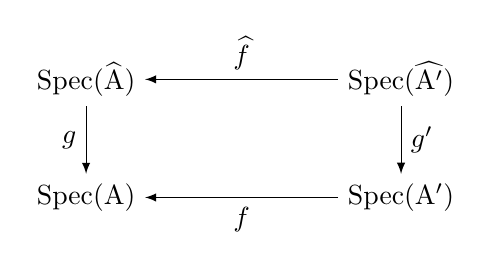
\begin{tikzpicture}[>=latex]
\node (tl) at (0,1.5) {$\Spec(\widehat{\mathrm{A}})$};
\node (tr) at (4,1.5) {$\Spec(\widehat{\mathrm{A}'})$};
\node (bl) at (0,0) {$\Spec(\mathrm{A})$};
\node (br) at (4,0) {$\Spec(\mathrm{A}')$};
\draw[->] (tr) -- node[above] {$\widehat{f}$} (tl);
\draw[->] (tl) -- node[left] {$g$} (bl);
\draw[->] (tr) -- node[right] {$g'$} (br);
\draw[->] (br) -- node[below] {$f$} (bl);
\end{tikzpicture}
\]
where $g$ and $g'$ are the canonical morphisms.
As by hypothesis $f$ is a $\boldsymbol{P}$-morphism and $g'$ a regular morphism, it follows from $(\mathrm{P_I})$ that $f\circ g'=g\circ\widehat{f}$ is a $\boldsymbol{P}$-morphism.
On the other hand, the hypothesis that $f$ is a $\boldsymbol{P}$-morphism implies that $f$ is flat, hence it is the same for $\widehat{f}$ (Bourbaki, \emph{Alg.\ comm.}, chap.~III, \textsection\,5, n\textsuperscript{o}\,4, cor.~of prop.~3), which is moreover a local homomorphism, hence faithfully flat \sref[0]{0.6.6.2}; it follows then from $(\mathrm{P_{II}})$ that $g$ is a $\boldsymbol{P}$-morphism.
\end{proof}

\begin{corollary}[7.4.3]
\label{IV.7.4.3}
\begin{enumerate}[label=\emph{\roman*)}]
  \item Let $\mathrm{A}$ be a $\boldsymbol{P}$-ring local Noetherian, $\mathrm{A}'=\widehat{\mathrm{A}}$ its completion.
  Suppose that for every prime ideal $\mathfrak{p}'$ of $\mathrm{A}'$, the formal fibres of $\mathrm{A}'_{\mathfrak{p}'}$ are geometrically regular; then, for every prime ideal $\mathfrak{p}$ of $\mathrm{A}$, $\mathrm{A}_\mathfrak{p}$ is a $\boldsymbol{P}$-ring.

  \item Suppose that $\boldsymbol{P}$ satisfies the condition $(\mathrm{P_{IV}})$ \sref{IV.7.3.6}.
  Let $\mathrm{A}$ be a $\boldsymbol{P}$-ring local Noetherian, $\mathrm{B}$ a local A-algebra essentially of finite type, and such that the homomorphism $\mathrm{A}\to\mathrm{B}$ is local.
  Set $\mathrm{A}'=\widehat{\mathrm{A}}$, and let $\mathfrak{n}'$ be the unique prime ideal of $\mathrm{B}'=\mathrm{B}\otimes_\mathrm{A}\mathrm{A}'$ above the maximal ideal of $\mathrm{B}$ and the maximal ideal of $\mathrm{A}'$.
  If the formal fibres of $\mathrm{B}'_{\mathfrak{n}'}$ are geometrically regular, then $\mathrm{B}$ is a $\boldsymbol{P}$-ring.
\end{enumerate}
\end{corollary}

\begin{proof}
\begin{enumerate}[label=(\roman*)]
  \item As by hypothesis $\Spec(\mathrm{A}')\to\Spec(\mathrm{A})$ is a $\boldsymbol{P}$-morphism, the same holds for $\Spec(\mathrm{A}'_{\mathfrak{p}'})\to\Spec(\mathrm{A}_\mathfrak{p})$ by virtue of \sref{IV.7.3.2},~$b)$), for every prime ideal $\mathfrak{p}'$ of $\mathrm{A}'$ above $\mathfrak{p}$ and every prime ideal $\mathfrak{p}$ of $\mathrm{A}$.
  It suffices then to apply the lemma \sref{IV.7.4.2} to this morphism, noting that the morphism $\Spec(\mathrm{A}')\to\Spec(\mathrm{A})$ is surjective.

  \item By virtue of \sref{IV.7.4.2}, it suffices to prove that the morphism $\Spec(\mathrm{B}'_{\mathfrak{n}'})\to\Spec(\mathrm{B})$ is a $\boldsymbol{P}$-morphism.
  Now we have $\mathrm{B}=\mathrm{C}_\mathfrak{n}$, where $\mathrm{C}$ is a finite type A-algebra and $\mathfrak{n}$ is a prime ideal of $\mathrm{C}$ above the maximal ideal of $\mathrm{A}$.
  If we set $\mathrm{C}'=\mathrm{C}\otimes_\mathrm{A}\mathrm{A}'$, it follows from the hypotheses and from \sref{IV.7.3.7} that $\Spec(\mathrm{C}')\to\Spec(\mathrm{C})$ is a $\boldsymbol{P}$-morphism; as $\mathrm{B}'_{\mathfrak{n}'}$ is a local ring of $\mathrm{C}'$ at a prime ideal of $\mathrm{C}'$ above $\mathfrak{n}$, the conclusion follows from \sref{IV.7.3.2},~$b)$).
\end{enumerate}
\end{proof}

\begin{theorem}[7.4.4]
\label{IV.7.4.4}
The hypotheses on $\boldsymbol{P}$ being those of \sref{IV.7.4.1}, let $\mathrm{A}$ be a $\boldsymbol{P}$-ring local Noetherian.
\begin{enumerate}[label=\emph{\roman*)}]
  \item For every prime ideal $\mathfrak{p}$ of $\mathrm{A}$, $\mathrm{A}_\mathfrak{p}$ is a $\boldsymbol{P}$-ring.
  \item Suppose in addition that $\boldsymbol{P}$ satisfies the condition $(\mathrm{P_{IV}})$.
  Then every local ring that is an A-algebra essentially of finite type is a $\boldsymbol{P}$-ring.
\end{enumerate}
\end{theorem}

\begin{proof}
\begin{enumerate}[label=(\roman*)]
  \item Applying \sref{IV.7.4.3},~(i), everything reduces to seeing that for every prime ideal $\mathfrak{p}'$ of $\mathrm{A}'=\widehat{\mathrm{A}}$, $\mathrm{A}'_{\mathfrak{p}'}$ has its formal fibres geometrically regular.
  Now, this has been proved in \sref[0]{0.22.3.3} and \sref[0]{0.22.5.8}.

  \oldpage[IV-2]{200}
  \item Let $\mathrm{B}$ be an A-algebra essentially of finite type that is a local ring; if $\mathfrak{p}$ is the prime ideal of $\mathrm{A}$ above which the maximal ideal of $\mathrm{B}$ lies, $\mathrm{B}$ is also an $\mathrm{A}_\mathfrak{p}$-algebra essentially of finite type \sref{IV.1.3.8}; by virtue of~(i), we may therefore suppose that $\mathfrak{p}$ is the maximal ideal $\mathfrak{m}$ of $\mathrm{A}$.
  We have then $\mathrm{B}=\mathrm{C}_\mathfrak{q}$, where $\mathrm{C}$ is a finite type A-algebra and $\mathfrak{q}$ is a prime ideal of $\mathrm{C}$ above $\mathfrak{m}$. Choose a maximal ideal $\mathfrak{n}\supset\mathfrak{q}$ of $\mathrm{C}$, necessarily above $\mathfrak{m}$. If $k=\mathrm{A}/\mathfrak{m}$, then $\mathrm{C}/\mathfrak{m}\mathrm{C}$ is a finite type $k$-algebra, so the residue field $k'$ of $\mathrm{C}$ at $\mathfrak{n}$ is finite over $k$ \sref[I]{I.6.4.2}. By~(i), it is enough to prove that $\mathrm{C}_\mathfrak{n}$ is a $\boldsymbol{P}$-ring, since $\mathrm{C}_\mathfrak{q}$ is a local ring at a prime ideal of $\mathrm{C}_\mathfrak{n}$. We are thus reduced to the following lemma.
\end{enumerate}
\end{proof}

\begin{lemma}[7.4.4.1]
\label{IV.7.4.4.1}
Let $\mathrm{A}$ be a $\boldsymbol{P}$-ring local Noetherian, $k$ its residue field, $\mathrm{C}$ a finite type A-algebra, $\mathrm{B}$ a local ring in a prime ideal $\mathfrak{n}$ of $\mathrm{C}$, such that:
$1$\textsuperscript{o} the homomorphism $\mathrm{A}\to\mathrm{B}$ is local; $2$\textsuperscript{o} the residue field $k'$ of $\mathrm{B}$ is a finite extension of $k$.
If $\boldsymbol{P}$ satisfies $(\mathrm{P_{IV}})$, then $\mathrm{B}$ is a $\boldsymbol{P}$-ring.
\end{lemma}

\begin{proof}
Let $(x_i)_{1\leqslant i\leqslant m}$ be a system of generators of the $\mathrm{A}$-algebra $\mathrm{C}$; let us show first that we can argue by induction on $m$.
Let $\mathrm{C}'$ be the sub-$\mathrm{A}$-algebra of $\mathrm{C}$ generated by $x_1,\ldots,x_{m-1}$, and let $\mathfrak{n}'=\mathfrak{n}\cap\mathrm{C}'$.
The homomorphism $\mathrm{A}\to\mathrm{C}_\mathfrak{n}$ factors through the local homomorphisms $\mathrm{A}\to\mathrm{C}'_{\mathfrak{n}'}\to\mathrm{C}_\mathfrak{n}$; if $k''$ is the residue field of $\mathrm{C}'_{\mathfrak{n}'}$, the extension $k\to k'$ factors through $k''$, hence $k''$ is a finite extension of $k$ and $k'$ a finite extension of $k''$.
The induction hypothesis implies that $\mathrm{C}'_{\mathfrak{n}'}$ is a $\boldsymbol{P}$-ring. If $\mathrm{S}'=\mathrm{C}'-\mathfrak{n}'$, then $\mathrm{C}_\mathfrak{n}$ is a local ring of $\mathrm{S}'^{-1}\mathrm{C}=\mathrm{C}'_{\mathfrak{n}'}[x_m/1]$; the induction hypothesis applied once more shows that $\mathrm{C}_\mathfrak{n}$ is a $\boldsymbol{P}$-ring. Thus the problem reduces to the case where $\mathrm{C}$ is an $\mathrm{A}$-algebra generated by a \emph{single} element $t$.

Applying \sref{IV.7.4.3},~(ii), with $\mathrm{A}'=\widehat{\mathrm{A}}$, the ring $\mathrm{B}'=\mathrm{B}\otimes_\mathrm{A}\mathrm{A}'$ is a local ring of $\mathrm{C}\otimes_\mathrm{A}\mathrm{A}'$ at a prime ideal above $\mathfrak{n}$; as $\mathrm{A}$ and $\mathrm{A}'$ have the same residue field $k$, the residue field of $\mathrm{C}\otimes_\mathrm{A}\mathrm{A}'$ at this prime ideal is equal to $k'$.
Moreover $\mathrm{C}\otimes_\mathrm{A}\mathrm{A}'$ is generated by a single element over $\mathrm{A}'$.
It follows therefore from \sref{IV.7.4.3},~(ii) that one can restrict to proving \sref{IV.7.4.4.1} when $\boldsymbol{P}$ is the property~(iv') of \sref{IV.7.3.8}, that $\mathrm{A}$ is \emph{complete} and $\mathrm{C}$ generated by a single element $t$.

To show that the formal fibres of $\mathrm{B}=\mathrm{C}_\mathfrak{n}$ are then geometrically regular, let us apply the criterion \sref{IV.7.3.16},~$b)$).
Let $\mathrm{B}_1$ be a finite integral $\mathrm{B}$-algebra, hence generated by a finite number of elements integral over $\mathrm{B}$.
By multiplying these elements by an element of $\mathrm{S}=\mathrm{C}-\mathfrak{n}$, one can suppose that they are integral over $\mathrm{C}$, and we can therefore write $\mathrm{B}_1=\mathrm{S}^{-1}\mathrm{C}_1$, where $\mathrm{C}_1$ is a sub-C-algebra of $\mathrm{B}_1$ generated by a finite number of integral elements over $\mathrm{C}$, hence a finite integral C-algebra.
On the other hand, $\mathrm{B}_1$ is a semi-local ring, and every local ring $\mathrm{B}_2$ of $\mathrm{B}_1$ at a maximal ideal is a local ring of $\mathrm{C}_1$, such that $\mathrm{A}\to\mathrm{B}_2$ is a local homomorphism; moreover, the residue field of $\mathrm{B}_2$ is a finite extension of $k'$, hence of $k$.
We see therefore (taking into account \sref{IV.7.3.14} and~(i)) that we are reduced to the following question: let $\mathrm{C}$ be a Noetherian integral ring containing a subring $\mathrm{C}_0$ which is an $\mathrm{A}$-algebra generated by a single element $t$ and such that $\mathrm{C}$ is a finite $\mathrm{C}_0$-algebra; if $\mathfrak{n}$ is a maximal ideal of $\mathrm{C}$
\oldpage[IV-2]{201}
above the maximal ideal of $\mathrm{A}$, and $\mathrm{B}=\mathrm{C}_\mathfrak{n}$, the question is to show that for every prime ideal $\mathfrak{q}$ of $\widehat{\mathrm{B}}$ whose inverse image in $\mathrm{B}$ is $0$, the ring $\widehat{\mathrm{B}}_\mathfrak{q}$ is regular.
One may moreover replace $\mathrm{A}$ by its image in $\mathrm{C}$, which is a complete local ring (as a quotient of $\mathrm{A}$) and integral. The desired conclusion follows from the more general lemma below.
\end{proof}

\begin{lemma}[7.4.4.2]
\label{IV.7.4.4.2}
Let $\mathrm{A}$ be a complete Noetherian local integral ring, $k$ its residue field, $\mathrm{C}$ an integral ring containing $\mathrm{A}$, such that there exists $t\in\mathrm{C}$ for which $\mathrm{C}$ is a finite $\mathrm{A}[t]$-algebra.
Let $\mathfrak{n}$ be a maximal ideal of $\mathrm{C}$ above the maximal ideal $\mathfrak{m}$ of $\mathrm{A}$; set $\mathrm{B}=\mathrm{C}_\mathfrak{n}$, $\mathrm{X}=\Spec(\mathrm{B})$, $\mathrm{B}'=\widehat{\mathrm{B}}$, $\mathrm{X}'=\Spec(\widehat{\mathrm{B}})$; if $\mathrm{U}=\operatorname{Reg}(\mathrm{X})$, $\mathrm{U}'=\operatorname{Reg}(\mathrm{X}')$, and if $f:\mathrm{X}'\to\mathrm{X}$ is the canonical morphism, then $f^{-1}(\mathrm{U})\subset\mathrm{U}'$.
\end{lemma}

\begin{proof}
The assertion needed for \sref{IV.7.4.4.1} follows from this lemma because, since $\mathrm{B}$ is integral, the generic point of $\mathrm{X}$ belongs to $\mathrm{U}$.
Since $\mathrm{C}$ is an $\mathrm{A}$-algebra of finite type and $\mathfrak{n}$ is a maximal ideal of $\mathrm{C}$, the residue field $k'$ of $\mathrm{C}_\mathfrak{n}=\mathrm{B}$ (hence also of $\mathrm{B}'$) is a finite extension of $k$ \sref[I]{I.6.4.11} and \sref{IV.6.4.2}.

Set $\mathrm{Y}=\Spec(\mathrm{C})$. It follows from \sref{IV.6.12.8} that $\operatorname{Reg}(\mathrm{Y})$ is open in $\mathrm{Y}$; since the local rings of $\mathrm{X}$ are local rings of $\mathrm{Y}$ \sref[I]{I.2.4.2}, we have $\mathrm{U}=\mathrm{X}\cap\operatorname{Reg}(\mathrm{Y})$, hence $\mathrm{U}$ is open in $\mathrm{X}$. On the other hand, \sref{IV.6.12.7} shows that $\mathrm{U}'$ is open in $\mathrm{X}'$, hence $\mathrm{S}'=\mathrm{X}'-\mathrm{U}'$ is closed. Consequently $\mathrm{S}'\cap f^{-1}(\mathrm{U})$ is locally closed in $\mathrm{X}'$, and the whole question is to prove that this set is empty.
If it were non-empty, \sref{IV.5.1.10} would give a prime ideal $\mathfrak{p}'$ in $\mathrm{S}'\cap f^{-1}(\mathrm{U})$ such that $\dim(\mathrm{B}'/\mathfrak{p}')\leqslant 1$.
The prime ideal $\mathfrak{p}'$ cannot be the maximal ideal $\mathfrak{m}\mathrm{B}'$ of $\mathrm{B}'$, where $\mathfrak{m}$ is the maximal ideal of $\mathrm{B}$. Indeed, this would mean that $\mathrm{B}=\mathrm{B}_\mathfrak{m}$ is regular, hence so is $\mathrm{B}'=\widehat{\mathrm{B}}$ \sref[0]{0.17.1.5}, and we would have $\mathfrak{m}\mathrm{B}'\in\mathrm{U}'$, contrary to the hypothesis. We must therefore have $\dim(\mathrm{B}'/\mathfrak{p}')=1$.

Set $\mathfrak{p}=\mathrm{B}\cap\mathfrak{p}'$. By hypothesis $\mathrm{B}_\mathfrak{p}$ is regular, whereas $\mathrm{B}'_{\mathfrak{p}'}$ is not. Since $\mathrm{B}'_{\mathfrak{p}'}$ is a flat $\mathrm{B}_\mathfrak{p}$-module, \sref{IV.6.5.2} shows that the fibre $\mathrm{Z}$ of $f$ at $\mathfrak{p}$ is not regular at $\mathfrak{p}'$.
We may reduce to the case $\mathfrak{p}=0$. Indeed, in general, set $\mathfrak{q}=\mathfrak{p}\cap\mathrm{C}$ and $\mathfrak{r}=\mathfrak{p}\cap\mathrm{A}$. Then $\mathrm{C}/\mathfrak{q}$ is a finite $(\mathrm{A}/\mathfrak{r})[\bar{t}]$-algebra, where $\bar{t}$ is the class of $t$ modulo $\mathfrak{q}$; since $\mathfrak{p}=\mathfrak{q}\mathrm{B}$, the ring $\mathrm{B}/\mathfrak{p}$ is equal to $(\mathrm{C}/\mathfrak{q})_{\mathfrak{n}/\mathfrak{q}}$, and $\mathfrak{n}/\mathfrak{q}$ is a maximal ideal of $\mathrm{C}/\mathfrak{q}$ lying over the maximal ideal $\mathfrak{m}/\mathfrak{r}$ of $\mathrm{A}/\mathfrak{r}$. Thus the hypotheses of \sref{IV.7.4.4.2} are still satisfied by $\mathrm{A}/\mathfrak{r}$, $\mathrm{C}/\mathfrak{q}$, and $\mathrm{B}/\mathfrak{p}$; since the completion of $\mathrm{B}/\mathfrak{p}$ is $\mathrm{B}'/\mathfrak{p}\mathrm{B}'$, this proves the reduction.

Suppose therefore that $\mathfrak{p}=0$, so that $\mathrm{Z}$ is the generic fibre of $f$ and the homomorphism $\mathrm{B}\to\mathrm{B}'/\mathfrak{p}'$ is injective. Set $\mathrm{V}=\mathrm{B}'/\mathfrak{p}'$, and distinguish two cases.

\emph{I) $\mathrm{V}$ is a finite $\mathrm{A}$-algebra.} Since $\mathrm{B}\subset\mathrm{V}$, $\mathrm{B}$ is \emph{a fortiori} a finite $\mathrm{A}$-algebra; as $\mathrm{A}$ is complete, so is $\mathrm{B}$ (Bourbaki, \emph{Alg.\ comm.}, chap.~IV, \textsection\,2, n\textsuperscript{o}\,5, cor.~3 of prop.~9). Hence $\mathrm{B}'=\mathrm{B}$ and $\mathfrak{p}'=0$, so $\mathrm{B}'_{\mathfrak{p}'}$ is a field, contrary to the hypothesis.

\emph{II) $\mathrm{V}$ is not a finite $\mathrm{A}$-algebra.} Since the local ring $\mathrm{A}$ is complete, $\mathrm{V}$ is not a quasi-finite $\mathrm{A}$-algebra \sref[0]{0.7.4.1} and \sref[0]{0.7.4.2}; but the residue field $k'$ of $\mathrm{V}$ is a finite extension of the residue field $k$ of $\mathrm{A}$,

\oldpage[IV-2]{202}

hence \sref[0]{0.7.4.4} the ideal $\mathfrak{m}\mathrm{V}$ is not an ideal of definition of $\mathrm{V}$. Since $\mathrm{V}$ is a one-dimensional Noetherian local integral ring, $0$ is the only ideal of $\mathrm{V}$ that is not an ideal of definition, hence $\mathfrak{m}\mathrm{V}=0$. But $\mathrm{A}\subset\mathrm{V}$ and $\mathrm{V}$ is integral, so $\mathfrak{m}=0$ and $\mathrm{A}=k$ is a field.
It follows first that $\dim(\mathrm{C})\leqslant 1$ \sref[0]{0.16.1.5}; but since $\dim(\mathrm{V})=1$, the inequalities
\[
  \dim(\mathrm{V})\leqslant\dim(\mathrm{B}')=\dim(\mathrm{B})\leqslant\dim(\mathrm{C})
\]
show that $\dim(\mathrm{C})=\dim(\mathrm{B})=\dim(\mathrm{B}')=\dim(\mathrm{B}'/\mathfrak{p}')=1$, and consequently $\mathfrak{p}'$ is a minimal prime ideal of $\mathrm{B}'$. We therefore obtain a contradiction once we prove that $\mathrm{B}'_{\mathfrak{p}'}$ is a field, or equivalently that $\mathrm{B}'$ is reduced.
Since $\mathrm{C}$ is a finite-type $k$-algebra, its integral closure $\mathrm{C}_1$ is a finite $\mathrm{C}$-algebra (Bourbaki, \emph{Alg.\ comm.}, chap.~V, \textsection\,3, n\textsuperscript{o}\,2, th.~2). If $\mathrm{S}=\mathrm{C}-\mathfrak{n}$, then $\mathrm{B}_1=\mathrm{S}^{-1}\mathrm{C}_1$ is the integral closure of $\mathrm{B}$, hence a finite $\mathrm{B}$-algebra and therefore a one-dimensional semi-local Noetherian integral and integrally closed ring \sref[0]{0.16.1.5}. If $\mathfrak{m}_j$ ($1\leqslant j\leqslant h$) are its maximal ideals, the rings $(\mathrm{B}_1)_{\mathfrak{m}_j}$ are discrete valuation rings \sref[II]{II.7.1.6}, and the completion $\mathrm{B}'_1$ of $\mathrm{B}_1$ is the direct product of the completed discrete valuation rings $(\mathrm{B}_1)_{\mathfrak{m}_j}$ (Bourbaki, \emph{Alg.\ comm.}, chap.~III, \textsection\,2, n\textsuperscript{o}\,13, prop.~18). Thus $\mathrm{B}'_1$ is reduced; since the completion $\mathrm{B}'$ of $\mathrm{B}$ is a subring of $\mathrm{B}'_1$ (Bourbaki, \emph{Alg.\ comm.}, chap.~IV, \textsection\,2, n\textsuperscript{o}\,5, cor.~3 of prop.~9), $\mathrm{B}'$ is reduced as well.
\end{proof}

\begin{corollary}[7.4.5]
\label{IV.7.4.5}
Suppose that the property $\boldsymbol{P}$ satisfies the conditions $(\mathrm{P_I})$, $(\mathrm{P_{II}})$, $(\mathrm{P_{III}})$.
Let $\mathrm{A}$ be a Noetherian ring.
The following conditions are equivalent:
\begin{enumerate}[label=\emph{\alph*)}]
  \item For every prime ideal $\mathfrak{p}$ of $\mathrm{A}$, $\mathrm{A}_\mathfrak{p}$ is a $\boldsymbol{P}$-ring.
  \item For every maximal ideal $\mathfrak{m}$ of $\mathrm{A}$, $\mathrm{A}_\mathfrak{m}$ is a $\boldsymbol{P}$-ring.
\end{enumerate}
If in addition $\boldsymbol{P}$ satisfies $(\mathrm{P_{IV}})$, the properties $a)$ and $b)$ are also equivalent to:
\begin{enumerate}[label=\emph{\alph*)}]
  \setcounter{enumi}{2}
  \item For every finite type A-algebra $\mathrm{B}$ and every prime ideal $\mathfrak{q}$ of $\mathrm{B}$, $\mathrm{B}_\mathfrak{q}$ is a $\boldsymbol{P}$-ring.
\end{enumerate}
\end{corollary}

\begin{proof}
The equivalence of $a)$ and $b)$ follows from \sref{IV.7.4.4},~(i), and that of $a)$ and $c)$ from \sref{IV.7.4.4},~(ii).
When condition $a)$ of \sref{IV.7.4.5} is satisfied, we say that $\mathrm{A}$ is a $\boldsymbol{P}$-ring; for semi-local Noetherian rings, this definition coincides with that of \sref{IV.7.3.13}, when the conditions $(\mathrm{P_I})$, $(\mathrm{P_{II}})$ and $(\mathrm{P_{III}})$ are satisfied.
The ring $\bb{Z}$ is a $\boldsymbol{P}$-ring \sref{IV.7.3.19},~(iv); every local Noetherian complete ring is a $\boldsymbol{P}$-ring.
\end{proof}

\begin{proposition}[7.4.6]
\label{IV.7.4.6}
Suppose that the property $\boldsymbol{P}$ satisfies the conditions $(\mathrm{P_I})$, $(\mathrm{P_{II}})$ and $(\mathrm{P_{III}})$.
Let $\mathrm{A}$ be a Noetherian ring, $\mathfrak{J}$ an ideal of $\mathrm{A}$, $\widehat{\mathrm{A}}$ the separated completion of $\mathrm{A}$ for the $\mathfrak{J}$-adic topology.
Then, if $\mathrm{A}$ is a $\boldsymbol{P}$-ring \sref{IV.7.4.5}, the canonical morphism $\Spec(\widehat{\mathrm{A}})\to\Spec(\mathrm{A})$ is a $\boldsymbol{P}$-morphism.
\end{proposition}

\begin{proof}
Using \sref{IV.7.3.2},~$c')$), it suffices to prove that for every maximal ideal $\mathfrak{n}$ of $\widehat{\mathrm{A}}$ with inverse image $\mathfrak{m}$ in $\mathrm{A}$, the morphism $\Spec((\widehat{\mathrm{A}})_\mathfrak{n})\to\Spec(\mathrm{A}_\mathfrak{m})$ is a $\boldsymbol{P}$-morphism.
We know (Bourbaki, \emph{Alg.\ comm.}, chap.~III, \textsection\,3, n\textsuperscript{o}\,4, prop.~8) that the canonical homomorphism $\mathrm{A}_\mathfrak{m}\to(\widehat{\mathrm{A}})_\mathfrak{n}$ is injective, that the $\mathfrak{m}\mathrm{A}_\mathfrak{m}$-adic topology on $\mathrm{A}_\mathfrak{m}$ is induced by the $\mathfrak{n}(\widehat{\mathrm{A}})_\mathfrak{n}$-adic topology, and that $\mathrm{A}_\mathfrak{m}$ is dense in $(\widehat{\mathrm{A}})_\mathfrak{n}$ for this topology, so that the completion of $\mathrm{A}_\mathfrak{m}$ for the $\mathfrak{m}\mathrm{A}_\mathfrak{m}$-adic topology identifies with that of $(\widehat{\mathrm{A}})_\mathfrak{n}$ for the $\mathfrak{n}(\widehat{\mathrm{A}})_\mathfrak{n}$-adic topology.
We have therefore two morphisms
\[
  \Spec((\mathrm{A}_\mathfrak{m})\widehat{\phantom{x}})\xrightarrow{f}\Spec((\widehat{\mathrm{A}})_\mathfrak{n})\xrightarrow{g}\Spec(\mathrm{A}_\mathfrak{m})
\]

\oldpage[IV-2]{203}

such that $f$ is faithfully flat. Since, by hypothesis, $g\circ f$ is a $\boldsymbol{P}$-morphism, it follows from $(\mathrm{P_{II}})$ that $g$ is a $\boldsymbol{P}$-morphism as well.
\end{proof}

\begin{corollary}[7.4.7]
\label{IV.7.4.7}
Suppose that $\boldsymbol{P}$ satisfies the conditions $(\mathrm{P_I})$, $(\mathrm{P}'_\mathrm{I})$, $(\mathrm{P_{II}})$, $(\mathrm{P_{III}})$ and $(\mathrm{P_{IV}})$.
Then, if $\mathrm{A}$ is a $\boldsymbol{P}$-ring \sref{IV.7.4.5}, the canonical morphism $\Spec(\mathrm{A}[[\mathrm{T}_1,\ldots,\mathrm{T}_r]])\to\Spec(\mathrm{A})$ is a $\boldsymbol{P}$-morphism.
In particular, if in addition $\mathrm{A}$ is integral, $\mathrm{K}$ its field of fractions, and if $\mathfrak{p}$ is a prime ideal of $\mathrm{B}=\mathrm{A}[[\mathrm{T}_1,\ldots,\mathrm{T}_r]]$ such that $\mathfrak{p}\cap\mathrm{A}=0$, then the property $\boldsymbol{P}(\mathrm{B}_\mathfrak{p},\mathrm{K})$ is true.
\end{corollary}

\begin{proof}
Indeed, $\Spec(\mathrm{B})\to\Spec(\mathrm{A})$ factorises as
\[
  \Spec(\mathrm{A}[[\mathrm{T}_1,\ldots,\mathrm{T}_r]])\xrightarrow{f}\Spec(\mathrm{A}[\mathrm{T}_1,\ldots,\mathrm{T}_r])\xrightarrow{g}\Spec(\mathrm{A}).
\]
It is clear that the morphism $g$ is regular \sref[0]{0.17.3.7}; by virtue of \sref{IV.7.4.5}, $\mathrm{A}[\mathrm{T}_1,\ldots,\mathrm{T}_r]$ is a $\boldsymbol{P}$-ring, hence it follows from \sref{IV.7.4.6} that $f$ is a $\boldsymbol{P}$-morphism; as $g$ is regular, hence also a $\boldsymbol{P}$-morphism \sref{IV.7.3.5},~(i), it follows from $(\mathrm{P}'_\mathrm{I})$ that $g\circ f$ is a $\boldsymbol{P}$-morphism.

One will note that the conclusion is still valid if, instead of supposing that $\boldsymbol{P}$ satisfies $(\mathrm{P}'_\mathrm{I})$ and that every regular morphism is a $\boldsymbol{P}$-morphism, one supposes only that a composite $g\circ f$ is a $\boldsymbol{P}$-morphism whenever $g$ is regular and $f$ is a $\boldsymbol{P}$-morphism (a condition in some sense symmetric to $(\mathrm{P}'_\mathrm{I})$).
\end{proof}

\begin{remark}[7.4.8]
\label{IV.7.4.8}
The preceding results pose the following problems:
\begin{enumerate}[label=\rm\Alph*)]
  \item Let $\mathrm{A}$ be a Zariski \emph{complete} ring, and let $\mathfrak{J}$ be an ideal of definition of $\mathrm{A}$; if the ring $\mathrm{A}/\mathfrak{J}$ is a $\boldsymbol{P}$-ring, is $\mathrm{A}$ also a $\boldsymbol{P}$-ring?
  It would follow that for every Noetherian $\boldsymbol{P}$-ring $\mathrm{A}$ and every ideal $\mathfrak{J}$ of $\mathrm{A}$, the separated completion $\widehat{\mathrm{A}}$ for the $\mathfrak{J}$-adic topology would also be a $\boldsymbol{P}$-ring.
  \item Let $k$ be a valued field, complete and non-discrete; one calls \emph{ring of restricted formal power series} $k\{\mathrm{T}_1,\ldots,\mathrm{T}_n\}$ the subring of the formal power series ring $k[[\mathrm{T}_1,\ldots,\mathrm{T}_n]]$ formed of the series whose coefficients \emph{tend to} $0$.
  Is such a ring a $\boldsymbol{P}$-ring?
  \item If $\mathrm{A}$ is a linearly topologised $\boldsymbol{P}$-ring, $\mathrm{S}$ a multiplicative subset of $\mathrm{A}$, are the rings $\mathrm{A}\{S^{-1}\}$ \sref[0]{0.7.6.1} and $\mathrm{A}_{\{S\}}$ \sref[0]{0.7.6.15} $\boldsymbol{P}$-rings?
\end{enumerate}
\end{remark}


\subsection{A criterion for \texorpdfstring{$\boldsymbol{P}$}{P}-morphisms}
\label{subsection:IV.7.5}

\begin{env}[7.5.0]
\label{IV.7.5.0}
This number will not be used in the sequel of Chapter~IV and may therefore be omitted on a first reading. We shall moreover see later \sref{IV.7.9.8} that the results of the present number can be considerably improved when one has ``resolution of singularities'' at one's disposal.

In the sequel of this number, we shall consider a property $\boldsymbol{R}(\mathrm{A})$, and we shall denote by $\boldsymbol{P}(\mathrm{Z},k)$ the following property:
\begin{quote}
``$\mathrm{Z}$ is a locally Noetherian prescheme over a field $k$, and, for every finite extension $k'$ of $k$, if $\mathrm{Z}'=\mathrm{Z}\otimes_k k'$, the property $\boldsymbol{R}(\sh{O}_{\mathrm{Z}',z'})$ is true for every $z'\in\mathrm{Z}'.$'
\end{quote}
\end{env}

\begin{theorem}[7.5.1]
\label{IV.7.5.1}
Let $\mathrm{A}$ and $\mathrm{B}$ be two complete Noetherian local rings, let $\mathfrak{m}$ be the maximal ideal of $\mathrm{A}$, let $k=\mathrm{A}/\mathfrak{m}$ be its residue field, and let $\varphi:\mathrm{A}\to\mathrm{B}$ be a local homomorphism such that:
\begin{enumerate}[label=(\roman*)]
  \item the residue field of $\mathrm{B}$ is a finite extension of $k$;
  \item $\mathrm{B}$ is a flat $\mathrm{A}$-module.
\end{enumerate}
Let $\boldsymbol{R}(\mathrm{C})$ moreover be a property satisfying condition $(\mathrm{R}_{\mathrm{III}})$ \sref{IV.7.3.18} and the following condition:
\begin{quote}
$(\mathrm{R}_{\mathrm{IV}})$ For every local ring $\mathrm{C}$ at a prime ideal of a complete Noetherian local ring, and every $\mathrm{C}$-regular element $t$ in the maximal ideal of $\mathrm{C}$, the property $\boldsymbol{R}(\mathrm{C}/t\mathrm{C})$ implies $\boldsymbol{R}(\mathrm{C})$.
\end{quote}

\oldpage[IV-2]{204}

Let $f={}^a\varphi:\Spec(\mathrm{B})\to\Spec(\mathrm{A})$, and suppose that $\boldsymbol{P}(\Spec(\mathrm{B}\otimes_\mathrm{A}k),k)$ is true. Then, for every $x\in\Spec(\mathrm{A})$, the property $\boldsymbol{P}(f^{-1}(x),\boldsymbol{k}(x))$ is true.
\end{theorem}

\begin{proof}
In other words, property $\boldsymbol{P}$ for the fibre over the closed point of $\Spec(\mathrm{A})$ entails the same property for all fibres of $f$; that is, $f$ is a $\boldsymbol{P}$-morphism \sref{IV.7.3.1}. We proceed in several steps.

\emph{I) Reduction to the study of the local rings of the generic fibre.} Apply \sref{IV.7.3.16.2}. It suffices to show that, for every finite integral $\mathrm{A}$-algebra $\mathrm{A}'$ with field of fractions $\mathrm{K}'$, if $\mathrm{B}'=\mathrm{B}\otimes_\mathrm{A}\mathrm{A}'$, then every local ring of $\Spec(\mathrm{B}'\otimes_{\mathrm{A}'}\mathrm{K}')$ satisfies $\boldsymbol{R}$. The ring $\mathrm{A}'$ (resp.\ $\mathrm{B}'$) is complete and semi-local, the latter because it is a finite $\mathrm{B}$-algebra, and is therefore a direct product of complete local rings. Since $\mathrm{A}'$ is integral it is local. Every maximal ideal $\mathfrak{n}'$ of $\mathrm{B}'$ lies over the maximal ideal $\mathfrak{n}$ of $\mathrm{B}$, hence over $\mathfrak{m}$, and its inverse image in $\mathrm{A}'$ is consequently the maximal ideal $\mathfrak{m}'$ of $\mathrm{A}'$. Every local ring of $\Spec(\mathrm{B}'\otimes_{\mathrm{A}'}\mathrm{K}')$ is a local ring of $\Spec(\mathrm{B}')$, and hence of one of the $\Spec(\mathrm{B}'_{\mathfrak{n}'})$ over the generic point of $\mathrm{A}'$. Thus it is enough to prove that the local rings of
\[
  \Spec(\mathrm{B}'_{\mathfrak{n}'}\otimes_{\mathrm{A}'}\mathrm{K}')
\]
satisfy $\boldsymbol{R}$. Now $\mathrm{A}'$ and $\mathrm{B}'_{\mathfrak{n}'}$ are complete Noetherian local rings. The residue field of $\mathrm{B}'_{\mathfrak{n}'}$ is a finite extension of that of $\mathrm{B}$, hence also of $k$, and \emph{a fortiori} of the residue field $k'$ of $\mathrm{A}'$. This observation and \sref{IV.2.1.4} show that $\mathrm{A}'$ and $\mathrm{B}'_{\mathfrak{n}'}$ satisfy conditions~(i) and~(ii) of the statement. On the other hand, if $k''$ is a finite extension of $k'$, it is also a finite extension of $k$, and the local rings of
\[
  \Spec(\mathrm{B}'_{\mathfrak{n}'}\otimes_{\mathrm{A}'}k'')
\]
are also local rings of $\Spec(\mathrm{B}\otimes_\mathrm{A}k'')$. The hypothesis $\boldsymbol{P}(\Spec(\mathrm{B}\otimes_\mathrm{A}k),k)$ therefore implies
\[
  \boldsymbol{P}(\Spec(\mathrm{B}'_{\mathfrak{n}'}\otimes_{\mathrm{A}'}k'),k').
\]
We are thus reduced to the case where $\mathrm{A}$ is integral with field of fractions $\mathrm{K}$, and to proving that the local rings of $\Spec(\mathrm{B}\otimes_\mathrm{A}\mathrm{K})$ satisfy $\boldsymbol{R}$.

\emph{II) The case $\dim(\mathrm{A})=1$.} Let $\mathrm{A}'$ be the integral closure of $\mathrm{A}$. By \sref[0]{0.23.1.6}, $\mathrm{A}'$ is a finite $\mathrm{A}$-algebra and a complete local ring. If $\mathrm{B}'=\mathrm{B}\otimes_\mathrm{A}\mathrm{A}'$, then
\[
  \mathrm{B}\otimes_\mathrm{A}\mathrm{K}=\mathrm{B}'\otimes_{\mathrm{A}'}\mathrm{K}.
\]
The same argument as in~I) shows that it suffices, for every maximal ideal $\mathfrak{n}'$ of $\mathrm{B}'$, to prove that the local rings of $\mathrm{B}'_{\mathfrak{n}'}\otimes_{\mathrm{A}'}\mathrm{K}$ satisfy $\boldsymbol{R}$; it also shows that $\mathrm{A}'$ and $\mathrm{B}'_{\mathfrak{n}'}$ satisfy hypotheses~(i) and~(ii), and that
\[
  \boldsymbol{P}(\Spec(\mathrm{B}'_{\mathfrak{n}'}\otimes_{\mathrm{A}'}k'),k')
\]
is true, where $k'$ is the residue field of $\mathrm{A}'$. Since $\dim(\mathrm{A}')=1$ \sref[0]{0.16.1.5} and $\mathrm{A}'$ is integral and integrally closed, it is a complete discrete valuation ring. We may therefore suppose that $\mathrm{A}$ itself is a complete discrete valuation ring. If $u$ is a uniformizer of $\mathrm{A}$, then $u$ is $\mathrm{A}$-regular, and the flatness of $\mathrm{B}$ over $\mathrm{A}$ implies that $t=\varphi(u)$ is $\mathrm{B}$-regular and belongs to the maximal ideal of $\mathrm{B}$. The hypothesis on $\Spec(\mathrm{B}\otimes_\mathrm{A}k)$ implies in particular that $\boldsymbol{R}(\mathrm{B}/t\mathrm{B})$ is true; hence $\boldsymbol{R}(\mathrm{B})$ is true by $(\mathrm{R}_{\mathrm{IV}})$. Thus $\mathrm{U}_{\boldsymbol{R}}(\Spec(\mathrm{B}))$ contains the closed point. It is open by $(\mathrm{R}_{\mathrm{III}})$, and $\Spec(\mathrm{B})$ is the only open subset of itself containing its closed point. Consequently all local rings of $\Spec(\mathrm{B})$, and in particular those of $\Spec(\mathrm{B}\otimes_\mathrm{A}\mathrm{K})$, satisfy $\boldsymbol{R}$.

\emph{III) The general case.} The case $\dim(\mathrm{A})=0$ is trivial, since then $\mathrm{A}=k$; we may therefore suppose that $\dim(\mathrm{A})\geqslant1$. By \sref{IV.6.12.7}, $\Spec(\mathrm{A})$ contains a non-empty open subset $\mathrm{V}$ all of whose points are regular. The intersection $\mathrm{V}'$ of $\mathrm{V}$ with the complement of the closed point of $\Spec(\mathrm{A})$ is non-empty and therefore contains the generic point. It suffices to prove that
\[
  f^{-1}(\mathrm{V}')\subset\mathrm{U}_{\boldsymbol{R}}(\Spec(\mathrm{B})).
\]
Equivalently, the intersection $\mathrm{Z}$ of $f^{-1}(\mathrm{V}')$ with the complement of $\mathrm{U}_{\boldsymbol{R}}(\Spec(\mathrm{B}))$ must be empty. Suppose otherwise. Since $\mathrm{U}_{\boldsymbol{R}}(\Spec(\mathrm{B}))$ is open by $(\mathrm{R}_{\mathrm{III}})$, $\mathrm{Z}$ is locally closed in $\Spec(\mathrm{B})$; if non-empty, it contains a point $x$ such that $\dim(\overline{\{x\}})\leqslant1$ \sref{IV.5.1.10}. Since $f(x)\in\mathrm{V}'$ is distinct from the closed point of $\Spec(\mathrm{A})$, $x$ is distinct from the closed point of $\Spec(\mathrm{B})$, and therefore $\dim(\overline{\{x\}})=1$.

We show this is impossible. Let $\mathfrak{q}$ be the corresponding prime ideal of $\mathrm{B}$, so that $\dim(\mathrm{B}/\mathfrak{q})=1$, and put $\mathfrak{p}=\varphi^{-1}(\mathfrak{q})$. Then $\mathfrak{p}\neq\mathfrak{m}$ and $\mathrm{A}_\mathfrak{p}$ is regular. Since $\mathfrak{p}\neq\mathfrak{m}$, the ideal $\mathfrak{m}(\mathrm{B}/\mathfrak{q})$ is non-zero, hence is an ideal of definition of the one-dimensional Noetherian local integral ring $\mathrm{B}/\mathfrak{q}$. By~(i), the residue field of $\mathrm{B}/\mathfrak{q}$ is a finite extension of the residue field of $\mathrm{A}/\mathfrak{p}$, so $\mathrm{B}/\mathfrak{q}$ is a quasi-finite $(\mathrm{A}/\mathfrak{p})$-algebra \sref[0]{0.7.4.4}. But $\mathrm{A}/\mathfrak{p}$ is complete and $\mathrm{B}/\mathfrak{q}$ is separated for the $\mathfrak{m}$-preadic topology, which is its local-ring topology; hence $\mathrm{B}/\mathfrak{q}$ is finite over $\mathrm{A}/\mathfrak{p}$ by \sref[0]{0.7.4.1}. The injection $\mathrm{A}/\mathfrak{p}\to\mathrm{B}/\mathfrak{q}$ consequently gives
\[
  \dim(\mathrm{A}/\mathfrak{p})=\dim(\mathrm{B}/\mathfrak{q})=1
\]
by \sref[0]{0.16.1.5}. Apply~II) to $\mathrm{A}/\mathfrak{p}$ and $\mathrm{B}/\mathfrak{p}\mathrm{B}$. Their residue fields are respectively those of $\mathrm{A}$ and $\mathrm{B}$, $\mathrm{B}/\mathfrak{p}\mathrm{B}$ is flat over $\mathrm{A}/\mathfrak{p}$, and
\[
 (\mathrm{B}/\mathfrak{p}\mathrm{B})\otimes_{\mathrm{A}/\mathfrak{p}}k
 =\mathrm{B}\otimes_\mathrm{A}k=\mathrm{B}/\mathfrak{m}\mathrm{B}.
\]
It follows that the local rings of
\[
 \Spec\bigl((\mathrm{B}/\mathfrak{p}\mathrm{B})\otimes_{\mathrm{A}/\mathfrak{p}}\boldsymbol{k}(\mathfrak{p})\bigr)
\]
satisfy $\boldsymbol{R}$. In particular, $\mathrm{B}_\mathfrak{q}/\mathfrak{p}\mathrm{B}_\mathfrak{q}$ is one of these local rings. Moreover, $\mathrm{B}_\mathfrak{q}$ is flat over the regular local ring $\mathrm{A}_\mathfrak{p}$. We now use the following lemma.

\begin{lemma}[7.5.1.1]
\label{IV.7.5.1.1}
\oldpage[IV-2]{205}
Let $\mathcal{C}$ be a full subcategory of the category of Noetherian local rings such that every quotient ring of a ring in $\mathcal{C}$ still belongs to $\mathcal{C}$. Suppose $\boldsymbol{R}(\mathrm{C})$ has the property that, if $\mathrm{C}\in\mathcal{C}$ and $t$ is a regular element of the maximal ideal of $\mathrm{C}$ such that $\boldsymbol{R}(\mathrm{C}/t\mathrm{C})$ is true, then $\boldsymbol{R}(\mathrm{C})$ is true.

Let $\mathrm{C}$ be a regular local ring with residue field $k$, let $\mathrm{D}\in\mathcal{C}$ be a local ring, and let $\psi:\mathrm{C}\to\mathrm{D}$ be a local homomorphism making $\mathrm{D}$ a flat $\mathrm{C}$-module. If $\boldsymbol{R}(\mathrm{D}\otimes_\mathrm{C}k)$ is true, then $\boldsymbol{R}(\mathrm{D})$ is true.
\end{lemma}

\begin{proof}
Proceed by induction on $n=\dim(\mathrm{C})$. The assertion is true by hypothesis when $n=0$, for then $\mathrm{C}=k$. Let $t\in\mathfrak{m}-\mathfrak{m}^2$. Then $\mathrm{C}/t\mathrm{C}$ is regular and $\dim(\mathrm{C}/t\mathrm{C})=n-1$ \sref[0]{0.17.1.8} and \sref[0]{0.16.3.4}. Since
\[
  (\mathrm{D}/t\mathrm{D})\otimes_{\mathrm{C}/t\mathrm{C}}k
  =\mathrm{D}\otimes_\mathrm{C}k
\]
and $\mathrm{D}/t\mathrm{D}\in\mathcal{C}$, the induction hypothesis gives $\boldsymbol{R}(\mathrm{D}/t\mathrm{D})$. Moreover, $t$ is $\mathrm{C}$-regular, hence $\mathrm{D}$-regular by flatness \sref[0]{0.6.3.4}; the assumed property of $\boldsymbol{R}$ therefore gives $\boldsymbol{R}(\mathrm{D})$.
\end{proof}

To finish the proof of \sref{IV.7.5.1}, apply \sref{IV.7.5.1.1} with $\mathcal{C}$ the category of local rings of spectra of complete local rings, using $(\mathrm{R}_{\mathrm{IV}})$, and take $\mathrm{C}=\mathrm{A}_\mathfrak{p}$ and $\mathrm{D}=\mathrm{B}_\mathfrak{q}$.
\end{proof}

\begin{corollary}[7.5.2]
\label{IV.7.5.2}
Let $\mathrm{A}$ be a Noetherian local ring, let $\mathfrak{m}$ be its maximal ideal and $k=\mathrm{A}/\mathfrak{m}$ its residue field, let $\mathrm{B}$ be a Noetherian local ring, and let $\varphi:\mathrm{A}\to\mathrm{B}$ be a local homomorphism such that:
\begin{enumerate}[label=(\roman*)]
  \item the residue field of $\mathrm{B}$ is a finite extension of $k$;
  \item $\mathrm{B}$ is a flat $\mathrm{A}$-module.
\end{enumerate}
Let $\boldsymbol{R}(\mathrm{C})$ be a property satisfying $(\mathrm{R}_{\mathrm{II}})$ \sref{IV.7.3.10}, $(\mathrm{R}_{\mathrm{III}})$ \sref{IV.7.3.18}, and $(\mathrm{R}_{\mathrm{IV}})$ \sref{IV.7.5.1}. Let $\boldsymbol{R}'(\mathrm{C})$ be a property satisfying:
\begin{quote}
$(\mathrm{R}_{\mathrm{V}})$ If $\mathrm{C}$ and $\mathrm{D}$ are Noetherian local rings and $\psi:\mathrm{C}\to\mathrm{D}$ is a local homomorphism such that $g={}^a\psi:\Spec(\mathrm{D})\to\Spec(\mathrm{C})$ is a $\boldsymbol{P}$-morphism, then $\boldsymbol{R}'(\mathrm{C})$ implies $\boldsymbol{R}(\mathrm{D})$.
\end{quote}
Suppose that the canonical morphism $\Spec(\widehat{\mathrm{A}})\to\Spec(\mathrm{A})$ is a $\boldsymbol{P}'$-morphism, where $\boldsymbol{P}'$ is defined from $\boldsymbol{R}'$ as $\boldsymbol{P}$ is defined from $\boldsymbol{R}$ in \sref{IV.7.5.0}. Let $f={}^a\varphi:\Spec(\mathrm{B})\to\Spec(\mathrm{A})$, and suppose that
\[
  \boldsymbol{P}\bigl(\Spec(\widehat{\mathrm{B}}\otimes_{\widehat{\mathrm{A}}}k),k\bigr)
\]
is true. Then $\boldsymbol{P}(f^{-1}(x),\boldsymbol{k}(x))$ is true for every $x\in\Spec(\mathrm{A})$; in other words, $f$ is a $\boldsymbol{P}$-morphism.
\end{corollary}

\begin{proof}
We proceed in two steps.

\emph{I) Reduction to the study of the local rings of the generic fibre.} Apply \sref{IV.7.3.16.2} once more. The only difference from part~I) of the proof of \sref{IV.7.5.1} is that $\mathrm{A}'$ is now only a semi-local integral ring, not necessarily local. Every maximal ideal $\mathfrak{n}'$ of $\mathrm{B}'$ lies above a maximal ideal $\mathfrak{m}'$ of $\mathrm{A}'$. Every local ring of $\Spec(\mathrm{B}'\otimes_{\mathrm{A}'}\mathrm{K}')$ is a local ring of $\Spec(\mathrm{B}')$, hence of one of the $\Spec(\mathrm{B}'_{\mathfrak{n}'})$ over the generic point of $\Spec(\mathrm{A}'_{\mathfrak{m}'})$. Thus it is enough to prove that the local rings of
\[
  \Spec(\mathrm{B}'_{\mathfrak{n}'}\otimes_{\mathrm{A}'_{\mathfrak{m}'}}\mathrm{K}')
\]
satisfy $\boldsymbol{R}$. By definition of $\boldsymbol{P}'$, if $\boldsymbol{P}'(\mathrm{Z},k)$ is true then so is $\boldsymbol{P}'(\mathrm{Z}\otimes_k k',k')$ for every finite extension $k'$ of $k$; the same argument as in \sref{IV.7.3.7} shows that the formal fibres of $\mathrm{A}'_{\mathfrak{m}'}$ satisfy $\boldsymbol{P}'$. As in part~I) of the proof of \sref{IV.7.5.1}, the rings $\mathrm{A}'_{\mathfrak{m}'}$ and $\mathrm{B}'_{\mathfrak{n}'}$ satisfy conditions~(i) and~(ii) above. If $k'$ is the residue field of $\mathrm{A}'_{\mathfrak{m}'}$, then
\[
  \boldsymbol{P}\bigl(\Spec(\widehat{\mathrm{B}'_{\mathfrak{n}'}}\otimes_{\widehat{\mathrm{A}'_{\mathfrak{m}'}}}k'),k'\bigr)
\]
is true: indeed, the completion of $\mathrm{A}'_{\mathfrak{m}'}$ is one of the local components of $\widehat{\mathrm{A}}'=\widehat{\mathrm{A}}\otimes_\mathrm{A}\mathrm{A}'$, and the completion of $\mathrm{B}'_{\mathfrak{n}'}$ is one of the local components of
\[
  \widehat{\mathrm{B}}'=\widehat{\mathrm{B}}\otimes_\mathrm{B}\mathrm{B}'
  =\widehat{\mathrm{B}}\otimes_\mathrm{A}\mathrm{A}'
  =\widehat{\mathrm{B}}\otimes_{\widehat{\mathrm{A}}}\widehat{\mathrm{A}}'.
\]
Part~I) of the proof of \sref{IV.7.5.1} therefore proves the assertion. We may consequently suppose that $\mathrm{A}$ is integral and need only prove, for its field of fractions $\mathrm{K}$, that the local rings of $\Spec(\mathrm{B}\otimes_\mathrm{A}\mathrm{K})$ satisfy $\boldsymbol{R}$.

\emph{II) Reduction to the case where $\mathrm{A}$ and $\mathrm{B}$ are complete.} Let $\xi$ be the generic point of $\Spec(\mathrm{A})$ and let $y\in f^{-1}(\xi)$. We must prove $\boldsymbol{R}(\sh{O}_y)$. By $(\mathrm{R}_{\mathrm{II}})$, it is enough to find a point $z\in\Spec(\widehat{\mathrm{B}})$ over $y$ such that $\boldsymbol{R}(\sh{O}_z)$ is true. The hypothesis on $\Spec(\widehat{\mathrm{B}}\otimes_{\widehat{\mathrm{A}}}k)$ and \sref{IV.7.5.1} imply that the morphism
\[
  \widehat{f}:\Spec(\widehat{\mathrm{B}})\to\Spec(\widehat{\mathrm{A}})
\]
is a $\boldsymbol{P}$-morphism. For any point $z\in\Spec(\widehat{\mathrm{B}})$ above $y$---such a point exists because $\widehat{\mathrm{B}}$ is faithfully flat over $\mathrm{B}$---its image $x$ in $\Spec(\widehat{\mathrm{A}})$ lies in the fibre $h^{-1}(\xi)$ of the canonical morphism $h:\Spec(\widehat{\mathrm{A}})\to\Spec(\mathrm{A})$. By the hypothesis on $\mathrm{A}$, $\boldsymbol{R}'(\sh{O}_x)$ is true; hence $(\mathrm{R}_{\mathrm{V}})$ gives $\boldsymbol{R}(\sh{O}_z)$.
\end{proof}

\begin{examples}[7.5.3]
\label{IV.7.5.3}
Consider the following properties $\boldsymbol{R}(\mathrm{C})$, where $\mathrm{C}$ is a Noetherian local ring:
\begin{enumerate}[label=(\roman*)]
  \item also denoted $(\mathrm{i}_n)$, $\operatorname{coprof}(\mathrm{C})\leqslant n$;
  \oldpage[IV-2]{206}
  \item also denoted $(\mathrm{ii}_n)$, $\mathrm{C}$ satisfies $(\mathrm{S}_n)$;
  \item $\mathrm{C}$ is a Cohen--Macaulay ring;
  \item $\mathrm{C}$ is a regular ring;
  \item also denoted $(\mathrm{v}_n)$, $\mathrm{C}$ is integral, integrally closed, and satisfies $(\mathrm{R}_n)$;
  \item $\mathrm{C}$ is integral and integrally closed;
  \item $\mathrm{C}$ is integral;
  \item $\mathrm{C}$ is reduced.
\end{enumerate}
All these properties satisfy $(\mathrm{R}_{\mathrm{III}})$, as was seen in \sref{IV.7.3.19},~(i). They also satisfy $(\mathrm{R}_{\mathrm{IV}})$. For~(i), this follows from \sref[0]{0.16.4.10},~(ii); for~(ii) and~(iii), from \sref{IV.5.12.4} and the fact that a complete Noetherian local ring is catenary \sref{IV.5.6.4}; for~(iv), it is the special case \sref[0]{0.17.1.8}; for~(vii), it follows from \sref{IV.3.4.5}, and for~(viii), from \sref{IV.3.4.6}; for~(vi), from \sref{IV.5.12.7} and the catenarity just recalled; and finally, for~(v), from the preceding facts and \sref{IV.5.12.5}.

Theorem \sref{IV.7.5.1} is therefore applicable when $\boldsymbol{R}$ is any one of the above properties. We have also observed in \sref{IV.7.3.11} that properties~(i) to~(viii) satisfy $(\mathrm{R}_{\mathrm{II}})$, except that for~(vii) this follows from \sref{IV.2.1.14}. As for $(\mathrm{R}_{\mathrm{V}})$, if one takes $\boldsymbol{R}'=\boldsymbol{R}$, it reduces to condition $(\mathrm{R}'_{\mathrm{I}})$ of \sref{IV.7.3.11}; properties~(ii) to~(vi), and~(viii), satisfy this condition. For~(i), one may take for $\boldsymbol{R}'$ the property of being Cohen--Macaulay, by \sref{IV.6.3.2}. For~(vii), condition $(\mathrm{R}'_{\mathrm{I}})$ is not satisfied, as shown by \sref{IV.6.15.11},~(ii) or \sref{IV.6.5.5},~(ii). However, $(\mathrm{R}_{\mathrm{V}})$ is true if $\boldsymbol{R}'$ is the property of being regular: apply \sref{IV.7.5.1.1} with $\mathcal{C}$ the category of all Noetherian local rings and with $\boldsymbol{R}(\mathrm{C})$ the property of being integral; this is possible by \sref{IV.3.4.5}.

In particular, when $\boldsymbol{R}$ is any of properties~(i) to~(viii), the conclusion of \sref{IV.7.5.2} applies if the formal fibres of $\mathrm{A}$ are geometrically regular; see \sref{IV.7.8.2}.
\end{examples}

\begin{remarks}[7.5.4]
\label{IV.7.5.4}
\begin{enumerate}[label=(\roman*)]
  \item It would be interesting to know whether \sref{IV.7.5.1} remains true without the finiteness hypothesis~(i) on the residue field of $\mathrm{B}$. The answer is affirmative when the residue field $k$ of $\mathrm{A}$ has characteristic~$0$, by Hironaka's results on resolution of singularities; see \sref{IV.7.9.8}. A particular case of the question is the following. Let $\mathrm{A}$ and $\mathrm{B}$ be complete Noetherian rings, let $k$ be the residue field of $\mathrm{A}$, and let $\varphi:\mathrm{A}\to\mathrm{B}$ be a local homomorphism making $\mathrm{B}$ a formally smooth $\mathrm{A}$-algebra \sref[0]{0.19.3.1}; equivalently, $\mathrm{B}$ is flat over $\mathrm{A}$ and $\mathrm{B}\otimes_\mathrm{A}k$ is geometrically regular over $k$ \sref[0]{0.19.7.1}. Are the fibres of ${}^a\varphi:\Spec(\mathrm{B})\to\Spec(\mathrm{A})$ geometrically regular? This is so when the residue field $k'$ of $\mathrm{B}$ is a finite extension of $k$, by \sref{IV.7.5.1}; the answer is also affirmative when $k'$ is an extension of finite type of $k$. We do not know the answer when $\mathrm{B}\otimes_\mathrm{A}k$ is a field equal to a separable closure of $k$.

  \item One could state a result analogous to \sref{IV.7.5.1} for a finite-type $\mathrm{A}$-module $\mathrm{M}$ and a finite-type $\mathrm{B}$-module $\mathrm{N}$, concerning the properties of
  \[
    (\mathrm{M}\otimes_\mathrm{A}\mathrm{N})_y
    \otimes_{\sh{O}_{\mathrm{X},x}}\boldsymbol{k}(y),
  \]
  where $y$ runs through $\Spec(\mathrm{B})$ and $x=f(y)$, deduced from properties of the same type of $\mathrm{M}_x$ and $\mathrm{N}_y$.

  \item Suppose $\boldsymbol{R}$ satisfies $(\mathrm{R}'_{\mathrm{I}})$, $(\mathrm{R}_{\mathrm{II}})$, $(\mathrm{R}_{\mathrm{III}})$, and $(\mathrm{R}_{\mathrm{IV}})$, and hypotheses~(i) and~(ii) of \sref{IV.7.5.2} hold. Then $\boldsymbol{R}(\mathrm{A})$ and
  \[
    \boldsymbol{P}\bigl(\Spec(\widehat{\mathrm{B}}\otimes_{\widehat{\mathrm{A}}}k),k\bigr)
  \]
  imply $\boldsymbol{R}(\mathrm{B})$. By \sref{IV.7.5.3}, this holds for the properties listed there except~(i) and~(vii). For~(vii), it is nevertheless plausible that the following question has an affirmative answer. Let $\varphi:\mathrm{A}\to\mathrm{B}$ be a local homomorphism of Noetherian local rings making $\mathrm{B}$ a flat $\mathrm{A}$-module. Suppose $\mathrm{A}$ is complete, integral, and geometrically unibranch, and that $\Spec(\mathrm{B}\otimes_\mathrm{A}k)$, where $k$ is the residue field of $\mathrm{A}$, is geometrically locally integral. Is $\mathrm{B}$ then integral? This is known when $k$ has characteristic~$0$, by Hironaka's resolution of singularities \sref{IV.7.9.8}; it is also true when $\mathrm{B}$ is an $\mathrm{A}$-algebra essentially of finite type \sref{IV.1.3.8} (see \sref{IV.11.3.10} and \sref{IV.11.3.11}), or when $\Spec(\mathrm{B}\otimes_\mathrm{A}k)$ is geometrically normal, for then \sref{IV.7.5.3} shows that $\Spec(\mathrm{B})\to\Spec(\mathrm{A})$ is normal and one concludes by \sref{IV.6.15.10}. Even if the residue field of $\mathrm{B}$ equals that of $\mathrm{A}$ and $\mathrm{B}$ is complete, the general answer is unknown.

  \item Consider the property $\boldsymbol{R}(\mathrm{C})$: ``$\mathrm{C}$ is reduced, equidimensional, and satisfies $(\mathrm{R}_n)$''. It satisfies $(\mathrm{R}_{\mathrm{IV}})$ by \sref{IV.5.12.5}, but it is not known whether it satisfies $(\mathrm{R}'_{\mathrm{I}})$, $(\mathrm{R}_{\mathrm{II}})$, or $(\mathrm{R}_{\mathrm{III}})$; the difficulty lies in verifying equidimensionality.
\end{enumerate}
\end{remarks}

\oldpage[IV-2]{207}

In what follows of this section, we will apply \sref{IV.7.5.1} to the study of \emph{completed tensor products} $\mathrm{A}\widehat{\otimes}_k\mathrm{B}$ of local Noetherian rings which are algebras over a field $k$.

\begin{lemma}[7.5.5]
\label{IV.7.5.5}
Let $k$ be a field, $\mathrm{A}$, $\mathrm{B}$ two local Noetherian complete rings containing $k$, the residue field of $\mathrm{A}$ being a finite extension of $k$. Let $\mathrm{C}$ be the completed tensor product $\mathrm{A}\widehat{\otimes}_k\mathrm{B}$ \sref[0]{0.7.7.5}. Then:
\begin{enumerate}[label=(\roman*)]
  \item $\mathrm{C}$ is a semi-local Noetherian complete ring.
  \item $\mathrm{C}$ is a flat $\mathrm{A}$-module and a flat $\mathrm{B}$-module.
  \item If $\mathfrak{m}$ is the maximal ideal of $\mathrm{A}$, $\mathfrak{m}\mathrm{C}$ is contained in the radical of $\mathrm{C}$, and $\mathrm{C}/\mathfrak{m}\mathrm{C}$ is isomorphic to $(\mathrm{A}/\mathfrak{m})\otimes_k\mathrm{B}$.
  \item The residue fields of the components of $\mathrm{C}$ are finite extensions of the residue field of $\mathrm{B}$.
\end{enumerate}
The properties (i), (iii) and the first assertion of (ii) are particular cases of \sref[0]{0.19.7.1.2}. To prove that $\mathrm{C}$ is a flat $\mathrm{B}$-module, note that for every $h>0$,
\[
  \mathrm{C}/\mathfrak{m}^h\mathrm{C}
  =(\mathrm{A}/\mathfrak{m}^h)\otimes_k\mathrm{B}
\]
is a flat $\mathrm{B}$-module, since $k$ is a field; it therefore suffices to apply \sref[0]{0.10.2.6} to each local component of $\mathrm{C}$. Finally, if $\mathfrak{n}$ is the maximal ideal of $\mathrm{B}$, the residue fields of the local components of $\mathrm{C}$ are also those of the local components of the Artinian ring $(\mathrm{A}/\mathfrak{m})\otimes_k(\mathrm{B}/\mathfrak{n})$, and hence are finite extensions of $\mathrm{B}/\mathfrak{n}$.
\end{lemma}

\begin{proposition}[7.5.6]
\label{IV.7.5.6}
Let $k$ be a field, and let $\mathrm{A}$ and $\mathrm{B}$ be complete Noetherian local rings containing $k$, whose residue fields are finite extensions of $k$. Let $\boldsymbol{R}$ be a property satisfying $(\mathrm{R}'_{\mathrm{I}})$, $(\mathrm{R}_{\mathrm{III}})$ and $(\mathrm{R}_{\mathrm{IV}})$, with $\boldsymbol{P}$ defined from $\boldsymbol{R}$ as in \sref{IV.7.5.0}. Suppose that $\boldsymbol{R}(\mathrm{A})$ and $\boldsymbol{P}(\operatorname{Spec}(\mathrm{B}),k)$ hold; the latter means that, for every finite extension $k'$ of $k$ and each complete local ring $\mathrm{B}_h$ occurring as a component of $\mathrm{B}\otimes_k k'$, one has $\boldsymbol{R}(\mathrm{B}_h)$. Then $\boldsymbol{R}(\mathrm{C}_j)$ holds for every complete local component $\mathrm{C}_j$ of $\mathrm{A}\widehat{\otimes}_k\mathrm{B}$.
\end{proposition}

\begin{proof}
By \sref{IV.7.5.5},~(iii), each homomorphism $\mathrm{A}\to\mathrm{C}_j$ is local; by \sref{IV.7.5.5},~(ii), each $\mathrm{C}_j$ is flat over $\mathrm{A}$; and by \sref{IV.7.5.5},~(iv), its residue field is a finite extension of $\mathrm{A}/\mathfrak{m}$. Moreover,
\[
  \mathrm{C}/\mathfrak{m}\mathrm{C}
  =(\mathrm{A}/\mathfrak{m})\otimes_k\mathrm{B},
\]
so the definition of $\boldsymbol{P}$ and the fact that $\mathrm{A}/\mathfrak{m}$ is finite over $k$ imply
\[
  \boldsymbol{P}\bigl(\operatorname{Spec}(\mathrm{C}_j\otimes_\mathrm{A}\mathrm{A}/\mathfrak{m}),\mathrm{A}/\mathfrak{m}\bigr).
\]
Thus all the hypotheses of \sref{IV.7.5.1} hold for the local homomorphism $\mathrm{A}\to\mathrm{C}_j$, so $\operatorname{Spec}(\mathrm{C}_j)\to\operatorname{Spec}(\mathrm{A})$ is a $\boldsymbol{P}$-morphism. The conclusion follows from $(\mathrm{R}'_{\mathrm{I}})$ and $\boldsymbol{R}(\mathrm{A})$.
\end{proof}

\begin{corollary}[7.5.7]
\label{IV.7.5.7}
(Chevalley). --- Let $k$ be a perfect field (resp.\ algebraically closed), $\mathrm{A}$, $\mathrm{B}$ two local Noetherian complete rings containing $k$ and whose residue fields are finite extensions of $k$. Then, if $\mathrm{A}$ and $\mathrm{B}$ are reduced (resp.\ integral), the completed tensor product $\mathrm{A}\widehat{\otimes}_k\mathrm{B}$ is reduced (resp.\ integral).
\end{corollary}

\begin{proof}
I) Suppose $k$ is perfect and $\mathrm{A}$ and $\mathrm{B}$ are reduced. Let $\mathrm{A}_i$ (resp.\ $\mathrm{B}_j$) be the quotients of $\mathrm{A}$ (resp.\ $\mathrm{B}$) by its minimal prime ideals. Then $\mathrm{A}$ and $\mathrm{B}$ identify with subrings of $\prod_i\mathrm{A}_i$ and $\prod_j\mathrm{B}_j$. Since the tensor products are taken over a field, $\mathrm{A}\otimes_k\mathrm{B}$ identifies with a subring of $\prod_{i,j}(\mathrm{A}_i\otimes_k\mathrm{B}_j)$; the tensor-product topology is induced by the product of the corresponding topologies. Hence $\mathrm{A}\widehat{\otimes}_k\mathrm{B}$ embeds in $\prod_{i,j}(\mathrm{A}_i\widehat{\otimes}_k\mathrm{B}_j)$, and we are reduced to the case where $\mathrm{A}$ and $\mathrm{B}$ are integral.

Let $\mathrm{A}'$ and $\mathrm{B}'$ be their integral closures. By Nagata's finiteness theorem \sref[0]{0.23.1.6}, $\mathrm{A}'$ (resp.\ $\mathrm{B}'$) is a finite $\mathrm{A}$-module (resp.\ $\mathrm{B}$-module) and a complete local ring. It suffices to show that $\mathrm{A}\widehat{\otimes}_k\mathrm{B}$ embeds in $\mathrm{A}'\widehat{\otimes}_k\mathrm{B}$ and that the latter embeds in $\mathrm{A}'\widehat{\otimes}_k\mathrm{B}'$. This follows from the lemma below.

\begin{lemma}[7.5.7.1]
\label{IV.7.5.7.1}
Let $\mathrm{A}$, $\mathrm{B}$ be two local Noetherian complete rings containing a field $k$ and whose residue fields are finite extensions of $k$. Let $\mathfrak{m}$ be the maximal ideal of $\mathrm{A}$. For every $\mathrm{A}$-module $\mathrm{M}$ of finite type (equipped with the $\mathfrak{m}$-adic topology), the completed tensor product $\mathrm{M}\widehat{\otimes}_k\mathrm{B}$ \sref[0]{0.7.7.1} identifies canonically with $\mathrm{M}\otimes_\mathrm{A}(\mathrm{A}\widehat{\otimes}_k\mathrm{B})$.
\end{lemma}

\begin{proof}
Indeed, one has a canonical isomorphism $\mathrm{M}\otimes_k\mathrm{B}\xrightarrow{\sim}\mathrm{M}\otimes_\mathrm{A}(\mathrm{A}\otimes_k\mathrm{B})$, hence a canonical composite homomorphism
\[
  \varphi:\mathrm{M}\otimes_k\mathrm{B}
  \longrightarrow\mathrm{M}\otimes_\mathrm{A}(\mathrm{A}\otimes_k\mathrm{B})
  \longrightarrow\mathrm{M}\otimes_\mathrm{A}(\mathrm{A}\widehat{\otimes}_k\mathrm{B})
\]
and it is immediate that this homomorphism is continuous for the tensor product topologies; furthermore, $\mathrm{M}\otimes_\mathrm{A}(\mathrm{A}\widehat{\otimes}_k\mathrm{B})$ is separated and complete ($\sref{IV.7.5.5}$ and $\sref[0]{0.7.7.8}$), hence one also has by completion a continuous homomorphism
\[
  \widehat{\varphi}:\mathrm{M}\widehat{\otimes}_k\mathrm{B}\to\mathrm{M}\otimes_\mathrm{A}(\mathrm{A}\widehat{\otimes}_k\mathrm{B})
\]

\oldpage[IV-2]{208}

It is immediate that this homomorphism is bijective when $\mathrm{M}$ is free of finite type; as one has an exact sequence $\mathrm{L}'\to\mathrm{L}\to\mathrm{M}\to 0$, where $\mathrm{L}$ and $\mathrm{L}'$ are free $\mathrm{A}$-modules of finite type, one deduces a commutative diagram
\[
  \xymatrix{
    \mathrm{L}'\widehat{\otimes}_k\mathrm{B} \ar[r] \ar[d] & \mathrm{L}\widehat{\otimes}_k\mathrm{B} \ar[r] \ar[d] & \mathrm{M}\widehat{\otimes}_k\mathrm{B} \ar[r] \ar[d] & 0 \\
    \mathrm{L}'\otimes_\mathrm{A}(\mathrm{A}\widehat{\otimes}_k\mathrm{B}) \ar[r] & \mathrm{L}\otimes_\mathrm{A}(\mathrm{A}\widehat{\otimes}_k\mathrm{B}) \ar[r] & \mathrm{M}\otimes_\mathrm{A}(\mathrm{A}\widehat{\otimes}_k\mathrm{B}) \ar[r] & 0
  }
\]
where the rows are exact (the first by virtue of the definition of the completed tensor product and of $\sref[0]{0.13.2.2}$); the first two vertical arrows being bijections, it follows that so is the third.
\end{proof}

The fact that $\mathrm{A}\widehat{\otimes}_k\mathrm{B}$ identifies with a subring of $\mathrm{A}'\otimes_\mathrm{A}(\mathrm{A}\widehat{\otimes}_k\mathrm{B})$ follows from the inclusion $\mathrm{A}\subset\mathrm{A}'$ and from the fact that $\mathrm{A}\widehat{\otimes}_k\mathrm{B}$ is a flat $\mathrm{A}$-module \sref{IV.7.5.5}. One can thus further suppose that $\mathrm{A}$ and $\mathrm{B}$ are \emph{integrally closed}; as moreover $k$ is supposed \emph{perfect}, $\operatorname{Spec}(\mathrm{A})$ and $\operatorname{Spec}(\mathrm{B})$ are \emph{geometrically normal} over $k$, by virtue of \sref{IV.6.7.7},~$b)$); one can then apply \sref{IV.7.5.6} taking for $\boldsymbol{R}$ the property (vi) of \sref{IV.7.5.3}.

II) Suppose $k$ is algebraically closed and $\mathrm{A}$ and $\mathrm{B}$ are integral. The argument in I) again reduces us to the case where $\mathrm{A}$ and $\mathrm{B}$ are integrally closed. By \sref{IV.7.5.6}, $\operatorname{Spec}(\mathrm{A}\widehat{\otimes}_k\mathrm{B})$ is normal, so $\mathrm{A}\widehat{\otimes}_k\mathrm{B}$ is a finite product of integrally closed complete local rings. It remains only to show that it is local. If $\mathfrak{m}$ and $\mathfrak{n}$ are the maximal ideals of $\mathrm{A}$ and $\mathrm{B}$, it suffices to show that $(\mathrm{A}/\mathfrak{m})\otimes_k(\mathrm{B}/\mathfrak{n})$ is local. Since both residue fields are finite extensions of the algebraically closed field $k$, they are equal to $k$, and the conclusion follows.
\end{proof}

\begin{remark}[7.5.8]
\label{IV.7.5.8}
It would be interesting to determine whether, in \sref{IV.7.5.7}, one can replace the hypothesis that $k$ is perfect or algebraically closed by the hypothesis that $\operatorname{Spec}(\mathrm{A})$ or $\operatorname{Spec}(\mathrm{B})$ is \emph{geometrically integral} over $k$, or at least by the hypothesis that $\mathrm{A}$ (for example) is integral and contains a subring $\mathrm{A}_0$ isomorphic to a formal power series ring $k[\![\mathrm{T}_1,\ldots,\mathrm{T}_n]\!]$, such that the field of fractions $\mathrm{K}$ of $\mathrm{A}$ is \emph{separable} over the field of fractions $\mathrm{K}_0$ of $\mathrm{A}_0$ (one can show that this condition entails that $\mathrm{A}$ is geometrically integral over $k$, and that the two properties are equivalent when $[k:k^p]$ is finite ($p$ being the characteristic exponent of $k$)). Likewise, it would be desirable to develop variants of \sref{IV.7.5.6} and \sref{IV.7.5.7} where one would weaken the hypothesis of finiteness of the residue fields of $\mathrm{A}$ and $\mathrm{B}$, by supposing for example that only one of them is a finite extension of $k$, the other being arbitrary.
\end{remark}


\subsection{Applications: I. Japanese local rings}
\label{subsection:IV.7.6}

\begin{proposition}[7.6.1]
\label{IV.7.6.1}
Let $\mathrm{A}$ be a reduced local Noetherian ring whose formal fibres are geometrically normal. Then the completion $\widehat{\mathrm{A}}$ is reduced, the integral closure $\mathrm{A}'$ of $\mathrm{A}$ in its total ring of fractions is a finite $\mathrm{A}$-algebra (hence a semi-local Noetherian ring), and its completion $\widehat{\mathrm{A}'}$ is isomorphic to the integral closure of $\widehat{\mathrm{A}}$ in its total ring of fractions.
\end{proposition}

\begin{proof}
The formal fibres of $\mathrm{A}$ are \emph{a fortiori} geometrically reduced, so the reducedness of $\mathrm{A}$ implies that of $\widehat{\mathrm{A}}$ by \sref{IV.7.3.17}. Let $\mathfrak{p}_i$ be the minimal prime ideals of $\mathrm{A}$ and put $\mathrm{B}_i=\mathrm{A}/\mathfrak{p}_i$. The formal fibres of the local rings $\mathrm{B}_i$ are geometrically normal \sref{IV.7.3.15}; hence $\widehat{\mathrm{B}}_i$ is reduced, and \sref[0]{0.23.1.7},~(i), shows that the integral closure $\mathrm{B}'_i$ of $\mathrm{B}_i$ in its field of fractions is finite over $\mathrm{B}_i$, and therefore over $\mathrm{A}$. Since $\mathrm{A}'=\prod_i\mathrm{B}'_i$ (\textbf{II}, $6.3.8$), $\mathrm{A}'$ is a finite $\mathrm{A}$-module.

Let $\mathfrak{m}_j$ be the maximal ideals of the semi-local ring $\mathrm{A}'$. Its completion $\widehat{\mathrm{A}'}$ identifies with the product of the completions $\widehat{\mathrm{A}'_{\mathfrak{m}_j}}$ (Bourbaki, \emph{Alg.\ comm.}, chap.~III, \textsection\,2, n\textsuperscript{o}\,13, cor.~of prop.~19).

\oldpage[IV-2]{209}

By the hypothesis and \sref{IV.7.3.15}, the formal fibres of each $\mathrm{A}'_{\mathfrak{m}_j}$ are geometrically normal. Since $\mathrm{A}'$ is normal, so is each $\mathrm{A}'_{\mathfrak{m}_j}$, and \sref{IV.7.3.17} then shows that each $\widehat{\mathrm{A}'_{\mathfrak{m}_j}}$, and hence $\widehat{\mathrm{A}'}$, is normal.

Since $\mathrm{A}'$ is finite over $\mathrm{A}$, one has $\widehat{\mathrm{A}'}=\mathrm{A}'\otimes_\mathrm{A}\widehat{\mathrm{A}}$ (Bourbaki, \emph{Alg.\ comm.}, chap.~IV, \textsection\,2, n\textsuperscript{o}\,5, cor.~3 of prop.~9, and chap.~III, \textsection\,3, n\textsuperscript{o}\,4, th.~3). If $\mathrm{R}$ denotes the total ring of fractions of $\mathrm{A}$, then
\[
  \widehat{\mathrm{A}}\subset\widehat{\mathrm{A}'}
  \subset \mathrm{R}'=\mathrm{R}\otimes_\mathrm{A}\widehat{\mathrm{A}}.
\]
Flatness of $\widehat{\mathrm{A}}$ over $\mathrm{A}$ implies that every regular element of $\mathrm{A}$ remains regular in $\widehat{\mathrm{A}}$; hence $\mathrm{R}'$ embeds canonically in the total ring of fractions $\mathrm{R}''$ of $\widehat{\mathrm{A}}$ (Bourbaki, \emph{Alg.\ comm.}, chap.~II, \textsection\,2, n\textsuperscript{o}\,1, Remark~7). Since $\widehat{\mathrm{A}'}$ is normal and finite over $\widehat{\mathrm{A}}$, it is precisely the integral closure of $\widehat{\mathrm{A}}$ in $\mathrm{R}''$.
\end{proof}

\begin{corollary}[7.6.2]
\label{IV.7.6.2}
Under the hypotheses of \sref{IV.7.6.1}, there is a bijective correspondence between the maximal ideals $\mathfrak{m}_j$ of $\mathrm{A}'$ (in other words, the set of closed points of $\operatorname{Spec}(\mathrm{A}')$ above the closed point of $\mathrm{A}$) and the set of minimal prime ideals $\mathfrak{q}_j$ of $\widehat{\mathrm{A}}$ (in other words, the set of maximal points of $\operatorname{Spec}(\widehat{\mathrm{A}})$); in this correspondence, the completion $\widehat{\mathrm{A}'_{\mathfrak{m}_j}}$ of $\mathrm{A}'_{\mathfrak{m}_j}$ is isomorphic to the integral closure of $\widehat{\mathrm{A}}/\mathfrak{q}_j$.
\end{corollary}

\begin{proof}
  Indeed, one knows that the integral closure of $\widehat{\mathrm{A}}$ in its total ring of fractions is the direct product of the integral closures of the $\widehat{\mathrm{A}}/\mathfrak{q}_j$, which are complete local rings \sref[0]{0.23.1.6}.
\end{proof}

\begin{corollary}[7.6.3]
\label{IV.7.6.3}
Under the hypotheses of \sref{IV.7.6.1}, for $\widehat{\mathrm{A}}$ to be integral, it is necessary and sufficient that $\mathrm{A}$ be unibranch; for $\widehat{\mathrm{A}}$ to be geometrically unibranch, it is necessary and sufficient that $\mathrm{A}$ be geometrically unibranch.
\end{corollary}

\begin{proof}
This is a particular case of \sref{IV.7.6.2}.
\end{proof}

\begin{theorem}[7.6.4]
\label{IV.7.6.4}
(Zariski-Nagata). --- Let $\mathrm{A}$ be a semi-local Noetherian ring. The following conditions are equivalent:
\begin{enumerate}[label=\emph{\alph*)}]
  \item For every finite reduced $\mathrm{A}$-algebra $\mathrm{C}$, the completion $\widehat{\mathrm{C}}$ is a reduced ring.
  \item[\rm a$'$)] For every integral quotient ring $\mathrm{B}$ of $\mathrm{A}$, with field of fractions $\mathrm{K}$, the completion $\widehat{\mathrm{B}}$ is reduced, and the fields $\mathrm{L}_i$ of the total ring of fractions of $\widehat{\mathrm{B}}$ are separable extensions of $\mathrm{K}$.
  \item[\rm a$''$)] The formal fibres are geometrically reduced (in other words, for every integral quotient ring $\mathrm{B}$ of $\mathrm{A}$, with field of fractions $\mathrm{K}$, the $\mathrm{K}$-algebra $\widehat{\mathrm{B}}\otimes_\mathrm{B}\mathrm{K}$ is separable \sref{IV.4.6.2}).
  \item[\rm b)] Every integral quotient ring $\mathrm{B}$ of $\mathrm{A}$ is a Japanese ring.
\end{enumerate}
\end{theorem}

\begin{proof}
\renewcommand{\qedsymbol}{}
To show that $a)$ implies $a')$, it suffices to verify that the $\mathrm{L}_i$ are separable extensions of $\mathrm{K}$, or equivalently \sref{IV.4.6.1} that for every finite extension $\mathrm{K}'$ of $\mathrm{K}$, the ring $\widehat{\mathrm{B}}\otimes_\mathrm{B}\mathrm{K}'$ is reduced. The field $\mathrm{K}'$ is generated by finitely many elements integral over $\mathrm{B}$; these generate a finite $\mathrm{B}$-subalgebra $\mathrm{B}'$ of $\mathrm{K}'$ whose field of fractions is $\mathrm{K}'$. One has
\[
  \widehat{\mathrm{B}'}=\widehat{\mathrm{B}}\otimes_\mathrm{B}\mathrm{B}'
\]
\sref[0]{0.7.3.3} and Bourbaki, \emph{Alg.\ comm.}, chap.~IV, \textsection\,2, n\textsuperscript{o}\,5, cor.~3 of prop.~9.

\oldpage[IV-2]{210}

Therefore, by associativity of the tensor product,
\[
  \widehat{\mathrm{B}}\otimes_\mathrm{B}\mathrm{K}'
  =\widehat{\mathrm{B}'}\otimes_{\mathrm{B}'}\mathrm{K}'.
\]
Now $\mathrm{B}'$ is a finite integral $\mathrm{A}$-algebra, so $\widehat{\mathrm{B}'}$ is reduced by $a)$. Since $\widehat{\mathrm{B}'}$ is flat over $\mathrm{B}'$, the nonzero elements of $\mathrm{B}'$ are $\widehat{\mathrm{B}'}$-regular; hence $\widehat{\mathrm{B}'}\otimes_{\mathrm{B}'}\mathrm{K}'$ identifies with a subring of the total ring of fractions of $\widehat{\mathrm{B}'}$, and is therefore reduced.

To see that $a')$ implies $a'')$, consider any point $x$ of $\mathrm{X}=\operatorname{Spec}(\mathrm{A})$, and let $\mathrm{Y}$ be the integral closed subprescheme of $\mathrm{X}$ having $\overline{\{x\}}$ as its underlying space. Then $\mathrm{Y}=\operatorname{Spec}(\mathrm{B})$, where $\mathrm{B}$ is an integral quotient ring of $\mathrm{A}$, and $\operatorname{Spec}(\widehat{\mathrm{B}})=\mathrm{Y}\times_\mathrm{X}\operatorname{Spec}(\widehat{\mathrm{A}})$. Thus the formal fibre of $\mathrm{A}$ at $x$ is the same as that of $\mathrm{B}$ at its generic point, namely $\operatorname{Spec}(\widehat{\mathrm{B}}\otimes_\mathrm{B}\mathrm{K})$. Its local rings are those of $\operatorname{Spec}(\widehat{\mathrm{B}})$ at the points of this fibre, so the hypothesis implies that $\widehat{\mathrm{B}}\otimes_\mathrm{B}\mathrm{K}$ is reduced; the remaining condition in $a')$ then says that it is a separable $\mathrm{K}$-algebra \sref{IV.4.6.1}.

The condition $a'')$ implies $a)$, for it follows from \sref{IV.7.3.15} that the formal fibres of $\mathrm{C}$ are geometrically reduced, and if $\mathrm{C}$ is reduced, it follows hence that so is $\widehat{\mathrm{C}}$ (particular case of \sref{IV.7.3.17}).

The fact that $a')$ implies $b)$ is a particular case of \sref[0]{0.23.1.7}. It remains to prove that $b)$ implies $a)$. If $\mathrm{C}$ is a finite $\mathrm{A}$-algebra and $\mathfrak{q}$ is a prime ideal of $\mathrm{C}$, then the inverse image $\mathfrak{p}$ of $\mathfrak{q}$ in $\mathrm{A}$ is prime and $\mathrm{C}/\mathfrak{q}$ is a finite $(\mathrm{A}/\mathfrak{p})$-algebra. Thus $b)$ implies that every integral quotient ring of $\mathrm{C}$ is Japanese. We are therefore reduced to proving that, under $b)$, \emph{the completion of every integral quotient ring of $\mathrm{A}$ is reduced}.

We argue by induction on $n=\dim(\mathrm{A})$, the assertion being trivial for $n=0$. Replacing $\mathrm{A}$ by the quotients by its minimal prime ideals $\mathfrak{p}_i$, we may restrict to the case where $\mathrm{A}$ is integral. For every nonzero prime ideal $\mathfrak{p}$, the induction hypothesis already shows that the completion of $\mathrm{A}/\mathfrak{p}$ is reduced; it therefore suffices to prove that $\widehat{\mathrm{A}}$ is reduced.

Moreover, the integral closure $\mathrm{A}'$ of $\mathrm{A}$ is, by hypothesis, a finite $\mathrm{A}$-module, hence a semi-local Noetherian ring, and $\widehat{\mathrm{A}}$ identifies with a subring of $\widehat{\mathrm{A}'}$ \sref[0]{0.7.3.3}. It is therefore enough to prove that $\widehat{\mathrm{A}'}$ is reduced. As observed above, $b)$ also holds for $\mathrm{A}'$, and $\dim(\mathrm{A}')=n$ \sref[0]{0.16.1.5}; hence we may suppose that $\mathrm{A}$ is \emph{integrally closed}. Let $t\neq 0$ belong to the Jacobson radical of $\mathrm{A}$, and let $\mathfrak{q}_j$ $(1\leqslant j\leqslant r)$ be the prime ideals minimal among those containing $t\mathrm{A}$; then:
\begin{enumerate}[label=(\roman*)]
  \item $t$ is regular.
  \item $\mathrm{A}/t\mathrm{A}$ has no immersed associated prime ideals.
  \item The $\mathrm{A}_{\mathfrak{q}_j}$ are discrete valuation rings.
  \item The completions of the $\mathrm{A}/\mathfrak{q}_j$ are reduced.
\end{enumerate}
Indeed, (i) is trivial since $\mathrm{A}$ is integral and $t\neq 0$. As $\mathrm{A}$ is integrally closed, $\mathrm{A}/t\mathrm{A}$ satisfies $(\mathrm{S}_1)$, that is to say \sref{IV.5.7.7} is without immersed associated prime ideals (Bourbaki, \emph{Alg.\ comm.}, chap.~VII, \S~1, no~4, prop.~8). Since $\mathrm{A}$ is integrally

\oldpage[IV-2]{211}

closed, the $\mathrm{A}_{\mathfrak{q}_j}$ are, and one knows (\emph{loc.\ cit.}) that these rings are of dimension~1, hence they are discrete valuation rings, whence (iii). Finally, (iv) follows from the hypothesis of induction. The proof will be completed if we prove the

\begin{lemma}[7.6.4.1]
\label{IV.7.6.4.1}
(Zariski). --- Let $\mathrm{A}$ be a semi-local Noetherian ring, $t$ an element of its radical satisfying the conditions (i) to (iv) above; then $\widehat{\mathrm{A}}$ is reduced.
\end{lemma}

\begin{proof}
\renewcommand{\qedsymbol}{\openbox}
Set for simplicity $\mathrm{A}'=\widehat{\mathrm{A}}$, and consider $t$ as an element of $\mathrm{A}'$; one has $\mathrm{A}'/t\mathrm{A}'=(\mathrm{A}/t\mathrm{A})\otimes_\mathrm{A}\mathrm{A}'$, and as $\mathrm{A}'$ is a flat $\mathrm{A}$-module, it follows from \sref{IV.3.3.1} that the prime ideals of $\mathrm{A}'$ associated to the $\mathrm{A}'$-module $\mathrm{A}'/t\mathrm{A}'$ are the prime ideals $\mathfrak{q}'_{jh}$ such that $\mathfrak{q}'_{jh}$ lies above $\mathfrak{q}_j$ and is associated to the $k_j$-module $(\mathrm{A}'/t\mathrm{A}')\otimes_\mathrm{A} k_j$, where $k_j$ is the field of fractions of $\mathrm{A}/\mathfrak{q}_j$. Now, $\operatorname{Spec}((\mathrm{A}'/t\mathrm{A}')\otimes_\mathrm{A} k_j)$ is the formal fibre of $\mathrm{A}$ at the point $\mathfrak{q}_j$, or equivalently that of $\mathrm{A}/\mathfrak{q}_j$ at its generic point. By (iv), the completion $\mathrm{A}'/\mathfrak{q}_j\mathrm{A}'$ of $\mathrm{A}/\mathfrak{q}_j$ is reduced; hence so is its formal fibre at the generic point. This formal fibre therefore has no embedded associated prime, and its local rings at the generic points $\mathfrak{q}'_{jh}$ of its irreducible components are fields \sref{IV.3.2.1}. It follows from \sref{IV.3.3.3} and (ii) that $\mathfrak{q}_j\mathrm{A}'_{\mathfrak{q}'_{jh}}$ is the maximal ideal of $\mathrm{A}'_{\mathfrak{q}'_{jh}}$ for every $h$. Since $\mathrm{A}_{\mathfrak{q}_j}$ is a discrete valuation ring, its maximal ideal is principal; therefore the maximal ideal of the Noetherian local ring $\mathrm{A}'_{\mathfrak{q}'_{jh}}$ is principal, and this ring is a discrete valuation ring (Bourbaki, \emph{Alg.\ comm.}, chap.~VI, \textsection\,3, n\textsuperscript{o}\,6, prop.~9). We have thus verified the relevant hypotheses for the \emph{complete semi-local ring} $\mathrm{A}'$. It therefore suffices to show that if $\mathrm{A}$ is complete and satisfies (i) to (iii), then $\mathrm{A}$ is reduced.

The hypotheses (i) and (ii) imply that, if $\varphi:\mathrm{A}\to\prod_{j=1}^r\mathrm{A}_{\mathfrak{q}_j}$ is the canonical homomorphism, then for every $m\geqslant 0$ one has $t^m\mathrm{A}=\varphi^{-1}(\varphi(t^m\mathrm{A}))$ \sref{IV.3.4.9}. Since the image of $t\mathrm{A}$ in each discrete valuation ring $\mathrm{A}_{\mathfrak{q}_j}$ is a power of its maximal ideal, the $t\mathrm{A}$-adic topology on $\mathrm{A}$ is the inverse image under $\varphi$ of the product topology on $\prod_{j=1}^r\mathrm{A}_{\mathfrak{q}_j}$. As $t$ belongs to the Jacobson radical of $\mathrm{A}$, the $t\mathrm{A}$-adic topology is separated, hence $\varphi$ is injective. By (iii), the rings $\mathrm{A}_{\mathfrak{q}_j}$ are integral; their product is reduced, and therefore so is $\mathrm{A}$.
\end{proof}
\end{proof}

\begin{corollary}[7.6.5]
\label{IV.7.6.5}
Let $\mathrm{A}$ be a semi-local Noetherian ring satisfying the equivalent conditions of \sref{IV.7.6.4}; every semi-local $\mathrm{A}$-algebra essentially of finite type also satisfies the conditions of \sref{IV.7.6.4}.
\end{corollary}

\begin{proof}
The condition $a'')$ of \sref{IV.7.6.4} means indeed that $\mathrm{A}$ is a $\boldsymbol{P}$-ring, where $\boldsymbol{P}(\mathrm{Z},k)$ is the property ``$\mathrm{Z}$ is geometrically reduced over $k$''; the corollary is then a consequence of the general theorem \sref{IV.7.4.4}.
\end{proof}

\begin{corollary}[7.6.6]
\label{IV.7.6.6}
Let $\mathrm{A}$ be a semi-local Noetherian integral ring of dimension $1$, $\mathrm{K}$ its field of fractions. For $\mathrm{A}$ to be a Japanese ring, it is necessary and sufficient that the completion $\widehat{\mathrm{A}}$

\oldpage[IV-2]{212}

be reduced and that, if $\mathfrak{q}_j$ $(1\leqslant j\leqslant n)$ are the minimal prime ideals of $\widehat{\mathrm{A}}$, the fields of fractions of the integral rings $\widehat{\mathrm{A}}/\mathfrak{q}_j$ be separable extensions of $\mathrm{K}$.
\end{corollary}

\begin{proof}
The integral quotients of $\mathrm{A}$ are $\mathrm{A}$ itself and fields, hence the condition $b)$ of \sref{IV.7.6.4} is equivalent to the hypothesis that $\mathrm{A}$ is a Japanese ring, and the hypothesis $a')$ to the conditions on $\widehat{\mathrm{A}}$, whence the conclusion.
\end{proof}

\begin{remarks}[7.6.7]
\label{IV.7.6.7}
\begin{enumerate}[label=\emph{\roman*)}]
  \item The equivalent conditions of \sref{IV.7.6.6} mean again that the formal fibres of $\mathrm{A}$ are geometrically regular \sref{IV.7.3.19},~(iv)). One has already observed (\emph{loc.\ cit.}) that this condition is satisfied when $\mathrm{A}$ is a \emph{discrete valuation ring whose field of fractions is of characteristic} $0$.

  \item The same reasoning as in the first part of the proof of \sref{IV.7.6.4} shows that for a semi-local Noetherian ring $\mathrm{A}$, the two following conditions are equivalent:
\begin{enumerate}[label=\emph{\alph*)}]
  \item For every integral quotient ring $\mathrm{B}$ of $\mathrm{A}$, the completion $\widehat{\mathrm{B}}$ is reduced.
  \item[\rm a$'$)] The formal fibres of $\mathrm{A}$ are reduced.
\end{enumerate}
Taking into account \sref[0]{0.23.1.7},~(i), these two conditions imply the following:
\begin{enumerate}[label=\emph{\alph*)}]
  \item[b)] For every integral quotient ring $\mathrm{B}$ of $\mathrm{A}$, the integral closure of $\mathrm{B}$ is a finite $\mathrm{B}$-algebra.
\end{enumerate}
When $\mathrm{A}$ is a universally catenary ring, one can prove that the condition $b)$ conversely implies $a)$; we will not need to use this result.
\end{enumerate}
\end{remarks}


\subsection{Applications: II. Universally Japanese rings}
\label{subsection:IV.7.7}

\begin{env}[7.7.1]
\label{IV.7.7.1}
Recall \sref[0]{0.23.1.1} that one calls a ring \emph{universally Japanese} a ring $\mathrm{A}$ such that every integral $\mathrm{A}$-algebra \emph{of finite type} is a Japanese ring. This amounts to saying that for every integral $\mathrm{A}$-algebra $\mathrm{B}$ of finite type, the integral closure of $\mathrm{B}$ is a finite $\mathrm{B}$-algebra.
\end{env}

\begin{theorem}[7.7.2]
\label{IV.7.7.2}
(Nagata). --- Let $\mathrm{A}$ be a Noetherian ring. The following conditions are equivalent:
\begin{enumerate}[label=\emph{\alph*)}]
  \item $\mathrm{A}$ is a universally Japanese ring.
  \item Every integral quotient ring of $\mathrm{A}$ is a Japanese ring.
  \item For every maximal ideal $\mathfrak{m}$ of $\mathrm{A}$, every integral quotient ring of $\mathrm{A}_\mathfrak{m}$ is a Japanese ring, and for every integral quotient ring $\mathrm{B}$ of $\mathrm{A}$, with field of fractions $\mathrm{K}$, every finite radicial extension $\mathrm{K}'$ of $\mathrm{K}$ and every sub-$\mathrm{B}$-algebra finite $\mathrm{B}'$ of $\mathrm{K}'$, with field of fractions $\mathrm{K}'$, there exists $f'\neq 0$ in $\mathrm{B}'$ such that $\mathrm{B}'_{f'}$ is integrally closed (cf.\ \sref{IV.6.13.7}).
\end{enumerate}
Moreover, if $\mathrm{A}$ satisfies these conditions, so does every ring of fractions $\mathrm{S}^{-1}\mathrm{A}$ of $\mathrm{A}$ and every $\mathrm{A}$-algebra of finite type.
\end{theorem}

\begin{proof}
Let us first show that $b)$ implies $c)$; every integral quotient ring of $\mathrm{A}_\mathfrak{m}$ is a ring of fractions of an integral quotient ring of $\mathrm{A}$, hence a Japanese ring \sref[0]{0.23.1.1}. On the other hand, every quotient $\mathrm{B}$ of $\mathrm{A}$ by one of its prime ideals is a Japanese ring, and hence so is $\mathrm{B}'$ \sref[0]{0.23.1.1}. One deduces that the set $\operatorname{Nor}(\operatorname{Spec}(\mathrm{B}'))$ is open \sref{IV.6.13.3}, hence contains a non-empty open set $\mathrm{D}(f')=\operatorname{Spec}(\mathrm{B}'_{f'})$.

\oldpage[IV-2]{213}

Let us show secondly that, if $\mathrm{A}$ satisfies $c)$, so does every $\mathrm{A}$-algebra of finite type $\mathrm{B}$. In the first instance, for every prime ideal $\mathfrak{q}$ of $\mathrm{B}$, $\mathrm{B}_\mathfrak{q}$ is a local ring in $\mathrm{S}^{-1}\mathrm{B}$, where $\mathrm{S}=\mathrm{A}-\mathfrak{p}$, $\mathfrak{p}$ being the inverse image of $\mathfrak{q}$ in $\mathrm{A}$; as by hypothesis every integral quotient ring of $\mathrm{A}_\mathfrak{p}$ is a Japanese ring, so is every integral quotient ring of $\mathrm{B}_\mathfrak{q}$, since $\mathrm{S}^{-1}\mathrm{B}$ is an $\mathrm{A}_\mathfrak{p}$-algebra of finite type \sref{IV.7.6.5}. On the other hand, if $\mathrm{C}$ is an integral quotient ring of $\mathrm{B}$, with field of fractions $\mathrm{K}$, $\mathrm{K}'$ a finite radicial extension of $\mathrm{K}$ and $\mathrm{C}'$ a sub-$\mathrm{C}$-algebra finite of $\mathrm{K}'$, with field of fractions $\mathrm{K}'$, $\mathrm{C}'$ is an $\mathrm{A}$-algebra integral of finite type, and in virtue of \sref{IV.6.13.7}, the hypothesis $c)$ on $\mathrm{A}$ entails that the spectrum of $\mathrm{C}'$ contains a non-empty open part whose points are all normal; in other words, there is a $g'\neq 0$ in $\mathrm{C}'$ such that $\mathrm{C}'_{g'}$ is integrally closed, which proves our assertion.

This result shows that, to prove the equivalence of $a)$, $b)$ and $c)$, it suffices to show that $c)$ implies $b)$, and even that for every integral quotient ring $\mathrm{B}$ of $\mathrm{A}$, with field of fractions $\mathrm{K}$, the integral closure $\mathrm{B}'$ of $\mathrm{B}$ is a $\mathrm{B}$-module of finite type. Now, condition $c)$ implies that there exists $f\neq0$ in $\mathrm{B}$ such that $\mathrm{B}_f$ is integrally closed, and thus condition~(i) of \sref{IV.6.13.6} has been verified for $\mathrm{B}$. Condition~(ii) of \sref{IV.6.13.6} is also verified for $\mathrm{B}$: for every maximal ideal $\mathfrak{q}$ of $\mathrm{B}$, $\mathrm{B}_\mathfrak{q}$ is a quotient of a local ring $\mathrm{A}_\mathfrak{p}$, where $\mathfrak{p}$ is maximal in $\mathrm{A}$; since every integral quotient ring of $\mathrm{A}_\mathfrak{p}$ is a Japanese ring by hypothesis, so is $\mathrm{B}_\mathfrak{q}$. Moreover, for every prime ideal $\mathfrak{r}$ of $\mathrm{B}$, $\mathrm{B}_\mathfrak{r}$ is a ring of fractions of some $\mathrm{B}_\mathfrak{q}$, where $\mathfrak{q}$ is a maximal ideal of $\mathrm{B}$, and is therefore again a Japanese ring. This proves the assertion.

We have also seen above that if $\mathrm{A}$ satisfies the equivalent conditions $a)$, $b)$ and $c)$, the same holds for every $\mathrm{A}$-algebra of finite type. Moreover, if $\mathrm{A}$ satisfies $b)$, so does every ring of fractions $\mathrm{S}^{-1}\mathrm{A}$: every integral quotient ring of $\mathrm{S}^{-1}\mathrm{A}$ is of the form $\mathrm{S}^{-1}\mathrm{A}/\mathrm{S}^{-1}\mathfrak{p}$, where $\mathfrak{p}$ is a prime ideal of $\mathrm{A}$; since $\mathrm{A}/\mathfrak{p}$ is by hypothesis a Japanese ring, so is $\mathrm{S}^{-1}(\mathrm{A}/\mathfrak{p})$ \sref[0]{0.23.1.1}. This completes the proof of the last assertion of the statement.
\end{proof}

\begin{corollary}[7.7.3]
\label{IV.7.7.3}
Let $\mathrm{A}$ be a Noetherian ring satisfying the following conditions:
\begin{enumerate}[label=(\roman*)]
  \item For every maximal ideal $\mathfrak{m}$ of $\mathrm{A}$, the formal fibres of $\mathrm{A}_\mathfrak{m}$ are geometrically reduced.
  \item The equivalent conditions of \sref{IV.6.12.4} are satisfied.
\end{enumerate}
Then $\mathrm{A}$ is universally Japanese.
\end{corollary}

\begin{proof}
Indeed, it follows then from \sref{IV.7.6.4} that every integral quotient ring of $\mathrm{A}_\mathfrak{m}$ is a Japanese ring; whence the conclusion, by virtue of \sref{IV.7.7.2}.
\end{proof}

\begin{corollary}[7.7.4]
\label{IV.7.7.4}
A Dedekind ring whose field of fractions is of characteristic $0$ (in particular $\mathbf{Z}$) is a universally Japanese ring. A local Noetherian ring whose formal fibres are geometrically reduced (in particular a local Noetherian complete ring) is universally Japanese.
\end{corollary}

\begin{proof}
The first assertion follows from \sref{IV.7.7.3}, \sref{IV.7.6.7},~(i) and \sref{IV.6.12.6}. The second follows from \sref{IV.7.6.4} and \sref{IV.7.7.2}.
\end{proof}


\subsection{Excellent rings}
\label{subsection:IV.7.8}

\begin{env}[7.8.1]
\label{IV.7.8.1}
The previous paragraphs of this section (as well as \sref{IV.6.11}, \sref{IV.6.12} and \sref{IV.6.13}) have been devoted to the study of problems frequently encountered in the use of rings and \emph{Noetherian} preschemes, and which can be grouped into the following types:

\oldpage[IV-2]{214}

A) For a \emph{local} Noetherian ring $\mathrm{A}$, do the properties of $\mathrm{A}$ ``transfer'' to its \emph{completion} $\widehat{\mathrm{A}}$? For example, if $\mathrm{A}$ is reduced (resp.\ integral, resp.\ integral and integrally closed), is the same true of $\widehat{\mathrm{A}}$? Most of these questions are related to the properties of the local \emph{formal fibres} of $\mathrm{A}$ (recall that these are the fibres of the canonical morphism $\operatorname{Spec}(\widehat{\mathrm{A}})\to\operatorname{Spec}(\mathrm{A})$). An exception is formed by the properties related to the notion of dimension, in particular the notion of being equidimensional; it is then the condition of \emph{chains} and its various refinements that play the essential role.

B) For a locally Noetherian prescheme $\mathrm{X}$ (in particular for an affine scheme $\operatorname{Spec}(\mathrm{A})$), does the set of $x\in\mathrm{X}$ at which the local ring $\sh{O}_x$ possesses a certain property (for example being integrally closed, or being a Cohen-Macaulay ring, or being regular) form an \emph{open} set?

C) For an \emph{integral} ring $\mathrm{A}$, is the integral closure of $\mathrm{A}$ in a finite extension of its field of fractions a finite $\mathrm{A}$-module? Of course, this question can be reformulated for Noetherian preschemes (\textbf{II}, $6.3$).

The problems of type B) or C) may also be posed for \emph{local} rings, but it does not suffice in general that they be solved affirmatively for every local ring $\mathrm{A}_\mathfrak{p}$ of a ring $\mathrm{A}$ for them to be solved for $\mathrm{A}$ (cf.\ \sref{IV.6.13.6}).

Let us also emphasise that in the study of these problems, we have been systematically concerned with whether an affirmative answer to one of them is \emph{stable} under the two most important operations in Commutative Algebra: localisation and passage to an algebra of finite type.

The results obtained in the study of these problems lead to identifying a class of Noetherian rings whose behaviour in this regard is the best possible:
\end{env}

\begin{definition}[7.8.2]
\label{IV.7.8.2}
A ring $\mathrm{A}$ is called \emph{excellent} if it is Noetherian and satisfies the following conditions:
\begin{enumerate}[label=(\roman*)]
  \item $\mathrm{A}$ is universally catenary (or, equivalently by \sref{IV.5.6.3},~(i), for every prime ideal $\mathfrak{p}$ of $\mathrm{A}$, $\mathrm{A}_\mathfrak{p}$ is universally catenary).
  \item For every prime ideal $\mathfrak{p}$ of $\mathrm{A}$, the formal fibres of $\mathrm{A}_\mathfrak{p}$ are geometrically regular.
  \item For every integral quotient ring $\mathrm{B}$ of $\mathrm{A}$ and every finite radicial extension $\mathrm{K}'$ of the field of fractions $\mathrm{K}$ of $\mathrm{B}$, there exists a finite sub-$\mathrm{B}$-algebra $\mathrm{B}'$ of $\mathrm{K}'$, containing $\mathrm{B}$, having $\mathrm{K}'$ as field of fractions, and such that the set of regular points of $\operatorname{Spec}(\mathrm{B}')$ contains a non-empty open set.
\end{enumerate}
With this terminology, the essential content of the results of \S~7 and of part of \S~6 is summarised as follows:
\end{definition}

\begin{scholium}[7.8.3]
\label{IV.7.8.3}
(i) In the conditions (i) and (ii) of the definition \sref{IV.7.8.2} one may restrict to the maximal ideals $\mathfrak{p}$ in $\mathrm{A}$. For a local Noetherian ring to be excellent, it is necessary and

\oldpage[IV-2]{215}

sufficient that it be universally catenary and that its formal fibres be geometrically regular.

(ii) If $\mathrm{A}$ is an excellent ring, so is every ring of fractions $\mathrm{S}^{-1}\mathrm{A}$ and every $\mathrm{A}$-algebra of finite type.

(iii) A local complete ring (in particular a field) is excellent. A Dedekind ring whose field of fractions is of characteristic $0$ (in particular $\mathbf{Z}$) is excellent.

(iv) Let $\mathrm{A}$ be an excellent ring, $\mathrm{X}=\operatorname{Spec}(\mathrm{A})$; the set $\operatorname{Reg}(\mathrm{X})$ (resp.\ $\operatorname{Nor}(\mathrm{X})$, $\mathrm{U}_{\mathrm{R}_n}(\mathrm{X})$) of points where $\mathrm{X}$ is regular (resp.\ normal, resp.\ satisfies $(\mathrm{R}_n)$) is open in $\mathrm{X}$. For every coherent $\sh{O}_\mathrm{X}$-Module $\sh{F}$, the set $\mathrm{U}_{\mathrm{C}_n}(\sh{F})$ (resp.\ $\mathrm{U}_{\mathrm{S}_n}(\sh{F})$, $\mathrm{CM}(\sh{F})$) of $x\in\mathrm{X}$ where $\operatorname{coprof}(\sh{F}_x)\leqslant n$ (resp.\ the points where $\sh{F}$ satisfies $(\mathrm{S}_n)$, resp.\ the points where $\sh{F}_x$ is a Cohen-Macaulay $\sh{O}_x$-Module) is open in $\mathrm{X}$.

(v) Let $\mathrm{A}$ be an excellent ring, $\mathfrak{J}$ an ideal of $\mathrm{A}$, and $\widehat{\mathrm{A}}$ the separated completion of $\mathrm{A}$ for the $\mathfrak{J}$-adic topology. Then the canonical morphism $f:\operatorname{Spec}(\widehat{\mathrm{A}})\to\operatorname{Spec}(\mathrm{A})$ is regular (in other words, flat and with geometrically regular fibres). If we set $\mathrm{X}=\operatorname{Spec}(\mathrm{A})$, $\mathrm{X}'=\operatorname{Spec}(\widehat{\mathrm{A}})$, use the notation of (iv), and put $\sh{F}'=\sh{F}\otimes_{\sh{O}_\mathrm{X}}\sh{O}_{\mathrm{X}'}$, then

\begin{env}[7.8.3.1]
\label{IV.7.8.3.1}
\begin{align*}
  \operatorname{Reg}(\mathrm{X}')&=f^{-1}(\operatorname{Reg}(\mathrm{X})),\quad \operatorname{Nor}(\mathrm{X}')=f^{-1}(\operatorname{Nor}(\mathrm{X})),\quad \mathrm{U}_{\mathrm{R}_n}(\mathrm{X}')=f^{-1}(\mathrm{U}_{\mathrm{R}_n}(\mathrm{X}))\\
  \mathrm{U}_{\mathrm{C}_n}(\sh{F}')&=f^{-1}(\mathrm{U}_{\mathrm{C}_n}(\sh{F})),\quad \mathrm{U}_{\mathrm{S}_n}(\sh{F}')=f^{-1}(\mathrm{U}_{\mathrm{S}_n}(\sh{F})),\quad \mathrm{CM}(\sh{F}')=f^{-1}(\mathrm{CM}(\sh{F}))
\end{align*}
\end{env}

In particular, if $\mathfrak{J}$ is contained in the radical of $\mathrm{A}$ (for example if $\mathrm{A}$ is local and $\mathfrak{J}$ its maximal ideal), for $\mathrm{A}$ to be regular (resp.\ normal, resp.\ reduced, resp.\ to satisfy $(\mathrm{R}_n)$, resp.\ its codepth to be $\leqslant n$, resp.\ to satisfy $(\mathrm{S}_n)$, resp.\ to be a Cohen-Macaulay ring), it is necessary and sufficient that the same hold for $\widehat{\mathrm{A}}$; in particular, for $\mathrm{A}$ to have no immersed associated primes, it is necessary and sufficient that the same hold for $\widehat{\mathrm{A}}$.

(vi) An excellent ring is universally Japanese; in particular, if $\mathrm{A}$ is integral, its integral closure in every finite extension of its field of fractions is a finite $\mathrm{A}$-algebra.

(vii) Let $\mathrm{A}$ be a reduced excellent local ring. Then the completion $\widehat{\mathrm{A}}$ is reduced, the integral closure $\mathrm{A}'$ of $\mathrm{A}$ in its total ring of fractions is a finite $\mathrm{A}$-algebra (hence a semi-local Noetherian ring), and the integral closure of $\widehat{\mathrm{A}}$ in its total ring of fractions is isomorphic to the completion $\widehat{\mathrm{A}}'$ of $\mathrm{A}'$. Furthermore, there is a bijective canonical correspondence between the set of maximal points of $\operatorname{Spec}(\widehat{\mathrm{A}})$ (in other words, the set of minimal prime ideals of $\widehat{\mathrm{A}}$) and the set of closed points of $\operatorname{Spec}(\mathrm{A}')$ (in other words, the set of maximal ideals of $\mathrm{A}'$). For the local ring $\mathrm{A}$ to be unibranch, it is necessary and sufficient that $\widehat{\mathrm{A}}$ be integral; for $\mathrm{A}$ to be geometrically unibranch, it is necessary and sufficient that $\widehat{\mathrm{A}}$ be.

(viii) If $\mathrm{A}$ is an excellent integral ring, the integral closure of $\mathrm{A}$ is the intersection of the integral closures of the $\mathrm{A}_\mathfrak{p}$, where $\mathfrak{p}$ ranges over the set of prime ideals of $\mathrm{A}$ of height~$1$.

(ix) Let $\mathrm{A}$ be an excellent ring, $\mathrm{X}=\operatorname{Spec}(\mathrm{A})$, $\mathrm{Z}$ a closed subset of $\mathrm{X}$, $\mathrm{U}=\mathrm{X}-\mathrm{Z}$, $i:\mathrm{U}\to\mathrm{X}$ the canonical injection, $\sh{F}$ a coherent $\sh{O}_\mathrm{U}$-Module. For the $\sh{O}_\mathrm{X}$-Module $i_*(\sh{F})$ to be coherent, it is necessary and sufficient that, for every $x\in\operatorname{Ass}(\sh{F})$, one has $\operatorname{codim}(\overline{\{x\}}\cap\mathrm{Z},\overline{\{x\}})\geqslant 2$. In particular, if $\mathrm{A}$ is integral and $\sh{F}$ nonzero and torsion-free, for $i_*(\sh{F})$ to be coherent, it is necessary and sufficient that $\operatorname{codim}(\mathrm{Z},\mathrm{X})\geqslant 2$.

\oldpage[IV-2]{216}

(x) Let $\mathrm{A}$ be an excellent local ring. For every integral quotient ring $\mathrm{B}$ of $\mathrm{A}$, $\widehat{\mathrm{B}}$ is equidimensional. For $\mathrm{A}$ to be equidimensional, it is necessary and sufficient that $\widehat{\mathrm{A}}$ be.
\end{scholium}

\begin{proof}
Most of these results have already been proved.

(i) The first assertion follows from \sref{IV.5.6.3},~(i) and \sref{IV.7.4.4},~(ii); the second from \sref{IV.7.4.4}, \sref{IV.7.3.18}, \sref{IV.6.12.7} and \sref{IV.6.12.4}.

Assertion (ii) follows from \sref{IV.5.6.1}, \sref{IV.5.6.3},~(i), \sref{IV.7.4.4} and \sref{IV.6.12.4}.

(iii) The first assertion has been seen in \sref{IV.5.6.4} and \sref{IV.7.4.4}, taking into account (i). The second has been seen in \sref{IV.5.6.4} and \sref{IV.7.3.19},~(iv), taking into account (i).

Assertion (iv) follows from \sref{IV.6.12.4}, \sref{IV.6.13.5}, \sref{IV.6.12.9} and \sref{IV.6.11.8} (taking into account (ii)).

The first assertion of (v) is a consequence of \sref{IV.7.4.6}; the relations \sref{IV.7.8.3.1} follow, taking into account respectively \sref{IV.6.5.1}, \sref{IV.6.5.4}, \sref{IV.6.5.3}, \sref{IV.6.3.5} and \sref{IV.6.4.2}. The last assertion of (v) is a particular case corresponding to the property $(\mathrm{S}_n)$ for $n=1$ \sref{IV.5.7.5}.

Assertion (vi) follows from \sref{IV.7.7.3}, and assertion (vii) from \sref{IV.7.6.1}, \sref{IV.7.6.2} and \sref{IV.7.6.3}.

For assertion (viii), let us note that the ring $\mathrm{A}^{(1)}$, intersection of the $\mathrm{A}_\mathfrak{p}$ for all prime ideals $\mathfrak{p}$ of height~$1$ of $\mathrm{A}$, is a finite $\mathrm{A}$-algebra, as it follows from (vi), from \sref{IV.7.8.2},~(i) and \sref{IV.5.11.2}. As the integral closure $\mathrm{A}'$ of $\mathrm{A}$ is a finite $\mathrm{A}$-algebra, the prime ideals of height~$1$ of $\mathrm{A}'$ are exactly those which lie above prime ideals of height~$1$ of $\mathrm{A}$ \sref{IV.5.10.17},~(iv); the conclusion follows hence from \sref[0]{0.23.2.9}.

The first assertion of (ix) is a consequence of (vi) and \sref{IV.5.11.4}; the second is a particular case, since, when $\sh{F}$ is nonzero and torsion-free, $\operatorname{Ass}(\sh{F})$ is reduced to the generic point of $\operatorname{Spec}(\mathrm{A})$. Finally, to prove (x), it suffices to observe that $\mathrm{B}$ is an excellent local ring by (ii). Since $\mathrm{B}$ is universally catenary and universally Japanese, the ring $\mathrm{B}^{(1)}$ is a finite $\mathrm{B}$-algebra by (vi) and \sref{IV.5.11.2}; this shows that $\mathrm{B}$ is strictly formally catenary by \sref{IV.7.2.5},~$c)$), and completes the proof of (x).\footnote{The printed text has $\mathrm{A}$ in this last clause; the argument and the first assertion of (x) require $\mathrm{B}$.}
\end{proof}

\begin{remarks}[7.8.4]
\label{IV.7.8.4}
(i) If one considers only the Noetherian rings $\mathrm{A}$ that satisfy the conditions (ii) and (iii) of the definition \sref{IV.7.8.2}, one verifies by inspection of the preceding proofs that the assertions (ii), (iii), (iv), (v), (vi) and (vii) of \sref{IV.7.8.3} are still valid, replacing ``excellent'' by ``satisfying \sref{IV.7.8.2},~(ii) and (iii)''.

(ii) The catenary local ring $\mathrm{A}$ constructed in \sref{IV.5.6.11} satisfies the conditions (ii) and (iii) (but not condition (i)) of the definition \sref{IV.7.8.2}. Indeed, the formal fibre at the maximal ideal $\mathfrak{n}\mathrm{C}_\mathfrak{n}$ of $\mathrm{A}$ is trivially geometrically regular, and the formal fibre at every other prime ideal $\mathfrak{p}$ of $\mathrm{A}$ coincides with that of the ring $\mathrm{E}$ at $\mathfrak{p}$. Now $\mathrm{E}$ is a $\mathrm{V}$-algebra of finite type, and $\mathrm{V}$ is a discrete valuation ring, hence is excellent when its residue field $k_0$ has characteristic~$0$ by \sref{IV.7.8.3},~(iii). Consequently $\mathrm{E}$ is excellent by \sref{IV.7.8.3},~(ii), which proves that $\mathrm{A}$ satisfies condition \sref{IV.7.8.2},~(ii).

\oldpage[IV-2]{217}

On the other hand, the complement of the closed point in $\operatorname{Spec}(\mathrm{A})$ is isomorphic to an open subset of $\operatorname{Spec}(\mathrm{E})$, one of whose affine open subsets is the spectrum of an excellent ring and therefore satisfies condition \sref{IV.6.12.4},~$a)$) by \sref{IV.7.8.3},~(iv). It follows that $\mathrm{A}$ itself satisfies condition \sref{IV.6.12.4},~$a)$), hence also \sref{IV.6.12.4},~$c)$), which is precisely condition \sref{IV.7.8.2},~(iii). Nevertheless $\mathrm{A}$ does not satisfy condition \sref{IV.7.8.2},~(i), since we saw in \sref{IV.5.6.11} that it is not universally catenary.

(iii) One can replace the condition (i) of the definition \sref{IV.7.8.2} by the following (weaker in appearance, taking into account \sref{IV.5.6.10}):

(i$'$) \emph{For every minimal prime ideal} $\mathfrak{p}_i$ \emph{of} $\mathrm{A}$ $(1\leqslant i\leqslant r)$, \emph{let} $\mathrm{A}'_i$ \emph{be the integral closure of the integral ring} $\mathrm{A}_i=\mathrm{A}/\mathfrak{p}_i$; \emph{then, for every maximal ideal} $\mathfrak{m}'$ \emph{of} $\mathrm{A}'_i$, \emph{denoting by} $\mathfrak{m}$ \emph{the inverse image of} $\mathfrak{m}'$ \emph{in} $\mathrm{A}$,

\begin{env}[7.8.4.1]
\label{IV.7.8.4.1}
\[
  \dim(\mathrm{A}_\mathfrak{m})=\dim(\mathrm{A}'_{i,\mathfrak{m}'}).
\]
\end{env}

Indeed, Remark~(i) shows that, under only the hypotheses (ii) and (iii) of \sref{IV.7.8.2}, the analogues of the properties (ii), (v), (vi) and (vii) of \sref{IV.7.8.3} remain valid. It follows first from (vi) and (ii) that the $\mathrm{A}'_i$ satisfy \sref{IV.7.8.2},~(ii) and (iii); then (v) shows that the completions $((\mathrm{A}'_i)_{\mathfrak{m}'})^\wedge$ are integral (and integrally closed). Let now $\mathfrak{m}$ be an arbitrary maximal ideal of $\mathrm{A}$. For every $i$ such that $\mathfrak{p}_i\subset\mathfrak{m}$, the integral closure of $\mathrm{A}_\mathfrak{m}/\mathfrak{p}_i\mathrm{A}_\mathfrak{m}$ is a finite $(\mathrm{A}_\mathfrak{m}/\mathfrak{p}_i\mathrm{A}_\mathfrak{m})$-algebra by (vi), hence is semi-local, and its local components are of the form $(\mathrm{A}'_i)_{\mathfrak{m}'}$, where $\mathfrak{m}'$ is a prime ideal (necessarily maximal) of $\mathrm{A}'_i$ above $\mathfrak{m}/\mathfrak{p}_i$. It then follows from (vii), from what precedes, and from \sref{IV.7.8.4.1} that the quotients of the completion $(\mathrm{A}_\mathfrak{m}/\mathfrak{p}_i\mathrm{A}_\mathfrak{m})^\wedge$ by its minimal prime ideals all have the same dimension, equal to $\dim(\mathrm{A}_\mathfrak{m})$. Consequently, by \sref{IV.7.1.9} and \sref{IV.7.1.8},~$b)$), $\mathrm{A}_\mathfrak{m}$ is formally catenary, and \emph{a fortiori} universally catenary by \sref{IV.7.1.11}. The same is therefore true of $\mathrm{A}_\mathfrak{p}$ for every prime ideal $\mathfrak{p}$ of $\mathrm{A}$ by \sref{IV.5.6.3},~(i), hence also of $\mathrm{A}$.

In particular, if $\mathrm{A}$ is normal, or more generally if $\mathrm{A}_\mathfrak{m}$ is unibranch for every maximal ideal $\mathfrak{m}$ of $\mathrm{A}$, the condition (i$'$) is always satisfied, since $\mathfrak{m}$ can contain only a single prime ideal $\mathfrak{p}_i$ \sref[0]{0.16.1.5}; one can then omit (i) from the definition \sref{IV.7.8.2}. More particularly, if $\mathrm{A}$ is a Noetherian \emph{local unibranch ring}, it is excellent if and only if its formal fibres are geometrically regular.

(iv) Recall that a quotient ring of a local Cohen--Macaulay ring (and \emph{a fortiori} a quotient ring of a regular local ring) also satisfies the properties \sref{IV.7.8.3},~(ix) and (x) by virtue of \sref{IV.7.2.7}; but the interest of quotient rings of regular rings lies above all in their cohomological properties (chap.~III, 3${}^{\text{e}}$ Partie).

(v) We will see further on (\S~18) that if $k$ is a field with a complete non-discrete valuation, the ring $k\{\!\{T_1,\ldots,T_n\}\!\}$ of \emph{convergent power series} (in a neighbourhood of $0$ in $k^n$) is an \emph{excellent ring}.
\end{remarks}

\begin{env}[7.8.5]
\label{IV.7.8.5}
One says that a locally Noetherian prescheme $\mathrm{X}$ is \emph{excellent} if for some covering $(\mathrm{U}_\alpha)$ of $\mathrm{X}$ by affine opens, each of the rings $\mathrm{A}_\alpha$ of the $\mathrm{U}_\alpha$ is excellent; this property is then true for \emph{every} covering $(\mathrm{U}_\alpha)$ of $\mathrm{X}$ by affine opens.
\end{env}

\begin{proposition}[7.8.6]
\label{IV.7.8.6}
Let $\mathrm{X}$ be an excellent prescheme.
\begin{enumerate}[label=(\roman*)]
  \item If $f:\mathrm{X}'\to\mathrm{X}$ is a morphism locally of finite type, $\mathrm{X}'$ is excellent.

\oldpage[IV-2]{218}

  \item If $\mathrm{X}$ is reduced, its normalization $\mathrm{X}'$ (\textbf{II}, $6.3.8$) is finite over $\mathrm{X}$.
  \item The sets $\operatorname{Reg}(\mathrm{X})$, $\operatorname{Nor}(\mathrm{X})$, $\mathrm{U}_{\mathrm{R}_n}(\mathrm{X})$, as well as $\mathrm{U}_{\mathrm{C}_n}(\sh{F})$, $\mathrm{U}_{\mathrm{S}_n}(\sh{F})$ and $\mathrm{CM}(\sh{F})$ for every coherent $\sh{O}_\mathrm{X}$-Module $\sh{F}$, are open in $\mathrm{X}$.
\end{enumerate}
\end{proposition}

\begin{proof}
This follows immediately from \sref{IV.7.8.3},~(ii), (vi) and (iv). Let us also note that \sref{IV.7.8.3},~(ix) is also valid without modification of the statement when $\mathrm{X}$ is an excellent prescheme.
\end{proof}


\subsection{Excellent rings and resolution of singularities}
\label{subsection:IV.7.9}

\begin{env}[7.9.1]
\label{IV.7.9.1}
Given a \emph{locally Noetherian reduced} prescheme $\mathrm{X}$, one calls a \emph{resolving morphism} for $\mathrm{X}$ a morphism $f:\mathrm{X}'\to\mathrm{X}$ such that $\mathrm{X}'$ is \emph{regular} and that $f$ is \emph{proper} and \emph{birational}. When such a morphism exists, one says that one can \emph{resolve the singularities} of $\mathrm{X}$ (or more simply that one can \emph{resolve} $\mathrm{X}$). For example, if $\mathrm{A}$ is a \emph{Japanese} ring of dimension $1$, one can resolve $\mathrm{X}=\operatorname{Spec}(\mathrm{A})$ since the morphism $\mathrm{X}'\to\mathrm{X}$ (where $\mathrm{X}'$ is the \emph{normalization} of $\mathrm{X}$) is finite (hence proper) and birational, and the local rings of $\mathrm{X}'$ are integrally closed rings of dimension at most~$1$, hence fields or discrete valuation rings, hence regular.
\end{env}

\begin{env}[7.9.2]
\label{IV.7.9.2}
It is clear that if one can resolve $\mathrm{X}$, one can also resolve every prescheme induced on an \emph{open subset} of $\mathrm{X}$ and every local prescheme $\operatorname{Spec}(\sh{O}_x)$ of $\mathrm{X}$ (\textbf{II}, $5.4.2$). On the other hand, if one can resolve $\mathrm{X}$, it is clear that there exists in $\mathrm{X}$ an open subset \emph{everywhere} dense contained in $\operatorname{Reg}(\mathrm{X})$. These remarks show immediately that if, for every closed \emph{integral} sub-prescheme $\mathrm{Y}$ of $\mathrm{X}$ and every $\mathrm{Y}$-prescheme $\mathrm{Y}'$ \emph{integral, finite} and \emph{radicial} over $\mathrm{Y}$, one can resolve $\mathrm{Y}'$, then the affine opens of $\mathrm{X}$ \emph{satisfy condition} (iii) of \sref{IV.7.8.2}.

On the other hand, for local schemes, one has the following proposition:
\end{env}

\begin{proposition}[7.9.3]
\label{IV.7.9.3}
Let $\mathrm{A}$ be a local Noetherian reduced ring, and suppose that one can resolve $\operatorname{Spec}(\mathrm{A})$. Then the fibres of the canonical morphism $\operatorname{Spec}(\widehat{\mathrm{A}})\to\operatorname{Spec}(\mathrm{A})$ at the maximal points of $\operatorname{Spec}(\mathrm{A})$ are regular.
\end{proposition}

\begin{proof}
Set $\mathrm{X}=\operatorname{Spec}(\mathrm{A})$, $\mathrm{X}'=\operatorname{Spec}(\widehat{\mathrm{A}})$, and let $g:\mathrm{X}'\to\mathrm{X}$ be the canonical morphism. Let $f:\mathrm{Y}\to\mathrm{X}$ be a resolving morphism; set $\mathrm{Y}'=\mathrm{X}'\times_\mathrm{X}\mathrm{Y}$, and let $f':\mathrm{Y}'\to\mathrm{X}'$ and $g':\mathrm{Y}'\to\mathrm{Y}$ be the canonical projections, so that one has a commutative diagram
\[
  \xymatrix{
    \mathrm{X}' \ar[d]_g & \mathrm{Y}' \ar[l]_{f'} \ar[d]^{g'} \\
    \mathrm{X} & \mathrm{Y} \ar[l]^f
  }
\]

It will suffice to prove that the prescheme $\mathrm{Y}'$ is \emph{regular}: indeed, as $f$ is birational and of finite type, there is an open $\mathrm{U}$ dense in $\mathrm{X}$ such that the restriction $f^{-1}(\mathrm{U})\to\mathrm{U}$ of $f$ is an isomorphism and that $f^{-1}(\mathrm{U})$ is everywhere dense in $\mathrm{Y}$ (\textbf{I}, $6.5.5$); the preschemes induced respectively on the open $g^{-1}(\mathrm{U})$ of $\mathrm{X}'$ and the open $g'^{-1}(f^{-1}(\mathrm{U}))$ of $\mathrm{Y}'$ are therefore isomorphic; this proves that $g^{-1}(\mathrm{U})$ is regular, and \emph{a fortiori} so are the fibres of $g$ at the maximal points of $\mathrm{X}$, which are contained in $\mathrm{U}$.

\oldpage[IV-2]{219}

Let us note that the morphism $f'$ is proper (\textbf{II}, $5.4.2$), and in particular of finite type, hence $\mathrm{Y}'$ is Noetherian, since $\mathrm{X}'$ is Noetherian. Let $a'$ be the closed point of $\mathrm{X}'$; to see that $\mathrm{Y}'$ is regular, it will suffice to prove that \emph{for every} $y'\in f'^{-1}(a')$, \emph{the local ring} $\sh{O}_{\mathrm{Y}',y'}$ \emph{is regular}. Indeed, one will then have $f'^{-1}(a')\subset\operatorname{Reg}(\mathrm{Y}')$. But as $\mathrm{X}'$ is the spectrum of a complete local ring and $f'$ is of finite type, $\operatorname{Reg}(\mathrm{Y}')$ is \emph{open} in $\mathrm{Y}'$ \sref{IV.6.12.8}, and as the morphism $f'$ is \emph{closed} and $f'^{-1}(a')\subset\operatorname{Reg}(\mathrm{Y}')$, there exists a neighbourhood $\mathrm{V}'$ of $a'$ in $\mathrm{X}'$ such that $f'^{-1}(\mathrm{V}')\subset\operatorname{Reg}(\mathrm{Y}')$. As $\widehat{\mathrm{A}}$ is a local ring, one necessarily has $\mathrm{V}'=\mathrm{X}'$, hence $\operatorname{Reg}(\mathrm{Y}')=\mathrm{Y}'$ and the proposition will be proved.

Now, if $a$ is the closed point of $\mathrm{X}$, one has $g^{-1}(a)=\{a'\}$ and the residue fields $\boldsymbol{k}(a)$ and $\boldsymbol{k}(a')$ are isomorphic; hence $g'^{-1}(f^{-1}(a))=f'^{-1}(a')$ and the restriction $f'^{-1}(a')\to f^{-1}(a)$ of $g'$ is an \emph{isomorphism} of these two fibres. Let $y=g'(y')$ and set $\mathrm{B}=\sh{O}_{\mathrm{Y},y}$; if $\mathfrak{n}=\mathfrak{m}_y$ is the maximal ideal of $\mathrm{B}$, what precedes shows that there exists in the (Noetherian) ring $\mathrm{B}'=\mathrm{B}\otimes_\mathrm{A}\widehat{\mathrm{A}}$ a single maximal ideal $\mathfrak{n}'$ above $\mathfrak{n}$ and that $\sh{O}_{\mathrm{Y}',y'}=\mathrm{B}'_{\mathfrak{n}'}$. To show that the local ring $\mathrm{B}'_{\mathfrak{n}'}$ is regular, it suffices to establish that its \emph{completion} is regular \sref[0]{0.17.1.5}; but by hypothesis $\mathrm{B}$ is regular, hence so is its completion $\widehat{\mathrm{B}}$. The conclusion will follow from the following lemma:

\begin{lemma}[7.9.3.1]
\label{IV.7.9.3.1}
Let $\mathrm{A}$, $\mathrm{B}$ be two local Noetherian rings, $\rho:\mathrm{A}\to\mathrm{B}$ a local homomorphism such that the ring $\mathrm{B}'=\mathrm{B}\otimes_\mathrm{A}\widehat{\mathrm{A}}$ is Noetherian. Then, for every maximal ideal $\mathfrak{n}'$ of $\mathrm{B}'$ above the maximal ideal $\mathfrak{n}$ of $\mathrm{B}$ and the maximal ideal of $\widehat{\mathrm{A}}$, the completions of $\mathrm{B}$ and of $\mathrm{B}'_{\mathfrak{n}'}$ are isomorphic.
\end{lemma}

\begin{proof}
Let $\mathfrak{m}$ be the maximal ideal of $\mathrm{A}$ and set $\mathrm{B}''=\mathrm{B}'_{\mathfrak{n}'}$. For every integer $h>0$, one has $\mathrm{B}'/\mathfrak{m}^h\mathrm{B}'=\mathrm{B}\otimes_\mathrm{A}(\widehat{\mathrm{A}}/\mathfrak{m}^h\widehat{\mathrm{A}})$; but $\widehat{\mathrm{A}}/\mathfrak{m}^h\widehat{\mathrm{A}}$ is isomorphic to $\mathrm{A}/\mathfrak{m}^h$, hence $\mathrm{B}'/\mathfrak{m}^h\mathrm{B}'$ is isomorphic to $\mathrm{B}/\mathfrak{m}^h\mathrm{B}$, and in particular it is a local ring whose maximal ideal is $\mathfrak{n}'/\mathfrak{m}^h\mathrm{B}'$; consequently $\mathrm{B}''/\mathfrak{m}^h\mathrm{B}''$, isomorphic to $(\mathrm{B}'/\mathfrak{m}^h\mathrm{B}')_{\mathfrak{n}'}$, is B-isomorphic to $\mathrm{B}'/\mathfrak{m}^h\mathrm{B}'$, and finally isomorphic to $\mathrm{B}/\mathfrak{m}^h\mathrm{B}$; in particular, the maximal ideal of $\mathrm{B}''$ is equal to $\mathfrak{n}\mathrm{B}''$, and $\mathrm{B}''/\mathfrak{n}^h\mathrm{B}''$ is isomorphic to $\mathrm{B}/\mathfrak{n}^h$ from what precedes. As $\widehat{\mathrm{B}}''=\varprojlim_h(\mathrm{B}''/\mathfrak{n}^h\mathrm{B}'')$, the lemma is proved, as was \sref{IV.7.9.3}.
\end{proof}
\end{proof}

\begin{corollary}[7.9.4]
\label{IV.7.9.4}
Let $\mathrm{A}$ be a local Noetherian ring.
\begin{enumerate}[label=(\roman*)]
  \item If, for every integral quotient ring $\mathrm{B}$ of $\mathrm{A}$, one can resolve $\operatorname{Spec}(\mathrm{B})$, then the formal fibres of $\mathrm{A}$ are regular.
  \item Suppose that, for every integral quotient ring $\mathrm{B}$ of $\mathrm{A}$, and every integral ring $\mathrm{B}'$ containing $\mathrm{B}$, which is a finite $\mathrm{B}$-algebra and whose field of fractions is radicial over that of $\mathrm{B}$, one can resolve $\operatorname{Spec}(\mathrm{B}')$; then the formal fibres of $\mathrm{A}$ are geometrically regular.
\end{enumerate}
\end{corollary}

\begin{proof}
Every formal fibre of $\mathrm{A}$ being the formal fibre of an integral quotient ring of $\mathrm{A}$ at the generic point of its spectrum, it is clear that (i) is an immediate consequence of \sref{IV.7.9.3}, and (ii) follows from (i) and \sref{IV.6.7.7}.
\end{proof}

\begin{proposition}[7.9.5]
\label{IV.7.9.5}
Let $\mathrm{X}$ be a locally Noetherian prescheme, such that, for every integral prescheme $\mathrm{Y}$ finite over $\mathrm{X}$, one can resolve $\mathrm{Y}$. Then the rings of the affine opens of $\mathrm{X}$ satisfy the conditions (ii) and (iii) of \sref{IV.7.8.2}; if moreover $\mathrm{X}$ is universally catenary \sref{IV.5.6.3} (and

\oldpage[IV-2]{220}

in particular if $\mathrm{X}$ is \emph{locally immersible in a regular prescheme} \sref{IV.5.6.4}), $\mathrm{X}$ is an \emph{excellent prescheme}.
\end{proposition}

\begin{proof}
This follows immediately from \sref{IV.7.9.4} and \sref{IV.7.9.2}.
\end{proof}

\begin{remark}[7.9.6]
\label{IV.7.9.6}
It is possible that the converse of \sref{IV.7.9.5} is true, that is to say, that the hypothesis that $\mathrm{X}$ is reduced and that the rings of the affine opens of $\mathrm{X}$ satisfy the conditions (ii) and (iii) of \sref{IV.7.8.2} implies the possibility of resolving $\mathrm{X}$ (and consequently also the possibility of resolving every reduced prescheme locally of finite type over $\mathrm{X}$, by virtue of \sref{IV.7.4.4} and \sref{IV.6.12.4}). This is in any case true when one limits oneself to reduced Noetherian preschemes whose residue fields are of \emph{characteristic} $0$, as shown by the recent results of Hironaka~[35] (the latter states his results under hypotheses that are too restrictive, the reasoning being in fact valid under the only hypotheses (ii) and (iii) of \sref{IV.7.8.2} for the rings of the affine opens of $\mathrm{X}$, combined with the fact that the residue fields are of characteristic~$0$). On the contrary, in the general case, it is known so far only how to resolve algebraic schemes of dimension $2$ over a perfect field~[36]. Given the importance that the resolution of singularities is acquiring in the topological study of schemes (particularly concerning their homological and homotopical properties), this gives a particular interest to the category of excellent rings and excellent preschemes.

One may also note in this regard that the less delicate part of the reasoning of Hironaka (\emph{loc.\ cit.}) shows independently of any hypothesis on the characteristics of the residue fields, and using only the properties (ii) and (iii) of \sref{IV.7.8.2} for the local rings of $\mathrm{X}$, the problem of resolution of singularities of a prescheme $\mathrm{X}$ reduces to the case where $\mathrm{X}=\operatorname{Spec}(\mathrm{A})$, $\mathrm{A}$ being a local Noetherian integral ring and \emph{complete}. Consequently, if subsequent results were to disprove the more advanced conjecture above, and were to lead to formulating more restrictive conditions on the local rings of $\mathrm{X}$, these could only be through the intermediary of restrictive conditions imposed on \emph{complete local} rings (probably conditions on their residue fields, perhaps the condition $[k:k^p]<+\infty$ ($p$ being the characteristic exponent of $k$)).
\end{remark}

\begin{env}[7.9.7]
\label{IV.7.9.7}
Consider on the one hand a full subcategory $\mathcal{C}$ of the category of locally Noetherian preschemes, and on the other hand a property $\boldsymbol{R}(\mathrm{A})$, subject to the following conditions:

1${}^\circ$ For every $\mathrm{X}\in\mathcal{C}$, every prescheme locally of finite type over $\mathrm{X}$ belongs to $\mathcal{C}$. For every Noetherian ring $\mathrm{A}$ such that $\operatorname{Spec}(\mathrm{A})\in\mathcal{C}$ and every multiplicative subset $\mathrm{S}$ of $\mathrm{A}$, one has $\operatorname{Spec}(\mathrm{S}^{-1}\mathrm{A})\in\mathcal{C}$.

2${}^\circ$ For every $\mathrm{X}\in\mathcal{C}$, the set $\mathrm{U}_{\boldsymbol{R}}(\mathrm{X})$ of $x\in\mathrm{X}$ such that $\boldsymbol{R}(\sh{O}_{\mathrm{X},x})$ is true is open in $\mathrm{X}$.

3${}^\circ$ For every local Noetherian ring $\mathrm{A}$ such that $\operatorname{Spec}(\mathrm{A})\in\mathcal{C}$ and every regular element $t$ of the maximal ideal of $\mathrm{A}$, $\boldsymbol{R}(\mathrm{A}/t\mathrm{A})$ implies $\boldsymbol{R}(\mathrm{A})$.

Let us denote as in \sref{IV.7.5.0} by $\boldsymbol{P}(\mathrm{Z},k)$, for a field $k$ and a $k$-prescheme $\mathrm{Z}\in\mathcal{C}$, the following property:

``For every finite extension $k'$ of $k$, all the local rings of $\mathrm{Z}\otimes_k k'$ satisfy the property $\boldsymbol{R}$.''

\oldpage[IV-2]{221}

We will further suppose that $\boldsymbol{R}$ satisfies the following condition:

4${}^\circ$ If $\boldsymbol{P}(\mathrm{Z},k)$ is true, then, for every extension \emph{of finite type} $k''$ of $k$, all the local rings of $\mathrm{Z}\otimes_k k''$ satisfy the property $\boldsymbol{R}$.

Let us note that these conditions are satisfied when one takes for $\mathcal{C}$ the category of \emph{excellent} preschemes and for $\boldsymbol{R}$ one of the properties (i) to (viii) of \sref{IV.7.5.3}; for condition 1${}^\circ$, this follows from \sref{IV.7.8.3},~(ii), and for conditions 2${}^\circ$ and 3${}^\circ$, from the arguments of \sref{IV.7.5.3}, taking into account that every excellent ring is catenary. Finally, condition 4${}^\circ$ follows, for (i), (ii), and (iii), from \sref{IV.6.7.1}; for (iv), (v), and (vi), from \sref{IV.6.7.7}; and for (viii), from \sref{IV.4.6.1}. As concerns property (vii) of \sref{IV.7.5.3}, the corresponding property $\boldsymbol{P}(\mathrm{Z},k)$ implies that $\mathrm{Z}$ is locally integral (being locally Noetherian) and that each of the integral subpreschemes whose union is $\mathrm{Z}$ is geometrically integral, by \sref{IV.4.5.9} and \sref{IV.4.6.1}; condition 4${}^\circ$ follows in this case as well.

With these notations and hypotheses:
\end{env}

\begin{proposition}[7.9.8]
\label{IV.7.9.8}
Let $\mathrm{A}$ be a local Noetherian ring, $k$ its residue field, and $\mathrm{B}$ a local Noetherian ring such that $\operatorname{Spec}(\mathrm{B})\in\mathcal{C}$. Let $\varphi:\mathrm{A}\to\mathrm{B}$ be a local homomorphism making $\mathrm{B}$ a flat $\mathrm{A}$-module; set $\mathrm{Y}=\operatorname{Spec}(\mathrm{A})$, $\mathrm{X}=\operatorname{Spec}(\mathrm{B})$, and let $f:\mathrm{X}\to\mathrm{Y}$ be the morphism corresponding to $\varphi$. Suppose that:

1${}^\circ$ the property $\boldsymbol{P}(\mathrm{B}\otimes_\mathrm{A} k,k)$ is true;

2${}^\circ$ for every finite morphism $\mathrm{Y}_1\to\mathrm{Y}$, one can resolve $(\mathrm{Y}_1)_{\mathrm{red}}$.

Then, for every $y\in\mathrm{Y}$, the property $\boldsymbol{P}(f^{-1}(y),\boldsymbol{k}(y))$ is true.
\end{proposition}

\begin{proof}
Let us note that condition 2${}^\circ$ of \sref{IV.7.9.8} is still satisfied when one replaces $\mathrm{Y}$ by the spectrum of a local ring in a maximal ideal of a finite $\mathrm{A}$-algebra \sref{IV.7.9.2}; on the other hand, by virtue of condition 1${}^\circ$ of \sref{IV.7.9.7}, the spectrum of a ring of fractions of $\mathrm{B}\otimes_\mathrm{A}\mathrm{A}'$ also belongs to $\mathcal{C}$. The lemma \sref{IV.7.3.16.2} then shows (as in part I of the reasoning of \sref{IV.7.5.2}) that it suffices to prove that, if $\mathrm{Y}$ is integral and if $y$ is the generic point of $\mathrm{Y}$, the local rings of the fibre $f^{-1}(y)$ satisfy $\boldsymbol{R}$.

This being so, there exists by hypothesis a regular prescheme $\mathrm{Y}'$ and a proper birational morphism $g:\mathrm{Y}'\to\mathrm{Y}$. Since $\mathrm{Y}'$ is Noetherian and locally integral, the fact that $g$ is birational implies that $\mathrm{Y}'$ is integral. Put $\mathrm{X}'=\mathrm{X}\times_\mathrm{Y}\mathrm{Y}'$, so that one has a commutative diagram

\begin{env}[7.9.8.1]
\label{IV.7.9.8.1}
\[
  \xymatrix{
    \mathrm{X} \ar[d]_f & \mathrm{X}' \ar[l]_{g'} \ar[d]^{f'} \\
    \mathrm{Y} & \mathrm{Y}' \ar[l]^g
  }
\]
\end{env}

where $f'$ and $g'$ are the canonical projections. Taking into account condition 2${}^\circ$ of \sref{IV.7.9.7}, the same reasoning as at the beginning of \sref{IV.7.9.3} shows that it suffices to prove

\oldpage[IV-2]{222}

that $\mathrm{U}_{\boldsymbol{R}}(\mathrm{X}')=\mathrm{X}'$. If $a$ denotes the closed point of $\mathrm{X}$, it is enough to show that $g'^{-1}(a)\subset\mathrm{U}_{\boldsymbol{R}}(\mathrm{X}')$. Let $x'\in g'^{-1}(a)$, and set $z'=f'(x')$, so that $b=g(z')$ is the closed point of $\mathrm{Y}$. We have
\[
  f'^{-1}(z')=f^{-1}(b)\otimes_k\boldsymbol{k}(z').
\]
Since $\boldsymbol{k}(z')$ is an extension of finite type of $k$ (because $g$ is proper, hence of finite type), the hypothesis that $\boldsymbol{P}(f^{-1}(b),k)$ is true implies, by condition 4${}^\circ$ of \sref{IV.7.9.7}, that $\boldsymbol{P}(f'^{-1}(z'),\boldsymbol{k}(z'))$ is true. Moreover, $\sh{O}_{\mathrm{Y}',z'}$ is regular and $\operatorname{Spec}(\sh{O}_{\mathrm{X}',x'})\in\mathcal{C}$ by condition 1${}^\circ$ of \sref{IV.7.9.7}; Lemma \sref{IV.7.5.1.1} therefore proves that $\boldsymbol{R}(\sh{O}_{\mathrm{X}',x'})$ is true, completing the proof.
\end{proof}

\begin{corollary}[7.9.9]
\label{IV.7.9.9}
Let $\mathrm{A}$, $\mathrm{B}$ be two local Noetherian rings, $\varphi:\mathrm{A}\to\mathrm{B}$ a local homomorphism making $\mathrm{B}$ a flat $\mathrm{A}$-module. Suppose that $\mathrm{A}$ is integral and geometrically unibranch, and that for every finite integral $\mathrm{A}$-algebra $\mathrm{A}'$ one can resolve $\operatorname{Spec}(\mathrm{A}')$ (this will be the case if the formal fibres of $\mathrm{A}$ are geometrically regular and the residue field of $\mathrm{A}$ is of characteristic $0$, by virtue of the results of Hironaka~[35]). Let $k$ be the residue field of $\mathrm{A}$ and suppose that $\operatorname{Spec}(\mathrm{B}\otimes_\mathrm{A} k)$ is geometrically punctually integral \sref{IV.4.6.9}. Then $\mathrm{B}$ is integral.
\end{corollary}

\begin{proof}
We apply \sref{IV.7.9.8}, taking for $\mathcal{C}$ the category of all locally Noetherian preschemes and for $\boldsymbol{R}$ the property of being integral. The arguments of \sref{IV.7.5.3} and \sref{IV.7.9.7} show that conditions 1${}^\circ$, 2${}^\circ$, 3${}^\circ$ and 4${}^\circ$ of \sref{IV.7.9.7} are satisfied in this case. The hypothesis on $\mathrm{B}\otimes_\mathrm{A}k$ and Proposition \sref{IV.7.9.8} therefore show (with the notation of \sref{IV.7.9.8}) that the fibres $f^{-1}(y)$ are geometrically punctually integral for $y\in\mathrm{Y}$. In particular the $f^{-1}(y)$ are reduced; since $\mathrm{A}$ is integral, and hence reduced, it follows from \sref{IV.3.3.5} that $\mathrm{B}$ is reduced. It remains to prove that $\mathrm{X}=\operatorname{Spec}(\mathrm{B})$ is \emph{irreducible}. Now, the proof of \sref{IV.7.9.8} shows that $\mathrm{X}'$ is locally integral (being locally Noetherian). Since $g':\mathrm{X}'\to\mathrm{X}$ is surjective, it is therefore enough to show that $\mathrm{X}'$ is irreducible, or, since $\mathrm{X}'$ is locally integral, that $\mathrm{X}'$ is \emph{connected}. For this it is enough to prove that the fibre $g'^{-1}(a)$ is connected. Indeed, if $\mathrm{X}'$ were the sum of two non-empty open preschemes $\mathrm{X}'_1$ and $\mathrm{X}'_2$, then, for example, $g'^{-1}(a)\cap\mathrm{X}'_2=\varnothing$; but the restriction $\mathrm{X}'_2\to\mathrm{X}$ of $g'$ is proper (since $\mathrm{X}'_2$ is also closed in $\mathrm{X}'$), so $g'(\mathrm{X}'_2)$ would be a non-empty closed subset of $\mathrm{X}$ not containing the closed point $a$, a contradiction. Finally,
\[
  g'^{-1}(a)=g^{-1}(b)\otimes_{\boldsymbol{k}(b)}\boldsymbol{k}(a).
\]
The morphism $g:\mathrm{Y}'\to\mathrm{Y}$ is proper and birational; hence, in its Stein factorisation $\mathrm{Y}'\xrightarrow{v}\mathrm{Y}''\xrightarrow{u}\mathrm{Y}$ (\textbf{III}, $4.3.3$), the finite morphism $u$ is also birational, and consequently $\mathrm{Y}''$ is integral. Since $\mathrm{A}$ is geometrically unibranch, it follows from (\textbf{III}, $4.3.4$) that $g^{-1}(b)$ is geometrically connected, completing the proof.
\end{proof}

\begin{remarks}[7.9.10]
\label{IV.7.9.10}
(i) We will show further on \sref{IV.18.8.11} that for a local Noetherian reduced ring $\mathrm{B}$ to be geometrically unibranch, it is necessary and sufficient that for every étale morphism $h:\mathrm{X}'\to\mathrm{X}=\operatorname{Spec}(\mathrm{B})$ and every point $x'\in\mathrm{X}'$ above the closed point of $\mathrm{X}$, $\sh{O}_{\mathrm{X}',x'}$ is integral. One deduces that if, in \sref{IV.7.9.9} one supposes, not only that $\operatorname{Spec}(\mathrm{B}\otimes_\mathrm{A} k)$ is geometrically punctually integral, but also geometrically unibranch, then one can conclude that $\mathrm{B}$ is \emph{geometrically unibranch}.

\oldpage[IV-2]{223}

(ii) Let $\mathrm{X}$, $\mathrm{Y}$ be two excellent preschemes, $f:\mathrm{X}\to\mathrm{Y}$ a flat morphism, and suppose that for every finite morphism $\mathrm{Y}_1\to\mathrm{Y}$, one can resolve $(\mathrm{Y}_1)_{\mathrm{red}}$. It follows from \sref{IV.7.9.8}, taking for $\boldsymbol{R}$ the property of being \emph{regular}, that the set $\mathrm{U}$ of $x\in\mathrm{X}$ such that the fibre at the point $f(x)$ of the morphism
\[
  \operatorname{Spec}(\sh{O}_x\otimes_{\sh{O}_{f(x)}}\boldsymbol{k}(f(x)))\to\operatorname{Spec}(\boldsymbol{k}(f(x)))
\]
is \emph{geometrically regular}, is \emph{stable under generization}. We do not know if this set is \emph{open} (or, which amounts to the same $(0_{\mathrm{III}}, 9.2.5)$, if it is \emph{constructible}) even in the particular case where $\mathrm{Y}$ is the spectrum of $\mathbf{Z}$ or of a polynomial ring in one indeterminate $k[\mathrm{T}]$ over a field $k$, and where consequently the condition of ``resolvability'' imposed on $\mathrm{Y}$ is trivially satisfied.
\end{remarks}

\begin{center}
\emph{(To be continued.)}
\end{center}

\clearpage
\oldpage[IV-2]{224}
\phantomsection
\addcontentsline{toc}{section}{Bibliography (continued)}
\section*{Bibliography \textnormal{\emph{(continued)}}}

\begingroup
\small
\setlength{\parindent}{0pt}
\setlength{\parskip}{4pt}

\textbf{[33]} M.~\textsc{Nagata}, ``Note on a chain condition for prime
ideals,'' \emph{Mem. Coll. Sci. Kyoto}, vol.~32 (1959), pp.~85--90.

\textbf{[34]} H.~\textsc{Hironaka}, forthcoming article on \emph{Projective
morphisms}.

\textbf{[35]} H.~\textsc{Hironaka}, ``Resolution of singularities of an
algebraic variety over a field of characteristic zero,'' \emph{Ann. of Math.},
vol.~79 (1964), pp.~109--326.

\textbf{[36]} S.~\textsc{Abhyankar}, ``Local uniformization on algebraic
surfaces over ground fields of characteristic $p\ne0$,'' \emph{Ann. of
Math.}, vol.~63 (1956), pp.~491--526.

\textbf{[37]} H.~\textsc{Cartan}, \emph{Séminaire de l'École Normale
Supérieure}, 13th year (1960--61).

\textbf{[38]} J.-P.~\textsc{Serre}, \emph{Groupes algébriques et corps de
classes}, Paris (Hermann), 1959.

\endgroup

\clearpage
\oldpage[IV-2]{225}
\phantomsection
\addcontentsline{toc}{section}{Index of notation}
\section*{Index of notation}

\begingroup
\small
\setlength{\parindent}{0pt}
\setlength{\parskip}{2pt}

$\mathfrak S(X)$ ($X$ a prescheme): 2.2.15 and 4.8.1.

$\operatorname{Ass}(\mathscr F)$ ($\mathscr F$ an $\mathcal O_X$-Module): 3.1.1.

$\operatorname{deg.tr.}_K L$ ($L$ an extension of the field $K$): 4.1.

$\lambda_x(\mathscr F)$ ($\mathscr F$ an $\mathcal O_X$-Module, $x$ a maximal
point of $\operatorname{Supp}(\mathscr F)$): 4.7.5.

$\Phi(\mathscr F)$ ($\mathscr F$ an $\mathcal O_X$-Module): 4.8.1.

$\operatorname{codim}(Y,X)$ ($Y$ any subset of a prescheme $X$): 5.1.3.

$\dim(\mathscr F)$ ($\mathscr F$ an $\mathcal O_X$-Module): 5.1.12.

$\operatorname{coprof}(\mathscr F)$, $\operatorname{coprof}(X)$ ($X$ a
prescheme, $\mathscr F$ an $\mathcal O_X$-Module): 5.7.1.

$\operatorname{coprof}_A(M)$ ($A$ a Noetherian ring, $M$ a finite type
$A$-module): 5.7.12.

$\mathcal H^0_{X/Z}(\mathscr F)$ ($X$ a prescheme, $Z$ a subset of $X$ stable
under specialization, $\mathscr F$ an $\mathcal O_X$-Module): 5.9.1.

$\rho_{X/Z}$ ($X$ a prescheme, $Z$ a subset of $X$ stable under
specialization): 5.9.7.

$\operatorname{prof}_T(\mathscr F)$ ($T$ a subset of a prescheme $X$,
$\mathscr F$ an $\mathcal O_X$-Module): 5.10.1.

$Z^{(n)}(X)$ ($X$ a prescheme, $n$ an integer $\geq0$): 5.10.13.

$A^{(1)}$ ($A$ an integral Noetherian ring): 5.10.17 and 7.2.1.

$\operatorname{gr}_{\mathscr J}^{\bullet}(\mathscr F)$ ($\mathscr F$ an
$\mathcal O_X$-Module, $\mathscr J$ an Ideal of $\mathcal O_X$): 6.10.1.

$U_{S_n}(\mathscr F)$, $U_{C_n}(\mathscr F)$ ($\mathscr F$ an
$\mathcal O_X$-Module): 6.11.2.

$\operatorname{CM}(\mathscr F)$ ($\mathscr F$ an $\mathcal O_X$-Module): 6.11.3.

$U_{S_n}(X)$, $U_{C_n}(X)$, $\operatorname{CM}(X)$ ($X$ a prescheme): 6.11.4.

$\operatorname{Reg}(X)$, $\operatorname{Sing}(X)$ ($X$ a prescheme): 6.12.1.

$U_{R_n}(X)$ ($X$ a prescheme): 6.12.9.

$\operatorname{Nor}(X)$ ($X$ a prescheme): 6.13.1.

$k\{T_1,\ldots,T_n\}$: 7.4.8.

\endgroup

\clearpage
\oldpage[IV-2]{226}
\phantomsection
\addcontentsline{toc}{section}{Terminological index}
\section*{Terminological index}

\begingroup
\footnotesize
\setlength{\parindent}{0pt}
\setlength{\parskip}{1.1pt}
\newcommand{\EGAIVtwoTermEN}[2]{#1: #2.\par}

\EGAIVtwoTermEN{Separable algebra over a field}{4.6.2}
\EGAIVtwoTermEN{Ring of restricted formal power series over a complete valued field}{7.4.8}
\EGAIVtwoTermEN{Excellent ring}{7.8.2}
\EGAIVtwoTermEN{Formally catenary ring}{7.1.9}
\EGAIVtwoTermEN{Formally equidimensional ring}{7.1.1}
\EGAIVtwoTermEN{Geometrically normal, geometrically reduced, geometrically
regular ring, or ring having geometric property $(R_k)$}{6.7.6}
\EGAIVtwoTermEN{Normal ring}{5.13.5}
\EGAIVtwoTermEN{$P$-ring}{7.3.13}
\EGAIVtwoTermEN{Ring satisfying property $(R_k)$}{5.8.2}
\EGAIVtwoTermEN{Strictly equidimensional ring}{7.2.1}
\EGAIVtwoTermEN{Strictly formally catenary ring}{7.2.6}
\EGAIVtwoTermEN{Universally catenary ring}{5.6.2}
\EGAIVtwoTermEN{Antifilter of subsets of a set}{5.10.8}

\medskip
\EGAIVtwoTermEN{Codimension of an arbitrary subset of a prescheme}{5.1.3}
\EGAIVtwoTermEN{Codepth of a Module at a point, codepth of a Module,
codepth of a prescheme}{5.7.1}
\EGAIVtwoTermEN{Field of definition}{4.8.4}
\EGAIVtwoTermEN{Separably closed field}{4.3.3}
\EGAIVtwoTermEN{Associated prime cycle of a Module or of a prescheme}{3.1.1}
\EGAIVtwoTermEN{Embedded associated prime cycle}{3.1.1}

\medskip
\EGAIVtwoTermEN{Irredundant decomposition, reduced irredundant decomposition
of a Module}{3.2.5}
\EGAIVtwoTermEN{Primary decomposition of $0$ in a Module}{3.2.5}
\EGAIVtwoTermEN{Dimension of a Module}{5.1.12}
\EGAIVtwoTermEN{Dimension of a prescheme over a field}{4.1.1}

\medskip
\EGAIVtwoTermEN{Inseparability exponent of an extension of a field}{4.7.4}
\EGAIVtwoTermEN{Primary extension of a field}{4.3.1}

\medskip
\EGAIVtwoTermEN{Separable algebraic closure of a field in an extension}{4.3.4}
\EGAIVtwoTermEN{Formal fibre of a ring at a point of its spectrum}{7.3.13}

\medskip
\EGAIVtwoTermEN{Universal homeomorphism}{2.4.2}
\EGAIVtwoTermEN{Homomorphism of Modules defined over a field}{4.8.4}

\medskip
\EGAIVtwoTermEN{Hironaka lemma}{5.12.8}
\EGAIVtwoTermEN{Geometric length of a Module at a point}{4.7.5}

\medskip
\EGAIVtwoTermEN{Integral module over a ring}{3.2.4}
\EGAIVtwoTermEN{$A$-Module satisfying property $(S_k)$}{5.7.2}
\EGAIVtwoTermEN{Reduced module over a ring}{3.2.2}
\EGAIVtwoTermEN{Cohen-Macaulay $\mathcal O_X$-Module at a point,
Cohen-Macaulay $\mathcal O_X$-Module}{5.7.1}
\EGAIVtwoTermEN{Faithfully flat $\mathcal O_X$-Module (relative to a morphism)}{2.2.4}
\EGAIVtwoTermEN{Geometrically integral $\mathcal O_X$-Module over a field}{4.6.19}

\clearpage
\oldpage[IV-2]{227}

\EGAIVtwoTermEN{Geometrically punctually integral $\mathcal O_X$-Module over a field}{4.6.22}
\EGAIVtwoTermEN{Geometrically reduced (or separable) $\mathcal O_X$-Module over a field}{4.6.17}
\EGAIVtwoTermEN{Geometrically reduced (or separable) $\mathcal O_X$-Module over a field at a point}{4.6.22}
\EGAIVtwoTermEN{Equidimensional $\mathcal O_X$-Module at a point}{5.1.12}
\EGAIVtwoTermEN{Integral $\mathcal O_X$-Module, integral at a point}{3.2.4}
\EGAIVtwoTermEN{Irredundant $\mathcal O_X$-Module}{3.2.4}
\EGAIVtwoTermEN{$\mathcal O_X$-Module normally flat along a sub-prescheme}{6.10.1}
\EGAIVtwoTermEN{$\mathcal O_X$-Module satisfying property $(S_k)$,
satisfying property $(S_k)$ at a point}{5.7.2}
\EGAIVtwoTermEN{Reduced $\mathcal O_X$-Module, reduced at a point}{3.2.2}
\EGAIVtwoTermEN{$Z$-closed, $Z$-pure $\mathcal O_X$-Module}{5.9.9}
\EGAIVtwoTermEN{$Z$-closed, $Z$-pure $\mathcal O_X$-Module at a point}{5.9.9}
\EGAIVtwoTermEN{Birational morphism of reduced preschemes}{6.15.4}
\EGAIVtwoTermEN{Connected morphism}{4.5.5}
\EGAIVtwoTermEN{Cohen-Macaulay morphism at a point, Cohen-Macaulay morphism}{6.8.1}
\EGAIVtwoTermEN{Morphism of codepth $\leq n$ at a point, morphism of codepth $\leq n$}{6.8.1}
\EGAIVtwoTermEN{Morphism defined over a field}{4.8.4}
\EGAIVtwoTermEN{Irreducible morphism}{4.5.5}
\EGAIVtwoTermEN{Smooth morphism at a point, smooth morphism}{6.8.1}
\EGAIVtwoTermEN{Normal morphism at a point, normal morphism}{6.8.1}
\EGAIVtwoTermEN{$P$-morphism}{7.3.1}
\EGAIVtwoTermEN{Morphism satisfying property $(R_k)$ at a point,
morphism satisfying property $(R_k)$}{6.8.1}
\EGAIVtwoTermEN{Morphism satisfying property $(S_k)$ at a point,
morphism satisfying property $(S_k)$}{6.8.1}
\EGAIVtwoTermEN{Quasi-faithfully flat morphism, quasi-flat morphism}{2.3.3}
\EGAIVtwoTermEN{Radicial morphism at a point}{6.15.3}
\EGAIVtwoTermEN{Reduced morphism at a point, reduced morphism}{6.8.1}
\EGAIVtwoTermEN{Regular morphism at a point, regular morphism}{6.8.1}
\EGAIVtwoTermEN{Resolving morphism}{7.9.1}
\EGAIVtwoTermEN{Universally open morphism, universally bicontinuous morphism}{2.4.2}
\EGAIVtwoTermEN{Radicial multiplicity, separable multiplicity, total
multiplicity of an extension of a field}{4.7.4}
\EGAIVtwoTermEN{Radicial multiplicity, separable multiplicity, total
multiplicity of a prescheme over a field}{4.7.4}
\EGAIVtwoTermEN{Radicial multiplicity of a point for an $\mathcal O_X$-Module
($X$ a prescheme over a field)}{4.7.5}
\EGAIVtwoTermEN{Radicial multiplicity of a maximal associated prime cycle of
an $\mathcal O_X$-Module ($X$ a prescheme over a field)}{4.7.8}
\EGAIVtwoTermEN{Total multiplicity of a point (of a maximal associated prime
cycle) for an $\mathcal O_X$-Module ($X$ a prescheme over a field)}{4.7.12}

\medskip
\EGAIVtwoTermEN{Geometric number of connected components or irreducible
components of a prescheme over a field}{4.5.2}

\medskip
\EGAIVtwoTermEN{Associated point of an $\mathcal O_X$-Module or of a prescheme}{3.1.1}
\EGAIVtwoTermEN{Cohen-Macaulay point of a prescheme}{5.7.1}
\EGAIVtwoTermEN{Geometrically unibranch point, unibranch point of a prescheme}{6.15.1}
\EGAIVtwoTermEN{Prescheme connected in codimension $d-1$}{5.10.8}
\EGAIVtwoTermEN{Cohen-Macaulay prescheme}{5.7.1}
\EGAIVtwoTermEN{Excellent prescheme}{7.8.5}
\EGAIVtwoTermEN{Geometrically connected prescheme (over a field)}{4.5.2}
\EGAIVtwoTermEN{Geometrically integral prescheme (over a field)}{4.6.2}
\EGAIVtwoTermEN{Geometrically punctually integral prescheme (over a field)}{4.6.9}
\EGAIVtwoTermEN{Geometrically irreducible prescheme (over a field)}{4.5.2}
\EGAIVtwoTermEN{Geometrically normal prescheme (over a field) at a point,
geometrically normal prescheme}{6.7.6}
\EGAIVtwoTermEN{Geometrically reduced prescheme (over a field)}{4.6.2}
\EGAIVtwoTermEN{Geometrically reduced prescheme (over a field) at a point}{4.6.9}
\EGAIVtwoTermEN{Geometrically regular prescheme (over a field) at a point,
geometrically regular prescheme}{6.7.6}

\clearpage
\oldpage[IV-2]{228}

\EGAIVtwoTermEN{Geometrically unibranch prescheme at a point,
geometrically unibranch prescheme}{6.15.1}
\EGAIVtwoTermEN{Integral prescheme at a point}{3.2.4}
\EGAIVtwoTermEN{Irredundant prescheme}{3.2.4}
\EGAIVtwoTermEN{Prescheme locally embeddable in a regular scheme}{5.11.1}
\EGAIVtwoTermEN{Punctually integral prescheme}{4.6.9}
\EGAIVtwoTermEN{Prescheme satisfying property $(R_k)$, satisfying property
$(R_k)$ at a point}{5.8.2}
\EGAIVtwoTermEN{Prescheme (over a field) having geometric property $(R_k)$ at
a point, having geometric property $(R_k)$}{6.7.6}
\EGAIVtwoTermEN{Prescheme satisfying property $(S_k)$, satisfying property
$(S_k)$ at a point}{5.7.2}
\EGAIVtwoTermEN{Prescheme regular in codimension $k$}{5.8.2}
\EGAIVtwoTermEN{Separable prescheme (over a field)}{4.6.2}
\EGAIVtwoTermEN{Separable prescheme (over a field) at a point}{4.6.9}
\EGAIVtwoTermEN{Unibranch prescheme at a point, unibranch prescheme}{6.15.1}
\EGAIVtwoTermEN{Universally catenary prescheme}{5.6.3}
\EGAIVtwoTermEN{Universally reduced prescheme (over a field)}{4.6.2}
\EGAIVtwoTermEN{Depth of an $\mathcal O_X$-Module at a point}{5.7.1}
\EGAIVtwoTermEN{Property $P$ of the first type (of the second type) associated
with a property $R$ of Noetherian local rings}{7.3.10}
\EGAIVtwoTermEN{Geometric property $P$}{7.3.6}

\medskip
\EGAIVtwoTermEN{Resolution of singularities}{7.9.1}

\medskip
\EGAIVtwoTermEN{Subset (of a prescheme) defined over a field}{4.8.4}
\EGAIVtwoTermEN{Sub-$\mathcal O_X$-Module defined over a field}{4.8.4}
\EGAIVtwoTermEN{Primary sub-$\mathcal O_X$-Module of an $\mathcal O_X$-Module}{3.2.4}
\EGAIVtwoTermEN{Sub-prescheme defined over a field}{4.8.4}
\EGAIVtwoTermEN{Primary closed sub-prescheme of a prescheme}{3.2.4}

\medskip
\EGAIVtwoTermEN{$Z$-closure of an $\mathcal O_X$-Module}{5.9.11}

\endgroup

\clearpage
\oldpage[IV-2]{229}
\phantomsection
\addcontentsline{toc}{section}{Original table of contents}
\section*{Original table of contents}

\begingroup
\small
\setlength{\parindent}{0pt}
\setlength{\parskip}{1.5pt}
\newcommand{\EGAIVtwoContentsLineEN}[3]{\textbf{#1}\quad #2\dotfill #3\par}

\EGAIVtwoContentsLineEN{Chapter IV.}{\textbf{Local study of schemes and
morphisms of schemes} \emph{(continued)}}{5}

\EGAIVtwoContentsLineEN{\S~2.}{Base change and flatness}{5}
\EGAIVtwoContentsLineEN{2.1.}{Flat Modules on preschemes}{5}
\EGAIVtwoContentsLineEN{2.2.}{Faithfully flat Modules on preschemes}{9}
\EGAIVtwoContentsLineEN{2.3.}{Topological properties of flat morphisms}{14}
\EGAIVtwoContentsLineEN{2.4.}{Universally open morphisms and flat morphisms}{19}
\EGAIVtwoContentsLineEN{2.5.}{Permanence of properties of Modules under faithfully flat descent}{22}
\EGAIVtwoContentsLineEN{2.6.}{Permanence of set-theoretic and topological properties of morphisms under faithfully flat descent}{27}
\EGAIVtwoContentsLineEN{2.7.}{Permanence of various properties of morphisms under faithfully flat descent}{29}
\EGAIVtwoContentsLineEN{2.8.}{Preschemes over a regular base of dimension 1; closure of a closed sub-prescheme of the generic fibre}{33}

\EGAIVtwoContentsLineEN{\S~3.}{Associated prime cycles and primary decompositions}{36}
\EGAIVtwoContentsLineEN{3.1.}{Associated prime cycles of a Module}{36}
\EGAIVtwoContentsLineEN{3.2.}{Irredundant decompositions}{40}
\EGAIVtwoContentsLineEN{3.3.}{Relations with flatness}{43}
\EGAIVtwoContentsLineEN{3.4.}{Properties of the sheaves $\mathscr F/t\mathscr F$}{46}

\EGAIVtwoContentsLineEN{\S~4.}{Change of base field in algebraic preschemes}{52}
\EGAIVtwoContentsLineEN{4.1.}{Dimension of algebraic preschemes}{52}
\EGAIVtwoContentsLineEN{4.2.}{Associated prime cycles on algebraic preschemes}{54}
\EGAIVtwoContentsLineEN{4.3.}{Review of tensor products of fields}{58}
\EGAIVtwoContentsLineEN{4.4.}{Irreducible and connected preschemes over an algebraically closed field}{59}
\EGAIVtwoContentsLineEN{4.5.}{Geometrically irreducible and geometrically connected preschemes}{61}
\EGAIVtwoContentsLineEN{4.6.}{Geometrically reduced algebraic preschemes}{68}

\clearpage
\oldpage[IV-2]{230}

\EGAIVtwoContentsLineEN{4.7.}{Multiplicities in the primary decomposition on an algebraic prescheme}{75}
\EGAIVtwoContentsLineEN{4.8.}{Fields of definition}{80}
\EGAIVtwoContentsLineEN{4.9.}{Fields of definition of a subset of a prescheme}{84}

\EGAIVtwoContentsLineEN{\S~5.}{Dimension, depth, and regularity in locally Noetherian preschemes}{86}
\EGAIVtwoContentsLineEN{5.1.}{Dimension of preschemes}{86}
\EGAIVtwoContentsLineEN{5.2.}{Dimension of an algebraic prescheme}{90}
\EGAIVtwoContentsLineEN{5.3.}{Dimension of the support of a Module and the Hilbert polynomial}{92}
\EGAIVtwoContentsLineEN{5.4.}{Dimension of the image of a morphism}{93}
\EGAIVtwoContentsLineEN{5.5.}{Dimension formula for a finite type morphism}{94}
\EGAIVtwoContentsLineEN{5.6.}{Dimension formula and universally catenary rings}{97}
\EGAIVtwoContentsLineEN{5.7.}{Codepth and property $(S_k)$}{103}
\EGAIVtwoContentsLineEN{5.8.}{Regular preschemes and property $(R_k)$. Serre's criterion for normality}{107}
\EGAIVtwoContentsLineEN{5.9.}{$Z$-pure and $Z$-closed Modules}{109}
\EGAIVtwoContentsLineEN{5.10.}{Property $(S_2)$ and $Z$-closure}{114}
\EGAIVtwoContentsLineEN{5.11.}{Coherence criteria for the Modules $\mathcal H^0_{X/Z}(\mathscr F)$}{122}
\EGAIVtwoContentsLineEN{5.12.}{Relations between the properties of a Noetherian local ring $A$ and of a quotient ring $A/tA$}{126}
\EGAIVtwoContentsLineEN{5.13.}{Permanence properties under passage to the inductive limit}{131}

\EGAIVtwoContentsLineEN{\S~6.}{Flat morphisms of locally Noetherian preschemes}{134}
\EGAIVtwoContentsLineEN{6.1.}{Flatness and dimension}{135}
\EGAIVtwoContentsLineEN{6.2.}{Flatness and projective dimension}{137}
\EGAIVtwoContentsLineEN{6.3.}{Flatness and depth}{138}
\EGAIVtwoContentsLineEN{6.4.}{Flatness and property $(S_k)$}{141}
\EGAIVtwoContentsLineEN{6.5.}{Flatness and property $(R_k)$}{143}
\EGAIVtwoContentsLineEN{6.6.}{Transitivity properties}{145}
\EGAIVtwoContentsLineEN{6.7.}{Application to base changes in algebraic preschemes}{145}
\EGAIVtwoContentsLineEN{6.8.}{Regular, normal, reduced, and smooth morphisms}{150}
\EGAIVtwoContentsLineEN{6.9.}{The generic flatness theorem}{153}
\EGAIVtwoContentsLineEN{6.10.}{Dimension and depth of a Module normally flat along a closed sub-prescheme}{155}
\EGAIVtwoContentsLineEN{6.11.}{Criteria for the sets $U_{S_n}(\mathscr F)$ or $U_{C_n}(\mathscr F)$ to be open}{158}
\EGAIVtwoContentsLineEN{6.12.}{Nagata criteria for $\operatorname{Reg}(X)$ to be open}{163}
\EGAIVtwoContentsLineEN{6.13.}{Criteria for $\operatorname{Nor}(X)$ to be open}{168}
\EGAIVtwoContentsLineEN{6.14.}{Base change and integral closure}{169}
\EGAIVtwoContentsLineEN{6.15.}{Geometrically unibranch preschemes}{176}

\clearpage
\oldpage[IV-2]{231}

\EGAIVtwoContentsLineEN{\S~7.}{Relations between a Noetherian local ring and its completion. Excellent rings}{182}
\EGAIVtwoContentsLineEN{7.1.}{Formal equidimensionality and formally catenary rings}{183}
\EGAIVtwoContentsLineEN{7.2.}{Strictly formally catenary rings}{187}
\EGAIVtwoContentsLineEN{7.3.}{Formal fibres of Noetherian local rings}{192}
\EGAIVtwoContentsLineEN{7.4.}{Permanence of properties of formal fibres}{198}
\EGAIVtwoContentsLineEN{7.5.}{A criterion for $P$-morphisms}{203}
\EGAIVtwoContentsLineEN{7.6.}{Applications: I. Japanese local rings}{208}
\EGAIVtwoContentsLineEN{7.7.}{Applications: II. Universally Japanese rings}{212}
\EGAIVtwoContentsLineEN{7.8.}{Excellent rings}{214}
\EGAIVtwoContentsLineEN{7.9.}{Excellent rings and resolution of singularities}{218}
\EGAIVtwoContentsLineEN{}{Bibliography \emph{(continued)}}{224}
\EGAIVtwoContentsLineEN{}{Index of notation}{225}
\EGAIVtwoContentsLineEN{}{Terminological index}{226}

\vspace{2em}
\begin{center}
\emph{Manuscript received December 15, 1963.}
\end{center}

\endgroup
\clearpage

\setcounter{section}{7}
\section{Projective limits of preschemes}
\label{section:IV.8}

\subsection{Introduction}
\label{subsection:IV.8.1}

\oldpage[IV-3]{5}

\begin{env}[8.1.1]
\label{IV.8.1.1}
In this paragraph, we will systematically study the following situation.
Let $\mathrm{I}$ be a filtered preordered increasing set, $(\mathrm{A}_\lambda,\varphi_{\mu\lambda})$ an inductive system of rings having $\mathrm{I}$ for index set, $\mathrm{A}=\varinjlim\mathrm{A}_\lambda$ its inductive limit.
For every $\alpha\in\mathrm{I}$ and every $\mathrm{A}_\alpha$-prescheme $\mathrm{X}_\alpha$, consider the $\mathrm{A}_\lambda$-preschemes $\mathrm{X}_\lambda=\mathrm{X}_\alpha\otimes_{\mathrm{A}_\alpha}\mathrm{A}_\lambda$ for $\lambda\geqslant\alpha$, and the $\mathrm{A}$-prescheme $\mathrm{X}=\mathrm{X}_\alpha\otimes_{\mathrm{A}_\alpha}\mathrm{A}$; it is clear that the preschemes $\mathrm{X}_\lambda$ (for $\lambda\geqslant\alpha$) form a \emph{projective system}, and we will see \sref{IV.8.2.5} that $\mathrm{X}$ is a \emph{projective limit} of this system in the category of preschemes.
We propose to find conditions on $\mathrm{X}_\alpha$ or on the $\mathrm{A}_\lambda$ allowing us to prove properties of the following type:
for $\mathrm{X}$ to have a property $\mathbf{P}$ (for example, the property of being proper over $\mathrm{S}=\operatorname{Spec}(\mathrm{A})$, or irreducible, or connected, etc.), it is necessary and sufficient that there exist an index $\mu\geqslant\alpha$ such that, for every $\lambda\geqslant\mu$, $\mathrm{X}_\lambda$ has (with respect to $\mathrm{S}_\lambda=\operatorname{Spec}(\mathrm{A}_\lambda)$, as the case may be) the same property $\mathbf{P}$.
We will obtain analogous statements for properties of $\sh{O}_\mathrm{X}$-Modules, of $\mathrm{A}$-morphisms of $\mathrm{A}$-preschemes, etc.
We will also show \sref{IV.8.9.1} that the datum of an $\mathrm{A}$-prescheme of finite presentation \sref{IV.1.6.1} is essentially equivalent to the datum of an $\mathrm{A}_\lambda$-prescheme of finite presentation $\mathrm{X}_\lambda$ for some sufficiently large $\lambda$, $\mathrm{X}$ being then \emph{isomorphic to} $\mathrm{X}_\lambda\otimes_{\mathrm{A}_\lambda}\mathrm{A}$.
There are also analogous statements for $\sh{O}_\mathrm{X}$-Modules of finite presentation, their homomorphisms, the $\mathrm{A}$-morphisms of $\mathrm{A}$-preschemes of finite presentation, etc.
\end{env}

\begin{env}[8.1.2]
\label{IV.8.1.2}
The utility of such results will appear, for example, in the following questions:
\begin{enumerate}[label=\emph{\alph*)}]
  \item
  Let $\mathrm{Y}$ be a prescheme, $y$ a point of $\mathrm{Y}$, $(\mathrm{U}_\lambda)$ the projective system of filtered decreasing open affine neighbourhoods of $y$ in $\mathrm{Y}$; if $\mathrm{A}_\lambda$ is the ring of $\mathrm{U}_\lambda$, the $\mathrm{A}_\lambda$ form a filtered increasing inductive system, whose inductive limit $\mathrm{A}$ is the local ring $\sh{O}_y$; moreover, if we denote by $\mathfrak{p}_\lambda$ the prime ideal $\mathfrak{j}_y$ in the ring $\mathrm{A}_\lambda$, the inductive system $(\mathrm{A}_\lambda)$ is cofinal in every inductive system $(\mathrm{A}_\alpha)_f$, where $f$ ranges over $\mathrm{A}_\alpha-\mathfrak{p}_\alpha$
\oldpage[IV-3]{6}
(for a fixed $\alpha$), since the $\mathrm{D}(f)$ form a fundamental system of neighbourhoods of $y$ in $\mathrm{U}_\alpha$, hence in $\mathrm{Y}$.
The results of the present paragraph will therefore imply that the algebraic geometry of $\sh{O}_y$-preschemes of finite presentation (and the theory of Modules of finite presentation on these preschemes) is essentially equivalent to the algebraic geometry of preschemes of finite presentation on ``sufficiently small'' open neighbourhoods of $y$.
Thus, the statement \sref{IV.8.10.5},~(xii) implies that if a morphism of finite presentation $f:\mathrm{X}\to\mathrm{Y}$ is such that $\mathrm{X}\times_\mathrm{Y}\operatorname{Spec}(\sh{O}_y)$ is proper over $\operatorname{Spec}(\sh{O}_y)$, it is necessary and sufficient that there exist an open neighbourhood $\mathrm{U}$ of $y$ in $\mathrm{Y}$ such that $f^{-1}(\mathrm{U})$ is proper over $\mathrm{U}$.

An important particular case, classical in a certain sense, is the one where $\mathrm{Y}$ is integral and where $y$ is its generic point, so that $\sh{O}_y$ is nothing other than \emph{the field} $\mathrm{R}(\mathrm{Y})=\mathrm{K}$ \emph{of rational functions on} $\mathrm{Y}$.
The results of the present paragraph then amount to interpreting the algebraic geometry over $\mathrm{K}$ in terms of algebraic geometry over ``sufficiently small'' non-empty open subsets of $\mathrm{Y}$, that is to say, intuitively, in terms of ``families'' of geometric objects indexed by the points of such an open set.
This point of view has moreover been commonly used for a long time, not only in Algebraic Geometry over algebraically closed fields, but also in the arithmetic study of varieties defined over a \emph{number field} $\mathrm{K}$ (a finite extension of $\mathbf{Q}$), considering the latter as the field of fractions of its ring of integers $\mathrm{A}$ (the ``theory of \emph{reduction modulo} $\mathfrak{p}$'' ($\mathfrak{p}$ a prime ideal of $\mathrm{A}$); cf.\ \sref[I]{I.3.7}).
The results of \textsection\textsection\,8 and~9 thus provide, among other things, some of the foundations of the language of ``reduction modulo $\mathfrak{p}$'' in arithmetic.

We note that in the example considered here, the morphisms $\mathrm{S}_\mu\to\mathrm{S}_\lambda$ (for $\lambda\leqslant\mu$) are the canonical \emph{open immersions} $\mathrm{U}_\mu\hookrightarrow\mathrm{U}_\lambda$, and \emph{a fortiori} are \emph{flat} morphisms (but not faithfully flat in general), which explains the interest of the statements that appeal to such a restriction.

  \item
  Suppose that the $\mathrm{A}_\lambda$ are \emph{fields}, so that $\mathrm{A}=\varinjlim\mathrm{A}_\lambda$ is also a field.
This case arises generally when one starts from geometric data over an arbitrary field $\mathrm{K}$, which one considers as an extension of a field $k$ (for example the prime subfield of $\mathrm{K}$).
There is then interest in considering $\mathrm{K}$ as an inductive limit of its sub-extensions that are \emph{of finite type over $k$}, which allows us to reduce many questions to the case where $\mathrm{K}$ is a finite type extension of $k$.
Using also the method sketched in \emph{a)}, one can then reduce generally to the case of a base ring $\mathrm{A}$ which is an \emph{integral algebra of finite type over $k$}.

We note that in this example, the morphisms $\mathrm{S}_\mu\to\mathrm{S}_\lambda$ are \emph{faithfully flat}.

  \item
  Suppose that we are interested in properties, local on $\mathrm{Y}$, of preschemes of finite presentation over an arbitrary prescheme $\mathrm{Y}$, which we can from now on suppose to be an affine scheme of ring $\mathrm{A}$.
There is then interest in considering $\mathrm{A}$ as an inductive limit of its subrings that are \emph{$\mathbf{Z}$-algebras of finite type}, which allows us to reduce many questions to the case where $\mathrm{Y}$ is the spectrum of such an algebra.
This is the explication of the ``Kroneckerian point of view'' according to which Algebraic Geometry reduces to the
\oldpage[IV-3]{7}
Algebraic Geometry of preschemes of finite type over $\mathbf{Z}$ (which one sometimes qualifies as ``Absolute Algebraic Geometry'').
This example shows us in particular that in most questions ``relative'' to a prescheme of base $\mathrm{Y}$, one can reduce to the case where $\mathrm{Y}$ is \emph{Noetherian}.

We note that in this example, in contrast to the previous ones, the morphisms $\mathrm{S}_\mu\to\mathrm{S}_\lambda$ have in general no particular regularity property.
\end{enumerate}

In what follows, when we apply the results that follow to any one of the three particular situations that have just been described, we will not go into detail about the procedure that allows us to make these applications, being content to refer to what precedes.
\end{env}

\begin{env}[8.1.3]
\label{IV.8.1.3}
In example \emph{a)} of \sref{IV.8.1.2}, we saw that if $\mathrm{Y}$ is an integral prescheme with generic point $y$, $f:\mathrm{X}\to\mathrm{Y}$ a morphism of finite presentation, and if the generic fibre $f^{-1}(y)$ is proper over $\boldsymbol{k}(y)$, then there exists an open neighbourhood $\mathrm{U}$ of $y$ in $\mathrm{Y}$ such that $f^{-1}(\mathrm{U})$ is proper over $\mathrm{U}$; it follows \emph{a fortiori} that for every $s\in\mathrm{U}$, $f^{-1}(s)$ is proper over $\boldsymbol{k}(s)$.
It turns out that one needs a converse, ensuring that if $f^{-1}(s)$ is proper over $\boldsymbol{k}(s)$ for ``sufficiently many'' points $s\in\mathrm{U}$, then $f^{-1}(y)$ is proper over $\boldsymbol{k}(y)$.
For example, suppose that $\mathrm{X}$ and $\mathrm{Y}$ are algebraic preschemes over an algebraically closed field $k$ (one can take for $k$ the field $\mathbf{C}$ of complex numbers, to fix ideas); one sometimes needs to know that if, for every $s\in\mathrm{Y}$, \emph{rational over $k$}, the fibre $f^{-1}(s)$ is proper over $\boldsymbol{k}(s)$, then $f^{-1}(y)$ is proper over $\boldsymbol{k}(y)$, and consequently $f^{-1}(\mathrm{U})$ is proper over $\mathrm{U}$ for a neighbourhood $\mathrm{U}$ of $y$\footnote{We note that such a statement is ultimately purely geometric in nature, in the sense that it only appeals to rational points over $k$, and not to generic points; for example, when $k=\mathbf{C}$, this statement has an obvious topological significance for the analyst, interpreting ``proper'' in the topological sense of the term, for the underlying analytic spaces formed by the points of $\mathrm{X}$ and $\mathrm{Y}$ rational over $\mathbf{C}$.}.
Now this statement will follow easily from the following: the set $\mathrm{E}$ of points $s\in\mathrm{Y}$ such that $f^{-1}(s)$ is proper over $\boldsymbol{k}(s)$ is \emph{constructible} (and therefore identical to all of $\mathrm{Y}$ if it contains the closed points of $\mathrm{Y}$, by the theorem of zeros of Hilbert \sref[I]{I.10.4.8}); this amounts again to saying that if $f^{-1}(y)$ \emph{is not proper} over $\boldsymbol{k}(y)$, then there exists an open neighbourhood $\mathrm{U}$ of $y$ such that $f^{-1}(s)$ is not proper over $\boldsymbol{k}(s)$ for every $s\in\mathrm{U}$ (cf.\ \sref{IV.9.6.1},~(iv))).
This example illustrates the interest of systematically developing \emph{criteria of constructibility}: this is what will be done in \textsection\,9.
\end{env}

\subsection{Projective limits of preschemes}
\label{subsection:IV.8.2}

\begin{env}[8.2.1]
\label{IV.8.2.1}
Let $\mathrm{S}_0$ be a ringed space, $\mathrm{L}$ a filtered preordered increasing set, $(\sh{A}_\lambda,\varphi_{\mu\lambda})$ an inductive system of $\sh{O}_{\mathrm{S}_0}$-Algebras (not necessarily commutative), having $\mathrm{L}$ for index set.
We know that, considered as an inductive system of $\sh{O}_{\mathrm{S}_0}$-Modules, $(\sh{A}_\lambda,\varphi_{\mu\lambda})$ admits an inductive limit $\sh{A}$; let us denote by $\varphi_\lambda:\sh{A}_\lambda\to\sh{A}$ the canonical homomorphism of $\sh{O}_{\mathrm{S}_0}$-Modules.
Let $m_\lambda:\sh{A}_\lambda\otimes\sh{A}_\lambda\to\sh{A}_\lambda$ be the homomorphism of $\sh{O}_{\mathrm{S}_0}$-Modules that defines multiplication in the $\sh{O}_{\mathrm{S}_0}$-Algebra $\sh{A}_\lambda$; the hypothesis on the $\varphi_{\mu\lambda}$ implies that the $m_\lambda$ form an inductive system of homomorphisms,
\oldpage[IV-3]{8}
and since the functor $\varinjlim$ commutes with tensor products, $m=\varinjlim m_\lambda$ is a homomorphism $\sh{A}\otimes\sh{A}\to\sh{A}$ of $\sh{O}_{\mathrm{S}_0}$-Modules; by passing to the limit on the commutative diagrams expressing the associativity of $m_\lambda$ and the existence of the identity section in $\sh{A}_\lambda$, one sees that $m$ defines on $\sh{A}$ a structure of $\sh{O}_{\mathrm{S}_0}$-Algebra and that $\varphi_\lambda$ is a homomorphism of $\sh{O}_{\mathrm{S}_0}$-Algebras for every $\lambda\in\mathrm{L}$.
Furthermore, $\sh{A}$ is the inductive limit of the system $(\sh{A}_\lambda,\varphi_{\mu\lambda})$ \emph{in the category of $\sh{O}_{\mathrm{S}_0}$-Algebras}, in other words, for every $\sh{O}_{\mathrm{S}_0}$-Algebra $\sh{B}$, the canonical map
\begin{equation}
  \operatorname{Hom}_{\sh{O}_{\mathrm{S}_0}\text{-}\mathrm{Alg.}}(\sh{A},\sh{B})\to\varprojlim\operatorname{Hom}_{\sh{O}_{\mathrm{S}_0}\text{-}\mathrm{Alg.}}(\sh{A}_\lambda,\sh{B})
  \tag{8.2.1.1}
\label{IV.8.2.1.1}
\end{equation}
which to every homomorphism $f:\sh{A}\to\sh{B}$ of $\sh{O}_{\mathrm{S}_0}$-Algebras associates the family $(f\circ\varphi_\lambda)$, is \emph{bijective}.
Indeed, we already know that it is injective and identifies $\operatorname{Hom}_{\sh{O}_{\mathrm{S}_0}\text{-}\mathrm{Alg.}}(\sh{A},\sh{B})$ with a subset of $\varprojlim\operatorname{Hom}_{\sh{O}_{\mathrm{S}_0}\text{-}\mathrm{Mod.}}(\sh{A}_\lambda,\sh{B})$; it all comes down to seeing that if $(f_\lambda)$ is an inductive system of $\sh{O}_{\mathrm{S}_0}$-Algebra homomorphisms, $f_\lambda:\sh{A}_\lambda\to\sh{B}$, its inductive limit $f:\sh{A}\to\sh{B}$, which is by definition a homomorphism of $\sh{O}_{\mathrm{S}_0}$-\emph{Modules}, is also a homomorphism of $\sh{O}_{\mathrm{S}_0}$-\emph{Algebras}; but this results from passage to the inductive limit in the commutative diagram of $\sh{O}_{\mathrm{S}_0}$-Modules
\[
\xymatrix{
  \sh{A}_\lambda\otimes\sh{A}_\lambda \ar[r]^{f_\lambda\otimes f_\lambda} \ar[d]_{m_\lambda} & \sh{B}\otimes\sh{B} \ar[d] \\
  \sh{A}_\lambda \ar[r]_{f_\lambda} & \sh{B}
}
\]
and from the fact that the functor $\varinjlim$ commutes with tensor products.
We note finally that if the $\sh{A}_\lambda$ are commutative $\sh{O}_{\mathrm{S}_0}$-Algebras, the same holds for $\sh{A}$.
\end{env}

\begin{env}[8.2.2]
\label{IV.8.2.2}
Suppose now that $\mathrm{S}_0$ is a \emph{prescheme}, and that the $\sh{A}_\lambda$ are (commutative) \emph{quasi-coherent} $\sh{O}_{\mathrm{S}_0}$-Algebras; we know then that $\sh{A}=\varinjlim\sh{A}_\lambda$ is a quasi-coherent $\sh{O}_{\mathrm{S}_0}$-Algebra \sref[I]{I.4.1.1}.
Let us denote by $\mathrm{S}_\lambda$ (resp.\ $\mathrm{S}$) the spectrum of the $\sh{O}_{\mathrm{S}_0}$-Algebra $\sh{A}_\lambda$ (resp.\ $\sh{A}$) \sref[II]{II.1.3.1}, and let $u_{\lambda\mu}:\mathrm{S}_\mu\to\mathrm{S}_\lambda$ (for $\lambda\leqslant\mu$) and $u_\lambda:\mathrm{S}\to\mathrm{S}_\lambda$ be the $\mathrm{S}_0$-morphisms corresponding to the homomorphisms $\varphi_{\mu\lambda}$ and $\varphi_\lambda$ respectively \sref[II]{II.1.2.7}; it is clear that $(\mathrm{S}_\lambda,u_{\lambda\mu})$ is a \emph{projective system} in the category of $\mathrm{S}_0$-preschemes.
We note that the $u_{\lambda\mu}$ and $u_\lambda$ are \emph{affine} morphisms \sref[II]{II.1.6.2}, hence \emph{quasi-compact} and \emph{separated}.
\end{env}

\begin{proposition}[8.2.3]
\label{IV.8.2.3}
With the notations of \sref{IV.8.2.2}, the morphisms $u_\lambda:\mathrm{S}\to\mathrm{S}_\lambda$ make $\mathrm{S}$ a projective limit of the projective system $(\mathrm{S}_\lambda,u_{\lambda\mu})$ in the category of preschemes.
Furthermore, if $h:\mathrm{S}_0\to\mathrm{T}$ is a morphism, making every $\mathrm{S}_0$-prescheme a $\mathrm{T}$-prescheme, $\mathrm{S}$ is also a projective limit of the system $(\mathrm{S}_\lambda,u_{\lambda\mu})$ in the category of $\mathrm{T}$-preschemes.
\end{proposition}

\begin{proof}
Let us first prove the second assertion of the statement in the case $\mathrm{T}=\mathrm{S}_0$.
\oldpage[IV-3]{9}
It all comes down to proving that if $\mathrm{X}$ is any $\mathrm{S}_0$-prescheme, the canonical map
\begin{equation}
  \operatorname{Hom}_{\mathrm{S}_0}(\mathrm{X},\mathrm{S})\to\varprojlim\operatorname{Hom}_{\mathrm{S}_0}(\mathrm{X},\mathrm{S}_\lambda)
  \tag{8.2.3.1}
\label{IV.8.2.3.1}
\end{equation}
which to every $\mathrm{S}_0$-morphism $v:\mathrm{X}\to\mathrm{S}$ associates the family $(u_\lambda\circ v)$, is \emph{bijective}.
Now, if $g:\mathrm{X}\to\mathrm{S}_0$ is the structural morphism and if we set $\sh{B}=g_*(\sh{O}_\mathrm{X})$, which is an $\sh{O}_{\mathrm{S}_0}$-Algebra, the map \sref{IV.8.2.3.1} identifies canonically with \sref{IV.8.2.1.1} \sref[II]{II.1.2.7}, and the conclusion follows from what we have seen in \sref{IV.8.2.1}.

The other assertions of \sref{IV.8.2.3} are consequences of the following general lemma:
\end{proof}

\begin{lemma}[8.2.4]
\label{IV.8.2.4}
Let $\mathbf{C}$ be a category, $\mathrm{T}$ an object of $\mathbf{C}$, $\mathbf{C}_\mathrm{T}$ the subcategory of objects of $\mathbf{C}$ over $\mathrm{T}$.
Let $(\mathrm{S}_\lambda,u_{\lambda\mu})$ be a projective system in $\mathbf{C}_\mathrm{T}$; then every projective limit of this system in $\mathbf{C}_\mathrm{T}$ is also a projective limit in $\mathbf{C}$, and conversely.
\end{lemma}

\begin{proof}
Let $f_\lambda:\mathrm{S}_\lambda\to\mathrm{T}$ be the structural morphism.
Suppose that $\mathrm{S}$ is a projective limit of $(\mathrm{S}_\lambda,u_{\lambda\mu})$ in $\mathbf{C}$, and let us denote by $u_\lambda:\mathrm{S}\to\mathrm{S}_\lambda$ the canonical corresponding morphisms.
Consider a projective system of $\mathrm{T}$-morphisms (in $\mathbf{C}$) $w_\lambda:\mathrm{Y}\to\mathrm{S}_\lambda$, where $\mathrm{Y}\in\mathbf{C}_\mathrm{T}$.
There exists by hypothesis a unique morphism (in $\mathbf{C}$) $w:\mathrm{Y}\to\mathrm{S}$ such that $w_\lambda=u_\lambda\circ w$ for every $\lambda$.
The hypothesis that the $u_{\lambda\mu}$ are $\mathrm{T}$-morphisms implies that the morphisms $f_\lambda\circ u_\lambda:\mathrm{S}\to\mathrm{T}$ are all the same, and this composite $f$ makes $\mathrm{S}$ a $\mathrm{T}$-object.
If $g:\mathrm{Y}\to\mathrm{T}$ is the structural morphism of $\mathrm{Y}$, one has $f\circ w=f_\lambda\circ u_\lambda\circ w=f_\lambda\circ w_\lambda=g$ for every $\lambda$, which proves that $w$ is a $\mathrm{T}$-morphism.
Conversely, suppose (with the same notations) that $\mathrm{S}$ is a projective limit of $(\mathrm{S}_\lambda,u_{\lambda\mu})$ in $\mathbf{C}_\mathrm{T}$, and consider now a projective system of morphisms (in $\mathbf{C}$) $w_\lambda:\mathrm{Y}\to\mathrm{S}_\lambda$.
The composites $f_\lambda\circ w_\lambda:\mathrm{Y}\to\mathrm{T}$ are then all the same: indeed, for any two indices $\lambda$, $\mu$, there is an index $\nu$ such that $\lambda\leqslant\nu$ and $\mu\leqslant\nu$, whence $f_\nu=f_\lambda\circ u_{\lambda\nu}=f_\mu\circ u_{\mu\nu}$; since $w_\lambda=u_{\lambda\nu}\circ w_\nu$ and $w_\mu=u_{\mu\nu}\circ w_\nu$, one has $f_\lambda\circ w_\lambda=f_\lambda\circ u_{\lambda\nu}\circ w_\nu=f_\nu\circ w_\nu$ and $f_\mu\circ w_\mu=f_\mu\circ u_{\mu\nu}\circ w_\nu=f_\nu\circ w_\nu$.
If $g:\mathrm{Y}\to\mathrm{T}$ is the unique morphism thus defined, $g$ makes $\mathrm{Y}$ a $\mathrm{T}$-object, and the $w_\lambda$ are $\mathrm{T}$-morphisms; they hence have a projective limit $w:\mathrm{Y}\to\mathrm{S}$ which is a $\mathrm{T}$-morphism, and \emph{a fortiori} a morphism of $\mathbf{C}$; moreover, the first part of the argument shows that any projective limit $w'$ (in $\mathbf{C}$) of the projective system $(w_\lambda)$ is also a $\mathrm{T}$-morphism, and therefore equal to $w$, which completes the proof of the lemma.
\end{proof}

\begin{proposition}[8.2.5]
\label{IV.8.2.5}
Under the conditions of \sref{IV.8.2.2}, let $\alpha$ be an element of $\mathrm{L}$, $\mathrm{X}_\alpha$ an $\mathrm{S}_\alpha$-prescheme.
For every $\lambda\geqslant\alpha$, set $\mathrm{X}_\lambda=\mathrm{X}_\alpha\times_{\mathrm{S}_\alpha}\mathrm{S}_\lambda$, and for $\alpha\leqslant\lambda\leqslant\mu$, set $v_{\lambda\mu}=1_{\mathrm{X}_\alpha}\times u_{\lambda\mu}$, so that $(\mathrm{X}_\lambda,v_{\lambda\mu})$ is a projective system of $\mathrm{X}_\alpha$-preschemes, whose index set is formed of the $\lambda\geqslant\alpha$ in $\mathrm{L}$.
Set likewise $\mathrm{X}=\mathrm{X}_\alpha\times_{\mathrm{S}_\alpha}\mathrm{S}$ and $v_\lambda=1_{\mathrm{X}_\alpha}\times u_\lambda$.
Then the $\mathrm{X}_\alpha$-morphisms $v_\lambda:\mathrm{X}\to\mathrm{X}_\lambda$ make $\mathrm{X}$ a projective limit of the projective system $(\mathrm{X}_\lambda,v_{\lambda\mu})$ in the category of $\mathrm{X}_\alpha$-preschemes, or in the category of all preschemes.
\end{proposition}

\begin{proof}
This will also follow from the following general lemma:
\end{proof}

\begin{lemma}[8.2.6]
\label{IV.8.2.6}
Let $\mathbf{C}$ be a category in which fibre products exist, $q:\mathrm{T}'\to\mathrm{T}$ a morphism of $\mathbf{C}$, $\mathbf{C}_\mathrm{T}$ (resp.\ $\mathbf{C}_{\mathrm{T}'}$) the category of objects of $\mathbf{C}$ over
\oldpage[IV-3]{10}
$\mathrm{T}$ (resp.\ $\mathrm{T}'$).
Let $(\mathrm{S}_\lambda,u_{\lambda\mu})$ be a projective system (not necessarily filtered) in $\mathbf{C}_\mathrm{T}$, and set $\mathrm{S}'_\lambda=\mathrm{S}_\lambda\times_\mathrm{T}\mathrm{T}'$, $u'_{\lambda\mu}=u_{\lambda\mu}\times 1_{\mathrm{T}'}$, so that $(\mathrm{S}'_\lambda,u'_{\lambda\mu})$ is a projective system in $\mathbf{C}_{\mathrm{T}'}$.
Then, if $(\mathrm{S},u_\lambda)$ is a projective limit of $(\mathrm{S}_\lambda,u_{\lambda\mu})$ in $\mathbf{C}_\mathrm{T}$, $(\mathrm{S}\times_\mathrm{T}\mathrm{T}',u_\lambda\times 1_{\mathrm{T}'})$ is a projective limit of $(\mathrm{S}'_\lambda,u'_{\lambda\mu})$ in $\mathbf{C}_{\mathrm{T}'}$.
\end{lemma}

\begin{proof}
By hypothesis, for every $\lambda$, one has a commutative diagram
\[
\xymatrix{
  \mathrm{S}' \ar[r]^{u'_\lambda} \ar[d]_p & \mathrm{S}'_\lambda \ar[r]^{h'_\lambda} \ar[d]_{p_\lambda} & \mathrm{T}' \ar[d]^q \\
  \mathrm{S} \ar[r]_{u_\lambda} & \mathrm{S}_\lambda \ar[r]_{h_\lambda} & \mathrm{T}
}
\]
where we have set $\mathrm{S}'=\mathrm{S}\times_\mathrm{T}\mathrm{T}'$, $u'_\lambda=u_\lambda\times 1_{\mathrm{T}'}$, $h'_\lambda=h_\lambda\times 1_{\mathrm{T}'}$.
Let $\mathrm{Y}$ be a $\mathrm{T}'$-object, $g':\mathrm{Y}\to\mathrm{T}'$, and consider a projective system of $\mathrm{T}'$-morphisms $w'_\lambda:\mathrm{Y}\to\mathrm{S}'_\lambda$.
Then $\mathrm{Y}$ is a $\mathrm{T}$-object for the morphism $g=q\circ g'$, and the $w_\lambda=p_\lambda\circ w'_\lambda$ are $\mathrm{T}$-morphisms since $h_\lambda\circ w_\lambda=h_\lambda\circ p_\lambda\circ w'_\lambda=q\circ h'_\lambda\circ w'_\lambda=q\circ g'$ by hypothesis.
Furthermore, one verifies immediately that $(w_\lambda)$ is a projective system.
There thus exists by hypothesis a unique $\mathrm{T}$-morphism $w:\mathrm{Y}\to\mathrm{S}$ such that $u_\lambda\circ w=w_\lambda$ for every $\lambda$.
By the definition of the fibre product, there is a unique $\mathrm{T}'$-morphism $w':\mathrm{Y}\to\mathrm{S}'$ such that $p\circ w'=w$.
Then $u_\lambda\circ p\circ w'=u_\lambda\circ w=w_\lambda=p_\lambda\circ w'_\lambda$, which can also be written $p_\lambda\circ u'_\lambda\circ w'=p_\lambda\circ w'_\lambda$; on the other hand, since $w'$ is a $\mathrm{T}'$-morphism, $h'_\lambda\circ u'_\lambda\circ w'=g'=h'_\lambda\circ w'_\lambda$. The definition of $\mathrm{S}'_\lambda$ as the fibre product $\mathrm{S}_\lambda\times_\mathrm{T}\mathrm{T}'$ therefore gives $u'_\lambda\circ w'=w'_\lambda$, and it is immediate that $w'$ is the unique $\mathrm{T}'$-morphism satisfying these relations, whence the lemma.
\end{proof}

\begin{remark}[8.2.7]
\label{IV.8.2.7}
Given a ringed space $\mathrm{S}$, the inductive limits with respect to a preordered set $\mathrm{L}$ (not necessarily filtered) exist in the category of commutative $\sh{O}_\mathrm{S}$-Algebras, since the filtered inductive limit exists by \sref{IV.8.2.1} and, on the other hand, for any two homomorphisms of $\sh{O}_\mathrm{S}$-Algebras $\sh{A}\to\sh{B}$, $\sh{A}\to\sh{C}$, the tensor product $\sh{B}\otimes_{\sh{A}}\sh{C}$ is the corresponding ``amalgamated sum'' in this category.

When $\mathrm{S}$ is a prescheme, we know that the tensor product $\sh{B}\otimes_{\sh{A}}\sh{C}$ is a quasi-coherent $\sh{O}_\mathrm{S}$-Algebra when this is so for $\sh{A}$, $\sh{B}$, and $\sh{C}$ \sref[I]{I.1.3.13}; from this one concludes that, in the category of quasi-coherent $\sh{O}_\mathrm{S}$-Algebras, inductive limits for any preordered index set always exist.
This allows us to generalise the definition of a projective limit of preschemes and propositions~\sref{IV.8.2.3} and \sref{IV.8.2.5} to the case where the preordered set $\mathrm{L}$ is not necessarily filtered.
\end{remark}

\begin{env}[8.2.8]
\label{IV.8.2.8}
The notations being those of \sref{IV.8.2.2}, set $u_{\lambda\mu}=(\psi_{\lambda\mu},\theta_{\lambda\mu})$ and $u_\lambda=(\psi_\lambda,\theta_\lambda)$; $(\mathrm{S}_\lambda,\psi_{\lambda\mu})$ is thus a projective system of topological spaces and $(\psi_\lambda)$ a projective system of continuous maps $\mathrm{S}\to\mathrm{S}_\lambda$ between the spaces underlying respectively the preschemes $\mathrm{S}$ and $\mathrm{S}_\lambda$.
\end{env}

\begin{proposition}[8.2.9]
\label{IV.8.2.9}
With the notations of \sref{IV.8.2.8}, the projective limit of the projective system $(\psi_\lambda)$ of continuous maps is a homeomorphism of the underlying space of $\mathrm{S}$ onto the projective limit of the projective system $(\mathrm{S}_\lambda,\psi_{\lambda\mu})$ of topological spaces.
\end{proposition}

\begin{proof}
\oldpage[IV-3]{11}
Let $\mathrm{T}$ be the topological limit space of the system $(\mathrm{S}_\lambda,\psi_{\lambda\mu})$ and set $\psi=\varprojlim\psi_\lambda:\mathrm{S}\to\mathrm{T}$.
We can restrict to the case where $\mathrm{S}_0=\mathrm{S}_\alpha$ for some $\alpha\in\mathrm{L}$, and $\lambda\geqslant\alpha$.

\medskip
\noindent
(i) Let us show first that the topology of $\mathrm{S}$ is the inverse image by $\psi$ of the topology of $\mathrm{T}$; in other words, if $\pi_\lambda:\mathrm{T}\to\mathrm{S}_\lambda$ is the canonical map, it amounts to showing that every open subset of $\mathrm{S}$ is a union of open subsets of the form $\psi^{-1}(\pi_\lambda^{-1}(\mathrm{U}_\lambda))$, where $\mathrm{U}_\lambda$ is open in $\mathrm{S}_\lambda$.
Now, every open subset of $\mathrm{S}$ is by definition a union of open subsets obtained in the following way: one considers an open affine $\mathrm{U}_0$ of $\mathrm{S}_0$, of ring $\mathrm{A}_0$, so that $\psi_\alpha^{-1}(\mathrm{U}_0)$ is the open affine subset of $\mathrm{S}$ of ring $\mathrm{A}=\Gamma(\mathrm{U}_0,\sh{A})$, then one takes an element $f\in\mathrm{A}$ and considers in $\operatorname{Spec}(\mathrm{A})$, identified with $\psi_\alpha^{-1}(\mathrm{U}_0)$, the open subset $\mathrm{D}(f)$.
These are the open subsets $\mathrm{D}(f)$ which form a base of the topology of $\mathrm{S}$ \sref[II]{II.1.3.1}.
Now, if one sets $\mathrm{A}_\lambda=\Gamma(\mathrm{U}_0,\sh{A}_\lambda)$, one has $\mathrm{A}=\varinjlim\mathrm{A}_\lambda$ \sref[I]{I.1.3.9}, hence there exists an index $\lambda$ such that $f$ is the canonical image of an element $f_\lambda\in\mathrm{A}_\lambda$; one has then $\mathrm{D}(f)=\psi_\lambda^{-1}(\mathrm{D}(f_\lambda))$ \sref[I]{I.1.2.2}, and since $\psi_\lambda=\pi_\lambda\circ\psi$, our assertion is proved.

\medskip
\noindent
(ii) Let us now show that $\psi$ is \emph{bijective}, which will complete the proof.
Since $\mathrm{S}$ is a Kolmogoroff space, it already follows from (i) that $\psi$ is injective, and it remains to show that $\psi$ is surjective.
We can evidently replace $\mathrm{T}$ by an open subset $\pi_\alpha^{-1}(\mathrm{U}_0)$, where $\mathrm{U}_0$ is an open affine in $\mathrm{S}_\alpha=\mathrm{S}_0$, hence we can restrict to the case where the $\mathrm{S}_\lambda$ and $\mathrm{S}$ are affine, in other words $\sh{A}_\lambda$ is the sheaf of algebras associated to an $\mathrm{A}_0$-algebra $\mathrm{A}_\lambda$, and $\sh{A}$ the sheaf of algebras associated to $\mathrm{A}=\varinjlim\mathrm{A}_\lambda$; we will still denote $\varphi_{\mu\lambda}:\mathrm{A}_\lambda\to\mathrm{A}_\mu$ and $\varphi_\lambda:\mathrm{A}_\lambda\to\mathrm{A}$ the canonical homomorphisms.
By definition, an element of $\mathrm{T}$ is a family $(\mathfrak{p}_\lambda)_{\lambda\in\mathrm{L}}$, where $\mathfrak{p}_\lambda$ is a prime ideal of $\mathrm{A}_\lambda$ and where $\mathfrak{p}_\lambda=\varphi_{\mu\lambda}^{-1}(\mathfrak{p}_\mu)$ for $\lambda\leqslant\mu$.
We know (\sref{IV.5.13.3} and \sref{IV.5.13.1}) that there exists a prime ideal $\mathfrak{p}$ of $\mathrm{A}$ such that $\mathfrak{p}_\lambda=\varphi_\lambda^{-1}(\mathfrak{p})$ for every $\lambda\in\mathrm{L}$, which completes the proof.
\end{proof}

In particular, we have thus proved the

\begin{corollary}[8.2.10]
\label{IV.8.2.10}
Let $(\mathrm{A}_\lambda)_{\lambda\in\mathrm{L}}$ be a filtered inductive system of rings, and let $\mathrm{A}=\varinjlim\mathrm{A}_\lambda$, $\varphi_\lambda:\mathrm{A}_\lambda\to\mathrm{A}$ be the canonical homomorphisms.
The canonical map $\mathfrak{p}\mapsto(\varphi_\lambda^{-1}(\mathfrak{p}))$ is a homeomorphism of $\operatorname{Spec}(\mathrm{A})$ onto the topological space $\varprojlim\operatorname{Spec}(\mathrm{A}_\lambda)$.
\end{corollary}

\begin{corollary}[8.2.11]
\label{IV.8.2.11}
With the notations of \sref{IV.8.2.8}, for every quasi-compact open subset $\mathrm{U}$ of $\mathrm{S}$, there exist an index $\lambda$ and a quasi-compact open subset $\mathrm{U}_\lambda$ of $\mathrm{S}_\lambda$ such that $\mathrm{U}=\psi_\lambda^{-1}(\mathrm{U}_\lambda)$.
\end{corollary}

\begin{proof}
This follows from the fact that, by definition of the projective limit topology, the $\psi_\lambda^{-1}(\mathrm{U}_\lambda)$ ($\mathrm{U}_\lambda$ a quasi-compact open subset of $\mathrm{S}_\lambda$) form a base of the topology of $\mathrm{S}$, and from the fact that the index set $\mathrm{L}$ is filtered.
\end{proof}

\begin{corollary}[8.2.12]
\label{IV.8.2.12}
With the notations of \sref{IV.8.2.8}, the inductive limit of the inductive system of homomorphisms $\theta_\lambda^\sharp:\psi_\lambda^*(\sh{O}_{\mathrm{S}_\lambda})\to\sh{O}_\mathrm{S}$ of sheaves of rings on $\mathrm{S}$ is an isomorphism
\begin{equation}
  \varinjlim_\lambda\psi_\lambda^*(\sh{O}_{\mathrm{S}_\lambda})\xrightarrow{\sim}\sh{O}_\mathrm{S}.
  \label{IV.8.2.12.1}
\tag{8.2.12.1}
\end{equation}
\end{corollary}

\begin{proof}
We can evidently suppose the $\mathrm{S}_\lambda$ affine; with the notations of the proof of \sref{IV.8.2.9}, it all comes down to seeing that the inductive limit of the inductive system of canonical maps $(\mathrm{A}_\lambda)_{\mathfrak{p}_\lambda}\to\mathrm{A}_\mathfrak{p}$ is an isomorphism, which is nothing other than \sref{IV.5.13.3},~(ii).
\end{proof}

\begin{proposition}[8.2.13]
\label{IV.8.2.13}
Suppose that the morphisms $u_{\lambda\mu}:\mathrm{S}_\mu\to\mathrm{S}_\lambda$ are open immersions, so that $\mathrm{S}_\mu$ identifies with the subscheme induced on an open subset of $\mathrm{S}_\lambda$ for $\lambda\leqslant\mu$.
Then, for every $\alpha\in\mathrm{L}$, the underlying space of the prescheme $\mathrm{S}$ identifies with the subspace of $\mathrm{S}_\alpha$ given by the intersection of the $\mathrm{S}_\lambda$ for $\lambda\geqslant\alpha$, and the structural sheaf $\sh{O}_\mathrm{S}$ identifies with the sheaf induced \textnormal{(}$\mathrm{G}$, II, $1.5$\textnormal{)} by $\sh{O}_{\mathrm{S}_\alpha}$ on this intersection; more generally, for every $\sh{O}_{\mathrm{S}_\alpha}$-Module $\sh{F}_\alpha$, $u_\alpha^*(\sh{F}_\alpha)$ identifies with the $\sh{O}_\mathrm{S}$-Module induced by $\sh{F}_\alpha$ on $\mathrm{S}$.
\end{proposition}

\begin{proof}
\oldpage[IV-3]{12}
The first assertion follows from \sref{IV.8.2.9}, in view of the definition of a projective limit of topological spaces; furthermore, all the $\psi_\lambda^*(\sh{O}_{\mathrm{S}_\lambda})$ are equal to the sheaf induced by $\sh{O}_{\mathrm{S}_\alpha}$ on $\mathrm{S}$ by definition \sref[$0_{\mathrm{I}}$]{0.3.7.1}, and with the notations of the proof of \sref{IV.8.2.9}, the homomorphisms $(\mathrm{A}_\lambda)_{\mathfrak{p}_\lambda}\to(\mathrm{A}_\mu)_{\mathfrak{p}_\mu}$ are bijective for a system $(\mathfrak{p}_\lambda)$ of prime ideals corresponding to a single point of $\mathrm{S}$; the assertion relative to $\sh{O}_\mathrm{S}$ is then deduced from \sref{IV.8.2.12}.
The last assertion then follows from the definition of $u_\alpha^*(\sh{F}_\alpha)$ \sref[$0_{\mathrm{I}}$]{0.4.3.1}.
\end{proof}

\begin{remark}[8.2.14]
\label{IV.8.2.14}
The results of \sref{IV.8.2.9} and \sref{IV.8.2.12} show that $\mathrm{S}$ is a projective limit of the projective system $(\mathrm{S}_\lambda,u_{\lambda\mu})$ in the category of \emph{all} ringed spaces (or of all locally ringed spaces).
Indeed, let $\mathrm{Y}$ be a ringed space, and consider a projective system of morphisms of ringed spaces $w_\lambda:\mathrm{Y}\to\mathrm{S}_\lambda$.
If one writes $w_\lambda=(\rho_\lambda,\omega_\lambda)$, the $\rho_\lambda$ form a projective system of continuous maps and, by \sref{IV.8.2.9}, their projective limit identifies with a continuous map $\rho:\mathrm{Y}\to\mathrm{S}$ such that $\rho_\lambda=\psi_\lambda\circ\rho$. On the other hand, the homomorphisms
\[
 \omega_\lambda^\sharp:\rho_\lambda^*(\sh{O}_{\mathrm{S}_\lambda})\longrightarrow\sh{O}_\mathrm{Y}
\]
form an inductive system of homomorphisms of sheaves of rings. Since
\[
 \rho_\lambda^*(\sh{O}_{\mathrm{S}_\lambda})
 =\rho^*\bigl(\psi_\lambda^*(\sh{O}_{\mathrm{S}_\lambda})\bigr)
\]
and the functor $\rho^*$ is exact, the inductive limit of the $\rho_\lambda^*(\sh{O}_{\mathrm{S}_\lambda})$ is $\rho^*(\sh{O}_\mathrm{S})$ by \sref{IV.8.2.12}. There is therefore a unique homomorphism
\[
 \omega^\sharp:\rho^*(\sh{O}_\mathrm{S})\longrightarrow\sh{O}_\mathrm{Y}
\]
such that $\omega_\lambda^\sharp=\omega^\sharp\circ\rho^*(\theta_\lambda^\sharp)$ for every $\lambda$, which proves the assertion.
\end{remark}

\subsection{Constructible subsets of a projective limit of preschemes}
\label{subsection:IV.8.3}

\begin{env}[8.3.1]
\label{IV.8.3.1}
In what follows throughout this paragraph, we suppose the conditions of \sref{IV.8.2.2} are satisfied, and we keep the notations.
\end{env}

\begin{theorem}[8.3.2]
\label{IV.8.3.2}
For every $\lambda$, let $\mathrm{E}_\lambda$, $\mathrm{F}_\lambda$ be two subsets of $\mathrm{S}_\lambda$.
Set
\begin{equation}
  \mathrm{E}=\bigcap_\lambda u_\lambda^{-1}(\mathrm{E}_\lambda),\qquad \mathrm{F}=\bigcup_\lambda u_\lambda^{-1}(\mathrm{F}_\lambda).
  \tag{8.3.2.1}
\label{IV.8.3.2.1}
\end{equation}
Suppose the following conditions are satisfied:
\begin{enumerate}[label=(\roman*)]
  \item For every $\lambda$, $\mathrm{E}_\lambda$ is pro-constructible and $\mathrm{F}_\lambda$ is ind-constructible \sref{IV.1.9.4}.
  \item For $\lambda\leqslant\mu$, we have
  \[
    \mathrm{E}_\mu\subset u_{\lambda\mu}^{-1}(\mathrm{E}_\lambda),\qquad \mathrm{F}_\mu\supset u_{\lambda\mu}^{-1}(\mathrm{F}_\lambda).
  \]
  \item There exists $\alpha\in\mathrm{L}$ such that $\mathrm{S}_\alpha$ is quasi-compact (which implies that $\mathrm{S}_\lambda$ is quasi-compact for $\lambda\geqslant\alpha$).
\end{enumerate}
Then the following properties are equivalent:
\begin{enumerate}[label=\emph{\alph*)}]
  \item $\mathrm{E}\subset\mathrm{F}$.
  \item There exists $\lambda\geqslant\alpha$ such that $u_\lambda^{-1}(\mathrm{E}_\lambda)\subset u_\lambda^{-1}(\mathrm{F}_\lambda)$ (and then we also have $u_\mu^{-1}(\mathrm{E}_\mu)\subset u_\mu^{-1}(\mathrm{F}_\mu)$ for
\oldpage[IV-3]{13}
$\mu\geqslant\lambda$).
  \item There exists $\lambda\geqslant\alpha$ such that $\mathrm{E}_\lambda\subset\mathrm{F}_\lambda$ (and then we also have $\mathrm{E}_\mu\subset\mathrm{F}_\mu$ for $\mu\geqslant\lambda$).
\end{enumerate}
The parenthetical remarks in \emph{b)} and \emph{c)} follow from (ii).
Set
\[
  \mathrm{G}_\lambda=\mathrm{E}_\lambda\cap(\mathrm{S}_\lambda-\mathrm{F}_\lambda),\qquad \mathrm{G}=\mathrm{E}\cap(\mathrm{S}-\mathrm{F}).
\]
Then $\mathrm{G}_\lambda$ is a pro-constructible subset of $\mathrm{S}_\lambda$ \sref{IV.1.9.5},~(ii), and by virtue of \sref{IV.8.3.2.1} and condition (ii) we have
\[
  \mathrm{G}_\mu\subset u_{\lambda\mu}^{-1}(\mathrm{G}_\lambda)\qquad\text{for }\lambda\leqslant\mu
\]
\[
  \mathrm{G}=\bigcap_\lambda u_\lambda^{-1}(\mathrm{G}_\lambda).
\]
We are thus reduced to proving the particular case of \sref{IV.8.3.2} corresponding to $\mathrm{F}_\lambda=\varnothing$ for every $\lambda$:
\end{theorem}

\begin{corollary}[8.3.3]
\label{IV.8.3.3}
For every $\lambda$, let $\mathrm{E}_\lambda$ be a pro-constructible subset of $\mathrm{S}_\lambda$ such that, for $\lambda\leqslant\mu$, $\mathrm{E}_\mu\subset u_{\lambda\mu}^{-1}(\mathrm{E}_\lambda)$.
Suppose that there exists $\alpha\in\mathrm{L}$ such that $\mathrm{S}_\alpha$ is quasi-compact.
Then the following conditions are equivalent:
\begin{enumerate}[label=\emph{\alph*)}]
  \item $\mathrm{E}=\bigcap_\lambda u_\lambda^{-1}(\mathrm{E}_\lambda)=\varnothing$.
  \item There exists $\lambda$ such that $u_\lambda^{-1}(\mathrm{E}_\lambda)=\varnothing$ (and then $u_\mu^{-1}(\mathrm{E}_\mu)=\varnothing$ for $\mu\geqslant\lambda$).
  \item There exists $\lambda$ such that $\mathrm{E}_\lambda=\varnothing$ (and then $\mathrm{E}_\mu=\varnothing$ for $\mu\geqslant\lambda$).
\end{enumerate}
\end{corollary}

\begin{proof}
It is clear that \emph{c)} implies \emph{a)}.
Let us prove that \emph{a)} implies \emph{b)}: since $\mathrm{S}_\lambda$ is quasi-compact, it is the same for $\mathrm{S}$ \sref{IV.8.2.2}; $\mathrm{E}_\lambda$ being pro-constructible, it is the same for $u_\lambda^{-1}(\mathrm{E}_\lambda)$ \sref{IV.1.9.5},~(vi); then the filtered decreasing family of pro-constructible subsets $u_\lambda^{-1}(\mathrm{E}_\lambda)$ has empty intersection, hence \sref{IV.1.9.9} one of them is empty.

Finally, let us show that \emph{b)} implies \emph{c)}.
Since $\mathrm{S}_\alpha$ is quasi-compact and $\mathrm{L}$ is filtered, we can replace $\mathrm{S}_\alpha$ by an open affine, hence suppose \sref{IV.8.2.2} that $\mathrm{S}$ and the $\mathrm{S}_\lambda$ for $\lambda\geqslant\alpha$ are affine; one has then \sref{IV.1.9.2.1}, for $\lambda\geqslant\alpha$,
\[
  u_\lambda(\mathrm{S})=\bigcap_{\mu\geqslant\lambda}u_{\lambda\mu}(\mathrm{S}_\mu)
\]
whence
\[
  \mathrm{E}_\lambda\cap u_\lambda(\mathrm{S})=\bigcap_{\mu\geqslant\lambda}(\mathrm{E}_\lambda\cap u_{\lambda\mu}(\mathrm{S}_\mu)).
\]
Now, since $u_\lambda$ and the $u_{\lambda\mu}$ are quasi-compact, $u_\lambda(\mathrm{S})$ and $u_{\lambda\mu}(\mathrm{S}_\mu)$ are pro-constructible in $\mathrm{S}_\lambda$ \sref{IV.1.9.5},~(viii), hence the sets $\mathrm{E}_\lambda\cap u_{\lambda\mu}(\mathrm{S}_\mu)$ for $\mu\geqslant\lambda$ form a filtered decreasing family of pro-constructible subsets of $\mathrm{S}_\lambda$.
Since $\mathrm{S}_\lambda$ is quasi-compact, the hypothesis \emph{b)} implies that the intersection of this family is empty, hence \sref{IV.1.9.9} one of the sets $\mathrm{E}_\lambda\cap u_{\lambda\mu}(\mathrm{S}_\mu)$ is empty, hence $\mathrm{E}_\mu\subset u_{\lambda\mu}^{-1}(\mathrm{E}_\lambda)$ is empty.
\end{proof}

\begin{corollary}[8.3.4]
\label{IV.8.3.4}
For every $\lambda$, let $\mathrm{F}_\lambda$ be an ind-constructible subset of $\mathrm{S}_\lambda$ such that for $\lambda\leqslant\mu$ one has $u_{\lambda\mu}^{-1}(\mathrm{F}_\lambda)\subset\mathrm{F}_\mu$.
Suppose that there exists $\alpha\in\mathrm{L}$ such that $\mathrm{S}_\alpha$ is quasi-compact.
Then the following conditions are equivalent:
\begin{enumerate}[label=\emph{\alph*)}]
  \item The set $\mathrm{F}=\bigcup_\lambda u_\lambda^{-1}(\mathrm{F}_\lambda)$ is equal to $\mathrm{S}$.
  \item There exists $\lambda$ such that $u_\lambda^{-1}(\mathrm{F}_\lambda)=\mathrm{S}$ (and then $u_\mu^{-1}(\mathrm{F}_\mu)=\mathrm{S}$ for $\mu\geqslant\lambda$).
\oldpage[IV-3]{14}
  \item There exists $\lambda$ such that $\mathrm{F}_\lambda=\mathrm{S}_\lambda$ (and then $\mathrm{F}_\mu=\mathrm{S}_\mu$ for $\mu\geqslant\lambda$).
\end{enumerate}
This follows immediately from \sref{IV.8.3.3} by passing to complements.
\end{corollary}

\begin{corollary}[8.3.5]
\label{IV.8.3.5}
For every $\lambda$, let $\mathrm{E}_\lambda$, $\mathrm{F}_\lambda$ be two constructible subsets of $\mathrm{S}_\lambda$ such that, for $\mu\geqslant\lambda$, one has $\mathrm{E}_\mu\subset u_{\lambda\mu}^{-1}(\mathrm{E}_\lambda)$ and $\mathrm{F}_\mu\supset u_{\lambda\mu}^{-1}(\mathrm{F}_\lambda)$.
Suppose that there exists $\alpha$ such that $\mathrm{S}_\alpha$ is quasi-compact.
Then, for $\mathrm{E}\subset\mathrm{F}$, it is necessary and sufficient that there exist $\lambda$ such that $\mathrm{E}_\lambda\subset\mathrm{F}_\lambda$, in which case one also has $\mathrm{E}_\mu\subset\mathrm{F}_\mu$ for $\mu\geqslant\lambda$.\footnote{The printed text also includes three parenthetical equality assertions; these do not follow from the stated one-sided transition hypotheses.}

This is a particular case of \sref{IV.8.3.2}.
\end{corollary}

In particular:

\begin{corollary}[8.3.6]
\label{IV.8.3.6}
Suppose that there exists $\alpha$ such that $\mathrm{S}_\alpha$ is quasi-compact.
For $\mathrm{S}=\varnothing$, it is necessary and sufficient that there exist $\lambda$ such that $\mathrm{S}_\lambda=\varnothing$.
\end{corollary}

\begin{corollary}[8.3.7]
\label{IV.8.3.7}
For every $\lambda$, we have
\begin{equation}
  u_\lambda(\mathrm{S})=\bigcap_{\mu\geqslant\lambda}u_{\lambda\mu}(\mathrm{S}_\mu).
  \tag{8.3.7.1}
\label{IV.8.3.7.1}
\end{equation}
\end{corollary}

\begin{proof}
It is clear that the first member of \sref{IV.8.3.7.1} is contained in the second.
Let $s$ be a point of $\mathrm{S}_\lambda$ and set $\mathrm{X}_\lambda=\operatorname{Spec}(\boldsymbol{k}(s))$; consider the projective system $(\mathrm{X}_\mu,v_{\mu\nu})$ where $\mathrm{X}_\mu=\mathrm{X}_\lambda\times_{\mathrm{S}_\lambda}\mathrm{S}_\mu$ and $v_{\mu\nu}=1\times u_{\mu\nu}$ for $\lambda\leqslant\mu\leqslant\nu$; its projective limit is $\mathrm{X}=\mathrm{X}_\lambda\times_{\mathrm{S}_\lambda}\mathrm{S}$, and $v_\lambda=1\times u_\lambda$ is the canonical map $\mathrm{X}\to\mathrm{X}_\lambda$ \sref{IV.8.2.5}.
If $s\in\bigcap_{\mu\geqslant\lambda}u_{\lambda\mu}(\mathrm{S}_\mu)$, this implies that $\mathrm{X}_\mu\neq\varnothing$ for every $\mu\geqslant\lambda$ \sref[I]{I.3.4.8}; it follows then from \sref{IV.8.3.6} that $\mathrm{X}\neq\varnothing$, hence $s\in u_\lambda(\mathrm{S})$ by \sref[I]{I.3.4.8}.
\end{proof}

\begin{proposition}[8.3.8]
\label{IV.8.3.8}
\begin{enumerate}[label=(\roman*)]
  \item For the morphism $u_\lambda:\mathrm{S}\to\mathrm{S}_\lambda$ to be dominant (resp.\ surjective), it is necessary and sufficient that for $\mu\geqslant\lambda$ the morphism $u_{\lambda\mu}:\mathrm{S}_\mu\to\mathrm{S}_\lambda$ be dominant (resp.\ surjective).
  \item If, for some index $\lambda$, the morphisms $u_{\lambda\mu}:\mathrm{S}_\mu\to\mathrm{S}_\lambda$ are flat (resp.\ faithfully flat) for every $\mu\geqslant\lambda$, then the morphism $u_\lambda:\mathrm{S}\to\mathrm{S}_\lambda$ is flat (resp.\ faithfully flat).
  \item Suppose that the morphisms $u_\mu:\mathrm{S}\to\mathrm{S}_\mu$ are surjective for $\mu\geqslant\lambda$.
For $u_\lambda$ to be an open morphism (resp.\ universally open), it is necessary and sufficient that, for every $\mu\geqslant\lambda$, $u_{\lambda\mu}$ be an open morphism (resp.\ universally open).
\end{enumerate}
\end{proposition}

\begin{proof}
\begin{enumerate}[label=(\roman*)]
  \item Since $u_\lambda(\mathrm{S})\subset u_{\lambda\mu}(\mathrm{S}_\mu)$ for every $\mu\geqslant\lambda$, the necessity of the conditions is trivial, and it follows immediately from \sref{IV.8.3.7.1} that if the $u_{\lambda\mu}$ are surjective, then so is $u_\lambda$.
Suppose now that the $u_{\lambda\mu}$ are dominant for $\mu\geqslant\lambda$, and consider in $\mathrm{S}_\lambda$ an open quasi-compact non-empty subset $\mathrm{U}_\lambda$; then the $\mathrm{U}_\mu=u_{\lambda\mu}^{-1}(\mathrm{U}_\lambda)$ for $\mu\geqslant\lambda$ form a projective system whose projective limit is $\mathrm{U}=u_\lambda^{-1}(\mathrm{U}_\lambda)$ \sref{IV.8.2.5}.
By hypothesis the $\mathrm{U}_\mu$ are all non-empty, hence it is the same for $\mathrm{U}$ by \sref{IV.8.3.6}, which proves that $u_\lambda$ is dominant.

  \item By virtue of (i), it suffices to consider the case where the $u_{\lambda\mu}$ are flat; one can then restrict to the case where $\mathrm{S}_\lambda$ is affine, hence also the $\mathrm{S}_\mu$ for $\mu\geqslant\lambda$ and $\mathrm{S}$, and the assertion follows from \sref{IV.2.1.2} and \sref[0]{0.6.2.3}.

  \item By virtue of \sref{IV.8.2.5} and of \sref[I]{I.3.5.2}, it suffices to treat the case of open morphisms.
Since $u_\lambda=u_{\lambda\mu}\circ u_\mu$ and $u_\mu$ is surjective, we know that if $u_\lambda$ is open then so is $u_{\lambda\mu}$ for $\mu\geqslant\lambda$ (Bourbaki, \emph{Top.\ g\'{e}n.}, chap.~I\textsuperscript{er}, 3\textsuperscript{e}~ed., \textsection\,5, n\textsuperscript{o}\,1, prop.~1).
\oldpage[IV-3]{15}
Conversely, to show that $u_\lambda$ is open when all the $u_{\lambda\mu}$ are open for $\mu\geqslant\lambda$, it suffices to see that for every quasi-compact open subset $\mathrm{V}$ of $\mathrm{S}$, $u_\lambda(\mathrm{V})$ is open in $\mathrm{S}_\lambda$; but there exists then $\mu\geqslant\lambda$ such that $\mathrm{V}=u_\mu^{-1}(\mathrm{V}_\mu)$, where $\mathrm{V}_\mu$ is open in $\mathrm{S}_\mu$ \sref{IV.8.2.11}; since $u_\mu$ is surjective, one has $\mathrm{V}_\mu=u_\mu(\mathrm{V})$ and $u_\lambda(\mathrm{V})=u_{\lambda\mu}(u_\mu(\mathrm{V}))$ is therefore open by hypothesis.
\end{enumerate}

One notes that it may happen that all the $u_{\lambda\mu}$ are open without $u_\lambda$ being open, when the $u_\mu$ are not surjective.
Indeed, one has an example by considering an integral ring $\mathrm{A}$ which is not a field, and its field of fractions $\mathrm{K}$, which is the inductive limit of the $\mathrm{A}_f$, where $f$ ranges over $\mathrm{A}-\{0\}$; setting $\mathrm{S}_1=\operatorname{Spec}(\mathrm{A})$, $\mathrm{S}_f=\operatorname{Spec}(\mathrm{A}_f)$, and $\mathrm{S}=\varprojlim\mathrm{S}_f=\operatorname{Spec}(\mathrm{K})$, the morphism $\mathrm{S}\to\mathrm{S}_1$ is not open, even though the morphisms $\mathrm{S}_f\to\mathrm{S}_1$ are open.
\end{proof}

\begin{env}[8.3.9]
\label{IV.8.3.9}
For every prescheme $\mathrm{X}$, we will denote as usual by $\mathfrak{P}(\mathrm{X})$ the set of all subsets of the underlying set of $\mathrm{X}$, by $\mathfrak{C}(\mathrm{X})$ (resp.\ $\mathfrak{D}_c(\mathrm{X})$, $\mathfrak{F}_c(\mathrm{X})$, $\mathfrak{LF}_c(\mathrm{X})$) the set of constructible (resp.\ constructible and open, constructible and closed, and constructible and locally closed) subsets of $\mathrm{X}$.
It is clear that $(\mathfrak{P}(\mathrm{S}_\lambda),u_{\lambda\mu}^{-1})$ is an \emph{inductive system of sets} and that the maps $u_\lambda^{-1}:\mathfrak{P}(\mathrm{S}_\lambda)\to\mathfrak{P}(\mathrm{S})$ form an inductive system of maps, whence, by passing to the inductive limit, a canonical map
\begin{equation}
  u_\mathfrak{P}:\varinjlim\mathfrak{P}(\mathrm{S}_\lambda)\to\mathfrak{P}(\mathrm{S}).
  \tag{8.3.9.1}
\label{IV.8.3.9.1}
\end{equation}

Furthermore, it follows from \sref{IV.1.8.2} that $u_{\lambda\mu}^{-1}$ sends $\mathfrak{C}(\mathrm{S}_\lambda)$ (resp.\ $\mathfrak{D}_c(\mathrm{S}_\lambda)$, $\mathfrak{F}_c(\mathrm{S}_\lambda)$, $\mathfrak{LF}_c(\mathrm{S}_\lambda)$) into $\mathfrak{C}(\mathrm{S}_\mu)$ (resp.\ $\mathfrak{D}_c(\mathrm{S}_\mu)$, $\mathfrak{F}_c(\mathrm{S}_\mu)$, $\mathfrak{LF}_c(\mathrm{S}_\mu)$) and that $u_\lambda^{-1}$ sends $\mathfrak{C}(\mathrm{S}_\lambda)$ (resp.\ $\mathfrak{D}_c(\mathrm{S}_\lambda)$, $\mathfrak{F}_c(\mathrm{S}_\lambda)$, $\mathfrak{LF}_c(\mathrm{S}_\lambda)$) into $\mathfrak{C}(\mathrm{S})$ (resp.\ $\mathfrak{D}_c(\mathrm{S})$, $\mathfrak{F}_c(\mathrm{S})$, $\mathfrak{LF}_c(\mathrm{S})$).
We thus have, by restriction of \sref{IV.8.3.9.1}, canonical maps
\begin{align}
  &\varinjlim\mathfrak{C}(\mathrm{S}_\lambda)\to\mathfrak{C}(\mathrm{S}) \tag{8.3.9.2}\label{IV.8.3.9.2}\\
  &\varinjlim\mathfrak{D}_c(\mathrm{S}_\lambda)\to\mathfrak{D}_c(\mathrm{S}) \tag{8.3.9.3}\label{IV.8.3.9.3}\\
  &\varinjlim\mathfrak{F}_c(\mathrm{S}_\lambda)\to\mathfrak{F}_c(\mathrm{S}) \tag{8.3.9.4}\label{IV.8.3.9.4}\\
  &\varinjlim\mathfrak{LF}_c(\mathrm{S}_\lambda)\to\mathfrak{LF}_c(\mathrm{S}). \tag{8.3.9.5}
\label{IV.8.3.9.5}
\end{align}
\end{env}

\begin{env}[8.3.10]
\label{IV.8.3.10}
Let $g_\alpha:\mathrm{X}_\alpha\to\mathrm{S}_\alpha$ be a morphism; with the notations of \sref{IV.8.2.5} one has, on the one hand, a canonical map $v_\mathfrak{P}:\varinjlim\mathfrak{P}(\mathrm{X}_\lambda)\to\mathfrak{P}(\mathrm{X})$; on the other hand, one has projection morphisms $g_\lambda:\mathrm{X}_\lambda\to\mathrm{S}_\lambda$ for every $\lambda\geqslant\alpha$ and a projection morphism $g:\mathrm{X}\to\mathrm{S}$.
It is clear that the $g_\lambda^{-1}:\mathfrak{P}(\mathrm{S}_\lambda)\to\mathfrak{P}(\mathrm{X}_\lambda)$ form an inductive system of maps, and that the diagrams
\[
\xymatrix{
  \mathfrak{P}(\mathrm{S}_\lambda) \ar[r]^{u_\lambda^{-1}} \ar[d]_{g_\lambda^{-1}} & \mathfrak{P}(\mathrm{S}) \ar[d]^{g^{-1}} \\
  \mathfrak{P}(\mathrm{X}_\lambda) \ar[r]_{v_\lambda^{-1}} & \mathfrak{P}(\mathrm{X})
}
\]
\oldpage[IV-3]{16}
are commutative; one deduces from this by passing to the inductive limit a commutative diagram
\begin{equation}
\xymatrix{
  \varinjlim\mathfrak{P}(\mathrm{S}_\lambda) \ar[r]^{u_\mathfrak{P}} \ar[d]_{\varinjlim g_\lambda^{-1}} & \mathfrak{P}(\mathrm{S}) \ar[d]^{g^{-1}} \\
  \varinjlim\mathfrak{P}(\mathrm{X}_\lambda) \ar[r]_{v_\mathfrak{P}} & \mathfrak{P}(\mathrm{X})
}
\tag{8.3.10.1}
\label{IV.8.3.10.1}
\end{equation}
and it follows from \sref{IV.1.8.2} that one has analogous diagrams replacing $\mathfrak{P}$ by $\mathfrak{C}$, $\mathfrak{D}_c$, $\mathfrak{F}_c$, or $\mathfrak{LF}_c$.
\end{env}

It follows from \sref{IV.8.3.5} that under the hypothesis that for some $\alpha\in\mathrm{L}$, $\mathrm{S}_\alpha$ is \emph{quasi-compact}, the canonical map \sref{IV.8.3.9.2} is \emph{injective}.
Furthermore:

\begin{theorem}[8.3.11]
\label{IV.8.3.11}
Suppose that there exists $\alpha\in\mathrm{L}$ such that $\mathrm{S}_\alpha$ is quasi-compact and quasi-separated.
Then the canonical maps \sref{IV.8.3.9.2}, \sref{IV.8.3.9.3}, \sref{IV.8.3.9.4}, and \sref{IV.8.3.9.5} are \emph{bijective}.
\end{theorem}

\begin{proof}
By virtue of the preceding remark, it remains to prove that these maps are \emph{surjective}; as every constructible subset of $\mathrm{S}$ is a finite union of sets of the form $\mathrm{U}\cap\complement\mathrm{V}$, where $\mathrm{U}$ and $\mathrm{V}$ are open and constructible, it will suffice to prove that \sref{IV.8.3.9.3} is surjective for it to be the same for \sref{IV.8.3.9.2} (and also for \sref{IV.8.3.9.4}, by passing to complements).
Now, since the morphisms $\mathrm{S}_\lambda\to\mathrm{S}_\alpha$ and $\mathrm{S}\to\mathrm{S}_\alpha$ are affine, hence separated, the $\mathrm{S}_\lambda$ for $\lambda\geqslant\alpha$ and $\mathrm{S}$ are quasi-compact and quasi-separated \sref{IV.1.2.2}, and one knows that the constructible open subsets of such a prescheme are none other than the quasi-compact open subsets \sref{IV.1.8.1}.
The conclusion then follows from \sref{IV.8.2.11} except for the map \sref{IV.8.3.9.5}.
To prove that this last map is surjective, consider a locally closed and constructible subset $\mathrm{Z}$ of $\mathrm{S}$; $\mathrm{Z}$ is therefore quasi-compact ($\mathbf{0}_{\mathrm{III}}$,~9.1.4).
Since every point $x\in\mathrm{Z}$ admits by hypothesis an open quasi-compact neighbourhood $\mathrm{V}_x$ in $\mathrm{S}$ such that $\mathrm{Z}\cap\mathrm{V}_x$ is closed in $\mathrm{V}_x$, we can cover $\mathrm{Z}$ by a finite number of the $\mathrm{V}_x$; in other words, there is a quasi-compact open subset $\mathrm{U}$ containing $\mathrm{Z}$ such that $\mathrm{Z}$ is closed in $\mathrm{U}$; since $\mathrm{Z}$ is constructible in $\mathrm{S}$, it is also constructible in $\mathrm{U}$ ($\mathbf{0}_{\mathrm{III}}$,~9.1.8).
We know \sref{IV.8.2.11} that there exist $\lambda$ and a quasi-compact open subset $\mathrm{U}_\lambda$ of $\mathrm{S}_\lambda$ such that $\mathrm{U}=u_\lambda^{-1}(\mathrm{U}_\lambda)$.
Applying to $\mathrm{U}$ (which is the projective limit of the $\mathrm{U}_\mu=u_{\lambda\mu}^{-1}(\mathrm{U}_\lambda)$ for $\mu\geqslant\lambda$) the fact that the map \sref{IV.8.3.9.4} is surjective, one sees that there exist $\mu\geqslant\lambda$ and a closed constructible subset $\mathrm{Z}_\mu$ in $\mathrm{U}_\mu$ such that $\mathrm{Z}=u_\mu^{-1}(\mathrm{Z}_\mu)$.
But since the canonical immersion $\mathrm{U}_\mu\to\mathrm{S}_\mu$ is quasi-compact by hypothesis \sref{IV.1.2.7}, it is of finite presentation \sref{IV.1.6.2},~(i), and $\mathrm{Z}_\mu$ is also a constructible subset \emph{of} $\mathrm{S}_\mu$ by virtue of \sref{IV.1.8.4} and \sref{IV.1.8.1}; since $\mathrm{Z}_\mu$ is evidently locally closed in $\mathrm{S}_\mu$, this completes the proof.
\end{proof}

\begin{corollary}[8.3.12]
\label{IV.8.3.12}
Suppose that there exists $\alpha$ such that $\mathrm{S}_\alpha$ is quasi-compact, and let, for every $\lambda$, $\mathrm{Z}_\lambda$ be a constructible subset of $\mathrm{S}_\lambda$ such that $\mathrm{Z}_\mu=u_{\lambda\mu}^{-1}(\mathrm{Z}_\lambda)$ for $\mu\geqslant\lambda$.
If $\mathrm{Z}=u_\lambda^{-1}(\mathrm{Z}_\lambda)$,
\oldpage[IV-3]{17}
then, for $\mathrm{Z}$ to be open (resp.\ closed, resp.\ locally closed) in $\mathrm{S}$, it is necessary and sufficient that there exist $\lambda\geqslant\alpha$ such that $\mathrm{Z}_\lambda$ be so in $\mathrm{S}_\lambda$.
\end{corollary}

\begin{proof}
Cover $\mathrm{S}_\alpha$ by a finite number of open affine subsets $\mathrm{U}_\alpha^{(i)}$; then the $\mathrm{U}^{(i)}=u_\alpha^{-1}(\mathrm{U}_\alpha^{(i)})$ form an open affine covering of $\mathrm{S}$, and for $\mathrm{Z}$ to be open (resp.\ closed, resp.\ locally closed) in $\mathrm{S}$, it is necessary and sufficient that each of the $\mathrm{Z}\cap\mathrm{U}^{(i)}$ be so in $\mathrm{U}^{(i)}$.
Since $\mathrm{L}$ is filtered and each $\mathrm{Z}\cap\mathrm{U}^{(i)}$ is constructible in $\mathrm{U}^{(i)}$ ($\mathbf{0}_{\mathrm{III}}$,~9.1.8), one can restrict to proving the corollary when $\mathrm{S}_\alpha$ is affine, hence quasi-compact and quasi-separated; but then it follows from \sref{IV.8.3.11}.
\end{proof}

\begin{proposition}[8.3.13]
\label{IV.8.3.13}
Suppose that the morphisms $u_{\lambda\mu}:\mathrm{S}_\mu\to\mathrm{S}_\lambda$ are flat for $\lambda\leqslant\mu$, and that there exists $\alpha$ such that $\mathrm{S}_\alpha$ is quasi-compact.
For every $\lambda$, let $\mathrm{Z}'_\lambda$, $\mathrm{Z}''_\lambda$ be two pro-constructible subsets of $\mathrm{S}_\lambda$, such that $\mathrm{Z}'_\mu=u_{\lambda\mu}^{-1}(\mathrm{Z}'_\lambda)$ and $\mathrm{Z}''_\mu=u_{\lambda\mu}^{-1}(\mathrm{Z}''_\lambda)$ for $\mu\geqslant\lambda$; suppose further that $\overline{\mathrm{Z}'_\alpha}$ is constructible in $\mathrm{S}_\alpha$.
Set $\mathrm{Z}'=u_\lambda^{-1}(\mathrm{Z}'_\lambda)$, $\mathrm{Z}''=u_\lambda^{-1}(\mathrm{Z}''_\lambda)$; for $\mathrm{Z}''\subset\overline{\mathrm{Z}'}$, it is necessary and sufficient that there exist $\lambda\geqslant\alpha$ such that $\mathrm{Z}''_\lambda\subset\overline{\mathrm{Z}'_\lambda}$.
\end{proposition}

\begin{proof}
Indeed, one knows that $u_\lambda:\mathrm{S}\to\mathrm{S}_\lambda$ is also a flat morphism for every $\lambda$ \sref{IV.8.3.8}; as $\mathrm{Z}'_\lambda$ is pro-constructible, the closure of $\mathrm{Z}'_\mu$ for $\mu\geqslant\lambda$ (resp.\ of $\mathrm{Z}'$) in $\mathrm{S}_\mu$ (resp.\ $\mathrm{S}$) is equal to $u_{\lambda\mu}^{-1}(\overline{\mathrm{Z}'_\lambda})$ (resp.\ $u_\lambda^{-1}(\overline{\mathrm{Z}'_\lambda})$) \sref{IV.2.3.10}.
Since the $u_{\lambda\mu}^{-1}(\overline{\mathrm{Z}'_\lambda})$ and $u_\lambda^{-1}(\overline{\mathrm{Z}'_\lambda})$ are constructible \sref{IV.1.8.2}, the conclusion follows from \sref{IV.8.3.2}.
\end{proof}

\subsection{Criteria of irreducibility and connectedness for projective limits of preschemes}
\label{subsection:IV.8.4}

\begin{proposition}[8.4.1]
\label{IV.8.4.1}
Suppose that there exists an index $\alpha$ such that $\mathrm{S}_\alpha$ is quasi-compact.
\begin{enumerate}[label=(\roman*)]
  \item If $\mathrm{S}$ is not irreducible and if in addition the underlying space of $\mathrm{S}$ is Noetherian and $\mathrm{S}_\alpha$ is quasi-separated, there exists $\lambda\geqslant\alpha$ such that, for $\mu\geqslant\lambda$, $\mathrm{S}_\mu$ is not irreducible.
  \item If $\mathrm{S}$ is not connected, there exists $\lambda\geqslant\alpha$ such that, for $\mu\geqslant\lambda$, $\mathrm{S}_\mu$ is not connected.
\end{enumerate}
\end{proposition}

\begin{proof}
Suppose that $\mathrm{S}$ is a union of two distinct closed subsets $\mathrm{S}'$, $\mathrm{S}''$ of $\mathrm{S}$ (resp.\ disjoint non-empty closed subsets).
In case (i), $\mathrm{S}'$ and $\mathrm{S}''$ are constructible since the space $\mathrm{S}$ is Noetherian.
By virtue of \sref{IV.8.3.11}, there exist $\lambda\geqslant\alpha$ and two constructible closed subsets $\mathrm{S}'_\lambda$, $\mathrm{S}''_\lambda$ of $\mathrm{S}_\lambda$ such that $\mathrm{S}'=u_\lambda^{-1}(\mathrm{S}'_\lambda)$, $\mathrm{S}''=u_\lambda^{-1}(\mathrm{S}''_\lambda)$; since $\mathrm{S}=\mathrm{S}'\cup\mathrm{S}''$, it follows from \sref{IV.8.3.11} that one can suppose $\mathrm{S}_\lambda=\mathrm{S}'_\lambda\cup\mathrm{S}''_\lambda$; since $\mathrm{S}'_\lambda$ and $\mathrm{S}''_\lambda$ are distinct from $\mathrm{S}_\lambda$, this proves that $\mathrm{S}_\lambda$ is not irreducible.

In case (ii), $\mathrm{S}'$ and $\mathrm{S}''$ are open and quasi-compact, hence, by virtue of \sref{IV.8.2.11}, there exist $\lambda\geqslant\alpha$ and two open quasi-compact subsets $\mathrm{S}'_\lambda$, $\mathrm{S}''_\lambda$ of $\mathrm{S}_\lambda$ such that $\mathrm{S}'=u_\lambda^{-1}(\mathrm{S}'_\lambda)$, $\mathrm{S}''=u_\lambda^{-1}(\mathrm{S}''_\lambda)$.
Moreover, since $\mathrm{S}'$ and $\mathrm{S}''$ are open and closed in $\mathrm{S}$, they are both pro-constructible and ind-constructible \sref{IV.1.9.6}, hence constructible \sref{IV.1.9.11}, and it follows from \sref{IV.8.3.5} that one can suppose $\lambda$ taken such that $\mathrm{S}_\lambda=\mathrm{S}'_\lambda\cup\mathrm{S}''_\lambda$ and $\mathrm{S}'_\lambda\cap\mathrm{S}''_\lambda=\varnothing$, which shows that $\mathrm{S}_\lambda$ is not connected.
\end{proof}

\begin{proposition}[8.4.2]
\label{IV.8.4.2}
Suppose that the underlying space of $\mathrm{S}$ is Noetherian and that one of the two following conditions is satisfied:
\begin{enumerate}[label=\emph{\alph*)}]
  \item For $\lambda\leqslant\mu$, $u_{\lambda\mu}:\mathrm{S}_\mu\to\mathrm{S}_\lambda$ is dominant, and there exists $\alpha$ such that $\mathrm{S}_\alpha$ is quasi-compact.
\oldpage[IV-3]{18}
  \item There exists $\alpha$ such that the underlying space of $\mathrm{S}_\alpha$ is Noetherian, and for $\mu\geqslant\lambda$, $u_{\lambda\mu}$ is a homeomorphism of $\mathrm{S}_\mu$ onto a subspace of $\mathrm{S}_\lambda$.
\end{enumerate}
Under these conditions, there exists $\lambda$ such that, for every $\mu\geqslant\lambda$:
\begin{enumerate}[label=(\roman*)]
  \item For every irreducible component $\mathrm{Y}_i$ of $\mathrm{S}$ ($1\leqslant i\leqslant m$), $\overline{u_\mu(\mathrm{Y}_i)}$ is an irreducible component of $\mathrm{S}_\mu$, and the map $\mathrm{Y}_i\mapsto\overline{u_\mu(\mathrm{Y}_i)}$ is a bijection of the set of irreducible components of $\mathrm{S}$ onto the set of irreducible components of $\mathrm{S}_\mu$.
  \item For every connected component $\mathrm{C}_j$ of $\mathrm{S}$ ($1\leqslant j\leqslant n$), $\overline{u_\mu(\mathrm{C}_j)}$ is a connected component of $\mathrm{S}_\mu$, and the map $\mathrm{C}_j\mapsto\overline{u_\mu(\mathrm{C}_j)}$ is a bijection of the set of connected components of $\mathrm{S}$ onto the set of connected components of $\mathrm{S}_\mu$.
\end{enumerate}
\end{proposition}

\begin{proof}
Let us first establish the

\begin{lemma}[8.4.2.1]
\label{IV.8.4.2.1}
Under condition \emph{a)} or \emph{b)} of \sref{IV.8.4.2}, there exists $\lambda$ such that, for $\mu\geqslant\lambda$, $u_\mu:\mathrm{S}\to\mathrm{S}_\mu$ is dominant.
\end{lemma}

In case \emph{a)}, this has already been proved without supposing the space $\mathrm{S}$ Noetherian \sref{IV.8.3.8},~(i).
In case \emph{b)}, set $\mathrm{Z}_\alpha=\overline{u_\alpha(\mathrm{S})}$; as a closed subset of the Noetherian space $\mathrm{S}_\alpha$, $\mathrm{Z}_\alpha$ is constructible, and since $u_\alpha^{-1}(\mathrm{Z}_\alpha)=\mathrm{S}$, it follows from \sref{IV.8.3.5} that there exists $\lambda\geqslant\alpha$ such that, for $\mu\geqslant\lambda$, $\mathrm{Z}_\mu=u_{\alpha\mu}^{-1}(\mathrm{Z}_\alpha)=\mathrm{S}_\mu$.
But since $u_{\alpha\mu}$ is a homeomorphism of $\mathrm{S}_\mu$ onto a subspace of $\mathrm{S}_\alpha$, and since the composite map $\mathrm{S}\to\mathrm{Z}_\mu\to\mathrm{Z}_\alpha$ is dominant, the same is true of $\mathrm{S}\to\mathrm{Z}_\mu=\mathrm{S}_\mu$.

This lemma being proved, one can suppose that for every $\lambda$, $u_\lambda$ is a dominant morphism.
\begin{enumerate}[label=(\roman*)]
  \item Each of the $\mathrm{S}_\lambda$ is a union of the $\overline{u_\lambda(\mathrm{Y}_i)}$, which are irreducible.
On the other hand, if $\mathrm{U}_i$ is the open subset of $\mathrm{S}$ complementary to the union of the $\mathrm{Y}_j$ of index $j\neq i$ ($1\leqslant i\leqslant m$), the $\mathrm{U}_i$ are pairwise disjoint and $\mathrm{Y}_i=\overline{\mathrm{U}_i}$ \sref[0]{0.2.1.6}.
Since the underlying space of $\mathrm{S}$ is Noetherian, the $\mathrm{U}_i$ are quasi-compact, hence there exist an index $\lambda$ and open subsets $\mathrm{U}_{i\lambda}$ of $\mathrm{S}_\lambda$ such that $\mathrm{U}_i=u_\lambda^{-1}(\mathrm{U}_{i\lambda})$ for $1\leqslant i\leqslant m$ \sref{IV.8.2.11}.
From this one concludes that if one sets $\mathrm{U}_{i\mu}=u_{\lambda\mu}^{-1}(\mathrm{U}_{i\lambda})$ for $\lambda\leqslant\mu$, the $\mathrm{U}_{i\mu}$ are pairwise disjoint, because the $\mathrm{U}_i=u_\mu^{-1}(\mathrm{U}_{i\mu})$ are so and $u_\mu$ is dominant.
Consequently, none of the closures $\overline{\mathrm{U}_{i\mu}}$ is contained in another, and $u_\mu(\mathrm{U}_i)$ is dense in $\mathrm{U}_{i\mu}$ since $u_\mu$ is dominant; hence $\overline{\mathrm{U}_{i\mu}}=\overline{u_\mu(\mathrm{Y}_i)}$, which proves that the $\overline{\mathrm{U}_{i\mu}}$ are the irreducible components of $\mathrm{S}_\mu$ \sref[0]{0.2.1.7} and completes the proof.

  \item Since the underlying space $\mathrm{S}$ is Noetherian, the $\mathrm{C}_j$ are open and closed in $\mathrm{S}$ and quasi-compact; the same reasoning as in (i) shows that there exist $\lambda$ and open subsets $\mathrm{V}_{j\lambda}$ of $\mathrm{S}_\lambda$ such that $\mathrm{C}_j=u_\lambda^{-1}(\mathrm{V}_{j\lambda})$ for $1\leqslant j\leqslant n$.
One sees also, as in (i), that if one sets $\mathrm{V}_{j\mu}=u_{\lambda\mu}^{-1}(\mathrm{V}_{j\lambda})$ for $\mu\geqslant\lambda$, the $\mathrm{V}_{j\mu}$ are pairwise disjoint, and $u_\mu(\mathrm{C}_j)$ is dense in $\mathrm{V}_{j\mu}$; this implies that $\mathrm{V}_{j\mu}$ is connected.
Furthermore, it follows from \sref{IV.8.3.4} that for $\mu$ sufficiently large, the union of the $\mathrm{V}_{j\mu}$ is $\mathrm{S}_\mu$, since every open subset of a prescheme is ind-constructible \sref{IV.1.9.6}.
The $\mathrm{V}_{j\mu}$ are thus the connected components of $\mathrm{S}_\mu$, and this completes the proof.
\end{enumerate}
\end{proof}

We note that if the morphisms $u_{\lambda\mu}$ are \emph{immersions}, they satisfy in particular condition \emph{b)} of \sref{IV.8.4.2}.

\oldpage[IV-3]{19}
\begin{corollary}[8.4.3]
\label{IV.8.4.3}
Suppose one of the conditions \emph{a)}, \emph{b)} of \sref{IV.8.4.2} is satisfied, the underlying space of $\mathrm{S}$ being Noetherian; then, for $\mathrm{S}$ to be irreducible, it is necessary and sufficient that there exist $\lambda$ such that $\mathrm{S}_\mu$ be so for every $\mu\geqslant\lambda$.
\end{corollary}

\begin{proposition}[8.4.4]
\label{IV.8.4.4}
Suppose that there exists $\alpha$ such that $\mathrm{S}_\alpha$ is quasi-compact and that, for $\lambda\leqslant\mu$, $u_{\lambda\mu}:\mathrm{S}_\mu\to\mathrm{S}_\lambda$ is dominant.
Then, for $\mathrm{S}$ to be connected, it is necessary and sufficient that there exist $\lambda$ such that $\mathrm{S}_\mu$ be so for every $\mu\geqslant\lambda$.
\end{proposition}

\begin{proof}
The condition is sufficient by virtue of \sref{IV.8.4.1}; on the other hand, we have seen \sref{IV.8.3.8},~(i) that $u_\lambda:\mathrm{S}\to\mathrm{S}_\lambda$ is dominant for $\lambda$ sufficiently large, hence, if $\mathrm{S}$ is connected, it is the same for $\mathrm{S}_\lambda$, since $u_\lambda(\mathrm{S})$ is dense in $\mathrm{S}_\lambda$ and is connected.
\end{proof}

\begin{corollary}[8.4.5]
\label{IV.8.4.5}
Let $k$ be a field, $\mathrm{X}$ a quasi-compact $k$-prescheme.
For $\mathrm{X}$ to be geometrically connected \sref{IV.4.5.2}, it is necessary and sufficient that, for every finite and separable extension $\mathrm{K}$ of $k$, $\mathrm{X}\otimes_k\mathrm{K}$ be connected.
\end{corollary}

\begin{proof}
The condition is trivially necessary.
To see that it is sufficient, we must prove that if $\Omega$ is an algebraic closure of $k$, $\mathrm{X}\otimes_k\Omega$ is connected \sref{IV.4.5.1}.
Now, $\Omega$ is a filtered inductive limit of the finite subextensions $k'$ of $k$, and for $k\subset k'\subset k''\subset\Omega$, the morphism $\mathrm{X}\otimes_k k''\to\mathrm{X}\otimes_k k'$ is surjective.
We are thus reduced, by virtue of \sref{IV.8.4.4}, to proving that $\mathrm{X}\otimes_k k'$ is connected for every finite extension $k'$ of $k$.
But if $\mathrm{K}$ is the largest separable extension contained in $k'$, the morphism $\mathrm{X}\otimes_k k'\to\mathrm{X}\otimes_k\mathrm{K}$ is finite, surjective, and radicial, hence \sref{IV.2.4.5} a homeomorphism, and since $\mathrm{X}\otimes_k\mathrm{K}$ is connected by hypothesis, so is $\mathrm{X}\otimes_k k'$.
\end{proof}

\begin{remark}[8.4.6]
\label{IV.8.4.6}
\begin{enumerate}[label=(\roman*)]
  \item The proof of \sref{IV.8.4.2} shows that the conclusion of this proposition is valid if one supposes that the underlying space of $\mathrm{S}$ is Noetherian, that there exists $\alpha$ such that $\mathrm{S}_\alpha$ is quasi-compact, and finally that the $u_\lambda:\mathrm{S}\to\mathrm{S}_\lambda$ are dominant.
  \item On the other hand, the conclusion of \sref{IV.8.4.2} can be at fault when the $u_\lambda$ are not dominant for $\lambda$ sufficiently large, even when the $\mathrm{S}_\lambda$ and $\mathrm{S}$ are Noetherian, as shown by the following example.
Take $\mathbf{N}$ for index set, all the $\mathrm{S}_n$ equal to $\operatorname{Spec}(\mathrm{A}\times\mathrm{K})=\operatorname{Spec}(\mathrm{A})\amalg\operatorname{Spec}(\mathrm{K})$, where $\mathrm{K}$ is a field, $\mathrm{A}$ any $\mathrm{K}$-algebra, and all the morphisms $u_{n,n+1}$ equal to the same morphism corresponding to the homomorphism $(x,y)\mapsto(j(y),y)$ of $\mathrm{A}\times\mathrm{K}$ into itself, where $j:\mathrm{K}\to\mathrm{A}$ is the canonical homomorphism.
One easily verifies that the inductive limit of this system of rings is $\mathrm{K}$, the canonical homomorphism $u_n$ corresponding to the second projection $\mathrm{A}\times\mathrm{K}\to\mathrm{K}$.
One thus sees that $\mathrm{S}=\operatorname{Spec}(\mathrm{K})$ is irreducible even though none of the $\mathrm{S}_n$ is connected.
\end{enumerate}
\end{remark}

\subsection{Modules of finite presentation on a projective limit of preschemes}
\label{subsection:IV.8.5}

\begin{env}[8.5.1]
\label{IV.8.5.1}
We always keep the notations of \sref{IV.8.2.2}; we will further restrict ourselves to the case where $\mathrm{S}_0$ is one of the $\mathrm{S}_\lambda$, to which one can always reduce.

\emph{Whenever, in this section, we consider a family $(\sh{F}_\lambda)$, where, for every $\lambda\in\mathrm{L}$, $\sh{F}_\lambda$ is an $\sh{O}_{\mathrm{S}_\lambda}$-Module, it will be understood that this family satisfies the condition}
\begin{equation}
  \sh{F}_\mu=u_{\lambda\mu}^*(\sh{F}_\lambda) \qquad\text{for }\lambda\leqslant\mu.
  \tag{8.5.1.1}
\label{IV.8.5.1.1}
\end{equation}
\oldpage[IV-3]{20}
We will then set
\begin{equation}
  \sh{F}=u_\lambda^*(\sh{F}_\lambda)
  \label{IV.8.5.1.2}
\tag{8.5.1.2}
\end{equation}
which is an $\sh{O}_\mathrm{S}$-Module not depending on the index $\lambda\in\mathrm{L}$, by virtue of the hypothesis \sref{IV.8.5.1.1}.

Let $(\sh{F}_\lambda)$, $(\sh{G}_\lambda)$ be two such families of $\sh{O}_{\mathrm{S}_\lambda}$-Modules.
It is clear that the maps $f_\lambda\mapsto u_{\lambda\mu}^*(f_\lambda)$ from $\operatorname{Hom}_{\sh{O}_{\mathrm{S}_\lambda}}(\sh{F}_\lambda,\sh{G}_\lambda)$ to $\operatorname{Hom}_{\sh{O}_{\mathrm{S}_\mu}}(\sh{F}_\mu,\sh{G}_\mu)$ define an \emph{inductive system} of abelian groups $(\operatorname{Hom}_{\sh{O}_{\mathrm{S}_\lambda}}(\sh{F}_\lambda,\sh{G}_\lambda),u_{\lambda\mu}^*)$, and that the maps $f_\lambda\mapsto u_\lambda^*(f_\lambda)$ form an inductive system of homomorphisms of abelian groups
\[
  u_\lambda^*:\operatorname{Hom}_{\sh{O}_{\mathrm{S}_\lambda}}(\sh{F}_\lambda,\sh{G}_\lambda)\to\operatorname{Hom}_\mathrm{S}(\sh{F},\sh{G});
\]
whence, by passing to the inductive limit, a canonical homomorphism of abelian groups
\begin{equation}
  u_{\sh{F},\sh{G}}:\varinjlim\operatorname{Hom}_{\sh{O}_{\mathrm{S}_\lambda}}(\sh{F}_\lambda,\sh{G}_\lambda)\to\operatorname{Hom}_\mathrm{S}(\sh{F},\sh{G}).
  \tag{8.5.1.3}
\label{IV.8.5.1.3}
\end{equation}

Note that when $\sh{F}_\lambda=\sh{O}_{\mathrm{S}_\lambda}$, the condition \sref{IV.8.5.1.1} is satisfied, and one has $\sh{F}=\sh{O}_\mathrm{S}$; the homomorphism \sref{IV.8.5.1.3} thus gives \sref[0]{0.5.1.1} a canonical homomorphism of abelian groups
\begin{equation}
  u_{\sh{G}}:\varinjlim\Gamma(\mathrm{S}_\lambda,\sh{G}_\lambda)\to\Gamma(\mathrm{S},\sh{G}).
  \tag{8.5.1.4}
\label{IV.8.5.1.4}
\end{equation}
\end{env}

\begin{theorem}[8.5.2]
\label{IV.8.5.2}
\begin{enumerate}[label=(\roman*)]
  \item Suppose $\mathrm{S}_0$ quasi-compact (resp.\ quasi-compact and quasi-separated) and that, for some $\lambda\in\mathrm{L}$, $\sh{F}_\lambda$ is quasi-coherent and of finite type (resp.\ of finite presentation) and $\sh{G}_\lambda$ quasi-coherent.
Then the homomorphism $u_{\sh{F},\sh{G}}$ is injective (resp.\ bijective).
  \item Suppose $\mathrm{S}_0$ quasi-compact and quasi-separated.
For every quasi-coherent $\sh{O}_\mathrm{S}$-Module $\sh{F}$ of finite presentation, there exist $\lambda\in\mathrm{L}$ and an $\sh{O}_{\mathrm{S}_\lambda}$-Module quasi-coherent of finite presentation $\sh{F}_\lambda$ such that $\sh{F}$ is isomorphic to $u_\lambda^*(\sh{F}_\lambda)$.
\end{enumerate}
\end{theorem}

\begin{proof}
\begin{enumerate}[label=(\roman*)]
  \item We can evidently restrict to the case where $\mathrm{S}_0=\mathrm{S}_\lambda$ since the morphisms $u_{0\lambda}:\mathrm{S}_\lambda\to\mathrm{S}_0$ are affine, hence quasi-compact and separated.
Consider first the case where $\mathrm{S}_0=\operatorname{Spec}(\mathrm{A}_0)$ is \emph{affine}.
Then assertion (i) is equivalent to the

\begin{lemma}[8.5.2.1]
\label{IV.8.5.2.1}
Let $\mathrm{A}_0$ be a ring, $(\mathrm{A}_\lambda)_{\lambda\in\mathrm{L}}$ an inductive system of $\mathrm{A}_0$-algebras, $\mathrm{A}=\varinjlim\mathrm{A}_\lambda$; let $\mathrm{M}_0$, $\mathrm{N}_0$ be two $\mathrm{A}_0$-modules, and set $\mathrm{M}_\lambda=\mathrm{M}_0\otimes_{\mathrm{A}_0}\mathrm{A}_\lambda$, $\mathrm{N}_\lambda=\mathrm{N}_0\otimes_{\mathrm{A}_0}\mathrm{A}_\lambda$, $\mathrm{M}=\mathrm{M}_0\otimes_{\mathrm{A}_0}\mathrm{A}=\varinjlim\mathrm{M}_\lambda$, $\mathrm{N}=\mathrm{N}_0\otimes_{\mathrm{A}_0}\mathrm{A}=\varinjlim\mathrm{N}_\lambda$.
If $\mathrm{M}_0$ is of finite type (resp.\ of finite presentation), the canonical homomorphism
\begin{equation}
  \varinjlim\operatorname{Hom}_{\mathrm{A}_\lambda}(\mathrm{M}_\lambda,\mathrm{N}_\lambda)\to\operatorname{Hom}_\mathrm{A}(\mathrm{M},\mathrm{N})
  \tag{8.5.2.2}
\label{IV.8.5.2.2}
\end{equation}
is injective (resp.\ bijective).
\end{lemma}

We know indeed (Bourbaki, \emph{Alg.}, chap.~II, 3\textsuperscript{e}~ed., \textsection\,5, n\textsuperscript{o}\,1) that one has canonical functorial isomorphisms
\[
  \operatorname{Hom}_{\mathrm{A}_\lambda}(\mathrm{M}_\lambda,\mathrm{N}_\lambda)\xrightarrow{\sim}\operatorname{Hom}_{\mathrm{A}_0}(\mathrm{M}_0,\mathrm{N}_\lambda),\qquad\operatorname{Hom}_\mathrm{A}(\mathrm{M},\mathrm{N})\xrightarrow{\sim}\operatorname{Hom}_{\mathrm{A}_0}(\mathrm{M}_0,\mathrm{N})
\]
so that the homomorphism \sref{IV.8.5.2.2} is none other, up to canonical isomorphisms, than the canonical homomorphism
\begin{equation}
  \varinjlim\operatorname{Hom}_{\mathrm{A}_0}(\mathrm{M}_0,\mathrm{N}_\lambda)\to\operatorname{Hom}_{\mathrm{A}_0}(\mathrm{M}_0,\varinjlim\mathrm{N}_\lambda),
  \tag{8.5.2.3}
\label{IV.8.5.2.3}
\end{equation}
\oldpage[IV-3]{21}
which, to every inductive system of homomorphisms of $\mathrm{A}_0$-modules $\theta_\lambda:\mathrm{M}_0\to\mathrm{N}_\lambda$, associates its inductive limit.

Now, if $\mathrm{M}_0$ is of finite type (resp.\ of finite presentation), one has an exact sequence $\mathrm{A}_0^m\to\mathrm{M}_0\to 0$ (resp.\ $\mathrm{A}_0^n\to\mathrm{A}_0^m\to\mathrm{M}_0\to 0$); since it is clear that \sref{IV.8.5.2.3} is bijective when $\mathrm{M}_0$ is of the form $\mathrm{A}_0^q$, it suffices to use the left-exactness of the functor $\mathrm{M}_0\mapsto\operatorname{Hom}_{\mathrm{A}_0}(\mathrm{M}_0,\mathrm{P})$ and the exactness of the functor $\varinjlim$ (in the category of abelian groups) to conclude.

\medskip
Let us pass to the case where $\mathrm{S}_0$ is quasi-compact, and let $(\mathrm{U}_i)$ be a finite covering of $\mathrm{S}_0$ by affine open subsets; for every $\lambda$, the $\mathrm{U}_{i\lambda}=u_{0\lambda}^{-1}(\mathrm{U}_i)$ form an open affine covering of $\mathrm{S}_\lambda$, and the $\mathrm{V}_i=u_0^{-1}(\mathrm{U}_i)$ an open affine covering of $\mathrm{S}$.
To show that $u_{\sh{F},\sh{G}}$ is injective, it suffices to show that if $f_\lambda:\sh{F}_\lambda\to\sh{G}_\lambda$ is such that $f=u_\lambda^*(f_\lambda)=0$, then there exists $\mu\geqslant\lambda$ such that $u_{\lambda\mu}^*(f_\lambda)=0$.
By virtue of the lemma \sref{IV.8.5.2.1}, for each $i$ there exists an index $\lambda_i$ such that $f_\mu|_{\mathrm{U}_{i\mu}}=0$ for $\mu\geqslant\lambda_i$.
It suffices therefore to take $\mu$ greater than all the $\lambda_i$.

Suppose further that $\mathrm{S}_0$ is quasi-separated and $\sh{F}_0$ is of finite presentation, and let $f:\sh{F}\to\sh{G}$ be a homomorphism of $\sh{O}_\mathrm{S}$-Modules.
By virtue of the lemma \sref{IV.8.5.2.1}, for every $i$ there exist an index $\lambda_i$ and a homomorphism $f_{\lambda_i}^{(i)}:\sh{F}_{\lambda_i}|\mathrm{U}_{i,\lambda_i}\to\sh{G}_{\lambda_i}|\mathrm{U}_{i,\lambda_i}$ such that $u_{\lambda_i}^*(f_{\lambda_i}^{(i)})=f|\mathrm{V}_i$.
Since $\mathrm{L}$ is filtered, we can further suppose that all the $\lambda_i$ are equal to a single $\lambda$.
Now $\mathrm{S}_\lambda$ is quasi-separated \sref{IV.1.2.3}, and $\sh{F}_\lambda$ is a quasi-coherent $\sh{O}_{\mathrm{S}_\lambda}$-Module of finite presentation \sref[0]{0.5.2.5}; since, for every pair of indices $i,j$, $\mathrm{U}_{ij\lambda}=\mathrm{U}_{i\lambda}\cap\mathrm{U}_{j\lambda}$ is quasi-compact and, by definition,
\[
  u_\lambda^*(f_\lambda^{(i)}|\mathrm{U}_{ij\lambda})=u_\lambda^*(f_\lambda^{(j)}|\mathrm{U}_{ij\lambda})=f|(\mathrm{V}_i\cap\mathrm{V}_j),
\]
it follows from what was proved above that there exists an index $\lambda_{ij}$ such that
\[
  u_{\lambda\mu}^*(f_\lambda^{(i)}|\mathrm{U}_{ij\lambda})=u_{\lambda\mu}^*(f_\lambda^{(j)}|\mathrm{U}_{ij\lambda})\quad\text{for }\mu\geqslant\lambda_{ij}.
\]
Taking $\mu$ greater than all the $\lambda_{ij}$, one sees that $u_{\lambda\mu}^*(f_\lambda^{(i)})$ and $u_{\lambda\mu}^*(f_\lambda^{(j)})$ coincide on $\mathrm{U}_{i\mu}\cap\mathrm{U}_{j\mu}$ for every pair $(i,j)$, and hence define a homomorphism $f_\mu:\sh{F}_\mu\to\sh{G}_\mu$ such that $f=u_\mu^*(f_\mu)$.

\end{enumerate}
\end{proof}

Before passing to the proof of (ii), let us note the following corollaries of (i):

\begin{corollary}[8.5.2.4]
\label{IV.8.5.2.4}
Suppose $\mathrm{S}_0$ quasi-compact, $\sh{F}_\lambda$ quasi-coherent of finite type, $\sh{G}_\lambda$ quasi-coherent of finite presentation.
Let $f_\lambda:\sh{F}_\lambda\to\sh{G}_\lambda$ be a homomorphism.
For $f=u_\lambda^*(f_\lambda):\sh{F}\to\sh{G}$ to be an isomorphism, it is necessary and sufficient that there exist $\mu\geqslant\lambda$ such that $f_\mu=u_{\lambda\mu}^*(f_\lambda):\sh{F}_\mu\to\sh{G}_\mu$ be so.
\end{corollary}

\begin{proof}
We can always suppose $\mathrm{S}_\lambda=\mathrm{S}_0$; the question being local on $\mathrm{S}_0$, we can further (since $\mathrm{S}_0$ is quasi-compact and $\mathrm{L}$ is filtered) reduce to the case where $\mathrm{S}_0$ is affine, hence quasi-separated.
The condition being trivially sufficient, it remains to prove that it is necessary: by hypothesis there is an $\sh{O}_\mathrm{S}$-homomorphism $g:\sh{G}\to\sh{F}$ such that $g\circ f=1_\sh{F}$ and $f\circ g=1_\sh{G}$.
Since $\sh{G}$ is of finite presentation, there exist an index $\nu\geqslant\lambda$ and a homomorphism $g_\nu:\sh{G}_\nu\to\sh{F}_\nu$ such that $g=u_\nu^*(g_\nu)$ by virtue of \sref{IV.8.5.2},~(i); one therefore has
\[
  u_\nu^*(g_\nu\circ f_\nu)=1_\sh{F}
\]
\oldpage[IV-3]{22}
and $u_\nu^*(f_\nu\circ g_\nu)=1_\sh{G}$; since $\sh{F}_\nu$ and $\sh{G}_\nu$ are of finite type, it follows from \sref{IV.8.5.2},~(i) that there exists $\mu\geqslant\nu$ such that $g_\mu\circ f_\mu=1_{\sh{F}_\mu}$ and $f_\mu\circ g_\mu=1_{\sh{G}_\mu}$, whence the corollary.
\end{proof}

\begin{corollary}[8.5.2.5]
\label{IV.8.5.2.5}
Suppose $\mathrm{S}_0$ quasi-compact and quasi-separated.
Suppose that $\sh{F}_\lambda$, $\sh{G}_\lambda$ are $\sh{O}_{\mathrm{S}_\lambda}$-Modules quasi-coherent of finite presentation.
For $\sh{F}$ and $\sh{G}$ to be isomorphic, it is necessary and sufficient that there exist $\mu\geqslant\lambda$ such that $\sh{F}_\mu$ and $\sh{G}_\mu$ are isomorphic.
Moreover, for every isomorphism $f:\sh{F}\xrightarrow{\sim}\sh{G}$, there exist $\nu\geqslant\mu$ and an isomorphism $f_\nu:\sh{F}_\nu\xrightarrow{\sim}\sh{G}_\nu$ such that $f=u_\nu^*(f_\nu)$.
\end{corollary}

\begin{proof}
This follows from \sref{IV.8.5.2.4} and from \sref{IV.8.5.2},~(i) since every homomorphism $f:\sh{F}\to\sh{G}$ is of the form $u_\mu^*(f_\mu)$ for some $\mu\geqslant\lambda$ and some homomorphism $f_\mu:\sh{F}_\mu\to\sh{G}_\mu$.
\end{proof}

\begin{proof}[Proof of \sref{IV.8.5.2},~(ii)]
Consider again first the case where $\mathrm{S}_0=\operatorname{Spec}(\mathrm{A}_0)$ is affine.
Then the assertion is equivalent to the lemma \sref{IV.5.13.7.1}.

In the general case, starting from a finite open affine covering $(\mathrm{U}_i)$ of $\mathrm{S}_0$, it follows from \sref{IV.5.13.7.1} that for every $i$ there exist an index $\lambda(i)$ and a quasi-coherent $\sh{O}_{\mathrm{U}_{i,\lambda(i)}}$-Module of finite presentation $\sh{F}_i$ such that $u_{\lambda(i)}^*(\sh{F}_i)=\sh{F}|_{\mathrm{V}_i}$ (with the notations of (i)).
Furthermore, since $\mathrm{L}$ is filtered, we can suppose that all the $\lambda_i$ are equal to a single $\lambda$.
Since $\mathrm{U}_{ij\lambda}=\mathrm{U}_{i\lambda}\cap\mathrm{U}_{j\lambda}$ is quasi-compact and quasi-separated \sref{IV.1.2.7}, it follows from \sref{IV.8.5.2.5} that for every pair $(i,j)$ there exist an index $\lambda_{ij}\geqslant\lambda$ and an isomorphism
\[
  \theta_{ij}:u_{\lambda,\lambda_{ij}}^*(\sh{F}_i|\mathrm{U}_{ij\lambda})\xrightarrow{\sim}u_{\lambda,\lambda_{ij}}^*(\sh{F}_j|\mathrm{U}_{ij\lambda})
\]
such that $u_{\lambda_{ij}}^*(\theta_{ij})$ is the identity automorphism of $\sh{F}|(\mathrm{V}_i\cap\mathrm{V}_j)$; one can further suppose all the $\lambda_{ij}$ equal to $\lambda$.
Changing the notations, one can therefore suppose that it holds for every pair $(i,j)$ an isomorphism $\theta_{ij}:\sh{F}_i|_{\mathrm{U}_{ij\lambda}}\xrightarrow{\sim}\sh{F}_j|_{\mathrm{U}_{ij\lambda}}$ such that $u_\lambda^*(\theta_{ij})$ is the identity automorphism of $\sh{F}|_{(\mathrm{V}_i\cap\mathrm{V}_j)}$.
Finally, for any three indices $i$, $j$, $k$, if one sets $\mathrm{U}_{ijk,\lambda}=\mathrm{U}_{i\lambda}\cap\mathrm{U}_{j\lambda}\cap\mathrm{U}_{k\lambda}$, $\mathrm{U}_{ijk,\lambda}$ is quasi-compact, and if $\theta'_{ij}$, $\theta'_{jk}$, and $\theta'_{ik}$ denote the restrictions of $\theta_{ij}$, $\theta_{jk}$, and $\theta_{ik}$ to $\mathrm{U}_{ijk,\lambda}$, one has $u_\lambda^*(\theta'_{jk}\circ\theta'_{ij})=u_\lambda^*(\theta'_{ik})$.
There is, hence, by virtue of (i), an index $\mu\geqslant\lambda$ such that $u_{\lambda\mu}^*(\theta'_{ik})=u_{\lambda\mu}^*(\theta'_{jk}\circ\theta'_{ij})$, hence the isomorphisms $u_{\lambda\mu}^*(\theta_{ij}):u_{\lambda\mu}^*(\sh{F}_i)|_{\mathrm{U}_{ij\mu}}\xrightarrow{\sim}u_{\lambda\mu}^*(\sh{F}_j)|_{\mathrm{U}_{ij\mu}}$ satisfy the gluing condition, and define on $\mathrm{S}_\mu$ a quasi-coherent $\sh{O}_{\mathrm{S}_\mu}$-Module $\sh{F}_\mu$ of finite presentation \sref[0]{0.3.3.1} such that $\sh{F}$ is isomorphic to $u_\mu^*(\sh{F}_\mu)$.
\end{proof}

\begin{env}[8.5.3]
\label{IV.8.5.3}
The result of \sref{IV.8.5.2} can also be expressed by saying that if $\mathrm{S}_0$ is quasi-compact and quasi-separated, the category of quasi-coherent $\sh{O}_\mathrm{S}$-Modules of finite presentation is determined up to equivalence by the data of the categories of quasi-coherent $\sh{O}_{\mathrm{S}_\lambda}$-Modules of finite presentation, the functors $u_{\lambda\mu}^*$ between these categories, and the transition isomorphisms $u_{\mu\nu}^*\circ u_{\lambda\mu}^*\xrightarrow{\sim}u_{\lambda\nu}^*$.
In a figurative way, one can say that the datum of a quasi-coherent $\sh{O}_\mathrm{S}$-Module of finite presentation $\sh{F}$ is ``functorially'' equivalent to the datum of a quasi-coherent $\sh{O}_{\mathrm{S}_\lambda}$-Module of finite presentation $\sh{F}'_\lambda$ for some sufficiently large $\lambda$ and that, if a quasi-coherent $\sh{O}_{\mathrm{S}_\mu}$-Module of finite presentation $\sh{F}''_\mu$ also has $\sh{F}$ as inverse image, then $\sh{F}'_\lambda$ and $\sh{F}''_\mu$ have the same inverse image in some suitable $\mathrm{S}_\nu$ ($\nu\geqslant\lambda$, $\nu\geqslant\mu$).

We will now interpret from this point of view various notions related to quasi-coherent $\sh{O}_\mathrm{S}$-Modules.
\end{env}

\oldpage[IV-3]{23}
\begin{corollary}[8.5.4]
\label{IV.8.5.4}
Suppose $\mathrm{S}_0$ quasi-compact and quasi-separated; then, for every quasi-coherent $\sh{O}_{\mathrm{S}_\lambda}$-Module $\sh{G}_\lambda$, the canonical homomorphism \sref{IV.8.5.1.4} is bijective.
\end{corollary}

\begin{proof}
Indeed, it suffices to apply \sref{IV.8.5.2},~(i) to the case where $\sh{F}_\lambda=\sh{O}_{\mathrm{S}_\lambda}$, which is of finite presentation.
\end{proof}

\begin{proposition}[8.5.5]
\label{IV.8.5.5}
Suppose $\mathrm{S}_0$ quasi-compact, and suppose that $\sh{F}_\lambda$ is an $\sh{O}_{\mathrm{S}_\lambda}$-Module quasi-coherent of finite presentation.
For $\sh{F}$ to be locally free (resp.\ locally free of rank $n$), it is necessary and sufficient that there exist $\mu\geqslant\lambda$ such that $\sh{F}_\mu$ be so.
\end{proposition}

\begin{proof}
The condition being trivially sufficient, let us prove that it is necessary.
If $\sh{F}$ is locally free (resp.\ locally free of rank $n$), there exists a finite open affine covering $(\mathrm{V}_i)$ of $\mathrm{S}$ such that $\sh{F}|_{\mathrm{V}_i}$ is isomorphic to $\sh{O}_\mathrm{S}^{n_i}|_{\mathrm{V}_i}$ (resp.\ $\sh{O}_\mathrm{S}^n|_{\mathrm{V}_i}$) for every $i$.
By virtue of \sref{IV.8.2.11}, there exist $\nu\geqslant\lambda$ and for each $i$ a quasi-compact open subset $\mathrm{U}_{i\nu}$ of $\mathrm{S}_\nu$ such that $\mathrm{V}_i=u_\nu^{-1}(\mathrm{U}_{i\nu})$.
Since $\mathrm{S}_\nu$ is quasi-compact, each $\mathrm{U}_{i\nu}$ is a finite union of open affines; we are thus reduced to the case where $\mathrm{S}_0$ is affine and $\sh{F}=\sh{O}_\mathrm{S}^n$; we then know that there exist $\mu\geqslant\lambda$ such that $\sh{F}_\mu$ is isomorphic to $\sh{O}_{\mathrm{S}_\mu}^n$ \sref{IV.8.5.2.5}.
\end{proof}

\begin{proposition}[8.5.6]
\label{IV.8.5.6}
Suppose $\mathrm{S}_0$ quasi-compact, and consider a sequence
\[
  \sh{F}_\lambda\to\sh{G}_\lambda\to\sh{H}_\lambda\to 0
\]
of homomorphisms of $\sh{O}_{\mathrm{S}_\lambda}$-Modules quasi-coherent, where $\sh{F}_\lambda$ and $\sh{G}_\lambda$ are of finite type and $\sh{H}_\lambda$ of finite presentation.
For the corresponding sequence $\sh{F}\to\sh{G}\to\sh{H}\to 0$ to be exact, it is necessary and sufficient that there exist $\mu\geqslant\lambda$ such that the sequence $\sh{F}_\mu\to\sh{G}_\mu\to\sh{H}_\mu\to 0$ be so (in which case it is the same for $\nu\geqslant\mu$).
\end{proposition}

\begin{proof}
The fact that the condition is sufficient and the last assertion result from the fact that the functor $u_\lambda^*$ (resp.\ $u_{\mu\nu}^*$) is right-exact.
To prove that the condition is necessary, note that it follows from the hypothesis and from \sref{IV.8.5.2},~(i) that there exists $\nu\geqslant\lambda$ such that the composite $\sh{F}_\nu\to\sh{G}_\nu\to\sh{H}_\nu$ is zero.
If one sets $\sh{H}'_\nu=\operatorname{Coker}(\sh{F}_\nu\to\sh{G}_\nu)$, one has therefore a homomorphism $f_\nu:\sh{H}'_\nu\to\sh{H}_\nu$; by hypothesis, $u_\nu^*(f_\nu)$ is an isomorphism, and it follows from \sref{IV.8.5.2.4} that there exists $\mu\geqslant\nu$ such that $u_{\nu\mu}^*(f_\nu)$ is an isomorphism, which completes the proof.
\end{proof}

\begin{corollary}[8.5.7]
\label{IV.8.5.7}
Suppose $\mathrm{S}_0$ is quasi-compact, $\sh{F}_\lambda$ quasi-coherent, $\sh{G}_\lambda$ quasi-coherent of finite type, and let $f_\lambda:\sh{F}_\lambda\to\sh{G}_\lambda$ be a homomorphism.
For $f=u_\lambda^*(f_\lambda):\sh{F}\to\sh{G}$ to be surjective, it is necessary and sufficient that there exist $\mu\geqslant\lambda$ such that $f_\mu=u_{\lambda\mu}^*(f_\lambda):\sh{F}_\mu\to\sh{G}_\mu$ be so.
\end{corollary}

\begin{proof}
This is the particular case of \sref{IV.8.5.6} applied to the sequence $0\to\sh{H}_\lambda\to 0\to 0$, where $\sh{H}_\lambda=\operatorname{Coker}(f_\lambda)$, which is quasi-coherent and of finite type (taking into account the fact that one has $\sh{H}=\operatorname{Coker}(f)$ and $\sh{H}_\mu=\operatorname{Coker}(f_\mu)$, by virtue of the right-exactness of the functors $u_\lambda^*$ and $u_{\lambda\mu}^*$).
\end{proof}

\begin{corollary}[8.5.8]
\label{IV.8.5.8}
Suppose that $\mathrm{S}_0$ is quasi-compact and that the morphisms $u_{\lambda\mu}:\mathrm{S}_\mu\to\mathrm{S}_\lambda$ are flat.
Then:
\begin{enumerate}[label=(\roman*)]
  \item Let $\sh{F}_\lambda\xrightarrow{f_\lambda}\sh{G}_\lambda\xrightarrow{g_\lambda}\sh{H}_\lambda$ be a sequence of homomorphisms of $\sh{O}_{\mathrm{S}_\lambda}$-Modules quasi-coherent, such that $\operatorname{Im} f_\lambda$ and $\operatorname{Ker} g_\lambda$ are of finite type.
For the corresponding sequence $\sh{F}\xrightarrow{f}\sh{G}\xrightarrow{g}\sh{H}$ to be
\oldpage[IV-3]{24}
exact, it is necessary and sufficient that there exist $\mu\geqslant\lambda$ such that the sequence $\sh{F}_\mu\xrightarrow{f_\mu}\sh{G}_\mu\xrightarrow{g_\mu}\sh{H}_\mu$ be so (in which case the same holds for $\nu\geqslant\mu$).
  \item Let $f_\lambda:\sh{F}_\lambda\to\sh{G}_\lambda$ be a homomorphism of quasi-coherent $\sh{O}_{\mathrm{S}_\lambda}$-Modules, and suppose that $\operatorname{Ker} f_\lambda$ is of finite type.
For $f=u_\lambda^*(f_\lambda):\sh{F}\to\sh{G}$ to be injective, it is necessary and sufficient that there exist $\mu\geqslant\lambda$ such that $f_\mu=u_{\lambda\mu}^*(f_\lambda):\sh{F}_\mu\to\sh{G}_\mu$ be so.
\end{enumerate}
\end{corollary}

\begin{proof}
(i) Taking account of \sref{IV.8.3.8},~(ii), observe that, by flatness, $\operatorname{Im} f$ and $\operatorname{Ker} g$ (resp. $\operatorname{Im} f_\mu$ and $\operatorname{Ker} g_\mu$ for $\mu\geqslant\lambda$) are the inverse images of $\operatorname{Im} f_\lambda$ and $\operatorname{Ker} g_\lambda$ \sref[0\textsubscript{I}]{0.6.7.2}. Suppose that the sequence $\sh{F}\xrightarrow{f}\sh{G}\xrightarrow{g}\sh{H}$ is exact. Since $\operatorname{Im} f_\lambda$ is of finite type, it follows from \sref{IV.8.5.2},~(i) that there exists $\mu\geqslant\lambda$ such that the composite $\sh{F}_\mu\xrightarrow{f_\mu}\sh{G}_\mu\xrightarrow{g_\mu}\sh{H}_\mu$ is zero. Changing notation, we may therefore suppose already that $g_\lambda\circ f_\lambda=0$. Since $\operatorname{Ker} g_\lambda$ is of finite type, it then follows from \sref{IV.8.5.7} that there exists $\mu\geqslant\lambda$ such that the homomorphism $\sh{F}_\mu\to\operatorname{Ker} g_\mu$ is surjective, which proves (i).

(ii) This is the special case of (i) applied to the sequence $0\to\sh{F}_\lambda\to\sh{G}_\lambda$.
\end{proof}

\begin{lemma}[8.5.9]
\label{IV.8.5.9}
Suppose that $\mathrm{S}_0$ is quasi-compact and that $\sh{F}_\lambda$ is quasi-coherent and of finite type. Let $\sh{G}'_\lambda$ and $\sh{G}''_\lambda$ be two quasi-coherent quotients of $\sh{F}_\lambda$, with $\sh{G}'_\lambda$ moreover supposed to be of finite presentation. For $\sh{G}''$ to be a quotient of $\sh{G}'$, it is necessary and sufficient that there exist $\mu\geqslant\lambda$ such that $\sh{G}''_\mu$ is a quotient of $\sh{G}'_\mu$.
\end{lemma}

\begin{proof}
By hypothesis, there are two surjective homomorphisms $p'_\lambda:\sh{F}_\lambda\to\sh{G}'_\lambda$ and $p''_\lambda:\sh{F}_\lambda\to\sh{G}''_\lambda$. By the right exactness of $u_\lambda^*$ and $u_{\lambda\mu}^*$, the homomorphisms $p'=u_\lambda^*(p'_\lambda)$, $p''=u_\lambda^*(p''_\lambda)$, $p'_\mu=u_{\lambda\mu}^*(p'_\lambda)$, and $p''_\mu=u_{\lambda\mu}^*(p''_\lambda)$ are also surjective. Moreover, if there exists a homomorphism $f:\sh{G}'\to\sh{G}''$ (resp. $f_\mu:\sh{G}'_\mu\to\sh{G}''_\mu$) such that $p''=f\circ p'$ (resp. $p''_\mu=f_\mu\circ p'_\mu$), that homomorphism is necessarily unique; this shows that the question is local on $\mathrm{S}_\lambda$, and consequently, since $\mathrm{S}_0$ is quasi-compact and $\mathbf{L}$ is filtered, that we may suppose $\mathrm{S}_\lambda$ affine and therefore quasi-separated. The condition in the statement is plainly sufficient. Conversely, since $\sh{G}'_\lambda$ is of finite presentation and $\mathrm{S}_\lambda$ is quasi-compact and quasi-separated, it follows from \sref{IV.8.5.2},~(i) that if there exists $f:\sh{G}'\to\sh{G}''$ such that $p''=f\circ p'$, then there exist $\mu\geqslant\lambda$ and $f_\mu:\sh{G}'_\mu\to\sh{G}''_\mu$ such that $f=u_\mu^*(f_\mu)$ and $p''_\mu=f_\mu\circ p'_\mu$, proving the lemma.
\end{proof}

\begin{env}[8.5.10]
\label{IV.8.5.10}
For the remainder of this section, for every quasi-coherent Module $\sh{F}$ on a prescheme, denote by $\mathfrak{Q}(\sh{F})$ the set of quotient Modules of $\sh{F}$ that are of finite presentation. If $\sh{F}_\lambda$ is quasi-coherent and $\sh{G}_\lambda\in\mathfrak{Q}(\sh{F}_\lambda)$, it follows from the right exactness of $u_{\lambda\mu}^*$ and $u_\lambda^*$ that $\sh{G}_\mu\in\mathfrak{Q}(\sh{F}_\mu)$ for $\mu\geqslant\lambda$ and $\sh{G}\in\mathfrak{Q}(\sh{F})$. It is clear that $(\mathfrak{Q}(\sh{F}_\lambda),u_{\lambda\mu}^*)$ is an inductive system of sets and that the $u_\lambda^*:\mathfrak{Q}(\sh{F}_\lambda)\to\mathfrak{Q}(\sh{F})$ form an inductive system of maps; hence, by passing to the inductive limit, there is a canonical map
\[
u_{\mathfrak{Q}}:\varinjlim\mathfrak{Q}(\sh{F}_\lambda)\longrightarrow\mathfrak{Q}(\sh{F}).
\tag{8.5.10.1}\label{IV.8.5.10.1}
\]
Furthermore, if $(\sh{F}'_\lambda)$ is a second family of quasi-coherent $\sh{O}_{\mathrm{S}_\lambda}$-Modules and, for every $\lambda$, $\sh{F}'_\lambda$ is a quotient of $\sh{F}_\lambda$, then $\sh{F}'$ is a quotient of $\sh{F}$, and one has a commutative diagram

\oldpage[IV-3]{25}

\[
\begin{tikzcd}
\varinjlim\mathfrak{Q}(\sh{F}_\lambda) \ar[r,"u_{\mathfrak{Q}}"] \ar[d] & \mathfrak{Q}(\sh{F}) \ar[d] \\
\varinjlim\mathfrak{Q}(\sh{F}'_\lambda) \ar[r,"u_{\mathfrak{Q}}"'] & \mathfrak{Q}(\sh{F}')
\end{tikzcd}
\tag{8.5.10.2}\label{IV.8.5.10.2}
\]
\end{env}

\begin{proposition}[8.5.11]
\label{IV.8.5.11}
Suppose that $\mathrm{S}_0$ is quasi-compact (resp. quasi-compact and quasi-separated). Suppose that $\sh{F}_\lambda$ is quasi-coherent and of finite type (resp. of finite presentation) for every $\lambda$; then the canonical map \eqref{IV.8.5.10.1} is injective (resp. bijective).
\end{proposition}

\begin{proof}
The first assertion follows more precisely from Lemma \sref{IV.8.5.9}. For the second, consider a quotient $\sh{O}_{\mathrm{S}}$-Module $\sh{G}$ of $\sh{F}$ that is of finite presentation. It follows from \sref{IV.8.5.2},~(ii) that there exist $\lambda'\in\mathbf{L}$ and a quasi-coherent $\sh{O}_{\mathrm{S}_{\lambda'}}$-Module $\sh{G}_{\lambda'}$ of finite presentation such that $\sh{G}=u_{\lambda'}^*(\sh{G}_{\lambda'})$; since $\mathbf{L}$ is filtered, we may replace $\lambda$ and $\lambda'$ by an index majorizing both and suppose that $\lambda'=\lambda$. Consider then the canonical homomorphism $p:\sh{F}\to\sh{G}$. It follows from \sref{IV.8.5.2},~(i) that there exist $\mu\geqslant\lambda$ and a homomorphism $p_\mu:\sh{F}_\mu\to\sh{G}_\mu$ such that $p=u_\mu^*(p_\mu)$. By \sref{IV.8.5.7}, we may moreover suppose that $\mu$ is large enough for $p_\mu$ to be surjective, which completes the proof.
\end{proof}

\subsection{Sub-preschemes of finite presentation of a projective limit of preschemes}
\label{subsection:IV.8.6}

\begin{env}[8.6.1]
\label{IV.8.6.1}
Given a prescheme $Y$, we denote in this section by $\mathfrak{Spr}(Y)$ the ordered set
\sref[I]{I.4.1.10} of sub-preschemes of $Y$ that are \emph{of finite presentation}
\sref{IV.1.6.1}, by $\mathfrak{Spro}(Y)$ (resp.\ $\mathfrak{Sprf}(Y)$) the subset of $\mathfrak{Spr}(Y)$ formed by the sub-preschemes induced on opens (resp.\ on closed sub-preschemes) of $Y$, of finite presentation over $Y$; it amounts to the same to say that a sub-prescheme $Z$ of $Y$ belongs to $\mathfrak{Spro}(Y)$ (resp.\ $\mathfrak{Sprf}(Y)$) or that it is induced on an open and that the underlying space is \emph{retrocompact} in $Y$ (resp.\ that it is closed and that the ideal $\sh{J}$ of $\sh{O}_Y$ that defines it is \emph{of finite type}, which also means that $j_*(\sh{O}_Z)\in\mathfrak{Q}(\sh{O}_Y)$ where $j:Z\to Y$ is the canonical injection) \sref{IV.1.6.1} and \sref{IV.1.4.5}.
\end{env}

\begin{env}[8.6.2]
\label{IV.8.6.2}
We always preserve the notations of \sref{IV.8.2.2} and suppose that $S_0$ is one of the $S_\lambda$.
Let $Y_\lambda$ be a sub-prescheme of $S_\lambda$; then $Y_\mu=u_{\lambda\mu}^{-1}(Y_\lambda)$ (resp.\ $Y=u_\lambda^{-1}(Y_\lambda)$) is a sub-prescheme of $S_\mu$ for $\mu\geqslant\lambda$ (resp.\ of $S$). It is induced on an open (resp.\ it is closed) if $Y_\lambda$ is so \sref[I]{I.4.3.2}, and is of finite presentation over $S_\mu$ (resp.\ $S$) if $Y_\lambda$ is of finite presentation over $S_\lambda$ \sref{IV.1.6.2},~(iii). It follows that $(\mathfrak{Spr}(S_\lambda),u_{\lambda\mu}^{-1})$ (resp.\ $(\mathfrak{Spro}(S_\lambda),u_{\lambda\mu}^{-1})$, $(\mathfrak{Sprf}(S_\lambda),u_{\lambda\mu}^{-1})$) is an \emph{inductive system} of sets and the maps $u_\lambda^{-1}:\mathfrak{Spr}(S_\lambda)\to\mathfrak{Spr}(S)$ (resp.\ $\mathfrak{Spro}(S_\lambda)\to\mathfrak{Spro}(S)$, $\mathfrak{Sprf}(S_\lambda)\to\mathfrak{Sprf}(S)$) form an inductive system of maps; whence, by passing to the inductive limit, canonical maps
\end{env}

\begin{align}
  \varinjlim \mathfrak{Spr}(S_\lambda) &\to \mathfrak{Spr}(S) \tag{8.6.2.1}\label{IV.8.6.2.1}\\
  \varinjlim \mathfrak{Spro}(S_\lambda) &\to \mathfrak{Spro}(S) \tag{8.6.2.2}\label{IV.8.6.2.2}\\
  \varinjlim \mathfrak{Sprf}(S_\lambda) &\to \mathfrak{Sprf}(S). \tag{8.6.2.3}\label{IV.8.6.2.3}
\end{align}

\oldpage[IV-3]{26}

Recall \sref[I]{I.4.1.10} that $\mathfrak{Spr}(X)$, for every prescheme $X$, is an ordered set by the relation ``$Z$ is a sub-prescheme of the sub-prescheme $Y$'' which we write $Z\leqslant Y$.
The maps $u_{\lambda\mu}^{-1}$ and $u_\lambda^{-1}$ are \emph{increasing} for the corresponding order relations in $\mathfrak{Spr}(S_\lambda)$, $\mathfrak{Spr}(S_\mu)$, $\mathfrak{Spr}(S)$.
Furthermore, by writing that $\eta\leqslant\eta'$ for two elements of this set whenever there exist $\lambda$ and two elements $Y_\lambda$, $Y'_\lambda$ of $\mathfrak{Spr}(S_\lambda)$, of which $\eta$ and $\eta'$ are the canonical images, and which are such that $Y_\lambda\leqslant Y'_\lambda$; one easily verifies that this does not depend on the choice of representatives, and that one thus has indeed a \emph{relation of order}.
The fact that the $u_\lambda^{-1}$ are increasing immediately implies that the canonical map \eqref{IV.8.6.2.1} is \emph{increasing}; the same is evidently true of \eqref{IV.8.6.2.2} and \eqref{IV.8.6.2.3}.

\begin{proposition}[8.6.3]
\label{IV.8.6.3}
Suppose $S_0$ quasi-compact (resp.\ quasi-compact and quasi-separated).
Then the maps \eqref{IV.8.6.2.1}, \eqref{IV.8.6.2.2}, \eqref{IV.8.6.2.3} are injective (resp.\ bijective).
\end{proposition}

\begin{proof}
Taking into account the remarks of \sref{IV.8.6.1}, the assertions relative to \eqref{IV.8.6.2.3} follow from \sref{IV.8.5.11} applied to $\sh{F}_\lambda=\sh{O}_{S_\lambda}$; similarly, the assertions relative to \eqref{IV.8.6.2.2} are special cases of \sref{IV.8.3.5} and \sref{IV.8.3.11}, taking into account that the $S_\lambda$ and $S$ are quasi-compact.
It remains to consider the map \eqref{IV.8.6.2.1}.
Let us first prove that it is surjective when $S_0$ is quasi-compact and quasi-separated.
Let $Z$ be a sub-prescheme of $S$, of finite presentation over $S$; as $S$ is quasi-compact, so is $Z$, and therefore there exists an open quasi-compact $U$ of $S$ such that $Z$ is a sub-prescheme of $U$, closed in $U$, of finite presentation over $U$.
There then exist an index $\lambda$ and an open quasi-compact $U_\lambda$ of $S_\lambda$ such that $U=u_\lambda^{-1}(U_\lambda)$ \sref{IV.8.2.11}; as $S_\lambda$ is quasi-separated, so is $U_\lambda$ \sref{IV.1.2.7}, and consequently one can restrict to the case where $U=S$; but in this case, one is reduced to the fact that \eqref{IV.8.6.2.3} is surjective.

Finally, to see that \eqref{IV.8.6.2.1} is injective when $S_0$ is quasi-compact, it will suffice to prove the following more precise result:
\end{proof}

\begin{corollary}[8.6.3.1]
\label{IV.8.6.3.1}
Suppose $S_0$ quasi-compact and let $Z'_\lambda$, $Z''_\lambda$ be two sub-preschemes of $S_\lambda$, of finite presentation.
For $Z'=u_\lambda^{-1}(Z'_\lambda)$ to be majorised by $Z''=u_\lambda^{-1}(Z''_\lambda)$ \sref[I]{I.4.1.10}, it is necessary and sufficient that there exist $\mu\geqslant\lambda$ such that $Z'_\mu=u_{\lambda\mu}^{-1}(Z'_\lambda)$ be majorised by $Z''_\mu=u_{\lambda\mu}^{-1}(Z''_\lambda)$.
\end{corollary}

\begin{proof}
It is trivial that the condition is sufficient.
To see that it is necessary, note first that the underlying sets $Z'_\lambda$ and $Z''_\lambda$ are locally constructible in $S_\lambda$ by hypothesis \sref{IV.1.8.4}, hence the hypothesis implies the existence of a $\nu\geqslant\lambda$ such that $Z'_\nu\subset Z''_\nu$ \sref{IV.8.3.5}; replacing $\lambda$ by $\nu$, we can therefore already suppose that $Z'_\lambda\subset Z''_\lambda$.
Furthermore, by hypothesis \sref{IV.1.6.1}, the sub-spaces $Z'_\lambda$ and $Z''_\lambda$ of $S_\lambda$ are quasi-compact; for every point $x\in Z'_\lambda$, there is an open quasi-compact neighbourhood $V(x)$ in $S_\lambda$ such that $V(x)\cap Z'_\lambda$ and $V(x)\cap Z''_\lambda$ are closed in $V(x)$.
By covering $Z'_\lambda$ by a finite number of such neighbourhoods, we see that there is an open quasi-compact $U_\lambda$ of $S_\lambda$ containing $Z'_\lambda$ and such that $Z'_\lambda$ and $Z''_\lambda\cap U_\lambda$ are closed in $U_\lambda$.
If we denote by $Y_\lambda$ the sub-prescheme of $S_\lambda$ induced by $Z''_\lambda$ on $U_\lambda\cap Z''_\lambda$, it is clear that with the usual notations, $Y_\mu$ (resp.\ $Y$) is induced by $Z''_\mu$ on $U_\mu\cap Z''_\mu$ for $\mu\geqslant\lambda$ (resp.\ by $Z''$ on $U\cap Z''$); moreover $Z'$ is majorised by $Y$ \sref[I]{I.4.4.1}, and as it suffices to prove that $Z'_\mu$ is majorised by $Y_\mu$ for $\mu$
\oldpage[IV-3]{27}
large enough, we see finally that one is reduced (replacing $S_\lambda$ by $U_\lambda$) to the case where $Z'_\lambda$ and $Z''_\lambda$ are closed sub-preschemes of $S_\lambda$.
But then, this has already been proved since \eqref{IV.8.6.2.3} is increasing and injective.
\end{proof}

\begin{corollary}[8.6.4]
\label{IV.8.6.4}
Suppose $S_0$ quasi-compact, and let $Z_\lambda$ be a sub-prescheme of $S_\lambda$, of finite presentation over $S_\lambda$.
For $Z=u_\lambda^{-1}(Z_\lambda)$ to be the subprescheme induced on an open subset of $S$ (resp.\ a closed subprescheme of $S$), it is necessary and sufficient that there exist $\mu\geqslant\lambda$ such that $Z_\mu=u_{\lambda\mu}^{-1}(Z_\lambda)$ is the subprescheme induced on an open subset of $S_\mu$ (resp.\ a closed subprescheme of $S_\mu$).
\end{corollary}

\begin{proof}
Let $(U_\lambda^{(i)})$ be a finite affine open covering of $S_\lambda$, and set $U^{(i)}_\mu=u_{\lambda\mu}^{-1}(U_\lambda^{(i)})$ for $\mu\geqslant\lambda$ and $U^{(i)}=u_\lambda^{-1}(U_\lambda^{(i)})$.
If $Z$ is open (resp.\ closed) in $S$, $Z\cap U^{(i)}$ is open (resp.\ closed) in $U^{(i)}$, and conversely if each of the $Z_\mu\cap U^{(i)}_\mu$ is open (resp.\ closed) in $U^{(i)}_\mu$, $Z_\mu$ is open (resp.\ closed) in $S_\mu$.
Since $L$ is filtered, it suffices to prove the corollary when $S_\lambda$ is affine, hence quasi-separated, and the result follows from the fact that the maps \eqref{IV.8.6.2.1}, \eqref{IV.8.6.2.2}, and \eqref{IV.8.6.2.3} are bijective.
\end{proof}

\subsection{Criteria for a projective limit of preschemes to be a reduced (resp.\ integral) prescheme}
\label{subsection:IV.8.7}

We preserve the hypotheses and notations of \sref{IV.8.2.2} and suppose always that $S_0$ is one of the $S_\lambda$.

\begin{proposition}[8.7.1]
\label{IV.8.7.1}
Suppose that $S$ is not reduced.
Then there exists $\lambda_0$ such that for $\lambda\geqslant\lambda_0$, $S_\lambda$ is not reduced.
\end{proposition}

\begin{proof}
The question being local on $S_0$, we can suppose $S_0=\operatorname{Spec}(A_0)$ affine, whence $S=\operatorname{Spec}(A)$, where $A=\varinjlim A_\lambda$ is the inductive limit of an inductive system of $A_0$-algebras $(A_\lambda)$.
We know then \sref{IV.5.13.2} that the nilradical of $A$ is the inductive limit of those of the $A_\lambda$; if it is not zero, one of the $A_\lambda$ therefore contains a nilpotent element $a_\lambda\neq 0$ whose image in $A$ is nilpotent and nonzero, and consequently the image of $a_\lambda$ in $A_\mu$ is nilpotent and nonzero for $\mu\geqslant\lambda$.
\end{proof}

\begin{proposition}[8.7.2]
\label{IV.8.7.2}
Suppose one of the following hypotheses satisfied:
\begin{enumerate}[label=\emph{\alph*)}]
\item $S_0$ is quasi-compact, the nilradical $\sh{N}_0$ of $\sh{O}_{S_0}$ is an ideal of finite type (which is satisfied for example when $S_0$ is Noetherian), and the morphisms $u_{\lambda\mu}:S_\mu\to S_\lambda$ are open immersions.
\item The morphisms $u_{\lambda\mu}:S_\mu\to S_\lambda$ are faithfully flat.
\end{enumerate}
Under these conditions, for $S$ to be reduced, it is necessary and sufficient that there exist $\lambda_0$ such that $S_\lambda$ be reduced for $\lambda\geqslant\lambda_0$.

Furthermore, in case b), if $S$ is reduced, all the $S_\lambda$ are reduced.
\end{proposition}

\begin{proof}
The last assertion follows from the fact that the morphism $S\to S_\lambda$ is then faithfully flat for every $\lambda$ \sref{IV.8.3.8} and from \sref{IV.2.1.13}.
On the other hand, \sref{IV.8.7.1} proves that the condition of the statement is sufficient (without hypothesis on $S_0$ or on the $u_{\lambda\mu}$).
It therefore remains to see that the condition is necessary in hypothesis $a)$; then by \sref{IV.8.2.13}, the underlying space of $S$ is identified with the intersection of the underlying spaces of the $S_\lambda$ (the $S_\lambda$ being identified with sub-preschemes induced on opens of $S_0$), and the structural sheaf $\sh{O}_S$ is identified with
\oldpage[IV-3]{28}
the sheaf induced on $S$ by all the $\sh{O}_{S_\lambda}$; in particular for every $s\in S$, the local ring $\sh{O}_s$ is the same for $S$ and for all the $S_\lambda$.
If $\sh{N}_\lambda$ is the nilradical of $\sh{O}_{S_\lambda}$, the nilradical $\sh{N}$ of $\sh{O}_S$ therefore has at each point of $S$ the same fibre $\sh{N}_s$ (the nilradical of $\sh{O}_s$) as $u_\lambda^*(\sh{N}_\lambda)$ (induced on $S$ by $\sh{N}_\lambda$).
The hypothesis that $S$ is reduced implies therefore $u_\lambda^*(\sh{N}_\lambda)=0$; as $\sh{N}_0$ is supposed of finite type, the same is true of the $\sh{N}_\lambda$, and the conclusion follows then from \sref{IV.8.5.7}.
\end{proof}

\begin{corollary}[8.7.3]
\label{IV.8.7.3}
Suppose one of the following hypotheses satisfied:
\begin{enumerate}[label=\emph{\alph*)}]
\item $S_0$ is a Noetherian prescheme and the morphisms $u_{\lambda\mu}:S_\mu\to S_\lambda$ are open immersions.
\item The morphisms $u_{\lambda\mu}:S_\mu\to S_\lambda$ are faithfully flat.
\end{enumerate}
Then, for $S$ to be integral, it is necessary and sufficient that there exist $\lambda_0$ such that $S_\lambda$ be integral for $\lambda\geqslant\lambda_0$.
\end{corollary}

\begin{proof}
To say that a prescheme is integral means that it is both reduced and irreducible. Reducedness follows from \sref{IV.8.7.2}. In case (a), irreducibility follows from \sref{IV.8.4.3}. In case (b), \sref{IV.8.3.8} shows that every morphism $S\to S_\lambda$ is faithfully flat, hence surjective; thus irreducibility of $S$ implies irreducibility of every $S_\lambda$. Conversely, eventual irreducibility of the $S_\lambda$ implies irreducibility of $S$ by the general projective-limit argument used in the proof of \sref{IV.8.4.1}.
\end{proof}

\begin{remark}[8.7.4]
\label{IV.8.7.4}
If one makes no hypothesis on the $u_{\lambda\mu}$, it can happen that $S$ is integral even though all the $S_\lambda$ are neither reduced nor connected, as the example \sref{IV.8.4.6},~(ii) shows, where one takes the ring $A$ non reduced.
\end{remark}

\subsection{Preschemes of finite presentation over a projective limit of preschemes}
\label{subsection:IV.8.8}

\begin{env}[8.8.1]
\label{IV.8.8.1}
Always preserving the notations and hypotheses of \sref{IV.8.2.2}, we shall suppose given in this section two $S_\alpha$-preschemes $X_\alpha$, $Y_\alpha$, which defines \sref{IV.8.2.5} two projective systems of preschemes $(X_\lambda,v_{\lambda\mu})$ and $(Y_\lambda,w_{\lambda\mu})$ by setting $X_\lambda=X_\alpha\times_{S_\alpha}S_\lambda$, $Y_\lambda=Y_\alpha\times_{S_\alpha}S_\lambda$, $v_{\lambda\mu}=1_{X_\alpha}\times u_{\lambda\mu}$, $w_{\lambda\mu}=1_{Y_\alpha}\times u_{\lambda\mu}$ (for $\alpha\leqslant\lambda\leqslant\mu$), whose projective limits are respectively $X=X_\alpha\times_{S_\alpha}S$, $Y=Y_\alpha\times_{S_\alpha}S$, with the canonical morphisms $v_\lambda=1_{X_\alpha}\times u_\lambda:X\to X_\lambda$ and $w_\lambda=1_{Y_\alpha}\times u_\lambda:Y\to Y_\lambda$.
For $\alpha\leqslant\lambda\leqslant\mu$, there is a canonical map $e_{\mu\lambda}:\operatorname{Hom}_{S_\lambda}(X_\lambda,Y_\lambda)\to\operatorname{Hom}_{S_\mu}(X_\mu,Y_\mu)$, which to every $S_\lambda$-morphism $f_\lambda:X_\lambda\to Y_\lambda$ associates $f_\mu=f_\lambda\times 1_{S_\mu}:X_\lambda\times_{S_\lambda}S_\mu\to Y_\lambda\times_{S_\lambda}S_\mu$, and it is clear that $(\operatorname{Hom}_{S_\lambda}(X_\lambda,Y_\lambda),e_{\mu\lambda})$ is an \emph{inductive system} of sets.
Similarly, there is a canonical map $e_\lambda:\operatorname{Hom}_{S_\lambda}(X_\lambda,Y_\lambda)\to\operatorname{Hom}_S(X,Y)$ which to $f_\lambda$ associates $f=f_\lambda\times 1_S:X_\lambda\times_{S_\lambda}S\to Y_\lambda\times_{S_\lambda}S$ and $(e_\lambda)$ is an inductive system of maps; whence, by passing to the inductive limit, a canonical map, functorial in $S_\alpha$, $X_\alpha$, and $Y_\alpha$:
\[
  e:\varinjlim\operatorname{Hom}_{S_\lambda}(X_\lambda,Y_\lambda)\to\operatorname{Hom}_S(X,Y).
  \tag{8.8.1.1}\label{IV.8.8.1.1}
\]
\end{env}

\begin{theorem}[8.8.2]
\label{IV.8.8.2}
\begin{enumerate}[label=(\roman*)]
\item Suppose $X_\alpha$ quasi-compact (resp.\ quasi-compact and quasi-separated), and $Y_\alpha$ locally of finite type (resp.\ locally of finite presentation) over $S_\alpha$.
Then the map \eqref{IV.8.8.1.1} is injective (resp.\ bijective).
\item Suppose $S_0$ quasi-compact and quasi-separated.
For every prescheme $X$ of finite presentation over $S$, there exist a $\lambda\in L$, a prescheme $X_\lambda$ of finite presentation over $S_\lambda$, and an $S$-isomorphism $X\xrightarrow{\sim}X_\lambda\times_{S_\lambda}S$.
\end{enumerate}
\end{theorem}

\begin{proof}
\oldpage[IV-3]{29}
(i) Consider first the case where $S_0=\operatorname{Spec}(A_0)$, $X_\alpha=\operatorname{Spec}(B_\alpha)$, and $Y_\alpha=\operatorname{Spec}(C_\alpha)$ are affine; then the $S_\lambda=\operatorname{Spec}(A_\lambda)$ and $S=\operatorname{Spec}(A)$ are also affine, with $A=\varinjlim A_\lambda$, and the assertions of (i) are equivalent to the

\begin{lemma}[8.8.2.1]
\label{IV.8.8.2.1}
Let $A_0$ be a ring, $(A_\lambda)_{\lambda\in L}$ an inductive system of $A_0$-algebras, $A=\varinjlim A_\lambda$; let $B_\alpha$ be an $A_\alpha$-algebra, $C_\alpha$ an $A_\alpha$-algebra of finite type (resp.\ of finite presentation).
Then the canonical homomorphism
\[
  \varinjlim_\lambda\operatorname{Hom}_{A_\lambda\text{-alg.}}(C_\alpha\otimes_{A_\alpha}A_\lambda,B_\alpha\otimes_{A_\alpha}A_\lambda)\to\operatorname{Hom}_{A\text{-alg.}}(C_\alpha\otimes_{A_\alpha}A,B_\alpha\otimes_{A_\alpha}A)
  \tag{8.8.2.2}\label{IV.8.8.2.2}
\]
is injective (resp.\ bijective).
\end{lemma}

\begin{proof}
We know that there are functorial canonical isomorphisms
\[
  \operatorname{Hom}_{A_\lambda\text{-alg.}}(C_\alpha\otimes_{A_\alpha}A_\lambda,B_\alpha\otimes_{A_\alpha}A_\lambda)\xrightarrow{\sim}\operatorname{Hom}_{A_\alpha\text{-alg.}}(C_\alpha,B_\alpha\otimes_{A_\alpha}A_\lambda)
\]
\[
  \operatorname{Hom}_{A\text{-alg.}}(C_\alpha\otimes_{A_\alpha}A,B_\alpha\otimes_{A_\alpha}A)\xrightarrow{\sim}\operatorname{Hom}_{A_\alpha\text{-alg.}}(C_\alpha,B_\alpha\otimes_{A_\alpha}A)
\]
by virtue of the universal property of the tensor product of two algebras.
It therefore suffices to prove the
\end{proof}

\begin{lemma}[8.8.2.3]
\label{IV.8.8.2.3}
Let $E$ be a ring, $G$ an $E$-algebra of finite type (resp.\ of finite presentation), $(F_\lambda)$ an inductive system of $E$-algebras.
Then the canonical homomorphism
\[
  \varinjlim\operatorname{Hom}_{E\text{-alg.}}(G,F_\lambda)\to\operatorname{Hom}_{E\text{-alg.}}(G,\varinjlim F_\lambda)
\]
which, to every inductive system of homomorphisms $\theta_\lambda:G\to F_\lambda$ of $E$-algebras, associates its inductive limit, is injective (resp.\ bijective).
\end{lemma}

\begin{proof}
Suppose first the $E$-algebra $G$ of finite type, and let $(t_i)_{1\leqslant i\leqslant n}$ be a system of generators of this $E$-algebra; let us show that if $(\theta'_\lambda)$, $(\theta''_\lambda)$ are two inductive systems of homomorphisms $G\to F_\lambda$, with $\varinjlim\theta'_\lambda=\varinjlim\theta''_\lambda$, there exists $\mu\geqslant\lambda$ such that $\theta'_\mu=\theta''_\mu$.
Indeed, if $\varphi_{\mu\lambda}:F_\lambda\to F_\mu$ and $\varphi_\lambda:F_\lambda\to F=\varinjlim F_\lambda$ are the homomorphisms of the inductive system $(F_\lambda)$, by hypothesis, for each index $i$, there exists an index $\lambda_i$ such that $\varphi_{\lambda_i}(\theta'_{\lambda_i}(t_i))=\varphi_{\lambda_i}(\theta''_{\lambda_i}(t_i))$, and one can suppose all the $\lambda_i$ equal to a single $\lambda$; it follows in the same way the existence of $\mu\geqslant\lambda$ such that $\varphi_{\mu\lambda}(\theta'_\lambda(t_i))=\varphi_{\mu\lambda}(\theta''_\lambda(t_i))$ for $1\leqslant i\leqslant n$, that is to say $\theta'_\mu(t_i)=\theta''_\mu(t_i)$ for $1\leqslant i\leqslant n$, whence $\theta'_\mu=\theta''_\mu$.

Suppose in the second place $G$ of finite presentation, so that one has
\[
  G=E[T_1,\ldots,T_n]/\mathfrak{J},
\]
where $\mathfrak{J}$ is an ideal of finite type, $t_i$ being the class of $T_i$ modulo $\mathfrak{J}$.
Let $(P_j)_{1\leqslant j\leqslant m}$ be a system of generators of $\mathfrak{J}$.
Suppose given a homomorphism of $E$-algebras $\theta:G\to F$; set $b_i=\theta(t_i)$; by definition, one has therefore $P_j(b_1,b_2,\ldots,b_n)=\theta(P_j(t_1,\ldots,t_n))=0$ for $1\leqslant j\leqslant m$.
Now, there exist $\lambda$ and elements $x_1,\ldots,x_n$ in $F_\lambda$ such that $b_i=\varphi_\lambda(x_i)$ for $1\leqslant i\leqslant n$; one has therefore $\varphi_\lambda(P_j(x_1,\ldots,x_n))=P_j(b_1,\ldots,b_n)=0$, and consequently there exists $\mu\geqslant\lambda$ such that $\varphi_{\mu\lambda}(P_j(x_1,\ldots,x_n))=P_j(\varphi_{\mu\lambda}(x_1),\ldots,\varphi_{\mu\lambda}(x_n))=0$ for $1\leqslant j\leqslant m$; one concludes that there exists a homomorphism of $E$-algebras $\theta_\mu:G\to F_\mu$ such that $\theta_\mu(t_i)=\varphi_{\mu\lambda}(x_i)$
\oldpage[IV-3]{30}
for $1\leqslant i\leqslant n$; one therefore deduces for every $\nu\geqslant\mu$ a homomorphism of $E$-algebras $\theta_\nu=\varphi_{\nu\mu}\circ\theta_\mu$ of $G$ into $F_\nu$, and it is clear that $\theta$ is the inductive limit of this inductive system of homomorphisms, which completes the proof of the lemma.
\end{proof}

Let us now pass to the case where $X_\alpha$ is quasi-compact and $Y_\alpha$ locally of finite type over $S_\alpha$.
Set $Z_\alpha=X_\alpha\times_{S_\alpha}Y_\alpha$ and introduce the projective system corresponding to $Z_\lambda=Z_\alpha\times_{S_\alpha}S_\lambda=X_\lambda\times_{S_\lambda}Y_\lambda$ and its limit $Z=Z_\alpha\times_{S_\alpha}S=X\times_S Y$; the canonical bijections \sref[I]{I.3.3.14} give commutative diagrams
\[
\xymatrix{
  \operatorname{Hom}_{S_\lambda}(X_\lambda,Y_\lambda) \ar[r]^-{e_{\mu\lambda}} \ar[d]^{\wr} & \operatorname{Hom}_{S_\mu}(X_\mu,Y_\mu) \ar[r]^-{e_\mu} \ar[d]^{\wr} & \operatorname{Hom}_S(X,Y) \ar[d]^{\wr}\\
  \operatorname{Hom}_{X_\lambda}(X_\lambda,Z_\lambda) \ar[r]_-{e_{\mu\lambda}} & \operatorname{Hom}_{X_\mu}(X_\mu,Z_\mu) \ar[r]_-{e_\mu} & \operatorname{Hom}_X(X,Z)
}
\]
and consequently we are reduced to proving that \eqref{IV.8.8.1.1} is injective in the particular case where $S_\alpha=X_\alpha$ (taking into account \sref[I]{I.1.3.4}).
Moreover, as $X_\alpha$ is quasi-compact, hence a finite union of open affines, we may suppose $X_\alpha$ affine (since $L$ is filtered). Suppose therefore given two $X_\alpha$-morphisms $f'_\alpha:X_\alpha\to Y_\alpha$, $f''_\alpha:X_\alpha\to Y_\alpha$ such that $f'$ and $f''$ are equal $X$-morphisms from $X$ to $Y$; we must prove that $f'_\mu=f''_\mu$ for $\mu\geqslant\alpha$ sufficiently large. As $X_\alpha$ is quasi-compact, so is $f'_\alpha(X_\alpha)\cup f''_\alpha(X_\alpha)$, and as $Y_\alpha$ is locally of finite type over $X_\alpha$, this union is contained in a finite union of affine opens $V_{i\alpha}$ of $Y_\alpha$, of finite type over $X_\alpha$. Set $U'_{i\alpha}=f_\alpha^{'-1}(V_{i\alpha})$, $U''_{i\alpha}=f_\alpha^{''-1}(V_{i\alpha})$, $U_{i\alpha}=U'_{i\alpha}\cap U''_{i\alpha}$, and $U_\alpha=\bigcup_iU_{i\alpha}$. The hypothesis $f'=f''$ implies $v_\alpha^{-1}(U'_{i\alpha})=v_\alpha^{-1}(U''_{i\alpha})$, these two sets being respectively equal to $f^{'-1}(w_\alpha^{-1}(V_{i\alpha}))$ and $f^{''-1}(w_\alpha^{-1}(V_{i\alpha}))$. Since $\bigcup_i V_{i\alpha}$ contains $f'_\alpha(X_\alpha)\cup f''_\alpha(X_\alpha)$, one has $v_\alpha^{-1}(U_\alpha)=X$. Since $X_\alpha$ is quasi-compact and every open subset of $X_\lambda$ is ind-constructible, it follows from \sref{IV.8.3.4} that there is an index $\mu\geqslant\alpha$ such that the $U_{i\mu}=v_{\alpha\mu}^{-1}(U_{i\alpha})$ form a covering of $X_\mu$. Replacing $\alpha$ by $\mu$, we may therefore suppose that the $U_{i\alpha}$ cover $X_\alpha$; this implies that for every $x\in X_\alpha$, there is an affine open neighbourhood $W(x)$ contained in one of the $U_{i\alpha}$, in other words such that the restrictions of $f'_\alpha$ and $f''_\alpha$ to $W(x)$ map $W(x)$ into the same affine open $V_{i\alpha}$. Since $X_\alpha$ is quasi-compact, it is covered by a finite number of affine opens $W(x_k)$; by virtue of Lemma~\sref{IV.8.8.2.1} and the fact that $L$ is filtered, there exists $\lambda\geqslant\alpha$ such that the restrictions of $f'_\lambda$ and $f''_\lambda$ to each of the opens $v_{\alpha\lambda}^{-1}(W(x_k))$ are equal, whence $f'_\lambda=f''_\lambda$.

Suppose now $X_\alpha$ quasi-compact and quasi-separated and $Y_\alpha$ locally of finite presentation over $S_\alpha$, and let us prove that \eqref{IV.8.8.1.1} is surjective.
Suppose therefore given an $X$-morphism $f:X\to Y$.
As $X$ is quasi-compact, so is
\oldpage[IV-3]{31}
$f(X)$, and consequently there is a quasi-compact open $Y'$ in $Y$ which contains $f(X)$; there therefore exist $\lambda\geqslant\alpha$ and a quasi-compact open $Y'_\lambda$ in $Y_\lambda$ such that $Y'=w_\lambda^{-1}(Y'_\lambda)$ \sref{IV.8.2.11}.
Replacing as needed $\alpha$ by $\lambda$ and $Y_\lambda$ by $Y'_\lambda$, we can therefore restrict to the case where $Y_\alpha$ is \emph{quasi-compact}, hence also $Y$ and the $Y_\lambda$.
As $Y$ is quasi-compact, it is a finite union of affine opens $V_i$, and consequently $X$ is a union of the opens $f^{-1}(V_i)$. Since every point of $X$ has a quasi-compact open neighbourhood contained in one of the $f^{-1}(V_i)$ and $X$ is quasi-compact, we may, taking account of \sref{IV.8.2.11} and replacing $\alpha$ if necessary by an index $\lambda\geqslant\alpha$, suppose that $Y$ is a finite union of opens $V_i=w_\alpha^{-1}(V_{i\alpha})$, where the $V_{i\alpha}$ are affine opens of $Y_\alpha$; consequently $X$ is a union of the opens $f^{-1}(V_i)$. Since every point of $X$ has a quasi-compact open neighbourhood contained in one of the $f^{-1}(V_i)$ and $X$ is quasi-compact, we can cover $X$ by a finite number of such neighbourhoods and, repeating some of the $V_i$ if necessary, suppose that there is a covering $(U_i)$ of $X$ by quasi-compact opens having the same index set as $(V_i)$ and such that $f(U_i)\subset V_i$ for every $i$. Moreover, using \sref{IV.8.2.11} (and replacing $\alpha$ if necessary by an index $\lambda\geqslant\alpha$), we may suppose that $U_i=v_\alpha^{-1}(U_{i\alpha})$, where the $U_{i\alpha}$ are quasi-compact opens in $X_\alpha$; furthermore, using \sref{IV.8.3.4} as above, we may suppose that $(U_{i\alpha})$ is a \emph{covering} of $X_\alpha$.

It will then suffice to show that there exist $\lambda\geqslant\alpha$ and for each $i$ a morphism $f_{i\lambda}:U_{i\lambda}\to V_{i\lambda}$ (where $U_{i\lambda}=v_{\alpha\lambda}^{-1}(U_{i\alpha})$ and $V_{i\lambda}=w_{\alpha\lambda}^{-1}(V_{i\alpha})$) such that the corresponding morphism $f_i=e_\lambda(f_{i\lambda}):U_i\to V_i$ is equal to the \emph{restriction} of $f$ to $U_i$.
Indeed, if this is so, as $X_\lambda$ is quasi-separated \sref[I]{I.1.2.3}, the $U_{i\lambda}\cap U_{j\lambda}$ are \emph{quasi-compact} and the uniqueness result proved above (which applies since $Y_\lambda$ is locally of finite type over $S_\lambda$) proves that there exists $\mu\geqslant\lambda$ such that $f_{i\mu}$ and $f_{j\mu}$ coincide on $U_{i\mu}\cap U_{j\mu}$ for every pair $(i,j)$, and consequently define an $S_\mu$-morphism $f_\mu:X_\mu\to Y_\mu$ such that $e_\mu(f_\mu)=f$.

We are thus reduced to the case where $Y_\alpha$ is \emph{affine}, and as in addition we may suppose that the images of the $V_{i\alpha}$ in $S_\alpha$ are contained in affine opens, we may also suppose that $S_\alpha$ is affine; thus let $S_\alpha=\operatorname{Spec}(A_\alpha)$, $Y_\alpha=\operatorname{Spec}(C_\alpha)$, with $C_\alpha$ an $A_\alpha$-algebra of finite presentation, and let $S=\operatorname{Spec}(A)$, $Y=\operatorname{Spec}(C)$, where $A=\varinjlim A_\lambda$ and $C=\varinjlim(C_\alpha\otimes_{A_\alpha}A_\lambda)=C_\alpha\otimes_{A_\alpha}A$.
One has then
\[
  \operatorname{Hom}_S(X,Y)=\operatorname{Hom}_{A\text{-alg.}}(C,\Gamma(X,\sh{O}_X))=\operatorname{Hom}_{A_\alpha\text{-alg.}}(C_\alpha,\Gamma(X,\sh{O}_X))
\]
\sref[I]{I.2.2.4} and similarly
\[
  \operatorname{Hom}_{S_\lambda}(X_\lambda,Y_\lambda)=\operatorname{Hom}_{A_\lambda\text{-alg.}}(C_\alpha\otimes_{A_\alpha}A_\lambda,\Gamma(X_\lambda,\sh{O}_{X_\lambda}))=\operatorname{Hom}_{A_\alpha\text{-alg.}}(C_\alpha,\Gamma(X_\lambda,\sh{O}_{X_\lambda})).
\]
But as $X_\alpha$ is quasi-compact and quasi-separated, one knows \sref{IV.8.5.4} that $\varinjlim\Gamma(X_\lambda,\sh{O}_{X_\lambda})=\Gamma(X,\sh{O}_X)$; since $C_\alpha$ is an $A_\alpha$-algebra of finite presentation, the fact that \eqref{IV.8.8.1.1} is bijective then follows from \sref{IV.8.8.2.3}.

Before passing to the proof of (ii), let us note the following corollaries of (i):
\end{proof}

\begin{corollary}[8.8.2.4]
\label{IV.8.8.2.4}
Suppose $S_0$ quasi-compact, $X_\alpha$ of finite presentation over $S_\alpha$, $Y_\alpha$ of finite type over $S_\alpha$ and quasi-separated over $S_\alpha$ (which is the case, for example, if $Y_\alpha$ is also
\oldpage[IV-3]{32}
of finite presentation over $S_\alpha$).
Let $f_\alpha:X_\alpha\to Y_\alpha$ be an $S_\alpha$-morphism.
For $f:X\to Y$ to be an isomorphism, it is necessary and sufficient that there exist $\lambda\geqslant\alpha$ such that $f_\lambda:X_\lambda\to Y_\lambda$ is an isomorphism.
\end{corollary}

\begin{proof}
The condition is evidently sufficient. To prove that it is necessary, first observe that, since the question is local on $S_0$ (because $L$ is filtered), we may always suppose $S_0$ affine and hence quasi-separated. By hypothesis there is an $S$-morphism $g:Y\to X$ such that $g\circ f=1_X$ and $f\circ g=1_Y$. Since $X_\alpha$ is of finite presentation over $S_\alpha$, and $Y_\alpha$ is quasi-compact and quasi-separated (because $S_\alpha$ is quasi-compact and quasi-separated), it follows from \sref{IV.8.8.2},~(i) that there exist $\mu\geqslant\alpha$ and an $S_\mu$-morphism $g_\mu:Y_\mu\to X_\mu$ such that $g=g_\mu\times 1_S$. It follows moreover from \sref{IV.8.8.2},~(i), together with the relations $g\circ f=1_X$ and $f\circ g=1_Y$, that there exists $\nu\geqslant\mu$ such that $g_\nu\circ f_\nu=1_{X_\nu}$ and $f_\nu\circ g_\nu=1_{Y_\nu}$, since $X_\alpha$ and $Y_\alpha$ are of finite type over $S_\alpha$ and quasi-compact. Thus $f_\nu:X_\nu\to Y_\nu$ is an isomorphism, proving the corollary.
\end{proof}

\begin{corollary}[8.8.2.5]
\label{IV.8.8.2.5}
Suppose $S_0$ quasi-compact and quasi-separated, $X_\alpha$ and $Y_\alpha$ of finite presentation over $S_\alpha$.
For $X$ and $Y$ to be $S$-isomorphic, it is necessary and sufficient that there exist $\lambda\geqslant\alpha$ such that $X_\lambda$ and $Y_\lambda$ are $S_\lambda$-isomorphic. Moreover, for every $S$-isomorphism $f:X\xrightarrow{\sim}Y$, there exist $\mu\geqslant\lambda$ and an $S_\mu$-isomorphism $f_\mu:X_\mu\xrightarrow{\sim}Y_\mu$ such that $f=f_\mu\times 1_S$.
\end{corollary}

\begin{proof}
The condition is evidently sufficient. Conversely, if there exists an $S$-isomorphism $f:X\to Y$, it follows from \sref{IV.8.8.2},~(i) that $f$ is of the form $f_\mu\times 1_S$ for some $\mu\geqslant\alpha$ and some $S_\mu$-morphism $f_\mu:X_\mu\to Y_\mu$. Since $f$ is an isomorphism, it follows from \sref{IV.8.8.2.4} that there exists $\nu\geqslant\mu$ such that $f_\nu:X_\nu\to Y_\nu$ is an isomorphism.
\end{proof}

\begin{proof}[Proof of \sref{IV.8.8.2}, (ii)]
Consider first the case where $S_0=\operatorname{Spec}(A_0)$ and $X=\operatorname{Spec}(B)$ are affine; then assertion~(ii) is equivalent to Lemma~\sref{IV.1.8.4.2}.

To prove (ii) in the general case, note that $S$ is quasi-compact and quasi-separated. Since $X$ is of finite presentation over $S$, and $S$ is affine over $S_0$, there is a finite open cover $(U_i)$ of $S_0$ and, if $(W_i)$ denotes the affine open cover of $S$ formed by the inverse images of the $U_i$ under $S\to S_0$, a finite cover $(X_r)$ of $X$ by affine opens such that the image of each $X_r$ under $X\to S$ is contained in some $W_{i(r)}$. The ring $A(X_r)$ is then an algebra of finite presentation over $A(W_{i(r)})$ \sref{IV.1.4.6}.

By Lemma~\sref{IV.1.8.4.2} and the fact that $L$ is filtered, there exist an index $\lambda\in L$ and, for every $r$, an affine scheme $Z_{r\lambda}$ of finite presentation over the inverse image $W_{i(r),\lambda}$ of $U_{i(r)}$ in $S_\lambda$, together with an $S$-isomorphism
\[
 g_r:Z_{r\lambda}\times_{S_\lambda}S\xrightarrow{\sim}X_r.
\]
Let $Z_{rs}$ be the inverse image under $g_r$ of the sub-prescheme induced on the open $X_r\cap X_s$ of $X_r$, which is quasi-compact because $X$ is quasi-separated, and let
\[
 g'_{rs}:Z_{rs}\xrightarrow{\sim}X_r\cap X_s
\]
be the restriction of $g_r$. By \sref{IV.8.2.11}, there exist $\mu\geqslant\lambda$ and, for every pair $(r,s)$, a quasi-compact open $Z_{rs\mu}$ of $Z_{r\mu}=v_{\lambda\mu}^{-1}(Z_{r\lambda})$ such that $Z_{rs}$ is the inverse image of $Z_{rs\mu}$. Moreover, since $S_\mu$ is quasi-separated and $W_{i(r),\mu}$ is a quasi-compact open of $S_\mu$, each $Z_{rs\mu}$ is of finite presentation over $S_\mu$ \sref[I]{I.1.6.2}.

For every pair $(r,s)$, consider the isomorphism
\[
 h_{sr}=(g'_{sr})^{-1}\circ g'_{rs}:Z_{rs}\xrightarrow{\sim}Z_{sr}.
\]
By \sref{IV.8.8.2.4}, there exist $\nu\geqslant\mu$ and, for every pair $(r,s)$, an isomorphism
\[
 h_{sr\nu}:Z_{rs\nu}\xrightarrow{\sim}Z_{sr\nu}
\]
such that $h_{sr}=h_{sr\nu}\times 1_S$. Finally, for every triple $(r,s,t)$, let $h'_{sr}$ denote the restriction of $h_{sr}$ to

\oldpage[IV-3]{33}

$Z_{rs}\cap Z_{rt}$. It follows immediately from the definitions that $h'_{sr}$ is an isomorphism from $Z_{rs}\cap Z_{rt}$ onto $Z_{sr}\cap Z_{st}$ and that
\[
 h'_{ts}\circ h'_{sr}=h'_{tr}.
\]
By \sref{IV.8.8.2},~(i), there therefore exists $\rho\geqslant\nu$ such that, for every triple $(r,s,t)$,
\[
 h'_{ts\rho}\circ h'_{sr\rho}=h'_{tr\rho}.
\]
Consequently the isomorphisms $h_{sr\rho}$ satisfy the gluing condition \sref[0\textsubscript{I}]{0.4.1.7} and hence define a prescheme $X_\rho$ such that $X$ is isomorphic to $X_\rho\times_{S_\rho}S$. Moreover, the $Z_{r\rho}$ are of finite presentation over $S_\rho$, and, identifying them with open subsets of $X_\rho$, their intersections $Z_{r\rho}\cap Z_{s\rho}$, which are isomorphic to the $Z_{rs\rho}$, are quasi-compact. Thus $X_\rho$ is of finite presentation over $S_\rho$ \sref[I]{I.1.6.3}.
\end{proof}

\begin{env}[8.8.3]
\label{IV.8.8.3}
The essential content of \sref{IV.8.8.2} is expressed again by saying that if $S_0$ is quasi-compact and quasi-separated, the category of $S$-preschemes of finite presentation is determined up to equivalence by the data of the categories of $S_\lambda$-preschemes of finite presentation, the functors $\rho_{\mu\lambda}:X_\lambda\mapsto X_\lambda\times_{S_\lambda}S_\mu$ (for $\lambda\leqslant\mu$) between these categories and the transitivity isomorphisms $\rho_{\nu\mu}\circ\rho_{\mu\lambda}\xrightarrow{\sim}\rho_{\nu\lambda}$.
Figuratively, one can say that the data of an $S$-prescheme of finite presentation $X$ is ``functorially'' equivalent to the data of an $S_\lambda$-prescheme of finite presentation $X'_\lambda$; if an $S_\mu$-prescheme of finite presentation $X''_\mu$ is such that $X$ is $S$-isomorphic to $X''_\mu\times_{S_\mu}S$, there exists $\nu$ such that $\lambda\leqslant\nu$, $\mu\leqslant\nu$, and $X'_\lambda\times_{S_\lambda}S_\nu$ and $X''_\mu\times_{S_\mu}S_\nu$ are $S_\nu$-isomorphic.
The fact that $L$ is filtered implies in addition that if one gives oneself a finite \emph{family} $(X^{(i)})_{i\in I}$ of $S$-preschemes of finite presentation, and a finite family $(f^{(j)})_{j\in J}$ of $S$-morphisms between these preschemes ($f^{(j)}$ being therefore of the form $X^{(\sigma(j))}\to X^{(\tau(j))}$ where $\sigma$ and $\tau$ are two maps from $J$ to $I$), then there is an index $\lambda\in L$, a family $(X^{(i)}_\lambda)_{i\in I}$ of $S_\lambda$-preschemes of finite presentation and a family $(f^{(j)}_\lambda)_{j\in J}$ of $S_\lambda$-morphisms such that $X^{(i)}$ is identified with $X^{(i)}_\lambda\times_{S_\lambda}S$ and $f^{(j)}$ with $f^{(j)}_\lambda\times 1_S$ for all $i$ and $j$; furthermore, if one has a relation $f^{(j)}=f^{(k)}$, one can suppose $\lambda$ chosen such that $f^{(j)}_\lambda=f^{(k)}_\lambda$.

Consider in particular three $S$-preschemes of finite presentation $X$, $Y$, $Z$ and two $S$-morphisms $f:X\to Z$, $g:Y\to Z$, so that the product $X\times_Z Y$ relative to these morphisms is also an $S$-prescheme of finite presentation \sref[I]{I.1.6.2}.
It then results from the preceding and from \sref[I]{I.3.3.11} that one can write $X\times_Z Y=(X_\lambda\times_{Z_\lambda}Y_\lambda)\times_{S_\lambda}S$ for a convenient $\lambda$, $X_\lambda$, $Y_\lambda$, $Z_\lambda$ being $S_\lambda$-preschemes of finite presentation; one can therefore say that the determination of $S$-preschemes of finite presentation by the data of $S_\lambda$-preschemes of finite presentation is ``\emph{compatible with fibre products}''.
We have seen on the other hand \sref{IV.8.6.3} that if $g$ is an immersion, we can suppose the same for $g_\lambda$; identifying $Y$ (resp.\ $Y_\lambda$) with a sub-prescheme of $Z$ (resp.\ $Z_\lambda$), we see that one can write, for a convenient $\lambda$, $f^{-1}(Y)=f_\lambda^{-1}(Y_\lambda)\times_{S_\lambda}S$ \sref[I]{I.4.4.1};
there is therefore also ``\emph{compatibility with the formation of inverse images of sub-preschemes}''.
More particularly, if $f_1$, $f_2$ are two $S$-morphisms from $X$ to $Y$, one calls the \emph{kernel} of this pair of morphisms the inverse image $N$ of the diagonal sub-prescheme of $Y\times_S Y$ by the $S$-morphism $(f_1,f_2)_S$; one deduces from what precedes that one will have for a convenient $\lambda$, $N=N_\lambda\times_{S_\lambda}S$, where $N_\lambda$ is the kernel of the couple of $S_\lambda$-morphisms $(f_{1\lambda},f_{2\lambda})$ of $X_\lambda$ into $Y_\lambda$.
These remarks extend to finite products and to ``kernels'' of arbitrary finite systems of $S$-morphisms from an $S$-prescheme of finite presentation into
\oldpage[IV-3]{34}
another; one concludes that in a general fashion the formation of $S$-preschemes of finite presentation by the data of $S_\lambda$-preschemes of finite presentation is ``\emph{compatible with finite projective limits}'', such a limit being by definition the kernel of a finite system of morphisms from one $S$-prescheme into a product of $S$-preschemes (T,~1.8).

We shall allow ourselves in what follows to freely make the translations implied by the preceding properties (as well as by \sref{IV.8.3.11}, \sref{IV.8.5.2}, and \sref{IV.8.6.3}) without always striving to justify them as above.
For example, the data of a ``group prescheme'' $G$ of finite presentation over $S$ is equivalent to the data of a group prescheme $G_\lambda$ of finite presentation over some $S_\lambda$ for a sufficiently large $\lambda$; indeed, writing the associativity condition for the $S$-morphism ``composition law'' $G\times_S G\to G$ of the group prescheme amounts to writing that the kernel of two $S$-morphisms of the form $G\times_S G\times_S G\to G$ is equal to $G\times_S G\times_S G$ \sref[II]{II.8.3.9}, and the other conditions entering into the definition of a group prescheme are interpreted similarly.
\end{env}

\subsection{First applications to the elimination of Noetherian hypotheses}
\label{subsection:IV.8.9}

\begin{proposition}[8.9.1]
\label{IV.8.9.1}
Let $A$ be a ring, $X$ an $A$-prescheme.
\begin{enumerate}[label=(\roman*)]
\item The following conditions are equivalent:
\begin{enumerate}[label=\emph{\alph*)}]
\item $X$ is of finite presentation over $A$.
\item There exist a Noetherian ring $A_0$, a prescheme $X_0$ of finite type over $A_0$, a ring homomorphism $A_0\to A$, and an $A$-isomorphism $X_0\otimes_{A_0}A\xrightarrow{\sim}X$.
\item There exist a subring $A_0$ of $A$, which is a $\mathbf{Z}$-algebra of finite type, a prescheme $X_0$ of finite type over $A_0$, and an $A$-isomorphism $X_0\otimes_{A_0}A\xrightarrow{\sim}X$.
\end{enumerate}
\item If $\sh{F}$ is a quasi-coherent $\sh{O}_X$-Module of finite presentation, one can suppose the subring $A_0$ such that there exists a coherent $\sh{O}_{X_0}$-Module $\sh{F}_0$ such that $\sh{F}$ is isomorphic to $\sh{F}_0\otimes_{A_0}A$; $\operatorname{Supp}(\sh{F})$ is constructible and closed in $X$, and there is a closed sub-prescheme $Z$ of $X$, having $\operatorname{Supp}(\sh{F})$ as underlying space, such that the canonical immersion $Z\to X$ be of finite presentation.
\item If $Y$ is a second $A$-prescheme of finite presentation, and $f:X\to Y$ an $A$-morphism, one can suppose the subring $A_0$ of $A$ such that there exists a prescheme $Y_0$ of finite type over $A_0$, an $A$-isomorphism $Y_0\otimes_{A_0}A\xrightarrow{\sim}Y$, and an $A_0$-morphism $f_0:X_0\to Y_0$ (necessarily of finite type) such that $f$ is identified with $f_0\otimes 1_A$.
\end{enumerate}
\end{proposition}

\begin{proof}
\begin{enumerate}[label=(\roman*)]
\item As $A$ is the inductive limit of its subrings which are of finite type over $\mathbf{Z}$, \emph{a)} implies \emph{c)} by virtue of \sref{IV.8.8.2},~(ii); \emph{c)} implies \emph{b)} since a $\mathbf{Z}$-algebra of finite type is a Noetherian ring; finally, if $A_0$ is Noetherian, an $A_0$-prescheme of finite type is of finite presentation \sref[I]{I.1.6.1}, hence \emph{b)} implies \emph{a)} by virtue of \sref[I]{I.1.6.2},~(iii).
\end{enumerate}
The assertion (ii) follows immediately from \sref{IV.8.5.2},~(ii), \sref{IV.8.3.11}, and (I,~1.8.2), and the assertion (iii) from \sref{IV.8.8.2},~(i).
\end{proof}

\begin{env}[8.9.2]
\label{IV.8.9.2}
The proposition \sref{IV.8.9.1} and the results of \sref{IV.8.5.2} and \sref{IV.8.8.2} allow one to extend in numerous cases to morphisms of finite presentation $X\to Y$ the results proved by Noetherian techniques by supposing $Y$ \emph{locally Noetherian}.
\oldpage[IV-3]{35}
We shall see numerous examples in what follows and we shall limit ourselves here to giving a few results of this type.
\end{env}

\begin{proposition}[8.9.3]
\label{IV.8.9.3}
Let $A$ be a ring, $M$ an $A$-module of finite presentation.
Then every surjective $A$-endomorphism of $M$ is bijective.
\end{proposition}

\begin{proof}
Indeed, consider $A$ as an inductive limit of its sub-$\mathbf{Z}$-algebras of finite type.
It follows from \sref{IV.8.5.2},~(ii) that there exists one of these sub-algebras $A_0$ and an $A_0$-module $M_0$ of finite presentation such that $M$ is $A$-isomorphic to $M_0\otimes_{A_0}A$; furthermore, if $f:M\to M$ is a surjective $A$-endomorphism, one can suppose \sref{IV.8.5.2},~(i) that there exists an $A_0$-endomorphism $f_0:M_0\to M_0$ such that $f=f_0\otimes 1_A$; finally, by \sref{IV.8.5.7}, one can suppose that $f_0$ is \emph{surjective}.
But as $A_0$ is Noetherian and $M_0$ an $A_0$-module of finite type, $M_0$ is a Noetherian module, hence (Bourbaki, \emph{Alg.}, chap.~VIII, \textsection\,2, n\textsuperscript{o}\,2, lemma~3) $f_0$ is bijective, and it is the same for $f$ by base change.
\end{proof}

\begin{proposition}[8.9.4]
\label{IV.8.9.4}
(``generic flatness theorem''). --- Let $Y$ be an integral prescheme, $u:X\to Y$ a morphism of finite type and locally of finite presentation, $\sh{F}$ an $\sh{O}_X$-Module quasi-coherent of finite presentation.
Then there exists an open non-empty $U$ of $Y$ such that $\sh{F}|u^{-1}(U)$ is flat over $U$.
\end{proposition}

\begin{proof}
The reasoning from the beginning of \sref{IV.6.9.1} leads to proving the

\begin{lemma}[8.9.4.1]
\label{IV.8.9.4.1}
Let $A$ be an integral ring, $B$ an $A$-algebra of finite presentation, $M$ a $B$-module of finite presentation.
Then there exists $f\neq 0$ in $A$ such that $M_f$ is a free $A_f$-module.
\end{lemma}

\begin{proof}
Indeed, by \sref{IV.8.9.1} there is a finitely generated $\mathbf{Z}$-subalgebra $A_0$ of $A$, a finite-type $A_0$-algebra $B_0$, and a finite $B_0$-module $M_0$ such that $B$ is $A$-isomorphic to $B_0\otimes_{A_0}A$ and $M$ is $B$-isomorphic to $M_0\otimes_{A_0}A$; by \sref{IV.6.9.2}, there exists $f_0\neq 0$ in $A_0$ such that $(M_0)_{f_0}$ is a free $(A_0)_{f_0}$-module.
As $M_{f_0}=(M_0)_{f_0}\otimes_{A_0}A$ and $A_{f_0}=(A_0)_{f_0}\otimes_{A_0}A$, $M_{f_0}$ is a free $A_{f_0}$-module.
\end{proof}
\end{proof}

\begin{corollary}[8.9.5]
\label{IV.8.9.5}
Let $S$ be a quasi-compact prescheme and quasi-separated, $u:X\to S$ a morphism of finite presentation, $\sh{F}$ an $\sh{O}_X$-Module quasi-coherent of finite presentation.
Then there exists a partition $(S_i)_{1\leqslant i\leqslant n}$ of $S$ into finitely many locally closed subsets of $S$ such that, for $1\leqslant i\leqslant n$, there is a subprescheme $S'_i$ of $S$, with underlying space $S_i$, which is of finite presentation over $S$, and such that, on putting $X_i=X\times_S S'_i$, the $\sh{O}_{X_i}$-Module $\sh{F}_i=\sh{F}\otimes_{\sh{O}_X}\sh{O}_{X_i}$ is flat over $S'_i$.
\end{corollary}

\begin{proof}
Consider a finite covering $(U_j)_{1\leqslant j\leqslant m}$ of $S$ by affine open subsets and define, inductively, $T_1=U_1$ and
\[
T_j=U_j\setminus\bigcup_{h<j}(U_j\cap U_h)\qquad(j\geqslant 2).
\]
Each $T_j$ is closed in the affine open $U_j$, and the $T_j$ are pairwise disjoint.
Moreover, the $U_j\cap U_h$ are quasi-compact since $S$ is quasi-separated and hence, since $S$ is also quasi-compact, are constructible in $S$ \sref{IV.1.8.1}; consequently each $T_j$ is constructible as well.
It will therefore suffice to prove the corollary for a suitable subprescheme $T'_j$ of $S$ having $T_j$ as underlying space and of finite presentation over $S$, and for the morphism and the Module deduced respectively from $u$ and $\sh{F}$ by the base change $T'_j\to S$.
For this, note that if $U_j$ is given the prescheme structure induced by that of $S$, the open immersion $U_j\to S$ is quasi-compact because $S$ is quasi-separated \sref{IV.1.2.7}, and hence is of
\oldpage[IV-3]{36}
finite presentation \sref{IV.1.6.2},~(i).
It therefore suffices that $T'_j$ be of finite presentation over $U_j$; in other words, we may already reduce to the case where $U_j=S$ and $T_j=T$ is closed and constructible in $S$.

Write $S=\operatorname{Spec}(A)$, and regard $A$ as the inductive limit of its finitely generated $\mathbf{Z}$-subalgebras, so that $S=\varprojlim S_\lambda$, where the $S_\lambda$ are affine and Noetherian.
By \sref{IV.8.3.11}, there exist $\lambda$ and a closed (necessarily constructible) subset $T_\lambda$ of $S_\lambda$ such that $T=u_\lambda^{-1}(T_\lambda)$, where $u_\lambda:S\to S_\lambda$ is the canonical morphism.
Give $T_\lambda$ a subprescheme structure and take $T'=T_\lambda\times_{S_\lambda}S$.
Since the canonical immersion $T_\lambda\to S_\lambda$ is of finite presentation \sref{IV.1.6.1}, so is the immersion $T'\to S$.
As $T'$ is affine, we see finally that it is enough to treat the case where $T'=S$ is affine.

Then, with the notation of \sref{IV.8.9.1}, there exist $\lambda$, a morphism of finite type $u_\lambda:X_\lambda\to S_\lambda$, and a coherent $\sh{O}_{X_\lambda}$-Module $\sh{F}_\lambda$ such that $X$ is isomorphic to $X_\lambda\times_{S_\lambda}S$ and $\sh{F}$ to $\sh{F}_\lambda\otimes_{\sh{O}_{X_\lambda}}\sh{O}_X$.
Applying \sref{IV.6.9.3} to $S_\lambda$, $X_\lambda$, and $\sh{F}_\lambda$, we obtain subpreschemes $S'_{\lambda i}$ of $S_\lambda$ whose underlying sets form a partition of $S_\lambda$ and which are such that, on putting $X_{\lambda i}=X_\lambda\times_{S_\lambda}S'_{\lambda i}$, the Module
\[
\sh{F}_{\lambda i}=\sh{F}_\lambda\otimes_{\sh{O}_{X_\lambda}}\sh{O}_{X_{\lambda i}}
\]
is flat over $S'_{\lambda i}$.
The subpreschemes $S'_i=S'_{\lambda i}\times_{S_\lambda}S$ of $S$ then have the required properties by \sref{IV.2.1.4}.
\end{proof}

\subsection{Properties of permanence of morphisms by passage to the projective limit}
\label{subsection:IV.8.10}

In this section, we preserve the general hypotheses and the notations of \sref{IV.8.8.1}.

\begin{proposition}[8.10.1]
\label{IV.8.10.1}
If there exists $\lambda$ such that, for $\mu\geqslant\lambda$, $f_\mu$ is an open morphism (resp.\ universally open), then $f$ is an open morphism (resp.\ universally open).
\end{proposition}

\begin{proof}
As $X=X_\lambda\times_{Y_\lambda}Y$, the assertion relative to universally open morphisms is a particular case of \sref{IV.2.4.3},~(iii).
Let us therefore suppose $f_\mu$ open for $\mu\geqslant\lambda$; it suffices to see that for every open \emph{quasi-compact} $U$ of $X$, $f(U)$ is open in $Y$.
Now, there exists $\mu\geqslant\lambda$ such that $U=v_\mu^{-1}(U_\mu)$, where $U_\mu$ is an open quasi-compact in $X_\mu$ \sref{IV.2.3.11}; one has then $f(v_\mu^{-1}(U_\mu))=w_\mu^{-1}(f_\mu(U_\mu))$ \sref[I]{I.3.4.8}, hence $f(U)$ is open in $Y$.
\end{proof}

\begin{corollary}[8.10.2]
\label{IV.8.10.2}
Let $f:X\to Y$ be a morphism.
For $f$ to be universally open, it suffices that, for every integer $n>0$, if one sets $Y_n=Y\otimes_\mathbf{Z}\mathbf{Z}[T_1,\ldots,T_n](=\mathbf{V}_Y^n)$, and $X_n=X\times_Y Y_n$, $f_n=f\times 1_{Y_n}:X_n\to Y_n$, the projection $f_n$ be an open morphism.
\end{corollary}

\begin{proof}
To prove that $f$ is universally open, it suffices to prove that it remains so for every affine $U$ of $Y$; by hypothesis, if $U_n=U\otimes_\mathbf{Z}\mathbf{Z}[T_1,\ldots,T_n]$ is the inverse image of $U$ in $Y_n$, the morphism $f_n^{-1}(U_n)\to U_n$, restriction of $f_n$, is open, and one sees that one can restrict to the case where $Y=\operatorname{Spec}(A)$ is affine.
Furthermore, it suffices evidently to show that for every morphism $Y'\to Y$, where $Y'=\operatorname{Spec}(A')$ is also \emph{affine}, $f'=f_{|Y'}$ is open.
Let us suppose first that $A'$ is an $A$-algebra of finite type, hence a \emph{quotient} of a polynomial algebra $A[T_1,\ldots,T_n]$; then $Y'$ is a closed sub-prescheme of $Y_n$ and $f'$ the restriction
\oldpage[IV-3]{37}
of $f_n$ to $f_n^{-1}(Y')$; but for every open $V$ of $X_n$, one has $f_n(V\cap f_n^{-1}(Y'))=f_n(V)\cap Y'$, and as by hypothesis $f_n(V)$ is open in $Y_n$, this shows that $f'$ is also an open morphism.
When $A'$ is arbitrary, it can be considered as an inductive limit of its sub-$A$-algebras of finite type $A'_\lambda$, and the fact that $f'$ is an open morphism follows from the preceding and from \sref{IV.8.10.1}.
\end{proof}

\begin{proposition}[8.10.3]
\label{IV.8.10.3}
Suppose that there exists $\alpha$ such that: $1^\circ$ $S_\alpha$ is quasi-compact; $2^\circ$ the morphisms $X_\alpha\to S_\alpha$, $Y_\alpha\to S_\alpha$ are quasi-compact and the morphism $Y_\alpha\to S_\alpha$ quasi-separated; $3^\circ$ for $\alpha\leqslant\lambda\leqslant\mu$, the morphisms $u_{\lambda\mu}:S_\mu\to S_\lambda$ are flat; $4^\circ$ $\overline{f_\alpha(X_\alpha)}$ is constructible in $Y_\alpha$.
Then, for $f$ to be dominant, it is necessary and sufficient that there exist $\lambda\geqslant\alpha$ such that $f_\lambda$ be dominant.
\end{proposition}

\begin{proof}
The hypotheses imply that $Y_\alpha$ is quasi-compact and that the morphism $f_\alpha$ is quasi-compact \sref{IV.1.2.4}; hence $\overline{f_\alpha(X_\alpha)}=Z_\alpha$ is pro-constructible \sref{IV.1.9.5},~(vii) in $Y_\alpha$.
If one sets $Z_\lambda=w_{\alpha\lambda}^{-1}(Z_\alpha)$ for $\lambda\geqslant\alpha$ and $Z=w_\alpha^{-1}(Z_\alpha)$, we have $Z_\lambda=\overline{f_\lambda(X_\lambda)}$ and $Z=\overline{f(X)}$ \sref[I]{I.3.4.8}, and $Z_\lambda$ is pro-constructible in $Y_\lambda$ \sref{IV.1.9.5},~(vii).
It suffices then to apply \sref{IV.8.3.13} by replacing $S_\lambda$, $Z'_\lambda$, and $Z''_\lambda$ by $Y_\lambda$, $Y_\lambda$, and $Z_\lambda$ respectively.
\end{proof}

\begin{proposition}[8.10.4]
\label{IV.8.10.4}
Suppose that there exists $\alpha$ such that $Y_\alpha$ is quasi-compact and $f_\alpha$ is of finite type and quasi-separated.
For the morphism $f$ to be separated, it is necessary and sufficient that there exist $\lambda\geqslant\alpha$ such that $f_\lambda$ be separated.
\end{proposition}

\begin{proof}
The question being local on $Y_\alpha$ (since $Y_\alpha$ is quasi-compact and $L$ filtered), one can restrict to the case where $Y_\alpha$ is affine, hence quasi-separated, and the hypothesis implies that $X_\alpha$ (hence the $X_\lambda$ and $X$) are quasi-compact and quasi-separated.
Set $X'_\lambda=X_\lambda\times_{Y_\lambda}X_\lambda$ for $\lambda\geqslant\alpha$ and $X'=X\times_Y X$; one has $X'_\lambda=X'_\alpha\times_{Y_\alpha}Y_\lambda$ and $X'=X'_\alpha\times_{Y_\alpha}Y$. The first projection $X'_\alpha\to X_\alpha$ is quasi-compact and quasi-separated by hypothesis \sref{IV.1.2.3},~(iii), hence $X'_\lambda$ is quasi-compact and quasi-separated.
Note now that if we denote by $\Delta_\lambda$ (resp.\ $\Delta$) the diagonal of $X_\lambda\times_{Y_\lambda}X_\lambda$ (resp.\ $X\times_Y X$), it results from \sref[I]{I.5.3.4} and \sref[I]{I.3.4.8} that $\Delta_\mu$ (resp.\ $\Delta$) is the inverse image of $\Delta_\lambda$ by the map $v'_{\lambda\mu}:X'_\mu\to X'_\lambda$ (resp.\ $v'_\lambda:X'\to X'_\lambda$).
On the other hand, $\Delta_\lambda$ is \emph{constructible} in $X'_\lambda$: indeed, since $f_\lambda$ is quasi-separated, the diagonal immersion $X_\lambda\to X'_\lambda$ is quasi-compact, and locally of finite presentation since $f_\lambda$ is of finite type \sref[I]{I.1.4.3} and \sref[I]{I.1.5.4},~(iii); it results then from \sref{IV.1.8.4.1} that $\Delta_\lambda$ is locally constructible, hence constructible since $X'_\lambda$ is quasi-compact.
One can now apply \sref{IV.8.3.12} by replacing $S_\lambda$ and $Z_\lambda$ by $X'_\lambda$ and $\Delta_\lambda$ respectively.
\end{proof}

\begin{theorem}[8.10.5]
\label{IV.8.10.5}
Suppose $S_0$ quasi-compact, $X_\alpha$ and $Y_\alpha$ of finite presentation over $S_\alpha$, and let $f_\alpha:X_\alpha\to Y_\alpha$ be an $S_\alpha$-morphism.
Consider, for a morphism, the property of being:
\begin{enumerate}[label=(\roman*)]
\item an isomorphism;
\item[\rm(i\,\emph{bis})] a monomorphism;
\item an immersion;
\item an open immersion;
\item a closed immersion;
\item separated;
\item surjective;
\oldpage[IV-3]{38}
\item radicial;
\item affine;
\item quasi-affine;
\item finite;
\item quasi-finite;
\item proper.
\end{enumerate}
Then, if $\mathbf{P}$ denotes one of the preceding properties, for $f$ to possess the property $\mathbf{P}$, it is necessary and sufficient that there exist $\lambda\geqslant\alpha$ such that $f_\lambda$ possess the property $\mathbf{P}$ (in which case $f_\mu$ also possesses it for $\mu\geqslant\lambda$).

If $S_0$ is furthermore supposed quasi-separated, the same conclusion holds when $\mathbf{P}$ is the property of being:
\begin{enumerate}[label=(\roman*)]
\setcounter{enumi}{12}
\item projective;
\item quasi-projective.
\end{enumerate}
\end{theorem}

\begin{proof}
The case where $\mathbf{P}$ is one of the properties (i) or (v) was included in the statement only as a reminder; in these cases, the theorem follows from what has been proved respectively in \sref{IV.8.8.2.4} and \sref{IV.8.10.4}.
Furthermore, taking into account \sref[I]{I.5.4.1} and \sref[I]{I.5.3.4}, (v) also results from (iv).
The case (i\,\emph{bis}) follows immediately from (i), by using \sref[I]{I.5.3.8} and by noting (as we have already used in \sref{IV.8.10.4}) that the diagonal $\Delta_f$ is deduced from $\Delta_{f_\lambda}$ by the base change $S\to S_\lambda$.

We will note on the other hand that (vi), (vii), and (xi) are in fact conditions on the \emph{fibres} $f^{-1}(y)$ of the morphisms considered, taking into account the transitivity of the fibres by base change \sref[I]{I.3.6.4}: condition (vi) means indeed that all the fibres must be non-empty, condition (vii) that they must be radicial \sref[I]{I.3.5.8}, and condition (xi) that they must be finite \sref[III]{III.6.2.2} and \sref[III]{III.6.2.3} and \sref[I]{I.6.4.4}, taking into account that $f$ and the $f_\lambda$ are morphisms of finite type by \sref{IV.1.5.4},~(v).
The theorem in these three cases will be yet another consequence of a general result on this type of properties, which will be established in \sref{IV.9.3.3}; we therefore postpone until then the proof of the theorem in the case (xi) (of course, the reader will be able to verify that, except for n\textsuperscript{os}~{\hyperref[IV.8.11]{8.11}} and {\hyperref[IV.8.12]{8.12}}, we will make no use of the theorem in these cases until \sref{IV.9.3.3} and that \sref{IV.8.11} and \sref{IV.8.12} will not be used before \sref{IV.9.3.3}).

For the cases that remain to be proved, one can restrict to proving that the condition of the statement is necessary, all the properties $\mathbf{P}$ considered being invariant by base change (see chap.~I\textsuperscript{er} and II for the references concerning each of these properties).
One can furthermore suppose that $S_\alpha=S_0$ and that $Y_\alpha=S_\alpha$, hence $Y_\lambda=S_\lambda$ for every $\lambda\geqslant\alpha$.
Finally, the properties (i) through (xii) are local on $S_0$, hence as $S_0$ is a finite union of open affines and $L$ filtered, one can restrict to proving them for $S_0=\operatorname{Spec}(A_0)$ \emph{affine} (hence quasi-separated).
We shall denote by $A_\lambda$ (resp.\ $A$) the ring of $S_\lambda$ (resp.\ $S$).

\emph{Cases} (ii), (iii), (iv): Suppose that $f$ is an immersion (resp.\ an open immersion, a closed immersion), and let $X'$ be the sub-prescheme (resp.\ induced on an open, resp.\ closed) of $S$ associated to $f$, which is therefore an $S$-prescheme of finite presentation.
\oldpage[IV-3]{39}
By virtue of \sref{IV.8.6.3}, there then exists $\lambda\geqslant\alpha$ and a sub-prescheme $X'_\lambda$ of $S_\lambda$, of finite presentation over $S_\lambda$, such that $X'$ is isomorphic to $X'_\lambda\times_{S_\lambda}S$.
For every $\mu\geqslant\lambda$, $X'_\mu=X'_\lambda\times_{S_\lambda}S_\mu$ is therefore a sub-prescheme (resp.\ induced on an open, resp.\ closed) of $S_\mu$, and it results therefore from \sref{IV.8.8.2.4} and \sref{IV.8.8.2.5} that there exists $\mu\geqslant\lambda$ and an isomorphism $g_\mu:X_\mu\to X'_\mu$ such that $g=g_\mu\times 1_S$ is the isomorphism $X\to X'$ associated to $f$; whence the conclusion.

\emph{Cases} (vi) \emph{and} (vii): We know \sref{IV.1.8.4.1} that $Z_\alpha=f_\alpha(X_\alpha)$ is constructible in $S_\alpha$; if we set $Z_\lambda=u_{\alpha\lambda}^{-1}(Z_\alpha)$ for $\lambda\geqslant\alpha$ and $Z=u_\alpha^{-1}(Z_\alpha)$, we have $Z_\lambda=f_\lambda(X_\lambda)$ and $Z=f(X)$ \sref[I]{I.3.4.8}.
As $Z_\alpha$ is pro-constructible in $S_\alpha$, and by virtue of \sref{IV.8.3.11} the canonical map $\varinjlim\mathfrak{C}(S_\lambda)\to\mathfrak{C}(S)$ is injective, the relation $f(X)=S$ implies the existence of $\lambda\geqslant\alpha$ such that $f_\lambda(X_\lambda)=S_\lambda$, which proves the theorem in the case (vi).
To prove it in case~(vii), note that the structural morphism $X_\alpha\times_{S_\alpha}X_\alpha\to S_\alpha$ is of finite presentation, since the first projection $X_\alpha\times_{S_\alpha}X_\alpha\to X_\alpha$ is so \sref{IV.1.6.2}. It is therefore enough, by \sref{IV.1.8.7.1}, to apply case~(vi) to the diagonal morphism
\[
  \Delta_{f_\alpha}:X_\alpha\longrightarrow X_\alpha\times_{S_\alpha}X_\alpha,
\]
noting that $\Delta_{f_\lambda}=\Delta_{f_\alpha}\times1_{S_\lambda}$ and $\Delta_f=\Delta_{f_\alpha}\times1_S$ \sref[I]{I.5.3.4} and \sref[I]{I.3.3.11}.

\emph{Cases} (viii) \emph{and} (ix): As $S=\operatorname{Spec}(A)$ is affine, to say that $f:X\to S$ is affine (resp.\ quasi-affine) means that there exists an integer $r$ and a closed immersion (resp.\ an immersion) $j:X\to\mathbf{V}^r_S=\operatorname{Spec}(A[T_1,\ldots,T_r])$ of $S$-preschemes, since $f$ is of finite type and $S$ quasi-compact \sref[II]{II.5.1.9}.
As $\mathbf{V}^r_S=\mathbf{V}^r_{S_0}\times_{S_0}S$, and $\mathbf{V}^r_{S_0}$ is an $S_0$-prescheme of finite presentation, it results from \sref{IV.8.8.2},~(i) applied to the $S$-morphism $j$, that there exists $\lambda$ and an $S_\lambda$-morphism $j_\lambda:X_\lambda\to\mathbf{V}^r_{S_\lambda}$ such that $j=j_\lambda\times 1_S$; applying (iv) (resp.\ (ii)) to $j$, one deduces that there exists $\mu\geqslant\lambda$ such that $j_\mu$ is a closed immersion (resp.\ an immersion); hence $f_\mu$ is affine (resp.\ quasi-affine).

\emph{Case} (x): By hypothesis, $X=\operatorname{Spec}(B)$, where $B$ is an $A$-algebra which is an $A$-module of finite presentation \sref{IV.1.4.7}; it results therefore from \sref{IV.8.5.2},~(ii) that there is $\lambda$ and an $A_\lambda$-module of finite presentation $B_\lambda$ such that the $A$-module $B$ is isomorphic to $B_\lambda\otimes_{A_\lambda}A$.
The structure of $A$-algebra of $B$ is defined by an $A$-homomorphism $m:B\otimes_A B\to B$; as $B\otimes_A B=(B_\lambda\otimes_{A_\lambda}B_\lambda)\otimes_{A_\lambda} A$, there exists by \sref{IV.8.5.2},~(i) $\mu\geqslant\lambda$ and an $A_\mu$-homomorphism $m_\mu:B_\mu\otimes_{A_\mu}B_\mu\to B_\mu$ such that $m=m_\mu\otimes 1$.
Considering the usual diagrams expressing the associativity and the commutativity of $m$, one sees by applying again \sref{IV.8.5.2},~(i) that one can suppose $\nu$ taken large enough so that $m_\nu$ defines on $B_\nu$ an associative and commutative multiplication.
In the same way one can suppose $\nu$ large enough so that $B_\nu$ thus defined admits a unit element.
If $X'_\nu=\operatorname{Spec}(B_\nu)$, it is clear then that $X$ is $S$-isomorphic to $X'_\nu\times_{S_\nu}S$, hence, by virtue of (i), there exists $\rho\geqslant\nu$ such that $X_\rho$ and $X'_\rho$ are $S_\rho$-isomorphic, which completes the proof in this case.

To prove the theorem in the case (xii), we shall first prove the following proposition:
\end{proof}

\begin{proposition}[8.10.5.1]
\label{IV.8.10.5.1}
(Chow's lemma for morphisms of finite presentation). --- Let $\mathrm{A}$ be a ring, let $X$ and $Y$ be two $\mathrm{A}$-preschemes of finite presentation, and let $f:X\to Y$ be a separated $\mathrm{A}$-morphism. Then there exist two $\mathrm{A}$-preschemes $X'$ and $P$ of finite presentation, and $\mathrm{A}$-morphisms $p:P\to Y$, $j:X'\to P$, and $g:X'\to X$, such that the diagram
\oldpage[IV-3]{40}
\[
\begin{tikzcd}[column sep=large,row sep=large]
X' \arrow[r,"j"] \arrow[d,"g"'] & P \arrow[d,"p"] \\
X \arrow[r,"f"'] & Y
\end{tikzcd}
\]
is commutative, and such that: $1^\circ$ $p$ is projective; $2^\circ$ $g$ is projective and surjective; $3^\circ$ $j$ is an open immersion.
\end{proposition}

\begin{proof}
Choose $\mathrm{A}_0\subset\mathrm{A}$, $X_0$, $Y_0$, and $f_0$ as in \sref{IV.8.9.1}, with $Y_0$ Noetherian and $f_0$ of finite type; by \sref{IV.8.10.4}, one may moreover suppose that $f_0$ is separated. Chow's lemma \sref[II]{II.5.6.1} then gives morphisms of finite type $p_0:P_0\to Y_0$, $g_0:X'_0\to X_0$, and $j_0:X'_0\to P_0$ such that
\[
\begin{tikzcd}[column sep=large,row sep=large]
X'_0 \arrow[r,"j_0"] \arrow[d,"g_0"'] & P_0 \arrow[d,"p_0"] \\
X_0 \arrow[r,"f_0"'] & Y_0
\end{tikzcd}
\]
is commutative, $p_0$ is projective, $g_0$ is projective and surjective, and $j_0$ is an open immersion. The assertions follow from the invariance of these properties under base change \sref[II]{II.5.5.5},~(iii), \sref[I]{I.3.5.2}, and \sref[I]{I.4.3.2}.
\end{proof}

\begin{proof}[Continuation of the proof of \sref{IV.8.10.5}]
\emph{Case (xii).} Apply \sref{IV.8.10.5.1} to $f_0:X_0\to S_0$. We obtain a commutative diagram
\[
\begin{tikzcd}[column sep=large,row sep=large]
X'_0 \arrow[r,"j_0"] \arrow[d,"g_0"'] & P_0 \arrow[d,"p_0"] \\
X_0 \arrow[r,"f_0"'] & S_0
\end{tikzcd}
\]
where $p_0$ is projective, $g_0$ is projective and surjective, and $j_0$ is an open immersion. For each $\lambda$ one obtains the analogous diagram in which $p_\lambda=p_0\times1_{S_\lambda}$, $g_\lambda=g_0\times1_{S_\lambda}$, and $j_\lambda=j_0\times1_{S_\lambda}$ have the same respective properties, and similarly for the inverse-limit morphisms $p=p_0\times1_S$, $g=g_0\times1_S$, and $j=j_0\times1_S$. Since $g$ is proper \sref[II]{II.5.5.3}, so is $p\circ j=f\circ g$ \sref[II]{II.5.4.2}; and since $p$ is separated, $j$ is proper, hence a closed immersion. Apply case~(iv) to $j$, noting that $X'_0$ and $P_0$ are $S_0$-preschemes of finite presentation by \sref{IV.8.10.5.1} and \sref{IV.1.6.2}. There exists $\lambda$ such that $j_\lambda$ is a closed immersion, hence proper \sref[II]{II.5.4.2}. Thus
\[
  f_\lambda\circ g_\lambda=p_\lambda\circ j_\lambda
\]
is proper \sref[II]{II.5.5.3} and \sref[II]{II.5.4.2}. Since $g_\lambda$ is surjective and, by the hypothesis on $f$ and case~(v), $f_\lambda$ may be supposed separated, \sref[II]{II.5.4.3} shows that $f_\lambda$ is proper.

\emph{Cases (xiii) and (xiv).} By case~(xii) and \sref[II]{II.5.5.3}, which applies because the $S_\lambda$ are quasi-compact and quasi-separated by \sref{IV.1.7.19}, it is enough to consider the case where $f$ is quasi-projective. Suppose there is an invertible $\sh{O}_X$-Module $\sh{L}$ which is ample for $f$. Since $S_0$ is quasi-compact and quasi-separated, so is $X_0$ \sref{IV.1.2.3}; hence there are $\lambda$ and a quasi-coherent $\sh{O}_{X_\lambda}$-Module $\sh{L}_\lambda$ of finite presentation such that $\sh{L}=v_\lambda^*(\sh{L}_\lambda)$ \sref{IV.8.5.2},~(ii). By \sref{IV.8.5.5}, one may moreover suppose $\sh{L}_\lambda$ invertible. The assertion now follows from the more precise lemma below.

\begin{lemma}[8.10.5.2]
\label{IV.8.10.5.2}
\oldpage[IV-3]{41}
Suppose that $S_0$ is quasi-compact, and let $\sh{L}_\lambda$ be an invertible $\sh{O}_{X_\lambda}$-Module. For $\sh{L}$ to be ample for $f$ (resp.\ very ample for $f$), it is necessary and sufficient that there exist $\mu\geqslant\lambda$ such that $\sh{L}_\mu$ is ample for $f_\mu$ (resp.\ very ample for $f_\mu$).
\end{lemma}

\begin{proof}
The condition is plainly sufficient \sref[II]{II.4.4.10} and \sref[II]{II.4.6.13}. Conversely, since the $S_\lambda$ are quasi-compact and the $f_\lambda$ are of finite type, after replacing $\sh{L}$ by a suitable tensor power, one may reduce to the case where $\sh{L}$ is very ample \sref[II]{II.4.6.11}. The question is local on $S_0$ by \sref[II]{II.4.4.5} and the fact that $L$ is filtered, so one may suppose that $S_0$, and hence $S$, is affine. By \sref[II]{II.4.4.1},~(ii) and \sref[II]{II.4.1.2}, there is an $S$-immersion
\[
  j:X\longrightarrow\mathbf{P}^r_S=P
\]
such that $\sh{L}\simeq j^*(\sh{O}_P(1))$. By \sref{IV.8.8.2},~(i), case~(ii), and \sref[II]{II.4.1.3}, there exist $\mu\geqslant\lambda$ and an immersion $j_\mu:X_\mu\to\mathbf{P}^r_{S_\mu}=P_\mu$ such that $j=j_\mu\times1_S$. Then \sref[II]{II.4.1.3.2} and \sref{IV.8.5.2.5} give $\nu\geqslant\mu$ such that
\[
  \sh{L}_\nu\simeq j_\nu^*(\sh{O}_{P_\nu}(1)),
\]
which shows that $\sh{L}_\nu$ is very ample for $f_\nu$ \sref[II]{II.4.4.2}.
\end{proof}
\end{proof}

\subsection{Application to quasi-finite morphisms}
\label{subsection:IV.8.11}
\label{IV.8.11}

We propose in this section to prove the two following theorems:

\begin{theorem}[8.11.1]
\label{IV.8.11.1}
Let $f:X\to Y$ be a proper morphism, locally of finite presentation, and quasi-finite.
Then the morphism $f$ is finite.
\end{theorem}

\begin{theorem}[8.11.2]
\label{IV.8.11.2}
Let $f:X\to Y$ be a morphism locally of finite presentation, quasi-finite and separated.
Then the morphism $f$ is quasi-affine, and a fortiori quasi-projective.
\end{theorem}

\begin{remark}[8.11.3]
\label{IV.8.11.3}
We will see below that one can reduce, for the proof of \sref{IV.8.11.1} and \sref{IV.8.11.2}, to the case where $Y$ is locally Noetherian; one will note that in this case one will thus obtain another proof of the theorem of Chevalley \sref[III]{III.4.4.2}.
\end{remark}

\begin{env}[8.11.4]
\label{IV.8.11.4}
The hypotheses and the conclusions of \sref{IV.8.11.1} and \sref{IV.8.11.2} are all local on $Y$.
Indeed, this follows from \sref{IV.1.6.1}, \sref{IV.1.2.6}, \sref[II]{II.5.1.1}, \sref[II]{II.5.4.1}, and \sref[II]{II.6.2.2}.
Therefore one can suppose $Y=\operatorname{Spec}(A)$ affine.
One knows that there then exists a subring $A_0$ of $A$, which is a $\bb{Z}$-algebra of finite type, and a morphism of finite type $f_0:X_0\to\operatorname{Spec}(A_0)$ such that $X$ identifies with $X_0\otimes_{A_0}A$ and $f$ with $f_0\times 1$ \sref{IV.8.9.1}.
Furthermore, $A$ can be considered as inductive limit of its subrings containing $A_0$ and which are $\bb{Z}$-algebras of finite type; using the method of \sref{IV.8.1.2},~$c$)) as well as \sref{IV.8.10.5},~(v),~(xi) and (xii)), one sees that it suffices to prove the theorems \sref{IV.8.11.1} and \sref{IV.8.11.2} for $f_0$.
Suppose henceforth $Y$ Noetherian; using now the method of \sref{IV.8.1.2},~$a$)) as well as \sref{IV.8.10.5},~(v),~(ix),~(x),~(xi) and (xii)) one can replace $Y$ by $\operatorname{Spec}(\sh{O}_y)$, where $y$ is an
\oldpage[IV-3]{42}
arbitrary point of $Y$, so one can finally suppose that $Y=\operatorname{Spec}(A)$, where $A$ is a \emph{local Noetherian ring}.
Let $\mathfrak{m}$ be the maximal ideal of $A$, and let $\hat{A}$ be the completion of $A$ for the $\mathfrak{m}$-adic topology. The ring $\hat{A}$ is Noetherian local and $\operatorname{Spec}(\hat{A})\to\operatorname{Spec}(A)$ is faithfully flat and quasi-compact \sref[0]{0.7.3.5}; applying \sref{IV.2.7.1},~(i), (vii), (xiv), (xv) and (xvi), we may therefore reduce to the case where $A$ is \emph{complete}.
It then follows from \sref[II]{II.6.2.6} that $X=X'\sqcup X''$, where $X'$ is a finite $Y$-scheme and $X''$ a quasi-finite $Y$-scheme such that $X''\cap f^{-1}(y)=\varnothing$.
\end{env}

Let us first place ourselves in the hypotheses of \sref{IV.8.11.1}; as $f$ is proper, $X''$, which is closed in $X$, is proper over $Y$ \sref[II]{II.5.4.10}, so $f(X'')$ is closed in $Y$; but $y$ is not contained in $f(X'')$, and moreover $y$ is adherent to every point of $Y$, so $f(X'')=\varnothing$, and consequently $X''$ is empty and $f$ is \emph{finite}.

Let us now place ourselves in the hypotheses of \sref{IV.8.11.2} and, restricting ourselves further (as one can do from what precedes) to the case where $Y=\operatorname{Spec}(A)$ is affine and Noetherian of finite dimension, let us moreover reason by induction on the dimension of $Y$.
Reducing as above to the case where $A$ is furthermore local and complete, one has $\dim(\sh{O}_y)=\dim(A)=\dim(Y)$ and for all $z\neq y$, $\dim(\sh{O}_z)<\dim(\sh{O}_y)$, so $\dim(Y-\{y\})<\dim(Y)$.
Now, by hypothesis one has $f(X'')\subset Y-\{y\}$ and the restriction of $f$ to $X''$ is evidently a quasi-finite and separated morphism; applying the hypothesis of induction to $Y-\{y\}$ and to $X''$, one sees that $X''$ is quasi-affine over $Y-\{y\}$; but the open subset $Y-\{y\}$ being quasi-affine over $Y$ since $Y$ is Noetherian, $X''$ is also quasi-affine over $Y$ \sref[II]{II.5.1.10},~(ii)); as moreover $X'$ is finite (and \emph{a fortiori} affine) over $Y$, $X$ is quasi-affine over $Y$ \sref[II]{II.4.6.17} and \sref[II]{II.5.1.2},~$c'$)).

\begin{proposition}[8.11.5]
\label{IV.8.11.5}
Let $f:X\to Y$ be a morphism of finite presentation.
The following properties are equivalent:
\begin{enumerate}[label=\emph{\alph*)}]
  \item $f$ is a closed immersion.
  \item $f$ is a proper monomorphism.
  \item $f$ is proper and for all $y\in Y$, $f^{-1}(y)$ is radicial and geometrically reduced over $k(y)$ (that is to say empty or $k(y)$-isomorphic to $\operatorname{Spec}(k(y))$).
\end{enumerate}
\end{proposition}

It is clear that \emph{a)} implies \emph{b)}.
To see that \emph{b)} implies \emph{c)}, let us note \sref[I]{I.3.3.12} that for all $y\in Y$, the morphism $f^{-1}(y)\to\operatorname{Spec}(k(y))$ deduced from $f$ by extension of the base is a monomorphism, hence injective, and consequently $f^{-1}(y)$ is empty or reduced to a point, and in every case affine.
Furthermore, if $A$ is the ring of $f^{-1}(y)$, the canonical homomorphism $A\otimes_k A\to A$ is bijective \sref[I]{I.5.3.8}.
This evidently implies that $A=k$, for otherwise there would exist an element $a\in A$ not in $k$ and the images of $a\otimes 1$ and of $1\otimes a$ in $A$ would both be equal to $a$, whereas $a\otimes 1\neq1\otimes a$ since $1$ and $a$ form a free system over $k$.

It remains to prove that \emph{c)} implies \emph{a)}.
It follows first from \sref{IV.8.11.1} that $f$ is a \emph{finite} morphism, so $X=\operatorname{Spec}(\sh{A})$, where $\sh{A}$ is a finite $\sh{O}_Y$-Algebra.
It suffices therefore to prove that the canonical homomorphism $\sh{O}_Y\to\sh{A}$ is \emph{surjective} \sref[II]{II.1.4.10}, or equivalently that for all $y\in Y$, the homomorphism $\sh{O}_y\to\sh{A}_y$ is surjective.
But by hypothesis
\oldpage[IV-3]{43}
$f^{-1}(y)=\operatorname{Spec}(\sh{A}_y/\mathfrak{m}_y\sh{A}_y)$ \sref[II]{II.1.5.5} is such that the corresponding homomorphism $k(y)=\sh{O}_y/\mathfrak{m}_y\to\sh{A}_y/\mathfrak{m}_y\sh{A}_y$ is surjective; as $\sh{A}_y$ is an $\sh{O}_y$-module of finite type, the lemma of Nakayama shows that $\sh{O}_y\to\sh{A}_y$ is surjective, which completes the proof.

\begin{remark}[8.11.5.1]
\label{IV.8.11.5.1}
One will note that the preceding reasoning proves that if $f$ is a \emph{monomorphism}, then, for all $y\in Y$, $f^{-1}(y)$ is empty or $k(y)$-isomorphic to $\operatorname{Spec}(k(y))$.
\end{remark}

\begin{proposition}[8.11.6]
\label{IV.8.11.6}
If a morphism $f:X\to Y$ of finite presentation is a universal homeomorphism, it is finite, surjective and radicial (the converse being true by \sref{IV.2.4.5},~(i))).
\end{proposition}

\begin{proof}
Indeed, $f$ being of finite type, universally closed, and separated by virtue of \sref{IV.2.4.4}, is proper by definition \sref[II]{II.5.4.1}.
As it is evidently quasi-finite \sref[II]{II.6.2.3}, it is finite by \sref{IV.8.11.1}.
One knows moreover that it is radicial \sref{IV.2.4.4}, and evidently surjective.
\end{proof}

\subsection{New proof and generalisation of the ``Main Theorem'' of Zariski}
\label{subsection:IV.8.12}
\label{IV.8.12}

\begin{lemma}[8.12.1]
\label{IV.8.12.1}
Let $f:X\to Y$ be a quasi-compact and quasi-separated morphism, $\sh{C}$ an $\sh{O}_Y$-Algebra quasi-coherent, $Z=\operatorname{Spec}(\sh{C})$, which is an affine $Y$-prescheme over $Y$.
Let $g:X\to Z$ be a $Y$-morphism, $\varphi=\sh{A}(g):\sh{C}\to f_*(\sh{O}_X)$ the corresponding $\sh{O}_Y$-homomorphism of $\sh{O}_Y$-Algebras \sref[II]{II.1.2.7}.
Suppose that $g$ is an immersion.
Then, for the closed image of $X$ by $g$ \sref[I]{I.9.5.3} to equal $Z$, it is necessary and sufficient that $\varphi$ be injective; $g$ is then an open immersion.
\end{lemma}

\begin{proof}
The hypothesis implies that $f_*(\sh{O}_X)$ is an $\sh{O}_Y$-Algebra quasi-coherent \sref{IV.1.7.5}; furthermore, as the canonical morphism $h:Z\to Y$ is affine, hence quasi-compact and separated, $g$ is a quasi-compact and quasi-separated morphism \sref{IV.1.2.2} and \sref{IV.1.1.2}, hence $g_*(\sh{O}_X)$ is an $\sh{O}_Z$-Algebra quasi-coherent \sref{IV.1.7.5}.
This being so, saying that the closed image of $X$ by $g$ equals $Z$ signifies \sref[I]{I.9.5.2} that the canonical homomorphism $\theta:\sh{O}_Z\to g_*(\sh{O}_X)$ is injective.
But one has $h_*(\sh{O}_Z)=\sh{C}$ by definition of $Z$ \sref[II]{II.1.3.1}, and $h_*(g_*(\sh{O}_X))=f_*(\sh{O}_X)$.
As $Z$ is affine over $Y$, it amounts to the same to say that the homomorphism $\theta:\sh{O}_Z\to g_*(\sh{O}_X)$ is injective or that the corresponding homomorphism $\varphi=h_*(\theta):\sh{C}\to f_*(\sh{O}_X)$ is injective \sref[I]{I.1.3.9}.
The fact that $g$ is then an open immersion follows from \sref[I]{I.9.5.10} and the hypothesis.
\end{proof}

\begin{lemma}[8.12.2]
\label{IV.8.12.2}
Let $Y$ be a prescheme quasi-compact and quasi-separated, $f:X\to Y$ a quasi-separated morphism of finite type, $\sh{C}$ an $\sh{O}_Y$-Algebra quasi-coherent, $Z=\operatorname{Spec}(\sh{C})$.
Let $g:X\to Z$ be a $Y$-morphism, $\varphi:\sh{C}\to f_*(\sh{O}_X)$ the corresponding $\sh{O}_Y$-homomorphism of $\sh{O}_Y$-Algebras.
Let $(\sh{C}_\lambda)$ be the filtered increasing family of sub-$\sh{O}_Y$-Algebras quasi-coherent of finite type of $\sh{C}$ (where $\sh{C}$ is the union \sref[I]{I.9.6.6} and \sref{IV.1.7.9}); set $Z_\lambda=\operatorname{Spec}(\sh{C}_\lambda)$ and let $g_\lambda$ be the morphism composed $X\xrightarrow{g}Z\to Z_\lambda$.
Then the following conditions are equivalent:
\begin{enumerate}[label=\emph{\alph*)}]
  \item $g$ is an immersion.
  \item There exists $\lambda$ such that $g_\lambda$ is an immersion.
\end{enumerate}
\oldpage[IV-3]{44}
Furthermore, when $g_\lambda$ is an immersion, the same is true of $g_\mu$ for $\mu\geqslant\lambda$.

It suffices to apply \sref[II]{II.3.8.4} by replacing $\sh{L}$ by $\sh{O}_X$ and $\sh{S}$ by $\sh{C}[\mathrm{T}]$, and taking into account \sref[II]{II.3.1.7}.
\end{lemma}

\begin{proposition}[8.12.3]
\label{IV.8.12.3}
Let $Y$ be a prescheme quasi-compact and quasi-separated, $f:X\to Y$ a separated morphism of finite type.
Let $\sh{B}=f_*(\sh{O}_X)$, which is an $\sh{O}_Y$-Algebra quasi-coherent \sref[I]{I.9.2.2}; let $\sh{C}$ be the integral closure of $\sh{O}_Y$ in $\sh{B}$, which is an $\sh{O}_Y$-Algebra quasi-coherent \sref[II]{II.6.3.4}; set $Z=\operatorname{Spec}(\sh{C})$, and let $g:X\to Z$ be the $Y$-morphism corresponding to the canonical injection $\varphi:\sh{C}\to\sh{B}=f_*(\sh{O}_X)$ \sref[II]{II.1.2.7}. Let $(\sh{C}_\lambda)$ be the filtered increasing family of quasi-coherent sub-$\sh{O}_Y$-Algebras of finite type of $\sh{C}$ (whose union is $\sh{C}$ \sref[I]{I.9.6.6} and \sref{IV.1.7.9}), and for all $\lambda$, let $g_\lambda:X\to Z_\lambda=\operatorname{Spec}(\sh{C}_\lambda)$ be the $Y$-morphism corresponding to the injection $\sh{C}_\lambda\to\sh{B}=f_*(\sh{O}_X)$.
Then the following conditions are equivalent:
\begin{enumerate}[label=\emph{\alph*)}]
  \item[\emph{a)}] There exists a factorisation of $f$ as
\[
X\xrightarrow{f'}Y'\xrightarrow{u}Y
\]
where $f'$ is an immersion and $u$ a finite morphism.
  \item[\emph{a$'$)}] There exists a factorisation $X\xrightarrow{f'}Y'\xrightarrow{u}Y$ of $f$, where $f'$ is an open immersion and $u$ a finite morphism.
  \item[\emph{b)}] The morphism $g:X\to Z$ is an immersion.
  \item[\emph{c)}] There exists $\lambda$ such that $g_\lambda:X\to Z_\lambda$ is an immersion.
\end{enumerate}
Furthermore, when $g_\lambda$ is an immersion, $g$ is an open immersion, $g(X)$ is dense in $Z$, and there exists $\lambda$ such that for $\mu\geqslant\lambda$, $g_\mu$ is an open immersion.
\end{proposition}

As the homomorphism $\varphi:\sh{C}\to f_*(\sh{O}_X)$ is injective, it follows from \sref{IV.8.12.1} that if $g$ is an immersion, it is an open immersion and $g(X)$ is dense in $Z$, and the same is true for $g_\lambda$.
The fact that \emph{a)} implies \emph{a$'$)} follows also from \sref{IV.8.12.1}, applied by replacing $Z$ by $Y'$ and $g$ by $f'$ (since $Y'$ is finite over $Y$, hence affine over $Y$): indeed if $Y''$ is the closed image of $X$ by $f'$, $Y''$ is finite over $Y$ and $f'$ factorises as $X\xrightarrow{f''}Y''\xrightarrow{j}Y'$, where $j$ is the canonical injection, and $f''$ is an immersion \sref[I]{I.4.1.10}; it follows therefore from \sref{IV.8.12.1} that $f''$ is an open immersion.

The equivalence of \emph{b)} and \emph{c)} follows from \sref{IV.8.12.2} as well as the fact that $g_\lambda$ is then an immersion for $\lambda$ large enough.
It is clear that \emph{c)} implies \emph{a)}, since $Z_\lambda$ is finite over $Y$ \sref[II]{II.6.3.4} and \sref[II]{II.6.1.2}.
Let us finally show that \emph{a)} implies \emph{c)}.
One has seen above that one can suppose that $Y'$ is the closed image of $X$ by $f'$, and it then follows from \sref{IV.8.12.1} that if one sets $\sh{B}'=u_*(\sh{O}_{Y'})$, so that $Y'$ identifies with $\operatorname{Spec}(\sh{B}')$, the homomorphism $\varphi':\sh{B}'\to\sh{B}=f_*(\sh{O}_X)$ is \emph{injective}.
But as by hypothesis $\sh{B}'$ is a finite $\sh{O}_Y$-algebra, it identifies by definition of $\sh{C}$ with one of the $\sh{O}_Y$-subalgebras $\sh{C}_\lambda$, which proves \emph{c)}.

We will say that a morphism $f:X\to Y$, where $Y$ is quasi-compact and quasi-separated, is \emph{pseudo-finite}, if it is of finite type and satisfies condition \emph{a)} of \sref{IV.8.12.3} (in which case it is necessarily separated).

\begin{corollary}[8.12.4]
\label{IV.8.12.4}
Let $Y$ be a prescheme quasi-compact and quasi-separated, $f:X\to Y$ a morphism.
\oldpage[IV-3]{45}
\begin{enumerate}[label=(\roman*)]
  \item Suppose $f$ pseudo-finite.
Then, for all morphisms $Y'\to Y$, where $Y'$ is quasi-compact and quasi-separated, $f_{(Y')}:X'=X_{(Y')}\to Y'$ is pseudo-finite.
  \item Let $(U_\lambda)$ be a covering of $Y$ by quasi-compact open subsets.
For $f$ to be pseudo-finite, it is necessary and sufficient that for all $\lambda$, the restriction $f_\lambda:f^{-1}(U_\lambda)\to U_\lambda$ of $f$ be a pseudo-finite morphism.
  \item Suppose furthermore $Y$ Noetherian, and $f$ of finite type.
Then, for $f$ to be pseudo-finite, it is necessary and sufficient that, for all $y\in Y$, the morphism $f_y=f\times 1:X_y=X\times_Y\operatorname{Spec}(\sh{O}_y)\to\operatorname{Spec}(\sh{O}_y)$ be pseudo-finite.
\end{enumerate}
\end{corollary}

\begin{proof}
(i) It is clear that $f_{(Y')}$ is of finite type \sref{IV.1.5.4}. Moreover, a factorisation $X\xrightarrow{g}Z\xrightarrow{u}Y$, with $g$ an immersion and $u$ finite, induces a factorisation $X'\xrightarrow{g'}Z'\xrightarrow{u'}Y'$ of $f_{(Y')}$, where $Z'=Z_{(Y')}$, $g'=g_{(Y')}$ and $u'=u_{(Y')}$. The morphism $g'$ is an immersion \sref[I]{I.4.3.2} and $u'$ is finite \sref[II]{II.6.1.5}; hence $f_{(Y')}$ is pseudo-finite.

(ii) The condition is necessary by virtue of (i), the $U_\lambda$ being quasi-separated since $Y$ is.
To see that it is sufficient, observe (with the notation of \sref{IV.8.12.3}) that if one sets $X_\lambda=f^{-1}(U_\lambda)$, then $\sh{B}|U_\lambda=(f_\lambda)_*(\sh{O}_{X_\lambda})$, and $\sh{C}|U_\lambda$ is the integral closure of $\sh{O}_{U_\lambda}$ in $\sh{B}|U_\lambda$. Consequently, if $h:Z\to Y$ is the canonical morphism, $Z_\lambda=\operatorname{Spec}(\sh{C}|U_\lambda)$ identifies with $h^{-1}(U_\lambda)$. For $g:X\to Z$ to be an immersion, it is necessary and sufficient that for every $\lambda$ its restriction $g_\lambda:f^{-1}(U_\lambda)\to h^{-1}(U_\lambda)$ be an immersion \sref[I]{I.4.2.4}. The conclusion now follows from \sref{IV.8.12.3}.

(iii) It suffices, in virtue of (ii), to prove that for all $y\in Y$ there exists a neighbourhood $U$ of $y$ such that the restriction $f^{-1}(U)\to U$ of $f$ be pseudo-finite.
Designate by $(U_\lambda)$ the decreasing projective filtering system of affine open neighbourhoods of $y$, and apply the method of \sref{IV.8.1.2},~$a$)).
Since $Y$ is Noetherian, the restrictions $f_\lambda:f^{-1}(U_\lambda)\to U_\lambda$ of $f$ are of finite presentation, and the same is true of $f_y$.
By hypothesis $f_y$ factorises as $X_y\xrightarrow{g_y}Z_y\xrightarrow{u_y}\operatorname{Spec}(\sh{O}_y)$, where $u_y$ is finite and $g_y$ is an immersion.
As $\sh{O}_y$ is Noetherian, so is $Z_y$; and since $Z_y$ is of finite presentation over $\operatorname{Spec}(\sh{O}_y)$, there exist $\lambda$ and a morphism of finite presentation $u_\lambda:Z_\lambda\to U_\lambda$ such that $Z_y$ identifies with $Z_\lambda\times_{U_\lambda}\operatorname{Spec}(\sh{O}_y)$ and $u_y$ with $u_\lambda\times 1$ \sref{IV.8.8.2},~(ii)). Moreover, there exists a morphism $g_\lambda:X_\lambda\to Z_\lambda$ such that $g_y=g_\lambda\times 1$ and $f_\lambda=u_\lambda\circ g_\lambda$ \sref{IV.8.8.2},~(i)). One may further take $\lambda$ so that $g_\lambda$ is an immersion and $u_\lambda$ a finite morphism \sref{IV.8.10.5},~(ii) and (x)), which proves that $f_\lambda$ is pseudo-finite.
\end{proof}

\begin{env}[8.12.5]
\label{IV.8.12.5}
We can now give the ``Main theorem'' of Zariski \sref[III]{III.4.4.3}), a proof not using the ``global'' cohomological results of chap.~III, but rather appealing to the finer properties of local Noetherian rings; we will furthermore generalise the statement of the theorem by removing the Noetherian hypotheses:
\end{env}

\begin{theorem}[8.12.6]
\label{IV.8.12.6}
(``Main theorem'' of Zariski). --- Let $Y$ be a prescheme quasi-compact and quasi-separated.
If a morphism $f:X\to Y$ is quasi-finite, separated and of finite presentation, there exists a factorisation of $f$
\begin{equation}
\label{IV.8.12.6.1}
X\xrightarrow{f'}Y'\xrightarrow{u}Y \tag{8.12.6.1}
\end{equation}
where $f'$ is an open immersion and $u$ a finite morphism.
\end{theorem}

\oldpage[IV-3]{46}

\begin{proof}
By virtue of \sref{IV.8.12.4},~(ii)) and the local character (on $Y$) of the notions of quasi-finite morphism, separated and of finite presentation, one can restrict to the case where $Y=\operatorname{Spec}(A)$ is affine.
Applying \sref{IV.8.9.1}), one can suppose that there is a subring $A_0$ of $A$, which is a $\bb{Z}$-algebra of finite type, and an $A$-isomorphism $X_0\otimes_{A_0}A\xrightarrow{\sim}X$, $f$ identifying by this isomorphism with $f_0\times 1$, where $f_0:X_0\to\operatorname{Spec}(A_0)$ is a morphism \emph{of finite type}; furthermore \sref{IV.8.10.5},~(v) and (xi)) one can suppose that $f_0$ is separated and quasi-finite; if one proves that $f_0$ is pseudo-finite, the same will be true of $f$ by \sref{IV.8.12.4},~(i)).
As $A_0$ is then Noetherian and the notions of morphism of finite type, separated and quasi-finite are preserved by base change, it follows from \sref{IV.8.12.4},~(iii)) that one can even suppose that $A$ is a local ring, \emph{essentially of finite type over} $\bb{Z}$ \sref{IV.1.3.8}).
Set $n=\dim(A)$, and let us proceed by induction on $n$; for $n=0$, the theorem is evident, $A$ being a field and the morphism $f$ being already finite \sref[II]{II.6.2.2}).
Set $B=\Gamma(X,\sh{O}_X)$; denote by $C$ the integral closure of $A$ in $B$, set $Z=\operatorname{Spec}(C)$ and let $g:X\to Z$ be the $Y$-morphism corresponding to the canonical injective $A$-homomorphism $C\to B$; by virtue of \sref{IV.8.12.3}), it suffices to show that $g$ is an open immersion.
Let $a$ be the closed point of $Y$, and $U=Y-\{a\}$; $U$ is Noetherian and all its local rings are essentially of finite type over $\bb{Z}$ and of dimension $<n$; taking into account the hypothesis of induction, one sees that the restriction $f^{-1}(U)\to U$ of $f$ is a pseudo-finite morphism.
One concludes from \sref{IV.8.12.3}) that, if $h:Z\to Y$ is the structural morphism, the restriction $f^{-1}(U)\to h^{-1}(U)$ of $g$ is an open immersion.
Set $A'=\hat{A}$, $Y'=\operatorname{Spec}(A')$, $X'=X_{(Y')}$, $f'=f_{(Y')}:X'\to Y'$.
As the canonical morphism $u:Y'\to Y$ is flat, it follows from \sref{IV.2.3.1}) that $B'=\Gamma(X',\sh{O}_{X'})$ identifies with the $A'$-algebra $B\otimes_A A'$.
On the other hand, as $A$ is a local ring excellent \sref{IV.7.8.3}), the morphism $u:Y'\to Y$ is regular, and consequently \sref{IV.6.14.4}) \emph{the integral closure of $A'$ in $B'$ is equal to} $C'=C\otimes_A A'$.
One sees therefore that $Z'=\operatorname{Spec}(C')$ is equal to $Z_{(Y')}$ and the morphism $g':X'\to Z'$ coming from the canonical injection $C'\to B'$ is equal to $g_{(Y')}$.
As $u:Y'\to Y$ is faithfully flat and quasi-compact, to prove that $g$ is an open immersion, it suffices to prove that $g'$ is an open immersion \sref{IV.2.7.1},~(x)).
Now $u^{-1}(a)$ consists of the closed point $a'$ of $Y'$, and consequently $U'=Y'-\{a'\}=u^{-1}(U)$.
If $h':Z'\to Y'$ is the canonical morphism, the fact that the restriction $f^{-1}(U)\to h^{-1}(U)$ of $g$ is an open immersion implies that the same is true of the restriction $f'^{-1}(U')\to h'^{-1}(U')$ of $g'$.
The morphism $f'$ is separated and quasi-finite \sref[II]{II.6.2.4}; as $A'$ is \emph{complete}, one deduces from \sref[II]{II.6.2.6} that $X'$ is $Y'$-isomorphic to a sum $X'_1\sqcup X'_2$, where the restriction $f'|X'_1=f'_1:X'_1\to Y'$ is a morphism \emph{finite}, and $X'_2\subset f'^{-1}(U')$.
It follows from this that $B'$ is the direct product of the two $A'$-algebras $\Gamma(X'_1,\sh{O}_{X'_1})=B'_1$ and $\Gamma(X'_2,\sh{O}_{X'_2})=B'_2$; one concludes immediately that the integral closure $C'$ of $A'$ in $B'$ is the direct product of the integral closures $C'_1$, $C'_2$ of $A'$ in $B'_1$, $B'_2$ respectively, whence $Z'=Z'_1\sqcup Z'_2$, where $Z'_i=\operatorname{Spec}(C'_i)$ ($i=1,2$); and the canonical morphism $g':X'\to Z'$ is such that $g'|X'_i$ is the canonical morphism $g'_i:X'_i\to Z'_i$ ($i=1,2$).
But as $B'_1$ is already a finite $A'$-algebra, one has $C'_1=B'_1$, and $g'_1$ is therefore an isomorphism.
On the other hand, as $X'_2\subset f'^{-1}(U')$ and is open in $f'^{-1}(U')$, one
\oldpage[IV-3]{47}
already knows that $g'_2$ is an open immersion.
One concludes that $g'$ is indeed an open immersion.
\end{proof}

\begin{remark}[8.12.7]
\label{IV.8.12.7}
When, in \sref{IV.8.12.6}), one supposes that $Y$ is an affine \emph{scheme}, the proof by reduction to the Noetherian case shows that, in the factorisation \sref{IV.8.12.6.1}), the morphisms $f'$ and $u$ are also morphisms \emph{of finite presentation} \sref{IV.1.6.2}).
\end{remark}

\begin{corollary}[8.12.8]
\label{IV.8.12.8}
Let $Y$ be a quasi-compact scheme such that there exists an $\sh{O}_Y$-Module ample \sref[II]{II.4.5.3}), $f:X\to Y$ a quasi-finite and quasi-projective morphism.
Then there exists a factorisation of $f$ as
\[
X\xrightarrow{f'}Y'\xrightarrow{u}Y
\]
where $f'$ is an open immersion and $u$ a finite morphism.
\end{corollary}

\begin{proof}
The hypothesis implies that $X$ identifies with a sub-$Y$-scheme quasi-compact of a $Y$-scheme of the form $Z=\mathbf{P}^r_Y$ \sref[II]{II.5.3.3}).
There is therefore a quasi-compact open neighbourhood $U$ of $X$ in $Z$ such that $X$ is closed in $U$; as $Z$ is a scheme, the canonical injection $U\to Z$ is a morphism of finite presentation (\sref{IV.1.2.7} and \sref{IV.1.6.2})), hence the composite morphism $g:U\to Z\to Y$ is also a morphism of finite presentation (the fact that $\mathbf{P}^r_Y$ is of finite presentation over $Y$ following immediately from the definition \sref[II]{II.4.1.1})).
Let $\sh{J}$ be the quasi-coherent Ideal of $\sh{O}_U$ defining the closed sub-prescheme $X$; as $U$ is a quasi-compact scheme, $\sh{J}$ is the filtered inductive limit of its sub-Ideals quasi-coherent of finite type $\sh{J}_\lambda$ \sref[I]{I.9.4.9}).
If $X_\lambda$ is the closed sub-prescheme of $U$ defined by $\sh{J}_\lambda$, one therefore has $X=\bigcap X_\lambda$.
For all $y\in Y$, one therefore has $f^{-1}(y)=\bigcap(X_\lambda\cap g^{-1}(y))$, and as the sets $X_\lambda\cap g^{-1}(y)$ are closed in the Noetherian space $g^{-1}(y)$, there exists for all $y$ an index $\lambda(y)$ such that $f^{-1}(y)=X_{\lambda(y)}\cap g^{-1}(y)$.
Denote by $E_\lambda$ the set of $y\in Y$ such that the fibre $X_\lambda\cap g^{-1}(y)$ of the restriction of $g$ to $X_\lambda$ is a $k(y)$-prescheme finite.
The hypothesis that $f$ is quasi-finite implies, by virtue of what precedes, that $Y=\bigcup_\lambda E_\lambda$.
Now, each of the $X_\lambda$ is, by definition, \emph{of finite presentation} over $Y$; it follows therefore from \sref{IV.9.2.3} and \sref{IV.9.2.6})~($^1$) that the $E_\lambda$ are \emph{constructible} sets in the scheme $Y$; as they form a filtered increasing family, there exists an index $\lambda$ such that $E_\lambda=Y$ \sref{IV.1.9.9}), and for this $\lambda$, the morphism $f_\lambda:X_\lambda\to Y$, restriction of $g$ to $X_\lambda$, is quasi-finite. Since it is of finite presentation and separated, one can apply \sref{IV.8.12.6}), and $f_\lambda$ factorises as
\[
X_\lambda\xrightarrow{j_\lambda}Y'_\lambda\xrightarrow{u_\lambda}Y
\]
where $j_\lambda$ is an open immersion and $u_\lambda$ a finite morphism.
As $X$ is a closed sub-prescheme of $X_\lambda$, one has thus proved that $f$ possesses the property \sref{IV.8.12.3},~$a$)), whence the corollary by virtue of the equivalence of \sref{IV.8.12.3},~$a$)) and \sref{IV.8.12.3},~$a'$)).
\end{proof}

\footnotetext{($^1$) The reader will verify that the corollaries \sref{IV.8.12.8} to \sref{IV.8.12.11} are not used in \textsection~9.}

\begin{corollary}[8.12.9]
\label{IV.8.12.9}
\oldpage[IV-3]{48}
Let $f:X\to Y$ be a locally quasi-finite morphism $(\mathbf{Err}_{\text{III}},~20)$.
For all $x\in X$ there exist an open neighbourhood $U$ of $x$ in $X$, an open neighbourhood $V$ of $y=f(x)$ in $Y$, such that $f(U)\subset V$ and a factorisation
\[
U\xrightarrow{f'}V'\xrightarrow{u}V
\]
of the restriction of $f$ to $U$, where $f'$ is an open immersion and $u$ a finite morphism.
\end{corollary}

\begin{proof}
It evidently suffices to take for $V$ an affine neighbourhood of $y$ in $Y$, for $U$ an affine neighbourhood of $x$ in $X$ contained in $f^{-1}(V)$ and such that $f|U$ is quasi-finite.
The morphism $U\to V$ restriction of $f$ being then affine (hence quasi-projective), one can apply \sref{IV.8.12.8}).
\end{proof}

\begin{corollary}[8.12.10]
\label{IV.8.12.10}
Let $Y$ be an integral normal prescheme, $X$ an integral prescheme, and $f:X\to Y$ a birational, locally quasi-finite morphism $(\mathbf{Err}_{\text{III}},~20)$.
Then $f$ is a local isomorphism; for $f$ to be an open immersion, it is necessary and sufficient that $f$ be separated in addition.
\end{corollary}

\begin{proof}
The second assertion follows immediately from the first and from \sref[I]{I.8.2.8}).
To prove the first assertion, one may suppose $X$ and $Y$ affine and $f$ quasi-finite; consider the factorisation $f=u\circ f'$ of \sref{IV.8.12.8}, which identifies $X$, via $f'$, with the subprescheme induced on an open subset of $Y'$.
As $X$ is integral, one can, by virtue of \sref[I]{I.5.2.3}), replace $Y'$ by the reduced sub-prescheme of $Y'$ having underlying space $\overline{X}$, hence one can also suppose that $Y'$ is \emph{integral}.
Furthermore, since $f$ is birational, $u$ is also.
The conclusion then follows from the following lemma:
\end{proof}

\begin{lemma}[8.12.10.1]
\label{IV.8.12.10.1}
Let $Y'$ be an integral prescheme, $Y$ an integral prescheme and normal; then a morphism $u:Y'\to Y$ finite and birational is an isomorphism.
\end{lemma}

\begin{proof}
Set $\sh{A}=u_*(\sh{O}_{Y'})$; then $\sh{A}$ is a finite $\sh{O}_Y$-algebra and $Y'$ identifies with $\operatorname{Spec}(\sh{A})$ \sref[II]{II.1.3.6}.
If $R(Y)$ is the field of rational functions of $Y$, one therefore has, for all $y\in Y$, $\sh{O}_{Y,y}\subset\sh{A}_y\subset R(Y)$; but as the ring $\sh{O}_{Y,y}$ is by hypothesis integrally closed and $R(Y)$ a field of fractions, one necessarily has $\sh{A}_y=\sh{O}_{Y,y}$, whence the lemma.
\end{proof}

\begin{corollary}[8.12.11]
\label{IV.8.12.11}
Let $Y$ be an integral prescheme and $X$ an integral normal prescheme, and let $f:X\to Y$ be a dominant, locally quasi-finite morphism.
Let $K$ and $L$ (an extension of $K$) be the fields of rational functions of $Y$ and $X$ respectively; and let $Y'$ be the integral closure of $Y$ relative to $L$ \sref[II]{II.6.3.4}); then $f$ factorises in a unique way as $f:X\xrightarrow{f'}Y'\xrightarrow{u}Y$, where $f'$ is birational and corresponds to the identity automorphism of $L$; $f'$ is then a local isomorphism, and for $f'$ to be an open immersion, it is necessary and sufficient that $f$ be separated.
\end{corollary}

\begin{proof}
The existence and uniqueness of the factorisation of $f$ follow from \sref[II]{II.6.3.9}).
It follows further from \sref[II]{II.6.2.4},~(v)), reducing to the affine case, that $f'$ is locally quasi-finite; furthermore, it follows from \sref[I]{I.5.5.1}) that, for $f'$ to be separated, it is necessary and sufficient that $f$ be, since $u$ is affine, hence separated; the last two assertions are therefore consequences of \sref{IV.8.12.10}) applied to $f'$.
\end{proof}

\oldpage[IV-3]{49}

\subsection{Translation in terms of pro-objects}
\label{subsection:IV.8.13}

The following proposition is essentially equivalent to \sref{IV.8.8.2},~(i):

\begin{proposition}[8.13.1]
\label{IV.8.13.1}
Let $S$ be a prescheme, and let $(X_\lambda,v_{\lambda\mu})$ be a filtered projective system of $S$-preschemes; suppose that there exists $\alpha$ such that $v_{\alpha\lambda}$ is an affine morphism for all $\lambda\geqslant\alpha$ (which implies by \sref[II]{II.1.6.2} that $v_{\lambda\mu}$ is affine for $\alpha\leqslant\lambda\leqslant\mu$), so that the projective limit $X=\varprojlim_\lambda X_\lambda$ exists in the category of $S$-preschemes \sref{IV.8.2.3}.
Let $Y$ be an $S$-prescheme, and, for all $\lambda\geqslant\alpha$, let $e_\lambda:\operatorname{Hom}_S(X_\lambda,Y)\to\operatorname{Hom}_S(X,Y)$ be the map which, to every $S$-morphism $f_\lambda:X_\lambda\to Y$, makes correspond $f=f_\lambda\circ v_\lambda$, where $v_\lambda:X\to X_\lambda$ is the canonical morphism.
The family $(e_\lambda)$ is an inductive system of maps, which therefore defines a canonical map
\begin{equation}
\label{IV.8.13.1.1}
\varinjlim_\lambda\operatorname{Hom}_S(X_\lambda,Y)\to\operatorname{Hom}_S(X,Y). \tag{8.13.1.1}
\end{equation}

Suppose that $X_\alpha$ is quasi-compact (resp. quasi-compact and quasi-separated), and that the structural morphism $Y\to S$ is locally of finite type (resp. locally of finite presentation).
Then the map \sref{IV.8.13.1.1} is injective (resp. bijective).
\end{proposition}

\begin{proof}
For $\lambda\geqslant\alpha$, set $Z_\lambda=Y\times_S X_\lambda$, so that $Z_\lambda=Z_\alpha\times_{X_\alpha}X_\lambda$.
Similarly, set $Z=Y\times_S X=Z_\alpha\times_{X_\alpha}X$; it then follows from \sref{IV.8.2.5} that, if one also sets $w_{\lambda\mu}=1\times v_{\lambda\mu}:Z_\mu\to Z_\lambda$ for $\alpha\leqslant\lambda\leqslant\mu$ and $w_\lambda=1\times v_\lambda:Z\to Z_\lambda$ for $\alpha\leqslant\lambda$, then $Z$ is the projective limit of the system $(Z_\lambda,w_{\lambda\mu})$, and the $w_\lambda$ are the corresponding canonical morphisms.
Furthermore, the morphism $Z_\alpha\to X_\alpha$ is locally of finite type (resp. locally of finite presentation) by \sref{IV.1.3.4} and \sref{IV.1.4.3}.
Finally, by \sref[I]{I.3.3.14}, one has
\[
\operatorname{Hom}_S(X_\lambda,Y)=\operatorname{Hom}_{X_\lambda}(X_\lambda,Z_\lambda) \quad\text{and}\quad \operatorname{Hom}_S(X,Y)=\operatorname{Hom}_X(X,Z)
\]
It now suffices to apply \sref{IV.8.8.2},~(i), taking $X_\lambda=S_\lambda$ and replacing $Y_\lambda$ by $Z_\lambda$.
\end{proof}

\begin{corollary}[8.13.2]
\label{IV.8.13.2}
With the notation of \sref{IV.8.13.1}, suppose that $X_\alpha$ is quasi-compact and quasi-separated, and that the $v_{\alpha\lambda}$ are affine for $\alpha\leqslant\lambda$; suppose furthermore that $Y=\varprojlim_\rho Y_\rho$, where $(Y_\rho,t_{\rho\sigma})$ is a filtered projective system of $S$-preschemes such that, for each $\rho$, the structural morphism $Y_\rho\to S$ is locally of finite presentation.
Then one has a canonical bijection
\begin{equation}
\label{IV.8.13.2.1}
\operatorname{Hom}_S(X,Y)\xrightarrow{\sim}\varprojlim_\rho\left(\varinjlim_\lambda\operatorname{Hom}_S(X_\lambda,Y_\rho)\right). \tag{8.13.2.1}
\end{equation}
\end{corollary}

\begin{proof}
Indeed, since $Y$ is the projective limit of the $Y_\rho$, the canonical map $\operatorname{Hom}_S(X,Y)\to\varprojlim_\rho\operatorname{Hom}_S(X,Y_\rho)$ is bijective; on the other hand, the hypotheses give, for each $\rho$, a canonical bijection $\operatorname{Hom}_S(X,Y_\rho)\xrightarrow{\sim}\varinjlim_\lambda\operatorname{Hom}_S(X_\lambda,Y_\rho)$ by \sref{IV.8.13.1}; whence the conclusion.
\end{proof}

\begin{env}[8.13.3]
\label{IV.8.13.3}
The preceding results allow one to interpret in the theory of preschemes the notions of ``pro-variety'' and ``pro-scheme'' which arise in certain applications (for example in local class field theory following the ideas of Serre~[39], or in N\'eron's theory of the reduction of
\oldpage[IV-3]{50}
abelian varieties~[32]).
Let us recall here rapidly the notion of \emph{pro-object} of a category, referring to chap.~V for more ample developments (we will moreover not use before chap.~V the interpretation that follows, and the reader can therefore omit it until the end of this number).
Given a category $\mathcal{C}$, the category $\mathbf{Pro}(\mathcal{C})$ of \emph{pro-objects} of $\mathcal{C}$ has as its objects the \emph{projective systems} (in the universe under consideration) $\mathbf{X}=(X_\mu)_{\mu\in M}$ of objects of $\mathcal{C}$ whose index sets (which depend on the projective system) are assumed to be filtered preordered sets.
Given two such pro-objects $\mathbf{X}=(X_\mu)_{\mu\in M}$ and $\mathbf{X}'=(X'_{\mu'})_{\mu'\in M'}$, the \emph{morphisms} from $\mathbf{X}$ to $\mathbf{X}'$ are by definition the elements of the set $\varprojlim_{\mu'}(\varinjlim_\mu\operatorname{Hom}(X_\mu,X'_{\mu'}))$; that these sets may serve as morphism sets is immediate. The composition of systems of morphisms $u_{\mu'}^\mu:X_\mu\to X'_{\mu'}$ and $u_{\mu''}^{\prime\mu'}:X'_{\mu'}\to X''_{\mu''}$, which are inductive in the upper index and projective in the lower index, is performed ``argument by argument'', that is, by considering the system $u_{\mu''}^{\prime\mu'}\circ u_{\mu'}^\mu$.
\end{env}

\begin{env}[8.13.4]
\label{IV.8.13.4}
Let $S$ be a quasi-compact and quasi-separated prescheme, and denote by $\mathcal{C}$ the full subcategory of the category $(\mathbf{Sch})_{/S}$ of $S$-preschemes, formed of the $S$-preschemes $X$ having the following property: the structural morphism $X\to S$ factorises as $X\xrightarrow{g}X_0\xrightarrow{f}S$, where $g:X\to X_0$ is affine and $f:X_0\to S$ is \emph{of finite presentation}; we will say for short that the preschemes of $\mathcal{C}$ are \emph{essentially affine over} $S$.
Consider on the other hand the full subcategory $\mathcal{C}'_0$ of $(\mathbf{Sch})_{/S}$ formed of the $S$-preschemes \emph{of finite presentation}, and the category $\mathbf{Pro}(\mathcal{C}'_0)$ of pro-objects of $\mathcal{C}'_0$.
We will say that an object $\mathbf{X}=(X_\mu)_{\mu\in M}$ of $\mathbf{Pro}(\mathcal{C}'_0)$ is \emph{essentially affine} if there exists a $\gamma\in M$ such that for $\mu\geqslant\gamma$, the transition morphism $v_{\gamma\mu}:X_\mu\to X_\gamma$ is affine (which implies that for $\gamma\leqslant\nu\leqslant\mu$, $v_{\nu\mu}:X_\mu\to X_\nu$ is affine).
One will note that an object of $\mathbf{Pro}(\mathcal{C}'_0)$ isomorphic to an essentially affine object \emph{is not} necessarily itself essentially affine.
We will denote by $\mathcal{C}'$ the full subcategory of $\mathbf{Pro}(\mathcal{C}'_0)$ formed of pro-objects essentially affine.

This being so, it follows from \sref{IV.8.2.2} and \sref{IV.8.2.3} that for every object $\mathbf{X}=(X_\mu)_{\mu\in M}$ of $\mathcal{C}'$, the $S$-prescheme $X=\varprojlim_\mu X_\mu$ exists; furthermore, since the morphism $X\to X_\mu$ is affine for all sufficiently large $\mu$ \sref{IV.8.2.2}, $X$ is \emph{essentially affine over} $S$ by definition.
Set $X=L(\mathbf{X})$; let us show that one has thus defined a canonical \emph{functor}
\begin{equation}
\label{IV.8.13.4.1}
L:\mathcal{C}'\to\mathcal{C} \tag{8.13.4.1}
\end{equation}

For two objects $\mathbf{X}=(X_\mu)$ and $\mathbf{X}'=(X'_{\mu'})$ of $\mathcal{C}'$, one has, for each $\mu'$, a canonical map
\[
\varinjlim_\mu\operatorname{Hom}_S(X_\mu,X'_{\mu'})\to\operatorname{Hom}_S(\varprojlim_\mu X_\mu,X'_{\mu'})
\]
defined in \sref{IV.8.13.1.1}; on the other hand, by definition of the projective limit, there is a canonical bijection
\[
\varprojlim_{\mu'}\operatorname{Hom}_S(\varprojlim_\mu X_\mu,X'_{\mu'})\xrightarrow{\sim}\operatorname{Hom}_S(\varprojlim_\mu X_\mu,\varprojlim_{\mu'}X'_{\mu'})
\]
\oldpage[IV-3]{51}

whence a canonical map
\begin{equation}
\label{IV.8.13.4.2}
\varprojlim_{\mu'}\varinjlim_\mu\operatorname{Hom}_S(X_\mu,X'_{\mu'})\to\operatorname{Hom}_S(\varprojlim_\mu X_\mu,\varprojlim_{\mu'}X'_{\mu'}) \tag{8.13.4.2}
\end{equation}
evidently functorial in $\mathbf{X}$ and $\mathbf{X}'$, and which completes the definition of the functor $L$.
\end{env}

\begin{proposition}[8.13.5]
\label{IV.8.13.5}
Under the hypotheses and notation of \sref{IV.8.13.4}, the functor $L$ is fully faithful.
If furthermore $S$ is a Noetherian prescheme (which already implies that $S$ is quasi-compact and quasi-separated \sref{IV.1.2.8}), $L$ is \emph{an equivalence of categories}.
\end{proposition}

\begin{proof}
To say that $L$ is fully faithful means that the map \sref{IV.8.13.4.2} is bijective, which is a special case of \sref{IV.8.13.2}.
Indeed, the structural morphisms $X_\mu\to S$ being of finite presentation, are in particular quasi-compact and quasi-separated, hence the $X_\mu$ are quasi-compact and quasi-separated.

To show that when $S$ is Noetherian $L$ is an equivalence of categories, it suffices, since one already knows that $L$ is fully faithful, to prove that every essentially affine $S$-prescheme $X$ is $S$-\emph{isomorphic} to an object of the form $L(\mathbf{X})$ where $\mathbf{X}\in\mathcal{C}'$ $(\mathbf{0}_{\text{III}},~8.1.5)$.
Now, by hypothesis there is a factorisation $X\xrightarrow{g}X_0\xrightarrow{f}S$ of the structural morphism, $f$ being of finite presentation and $g$ affine.
One can therefore write $X=\operatorname{Spec}(\sh{A})$, where $\sh{A}$ is a quasi-coherent $\sh{O}_{X_0}$-Algebra \sref[II]{II.1.3.1}.
Now, as $X_0$ is Noetherian (since it is of finite type over $S$ and $S$ is Noetherian), $\sh{A}$ is the filtered inductive limit of the family $(\sh{A}_\lambda)$ of its quasi-coherent sub-$\sh{O}_{X_0}$-Algebras of finite type \sref[I]{I.9.6.6}.
Set $X_\lambda=\operatorname{Spec}(\sh{A}_\lambda)$; the morphisms $X_\lambda\to X_0$ are of finite type, hence of finite presentation since $X_0$ is Noetherian, and consequently the same is true of the composite morphisms $X_\lambda\to X_0\to S$ \sref{IV.1.6.2}; in other words, the $X_\lambda$ belong to $\mathcal{C}'_0$, and since the morphisms $X_\lambda\to X_0$ are affine, $\mathbf{X}=(X_\lambda)$ is an object of $\mathcal{C}'$ whose projective limit exists and is $S$-isomorphic to $X$ by \sref{IV.8.2.2}.
This completes the proof.
\end{proof}

\begin{remark}[8.13.6]
\label{IV.8.13.6}
It follows from \sref{IV.1.6.2} and \sref[II]{II.1.6.2} that if $X$ and $Y$ are essentially affine over $S$, the same is true of $X\times_S Y$.
One concludes for example $(\mathbf{0}_{\text{III}},~8.2.5)$ that a $\mathcal{C}$-group is nothing other than a $(\mathbf{Sch})_{/S}$-group which is a prescheme essentially affine over $S$.
On the other hand, the finite products exist in the category $\mathcal{C}'$: indeed, if $\mathbf{X}=(X_\mu)_{\mu\in M}$, $\mathbf{Y}=(Y_\rho)_{\rho\in R}$ are two objects of $\mathcal{C}'$, the products $X_\mu\times_S Y_\rho$ are $S$-preschemes of finite presentation, and taking for transition morphisms $X_\nu\times_S Y_\sigma\to X_\mu\times_S Y_\rho$ the products of the transition morphisms $X_\nu\to X_\mu$ and $Y_\sigma\to Y_\rho$, one sees immediately that $(X_\mu\times_S Y_\rho)$ is a product of $\mathbf{X}$ and $\mathbf{Y}$ in $\mathbf{Pro}(\mathcal{C}'_0)$; furthermore, by \sref[II]{II.1.6.2}, the transition morphisms thus defined are affine for $\mu$ and $\rho$ large enough, hence the product $\mathbf{X}\times\mathbf{Y}$ also belongs to $\mathcal{C}'$.
One concludes then as above that a $\mathcal{C}'$-group is a $\mathbf{Pro}(\mathcal{C}'_0)$-group which is essentially affine.
One deduces from \sref{IV.8.13.5} that the categories of the $\mathcal{C}'$-groups and the $\mathcal{C}$-groups are \emph{equivalent} when $S$ is \emph{Noetherian}.
It seems plausible that when $S$ is the spectrum of a field $k$, the category of $\mathcal{C}$-groups is \emph{equivalent} to that of the $\boldsymbol{K}$-\emph{groups}, where $\boldsymbol{K}$ is the category of $S$-preschemes \emph{quasi-compact}; in other words, every prescheme in groups quasi-compact over $k$ would be essentially affine.
On the other hand, if one denotes
\oldpage[IV-3]{52}
by $\mathcal{C}'_0$-$\boldsymbol{gr}$ the category of the $\mathcal{C}'_0$-groups, it is very likely that the category of the $\mathcal{C}'$-groups is equivalent to the full subcategory of $\mathbf{Pro}(\mathcal{C}'_0\text{-}\boldsymbol{gr})$ formed of the ``proalgebraic groups essentially affine'', that is to say the projective systems $\mathbf{G}=(G_\mu)_{\mu\in M}$, where the $G_\mu$ are algebraic groups over $k$ and the transition morphisms $G_\nu\to G_\mu$ are affine for $\mu$ large enough (which is what one can also express by saying that $\mathbf{G}$ is an extension of an algebraic group by a pro-algebraic group affine).
The conjunction of these two conjectures is moreover equivalent to the following: every quasi-compact group prescheme over $k$ is an extension of an ``algebraic group'' (i.e.\ a group prescheme of finite type over $k$) by a group prescheme \emph{affine} over $k$.
The only pro-algebraic groups encountered in practice until now being in fact essentially affine, it would therefore be advantageous to substitute for the study of general pro-algebraic groups (introduced and studied by Serre~[40]) that of schemes in groups quasi-compact over $k$, whose definition is conceptually much simpler.
\end{remark}

\subsection{Characterisation of a prescheme locally of finite presentation over another, in terms of the functor it represents}
\label{subsection:IV.8.14}

\begin{env}[8.14.1]
\label{IV.8.14.1}
Given a prescheme $S$, we will say, as in \sref{IV.8.13.4}, that a filtered projective system $(X_\lambda,v_{\lambda\mu})$ of $S$-preschemes is \emph{essentially affine} if there exists $\alpha$ such that $v_{\alpha\lambda}$ is an affine morphism for $\lambda\geqslant\alpha$.

The following statement, which will be especially useful in chap.~V, makes \sref{IV.8.8.2},~(i) more precise by providing a converse:
\end{env}

\begin{proposition}[8.14.2]
\label{IV.8.14.2}
Let $S$ be a prescheme, $f:X\to S$ a morphism.
For every $S$-prescheme $T$, set
\[
h_X(T)=\operatorname{Hom}_S(T,X)
\]
so that $h_X$ is a contravariant functor from the category $(\mathbf{Sch})_{/S}$ of $S$-preschemes to the category $\mathbf{Ens}$ of sets $(\mathbf{0}_{\text{III}},~8.1.1)$, and $X$ is an object representing this functor $(\mathbf{0}_{\text{III}},~8.1.8)$.
The following conditions are equivalent:
\begin{enumerate}[label=\emph{\alph*)}]
  \item $f$ is locally of finite presentation.
  \item For every filtered projective system $(Z_\lambda)$ of $S$-preschemes, essentially affine \sref{IV.8.13.4} and formed of quasi-compact and quasi-separated preschemes, the canonical map \sref{IV.8.13.1.1}
\begin{equation}
\label{IV.8.14.2.1}
\varinjlim_\lambda h_X(Z_\lambda)\to h_X(\varprojlim_\lambda Z_\lambda) \tag{8.14.2.1}
\end{equation}
is bijective.
  \item For every filtered projective system $(Z_\lambda)$ of $S$-preschemes such that the $Z_\lambda$ are affine schemes, the map \sref{IV.8.14.2.1} is bijective.
  \item[\rm c$'$)] For every affine open subset $U$ of $S$ and every filtered projective system $(Z_\lambda)$ of $U$-preschemes such that the $Z_\lambda$ are affine schemes, the map \sref{IV.8.14.2.1} is bijective.
\end{enumerate}
\end{proposition}

\begin{proof}
The fact that \emph{a)} implies \emph{b)} is precisely \sref{IV.8.13.1}; it is trivial that \emph{b)} implies \emph{c)} and that \emph{c)} implies \emph{c$'$)}.
It remains to see that \emph{c$'$)} implies \emph{a)}, and as the property \emph{a)} is local on $S$, one can restrict to the case where $S$ is \emph{affine}.
\oldpage[IV-3]{53}

Suppose first that $X$ is also affine; the assertion to prove is then equivalent to the following:

\begin{corollary}[8.14.2.2]
\label{IV.8.14.2.2}
Let $A$ be a ring, $B$ an $A$-algebra.
In order that, for every filtered inductive system $(C_\lambda)$ of $A$-algebras, the canonical map
\begin{equation}
\label{IV.8.14.2.3}
\varinjlim_\lambda\operatorname{Hom}_{A\text{-}\mathrm{alg.}}(B,C_\lambda)\to\operatorname{Hom}_{A\text{-}\mathrm{alg.}}(B,\varinjlim_\lambda C_\lambda) \tag{8.14.2.3}
\end{equation}
be bijective, it is necessary and sufficient that $B$ be an $A$-algebra of finite presentation.
\end{corollary}

It remains only to show that the condition is necessary.
First, for $(C_\lambda)$ take the filtered inductive system of sub-$A$-algebras of finite type of $B$, so that $\varinjlim_\lambda C_\lambda=B$.
The fact that \sref{IV.8.14.2.3} is bijective implies in particular that the identity map $1_B:B\to B$ factorises as $B\to C_\lambda\to B$ for a suitable $\lambda$, which implies that $C_\lambda=B$, hence $B$ is an $A$-algebra \emph{of finite type}.
Write $B=C/\mathfrak{J}$, where $C=A[T_1,\ldots,T_n]$ and $\mathfrak{J}$ is an ideal of $C$. The ideal $\mathfrak{J}$ is the filtered inductive limit of its ideals of finite type $\mathfrak{J}_\lambda\subset\mathfrak{J}$; setting $C_\lambda=C/\mathfrak{J}_\lambda$ and using the exactness of filtered inductive limits, one sees that $B$ is again isomorphic to the inductive limit of the filtered inductive system $(C_\lambda)$.
There exists therefore a $\lambda$ and an $A$-homomorphism $u:B\to C_\lambda$ such that the composite $B\xrightarrow{u}C_\lambda\xrightarrow{p_\lambda}B$ (where $p_\lambda$ is the canonical homomorphism) is the identity.
Let $q_\lambda:C\to C_\lambda$ be the canonical homomorphism, and set
$t_i=p_\lambda(q_\lambda(T_i))$.
Then $p_\lambda(u(t_i))=p_\lambda(q_\lambda(T_i))$, in other words
$u(t_i)-q_\lambda(T_i)\in\mathfrak{J}/\mathfrak{J}_\lambda$.
There is therefore a $\mu\geqslant\lambda$ such that these $n$ elements belong to
$\mathfrak{J}_\mu/\mathfrak{J}_\lambda$ ($1\leqslant i\leqslant n$).
If $p_{\mu\lambda}:C_\lambda\to C_\mu$ is the canonical homomorphism, then
$p_{\mu\lambda}(u(t_i))=p_{\mu\lambda}(q_\lambda(T_i))=q_\mu(T_i)$.
Replacing $\lambda$ by $\mu$ and $u$ by $p_{\mu\lambda}\circ u$, we may therefore
suppose that $u(t_i)=q_\lambda(T_i)$ for every $i$; and if
$r=p_\lambda\circ q_\lambda$ is the canonical homomorphism
$C\to C/\mathfrak{J}=B$, we may write $u(r(T_i))=q_\lambda(T_i)$ for every $i$,
whence $q_\lambda=u\circ r$.
This necessarily implies that $\mathfrak{J}=\mathfrak{J}_\lambda$: if $z\in\mathfrak{J}$, then $r(z)=0$, hence $q_\lambda(z)=u(r(z))=0$ and $z\in\mathfrak{J}_\lambda$. Thus $B=C_\lambda$.

Let us now pass to the case where $S$ is affine and $X$ arbitrary; what amounts to proving is that an affine open subset $V$ of $X$ is of finite presentation over $S$, and by virtue of what has just been shown, it suffices to prove that for every filtered projective system $(Z_\lambda)$ of affine $S$-preschemes, the map
\begin{equation}
\label{IV.8.14.2.4}
\varinjlim_\lambda\operatorname{Hom}_S(Z_\lambda,V)\to\operatorname{Hom}_S(\varprojlim_\lambda Z_\lambda,V) \tag{8.14.2.4}
\end{equation}
is bijective.
It is immediate that this map is injective, for if $(v_\lambda)$, $(v'_\lambda)$ are two inductive systems of $S$-homomorphisms $v_\lambda:Z_\lambda\to V$, $v'_\lambda:Z_\lambda\to V$ such that the corresponding morphisms
\[
Z\xrightarrow{u_\lambda}Z_\lambda\xrightarrow{v_\lambda}V,\qquad
Z\xrightarrow{u_\lambda}Z_\lambda\xrightarrow{v'_\lambda}V
\]
are equal ($u_\lambda$ being the canonical morphism), then the morphisms
\[
Z\xrightarrow{u_\lambda}Z_\lambda\xrightarrow{v_\lambda}V\xrightarrow{j}X,\qquad Z\xrightarrow{u_\lambda}Z_\lambda\xrightarrow{v'_\lambda}V\xrightarrow{j}X
\]
(where $j$ is the canonical injection) are equal, which implies $j\circ v_\lambda=j\circ v'_\lambda$ by hypothesis for a suitable $\lambda$, hence $v_\lambda=v'_\lambda$.

\oldpage[IV-3]{54}

It remains to prove that \sref{IV.8.14.2.4} is surjective.
Let $v:Z\to V$ be an $S$-morphism.
By hypothesis there exist an index $\lambda$ and an $S$-morphism
$w_\lambda:Z_\lambda\to X$ such that $j\circ v$ factors as
\[
 Z\xrightarrow{u_\lambda}Z_\lambda\xrightarrow{w_\lambda}X.
\]
It suffices to prove that there is a $\mu\geqslant\lambda$ such that
\[
 Z_\mu\xrightarrow{u_{\lambda\mu}}Z_\lambda\xrightarrow{w_\lambda}X
\]
(where $u_{\lambda\mu}$ is the transition morphism) factors as
\[
 Z_\mu\xrightarrow{v_\mu}V\xrightarrow{j}X.
\]
For every $\mu\geqslant\lambda$, set
$U_\mu=u_{\lambda\mu}^{-1}(w_\lambda^{-1}(V))$.
Then
\[
 u_\mu^{-1}(U_\mu)=u_\lambda^{-1}(U_\lambda)
 =u_\lambda^{-1}(w_\lambda^{-1}(V))
 =v^{-1}(V)=Z.
\]
The $Z_\lambda$ are quasi-compact and the $U_\mu$, being open, are
ind-constructible \sref{IV.1.9.6}; hence \sref{IV.8.3.4} gives a
$\mu\geqslant\lambda$ for which $U_\mu=Z_\mu$.
\end{proof}

\begin{remark}[8.14.3]
\label{IV.8.14.3}
The fact that the map \sref{IV.8.14.2.1} is injective when $f$ is locally of finite
type \sref{IV.8.8.2},~(i) naturally leads one to ask whether this result has a converse.
It does not, even when $S$ and $X$ are affine, since there exist monomorphisms
$X\to S$ which are not of finite type \sref[I]{I.2.4.2}, and these disprove such a
conjecture.
\end{remark}

\setcounter{section}{8}
\section{Constructible properties}
\label{section:IV.9}

Let $S$ be a prescheme, $f:X\to S$ a morphism of \emph{finite presentation}~\sref{IV.1.6.1},
$\sh{F}$ a quasi-coherent $\sh{O}_X$-Module of \emph{finite presentation}.
We propose in this paragraph to give criteria ensuring, for example, that the set of $s\in S$ such that the $\mathbf{k}(s)$-prescheme $X_s=f^{-1}(s)=X\times_S\operatorname{Spec}(\mathbf{k}(s))$ has a certain property, or such that the $\sh{O}_{X_s}$-Module $\sh{F}_s=\sh{F}\otimes_{\sh{O}_X}\mathbf{k}(s)$ has a certain property, is \emph{locally constructible}, or at least \emph{ind-constructible}~\sref{IV.1.9.4}; we will see that this is the case for the majority of properties that arise in algebraic Geometry.
Assuming only $f$ \emph{locally of finite presentation}, we will also give~{\hyperref[IV.9.9]{(9.9)}} criteria for the set of points $x\in X$ where the fibre $X_{f(x)}$ (or the $\sh{O}_{X_{f(x)}}$-Module $\sh{F}_{f(x)}$) has a certain property, to be \emph{locally constructible}.
We will see in \textsection12 that these results, together with the additional hypothesis that $f$ is \emph{flat} (resp.\ \emph{proper and flat}), allow us to prove that the sets considered in $X$ (resp.\ in $S$) are even \emph{open} in many cases.

\subsection{The finite extension principle}
\label{subsection:IV.9.1}

\begin{proposition}[9.1.1]
\label{IV.9.1.1}
\textnormal{(Finite extension principle).}
Let $k$ be a field, $\mathcal{C}$ a set of extensions of $k$.
Suppose that the following conditions are satisfied:
\begin{enumerate}[label=(\roman*)]
  \item If $K\in\mathcal{C}$ and if there exists a $k$-homomorphism $K\to K'$ (where $K'$ belongs to the universe where we have placed ourselves), then $K'\in\mathcal{C}$.
  \item If $K\in\mathcal{C}$, there exists a sub-extension $K'$ of $K$, of finite type over $k$, such that $K'\in\mathcal{C}$.
  \item If $K\in\mathcal{C}$ is the field of fractions of an integral $k$-algebra of finite type $A$, there exists $f\in A-\{0\}$ such that for every maximal ideal $\mathfrak{m}$ of $A$ we have $A_f/\mathfrak{m}\in\mathcal{C}$.
\end{enumerate}

\oldpage[IV-3]{55}

Let then $\Omega$ be an algebraically closed extension of $k$ (in the universe considered).
The following conditions are equivalent:
\begin{enumerate}[label=\emph{\alph*)}]
  \item $\mathcal{C}$ is non-empty.
  \item There exists $K'\in\mathcal{C}$ which is a finite extension of $k$.
  \item We have $\Omega\in\mathcal{C}$.
\end{enumerate}
\end{proposition}

The condition~(i) obviously implies that \emph{b)} entails \emph{c)}, and \emph{c)} trivially entails \emph{a)};
let us prove that \emph{a)} entails \emph{b)}.
By virtue of~(ii) and~(iii) there exists an extension $K'\in\mathcal{C}$ which is of the form $A/\mathfrak{m}$, where $A$ is a $k$-algebra of finite type over $k$ and $\mathfrak{m}$ is a maximal ideal of $A$.
We know, by Hilbert's Nullstellensatz (Bourbaki, \emph{Alg.\ comm.}, chap.~V, \textsection3, n\textsuperscript{o}~1, cor.~2 of th.~1), that $K'$ is a finite extension of $k$.

\begin{corollary}[9.1.2]
\label{IV.9.1.2}
Under the hypotheses~\emph{(i)}, \emph{(ii)}, \emph{(iii)} of~\sref{IV.9.1.1}, if $k$ is algebraically closed and if $\mathcal{C}$ is non-empty, $\mathcal{C}$ contains all the extensions of $k$ in the universe considered.
\end{corollary}

Indeed, as \emph{a)} entails \emph{c)}, we have $k\in\mathcal{C}$, and the conclusion follows from the hypothesis~(i).

\begin{remark}[9.1.3]
\label{IV.9.1.3}
In practice, one will verify the condition~(ii) of~\sref{IV.9.1.1} by noting that $K$ is the inductive limit of its sub-extensions of finite type $K_\alpha$, and by applying the results of \textsection8, taking into account eventually that for $K_\alpha\subset K_\beta$, $K_\beta$ is faithfully flat over $K_\alpha$.
Frequently the set $\mathcal{C}$ is formed of \emph{fields} belonging to a set $\mathcal{C}'$ of $k$-algebras satisfying the following condition:
\begin{enumerate}[label=(\roman*~bis)]
  \item If $A\in\mathcal{C}'$ and if there exists a homomorphism of $k$-algebras $A\to A'$ (where $A'$ belongs to the universe where we have placed ourselves), then $A'\in\mathcal{C}'$.
\end{enumerate}
\end{remark}

Since this is so, the condition~(i) is trivially satisfied, and one will verify generally the condition~(iii) of~\sref{IV.9.1.1} by noting that the field of fractions $K$ of $A$ is the inductive limit of the algebras $A_f$ (for the relation $D(f)\supset D(g)$), and by applying the results of \textsection8, taking into account eventually that the morphisms $D(g)\to D(f)$ are open immersions.

On the other hand, when (i~bis) is not satisfied, the proof of~(iii) is often more delicate, and is linked to constructibility criteria that will be developed further on.

Here are some typical examples of application of the finite extension principle:

\begin{proposition}[9.1.4]
\label{IV.9.1.4}
Let $k$ be a field, $\Omega$ an algebraically closed extension of $k$, $X$ and $Y$ two preschemes of finite type over $k$.
The following conditions are equivalent:
\begin{enumerate}[label=\emph{\alph*)}]
  \item There exists an $\Omega$-morphism $X_{(\Omega)}\to Y_{(\Omega)}$ \textnormal{(}resp.\ an $\Omega$-morphism possessing one (specified) of the properties~\emph{(i)} to~\emph{(xiv)} of~\sref{IV.8.10.5}\textnormal{)}.
  \item There exists a finite extension $k'$ of $k$ and a $k'$-morphism $X_{(k')}\to Y_{(k')}$ \textnormal{(}resp.\ a $k'$-morphism possessing the property considered\textnormal{)}.
  \item There exists an extension $K$ of $k$ and a $K$-morphism $X_{(K)}\to Y_{(K)}$ \textnormal{(}resp.\ a $K$-morphism possessing the property considered\textnormal{)}.
\end{enumerate}
\end{proposition}

We apply the remark~\sref{IV.9.1.3} taking for $\mathcal{C}'$ the set of all $k$-algebras $A$ (of the universe where we have placed ourselves) such that there exists an $A$-morphism $X\otimes_k A\to Y\otimes_k A$ (resp.\ a morphism having the particular property of~\sref{IV.8.10.5} under consideration).
The condition~(i~bis) of~\sref{IV.9.1.3} is then satisfied thanks to the fact that the
\oldpage[IV-3]{56}
properties considered in~\sref{IV.8.10.5} are all stable under base change.
The condition~(iii) of~\sref{IV.9.1.1} is thus satisfied by virtue of~\sref{IV.8.8.2}[i] (resp.\ \sref{IV.8.10.5}), since $\operatorname{Spec}(k)$ is quasi-compact and quasi-separated.
It remains to verify the condition~(ii) of~\sref{IV.9.1.1}, which also follows from~\sref{IV.8.8.2}[i] and~\sref{IV.8.10.5}, considering $K$ as an inductive limit of its sub-extensions of finite type.
We conclude therefore by~\sref{IV.9.1.1}.

In particular, if there exists an extension $K$ of $k$ and a $K$-isomorphism $X_{(K)}\xrightarrow{\sim} Y_{(K)}$, we say that $X$ and $Y$ are \emph{geometrically isomorphic}.

The following corollary generalises~(\textbf{II},~6.6.5):

\begin{corollary}[9.1.5]
\label{IV.9.1.5}
Let $k$ be a field, $X$ a $k$-prescheme.
If there exists an extension $K$ of $k$ such that $X_{(K)}$ is projective \textnormal{(}resp.\ quasi-projective\textnormal{)} over $K$, then $X$ is projective \textnormal{(}resp.\ quasi-projective\textnormal{)} over $k$.
\end{corollary}

The morphism $\operatorname{Spec}(K)\to\operatorname{Spec}(k)$ being faithfully flat and quasi-compact, it follows already from~\sref{IV.2.7.1}[v] that $X$ is of finite type over $k$.
The hypothesis means that there exists a closed immersion (resp.\ an immersion) $X_{(K)}\to\mathbf{P}_K^n=\mathbf{P}_k^n\otimes_k K$ (\textbf{II},~5.5.4,~(ii) and~5.5.3); applying~\sref{IV.9.1.4} for property~(iv) (resp.~(ii)) of~\sref{IV.8.10.5}, we deduce that for some finite extension $k'$ of $k$ there is a closed immersion (resp.\ an immersion) $X_{(k')}\to\mathbf{P}_{k'}^n$; in other words $X_{(k')}$ is projective (resp.\ quasi-projective) over $k'$.
We conclude then by~(\textbf{II},~6.6.5).

\begin{proposition}[9.1.6]
\label{IV.9.1.6}
Let $k$ be a field, $\Omega$ an algebraically closed extension of $k$, $X$ a prescheme of finite type over $k$, $\sh{F}$, $\sh{G}$ two coherent $\sh{O}_X$-Modules.
Suppose that there exists an isomorphism $\sh{F}\otimes_k\Omega\xrightarrow{\sim}\sh{G}\otimes_k\Omega$.
Then there exists a finite extension $k'$ of $k$ and an isomorphism $\sh{F}\otimes_k k'\xrightarrow{\sim}\sh{G}\otimes_k k'$.
\end{proposition}

The reasoning is the same as in~\sref{IV.9.1.4}, applying~\sref{IV.8.5.2}[i] (in the proof of property~(iii) of~\sref{IV.9.1.1}, we use here the fact that the morphisms $D(g)\to D(f)$ (with the notations of~\sref{IV.9.1.3}) are open immersions, and \emph{a fortiori} flat morphisms).

\subsection{Constructible and ind-constructible properties}
\label{subsection:IV.9.2}
\label{IV.9.2}

\begin{definition}[9.2.1]
\label{IV.9.2.1}
Let $\mathbf{P}(X,\sh{F},k)$ be a relation.
We say that $\mathbf{P}$ is a \emph{constructible} (resp.\ \emph{ind-constructible}) property of algebraic preschemes if the two following conditions are satisfied:
\begin{enumerate}[label=(\roman*)]
  \item If $k$ is a field, $X$ an algebraic prescheme over $k$, $\sh{F}$ a coherent $\sh{O}_X$-Module, $k'$ an extension of $k$, then for $\mathbf{P}(X,\sh{F},k)$ to be true, it is necessary and sufficient that $\mathbf{P}(X_{(k')},\sh{F}\otimes_k k',k')$ be true.
  \item Let $S$ be an integral Noetherian prescheme, of generic point $\eta$, $u:X\to S$ a morphism of finite type, $\sh{F}$ a coherent $\sh{O}_X$-Module.
For every $s\in S$, set $X_s=u^{-1}(s)=X\times_S\operatorname{Spec}(\mathbf{k}(s))$, $\sh{F}_s=\sh{F}\otimes_{\sh{O}_S}\mathbf{k}(s)$.
Let $E$ be the set of $s\in S$ such that $\mathbf{P}(X_s,\sh{F}_s,\mathbf{k}(s))$ is true.
Then one of the two sets $E$, $S-E$ (resp.\ the set $E$) contains a non-empty open set (and consequently is a neighbourhood of $\eta$) (resp.\ contains a non-empty open set if it contains $\eta$).
\end{enumerate}
\end{definition}

\oldpage[IV-3]{57}

\begin{remarks}[9.2.2]
\label{IV.9.2.2}
\begin{enumerate}[label=(\roman*)]
  \item This is of course a convention of meta-mathematical language and not a mathematical definition properly speaking.
We have analogous ``definitions'' for relations between $k$, one or more algebraic $k$-preschemes, $k$-morphisms between these preschemes, coherent Modules on these preschemes or homomorphisms between these Modules.
  \item We will also need to consider relations involving \emph{constructible parts} of preschemes.
For example, let $\mathbf{P}(X,Z,k)$ be a relation; we will say (by abuse of language) that $\mathbf{P}$ is a constructible (resp.\ ind-constructible) property of the constructible part $Z$ of $X$ if the following two conditions are satisfied:
\begin{enumerate}[label=$\arabic*^{\mathrm{o}}$]
  \item If $k$ is a field, $X$ an algebraic prescheme over $k$, $Z$ a \emph{constructible part} of $X$, $k'$ an extension of $k$, then for $\mathbf{P}(X,Z,k)$ to be true, it is necessary and sufficient that $\mathbf{P}(X_{(k')},p^{-1}(Z),k')$ be true ($p:X_{(k')}\to X$ being the canonical projection).
  \item Let $S$ be an integral Noetherian prescheme, of generic point $\eta$, $u:X\to S$ a morphism of finite type, $Z$ a \emph{constructible part of $X$}.
For every $s\in S$, set $X_s=u^{-1}(s)$, $Z_s=Z\cap X_s$.
Let $E$ be the set of $s\in S$ such that $\mathbf{P}(X_s,Z_s,\mathbf{k}(s))$ is true.
Then one of the two sets $E$, $S-E$ (resp.\ the set $E$) contains a non-empty open set (resp.\ contains a non-empty open set if it contains $\eta$).
\end{enumerate}

We will note that in condition~$2^\circ$ one must suppose that $Z$ is a constructible part of $X$, and not merely that $Z_s$ is a constructible part of $X_s$ for every $s$; the first of these two properties entails the second~\sref{IV.1.8.2}, but not conversely.

  \item If $\mathbf{P}$ is a constructible property, it is clear that the same is true of ``not $\mathbf{P}$''.
If $\mathbf{P}$, $\mathbf{Q}$ are two constructible properties (resp.\ ind-constructible), the same is true of the properties ``$\mathbf{P}$ or $\mathbf{Q}$'' and ``$\mathbf{P}$ and $\mathbf{Q}$''; indeed, under the hypotheses of~\sref{IV.9.2.1}[ii], if $E$, $E'$ are two parts of $S$ and $E$ contains a non-empty open set, the same is true of $E\cup E'$, and if $S-E$ and $S-E'$ each contain a non-empty open set, the same is true of $S-(E\cup E')=(S-E)\cap(S-E')$.

  \item Let $\mathbf{P}(X,\sh{F},k)$ be a relation satisfying the condition~\sref{IV.9.2.1}[i]; let $S$ be a prescheme, $u:X\to S$ a morphism of finite type; with the notations of~\sref{IV.9.2.1}[ii], let $E$ be the set of $s\in S$ such that $\mathbf{P}(X_s,\sh{F}_s,\mathbf{k}(s))$ is true.
Let on the other hand $g:S'\to S$ be any morphism, and set $X'=X_{(S')}$, $\sh{F}'=\sh{F}\otimes_{\sh{O}_S}\sh{O}_{S'}$; then it follows from the transitivity of fibres~(\textbf{I},~3.6.4) and from the condition~\sref{IV.9.2.1}[i] that \emph{the set of $s'\in S'$ such that $\mathbf{P}(X'_{s'},\sh{F}'_{s'},\mathbf{k}(s'))$ is true is equal to $g^{-1}(E)$}.
This extends immediately to the case where there appear in $\mathbf{P}$ several preschemes, Modules, morphisms of preschemes or homomorphisms of Modules, as well as to properties of the type considered in~(ii).

  \item As we will see in the remainder of this paragraph and in the rest of chap.~IV, the majority of properties $\mathbf{P}$ satisfying the condition~\sref{IV.9.2.1}[i] also satisfy the condition~\sref{IV.9.2.1}[ii].
As possible exceptions, let us note the property of being \emph{projective}, or \emph{quasi-projective}, or \emph{affine}, or \emph{quasi-affine} over the base field (for an algebraic prescheme); we will see~\sref{IV.9.6.2} that these properties are \emph{ind-constructible}, but we will give later an example where $S$ is a non-empty open part of $\operatorname{Spec}(\mathbf{Z})$ (or an open part of an elliptic curve over a finite field) and where all fibres $X_s$

\oldpage[IV-3]{58}
except the generic fibre $X_\eta$ are projective over $\mathbf{k}(s)$ (all preschemes $X_s$ being of dimension~2).
\end{enumerate}
\end{remarks}

\begin{proposition}[9.2.3]
\label{IV.9.2.3}
Let $\mathbf{P}$ be a constructible \textnormal{(}resp.\ ind-constructible\textnormal{)} property of algebraic preschemes, $S$ a prescheme, $X$ a prescheme of finite presentation over $S$, $\sh{F}$ a quasi-coherent $\sh{O}_X$-Module of finite presentation.
Then the set $E$ of $s\in S$ such that $\mathbf{P}(X_s,\sh{F}_s,\mathbf{k}(s))$ is true is locally constructible \textnormal{(}resp.\ ind-constructible\textnormal{)}.
Furthermore, if $S$ is irreducible of generic point $\eta$, one of the two sets $E$, $S-E$ is a neighbourhood of $\eta$ \textnormal{(}resp.\ $E$ is a neighbourhood of $\eta$ if it contains this point\textnormal{)}.
\end{proposition}

To prove these assertions, one can restrict to the case where $S=\operatorname{Spec}(A)$ is affine.
We know then that there exists a subring $A_0$ of $A$ which is a $\mathbf{Z}$-algebra of finite type, an $A_0$-prescheme of finite type $X_0$ and a coherent $\sh{O}_{X_0}$-Module $\sh{F}_0$ such that $X$ is isomorphic to $X_0\otimes_{A_0}A$ and $\sh{F}$ to $\sh{F}_0\otimes_{A_0}A$~\sref{IV.8.9.1}.
Let $p:S\to S_0=\operatorname{Spec}(A_0)$ be the morphism corresponding to the injection $A_0\to A$, and let $E_0$ be the set of $s_0\in S_0$ such that
\[
  \mathbf{P}((X_0)_{s_0},(\sh{F}_0)_{s_0},\mathbf{k}(s_0))
\]
is true; then, by virtue of~\sref{IV.9.2.2}[iv], we have $E=p^{-1}(E_0)$; by~\sref{IV.1.8.2}, we may therefore restrict to the case where $S$ is the spectrum of a $\mathbf{Z}$-algebra of finite type, hence a Noetherian scheme.
Use the constructibility criterion~($\mathbf{0}_{\mathrm{III}}$,~9.2.3) (resp.\ the ind-constructibility criterion~\sref{IV.1.9.10}); using~\sref{IV.9.2.2}[iv] as above and replacing $S$ by a closed integral subprescheme of $S$, we are reduced to the case where $S$ is Noetherian and integral and where it is necessary to prove that $E$ is nowhere dense in $S$ or contains a non-empty open subset of $S$ (resp.\ that $E$ contains a non-empty open subset of $S$ if it contains the generic point); this is guaranteed by condition~\sref{IV.9.2.1}[ii].

We will note that we have used~\sref{IV.9.2.1}[ii] only when $S$ is the spectrum of an integral ring of finite type over $\mathbf{Z}$.
It is clear, on the other hand, that the statement of~\sref{IV.9.2.3} also applies when there appear in $\mathbf{P}$ several preschemes, Modules on these preschemes, morphisms of preschemes or homomorphisms of Modules.
It applies also when there appear parts (in finite number) of the preschemes considered, provided that these parts are required to be \emph{locally constructible}.
Indeed, restriction to the case where $S$ is affine shows that one may restrict to the case where these parts are \emph{constructible}: one then applies~{\hyperref[IV.8.3.11]{(8.3.11)}}, which shows (with the preceding notation) that a constructible part of $X$ is the inverse image of a constructible part of $X_0$ for a suitable choice of $A_0$.

\begin{corollary}[9.2.4]
\label{IV.9.2.4}
Let $\mathbf{P}$ be a constructible \textnormal{(}resp.\ ind-constructible\textnormal{)} property of algebraic preschemes, $X$, $Y$ two $S$-preschemes of finite presentation, $f:X\to Y$ an $S$-morphism.
For every $s\in S$, set $X_s=X\times_S\operatorname{Spec}(\mathbf{k}(s))$, $Y_s=Y\times_S\operatorname{Spec}(\mathbf{k}(s))$, $f_s=f\times 1:X_s\to Y_s$.
Then the set $E$ of $s\in S$ such that for every $y\in Y_s$, the property $\mathbf{P}(f_s^{-1}(y),\mathbf{k}(y))$ is true, is locally constructible \textnormal{(}resp.\ ind-constructible\textnormal{)}.
\end{corollary}

Indeed, let $Z$ be the set of $y\in Y$ such that $\mathbf{P}(f^{-1}(y),\mathbf{k}(y))$ is true.
Since the fibres $f^{-1}(y)$ and $f_s^{-1}(y)$ are isomorphic, we see that $E$ is the set of $s\in S$ such that $Y_s\subset Z$; if $g:Y\to S$ is the structural morphism, we have therefore $E=S-g(Y-Z)$.

\oldpage[IV-3]{59}

Now, $f$ is of finite presentation~\sref{IV.1.6.2}[v], hence it follows from~\sref{IV.9.2.3} that $Z$ is locally constructible (resp.\ ind-constructible) in $Y$, hence $Y-Z$ is locally constructible (resp.\ pro-constructible) in $Y$.
As $g$ is of finite presentation, $g(Y-Z)$ is locally constructible (resp.\ pro-constructible) in $S$, by virtue of Chevalley's theorem~\sref{IV.1.8.4} (resp.\ of~\sref{IV.1.9.5}[vii]); hence $E$ is locally constructible (resp.\ ind-constructible) in $S$.

\begin{remark}[9.2.5]
\label{IV.9.2.5}
We will note that if $\mathbf{P}$ is a property of algebraic preschemes for which prop.~\sref{IV.9.2.3} is true, then $\mathbf{P}$ also satisfies the condition~\sref{IV.9.2.1}[ii]: this results indeed from the fact that in an irreducible Noetherian space, a constructible set is either nowhere dense or contains a non-empty open set~($\mathbf{0}_{\mathrm{III}}$,~9.2.3).
\end{remark}

\begin{proposition}[9.2.6]
\label{IV.9.2.6}
Let $\mathbf{P}$ denote one of the following properties of an algebraic $k$-prescheme $X$:
\begin{enumerate}[label=(\roman*)]
  \item $X$ is empty.
  \item $X$ is finite over $k$.
  \item $X$ is radicial over $k$.
  \item $\dim(X)$ belongs to a given part $\Phi$ of the set $\overline{\mathbf{Z}}=\mathbf{Z}\cup\{-\infty\}$.
\end{enumerate}
Then $\mathbf{P}$ is constructible.
\end{proposition}

It is clear that (i) and (ii) are particular cases of (iv), taking for $\Phi$ respectively the set $\{-\infty\}$ and the set $\{-\infty,0\}$.
We therefore need only prove (iii) and (iv).
In each of these two cases the condition~(i) of~\sref{IV.9.2.1} is satisfied by virtue of~\sref{IV.2.7.1}[xv] and~\sref{IV.4.1.4}.
On the other hand, in the case (iii), the property $\mathbf{P}$ satisfies the conclusion of~\sref{IV.9.2.3} by virtue of~\sref{IV.1.8.7}; it therefore remains to check that the same holds in the case (iv).
This will follow from the more precise proposition below:

\begin{proposition}[9.2.6.1]
\label{IV.9.2.6.1}
If $f:X\to S$ is a morphism of finite presentation, the function $s\mapsto\dim(f^{-1}(s))$ is locally constructible.
\end{proposition}

The question is local on $S$, so one can suppose that $S=\operatorname{Spec}(A)$ is affine and prove that for every $n$, the set $E$ of $s\in S$ such that $\dim(X_s)=n$ is constructible.
The same reasoning as in~\sref{IV.9.2.3} reduces to the case where $A$ is Noetherian and integral, and it suffices then to prove the following

\begin{corollary}[9.2.6.2]
\label{IV.9.2.6.2}
Let $S$ be an integral Noetherian prescheme of generic point $\eta$, $f:X\to S$ a morphism of finite type.
Then there exists a neighbourhood of $\eta$ in $S$ such that the function $s\mapsto\dim(X_s)$ is constant in this neighbourhood.
\end{corollary}

The images by $f$ of the irreducible components (in finite number) of $X$ that do not meet $X_\eta$ are contained in closed parts of $S$ not containing $\eta$ (since $S$ is integral~($\mathbf{0}_{\mathrm{I}}$,~2.1.5)); hence, after replacing $S$ by an open neighbourhood of $\eta$, we may restrict to the case where all the irreducible components $X_i$ of $X$ meet $X_\eta$.
Denote again by $X_i$ the reduced closed subprescheme of $X$ having $X_i$ as its underlying space; since $\dim(X_s)=\sup_i\dim((X_i)_s)$~\sref{IV.4.1.1}, we may restrict to the case where $X$ is irreducible.
There then exists a finite covering $(U_j)$ of $X$ by

\oldpage[IV-3]{60}
dense affine open sets, and the numbers $\dim((U_j)_\eta)$ are all equal to $n=\dim(X_\eta)$~\sref{IV.4.1.1.3}; one can therefore restrict to the case where $X$ is affine, hence also $X_\eta$.
There exists then, by virtue of~\sref{IV.4.1.2}, a non-empty open set $W$ of $X$ such that $W\supset X_\eta$, and a finite surjective $\mathbf{k}(\eta)$-morphism $h:W_\eta\to\mathbf{V}_{\mathbf{k}(\eta)}^n(=\operatorname{Spec}(\mathbf{k}(\eta)[T_1,\ldots,T_n]))$; applying~\sref{IV.8.8.2}[i] and the method of~\sref{IV.8.1.2}[a], we deduce (after replacing $S$ by a neighbourhood of $\eta$ if necessary) that $h=g_\eta$, where $g:W\to\mathbf{V}_A^n(=\operatorname{Spec}(A[T_1,\ldots,T_n]))$ is an $S$-morphism, and we may suppose this morphism finite and surjective by virtue of~\sref{IV.8.10.5}[vi] and~\sref{IV.8.10.5}[x].
We therefore conclude that for every $s\in S$, the morphism $g_s:W_s\to\mathbf{V}_{\mathbf{k}(s)}^n$ is finite and surjective, hence $\dim(W_s)=n$~\sref{IV.4.1.2}.

\subsection{Constructible properties of morphisms of algebraic preschemes}
\label{subsection:IV.9.3}

\begin{proposition}[9.3.1]
\label{IV.9.3.1}
Let $\mathbf{P}(X,k)$ be a constructible \textnormal{(}resp.\ ind-constructible\textnormal{)} property of algebraic preschemes.
Let $\mathbf{P}'(f,X,Y,k)$ denote the following relation: $f:X\to Y$ is a $k$-morphism of algebraic $k$-preschemes such that for every $y\in Y$, the property $\mathbf{P}(f^{-1}(y),\mathbf{k}(y))$ is true.
Then $\mathbf{P}'$ is a constructible \textnormal{(}resp.\ ind-constructible\textnormal{)} property.
\end{proposition}

Indeed, as $\mathbf{P}$ satisfies the condition~\sref{IV.9.2.1}[i], the same is true of $\mathbf{P}'$ by virtue of the transitivity of fibres~(\textbf{I},~3.6.4); furthermore the fact that $\mathbf{P}'$ satisfies the condition~\sref{IV.9.2.1}[ii] follows from~\sref{IV.9.2.4}, by reason of the remark~\sref{IV.9.2.5}.

\begin{proposition}[9.3.2]
\label{IV.9.3.2}
Let $\mathbf{P}$ denote one of the following properties of a $k$-morphism $f:X\to Y$ of algebraic preschemes:
\begin{enumerate}[label=(\roman*)]
  \item $f$ is surjective.
  \item $f$ is quasi-finite.
  \item $f$ is radicial.
  \item For every $y\in Y$, $\dim(f^{-1}(y))$ belongs to $\Phi$ \textnormal{(}notation of~\sref{IV.9.2.6}\textnormal{)}.
\end{enumerate}
Then $\mathbf{P}$ is constructible.
\end{proposition}

This follows immediately from~\sref{IV.9.3.1} and~\sref{IV.9.2.6} if one takes into account that $f$ is of finite type~\sref[I]{I.1.5.4}[v], the characterisation of radicial morphisms~\sref[I]{I.3.5.8}, and that of quasi-finite morphisms~\sref[II]{II.6.2.2}.

\begin{proposition}[9.3.3]
\label{IV.9.3.3}
Suppose that the hypotheses of~\sref{IV.8.8.1} are satisfied, and let us keep the same notations; suppose furthermore that $S_\alpha$ is quasi-compact, $X_\alpha$ and $Y_\alpha$ of finite presentation over $S_\alpha$, and let $f_\alpha:X_\alpha\to Y_\alpha$ be an $S_\alpha$-morphism.
Let $\mathbf{P}$ be an ind-constructible property of morphisms of algebraic preschemes.
For every $s\in S$ \textnormal{(}resp.\ $s_\lambda\in S_\lambda$\textnormal{)} set $X_s=X\times_S\operatorname{Spec}(\mathbf{k}(s))$, $Y_s=Y\times_S\operatorname{Spec}(\mathbf{k}(s))$, $f_s=f\times 1:X_s\to Y_s$ \textnormal{(}resp.\ $X_{\lambda,s_\lambda}=X_\lambda\times_{S_\lambda}\operatorname{Spec}(\mathbf{k}(s_\lambda))$, $Y_{\lambda,s_\lambda}=Y_\lambda\times_{S_\lambda}\operatorname{Spec}(\mathbf{k}(s_\lambda))$, $f_{\lambda,s_\lambda}=f_\lambda\times 1:X_{\lambda,s_\lambda}\to Y_{\lambda,s_\lambda}$\textnormal{)}.
Then, in order that for every $s\in S$ the property $\mathbf{P}(f_s)$ be true, it is necessary and sufficient that there exist $\lambda\geqslant\alpha$ such that for every $s_\lambda\in S_\lambda$ we have $\mathbf{P}(f_{\lambda,s_\lambda})$.
\end{proposition}

Indeed, let $E$ (resp.\ $E_\lambda$) be the set of $s\in S$ (resp.\ $s_\lambda\in S_\lambda$) such that the property $\mathbf{P}(f_s)$ (resp.\ $\mathbf{P}(f_{\lambda,s_\lambda})$) is true; it follows from~\sref{IV.9.2.2}[iv] that $E_\mu=u_{\lambda\mu}^{-1}(E_\lambda)$ for $\lambda\leqslant\mu$, and $E=u_\lambda^{-1}(E_\lambda)$; furthermore, by virtue of~\sref{IV.9.2.3}, $E$ (resp.\ $E_\lambda$) is ind-constructible in $S$ (resp.\ $S_\lambda$); the proposition then follows from~\sref{IV.8.3.4} applied to the ind-constructible part $E$ of $S$.

\oldpage[IV-3]{61}

This result extends without difficulty to properties $\mathbf{P}$ of the type considered in (9.2.3, (i) and (ii)).

\begin{remark}[9.3.4]
\label{IV.9.3.4}
The conjunction of~\sref{IV.9.3.3} and~\sref{IV.9.3.2}[ii] proves the assertion~\sref{IV.8.10.5}[xi].
\end{remark}

\begin{proposition}[9.3.5]
\label{IV.9.3.5}
Let $\mathbf{P}(X,Y,k)$ be the property: ``$X$ and $Y$ are two preschemes of finite type over the field $k$, and there exists an extension $k'$ of $k$ and a $k'$-morphism $g:X_{(k')}\to Y_{(k')}$ satisfying $\mathbf{Q}(g)$'', where $\mathbf{Q}$ is one of the properties~\emph{(i)} to~\emph{(xiv)} of~\sref{IV.8.10.5}.
Then $\mathbf{P}$ is an ind-constructible property.
\end{proposition}

The definition of $\mathbf{P}$ shows indeed that the condition~\sref{IV.9.2.1}[i] is satisfied, taking into account that the property $\mathbf{Q}(g)$ is stable under base change, and that two extensions of $k$ can always be considered as sub-extensions of a third extension of $k$.
To verify~\sref{IV.9.2.1}[ii], one can restrict to the case where $S=\operatorname{Spec}(A)$ is affine; if $K=\mathbf{k}(\eta)$ is the field of fractions of $A$, there exists by hypothesis and by virtue of~\sref{IV.9.1.4} a finite extension $K'$ of $K$ and a $K'$-morphism $g':(X_\eta)_{(K')}\to(Y_\eta)_{(K')}$ satisfying $\mathbf{Q}(g')$, and $K'$ is evidently the field of fractions of a finite integral $A$-algebra $A'$.
If we set $S'=\operatorname{Spec}(A')$, it follows then from~\sref{IV.8.10.5} that there is a neighbourhood $U'$ of the generic point $\eta'$ of $S'$ such that, if we set $X'=X\otimes_A A'$ and $Y'=Y\otimes_A A'$, then for every $s'\in U'$ there exists a morphism $X'_{s'}\to Y'_{s'}$ having property $\mathbf{Q}$.
But the morphism $h:S'\to S$ is finite, hence closed; since $h^{-1}(\eta)=\{\eta'\}$, $h(U')$ contains an open neighbourhood $U$ of $\eta$ in $S$.
For every $s\in U$, there therefore exists $s'\in U'$ such that $h(s')=s$, and as $X'_{s'}=X_s\otimes_{\mathbf{k}(s)}\mathbf{k}(s')$ and $Y'_{s'}=Y_s\otimes_{\mathbf{k}(s)}\mathbf{k}(s')$, the property $\mathbf{P}(X_s,Y_s,\mathbf{k}(s))$ is true for every $s\in U$.

\begin{env}[9.3.6]
\label{IV.9.3.6}
\textbf{Example.}
Take for example for $\mathbf{Q}$ the property of being an isomorphism.
Then, combining~\sref{IV.9.3.5} and~\sref{IV.9.3.3}, we obtain the following property: with the notation and hypotheses of~\sref{IV.8.8.1}, with $S_\alpha$ quasi-compact and $X_\alpha$ and $Y_\alpha$ of finite presentation over $S_\alpha$, in order that, for every $s\in S$, $X_s$ and $Y_s$ be \emph{geometrically isomorphic}~\sref{IV.9.1.4}, it is necessary and sufficient that there exist $\lambda\geqslant\alpha$ such that, for every $s_\lambda\in S_\lambda$, $X_{\lambda,s_\lambda}$ and $Y_{\lambda,s_\lambda}$ be geometrically isomorphic.
\end{env}

We have an analogous result when the preschemes considered are endowed with ``composition laws'' of a certain kind~($\mathbf{0}_{\mathrm{III}}$,~8.2.1), for example ``preschemes in groups'', ``preschemes in rings'', etc.~($\mathbf{0}_{\mathrm{III}}$,~8.2.3).
Then the preceding statement is still valid when by ``isomorphism'' one means isomorphisms of preschemes that are homomorphisms for the composition laws considered~($\mathbf{0}_{\mathrm{III}}$,~8.2.2); it suffices here to use not only~\sref{IV.8.10.5} but also~\sref{IV.8.8.2}[i], noting that the notion of homomorphism for a composition law is expressed by saying that diagrams of morphisms of preschemes are commutative (it must be understood that the transition morphisms $X_\mu\to X_\lambda$ and $Y_\mu\to Y_\lambda$ for $\lambda\leqslant\mu$ are homomorphisms for the composition laws considered).

One can also, instead of considering morphisms of preschemes as in~\sref{IV.9.3.5}, consider homomorphisms of Modules, using~\sref{IV.9.1.6} instead of~\sref{IV.9.1.5}.

\oldpage[IV-3]{62}

\subsection{Constructibility of certain properties of modules}
\label{subsection:IV.9.4}

\begin{env}[9.4.1]
\label{IV.9.4.1}
\textbf{Notations (9.4.1).}
In this n\textsuperscript{o} and the following ones until the end of \textsection9, we will systematically use the following notations: given a morphism $f:X\to S$, we will set, for every $s\in S$, $X_s=f^{-1}(s)=X\times_S\operatorname{Spec}(\mathbf{k}(s))$; for every $\sh{O}_X$-Module quasi-coherent $\sh{F}$, $\sh{F}_s$ will denote the $\sh{O}_{X_s}$-Module quasi-coherent $\sh{F}\otimes_{\sh{O}_S}\mathbf{k}(s)$, and for every homomorphism $u:\sh{F}\to\sh{G}$ of $\sh{F}$ into a quasi-coherent $\sh{O}_X$-Module $\sh{G}$, $u_s:\sh{F}_s\to\sh{G}_s$ will be the morphism $p^*(u)$, designating by $p$ the canonical projection $X_s\to X$.
For every section $g$ of $\sh{F}$ over $X$, we will denote by $g_s$ the image of $g$ by the canonical homomorphism $\Gamma(X,\sh{F})\to\Gamma(X_s,\sh{F}_s)$.
For every part $Z$ of $X$, we will denote $Z_s$ the inverse image $p^{-1}(Z)=Z\cap X_s$~(\textbf{I},~3.6.1).
Finally, if $Y$ is a second $S$-prescheme and $h:X\to Y$ an $S$-morphism, we will denote $h_s$ the morphism $h\times 1:X_s\to Y_s$.
\end{env}

\begin{proposition}[9.4.2]
\label{IV.9.4.2}
Let $S$ be an integral prescheme of generic point $\eta$, $f:X\to S$ a morphism of finite presentation, $\sh{F}$, $\sh{G}$, $\sh{H}$ three quasi-coherent $\sh{O}_X$-Modules of finite presentation.
Let $u:\sh{F}\to\sh{G}$, $v:\sh{G}\to\sh{H}$ be two homomorphisms of $\sh{O}_X$-Modules, and suppose that the sequence $\sh{F}_\eta\xrightarrow{u_\eta}\sh{G}_\eta\xrightarrow{v_\eta}\sh{H}_\eta$ is exact.
Then there exists a neighbourhood $U$ of $\eta$ in $S$ such that, for every $s\in U$, the sequence $\sh{F}_s\xrightarrow{u_s}\sh{G}_s\xrightarrow{v_s}\sh{H}_s$ is exact.
\end{proposition}

\begin{proof}
With the general notations of~\sref{IV.9.2.1}, it is a question here of the relation $\mathbf{P}(X,\sh{F},\sh{G},\sh{H},u,v,k)$: ``$X$ is an algebraic prescheme over the field $k$, $\sh{F}\xrightarrow{u}\sh{G}\xrightarrow{v}\sh{H}$ is an exact sequence of quasi-coherent $\sh{O}_X$-Modules''.
Since, for every extension $k'$ of $k$, the canonical projection $X_{(k')}\to X$ is a faithfully flat morphism~\sref{IV.2.2.13}, the condition~\sref{IV.9.2.1},~(i)) is satisfied~\sref{IV.2.2.7}.
By virtue of~\sref{IV.9.2.3}, one can restrict to the case where $S$ is integral and Noetherian, in which case $X$ is Noetherian, and $\sh{F}$, $\sh{G}$, $\sh{H}$ are coherent $\sh{O}_X$-Modules.
The hypothesis implies that there exists a neighbourhood $U$ of $\eta$ in $S$ such that $\sh{F}|f^{-1}(U)\to\sh{G}|f^{-1}(U)\to\sh{H}|f^{-1}(U)$ is \emph{exact}, by virtue of~\sref{IV.8.5.8},~(ii)) applied following the general method of~\sref{IV.8.1.2},~$a$)), and one can therefore already suppose that $\sh{F}\xrightarrow{u}\sh{G}\xrightarrow{v}\sh{H}$ is exact; it suffices evidently to prove that $\operatorname{Ker}(v_s)=(\operatorname{Ker} v)_s$ and $\operatorname{Im}(u_s)=(\operatorname{Im} u)_s$ for $s$ near $\eta$ in $S$.
Taking account of the coherence of $\sh{F}$, $\sh{G}$ and $\sh{H}$ and of
($\mathbf{0}_{\mathrm{I}}$,~5.3.4), we are reduced to the particular case where
\[
 0\longrightarrow\sh{F}\longrightarrow\sh{G}\longrightarrow\sh{H}
 \longrightarrow0
\]
is exact.
There is then an open neighbourhood $U$ of $\eta$ in $S$ such that
$\sh{H}|f^{-1}(U)$ is flat over $U$ \sref{IV.6.9.1}; hence \sref{IV.2.1.8}
shows that for every $s\in U$ the sequence
\[
 0\longrightarrow\sh{F}_s\longrightarrow\sh{G}_s\longrightarrow\sh{H}_s
 \longrightarrow0
\]
is exact.
\end{proof}

\begin{corollary}[9.4.3]
\label{IV.9.4.3}
Let $S$ be an integral prescheme, of generic point $\eta$, $f:X\to S$ a morphism of finite presentation.
Let $\sh{L}^\bullet=(\sh{L}^i)_{i\in\mathbf{Z}}$ be a complex whose terms are quasi-coherent $\sh{O}_X$-Modules of finite presentation.
For every $i$, there exists an open neighbourhood $U$ of $\eta$ in $S$ such that the canonical homomorphisms
\begin{equation}
\label{IV.9.4.3.1}
  (\sh{H}^i(\sh{L}^\bullet))_s\to\sh{H}^i(\sh{L}^\bullet_s) \tag{9.4.3.1}
\end{equation}
are bijective for every $s\in U$.
\end{corollary}

\oldpage[IV-3]{63}

\begin{proof}
It is enough to consider a three-term complex in degrees $-1$, $0$, $+1$,
\[
 \sh{M}\xrightarrow{u}\sh{N}\xrightarrow{v}\sh{P},
\]
and $i=0$.
The canonical homomorphism in question is then
\[
 (\operatorname{Ker}v/\operatorname{Im}u)_s
 \longrightarrow \operatorname{Ker}(v_s)/\operatorname{Im}(u_s).
\]
Using \sref{IV.8.9.1} and \sref{IV.8.5.2},~(i), we may reduce to the case
where $S$ (and hence $X$) is Noetherian; the Modules $\sh{M}$, $\sh{N}$ and
$\sh{P}$ are then coherent.
Thus $\operatorname{Im}u$ and $\operatorname{Ker}v$ are coherent
($\mathbf{0}_{\mathrm{I}}$,~5.3.4), and \sref{IV.9.4.2} gives a neighbourhood
$U$ of $\eta$ on which
\[
 \operatorname{Ker}(v_s)=(\operatorname{Ker}v)_s,
 \qquad
 \operatorname{Im}(u_s)=(\operatorname{Im}u)_s.
\]
The conclusion follows by applying \sref{IV.9.4.2} to the exact sequence
\[
 0\longrightarrow\operatorname{Im}u\longrightarrow\operatorname{Ker}v
 \longrightarrow\operatorname{Ker}v/\operatorname{Im}u\longrightarrow0,
\]
since $\sh{O}_\eta=\boldsymbol{k}(\eta)$ and consequently the corresponding
sequence over $\eta$ is exact.
\end{proof}

\begin{proposition}[9.4.4]
\label{IV.9.4.4}
Let $f:X\to S$ be a morphism of finite presentation, $\sh{F}$, $\sh{G}$, $\sh{H}$ three quasi-coherent $\sh{O}_X$-Modules of finite presentation.
Let $u:\sh{F}\to\sh{G}$, $v:\sh{G}\to\sh{H}$ be two homomorphisms of $\sh{O}_X$-Modules.
Then the set $E$ of $s\in S$ such that the sequence $\sh{F}_s\xrightarrow{u_s}\sh{G}_s\xrightarrow{v_s}\sh{H}_s$ is exact is locally constructible.
\end{proposition}

Taking into account~\sref{IV.9.2.3}, it suffices to establish that the property $\mathbf{P}$ considered in~\sref{IV.9.4.2} is constructible.
We have already remarked in the proof of~\sref{IV.9.4.2} that the condition~\sref{IV.9.2.1},~(i)) is satisfied for this property, and it remains to verify the condition~\sref{IV.9.2.1},~(ii)).
Let us therefore suppose $S$ integral Noetherian, of generic point $\eta$, and let us prove that $E$ or $S-E$ is a neighbourhood of $\eta$.
If $\eta\in E$, our assertion follows from~\sref{IV.9.4.2}, and one can therefore restrict to the case where $\eta\notin E$, in other words, the sequence $\sh{F}_\eta\xrightarrow{u_\eta}\sh{G}_\eta\xrightarrow{v_\eta}\sh{H}_\eta$ is not exact.
Let us then distinguish two cases:

$1^\circ$ Set $w=v\circ u$, and suppose first that $w_\eta=v_\eta\circ u_\eta\neq 0$.
As $\sh{F}$, $\sh{G}$, $\sh{H}$ are coherent, the same is true of $\sh{N}=\operatorname{Ker}(w)$~($\mathbf{0}_{\mathrm{I}}$,~5.3.4); it then follows from~\sref{IV.9.4.2} applied to the exact sequence $0\to\sh{N}\to\sh{F}\xrightarrow{w}\sh{H}$ that there exists a neighbourhood $U$ of $\eta$ in $S$ such that $\operatorname{Ker}(w_s)=\sh{N}_s$; restricting $S$, one can therefore suppose this relation satisfied for every $s\in S$.
Let $j$ be the canonical injection $\sh{N}\to\sh{F}$, and set $\sh{M}=\operatorname{Coker}(j)$; the right exactness of the functor $\sh{F}\mapsto\sh{F}_s$ entails that $\sh{M}_s=\operatorname{Coker}(j_s)$ for every $s\in S$.
The hypothesis $w_\eta\neq 0$ means that $\sh{M}_\eta\neq 0$; as $\sh{M}$ is coherent~($\mathbf{0}_{\mathrm{I}}$,~5.3.4), it follows from~\sref{IV.1.8.6} that there exists a neighbourhood $U$ of $\eta$ in $S$ such that $\sh{M}_s\neq 0$ for every $s\in U$, hence $w_s\neq 0$ for every $s\in U$, and \emph{a fortiori} $S-E$ is a neighbourhood of $\eta$.

$2^\circ$ Suppose that $w_\eta=0$; by virtue of~\sref{IV.8.5.2},~(i)), applied following the general method of~\sref{IV.8.1.2},~$a$)), there exists a neighbourhood $U$ of $\eta$ such that $w|f^{-1}(U)=0$; replacing $S$ by $U$, one can already suppose $w=0$ in $X$.
Then $\sh{F}\xrightarrow{u}\sh{G}\xrightarrow{v}\sh{H}$ is a complex of three terms, to which one can apply~\sref{IV.9.4.3}; by hypothesis we have $(\sh{H}^0(\sh{L}^\bullet))_\eta=\sh{H}^0(\sh{L}^\bullet_\eta)\neq 0$, and $\sh{H}^0(\sh{L}^\bullet)$ is coherent~($\mathbf{0}_{\mathrm{I}}$,~5.3.4 and~5.3.3), hence it follows from~\sref{IV.1.8.6} that there exists a neighbourhood $U$ of $\eta$ such that $(\sh{H}^0(\sh{L}^\bullet))_s\neq 0$ for every $s\in U$; but as one can suppose that $\sh{H}^0(\sh{L}^\bullet_s)=(\sh{H}^0(\sh{L}^\bullet))_s$ for every $s\in U$ by~\sref{IV.9.4.3}, we see again that $S-E$ is a neighbourhood of $\eta$ in $S$.

\oldpage[IV-3]{64}

\begin{corollary}[9.4.5]
\label{IV.9.4.5}
Let $f:X\to S$ be a morphism of finite presentation, $\sh{F}$, $\sh{G}$ two quasi-coherent $\sh{O}_X$-Modules of finite presentation, $u:\sh{F}\to\sh{G}$ a homomorphism of $\sh{O}_X$-Modules.
Then the set of $s\in S$ such that $u_s$ is injective \textnormal{(}resp.\ surjective, bijective, zero\textnormal{)} is locally constructible.
\end{corollary}

It suffices to apply~\sref{IV.9.4.4} to the sequences $0\to\sh{F}\xrightarrow{u}\sh{G}$, $\sh{F}\xrightarrow{u}\sh{G}\to 0$, $0\to\sh{F}\xrightarrow{u}\sh{G}\to 0$, $\sh{F}\xrightarrow{u}\sh{G}\xrightarrow{1_\sh{G}}\sh{G}$.

\begin{corollary}[9.4.6]
\label{IV.9.4.6}
Let $f:X\to S$ be a morphism of finite presentation, $\sh{F}$ a quasi-coherent $\sh{O}_X$-Module of finite presentation.
Let $h$ be a section of $\sh{F}$ over $X$; for every $s\in S$, let $h_s$ be the corresponding section of $\sh{F}_s$ over $X_s$ \textnormal{(}for the projection morphism $X_s\to X$\textnormal{)}.
Then the set of $s\in S$ such that $h_s=0$ is locally constructible.
\end{corollary}

It suffices to note that $h$ corresponds to a homomorphism $u:\sh{O}_X\to\sh{F}$~($\mathbf{0}_{\mathrm{I}}$,~5.1.1) and $h_s$ to the homomorphism $u_s$.

\begin{proposition}[9.4.7]
\label{IV.9.4.7}
Let $f:X\to S$ be a morphism of finite presentation, $\sh{F}$ a quasi-coherent $\sh{O}_X$-Module of finite presentation.
The set $E$ \textnormal{(}resp.\ $E'$\textnormal{)} of $s\in S$ such that $\sh{F}_s$ is a locally free $\sh{O}_{X_s}$-module \textnormal{(}resp.\ locally free of rank $n$\textnormal{)} is locally constructible.
\end{proposition}

If $X$ is an algebraic prescheme over a field $k$, $\sh{F}$ a coherent $\sh{O}_X$-Module, $k'$ an extension of $k$, then, for $\sh{F}$ to be locally free (resp.\ locally free of rank $n$), it is necessary and sufficient that it be so of $\sh{F}\otimes_k k'$, since the projection $X_{(k')}\to X$ is a faithfully flat morphism~\sref{IV.2.2.7}.
In other words, the condition~\sref{IV.9.2.1},~(i)) is satisfied for the properties we wish to prove constructible, and it remains to verify~\sref{IV.9.2.1},~(ii)); one can therefore still suppose that $S$ is affine, Noetherian and integral.
There are then four cases to consider:

$1^\circ$ $\eta\in E$.
By virtue of~\sref{IV.8.5.5}, applied following the general method of~\sref{IV.8.1.2},~$a$)), there exists a neighbourhood $U$ of $\eta$ in $S$ such that $\sh{F}|f^{-1}(U)$ is locally free; \emph{a fortiori} $\sh{F}_s$ is locally free for every $s\in U$.

$2^\circ$ $\eta\in E'$.
Same reasoning as in $1^\circ$.

$3^\circ$ $\eta\in S-E$.
As $\sh{F}_\eta$ is a coherent $\sh{O}_{X_\eta}$-module, to say that it is not locally free means that it is not flat over $\sh{O}_{X_\eta}$ (Bourbaki, \emph{Alg.\ comm.}, chap.~II, \textsection5, n\textsuperscript{o}~2, cor.~2 of th.~1).
The fact that $S-E$ is a neighbourhood of $\eta$ will then follow from the more general lemma below:

\begin{lemma}[9.4.7.1]
\label{IV.9.4.7.1}
Let $S$ be an integral Noetherian prescheme, of generic point $\eta$, $X$, $Y$ two $S$-preschemes of finite type over $S$, $g:X\to Y$ an $S$-morphism, $\sh{F}$ a coherent $\sh{O}_X$-Module.
If $\sh{F}_\eta$ is not $g_\eta$-flat, then there exists a neighbourhood $U$ of $\eta$ in $S$ such that for every $s\in U$, $\sh{F}_s$ is not $g_s$-flat.
\end{lemma}

Taking into account~\sref{IV.2.1.2} and Bourbaki, \emph{Alg.\ comm.}, chap.~I\textsuperscript{er}, \textsection2, n\textsuperscript{o}~3, Remarque~1, the hypothesis means that there exists a non-empty open $V$ of $Y_\eta$, and an injective homomorphism $v:\sh{M}\to\sh{N}$ of $\sh{O}_V$-Modules \emph{coherent}, such that the homomorphism $1\otimes v:\sh{F}_\eta\otimes_{\sh{O}_V}\sh{M}\to\sh{F}_\eta\otimes_{\sh{O}_V}\sh{N}$ is not injective.
We have $V=Y_\eta\cap W$, where $W$ is open in $Y$~(\textbf{I},~3.6.1), and it follows from~\sref{IV.8.5.2},~(i) and~(ii)), applied following the method of~\sref{IV.8.1.2},~$a$)), that there exists a neighbourhood $U_0$ of $\eta$ in $S$, two $\sh{O}_Z$-Modules
\oldpage[IV-3]{65}
coherent $\sh{G}$, $\sh{H}$ (where $Z=W\cap h^{-1}(U_0)$, $h:Y\to S$ being the structural morphism) and an $\sh{O}_Z$-homomorphism $u:\sh{G}\to\sh{H}$ such that $\sh{M}=\sh{G}_\eta$, $\sh{N}=\sh{H}_\eta$, and $v=u_\eta$; one may therefore take $U_0$ so that $u_s:\sh{G}_s\to\sh{H}_s$ is injective for every $s\in U_0$~\sref{IV.9.4.5}.
But for every $s\in U_0$, the homomorphism $1\otimes u_s:\sh{F}_s\otimes_{\sh{O}_{Z_s}}\sh{G}_s\to\sh{F}_s\otimes_{\sh{O}_{Z_s}}\sh{H}_s$ is nothing but $(1\otimes u)_s$; the hypothesis that $(1\otimes u)_\eta$ is not injective therefore entails~\sref{IV.9.4.5} the existence of a non-empty open $U\subset U_0$ such that for every $s\in U$, $(1\otimes u)_s$ is not injective, and hence $\sh{F}_s$ is not $g_s$-flat for every $s\in U$.

$4^\circ$ $\eta\in S-E'$.
It is clear that $S-E\subset S-E'$, and if $\eta\in S-E$, $S-E'$ is \emph{a fortiori} a neighbourhood of $\eta$ by $3^\circ$.
Let us therefore suppose $\eta\in E$, hence $\sh{F}_\eta$ is locally free; these hypotheses entail that $X_\eta$ is non-connected, and that the ranks of the $\sh{O}_{X_\eta}$-Module locally free $\sh{F}_\eta$ are not the same on the various connected components of $X_\eta$.
Now, it follows from \sref{IV.8.4.2}, applied by the method of \sref{IV.8.1.2},~$a)$, that one may suppose (after replacing $S$ by a neighbourhood of $\eta$) that $X$ and $X_\eta$ have the same number of connected components, the connected components of $X_\eta$ being the intersections of $X_\eta$ with the connected components of $X$.
The conclusion then follows from the reasoning given in $2^\circ$, applied to each of the connected components of $X$ (which are finite in number).

\begin{remark}[9.4.7.2]
\label{IV.9.4.7.2}
The lemma~\sref{IV.9.4.7.1} will be later generalised and freed of Noetherian hypotheses~\sref{IV.11.2.8}.
\end{remark}

\begin{proposition}[9.4.8]
\label{IV.9.4.8}
Let $S$ be a locally Noetherian prescheme, $f:X\to S$ a morphism of finite type, $\sh{F}$ a coherent $\sh{O}_X$-Module.
Suppose that for every $s\in S$, $X_s$ is a locally integral prescheme.
Then the set $E$ \textnormal{(}resp.\ $E'$\textnormal{)} of $s\in S$ such that $\sh{F}_s$ is a torsion $\sh{O}_{X_s}$-module \textnormal{(}resp.\ a torsion-free $\sh{O}_{X_s}$-module\textnormal{)} is locally constructible.
\end{proposition}

\begin{proof}
One can evidently suppose $S=\operatorname{Spec}(A)$ affine and Noetherian and prove that $E$ (resp.\ $E'$) is constructible by using the criterion~($\mathbf{0}_{\mathrm{III}}$,~9.2.3); replacing $S$ by the closed reduced sub-prescheme of $S$ having as underlying space a closed irreducible part $Y$ of $S$, and noting~(\textbf{I},~3.6.4) that for $s\in Y$, the fibre $(X_{(Y)})_s$ is canonically identified with $X_s$ and the sheaf $(\sh{F}\otimes_{\sh{O}_S}\sh{O}_Y)_s$ with $\sh{F}_s$, we see that one is reduced to the case where $S$ is integral of generic point $\eta$, and to proving that $E$ or $S-E$ (resp.\ $E'$ or $S-E'$) is a neighbourhood of $\eta$ in $S$.
Furthermore, $X$ is a finite union of affine open subsets $U_i$ of finite type over $S$, and each $(U_i)_s$ is an open subprescheme of $X_s$, hence locally integral. If $(U_i)_\eta$ is empty (resp.\ nonempty), then $(U_i)_s$ is also empty (resp.\ nonempty) in a neighbourhood of $\eta$ \sref{IV.9.2.6}. We may therefore suppose that all $(U_i)_\eta$ are nonempty and integral; then $\sh{F}_s$ is torsion (resp.\ torsion-free) if and only if each restriction $\sh{F}_s|_{(U_i)_s}$ is torsion (resp.\ torsion-free).

We are thus reduced to the case where $X=\operatorname{Spec}(B)$ is affine and $\sh{F}=\widetilde{M}$, with $M$ a finite $B$-module. Put $B_s=B\otimes_A\mathbf{k}(s)$ and $M_s=M\otimes_A\mathbf{k}(s)$, and suppose $B_\eta$ integral. There are four cases.

$1^\circ$ Suppose $\eta\in E$. Then $M_\eta$ is a finite torsion $B_\eta$-module, so there is an $h\neq 0$ in $B_\eta$ such that $hM_\eta=0$. By \sref{IV.8.5.2},~(i), applied as in \sref{IV.8.1.2},~$a)$,

\oldpage[IV-3]{66}

after shrinking $S$ we may write $h=g_\eta$ for some $g\in\Gamma(X,\sh{O}_X)$. Let $u:\sh{F}\to\sh{F}$ be multiplication by $g$. Since $u_\eta=0$, \sref{IV.9.4.5} shows that $u_s=0$ near $\eta$. On the other hand, multiplication by $g_\eta=h$ is injective on $\sh{O}_{X_\eta}$ because $B_\eta$ is integral and $h\neq 0$; again by \sref{IV.9.4.5}, multiplication by $g_s$ on $\sh{O}_{X_s}$ is injective near $\eta$. Thus $g_s$ is $\sh{O}_{X_s}$-regular and annihilates $\sh{F}_s$, so $\sh{F}_s$ is torsion near $\eta$.

$2^\circ$ Suppose $\eta\in S-E$. If $T$ is the torsion submodule of $M_\eta$, then $M_\eta/T\neq 0$ and, being a finite torsion-free $B_\eta$-module, it embeds into $B_\eta^n$ for some $n$. Hence there is a nonzero homomorphism $w:M_\eta\to B_\eta$. By \sref{IV.8.5.2},~(i), after shrinking $S$ it extends to a homomorphism $v:\sh{F}\to\sh{O}_X$. Since $v_\eta\neq 0$, \sref{IV.9.4.5} gives $v_s\neq 0$ near $\eta$; as $X_s$ is locally integral, $\sh{F}_s$ is not torsion for these $s$.

$3^\circ$ Suppose $\eta\in E'$. Since $M_\eta$ is a finite torsion-free $B_\eta$-module, there is an injective homomorphism $w:M_\eta\to B_\eta^n$. Using \sref{IV.8.5.2},~(i), and \sref{IV.9.4.5} as in $2^\circ$, after shrinking $S$ we obtain a homomorphism $v:\sh{F}\to\sh{O}_X^n$ such that $v_\eta=w$ and $v_s$ is injective near $\eta$. Thus $\sh{F}_s$ is torsion-free near $\eta$.

$4^\circ$ Suppose $\eta\in S-E'$. Let $T$ be the torsion submodule of $M_\eta$. Then $T\neq 0$ and is finite. By \sref{IV.8.5.2},~(i) and (ii), after shrinking $S$ there are a coherent $\sh{O}_X$-module $\sh{G}$ and an injective homomorphism $u:\sh{G}\to\sh{F}$ such that $\sh{G}_\eta=\widetilde{T}$ and $u_\eta$ is the canonical inclusion. By $1^\circ$ and \sref{IV.1.8.6}, near $\eta$ the module $\sh{G}_s$ is a nonzero torsion $\sh{O}_{X_s}$-module; by \sref{IV.9.4.5}, $u_s$ is injective near $\eta$. Therefore the torsion submodule of $\sh{F}_s$ is nonzero near $\eta$.
\end{proof}

\begin{remark}[9.4.9]
\label{IV.9.4.9}
The property ``$X$ is a locally integral algebraic $k$-prescheme'' does not satisfy condition \sref{IV.9.2.1},~(i), and it is therefore not certain that the statement of \sref{IV.9.4.8} remains valid when no hypothesis is imposed on $S$ and one assumes only that $f$ is a morphism of finite presentation and $\sh{F}$ is an $\sh{O}_X$-Module of finite presentation. Consider, however, the following special case. Let $S_0$ be a locally Noetherian prescheme, let $f_0:X_0\to S_0$ be a morphism of finite type whose fibres $(X_0)_{s_0}$ are locally integral for every $s_0\in S_0$, and let $\sh{F}_0$ be a coherent $\sh{O}_{X_0}$-Module. Let $g:S\to S_0$ be any morphism, set
$X=X_0\times_{S_0}S$, $\sh{F}=\sh{F}_0\otimes_{\sh{O}_{S_0}}\sh{O}_S$, and $f=f_0\times 1_S:X\to S$, and suppose that, for every $s\in S$, the fibre $X_s$ is again locally integral. Then the set $E$ (resp. $E'$) of $s\in S$ such that $\sh{F}_s$ is torsion (resp. torsion-free)

\oldpage[IV-3]{67}

is again locally constructible.

Indeed, let $s\in S$ and put $s_0=g(s)$. Taking account of (I,~1.8.2), it suffices to prove that $\sh{F}_s$ is torsion (resp. torsion-free) if and only if $(\sh{F}_0)_{s_0}$ is so. Now $\operatorname{Supp}(\sh{F}_s)$ is the inverse image of $\operatorname{Supp}((\sh{F}_0)_{s_0})$ under the projection $p:X_s\to(X_0)_{s_0}$ \sref[I]{I.9.1.13}. Since $p$ is faithfully flat and quasi-compact, saying that $\operatorname{Supp}(\sh{F}_s)$ contains a maximal point of $X_s$ is equivalent to saying that $\operatorname{Supp}((\sh{F}_0)_{s_0})$ contains a maximal point of $(X_0)_{s_0}$ \sref[I]{I.1.1.5} and \sref{IV.2.3.4}; this proves the assertion concerning $E$ \sref[I]{I.7.4.6}. If the torsion submodule $\sh{T}$ of $(\sh{F}_0)_{s_0}$ is nonzero, then $\sh{T}\otimes_{\boldsymbol{k}(s_0)}\boldsymbol{k}(s)$, which is torsion by what precedes, is nonzero and identifies with a submodule of $\sh{F}_s$ \sref{IV.2.2.7}; hence the torsion submodule of $\sh{F}_s$ is nonzero. Finally, if $(\sh{F}_0)_{s_0}$ is torsion-free, then after restricting to an affine open of $(X_0)_{s_0}$ we may suppose that it is isomorphic to a submodule of some $\sh{O}_{(X_0)_{s_0}}^n$; consequently $\sh{F}_s$ is isomorphic to a submodule of $\sh{O}_{X_s}^n$ \sref{IV.2.2.7}, which proves the assertion concerning $E'$.
\end{remark}

\subsection{Constructibility of topological properties}
\label{subsection:IV.9.5}

\begin{proposition}[9.5.1]
\label{IV.9.5.1}
Let $f:X\to S$ be a morphism of finite presentation, $Z$ a locally constructible part of $X$.
Then the set $E$ of $s\in S$ such that $Z_s\neq\varnothing$ is locally constructible.
\end{proposition}

\begin{proof}
Indeed, we have $E=f(Z)$, and it suffices to apply the theorem of Chevalley \sref{IV.1.8.4}.
\end{proof}

\begin{corollary}[9.5.2]
\label{IV.9.5.2}
If $Z'$, $Z''$ are two locally constructible parts of $X$, the set of $s\in S$ such that $Z'_s\subset Z''_s$ (resp.\ $Z'_s=Z''_s$) is locally constructible.
\end{corollary}

\begin{proof}
Indeed, the relation $Z'_s\subset Z''_s$ is equivalent to $(Z'\cap(\complement Z''))_s=\varnothing$, and $Z'\cap\complement Z''$ is locally constructible.
\end{proof}

\begin{proposition}[9.5.3]
\label{IV.9.5.3}
Let $f:X\to S$ be a morphism of finite presentation, $Z$, $Z'$ two locally constructible parts of $X$ such that $Z\subset Z'$.
Then the set $E$ of $s\in S$ such that $Z_s$ is dense in $Z'_s$ is locally constructible in $S$.
\end{proposition}

\begin{proof}
We must verify the two conditions of \sref{IV.9.2.2},~(iii).
As far as the first is concerned, consider a prescheme $X$ algebraic over a field $k$, two constructible parts $Z$, $Z'$ of $X$ such that $Z\subset Z'$, and an extension $k'$ of $k$.
Then the canonical projection $p:X_{(k')}\to X$ is a faithfully flat and quasi-compact morphism, and we have $p^{-1}(\overline{Z})=\overline{p^{-1}(Z)}$ and $p^{-1}(\overline{Z'})=\overline{p^{-1}(Z')}$; by virtue of \sref{IV.2.3.10}, as $p$ is surjective, the relation $\overline{Z}=\overline{Z'}$ is equivalent to $\overline{p^{-1}(Z)}=\overline{p^{-1}(Z')}$.

Let us verify the second condition, and suppose therefore $S$ affine, Noetherian, integral, of generic point $\eta$.
We distinguish two cases:
\begin{enumerate}[label=\upshape{$\arabic{enumi}^\circ$}]
  \item $\eta\in S-E$, in other words, $Z_\eta$ is not dense in $Z'_\eta$; then there exists in $X$ an open $V$ such that $V\cap Z_\eta=\varnothing$ and $V\cap Z'_\eta\neq\varnothing$.
  As $X$ is Noetherian, $V$ is locally constructible, and hence so is $V\cap Z$; by virtue of \sref{IV.9.5.1}, there is a neighbourhood $U$ of $\eta$ in $S$ such that for every $s\in U$, $(V\cap Z)_s=\varnothing$ and $(V\cap Z')_s\neq\varnothing$; this implies that $Z_s$ is not dense in $Z'_s$ for $s\in U$, in other words $U\subset S-E$.

\oldpage[IV-3]{68}

  \item\label{IV.9.5.3.case2} $\eta\in E$, so $Z_\eta$ is dense in $Z'_\eta$.
  Let us first show that we can suppose $Z'$ \emph{closed}.
  Indeed, $Z_\eta$ is dense in $\overline{Z'_\eta}$ (closure taken in $X_\eta$); setting $V_\eta=X_\eta-\overline{Z_\eta}$, which is open in $X_\eta$ and does not meet $Z'_\eta$, we can suppose $V_\eta$ of the form $V\cap X_\eta$, where $V$ is open (and hence constructible) in $X$, and the hypothesis $V_\eta\cap Z'_\eta=\varnothing$ implies then $V_s\cap Z'_s=\varnothing$ for every $s$ in a neighbourhood of $\eta$ in $S$ by virtue of \sref{IV.9.5.1}.
  Replacing $S$ by an open neighbourhood of $\eta$, we can therefore suppose $V\cap Z'=\varnothing$, whence $V\cap\overline{Z'}=\varnothing$ (closure taken in $X$), and consequently $(\overline{Z'})_\eta=\overline{Z'_\eta}$, whence our assertion.
  The decomposition of $Z'$ into its irreducible components being a finite union, and restricting further $S$ to a neighbourhood of $\eta$, we can suppose that all the irreducible components $Z'_i$ of $Z'$ meet $X_\eta$, whence it follows that $X_\eta$ contains the generic points of the $Z'_i$ \sref[0]{0.2.1.8}.
  To say that $Z_s$ is dense in $Z'_s$ is equivalent to saying that each of the $(Z\cap Z'_i)_s$ is dense in $(Z'_i)_s$, and one is thus reduced to the case where $Z'$ is \emph{irreducible}.
  Replacing then $X$ by the sub-prescheme having the reduced underlying space of $Z'$, we see that we can suppose $Z'=X$ and that $X$ is \emph{integral} and dominates $S$.
  Finally, covering $X$ by a finite number of affine opens $W_j$ and replacing $Z$ by $Z\cap W_j$, we can suppose that $X=\operatorname{Spec}(A)$, where $A$ is a Noetherian integral ring.
  As $X_\eta$ is Noetherian integral and $Z_\eta$ is constructible and dense in $X_\eta$, $Z_\eta$ contains a non-empty open of $X_\eta$~($\mathbf{0}_{\mathrm{III}}$,~9.2.2), which may be taken to be of the form $(D(t))_\eta$, where $t$ is a nonzero element of $A$.
  Replacing $S$ by a neighbourhood of $\eta$ in $S$ if necessary, by virtue of the relation $(D(t))_\eta\subset Z_\eta$, we can suppose in addition that $D(t)\subset Z$ \sref{IV.9.5.2}.
  Finally, since the homothety of ratio $t_\eta$ in $\sh{O}_{X_\eta}$ is injective, it follows from \sref{IV.9.4.5} that for $s$ close to $\eta$, $t_s$ is $\sh{O}_{X_s}$-regular, so $(X_s)_{t_s}$ is dense in $X_s$, and \emph{a fortiori} it is the same for $Z_s$ which contains $(X_s)_{t_s}$.
\end{enumerate}
\end{proof}

\begin{corollary}[9.5.4]
\label{IV.9.5.4}
Let $f:X\to S$ be a morphism of finite presentation, $Z$ a locally constructible part of $X$.
The set $E$ of $s\in S$ such that $Z_s$ is closed (resp.\ open, resp.\ locally closed) in $X_s$ is locally constructible in $S$.
\end{corollary}

\begin{proof}
To say that $Z_s$ is open in $X_s$ means that $(X-Z)_s=X_s-Z_s$ is closed in $X_s$, and as $X-Z$ is locally constructible, we can limit ourselves to considering the set of $s\in S$ such that $Z_s$ is closed and the set of $s\in S$ such that $Z_s$ is locally closed.

Let us verify in each case the two conditions of \sref{IV.9.2.2},~(ii).
The first results from the fact that $p:X_{(k')}\to X$ is faithfully flat and quasi-compact, and from \sref{IV.2.3.12} and \sref{IV.2.3.14}.
Let us therefore verify the second condition, $S$ being supposed affine, Noetherian, integral, of generic point $\eta$.
Set $Z'=\overline{Z}$; the same reasoning as in \sref{IV.9.5.3} shows that $Z'_\eta$ is equal to the closure of $Z_\eta$ in $X_\eta$; by virtue of \sref{IV.9.5.3}, there is thus a neighbourhood $U$ of $\eta$ such that for $s\in U$, $Z_s$ is dense in $Z'_s$, the latter being closed.
To say that $Z_s$ is closed in $X_s$ means that $Z''_s=\varnothing$, where $Z''=Z'-Z$; it follows from \sref{IV.9.5.1} that the set $E$ of $s\in S$ where $Z''_s=\varnothing$ is such that $E$ or $S-E$ contains a neighbourhood of $\eta$.
To say that $Z_s$ is locally closed in $X_s$ means that $Z''_s$ is closed in $X_s$; it suffices therefore to apply the preceding result replacing $Z$ by $Z''$, which is locally constructible in $X$.
\end{proof}

\oldpage[IV-3]{69}

\begin{proposition}[9.5.5]
\label{IV.9.5.5}
Let $f:X\to S$ be a morphism of finite presentation, $Z$ a locally constructible part of $X$ such that for every $s\in S$, $Z_s$ is locally closed in $X_s$.
For every $s\in S$, let $D(s)\subset\mathbf{Z}\cup\{-\infty\}$ be the set of dimensions of the irreducible components of $Z_s$.
Then the function $s\mapsto D(s)$ is locally constructible in $S$.
\end{proposition}

\begin{proof}
Let $\Phi$ be a finite part of $\mathbf{Z}\cup\{-\infty\}$; it is a question of showing that the set of $s\in S$ such that $D(s)=\Phi$ is locally constructible; taking into account \sref{IV.9.2.3}, we have once more to verify the two conditions of \sref{IV.9.2.2},~(iii).

As far as the first is concerned, it is a question of seeing that if $X$ is a prescheme algebraic over a field $k$, $Z$ a locally closed part of $X$, $k'$ an extension of $k$, $p:X_{(k')}\to X$ the canonical projection, then the set of dimensions of the irreducible components of $Z$ is the same as that of the dimensions of the irreducible components of $p^{-1}(Z)$; taking into account the existence of a sub-prescheme of $X$ having $Z$ as underlying space \sref[I]{I.5.2.1}, this follows from \sref{IV.4.2.8}.

For the second condition of \sref{IV.9.2.2},~(iii), we are in the case where $S$ is Noetherian, integral, of generic point $\eta$, and $f:X\to S$ is a morphism of finite type, so that $X$ is Noetherian.
The sub-space $Z_\eta$ of the Noetherian space $X_\eta$ is by hypothesis locally closed, therefore has a finite number of irreducible components $Z_{i\eta}$, which are locally closed in $X_\eta$.
It follows for each index $i$ that there exists a locally closed part $Z_i$ of $X$ such that $(Z_i)_\eta=Z_{i\eta}$, so if $Z'=\bigcup_i Z_i$, we have $Z'_\eta=Z_\eta$.
But as $Z$ and $Z'$ are locally constructible, we can, replacing $S$ by a neighbourhood of $\eta$, suppose that $Z'=Z$ \sref{IV.9.5.1}.
Furthermore, for $i\neq j$, $Z_{i\eta}\cap Z_{j\eta}$ is rare and \emph{closed} in $Z_{i\eta}$; therefore \sref{IV.9.5.3} and \sref{IV.9.5.4}, we can also suppose, restricting $S$, that for $j\neq i$, $(Z_i)_s\cap(Z_j)_s$ is rare and closed in $(Z_i)_s$.
As $Z_i$ is locally closed in $X$, there is a subprescheme of $X$ having $Z_i$ as underlying space (and still denoted $Z_i$), which is of finite type over $S$ \sref[I]{I.6.3.5}.
Set $U_i=Z_i-\bigcup_{j\neq i}(Z_i\cap Z_j)$, which is open in $Z_i$ and such that $(U_i)_s$ is open and everywhere dense in $(Z_i)_s$; furthermore, by construction, the $U_i$ have no two common points.
As $(Z_i)_s$ is a $\boldsymbol{k}(s)$-prescheme algebraic, the set of dimensions of the irreducible components of $Z_s=\bigcup_i(Z_i)_s$ is the same as the set of dimensions of the irreducible components of the reunion of the $(U_i)_s$ \sref{IV.4.1.1.3}, each of these components being already an irreducible component of one of the $(U_i)_s$.
We can therefore limit ourselves to the case where $Z=U_i$; furthermore, as $Z_\eta$ is then irreducible, there is only a single irreducible component of $Z$ meeting $X_\eta$~\sref[0]{0.2.1.8}, and one can evidently, restricting $Z$, suppose $Z$ irreducible.
We are thus finally reduced to proving the following particular case of \sref{IV.9.5.5}:
\end{proof}

\begin{corollary}[9.5.6]
\label{IV.9.5.6}
Let $S$ be a Noetherian prescheme, irreducible, of generic point $\eta$, $X$ an irreducible prescheme, $f:X\to S$ a dominant morphism of finite type.
Then there exists a neighbourhood $U$ of $\eta$ in $S$ such that, for every $s\in U$, all the irreducible components of $X_s$ are of dimension $n=\dim(X_\eta)$.
\end{corollary}

\begin{proof}
We can evidently reduce to the case where $S=\operatorname{Spec}(A)$ is affine, $A$ being therefore Noetherian; replacing $f$ by $f_{\mathrm{red}}$, which is of finite type \sref[I]{subsection:I.5.4},~(vii),

\oldpage[IV-3]{70}

we can suppose $A$ integral and $X$ reduced, therefore integral.
We know \sref{IV.4.1.2} that there exists an open $W$ dense in $X_\eta$ and a $\boldsymbol{k}(\eta)$-morphism \emph{finite} and \emph{surjective} $h:W\to\mathbf{V}((\boldsymbol{k}(\eta))^n)=\operatorname{Spec}(B')$, where $B'=\boldsymbol{k}(\eta)[\mathrm{T}_1,\ldots,\mathrm{T}_n]$ ($\mathrm{T}_i$ indeterminates).
If $V$ is an open of $X$ such that $V\cap X_\eta=W$, we know \sref{IV.9.5.3} that for $s$ close to $\eta$ in $S$, $V_s$ is an open dense in $X_s$, and one can therefore \sref{IV.4.1.1.3} reduce to the case where $V=X$, $W=X_\eta$.
Set $B=A[\mathrm{T}_1,\ldots,\mathrm{T}_n]$ and $Y=\operatorname{Spec}(B)=\mathbf{V}_A^n$, so that $\operatorname{Spec}(B')=Y_\eta$; it follows from \sref{IV.8.8.2},~(i) and \sref{IV.8.10.5},~(vi) and (x), applied following the method of \sref{IV.8.1.2},~\emph{a}), that replacing $S$ by a neighbourhood of $\eta$, we can suppose that $h=g_\eta$, where $g:X\to Y$ is a finite surjective morphism; in other words, we have $X=\operatorname{Spec}(C)$, where $C$ is a finite B-algebra and the homomorphism $B\to C$ corresponding to $g$ is \emph{injective}; as $C$ is an integral ring, $C$ is therefore a B-module of finite type \emph{without torsion}, and $C_\eta=C\otimes_A\boldsymbol{k}(\eta)$ is a module of finite type without torsion over $B_\eta=B'=B\otimes_A\boldsymbol{k}(\eta)=\boldsymbol{k}(\eta)[\mathrm{T}_1,\ldots,\mathrm{T}_n]$ (being a ring of fractions whose denominators lie in $A-\{0\}\subset B-\{0\}$).
It follows from \sref{IV.9.4.8} that there is a neighbourhood $U$ of $\eta$ in $S$ such that for $s\in S$, $C_s=C\otimes_A\boldsymbol{k}(s)$ is a module of finite type \emph{without torsion} over $B_s=B\otimes_A\boldsymbol{k}(s)=\boldsymbol{k}(s)[\mathrm{T}_1,\ldots,\mathrm{T}_n]$, and in particular the homomorphism $g_s:B_s\to C_s$ is injective.
As no element of $B_s$ is a divisor of zero in $C_s$, for every minimal prime ideal $\mathfrak{p}_i$ of $C_s$ (whose elements are divisors of zero in $C_s$), we necessarily have $\mathfrak{p}_i\cap B_s=0$, whence the canonical homomorphism $B_s\to C_s/\mathfrak{p}_i$ is injective.
We deduce that for each irreducible component $Z_i=\operatorname{Spec}(C_s/\mathfrak{p}_i)$ of $X_s$, the restriction to $Z_i$ of $g$ is a finite and dominant morphism $Z_i\to Y_s$, therefore \emph{surjective} \sref[II]{II.6.1.10}.
We conclude then from \sref{IV.4.1.2} that $\dim Z_i=n$, which completes the proof.
\end{proof}

\begin{remark}[9.5.7]
\label{IV.9.5.7}
One should note that under the hypotheses of \sref{IV.9.5.6}, it may happen that $X_s$ is irreducible for \emph{no} $s\neq\eta$ in a neighbourhood of $\eta$, in other words, the property ``$X$ is an irreducible $k$-prescheme algebraic'' is \emph{not constructible}.
Take for example $S=\operatorname{Spec}(k[\mathrm{T}])$, where $k$ is an algebraically closed field, $\mathrm{T}$ an indeterminate; we then have $\boldsymbol{k}(\eta)=K=k(\mathrm{T})$.
Let $L$ be a finite separable extension of $K$ of degree $>1$, and let $X$ be the \emph{integral closure} of $S$ in $L$ \sref[II]{II.6.3.4}; we then have $X=\operatorname{Spec}(B)$, where $B$ is the integral closure of $k[\mathrm{T}]$ in $L$.
We know that $B$ is a Dedekind ring, and that all but finitely many maximal ideals of $k[\mathrm{T}]$ are unramified in $B$. Moreover, the residue field of every maximal ideal of $B$ is necessarily $k$, since it is a finite extension of the algebraically closed field $k$. Thus, for almost all maximal ideals $\mathfrak{j}_s$ of $k[\mathrm{T}]$, the ring $B_s=B/\mathfrak{j}_s B$ is a direct product of $[L:K]$ copies of $k$; in particular $X_s$ is not irreducible, although $X_\eta=\operatorname{Spec}(L)$ is.
The same example shows that the property ``$X$ is an integral $k$-prescheme algebraic'' is not constructible.
Finally, the property ``$X$ is a reduced $k$-prescheme algebraic'' is also not constructible.
It suffices for this to take again $S=\operatorname{Spec}(k[\mathrm{T}])$, where this time $k$ is an algebraically closed field of characteristic $p>0$, and for $X$ the integral closure of $S$ in $L=K^{1/p}$ (where $K=k(\mathrm{T})$), so that $X=\operatorname{Spec}(B)$ with $B=k[\mathrm{T}^{1/p}]$ ($k$ being perfect); every maximal ideal of $k[\mathrm{T}]$ is of the form $(\mathrm{T}-\alpha)$ with $\alpha\in k$; the unique ideal of $B$ over the ideal $(\mathrm{T}-\alpha)$ is the principal ideal $(\mathrm{T}^{1/p}-\alpha^{1/p})$ and it is immediate
\oldpage[IV-3]{71}
that the quotient ring $B/(\mathrm{T}-\alpha)B$ has nilpotent elements; in other words, $X_s$ is not reduced for any $s\neq\eta$, whilst $X_\eta=\operatorname{Spec}(L)$ is integral.

We shall see a little further on \sref{IV.9.7} that one obtains on the other hand constructible properties when one considers the ``geometric'' notions corresponding to the notions of irreducible, reduced, or integral prescheme \sref{IV.4.5} and \sref{IV.4.6}.
\end{remark}

\subsection{Constructibility of certain properties of morphisms}
\label{subsection:IV.9.6}

\begin{proposition}[9.6.1]
\label{IV.9.6.1}
Let $X$, $Y$ be two S-preschemes of finite presentation, $f:X\to Y$ an S-morphism.
Let $E$ be the set of $s\in S$ for which $f_s$ has one of the following properties: being
\begin{enumerate}[label=(\roman*),widest=xii]
  \item surjective;
  \item dominant;
  \item separated;
  \item proper;
  \item radicial;
  \item finite;
  \item quasi-finite;
  \item an immersion;
  \item a closed immersion;
  \item an open immersion;
  \item an isomorphism;
  \item a monomorphism.
\end{enumerate}
Then $E$ is locally constructible in $S$.
\end{proposition}

\begin{proof}
The assertions concerning (i), (v), and (vii) are included only for reference, having already been established in \sref{IV.9.3.2}.

(ii): Let us note first that $f$ is of finite presentation \sref[I]{subsection:I.6.2},~(v), therefore, by virtue of the theorem of Chevalley \sref{IV.1.8.4}, $f(X)$ is locally constructible in $Y$.
Furthermore, we have $f_s(X_s)=(f(X))_s$ \sref[I]{I.3.6.1}; the set of $s$ such that $f_s$ is dominant is the set of $s$ such that $(f(X))_s$ is dense in $Y_s$; the conclusion follows therefore from \sref{IV.9.5.3}.

(iii): As $f:X\to Y$ is of finite presentation, the diagonal immersion $\Delta_f:X\to X\times_Y X$ is of finite presentation \sref[I]{subsection:I.6.2},~(iv) and (v); it follows from \sref{IV.1.8.4.1} that $\Delta_f(X)=\Delta_X$ is a locally constructible part of $X\times_Y X$.
To say that $f_s$ is separated means (taking into account \sref[I]{I.5.3.4}) that $(\Delta_X)_s$ is closed in $X_s\times_{Y_s} X_s=(X\times_Y X)_s$; the conclusion follows from \sref{IV.9.5.4}.

\oldpage[IV-3]{72}

(iv): Let us show that the property ``$X$ and $Y$ are preschemes algebraic over a field $k$, and $f:X\to Y$ a proper $k$-morphism'' is constructible.
The condition \sref{IV.9.2.1},~(i) is verified by virtue of \sref{IV.2.7.1},~(vii).
We can therefore reduce to the case where $S$ is affine, Noetherian, integral, of generic point $\eta$, and one must prove that $E$ or $S-E$ is a neighbourhood of $\eta$.
Suppose first that $\eta\in E$; it follows from \sref{IV.8.10.5},~(xii), applied following the method of \sref{IV.8.1.2},~\emph{a}), that replacing $S$ by a neighbourhood of $\eta$, we can
suppose that $f$ is itself a proper morphism; one then knows that it is the same for $f_s$ for every $s\in S$ \sref[II]{II.5.4.2},~(iii).
Suppose on the contrary that $\eta\in S-E$, and we distinguish two cases:
\begin{enumerate}[label=\upshape{$\arabic{enumi}^\circ$}]
  \item Suppose that $f_\eta$ is not separated; then it follows from (iii) that $f_s$ is not separated (and \emph{a fortiori} not proper) in a neighbourhood of $\eta$.

  \item Suppose $f_\eta$ separated; $Y$ is a finite union of affine opens $V_i$, and for $f_s$ to be proper, it suffices that each of its restrictions $f_s^{-1}((V_i)_s)\to(V_i)_s$ be so \sref[II]{II.5.4.1}; we can therefore reduce to the case where $Y$ is \emph{affine}, hence a scheme.
  To say that $f_\eta$ is not proper means \sref[II]{II.5.6.3} that there exists a morphism \emph{of finite type} $h:Z\to Y_\eta$ such that the morphism $(f_\eta)_{(Z)}:X_\eta\times_{Y_\eta} Z\to Z$ is not closed.
  As $Y$ is a scheme, we deduce from \sref{IV.8.8.2},~(i) and (ii) (restricting to $S$ if needed a neighbourhood of $\eta$) that there exists a morphism of finite type $g:Y'\to Y$ such that $Z$ is isomorphic to $Y'_\eta$ and that $g_\eta=h$;
  if we put $X'=X\times_Y Y'$ and $f'=f_{(Y')}:X'\to Y'$, then $(f_\eta)_{(Z)}=f'_\eta$, and by hypothesis there is therefore a closed part $M'$ of $X'_\eta$ such that $f'_\eta(M')$ is not closed in $Y'_\eta$.
  Now $M'$ is the trace on $X'_\eta$ of a closed part $N'$ of $X'$; as $X'$ is Noetherian and $f'$ of finite type, $f'(N')$ is constructible in $Y'$ \sref{IV.1.8.4} and by hypothesis $(f'(N'))_\eta=f'_\eta(N'_\eta)=f'_\eta(M')$ is not closed in $Y'_\eta$.
  We conclude from \sref{IV.9.5.4} that there exists a neighbourhood $U$ of $\eta$ in $S$ such that for $s\in U$, $(f'(N'))_s=f'_s(N'_s)$ is not closed in $Y'_s$; in other words, the morphism $f'_s$ is not closed, and \emph{a fortiori} the morphism $f_s$ is not proper.
\end{enumerate}

(vi): The property is a conjunction of properties (iv) and (vii) \sref{IV.8.11.1}, therefore the proposition follows from what has already been proved.

(ix): The verification of condition \sref{IV.9.2.1},~(i) follows from \sref{IV.2.7.1},~(xi).
We can therefore reduce to the case where $S$ is affine, Noetherian, integral, of generic point $\eta$, and it suffices to prove that $E$ or $S-E$ is a neighbourhood of $\eta$.
If $\eta\in E$, we can (replacing $S$ by a neighbourhood of $\eta$) suppose that $f$ is a closed immersion by virtue of \sref{IV.8.10.5},~(iv), and then it is clear that $f_s$ is a closed immersion for every $s\in S$ \sref[I]{I.4.3.2}.
Suppose therefore that $\eta\in S-E$, and we distinguish two cases:
\begin{enumerate}[label=\upshape{$\arabic{enumi}^\circ$}]
  \item $f_\eta$ is not a finite morphism.
  Then it follows from (vi) that in a neighbourhood of $\eta$, $f_s$ is not finite, nor \emph{a fortiori} a closed immersion.

  \item $f_\eta$ is finite; then, by virtue of \sref{IV.8.10.5},~(x), we can suppose (restricting $S$ if needed) that $f$ is itself a \emph{finite} morphism.
  In this case $\mathscr{A}=\mathscr{A}(X)=f_*(\sh{O}_X)$ is an $\sh{O}_Y$-Module coherent \sref[II]{II.6.1.3} and $f=\mathscr{A}(u)$, where $u:\sh{O}_Y\to\mathscr{A}$ is a homomorphism of $\sh{O}_Y$-Algebras \sref[II]{II.1.1.2}; as $f_\eta$ is not a closed immersion by hypothesis, $u_\eta$ is not surjective \sref[II]{II.1.4.10}, therefore \sref{IV.9.4.5} there exists a neighbourhood of $\eta$ in which $u_s$ is not surjective, and consequently \sref[I]{I.4.2.3} $f_s$ is not a closed immersion.
\end{enumerate}

(viii): The verification of condition \sref{IV.9.2.1},~(i) is done as in (ix), using this time \sref{IV.2.7.1},~(x) and the fact that every immersion of one Noetherian prescheme into another is quasi-compact.
We are therefore reduced to the case where $S$ is affine, Noetherian, integral, of generic point $\eta$, and it suffices to prove that $E$ or $S-E$ is a neighbourhood of $\eta$.
If $\eta\in E$, we conclude as in (ix) with the help of \sref{IV.8.10.5},~(ii).
If $\eta\in S-E$, we distinguish again two cases:
\begin{enumerate}[label=\upshape{$\arabic{enumi}^\circ$}]
  \item $f_\eta(X_\eta)$ is not a locally closed part of $Y_\eta$.
  As $f(X)$ is constructible in $Y$ \sref{IV.1.8.4} and $f_s(X_s)=(f(X))_s$, we deduce from \sref{IV.9.5.4} that for $s$ close to $\eta$, $f_s(X_s)$ is not locally closed in $Y_s$, and \emph{a fortiori} $f_s$ is not an immersion.

  \item\oldpage[IV-3]{73} $f_\eta(X_\eta)$ is locally closed in $Y_\eta$.
  As $f(X)$ is constructible in $Y$ \sref{IV.1.8.4} and since the same holds for $\overline{f(X)}$ since $Y$ is Noetherian, it follows from \sref{IV.8.3.11} that restricting to $S$ if necessary, we can suppose that $f(X)$ is locally closed in $Y$.
  There is then an open $V$ of $Y$ containing $f(X)$ and in which $f(X)$ is closed.
  Since $Y$ is Noetherian, $V$ is of finite type over $S$; replacing $Y$ by $V$, we may therefore reduce to the case where $f(X)$ is closed in $Y$.
  But then $f_s(X_s)=(f(X))_s$ is closed in $Y_s$ for every $s\in S$, and saying that $f_s$ is an immersion is equivalent to saying that it is a closed immersion.
  We are therefore reduced to case~(ix).
\end{enumerate}

(x): Using this time \sref{IV.2.7.1},~(ix) and \sref{IV.8.10.5},~(iii), we are reduced to the case where $S$ is affine, Noetherian, integral, of generic point $\eta$, and where $\eta\in S-E$.
We distinguish three cases:
\begin{enumerate}[label=\upshape{$\arabic{enumi}^\circ$}]
  \item $f_\eta(X_\eta)$ is not open in $Y_\eta$.
  As $f(X)$ is constructible in $Y$ \sref{IV.1.8.4}, we deduce from \sref{IV.9.5.4} that $f_s(X_s)$ is not open in $Y_s$ for $s$ close to $\eta$, and \emph{a fortiori} $f_s$ is not an open immersion.

  \item $f_\eta(X_\eta)$ is open in $Y_\eta$ but $f_\eta$ is not an immersion.
  It follows then from (viii) that for $s$ close to $\eta$, $f_s$ is not an immersion, nor \emph{a fortiori} an open immersion.

  \item $f_\eta(X_\eta)$ is open in $Y_\eta$ and $f_\eta$ is an immersion.
  As $f(X)$ is constructible in $Y$ \sref{IV.1.8.4}, it follows from \sref{IV.8.3.11} that restricting to $S$ if necessary, we can already suppose that $f(X)$ is open in $Y$.
  Since $Y$ is Noetherian, the sub-prescheme induced on $f(X)$ is of finite type over $S$, so we can reduce to the case where $f$ is \emph{surjective} by replacing $Y$ by $f(X)$.
  By hypothesis $f_\eta$ is a closed immersion, so, as in (ix), we can suppose that $f$ is a \emph{closed immersion}, in other words, that $X$ is a closed sub-prescheme of $Y$ defined by a coherent ideal $\mathscr{J}$ of $\sh{O}_Y$.
  By hypothesis $f_\eta$ is not an isomorphism, hence $\mathscr{J}_\eta\neq 0$; we conclude \sref{IV.9.4.5} that in a neighbourhood of $\eta$, $\mathscr{J}_s\neq 0$, and consequently $f_s$ is not an open immersion.
\end{enumerate}

(xi): The property is a conjunction of properties (i) and (x) and therefore follows from what has been proved.

(xii): By virtue of \sref[I]{I.5.3.8}, to say that $f_s$ is a monomorphism means that $\Delta_{f_s}=(\Delta_f)_s:X_s\to X_s\times_{Y_s} X_s=(X\times_Y X)_s$ is an isomorphism, and as $X\times_Y X$ is an S-prescheme of finite presentation \sref[I]{subsection:I.6.2},~(iv), the conclusion follows from (xi).
\end{proof}

\begin{proposition}[9.6.2]
\label{IV.9.6.2}
Let $X$, $Y$ be two S-preschemes of finite presentation, $f:X\to Y$ an S-morphism.
\begin{enumerate}[label=\upshape{I)}]
  \item Let $E$ be the set of $s\in S$ for which $f_s$ has one of the following properties: being
  \begin{enumerate}[label=(\roman*)]
    \item affine;
    \item quasi-affine;
    \item projective;
    \item quasi-projective.
  \end{enumerate}
  Then $E$ is ind-constructible in $S$.
\end{enumerate}

\oldpage[IV-3]{74}

\begin{enumerate}[label=\upshape{II)}]
  \item Let $\sh{L}$ be an $\sh{O}_X$-Module invertible.
  Then the set $E'$ of $s\in S$ such that $\sh{L}_s$ is an $\sh{O}_{X_s}$-Module ample (resp.\ very ample) relatively to $f_s$, is ind-constructible in $S$.
\end{enumerate}
\end{proposition}

\begin{proof}
I) Let us verify conditions (i) and (ii) of \sref{IV.9.2.1}.
As far as the condition \sref{IV.9.2.1},~(i) is concerned, it follows, for properties (i) and (ii), from \sref{IV.2.7.1},~(xiii) and (xiv); for properties (iii) and (iv), it follows from \sref{IV.9.1.5}.
Let us then verify condition \sref{IV.9.2.1},~(ii), supposing therefore $S$ Noetherian, integral, of generic point $\eta$, and that $f_\eta:X_\eta\to Y_\eta$ has one of the properties (i) to (iv) of the statement.
Applying \sref{IV.8.10.5},~(viii), (ix), (xiii), and (xiv) following the method of \sref{IV.8.1.2},~\emph{a}), we see first that there exists an open neighbourhood $U$ of $\eta$ such that, if $V$ and $W$ are the respective inverse images of $U$ in $X$ and $Y$ under the structural morphisms, the restriction $V\to W$ of $f$ has whichever of the properties (i) to (iv) is under consideration.
The conclusion then follows from the fact that all the properties considered are stable under base change.

II) We proceed in the same way.
For condition \sref{IV.9.2.1},~(i) it follows this time from \sref{IV.2.7.2}.
For condition \sref{IV.9.2.1},~(ii), with the same notations as in I), it follows from \sref{IV.8.10.5.2} that for a neighbourhood $U$ of $\eta$ in $S$, the restriction $\sh{L}|V$ is ample (resp.\ very ample) relatively to the restriction $V\to W$ of $f$.
The conclusion follows again from the stability of the properties considered under base change \sref[II]{II.4.6.13} and \sref[II]{II.4.4.10}.
\end{proof}

We can improve \sref{IV.9.6.2},~II) under certain conditions:

\begin{proposition}[9.6.3]
\label{IV.9.6.3}
Let $X$, $Y$ be two S-preschemes of finite presentation, $f:X\to Y$ a proper S-morphism, $\sh{L}$ an $\sh{O}_X$-Module invertible.
Then the set $E$ (resp.\ $E'$) of $s\in S$ such that $\sh{L}_s$ is an $\sh{O}_{X_s}$-Module ample (resp.\ very ample) relatively to $f_s:X_s\to Y_s$ is locally constructible in $S$.
\end{proposition}

\begin{proof}
Let $k$ be a field, $Z$, $T$ two preschemes algebraic over $k$, $\mathscr{M}$ an $\sh{O}_Z$-Module invertible, $g:Z\to T$ a $k$-morphism of finite type; then, if $\mathbf{P}(Z,T,\mathscr{M},g,k)$ denotes the relation ``$\mathscr{M}$ is ample (resp.\ very ample) relatively to $g$'', we have already noted in \sref{IV.9.6.2} that $\mathbf{P}(Z,T,\mathscr{M},g,k)$ satisfies condition \sref{IV.9.2.1},~(i) by virtue of \sref{IV.2.7.2}.
We know on the other hand that $E$ and $E'$ are ind-constructible.
It remains therefore to see that if $S$ is Noetherian, integral, of generic point $\eta$ and if $\eta\in S-E$ (resp.\ $\eta\in S-E'$), then $S-E$ (resp.\ $S-E'$) contains a neighbourhood of $\eta$.
We shall separately consider the cases $E$ and $E'$.

\oldpage[IV-3]{75}

\emph{Case of $E'$.} ---
Since $f$ is separated and $Y$ is quasi-compact, there is an integer $h$ such that
$R^qf_*(\sh{L})=0$ for $q>h$ \sref[III]{III.1.4.12}.
On the other hand, since $f$ is proper and $Y$ is Noetherian, all the
$R^qf_*(\sh{L})$ are coherent $\sh{O}_Y$-Modules \sref[III]{III.3.2.1}.
They vanish except for finitely many values of $q$, so the generic flatness theorem
\sref{IV.6.9.1} shows that, after restricting $S$ to a neighbourhood of $\eta$, we may
suppose that $\sh{L}$ and all the $R^qf_*(\sh{L})$ are flat over $S$.
It then follows from \sref[III]{III.6.9.9} that the canonical homomorphism
\begin{equation}
\label{IV.9.6.3.1}
 f_*(\sh{L})\otimes_{\sh{O}_S}\boldsymbol{k}(s)
 \longrightarrow (f_s)_*(\sh{L}_s)
 \tag{9.6.3.1}
\end{equation}
is an isomorphism.

It follows from \sref[II]{II.4.4.4} that to say that $\sh{L}_s$ is not very ample relatively to $f_s$ means that: \emph{either} the canonical homomorphism $(f_s)^*((f_s)_*(\sh{L}_s))\to\sh{L}_s$ is not surjective; \emph{or} the preceding homomorphism is surjective and the canonical morphism $r:X_s\to\mathbf{P}((f_s)_*(\sh{L}_s))$ is not an immersion.
Taking into account the isomorphism \sref{IV.9.6.3.1}, these conditions are written respectively in the form: 1$^\circ$ the canonical homomorphism $(f^*(f_*(\sh{L})))_s\to\sh{L}_s$ is not surjective; 2$^\circ$ the preceding homomorphism is surjective and the canonical morphism $X_s\to\mathbf{P}((f_*(\sh{L}))_s)$ is not an immersion.

Suppose first that the canonical homomorphism $(f^*(f_*(\sh{L})))_\eta\to\sh{L}_\eta$ is not surjective.
As $f_*(\sh{L})$ is coherent, so is $f^*(f_*(\sh{L}))$, and then it follows from \sref{IV.9.4.5} that for every $s$ in a neighbourhood of $\eta$, the homomorphism $(f^*(f_*(\sh{L})))_s\to\sh{L}_s$ is not surjective, which proves in this case that $S-E'$ is a neighbourhood of $\eta$.

Suppose next that the canonical homomorphism $(f^*(f_*(\sh{L})))_\eta\to\sh{L}_\eta$ is surjective but that the morphism $X_\eta\to\mathbf{P}((f_*(\sh{L}))_\eta)$ is not an immersion.
Then the same reasoning as above shows that for $s$ sufficiently close to $\eta$, the homomorphism $(f^*(f_*(\sh{L})))_s\to\sh{L}_s$ is surjective; on the other hand, by virtue of \sref{IV.9.6.1}, (viii), the morphism $X_s\to\mathbf{P}((f_*(\sh{L}))_s)$ is not an immersion for $s$ in a neighbourhood of $\eta$, which completes the proof in the case of $E'$.

\emph{Case of $E$.} --- Consider first the particular case where $Y=S$:

\begin{corollary}[9.6.4]
\label{IV.9.6.4}
Let $f:X\to S$ be a proper morphism of finite presentation, $\sh{L}$ an $\sh{O}_X$-Module invertible.
Then the set $E$ of $s\in S$ such that $\sh{L}_s$ is ample (relatively to $f_s$) is open in $S$, and $\sh{L}|f^{-1}(E)$ is ample relatively to the restriction $f^{-1}(E)\to E$ of $f$.
\end{corollary}

\begin{proof}
As condition \sref{IV.9.2.1},~(i) is verified by the property $\mathbf{P}$ defined above, the result of \sref{IV.9.2.2},~(iv) and the reasoning of \sref{IV.9.2.3} show that it suffices to reduce to the case where $S$ is \emph{Noetherian}; but then the result follows from \sref[III]{III.4.7.1} and the stability of amplitude under base change \sref[II]{II.4.6.13}.
\end{proof}

\begin{corollary}[9.6.5]
\label{IV.9.6.5}
Under the hypotheses of \sref{IV.9.6.4}, for $\sh{L}$ to be ample relatively to $f$, it is necessary and sufficient that, for every $s\in S$, $\sh{L}_s$ be ample relatively to $f_s$.
\end{corollary}

\phantomsection\egalabel{IV.9.6.6}{9.6.6}%
\textbf{(9.6.6) End of the proof of \sref{IV.9.6.3}.} ---
Let us return to the general case, $S$ being Noetherian, integral, of generic point $\eta\in S-E$.
As $f$ is proper, it follows from \sref{IV.9.6.4} that the set $V$ of $y\in Y$ such that $\sh{L}_y$ is an $\sh{O}_{X_y}$-Module ample, relatively to the morphism $f_y:X_y\to\operatorname{Spec}(\boldsymbol{k}(y))$, is open, and therefore $F=Y-V$ is closed in $Y$.
Since $f_s$ is proper and, for every $y\in Y$ above $s\in S$, one has
$\sh{L}_y=(\sh{L}_s)_y$, it follows from \sref{IV.9.6.5} that $s$ belongs to
$S-E$ if and only if $F_s\neq\varnothing$.
But $F$ is closed in $Y$ and $F_\eta\neq\varnothing$; hence \sref{IV.9.5.1} shows
that the set of $s\in S$ such that $F_s\neq\varnothing$ is a neighbourhood of
$\eta$ in $S$.
\end{proof}

\begin{remarks}[9.6.7]
\label{IV.9.6.7}
(i) For each of the properties $\mathbf{P}$ considered in \sref{IV.9.6.1}, proposition \sref{IV.9.3.3} is applicable, and these properties (for the morphisms $f_s$) are therefore ``stable'' under passage from the projective limit of an essentially affine projective system \sref{IV.8.13.4} of preschemes $X_\lambda$ to a suitable one of them.

(ii) Let $Z$ be a locally constructible part of $X$ such that, for every $s\in S$, $Z\cap X_s$ is \emph{open} in $X_s$, and denote by $Z_s$ the sub-prescheme of $X_s$ induced on the open $Z\cap X_s$.
\oldpage[IV-3]{76}
Then, in propositions \sref{IV.9.6.1} and \sref{IV.9.6.2},~(I), we can everywhere replace $f_s$ by its restriction $f_s|Z_s:Z_s\to Y_s$ without changing the conclusions.
Indeed, the verification of \sref{IV.9.2.1},~(i) proceeds as in \sref{IV.9.6.1} and \sref{IV.9.6.2}.
On the other hand, in the reduction to the Noetherian case, made in \sref{IV.9.2.3}, if $Z=q^{-1}(Z_0)$, where $q:X\to X_0$ is the canonical projection and $Z_0$ a constructible part of $X_0$ \sref{IV.8.3.11}, the fact that $(Z_0)_{s_0}$ is open in $(X_0)_{s_0}$, for $s_0=p(s)$, follows from \sref{IV.2.4.10} and from the fact that the projection $X_s\to(X_0)_{s_0}$ is surjective.
We are therefore reduced to verifying \sref{IV.9.2.1},~(ii) under the new hypotheses.
Now, as $Z_\eta$ is open in $X_\eta$, there is an open $Z'\subset X$ such that $Z_\eta=Z'\cap X_\eta$; as $X$ is then Noetherian, $Z'$ is constructible, and $Z$ is likewise constructible by hypothesis; we conclude from \sref{IV.9.5.2} and from ($\mathbf{0}_{\mathrm{III}}$,~9.2.2) that there is a neighbourhood $U$ of $\eta$ in $S$ such that $Z_s=Z'_s$ for $s\in U$.
Replacing $S$ by $U$, we can therefore reduce to the case where $Z$ is open in $X$, and then the result has been proved in \sref{IV.9.6.1} and \sref{IV.9.6.2}.
\end{remarks}

\subsection{Constructibility of properties of separability, geometric irreducibility, and geometric connectedness}
\label{subsection:IV.9.7}
\label{IV.9.7}

\begin{lemma}[9.7.1]
\label{IV.9.7.1}
Let $S$ be an irreducible prescheme of generic point $\eta$, $f:X\to S$ a morphism of finite presentation.
If $X_\eta$ has $n$ irreducible components (resp.\ $n'$ connected components), there exists an open neighbourhood $U$ of $\eta$ in $S$ such that for every $s\in U$, $X_s$ has at least $n$ irreducible components (resp.\ $n'$ connected components).
\end{lemma}

\begin{proof}
We can reduce to the case where $S$ is affine, so $X$ is quasi-compact and quasi-separated.
Let $V_i$ ($1\leqslant i\leqslant n$) be the interiors of the irreducible components of $X_\eta$, which are pairwise disjoint and quasi-compact, and whose union is dense in $X_\eta$; by virtue of \sref{IV.8.2.11}, applied following the method of \sref{IV.8.1.2},~\emph{a}), there exists for each $i$ a quasi-compact open $W_i$ in $X$ such that $W_i\cap X_\eta=V_i$; as $X$ is quasi-separated, the intersections $W_i\cap W_j$ are quasi-compact \sref{IV.1.2.7}, and therefore, replacing $S$ by a neighbourhood of $\eta$, we can suppose that $W_i\cap W_j=\varnothing$ for $i\neq j$ by virtue of \sref{IV.8.3.3}.
Furthermore, as the $W_i$ are constructible, there is a neighbourhood $U$ of $\eta$ in $S$ such that for every $s\in U$ the $(W_i)_s$ are non-empty \sref{IV.9.5.1} and \sref{IV.9.2.3} and the union of the $(W_i)_s$ is dense in $X_s$ \sref{IV.9.5.3} and \sref{IV.9.2.3}.
This being the case, as the irreducible components of each $(W_i)_s$ (being finite in number) are also irreducible components of the union of the $(W_i)_s$ \sref[0]{0.2.1.7}, the closures in $X_s$ of these components are the irreducible components of $X_s$ \sref[0]{0.2.1.6} and their number is evidently $\geqslant n$.

Let now $C_j$ ($1\leqslant j\leqslant n'$) be the connected components of $X_\eta$, which are quasi-compact opens of $X_\eta$, pairwise disjoint.
If we replace $V_i$ by $C_j$ in the preceding reasoning, we see (using twice \sref{IV.8.3.3}) that we can suppose $X$ a union of $n'$ quasi-compact opens $M_j$ ($1\leqslant j\leqslant n'$), pairwise disjoint, and such that, in a neighbourhood of $\eta$, the $(M_j)_s$ are non-empty.
As the union of the $(M_j)_s$ is $X_s$, the connected components of the $(M_j)_s$ are the connected components of $X_s$, and therefore their number is $\geqslant n'$.
\end{proof}

\oldpage[IV-3]{77}

\begin{lemma}[9.7.2]
\label{IV.9.7.2}
Let $S$ be an irreducible prescheme of generic point $\eta$, $f:X\to S$ a morphism of finite presentation.
If $X_\eta$ is not reduced, there exists an open neighbourhood $U$ of $\eta$ in $S$ such that, for every $s\in U$, $X_s$ is not reduced.
\end{lemma}

\begin{proof}
Indeed, let $\mathscr{N}$ be the Nilradical of $\sh{O}_X$; it follows from \sref{IV.8.2.13}, applied following the method of \sref{IV.8.1.2},~\emph{a}), that $\mathscr{N}_\eta$ is the nilradical of $\sh{O}_{X_\eta}$, and the hypothesis is that $\mathscr{N}_\eta\neq 0$.
We conclude from \sref{IV.9.4.5} and \sref{IV.9.2.3} that there is a neighbourhood $U$ of $\eta$ such that, for every $s\in U$, $\mathscr{N}_s$ identifies with an ideal of $\sh{O}_{X_s}$ and $\mathscr{N}_s\neq 0$; as $\mathscr{N}_s$ is evidently contained in the nilradical of $\sh{O}_{X_s}$, we see that $X_s$ is not reduced for $s\in U$.
\end{proof}

\textbf{(9.7.3)}
\egalabel{IV.9.7.3}{9.7.3}
Given a polynomial $F\in A[\mathrm{T}_1,\ldots,\mathrm{T}_n]$, where $A$ is a ring and the $\mathrm{T}_i$ are indeterminates, for a ring homomorphism $\rho:A\to B$, we denote by $F_{(\rho)}$ or $F_{(B)}$ the polynomial in $B[\mathrm{T}_1,\ldots,\mathrm{T}_n]$ obtained by replacing each coefficient of $F$ by its image under $\rho$.
If $k$ is a field, $F\in k[\mathrm{T}_1,\ldots,\mathrm{T}_n]$ a non-constant polynomial, and $X=\operatorname{Spec}(k[\mathrm{T}_1,\ldots,\mathrm{T}_n]/(F))$, to say that $X$ is integral (or that the ideal $(F)$ is prime) means that $F$ is \emph{irreducible} (i.e. that in every factorisation $F=F_1 F_2$ in polynomials of $k[\mathrm{T}_1,\ldots,\mathrm{T}_n]$, $F_1$ or $F_2$ is of degree $0$); this follows from the fact that the polynomial ring $k[\mathrm{T}_1,\ldots,\mathrm{T}_n]$ is factorial.
We deduce immediately from \sref{IV.4.6.2} and \sref{IV.4.5.2}:

\begin{lemma}[9.7.4]
\label{IV.9.7.4}
Let $k$ be a field, $\Omega$ an algebraically closed extension of $k$, $F$ a non-constant polynomial of $k[\mathrm{T}_1,\ldots,\mathrm{T}_n]$.
The following conditions are equivalent:
\begin{enumerate}[label=\emph{\alph*)}]
  \item $X=\operatorname{Spec}(k[\mathrm{T}_1,\ldots,\mathrm{T}_n]/(F))$ is geometrically integral.
  \item $F_{(K)}$ is irreducible for every extension $K$ of $k$.
  \item $F_{(\Omega)}$ is irreducible.
\end{enumerate}
We shall say in this case that $F$ is \emph{geometrically irreducible}.
\end{lemma}

\begin{lemma}[9.7.5]
\label{IV.9.7.5}
Let $A$ be an integral ring, $K$ the field of fractions of $A$, $F$ a non-constant polynomial of $A[\mathrm{T}_1,\ldots,\mathrm{T}_n]$ of degree $d$ such that $F_{(K)}$ is geometrically irreducible.
Then there exists $f\neq 0$ in $A$ such that for every $x\in D(f)$, $F_{(\boldsymbol{k}(x))}$ is geometrically irreducible.
\end{lemma}

\begin{proof}
Set $F=\sum_\alpha c_\alpha \mathrm{T}^\alpha$ as usual, with $c_\alpha=c_{\alpha_1\alpha_2\ldots\alpha_n}$, $\mathrm{T}^\alpha=\mathrm{T}_1^{\alpha_1}\mathrm{T}_2^{\alpha_2}\cdots\mathrm{T}_n^{\alpha_n}$, $|\alpha|=\alpha_1+\alpha_2+\cdots+\alpha_n\leqslant d$ (at least one of the $c_\alpha$ such that $|\alpha|=d$ being nonzero).
As the nonzero $c_\alpha$ are invertible in $K$, we can suppose, replacing $A$ by $A_g$ ($g\neq 0$ in $A$), that the nonzero $c_\alpha$ are invertible \emph{in} $A$.
It then follows that for every $x\in\operatorname{Spec}(A)$, $F_{(\boldsymbol{k}(x))}$ is of degree $d$.

We shall prove the lemma by means of a preliminary lemma.

\begin{lemma}[9.7.5.1]
\label{IV.9.7.5.1}
Let $A$ be an integral ring, $S=\operatorname{Spec}(A)$, $\eta$ the generic point of $S$, $B$ the polynomial ring $A[\mathrm{T}_1,\ldots,\mathrm{T}_m]$, $(P_i)_{i\in I}$ a finite family of elements of $B$, $\mathfrak{a}$ the ideal of $B$ generated by the $P_i$.
For every $s\in S$, let $\mathfrak{a}_s$ be the ideal of $\boldsymbol{k}(s)[\mathrm{T}_1,\ldots,\mathrm{T}_m]$ generated by the polynomials $(P_i)_{(\boldsymbol{k}(s))}$ ($i\in I$).
Then, if $V(\mathfrak{a}_\eta)=\varnothing$, there exists a neighbourhood $U$ of $\eta$ in $S$ such that $V(\mathfrak{a}_s)=\varnothing$ for every $s\in U$.
\end{lemma}

\begin{proof}
Indeed, let $Y=\operatorname{Spec}(B)$, and let $Z$ be the closed part $V(\mathfrak{a})$ of $Y$; as $\mathfrak{a}$ is an ideal of finite type in $B$, $Z$ is constructible in $Y$ \sref[0]{0.9.1.5} and, with the notations introduced in \sref{IV.9.4.1}, we have $V(\mathfrak{a}_s)=Z_s$ for every $s\in S$; as the structural morphism $Y\to S$ is of finite presentation, the conclusion of the lemma follows from \sref{IV.9.5.1} and \sref{IV.9.2.3}.
\end{proof}

\oldpage[IV-3]{78}
Let $(p,q)$ be a pair of integers $>0$ such that $p+q=d$; we introduce indeterminates $\mathrm{T}'_\beta$, $\mathrm{T}''_\gamma$ for all systems of integers $\beta$, $\gamma$ such that $|\beta|\leqslant p$ and $|\gamma|\leqslant q$; for every system of integers $\alpha$ such that $|\alpha|\leqslant d$, consider the polynomial of $B=A[\mathrm{T}'_\beta, \mathrm{T}''_\gamma \mid |\beta|\leqslant p, |\gamma|\leqslant q]: P_\alpha(\mathrm{T}'_\beta,\mathrm{T}''_\gamma)=\sum_{\beta+\gamma=\alpha}\mathrm{T}'_\beta \mathrm{T}''_\gamma-c_\alpha$.
Let $\Omega$ be an algebraic closure of $K$; to say that there exist two polynomials $F_1$, $F_2$ of $\Omega[\mathrm{T}_1,\ldots,\mathrm{T}_n]$, of respective degrees $p$ and $q$, and such that $F_1 F_2=F_{(\Omega)}$ means that the system of equations $P_\alpha(t'_\beta,t''_\gamma)=0$ ($|\alpha|\leqslant d$) admits a solution $(t'_\beta,t''_\gamma)$ ($|\beta|\leqslant p$, $|\gamma|\leqslant q$) formed of elements of $\Omega$.
Let $\mathfrak{a}$ be the ideal of $B$ generated by the $P_\alpha$; the preceding interpretation and the theorem of the zeros of Hilbert show that the hypothesis on $F_{(K)}$ implies that $V(\mathfrak{a}_\eta)=\varnothing$, designating by $\eta$ the generic point of $\operatorname{Spec}(A)$; lemma \sref{IV.9.7.5.1} then proves that in a neighbourhood of $\eta$, we have $V(\mathfrak{a}_s)=\varnothing$, and consequently for these values of $x$, $F_{(\boldsymbol{k}(x))}$ does not admit any factorisation $F_{(\boldsymbol{k}(x))}=G_1 G_2$, where $G_1$, $G_2$ are polynomials of respective degrees $p$ and $q$, whose coefficients lie in an algebraic closure of $\boldsymbol{k}(x)$.
It suffices to apply this result for all pairs of integers $(p,q)$ such that $p>0$, $q>0$ and $p+q=d$, to obtain the conclusion of lemma \sref{IV.9.7.5}.
\end{proof}

\begin{proposition}[9.7.6]
\label{IV.9.7.6}
Let $S$ be a Noetherian integral prescheme with generic point $\eta$, $f:X\to S$ a morphism of finite type, and $\sh{F}$ a coherent $\sh{O}_X$-Module.
If $\sh{F}_\eta$ has no embedded associated prime cycle, there exists a neighbourhood $U$ of $\eta$ in $S$ such that, for every $s\in U$, $\sh{F}_s$ has no embedded associated prime cycle.
\end{proposition}

\begin{proof}
As $X_\eta$ is Noetherian, there exists an injective homomorphism $v:\sh{F}_\eta\to\bigoplus_{i=1}^m\sh{G}_i$, where each $\sh{G}_i$ is irredundant and $\operatorname{Ass}(\sh{F}_\eta)$ is the set of the $x_i$, with $\{x_i\}=\operatorname{Ass}(\sh{G}_i)$ \sref{IV.3.2.6}; if $Z_i$ is the closure of $\{x_i\}$ in $X_\eta$, then $Z_i=\operatorname{Supp}(\sh{G}_i)$ \sref{IV.3.1.4}, and by hypothesis the $Z_i$ are the irreducible components of $Z=\operatorname{Supp}(\sh{F}_\eta)$.
It follows from \sref{IV.8.5.2},~(i) and (ii) (restricting to $S$ if necessary a neighbourhood of $\eta$) and \sref{IV.8.5.8} that there exist coherent $\sh{O}_X$-Modules $\sh{F}_i$ and an injective homomorphism $u:\sh{F}\to\bigoplus_{i=1}^m\sh{F}_i$ such that $(\sh{F}_i)_\eta=\sh{G}_i$ for every $i$ and $v=u_\eta$.
If $Y_i=\operatorname{Supp}(\sh{F}_i)$, we have $(Y_i)_s=\operatorname{Supp}((\sh{F}_i)_s)$ for every $s\in S$ \sref[I]{I.9.1.13} and in particular $(Y_i)_\eta=Z_i$ for every $i$.
The hypothesis implies that for $i\neq j$, $Z_i-(Z_i\cap Z_j)$ is open and dense in $Z_i$; we deduce therefore from \sref{IV.9.5.3} and \sref{IV.9.5.4} that in a neighbourhood of $\eta$, $(Y_i)_s-((Y_i)_s\cap(Y_j)_s)$ is open and dense in $(Y_i)_s$.
Suppose that one has proved that each of the $(\sh{F}_i)_s$ is without associated prime cycle for $s\in U$.
Then the elements of $\operatorname{Ass}((\sh{F}_i)_s)$ are the maximal points of $(Y_i)_s$; none of them can therefore belong to $(Y_j)_s$ for $i\neq j$, and the proposition will be proved. We may thus suppose that $\sh{F}_\eta$ is \emph{irredundant}; moreover, we may reduce to the case where $S=\operatorname{Spec}(A)$ is affine. Then $X$ is a union of finitely many affine opens $V_j$, and if $V_j\cap\operatorname{Supp}(\sh{F}_\eta)=\varnothing$, we also have $V_j\cap\operatorname{Supp}(\sh{F}_s)=\varnothing$ for $s$ near $\eta$ \sref{IV.9.5.1}. We may therefore reduce to the case where $X=\operatorname{Spec}(B)$ is also affine and $f:X\to S$ is dominant. Thus $A$ is a Noetherian integral ring, a subring of a finite-type $A$-algebra $B$, and $\sh{F}=\widetilde{M}$ with $M$ a finite $B$-module. By hypothesis, if $K$ is the field of fractions of $A$, the $B_{(K)}$-module $M_{(K)}$ is irredundant.
Let $\mathfrak{q}$ be the unique

\oldpage[IV-3]{79}

element of $\operatorname{Ass}(M_{(K)})$, and let $\mathfrak{p}$ be the prime ideal of $B$ which is the inverse image of $\mathfrak{q}$ by the canonical map $B\to B_{(K)}$.
We know \sref{IV.5.11.1.1} that there exists a finite filtration $(N_h)_{0\leqslant h\leqslant m}$ of $M_{(K)}$ such that $N_0=M_{(K)}$, $N_m=0$, and $N_h/N_{h+1}$ is isomorphic to a nonzero $B_{(K)}$-submodule of $B_{(K)}/\mathfrak{q}$.
Let $M_h$ be the inverse image of $N_h$ by the canonical map $M\to M_{(K)}$.
It follows from \sref{IV.9.4.4} that for $s$ sufficiently close to $\eta$, $(M_h)_{(\boldsymbol{k}(s))}$ identifies with a sub-$B_{(\boldsymbol{k}(s))}$-module of $M_{(\boldsymbol{k}(s))}$, and the quotient $(M_h)_{(\boldsymbol{k}(s))}/(M_{h+1})_{(\boldsymbol{k}(s))}$ with a nonzero $B_{(\boldsymbol{k}(s))}$-submodule of $B_{(\boldsymbol{k}(s))}/\mathfrak{p}_{(\boldsymbol{k}(s))}=(B/\mathfrak{p})_{(\boldsymbol{k}(s))}$.
Taking into account \sref{IV.3.1.7}, with the same notations, it remains to prove that if $B$ is \emph{integral}, then $B_{(\boldsymbol{k}(s))}$ has no embedded associated prime ideals for $s$ close to $\eta$.
Now, replacing $A$ by $A_g$ and $B$ by $B_g$ (where $g$ is a nonzero element of $A$), we can suppose that $B$ contains a polynomial sub-algebra $C=A[\mathrm{T}_1,\ldots,\mathrm{T}_n]$ such that $B$ is a $C$-module of finite type (Bourbaki, \emph{Alg.\ comm.}, chap.\ V, \S~3, n$^\circ$~1, cor.\ 1 of th.\ 1).
As $B_{(K)}$ is a torsion-free $C_{(K)}$-module, we may apply the preceding argument once more, replacing $B$, $M$, and $\mathfrak{q}$ by $C$, $B$, and $(0)$ respectively; it suffices to show that for $s$ close to $\eta$, $C_{(\boldsymbol{k}(s))}$ has no embedded associated prime ideals.
But this is obvious since $C_{(\boldsymbol{k}(s))}=\boldsymbol{k}(s)[\mathrm{T}_1,\ldots,\mathrm{T}_n]$ is an integral ring.
\end{proof}

\begin{theorem}[9.7.7]
\label{IV.9.7.7}
Let $f:X\to S$ be a morphism of finite presentation, and let $E$ be the set of $s\in S$ for which $X_s$ has one of the following properties: being
\begin{enumerate}[label=(\roman*)]
  \item geometrically irreducible;
  \item geometrically connected;
  \item geometrically reduced;
  \item geometrically integral.
\end{enumerate}
Then $E$ is locally constructible in $S$.
\end{theorem}

\begin{proof}
To see that the properties considered are constructible, let us note first that they trivially satisfy condition \sref{IV.9.2.1},~(i), by virtue of \sref{IV.4.5.6},~(i) and \sref{IV.4.6.5},~(i).
It remains therefore to verify \sref{IV.9.2.1},~(ii), so we can suppose $S=\operatorname{Spec}(A)$ affine, Noetherian, integral, of generic point $\eta$.
By virtue of \sref{IV.4.6.8}, there exists a finite extension $K'$ of $K=\boldsymbol{k}(\eta)$ such that the irreducible components (resp.\ connected components) of $(X_\eta)_{(K')}$ are geometrically irreducible (resp.\ geometrically connected) and $((X_\eta)_{(K')})_\mathrm{red}$ is geometrically reduced.
Furthermore, there exists a base of $K'$ over $K$ formed of elements integral over $A$, the integral ring $A'$ generated by these elements is finite over $A$ and has $K'$ as field of fractions.
Set $S'=\operatorname{Spec}(A')$; the morphism $g:S'\to S$ is finite and dominant, therefore surjective \sref[II]{II.6.1.10}. Set $X'=X_{(S')}$, so that, if $\eta'$ is the generic point of $S'$, then $X'_{\eta'}=(X_\eta)_{(K')}$. The set $E'$ of $s'\in S'$ such that $X'_{s'}$ has one of the properties (i), (ii), (iii), or (iv) is equal to $g^{-1}(E)$ \sref{IV.9.2.2},~(iv), where $E$ of course corresponds to the same property. Since $g$ is surjective, $E=g(E')$ and $S-E=g(S'-E')$. Moreover, $g$ is closed and $g^{-1}(\eta)=\{\eta'\}$ because $A'$ is integral and finite over $A$ (Bourbaki, \emph{Alg.\ comm.}, chap.\ V, \S~2, n$^\circ$~1, cor.\ 1 of prop.\ 1); hence the image under $g$ of every neighbourhood of $\eta'$ is a neighbourhood of $\eta$.
The theorem will therefore be proved if one proves that $E'$ or $S'-E'$ is a neighbourhood of $\eta'$.
In other words, we can henceforth suppose that the irreducible components (resp.\ connected components) of $X_\eta$ are geometrically

\oldpage[IV-3]{80}

irreducible (resp.\ geometrically connected) and that $(X_\eta)_\mathrm{red}$ is geometrically reduced.

Suppose first that $\eta\in S-E$ for one of the properties (i) to (iv).
If $X_\eta$ is not geometrically irreducible (resp.\ geometrically connected), it is not irreducible (resp.\ connected) by virtue of the preceding hypothesis, and therefore it is the same for $X_s$ for $s$ in a neighbourhood of $\eta$ \sref{IV.9.7.1}, and \emph{a fortiori} in this neighbourhood $X_s$ is not geometrically irreducible (resp.\ geometrically connected).
On the other hand, if $X_\eta$ is not geometrically reduced, it is not reduced (since otherwise it would be equal to $(X_\eta)_\mathrm{red}$ which is geometrically reduced by hypothesis); therefore, in a neighbourhood of $\eta$, $X_s$ is not reduced \sref{IV.9.7.2} and hence not geometrically reduced.
Finally, if $X_\eta$ is not geometrically integral, either it is not reduced, in which case we have just seen that $X_s$ is not reduced (nor \emph{a fortiori} integral) in a neighbourhood of $\eta$; or $X_\eta$ is reduced (therefore geometrically reduced by hypothesis), in which case it is not geometrically irreducible, and we have just seen above that the same then holds for $X_s$ for $s$ close to $\eta$; \emph{a fortiori} $X_s$ is not geometrically integral for these values of $s$.

We shall now suppose that $\eta\in E$ and examine separately each of the properties considered.

$1^\circ$ Suppose that $X_\eta$ is geometrically integral.
Let $L$ be the field of rational functions on $X_\eta$; the hypothesis on $X_\eta$ implies that $L$ is a separable extension of $K$ \sref{IV.4.6.3}, therefore a finite separable extension of a pure extension $K(\mathrm{T}_1,\ldots,\mathrm{T}_n)$ ($\mathrm{T}_i$ indeterminates); there is then an element $x\in L$, integral over the ring $K[\mathrm{T}_1,\ldots,\mathrm{T}_n]$, and such that $L=K(\mathrm{T}_1,\ldots,\mathrm{T}_n)(x)$; let $G\in K[\mathrm{T}_1,\ldots,\mathrm{T}_n,\mathrm{T}_{n+1}]$ be its minimal polynomial.
There exists $g\neq 0$ of $A$ such that all the coefficients $\neq 0$ of $G$ (which all belong to $K$) belong to $A_g$; replacing $A$ by $A_g$ (which amounts to replacing $S$ by a neighbourhood of $\eta$), we can therefore suppose that $G$ has its coefficients in $A$; designating by $F$ the polynomial $G$ considered as element of $A[\mathrm{T}_1,\ldots,\mathrm{T}_n,\mathrm{T}_{n+1}]$, we then have $G=F_{(\boldsymbol{k}(\eta))}$.
Set $Y=\operatorname{Spec}(A[\mathrm{T}_1,\ldots,\mathrm{T}_{n+1}]/(F))$, so that $Y_\eta=\operatorname{Spec}(K[\mathrm{T}_1,\ldots,\mathrm{T}_{n+1}]/(G))$; $Y_\eta$ is an integral scheme having $L$ as field of rational functions.
As $X_\eta$ and $Y_\eta$ are Noetherian, there exists a non-empty open $V\subset Y_\eta$ and an open immersion (necessarily dominant) $v:V\to X_\eta$ \sref[I]{I.6.5.1},~(ii) and \sref[I]{I.6.5.4},~(ii).
Let $W$ be an open of $Y$ such that $W\cap Y_\eta=V$; applying \sref{IV.8.8.2},~(i) and \sref{IV.8.10.5},~(iii) following the method of \sref{IV.8.1.2},~\emph{a}), replacing $S$ by a neighbourhood of $\eta$, we can suppose that $v=w_\eta$ where $w:W\to X$ is an open immersion.

We saw in \sref{IV.4.6.3} that the criterion for an integral algebraic prescheme to be geometrically integral depends only on its field of rational functions. Since $X_\eta$ is geometrically integral by hypothesis, the same is true of $Y_\eta$, and the definition of $G$ therefore implies that this polynomial is geometrically irreducible \sref{IV.9.7.4}.
Applying \sref{IV.9.7.5}, we see that there is a neighbourhood $U$ of $\eta$ in $S$ such that $F_{(\boldsymbol{k}(s))}$ is geometrically irreducible for every $s\in U$, therefore $Y_s$ is geometrically integral for $s\in U$ \sref{IV.9.7.4}; furthermore we can also suppose that for $s\in U$, $W_s$ is not empty \sref{IV.9.5.1}, and therefore is geometrically integral \sref{IV.4.6.3}; finally, we can also suppose that

\oldpage[IV-3]{81}

for $s\in U$, $w_s:W_s\to X_s$ is an open immersion \sref{IV.9.6.1},~(x), and that its image in $X_s$ is everywhere dense \sref{IV.9.5.3}.
In other words, for $s\in U$, there is in $X_s$ an open everywhere dense $W'_s$ which is geometrically integral; the criterion \sref{IV.4.5.9},~\emph{c}) therefore shows that $X_s$ is already geometrically irreducible for $s\in U$.
Finally, as $X_\eta$ is reduced and therefore has no embedded associated prime cycle \sref{IV.3.2.1}, we can also suppose that for $s\in U$, $X_s$ has no embedded associated prime cycle \sref{IV.9.7.6}; this being the case (for $s\in U$ fixed), let $\Omega$ be an algebraically closed extension of $\boldsymbol{k}(s)$, and let $p:(X_s)_{(\Omega)}\to X_s$ be the canonical projection; $p^{-1}(W'_s)$ is an open dense in $(X_s)_{(\Omega)}$ \sref{IV.2.3.10} and is integral by hypothesis; furthermore $(X_s)_{(\Omega)}$ has no embedded associated prime cycle \sref{IV.4.2.7}, therefore we conclude from \sref{IV.3.2.1} that $(X_s)_{(\Omega)}$ is reduced; this completes the proof that $X_s$ is geometrically integral \sref{IV.4.6.1}.

$2^\circ$ Suppose that $X_\eta$ is geometrically irreducible; as $X_{\mathrm{red}}$ is also of finite type over $S$ \sref{IV.1.5.4},~(vi), taking into account \sref[I]{I.5.1.8}, we can replace $X$ by $X_{\mathrm{red}}$; then $X_\eta$ is also integral, and as by hypothesis $X_\eta$ is geometrically reduced, it is geometrically integral. We are then in the conditions of $1^\circ$, and we conclude (returning to the initial hypotheses) that $X_s$ is geometrically irreducible for $s$ close to $\eta$.

$3^\circ$ Suppose $X_\eta$ geometrically connected, and let $Z_i$ ($1\leqslant i\leqslant n$) be the irreducible components of $X_\eta$; there exists (by virtue of \sref{IV.5.10.8.1} applied to $\mathfrak{T}=\{\varnothing\}$) a \emph{surjective} map $j\mapsto\nu(j)$ of an interval $[1,m]$ of $\mathbf{N}$ onto $[1,n]$ such that $Z_{\nu(j)}\cap Z_{\nu(j+1)}\neq\varnothing$ for $1\leqslant j\leqslant m$.
For every $i$, let $X_i$ be the closure of $Z_i$ in $X$, and let $Y$ be the union of the $X_i$; as $Y_\eta=X_\eta$ by definition, we can, by virtue of \sref{IV.9.5.1}, suppose that $Y_s=X_s$ for every $s\in S$, so that $X_s$ is the union of the $(X_i)_s$.
Now, considering the reduced sub-preschemes of $X$ having the $X_i$ as underlying spaces, we see by $2^\circ$ that there exists a neighbourhood $U$ of $\eta$ in $S$ such that for $s\in U$ the $(X_i)_s$ are \emph{geometrically irreducible} (since the $(X_i)_\eta$ can be supposed to be geometrically irreducible, as we saw at the beginning).
Furthermore, we can also suppose that for $s\in U$, $(X_{\nu(j)})_s\cap(X_{\nu(j+1)})_s\neq\varnothing$ \sref{IV.9.5.1} for $1\leqslant j\leqslant m$; we conclude immediately that $X_s$ is connected, therefore \sref{IV.4.5.13.1} geometrically connected for $s\in U$.

$4^\circ$ Suppose $X_\eta$ geometrically reduced; let $Z_i$ be the irreducible components of $X_\eta$, and let $W_i$ be the interior of $Z_i$ in $X_\eta$; there is for each $i$ an open $V_i$ of $X$ such that $W_i=V_i\cap X_\eta$ for every $i$; as the $W_i$ are opens, pairwise disjoint, and their union is dense in $X_\eta$, \sref{IV.9.5.1},~\sref{IV.9.5.3}, and \sref{IV.9.5.4} allow us to suppose that for $s$ close to $\eta$, the $(V_i)_s$ are opens, pairwise disjoint, in $X_s$ and their union is dense in $X_s$.
Furthermore, as the $W_i$ are geometrically reduced and have been supposed at the beginning geometrically irreducible, it follows from $1^\circ$ that for $s$ close to $\eta$, the $(V_i)_s$ are geometrically integral, and \emph{a fortiori} reduced.
On the other hand, we deduce from \sref{IV.9.7.6} that for $s$ close to $\eta$, $X_s$ has no embedded associated prime cycle, since the same is true of the reduced prescheme $X_\eta$ \sref{IV.3.2.1}; we therefore conclude from \sref{IV.3.2.1} that $X_s$ is reduced, and from \sref{IV.4.6.1} that $X_s$ is geometrically reduced.
\end{proof}

\oldpage[IV-3]{82}

The parts of the statement of \sref{IV.9.7.7} concerning properties (i) and (ii) generalize as follows.

\begin{proposition}[9.7.8]
\label{IV.9.7.8}
Let $S$ be an irreducible prescheme with generic point $\eta$, and let $f:X\to S$ be a morphism of finite presentation. Let $n$ (resp.\ $n'$) be the geometric number of irreducible components (resp.\ connected components) of $X_\eta$ \sref{IV.4.5.2}. Then there exists a neighborhood $U$ of $\eta$ in $S$ such that, for every $s\in U$, the geometric number of irreducible components (resp.\ connected components) of $X_s$ is equal to $n$ (resp.\ $n'$).
\end{proposition}

\begin{proof}
Taking into account that the geometric number of irreducible components (resp.\ connected components) of an algebraic prescheme is invariant under extension of the base field \sref{IV.4.5.6}, one sees by the method of \sref{IV.9.2.3} that one may reduce to the case where $S$ is affine, Noetherian, and integral. Moreover, arguing as at the beginning of the proof of \sref{IV.9.7.7}, one sees that one may suppose that the irreducible components (resp.\ connected components) of $X_\eta$ are geometrically irreducible (resp.\ geometrically connected). We already know from \sref{IV.9.7.1} that, for every $s$ near $\eta$, $X_s$ has at least $n$ irreducible components and $n'$ connected components.

On the other hand, if $Z_i$ (resp.\ $Z'_j$) are the irreducible components (resp.\ connected components) of $X_\eta$, let $X_i$ (resp.\ $X'_j$) be the reduced closed subprescheme of $X$ whose underlying space is the closure of $Z_i$ (resp.\ $Z'_j$) in $X$. It follows from \sref{IV.9.5.1} that, in a neighborhood of $\eta$, the $(X_i)_s$ (resp.\ $(X'_j)_s$) cover $X_s$, and that the $(X'_j)_s$ are pairwise disjoint. Since the $(X_i)_s$ (resp.\ $(X'_j)_s$) are geometrically irreducible (resp.\ geometrically connected) by \sref{IV.9.7.7} for $s$ near $\eta$, it follows that $X_s$ has at most $n$ irreducible components and at most $n'$ connected components, which proves the proposition.
\end{proof}

\begin{corollary}[9.7.9]
\label{IV.9.7.9}
Let $f:X\to S$ be a morphism of finite presentation. For every $s\in S$, let $n(s)$ (resp.\ $n'(s)$) be the geometric number of irreducible components (resp.\ connected components) of $f^{-1}(s)$ \sref{IV.4.5.2}. Then the function $s\mapsto n(s)$ (resp.\ $s\mapsto n'(s)$) is locally constructible on $S$.
\end{corollary}

\begin{proof}
It is enough to show that the property ``$X$ is an algebraic prescheme over a field $k$ and the geometric number of irreducible components (resp.\ connected components) of $X$ is equal to $n$ (resp.\ $n'$)'' is constructible. It follows from \sref{IV.4.5.6} that this property satisfies condition \sref{IV.9.2.1},~(i); hence one is reduced to the case where $S$ is affine, Noetherian, and integral with generic point $\eta$, and the conclusion then follows from \sref{IV.9.7.8}.
\end{proof}

\begin{corollary}[9.7.10]
\label{IV.9.7.10}
Let $X$ be a locally Noetherian prescheme such that, if $X'$ is the normalization of $X_{\mathrm{red}}$, the canonical morphism $f:X'\to X$ is finite. Then the set of points $x\in X$ such that $X$ is geometrically unibranch at $x$ is locally constructible in $X$.
\end{corollary}

\begin{proof}
Indeed, this set is, by definition, the set of points $x\in X$ such that the number of geometric points of $f^{-1}(x)$ is equal to $1$. Since $f$ is finite, this number is also the geometric number of irreducible components of the discrete space $f^{-1}(x)$ (taking account of the definition of the normalization \sref[II]{II.6.3.8} and of \sref{IV.4.5.11}); the conclusion therefore follows from \sref{IV.9.7.9}.
\end{proof}

\begin{remark}[9.7.11]
\label{IV.9.7.11}
Let $Z$ be a locally constructible subset of $X$ such that, for every $s\in S$, $Z\cap X_s$ is open in $X_s$, and write $Z_s$ for the subprescheme of $X_s$ induced

\oldpage[IV-3]{83}

on the open subset $Z\cap X_s$. Then, in \sref{IV.9.7.7}, one may replace $X_s$ everywhere by $Z_s$ without changing the conclusion; this follows by repeating the argument used in \sref{IV.9.6.7},~(ii).
\end{remark}

\begin{proposition}[9.7.12]
\label{IV.9.7.12}
Let $f:X\to S$ be a morphism of finite presentation, and let $g:S\to X$ be an $S$-section of $X$ \sref[I]{I.2.5.5}. For every $s\in S$, let $X_s^0$ be the connected component of $f^{-1}(s)$ containing $g(s)$. Then the union $X^0$ of the $X_s^0$, for $s\in S$, is a locally constructible subset of $X$.
\end{proposition}

\begin{proof}
We first show that one may reduce to the case where $S$ is affine and Noetherian. One may always suppose that $S=\operatorname{Spec}(A)$ is affine; with the notation of \sref{IV.9.2.3}, one has $f=(f_0)_{(S)}$, where $f_0:X_0\to S_0$ is a morphism of finite type, and one may moreover suppose that there exists an $S_0$-section $g_0:S_0\to X_0$ such that $g=(g_0)_{(S)}$ \sref{IV.8.9.1}. If $p:S\to S_0$ is the canonical morphism, then, for every $s_0\in S_0$, the connected component $(X_0)^0_{s_0}$ of $f_0^{-1}(s_0)$ containing $g_0(s_0)$ is geometrically connected \sref{IV.4.5.13}; consequently, if $s_0=p(s)$, one has $X_s^0=q^{-1}((X_0)^0_{s_0})$, where $q:X_s\to (X_0)_{s_0}$ is the canonical projection \sref{IV.4.5.8} and \sref{IV.4.4.1}. Our assertion therefore follows from \sref{IV.1.8.2}.

We now use the constructibility criterion \sref[0\textsubscript{III}]{0.9.2.3}. Let $x$ be a point of $X$, let $Z$ be the reduced subprescheme of $X$ whose underlying space is $\overline{\{x\}}$, and let $Y$ be the reduced subprescheme of $S$ whose underlying space is $\overline{f(Z)}$. Since the restriction of $f$ to $Z$ factors as $Z\to Y\to S$ \sref[I]{I.5.2.2}, one may replace $S$ by $Y$, that is, suppose that $f(x)=\eta$, the generic point of the integral prescheme $S$.

By hypothesis, $X_\eta$ is the sum of two subpreschemes $X_\eta^0$ and $X_\eta^1$ induced on complementary open subsets of $X_\eta$. By \sref{IV.9.5.4} and \sref{IV.9.5.1}, after replacing $S$, if necessary, by a neighborhood of $\eta$, one may suppose that $X$ is the union of two disjoint open subsets $X^0$ and $X^1$ such that $(X^0)_\eta=X_\eta^0$ and $(X^1)_\eta=X_\eta^1$. Since $g:S\to X$ is continuous and injective, $S$ is the union of the two disjoint open subsets $g^{-1}(X^0)$ and $g^{-1}(X^1)$; but $S$ is irreducible, and \emph{a fortiori} connected, so one of these two open subsets is empty. Since $g(\eta)\in X_\eta^0$ by definition, one has $g^{-1}(X^1)=\varnothing$.

In other words, $g$ is an $S$-section of $X^0$. On the other hand, since $(X^0)_\eta$ is geometrically connected \sref{IV.4.5.13}, the same is true of $(X^0)_s$ for every $s$ near $\eta$ by \sref{IV.9.7.7}; and since $g(s)\in (X^0)_s$, one indeed has $(X^0)_s=X_s^0$.
\end{proof}

\subsection{Primary decomposition in the neighbourhood of a generic fibre}
\label{subsection:IV.9.8}
\label{IV.9.8}

\begin{proposition}[9.8.1]
\label{IV.9.8.1}
Let $f:X\to S$ be a morphism of finite presentation, $\sh{F}$ a quasi-coherent $\sh{O}_X$-Module of finite presentation.
Then the set $E$ of $s\in S$ such that $\sh{F}_s$ is an $\sh{O}_{X_s}$-Module without associated immersed prime cycle is locally constructible.
\end{proposition}

\begin{proof}
\label{IV.9.8.1-proof}
We know that for quasi-coherent Modules on algebraic preschemes, the property of being without associated immersed prime cycle is invariant by change of base field \sref{IV.4.2.7}; we can thus restrict to the case where $S$ is affine, Noetherian and integral, with generic point $\eta$, and to proving that in this case $E$ or $S-E$ is a neighbourhood of $\eta$.
We saw in \sref{IV.9.7.6} that if $\eta\in E$, $E$ is a neighbourhood of $\eta$; it remains thus to consider the case where $\sh{F}_\eta$ has associated immersed prime cycles.
We can restrict to the case where $X$ is affine, and where there is a coherent sub-$\sh{O}_{X_\eta}$-Module $\sh{H}$ of $\sh{F}_\eta$ whose support $Z'$ is non-empty and \emph{rare} with respect to the support $Z$ of $\sh{F}$ \sref{IV.3.1.3}; then, by virtue of \sref{IV.8.5.2},~(i) and~(ii),
\oldpage[IV-3]{84}
and \sref{IV.8.5.8}, applied following the method of \sref{IV.8.1.2},~$a$), there exists a coherent sub-$\sh{O}_X$-Module $\sh{G}$ of $\sh{F}$ such that $\sh{G}_\eta=\sh{H}$; if $Y=\operatorname{Supp}(\sh{F})$ and $Y'=\operatorname{Supp}(\sh{G})$, then consequently $Y_s=\operatorname{Supp}(\sh{F}_s)$ and $Y'_s=\operatorname{Supp}(\sh{G}_s)$ for all $s\in S$ \sref[I]{I.9.1.13}, and in particular $Z=Y_\eta$ and $Z'=Y'_\eta$; as $Z-Z'$ is dense in $Z$ and $Z'\neq\varnothing$, there is a neighbourhood $U$ of $\eta$ such that for $s\in U$, $Y_s-Y'_s$ is dense in $Y_s$ and $Y'_s\neq\varnothing$ \sref{IV.9.5.1} and \sref{IV.9.5.3}; by considering a generic point of an irreducible component of $Y'_s$ and a sufficiently small neighbourhood of this point in $X_s$, we deduce immediately from \sref{IV.3.1.3} that $\sh{F}_s$ admits associated immersed prime cycles.
\end{proof}

\medskip
\noindent
\emph{\sref{IV.9.8.2}}
\egalabel{IV.9.8.2}{9.8.2}
Let $S$ be a Noetherian prescheme, \emph{integral}, of generic point $\eta$, $f:X\to S$ a morphism of finite type, $\sh{F}$ a coherent $\sh{O}_X$-Module.
Consider an irredundant reduced decomposition $(\sh{G}_i)_{i\in I}$ of $\sh{F}_\eta$ \sref{IV.3.2.6}; the $\sh{G}_i$ are thus quotients of $\sh{F}_\eta$ and there is an injective homomorphism $h:\sh{F}_\eta\to\bigoplus_i\sh{G}_i$; furthermore $\operatorname{Ass}(\sh{G}_i)$ is reduced to a point $x_i$.
Let $Z_i$ be the closure of $\{x_i\}$ in $X$, so that $(Z_i)_\eta=\operatorname{Supp}(\sh{G}_i)$.
Denote by $\sh{J}_i$ the coherent Ideal of $\sh{O}_X$ defining the closed sub-prescheme of $X$ of underlying space $Z_i$ (sub-prescheme still denoted $Z_i$).
By virtue of \sref{IV.8.5.2} and \sref{IV.8.5.8}, applied following the method of \sref{IV.8.1.2},~$a$), we can (by restricting $S$ to a neighbourhood of $\eta$ if needed) suppose that there exist quotients $\sh{F}_i$ of $\sh{F}$ ($i\in I$) such that $\sh{G}_i=(\sh{F}_i)_\eta$ for all $i$, and a homomorphism $g:\sh{F}\to\bigoplus_i\sh{F}_i$ such that $h=g_\eta$.
Furthermore, by \sref[I]{I.9.3.5}, there exists an integer $m$ such that $(\sh{J}_i^m\sh{F}_i)_\eta=(\sh{J}_i)_\eta^m\sh{G}_i=0$ and, by restricting $S$ again, we can suppose that $\sh{J}_i^m\sh{F}_i=0$ \sref{IV.8.5.2.5}, so that the support of $\sh{F}_i$ is contained in $Z_i$; but as it is closed and contains $x_i$, it is necessarily equal to $Z_i$.

\begin{proposition}[9.8.3]
\label{IV.9.8.3}
Under the conditions of \emph{\sref{IV.9.8.2}}, for all $s\in S$, and all $i\in I$, denote by $x_{is\alpha}$ ($\alpha\in J_{s,i}$) the maximal points of $(Z_i)_s$.
There exists a neighbourhood $U$ of $\eta$ in $S$ such that, for all $s\in U$, the $x_{is\alpha}$ (for $i\in I$ and, for each $i$, $\alpha\in J_{s,i}$) are pairwise distinct and that $\operatorname{Ass}(\sh{F}_s)$ is the set of $x_{is\alpha}$ (in other words, the prime cycles associated to $\sh{F}_s$ are the irreducible components of the $(Z_i)_s$).
Furthermore, one can take $U$ such that, for the closure of $\{x_{is\alpha}\}$ in $X_s$ to be a maximal associated prime cycle of $\sh{F}_s$, it is necessary and sufficient that $(Z_i)_\eta$ (closure of $\{x_i\}$ in $X_\eta$) be a maximal associated prime cycle of $\sh{F}_\eta$.
\end{proposition}

\begin{proof}
\label{IV.9.8.3-proof}
It follows from \sref{IV.3.1.3},~$c'$) that for each $i$, there exists an open $W_i$ in $X_\eta$ such that $W_i\cap(Z_i)_\eta$ is non-empty, and a coherent $\sh{O}_{X_\eta}$-Module $\sh{H}_i$, of support $W_i\cap(Z_i)_\eta$, such that there is an injective homomorphism $v_i:\sh{H}_i\to\sh{F}_\eta|W_i$.
Let $V_i$ be an open of $X$ such that $V_i\cap X_\eta=W_i$; applying, as in \sref{IV.9.8.2}, the results of \sref{IV.8.5.2} and \sref{IV.8.5.8}, one can (by restricting $S$) suppose that there exists a coherent Module $\sh{F}'_i$, of support $V_i\cap Z_i$, and a homomorphism $u_i:\sh{F}'_i\to\sh{F}|V_i$ such that $\sh{H}_i=(\sh{F}'_i)_\eta$ and $v_i=(u_i)_\eta$.
We will show that there is a neighbourhood $U$ of $\eta$ such that for $s\in U$, the following properties are satisfied:
\begin{enumerate}[label=(\roman*)]
  \item The $(\sh{F}_i)_s$ are without associated immersed prime cycle.
  \item The homomorphism $g_s:\sh{F}_s\to\bigoplus_i(\sh{F}_i)_s$ is injective.
  \item $(Z_i)_s\cap(V_i)_s$ is dense in $(Z_i)_s$, $(\sh{F}'_i)_s$ has support $(Z_i)_s\cap(V_i)_s$, and $(u_i)_s:(\sh{F}'_i)_s\to\sh{F}_s|(V_i)_s$ is injective.
\end{enumerate}
\oldpage[IV-3]{85}

\begin{enumerate}[label=(\roman*)]
  \item[(iv)] For $i\neq j$, every irreducible component of $(Z_i)_s$ is distinct from every irreducible component of $(Z_j)_s$.
\end{enumerate}

Now, (i) has already been seen \sref{IV.9.7.6}; (ii) is a particular case of \sref{IV.9.4.5}; (iii) follows from \sref{IV.9.5.3} and \sref{IV.9.4.5}.
Finally, if $i\neq j$, $(Z_i)_\eta\cap(Z_j)_\eta=(Z_i\cap Z_j)_\eta$ is rare in $(Z_i)_\eta$ \emph{or} in $(Z_j)_\eta$; suppose for example that $(Z_i\cap Z_j)_\eta$ is rare in $(Z_j)_\eta$; then it follows from \sref{IV.9.5.3} and \sref{IV.9.5.4} that for $s$ in a neighbourhood of $\eta$, $(Z_i\cap Z_j)_s=(Z_i)_s\cap(Z_j)_s$ is rare in $(Z_j)_s$, which shows that no irreducible component of $(Z_j)_s$ can be contained in an irreducible component of $(Z_i)_s$, nor \emph{a fortiori} be equal to it.

This being so, it follows from (ii) and \sref{IV.3.1.7} that for $s\in U$, we have
\[
  \operatorname{Ass}(\sh{F}_s)\subset\bigcup_i\operatorname{Ass}((\sh{F}_i)_s),
\]
from (i) that $\operatorname{Ass}((\sh{F}_i)_s)$ is the set of $x_{is\alpha}$ ($\alpha\in J_{s,i}$).
On the other hand, by virtue of (iii) and the criterion \sref{IV.3.1.3},~$c'$), each of the $x_{is\alpha}$ ($\alpha\in J_{s,i}$, $i\in I$) belongs to $\operatorname{Ass}(\sh{F}_s)$.
Finally (iv) signifies that the $x_{is\alpha}$ are pairwise distinct.

It remains to prove the last assertion of the statement.
Now, it follows from (i) that for $s$ and for given $i$, none of the sets $\{x_{is\alpha}\}$ can be contained in another for $\alpha\in J_{s,i}$.
On the other hand, if $(Z_j)_\eta\subset(Z_i)_\eta$, we can suppose $U$ taken such that $(Z_j)_s\subset(Z_i)_s$ for $s\in U$ \sref{IV.9.5.1}, so each $x_{js\beta}$ belongs to the closure of an $x_{is\alpha}$; on the contrary, if $(Z_j)_\eta\cap(Z_i)_\eta$ is rare in $(Z_j)_\eta$, we have seen by proving (iv) that $(Z_j)_s\cap(Z_i)_s$ is rare in $(Z_j)_s$, so none of the $x_{js\beta}$ is adherent to an $x_{is\alpha}$.
In particular, if $(Z_j)_\eta$ is maximal, this is equivalent to saying that $(Z_j)_\eta\cap(Z_i)_\eta$ is rare in $(Z_j)_\eta$ for \emph{all} $i\neq j$, and we conclude that $(Z_j)_s\cap(Z_i)_s$ is rare in $(Z_j)_s$ for all $i\neq j$, so that every $x_{js\alpha}$ ($\alpha\in J_{s,j}$) is \emph{maximal}.
\end{proof}

\begin{corollary}[9.8.4]
\label{IV.9.8.4}
The notations and hypotheses being those of \emph{\sref{IV.9.8.2}}, there exists a neighbourhood $U$ of $\eta$ in $S$ such that, for all $s\in U$, each of the $(\sh{F}_i)_s$ is without associated immersed prime cycle; furthermore, if $(\sh{F}_{is\alpha})_{\alpha\in J_{s,i}}$ is the unique irredundant reduced decomposition of $(\sh{F}_i)_s$, then, for all $s\in U$, the family $(\sh{F}_{is\alpha})_{i\in I,\,\alpha\in J_{s,i}}$ is an irredundant reduced decomposition of $\sh{F}_s$.
\end{corollary}

\begin{proof}
\label{IV.9.8.4-proof}
The first assertion follows from \sref{IV.9.8.1} and the definition of $\sh{F}_i$.
On the other hand, we have seen in \sref{IV.9.8.3} that the homomorphism $\sh{F}_s\to\bigoplus_i(\sh{F}_i)_s$ is injective and by definition it is the same for each of the homomorphisms $(\sh{F}_i)_s\to\bigoplus_\alpha\sh{F}_{is\alpha}$, so the homomorphism $\sh{F}_s\to\bigoplus_{i,\alpha}\sh{F}_{is\alpha}$ is injective.
As we can suppose \sref{IV.9.4.5} that for $s\in U$ each of the $(\sh{F}_i)_s$ is a quotient of $\sh{F}_s$, the $\sh{F}_{is\alpha}$ are quotients of $\sh{F}_s$, and it remains to verify \sref{IV.3.2.5} that the $x_{is\alpha}$ are pairwise distinct and belong to $\operatorname{Ass}(\sh{F}_s)$, which has been proved in \sref{IV.9.8.3}.
\end{proof}

\begin{proposition}[9.8.5]
\label{IV.9.8.5}
Let $f:X\to S$ be a morphism of finite presentation, $\sh{F}$ a quasi-coherent $\sh{O}_X$-Module of finite presentation.
For all $s\in S$, let $E(s)$ (resp.~$E'(s)$) be the set (finite subset of $\mathbf{Z}\cup\{-\infty\}$) of dimensions of the prime cycles associated to $\sh{F}_s$ (resp.~of the maximal associated prime cycles, i.e., the irreducible components of $\operatorname{Supp}(\sh{F}_s)$).
Then the functions $s\mapsto E(s)$ and $s\mapsto E'(s)$ are locally constructible in $S$.
\end{proposition}

\begin{proof}
\label{IV.9.8.5-proof}
\oldpage[IV-3]{86}
It follows from \sref{IV.4.2.7} and \sref{IV.4.2.8} that the condition \sref{IV.9.2.1},~(i) is satisfied for the properties whose constructibility we wish to show.
We are thus reduced to the case where $S$ is affine, Noetherian and integral, and to proving that $E$ and $E'$ are constant in a neighbourhood of the generic point $\eta$ of $S$; but this follows from \sref{IV.9.8.3} and \sref{IV.9.5.5}.
\end{proof}

\begin{proposition}[9.8.6]
\label{IV.9.8.6}
With the hypotheses and notations of \emph{\sref{IV.9.8.2}}, let $i\in I$ be such that $(Z_i)_\eta$ is maximal (in other words, an irreducible component of $\operatorname{Supp}(\sh{F}_\eta)$).
Then there exists a neighbourhood $U$ of $\eta$ in $S$ such that for all $s\in U$ and all $\alpha\in J_{s,i}$, the geometric length of $\sh{F}_s$ at $x_{is\alpha}$ (relative to $\mathbf{k}(s)$) \sref{IV.4.7.5} is equal to the geometric length of $\sh{F}_\eta$ at $x_i$ (relative to $\mathbf{k}(\eta)$).
\end{proposition}

\begin{proof}
\label{IV.9.8.6-proof}
We can evidently restrict to the case where $S=\operatorname{Spec}(A)$ is affine; let us first show that we can reduce to the case where the sub-prescheme $(Z_i)_\eta$ of $X_\eta$, which is reduced, is \emph{geometrically integral}.
Indeed there is a finite extension $K'$ of $K=\mathbf{k}(\eta)$ such that $(((Z_i)_\eta)_{(K')})_{\mathrm{red}}$ is geometrically reduced and that the irreducible components of $((Z_i)_\eta)_{(K')}$ are geometrically irreducible \sref{IV.4.6.8}.
We proceed as in the proof of \sref{IV.9.7.7} by considering a sub-$A$-algebra $A'$ of $K'$ having $K'$ as its field of fractions and finite over $A$.
We set $S'=\operatorname{Spec}(A')$ and consider the finite surjective morphism $g:S'\to S$; let $X'=X_{(S')}$ and $\sh{F}'=\sh{F}\otimes_{\sh{O}_S}\sh{O}_{S'}$, and let $\eta'$ be the generic point of $S'$.
For every $s'\in S'$, put $s=g(s')$; if $T$ is an irreducible component of $\operatorname{Supp}(\sh{F}_s)$, the irreducible components $T'_j$ of $T_{(\mathbf{k}(s'))}$ are irreducible components of $\operatorname{Supp}(\sh{F}'_{s'})$ and dominate $T$ \sref{IV.4.2.7}, and the radicial multiplicities of $T$ with respect to $\sh{F}_s$ and of each $T'_j$ with respect to $\sh{F}'_{s'}$ are the same \sref{IV.4.7.9}.
The reasoning from the first part of \sref{IV.9.7.7} then shows that we can restrict to proving the proposition for $X'$ and $\sh{F}'$; and by virtue of the choice of $K'$, the reduced sub-preschemes having for underlying spaces the irreducible components of $((Z_i)_\eta)_{(K')}$ are geometrically integral \sref{IV.4.6.1}.

Suppose now that $(Z_i)_\eta$ is geometrically integral; then, by \sref{IV.9.7.7}, the same is true of $(Z_i)_s$ for $s$ in a neighbourhood of $\eta$; the definition \sref{IV.4.7.5} shows that it will therefore suffice to prove that the length of the $\sh{O}_{X_\eta,x_i}$-module $(\sh{F}_\eta)_{x_i}$ is equal to that of the $\sh{O}_{X_s,x_{is}}$-module $(\sh{F}_s)_{x_{is}}$ (where we have dropped the index $\alpha$, now unnecessary by hypothesis).
The question being evidently local on $X$, we can suppose (by restricting to a neighbourhood of $x_i$) that $\sh{F}=\sh{F}_i$, so that $\sh{F}_\eta$ is \emph{irredundant} on $X=\operatorname{Spec}(B)$ affine, and one writes $Z$ instead of $Z_i$, and $x$ the generic point of $Z$ (and of $Z_\eta$).
The Noetherian ring $B$ contains $A$ as sub-ring, and $\sh{F}=\widetilde{M}$, where $M$ is a $B$-module of finite type; furthermore, if $K$ is the field of fractions of $A$, the $B_{(K)}$-module $M_{(K)}$ is $\neq 0$ and irredundant.
Let $q$ be the unique element of $\operatorname{Ass}(M_{(K)})$ and let $\mathfrak{p}$ be the prime ideal of $B$, inverse image of $q$.
Using \sref{IV.5.11.1.1} as in the proof of \sref{IV.9.7.6}, we reduce to the case where $B$ is \emph{integral} and $M$ a sub-module $\neq 0$ of $B$; then $\sh{F}_\eta$ is a sub-$\sh{O}_{X_\eta}$-Module non-zero of $\sh{O}_{Z_\eta}$, and by virtue of \sref{IV.9.4.5}, for $s$ in a neighbourhood of $\eta$, $\sh{F}_s$ is isomorphic to a sub-$\sh{O}_{X_s}$-Module non-zero of $\sh{O}_{Z_s}$; as $Z_s$ is geometrically integral, the lengths of $(\sh{F}_\eta)_x$ and $(\sh{F}_s)_{x_s}$ are both equal to $1$, which finishes the proof.
\end{proof}

\begin{corollary}[9.8.7]
\label{IV.9.8.7}
\oldpage[IV-3]{87}
Let $f:X\to S$ be a morphism of finite presentation, $\sh{F}$ a quasi-coherent $\sh{O}_X$-Module of finite presentation.
For all $s\in S$, let $M(s)$ be the set of pairs $(d,m)$ such that there exists an irreducible component of $\operatorname{Supp}(\sh{F}_s)$ of dimension $d$ and of radicial multiplicity $m$ for $\sh{F}_s$ \sref{IV.4.7.8}.
Then the function $s\mapsto M(s)$ is locally constructible in $S$.
\end{corollary}

\begin{proof}
\label{IV.9.8.7-proof}
It follows from \sref{IV.4.2.7} and \sref{IV.4.7.9} that the condition \sref{IV.9.2.1},~(i) is satisfied for the property whose constructibility we wish to show.
We are thus reduced to the case where $S$ is affine, Noetherian and integral, and to proving that $M$ is constant in a neighbourhood of the generic point of $S$; but this follows from the proposition, namely \sref{IV.9.8.3} and \sref{IV.9.8.6}.
\end{proof}

\begin{proposition}[9.8.8]
\label{IV.9.8.8}
Let $f:X\to S$ be a morphism of finite presentation, $\sh{F}$ a quasi-coherent $\sh{O}_X$-Module of finite presentation.
For all $s\in S$, let $l(s)$ be the sum of the total multiplicities for $\sh{F}_s$ (relative to $\mathbf{k}(s)$) of the generic points of the irreducible components of $\operatorname{Supp}(\sh{F}_s)$ \sref{IV.4.7.12}.
Then the function $s\mapsto l(s)$ is locally constructible in $S$.
\end{proposition}

\begin{proof}
\label{IV.9.8.8-proof}
Taking into account \sref{IV.4.7.12}, the condition \sref{IV.9.2.1},~(i) is satisfied for the property whose constructibility we wish to show, and we are thus reduced to the case where $S$ is affine, Noetherian and integral, and to showing that $l$ is constant in a neighbourhood of the generic point $\eta$.
Using the notations of \sref{IV.9.8.2}, this follows from the definition \sref{IV.4.7.12}, from the fact that the geometric number of irreducible components of each $(Z_i)_s$ is constant in a neighbourhood of $\eta$ \sref{IV.9.7.8}, that the geometric length of $\sh{F}_s$ at $x_{is\alpha}$ is also equal to that of $\sh{F}_\eta$ at $x_i$ for each $i$ such that $(Z_i)_\eta$ is maximal \sref{IV.9.8.6}, and finally from the fact that the closure of $\{x_{is\alpha}\}$ is a maximal associated prime cycle of $\sh{F}_s$ if and only if $(Z_i)_\eta$ is a maximal associated prime cycle of $\sh{F}_\eta$ \sref{IV.9.8.3}.
\end{proof}

\begin{remark}[9.8.9]
\label{IV.9.8.9}
One can make precise in various ways the preceding propositions; let us limit ourselves to a statement given as an example.
Let us say that a finite subset $P$ of an algebraic $k$-prescheme $X$ is \emph{saturated} if, for every pair of points $x$, $y$ of $P$, the generic points of the irreducible components of $\overline{\{x\}}\cap\overline{\{y\}}$ also belong to $P$; for every finite subset $Q$ of $X$, there exists a smallest finite subset $P$ of $X$ containing $Q$ and saturated; we say that $P$ is the \emph{saturate} of $Q$.
For every coherent $\sh{O}_X$-Module $\sh{F}$, we will call \emph{primary skeleton} of $\sh{F}$ the system $(P,Q,\omega,d,m)$ where $Q=\operatorname{Ass}(\sh{F})$, $P$ is the saturate of $Q$, $\omega$ the ordering relation $\overline{\{x\}}\subset\overline{\{y\}}$ on $P$, $d$ the function $x\mapsto\dim\overline{\{x\}}$ on $P$, and $m$ the function $x\mapsto\operatorname{length}_{\sh{O}_x}\sh{F}_x$ defined on the set of maximal elements of $Q$ for the relation $\omega$.
We call \emph{virtual skeleton} any system $(P,Q,\omega,d,m)$ where $P$ is a set, $Q$ a subset of $P$, $\omega$ an order relation on $P$, $d$ a map from $P$ to $\mathbf{N}$, and $m$ a map from the set of maximal elements of $Q$ to $\mathbf{N}$; one defines in an obvious way the notion of \emph{isomorphism} of two virtual skeletons.
Finally, with the preceding notations, we call \emph{primary type} of $\sh{F}$ the class (for the relation of isomorphism of virtual skeletons) of the primary skeleton of $\sh{F}$.
It follows from \sref{IV.4.2.6}, \sref{IV.4.2.7}, \sref{IV.4.2.8}, \sref{IV.4.5.1} and \sref{IV.4.7.9} that if, for an algebraically closed extension $k'$ of $k$, one sets $X'=X\otimes_k k'$ and $\sh{F}'=\sh{F}\otimes_k k'$, the \emph{primary type} of $\sh{F}'$ is independent of
\oldpage[IV-3]{88}
the algebraically closed extension $k'$ of $k$ considered; we say that this is the \emph{geometric primary type} of $\sh{F}$.
Given the definitions, the statement we have in view is the following:

\medskip
\noindent
\emph{\sref{IV.9.8.9.1}}
\egalabel{IV.9.8.9.1}{9.8.9.1}
Let $f:X\to S$ be a morphism of finite presentation, $\sh{F}$ a quasi-coherent $\sh{O}_X$-Module of finite presentation.
For all $s\in S$, let $T(s)$ be the geometric primary type of $\sh{F}_s$.
Then the function $s\mapsto T(s)$ is locally constructible in $S$.

\medskip
Taking into account the preceding remarks, we are reduced as usual to proving that if $S$ is affine, Noetherian and integral, with generic point $\eta$, then $T(s)$ is constant in a neighbourhood of $\eta$.
Reasoning as at the beginning of \sref{IV.9.7.7}, we can suppose that all the irreducible components of $X_\eta$ that intervene are geometrically irreducible, and then the proposition follows from \sref{IV.9.5.1}, \sref{IV.9.5.5}, \sref{IV.9.8.3} and \sref{IV.9.8.6}; we leave the details to the reader.
One could generalise by considering several coherent Modules and defining their ``simultaneous primary skeleton'', etc.
The general conclusion of this paragraph is that for all the properties of the type considered (and for irreducible $S$) \emph{the properties valid on the ``generic fibre'' are also valid on all neighbouring fibres}.
\end{remark}

\subsection{Constructibility of local properties of fibres}
\label{subsection:IV.9.9}
\label{IV.9.9}

\begin{proposition}[9.9.1]
\label{IV.9.9.1}
Let $f:X\to S$ be a morphism locally of finite presentation, $Z$ a locally constructible subset of $X$ such that for all $s\in S$, $Z_s$ is closed in $X_s$, $\Phi$ a finite subset of $\mathbf{Z}\cup\{\pm\infty\}$.
Then the following subsets of $X$ are locally constructible:
\begin{enumerate}[label=(\roman*)]
  \item The set of $x\in X$ such that $\dim_x(Z_{f(x)})$ belongs to $\Phi$.
  \item The set of $x\in X$ such that $\operatorname{codim}_x(Z_{f(x)},X_{f(x)})$ belongs to $\Phi$.
  \item The set of $x\in X$ such that the local ring $\sh{O}_{X_{f(x)},x}$ is equidimensional.
\end{enumerate}

We note that properties (i) and (ii) can also be expressed by saying that the functions $x\mapsto\dim_x(Z_{f(x)})$ and $x\mapsto\operatorname{codim}_x(Z_{f(x)},X_{f(x)})$ are \emph{locally constructible} in $X$ ($0_{\mathrm{III}}$, \sref{IV.9.3.1}).
\end{proposition}

\begin{proof}
\label{IV.9.9.1-proof}
The questions being local on $X$, we can restrict to the case where $S=\operatorname{Spec}(A)$ and $X=\operatorname{Spec}(B)$ are affine and where $f$ is a morphism of finite presentation; there exists then a sub-ring $A_0$ of $A$ that is a $\mathbf{Z}$-algebra of finite type, an $A_0$-prescheme of finite type $X_0$ and a constructible subset $Z_0$ of $X_0$ such that $X=X_0\otimes_{A_0}A$ and $Z=h^{-1}(Z_0)$, where $h:X\to X_0$ is the canonical projection (\sref{IV.8.9.1} and \sref{IV.8.3.11}).
Furthermore, for all $s\in S$, if $s_0$ is the projection of $s$ in $S_0=\operatorname{Spec}(A_0)$, we have
\[
  X_s=(X_0)_{s_0}\otimes_{\mathbf{k}(s_0)}\mathbf{k}(s),
\]
and, if $h_s$ is the projection $X_s\to(X_0)_{s_0}$, we have $Z_s=h_s^{-1}((Z_0)_{s_0})$.
As the morphism $h_s$ is faithfully flat and quasi-compact, the hypothesis that $Z_s$ is closed in $X_s$ implies that $(Z_0)_{s_0}$ is closed in $(X_0)_{s_0}$ \sref{IV.2.3.12}.

This being so, the transitivity of fibres \sref[I]{I.3.6.4} and the prop.~\sref{IV.4.2.7} imply that the set of dimensions of the irreducible components of $Z_s$ containing $x$ is the same as the set of dimensions of the irreducible components of $(Z_0)_{s_0}$ containing $x_0=h_s(x)$.
In particular, we have $\dim_x(Z_s)=\dim_{x_0}((Z_0)_{s_0})$.
On the other hand, if $Z_s^{(\beta)}$ are the irreducible components of $Z_s$ containing $x$ and $X_s^{(\alpha)}$ the irreducible components of $X_s$
\oldpage[IV-3]{89}
containing $x$, we have
\[
  \operatorname{codim}_x(Z_s,X_s)
  =\inf_{\beta}\sup_{\alpha}\operatorname{codim}(Z_s^{(\beta)},X_s^{(\alpha)}),
\]
where $(\alpha,\beta)$ ranges over the pairs such that $x\in Z_s^{(\beta)}\subset X_s^{(\alpha)}$ ($0$, \sref{IV.14.2.6}).
As irreducible algebraic preschemes are biequidimensional \sref{IV.5.2.1}, we can write, by virtue of ($0$, \sref{IV.14.3.3.1})
\begin{equation}
\tag{9.9.1.1}
\label{IV.9.9.1.1}
  \operatorname{codim}_x(Z_s,X_s)=\inf_{\beta}\sup_{\alpha}\bigl(\dim(X_s^{(\alpha)})-\dim(Z_s^{(\beta)})\bigr)
\end{equation}
with the same choice of pairs $(\alpha,\beta)$.
As $h_s$ is faithfully flat and quasi-compact, for every pair formed of an irreducible component $(X_0)_{s_0}^{(\lambda)}$ of $(X_0)_{s_0}$ containing $x_0$ and an irreducible component $(Z_0)_{s_0}^{(\mu)}$ of $(Z_0)_{s_0}$ containing $x_0$ and contained in $(X_0)_{s_0}^{(\lambda)}$, there exists a pair $(X_s^{(\alpha)},Z_s^{(\beta)})$ of the type described above such that $Z_s^{(\beta)}$ dominates $(Z_0)_{s_0}^{(\mu)}$ and $X_s^{(\alpha)}$ dominates $(X_0)_{s_0}^{(\lambda)}$ \sref{IV.2.3.5}.
The formula \sref{IV.9.9.1.1} (and the analogous formula applied to $(X_0)_{s_0}$) shows then, by virtue of \sref{IV.4.2.7}, that we have
\[
  \operatorname{codim}_x(Z_s,X_s)=\operatorname{codim}_{x_0}((Z_0)_{s_0},(X_0)_{s_0}).
\]

We thus see that if $E$ (resp.~$E_0$) is the set of $x\in X$ (resp.~$x_0\in X_0$) satisfying one of the conditions (i), (ii), (iii) of the statement (resp.~the same condition), then $E=h^{-1}(E_0)$; by \sref{IV.1.8.2}, we may therefore restrict to the case where $A$, and hence also $B$, is Noetherian.
Taking account of ($0_{\mathrm{III}}$, \sref{IV.9.2.3}) and of \sref{IV.9.9.1.1}, it remains to show that for every $x\in X$ there is a neighbourhood $V$ of $x$ in $\overline{\{x\}}$ such that, for every $x'\in V$, the sets of dimensions of the irreducible components of $X_{f(x')}$ and of $Z_{f(x')}$ containing $x'$ are constant, and likewise the set of pairs
\[
  \bigl(\dim Z_{f(x')}^{(\beta)},\dim X_{f(x')}^{(\alpha)}\bigr),
\]
where $X_{f(x')}^{(\alpha)}$ is an irreducible component of $X_{f(x')}$ and $Z_{f(x')}^{(\beta)}$ is an irreducible component of $Z_{f(x')}$ contained in it and containing $x'$.
For this purpose we may replace $S$ by the reduced closed subprescheme $S'$ whose underlying space is $\overline{\{f(x)\}}$, and $X$ by $X'=f^{-1}(S')$, since the fibres of $X$ and $X'$ at points of $S'$ are the same.
Thus we may suppose that $S$ is integral and that $\eta=f(x)$ is its generic point.

By hypothesis $Z_\eta$ is closed in $X_\eta$; as $Z$ is constructible, it follows from \sref{IV.8.3.11}, applied by the method of \sref{IV.8.1.2},~(a), that after replacing $S$ by an open neighbourhood of $\eta$ we may suppose that $Z$ is \emph{closed} in $X$.
Let $X_i$ (resp.~$Z_j$) be the irreducible components of $X$ (resp.~$Z$) containing $x$.
By ($0_I$, \sref{IV.2.1.8}), the $X_i\cap X_\eta$ (resp.~$Z_j\cap X_\eta$) are the irreducible components of $X_\eta$ (resp.~$Z_\eta$) containing $x$; by \sref{IV.9.5.1}, after shrinking $S$ about $\eta$, we may further suppose that the $X_i$ (resp.~$Z_j$) are exactly the irreducible components of $X$ (resp.~$Z$) meeting $\overline{\{x\}}$, and that $(X_i)_s\cap\overline{\{x\}}$ and $(Z_j)_s\cap\overline{\{x\}}$ are nonempty for every $s\in S$.
This being so, it follows still from \sref{IV.9.7.1} that we can suppose, by restricting $S$, that the couples $(i,j)$ such that $(Z_j)_s\subset(X_i)_s$ are the same for all $s\in S$.
The conclusion follows then from \sref{IV.9.5.6}: for all $s$ sufficiently close to $\eta$, all the irreducible components of $(X_i)_s$ (resp.~$(Z_j)_s$) have the same dimension equal to that of $(X_i)_\eta$ (resp.~$(Z_j)_\eta$).
Furthermore, if $(i,j)$ is a pair such that $Z_j\not\subset X_i$, $(X_i)_\eta$ does not contain the
\oldpage[IV-3]{90}
generic point of $(Z_j)_\eta$, hence $\dim((X_i\cap Z_j)_\eta)<\dim((Z_j)_\eta)$; consequently, the common dimension of the irreducible components of $(X_i)_s\cap(Z_j)_s$ is, for all $s\in S$, strictly less than the common dimension of the irreducible components of $(Z_j)_s$, which proves that none of the irreducible components of $(Z_j)_s$ is contained in an irreducible component of $(X_i)_s$ for $s\in S$.
\end{proof}

\begin{proposition}[9.9.2]
\label{IV.9.9.2}
Let $f:X\to S$ be a morphism locally of finite presentation, $\sh{F}$ a quasi-coherent $\sh{O}_X$-Module of finite presentation, $\Phi$ a finite subset of $\mathbf{Z}\cup\{\pm\infty\}$.
The following subsets of $X$ are locally constructible:
\begin{enumerate}[label=(\roman*)]
  \item The set of $x\in X$ such that $\sh{F}_{f(x)}$ is equidimensional at the point $x$ \sref{IV.5.1.12}.
  \item The set of $x\in X$ such that the geometric lengths of $\sh{F}_{f(x)}$ relative to $\mathbf{k}(f(x))$, at the generic points of the irreducible components of $\operatorname{Supp}(\sh{F}_{f(x)})$ containing $x$ \sref{IV.4.7.5}, belong to $\Phi$.
  \item The set of $x\in X$ such that the dimensions of the prime cycles associated to $\sh{F}_{f(x)}$ and containing $x$ belong to $\Phi$.
  \item The set of $x\in X$ such that $\sh{F}_{f(x)}$ is geometrically reduced at the point $x$ \sref{IV.4.6.17}.
  \item The set of $x\in X$ such that $\sh{F}_{f(x)}$ is geometrically integral at the point $x$ \sref{IV.4.6.22}.
  \item The set of $x\in X$ such that $\dim.\operatorname{proj}((\sh{F}_{f(x)})_x)\in\Phi$.
  \item The set of $x\in X$ such that $\operatorname{coprof}((\sh{F}_{f(x)})_x)\in\Phi$.
  \item The set of $x\in X$ such that $\sh{F}_{f(x)}$ possesses property ($S_k$) at the point $x$ \sref{IV.5.7.2}.
  \item The set of $x\in X$ such that $\sh{F}_{f(x)}$ is a Cohen-Macaulay $\sh{O}_{X_{f(x)}}$-Module at the point $x$ \sref{IV.5.7.1}.
\end{enumerate}
\end{proposition}

\begin{proof}
\label{IV.9.9.2-proof}
(i) The support $Z$ of $\sh{F}$ is locally constructible and closed in $X$ \sref{IV.8.9.1}, and by considering a sub-prescheme of $X$ having $Z$ for underlying space and which is of finite presentation over $S$ \sref{IV.8.9.1}, we see that the assertion (i) is a particular case of \sref{IV.9.9.1},~(iii).

(ii) All the properties considered are local on $X$, and we may therefore suppose that $X=\operatorname{Spec}(B)$ and $S=\operatorname{Spec}(A)$ are affine and that $f$ is of finite presentation.
We retain the notation from the beginning of the proof of \sref{IV.9.9.1}, and choose $A_0$ so that there is a coherent $\sh{O}_{X_0}$-Module $\sh{F}_0$ with $\sh{F}\simeq\sh{F}_0\otimes_{A_0}A$.
Then \sref{IV.4.2.7} and \sref{IV.4.7.9} show that the set of geometric lengths of $(\sh{F}_0)_{f(x_0)}$ at the generic points of the irreducible components of its support containing $x_0$ is the same as the corresponding set for $\sh{F}_{f(x)}$ at $x$.
Thus, if $E$ (resp.~$E_0$) denotes the set of $x\in X$ (resp.~$x_0\in X_0$) satisfying condition (ii), then $E=h^{-1}(E_0)$, and by \sref{IV.1.8.2} we may restrict to the case where $A$ is Noetherian.
As in the proof of \sref{IV.9.9.1}, it remains to show that for every $x\in X$ there is a neighbourhood $V$ of $x$ in $\overline{\{x\}}$ on which the set of geometric lengths of $\sh{F}_{f(x')}$ at the generic points of the irreducible components of its support containing $x'$ is constant.
If $S'$ is the reduced closed subprescheme of $S$ with underlying space $\overline{\{f(x)\}}$, and if $X'=f^{-1}(S')$, the fibres of $X$ and $X'$ at the points of $S'$ are the same,
\oldpage[IV-3]{91}
so we may replace $S$ by $S'$ and $X$ by $X'$, in other words suppose that $S$ is integral and that $\eta=f(x)$ is its generic point.
If $Z=\operatorname{Supp}(\sh{F})$ and $Z_i$ are the irreducible components of $Z$ containing $x$, the argument of \sref{IV.9.9.1} lets us suppose that these are exactly the irreducible components of $Z$ meeting $\overline{\{x\}}$ and that $(Z_i)_s\cap\overline{\{x\}}\neq\varnothing$ for every $s\in S$.
The conclusion follows from \sref{IV.9.8.3} and \sref{IV.9.8.6}.

(iii) Using \sref{IV.4.2.7}, we reduce as in (ii) to the case where $S$ is Noetherian and integral and $\eta=f(x)$ is its generic point.
As in the proof of \sref{IV.9.9.1}, it remains to find a neighbourhood $V$ of $x$ in $\overline{\{x\}}$ on which the set of dimensions of the prime cycles associated to $\sh{F}_{f(x')}$ and containing $x'$ is constant.
Let $Z'_i$ be the closures in $X$ of the prime cycles associated to $\sh{F}_\eta$ which contain $x$ (cf.~\sref{IV.9.8.2}).
By \sref{IV.9.8.3} and \sref{IV.9.5.1}, for every $s$ sufficiently near $\eta$, the prime cycles associated to $\sh{F}_s$ which meet $\overline{\{x\}}$ are irreducible components of the $(Z'_i)_s$; by \sref{IV.9.5.6}, all these components have dimension $\dim((Z'_i)_\eta)$, which proves the assertion.

(iv) We reason as in (iii), now using \sref{IV.4.7.11}.
With the same notation, the prime cycles associated to $\sh{F}_s$ which are irreducible components of $(Z'_i)_s$ are embedded if and only if $(Z'_i)_\eta$ is an embedded associated prime cycle of $\sh{F}_\eta$.
It follows that, according as $x$ belongs to an embedded associated prime cycle of $\sh{F}_\eta$ or to none, the points $x'\in\overline{\{x\}}$ having the analogous property for $\sh{F}_{f(x')}$ form a neighbourhood of $x$ in $\overline{\{x\}}$.
The conclusion follows from this observation, the characterization of geometrically reduced Modules in \sref{IV.4.7.10}, and (ii).

(v) Taking \sref{IV.4.7.11} into account, we reduce again to the case where $S$ is Noetherian and integral and where $\eta=f(x)$ is its generic point.
Let $Y$ be a closed subprescheme of $X$ whose underlying space is $\operatorname{Supp}(\sh{F})$.
As at the beginning of the proof of \sref{IV.9.7.7}, there is a finite integral $A$-algebra $A'$ (so that, if $S'=\operatorname{Spec}(A')$, the morphism $S'\to S$ is finite and surjective) such that, if $Y'=Y_{(S')}$ and $\eta'$ is the generic point of $S'$, the irreducible components of $Y'_{\eta'}$ are geometrically irreducible.
If $X'=X_{(S')}$, the projection $h:X'\to X$ is finite and surjective, hence closed; consequently, for a point $x'$ above $x$, one has $h(\overline{\{x'\}})=\overline{\{x\}}$, and the image under $h$ of a neighbourhood of $x'$ in $\overline{\{x'\}}$ is a neighbourhood of $x$ in $\overline{\{x\}}$.
Writing $\sh{F}'=\sh{F}_{(S')}$ and using \sref{IV.4.7.11}, we are reduced to proving that, according as $\sh{F}'_{\eta'}$ is or is not geometrically integral at $x'$, the points $y'\in\overline{\{x'\}}$ where $\sh{F}'_{f'(y')}$ (where $f'=f_{(S')}:X'\to S'$) is or is not geometrically integral at $y'$ form a neighbourhood of $x'$ in $\overline{\{x'\}}$.
We may therefore suppose that $X'=X$ and that the irreducible components of $Y_\eta$ are geometrically irreducible.
Choose closed subsets $Z_i$ of $X$ such that the $Z_i\cap X_\eta$ are the
  \oldpage[IV-3]{92}
  irreducible components of $Y_\eta$.
By \sref{IV.9.7.7}, \sref{IV.9.7.8}, and \sref{IV.9.5.3}, for every $s$ near $\eta$ the $(Z_i)_s$ are the irreducible components of $Y_s$ and are geometrically irreducible.
At a point $y\in X_s$, the Module $\sh{F}_s$ is geometrically integral exactly when it is geometrically reduced there and $y$ belongs to only one of the $(Z_i)_s$ \sref{IV.4.6.22}.
The conclusion follows from (iv) and from \sref{IV.9.5.1} applied to $\overline{\{x\}}\cap Z_i$ for each $i$.

(vi) Keeping the notations of (ii), \sref{IV.6.2.1} gives
\[
  \dim.\operatorname{proj}((\sh{F}_s)_x)
  =\dim.\operatorname{proj}(((\sh{F}_0)_{s_0})_{x_0}),
\]
so we may again restrict to the case where $A$ is Noetherian. It remains to show that for every $x\in X$ there is a neighbourhood $V$ of $x$ in $\overline{\{x\}}$ such that
\[
  \dim.\operatorname{proj}((\sh{F}_{f(x')})_{x'})
  =\dim.\operatorname{proj}((\sh{F}_{f(x)})_x)
\]
for every $x'\in V$. As above, we may suppose that $S$ is integral and that $\eta=f(x)$ is its generic point, so $(\sh{F}_\eta)_x=\sh{F}_x$. By generic flatness \sref{IV.6.9.1}, after replacing $S$ by an open neighbourhood of $\eta$, we may suppose that $f$ is flat and that $\sh{F}$ is $f$-flat. Then \sref{IV.6.2.3} gives
\[
  \dim.\operatorname{proj}((\sh{F}_{f(x')})_{x'})
  =\dim.\operatorname{proj}(\sh{F}_{x'})
\]
for every $x'\in X$. By \sref{IV.6.11.1}, after replacing $X$ by an open neighbourhood of $x$, we may suppose that
\[
  \dim.\operatorname{proj}(\sh{F}_{x'})
  \leqslant\dim.\operatorname{proj}(\sh{F}_x)
\]
for every $x'\in X$.

If $\dim.\operatorname{proj}(\sh{F}_x)=n$, there is a finite $\sh{O}_x$-module $M$ such that $\operatorname{Ext}^n_{\sh{O}_x}(\sh{F}_x,M)\neq 0$ \sref[0]{0.17.2.4}.
After replacing $X$ by an open neighbourhood of $x$, there exists a coherent $\sh{O}_X$-module $\sh{G}$ such that $M=\sh{G}_x$ \sref[0]{0.5.3.8};
by virtue of (T, \sref{IV.4.2.2}), we have $(\shExt^n_{\sh{O}_X}(\sh{F},\sh{G}))_x\neq 0$.
But $\shExt^n_{\sh{O}_X}(\sh{F},\sh{G})$ is a coherent $\sh{O}_X$-Module ($0_{\mathrm{III}}$, \sref{IV.12.3.3}), hence its support $Y$ is closed ($0_I$, \sref{IV.5.2.2}); as it contains $x$, it contains also $\overline{\{x\}}$, whence we conclude (by applying again (T, \sref{IV.4.2.2})) that $\dim.\operatorname{proj}(\sh{F}_{x'})\geqslant n$ for all $x'\in\overline{\{x\}}$, which achieves the proof of the assertion in case (vi).

(vii) As $B$ is an $A$-algebra of finite type, $X$ is $S$-isomorphic to a \emph{closed sub-scheme} of an $S$-scheme of the form $Y=\operatorname{Spec}(A[T_1,\ldots,T_r])$; if $j:X\to Y$ is the canonical injection and $\sh{G}=j_*(\sh{F})$, then $\sh{G}_s=(j_s)_*(\sh{F}_s)$ for all $s\in S$, and, by virtue of ($0$, \sref{IV.16.4.11}), we can restrict to proving the assertion for $Y$ and $\sh{G}$.
In other words, we can suppose that $B=A[T_1,\ldots,T_r]$, so that the schemes $X_s=\operatorname{Spec}(\mathbf{k}(s)[T_1,\ldots,T_r])$ are \emph{regular} ($0$, \sref{IV.17.3.7}).
Let $W=\operatorname{Supp}(\sh{F})$ and $W_s=\operatorname{Supp}(\sh{F}_s)$ \sref[I]{I.9.1.13}; we have, by \sref{IV.6.11.2.1}
\begin{equation}
\tag{9.9.2.1}
\label{IV.9.9.2.1}
  \operatorname{coprof}((\sh{F}_{f(x)})_x)=\dim.\operatorname{proj}((\sh{F}_{f(x)})_x)-\operatorname{codim}_x(W_{f(x)},X_{f(x)}).
\end{equation}

But as $W$ is constructible \sref{IV.8.9.1} and each $W_s$ is closed, it follows from (vi) and \sref{IV.9.9.1},~(ii), that the two functions on the right-hand side of \sref{IV.9.9.2.1} are constructible; hence so is their difference, which proves the assertion in case (vii).

(viii) Let $U_n$ be the set of $x\in X$ such that $\operatorname{coprof}((\sh{F}_{f(x)})_x)\leqslant n$, and set $Z_n=X-U_n$; it follows from (vii) that the $Z_n$ are \emph{constructible}.
\oldpage[IV-3]{93}
Moreover, since the function $x\mapsto\dim_x(W_{f(x)})$ is constructible by \sref{IV.9.9.1},~(i), it takes only finitely many values, and the numbers $\dim(W_{f(x)})$ therefore have a finite upper bound $m$ as $x$ ranges over $X$.
Since $\operatorname{coprof}((\sh{F}_{f(x)})_x)\leqslant\dim((\sh{F}_{f(x)})_x)\leqslant\dim(W_{f(x)})$, we have $Z_n=\varnothing$ for $n\geqslant m$.
Finally, \sref{IV.6.11.2},~(i), shows that $(Z_n)_s$ is closed in $X_s$ for every $n$ and every $s\in S$.
By \sref{IV.5.7.4}, the set of $x\in X$ where $(\sh{F}_{f(x)})_x$ possesses property ($S_k$) is the set of $x\in X$ satisfying all the relations
\begin{equation}
\tag{9.9.2.2}
\label{IV.9.9.2.2}
  \operatorname{codim}_x((Z_n)_{f(x)},W_{f(x)})>n+k
\end{equation}
for all $n\geqslant 0$; as this relation is automatically satisfied for $n\geqslant m$, we need only consider the relations \sref{IV.9.9.2.2} for $0\leqslant n<m$.
But by virtue of \sref{IV.9.9.1},~(ii), the set $V_{n,k}$ of $x$ satisfying \sref{IV.9.9.2.2} is constructible, and so is the intersection of these sets for $0\leqslant n<m$.

(ix) The assertion follows immediately from (vii), the set of $x\in X$ where $(\sh{F}_{f(x)})_x$ is a Cohen-Macaulay module being defined by the relation $\operatorname{coprof}((\sh{F}_{f(x)})_x)=0$.
\end{proof}

\begin{corollary}[9.9.3]
\label{IV.9.9.3}
Let $f:X\to S$ be a morphism of finite presentation, $\sh{F}$ a quasi-coherent $\sh{O}_X$-Module of finite presentation, $\mathbf{P}$ one of the properties (i) to (ix) of \sref{IV.9.9.2}.
Then the set of $s\in S$ such that the property $\mathbf{P}$ is true at all the points $x\in X_s$, is locally constructible in $S$.
\end{corollary}

\begin{proof}
\label{IV.9.9.3-proof}
Indeed, its complement is the image by $f$ of the complement of the set $E$ of points where $\mathbf{P}$ is true.
As $E$ is locally constructible in $X$, so is $X-E$, and hence $f(X-E)$ is locally constructible in $S$ by virtue of the theorem of Chevalley \sref{IV.1.8.4}.
\end{proof}

\begin{proposition}[9.9.4]
\label{IV.9.9.4}
Let $f:X\to S$ be a morphism locally of finite presentation.
The set of $x\in X$ such that $X_{f(x)}$ has at the point $x$ one of the (determined) following properties:
\begin{enumerate}[label=(\roman*)]
  \item being geometrically regular;
  \item possessing property ($R_k$) geometric;
  \item being geometrically normal;
  \item being geometrically reduced (i.e.\ separable);
  \item being geometrically pointwise integral;
\end{enumerate}
is a locally constructible subset of $X$.
\end{proposition}

\begin{proof}
\label{IV.9.9.4-proof}
For properties (iv) and (v), this follows from \sref{IV.9.9.2},~(iv) and~(v) applied to $\sh{F}=\sh{O}_X$.
For the other properties, taking into account \sref{IV.6.7.8}, we reduce, as at the beginning of \sref{IV.9.9.2},~(ii), to the case where $S$ is Noetherian and integral and of generic point $\eta=f(x)$.
Furthermore, by virtue of the generic flatness theorem \sref{IV.6.9.1}, we can, by replacing $S$ by an open neighbourhood of $\eta$, suppose that $f$ is a \emph{flat} morphism.
To say that $X_{f(y)}$ is geometrically regular at the point $y$ means that $f$ is \emph{regular} at the point $y$ \sref{IV.6.8.1}, and we know that the set $L$ of these points is \emph{open} in $X$ \sref{IV.6.8.7}, which proves the proposition in case (i).

To prove case (ii), set $F=X-L$, which is \emph{closed} in $X$.
To say that $X_s$
\oldpage[IV-3]{94}
satisfies the geometric property ($R_k$) at the point $y\in f^{-1}(s)$ means either that $y\in L$, or that the generic points $z_i$ of the irreducible components of the closed set $F_s$ which contain $y$ satisfy the relation $\dim(\sh{O}_{X_s,z_i})\geqslant k+1$ (taking into account \sref{IV.4.2.7} and \sref{IV.5.2.3}); in other words, the points $y\in F_s$ where $X_s$ satisfies property ($R_k$) geometric are those such that $\operatorname{codim}_y(F_s,X_s)\geqslant k+1$ \sref{IV.5.1.2}.
The conclusion follows thus from (i) and \sref{IV.9.9.1},~(ii).

Finally, in case (iii), the conclusion follows from (ii), from \sref{IV.9.9.2},~(viii), from the fact that property ($S_k$) is stable by extension of the base field \sref{IV.6.7.1} and finally from the criterion of Serre \sref{IV.5.8.6}.
\end{proof}

\begin{corollary}[9.9.5]
\label{IV.9.9.5}
Let $f:X\to S$ be a morphism of finite presentation, and denote by $\mathbf{P}$ one of the properties (i) to (v) of \sref{IV.9.9.4}.
Then the set of $s\in S$ such that the property $\mathbf{P}$ is true at all the points $x\in X_s$, is locally constructible in $S$.
\end{corollary}

\begin{proof}
\label{IV.9.9.5-proof}
The proof from \sref{IV.9.9.4} is the same as that of \sref{IV.9.9.3} from \sref{IV.9.9.2}.
\end{proof}

\begin{proposition}[9.9.6]
\label{IV.9.9.6}
Let $f:X\to S$ be a morphism locally of finite presentation, $\sh{L}_\bullet$ a complex formed of $\sh{O}_X$-Modules quasi-coherent of finite presentation; for all $s\in S$, let $(\sh{L}_\bullet)_s$ be the complex $\sh{L}_\bullet\otimes_{\sh{O}_S}\mathbf{k}(s)$ of $\sh{O}_{X_s}$-Modules coherent of finite type.
Then, for a given integer $n$, the set of $x\in X$ such that $(\sh{H}_n((\sh{L}_\bullet)_{f(x)}))_x=0$ is locally constructible in $X$.
\end{proposition}

\begin{proof}
\label{IV.9.9.6-proof}
We can restrict to the case where $\sh{L}_i=0$ except for $i=0$, $1$ or $2$, and where $n=1$.
Furthermore, the question being local on $X$, we can restrict to the case where $S=\operatorname{Spec}(A)$ and $X=\operatorname{Spec}(B)$ are affine, $B$ being a finitely presented $A$-algebra.
There exists then a Noetherian sub-ring $A_0$ of $A$, a finite type $A_0$-prescheme $X_0$ and a complex $\sh{L}_\bullet^{(0)}$ of $\sh{O}_{X_0}$-Modules coherent, zero except in dimensions $0$, $1$ and $2$ and such that $X=X_0\otimes_{A_0}A$ and $\sh{L}_\bullet=\sh{L}_\bullet^{(0)}\otimes_{A_0}A$.
For every $s\in S$, if $s_0$ is the projection of $s$ in $S_0=\operatorname{Spec}(A_0)$, then
\[
  X_s=(X_0)_{s_0}\otimes_{\mathbf{k}(s_0)}\mathbf{k}(s),
\]
and the projection $X_s\to(X_0)_{s_0}$ is faithfully flat.
Consequently,
\[
  \sh{H}_n((\sh{L}_\bullet)_s)
  =\sh{H}_n((\sh{L}_\bullet^{(0)})_{s_0})\otimes_{\mathbf{k}(s_0)}\mathbf{k}(s).
\]
If $E$ (resp.~$E_0$) is the set of $x\in X$ (resp.~$x_0\in X_0$) for which
\[
  \begin{aligned}
  (\sh{H}_n((\sh{L}_\bullet)_{f(x)}))_x&=0\\
  \bigl(\text{resp. }(\sh{H}_n((\sh{L}_\bullet^{(0)})_{f_0(x_0)}))_{x_0}&=0\bigr),
  \end{aligned}
\]
then $E=h^{-1}(E_0)$, where $h:X\to X_0$ is the canonical projection.
By \sref{IV.1.8.2}, we may therefore restrict to the case where $A$ is Noetherian.
It remains to show ($0_{\mathrm{III}}$, \sref{IV.9.2.3}) that if $x\in X$ is such that $(\sh{H}_n((\sh{L}_\bullet)_{f(x)}))_x=0$ (resp.~$\neq 0$), there is an open neighbourhood $V$ of $x$ in $\overline{\{x\}}$ such that for every $x'\in V$ one has $(\sh{H}_n((\sh{L}_\bullet)_{f(x')}))_{x'}=0$ (resp.~$\neq 0$).
Replacing $S$ by the reduced closed subprescheme having $\overline{\{f(x)\}}$ as its underlying space, we may suppose that $S$ is integral and that $f(x)=\eta$ is its generic point.
Then, by restricting $S$ to an open neighbourhood of $\eta$, we may suppose that for every $s\in S$,
$(\sh{H}_n(\sh{L}_\bullet))_s=\sh{H}_n((\sh{L}_\bullet)_s)$ \sref{IV.9.4.3}; consequently, if $Z$ is the support of $\sh{H}_n(\sh{L}_\bullet)$, then the support of $\sh{H}_n((\sh{L}_\bullet)_s)$ is $Z_s=Z\cap X_s$ \sref[I]{I.9.1.13.1}.
The hypothesis is that $Z_\eta\cap\overline{\{x\}}=\varnothing$ (resp.~$\neq\varnothing$).
As $Z\cap\overline{\{x\}}$ is closed in the Noetherian space $X$, we conclude from \sref{IV.9.5.1} that there is a neighbourhood $U$ of $\eta$ in $S$ such that, for all $s\in U$, we have $Z_s\cap\overline{\{x\}}=\varnothing$ (resp.~$\neq\varnothing$).
The set $V=f^{-1}(U)\cap\overline{\{x\}}$ thus answers the question.
\end{proof}

\setcounter{section}{9}
\oldpage[IV-3]{95}
\section{Jacobson preschemes}
\label{section:IV.10}

We have already had occasion to observe \sref{IV.5.2.5} that even
\emph{excellent} preschemes \sref{IV.7.8.5} do not always behave like the
``varieties'' of classical Algebraic Geometry, especially with respect to
questions of dimension; thus, if $X$ is the spectrum of a complete discrete
valuation ring, the set of closed points of $X$ (reduced to a single element)
is not everywhere dense in $X$, while its complement (reduced to a single
element) is an everywhere dense open subset of $X$ whose dimension is zero,
hence $<\dim(X)$. In this section we examine general conditions under which
such phenomena do not occur; as a result, the relations between dimension,
codimension, depth, and codepth in these preschemes behave more satisfactorily
in certain respects (10.6 and 10.8). Moreover, in the preschemes considered,
the fact that the set of closed points is everywhere dense (and even ``very
dense'' \sref{IV.10.1.3}) makes it possible to consider only these points in
many proofs; we thus rejoin the classical point of view of ``algebraic
varieties'', which, from our point of view, are the sets of closed points of
\emph{algebraic preschemes over a field}, and establish the link between the
language of schemes and that of Serre's ``varieties'' or ``algebraic spaces''
(10.9 and 10.10).

\subsection{Very dense subsets of a topological space}
\label{subsection:IV.10.1}

\begin{env}[10.1.1]
\label{IV.10.1.1}
We say that a subset of a topological space $X$ is \emph{quasi-constructible} if it is a finite union of locally closed subsets of $X$.
We say that a subset $T$ of $X$ is \emph{locally quasi-constructible} if for every $x\in X$, there exists an open neighbourhood $V$ of $x$ such that $T\cap V$ is quasi-constructible in $V$.
It is clear that every quasi-constructible subset of $X$ is locally quasi-constructible; the converse is true if $X$ is quasi-compact.
The argument of \sref[$0_{\mathrm{III}}$]{0.9.1.3}, where one removes the word ``retrocompact'', shows that the set of quasi-constructible (resp.\ locally quasi-constructible) subsets of $X$, which we will denote by $\mathfrak{Qc}(X)$ (resp.\ $\mathfrak{Lqc}(X)$), is stable under finite union, finite intersection, and passage to complements.
If $f:X\to Y$ is a continuous map, it follows immediately from these definitions that, for every quasi-constructible (resp.\ locally quasi-constructible) subset $Z$ of $Y$, $f^{-1}(Z)$ is quasi-constructible (resp.\ locally quasi-constructible) in $X$.

The constructible (resp.\ locally constructible) subsets of $X$ are evidently quasi-constructible (resp.\ locally quasi-constructible); the converse is true when $X$ is Noetherian (resp.\ locally Noetherian).

In what follows, we will denote respectively by $\mathfrak{O}(X)$, $\mathfrak{F}(X)$, $\mathfrak{Lf}(X)$, $\mathfrak{C}(X)$, $\mathfrak{Lc}(X)$ the set of subsets of $X$ that are respectively open, closed, locally closed, constructible, locally constructible.
\end{env}

\oldpage[IV-3]{96}

\begin{proposition}[10.1.2]
\label{IV.10.1.2}
Let $X$ be a topological space, $X_0$ a subset of $X$.
The following conditions are equivalent:
\begin{enumerate}[label=\emph{\alph*)}]
  \item For every locally closed subset $Z\neq\varnothing$ of $X$, we have $Z\cap X_0\neq\varnothing$.
  \item[\rm a$'$)] For every closed subset $Z$ of $X$, we have $Z=\overline{Z\cap X_0}$.
  \item For every locally quasi-constructible subset $Z\neq\varnothing$ of $X$, we have $Z\cap X_0\neq\varnothing$.
  \item[\rm b$'$)] For every locally quasi-constructible subset $Z$ of $X$, we have $Z\subset\overline{Z\cap X_0}$ (in other words, $Z\cap X_0$ is dense in $Z$).
  \item The map $U\mapsto U\cap X_0$ of $\mathfrak{O}(X)$ into $\mathfrak{O}(X_0)$ is injective (hence bijective).
  \item[\rm c$'$)] The map $F\mapsto F\cap X_0$ of $\mathfrak{F}(X)$ into $\mathfrak{F}(X_0)$ is injective (hence bijective).
  \item[\rm c$''$)] The map $Z\mapsto Z\cap X_0$ of $\mathfrak{Qc}(X)$ into $\mathfrak{Qc}(X_0)$ is injective (hence bijective).
  \item[\rm c$'''$)] The map $Z\mapsto Z\cap X_0$ of $\mathfrak{Lqc}(X)$ into $\mathfrak{Lqc}(X_0)$ is injective.
\end{enumerate}
Furthermore, when these conditions are satisfied, the map $Z\mapsto Z\cap X_0$ of $\mathfrak{Lqc}(X)$ into $\mathfrak{Lqc}(X_0)$ is bijective.
\end{proposition}

\begin{proof}
Let us note that the assertions of surjectivity of $c)$ and $c')$ are trivial; they mean that every locally closed subset of $X_0$ is the trace on $X_0$ of a locally closed subset of $X$, and that the map $\mathfrak{Qc}(X)\to\mathfrak{Qc}(X_0)$ defined in $c'')$ is also surjective.

We will prove the implications
\[
  c''')\Rightarrow c'')\Rightarrow c')\Rightarrow c)\Rightarrow b)\Rightarrow b')\Rightarrow a')\Rightarrow a)\Rightarrow c''').
\]

The first three are trivial.
To see that $c)$ implies $b)$, let us first note that $c)$ means that $X_0$ is \emph{dense} in $X$.
Replacing $X$ and $X_0$ by $U$ and $U\cap X_0$ respectively, one can therefore restrict to the case where $Z$ is locally closed in $X$, hence $Z=V\cap\complement W$, where $V$ and $W$ are open in $X$; the hypothesis $Z\neq\varnothing$ means that $V\not\subset W$, or equivalently $V\cup W\neq W$.
By virtue of $c)$, we have $(V\cup W)\cap X_0\neq W\cap X_0$, hence $V\cap X_0\not\subset W$, and consequently $(V\cap\complement W)\cap X_0\neq\varnothing$.

To see that $b)$ implies $b')$, it suffices to apply $b)$ to $Z\cap U$, where $U$ is an open neighbourhood of an arbitrary point of $Z$.
As $\overline{Z\cap X_0}\subset\overline{Z}$, it is trivial that $b')$ implies $a')$.
To show that $a')$ implies $a)$, let us note that if $Z$ is locally closed in $X$, we can write $Z=F-F'$ where $F$ and $F'$ are closed in $X$ and $F'\subset F$; whence $Z\cap X_0=(F\cap X_0)-(F'\cap X_0)$.
If $Z\cap X_0=\varnothing$, then, by virtue of $a')$, we would have $F\cap X_0=F'\cap X_0$, hence $F=F'$, i.e.\ $Z=\varnothing$.

To see that $a)$ implies $c''')$, it suffices to show that if $Z\neq\varnothing$ is locally quasi-constructible, then $Z\cap X_0\neq\varnothing$: indeed, the relation $Z'\cap X_0=Z''\cap X_0$ is equivalent to $((Z'\cup Z'')-(Z'\cap Z''))\cap X_0=\varnothing$.
In other words, it suffices to prove that $a)$ implies $b)$; indeed, replacing $X$ and $X_0$ by $U$ and $U\cap X_0$ respectively, one is reduced to the case where $Z$ is locally closed in $X$, whence the conclusion.

It remains to show that the map $\mathfrak{Lqc}(X)\to\mathfrak{Lqc}(X_0)$ is surjective.
So let $Z_0$ be a locally quasi-constructible subset of $X_0$: there is a covering $(V_\alpha)$ of $X_0$ by open subsets of $X_0$ such that $Z_0\cap V_\alpha$ is quasi-constructible in $V_\alpha$ (and
\oldpage[IV-3]{97}
hence also in $X_0$).
By virtue of $c)$, for every $\alpha$ there is a unique open subset $U_\alpha$ of $X$ such that $X_0\cap U_\alpha=V_\alpha$, and by virtue of $c'')$ a unique quasi-constructible subset $Z_\alpha$ of $X$ such that $Z_0\cap V_\alpha=X_0\cap Z_\alpha$.
If $\alpha$ and $\beta$ are any two indices, we have $Z_\beta\cap U_\alpha\cap X_0=U_\alpha\cap Z_0\cap V_\beta=V_\alpha\cap Z_0\cap V_\beta=Z_\alpha\cap X_0\cap V_\beta\subset Z_\alpha\cap X_0$; as $Z_\beta\cap U_\alpha$ and $Z_\alpha$ are quasi-constructible in $X$, it follows from $c'')$ that $Z_\beta\cap U_\alpha\subset Z_\alpha$.
If we set $Z=\bigcup_\alpha Z_\alpha$, then $Z\cap U_\alpha=Z_\alpha$ for every $\alpha$; moreover, since the $V_\alpha$ cover $X_0$, it follows from $c)$ that the $U_\alpha$ cover $X$, and we see therefore that $Z$ is locally quasi-constructible in $X$ and $Z_0=Z\cap X_0$.
\end{proof}

\begin{definition}[10.1.3]
\label{IV.10.1.3}
When a subset $X_0$ of a topological space satisfies the equivalent conditions of \sref{IV.10.1.2}, we say that $X_0$ is \emph{very dense} in $X$.
\end{definition}

We have already seen in the course of the proof of \sref{IV.10.1.2} that $X_0$ is then dense in $X$.

\begin{corollary}[10.1.4]
\label{IV.10.1.4}
If $X_0$ is very dense in $X$ and $U$ an open subset of $X$, $U\cap X_0$ is very dense in $U$.
Conversely, if $(U_\alpha)$ is an open covering of $X$ such that $U_\alpha\cap X_0$ is very dense in $U_\alpha$ for every $\alpha$, then $X_0$ is very dense in $X$.
\end{corollary}

As every locally closed subset of $U$ is locally closed in $X$, the first assertion follows from criterion $a)$ of \sref{IV.10.1.2}; and the same is true of the second, since if $Z\neq\varnothing$ is locally closed in $X$, $Z\cap U_\alpha$ is locally closed in $U_\alpha$ for every $\alpha$, and $Z\cap U_\alpha\neq\varnothing$ for at least one $\alpha$.

\subsection{Quasi-homeomorphisms}
\label{subsection:IV.10.2}

\begin{proposition}[10.2.1]
\label{IV.10.2.1}
Let $X_0$, $X$ be two topological spaces, $f:X_0\to X$ a continuous map.
The following conditions are equivalent:
\begin{enumerate}[label=\emph{\alph*)}]
  \item The map $U\mapsto f^{-1}(U)$ of $\mathfrak{O}(X)$ into $\mathfrak{O}(X_0)$ is bijective.
  \item[\rm a$'$)] The map $F\mapsto f^{-1}(F)$ of $\mathfrak{F}(X)$ into $\mathfrak{F}(X_0)$ is bijective.
  \item The topology of $X_0$ is the inverse image by $f$ of that of $X$, and $f(X_0)$ is very dense \sref{IV.10.1.3} in $X$.
  \item The functor $\sh{F}\mapsto f^*(\sh{F})$ from the category of sheaves of sets (resp.\ sheaves of abelian groups) on $X$ to the category of sheaves of sets (resp.\ sheaves of abelian groups) on $X_0$ is an equivalence of categories.
\end{enumerate}
\end{proposition}

\begin{proof}
It is clear that $a)$ and $a')$ are equivalent, and $a)$ implies that the topology of $X_0$ is the inverse image by $f$ of that of $X$.
On the other hand, if $f(X_0)$ is not very dense in $X$, there are two distinct open subsets $U_1$, $U_2$ of $X$ such that $U_1\cap f(X_0)=U_2\cap f(X_0)$, and hence $f^{-1}(U_1)=f^{-1}(U_2)$, which completes showing that $a)$ implies $b)$.
Conversely, the condition $b)$ implies that the maps $U\mapsto U\cap f(X_0)$ of $\mathfrak{O}(X)$ into $\mathfrak{O}(f(X_0))$ and $V\mapsto f^{-1}(V)$ of $\mathfrak{O}(f(X_0))$ into $\mathfrak{O}(X_0)$ are bijective, hence so is the composite $U\mapsto f^{-1}(U)$.

To see that $a)$ implies $c)$, it suffices to apply the definition of $f^*(\sh{F})$ \sref[0]{0.3.7.1} and the axioms for sheaves: $a)$ means that for every open $U$ of $X$, the canonical map $\Gamma(U,\sh{F})\to\Gamma(f^{-1}(U),f^*(\sh{F}))$ is a functorial bijection in $\sh{F}$, whence $c)$.
It remains to show that $c)$ implies $b)$.

\oldpage[IV-3]{98}
Suppose first that $f(X_0)$ is not very dense in $X$; there then exist two distinct closed subsets $Y\supset Y'$ of $X$ such that $Y\cap f(X_0)=Y'\cap f(X_0)$.
Let $\sh{F}$ (resp.\ $\sh{F}'$) be the sheaf of abelian groups on $X$ that is the direct image by the canonical injection $Y\to X$ (resp.\ $Y'\to X$) of the simple sheaf associated to the constant presheaf $\mathbf{Z}$ on $Y$ (resp.\ $Y'$); the definition of $f^*$ \sref[0]{0.3.7.1} shows that $f^*(\sh{F})$ is isomorphic to $f^*(\sh{F}')$, but $\sh{F}$ is not isomorphic to $\sh{F}'$, hence condition $c)$ is not satisfied.
(One notes that the functor $f^*$ is not then even \emph{faithful}, for if $u$ and $v$ are the identity automorphism and the zero endomorphism of $\sh{F}/\sh{F}'$, $f^*(u)$ and $f^*(v)$ are equal.)

Let us now show that $c)$ implies that the topology of $X_0$ is the inverse image of that of $X$ by $f$.
Let us note that if condition $c)$ is satisfied for the category of sheaves of sets, it is also satisfied for the category of sheaves of abelian groups, for it follows immediately from the definitions \sref[$0_{\mathrm{III}}$]{0.8.2.5} that the category of \emph{objects in abelian groups} in the category of sheaves of sets is none other than the category of sheaves of abelian groups.
It will therefore suffice to prove our assertion supposing $c)$ satisfied for the categories of sheaves of abelian groups on $X$ and $X_0$.
Now, if $\mathbf{Z}_X$ denotes the simple sheaf on $X$ associated to the constant presheaf $\mathbf{Z}$, there is a canonical isomorphism $\Gamma(X,\sh{F})\xrightarrow{\sim}\operatorname{Hom}(\mathbf{Z}_X,\sh{F})$ functorial in $\sh{F}$ (by the same argument as in \sref[0]{0.5.1.1}); as it is clear by definition \sref[0]{0.3.7.1} that $f^*(\mathbf{Z}_X)=\mathbf{Z}_{X_0}$, the hypothesis that $f^*$ is an equivalence means that the canonical homomorphism $\Gamma(X,\sh{F})\to\Gamma(X_0,f^*(\sh{F}))$ is \emph{bijective} for every sheaf of abelian groups $\sh{F}$ on $X$.
Now, let $Y_0$ be a closed subset of $X_0$; let $\sh{F}_0$ be the sheaf on $X_0$ that is the direct image by the canonical injection $Y_0\to X_0$ of the simple sheaf associated to the constant presheaf $\mathbf{Z}$ on $Y_0$.
As $f^*$ is an equivalence, $\sh{F}_0$ is isomorphic to a sheaf of the form $f^*(\sh{F})$, where $\sh{F}$ is a sheaf of abelian groups on $X$.
Consider then a section $s_0$ of $\sh{F}_0$ over $X_0$ such that $(s_0)_{x_0}=1_{x_0}$ if $x_0\in Y_0$, $(s_0)_{x_0}=0_{x_0}$ if $x_0\notin Y_0$.
The preceding remarks show that there exists a section $s$ of $\sh{F}$ over $X$ such that $(s_0)_{x_0}=s_{f(x_0)}$ for every $x_0\in X_0$ (the fibres $(\sh{F}_0)_{x_0}$ and $\sh{F}_{f(x_0)}$ being canonically identified \sref[0]{0.3.7.1}); this means that $Y_0$ is the inverse image by $f$ of the set $Y$ of $x\in X$ such that $s_x\neq 0_x$, and $Y$ is closed in $X$.
\end{proof}

\begin{definition}[10.2.2]
\label{IV.10.2.2}
When a continuous map $f:X_0\to X$ satisfies the equivalent conditions of \sref{IV.10.2.1}, we say that $f$ is a \emph{quasi-homeomorphism} of $X_0$ into $X$.
\end{definition}

By virtue of \sref{IV.10.2.1},~$b)$, to say that a subset $X_0$ of a topological space $X$ is very dense in $X$ means that the canonical injection $X_0\to X$ is a quasi-homeomorphism.

\begin{corollary}[10.2.3]
\label{IV.10.2.3}
The composite of two quasi-homeomorphisms is a quasi-homeomorphism.
\end{corollary}

This follows immediately from \sref{IV.10.2.1},~$a)$.

\begin{corollary}[10.2.4]
\label{IV.10.2.4}
Let $f:X\to Y$ be a quasi-homeomorphism, $Y'$ a locally quasi-constructible subset of $Y$, $X'=f^{-1}(Y')$; then the restriction $f'=f|X':X'\to Y'$ is a quasi-homeomorphism.
\end{corollary}

\begin{proof}
It is clear by virtue of \sref{IV.10.2.1},~$b)$ that the topology induced on $X'$ by that of $X$ is the inverse image by $f'$ of the topology induced on $Y'$ by that of $Y$.
On the other hand,
\oldpage[IV-3]{99}
let $Z\neq\varnothing$ be a closed subset \emph{in} $Y'$, and $z\in Z$; there is an open neighbourhood $U$ of $z$ in $Y$ such that $U\cap Y'$ is the union of a finite number of closed subsets $Y'_j$ of $U$; if $j$ is an index such that $z\in Y'_j$, $Z\cap Y'_j$ is therefore closed in $U$.
Since $f(X)\cap U$ is very dense in $U$ \sref{IV.10.1.4}, $Z\cap Y'_j\cap f(X)$ is not empty \sref{IV.10.1.2},~$a)$, nor, \emph{a fortiori}, is $Z\cap f(X)$; but as $Z\subset Y'$, we have $Z\cap f(X)=Z\cap f'(X')$; the criterion \sref{IV.10.1.2},~$a)$ shows that $f'(X')$ is very dense in $Y'$, and we conclude by \sref{IV.10.2.1},~$b)$.
\end{proof}

\begin{corollary}[10.2.5]
\label{IV.10.2.5}
Let $f:X\to Y$ be a continuous map, $(V_\alpha)$ an open covering of $Y$.
If, for every $\alpha$, the restriction $f^{-1}(V_\alpha)\to V_\alpha$ of $f$ is a quasi-homeomorphism, then $f$ is a quasi-homeomorphism.
\end{corollary}

This follows immediately from the criterion \sref{IV.10.2.1},~$b)$ and from \sref{IV.10.1.4}.

\begin{corollary}[10.2.6]
\label{IV.10.2.6}
Let $f:X\to Y$ be a quasi-homeomorphism, $Y'$ a locally quasi-constructible subset of $Y$, $X'=f^{-1}(Y')$.
For $Y'$ to be quasi-compact (resp.\ Noetherian, resp.\ retrocompact in $Y$), it is necessary and sufficient that $X'$ be quasi-compact (resp.\ Noetherian, resp.\ retrocompact in $X$).
\end{corollary}

\begin{proof}
Let us prove the first two assertions; by virtue of \sref{IV.10.2.4}, one can restrict to the case where $Y'=Y$.
To say that $X$ is quasi-compact (resp.\ Noetherian) means that for every increasing filtered family $(U_\alpha)$ in $\mathfrak{O}(X)$ having $X$ as greatest element (resp.\ for every increasing filtered family $(U_\alpha)$ in $\mathfrak{O}(X)$), there exists $\gamma$ such that $U_\alpha=U_\gamma$ for $\alpha\geq\gamma$.
As $U\mapsto f^{-1}(U)$ is a bijection of $\mathfrak{O}(Y)$ onto $\mathfrak{O}(X)$, our assertion follows immediately from the preceding remark.

The quasi-compact open subsets of $X$ are therefore the sets of the form $f^{-1}(U)$ where $U$ is an open quasi-compact subset of $Y$, by virtue of \sref{IV.10.2.1},~$a)$ and of what precedes.
For $X'$ to be retrocompact in $X$, it is necessary and sufficient that for every quasi-compact open $U$ in $Y$, $f^{-1}(U)\cap X'=f^{-1}(U\cap Y')$ be quasi-compact \sref[$0_{\mathrm{III}}$]{0.9.1.1}; the first part of the proof shows that this amounts to saying that $U\cap Y'$ is quasi-compact for every open quasi-compact $U$, i.e.\ that $Y'$ is retrocompact in $Y$.
\end{proof}

\begin{proposition}[10.2.7]
\label{IV.10.2.7}
Let $f:X\to Y$ be a quasi-homeomorphism.
Then the map $Z\mapsto f^{-1}(Z)$ of $\mathfrak{P}(Y)$ into $\mathfrak{P}(X)$ defines by restriction the bijections (cf.\ \sref{IV.10.1.1} for the notation):
\[
  \mathfrak{O}(Y)\xrightarrow{\sim}\mathfrak{O}(X)
\]
\[
  \mathfrak{F}(Y)\xrightarrow{\sim}\mathfrak{F}(X)
\]
\[
  \mathfrak{Lf}(Y)\xrightarrow{\sim}\mathfrak{Lf}(X)
\]
\[
  \mathfrak{Qc}(Y)\xrightarrow{\sim}\mathfrak{Qc}(X)
\]
\[
  \mathfrak{Lqc}(Y)\xrightarrow{\sim}\mathfrak{Lqc}(X)
\]
\[
  \mathfrak{C}(Y)\xrightarrow{\sim}\mathfrak{C}(X)
\]
\[
  \mathfrak{Lc}(Y)\xrightarrow{\sim}\mathfrak{Lc}(X).
\]
\end{proposition}

\begin{proof}
\oldpage[IV-3]{100}
For the first two, this is none other than the definition \sref{IV.10.2.2}; as the topology of $X$ is the inverse image by $f$ of that of $f(X)$, the five remaining maps, where one replaces $Y$ by $f(X)$, are bijective.
It therefore suffices (by \sref{IV.10.2.1},~$b)$) to restrict to the case where $X$ is a very dense subspace of $Y$, and that the maps $\mathfrak{Lf}(Y)\to\mathfrak{Lf}(X)$, $\mathfrak{Qc}(Y)\to\mathfrak{Qc}(X)$, $\mathfrak{Lqc}(Y)\to\mathfrak{Lqc}(X)$ are bijective has already been proved \sref{IV.10.1.2}.
Every locally constructible subset being locally quasi-constructible, the maps $\mathfrak{C}(Y)\to\mathfrak{C}(X)$ and $\mathfrak{Lc}(Y)\to\mathfrak{Lc}(X)$ are injective; furthermore, for every open $U\subset Y$, the restriction $f^{-1}(U)\to U$ of $f$ is a quasi-homeomorphism \sref{IV.10.2.4}, hence if we show that $\mathfrak{C}(Y)\to\mathfrak{C}(X)$ is surjective, the same will be true of $\mathfrak{Lc}(Y)\to\mathfrak{Lc}(X)$.
But by virtue of \sref{IV.10.2.6}, every retrocompact open subset $Z$ in $X$ is of the form $f^{-1}(T)$, where $T$ is retrocompact open in $Y$; this evidently proves the surjectivity of $\mathfrak{C}(Y)\to\mathfrak{C}(X)$.
\end{proof}

\begin{remarks}[10.2.8]
\label{IV.10.2.8}
(i) We saw in the proof of \sref{IV.10.2.1} that if $f$ is a quasi-homeomorphism, the canonical map
\begin{equation}
\label{IV.10.2.8.1}
\tag{10.2.8.1}
\Gamma(Y,\sh{F})\to\Gamma(X,f^*(\sh{F}))
\end{equation}
is a functorial isomorphism in $\sh{F}$ in the category of sheaves of abelian groups on $Y$.
As $f^*$ is exact in this category \sref[0]{0.3.7.2}, this implies that the canonical homomorphisms $(T,3.2.2)$
\[
  \mathrm{H}^i(Y,\sh{F})\xrightarrow{\sim}\mathrm{H}^i(X,f^*(\sh{F}))
\]
are \emph{bijective} for every $i$.

(ii) If $f:X\to Y$ is a continuous map and $\sh{F}$, $\sh{G}$ two sheaves of abelian groups on $Y$, we have $f^*(\sh{F}\otimes_{\mathbf{Z}_Y}\sh{G})=f^*(\sh{F})\otimes_{\mathbf{Z}_X}f^*(\sh{G})$, up to a canonical isomorphism \sref[0]{0.4.3.3}.
We conclude that if $f$ is a quasi-homeomorphism, $f^*$ is also an \emph{equivalence} of the category of sheaves of rings on $Y$, and of the category of sheaves of rings on $X$; the data of a structure of ringed space on $Y$ is therefore equivalent to that of a structure of ringed space on $X$.

Given two ringed spaces $(X,\sh{O}_X)$, $(Y,\sh{O}_Y)$, we will say that a morphism of ringed spaces $f=(\psi,\theta):(X,\sh{O}_X)\to(Y,\sh{O}_Y)$ is a \emph{quasi-isomorphism} if $\psi$ is a quasi-homeomorphism of $X$ into $Y$ and $\theta^\sharp:\psi^*(\sh{O}_Y)\to\sh{O}_X$ an isomorphism of sheaves of rings; when this is so, the ringed space $(X,\sh{O}_X)$ is entirely determined, up to isomorphism, by $(Y,\sh{O}_Y)$, the space $X$, and the quasi-homeomorphism $\psi$ (which can be chosen arbitrarily).
When $f$ is a quasi-isomorphism of ringed spaces, the functor
\[
  \sh{F}\mapsto f^*(\sh{F})
\]
is an \emph{equivalence} of the category of $\sh{O}_Y$-Modules and of that of $\sh{O}_X$-Modules, since $f^*(\sh{F})$ is canonically identified here with $\psi^*(\sh{F})$.
We conclude for example isomorphisms of bi-$\partial$-functors
\[
  \operatorname{Ext}^i_{\sh{O}_Y}(\sh{F},\sh{G})\xrightarrow{\sim}\operatorname{Ext}^i_{\sh{O}_X}(f^*(\sh{F}),f^*(\sh{G})).
\]

In general, one can say that the usual constructions of the theory of sheaves and of homological algebra, carried out on the ringed space $Y$ or the ringed space $X$, are equivalent.
\end{remarks}

\subsection{Jacobson spaces}
\label{subsection:IV.10.3}

\oldpage[IV-3]{101}

\begin{definition}[10.3.1]
\label{IV.10.3.1}
We say that a topological space $X$ is a \emph{Jacobson space} if the set $X_0$ of closed points of $X$ is very dense in $X$ (in other words, if the canonical injection $X_0\to X$ is a quasi-homeomorphism).
\end{definition}

This means therefore \sref{IV.10.1.2} that every locally closed (or only locally quasi-constructible) subset $Z\neq\varnothing$ of $X$ contains a closed point of $X$, or equivalently that \emph{every closed subset of $X$ is the closure of the set of its closed points}.

\begin{proposition}[10.3.2]
\label{IV.10.3.2}
Let $X$ be a Jacobson space, $Z$ a locally quasi-constructible subset of $X$; then the subspace $Z$ is a Jacobson space, and for a point of $Z$ to be closed in $Z$, it is necessary and sufficient that it be closed in $X$.
\end{proposition}

\begin{proof}
If $X_0$ is the set of closed points of $X$, $Z\cap X_0$ is very dense in $Z$ by virtue of \sref{IV.10.2.4} applied to the injection $i:X_0\to X$; as the set $Z_0$ of closed points of $Z$ evidently contains $Z\cap X_0$, it is \emph{a fortiori} very dense in $Z$, hence $Z$ is a Jacobson space.
Let us now show that we have $Z_0=Z\cap X_0$; let $x\in Z$ be a closed point in $Z$; let $\overline{\{x\}}$ be its closure in $X$ and $\overline{\{x\}}\cap Z=\{x\}$, which is therefore a locally quasi-constructible subset of $X$, and as its intersection with $X_0$ is not empty \sref{IV.10.1.2}, we have $x\in X_0$.
\end{proof}

\begin{proposition}[10.3.3]
\label{IV.10.3.3}
Let $X$ be a topological space, $(U_\alpha)$ an open covering of $X$.
For $X$ to be a Jacobson space, it is necessary and sufficient that each of the subspaces $U_\alpha$ be a Jacobson space.
\end{proposition}

\begin{proof}
The condition is necessary by virtue of \sref{IV.10.3.2}.
Conversely, let us show first that the hypothesis that the $U_\alpha$ are Jacobson spaces implies that for a point $x\in U_\alpha$ to be closed in $X$, it suffices that it be closed in $U_\alpha$.
It suffices indeed to see that this condition implies that $x$ is also closed in each of the $U_\beta$ that contain it; but $U_\alpha\cap U_\beta$ is open in $U_\alpha$, hence $x$ is closed in $U_\alpha\cap U_\beta$, and by virtue of \sref{IV.10.3.2}, $x$ is also closed in $U_\beta$, which completes the proof.
\end{proof}

\subsection{Jacobson preschemes and Jacobson rings}
\label{subsection:IV.10.4}

\begin{definition}[10.4.1]
\label{IV.10.4.1}
We say that a prescheme $X$ is a \emph{Jacobson prescheme} if the underlying topological space of $X$ is a Jacobson space.
We say that a ring $A$ is a \emph{Jacobson ring} if $\operatorname{Spec}(A)$ is a Jacobson prescheme.
\end{definition}

Every closed subset of $X=\operatorname{Spec}(A)$ is of the form $Z=V(\mathfrak{a})$, where $\mathfrak{a}$ is an ideal equal to its radical, and the set $X_0$ of closed points of $X$ is the set of maximal ideals of $A$; to say that $Z\cap X_0$ is dense in $Z$ means therefore that $\mathfrak{a}$ is an \emph{intersection of maximal ideals} \sref[I]{I.1.1.4}; as $\mathfrak{a}$ is an intersection of prime ideals, this amounts to saying that every prime ideal of $A$ is an intersection of maximal ideals; by virtue of \sref{IV.10.3.1} and \sref{IV.10.1.2}, the usual definition of Jacobson rings (Bourbaki, \emph{Alg.\ comm.}, chap.~V, \S\,3, n$^\circ$\,4, def.~1) thus coincides with the definition \sref{IV.10.4.1}.

\begin{proposition}[10.4.2]
\label{IV.10.4.2}
\oldpage[IV-3]{102}
Let $X$ be a prescheme, $(U_\alpha)$ a covering of $X$ formed by affine open subsets.
For $X$ to be a Jacobson prescheme, it is necessary and sufficient that the rings $\Gamma(U_\alpha,\sh{O}_X)$ of the $U_\alpha$ be Jacobson rings.
\end{proposition}

This follows from \sref{IV.10.3.3} and the definition \sref{IV.10.4.1}.

\begin{env}[10.4.3]
\label{IV.10.4.3}
A discrete prescheme is a Jacobson prescheme; an Artinian ring is therefore a Jacobson ring.
Every principal ideal ring having an infinity of maximal ideals (for example $\mathbf{Z}$) is a Jacobson ring; a Noetherian local ring $A$ is a Jacobson ring if and only if its maximal ideal is its only prime ideal, i.e.\ if $A$ is Artinian.
Every sub-prescheme of a Jacobson prescheme is a Jacobson prescheme by virtue of \sref{IV.10.3.2}.
\end{env}

\begin{proposition}[10.4.4]
\label{IV.10.4.4}
Let $B$ be an integral ring.
The following conditions are equivalent:
\begin{enumerate}[label=\emph{\alph*)}]
  \item There exists $f\neq 0$ in $B$ such that $B_f$ is a field.
  \item The field of fractions of $B$ is a $B$-algebra of finite type.
  \item There exists a field $K$ containing $B$ and which is a $B$-algebra of finite type.
  \item The generic point of $\operatorname{Spec}(B)$ is isolated.
\end{enumerate}
\end{proposition}

\begin{proof}
It is clear that $d)$ is equivalent to $a)$, since $d)$ means that there exists $f\neq 0$ in $B$ such that $D(f)$ is reduced to the generic point of $\operatorname{Spec}(B)$.
It is trivial that $a)$ implies $b)$ and that $b)$ implies $c)$.
Finally, $c)$ implies $a)$, by virtue of Bourbaki, \emph{Alg.\ comm.}, chap.~V, \S\,3, n$^\circ$\,1, cor.~2 of th.~1.
\end{proof}

\begin{proposition}[10.4.5]
\label{IV.10.4.5}
Let $A$ be a ring.
The following conditions are equivalent:
\begin{enumerate}[label=\emph{\alph*)}]
  \item $A$ is a Jacobson ring.
  \item For every non-maximal prime ideal $\mathfrak{p}$ of $A$ and every $f\neq 0$ in $B=A/\mathfrak{p}$, $B_f$ is not a field.
  \item[\rm b$'$)] Every $A$-algebra of finite type $K$ which is a field is a finite $A$-algebra.
\end{enumerate}
\end{proposition}

\begin{proof}
We know that $a)$ implies $b')$ (Bourbaki, \emph{Alg.\ comm.}, chap.~V, \S\,3, n$^\circ$\,4, cor.~3 of th.~3).
Furthermore, the kernel of the homomorphism $A\to K$ is then a \emph{maximal} ideal $\mathfrak{m}$ of $A$, and $K$ is a finite extension of $A/\mathfrak{m}$ (\emph{loc.\ cit.}).
It is trivial that $b')$ implies $b)$, since $A/\mathfrak{p}=B$ is not a field and $B_f$ is a $B$-algebra of finite type.
It remains to show that $b)$ implies $a)$.
We will use the following lemma:
\end{proof}

\begin{lemma}[10.4.5.1]
\label{IV.10.4.5.1}
Let $X$ be a topological space having the following property: for every locally closed subset $Z\neq\varnothing$ of $X$, there exists a subset $Z'$ of $Z$, locally closed in $X$ (or in $Z$, which amounts to the same), and a point $x\in Z'$, closed in $Z'$.
Then, for $X$ to be a Jacobson space, it is necessary and sufficient that no non-closed point $x$ of $X$ be isolated in $\overline{\{x\}}$.
\end{lemma}

\begin{proof}
If $X$ is a Jacobson space, a non-closed point $x$ of $X$ cannot be isolated in $\overline{\{x\}}$, for this would mean that there exists an open $U$ of $X$ such that $U\cap\overline{\{x\}}=\{x\}$; but $U\cap\overline{\{x\}}$ is locally closed in $X$ and would contain no closed point in $X$, which contradicts the hypothesis that $X$ is a Jacobson space.
Conversely, suppose the conditions of the statement are satisfied; then the set $X_0$ of closed points of $X$ is identical to the set of $x\in X$ that are isolated in $\overline{\{x\}}$; but it follows from \sref{IV.5.1.10.1} that
\oldpage[IV-3]{103}
this set is \emph{very dense} in $X$, hence $X$ is a Jacobson space by definition.
\end{proof}

Let us recall \sref{IV.5.1.10} that the hypothesis made on $X$ in \sref{IV.10.4.5.1} is always satisfied when the underlying space of $X$ is a \emph{prescheme}.

Returning to the proof of \sref{IV.10.4.5}, condition $b)$ means that for every non-closed point $x$ of $\operatorname{Spec}(A)$, the generic point $x$ of $\operatorname{Spec}(A/\mathfrak{j}_x)=V(\mathfrak{j}_x)=\overline{\{x\}}$ is not isolated in $\overline{\{x\}}$, hence $b)$ implies $a)$ by the lemma \sref{IV.10.4.5.1} and \sref{IV.10.4.4}.

\begin{corollary}[10.4.6]
\label{IV.10.4.6}
Every algebra of finite type $B$ over a Jacobson ring $A$ is a Jacobson ring, and the inverse image in $A$ of every maximal ideal of $B$ is a maximal ideal of $A$.
In particular, every algebra of finite type over a field or over $\mathbf{Z}$ is a Jacobson ring.
\end{corollary}

\begin{proof}
A $B$-algebra of finite type $K$ which is a field is also an $A$-algebra of finite type, hence an $A$-module of finite type and \emph{a fortiori} a $B$-module of finite type, whence the first assertion; the second was proved in the course of the proof of \sref{IV.10.4.5}, applied to $K=B/\mathfrak{m}$.
\end{proof}

\begin{corollary}[10.4.7]
\label{IV.10.4.7}
If $X$ is a Jacobson prescheme, $f:Y\to X$ a morphism locally of finite type, then $Y$ is a Jacobson prescheme and the image by $f$ of every closed point in $Y$ is a closed point in $X$.
\end{corollary}

\begin{proof}
The question being local on $X$ and on $Y$, one reduces to the case where $X$ and $Y$ are affine, and the corollary then follows from \sref{IV.10.4.6}.
\end{proof}

\begin{corollary}[10.4.8]
\label{IV.10.4.8}
If $k$ is an algebraically closed field, $X$ a $k$-prescheme locally of finite type, the set of rational points of $X$ over $k$ is very dense in $X$.
\end{corollary}

\begin{proof}
Indeed, $X$ is a Jacobson prescheme \sref{IV.10.4.7} and the closed points are exactly the rational points over $k$ \sref[I]{I.6.4.2}.
\end{proof}

\begin{env}[10.4.9]
\label{IV.10.4.9}
The fact that preschemes locally of finite type over a field or over $\mathbf{Z}$ are Jacobson preschemes is particularly important, because of the possibility of reducing to this case in many questions of algebraic geometry \sref{IV.8.1.2},~$c)$.
We will give two examples:
\end{env}

\begin{env}[10.4.10]
\label{IV.10.4.10}
\textbf{Applications (10.4.10) :~I~: Proof of \sref{IV.6.15.9}.}
Let $k$ be a separably closed field, $X$ a $k$-prescheme locally of finite type over $k$ and \emph{unibranch}.
We know that the integral closure of a $k$-algebra of finite type $A$ that is an integral domain in a finite extension of its field of fractions is a finite $A$-algebra (Bourbaki, \emph{Alg.\ comm.}, chap.~V, \S\,3, n$^\circ$\,2, th.~2), hence every $k$-algebra of finite type is a universally Japanese ring; we conclude that the set of points $x\in X$ where $X$ is geometrically unibranch is locally constructible \sref{IV.9.7.10}.
But the hypothesis and the lemma \sref{IV.6.15.8} imply that this set contains all the \emph{closed} points of $X$.
The conclusion therefore follows from \sref{IV.10.4.6}, \sref{IV.10.3.1} and the bijectivity of the canonical map $\mathfrak{Lc}(X)\to\mathfrak{Lc}(X_0)$ (where $X_0$ is the set of closed points of $X$) \sref{IV.10.2.7}.
\end{env}

\begin{env}[10.4.11]
\label{IV.10.4.11}
\oldpage[IV-3]{104}
\textbf{Applications :~II~: Proposition (10.4.11).}
Let $S$ be a prescheme, $X$ an $S$-prescheme of finite type.
Every $S$-endomorphism of $X$ which is radicial is surjective (hence bijective).
\end{env}

\begin{proof}
Let $f:X\to S$ be the structural morphism, $g:X\to X$ the $S$-endomorphism considered, and, for every $s\in S$, let $g_s$ be the morphism deduced from $g$ by the base change $\operatorname{Spec}(k(s))\to S$, which is a $k(s)$-endomorphism of the fibre $f^{-1}(s)=X\times_S\operatorname{Spec}(k(s))$.

To prove that $g$ is surjective, it suffices to prove that $g_s$ is surjective for every $s\in S$, hence one can (by virtue of \sref[I]{I.3.5.7}) reduce to the case where $S=\operatorname{Spec}(k)$ is the spectrum of a field $k$, in which case $f$ is a morphism of finite presentation, since $S$ is Noetherian.
Applying \sref{IV.8.9.1} and \sref{IV.8.10.5},~(vii), one reduces to the case where $S=\operatorname{Spec}(A)$, where $A$ is a sub-$\mathbf{Z}$-algebra of finite type of $k$.
But then $X$ is a Jacobson prescheme \sref{IV.10.4.7}, and $g(X)$ is constructible in $X$ (I,~1.8.5), hence, to prove that $g(X)=X$, it suffices to show that $g(X)$ contains all the \emph{closed} points of $X$ \sref{IV.10.3.1}.

\begin{lemma}[10.4.11.1]
\label{IV.10.4.11.1}
Let $Y$ be a $\mathbf{Z}$-prescheme of finite type.
\begin{enumerate}[label=(\roman*)]
  \item For a point $y\in Y$ to be closed in $Y$, it is necessary and sufficient that $k(y)$ be a finite field.
  \item For every prime number $p$ and every integer $d\geq 1$, the set of points $y\in Y$ such that $k(y)$ is an extension of $\mathbf{F}_p$ of degree dividing $d$ is finite.
\end{enumerate}
\end{lemma}

The assertion (i) follows from the fact that the image of a closed point $y\in Y$ in $\operatorname{Spec}(\mathbf{Z})$ is a closed point \sref{IV.10.4.7}, in other words a prime number, and from \sref[I]{I.6.4.2}.
On the other hand, as $Y$ is a finite union of affine open subsets of finite type over $\mathbf{Z}$, one can restrict to proving (ii) in the case where $Y=\operatorname{Spec}(C)$, where $C$ is a $\mathbf{Z}$-algebra of finite type.
Now, the points $y\in Y$ such that the degree of $k(y)$ over $\mathbf{F}_p$ divides $d$ are precisely the kernels of the homomorphisms $C\to\mathbf{F}_{p^d}$; but if $(t_i)$ is a system of generators of the $\mathbf{Z}$-algebra $C$, every homomorphism of $C$ is determined by its values on the elements $t_i$, and there are therefore only a finite number of homomorphisms of $C$ into a finite field.

This being so, since $X$ is a $\mathbf{Z}$-prescheme of finite type, let $T_{p,d}$ be the set of closed points $z\in X$ such that $k(z)$ is an extension of $\mathbf{F}_p$ of degree dividing $d$; it follows from \sref{IV.10.4.11.1} that the set $T_{p,d}$ is finite and that the set of closed points of $X$ is the union of the $T_{p,d}$.
Furthermore, if $z\in T_{p,d}$ and if $h$ is any endomorphism of $X$, $k(h(z))$ is isomorphic to a subfield of $k(z)$, hence $h(z)\in T_{p,d}$; in other words $T_{p,d}$ is \emph{stable} under every endomorphism of $X$.
As $g$ is by hypothesis injective, its restriction to $T_{p,d}$ is \emph{bijective} since $T_{p,d}$ is finite, which completes proving the proposition.

We will see further on \sref{IV.17.9.6} that when one further supposes that $X$ is an $S$-prescheme of finite presentation, and on the other hand that $g$ is a monomorphism, then one can assert that $g$ is an \emph{automorphism} of $X$.
\end{proof}

\subsection{Noetherian Jacobson preschemes}
\label{subsection:IV.10.5}

\begin{proposition}[10.5.1]
\label{IV.10.5.1}
Let $B$ be a Noetherian integral ring.
The conditions equivalent to $a)$ through $d)$ of \sref{IV.10.4.4} are then also equivalent to the following:
\begin{enumerate}[label=\emph{\alph*)}]
  \setcounter{enumi}{4}
  \item $\operatorname{Spec}(B)$ is finite.
  \item $B$ is a semi-local ring of dimension $\leq 1$.
\end{enumerate}
\end{proposition}

\begin{proof}
\oldpage[IV-3]{105}
It follows indeed from the Artin--Tate theorem \sref[0]{0.16.3.3} that conditions $a)$ and $f)$ are equivalent.
Condition $f)$ implies that $\operatorname{Spec}(B)$ is the union of the set of its closed points and of its generic point, hence $f)$ implies $e)$ without assuming $B$ to be Noetherian.
Finally, $e)$ implies $d)$ without assuming $B$ to be Noetherian, for the generic point $x$ of $X$ is the complement of the union of the closures $\overline{\{y\}}$, where $y$ ranges over the set of points $y\neq x$, and as these points are finite in number, $\{x\}$ is the complement of a closed set in $X$.
\end{proof}

\begin{corollary}[10.5.2]
\label{IV.10.5.2}
For a Noetherian ring $A$ to be a Jacobson ring, it is necessary and sufficient that there exist no prime ideal $\mathfrak{p}$ of $A$ such that $A/\mathfrak{p}$ is a semi-local ring of dimension $1$.
\end{corollary}

\begin{proof}
This follows immediately from \sref{IV.10.5.1} and from condition $b)$ of \sref{IV.10.4.5}, the prime ideals $\mathfrak{p}$ of $A$ such that $A/\mathfrak{p}$ is semi-local of dimension~$0$ being the maximal ideals of $A$.
\end{proof}

\begin{corollary}[10.5.3]
\label{IV.10.5.3}
Let $X$ be an irreducible Noetherian prescheme.
The following conditions are equivalent:
\begin{enumerate}[label=\emph{\alph*)}]
  \item The generic point of $X$ is isolated.
  \item $X$ is finite.
  \item $X$ is of dimension $\leq 1$ and the set of its closed points is finite.
\end{enumerate}
\end{corollary}

\begin{proof}
There exists by hypothesis a finite number of irreducible affine open subsets $U_i$ ($1\leq i\leq n$) covering $X$, and each of which contains the generic point of $X$; it suffices to prove the equivalence of $a)$, $b)$, and $c)$ for each of the $(U_i)_{\mathrm{red}}$ (taking into account \sref[0]{0.14.1.7}).
But this equivalence follows from \sref{IV.10.5.1}.
\end{proof}

\begin{remark}[10.5.4]
\label{IV.10.5.4}
A Noetherian prescheme $X$ satisfying the equivalent conditions of \sref{IV.10.5.3} is not necessarily an affine scheme; in fact it can even be \emph{non-separated}, as one sees by replacing, in the example \sref[I]{I.5.5.11} of the ``affine line with doubled point'', $X_1$ and $X_2$ by the spectrum of the discrete valuation ring $(K[s])_{(s)}$, $U_{12}$ and $U_{21}$ by the open subset reduced to the generic point in $X_1$ and $X_2$ respectively; the non-separated prescheme $X$ that one obtains has exactly $3$ points.
\end{remark}

\begin{proposition}[10.5.5]
\label{IV.10.5.5}
Let $X$ be a Noetherian prescheme.
\begin{enumerate}[label=(\roman*)]
  \item The set $X_0$ of points $x\in X$ such that $\overline{\{x\}}$ is finite is very dense in $X$.
  \item For $X$ to be a Jacobson prescheme, it is necessary and sufficient that there exist no sub-prescheme of $X$ isomorphic to the spectrum of a semi-local integral ring of dimension $1$.
\end{enumerate}
\end{proposition}

\begin{proof}
The condition that $\overline{\{x\}}$ is finite is equivalent here, by \sref{IV.10.5.3}, to the fact that $x$ is isolated in $\overline{\{x\}}$, it being the underlying space of a sub-prescheme (Noetherian) of $X$; the assertion (i) therefore follows from \sref{IV.5.1.10.1}.
Similarly, taking into account \sref{IV.10.4.5.1}, to show the assertion (ii), let us note that for a non-closed point $x$ of $X$ to belong to $X_0$, it is necessary and sufficient that the closed integral sub-prescheme $Y$ of $X$ having $\overline{\{x\}}$ as underlying space be of dimension $1$ and finite, hence a finite union of sub-preschemes which are open (in $Y$) and affine $U_i$ which are spectra of semi-local integral rings of dimension $1$.
Conversely, if there is a sub-prescheme $Z$ of $X$ which is the spectrum of a semi-local integral ring of dimension $1$, $Z$ is not a Jacobson prescheme \sref{IV.10.5.2}, hence neither is $X$ \sref{IV.10.3.2}.
\end{proof}

\oldpage[IV-3]{106}

\begin{remark}[10.5.6]
\label{IV.10.5.6}
The assertion (ii) of \sref{IV.10.5.5} is still valid when $X$ is \emph{locally Noetherian}: indeed, if $(V_\alpha)$ is a covering of $X$ by affine open subsets (Noetherian), every sub-prescheme of one of the $V_\alpha$ is a sub-prescheme of $X$; conversely, if a sub-prescheme $Z$ of $X$ is isomorphic to the spectrum of a semi-local integral ring of dimension $1$, there is an $\alpha$ such that $V_\alpha\cap Z$ contains an affine open $U$ of $Z$ which is non-reduced to the generic point of $Z$, and which is therefore also the spectrum of a semi-local integral ring of dimension $1$.
We conclude by \sref{IV.10.3.3}.
\end{remark}

\begin{proposition}[10.5.7]
\label{IV.10.5.7}
Let $X$ be a locally Noetherian prescheme, $Y$ a closed subset of $X$ such that every non-empty closed subset of $X$ meets $Y$.
Then the subprescheme induced on the open subset $X-Y$ is a Jacobson prescheme.
\end{proposition}

\begin{proof}
Apply the criterion \sref{IV.10.5.5},~(ii), and suppose that there is in $X-Y$ a sub-prescheme $Z$ which is the spectrum of a semi-local integral ring of dimension $1$. The generic point $z$ of $Z$ is then isolated in $Z$ (or in the closure $\overline{Z}$ of $Z$ in $X$), and $Z$ is distinct from $\{z\}$.
Let $y\neq z$ be a point of $Z$; as it does not belong to $Y$, it is not a closed point in $X$, and its closure $\overline{\{y\}}$ in $X$ meets $Y$ at a point $x\neq y$, which is therefore a specialisation of $y$.
The existence of the chain $\{x\}\subset\overline{\{y\}}\subset\overline{\{z\}}$ then shows that the dimension of $\overline{\{z\}}$ would be $\geq 2$, and the same would be true of the dimension of $U\cap\overline{\{z\}}$, where $U$ is an affine (hence Noetherian) open neighbourhood of $x$ in $X$.
But this contradicts the fact that the generic point $z$ of $U\cap\overline{\{z\}}$ is isolated in $U\cap\overline{\{z\}}$ \sref{IV.10.5.3}.
\end{proof}

\begin{corollary}[10.5.8]
\label{IV.10.5.8}
Let $A$ be a Noetherian ring; for every element $f$ of the radical $\mathfrak{R}$ of $A$, the ring $A_f$ is a Jacobson ring, and the open subset $\operatorname{Spec}(A)-V(\mathfrak{R})$ is a Jacobson scheme.
\end{corollary}

\begin{proof}
If $X=\operatorname{Spec}(A)$, $Y=V(\mathfrak{J})$, where $\mathfrak{J}$ is an ideal of $A$, to say that every non-empty closed subset of $X$ meets $Y$ is equivalent \sref[0]{0.2.1.3} to saying that $Y$ contains all the \emph{closed points} of $X$, or equivalently that $\mathfrak{J}$ is \emph{contained in the radical} $\mathfrak{R}$ of $A$.
If $f\in\mathfrak{R}$, the open $D(f)$ does not meet $V(\mathfrak{R})$, and is a Jacobson space by virtue of \sref{IV.10.5.7}.
\end{proof}

\begin{corollary}[10.5.9]
\label{IV.10.5.9}
Let $A$ be a Noetherian local ring, $\mathfrak{m}$ its maximal ideal, $X=\operatorname{Spec}(A)$, $Y=X-\{\mathfrak{m}\}$; then $Y$ is a Jacobson scheme, whose closed points are the prime ideals $\mathfrak{p}\in\operatorname{Spec}(A)$ such that $\dim(A/\mathfrak{p})=1$.
\end{corollary}

\begin{proof}
The first assertion is a particular case of \sref{IV.10.5.8}; on the other hand the closed points of $Y$ are the prime ideals $\mathfrak{p}$ of $A$ which are maximal elements in the set of prime ideals $\neq\mathfrak{m}$, which, by definition of the dimension, means that $\dim(A/\mathfrak{p})=1$.
\end{proof}

\begin{proposition}[10.5.10]
\label{IV.10.5.10}
Let $A$ be a Noetherian local ring, reduced, complete, and not a field.
Then the finite intersections of the kernels of the local homomorphisms of $A$ into discrete valuation rings $V$, which make $V$ a finite $A$-algebra, form a filter base tending to $0$ for the adic topology of $A$.
\end{proposition}

\begin{proof}
It suffices (Bourbaki, \emph{Alg.\ comm.}, chap.~III, \S\,2, n$^\circ$\,7, prop.~8) to prove that the intersection of the kernels considered in the statement is reduced to $0$.
Suppose first that $A$ is integral and of dimension $1$; by virtue of the Nagata theorem \sref[0]{0.23.1.5} and \sref[0]{0.23.1.6}, the integral closure $A'$ of $A$ is a complete local integral ring and
\oldpage[IV-3]{107}
integrally closed and of dimension $1$ and a finite $A$-algebra; it is therefore a discrete valuation ring, and the proposition follows immediately in this case.

Let us pass to the general case; let $x$ be the closed point of $X=\operatorname{Spec}(A)$, and set $Y=X-\{x\}$; we know \sref{IV.10.5.9} that $Y$ is a Jacobson prescheme.
Let us show that the intersection of the prime ideals $\mathfrak{p}$ of $A$ such that $\dim(A/\mathfrak{p})=1$ is reduced to $0$; the proposition will then follow since, for each of these ideals $\mathfrak{p}$, the intersection of the kernels of the local homomorphisms of $A/\mathfrak{p}$ into discrete valuation rings $V$ which make $V$ a finite $(A/\mathfrak{p})$-algebra is reduced to $0$.
But to say that the intersection of these prime ideals is reduced to $0$ means that the set of these ideals is dense in $X$, or equivalently in $Y$ (since $Y$ is dense in $X$), and this follows immediately from \sref{IV.10.5.9}.
\end{proof}

\subsection{Dimension in Jacobson preschemes}
\label{subsection:IV.10.6}

The results of this section make more precise, in certain cases, and generalise results from \S\,5.

\begin{proposition}[10.6.1]
\label{IV.10.6.1}
Let $S$ be a locally Noetherian prescheme, satisfying in addition the conditions: $1^\circ$~$S$ is a Jacobson prescheme; $2^\circ$~for every $s\in S$, $\sh{O}_{S,s}$ is universally catenary \sref{IV.5.6.2}; $3^\circ$~every irreducible component $S'$ of $S$ is equicodimensional (in other words, for every closed point $s$ of $S'$ and every sub-prescheme of $S$ having $S'$ as underlying space, we have $\dim(S')=\dim(\sh{O}_{S',s})$).
We then have the following properties:
\begin{enumerate}[label=(\roman*)]
  \item For every morphism locally of finite type $g:X\to S$, $X$ satisfies conditions $1^\circ$, $2^\circ$, and $3^\circ$ above.
In particular, if $X$ is equidimensional (for example if $X$ is irreducible), $X$ is biequidimensional (in other words $X$ is catenary and for every closed point $x$ of $X$, we have $\dim(\sh{O}_{X,x})=\dim(X)$ \sref[0]{0.14.3.3}).
  \item Let $X$, $Y$ be two $S$-preschemes locally of finite type over $S$, $f:X\to Y$ an $S$-morphism; suppose $X$ irreducible and $f$ dominant.
If $\xi$ (resp.\ $\eta$) is the generic point of $X$ (resp.\ $Y$) and $e=\dim(f^{-1}(\eta))=\deg.\mathrm{tr}_{k(\eta)}k(\xi)$, we have
\begin{equation}
\label{IV.10.6.1.1}
\tag{10.6.1.1}
\dim(X)=\dim(Y)+e.
\end{equation}
  \item Let $X$, $Y$ be two $S$-preschemes locally of finite type over $S$, $f:X\to Y$ an $S$-morphism, $n$ a non-negative integer such that $\dim(f^{-1}(y))\geq n$ (resp.\ $\dim(f^{-1}(y))\leq n$) for every $y\in Y$.
Then we have
\begin{equation}
\label{IV.10.6.1.2}
\tag{10.6.1.2}
\dim(X)\geq\dim(Y)+n
\end{equation}
(resp.
\begin{equation}
\label{IV.10.6.1.3}
\tag{10.6.1.3}
\dim(X)\leq\dim(Y)+n).
\end{equation}
\end{enumerate}
\end{proposition}

\begin{proof}
(i) The property $1^\circ$ for $X$ follows from \sref{IV.10.4.7}.
For every $x\in X$, $\sh{O}_{X,x}$ is the local ring of an $\sh{O}_{S,g(x)}$-algebra of finite type at a prime ideal, and the homomorphism $\sh{O}_{S,g(x)}\to\sh{O}_{X,x}$
\oldpage[IV-3]{108}
is local; hence \sref{IV.5.6.3},~(iv) $\sh{O}_{X,x}$ is universally catenary.
To show that $X$ satisfies condition $3^\circ$, consider several cases:

\emph{a)} $X$ is a closed irreducible sub-prescheme of $S$; let $S'$ be an irreducible component of $S$ containing $X$, $\xi$ the generic point of $X$, $x$ a closed point of $X$; for every $s\in S'$, $\sh{O}_{S',s}$, a quotient of $\sh{O}_{S,s}$, is catenary \sref{IV.5.6.1}, hence conditions $2^\circ$ and $3^\circ$ imply that $S'$ is biequidimensional \sref[0]{0.14.3.3}.
By virtue of \sref{IV.5.1.2} and of \sref[0]{0.14.3.3.2}, we therefore have
\[
  \dim(\sh{O}_{X,x})=\dim(\sh{O}_{S',x})-\dim(\sh{O}_{S',\xi})=\dim(S')-\dim(\sh{O}_{S',\xi})
\]
which proves that $\dim(\sh{O}_{X,x})$ does not depend on the closed point $x$ considered, whence the assertion in this case \sref{IV.5.1.4}.

\emph{b)} $X$ is irreducible and $g$ dominant.
Then, for every closed point $x$ of $X$, $g(x)$ is closed in $S$ by \sref{IV.10.4.7}; as $\sh{O}_{S,g(x)}$ is universally catenary, it follows from \sref{IV.5.6.5.3} that we have
\[
  \dim(\sh{O}_{X,x})=\dim(\sh{O}_{S,g(x)})+e
\]
where $e=\dim(g^{-1}(\zeta))$, $\zeta$ being the generic point of $S$.
As $\dim(S)=\dim(\sh{O}_{S,g(x)})$ by virtue of condition $3^\circ$ for $S$, we have $\dim(\sh{O}_{X,x})=\dim(S)+e$ for every closed point $x\in X$; this proves condition $3^\circ$ for $X$ \sref{IV.5.1.4}, and at the same time the formula
\begin{equation}
\label{IV.10.6.1.4}
\tag{10.6.1.4}
\dim(X)=\dim(S)+e.
\end{equation}

\emph{c) General case.}
Considering a reduced sub-prescheme $X'$ of $X$ having for underlying space an irreducible component of $X$, one reduces to the case where $X$ is integral; using \sref[I]{I.5.2.2} and the case $a)$ proved above, one can then replace $S$ by the reduced sub-prescheme having $\overline{g(X)}$ as underlying space; one is then brought to case $b)$, and this completes proving (i).

(ii) The morphism $f$ being locally of finite type \sref[I]{I.1.3.4}, one can apply the results of (i) replacing $S$ by $Y$; furthermore, as $X$ is irreducible and $f$ dominant, one can also replace $S$ by $Y$ in \sref{IV.10.6.1.4}, which gives \sref{IV.10.6.1.1}.

(iii) The relative assertion where $\dim(f^{-1}(y))\leq n$ for every $y\in Y$ has already been proved under more general hypotheses in \sref{IV.5.6.7}.
Suppose that $\dim(f^{-1}(y))\geq n$ for every $y\in Y$, and consider a generic point $\eta$ of an irreducible component $Y'$ of $Y$; there exists at least one irreducible component $Z$ of $f^{-1}(\eta)$ of dimension $\geq n$; if $\xi$ is the generic point of $Z$, $\xi$ is also a generic point of an irreducible component $X'$ of $X$ such that $f(X')$ is dense in $Y'$ \sref[0]{0.2.1.8}.
Consider the reduced sub-preschemes of $X$, $Y$ having respectively for underlying spaces $X'$, $Y'$, and the restriction $X'\to Y'$ of $f$ \sref[I]{I.5.2.2}; it then follows from (ii) that $\dim(X')\geq\dim(Y')+n$, and \emph{a fortiori} $\dim(X)\geq\dim(Y')+n$; this being true for every irreducible component $Y'$ of $Y$, we conclude the inequality \sref{IV.10.6.1.2}.
\end{proof}

\begin{corollary}[10.6.2]
\label{IV.10.6.2}
Suppose that $X$ satisfies conditions $1^\circ$, $2^\circ$, and $3^\circ$ of \sref{IV.10.6.1}.
Then, for every dense open $U$ in $X$, we have $\dim(U)=\dim(X)$.
\end{corollary}

\begin{proof}
\oldpage[IV-3]{109}
We know indeed that $\dim(U)\leq\dim(X)$ \sref[0]{0.14.1.4}; furthermore, as $X$ is a Jacobson prescheme, $U$ contains a closed point of every irreducible component of $X$, hence $\dim(U)=\dim(X)$ by virtue of \sref{IV.10.6.1} and \sref[0]{0.14.1.2.1}.
\end{proof}

\begin{proposition}[10.6.3]
\label{IV.10.6.3}
Suppose that $X$ satisfies conditions $1^\circ$, $2^\circ$, and $3^\circ$ of \sref{IV.10.6.1}, and let $Y$ be a closed subset of $X$.
For every $x\in Y$, and every open neighbourhood $U$ of $x$ in $X$ not meeting the irreducible components of $Y$ that do not contain $x$, we have
\begin{equation}
\label{IV.10.6.3.1}
\tag{10.6.3.1}
\dim_x(Y)=\dim(U\cap Y)=\dim\overline{\{x\}}+\operatorname{codim}(\overline{\{x\}},Y)=\sup_i\dim(Y_i)
\end{equation}
where $Y_i$ ($1\leq i\leq m$) are the irreducible components of $Y$ containing $x$.
\end{proposition}

\begin{proof}
Considering a closed sub-prescheme of $X$ having $Y$ as underlying space, one can restrict, by virtue of \sref{IV.10.6.1},~(i), to the case where $Y=X$.
By the choice of $U$, $U$ is the union of the $U\cap X_i$, hence $\dim(U)=\sup_i\dim(U\cap X_i)$; but by \sref{IV.10.6.2} applied to a closed sub-prescheme of $X$ having $X_i$ as underlying space, we have (taking into account \sref{IV.10.6.1},~(i)), $\dim(U\cap X_i)=\dim(X_i)$; this proves that the second and the fourth terms of \sref{IV.10.6.3.1} are equal.
As $U\cap X_i$ is biequidimensional \sref{IV.10.6.1},~(i) (since the immersion $U\cap X_i\to X_i$ is of finite type \sref[I]{I.6.3.5}), we have

\begin{equation}
\label{IV.10.6.3.2}
\tag{10.6.3.2}
\dim(X_i)=\dim(U\cap X_i)=\dim(U\cap\overline{\{x\}})+\operatorname{codim}(U\cap\overline{\{x\}},U\cap X_i)
\end{equation}
\sref[0]{0.14.3.5}.
By \sref{IV.10.6.2} applied to a closed sub-prescheme of $X$ having $\overline{\{x\}}$ as underlying space, $\dim(U\cap\overline{\{x\}})=\dim(\overline{\{x\}})$; as we also have, for the same reasons,

\begin{equation}
\label{IV.10.6.3.3}
\tag{10.6.3.3}
\dim(X_i)=\dim(\overline{\{x\}})+\operatorname{codim}(\overline{\{x\}},X_i)
\end{equation}
we obtain
\[
  \dim(U)=\dim(\overline{\{x\}})+\sup_i\operatorname{codim}(\overline{\{x\}},X_i)=\dim(\overline{\{x\}})+\operatorname{codim}(\overline{\{x\}},X)
\]
by definition of the codimension \sref[0]{0.14.2.1}.
This shows that $\dim(U)$ is \emph{independent} of the open neighbourhood $U$ of $x$ satisfying the conditions of the statement, hence is equal to $\dim_x(X)$, by \sref[0]{0.14.1.4.1}.
\end{proof}

\begin{corollary}[10.6.4]
\label{IV.10.6.4}
Under the hypotheses of \sref{IV.10.6.3}, let $\sh{F}$ be a coherent $\sh{O}_X$-module, $Y$ its support.
For every $x\in Y$, we have
\begin{equation}
\label{IV.10.6.4.1}
\tag{10.6.4.1}
\dim(\overline{\{x\}})+\dim(\sh{F}_x)=\dim_x Y.
\end{equation}
\end{corollary}

\begin{proof}
Indeed, this follows from \sref{IV.10.6.3.1} and from the formula $\dim(\sh{F}_x)=\operatorname{codim}(\overline{\{x\}},Y)$ \sref{IV.5.1.12.2}.
\end{proof}

\subsection{Examples and counter-examples}
\label{subsection:IV.10.7}

\begin{env}[10.7.1]
\label{IV.10.7.1}
Let $S$ be a locally Noetherian prescheme of dimension $\leq 1$ and suppose that $S$ is a \emph{Jacobson prescheme}; when $S$ is Noetherian, this amounts to saying that the irreducible components of $S$ of dimension $1$ are infinite, for every $x\in S$ which is not a closed point is the generic point of such a component \sref{IV.10.4.5} and \sref{IV.10.5.4}.
Then $S$ also satisfies conditions $2^\circ$ and $3^\circ$ of \sref{IV.10.6.1}: indeed, every local ring $\sh{O}_{S,s}$ is of dimension $0$ or $1$, and hence universally catenary \sref{IV.7.2.9}; on the other hand, an irreducible component $S'$ of $S$ is either reduced
\oldpage[IV-3]{110}
to a point or of dimension $1$, and for every closed point $s\in S'$, $\sh{O}_{S',s}$ is necessarily of dimension $1$.

From these remarks and from \sref{IV.10.6.1} it follows that every prescheme locally of finite type over $S$ also satisfies the properties $1^\circ$, $2^\circ$, and $3^\circ$; it is in particular the case of preschemes \emph{locally of finite type over a field or over $\mathbf{Z}$}.
\end{env}

\begin{env}[10.7.2]
\label{IV.10.7.2}
Let $A$ be a Noetherian local ring \emph{universally catenary} and let $S$ be the complementary of \emph{the closed point} $a$ in $X=\operatorname{Spec}(A)$.
Then $S$ satisfies conditions $1^\circ$, $2^\circ$, and $3^\circ$ of \sref{IV.10.6.1}: indeed, one has already seen that $S$ is a Jacobson prescheme \sref{IV.10.5.9}; as $A$ is universally catenary, so are all the local rings $A_\mathfrak{p}$ at the prime ideals of $A$ \sref{IV.5.6.3}.
On the other hand, an irreducible component $S'$ of $S$ is the complement of $a$ in an irreducible component $X'$ of $X$. For every closed point $x$ of $S$, the closure of $x$ in $X$ is $\{x,a\}$, so $\dim(\overline{\{x\}})=1$. Since $X'$ is biequidimensional by hypothesis \sref[0]{0.14.3.3}, it follows that $\dim(\sh{O}_{X',x})=\dim(X')-1$ \sref[0]{0.14.3.2}, proving that $S'$ is equicodimensional \sref{IV.5.1.4}.
\end{env}

\begin{env}[10.7.3]
\label{IV.10.7.3}
Let $A$ be a discrete valuation ring; let us show that in $B=A[T_1,\ldots,T_n]$, with $n$ indeterminates, there exist two maximal ideals $\mathfrak{m}$, $\mathfrak{n}$ of \emph{respective heights} $n$ and $n+1$.
We have seen \sref{IV.5.2.5},~(i) for $n=1$; let us prove it by induction on $n$.
As $A[T_1,\ldots,T_{n+1}]$ is a free, hence faithfully flat, $A[T_1,\ldots,T_n]$-module, there are maximal ideals $\mathfrak{m}'$ and $\mathfrak{n}'$ of $A[T_1,\ldots,T_{n+1}]$ lying respectively over $\mathfrak{m}$ and $\mathfrak{n}$ \sref[0]{0.6.5.1}; by \sref{IV.5.5.3}, these ideals have respective heights $n+1$ and $n+2$, proving the assertion.
Suppose $n\geq 2$ in what follows.
Let $\mathfrak{J}=\mathfrak{m}\cap\mathfrak{n}=\mathfrak{m}\mathfrak{n}$ and let $R=1+\mathfrak{J}$, which is a multiplicative subset of $B$.
If $B'=R^{-1}B$, the ideal $\mathfrak{J}'=R^{-1}\mathfrak{J}$ is contained in the radical of $B'$ (Bourbaki, \emph{Alg\`ebre commutative}, Chap.~III, \S3, no.~5, Prop.~12).
As a topological space, $X'=\operatorname{Spec}(B')$ is identified with a subspace of $X=\operatorname{Spec}(B)$, and at the points $x$ of $X'$ the local rings $\sh{O}_{X,x}$ and $\sh{O}_{X',x}$ are the same \sref[I]{I.1.6.2}.
Consider in $X'$ the closed subset $Y'=V(\mathfrak{J}')$, and put $S=X'\setminus Y'$.
Then $S$ is a Jacobson prescheme \sref{IV.10.5.7}, and is evidently irreducible and Noetherian; moreover, for every $s\in S$, the local ring $\sh{O}_{S,s}=\sh{O}_{X,s}$ is universally catenary by \sref{IV.5.6.3}, since $A$ is universally catenary \sref{IV.5.6.4}.
Nevertheless, there are two closed points $a,b$ of $S$ such that $\sh{O}_{S,a}$ and $\sh{O}_{S,b}$ \emph{do not have the same dimension}; in other words, $S$ does not satisfy condition $3^\circ$ of \sref{IV.10.6.1}.
To see this, consider the two maximal ideals $\mathfrak{m}'=R^{-1}\mathfrak{m}$ and $\mathfrak{n}'=R^{-1}\mathfrak{n}$ of $B'$, which have heights $n$ and $n+1$, respectively.
We have $\mathfrak{J}'=\mathfrak{m}'\cap\mathfrak{n}'$, and hence $\mathfrak{J}'$ is contained in no prime ideal of $B'$ distinct from $\mathfrak{m}'$ and $\mathfrak{n}'$; these are consequently the only maximal ideals of $B'$.
Let $a',b'$ be the only closed points of $X'$, corresponding to $\mathfrak{m}'$ and $\mathfrak{n}'$.
There exists in $B'$ a nonmaximal prime ideal $\mathfrak{p}'\subset\mathfrak{m}'$ which is not contained in $\mathfrak{n}'$: it suffices to show that in $B$ there is a nonmaximal prime ideal contained in $\mathfrak{m}$ and not in $\mathfrak{n}$; for this one may, for example, consider the fibre of $\mathfrak{m}$ for the morphism corresponding to the injection $A[T_1]\longrightarrow B=A[T_1,\ldots,T_n]$ and apply \sref{IV.6.1.2}.
By considering a maximal chain of prime ideals between $\mathfrak{p}'$ and $\mathfrak{m}'$, and replacing $\mathfrak{p}'$ by the penultimate ideal in this chain, we may therefore suppose that the point $a$ of $X'$ corresponding to $\mathfrak{p}'$ has closure $\{a,a'\}$ in $X'$.
Since $B'_{\mathfrak{m}'}$ is biequidimensional, $\mathfrak{p}'$ then has height $n-1$.
In the same way one constructs a nonmaximal prime ideal $\mathfrak{q}'$ of $B'$ of height $n$ such that, if $b$ is the corresponding point in $X'$, the closure of $b$ in $X'$ is $\{b,b'\}$.
Thus $a$ and $b$ belong to $S$ and are closed in $S$, and consequently answer the question.
\end{env}

\subsection{Rectified depth}
\label{subsection:IV.10.8}

\begin{definition}[10.8.1]
\label{IV.10.8.1}
Let $X$ be a locally Noetherian prescheme, $\sh{F}$ a coherent $\sh{O}_X$-Module.
For every $x\in X$, we call \emph{rectified depth} of $\sh{F}$ at the point $x$ and denote $\operatorname{prof}^*_x(\sh{F})$ the number (integer $\geq 0$ or $+\infty$) equal to
\begin{equation}
\label{IV.10.8.1.1}
\tag{10.8.1.1}
\operatorname{prof}^*_x(\sh{F})=\operatorname{prof}(\sh{F}_x)+\dim(\overline{\{x\}})
\end{equation}
where $\overline{\{x\}}$ is the closure of the point $x$ in $X$.
For every subset $Z$ of $X$, we call \emph{rectified depth of $\sh{F}$ along $Z$} and denote $\operatorname{prof}^*_Z(\sh{F})$ the number
\begin{equation}
\label{IV.10.8.1.2}
\tag{10.8.1.2}
\operatorname{prof}^*_Z(\sh{F})=\inf_{x\in Z}\operatorname{prof}^*_x(\sh{F}).
\end{equation}
\end{definition}

In other terms, for every integer $n$, the relation $\operatorname{prof}^*_Z(\sh{F})\geq n$ is equivalent to $\operatorname{prof}^*_x(\sh{F})\geq n$ for every $x\in Z$.
If $Z=X$, one writes $\operatorname{prof}^*(\sh{F})$ instead of $\operatorname{prof}^*_X(\sh{F})$.

\oldpage[IV-3]{111}

\begin{remarks}[10.8.2]
\label{IV.10.8.2}
(i) At every closed point $x\in X$, the rectified depth equals the depth.

(ii) Let $Y$ be a closed sub-prescheme of $X$, $j:Y\to X$ the canonical injection, and $\sh{G}$ a coherent $\sh{O}_Y$-module.
We know \sref{IV.5.7.3},~(vi) that $\operatorname{prof}(\sh{G}_x)=\operatorname{prof}(j_*(\sh{G})_x)$ for every $x\in Y$; we therefore deduce that $\operatorname{prof}^*_x(\sh{G})=\operatorname{prof}^*_x(j_*(\sh{G}))$ for every $x\in Y$.

(iii) The notion of rectified depth is of interest only when it is of a \emph{local} character, i.e.\ when it does not change when one replaces $X$ by an arbitrary open neighbourhood $U$ of $x$.
This obviously requires that $x$ not be isolated in $\overline{\{x\}}$ when $x$ is not a closed point of $X$, and consequently that $X$ be a \emph{Jacobson prescheme} \sref{IV.10.4.5.1}; most often, it will also be necessary to know that $\dim(U)=\dim(X)$ for every dense open $U$ in $X$, and one must therefore also suppose that $X$ satisfies conditions $2^\circ$ and $3^\circ$ of \sref{IV.10.6.1}.
\end{remarks}

\begin{lemma}[10.8.3]
\label{IV.10.8.3}
Let $X$ be a regular and biequidimensional prescheme, $\sh{F}$ a coherent $\sh{O}_X$-Module.
Then, for every $x\in X$, we have
\begin{equation}
\label{IV.10.8.3.1}
\tag{10.8.3.1}
\operatorname{prof}^*_x(\sh{F})=\dim(X)-\dim.\operatorname{proj}(\sh{F}_x).
\end{equation}
\end{lemma}

\begin{proof}
Indeed, as $X$ is biequidimensional, we have \sref[0]{0.14.3.5.1}
\[
  \dim(\overline{\{x\}})=\dim(X)-\operatorname{codim}(\overline{\{x\}},X)=\dim(X)-\dim(\sh{O}_{X,x})
\]
by virtue of \sref{IV.5.1.2}.
On the other hand, as $X$ is regular, we have by \sref[0]{0.17.3.4}
\[
  \operatorname{prof}(\sh{F}_x)=\dim(\sh{O}_{X,x})-\dim.\operatorname{proj}(\sh{F}_x)
\]
whence the lemma.
\end{proof}

\begin{corollary}[10.8.4]
\label{IV.10.8.4}
Under the hypotheses of \sref{IV.10.8.3}, the function $x\mapsto\operatorname{prof}^*_x(\sh{F})$ is lower semi-continuous.
\end{corollary}

\begin{proof}
This follows from \sref{IV.10.8.3.1}, since $x\mapsto\dim.\operatorname{proj}(\sh{F}_x)$ is upper semi-continuous \sref{IV.6.11.1}.
\end{proof}

\begin{proposition}[10.8.5]
\label{IV.10.8.5}
Let $S$ be a locally Noetherian prescheme, $X$ a prescheme locally of finite type over $S$, $\sh{F}$ a coherent $\sh{O}_X$-module.
Suppose that $S$ satisfies the conditions: $1^\circ$~$S$ is a Jacobson prescheme; $2^\circ$~$S$ is regular; $3^\circ$~the irreducible components of $S$ are equicodimensional.
Then the function $x\mapsto\operatorname{prof}^*_x(\sh{F})$ is lower semicontinuous; in other terms, for every integer $n$, the set $U_n$ of $x\in X$ such that $\operatorname{prof}^*_x(\sh{F})\geq n$ is open.
\end{proposition}

\begin{proof}
As the local rings $\sh{O}_{S,s}$ of $S$ are regular, they are universally catenary \sref{IV.5.6.4}; in other words, $S$ satisfies conditions $1^\circ$, $2^\circ$, and $3^\circ$ of \sref{IV.10.6.1}, hence the same is true of $X$ \sref{IV.10.6.1},~(i).
The notion of rectified depth being then of local character \sref{IV.10.8.2},~(iii), one can restrict to the case where $S=\operatorname{Spec}(A)$ and $X=\operatorname{Spec}(B)$ are affine, $A$ being a regular ring and $B$ an $A$-algebra of finite type, hence a quotient of a polynomial ring $C=A[T_1,\ldots,T_n]$, and this last ring is regular \sref[0]{0.17.3.7}.
One can therefore suppose that $X$ is a closed sub-prescheme of a regular prescheme $Y$ also satisfying conditions $1^\circ$, $2^\circ$, and $3^\circ$ of \sref{IV.10.6.1}; taking into account the remark \sref{IV.10.8.2},~(ii), one is thus brought to the case where $X$ is in addition regular and Noetherian.
But as the local rings of $X$ are then integral, the irreducible components of $X$ are
\oldpage[IV-3]{112}
open \sref[I]{I.6.1.10}, and one can therefore also suppose $X$ irreducible.
Then, as the local rings of $X$ are catenary \sref[0]{0.16.5.12}, the hypothesis $3^\circ$ of \sref{IV.10.6.1} implies that $X$ is biequidimensional (\sref{IV.5.1.5} and \sref[0]{0.14.3.3}); it therefore suffices to apply \sref{IV.10.8.4}.
\end{proof}

One notes that if $S$ is the spectrum of a field or of $\mathbf{Z}$, it satisfies the conditions of \sref{IV.10.8.5}.

\begin{corollary}[10.8.6]
\label{IV.10.8.6}
The hypotheses being those of \sref{IV.10.8.5}, for every $x\in X$, the number $\operatorname{prof}^*_x(\sh{F})$ is the unique integer $n$ having the following property: there exists an open neighbourhood $U$ of $x$ such that for every point $x'\in U\cap\overline{\{x\}}$, closed in $U$, we have $\operatorname{prof}(\sh{F}_{x'})=n$.
In particular, for $\operatorname{prof}^*_x(\sh{F})\geq m$ (resp.\ $\operatorname{prof}^*_x(\sh{F})\leq m$), it is necessary and sufficient that there exist an open neighbourhood $V$ of $x$ in $X$ such that, for every point $x'\in V\cap\overline{\{x\}}$, closed in $V$, we have $\operatorname{prof}(\sh{F}_{x'})\geq m$ (resp.\ $\operatorname{prof}(\sh{F}_{x'})\leq m$).
\end{corollary}

\begin{proof}
Indeed, one can restrict to the case where $x$ is not a closed point; if $\operatorname{prof}^*_x(\sh{F})=n$, the set of $y\in X$ such that $\operatorname{prof}^*_y(\sh{F})\leq n$ is closed by virtue of \sref{IV.10.8.5}, hence contains $\overline{\{x\}}$, and by virtue of the lower semi-continuity of $\operatorname{prof}^*_y(\sh{F})$, there exists an open neighbourhood $U$ of $x$ such that $\operatorname{prof}^*_y(\sh{F})=n$ for every $y\in U\cap\overline{\{x\}}$, hence $\operatorname{prof}(\sh{F}_{x'})=n$ if $x'\in U\cap\overline{\{x\}}$ is closed (since the notion of rectified depth is local).
\end{proof}

For preschemes satisfying the hypotheses of \sref{IV.10.8.5}, the notion of rectified depth can therefore be defined by means of the values of the depth at the \emph{closed points} of $X$ (the latter forming a set which is very dense in every closed subset of $X$).

\begin{proposition}[10.8.7]
\label{IV.10.8.7}
Let $S$ be a prescheme locally Noetherian satisfying conditions $1^\circ$, $2^\circ$, and $3^\circ$ of \sref{IV.10.6.1}.
Let $X$ be a prescheme locally of finite type over $S$, $\sh{F}$ a coherent $\sh{O}_X$-Module, $Y=\operatorname{Supp}(\sh{F})$.
Then, for every $x\in Y$, we have
\begin{equation}
\label{IV.10.8.7.1}
\tag{10.8.7.1}
\operatorname{prof}^*_x(\sh{F})=\dim_x(Y)-\operatorname{coprof}(\sh{F}_x).
\end{equation}
\end{proposition}

\begin{proof}
Indeed, by definition, $\operatorname{coprof}(\sh{F}_x)=\dim(\sh{F}_x)-\operatorname{prof}(\sh{F}_x)$, and it follows from \sref{IV.10.6.4} that $\dim_x(Y)=\dim(\overline{\{x\}})+\dim(\sh{F}_x)$; whence \sref{IV.10.8.7.1} by definition of $\operatorname{prof}^*_x(\sh{F})$.
\end{proof}

\begin{corollary}[10.8.8]
\label{IV.10.8.8}
Suppose the hypotheses on $f$ and $\sh{F}$ are those of \sref{IV.9.9.1}. Then the function $x\mapsto\operatorname{prof}^*_x(\sh{F}_{f(x)})$ is constructible.
\end{corollary}

\begin{proof}
For every $s\in S$, the fibre $X_s$, being locally of finite type over $k(s)$, is a Jacobson prescheme \sref{IV.10.4.7}. Since $\operatorname{Spec}(k(s))$ satisfies the conditions of \sref{IV.10.6.1}, one has
\[
  \operatorname{prof}^*_x(\sh{F}_{f(x)})
  =\dim_x(\operatorname{Supp}(\sh{F}_{f(x)}))
   -\operatorname{coprof}((\sh{F}_{f(x)})_x)
\]
by \sref{IV.10.8.7}.
Now, if $Z=\operatorname{Supp}(\sh{F})$, we have $Z_{f(x)}=\operatorname{Supp}(\sh{F}_{f(x)})$ \sref[I]{I.9.1.13} and $Z$ is locally constructible \sref{IV.8.9.1}; therefore the functions $x\mapsto\dim_x(\operatorname{Supp}(\sh{F}_{f(x)}))$ and $x\mapsto\operatorname{coprof}((\sh{F}_{f(x)})_x)$ are locally constructible (\sref{IV.9.9.1} and \sref{IV.9.9.3}), which proves the proposition.
\end{proof}

\subsection{Maximal spectra and ultra-preschemes}
\label{subsection:IV.10.9}

The results of this section will not be used in what follows.

\begin{env}[10.9.1]
\label{IV.10.9.1}
Let $X$ be a Jacobson prescheme, and let $S(X)$ be the \emph{ringed space} whose underlying space is the subspace of closed points of $X$, and the sheaf of rings the sheaf induced on this subspace by $\sh{O}_X$, in other words the sheaf $\psi^*(\sh{O}_X)$, where $\psi:S(X)\to X$ denotes the canonical injection.
As $\psi$ is a quasi-
\oldpage[IV-3]{113}
homeomorphism, we have seen \sref{IV.10.2.8},~(ii) that if $\theta:\sh{O}_X\to\psi_*(\sh{O}_{S(X)})$ is the homomorphism of sheaves of rings such that $\theta^\sharp:\psi^*(\sh{O}_X)\to\sh{O}_{S(X)}$ is the identity, then $j_X=(\psi,\theta)$ is a \emph{quasi-isomorphism} of ringed spaces, and $\sh{F}\mapsto j_X^*(\sh{F})$ is an equivalence of the category of $\sh{O}_X$-Modules and that of $\sh{O}_{S(X)}$-Modules.
It is clear that under this equivalence, locally free (resp.\ coherent) $\sh{O}_X$-modules correspond to locally free (resp.\ coherent) $\sh{O}_{S(X)}$-modules. Furthermore, if $\sh{L}$ is a locally free $\sh{O}_X$-module and $U$ is an open subset of $X$ such that $\sh{L}|_U\simeq(\sh{O}_X|_U)^n$, then
\[
  j_X^*(\sh{L})|_{U\cap S(X)}
  \simeq \bigl(\sh{O}_{S(X)}|_{U\cap S(X)}\bigr)^n.
\]
\end{env}

\begin{env}[10.9.2]
\label{IV.10.9.2}
Let $X$, $Y$ be two Jacobson preschemes and $f=(\rho,\lambda):X\to Y$ a morphism \emph{locally of finite type}.
One has seen \sref{IV.10.4.7} that $\rho(S(X))\subset S(Y)$ and by restriction of $\rho$ to $S(X)$, one defines therefore a continuous map $S(\rho):S(X)\to S(Y)$.
For every open $V$ of $Y$, one defines by composition a homomorphism of rings
\[
  \Gamma(V\cap S(Y),\sh{O}_{S(Y)})\to\Gamma(V,\sh{O}_Y)\xrightarrow{\lambda_V}\Gamma(f^{-1}(V),\sh{O}_X)\to\Gamma(f^{-1}(V)\cap S(X),\sh{O}_{S(X)})
\]
where the two extreme isomorphisms have been defined in \sref{IV.10.9.1}; it is clear that this defines a homomorphism of sheaves of rings $S(\lambda):\sh{O}_{S(Y)}\to\rho_*(\sh{O}_{S(X)})$ (recalling that the open subsets of $S(X)$ (resp.\ $S(Y)$) correspond bijectively to those of $X$ (resp.\ $Y$) \sref{IV.10.2.1}); one obtains thus a morphism of ringed spaces $S(f)=(S(\rho),S(\lambda)):(S(X),\sh{O}_{S(X)})\to(S(Y),\sh{O}_{S(Y)})$ such that the diagram
\[
  \xymatrix{
    S(X)\ar[r]^{S(f)}\ar[d]_{j_X} & S(Y)\ar[d]^{j_Y}\\
    X\ar[r]^{f} & Y
  }
\]
is commutative; furthermore, if $Z$ is a third Jacobson prescheme and $g:Y\to Z$ a morphism locally of finite type, $S(g\circ f)=S(g)\circ S(f)$.
One has thus defined a \emph{covariant functor} $S:\mathbf{C}\to\mathbf{C}'$, where $\mathbf{C}'$ is the category of \emph{ringed spaces in local rings}, and $\mathbf{C}$ the category whose objects are the \emph{Jacobson preschemes} and the morphisms are the morphisms locally of finite type between Jacobson preschemes.
\end{env}

\begin{env}[10.9.3]
\label{IV.10.9.3}
Let us now determine the subcategory $\mathbf{C}''$ of $\mathbf{C}'$ formed by the ringed spaces isomorphic to $S(X)$ and whose morphisms come from the $S(f)$.
Suppose first that $X=\operatorname{Spec}(A)$, where $A$ is a Jacobson ring; then $S(X)$ is the set of \emph{maximal} ideals of $A$, equipped: $1^\circ$~with the topology induced by that of $X$, so that a base for this topology is formed by the $D^m(h)=D(h)\cap S(X)$, i.e.\ the set of maximal ideals $\mathfrak{m}$ of $A$ such that $h\notin\mathfrak{m}$; $2^\circ$~with the sheaf of rings $\sh{O}_{S(X)}$ such that $\Gamma(D^m(h),\sh{O}_{S(X)})=A_h$.
We will say that this ringed space is the \emph{maximal spectrum} of the Jacobson ring $A$ and denote it $\operatorname{Spm}(A)$.

One notes that $j:D(h)\to X$ is the canonical injection, the ringed space induced on $D^m(h)$ by $S(X)$ and $S(D(h))$ are canonically isomorphic, and that the canonical injection $D^m(h)\to S(X)$ of ringed spaces is equal to $S(j)$.

Let $B$ be a second Jacobson ring, $Y=\operatorname{Spec}(B)$, $\varphi:B\to A$ a ring homomorphism making $A$ a $B$-algebra of \emph{finite type}, $f=({}^a\varphi,\widetilde{\varphi}):X\to Y$ the corresponding morphism of preschemes, and
\[
  S(f):\operatorname{Spm}(A)\to\operatorname{Spm}(B)
\]
the morphism of ringed spaces corresponding to $f$.
It is clear that $S(f)=(\psi,\theta)$ is a morphism of ringed spaces in local rings, i.e.\ $(\mathrm{Err}_{\mathrm{II}},1.8.2)$ for every $x\in\operatorname{Spm}(A)$, $\theta^\sharp_x$ is a \emph{local} homomorphism.
Conversely:
\end{env}

\begin{proposition}[10.9.4]
\label{IV.10.9.4}
Let $A$, $B$ be two Jacobson rings.
If $u=(\psi,\theta):\operatorname{Spm}(A)\to\operatorname{Spm}(B)$ is a morphism of ringed spaces in local rings such that $\Gamma(\theta):B\to A$ makes $A$ a $B$-algebra of finite type, there exists a morphism of preschemes $f:\operatorname{Spec}(A)\to\operatorname{Spec}(B)$ and a unique one such that $u=S(f)$.
\end{proposition}

\begin{proof}
The uniqueness of $f$ is evident, since if $f=({}^a\varphi,\widetilde{\varphi})$, one must have $\varphi=\Gamma(\theta)$; it remains to show that $S(f)$ is defined and that $u=S(f)$.
Now, the first assertion follows from the fact that $\varphi$ is supposed to make $A$ a $B$-algebra of finite type, and hence $f(\operatorname{Spm}(A))\subset\operatorname{Spm}(B)$; the fact that $\theta^\sharp_x$ is a local homomorphism for every $x\in\operatorname{Spm}(A)$ allows one to repeat the argument of \sref[I]{I.1.7.3}, restricting to points $x$ of $\operatorname{Spm}(A)$, to show thus successively that $\psi(x)={}^a\varphi(x)$ for every $x\in\operatorname{Spm}(A)$, then that $\theta^\sharp_x=\varphi_x:B_{\psi(x)}\to A_x$, which completes proving that $u=S(f)$.
\end{proof}

\oldpage[IV-3]{114}

\begin{env}[10.9.5]
\label{IV.10.9.5}
Consider now a ringed space $(X,\sh{O}_X)$; we will say that an open subset $U$ of $X$ is \emph{ultra-affine} if the ringed space induced $(U,\sh{O}_X|U)$ is isomorphic to a maximal spectrum $\operatorname{Spm}(A)$, where $A$ is a Jacobson ring.
We will say that $X$ is an \emph{ultra-prescheme} if every point of $X$ admits an ultra-affine open neighbourhood.
One shows, as in \sref[I]{I.2.1.3} and \sref[I]{I.2.1.4}, that the ultra-affine open subsets form a \emph{base} for the topology of $X$ and that $X$ is a Kolmogoroff space.
If $Y$ is a second ultra-prescheme, we will say that a morphism of ringed spaces $f:X\to Y$ is a \emph{morphism of ultra-preschemes} if it satisfies the following conditions: $1^\circ$~$f$ is a morphism of ringed spaces in local rings; $2^\circ$~for every $x\in X$, there is an ultra-affine open neighbourhood $V$ of $f(x)$ in $Y$ and an ultra-affine open $U$ of $x$ in $X$ such that $f(U)\subset V$ and the homomorphism $\Gamma(V,\sh{O}_Y)\to\Gamma(U,\sh{O}_X)$ corresponding to $f$ makes $\Gamma(U,\sh{O}_X)$ a $\Gamma(V,\sh{O}_Y)$-\emph{algebra of finite type}.

It is immediate that one defines well the composite of two such morphisms, being a third such by the final remark of \sref{IV.10.9.3}.
It is clear that the category $C''_0$ thus defined is a subcategory of $C'$ that contains $C''$; we now propose to show that $C''=C''_0$, in other words:
\end{env}

\begin{proposition}[10.9.6]
\label{IV.10.9.6}
The functor $X\mapsto S(X)$ of $\mathbf{C}$ into $\mathbf{C}''_0$ is an equivalence of categories.
\end{proposition}

\begin{proof}
$1^\circ$ Let us first show that the functor $X\mapsto S(X)$ is \emph{fully faithful}, in other words that for $X$, $Y$ in $\mathbf{C}$, the canonical map
\[
  \operatorname{Hom}_{\mathbf{C}}(X,Y)\to\operatorname{Hom}_{\mathbf{C}''_0}(S(X),S(Y))
\]
is \emph{bijective}.
In the first place it is \emph{injective}: let $f$, $g$ be two morphisms locally of finite type of $X$ into $Y$, and suppose that $S(f)=S(g)$; we have $f^{-1}(V)\cap S(X)=g^{-1}(V)\cap S(X)$ for every open $V$ of $Y$, hence \sref{IV.10.3.1} and \sref{IV.10.2.7} $f^{-1}(V)=g^{-1}(V)$; it suffices therefore to prove that for every affine open $V$ of $Y$, $f$ and $g$ coincide in $f^{-1}(V)=g^{-1}(V)$; in other words, one reduces to the case where $Y=\operatorname{Spec}(B)$ is the spectrum of a Jacobson ring $B$.
It suffices \sref[I]{I.2.2.4} to show that the homomorphisms of rings $B\to\Gamma(X,\sh{O}_X)$ corresponding to $f$ and $g$ are the same.
Now, for every $s\in B$, the images of $s$ under these homomorphisms are two sections of $\sh{O}_X$ over $X$ which, by hypothesis, induce the \emph{same} section over $S(X)$; we know \sref{IV.10.2.8} that these sections are identical, whence our assertion.
In the second place let us prove that every morphism $h:S(X)\to S(Y)$ (for the category $\mathbf{C}''_0$) is of the form $S(f)$, where $f:X\to Y$ is a morphism locally of finite type.
By hypothesis, there exists an ultra-affine open covering $(U'_\lambda)$ (resp.\ $(V'_\mu)$) of $S(X)$ (resp.\ $S(Y)$) such that for every $\lambda$, $h(U'_\lambda)$ is contained in one of the $V'_\mu$ and the homomorphism of rings corresponding to the restriction $h_\lambda:U'_\lambda\to V'_\mu$ makes the second ring an algebra of finite type over the first.
We may suppose that $U'_\lambda=U_\lambda\cap S(X)$ and $V'_\mu=V_\mu\cap S(Y)$, where $U_\lambda$ and $V_\mu$ are uniquely determined affine open subsets of $X$ and $Y$, respectively. If, for every $\lambda$, $h_\lambda=S(f_\lambda)$ for a morphism of finite type $f_\lambda:U_\lambda\to V_\mu$, then the first part of the argument, applied to the restrictions of $f_\alpha$ and $f_\beta$ to $U_\alpha\cap U_\beta$, shows that the $f_\lambda$ are restrictions of one morphism $f:X\to Y$, and clearly $h=S(f)$. We are thus reduced to the case in which $X$ and $Y$ are affine, and the conclusion follows from \sref{IV.10.9.4}.

$2^\circ$ It remains to prove that every ultra-prescheme $X'$ is of the form $S(X)$ for a Jacobson prescheme $X$ (which will necessarily be unique to isomorphism near, by virtue of $1^\circ$).
There are ultra-affine open subsets $(U'_\alpha)$ of $X'$, each of which is of the form $S(U_\alpha)$, $U_\alpha$ being the spectrum of a Jacobson ring.
For every couple of indices $\alpha$, $\beta$, consider the unique open $U_{\alpha\beta}$ of $U_\alpha$ whose trace on $U'_\alpha$ is $U'_\alpha\cap U'_\beta$; by virtue of $1^\circ$, the identical self-morphism of $U'_\alpha\cap U'_\beta$ is of the form $S(\theta_{\alpha\beta})$, where $\theta_{\alpha\beta}:U_{\alpha\beta}\to U_{\beta\alpha}$ is an isomorphism of preschemes.
One easily verifies (by virtue of $1^\circ$) that the family $(\theta_{\alpha\beta})$ satisfies the glueing condition \sref[0]{0.4.1.7}, and that this family defines a prescheme $X$; it is clear then that we have $X'=S(X)$, which completes the proof.
\end{proof}

\subsection{Algebraic spaces of Serre}
\label{subsection:IV.10.10}

\begin{env}[10.10.1]
\label{IV.10.10.1}
The language introduced by Serre in (FAC) is sometimes convenient, notably in questions where the main interest is attached to the rational points over the base field $k$ (algebraically closed by hypothesis) of the ``algebraic varieties'' over $k$ that one considers.
We will sketch here this language by linking it to the considerations that precede, to allow the reader to translate the statements of Serre in the language of schemes.
It is moreover possible to develop the language of Serre also for preschemes over a non-algebraically closed field (and even over an Artinian ring); but this introduces considerable technical complications, and moreover, on a field of arbitrary base, the advantages (above all psychological ones) of the point of view of Serre disappear; therefore we will confine ourselves to the framework fixed by Serre.
The present section, just like the preceding one, will not be used in the sequel of this Treatise, and we will therefore content ourselves with brief indications.
\end{env}

\oldpage[IV-3]{115}

\begin{env}[10.10.2]
\label{IV.10.10.2}
Given an ultra-prescheme $R$, one can naturally (as in the whole category) define the notion of $R$-\emph{ultra-prescheme}.
Consider in particular an algebraically closed field $k$; $\operatorname{Spm}(k)$ is then identical to $\operatorname{Spec}(k)$; we will say that a $\operatorname{Spm}(k)$-ultra-prescheme $X'$ is a \emph{prealgebraic space over $k$}: it is a $k$-ringed space in local rings whose every point has an open neighbourhood isomorphic to the maximal spectrum of a $k$-algebra of finite type; it follows that it is the same as saying (by \sref{IV.10.9.6}) that $X'=S(X)$, where $X$ is a $k$-prescheme locally of finite type.
If $X$, $Y$, $Z$ are three $k$-preschemes locally of finite type, the same is true of $X\times_ZY$ \sref[I]{subsection:I.3.4}; hence, by \sref{IV.10.9.6}, products exist in the category of prealgebraic spaces over $k$, both the product ``over $k$'' $X'\times_kY'$ and the ``fibre product'' $X'\times_{Z'}Y'$, where $X'$, $Y'$, $Z'$ are three prealgebraic spaces over $k$.
One can therefore define the diagonal morphism $\Delta_{X'}:X'\to X'\times_k X'$ (which is none other than $S(\Delta_X)$); one says that $X'$ is an \emph{algebraic space over $k$} if $X$ is a scheme, and it amounts to the same as saying that the image of $\Delta_{X'}$ is a \emph{closed} subset of $X'\times_k X'$.
\end{env}

\begin{env}[10.10.3]
\label{IV.10.10.3}
The simplifications that come from the hypothesis that $k$ is algebraically closed amount first of all to this: for every $k$-prescheme $X$ locally of finite type, there is a bijective correspondence between \emph{closed points of $X$}, \emph{points of $X$ with values in $k$} \sref[I]{I.3.4.4}, and \emph{rational points of $X$ over $k$} \sref[I]{I.3.4.5}, by virtue of \sref[I]{I.6.4.2}.
This shows in particular \sref[I]{I.3.4.3.1} that for two $k$-prealgebraic spaces $X'$, $Y'$, the underlying set of the product $X'\times_kY'$ is identical to the \emph{product set} $X'\times Y'$ of the underlying sets (but of course the topology of the space underlying $X'\times_kY'$ is not the \emph{product topology} of the topologies of the spaces underlying $X'$ and $Y'$; in general, it is strictly finer than that topology).

On the other hand, the local rings $\sh{O}_x$ at the points of a prealgebraic space $X'$ over $k$ are $k$-algebras whose residue field is \emph{isomorphic to $k$}; if $A$ and $B$ are two such $k$-algebras, a $k$-homomorphism $\varphi:A\to B$ is necessarily \emph{local}: indeed, if an element $x$ of the maximal ideal of $A$ were such that $\varphi(x)$ is invertible, there would exist $\lambda\in k$ nonzero such that $\varphi(x-\lambda.1)$ belongs to the maximal ideal of $B$, which is absurd since $x-\lambda.1$ is invertible.
We conclude immediately from this that if $X'=S(X)$, $Y'=S(Y)$ are two prealgebraic spaces over $k$, every morphism $X'\to Y'$ of \emph{$k$-ringed spaces} is also a morphism of $k$-ringed spaces \emph{in local rings} ((I,~1.8.2); cf.\ $\mathrm{Err}_{\mathrm{II}}$). Moreover, with the preceding notation, if $A$ and $B$ are $k$-algebras of finite type, the corresponding homomorphism makes $B$ an $A$-algebra of finite type; hence every morphism $X'\to Y'$ of $k$-ringed spaces is, by \sref{IV.10.9.6}, of the form $S(f)$, where $f:X\to Y$ is a morphism of $k$-preschemes.

Finally, for every open $U$ of $X'$, every section $s\in\Gamma(U,\sh{O}_{X'})$, and every $x\in U$, $s(x)$ \sref[0]{0.5.5.1} is identified with an element of $k$; thus $s$ determines a map $\overline{s}:x\mapsto s(x)$ from $U$ to $k$, in other words a section over $U$ of the sheaf $\sh{A}(X')$ of germs of maps from $X'$ to $k$. Since $h_U:s\mapsto\overline{s}$ is evidently a homomorphism of rings $\Gamma(U,\sh{O}_{X'})\to\Gamma(U,\sh{A}(X'))$ and commutes with restriction to an open $V\subset U$, the $h_U$ define a homomorphism of sheaves of rings $h:\sh{O}_{X'}\to\sh{A}(X')$.
If one takes $U$ to be ultra-affine, $\operatorname{Spm}(A)$, where $A$ is a Jacobson ring, to say that $\overline{s}=0$ means that for every maximal ideal $\mathfrak{m}$ of $A$, $s$ belongs to $\mathfrak{m}$, or equivalently that $s$ is in the \emph{radical} of $A$; but as $A$ is a Jacobson ring, its radical is its nilradical. Consequently $h_U$ is injective if and only if $A$ is reduced.
\end{env}

\begin{env}[10.10.4]
\label{IV.10.10.4}
One says that the $k$-prealgebraic space $X'=S(X)$ is \emph{reduced} if $X$ is reduced. Since the set of points $x\in X$ at which $X$ is reduced is open \sref[0]{0.5.2.2}, its complement, if non-empty, contains at least one closed point \sref{IV.5.1.11}; hence it amounts to the same to say that $X'$ is reduced or that each of its local rings $\sh{O}_x$ ($x\in X'$) is reduced. We have just seen in \sref{IV.10.10.3} that for the homomorphism $h:\sh{O}_{X'}\to\sh{A}(X')$ to be \emph{injective}, it is necessary and sufficient that $X'$ be \emph{reduced}.
In (FAC), Serre restricts himself in fact to prealgebraic \emph{reduced} spaces, which allows him to define $\sh{O}_{X'}$ as a \emph{sub-sheaf} of $\sh{A}(X')$.
One notes that if $X'$ and $Y'$ are two reduced $k$-prealgebraic spaces, the same is true of $X'\times_k Y'$: indeed, this amounts to saying that if $A$ and $B$ are two reduced $k$-algebras of finite type, $A\otimes_k B$ is also reduced; but we have just seen that the radicals of $A$ and $B$ are $0$, and as $k$ is algebraically closed, $A$ and $B$ are ``separable'' algebras over $k$ in the sense of Bourbaki (\emph{Alg.}, chap.~VIII, \S\,7, n$^\circ$\,5, prop.~5); hence $A\otimes_k B$ is without radical (\emph{loc.\ cit.}, n$^\circ$\,6, cor.~3 of th.~3), and since it is a Jacobson ring, it is reduced.
However, if $Z'$ is a third prealgebraic space reduced over $k$, the ``fibre product'' $X'\times_{Z'}Y'$ of two prealgebraic reduced spaces over $Z'$ is not in general reduced, which implies that the category of these spaces is insufficient in many questions (notably in the theory of algebraic groups).
But as we have seen above, one can keep the language of Serre without restricting oneself, as this latter (who in addition considers only quasi-compact \emph{prealgebraic} spaces), to the case of reduced prealgebraic spaces.
\end{env}

\oldpage[IV-3]{116}

\begin{env}[10.10.5]
\label{IV.10.10.5}
Finally, one can also consider ultra-preschemes over an arbitrary field $k$ while
retaining a language close to Serre's, and introducing, as in Weil, a fixed
algebraically closed extension $K$ of $k$ (chosen sufficiently large---for example,
of infinite transcendence degree over $k$---so as to have enough ``generic points''
in Weil's sense).
To every prescheme $X$ locally of finite type over $k$ one then associates the set
\[
 S_K(X)=S(X\otimes_k K)
\]
of points of $X$ with values in $K$.
There is a canonical map $j:S_K(X)\to X$, which is a quasi-homeomorphism when
$S_K(X)$ is given the inverse-image topology from $X$ under $j$; endowing $S_K(X)$
with the sheaf of $k$-algebras $j^*(\sh{O}_X)$ gives a subcategory of the category
of $k$-ringed spaces in local rings, which one might call the category of
\emph{$(k,K)$-prealgebraic spaces}.
Products can still be defined there, and the results of \sref{IV.10.10.3} and
\sref{IV.10.10.4} can be generalized (with $\sh{A}(X')$ replaced here by the sheaf
$\sh{A}_K(X')$ of germs of maps from $X'$ into $K$).
This point of view, however, assigns an artificial role to an arbitrarily chosen
overfield of $k$, and we mention it only to reject it.
\end{env}

\setcounter{section}{10}
\setcounter{section}{10}
\section{Topological properties of finitely presented flat morphisms. Flatness criteria}
\label{section:IV.11}

\oldpage[IV-3]{116}

Whereas in \S~2 we considered statements concerning flatness that do not depend
on any finiteness hypothesis, and \S~6 studies the notion of flatness in the
framework of locally Noetherian preschemes (but without a finiteness hypothesis
on the morphisms), the present section is devoted to the notion of
$f$-flatness when the morphism $f:X\to Y$ is \emph{locally of finite
presentation}. The interest of the notion of a flat morphism of finite
presentation lies in the fact that it seems to express technically, in the
most adequate way, the intuitive notion of a ``family of algebraic preschemes
parametrised by a scheme $Y$'', whose study is one of the principal objects of
Algebraic Geometry. Moreover, even if one were initially interested only in
the case of a Noetherian base scheme, it is indispensable, for certain
technical reasons (for example for certain applications of the theory of
``descent'', which leads to the introduction of schemes that are not
necessarily Noetherian), not to restrict oneself to that case when dealing
with essentially relative problems connected with morphisms locally of finite
presentation. We will systematically follow this principle, already supported
by the results of \S\S~8 and 9, throughout the rest of this Chapter and even
throughout the rest of this Treatise, though this may occasionally sacrifice
the simplicity of certain proofs that Noetherian hypotheses sometimes permit
one to lighten.\footnote{This principle is also inspired by the necessity of
granting a place, as ``parameter spaces'' for families of algebraic schemes,
to arbitrary ringed spaces (and even arbitrary ringed ``topoi''), for which
Noetherian hypotheses can no longer in general be contemplated. It seems
fairly clear that this new extension of Algebraic Geometry cannot be avoided
much longer, and it is appropriate from now on to develop notions and
techniques of a ``relative'' nature in the theory of schemes so that they may
be adapted practically unchanged to this more general setting.} In the
present section, this leads us to take up again, in the context of ``finite
presentation'' (notably in n$^\circ$~3), certain statements about flatness
already obtained in the Noetherian context. The essential technical tool for
the reduction to the Noetherian case is the theorem on compatibility of
flatness with projective limits of preschemes \sref{IV.11.2.6}, completing the
general results of \S~8. We also prove in passing \sref{IV.11.3.1} a result
often used

\oldpage[IV-3]{117}
later, implying that the set of flatness points of a morphism locally of finite
presentation is open.

In n$^\circ$s~4 through 8, we study the question of the ``descent'' of
flatness, consisting in finding useful conditions on a base-change morphism
$Y'\to Y$ (not flat in general) under which one may conclude, if
$X\times_YY'$ is flat over $Y'$, that $X$ is flat over $Y$. These results,
more technical than those of n$^\circ$s~1 through 3, are used less frequently
in the sequel; they nevertheless play an important role in the non-projective
construction techniques of the following chapter. The only result of
n$^\circ$s~4 through 8 used later in Chapter IV is the valuative criterion for
flatness \sref{subsection:IV.11.8}, which will be applied in \sref{subsection:IV.15.2}.

Finally, n$^\circ$s~9 and 10 are devoted to the study of a notion that refines,
in scheme theory, density in the topological sense, namely the notion of a
family of subpreschemes \emph{schematically dense} in a given prescheme, and
in particular the study of the behaviour of this notion under base change
(flat or arbitrary). For the time being, this notion is used above all in the
study of group schemes.


\subsection{Flatness loci (Noetherian case)}
\label{subsection:IV.11.1}

\begin{theorem}[11.1.1]
\label{IV.11.1.1}
Let $\mathrm{Y}$ be a locally Noetherian prescheme, $f:\mathrm{X}\to\mathrm{Y}$ a morphism locally of finite type, $\sh{F}$ an $\sh{O}_\mathrm{X}$-Module coherent. Then the set $\mathrm{U}$ of $x\in\mathrm{X}$ such that $\sh{F}$ is $f$-flat at the point $x$ is open in $\mathrm{X}$.
\end{theorem}

\begin{proof}
The question being evidently local on $\mathrm{X}$ and $\mathrm{Y}$, we can suppose $\mathrm{Y}=\Spec(\mathrm{A})$, $\mathrm{X}=\Spec(\mathrm{B})$, $\mathrm{A}$ being Noetherian and $\mathrm{B}$ an A-algebra of finite type. We then have $\sh{F}=\widetilde{\mathrm{M}}$, where $\mathrm{M}$ is a B-module of finite type. Applying the criterion $(\mathbf{0}_{\mathrm{III}},~9.2.6)$: it suffices therefore to prove the following assertion:

\medskip
\phantomsection\egalabel{IV.11.1.1.1}{11.1.1.1}
\noindent\textbf{(11.1.1.1)}
\emph{Let $\mathrm{A}$ be a Noetherian ring, $\mathrm{B}$ an $\mathrm{A}$-algebra of finite type, $\mathrm{M}$ a $\mathrm{B}$-module of finite type, $\mathfrak{q}$ a prime ideal of $\mathrm{B}$, $\mathfrak{p}$ its inverse image in $\mathrm{A}$. Suppose that $\mathrm{M}_\mathfrak{q}$ is a flat $\mathrm{A}_\mathfrak{p}$-module. Then there exists $g\in\mathrm{B}-\mathfrak{q}$ such that, for every prime ideal $\mathfrak{q}'\supset\mathfrak{q}$ of $\mathrm{B}$ such that $g\notin\mathfrak{q}'$, $\mathrm{M}_{\mathfrak{q}'}$ is a flat $\mathrm{A}_{\mathfrak{p}'}$-module, where $\mathfrak{p}'$ denotes the inverse image of $\mathfrak{q}'$ in $\mathrm{A}$ (it amounts to the same $(\mathbf{0}_\mathrm{I},~6.3.1)$ to say that $\mathrm{M}_{\mathfrak{q}'}$ is a flat $\mathrm{A}$-module).}
\medskip

To this end, regard $\mathrm{B}_{\mathfrak{q}'}$ as an $\mathrm{A}$-algebra; clearly
$\mathfrak{p}\mathrm{B}_{\mathfrak{q}'}\subset
\mathfrak{q}'\mathrm{B}_{\mathfrak{q}'}$. By
$(\mathbf{0}_{\mathrm{III}},~10.2.2)$, the $\mathrm{A}$-module
$\mathrm{M}_{\mathfrak{q}'}$ is flat if and only if
$\mathrm{M}_{\mathfrak{q}'}/\mathfrak{p}\mathrm{M}_{\mathfrak{q}'}$ is a
flat $(\mathrm{A}/\mathfrak{p})$-module and
\[
  \operatorname{Tor}_1^\mathrm{A}
  (\mathrm{M}_{\mathfrak{q}'},\mathrm{A}/\mathfrak{p})=0.
\]
Now $\mathrm{M}_{\mathfrak{q}'}=
\mathrm{M}\otimes_{\mathrm{B}}\mathrm{B}_{\mathfrak{q}'}$, and
$\mathrm{B}_{\mathfrak{q}'}$ is flat over $\mathrm{B}$; hence
\[
  \mathrm{M}_{\mathfrak{q}'}/\mathfrak{p}\mathrm{M}_{\mathfrak{q}'}
    =(\mathrm{M}/\mathfrak{p}\mathrm{M})_{\mathfrak{q}'},
  \qquad
  \operatorname{Tor}_1^\mathrm{A}
  (\mathrm{M}_{\mathfrak{q}'},\mathrm{A}/\mathfrak{p})
    =\bigl(\operatorname{Tor}_1^\mathrm{A}
      (\mathrm{M},\mathrm{A}/\mathfrak{p})\bigr)_{\mathfrak{q}'}.
\]
Here the second equality may be obtained by defining Tor from a projective
resolution of $\mathrm{A}/\mathfrak{p}$. For the same reason, since we require
$g\notin\mathfrak{q}'$, the ring $\mathrm{B}_{\mathfrak{q}'}$ is flat over
$\mathrm{B}_g$, and therefore
\[
  (\mathrm{M}/\mathfrak{p}\mathrm{M})_{\mathfrak{q}'}
    =\bigl((\mathrm{M}/\mathfrak{p}\mathrm{M})_g
      \bigr)_{\mathfrak{q}'\mathrm{B}_g},
  \qquad
  \bigl(\operatorname{Tor}_1^\mathrm{A}
      (\mathrm{M},\mathrm{A}/\mathfrak{p})\bigr)_{\mathfrak{q}'}
    =\bigl(\bigl(\operatorname{Tor}_1^\mathrm{A}
      (\mathrm{M},\mathrm{A}/\mathfrak{p})\bigr)_g
      \bigr)_{\mathfrak{q}'\mathrm{B}_g},
\]
where $\mathrm{M}/\mathfrak{p}\mathrm{M}$ and
$\operatorname{Tor}_1^\mathrm{A}
(\mathrm{M},\mathrm{A}/\mathfrak{p})$ are regarded as
$\mathrm{B}$-modules. In view of $(\mathbf{0}_\mathrm{I},~6.3.2)$, we are
thus reduced to proving the following lemma.

\begin{lemma}[11.1.1.2]
\label{IV.11.1.1.2}
Under the conditions of \emph{{\hyperref[IV.11.1.1.1]{(11.1.1.1)}}}, there exists $g\in\mathrm{B}-\mathfrak{q}$ such that:
\begin{enumerate}[label=\emph{\roman*)}]
  \item $(\mathrm{M}/\mathfrak{p}\mathrm{M})_g$ is a flat $(\mathrm{A}/\mathfrak{p})$-module;
  \item $(\operatorname{Tor}_1^\mathrm{A}(\mathrm{M},\mathrm{A}/\mathfrak{p}))_g=0$.
\end{enumerate}
\end{lemma}

\oldpage[IV-3]{118}

By the generic flatness theorem $(6.9.1)$, applied to the integral ring
$\mathrm{A}/\mathfrak{p}$, the finite-type
$(\mathrm{A}/\mathfrak{p})$-algebra
$\mathrm{B}/\mathfrak{p}\mathrm{B}$, and the finite-type
$(\mathrm{B}/\mathfrak{p}\mathrm{B})$-module
$\mathrm{M}/\mathfrak{p}\mathrm{M}$, there exists
$h\in\mathrm{A}-\mathfrak{p}$ such that, if $\bar h$ denotes its canonical
image in $\mathrm{A}/\mathfrak{p}$,
$(\mathrm{M}/\mathfrak{p}\mathrm{M})_{\bar h}$ is a flat
$(\mathrm{A}/\mathfrak{p})$-module. On the other hand,
$\mathrm{M}_{\mathfrak q}$ is flat over $\mathrm{A}_{\mathfrak p}$ and
hence, by $(\mathbf{0}_\mathrm{I},~6.3.1)$, flat over $\mathrm{A}$.
Consequently,
\[
  \operatorname{Tor}_1^\mathrm{A}
  (\mathrm{M}_{\mathfrak q},\mathrm{A}/\mathfrak p)=0,
  \qquad\text{or equivalently}\qquad
  \bigl(\operatorname{Tor}_1^\mathrm{A}
  (\mathrm{M},\mathrm{A}/\mathfrak p)\bigr)_{\mathfrak q}=0.
\]
Since $\mathrm{A}$ and $\mathrm{B}$ are Noetherian,
$\operatorname{Tor}_1^\mathrm{A}
(\mathrm{M},\mathrm{A}/\mathfrak p)$ is a finite-type
$\mathrm{B}$-module. Thus $(\mathbf{0}_\mathrm{I},~5.2.2)$ gives an element
$g\in\mathrm{B}-\mathfrak q$ such that
\[
  \bigl(\operatorname{Tor}_1^\mathrm{A}
  (\mathrm{M},\mathrm{A}/\mathfrak p)\bigr)_g=0.
\]
Moreover,
$(\mathrm{M}/\mathfrak p\mathrm{M})_{\bar h}
=(\mathrm{M}/\mathfrak p\mathrm{M})_h$, where on the right the module is
regarded as an $\mathrm{A}$-module. Since
$(\mathrm{M}/\mathfrak p\mathrm{M})_h$ is also a $\mathrm{B}$-module,
$(\mathrm{M}/\mathfrak p\mathrm{M})_{hg}$ remains flat over
$\mathrm{A}/\mathfrak p$: it is
$(\mathrm{M}/\mathfrak p\mathrm{M})_{\overline{hg}}$, where
$\overline{hg}$ is the canonical image of $hg$ in
$\mathrm{B}/\mathfrak p\mathrm{B}$, and one applies
$(\mathbf{0}_\mathrm{I},~6.3.2)$. Finally,
\[
  \bigl(\operatorname{Tor}_1^\mathrm{A}
  (\mathrm{M},\mathrm{A}/\mathfrak p)\bigr)_{hg}=0,
\]
and $hg\in\mathrm{B}-\mathfrak q$ because
$h\in\mathrm{A}-\mathfrak p$. This proves the lemma and the theorem.
\end{proof}

\begin{corollary}[11.1.2]
\label{IV.11.1.2}
Let $\mathrm{Y}$ be a locally Noetherian prescheme, $f:\mathrm{X}\to\mathrm{Y}$ a morphism locally of finite type, $\sh{F}$, $\sh{F}'$ two $\sh{O}_\mathrm{X}$-Modules coherent, $u:\sh{F}'\to\sh{F}$ a homomorphism of $\sh{O}_\mathrm{X}$-Modules. Suppose that $\sh{F}$ is $f$-flat. Then the set $\mathrm{U}$ of $x\in\mathrm{X}$ such that, setting $y=f(x)$, the homomorphism $u_x\otimes 1:\sh{F}'_x\otimes_{\sh{O}_y}\boldsymbol{k}(y)\to\sh{F}_x\otimes_{\sh{O}_y}\boldsymbol{k}(y)$ is injective, is open in $\mathrm{X}$.
\end{corollary}

\begin{proof}
Let $\sh{N}$ (resp.\ $\sh{P}$) be the kernel (resp.\ cokernel) of $u$.
Apply $(\mathbf{0}_{\mathrm{III}},~10.2.4)$\footnote{Here is a proof of
$(\mathbf{0}_{\mathrm{III}},~10.2.4)$ which was not published in
N.~Bourbaki's \emph{Alg\`ebre commutative}. In view of
$(\mathbf{0}_\mathrm{I},~6.1.2)$, it is enough to show that b) implies a).
Set $\mathrm{P}=\operatorname{Im}(u)$,
$\mathrm{Q}=\operatorname{Coker}(u)$, and
$\mathrm{R}=\operatorname{Ker}(u)$. The composite
$\mathrm{M}\otimes k\to\mathrm{P}\otimes k\to\mathrm{N}\otimes k$ is
injective, while $\mathrm{M}\otimes k\to\mathrm{P}\otimes k$ is
surjective. Hence $\mathrm{P}\otimes k\to\mathrm{N}\otimes k$ is
injective and $\mathrm{M}\otimes k\to\mathrm{P}\otimes k$ is bijective.
The exact sequence $0\to\mathrm{P}\to\mathrm{N}\to\mathrm{Q}\to0$ gives
the exact sequence
\[
0=\operatorname{Tor}_1^\mathrm{A}(\mathrm{N},k)\to\operatorname{Tor}_1^\mathrm{A}(\mathrm{Q},k)\to\mathrm{P}\otimes k\to\mathrm{N}\otimes k\to\mathrm{Q}\otimes k\to 0
\]
and, since $\mathrm{P}\otimes k\to\mathrm{N}\otimes k$ is injective,
$\operatorname{Tor}_1^\mathrm{A}(\mathrm{Q},k)=0$. As $\mathrm{Q}$ is a
finite-type $\mathrm{B}$-module,
$(\mathbf{0}_{\mathrm{III}},~10.2.2)$ shows that it is flat over
$\mathrm{A}$; then $\mathrm{P}$ is also flat over $\mathrm{A}$ by
$(\mathbf{0}_\mathrm{I},~6.1.2)$. From the exact sequence
$0\to\mathrm{R}\to\mathrm{M}\to\mathrm{P}\to0$, the same result gives an
exact sequence
$0\to\mathrm{R}\otimes k\to\mathrm{M}\otimes k\to
\mathrm{P}\otimes k\to0$. Since the last map is bijective,
$\mathrm{R}\otimes k=0$. But $\mathrm{B}$ is Noetherian, so
$\mathrm{R}$ is a finite-type $\mathrm{B}$-module; Nakayama's lemma
therefore gives $\mathrm{R}=0$.}
to the local rings $\sh{O}_y$ and $\sh{O}_x$, and to the
$\sh{O}_x$-modules $\sh{F}'_x$ and $\sh{F}_x$. The injectivity of
$u_x\otimes1$ is equivalent to the two conditions
$\sh{N}_x=0$ and that $\sh{P}$ be $f$-flat at $x$. Since
$\sh{N}$ and $\sh{P}$ are coherent $(\mathbf{0}_\mathrm{I},~5.3.4)$,
the locus where $\sh{N}_x=0$ is open
$(\mathbf{0}_\mathrm{I},~5.2.2)$, and the locus where $\sh{P}$ is
$f$-flat is open by \sref{IV.11.1.1}. The result follows.

In particular:
\end{proof}

\begin{corollary}[11.1.3]
\label{IV.11.1.3}
Let $\mathrm{Y}$ be a locally Noetherian prescheme,
$f:\mathrm{X}\to\mathrm{Y}$ a flat morphism locally of finite type, and
$g$ a section of $\sh{O}_\mathrm{X}$ over $\mathrm{X}$. The set of
$x\in\mathrm{X}$ such that $g_x\otimes 1$ is a non-zero-divisor in
$\sh{O}_x\otimes_{\sh{O}_{f(x)}}\boldsymbol{k}(f(x))$ is open in
$\mathrm{X}$.
\end{corollary}

\begin{proof}
It suffices to apply \sref{IV.11.1.2} to the endomorphism of $\sh{O}_\mathrm{X}$ defined by $g$.
\end{proof}

\begin{corollary}[11.1.4]
\label{IV.11.1.4}
Let $\mathrm{Y}$ be a locally Noetherian prescheme, $f:\mathrm{X}\to\mathrm{Y}$ a morphism locally of finite type, $\sh{F}$ an $\sh{O}_\mathrm{X}$-Module coherent and $f$-flat. Let $(g_i)_{1\leqslant i\leqslant n}$ be a sequence of sections of $\sh{O}_\mathrm{X}$ above $\mathrm{X}$. The set $\mathrm{U}$ of $x\in\mathrm{X}$ such that the sequence $((g_i)_x\otimes 1)$ is $(\sh{F}_x\otimes_{\sh{O}_{f(x)}}\boldsymbol{k}(f(x)))$-regular is open in $\mathrm{X}$.
\end{corollary}

\begin{proof}
\oldpage[IV-3]{119}
Since $\sh{F}$ is $f$-flat, it follows from
$(\mathbf{0},~15.1.16)$ that $\mathrm{U}$ is also the set of points
$x\in\mathrm{X}$ for which the sequence $((g_i)_x)$ is
$\sh{F}_x$-regular and the $\sh{O}_x$-module
\[
  \sh{G}_x,\qquad
  \sh{G}=\sh{F}\big/\Bigl(\sum_{i=1}^n g_i\sh{F}\Bigr),
\]
is $f$-flat. The modules $\sh{F}$ and $\sh{G}$ are coherent, so the
corollary follows from \sref{IV.11.1.1} and
$(\mathbf{0},~15.2.4)$.
\end{proof}

\begin{corollary}[11.1.5]
\label{IV.11.1.5}
Let $\mathrm{X}$, $\mathrm{Y}$, $\mathrm{Z}$ be three locally Noetherian preschemes, $f:\mathrm{X}\to\mathrm{Y}$, $g:\mathrm{Y}\to\mathrm{Z}$ two morphisms of finite type, $\sh{F}$ an $\sh{O}_\mathrm{X}$-Module coherent. Then the set $\mathrm{U}$ of $y\in\mathrm{Y}$ such that, for every generization $y'$ of $y$, $\sh{F}$ is $(g\circ f)$-flat at all the points of $f^{-1}(y')$ (i.e.\ such that $\sh{F}\otimes_\mathrm{Y}\Spec(\sh{O}_{\mathrm{Y},y})$ is flat relative to the morphism $\mathrm{X}\times_\mathrm{Y}\Spec(\sh{O}_{\mathrm{Y},y})\to\mathrm{Z}$) is open in $\mathrm{Y}$.
\end{corollary}

\begin{proof}
If $\mathrm{V}$ is the set of points $x\in\mathrm{X}$ where $\sh{F}$ is
$(g\circ f)$-flat, then $\mathrm{U}$ is the set of $y\in\mathrm{Y}$ such
that $f^{-1}(y')\subset\mathrm{V}$ for every generization $y'$ of $y$.
Now $\mathrm{V}$ is open by \sref{IV.11.1.1}, hence locally
constructible in $\mathrm{X}$, and the set $\mathrm{W}$ of
$y\in\mathrm{Y}$ such that $f^{-1}(y)\subset\mathrm{V}$ is
\[
  \mathrm{W}=\mathrm{Y}-f(\mathrm{X}-\mathrm{V}).
\]
It is therefore locally constructible in $\mathrm{Y}$ by Chevalley's
theorem $(1.8.4)$. It follows from
$(\mathbf{0}_{\mathrm{III}},~9.2.5)$ that the points of $\mathrm{U}$ are
the interior points of $\mathrm{W}$, and hence that $\mathrm{U}$ is open.
\end{proof}

\begin{corollary}[11.1.6]
\label{IV.11.1.6}
Let $\mathrm{A}$ be a Noetherian ring, $\mathrm{B}$ an $\mathrm{A}$-algebra of finite type, $\mathrm{C}$ a $\mathrm{B}$-algebra of finite type, $\mathrm{M}$ a $\mathrm{C}$-module of finite type. Then the set of $\mathfrak{q}\in\Spec(\mathrm{B})$ such that $\mathrm{M}_\mathfrak{q}$ is a flat $\mathrm{A}$-module is open in $\Spec(\mathrm{B})$.
\end{corollary}

\begin{proof}
Taking into account $(2.1.2)$, this is a consequence of \sref{IV.11.1.5} applied to $\mathrm{Z}=\Spec(\mathrm{A})$, $\mathrm{Y}=\Spec(\mathrm{B})$, $\mathrm{X}=\Spec(\mathrm{C})$, $\sh{F}=\widetilde{\mathrm{M}}$.

The results of this number will be freed from the Noetherian hypotheses in \sref{IV.11.3}.
\end{proof}

\subsection{Flatness of a projective limit of preschemes}
\label{subsection:IV.11.2}

\oldpage[IV-3]{119}

\begin{env}[11.2.1]
\label{IV.11.2.1}
Let $\mathrm{A}$ be a ring, $\mathrm{M}$, $\mathrm{N}$ two A-modules, $\mathrm{A}'$ an A-algebra; set $\mathrm{M}'=\mathrm{M}\otimes_\mathrm{A}\mathrm{A}'$, $\mathrm{N}'=\mathrm{N}\otimes_\mathrm{A}\mathrm{A}'$. Recall $(\textbf{III},~6.3.8)$ that one defines, for every $i$, a canonical homomorphism of A-modules
\begin{equation}
  \psi_i:\operatorname{Tor}_i^\mathrm{A}(\mathrm{M},\mathrm{N})\to\operatorname{Tor}_i^{\mathrm{A}'}(\mathrm{M}',\mathrm{N}')
  \label{IV.11.2.1.1}
\tag{11.2.1.1}
\end{equation}
in the following way: one considers a left resolution of $\mathrm{M}$ by free A-modules
\begin{equation}
  \ldots\longrightarrow\mathrm{L}_{i+1}\xrightarrow{f_i}\mathrm{L}_i\longrightarrow\ldots\longrightarrow\mathrm{L}_0\xrightarrow{\varepsilon}\mathrm{M}\longrightarrow 0
  \label{IV.11.2.1.2}
\tag{11.2.1.2}
\end{equation}
whence one deduces by tensoring with $\mathrm{A}'$ a complex of $\mathrm{A}'$-modules
\begin{equation}
  \ldots\longrightarrow\mathrm{L}'_{i+1}\xrightarrow{f'_i}\mathrm{L}'_i\longrightarrow\ldots\longrightarrow\mathrm{L}'_0\xrightarrow{\varepsilon'}\mathrm{M}'\longrightarrow 0
  \label{IV.11.2.1.3}
\tag{11.2.1.3}
\end{equation}
where we have set $\mathrm{L}'_i=\mathrm{L}_i\otimes_\mathrm{A}\mathrm{A}'$, $f'_i=f_i\otimes 1_{\mathrm{A}'}$, $\varepsilon'=\varepsilon\otimes 1_{\mathrm{A}'}$. Consider on the other hand a left resolution of $\mathrm{M}'$ by free $\mathrm{A}'$-modules
\begin{equation}
  \ldots\longrightarrow\mathrm{L}''_{i+1}\xrightarrow{f''_i}\mathrm{L}''_i\longrightarrow\ldots\longrightarrow\mathrm{L}''_0\xrightarrow{\varepsilon''}\mathrm{M}'\longrightarrow 0
  \label{IV.11.2.1.4}
\tag{11.2.1.4}
\end{equation}
\end{env}

\oldpage[IV-3]{120}

As the $\mathrm{L}'_i$ are free $\mathrm{A}'$-modules, we know $(\mathrm{M},~\mathrm{V},~1.1)$ that there are $\mathrm{A}'$-homomorphisms $u_i$ forming a commutative diagram
\[
\xymatrix{
  \ldots \ar[r] & \mathrm{L}'_{i+1} \ar[r]^{f'_i} \ar[d]_{u_{i+1}} & \mathrm{L}'_i \ar[r] \ar[d]_{u_i} & \ldots \ar[r] & \mathrm{L}'_0 \ar[r]^{\varepsilon'} \ar[d]_{u_0} & \mathrm{M}' \ar[r] \ar[d]_{1_{\mathrm{M}'}} & 0 \\
  \ldots \ar[r] & \mathrm{L}''_{i+1} \ar[r]_{f''_i} & \mathrm{L}''_i \ar[r] & \ldots \ar[r] & \mathrm{L}''_0 \ar[r]_{\varepsilon''} & \mathrm{M}' \ar[r] & 0
}
\]

Composing the morphism of complexes
$u_\bullet:\mathrm{L}'_\bullet\to\mathrm{L}''_\bullet$ with the canonical
morphism $\mathrm{L}_\bullet\to\mathrm{L}'_\bullet$ gives a morphism of
complexes of $\mathrm{A}$-modules
$\mathrm{L}_\bullet\to\mathrm{L}''_\bullet$. Since
\[
  (\mathrm{L}_i\otimes_\mathrm{A}\mathrm{N})
    \otimes_\mathrm{A}\mathrm{A}'
  =\mathrm{L}'_i\otimes_{\mathrm{A}'}\mathrm{N}',
\]
we obtain a morphism of complexes
\[
  \mathrm{L}_\bullet\otimes_\mathrm{A}\mathrm{N}
  \longrightarrow
  \mathrm{L}''_\bullet\otimes_{\mathrm{A}'}\mathrm{N}'.
\]
Passing to homology yields the canonical homomorphisms
\eref{IV.11.2.1.1}. Since the $u_i$ are determined up to
homotopy $(\mathrm{M},~\mathrm{V},~1.1)$, these homomorphisms depend
neither on the choice of the $u_i$ nor on the choice of the free
resolutions $\mathrm{L}_\bullet$ and $\mathrm{L}''_\bullet$.

As the $\operatorname{Tor}_i^{\mathrm{A}'}(\mathrm{M}',\mathrm{N}')$ are $\mathrm{A}'$-modules, one deduces canonically from \eref{IV.11.2.1.1} $\mathrm{A}'$-homomorphisms
\begin{equation}
  \varphi_i:\operatorname{Tor}_i^\mathrm{A}(\mathrm{M},\mathrm{N})\otimes_\mathrm{A}\mathrm{A}'\to\operatorname{Tor}_i^{\mathrm{A}'}(\mathrm{M}',\mathrm{N}').
  \label{IV.11.2.1.5}
\tag{11.2.1.5}
\end{equation}

Consider now two ring homomorphisms
\[
  \rho:\mathrm{A}\to\mathrm{A}^{(1)},\quad \sigma:\mathrm{A}^{(1)}\to\mathrm{A}^{(2)},
\]
and their composite $\sigma\circ\rho:\mathrm{A}\to\mathrm{A}^{(2)}$; set $\mathrm{M}^{(j)}=\mathrm{M}\otimes_\mathrm{A}\mathrm{A}^{(j)}$, $\mathrm{N}^{(j)}=\mathrm{N}\otimes_\mathrm{A}\mathrm{A}^{(j)}$ for $j=1,2$. Then the canonical composite homomorphism
\[
  \operatorname{Tor}_i^\mathrm{A}(\mathrm{M},\mathrm{N})
  \longrightarrow
  \operatorname{Tor}_i^{\mathrm{A}^{(1)}}
    (\mathrm{M}^{(1)},\mathrm{N}^{(1)})
  \longrightarrow
  \operatorname{Tor}_i^{\mathrm{A}^{(2)}}
    (\mathrm{M}^{(2)},\mathrm{N}^{(2)})
\]
is the same as the canonical homomorphism deduced from $\sigma\circ\rho$; this follows from the fact that, if $\mathrm{L}_\bullet^{(j)}$ is a free resolution of $\mathrm{M}^{(j)}$, the diagram
\[
\xymatrix{
  \mathrm{L}_\bullet \ar[r] & \mathrm{L}_\bullet\otimes_\mathrm{A}\mathrm{A}^{(1)} \ar[r] \ar[d] & \mathrm{L}_\bullet^{(1)} \ar[d] \\
  & \mathrm{L}_\bullet\otimes_\mathrm{A}\mathrm{A}^{(2)} \ar[r] &
  \mathrm{L}_\bullet^{(1)}\otimes_{\mathrm{A}^{(1)}}\mathrm{A}^{(2)} \ar[r] & \mathrm{L}_\bullet^{(2)}
}
\]
is commutative.

\begin{env}[11.2.2]
\label{IV.11.2.2}
With the notation of \sref{IV.11.2.1}, let
$(\mathrm{A}_\alpha,g_{\beta\alpha})$ be a filtered inductive system of
$\mathrm{A}$-algebras and set
\[
  \mathrm{M}_\alpha=\mathrm{M}\otimes_\mathrm{A}\mathrm{A}_\alpha,
  \qquad
  \mathrm{N}_\alpha=\mathrm{N}\otimes_\mathrm{A}\mathrm{A}_\alpha.
\]
For each $i$, the modules
$\operatorname{Tor}_i^{\mathrm{A}_\alpha}
(\mathrm{M}_\alpha,\mathrm{N}_\alpha)$, with the canonical maps furnished
by \sref{IV.11.2.1}, form an inductive system. Put
\[
  \mathrm{A}'=\varinjlim_\alpha\mathrm{A}_\alpha,\qquad
  \mathrm{M}'=\varinjlim_\alpha\mathrm{M}_\alpha
    =\mathrm{M}\otimes_\mathrm{A}\mathrm{A}',\qquad
  \mathrm{N}'=\varinjlim_\alpha\mathrm{N}_\alpha
    =\mathrm{N}\otimes_\mathrm{A}\mathrm{A}'.
\]
If $g_\alpha:\mathrm{A}_\alpha\to\mathrm{A}'$ denotes the canonical
homomorphism, we obtain canonical maps
\[
  \psi_{i\alpha}:
  \operatorname{Tor}_i^{\mathrm{A}_\alpha}
    (\mathrm{M}_\alpha,\mathrm{N}_\alpha)
  \longrightarrow
  \operatorname{Tor}_i^{\mathrm{A}'}(\mathrm{M}',\mathrm{N}')
\]
which again form an inductive system. We complete the result of
$(\mathrm{M},~\mathrm{V},~9.4^*)$ by showing that
\begin{equation}
  \psi_i=\varinjlim\psi_{i\alpha}:\varinjlim_\alpha\operatorname{Tor}_i^{\mathrm{A}_\alpha}(\mathrm{M}_\alpha,\mathrm{N}_\alpha)\to\operatorname{Tor}_i^{\mathrm{A}'}(\mathrm{M}',\mathrm{N}')
  \label{IV.11.2.2.1}
\tag{11.2.2.1}
\end{equation}
are \emph{isomorphisms of $\mathrm{A}'$-modules}. To this end, we proceed as in $(\mathrm{M},~\mathrm{V},~9.5^*)$, associating to each $\mathrm{M}_\alpha$ its \emph{canonical free resolution}. It amounts (taking into account the exactness of the functor $\varinjlim$) to proving the
\end{env}

\oldpage[IV-3]{121}

\begin{lemma}[11.2.2.2]
\label{IV.11.2.2.2}
Let $(\mathrm{A}_\alpha,g_{\beta\alpha})$ be a filtered inductive system
of rings and $(\mathrm{M}_\alpha,h_{\beta\alpha})$ a filtered inductive
system of sets. Put
$\mathrm{A}'=\varinjlim\mathrm{A}_\alpha$ and
$\mathrm{M}'=\varinjlim\mathrm{M}_\alpha$, and let
$g_\alpha:\mathrm{A}_\alpha\to\mathrm{A}'$ and
$h_\alpha:\mathrm{M}_\alpha\to\mathrm{M}'$ be the canonical maps. For
each $\alpha$, let $\mathrm{F}(\mathrm{M}_\alpha)$ be the
$\mathrm{A}_\alpha$-module of formal linear combinations of elements of
$\mathrm{M}_\alpha$; similarly, let $\mathrm{F}(\mathrm{M}')$ be the
$\mathrm{A}'$-module of formal linear combinations of elements of
$\mathrm{M}'$. If
$h_{\beta\alpha}^0:\mathrm{F}(\mathrm{M}_\alpha)\to
\mathrm{F}(\mathrm{M}_\beta)$ (for $\alpha\leqslant\beta$) and
$h'_\alpha:\mathrm{F}(\mathrm{M}_\alpha)\to\mathrm{F}(\mathrm{M}')$
are the $\mathrm{A}_\alpha$-homomorphisms induced by
$h_{\beta\alpha}$ and $h_\alpha$, respectively, then
$(\mathrm{F}(\mathrm{M}_\alpha),h^0_{\beta\alpha})$ is an inductive
system of $\mathrm{A}_\alpha$-modules and $(h'_\alpha)$ is an inductive
system of homomorphisms. Moreover,
\[
  h''=\varinjlim h'_\alpha:\varinjlim\mathrm{F}(\mathrm{M}_\alpha)\to\mathrm{F}(\mathrm{M}')=\mathrm{F}(\varinjlim\mathrm{M}_\alpha)
\]
\emph{is an isomorphism.}
\end{lemma}

\begin{proof}
For the proof, see Bourbaki, \emph{Alg.}, chap.~II, 3\textsuperscript{e}~\'{e}d., \textsection\,6, n\textsuperscript{o}\,6, cor.\ de la prop.~10.
\end{proof}

\begin{env}[11.2.3]
\label{IV.11.2.3}
Resume the notation of \sref{IV.11.2.1} and consider the case $i=1$.
Set
$\mathrm{T}=\operatorname{Tor}_1^\mathrm{A}(\mathrm{M},\mathrm{N})$,
$\mathrm{T}'=\mathrm{T}\otimes_\mathrm{A}\mathrm{A}'$, and
$\mathrm{T}''=\operatorname{Tor}_1^{\mathrm{A}'}
(\mathrm{M}',\mathrm{N}')$. Then $\psi_1$ is the homomorphism
\[
  \frac{\operatorname{Ker}(f_0\otimes1_\mathrm{N})}
       {\operatorname{Im}(f_1\otimes1_\mathrm{N})}
  \longrightarrow
  \frac{\operatorname{Ker}(f''_0\otimes1_{\mathrm{N}'})}
       {\operatorname{Im}(f''_1\otimes1_{\mathrm{N}'})}
\]
induced on the quotients by the restriction
\[
  \operatorname{Ker}(f_0\otimes1_\mathrm{N})
  \longrightarrow
  \operatorname{Ker}(f''_0\otimes1_{\mathrm{N}'})
\]
of
$u_1\otimes1:\mathrm{L}_1\otimes_\mathrm{A}\mathrm{N}\to
\mathrm{L}''_1\otimes_{\mathrm{A}'}\mathrm{N}'$.

Set $\mathrm{R}=\operatorname{Ker}(\varepsilon)$, $\mathrm{R}''=\operatorname{Ker}(\varepsilon'')$, so that one has the exact sequences
\begin{equation}
  0\longrightarrow\mathrm{R}\xrightarrow{j}\mathrm{L}_0\xrightarrow{\varepsilon}\mathrm{M}\longrightarrow 0
  \quad\text{and}\quad
  0\longrightarrow\mathrm{R}''\xrightarrow{j''}\mathrm{L}''_0\xrightarrow{\varepsilon''}\mathrm{M}'\longrightarrow 0,
\end{equation}
whence one deduces the exact homology sequences
\begin{equation}
  0=\operatorname{Tor}_1^\mathrm{A}(\mathrm{L}_0,\mathrm{N})\to\mathrm{T}\xrightarrow{\partial}\mathrm{R}\otimes_\mathrm{A}\mathrm{N}\xrightarrow{j\otimes 1}\mathrm{L}_0\otimes_\mathrm{A}\mathrm{N}\xrightarrow{\varepsilon\otimes 1}\mathrm{M}\otimes_\mathrm{A}\mathrm{N}\to 0
  \label{IV.11.2.3.1}
\tag{11.2.3.1}
\end{equation}
\begin{equation}
  0=\operatorname{Tor}_1^{\mathrm{A}'}(\mathrm{L}''_0,\mathrm{N}')\to\mathrm{T}''\xrightarrow{\partial''}\mathrm{R}''\otimes_{\mathrm{A}'}\mathrm{N}'\xrightarrow{j''\otimes 1}\mathrm{L}''_0\otimes_{\mathrm{A}'}\mathrm{N}'\xrightarrow{\varepsilon''\otimes 1}\mathrm{M}'\otimes_{\mathrm{A}'}\mathrm{N}'\to 0
  \label{IV.11.2.3.2}
\tag{11.2.3.2}
\end{equation}

On the other hand there is a homomorphism of $\mathrm{A}'$-modules
\[
  v:\mathrm{R}'=\operatorname{Ker}(\varepsilon)\otimes_\mathrm{A}\mathrm{A}'\longrightarrow\operatorname{Ker}(\varepsilon')\xrightarrow{u_0}\operatorname{Ker}(\varepsilon'')=\mathrm{R}''.
\]
\end{env}

\oldpage[IV-3]{122}

Let us show that the diagram
\begin{equation}
\xymatrix{
  & \mathrm{T}' \ar[r]^-{\partial\otimes 1} \ar[d]_{\varphi_1} & \mathrm{R}'\otimes_{\mathrm{A}'}\mathrm{N}' \ar[r] \ar[d]_{v\otimes 1} & \mathrm{L}'_0\otimes_{\mathrm{A}'}\mathrm{N}' \ar[r] \ar[d]_{u_0\otimes 1} & \mathrm{M}'\otimes_{\mathrm{A}'}\mathrm{N}' \ar[r] \ar@{=}[d] & 0 \\
  0 \ar[r] & \mathrm{T}'' \ar[r]_{\partial''} & \mathrm{R}''\otimes_{\mathrm{A}'}\mathrm{N}' \ar[r] & \mathrm{L}''_0\otimes_{\mathrm{A}'}\mathrm{N}' \ar[r] & \mathrm{M}'\otimes_{\mathrm{A}'}\mathrm{N}' \ar[r] & 0
}
  \label{IV.11.2.3.3}
\tag{11.2.3.3}
\end{equation}
is \emph{commutative}. For this, one verifies immediately $(\mathrm{M},~\mathrm{IV},~1)$ that the homomorphism $\partial:\mathrm{T}\to\mathrm{R}\otimes_\mathrm{A}\mathrm{N}$ comes (in the present case) by passage to the quotient from the homomorphism $w:\operatorname{Ker}(f_0\otimes 1_\mathrm{N})\to\mathrm{R}\otimes_\mathrm{A}\mathrm{N}$, restriction of the homomorphism $g_0\otimes 1_\mathrm{N}:\mathrm{L}_1\otimes_\mathrm{A}\mathrm{N}\to\mathrm{R}\otimes_\mathrm{A}\mathrm{N}$, where $g_0:\mathrm{L}_1\to\mathrm{R}$ is such that $f_0=j\circ g_0$; similarly for $\partial''$. It therefore suffices to see that the diagram
\[
\xymatrix{
  \operatorname{Ker}(f_0\otimes 1_\mathrm{N}) \ar[r]^{w} \ar[d] & \mathrm{R}\otimes_\mathrm{A}\mathrm{N} \ar[r] & \mathrm{R}'\otimes_{\mathrm{A}'}\mathrm{N}'=(\mathrm{R}\otimes_\mathrm{A}\mathrm{N})\otimes_\mathrm{A}\mathrm{A}' \ar[d]_{v\otimes 1} \\
  \operatorname{Ker}(f''_0\otimes 1_{\mathrm{N}'}) \ar[rr] & & \mathrm{R}''\otimes_{\mathrm{A}'}\mathrm{N}'
}
\]
is commutative, which follows from the commutativity of the diagram
\[
\xymatrix{
  \mathrm{L}_1 \ar[r] \ar[d] & \mathrm{R} \ar[d] \\
  \mathrm{L}''_1 \ar[r] & \mathrm{R}''
}
\]

\begin{lemma}[11.2.4]
\label{IV.11.2.4}
Let $\mathrm{A}$ be a ring, $\mathrm{C}$ an $\mathrm{A}$-algebra, $\mathrm{M}$ an $\mathrm{A}$-module, $\mathrm{N}$ a $\mathrm{C}$-module, $\mathrm{A}'$ an $\mathrm{A}$-algebra. Set $\mathrm{C}'=\mathrm{C}\otimes_\mathrm{A}\mathrm{A}'$, $\mathrm{M}'=\mathrm{M}\otimes_\mathrm{A}\mathrm{A}'$, $\mathrm{N}'=\mathrm{N}\otimes_\mathrm{A}\mathrm{A}'=\mathrm{N}\otimes_\mathrm{C}\mathrm{C}'$. Suppose that $\mathrm{M}\otimes_\mathrm{A}\mathrm{N}$ is a flat $\mathrm{C}$-module. Then the canonical homomorphism
\[
  \varphi_1:\operatorname{Tor}_1^\mathrm{A}(\mathrm{M},\mathrm{N})\otimes_\mathrm{A}\mathrm{A}'\to\operatorname{Tor}_1^{\mathrm{A}'}(\mathrm{M}',\mathrm{N}')
\]
(cf.\ \eref{IV.11.2.1.5}) \emph{is surjective}.
\end{lemma}

\begin{proof}
Keep the notation of \sref{IV.11.2.3}. Right exactness of tensor
products shows that
\[
  \mathrm{L}'_1\xrightarrow{f'_0}\mathrm{L}'_0
  \xrightarrow{\varepsilon'}\mathrm{M}'\longrightarrow0
\]
is exact. Since $\mathrm{L}'_0$ and $\mathrm{L}'_1$ are free
$\mathrm{A}'$-modules, we may suppose that
$\mathrm{L}''_0=\mathrm{L}'_0$ and
$\mathrm{L}''_1=\mathrm{L}'_1$, that $u_0$ and $u_1$ are the identity
maps, and that $f''_0=f'_0$. Since
$\operatorname{Ker}(\varepsilon')=\operatorname{Im}(f'_0)$ and
$\mathrm{R}''=\operatorname{Im}(f''_0)=\operatorname{Im}(f'_0)$, the
homomorphism $v$ is surjective, and hence so is $v\otimes1$. The proof
will therefore be complete if the first row of
\eref{IV.11.2.3.3} is exact, because $v\otimes1$ is
surjective and $u_0\otimes1$ is injective (Bourbaki,
\emph{Alg.\ comm.}, chap.~I, \S\,1, no.~4, Cor.~2 to Prop.~2). For this
we use

\oldpage[IV-3]{123}

the hypothesis that $\mathrm{M}\otimes_\mathrm{A}\mathrm{N}$ is a flat C-module. Setting $\mathrm{Q}=\operatorname{Ker}(\varepsilon\otimes 1)=\operatorname{Im}(j\otimes 1)$, by the exact sequence \eref{IV.11.2.3.1}, one has the two exact sequences $0\to\mathrm{Q}\to\mathrm{L}_0\otimes_\mathrm{A}\mathrm{N}\to\mathrm{M}\otimes_\mathrm{A}\mathrm{N}\to 0$ and $\mathrm{T}\to\mathrm{R}\otimes_\mathrm{A}\mathrm{N}\to\mathrm{Q}\to 0$, where the homomorphisms are homomorphisms of \emph{C-modules}; using the hypothesis of flatness, one deduces $(\mathbf{0}_\mathrm{I},~6.1.2)$ the exact sequence
\[
  0\to\mathrm{Q}\otimes_\mathrm{C}\mathrm{C}'\to(\mathrm{L}_0\otimes_\mathrm{A}\mathrm{N})\otimes_\mathrm{C}\mathrm{C}'\to(\mathrm{M}\otimes_\mathrm{A}\mathrm{N})\otimes_\mathrm{C}\mathrm{C}'\to 0
\]
and on the other hand, the tensor product being right exact, one has the exact sequence
\[
  \mathrm{T}\otimes_\mathrm{C}\mathrm{C}'\to(\mathrm{R}\otimes_\mathrm{A}\mathrm{N})\otimes_\mathrm{C}\mathrm{C}'\to\mathrm{Q}\otimes_\mathrm{C}\mathrm{C}'\to 0
\]
whence finally the exact sequence
\[
  \mathrm{T}\otimes_\mathrm{C}\mathrm{C}'\to(\mathrm{R}\otimes_\mathrm{A}\mathrm{N})\otimes_\mathrm{C}\mathrm{C}'\to(\mathrm{L}_0\otimes_\mathrm{A}\mathrm{N})\otimes_\mathrm{C}\mathrm{C}'\to(\mathrm{M}\otimes_\mathrm{A}\mathrm{N})\otimes_\mathrm{C}\mathrm{C}'\to 0
\]
But by definition, for every C-module $\mathrm{P}$, $\mathrm{P}\otimes_\mathrm{C}\mathrm{C}'=\mathrm{P}\otimes_\mathrm{A}\mathrm{A}'$, whence the conclusion.
\end{proof}

\begin{lemma}[11.2.5]
\label{IV.11.2.5}
Let $\mathrm{A}$ be a ring, $\mathfrak{J}$ an ideal of $\mathrm{A}$,
$\mathrm{B}$ an $\mathrm{A}$-algebra, $\mathrm{M}$ a
$\mathrm{B}$-module, and $\mathrm{A}\to\mathrm{A}'$ a ring
homomorphism. Set
$\mathfrak{J}'=\mathfrak{J}\mathrm{A}'$,
$\mathrm{B}'=\mathrm{B}\otimes_\mathrm{A}\mathrm{A}'$, and
$\mathrm{M}'=\mathrm{M}\otimes_\mathrm{A}\mathrm{A}'
=\mathrm{M}\otimes_\mathrm{B}\mathrm{B}'$. Let
$\mathfrak{p}'$ be a prime ideal of $\mathrm{B}'$ containing
$\mathfrak{J}'\mathrm{B}'$. Suppose that one of the following
hypotheses holds:
\begin{enumerate}[label=\emph{\alph*)}]
  \item $\mathfrak{J}$ is nilpotent.
  \item $\mathrm{A}'$ is Noetherian, $\mathrm{B}'$ is an $\mathrm{A}'$-algebra of finite type, $\mathrm{M}'$ a $\mathrm{B}'$-module of finite type.
\end{enumerate}
Under these conditions, suppose the two following properties are verified:
\begin{enumerate}[label=\emph{(\roman*)}]
  \item $\mathrm{M}\otimes_\mathrm{A}(\mathrm{A}/\mathfrak{J})$ is a flat $(\mathrm{A}/\mathfrak{J})$-module.
  \item The canonical composite homomorphism
\[
  \operatorname{Tor}_1^\mathrm{A}(\mathrm{M},\mathrm{A}/\mathfrak{J})\xrightarrow{\psi_1}\operatorname{Tor}_1^{\mathrm{A}'}(\mathrm{M}',\mathrm{A}'/\mathfrak{J}')\xrightarrow{\theta}(\operatorname{Tor}_1^{\mathrm{A}'}(\mathrm{M}',\mathrm{A}'/\mathfrak{J}'))_{\mathfrak{p}'}
\]
(where $\psi_1$ is the homomorphism \eref{IV.11.2.1.1} and $\theta$ the canonical homomorphism of a $\mathrm{B}'$-module localised at $\mathfrak{p}'$) is zero.
\end{enumerate}

Then $\mathrm{M}'_{\mathfrak{p}'}$ is a flat $\mathrm{A}'$-module.
\end{lemma}

\begin{proof}
Under hypothesis b), $\mathrm{M}'_{\mathfrak{p}'}$ is a finite-type
$\mathrm{B}'_{\mathfrak{p}'}$-module,
$\mathrm{B}'_{\mathfrak{p}'}$ is a Noetherian
$\mathrm{A}'$-algebra, and
$\mathfrak{J}'\mathrm{B}'_{\mathfrak{p}'}$ is contained in the radical
$\mathfrak{p}'\mathrm{B}'_{\mathfrak{p}'}$ of
$\mathrm{B}'_{\mathfrak{p}'}$. Under hypothesis a),
$\mathfrak{J}'$ is nilpotent. We may therefore apply the flatness
criterion $(\mathbf{0}_{\mathrm{III}},~10.2.1)$ or
$(\mathbf{0}_{\mathrm{III}},~10.2.2)$, according as a) or b) holds.
First,
\[
\begin{split}
  \mathrm{M}'_{\mathfrak{p}'}\otimes_{\mathrm{A}'}
    (\mathrm{A}'/\mathfrak{J}')
  &=(\mathrm{M}'\otimes_{\mathrm{A}'}
    (\mathrm{A}'/\mathfrak{J}'))_{\mathfrak{p}'}\\
  &=\bigl((\mathrm{M}\otimes_\mathrm{A}
    (\mathrm{A}/\mathfrak{J}))
    \otimes_{\mathrm{A}/\mathfrak{J}}
    (\mathrm{A}'/\mathfrak{J}')\bigr)_{\mathfrak{p}'}.
\end{split}
\]
Hypothesis (i) therefore implies, by
$(\mathbf{0}_\mathrm{I},~6.2.1\text{ and }6.3.2)$, that this is a flat
$(\mathrm{A}'/\mathfrak{J}')$-module. It remains to prove that
\[
  \operatorname{Tor}_1^{\mathrm{A}'}
  (\mathrm{M}'_{\mathfrak{p}'},\mathrm{A}'/\mathfrak{J}')=0.
\]
By flatness of $\mathrm{B}'_{\mathfrak{p}'}$ over $\mathrm{B}'$, this
module is
\[
  \bigl(\operatorname{Tor}_1^{\mathrm{A}'}
  (\mathrm{M}',\mathrm{A}'/\mathfrak{J}')\bigr)_{\mathfrak{p}'}.
\]
Hypothesis (ii) says that $\theta\circ\varphi_1$ is zero. On the other
hand, \sref{IV.11.2.4}, applied with
$\mathrm{C}=\mathrm{A}/\mathfrak{J}$ and $\mathrm{N}=\mathrm{C}$,
shows in view of (i) that $\varphi_1$ is surjective
(since $\mathrm{A}'/\mathfrak{J}'=\mathrm{C}\otimes_\mathrm{A}
\mathrm{A}'$). Hence $\theta$ is zero. Since the image under $\theta$
of $\operatorname{Tor}_1^{\mathrm{A}'}
(\mathrm{M}',\mathrm{A}'/\mathfrak{J}')$ generates its localization as
a $\mathrm{B}'_{\mathfrak{p}'}$-module, that localization is zero.
\end{proof}

\begin{theorem}[11.2.6]
\label{IV.11.2.6}
The notations being those of $(8.5.1)$ and $(8.8.1)$, suppose $\mathrm{S}_\alpha$ quasi-compact, $\mathrm{X}_\alpha$ and $\mathrm{Y}_\alpha$ of finite presentation over $\mathrm{S}_\alpha$; let $f_\alpha:\mathrm{X}_\alpha\to\mathrm{Y}_\alpha$ be an $\mathrm{S}_\alpha$-morphism, $\sh{F}_\alpha$ an $\sh{O}_{\mathrm{X}_\alpha}$-Module quasi-coherent of finite presentation.

\oldpage[IV-3]{124}

\begin{enumerate}[label=\emph{(\roman*)}]
  \item \emph{Let $x$ be a point of $\mathrm{X}$, $x_\lambda$ its canonical projection in $\mathrm{X}_\lambda$. For $\sh{F}$ to be $f$-flat at the point $x$, it is necessary and sufficient that there exist $\lambda\geqslant\alpha$ such that $\sh{F}_\lambda$ is $f_\lambda$-flat at the point $x_\lambda$.}
  \item \emph{For $\sh{F}$ to be $f$-flat, it is necessary and sufficient that there exist $\lambda\geqslant\alpha$ such that $\sh{F}_\lambda$ is $f_\lambda$-flat.}
\end{enumerate}
\end{theorem}

\begin{proof}
One may suppose that $\mathrm{S}_\alpha=\mathrm{S}_0$; as $\mathrm{Y}_0$ is of finite presentation over $\mathrm{S}_0$, $\mathrm{Y}_0$ is quasi-compact, and $f_0:\mathrm{X}_0\to\mathrm{Y}_0$ is a morphism of finite presentation $(1.6.2,~(\mathrm{v}))$, hence one can also restrict to the case where $\mathrm{S}_0=\mathrm{Y}_0$. Moreover, by the quasi-compactness of $\mathrm{S}_0$ and of the fact that the set of indices $\mathrm{L}$ is filtered, one can restrict by the same reasoning to the case where $\mathrm{S}_0=\Spec(\mathrm{A}_0)$ is affine. Furthermore $\mathrm{X}_0$ is also quasi-compact, hence by the same reasoning one can also suppose $\mathrm{X}_0=\Spec(\mathrm{B}_0)$ affine; one then has $\sh{F}_0=\widetilde{\mathrm{M}}_0$, where $\mathrm{M}_0$ is a $\mathrm{B}_0$-module of finite presentation, and the statement \sref{IV.11.2.6} is in this case equivalent to the following (by $(\mathbf{0}_\mathrm{I},~6.3.1)$):

\begin{corollary}[11.2.6.1]
\label{IV.11.2.6.1}
Let $\mathrm{A}_0$ be a ring,
$(\mathrm{A}_\lambda)_{\lambda\in\mathrm{L}}$ a filtered inductive
system of $\mathrm{A}_0$-algebras, $\mathrm{B}_0$ an
$\mathrm{A}_0$-algebra of finite presentation, and $\mathrm{M}_0$ a
$\mathrm{B}_0$-module of finite presentation. Put
\[
\begin{gathered}
  \mathrm{B}_\lambda
    =\mathrm{B}_0\otimes_{\mathrm{A}_0}\mathrm{A}_\lambda,\qquad
  \mathrm{M}_\lambda
    =\mathrm{M}_0\otimes_{\mathrm{A}_0}\mathrm{A}_\lambda
    =\mathrm{M}_0\otimes_{\mathrm{B}_0}\mathrm{B}_\lambda,\\
  \mathrm{A}=\varinjlim_\lambda\mathrm{A}_\lambda,\qquad
  \mathrm{B}=\varinjlim_\lambda\mathrm{B}_\lambda
    =\mathrm{B}_0\otimes_{\mathrm{A}_0}\mathrm{A},\\
  \mathrm{M}=\varinjlim_\lambda\mathrm{M}_\lambda
    =\mathrm{M}_0\otimes_{\mathrm{A}_0}\mathrm{A}
    =\mathrm{M}_0\otimes_{\mathrm{B}_0}\mathrm{B}.
\end{gathered}
\]
\begin{enumerate}[label=\emph{(\roman*)}]
  \item \emph{Let $\mathfrak{p}$ be a prime ideal of $\mathrm{B}$, and for every $\lambda$, let $\mathfrak{p}_\lambda$ be its inverse image in $\mathrm{B}_\lambda$. For $\mathrm{M}_\mathfrak{p}$ to be a flat $\mathrm{A}$-module, it is necessary and sufficient that there exist $\lambda$ such that $(\mathrm{M}_\lambda)_{\mathfrak{p}_\lambda}$ be a flat $\mathrm{A}_\lambda$-module.}
  \item \emph{For $\mathrm{M}$ to be a flat $\mathrm{A}$-module, it is necessary and sufficient that there exist $\lambda$ such that $\mathrm{M}_\lambda$ be a flat $\mathrm{A}_\lambda$-module.}
\end{enumerate}
\end{corollary}

One needs only prove that the conditions are necessary $(2.1.4)$. We will proceed in several steps.

\medskip
\noindent\textbf{I)} \emph{Reduction to the case where the
$\mathrm{A}_\lambda$ are Noetherian.} --- By $(8.9.1)$ there exist a
subring $\mathrm{A}'_0\subset\mathrm{A}_0$ which is a finite-type
$\mathbf{Z}$-algebra, a finite-type $\mathrm{A}'_0$-algebra
$\mathrm{B}'_0$, and a finite-type $\mathrm{B}'_0$-module
$\mathrm{M}'_0$, such that
\[
  \mathrm{B}_0=\mathrm{B}'_0\otimes_{\mathrm{A}'_0}\mathrm{A}_0,
  \qquad
  \mathrm{M}_0=\mathrm{M}'_0\otimes_{\mathrm{A}'_0}\mathrm{A}_0.
\]
Since
$\mathrm{B}_\lambda=\mathrm{B}'_0\otimes_{\mathrm{A}'_0}
\mathrm{A}_\lambda$ and
$\mathrm{M}_\lambda=\mathrm{M}'_0\otimes_{\mathrm{A}'_0}
\mathrm{A}_\lambda$, we may replace
$\mathrm{A}_0,\mathrm{B}_0,\mathrm{M}_0$ by
$\mathrm{A}'_0,\mathrm{B}'_0,\mathrm{M}'_0$, regarding the
$\mathrm{A}_\lambda$ as $\mathrm{A}'_0$-algebras. We may therefore
already suppose that $\mathrm{A}_0$ is Noetherian.

Let $\mathrm{H}$ be the set of pairs $(\lambda,\mathrm{C}_\lambda)$,
where $\mathrm{C}_\lambda$ is a finite-type
$\mathrm{A}_0$-subalgebra of $\mathrm{A}_\lambda$. Order $\mathrm{H}$ by
declaring $(\lambda,\mathrm{C}_\lambda)\leqslant
(\mu,\mathrm{D}_\mu)$ if $\lambda\leqslant\mu$ and
$\varphi_{\mu\lambda}(\mathrm{C}_\lambda)\subset\mathrm{D}_\mu$.
This makes $\mathrm{H}$ filtered: two pairs are dominated by choosing
$\nu\geqslant\lambda,\mu$ and taking for $\mathrm{E}_\nu$ the
$\mathrm{A}_0$-subalgebra generated by
$\varphi_{\nu\lambda}(\mathrm{C}_\lambda)$ and
$\varphi_{\nu\mu}(\mathrm{D}_\mu)$. For
$\xi=(\lambda,\mathrm{C}_\lambda)$ put
$\mathrm{A}_\xi=\mathrm{C}_\lambda$; the evident restricted transition
maps form a filtered inductive system of $\mathrm{A}_0$-algebras.
Put
$\mathrm{B}_\xi=\mathrm{B}_0\otimes_{\mathrm{A}_0}\mathrm{A}_\xi$
and
$\mathrm{M}_\xi=\mathrm{M}_0\otimes_{\mathrm{A}_0}\mathrm{A}_\xi$.
The rings $\mathrm{A}_\xi$ are Noetherian, and the double-inductive-limit
formula (Bourbaki, \emph{Alg.}, chap.~II, 3rd ed., \S\,6, no.~4,
Prop.~7) gives
\[
  \varinjlim_{\mathrm H}\mathrm{A}_\xi=\mathrm{A},\qquad
  \varinjlim_{\mathrm H}\mathrm{B}_\xi=\mathrm{B},\qquad
  \varinjlim_{\mathrm H}\mathrm{M}_\xi=\mathrm{M}.
\]
Suppose \sref{IV.11.2.6.1} proved for the system
$(\mathrm{A}_\xi)_{\xi\in\mathrm H}$, and let $\mathfrak p$ be a prime
ideal of $\mathrm B$ such that $\mathrm M_{\mathfrak p}$ is flat over
$\mathrm A$. Then there exists $\xi\in\mathrm H$ such that
\oldpage[IV-3]{125}
$(\mathrm{M}_\xi)_{\mathfrak{p}_\xi}$ is flat over
$\mathrm{A}_\xi$, where $\mathfrak p_\xi$ is the inverse image of
$\mathfrak p$. Write $\xi=(\lambda,\mathrm{C}_\lambda)$. Since
$\mathfrak{p}_\lambda$ is the inverse image of $\mathfrak p$ in
$\mathrm{B}_\lambda$, $\mathfrak p_\xi$ is the inverse image of
$\mathfrak p_\lambda$ in $\mathrm B_\xi$, and
\[
  (\mathrm{M}_\lambda)_{\mathfrak p_\lambda}
  =(\mathrm{M}_\xi\otimes_{\mathrm{C}_\lambda}
    \mathrm{A}_\lambda)_{\mathfrak p_\lambda}
  =\bigl((\mathrm{M}_\xi)_{\mathfrak p_\xi}
    \otimes_{\mathrm{C}_\lambda}\mathrm{A}_\lambda
    \bigr)_{\mathfrak p_\lambda}.
\]
Thus $(\mathrm{M}_\lambda)_{\mathfrak p_\lambda}$ is flat over
$\mathrm{A}_\lambda$ by
$(\mathbf{0}_\mathrm{I},~6.2.1\text{ and }6.3.2)$. Statement (ii) is
handled in the same way. Henceforth we may therefore suppose that all
$\mathrm{A}_\lambda$ are Noetherian, although $\mathrm A$ itself need
not be.

\medskip
\noindent\textbf{II)} \emph{Reduction of the global statement (ii) to the pointwise statement (i).} --- Suppose $\sh{F}$ is $f$-flat. For every $\lambda$, let $\mathrm{U}_\lambda$ be the set of $x_\lambda\in\mathrm{X}_\lambda$ such that $\sh{F}_\lambda$ is $f_\lambda$-flat at the point $x_\lambda$; we know that $\mathrm{U}_\lambda$ is open in $\mathrm{X}_\lambda$, since $\mathrm{S}_\lambda$ is Noetherian and $f_\lambda$ is of finite type \sref{IV.11.1.1}; let $\mathrm{V}_\lambda=v_\lambda^{-1}(\mathrm{U}_\lambda)$ its inverse image in $\mathrm{X}$. By hypothesis, for every $x\in\mathrm{X}$, the projection of $x$ in $\mathrm{X}_\lambda$ belongs to $\mathrm{U}_\lambda$ for some $\lambda$, which means that $\mathrm{X}=\bigcup\mathrm{V}_\lambda$. Moreover, by $(2.1.4)$, for $\lambda\leqslant\mu$, $\mathrm{V}_\lambda\subset\mathrm{V}_\mu$, hence, since $\mathrm{X}$ is quasi-compact, there exists an index $\mu$ such that $\mathrm{X}=\mathrm{V}_\mu$. As the $\mathrm{X}_\lambda$ are quasi-compact, it follows from $(8.3.4)$ that there exists a $\nu\geqslant\mu$ such that $v_{\mu\nu}^{-1}(\mathrm{U}_\mu)=\mathrm{X}_\nu$; but by $(2.1.4)$, this implies that $\sh{F}_\nu$ is $f_\nu$-flat.

\medskip
\noindent\textbf{III)} \emph{End of the proof.} --- It remains to prove
(i), with $\mathrm S_0$ affine and Noetherian. Let $y_0$ be the
projection of $x$ in $\mathrm S_0$. By $(2.1.4)$ and
$(\mathbf I,~3.6.5)$ we may replace $\mathrm S_0$ by
$\Spec(\sh O_{\mathrm S_0,y_0})$; thus we may assume that
$\mathrm A_0$ is a Noetherian local ring with maximal ideal
$\mathfrak m_0=\mathfrak j_{y_0}$. By definition,
$\mathfrak m_0$ is the inverse image of the prime ideal
$\mathfrak p=\mathfrak j_x$ of $\mathrm B$, and
$\mathrm M_{\mathfrak p}$ is flat over $\mathrm A$. Hence
\[
  \operatorname{Tor}_1^\mathrm A
  (\mathrm A/\mathfrak m_0\mathrm A,\mathrm M_{\mathfrak p})=0.
\]
Since the Tor modules in question are $\mathrm B$-modules and
$\mathrm B_{\mathfrak p}$ is flat over $\mathrm B$, this is equivalent
to
\[
  \bigl(\operatorname{Tor}_1^\mathrm A
  (\mathrm A/\mathfrak m_0\mathrm A,\mathrm M)\bigr)_{\mathfrak p}=0.
\]

The $\mathrm B_0$-module
$\operatorname{Tor}_1^{\mathrm A_0}
(\mathrm A_0/\mathfrak m_0,\mathrm M_0)$ is of finite type. Indeed, it
may be computed from a resolution of $\mathrm A_0/\mathfrak m_0$ by
finite free $\mathrm A_0$-modules; tensoring with $\mathrm M_0$ gives a
complex of finite-type $\mathrm B_0$-modules, whose homology is again
of finite type because $\mathrm B_0$ is Noetherian. Choose generators
$t_i^0$ $(1\leqslant i\leqslant m)$ of this module, and let $t_i$ be
their canonical images in
$\operatorname{Tor}_1^\mathrm A
(\mathrm A/\mathfrak m_0\mathrm A,\mathrm M)$. The preceding
localization equality gives an element
$h\in\mathrm B-\mathfrak p$ such that $ht_i=0$ for all $i$.

By \eref{IV.11.2.2.1},
\[
  \operatorname{Tor}_1^\mathrm A
  (\mathrm A/\mathfrak m_0\mathrm A,\mathrm M)
  =\varinjlim_\lambda
  \operatorname{Tor}_1^{\mathrm A_\lambda}
  (\mathrm A_\lambda/\mathfrak m_0\mathrm A_\lambda,
   \mathrm M_\lambda).
\]
Consequently, for some $\lambda$ there is an element
$h_\lambda\in\mathrm B_\lambda$ mapping to $h$ such that
$h_\lambda t_i^\lambda=0$ for every $i$, where $t_i^\lambda$ is the
image of $t_i^0$. If $\mathfrak p_\lambda$ is the inverse image of
$\mathfrak p$ in $\mathrm B_\lambda$, then
$h_\lambda\notin\mathfrak p_\lambda$. Thus the images of all the
$t_i^0$ in
\[
  \bigl(\operatorname{Tor}_1^{\mathrm A_\lambda}
  (\mathrm A_\lambda/\mathfrak m_0\mathrm A_\lambda,
   \mathrm M_\lambda)\bigr)_{\mathfrak p_\lambda}
\]
vanish, and the canonical map from
$\operatorname{Tor}_1^{\mathrm A_0}
(\mathrm A_0/\mathfrak m_0,\mathrm M_0)$ to this localization is zero.
The hypotheses of \sref{IV.11.2.5} are therefore satisfied; condition
(i) there is automatic because $\mathrm A_0/\mathfrak m_0$ is a field.
It follows that $(\mathrm M_\lambda)_{\mathfrak p_\lambda}$ is flat
over $\mathrm A_\lambda$, completing the proof.

\begin{corollary}[11.2.7]
\label{IV.11.2.7}
Let $\mathrm{S}=\Spec(\mathrm{A})$ be an affine scheme, $f:\mathrm{X}\to\mathrm{S}$ a morphism, $\sh{F}$ an $\sh{O}_\mathrm{X}$-Module quasi-coherent, $x$ a point of $\mathrm{X}$. The following conditions are equivalent:
\begin{enumerate}[label=\emph{\alph*)}]
  \item $f$ is a morphism of finite presentation, $\sh{F}$ is an $\sh{O}_\mathrm{X}$-Module of finite presentation and $\sh{F}$ is $f$-flat at the point $x$ (resp.\ $f$-flat).
\oldpage[IV-3]{126}
  \item There exists an affine Noetherian scheme $\mathrm{S}_0=\Spec(\mathrm{A}_0)$, a morphism of finite type $f_0:\mathrm{X}_0\to\mathrm{S}_0$, an $\sh{O}_{\mathrm{X}_0}$-Module coherent $\sh{F}_0$, a morphism $\mathrm{S}\to\mathrm{S}_0$ such that the S-prescheme $\mathrm{X}_0\otimes_{\mathrm{S}_0}\mathrm{S}$ is S-isomorphic to $\mathrm{X}$ and that $\sh{F}$ is isomorphic to $\sh{F}_0\otimes_{\sh{O}_{\mathrm{S}_0}}\sh{O}_\mathrm{S}$, and $\sh{F}_0$ is $f_0$-flat at the point $x_0$ the projection of $x$ in $\mathrm{X}_0$ (resp.\ $f_0$-flat).
  \item The conditions of $b)$ are satisfied and in addition $\mathrm{A}_0$ is a sub-$\mathbf{Z}$-algebra of finite type of $\mathrm{A}$, the morphism $\mathrm{S}\to\mathrm{S}_0$ corresponding to the canonical injection $\mathrm{A}_0\to\mathrm{A}$.
\end{enumerate}
\end{corollary}

\begin{proof}
It is clear that $c)$ implies $b)$ and that $b)$ implies $a)$ by
$(2.1.4)$. On the other hand, we may regard $\mathrm{A}$ as the filtered
direct limit of its finite-type $\mathbf{Z}$-subalgebras, and by $(8.9.1)$
there exist such a subalgebra $\mathrm{A}_0$ and a finite-type morphism
$f_0:\mathrm{X}_0\to\mathrm{S}_0$ such that $\mathrm{X}$ is
$\mathrm{S}$-isomorphic to
$\mathrm{X}_0\times_{\mathrm{S}_0}\mathrm{S}$ and $\sh{F}$ is isomorphic
to $\sh{F}_0\otimes_{\sh{O}_{\mathrm{S}_0}}\sh{O}_{\mathrm{S}}$. We may
therefore write
\[
  \mathrm{X}=\varprojlim_\lambda \mathrm{X}_\lambda,\qquad
  \mathrm{X}_\lambda=\mathrm{X}_0\otimes_{\mathrm{A}_0}\mathrm{A}_\lambda,
\]
where $\mathrm{A}_\lambda$ runs through the finite-type
$\mathbf{Z}$-subalgebras of $\mathrm{A}$ containing $\mathrm{A}_0$, and
$\sh{F}=v_\lambda^*(\sh{F}_\lambda)$, where
$v_\lambda:\mathrm{X}\to\mathrm{X}_\lambda$ is the canonical projection
and
$\sh{F}_\lambda=\sh{F}_0\otimes_{\mathrm{A}_0}\mathrm{A}_\lambda$. It
follows from \sref{IV.11.2.6} that there exists $\lambda$ such that
$\sh{F}_\lambda$ is $f_\lambda$-flat at
$x_\lambda=v_\lambda(x)$ (resp.\ $f_\lambda$-flat); the subring
$\mathrm{A}_\lambda$ of $\mathrm{A}$ then satisfies condition $c)$.
\end{proof}

\begin{proposition}[11.2.8]
\label{IV.11.2.8}
Let $g:\mathrm{X}\to\mathrm{S}$, $h:\mathrm{Y}\to\mathrm{S}$ be two morphisms of finite presentation, $f:\mathrm{X}\to\mathrm{Y}$ an S-morphism, $\sh{F}$ an $\sh{O}_\mathrm{X}$-Module quasi-coherent of finite presentation; for every $s\in\mathrm{S}$, let $\mathrm{X}_s=g^{-1}(s)=\mathrm{X}\times_\mathrm{S}\Spec(\boldsymbol{k}(s))$, $\mathrm{Y}_s=h^{-1}(s)=\mathrm{Y}\times_\mathrm{S}\Spec(\boldsymbol{k}(s))$, $f_s$ the morphism $f\times 1:\mathrm{X}_s\to\mathrm{Y}_s$, $\sh{F}_s=\sh{F}\otimes_{\sh{O}_\mathrm{S}}\boldsymbol{k}(s)$. Then the set $\mathrm{E}$ of $s\in\mathrm{S}$ such that $\sh{F}_s$ is $f_s$-flat is locally constructible.
\end{proposition}

\begin{proof}
The property whose constructibility we wish to prove satisfies condition
$(9.2.1,~(\mathrm{i}))$, by $(2.2.13)$ and $(2.5.1)$. In view of
$(9.2.3)$, we may therefore restrict to the case where $\mathrm{S}$ is
affine, Noetherian, and integral, with generic point $\eta$, and it remains
to prove that $\mathrm{E}$ or $\mathrm{S}-\mathrm{E}$ is a neighbourhood
of $\eta$ in $\mathrm{S}$. If
$\eta\in\mathrm{S}-\mathrm{E}$, this follows immediately from Lemma
$(9.4.7.1)$. If, on the contrary, $\eta\in\mathrm{E}$, it follows first
from \sref{IV.11.2.6}, applied by the method of $(8.1.2,~a))$, that there
is an open neighbourhood $\mathrm{U}$ of $\eta$ in $\mathrm{S}$ such that
$\sh{F}|_{g^{-1}(\mathrm{U})}$ is flat over $h^{-1}(\mathrm{U})$; \emph{a
fortiori}, by $(2.1.4)$, $\sh{F}_s$ is $f_s$-flat for every
$s\in\mathrm{U}$, which completes the proof.
\end{proof}

The following theorem generalizes $(11.2.6.1,~(\mathrm{ii}))$.

\begin{theorem}[11.2.9]
\label{IV.11.2.9}
(Raynaud). --- Let $\mathrm{A}_0$ be a ring, $(\mathrm{A}_\lambda)_{\lambda\in\mathrm{L}}$ a filtered inductive system of $\mathrm{A}_0$-algebras, $\mathrm{B}_0$ an $\mathrm{A}_0$-algebra of finite presentation, $\mathfrak{J}_0$ a finite-type ideal of $\mathrm{B}_0$, and $\mathrm{M}_0$ a finitely presented $\mathrm{B}_0$-module. Set $\mathrm{B}_\lambda=\mathrm{B}_0\otimes_{\mathrm{A}_0}\mathrm{A}_\lambda$, $\mathfrak{J}_\lambda=\mathfrak{J}_0\mathrm{B}_\lambda$, $\mathrm{M}_\lambda=\mathrm{M}_0\otimes_{\mathrm{A}_0}\mathrm{A}_\lambda=\mathrm{M}_0\otimes_{\mathrm{B}_0}\mathrm{B}_\lambda$, $\mathrm{A}=\varinjlim\mathrm{A}_\lambda$, $\mathrm{B}=\varinjlim\mathrm{B}_\lambda=\mathrm{B}_0\otimes_{\mathrm{A}_0}\mathrm{A}$, $\mathfrak{J}=\mathfrak{J}_0\mathrm{B}$, and $\mathrm{M}=\varinjlim\mathrm{M}_\lambda=\mathrm{M}_0\otimes_{\mathrm{A}_0}\mathrm{A}=\mathrm{M}_0\otimes_{\mathrm{B}_0}\mathrm{B}$. For $\operatorname{gr}^*_\mathfrak{J}(\mathrm{M})$ to be a flat $\mathrm{A}$-module, it is necessary and sufficient that there exist $\lambda$ such that $\operatorname{gr}^*_{\mathfrak{J}_\lambda}(\mathrm{M}_\lambda)$ is a flat $\mathrm{A}_\lambda$-module; the canonical homomorphisms
\begin{equation}
  \begin{cases}
    \operatorname{gr}^*_{\mathfrak{J}_\lambda}(\mathrm{M}_\lambda)\otimes_{\mathrm{A}_\lambda}\mathrm{A} \to \operatorname{gr}^*_\mathfrak{J}(\mathrm{M}) \\
    \operatorname{gr}^*_{\mathfrak{J}_\lambda}(\mathrm{M}_\lambda)\otimes_{\mathrm{A}_\lambda}\mathrm{A}_\mu \to \operatorname{gr}^*_{\mathfrak{J}_\mu}(\mathrm{M}_\mu)
  \end{cases}
  \qquad\text{for }\lambda\leqslant\mu
  \label{IV.11.2.9.1}
\tag{11.2.9.1}
\end{equation}
are then bijective and $\operatorname{gr}^*_{\mathfrak{J}_\mu}(\mathrm{M}_\mu)$ is a flat $\mathrm{A}_\mu$-module for $\lambda\leqslant\mu$.
\end{theorem}

\medskip
\noindent\emph{Proof.}
Let us first show that the conditions are sufficient, which amounts to proving
the bijectivity of $(11.2.9.1)$. This follows from the following lemma:

\begin{lemma}[11.2.9.2]
\label{IV.11.2.9.2}
Let $\mathrm{A}$ be a ring, $\mathrm{B}$ an $\mathrm{A}$-algebra, $\mathrm{M}$ a $\mathrm{B}$-module, $\mathfrak{J}$ an ideal of $\mathrm{B}$. Let $\mathrm{A}'$ be an $\mathrm{A}$-algebra; set $\mathrm{B}'=\mathrm{B}\otimes_\mathrm{A}\mathrm{A}'$, $\mathrm{M}'=\mathrm{M}\otimes_\mathrm{A}\mathrm{A}'=\mathrm{M}\otimes_\mathrm{B}\mathrm{B}'$, $\mathfrak{J}'=\mathfrak{J}\mathrm{B}'$. If $\operatorname{gr}^*_\mathfrak{J}(\mathrm{M})$ is a flat $\mathrm{A}$-module, the canonical homomorphism
\[
  (\operatorname{gr}^*_\mathfrak{J}(\mathrm{M}))\otimes_\mathrm{A}\mathrm{A}'\to\operatorname{gr}^*_{\mathfrak{J}'}(\mathrm{M}')
\]
\emph{is bijective.}
\end{lemma}

\oldpage[IV-3]{127}

Indeed, by induction on $k$, the hypothesis that the $\mathfrak{J}^k\mathrm{M}/\mathfrak{J}^{k+1}\mathrm{M}$ are flat A-modules implies first, by $(\mathbf{0}_\mathrm{I},~6.1.2)$, that $\mathrm{M}/\mathfrak{J}^{k+1}\mathrm{M}$ is a flat A-module; moreover, by $(\mathbf{0}_\mathrm{I},~6.1.2)$, the sequence
\[
  0\to(\mathfrak{J}^{k+1}\mathrm{M})\otimes_\mathrm{A}\mathrm{A}'\to\mathrm{M}\otimes_\mathrm{A}\mathrm{A}'\to(\mathrm{M}/\mathfrak{J}^{k+1}\mathrm{M})\otimes_\mathrm{A}\mathrm{A}'\to 0
\]
is then exact, in other words $(\mathfrak{J}^{k+1}\mathrm{M})\otimes_\mathrm{A}\mathrm{A}'$ identifies with its canonical image $\mathfrak{J}'^{k+1}\mathrm{M}'$ in $\mathrm{M}'=\mathrm{M}\otimes_\mathrm{A}\mathrm{A}'$. On the other hand, always by $(\mathbf{0}_\mathrm{I},~6.1.2)$, the sequence
\[
  0\to(\mathfrak{J}^{k+1}\mathrm{M})\otimes_\mathrm{A}\mathrm{A}'\to(\mathfrak{J}^k\mathrm{M})\otimes_\mathrm{A}\mathrm{A}'\to(\mathfrak{J}^k\mathrm{M}/\mathfrak{J}^{k+1}\mathrm{M})\otimes_\mathrm{A}\mathrm{A}'\to 0
\]
is exact, which proves the lemma.

To prove the necessity of the conditions of \sref{IV.11.2.9}, we proceed in several steps.

\medskip
\noindent\textbf{I)} \emph{Reduction to the case where the $\mathrm{A}_\lambda$
are Noetherian.} --- One proceeds as in reduction I) of
\sref{IV.11.2.6.1}, retaining the notation; it is enough to begin by replacing
$\mathrm{A}'_0$ by a finite-type sub-$\mathrm{A}'_0$-algebra
$\mathrm{A}''_0$ of $\mathrm{A}_0$ such that, if one sets
$\mathrm{B}''_0=\mathrm{B}'_0\otimes_{\mathrm{A}'_0}\mathrm{A}''_0$, there is
in $\mathrm{B}''_0$ a finitely generated ideal $\mathfrak{J}''_0$ such that
$\mathfrak{J}''_0\mathrm{B}_0=\mathfrak{J}_0$. For this, consider the
finite-type sub-$\mathrm{A}'_0$-algebras $\mathrm{A}'_\alpha$ of
$\mathrm{A}_0$, which form a filtered family; one has
$\mathrm{B}_0=\varinjlim\mathrm{B}'_\alpha$, where
$\mathrm{B}'_\alpha=\mathrm{B}'_0\otimes_{\mathrm{A}'_0}\mathrm{A}'_\alpha$.
Hence there is an index $\beta$ such that a finite set of generators of
$\mathfrak{J}_0$ consists of the images in $\mathrm{B}_0$ of elements of
$\mathrm{B}'_\beta$. Take $\mathrm{A}''_0=\mathrm{A}'_\beta$,
$\mathrm{B}''_0=\mathrm{B}'_\beta$, and take for $\mathfrak{J}''_0$ the ideal
generated by these elements. We may therefore suppose that $\mathrm{A}_0$
(and hence also $\mathrm{B}_0$) is Noetherian. One then defines, as in
\emph{loc.\ cit.}, the filtered set $\mathrm{H}$ and the $\mathrm{A}_\xi$,
$\mathrm{B}_\xi$, $\mathrm{M}_\xi$ for $\xi\in\mathrm{H}$; set also
$\mathfrak{J}_\xi=\mathfrak{J}''_0\mathrm{B}_\xi$ for all
$\xi\in\mathrm{H}$. Suppose that one has shown that there exists
$\xi=(\lambda,\mathrm{C}_\lambda)$ such that
$\operatorname{gr}^*_{\mathfrak{J}_\xi}(\mathrm{M}_\xi)$ is a flat
$\mathrm{C}_\lambda$-module. Since
$\mathrm{M}_\lambda=\mathrm{M}_\xi\otimes_{\mathrm{C}_\lambda}
\mathrm{A}_\lambda$, it follows from \sref{IV.11.2.9.2} that
$\operatorname{gr}^*_{\mathfrak{J}_\lambda}(\mathrm{M}_\lambda)$ is a flat
$\mathrm{A}_\lambda$-module.

\medskip
\noindent\textbf{II)} \emph{Preliminary lemmas.}

\begin{lemma}[11.2.9.3]
\label{IV.11.2.9.3}
Let $\mathrm{A}$ be a ring, let
$\mathrm{B}=\bigoplus_{i\geqslant 0}\mathrm{B}_i$ be an
$\mathrm{A}$-algebra graded in nonnegative degrees, and let
$\mathrm{M}=\bigoplus_{i\in\mathbf{Z}}\mathrm{M}_i$ be a graded
$\mathrm{B}$-module. Suppose that $\mathrm{B}_0$ is a local ring and
that each $\mathrm{M}_i$ is a finite-type $\mathrm{B}_0$-module. For
$\mathrm{M}$ to be a finite-type $\mathrm{B}$-module, it is necessary
and sufficient that, if $\mathfrak{q}$ is the inverse image in
$\mathrm{A}$ of the maximal ideal $\mathfrak{m}$ of $\mathrm{B}_0$,
$\mathrm{M}\otimes_\mathrm{A}\boldsymbol{k}(\mathfrak{q})$ be a
finite-type
$(\mathrm{B}\otimes_\mathrm{A}\boldsymbol{k}(\mathfrak{q}))$-module.
\end{lemma}

\oldpage[IV-3]{128}

\begin{proof}
The condition is evidently necessary; let us prove that it is
sufficient. Since $\mathrm{B}_0$ (and hence $\mathrm{B}$) is an
$\mathrm{A}_{\mathfrak{q}}$-algebra, we may replace $\mathrm{A}$ by
$\mathrm{A}_{\mathfrak{q}}$; in other words, we may suppose that
$\mathrm{A}$ is also a local ring with maximal ideal
$\mathfrak{q}$. By hypothesis, there is an integer $\mathrm{N}$ such
that the canonical homomorphism
\[
 \left(\bigoplus_{-\mathrm{N}\leqslant i\leqslant\mathrm{N}}
   \mathrm{M}_i\otimes_{\mathrm{B}_0}\mathrm{B}\right)
   \otimes_\mathrm{A}\boldsymbol{k}(\mathfrak{q})
 \longrightarrow
 \mathrm{M}\otimes_\mathrm{A}\boldsymbol{k}(\mathfrak{q})
\]
is surjective. This also means that, for every integer $n$, the
canonical homomorphism of $\boldsymbol{k}(\mathfrak{q})$-modules
\[
 \left(\bigoplus_{-\mathrm{N}\leqslant i\leqslant\mathrm{N}}
   \mathrm{M}_i\otimes_{\mathrm{B}_0}\mathrm{B}_{n-i}\right)
   \otimes_\mathrm{A}\boldsymbol{k}(\mathfrak{q})
 \longrightarrow
 \mathrm{M}_n\otimes_\mathrm{A}\boldsymbol{k}(\mathfrak{q})
\]
is surjective. Now $\mathrm{M}_n$ is a finite-type
$\mathrm{B}_0$-module, $\mathrm{B}_0$ is local, and
$\mathfrak{q}\mathrm{B}_0\subset\mathfrak{m}$; Nakayama's lemma
therefore shows that each canonical homomorphism
\[
 \bigoplus_{-\mathrm{N}\leqslant i\leqslant\mathrm{N}}
   \mathrm{M}_i\otimes_{\mathrm{B}_0}\mathrm{B}_{n-i}
 \longrightarrow \mathrm{M}_n
\]
is surjective, which proves the assertion.
\end{proof}

\begin{corollary}[11.2.9.4]
\label{IV.11.2.9.4}
Under the hypotheses of \sref{IV.11.2.9.3}, suppose moreover that each of the $\mathrm{B}_i$ and each $\mathrm{M}_i$ is a finitely presented $\mathrm{B}_0$-module, and that $\mathrm{M}$ is a flat $\mathrm{A}$-module. For $\mathrm{M}$ to be a finitely presented $\mathrm{B}$-module, it is necessary and sufficient that $\mathrm{M}\otimes_\mathrm{A}\boldsymbol{k}(\mathfrak{q})$ be a finitely presented $(\mathrm{B}\otimes_\mathrm{A}\boldsymbol{k}(\mathfrak{q}))$-module.
\end{corollary}

\begin{proof}
By \sref{IV.11.2.9.3}, if the condition in the statement holds,
$\mathrm{M}$ is a finite-type $\mathrm{B}$-module. Hence there is a
finite-type free graded $\mathrm{B}$-module $\mathrm{L}$ (thus having
a finite basis of homogeneous elements) and a surjective graded
homomorphism of degree $0$,
\[
 u:\mathrm{L}\longrightarrow\mathrm{M}.
\]
Let $\mathrm{R}=\operatorname{Ker}(u)$, which is a graded
$\mathrm{B}$-module. There are finitely many integers $m_j$
($1\leqslant j\leqslant r$) such that, for every integer $i$,
$\mathrm{R}_i$ is the kernel of a surjective homomorphism
\[
 \bigoplus_{1\leqslant j\leqslant r}\mathrm{B}_{i+m_j}
 \longrightarrow \mathrm{M}_i.
\]
The hypotheses on the $\mathrm{M}_i$ and the $\mathrm{B}_i$ then
imply that $\mathrm{R}_i$ is a finite-type
$\mathrm{B}_0$-module (Bourbaki, \emph{Alg.\ comm.}, chap.~I,
\textsection\,2, n\textsuperscript{o}\,8, lemma~9). To prove that
$\mathrm{R}$ is a finite-type $\mathrm{B}$-module, observe that,
by the flatness hypothesis and $(\mathbf{0}_\mathrm{I},~6.1.2)$, the
sequence
\[
 0\longrightarrow
 \mathrm{R}\otimes_\mathrm{A}\boldsymbol{k}(\mathfrak{q})
 \longrightarrow
 \mathrm{L}\otimes_\mathrm{A}\boldsymbol{k}(\mathfrak{q})
 \longrightarrow
 \mathrm{M}\otimes_\mathrm{A}\boldsymbol{k}(\mathfrak{q})
 \longrightarrow 0
\]
is exact. The hypothesis therefore implies (Bourbaki,
\emph{loc.\ cit.}) that
$\mathrm{R}\otimes_\mathrm{A}\boldsymbol{k}(\mathfrak{q})$ is a
finite-type
$(\mathrm{B}\otimes_\mathrm{A}\boldsymbol{k}(\mathfrak{q}))$-module.
It is therefore enough to apply \sref{IV.11.2.9.3} to $\mathrm{R}$.
\end{proof}

\medskip
\noindent\textbf{III)} \emph{Reduction to the case where the homomorphisms of transitions $\varphi_{\mu\lambda}:\mathrm{A}_\lambda\to\mathrm{A}_\mu$ (for $\lambda\leqslant\mu$) are injective.} --- Let $\mathrm{A}'_\lambda$ be the image of $\mathrm{A}_\lambda$ by the canonical homomorphism $\varphi_\lambda:\mathrm{A}_\lambda\to\mathrm{A}$; it is clear that the $\mathrm{A}'_\lambda$ form an inductive system of sub-rings \emph{Noetherian} of $\mathrm{A}$, and the homomorphisms of transition $\mathrm{A}'_\lambda\to\mathrm{A}'_\mu$ (for $\lambda\leqslant\mu$) are injective. Set $\mathrm{B}'_\lambda=\mathrm{B}_0\otimes_{\mathrm{A}_0}\mathrm{A}'_\lambda$, $\mathfrak{J}'_\lambda=\mathfrak{J}_0\mathrm{B}'_\lambda$, $\mathrm{M}'_\lambda=\mathrm{M}_0\otimes_{\mathrm{A}_0}\mathrm{A}'_\lambda=\mathrm{M}_\lambda\otimes_{\mathrm{A}_\lambda}\mathrm{A}'_\lambda$; one has still $\mathrm{B}=\varinjlim\mathrm{B}'_\lambda$, $\mathrm{M}=\varinjlim\mathrm{M}'_\lambda$. Suppose one has proved that there exists $\lambda$ such that, for $\mu\geqslant\lambda$, $\operatorname{gr}^*_{\mathfrak{J}'_\mu}(\mathrm{M}'_\mu)$ is a flat $\mathrm{A}'_\mu$-module. Let $a_\lambda$ be the kernel of the homomorphism $\varphi_\lambda$, which is an ideal of the Noetherian ring $\mathrm{A}_\lambda$. It follows from the definition of the inductive limit that there exists an index $\mu\geqslant\lambda$ such that $\varphi_{\mu\lambda}(a_\lambda)=0$, in other words $\varphi_{\mu\lambda}$ factorises as $\varphi_{\mu\lambda}:\mathrm{A}_\lambda\to\mathrm{A}'_\lambda\to\mathrm{A}_\mu$, and one can write $\mathrm{B}_\mu=\mathrm{B}'_\lambda\otimes_{\mathrm{A}'_\lambda}\mathrm{A}_\mu$, $\mathfrak{J}_\mu=\mathfrak{J}'_\lambda\mathrm{B}_\mu$ and $\mathrm{M}_\mu=\mathrm{M}'_\lambda\otimes_{\mathrm{A}'_\lambda}\mathrm{A}_\mu$; one deduces then from \sref{IV.11.2.9.2} that $\operatorname{gr}^*_{\mathfrak{J}_\mu}(\mathrm{M}_\mu)$ is a flat $\mathrm{A}_\mu$-module.

\medskip
\noindent\textbf{IV)} \emph{Reduction to the case where $\mathrm{B}_0=\mathrm{A}_0[\mathrm{T}_1,\ldots,\mathrm{T}_n]$ and $\operatorname{gr}^*_{\mathfrak{J}_0}(\mathrm{B}_0)=\mathrm{B}_0$.} --- By virtue of the hypothesis, there is a system $(t_i)_{1\leqslant i\leqslant n}$ of generators of the finite-type $\mathrm{A}_0$-algebra $\mathrm{B}_0$, such that the $t_i$ for $i\leqslant m$ generate the ideal $\mathfrak{J}_0$ of $\mathrm{B}_0$. Set $\mathrm{B}'_0=\mathrm{A}_0[\mathrm{T}_1,\ldots,\mathrm{T}_n]$, a polynomial algebra (hence Noetherian), and let $\mathfrak{J}'_0$ be the ideal of $\mathrm{B}'_0$ generated by the $\mathrm{T}_i$ with $i\leqslant m$; there is then a surjective $\mathrm{A}_0$-homomorphism $u_0:\mathrm{B}'_0\to\mathrm{B}_0$ taking each $\mathrm{T}_i$ to $t_i$ ($1\leqslant i\leqslant n$), and hence satisfying $u_0(\mathfrak{J}'_0)=\mathfrak{J}_0$. This homomorphism allows us to regard $\mathrm{M}_0$ as a finite-type $\mathrm{B}'_0$-module. Set
\[
  \mathrm{B}'_\lambda=\mathrm{B}'_0\otimes_{\mathrm{A}_0}\mathrm{A}_\lambda
  =\mathrm{A}_\lambda[\mathrm{T}_1,\ldots,\mathrm{T}_n],
  \qquad
  \mathfrak{J}'_\lambda=\mathfrak{J}'_0\mathrm{B}'_\lambda,
\]
\oldpage[IV-3]{129}
and also
\[
  \mathrm{B}'=\mathrm{B}'_0\otimes_{\mathrm{A}_0}\mathrm{A}
  =\mathrm{A}[\mathrm{T}_1,\ldots,\mathrm{T}_n],
  \qquad
  \mathfrak{J}'=\mathfrak{J}'_0\mathrm{B}'.
\]
Thus $\mathfrak{J}'$ is the ideal of $\mathrm{B}'$ generated by the $\mathrm{T}_i$ with $i\leqslant m$. Moreover, for every integer $k\geqslant 0$ one clearly has
\[
  \mathfrak{J}'^k\mathrm{M}=\mathfrak{J}^k\mathrm{M},
  \qquad
  \mathfrak{J}'_\lambda{}^k\mathrm{M}_\lambda
  =\mathfrak{J}_\lambda^k\mathrm{M}_\lambda
\]
for every $\lambda$. Hence
\[
  \operatorname{gr}^*_{\mathfrak{J}'}(\mathrm{M})
  =\operatorname{gr}^*_{\mathfrak{J}}(\mathrm{M})
\]
as $\mathrm{A}$-modules, and
\[
  \operatorname{gr}^*_{\mathfrak{J}'_\lambda}(\mathrm{M}_\lambda)
  =\operatorname{gr}^*_{\mathfrak{J}_\lambda}(\mathrm{M}_\lambda)
\]
as $\mathrm{A}_\lambda$-modules. We may therefore substitute $\mathrm{B}'$, $\mathrm{B}'_\lambda$, $\mathfrak{J}'$, and $\mathfrak{J}'_\lambda$ for $\mathrm{B}$, $\mathrm{B}_\lambda$, $\mathfrak{J}$, and $\mathfrak{J}_\lambda$, respectively, in the proof. Note also that, by construction, $\operatorname{gr}^*_{\mathfrak{J}'}(\mathrm{B}')$ identifies with $\mathrm{B}'$, and $\operatorname{gr}^*_{\mathfrak{J}'_\lambda}(\mathrm{B}'_\lambda)$ with $\mathrm{B}'_\lambda$.

\medskip
\noindent\textbf{V)} \emph{Proof that $\operatorname{gr}^*_\mathfrak{J}(\mathrm{M})$ is a $\operatorname{gr}^*_\mathfrak{J}(\mathrm{B})$-module of finite presentation.} --- We thus suppose from now on that $\mathrm{A}_0$ and the $\mathrm{A}_\lambda$ are Noetherian, that the transition homomorphisms $\mathrm{A}_\lambda\to\mathrm{A}_\mu$ are injective, that $\mathrm{B}_0=\mathrm{A}_0[\mathrm{T}_1,\ldots,\mathrm{T}_n]$, and that $\mathfrak{J}_0$ is generated by the $\mathrm{T}_i$ with $i\leqslant m$. The ring $\mathrm{C}_0=\operatorname{gr}^*_{\mathfrak{J}_0}(\mathrm{B}_0)$ therefore identifies with $\mathrm{B}_0$, and $\mathrm{C}=\operatorname{gr}^*_\mathfrak{J}(\mathrm{B})$ identifies with $\mathrm{B}$; at first, in what follows, we shall use only the fact that $\mathrm{C}\cong\mathrm{C}_0\otimes_{\mathrm{A}_0}\mathrm{A}$.

We will need the following variant of $(6.9.3)$:

\begin{lemma}[11.2.9.5]
\label{IV.11.2.9.5}
Let $\mathrm{A}_0$ be a Noetherian ring, $\mathrm{B}_0$ an
$\mathrm{A}_0$-algebra of finite type, $\mathfrak{J}_0$ an ideal of
$\mathrm{B}_0$, $\mathrm{M}_0$ a $\mathrm{B}_0$-module of finite type. There
exists a sequence $(\mathrm{S}_{0i})_{1\leqslant i\leqslant m}$ of
subschemes of $\mathrm{S}_0=\Spec(\mathrm{A}_0)$ having the following
properties:
\begin{enumerate}[label=\arabic{enumi}\textsuperscript{o}]
  \item The underlying spaces of the $\mathrm{S}_{0i}$ are pairwise disjoint and form a covering of $\mathrm{S}_0$.
  \item For each $i$, the set $\mathrm{S}_{0i}$ is open in $\bigcup_{j\geqslant i}\mathrm{S}_{0j}$.
  \item Each scheme $\mathrm{S}_{0i}$ is affine.
  \item If $\mathrm{A}_{0i}$ is the ring of $\mathrm{S}_{0i}$ and one sets $\mathrm{B}_{0i}=\mathrm{B}_0\otimes_{\mathrm{A}_0}\mathrm{A}_{0i}$, $\mathfrak{J}_{0i}=\mathfrak{J}_0\mathrm{B}_{0i}$, then $\operatorname{gr}^*_{\mathfrak{J}_{0i}}(\mathrm{M}_0\otimes_{\mathrm{A}_0}\mathrm{A}_{0i})$ is a flat $\mathrm{A}_{0i}$-module.
\end{enumerate}
\end{lemma}

\begin{proof}
We proceed as in $(6.9.3)$ by Noetherian induction, assuming the lemma known after replacing $\mathrm{A}_0$ by
\[
  \mathrm{A}'_0=\mathrm{A}_0/\mathfrak{a}_0,
\]
where $\mathfrak{a}_0$ is an ideal such that $\mathrm{V}(\mathfrak{a}_0)\neq\mathrm{S}_0$, and replacing $\mathrm{B}_0$, $\mathfrak{J}_0$, and $\mathrm{M}_0$ by
\[
  \mathrm{B}'_0=\mathrm{B}_0\otimes_{\mathrm{A}_0}\mathrm{A}'_0,
  \qquad
  \mathfrak{J}'_0=\mathfrak{J}_0\mathrm{B}'_0,
  \qquad
  \mathrm{M}_0\otimes_{\mathrm{A}_0}\mathrm{A}'_0,
\]
respectively. Let $\mathfrak{N}_0$ be the nilradical of $\mathrm{A}_0$. It
is plainly enough to prove the lemma after replacing $\mathrm{A}_0$ by
$\mathrm{A}_0/\mathfrak{N}_0$ and replacing $\mathrm{B}_0$,
$\mathfrak{J}_0$, and $\mathrm{M}_0$ by the corresponding objects just
described. In other words, we may suppose that $\mathrm{A}_0$ is
\emph{reduced}. Now
$\operatorname{gr}^*_{\mathfrak{J}_0}(\mathrm{B}_0)$ is a finite-type
$\mathrm{A}_0$-algebra and
$\operatorname{gr}^*_{\mathfrak{J}_0}(\mathrm{M}_0)$ is a finite-type
$\operatorname{gr}^*_{\mathfrak{J}_0}(\mathrm{B}_0)$-module. By the generic
flatness theorem $(6.9.1)$, there exists an open subset
$\mathrm{D}(t_0)\subset\mathrm{S}_0$ such that, on setting
$\mathrm{A}_{01}=(\mathrm{A}_0)_{t_0}$,
\[
  \operatorname{gr}^*_{\mathfrak{J}_0}(\mathrm{M}_0)
  \otimes_{\mathrm{A}_0}\mathrm{A}_{01}
\]
is a flat $\mathrm{A}_{01}$-module. Since $\mathrm{A}_{01}$ is a flat $\mathrm{A}_0$-module, this module identifies with
\[
  \operatorname{gr}^*_{\mathfrak{J}_{01}}
  (\mathrm{M}_0\otimes_{\mathrm{A}_0}\mathrm{A}_{01}),
\]
where
\[
  \mathrm{B}_{01}=\mathrm{B}_0\otimes_{\mathrm{A}_0}\mathrm{A}_{01},
  \qquad
  \mathfrak{J}_{01}=\mathfrak{J}_0\mathrm{B}_{01}.
\]
The complement of $\mathrm{D}(t_0)$ in $\mathrm{S}_0$ is then of the form $\mathrm{V}(\mathfrak{a}_0)$, and the conclusion follows by applying the Noetherian-induction hypothesis.
\end{proof}

Apply this lemma to the present situation, keeping the same notations; set $\mathrm{U}_{0i}=\bigcup_{j\leqslant i}\mathrm{S}_{0j}$, which is an open quasi-compact of $\mathrm{S}_0$. There is then a family $(f_{ik})_{1\leqslant i\leqslant m,\,1\leqslant k\leqslant n}$ of elements of $\mathrm{A}_0$ such that for each $i$, $\mathrm{U}_{0i}$ is the union of the $\mathrm{D}(f_{ik})$ ($1\leqslant k\leqslant n$).

\oldpage[IV-3]{130}

The $\mathrm{C}_0$-module $\operatorname{gr}^*_{\mathfrak{J}_0}(\mathrm{M}_0)$ is generated by finitely many homogeneous elements of degree $0$, so there is an epimorphism of graded $\mathrm{C}_0$-modules
\[
  u_0:\mathrm{C}_0^r\longrightarrow\operatorname{gr}^*_{\mathfrak{J}_0}(\mathrm{M}_0).
\]
As $\mathrm{C}=\mathrm{C}_0\otimes_{\mathrm{A}_0}\mathrm{A}$ and the canonical homomorphism $\operatorname{gr}^*_{\mathfrak{J}_0}(\mathrm{M}_0)\otimes_{\mathrm{A}_0}\mathrm{A}\to\operatorname{gr}^*_\mathfrak{J}(\mathrm{M})$ is surjective, one therefore deduces from $u_0$ an epimorphism of graded $\mathrm{C}$-modules
\[
  u:\mathrm{C}^r\xrightarrow{u_0\otimes 1_{\mathrm{A}}}\operatorname{gr}^*_{\mathfrak{J}_0}(\mathrm{M}_0)\otimes_{\mathrm{A}_0}\mathrm{A}\longrightarrow\operatorname{gr}^*_\mathfrak{J}(\mathrm{M}),
\]
and it remains to show that the graded $\mathrm{C}$-module
$\mathrm{Q}=\operatorname{Ker}(u)$ is \emph{of finite type}.
\\[0.4\baselineskip]
\begin{lemma}[11.2.9.6]
\label{IV.11.2.9.6}
Under the preceding hypotheses, let $\mathfrak{R}_0$ be an ideal of $\mathrm{A}_0$; set
\[
  \mathrm{A}'_0=\mathrm{A}_0/\mathfrak{R}_0,\qquad
  \mathrm{B}'_0=\mathrm{B}_0\otimes_{\mathrm{A}_0}\mathrm{A}'_0
  =\mathrm{B}_0/\mathfrak{R}_0\mathrm{B}_0,\qquad
  \mathfrak{J}'_0=\mathfrak{J}_0\mathrm{B}'_0,
\]
and $\mathfrak{R}=\mathfrak{R}_0\mathrm{A}$, $\mathrm{A}'=\mathrm{A}/\mathfrak{R}$, and suppose moreover that
\[
  \operatorname{gr}^*_{\mathfrak{J}'_0}
  (\mathrm{M}_0\otimes_{\mathrm{A}_0}\mathrm{A}'_0)
\]
is a flat $\mathrm{A}'_0$-module. Then there exist finitely many elements $q_h$ ($1\leqslant h\leqslant s$) of $\mathrm{Q}$ such that, for every prime ideal $\mathfrak{p}\supset\mathfrak{R}\mathrm{B}$ of $\mathrm{B}$, the canonical images of the $q_h$ in $\mathrm{Q}_\mathfrak{p}$ generate the $\mathrm{C}_\mathfrak{p}$-module $\mathrm{Q}_\mathfrak{p}$.
\end{lemma}

Suppose the lemma proved, and note that it can still be applied after replacing
$\mathrm{A}_0$ by $(\mathrm{A}_0)_{t_0}$, and $\mathrm{B}_0$,
$\mathfrak{J}_0$, $\mathrm{M}_0$, $\mathrm{A}_\lambda$, and $\mathrm{A}$ by
the corresponding localized objects, for any $t_0\in\mathrm{A}_0$, since
$(\mathrm{A}_0)_{t_0}$ is flat over $\mathrm{A}_0$. Apply the lemma
successively after replacing $\mathrm{A}_0$ by each of the rings
$(\mathrm{A}_0)_{f_{ik}}$, and $\mathfrak{R}_0$ by the ideal
$\mathfrak{R}_{ik}$ defining the closed subscheme of $\mathrm{D}(f_{ik})$
induced by $\mathrm{S}_{0i}$ on the open subset
$\mathrm{S}_{0i}\cap\mathrm{D}(f_{ik})$ of $\mathrm{S}_{0i}$. Since the
flatness hypothesis of \sref{IV.11.2.9.6} is satisfied in each of these cases
by \sref{IV.11.2.9.5}, for every pair $(i,k)$ one obtains a finite family
$(a_{ikh})_{1\leqslant h\leqslant l}$ of elements of
$\mathrm{Q}_{f_{ik}}$ whose images in $\mathrm{Q}_{\mathfrak{p}_{ik}}$
generate this $\mathrm{C}_{\mathfrak{p}_{ik}}$-module for every prime ideal
$\mathfrak{p}_{ik}$ of $\mathrm{B}_{f_{ik}}$ containing
$\mathfrak{R}_{ik}\mathrm{B}_{f_{ik}}$. For a suitable integer $d>0$, one
may write
\[
  a_{ikh}=\frac{b_{ikh}}{f_{ik}^{d}}
\]
for all $i,k,h$, with $b_{ikh}\in\mathrm{Q}$. Since the $\mathrm{S}_{0i}$ cover $\mathrm{S}_0$, every prime ideal $\mathfrak{p}$ of $\mathrm{B}$ has image in some $\mathrm{S}_{0i}\cap\mathrm{D}(f_{ik})$, and hence its image $\mathfrak{p}_{ik}$ in $\mathrm{B}_{f_{ik}}$ contains $\mathfrak{R}_{ik}\mathrm{B}_{f_{ik}}$. The images of the $b_{ikh}$ ($1\leqslant h\leqslant l$) in $\mathrm{Q}_{\mathfrak{p}_{ik}}=\mathrm{Q}_{\mathfrak{p}}$ therefore generate this $\mathrm{C}_{\mathfrak{p}}$-module. It follows that the $b_{ikh}$ ($1\leqslant i\leqslant m$, $1\leqslant k\leqslant n$, $1\leqslant h\leqslant l$) generate the $\mathrm{C}$-module $\mathrm{Q}$ (Bourbaki, \emph{Alg.\ comm.}, chap.~II, \S3, no.~3, th.~1).

It remains to prove Lemma \sref{IV.11.2.9.6}. Set
\[
  \mathrm{C}'=\mathrm{C}\otimes_\mathrm{A}\mathrm{A}'=\mathrm{C}/\mathfrak{R}\mathrm{C},\qquad
  \mathrm{B}'=\mathrm{B}\otimes_\mathrm{A}\mathrm{A}',\qquad
  \mathfrak{J}'=\mathfrak{J}\mathrm{B}',\qquad
  \mathrm{M}'=\mathrm{M}\otimes_\mathrm{A}\mathrm{A}'.
\]
By hypothesis $\operatorname{gr}^*_\mathfrak{J}(\mathrm{M})$ is a flat $\mathrm{A}$-module, hence $\operatorname{gr}^*_{\mathfrak{J}'}(\mathrm{M}')$ identifies with $\operatorname{gr}^*_\mathfrak{J}(\mathrm{M})\otimes_\mathrm{A}\mathrm{A}'$ \sref{IV.11.2.9.2}, and one has the exact sequence $(\mathbf{0}_\mathrm{I},~6.1.2)$
\begin{equation}
  0\longrightarrow\mathrm{Q}\otimes_\mathrm{A}\mathrm{A}'
  \longrightarrow(\mathrm{C}')^r
  \xrightarrow{u\otimes 1_{\mathrm{A}'}}
  \operatorname{gr}^*_{\mathfrak{J}'}(\mathrm{M}')
  \longrightarrow 0.
  \label{IV.11.2.9.7}
\tag{11.2.9.7}
\end{equation}

Set
\[
  \mathrm{C}'_0=\mathrm{C}_0\otimes_{\mathrm{A}_0}\mathrm{A}'_0
  =\mathrm{C}_0/\mathfrak{R}_0\mathrm{C}_0
\]
and consider the epimorphism of graded $\mathrm{C}'_0$-modules
\[
  u'_0:(\mathrm{C}'_0)^r
  \xrightarrow{u_0\otimes 1_{\mathrm{A}'_0}}
  \operatorname{gr}^*_{\mathfrak{J}_0}(\mathrm{M}_0)\otimes_{\mathrm{A}_0}\mathrm{A}'_0
  \longrightarrow
  \operatorname{gr}^*_{\mathfrak{J}'_0}
  (\mathrm{M}_0\otimes_{\mathrm{A}_0}\mathrm{A}'_0).
\]

Let $\mathrm{Q}_0=\operatorname{Ker}(u'_0)$. Using the fact that
\[
  \operatorname{gr}^*_{\mathfrak{J}'_0}
  (\mathrm{M}_0\otimes_{\mathrm{A}_0}\mathrm{A}'_0)
\]
is a flat $\mathrm{A}'_0$-module, one sees that its tensor product over $\mathrm{A}'_0$ with $\mathrm{A}'$ identifies with $\operatorname{gr}^*_{\mathfrak{J}'}(\mathrm{M}')$ \sref{IV.11.2.9.2}, and one has the exact sequence $(\mathbf{0}_\mathrm{I},~6.1.2)$
\begin{equation}
  0\longrightarrow\mathrm{Q}_0\otimes_{\mathrm{A}'_0}\mathrm{A}'
  \longrightarrow(\mathrm{C}')^r
  \xrightarrow{u\otimes 1_{\mathrm{A}'}}
  \operatorname{gr}^*_{\mathfrak{J}'}(\mathrm{M}')
  \longrightarrow 0.
  \label{IV.11.2.9.8}
\tag{11.2.9.8}
\end{equation}

\oldpage[IV-3]{131}

whence, by comparison with {\hyperref[IV.11.2.9]{(11.2.9.7)}}, an isomorphism of graded $\mathrm{C}'$-modules
\[
  \mathrm{Q}\otimes_\mathrm{A}\mathrm{A}'
  \xrightarrow{\sim}
  \mathrm{Q}_0\otimes_{\mathrm{A}'_0}\mathrm{A}'.
\]

Since $\mathrm{C}'_0$ is Noetherian, $\mathrm{Q}_0$ is a finite-type $\mathrm{C}'_0$-module; hence $\mathrm{Q}_0\otimes_{\mathrm{A}'_0}\mathrm{A}'$ is a finite-type graded $\mathrm{C}'$-module, and therefore so is $\mathrm{Q}\otimes_\mathrm{A}\mathrm{A}'$. Let $q_h$ ($1\leqslant h\leqslant s$) be homogeneous elements of $\mathrm{Q}$ whose images in $\mathrm{Q}\otimes_\mathrm{A}\mathrm{A}'$ generate this $\mathrm{C}'$-module.

Now consider an arbitrary prime ideal $\mathfrak{p}\supset\mathfrak{R}\mathrm{B}$ of $\mathrm{B}$. By flatness,
\[
  \mathrm{C}_\mathfrak{p}
  =\operatorname{gr}^*_{\mathfrak{J}_\mathfrak{p}}(\mathrm{B}_\mathfrak{p}),
\]
and $\operatorname{gr}^0_{\mathfrak{J}_\mathfrak{p}}(\mathrm{B}_\mathfrak{p})=\mathrm{B}_\mathfrak{p}/\mathfrak{J}_\mathfrak{p}$ is either the zero ring or a local ring; to prove the lemma, it plainly suffices to consider the second case. Each $(\mathrm{B}_\mathfrak{p}/\mathfrak{J}_\mathfrak{p})$-module $\operatorname{gr}^i_{\mathfrak{J}_\mathfrak{p}}(\mathrm{B}_\mathfrak{p})$ is then of finite presentation. On the other hand, for every $i$,
\[
  \mathrm{M}/\mathfrak{J}^i\mathrm{M}
  \simeq
  (\mathrm{M}_0/\mathfrak{J}_0^i\mathrm{M}_0)
  \otimes_{\mathrm{A}_0}\mathrm{A},
\]
and is therefore a finitely presented $\mathrm{B}$-module. By induction on $i$, the hypothesis that $\operatorname{gr}^*_\mathfrak{J}(\mathrm{M})$ is flat over $\mathrm{A}$ implies, by $(\mathbf{0}_\mathrm{I},~6.1.2)$, that $\mathrm{M}/\mathfrak{J}^i\mathrm{M}$ is flat over $\mathrm{A}$. Applying \sref{IV.11.2.6.1}, with $\mathrm{M}_0$ replaced by $\mathrm{M}_0/\mathfrak{J}_0^k\mathrm{M}_0$ for $k\leqslant i$, shows that there is an index $\lambda_i$ such that, for $\mu\geqslant\lambda_i$, every $\mathrm{M}_\mu/\mathfrak{J}_\mu^{k+1}\mathrm{M}_\mu$ is flat over $\mathrm{A}_\mu$; consequently, again by $(\mathbf{0}_\mathrm{I},~6.1.2)$, every $\operatorname{gr}^k_{\mathfrak{J}_\mu}(\mathrm{M}_\mu)$ is flat over $\mathrm{A}_\mu$ for $k\leqslant i$. It follows from \sref{IV.11.2.9.2} that every $(\mathrm{B}/\mathfrak{J})$-module $\operatorname{gr}^i_\mathfrak{J}(\mathrm{M})$ is of finite presentation, and hence that $\operatorname{gr}^i_{\mathfrak{J}_\mathfrak{p}}(\mathrm{M}_\mathfrak{p})$ is a finitely presented $(\mathrm{B}_\mathfrak{p}/\mathfrak{J}_\mathfrak{p})$-module.

Moreover, the images of the $q_h$ in
\[
  \mathrm{Q}_\mathfrak{p}\otimes_{\mathrm{B}_\mathfrak{p}}\boldsymbol{k}(\mathfrak{p})
  =
  (\mathrm{Q}\otimes_\mathrm{A}\mathrm{A}')_\mathfrak{p}
  \otimes_{\mathrm{A}'}\boldsymbol{k}(\mathfrak{p})
\]
generate this module over $\mathrm{C}_\mathfrak{p}\otimes_{\mathrm{B}_\mathfrak{p}}\boldsymbol{k}(\mathfrak{p})$, since
\[
  \mathrm{C}_\mathfrak{p}\otimes_{\mathrm{B}_\mathfrak{p}}\boldsymbol{k}(\mathfrak{p})
  =
  \mathrm{C}'_\mathfrak{p}\otimes_{\mathrm{A}'}\boldsymbol{k}(\mathfrak{p}).
\]
Since there is an exact sequence
\[
  \mathrm{Q}_\mathfrak{p}\otimes_{\mathrm{B}_\mathfrak{p}}\boldsymbol{k}(\mathfrak{p})
  \longrightarrow
  \mathrm{C}_\mathfrak{p}^{\,r}\otimes_{\mathrm{B}_\mathfrak{p}}\boldsymbol{k}(\mathfrak{p})
  \longrightarrow
  \operatorname{gr}^*_{\mathfrak{J}_\mathfrak{p}}(\mathrm{M}_\mathfrak{p})
  \otimes_{\mathrm{B}_\mathfrak{p}}\boldsymbol{k}(\mathfrak{p})
  \longrightarrow 0,
\]
it follows that $\operatorname{gr}^*_{\mathfrak{J}_\mathfrak{p}}(\mathrm{M}_\mathfrak{p})\otimes_{\mathrm{B}_\mathfrak{p}}\boldsymbol{k}(\mathfrak{p})$ is a finitely presented module over $\mathrm{C}_\mathfrak{p}\otimes_{\mathrm{B}_\mathfrak{p}}\boldsymbol{k}(\mathfrak{p})$. Applying \sref{IV.11.2.9.4}, with $\mathrm{A}$, $\mathrm{B}$, and $\mathrm{M}$ replaced respectively by $\mathrm{B}_\mathfrak{p}$, $\mathrm{C}_\mathfrak{p}$, and $\operatorname{gr}^*_{\mathfrak{J}_\mathfrak{p}}(\mathrm{M}_\mathfrak{p})$, we conclude that $\mathrm{Q}_\mathfrak{p}$ is a finite-type $\mathrm{C}_\mathfrak{p}$-module. Nakayama's lemma (and the fact that $\mathrm{C}=\mathrm{B}$) now shows that the images of the $q_h$ in $\mathrm{Q}_\mathfrak{p}$ generate this $\mathrm{C}_\mathfrak{p}$-module. This completes the proof of \sref{IV.11.2.9.6}, and also proves that $\operatorname{gr}^*_\mathfrak{J}(\mathrm{M})$ is a finitely presented $\mathrm{C}$-module.

\medskip
\noindent\textbf{VI)} \emph{End of the proof.} --- For brevity, set $\mathrm{C}_\lambda=\mathrm{C}_0\otimes_{\mathrm{A}_0}\mathrm{A}_\lambda$ (in fact equal to $\mathrm{B}_\lambda$), $\mathrm{N}_\lambda=\operatorname{gr}^*_{\mathfrak{J}_\lambda}(\mathrm{M}_\lambda)$, and $\mathrm{N}=\operatorname{gr}^*_\mathfrak{J}(\mathrm{M})$. First note that, for every integer $k$, $\mathfrak{J}^k\mathrm{M}$ identifies with $\varinjlim_\lambda\mathfrak{J}_\lambda^k\mathrm{M}_\lambda$ by exactness of the functor $\varinjlim_\lambda$: the image of $\mathfrak{J}_\lambda^k\mathrm{M}_\lambda$ in $\mathrm{M}_\mu$ for $\lambda\leqslant\mu$ (respectively in $\mathrm{M}$) generates $\mathfrak{J}_\mu^k\mathrm{M}_\mu$ (respectively $\mathfrak{J}^k\mathrm{M}$). Using exactness of $\varinjlim$ once more, we conclude that $\mathrm{N}$ identifies canonically with $\varinjlim_\lambda\mathrm{N}_\lambda$. With this identification, we shall first prove:
\begin{equation}
\label{IV.11.2.9.9}
\tag{11.2.9.9}
\text{\emph{For $\lambda$ sufficiently large, the canonical homomorphism $v_\lambda:\mathrm{N}_\lambda\otimes_{\mathrm{A}_\lambda}\mathrm{A}\to\mathrm{N}$ is bijective.}}
\end{equation}
Since the $\mathrm{C}_\lambda$ are Noetherian and $\mathrm{N}_\lambda$ is a finite-type $\mathrm{C}_\lambda$-module, the $\mathrm{C}$-modules $\mathrm{N}_\lambda\otimes_{\mathrm{A}_\lambda}\mathrm{A}$ are of finite presentation and form a filtered inductive system whose inductive limit identifies canonically with $\mathrm{N}$, since filtered colimits commute with tensor products. Moreover, the transition homomorphisms $v_{\mu\lambda}:\mathrm{N}_\lambda\otimes_{\mathrm{A}_\lambda}\mathrm{A}\to\mathrm{N}_\mu\otimes_{\mathrm{A}_\mu}\mathrm{A}$

\oldpage[IV-3]{132}

for $\lambda\leqslant\mu$, as well as the homomorphisms $v_\lambda$, are
\emph{surjective}. Fix $\lambda$, and regard
\[
  \operatorname{Ker}(v_{\mu\lambda})=\mathrm{N}'_\mu
\]
as a $\mathrm{C}$-submodule of
$\mathrm{N}_\lambda\otimes_{\mathrm{A}_\lambda}\mathrm{A}$. By the
definition of the inductive limit, the $\mathrm{N}'_\mu$ form an
increasing filtered family whose union is $\operatorname{Ker}(v_\lambda)$.
We proved in V) that $\mathrm{N}$ is a finitely presented
$\mathrm{C}$-module; consequently
$\operatorname{Ker}(v_\lambda)$ is a finite-type $\mathrm{C}$-module
(Bourbaki, \emph{Alg.\ comm.}, chap.~I, \S~2, no.~8, lemma~9). Hence
there is an index $\mu\geqslant\lambda$ such that
$\mathrm{N}'_\mu=\operatorname{Ker}(v_\lambda)$. Since $v_\mu$ is
surjective, this equality says that $v_\mu$ is also injective, and
therefore proves {\hyperref[IV.11.2.9]{(11.2.9.9)}}.

After replacing $\mathrm{A}_0$ and $\mathrm{M}_0$ by
$\mathrm{A}_\lambda$ and $\mathrm{M}_\lambda$ for a sufficiently large
$\lambda$, we may therefore assume that the canonical homomorphism
$v_\lambda$ is bijective for \emph{every} $\lambda$. Put
\[
  \mathrm{P}_\lambda
  =\mathrm{N}_0\otimes_{\mathrm{C}_0}\mathrm{C}_\lambda
  =\mathrm{N}_0\otimes_{\mathrm{A}_0}\mathrm{A}_\lambda,
\]
so that $\mathrm{N}=\varinjlim\mathrm{P}_\lambda$. Since
$\mathrm{C}_0$ is a finitely presented $\mathrm{A}_0$-algebra and
$\mathrm{P}_0$ is a finitely presented $\mathrm{C}_0$-module,
\sref{IV.11.2.6.1}, applied with
$\mathrm{B}_0=\mathrm{C}_0$ and $\mathrm{M}_0=\mathrm{P}_0$, shows that
there is an index $\lambda$ such that $\mathrm{P}_\mu$ is a flat
$\mathrm{A}_\mu$-module for every $\mu\geqslant\lambda$. For such a
$\mu$ we have a commutative diagram
\[
\xymatrix{
  \mathrm{P}_\mu \ar[r] \ar[d]^{w_\mu} & \mathrm{N} \ar@{=}[d] \\
  \mathrm{N}_\mu \ar[r] & \mathrm{N}
}
\]
and the definitions show that $w_\mu$ is \emph{surjective}. By III), the
homomorphism $\mathrm{A}_\mu\to\mathrm{A}$ is injective; since
$\mathrm{P}_\mu$ is flat over $\mathrm{A}_\mu$, the canonical
homomorphism
\[
  \mathrm{P}_\mu\longrightarrow
  \mathrm{N}
  =\mathrm{P}_\mu\otimes_{\mathrm{A}_\mu}\mathrm{A}
\]
is therefore \emph{injective}. The preceding diagram now shows that
$w_\mu$ is injective as well, hence bijective. Thus
$\mathrm{N}_\mu$ is a flat $\mathrm{A}_\mu$-module for
$\mu\geqslant\lambda$, which completes the proof of
\sref{IV.11.2.9}.
\end{proof}

\begin{remark}[11.2.10]
\label{IV.11.2.10}
We do not know whether the analogue of Raynaud's theorem for the
generalization of \sref{IV.11.2.6},~(i), is valid.
\end{remark}

\subsection{Application to the elimination of Noetherian hypotheses}
\label{subsection:IV.11.3}
\label{IV.11.3}

\oldpage[IV-3]{132}

\begin{theorem}[11.3.1]
\label{IV.11.3.1}
Let $f:\mathrm{X}\to\mathrm{Y}$ be a morphism locally of finite
presentation, and let $\sh{F}$ be a quasi-coherent
$\sh{O}_\mathrm{X}$-Module of finite presentation. Then the set
$\mathrm{U}$ of points $x\in\mathrm{X}$ at which $\sh{F}$ is
$f$-flat is open in $\mathrm{X}$. If, in addition,
$\operatorname{Supp}(\sh{F})=\mathrm{X}$, the restriction
$f|_\mathrm{U}$ is an open morphism.
\end{theorem}

\begin{proof}
The second assertion has already been proved in $(2.4.6)$ and is
included here only for reference.

Since the question is local on $\mathrm{X}$ and $\mathrm{Y}$, we may
assume that both are affine and that $f$ is of finite presentation. Let
$x\in\mathrm{X}$ be a point at which $\sh{F}$ is $f$-flat. Applying
\sref{IV.11.2.7}, we may assume that
\[
  \mathrm{X}=\mathrm{X}_0\times_{\mathrm{Y}_0}\mathrm{Y},
  \qquad
  f=f_0\times 1,
  \qquad
  \sh{F}
  =\sh{F}_0\otimes_{\sh{O}_{\mathrm{Y}_0}}\sh{O}_\mathrm{Y},
\]
where $\mathrm{Y}_0$ is Noetherian,
$f_0:\mathrm{X}_0\to\mathrm{Y}_0$ is of finite type, and
$\sh{F}_0$ is a coherent $\sh{O}_{\mathrm{X}_0}$-Module. Moreover, if
$x_0$ is the canonical projection of $x$ in $\mathrm{X}_0$, we may
assume that $\sh{F}_0$ is $f_0$-flat at $x_0$. By
\sref{IV.11.1.1}, the set $\mathrm{U}_0$ of points of
$\mathrm{X}_0$ at which $\sh{F}_0$ is $f_0$-flat is therefore a
neighbourhood of $x_0$. It follows from $(2.1.4)$ that $\sh{F}$ is
$f$-flat at every point of the inverse image of $\mathrm{U}_0$ in
$\mathrm{X}$; thus $\mathrm{U}$ is a neighbourhood of $x$.
\end{proof}

\oldpage[IV-3]{133}

\begin{corollary}[11.3.2]
\label{IV.11.3.2}
Let $f:\mathrm{X}\to\mathrm{Y}$, $g:\mathrm{Y}\to\mathrm{Z}$ be two morphisms of finite presentation, $\sh{F}$ an $\sh{O}_\mathrm{X}$-Module quasi-coherent of finite presentation. Then the set $\mathrm{U}$ of $y\in\mathrm{Y}$ such that, for every generization $y'$ of $y$, $\sh{F}$ is $(g\circ f)$-flat at all the points of $f^{-1}(y')$ (i.e.\ such that $\sh{F}\otimes_\mathrm{Y}\Spec(\sh{O}_{\mathrm{Y},y})$ is flat relative to the morphism $\mathrm{X}\times_\mathrm{Y}\Spec(\sh{O}_{\mathrm{Y},y})\to\mathrm{Z}$) is open in $\mathrm{Y}$.
\end{corollary}

\begin{proof}
The same reasoning as in \sref{IV.11.1.5} shows that if $\mathrm{V}$ is the set of $x\in\mathrm{X}$ where $\sh{F}$ is $(g\circ f)$-flat, $\mathrm{U}$ is the set of $y\in\mathrm{Y}$ whose every generization belongs to $\mathrm{E}=\mathrm{Y}-f(\mathrm{X}-\mathrm{V})$. As $g\circ f$ is of finite presentation, $\mathrm{V}$ is open in $\mathrm{X}$ by virtue of \sref{IV.11.3.1}, and hence $\mathrm{V}$ is ind-constructible $(1.9.6)$, and hence $\mathrm{X}-\mathrm{V}$ is pro-constructible; but as $f$ is quasi-compact, $f(\mathrm{X}-\mathrm{V})$ is pro-constructible in $\mathrm{Y}$ $(1.9.5,~(\mathrm{vii}))$, and hence $\mathrm{E}$ is ind-constructible in $\mathrm{Y}$. It then follows from $(1.10.1)$ that $\mathrm{U}$ is the interior of $\mathrm{E}$, and is therefore open in $\mathrm{Y}$.
\end{proof}

\begin{corollary}[11.3.3]
\label{IV.11.3.3}
Let $\mathrm{A}$ be a ring, $\mathrm{B}$ an $\mathrm{A}$-algebra of finite presentation, $\mathrm{C}$ a $\mathrm{B}$-algebra of finite presentation, $\mathrm{M}$ a $\mathrm{C}$-module of finite presentation. Then the set of $\mathfrak{q}\in\Spec(\mathrm{B})$ such that $\mathrm{M}_\mathfrak{q}$ is a flat $\mathrm{A}$-module is open in $\Spec(\mathrm{B})$.
\end{corollary}

\begin{proposition}[11.3.4]
\label{IV.11.3.4}
Let $f:\mathrm{X}\to\mathrm{S}$ be a morphism locally of finite presentation, $\mathscr{J}$ a quasi-coherent Ideal of finite type of $\sh{O}_\mathrm{X}$, $\mathrm{Y}$ the closed sub-prescheme of $\mathrm{X}$ defined by $\mathscr{J}$, $\sh{F}$ an $\sh{O}_\mathrm{X}$-Module of finite presentation. Suppose that $\operatorname{gr}^*_\mathscr{J}(\sh{F})$ is $f$-flat. Under these conditions:
\begin{enumerate}[label=\emph{(\roman*)}]
  \item $\sh{F}$ is $f$-flat at the points of $\mathrm{Y}$.
  \item If $\operatorname{gr}^*_\mathscr{J}(\sh{O}_\mathrm{X})$ is $f$-flat, $\operatorname{gr}^*_\mathscr{J}(\sh{O}_\mathrm{X})$ is an $(\sh{O}_\mathrm{X}/\mathscr{J})$-Algebra of finite presentation and $\operatorname{gr}^*_\mathscr{J}(\sh{F})$ is an $(\operatorname{gr}^*_\mathscr{J}(\sh{O}_\mathrm{X}))$-Module of finite presentation.
  \item Suppose $\operatorname{gr}^*_\mathscr{J}(\sh{O}_\mathrm{X})$ is $f$-flat (which implies that $\sh{O}_\mathrm{X}/\mathscr{J}$ is $f$-flat). Then the set $\mathrm{W}$ of $y\in\mathrm{Y}$ such that $(\operatorname{gr}^*_\mathscr{J}(\sh{F}))_y$ is a flat $(\sh{O}_\mathrm{X}/\mathscr{J})_y$-module is open in $\mathrm{Y}$.
  \item Suppose $\operatorname{gr}^*_\mathscr{J}(\sh{O}_\mathrm{X})$ is $f$-flat. Let $\mathrm{S}'\to\mathrm{S}$ be any morphism, let $\mathrm{X}'=\mathrm{X}\times_\mathrm{S}\mathrm{S}'$, and let $p:\mathrm{X}'\to\mathrm{X}$ be the canonical projection. Set $\mathrm{Y}'=p^{-1}(\mathrm{Y})=\mathrm{Y}\times_\mathrm{S}\mathrm{S}'$, the closed sub-prescheme of $\mathrm{X}'$ defined by $\mathscr{J}'=p^*(\mathscr{J})\sh{O}_{\mathrm{X}'}$, and set $\sh{F}'=p^*(\sh{F})=\sh{F}\otimes_{\sh{O}_\mathrm{S}}\sh{O}_{\mathrm{S}'}$. Then, if $\mathrm{W}'=p^{-1}(\mathrm{W})$, one has $\operatorname{gr}^*_{\mathscr{J}'}(\sh{F}')|_{\mathrm{W}'}\cong p^*(\operatorname{gr}^*_\mathscr{J}(\sh{F})|_\mathrm{W})$, and $\operatorname{gr}^*_{\mathscr{J}'}(\sh{F}')$ is a flat $(\sh{O}_{\mathrm{X}'}/\mathscr{J}')$-Module at the points of $\mathrm{W}'$.
\end{enumerate}
\end{proposition}

\begin{proof}
The questions being local on $\mathrm{X}$ and $\mathrm{S}$, we may suppose that
$\mathrm{S}=\Spec(\mathrm{A})$ and $\mathrm{X}=\Spec(\mathrm{B})$ are affine,
where $\mathrm{B}$ is an $\mathrm{A}$-algebra of finite presentation, that
$\sh{F}=\widetilde{\mathrm{M}}$, where $\mathrm{M}$ is a
$\mathrm{B}$-module of finite presentation, and that
$\mathscr{J}=\widetilde{\mathfrak{J}}$, where $\mathfrak{J}$ is an ideal
of finite type of $\mathrm{B}$. By virtue of $(8.9.1)$ and $(8.5.11)$,
there exist a Noetherian subring $\mathrm{A}_0$ of $\mathrm{A}$, an
$\mathrm{A}_0$-algebra of finite type $\mathrm{B}_0$ such that
$\mathrm{B}=\mathrm{B}_0\otimes_{\mathrm{A}_0}\mathrm{A}$, an ideal
$\mathfrak{J}_0$ of $\mathrm{B}_0$ such that
$\mathfrak{J}=\mathfrak{J}_0\mathrm{B}$, and a finite-type
$\mathrm{B}_0$-module $\mathrm{M}_0$ such that
$\mathrm{M}=\mathrm{M}_0\otimes_{\mathrm{A}_0}\mathrm{A}
=\mathrm{M}_0\otimes_{\mathrm{B}_0}\mathrm{B}$. Moreover,
$\mathrm{A}$ is the inductive limit of its finite-type
$\mathrm{A}_0$-subalgebras $\mathrm{A}_\lambda$. Set
$\mathrm{B}_\lambda=\mathrm{B}_0\otimes_{\mathrm{A}_0}\mathrm{A}_\lambda$,
$\mathrm{M}_\lambda=\mathrm{M}_0\otimes_{\mathrm{A}_0}\mathrm{A}_\lambda
=\mathrm{M}_0\otimes_{\mathrm{B}_0}\mathrm{B}_\lambda$, and
$\mathfrak{J}_\lambda=\mathfrak{J}_0\mathrm{B}_\lambda$, so that
$\mathrm{B}=\varinjlim\mathrm{B}_\lambda$ and
$\mathrm{M}=\varinjlim\mathrm{M}_\lambda$. By hypothesis,
$\operatorname{gr}^*_\mathfrak{J}(\mathrm{M})$ is a flat
$\mathrm{A}$-module; hence it follows from \sref{IV.11.2.9} that there
exists $\lambda$ such that
$\operatorname{gr}^*_{\mathfrak{J}_\lambda}(\mathrm{M}_\lambda)$ is a
flat $\mathrm{A}_\lambda$-module. To prove that $\sh{F}$ is $f$-flat at
the points of $\mathrm{Y}$, we may therefore restrict to the case where
$\mathrm{S}$ is Noetherian; but then $(\mathbf{0}_\mathrm{I},~6.1.2)$,
applied by induction on $n$, proves that the
$\sh{F}/\mathscr{J}^{n+1}\sh{F}$ are $f$-flat, and one concludes by
$(\mathbf{0}_{\mathrm{III}},~10.2.6)$.
\oldpage[IV-3]{134}

The proof of (ii) reduces similarly to the case where $\mathrm{S}$ is Noetherian, using \sref{IV.11.2.9}; the conclusion is then evident, since in this case $\operatorname{gr}^*_\mathfrak{J}(\mathrm{B})$ is a $(\mathrm{B}/\mathfrak{J})$-algebra of finite type and $\operatorname{gr}^*_\mathfrak{J}(\mathrm{M})$ is an $\operatorname{gr}^*_\mathfrak{J}(\mathrm{B})$-module of finite type.

To prove (iii), one reduces as in (i) to the case where $\mathrm{S}$ and $\mathrm{X}$ are affine. With the same notation, one may suppose, by virtue of \sref{IV.11.2.9}, that $\operatorname{gr}^*_{\mathfrak{J}_\lambda}(\mathrm{B}_\lambda)$ and $\operatorname{gr}^*_{\mathfrak{J}_\lambda}(\mathrm{M}_\lambda)$ are flat $\mathrm{A}_\lambda$-modules and that
\[
\operatorname{gr}^*_\mathfrak{J}(\mathrm{B})
=\operatorname{gr}^*_{\mathfrak{J}_\lambda}(\mathrm{B}_\lambda)\otimes_{\mathrm{A}_\lambda}\mathrm{A},
\qquad
\operatorname{gr}^*_\mathfrak{J}(\mathrm{M})
=\operatorname{gr}^*_{\mathfrak{J}_\lambda}(\mathrm{M}_\lambda)\otimes_{\mathrm{A}_\lambda}\mathrm{A}.
\]
Consequently, $\operatorname{gr}^*_\mathfrak{J}(\mathrm{B})$ is a $(\mathrm{B}/\mathfrak{J})$-algebra of finite presentation and $\operatorname{gr}^*_\mathfrak{J}(\mathrm{M})$ is an $\operatorname{gr}^*_\mathfrak{J}(\mathrm{B})$-module of finite presentation. If $\mathrm{W}^m$ is the set of $\mathfrak{p}\in\Spec(\mathrm{B}/\mathfrak{J})$ such that $\operatorname{gr}^m_\mathfrak{J}(\mathrm{M})_{\mathfrak{p}}$ is a flat $(\mathrm{B}/\mathfrak{J})_{\mathfrak{p}}$-module, then $\mathrm{W}^m$ is open in $\Spec(\mathrm{B}/\mathfrak{J})$ by \sref{IV.11.3.1}, and $\mathrm{W}=\bigcap_m\mathrm{W}^m$; thus $\mathrm{W}$ is stable under generization. Assertion (iii) now follows from \sref{IV.11.3.2}, applied with $\mathrm{X}=\Spec(\operatorname{gr}^*_\mathfrak{J}(\mathrm{B}))$, $\mathrm{Y}=\mathrm{Z}=\Spec(\mathrm{B}/\mathfrak{J})$, and $\sh{F}=(\operatorname{gr}^*_\mathfrak{J}(\mathrm{M}))^\sim$.

Finally, (iv) follows immediately from \sref{IV.11.2.9.2}.

Generalising the definition of $(6.10.1)$, let $\mathrm{Y}$ be a closed sub-prescheme of a prescheme $\mathrm{X}$, defined by a quasi-coherent ideal $\mathscr{J}$ of $\sh{O}_\mathrm{X}$, and let $\sh{F}$ be a quasi-coherent $\sh{O}_\mathrm{X}$-Module. One says that $\sh{F}$ is \emph{normally flat along $\mathrm{Y}$ at a point $y$} if $(\operatorname{gr}^*_\mathscr{J}(\sh{F}))_y$ is a flat $\sh{O}_{\mathrm{Y},y}$-module. One says that $\sh{F}$ is \emph{normally flat along $\mathrm{Y}$} if this is so at every point of $\mathrm{Y}$.
\end{proof}

\begin{corollary}[11.3.5]
\label{IV.11.3.5}
Under the general hypotheses of \sref{IV.11.3.4}, suppose that $\operatorname{gr}^*_\mathscr{J}(\sh{O}_\mathrm{X})$ and $\operatorname{gr}^*_\mathscr{J}(\sh{F})$ are $f$-flat. Then the set $\mathrm{W}$ of $y\in\mathrm{Y}$ such that $\sh{F}$ is normally flat along $\mathrm{Y}$ at the point $y$ is open in $\mathrm{Y}$, and (with the notations of \sref{IV.11.3.4},~(iv))) $\sh{F}'$ is normally flat along $\mathrm{Y}'$ at all points of $\mathrm{W}'=p^{-1}(\mathrm{W})$.
\end{corollary}

\begin{proposition}[11.3.6]
\label{IV.11.3.6}
The notations being those of $(8.5.1)$ and $(8.8.1)$, suppose $\mathrm{S}_\alpha$ quasi-compact, $\mathrm{X}_\alpha$ of finite presentation over $\mathrm{S}_\alpha$, $\mathrm{Y}_\alpha$ a closed sub-prescheme of $\mathrm{X}_\alpha$ defined by a quasi-coherent Ideal $\mathscr{J}_\alpha$ of finite type of $\sh{O}_{\mathrm{X}_\alpha}$; suppose that $\operatorname{gr}^*_{\mathscr{J}_\alpha}(\sh{O}_{\mathrm{X}_\alpha})$ is flat on $\mathrm{S}_\alpha$; finally suppose that $\sh{F}_\alpha$ is an $\sh{O}_{\mathrm{X}_\alpha}$-Module of finite presentation. For $\sh{F}$ to be normally flat along $\mathrm{Y}$, it is necessary and sufficient that there exist $\lambda$ such that $\sh{F}_\lambda$ be normally flat along $\mathrm{Y}_\lambda$.
\end{proposition}

\begin{proof}
Note that $\mathrm{Y}$ (resp.\ $\mathrm{Y}_\lambda$) is the closed sub-prescheme of $\mathrm{X}$ (resp.\ $\mathrm{X}_\lambda$) defined by $\mathscr{J}=\mathscr{J}_\alpha\sh{O}_\mathrm{X}$ (resp.\ $\mathscr{J}_\lambda=\mathscr{J}_\alpha\sh{O}_{\mathrm{X}_\lambda}$). By the hypothesis and \sref{IV.11.2.9.2}, one has
\[
\operatorname{gr}^*_\mathscr{J}(\sh{O}_\mathrm{X})
=\operatorname{gr}^*_{\mathscr{J}_\alpha}(\sh{O}_{\mathrm{X}_\alpha})
 \otimes_{\sh{O}_{\mathrm{S}_\alpha}}\sh{O}_\mathrm{S},
\qquad
\operatorname{gr}^*_{\mathscr{J}_\lambda}(\sh{O}_{\mathrm{X}_\lambda})
=\operatorname{gr}^*_{\mathscr{J}_\alpha}(\sh{O}_{\mathrm{X}_\alpha})
 \otimes_{\sh{O}_{\mathrm{S}_\alpha}}\sh{O}_{\mathrm{S}_\lambda}
\quad(\lambda\geqslant\alpha),
\]
and $\operatorname{gr}^*_\mathscr{J}(\sh{O}_\mathrm{X})$ (resp.\ $\operatorname{gr}^*_{\mathscr{J}_\lambda}(\sh{O}_{\mathrm{X}_\lambda})$) is flat over $\mathrm{S}$ (resp.\ $\mathrm{S}_\lambda$). It follows that $\mathrm{Y}$ is flat over $\mathrm{S}$ (resp.\ $\mathrm{Y}_\lambda$ is flat over $\mathrm{S}_\lambda$). If $\sh{F}_\lambda$ is normally flat along $\mathrm{Y}_\lambda$, then $\left.\operatorname{gr}^*_{\mathscr{J}_\lambda}(\sh{F}_\lambda)\right|_{\mathrm{Y}_\lambda}$ is flat over $\mathrm{Y}_\lambda$, hence also over $\mathrm{S}_\lambda$; and since
\[
\left.\operatorname{gr}^n_{\mathscr{J}_\lambda}(\sh{F}_\lambda)\right|_{\mathrm{X}_\lambda\setminus\mathrm{Y}_\lambda}=0
\quad\text{for }n\geqslant0,
\]
$\operatorname{gr}^*_{\mathscr{J}_\lambda}(\sh{F}_\lambda)$ is flat over $\mathrm{S}_\lambda$. By \sref{IV.11.2.9.2},
\[
\operatorname{gr}^*_\mathscr{J}(\sh{F})
=\operatorname{gr}^*_{\mathscr{J}_\lambda}(\sh{F}_\lambda)
 \otimes_{\sh{O}_{\mathrm{S}_\lambda}}\sh{O}_\mathrm{S},
\]
so $\sh{F}$ is normally flat along $\mathrm{Y}$.

Conversely, one may suppose that $\mathrm{S}_\alpha$ and $\mathrm{X}_\alpha$ are affine and adopt the notation of \sref{IV.11.2.9}. Since $\operatorname{gr}^*_\mathfrak{J}(\mathrm{B})$ is a flat $\mathrm{A}$-module, the same is true of $\operatorname{gr}^*_\mathfrak{J}(\mathrm{M})$; hence, by \sref{IV.11.2.9}, there exists $\lambda\geqslant\alpha$ such that $\operatorname{gr}^*_{\mathfrak{J}_\lambda}(\mathrm{M}_\lambda)$ is a flat $\mathrm{A}_\lambda$-module and
\[
\operatorname{gr}^*_\mathfrak{J}(\mathrm{M})
=\operatorname{gr}^*_{\mathfrak{J}_\lambda}(\mathrm{M}_\lambda)
 \otimes_{\mathrm{A}_\lambda}\mathrm{A}.
\]
Moreover, by \sref{IV.11.3.4},~(ii), $\operatorname{gr}^*_{\mathfrak{J}_\lambda}(\mathrm{M}_\lambda)$ is an $\operatorname{gr}^*_{\mathfrak{J}_\lambda}(\mathrm{B}_\lambda)$-module of finite presentation and $\operatorname{gr}^*_{\mathfrak{J}_\lambda}(\mathrm{B}_\lambda)$ is a $(\mathrm{B}_\lambda/\mathfrak{J}_\lambda)$-algebra of finite presentation. The conclusion now follows from \sref{IV.11.2.6}.
\end{proof}

\oldpage[IV-3]{135}
\begin{proposition}[11.3.7]
\label{IV.11.3.7}
Let $f:\mathrm{X}\to\mathrm{Y}$ be a morphism locally of finite presentation, $\sh{F}$, $\sh{F}'$ two $\sh{O}_\mathrm{X}$-Modules quasi-coherent of finite presentation, $u:\sh{F}'\to\sh{F}$ an $\sh{O}_\mathrm{X}$-homomorphism, $x$ a point of $\mathrm{X}$ and $y=f(x)$; suppose that $\sh{F}$ is $f$-flat at the point $x$. The following conditions are equivalent:
\begin{enumerate}[label=\emph{\alph*)}]
  \item $(\operatorname{Ker} u)_x=0$ and $\operatorname{Coker} u$ is an $\sh{O}_\mathrm{X}$-Module $f$-flat at the point $x$.
  \item The homomorphism $(u\otimes 1)_x:(\sh{F}'\otimes_{\sh{O}_\mathrm{Y}}\boldsymbol{k}(y))_x\to(\sh{F}\otimes_{\sh{O}_\mathrm{Y}}\boldsymbol{k}(y))_x$ is injective.
\end{enumerate}
If in addition $\sh{F}$ is $f$-flat, the set of points $x$ satisfying the preceding equivalent conditions is open in $\mathrm{X}$.
\end{proposition}

\begin{proof}
Condition $a)$ implies $b)$ by virtue of $(\mathbf{0}_\mathrm{I},~6.1.2)$, without any hypothesis on $\sh{F}$. To prove the converse, we may restrict ourselves to the case where $\mathrm{X}$ and $\mathrm{Y}$ are affine and then, by virtue of $(8.9.1)$ and \sref{IV.11.2.7}, suppose that
\[
  \mathrm{X}=\mathrm{X}_0\times_{\mathrm{Y}_0}\mathrm{Y},\qquad
  f=f_0\times 1_\mathrm{Y},\qquad
  \sh{F}=\sh{F}_0\otimes_{\sh{O}_{\mathrm{Y}_0}}\sh{O}_\mathrm{Y},\qquad
  \sh{F}'=\sh{F}'_0\otimes_{\sh{O}_{\mathrm{Y}_0}}\sh{O}_\mathrm{Y},\qquad
  u=u_0\otimes 1_\mathrm{Y},
\]
where $\mathrm{Y}_0$ is Noetherian, $f_0:\mathrm{X}_0\to\mathrm{Y}_0$ is a morphism of finite type, $\sh{F}_0$ and $\sh{F}'_0$ are two coherent $\sh{O}_{\mathrm{X}_0}$-Modules, and $u_0:\sh{F}'_0\to\sh{F}_0$ is a homomorphism. Moreover, if $x_0$ is the projection of $x$ in $\mathrm{X}_0$, we may suppose that $\sh{F}_0$ is $f_0$-flat at $x_0$. Set $y_0=f_0(x_0)$. By the transitivity of fibres $(\mathbf{I},~3.6.4)$, the projection $f^{-1}(y)\to f_0^{-1}(y_0)$ is faithfully flat $(2.2.13)$; and since
\[
  (u\otimes 1)_x=((u_0\otimes 1)_{x_0})\otimes 1_{\boldsymbol{k}(y)},
\]
the hypothesis that $(u\otimes 1)_x$ is injective implies that $(u_0\otimes 1)_{x_0}$ is injective $(2.2.7)$. Applying $(\mathbf{0}_{\mathrm{III}},~10.2.4)$ to the Noetherian local rings $\sh{O}_{\mathrm{Y}_0,y_0}$ and $\sh{O}_{\mathrm{X}_0,x_0}$ and to the $\sh{O}_{\mathrm{X}_0,x_0}$-modules $(\sh{F}'_0)_{x_0}$ and $(\sh{F}_0)_{x_0}$, the second of which is flat over $\sh{O}_{\mathrm{Y}_0,y_0}$, we obtain
\[
  (\operatorname{Ker}u_0)_{x_0}=0
  \quad\text{and}\quad
  \operatorname{Coker}u_0\ \text{is $f_0$-flat at }x_0.
\]
It follows first that $\operatorname{Coker}u$ is $f$-flat at $x$ $(2.1.4)$. Moreover, by right exactness of the tensor product,
\[
  \operatorname{Coker}u=(\operatorname{Coker}u_0)
  \otimes_{\sh{O}_{\mathrm{Y}_0}}\sh{O}_\mathrm{Y}.
\]
Applying $(\mathbf{0}_\mathrm{I},~6.1.2)$ to the exact sequence
\[
  0\longrightarrow(\sh{F}'_0)_{x_0}
  \longrightarrow(\sh{F}_0)_{x_0}
  \longrightarrow(\operatorname{Coker}u_0)_{x_0}
  \longrightarrow0,
\]
we conclude that $u_x$ is injective, which proves condition $a)$.

Finally, it follows from \sref{IV.11.1.2} that the set $\mathrm{U}_0$ of points $z_0\in\mathrm{X}_0$ such that $(u_0\otimes 1)_{z_0}$ is injective is open. By flatness, for every $z\in\mathrm{X}$ above a point $z_0\in\mathrm{U}_0$, the homomorphism $(u\otimes 1)_z$ is injective. The set of such points therefore contains the inverse image $\mathrm{U}$ of $\mathrm{U}_0$ in $\mathrm{X}$ and is consequently a neighbourhood of $x$, which completes the proof.
\end{proof}

\begin{theorem}[11.3.8]
\label{IV.11.3.8}
Let $f:\mathrm{X}\to\mathrm{Y}$ be a morphism locally of finite presentation, $\sh{F}$ an $\sh{O}_\mathrm{X}$-Module quasi-coherent of finite presentation, $(g_i)_{1\leqslant i\leqslant n}$ a sequence of sections of $\sh{O}_\mathrm{X}$ above $\mathrm{X}$; set $\sh{F}_i=\sh{F}/\sum_{j=1}^{i}g_j\sh{F}$ for $0\leqslant i\leqslant n$ (with $\sh{F}_0=\sh{F}$). Let $x$ be a point of $\mathrm{X}$, $y=f(x)$, and set $\mathrm{X}_y=f^{-1}(y)=\mathrm{X}\times_\mathrm{Y}\Spec(\boldsymbol{k}(y))$, $\sh{F}_y=\sh{F}\otimes_{\sh{O}_y}\boldsymbol{k}(y)$, which is an $\sh{O}_{\mathrm{X}_y}$-Module. Suppose that the $(g_i)_x$ belong to the maximal ideal $\mathfrak{m}_x$. The following conditions are equivalent:
\begin{enumerate}[label=\emph{\alph*)}]
  \item The sequence $((g_i)_x)$ is $\sh{F}_x$-regular and the $\sh{F}_i$ ($0\leqslant i\leqslant n$) are $f$-flat at the point $x$.
  \item The sequence $((g_i)_x)$ is $\sh{F}_x$-regular and $\sh{F}_n$ is $f$-flat at the point $x$.
  \item[\emph{b$'$)}] There exists a neighbourhood $\mathrm{U}$ of $x$ such that the sequence $(g_i|\mathrm{U})$ is $(\sh{F}|\mathrm{U})$-quasi-regular, and $\sh{F}_n$ is $f$-flat at the point $x$.
\oldpage[IV-3]{136}
  \item $\sh{F}$ is $f$-flat at the point $x$, and the sequence $((g_i\otimes 1)_x)$ of elements of $\sh{O}_{\mathrm{X}_y,x}$ images of the $(g_i)_x$ is $(\sh{F}_y)_x$-regular.
  \item $\sh{F}$ is $f$-flat at the point $x$, and for every morphism $\mathrm{Y}'\to\mathrm{Y}$ and every point $x'\in\mathrm{X}'=\mathrm{X}\times_\mathrm{Y}\mathrm{Y}'$ above $x$, if one sets $\sh{F}'=\sh{F}\otimes_\mathrm{Y}\mathrm{Y}'$, the sequence $(g_i\otimes 1)_{x'}$ of elements of $\sh{O}_{\mathrm{X}',x'}$ is $\sh{F}'_{x'}$-regular.
\end{enumerate}
Moreover, the set of $x\in\mathrm{X}$ satisfying these conditions is open in the set $\mathrm{Z}$ of $x$ such that $g_i(x)=0$ for every $i$.
\end{theorem}

\begin{proof}
The fact that $a)$ implies $d)$ follows immediately from $(\mathbf{0},~15.1.15)$, and $c)$ is a particular case of $d)$; moreover, $a)$ implies $b)$ trivially. Let us show that $b)$ or $c)$ implies $a)$. Since the $\sh{F}_i$ are of finite presentation, the fact that $c)$ implies $a)$ follows immediately from \sref{IV.11.3.7} by induction on $n$, and this also shows that the set of $x\in\mathrm{X}$ satisfying $c)$ is open in $\mathrm{Z}$.

To show that $b)$ implies $a)$, induction on $n$ reduces us immediately to the case $n=1$; we write $g$ instead of $g_1$. Since the question is local on $\mathrm{X}$ and $\mathrm{Y}$, we may suppose that $\mathrm{Y}=\Spec(\mathrm{A})$ and $\mathrm{X}=\Spec(\mathrm{B})$ are affine, that $\mathrm{B}$ is an $\mathrm{A}$-algebra of finite presentation, and that $\sh{F}=\widetilde{\mathrm{M}}$, where $\mathrm{M}$ is a $\mathrm{B}$-module of finite presentation. By $(8.9.1)$, we may then write
\[
  \mathrm{B}=\mathrm{B}_0\otimes_{\mathrm{A}_0}\mathrm{A},
  \qquad
  \mathrm{M}=\mathrm{M}_0\otimes_{\mathrm{A}_0}\mathrm{A},
\]
where $\mathrm{A}_0$ is a Noetherian subring of $\mathrm{A}$, $\mathrm{B}_0$ is an $\mathrm{A}_0$-algebra of finite type, and $\mathrm{M}_0$ is a $\mathrm{B}_0$-module of finite type. Moreover, $\mathrm{A}$ is the filtered inductive limit of its subrings $\mathrm{A}_\lambda$ that are $\mathrm{A}_0$-algebras of finite type (and hence Noetherian). If we set
\[
  \mathrm{B}_\lambda=\mathrm{B}_0\otimes_{\mathrm{A}_0}\mathrm{A}_\lambda,
  \qquad
  \mathrm{M}_\lambda=\mathrm{M}_0\otimes_{\mathrm{A}_0}\mathrm{A}_\lambda,
\]
then $\mathrm{B}_\lambda$ is an $\mathrm{A}_\lambda$-algebra of finite type, $\mathrm{M}_\lambda$ is a $\mathrm{B}_\lambda$-module of finite type, and
\[
  \mathrm{B}=\varinjlim_\lambda\mathrm{B}_\lambda,
  \qquad
  \mathrm{M}=\varinjlim_\lambda\mathrm{M}_\lambda.
\]
There therefore exist an index $\lambda$ and an element $g_\lambda\in\mathrm{B}_\lambda$ such that $g=g_\lambda\otimes 1$. Returning to geometric notation and setting
\[
  \mathrm{Y}_\lambda=\Spec(\mathrm{A}_\lambda),
  \qquad
  \mathrm{X}_\lambda=\Spec(\mathrm{B}_\lambda),
  \qquad
  \sh{F}_\lambda=\widetilde{\mathrm{M}_\lambda},
\]
it will suffice to prove that there exists $\mu\geqslant\lambda$ such that, at the point $x_\mu\in\mathrm{X}_\mu$ that is the projection of $x$, $(g_\mu)_{x_\mu}$ is $(\sh{F}_\mu)_{x_\mu}$-regular and $\sh{F}_\mu/g_\mu\sh{F}_\mu$ is flat over $\mathrm{Y}_\mu$ at $x_\mu$. Indeed, it will then follow from $(\mathbf{0},~15.1.16)$ that $\sh{F}_\mu$ is flat over $\mathrm{Y}_\mu$ at $x_\mu$, and hence that $\sh{F}$ is flat over $\mathrm{Y}$ at $x$.

The fact that $b)$ implies $a)$ will therefore follow from the following proposition.

\begin{proposition}[11.3.9]
\label{IV.11.3.9}
With the notation and general hypotheses of $(8.5.1)$ and $(8.8.1)$, suppose that $f_\alpha:\mathrm{X}_\alpha\to\mathrm{Y}_\alpha$ is a morphism locally of finite presentation. Let $\sh{F}_\alpha$ and $\sh{G}_\alpha$ be two quasi-coherent $\sh{O}_{\mathrm{X}_\alpha}$-Modules of finite presentation, let $h_\alpha:\sh{F}_\alpha\to\sh{G}_\alpha$ be an $\sh{O}_{\mathrm{X}_\alpha}$-homomorphism, and let $\sh{H}_\alpha$ be its cokernel. Finally, let $x$ be a point of $\mathrm{X}$, and let $x_\lambda$ be its projection in $\mathrm{X}_\lambda$ for $\lambda\geqslant\alpha$. In order that $h_x$ be injective and that $\sh{H}=\operatorname{Coker}h$ be $f$-flat at $x$, it is necessary and sufficient that there exist $\lambda\geqslant\alpha$ such that $(h_\lambda)_{x_\lambda}$ is injective and $\sh{H}_\lambda=\operatorname{Coker}h_\lambda$ is $f_\lambda$-flat at $x_\lambda$. Moreover, the set of $x\in\mathrm{X}$ having the preceding properties is open in $\mathrm{X}$.
\end{proposition}

\begin{proof}
Recall that, by the right exactness of the tensor product,
\[
  \sh{H}_\mu=v^*_{\lambda\mu}(\sh{H}_\lambda)
  \quad\text{for }\lambda\leqslant\mu,
  \qquad
  \sh{H}=v^*_\lambda(\sh{H}_\lambda),
\]
which justifies the notation.

The sufficiency of the condition follows from the fact that, if the sequence
\[
  0\longrightarrow(\sh{F}_\lambda)_{x_\lambda}
  \longrightarrow(\sh{G}_\lambda)_{x_\lambda}
  \longrightarrow(\sh{H}_\lambda)_{x_\lambda}
  \longrightarrow0
\]
is exact and $(\sh{H}_\lambda)_{x_\lambda}$ is a flat $\sh{O}_{f_\lambda(x_\lambda)}$-module, then $\sh{H}_x$ is a flat $\sh{O}_{f(x)}$-module by base change $(2.1.4)$ and the sequence
\[
  0\longrightarrow\sh{F}_x
  \longrightarrow\sh{G}_x
  \longrightarrow\sh{H}_x
  \longrightarrow0
\]
is exact $(2.1.8)$. To prove that

\oldpage[IV-3]{137}

the condition is necessary, note that $\sh{H}$ is of finite presentation. Since the question is local on $\mathrm{X}$ and $\mathrm{Y}$, we may suppose that $\mathrm{X}$ and $\mathrm{Y}$ are affine and, by \sref{IV.11.3.1}, that $\sh{H}$ is $f$-flat. We now record the following lemma.

\begin{lemma}[11.3.9.1]
\label{IV.11.3.9.1}
Let $f:\mathrm{X}\to\mathrm{Y}$ be a morphism locally of finite presentation, $\sh{G}$, $\sh{H}$ two $\sh{O}_\mathrm{X}$-Modules quasi-coherent of finite presentation such that $\sh{H}$ is $f$-flat, $p:\sh{G}\to\sh{H}$ a surjective homomorphism. Then $\operatorname{Ker}(p)$ is an $\sh{O}_\mathrm{X}$-Module of finite presentation.
\end{lemma}

\begin{proof}
We may indeed suppose that $\mathrm{X}$ and $\mathrm{Y}$ are affine and that there exist a morphism $\mathrm{Y}\to\mathrm{Y}_0$, where $\mathrm{Y}_0$ is Noetherian, a morphism $f_0:\mathrm{X}_0\to\mathrm{Y}_0$ of finite type such that $\mathrm{X}=\mathrm{X}_0\times_{\mathrm{Y}_0}\mathrm{Y}$ and $f=(f_0)_{(\mathrm{Y})}$, two coherent $\sh{O}_{\mathrm{X}_0}$-Modules $\sh{G}_0$, $\sh{H}_0$, and a homomorphism $p_0:\sh{G}_0\to\sh{H}_0$ such that $\sh{G}$, $\sh{H}$, and $p$ are obtained from $\sh{G}_0$, $\sh{H}_0$, and $p_0$ by base change $(8.9.1\text{ and }8.5.2)$. We may moreover suppose that $p_0$ is surjective $(8.5.7)$ and that $\sh{H}_0$ is $f_0$-flat \sref{IV.11.2.7}. Then, if $\sh{K}_0=\operatorname{Ker}(p_0)$, $\sh{K}_0$ is a coherent $\sh{O}_{\mathrm{X}_0}$-Module $(\mathbf{0}_\mathrm{I},~5.3.4)$, and by $(\mathbf{0}_\mathrm{I},~6.1.2)$, $\sh{K}=\operatorname{Ker}(p)$ is obtained from $\sh{K}_0$ by base change and is therefore of finite presentation.
\end{proof}

This lemma being proved, set $\sh{K}=\operatorname{Ker}(\sh{G}\to\sh{H})$, which is therefore of finite presentation. There is a canonical homomorphism $q:\sh{F}\to\sh{K}$, and by hypothesis $q_x:\sh{F}_x\to\sh{K}_x$ is an isomorphism. Hence, by $(\mathbf{0}_\mathrm{I},~5.2.7)$, there exists a neighbourhood $\mathrm{U}$ of $x$ such that $q|_{\mathrm{U}}$ is an isomorphism; after restricting $\mathrm{X}$, we may therefore suppose that the sequence
\[
  0\to\sh{F}\xrightarrow{h}\sh{G}\to\sh{H}\to 0
\]
is \emph{exact}. This being so, it follows from \sref{IV.11.2.6} that, for all sufficiently large $\lambda$, $\sh{H}_\lambda$ is $f_\lambda$-flat. Set $\sh{K}_\lambda=\operatorname{Ker}(\sh{G}_\lambda\to\sh{H}_\lambda)$ and $\sh{K}_\mu=v^*_{\lambda\mu}(\sh{K}_\lambda)$ for $\mu\geqslant\lambda$. It follows from $(\mathbf{0}_\mathrm{I},~6.1.2)$ that
\[
  \sh{K}_\mu=\operatorname{Ker}(\sh{G}_\mu\to\sh{H}_\mu)
  \quad\text{and}\quad
  \sh{K}=v^*_\lambda(\sh{K}_\lambda)
  =\operatorname{Ker}(\sh{G}\to\sh{H})=\sh{F}.
\]
On the other hand, for every $\mu\geqslant\lambda$ there is a canonical homomorphism $q_\mu:\sh{F}_\mu\to\sh{K}_\mu$ such that $q_\mu=v^*_{\lambda\mu}(q_\lambda)$ and $q=v^*_\mu(q_\mu)$. Since $q$ is an isomorphism, it follows from $(8.5.2.4)$ and \sref{IV.11.3.9.1} that there exists $\mu\geqslant\lambda$ for which $q_\mu$ is an isomorphism, and hence $h_\mu:\sh{F}_\mu\to\sh{G}_\mu$ is injective.
\end{proof}

Let us return to the proof of \sref{IV.11.3.8}.

Since the set of $x\in\mathrm{X}$ satisfying $b)$ is open in $\mathrm{X}$, it is clear that $b)$ implies $b')$. Let us finally show that $b')$ implies $c)$. First, $\sh{F}_n$ is $f$-flat in a neighbourhood of $x$ \sref{IV.11.3.1}; we may therefore reduce to the case where $\mathrm{U}=\mathrm{X}$ and $\sh{F}_n$ is $f$-flat. Since, by definition, $\operatorname{gr}^*_\mathscr{J}(\sh{F})$ is isomorphic to $\sh{F}_n\otimes_{\sh{O}_\mathrm{Y}}\sh{O}_\mathrm{Y}[\mathrm{T}_1,\ldots,\mathrm{T}_n]$ $(\mathbf{0},~15.2.2)$, it is $f$-flat, and it follows from \sref{IV.11.3.4},~(i), that $\sh{F}$ itself is $f$-flat in a neighbourhood of $x$. On the other hand, if $(\mathscr{J}_y)_x$ is the ideal of $\sh{O}_{\mathrm{X}_y,x}$ generated by the $(g_i\otimes 1)_x$, it follows from \sref{IV.11.2.9.2} that, in the diagram
\[
\xymatrix{
  ((\operatorname{gr}^0_{\mathscr{J}_x}(\sh{F}_x))[\mathrm{T}_1,\ldots,\mathrm{T}_n])\otimes_{\sh{O}_y}\boldsymbol{k}(y) \ar[r] \ar[d] & \operatorname{gr}^*_{\mathscr{J}_x}(\sh{F}_x)\otimes_{\sh{O}_y}\boldsymbol{k}(y) \ar[d] \\
  (\operatorname{gr}^0_{(\mathscr{J}_y)_x}((\sh{F}_y)_x))[\mathrm{T}_1,\ldots,\mathrm{T}_n] \ar[r] & \operatorname{gr}^*_{(\mathscr{J}_y)_x}((\sh{F}_y)_x)
}
\]
\oldpage[IV-3]{138}
the vertical arrows are isomorphisms. Since the first horizontal arrow is an isomorphism, so is the second; hence the sequence $((g_i\otimes 1)_x)$ is $(\sh{F}_y)_x$-quasi-regular, and therefore regular, since $\mathrm{X}_y$ is locally of finite type over $\boldsymbol{k}(y)$.
\end{proof}

\begin{theorem}[11.3.10]
\label{IV.11.3.10}
(Flatness criterion by fibres). --- Let $\mathrm{S}$ be a prescheme, $g:\mathrm{X}\to\mathrm{S}$, $h:\mathrm{Y}\to\mathrm{S}$ two morphisms, $f:\mathrm{X}\to\mathrm{Y}$ an $\mathrm{S}$-morphism, $\sh{F}$ a quasi-coherent $\sh{O}_\mathrm{X}$-Module, $x$ a point of $\mathrm{X}$, $y=f(x)$, $s=h(y)=g(x)$. Suppose that one of the following two hypotheses holds:
\begin{enumerate}[label=\arabic{enumi}\textsuperscript{o}]
  \item $\mathrm{S}$, $\mathrm{X}$ and $\mathrm{Y}$ are locally Noetherian and $\sh{F}$ is coherent.
  \item $g$ and $h$ are locally of finite presentation and $\sh{F}$ is of finite presentation.
\end{enumerate}
Then, with the notation of $(9.4.1)$, if $\sh{F}_x\neq 0$, the following conditions are equivalent:
\begin{enumerate}[label=\emph{\alph*)}]
  \item $\sh{F}$ is $g$-flat at the point $x$ and $\sh{F}_s$ is $f_s$-flat at the point $x$.
  \item $h$ is flat at the point $y$ and $\sh{F}$ is $f$-flat at the point $x$.
\end{enumerate}
Moreover, under hypothesis 2\textsuperscript{o}, the set of $x\in\mathrm{X}$ satisfying condition $b)$ is open in $\mathrm{X}$.
\end{theorem}

\begin{proof}
The last assertion results from \sref{IV.11.3.1} applied to $\sh{O}_\mathrm{Y}$ and to the morphism $h$ on the one hand, and to $\sh{F}$ and to the morphism $f$ (which is locally of finite presentation) on the other.

As $g=h\circ f$, it is clear that $b)$ implies $a)$ without assuming 1\textsuperscript{o} or 2\textsuperscript{o} $(2.1.6$ and $2.1.4)$. To prove that $a)$ implies $b)$, we may reduce to the case where $\mathrm{S}$, $\mathrm{X}$, and $\mathrm{Y}$ are affine; under hypothesis 2\textsuperscript{o}, by applying \sref{IV.11.2.7}, we reduce further to the case where $\mathrm{S}$ is \emph{Noetherian}, that is, to the case where hypothesis 1\textsuperscript{o} holds. The assertion is then equivalent to the following lemma, which improves $(\mathbf{0}_{\mathrm{III}},~10.2.5)$:

\begin{lemma}[11.3.10.1]
\label{IV.11.3.10.1}
Let $\rho:\mathrm{A}\to\mathrm{B}$, $\sigma:\mathrm{B}\to\mathrm{C}$ be homomorphisms of local Noetherian rings, $k$ the residue field of $\mathrm{A}$, $\mathrm{M}$ a $\mathrm{C}$-module $\neq 0$ of finite type. Then the following conditions are equivalent:
\begin{enumerate}[label=\emph{\alph*)}]
  \item $\mathrm{M}$ is a flat $\mathrm{A}$-module and $\mathrm{M}\otimes_\mathrm{A} k$ is a flat $(\mathrm{B}\otimes_\mathrm{A} k)$-module.
  \item $\mathrm{B}$ is a flat $\mathrm{A}$-module and $\mathrm{M}$ is a flat $\mathrm{B}$-module.
\end{enumerate}
\end{lemma}

We will first establish the more general following lemma:

\begin{lemma}[11.3.10.2]
\label{IV.11.3.10.2}
Let $\mathrm{A}$ be a commutative ring, $\mathrm{B}$ a commutative $\mathrm{A}$-algebra, $\mathfrak{J}$ an ideal of $\mathrm{A}$, and $\mathrm{M}$ a $\mathrm{B}$-module. Consider first the following conditions:
\begin{enumerate}[label=\emph{(\roman*)}]
  \item $\mathfrak{J}$ is nilpotent.
  \item $\mathrm{B}$ is Noetherian and $\mathrm{M}$ is ideally separated for the $\mathfrak{J}\mathrm{B}$-preadic topology $(\mathbf{0}_{\mathrm{III}},~10.2.1)$.
  \item $\mathfrak{J}\mathrm{B}$ is contained in the radical of $\mathrm{B}$.
\end{enumerate}
Consider, on the other hand, the following four properties:
\begin{enumerate}[label=\emph{\alph*)}]
  \item $\mathrm{M}$ is a flat $\mathrm{B}$-module.
  \item $\mathrm{B}$ is a flat $\mathrm{A}$-module.
  \item $\mathrm{M}$ is a flat $\mathrm{A}$-module and $\mathrm{M}/\mathfrak{J}\mathrm{M}$ is a flat $(\mathrm{B}/\mathfrak{J}\mathrm{B})$-module.
  \item $\mathrm{B}/\mathfrak{J}\mathrm{B}$ is a flat $(\mathrm{A}/\mathfrak{J})$-module and for every maximal ideal $\mathfrak{m}\supset\mathfrak{J}\mathrm{B}$ of $\mathrm{B}$ one has $\mathfrak{m}\mathrm{M}\neq\mathrm{M}$.
\end{enumerate}
Then:
\begin{enumerate}[label=\arabic{enumi}\textsuperscript{o}]
  \item If one of the conditions (i) or (ii) holds, the conjunction of $a)$ and $b)$ implies $c)$, and $c)$ implies $a)$.
  \item \oldpage[IV-3]{139} If the condition (i) or the conjunction of (ii) and (iii) is verified, the conjunction of $c)$ and $d)$ implies the conjunction of $a)$ and $b)$.
\end{enumerate}
\end{lemma}

\begin{proof}
1\textsuperscript{o} The first assertion is immediate $(\mathbf{0}_\mathrm{I},~6.2.1)$. Suppose therefore $c)$ verified, and let us prove $a)$. Consider the graded rings $\operatorname{gr}^*_\mathfrak{J}(\mathrm{A})$, $\operatorname{gr}^*_\mathfrak{J}(\mathrm{B})$ and the graded module $\operatorname{gr}^*_\mathfrak{J}(\mathrm{M})$ (over both $\operatorname{gr}^*_\mathfrak{J}(\mathrm{A})$ and $\operatorname{gr}^*_\mathfrak{J}(\mathrm{B})$) relative to the $\mathfrak{J}$-preadic filtrations, as well as the surjective canonical maps $(\mathbf{0}_{\mathrm{III}},~10.1.1.2)$
\begin{align*}
  u &: \operatorname{gr}^0(\mathrm{B})\otimes_{\operatorname{gr}^0(\mathrm{A})}\operatorname{gr}^*(\mathrm{A})\to\operatorname{gr}^*(\mathrm{B}) \\
  v &: \operatorname{gr}^0(\mathrm{M})\otimes_{\operatorname{gr}^0(\mathrm{A})}\operatorname{gr}^*(\mathrm{A})\to\operatorname{gr}^*(\mathrm{M}) \\
  w &: \operatorname{gr}^0(\mathrm{M})\otimes_{\operatorname{gr}^0(\mathrm{B})}\operatorname{gr}^*(\mathrm{B})\to\operatorname{gr}^*(\mathrm{M})
\end{align*}
It is clear there is a commutative diagram
\begin{equation}
\xymatrix{
  \operatorname{gr}^0(\mathrm{M})\otimes_{\operatorname{gr}^0(\mathrm{A})}\operatorname{gr}^*(\mathrm{A}) \ar[rr]^{v} \ar[dr]_{1\otimes u} & & \operatorname{gr}^*(\mathrm{M}) \\
  & \operatorname{gr}^0(\mathrm{M})\otimes_{\operatorname{gr}^0(\mathrm{B})}\operatorname{gr}^*(\mathrm{B}) \ar[ur]_{w} &
}
  \label{IV.11.3.10.3}
\tag{11.3.10.3}
\end{equation}

The hypothesis $c)$ implies that $v$ is bijective $(\mathbf{0}_{\mathrm{III}},~10.2.1)$; since the other two maps in the diagram are surjective, they too are bijective. Since, by hypothesis $c)$, $\mathrm{M}/\mathfrak{J}\mathrm{M}$ is a flat $(\mathrm{B}/\mathfrak{J}\mathrm{B})$-module, it follows from $(\mathbf{0}_{\mathrm{III}},~10.2.1)$ that $\mathrm{M}$ is a flat $\mathrm{B}$-module.

2\textsuperscript{o} Either of the conditions (i), (iii) implies that every maximal ideal of $\mathrm{B}$ contains $\mathfrak{J}\mathrm{B}$. It therefore follows from 1\textsuperscript{o} and the conjunction of $c)$ and $d)$ that $\mathrm{M}$ is a \emph{faithfully flat} $\mathrm{B}$-module, and consequently that $\operatorname{gr}^0(\mathrm{M})$ is a \emph{faithfully flat} $\operatorname{gr}^0(\mathrm{B})$-module $(\mathbf{0}_{\mathrm{I}},~6.2.1)$. We saw in 1\textsuperscript{o} that hypothesis $c)$ implies that the three maps in diagram \textup{(11.3.10.3)} are bijective; the faithful flatness of $\operatorname{gr}^0(\mathrm{M})$ over $\operatorname{gr}^0(\mathrm{B})$ therefore implies that $u$ is bijective $(\mathbf{0}_{\mathrm{I}},~6.4.1)$. On the other hand, conditions (ii) and (iii) imply that $\mathrm{B}$, as an $\mathrm{A}$-module, is ideally separated for the $\mathfrak{J}$-preadic filtration (Bourbaki, \emph{Alg.\ comm.}, chap.~III, \textsection\,5, n\textsuperscript{o}\,4, prop.~2). It follows again from $(\mathbf{0}_{\mathrm{III}},~10.2.1)$ that, if condition (i), or the conjunction of (ii) and (iii), holds, $\mathrm{B}$ is a flat $\mathrm{A}$-module.
\end{proof}

\phantomsection\egalabel{IV.11.3.10.4}{11.3.10.4}
\textbf{(11.3.10.4)} Lemma \sref{IV.11.3.10.2} being established, one deduces \sref{IV.11.3.10.1} by taking for $\mathfrak{J}$ the maximal ideal of $\mathrm{A}$ and observing that conditions (ii) and (iii) of \sref{IV.11.3.10.2} are then satisfied (Bourbaki, \emph{Alg.\ comm.}, chap.~III, \textsection\,5, n\textsuperscript{o}\,4, prop.~2). This therefore also completes the proof of \sref{IV.11.3.10}.
\end{proof}

\begin{corollary}[11.3.11]
\label{IV.11.3.11}
Let $g:\mathrm{X}\to\mathrm{S}$, $h:\mathrm{Y}\to\mathrm{S}$ be two morphisms locally of finite presentation, $f:\mathrm{X}\to\mathrm{Y}$ an $\mathrm{S}$-morphism. The following conditions are equivalent:
\begin{enumerate}[label=\emph{\alph*)}]
  \item $g$ is flat and $f_s:\mathrm{X}_s\to\mathrm{Y}_s$ is flat for every $s\in\mathrm{S}$.
  \item $h$ is flat at all the points of $f(\mathrm{X})$ and $f$ is flat.
\end{enumerate}
\end{corollary}

\begin{proof}
It suffices to apply \sref{IV.11.3.10} for $\sh{F}=\sh{O}_\mathrm{X}$.
\end{proof}

\begin{remark}[11.3.12]
\label{IV.11.3.12}
It would be interesting to be able to give proofs of \sref{IV.11.3.2} and \sref{IV.11.3.10} not using passage to the inductive limit; it would suffice for this to prove the following criterion:

Let $\mathrm{A}$ be a ring, $\mathrm{B}$ an $\mathrm{A}$-algebra of finite presentation, $\mathrm{M}$ a $\mathrm{B}$-module of finite presentation, $\mathfrak{J}$ an \oldpage[IV-3]{140} ideal of $\mathrm{A}$, and $\mathfrak{p}$ a prime ideal of $\mathrm{B}$ containing $\mathfrak{J}\mathrm{B}$. Then the following two conditions are equivalent:
\begin{enumerate}[label=\emph{\alph*)}]
  \item $\mathrm{M}_\mathfrak{p}$ is a flat $\mathrm{A}$-module.
  \item $\mathrm{M}_\mathfrak{p}/\mathfrak{J}\mathrm{M}_\mathfrak{p}$ is a flat $(\mathrm{A}/\mathfrak{J})$-module and $\operatorname{Tor}_1^\mathrm{A}(\mathrm{A}/\mathfrak{J},\mathrm{M}_\mathfrak{p})=0$.
\end{enumerate}
When $\mathrm{A}$ is \emph{Noetherian}, this follows from $(\mathbf{0}_{\mathrm{III}},~10.2.2)$ applied to the Noetherian $\mathrm{A}$-algebra $\mathrm{B}_\mathfrak{p}$; can the general statement be deduced from this by passage to the inductive limit?

It should be noted in this connection that such a generalization is certainly not possible if condition $b)$ above is replaced by either of conditions $c)$, $d)$ of $(\mathbf{0}_{\mathrm{III}},~10.2.1)$, with $\mathrm{M}$ replaced by $\mathrm{M}_\mathfrak{p}$. For example, let $\mathrm{A}$ be a local ring whose maximal ideal $\mathfrak{J}$ is principal and such that
\[
  \mathfrak{R}=\bigcap_{n\geqslant 0}\mathfrak{J}^{n+1}
\]
is nonzero (for instance, the ring of germs of indefinitely differentiable real-valued functions in a neighbourhood of $0$ in $\mathbf{R}$). Take $\mathrm{B}=\mathrm{A}$, $\mathfrak{p}=\mathfrak{J}$, and $\mathrm{M}=\mathrm{A}/\mathfrak{N}$, where $\mathfrak{N}$ is a cyclic nonzero submodule of $\mathfrak{R}$; $\mathrm{M}$ is therefore of finite presentation. It is clear that $\mathrm{M}$ is not a flat $\mathrm{A}$-module, for, being of finite presentation, it would then be free (Bourbaki, \emph{Alg.\ comm.}, chap.~II, \textsection\,3, n\textsuperscript{o}\,2, cor.~2 to prop.~5), which is absurd since $\mathfrak{N}\neq 0$. Nevertheless,
\[
  \mathfrak{J}^k\mathrm{M}/\mathfrak{J}^{k+n}\mathrm{M}\simeq \mathrm{A}/\mathfrak{J}^n
\]
for all positive integers $k$ and $n$, so $\mathrm{M}$ does satisfy conditions $c)$ and $d)$ of $(\mathbf{0}_{\mathrm{III}},~10.2.1)$, since $\mathrm{A}/\mathfrak{J}$ is a field.
\end{remark}

\begin{proposition}[11.3.13]
\label{IV.11.3.13}
Let $f:\mathrm{X}\to\mathrm{Y}$ be a morphism of preschemes and let $x$ be a point of $\mathrm{X}$ such that $f$ is flat at $x$; set $y=f(x)$.
\begin{enumerate}[label=\emph{(\roman*)}]
  \item If $\mathrm{X}$ is reduced (resp.\ normal) at the point $x$, then $\mathrm{Y}$ is reduced (resp.\ normal) at the point $y$.
  \item Suppose in addition that $f$ is of finite presentation at the point $x$. Then, if $\mathrm{Y}$ is reduced (resp.\ normal) at the point $y$ and if the morphism $f$ is reduced (resp.\ normal) at the point $x$ $(6.8.1)$, $\mathrm{X}$ is reduced (resp.\ normal) at the point $x$.
\end{enumerate}
\end{proposition}

\begin{proof}
The first assertion is recalled here only for convenience, having already been proved in $(2.1.13)$. To prove (ii), one may restrict to the case where $\mathrm{X}=\Spec(\mathrm{B})$ and $\mathrm{Y}=\Spec(\mathrm{A})$, where $\mathrm{A}$ is a reduced local ring (resp.\ an integral and integrally closed local ring) and $\mathrm{B}$ is an $\mathrm{A}$-algebra of finite presentation. One may then write $(8.9.1)$
\[
  \mathrm{B}=\mathrm{B}_0\otimes_{\mathrm{A}_0}\mathrm{A},
\]
where $\mathrm{A}_0$ is a finite type $\mathbf{Z}$-subalgebra of $\mathrm{A}$ and $\mathrm{B}_0$ is a finite type $\mathrm{A}_0$-algebra. Let $(\mathrm{C}_\alpha)$ be the filtered increasing family of finite type $\mathrm{A}_0$-subalgebras of $\mathrm{A}$, which are therefore finite type $\mathbf{Z}$-algebras; one has $\mathrm{A}=\varinjlim\mathrm{C}_\alpha$. We distinguish the two cases:

1\textsuperscript{o} Suppose that $\mathrm{A}$ is reduced and that $f$ is reduced at $x$. If $\mathfrak{m}$ is the maximal ideal of $\mathrm{A}$, let $\mathfrak{p}_\alpha=\mathfrak{m}\cap\mathrm{C}_\alpha$ and set $\mathrm{A}'_\alpha=(\mathrm{C}_\alpha)_{\mathfrak{p}_\alpha}$, so that one also has $\mathrm{A}=\varinjlim\mathrm{A}'_\alpha$ $(5.13.3)$. Set $\mathrm{Y}_\alpha=\Spec(\mathrm{A}'_\alpha)$ and $\mathrm{X}_\alpha=\Spec(\mathrm{B}_0\otimes_{\mathrm{A}_0}\mathrm{A}'_\alpha)$, and let $f_\alpha:\mathrm{X}_\alpha\to\mathrm{Y}_\alpha$, $x_\alpha$ (resp.\ $y_\alpha$) be the projection of $x$ (resp.\ $y$) in $\mathrm{X}_\alpha$ (resp.\ $\mathrm{Y}_\alpha$). Since $f$ is reduced at $x$, there exists $\alpha_0$ such that $f_\alpha$ is reduced at $x_\alpha$ for $\alpha\geqslant\alpha_0$ $((6.7.8)$ and \sref{IV.11.2.6}); since $\mathrm{Y}_\alpha$ and $\mathrm{X}_\alpha$ are Noetherian and $\mathrm{A}'_\alpha$ is reduced (because $\mathrm{C}_\alpha$ is), it follows from $(3.3.5)$ that $\mathrm{X}_\alpha$ is reduced at $x_\alpha$. But
\[
  \mathrm{B}=\varinjlim(\mathrm{B}_0\otimes_{\mathrm{A}_0}\mathrm{A}'_\alpha)
\]
and consequently $\sh{O}_{\mathrm{X},x}=\varinjlim\sh{O}_{\mathrm{X}_\alpha,x_\alpha}$ $(5.13.3)$; hence $\sh{O}_{\mathrm{X},x}$ is reduced $(5.13.2)$.

2\textsuperscript{o} Suppose that $\mathrm{A}$ is integrally closed and that $f$ is normal at $x$. Since $\mathrm{C}_\alpha$ is universally Japanese $(7.7.4)$, its integral closure $\mathrm{C}'_\alpha$ is a finite $\mathrm{C}_\alpha$-algebra, evidently contained in $\mathrm{A}$. Let $\mathfrak{p}'_\alpha=\mathfrak{m}\cap\mathrm{C}'_\alpha$ and set $\mathrm{A}''_\alpha=(\mathrm{C}'_\alpha)_{\mathfrak{p}'_\alpha}$, so that $\mathrm{A}''_\alpha$ is a local Noetherian integral and integrally closed ring, and $\mathrm{A}=\varinjlim\mathrm{A}''_\alpha$ $(5.13.3)$. Set $\mathrm{Y}'_\alpha=\Spec(\mathrm{A}''_\alpha)$ and $\mathrm{X}'_\alpha=\Spec(\mathrm{B}_0\otimes_{\mathrm{A}_0}\mathrm{A}''_\alpha)$, and let $f'_\alpha:\mathrm{X}'_\alpha\to\mathrm{Y}'_\alpha$, $x'_\alpha$ (resp.\ $y'_\alpha$) be the projection of $x$ (resp.\ $y$) in $\mathrm{X}'_\alpha$ (resp.\ $\mathrm{Y}'_\alpha$). Since $f$ is normal at $x$, there exists $\alpha_0$ such that, for $\alpha\geqslant\alpha_0$, $f'_\alpha$ is normal at $x'_\alpha$ $((6.7.8)$ and \sref{IV.11.2.6}); \oldpage[IV-3]{141} since $\mathrm{X}'_\alpha$ and $\mathrm{Y}'_\alpha$ are Noetherian and $\mathrm{A}''_\alpha$ is integrally closed, it follows from $(6.5.4)$ that $\mathrm{X}'_\alpha$ is normal at $x'_\alpha$. But the morphisms
\[
  \Spec(\mathrm{A}''_\beta)\longrightarrow\Spec(\mathrm{A}''_\alpha)
  \qquad(\alpha\leqslant\beta)
\]
are dominant; hence, since by virtue of \sref{IV.11.3.1} we may suppose the $f'_\alpha$ flat for $\alpha\geqslant\alpha_0$, it follows from $(2.3.7)$ that every irreducible component of $\mathrm{X}'_\beta$ dominates an irreducible component of $\mathrm{X}'_\alpha$. We then conclude from $(5.13.4)$, applied to the schemes
\[
  \Spec\!\left(\sh{O}_{\mathrm{X}_0,x_0}\otimes_{\mathrm{A}_0}\mathrm{A}''_\alpha\right),
\]
that $\mathrm{X}$ is normal at $x$.
\end{proof}

\begin{corollary}[11.3.14]
\label{IV.11.3.14}
Let $f:\mathrm{X}\to\mathrm{Y}$ be a morphism locally of finite presentation, $x$ a point of $\mathrm{X}$, and $y=f(x)$. If $\mathrm{Y}$ is geometrically unibranch at $y$ $(6.15.1)$ and if $f$ is normal at $x$ $(6.8.1)$, then $\mathrm{X}$ is geometrically unibranch at $x$.
\end{corollary}

\begin{proof}
We may evidently reduce to the case where $\mathrm{Y}=\Spec(\mathrm{A})$, with $\mathrm{A}$ a geometrically unibranch local integral domain and $y$ the closed point of $\mathrm{Y}$. Let $\mathrm{A}'$ be the integral closure of $\mathrm{A}$; set $\mathrm{Y}'=\Spec(\mathrm{A}')$ and let $y'$ be the closed point of $\mathrm{Y}'$. Thus the morphism $g:\mathrm{Y}'\to\mathrm{Y}$ is radicial at $y$ $(6.15.3)$, integral, and birational. Set $\mathrm{X}'=\mathrm{X}\times_\mathrm{Y}\mathrm{Y}'$, and let $f':\mathrm{X}'\to\mathrm{Y}'$ and $g':\mathrm{X}'\to\mathrm{X}$ be the projections. The morphism $g'$ is integral and radicial at $x$ $(6.15.3.1)$. Let $x'$ therefore be the unique point of $g'^{-1}(x)$ lying over $y'$. The morphism $f'$ is of finite presentation and normal at $x'$ $(6.7.8)$; consequently the local ring $\sh{O}_{\mathrm{X}',x'}$ is an integrally closed integral domain \sref{IV.11.3.13}. On the other hand, we may suppose $f$ flat \sref{IV.11.3.1}, and hence $g'$ is birational $(6.15.4.1)$. It follows that $\Spec(\sh{O}_{\mathrm{X},x})$ is irreducible; since $\sh{O}_{\mathrm{X},x}$ is reduced \sref{IV.11.3.13}, it is an integral domain and is geometrically unibranch by $(6.15.5)$.
\end{proof}

\begin{proposition}[11.3.15]
\label{IV.11.3.15}
Let $\mathrm{A}$ be a ring, $\mathrm{B}$ an $\mathrm{A}$-algebra of finite presentation, and $\mathrm{M}$ a $\mathrm{B}$-module of finite presentation which is flat as an $\mathrm{A}$-module. Then there exists a finite sequence $(f_i)_{1\leqslant i\leqslant n}$ of elements of $\mathrm{A}$ such that the ideal generated by the $f_i$ is $\mathrm{A}$ and, for $0\leqslant i<n$,
\[
  \frac{\mathrm{M}_{f_{i+1}}}
       {\sum_{j=1}^{i}f_j\mathrm{M}_{f_{i+1}}}
\]
is a free module over
\[
  \frac{\mathrm{A}_{f_{i+1}}}
       {\sum_{j=1}^{i}f_j\mathrm{A}_{f_{i+1}}}.
\]
\end{proposition}

Equivalently, the $\mathrm{D}(f_i)$ form an open covering of $\mathrm{X}=\Spec(\mathrm{A})$ and, if one sets $\mathrm{Z}_1=\mathrm{D}(f_1)$ and then, inductively,
\[
  \mathrm{Z}_{i+1}
  =\mathrm{D}(f_{i+1})
   \cap\mathrm{V}(f_1\mathrm{A}+\cdots+f_i\mathrm{A}),
\]
the $\mathrm{Z}_i$ form a partition of $\mathrm{X}$ into locally closed subsets, while
\[
  \frac{\mathrm{A}_{f_{i+1}}}
       {\sum_{j=1}^{i}f_j\mathrm{A}_{f_{i+1}}}
\]
is the ring of an affine subscheme of $\mathrm{X}$ whose underlying space is $\mathrm{Z}_{i+1}$.

\begin{proof}
By virtue of \sref{IV.11.2.7}, we may first suppose that there exist a Noetherian subring $\mathrm{A}_0$ of $\mathrm{A}$, a finite type $\mathrm{A}_0$-algebra $\mathrm{B}_0$, and a finite type $\mathrm{B}_0$-module $\mathrm{M}_0$, flat over $\mathrm{A}_0$, such that
\[
  \mathrm{B}=\mathrm{B}_0\otimes_{\mathrm{A}_0}\mathrm{A},
  \qquad
  \mathrm{M}=\mathrm{M}_0\otimes_{\mathrm{A}_0}\mathrm{A}.
\]
It clearly suffices to prove the proposition for $\mathrm{A}_0$, $\mathrm{B}_0$, and $\mathrm{M}_0$: if elements $f_i\in\mathrm{A}_0$ satisfy the conditions in the statement in that case, then they also satisfy them for $\mathrm{A}$, $\mathrm{B}$, and $\mathrm{M}$, since
\[
  \frac{\mathrm{M}_{f_{i+1}}}
       {\sum_{j=1}^{i}f_j\mathrm{M}_{f_{i+1}}}
  =
  \left(
    \frac{(\mathrm{M}_0)_{f_{i+1}}}
         {\sum_{j=1}^{i}f_j(\mathrm{M}_0)_{f_{i+1}}}
  \right)\otimes_{\mathrm{A}_0}\mathrm{A}
\]
(Bourbaki, \emph{Alg.\ comm.}, chap.~II, \textsection\,2, n\textsuperscript{o}\,7, prop.~18). We may therefore henceforth restrict to the case where $\mathrm{A}$ is Noetherian.

Let us now note that if $\mathrm{C}$ is a Noetherian ring, $\mathfrak{N}$ its nilradical, and $\mathrm{P}$ a flat $\mathrm{C}$-module, then it follows from $(\mathbf{0}_{\mathrm{III}},10.1.2)$ that, for $\mathrm{P}$ to be a free $\mathrm{C}$-module, \oldpage[IV-3]{142} it is necessary and sufficient that $\mathrm{P}\otimes_\mathrm{C}(\mathrm{C}/\mathfrak{N})$ be a free $(\mathrm{C}/\mathfrak{N})$-module. Note also that if $\mathrm{C}$ is a reduced Noetherian ring, there exists $g\in\mathrm{C}$ such that $\mathrm{C}_g$ is an integral domain.

We now apply Lemma $(6.9.2)$. A sequence $(f_i)_{i\geqslant1}$ of elements of $\mathrm{A}$ may be defined inductively as follows:
\begin{enumerate}
\item[$1^\circ$] $f_1$ is chosen so that
\[
  \mathrm{A}_1=(\mathrm{A}_{\mathrm{red}})_{f_1}
\]
is an integral domain and $\mathrm{M}\otimes_\mathrm{A}\mathrm{A}_1$ is a free $\mathrm{A}_1$-module;
\item[$2^\circ$] if the ideal $\mathfrak{J}_i$ generated by $f_1,\ldots,f_i$ is equal to $\mathrm{A}$, set $f_{i+1}=f_i$;
\item[$3^\circ$] if, on the contrary, $\mathfrak{J}_i\neq\mathrm{A}$, choose $f_{i+1}\notin\mathfrak{J}_i$ so that
\[
  \mathrm{A}_{i+1}
  =\bigl((\mathrm{A}/\mathfrak{J}_i)_{\mathrm{red}}\bigr)_{f_{i+1}}
\]
is an integral domain and $\mathrm{M}\otimes_\mathrm{A}\mathrm{A}_{i+1}$ is a free $\mathrm{A}_{i+1}$-module.
\end{enumerate}
Since $\mathrm{A}$ is Noetherian, the increasing sequence $(\mathfrak{J}_i)$ is stationary. Hence there exists $n$ such that $f_1,\ldots,f_n$ generate the unit ideal of $\mathrm{A}$, and these elements satisfy the required conditions because
\[
  \bigl((\mathrm{A}/\mathfrak{J}_i)_{\mathrm{red}}\bigr)_{f_{i+1}}
  =
  \bigl((\mathrm{A}/\mathfrak{J}_i)_{f_{i+1}}\bigr)_{\mathrm{red}}.
\]
\end{proof}

\begin{proposition}[11.3.16]
\label{IV.11.3.16}
Let $f:\mathrm{X}\to\mathrm{Y}$ be a faithfully flat morphism of finite presentation, and let $g:\mathrm{Y}\to\mathrm{Z}$ be a morphism such that $g\circ f:\mathrm{X}\to\mathrm{Z}$ is of finite type (resp.\ of finite presentation). Then $g$ is of finite type (resp.\ of finite presentation).
\end{proposition}

\begin{proof}
Since $f$ is surjective and $g\circ f$ is quasi-compact, $g$ is quasi-compact $(1.1.3)$. Let us first show that if $g\circ f$ is of finite presentation, then $g$ is quasi-separated. Indeed, let $\mathrm{W}\subset\mathrm{Z}$ be an affine open subset and let $(\mathrm{V}_i)$ be a finite affine open covering of $g^{-1}(\mathrm{W})$; it is enough to show that the $\mathrm{V}_i\cap\mathrm{V}_j$ are quasi-compact $(1.2.6,\ 1.2.7)$. For each $i$, let $(\mathrm{U}_{ih})$ be a finite affine open covering of $f^{-1}(\mathrm{V}_i)$. Since $g\circ f$ is of finite presentation, all the intersections $\mathrm{U}_{ih}\cap\mathrm{U}_{jk}$ are quasi-compact. Since $f$ is surjective, $\mathrm{V}_i\cap\mathrm{V}_j$ is the union, as $h$ and $k$ vary, of the images $f(\mathrm{U}_{ih}\cap\mathrm{U}_{jk})$; it is therefore quasi-compact because $f$ is continuous.

The question is thus local on $\mathrm{Y}$, and we may suppose that $\mathrm{Y}=\Spec(\mathrm{B})$ and $\mathrm{Z}=\Spec(\mathrm{A})$ are affine, while $\mathrm{X}$ is the union of finitely many affine open subsets $\mathrm{X}_i=\Spec(\mathrm{C}_i)$, where the $\mathrm{C}_i$ are $\mathrm{B}$-algebras of finite type (resp.\ of finite presentation). Let $\mathrm{X}'$ be the disjoint union of the $\mathrm{X}_i$, and let $p:\mathrm{X}'\to\mathrm{X}$ be the morphism which on each $\mathrm{X}_i$ is the canonical open immersion. The morphism $p$ is faithfully flat and of finite presentation $(1.6.5)$; consequently $g\circ f\circ p$ is of finite type (resp.\ of finite presentation), and $f\circ p$ is faithfully flat and of finite presentation. We may therefore suppose in addition that $\mathrm{X}=\Spec(\mathrm{C})$ is affine, and the proposition is reduced to the following corollary.
\end{proof}

\begin{corollary}[11.3.17]
\label{IV.11.3.17}
Let $\mathrm{A}$ be a ring, $\mathrm{B}$ an $\mathrm{A}$-algebra, and $\mathrm{C}$ a $\mathrm{B}$-algebra of finite presentation which is faithfully flat as a $\mathrm{B}$-module. If $\mathrm{C}$ is an $\mathrm{A}$-algebra of finite type (resp.\ of finite presentation), then $\mathrm{B}$ is an $\mathrm{A}$-algebra of finite type (resp.\ of finite presentation).
\end{corollary}

\begin{proof}
Suppose first that $\mathrm{C}$ is of finite type over $\mathrm{A}$. Let $(\mathrm{B}_\lambda)$ be the increasing filtered family of finite type $\mathrm{A}$-subalgebras of $\mathrm{B}$. By $(8.8.2)$, there exists an index $\alpha$ such that
\[
  \mathrm{C}=\mathrm{C}_\alpha\otimes_{\mathrm{B}_\alpha}\mathrm{B},
\]
where $\mathrm{C}_\alpha$ is a finitely presented $\mathrm{B}_\alpha$-algebra. Moreover, by $(8.10.5)$ and \sref{IV.11.2.6}, we may suppose that $\mathrm{C}_\alpha$ is faithfully flat as a $\mathrm{B}_\alpha$-module. For $\lambda\geqslant\alpha$, put
\[
  \mathrm{C}_\lambda
  =\mathrm{C}_\alpha\otimes_{\mathrm{B}_\alpha}\mathrm{B}_\lambda.
\]
Then $\mathrm{C}=\mathrm{C}_\lambda\otimes_{\mathrm{B}_\lambda}\mathrm{B}$ and $\mathrm{C}_\lambda$ is faithfully flat as a $\mathrm{B}_\lambda$-module. Since $\mathrm{B}_\lambda\to\mathrm{B}$ is injective, so is $\mathrm{C}_\lambda\to\mathrm{C}$. Furthermore, $\mathrm{C}=\varinjlim\mathrm{C}_\lambda$, so every element of $\mathrm{C}$ belongs to some $\mathrm{C}_\lambda$; since $\mathrm{C}$ is of finite type over $\mathrm{A}$, there exists $\lambda$ for which $\mathrm{C}_\lambda\to\mathrm{C}$ \oldpage[IV-3]{143} is bijective. Faithful flatness then implies that $\mathrm{B}_\lambda\to\mathrm{B}$ is bijective. Thus $\mathrm{B}=\mathrm{B}_\lambda$ is of finite type over $\mathrm{A}$.

Suppose now that $\mathrm{C}$ is of finite presentation over $\mathrm{A}$. By what has just been proved, $\mathrm{B}$ is of finite type over $\mathrm{A}$; write
\[
  \mathrm{B}
  =\mathrm{A}[\mathrm{T}_1,\ldots,\mathrm{T}_n]/\widetilde{\mathfrak{J}}
\]
for an ideal $\widetilde{\mathfrak{J}}$. Let $(\widetilde{\mathfrak{J}}_\lambda)$ be the filtered family of finite type ideals of $\mathrm{A}[\mathrm{T}_1,\ldots,\mathrm{T}_n]$ contained in $\widetilde{\mathfrak{J}}$. Thus
\[
  \widetilde{\mathfrak{J}}
  =\varinjlim\widetilde{\mathfrak{J}}_\lambda,
  \qquad
  \mathrm{B}
  =\varinjlim\mathrm{B}_\lambda,
  \qquad
  \mathrm{B}_\lambda
  =\mathrm{A}[\mathrm{T}_1,\ldots,\mathrm{T}_n]/
   \widetilde{\mathfrak{J}}_\lambda.
\]
Applying $(8.8.2)$, $(8.10.5)$, and \sref{IV.11.2.6} as above, we have
\[
  \mathrm{C}
  =\mathrm{C}_\alpha\otimes_{\mathrm{B}_\alpha}\mathrm{B},
\]
where $\mathrm{C}_\alpha$ is a finitely presented $\mathrm{B}_\alpha$-algebra and a faithfully flat $\mathrm{B}_\alpha$-module. For $\lambda\geqslant\alpha$, put
\[
  \mathrm{C}_\lambda
  =\mathrm{C}_\alpha\otimes_{\mathrm{B}_\alpha}\mathrm{B}_\lambda.
\]
By flatness,
\[
  \mathrm{C}_\lambda
  =
  \mathrm{C}_\alpha\Big/
  \Bigl(
    \mathrm{C}_\alpha\otimes_{\mathrm{B}_\alpha}
    (\widetilde{\mathfrak{J}}_\lambda/
     \widetilde{\mathfrak{J}}_\alpha)
  \Bigr),
\]
and similarly
\[
  \mathrm{C}
  =
  \mathrm{C}_\alpha\Big/
  \Bigl(
    \mathrm{C}_\alpha\otimes_{\mathrm{B}_\alpha}
    (\widetilde{\mathfrak{J}}/
     \widetilde{\mathfrak{J}}_\alpha)
  \Bigr).
\]
Since both $\mathrm{C}$ and $\mathrm{C}_\alpha$ are finitely presented $\mathrm{A}$-algebras, the ideal
\[
  \mathrm{C}_\alpha\otimes_{\mathrm{B}_\alpha}
  (\widetilde{\mathfrak{J}}/
   \widetilde{\mathfrak{J}}_\alpha)
\]
is of finite type in $\mathrm{C}_\alpha$ $(1.4.4)$. It is the union of the finite type ideals
\[
  \mathrm{C}_\alpha\otimes_{\mathrm{B}_\alpha}
  (\widetilde{\mathfrak{J}}_\lambda/
   \widetilde{\mathfrak{J}}_\alpha).
\]
Consequently there exists $\lambda\geqslant\alpha$ such that
\[
  \mathrm{C}_\alpha\otimes_{\mathrm{B}_\alpha}
  (\widetilde{\mathfrak{J}}/
   \widetilde{\mathfrak{J}}_\alpha)
  =
  \mathrm{C}_\alpha\otimes_{\mathrm{B}_\alpha}
  (\widetilde{\mathfrak{J}}_\lambda/
   \widetilde{\mathfrak{J}}_\alpha).
\]
Faithful flatness then gives
$\widetilde{\mathfrak{J}}=\widetilde{\mathfrak{J}}_\lambda$, proving that $\mathrm{B}$ is of finite presentation over $\mathrm{A}$.
\end{proof}

\subsection{Descent of flatness by arbitrary morphisms: the case of an Artinian base}
\label{subsection:IV.11.4}

\begin{theorem}[11.4.1]
\label{IV.11.4.1}
Let $\mathrm{A}$ be a ring, $\mathfrak{J}$ a nilpotent ideal of $\mathrm{A}$, $u_\lambda:\mathrm{A}\to\mathrm{B}_\lambda$ $(\lambda\in\mathrm{L})$
a family of homomorphisms of rings such that the intersection of the kernels of the $u_\lambda$ is reduced to $0$.
Let $\mathrm{M}$ be an $\mathrm{A}$-module such that for all $\lambda\in\mathrm{L}$, $\mathrm{M}\otimes_\mathrm{A}\mathrm{B}_\lambda$ is a $\mathrm{B}_\lambda$-module free and that $\mathrm{M}\otimes_\mathrm{A}(\mathrm{A}/\mathfrak{J})$
is an $(\mathrm{A}/\mathfrak{J})$-module free. Then $\mathrm{M}$ is an $\mathrm{A}$-module free. If moreover the index set $\mathrm{L}$ is
finite, one can replace everywhere ``free'' by ``flat'' in the preceding statement.
\end{theorem}

\begin{proof}
In both cases it will suffice to prove that $\mathrm{M}$ is an $\mathrm{A}$-module \emph{flat}: indeed,
when $\mathrm{M}\otimes_\mathrm{A}(\mathrm{A}/\mathfrak{J})$ is an $(\mathrm{A}/\mathfrak{J})$-module free, it will follow that $\mathrm{M}$ is an $\mathrm{A}$-module
free by virtue of $(\mathbf{0}_{\mathrm{III}},~10.1.2)$.

We will use the following lemma, which generalises $(\mathbf{0}_{\mathrm{III}},~10.2.1)$:

\begin{lemma}[11.4.1.1]
\label{IV.11.4.1.1}
Let $\mathrm{A}$ be a ring equipped with a finite filtration $(\mathfrak{J}_n)_{0\leq n\leq\mathrm{N}+1}$ with
$\mathfrak{J}_0=\mathrm{A}$, $\mathfrak{J}_{\mathrm{N}+1}=0$. Let $\mathrm{M}$ be an $\mathrm{A}$-module equipped with the filtration $(\mathfrak{J}_n\mathrm{M})_{0\leq n\leq\mathrm{N}+1}$, and let us denote
by $\operatorname{gr}(\mathrm{A})$ and $\operatorname{gr}(\mathrm{M})$ the ring and the graded module respectively. Suppose that $\mathrm{M}\otimes_\mathrm{A}(\mathrm{A}/\mathfrak{J}_1)$
is an $(\mathrm{A}/\mathfrak{J}_1)$-module flat and that the canonical homomorphism
\[
\label{IV.11.4.1.2}
\operatorname{gr}_0(\mathrm{M})\otimes_{\operatorname{gr}_0(\mathrm{A})}\operatorname{gr}(\mathrm{A}) \to \operatorname{gr}(\mathrm{M})
\tag{11.4.1.2}
\]
is injective. Then $\mathrm{M}$ is an $\mathrm{A}$-module flat.
\end{lemma}

The canonical homomorphism {\hyperref[IV.11.4.1.2]{(11.4.1.2)}} is defined in the same way as that
of $(\mathbf{0}_{\mathrm{III}},~10.1.1)$ as being in degree $n$ the homomorphism
\[
(\mathrm{M}/\mathfrak{J}_1\mathrm{M})\otimes(\mathfrak{J}_n/\mathfrak{J}_{n+1})=(\mathrm{M}\otimes\mathfrak{J}_n)/(\operatorname{Im}(\mathrm{M}\otimes\mathfrak{J}_{n+1})+\operatorname{Im}(\mathfrak{J}_1\mathrm{M}\otimes\mathfrak{J}_n))\to\mathfrak{J}_n\mathrm{M}/\mathfrak{J}_{n+1}\mathrm{M}
\]
coming from the canonical homomorphism $\mathrm{M}\otimes\mathfrak{J}_n\to\mathfrak{J}_n\mathrm{M}$ by passage to quotients.
The lemma is proved by induction on $\mathrm{N}$, since there is nothing to prove for $\mathrm{N}=0$.
\oldpage[IV-3]{144}
The conditions on $\mathrm{M}$ imply, by the induction hypothesis, that $\mathrm{M}\otimes_\mathrm{A}(\mathrm{A}/\mathfrak{J}_\mathrm{N})$
is an $(\mathrm{A}/\mathfrak{J}_\mathrm{N})$-module flat. Let us now note that $\mathfrak{J}_\mathrm{N}^2\subset\mathfrak{J}_{\mathrm{N}+1}=0$ if $\mathrm{N}\geq 1$, and
$(\mathrm{M}/\mathfrak{J}_1\mathrm{M})\otimes(\mathfrak{J}_\mathrm{N}/\mathfrak{J}_{\mathrm{N}+1})=(\mathrm{M}/\mathfrak{J}_\mathrm{N}\mathrm{M})\otimes(\mathfrak{J}_\mathrm{N}/\mathfrak{J}_{\mathrm{N}+1})=(\mathrm{M}/\mathfrak{J}_\mathrm{N}\mathrm{M})\otimes\mathfrak{J}_\mathrm{N}$; hence the canonical homomorphism
\[
(\mathrm{M}/\mathfrak{J}_\mathrm{N}\mathrm{M})\otimes\mathfrak{J}_\mathrm{N} \to \mathfrak{J}_\mathrm{N}\mathrm{M}=\mathfrak{J}_\mathrm{N}\mathrm{M}/\mathfrak{J}_\mathrm{N}^2\mathrm{M}
\]
is injective. Applying $(\mathbf{0}_{\mathrm{III}},~10.2.1)$ to the $\mathfrak{J}_\mathrm{N}$-preadic filtration, we conclude that
$\mathrm{M}$ is an $\mathrm{A}$-module flat.

To apply this lemma to \sref{IV.11.4.1}, we will denote by $\mathfrak{J}_n$ the ideal of $\mathrm{A}$ which is the intersection
of the inverse images $u_\lambda^{-1}(\mathfrak{J}^n\mathrm{B}_\lambda)$: it is immediate that $\mathfrak{J}_0=\mathrm{A}$, $\mathfrak{J}_m\mathfrak{J}_n\subset\mathfrak{J}_{m+n}$
for $m\geq 0$, $n\geq 0$; moreover, if $\mathfrak{J}^{\mathrm{N}+1}=0$, we also have $\mathfrak{J}_{\mathrm{N}+1}=0$ since the intersection of the
kernels of the $u_\lambda$ is reduced to $0$.

Let us equip $\mathrm{A}$ with the filtration $(\mathfrak{J}_n)$, $\mathrm{M}$ with the filtration $(\mathfrak{J}_n\mathrm{M})$, and, for each $\lambda$,
let us equip $\mathrm{B}_\lambda$ and $\mathrm{N}_\lambda=\mathrm{M}\otimes_\mathrm{A}\mathrm{B}_\lambda$ with the $\mathfrak{J}$-preadic filtrations; let us consider for each $\lambda$ the
commutative diagram
\[
\xymatrix{
\operatorname{gr}^0(\mathrm{M})\otimes_{\operatorname{gr}^0(\mathrm{A})}\operatorname{gr}(\mathrm{A}) \ar[r]^-{\varphi} \ar[d]_{f_\lambda} & \operatorname{gr}(\mathrm{M}) \ar[d]^{g_\lambda} \\
\operatorname{gr}^0_\mathfrak{J}(\mathrm{N}_\lambda)\otimes_{\operatorname{gr}^0_\mathfrak{J}(\mathrm{B}_\lambda)}\operatorname{gr}_\mathfrak{J}(\mathrm{B}_\lambda) \ar[r]_-{\varphi_\lambda} & \operatorname{gr}_\mathfrak{J}(\mathrm{N}_\lambda)
}
\]
where the horizontal arrows are the canonical homomorphisms {\hyperref[IV.11.4.1.2]{(11.4.1.2)}} and the vertical
arrows are deduced from the canonical homomorphisms $\mathrm{A}\to\mathrm{B}_\lambda$ and $\mathrm{M}\to\mathrm{N}_\lambda$. The hypothesis
that $\mathrm{N}_\lambda$ is a $\mathrm{B}_\lambda$-module flat implies that $\varphi_\lambda$ is injective $(\mathbf{0}_{\mathrm{III}},~10.2.1)$, hence
$\operatorname{Ker}(\varphi)\subset\operatorname{Ker}(f_\lambda)$. Setting $\mathrm{A}_0=\mathrm{A}/\mathfrak{J}_1$, $\mathrm{M}_0=\mathrm{M}\otimes_\mathrm{A}\mathrm{A}_0$, let us note that
\[
\operatorname{gr}^0_\mathfrak{J}(\mathrm{N}_\lambda)=\mathrm{N}_\lambda/\mathfrak{J}\mathrm{N}_\lambda=(\mathrm{M}/\mathfrak{J}\mathrm{M})\otimes_\mathrm{A}\mathrm{B}_\lambda=(\mathrm{M}/\mathfrak{J}_1\mathrm{M})\otimes_{\mathrm{A}}(\mathrm{B}_\lambda/\mathfrak{J}\mathrm{B}_\lambda)
\]
and therefore
\[
\operatorname{gr}^0_\mathfrak{J}(\mathrm{N}_\lambda)\otimes_{\operatorname{gr}^0_\mathfrak{J}(\mathrm{B}_\lambda)}\operatorname{gr}_\mathfrak{J}(\mathrm{B}_\lambda)=\mathrm{M}_0\otimes_{\mathrm{A}_0}\operatorname{gr}_\mathfrak{J}(\mathrm{B}_\lambda).
\]
\oldpage[IV-3]{145}
The homomorphism $f_\lambda$ can therefore be written
\[
1\otimes\operatorname{gr}(u_\lambda) : \mathrm{M}_0\otimes_{\mathrm{A}_0}\operatorname{gr}(\mathrm{A}) \to \mathrm{M}_0\otimes_{\mathrm{A}_0}\operatorname{gr}_\mathfrak{J}(\mathrm{B}_\lambda),
\]
and since by hypothesis $\mathrm{M}_0$ is an $\mathrm{A}_0$-module \emph{flat}, the kernel of $f_\lambda$ is equal to $\mathrm{M}_0\otimes_{\mathrm{A}_0}\mathrm{R}_\lambda$,
where $\mathrm{R}_\lambda$ is the kernel of $\operatorname{gr}(u_\lambda):\operatorname{gr}(\mathrm{A})\to\operatorname{gr}_\mathfrak{J}(\mathrm{B}_\lambda)$. It therefore suffices to prove that
$\bigcap_{\lambda\in\mathrm{L}}(\mathrm{M}_0\otimes_{\mathrm{A}_0}\mathrm{R}_\lambda)=0$. Now, by definition of the $\mathfrak{J}_n$, the intersection of the kernels of the homomorphisms
$\mathfrak{J}_n\mathrm{A}/\mathfrak{J}_{n+1}\mathrm{A}\to\mathfrak{J}^n\mathrm{B}_\lambda/\mathfrak{J}^{n+1}\mathrm{B}_\lambda$, as $\lambda$ ranges over $\mathrm{L}$, is reduced to $0$; in other
words, $\bigcap_{\lambda\in\mathrm{L}}\mathrm{R}_\lambda=0$. This being the case, suppose first that $\mathrm{M}_0$ is an $\mathrm{A}_0$-module free; taking
a basis of $\mathrm{M}_0$, we see immediately that $\mathrm{M}_0\otimes_{\mathrm{A}_0}(\bigcap_{\lambda\in\mathrm{L}}\mathrm{R}_\lambda)=\bigcap_{\lambda\in\mathrm{L}}(\mathrm{M}_0\otimes_{\mathrm{A}_0}\mathrm{R}_\lambda)$, whence the
proposition in this case. When $\mathrm{L}$ is finite, the preceding formula is still true under
the sole hypothesis that $\mathrm{M}_0$ is an $\mathrm{A}_0$-module flat $(\mathbf{0}_\mathrm{I},~6.1.3)$, which finishes the
proof.
\end{proof}

\begin{remark}[11.4.2]
\label{IV.11.4.2}
The conclusion of \sref{IV.11.4.1} may be inexact if $\mathrm{L}$ is infinite
and one only supposes that $\mathrm{M}\otimes_\mathrm{A}(\mathrm{A}/\mathfrak{J})$ is an $(\mathrm{A}/\mathfrak{J})$-module flat. For example,
let $\mathrm{V}$ be a discrete valuation ring, $\mathrm{K}$ its field of fractions, and let $\mathrm{A}=\mathrm{V}[\mathrm{T}]/(\mathrm{T}^2)$
($\mathrm{T}$ an indeterminate); let us take for $\mathfrak{J}$ the image of $(\mathrm{T})$ in $\mathrm{A}$, so that $\mathrm{A}/\mathfrak{J}=\mathrm{V}$, and
let us take $\mathrm{M}=\mathrm{K}$, which is an $(\mathrm{A}/\mathfrak{J})$-module, hence equal to $\mathrm{M}\otimes_\mathrm{A}(\mathrm{A}/\mathfrak{J})$; moreover $\mathrm{M}$ is
an $(\mathrm{A}/\mathfrak{J})$-module flat, but not an $\mathrm{A}$-module flat: tensoring the inclusion $\mathfrak{J}\hookrightarrow\mathrm{A}$ with $\mathrm{K}$
gives the zero map $\mathfrak{J}\otimes_{\mathrm{A}}\mathrm{K}\simeq\mathrm{K}\longrightarrow\mathrm{K}$,
which is not injective since $\mathrm{K}\neq0$. On the other hand, consider the maximal ideal $\mathfrak{m}$ of the local Noetherian
ring $\mathrm{A}$; we have $\mathfrak{m}\mathrm{K}=\mathrm{K}$, hence $\mathrm{M}\otimes_\mathrm{A}(\mathrm{A}/\mathfrak{m}^n)=0$ for every integer $n$; the $(\mathrm{A}/\mathfrak{m}^n)$-modules
$\mathrm{M}\otimes_\mathrm{A}(\mathrm{A}/\mathfrak{m}^n)$ are therefore flat for all $n$, and the intersection of $\mathfrak{m}^n$ is reduced to $0$.
\end{remark}

\begin{corollary}[11.4.3]
\label{IV.11.4.3}
Let $\mathrm{A}$ be a semi-local ring whose radical $\mathfrak{J}$ is nilpotent (for
example an Artinian ring), $u_\lambda:\mathrm{A}\to\mathrm{B}_\lambda$ $(\lambda\in\mathrm{L})$ a family of homomorphisms of rings such
that the intersection of the kernels of the $u_\lambda$ is reduced to $0$. For an $\mathrm{A}$-module $\mathrm{M}$ to be flat, it is necessary and
sufficient that for all $\lambda\in\mathrm{L}$, $\mathrm{M}\otimes_\mathrm{A}\mathrm{B}_\lambda$ be a $\mathrm{B}_\lambda$-module flat.
\end{corollary}

\begin{proof}
Since $\mathrm{A}/\mathfrak{J}$ is a direct product of a finite number of fields (Bourbaki, \emph{Alg. comm.},
chap.~II, \S~3, n\textsuperscript{o}~5, prop.~16) and that $\mathfrak{J}$ is nilpotent, $\mathrm{A}$ is a direct product of a
finite number of \emph{local} rings $\mathrm{A}_i$ whose radical is nilpotent (\emph{loc.\ cit.}, \S~4, n\textsuperscript{o}~3, cor.~1
of prop.~15) and $\mathrm{M}$ is therefore a direct sum of $\mathrm{A}_i$-modules $\mathrm{M}_i$, each $\mathrm{M}_i$ being
annihilated by the $\mathrm{A}_j$ of index $j\neq i$; for $\mathrm{M}$ to be a flat $\mathrm{A}$-module, it is necessary and it
suffices that each of the $\mathrm{M}_i$ be a flat $\mathrm{A}_i$-module; moreover the intersection of the kernels
of the homomorphisms $\mathrm{A}_i\longrightarrow\mathrm{A}\xrightarrow{u_\lambda}\mathrm{B}_\lambda$ is reduced to $0$, and $\mathrm{M}_i\otimes_{\mathrm{A}_i}\mathrm{B}_\lambda$ is a direct factor
of $\mathrm{M}\otimes_\mathrm{A}\mathrm{B}_\lambda$. One can therefore restrict to the case where $\mathrm{A}$ is also \emph{local}. Then $\mathrm{A}/\mathfrak{J}$ is a
field, hence $\mathrm{M}\otimes_\mathrm{A}(\mathrm{A}/\mathfrak{J})$ is an $(\mathrm{A}/\mathfrak{J})$-module free, and it suffices to see that for
all $\lambda$, $\mathrm{M}\otimes_\mathrm{A}\mathrm{B}_\lambda$ is a $\mathrm{B}_\lambda$-module \emph{free}, by virtue of \sref{IV.11.4.1}. But if one sets $\mathfrak{J}_\lambda=\mathfrak{J}\mathrm{B}_\lambda$,
$(\mathrm{M}\otimes_\mathrm{A}\mathrm{B}_\lambda)\otimes_{\mathrm{B}_\lambda}(\mathrm{B}_\lambda/\mathfrak{J}_\lambda)=(\mathrm{M}\otimes_\mathrm{A}(\mathrm{A}/\mathfrak{J}))\otimes_{\mathrm{A}/\mathfrak{J}}(\mathrm{B}_\lambda/\mathfrak{J}_\lambda)$ is a $(\mathrm{B}_\lambda/\mathfrak{J}_\lambda)$-module free, and $\mathfrak{J}_\lambda$ is
nilpotent. The conclusion therefore follows from the hypothesis that $\mathrm{M}\otimes_\mathrm{A}\mathrm{B}_\lambda$ is a $\mathrm{B}_\lambda$-module
flat and from $(\mathbf{0}_{\mathrm{III}},~10.1.2)$.
\end{proof}

\begin{corollary}[11.4.4]
\label{IV.11.4.4}
Let $\mathrm{A}$ be a ring, $\mathrm{M}$ an $\mathrm{A}$-module; suppose that there exists
a nilpotent ideal $\mathfrak{J}$ of $\mathrm{A}$ such that $\mathrm{M}\otimes_\mathrm{A}(\mathrm{A}/\mathfrak{J})$ is an $(\mathrm{A}/\mathfrak{J})$-module free. Then the set of
ideals $\mathfrak{K}$ of $\mathrm{A}$ such that $\mathrm{M}\otimes_\mathrm{A}(\mathrm{A}/\mathfrak{K})$ is an $(\mathrm{A}/\mathfrak{K})$-module free admits a smallest element $\mathfrak{K}_0$
\oldpage[IV-3]{146}
(which is also the smallest of the ideals $\mathfrak{K}$ such that $\mathrm{M}\otimes_\mathrm{A}(\mathrm{A}/\mathfrak{K})$ is an $(\mathrm{A}/\mathfrak{K})$-module \emph{flat}).
\end{corollary}

\begin{proof}
For any homomorphism $u:\mathrm{A}\to\mathrm{A}'$ such that $\mathrm{M}\otimes_\mathrm{A}\mathrm{A}'$ is an $\mathrm{A}'$-module free (resp.\ an
$\mathrm{A}'$-module flat), it is necessary and it suffices that $u$ factorise through $\mathrm{A}\to\mathrm{A}/\mathfrak{K}_0\to\mathrm{A}'$ (or equivalently that $\mathfrak{K}_0\mathrm{A}'=0$).

The fact that the intersection $\mathfrak{K}_0$ of the ideals $\mathfrak{K}$ for which $\mathrm{M}\otimes_\mathrm{A}(\mathrm{A}/\mathfrak{K})$ is an
$(\mathrm{A}/\mathfrak{K})$-module free is itself the smallest of these ideals follows from \sref{IV.11.4.1} applied to the
ring $\mathrm{A}/\mathfrak{K}_0$, to a nilpotent ideal $\mathfrak{J}/\mathfrak{K}_0$ and to the homomorphisms $\mathrm{A}/\mathfrak{K}_0\to\mathrm{A}/\mathfrak{K}$,
whose kernels have $0$ for intersection. If $\mathrm{A}'$ is an $(\mathrm{A}/\mathfrak{K}_0)$-algebra, then
$\mathrm{M}\otimes_\mathrm{A}\mathrm{A}'=(\mathrm{M}\otimes_\mathrm{A}(\mathrm{A}/\mathfrak{K}_0))\otimes_{\mathrm{A}/\mathfrak{K}_0}\mathrm{A}'$, and hence $\mathrm{M}\otimes_\mathrm{A}\mathrm{A}'$ is an $\mathrm{A}'$-module free. Conversely, if $\mathrm{A}'$ is an $\mathrm{A}$-algebra such that $\mathrm{M}\otimes_\mathrm{A}\mathrm{A}'$ is an $\mathrm{A}'$-module free and if $\mathfrak{K}$ is the kernel
of the homomorphism $\mathrm{A}\to\mathrm{A}'$, it follows from \sref{IV.11.4.1} applied to the ring $\mathrm{A}/\mathfrak{K}$, to the
$(\mathrm{A}/\mathfrak{K})$-module $\mathrm{M}\otimes_\mathrm{A}(\mathrm{A}/\mathfrak{K})$, to the nilpotent ideal $(\mathfrak{J}+\mathfrak{K})/\mathfrak{K}$ and to the \emph{injective} homomorphism
$\mathrm{A}/\mathfrak{K}\to\mathrm{A}'$, that $\mathrm{M}\otimes_\mathrm{A}(\mathrm{A}/\mathfrak{K})$ is an $(\mathrm{A}/\mathfrak{K})$-module free, hence $\mathfrak{K}\supset\mathfrak{K}_0$. The fact that
one can replace ``free'' by ``flat'' in what precedes (while naturally preserving
the hypothesis that $\mathrm{M}\otimes_\mathrm{A}(\mathrm{A}/\mathfrak{J})$ is an $(\mathrm{A}/\mathfrak{J})$-module \emph{free}) follows from $(\mathbf{0}_{\mathrm{III}},~10.1.2)$,
as we saw at the beginning of the proof of \sref{IV.11.4.1}.
\end{proof}

\begin{proposition}[11.4.5]
\label{IV.11.4.5}
Let $\mathrm{Y}$ be an irreducible prescheme, $f:\mathrm{X}\to\mathrm{Y}$ a morphism of
finite presentation, $\sh{F}$ an $\sh{O}_\mathrm{X}$-module of finite presentation. There exists an open non-empty $\mathrm{U}$
in $\mathrm{Y}$ and a closed sub-prescheme $\mathrm{Z}$ of $\mathrm{U}$, of finite presentation over $\mathrm{U}$, having the following property:
for every base change $\mathrm{U}'\to\mathrm{U}$, if we set $\mathrm{X}'=\mathrm{X}\times_\mathrm{Y}\mathrm{U}'$, $f'=f_{(\mathrm{U}')}$ and $\sh{F}'=\sh{F}\otimes_{\sh{O}_\mathrm{Y}}\sh{O}_{\mathrm{U}'}$,
then, for $\sh{F}'$ to be $f'$-flat, it is necessary and sufficient that the morphism $\mathrm{U}'\to\mathrm{U}$ factorise
through $\mathrm{U}'\to\mathrm{Z}\to\mathrm{U}$. Such a scheme $\mathrm{Z}$ has the same underlying space as $\mathrm{U}$. Suppose moreover that $\mathrm{Y}$ is affine,
and let $(\mathrm{W}_i)$ be a finite affine open covering of $\mathrm{X}$; then, one can suppose $\mathrm{U}$ chosen
such that, if $\mathrm{U}'=\operatorname{Spec}(\mathrm{A}')$ is an affine scheme and $\mathrm{U}'\to\mathrm{U}$ a morphism that factorises
through $\mathrm{U}'\to\mathrm{Z}\to\mathrm{U}$, each of the $\Gamma(\mathrm{W}_i\times_\mathrm{Y}\mathrm{U}',\sh{F}')$ is a free $\mathrm{A}'$-module.
\end{proposition}

\begin{proof}
One can evidently restrict to the case where $\mathrm{Y}=\operatorname{Spec}(\mathrm{A})$ is affine. Using
\sref{IV.8.9.1}, there is a Noetherian sub-ring $\mathrm{A}_1$ of $\mathrm{A}$, a morphism of finite type
$f_1:\mathrm{X}_1\to\mathrm{Y}_1=\operatorname{Spec}(\mathrm{A}_1)$ and a coherent $\sh{O}_{\mathrm{X}_1}$-module $\sh{F}_1$ such that $f=f_{(\mathrm{Y})}$ and $\sh{F}=\sh{F}_1\otimes_{\sh{O}_{\mathrm{Y}_1}}\sh{O}_\mathrm{Y}$;
one can moreover suppose that the $\mathrm{W}_i$ are inverse images of affine opens of $\mathrm{X}_1$.
Let us note moreover that $\mathrm{Y}_1$ is irreducible, the morphism $\mathrm{Y}\to\mathrm{Y}_1$ being dominant (\textbf{I},~$1.2.7$).
Suppose the proposition proved for $\mathrm{Y}_1$, $\mathrm{X}_1$ and $\sh{F}_1$, and let $\mathrm{U}_1$ and $\mathrm{Z}_1$ be the open set of $\mathrm{Y}_1$
and the closed sub-prescheme of $\mathrm{U}_1$ having the required properties. Set $\mathrm{U}=\mathrm{U}_1\times_{\mathrm{Y}_1}\mathrm{Y}$ and $\mathrm{Z}=\mathrm{Z}_1\times_{\mathrm{Y}_1}\mathrm{Y}$, their inverse images. Then, if $\mathrm{U}'\to\mathrm{U}$ is a base change
such that $\sh{F}'=\sh{F}\otimes_{\sh{O}_\mathrm{Y}}\sh{O}_{\mathrm{U}'}$ is $f'$-flat, the morphism $\mathrm{U}'\to\mathrm{U}_1$ factorises
through $\mathrm{U}'\to\mathrm{Z}_1\to\mathrm{U}_1$; but since $\mathrm{U}'\to\mathrm{U}\to\mathrm{U}_1$ also factorises through $\mathrm{U}'\to\mathrm{U}\to\mathrm{U}_1$, the definition
of the product of preschemes shows that $\mathrm{U}'\to\mathrm{U}$ factorises through $\mathrm{U}'\to\mathrm{Z}\to\mathrm{U}$.

One can therefore restrict to the case where $\mathrm{A}$ is \emph{Noetherian}; let $\mathfrak{N}$ be its nilradical, which is
nilpotent, and set $\mathrm{A}_0=\mathrm{A}_{\mathrm{red}}=\mathrm{A}/\mathfrak{N}$, $\mathrm{Y}_0=\operatorname{Spec}(\mathrm{A}_0)=\mathrm{Y}_{\mathrm{red}}$, $\mathrm{X}_0=\mathrm{X}\times_\mathrm{Y}\mathrm{Y}_0$, $\sh{F}_0=\sh{F}\otimes_{\sh{O}_\mathrm{Y}}\sh{O}_{\mathrm{Y}_0}$,
$\mathrm{W}_{i0}=\mathrm{W}_i\times_\mathrm{Y}\mathrm{Y}_0$; if $\mathrm{M}_i=\Gamma(\mathrm{W}_i,\sh{F})$, $\mathrm{M}_{i0}=\Gamma(\mathrm{W}_{i0},\sh{F}_0)$ is therefore equal to $\mathrm{M}_i\otimes_\mathrm{A}\mathrm{A}_0$.
Since $\mathrm{A}_0$ is \emph{integral}, one can, by virtue of the generic flatness theorem $(6.9.2)$,
replacing $\mathrm{Y}$ by an open non-empty set of $\mathrm{Y}$ as needed, suppose that the $\mathrm{M}_{i0}$ are
free $\mathrm{A}_0$-modules. By virtue of \sref{IV.11.4.4}, there is therefore for each $i$ an ideal $\mathfrak{J}_i\subset\mathfrak{N}$ such
\oldpage[IV-3]{147}
that the $\mathrm{A}$-algebras $\mathrm{A}'$ for which the $\mathrm{M}_i\otimes_\mathrm{A}\mathrm{A}'$ are $\mathrm{A}'$-modules free (or flat)
are exactly those for which $\mathfrak{J}_i\mathrm{A}'=0$. Let $\mathfrak{J}=\sum_i\mathfrak{J}_i$, which is an ideal contained
in $\mathfrak{N}$; to say that $\sh{F}\otimes_{\mathrm{A}}\mathrm{A}'$ is $\mathrm{A}'$-flat amounts to saying that the $\mathrm{M}_i\otimes_\mathrm{A}\mathrm{A}'$ are all
$\mathrm{A}'$-modules flat, hence that $\mathfrak{J}\mathrm{A}'=0$. It follows that if one takes $\mathrm{Z}=\mathrm{V}(\mathfrak{J})$, one
answers the question, since for any morphism $\mathrm{U}'\to\mathrm{U}$ having the property of the statement,
it is necessary and it suffices that for every affine open $\mathrm{V}'\subset\mathrm{U}'$, the morphism $\mathrm{V}'\to\mathrm{U}$
have the same property.
\end{proof}

\begin{corollary}[11.4.6]
\label{IV.11.4.6}
Let $\mathrm{A}$ be a ring such that $\operatorname{Spec}(\mathrm{A})$ is irreducible, $\mathfrak{p}$ its unique
minimal prime ideal, $\mathrm{B}$ an $\mathrm{A}$-algebra of finite presentation, $\mathrm{M}$ a $\mathrm{B}$-module of finite presentation.
Suppose that $\mathrm{M}_\mathfrak{p}$ is a flat $\mathrm{A}_\mathfrak{p}$-module; then there exists $t\in\mathrm{A}-\mathfrak{p}$ such that $\mathrm{M}_t$ is a free $\mathrm{A}_t$-module.
\end{corollary}

\begin{proof}
Applying \sref{IV.11.4.5} with $\mathrm{Y}=\operatorname{Spec}(\mathrm{A})$, $\mathrm{X}=\operatorname{Spec}(\mathrm{B})$, $\sh{F}=\widetilde{\mathrm{M}}$, one can (replacing
$\mathrm{A}$ by $\mathrm{A}_h$ as needed, where $h\in\mathrm{A}-\mathfrak{p}$) suppose that there exists an ideal of finite type $\mathfrak{J}$ in $\mathrm{A}$
such that the $\mathrm{A}$-algebras $\mathrm{A}'$ for which $\mathrm{M}\otimes_\mathrm{A}\mathrm{A}'$ is an $\mathrm{A}'$-module free (or flat) are
exactly those such that $\mathfrak{J}\mathrm{A}'=0$. In particular, the hypothesis implies that $\mathrm{M}_\mathfrak{p}$ is a flat
$\mathrm{A}_\mathfrak{p}$-module, hence $\mathfrak{J}\mathrm{A}_\mathfrak{p}=0$, or $\mathfrak{J}_\mathfrak{p}=0$. But since $\mathfrak{J}$ is of finite type, there
exists $t\in\mathrm{A}-\mathfrak{p}$ such that $\mathfrak{J}_t=0$, or equivalently $\mathfrak{J}\mathrm{A}_t=0$, and therefore $\mathrm{M}_t$ is a free $\mathrm{A}_t$-module.
\end{proof}

\begin{proposition}[11.4.7]
\label{IV.11.4.7}
Let $\mathrm{A}$ be a Noetherian ring, $\mathfrak{J}$ an ideal of $\mathrm{A}$, $\mathrm{M}$ an $\mathrm{A}$-module
ideally separated $(\mathbf{0}_{\mathrm{III}},~10.2.1)$ for the $\mathfrak{J}$-preadic topology. Let $(\mathfrak{p}_i)_{1\leq i\leq r}$ be a finite family
of prime ideals of $\mathrm{A}$ containing $\mathfrak{J}$; for every integer $n\geq 0$, let $\mathfrak{p}_i^{(n)}$ be the $n$-th symbolic
power (i.e.\ the kernel of the homomorphism $\mathrm{A}\to\mathrm{A}_{\mathfrak{p}_i}/\mathfrak{p}_i^n\mathrm{A}_{\mathfrak{p}_i}$); set $\mathfrak{J}_n=\bigcap_{i=1}^{r}\mathfrak{p}_i^{(n)}$, so that $\mathfrak{J}_n\supset\mathfrak{J}^n$,
and suppose that the topology defined by the filtration $(\mathfrak{J}_n)$ is identical to the $\mathfrak{J}$-preadic topology
(in other words, for every $n$, there exists $m$ such that $\mathfrak{J}^n\supset\mathfrak{J}_m$). For $\mathrm{M}$ to be an $\mathrm{A}$-module flat,
it is necessary and sufficient that $\mathrm{M}\otimes_\mathrm{A}(\mathrm{A}/\mathfrak{J})$ be an $(\mathrm{A}/\mathfrak{J})$-module flat and that, for all $i$, $\mathrm{M}\otimes_\mathrm{A}\mathrm{A}_{\mathfrak{p}_i}=\mathrm{M}_{\mathfrak{p}_i}$
be a flat $\mathrm{A}_{\mathfrak{p}_i}$-module.
\end{proposition}

\begin{proof}
Since $\mathrm{M}$ is ideally separated, it suffices, by virtue of $(\mathbf{0}_{\mathrm{III}},~10.2.1)$, to show
that, for every $n\geq 0$, $\mathrm{M}\otimes_\mathrm{A}(\mathrm{A}/\mathfrak{J}^n)$ is an $(\mathrm{A}/\mathfrak{J}^n)$-module flat; since every $\mathfrak{J}^n$ contains
a $\mathfrak{J}_m$, it amounts to the same to prove that for every $n$, $\mathrm{M}\otimes_\mathrm{A}(\mathrm{A}/\mathfrak{J}_n)$ is an $(\mathrm{A}/\mathfrak{J}_n)$-module
flat. Now, since $\mathfrak{J}_1\supset\mathfrak{J}$, $\mathrm{M}\otimes_\mathrm{A}(\mathrm{A}/\mathfrak{J}_1)$ is an $(\mathrm{A}/\mathfrak{J}_1)$-module flat; in the ring $\mathrm{A}/\mathfrak{J}_n$,
the ideal $\mathfrak{J}_1/\mathfrak{J}_n$ is nilpotent and finally the intersection of the kernels of the homomorphisms
$\mathrm{A}/\mathfrak{J}_n\to\mathrm{A}_{\mathfrak{p}_i}/\mathfrak{p}_i^n\mathrm{A}_{\mathfrak{p}_i}$ is zero in $\mathrm{A}/\mathfrak{J}_n$, by definition of $\mathfrak{J}_n$. It therefore suffices, by \sref{IV.11.4.1},
to verify that $\mathrm{M}\otimes_\mathrm{A}(\mathrm{A}_{\mathfrak{p}_i}/\mathfrak{p}_i^n\mathrm{A}_{\mathfrak{p}_i})$ is an $(\mathrm{A}_{\mathfrak{p}_i}/\mathfrak{p}_i^n\mathrm{A}_{\mathfrak{p}_i})$-module flat, which follows from
the hypothesis that $\mathrm{M}\otimes_\mathrm{A}\mathrm{A}_{\mathfrak{p}_i}$ is a flat $\mathrm{A}_{\mathfrak{p}_i}$-module.
\end{proof}

\begin{remark}[11.4.8]
\label{IV.11.4.8}
The hypothesis made in \sref{IV.11.4.7} on the topology defined
by the $\mathfrak{J}_n$ is satisfied if, for every $n$ sufficiently large, $\operatorname{Ass}(\mathrm{A}/\mathfrak{J}^n)$ \emph{is contained in the set
of the $\mathfrak{p}_i$}. Indeed, $\mathfrak{J}^n$ is then an intersection of primary ideals for the $\mathfrak{p}_i$, each of which
contains a symbolic power of $\mathfrak{p}_i$, whence the conclusion. In particular:
\end{remark}

\begin{corollary}[11.4.9]
\label{IV.11.4.9}
Let $\mathrm{A}$ be a Noetherian ring, $\mathfrak{J}$ a nilpotent ideal of $\mathrm{A}$, $\mathrm{M}$ an
$\mathrm{A}$-module. For $\mathrm{M}$ to be an $\mathrm{A}$-module flat (resp.\ free), it is necessary and sufficient that $\mathrm{M}\otimes_\mathrm{A}(\mathrm{A}/\mathfrak{J})$
be an $(\mathrm{A}/\mathfrak{J})$-module flat (resp.\ free) and that for every prime ideal $\mathfrak{p}\in\operatorname{Ass}(\mathrm{A})$, $\mathrm{M}_\mathfrak{p}$ be a flat
$\mathrm{A}_\mathfrak{p}$-module.
\end{corollary}

The assertion concerning the case where $\mathrm{M}\otimes_\mathrm{A}(\mathrm{A}/\mathfrak{J})$ is free follows again from the assertion concerning the case where $\mathrm{M}\otimes_\mathrm{A}(\mathrm{A}/\mathfrak{J})$ is flat by $(\mathbf{0}_{\mathrm{III}},10.1.2)$.

\begin{corollary}[11.4.10]
\label{IV.11.4.10}
Let $\mathrm{A}$ be a Noetherian ring, $\mathfrak{J}$ an ideal of $\mathrm{A}$, $\mathrm{M}$ an $\mathrm{A}$-module.
Suppose that $\mathrm{M}$ is ideally separated for the $\mathfrak{J}$-preadic topology and that $\operatorname{gr}_\mathfrak{J}(\mathrm{A})$ is an
$(\mathrm{A}/\mathfrak{J})$-module flat. For $\mathrm{M}$ to be an $\mathrm{A}$-module flat, it is necessary and sufficient that $\mathrm{M}\otimes_\mathrm{A}(\mathrm{A}/\mathfrak{J})$ be
an $(\mathrm{A}/\mathfrak{J})$-module flat and that for every $\mathfrak{p}\in\operatorname{Ass}(\mathrm{A}/\mathfrak{J})$, $\mathrm{M}_\mathfrak{p}$ be a flat $\mathrm{A}_\mathfrak{p}$-module.
\end{corollary}

\begin{proof}
\oldpage[IV-3]{148}
Taking into account \sref{IV.11.4.8}, it suffices to show that $\operatorname{Ass}(\mathrm{A}/\mathfrak{J}^n)$ is contained in
$\operatorname{Ass}(\mathrm{A}/\mathfrak{J})$ for every $n$. Now, if $a\in\mathrm{A}$ does not belong to any $\mathfrak{p}\in\operatorname{Ass}(\mathrm{A}/\mathfrak{J})$, the homothety
of ratio $a$ is injective in $\mathrm{A}/\mathfrak{J}$; since each of the $\mathfrak{J}^k/\mathfrak{J}^{k+1}$ is an $(\mathrm{A}/\mathfrak{J})$-module
flat, $a$ is also a $(\mathfrak{J}^k/\mathfrak{J}^{k+1})$-regular element, hence $a$ is a $(\mathrm{A}/\mathfrak{J}^n)$-regular element for every $n$
(Bourbaki, \emph{Alg.\ comm.}, chap.~III, \S~2, n\textsuperscript{o}~8, cor.~1 of th.~1), and therefore it does not belong
to any prime ideal associated to $\mathrm{A}/\mathfrak{J}^n$, whence the corollary (Bourbaki, \emph{Alg.\ comm.}, chap.~II,
\S~1, n\textsuperscript{o}~1, prop.~2).
\end{proof}

\begin{proposition}[11.4.11]
\label{IV.11.4.11}
Let $\mathrm{A}$ be an Artinian local ring, $\mathfrak{m}$ its maximal ideal,
$\mathrm{Y}=\operatorname{Spec}(\mathrm{A})$, $y$ the unique point of $\mathrm{Y}$, $f:\mathrm{X}\to\mathrm{Y}$ a morphism locally of finite type, $\sh{F}$ a
coherent $\sh{O}_\mathrm{X}$-module. Let $(\mathrm{A}'_\alpha)$ be a family of local rings, and for each $\alpha$, $u_\alpha:\mathrm{A}\to\mathrm{A}'_\alpha$
a homomorphism of rings (necessarily local). Set $\mathrm{Y}'_\alpha=\operatorname{Spec}(\mathrm{A}'_\alpha)$, $\mathrm{X}'_\alpha=\mathrm{X}\times_\mathrm{Y}\mathrm{Y}'_\alpha$,
$\sh{F}'_\alpha=\sh{F}\otimes_\mathrm{A}\mathrm{A}'_\alpha$. Let $x$ be a point
of $\mathrm{X}$, and suppose the following conditions are satisfied:
\begin{enumerate}[label=(\roman*)]
  \item The intersection of the kernels of the $u_\alpha$ is reduced to $0$.
  \item The extension $k(x)$ of the residue field $k$ of $\mathrm{A}$ is primary $(4.3.1)$ (a condition automatically
  satisfied if $k$ is separably closed).
\end{enumerate}
\begin{enumerate}[label=(\roman*)]
  \setcounter{enumi}{2}
  \item For all $\alpha$, there exists a point $x'_\alpha\in\mathrm{X}'_\alpha$ whose projections in $\mathrm{X}$ and $\mathrm{Y}'_\alpha$
  are $x$ and the closed point $y'_\alpha$ of $\mathrm{Y}'_\alpha$, and such that $\sh{F}'_\alpha$ is $\mathrm{Y}'_\alpha$-flat at the point $x'_\alpha$.
\end{enumerate}

Under these conditions, $\sh{F}$ is $f$-flat at the point $x$.
\end{proposition}

\begin{proof}
The question being local on $\mathrm{X}$, one can evidently restrict to the case where $f$ is
a morphism of finite type and suppose $\sh{F}_x\neq 0$. We will proceed in several steps.

\medskip
\noindent\textbf{I)} \emph{Reduction to the case where $\mathrm{A}'_\alpha$ is a local ring of a $\mathrm{Y}$-prescheme of finite type and where the
residue field $k'_\alpha$ of $\mathrm{A}'_\alpha$ is a finite extension of $k$.}

\medskip
Since the reduction is done separately on each $\mathrm{A}'_\alpha$, one can suppress the index $\alpha$ in
this part. Let $\mathfrak{m}'$ be the maximal ideal of $\mathrm{A}'$. Let us consider $\mathrm{A}'$ as an
inductive limit of its sub-$\mathrm{A}$-algebras of finite type $\mathrm{B}_\lambda$, and set $\mathfrak{n}_\lambda=\mathfrak{m}'\cap\mathrm{B}_\lambda$; $\mathrm{A}'$ is also an
inductive limit of its local sub-rings $\mathrm{B}'_\lambda=(\mathrm{B}_\lambda)_{\mathfrak{n}_\lambda}$ $(5.13.3)$, and one has evidently
$\mathfrak{m}'\cap\mathrm{B}'_\lambda=\mathfrak{n}'_\lambda$, maximal ideal of $\mathrm{B}'_\lambda$. It follows therefore \sref{IV.11.2.6} that in
setting $\mathrm{Z}'_\lambda=\operatorname{Spec}(\mathrm{B}'_\lambda)$, $\sh{F}\otimes_\mathrm{A}\mathrm{B}'_\lambda$ is $\mathrm{Z}'_\lambda$-flat at the point $x'_\lambda$, projection of $x'$, the projection
of $x'_\lambda$ on $\mathrm{Z}'_\lambda$ being the closed point $z'_\lambda$ of $\mathrm{Z}'_\lambda$.

One can therefore suppose that there exists an affine scheme $\mathrm{Z}'$ of finite type over $\mathrm{Y}$ and a
point $z'$ of $\mathrm{Z}'$ such that $\mathrm{A}'=\sh{O}_{\mathrm{Z}',z'}$, and that, if one sets $\mathrm{T}'=\mathrm{X}\times_\mathrm{Y}\mathrm{Z}'$, there exists a point
$t'\in\mathrm{T}'$ whose projections in $\mathrm{Z}'$ and $\mathrm{X}$ are $z'$ and $x$, and such that $\sh{F}\otimes_\mathrm{Y}\mathrm{Z}'$ is $\mathrm{Z}'$-flat at the
point $t'$. Let $\mathrm{Z}'_1$ (resp.\ $\mathrm{X}_1$) be a closed sub-prescheme of $\mathrm{Z}'$ (resp.\ $\mathrm{X}$) having for underlying space
the closure of $\{z'\}$ (resp.\ $\{x\}$), and set $\mathrm{T}'_1=\mathrm{X}_1\times_\mathrm{Y}\mathrm{Z}'_1$. The set $\mathrm{U}$ of the
points of $\mathrm{T}'$ where $\sh{F}\otimes_\mathrm{Y}\mathrm{Z}'$ is $\mathrm{Z}'$-flat is open in $\mathrm{T}'$ \sref{IV.11.1.1} and contains $t'$, hence
\oldpage[IV-3]{149}
$\mathrm{V}=\mathrm{U}\cap\mathrm{T}'_1$ is a nonempty open subset of $\mathrm{T}'_1$. The ring $\mathrm{A}$, being Artinian, is a Jacobson
ring; hence, by $(10.4.6)$, $\mathrm{Z}'_1$ and $\mathrm{T}'_1$ are Jacobson preschemes. There is therefore
a point $t'_0$ in $\mathrm{V}$ that is closed in $\mathrm{V}$, and its image $z'_0$ in $\mathrm{Z}'_1$ is a \emph{closed} point of $\mathrm{Z}'_1$ $(10.4.7)$.
Let $f_1$ be the restriction of $f$ to $\mathrm{X}_1$, and let $f'_1:\mathrm{T}'_1\to\mathrm{Z}'_1$ be the canonical projection. Then
$\mathrm{V}\cap f_1'^{-1}(z'_0)$ is a nonempty open subset of
$f_1^{-1}(y)\otimes_{k(y)}k(z'_0)$; since this latter prescheme is flat over $f_1^{-1}(y)$, a maximal point $t'_1$ of
$\mathrm{V}\cap f_1'^{-1}(z'_0)$ necessarily lies above the unique maximal point $x$ of $\mathrm{X}_1$ $(2.3.4)$.
Finally, $k(z'_0)$ is a \emph{finite} extension of $k$ (\textbf{I},~$6.4.2$), and the homomorphism
$\mathrm{A}=\sh{O}_{\mathrm{Y},y}\to\mathrm{A}'=\sh{O}_{\mathrm{Z}',z'}$ factors as
$\sh{O}_{\mathrm{Y},y}\to\sh{O}_{\mathrm{Z}',z'_0}\to\sh{O}_{\mathrm{Z}',z'}$; its kernel is therefore contained in that of
$\sh{O}_{\mathrm{Y},y}\to\sh{O}_{\mathrm{Z}',z'_0}$. This completes the announced reduction.

\medskip
\noindent\textbf{II)} \emph{Reduction to the case where there are only finitely many $\mathrm{A}'_\alpha$ and they are finite $\mathrm{A}$-algebras.} --- Let $\mathfrak{m}'_\alpha$ be
the maximal ideal of $\mathrm{A}'_\alpha$. Since $\mathrm{A}'_\alpha$ is a Noetherian local ring, the intersection of the $\mathfrak{m}'^n_\alpha$
is $0$ $(\mathbf{0}_\mathrm{I},~7.3.5)$. The intersection of the $u_\alpha^{-1}(\mathfrak{m}'^n_\alpha)$, over all indices $n$ and $\alpha$, is therefore
equal to the intersection of the kernels of the $u_\alpha$, and hence is reduced to $0$ by hypothesis (i). Since $\mathrm{A}$
is Artinian, finitely many of these ideals already have intersection $0$; denote them by
$u_i^{-1}(\mathfrak{m}'^{n_i}_i)$ $(1\leq i\leq r)$. Since the $\mathrm{A}'_i$ are Noetherian, the $\mathfrak{m}'^h_i/\mathfrak{m}'^{h+1}_i$ are
$(\mathrm{A}'_i/\mathfrak{m}'_i)$-modules of finite length, and since $\mathrm{A}'_i/\mathfrak{m}'_i$ is a finite-dimensional $k$-vector space,
$\mathrm{A}''_i=\mathrm{A}'_i/\mathfrak{m}'^{n_i}_i$ is a finite $\mathrm{A}$-algebra and an Artinian local ring. The announced reduction
therefore follows from $(2.1.4)$.

\medskip
\noindent\textbf{III)} \emph{End of the proof.} --- Suppose now that there are only finitely many $\mathrm{A}'_i$ $(1\leq i\leq r)$ and that
they are finite $\mathrm{A}$-algebras. For every $i$, the residue field $k_i$ of $\mathrm{A}'_i$ is a finite extension of $k$; using
hypothesis (ii), one concludes that the inverse image of $x$ in $\mathrm{X}'_i$ consists of the \emph{single} point $x'_i$ $(4.3.2)$.
Let $\mathrm{Y}'$ be the disjoint union of the $\mathrm{Y}'_i$, let $\mathrm{X}'=\mathrm{X}\times_\mathrm{Y}\mathrm{Y}'$ be the disjoint union of the
$\mathrm{X}'_i$, and put $\sh{F}'=\sh{F}\otimes_\mathrm{Y}\mathrm{Y}'$. The hypothesis implies that $\sh{F}'$ is $\mathrm{Y}'$-flat at every
point of the inverse image of $x$ under the projection $p:\mathrm{X}'\to\mathrm{X}$. Since $p$ is of finite type, there is therefore an
open subset $\mathrm{U}'\supset p^{-1}(x)$ such that $\sh{F}'$ is $\mathrm{Y}'$-flat at every point of $\mathrm{U}'$ \sref{IV.11.1.1}.
Moreover, the morphism $\mathrm{Y}'\to\mathrm{Y}$ is finite because the $\mathrm{A}'_i$ are finite $\mathrm{A}$-algebras. Thus $p$ is a finite
morphism (\textbf{II},~$6.1.5$), and hence is closed (\textbf{II},~$6.1.10$); consequently there is an affine neighborhood $\mathrm{U}$ of
$x$ in $\mathrm{X}$ such that $p^{-1}(\mathrm{U})\subset\mathrm{U}'$. Let $\mathrm{B}$ and $\mathrm{A}'$ be the rings of the schemes
$\mathrm{U}$ and $\mathrm{Y}'$, respectively (so $\mathrm{A}'$ is the direct product of the $\mathrm{A}'_i$). Replacing $\mathrm{X}$ by
$\mathrm{U}$, one has $\sh{F}=\widetilde{\mathrm{M}}$, where $\mathrm{M}$ is a $\mathrm{B}$-module, and by hypothesis
$\mathrm{M}'=\mathrm{M}\otimes_\mathrm{A}\mathrm{A}'$ is a flat $\mathrm{A}'$-module $(2.1.2)$. Since the homomorphism
$\mathrm{A}\to\mathrm{A}'$ is injective by construction, one can apply \sref{IV.11.4.3}, which proves that $\mathrm{M}$ is a flat
$\mathrm{A}$-module.
\end{proof}

\begin{proposition}[11.4.12]
\label{IV.11.4.12}
Let $\mathrm{A}$ be an Artinian local ring with residue field $k$,
$\mathrm{Y}=\operatorname{Spec}(\mathrm{A})$, $f:\mathrm{X}\to\mathrm{Y}$ a morphism locally of finite type, and $\sh{F}$ a coherent $\sh{O}_\mathrm{X}$-module.
Let $(\mathrm{A}'_\alpha)$ be a family of local rings, and for each $\alpha$, $u_\alpha:\mathrm{A}\to\mathrm{A}'_\alpha$ a homomorphism
of rings. Set $\mathrm{Y}'_\alpha=\operatorname{Spec}(\mathrm{A}'_\alpha)$, $\mathrm{X}'_\alpha=\mathrm{X}\times_\mathrm{Y}\mathrm{Y}'_\alpha$,
$f'_\alpha=f_{(\mathrm{Y}'_\alpha)}$, and $\sh{F}'_\alpha=\sh{F}\otimes_\mathrm{A}\mathrm{A}'_\alpha$. Let $x$ be a point
of $\mathrm{X}$, and suppose that the following conditions are satisfied:
\begin{enumerate}[label=(\roman*)]
  \item The intersection of the kernels of the $u_\alpha$ is reduced to $0$.
  \item For all $\alpha$, $\sh{F}'_\alpha$ is $f'_\alpha$-flat at every point $x'_\alpha\in\mathrm{X}'_\alpha$ whose projections in $\mathrm{X}$ and $\mathrm{Y}'_\alpha$
  are $x$ and the closed point $y'_\alpha$ of $\mathrm{Y}'_\alpha$.
\end{enumerate}

Then $\sh{F}$ is $f$-flat at the point $x$.
\end{proposition}

\begin{proof}
\oldpage[IV-3]{150}
By hypothesis, the intersection of the kernels of the $u_\alpha$ is reduced to $0$; since $\mathrm{A}$ is Artinian,
there are already a \emph{finite} number of these kernels whose intersection is $0$, hence one can
restrict to the case where the family $(\mathrm{A}'_\alpha)$ is \emph{finite}. Let $k'$ be an algebraic closure of $k$; one knows
$(\mathbf{0}_{\mathrm{III}},~10.3.1)$ that there exists a local homomorphism $\mathrm{A}\to\mathrm{B}$ making $\mathrm{B}$ a flat $\mathrm{A}$-module,
such that $\mathrm{B}$ is an Artinian local ring, integral over $\mathrm{A}$, and $\mathrm{B}\otimes_\mathrm{A} k$ is isomorphic to $k'$.
By flatness, the kernels of the homomorphisms $\mathrm{B}\to\mathrm{B}'_\alpha=\mathrm{B}\otimes_\mathrm{A}\mathrm{A}'_\alpha$ are deduced from those of
$u_\alpha$ by tensorisation with $\mathrm{B}$, and since they are in finite number, their intersection is
reduced to $0$ $(\mathbf{0}_\mathrm{I},~6.1.3)$. Let us consider the rings $\mathrm{B}'_{\alpha\beta}$, localised of $\mathrm{B}'_\alpha$ at its \emph{maximal} ideals;
one knows (Bourbaki, \emph{Alg.\ comm.}, chap.~II, \S~3, n\textsuperscript{o}~3, cor.~2 of th.~1) that the intersection
of the kernels of the homomorphisms $\mathrm{B}'_\alpha\to\mathrm{B}'_{\alpha\beta}$ (for a given $\alpha$) is reduced to $0$; one therefore concludes
that the intersection of the kernels of the composite homomorphisms $v_{\alpha\beta}:\mathrm{B}\to\mathrm{B}'_\alpha\to\mathrm{B}'_{\alpha\beta}$ ($\alpha$ and
$\beta$ variable) is reduced to $0$. On the other hand, since $\mathrm{B}$ is integral over $\mathrm{A}$, $\mathrm{B}'_\alpha$ is integral over $\mathrm{A}'_\alpha$,
hence its maximal ideals are above the maximal ideal of $\mathrm{A}'_\alpha$. If one sets
$\mathrm{Z}'_{\alpha\beta}=\operatorname{Spec}(\mathrm{B}'_{\alpha\beta})$,
$\mathrm{T}'_{\alpha\beta}=\mathrm{X}'_\alpha\times_{\mathrm{Y}'_\alpha}\mathrm{Z}'_{\alpha\beta}$,
$f'_{\alpha\beta}=f_{(\mathrm{Z}'_{\alpha\beta})}$,
$\sh{G}=\sh{F}\otimes_\mathrm{A}\mathrm{B}$, and
$\sh{G}'_{\alpha\beta}=\sh{G}\otimes_\mathrm{B}\mathrm{B}'_{\alpha\beta}$, one sees
that hypotheses (i) and (ii) are still satisfied when one replaces
$\mathrm{A}$, $\mathrm{A}'_\alpha$, $u_\alpha$, $\sh{F}$ and $x$ by $\mathrm{B}$, $\mathrm{B}'_{\alpha\beta}$, $v_{\alpha\beta}$, $\sh{G}$ and a point $t$ of $\mathrm{T}=\mathrm{X}\otimes_\mathrm{A}\mathrm{B}$ above $x$.
Since the residue field of $\mathrm{B}$ is separably closed, one deduces from \sref{IV.11.4.11} that
$\sh{G}$ is flat over $\mathrm{B}$ at the point $t$. But since $\mathrm{B}$ is a faithfully flat $\mathrm{A}$-module, it follows from $(2.1.4)$
that $\sh{F}$ is flat over $\mathrm{A}$ at the point $x$, which proves \sref{IV.11.4.12}.
\end{proof}

\begin{corollary}[11.4.13]
\label{IV.11.4.13}
Let $\mathrm{A}$ be an Artinian local ring, $\mathrm{Y}=\operatorname{Spec}(\mathrm{A})$, $f:\mathrm{X}\to\mathrm{Y}$ a
morphism locally of finite type, $\sh{F}$ a coherent $\sh{O}_\mathrm{X}$-module. Let $(\mathrm{Y}'_\alpha)$ be a family of
$\mathrm{Y}$-preschemes, and for all $\alpha$, set $\mathrm{X}'_\alpha=\mathrm{X}\times_\mathrm{Y}\mathrm{Y}'_\alpha$, $f'_\alpha=f_{(\mathrm{Y}'_\alpha)}$, and $\sh{F}'_\alpha=\sh{F}\otimes_\mathrm{Y}\mathrm{Y}'_\alpha$. Let $x$ be a point
of $\mathrm{X}$ and suppose the following hypotheses satisfied:
\begin{enumerate}[label=(\roman*)]
  \item The intersection of the kernels of the homomorphisms $\mathrm{A}\to\Gamma(\mathrm{Y}'_\alpha,\sh{O}_{\mathrm{Y}'_\alpha})$ corresponding to the
  structural morphisms is reduced to $0$.
  \item For all $\alpha$, $\sh{F}'_\alpha$ is $f'_\alpha$-flat at every point $x'_\alpha\in\mathrm{X}'_\alpha$ whose projection in $\mathrm{X}$ is $x$.
\end{enumerate}

Then $\sh{F}$ is $f$-flat at the point $x$.
\end{corollary}

\begin{proof}
Indeed, for every $y'_\alpha\in\mathrm{Y}'_\alpha$, consider the local scheme
$\mathrm{Y}''_{\alpha,y'_\alpha}=\operatorname{Spec}(\sh{O}_{\mathrm{Y}'_\alpha,y'_\alpha})$; by
virtue of $(2.1.4)$, $\sh{F}'_\alpha\otimes_{\mathrm{Y}'_\alpha}\mathrm{Y}''_{\alpha,y'_\alpha}$ is
$\mathrm{Y}''_{\alpha,y'_\alpha}$-flat at the points whose projections on $\mathrm{X}$ and
$\mathrm{Y}''_{\alpha,y'_\alpha}$ are $x$ and the closed point of $\mathrm{Y}''_{\alpha,y'_\alpha}$.
Moreover, the kernel of the homomorphism
$\mathrm{A}\to\Gamma(\mathrm{Y}'_\alpha,\sh{O}_{\mathrm{Y}'_\alpha})$ is the intersection of the kernels of the homomorphisms
$\mathrm{A}\to\Gamma(\mathrm{Y}''_{\alpha,y'_\alpha},\sh{O}_{\mathrm{Y}''_{\alpha,y'_\alpha}})$:
indeed, one is immediately reduced to the case where $\mathrm{Y}'_\alpha$ is affine, and it then suffices to apply Bourbaki, \emph{Alg.\ comm.},
chap.~II, \S~3, n\textsuperscript{o}~3, cor.~2 of th.~1. Replacing the family $(\mathrm{Y}'_\alpha)$ by the family of the $\mathrm{Y}''_{\alpha,y'_\alpha}$,
one is therefore brought back to \sref{IV.11.4.12}.
\end{proof}

\subsection{Descent of flatness by arbitrary morphisms: the general case}
\label{subsection:IV.11.5}

\begin{theorem}[11.5.1]
\label{IV.11.5.1}
Let $\mathrm{Y}$ be a locally Noetherian prescheme, $f:\mathrm{X}\to\mathrm{Y}$ a
morphism locally of finite type, $\sh{F}$ a coherent $\sh{O}_\mathrm{X}$-module, $x$ a point of $\mathrm{X}$, $y=f(x)$. Let $(\mathrm{Y}'_\alpha)$
be a family of local $\mathrm{Y}$-preschemes $\mathrm{Y}'_\alpha=\operatorname{Spec}(\mathrm{A}'_\alpha)$ such that the images of the closed points $y'_\alpha$
of $\mathrm{Y}'_\alpha$ are all equal to $y$. For all $\alpha$, let $\mathfrak{m}'_\alpha$ be the maximal ideal of $\mathrm{A}'_\alpha$, and $u_\alpha:\sh{O}_y\to\mathrm{A}'_\alpha$
\oldpage[IV-3]{151}
the canonical homomorphism (\textbf{I},~$2.4.4$); suppose that the finite intersections of the ideals
$u_\alpha^{-1}(\mathfrak{m}'_\alpha{}^{n_\alpha})$
form a fundamental system of neighbourhoods of $0$ in $\sh{O}_y$. Set $\mathrm{X}'_\alpha=\mathrm{X}\times_\mathrm{Y}\mathrm{Y}'_\alpha$, $f'_\alpha=f_{(\mathrm{Y}'_\alpha)}$,
$\sh{F}'_\alpha=\sh{F}\otimes_\mathrm{Y}\mathrm{Y}'_\alpha$, and suppose that one of the following hypotheses holds:
\begin{enumerate}[label=(\roman*)]
  \item For all $\alpha$, $\sh{F}'_\alpha$ is $f'_\alpha$-flat at every point whose projection in $\mathrm{X}$ is equal
  to $x$ and whose projection in $\mathrm{Y}'_\alpha$ is equal to $y'_\alpha$.
  \item For all $\alpha$, there exists a point $x'_\alpha\in\mathrm{X}'_\alpha$ whose projection on $\mathrm{X}$ is $x$ and whose projection in $\mathrm{Y}'_\alpha$
  is equal to $y'_\alpha$, such that $\sh{F}'_\alpha$ is $f'_\alpha$-flat at the point $x'_\alpha$, and $k(x)$ is a primary extension of $k(y)$.
\end{enumerate}

Under these conditions, $\sh{F}$ is $f$-flat at the point $x$.
\end{theorem}

\begin{proof}
Let $\mathfrak{m}_y$ be the maximal ideal of $\sh{O}_y$; since $\sh{O}_y$ and $\sh{O}_x$ are Noetherian and $\sh{O}_y\to\sh{O}_x$ a
homomorphism of local rings, it suffices, by virtue of $(\mathbf{0}_{\mathrm{III}},~10.2.2)$, to prove that for
every $n>0$, $\sh{F}_x/\mathfrak{m}_y^n\sh{F}_x$ is a flat $(\sh{O}_y/\mathfrak{m}_y^n)$-module. Let us denote by $(\mathfrak{J}_\lambda)$ the family of
finite intersections of the $u_\alpha^{-1}(\mathfrak{m}'_\alpha{}^{n_\alpha})$; by hypothesis, there exists $\lambda$ such that
$\mathfrak{J}_\lambda\subset\mathfrak{m}_y^n$, and since
$\sh{F}_x\otimes_{\sh{O}_y}(\sh{O}_y/\mathfrak{m}_y^n)=(\sh{F}_x\otimes_{\sh{O}_y}(\sh{O}_y/\mathfrak{J}_\lambda))\otimes_{\sh{O}_y/\mathfrak{J}_\lambda}(\sh{O}_y/\mathfrak{m}_y^n)$, it will suffice to prove that $\sh{F}_x/\mathfrak{J}_\lambda\sh{F}_x$ is
a flat $(\sh{O}_y/\mathfrak{J}_\lambda)$-module. Now, for each $\alpha$ such that
$\mathfrak{J}_\lambda\subset u_\alpha^{-1}(\mathfrak{m}'_\alpha{}^{n_\alpha})$, passage to quotients gives
a homomorphism $u'_\alpha:\sh{O}_y/\mathfrak{J}_\lambda\to\mathrm{A}'_\alpha/\mathfrak{m}'_\alpha{}^{n_\alpha}$, and the intersection of the kernels
of the $u'_\alpha$ is reduced to $0$. Taking into account (\textbf{I},~$3.6.1$), one sees that one is brought back to \sref{IV.11.4.11}
in case (ii), and to \sref{IV.11.4.12} in case (i).
\end{proof}

\begin{corollary}[11.5.2]
\label{IV.11.5.2}
Let $\mathrm{Y}$ be a locally Noetherian prescheme, $f:\mathrm{X}\to\mathrm{Y}$ a
morphism locally of finite type, $\sh{F}$ a coherent $\sh{O}_\mathrm{X}$-module, $x$ a point of $\mathrm{X}$, $y=f(x)$; set
$\mathrm{A}=\sh{O}_y$. Let $u:\mathrm{A}\to\mathrm{A}'$ be a homomorphism from $\mathrm{A}$ into a Zariski ring $\mathrm{A}'$, such that
the inverse image $u^{-1}(\mathfrak{r}')$ of the radical $\mathfrak{r}'$ of $\mathrm{A}'$ is the maximal ideal $\mathfrak{m}$ of $\mathrm{A}$; suppose moreover
that the homomorphism $\hat{u}:\hat{\mathrm{A}}\to\hat{\mathrm{A}}'$ is injective. Set $\mathrm{Y}'=\operatorname{Spec}(\mathrm{A}')$, $\mathrm{X}'=\mathrm{X}\times_\mathrm{Y}\mathrm{Y}'$, $f'=f_{(\mathrm{Y}')}$,
$\sh{F}'=\sh{F}\otimes_\mathrm{Y}\mathrm{Y}'$. For $\sh{F}$ to be $f$-flat at the point $x$, it is necessary and sufficient that $\sh{F}'$ be $f'$-flat at every
point whose projection in $\mathrm{X}$ is equal to $x$ and whose projection in $\mathrm{Y}'$ is equal to a closed point
of $\mathrm{Y}'$.

If moreover $\mathrm{A}'$ is a finite $\mathrm{A}$-algebra, one can in what precedes replace the hypothesis that $\hat{u}$
is injective by the hypothesis that $u$ is injective.
\end{corollary}

\begin{proof}
Since $\mathrm{A}$ (resp.\ $\mathrm{A}'$) is identified with a subring of $\hat{\mathrm{A}}$ (resp.\ $\hat{\mathrm{A}}'$) (Bourbaki,
\emph{Alg.\ comm.}, chap.~III, \S~3, n\textsuperscript{o}~3, prop.~6), one sees first that $u$ is itself injective
and that $\hat{u}$ is its extension by continuity to $\hat{\mathrm{A}}$.

Let $(\mathfrak{m}'_\alpha)$ be the family of maximal ideals of $\mathrm{A}'$; since one has
\[
\mathfrak{m}'_\alpha{}^n\hat{\mathrm{A}}'=\hat{\mathfrak{m}}'_\alpha{}^n, \qquad \text{and} \qquad \hat{\mathfrak{m}}'_\alpha{}^n\cap\mathrm{A}'=\mathfrak{m}'_\alpha{}^n,
\]
and since the $\mathfrak{m}'_\alpha{}^n$ are open in $\mathrm{A}'$, one has
$u^{-1}(\mathfrak{m}'_\alpha{}^n)=\mathrm{A}\cap\hat{u}^{-1}(\hat{\mathfrak{m}}'_\alpha{}^n)$, and it will suffice to prove that in
$\hat{\mathrm{A}}$ the finite intersections of the $\hat{u}^{-1}(\hat{\mathfrak{m}}'_\alpha{}^{n_\alpha})$ form a fundamental system of neighbourhoods
of $0$. This will permit the application of \sref{IV.11.5.1} to the composite homomorphisms
$v_\alpha\circ u:\mathrm{A}\to\mathrm{A}'_{\mathfrak{m}'_\alpha}$, where
$v_\alpha:\mathrm{A}'\to\mathrm{A}'_{\mathfrak{m}'_\alpha}$ is the canonical homomorphism. Since $\hat{\mathrm{A}}$ is complete, it will suffice to
prove that the intersection of the $\hat{u}^{-1}(\hat{\mathfrak{m}}'_\alpha{}^{n_\alpha})$ is reduced to $0$ (Bourbaki,
\emph{Alg.\ comm.}, chap.~III, \S~2, n\textsuperscript{o}~7, prop.~8, where in the proof the decreasing sequence may be replaced by an arbitrary
filtered set). Now, for every $\alpha$
\oldpage[IV-3]{152}
fixed, the intersection of the ideals $\hat{\mathfrak{m}}'_\alpha{}^n\hat{\mathrm{A}}'_{\hat{\mathfrak{m}}'_\alpha}$ for $n>0$ is reduced to $0$ in the
Noetherian local ring $\hat{\mathrm{A}}'_{\hat{\mathfrak{m}}'_\alpha}$.
On the other hand the $\hat{\mathfrak{m}}'_\alpha$ are the maximal ideals of $\hat{\mathrm{A}}'$, hence the canonical homomorphism
$\hat{\mathrm{A}}'\to\prod_\alpha\hat{\mathrm{A}}'_{\hat{\mathfrak{m}}'_\alpha}$ is injective (Bourbaki, \emph{Alg.\ comm.}, chap.~II, \S~3, n\textsuperscript{o}~3, cor.~2 of th.~1), and
since by hypothesis $\hat{u}:\hat{\mathrm{A}}\to\hat{\mathrm{A}}'$ is also injective, this achieves the proof in
the general case. The last assertion follows from the fact that $\hat{\mathrm{A}}$ is an $\mathrm{A}$-module faithfully
flat $(\mathbf{0}_\mathrm{I},~7.3.5)$ and $\hat{\mathrm{A}}'=\mathrm{A}'\otimes_\mathrm{A}\hat{\mathrm{A}}$ since $\mathrm{A}'$ is an $\mathrm{A}$-module of finite type
(Bourbaki, \emph{Alg.\ comm.}, chap.~III, \S~3, n\textsuperscript{o}~4, th.~3 and chap.~IV, \S~2, n\textsuperscript{o}~5, cor.~3 of prop.~9).
\end{proof}

\begin{proposition}[11.5.3]
\label{IV.11.5.3}
Let $f:\mathrm{X}\to\mathrm{Y}$ be a morphism locally of finite presentation,
$\sh{F}$ a quasi-coherent $\sh{O}_\mathrm{X}$-module of finite presentation, $x$ a point of $\mathrm{X}$, $y=f(x)$, $g=(\psi,\theta):\mathrm{Y}'\to\mathrm{Y}$
a proper morphism of finite presentation. Suppose that:
\begin{enumerate}[label=(\roman*)]
  \item The homomorphism $\theta_y:\sh{O}_y\to(g_*(\sh{O}_{\mathrm{Y}'}))_y$ is injective.
  \item For every $x'\in\mathrm{X}'=\mathrm{X}\times_\mathrm{Y}\mathrm{Y}'$ whose projection in $\mathrm{X}$ is $x$, $\sh{F}'=\sh{F}\otimes_\mathrm{Y}\mathrm{Y}'$ is
  $\mathrm{Y}'$-flat at the point $x'$.
\end{enumerate}

Then $\sh{F}$ is $f$-flat at the point $x$.
\end{proposition}

\begin{proof}
The question being local on $\mathrm{X}$, one can suppose $f$ of finite presentation. Let
$p:\mathrm{X}'\to\mathrm{X}$ be the canonical projection. Since
$f'=f_{|\mathrm{Y}'}:\mathrm{X}'\to\mathrm{Y}'$ is of finite presentation
$(1.6.2)$ and $\sh{F}'$ is an $\sh{O}_{\mathrm{X}'}$-module of finite presentation $(\mathbf{0}_\mathrm{I},~5.2.5)$, it follows
from \sref{IV.11.3.1} that the set $\mathrm{U}'$ of points of $\mathrm{X}'$ where $\sh{F}'$ is $f'$-flat is open. Since $\mathrm{U}'$
contains $p^{-1}(x)$ by hypothesis, and $p$ is proper, hence \emph{closed}, $\mathrm{U}'$ contains a set of the form
$p^{-1}(\mathrm{U})$, where $\mathrm{U}$ is a neighbourhood of $x$. Replacing $\mathrm{X}$ by $\mathrm{U}$, one can therefore
suppose that $\sh{F}'$ is $f'$-flat. On the other hand, taking into account (\textbf{I},~$3.6.5$), (\textbf{II},~$5.4.2$)
and $(2.1.4)$, one can also replace $\mathrm{Y}$ by $\operatorname{Spec}(\sh{O}_y)$, i.e.\ suppose that $\mathrm{Y}=\operatorname{Spec}(\mathrm{A})$,
where $\mathrm{A}$ is a local ring. Under these conditions, we shall prove that $\sh{F}$ is $f$-flat. By virtue
of $(5.13.3)$, $\mathrm{A}$ is the inductive limit of local Noetherian sub-rings $\mathrm{A}_\lambda$ such that
the canonical injection $\mathrm{A}_\lambda\to\mathrm{A}$ is a \emph{local} homomorphism. By virtue of $(8.9.1)$, one
can suppose that $\mathrm{X}=\mathrm{X}_\lambda\otimes_{\mathrm{A}_\lambda}\mathrm{A}$, $f=f_\lambda\otimes 1_\mathrm{A}$, $\sh{F}=\sh{F}_\lambda\otimes_{\mathrm{A}_\lambda}\mathrm{A}$,
for a suitable $\lambda$, where $f_\lambda:\mathrm{X}_\lambda\to\mathrm{Y}_\lambda=\operatorname{Spec}(\mathrm{A}_\lambda)$ is a morphism of finite type and
$\sh{F}_\lambda$ is a coherent $\sh{O}_{\mathrm{X}_\lambda}$-module.
Similarly, one can suppose that $\mathrm{Y}'=\mathrm{Y}'_\lambda\otimes_{\mathrm{A}_\lambda}\mathrm{A}$, $g=g_\lambda\otimes 1_\mathrm{A}$, where $g_\lambda:\mathrm{Y}'_\lambda\to\mathrm{Y}_\lambda$ is a
morphism of finite presentation; moreover $(8.10.5,~(\text{xii}))$, one can suppose $g_\lambda$
\emph{proper}. Since by hypothesis the homomorphism $\mathrm{A}\to\Gamma(\mathrm{Y}',\sh{O}_{\mathrm{Y}'})$ is injective and that $\mathrm{A}_\lambda$
is a sub-ring of $\mathrm{A}$, the homomorphism $\mathrm{A}_\lambda\to\Gamma(\mathrm{Y}',\sh{O}_{\mathrm{Y}'})$ is also injective. Finally,
by virtue of \sref{IV.11.2.6}, one can suppose $\lambda$ taken such that $\sh{F}'_\lambda=\sh{F}_\lambda\otimes_{\mathrm{Y}_\lambda}\mathrm{Y}'_\lambda$ is $f'_\lambda$-flat,
since $\sh{F}'=\sh{F}'_\lambda\otimes_{\mathrm{Y}'_\lambda}\mathrm{Y}'$. These remarks show that one can henceforth suppose that
the ring $\mathrm{A}$ is \emph{Noetherian}, the other hypotheses of \sref{IV.11.5.3} being verified. Let us then set
$\mathrm{B}=\hat{\mathrm{A}}$, $\mathrm{Z}=\operatorname{Spec}(\mathrm{B})$; since $\mathrm{B}$ is an $\mathrm{A}$-module faithfully flat $(\mathbf{0}_\mathrm{I},~7.3.5)$, it amounts
to the same to say that $\sh{F}$ is $f$-flat or that $\sh{F}\otimes_\mathrm{Y}\mathrm{Z}$ is $\mathrm{Z}$-flat $(2.1.4)$; similarly, if one
sets $\mathrm{Z}'=\mathrm{Y}'\times_\mathrm{Y}\mathrm{Z}$, the morphism $\mathrm{Z}'\to\mathrm{Y}'$ is faithfully flat $(2.2.13)$, hence
it amounts to the same to say that $\sh{F}'$ is $f'$-flat or that $\sh{F}'\otimes_{\mathrm{Y}'}\mathrm{Z}'$ is $\mathrm{Z}'$-flat; finally $h=g_{(\mathfrak{m})}:\mathrm{Z}'\to\mathrm{Z}$
is proper (\textbf{II},~$5.4.2$) and of finite type $(1.5.2)$, $\hat{\mathrm{A}}$ is Noetherian, and if $z$ is its
\oldpage[IV-3]{153}
closed point, the homomorphism $\sh{O}_z\to(h_*(\sh{O}_{\mathrm{Z}'}))_z$ is \emph{injective}, since it follows from $(2.3.1)$ that
$h_*(\sh{O}_{\mathrm{Z}'})=g_*(\sh{O}_{\mathrm{Y}'})\otimes_\mathrm{Y}\mathrm{Z}$, and our assertion follows from hypothesis (i) and from the definition of
flat modules $(\mathbf{0}_\mathrm{I},~6.1.1)$.

One can therefore now suppose the local Noetherian ring $\mathrm{A}$ \emph{complete}; the proof
will be finished if one proves that the intersection of the kernels of the homomorphisms
$\mathrm{A}=\sh{O}_y\to\sh{O}_{y'}$ (where $y'$ ranges over $g^{-1}(y)$) is reduced to $0$. Indeed, the $\sh{O}_{y'}$ are local
Noetherian rings, hence for each $y'$ the intersection of the $\mathfrak{m}_{y'}^n$ $(n\geq 0)$ is reduced to $0$;
if $\mathfrak{a}_{n,y'}$ is the inverse image of $\mathfrak{m}_{y'}^n$ in $\mathrm{A}$, the intersections of finitely many of the $\mathfrak{a}_{n,y'}$ are
neighbourhoods of $0$ in $\mathrm{A}$ and the intersection of all the $\mathfrak{a}_{n,y'}$ is reduced to $0$; the intersections
of finitely many of the $\mathfrak{a}_{n,y'}$ will therefore form a fundamental system of neighbourhoods of $0$ in $\mathrm{A}$
(Bourbaki, \emph{Alg.\ comm.}, chap.~III, \S~2, n\textsuperscript{o}~7, prop.~8, where one can in the proof
replace the decreasing sequence by an arbitrary filtered set); one will then be able to
apply \sref{IV.11.5.1}. Now, let $s\in\mathrm{A}$ be an element belonging to the kernel of each of
the homomorphisms $\mathrm{A}\to\sh{O}_{y'}$; the image $s'$ of $s$ in $\Gamma(\mathrm{Y}',\sh{O}_{\mathrm{Y}'})$ is therefore a section
of $\sh{O}_{\mathrm{Y}'}$ above $\mathrm{Y}'$ such that $s'_{y'}=0$ for every $y'\in g^{-1}(y)$; then there is a neighbourhood $\mathrm{V}'$
of $g^{-1}(y)$ in $\mathrm{Y}'$ such that $s'|\mathrm{V}'=0$. But since $g$ is \emph{closed}, $\mathrm{V}'$ contains a set
of the form $g^{-1}(\mathrm{V})$, where $\mathrm{V}$ is an open neighbourhood of $y$ in $\mathrm{Y}$; but $\mathrm{Y}$ is a local scheme
and $y$ is its closed point, so $\mathrm{V}=\mathrm{Y}$ and consequently $\mathrm{V}'=\mathrm{Y}'$,
$s'=0$, and since $\mathrm{A}\to\Gamma(\mathrm{Y}',\sh{O}_{\mathrm{Y}'})$ is injective by hypothesis, $s=0$.
\end{proof}

The following particular case of \sref{IV.11.5.3} will be useful in chap.~V:

\begin{corollary}[11.5.4]
\label{IV.11.5.4}
Let $f=(\psi,\theta):\mathrm{X}\to\mathrm{Y}$ be a proper morphism of finite presentation,
and let $p:\mathrm{X}\times_\mathrm{Y}\mathrm{X}\to\mathrm{X}$ be the first projection. Suppose that $\theta:\sh{O}_\mathrm{Y}\to f_*(\sh{O}_\mathrm{X})$ is injective.
Then, for $f$ to be flat, it is necessary and sufficient that $p$ be flat.
\end{corollary}

\begin{proposition}[11.5.5]
\label{IV.11.5.5}
Let $\mathrm{A}$ be a ring, $\mathrm{Y}=\operatorname{Spec}(\mathrm{A})$, $f:\mathrm{X}\to\mathrm{Y}$ a morphism
locally of finite presentation, $\sh{F}$ a quasi-coherent $\sh{O}_\mathrm{X}$-module of finite presentation, $x$ a point
of $\mathrm{X}$. Let $\mathrm{A}\to\mathrm{A}'$ be an injective homomorphism making $\mathrm{A}'$ an integral algebra over $\mathrm{A}$. Set
$\mathrm{Y}'=\operatorname{Spec}(\mathrm{A}')$, $\mathrm{X}'=\mathrm{X}\times_\mathrm{Y}\mathrm{Y}'$, $f'=f\times 1$, $\sh{F}'=\sh{F}\otimes_\mathrm{Y}\mathrm{Y}'$. Then, if $\sh{F}'$ is $f'$-flat at every point
of $\mathrm{X}'$ whose projection in $\mathrm{X}$ is $x$, $\sh{F}$ is $f$-flat at the point $x$.
\end{proposition}

\begin{proof}
Suppose first that $\mathrm{A}'$ is a \emph{finite} $\mathrm{A}$-algebra of \emph{finite presentation}; then the
morphism $\mathrm{Y}'\to\mathrm{Y}$ is proper (\textbf{II},~$6.1.11$) and of finite presentation, hence the hypotheses
of \sref{IV.11.5.3} are satisfied, whence the conclusion. In the general case, the proposition results
from this particular case, from the fact that $\mathrm{A}'$ is the inductive limit of its \emph{finite} sub-$\mathrm{A}$-algebras
$\mathrm{A}'_\lambda$ and of the two following lemmas:
\end{proof}

\begin{lemma}[11.5.5.1]
\label{IV.11.5.5.1}
Every finite $\mathrm{A}$-algebra $\mathrm{A}'$ is the inductive limit of $\mathrm{A}$-algebras $\mathrm{A}'_\lambda$
which are finite and of finite presentation.
\end{lemma}

\begin{proof}
One reasons as in $(1.9.3.1)$. Indeed $\mathrm{A}'=\mathrm{B}/\mathfrak{J}$, where $\mathrm{B}$ is a finite $\mathrm{A}$-algebra
that is free as an $\mathrm{A}$-module, and $\mathfrak{J}$ is an ideal of $\mathrm{B}$ $(1.4.7.1)$. Now, $\mathfrak{J}$ is the inductive
limit of ideals $\mathfrak{J}_\lambda\subset\mathfrak{J}$ of $\mathrm{B}$ which are of finite type (and hence, \emph{a fortiori}, are $\mathrm{A}$-modules \emph{of finite type}),
hence,
by the exactness of the functor $\varinjlim$, $\mathrm{A}'$ is the inductive limit of the $\mathrm{A}$-algebras $\mathrm{B}/\mathfrak{J}_\lambda$; now, $\mathrm{B}/\mathfrak{J}_\lambda$
is by definition an $\mathrm{A}$-module of finite presentation, hence also $(1.4.7)$ a finite $\mathrm{A}$-algebra
of finite presentation.
\end{proof}

\oldpage[IV-3]{154}

To apply this lemma to the situation of \sref{IV.11.5.5}, we note in addition
that if the homomorphism $\mathrm{A}\to\mathrm{A}'$ is injective, then
\emph{a fortiori} so is $\mathrm{A}\to\mathrm{A}'_\lambda$, for every
$\lambda$.

\begin{lemma}[11.5.5.2]
\label{IV.11.5.5.2}
Let $\mathrm{A}$ be a ring, $\mathrm{A}'$ an $\mathrm{A}$-algebra, $(\mathrm{A}'_\lambda)$ an inductive system
of $\mathrm{A}$-algebras such that $\mathrm{A}'=\varinjlim\mathrm{A}'_\lambda$; set $\mathrm{Y}=\operatorname{Spec}(\mathrm{A})$, $\mathrm{Y}'=\operatorname{Spec}(\mathrm{A}')$, $\mathrm{Y}'_\lambda=\operatorname{Spec}(\mathrm{A}'_\lambda)$.
Let $f:\mathrm{X}\to\mathrm{Y}$ be a morphism of finite presentation, $\sh{F}$ a quasi-coherent $\sh{O}_\mathrm{X}$-module of finite
presentation; set $\mathrm{X}'=\mathrm{X}\times_\mathrm{Y}\mathrm{Y}'$, $f'=f_{|\mathrm{Y}'}$, $\sh{F}'=\sh{F}\otimes_\mathrm{Y}\mathrm{Y}'$, $\mathrm{X}'_\lambda=\mathrm{X}\times_\mathrm{Y}\mathrm{Y}'_\lambda$, $f'_\lambda=f_{|\mathrm{Y}'_\lambda}$,
$\sh{F}'_\lambda=\sh{F}\otimes_\mathrm{Y}\mathrm{Y}'_\lambda$. Let $x$ be a point of $\mathrm{X}$, such that $\sh{F}'$ is $f'$-flat at every point $x'\in\mathrm{X}'$ above $x$;
then there exists $\lambda$ such that $\sh{F}'_\lambda$ is $f'_\lambda$-flat at every point $x'\in\mathrm{X}'_\lambda$ above $x$.
\end{lemma}

\begin{proof}
Let $\mathrm{U}'$ be the set of $x'\in\mathrm{X}'$ such that $\sh{F}'$ is $f'$-flat at the point $x'$; one knows \sref{IV.11.3.1}
that $\mathrm{U}'$ is open in $\mathrm{X}'$ since $f'$ is of finite presentation $(1.6.2)$; similarly the
set $\mathrm{U}'_\lambda$ of points of $\mathrm{X}'_\lambda$ where $\sh{F}'_\lambda$ is $f'_\lambda$-flat is open in $\mathrm{X}'_\lambda$, and one knows moreover
\sref{IV.11.2.6} that $\mathrm{U}'$ is the union of the $v_\lambda^{-1}(\mathrm{U}'_\lambda)$, where $v_\lambda:\mathrm{X}'\to\mathrm{X}'_\lambda$ is the canonical projection.
Let us consider the scheme $\mathrm{T}=\operatorname{Spec}(k(x))$; set $\mathrm{T}'=\mathrm{T}\times_\mathrm{Y}\mathrm{Y}'$, $\mathrm{T}'_\lambda=\mathrm{T}\times_\mathrm{Y}\mathrm{Y}'_\lambda$, and let
$w_\lambda:\mathrm{T}'\to\mathrm{T}'_\lambda$, $g':\mathrm{T}'\to\mathrm{X}'$, $g'_\lambda:\mathrm{T}'_\lambda\to\mathrm{X}'_\lambda$ be the canonical projections. Let us set $\mathrm{V}'_\lambda=g_\lambda'^{-1}(\mathrm{U}'_\lambda)$,
$\mathrm{V}'=g'^{-1}(\mathrm{U}')=\bigcup w_\lambda^{-1}(\mathrm{V}'_\lambda)$. By hypothesis (and taking into account (\textbf{I},~$3.6.1$)), $\mathrm{V}'=\mathrm{T}'$;
as $\mathrm{T}'$ is quasi-compact, there exists $\lambda$ such that $w_\lambda^{-1}(\mathrm{V}'_\lambda)=\mathrm{T}'$. One deduces then from $(8.3.3)$
applied to the closed quasi-compact subsets $\mathrm{T}'_\lambda-\mathrm{V}'_\lambda$ of $\mathrm{T}'_\lambda$, that there exists $\mu\geq\lambda$ such
that $\mathrm{T}'_\mu=\mathrm{V}'_\mu$; this means that $\sh{F}'_\mu$ is $f'_\mu$-flat at every point of $\mathrm{X}'_\mu$ whose projection
to $\mathrm{X}$ is $x$.
\end{proof}

\subsection{Descent of flatness by arbitrary morphisms: the case of a unibranch base prescheme}
\label{subsection:IV.11.6}

\begin{theorem}[11.6.1]
\label{IV.11.6.1}
Let $\mathrm{A}$ be an integral geometrically unibranch local ring
$(\mathbf{0},~23.2.1)$, $\mathrm{Y}=\operatorname{Spec}(\mathrm{A})$, $f:\mathrm{X}\to\mathrm{Y}$ a morphism locally of finite presentation, $\sh{F}$ a
quasi-coherent $\sh{O}_\mathrm{X}$-module of finite presentation. Let $\mathrm{A}'$ be a local ring, $u:\mathrm{A}\to\mathrm{A}'$ a local
injective homomorphism; set $\mathrm{Y}'=\operatorname{Spec}(\mathrm{A}')$, $\mathrm{X}'=\mathrm{X}\times_\mathrm{Y}\mathrm{Y}'$, $f'=f_{|\mathrm{Y}'}$, $\sh{F}'=\sh{F}\otimes_\mathrm{Y}\mathrm{Y}'$. Let $x$ be
a point of $\mathrm{X}$ whose projection $f(x)=y$ is the closed point of $\mathrm{Y}$, $x'$ a point of $\mathrm{X}'$ whose projections
in $\mathrm{X}$ and $\mathrm{Y}'$ are respectively $x$ and the closed point $y'$ of $\mathrm{Y}'$. Then, if $\sh{F}'$ is $f'$-flat at the point $x'$,
$\sh{F}$ is $f$-flat at the point $x$.
\end{theorem}

\begin{proof}
One can restrict to the case where $f$ is of finite presentation, the question being local
on $\mathrm{X}$. We will proceed in several steps.

\medskip
\noindent\textbf{I)} \emph{Reduction to the case where $\mathrm{A}$ and $\mathrm{A}'$ are integrally closed local rings.}

\medskip
Since $u$ is injective and $\mathrm{A}$ is integral, there exists a prime ideal $\mathfrak{p}'$ of $\mathrm{A}'$ such that
$u^{-1}(\mathfrak{p}')=(0)$ $(\mathbf{0}_\mathrm{I},~1.5.8)$; the composite homomorphism $\mathrm{A}\to\mathrm{A}'\to\mathrm{A}''=\mathrm{A}'/\mathfrak{p}'$ is therefore injective
and local, and if $\mathrm{Y}''=\operatorname{Spec}(\mathrm{A}'')$, $\mathrm{X}''=\mathrm{X}'\otimes_{\mathrm{A}'}\mathrm{A}''=\mathrm{X}\times_\mathrm{Y}\mathrm{Y}''$, $\sh{F}''=\sh{F}'\otimes_{\mathrm{A}'}\mathrm{A}''$, $\sh{F}''$ is $\mathrm{Y}''$-flat
at the points of $\mathrm{X}''$ above $x'$ $(2.1.4)$; replacing $\mathrm{A}'$ by $\mathrm{A}''$ as needed and taking
into account (\textbf{I},~$3.4.7$), one can therefore first suppose $\mathrm{A}'$ integral. If $\mathrm{K}'$ is the field of
fractions of $\mathrm{A}'$, there is a valuation ring $\mathrm{B}'$ in $\mathrm{K}'$ that dominates $\mathrm{A}'$; the composite
homomorphism $\mathrm{A}\xrightarrow{u}\mathrm{A}'\to\mathrm{B}'$ being injective and local, the same reasoning as
\oldpage[IV-3]{155}
the preceding argument allows one to replace $\mathrm{A}'$ by $\mathrm{B}'$; one may therefore suppose that the local ring $\mathrm{A}'$ is integrally closed,
$\mathrm{A}$ being a local subring of $\mathrm{A}'$ dominated by $\mathrm{A}'$. Let $\mathrm{A}_1$ be the integral closure of $\mathrm{A}$; it is clear that
$\mathrm{A}\subset\mathrm{A}_1\subset\mathrm{A}'$, and by hypothesis $\mathrm{A}_1$ is a \emph{local} ring;
if $\mathfrak{m}$, $\mathfrak{m}_1$, $\mathfrak{m}'$ are the maximal ideals of $\mathrm{A}$, $\mathrm{A}_1$, $\mathrm{A}'$, one has $\mathfrak{m}\subset\mathfrak{m}_1\subset\mathfrak{m}'$; indeed, $\mathfrak{m}_1$ is
the \emph{sole} prime ideal of $\mathrm{A}_1$ above $\mathfrak{m}$, since $\mathrm{A}_1$ is a local ring (Bourbaki,
\emph{Alg.\ comm.}, chap.~V, \S~2, n\textsuperscript{o}~1, prop.~1); since $\mathfrak{m}'\cap\mathrm{A}=\mathfrak{m}$, one has $\mathfrak{m}'\cap\mathrm{A}_1\cap\mathrm{A}=\mathfrak{m}$,
hence $\mathfrak{m}'\cap\mathrm{A}_1=\mathfrak{m}_1$. Set $\mathrm{Y}_1=\operatorname{Spec}(\mathrm{A}_1)$, $\mathrm{X}_1=\mathrm{X}\times_\mathrm{Y}\mathrm{Y}_1$, $f_1=f_{(\mathrm{Y}_1)}$, $\sh{F}_1=\sh{F}\otimes_\mathrm{Y}\mathrm{Y}_1$, and
let $x_1$ be the projection of $x'$ in $\mathrm{X}_1$; let us denote furthermore by $y_1$ the unique closed point
of $\mathrm{Y}_1$, so that $y_1=f_1(x_1)$. By hypothesis the morphism $\operatorname{Spec}(k(y_1))\to\operatorname{Spec}(k(y))$
is \emph{radicial}, whence one concludes, by the transitivity of fibres (\textbf{I},~$3.6.4$) and (\textbf{I},~$3.5.7$), that
the morphism $f_1^{-1}(y_1)\to f^{-1}(y)$ is radicial, and in particular $x_1$ is the \emph{sole} point of $\mathrm{X}_1$
whose projections in $\mathrm{X}$ and $\mathrm{Y}_1$ are $x$ and $y_1$ respectively; moreover, as one has seen, $y_1$
is the \emph{sole} point of $\mathrm{Y}_1$ whose projection in $\mathrm{Y}$ is $y$, hence $x_1$ is the \emph{sole} point of $\mathrm{X}_1$
whose projection in $\mathrm{X}$ is $x$. If one proves that $\sh{F}_1$ is $f_1$-flat at the point $x_1$, one will be able to
apply \sref{IV.11.5.5}, whence the conclusion. One is therefore brought back to the case where $\mathrm{A}$
is also \emph{integrally closed}.

\medskip
\noindent\textbf{II)} \emph{Reduction to the case where $\mathrm{A}$ and $\mathrm{A}'$ are local rings of $\mathbf{Z}$-algebras of finite type integrally
closed.}

\medskip
One may regard $\mathrm{A}'$ as the filtered inductive limit of its finite-type sub-$\mathbf{Z}$-algebras
$\mathrm{B}'_\lambda$ that are integral domains; moreover, since $\mathrm{A}'$ is integrally closed and the integral
closure of a $\mathbf{Z}$-algebra of finite type is also a $\mathbf{Z}$-algebra of finite type $(7.8.3)$, one
sees that $\mathrm{A}'$ is the inductive limit of its sub-$\mathbf{Z}$-algebras of finite type $\mathrm{B}'_\lambda$ \emph{integrally closed};
if $\mathfrak{m}'_\lambda=\mathfrak{m}'\cap\mathrm{B}'_\lambda$, $\mathrm{A}'$ is also the inductive limit of the local subrings $(\mathrm{B}'_\lambda)_{\mathfrak{m}'_\lambda}=\mathrm{A}'_\lambda$
dominated by $\mathrm{A}'$ $(5.13.3)$. For every $\lambda$, $\mathrm{B}'_\lambda\cap\mathrm{A}$ is likewise the inductive limit of its finite-type
sub-$\mathbf{Z}$-algebras $\mathrm{B}_{\alpha\lambda}$, hence $\mathrm{A}=\varinjlim_{\alpha,\lambda}\mathrm{B}_{\alpha\lambda}$; as above one may replace $\mathrm{B}_{\alpha\lambda}$
in this formula by its integral closure (which by hypothesis is contained in $\mathrm{B}'_\lambda\cap\mathrm{A}$), and then by the local ring
$\mathrm{A}_{\alpha\lambda}=(\mathrm{B}_{\alpha\lambda})_{\mathfrak{m}_{\alpha\lambda}}$, where
$\mathfrak{m}_{\alpha\lambda}=\mathfrak{m}\cap\mathrm{B}_{\alpha\lambda}=\mathfrak{m}'_\lambda\cap\mathrm{B}_{\alpha\lambda}$, so that $\mathrm{A}_{\alpha\lambda}$ is dominated by $\mathrm{A}'_\lambda$ and by $\mathrm{A}$.
Set $\mathrm{Y}_{\alpha\lambda}=\operatorname{Spec}(\mathrm{A}_{\alpha\lambda})$; it follows from $(8.9.1)$ that there exist a sufficiently large pair
$(\alpha,\lambda)$, a morphism $f_{\alpha\lambda}:\mathrm{X}_{\alpha\lambda}\to\mathrm{Y}_{\alpha\lambda}$ of finite type, and a
coherent $\sh{O}_{\mathrm{X}_{\alpha\lambda}}$-module $\sh{F}_{\alpha\lambda}$ such that
$\mathrm{X}=\mathrm{X}_{\alpha\lambda}\times_{\mathrm{Y}_{\alpha\lambda}}\mathrm{Y}$,
$f=f_{\alpha\lambda}\times 1_\mathrm{Y}$, and $\sh{F}=\sh{F}_{\alpha\lambda}\otimes_{\mathrm{Y}_{\alpha\lambda}}\mathrm{Y}$; if $x_{\alpha\lambda}$
is the projection of $x$ in $\mathrm{X}_{\alpha\lambda}$, it will suffice to show that $\sh{F}_{\alpha\lambda}$ is $f_{\alpha\lambda}$-flat at the point $x_{\alpha\lambda}$.
Since $\mathrm{A}'$ is the inductive limit of the $\mathrm{A}'_\mu$ for $\mu\geq\lambda$, $\mathrm{X}'$ is the projective limit of the
$\mathrm{X}_{\alpha\lambda}\times_{\mathrm{Y}_{\alpha\lambda}}\mathrm{Y}'_\mu=\mathrm{X}'_\mu$, and one also has
$\sh{F}'=\sh{F}'_{\alpha\mu}\otimes_{\mathrm{Y}'_\mu}\mathrm{Y}'$, where
$\sh{F}'_{\alpha\mu}=\sh{F}_{\alpha\lambda}\otimes_{\mathrm{Y}_{\alpha\lambda}}\mathrm{Y}'_\mu$. Applying
\sref{IV.11.2.6}, one sees that one can take $\mu$ large enough for $\sh{F}'_{\alpha\mu}$ to be $\mathrm{Y}'_\mu$-flat at the
point $x'_\mu$, projection of $x'$ in $\mathrm{X}'_\mu$, and moreover, by construction of the $\mathrm{A}'_\mu$, the projection
of $x'_\mu$ in $\mathrm{Y}'_\mu$ is the closed point of $\mathrm{Y}'_\mu$.

\medskip
\noindent\textbf{III)} \emph{Reduction to the case where the residue field $k'$ of $\mathrm{A}'$ is a finite extension and radicial of the
residue field $k$ of $\mathrm{A}$.}

\medskip
One can first of all repeat the reasoning of part I) of the
proof of \sref{IV.11.4.11}, taking into account the fact that $\mathbf{Z}$ is a
\oldpage[IV-3]{156}
Jacobson ring; one is thus reduced to the case where $k'$ is a finite extension of $k$, which we suppose from now on.
Let $k''$ be the largest separable extension of $k$ contained in $k'$, and let $k_1$ be a finite Galois extension of $k$ containing $k''$, so that $k''\otimes_k k_1$ is a direct product of fields isomorphic to $k_1$.
Since $k'$ is a radicial extension of $k''$, $k'\otimes_k k_1$ is therefore a direct product of radicial extensions of $k_1$.

There exists a local ring $\mathrm{A}_1$ which is an $\mathrm{A}$-algebra and a free $\mathrm{A}$-module of finite type, such that $\mathrm{A}_1/\mathfrak{m}\mathrm{A}_1$ is $k$-isomorphic to $k_1$ $(\mathbf{0}_{\mathrm{III}},~10.3.1.2)$.
More precisely, write $k_1=k[\mathrm{T}]/(r)$, where $r$ is a monic irreducible separable polynomial of degree $n$, and let $\mathrm{R}\in\mathrm{A}[\mathrm{T}]$ be a monic polynomial whose canonical image is $r$; one may take $\mathrm{A}_1=\mathrm{A}[\mathrm{T}]/(\mathrm{R})$.
If $\mathrm{K}$ is the field of fractions of $\mathrm{A}$, it is clear that $\mathrm{R}$ is an irreducible separable polynomial of $\mathrm{K}[\mathrm{T}]$; it follows first that $\mathrm{A}_1$ is an integral ring whose field of fractions $\mathrm{K}_1=\mathrm{K}[\mathrm{T}]/(\mathrm{R})$ is a separable extension of $\mathrm{K}$.
Moreover, if $t$ is the canonical image of $\mathrm{T}$ in $\mathrm{A}_1$, the $t^j$ $(0\leq j<n)$ form a basis of the $\mathrm{A}$-module $\mathrm{A}_1$, and their images in $k_1$ form a basis over $k$; hence $d=\det\bigl(\operatorname{Tr}_{\mathrm{A}_1/\mathrm{A}}(t^{i+j})\bigr)$ is an element of $\mathrm{A}$ whose class in $k$ is nonzero, and which is consequently invertible.
The same reasoning as in \sref{IV.6.12.4.1},~I) then proves that the morphism $\operatorname{Spec}(\mathrm{A}_1)\to\operatorname{Spec}(\mathrm{A})$ is flat and has regular fibres; one concludes from \sref{IV.6.5.4},~(ii), that $\mathrm{A}_1$ is \emph{integrally closed}.

Consider now the ring $\mathrm{A}'_1=\mathrm{A}'\otimes_\mathrm{A}\mathrm{A}_1$.
It is a free $\mathrm{A}'$-module of finite type, hence a semilocal ring (Bourbaki, \emph{Alg.\ comm.}, chap.~IV, \S~2, n\textsuperscript{o}~5, cor.~3 of prop.~9); moreover, the maximal ideals of this finite $\mathrm{A}'$-algebra all lie above the maximal ideal $\mathfrak{m}'$ of $\mathrm{A}'$, and \emph{a fortiori} contain $\mathfrak{m}\mathrm{A}'_1$.
But
\[
\mathrm{A}'_1/\mathfrak{m}\mathrm{A}'_1=(\mathrm{A}'/\mathfrak{m}\mathrm{A}')\otimes_k k_1,
\]
and, since $k_1$ is a finite separable extension of $k$, the radical of $\mathrm{A}'_1/\mathfrak{m}\mathrm{A}'_1$ is equal to $(\mathfrak{m}'/\mathfrak{m}\mathrm{A}')\otimes_k k_1$ (Bourbaki, \emph{Alg.}, chap.~VIII, \S~7, n\textsuperscript{o}~2, cor.~2 of prop.~3).
If $\mathfrak{n}_i$ $(1\leq i\leq r)$ are the maximal ideals of $\mathrm{A}'_1$, the fields $\mathrm{A}'_1/\mathfrak{n}_i$ are therefore the fields composing the algebra $k'\otimes_k k_1$; in other words, they are \emph{finite radicial extensions of $k_1$}.

Since $\mathrm{A}\to\mathrm{A}'$ is injective and $\mathrm{A}_1$ is a flat $\mathrm{A}$-module, the homomorphism $\mathrm{A}_1\to\mathrm{A}'_1$ is injective.
The canonical homomorphism
\[
\mathrm{A}'_1\longrightarrow\prod_{i=1}^{r}(\mathrm{A}'_1)_{\mathfrak{n}_i}
\]
is also injective (Bourbaki, \emph{Alg.\ comm.}, chap.~II, \S~3, n\textsuperscript{o}~3, th.~1), and consequently so is the composite from $\mathrm{A}_1$ to this product.
Now $\mathrm{A}_1$ is integral and there are only finitely many kernels of the homomorphisms $\mathrm{A}_1\to(\mathrm{A}'_1)_{\mathfrak{n}_i}$; since their intersection is zero, one of them is already zero.
In other words, for some $i$ there is a ring $\mathrm{B}_1=(\mathrm{A}'_1)_{\mathfrak{n}_i}$ such that the homomorphism $\mathrm{A}_1\to\mathrm{B}_1$ is \emph{injective} and \emph{local}.

Set $\mathrm{Y}'_1=\operatorname{Spec}(\mathrm{B}_1)$, $\mathrm{X}'_1=\mathrm{X}'\times_{\mathrm{Y}'}\mathrm{Y}'_1$, and $\sh{F}'_1=\sh{F}'\otimes_{\mathrm{Y}'}\mathrm{Y}'_1$.
The module $\sh{F}'_1$ is $\mathrm{Y}'_1$-flat at all points of $\mathrm{X}'_1$ above $x'$; moreover, the maximal ideal of $\mathrm{B}_1$ is the only one above $\mathfrak{m}'$, and hence all these points project to the closed point $y'_1$ of $\mathrm{Y}'_1$.
Let $x'_1$ be one of these points.
On the other hand, set $\mathrm{Y}_1=\operatorname{Spec}(\mathrm{A}_1)$, $\mathrm{X}_1=\mathrm{X}\times_\mathrm{Y}\mathrm{Y}_1$, and $\sh{F}_1=\sh{F}\otimes_\mathrm{Y}\mathrm{Y}_1$; if $x_1$ is the projection of $x'_1$ in $\mathrm{X}_1$, its projections in $\mathrm{X}$ and $\mathrm{Y}_1$ are respectively $x$ and the closed point $y_1$.
If one proves that $(\sh{F}_1)_{x_1}$ is a flat $\sh{O}_{y_1}$-module, it follows that $\sh{F}_x$ is a flat $\sh{O}_y$-module: indeed, $\sh{O}_{y_1}$ is a flat $\sh{O}_y$-module, so $(\sh{F}_1)_{x_1}$ is a flat $\sh{O}_y$-module $(\mathbf{0}_\mathrm{I},~6.2.1)$.

\oldpage[IV-3]{157}
But $(\sh{F}_1)_{x_1}=\sh{F}_x\otimes_{\sh{O}_x}\sh{O}_{x_1}$, and $\sh{O}_{x_1}$ is a faithfully flat $\sh{O}_x$-module; hence \sref{IV.2.2.11},~(iii), $\sh{F}_x$ is a flat $\sh{O}_y$-module.
Since $\mathrm{X}'_1=\mathrm{X}_1\times_{\mathrm{Y}_1}\mathrm{Y}'_1$ and $\sh{F}'_1=\sh{F}_1\otimes_{\mathrm{Y}_1}\mathrm{Y}'_1$, we have indeed reduced to the situation of \sref{IV.11.6.1}, with $\mathrm{A}$ and $\mathrm{A}'$ replaced respectively by $\mathrm{A}_1$ and $\mathrm{B}_1$.

\medskip
\noindent\textbf{IV)} \emph{End of the proof.} --- We are finally reduced to proving \sref{IV.11.6.1} under the following supplementary hypotheses:
\begin{enumerate}[label=(\roman*)]
  \item $\mathrm{A}$ and $\mathrm{A}'$ are local rings of $\mathbf{Z}$-algebras of finite type (hence \emph{excellent} rings \sref{IV.7.8.3});
  \item $\mathrm{A}$ is integrally closed;
  \item the residue field $k'$ of $\mathrm{A}'$ is a finite radicial extension of the residue field $k$ of $\mathrm{A}$.
\end{enumerate}
It is then known (\sref{IV.7.8.3} and \sref{IV.2.3.8}) that, under conditions~(i) and~(ii), the $\mathfrak{m}$-adic topology on $\mathrm{A}$ is induced by the $\mathfrak{m}'$-adic topology on $\mathrm{A}'$.
The homomorphism on completions $\widehat{u}:\widehat{\mathrm{A}}\to\widehat{\mathrm{A}'}$ is therefore injective.
On the other hand, since the morphism $\operatorname{Spec}(k')\to\operatorname{Spec}(k)$ is radicial, the same holds for $f'^{-1}(y')\to f^{-1}(y)$ \sref[I]{I.3.5.7}; there is therefore only one point $x'$ of $\mathrm{X}'$ whose projections in $\mathrm{X}$ and $\mathrm{Y}'$ are respectively $x$ and $y'$.
One can therefore apply \sref{IV.11.5.2}.
\end{proof}

\begin{corollary}[11.6.2]
\label{IV.11.6.2}
Let $\mathrm{A}$ be a unibranch integral local ring, $\mathrm{Y}=\operatorname{Spec}(\mathrm{A})$, $f:\mathrm{X}\to\mathrm{Y}$ a morphism locally of finite presentation, and $\sh{F}$ a quasi-coherent $\sh{O}_\mathrm{X}$-module of finite presentation.
Let $\mathrm{A}'$ be a local ring and $\mathrm{A}\to\mathrm{A}'$ an injective local homomorphism; set $\mathrm{Y}'=\operatorname{Spec}(\mathrm{A}')$, $\mathrm{X}'=\mathrm{X}\times_\mathrm{Y}\mathrm{Y}'$, $f'=f_{(\mathrm{Y}')}$, and $\sh{F}'=\sh{F}\otimes_\mathrm{Y}\mathrm{Y}'$.
Let $x$ be a point of $\mathrm{X}$ whose projection $f(x)=y$ is the closed point of $\mathrm{Y}$, and suppose that $\sh{F}'$ is $f'$-flat at all points $x'$ of $\mathrm{X}'$ whose projections in $\mathrm{X}$ and $\mathrm{Y}'$ are respectively $x$ and the closed point $y'$ of $\mathrm{Y}'$.
Then $\sh{F}$ is $f$-flat at $x$.
\end{corollary}

\begin{proof}
One may repeat part~I) of the proof of \sref{IV.11.6.1}, which shows (with the same notation) that if $\sh{F}_1$ is $f_1$-flat at \emph{all} points $x_1$ of $\mathrm{X}_1$ whose projections in $\mathrm{X}$ and $\mathrm{Y}_1$ are respectively $x$ and $y_1$, then $\sh{F}$ is $f$-flat at $x$.
One is thus reduced to the case where $\mathrm{A}$ is integrally closed, hence geometrically unibranch, and the conclusion follows from \sref{IV.11.6.1}.
\end{proof}

\subsection{Counter-examples}
\label{subsection:IV.11.7}

\begin{env}[11.7.1]
\label{IV.11.7.1}
Let us first consider the case where $\mathrm{A}$ is an \emph{Artinian} local ring and where the hypotheses of \sref{IV.11.4.11} are satisfied \emph{except} for condition~(ii) concerning the residue field $k$ of $\mathrm{A}$. We shall see that the conclusion of \sref{IV.11.4.11} can then fail.
Let $k$ be a field admitting a Galois extension $k'$ of degree $[k':k]>1$, and let $\Gamma$ denote its Galois group.
Let $\mathrm{A}$ be a $k$-algebra having a basis of three elements $1,a,b$, with multiplication table $a^2=ab=ba=b^2=0$, so that $\mathrm{A}$ is an Artinian local ring whose maximal ideal $\mathfrak{m}=ka+kb$ has square zero.
Let $\mathrm{A}'=\mathrm{A}\otimes_k k'$, which is a $k'$-algebra with basis $1,a,b$ and an Artinian local ring with square-zero maximal ideal $\mathfrak{m}'=k'a+k'b=\mathfrak{m}\mathrm{A}'$; the ring $\mathrm{A}$ identifies canonically with a subring of $\mathrm{A}'$.
Let $\mathfrak{J}$ be the sub-$k'$-vector space of $\mathfrak{m}'$ generated by $a+\gamma b$, where $\gamma\in k'$ does not belong to $k$; it is clear that $\mathfrak{J}$ is an ideal of $\mathrm{A}'$.
Set $\mathrm{B}=\mathrm{A}'/\mathfrak{J}$; this is an Artinian ring which is a non-flat $\mathrm{A}$-module. Otherwise (Bourbaki, \emph{Alg.\ comm.}, chap.~II, \S~3, n\textsuperscript{o}~2, cor.~2 of prop.~5), $\mathrm{B}$ would be a free $\mathrm{A}$-module. Since $\mathrm{A}'$ is likewise a free $\mathrm{A}$-module and the canonical homomorphism $\mathrm{A}'/\mathfrak{m}\mathrm{A}'\to\mathrm{B}/\mathfrak{m}\mathrm{B}$ is bijective, the canonical homomorphism $\mathrm{A}'\to\mathrm{B}=\mathrm{A}'/\mathfrak{J}$ would also
\oldpage[IV-3]{158}
be bijective (loc.~cit., n\textsuperscript{o}~2, cor.~of prop.~6), which is absurd. In other words, if $\mathrm{Y}=\Spec(\mathrm{A})$ and $\mathrm{X}=\Spec(\mathrm{B})$, then $\sh{O}_\mathrm{X}$ is not $\mathrm{Y}$-flat at the unique point $x$ of $\mathrm{X}$.
Now put $\mathrm{A}_1=\mathrm{B}$ and $\mathrm{Y}_1=\Spec(\mathrm{A}_1)$, and consider the canonical homomorphism $\mathrm{A}\to\mathrm{A}_1$, which is local and injective since $\mathfrak{J}\cap\mathrm{A}=0$. If $\mathrm{B}_1=\mathrm{B}\otimes_\mathrm{A}\mathrm{A}_1=\mathrm{B}\otimes_\mathrm{A}\mathrm{B}$, we shall see that there is a point of $\mathrm{X}_1=\mathrm{X}\times_\mathrm{Y}\mathrm{Y}_1=\Spec(\mathrm{B}_1)$ at which $\sh{O}_{\mathrm{X}_1}$ is $\mathrm{Y}_1$-flat.
For this, note that
\[
\mathrm{B}\otimes_\mathrm{A}\mathrm{B}
=\frac{\mathrm{A}'\otimes_\mathrm{A}\mathrm{A}'}
{\operatorname{Im}(\mathfrak{J}\otimes_\mathrm{A}\mathrm{A}')+\operatorname{Im}(\mathrm{A}'\otimes_\mathrm{A}\mathfrak{J})}.
\]
The structure of $\mathrm{C}'=\mathrm{A}'\otimes_\mathrm{A}\mathrm{A}'$ is obtained easily. Consider the product $\mathrm{A}$-algebra $\mathrm{C}=\prod_{\sigma\in\Gamma}\mathrm{A}'_\sigma$, where all the $\mathrm{A}'_\sigma$ are equal to $\mathrm{A}'$, and the canonical map $\varphi:\mathrm{A}'\otimes_\mathrm{A}\mathrm{A}'\to\mathrm{C}$ defined by $\varphi(x\otimes y)=(\sigma(x)y)_{\sigma\in\Gamma}$, where $\Gamma$ acts canonically on $\mathrm{A}'$. Passing to the quotients gives a homomorphism $\mathrm{C}'/\mathfrak{m}\mathrm{C}'\to\mathrm{C}/\mathfrak{m}\mathrm{C}$ which is none other than the canonical homomorphism $k'\otimes_k k'\to\prod_\sigma k'_\sigma$, with $k'_\sigma=k'$ for all $\sigma\in\Gamma$. This last homomorphism is bijective (Bourbaki, \emph{Alg.}, chap.~VIII, \S~8, prop.~4), and hence so is $\varphi$, since $\mathrm{C}'$ and $\mathrm{C}$ are free $\mathrm{A}$-modules (Bourbaki, \emph{Alg.\ comm.}, chap.~II, \S~3, n\textsuperscript{o}~2, cor.~of prop.~6).
It follows that $\mathrm{B}\otimes_\mathrm{A}\mathrm{B}$ is a semilocal $\mathrm{A}$-algebra which is the direct product of the local $\mathrm{A}$-algebras $\mathrm{A}'/(\sigma(\mathfrak{J})+\mathfrak{J})$. The factor corresponding to the identity element of $\Gamma$ is isomorphic to $\mathrm{A}'/\mathfrak{J}$, and is therefore a flat $\mathrm{A}_1$-module. Since $\gamma\notin k$, however, there is at least one $\sigma\in\Gamma$ such that $\sigma(\mathfrak{J})\ne\mathfrak{J}$; then $\sigma(\mathfrak{J})+\mathfrak{J}=\mathfrak{m}'$, and $\mathrm{A}'/\mathfrak{m}'$ is not a flat $(\mathrm{A}'/\mathfrak{J})$-module, since it is the quotient of $\mathrm{A}'/\mathfrak{J}$ by a nonzero ideal.
\end{env}

\begin{env}[11.7.2]
\label{IV.11.7.2}
We shall now show that the result of \sref{IV.11.5.4} loses its validity when $f$ is no longer assumed to be proper (and \emph{a fortiori} \sref{IV.11.5.3} ceases to be exact when $g$ is no longer assumed proper).
Let $k$ be a field, let $\mathrm{A}_0=k[\mathrm{S},\mathrm{T}]$, and let $\mathrm{A}=\mathrm{A}_0/\mathrm{A}_0\mathrm{S}\mathrm{T}$. Thus $\mathrm{Y}=\Spec(\mathrm{A})$ is the reducible curve formed by the two ``coordinate axes'' in the affine plane $\mathrm{V}_k^2=\Spec(\mathrm{A}_0)$.
The ring $\mathrm{A}$ has two minimal prime ideals $\mathfrak{p}_1=\mathrm{A}_0\mathrm{S}/\mathrm{A}_0\mathrm{S}\mathrm{T}$ and $\mathfrak{p}_2=\mathrm{A}_0\mathrm{T}/\mathrm{A}_0\mathrm{S}\mathrm{T}$. Since $\mathrm{A}$ is reduced, it embeds canonically into $\mathrm{B}=\mathrm{B}_1\oplus\mathrm{B}_2$, where $\mathrm{B}_1=\mathrm{A}/\mathfrak{p}_1$ and $\mathrm{B}_2=\mathrm{A}/\mathfrak{p}_2$. Moreover, $\mathrm{B}_1$ identifies with $k[\mathrm{T}]$ and $\mathrm{B}_2$ with $k[\mathrm{S}]$; these are integrally closed integral rings, and consequently $\mathrm{Z}=\Spec(\mathrm{B})$ is precisely the normalization of $\mathrm{Y}$ relative to $\mathrm{R}(\mathrm{Y})$ \sref[II]{II.6.3.8}, the sum of the two schemes $\mathrm{Z}_1=\Spec(\mathrm{B}_1)$ and $\mathrm{Z}_2=\Spec(\mathrm{B}_2)$.
Denote by $y$ the ``double point'' of $\mathrm{Y}$ corresponding to the maximal ideal $\mathfrak{p}_1+\mathfrak{p}_2=\mathfrak{m}$ of $\mathrm{A}$, and by $z_1,z_2$ the points of $\mathrm{Z}$ above $y$, corresponding respectively to the maximal ideals $\mathfrak{m}_1=(\mathrm{T})$ and $\mathfrak{m}_2=(\mathrm{S})$ of $\mathrm{B}_1$ and $\mathrm{B}_2$.
Let $\mathrm{X}$ be the subprescheme of $\mathrm{Z}$ induced on the complement of $z_2$. Thus $\mathrm{X}=\Spec(\mathrm{B}_1\oplus(\mathrm{B}_2)_\mathrm{S})$. It is immediate that the homomorphism $\mathrm{A}\to\mathrm{A}'=\mathrm{B}_1\oplus(\mathrm{B}_2)_\mathrm{S}$ is injective, but the corresponding morphism $f:\mathrm{X}\to\mathrm{Y}$ is not closed, since $f(\mathrm{Z}_2-\{z_2\})$ is not closed in $\mathrm{Y}$ although $\mathrm{Z}_2-\{z_2\}$ is closed in $\mathrm{X}$; \emph{a fortiori}, $f$ is not proper.
We shall now see that $f$ is not flat at $z_1$. It is enough to show \sref[0]{0.6.6.2} that $\sh{O}_{z_1}$ is not a faithfully flat $\sh{O}_y$-module, and for this it suffices to observe that the canonical homomorphism $\sh{O}_y\to\sh{O}_{z_1}$ is not injective. This is immediate, since $\sh{O}_{z_1}$ is an integral ring whereas $\sh{O}_y$ has zero-divisors.
Nevertheless, the first projection $p:\mathrm{X}\times_\mathrm{Y}\mathrm{X}\to\mathrm{X}$ is an isomorphism. Indeed,
\[
\mathrm{B}_1\otimes_\mathrm{A}\mathrm{B}_1
=(\mathrm{A}/\mathfrak{p}_1)\otimes_\mathrm{A}(\mathrm{A}/\mathfrak{p}_1)
=\mathrm{A}/\mathfrak{p}_1,
\]
while $(\mathrm{B}_2)_\mathrm{S}\otimes_\mathrm{A}(\mathrm{B}_2)_\mathrm{S}=(\mathrm{B}_2\otimes_\mathrm{A}\mathrm{B}_2)_\mathrm{S}=(\mathrm{B}_2)_\mathrm{S}$ for the same reason; finally, $\mathrm{B}_1\otimes_\mathrm{A}(\mathrm{B}_2)_\mathrm{S}=0$, since the canonical image of $\mathrm{S}$ in $\mathrm{B}_1$ is zero.
\end{env}

\begin{env}[11.7.3]
\label{IV.11.7.3}
The preceding example can be generalized. Over a field $k$, consider a reduced algebraic curve $\mathrm{Y}$ admitting a single ``ordinary double point'' $y$ (a notion that will be defined later in general), together with its normalization $\mathrm{Z}$, such that $g:\mathrm{Z}\to\mathrm{Y}$ is finite, the restriction of $g$ to $\mathrm{Z}-g^{-1}(y)$ is an isomorphism onto $\mathrm{Y}-\{y\}$, and $g^{-1}(y)$ consists of two ``simple'' points $z_1,z_2$. Moreover, the prescheme $g^{-1}(y)$ is the sum of the two preschemes $\Spec(k(z_1))$ and $\Spec(k(z_2))$, each canonically isomorphic to $\Spec(k(y))$.
Let $\mathrm{X}$ be the subprescheme of $\mathrm{Z}$ induced on the open set $\mathrm{Z}-\{z_2\}$. The morphism $f:\mathrm{X}\to\mathrm{Y}$ obtained by restricting $g$ is not proper; otherwise \sref[II]{II.5.4.3} would imply the same for the canonical injection $j:\mathrm{X}\to\mathrm{Z}$, which is not closed.
The morphism $f$ is radicial: for every $y'\in\mathrm{Y}$, the fibre $f^{-1}(y')$ consists of a single point $x'$, and $k(y')\to k(x')$ is an isomorphism. It follows first that the diagonal $\Delta_f:\mathrm{X}\to\mathrm{X}\times_\mathrm{Y}\mathrm{X}$ is bijective (1.7.7.1). On the other hand, since $f$ is unramified \sref{IV.17.4.2}[(d')], $\Delta_f$ is an open immersion \sref{IV.17.4.2}[(b')]. Consequently $\Delta_f$ is an isomorphism, and the first projection $p:\mathrm{X}\times_\mathrm{Y}\mathrm{X}\to\mathrm{X}$ is its inverse.
Nevertheless, $f$ is not flat at $z_1$. Otherwise $\sh{O}_{z_1}$ would be a faithfully flat $\sh{O}_y$-module \sref[0]{0.6.6.2}; since $\sh{O}_y$ contains two distinct minimal prime ideals $\mathfrak{p}_1,\mathfrak{p}_2$, corresponding to the two branches of $\mathrm{Y}$ at $y$, there would then be two distinct prime ideals of $\sh{O}_{z_1}$ whose inverse images under $u:\sh{O}_y\to\sh{O}_{z_1}$ were $\mathfrak{p}_1$ and $\mathfrak{p}_2$ \sref[0]{0.6.5.1}. This is absurd, since $\sh{O}_{z_1}$ has only two distinct prime ideals, $0$ and its maximal ideal $\mathfrak{m}_1$, while $u^{-1}(\mathfrak{m}_1)$ is the maximal ideal $\mathfrak{m}$ of $\sh{O}_y$.
\end{env}

\begin{env}[11.7.4]
\label{IV.11.7.4}
One will note that in the preceding example the homomorphism $u$ is \emph{injective} when $\mathrm{Y}$ is \emph{irreducible} (one may for example take $\mathrm{Y}=\operatorname{Spec}(k[\mathrm{S},\mathrm{T}]/(\mathrm{S}(\mathrm{S}^2+\mathrm{T}^2)-(\mathrm{S}^2-\mathrm{T}^2)))$, a ``cubic with a double point''). Indeed, after replacing $\mathrm{Y}$ by an affine neighbourhood of $y$, one may suppose that $\mathrm{Y}=\operatorname{Spec}(\mathrm{A})$, where $\mathrm{A}$ is integral, and hence that $\mathrm{Z}=\operatorname{Spec}(\mathrm{B})$, where $\mathrm{B}$ is the integral closure of $\mathrm{A}$. Since $\mathrm{B}$, $\sh{O}_y$, and $\sh{O}_{z_1}$ then identify with subrings of
\oldpage[IV-3]{159}
the field of fractions of $\mathrm{A}$, $u$ is obviously injective.
On the other hand, the homomorphism $\widehat{u}:\widehat{\sh{O}}_y\to\widehat{\sh{O}}_{z_1}$ is not injective: $\widehat{\sh{O}}_{z_1}$ is an integral local ring, since $z_1$ is a simple point, whereas $\widehat{\sh{O}}_y$ has two distinct minimal prime ideals corresponding to the two branches of $\mathrm{Y}$ and therefore has zero-divisors.
This gives an example showing that in the statement of \sref{IV.11.5.2}, the hypothesis that $\widehat{u}$ is injective cannot be replaced by the hypothesis that $u$ itself is injective, even when $\mathrm{A}'$ is a local ring.
Indeed, with the preceding notation, it suffices to take $\mathrm{A}=\sh{O}_y$, $\mathrm{A}'=\sh{O}_{z_1}$, $\mathrm{Y}=\operatorname{Spec}(\mathrm{A})$, and $\mathrm{X}=\operatorname{Spec}(\mathrm{A}')$; the reasoning of \sref{IV.11.7.3} still proves that the first projection $p:\mathrm{X}\times_\mathrm{Y}\mathrm{X}\to\mathrm{X}$ is an isomorphism, although $f$ is not flat at $z_1$.
\end{env}

\begin{env}[11.7.5]
\label{IV.11.7.5}
The examples of \sref{IV.11.7.2} and \sref{IV.11.7.3} explain the restriction to \emph{unibranch} local rings in \sref{IV.11.6.1} and \sref{IV.11.6.2}.
We shall now see that in \sref{IV.11.6.1}, one cannot weaken the hypothesis on $\mathrm{A}$ by supposing only that $\mathrm{A}$ is unibranch.
Consider the complete local integral ring $\mathrm{A}=\mathbf{R}[[\mathrm{U},\mathrm{V}]]/(\mathrm{U}^2+\mathrm{V}^2)$, which is unibranch but not geometrically unibranch \sref{IV.6.15.11}.
One knows (\emph{loc.\ cit.}) that if $u$ and $v$ are the images of $\mathrm{U}$ and $\mathrm{V}$ in $\mathrm{A}$, the integral closure of $\mathrm{A}$ is $\bar{\mathrm{A}}=\mathrm{A}[t]$, where $t=v/u$ and $t^2=-1$, so that $\bar{\mathrm{A}}$ is isomorphic to $\mathbf{C}[[\mathrm{U}]]$.
Set $\mathrm{Y}=\operatorname{Spec}(\mathrm{A})$ and $\mathrm{X}=\operatorname{Spec}(\bar{\mathrm{A}})$, the normalization of $\mathrm{Y}$ \sref[II]{II.6.3.8}, and let $y$ and $x$ be the closed points of $\mathrm{Y}$ and $\mathrm{X}$ respectively.
We shall show that for a suitable local $\mathrm{A}$-algebra $\mathrm{A}'$, if one sets $\mathrm{Y}'=\operatorname{Spec}(\mathrm{A}')$ and $\mathrm{X}'=\mathrm{X}\times_\mathrm{Y}\mathrm{Y}'$, and if $y'$ denotes the closed point of $\mathrm{Y}'$, then $\sh{O}_{\mathrm{X}'}$ is $\mathrm{Y}'$-flat at one point of $\mathrm{X}'$ whose projections in $\mathrm{X}$ and $\mathrm{Y}'$ are respectively $x$ and $y'$, but is not $\mathrm{Y}'$-flat at every point having these projections.
It will then follow from \sref{IV.2.1.4} that $\sh{O}_\mathrm{X}$ is not $\mathrm{Y}$-flat at $x$ (which is moreover trivial \emph{a priori}, since $\bar{\mathrm{A}}$ is not a free $\mathrm{A}$-module).

Let $\mathrm{B}=\mathrm{A}\otimes_\mathbf{R}\mathbf{C}$, which is isomorphic to $\mathbf{C}[[\mathrm{U},\mathrm{V}]]/((\mathrm{U}+i\mathrm{V})(\mathrm{U}-i\mathrm{V}))$.
The ring $\mathrm{B}$ has two minimal prime ideals $\mathfrak{p}'$ and $\mathfrak{p}''$, generated respectively by $u+iv$ and $u-iv$, and $\mathfrak{n}=\mathfrak{p}'+\mathfrak{p}''$ is the maximal ideal of the complete local ring $\mathrm{B}$.
Let $\bar{\mathrm{B}}=\bar{\mathrm{A}}\otimes_\mathbf{R}\mathbf{C}$; it is the direct product of two algebras isomorphic to $\mathbf{C}[[\mathrm{U}]]$, generated by the idempotents $e'=(1\otimes 1+t\otimes i)/2$ and $e''=(1\otimes 1-t\otimes i)/2$.
Since the homomorphism $\mathrm{A}\to\bar{\mathrm{A}}$ is injective, so is $\mathrm{B}\to\bar{\mathrm{B}}$; the images of $u+iv$ and $u-iv$ under this injection are respectively $2ue'$ and $2ue''$.
It follows immediately that $\bar{\mathrm{B}}$ identifies canonically with $(\mathrm{B}/\mathfrak{p}')\oplus(\mathrm{B}/\mathfrak{p}'')$.
Now take for $\mathrm{A}'$ the local ring $\mathrm{B}/\mathfrak{p}'$; then $\bar{\mathrm{A}}\otimes_\mathrm{A}\mathrm{A}'$ identifies with $\bar{\mathrm{B}}\otimes_\mathrm{B}\mathrm{A}'$.
But $(\mathrm{B}/\mathfrak{p}')\otimes_\mathrm{B}(\mathrm{B}/\mathfrak{p}')=\mathrm{B}/\mathfrak{p}'$ and $(\mathrm{B}/\mathfrak{p}')\otimes_\mathrm{B}(\mathrm{B}/\mathfrak{p}'')=\mathrm{B}/\mathfrak{n}$, so $\bar{\mathrm{A}}\otimes_\mathrm{A}\mathrm{A}'$ is isomorphic to $\mathrm{A}'\oplus(\mathrm{B}/\mathfrak{n})$.
This establishes our assertion, since $\mathrm{B}/\mathfrak{n}=\mathrm{A}'/(\mathfrak{n}/\mathfrak{p}')$ is not a flat $\mathrm{A}'$-module; otherwise it would be a free $\mathrm{A}'$-module (Bourbaki, \emph{Alg.\ comm.}, chap.~II, \S~3, no.~2, cor.~2 of prop.~5), which is absurd.
\end{env}

\subsection{A valuative criterion for flatness}
\label{subsection:IV.11.8}

\begin{theorem}[11.8.1]
\label{IV.11.8.1}
Let $f:\mathrm{X}\to\mathrm{Y}$ be a locally of finite presentation morphism, $\mathscr{F}$ a quasi-coherent $\sh{O}_\mathrm{X}$-Module of finite presentation, $x$ a point of $\mathrm{X}$, $y=f(x)$.
Suppose that the local ring $\sh{O}_y$ is integral (resp.\ reduced and Noetherian).
For $\mathscr{F}$ to be $f$-flat at the point $x$, it is necessary and sufficient that, for every valuation ring (resp.\ every discrete valuation ring) $\mathrm{A}'$ and every local homomorphism $\sh{O}_y\to\mathrm{A}'$, the following condition be satisfied: setting $\mathrm{Y}'=\operatorname{Spec}(\mathrm{A}')$, $\mathrm{X}'=\mathrm{X}\times_\mathrm{Y}\mathrm{Y}'$, $f'=f_{(\mathrm{Y}')}$, the $\sh{O}_{\mathrm{X}'}$-Module $\mathscr{F}'=\mathscr{F}\otimes_\mathrm{Y}\mathrm{Y}'$ is $f'$-flat in all the points $x'$ of $\mathrm{X}'$ whose projections in $\mathrm{X}$ and $\mathrm{Y}'$ are respectively $x$ and the closed point $y'$ of $\mathrm{Y}'$.
\end{theorem}

\begin{proof}
The condition being evidently necessary \sref{IV.2.1.4}, it remains to prove that it is sufficient.
One can evidently (\sref[I]{I.3.6.5} and \sref[I]{I.2.4.4}) restrict to the case where $\mathrm{Y}=\operatorname{Spec}(\mathrm{A})$ is the spectrum of a \emph{local} ring $\mathrm{A}$ and $y$ is the closed point of $\mathrm{Y}$.
\medskip

(i) \emph{Case where $\mathrm{A}$ is integral.} --- Let $\mathrm{K}$ be the field of fractions of $\mathrm{A}$, $\mathrm{A}_1$ the integral closure of $\mathrm{A}$; if one sets $\mathrm{Y}_1=\operatorname{Spec}(\mathrm{A}_1)$, $\mathrm{X}_1=\mathrm{X}\times_\mathrm{Y}\mathrm{Y}_1$, $f_1=f_{(\mathrm{Y}_1)}$, it suffices, by virtue of \sref{IV.11.5.5}, to show that $\mathscr{F}_1=\mathscr{F}\otimes_\mathrm{Y}\mathrm{Y}_1$ is $f_1$-flat in \emph{all} the points $x_1$ of $\mathrm{X}_1$ whose projection $x$ is in $\mathrm{X}$.
Now, if $f_1(x_1)=y_1$, then $\mathfrak{i}_{y_1}=\mathfrak{m}_1$, where $\mathfrak{m}_1$ is a prime ideal of $\mathrm{A}_1$ whose trace on $\mathrm{A}$ is $\mathfrak{m}=\mathfrak{i}_y$ (and $\mathfrak{m}_1$ is moreover necessarily a maximal ideal). Let $\mathrm{A}'$ be a valuation ring for $\mathrm{K}$ that dominates $\sh{O}_{y_1}=(\mathrm{A}_1)_{\mathfrak{m}_1}$; since the homomorphism $\mathrm{A}\to\sh{O}_{y_1}$ is local, so is $\mathrm{A}\to\mathrm{A}'$.
There exists then at least one
\oldpage[IV-3]{160}
point $x'\in\mathrm{X}'$ whose projections in $\mathrm{X}_1$ and $\mathrm{Y}'$ are respectively $x_1$ and $y'$ \sref[I]{I.3.4.7}; as the hypothesis states that $\mathscr{F}'$ is $f'$-flat at the point $x'$, and $\sh{O}_{y_1}$ is integrally closed, one can apply \sref{IV.11.6.1}, and one deduces that $\mathscr{F}_1$ is $f_1$-flat at the point $x_1$, whence the theorem in this case.
\medskip

(ii) \emph{Case where $\mathrm{A}$ is reduced and Noetherian.} --- Let $\mathfrak{p}_i$ ($1\leq i\leq m$) be the minimal prime ideals of $\mathrm{A}$; since $\mathrm{A}$ is reduced, it identifies canonically with a subring of the product of the $\mathrm{A}_i=\mathrm{A}/\mathfrak{p}_i$, which are local Noetherian rings; setting $\mathrm{Y}_i=\operatorname{Spec}(\mathrm{A}_i)$, $\mathrm{X}_i=\mathrm{X}\times_\mathrm{Y}\mathrm{Y}_i$, $f_i=f_{(\mathrm{Y}_i)}$, it follows from \sref{IV.11.5.2} that it suffices to show that for each $i$, $\mathscr{F}_i=\mathscr{F}\otimes_\mathrm{Y}\mathrm{Y}_i$ is $f_i$-flat in every point $x_i$ of $\mathrm{X}_i$ whose projections in $\mathrm{X}$ and $\mathrm{Y}_i$ are $x$ and the closed point $y_i$ of $\mathrm{Y}_i$ respectively.
Now, since $\mathrm{A}_i$ is a local Noetherian integral ring, there exists in its field of fractions $\mathrm{K}_i$ a sub-ring $\mathrm{A}''_i$ containing $\mathrm{A}_i$, which is a finite $\mathrm{A}_i$-algebra (hence a semilocal Noetherian ring) and whose local rings are \emph{geometrically unibranch} (\sref{IV.6.15.5} and \sref[0]{0.23.2.5}).
Since the maximal ideals of $\mathrm{A}''_i$ are necessarily above the maximal ideal of $\mathrm{A}_i$, one deduces further from \sref[I]{I.3.4.7} and \sref{IV.11.5.2} that it suffices, setting $\mathrm{Y}''_i=\operatorname{Spec}(\mathrm{A}''_i)$, $\mathrm{X}''_i=\mathrm{X}\times_\mathrm{Y}\mathrm{Y}''_i$, $f''_i=f_{(\mathrm{Y}''_i)}$, to prove that $\mathscr{F}''_i=\mathscr{F}\otimes_\mathrm{Y}\mathrm{Y}''_i$ is $f''_i$-flat in every point $x''_i$ of $\mathrm{X}''_i$ whose projections in $\mathrm{X}$ and $\mathrm{Y}''_i$ are $x$ and the closed point $y''_i$ of $\mathrm{Y}''_i$ respectively.
Now, let $\mathrm{A}'$ be a discrete valuation ring for $\mathrm{K}_i$ that dominates $\mathrm{A}''_i$, and let $x'$ be a point of $\mathrm{X}'$ whose projections in $\mathrm{X}''_i$ and $\mathrm{Y}'$ are $x''_i$ and $y'$ respectively \sref[I]{I.3.4.7}; as $\sh{O}_{y''_i}$ is geometrically unibranch, one can again apply \sref{IV.11.6.1} and one deduces that $\mathscr{F}''_i$ is indeed $f''_i$-flat at the point $x''_i$.
\end{proof}

\begin{remarks}[11.8.2]
\label{IV.11.8.2}
\medskip\noindent
\begin{enumerate}[label=(\roman*)]
  \item In the statement of \sref{IV.11.8.1}, one may restrict to assuming that the condition on $\mathscr{F}'$ is satisfied for the \emph{complete} valuation rings $\mathrm{A}'$ whose residue field is \emph{algebraically closed}.
  Indeed, it is known that every valuation ring $\mathrm{A}'$ is dominated by such a ring $\mathrm{A}''$ \sref[II]{II.7.1.2}, and that if $\mathrm{A}'$ is a discrete valuation ring, it is the same for $\mathrm{A}''$ ($\mathbf{0}_{\mathrm{III}}$,~10.3.1).
  \item The proof of \sref{IV.11.8.1} simplifies when one supposes not only that $\mathrm{A}$ is integral and Noetherian, but that its completion $\hat{\mathrm{A}}$ is also \emph{integral}.
  Replacing $\mathrm{X}$ by $\mathrm{X}\otimes_\mathrm{A}\hat{\mathrm{A}}$ and reasoning as in the proof of \sref{IV.11.5.3}, one can in fact reduce to proving \sref{IV.11.8.1} when $\mathrm{A}=\sh{O}_y$ is integral, Noetherian, and \emph{complete}.
  Now, one knows \sref[II]{II.7.1.7} that such a ring $\mathrm{A}$ is dominated by a discrete complete valuation ring; the conclusion follows therefore directly from \sref{IV.11.5.2}.
\end{enumerate}
\end{remarks}

\subsection{Separating and universally separating families of homomorphisms of sheaves of modules}
\label{subsection:IV.11.9}

\begin{env}[11.9.1]
\label{IV.11.9.1}
Let $\mathrm{X}$ be a prescheme, $(f_\lambda)_{\lambda\in\mathrm{L}}$ a family of morphisms $f_\lambda:\mathrm{Z}_\lambda\to\mathrm{X}$, $\mathscr{F}$ a quasi-coherent $\sh{O}_\mathrm{X}$-Module; for every $\lambda\in\mathrm{L}$, suppose given a quasi-coherent $\sh{O}_{\mathrm{Z}_\lambda}$-Module $\sh{G}_\lambda$ and a homomorphism
\[
  u_\lambda:\mathscr{F}\to(f_\lambda)_*(\sh{G}_\lambda).
\tag{11.9.1.1}\label{IV.11.9.1.1}
\]
\end{env}

\oldpage[IV-3]{161}
We say that the family $(u_\lambda)$ (or the corresponding family of $u_\lambda^{\#}:(f_\lambda)^*(\mathscr{F})\to\sh{G}_\lambda$) is \emph{separating} if the intersection of the kernels of the $u_\lambda$ is \emph{zero}.
In other words, this signifies that for every open $\mathrm{U}$ of $\mathrm{X}$, and every section $t$ of $\mathscr{F}$ above $\mathrm{U}$, such that, for \emph{every} $\lambda$, the section $u_\lambda(t)$ (which, by definition, is a section of $\sh{G}_\lambda$ above $f_\lambda^{-1}(\mathrm{U})$) is zero, then $t$ is itself zero.

\begin{env}[11.9.2]
\label{IV.11.9.2}
With the notations of \sref{IV.11.9.1}, let $\mathrm{M}$ be a second set of indices; for every $\lambda\in\mathrm{L}$, let $(g_{\lambda\mu})_{\mu\in\mathrm{M}}$ be a family of morphisms $g_{\lambda\mu}:\mathrm{Z}'_{\lambda\mu}\to\mathrm{Z}_\lambda$; for every pair $(\lambda,\mu)$, suppose given a quasi-coherent $\sh{O}_{\mathrm{Z}'_{\lambda\mu}}$-Module $\sh{H}_{\lambda\mu}$ and a homomorphism $v_{\lambda\mu}:\sh{G}_\lambda\to(g_{\lambda\mu})_*(\sh{H}_{\lambda\mu})$; set $h_{\lambda\mu}=f_\lambda\circ g_{\lambda\mu}:\mathrm{Z}'_{\lambda\mu}\to\mathrm{X}$ and consider the composite homomorphism
\[
  w_{\lambda\mu}:\mathscr{F}\xrightarrow{u_\lambda}(f_\lambda)_*(\sh{G}_\lambda)\xrightarrow{(f_\lambda)_*(v_{\lambda\mu})}(h_{\lambda\mu})_*(\sh{H}_{\lambda\mu}).
\]
Suppose that, for every $\lambda\in\mathrm{L}$, the family $(v_{\lambda\mu})_{\mu\in\mathrm{M}}$ is separating: then, it is the same for the family $(f_\lambda)_*(v_{\lambda\mu})$ ($\mu\in\mathrm{M}$), as one sees at once.
One concludes that, for the family $(u_\lambda)$ to be separating, it is necessary and sufficient that the family $(w_{\lambda\mu})_{(\lambda,\mu)\in\mathrm{L}\times\mathrm{M}}$ be so.
\end{env}

\begin{env}[11.9.3]
\label{IV.11.9.3}
To verify that the family $(u_\lambda)$ is separating (with the notations of \sref{IV.11.9.1}), one can evidently reduce first to the case where $\mathrm{X}$ is \emph{affine}, the property being local on $\mathrm{X}$.
One can moreover suppose that $\mathrm{Z}_\lambda=\mathrm{X}$ \emph{for every} $\lambda\in\mathrm{L}$.
Indeed, let $\mathrm{M}$ be an index set, sum of a family $(\mathrm{M}_\lambda)_{\lambda\in\mathrm{L}}$, and for every $\lambda\in\mathrm{L}$, let $(\mathrm{Y}_{\lambda\mu})_{\mu\in\mathrm{M}_\lambda}$ be an open affine covering of $\mathrm{Z}_\lambda$; let $j_{\lambda\mu}:\mathrm{Y}_{\lambda\mu}\to\mathrm{Z}_\lambda$ be the canonical injection and set $\sh{H}_{\lambda\mu}=j_{\lambda\mu}^*(\sh{G}_\lambda)=\sh{G}_\lambda|\mathrm{Y}_{\lambda\mu}$.
If one considers the canonical homomorphism $v_{\lambda\mu}:\sh{G}_\lambda\to(j_{\lambda\mu})_*(j_{\lambda\mu}^*(\sh{G}_\lambda))=(j_{\lambda\mu})_*(\sh{H}_{\lambda\mu})$ relative to $j_{\lambda\mu}$ \sref[0]{0.4.4.3.2}, it is immediate that for each $\lambda\in\mathrm{L}$, the family $(v_{\lambda\mu})_{\mu\in\mathrm{M}_\lambda}$ is separating.
By virtue of \sref{IV.11.9.2}, one is therefore reduced to proving that the family of composite homomorphisms $((f_\lambda)_*(v_{\lambda\mu}))\circ u_\lambda$, where the $f_\lambda$ are \emph{affine}, is separating.
But then the $(f_\lambda)_*(\sh{G}_\lambda)$ are quasi-coherent $\sh{O}_\mathrm{X}$-Modules \sref[I]{I.1.6.2} and, by virtue of the definition, one can replace the $\mathrm{Z}_\lambda$ by $\mathrm{X}$ and the $\sh{G}_\lambda$ by $(f_\lambda)_*(\sh{G}_\lambda)$, whence our assertion.

One will note further that if $\mathrm{L}$ is \emph{finite} and the $f_\lambda$ are \emph{quasi-compact}, one can, in the preceding reduction, suppose that the $\mathrm{M}_\lambda$ are also \emph{finite}, whence in this case one is brought back to verifying that a \emph{finite} family of homomorphisms of $\mathscr{F}$ in quasi-coherent $\sh{O}_\mathrm{X}$-Modules is separating.
\end{env}

\begin{env}[11.9.4]
\label{IV.11.9.4}
Consider therefore the case where $\mathrm{Z}_\lambda=\mathrm{X}$ for every $\lambda$, and where $\mathrm{X}=\operatorname{Spec}(\mathrm{A})$ is affine; then $\mathscr{F}=\widetilde{\mathrm{M}}$ and $\sh{G}_\lambda=\widetilde{\mathrm{N}}_\lambda$, where $\mathrm{M}$ and $\mathrm{N}_\lambda$ are $\mathrm{A}$-modules, and $u_\lambda=\widetilde{\varphi}_\lambda$, where the $\varphi_\lambda:\mathrm{M}\to\mathrm{N}_\lambda$ are $\mathrm{A}$-module homomorphisms.
To say that the family $(u_\lambda)$ is separating signifies then that, for every $s\in\mathrm{A}$, the intersection of the kernels of $(\varphi_\lambda)_s:\mathrm{M}_s\to(\mathrm{N}_\lambda)_s$ is zero.
One then also says that the family $(\varphi_\lambda)$ is \emph{separating}.
One notes that if $\mathrm{L}$ is \emph{finite}, this is equivalent to saying that the intersection of the kernels of the $\varphi_\lambda$ is zero, since then
\[
  \bigcap_{\lambda\in\mathrm{L}}\operatorname{Ker}((\varphi_\lambda)_s)
  =\left(\bigcap_{\lambda\in\mathrm{L}}\operatorname{Ker}(\varphi_\lambda)\right)_s
  \quad \sref[0]{0.1.3.2}.
\]
But this relation is no longer exact in general
\oldpage[IV-3]{162}
when $\mathrm{L}$ is \emph{infinite}, and the fact that the intersection of the kernels of the $\varphi_\lambda$ is zero \emph{does not therefore entail},
in general, that the family $(\varphi_\lambda)$ is separating.
For example, suppose $\mathrm{A}$ is a discrete valuation ring with maximal ideal $\mathfrak{m}$, and consider the family of homomorphisms $\varphi_k:\mathrm{A}\to\mathrm{A}/\mathfrak{m}^k$; their kernels are the ideals $\mathfrak{m}^k$, whose intersection is zero. This family is nevertheless not separating, for the fibres of all the $\mathfrak{m}^k$ at the generic point $x$ of $\mathrm{X}=\operatorname{Spec}(\mathrm{A})$ (which is open in $\mathrm{X}$) are equal to $\sh{O}_x=k(x)$, the field of fractions of $\mathrm{A}$, and hence their intersection is not zero.
\end{env}

\begin{env}[11.9.5]
\label{IV.11.9.5}
We will mainly be concerned in what follows with the problem of \emph{change of base} for separating families.
The notations being those of \sref{IV.11.9.1}, consider a morphism $g:\mathrm{X}'\to\mathrm{X}$ and set $\mathscr{F}'=\mathscr{F}\otimes_{\sh{O}_\mathrm{X}}\sh{O}_{\mathrm{X}'}=g^*(\mathscr{F})$, and, for every $\lambda$, $\mathrm{Z}'_\lambda=\mathrm{Z}_\lambda\times_\mathrm{X}\mathrm{X}'$, $f'_\lambda=f_\lambda\times 1$, $\sh{G}'_\lambda=\sh{G}_\lambda\otimes_{\sh{O}_{\mathrm{Z}_\lambda}}\sh{O}_{\mathrm{Z}'_\lambda}=(g'_\lambda)^*(\sh{G}_\lambda)$, where $g'_\lambda:\mathrm{Z}'_\lambda\to\mathrm{Z}_\lambda$ is the projection.
For every $\lambda$, we denote by $u'_\lambda:\mathscr{F}'\to(f'_\lambda)_*(\sh{G}'_\lambda)$ the homomorphism obtained as follows: let
\[
  \psi:(f_\lambda)_*(\sh{G}_\lambda)\to(f_\lambda)_*((g'_\lambda)_*((g'_\lambda)^*(\sh{G}_\lambda)))=g_*((f'_\lambda)_*(\sh{G}'_\lambda))
\]
be the homomorphism $(f_\lambda)_*(\rho_{\sh{G}_\lambda})$, where $\rho_{\sh{G}_\lambda}$ is the canonical homomorphism \sref[0]{0.4.4.3.2} corresponding to $g'_\lambda$.
Then $u'_\lambda$ is defined as the composite
\[
  g^*(\mathscr{F})\xrightarrow{g^*(u_\lambda)}g^*((f_\lambda)_*(\sh{G}_\lambda))\xrightarrow{g^*(\psi)}g^*g_*((f'_\lambda)_*(\sh{G}'_\lambda))\xrightarrow{\sigma}(f'_\lambda)_*(\sh{G}'_\lambda)
\]
where $\sigma=\sigma_{(f'_\lambda)_*(\sh{G}'_\lambda)}$ is the canonical homomorphism \sref[0]{0.4.4.3.3} corresponding to $g$.
We will say for short that $u'_\lambda$ is \emph{deduced from $u_\lambda$ by the change of base} $g$.
When $f_\lambda:\mathrm{Z}_\lambda\to\mathrm{X}$ is an \emph{affine} morphism, $(f'_\lambda)_*(\sh{G}'_\lambda)=g^*((f_\lambda)_*(\sh{G}_\lambda))$, and in this case one has therefore simply $u'_\lambda=g^*(u_\lambda)$.

One can also interpret $u'_\lambda$ in the following manner: it suffices to know the value of $u'_\lambda(t')$, where $t'$ is a section of $\mathscr{F}'$ above an open $\mathrm{U}'$ of $\mathrm{X}'$, of the following particular type: $t'$ is the restriction to $\mathrm{U}'$ of the canonical image by $\Gamma(\mathrm{U},\mathscr{F})\to\Gamma(g^{-1}(\mathrm{U}),\mathscr{F}')$ of a section $t$ of $\mathscr{F}$ above an open $\mathrm{U}$ of $\mathrm{X}$ containing $g(\mathrm{U}')$ (these sections generate the $\sh{O}_{\mathrm{X}'}$-Module $\mathscr{F}'$ \sref[0]{0.3.7.1}).
Consider the section $u_\lambda(t)$ of $\sh{G}_\lambda$ above $f_\lambda^{-1}(\mathrm{U})$, and its canonical image $t''$ by $\Gamma(f_\lambda^{-1}(\mathrm{U}),\sh{G}_\lambda)\to\Gamma(g_\lambda'^{-1}(f_\lambda^{-1}(\mathrm{U})),\sh{G}'_\lambda)$; then $u'_\lambda(t')$ is the restriction of $t''$ to $f_\lambda'^{-1}(\mathrm{U}')$.
Consider in particular the case where $\mathrm{Z}_\lambda$ is the sub-prescheme induced on an open subset of $\mathrm{X}$, where $\sh{G}_\lambda=j_\lambda^*(\mathscr{F})$, with $j_\lambda:\mathrm{Z}_\lambda\to\mathrm{X}$ the canonical injection, and where $u_\lambda$ is the canonical homomorphism $\rho_\mathscr{F}:\mathscr{F}\to(j_\lambda)_*(j_\lambda^*(\mathscr{F}))=(j_\lambda)_*(\sh{G}_\lambda)$ \sref[0]{0.4.4.3.2} corresponding to $j_\lambda$.
Then $\mathrm{Z}'_\lambda$ is induced on an open subset of $\mathrm{X}'$, and the preceding interpretation shows that $u'_\lambda$ is none other than the canonical homomorphism $\rho_{\mathscr{F}'}:\mathscr{F}'\to(j'_\lambda)_*((j'_\lambda)^*(\mathscr{F}'))=(j'_\lambda)_*(\sh{G}'_\lambda)$ corresponding to the canonical injection $j'_\lambda:\mathrm{Z}'_\lambda\to\mathrm{X}'$.
\end{env}

\begin{env}[11.9.6]
\label{IV.11.9.6}
Under the conditions of \sref{IV.11.9.5}, suppose that $\mathrm{X}$ and $\mathrm{X}'$ are both affine, and that one wishes to prove that every section $t'$ of $\mathscr{F}'$ above $\mathrm{X}'$ whose images by all the $u'_\lambda$ are zero is itself zero.
Then, one can also restrict to the case where $\mathrm{Z}_\lambda=\mathrm{X}$ for every $\lambda\in\mathrm{L}$.
Indeed, by \sref{IV.11.9.3} and \sref{IV.11.9.5}, if one sets $\mathrm{Y}'_{\lambda\mu}=g_\lambda'^{-1}(\mathrm{Y}_{\lambda\mu})$, the homomorphism $v'_{\lambda\mu}$ deduced from $v_{\lambda\mu}$ by the change of base $g$ is none other than the canonical homomorphism
\oldpage[IV-3]{163}
$\rho_{\sh{G}'_\lambda}:\sh{G}'_\lambda\to(j'_{\lambda\mu})_*(j_{\lambda\mu}'^*(\sh{G}'_\lambda))$ corresponding to the canonical injection $j'_{\lambda\mu}:\mathrm{Y}'_{\lambda\mu}\to\mathrm{Z}'_\lambda$, as we saw in \sref{IV.11.9.5}.
The assertion follows then from the reasonings of \sref{IV.11.9.2} and \sref{IV.11.9.3}, $\mathrm{Y}_{\lambda\mu}$ and $v_{\lambda\mu}$ being replaced by $\mathrm{Y}'_{\lambda\mu}$ and $v'_{\lambda\mu}$.

One has an analogous reduction when one wishes to prove that the family $(u'_\lambda)$ is \emph{separating} ($\mathrm{X}$ and $\mathrm{X}'$ being affine): this follows again from \sref{IV.11.9.2} and \sref{IV.11.9.3}.
\end{env}

\begin{proposition}[11.9.7]
\label{IV.11.9.7}
With the notations of \sref{IV.11.9.1} and \sref{IV.11.9.5}, suppose $\mathrm{X}=\operatorname{Spec}(\mathrm{A})$ and $\mathrm{X}'=\operatorname{Spec}(\mathrm{A}')$ affine, and moreover that $\mathrm{A}'$ is a projective $\mathrm{A}$-module.
Then, if the family $(u_\lambda)$ is separating, every section $t'$ of $\mathscr{F}'$ above $\mathrm{X}'$ whose images by all the $u'_\lambda$ are zero, is itself zero.
\end{proposition}

\begin{proof}
One has seen in \sref{IV.11.9.6} that one can restrict to the case where all the $\mathrm{Z}_\lambda$ are \emph{equal to} $\mathrm{X}$.
The proposition is then a consequence of the following lemma:
\end{proof}

\begin{lemma}[11.9.7.1]
\label{IV.11.9.7.1}
Let $\mathrm{A}$ be a ring, $(\mathrm{M}_\lambda)_{\lambda\in\mathrm{L}}$ a family of $\mathrm{A}$-modules, $\mathrm{M}$ an $\mathrm{A}$-module, and for each $\lambda$, $u_\lambda:\mathrm{M}\to\mathrm{M}_\lambda$ a homomorphism.
Suppose that the intersection of the kernels of the $u_\lambda$ is reduced to zero.
Then, for every projective $\mathrm{A}$-module $\mathrm{N}$, the intersection of the kernels of the homomorphisms $u_\lambda\otimes 1:\mathrm{M}\otimes_\mathrm{A}\mathrm{N}\to\mathrm{M}_\lambda\otimes_\mathrm{A}\mathrm{N}$ is reduced to zero.
\end{lemma}

\begin{proof}
Indeed, $\mathrm{N}$ is a direct factor of a free $\mathrm{A}$-module $\mathrm{L}$, and it suffices evidently to prove that the intersection of the kernels of the homomorphisms $v_\lambda:\mathrm{M}\otimes_\mathrm{A}\mathrm{L}\to\mathrm{M}_\lambda\otimes_\mathrm{A}\mathrm{L}$ is reduced to zero, since $u_\lambda\otimes 1$ is the restriction of $v_\lambda$.
But the assertion follows then trivially from the hypothesis.
\end{proof}

\begin{remarks}[11.9.8]
\label{IV.11.9.8}
We do not know whether, under the hypotheses of proposition \sref{IV.11.9.7}, the family $(u'_\lambda)$ is \emph{separating}: indeed, by \sref{IV.11.9.4} one would have to prove that a section $t'$ of $\mathscr{F}'$ above an open subset $\mathrm{D}(h')\subset\mathrm{X}'$ (where $h'\in\mathrm{A}'$) such that all the $u'_\lambda(t')$ are zero is itself zero.
Now, one cannot apply proposition \sref{IV.11.9.7} to $\mathrm{D}(h')=\operatorname{Spec}(\mathrm{A}'_{h'})$, for the fact that $\mathrm{A}'$ is a projective $\mathrm{A}$-module (or even a free one), does not imply that $\mathrm{A}'_{h'}$ is a projective $\mathrm{A}$-module.
For example, one can take for $\mathrm{A}$ a discrete valuation ring, for $\mathrm{A}'$ a discrete valuation ring that is an $\mathrm{A}$-module free of rank $2$, and for $\mathrm{A}'_{h'}$ the fraction field of $\mathrm{A}'$.
\end{remarks}

One has however the following result:

\begin{corollary}[11.9.9]
\label{IV.11.9.9}
Let $\mathrm{X}$ be an Artinian prescheme, $g:\mathrm{X}'\to\mathrm{X}$ a flat morphism (note that these two conditions are satisfied if $\mathrm{X}$ is the spectrum of a \emph{field} and $g$ is an arbitrary morphism).
Then, with the notations of \sref{IV.11.9.1} and \sref{IV.11.9.5}, if the family $(u_\lambda)$ is separating, it is the same for the family $(u'_\lambda)$.
\end{corollary}

\begin{proof}
One can evidently restrict to the case where $\mathrm{X}=\operatorname{Spec}(\mathrm{A})$ is the spectrum of an Artinian local ring $\mathrm{A}$ \sref[I]{I.6.2.2}; one notes then that for every open affine $\mathrm{U}'=\operatorname{Spec}(\mathrm{A}')$ of $\mathrm{X}'$, $\mathrm{A}'$ is a flat $\mathrm{A}$-module, hence \emph{projective} ($\mathbf{0}_{\mathrm{III}}$,~10.1.3).
It suffices therefore to apply \sref{IV.11.9.7} to every open affine of $\mathrm{X}'$ to obtain the corollary.
\end{proof}

\begin{theorem}[11.9.10]
\label{IV.11.9.10}
Let $\mathrm{X}$ be a prescheme, $(u_\lambda)$ a family of homomorphisms \sref{IV.11.9.1.1}, $g:\mathrm{X}'\to\mathrm{X}$ a morphism, $(u'_\lambda)$ the family of homomorphisms deduced from $(u_\lambda)$ by the change of base $g$ \sref{IV.11.9.5}.
\begin{enumerate}[label=(\roman*)]
  \item If $g$ is a faithfully flat morphism and if the family $(u'_\lambda)$ is separating, then the family $(u_\lambda)$ is separating.
  \item Suppose that $g$ is a flat morphism and moreover that one of the two following conditions is satisfied:
  \begin{enumerate}[label=\emph{\alph*)}]
    \item $\mathrm{L}$ is finite and the $f_\lambda$ are quasi-compact.
    \item The morphism $g$ is locally of finite presentation.
  \end{enumerate}
  Then, if the family $(u_\lambda)$ is separating, it is the same for the family $(u'_\lambda)$.
\end{enumerate}
\end{theorem}

\begin{proof}
\oldpage[IV-3]{164}
\begin{enumerate}[label=(\roman*)]
  \item By virtue of \sref{IV.2.2.8}, it suffices to show that if a section $t$ of $\mathscr{F}$ above an open $\mathrm{U}$ of $\mathrm{X}$ belongs to the kernel of each of the $u_\lambda$, its image $t'$ by the canonical homomorphism $\Gamma(\rho):\Gamma(\mathrm{U},\mathscr{F})\to\Gamma(g^{-1}(\mathrm{U}),g^*(\mathscr{F}))=\Gamma(\mathrm{U},g_*(g^*(\mathscr{F})))$ is zero.
  Now the images of $t'$ by the $g^*(u_\lambda)$ are the images of $u_\lambda(t)$ by the homomorphism $\Gamma(\mathrm{U},(f_\lambda)_*(\sh{G}_\lambda))\to\Gamma(g^{-1}(\mathrm{U}),g^*((f_\lambda)_*(\sh{G}_\lambda)))$, whence they are zero, and \emph{a fortiori} $u'_\lambda(t')=0$ for every $\lambda$, whence $t'=0$ by hypothesis, which proves~(i).

  \item The question being local on $\mathrm{X}$ and $\mathrm{X}'$, one can restrict to the case where $\mathrm{X}=\operatorname{Spec}(\mathrm{A})$ and $\mathrm{X}'=\operatorname{Spec}(\mathrm{A}')$ are affine, $\mathrm{A}'$ being a flat $\mathrm{A}$-module, and it suffices to prove that every section $z'$ of $\mathscr{F}'$ above $\mathrm{X}'$ whose images by all the $u'_\lambda$ are zero is itself zero.
  We have seen in \sref{IV.11.9.6} that one can also restrict to the case where $\mathrm{Z}_\lambda=\mathrm{X}$ for every $\lambda\in\mathrm{L}$.
  Let us distinguish now the two cases.
  \medskip

  \emph{a)} If $\mathrm{L}$ is finite and the $f_\lambda$ are quasi-compact, we have seen in \sref{IV.11.9.3} that one can reduce further to the case where $\mathrm{Z}_\lambda=\mathrm{X}$ for every $\lambda\in\mathrm{L}$, and where moreover $\mathrm{L}$ is finite.
  It is then equivalent to say that the intersection of the kernels of the $u_\lambda:\mathscr{F}\to\sh{G}_\lambda$ is zero, or that the homomorphism $u=(u_\lambda):\mathscr{F}\to\sh{G}=\bigoplus_\lambda\sh{G}_\lambda$ is injective.
  Since $u'=g^*(u)$ is injective because $g$ is flat, the proposition is proved in this case.

  \emph{b)} Let $\mathscr{F}=\widetilde{\mathrm{M}}$, $\sh{G}_\lambda=\widetilde{\mathrm{N}}_\lambda$, and set $\mathrm{M}'=\mathrm{M}\otimes_\mathrm{A}\mathrm{A}'$, $\mathrm{N}'_\lambda=\mathrm{N}_\lambda\otimes_\mathrm{A}\mathrm{A}'$, so that $\mathscr{F}'=\widetilde{\mathrm{M}'}$, $\sh{G}'_\lambda=\widetilde{\mathrm{N}'_\lambda}$; by abuse of language, let us still denote by $u_\lambda$ the homomorphism $\mathrm{M}\to\mathrm{N}_\lambda$, and by $u'_\lambda$ the homomorphism $u_\lambda\otimes 1:\mathrm{M}'\to\mathrm{N}'_\lambda$.
  Let $z'\in\mathrm{M}'$ be an element such that $u'_\lambda(z')=0$ for every $\lambda$; it remains to prove that $z'=0$.
  Now, the hypothesis that $g$ is flat and of finite presentation implies, by \sref{IV.11.3.15}, that there exists a finite sequence $(s_i)_{1\leq i\leq n}$ of elements of $\mathrm{A}$, such that, if one sets $\mathfrak{J}_k=s_1\mathrm{A}+\ldots+s_k\mathrm{A}$, and $\mathrm{A}_i=\mathrm{A}_{s_i}/\mathfrak{J}_{i-1}\mathrm{A}_{s_i}$, the ring $\mathrm{A}'_i=\mathrm{A}'\otimes_\mathrm{A}\mathrm{A}_i$ is a \emph{free} $\mathrm{A}_i$-module for $1\leq i\leq n$, and $\mathfrak{J}_n=\mathrm{A}$.
  The proposition will be established if we prove the following assertion for $1\leq i\leq n$:
  \begin{enumerate}[label=$(*_i)$]
    \item \emph{There exists an integer $m_i>0$ such that $s_j^{m_i}z'=0$ for $j\leq i$.}
  \end{enumerate}
  Indeed, setting $k=m_n$ and noting that the $s_i^k$ ($1\leq i\leq n$) generate the unit ideal of $\mathrm{A}$, the assertion $(*_n)$ will show that $z'$, as a linear combination of the $s_i^k z'$, is zero.

  Let us prove $(*_i)$ by induction on $i$, the assertion being trivially true for $i=0$.
  Suppose $i>0$ and let $m$ be a common multiple of the $m_j$ for $j\leq i-1$.
  We note (for $1\leq h\leq n$) that if $\mathfrak{J}'_h$ is the ideal generated by the $s_j^m$ ($1\leq j\leq h$), then $\mathfrak{J}_h/\mathfrak{J}'_h$ is nilpotent.
  Replacing the $s_j$ by $s_j^m$ for $1\leq j\leq n$ therefore amounts to replacing, for $1\leq h\leq n$, $\mathrm{A}_h$ by
  $\mathrm{B}_h=\mathrm{A}_{s_h}/\mathfrak{J}'_{h-1}\mathrm{A}_{s_h}$, so that
  $\mathrm{A}_h=\mathrm{B}_h/((\mathfrak{J}_{h-1}/\mathfrak{J}'_{h-1})\mathrm{B}_h)$; since $\mathrm{A}'$ is a flat $\mathrm{A}$-module, it follows from ($\mathbf{0}_{\mathrm{III}}$,~10.1.2) that $\mathrm{B}'_h=\mathrm{A}'\otimes_\mathrm{A}\mathrm{B}_h$ is again a free $\mathrm{B}_h$-module.
  One can therefore
  \oldpage[IV-3]{165}
  replace all the $s_j$ ($1\leq j\leq n$) by $s_j^m$ without changing the properties of $\mathfrak{J}_h$ and $\mathrm{A}'_h$, and suppose $m=1$.
  Then $z'$, being annihilated by $\mathfrak{J}_{i-1}$, identifies with an element of $\operatorname{Hom}_{\mathrm{A}'}(\mathrm{A}'/\mathfrak{J}_{i-1}\mathrm{A}',\mathrm{M}')$; and since $\mathfrak{J}_{i-1}\mathrm{A}'$ is an ideal of finite type of $\mathrm{A}'$, this module of homomorphisms identifies in turn with $\operatorname{Hom}_\mathrm{A}(\mathrm{A}/\mathfrak{J}_{i-1},\mathrm{M})\otimes_\mathrm{A}\mathrm{A}'$ ($\mathbf{0}_{\mathrm{I}}$,~6.2.2).
  Let $v_\lambda=\operatorname{Hom}(1,u_\lambda):\operatorname{Hom}_\mathrm{A}(\mathrm{A}/\mathfrak{J}_{i-1},\mathrm{M})\to\operatorname{Hom}_\mathrm{A}(\mathrm{A}/\mathfrak{J}_{i-1},\mathrm{N}_\lambda)$, the homomorphism deduced from $u_\lambda$; the family $(v_\lambda)$ is also \emph{separating}.
  Indeed, for every $t\in\mathrm{A}$,
  $(\operatorname{Hom}_\mathrm{A}(\mathrm{A}/\mathfrak{J}_{i-1},\mathrm{M}))_t
  =\operatorname{Hom}_{\mathrm{A}_t}(\mathrm{A}_t/(\mathfrak{J}_{i-1})_t,\mathrm{M}_t)$,
  and likewise with $\mathrm{M}$ replaced by $\mathrm{N}_\lambda$, since the ideal $\mathfrak{J}_{i-1}$ is of finite type ($\mathbf{0}_{\mathrm{I}}$,~1.3.5); as by hypothesis the intersection of the kernels of the $(u_\lambda)_t$ is zero, the same holds for the intersection of the kernels of the $(v_\lambda)_t=\operatorname{Hom}(1,(u_\lambda)_t)$, whence our assertion by \sref{IV.11.9.4}.
  Replacing $\mathrm{A}$ by $\mathrm{A}/\mathfrak{J}_{i-1}$, $\mathrm{M}$ by $\operatorname{Hom}_\mathrm{A}(\mathrm{A}/\mathfrak{J}_{i-1},\mathrm{M})$, $\mathrm{N}_\lambda$ by $\operatorname{Hom}_\mathrm{A}(\mathrm{A}/\mathfrak{J}_{i-1},\mathrm{N}_\lambda)$ (which are $(\mathrm{A}/\mathfrak{J}_{i-1})$-modules), $u_\lambda$ by $v_\lambda$, and finally $\mathrm{A}'$ by $\mathrm{A}'/\mathfrak{J}_{i-1}\mathrm{A}'$, one sees that one can reduce to the case where, in the initial situation, the element $s=s_i\in\mathrm{A}$ is such that $\mathrm{A}'_s$ is a free $\mathrm{A}_s$-module.
  Now the family $(u_\lambda)_s:\mathrm{M}_s\to(\mathrm{N}_\lambda)_s$ is separating by hypothesis; since $(u'_\lambda)_s(z'/1)=0$, it follows from \sref{IV.11.9.7} that $z'/1=0$ in $\mathrm{M}'_s$, which signifies that there exists an integer $r$ such that $s^r z'=0$ in $\mathrm{M}'$, and this finishes the proof of $(*_i)$ by induction.
\end{enumerate}
\end{proof}

\begin{remark}[11.9.11]
\label{IV.11.9.11}
Let us restrict, for simplicity, to the case where $\mathrm{Z}_\lambda=\mathrm{X}$ for every $\lambda$.
It should be noted that if the family of homomorphisms $u_\lambda:\mathscr{F}\to\sh{G}_\lambda$ is separating, it does \emph{not necessarily} follow that, for every $x\in\mathrm{X}$, the intersection of the kernels of the homomorphisms $(u_\lambda)_x:\mathscr{F}_x\to(\sh{G}_\lambda)_x$ is reduced to $0$.
For example, let $\mathrm{X}$ be a locally Noetherian prescheme of Jacobson, of dimension $\geq 1$, and $\mathscr{F}$ a coherent $\sh{O}_\mathrm{X}$-Module; for every closed point $x$ of $\mathrm{X}$, and every integer $n\geq 0$, $\mathscr{F}/\mathfrak{m}_x^n\mathscr{F}$ is a coherent $\sh{O}_\mathrm{X}$-Module with support contained in $\{x\}$.
The family of canonical homomorphisms $\mathscr{F}\to\mathscr{F}/\mathfrak{m}_x^n\mathscr{F}$ (where $x$ runs through the set $\mathrm{X}_0$ of closed points of $\mathrm{X}$ and $n$ through the set of integers $\geq 0$) is \emph{separating}: indeed, if $t$ is a section of $\mathscr{F}$ above an open $\mathrm{U}$ of $\mathrm{X}$ whose images in all the $\Gamma(\mathrm{U},\mathscr{F}/\mathfrak{m}_x^n\mathscr{F})$ are zero, it follows at once that $t_x=0$ for every closed point $x\in\mathrm{U}$; as the set of closed points contained in $\mathrm{U}$ is very dense in $\mathrm{U}$, this implies $t=0$ \sref{IV.10.2.1}.
However, if one takes $\mathscr{F}=\sh{O}_\mathrm{X}$ and if $y\in\mathrm{X}$ is a \emph{non-closed} point, one has $(\sh{O}_\mathrm{X}/\mathfrak{m}_x^n\sh{O}_\mathrm{X})_y=0$ for every closed point $x$ of $\mathrm{X}$, but $\sh{O}_{\mathrm{X},y}\neq 0$, and the intersection of the kernels of the homomorphisms $\sh{O}_{\mathrm{X},y}\to(\sh{O}_\mathrm{X}/\mathfrak{m}_x^n\sh{O}_\mathrm{X})_y$ is equal to $\sh{O}_{\mathrm{X},y}$.
\end{remark}

\begin{lemma}[11.9.12]
\label{IV.11.9.12}
Let the notations be those of \sref{IV.11.9.1} and \sref{IV.11.9.5}, and suppose the family $(u_\lambda)$ to be separating; suppose in addition that $\mathrm{X}$ is an $\mathrm{S}$-prescheme, where $\mathrm{S}=\operatorname{Spec}(\mathrm{A})$ is an affine scheme, and that $\mathrm{X}'=\mathrm{X}\times_\mathrm{S}\mathrm{S}'$, where $\mathrm{S}'=\operatorname{Spec}(\mathrm{A}')$, $\mathrm{A}'$ being an $\mathrm{A}$-algebra; suppose finally that the $\sh{G}_\lambda$ are $\mathrm{S}$-flat.
Let $(\mathrm{A}'_\alpha)_{\alpha\in\mathrm{I}}$ be the filtered family of sub-$\mathrm{A}$-algebras of $\mathrm{A}'$ of finite type, and, for every $\alpha\in\mathrm{I}$, let $\mathrm{S}''_\alpha=\operatorname{Spec}(\mathrm{A}'_\alpha)$, $\mathrm{X}''_\alpha=\mathrm{X}\times_\mathrm{S}\mathrm{S}''_\alpha$, $\mathrm{Z}''_{\alpha\lambda}=\mathrm{Z}_\lambda\times_\mathrm{X}\mathrm{X}''_\alpha$, and let $f''_{\alpha\lambda}:\mathrm{Z}''_{\alpha\lambda}\to\mathrm{X}''_\alpha$, $\mathscr{F}''_\alpha$, $\sh{G}''_{\alpha\lambda}$, and $u''_{\alpha\lambda}$ be the morphisms, Modules, and homomorphisms of Modules deduced from $f_\lambda$, $\mathscr{F}$, $\sh{G}_\lambda$, and $u_\lambda$ by means of the change of base $\mathrm{X}''_\alpha\to\mathrm{X}$.
Then, if for every $\alpha\in\mathrm{I}$, the family $(u''_{\alpha\lambda})_{\lambda\in\mathrm{L}}$ is separating, it is the same for $(u'_\lambda)_{\lambda\in\mathrm{L}}$.
\end{lemma}

\begin{proof}
It suffices to prove that if $t'$ is a section of $\mathscr{F}'$ above an open affine $\mathrm{U}'$ of $\mathrm{X}'$ such that $u'_\lambda(t')=0$ for every $\lambda\in\mathrm{L}$, then $t'=0$.
If $h_\alpha:\mathrm{X}'\to\mathrm{X}''_\alpha$ is the canonical projection,
\oldpage[IV-3]{166}
it follows from \sref{IV.8.2.11} that there exists an index $\alpha$ and an open quasi-compact $\mathrm{U}''_\alpha\subset\mathrm{X}''_\alpha$ such that $\mathrm{U}'=h_\alpha^{-1}(\mathrm{U}''_\alpha)$; moreover, by virtue of \sref{IV.8.5.2},~(i), one can suppose that $t'$ is the canonical image of a section $t''_\alpha$ of $\mathscr{F}''_\alpha$ above $\mathrm{U}''_\alpha$.
Replacing, if necessary, $\mathrm{S}$, $\mathrm{X}$, $\mathrm{Z}_\lambda$, $f_\lambda$, $\mathscr{F}$, $\sh{G}_\lambda$, and $u_\lambda$ by $\mathrm{S}''_\alpha$, $\mathrm{U}''_\alpha$, $(f''_{\alpha\lambda})^{-1}(\mathrm{U}''_\alpha)$, and the corresponding restrictions of $\mathscr{F}''_\alpha$, $\sh{G}''_{\alpha\lambda}$, and $u''_{\alpha\lambda}$, we may therefore suppose that $\mathrm{U}'=\mathrm{X}'$, that $t'$ is the canonical image of a section $t$ of $\mathscr{F}$ above $\mathrm{X}$, and that the homomorphism $\mathrm{A}\to\mathrm{A}'$ is injective; equivalently, if $p:\mathrm{S}'\to\mathrm{S}$ is the corresponding morphism, the homomorphism $\sh{O}_\mathrm{S}\to p_*(\sh{O}_{\mathrm{S}'})$ occurring in the definition of $p$ is \emph{injective}.
It follows at once by virtue of the flatness of $\sh{G}_\lambda$ on $\mathrm{S}$ (and by reducing for example to the case where $\mathrm{Z}_\lambda$ is affine on $\mathrm{S}$ \sref[I]{I.1.6.3} and \sref[I]{I.1.6.5}) that the canonical homomorphism $\rho:\sh{G}_\lambda\to(g'_\lambda)_*(\sh{G}'_\lambda)$ is also \emph{injective}.
But the composite homomorphism
\[
  \Gamma(\mathrm{X},\mathscr{F})\xrightarrow{\Gamma(u_\lambda)}\Gamma(\mathrm{Z}_\lambda,\sh{G}_\lambda)\xrightarrow{\Gamma(\rho)}\Gamma(\mathrm{Z}'_\lambda,\sh{G}'_\lambda)
\]
is equal by definition to the composite homomorphism
\[
  \Gamma(\mathrm{X},\mathscr{F})\xrightarrow{\Gamma(\rho)}\Gamma(\mathrm{X}',\mathscr{F}')\xrightarrow{\Gamma(u'_\lambda)}\Gamma(\mathrm{Z}'_\lambda,\sh{G}'_\lambda)
\]
whence the image of $t$ by these composite homomorphisms is $u'_\lambda(t')=0$; by virtue of the injectivity of the homomorphism $\Gamma(\mathrm{Z}_\lambda,\sh{G}_\lambda)\xrightarrow{\Gamma(\rho)}\Gamma(\mathrm{Z}'_\lambda,\sh{G}'_\lambda)$, one concludes that $u_\lambda(t)=0$ for every $\lambda\in\mathrm{L}$, whence $t=0$ by hypothesis, and finally $t'=0$.
\end{proof}

\begin{proposition}[11.9.13]
\label{IV.11.9.13}
Let the notations be those of \sref{IV.11.9.1} and \sref{IV.11.9.5}, and suppose that $\mathrm{X}$ is a prescheme over a field $k$, and that, setting $\mathrm{S}=\operatorname{Spec}(k)$, one has $\mathrm{X}'=\mathrm{X}\times_\mathrm{S}\mathrm{S}'$, where $\mathrm{S}'$ is an arbitrary $k$-prescheme.
Then, if the family $(u_\lambda)_{\lambda\in\mathrm{L}}$ is separating, it is the same for $(u'_\lambda)$.
\end{proposition}

\begin{proof}
One can restrict to the case where $\mathrm{S}'=\operatorname{Spec}(\mathrm{A}')$ is affine.
If $\mathrm{A}'$ is a $k$-algebra of finite type, the morphism $g:\mathrm{X}'\to\mathrm{X}$ is flat and of finite presentation, and one is therefore under the hypotheses of \sref{IV.11.9.10},~(ii),~$b$).
In the general case, one regards $\mathrm{A}'$ as the inductive limit of its sub-$k$-algebras $\mathrm{A}'_\alpha$ of finite type and applies to each $\mathrm{A}'_\alpha$ the result of \sref{IV.11.9.10},~(ii),~$b$; one then concludes by means of Lemma \sref{IV.11.9.12}, since the $\sh{G}_\lambda$ are $\mathrm{S}$-flat.
\end{proof}

\begin{env}[11.9.14]
\label{IV.11.9.14}
Let us keep the notations of \sref{IV.11.9.1} and \sref{IV.11.9.5}, and suppose that $\mathrm{X}$ is an $\mathrm{S}$-prescheme.
If for every change of base $g:\mathrm{X}\times_\mathrm{S}\mathrm{S}'\to\mathrm{X}$, where $\mathrm{S}'\to\mathrm{S}$ is an arbitrary morphism, the corresponding family $(u'_\lambda)$ is separating, we say that the family $(u_\lambda)$ is \emph{universally separating relatively to} $\mathrm{S}$.
When the family $(u_\lambda)$ is reduced to a single element $u$, we say further that $u$ is \emph{universally injective}, relatively to $\mathrm{S}$.
It is clear then that for every morphism $h:\mathrm{S}'\to\mathrm{S}$, the family $(u'_\lambda)$ corresponding is universally separating relative to $\mathrm{S}'$; conversely, if $h$ is \emph{faithfully flat} and if $(u'_\lambda)$ is universally separating relative to $\mathrm{S}'$, then $(u_\lambda)$ is universally separating relative to $\mathrm{S}$, as follows immediately from \sref{IV.11.9.10},~(i) and from the fact that for every morphism $\mathrm{S}''\to\mathrm{S}$, the corresponding morphism $\mathrm{S}''\times_\mathrm{S}\mathrm{S}'\to\mathrm{S}''$ is faithfully flat.
\end{env}

\begin{proposition}[11.9.15]
\label{IV.11.9.15}
Let the notations be those of \sref{IV.11.9.1}, and suppose that $\mathrm{X}$ is an $\mathrm{S}$-prescheme, the $\sh{G}_\lambda$ being $\mathrm{S}$-flat.
Let $\mathrm{S}_0$ be a closed sub-prescheme of $\mathrm{S}$ defined by a nilpotent quasi-coherent Ideal $\sh{J}$ of $\sh{O}_\mathrm{S}$, such that the $(\sh{O}_\mathrm{S}/\sh{J})$-Modules $\sh{J}^k/\sh{J}^{k+1}$ are all locally free.
\oldpage[IV-3]{167}
Let $(u_{\lambda 0})$ be the family of homomorphisms obtained from $(u_\lambda)$ by the change of base $\mathrm{X}\leftarrow\mathrm{X}_0=\mathrm{X}\times_\mathrm{S}\mathrm{S}_0$.
Then, if the family $(u_{\lambda 0})$ is separating (resp.\ universally separating relative to $\mathrm{S}_0$), the family $(u_\lambda)$ is separating (resp.\ universally separating relative to $\mathrm{S}$).
\end{proposition}

\begin{proof}
Let us note that if $\mathrm{S}'\to\mathrm{S}$ is an arbitrary change of base and $\mathrm{S}'_0=\mathrm{S}'\times_\mathrm{S}\mathrm{S}_0$, then $\mathrm{S}'_0$ is a closed sub-prescheme of $\mathrm{S}'$ defined by a quasi-coherent nilpotent Ideal $\sh{J}'$ of $\sh{O}_{\mathrm{S}'}$, such that $\sh{J}'^k/\sh{J}'^{k+1}$ is a locally free $(\sh{O}_{\mathrm{S}'}/\sh{J}')$-Module for every $k$ \sref{IV.2.1.8},~(i); as moreover the $\sh{G}'_\lambda=\sh{G}_\lambda\otimes_{\sh{O}_\mathrm{S}}\sh{O}_{\mathrm{S}'}$ are $\mathrm{S}'$-flat, one sees that the assertion relative to universally separating families is a consequence of that relative to separating families.
To prove the latter, one can reduce by \sref{IV.11.9.3} to the case where $\mathrm{S}=\operatorname{Spec}(\mathrm{A})$ and $\mathrm{X}=\operatorname{Spec}(\mathrm{B})$ are affine, $\mathrm{Z}_\lambda=\mathrm{X}$ for every $\lambda$, $\mathscr{F}=\widetilde{\mathrm{M}}$, and $\sh{G}_\lambda=\widetilde{\mathrm{N}}_\lambda$, where $\mathrm{M}$ and the $\mathrm{N}_\lambda$ are $\mathrm{B}$-modules, the $\mathrm{N}_\lambda$ being flat $\mathrm{A}$-modules.
Moreover, the question being local on $\mathrm{X}$ and $\mathrm{S}$, it suffices to prove that if $t\in\mathrm{M}$ is such that $u_\lambda(t)=0$ for every $\lambda$, then $t=0$.
One has $\sh{J}=\widetilde{\mathfrak{J}}$, where $\mathfrak{J}$ is a nilpotent ideal of $\mathrm{A}$ such that the $\mathfrak{J}^k/\mathfrak{J}^{k+1}$ are free $(\mathrm{A}/\mathfrak{J})$-modules, and by hypothesis the homomorphisms $u_{\lambda 0}:\mathrm{M}/\mathfrak{J}\mathrm{M}\to\mathrm{N}_\lambda/\mathfrak{J}\mathrm{N}_\lambda$ form a separating family.
Suppose $\mathfrak{J}^{n+1}=0$ ($n$ an integer $\geq 0$) and let us reason by induction on $n$, the assertion being trivially true for $n=0$.
If $\bar{t}$ is the class of $t$ in $\mathrm{M}/\mathfrak{J}^n\mathrm{M}$, the class of $u_\lambda(t)$ in $\mathrm{N}_\lambda/\mathfrak{J}^n\mathrm{N}_\lambda$ is zero for every $\lambda$, whence, by the hypothesis of induction, $\bar{t}=0$, otherwise said $t\in\mathfrak{J}^n\mathrm{M}$.
Now $\mathfrak{J}^n=\mathfrak{J}^n/\mathfrak{J}^{n+1}$ is a free $(\mathrm{A}/\mathfrak{J})$-module; if $(e_\alpha)$ is a basis of this module, one can therefore write $t=\sum_\alpha e_\alpha t_\alpha^0$, with $t_\alpha^0\in\mathrm{M}/\mathfrak{J}\mathrm{M}$, zero for all but a finite number of indices.
On the other hand, since $\mathrm{N}_\lambda$ is a flat $\mathrm{A}$-module, $\mathfrak{J}^n\otimes_{(\mathrm{A}/\mathfrak{J})}(\mathrm{N}_\lambda/\mathfrak{J}\mathrm{N}_\lambda)$ identifies with $\mathfrak{J}^n\mathrm{N}_\lambda$ and one can therefore write $u_\lambda(t)=\sum_\alpha e_\alpha u_{\lambda 0}(t_\alpha^0)=\sum_\alpha e_\alpha\otimes u_{\lambda 0}(t_\alpha^0)$.
Since by hypothesis $u_\lambda(t)=0$, one deduces that $u_{\lambda 0}(t_\alpha^0)=0$ for every $\alpha$ and every $\lambda$; whence $t_\alpha^0=0$ for every $\alpha$, and hence $t=0$.
\end{proof}

\begin{theorem}[11.9.16]
\label{IV.11.9.16}
Let the notations be those of \sref{IV.11.9.1}, and suppose that $\mathrm{X}$ is a locally Noetherian $\mathrm{S}$-prescheme, $\mathscr{F}$ a coherent $\sh{O}_\mathrm{X}$-Module, and that the $\sh{G}_\lambda$ are $\mathrm{S}$-flat.
For every $s\in\mathrm{S}$, let $((u_\lambda)_s)_{\lambda\in\mathrm{L}}$ be the family obtained from $(u_\lambda)$ by the change of base $\mathrm{X}_s=\mathrm{X}\times_\mathrm{S}\operatorname{Spec}(k(s))\to\mathrm{X}$.
For the family $(u_\lambda)$ to be universally separating relative to $\mathrm{S}$, it is necessary and sufficient that for every $s\in\mathrm{S}$, the family $((u_\lambda)_s)$ be separating.
\end{theorem}

\begin{proof}
The necessity of the condition follows trivially from the definitions.
Conversely, suppose the condition satisfied, and let us prove first that the family $(u_\lambda)$ is separating.
One can by \sref{IV.11.9.3} reduce to the case where $\mathrm{S}=\operatorname{Spec}(\mathrm{A})$, $\mathrm{X}=\operatorname{Spec}(\mathrm{B})$ are affine, $\mathrm{Z}_\lambda=\mathrm{X}$ for every $\lambda$, $\mathscr{F}=\widetilde{\mathrm{M}}$, $\sh{G}_\lambda=\widetilde{\mathrm{N}}_\lambda$, where $\mathrm{B}$ is Noetherian, $\mathrm{M}$ is a $\mathrm{B}$-module of finite type, and the $\mathrm{N}_\lambda$ are flat $\mathrm{A}$-modules, and restrict to proving that, if $t\in\mathrm{M}$ is such that $u_\lambda(t)=0$ for every $\lambda$, then $t=0$.
To show that $t=0$, it suffices to prove that the image $t_\mathfrak{p}$ of $t$ in $\mathrm{M}_\mathfrak{p}$ is zero for every maximal ideal $\mathfrak{p}$ of $\mathrm{B}$ (Bourbaki, \emph{Alg.\ comm.}, chap.~II, \S~3, no.~3, cor.~1 of th.~1).
One may therefore restrict to proving that the intersection
\oldpage[IV-3]{168}
of the kernels of the $(u_\lambda)_\mathfrak{p}:\mathrm{M}_\mathfrak{p}\to(\mathrm{N}_\lambda)_\mathfrak{p}$ deduced from $(u_\lambda)$ by the change of base $\operatorname{Spec}(\mathrm{B}_\mathfrak{p})\to\operatorname{Spec}(\mathrm{B})$ is reduced to $0$.
Otherwise stated, one is brought back to the case where $\mathrm{B}$ is a local Noetherian ring; and, on considering the prime ideal of $\mathrm{A}$ which is the inverse image of the maximal ideal of $\mathrm{B}$, one may also suppose that $\mathrm{A}$ is a local ring with maximal ideal $\mathfrak{m}$.
Then, since $\mathfrak{m}\mathrm{B}$ is contained in the maximal ideal of $\mathrm{B}$, and $\mathrm{M}$ is a $\mathrm{B}$-module of finite type, the intersection of the $\mathfrak{m}^{n}\mathrm{M}$ is reduced to $0$ \sref[0]{0.7.3.5}, whence it suffices to prove that for every $n$, the image of $t$ in $\mathrm{M}/\mathfrak{m}^{n+1}\mathrm{M}$ is zero.
It suffices therefore to prove that the family deduced from $(u_\lambda)$ by the change of base $\operatorname{Spec}(\mathrm{B}/\mathfrak{m}^{n+1}\mathrm{B})\to\operatorname{Spec}(\mathrm{B})$ is separating, which signifies that one can restrict to the case where $\mathrm{A}$ is a local ring whose maximal ideal $\mathfrak{m}$ is nilpotent.
But then the $\mathfrak{m}^k/\mathfrak{m}^{k+1}$ are $(\mathrm{A}/\mathfrak{m})$-modules free, and, by virtue of the hypothesis on the $(u_\lambda)_s$, one is precisely in the conditions of application of \sref{IV.11.9.15}, whence the conclusion announced.

Let now $h:\mathrm{S}'\to\mathrm{S}$ be a change-of-base morphism, and let $(u'_\lambda)$ be the family obtained from $(u_\lambda)$ by the change of base $h':\mathrm{X}\times_\mathrm{S}\mathrm{S}'\to\mathrm{X}$; let us prove that $(u'_\lambda)$ is also separating.
Suppose first that $h$ is \emph{locally of finite type}; then the same is true of $h'$, and hence $\mathrm{X}'=\mathrm{X}\times_\mathrm{S}\mathrm{S}'$ is locally Noetherian. Moreover, if $s'\in\mathrm{S}'$ lies above $s\in\mathrm{S}$, it follows from \sref{IV.11.9.13}, applied to $\mathrm{X}_s$ and to $\mathrm{X}_{s'}=\mathrm{X}_s\otimes_{k(s)}k(s')$, that the family $((u'_\lambda)_{s'})$ is separating for every $s'\in\mathrm{S}'$; one may therefore conclude from the first part of the proof that $(u'_\lambda)$ is separating in this case.

Finally, if $h$ is arbitrary, one can evidently restrict to the case where $\mathrm{S}=\operatorname{Spec}(\mathrm{A})$ and $\mathrm{S}'=\operatorname{Spec}(\mathrm{A}')$ are affine, and consider $\mathrm{A}'$ as an inductive limit of its sub-$\mathrm{A}$-algebras of finite type.
As the $\sh{G}_\lambda$ are $\mathrm{S}$-flat, it suffices to apply what precedes and the lemma \sref{IV.11.9.12} to complete the proof.
\end{proof}

\begin{proposition}[11.9.17]
\label{IV.11.9.17}
Let $f:\mathrm{X}\to\mathrm{S}$ be a morphism locally of finite presentation, $\mathscr{F}$ a quasi-coherent $\sh{O}_\mathrm{X}$-Module of finite presentation and $f$-flat, $\mathrm{U}$ an open of $\mathrm{X}$, $j:\mathrm{U}\to\mathrm{X}$ the canonical injection, $u:\mathscr{F}\to j_*(j^*(\mathscr{F}))$ the canonical homomorphism \sref[0]{0.4.4.3.2}.
For every $s\in\mathrm{S}$, let $\mathrm{X}_s$ be the fibre $\mathrm{X}\times_\mathrm{S}\operatorname{Spec}(k(s))$, $\mathrm{U}_s$ the open $\mathrm{U}\cap\mathrm{X}_s$ of $\mathrm{X}_s$, $\mathscr{F}_s=\mathscr{F}\otimes_{\sh{O}_\mathrm{S}}k(s)$, $j_s:\mathrm{U}_s\to\mathrm{X}_s$ the canonical injection, $u_s:\mathscr{F}_s\to(j_s)_*((j_s)^*(\mathscr{F}_s))$ the canonical homomorphism.
For $u$ to be universally injective relative to $\mathrm{S}$, it is necessary and sufficient that $u_s$ be injective for every $s\in\mathrm{S}$.
\end{proposition}

\begin{proof}
There is nothing more than to prove the sufficiency of the condition.
When $\mathrm{X}$ is locally Noetherian, the proposition is an immediate corollary of \sref{IV.11.9.16}.
We shall now reduce to this case in two stages, restricting, as we clearly may, to the case where $\mathrm{S}=\operatorname{Spec}(\mathrm{A})$ and $\mathrm{X}$ are affine.
\medskip

\emph{A) Case where $\mathrm{U}$ is quasi-compact.} --- We will use the following lemma:

\begin{lemma}[11.9.17.1]
\label{IV.11.9.17.1}
Under the general hypotheses of \sref{IV.11.9.17}, and supposing in addition $\mathrm{S}$ and $\mathrm{X}$ affine and $\mathrm{U}$ quasi-compact, the set $\mathrm{E}$ of the $s\in\mathrm{S}$ such that $u_s$ is injective is constructible.
\end{lemma}

\begin{proof}
Indeed, the fibres $\mathrm{X}_s$ are locally Noetherian preschemes, whence $\mathrm{E}$ can also, by virtue of \sref{IV.5.10.2}, be defined as the set of $s\in\mathrm{S}$ such that $\operatorname{Ass}(\mathscr{F}_s)\subset\mathrm{U}_s$.
Note moreover that $\mathrm{U}$, being quasi-compact in an affine scheme, is constructible. Thus verification of condition \sref{IV.9.2.1},~(i) follows immediately from \sref{IV.4.2.7}; on the other hand,
\oldpage[IV-3]{169}
verification of \sref{IV.9.2.1},~(ii) is carried out easily by using the study of associated prime cycles in a neighbourhood of the generic fibre \sref{IV.9.8.3}, as well as \sref{IV.9.5.2} and \sref{IV.9.5.3}.
\end{proof}

This lemma being established, one can, by virtue of \sref{IV.8.9.1} and \sref{IV.8.2.11}, suppose that there exists a Noetherian sub-ring $\mathrm{A}_0$ of $\mathrm{A}$, a prescheme $\mathrm{X}_0$ of finite type over $\mathrm{S}_0=\operatorname{Spec}(\mathrm{A}_0)$, an open $\mathrm{U}_0$ of $\mathrm{X}_0$, and a coherent $\sh{O}_{\mathrm{X}_0}$-Module $\mathscr{F}_0$, such that $\mathrm{X}=\mathrm{X}_0\times_{\mathrm{S}_0}\mathrm{S}$ and, if $p_0:\mathrm{X}\to\mathrm{X}_0$ is the canonical projection, $\mathrm{U}=p_0^{-1}(\mathrm{U}_0)$ and $\mathscr{F}=p_0^*(\mathscr{F}_0)$.
Let $(\mathrm{A}_\alpha)$ be the filtered family of sub-rings of $\mathrm{A}$ that are $\mathrm{A}_0$-algebras of finite type, and set $\mathrm{S}_\alpha=\operatorname{Spec}(\mathrm{A}_\alpha)$, $\mathrm{X}_\alpha=\mathrm{X}_0\times_{\mathrm{S}_0}\mathrm{S}_\alpha$, $\mathrm{U}_\alpha=\mathrm{U}_0\times_{\mathrm{S}_0}\mathrm{S}_\alpha$, and $\mathscr{F}_\alpha=\mathscr{F}_0\otimes_{\mathrm{S}_0}\mathrm{S}_\alpha$; let $u_\alpha$ be the canonical homomorphism relative to $\mathscr{F}_\alpha$ and $\mathrm{U}_\alpha$, defined as in \sref{IV.11.9.17}.
For every $s\in\mathrm{S}$, the hypothesis that $u_s$ is injective implies that $(u_\alpha)_{s_\alpha}$ is injective \sref{IV.11.9.10},~(i), where $s_\alpha=q_\alpha(s)$ is the image of $s$ by the morphism $q_\alpha:\mathrm{S}\to\mathrm{S}_\alpha$.
If $\mathrm{E}_\alpha$ is the set of $s_\alpha\in\mathrm{S}_\alpha$ such that $(u_\alpha)_{s_\alpha}$ is injective, one therefore has $\mathrm{S}=q_\alpha^{-1}(\mathrm{E}_\alpha)$, and the $\mathrm{E}_\alpha$ form a projective system of sets.
But the lemma \sref{IV.11.9.17.1}, applied to $u_\alpha$, shows that $\mathrm{E}_\alpha$ is constructible in $\mathrm{S}_\alpha$; one therefore deduces from \sref{IV.8.3.4} that there exists an index $\alpha$ such that $\mathrm{E}_\alpha=\mathrm{S}_\alpha$.
But then, since $\mathrm{X}_\alpha$ is Noetherian, $u_\alpha$ is universally injective by virtue of \sref{IV.11.9.16}, whence $u$ is also universally injective.
\medskip

\emph{B) General case.} --- The open $\mathrm{U}$ is a filtered increasing union of quasi-compact opens $\mathrm{U}_\lambda$; if $j_\lambda:\mathrm{U}_\lambda\to\mathrm{X}$ is the canonical injection and $u_\lambda:\mathscr{F}\to(j_\lambda)_*(j_\lambda^*(\mathscr{F}))$ the canonical homomorphism corresponding, it follows from the lemma \sref{IV.11.9.17.1} applied to $u_\lambda$, that the set $\mathrm{E}_\lambda$ of the $s\in\mathrm{S}$ such that $(u_\lambda)_s$ is injective is constructible.
On the other hand, for every $s\in\mathrm{S}$, to say that $u_s$ (resp.\ $(u_\lambda)_s$) is injective signifies that $\operatorname{Ass}(\mathscr{F}_s)\subset\mathrm{U}\cap\mathrm{X}_s$ (resp.\ $\operatorname{Ass}(\mathscr{F}_s)\subset\mathrm{U}_\lambda\cap\mathrm{X}_s$) \sref{IV.5.10.2}.
As $\operatorname{Ass}(\mathscr{F}_s)$ is finite \sref{IV.3.1.6}, to say that $u_s$ is injective signifies therefore that there exists $\lambda$ such that $s\in\mathrm{E}_\lambda$.
The hypothesis therefore signifies that $\mathrm{S}=\bigcup_\lambda\mathrm{E}_\lambda$.
By virtue of \sref{IV.1.9.9}, there exists an index $\lambda$ such that $\mathrm{S}=\mathrm{E}_\lambda$, whence one concludes by the first part of the reasoning that $u_\lambda$ is universally injective.
It follows then from the factorisation of $u_\lambda$:
\[
  \mathscr{F}\xrightarrow{u}\,j_*(\mathscr{F}|\mathrm{U})\to(j_\lambda)_*(\mathscr{F}|\mathrm{U}_\lambda)
\]
that $u$ is also universally injective.
\end{proof}

\begin{remarks}[11.9.18]
\label{IV.11.9.18}
Let $\mathrm{X}$ be a prescheme, $\mathscr{F}$, $\sh{G}$ two quasi-coherent $\sh{O}_\mathrm{X}$-Modules of finite presentation, $\sh{G}$ being moreover supposed \emph{locally free}, $u:\mathscr{F}\to\sh{G}$ a homomorphism.
The following conditions are equivalent:
\begin{enumerate}[label=\emph{\alph*)}]
  \item for every morphism $g:\mathrm{X}'\to\mathrm{X}$, the homomorphism $g^*(u):g^*(\mathscr{F})\to g^*(\sh{G})$ is injective;
  \item for every $x\in\mathrm{X}$, the homomorphism $u\otimes 1_{k(x)}:\mathscr{F}\otimes_{\sh{O}_{\mathrm{X}}}k(x)\to\sh{G}\otimes_{\sh{O}_\mathrm{X}}k(x)$ is injective;
  \item for every $x\in\mathrm{X}$, there exists a neighbourhood $\mathrm{U}$ of $x$ such that $u|\mathrm{U}:\mathscr{F}|\mathrm{U}\to\sh{G}|\mathrm{U}$ is an isomorphism of $\mathscr{F}|\mathrm{U}$ onto a direct factor of $\sh{G}|\mathrm{U}$.
\end{enumerate}

It is clear that $c)$ implies $a)$, and $a)$ implies $b)$.
The fact that $b)$ implies $c)$ follows from \sref[0]{0.19.1.12}, \sref[0]{0.5.2.5} and \sref[0]{0.5.5.5}.

When the preceding equivalent conditions are satisfied, one says that $u$ is \emph{universally injective}.
\end{remarks}

\oldpage[IV-3]{170}
\subsection{Schematically dominant families of morphisms and families of schematically dense sub\mbox{-}preschemes}
\label{subsection:IV.11.10}

\begin{proposition}[11.10.1]
\label{IV.11.10.1}
Let $\mathrm{X}$ be a prescheme, $(Z_\lambda)_{\lambda\in\mathrm{L}}$ a family of preschemes, and for every $\lambda\in\mathrm{L}$, let $f_\lambda=(\psi_\lambda,\theta_\lambda):\mathrm{Z}_\lambda\to\mathrm{X}$ be a morphism.
The following conditions are equivalent:
\begin{enumerate}[label=\emph{\alph*)}]
  \item The family of homomorphisms $\theta_\lambda:\sh{O}_\mathrm{X}\to(f_\lambda)_*(\sh{O}_{\mathrm{Z}_\lambda})$ is separating (in other words \sref{IV.11.9.1}, the intersection of the kernels of the $\theta_\lambda$ is \emph{zero}).
  \item For every open $\mathrm{U}$ of $\mathrm{X}$, every section $t$ of $\sh{O}_\mathrm{X}$ above $\mathrm{U}$ whose images by all the canonical homomorphisms
\end{enumerate}
\[
  (\theta_\lambda)_\mathrm{U}:\Gamma(\mathrm{U},\sh{O}_\mathrm{X})\to\Gamma(f_\lambda^{-1}(\mathrm{U}),\sh{O}_{\mathrm{Z}_\lambda})
\tag{11.10.1.1}\label{IV.11.10.1.1}
\]
are zero, is itself zero.
\begin{enumerate}[label=\emph{\alph*)}]
\setcounter{enumi}{2}
  \item For every open $\mathrm{U}$ of $\mathrm{X}$ and every closed sub-prescheme $\mathrm{Y}$ of $\mathrm{U}$ such that for every $\lambda\in\mathrm{L}$, there exists a factorisation
\end{enumerate}
\[
  f_\lambda^{-1}(\mathrm{U})\xrightarrow{g_\lambda}\mathrm{Y}\xrightarrow{j}\mathrm{U}
\tag{11.10.1.2}\label{IV.11.10.1.2}
\]
of the restriction $f_\lambda^{-1}(\mathrm{U})\to\mathrm{U}$ of $f_\lambda$ (where $j$ is the canonical injection), one has $\mathrm{Y}=\mathrm{U}$.

\emph{If moreover $\mathrm{X}$ is an $\mathrm{S}$-prescheme, these conditions are also equivalent to the following:}
\begin{enumerate}[label=\emph{\alph*)}]
\setcounter{enumi}{3}
  \item For every separated morphism $g:\mathrm{X}'\to\mathrm{S}$ and every pair $u$, $v$ of $\mathrm{S}$-morphisms from an open $\mathrm{U}$ of $\mathrm{X}$ to $\mathrm{X}'$, such that for every $\lambda$, the composites of $u$ and $v$ with the restriction of $f_\lambda$ to $f_\lambda^{-1}(\mathrm{U})$ are equal, one has $u=v$.
\end{enumerate}
\end{proposition}

\begin{proof}
The equivalence of $a)$ and $b)$ follows from the definitions.
To see that $b)$ implies $c)$, it suffices to consider the quasi-coherent Ideal $\sh{J}$ of $\sh{O}_\mathrm{U}$ defining $\mathrm{Y}$, and to note that, for every open $\mathrm{V}\subset\mathrm{U}$, the hypothesis implies that the morphism $(\theta_\lambda)_\mathrm{V}$ factorises as
\[
  \Gamma(\mathrm{V},\sh{O}_\mathrm{U})\to\Gamma(\mathrm{V},\sh{O}_\mathrm{U}/\sh{J})\to\Gamma(f_\lambda^{-1}(\mathrm{V}),\sh{O}_{\mathrm{Z}_\lambda}).
\]
One concludes that every section $t$ of $\sh{J}$ above $\mathrm{V}$ has image $0$ in all the $\Gamma(f_\lambda^{-1}(\mathrm{V}),\sh{O}_{\mathrm{Z}_\lambda})$, whence, by virtue of $b)$, $\sh{J}=0$ and $\mathrm{Y}=\mathrm{U}$.
Conversely, if $c)$ is satisfied, to prove $b)$, it suffices to apply $c)$ to the closed sub-prescheme $\mathrm{Y}$ of $\mathrm{U}$ defined by the Ideal $t\sh{O}_\mathrm{U}$: the hypothesis that the images of $t$ by the $(\theta_\lambda)_\mathrm{U}$ are all zero implies that one has the factorisations \sref{IV.11.10.1.2} for every $\lambda$ \sref[I]{I.4.1.9}.
To prove that $c)$ implies $d)$, it suffices to apply $c)$ to the closed sub-prescheme $\mathrm{Y}$ of $\mathrm{U}$, the inverse image under $(u,v)_\mathrm{S}$ of the diagonal $\mathrm{X}'$ in $\mathrm{X}'\times_\mathrm{S}\mathrm{X}'$, and to use \sref[I]{I.4.4.1}.
Conversely, one deduces $b)$ from $d)$ by considering the $\mathrm{S}$-scheme $\mathrm{X}'=\mathrm{S}[\mathrm{T}]=\mathrm{S}\otimes_\mathbf{Z}\mathbf{Z}[\mathrm{T}]$ ($\mathrm{T}$ indeterminate) and noting that the sections of $\sh{O}_\mathrm{U}$ above $\mathrm{U}$ correspond bijectively to the $\mathrm{S}$-morphisms $\mathrm{U}\to\mathrm{S}[\mathrm{T}]$ \sref[I]{I.3.3.15}; to say that two sections of $\sh{O}_\mathrm{U}$ above $\mathrm{U}$ have the same images by all the $(\theta_\lambda)_\mathrm{U}$ is equivalent to saying that the composites of the two corresponding morphisms with all the morphisms $f_\lambda^{-1}(\mathrm{U})\to\mathrm{U}$ are equal.
\end{proof}

\oldpage[IV-3]{171}
\begin{definition}[11.10.2]
\label{IV.11.10.2}
When the equivalent conditions of \sref{IV.11.10.1} are satisfied, one says that the family $(f_\lambda)$ is \emph{schematically dominant}.
When the $f_\lambda$ are the canonical immersions in $\mathrm{X}$ of a family $(\mathrm{Z}_\lambda)$ of sub-preschemes of $\mathrm{X}$, one says also that the family $(\mathrm{Z}_\lambda)$ is \emph{schematically dense}.
\end{definition}

\begin{remarks}[11.10.3]
\label{IV.11.10.3}
\medskip\noindent
\begin{enumerate}[label=(\roman*)]
  \item The notion of a schematically dominant family on $\mathrm{X}$, as follows for example from a condition of the form $b)$ of \sref{IV.11.10.1}, is \emph{local} on $\mathrm{X}$: if $(\mathrm{W}_\alpha)$ is an open covering of $\mathrm{X}$, the family $(f_\lambda)$ is schematically dominant if and only if each of the families formed of the morphisms $f_\lambda^{-1}(\mathrm{W}_\alpha)\to\mathrm{W}_\alpha$, restrictions of the $f_\lambda$, is schematically dominant.
  \item If $\mathrm{Z}$ is the prescheme sum of the $\mathrm{Z}_\lambda$, $f:\mathrm{Z}\to\mathrm{X}$ the morphism coinciding with $f_\lambda$ on each $\mathrm{Z}_\lambda$, it amounts to the same to say that the family $(f_\lambda)$ is schematically dominant, or that the family reduced to the single element $f$ is.
  \item Let $\mathrm{M}$ be a second set of indices, and, for every $\lambda\in\mathrm{L}$, let $(g_{\lambda\mu})_{\mu\in\mathrm{M}}$ be a family of morphisms $g_{\lambda\mu}:\mathrm{Z}'_{\lambda\mu}\to\mathrm{Z}_\lambda$; if, for every $\lambda\in\mathrm{L}$, the family $(g_{\lambda\mu})_{\mu\in\mathrm{M}}$ is schematically dominant, then, it amounts to the same to say that the family $(f_\lambda)_{\lambda\in\mathrm{L}}$ is schematically dominant, or that the family $(f_\lambda\circ g_{\lambda\mu})_{(\lambda,\mu)\in\mathrm{L}\times\mathrm{M}}$ is schematically dominant \sref{IV.11.9.2}.
  \item Let $f:\mathrm{Z}\to\mathrm{X}$ be a morphism such that $f_*(\sh{O}_\mathrm{Z})$ is a quasi-coherent $\sh{O}_\mathrm{X}$-Module (for example a quasi-compact and quasi-separated morphism \sref{IV.1.7.4}).
  Then, to say that $f$ is schematically dominant signifies that the \emph{closed image} of $\mathrm{Z}$ \emph{by} $f$ \sref[I]{I.9.5.3} \emph{is identical to} $\mathrm{X}$.
\end{enumerate}
\end{remarks}

\begin{proposition}[11.10.4]
\label{IV.11.10.4}
If the family of morphisms $f_\lambda:\mathrm{Z}_\lambda\to\mathrm{X}$ is schematically dominant, the union of the $f_\lambda(\mathrm{Z}_\lambda)$ is dense in $\mathrm{X}$.
Conversely, if this union is dense in $\mathrm{X}$ and if moreover $\mathrm{X}$ is \emph{reduced}, the family $(f_\lambda)$ is schematically dominant.
\end{proposition}

\begin{proof}
The first assertion follows immediately from \sref{IV.11.10.1},~$b$)).
On the other hand, if $\mathrm{X}$ is reduced, and if the union of the $f_\lambda(\mathrm{Z}_\lambda)$ is dense in $\mathrm{X}$, then, if one has the factorisations \sref{IV.11.10.1.2} for every $\lambda\in\mathrm{L}$, one also has factorisations $(f_\lambda^{-1}(\mathrm{U}))_\mathrm{red}\xrightarrow{(g_\lambda)_\mathrm{red}}\mathrm{Y}_\mathrm{red}\xrightarrow{j_\mathrm{red}}\mathrm{U}$, and the hypothesis implies that the underlying space of $\mathrm{Y}$ is identical to $\mathrm{U}$, whence $\mathrm{Y}=\mathrm{Y}_\mathrm{red}=\mathrm{U}$ since $\mathrm{U}$ is reduced.
\end{proof}

The results of {\hyperref[subsection:IV.11.9]{\textsection~11.9}} on separating families translate into results on schematically dominant families:

\begin{theorem}[11.10.5]
\label{IV.11.10.5}
Let $(f_\lambda)$ be a family of morphisms $f_\lambda:\mathrm{Z}_\lambda\to\mathrm{X}$, $g:\mathrm{X}'\to\mathrm{X}$ a morphism, and set $\mathrm{Z}'_\lambda=\mathrm{Z}_\lambda\times_\mathrm{X}\mathrm{X}'$, $f'_\lambda=(f_\lambda)_{(\mathrm{X}')}:\mathrm{Z}'_\lambda\to\mathrm{X}'$.
\begin{enumerate}[label=(\roman*)]
  \item If $g$ is faithfully flat and if the family $(f'_\lambda)$ is schematically dominant, then the family $(f_\lambda)$ is schematically dominant.
  \item Suppose that $g$ is a flat morphism, and moreover that one of the two following conditions is satisfied:
  \begin{enumerate}[label=\emph{\alph*)}]
    \item $\mathrm{L}$ is finite and the $f_\lambda$ are quasi-compact.
    \item The morphism $g$ is locally of finite presentation.
  \end{enumerate}
  Then, if the family $(f_\lambda)$ is schematically dominant, it is the same for the family $(f'_\lambda)$.
\end{enumerate}
\end{theorem}

\oldpage[IV-3]{172}
\begin{proposition}[11.10.6]
\label{IV.11.10.6}
Let the notations be those of \sref{IV.11.10.5}, and suppose that $\mathrm{X}$ is a prescheme over a field $k$, and that, setting $\mathrm{S}=\operatorname{Spec}(k)$, one has $\mathrm{X}'=\mathrm{X}\times_\mathrm{S}\mathrm{S}'$, where $\mathrm{S}'$ is an arbitrary $k$-prescheme.
Then, if the family $(f_\lambda)$ is schematically dominant, it is the same for $(f'_\lambda)$.
\end{proposition}

\begin{corollary}[11.10.7]
\label{IV.11.10.7}
Let $\mathrm{X}$ be a prescheme over a field $k$, $(Z_\lambda)_{\lambda\in\mathrm{L}}$ a family of $k$-preschemes, geometrically reduced over $k$, and for every $\lambda\in\mathrm{L}$, let $f_\lambda:\mathrm{Z}_\lambda\to\mathrm{X}$ be a $k$-morphism.
Let $\mathrm{Y}$ denote the reduced sub-prescheme of $\mathrm{X}$ having for underlying space the closure of $\bigcup_{\lambda\in\mathrm{L}}f_\lambda(\mathrm{Z}_\lambda)$.
Let $k'$ be an extension of $k$, $\mathrm{X}'$, $\mathrm{Z}'_\lambda$, $f'_\lambda:\mathrm{Z}'_\lambda\to\mathrm{X}'$ the preschemes deduced from $\mathrm{X}$, $\mathrm{Z}_\lambda$ and $f_\lambda$ by extension of the base to $k'$.
Then, if $\mathrm{Y}'$ is the reduced sub-prescheme of $\mathrm{X}'$ having for underlying space the closure of $\bigcup_{\lambda\in\mathrm{L}}f'_\lambda(\mathrm{Z}'_\lambda)$, one has $\mathrm{Y}'=\mathrm{Y}\otimes_k k'$.
In particular, $\mathrm{Y}$ is geometrically reduced over $k$.
\end{corollary}

\begin{proof}
Since the $\mathrm{Z}_\lambda$ are reduced, the morphisms $f_\lambda$ factorise as $\mathrm{Z}_\lambda\xrightarrow{g_\lambda}\mathrm{Y}\xrightarrow{j}\mathrm{X}$, where $j$ is the canonical injection \sref[I]{I.5.2.2}.
It follows then from \sref{IV.11.10.4} that $(g_\lambda)$ is a schematically dominant family.
Let $\mathrm{Y}'_1=\mathrm{Y}\otimes_k k'$, a closed sub-prescheme of $\mathrm{X}'$, and let $g'_\lambda$ be the morphism deduced from $g_\lambda$ by extension of the base to $k'$, so that $f'_\lambda$ factorises as $\mathrm{Z}'_\lambda\xrightarrow{g'_\lambda}\mathrm{Y}'_1\xrightarrow{j'}\mathrm{X}'$, where $j'$ is the canonical injection.
It follows from \sref{IV.11.10.6} that the family $(g'_\lambda)$ is schematically dominant.
But by hypothesis the $\mathrm{Z}'_\lambda$ are \emph{reduced}, whence \sref[I]{I.5.2.2} the $g'_\lambda$ factorise as $\mathrm{Z}'_\lambda\xrightarrow{h'_\lambda}\mathrm{Y}'\to\mathrm{Y}'_1$; one concludes therefore from \sref{IV.11.10.2} that $\mathrm{Y}'=\mathrm{Y}'_1$ and $h'_\lambda=g'_\lambda$, which establishes the corollary.
\end{proof}

\begin{definition}[11.10.8]
\label{IV.11.10.8}
Let the notations be those of \sref{IV.11.10.5}, and suppose that $\mathrm{X}$ is an $\mathrm{S}$-prescheme.
One says that the family $(f_\lambda)$ is \emph{universally schematically dominant} (relative to $\mathrm{S}$) if, for every change of base $\mathrm{S}'\to\mathrm{S}$, the family $(f'_\lambda)$ corresponding to the change of base $\mathrm{X}'=\mathrm{X}\times_\mathrm{S}\mathrm{S}'\to\mathrm{X}$ is schematically dominant.
\end{definition}

When $\mathrm{S}$ is the spectrum of a field, \sref{IV.11.10.6} then shows that a schematically dominant family is universally schematically dominant (relative to $\mathrm{S}$).

When the $f_\lambda$ are canonical immersions $\mathrm{Z}_\lambda\to\mathrm{X}$, one says also that the family of sub-preschemes $\mathrm{Z}_\lambda$ is \emph{universally schematically dense in} $\mathrm{X}$ (relative to $\mathrm{S}$) instead of saying that the family $(f_\lambda)$ is universally schematically dominant (relative to $\mathrm{S}$).

\begin{theorem}[11.10.9]
\label{IV.11.10.9}
Let the notations be those of \sref{IV.11.10.5}, and suppose that $\mathrm{X}$ is a locally Noetherian $\mathrm{S}$-prescheme and that the $\mathrm{Z}_\lambda$ are all $\mathrm{S}$-flat.
For every $s\in\mathrm{S}$, let $\mathrm{X}_s=\mathrm{X}\times_\mathrm{S}\operatorname{Spec}(k(s))$, $(\mathrm{Z}_\lambda)_s=\mathrm{Z}_\lambda\times_\mathrm{S}\operatorname{Spec}(k(s))$, $(f_\lambda)_s=f_\lambda\times 1:(\mathrm{Z}_\lambda)_s\to\mathrm{X}_s$.
For the family $(f_\lambda)$ to be universally schematically dominant relative to $\mathrm{S}$, it is necessary and sufficient that for every $s\in\mathrm{S}$, the family $((f_\lambda)_s)$ be schematically dominant.
\end{theorem}

\begin{proposition}[11.10.10]
\label{IV.11.10.10}
Let $f:\mathrm{X}\to\mathrm{S}$ be a flat locally of finite presentation morphism, $\mathrm{U}$ an open of $\mathrm{X}$.
For $\mathrm{U}$ to be universally schematically dense in $\mathrm{X}$ relative to $\mathrm{S}$, it is necessary and sufficient that, for every $s\in\mathrm{S}$, $\mathrm{U}_s=\mathrm{U}\cap\mathrm{X}_s$ be schematically dense in $\mathrm{X}_s$ (or, what amounts to the same, that one has $\operatorname{Ass}(\sh{O}_{\mathrm{X}_s})\subset\mathrm{U}_s$).
\end{proposition}

\setcounter{section}{11}
\oldpage[IV-3]{173}

\section{Study of fibres of flat morphisms of finite presentation}
\label{section:IV.12}

\setcounter{subsection}{-1}
\subsection{Introduction}
\label{subsection:IV.12.0}

\emph{We will use throughout this paragraph the general notation of} \sref{IV.9.4.1}.

\begin{env}[12.0.1]
\label{IV.12.0.1}
Given a morphism \emph{locally of finite presentation} $f:X\to Y$, we have seen \sref{IV.9.9} that for certain \emph{local} properties $\mathbf{P}$ of preschemes over fields or of Modules over these preschemes, the set $\mathrm{E}$ of $x\in\mathrm{X}$ such that the property $\mathbf{P}$ holds, for the \emph{fibre} $\mathrm{X}_{f(x)}$, at the point $x$ of this fibre, is \emph{locally constructible in} $\mathrm{X}$.
We now propose to show that, for the majority of these properties, if one further supposes that the morphism $f$ is \emph{flat}, then the set $\mathrm{E}$ is in fact \emph{open in} $\mathrm{X}$.
Similarly (\sref{IV.9.2} to \sref{IV.9.8}) we have shown that if $f$ is \emph{of finite presentation}, and if this time $\mathbf{P}$ denotes certain \emph{global} properties of preschemes over fields or of Modules over these preschemes, the set $\mathrm{F}$ of $y\in\mathrm{Y}$ such that the property $\mathbf{P}$ holds for the fibre $\mathrm{X}_y$ is \emph{locally constructible in} $\mathrm{Y}$.
We will show that if one further supposes that the morphism $f$ is \emph{proper} and \emph{flat}, $\mathrm{F}$ is in fact \emph{open in} $\mathrm{Y}$.
\end{env}

\begin{env}[12.0.2]
\label{IV.12.0.2}
The general method of proof of the properties in question involves three stages.
One first reduces to the case where $\mathrm{Y}$ is \emph{affine} and $\mathrm{X}$ of finite presentation; then:

\medskip
\begin{enumerate}[label=\emph{\Alph*)}]
  \item With the help of \sref{IV.8.9.1} (and possibly other results of \textsection\,8) and of \sref{IV.11.2.6}, one reduces to the case where $\mathrm{X}$ and $\mathrm{Y}$ are \emph{Noetherian}.

  \item One applies the results of \textsection\,9 recalled in \sref{IV.12.0.1} to show that $\mathrm{E}$ (resp.\ $\mathrm{F}$) is \emph{constructible}.

  \item To see that $\mathrm{E}$ is open, it suffices, by virtue of \sref[0]{0.9.2.5}, to show that if $x\in\mathrm{E}$, then every \emph{generization} $x'$ of $x$ also belongs to $\mathrm{E}$.
Using \sref[II]{II.7.1.7}, one sees that, since $\mathrm{Y}$ is \emph{Noetherian}, there exists a spectrum of a \emph{discrete valuation ring} $\mathrm{Y}_1$ and a morphism $h:\mathrm{Y}_1\to\mathrm{X}$ such that, if $y_1$ (resp.\ $y_1'$) is the closed point (resp.\ the generic point) of $\mathrm{Y}_1$, one has $h(y_1)=x$, $h(y_1')=x'$.
One then performs the base change $g=f\circ h:\mathrm{Y}_1\to\mathrm{Y}$; taking into account the results of \textsection\textsection\,4 and 6 on locally Noetherian preschemes over fields and the changes of base field, one is reduced to proving the assertion in question for a point $x_1$ of $\mathrm{X}_1=\mathrm{X}\times_{\mathrm{Y}}\mathrm{Y}_1$ above $y_1$ and for a generization $x_1'$ of $x_1$ above $y_1'$.
Since $\mathrm{Y}_1=\Spec(\mathrm{A})$, where $\mathrm{A}$ is a discrete valuation ring, with uniformiser $t$, one must in the end, for an $\mathrm{A}$-module $\mathrm{M}$, prove a property of $\mathrm{M}$, knowing that $\mathrm{M}/t\mathrm{M}$ has the same property and that $t$ is $\mathrm{M}$-\emph{regular} (which follows from the flatness hypothesis); one uses for this the results of \sref{IV.3.4} and of \sref{IV.5.12}.
One proceeds similarly for the set $\mathrm{F}\subset\mathrm{Y}$.
\end{enumerate}
\end{env}

\oldpage[IV-3]{174}

\subsection{Local properties of fibres of a flat morphism locally of finite presentation}
\label{subsection:IV.12.1}

\begin{theorem}[12.1.1]
\label{IV.12.1.1}
Let $f:X\to Y$ be a morphism locally of finite presentation, $\sh{F}$ an $\sh{O}_X$-Module $f$-flat and of finite presentation, $\Phi$ a finite subset of $\mathbf{Z}\cup\{\pm\infty\}$, $k$ an integer.
The following subsets of $X$ are open:
\begin{enumerate}[label=(\roman*)]
  \item The set of $x\in X$ such that the dimensions of the prime cycles associated to $\sh{F}_{f(x)}$ and containing $x$ are elements of $\Phi$.
  \item The set of $x\in X$ such that all the prime cycles associated to $\sh{F}_{f(x)}$ containing $x$ have dimension $k$.
  \item The set of $x\in X$ such that $x$ does not belong to any associated immersed prime cycle of $\sh{F}_{f(x)}$.
  \item The set of $x\in X$ such that $\sh{F}_{f(x)}$ is equidimensional at the point $x$ and possesses the property $(\mathrm{S}_k)$ at the point $x$ \sref{IV.5.7.2}.
  \item The set of $x\in X$ such that $\operatorname{coprof}((\sh{F}_{f(x)})_x)\leqslant k$ \sref[0]{0.16.4.9}.
  \item The set of $x\in X$ such that $\sh{F}_{f(x)}$ is a Cohen--Macaulay $\sh{O}_{X_{f(x)}}$-Module at the point $x$ \sref{IV.5.7.1}.
  \item The set of $x\in X$ such that $\sh{F}_{f(x)}$ is geometrically reduced at the point $x$ \sref{IV.4.6.22}.
  \item The set of $x\in X$ such that $\sh{F}_{f(x)}$ is geometrically punctually integral at the point $x$ \sref{IV.4.6.22}.
\end{enumerate}

The questions being local on $X$, one first reduces to the case where $X=\Spec(B)$ and $Y=\Spec(A)$ are affine, $f$ a morphism of finite presentation.
There is then a Noetherian subring $A_0$ of $A$, an $A_0$-prescheme of finite type $X_0$, and a coherent $\sh{O}_{X_0}$-Module $\sh{F}_0$ such that $\sh{F}_0\otimes_{A_0}A$ is isomorphic to $\sh{F}$ \sref{IV.8.9.1}; in addition, by virtue of \sref{IV.11.2.6}, one can suppose that $\sh{F}_0$ is $Y_0$-flat (with $Y_0=\Spec(A_0)$).
If $h:X\to X_0$ is the canonical projection, the set $E$ of points $x\in X$ where one of the properties (i) to (viii) is satisfied is equal to $h^{-1}(E_0)$, where $E_0$ is the set of $x_0\in X_0$ where the corresponding property for $\sh{F}_0$ is satisfied: this follows, for properties (i) to (iii), from \sref{IV.4.2.7}; for properties (iv) to (vi), from \sref{IV.6.7.1}; for properties (vii) and (viii), from \sref{IV.4.7.11}.
\end{theorem}

One is thus reduced to the case where $A$ and $B$ are Noetherian, $f$ of finite type, and $\sh{F}=\widetilde{M}$, where $M$ is a $B$-module of finite type.
In virtue of \sref{IV.9.9.2}, one knows that the set $E$ is \emph{constructible} for all the properties considered, and it remains in each case the step~C) of \sref{IV.12.0.2}, where one must prove that $E$ is \emph{stable under generization}.

\begin{env}[12.1.1.1]
\label{IV.12.1.1.1}
Let us begin with case~(iii), which is the simplest.
Let $x'\neq x$ be a generization of $x$ in $X$.
Set $y=f(x)$, $y'=f(x')$; there exists a spectrum of a discrete valuation ring $Y_1$ and a morphism $u:Y_1\to X$ such that, if $y_1$ and $y_1'$ are the closed point and the generic point of $Y_1$ respectively, one has $u(y_1)=x$ and $u(y_1')=x'$ \sref[II]{II.7.1.7}; set $g=f\circ u:Y_1\to Y$; if $X_1=X\times_Y Y_1$, there exists a $Y_1$-section $u_1:Y_1\to X_1$ such that $u=g_1\circ u_1$, where $g_1:X_1\to X$ is the canonical projection.
If $x_1=u_1(y_1)$, $x_1'=u_1(y_1')$, one has $g_1(x_1)=x$ and $g_1(x_1')=x'$, and $x_1'$ is a generization of $x_1$.
Applying again \sref{IV.4.2.7}, one sees
\oldpage[IV-3]{175}
that one is reduced to the case where $Y=\Spec(A)$ is the spectrum of a discrete valuation ring, $y$ being the closed point and $y'$ the generic point of $Y$.
If $t$ is a uniformiser of $A$, the hypothesis that $\sh{F}$ is $f$-flat implies that $t$ is $\sh{F}$-regular \sref[0]{0.6.3.4}.
By hypothesis, none of the associated immersed prime cycles of $\sh{F}/t\sh{F}$ contains $x$.
Then, it follows from \sref{IV.3.4.4} that $x$ does not belong to any associated immersed prime cycle of $\sh{F}$, and the same is true of every generization of $x$.
In particular, $x'$ does not belong to any associated immersed prime cycle of $\sh{F}$, nor \emph{a fortiori} to any of those associated to $\sh{F}_{y'}$ ($X_{y'}$ being a sub-prescheme inducing an open subset of $X$).
\end{env}

\begin{env}[12.1.1.2]
\label{IV.12.1.1.2}
Let us now consider cases~(iv) and~(v) ((vi) is only a particular case of~(v)).
One proceeds as above (using \sref{IV.6.7.1} in place of \sref{IV.4.2.7}) and one is reduced to the case where $Y$ is the spectrum of a discrete valuation ring~$A$.

The ring $C=\sh{O}_{X,x}$ is then the localisation of an $A$-algebra of finite type, hence is catenary \sref{IV.5.6.4}, and by hypothesis the $C$-module $M_x/tM_x$ satisfies $(\mathrm{S}_k)$ and is equidimensional (resp.\ one has $\operatorname{coprof}(M_x/tM_x)\leqslant k$); one deduces from \sref{IV.5.12.2} (resp.\ from \sref[0]{0.16.4.10}) that $M_x$ satisfies $(\mathrm{S}_k)$ and is equidimensional (resp.\ that $\operatorname{coprof}(M_x)\leqslant k$) since $t$ is $M_x$-regular and belongs to the maximal ideal of $C$.
Whence the conclusions since $x'$ is a generization of $x$ and $(\sh{F}_{y'})_{x'}=\sh{F}_{x'}$.
\end{env}

\begin{env}[12.1.1.3]
\label{IV.12.1.1.3}
Let us pass to cases~(vii) and~(viii).
One can evidently replace $Y$ by the integral sub-prescheme having $\overline{\{y'\}}$ as underlying space, and $X$ by $f^{-1}(\overline{\{y'\}})$, without changing the fibres in $y$ and $y'$, so one can suppose $A$ integral, with field of fractions $K=k(y')$.
One knows (\sref{IV.4.5.11} and \sref{IV.4.7.8}) that there exists a finite extension $K'$ of $K$ such that, for the $(\sh{O}_X\otimes_A K')$-Module $\sh{F}'=\sh{F}\otimes_A K'$, the associated prime cycles are geometrically irreducible and the geometric lengths of $\sh{F}'$ at the maximal points $z_i'$ of its support are respectively equal to the lengths of $\sh{F}'_{z_i'}$ at these points; it amounts therefore to the same to say that $\sh{F}$ is geometrically reduced (resp.\ geometrically punctually integral) at a point $x'$ of $X_{y'}=X\otimes_A K$, or to say that $\sh{F}'$ is \emph{reduced} (resp.\ \emph{integral}) at the points of $X\otimes_A K'$ lying above $x'$, taking into account \sref{IV.4.2.7}.
Let $A'$ be a finite $A$-algebra whose field of fractions is $K'$; it follows from \sref{IV.4.7.11} that at every point of $X\otimes_A A'$ above $x$, $\sh{F}\otimes_A A'$ has property~(vii) (resp.~(viii)).
Replacing $A$ by $A'$ and $X$ by $X\otimes_A A'$, one sees that one can reduce to proving that $\sh{F}$ is \emph{reduced} (resp.\ \emph{integral}) at every generization $x'$ of $x$.
One proceeds then as in \sref{IV.12.1.1.1}, and using this time \sref{IV.4.7.11}, in the case where $A$ is a discrete valuation ring, $y$ being the closed point, $y'$ the generic point of $Y$, and the uniformiser $t$ of $A$ being an $M$-\emph{regular} element.
Since by hypothesis $\sh{F}/t\sh{F}$ is reduced (resp.\ integral) at the point $x$, it follows from \sref{IV.3.4.6} (resp.\ \sref{IV.3.4.5}) that $\sh{F}$ is reduced (resp.\ integral) at the point $x$, hence also in a neighbourhood of $x$, and in particular at the point $x'$, which finishes the proof in cases~(vii) and~(viii).
\end{env}

\begin{env}[12.1.1.4]
\label{IV.12.1.1.4}
It remains to examine cases~(i) and~(ii).
Replacing $Y$ by the integral sub-prescheme having $\overline{\{y'\}}$ as underlying space, one can reduce to the case where $Y$ is irreducible and $y'$ is its generic point. Let $z'$ be a generic point of an associated prime cycle of $\sh{F}_{y'}$
\oldpage[IV-3]{176}
containing $x'$, and let $Z'$ be the closure of $z'$ in $X$, so that one has $x\in Z'$.
To treat case~(i), it will suffice to prove the

\begin{proposition}[12.1.1.5]
\label{IV.12.1.1.5}
Let $Y$ be a locally Noetherian prescheme, $f:X\to Y$ a morphism locally of finite type, $\sh{F}$ a coherent $\sh{O}_X$-Module and $f$-flat; for every $y\in Y$, set $\sh{F}_y=\sh{F}\otimes_{\sh{O}_Y}k(y)$.
Let $z'$ be a point of $X$, $y'=f(z')$, and suppose that $z'\in\operatorname{Ass}(\sh{F}_{y'})$.
Let $Z'$ \textnormal{(}resp.\ $Y'$\textnormal{)} be the reduced sub-prescheme of $X$ \textnormal{(}resp.\ $Y$\textnormal{)} having as underlying space the closure of $\{z'\}$ in $X$ \textnormal{(}resp.\ of $\{y'\}$ in $Y$\textnormal{)}.
Then, for every $y\in f(Z')$, the dimensions of all the irreducible components of $Z'_y$ are equal to $\dim(Z'_{y'})$ \textnormal{(}dimension of the closure of $z'$ in $X_{y'}$\textnormal{)} \textnormal{(}which we will express more precisely later \sref{IV.13.2.2} by saying that the restriction $Z'\to Y'$ of $f$ is an equidimensional morphism\textnormal{)}; furthermore, at every maximal point $z$ of $Z'_y$, one has $z\in\operatorname{Ass}(\sh{F}_y)$.
\end{proposition}

For this, we will now reduce to the case where $Y$ is the spectrum of a discrete valuation ring.
Let us take a spectrum of a discrete valuation ring $Y_1$ and a morphism $h:Y_1\to X$ such that $h(y_1)=z$, $h(y_1')=z'$, $y_1$ and $y_1'$ being the closed point and the generic point of $Y_1$ respectively \sref[II]{II.7.1.7}.
Set $g=f\circ h:Y_1\to Y$, $X_1=X\times_Y Y_1$, and let $f_1:X_1\to Y_1$, $g_1:X_1\to X$ be the canonical projections; there is a $Y_1$-section $h_1:Y_1\to X_1$ such that $h=g_1\circ h_1$ \sref[I]{I.3.3.14}.
If $Z_1'=Z'_{y'}\otimes_{k(y')}k(y_1')$, one knows \sref{IV.4.2.6} that the irreducible components of $Z_1'$ dominate $Z'_{y'}$; let $z_1'$ be the generic point of one of these components which contains $h_1(y_1')$, so that $f_1(z_1')=y_1'$ and $g_1(z_1')=z'$.
Since $h_1(y_1)$ is a specialisation of $h_1(y_1')$, it is \emph{a fortiori} a specialisation of $z_1'$; let $z_1$ be a generic point of one of the irreducible components of $\overline{\{z_1'\}}\cap(X_1)_{y_1}$ containing $h_1(y_1)$.
Then $g_1(z_1)$ is a specialisation of $g_1(z_1')=z'$ in $X$, and $z=h(y_1)=g_1(h_1(y_1))$ is a specialisation of $g_1(z_1)$; but since $f(g_1(z_1))=y$ and $z$ is a generic point of $Z'_y$, one necessarily has $z=g_1(z_1)$.

Suppose now that one has proved that, if one sets $\sh{F}_1=\sh{F}\otimes_{\sh{O}_Y}\sh{O}_{Y_1}$, then $z_1\in\operatorname{Ass}((\sh{F}_1)_{y_1})$; it will follow from \sref{IV.4.2.7} that $z\in\operatorname{Ass}(\sh{F}_y)$; furthermore, the dimensions of $\overline{\{z_1\}}\cap(X_1)_{y_1}$ and of $\overline{\{z\}}\cap X_y$ are equal, and likewise the dimensions of $\overline{\{z_1'\}}\cap(X_1)_{y_1'}$ and of $\overline{\{z'\}}\cap X_{y'}$ are equal \sref{IV.4.2.7}; one has therefore indeed reduced, as announced, to the case where $Y$ is the spectrum of a discrete valuation ring $A$, $y$ and $y'$ being its closed point and its generic point respectively.

Since $z'\in\operatorname{Ass}(\sh{F}_{y'})$, one has \emph{a fortiori} $z'\in\operatorname{Ass}(\sh{F})$.
If $t$ is a uniformiser of $A$, $t$ is $\sh{F}$-regular by flatness, so by \sref{IV.3.4.3} one has $z\in\operatorname{Ass}(\sh{F}/t\sh{F})=\operatorname{Ass}(\sh{F}_y)$.
As for the assertion relative to dimensions, it follows from \sref{IV.7.1.13}, applied to a closed sub-prescheme of $X$ having $Z'$ as underlying space.

Let us finally tackle case~(ii) of \sref{IV.12.1.1}.
With the same notation, it is necessary to prove that if all the prime cycles associated to $\sh{F}_y$ and containing $x$ have dimension $k$, the same is true of all the prime cycles associated to $\sh{F}_{y'}$ and containing $x'$.
Now, one has just seen that \emph{every} prime cycle associated to $\sh{F}_{y'}$ and containing $x'$ has the same dimension as \emph{one} of the prime cycles associated to $\sh{F}_y$ and containing $x$; this shows~(ii).
\end{env}

\begin{remarks}[12.1.2]
\label{IV.12.1.2}
\begin{enumerate}[label=(\roman*)]
  \item Under the conditions of \sref{IV.12.1.1.5} with $\sh{F}=\sh{O}_X$ (so that $f$ is \emph{flat}), one cannot in general assert that the restriction $Z'\to Y'$ of $f$ is a flat morphism nor even an \emph{open} morphism.
This is what the example \sref{IV.6.5.5},
\oldpage[IV-3]{177}
(ii) shows, where one takes for $Z'$ one of the two irreducible components of $X=\Spec(B)$.
It is immediate that this restriction morphism is not open at the points of $Z'$ above the ``double point'' of $Y'=Y$.

  \item Under the hypotheses of \sref{IV.12.1.1.5}, with $\sh{F}=\sh{O}_X$, one cannot weaken the condition ``$f$ is flat'' to ``$f$ is universally open'' (cf.\ \sref{IV.2.4.6}), as we will see further on with an example \sref{IV.14.4.10},~(i)).
\end{enumerate}
\end{remarks}

\begin{corollary}[12.1.3]
\label{IV.12.1.3}
Under the hypotheses of \sref{IV.12.1.1}, the function $x\mapsto\operatorname{coprof}((\sh{F}_{f(x)})_x)$ is upper semi-continuous in $X$ and the function $x\mapsto\operatorname{prof}_x^*(\sh{F}_{f(x)})$ \sref{IV.10.8.1} is lower semi-continuous in $X$.
\end{corollary}

The first assertion is nothing other than an equivalent formulation of \sref{IV.12.1.1},~(v).
To prove the second, one can first, by taking into account \sref{IV.10.8.7} and \sref{IV.10.8.8}, reduce as in \sref{IV.12.1.1} to the case where $Y$ is the spectrum of a discrete valuation ring $A$ of closed point $y$ and of generic point $y'$, $X=\Spec(B)$ being affine, $\sh{F}=\widetilde{M}$, where $M$ is a $B$-module of finite type.
Since $\sh{F}$ is $f$-flat, every irreducible component of $\operatorname{Supp}(\sh{F})$ which contains $x\in X_y$ dominates $Y$ \sref{IV.2.3.4}; in other words, its generic point $z'$ belongs to $X_{y'}$. The irreducible components $Z$ of $\operatorname{Supp}(\sh{F})$ which contain a generization $x'$ of $x$ belonging to $X_{y'}$ are therefore exactly those which contain $x$; furthermore, by \sref{IV.12.1.1.5}, one has $\dim(Z_{y'})=\dim(Z_y)$, whence, if $T=\operatorname{Supp}(\sh{F})$, $\dim_x(T_y)=\dim_{x'}(T_{y'})$.
Furthermore, for a uniformiser $t$ of $A$, one has seen in \sref{IV.12.1.1},~(v) that $\operatorname{coprof}(M_x)=\operatorname{coprof}(M_x/tM_x)$, and since on the other hand $\operatorname{coprof}(M_{x'})\leqslant\operatorname{coprof}(M_x)$ \sref{IV.6.11.5}, one sees that $\operatorname{coprof}((\sh{F}_{y'})_{x'})\leqslant\operatorname{coprof}((\sh{F}_y)_x)$; the relation $\operatorname{prof}_x^*(\sh{F}_y)\leqslant\operatorname{prof}_{x'}^*(\sh{F}_{y'})$ then follows from \sref{IV.10.8.7}.

\begin{remark}[12.1.4]
\label{IV.12.1.4}
One also deduces from \sref{IV.12.1.1},~(i) that the function $x\mapsto\dim_x(X_{f(x)})$ is upper semi-continuous in $X$, but we will see further on \sref{IV.13.1.3} that this property is true even without supposing $f$ flat.
\end{remark}

\begin{corollary}[12.1.5]
\label{IV.12.1.5}
Let $Y$ be a locally Noetherian prescheme, $f:X\to Y$ a morphism locally of finite type, $\sh{F}$ a coherent $\sh{O}_X$-Module which is $f$-flat, $\sh{G}$ a coherent $\sh{O}_Y$-Module, $x$ a point of $X$, $y=f(x)$.
Suppose that $\sh{G}$ has the property $(\mathrm{S}_k)$ at the point $y$, and that $\sh{F}_y$ has the property $(\mathrm{S}_k)$ at the point $x$ and is equidimensional at the point $x$.
Then:
\begin{enumerate}[label=(\roman*)]
  \item $\sh{F}\otimes_{\sh{O}_Y}\sh{G}$ has the property $(\mathrm{S}_k)$ at the point $x$.
  \item If furthermore $Y$ is locally immersible in a regular scheme, or is an excellent prescheme \sref{IV.7.8.5}, there exists a neighbourhood $V$ of $x$ in $X$ such that $\sh{F}\otimes_{\sh{O}_Y}\sh{G}$ has the property $(\mathrm{S}_k)$ in this neighbourhood.
\end{enumerate}
\end{corollary}

\begin{proof}
Indeed, by \sref{IV.12.1.1},~(iv), there exists an open neighbourhood $V$ of $x$ such that for every $x'\in V$, $\sh{F}_{f(x')}$ satisfies $(\mathrm{S}_k)$ at the point $x'$.
On the other hand, $\sh{G}$ satisfies $(\mathrm{S}_k)$ at all points of $\Spec(\sh{O}_y)$ \sref{IV.5.7.2}.
Replacing $Y$ by $Y'=\Spec(\sh{O}_y)$ and $X$ by $V\times_Y Y'$, one is reduced (taking into account \sref[I]{I.3.6.5}) to the case where $\sh{G}$ satisfies $(\mathrm{S}_k)$ throughout $Y$ and where, for every $y\in f(X)$, $\sh{F}_y$ has the property $(\mathrm{S}_k)$ at all points of $f^{-1}(y)$; since $\sh{F}$ is $f$-flat, one knows then \sref{IV.6.4.1} that $\sh{F}\otimes_{\sh{O}_Y}\sh{G}$ has the property $(\mathrm{S}_k)$ in $X$, which proves~(i).
To prove~(ii), it suffices to observe that, under the hypotheses made, $\sh{G}$ has the
\oldpage[IV-3]{178}
property $(\mathrm{S}_k)$ in a neighbourhood $U$ of $y$ in $Y$ \sref{IV.6.11.2} and \sref{IV.7.8.3},~(iv)); one concludes then in the same manner by replacing $Y$ this time by $U$ and $X$ by $V\times_Y U$.
\end{proof}

\begin{theorem}[12.1.6]
\label{IV.12.1.6}
Let $f:X\to Y$ be a flat morphism locally of finite presentation, and let $k$ be an integer.
The following subsets of $X$ are open:
\begin{enumerate}[label=(\roman*)]
  \item The set of points $x\in X$ such that $X_{f(x)}$ has the property $(\mathrm{S}_k)$ at the point $x$.
  \item The set of $x\in X$ such that $X_{f(x)}$ satisfies the property $(\mathrm{R}_k)$ geometrically at the point $x$, is equidimensional at the point $x$, and such that, furthermore, $x$ does not belong to any associated immersed prime cycle of $X_{f(x)}$.
  \item The set of $x\in X$ such that $X_{f(x)}$ is geometrically regular (i.e.\ smooth) at the point $x$.
  \item The set of $x\in X$ such that $X_{f(x)}$ is geometrically normal at the point $x$.
\end{enumerate}

Steps~A) and~B) of \sref{IV.12.0.2} are done here as in \sref{IV.12.1.1}; for step~A), one uses \sref{IV.6.7.8}, and also \sref{IV.4.2.7} for~(ii); for step~B), one uses \sref{IV.9.9.2} and \sref{IV.9.9.4}.
It remains to examine step~C) in each case.
\end{theorem}

\begin{proof}
\begin{enumerate}[label=(\roman*)]
  \item[(i)] As in \sref{IV.12.1.1.2}, one reduces (using \sref{IV.6.7.8}) to the case where $Y$ is the spectrum of a discrete valuation ring $A$, $X=\Spec(B)$, where $B$ is an $A$-algebra of finite type, and $x,x'$ are two points of $X$ such that $f(x)=y$ is the closed point and $y'=f(x')$ is the generic point of $Y$, with $x'$ in addition a generization of $x$.
As one wishes to prove that $X$ satisfies $(\mathrm{S}_k)$ at the point $x'$, one may replace $X$ by $\Spec(\sh{O}_{X,x})$; that is, one may suppose that the ring $B$ is local, that the homomorphism $A\to B$ is local, and that $B$ is an $A$-algebra essentially of finite type \sref{IV.1.3.8}.
Then, by hypothesis, if $t$ is a uniformiser of $A$, $t$ is a $B$-regular element by flatness, and $B/tB$ satisfies $(\mathrm{S}_k)$.
But since $A$ is a universally catenary ring \sref{IV.5.6.4}, $B$ is catenary, so, by \sref{IV.5.12.4}, it follows that $B$ satisfies $(\mathrm{S}_k)$, which finishes the proof in case~(i).

  \item[(iii)] Here step~C) is unnecessary; since $f$ is flat, one knows indeed \sref{IV.6.8.7} that when $Y$ is locally Noetherian and $f$ locally of finite type, the set of $x\in X$ such that $X_{f(x)}$ is geometrically regular at the point $x$ is open in $X$.

  \item[(ii)] By reasoning as in \sref{IV.12.1.1.3}, to prove that the property considered is stable under generization, one can first, by considering an arbitrary finite extension $K'$ of $k(y')$, and taking into account the definition \sref{IV.6.7.6} of the geometric property $(\mathrm{R}_k)$, as well as the invariance under change of base field of the two other properties appearing in~(ii), replace in~(ii) the geometric property $(\mathrm{R}_k)$ by the property $(\mathrm{R}_k)$.
Proceeding then as in~(i), one reduces to the case where $Y$ is the spectrum of a discrete valuation ring $A$, and since $A$ is catenary, it suffices to apply \sref{IV.5.12.5} to conclude.

  \item[(iv)] The set of points $x\in X$ such that $X_{f(x)}$ is geometrically normal at the point $x$ is contained in that of $x\in X$ such that $X_{f(x)}$ is geometrically punctually integral and satisfies $(\mathrm{S}_2)$ at the point $x$, and this latter set is open in $X$ by virtue of \sref{IV.12.1.1},~(viii).
One can therefore already suppose that, for every $x\in X$, $X_{f(x)}$ is geometrically punctually integral and satisfies $(\mathrm{S}_2)$ at the point $x$, and \emph{a fortiori} it is equidimensional.
On the other hand, by the Serre criterion \sref{IV.5.8.6}, to say that $X_{f(x)}$ is geometrically normal at the point $x$ means that $X_{f(x)}$ satisfies $(\mathrm{S}_2)$ and the property $(\mathrm{R}_1)$ geometrically at $x$;
\oldpage[IV-3]{179}
but by virtue of~(ii) and the preceding remarks, this set is the intersection of two open subsets of $X$, hence is open in $X$.
\end{enumerate}
\end{proof}

\begin{corollary}[12.1.7]
\label{IV.12.1.7}
Let $f:X\to Y$ be a morphism locally of finite presentation.
Then the set of points $x\in X$ at which $f$ has one of the following properties \sref{IV.6.8.1}:
\begin{enumerate}[label=(\roman*)]
  \item satisfies the property $(\mathrm{S}_k)$;
  \item has coprofundity $\leqslant n$;
  \item is Cohen--Macaulay;
  \item is regular (or smooth, which amounts to the same);
  \item is normal;
  \item is reduced;
\end{enumerate}
is open in $X$.
\end{corollary}

\begin{proof}
Indeed, it follows from \sref{IV.11.3.1} that the set of $x\in X$ where $f$ is \emph{flat} is \emph{open}.
One can therefore restrict to the case where $f$ is flat, and then the corollary follows from \sref{IV.12.1.1},~(iv),~(vi), and~(vii), and from \sref{IV.12.1.6},~(i),~(ii), and~(iv).
\end{proof}

\begin{remarks}[12.1.8]
\label{IV.12.1.8}
\begin{enumerate}[label=(\roman*)]
  \item In \sref{IV.12.1.6},~(ii), one cannot suppress the hypothesis that $x$ does not belong to any associated immersed prime cycle of $X_{f(x)}$.
This is shown by the example \sref{IV.5.12.3}: one takes $X=\Spec(A)$, with $Y$ the spectrum of the local ring $A_0$ of $k[T]$ corresponding to the prime ideal $(T)$, and the morphism $X\to Y$ corresponding to the injective homomorphism $A_0\to A$ obtained, by localization and passage to the quotient, from the injection $k[T]\to k[T,U,V]$.
This morphism is flat since $A$ is a torsion-free $A_0$-module \sref[0]{0.6.3.4}.
Here the fibre $X_y$ at the closed point $y$ of $Y$, equal to $\Spec(A/tA)$, is irreducible, of dimension~1 and satisfies the condition $(\mathrm{R}_0)$ geometrically since the local ring at its generic point is a field.
In contrast, at the generic point $y'$ of $Y$, the fibre $X_{y'}$ has two irreducible components of dimensions~0 and~1, and that of dimension~0 is not reduced, so $X_{y'}$ does not satisfy the condition $(\mathrm{R}_0)$.

  \item In \sref{IV.12.1.6},~(ii), one cannot suppress the hypothesis that $X_{f(x)}$ is equidimensional at the point $x$ either.
This is seen from the example \sref{IV.5.12.6}, with $X=\Spec(A)$ and $Y=\Spec(A_0)$, where $A_0$ is defined as in~(i); the morphism $X\to Y$ is again obtained from the injection $k[T]\to k[T,U,V,W]$ by localization and passage to the quotient, and is flat since $A$ is a torsion-free $A_0$-module \sref[0]{0.6.3.4}.
The fibre $X_y$ at the closed point $y$ of $Y$ is reduced (hence satisfies $(\mathrm{S}_1)$) and satisfies $(\mathrm{R}_1)$, but has two irreducible components of dimensions~2 and~1, while the fibre $X_{y'}$ at the generic point $y'$ of $Y$ does not satisfy $(\mathrm{R}_1)$.
\end{enumerate}
\end{remarks}


\subsection{Local and global properties of fibres of a proper, flat morphism of finite presentation}
\label{subsection:IV.12.2}

\oldpage[IV-3]{179}

\begin{theorem}[12.2.1]
\label{IV.12.2.1}
Let $f:X\to Y$ be a \emph{proper} morphism of finite presentation, $\sh{F}$ an $f$-flat $\sh{O}_X$-module of finite presentation, $\Phi$ a finite subset of $\mathbf{Z}\cup\{\pm\infty\}$, and $k$ an integer.
The following subsets of $Y$ are open:
\begin{enumerate}[label=(\roman*)]
  \item The set of $y\in Y$ such that the set of dimensions of the prime cycles associated to $\sh{F}_y$ is contained in $\Phi$.
  \item The set of $y\in Y$ such that the set of dimensions of the irreducible components of $\operatorname{Supp}(\sh{F}_y)$ contains $\Phi$.
  \item The set of $y\in Y$ such that all the prime cycles associated to $\sh{F}_y$ have the same dimension, equal to $k$.
  \item The set of $y\in Y$ such that $\sh{F}_y$ has no associated immersed prime cycle and the set of dimensions of the irreducible components of $\operatorname{Supp}(\sh{F}_y)$ is equal to $\Phi$.
\oldpage[IV-3]{180}
  \item The set of $y\in Y$ such that $\sh{F}_y$ has the property $(\mathrm{S}_k)$ and is equidimensional at every point of $X_y$.
  \item The set of $y\in Y$ such that $\operatorname{coprof}(\sh{F}_y)\leqslant k$.
  \item The set of $y\in Y$ such that $\sh{F}_y$ is a Cohen--Macaulay $\sh{O}_{X_y}$-Module.
  \item The set of $y\in Y$ such that $\sh{F}_y$ is geometrically reduced.
  \item The set of $y\in Y$ such that $\sh{F}_y$ is geometrically punctually integral at every point of $X_y$.
  \item The set of $y\in Y$ such that $\sh{F}_y$ is geometrically integral.
  \item The set of $y\in Y$ such that $\sh{F}_y$ has no associated immersed prime cycle and that the sum $l(y)$ of the total multiplicities \sref{IV.4.7.12} of $\sh{F}_y$ at the maximal points of $\operatorname{Supp}(\sh{F}_y)$ is $\leqslant k$.
\end{enumerate}
\end{theorem}

\begin{proof}
With the exception of~(ii), (iii), (iv), (x) and~(xi), the properties $\mathbf{P}(y)$ considered are of the form: ``for every $x\in X_y$, $\sh{F}_y$ has the property $\mathbf{Q}(x)$'', where $\mathbf{Q}(x)$ is one of the properties~(i) to~(viii) of \sref{IV.12.1.1}.
It follows from \sref{IV.12.1.1} that the set $U$ of $x\in X$ such that $\mathbf{Q}(x)$ is true is open, and that the set $V$ of $y\in Y$ such that $\mathbf{P}(y)$ is true is precisely $Y-f(X-U)$; in all these cases, the theorem is therefore already proved under the sole assumption that the morphism $f$ is \emph{closed}.
For~(iii), one applies~(i) with $\Phi$ reduced to a single element.
It remains to examine cases~(ii), (iv), and~(xi) separately ((x) follows immediately from~(xi) and \sref{IV.4.7.13}),\footnote{The printed source cites (4.7.14), but {\hyperref[subsection:IV.4.7]{Section 4.7}} ends with {\hyperref[IV.4.7.13]{Proposition 4.7.13}} before {\hyperref[subsection:IV.4.8]{Section 4.8}} begins; {\hyperref[IV.4.7.13]{Proposition 4.7.13}} is the relevant geometric-integrality criterion.} always applying the method described in \sref{IV.12.0.2}.
\end{proof}

\begin{env}[12.2.1.1]
\label{IV.12.2.1.1}
Case~(ii): Steps~A) and~B) of the proof proceed as at the start of \sref{IV.12.1.1}; for step~A), one uses \sref{IV.8.9.1}, \sref{IV.11.2.6} as well as \sref{IV.4.2.7}; for step~B), one uses \sref{IV.9.5.5} applied to $\operatorname{Supp}(\sh{F})$.
It remains to show that if (supposing $Y$ Noetherian) the set of dimensions of the irreducible components of $\operatorname{Supp}(\sh{F}_y)$ contains $\Phi$, the same is true of the set of dimensions of the irreducible components of $\operatorname{Supp}(\sh{F}_{y'})$, for every \emph{generization} $y'$ of $y$ in $Y$.
Let $Y_1$ be a spectrum of a discrete valuation ring such that, if $y_1$ and $y_1'$ are the closed point and the generic point of $Y_1$, there exists a morphism $h:Y_1\to Y$ such that $h(y_1)=y$, $h(y_1')=y'$ \sref[II]{II.7.1.7}.
Applying \sref{IV.4.2.7}, one sees that one can replace $Y$ by $Y_1$ and $X$ by $X_1=X\times_Y Y_1$, in other words, one can restrict to the case where $Y$ is the spectrum of a discrete valuation ring, $y$ its closed point and $y'$ its generic point.

Using (\textbf{Err}\textsubscript{\textbf{III}},~30), one can restrict to the case where $\operatorname{Supp}(\sh{F})=X$, so that $f$ is quasi-flat \sref{IV.2.3.3}; the irreducible components $Z_i$ of $X$ then dominate $Y$ \sref{IV.2.3.4}, in other words their generic points belong to $X_{y'}$, and the $Z_i\cap X_{y'}$ are the irreducible components of $X_{y'}$.
But every irreducible component of $X_y$ is contained in one of the $Z_i$, hence is an irreducible component of $(Z_i)_y$; now, one knows \sref{IV.7.1.13} that the dimensions of all the irreducible components of $(Z_i)_y$ are equal to $\dim((Z_i)_{y'})$, which finishes the proof of~(ii).
\end{env}

\begin{env}[12.2.1.2]
\label{IV.12.2.1.2}
Case~(iv): The same reasoning as at the start of \sref{IV.12.2.1.1}, using \sref{IV.12.1.1},~(iii), shows that one can already suppose (replacing $Y$ by an open subset of $Y$) that for every $y\in Y$, $\sh{F}_y$ has no associated immersed prime cycle.
The assertion of case~(iv) is then an immediate consequence of the assertions of cases~(i) and~(ii).
\end{env}

\begin{env}[12.2.1.3]
\label{IV.12.2.1.3}
\oldpage[IV-3]{181}
Case~(xi): For step~A) of the reasoning, one uses \sref{IV.8.9.1}, \sref{IV.11.2.6}, {\hyperref[IV.8.10.5]{(8.10.5,~(xii))}} (to keep the hypothesis that $f$ is proper), as well as \sref{IV.4.2.7}, \sref{IV.4.5.6} and \sref{IV.4.7.9}.
For step~B), one sees, as in case~(iv), that one can suppose that for every $y\in Y$, $\sh{F}_y$ has no associated immersed prime cycle, and one applies \sref{IV.9.8.8} which proves that the function $z\mapsto l(z)$ is constructible.
It remains therefore to see (supposing $Y$ Noetherian and $f$ proper) that for every generization $y'$ of a point $y\in Y$, $l(y')\leqslant l(y)$.
By reasoning as in \sref{IV.12.1.1.3}, one sees (with the help of \sref{IV.4.7.8} and \sref{IV.4.5.11}) that one can suppose the irreducible components of $\operatorname{Supp}(\sh{F}_{y'})$ are geometrically irreducible and that $l(y')$ is the \emph{sum of the lengths} of $(\sh{F}_{y'})_{z_j'}$ at the maximal points $z_j'$ of $\operatorname{Supp}(\sh{F}_{y'})$.
Applying again \sref{IV.4.2.7}, \sref{IV.4.5.6} and \sref{IV.4.7.9}, one reduces, as in \sref{IV.12.2.1.1}, to the case where $Y$ is a spectrum of a discrete valuation ring, $y$ its closed point and $y'$ its generic point.
The fact that $l(y')\leqslant l(y)$ will then be a consequence of the

\begin{lemma}[12.2.1.4]
\label{IV.12.2.1.4}
Let $Y$ be a spectrum of a discrete valuation ring, $y$ its closed point, $y'$ its generic point, $f:X\to Y$ a proper morphism, $\sh{F}$ a coherent $\sh{O}_X$-Module and $f$-flat, $z_i$ \textnormal{(}resp.\ $z_j'$\textnormal{)} the maximal points of $\operatorname{Supp}(\sh{F}_y)$ \textnormal{(}resp.\ $\operatorname{Supp}(\sh{F}_{y'})$\textnormal{)}.
Suppose that $\sh{F}_y$ has no associated immersed prime cycle.
Then one has
\[
  \sum_j \operatorname{long}((\sh{F}_{y'})_{z_j'}) \leqslant \sum_i \operatorname{long}((\sh{F}_y)_{z_i}).
\]
\end{lemma}

One has $Y=\Spec(A)$, where $A$ is a discrete valuation ring, whose uniformiser we will denote by $t$, so that $\sh{F}_y=\sh{F}/t\sh{F}$.
Since $\sh{F}$ is $f$-flat, the $z_j'$ are also the maximal points of $\operatorname{Supp}(\sh{F})$ \sref{IV.2.3.4}; for every $z_i$, denote by $z_{ik}'$ those of the $z_j'$ which are generizations of $z_i$; it follows from \sref{IV.3.4.1.1} that one has
\[
  \operatorname{long}((\sh{F}_y)_{z_i}) \geqslant \sum_k \operatorname{long}((\sh{F}_{y'})_{z_{ik}'})
\]
whence by summing
\[
  \sum_i \operatorname{long}((\sh{F}_y)_{z_i}) \geqslant \sum_i \sum_k \operatorname{long}((\sh{F}_{y'})_{z_{ik}'}).
\]

The lemma will therefore be proved if we establish that for every $z_j'$, there is at least one index $i$ such that $z_j'$ is one of the $z_{ik}'$.
Now, since $f$ is proper (hence closed) and $f(z_j')=y'$, there exists $x\in X$ which is a specialisation of $z_j'$ and is such that $f(x)=y$, in other words $\overline{\{z_j'\}}\cap X_y$ is non-empty.
Since $t$ is $\sh{F}$-regular by flatness, one deduces from \sref{IV.3.4.3} that there is at least one point of $\operatorname{Ass}(\sh{F}_y)$ of which $z_j'$ is a generization; but since the points of $\operatorname{Ass}(\sh{F}_y)$ are, by hypothesis, the $z_i$, this finishes the proof of the lemma.
\end{env}

\begin{corollary}[12.2.2]
\label{IV.12.2.2}
Under the hypotheses of \sref{IV.12.2.1}:
\begin{enumerate}[label=(\roman*)]
  \item The function $y\mapsto\dim(\operatorname{Supp}(\sh{F}_y))$ is continuous (hence locally constant) in $Y$.
  \item The function $y\mapsto\operatorname{coprof}(\sh{F}_y)$ \sref{IV.5.7.1} is upper semi-continuous in $Y$.
  \item The function $y\mapsto l(y)$ \sref{IV.12.2.1},~(xi) is upper semi-continuous in $Y$ when the $\sh{F}_y$ have no associated immersed prime cycle.
\oldpage[IV-3]{182}
  \item The function $y\mapsto\operatorname{prof}^*(\sh{F}_y)$ \sref{IV.10.8.1} is lower semi-continuous in $Y$.
\end{enumerate}
\end{corollary}

\begin{proof}
\begin{enumerate}[label=(\roman*)]
  \item It follows from \sref{IV.12.2.1},~(i) applied to $\Phi$ equal to the smallest interval of $\mathbf{N}$ containing the dimensions of the prime cycles associated to $\sh{F}_y$, that $z\mapsto\dim(\operatorname{Supp}(\sh{F}_z))$ is upper semi-continuous at the point $y$; it follows on the other hand from \sref{IV.12.2.1},~(ii) applied to $\Phi$ equal to the set of dimensions of the irreducible components of $\operatorname{Supp}(\sh{F}_y)$, that this same function is lower semi-continuous at the point $y$, whence the conclusion.
The assertions~(ii) and~(iii) are nothing but other formulations of \sref{IV.12.2.1},~(vi) and~(xi).
Finally, by \sref{IV.12.1.3}, the set of $x\in X$ such that $\operatorname{prof}_{f(x)}^*(\sh{F}_{f(x)})\leqslant k$ is open, and the conclusion of~(iv) follows by the same reasoning as at the beginning of \sref{IV.12.2.1}.
\end{enumerate}
\end{proof}

\begin{remarks}[12.2.3]
\label{IV.12.2.3}
\begin{enumerate}[label=(\roman*)]
  \item One will observe that for \sref{IV.12.2.1},~(ii), one can dispense with the hypothesis that $f$ is \emph{proper}.

  \item In \sref{IV.12.2.1},~(ii), one cannot replace the condition that the set $E(y)$ of dimensions of the irreducible components of $\operatorname{Supp}(\sh{F}_y)$ contains $\Phi$, by the condition that $E(y)$ be \emph{equal to} $\Phi$.
Indeed, let $k$ be a field, and consider the projective space $P=\mathbf{P}_k^3=\operatorname{Proj}(C)$ of dimension~$3$, where $C=k[t_0,t_1,t_2,t_3]$ (the $t_i$ being indeterminates). In $P$, let $X_0$ be the closed sub-prescheme which is the ``union of the line $X_1$ defined by $t_1=t_3=0$ and the plane $X_2$ defined by $t_2-t_3=0$''. In geometric terms, this says that $X_0=\operatorname{Proj}(C/\mathfrak{a})$, where the graded ideal $\mathfrak{a}=\mathfrak{b}\mathfrak{c}$, with $\mathfrak{b}=Ct_1+Ct_3$ and $\mathfrak{c}=C(t_2-t_3)$. Consider the morphism $f_0:X_0\to X_1$ which, geometrically, is the ``projection of $X_0$ onto $X_1$ from the line at infinity $D$ defined by $t_0=t_2=0$''. Algebraically, $f_0$ corresponds to the homomorphism of graded algebras
\[
  k[t_0,t_2]\longrightarrow k[t_0,t_1,t_2,t_3]/\mathfrak{a}
\]
obtained, by passage to the quotient, from the canonical injection $k[t_0,t_2]\to k[t_0,t_1,t_2,t_3]$.
It is clear that $f_0$ is a projective morphism, hence \emph{proper}; the same is therefore true of its restriction $f:X\to Y$, where $Y=D_+(t_0)$ and $X=f_0^{-1}(Y)$. To see that $f$ is \emph{flat}, it suffices to note that $k[t_2]$ is a principal ideal domain and that the ring
\[
  C'=k[t_1,t_2,t_3]/(t_2-t_3)((t_1)+(t_3))
\]
is a torsion-free $k[t_2]$-module \sref[0]{0.6.3.4}.
For every $y\in Y$ distinct from the point $y_0$ defined by $t_2=0$, $f^{-1}(y)$ then has two irreducible components, of dimensions~0 and~1, whereas $f^{-1}(y_0)$ has only one irreducible component, of dimension~1.

  \item In \sref{IV.12.2.1},~(i), one cannot also replace the condition that the set $E'(y)\supset E(y)$ of dimensions of the prime cycles associated to $\sh{F}_y$ be contained in $\Phi$ by the condition that it be \emph{equal to} $\Phi$.
Indeed, let $k$ be a field, let $A$ be the polynomial ring $k[t]$, and let $B$ be the subring $k[t^4,t^3u,tu^3,u^4]$ of the polynomial ring $k[t,u]$ (where $t,u$ are indeterminates). The ring $B$ is not integrally closed: the element $t^2u^2$ belongs to its integral closure but not to $B$. If $\mathfrak{m}$ is the maximal ideal of $B$ generated by $t^4,t^3u,tu^3,u^4$, then $\mathfrak{m}$ is an embedded associated prime ideal of $B/Bt^4$.\footnote{The printed source has $A/At^4$; the construction and the following fibre computation require $B/Bt^4$.}
Set $Y=\Spec(A)$, $X=\Spec(B)$, and let $f:X\to Y$ be the morphism corresponding to the homomorphism $A\to B$ which sends $t$ to $t^4$.
Since this homomorphism makes $B$ into an $A$-module without torsion, $f$ is flat \sref[0]{0.6.3.4}.
If $y$ is the point of $Y$ corresponding to the maximal ideal $tA$, the prescheme $f^{-1}(y)$ is irreducible and of dimension~1, but has an associated immersed prime cycle of dimension~0. In contrast, if $y'$ is the generic point of $Y$, then $f^{-1}(y')$ has no associated immersed prime cycle, since it is the spectrum of an integral $k(y')$-algebra of dimension~1. In this example $f$ is an affine, nonproper morphism; one obtains at once an analogous example in which $f$ is proper and flat by considering $X$ as an everywhere dense open subset of a projective scheme over $Y$ \sref[II]{II.5.3.4} and \sref[II]{II.5.3.2}, or by proceeding directly as in Remark~(ii).

Remarks~(ii) and~(iii) show the necessity of including in \sref{IV.12.2.1},~(iv) the condition that $\sh{F}_y$ have no associated immersed prime cycle.

  \item In \sref{IV.12.2.1},~(xi), one cannot suppress the hypothesis that $f$ be proper.
Indeed, let $k$ be a field, let $Y$ be the ``affine line'', the spectrum of the polynomial ring $k[t]$ ($t$ an indeterminate), and let $X$ be the disjoint union of $Y$ and the open complement of the closed point $y$ of $Y$ defined by $t=0$. It is clear that the morphism $f:X\to Y$ which is equal to the canonical injections on the two components of $X$ is flat and that, on taking $\sh{F}=\sh{O}_X$, the Module $\sh{F}_z$ has no associated immersed prime cycle for any $z\in Y$. Nevertheless, one has $l(y)=1$ and $l(z)=2$ for every $z\neq y$.

  \item In \sref{IV.12.2.1},~(xi), one cannot also suppress the hypothesis that $\sh{F}_y$ has no associated immersed prime cycle.
This is shown by the example of Remark~(ii): one sees immediately that, with $\sh{F}=\sh{O}_X$, $l(y_0)=1$ and $l(y)=2$ for $y\neq y_0$ in $Y$.

  \item We do not know if, in \sref{IV.12.2.1},~(xi), one can replace the hypothesis that $\sh{F}$ is $f$-flat by the hypothesis that $\operatorname{Supp}(\sh{F})=X$ and that $f$ is universally open.
By taking up the proof of \sref{IV.12.2.1.4}, one sees (using also \sref{IV.14.3.6}) that one would have to solve the following question: let $A$ be a local Noetherian ring, $M$ an $A$-module of finite type,
\oldpage[IV-3]{183}
$t$ an element of the maximal ideal $\mathfrak{m}$ of $A$, which is not contained in any minimal prime ideal of $A$; if there exists one of these minimal prime ideals $\mathfrak{p}$ such that $\dim(A/\mathfrak{p})=1$, is it true that $\mathfrak{m}$ is an associated prime ideal of $M/tM$ ($t$ not being supposed $M$-regular)?

One will note, however, that in \sref{IV.12.2.1},~(xi) one cannot simply suppress the hypothesis that $\sh{F}$ is $f$-flat. Take here the $P$ of Remark~(ii), and in $P$ let $X_0$ be the closed sub-prescheme which is the union of the three lines $X_1,X_2,X_3$ defined respectively by $t_1=t_3=0$, $t_1-t_0=t_3=0$, and $t_2=t_3=0$. Define the projection $f_0$ of $X_0$ onto $X_1$ as above, and its restriction $f:X\to Y$, where $Y=D_+(t_0)$ is the affine line and $X=f_0^{-1}(Y)$. The morphism $f$ is proper but not flat, and, on taking $\sh{F}=\sh{O}_X$, the Module $\sh{F}_y$ has no associated immersed prime cycle for any $y\in Y$. But one has $l(y_0)=1$ and $l(y)=2$ for $y\neq y_0$ in $Y$.
\end{enumerate}
\end{remarks}

\begin{theorem}[12.2.4]
\label{IV.12.2.4}
Let $f:X\to Y$ be a proper, flat morphism of finite presentation, and let $k$ be an integer $\geqslant 1$.
The following subsets of $Y$ are open:
\begin{enumerate}[label=(\roman*)]
  \item The set of $y\in Y$ such that $X_y$ possesses the property $(\mathrm{S}_k)$.
  \item The set of $y\in Y$ such that $X_y$ satisfies the property $(\mathrm{R}_k)$ geometrically, is equidimensional at every point, and has no associated immersed prime cycle.
  \item The set of $y\in Y$ such that $X_y$ is geometrically regular (i.e.\ smooth over $k(y)$).
  \item The set of $y\in Y$ such that $X_y$ is geometrically normal.
  \item The set of $y\in Y$ such that $X_y$ is geometrically reduced.
  \item The set of $y\in Y$ such that $X_y$ is geometrically reduced and that the number of geometric connected components of $X_y$ is equal to $k$.
  \item The set of $y\in Y$ such that $X_y$ is geometrically punctually integral \sref{IV.4.6.9}.
  \item The set of $y\in Y$ such that $X_y$ is geometrically integral.
  \item The set of $y\in Y$ such that $X_y$ has no associated immersed prime cycle and that the total multiplicity \sref{IV.4.7.4} of $X_y$ over $k(y)$ is $\leqslant k$.
\end{enumerate}
\end{theorem}

\begin{proof}
Except for~(vi), these assertions are special cases of assertions of \sref{IV.12.2.1}, or are deduced from assertions of \sref{IV.12.1.6} as at the start of the proof of \sref{IV.12.2.1}.
For~(vi), one reduces as always (taking into account the invariance of the geometric number of connected components by base change \sref{IV.4.5.6}) to the case where $Y$ is Noetherian.
The set $U$ of $y\in Y$ such that $X_y$ is geometrically reduced is open in $Y$ by virtue of~(v); it follows then from \sref[III]{III.7.8.7} and~\sref[III]{III.7.8.6} that for every $y\in U$, there is a neighbourhood $V\subset U$ of $y$ and an integer $m$ such that, for \emph{every} $z\in V$, $\Gamma(X_z,\sh{O}_{X_z})$ is isomorphic to $(k(z))^m$; but by virtue of \sref[III]{III.4.3.4}, $m$ is then the geometric number of connected components of $X_z$, whence the conclusion.
We will give another proof of~(vi) in \sref{IV.15.5.9}.
\end{proof}


\subsection{Local cohomological properties of fibres of a flat morphism, locally of finite presentation}
\label{subsection:IV.12.3}

\begin{lemma}[12.3.1]
\label{IV.12.3.1}
Let $A$ be a ring, $B$ an $A$-algebra of finite presentation which is a flat $A$-module, $M$ a $B$-module of finite presentation, which is a flat $A$-module.
Then the following conditions are equivalent:
\begin{enumerate}[label=\emph{\alph*)}]
  \item $M$ is a projective $B$-module.
  \item $M$ is a flat $B$-module.
  \item For every $y\in\Spec(A)$, $M\otimes_A k(y)$ is a projective $(B\otimes_A k(y))$-module.
\end{enumerate}
\end{lemma}

\begin{proof}
\oldpage[IV-3]{184}

The equivalence of \emph{a)} and \emph{b)} follows from Bourbaki, \emph{Alg.\ comm.}, chap.~II, \textsection\,5, n\textsuperscript{o}\,2, cor.~2 of th.~1.
Since \emph{a)} implies \emph{c)} trivially, it remains to prove that \emph{c)} implies \emph{b)}, which follows from the criterion of flatness by fibres \sref{IV.11.3.10}, applied with $g=h$, $f=1_X$.
\end{proof}

\begin{proposition}[12.3.2]
\label{IV.12.3.2}
Let $A$ be a ring, $B$ an $A$-algebra of finite presentation which is a flat $A$-module, $M$ a $B$-module of finite presentation which is a flat $A$-module.
Then:
\begin{enumerate}[label=(\roman*)]
  \item There exists a left resolution of $M$ by $B$-modules free of finite type.
  \item One has
  \begin{equation}
  \tag{12.3.2.1}
  \label{IV.12.3.2.1}
    \operatorname{dim.proj}_B(M)
    = \sup_{y\in\Spec(A)} \operatorname{dim.proj}_{B\otimes_A k(y)}(M\otimes_A k(y))
    = \operatorname{Tor.dim}_B(M).
  \end{equation}
  Here $\operatorname{Tor.dim}_B(M)$ is the smallest integer $i$ such that $\operatorname{Tor}_j^B(M,N)=0$ for every $j>i$ and every $B$-module $N$ (and is $+\infty$ if no such integer $i$ exists).
\end{enumerate}
\end{proposition}

\begin{proof}
\begin{enumerate}[label=(\roman*)]
  \item By \sref{IV.8.9.1}, there exist a Noetherian subring $A_0$ of $A$, an $A_0$-algebra of finite type $B_0$, and a $B_0$-module of finite type $M_0$, such that $B\simeq B_0\otimes_{A_0}A$ and $M\simeq M_0\otimes_{A_0}A$.
  By \sref{IV.11.2.7}, we may moreover suppose that $B_0$ and $M_0$ are flat $A_0$-modules.
  Let $(L_0)_\bullet$ be a left resolution of $M_0$ by free $B_0$-modules of finite type.
  Since $M_0$ and the $(L_0)_i$ are flat $A_0$-modules, $(L_0)_\bullet\otimes_{A_0}A$ is a left resolution of $M$ by free $B$-modules of finite type \sref{IV.2.1.10}.

  \item By \sref[0]{0.17.2.2},~(ii),
  $\operatorname{Tor.dim}_B(M)\leqslant\operatorname{dim.proj}_B(M)$; and the definition of projective dimension immediately gives
  \[
    \operatorname{dim.proj}_{B\otimes_A k(y)}(M\otimes_A k(y))
    \leqslant \operatorname{dim.proj}_B(M)
  \]
  for every $y\in\Spec(A)$.
  To prove the reverse inequalities, consider a left resolution $(L_i)$ of $M$ by $B$-modules free of finite type, and suppose that $\operatorname{Tor.dim}_B(M)=n$ (resp.\ $\operatorname{dim.proj}_{B\otimes_A k(y)}(M\otimes_A k(y))\leqslant n$ for every $y\in\Spec(A)$).
  Then
  $R=\operatorname{Im}(L_n\to L_{n-1})=\operatorname{Ker}(L_{n-1}\to L_{n-2})$
  is a $B$-module of finite type and a flat $A$-module, by the hypotheses on $M$ and $B$ and by \sref{IV.2.1.10}.
  Moreover,
  \[
    \operatorname{Tor}_{n+1}^B(M,N)=\operatorname{Tor}_1^B(R,N)
  \]
  for every $B$-module $N$ (M, V, 7).
  The hypothesis $\operatorname{Tor.dim}_B(M)=n$ therefore implies $\operatorname{Tor}_1^B(R,N)=0$ for every $B$-module $N$; that is, $R$ is a flat $B$-module, hence projective by \sref{IV.12.3.1}.
  Thus $\operatorname{dim.proj}_B(M)\leqslant n$.
  On the other hand, the hypothesis $\operatorname{dim.proj}_{B\otimes_A k(y)}(M\otimes_A k(y))\leqslant n$ for every $y\in\Spec(A)$ implies, upon tensoring with $k(y)$, that in each of the following sequences (which are exact by the flatness over $A$ of $M$, the $L_i$, and $R$ \sref{IV.2.1.10})
  \[
    0\to R\otimes_A k(y)\to L_{n-1}\otimes_A k(y)\to\cdots\to L_0\otimes_A k(y)\to M\otimes_A k(y)\to 0
  \]
  the $(B\otimes_A k(y))$-module $R\otimes_A k(y)$ is projective, for every $y\in\Spec(A)$.
  It follows again from \sref{IV.12.3.1} that $R$ is a projective $B$-module, and hence that $\operatorname{dim.proj}_B(M)\leqslant n$.
\end{enumerate}
\end{proof}

\begin{proposition}[12.3.3]
\label{IV.12.3.3}
Let $f:X\to S$ be a morphism locally of finite presentation, and let $\sh{L}_\bullet$ be a complex of quasi-coherent $\sh{O}_X$-modules of finite presentation; for every $s\in S$, let $(\sh{L}_\bullet)_s$ denote the complex $\sh{L}_\bullet\otimes_{\sh{O}_S}k(s)$ of $\sh{O}_{X_s}$-modules of finite type.
Suppose that $\sh{L}_{n-1}$ is $f$-flat.
Then the set $U$ of $x\in X$ such that $(\sh{H}_n((\sh{L}_\bullet)_{f(x)}))_x=0$ is open in $X$.
If, in addition, $\sh{L}_n$ is $f$-flat, then $\sh{H}_n(\sh{L}_\bullet)|_U=0$.
\end{proposition}

\begin{proof}
It plainly suffices to consider the case $n=1$ in which the complex $\sh{L}_\bullet$ reduces to
$0\to\sh{L}_2\xrightarrow{u}\sh{L}_1\xrightarrow{v}\sh{L}_0\to 0$.
We may first reduce to the case where $S=\Spec(A)$ and $X$
\oldpage[IV-3]{185}
are affine, and then to the case where $S$ is \emph{Noetherian}. Indeed, by \sref{IV.8.9.1} and \sref{IV.8.5.2}, there exist a Noetherian prescheme $S'=\Spec(A')$, where $A'$ is a subring of $A$, a morphism of finite type $f':X'\to S'$, and three coherent $\sh{O}_{X'}$-modules $\sh{L}'_i$ ($0\leqslant i\leqslant 2$), such that
$X=X'\times_{S'}S$, $f=f'_{(S)}$, and $\sh{L}_i=\sh{L}'_i\otimes_{S'}S$, together with two homomorphisms $u'$, $v'$ such that $u=u'\otimes 1$, $v=v'\otimes 1$, and $v'\circ u'=0$.
We may moreover suppose that $\sh{L}'_0$ is $f'$-flat \sref{IV.11.2.7}, and that $\sh{L}'_1$ is $f'$-flat whenever $\sh{L}_1$ is supposed $f$-flat.
By faithful flatness, the hypothesis
$(\sh{H}_n((\sh{L}_\bullet)_{f(x)}))_x=0$
is equivalent to
$(\sh{H}_n((\sh{L}'_\bullet)_{f'(x')}))_{x'}=0$,
where $x'$ is the projection of $x$ in $X'$.
Thus, if $U'$ is the set of $x'\in X'$ such that
$(\sh{H}_n((\sh{L}'_\bullet)_{f'(x')}))_{x'}=0$,
then $U$ is the inverse image of $U'$ under the projection $X\to X'$; this reduces the first assertion to the case where $S$ is Noetherian.

For the second assertion, note also that $A$ is the filtered colimit of its subrings $A_\lambda$ which are $A'$-algebras of finite type.
Set $S_\lambda=\Spec(A_\lambda)$,
$X_\lambda=X'\times_{S'}S_\lambda$, and
$\sh{L}^{(\lambda)}_i=\sh{L}'_i\otimes_{S'}S_\lambda$; let
$u_\lambda=u'\otimes 1:\sh{L}_2^{(\lambda)}\to\sh{L}_1^{(\lambda)}$ and
$v_\lambda=v'\otimes 1:\sh{L}_1^{(\lambda)}\to\sh{L}_0^{(\lambda)}$, so that
$\sh{H}_1(\sh{L}_\bullet^{(\lambda)})=\operatorname{Ker}(v_\lambda)/\operatorname{Im}(u_\lambda)$.
Since filtered colimits are exact in the category of commutative groups,
\[
  \operatorname{Ker}(v)=\varinjlim_\lambda\operatorname{Ker}(v_\lambda),\qquad
  \operatorname{Im}(u)=\varinjlim_\lambda\operatorname{Im}(u_\lambda),\qquad
  \sh{H}_1(\sh{L}_\bullet)=\varinjlim_\lambda\sh{H}_1(\sh{L}_\bullet^{(\lambda)}).
\]
If $\sh{L}_1$ has been supposed $f$-flat and, after reducing to the case $X=U$, one has proved that
$\sh{H}_1(\sh{L}_\bullet^{(\lambda)})=0$ for every $\lambda$, it follows that
$\sh{H}_1(\sh{L}_\bullet)=0$.

\medskip
I) Suppose henceforth that $S$ is Noetherian.
We know (without any flatness hypothesis on $\sh{L}_0$) that the set $U$ is \emph{constructible} in $X$ \sref{IV.9.9.6}.
By \hyperref[0.9.2.5]{($\mathbf{0}_{\mathrm{III}}$,~9.2.5)}, it remains to show that every \emph{generization} $x'$ in $X$ of a point $x\in U$ also belongs to $U$.
The method set out in \sref{IV.12.0.2} applies without change (taking into account that, for a prescheme $Z$ over a field $k$ and an extension $k'$ of $k$, the projection $Z\otimes_k k'\to Z$ is faithfully flat).
We may therefore suppose that $S$ is the spectrum of a discrete valuation ring $A$, with uniformizer $t$, that $x$ lies over the closed point of $S$, and that $x'$ lies over the generic point of $S$.
The hypothesis that $\sh{L}_0$ is $f$-flat implies that $t$ is $\sh{L}_0$-regular \hyperref[0.6.3.4]{($\mathbf{0}_{\mathrm{I}}$,~6.3.4)}.
We are thus reduced to proving the following lemma, in which $B$, $M$, $N$, and $P$ will be replaced respectively by $\sh{O}_x$, $(\sh{L}_2)_x$, $(\sh{L}_1)_x$, and $(\sh{L}_0)_x$.

\begin{lemma}[12.3.3.1]
\label{IV.12.3.3.1}
Let $B$ be a local Noetherian ring, let $M$, $N$, and $P$ be three $B$-modules, with $N$ of finite type, and let
$M\xrightarrow{u}N\xrightarrow{v}P$ be two homomorphisms such that $v\circ u=0$.
Let $t$ be an element of the maximal ideal of $B$ which is $P$-regular.
If the sequence
\begin{equation}
\tag{12.3.3.2}
\label{IV.12.3.3.2}
M/tM \xrightarrow{u\otimes 1_{B/tB}} N/tN \xrightarrow{v\otimes 1_{B/tB}} P/tP
\end{equation}
is exact, then the sequence $M\xrightarrow{u}N\xrightarrow{v}P$ is exact.
\end{lemma}

First note that if $M$ is replaced by its image $Q$ in $N$ and $u$ by the injection $j:Q\to N$, the image of $j\otimes 1$ is the same as that of $u\otimes 1$; hence, without changing either the hypothesis or the conclusion, we may suppose that $u$ is injective.
On the other hand, if $R$ is the image of $v$ and $\rho:N\to R$ the canonical surjection, then $t$ is plainly $R$-regular, $\rho\circ u=0$, and the kernel of $\rho\otimes 1$ is contained in that of $v\otimes 1$.
It is therefore equal to it if \sref{IV.12.3.3.2} is exact; since moreover $\operatorname{Ker}(\rho)=\operatorname{Ker}(v)$,
\oldpage[IV-3]{186}
we see that, in proving the lemma, we may also suppose that $v$ is surjective.
The lemma is then a consequence of the following.

\begin{lemma}[12.3.3.3]
\label{IV.12.3.3.3}
Let $B$ be a ring, let $M$, $N$, and $P$ be three $B$-modules, and let
$u:M\to N$, $v:N\to P$ be two homomorphisms such that $u$ is injective, $v$ is surjective, and $v\circ u=0$.
Let $t$ be an element of $B$ which is $P$-regular.
Then one has, up to canonical isomorphism,
\begin{equation}
\tag{12.3.3.4}
\label{IV.12.3.3.4}
\operatorname{Ker}(v\otimes 1)/\operatorname{Im}(u\otimes 1) = (\operatorname{Ker}(v)/\operatorname{Im}(u))\otimes_B(B/tB)
\end{equation}
\end{lemma}

Indeed, the hypothesis that the sequence \sref{IV.12.3.3.2} is exact implies then that $(\operatorname{Ker}\,v/\operatorname{Im}\,u)\otimes_B(B/tB)=0$, and since $t$ belongs to the maximal ideal of $B$ and $\operatorname{Ker}(v)$ is a $B$-module of finite type (since $B$ is supposed Noetherian in \sref{IV.12.3.3.1}), the Nakayama lemma proves that $\operatorname{Ker}(v)=\operatorname{Im}(u)$.

It remains therefore to prove \sref{IV.12.3.3.3}.
Set $u'=u\otimes 1$, $v'=v\otimes 1$, $Z=\operatorname{Ker}(v)$, $H=Z/\operatorname{Im}(u)$, so that the sequences
\begin{gather*}
  0\to M\to Z\to H\to 0\\
  0\to Z\to N\xrightarrow{v} P\to 0
\end{gather*}
whence, by tensorising by $B/tB$ and using the lemma \sref{IV.3.4.1.4} and the fact that $t$ is $P$-regular, the exact sequences
\begin{gather*}
  M/tM \xrightarrow{w'} Z/tZ \to H/tH \to 0\\
  0\to Z/tZ \to N/tN \xrightarrow{v'} P/tP \to 0
\end{gather*}
whence $\operatorname{Ker}(v')=Z/tZ$, and since $\operatorname{Im}(w')=\operatorname{Im}(u')$, one obtains \sref{IV.12.3.3.4}.

\medskip
II) Suppose now furthermore that $\sh{L}_1$ is $f$-flat; replacing in addition $X$ by $U$, one can suppose that $X=U$.
It is a question of seeing that for every $x\in X$, $(\sh{H}_1(\sh{L}_\bullet))_x=0$.
Set $s=f(x)$, and let $\mathfrak{n}$ be the ideal $\mathfrak{m}_s\sh{O}_{X,x}$, which is contained in the maximal ideal of $\sh{O}_{X,x}$.
Since $(\sh{H}_1(\sh{L}_\bullet))_x$ is an $\sh{O}_{X,x}$-module of finite type ($X$ being locally Noetherian), it is separated for the $\mathfrak{n}$-adic topology \hyperref[0.7.3.5]{($\mathbf{0}_{\mathrm{I}}$,~7.3.5)}, and it therefore suffices to show that its separated completion for this topology is $0$.
Now, by virtue of \sref[III]{III.7.4.7.2}, this separated completion is equal to
$\varprojlim_k\sh{H}_1(\sh{L}_\bullet\otimes_{\sh{O}_S}(\sh{O}_{S,s}/\mathfrak{m}_s^{k+1}))$, and it will therefore suffice to prove that each term of this projective system is zero.
This is true by hypothesis for $k=0$; we therefore reason by induction on $k$.
The conclusion will follow from the following more general lemma, which we apply with $A=\sh{O}_{S,s}/\mathfrak{m}_s^{k+1}$ and $\mathfrak{J}$ equal to the maximal ideal $\mathfrak{m}_s/\mathfrak{m}_s^{k+1}$ of $A$.

\begin{lemma}[12.3.3.5]
\label{IV.12.3.3.5}
Let $A$ be a ring, let $\mathfrak{J}$ be a nilpotent ideal of $A$, and let
$L_\bullet:P\xrightarrow{u}Q\xrightarrow{v}R$ be a complex of $A$-modules.
Set $A_0=A/\mathfrak{J}$ and
$L_\bullet^{(0)}=L_\bullet\otimes_A A_0:P_0\xrightarrow{u_0}Q_0\xrightarrow{v_0}R_0$.
Suppose that $\operatorname{gr}_{\mathfrak{J}}^{\bullet}(A)$ is a flat $A_0$-module, and that $Q$ and $R$ are flat $A$-modules.
Then the relation $\mathrm{H}_1(L_\bullet^{(0)})=0$ implies $\mathrm{H}_1(L_\bullet)=0$.
\end{lemma}

Set
$L_\bullet^{(k)}=L_\bullet\otimes_A(A/\mathfrak{J}^{k+1}):P_k\xrightarrow{u_k}Q_k\xrightarrow{v_k}R_k$.
Since there exists an integer $k\geqslant 1$ such that $L_\bullet^{(k)}=L_\bullet$, it will suffice to prove, by induction on $k$, that the sequence
$P_k\xrightarrow{u_k}Q_k\xrightarrow{v_k}R_k$ is
\oldpage[IV-3]{187}
exact (this assertion following from the hypothesis for $k=0$).
Let then $x\in Q_k$ be an element such that $v_k(x)=0$.
Since, by the induction hypothesis, the sequence
$P_{k-1}\xrightarrow{u_{k-1}}Q_{k-1}\xrightarrow{v_{k-1}}R_{k-1}$ is exact, the canonical image of $x$ in
$Q_{k-1}=Q_k/(\mathfrak{J}^kQ/\mathfrak{J}^{k+1}Q)$ belongs to $\operatorname{Im}(u_{k-1})$.
There consequently exists $z\in P_k$ such that
$x=u_k(z)+x'$ with $x'\in\mathfrak{J}^kQ/\mathfrak{J}^{k+1}Q$.
Since $v_k\circ u_k=0$, the relation $v_k(x)=0$ implies $v_k(x')=0$; moreover one plainly has
$v_k(x')\in\mathfrak{J}^kR/\mathfrak{J}^{k+1}R$.
Everything is therefore reduced to proving that the sequence
\[
  \mathfrak{J}^kP/\mathfrak{J}^{k+1}P
  \xrightarrow{u'}
  \mathfrak{J}^kQ/\mathfrak{J}^{k+1}Q
  \xrightarrow{v'}
  \mathfrak{J}^kR/\mathfrak{J}^{k+1}R
\]
where $u'$ and $v'$ are induced by $u$ and $v$ by restriction and passage to the quotients, is exact.
Now, by hypothesis, $\mathfrak{J}^k/\mathfrak{J}^{k+1}$ is a flat $(A/\mathfrak{J})$-module, so the sequence
\[
  (P/\mathfrak{J}P)\otimes_{A/\mathfrak{J}}(\mathfrak{J}^k/\mathfrak{J}^{k+1})
  \xrightarrow{u''}
  (Q/\mathfrak{J}Q)\otimes_{A/\mathfrak{J}}(\mathfrak{J}^k/\mathfrak{J}^{k+1})
  \xrightarrow{v''}
  (R/\mathfrak{J}R)\otimes_{A/\mathfrak{J}}(\mathfrak{J}^k/\mathfrak{J}^{k+1})
\]
is exact.
But
$(Q/\mathfrak{J}Q)\otimes_{A/\mathfrak{J}}(\mathfrak{J}^k/\mathfrak{J}^{k+1})
=Q\otimes_A(\mathfrak{J}^k/\mathfrak{J}^{k+1})$
identifies with $\mathfrak{J}^kQ/\mathfrak{J}^{k+1}Q$ by the flatness of $Q$ over $A$; likewise
$(R/\mathfrak{J}R)\otimes_{A/\mathfrak{J}}(\mathfrak{J}^k/\mathfrak{J}^{k+1})$
identifies with $\mathfrak{J}^kR/\mathfrak{J}^{k+1}R$.
Finally, the image of $u'$ identifies with that of $u''$, which completes the proof.
\end{proof}

\begin{corollary}[12.3.4]
\label{IV.12.3.4}
Let $f:X\to S$ be a morphism flat and locally of finite presentation, and let $\sh{F}$ and $\sh{G}$ be two $\sh{O}_X$-modules of finite presentation which are $f$-flat.
Let $n$ be an integer $\geq 0$, $U$ the set of $x\in X$ such that $(\mathscr{E}\!xt^n_{\sh{O}_{X_{f(x)}}}(\sh{F}_{f(x)},\sh{G}_{f(x)}))_x=0$ (resp.\ $(\mathscr{T}\!or_n^{\sh{O}_{X_{f(x)}}}(\sh{F}_{f(x)},\sh{G}_{f(x)}))_x=0$).
Then $U$ is open, and one has
$\mathscr{E}\!xt^n_{\sh{O}_X}(\sh{F},\sh{G})|_U=0$
(resp.\ $\mathscr{T}\!or_n^{\sh{O}_X}(\sh{F},\sh{G})|_U=0$).
\end{corollary}

\begin{proof}
We may plainly restrict to the case where $S$ and $X$ are affine.
Then \sref{IV.12.3.2} gives a left resolution $\sh{L}_\bullet=(\sh{L}_i)$ of $\sh{F}$ formed by $\sh{O}_X$-modules \emph{free of finite type}.
If we set $\sh{M}^\bullet=\mathscr{H}\!om(\sh{L}_\bullet,\sh{G})$ (resp.\ $\sh{N}_\bullet=\sh{L}_\bullet\otimes_{\sh{O}_X}\sh{G}$), it follows that each $\sh{M}^i$ (resp.\ $\sh{N}_i$) is isomorphic to an $\sh{O}_X$-module of the form $\sh{G}^m$; hence the $\sh{M}^i$ and the $\sh{N}_i$ are $\sh{O}_X$-modules of finite presentation and are $f$-flat.
Moreover, for every base change $S'\to S$, if we set
$X'=X\times_S S'$, $\sh{F}'=\sh{F}\otimes_S S'$, $\sh{G}'=\sh{G}\otimes_S S'$, and
$\sh{L}'_\bullet=\sh{L}_\bullet\otimes_S S'$, then $\sh{L}'_\bullet$ is still a left resolution of $\sh{F}'$ by $\sh{O}_{X'}$-modules free of finite type \sref{IV.2.1.10}; furthermore,
$\sh{M}'^\bullet=\sh{M}^\bullet\otimes_S S'$ is equal to $\mathscr{H}\!om(\sh{L}'_\bullet,\sh{G}')$
(resp.\ $\sh{N}'_\bullet=\sh{N}_\bullet\otimes_S S'$ is equal to $\sh{L}'_\bullet\otimes_{\sh{O}_{X'}}\sh{G}'$), by what precedes.
In particular, for every $s\in S$, one has
$\mathscr{E}\!xt^n_{\sh{O}_{X_s}}(\sh{F}_s,\sh{G}_s)=\sh{H}^n((\sh{M}^\bullet)_s)$
(resp.\ $\mathscr{T}\!or_n^{\sh{O}_{X_s}}(\sh{F}_s,\sh{G}_s)=\sh{H}_n((\sh{N}_\bullet)_s)$).
Applying \sref{IV.12.3.3} to the $f$-flat complexes $\sh{M}^\bullet$ and $\sh{N}_\bullet$, one deduces immediately the corollary.
\end{proof}

\setcounter{section}{12}
\section{Equidimensional morphisms}
\label{section:IV.13}

\oldpage[IV-3]{187}

This section is devoted to the study of the variation of the \emph{dimension} of the fibres of a morphism locally of finite type $f:X\to Y$ (which has already intervened with respect to the ``dimension formula'' in~\sref{IV.5.5} and~\sref{IV.5.6}).
We first prove \sref{IV.13.1.3} that the function $x\mapsto\dim_x f^{-1}(f(x))$ is always \emph{upper semi-continuous} in $X$ (Chevalley's semi-continuity theorem).
We then study more particularly the morphisms, called ``equidimensional'', for which this function is \emph{locally constant}.
\oldpage[IV-3]{188}
Unfortunately, the notion of equidimensional morphism is not stable under base change; this is why in many questions it is more convenient to work with the notion of universally open morphism, the study of which is the subject of \textsection\textsection~14 and~15.

\subsection{Chevalley's semi-continuity theorem}
\label{subsection:IV.13.1}

\begin{lemma}[13.1.1]
\label{IV.13.1.1}
Let $Y$ be an irreducible locally Noetherian prescheme, $X$ an irreducible prescheme, $f:X\to Y$ a dominant morphism of finite type.
Let $\xi$ (resp.\ $\eta$) be the generic point of $X$ (resp.\ $Y$) and let $e=\dim(f^{-1}(\eta))$.
Then, for every $x\in X$, all the irreducible components of $f^{-1}(f(x))$ are of dimension $\geq e$.
\end{lemma}

\begin{proof}
The assertion is immediate when, for every $y\in f(X)$, $\sh{O}_y$ is a \emph{universally catenary} ring: indeed, if $x$ is the generic point of an irreducible component $Z$ of $f^{-1}(y)$, it follows from \sref{IV.5.6.5}, combined with \sref{IV.5.2.1}, that $e+\dim(\sh{O}_y)=\dim(Z)+\dim(\sh{O}_x)$; but by \sref[0]{0.16.3.9}, one has $\dim(\sh{O}_x)\leq\dim(\sh{O}_y)$, whence the conclusion in this case.

We shall now reduce the general case to this particular case.
The question is evidently local on $Y$ and, taking into account \sref{IV.4.1.1.3}, it is also local on $X$; we can therefore restrict to the case where $Y=\Spec(A)$ and $X=\Spec(B)$ are affine and irreducible, $B$ being an $A$-algebra of finite type.
Moreover, by \sref{IV.1.5.4}, we may suppose $X$ and $Y$ reduced, so that $A$ and $B$ are integral domains.
As $f$ is dominant, $A$ is then a \emph{subring} of $B$.
Consider $A$ as an inductive limit of its sub-$\bb{Z}$-algebras of finite type; it then follows from \sref{IV.8.9.1} that there exists such a subalgebra $A_0$ and an $A_0$-algebra of finite type $B_0$ such that $B=B_0\otimes_{A_0}A$.
Set $Y_0=\Spec(A_0)$, $X_0=\Spec(B_0)$, and let $f_0:X_0\to Y_0$ be the morphism corresponding to the homomorphism $A_0\to B_0$, so that $f=f_0\times 1_Y$.
It is not \emph{a priori} evident that the prescheme $X_0$ is integral, but we shall see that we can reduce to this case.
Let $\eta_0$ be the generic point of $Y_0$, so that, if $g$ denotes the morphism $Y\to Y_0$, one has $g(\eta)=\eta_0$; by transitivity of fibres \sref[I]{I.3.6.4}, one has $f^{-1}(\eta)=f_0^{-1}(\eta_0)\otimes_{k(\eta_0)}k(\eta)$, and, since $f^{-1}(\eta)$ is irreducible by hypothesis, so is $f_0^{-1}(\eta_0)$ \sref{IV.4.4.1}.
Our assertion will then follow from the following lemma:

\begin{lemma}[13.1.2]
\label{IV.13.1.2}
Let $Y_0$, $Y$ be two integral preschemes with generic points $\eta_0$, $\eta$, let $g:Y\to Y_0$ be a dominant morphism, and let $f_0:X_0\to Y_0$ be a dominant morphism such that $f_0^{-1}(\eta_0)$ is irreducible.
Let $X_0'$ be the unique irreducible component of $X_0$ meeting $f_0^{-1}(\eta_0)$ \hyperref[0.2.1.8]{($\mathbf{0}_{\mathrm{I}}$,~2.1.8)}, and also denote by $X_0'$ the closed reduced sub-prescheme of $X_0$ having $X_0'$ as underlying space.
Suppose that the prescheme $X=X_0\times_{Y_0}Y$ is integral; then $X$ is isomorphic to $X_0'\times_{Y_0}Y$.
\end{lemma}

Indeed, if $j_0:X_0'\hookrightarrow X_0$ is the canonical injection, which is a closed immersion, $j=j_0\times 1_Y:X_0'\times_{Y_0}Y\to X_0\times_{Y_0}Y=X$ is a closed immersion.
On the other hand, $X_0'$ contains the fibre $f_0^{-1}(\eta_0)$, so $X_0'\times_{Y_0}Y$ contains $f^{-1}(\eta)$; note also that $f^{-1}(\eta)$ is not empty \sref[I]{I.3.4.7}, so it contains the generic point of $X$; consequently, the image of $j$ is necessarily all of $X$.
But as $X$ is integral, the only closed sub-prescheme of $X$ having $X$ as underlying space is $X$ itself, so $j$ is an isomorphism.

This lemma being established, we can therefore suppose that $X_0$ is integral; for every $y_0\in Y_0$, $\sh{O}_{y_0}$ is a $\bb{Z}$-algebra essentially of finite type, hence a universally
\oldpage[IV-3]{189}
catenary ring \sref{IV.5.6.4}; consequently, for every $y_0\in f_0(X_0)$, all the irreducible components of $f_0^{-1}(y_0)$\footnote{The printed source has $f_0^{-1}(y)$ here; the quantified point and the argument require $f_0^{-1}(y_0)$.} have dimension $\geq e$, since we know that $\dim(f_0^{-1}(\eta_0))=e$ by transitivity of fibres \sref{IV.4.1.4}.
For every $y\in f(X)$, we then have $y_0=g(y)\in f_0(X_0)$ and, by transitivity of fibres and \sref{IV.4.2.7}, this completes the proof.
\end{proof}

\begin{theorem}[13.1.3]
\label{IV.13.1.3}
\textnormal{(Chevalley).} ---
Let $f:X\to Y$ be a morphism locally of finite type.
For every integer $n$, the set $\mathrm{F}_n(X)$ of $x\in X$ such that $\dim_x(f^{-1}(f(x)))\geq n$ is closed; in other words, the function $x\mapsto\dim_x(f^{-1}(f(x)))$ is upper semi-continuous in $X$.
\end{theorem}

\begin{proof}
I) Suppose first that $f$ is locally of finite presentation.
The question is evidently local on $X$ and on $Y$, and we can therefore suppose $Y=\Spec(A)$, $X=\Spec(B)$ affine, $B$ being an $A$-algebra of finite presentation.
We know then \sref{IV.8.9.1} that there exist a Noetherian subring $A_0$ of $A$ and an $A_0$-algebra of finite type $B_0$ such that, on setting $Y_0=\Spec(A_0)$ and $X_0=\Spec(B_0)$, we have
\[
X=X_0\times_{Y_0}Y,\qquad f=f_0\times 1_Y,
\]
where $f_0:X_0\to Y_0$ is the morphism corresponding to the homomorphism $A_0\to B_0$.
Let $g:Y\to Y_0$ be the morphism corresponding to the canonical injection $A_0\to A$, let $y$ be a point of $Y$, and set $y_0=g(y)$; we know that $f^{-1}(y)=f_0^{-1}(y_0)\otimes_{k(y_0)}k(y)$, and it follows from \sref{IV.4.2.7} that if $p$ is the canonical projection $f^{-1}(y)\to f_0^{-1}(y_0)$, the irreducible components of $f^{-1}(y)$ are the irreducible components of the spaces $p^{-1}(Z_0)$, where $Z_0$ runs over the set of irreducible components of $f_0^{-1}(y_0)$, and each irreducible component of $p^{-1}(Z_0)$ dominates $Z_0$ and has dimension $\dim(Z_0)$.
Taking into account \sref[0]{0.14.1.5}, we see therefore that if $g':X\to X_0$ is the canonical projection, $x$ a point of $X$ and $x_0=g'(x)$, we have $\dim_x(f^{-1}(f(x)))=\dim_{x_0}(f_0^{-1}(f_0(x_0)))$, whence $\mathrm{F}_n(X)={g'}^{-1}(\mathrm{F}_n(X_0))$, and we are reduced to proving the theorem when $Y$ is \emph{Noetherian}, which we will henceforth suppose.

We can evidently suppose $X$ and $Y$ reduced \sref{IV.1.5.4}.
By considering the set of closed subsets $Y'$ of $Y$ such that the theorem is true for the closed sub-prescheme of $Y$ having $Y'$ as underlying space and for $X'=f^{-1}(Y')$, we can reason by Noetherian recurrence \hyperref[0.2.2.2]{($\mathbf{0}_{\mathrm{I}}$,~2.2.2)}, and suppose that the theorem is true for every closed subset $Y'\neq Y$ of $Y$.
If $X_i$ ($1\leq i\leq m$) are the closed reduced sub-preschemes of $X$ whose underlying spaces are the irreducible components of $X$, we have $\mathrm{F}_n(X)=\bigcup_i\mathrm{F}_n(X_i)$ by virtue of \sref[0]{0.14.1.5}, and we can therefore restrict to proving the theorem for each $X_i$, in other words, we can suppose $X$ \emph{irreducible}.
If $Z$ is the closed sub-prescheme of $Y$ having $\overline{f(X)}$ as underlying space, $f$ factorises as $X\xrightarrow{g}Z\xrightarrow{j}Y$, where $j$ is the canonical injection \sref[I]{I.5.2.2} and $g$ is of finite type \sref{IV.1.5.4}; it therefore suffices to prove the theorem for $Z$ and $g$. By the recurrence hypothesis, we are thus reduced to the case $Z=Y$, in other words to the case in which $Y$ is irreducible and $f$ is dominant.
Let then $\eta$ be the generic point of $Y$ and set $e=\dim(f^{-1}(\eta))$; it follows from \sref{IV.13.1.1} that for $n\leq e$ we have $\mathrm{F}_n(X)=X$, and consequently we can restrict to the case where $n>e$.
But then \sref{IV.9.5.6}, there is an open neighbourhood $U$ of $\eta$ in $Y$ such that $\mathrm{F}_n(X)\subset f^{-1}(Y-U)$; as $Y-U\neq Y$, the hypothesis of recurrence implies that $\mathrm{F}_n(X)$ is closed.

II) We now pass to the general case, still writing $S=\Spec(A)$ for the target and supposing $X=\Spec(B)$ affine, with $B$ an $A$-algebra of finite type, hence of the form
\oldpage[IV-3]{190}
$B=A[T_1,\ldots,T_n]/\mathfrak{J}$.
Let $(\mathfrak{J}_\lambda)$ be the family of finitely generated ideals of $A[T_1,\ldots,T_n]$ contained in $\mathfrak{J}$, so that $\mathfrak{J}$ is the filtered union of the $\mathfrak{J}_\lambda$; if $X$ and the $X_\lambda=\Spec(A[T_1,\ldots,T_n]/\mathfrak{J}_\lambda)$ are considered as closed sub-preschemes of $Z=\Spec(A[T_1,\ldots,T_n])$, we therefore have, for the underlying spaces, $X=\bigcap_\lambda X_\lambda$.
If $f_\lambda:X_\lambda\to S$ is the structural morphism, we deduce that $f^{-1}(s)=\bigcap_\lambda f_\lambda^{-1}(s)$ for every $s\in S$; and since the sets $f_\lambda^{-1}(s)$ are closed in the Noetherian space $Z_s$, there exists an index $\lambda$ (depending on $s$) such that $f^{-1}(s)=f_\lambda^{-1}(s)$.
For every $x\in X$, set $d(x)=\dim_x(f^{-1}(f(x)))$ and $d_\lambda(x)=\dim_x(f_\lambda^{-1}(f_\lambda(x)))$. What precedes shows that $d(x)=\inf_\lambda d_\lambda(x)$; since the functions $d_\lambda$ are upper semi-continuous by the first part of the proof, so is $d$.
\end{proof}

\begin{corollary}[13.1.4]
\label{IV.13.1.4}
Under the hypotheses of \sref{IV.13.1.3}, the set of $x\in X$ such that $x$ is isolated in $f^{-1}(f(x))$ is open in $X$.
\end{corollary}

\begin{proof}
Indeed, it is the complement of $\mathrm{F}_1(X)$ \sref[0]{0.14.1.10}.
\end{proof}

We note that we thus recover, under more general hypotheses, the consequence \sref[III]{III.4.4.10} of the ``Main theorem'' of Zariski.

\begin{corollary}[13.1.5]
\label{IV.13.1.5}
Under the hypotheses of \sref{IV.13.1.3}, suppose in addition that $f$ is a closed morphism.
Then, for every integer $n$, the set of $y\in Y$ such that $\dim(f^{-1}(y))\geq n$ is closed; in other words, the map $y\mapsto\dim(f^{-1}(y))$ is upper semi-continuous; in particular, if $y$ is a specialisation of $y'$, we have $\dim(f^{-1}(y))\geq\dim(f^{-1}(y'))$.
\end{corollary}

\begin{proof}
Indeed, to say that $\dim(f^{-1}(y))\geq n$ means that $y\in f(\mathrm{F}_n(X))$ \sref[0]{0.14.1.6}.
\end{proof}

\begin{corollary}[13.1.6]
\label{IV.13.1.6}
Let $X$, $Y$ be two irreducible preschemes, $f:X\to Y$ a dominant morphism locally of finite type.
Let $\xi$ (resp.\ $\eta$) be the generic point of $X$ (resp.\ $Y$) and let $e=\dim(f^{-1}(\eta))$.
Then, for every $x\in X$, we have $\dim_x(f^{-1}(f(x)))\geq e$.
\end{corollary}

\begin{proof}
Indeed, the set of $x$ such that $\dim_x(f^{-1}(f(x)))<e$ is open by \sref{IV.13.1.3}, and as it cannot contain $\xi$, it is empty.
\end{proof}

Let us note finally the following easy result:

\begin{proposition}[13.1.7]
\label{IV.13.1.7}
Let $Y$ be a quasi-compact prescheme, $f:X\to Y$ a morphism of finite type.
There exists an integer $n$ such that, for every $y\in Y$, we have $\dim(f^{-1}(y))\leq n$.
\end{proposition}

\begin{proof}
As there is a finite affine open covering $(V_i)$ of $Y$ such that each $f^{-1}(V_i)$ is a finite union of affine open sets, we are immediately reduced to the case where $Y=\Spec(A)$ and $X=\Spec(B)$ are affine, $B$ being an $A$-algebra of finite type.
If $B$ admits a system of $n$ generators, then, for every $y\in Y$, $B\otimes_A k(y)$ is a $k(y)$-algebra admitting $n$ generators, hence $\dim(f^{-1}(y))\leq n$ by virtue of \sref{IV.4.1.1}.
\end{proof}

\subsection{Equidimensional morphisms: case of dominant morphisms of irreducible preschemes}
\label{subsection:IV.13.2}

\begin{env}[13.2.1]
\label{IV.13.2.1}
Let $Y$ be an irreducible prescheme, $X$ an irreducible prescheme, $f:X\to Y$ a \emph{dominant} morphism locally of finite type; let $\eta$ be the generic point of $Y$.
We know \sref{IV.13.1.6} that for every $x\in X$, we have $\dim_x(f^{-1}(f(x)))\geq\dim(f^{-1}(\eta))$.
\end{env}

\oldpage[IV-3]{191}
\begin{definition}[13.2.2]
\label{IV.13.2.2}
Under the hypotheses of \sref{IV.13.2.1}, we say that $f$ is \emph{equidimensional at the point} $x$ (or that $X$ is \emph{equidimensional over} $Y$ \emph{at the point} $x$) if
\[
  \dim_x(f^{-1}(f(x)))=\dim(f^{-1}(\eta)).
\]
We say that $f$ is \emph{equidimensional} (or that $X$ is \emph{equidimensional over} $Y$) if $f$ is equidimensional at every point $x\in X$.
\end{definition}

It follows from Chevalley's theorem \sref{IV.13.1.3} that the set of $x\in X$ where $f$ is equidimensional is \emph{open} and non-empty.
Furthermore, if $f$ is equidimensional at the point $x$, all the irreducible components of $f^{-1}(f(x))$ containing $x$ have the \emph{same dimension}, since each of them has dimension $\geq\dim(f^{-1}(\eta))$ \sref{IV.13.1.6} and $\leq\dim_x(f^{-1}(f(x)))$ by virtue of \sref[0]{0.14.1.5}.

\begin{proposition}[13.2.3]
\label{IV.13.2.3}
Let $Y$ be an irreducible locally Noetherian prescheme, $X$ an irreducible prescheme, $f:X\to Y$ a dominant morphism locally of finite type; let $\eta$ be the generic point of $Y$, $x$ a point of $X$, $y=f(x)$, and suppose that we have
\[
\label{IV.13.2.3.1}
\tag{13.2.3.1}
  \dim(\sh{O}_x)=\dim(\sh{O}_y)+\dim(\sh{O}_x\otimes_{\sh{O}_y}k(y)).
\]
Then $f$ is equidimensional at the point $x$.
The converse holds if equality holds in \sref{IV.5.6.5.2}, in particular if $\sh{O}_y$ is universally catenary.
\end{proposition}

\begin{proof}
This follows immediately from \sref{IV.5.6.5.2} and from the inequality $\delta(x)\geq 0$ \sref{IV.13.1.1}.
\end{proof}

\begin{env}[13.2.4]
\label{IV.13.2.4}
Now, more generally, let $Y$ be a locally Noetherian prescheme, $f:X\to Y$ a morphism of finite type, $x$ a point of $X$, and $X'$ a closed irreducible subset of $X$ containing $x$; set $y=f(x)$ and $Y'=\overline{f(X')}$, and let $\eta'$ be the generic point of $Y'$.
Let $X'$ and $Y'$ also denote the closed reduced sub-preschemes of $X$ and $Y$ respectively having $X'$ and $Y'$ as underlying spaces; the restriction $X'\to Y$ of $f$ factorises as $X'\xrightarrow{f'}Y'\xrightarrow{j}Y$, where $j$ is the canonical injection \sref[I]{I.5.2.2}, and $f'$ is of finite type \sref{IV.1.5.4}.
Set, for brevity,
\[
\label{IV.13.2.4.1}
\tag{13.2.4.1}
  A=\sh{O}_{Y,y},\quad B=\sh{O}_{X,x},\quad A'=\sh{O}_{Y',y},\quad B'=\sh{O}_{X',x}.
\]
The formula \sref{IV.5.6.5.2} applied to the dominant morphism $f'$ and to the irreducible preschemes $X'$, $Y'$, gives
\[
\label{IV.13.2.4.2}
\tag{13.2.4.2}
  \dim(B')\leq\dim(A')+\dim(B'\otimes_{A'}k(y))-(\dim_x(f'^{-1}(y))-\dim(f'^{-1}(\eta')))
\]
On the other hand, the local ring $A'$ (resp.\ $B'$, $B'\otimes_{A'}k(y)$) is a quotient of $A$ (resp.\ $B$, $B\otimes_A k(y)$), hence by \sref[0]{0.16.1.2.1} we have
\[
\tag{13.2.4.3}
\label{IV.13.2.4.3}
  \dim(A')\leq\dim(A),\quad \dim(B')\leq\dim(B),\quad \dim(B'\otimes_{A'}k(y))\leq\dim(B\otimes_A k(y)).
\]
We deduce therefore first from \sref{IV.13.2.4.3} and \sref[0]{0.16.3.9}
\[
\label{IV.13.2.4.4}
\tag{13.2.4.4}
  \dim(B')\leq\dim(A')+\dim(B'\otimes_{A'}k(y))\leq\dim(A)+\dim(B\otimes_A k(y)).
\]
Furthermore, by virtue of \sref[0]{0.16.3.9}, we also have the inequalities
\[
\label{IV.13.2.4.5}
\tag{13.2.4.5}
  \dim(B')\leq\dim(B)\leq\dim(A)+\dim(B\otimes_A k(y)).
\]
\end{env}

\oldpage[IV-3]{192}

Comparing these inequalities therefore gives:

\begin{lemma}[13.2.5]
\label{IV.13.2.5}
With the notations of \sref{IV.13.2.4}, the following conditions are equivalent:
\begin{enumerate}[label=\emph{\alph*)}]
  \item $\dim(B')=\dim(A)+\dim(B\otimes_A k(y))$.
  \item The following relations hold simultaneously:
  \begin{enumerate}[label=(\roman*)]
    \item $\dim(A')=\dim(A)$.
    \item $\dim(B'\otimes_{A'}k(y))=\dim(B\otimes_A k(y))$, in other words
    \[
      \dim_x(X'\cap f^{-1}(y))=\dim_x(f^{-1}(y)).
    \]
    \item $\dim_x(f'^{-1}(y))=\dim(f'^{-1}(\eta'))$, in other words $f':X'\to Y'$ is equidimensional \sref{IV.13.2.2} at the point $x$.
    \item We have the equality
    \[
      \dim(B')=\dim(A')+\dim(B'\otimes_{A'}k(y))-(\dim_x(f'^{-1}(y))-\dim(f'^{-1}(\eta')))
    \]
  \end{enumerate}
  (a relation which always holds when $A=\sh{O}_{Y,y}$ is a universally catenary ring, by virtue of \sref{IV.5.6.5}).
  \item The following relations hold simultaneously:
  \begin{enumerate}[label=(\roman*)]
    \item $\dim(B')=\dim(B)$.
    \item $\dim(B)=\dim(A)+\dim(B\otimes_A k(y))$.
  \end{enumerate}
\end{enumerate}
\end{lemma}

\begin{env}[13.2.6]
\label{IV.13.2.6}
Recall now that the irreducible components $X_i$ of $X$ containing $x$ are finite in number and that, by \sref{IV.5.1.2.1} and \sref[0]{0.14.2.1.1},
\[
\label{IV.13.2.6.1}
\tag{13.2.6.1}
  \dim(\sh{O}_{X,x})=\sup_i\dim(\sh{O}_{X_i,x}).
\]
The equivalence of conditions $b)$ and $c)$ in \sref{IV.13.2.5} therefore implies, taking into account \sref[0]{0.16.3.9} and \sref[0]{0.14.2.1}:
\end{env}

\begin{proposition}[13.2.7]
\label{IV.13.2.7}
Let $Y$ be a locally Noetherian prescheme, $f:X\to Y$ a morphism of finite type, $x$ a point of $X$, $f(x)=y$; we have
\[
\tag{13.2.7.1}
\label{IV.13.2.7.1}
  \dim(\sh{O}_{X,x})\leq\dim(\sh{O}_{Y,y})+\dim(\sh{O}_{X,x}\otimes_{\sh{O}_{Y,y}}k(y)).
\]
For the two sides of \sref{IV.13.2.7.1} to be equal, it is necessary and sufficient that there exist an irreducible closed subset $X'$ of $X$ containing $x$ and satisfying simultaneously the following conditions:
\begin{enumerate}[label=(\roman*)]
  \item If $Y'=\overline{f(X')}$, we have $\dim(\sh{O}_{Y',y})=\dim(\sh{O}_{Y,y})$.
  \item $\dim_x(X'\cap f^{-1}(y))=\dim_x(f^{-1}(y))$ (in other words, $X'$ contains one of the irreducible components of $f^{-1}(y)$ of maximal dimension among those containing $x$). This amounts to saying that $\dim(\sh{O}_{X',x}\otimes_{\sh{O}_{Y',y}}k(y))=\dim(\sh{O}_{X,x}\otimes_{\sh{O}_{Y,y}}k(y))$.
  \item $X'$ is equidimensional over $Y'$ at the point $x$, in other words, we have
  \[
    \dim_x(X'\cap f^{-1}(y))=\dim(X'\cap f^{-1}(\eta')),
  \]
  where $\eta'$ is the generic point of $Y'$ (and consequently, all the irreducible components of $X'\cap f^{-1}(y)$ containing $x$ have the same dimension \sref{IV.13.2.2}).
\oldpage[IV-3]{193}
  \item We have the equality
  \[
    \dim(\sh{O}_{X',x})=\dim(\sh{O}_{Y',y})+\dim(\sh{O}_{X',x}\otimes_{\sh{O}_{Y',y}}k(y))
  \]
  (a condition always implied by (iii) when $\sh{O}_{Y,y}$ is a universally catenary ring).
\end{enumerate}
Moreover, $X'$ is then an irreducible component of $X$, and $Y'$ an irreducible component of $Y$.
\end{proposition}

In the statement, the local rings $\sh{O}_{X',x}$ and $\sh{O}_{Y',y}$ are relative to the closed reduced sub-preschemes of $X$, $Y$ respectively having $X'$ and $Y'$ as underlying spaces.

Moreover, this also proves:

\begin{corollary}[13.2.8]
\label{IV.13.2.8}
If the two sides of \sref{IV.13.2.7.1} are equal, the irreducible closed subsets $X'$ of $X$ containing $x$ and satisfying conditions (i) to (iv) of \sref{IV.13.2.7} are exactly those for which $\dim(\sh{O}_{X',x})=\dim(\sh{O}_{X,x})$ (which necessarily implies that $X'$ is an irreducible component of $X$).
\end{corollary}

Proposition \sref{IV.13.2.7} implies:

\begin{corollary}[13.2.9]
\label{IV.13.2.9}
Let $Y$ be a locally Noetherian prescheme, $f:X\to Y$ a morphism of finite type, $x$ a point of $X$, $f(x)=y$.
Suppose that $\sh{O}_{Y,y}$ is a universally catenary ring.
Then the following conditions are equivalent:
\begin{enumerate}[label=\emph{\alph*)}]
  \item The two members of \sref{IV.13.2.7.1} are equal.
  \item There exists an irreducible component $Z$ of $f^{-1}(y)$ containing $x$, of dimension $\dim_x(f^{-1}(y))$, such that, for every $x'$ in a neighbourhood of $x$ in $Z$, we have
  \[
  \label{IV.13.2.9.1}
\tag{13.2.9.1}
    \dim(\sh{O}_{X,x'})=\dim(\sh{O}_{Y,y})+\dim(\sh{O}_{X,x'}\otimes_{\sh{O}_{Y,y}}k(y)).
  \]
  \item There exists an irreducible component $Z$ of $f^{-1}(y)$ containing $x$, of dimension $\dim_x(f^{-1}(y))$, such that for the generic point $z$ of $Z$, we have
  \[
  \label{IV.13.2.9.2}
\tag{13.2.9.2}
    \dim(\sh{O}_{X,z})=\dim(\sh{O}_{Y,y}).
  \]
\end{enumerate}
\end{corollary}

Let us show that $a)$ implies $b)$.
Let $\dim_x(f^{-1}(y))=n$; by virtue of \sref{IV.13.2.7}, there exists an irreducible component $X'$ of $X$ satisfying conditions (i) to (iv) of \sref{IV.13.2.7}; let $Z$ be an irreducible component of dimension $n$ of $f^{-1}(y)$, containing $x$ and contained in $X'$.
As $f^{-1}(y)$ is locally Noetherian, there exists an open neighbourhood $U$ of $x$ in $Z$ such that $U$ meets no irreducible component of $f^{-1}(y)$ other than those containing $x$, hence \sref{IV.4.1.1.3} $\dim_{x'}(f^{-1}(y))=n$ for every $x'\in U$; it is then clear that the conditions (i) to (iii) of \sref{IV.13.2.7} are satisfied when we replace $x$ by any point $x'\in U$, and it follows similarly for condition (iv) since $\sh{O}_{Y,y}$ is universally catenary; whence the conclusion by \sref{IV.13.2.7}.
The condition $b)$ implies trivially $c)$ by \sref{IV.5.1.2}.
Finally, if $c)$ is satisfied and if $X''$ is an irreducible component of $X$ containing $Z$ and such that the conditions (i) to (iv) of \sref{IV.13.2.7} are satisfied when we replace $X'$ by $X''$ and $x$ by $z$, it is clear that these conditions are also satisfied when we replace $X'$ by $X''$ and $x$ by $x$ since $\sh{O}_{Y,y}$ is universally catenary, hence $c)$ implies $a)$.

\begin{proposition}[13.2.10]
\label{IV.13.2.10}
Let $Y$ be an irreducible locally Noetherian prescheme, $\eta$ its generic point, $f:X\to Y$ a morphism of finite type, $y$ a point of $f(X)$.
Let $Z_i$ be the
\oldpage[IV-3]{194}
irreducible components of $f^{-1}(y)$, $z_i$ the generic point of $Z_i$, and consider the following conditions:
\begin{enumerate}[label=\emph{\alph*)}]
  \item For every $x\in f^{-1}(y)$, we have the relation
  \[
  \tag{13.2.10.1}
\label{IV.13.2.10.1}
    \dim(\sh{O}_{X,x})=\dim(\sh{O}_{Y,y})+\dim(\sh{O}_{X,x}\otimes_{\sh{O}_{Y,y}}k(y)).
  \]
  \item For every $i$, we have
  \[
  \label{IV.13.2.10.2}
\tag{13.2.10.2}
    \dim(\sh{O}_{X,z_i})=\dim(\sh{O}_{Y,y}).
  \]
  \item For every $i$, there exists an irreducible component $X_i$ of $X$ containing $Z_i$ and such that $\dim(X_i\cap f^{-1}(\eta))=\dim(Z_i)$ (in other words, the \emph{closed reduced sub-prescheme} $X_i$ of $X$ is equidimensional over $Y$ at the point $z_i$).
\end{enumerate}
Then $a)$ implies $b)$ and $b)$ implies $c)$; furthermore, if $\sh{O}_{Y,y}$ is universally catenary, the three conditions $a)$, $b)$, $c)$ are equivalent.
\end{proposition}

The ring $\sh{O}_{X,z_i}\otimes_{\sh{O}_{Y,y}}k(y)$ being of dimension $0$ \sref{IV.5.1.2}, $a)$ implies $b)$ evidently; $b)$ implies $c)$ by virtue of \sref{IV.13.2.7} applied at the point $z_i$.
Conversely, suppose that $\sh{O}_{Y,y}$ is universally catenary; as the condition $c)$ implies that $f(X_i)$ is dense in $Y$, it follows from $c)$ that the conditions (i) to (iv) of \sref{IV.13.2.7} are satisfied when we replace $X'$ by $X_i$ and $x$ by $z_i$, hence $c)$ implies $b)$; finally $b)$ implies $a)$ by \sref{IV.13.2.9}.

\begin{corollary}[13.2.11]
\label{IV.13.2.11}
With the notation of \sref{IV.13.2.10}, suppose that $\sh{O}_{Y,y}$ is universally catenary.
For every $y'\in Y$, let $E(y')$ be the set of dimensions of the irreducible components of $f^{-1}(y')$ and set $d(y')=\dim(f^{-1}(y'))=\sup(E(y'))$.
Then, if the equivalent conditions $a)$, $b)$, $c)$ of \sref{IV.13.2.10} are satisfied, we have $E(y)\subset E(\eta)$, whence $d(y)\leq d(\eta)$.
\end{corollary}

Indeed, with the notations of \sref{IV.13.2.10}, $X_i\cap f^{-1}(\eta)$ is non-empty and is consequently an irreducible component of $f^{-1}(\eta)$ \sref[0]{0.2.1.8}.

\begin{remarks}[13.2.12]
\label{IV.13.2.12}
\begin{enumerate}[label=(\roman*)]
  \item Recall from \sref{IV.6.1.2} that the relation \sref{IV.13.2.10.1} is always satisfied when the morphism $f$ is \emph{flat} at the point $x$.
  \item With the notations of \sref{IV.13.2.10}, suppose that $\sh{O}_{Y,y}$ is universally catenary and in addition that the morphism $f$ is \emph{proper}; then, if the equivalent conditions $a)$, $b)$, $c)$ of \sref{IV.13.2.10} are satisfied, we have $d(y)=d(\eta)$, since it follows from \sref{IV.13.1.5} that $d(y)\geq d(\eta)$.
  \item The morphism of \sref{IV.12.2.3},~(ii) is \emph{proper} and \emph{flat} and all the local rings of $Y$ are universally catenary; furthermore, the two irreducible components $X_1$, $X_2$ of $X$ are \emph{equidimensional} over $Y$ at every point; but $E(y)$ has \emph{two} elements for every $y\neq y_0$, whereas $E(y_0)$ is reduced to a \emph{single} element, hence $E(y)$ is \emph{not constant} in $Y$.
\end{enumerate}
\end{remarks}

\subsection{Equidimensional morphisms: general case}
\label{subsection:IV.13.3}

\begin{proposition}[13.3.1]
\label{IV.13.3.1}
Let $Y$ be a prescheme, $f:X\to Y$ a morphism locally of finite type, $x$ a point of $X$, $y=f(x)$.
Let $Y_\alpha$ denote the irreducible components of $Y$ containing $y$.
Then the following conditions are equivalent:
\begin{enumerate}[label=\emph{\alph*)}]
\oldpage[IV-3]{195}
  \item There exist an integer $e$ and an open neighbourhood $U$ of $x$ such that the image by $f$ of every irreducible component of $U$ is dense in some $Y_\alpha$, and such that, for every $x'\in U$, the space $U\cap f^{-1}(f(x'))$ is equidimensional and of dimension $e$.
  \item[\emph{a$'$)}] There exist an integer $e$ and an open neighbourhood $U$ of $x$ such that the image by $f$ of every irreducible component of $U$ is dense in some $Y_\alpha$, and such that, if we denote by $y_\alpha$ the generic point of $Y_\alpha$, every irreducible component of the spaces $U\cap f^{-1}(y)$, $U\cap f^{-1}(y_\alpha)$ is of dimension $e$.
  \item[\emph{a$''$)}] There exist an integer $e$ and an open neighbourhood $U$ of $x$ such that, for each of the irreducible components $U_\lambda$ of $U$, $f(U_\lambda)$ is dense in some $Y_\alpha$ and such that, for every $x'\in U_\lambda$, the irreducible components of $U_\lambda\cap f^{-1}(f(x'))$ are all of dimension $e$.
  \item There exist an integer $e$, an open neighbourhood $U$ of $x$ and a $Y$-morphism quasi-finite $g:U\to Y\otimes_{\bb{Z}}\bb{Z}[T_1,\ldots,T_e]$ (a prescheme we will also denote $Y[T_1,\ldots,T_e]$, to abbreviate) such that the image by $g$ of every irreducible component of $U$ is dense in an irreducible component of $Y[T_1,\ldots,T_e]$.
\end{enumerate}
\end{proposition}

\begin{proof}
It is immediate that $a'')$ implies $a)$, since for every $x\in U$, the irreducible components of $U\cap f^{-1}(f(x))$ are each an irreducible component of one of the $U_\lambda\cap f^{-1}(f(x))$, whence the conclusion by \sref[0]{0.14.1.4}.
The condition $a)$ trivially implies $a')$.
Let us show that $a')$ implies $a'')$; we can restrict to the case where $f$ is of finite type and $X$ and $Y$ are reduced \sref{IV.1.5.4}.
Let $U_\lambda$ be an irreducible component of $U$, and suppose that $f(U_\lambda)$ is dense in $Y_\alpha$; then the restriction of $f$ to $U_\lambda$ factorises as $U_\lambda\xrightarrow{f_\alpha}Y_\alpha\longrightarrow Y$, where $f_\alpha$ is of finite type and dominant \sref[I]{I.5.2.2}.
Let $x_\lambda$ be the generic point of $U_\lambda$; by virtue of \sref[0]{0.2.1.8}, $U_\lambda\cap f_\alpha^{-1}(y_\alpha)$ is the unique irreducible component of $U\cap f^{-1}(y_\alpha)$ containing $x_\lambda$ and is by hypothesis of dimension $e$, equal to the dimensions of all the irreducible components of $U_\lambda\cap f^{-1}(y)$, by virtue of the hypothesis and of \sref{IV.13.1.1}.
But by Chevalley's theorem \sref{IV.13.1.3} and \sref{IV.13.1.1}, the set $V_\lambda$ of $x'\in U_\lambda$ such that $\dim_{x'}(f_\lambda^{-1}(f_\lambda(x')))=e$ is open and contains $x$, and it suffices to take the union of the $V_\lambda$ as an open set satisfying the conditions of $a'')$.

Let us now show that $a)$ implies $b)$; we can restrict to the case where $Y=\Spec(A)$ and $X=\Spec(B)$ are affine and $U=X$.
Let us first prove the following lemma:

\begin{lemma}[13.3.1.1]
\label{IV.13.3.1.1}
Let $Y=\Spec(A)$, $X=\Spec(B)$ be two affine schemes, $f:X\to Y$ a morphism of finite type, $y$ a point of $f(X)$, and set $e=\dim(f^{-1}(y))$.
Then there exists a $Y$-morphism $g:X\to Y[T_1,\ldots,T_e]$ such that (if we set $X_y=X\times_Y\Spec(k(y))$), the morphism $g_y:X_y\to\Spec(k(y)[T_1,\ldots,T_e])$ is finite.
Furthermore, for any such morphism $g$, $g_y$ is necessarily surjective, and there exists an open neighbourhood $U$ of $f^{-1}(y)$ in $X$ such that $g|U$ is quasi-finite.
\end{lemma}

\begin{proof}
Let $\mathfrak{p}=\mathfrak{j}_y$; the ring $B\otimes_A k(\mathfrak{p})$ is a $k(\mathfrak{p})$-algebra of finite type, hence by the normalisation lemma (Bourbaki, \emph{Alg.\ comm.}, chap.~V, \textsection~3, n$^{\text{o}}$~1, th.~1) there exist in $B\otimes_A k(\mathfrak{p})$ a finite sequence $(t_i)_{1\leq i\leq r}$ of elements algebraically independent over $k(\mathfrak{p})$ and such that if we set $C'=k(\mathfrak{p})[t_1,\ldots,t_r]$, $B\otimes_A k(\mathfrak{p})$ is a $C'$-algebra \emph{finite}; we therefore have $\dim(B\otimes_A k(\mathfrak{p}))=\dim(C')$ \sref[0]{0.16.1.5} and as $\dim(C')=r$ \sref{IV.5.2.1}, we have $r=e$.
As $B\otimes_A k(\mathfrak{p})=(B/\mathfrak{p}B)\otimes_{A/\mathfrak{p}}k(\mathfrak{p})$, we can, by multiplying the $t_i$ by a suitable element $\neq0$
\oldpage[IV-3]{196}
of $A/\mathfrak{p}$, suppose that each $t_i$ is the canonical image in $B\otimes_A k(\mathfrak{p})$ of an element $s_i\in B$.
Let then $u:A[T_1,\ldots,T_e]\to B$ be the homomorphism such that $u(T_i)=s_i$ for every $i$, and let $g:X\to Y[T_1,\ldots,T_e]$ be the corresponding morphism.
It is clear that, by the choice of the $s_i$, $g_y$ is a finite morphism.
For every morphism $g:X\to Y[T_1,\ldots,T_e]$, such that $g_y$ is finite, it follows from \sref{IV.5.4.2} and \sref{IV.4.1.2.1} that $g_y$ is necessarily surjective.
On the other hand, by \sref{IV.13.1.4}, the set $U$ of $x\in X$ that are isolated in their fibre $g^{-1}(g(x))$ is open in $X$ and contains $f^{-1}(y)$, and by definition the restriction $g|U$ is a quasi-finite morphism.
\end{proof}

This lemma being established, to prove that $a)$ implies $b)$, it remains to show that if $x_\lambda$ is a maximal point of $U$, then $g(x_\lambda)=z_\lambda$ is a maximal point of $Z=Y[T_1,\ldots,T_e]$.
By hypothesis $a)$, we may (after shrinking $U$ if necessary) suppose that $f(x_\lambda)$ is one of the generic points $y_\alpha$ of the irreducible components of $Y$ containing $y$. If $p:Z\to Y$ is the structural morphism, then $p(z_\lambda)=y_\alpha$, and $g$ consequently induces a quasi-finite $k(y_\alpha)$-morphism
\[
h:U\cap f^{-1}(y_\alpha)\longrightarrow p^{-1}(y_\alpha).
\]
Now $p^{-1}(y_\alpha)=\Spec(k(y_\alpha)[T_1,\ldots,T_e])$ is integral and of dimension $e$. If $z_\lambda$ were not a maximal point of $Z$, it would not be a maximal point of $p^{-1}(y_\alpha)$ \sref[0]{0.2.1.8}, and its closure $Z'_\lambda$ in $p^{-1}(y_\alpha)$ would therefore have dimension $<e$ \sref{IV.4.1.2.1}. But since $h$ is quasi-finite, it follows from \sref{IV.4.1.2} and hypothesis $a)$ that $\dim(Z'_\lambda)\geq e$ (the restriction of $h$ to $\overline{\{x_\lambda\}}$ factorising as
\[
\overline{\{x_\lambda\}}\longrightarrow Z'_\lambda\longrightarrow p^{-1}(y_\alpha)
\]
by \sref[I]{I.5.2.2}). This is a contradiction, and proves that $a)$ implies $b)$.

Let us finally prove that $b)$ implies $a)$.
Note that the structural morphism $p:Z=Y[T_1,\ldots,T_e]\to Y$ is faithfully flat; hence \sref{IV.2.3.4} the images under $p$ of the maximal points of $Z$ are the maximal points of $Y$. This already proves that the $f(x_\lambda)$ are generic points of the $Y_\alpha$.
Furthermore, if $f(x_\lambda)=y_\alpha$, the $k(y_\alpha)$-morphism $h:U\cap f^{-1}(y_\alpha)\to p^{-1}(y_\alpha)$ deduced from $g$ is dominant and quasi-finite by hypothesis; hence \sref{IV.4.1.2} we have $\dim(U_\lambda\cap f^{-1}(y_\alpha))=e$ ($U_\lambda$ being the irreducible component of $U$ with generic point $x_\lambda$).
Similarly, for every $x'\in U_\lambda$, the morphism $U_\lambda\cap f^{-1}(f(x'))\to p^{-1}(f(x'))$ deduced from $g$ is a $k(f(x'))$-morphism quasi-finite, hence \sref{IV.4.1.2} we have $\dim(f^{-1}(f(x'))\cap U_\lambda)\leq e$; but by \sref{IV.13.1.6} all the irreducible components of $U_\lambda\cap f^{-1}(f(x'))$ are of dimension $\geq e$; we see therefore that these components are of exactly dimension $e$, hence $b)$ implies $a)$.
\end{proof}

\begin{definition}[13.3.2]
\label{IV.13.3.2}
Let $Y$ be a prescheme, $f:X\to Y$ a morphism locally of finite type, $x$ a point of $X$.
We say that $f$ is \emph{equidimensional at the point} $x$ (or that $X$ is \emph{equidimensional over} $Y$ \emph{at the point} $x$) if the equivalent conditions of \sref{IV.13.3.1} are satisfied.
We say that $f$ is \emph{equidimensional} (or that $X$ is \emph{equidimensional over} $Y$) if $f$ is equidimensional at every point $x\in X$.
\end{definition}

It is clear that, for $f$ to be equidimensional at a point $x$, it is necessary and sufficient that $f_{\mathrm{red}}$ be so.
Furthermore, the conditions of \sref{IV.13.3.1} show that the set of points where $f$ is equidimensional is \emph{open} in $X$.

We note that when $X$ and $Y$ are \emph{irreducible}, to say that $f$ is equidimen-
\oldpage[IV-3]{197}
sional at the point $x$ means, by virtue of \sref{IV.13.3.1},~$a'')$, that $f$ is dominant and that $\dim_x(f^{-1}(f(x)))=\dim(f^{-1}(\eta))$ (where $\eta$ is the generic point of $Y$); the definition \sref{IV.13.3.2} thus coincides in this case with the definition \sref{IV.13.2.2}.

\begin{proposition}[13.3.3]
\label{IV.13.3.3}
Let $Y$ be a locally Noetherian prescheme, $f:X\to Y$ a morphism locally of finite type, $x$ a point of $X$, $X_j$ the irreducible components of $X$ (in finite number) containing $x$.
For $f$ to be equidimensional at the point $x$, it is necessary and sufficient that, for every $j$, $Y_j=\overline{f(X_j)}$ is an irreducible component of $Y$ and, denoting by $X_j$ and $Y_j$ the reduced closed sub-preschemes of $X$ and $Y$ with underlying spaces $X_j$ and $Y_j$, by $f_j:X_j\to Y_j$ the morphism deduced from $f$ \sref[I]{I.5.2.2}, by $y_j$ the generic point of $Y_j$, that $f_j$ is equidimensional at the point $x$ and that all the numbers $\dim(f_j^{-1}(y_j))$ are equal.
\end{proposition}

\begin{proof}
This follows immediately from \sref{IV.13.3.1},~$a')$).
\end{proof}

\begin{corollary}[13.3.4]
\label{IV.13.3.4}
With the notations of \sref{IV.13.3.3}, set $y=f(x)$.
If $\sh{O}_{Y,y}$ is a universally catenary ring and if $f$ is equidimensional at the point $x$, we have
\[
\tag{13.3.4.1}
\label{IV.13.3.4.1}
  \dim(\sh{O}_{X_j,x})=\dim(\sh{O}_{Y_j,y})+e-\deg.\mathrm{tr}_{k(y)}k(x)
\]
where $e$ is the common value of the numbers $\dim(f_j^{-1}(y_j))$.
\end{corollary}

\begin{proof}
As each of the $\sh{O}_{Y_j,y}$, a quotient of $\sh{O}_{Y,y}$, is a universally catenary ring \sref{IV.5.6.1}, the equality is a consequence of \sref{IV.5.6.5}.
\end{proof}

\begin{corollary}[13.3.5]
\label{IV.13.3.5}
With the notations of \sref{IV.13.3.4}, suppose that $f$ is equidimensional at the point $x$ and that $\sh{O}_{Y,y}$ is a universally catenary ring.
If the ring $\sh{O}_{Y,y}$ is equidimensional, then so is $\sh{O}_{X,x}$; the converse is true if the image under $f$ of the union of the $X_j$ is dense in a neighbourhood of $y$.
\end{corollary}

\begin{proof}
Indeed, to say that $\sh{O}_{Y,y}$ is equidimensional means that the numbers $\dim(\sh{O}_{Y'_i,y})$ are equal for all the irreducible components $Y'_i$ of $Y$ containing $y$, as follows from \sref{IV.5.1.1.5} applied to the local scheme $\Spec(\sh{O}_{Y,y})$; since we have the relation \sref{IV.13.3.4.1}, it follows by the same reasoning that $\sh{O}_{X,x}$ is then equidimensional.
Conversely, if $\sh{O}_{X,x}$ is equidimensional, all the numbers $\dim(\sh{O}_{Y_j,y})$ are equal by \sref{IV.13.3.4.1}; we deduce that $\sh{O}_{Y,y}$ is equidimensional if the $Y_j$ are all the irreducible components of $Y$ containing $y$, which follows from the supplementary hypothesis.
\end{proof}

\begin{proposition}[13.3.6]
\label{IV.13.3.6}
Let $Y$ be a locally Noetherian prescheme, $f:X\to Y$ a morphism locally of finite type, $x$ a point of $X$, $y=f(x)$.
Suppose that the ring $\sh{O}_y$ is equidimensional. Then, if $\sh{O}_x$ is equidimensional and if we have the equality
\[
\tag{13.3.6.1}
\label{IV.13.3.6.1}
  \dim(\sh{O}_x)=\dim(\sh{O}_y)+\dim(\sh{O}_x\otimes_{\sh{O}_y}k(y))
\]
(cf.\ \sref{IV.13.2.7.1}) $f$ is equidimensional at the point $x$, and the converse is true if $\sh{O}_y$ is a universally catenary ring.
\end{proposition}

\begin{proof}
Keeping the notations of \sref{IV.13.3.3}, it follows from \sref{IV.13.2.8} and from the hypothesis that $\sh{O}_x$ is equidimensional that each $Y_j$ is an irreducible component of $Y$ and that each $f_j$ is equidimensional at the point $x$; moreover, by \sref{IV.13.2.8}, we have (taking into account \sref{IV.5.6.5})
\[
  \dim(\sh{O}_{X_j,x})=\dim(\sh{O}_{Y_j,y})+\dim_x(X_j\cap f^{-1}(y))-\deg.\mathrm{tr}_{k(y)}k(x).
\]

\oldpage[IV-3]{198}

Now, since $\sh{O}_y$ is assumed equidimensional, this equality can be written
\[
\tag{13.3.6.2}
\label{IV.13.3.6.2}
  \dim_x(X_j\cap f^{-1}(y))=\dim(\sh{O}_{X,x})-\dim(\sh{O}_{Y,y})+\deg.\mathrm{tr}_{k(y)}k(x).
\]
The first member of \sref{IV.13.3.6.2} is therefore independent of $j$; but as $f_j$ is equidimensional at the point $x$, we have $\dim_x(X_j\cap f^{-1}(y))=\dim(f_j^{-1}(y_j))$, hence the criterion of \sref{IV.13.3.3} shows that $f$ is equidimensional at the point $x$.

Conversely, suppose that $\sh{O}_{Y,y}$ is a universally catenary ring and that $f$ is equidimensional at the point $x$; then \sref{IV.13.3.5} $\sh{O}_{X,x}$ is equidimensional, and it follows from \sref{IV.13.3.4} that we have the relation
\[
  \dim(\sh{O}_{X,x})=\dim(\sh{O}_{Y,y})+e-\deg.\mathrm{tr}_{k(y)}k(x)
\]
where $e$ is the common value of the numbers $\dim(f_j^{-1}(y_j))=\dim_x(X_j\cap f^{-1}(y))$; but by definition $e$ is also equal to $\dim_x(f^{-1}(y))$, whence the relation \sref{IV.13.3.6.1}, taking into account \sref{IV.5.6.5.2}.
\end{proof}

\begin{proposition}[13.3.7]
\label{IV.13.3.7}
Let $Y$ be a prescheme, $f:X\to Y$ a morphism locally of finite type and equidimensional, $Z$ a closed subset of $X$.
Then the function
\[
\label{IV.13.3.7.1}
\tag{13.3.7.1}
  x\mapsto\operatorname{codim}_x(Z\cap f^{-1}(f(x)),f^{-1}(f(x)))
\]
is lower semi-continuous in $X$.
\end{proposition}

\begin{proof}
As all the irreducible components of $f^{-1}(f(x))$ containing $x$ have the same dimension by hypothesis \sref{IV.13.3.1}, we have, by virtue of \sref{IV.5.2.1},
\[
  \operatorname{codim}_x(Z\cap f^{-1}(f(x)),f^{-1}(f(x)))=\dim_x(f^{-1}(f(x)))-\dim_x(Z\cap f^{-1}(f(x))).
\]
But by hypothesis the first term of the right-hand side is a continuous function of $x$ \sref{IV.13.3.1} and the second is an upper semi-continuous function of $x$ by \sref{IV.13.1.3}\footnote{The printed source cites (13.3.3) here; the upper semi-continuity invoked is Chevalley's theorem (13.1.3).}; whence the conclusion.
\end{proof}

\begin{proposition}[13.3.8]
\label{IV.13.3.8}
Let $Y$ be a prescheme, $f:X\to Y$ a morphism locally of finite type, $x$ a point of $X$.
Let $Y'$ be a prescheme, $g:Y'\to Y$ a flat morphism, $X'=X\times_Y Y'$, $f'=f_{(Y')}:X'\to Y'$; if $f$ is equidimensional at the point $x$, then $f'$ is equidimensional at every point $x'\in X'$ above $x$.
\end{proposition}

\begin{proof}
The question being local on $X$ and $Y$, we can restrict to the case where every irreducible component of $X$ (resp.\ $Y$) contains $x$ (resp.\ $y$); as the image by $f$ of every irreducible component of $X$ is dense in an irreducible component of $Y$ \sref{IV.13.3.1}, we know \sref{IV.2.3.5} that the image by $f'$ of every irreducible component of $X'$ is dense in an irreducible component of $Y'$.
On the other hand, by transitivity of fibres \sref[I]{I.3.6.4}, it follows from \sref{IV.4.2.8} and \sref{IV.13.3.1} that, for every $z'\in X'$, the set of dimensions of the irreducible components of ${f'}^{-1}(f'(z'))$ is the same as the set of dimensions of the irreducible components of $f^{-1}(f(z))$, where $z$ is the projection of $z'$ onto $X$; whence the conclusion by virtue of \sref{IV.13.3.1},~$a)$).
\end{proof}

\begin{remarks}[13.3.9]
\label{IV.13.3.9}
The property of equidimensionality of a morphism $f:X\to Y$ is \emph{not} stable by arbitrary base change $g:Y'\to Y$, even when $g$ is the canonical injection of an irreducible component $Y'$ of $Y$ into $Y$ ($Y'$ being
\oldpage[IV-3]{199}
considered as a reduced closed sub-prescheme of $Y$).
For example, let $k$ be a field, let $A_0=k[S,T]$ be the polynomial ring in two indeterminates, and set $\mathfrak{a}=\mathfrak{p}_1\mathfrak{p}_2$, where $\mathfrak{p}_1$ and $\mathfrak{p}_2$ are the prime ideals $A_0S$ and $A_0T$ of $A_0$; let $A=A_0/\mathfrak{a}$ and $Y=\Spec(A)$, which has two irreducible components $Y_1=\Spec(A/\mathfrak{p}_1)$ and $Y_2=\Spec(A/\mathfrak{p}_2)$; take $X=Y_1$, with $f:X\to Y$ the canonical injection, which is evidently an equidimensional morphism.
On the other hand, take $Y'=Y_2$, with $g:Y'\to Y$ the canonical injection; then $X'=X\times_Y Y'=\Spec\bigl((A/\mathfrak{p}_1)\otimes_A(A/\mathfrak{p}_2)\bigr)=\Spec\bigl(A/(\mathfrak{p}_1+\mathfrak{p}_2)\bigr)$, and $\mathfrak{p}_1+\mathfrak{p}_2$ is a maximal ideal of $A$, so $X'$ is reduced to a point; the morphism $f':X'\to Y'$ is \emph{not dominant}, the image under $f'$ of the unique point of $X'$ being a closed point of $Y'$; consequently, $f'$ is not equidimensional.

One can also give a counterexample in which $X$ and $Y$ are \emph{integral}, $f$ is \emph{finite} and \emph{birational} (and \emph{a fortiori} equidimensional by \sref{IV.13.3.1},~$b)$), and $g:Y'\to Y$ is \emph{finite} and \emph{dominant}.
Let $A$ and $\overline{A}$ be the local rings defined in \sref{IV.11.7.5}, and take $Y=\Spec(A)$ and $X=\Spec(\overline{A})$; on the other hand, with the notation of \sref{IV.11.7.5}, take $Y'=\Spec(\overline{B})$; then $X'=\Spec(\overline{A}\otimes_A\overline{B})=\Spec(\overline{B}\otimes_B\overline{B})$; but one verifies at once that $\overline{B}\otimes_B\overline{B}$ is the direct product of the rings $B/\mathfrak{p}'$, $B/\mathfrak{p}''$, and two rings isomorphic to $B/\mathfrak{n}$, whose spectra are therefore reduced to a point; as the projections of these points are closed points of $Y'$, here again one sees that $f'$ does not carry an irreducible component of $X'$ onto a dense subset of an irreducible component of $Y'$, and hence $f'$ is not equidimensional.

In this example, the ring $A$ is not geometrically unibranch; we shall see in the following paragraph {\hyperref[IV.14.4.6]{(14.4.6)}} that such phenomena cannot occur when the points of $Y$ are \emph{geometrically unibranch}.
The lack of stability of the notion of equidimensional morphism greatly restricts its interest, in favour of the notion of universally open morphism, which will be studied in detail in the following paragraph.
\end{remarks}

\setcounter{section}{13}
\section{Universally open morphisms}
\label{section:IV.14}

Sections~\textsection\textsection~14 and~15 are devoted to the study of the notion of \emph{universally open} morphism \sref{IV.2.4.2}.
We have already seen \sref{IV.2.4.6} that a \emph{flat} morphism locally of finite presentation is universally open, the converse being false.
In~\textsection~14, we first examine the properties of the dimensions of the fibres of a universally open morphism $f:X\to Y$; when $X$ and $Y$ are locally Noetherian, $f$ behaves in this regard \sref{IV.14.2.1} like a flat morphism (cf.~\sref{IV.6.1.2}), and is in particular \emph{equidimensional} when it is locally of finite type and dominant and $X$ is irreducible \sref{IV.14.2.2}.
Conversely, an equidimensional morphism locally of finite type $f:X\to Y$ is universally open when one further assumes that $Y$ is \emph{geometrically unibranch}, and in particular when $Y$ is \emph{normal} (Chevalley's criterion, \sref{IV.14.4.4}).
We also show that universally open morphisms locally of finite type $f:X\to Y$ (when $X$ and $Y$ are
\oldpage[IV-3]{200}
locally Noetherian and $Y$ irreducible) admit ``sufficiently many'' \emph{quasi-sections}, i.e.\ in the neighbourhood of a closed point $x$ of a fibre $f^{-1}(y)$, there is a closed sub-prescheme $X'$ of $X$ containing $x$ and such that the restriction $X'\to Y$ of $f$ is a \emph{quasi-finite} morphism (hence with \emph{discrete} fibres) and dominant \sref{IV.14.5.3}.

In~\textsection~15 we study various properties of the fibres of universally open morphisms $f:X\to Y$, locally of finite type, notably when $X$ and $Y$ are locally Noetherian.
We thus obtain in particular a criterion for a point $x\in X$ to belong to a \emph{single} irreducible component of $X$, in terms of properties of the \emph{fibre} $f^{-1}(f(x))$ of $x$: it suffices that $Y$ be geometrically unibranch (for example normal) at the point $f(x)$ and that $f^{-1}(f(x))$ be geometrically punctually integral at the point $x$ \sref{IV.15.3.3}; if moreover $Y$ is locally integral at the point $f(x)$, then $f$ is flat at the point $x$ and $X$ is locally integral at the point $x$.
We also study the variation of the \emph{number of geometric connected components} of a fibre $f^{-1}(y)$; for example, if $f$ is universally open and \emph{proper}, and the fibres of $f$ geometrically reduced, this number is \emph{locally constant} \sref{IV.15.5.7}.
Finally, when $f$ admits a \emph{section} $g$ (which will be the case when $X$ is a \emph{group scheme over $Y$}) and, for every $y\in Y$, one denotes by $X_y^0$ the connected component of the fibre $X_y=f^{-1}(y)$ at the point $g(y)$ (the ``neutral component'' in the case of groups), one studies the union $X^0$ of the $X_y^0$ for $y\in Y$, and one shows \sref{IV.15.6.4} that if $f$ is universally open and the fibres $X_y$ are geometrically reduced, then $X^0$ is an \emph{open} set in $X$.

\subsection{Open morphisms}
\label{subsection:IV.14.1}

\begin{env}[14.1.1]
\label{IV.14.1.1}
Recall \sref{IV.1.10.2} that a continuous map $\psi:X\to Y$ is said to be \emph{open at a point} $x\in X$ if the image by $\psi$ of \emph{every} neighbourhood of $x$ in $X$ is a neighbourhood of $\psi(x)$ in $Y$.

We note that this does \emph{not} imply that there exists a fundamental system of neighbourhoods of $x$ whose images are \emph{open} in $Y$.
\end{env}

\begin{proposition}[14.1.2]
\label{IV.14.1.2}
Let $X$, $Y$ be two topological spaces, $\psi:X\to Y$ a continuous map, $x$ a point of $X$, $y=\psi(x)$.
\begin{enumerate}[label=(\roman*)]
  \item If $\psi$ is open at $x$, then for every subset $Y'$ of $Y$ containing $\psi(x)$ the restriction $\psi^{-1}(Y')\to Y'$ of $\psi$ is open at the point $x$.
  \item Suppose that $Y$ is the union of a locally finite family of closed subsets $(Y_i)$ and that for every $i$ such that $\psi(x)\in Y_i$, the restriction $\psi^{-1}(Y_i)\to Y_i$ of $\psi$ is open at the point $x$; then $\psi$ is open at the point $x$.
  \item Let $\gamma:X'\to X$ be a continuous map, $x'$ a point of $X'$; if the composite map $\psi\circ\gamma:X'\to Y$ is open at the point $x'$, $\psi$ is open at the point $\gamma(x')$.
\end{enumerate}
\end{proposition}

\begin{proof}
If $U$ is a neighbourhood of $x$, we have $\psi(U\cap\psi^{-1}(Y'))=\psi(U)\cap Y'$; whence (i) follows immediately.
To prove (ii), let us note that there is a neighbourhood $W$ of $\psi(x)$ in $Y$ meeting only finitely many of the closed subsets $Y_i$ that \emph{contain} $\psi(x)$; hence $W$ is the union of the $W\cap Y_i$ for these indices.
Now, if $U$ is a neighbourhood of $x$ such that $\psi(U)\cap Y_i$ is a neighbourhood of $\psi(x)$ in $Y_i$, there exists a neighbourhood $V\subset W$ of $\psi(x)$ in $Y$ such that, for every $i$ for which $\psi(x)\in Y_i$,
\oldpage[IV-3]{201}
we have $V\cap Y_i\subset\psi(U)\cap Y_i$ and since the union of the $V\cap Y_i$ for these indices is $V$, we have $V\subset\psi(U)$, hence $\psi(U)$ is a neighbourhood of $\psi(x)$ in $Y$.
Assertion (iii) is trivial.
\end{proof}

\begin{remarks}[14.1.3]
\label{IV.14.1.3}
\begin{enumerate}[label=(\roman*)]
  \item The set $Z$ of points $x\in X$ where a morphism is open is \emph{not necessarily open}.
  For example, let $K$ be a field, $A$ the polynomial ring $K[S,T]$, $V$ the affine plane $\Spec(A)$, $X$ the closed sub-prescheme of $V$ which is the ``union'' of the line $X_1$ defined by $T=0$ and of the line $X_2$ defined by $S=0$, i.e.\ $\Spec(A/\mathfrak{a})$, where $\mathfrak{a}=AST$; let $Y=X_2=\Spec(A/AS)$ and let $f$ be the projection corresponding to the canonical injection $K[T]\to A/\mathfrak{a}$; then we have $Z=X_2$, which is not open in $X$.

  \item Let $X$, $Y$ be two Noetherian irreducible preschemes of generic points $\xi$, $\eta$ respectively, $f:X\to Y$ a morphism \emph{dominant locally of finite type}; then $f$ \emph{is open at the point $\xi$}.
  Indeed, we can evidently restrict to the case where $X$ and $Y$ are reduced (hence integral) \sref{IV.1.5.4} and affine; by virtue of the generic flatness theorem \sref{IV.6.9.1}, there exists a non-empty open set $V$ of $Y$ such that the restriction $f^{-1}(V)\to V$ of $f$ is a \emph{flat} morphism, and we conclude from \sref{IV.2.4.6} that this restriction is an open morphism.
  However, there are dominant morphisms of finite type $f:X\to Y$ (where $X$ and $Y$ are \emph{irreducible}) that are not open (see for example \sref[II]{subsection:II.8.1}), the set of points where such a morphism is open is not necessarily \emph{closed} in $X$.

  \item We do not know whether or not, when $X$ and $Y$ are locally Noetherian and $f:X\to Y$ is a morphism locally of finite type, the set of points of $X$ where $f$ is open is \emph{locally constructible}.
\end{enumerate}
\end{remarks}

\begin{proposition}[14.1.4]
\label{IV.14.1.4}
Let $X$, $Y$ be two topological spaces, $\psi:X\to Y$ a continuous map.
For every $y\in Y$, the set of $x\in\psi^{-1}(y)$ where $\psi$ is open is a closed subset of $\psi^{-1}(y)$.
\end{proposition}

\begin{proof}
Indeed, suppose that $\psi$ is not open at a point $x\in\psi^{-1}(y)$; there exists then a neighbourhood $V$ of $x$ in $X$ such that $\psi(V)$ is not a neighbourhood of $y$; it follows that for every $x'\in V\cap\psi^{-1}(y)$, $\psi$ is not open at the point $x'$.
\end{proof}

\begin{remark}[14.1.5]
\label{IV.14.1.5}
Even if $X$ and $Y$ are locally Noetherian and $f$ a \emph{finite} morphism, it can happen that $f$ is open at every point of a fibre $f^{-1}(y)$, without there existing a \emph{neighbourhood} of $f^{-1}(y)$ at every point of which $f$ is open.
Take for example $K$ a field, $A$ the polynomial ring $K[\mathrm{T}_1,\mathrm{T}_2,\mathrm{T}_3]$, $V=\Spec(A)$ the affine $3$-space over $K$, $X=\Spec(A/\mathfrak{a})$, where $\mathfrak{a}=\mathfrak{b}\mathfrak{c}$, with $\mathfrak{b}=(\mathrm{T}_3)$ and $\mathfrak{c}=(\mathrm{T}_1)+(\mathrm{T}_2-\mathrm{T}_3)$ in $A$, so that $X$ is the union of the plane $X_1=\Spec(A/\mathfrak{b})$ (``plane with equation $\mathrm{T}_3=0$'') and of the line $X_2=\Spec(A/\mathfrak{c})$ (``line with equations $\mathrm{T}_1=0$, $\mathrm{T}_2=\mathrm{T}_3$~'') which are its irreducible components.
Take $Y=X_1$ and let $f:X\to Y$ be the projection corresponding to the canonical injection $K[\mathrm{T}_1,\mathrm{T}_2]\to A/\mathfrak{a}$; if $y$ is the point common to $X_1$ and $X_2$, $f^{-1}(y)$ is reduced to $y$ and $f$ is open at this point but is not open at any point of $X_2$ in a neighbourhood of $y$ and distinct from $y$.
\end{remark}

\begin{env}[14.1.6]
\label{IV.14.1.6}
In what follows, the essential role will be played by the criterion \sref{IV.1.10.3} characterising the morphisms \emph{locally of finite presentation} $f:X\to Y$ that are open at a point $x$ by the ``lifting of generizations'': for every generization $y'$ of $y=f(x)$, there exists $x'\in X$, a generization of $x$, such that $y'=f(x')$.
\end{env}

\oldpage[IV-3]{202}
\subsection{Open morphisms and the dimension formula}
\label{subsection:IV.14.2}

\begin{theorem}[14.2.1]
\label{IV.14.2.1}
Let $X$, $Y$ be two locally Noetherian preschemes, $f:X\to Y$ a morphism, $x$ a point of $X$, $y=f(x)$.
Suppose that $f$ is open at the generic points of the irreducible components of $f^{-1}(y)$ containing $x$.
Then we have the relation
\begin{equation}
\tag{14.2.1.1}
\label{IV.14.2.1.1}
  \dim(\sh{O}_x)=\dim(\sh{O}_y)+\dim(\sh{O}_x\otimes_{\sh{O}_y}k(y)).
\end{equation}
\end{theorem}

\begin{proof}
Let $y'$ be any generization of $y$ distinct from $y$, and consider the closed reduced sub-prescheme $Y'$ of $Y$ having $\overline{\{y'\}}$ as underlying space; then no irreducible component $X'$ of $f^{-1}(Y')$ containing $x$ can be contained in $f^{-1}(y)$: indeed, if $x'$ is the generic point of $X'$, we would have $f(x')=y\neq y'$, and as $x'$ is its only generization in $f^{-1}(Y')$, this would contradict the hypothesis that $f$ is open at $x'$, by virtue of the fact that $a)$ implies $c)$ in \sref{IV.1.10.3}.
We can therefore apply \sref{IV.6.1.2} to the local homomorphism of Noetherian local rings $\sh{O}_y\to\sh{O}_x$, whence the conclusion.
\end{proof}

\begin{corollary}[14.2.2]
\label{IV.14.2.2}
Let $Y$ be a locally Noetherian prescheme, $f:X\to Y$ a morphism locally of finite type, $x$ a point of $X$, $y=f(x)$.
Suppose $f$ is open at the generic points of the irreducible components of $f^{-1}(y)$ containing $x$.
Then $f$ is equidimensional at the point $x$ in each of the two following cases:
\begin{enumerate}[label=(\roman*)]
  \item $X$ is irreducible and $f$ is dominant.
  \item The rings $\sh{O}_x$ and $\sh{O}_y$ are equidimensional.
\end{enumerate}
\end{corollary}

\begin{proof}
For (i), this follows from \sref{IV.14.2.1} and from \sref{IV.13.2.3}.
For (ii), this follows from \sref{IV.14.2.1} and from \sref{IV.13.3.6}.
\end{proof}

\begin{proposition}[14.2.3]
\label{IV.14.2.3}
Let $Y$ be an irreducible locally Noetherian prescheme, $\eta$ its generic point, $f:X\to Y$ a morphism locally of finite type, $y$ a point of $f(X)$, $Z$ an irreducible component of $f^{-1}(y)$ such that $f$ is open at the generic point of $Z$.
Then $Z$ is contained in an irreducible component $X'$ of $X$ dominant over $Y$ and such that $\dim(Z)=\dim(X'\cap f^{-1}(y))=\dim(X'\cap f^{-1}(\eta))$.
\end{proposition}

\begin{proof}
This follows indeed from \sref{IV.14.2.1} applied at the generic point of $Z$, and from \sref{IV.13.2.7}.
\end{proof}

\begin{corollary}[14.2.4]
\label{IV.14.2.4}
With the notations of \sref{IV.14.2.3}, suppose that $f$ is open at all the points of $f^{-1}(y)$.
For every $z\in Y$, let $\mathrm{E}(z)$ be the set of dimensions of the irreducible components of $f^{-1}(z)$ and $d(z)=\sup\mathrm{E}(z)=\dim(f^{-1}(z))$.
Then $\mathrm{E}(y)\subset\mathrm{E}(\eta)$, whence $d(y)\leq d(\eta)$.
\end{corollary}

\begin{proof}
This follows immediately from \sref{IV.14.2.3}.
\end{proof}

\begin{corollary}[14.2.5]
\label{IV.14.2.5}
Let $Y$ be a locally Noetherian prescheme, $f:X\to Y$ a proper morphism, $y\in Y$ a point such that $f$ is open at all the points of $f^{-1}(y)$.
Then the function $z\mapsto\dim(f^{-1}(z))$ is constant in a neighbourhood of $y$.
\end{corollary}

\begin{proof}
Let $Y_i$ ($1\leq i\leq n$) be the closed reduced sub-preschemes of $Y$ having as underlying spaces the irreducible components of $Y$ containing $y$; if $f_i:f^{-1}(Y_i)\to Y_i$ is the restriction of $f$, we know that each of the $f_i$ is proper \sref[II]{II.5.4.5} and open at all the points of $f^{-1}(y)$ \sref{IV.14.1.2}.
As the union of the $Y_i$ is a neighbourhood of $y$ in $Y$,
\oldpage[IV-3]{203}
we see that one can restrict to proving the corollary when $Y$ is irreducible; let $\eta$ be its generic point.
It follows from \sref{IV.14.2.4} that $d(y)\leq d(\eta)$; on the other hand, as $f$ is proper, we deduce from \sref{IV.13.1.5} that $z\mapsto\dim(f^{-1}(z))$ is upper semi-continuous; in particular $d(y)\geq d(\eta)$, hence $d(y)=d(\eta)$.
Moreover, there is a neighbourhood $V$ of $y$ such that $d(z)\leq d(y)$ for every $z\in V$; but as every $z$ is a specialisation of $\eta$, we have on the other hand $d(z)\geq d(\eta)$, whence finally $d(z)=d(y)$ for $z\in V$.
\end{proof}

\begin{corollary}[14.2.6]
\label{IV.14.2.6}
Let $Y$ be a locally Noetherian prescheme, $f:X\to Y$ an open morphism of finite type, $y$ a point of $Y$.
Let $y_i$ ($1\leq i\leq n$) be the generic points of the irreducible components of $Y$ containing $y$.
Then, with the notations of \sref{IV.14.2.4}:
\begin{enumerate}[label=(\roman*)]
  \item If for $1\leq i\leq n$, we have $\mathrm{E}(y)=\mathrm{E}(y_i)$ (resp.\ $d(y)=d(y_i)$), the function $\mathrm{E}$ (resp.\ $d$) is constant in a neighbourhood of $y$.
  \item There exists an open neighbourhood $U$ of $f^{-1}(y)$ such that the function $z\mapsto\dim(U\cap f^{-1}(z))$ is constant in a neighbourhood of $y$.
\end{enumerate}
\end{corollary}

\begin{proof}
\begin{enumerate}[label=(\roman*)]
  \item The same reasoning as in \sref{IV.14.2.5} shows that one can restrict to considering the case where $Y$ is irreducible, of generic point $\eta$.
  If $y'$ is any generization of $y$, we have then (applying \sref{IV.14.2.4} to the restriction $f^{-1}(Y')\to Y'$ of $f$, where $Y'=\overline{\{y'\}}$, and using \sref{IV.14.1.2}) $\mathrm{E}(y)\subset\mathrm{E}(y')\subset\mathrm{E}(\eta)$ and $d(y)\leq d(y')\leq d(\eta)$; this shows that the relation $\mathrm{E}(y)=\mathrm{E}(\eta)$ (resp.\ $d(y)=d(\eta)$) implies $\mathrm{E}(y)=\mathrm{E}(y')$ (resp.\ $d(y)=d(y')$) for every generization $y'$ of $y$.
  Now, by virtue of \sref{IV.9.5.5}, the functions $\mathrm{E}$ and $d$ are locally constructible, hence it follows from $(\mathbf{0}_{\mathrm{III}},~9.2.5)$ applied to the set of $z$ such that $\mathrm{E}(z)=\mathrm{E}(y)$ (resp.\ $d(z)=d(y)$) that this set is a neighbourhood of $y$.

  \item For each of the $y_i$, $f^{-1}(y_i)$ is a Noetherian space since $f$ is of finite type; let $x_{ij}$ ($1\leq j\leq m_i$) be the generic points of its irreducible components, and set $X_{ij}'=\overline{\{x_{ij}\}}$; let us show that the complement $U$ in $X$ of the union of the $X_{ij}'$ that do not meet $f^{-1}(y)$ (which is evidently an open neighbourhood of $f^{-1}(y)$) answers the question.
  Indeed, the restriction $f|U:U\to Y$ of $f$ is an open morphism of finite type \sref[I]{I.6.3.5}; for every pair $(i,j)$ such that $x_{ij}\in U$, $x_{ij}$ is a maximal point of $U\cap f^{-1}(y_i)$, and it follows from \sref{IV.13.1.1} applied to the restriction $X_{ij}'\to Y_i=\overline{\{y_i\}}$ of $f$ (taking into account \sref[I]{I.5.2.2} and \sref{IV.1.5.4}) that all the irreducible components of $X_{ij}'\cap f^{-1}(y)$ have dimension $\geq\dim(X_{ij}'\cap f^{-1}(y_i))$.
  Taking into account \sref{IV.14.2.3} applied to the restriction $f^{-1}(Y_i)\to Y_i$ of $f$, which is an open morphism \sref{IV.14.1.2}, $f^{-1}(y)$ is, for each $i$, the union of the irreducible components of $X_{ij}'\cap f^{-1}(y)$ ($1\leq j\leq m_i$), hence $\dim(f^{-1}(y))\geq\dim(U\cap f^{-1}(y_i))$; but as $f|U$ is open, we also have $\dim(f^{-1}(y))\leq\dim(f^{-1}(y_i)\cap U)$ in virtue of \sref{IV.14.2.4}; we see therefore that one can apply (i) to $f|U$, whence the conclusion.
\end{enumerate}
\end{proof}

\begin{remark}[14.2.7]
\label{IV.14.2.7}
The example \sref{IV.13.2.12},~(iii)) shows that under the hypotheses of \sref{IV.14.2.5} or \sref{IV.14.2.6},~(ii)), one cannot, in the conclusion, replace the function $z\mapsto\dim(f^{-1}(z))$ by the function $z\mapsto\mathrm{E}(z)$; indeed, in this example, $f$ is proper and flat (hence universally open \sref{IV.2.4.6}) and every neighbourhood of the unique point of $f^{-1}(y_0)$ contains the generic points of the irreducible components of $f^{-1}(\eta)$.
\end{remark}

\oldpage[IV-3]{204}

\subsection{Universally open morphisms}
\label{subsection:IV.14.3}
\label{IV.14.3}

\begin{env}[14.3.1]
\label{IV.14.3.1}
Recall \sref{IV.2.4.2} that to say that a morphism $f:X\to Y$ is universally open means that for every morphism $g:Y'\to Y$, $f_{(Y')}:X_{(Y')}\to Y'$ is open; it suffices moreover that this be so when $Y'=Y[\mathrm{T}_1,\ldots,\mathrm{T}_e]$, for every integer $e$ \sref{IV.8.10.2} (and if $Y$ is locally Noetherian, it suffices therefore that it be so for every $Y'$ locally Noetherian).
\end{env}

\begin{proposition}[14.3.2]
\label{IV.14.3.2}
Let $f:X\to Y$ be a morphism of preschemes.
If $f$ is universally open, then, for every morphism $g:Y'\to Y$, where $Y'$ is irreducible, the image by $f'=f_{(Y')}:X_{(Y')}\to Y'$ of every irreducible component of $X_{(Y')}$ is dense in $Y'$.
Conversely, if this condition is satisfied for every $Y'$ irreducible and every morphism of finite type $g:Y'\to Y$, and if moreover $f$ is locally of finite presentation, then $f$ is universally open.
\end{proposition}

\begin{proof}
Indeed, it follows from \sref{IV.1.10.4} that if $f$ is universally open, it satisfies the condition of the statement.
Conversely, suppose that $f$ is locally of finite presentation, and let us show that for every integer $e$, if one sets $Y''=Y[\mathrm{T}_1,\ldots,\mathrm{T}_e]$, $f_{(Y'')}$ is an open morphism.
Indeed, let $Y'$ be a closed sub-prescheme of $Y''$ having as underlying space a closed irreducible subset of $Y''$; the composite morphism $Y'\to Y''\to Y$ is of finite type, hence every irreducible component of $X_{(Y')}$ dominates $Y'$ by hypothesis; we deduce therefore from \sref{IV.1.10.4} that $f_{(Y'')}$ is an open morphism.
\end{proof}

This proposition shows that the definition \sref[III]{III.4.3.9} coincides in the case considered with the general definition of universally open morphisms given in \sref{IV.2.4.2}.

The notion of an open morphism at a point \sref{IV.14.1.1} gives rise in the same way to the following:

\begin{definition}[14.3.3]
\label{IV.14.3.3}
Let $f:X\to Y$ be a morphism of preschemes, $x$ a point of $X$.
We say that $f$ is \emph{universally open at the point $x$} if, for every morphism $g:Y'\to Y$, setting $X'=X\times_Y Y'$, the morphism $f'=f_{(Y')}:X'\to Y'$ is open at every point $x'$ of $X'$ whose projection in $X$ is $x$.
\end{definition}

\begin{remarks}[14.3.3.1]
\label{IV.14.3.3.1}
\begin{enumerate}[label=(\roman*)]
  \item The reasoning of \sref{IV.8.10.1} shows (with the same notations) that if $x$ is a point of $X$, $x_\lambda$ its projection in $X_\lambda$, then, if $f_\mu$ is open at the point $x_\mu$ for every $\mu\geq\lambda$, $f$ is open at the point $x$; it suffices to restrict to opens $U$ of $X$ containing $x$ and to remark that the hypothesis implies that $f_\mu(U_\mu)$ is a neighbourhood of $f_\mu(x_\mu)$, hence $f(v_\mu^{-1}(U_\mu))$ is a neighbourhood of $f(x)$.
  We deduce that the statement \sref{IV.8.10.2} is still exact when one replaces ``universally open'' by ``universally open at the point $x$'', and ``open morphism'' by ``morphism open at every point $x_n$ of $X_n$ whose projection in $X$ is $x$'': it suffices in the proof to limit to opens $V$ containing $x_n$.

  \item The result of \sref{IV.14.1.4} is again valid for a morphism $f:X\to Y$, replacing ``open'' by ``universally open''.
  Indeed, suppose that $f$ is not universally open at a point $x\in f^{-1}(y)$; there is then a morphism $Y'\to Y$ and a point $x'\in X'$ projecting to $x$, such that $f'$ is not open at the point $x'$.
\end{enumerate}
\end{remarks}

\oldpage[IV-3]{205}

Now, if $y'=f'(x')$, the projection $f'^{-1}(y')\to f^{-1}(y)$ is an open morphism \sref{IV.2.4.10}, and there is, by virtue of \sref{IV.14.1.4}, a neighbourhood $V'$ of $x'$ in $f'^{-1}(y')$ where $f'$ is not open; hence $f$ is not universally open at any point of the image of $V'$ in $f^{-1}(y)$, which is a neighbourhood of $x$ in $f^{-1}(y)$.

\begin{proposition}[14.3.4]
\label{IV.14.3.4}
\begin{enumerate}[label=(\roman*)]
  \item Let $f:X\to Y$, $g:Y\to Z$ be two morphisms, $x$ a point of $X$, $y=f(x)$.
  If $f$ is universally open at the point $x$ and $g$ universally open at the point $y$, then $g\circ f$ is universally open at the point $x$.
  Conversely, if $g\circ f$ is universally open at the point $x$, $g$ is universally open at the point $y$.

  \item If $f:X\to Y$ is an $S$-morphism universally open at the point $x\in X$, then, for every base change $S'\to S$, $f_{(S')}:X_{(S')}\to Y_{(S')}$ is universally open at every point of $X_{(S')}$ above $x$.

  \item For $f:X\to Y$ to be universally open at the point $x\in X$, it is necessary and sufficient that $f_{\mathrm{red}}$ be so.

  \item Let $f:X\to Y$ be a morphism locally of finite presentation, $x$ a point of $X$, $y=f(x)$; set $Y_1=\Spec(\sh{O}_y)$, $X_1=X\times_Y Y_1$, $f_1=f_{(Y_1)}$.
  For $f$ to be universally open at the point $x$, it is necessary and sufficient that $f_1$ be so (recall \sref[I]{I.3.6.5} that $X_1$ is canonically identified with a subspace of $X$).
\end{enumerate}
\end{proposition}

\begin{proof}
Indeed (ii) is an evident consequence of the definition \sref{IV.14.3.3}; it also follows from the definition that in order to prove assertion (i), it suffices to do so dropping everywhere the word ``universally'', and this follows then from \sref{IV.14.1.2}.
Assertion (iii) follows from (ii) and from the fact that the canonical morphism $X_{\mathrm{red}}\to X$ is surjective.
Finally, condition (iv) is trivially necessary.
On the other hand, if it is satisfied, and if $g:Y'\to Y$ is any morphism, $X'=X_{(Y')}$, $f'=f_{(Y')}$, $x'$ a point of $X'$ above $x$, then $f'$ is locally of finite presentation, and to see that it is open at the point $x'$, it suffices to apply the criterion {\hyperref[subsection:IV.1.10]{(1.10.3, $b)$)}}.
Let $y'=f'(x')$, $Y_1'=\Spec(\sh{O}_{y'})$, $X_1'=X'\times_{Y'}Y_1'$; since $g(y')=y$, the composite morphism $Y_1'\to Y'\xrightarrow{g}Y$ factorises as $Y_1'\to Y_1\to Y$ \sref[I]{I.2.4.4}, hence $X_1'=X_1\times_{Y_1}Y_1'$ and $f_1'=(f_1)_{(Y_1')}$; the conclusion follows then immediately from the hypothesis that $f_1'$ is open at the point $x'$ and from \sref{IV.1.10.3}.
\end{proof}

\begin{proposition}[14.3.5]
\label{IV.14.3.5}
Let $X$, $Y$ be two preschemes, $f:X\to Y$ a morphism, $x$ a point of $X$.
Let $(Y_i)_{1\leq i\leq n}$ be a locally finite family of closed sub-preschemes of $Y$ such that the space $Y$ is the union of the $Y_i$, and suppose that for every $i$ such that $f(x)\in Y_i$, the restriction $f^{-1}(Y_i)\to Y_i$ of $f$ is universally open at the point $x$; then $f$ is universally open at the point $x$.
\end{proposition}

\begin{proof}
Taking into account the definition, this follows from the analogous proposition {\hyperref[IV.14.1.2]{(14.1.2, (ii))}} for open morphisms at a point.
\end{proof}

\begin{proposition}[14.3.6]
\label{IV.14.3.6}
Let $Y$ be a locally Noetherian prescheme, $f:X\to Y$ a morphism locally of finite type.
For $f$ to be universally open at a point $x\in X$, it is necessary and sufficient that the following condition be satisfied: for every morphism $g:Y'\to Y$, where $Y'=\Spec(A)$ is the spectrum of a discrete valuation ring, such that the image $g(y')$ of the closed point $y'$ of $Y'$ is equal to $y=f(x)$, and for every point $x'\in X'=X\times_Y Y'$ whose projections on $X$ and $Y'$ are $x$ and $y'$ respectively, there exists a generization $z'$ of $x'$ in $X'$ whose projection in $Y'$ is the generic point of $Y'$ (in other words, \emph{there is an irreducible component of $X'$ containing $x'$ and dominating $Y'$}).

\oldpage[IV-3]{206}

Moreover, in the preceding condition, one may restrict to the case where $A$ is complete, its residue field is algebraically closed, and $x'$ is rational over $k(y')$.
\end{proposition}

\begin{proof}
If $Y'$ is as in the statement, the necessity of the condition follows from the fact that $f'$ must be open at the point $x'$, and the criterion \sref{IV.1.10.3}.
To see that the condition is sufficient, consider a morphism of finite type $g:Y''\to Y$\footnote{The printed source has $g:Y''\to U$ here, although $U$ is undefined; the subsequent fibre product is over $Y$.}, and let $X''=X\times_Y Y''$, $f''=f_{(Y'')}:X''\to Y''$, and $x''$ a point of $X''$ above $x$.
Set $y''=f''(x'')$, and let $t$ be a generization of $y''$ in $Y''$, distinct from $y''$.
Since $Y''$ is locally Noetherian, it follows from \sref[II]{II.7.1.9} and $(\mathbf{0}_{\mathrm{III}},~10.3.1)$ that there exists a scheme $Y'=\Spec(A)$, where $A$ is a complete discrete valuation ring whose residue field is an algebraic closure of $k(x'')$, and a morphism $g:Y'\to Y''$ such that, if $s$ and $y'$ are the generic point and the closed point respectively, we have $g(s)=t$ and $g(y')=y''$.
There is then a point $x'$ of $X'=X\times_Y Y'=X''\times_{Y''}Y'$ whose projections in $X''$ and $Y'$ are $x''$ and $y'$ respectively, and which is rational over $k(y')$ \sref[I]{I.3.4.9}.
The hypothesis implies that there is a generization $z'$ of $x'$ in $X'$ whose projection in $Y'$ is $s$; if $z''$ is the projection of $z'$ in $X''$, $z''$ is a generization of $x''$ and its projection in $Y''$ is $t$; we conclude therefore from \sref{IV.1.10.3} that $f''$ is open at the point $x''$, hence $f$ is universally open at the point $x$ {\hyperref[IV.14.3.3.1]{(14.3.3.1, (i))}}.
\end{proof}

\begin{corollary}[14.3.7]
\label{IV.14.3.7}
The notations being those of \sref{IV.14.3.6}:
\begin{enumerate}[label=(\roman*)]
  \item Given a point $y\in Y$, for $f$ to be universally open at all the points of $f^{-1}(y)$, it is necessary and sufficient that for every morphism $g:Y'\to Y$, where $Y'$ is the spectrum of a discrete valuation ring and where the image $g(y')$ of the closed point $y'$ of $Y'$ is $y$, every irreducible component of $X'=X\times_Y Y'$ dominates $Y'$.
  \item For $f$ to be universally open, it is necessary and sufficient that for every morphism $g:Y'\to Y$, where $Y'$ is the spectrum of a discrete valuation ring, every irreducible component of $X'=X\times_Y Y'$ dominates $Y'$.
\end{enumerate}
\end{corollary}

\begin{proof}
It is clear that it suffices to prove (i); the necessity of (i) follows from \sref{IV.14.3.2} and its sufficiency from \sref{IV.14.3.6}.
\end{proof}

\begin{proposition}[14.3.8]
\label{IV.14.3.8}
Let $Y$ be a locally Noetherian prescheme, irreducible, regular, and of dimension $1$ (for example the spectrum of a Dedekind ring), $f:X\to Y$ a morphism locally of finite type, $y$ a point of $Y$.
The following conditions are equivalent:
\begin{enumerate}[label=\emph{\alph*)}]
  \item $f_{\mathrm{red}}$ is flat at every point of $f^{-1}(y)$.
  \item $f$ is universally open in a neighbourhood of $f^{-1}(y)$.
  \item $f$ is open in a neighbourhood of $f^{-1}(y)$.
  \item Every irreducible component of $X$ meeting $f^{-1}(y)$ dominates $Y$.
\end{enumerate}
\end{proposition}

\begin{proof}
As $f_{\mathrm{red}}$ is locally of finite type \sref{IV.1.3.4}, $a)$ implies that $f_{\mathrm{red}}$ is flat in a neighbourhood of $f^{-1}(y)$ \sref{IV.11.1.1}, and it suffices to apply \sref{IV.2.4.6} in such a neighbourhood to see that $a)$ implies $b)$.
The implication $b)\Rightarrow c)$ is trivial, and the implication $c)\Rightarrow d)$ follows from \sref{IV.1.10.4} applied to a neighbourhood of $f^{-1}(y)$.
It remains to see that $d)$ implies $a)$.
We can evidently, by virtue of \sref{IV.1.3.4}, restrict to the case where $X$ is reduced.
The question being moreover local on $X$ and on $Y$, we can suppose $Y=\Spec(A)$ and $X=\Spec(B)$
\oldpage[IV-3]{207}
affine; if $X_i$ ($1\leq i\leq n$) are the closed integral sub-preschemes of $X$ whose underlying spaces are the irreducible components of $X$, then, for every $x\in X$, $\sh{O}_{X,x}$ is a subring of the direct product of the $\sh{O}_{X_i,x}$; if $y=f(x)$, it suffices to show that each $\sh{O}_{X_i,x}$ is an $\sh{O}_y$-module \emph{without torsion}, for the same will then be true of $\sh{O}_{X,x}$; since by hypothesis $\sh{O}_y$ is a regular local ring of dimension $1$, i.e.\ a discrete valuation ring \sref[II]{II.7.1.6}, it then follows from $(\mathbf{0}_1,~6.3.4)$ that $\sh{O}_{X,x}$ is a \emph{flat} $\sh{O}_y$-module.
But if $X_i=\Spec(B_i)$, where $B_i$ is an integral ring, the hypothesis implies that the homomorphism $A\to B_i$ is \emph{injective} \sref[I]{I.1.2.7}; hence $B_i$ is an $A$-module without torsion, and \emph{a fortiori} $\sh{O}_{X_i,x}$ is an $\sh{O}_y$-module without torsion.
\end{proof}

\begin{remarks}[14.3.9]
\label{IV.14.3.9}
\begin{enumerate}[label=(\roman*)]
  \item In the statement of \sref{IV.14.3.8}, one cannot dispense with the hypothesis that $Y$ is \emph{regular}.
  With the notations of \sref{IV.11.7.5}, take indeed $Y=\Spec(A)$, $X=\Spec(\overline{A})$, so that $f:X\to Y$ is a \emph{finite surjective} morphism; since $A$ is an integral local ring of dimension $1$, as is $\overline{A}$, it follows immediately from \sref{IV.1.10.4} that the morphism $f$ is \emph{open}.
  However $f$ is not universally open (nor \emph{a fortiori} flat) \sref{IV.11.7.5}.
  One could give an analogous example by taking for $Y$ the local scheme at an ``ordinary double point'' of an algebraic curve, and for $X$ the normalization of $Y$.

  \item The example of {\hyperref[IV.14.1.3]{(14.1.3, (i))}} shows that the set of points of $X$ at which a morphism is universally open is not necessarily open, since the morphism $f$ in that example is universally open at every point at which it is open.
  The example $f:X\to Y$ considered above in (i) likewise shows that the set of points at which a morphism is universally open is not necessarily closed, since it is immediate that $f$ is universally open at all but one point of $X$ (indeed, it is even a local isomorphism there).
  It would be interesting to know if the set of points where a morphism is universally open is locally constructible.
\end{enumerate}
\end{remarks}

The following two propositions were pointed out to us by M.\ Artin:

\begin{lemma}[14.3.10]
\label{IV.14.3.10}
Let $A$ be a valuation ring (not necessarily discrete), $k$ its residue field, $K$ its field of fractions, and set $S=\Spec(A)$.
Let $X$ be an irreducible prescheme, $f:X\to S$ a dominant morphism of finite type; let $X_0=X\otimes_A k$ (resp.\ $X_1=X\otimes_A K$) be the fibre of $f$ at the closed point (resp.\ at the generic point) of $S$.
Then, if $X_0\neq\varnothing$, we have $\dim(X_0)=\dim(X_1)$.
\end{lemma}

\begin{proof}
We can restrict to the case where $X$ is affine, replacing if necessary $X$ by an open affine containing a generic point of an irreducible component of $X_0$ of maximal dimension.
Let $n=\dim(X_0)\geq 0$; using \sref{IV.4.1.1.3}, it follows from \sref{IV.13.3.1.1} that there exists a neighbourhood $U$ of $X_0$ in $X$ and a quasi-finite $S$-morphism $g:U\to S[\mathrm{T}_1,\ldots,\mathrm{T}_n]=Z$ such that the restriction $g_0:U_0=U\cap X_0\to Z_0=\Spec(k[\mathrm{T}_1,\ldots,\mathrm{T}_n])$ is finite and \emph{surjective}.
By base change $\Spec(K)\to S$ and restriction to the open subset $U_1=U\cap X_1$ of $X_1$, we deduce from $g$ a quasi-finite morphism $g_1:U_1\to Z_1=\Spec(K[\mathrm{T}_1,\ldots,\mathrm{T}_n])$.
As $U_1$ is dense in $X_1$ \sref{IV.4.1.1.3}, we have $\dim(U_1)=\dim(X_1)$; if we can prove that the morphism $g_1$ is \emph{dominant}, the proposition will be established, since then $\dim(U_1)\leq\dim(Z_1)=n$ and on the other hand $\dim(X_1)\geq n$ by \sref{IV.4.1.2}.
Suppose the contrary; there would then be a polynomial $\mathrm{F}_1\neq 0$ in $K[\mathrm{T}_1,\ldots,\mathrm{T}_n]$ such that $g_1(U_1)\subset\mathrm{V}(\mathrm{F}_1)$.
If $\omega$ is a valuation on $K$ associated to $A$, and if $(a_\alpha)$ is the family of coefficients of $\mathrm{F}_1$, after multiplication of $\mathrm{F}_1$ by a nonzero element of $K$, we can suppose that $\inf_\alpha(\omega(a_\alpha))=0$; in other words, $\mathrm{F}_1$ comes from a polynomial $\mathrm{F}\in A[\mathrm{T}_1,\ldots,\mathrm{T}_n]$ (with which it is identified) such that the image $\mathrm{F}_0$ of $\mathrm{F}$ in $k[\mathrm{T}_1,\ldots,\mathrm{T}_n]$ is \emph{nonzero}.
Consider then the closed subset $\mathrm{V}(\mathrm{F})$ of $Z$; we have $\mathrm{V}(\mathrm{F})\cap Z_1=\mathrm{V}(\mathrm{F}_1)$, and as $U_1$
\oldpage[IV-3]{208}
is dense in $U$ (since it contains the generic point of $X$), $g(U)\subset\mathrm{V}(\mathrm{F})$; in particular, $g_0(U_0)\subset\mathrm{V}(\mathrm{F})\cap Z_0=\mathrm{V}(\mathrm{F}_0)$; but since $\mathrm{F}_0\neq 0$, $\mathrm{V}(\mathrm{F}_0)$ is a closed subset of $Z_0$ distinct from $Z_0$, and one arrives at a contradiction.
\end{proof}

\begin{proposition}[14.3.11]
\label{IV.14.3.11}
Let $f:X\to S$ be a morphism of finite type, $(g_\lambda)_{\lambda\in L}$ a family of universally open morphisms $g_\lambda:Y_\lambda\to S$, and for every $\lambda\in L$, let $u_\lambda:Y_\lambda\to X$ be an $S$-morphism.
For every $s\in S$, set $X_s=X\times_S\Spec(k(s))$, $(Y_\lambda)_s=Y_\lambda\times_S\Spec(k(s))$, and let $(u_\lambda)_s:(Y_\lambda)_s\to X_s$ be the morphism $u_\lambda\times 1$ induced from $u_\lambda$ by base change.
Let $Z(s)$ be the closure in $X_s$ of the union of the sets $(u_\lambda)_s((Y_\lambda)_s)$, and set $d(s)=\dim(Z(s))$.
Then, for every generization $s'$ of a point $s\in S$, we have $d(s)\leq d(s')$.
\end{proposition}

\begin{proof}
We know from \sref[II]{II.7.1.4} that there exists a valuation ring $A'$ and a morphism $h:S'=\Spec(A')\to S$ such that, if $a$ (resp.\ $b$) is the closed point (resp.\ the generic point) of $S'$, we have $h(a)=s$, $h(b)=s'$.
Furthermore, the projection $p:X_s\otimes_{k(s)}k(a)\to X_s$ is surjective and open \sref{IV.2.4.10}, and thus makes $X_s$ a quotient space of $X_s\otimes_{k(s)}k(a)$ by an open equivalence relation; consequently, for every subset $M$ of $X_s$, $p^{-1}(\overline{M})=\overline{p^{-1}(M)}$ (Bourbaki, \emph{General Topology}, Chap.~I, 4th ed., \S5, no.~3, Prop.~7).
One reasons in the same way for $X_{s'}$; taking account of \sref[I]{I.3.4.8}, \sref{IV.4.2.7}, and the fact that the $g_\lambda$ are universally open, we see that it suffices to prove the proposition after the base change $S'\to S$.
Suppose therefore $S'=S$, $s$ being the closed point and $s'$ the generic point of $S$.
The hypothesis that $g_\lambda$ is open implies that every irreducible component of $Y_\lambda$ dominates $S$ \sref{IV.1.10.4}, hence its generic point is a maximal point of $(Y_\lambda)_{s'}$; if $Z$ denotes the closure in $X$ of $Z(s')$, we have therefore $u_\lambda(Y_\lambda)\subset Z$, and consequently $(u_\lambda)_s((Y_\lambda)_s)\subset Z_s=Z\cap X_s$; in other words, $Z(s)\subset Z_s$, whence $\dim(Z(s))\leq\dim(Z_s)$.
But applying \sref{IV.14.3.10} to a reduced sub-prescheme of $X$ having as underlying space an irreducible component of $Z$, we obtain $\dim(Z_s)\leq\dim(Z_{s'})$ (the inequality coming from the fact that there can be irreducible components of $Z$ not meeting $X_s$).
On the other hand, since $Z(s')$ is closed in $X_{s'}$ by definition, we have $Z_{s'}=Z(s')$, which completes the proof.
\end{proof}

\begin{remark}[14.3.12]
\label{IV.14.3.12}
The case considered by M.\ Artin was the case where $Y_\lambda=S$ for every $\lambda$, in other words the case where $(u_\lambda)$ is a family of $S$-\emph{sections} of $X$.
Another useful case is that where the family $(u_\lambda)$ is reduced to a single element; one can then always reduce to this case by considering the prescheme $Y$ which is the sum of the $Y_\lambda$ and the morphisms $g:Y\to S$ and $u:Y\to X$ whose restrictions to each $Y_\lambda$ are respectively $g_\lambda$ and $u_\lambda$.
\end{remark}

\begin{proposition}[14.3.13]
\label{IV.14.3.13}
Let $f:X\to Y$ be a morphism locally of finite type, $y$ a point of $Y$, $x$ a maximal point of the fibre $X_y=X\times_Y\Spec(k(y))$.
Consider the following conditions:
\begin{enumerate}[label=\emph{\alph*)}]
  \item $f$ is universally open at the point $x$ (or even at every point of the irreducible component of $X_y$ with generic point $x$ {\hyperref[IV.14.3.3.1]{(14.3.3.1, (ii))}}).
  \item For every irreducible component $Y_0$ of $Y$ containing $y$, there exists an irreducible component $Z$ of $X$ containing $x$, dominant over $Y_0$ and such that $\dim_x(X_y)=\dim_x(Z\cap X_y)=\dim(Z\cap X_\eta)$, where $\eta$ is the generic point of $Y_0$ (which implies that $Z$ is \emph{equidimensional} over $Y_0$ at the point $x$ \sref{IV.13.2.2}).
\end{enumerate}

\oldpage[IV-3]{209}

\begin{enumerate}[label=\emph{\alph*$'$)}]
  \item[b$'$)] For every open neighbourhood $U$ of $x$ in $X$ and every generization $y'$ of $y$, we have $\dim(U\cap X_{y'})\geq\dim_x(U\cap X_y)$.
\end{enumerate}

Then we have the implications $a)\Rightarrow b)\Leftrightarrow b')$.
\end{proposition}

\begin{proof}
To show that $b)$ implies $b'$), it suffices to remark that $y'$ belongs to an irreducible component $Y_0$ of $Y$ containing $y$, of generic point $\eta$; taking $Z$ as in $b)$ and noting that the generic point of $Z$ (which is also that of $Z\cap X_\eta$ $(\mathbf{0}_1,~2.1.8)$) is contained in $U$, we have $\dim(U\cap X_{y'})\geq\dim(U\cap Z\cap X_{y'})$, and, by virtue of \sref{IV.13.1.6}, $\dim(U\cap Z\cap X_{y'})\geq\dim(Z\cap X_\eta)$; whence the assertion, since $\dim_x(U\cap X_y)=\dim_x(X_y)$ \sref{IV.4.1.1.3}.

To prove that $b')$ implies $b)$, one can first replace $X$ by $f^{-1}(Y_0)$, hence suppose $Y_0=Y$; we can restrict to the case where $X$ and $Y$ are affine, since $\dim_x(U\cap X_y)=\dim_x(X_y)$ \sref{IV.4.1.1.3}.
The irreducible components $W_i$ of the Noetherian prescheme $X_\eta$ are then finite in number, and the complement of the union of the $\overline{W}_i$ (closures \emph{in} $X$) that do not contain $x$ is an open neighbourhood $V$ of $x$.
Replacing $X$ by $V$, we can therefore suppose that $x\in\overline{W}_i$ for every $i$ (the hypothesis $b'$) implies $\dim(V\cap X_\eta)\geq 0$, hence $x$ belongs to at least one of the $\overline{W}_i$ for at least one $i$).
Furthermore, the $\overline{W}_i$ are exactly the irreducible components of $X$ that dominate $Y$ $(\mathbf{0}_1,~2.1.8)$; if one had, for each of these components $Z$, $\dim(Z\cap X_\eta)<\dim_x(X_y)$, one would conclude $\dim(X_\eta)<\dim_x(X_y)$, contrary to the hypothesis $b'$).
The relation $\dim_x(Z\cap X_y)=\dim(Z\cap X_\eta)$ follows then from \sref{IV.13.1.6}.

It remains to show that $a)$ implies $b'$).
Taking into account \sref[II]{II.7.1.4} and the invariance of the hypotheses and of the conclusion by base change (by virtue of \sref{IV.4.2.7}), we can restrict to the case where $Y$ is the spectrum of a valuation ring, with closed point $y$ and generic point $y'$, and where $U=X$.
The hypothesis that $f$ is open at the point $x$ implies that there exists an irreducible component $Z$ of $X$ containing $x$ and dominant over $Y$ \sref{IV.1.10.3}.
Applying \sref{IV.14.3.10} to a neighbourhood of $x$ in $Z$, we conclude that $\dim(Z\cap X_{y'})=\dim_x(Z\cap X_y)$; but as $x$ is maximal in $X_y$, $Z\cap X_y$ contains the irreducible component of $X_y$ of generic point $x$, hence $\dim_x(Z\cap X_y)=\dim_x(X_y)$; on the other hand, we have $\dim(X_{y'})\geq\dim(Z\cap X_{y'})$, which completes the proof of $b'$).
\end{proof}

\begin{remark}[14.3.14]
\label{IV.14.3.14}
We do not know whether, in \sref{IV.14.3.13}, the conclusion remains valid when one replaces hypothesis $a)$ by the weaker hypothesis that $f$ is \emph{open} at the point $x$.
One could however easily show that it would suffice to treat the case where $Y$ is the spectrum of an integral local ring, whose generic point is isolated, and where $X$ is a closed sub-prescheme of the vector bundle $Y[\mathrm{T}]$.
\end{remark}
\subsection{Chevalley's criterion for universally open morphisms}
\label{subsection:IV.14.4}

\begin{theorem}[14.4.1]
\label{IV.14.4.1}
Let $f:X\to Y$ be a morphism locally of finite type, $y$ a point of $Y$, $x$ a maximal point of the fibre $X_y=X\times_Y\Spec(k(y))$.
Suppose $y$ geometrically unibranch.
Then the following conditions are equivalent:
\begin{enumerate}[label=\emph{\alph*)}]
  \item $f$ is universally open at $x$ (or equivalently at every point of the irreducible component of $X_y$ with generic point $x$ {\hyperref[IV.14.3.3.1]{(14.3.3.1, (iii))}}).
\oldpage[IV-3]{210}
  \item If $Y_0$ is the unique irreducible component of $Y$ containing $y$, $\eta$ its generic point, there exists an irreducible component $Z$ of $X$ containing $x$, dominating $Y_0$ and such that $\dim_x(Z\cap X_y)=\dim(Z\cap X_\eta)$ (which means that $Z$ is equidimensional over $Y_0$ at the point $x$ \sref{IV.13.2.2}).
  \item[\emph{b$'$)}] For every open neighbourhood $U$ of $x$ in $X$ and every generization $y'$ of $y$, we have $\dim(U\cap X_{y'})\geq\dim_x(U\cap X_y)$.
\end{enumerate}
If moreover $Y$ is locally Noetherian, these conditions are also equivalent to the following:
\begin{enumerate}[label=\emph{\alph*)}]
  \item[\emph{c)}] $f$ is open at $x$.
\end{enumerate}
\end{theorem}

Let us first note that since $(\sh{O}_y)_{\mathrm{red}}$ is integral, $y$ belongs to only one irreducible component $Y_0$ of $Y$.
The fact that \emph{b)} and \emph{b$'$)} are equivalent and that \emph{a)} implies \emph{b$'$)} results from \sref{IV.14.3.13}; on the other hand, if $Y$ is locally Noetherian, we have seen in \sref{IV.14.2.3} that \emph{c)} implies \emph{b)}.
It remains to show that when $y$ is geometrically unibranch, \emph{b)} implies \emph{a)}.

\begin{lemma}[14.4.1.1]
\label{IV.14.4.1.1}
Let $Y$ be a prescheme, $Y'=Y[\mathrm{T}_1,\ldots,\mathrm{T}_n]$, $y'$ a point of $Y'$, $y$ its image in $Y$.
If $Y$ is geometrically unibranch at the point $y$, then $Y'$ is geometrically unibranch at the point $y'$.
\end{lemma}

Indeed, for every $y\in Y$, $\Spec(\kappa(y)[\mathrm{T}_1,\ldots,\mathrm{T}_n])$ is geometrically regular over $\kappa(y)$ \sref[0]{0.17.3.7}, the structural morphism $Y'\to Y$ is smooth \sref{IV.6.8.1}, and it suffices to apply \sref{IV.11.3.14}.

\begin{lemma}[14.4.1.2]
\label{IV.14.4.1.2}
Let $A$ be a local integral ring, unibranch, $B$ an integral ring containing and integral over $A$, and $\mathfrak{n}$ a prime ideal of $B$ above the maximal ideal $\mathfrak{m}$ of $A$.
Then the morphism $\Spec(B_\mathfrak{n})\to\Spec(A)$ is surjective, in other words, for every prime ideal $\mathfrak{p}$ of $A$, there exists a prime ideal $\mathfrak{q}$ of $B$ such that $\mathfrak{q}\subset\mathfrak{n}$ and $\mathfrak{q}\cap A=\mathfrak{p}$.
\end{lemma}

Let $K$ (resp.\ $L$) be the field of fractions of $A$ (resp.\ $B$), $A'$ the integral closure of $A$, $B'$ the subring of $L$ generated by $A'$ and $B$, so that we have a commutative diagram of canonical injections
\[
  \xymatrix{
    B \ar[r] & B' \\
    A \ar[u] \ar[r] & A' \ar[u]
  }
\]
As $B'$ is integral over $B$, there exists a prime ideal $\mathfrak{n}'$ of $B'$ such that $\mathfrak{n}'\cap B=\mathfrak{n}$ (Bourbaki, \emph{Alg.\ comm.}, chap.~V, \S~2, n\textsuperscript{o}~1, th.~1), and (for the same reason) $\Spec(A')\to\Spec(A)$ is surjective.
On the other hand, as $A$ is unibranch, $A'$ is a \emph{local} ring, so $\mathfrak{n}'\cap A'$, which is above the maximal ideal $\mathfrak{m}$ of $A$, is necessarily equal to the unique maximal ideal $\mathfrak{m}'$ of $A'$.
By virtue of the second theorem of Cohen--Seidenberg (\emph{loc.\ cit.}, \S~2, n\textsuperscript{o}~4, th.~3) the morphism $\Spec(B'_{\mathfrak{n}'})\to\Spec(A')$ is surjective, so it is the same for the composite $\Spec(B'_{\mathfrak{n}'})\to\Spec(A')\to\Spec(A)$; but this morphism is also the composite $\Spec(B'_{\mathfrak{n}'})\to\Spec(B_\mathfrak{n})\to\Spec(A)$, so the morphism $\Spec(B_\mathfrak{n})\to\Spec(A)$ is surjective.

These lemmas being established, let us return to the proof of the implication $b)\Rightarrow a)$ in \sref{IV.14.4.1}.
By virtue of {\hyperref[IV.14.3.3.1]{(14.3.3.1, (i))}}, it suffices to prove that, for every integer $n\geq 0$ and every point $x'$ of $X'=X[\mathrm{T}_1,\ldots,\mathrm{T}_n]$ above $x$, the morphism
\oldpage[IV-3]{211}
$f':X'\to Y'=Y[\mathrm{T}_1,\ldots,\mathrm{T}_n]$, deduced from $f$ by base change, is open at the point $x'$.
Taking into account the lemma \sref{IV.14.4.1.1}, \sref{IV.2.3.4} and \sref{IV.4.2.7}, we are thus reduced to proving that $f$ is \emph{open} at the point $x$: furthermore, it plainly suffices, by {\hyperref[IV.14.1.2]{(14.1.2, (iii))}}, to show that the restriction of $f$ to a closed sub-prescheme of $X$ having $Z$ as underlying space is open at the point $x$, so that we can restrict to the case where $X=Z$ is irreducible.
Replacing $X$ by an open neighbourhood $V$ of $x$ such that $V\cap X_y$ is irreducible, we may suppose, by virtue of \sref{IV.13.3.1}, that the morphism $f$ factorises as $X\xrightarrow{g}Y''=Y[\mathrm{T}_1,\ldots,\mathrm{T}_m]\to Y$, where $g$ is quasi-finite, dominant and locally of finite type.
As the structural morphism $Y''\to Y$ is open \sref{IV.2.4.6}, we are reduced to proving that $g:X\to Y''$ is open at the point $x$.
By \sref{IV.14.4.1.1}, $g(x)$ is a geometrically unibranch point of $Y''$.
We are thus reduced to proving the following lemma:

\begin{lemma}[14.4.1.3]
\label{IV.14.4.1.3}
Let $X$, $Y$ be two irreducible preschemes, $f:X\to Y$ a morphism locally quasi-finite and dominant.
If $x\in X$ is such that $y=f(x)$ is a unibranch point of $Y$, then $f$ is open at the point $x$.
\end{lemma}

It suffices to prove that $f(\Spec(\sh{O}_{X,x}))=\Spec(\sh{O}_{Y,y})$ \sref{IV.1.10.3}.
One can thus restrict, by the base change $\Spec(\sh{O}_{Y,y})\to Y$, to the case where $Y=\Spec(A)$, where $A$ is a local ring and $y$ is the closed point of $Y$ (taking into account \sref[I]{I.3.6.5} and \sref[$0_{\mathrm{I}}$]{0.2.1.8}), which proves that $X\times_Y\Spec(\sh{O}_{Y,y})$ is irreducible; replacing $f$ by $f_{\mathrm{red}}$, we may suppose $X$ and $Y$ reduced, hence integral.
Replacing $X$ and $Y$ eventually by affine neighbourhoods of $x$ and $y$ respectively, we may suppose \sref{IV.8.12.9} that the morphism $f$ factorises as $X\xrightarrow{j}X_1\xrightarrow{g}Y$, where $j$ is an \emph{open immersion} and $g$ a \emph{finite} morphism (evidently dominant); as $X$ and $X_1$ are affine, $j$ is affine, hence separated and quasi-compact, and consequently $j$ factorises as $X\xrightarrow{u}X_2\xrightarrow{h}X_1$, where $X_2$ is the closed image of $X$ by $j$, $h$ the canonical injection and $u$ an open immersion \sref[I]{I.9.5.3}.
In other terms, one can suppose that $X_1$ is integral, or even that $X_1=\Spec(B)$, where $B$ is an integral and finite $A$-algebra containing $A$, since $g$ is dominant. If $\mathfrak{n}$ is the prime ideal of $B$ corresponding to the point $x$, the hypothesis that $A$ is unibranch then implies \sref{IV.14.4.1.2} that the morphism $\Spec(B_\mathfrak{n})\to\Spec(A)$ is surjective, that is, $\Spec(\sh{O}_{X,x})\to\Spec(\sh{O}_{Y,y})$ is surjective.
Q.E.D.

\begin{corollary}[14.4.2]
\label{IV.14.4.2}
Let $f:X\to Y$ be a morphism locally of finite type, $y$ a geometrically unibranch point of $Y$, $\eta$ the generic point of the unique irreducible component $Y_0$ of $Y$ containing $y$.
The following conditions are equivalent:
\begin{enumerate}[label=\emph{\alph*)}]
  \item $f$ is universally open at all points of $X_y$ (or, what amounts to the same, at the maximal points of $X_y$ {\hyperref[IV.14.3.3.1]{(14.3.3.1, (ii))}}).
  \item For every $x\in X_y$, there exists an irreducible component $Z$ of $X$ containing $x$ and equidimensional over $Y$ at the point $x$ \sref{IV.13.2.2}.
  \item[\emph{b$'$)}] For every $x\in X_y$ and every open neighbourhood $U$ of $x$ in $X$, we have
    \[
      \dim(U\cap X_{\eta})\geq\dim_x(U\cap X_y).
    \]
  \item[\emph{b$''$)}] For every open set $U$ of $X$, we have $\dim(U\cap X_{\eta})\geq\dim(U\cap X_y)$.
\end{enumerate}
\end{corollary}
\oldpage[IV-3]{212}
When moreover $Y$ is locally Noetherian, these conditions are also equivalent to the following:
\begin{enumerate}[label=\emph{\alph*)}]
  \item[\emph{c)}] $f$ is open at all points of $X_y$ (or, what amounts to the same, at the maximal points of $X_y$ {\hyperref[IV.14.3.3.1]{(14.3.3.1, (ii))}}).
\end{enumerate}
The equivalence of \emph{a)} and \emph{c)} when $Y$ is locally Noetherian results from \sref{IV.14.4.1}; the conditions \emph{b)} or \emph{b$'$)}, applied to the \emph{maximal} points of $X_y$, imply \emph{a)} by virtue also of {\hyperref[IV.14.3.3.1]{(14.3.3.1, (ii))}}; finally, \emph{b$'$)} and \emph{b$''$)} are equivalent, since
\[
  \dim(U\cap X_y) = \sup_{x\in X_y}(\dim_x(U\cap X_y)).
\]

It remains to see that condition \emph{a)} implies \emph{b)} and \emph{b$'$)} at \emph{every} point $x\in X_y$.
Let $d=\dim_x(X_y)$, and let $x'$ be the generic point of an irreducible component of $X_y$ containing $x$ and of dimension $d$.
By virtue of \emph{a)} and of \sref{IV.14.4.1}, there is an irreducible component $Z$ of $X$ containing $x'$ and equidimensional over $Y$ at the point $x'$, hence such that $\dim_{x'}(Z\cap X_y)=\dim(Z\cap X_\eta)$.
But by construction $\dim_{x'}(Z\cap X_y)=\dim_x(X_y)=d$, and $\dim_x(Z\cap X_y)\leq\dim(Z\cap X_y)=d$; taking into account \sref{IV.13.1.6}, this proves that $Z$ is equidimensional over $Y$ at the point $x$; hence \emph{a)} implies \emph{b)}.
Moreover, we have $\dim(X_\eta)\geq\dim(Z\cap X_\eta)=d=\dim_x(X_y)$.
Replacing $X$ by an open neighbourhood $U$ of $x$, we thus see that \emph{a)} implies \emph{b$'$)}.
Q.E.D.

\begin{corollary}[14.4.3]
\label{IV.14.4.3}
Let $Y$ be a geometrically unibranch prescheme, $f:X\to Y$ a morphism locally of finite type.
The following conditions are equivalent:
\begin{enumerate}[label=\emph{\alph*)}]
  \item $f$ is universally open.
  \item For every open set $U$ of $X$, every $y\in Y$ and every generization $y'$ of $y$, we have
    \[
      \dim(U\cap X_{y'})\geq\dim(U\cap X_y).
    \]
\end{enumerate}
If moreover $Y$ is locally Noetherian, these conditions are also equivalent to the following:
\begin{enumerate}[label=\emph{\alph*)}]
  \item[\emph{c)}] $f$ is open.
\end{enumerate}
\end{corollary}

\begin{corollary}[14.4.4]
\label{IV.14.4.4}
(Chevalley's criterion).
Let $f:X\to Y$ be a morphism locally of finite type.
\begin{enumerate}[label=(\roman*)]
  \item If $f$ is equidimensional at a point $x\in X$ \sref{IV.13.3.2} and if $y=f(x)$ is a geometrically unibranch point of $Y$, $f$ is universally open at the point $x$.
  \item If $Y$ is geometrically unibranch, $f$ is universally open at all the points of $X$ where $f$ is equidimensional, and the set of these points is open in $X$.
In particular, if $f$ is equidimensional, it is universally open.
\end{enumerate}
\end{corollary}

Assertion (ii) is a trivial consequence of (i), since we already know that the set of points where $f$ is equidimensional is open \sref{IV.13.3.2}.
As to assertion (i), it follows from the fact that the hypothesis implies that condition \emph{b)} of \sref{IV.14.4.1} is satisfied at the generic point of an irreducible component of $X_y$ containing $x$, taking into account \sref{IV.13.3.1}; it therefore suffices to apply \sref{IV.14.4.1}.

\begin{remark}[14.4.5]
\label{IV.14.4.5}
One can prove that if $Y$ is locally Noetherian, and if all the generizations of $y=f(x)$ are geometrically unibranch points of $Y$ (cf.\ \sref{IV.6.15.2}), then, if $f$ is equidimensional at the point $x$, it is universally open \emph{in a neighbourhood of $x$}.
\end{remark}

\begin{corollary}[14.4.6]
\label{IV.14.4.6}
\oldpage[IV-3]{213}
Let $Y$ be a locally Noetherian prescheme, $f:X\to Y$ a morphism locally of finite type.
Let $y$ be a geometrically unibranch point of $Y$, and suppose furthermore that for every $x\in f^{-1}(y)$, the ring $\sh{O}_{X,x}$ is equidimensional.
Then the following conditions are equivalent:
\begin{enumerate}[label=\emph{\alph*)}]
  \item $f$ is equidimensional \sref{IV.13.3.2} at all points of $f^{-1}(y)$.
  \item $f$ is open at all points of $f^{-1}(y)$.
  \item $f$ is universally open at all points of $f^{-1}(y)$.
\end{enumerate}
\end{corollary}

Indeed, \emph{c)} implies trivially \emph{b)}, and \emph{a)} implies \emph{c)} by virtue of \sref{IV.14.4.4}; finally, because of the hypotheses on $\sh{O}_y$ and $\sh{O}_x$, \emph{b)} implies \emph{a)} by \sref{IV.14.2.2}.
More generally:

\begin{proposition}[14.4.7]
\label{IV.14.4.7}
Let $Y$ be a locally Noetherian prescheme, $f:X\to Y$ a morphism locally of finite type, $x$ a point of $X$, such that $y=f(x)$ is geometrically unibranch.
The following conditions are equivalent:
\begin{enumerate}[label=\emph{\alph*)}]
  \item $f$ is equidimensional \sref{IV.13.3.2} at the point $x$.
  \item The ring $\sh{O}_x$ is equidimensional and $f$ is open at the generic points of the irreducible components of $f^{-1}(y)$ containing $x$ (and hence also at every point of such a component).
  \item The ring $\sh{O}_x$ is equidimensional, and $f$ is universally open at the generic points of the irreducible components of $f^{-1}(y)$ containing $x$ (and hence also at every point of such a component).
\end{enumerate}
Furthermore, when these conditions are satisfied, for every reduced closed sub-prescheme $X_i$ of $X$ having as underlying space an irreducible component of $X$ containing $x$, the restriction $f_i:X_i\to Y$ of $f$ is an equidimensional morphism at the point $x$, and universally open at all the points of the irreducible components of $f^{-1}(y)\cap X_i$ which contain $x$.
\end{proposition}

Condition \emph{a)} implies that $f$ is equidimensional at all the generic points of the irreducible components of $f^{-1}(y)$ containing $x$ \sref{IV.13.3.1}, and consequently \sref{IV.14.4.4} universally open at these points; the same argument applied to each $f_i$ (taking into account \sref{IV.13.3.3}) proves the last assertion of the proposition, in view of {\hyperref[IV.14.3.3.1]{(14.3.3.1, (iii))}}.
Furthermore, by \sref{IV.14.2.1}, we have the relations
\begin{align}
  \dim(\sh{O}_{X_i,x}) &= \dim(\sh{O}_y) + \dim(\sh{O}_{X_i,x}\otimes_{\sh{O}_y}\kappa(y))
  \tag{14.4.7.1}\label{IV.14.4.7.1}\\
  \dim(\sh{O}_{X,x}) &= \dim(\sh{O}_y) + \dim(\sh{O}_{X,x}\otimes_{\sh{O}_y}\kappa(y))
  \tag{14.4.7.2}\label{IV.14.4.7.2}
\end{align}
and since $f$ is equidimensional at the point $x$, it follows from \sref{IV.13.3.1} that $\dim_x(X_i\cap f^{-1}(y))=\dim_x(f^{-1}(y))$, hence \sref{IV.5.2.3} $\dim(\sh{O}_{X_i,x}\otimes_{\sh{O}_y}\kappa(y))=\dim(\sh{O}_{X,x}\otimes_{\sh{O}_y}\kappa(y))$.
We conclude that $\dim(\sh{O}_{X_i,x})=\dim(\sh{O}_{X,x})$ for every $i$, in other words $\sh{O}_{X,x}$ is equidimensional, and this finishes showing that \emph{a)} implies \emph{c)}.
It is clear that \emph{c)} implies \emph{b)}; finally, \emph{b)} implies the relation \eqref{IV.14.4.7.2} by virtue of \sref{IV.14.2.1}; it then follows from \sref{IV.13.3.6} that \emph{b)} implies \emph{a)}.

\begin{proposition}[14.4.8]
\label{IV.14.4.8}
Let $Y$ be a Noetherian prescheme, $f:X\to Y$ a morphism locally of finite type, $y$ a point of $Y$, $x$ a maximal point of $X_y=f^{-1}(y)$.
The following conditions are equivalent:
\begin{enumerate}[label=\emph{\alph*)}]
  \item The morphism $f$ is universally open at $x$, in other words, for every change of base $g:Y'\to Y$, the property $\mathbf{P}(Y')$ holds: for every point $x'$ of $X'=X\times_Y Y'$ above $x$, the morphism $f'=f_{(Y')}:X'\to Y'$ is open at $x'$.
\oldpage[IV-3]{214}
  \item[\emph{a$'$)}] The property $\mathbf{P}(Y')$ holds for every finite morphism $g:Y'\to Y$.
  \item[\emph{a$''$)}] The property $\mathbf{P}(Y'')$ holds for the normalisation $Y''$ of $Y_{\mathrm{red}}$ \sref[II]{II.6.3.8}.
  \item For every point $x''$ of $X''=X\times_Y Y''$ above $x$, there exists an irreducible component $Z''$ of $X''$ containing $x''$ and equidimensional over $Y''$ at the point $x''$.
\end{enumerate}
\end{proposition}

It is trivial that \emph{a)} implies \emph{a$'$)}.
To show that \emph{a$'$)} implies \emph{a$''$)}, note that we can write $Y''=\Spec(\sh{B})$, where $\sh{B}$ is a quasi-coherent $\sh{O}_Y$-Algebra integral over $\sh{O}_Y$; as $Y$ is Noetherian, $\sh{B}$ is the inductive limit of its sub-$\sh{O}_Y$-Algebras $\sh{B}_\lambda$, which are quasi-coherent and of finite type \sref[I]{I.9.6.6}; but then the $\sh{B}_\lambda$ are \emph{finite} $\sh{O}_Y$-Algebras \sref[II]{II.6.1.2}; we can therefore write $Y''=\varprojlim Y'_\lambda$, where $Y'_\lambda=\Spec(\sh{B}_\lambda)$, and hence $X''=X\times_Y Y''=\varprojlim X'_\lambda$, with $X'_\lambda=X\times_Y Y'_\lambda$.
By virtue of \emph{a$'$)}, the morphisms $f'_\lambda:X'_\lambda\to Y'_\lambda$ are open at all the points of $X'_\lambda$ above $x$; we conclude that $f''$ is open at all the points of $X''$ above $x$, by \sref{IV.8.10.1} and {\hyperref[IV.14.3.3.1]{(14.3.3.1, (i))}}.

As the prescheme $Y''$ is \emph{normal} by definition, the fact that \emph{b)} implies \emph{a$''$)} follows from \sref{IV.14.4.4}, applied to the equidimensional irreducible component in the statement and to the restriction of $f''$ to that component.
It therefore remains to show that \emph{a$''$)} implies \emph{a)} and \emph{b)}.
Taking into account \sref{IV.1.10.3}, one may restrict to the case where $Y=\Spec(\sh{O}_y)$, noting that the canonical morphism $\Spec(\sh{O}_y)\to Y$ is universally bicontinuous \sref[I]{I.3.6.5}, and on the other hand that $Y''\times_Y\Spec(\sh{O}_y)$ is the normalisation of $(\Spec(\sh{O}_y))_{\mathrm{red}}$ as follows from the commutativity of the operations of integral closure and localisation (Bourbaki, \emph{Alg.\ comm.}, chap.~V, \S~1, n\textsuperscript{o}~5, prop.~16).
Suppose therefore that $Y=\Spec(A)$, where $A$ is a local Noetherian ring, and $y$ the closed point of $Y$; we know \sref[0]{0.23.2.5} that there exists a factorisation
\[
  Y'' \xrightarrow{u} Y_1 \xrightarrow{v} Y
\]
of the structural morphism, such that $v$ is a \emph{finite} and surjective morphism, while $u$ is integral, \emph{radicial} and dominant, hence surjective \sref[II]{II.6.1.10} and consequently a universal \emph{homeomorphism} \sref{IV.2.4.5}.
If we set $X_1=X\times_Y Y_1$, the projection $X''\to X_1$ is therefore a homeomorphism, and the hypothesis \emph{a$''$)} implies that $f_1=f_{(Y_1)}:X_1\to Y_1$ is open at all points of $X_1$ above $x$.
Furthermore, this shows that in order to prove property \emph{b)}, it suffices to prove the same property where we replace $Y''$, $X''$ and $x''$ by $Y_1$, $X_1$ and a point $x_1$ of $X_1$ above $x$.
But $Y_1$ is Noetherian and furthermore geometrically unibranch since $Y''$ is normal and $u$ is radicial \sref{IV.6.15.1}; the property \emph{b)} therefore results from \sref{IV.14.4.1}.
It remains to show that $f$ is universally open at the point $x$, which will result from the following lemma:

\begin{lemma}[14.4.8.1]
\label{IV.14.4.8.1}
Let $v:Y_1\to Y$ be a closed (resp.\ universally closed) and surjective morphism.
For a morphism $f:X\to Y$ to be open (resp.\ universally open) at a point $x\in X$, it suffices that $f_1=f_{(Y_1)}:X_1=X\times_Y Y_1\to Y_1$ be open (resp.\ universally open) at all the points of $X_1$ above $x$.
\end{lemma}

The second assertion results trivially from the first and from the fact that for every base change $Y'\to Y$, the morphism $v_{(Y')}:Y_1\times_Y Y'\to Y'$ is still surjective and universally closed.
To prove the first assertion, consider
\oldpage[IV-3]{215}
an open neighbourhood $U$ of $x$ in $X$; as $v$ is closed and surjective, for $f(U)$ to be a neighbourhood of $y=f(x)$, it is necessary and sufficient that $v^{-1}(f(U))$ be a neighbourhood of $v^{-1}(y)$.
But if $p:X_1\to X$ is the canonical projection, we have $v^{-1}(f(U))=f_1(p^{-1}(U))$ \sref[I]{I.3.4.8}, and the hypothesis implies that $f_1(p^{-1}(U))$ is a neighbourhood of $f_1(p^{-1}(x))=v^{-1}(y)$ \sref[I]{I.3.4.8}.

\begin{corollary}[14.4.9]
\label{IV.14.4.9}
Let $Y$ be a Noetherian prescheme, $f:X\to Y$ a morphism locally of finite type.
The following conditions are equivalent:
\begin{enumerate}[label=\emph{\alph*)}]
  \item $f$ is universally open, in other words, for every base change $Y'\to Y$, the morphism $f_{(Y')}:X\times_Y Y'\to Y'$ is open.
  \item[\emph{a$'$)}] For every finite morphism $Y_1\to Y$, $f_{(Y_1)}$ is open.
  \item[\emph{a$''$)}] If $Y''$ is the normalisation of $Y_{\mathrm{red}}$, $f_{(Y'')}$ is open.
  \item For every point $x''$ of $X''=X\times_Y Y''$, there exists an irreducible component $Z''$ of $X''$ containing $x''$ and equidimensional over $Y''$ at the point $x''$ (cf.\ {\hyperref[IV.14.4.10]{(14.4.10, (ii))}}).
\end{enumerate}
\end{corollary}

This results immediately from \sref{IV.14.4.8} and \sref{IV.14.1.4}.

\begin{remarks}[14.4.10]
\label{IV.14.4.10}
(i) The equivalence of conditions \emph{a)} and \emph{b)} in \sref{IV.14.4.8} (resp.\ \sref{IV.14.4.9}) is also valid for any prescheme $Y$ and any morphism $f$ locally of finite type.
Indeed, \emph{a)} implies \emph{b)} by virtue of \sref{IV.14.4.1}; conversely, \emph{b)} implies that $f''$ is universally open at the points of $X''$ above $x$ (resp.\ at every point of $X''$) by virtue of \sref{IV.14.4.1}, and we conclude property \emph{a)} by applying the lemma \sref{IV.14.4.8.1} to the integral and surjective morphism $Y''\to Y$.

It may be that, in \sref{IV.14.4.1}, for the equivalence of \emph{a)} and \emph{c)}, the supplementary hypothesis that $Y$ is Noetherian is superfluous (cf.\ \sref{IV.14.3.14}).
If so, the Noetherian hypotheses are also superfluous in \sref{IV.14.4.2}, \sref{IV.14.4.3}, \sref{IV.14.4.8} and \sref{IV.14.4.9}.

(ii) One can give examples of morphisms $f:X\to Y$ with the following properties: $Y$ is Noetherian, regular and of dimension~2, $f$ is \emph{universally open} and of finite type, $X$ has two irreducible components $X_1$, $X_2$, but the restriction $X_1\to Y$ of $f$ to one of them is \emph{not an open morphism}.
The principle of the construction relies on the general method of ``recollement'' which will be presented in chap.~V, and which can therefore only be sketched here.
Start with a closed point $y$ of $Y$, and consider the $Y$-scheme $Y_1$ obtained by blowing up $y$ \sref[II]{II.8.1.3}. If $f_1:Y_1\to Y$ is the structural morphism, we know that the restriction of $f_1$ to $f_1^{-1}(Y-\{y\})$ is an \emph{isomorphism} over $Y-\{y\}$ (\emph{loc.\ cit.}), while the fibre $f_1^{-1}(y)$ is isomorphic to $\operatorname{Proj}(S)$, where $S=\bigoplus_{k=0}^{\infty}\mathfrak{m}_y^k/\mathfrak{m}_y^{k+1}$ \sref[II]{II.3.5.3}, i.e.\ here $\mathbf{P}^1_{\kappa(y)}$: it follows from \sref{IV.14.4.1} that $f_1$ is not open at the generic point of $f_1^{-1}(y)$.
On the other hand, let us set $Y_2=\mathbf{P}^1_Y$, and let $f_2:Y_2\to Y$ be the structural morphism. It follows from \sref[II]{II.8.4.4} that $f_2$ is flat, hence universally open \sref{IV.2.4.6}; moreover, by \sref[II]{II.3.5.3}, $f_2^{-1}(y)$ is isomorphic to $\mathbf{P}^1_{\kappa(y)}$. It then suffices to ``glue'' $Y_1$ and $Y_2$ along the isomorphic fibres $f_1^{-1}(y)$ and $f_2^{-1}(y)$; this gives a morphism $f:X\to Y$ whose irreducible components $X_1$, $X_2$ identify canonically with $Y_1$, $Y_2$, respectively, and whose restrictions to these components are $f_1$, $f_2$.

Let us recall however \sref{IV.12.1.1.5} that if $Y$ is locally Noetherian, $f:X\to Y$ is of finite type and \emph{flat}, then every irreducible component of $X$ is equidimensional over $Y$ (and consequently the restriction of $f$ to such a component is \emph{universally open} if all the points of $Y$ are \emph{geometrically unibranch}).

(iii) Recall {\hyperref[IV.12.1.2]{(12.1.2, (i))}} that there are morphisms $f:X\to Y$ with the following properties: $Y$ is Noetherian (not geometrically unibranch), $f$ is finite and flat (and even \'etale \sref{IV.17.6.3}), but the restriction of $f$ to an irreducible component of $X$ is \emph{not an open morphism} (although $f$ itself is so by \sref{IV.2.4.6}).

(iv) The Chevalley criterion \sref{IV.14.4.4} explains the importance of the notion of universally open morphism.
This notion allows in effect, in numerous results, more or less classical, to replace a hypothesis of \emph{normality} by the hypothesis that a certain morphism is universally open; the more general statement
\oldpage[IV-3]{216}
thus obtained will in particular apply to \emph{flat} morphisms \sref{IV.2.4.6}, whose importance in algebraic geometry is growing.
One can consider that the statements involving the hypothesis that a morphism is universally open are common generalisations of statements involving a hypothesis of normality and of statements involving a hypothesis of flatness.
\end{remarks}


\subsection{Universally open morphisms and quasi-sections}
\label{subsection:IV.14.5}
\label{IV.14.5}

\begin{lemma}[14.5.1]
\label{IV.14.5.1}
Let $Y$ be an irreducible locally Noetherian prescheme, $f:X\to Y$ a morphism locally of finite type, $x$ a point of $X$, such that $f$ is equidimensional \sref{IV.13.3.2} at the point $x$; set $y=f(x)$, $e=\dim_x(f^{-1}(y))$.
Let $X'$ be a closed irreducible subspace of $X$ containing $x$, $n$ an integer such that $\codim(X',X)\leq n$ and $\dim_x(X'\cap f^{-1}(y))\leq e-n$.
Then necessarily $\codim(X',X)=n$, $\dim_x(X'\cap f^{-1}(y))=e-n$, and the restriction $X'\to Y$ of $f$ is an equidimensional morphism at $x$ (and a fortiori dominant).
\end{lemma}

The question being local on $X$, we can suppose that $f$ is of finite type and \emph{equidimensional}, so that for \emph{every} $z\in Y$, \emph{all} the irreducible components of $f^{-1}(z)$ are of dimension $e$ {\hyperref[IV.13.3.1]{(13.3.1, $a''$))}}.
Let $x'$ be the generic point of $X'$, $y'=f(x')$, $Y'=\overline{\{y'\}}=\overline{f(X')}$ and set $Z=f^{-1}(Y')$.
By virtue of \sref[0]{0.14.2.2}, we have
\begin{equation}
  \codim(X',Z)\leq n
  \tag{14.5.1.1}\label{IV.14.5.1.1}
\end{equation}
and if the two sides are equal, we necessarily have $\codim(X',X)=n$ and $Z$ contains an irreducible component of $X$, which implies \sref{IV.13.3.1} that $f(X')$ is dense in $Y$ and hence $Z=X$; thus the equality $\codim(X',Z)=n$ is equivalent to the conjunction of the equality $\codim(X',X)=n$ and the relation $Z=X$.

On the other hand, reasoning in the reduced preschemes of $Y$ and $X$ having $Y'$ and $Z$ respectively as underlying spaces, we deduce from \sref{IV.5.1.2} and from \sref[I]{I.3.6.5} that
\begin{equation}
  \codim(X'\cap f^{-1}(y'),f^{-1}(y'))=\codim(X',Z).
  \tag{14.5.1.2}\label{IV.14.5.1.2}
\end{equation}
By hypothesis, $f^{-1}(y')$ is biequidimensional \sref{IV.5.2.1} and of dimension $e$, hence \sref[0]{0.14.3.5}, by virtue of \eqref{IV.14.5.1.2} and \eqref{IV.14.5.1.1}
\begin{equation}
  e'=\dim(X'\cap f^{-1}(y'))=e-\codim(X',Z)\geq e-n
  \tag{14.5.1.3}\label{IV.14.5.1.3}
\end{equation}
the equality holding if and only if $\codim(X',X)=n$ and if $f(X')$ is dense in $Y$.
Finally, \sref{IV.13.1.1}, we have $\dim_x(X'\cap f^{-1}(y))\geq e'$, whence, by \eqref{IV.14.5.1.3},
\begin{equation}
  \dim_x(X'\cap f^{-1}(y))\geq e'\geq e-n.
  \tag{14.5.1.4}\label{IV.14.5.1.4}
\end{equation}
But, by hypothesis, we also have $\dim_x(X'\cap f^{-1}(y))\leq e-n$, whence the conclusions of the proposition.

\begin{corollary}[14.5.2]
\label{IV.14.5.2}
The hypotheses on $f$, $X$, $Y$, $x$ being those of \sref{IV.14.5.1}, suppose moreover that $x$ is not a maximal point of $f^{-1}(y)$.
Then there exists an affine open neighbourhood $U$ of $x$ in $X$ and a section $g\in\Gamma(U,\sh{O}_X)$ such that the set $X'$ of $x'\in U$ such that $g(x')=0$ contains $x$ and does not contain any maximal point of $f^{-1}(y)$.
For every $g$ having these properties, $X'$ is equidimensional over $Y$ at the point $x$, and we have
\begin{equation}
  \dim_x(X'\cap f^{-1}(y))=e-1 \qquad\text{and}\qquad \codim(X',X)=1.
  \tag{14.5.2.1}\label{IV.14.5.2.1}
\end{equation}
\end{corollary}

\oldpage[IV-3]{217}
One can restrict to the case where $X=U$ is an open affine neighbourhood of $x$ such that all the irreducible components of $f^{-1}(y)$ contain $x$.
These components correspond to the minimal prime ideals of $\sh{O}_x/\mathfrak{m}_y\sh{O}_x$, and by hypothesis these ideals are distinct from $\mathfrak{m}_x/\mathfrak{m}_y\sh{O}_x$ (Bourbaki, \emph{Alg.\ comm.}, chap.~II, \S~1, n\textsuperscript{o}~1, prop.~2); to obtain a $g\in\Gamma(U,\sh{O}_X)$ satisfying the conditions of the statement, it suffices to take $g\in\mathfrak{j}_x$ such that the image of $g$ in $\mathfrak{m}_x$ does not belong to any of the preceding prime ideals.
Moreover, as $\codim(X',X)\leq 1$ \sref{IV.5.1.8}, and as $X'$ does not contain any of the irreducible components of $f^{-1}(y)$ of dimension $e$, and since these are all the irreducible components of $f^{-1}(y)$, we have \sref[0]{0.14.2.2.2} $\dim_x(X'\cap f^{-1}(y))\leq e-1$.
It then suffices to apply \sref{IV.14.5.1}.

\begin{proposition}[14.5.3]
\label{IV.14.5.3}
Let $Y$ be an irreducible locally Noetherian prescheme, $f:X\to Y$ a morphism locally of finite type, $x$ a point of $X$.
Suppose that $f$ is equidimensional at the point $x$ and that $x$ is closed in $f^{-1}(f(x))$.
Then there exists an irreducible subset $X'$ of $X$, locally closed in $X$, containing $x$, such that the restriction $X'\to Y$ of $f$ (where $X'$ is endowed with the reduced subscheme structure induced from $X$) is a \emph{quasi-finite and dominant} morphism.
\end{proposition}

Indeed, with the notation of \sref{IV.14.5.2}, the hypothesis that $x$ is closed in $f^{-1}(y)$ implies that $x$ is not a maximal point of $X'\cap f^{-1}(y)$ as long as $e-1\geq 1$.
It therefore suffices to apply \sref{IV.14.5.2} by descending induction on $e=\dim_x(f^{-1}(f(x)))$ until one arrives at $e=1$; the application of \sref{IV.14.5.2} in this last case gives a subspace $X'$ such that $X'\cap f^{-1}(f(x))$ is Noetherian and of dimension $0$, hence finite and discrete; as $X'$ is equidimensional over $Y$, $X'\cap f^{-1}(f(x'))$ is of dimension $0$ for every $x'\in X'$, which implies that the restriction $X'\to Y$ of $f$ is a quasi-finite morphism \sref[II]{II.6.2.2}.

\begin{corollary}[14.5.4]
\label{IV.14.5.4}
Under the hypotheses of \sref{IV.14.5.3}, suppose moreover that $Y=\Spec(A)$, where $A$ is a local Noetherian ring, integral and complete, and that $y=f(x)$ is the unique closed point of $Y$.
Then there exists a local integral ring $A'$, containing $A$, which is a finite $A$-algebra, and such that, if we set $Y'=\Spec(A')$ and $X'=X\times_Y Y'$, there exists a $Y'$-section $h:Y'\to X'$ such that the composite morphism $Y'\xrightarrow{h}X'\to X$ is an immersion whose image contains $x$.
\end{corollary}

Replacing if necessary $X$ by a reduced closed irreducible sub-prescheme of $X$, we may, by virtue of \sref{IV.14.5.3}, restrict to the case where the morphism $f$ is already quasi-finite and dominant.
Using \sref[II]{II.6.2.5}, we deduce that $\sh{O}_x=A'$ is an integral ring which is a finite $A$-algebra, and that $X$ is a disjoint sum of the closed sub-prescheme $Y'=\Spec(A')$ and of a sub-prescheme $Y''$; the scheme $Y'$ satisfies the question, the composite morphism $Y'\to X'\to X$ being nothing other than the canonical morphism $\Spec(\sh{O}_x)\to X$.

\begin{remark}[14.5.5]
\label{IV.14.5.5}
If, in the statement of \sref{IV.14.5.4}, one does not require that the morphism $Y'\to X$ be an immersion, one can suppose that $A'$ is moreover \emph{integrally closed}: it suffices in effect to replace $A'$ by its \emph{integral closure} $A_1$, since we know \sref[0]{0.23.1.5} that $A_1$ is an $A$-module of finite type.
\end{remark}

\begin{proposition}[14.5.6]
\label{IV.14.5.6}
Let $Y$ be a locally Noetherian prescheme, irreducible, regular and of dimension $1$, $f:X\to Y$ a morphism locally of finite type, $y$ a point of $Y$.
The following conditions are equivalent:
\begin{enumerate}[label=\emph{\alph*)}]
  \item $f_{\mathrm{red}}$ is flat at every point of $f^{-1}(y)$.
\oldpage[IV-3]{218}
  \item $f$ is universally open in a neighbourhood of $f^{-1}(y)$.
  \item $f$ is open in a neighbourhood of $f^{-1}(y)$.
  \item Every irreducible component of $X$ meeting $f^{-1}(y)$ dominates $Y$.
  \item For every point $x\in f^{-1}(y)$, closed in $f^{-1}(y)$, and every irreducible component $X_i$ of $X$ containing $x$, there exists an irreducible subset $X'$ of $X$, locally closed in $X$, containing $x$, contained in $X_i$, and such that the restriction $X'\to Y$ of $f$ is a quasi-finite and dominant morphism.
\end{enumerate}
\end{proposition}

The equivalence of \emph{a)}, \emph{b)}, \emph{c)} and \emph{d)} has already been shown \sref{IV.14.3.8}.
It is clear that \emph{e)} implies \emph{d)}, since for every irreducible component $X_i$ of $X$ meeting $f^{-1}(y)$, there exists in $X_i\cap f^{-1}(y)$ a closed point \sref{IV.5.1.11}.
Finally, to prove that \emph{c)} implies \emph{e)}, we may restrict to the case where $f$ is a morphism of finite type; consider a closed point $x$ of $f^{-1}(y)$ and let $X_i$ be an irreducible component of $X$ containing $x$.
As the restriction $f_i:X_i\to Y$ of $f$ to $X_i$ is a dominant morphism, it follows from the equivalence of \emph{c)} and \emph{d)} for $f_i$ that this morphism is open at the generic points of $X_i\cap f^{-1}(y)$. It follows from \sref{IV.14.2.2} that $f_i$ is equidimensional at the point $x$, and we conclude with the aid of \sref{IV.14.5.3}.

\begin{remark}[14.5.7]
\label{IV.14.5.7}
If, in the statement of \sref{IV.14.5.5}, we suppose that $Y=\Spec(A)$, where $A$ is a complete discrete valuation ring, and that $y$ is the closed point of $Y$, we can moreover suppose that $X'=\Spec(A')$, where $A'$ is a discrete valuation ring which is a finite $A$-algebra, as follows from the proof of \sref{IV.14.5.4} and from the fact that a local integral ring, regular and of dimension $1$, is a discrete valuation ring \sref[II]{II.7.1.6}.
\end{remark}

\begin{proposition}[14.5.8]
\label{IV.14.5.8}
Let $Y$ be a locally Noetherian prescheme, $f:X\to Y$ a morphism locally of finite type, $y$ a point of $Y$.
For every $Y$-prescheme $Y'$, set $X(Y')=\Hom_Y(Y',X)$.
Let $x$ be a point of $f^{-1}(y)$; in order that $f$ be universally open at $x$, it is necessary and sufficient that the following condition be satisfied:

For every complete discrete valuation ring $A$ with algebraically closed residue field, every morphism $g:Y'=\Spec(A)\to Y$ such that the image under $g$ of the closed point $y'$ of $Y'$ is equal to $y$, and every element $u_0\in X(\Spec(\kappa(y')))$ such that $u_0(y')=x$, there exist a discrete valuation ring $B$, a local homomorphism $A\to B$ making $B$ into a finite $A$-algebra, and, if we set $Z'=\Spec(B)$, an element $u\in X(Z')$ such that, if $z'$ is the closed point of $Z'$, the diagram
\[
  \xymatrix{
    \Spec(\kappa(z')) \ar[r] \ar[d]^{\ell} & Z' \ar[d]^{u} \\
    \Spec(\kappa(y')) \ar[r]_-{u_0} & X
  }
\]
is commutative.
\end{proposition}

\oldpage[IV-3]{219}
Let us note that if $A$ and $B$ satisfy the conditions of the statement, $B$ is a complete discrete valuation ring (Bourbaki, \emph{Alg.\ comm.}, chap.~III, \S~3, n\textsuperscript{o}~3, prop.~7 and chap.~IV, \S~2, n\textsuperscript{o}~2, cor.~3 of prop.~9) whose residue field is isomorphic to that of $A$, and hence algebraically closed. Moreover, since $u(z')=x$, there is in $X''=X\times_Y Z'$ a point $x''$ whose projections in $X$ and $Z'$ are $x$ and $z'$, respectively, and which is rational over $\kappa(z')$; furthermore, since there exists a $Z'$-section $v$ of $X''$ such that $v(z')=x''$, the image under $v$ of the generic point $s$ of $Z'$ is a generization $t$ of $x''$ whose projection in $Z'$ is $s$. Applying \sref{IV.14.3.6}, we see that the condition of the statement is \emph{sufficient}.
Let us now prove that it is \emph{necessary}.
Set $X'=X\times_Y Y'$, $f'=f_{(Y')}:X'\to Y'$.
By hypothesis there is a point $x'\in X'$ above $x$ and $y'$ and rational over $\kappa(y')$ \sref[I]{I.3.3.14}, hence closed in $f'^{-1}(y')$.
By virtue of \sref{IV.14.3.6}, there is an irreducible component $T'$ of $X'$ containing $x'$ and dominant over $Y'$; hence, by \sref{IV.14.3.8} and \sref{IV.14.3.13}, the restriction $T'\to Y'$ of $f'$ is equidimensional at $x'$.
It follows from \sref{IV.14.5.5} that there is a finite $A$-algebra $B$ which is an integrally closed local domain dominating $A$ (and hence is a discrete valuation ring) and, setting $Z'=\Spec(B)$ and $X''=X\times_Y Z'=X'\times_{Y'}Z'$, a $Z'$-section $v:Z'\to X''$ such that the image of the closed point $z'$ of $Z'$ under the composite $Z'\xrightarrow{v}X''\to X'$ is $x'$; the composite morphism $u:Z'\xrightarrow{v}X''\to X$ therefore answers the question.

\begin{proposition}[14.5.9]
\label{IV.14.5.9}
Let $Y$ be an irreducible locally Noetherian prescheme, $f:X\to Y$ a morphism locally of finite type, and $y$ a geometrically unibranch point of $Y$.
Then the following conditions are equivalent:
\begin{enumerate}[label=\emph{\alph*)}]
  \item $f$ is universally open at every point of $f^{-1}(y)$.
  \item $f$ is open at every point of $f^{-1}(y)$.
  \item For every irreducible component $Z$ of $f^{-1}(y)$, with generic point $z$, there exists an irreducible component $X_i$ of $X$ containing $z$ and equidimensional over $Y$ at $z$.
  \item For every closed point $x$ of $f^{-1}(y)$, there exists an irreducible subset $X'$ of $X$, locally closed in $X$, containing $x$, and such that the restriction $X'\to Y$ of $f$ is a quasi-finite dominant morphism.
\end{enumerate}
\end{proposition}

The equivalence of \emph{a)}, \emph{b)} and \emph{c)} has already been shown \sref{IV.14.4.2}.
To prove that \emph{a)} implies \emph{d)}, note that by \sref{IV.14.4.2}, \emph{a)} implies that there exists an irreducible component $Z$ of $X$ containing $x$ and equidimensional over $Y$ at the point $x$; the existence of $X'$ then comes from \sref{IV.14.5.3} applied to the restriction $Z\to Y$ of $f$.
Conversely, suppose \emph{d)} is satisfied; by the Chevalley criterion \sref{IV.14.4.4}, the restriction $X'\to Y$ of $f$ is universally open at $x$, and \emph{a fortiori} $f$ is open at $x$. Thus $f$ is open at every closed point of $X_y=f^{-1}(y)$.
But $X_y$ is a $\kappa(y)$-prescheme locally of finite type, hence a Jacobson prescheme; the set of closed points of $X_y$ is therefore \emph{dense} in $X_y$ \sref{IV.10.3.1}, and it follows from \sref{IV.14.1.4} that $f$ is open at \emph{all} points of $X_y$, which finishes proving that \emph{d)} implies \emph{b)}.

The following result was brought to light by D.\ Mumford:

\begin{proposition}[14.5.10]
\label{IV.14.5.10}
\oldpage[IV-3]{220}
Let $Y$ be a Noetherian prescheme, $f:X\to Y$ a morphism universally open, surjective and locally of finite type.
Then there exists a finite surjective morphism $g:Y'\to Y$ such that, if we set $X'=X\times_Y Y'$ and $f'=f_{(Y')}:X'\to Y'$, every point $y'\in Y'$ admits an open neighbourhood $U'$ such that there exists a $U'$-section of $f'^{-1}(U')$.
\end{proposition}

We will prove the proposition in several steps.

\emph{I) Reduction to the case where $Y$ is integral.}
If we have proved the proposition for each of the reduced sub-preschemes $Y_i$ having as underlying space an irreducible component of $Y$, and for the inverse images $f^{-1}(Y_i)$, it is clear that the prescheme $Y'$ which is the \emph{sum} of the corresponding $Y'_i$ will answer the question.
We can therefore suppose $Y$ \emph{integral} and what follows will be limited to this case.
Furthermore, in the conclusion, we will also be able to take $Y'$ integral (up to replacing it by a suitable irreducible component).

\emph{II) Local character on $Y$.}
We will show that if $Y$ can be covered by finitely many open sets $U_j$ such that, for every $j$, the conclusion of the proposition holds for the morphism $f^{-1}(U_j)\to U_j$, the restriction of $f$, then the conclusion also holds for $f$.
Indeed, we can evidently suppose the $U_j$ affine, so that $U_j=\Spec(A_j)$, where $A_j$ is an integral Noetherian ring whose field of fractions $K=R(Y)$ is the field of rational functions on $Y$.
For every $j$, by hypothesis there is a finite integral $A_j$-algebra $A'_j$ such that the homomorphism $A_j\to A'_j$ is injective \sref[I]{I.1.2.7} and that the corresponding morphism $g_j:U'_j=\Spec(A'_j)\to\Spec(A_j)=U_j$ satisfies the conditions of the statement (for $U_j$ and $f^{-1}(U_j)$).
Let $K'$ be a finite extension of $K$ containing the fields of fractions of all the $A'_j$ (which are finite extensions of $K$).
Consider the normalisation $Y''$ of $Y$ in $K'$ \sref[II]{II.6.3.8}; it is of the form $\Spec(\sh{B})$, where $\sh{B}$ is an integral quasi-coherent $\sh{O}_Y$-Algebra, the integral closure of $\sh{O}_Y$ in $K'$ \sref[II]{II.6.3.4}.
These definitions show that, for every $j$,
\[
 A'_j=\Gamma(U'_j,\sh{O}_{U'_j})
     =\Gamma\bigl(U_j,(g_j)_*(\sh{O}_{U'_j})\bigr)
\]
identifies with a finite sub-$A_j$-algebra of $\Gamma(U_j,\sh{B})$; in other words,
\[
 (g_j)_*(\sh{O}_{U'_j})=\sh{A}'_j
\]
is a coherent $\sh{O}_{U_j}$-Algebra, a sub-Algebra of $\sh{B}|U_j$.
There consequently exists a coherent sub-$\sh{O}_Y$-Module $\sh{C}'_j$ of $\sh{B}$ such that $\sh{C}'_j|U_j=\sh{A}'_j$ \sref[I]{I.9.4.7}.
If we set $\sh{C}'=\sum_j\sh{C}'_j$, the sub-$\sh{O}_Y$-Algebra $\sh{B}'$ of $\sh{B}$ generated by $\sh{C}'$ is coherent, since $\sh{B}$ is an integral $\sh{O}_Y$-Algebra.
We now show that $Y'=\Spec(\sh{B}')$ answers the question.
Indeed, it is clear that the morphism $g:Y'\to Y$ is finite and surjective and that $Y'$ is integral; moreover, for every $j$, $\Gamma(U_j,\sh{B}')$ is a finite $A'_j$-algebra.
In other words, the restriction $g^{-1}(U_j)\to U_j$ of $g$ factors as
\[
 g^{-1}(U_j)\longrightarrow U'_j\longrightarrow U_j,
\]
and since the local existence of sections is stable under base change, this proves our assertion, every $y\in Y$ belonging to some $U_j$.

\emph{III) Reduction to the case where $Y$ is integral, local and geometrically unibranch.}
Suppose first that the proposition has been proved when $Y$ is integral and \emph{local} (with $Y'$ integral), and show that it is valid when $Y$ is integral (Noetherian) affine.
Indeed, by virtue of the reduction II), it suffices to prove that for every point $y\in Y$, the proposition holds for an open affine neighbourhood $V$ of $y$ in $Y$.
Let $Y=\Spec(A)$, $\mathfrak{p}=\mathfrak{j}_y$, let $Y_1=\Spec(A_\mathfrak{p})$, and set $X_1=X\times_Y Y_1$.
By hypothesis, there exists a finite surjective morphism $g_1:Y'_1\to Y_1$, where $Y'_1=\Spec(B_1)$ and $B_1$ is a finite integral $A_\mathfrak{p}$-algebra, hence a semilocal ring, such that $g_1$ satisfies the conditions of the statement for $Y_1$ and $X_1$.
If $y'_j$ ($1\leq j\leq r$) are the closed points of $Y'_1$, there is therefore a covering of $Y'_1$ by open sets $U'_j$ such that $y'_j\in U'_j$ and there exists a $U'_j$-section $h'_j$ of $X\times_Y U'_j$ ($1\leq j\leq r$).
The $A_\mathfrak{p}$-module $B_1$ admits a finite system of generators of the form $z_i/s$ (with $s\in A-\mathfrak{p}$,
\oldpage[IV-3]{221}
$z_i$ integral over $A$), which one may suppose (multiplying $s$, if necessary, by an element of $A$) to be elements of the field of fractions of $B_1$ integral over $A_s$, so that if $V$ is the open affine set $D(s)=\Spec(A_s)\subset Y$, $Y'_1$ identifies with $Y_1\times_V V'$, where $V'$ is the spectrum of the finite $A_s$-algebra generated by the $z_i/s$; $g:V'\to V$ is therefore a finite surjective morphism and $g_1=g_{(Y_1)}$.
Moreover, applying the method of \sref{IV.8.1.2},~$a$), one may suppose that each $U'_j$ is the inverse image under $p:Y'_1\to V'$ of an open set $W'_j$ of $V'$, that the $W'_j$ cover $V'$ \sref{IV.8.3.11}, and that each section $h'_j$ is of the form $(v'_j)_{(Y_1)}$, where $v'_j$ is a $W'_j$-section of $X\times_Y W'_j$ \sref{IV.8.8.2},~(i).
We are thus indeed reduced to proving the proposition when $Y=\Spec(A)$, where $A$ is a local integral Noetherian ring.
We then know that there exists a finite integral $A$-algebra $B$, having the same field of fractions as $A$, such that $A\subset B$ and $\Spec(B)$ is geometrically unibranch \sref[0]{0.23.2.5} and \sref{IV.6.15.5}; as the morphism $\Spec(B)\to\Spec(A)$ is surjective, one may evidently replace $Y$ by $\Spec(B)$ and $X$ by $X\otimes_A B$ to prove the proposition.
Arguing as at the beginning of the reduction III), we may therefore suppose that $A$ is local and integral and that $Y=\Spec(A)$ is geometrically unibranch.

\emph{IV) Reduction to the case where $X$ is integral, affine, and $f$ quasi-finite, surjective, birational and universally open.}
Suppose therefore $Y=\Spec(A)$ integral, local and geometrically unibranch.
There exists then an irreducible sub-prescheme $X_0$ of $X$ such that the restriction $f_0:X_0\to Y$ of $f$ is a quasi-finite and \emph{dominant} morphism and $f_0(X_0)$ contains the closed point $y$ of $Y$ \sref{IV.14.5.9}; as $Y$ is geometrically unibranch, it follows from \sref{IV.14.4.1} that $f_0$ is still \emph{universally open}.
Furthermore, we may suppose $X_0$ reduced, hence integral, and we see that, by replacing $X$ by $X_0$, we may suppose $X$ integral, $f$ \emph{quasi-finite and dominant}, and $f(X)$ containing $y$; since $f$ is \emph{open} and every open subset of $Y$ containing $y$ is equal to $Y$, $f$ is surjective.

Let $\xi$, $\eta$ be the generic points of $X$ and $Y$ respectively; $\kappa(\xi)$ is therefore a finite extension of $K=\kappa(\eta)$.
By \sref{IV.4.6.8}, there is a \emph{finite} extension $K'$ of $K$ such that $(\Spec(\kappa(\xi)\otimes_K K'))_{\mathrm{red}}$ is geometrically reduced over $K'$ and its irreducible components are geometrically irreducible; it follows from \sref{IV.4.5.9} and \sref{IV.4.6.1} that the residue fields of $\Spec(\kappa(\xi)\otimes_K K')$ are finite extensions of $K'$ which are primary and separable, and are therefore equal to $K'$.
Applying once more \sref[0]{0.23.2.5} and \sref{IV.6.15.5}, there is a finite integral $A$-algebra $B$, having $K'$ as field of fractions, containing $A$ and such that $\Spec(B)$ is geometrically unibranch; as the morphism $\Spec(B)\to\Spec(A)$ is surjective, one may therefore again replace $Y$ by $\Spec(B)$ and $X$ by $(X\otimes_A B)_{\mathrm{red}}$ in order to prove the proposition; the reduction III) allows then to suppose once more $A$ local, integral and $Y=\Spec(A)$ geometrically unibranch, with closed point $y$.
Furthermore, $f$ is still a quasi-finite, \emph{surjective} and \emph{universally open} morphism; each of the irreducible components $X_i$ of $X$ ($1\leq i\leq m$) dominates $Y$ \sref{IV.1.10.4} and is \emph{birational} over $Y$.
So let $x$ be a point of $f^{-1}(y)$ and let $X_i$ be an irreducible component of $X$ containing $x$; denote also by $X_i$ the reduced sub-prescheme (hence integral) of $X$ having $X_i$ as underlying space, and let $f_i:X_i\to Y$ be the restriction of $f$.
Applying once more \sref{IV.14.4.1} to the quasi-finite and dominant morphism $f_i$, we see that $f_i$ is universally open; if $U$ is an affine open set of $X_i$ containing $x$, $f_i(U)$ is therefore
\oldpage[IV-3]{222}
open in $Y$ and contains $y$, hence is equal to $Y$.
One may thus replace $X$ by $U$ in order to prove the proposition.

\emph{V) End of the proof.}
We suppose therefore $Y$ local, integral and geometrically unibranch, $X$ integral and affine, $f$ quasi-finite, surjective, birational and universally open; it follows that $f$ is automatically \emph{separated}.
By virtue of the Main theorem \sref{IV.8.12.6}, there exists a factorisation $X\xrightarrow{j}Z\xrightarrow{u}Y$, where $j$ is an open immersion and $u$ a \emph{finite} morphism.
Replacing moreover $Z$ by the closed image of $j$ \sref[I]{I.9.5.10}, we may suppose that $Z$ is \emph{integral}; as $u$ is finite and birational and $Y$ geometrically unibranch, it follows from \sref[III]{III.4.3.5} and \sref[III]{III.4.3.4} that $u$ (and consequently $f$) is a \emph{radicial} morphism; as $f$ is universally open and surjective, it is therefore a universal \emph{homeomorphism}.
Consequently, by \sref{IV.2.4.5},~(ii), $f$ is a \emph{finite} morphism.
But then we satisfy the conditions of the statement with $Y'$ \emph{integral} by simply taking $Y'=X$ and $g=f$, the $Y'$-section being the diagonal morphism $\Delta_f$.

This result can be used to develop criteria of ``descent'' for the properties of universally open and surjective morphisms.
Let us point out in particular the following criterion, due to D.\ Mumford:

\begin{corollary}[14.5.11]
\label{IV.14.5.11}
Let $Y$ be a locally Noetherian prescheme, $f:X\to Y$ a morphism locally of finite type, $g:Y'\to Y$ a morphism locally of finite type, universally open and surjective; set $X'=X\times_Y Y'$, $f'=f_{(Y')}:X'\to Y'$.
Then, for $f$ to be affine, it is necessary and sufficient that $f'$ be so.
\end{corollary}

One need only prove that the condition is sufficient.
The question being local on $Y$, we may suppose $Y$ affine, hence Noetherian.
By virtue of \sref{IV.14.5.10}, there exists a finite surjective morphism $h:Y_1\to Y$ such that, if we set $Y'_1=Y'\times_Y Y_1$, and $g'=g_{(Y_1)}:Y'_1\to Y_1$, every point of $Y_1$ admits an open neighbourhood $U_1$ such that there exists a $U_1$-section of $g'^{-1}(U_1)$.
If we set $X_1=X\times_Y Y_1$, the canonical projection $p:X_1\to X$ is a finite surjective morphism, hence, if we prove that $X_1$ is an affine scheme, it will follow first of all that $X$ is quasi-compact, hence Noetherian, then that $X$ is affine by virtue of the theorem of Chevalley \sref[II]{II.6.7.1}.
It suffices therefore to prove that the morphism $f_1=f_{(Y_1)}:X_1\to Y_1$ is affine.
Or, if we set
\[
  X'_1=X_1\times_{Y_1}Y'_1=X'\times_{Y'}Y'_1 \qquad\text{and}\qquad f'_1=(f_1)_{(Y'_1)}=f'_{(Y'_1)}:X'_1\to Y'_1,
\]
$f'_1$ is affine by virtue of the hypothesis.
We are therefore reduced to proving the corollary by replacing $Y$, $X$, $f$ and $Y'$ by $Y_1$, $X_1$, $f_1$ and $Y'_1$; in other words, it suffices to prove that $f$ is affine when, in the statement of \sref{IV.14.5.11}, one assumes in addition that every point of $Y$ admits an open neighbourhood $U$ such that there exists a $U$-section of $g^{-1}(U)$.
The question being local on $Y$, one may even suppose that there exists a $Y$-section $s$ of $Y'$.
Now we have the following elementary lemma (valid in any category admitting fibre products):

\begin{lemma}[14.5.11.1]
\label{IV.14.5.11.1}
Let $f:X\to S$, $g:Y\to S$ be two morphisms, $p_1:X\times_S Y\to X$, $p_2:X\times_S Y\to Y$ the canonical projections.
If $s:S\to Y$ is a section of $g$, then $s'=(1,s\circ f)_S$ is a section of $p_1$, and $X$, equipped with the morphisms $f:X\to S$ and $s':X\to X\times_S Y$, identifies with the product of the $Y$-preschemes $S$ and $X\times_S Y$ for the morphisms $s:S\to Y$ and $p_2:X\times_S Y\to Y$.
\end{lemma}

\begin{proof}
This is a particular case of \sref[I]{I.3.3.11}, where one replaces the diagram by
\[
\xymatrix{
  X \ar[r]^-{s'} \ar[d]_f & X\times_S Y \ar[r]^-{p_1} \ar[d]^{p_2} & X \ar[d]^f \\
  S \ar[r]_-{s} & Y \ar[r]_-{g} & S
}
\]
\end{proof}

Applying this lemma with $S$, $Y$ replaced by $Y$, $Y'$, one sees that one can write $f=(f')_{(Y)}$ for the base change $s:Y\to Y'$, hence $f$ is affine since $f'$ is.
Q.E.D.

A variant of this criterion is the following:

\begin{corollary}[14.5.12]
\label{IV.14.5.12}
\oldpage[IV-3]{223}
With the notations and general hypotheses of \sref{IV.14.5.11}, let $\sh{L}$ be an invertible $\sh{O}_X$-Module.
Suppose that there exists a closed subset $Z$ of $X$, proper over $Y$ \sref[II]{II.5.4.10}, and such that the prescheme induced by $X$ on the open subset $X-Z$ is normal.
Then, for $\sh{L}$ to be ample relative to $f$, it is necessary and sufficient that $\sh{L}'=\sh{L}\otimes_{\sh{O}_Y}\sh{O}_{Y'}$ be ample relative to $f'$.
\end{corollary}

\begin{proof}
Keeping the notations of the proof of \sref{IV.14.5.11}, set $\sh{L}_1=\sh{L}\otimes_{\sh{O}_Y}\sh{O}_{Y_1}$.
By \sref[III]{III.2.6.2}, it will suffice to prove that $\sh{L}_1$ is ample relative to $f\circ p$; but $f\circ p=h\circ f_1$, and, in view of \sref[II]{II.4.6.13},~(v), it will suffice to prove that $\sh{L}_1$ is ample relative to $f_1$.
The question being local on $Y_1$, one may again suppose that $g'$ admits a section $s$.
If $\sh{L}'_1=\sh{L}'\otimes_{\sh{O}_{Y'}}\sh{O}_{Y'_1}$, one can then write, by virtue of Lemma \sref{IV.14.5.11.1}, $\sh{L}_1=\sh{L}'_1\otimes_{\sh{O}_{Y'_1}}\sh{O}_{Y_1}$ for the base change $s:Y_1\to Y'_1$; the conclusion follows therefore from two applications of \sref[II]{II.4.6.13},~(iii).
\end{proof}

\setcounter{section}{14}
\section{Study of fibres of a universally open morphism}
\label{section:IV.15}

\subsection{Multiplicities of fibres of a universally open morphism}
\label{subsection:IV.15.1}

\begin{proposition}[15.1.1]
\label{IV.15.1.1}
\oldpage[IV-3]{223}
Let $\mathrm{Y}$ be a locally Noetherian irreducible prescheme, with generic point $\eta$, $f:\mathrm{X}\to\mathrm{Y}$ a morphism locally of finite type, $y$ a point of $\mathrm{Y}$, $\sh{F}$ a coherent $\sh{O}_\mathrm{X}$-Module;
we set $\sh{F}_y=\sh{F}\otimes_{\sh{O}_\mathrm{Y}}\mathbf{k}(y)$ (sheaf of modules on the fibre $f^{-1}(y)$).
Let $z$ be the generic point of an irreducible component of $\operatorname{Supp}(\sh{F}_y)$, and let $\mathrm{X}_i$ ($1\leqslant i\leqslant n$) be those of the reduced closed sub-preschemes of $\mathrm{X}$ whose underlying space is an irreducible component of $\operatorname{Supp}(\sh{F})$ containing $z$, and which are such that the restriction $\mathrm{X}_i\to\mathrm{Y}$ of $f$ is a universally open morphism at the point $z$; let $z_i$ be the generic point of $\mathrm{X}_i$ ($1\leqslant i\leqslant n$).
If $\lambda_x(\sh{F}_y)$ (resp.~$\lambda_t(\sh{F}_\eta)$) denotes the geometric length of $\sh{F}_y$ at a point $x\in f^{-1}(y)$ (resp.~that of $\sh{F}_\eta$ at a point $t\in f^{-1}(\eta)$) \sref{IV.4.7.5}, then we have
\[
\tag{15.1.1.1}
\label{IV.15.1.1.1}
  \lambda_z(\sh{F}_y)\geqslant\sum_{i=1}^{n}\lambda_{z_i}(\sh{F}_\eta).
\]
If furthermore we suppose the ring $\sh{O}_y$ regular, then we have
\[
\tag{15.1.1.2}
\label{IV.15.1.1.2}
  \operatorname{length}((\sh{F}_y)_z)\geqslant\sum_{i=1}^{n}\operatorname{length}((\sh{F}_\eta)_{z_i}).
\]
\end{proposition}

\begin{proof}
\label{IV.15.1.1-proof}
\oldpage[IV-3]{224}
The fibres $f^{-1}(y')$ of $f$ (for all $y'\in\mathrm{Y}$) do not change when we replace $f$ by $f_\mathrm{red}$, so we can suppose that $\mathrm{X}$ and $\mathrm{Y}$ are reduced \sref{IV.2.4.3},~(vi), and hence $\mathrm{Y}$ integral; we will set $\mathrm{K}=\mathbf{k}(\eta)$.
We can furthermore replace $f$ by the restriction $\operatorname{Supp}(\sh{F})\to\mathrm{Y}$ of $f$ to the reduced closed sub-prescheme of $\mathrm{X}$ having $\operatorname{Supp}(\sh{F})$ as underlying space, and hence restrict to the case where $\mathrm{X}=\operatorname{Supp}(\sh{F})$.
Finally, if $y=\eta$, there is only a single irreducible component $\mathrm{X}_i$ of $\mathrm{X}$ containing $z$ \sref[0]{0.2.1.8}, and we have $z_i=z$, which renders \sref{IV.15.1.1.1} and \sref{IV.15.1.1.2} trivial (without hypotheses on $f$).
We can thus restrict to the case $y\neq\eta$; it follows then from the hypothesis and from \sref{IV.1.10.3} that the $z_i$ belong to $f^{-1}(\eta)$, so the second members of \sref{IV.15.1.1.1} and \sref{IV.15.1.1.2} are well-defined.
Let $\mathrm{Z}_i$ be the reduced closed sub-prescheme of $f^{-1}(\eta)$ having $\mathrm{X}_i\cap f^{-1}(\eta)$ as underlying space; we know \sref{IV.4.6.6} that there exists a finite radicial extension $\mathrm{K}'$ of $\mathrm{K}$ such that, for all $i$, the $\mathrm{K}'$-prescheme $(\mathrm{Z}_i\otimes_\mathrm{K}\mathrm{K}')_\mathrm{red}$ is geometrically reduced over $\mathrm{K}'$.
Furthermore, the projection morphism $f^{-1}(\eta)\otimes_\mathrm{K}\mathrm{K}'\to f^{-1}(\eta)$ is finite, dominant, and radicial \sref[I]{I.3.5.7}, hence is a homeomorphism \sref{IV.2.4.5}.
If $z_i'$ denotes the unique point of $f^{-1}(\eta)\otimes_\mathrm{K}\mathrm{K}'$ above $z_i$, it follows from \sref{IV.4.7.9} and \sref{IV.4.7.5} that we have
\[
\tag{15.1.1.3}
\label{IV.15.1.1.3}
  \lambda_{z_i}(\sh{F}_\eta)=\lambda_{z_i'}(\sh{F}_\eta\otimes_\mathrm{K}\mathrm{K}')=\operatorname{length}((\sh{F}_\eta\otimes_\mathrm{K}\mathrm{K}')_{z_i'}).
\]

Let $\mathrm{V}$ be a discrete valuation ring, with field of fractions $\mathrm{K}'$, dominating $\sh{O}_y$ \sref[II]{II.7.1.7}; set $\mathrm{Y}'=\operatorname{Spec}(\mathrm{V})$, $\mathrm{X}'=\mathrm{X}\times_\mathrm{Y}\mathrm{Y}'$, $\sh{F}'=\sh{F}\otimes_\mathrm{Y}\mathrm{Y}'$, $f'=f_{(\mathrm{Y}')}:\mathrm{X}'\to\mathrm{Y}'$; if $g:\mathrm{Y}'\to\mathrm{Y}$ is the structural morphism, $\eta'$ the generic point of $\mathrm{Y}'$ and $y'$ its closed point, then we have $g(y')=y$, $g(\eta')=\eta$; the morphism $\operatorname{Spec}(\mathbf{k}(y'))\to\operatorname{Spec}(\mathbf{k}(y))$ being faithfully flat, it is the same for the projection $g':f'^{-1}(y')\to f^{-1}(y)$ \sref{IV.2.2.13}, and hence \sref{IV.2.3.4}, there is a generic point $z'$ of an irreducible component of $f'^{-1}(y')$ such that $g'(z')=z$.
By construction, we have $\mathbf{k}(\eta')=\mathrm{K}'$, hence $f'^{-1}(\eta')=f^{-1}(\eta)\otimes_\mathrm{K}\mathrm{K}'$; on the other hand, if we set $\mathrm{X}_i'=\mathrm{X}_i\times_\mathrm{Y}\mathrm{Y}'$, the restriction $\mathrm{X}_i'\to\mathrm{Y}'$ of $f'$ is a universally open morphism at the point $z'$, and hence \sref{IV.1.10.3} there exists a point $z_i''\in f'^{-1}(\eta')$ which is a generization of $z'$, and one can evidently suppose that $z_i''$ is the generic point of an irreducible component of $\mathrm{X}_i'\cap f'^{-1}(\eta')$; as the projection of $\mathrm{X}_i'\cap f'^{-1}(\eta')$ in $f^{-1}(\eta)$ is $\mathrm{Z}_i$, we have $z_i''=z_i'$.
By virtue of \sref{IV.4.7.9} and \sref{IV.4.7.5}, we have
\[
\tag{15.1.1.4}
\label{IV.15.1.1.4}
  \lambda_z(\sh{F}_y)=\lambda_{z'}(\sh{F}'_{y'})\geqslant\operatorname{length}((\sh{F}'_{y'})_{z'})
\]
and it follows from this inequality and from \sref{IV.15.1.1.3} that it suffices, in order to establish \sref{IV.15.1.1.1}, to prove the inequality
\[
\tag{15.1.1.5}
\label{IV.15.1.1.5}
  \operatorname{length}((\sh{F}_{y'}')_{z'})\geqslant\sum_{i=1}^{n}\operatorname{length}((\sh{F}_{\eta'}')_{z_i'}).
\]

Let us now consider the second inequality \sref{IV.15.1.1.2}; we will use the following lemma:

\begin{lemma}[15.1.1.6]
\label{IV.15.1.1.6}
Let $\mathrm{A}$ be a regular local ring that is not a field, $\mathrm{K}$ its field of fractions, $k$ its residue field.
There exists a discrete valuation ring $\mathrm{V}$ dominating $\mathrm{A}$, having $\mathrm{K}$ as field of fractions, and whose residue field is a pure transcendental extension of $k$.
\end{lemma}

\oldpage[IV-3]{225}
Set $\mathrm{S}=\operatorname{Spec}(\mathrm{A})$, and consider the $\mathrm{S}$-scheme $\mathrm{P}$ obtained by blowing up the closed point $s$ of $\mathrm{S}$ \sref[II]{II.8.1.3}; if $\mathfrak{m}$ is the maximal ideal of $\mathrm{A}$, we have by definition $\mathrm{P}=\operatorname{Proj}(\mathrm{B})$, where $\mathrm{B}$ is the $\mathrm{A}$-algebra graded by $\bigoplus_{n\geqslant 0}\mathfrak{m}^n$.
If $h:\mathrm{P}\to\mathrm{S}$ is the structural morphism, the fibre $h^{-1}(s)$ is isomorphic to $\operatorname{Proj}(\mathrm{B}\otimes_\mathrm{A} k)$ \sref[II]{II.2.8.10}, and by definition $\mathrm{B}\otimes_\mathrm{A} k$ is the $k$-algebra graded by $\bigoplus_{n\geqslant 0}\mathfrak{m}^n/\mathfrak{m}^{n+1}$; but as $\mathrm{A}$ is regular, this algebra is isomorphic to a polynomial algebra $k[t_1,\ldots,t_e]$ ($t_i$ indeterminates) \sref[0]{0.17.1.1} and it follows that $h^{-1}(s)$ is isomorphic to $\mathbf{P}_k^{e-1}$.
Let $\zeta$ be the generic point of $h^{-1}(s)$; if $t_i'$ ($1\leqslant i\leqslant e$) are the elements of $\mathfrak{m}$ whose classes $\bmod\mathfrak{m}^2$ are the $t_i$, $\mathrm{B}_{(t_e')}$ is the ring of an affine open neighbourhood of $\zeta$ in $\mathrm{P}$, and we have $\mathbf{k}(\zeta)=k(t_1,\ldots,t_{e-1})$; on the other hand, as $\mathrm{A}$ is integrally closed, one easily verifies that $\mathrm{B}$ is as well (Bourbaki, \emph{Alg.\ comm.}, chap.~V, \S\,1, no~8, cor.~1 of prop.~21), so $\mathrm{B}_{(t_e')}$ is also integrally closed, and hence so is the local ring $\sh{O}_{\mathrm{P},\zeta}$.
Finally, as $\mathrm{A}=\sh{O}_s$ is regular, hence a universally catenary ring \sref{IV.5.6.4}, we have, by virtue of \sref{IV.5.6.5}, $\dim(\sh{O}_{\mathrm{P},\zeta})=\dim(\sh{O}_s)-(e-1)$, since $h$ is a birational morphism, $\dim(h^{-1}(s))=e-1$, and the local ring of the fibre $h^{-1}(s)$ at its generic point $\zeta$ is of dimension $0$.
But $\dim(\sh{O}_s)=e$, hence $\dim(\sh{O}_{\mathrm{P},\zeta})=1$, and $\sh{O}_{\mathrm{P},\zeta}=\mathrm{V}$ is a discrete valuation ring, Noetherian, of dimension $1$ and integrally closed \sref[II]{II.7.1.6}; it clearly answers the question.

This lemma being established, one can resume the reasoning for the inequality \sref{IV.15.1.1.1} with $\mathrm{Y}'=\operatorname{Spec}(\mathrm{V})$; this time $\mathbf{k}(y')$ is a \emph{separable} extension of $\mathbf{k}(y)$, and by \sref{IV.4.7.9}, we have $\operatorname{length}((\sh{F}_y)_z)=\operatorname{length}((\sh{F}_{y'}')_{z'})$; as furthermore $f'^{-1}(\eta')=f^{-1}(\eta)$ and $\sh{F}_{\eta'}'=\sh{F}_\eta$, one is again reduced to proving the inequality \sref{IV.15.1.1.5}.
Now, if $t$ is a uniformiser of $\sh{O}_{y'}$, $f'^{-1}(y')$ is the closed sub-prescheme of $\mathrm{X}'$ defined by the ideal $t\sh{O}_{\mathrm{X}'}$; on the other hand, we have $\sh{F}_{y'}'=\sh{F}'/t\sh{F}'$; one also verifies immediately \sref[I]{I.9.1.12} that $(\sh{F}_\eta')_{z_i'}=\sh{F}_{z_i'}'$; the inequality to prove \sref{IV.15.1.1.5} is thus nothing but a particular case of \sref{IV.3.4.1.1}.
\end{proof}

\begin{corollary}[15.1.2]
\label{IV.15.1.2}
The hypotheses being those of \sref{IV.15.1.1}, suppose furthermore that $\lambda_z(\sh{F}_y)=1$ (resp.~that $\sh{O}_y$ is regular and $\operatorname{length}((\sh{F}_y)_z)=1$).
Then there exists at most one irreducible component $\mathrm{X}_i$ of $\operatorname{Supp}(\sh{F})$ containing $z$ and such that the restriction $\mathrm{X}_i\to\mathrm{Y}$ of $f$ is universally open at the point $z$, and moreover, if $z_i$ is the generic point of this component, then $\lambda_{z_i}(\sh{F}_\eta)=1$ (resp.~$\operatorname{length}((\sh{F}_\eta)_{z_i})=1$).
\end{corollary}

This follows immediately from \sref{IV.15.1.1}, noting that one has necessarily, by definition of $\mathrm{X}_i$, $(\sh{F}_\eta)_{z_i}\neq 0$ \sref[I]{I.9.1.13}.

\begin{corollary}[15.1.3]
\label{IV.15.1.3}
Let $\mathrm{Y}$ be an irreducible locally Noetherian prescheme of generic point $\eta$, $f:\mathrm{X}\to\mathrm{Y}$ a morphism locally of finite type, $\sh{F}$ a coherent $\sh{O}_\mathrm{X}$-module of support $\mathrm{X}$, $x$ a point of $\mathrm{X}$, $y=f(x)$.
Suppose that: $1^\circ$~$x$ belongs to a single irreducible component $\mathrm{Z}$ of $f^{-1}(y)$; $2^\circ$~$\sh{F}_y=\sh{F}\otimes_{\sh{O}_\mathrm{Y}}\mathbf{k}(y)$ is geometrically reduced over $\mathbf{k}(y)$, in other words, if $z$ is the generic point of $\mathrm{Z}$, $\lambda_z(\sh{F}_y)=1$ (resp.~$\sh{O}_y$ is regular and $\operatorname{length}((\sh{F}_y)_z)=1$).
Then there exists at most one irreducible component $\mathrm{X}'$ of $\mathrm{X}$ containing $x$, such that $\dim_x(\mathrm{X}'\cap f^{-1}(y))=\dim_x(f^{-1}(y))$ and that the restriction $\mathrm{X}'\to\mathrm{Y}$ of $f$ is universally open at the generic points of the irreducible components of $\mathrm{X}'\cap f^{-1}(y)$ containing $x$.
Moreover, if such a component $\mathrm{X}'$ exists and if $z'$ is its generic point, then $\lambda_{z'}(\sh{F}_\eta)=1$ (resp.~$\operatorname{length}((\sh{F}_\eta)_{z'})=1$).
\end{corollary}

\oldpage[IV-3]{226}
Indeed, an irreducible component $\mathrm{X}'$ of $\mathrm{X}$ containing $x$ and such that $\dim_x(\mathrm{X}'\cap f^{-1}(y))=\dim_x(f^{-1}(y))$ necessarily contains $\mathrm{Z}$, since an irreducible component of $\mathrm{X}'\cap f^{-1}(y)$ containing $x$ must be of the same dimension as the sole irreducible component $\mathrm{Z}$ of $f^{-1}(y)$ containing $x$.
One can then apply \sref{IV.15.1.2} to $z$.

\begin{remarks}[15.1.4]
\label{IV.15.1.4}
\begin{enumerate}[label=(\roman*)]
  \item In the statement of \sref{IV.15.1.1}, one cannot replace ``universally open'' by ``equidimensional'', as the example \sref{IV.14.4.10},~(ii) shows, where we set $\sh{F}=\sh{O}_\mathrm{X}$; the fibres of $f$ are then reduced Artinian schemes, and hence (with the notations introduced \emph{loc.\ cit.}) we have $\lambda_{x'}(\sh{F}_y)=1$, but there are two irreducible components $\mathrm{X}_1$, $\mathrm{X}_2$ of $\mathrm{X}$ containing $x'$, and the right-hand side of \sref{IV.15.1.1.1} is thus equal to $2$, even though the restriction of $f$ to each of the components $\mathrm{X}_1$, $\mathrm{X}_2$ is an equidimensional morphism at every point.
This same example also shows that in \sref{IV.15.1.2} and \sref{IV.15.1.3}, one cannot replace the hypothesis ``universally open'' by ``equidimensional''.
  \item It is plausible that for the validity of the inequality \sref{IV.15.1.1.2}, one cannot suppress the hypothesis that $\sh{O}_y$ is \emph{regular}.
\end{enumerate}
\end{remarks}

\subsection{Flatness of universally open morphisms with geometrically reduced fibres}
\label{subsection:IV.15.2}

\begin{env}[15.2.1]
\label{IV.15.2.1}
We saw in \sref{IV.2.4.6} that a morphism which is \emph{flat} and locally of finite presentation is \emph{universally open}.
We have a partial converse of this result under additional hypotheses:
\end{env}

\begin{theorem}[15.2.2]
\label{IV.15.2.2}
Let $\mathrm{Y}$ be a locally Noetherian prescheme, $f:\mathrm{X}\to\mathrm{Y}$ a morphism locally of finite type, $\sh{F}$ a coherent $\sh{O}_\mathrm{X}$-module, $x$ a point of $\mathrm{X}$, $y=f(x)$.
Suppose the following conditions are satisfied:
\begin{enumerate}[label=(\roman*)]
  \item $\operatorname{Supp}(\sh{F})=\mathrm{X}$.
  \item $f$ is universally open at the generic points of the irreducible components of $f^{-1}(y)$ containing $x$.
  \item $\sh{F}_y=\sh{F}\otimes_{\sh{O}_\mathrm{Y}}\mathbf{k}(y)$ is geometrically reduced at the point $x$ \sref{IV.4.6.22}.
  \item The ring $\sh{O}_y$ is reduced.
\end{enumerate}
Then $\sh{F}$ is $f$-flat at the point $x$.
\end{theorem}

\begin{proof}
\label{IV.15.2.2-proof}
As $\sh{O}_y$ is reduced and Noetherian, we will apply the valuative criterion of flatness \sref{IV.11.8.1}.
Consider thus a local homomorphism $\sh{O}_y\to\mathrm{A}'$, where $\mathrm{A}'$ is a discrete valuation ring; set $\mathrm{Y}'=\operatorname{Spec}(\mathrm{A}')$, $\mathrm{X}'=\mathrm{X}\times_\mathrm{Y}\mathrm{Y}'$, $f'=f_{(\mathrm{Y}')}:\mathrm{X}'\to\mathrm{Y}'$, and let $x'$ be a point of $\mathrm{X}'$ whose projections in $\mathrm{X}$ and $\mathrm{Y}'$ are respectively $x$ and the closed point $y'$ of $\mathrm{Y}'$; if we set $\sh{F}'=\sh{F}\otimes_\mathrm{Y}\mathrm{Y}'$, then $\operatorname{Supp}(\sh{F}')=\mathrm{X}'$ by \sref[I]{I.9.1.13}; every generic point $z'$ of an irreducible component of $f'^{-1}(y')$ containing $x'$ projects in $f^{-1}(y)$ to a generic point $z$ of an irreducible component of $f^{-1}(y)$ containing $x$, by virtue of \sref{IV.4.2.6}; hence $f'$ is universally open at the point $z'$.
Finally, it follows from \sref{IV.4.7.11} that $\sh{F}_{y'}'$ is geometrically reduced at the point $x'$.
We see thus that we are reduced to proving the following

\oldpage[IV-3]{227}
\begin{lemma}[15.2.2.1]
\label{IV.15.2.2.1}
Let $\mathrm{Y}=\operatorname{Spec}(\mathrm{A})$ be the spectrum of a discrete valuation ring, $y$ its closed point, $f:\mathrm{X}\to\mathrm{Y}$ a morphism locally of finite type, $x$ a point of $f^{-1}(y)$, $\sh{F}$ a coherent $\sh{O}_\mathrm{X}$-module.
Suppose the following conditions are satisfied:
\begin{enumerate}[label=(\roman*)]
  \item $\operatorname{Supp}(\sh{F})=\mathrm{X}$.
  \item $f$ is open at the generic points of the irreducible components of $f^{-1}(y)$ containing $x$.
  \item $\sh{F}_y=\sh{F}\otimes_{\sh{O}_y}\mathbf{k}(y)$ is reduced at the point $x$ \sref{IV.3.2.2}.
\end{enumerate}
Then $\sh{F}$ is $f$-flat at the point $x$.
\end{lemma}

Let us denote by $t$ a uniformiser of $\mathrm{A}$, set $\mathrm{B}=\sh{O}_x$ and $\sh{F}_x=\mathrm{M}$; condition~(i) implies that $\operatorname{Supp}(\mathrm{M})=\operatorname{Spec}(\mathrm{B})$ \sref[I]{I.9.1.13}.
Condition~(ii) implies, by virtue of \sref{IV.14.3.2}, that every irreducible component of $\mathrm{X}$ containing $x$ dominates $\mathrm{Y}$; in other words, the inverse image in $\mathrm{A}$ of every minimal prime ideal $\mathfrak{p}_i$ of $\mathrm{B}$ is $0$, which also means that $t\notin\mathfrak{p}_i$ for every $i$. Finally, (iii) means that $\mathrm{M}/t\mathrm{M}$ is a $(\mathrm{B}/t\mathrm{B})$-module \emph{reduced} \sref{IV.3.2.2}.
It remains to show that under these conditions $\mathrm{M}$ is a \emph{torsion-free} $\mathrm{A}$-module \sref[0]{0.6.3.4}, and for this it suffices to show that $t$ is an $\mathrm{M}$-\emph{regular} element; but this follows from \sref{IV.3.4.6.1}.
\end{proof}

\begin{corollary}[15.2.3]
\label{IV.15.2.3}
Let $\mathrm{Y}$ be a locally Noetherian prescheme, $f:\mathrm{X}\to\mathrm{Y}$ a morphism locally of finite type, $x$ a point of $\mathrm{X}$, $y=f(x)$.
Suppose the following conditions are satisfied:
\begin{enumerate}[label=(\roman*)]
  \item $f$ is universally open at the generic points of the irreducible components of $f^{-1}(y)$ containing $x$.
  \item $f^{-1}(y)$ is geometrically reduced over $\mathbf{k}(y)$ at the point $x$ \sref{IV.4.6.9}.
  \item The ring $\sh{O}_y$ is reduced.
\end{enumerate}
Under these conditions $f$ is flat at the point $x$.
It suffices to apply \sref{IV.15.2.2} with $\sh{F}=\sh{O}_\mathrm{X}$ \sref{IV.4.6.22}.
\end{corollary}

\begin{remarks}[15.2.4]
\label{IV.15.2.4}
\begin{enumerate}[label=(\roman*)]
  \item The first three conditions of \sref{IV.15.2.2} do not change when we replace $f$ by $f_\mathrm{red}$; but if $\mathfrak{N}$ is the nilradical of a Noetherian local ring $\mathrm{A}$, $\mathrm{A}/\mathfrak{N}$ is flat over $\mathrm{A}/\mathfrak{N}$ but not over $\mathrm{A}$ itself when $\mathfrak{N}\neq 0$ (Bourbaki, \emph{Alg.\ comm.}, chap.~II, \S\,3, no~2, cor.~2 of prop.~5).
One thus sees that one cannot, in \sref{IV.15.2.2}, suppress condition~(iv).
  \item It follows from \sref{IV.2.4.6} that if the conclusion of \sref{IV.15.2.2} is true, and also hypothesis~(i), $f$ is universally open in a neighbourhood of $x$, and in particular at the generic points of the irreducible components of $f^{-1}(y)$ containing $x$.
Even if conditions~(i), (iii), and (iv) are satisfied, one cannot replace (ii) by the weaker hypothesis that $f$ is universally open \emph{at the point $x$ only}.
This is what the example \sref{IV.14.1.3},~(i) shows, where $f$ is evidently universally open at every point of $\mathrm{X}_2$, hence in particular at the point $x$, intersection of $\mathrm{X}_1$ and $\mathrm{X}_2$; conditions~(ii) and (iii) of \sref{IV.15.2.3} are also satisfied by this example.
However, $\sh{O}_x$ is not a torsion-free $\sh{O}_y$-module: $\sh{O}_y$ identifies with a subring of $\sh{O}_x$ that contains zero divisors in $\sh{O}_x$; hence $f$ is not flat at the point $x$.
  \item In \sref{IV.15.2.3}, the conclusion is not necessarily valid when we replace hypothesis~(ii) by the weaker hypothesis that $f^{-1}(y)$, considered as a $\mathbf{k}(y)$-prescheme, \emph{has no immersed associated prime cycles}.
An example is provided by taking for $\mathrm{Y}$ a curve having a cusp, for example $\mathrm{Y}=\operatorname{Spec}(\mathrm{K}[\mathrm{S},\mathrm{T}]/(\mathrm{S}^3-\mathrm{T}^2))$, $\mathrm{K}$ being an algebraically closed field, and for $\mathrm{X}$ its \emph{normalisation} \sref[II]{II.6.3.8}.
If $s$ and $t$ are the classes of $\mathrm{S}$ and $\mathrm{T}$ in $\mathrm{A}=\mathrm{K}[\mathrm{S},\mathrm{T}]/(\mathrm{S}^3-\mathrm{T}^2)$, one verifies immediately that $\mathrm{X}=\operatorname{Spec}(\mathrm{B})$, where $\mathrm{B}=\mathrm{K}[s,t,u]$, $u$ being the element $t/s$ of the field of fractions of $\mathrm{A}$, and since $s=u^2$, $t=u^3$, we also have $\mathrm{B}=\mathrm{K}[u]$, isomorphic to a polynomial ring in one indeterminate over $\mathrm{K}$.
The only point $x$ of $\mathrm{X}$ above the point $y$ corresponding to the maximal ideal $(s)+(t)$ corresponds to the maximal ideal $(u)$; but since the class $\bar{u}$ of $u$ in $\sh{O}_x/\mathfrak{m}_y\sh{O}_x$ satisfies $\bar{u}^2=0$, $f^{-1}(y)$ is not a reduced $\mathbf{k}(y)$-prescheme.
Here $f$ is a finite, surjective and radicial morphism, hence a universal homeomorphism \sref{IV.2.4.5}, but it is not flat at the point $x$, for if $\sh{O}_x$ were a flat $\sh{O}_y$-module, it would be an $\sh{O}_y$-module
\oldpage[IV-3]{228}
free of rank $1$ generated by the element $1$ of $\sh{O}_x$ (Bourbaki, \emph{Alg.\ comm.}, chap.~II, \S\,3, no~2, prop.~5), which is absurd.
  \item Let us finally show that in \sref{IV.15.2.2} or \sref{IV.15.2.3}, one cannot replace ``geometrically reduced'' by ``reduced''.
We will in fact define two rings $\mathrm{A}$, $\mathrm{A}'$ having the following properties:
\begin{enumerate}[label=\arabic*)]
  \item $\mathrm{A}$ is a Noetherian local ring of maximal ideal $\mathfrak{m}$, integral, complete, of dimension $1$ and geometrically unibranch.
  \item $\mathrm{A}'$ is the integral closure of $\mathrm{A}$, a finite $\mathrm{A}$-algebra whose maximal ideal is $\mathfrak{m}\mathrm{A}'$, and its residue field $k'$ is a non-trivial finite radicial extension of the residue field $k=\mathrm{A}/\mathfrak{m}$ of $\mathrm{A}$.
\end{enumerate}
One can then take $\mathrm{Y}=\operatorname{Spec}(\mathrm{A})$, $\mathrm{X}=\operatorname{Spec}(\mathrm{A}')$, $\sh{F}=\sh{O}_\mathrm{X}$, $y$ and $x$ being the closed points of $\mathrm{Y}$ and $\mathrm{X}$ respectively; the hypotheses~(i) and (iv) of \sref{IV.15.2.2} are trivially satisfied; as $\mathrm{A}$ is of dimension $1$, $f:\mathrm{X}\to\mathrm{Y}$ is radicial, finite, and surjective, hence a universal homeomorphism \sref{IV.2.4.5}, which proves hypothesis~(i) of \sref{IV.15.2.3}.
Finally, it is clear that $f^{-1}(y)$ is reduced.
However, $f$ is not flat at the point $x$, for if $\mathrm{A}'$ were a flat $\mathrm{A}$-module, it would be a free $\mathrm{A}$-module of rank $1$ (since it has the same field of fractions as $\mathrm{A}$) generated by the element $1$ of $\mathrm{A}$ (Bourbaki, \emph{Alg.\ comm.}, chap.~II, \S\,3, no~2, prop.~5), which is absurd.

To construct the rings $\mathrm{A}$ and $\mathrm{A}'$, let us start from an imperfect field $k$ of characteristic $p>0$; let $\mathrm{K}_0=k((\mathrm{T}))$ be the field of formal Laurent series over $k$, and let $\mathrm{A}_0$ be its valuation ring for the discrete valuation given by the order of a formal Laurent series; the residue field of $\mathrm{A}_0$ is thus $k$.
Let $\alpha$ be an element of $k$ that is not a $p$-th power, and let us take $k'=k(\alpha^{1/p})$; $\mathrm{K}=k'((\mathrm{T}))$ is then a finite radicial extension of $\mathrm{K}_0$, and $\mathrm{A}'=\mathrm{A}_0\otimes_k k'$ is the discrete valuation ring for $\mathrm{K}$.
If $\mathfrak{m}'$ is the maximal ideal of $\mathrm{A}'$, conditions~$1)$ and $2)$ are satisfied by taking $\mathrm{A}=\mathrm{A}_0+\mathfrak{m}'$: indeed, as $\mathrm{A}_0$ is Noetherian and $\mathrm{A}'$ is an $\mathrm{A}_0$-module of finite type, $\mathrm{A}$ is a finite $\mathrm{A}_0$-algebra, hence a Noetherian ring; since $\mathrm{A}'$ is finite over $\mathrm{A}$, $\mathfrak{m}'$ is the only maximal ideal of $\mathrm{A}$, which is thus a complete local ring, evidently of dimension $1$ (being finite over $\mathrm{A}_0$) and geometrically unibranch, since $\mathrm{A}'$ is integrally closed and has the same field of fractions $\mathrm{K}$ as $\mathrm{A}$.
  \item The proof of \sref{IV.15.2.2} shows however that one can weaken condition~(iii) by replacing ``geometrically reduced'' by ``reduced'' when one can apply the valuative criterion of flatness \sref{IV.11.8.1} using only discrete valuation rings $\mathrm{A}'$ whose residue field $k'$ is \emph{separable} over $\mathbf{k}(y)$; indeed, if $x'$ and $z'$ have the same meanings as in \sref{IV.15.2.2}, the radicial multiplicities $\mu_i(\mathbf{k}(z')|k')$ and $\mu_i(\mathbf{k}(z)|\mathbf{k}(y))$ are the same, by virtue of \sref{IV.4.7.3}, hence it follows from \sref{IV.4.7.9} that $\operatorname{length}((\sh{F}_y)_z)$ and $\operatorname{length}((\sh{F}_{y'}')_{z'})$ are equal, and we are again reduced to the case where $\mathrm{Y}$ is the spectrum of a discrete valuation ring and $y$ its closed point.
For example, one obtains this stronger result when $\sh{O}_y$ is \emph{unibranch} and dominated by a discrete valuation ring whose residue field is a separable extension of $\mathbf{k}(y)$, by virtue of \sref{IV.11.6.2}.\footnote{The printed text cites (11.6.4), which does not occur in {\hyperref[subsection:IV.11.6]{\S11.6}}; the applicable unibranch descent result is Corollary~{\hyperref[IV.11.6.2]{(11.6.2)}}.}
This is the case, for instance, when $\sh{O}_y$ is a \emph{regular} ring, by \sref{IV.15.1.1.6}.
But, as Hironaka has pointed out, there are Noetherian local rings that are \emph{integrally closed}, of dimension $2$ (coming from algebraic local schemes over imperfect fields) that do not satisfy the preceding condition.
\end{enumerate}
\end{remarks}

\subsection{Applications: criteria for reduction and irreducibility}
\label{subsection:IV.15.3}

\begin{proposition}[15.3.1]
\label{IV.15.3.1}
Let $\mathrm{Y}$ be a locally Noetherian prescheme, $f:\mathrm{X}\to\mathrm{Y}$ a morphism locally of finite type, $\sh{F}$ a coherent $\sh{O}_\mathrm{X}$-module, $x$ a point of $\mathrm{X}$, $y=f(x)$.
Suppose conditions~\emph{(i)}, \emph{(ii)}, and \emph{(iii)} of \sref{IV.15.2.2} are satisfied.
Then:
\begin{enumerate}[label=(\roman*)]
  \item There exists a neighbourhood $\mathrm{U}$ of $x$ in $\mathrm{X}$ such that $f|\mathrm{U}$ is universally open and that, for all $x'\in\mathrm{U}$, $\sh{F}_{f(x')}$ is geometrically reduced over $\mathbf{k}(f(x'))$ at the point $x'$.
  \item If furthermore $\mathrm{Y}$ is reduced at the point $y$, there exists a neighbourhood $\mathrm{U}_1\subset\mathrm{U}$ of $x$ such that $\sh{F}|\mathrm{U}_1$ is $f$-flat and reduced.
\end{enumerate}
\end{proposition}

\begin{proof}
\label{IV.15.3.1-proof}
Taking into account \sref[I]{I.5.1.8}, \sref{IV.4.2.7}, and \sref{IV.4.7.11}, neither the hypotheses nor conclusion~(i) of the statement change when we replace $\mathrm{Y}$ by $\mathrm{Y}_\mathrm{red}$ and $\mathrm{X}$ by $\mathrm{X}\times_\mathrm{Y}\mathrm{Y}_\mathrm{red}$, so we may suppose $\mathrm{Y}$ \emph{reduced}.
It then follows from \sref{IV.15.2.2} that $\sh{F}$ is $f$-flat at the point $x$, hence, by \sref{IV.11.1.1}, in a neighbourhood of $x$; \emph{a~fortiori}, $f$ is universally open in this neighbourhood \sref{IV.2.4.6}.
The fact that $\sh{F}_{f(x')}$ is then geometrically reduced at the point $x'$
\oldpage[IV-3]{229}
for all the points of a neighbourhood of $x$ follows from \sref{IV.12.1.1},~(vii).
Assertion~(ii) follows from this and from \sref{IV.3.3.4}.
\end{proof}

\begin{proposition}[15.3.2]
\label{IV.15.3.2}
The notations being those of \sref{IV.15.3.1}, suppose that conditions~\emph{(i)}, \emph{(ii)}, \emph{(iii)} of \sref{IV.15.2.2} are satisfied, and furthermore that $f^{-1}(y)$ is equidimensional at the point $x$.
Then $f$ is equidimensional at the point $x$.
\end{proposition}

\begin{proof}
\label{IV.15.3.2-proof}
We have, for all $y'\in\mathrm{Y}$, $\operatorname{Supp}(\sh{F}_{y'})=f^{-1}(y')$.
By hypothesis $\sh{F}_y$ is reduced (and satisfies $(S_1)$) and is equidimensional at the point $x$.
By virtue of \sref{IV.12.1.1},~(ii), one can thus suppose that $\sh{F}_{f(x')}$ is equidimensional and of constant dimension $e=\dim_x(f^{-1}(y))$ at the point $x'$ for all $x'\in\mathrm{U}$, which means that $f^{-1}(f(x'))$ is equidimensional and of dimension $e$ at the point $x'$.
Since moreover $\sh{F}|\mathrm{U}$ is $f$-flat, it follows from \sref{IV.2.3.4} and \sref{IV.13.3.1},~$a)$ that $f$ is equidimensional at the point $x$.
\end{proof}

\begin{corollary}[15.3.3]
\label{IV.15.3.3}
The notations being those of \sref{IV.15.3.1}, suppose the following conditions are satisfied:
\begin{enumerate}[label=(\roman*)]
  \item $\operatorname{Supp}(\sh{F})=\mathrm{X}$.
  \item $f$ is universally open at the generic points of the irreducible components of $f^{-1}(y)$ containing $x$.
  \item $\sh{F}_y$ is geometrically pointwise integral over $\mathbf{k}(y)$ at the point $x$ \sref{IV.4.6.22}.
  \item $\mathrm{Y}$ is geometrically unibranch at the point $y$.
\end{enumerate}
Then $x$ belongs to a single irreducible component of $\mathrm{X}$.
If furthermore $\mathrm{Y}$ is integral at the point $y$ and $\sh{F}=\sh{O}_\mathrm{X}$, then $\mathrm{X}$ is integral at the point $x$ and $f$ is flat at the point $x$.
\end{corollary}

\begin{proof}
\label{IV.15.3.3-proof}
Note first that (i) and (iii) imply that $x$ belongs to a single irreducible component $\mathrm{Z}$ of $f^{-1}(y)$.
It follows thus from \sref{IV.14.4.7} and from \sref{IV.15.3.2} that for every irreducible component $\mathrm{X}_i$ of $\mathrm{X}$ containing $x$ (and hence containing $\mathrm{Z}$), the restriction $f_i$ of $f$ to $\mathrm{X}_i$ is equidimensional at the point $x$ and universally open at the generic point of $\mathrm{Z}$.
The first assertion of the statement then follows from \sref{IV.15.1.3} and the second from \sref{IV.15.3.1}.
\end{proof}

\begin{remarks}[15.3.4]
\label{IV.15.3.4}
\begin{enumerate}[label=(\roman*)]
  \item The example \sref{IV.14.4.10},~(ii) shows that, in \sref{IV.15.3.3}, one cannot suppress the hypothesis that $\mathrm{Y}$ is geometrically unibranch at the point $y$.
  \item The remark \sref{IV.15.2.4},~(v) shows that the conclusion of \sref{IV.15.3.3} is still true under the following hypotheses: $\sh{O}_y$ is regular, $\operatorname{Supp}(\sh{F})=\mathrm{X}$, and $\sh{F}_y$ is integral at the point $x$.
It is unknown whether, in this statement, the hypothesis that $\sh{O}_y$ is regular can be replaced by the hypothesis that it is geometrically unibranch, or even integral and integrally closed.
\end{enumerate}
\end{remarks}

\subsection{Complements on Cohen-Macaulay morphisms}
\label{subsection:IV.15.4}

\begin{proposition}[15.4.1]
\label{IV.15.4.1}
Let $\mathrm{Y}$ be a locally Noetherian prescheme, $f:\mathrm{X}\to\mathrm{Y}$ a morphism locally of finite type, $\sh{F}$ a coherent $\sh{O}_\mathrm{X}$-module such that $\operatorname{Supp}(\sh{F})=\mathrm{X}$, $x$ a point of $\mathrm{X}$, $y=f(x)$.
We set, for all $z\in\mathrm{X}$, $\mathrm{X}_{f(z)}=f^{-1}(f(z))$, $\sh{F}_{f(z)}=\sh{F}\otimes_{\sh{O}_{f(z)}}\mathbf{k}(f(z))$.
Suppose that $\sh{F}$ is $f$-flat at the point $x$ and that $\sh{F}_y$ is a Cohen-Macaulay $\sh{O}_{\mathrm{X}_y}$-module at the point $x$.
Then $f$ is
\oldpage[IV-3]{230}
equidimensional at the point $x$.
Indeed, by \sref{IV.11.1.1} and \sref{IV.12.1.1},~(vi), there exists a neighbourhood $\mathrm{U}$ of $x$ such that $\sh{F}|\mathrm{U}$ is $f$-flat and, for every $x'\in\mathrm{U}$, $\sh{F}_{f(x')}$ is a Cohen-Macaulay $\sh{O}_{\mathrm{X}_{f(x')}}$-module at the point $x'$; this latter property implies that $\sh{F}_{f(x')}$ is equidimensional at the point $x'$ and that $x'$ belongs to no embedded prime cycle associated with $\sh{F}_{f(x')}$ \sref[0]{0.16.5.4}.
Furthermore, by virtue of \sref{IV.12.1.1},~(ii), one can suppose that the dimensions of the irreducible components of $\operatorname{Supp}(\sh{F}_{f(x')})|(\mathrm{U}\cap\mathrm{X}_{f(x')})$ have a (common) value independent of $x'$.
As $\operatorname{Supp}(\sh{F}_{f(x')})=\mathrm{X}_{f(x')}$ by hypothesis, it follows from \sref{IV.2.3.4} and \sref{IV.13.3.1},~$a)$ that $f$ is equidimensional at the point $x$.
\end{proposition}

\begin{proposition}[15.4.2]
\label{IV.15.4.2}
Let $\mathrm{Y}$ be a locally Noetherian prescheme, $f:\mathrm{X}\to\mathrm{Y}$ a morphism locally of finite type, $\sh{F}$ a coherent $\sh{O}_\mathrm{X}$-module such that $\operatorname{Supp}(\sh{F})=\mathrm{X}$, $x$ a point of $\mathrm{X}$, $y=f(x)$.
Suppose that $\sh{O}_y$ is regular and that $\sh{F}$ is a Cohen-Macaulay $\sh{O}_\mathrm{X}$-module at the point $x$.
Then (with the notations of \sref{IV.15.4.1}) the following conditions are equivalent:
\begin{enumerate}[label=\emph{\alph*})]
  \item $\sh{F}$ is $f$-flat at the point $x$ and $\sh{F}_y$ is a Cohen-Macaulay $\sh{O}_{\mathrm{X}_y}$-module at the point $x$.
  \item $\sh{F}$ is $f$-flat at the point $x$.
  \item $f$ is universally open in a neighbourhood of $x$.
  \item $f$ is open at the generic points of the irreducible components of $\mathrm{X}_y$ containing $x$.
  \item $\dim(\sh{F}_x)=\dim(\sh{O}_y)+\dim((\sh{F}_y)_x)$.
  \item[\emph{e}$'$)] $\dim(\sh{O}_{\mathrm{X},x})=\dim(\sh{O}_y)+\dim(\sh{O}_{\mathrm{X},x}\otimes_{\sh{O}_y}\mathbf{k}(y))$.
\end{enumerate}
As $\operatorname{Supp}(\sh{F})=\mathrm{X}$, conditions $e)$ and $e')$ are equivalent by definition \sref{IV.5.1.12}.
Condition $a)$ trivially implies $b)$; $b)$ implies that $\sh{F}$ is $f$-flat at the points of a neighbourhood of $x$ \sref{IV.11.1.1}, hence $b)$ implies $c)$ \sref{IV.2.4.6}; $c)$ trivially implies $d)$, and $d)$ implies $e')$ by \sref{IV.14.2.1}.
Finally, since $\sh{O}_y$ is regular and $\sh{F}_x$ is a Cohen-Macaulay $\sh{O}_{\mathrm{X},x}$-module, it follows from \sref{IV.6.1.4} that $e)$ implies $a)$.
\end{proposition}

\begin{proposition}[15.4.3]
\label{IV.15.4.3}
Let $f:\mathrm{X}\to\mathrm{Y}$ be a morphism locally of finite presentation, $\sh{F}$ an $\sh{O}_\mathrm{X}$-module of finite presentation, such that $\operatorname{Supp}(\sh{F})=\mathrm{X}$, $x$ a point of $\mathrm{X}$, $y=f(x)$.
Then (with the notations of \sref{IV.15.4.1}) the following conditions are equivalent:
\begin{enumerate}[label=\emph{\alph*})]
  \item $\sh{F}$ is $f$-flat at the point $x$ and $\sh{F}_y$ is a Cohen-Macaulay $\sh{O}_{\mathrm{X}_y}$-module at the point $x$.
  \item There exists an open neighbourhood $\mathrm{U}$ of $x$ in $\mathrm{X}$ and a quasi-finite $\mathrm{Y}$-morphism $g:\mathrm{U}\to\mathrm{Y}'=\mathrm{Y}[\mathrm{T}_1,\ldots,\mathrm{T}_n]$, where the $\mathrm{T}_i$ are indeterminates, such that $\sh{F}|\mathrm{U}$ is $g$-flat at the point $x$.
\end{enumerate}
\end{proposition}

\begin{proof}
\label{IV.15.4.3-proof}
Let us first show that $b)$ implies $a)$.
Set $h:\mathrm{Y}'\to\mathrm{Y}$; the $\mathbf{k}(y)$-prescheme $\mathrm{Y}_y'=h^{-1}(y)$ is regular \sref[0]{0.17.3.7}; let $\mathrm{A}$ be the local ring of this prescheme at the point $y'=g(x)$, $k$ its residue field, and $\mathrm{B}$ the local ring of $\mathrm{X}_y$ at the point $x$; set further $(\sh{F}_y)_x=\mathrm{M}$, which is a $\mathrm{B}$-module of finite type.
The hypothesis that the morphism $g$ is quasi-finite implies the same for $g_y:\mathrm{U}_y\to\mathrm{Y}_y'$ \sref[II]{II.6.2.4}, hence $\mathrm{M}\otimes_\mathrm{A} k$ is a $(\mathrm{B}\otimes_\mathrm{A} k)$-module of finite length \sref[II]{II.6.2.2}; since $\mathrm{M}$ is a flat $\mathrm{A}$-module by hypothesis and $\mathrm{A}$ is a Cohen-Macaulay ring, $\mathrm{M}$ is a Cohen-Macaulay $\mathrm{B}$-module \sref{IV.6.3.3}.
The fact that $\sh{F}$ is $f$-flat at the point $x$ follows from its being $g$-flat and from the fact that the morphism $h$ is flat \sref{IV.2.1.6}.

Let us now show that $a)$ implies $b)$.
The question being local on $\mathrm{X}$ and $\mathrm{Y}$, we may suppose that $\mathrm{X}$ and $\mathrm{Y}$ are affine; using \sref{IV.8.9.1} and \sref{IV.11.2.7}, we reduce to the case where $\mathrm{X}$ and $\mathrm{Y}$ are Noetherian, taking into account \sref{IV.6.7.1}.
\oldpage[IV-3]{231}
The hypothesis implies that $f$ is equidimensional at the point $x$ \sref{IV.15.4.1}, whence there exists a quasi-finite morphism $g:\mathrm{U}\to\mathrm{Y}'$ such that every irreducible component of $\mathrm{U}$ dominates $\mathrm{Y}'$ \sref{IV.13.3.1},~$b)$ and such that $g_y:\mathrm{U}_y\to\mathrm{Y}'_y$ is finite and surjective \sref{IV.13.3.1.1}.
On the other hand, to prove that $\sh{F}|\mathrm{U}$ is $g$-flat at the point $x$, it suffices, since $h:\mathrm{Y}'\to\mathrm{Y}$ is flat, to show by the fibrewise criterion for flatness \sref{IV.11.3.10} that $\sh{F}_y$ is $g_y$-flat at the point $x$.
But by hypothesis $\sh{F}_y$ is a Cohen-Macaulay $\sh{O}_{\mathrm{X}_y}$-module at the point $x$, and $\mathrm{Y}'_y$ is a regular prescheme; moreover, since $g_y$ is finite and surjective, it satisfies condition $e')$ of \sref{IV.15.4.2} by \sref{IV.5.6.10}.
It therefore suffices, in order to conclude, to apply \sref{IV.15.4.2} to $g_y$ and $\sh{F}_y$.
\end{proof}
\subsection{Separable rank of fibres of a quasi-finite and universally open morphism. Application to geometric connected components of fibres of a proper morphism}
\label{subsection:IV.15.5}

\begin{proposition}[15.5.1]
\label{IV.15.5.1}
Let $Y$ be a locally Noetherian prescheme, $f:X\to Y$ a separated and quasi-finite morphism.
For every $z\in Y$, let $n(z)$ be the geometric number of points of $f^{-1}(z)$ (or \emph{separable rank} of $f^{-1}(z)$ over $\kappa(z)$; cf.\ \sref[I]{I.6.4.8}).
We have the following properties:
\begin{enumerate}[label=(\roman*)]
  \item The function $z\mapsto n(z)$ is lower semi-continuous at every point $y\in Y$ such that $f$ is universally open at the points of $f^{-1}(y)$.
  \item Let $y$ be a point of $Y$ such that $f$ is universally open at the points of $f^{-1}(y)$; if the function $z\mapsto n(z)$ is constant in a neighbourhood of $y$, then $f$ is proper at the point $y$ \sref{IV.15.7.1}.
  \item Suppose that $f$ is universally open and that every point of $Y$ is geometrically unibranch; then, if the function $z\mapsto n(z)$ is locally constant in $Y$, the irreducible components of $X$ are pairwise disjoint.
\end{enumerate}
\end{proposition}

\begin{proof}
(i)
Note that since $f$ is quasi-finite, the number $n(z)$ is the geometric number of connected components of $f^{-1}(z)$; we know that the function $z\mapsto n(z)$ is locally constructible \sref{IV.9.7.9}; taking into account $(\mathbf{0}_{\mathrm{III}},~9.3.4)$, we are reduced to proving the

\begin{corollary}[15.5.2]
\label{IV.15.5.2}
Under the general hypotheses of \sref{IV.15.5.1}, let $y$ be a point of $Y$ such that $f$ is universally open at the points of $f^{-1}(y)$.
Then, if $y'$ is a generization of $y$, we have
\end{corollary}

\begin{equation}
\tag{15.5.2.1}
\label{IV.15.5.2.1}
  n(y) \leq n(y').
\end{equation}

For every base change $g:Z\to Y$, $f_{(\mathrm{Z})}:X_{(\mathrm{Z})}\to Z$ is separated, quasi-finite, and universally open at the points of $X_{(\mathrm{Z})}$ projecting into $f^{-1}(y)$; moreover, if $z$, $z'$ are two points of $Z$ such that $g(z)=y$, $g(z')=y'$ and $z'$ is a generization of $z$, we have $n(z)=n(y)$ and $n(z')=n(y')$ (\sref[I]{I.6.4.12}); it therefore suffices to prove \sref{IV.15.5.2.1} for a suitable $g$.
We can evidently suppose $y\neq y'$.
We will use the following lemma:

\begin{lemma}[15.5.2.2]
\label{IV.15.5.2.2}
Under the general hypotheses of \sref{IV.15.5.1}, if $y$ is a point of $Y$ and $y'$ is a generization of $y$ distinct from $y$, there exists a scheme $Z$ that is the spectrum of a discrete valuation ring, with closed point $z$ and generic point $z'$, and a morphism $g:Z\to Y$ such that:
$1^\circ$ $g(z)=y$, $g(z')=y'$;
$2^\circ$ if one sets $f'=f_{(Z)}$, $n(y)$ is the number of points of $f'^{-1}(z)$ and $n(y')$ is the number of points of $f'^{-1}(z')$.
\end{lemma}

Indeed, there exists a discrete valuation ring $A_1$ and a morphism $g_1$ from $Z_1=\Spec(A_1)$ to $Y$ such that if $z_1$ and $z_1'$ are the closed point and the generic point of $Z_1$,
\oldpage[IV-3]{232}
we have $g_1(z_1)=y$ and $g_1(z_1')=y'$ (\sref[II]{II.7.1.9}); we can therefore already suppose that $Y$ is the spectrum of a discrete valuation ring $A$, $y$ its closed point and $y'$ its generic point.
For every $x\in f^{-1}(y)$, $\kappa(x)$ is a finite extension of $\kappa(y)$ by hypothesis (\sref[II]{II.6.2.2}); we deduce from \sref{IV.4.5.11} that there exists a finite algebraic extension $k$ of $\kappa(y)$ such that the \emph{number of points} of $f^{-1}(y)\otimes_{\kappa(y)}k$ is equal to $n(y)$.
Since there exists a discrete valuation ring $A_2$ dominating $A$ whose residue field is finite over $\kappa(y)$ and contains $k$ (\sref[II]{II.7.1.2}), we can in the second place suppose that $n(y)$ is the number of points of $f^{-1}(y)$.
Finally, the same reasoning shows that there is a \emph{finite} extension $K$ of $\kappa(y')$ such that the number of points of $f^{-1}(y')\otimes_{\kappa(y')}K$ is equal to $n(y')$; if $w$ is a valuation of $\kappa(y')$ associated to $A$, there is a discrete valuation of $K$ extending $w$, and the ring $A_3$ of this valuation dominates $A$ and has $K$ as field of fractions, and satisfies the conditions of the lemma.

We can therefore henceforth suppose that $Y$ is the spectrum of a discrete valuation ring, $y$ its closed point, $y'$ its generic point, and that $n(y)$ and $n(y')$ are the numbers of points of $f^{-1}(y)$ and $f^{-1}(y')$, so that for every $x\in f^{-1}(y)$ (resp.\ every $x'\in f^{-1}(y')$) we have $\kappa(x)=\kappa(y)$ (resp.\ $\kappa(x')=\kappa(y')$).

Denote then by $X_i$ the reduced sub-preschemes of $X$ whose underlying spaces are the irreducible components of $X$ ($1\leq i\leq m$).
By virtue of \sref{IV.1.10.4}, the restriction $X_i\to Y$ of $f$ to each $X_i$ is a \emph{dominant} morphism, and since $f^{-1}(y')$ is discrete, each intersection $X_i\cap f^{-1}(y')$ consists only of the generic point of $X_i$, whence (denoting by $n_i(z)$ the geometric number of points of $X_i\cap f^{-1}(z)$ for every $z\in Y$), $n_i(y')=1$ for every $i$, and $n(y')=\sum_{i=1}^{m} n_i(y')=m$.
Furthermore, $f^{-1}(y)$ is the union of the $X_i\cap f^{-1}(y)$, whence
\begin{equation}
\tag{15.5.2.3}
\label{IV.15.5.2.3}
  n(y) \leq \sum_{i=1}^{m} n_i(y),
\end{equation}
and to prove \sref{IV.15.5.2.1}, it suffices to establish that $n_i(y)\leq 1$ for every $i$.
In other words, we can suppose $X$ \emph{integral}, and the morphism $f$ birational.
But then, for every $x\in f^{-1}(y)$, we have $\sh{O}_y\subset\sh{O}_x\subset K$, where $K=\kappa(y')$ is the field of fractions of $\sh{O}_y$.
Since $\sh{O}_y$ is a valuation ring and $\sh{O}_x$ dominates $\sh{O}_y$, we necessarily have $\sh{O}_y=\sh{O}_x$ (\sref[II]{II.7.1.1}).
There exists then a $Y$-section $h:Y\to X$ such that $h(y)=x$ (\sref[I]{I.2.4.4}); since $Y$ is reduced and $X$ is separated over $Y$, such a section is \emph{unique} (\sref[I]{I.7.2.2}), so the set $f^{-1}(y)$ contains only a single point, which completes the proof of (i).

(ii)
As at the beginning of (i), we are reduced to showing that if the two members of \sref{IV.15.5.2.1} are equal for \emph{every} generization $y'$ of $y$, $f$ is proper at the point $y$.
Thanks to the criterion of local properness \sref{IV.15.7.5} and to the remarks at the beginning we can further suppose that $Y=\Spec(A)$ is the spectrum of a discrete valuation ring $A$, $y$ its closed point and $y'$ its generic point, and it remains to show that $f$ is proper.

Let us use \sref{IV.15.5.2.2} and note that if $A'$ is a discrete valuation ring dominating $A$, $A'$ is a torsion-free $A$-module, so the morphism $\Spec(A')\to\Spec(A)$ is faithfully flat and quasi-compact, and it therefore amounts to the same to say that $f$ is proper or that the morphism deduced from $f$ by the base change $\Spec(A')\to\Spec(A)$ is
\oldpage[IV-3]{233}
proper \sref{IV.2.7.1},~(vii); we can therefore suppose that $n(y)$ and $n(y')$ are the numbers of points of the fibres $f^{-1}(y)$ and $f'^{-1}(y')$ respectively.
With the notations of (i), we have then by \sref{IV.15.5.2.3} and \sref{IV.15.5.2.1}
\begin{equation}
\tag{15.5.2.4}
\label{IV.15.5.2.4}
  n(y) \leq \sum_i n_i(y) \leq \sum_i n_i(y') = n(y')
\end{equation}
and for the extreme members to be equal, we need $n_i(y)=n_i(y')=1$ for every $i$.
As we saw in (i), if $n_i(y)=1$ for every $i$, $X_i\cap f^{-1}(y)$ is nonempty and the restriction $X_i\to Y$ of $f$ is an isomorphism; since the $X_i$ are closed sub-preschemes of $X$, this implies that $f$ is proper (\sref[II]{II.5.4.5}).

(iii)
We can restrict to the case where $Y$ is affine and reduced, and since $Y$ is by hypothesis locally integral (\sref[I]{I.5.1.4}), we can suppose $Y$ integral, and the function $y\mapsto n(y)$ constant in $Y$.
Let again $X_i$ ($1\leq i\leq m$) be the irreducible components of $X$.
It follows from \sref{IV.1.10.4} that if $y'$ is the generic point of $Y$, each of the $X_i\cap f^{-1}(y')$ consists of a single point; the restriction $f_i:X_i\to Y$ of $f$ being a quasi-finite and dominant morphism and every point of $Y$ being geometrically unibranch, it follows from the criterion of Chevalley \sref{IV.14.4.4} that $f_i$ is \emph{universally open}.
So then for any point $y$ of $Y$, we have $n_i(y)\leq n_i(y')$; on the other hand, since the $X_i\cap f^{-1}(y')$\footnote{The printed source has $X_i\cap f^{-1}(y)$ here; the following equality $\sum_i n_i(y')=n(y')$ and the generic-fibre argument require $y'$.} are pairwise disjoint, $\sum_i n_i(y')=n(y')$; we therefore still have the relations \sref{IV.15.5.2.4}.
But by hypothesis the extreme members are equal, so $n(y)=\sum_i n_i(y)$, which implies that the $X_i\cap f^{-1}(y)$ are pairwise disjoint, and this completes the proof.
\end{proof}

Combining this proposition with the connectivity theorem of Zariski and its consequences (\sref[III]{III.4.3}), we obtain the following results that complement (\sref[III]{III.4.3.7} and \sref[III]{III.4.3.10}):

\begin{proposition}[15.5.3]
\label{IV.15.5.3}
Let $Y$ be an irreducible locally Noetherian prescheme, $f:X\to Y$ a proper morphism; for every $y\in Y$, let $n(y)$ be the geometric number of connected components \sref{IV.4.5.2} of $f^{-1}(y)$.
Suppose that the restriction of $f$ to every irreducible component of $X$ is dominant onto $Y$.
Then, if $y_0$ is a geometrically unibranch point of $Y$, the function $y\mapsto n(y)$ is lower semi-continuous at the point $y_0$.
\end{proposition}

\begin{proof}
Consider the Stein factorisation $f=g\circ f'$ (\sref[III]{III.4.3.3}), where $g:Y'\to Y$ is a finite morphism and $f':X\to Y'$\footnote{The printed source has $f':X\to Y$ here; the stated Stein factorisation and the remainder of the proof require target $Y'$.} is a surjective morphism whose fibres are geometrically connected (\sref[III]{III.4.3.4}).
Since $f'$ is surjective, the inverse image under $f'$ of every irreducible component of $Y'$ contains at least one irreducible component of $X$; therefore each irreducible component of $Y'$ dominates $Y$.
We can therefore apply the criterion of Chevalley \sref{IV.14.4.4} to the restrictions of $g$ to each of these irreducible components, and we conclude that $g$ is \emph{universally open at every point} of $g^{-1}(y_0)$.
The conclusion therefore follows from \sref{IV.15.5.2} and from the fact that the number of geometrically connected components of $f^{-1}(y)$ is equal to the geometric number of points of $g^{-1}(y)$ (\sref[III]{III.4.3.4}).
\end{proof}

\begin{corollary}[15.5.4]
\label{IV.15.5.4}
Let $Y$ be a locally Noetherian prescheme, $f:X\to Y$ a proper morphism; let $y$ be a point of $Y$ such that $f$ is universally open at the points of $f^{-1}(y)$;
\oldpage[IV-3]{234}
then, with the notations of \sref{IV.15.5.3}, the function $z\mapsto n(z)$ is lower semi-continuous at the point $y$.
\end{corollary}

\begin{proof}
With the notations of \sref{IV.15.5.3}, note that in the Stein factorisation $f=g\circ f'$, $f'$ is surjective; since $f$ is universally open at the points of $f^{-1}(y)$, $g$ is universally open at the points of $g^{-1}(y)$ (\sref{IV.14.3.4},~(i)); it then suffices to apply to $g$ the proposition \sref{IV.15.5.1},~(i) in view of (\sref[III]{III.4.3.4}).
\end{proof}

\begin{remarks}[15.5.5]
\label{IV.15.5.5}
(i)
Even if $Y$ is integral and normal, $X$ integral, $f$ finite and surjective (hence universally open by virtue of the criterion of Chevalley \sref{IV.14.4.4}), the function $y\mapsto n(y)$ is not necessarily locally constant.
We have an example by taking $Y=\Spec(k[\mathrm{T}])$ where $k$ is algebraically closed, and $X=\Spec(A)$, where $A=k[\mathrm{S},\mathrm{T}]/(\mathrm{S}^2+\mathrm{T}^2-1)$; at the points $y'$, $y''$ of $Y$ corresponding to the maximal ideals $(\mathrm{T}-1)$ and $(\mathrm{T}+1)$, we have $n(y')=n(y'')=1$, but $n(y)=2$ at all other points of $Y$.
We shall give below an additional condition ensuring that $y\mapsto n(y)$ is locally constant \sref{IV.15.5.7}.

(ii)
The example \sref{IV.14.4.10} (ii) shows that in \sref{IV.15.5.1},~(iii), one cannot suppress the hypothesis that the points of $Y$ are geometrically unibranch.

(iii)
The example \sref{IV.11.7.5} shows that the conclusion of \sref{IV.15.5.1},~(i) is no longer valid if one only supposes that the morphism $f$ is \emph{open} (even if, as is the case in the cited example, $f$ is finite and surjective).

(iv)
Finally, in \sref{IV.15.5.1}, one cannot dispense with the hypothesis that the morphism $f$ is \emph{separated}, as shown by the example where $X$ is the affine line in which a point $x$ has been ``doubled'' (\sref[I]{I.5.5.11}), and $Y$ is the affine line: here $f$ is a local isomorphism (hence flat) and is quasi-finite, but $z\mapsto n(z)$ is not lower semi-continuous.
\end{remarks}

\begin{lemma}[15.5.6]
\label{IV.15.5.6}
Let $Y$ be the spectrum of a discrete valuation ring, $a$ its closed point, $b$ its generic point.
Let $f:X\to Y$ be an open morphism locally of finite type.
Suppose that $X$ is connected and that the fibre $f^{-1}(a)$ is a reduced prescheme.
Then $f^{-1}(b)$ is connected.
\end{lemma}

\begin{proof}
We will use the following purely topological lemma (a special case of a more general result from Ch.\ III, 3rd Part):

\begin{lemma}[15.5.6.1]
\label{IV.15.5.6.1}
Let $X$ be a locally Noetherian topological space, every closed irreducible subset of which admits a generic point.
Let $Z$ be a nowhere dense closed subset of $X$ having the following property: for every $x\in Z$, if one denotes by $\mathrm{T}_x$ the set of generizations of $x$ in $X$, then $\mathrm{T}_x-\{x\}$ is connected.
Under these conditions, if $X$ is connected, $X-Z$ is connected.
\end{lemma}

\begin{proof}
Let us give an independent proof.
Arguing by contradiction, suppose that the open set $U=X-Z$, which is dense in $X$ since $Z$ is nowhere dense, is the union of two disjoint nonempty open sets $U'$ and $U''$, and denote by $X'$ and $X''$ the closures in $X$ of $U'$ and $U''$.
Since $X=\overline{U}=X'\cup X''$ and $X$ is connected, we have $X'\cap X''\neq\varnothing$, and it is clear that $X'\cap X''\subset Z$.
Let $x$ be a generic point of an irreducible component of $X'\cap X''$.
Since $X$ is locally Noetherian, there is an open neighbourhood $V$ of $x$ in $X$ such that $V\cap U'$ and $V\cap U''$ have only a finite number of irreducible components; since $x$ is adherent to $U'$ and to $U''$, it is necessarily in the closure of an irreducible component $Z'$ of $V\cap U'$ and in the closure of an irreducible component $Z''$ of $V\cap U''$.
But $\overline{Z'}$ (resp.\ $\overline{Z''}$) is closed and irreducible in $X$, hence admits a generic point $z'$ (resp.\ $z''$), and we necessarily have $z'\in U'$ and $z''\in U''$.
This proves that the intersections of $\mathrm{T}_x-\{x\}$ with $U'$ and $U''$ are nonempty.
But by definition $(X'\cap X'')\cap(\mathrm{T}_x-\{x\})=\varnothing$; therefore the intersections of $X'$ and of $X''$ with $\mathrm{T}_x-\{x\}$ are two nonempty disjoint closed sets in $\mathrm{T}_x-\{x\}$, whose union is $\mathrm{T}_x-\{x\}$; this contradicts the hypothesis that $\mathrm{T}_x-\{x\}$ is connected.
\end{proof}
\end{proof}

\oldpage[IV-3]{235}
\begin{proof}[Proof of {\rm {\hyperref[IV.15.5.6]{(15.5.6)}}}]
To prove \sref{IV.15.5.6}, we apply the lemma \sref{IV.15.5.6.1} to $X$ and to its nowhere dense closed subset $Z=f^{-1}(a)$, which is nowhere dense because $f$ is open.
Note that by hypothesis, taking into account \sref{IV.15.2.2.1}, this implies that $f$ is \emph{flat} at the points of $f^{-1}(a)$.
For any such point $x$, $\sh{O}_x$ is therefore an $\sh{O}_a$-module without torsion ($\mathbf{0}_{\mathrm{I}},~6.3.4$), and in particular, if $t$ is a uniformiser of $\sh{O}_a$, $t$ is an $\sh{O}_x$-regular element; moreover $\sh{O}_x/t\sh{O}_x$ is reduced by hypothesis. If it is of depth $0$, it is therefore a field ($\mathbf{0},~16.4.7$), and as $t\sh{O}_x$ is then the maximal ideal of $\sh{O}_x$, $\sh{O}_x$ is a discrete valuation ring ($\mathbf{0},~17.1.4$); hence $\Spec(\sh{O}_x)-\{x\}$ consists of a single point, and \emph{a fortiori} is connected.
If on the contrary $\operatorname{depth}(\sh{O}_x/t\sh{O}_x)\geq 1$, we have $\operatorname{depth}(\sh{O}_x)\geq 2$ since $t$ is $\sh{O}_x$-regular ($\mathbf{0},~16.4.6$); it then follows from the theorem of Hartshorne \sref{IV.5.10.7} that $\Spec(\sh{O}_x)-\{x\}$ is connected, which completes the proof.
\end{proof}

\begin{proposition}[15.5.7]
\label{IV.15.5.7}
Let $Y$ be a locally Noetherian prescheme, $f:X\to Y$ a proper morphism.
For every $z\in Y$, let $n(z)$ be the geometric number of connected components of $f^{-1}(z)$.
Let $y$ be a point of $Y$ such that $f$ is universally open at the points of $f^{-1}(y)$ and that $f^{-1}(y)$ is geometrically reduced over $\kappa(y)$ \sref{IV.4.6.2}.
Then the function $z\mapsto n(z)$ is constant in a neighbourhood of $y$.
\end{proposition}

\begin{proof}
We already know from \sref{IV.15.5.4} that under the conditions of the statement, $z\mapsto n(z)$ is lower semi-continuous at the point $y$; it remains to see that it is also upper semi-continuous, and by the same reasoning as at the beginning of the proof of \sref{IV.15.5.1},~(i), it suffices to show that if $y'$ is a generization of $y$, we have
\begin{equation}
\tag{15.5.7.1}
\label{IV.15.5.7.1}
  n(y') \leq n(y).
\end{equation}

Using the argument at the beginning of the proof of \sref{IV.15.5.2} and Lemma \sref{IV.15.5.2.2}, applied to the finite morphism $g$ in the Stein factorisation $f=g\circ f'$ (recalling that the geometric number of points of $g^{-1}(y)$ is equal to the number of connected components of $f^{-1}(y)$ (\sref[III]{III.4.3.4})), we reduce to the case where $n(y)$ and $n(y')$ are respectively the numbers of connected components of $f^{-1}(y)$ and $f^{-1}(y')$, and where $Y$ is the spectrum of a discrete valuation ring, $y$ is its closed point, and $y'$ is its generic point.
We can moreover replace $X$ by any one of its connected components, these being open and closed in $X$, and proper over $Y$.
Suppose therefore that $X$ is connected. The hypothesis that $f$ is open at the points of $f^{-1}(y)$ implies that if $f^{-1}(y)\neq\varnothing$, then $f^{-1}(y')\neq\varnothing$ (1.10.3); the hypothesis that $f$ is closed implies that if $f^{-1}(y')\neq\varnothing$, then $f^{-1}(y)\neq\varnothing$ (\sref[II]{II.7.2.1}).
So, if $X\neq\varnothing$ (which we can evidently suppose, the proposition being trivially true in the contrary case), $f^{-1}(y)$ and $f^{-1}(y')$ are both nonempty.
Moreover, the hypothesis implies that the prescheme $f^{-1}(y)$ is \emph{reduced} \sref{IV.4.6.1}; since $f$ is open at the points of $f^{-1}(y)$, the lemma \sref{IV.15.5.6} implies that $f^{-1}(y')$ is connected, in other words $n(y')=1$.
Since $f^{-1}(y)$ is not empty, this proves \sref{IV.15.5.7.1}.
\end{proof}

\begin{remarks}[15.5.8]
\label{IV.15.5.8}
The relation \sref{IV.15.5.7.1} is not necessarily valid if $f$ is not supposed proper, even if it satisfies the other hypotheses of \sref{IV.15.5.7}.
With the notations of \sref{IV.15.5.5},~(i), it suffices to consider the restriction of $f$ to $X-\{x'\}$, where $x'$ is one of the two points of $X$ above a point $y$ distinct from $y'$ and $y''$; we then have $n(y)=1$, whereas if $\eta$ is the generic point of $Y$, $n(\eta)=2$.
\end{remarks}

\oldpage[IV-3]{236}

\begin{proposition}[15.5.9]
\label{IV.15.5.9}
Let $f:X\to Y$ be a flat and locally of finite presentation morphism; for every $y\in Y$, let $n(y)$ be the geometric number of connected components of $f^{-1}(y)$.
\begin{enumerate}[label=(\roman*)]
  \item If $f$ is separated and quasi-finite, the function $y\mapsto n(y)$ (then equal to the geometric number of points of $f^{-1}(y)$) is lower semi-continuous on $Y$; if it is constant in a neighbourhood of $y_0$, $f$ is proper at $y_0$.
  \item If $f$ is proper, the function $y\mapsto n(y)$ is lower semi-continuous on $Y$; if in addition $f^{-1}(y_0)$ is geometrically reduced over $\kappa(y_0)$, $n(y)$ is constant in a neighbourhood of $y_0$.
\end{enumerate}
\end{proposition}

\begin{proof}
In all cases, the questions are local on $Y$, so we can suppose $Y$ affine and $f$ of finite presentation; using \sref{IV.8.9.1}, \sref{IV.8.10.5} and \sref{IV.11.2.7}, we reduce to the case where $Y$ is Noetherian (and using moreover \sref{IV.8.2.11} for the second assertion of (i)).
Since $f$ is then moreover universally open \sref{IV.2.4.6}, it suffices to apply \sref{IV.15.5.1}, \sref{IV.15.5.4} and \sref{IV.15.5.7} to conclude.
\end{proof}

\begin{remarks}[15.5.10]
\label{IV.15.5.10}
We note that we have thus obtained another proof of \sref{IV.12.2.4},~(vi).
Conversely, one can deduce \sref{IV.15.5.7} from \sref{IV.12.2.4},~(vi): indeed, one can restrict to the case where $Y$ is reduced (replacing $f$ by $f_\mathrm{red}$), and it then follows from the hypotheses of \sref{IV.15.5.7} and from \sref{IV.15.2.3} that $f$ is flat in an open neighbourhood of $f^{-1}(y)$; since moreover $f$ is proper, we can suppose that this neighbourhood is of the form $f^{-1}(U)$, where $U$ is an open neighbourhood of $y$ in $Y$.
We conclude then by \sref{IV.12.2.4},~(vi).
The proof of \sref{IV.15.5.7} given above has the advantage of exhibiting the result \sref{IV.15.5.6}, which is of independent interest.
\end{remarks}


\subsection{Connected components of fibres along a section}
\label{subsection:IV.15.6}

\begin{proposition}[15.6.1]
\label{IV.15.6.1}
Let $Y$ be a locally Noetherian prescheme, $f:X\to Y$ a locally of finite type morphism, $g:Y\to X$ a $Y$-section of $X$ (\sref[I]{I.2.5.5}).
For every $y\in Y$, denote by $X_y^0$ the connected component of $f^{-1}(y)$ containing the point $g(y)$.
Let $y$ be a point of $Y$, and let $y'$ be a generization of $y$ in $Y$.
Then:
\begin{enumerate}[label=(\roman*)]
  \item If there exists an irreducible component $Z$ of $X_{y'}^0$, of dimension equal to $\dim(X_{y'}^0)$ and containing $g(y')$ (as will be the case if $X_{y'}^0$ is irreducible), then
\begin{equation}
\tag{15.6.1.1}
\label{IV.15.6.1.1}
  \dim(X_y^0) \geq \dim(X_{y'}^0).
\end{equation}
  \item If $X_y^0$ is moreover irreducible and if the two members of \sref{IV.15.6.1.1} are equal, then $X_y^0\subset\overline{X_{y'}^0}$ (closure in $X$).
\end{enumerate}
\end{proposition}

\begin{proof}
(i)
Let $\overline{Z}$ be the closure of $Z$ in $X$; since $y$ is a specialization of $y'$ and $g$ is continuous, $g(y)\in\overline{Z}$.
Since $Z=\overline{Z}\cap f^{-1}(y')$, it follows from the semi-continuity theorem of Chevalley (\sref{IV.13.1.3}) applied to the restriction of $f$ to the closed reduced sub-prescheme of $X$ having $\overline{Z}$ as underlying space, that $\dim_{g(y)}(\overline{Z}\cap f^{-1}(y))\geq\dim(Z)$; but the irreducible components of $\overline{Z}\cap f^{-1}(y)$ containing $g(y)$ are evidently contained in $X_y^0$, whence \emph{a fortiori} the inequality \sref{IV.15.6.1.1}.

(ii)
The reasoning of (i) shows moreover that if the two members of \sref{IV.15.6.1.1} are equal, we necessarily have $\dim_{g(y)}(\overline{Z}\cap f^{-1}(y))=\dim_{g(y)}(X_y^0)$; if $X_y^0$ is irreducible, $\overline{Z}\cap f^{-1}(y)=X_y^0$, so $X_y^0$ is contained in $\overline{Z}$, and \emph{a fortiori} in $\overline{X_{y'}^0}$.
\end{proof}

\oldpage[IV-3]{237}
\begin{corollary}[15.6.2]
\label{IV.15.6.2}
With the notations of \sref{IV.15.6.1}, suppose moreover that for every $y\in Y$, $X_y^0$ is irreducible.
Then the function $z\mapsto\dim(X_z^0)$ is upper semi-continuous on $Y$.
If moreover this function is constant in a neighbourhood of a point $y\in Y$, then $X_y^0\subset\overline{X_{y'}^0}$ for every generization $y'$ of $y$.
\end{corollary}

\begin{proof}
Let $y$ be a point of $Y$, and let $U$ be an open affine neighbourhood of $g(y)$ in $X$; then there is an open neighbourhood $V$ of $y$ in $Y$ such that $g(V)\subset U$, and for every $z\in V$, $U\cap X_z^0$ is dense in $X_z^0$, hence $\dim(X_z^0)=\dim(U\cap X_z^0)$ (\sref{IV.4.1.1.3}).
Replacing $X$ by $U$, we can suppose that $f$ is a morphism of finite type.
We then know from \sref{IV.9.7.10} that the function $z\mapsto\dim(X_z^0)$ is locally constructible, and the assertions of the corollary follow from \sref{IV.15.6.1} and from $(\mathbf{0}_{\mathrm{III}},~9.3.4)$.
\end{proof}

\begin{proposition}[15.6.3]
\label{IV.15.6.3}
With the notations of \sref{IV.15.6.1}, suppose that for every $y\in Y$, $X_y^0$ is geometrically irreducible \sref{IV.4.5.2}.
Then, for every $y\in Y$ such that the function $z\mapsto\dim(X_z^0)$ is constant in a neighbourhood of $y$, $f$ is universally open at the points of $X_y^0$.
\end{proposition}

\begin{proof}
Apply the criterion \sref{IV.14.3.7}.
Let therefore $h:Y'\to Y$ be a morphism, with $Y'$ the spectrum of a discrete valuation ring whose closed and generic points we denote by $t$ and $t'$ respectively, and suppose that $h(t)=y$, so that $y'=h(t')$ is a generization of $y$.
Set $X'=X\times_Y Y'$, $f'=f_{(Y')}:X'\to Y'$, $g'=g_{(Y')}:Y'\to X'$.
With the same notations as in \sref{IV.15.6.1}, the hypothesis on $X_y^0$ implies that $X_t^{\prime 0}=X_y^0\otimes_{\kappa(y)}\kappa(t)$ and $X_{t'}^{\prime 0}=X_{y'}^0\otimes_{\kappa(y')}\kappa(t')$, and that $X_t^{\prime 0}$ and $X_{t'}^{\prime 0}$ are irreducible \sref{IV.4.4.1}; since $\dim(X_y^0)=\dim(X_t^{\prime 0})$ and $\dim(X_{y'}^0)=\dim(X_{t'}^{\prime 0})$ \sref{IV.4.1.4}, we see that it suffices to prove the proposition for $f'$ and $X_t^{\prime 0}$. In other words, we can restrict to the case where $Y$ is the spectrum of a discrete valuation ring, $y$ its closed point and $y'$ its generic point; if $x'$ is the generic point of $X_{y'}^0$, it follows from \sref{IV.15.6.2} that every point of $X_y^0$ is a specialization of $x'$, whence the conclusion.
\end{proof}

\begin{proposition}[15.6.4]
\label{IV.15.6.4}
Under the general hypotheses of \sref{IV.15.6.1}, let $X^0$ be the union of the $X_y^0$ as $y$ runs through $Y$.
If $y\in Y$ is such that $X_y^0$ is geometrically reduced over $\kappa(y)$ \sref{IV.4.6.2} and if $f$ is universally open at every point of $X_y^0$, then $X^0$ is a neighbourhood of $X_y^0$ in $X$.
In particular, if $f$ is universally open and if, for every $y\in Y$, $X_y^0$ is geometrically reduced over $\kappa(y)$, $X^0$ is open in $X$.
\end{proposition}

\begin{proof}
Let us first show that we can reduce to the case where $f$ is a morphism of \emph{finite type}.
Let $x$ be a point of $X_y^0$; it follows from \sref{IV.5.10.8.1} (with $\mathfrak{F}=\{\varnothing\}$) that there is a finite sequence $(Z_i)_{0\leq i\leq n}$ of irreducible components of $f^{-1}(y)$ such that $g(y)\in Z_0$, $x\in Z_n$ and $Z_i\cap Z_{i+1}\neq\varnothing$ for $0\leq i\leq n-1$; the $Z_i$ being irreducible, there is a finite sequence $(U_i)$ ($1\leq i\leq n$) of open affine subsets of $f^{-1}(y)$ such that $g(y)\in U_1$, $x\in U_n$, and $U_i$ is an open affine neighbourhood of a point $x_i$ of $Z_i\cap Z_{i-1}$ for $1\leq i\leq n$.
There exists for each $i$ a quasi-compact open set $W_i$ in $X$ such that $U_i=f^{-1}(y)\cap W_i$; let $W$ be the quasi-compact open set of $X$ which is the union of the $W_i$.
Since $g$ is continuous, there is an open affine neighbourhood $V$ of $y$ in $Y$ such that $g(V)\subset W$; if $X'=W\cap f^{-1}(V)$, the restriction of $f$ to $X'$ is of finite type. Moreover, for every $z\in V$, $X_z^{\prime 0}$ is the connected component of $X'\cap f^{-1}(z)$ containing $g(z)$, and we have $X_z^{\prime 0}\subset X_z^0$, while $x$ belongs to $X_y^{\prime 0}$.
Indeed, each $U_i$ contains the two irreducible sets $U_i\cap Z_{i-1}$ and $U_i\cap Z_i$, which meet, and the irreducible sets $U_i\cap Z_{i-1}$ and $U_{i-1}\cap Z_{i-1}$
\oldpage[IV-3]{238}
meet for $2\leq i\leq n$; hence the union of the $U_i\cap Z_{i-1}$ and the $U_i\cap Z_i$, for $1\leq i\leq n$, is connected and contains $x$ and $g(y)$.
Since $f|_{X'}$ is universally open at the points of $X_y^{\prime 0}$, this completes the proof of our assertion: if the proposition has been proved when $f$ is of finite type, the union $X^{\prime 0}$ of the $X_z^{\prime 0}$, for $z\in V$, is a neighbourhood of $x$, and therefore so is $X^0$.

Suppose therefore that $f$ is of finite type.
Then $X^0$ is locally constructible \sref{IV.9.7.12}; it suffices therefore to show that $X^0$ contains every generization $x'$ of $x$ ($\mathbf{0}_{\mathrm{III}},~9.2.5$).
Set $y'=f(x')$; there exists a discrete valuation ring $A$ and a morphism $u$ from $Y'=\Spec(A)$ to $X$ such that, if $z$ is the closed point and $z'$ the generic point of $Y'$, we have $u(z)=x$ and $u(z')=x'$ (\sref[II]{II.7.1.9}); so $h=f\circ u$, and therefore $h(z)=y$ and $h(z')=y'$.
Set $X'=X\times_Y Y'$, $f'=f_{(Y')}:X'\to Y'$, which is a morphism of finite type universally open at the points lying over $X_y^0$,\footnote{The printed source says that $f'$ is universally open at the points of $f'^{-1}(z)$; the hypothesis only gives universal openness over the distinguished connected component $X_y^0$.} and $g'=g_{(Y')}:Y'\to X'$, which is a $Y'$-section of $X'$.
If $p_y:f'^{-1}(z)\to f^{-1}(y)$ (resp.\ $p_{y'}:f'^{-1}(z')\to f^{-1}(y')$) is the canonical projection, $p_y^{-1}(X_y^0)$ (resp.\ $p_{y'}^{-1}(X_{y'}^0)$) is the connected component of $f'^{-1}(z)$ (resp.\ $f'^{-1}(z')$) containing $g'(z)$ (resp.\ $g'(z')$), since the connected components $X_t^0$ are geometrically connected \sref{IV.4.5.13} and it suffices to apply \sref{IV.4.4.1}.
Moreover, the morphism $u$ corresponds to a $Y'$-section $v$ of $X'$ such that $p_y(v(z))=x$ and $p_{y'}(v(z'))=x'$, so that $v(z')$ is a generization of $v(z)$; it will therefore suffice to prove that $v(z')$ belongs to $p_{y'}^{-1}(X_{y'}^0)$.\footnote{The printed source writes $v(y)$ and $v(y')$ in this sentence; the closed and generic points of $Y'$ were denoted by $z$ and $z'$.}
Finally, it is clear that $p_y^{-1}(X_y^0)$ is geometrically reduced over $\kappa(z)$.

In other words, we are reduced to the case where $Y$ is the spectrum of a discrete valuation ring, $y$ its closed point, $y'$ its generic point.
Since $f^{-1}(y)-X_y^0$ is then closed in $X$, replacing $X$ by the open set $X-(f^{-1}(y)-X_y^0)$, we can suppose that $X_y^0=f^{-1}(y)$; similarly, one may replace $X$ by the open subset that is the connected component of $X$ containing $g(Y)$, this connected component evidently containing $X^0$; in other words, we can suppose that $X$ is \emph{connected}.
The proposition will then be established if we show that $X^0=X$, or equivalently that $X_{y'}$ is connected; but $f^{-1}(y')$ is geometrically reduced over $\kappa(y')$, and \emph{a fortiori} \emph{reduced}; moreover, $f$ is open at the points of $f^{-1}(y)$, so we can apply the lemma \sref{IV.15.5.6}, whence the conclusion.
\end{proof}

\begin{corollary}[15.6.5]
\label{IV.15.6.5}
Let $f:X\to Y$ be a flat morphism of finite presentation, $g$ a $Y$-section of $X$; for every $y\in Y$, let $X_y^0$ be the connected component of $f^{-1}(y)$ containing $g(y)$, and let $X^0$ be the union of the $X_y^0$ as $y$ runs through $Y$.
Then, for every $y\in Y$ such that $X_y^0$ is geometrically reduced over $\kappa(y)$, $X^0$ is a neighbourhood of $X_y^0$ in $X$.
In particular, if $f$ is reduced \sref{IV.6.8.1}, $X^0$ is open in $X$.
\end{corollary}

\begin{proof}
The question being local on $Y$, we can suppose $Y=\Spec(A)$ affine.
There exist therefore a Noetherian subring $A_0$ and a flat morphism of finite type $f_0:X_0\to Y_0=\Spec(A_0)$ such that $X=X_0\times_{Y_0}Y$ and $f=(f_0)_{(Y)}$ (\sref{IV.8.9.1} and \sref{IV.11.2.7}); moreover, we can suppose that there exists a $Y_0$-section $g_0$ of $X_0$ such that $g=(g_0)_{(Y)}$ \sref{IV.8.8.2}.
For every $y\in Y$, let $y_0$ be its projection in $Y_0$; it follows from \sref{IV.4.5.13} that $(X_0)_{y_0}^0$ is geometrically connected, so, if $p:f^{-1}(y)\to f_0^{-1}(y_0)$ is the canonical projection, we have $X_y^0=p^{-1}((X_0)_{y_0}^0)$ \sref{IV.4.4.1}; moreover, since $f$ is flat, the hypothesis that $X_y^0$ is geometrically reduced over $\kappa(y)$ implies that $(X_0)_{y_0}^0$ is geometrically reduced over $\kappa(y_0)$ \sref{IV.4.6.10}.
We are thus reduced to the case where
\oldpage[IV-3]{239}
$Y$ is moreover \emph{Noetherian}; since $f$ is universally open (\sref{IV.11.1.1}), it suffices then to apply \sref{IV.15.6.4}.
\end{proof}

\begin{proposition}[15.6.6]
\label{IV.15.6.6}
Let $f:X\to Y$ be a morphism such that $Y$ is locally Noetherian and $f$ is locally of finite type, or such that $f$ is of finite presentation.
Let $g$ be a $Y$-section of $X$; for every $y\in Y$, let $X_y^0$ be the connected component of $f^{-1}(y)$ containing $g(y)$; finally, let $X^0$ be the union of the $X_y^0$ as $y$ runs through $Y$.
Suppose that, for every $y\in Y$, $X_y^0$ is geometrically irreducible.
Then:
\begin{enumerate}[label=(\roman*)]
  \item The function $y\mapsto\dim(X_y^0)$ is upper semi-continuous in $Y$.
  \item Let $x_0\in X^0$, $y_0=f(x_0)$.
If the function $y\mapsto\dim(X_y^0)$ is constant in a neighbourhood of $y_0$, there exists an open neighbourhood $U$ of $y_0$ such that $f$ is universally open at all points of $X^0\cap f^{-1}(U)$.
If moreover $Y$ is reduced and $f^{-1}(y_0)$ geometrically reduced over $\kappa(y_0)$ at the point $x_0$, $f$ is flat at the point $x_0$.
  \item Conversely, suppose that $f$ is universally open at the generic point of $X_{y_0}^0$ and in addition that one of the following conditions is satisfied:
  \begin{enumerate}
    \item[$\alpha$)] The fibre $f^{-1}(y_0)$ is geometrically reduced over $\kappa(y_0)$ at the point $g(y_0)$ and the ring $\sh{O}_{Y,y_0}$ is Noetherian.
    \item[$\beta$)] For every generic point $y'$ of an irreducible component of $Y$ containing $y_0$, we have $\dim(f^{-1}(y'))=\dim(X_{y'}^0)$.
  \end{enumerate}
Then the function $y\mapsto\dim(X_y^0)$ is constant in a neighbourhood of $y_0$.
  \item The set $W$ of points $x\in X^0$ such that the function $y\mapsto\dim(X_y^0)$ is constant in a neighbourhood of $f(x)$ and $X_{f(x)}^0$ is geometrically reduced over $\kappa(f(x))$, is open in $X$.
\end{enumerate}
\end{proposition}

\begin{proof}
The questions being local on $Y$, we can suppose that $Y=\Spec(A)$ is affine.

When $f$ is of finite presentation, there exists a Noetherian subring $A_1$ of $A$ and a morphism of finite type $f_1:X_1\to Y_1=\Spec(A_1)$ such that $X=X_1\times_{Y_1}Y$ and $f=(f_1)_{(Y)}$ \sref{IV.8.9.1}; moreover, we can suppose that there exists a $Y_1$-section $g_1$ of $X_1$ such that $g=(g_1)_{(Y)}$ \sref{IV.8.8.2}.
For every $y\in Y$, let $y_1$ be its projection in $Y_1$; it follows from \sref{IV.4.5.13} that $(X_1)_{y_1}^0$ is geometrically connected, so, if $p:f^{-1}(y)\to f_1^{-1}(y_1)$ is the canonical projection, $X_y^0=p^{-1}((X_1)_{y_1}^0)$ \sref{IV.4.4.1}.
Note moreover that one can, by virtue of \sref{IV.9.7.11} and \sref{IV.9.7.12}, apply \sref{IV.9.3.3} to the property of being geometrically irreducible; we can therefore suppose $A_1$ chosen so that $(X_1)_{y_1}^0$ is geometrically irreducible for every $y_1\in Y_1$.
We have $\dim(X_y^0)=\dim((X_1)_{y_1}^0)$ \sref{IV.4.1.4}, and, applying \sref{IV.9.3.3} once more to the property of having a prescribed dimension (and using \sref{IV.9.5.5} and \sref{IV.9.7.12}), we can suppose (restricting as needed $Y$ to a neighbourhood of $y_0$) that if $\dim(X_y^0)$ is constant in $Y$, then $\dim((X_1)_{y_1}^0)$ is constant in $Y_1$.
If $Y$ is reduced, so is $Y_1$ since $A_1\subset A$; moreover, if $f^{-1}(y_0)$ is geometrically reduced over $\kappa(y_0)$ at the point $x_0$, then $f_1^{-1}(y_{01})$ is geometrically reduced at the point $x_{01}$ ($x_{01}$ and $y_{01}$ being the respective projections of $x_0$ and $y_0$ in $X_1$ and $Y_1$) \sref{IV.4.6.10}.

These remarks show that to prove (i) and (ii), we can restrict to the case where $Y$ is Noetherian and $f$ locally of finite type.
But in this case, assertion (i) follows from \sref{IV.15.6.2} and the first assertion of (ii) in \sref{IV.15.6.3}.
Moreover, if $Y$ is reduced and $f^{-1}(y_0)$ is geometrically reduced over $\kappa(y_0)$ at the point $x_0$ (with $Y$ still assumed
\oldpage[IV-3]{240}
Noetherian), then, since $X_{y_0}^0$ is the unique irreducible component of $f^{-1}(y_0)$ containing $x_0$,
\footnote{The printed source has $X_y^0$, $f^{-1}(y)$, and $x$ here; assertion~(ii) concerns the fixed points $x_0$ and $y_0=f(x_0)$.}
we deduce from \sref{IV.15.6.3} and \sref{IV.15.2.3} that if $\dim(X_y^0)$ is constant in a neighbourhood of $y_0$, $f$ is flat at the point $x_0$.

To prove (iii), let us first remark that the set $X^0$ is locally constructible in $X$ \sref{IV.9.7.12}, so, by \sref{IV.9.5.5}, the set $E$ of $y\in Y$ such that $\dim(X_y^0)=\dim(X_{y_0}^0)$ is locally constructible in $Y$.
Apply then \sref{IV.1.10.1} to $E$: it suffices to prove, taking (i) into account, that $\dim(X_{y'}^0)=\dim(X_{y_0}^0)$ for the generic point $y'$ of an irreducible component of $Y$ containing $y_0$; this already allows us to suppose that $Y=\Spec(\sh{O}_{Y,y_0})$.

If we are in case $\alpha$), then, by virtue of \sref[II]{II.7.1.9}, and using \sref{IV.4.5.13} and \sref{IV.4.4.1} as in \sref{IV.15.6.4}, we reduce immediately to the case where $Y$ is the spectrum of a discrete valuation ring, $y_0$ its closed point and $y'$ its generic point.
But then the hypotheses imply, by virtue of \sref{IV.15.2.2.1}, that $f$ is \emph{flat} at the point $g(y_0)$, and also in a neighbourhood $V$ of this point in $X$ (\sref{IV.11.1.1}).
To prove our assertion, we can replace $X$ by $V$, for $V\cap X_{y'}^0$ is nonempty by virtue of \sref{IV.2.3.4}, hence is an everywhere dense open set in $X_{y'}^0$ and therefore has the same dimension \sref{IV.4.1.1.3}; moreover, since $X_{y'}^0$ is also the connected component of $f^{-1}(y')$ containing $g(y')$, we can suppose $V$ chosen such that it meets no other irreducible component of $f^{-1}(y_0)$ or of $f^{-1}(y')$, in other words, we can suppose that $X^0=X$; but then the conclusion follows from \sref{IV.12.1.1},~(i), since by hypothesis $X_{y_0}^0$ is integral.

Suppose now that we are in the case $\beta$).
Apply this time \sref[II]{II.7.1.4} in the same way as \sref[II]{II.7.1.9} in the case $\alpha$): we are then reduced to the case where $Y$ is the spectrum of a valuation ring (not necessarily discrete), $y_0$ its closed point and $y'$ its generic point.
By virtue of \sref{IV.14.3.13}, there exists an irreducible component $Z$ of $X$ containing $X_{y_0}^0$ and dominant $Y$, and such that $\dim(Z\cap f^{-1}(y'))=\dim(X_{y_0}^0)$; but the hypothesis $\beta$) and the fact that $\dim(Z\cap f^{-1}(y'))\leq\dim(f^{-1}(y'))$ show that $\dim(X_{y_0}^0)\leq\dim(X_{y'}^0)$ whence $\dim(X_{y_0}^0)=\dim(X_{y'}^0)$ by virtue of (i).

It remains to prove (iv).
Note first that the sets envisaged do not change when we replace $f$ by $f_{(Y_\mathrm{red})}:X\times_Y Y_\mathrm{red}\to Y_\mathrm{red}$, the projection $X\times_Y Y_\mathrm{red}\to X$ being a homeomorphism.
In other words, we can suppose $Y$ reduced, and then it follows from (ii) that $f$ is \emph{flat} at the points of $W$.
Consider a point $x_0$ of $W$ and let us prove that $W$ is a neighbourhood of $x_0$; proceeding as at the beginning of the proof, and using \sref{IV.11.2.7}, we can also suppose $Y$ \emph{Noetherian}; it then follows from (ii) and from \sref{IV.15.6.4} that $X^0$ is a neighbourhood of $x_0$ in $X$, and from \sref{IV.12.1.1},~(vii) that $W$ is also a neighbourhood of $x_0$ in $X$.
\end{proof}

\begin{corollary}[15.6.7]
\label{IV.15.6.7}
Assume that the preliminary conditions of \sref{IV.15.6.6} are satisfied by $f$, and suppose moreover that for every $y\in Y$, $X_y^0$ is geometrically integral over $\kappa(y)$.
Then the following conditions are equivalent:
\begin{enumerate}[label=\emph{\alph*)}]
  \item The function $y\mapsto\dim(X_y^0)$ is locally constant in $Y$.
  \item The morphism $f_{(Y_\mathrm{red})}:X\times_Y Y_\mathrm{red}\to Y_\mathrm{red}$ deduced from $f$ by base change, is flat at the points of $X^0$.
\end{enumerate}
\oldpage[IV-3]{241}
Moreover, these conditions imply that $X^0$ is open in $X$.
Finally, when $Y$ is locally Noetherian, $a)$ and $b)$ are also equivalent to
\begin{enumerate}
  \item[\rm b$'$)] $f$ is universally open at the points of $X^0$.
\end{enumerate}
\end{corollary}

\begin{proof}
The fact that $a)$ implies $b)$ follows from \sref{IV.15.6.6},~(ii), together with the fact that $X^0$ is then open in $X$.
If $b)$ is satisfied, one can restrict to the case where $Y$ is reduced and $f$ flat; then, we reduce, as at the beginning of \sref{IV.15.6.6}, and using moreover \sref{IV.11.2.7}, to the case where $Y$ is Noetherian, case in which the conclusion follows from \sref{IV.15.6.6},~(iii),~case $\alpha$)).
The equivalence of $b)$ and $b')$ has already been proved when $Y$ is locally Noetherian \sref{IV.15.2.2.1}, taking into account the fact that the morphism $X\times_Y Y_\mathrm{red}\to X$ is a universal homeomorphism.
\end{proof}

\begin{proposition}[15.6.8]
\label{IV.15.6.8}
Let $f:X\to Y$ be a separated morphism of finite presentation, $g$ a $Y$-section of $X$; for every $y\in Y$, let $X_y^0$ be the connected component of $f^{-1}(y)$ containing $g(y)$, and let $X^0$ be the union of the $X_y^0$ as $y$ runs through $Y$.
Then, if $y\in Y$ is such that $X_y^0$ is proper over $\kappa(y)$, $X^0$ is proper over $Y$ at the point $y$ (i.e., \sref{IV.15.7.1}, there exists an open neighbourhood $U$ of $y$ in $Y$ such that $X^0\cap f^{-1}(U)$ is closed in $f^{-1}(U)$ and proper over $U$).
\end{proposition}

\begin{proof}
Proceeding as at the beginning of \sref{IV.15.6.6} (where one uses \sref{IV.8.10.5},~(v), and where one replaces \sref{IV.9.7.11} by \sref{IV.9.6.7}), we reduce to the case where $Y$ is Noetherian and $f$ of finite type. We then know from \sref{IV.9.7.12} that $X^0$ is locally constructible in $X$; moreover, the $X_z^0$ are geometrically connected (for every $z\in Y$) by virtue of \sref{IV.4.5.13}; finally, as $g(Y)\subset X^0$, $X^0$ is universally submersive over $Y$ \sref{IV.15.7.8}.
It suffices then to apply to $X^0$ the criterion \sref{IV.15.7.9}.
\end{proof}

\begin{corollary}[15.6.9]
\label{IV.15.6.9}
Let $f:X\to Y$ be a separated morphism such that $Y$ is locally Noetherian and $f$ locally of finite type, or that $f$ is of finite presentation.
Let $g$ be a $Y$-section of $X$, and for every $y\in Y$, let $X_y^0$ be the connected component of $f^{-1}(y)$ containing $g(y)$.
Let $y$ be a point of $Y$ such that $X_y^0$ is proper over $\kappa(y)$.
Then, for every generization $y'$ of $y$, $\dim(X_y^0)\geq\dim(X_{y'}^0)$.
\end{corollary}

\begin{proof}
Suppose first that $f$ is of finite presentation; then, replacing $Y$ by a neighbourhood of $y$ if necessary, we may suppose that $f|_{X^0}$ is \emph{proper} \sref{IV.15.6.8}, and it suffices to apply \sref{IV.13.1.5} to this restriction.
If $Y$ is locally Noetherian and $f$ locally of finite type, $X$ is locally Noetherian; moreover, the hypothesis that $X_y^0$ is proper over $\kappa(y)$ implies that $X_y^0$ is Noetherian. There therefore exists a Noetherian open subset $V\subset X$ containing $X_y^0$; hence there is an open neighbourhood $W$ of $y$ in $Y$ such that $g(W)\subset V$.
Moreover, if $z$ is a maximal point of $X_{y'}^0$, we may suppose that $z\in V$. The restriction of $f$ to $V\cap f^{-1}(W)$ is then a morphism of finite type, and $g|_W$ is a $W$-section; applying to this morphism the result already obtained, we see that if $Z$ is the irreducible component of $X_{y'}^0$ with generic point $z$, then $\dim(Z)\leq\dim(X_y^0)$. Since $z$ is an arbitrary maximal point of $X_{y'}^0$, we indeed have $\dim(X_{y'}^0)\leq\dim(X_y^0)$.
\end{proof}

\begin{remarks}[15.6.10]
\label{IV.15.6.10}
(i)
The supplementary hypothesis on the existence of an irreducible component of $X_{y'}^0$ containing $g(y')$ and of dimension equal to $\dim(X_{y'}^0)$, made in \sref{IV.15.6.1}, is not superfluous, as shown by the following example.
Let $A$ be a discrete valuation ring, $\pi$ a uniformiser of $A$, $K$ the field of fractions of $A$, and $k$ its residue field. Set $Y=\Spec(A)$, and denote by $y$ and $y'$ the closed point and the generic point of $Y$.
Consider the two $Y$-schemes: $X_1=\Spec(A[t])$, $X_2=\Spec(K[u,v])$, where $t$, $u$, $v$ are indeterminates (we note that the projection of $X_2$ to $Y$ is therefore $\{y'\}$).
In the ring $A[t]$, the principal ideal $(\pi t-1)$ is \emph{maximal}, and thus corresponds to a closed point $x_1$ of $X_1$, which projects to the \emph{generic point} $y'$ of $Y$ and is such that $\kappa(x_1)=K$.
\oldpage[IV-3]{242}
Consider also the closed point $x_2$ of $X_2$ corresponding to the maximal ideal $\left(u-\frac{1}{\pi}\right)+(v)$ of $K[u,v]$; we have also $\kappa(x_2)=K$.
As one will see in Ch.\ V, one can therefore \emph{reglue} $X_1$ and $X_2$ along two closed sub-preschemes $Z_1$ and $Z_2$ of $X_1$ and $X_2$ having respectively $\{x_1\}$ and $\{x_2\}$ as underlying spaces, by means of the unique $Y$-isomorphism from $Z_1$ onto $Z_2$.
Denote by $X$ the $Y$-prescheme thus obtained, and by $x$ the point of $X$ which is the image of $x_1$ and $x_2$.
The ``null section'' $g$ of $X_1$ (\sref[II]{II.1.7.9}) is then also a $Y$-section of $X$; $f^{-1}(y)$ is equal to $(X_1)_y$, whereas $f^{-1}(y')$ has two irreducible components, respectively isomorphic to $(X_1)_{y'}^0$ and $(X_2)_{y'}^0$, having the unique point $x$ in common and having respective dimensions~1 and~2. See, however, Proposition~\sref{IV.15.6.9}.

(ii)
Consider the morphism $f$ defined in \sref{IV.12.2.3},~(ii), which is proper and flat; moreover, the restriction of $f$ to $X_1\cap f_0^{-1}(Y)$ is an isomorphism, so the inverse morphism $g:Y\to X$ is a $Y$-section of $X$.
We then have $\dim(X_{y_0})=1$, whereas $\dim(X_y^0)=0$ for $y\neq y_0$, although $X_y^0$ is geometrically irreducible for every $y\in Y$ (but $X_{y_0}^0$ is not reduced); one therefore sees that in \sref{IV.15.6.6},~(iii), the hypotheses $\alpha$) and $\beta$) cannot be omitted.
Moreover, $X^0$ is not a neighbourhood of $X_{y_0}^0$ in $X$, which shows that in \sref{IV.15.6.4} one cannot dispense with the hypothesis that $X_{y_0}^0$ is reduced.

(iii)
In Ch.\ VI, we will apply the preceding results to $Y$-\emph{group preschemes} locally of finite type over a locally Noetherian prescheme $Y$.
If $G$ is such a prescheme, there exists the canonical $Y$-section $g$, the ``unit section'', and one shows that $G_y^0$ is always geometrically irreducible and $\dim(G_y^0)=\dim(G_y)$, setting $G_y=f^{-1}(y)$.
It then follows from \sref{IV.15.6.2} and \sref{IV.15.6.3} that the function $z\mapsto\dim(G_z)$ is upper semi-continuous, and that if it is constant in a neighbourhood of a point $y$, $f$ is universally open at the points of $G_y^0$.
If moreover $G_y$ is geometrically reduced over $\kappa(y)$ at one of its points, one shows that $G_y$ is \emph{smooth} \sref{IV.6.8.1} over $\kappa(y)$ at all its points; it will follow then from \sref{IV.15.6.6} that if moreover $\sh{O}_y$ is reduced, then also $f$ is smooth at all the points of $G_y^0$ (though not necessarily at all points of $G_y$).
These results will apply for example in the theory of Picard schemes, where we shall use a general theorem ensuring that, under certain conditions, the function $z\mapsto\dim(G_z)$ is locally constant.
Let us remark that it is with applications of this nature in view that the statements such as \sref{IV.15.6.1} are given for morphisms \emph{locally} of finite type, and not only for morphisms of finite type.

We note also that in the case of a $Y$-group prescheme $G$, the hypothesis $\beta$) of \sref{IV.15.6.6} is always satisfied.
\end{remarks}


\subsection{Appendix: Valuative criteria for local properness}
\label{subsection:IV.15.7}

This section gives complements to the valuative criterion of properness proved in (\sref[II]{II.7.3.10}); it is independent of the rest of \S~15.

\begin{definition}[15.7.1]
\label{IV.15.7.1}
Let $f:X\to Y$ be a morphism of preschemes, $y$ a point of $Y$.
We say that $f$ is \emph{proper at the point $y$} if there exists an open neighbourhood $U$ of $y$ in $Y$ such that the restriction $f^{-1}(U)\to U$ of $f$ is a proper morphism.
We say that a subset $Z$ of $X$ is \emph{proper over $Y$ at the point $y$} if there exists an open neighbourhood $U$ of $y$ such that $Z\cap f^{-1}(U)$ is closed in $f^{-1}(U)$ and proper over $U$ (\sref[II]{II.5.4.10}) (which amounts to saying that for every closed sub-prescheme of $X$ having $Z$ as underlying space, the restriction of $f$ to $Z$ is proper at the point $y$).
\end{definition}

Let $g:Y'\to Y$ be any morphism; set $X'=X\times_Y Y'$, $f'=f_{(Y')}$ and, if $p:X'\to X$ is the canonical projection, $Z'=p^{-1}(Z)$.
Then, if $Z$ is proper over $Y$ at the point $y$, $Z'$ is proper over $Y'$ at every point $y'$ above $y$ (\sref[II]{II.5.4.2}).

\begin{proposition}[15.7.2]
\label{IV.15.7.2}
Let $Y$ be an integral locally Noetherian prescheme, $X$ an integral prescheme, $f:X\to Y$ a separated, dominant morphism of finite type, and $y$ a point of $Y$.
The following conditions are equivalent:
\begin{enumerate}[label=\emph{\alph*)}]
  \item $f$ is proper at the point $y$.
  \item If $Y_1=\Spec(\sh{O}_y)$, $X_1=X\times_Y Y_1$, the morphism $f_1=f_{(Y_1)}:X_1\to Y_1$ is proper.
  \item Every discrete valuation ring having $R(X)$ as field of fractions and dominating $\sh{O}_y$\footnote{The printed source writes only $\mathcal O$ here; the local ring required by the criterion is $\mathcal O_y$.} dominates a local ring $\sh{O}_x$ of $X$ (in which case necessarily $f(x)=y$).
\end{enumerate}
\end{proposition}

\oldpage[IV-3]{243}
\begin{proof}
The fact that $a)$ implies $b)$ follows from (\sref[II]{II.5.4.2}), and the implication $b)\Rightarrow c)$ follows from (\sref[II]{II.7.3.10}).
It remains therefore to show that $c)$ implies $a)$.
The question is local on $Y$, so we may suppose that $Y$ is affine, hence Noetherian. By Chow's lemma (\sref[II]{II.5.6.1}), there exist an integral prescheme $X'$, a projective morphism $p:P\to Y$, a dominant open immersion $j:X'\to P$, and a projective birational (hence surjective) morphism $g:X'\to X$ such that the diagram
\[
  \xymatrix{
    P \ar[d]_-{p} & X' \ar[l]_-{j} \ar[d]^-{g} \\
    Y & X \ar[l]^-{f}
  }
\]
is commutative.
Since $X'$ is integral and $j$ is dominant, $P$ is irreducible, and, replacing $P$ by $P_\mathrm{red}$, we may suppose that $P$ is integral (\sref[I]{I.5.2.2} and \sref[II]{II.5.5.5},~(vi)).
It suffices to prove that there exists an open neighbourhood $U$ of $y$ such that $p^{-1}(U)\subset j(X')$, for then the restriction of $j$ to
\[
  j^{-1}\bigl(p^{-1}(U)\bigr)=g^{-1}\bigl(f^{-1}(U)\bigr)=V
\]
will be an isomorphism onto $p^{-1}(U)$. Hence the restriction $V\to U$ of $f\circ g$ will be proper, and, since the restriction $V\to f^{-1}(U)$ of $g$ is surjective, the restriction $f^{-1}(U)\to U$ of $f$ will be proper (\sref[II]{II.5.4.3}).
Since $T=P-j(X')$ is closed in $P$, $p(T)$ is closed in $Y$, and it suffices to show that $y\notin p(T)$, or even that every $z'\in P$ such that $p(z')=y$ \emph{belongs} to $j(X')$.
Now, the field of rational functions $R(P)$ is equal to $R(X')$, hence to $R(X)$ by construction; since one can restrict to the case where $z'$ is not the generic point of $P$, there is a discrete valuation ring $A$ having $R(X)$ as field of fractions and dominating $\sh{O}_{z'}$ (\sref[II]{II.7.1.7}); since $p(z')=y$, $A$ dominates $\sh{O}_y$, hence by hypothesis there exists $x\in X$ such that $f(x)=y$ and $A$ dominates $\sh{O}_x$.
Since $g$ is proper, there exists $x'\in X'$ such that $g(x')=x$ and $A$ dominates $\sh{O}_{x'}$ (\sref[II]{II.7.3.10}); therefore $z'$ and $j(x')$ are two points of $P$ whose local rings $\sh{O}_{z'}$ and $\sh{O}_{j(x')}=\sh{O}_{x'}$ are related by (\sref[I]{I.8.1.4}); since $P$ is a scheme, this implies $z'=j(x')$ (\sref[I]{I.8.2.2}), which completes the proof.
\end{proof}

\begin{remark}[15.7.3]
\label{IV.15.7.3}
In \sref{IV.15.7.2}, one may omit the hypothesis that $Y$ is locally Noetherian by replacing, in condition $c)$, the discrete valuation rings by arbitrary valuation rings; the proof is then unchanged, taking (\sref[II]{II.7.3.10}) into account.
\end{remark}

\begin{corollary}[15.7.4]
\label{IV.15.7.4}
Let $Y$ be a Noetherian prescheme, $f:X\to Y$ a separated morphism of finite type, $Z$ a subset of $X$ such that the maximal points of its closure $\overline{Z}$ belong to $Z$ (which is the case when $Z$ is finite, or when $Z$ is constructible ($\mathbf{0}_{\mathrm{III}},~9.2.2$)).
Let $y$ be a point of $Y$.
The following conditions are equivalent:
\begin{enumerate}[label=\emph{\alph*)}]
  \item The set $\overline{Z}$ is proper over $Y$ at the point $y$.
  \item If $Y_1=\Spec(\sh{O}_y)$, $X_1=X\times_Y Y_1$, and if $g_1:X_1\to X$ is the canonical projection and $Z_1=g_1^{-1}(Z)$, the closure $\overline{Z_1}$ of $Z_1$ in $X_1$ is proper over $Y_1$.
  \item For every scheme $Y'=\Spec(A')$, where $A'$ is a discrete valuation ring, and every morphism $g:Y'\to Y$, such that the image $g(y')$ of the closed point $y'$ of $Y'$ is $y$, we have the following property: setting $X'=X\times_Y Y'$, $f'=f_{(Y')}:X'\to Y'$, $g'=g_{(\mathrm{X})}:X'\to X$, $Z'=g'^{-1}(Z)$, and denoting by $\eta'$
\oldpage[IV-3]{244}
the generic point of $Y'$, for every point $x'\in Z'\cap f'^{-1}(\eta')$ rational over $\kappa(\eta')$, there exists a $Y'$-section of $X'$ containing $x'$.
\end{enumerate}
\end{corollary}

\begin{proof}
The fact that $a)$ implies $b)$ follows from the fact that $\overline{Z_1}\subset g_1^{-1}(\overline{Z})$ and from the fact that $g_1^{-1}(\overline{Z})$ is proper over $Y_1$ (\sref{IV.15.7.1}).
The fact that $b)$ implies $c)$ follows from (\sref[II]{II.7.3.3}).
It remains therefore to see that $c)$ implies $a)$.
It clearly suffices to prove that every irreducible component of $\overline{Z}$ is proper over $Y$ at the point $y$, and the hypothesis allows us therefore to restrict to the case where $Z$ is reduced to a single point $z$.
We may also, taking into account (\sref[I]{I.5.2.2}) and (\sref[II]{II.5.4.6}), suppose that $X$ and $Y$ are reduced; then, by the definition of a subset proper over $Y$ (\sref[II]{II.5.4.10}), suppose that $\overline{Z}=X=\overline{\{z\}}$ and, applying (\sref[I]{I.5.2.2}) once more, that $f$ is dominant. Thus $X$ and $Y$ are integral and Noetherian, and it remains to prove that $f$ is proper at the point $y$ of $Y$. For this, let us show that $f$ satisfies condition $c)$ of (\sref{IV.15.7.2}).
Let $A'$ be a discrete valuation ring having $R(X)=\kappa(z)$ as field of fractions and dominating $\sh{O}_y$; with the notation of $c)$, we have $g(y')=y$, and $g(\eta')$ is the generic point $\eta=f(z)$ of $Y$.
Since by definition $\kappa(\eta')=\kappa(z)$, there exists a $\kappa(\eta)$-morphism $\Spec(\kappa(\eta'))\to\Spec(\kappa(z))$ transforming $\eta'$ into $z$, hence a $\kappa(\eta')$-section of $f'^{-1}(\eta')$ (\sref[I]{I.3.3.14}); if $z'$ is the image of $\eta'$ by this section, $z'$ is therefore rational over $\kappa(\eta')$ and $g'(z')=z$.
We conclude from hypothesis $c)$ that there exists a $Y'$-section $h'$ of $X'$ such that $h'(\eta')=z'$; let $h=g'\circ h':Y'\to X$ be the corresponding $Y$-morphism, and let $x=h(y')$. It is clear that $f(x)=y$ and that $A'=\sh{O}_{y'}$ dominates $\sh{O}_x$, which completes the proof.
\end{proof}

\begin{corollary}[15.7.5]
\label{IV.15.7.5}
Let $Y$ be a locally Noetherian prescheme, $f:X\to Y$ a separated morphism of finite type, $y$ a point of $Y$.
The following conditions are equivalent:
\begin{enumerate}[label=\emph{\alph*)}]
  \item $f$ is proper at the point $y$.
  \item If $Y_1=\Spec(\sh{O}_y)$ and $X_1=X\times_Y Y_1$, the morphism $f_1=f_{(Y_1)}:X_1\to Y_1$ is proper.
  \item For every scheme $Y'=\Spec(A')$, where $A'$ is a discrete valuation ring, and every morphism $g:Y'\to Y$ such that the image $g(y')$ of the closed point $y'$ of $Y'$ is $y$, the following property holds: setting $X'=X\times_Y Y'$, $f'=f_{(Y')}:X'\to Y'$, and denoting by $\eta'$ the generic point of $Y'$, for every $x'\in f'^{-1}(\eta')$ rational over $\kappa(\eta')$, there exists a $Y'$-section of $X'$ containing $x'$.
\end{enumerate}
\end{corollary}

\begin{corollary}[15.7.6]
\label{IV.15.7.6}
Let $Y$ be a locally Noetherian prescheme, $f:X\to Y$ a morphism of finite type.
The following conditions are equivalent:
\begin{enumerate}[label=\emph{\alph*)}]
  \item There exists a proper morphism $g:X\to Z$ and an immersion $h:Z\to Y$ such that $f=h\circ g$.
  \item The subspace $f(X)$ is locally closed in $Y$; if $Z'$ is the closed-image sub-prescheme of $Y$ determined by $X$ under $f$ (\sref[I]{I.9.5.3} and \sref[I]{I.9.5.1}), and $Z''$ is the prescheme induced by $Z'$ on the open subset $f(X)$ of $Z'$, so that $f$ factors uniquely as $f=j\circ g$ (where $j:Z''\to Y$ is the canonical injection), then $g:X\to Z''$ is proper.
  \item For every $y\in f(X)$, $f$ is proper at the point $y$.
  \item For every scheme $Y'=\Spec(A')$, where $A'$ is a discrete valuation ring, and every morphism $g:Y'\to Y$ such that $g(Y')\subset f(X)$, every rational $Y'$-section (\sref[I]{I.7.1.2}) of $X'=X\times_Y Y'$ extends uniquely to a $Y'$-section of $X'$.
\end{enumerate}
\end{corollary}

\begin{proof}
It is clear that $b)$ implies $a)$. To prove that $a)$ implies $c)$, first note that $a)$ implies that $f(X)$ is locally closed in $Y$. For every $y\in f(X)$, there is therefore an open neighbourhood $U$
\oldpage[IV-3]{245}
of $y$ in $Y$ such that $f(X)\cap U$ is closed in $U$; the restriction $h^{-1}(U)\to U$ of $h$ is then a closed immersion, and the restriction
\[
  f^{-1}(U)=g^{-1}\bigl(h^{-1}(U)\bigr)\longrightarrow h^{-1}(U)
\]
of $g$ is proper. Consequently the restriction $f^{-1}(U)\to U$ of $f$ is proper (\sref[II]{II.5.4.2}).

To prove that $c)$ implies $b)$, first note that, for every $y\in f(X)$, there exists by $c)$ an open neighbourhood $U$ of $y$ in $Y$ such that $f(X)\cap U$ is closed in $U$. Thus $f(X)$ is locally closed, and hence open in its closure. Since this closure is the underlying space of $Z'$, and since $f$ factors as $f=j_0\circ g_0$, where $j_0:Z'\to Y$ is the canonical injection and $g_0:X\to Z'$, the equality $g_0(X)=Z''$ (which is open in $Z'$) gives the factorisation in the statement of $b)$. The fact that $g$ is proper then follows from the local character of this property (on $Z''$) and from \sref[II]{II.5.4.3}.

It is clear that $c)$ implies $d)$ by \sref{IV.15.7.5}; the uniqueness of the extension of a rational $Y'$-section follows from the hypothesis that $f$ is separated (\sref[I]{I.7.2.2}).
Finally, let us prove that $d)$ implies $c)$. First, it follows from $d)$, taking into account \sref[II]{II.7.2.3} and \sref[II]{II.7.2.4}, that $f$ is separated; we may then apply the criterion \sref{IV.15.7.5},~$c$), which shows that $f$ is proper at every point of $f(X)$.
\end{proof}

\begin{remarks}[15.7.7]
\label{IV.15.7.7}
(i)
In \sref{IV.15.7.4},~$c$), \sref{IV.15.7.5},~$c$), and \sref{IV.15.7.6},~$d$), one may restrict to the case where the discrete valuation ring $A'$ is \emph{complete} and has an algebraically closed residue field.
Indeed, in the proof of \sref{IV.15.7.4}, consider a complete discrete valuation ring $A''$ dominating $A'$ and having an algebraically closed residue field ($\mathbf{0}_{\mathrm{III}},~10.3.1$). Condition $c)$ is then satisfied for $Y''=\Spec(A'')$, $X''=X\times_Y Y''$, and $f''=f_{(Y'')}$; but $X''=X'\times_{Y'}Y''$, and it follows from the remark \sref[II]{II.7.3.9},~(i), that $f'$ is proper. Consequently $Y'$, $X'$, and $f'$ also satisfy condition $c)$ (\sref[II]{II.7.3.8}).

(ii)
Taking into account (\sref[II]{II.7.3.8}), condition $c)$ of \sref{IV.15.7.5} can be replaced by the condition that $f'$ is \emph{proper}.
\end{remarks}

\begin{env}[15.7.8]
\label{IV.15.7.8}
We say that a morphism of preschemes $f:X\to Y$ is \emph{submersive} if it is surjective and if the topology of $Y$ is equal to the quotient of the topology of $X$ by the equivalence relation defined by $f$.
We say that $f$ is \emph{universally submersive} if for every base change $Y'\to Y$, the morphism $f'=f_{(Y')}:X\times_Y Y'\to Y'$ is submersive.
Every surjective morphism that is \emph{universally open}, or \emph{universally closed}, or \emph{faithfully flat and quasi-compact} is universally submersive \sref{IV.2.3.12}.
Given a morphism $f:X\to Y$, we say that a subset $Z$ of $X$ is \emph{submersive over $f(Z)$} if the topology of the sub-space $f(Z)$ of $Y$ is equal to the quotient of the topology of the sub-space $Z$ of $X$ by the equivalence relation defined by $f|Z$.
We say that $Z$ is \emph{universally submersive over $f(Z)$} if, for every base change $g:Y'\to Y$, the inverse image $Z'=p^{-1}(Z)$ of $Z$ by the projection $p:X\times_Y Y'\to X$ is submersive over $f'(Z')=g^{-1}(f(Z))$.
We note that if the morphism $f$ admits a $Y$-section $h:Y\to X$, every set $Z$ containing $h(Y)$ is universally submersive over $Y$.
\end{env}

\begin{proposition}[15.7.9]
\label{IV.15.7.9}
Let $Y$ be a locally Noetherian prescheme, $y$ a point of $Y$, $f:X\to Y$ a separated morphism of finite type.
Let $Z$ be a locally constructible subset of $X$ having the following properties:
\begin{enumerate}[label=(\roman*)]
  \item For every generization $y'$ of $y$, $Z_{y'}=Z\cap f^{-1}(y')$ is a connected component of $f^{-1}(y')$ and is geometrically connected over $\kappa(y')$ \sref{IV.4.5.2}.
\oldpage[IV-3]{246}
  \item $Z_y$ is proper over $\Spec(\kappa(y))$.
  \item $Z$ is universally submersive over $f(Z)$ \sref{IV.15.7.8}.
\end{enumerate}
Then $Z$ is proper over $Y$ at the point $y$ (in other words \sref{IV.15.7.1} there exists an open neighbourhood $U$ of $y$ such that $Z\cap f^{-1}(U)$ is closed in $f^{-1}(U)$ and proper over $U$).
\end{proposition}

\begin{proof}
Using the method of (\sref{IV.8.1.2},~$a$)) and (\sref{IV.8.10.5},~(xii)), we are reduced to proving that when $Y=\Spec(A)$ is the spectrum of a \emph{local} Noetherian ring, the hypotheses (i), (ii) and (iii) imply that $Z$ is \emph{proper} over $Y$.

Let us first note that if $A'$ is a local Noetherian ring, $\varphi:A\to A'$ a local homomorphism, $Y'=\Spec(A')$, and $g:Y'\to Y$ the morphism corresponding to $\varphi$, the inverse image $Z'$ of $Z$ under the canonical projection $p:X\times_Y Y'\to X$ has, with respect to $Y'$, properties (i), (ii), and (iii) of the statement, taking into account \sref{IV.1.8.2}. Using \sref{IV.2.7.1},~(vii), it is therefore equivalent to prove that $Z'$ is proper over $Y'$, provided that $A'$ is a faithfully flat $A$-module.
We shall make use of this remark by taking $A'=\hat{A}$ ($\mathbf{0}_{\mathrm{I}},~7.3.5$), in other words we shall now limit ourselves to the case where $A$ is \emph{complete}.
Since $Z_y$ is a connected component of $f^{-1}(y)$, proper over $\kappa(y)$, it follows from \sref[III]{III.5.5.2} that $X$ is the \emph{sum} of two sub-preschemes $X_0$, $X_1$ induced on open and closed subsets of $X$, such that $X_0$ is proper over $Y$ and $X_0\cap f^{-1}(y)=Z_y$.
Set $Z_0=X_0\cap Z$, $Z_1=X_1\cap Z$, so that these sets form a partition of $Z$ into two open and closed subsets.
Since the $Z_{y'}$ are connected, we necessarily have $Z_{y'}\subset Z_0$ or $Z_{y'}\subset Z_1$, hence $f(Z_0)\cap f(Z_1)=\varnothing$.
But since $Z_0$ and $Z_1$ are saturated for the equivalence relation defined by $f|Z$, it follows from (iii) that $f(Z_0)$ and $f(Z_1)$ are both open in $f(Z)$.
But $f(Z_0)$ contains $y$, and every neighbourhood of $y$ in $Y$ is equal to $Y$, so $f(Z_0)=f(Z)$, and hence $f(Z_1)=\varnothing$, so $Z_1=\varnothing$ and $Z\subset X_0$.

We can therefore henceforth suppose additionally that $f$ is \emph{proper}, and it remains to prove that $Z$ is closed in $X$.
In other words, it will suffice to prove that a \emph{constructible} subset $Z$ of a prescheme $X$ \emph{proper} over $Y$, satisfying only conditions (i) and (iii), is \emph{closed} in $X$.
By virtue of ($\mathbf{0}_{\mathrm{III}},~9.2.5$), it suffices therefore to prove that for every $x'\in Z$ and every specialisation $x$ of $x'$ in $X$, we have $x\in Z$.
Let $A_1$ be a complete discrete valuation ring, $u$ a morphism of $Y_1=\Spec(A_1)$ into $X$ such that, if $y_1$ and $y_1'$ are the closed point and the generic point of $Y_1$, then $u(y_1)=x$ and $u(y_1')=x'$ (\sref[II]{II.7.1.7}); set $g=f\circ u:Y_1\to Y$ and $X_1=X\times_Y Y_1$. There exists a $Y_1$-section $u_1:Y_1\to X_1$ of $f_1=f_{(Y_1)}$ such that $u=p\circ u_1$, where $p:X_1\to X$ is the canonical projection.
Moreover, $x_1=u_1(y_1)$, $x_1'=u_1(y_1')$, and then $p(x_1)=x$ and $p(x_1')=x'$, and $x_1$ is a specialisation of $x_1'$.
Moreover, $x_1'\in Z_1=p^{-1}(Z)$. Since we have remarked that conditions (i) and (iii) are stable under \emph{every} base change, as is the property of being constructible, we are reduced to the following situation: $Y$ is the spectrum of a complete discrete valuation ring, $X$ is proper over $Y$, $f(x)=y$ is the closed point of $Y$, $y'=f(x')$ is its generic point, there exists a $Y$-section $h$ of $X$ such that $h(y)=x$ and $h(y')=x'$, and finally $x'\in Z$; we must prove that $x\in Z$.
Now, $Z_y$ is a connected component of $f^{-1}(y)$, \emph{proper} over $\Spec(\kappa(y))$ since $X$ is proper over $Y$.
Applying once more \sref[III]{III.5.5.2}, one sees, as above, that there is an open and closed subset $X'$ of $X$ such that $X'\cap f^{-1}(y)=Z_y$; since $Z_y$ is connected,
\oldpage[IV-3]{247}
we may suppose that $X'$ is connected (replacing $X'$, if necessary, by the connected component that contains $Z_y$).
But then the same reasoning as at the beginning proves that necessarily $Z\subset X'$; since $h(Y)$ is connected and contains $x'$, it is necessarily contained in $X'$, hence $x=h(y)\in X'\cap f^{-1}(y)=Z_y$, which completes the proof.
\end{proof}

\begin{corollary}[15.7.10]
\label{IV.15.7.10}
Let $Y$ be a locally Noetherian prescheme, $f:X\to Y$ a separated morphism of finite type, universally submersive \sref{IV.15.7.8} and such that all the fibres $X_y=f^{-1}(y)$ are geometrically connected.
Then, if $y\in Y$ is such that $X_y$ is proper over $\kappa(y)$, $f$ is proper at the point $y$.
\end{corollary}

\begin{proof}
Taking into account \sref{IV.15.7.5}, we are reduced to the case where $Y=\Spec(\sh{O}_y)$ since the hypotheses are stable under base change.
But in this case it suffices to apply \sref{IV.15.7.9} to $Z=X$.
\end{proof}

\begin{corollary}[15.7.11]
\label{IV.15.7.11}
Let $f:X\to Y$ be a separated morphism of finite presentation; suppose that there exists a surjective morphism of finite presentation $g:Y'\to Y$, which is moreover proper or flat, and such that, if one sets $X'=X\times_Y Y'$, there exists a $Y'$-section of $X'$ (or even a $Y$-morphism $Y'\to X$ (\sref[I]{I.3.3.14})).
Suppose finally that the fibres $X_y=f^{-1}(y)$ are geometrically connected.
Then the set $U$ of $y\in Y$ such that $X_y$ is proper over $\kappa(y)$ is open in $Y$, and the restriction $f^{-1}(U)\to U$ of $f$ is proper.
\end{corollary}

\begin{proof}
The question being local on $Y$, we can suppose $Y=\Spec(A)$ affine.
Applying \sref{IV.8.9.1} to $f$ and to $g$, one sees that there exists a Noetherian subring $A_0$ of $A$ and two morphisms of finite type $f_0:X_0\to Y_0=\Spec(A_0)$, $g_0:Y_0'\to Y_0$ such that $X=X_0\times_{Y_0}Y$, $Y'=Y_0'\times_{Y_0}Y$, $f=(f_0)_{(Y)}$ and $g=(g_0)_{(Y)}$; moreover, using \sref{IV.8.10.5},~(v),~(vi) and (xii) and \sref{IV.11.2.7}, we can suppose $f_0$ separated, and $g_0$ surjective and proper (resp.\ flat) if $g$ is proper (resp.\ flat); using \sref{IV.8.8.2}, we can further suppose that there exists a $Y_0'$-section of $X_0$.

On the other hand, using \sref{IV.9.7.7}, we may apply \sref{IV.9.3.3} to the property of being geometrically connected, and may therefore suppose $A_0$ chosen so that the $f_0^{-1}(y_0)$ are geometrically connected for every $y_0\in Y_0$.
Moreover, using \sref{IV.2.7.1},~(vii), it amounts to the same to say that $f^{-1}(y)$ is proper over $\kappa(y)$ or that $f_0^{-1}(y_0)$ is proper over $\kappa(y_0)$, where $y_0$ is the projection of $y$ in $Y_0$.
These remarks show that we are reduced to proving the corollary when $Y$ is \emph{Noetherian}.
Let us now prove the

\begin{lemma}[15.7.11.1]
\label{IV.15.7.11.1}
Let $f:X\to Y$ be a morphism, and $g:Y'\to Y$ a surjective morphism which is moreover proper or flat and quasi-compact.
Set $X'=X\times_Y Y'$, $f'=f_{(Y')}:X'\to Y'$.
Then, if $f'$ is submersive (resp.\ universally submersive), $f$ is also.
\end{lemma}

\begin{proof}
We can restrict to the case where $f'$ is submersive.
Indeed, suppose it proved in this case, and let us show that if $f'$ is universally submersive, then $f$ is also.
Let $Y_1\to Y$ be any morphism, and set $Y_1'=Y'\times_Y Y_1$; if $X_1'=X'\times_{Y'} Y_1'$, we have $f_1'=(f')_{(Y_1')}:X_1'\to Y_1'$; $f_1'$ is submersive by hypothesis; moreover, the morphism $g_1:Y_1'\to Y_1$ is surjective, and proper (resp.\ flat and quasi-compact) if $g$ is.
Hence, if one sets $X_1=X\times_Y Y_1$, $f_1=f_{(Y_1)}$, it follows from the hypothesis and from the fact that $X_1'=X_1\times_{Y_1} Y_1'$, that $f_1$ is submersive, hence $f$ universally submersive.
Suppose therefore only that $f'$ is submersive.
It is clear first of all that $f$ is surjective.
Let $E$ be a subset of $Y$ such that $f^{-1}(E)$ is closed in $X$; then, if $p:X'\to X$ is the canonical projection,
\oldpage[IV-3]{248}
$p^{-1}(f^{-1}(E))=f'^{-1}(g^{-1}(E))$ is closed in $X'$, hence, since $f'$ is submersive, $g^{-1}(E)$ is closed in $Y'$; but as $g$ is also universally submersive \sref{IV.15.7.8}, $E$ is closed in $Y$, which proves the lemma.
\end{proof}

Since there exists by hypothesis a $Y'$-section of $X'$, $f'$ is universally submersive \sref{IV.15.7.8}, hence $f$ is also by the lemma \sref{IV.15.7.11.1}.
It suffices then to apply \sref{IV.15.7.10}, noting that the set of $y\in Y$ such that $f$ is proper at $y$ is open in $Y$ by definition.
\end{proof}


\begin{center}
\emph{(To be continued.)}
\end{center}

\clearpage
\oldpage[IV-3]{249}
\phantomsection
\addcontentsline{toc}{section}{Bibliography (continued)}
\section*{BIBLIOGRAPHY (\emph{continued})}

\begingroup
\small
\setlength{\parindent}{0pt}
\setlength{\parskip}{3pt}
\egabib{IV-39}{39}[39] J.-P.~\textsc{Serre}, \emph{Corps locaux}, Paris (Hermann), 1962.

\egabib{IV-40}{40}[40] J.-P.~\textsc{Serre}, \emph{Groupes proalgébriques}, \emph{Publ. Inst. Hautes Études Sci.}, no.~7 (1960).

\endgroup

\clearpage
\oldpage[IV-3]{250}
\phantomsection
\addcontentsline{toc}{section}{Index of notation}
\section*{INDEX OF NOTATION}

\begingroup
\small
\setlength{\parindent}{0pt}
\setlength{\parskip}{2pt}

$\mathfrak C(X)$, $\mathfrak D_c(X)$, $\mathfrak F_c(X)$,
$\mathfrak{LF}_c(X)$ ($X$ a prescheme) : 8.3.9.

$\mathfrak Q(\mathcal F)$ ($\mathcal F$ an $\mathcal O_X$-module) : 8.5.10.

$\mathfrak{Spr}(Y)$, $\mathfrak{Spro}(Y)$, $\mathfrak{Sprf}(Y)$
($Y$ a prescheme) : 8.6.1.

$\mathbf{Pro}(\mathcal C)$ ($\mathcal C$ a category) : 8.13.3.

$X_s$, $\mathcal F_s$, $u_s$, $g_s$, $Z_s$, $h_s$
($X$ an $S$-prescheme, $s\in S$, $\mathcal F$ an $\mathcal O_X$-module,
$u$ a homomorphism of $\mathcal O_X$-modules, $g$ a section of an
$\mathcal O_X$-module, $Z$ a subset of $X$, $h:X\to Y$ an $S$-morphism) : 9.4.1.

$\mathfrak{Qc}(X)$, $\mathfrak{Lqc}(X)$, $\mathfrak O(X)$,
$\mathfrak F(X)$, $\mathfrak{Lf}(X)$, $\mathfrak{Lc}(X)$
($X$ a topological space) : 10.1.1.

$\operatorname{prof}^{*}_{x}(\mathcal F)$,
$\operatorname{prof}^{*}_{Z}(\mathcal F)$,
$\operatorname{prof}^{*}(\mathcal F)$
($\mathcal F$ an $\mathcal O_X$-module) : 10.8.1.

$S(X)$ ($X$ a Jacobson prescheme) : 10.9.1.

$S(f)$ ($f$ a morphism of Jacobson preschemes) : 10.9.2.

$\operatorname{Spm}(A)$, $D^m(h)$ ($A$ a Jacobson ring, $h\in A$) : 10.9.3.

$\operatorname{Tor.dim}_B(M)$ ($M$ a $B$-module) : 12.3.2.

\endgroup

\clearpage
\oldpage[IV-3]{251}
\phantomsection
\addcontentsline{toc}{section}{Terminological index}
\section*{TERMINOLOGICAL INDEX}

\begingroup
\footnotesize
\setlength{\parindent}{0pt}
\setlength{\parskip}{1.1pt}
\newcommand{\EGAIVthreeTerm}[2]{#1 : #2.\par}

\EGAIVthreeTerm{Flatness criterion by fibres}{11.3.10}
\EGAIVthreeTerm{Algebraic space over $k$, $k$-algebraic space, prealgebraic space over $k$, $k$-prealgebraic space}{10.10.2}
\EGAIVthreeTerm{Jacobson space}{10.3.1}
\EGAIVthreeTerm{Reduced $k$-prealgebraic space}{10.10.4}
\EGAIVthreeTerm{Schematically dominant family of morphisms}{11.10.2}
\EGAIVthreeTerm{Universally schematically dominant family of morphisms}{11.10.7}
\EGAIVthreeTerm{Schematically dense family of subpreschemes}{11.10.2}
\EGAIVthreeTerm{Separating family of homomorphisms of sheaves of modules}{11.9.1}
\EGAIVthreeTerm{Separating family of module homomorphisms}{11.9.4}
\EGAIVthreeTerm{Universally separating family of homomorphisms of sheaves of modules}{11.9.14}
\EGAIVthreeTerm{Geometrically isomorphic ($k$-preschemes)}{9.1.4}
\EGAIVthreeTerm{Universally injective homomorphism of modules}{11.9.14 and 11.9.18}
\EGAIVthreeTerm{Chow's lemma for morphisms of finite presentation}{8.10.5.1}
\EGAIVthreeTerm{Zariski's ``Main Theorem'' for morphisms of finite presentation}{8.12.6}
\EGAIVthreeTerm{Equidimensional morphism at a point, equidimensional morphism}{13.2.2 and 13.3.2}
\EGAIVthreeTerm{Morphism proper at a point}{15.7.1}
\EGAIVthreeTerm{Pseudo-finite morphism}{8.12.3}
\EGAIVthreeTerm{Submersive morphism, universally submersive morphism}{15.7.8}
\EGAIVthreeTerm{Universally open morphism at a point}{14.3.3}
\EGAIVthreeTerm{Ultra-affine open subset}{10.9.5}
\EGAIVthreeTerm{Saturated finite subset of an algebraic $k$-prescheme}{9.8.9}
\EGAIVthreeTerm{Subset proper at a point (of an $S$-prescheme)}{15.7.1}
\EGAIVthreeTerm{Quasi-constructible subset, locally quasi-constructible subset of a topological space}{10.1.1}
\EGAIVthreeTerm{Very dense subset of a topological space}{10.1.3}
\EGAIVthreeTerm{Geometrically irreducible polynomial}{9.7.4}
\EGAIVthreeTerm{Jacobson prescheme}{10.4.1}
\EGAIVthreeTerm{Prescheme equidimensional over another at a point, equidimensional over another}{13.2.2 and 13.3.2}
\EGAIVthreeTerm{Prescheme essentially affine over another}{8.13.4}
\EGAIVthreeTerm{Finite extension principle}{9.1.1}
\EGAIVthreeTerm{Rectified depth}{10.8.1}
\EGAIVthreeTerm{Pro-object, morphism of pro-objects}{8.13.3}
\EGAIVthreeTerm{Essentially affine pro-object}{8.13.4, 8.14.1}
\EGAIVthreeTerm{Constructible property, ind-constructible property}{9.2.1 and 9.2.2, (i) and (ii)}
\EGAIVthreeTerm{Quasi-homeomorphism of topological spaces}{10.2.2}
\EGAIVthreeTerm{Quasi-isomorphism of ringed spaces}{10.2.8}
\EGAIVthreeTerm{Saturate of a finite subset of an algebraic $k$-prescheme}{9.8.9}
\EGAIVthreeTerm{Subset of an $S$-prescheme submersive, universally submersive over its image}{15.7.8}
\EGAIVthreeTerm{Primary skeleton of a module, virtual skeleton}{9.8.9}
\EGAIVthreeTerm{Maximal spectrum of a Jacobson ring}{10.9.3}
\EGAIVthreeTerm{Primary type of a module, geometric primary type of a module}{9.8.9}
\EGAIVthreeTerm{Ultra-prescheme, morphism of ultra-preschemes}{10.9.5}
\EGAIVthreeTerm{$R$-ultra-prescheme}{10.10.2}

\let\EGAIVthreeTerm\relax
\endgroup

\clearpage
% Printed page 252 is blank.
\thispagestyle{empty}
\null

\clearpage
\oldpage[IV-3]{253}
\phantomsection
\addcontentsline{toc}{section}{Table of contents}
\section*{TABLE OF CONTENTS}

\begingroup
\small
\setlength{\parindent}{0pt}
\setlength{\parskip}{1.5pt}
\newcommand{\EGAIVthreeContentsLine}[3]{\textbf{#1}\quad #2\unskip\nobreak\hspace{0.4em}\nobreak\dotfill\nobreak\mbox{#3}\par}

\EGAIVthreeContentsLine{CHAPTER IV.}{\textbf{Local study of schemes and morphisms of schemes} \emph{(continued)}}{5}
\EGAIVthreeContentsLine{\S~8.}{Projective limits of preschemes}{5}
\EGAIVthreeContentsLine{8.1.}{Introduction}{5}
\EGAIVthreeContentsLine{8.2.}{Projective limits of preschemes}{7}
\EGAIVthreeContentsLine{8.3.}{Constructible subsets in a projective limit of preschemes}{12}
\EGAIVthreeContentsLine{8.4.}{Irreducibility and connectedness criteria for projective limits of preschemes}{17}
\EGAIVthreeContentsLine{8.5.}{Modules of finite presentation on a projective limit of preschemes}{19}
\EGAIVthreeContentsLine{8.6.}{Subpreschemes of finite presentation of a projective limit of preschemes}{25}
\EGAIVthreeContentsLine{8.7.}{Criteria for a projective limit of preschemes to be a reduced (resp. integral) prescheme}{27}
\EGAIVthreeContentsLine{8.8.}{Preschemes of finite presentation on a projective limit of preschemes}{28}
\EGAIVthreeContentsLine{8.9.}{First applications to the elimination of Noetherian hypotheses}{34}
\EGAIVthreeContentsLine{8.10.}{Stability properties of morphisms under passage to the projective limit}{36}
\EGAIVthreeContentsLine{8.11.}{Application to quasi-finite morphisms}{41}
\EGAIVthreeContentsLine{8.12.}{New proof and generalization of Zariski's ``Main Theorem''}{43}
\EGAIVthreeContentsLine{8.13.}{Translation in terms of pro-objects}{49}
\EGAIVthreeContentsLine{8.14.}{Characterization of a prescheme locally of finite presentation over another, in terms of the functor it represents}{52}

\EGAIVthreeContentsLine{\S~9.}{Constructible properties}{54}
\EGAIVthreeContentsLine{9.1.}{The finite extension principle}{54}
\EGAIVthreeContentsLine{9.2.}{Constructible and ind-constructible properties}{56}
\EGAIVthreeContentsLine{9.3.}{Constructible properties of morphisms of algebraic preschemes}{60}

\clearpage
\oldpage[IV-3]{254}
\EGAIVthreeContentsLine{9.4.}{Constructibility of certain properties of modules}{62}
\EGAIVthreeContentsLine{9.5.}{Constructibility of topological properties}{67}
\EGAIVthreeContentsLine{9.6.}{Constructibility of certain properties of morphisms}{71}
\EGAIVthreeContentsLine{9.7.}{Constructibility of separability, geometric irreducibility, and geometric connectedness}{76}
\EGAIVthreeContentsLine{9.8.}{Primary decomposition near a generic fibre}{83}
\EGAIVthreeContentsLine{9.9.}{Constructibility of local properties of fibres}{88}

\EGAIVthreeContentsLine{\S~10.}{Jacobson preschemes}{95}
\EGAIVthreeContentsLine{10.1.}{Very dense subsets of a topological space}{95}
\EGAIVthreeContentsLine{10.2.}{Quasi-homeomorphisms}{97}
\EGAIVthreeContentsLine{10.3.}{Jacobson spaces}{101}
\EGAIVthreeContentsLine{10.4.}{Jacobson preschemes and Jacobson rings}{101}
\EGAIVthreeContentsLine{10.5.}{Noetherian Jacobson preschemes}{104}
\EGAIVthreeContentsLine{10.6.}{Dimension in Jacobson preschemes}{107}
\EGAIVthreeContentsLine{10.7.}{Examples and counterexamples}{109}
\EGAIVthreeContentsLine{10.8.}{Rectified depth}{110}
\EGAIVthreeContentsLine{10.9.}{Maximal spectra and ultrapreschemes}{112}
\EGAIVthreeContentsLine{10.10.}{Serre algebraic spaces}{114}

\EGAIVthreeContentsLine{\S~11.}{Topological properties of flat morphisms of finite presentation. Flatness criteria}{116}
\EGAIVthreeContentsLine{11.1.}{Flatness loci (Noetherian case)}{117}
\EGAIVthreeContentsLine{11.2.}{Flatness of a projective limit of preschemes}{119}
\EGAIVthreeContentsLine{11.3.}{Application to the elimination of Noetherian hypotheses}{132}
\EGAIVthreeContentsLine{11.4.}{Descent of flatness by arbitrary morphisms: case of an Artinian base prescheme}{143}
\EGAIVthreeContentsLine{11.5.}{Descent of flatness by arbitrary morphisms: general case}{150}
\EGAIVthreeContentsLine{11.6.}{Descent of flatness by arbitrary morphisms: case of a unibranch base prescheme}{154}
\EGAIVthreeContentsLine{11.7.}{Counterexamples}{157}
\EGAIVthreeContentsLine{11.8.}{A valuative criterion for flatness}{159}
\EGAIVthreeContentsLine{11.9.}{Separating and universally separating families of homomorphisms of sheaves of modules}{160}
\EGAIVthreeContentsLine{11.10.}{Schematically dominant families of morphisms and schematically dense families of subpreschemes}{170}

\EGAIVthreeContentsLine{\S~12.}{Study of the fibres of flat morphisms of finite presentation}{173}
\EGAIVthreeContentsLine{12.0.}{Introduction}{173}
\EGAIVthreeContentsLine{12.1.}{Local properties of fibres of a flat morphism locally of finite presentation}{174}

\clearpage
\oldpage[IV-3]{255}
\EGAIVthreeContentsLine{12.2.}{Local and global properties of fibres of a proper, flat morphism of finite presentation}{179}
\EGAIVthreeContentsLine{12.3.}{Local cohomological properties of fibres of a flat morphism locally of finite presentation}{183}

\EGAIVthreeContentsLine{\S~13.}{Equidimensional morphisms}{187}
\EGAIVthreeContentsLine{13.1.}{Chevalley's semicontinuity theorem}{188}
\EGAIVthreeContentsLine{13.2.}{Equidimensional morphisms: case of dominant morphisms of irreducible preschemes}{190}
\EGAIVthreeContentsLine{13.3.}{Equidimensional morphisms: general case}{194}

\EGAIVthreeContentsLine{\S~14.}{Universally open morphisms}{199}
\EGAIVthreeContentsLine{14.1.}{Open morphisms}{200}
\EGAIVthreeContentsLine{14.2.}{Open morphisms and the dimension formula}{202}
\EGAIVthreeContentsLine{14.3.}{Universally open morphisms}{204}
\EGAIVthreeContentsLine{14.4.}{Chevalley's criterion for universally open morphisms}{209}
\EGAIVthreeContentsLine{14.5.}{Universally open morphisms and quasi-sections}{216}

\EGAIVthreeContentsLine{\S~15.}{Study of the fibres of a universally open morphism}{223}
\EGAIVthreeContentsLine{15.1.}{Multiplicities of the fibres of a universally open morphism}{223}
\EGAIVthreeContentsLine{15.2.}{Flatness of universally open morphisms with geometrically reduced fibres}{226}
\EGAIVthreeContentsLine{15.3.}{Application: criteria of reducedness and irreducibility}{228}
\EGAIVthreeContentsLine{15.4.}{Complements on Cohen-Macaulay morphisms}{229}
\EGAIVthreeContentsLine{15.5.}{Separable rank of the fibres of a quasi-finite and universally open morphism. Application to the geometric connected components of the fibres of a proper morphism}{231}
\EGAIVthreeContentsLine{15.6.}{Connected components of fibres along a section}{236}
\EGAIVthreeContentsLine{15.7.}{Appendix: Valuative criteria of local properness}{242}
\EGAIVthreeContentsLine{}{BIBLIOGRAPHY \emph{(continued)}}{249}
\EGAIVthreeContentsLine{}{INDEX OF NOTATION}{250}
\EGAIVthreeContentsLine{}{TERMINOLOGICAL INDEX}{251}

\vspace{2em}
\begin{center}
\emph{Received November 15, 1964.}
\end{center}

\let\EGAIVthreeContentsLine\relax
\endgroup


\setcounter{section}{15}
\section{Differential invariants. Differentially smooth morphisms}
\label{section:IV.16}

\oldpage[IV-4]{5}
In this section we present, in global form, some notions of
differential calculus that are particularly useful in Algebraic Geometry. We pass
over in silence many developments that are classical in Differential Geometry (connections,
infinitesimal transformations associated to a vector field, jets, etc.), although these
notions can be expressed particularly naturally in the framework of schemes. We
also pass over in silence here the phenomena special to characteristic $p>0$
(some of which are studied, in the affine setting, in (0, 21)). For some further
material on the differential formalism in preschemes, the reader may consult
Exposés II and VII of [42], as well as the later chapters of this Treatise.

\subsection{Normal invariants of an immersion}
\EGAReaderTarget{ega4.c04.subsec.16-1}{IV.16.1}

\begin{env}[16.1.1]
\label{IV.16.1.1}
Let $(X,\mathcal{O}_X)$, $(Y,\mathcal{O}_Y)$ be two ringed spaces and
$f=(\psi,\theta):Y\to X$ a morphism of ringed spaces (0\textsubscript{I}, 4.1.1)
such that the homomorphism
\[
  \theta^\#:\psi^*(\mathcal{O}_X)\longrightarrow\mathcal{O}_Y
\]
is surjective, so that $\mathcal{O}_Y$ is identified with a quotient sheaf of rings
$\psi^*(\mathcal{O}_X)/\mathscr{I}_f$. We can then endow
$\psi^*(\mathcal{O}_X)$ with the $\mathscr{I}_f$-preadic filtration.
\end{env}

\begin{definition}[16.1.2]\label{IV.16.1.2}
\EGAReaderTarget{ega4.c04.def.16-1-2}{IV.16.1.2}
The $\mathcal{O}_Y$-augmented sheaf of rings
$\psi^*(\mathcal{O}_X)/\mathscr{I}_f^{n+1}$ is called the $n$-th normal invariant
of $f$; the ringed space
$(Y,\psi^*(\mathcal{O}_X)/\mathscr{I}_f^{n+1})$ is called the $n$-th infinitesimal
neighbourhood of $Y$ for the morphism $f$, and is denoted by $Y_f^{(n)}$ or simply
$Y^{(n)}$. The sheaf of graded rings associated to the sheaf of filtered rings
$\psi^*(\mathcal{O}_X)$
\[
  \mathscr{G}r_\bullet(f)=\bigoplus_{n\geq 0}
  (\mathscr{I}_f^n/\mathscr{I}_f^{n+1})
  \tag{16.1.2.1}
  \label{IV.16.1.2.1}
\]
is called the sheaf of graded rings associated to $f$. The sheaf
$\mathscr{G}r_1(f)=\mathscr{I}_f/\mathscr{I}_f^2$ is called the conormal sheaf
of $f$ (which is also denoted by $\mathscr{N}_{Y/X}$ if no confusion results).
\end{definition}

It is clear that the
$\mathcal{O}_{Y^{(n)}}=\psi^*(\mathcal{O}_X)/\mathscr{I}_f^{n+1}$
(which are also denoted by $\mathcal{O}_{Y_f^{(n)}}$) form a
\oldpage[IV-4]{6}
projective system of sheaves of rings on $Y$, the transition homomorphism
$\varphi_{nm}:\mathcal{O}_{Y^{(m)}}\to\mathcal{O}_{Y^{(n)}}$ for $n\leq m$
identifying $\mathcal{O}_{Y^{(n)}}$ with the quotient of $\mathcal{O}_{Y^{(m)}}$ by the
power $(\mathscr{I}_f/\mathscr{I}_f^{n+1})^m$ of the augmentation ideal of
$\mathcal{O}_{Y^{(n)}}$, the kernel of
$\varphi_{0n}:\mathcal{O}_{Y^{(n)}}\to\mathcal{O}_Y$. The $Y^{(n)}$ consequently
form an inductive system of ringed spaces, all having as underlying space
the space $Y$, and we have canonical morphisms of ringed spaces
$h_n:Y^{(n)}\to X$ equal to $(\psi,\theta_n)$, where $\theta_n^\#$ is the
canonical morphism
$\psi^*(\mathcal{O}_X)\to\psi^*(\mathcal{O}_X)/\mathscr{I}_f^{n+1}$.
It is clear that the sheaf $\mathscr{G}r_\bullet(f)$ is a sheaf of graded
algebras over the sheaf of rings
$\mathcal{O}_Y=\mathscr{G}r_0(f)$, and the $\mathscr{G}r_k(f)$ are
$\mathcal{O}_Y$-modules.

As for every filtered sheaf of rings, we have a canonical surjective
homomorphism of graded $\mathcal{O}_Y$-algebras
\[
  \mathscr{S}_{\mathcal{O}_Y}^{\bullet}(\mathscr{G}r_1(f))
  \longrightarrow\mathscr{G}r_\bullet(f)
  \tag{16.1.2.2}
  \label{IV.16.1.2.2}
\]
which coincides in degrees 0 and 1 with the identity homomorphisms.

\begin{examples}[16.1.3]
\label{IV.16.1.3}
\begin{enumerate}
\item[(i)] Suppose that $X$ is a ringed space in local rings, that $Y$ is
reduced to a single point $y$ (endowed with a ring $\mathcal{O}_y$), and that, if
$x=\psi(y)$, $\theta^\#:\mathcal{O}_x\to\mathcal{O}_y$ is a surjective
ring homomorphism having as kernel the maximal ideal $\mathfrak{m}_x$ of
$\mathcal{O}_x$. Then the $\mathcal{O}_{Y^{(n)}}$ are identified with the rings
$\mathcal{O}_x/\mathfrak{m}_x^{n+1}$, and $\mathscr{G}r_\bullet(f)$ with the graded
ring associated to the local ring $\mathcal{O}_x$ endowed with its
$\mathfrak{m}_x$-preadic filtration.
\item[(ii)] Suppose that $Y$ is a closed subset of an open subspace $U$
of $X$ and that $\mathcal{O}_Y$ is induced on $Y$ by a quotient sheaf
$\mathcal{O}_U/\mathscr{I}$, where $\mathscr{I}$ is an ideal of $\mathcal{O}_U$
such that $\mathscr{I}_x=\mathcal{O}_x$ for every $x\notin Y$; if $X$ is a
ringed space in local rings, we will suppose moreover that
$\mathscr{I}_x\neq\mathcal{O}_x$ for $x\in Y$, so that
$(Y,\mathcal{O}_Y)$ is again a ringed space in local rings.

Let $\psi_0:Y\to U$ be the canonical injection, and denote by
$\theta_0:\mathcal{O}_U\to(\psi_0)_*(\mathcal{O}_Y)$ the homomorphism such that
$\theta_0^\#$ is the canonical homomorphism
$\psi_0^*(\mathcal{O}_U)=\mathcal{O}_U|Y\to
(\mathcal{O}_U/\mathscr{I})|Y$, so that
$j_0=(\psi_0,\theta_0):Y\to U$ is a morphism of ringed spaces (and of ringed
spaces in local rings if $X$ is a ringed space in local rings); if
$i:U\to X$ is the canonical injection (a morphism of ringed spaces),
$j=i\circ j_0$ is the morphism $(\psi,\theta)$ from $Y$ to $X$, where
$\psi:Y\to X$ is the canonical injection and
$\theta:\mathcal{O}_X\to\psi_*(\mathcal{O}_Y)$ is the homomorphism such that
$\theta^\#=\theta_0^\#$. Since $\theta^\#$ is surjective, we can apply the
preceding definitions; $\mathcal{O}_{Y^{(n)}}$ is equal to
$\psi_0^*(\mathcal{O}_U/\mathscr{I}^{n+1})$, and we have
$(\psi_0)_*(\mathcal{O}_{Y^{(n)}})=\mathcal{O}_U/\mathscr{I}^{n+1}$ and
$\mathscr{G}r_n(j)=\mathscr{G}r_n(j_0)=
\psi_0^*(\mathscr{I}^n/\mathscr{I}^{n+1})=
j_0^*(\mathscr{I}^n/\mathscr{I}^{n+1})$.
\end{enumerate}
\end{examples}

\begin{env}[16.1.4]
\label{IV.16.1.4}
Example (16.1.3, (ii)) shows that in general the
$\mathcal{O}_{Y^{(n)}}$ are not canonically endowed with a structure of
$\mathcal{O}_Y$-module, nor \emph{a fortiori} with a structure of
$\mathcal{O}_Y$-algebra. Giving such a structure is equivalent to giving a
homomorphism of sheaves of rings
$\lambda_n:\mathcal{O}_Y\to\mathcal{O}_{Y^{(n)}}$, right inverse to
the augmentation homomorphism $\varphi_{0n}$; this also amounts to giving
a morphism of ringed spaces
$(1_Y,\lambda_n):Y^{(n)}\to Y$, left inverse to the canonical morphism
$(1_Y,\varphi_{0n}):Y\to Y^{(n)}$.
\end{env}

\begin{proposition}[16.1.5]\label{IV.16.1.5}
\EGAReaderTarget{ega4.c04.prop.16-1-5}{IV.16.1.5}
Let $f=(\psi,\theta):Y\to X$ be an immersion of preschemes. Then:
\begin{enumerate}
\item[(i)] $\mathscr{G}r_\bullet(f)$ is a quasi-coherent graded
$\mathcal{O}_Y$-algebra.
\oldpage[IV-4]{7}
\item[(ii)] The $Y^{(n)}$ are preschemes, canonically isomorphic to
sub-preschemes of $X$.
\item[(iii)] Every homomorphism of sheaves of rings
$\lambda_n:\mathcal{O}_Y\to\mathcal{O}_{Y^{(n)}}$ right inverse to
the augmentation homomorphism $\varphi_{0n}$ makes
$\mathcal{O}_{Y^{(n)}}$ and the $\mathcal{O}_{Y^{(k)}}$ for $k\leq n$ into
quasi-coherent $\mathcal{O}_Y$-algebras; the
$\mathcal{O}_Y$-module structures deduced from the preceding structures on the
$\mathscr{G}r_k(f)$ for $k\leq n$ coincide with those defined in
(16.1.2).
\end{enumerate}
\end{proposition}

\noindent(i) The question being local on $X$ and on $Y$, we may restrict to the case
where $Y$ is a closed sub-prescheme of $X$ defined by a quasi-coherent ideal
$\mathscr{I}$ of $\mathcal{O}_X$; since $\mathcal{O}_Y$ is the restriction to
$Y$ of $\mathcal{O}_X/\mathscr{I}$, assertion (i) is evident, and $Y^{(n)}$
is the closed sub-prescheme of $X$ defined by the quasi-coherent ideal
$\mathscr{I}^{n+1}$ of $\mathcal{O}_X$. Finally, to prove (iii), note that
giving $\lambda_n$ makes the ideal
$\mathscr{I}/\mathscr{I}^{n+1}$ of the augmentation $\varphi_{0n}$ and its
quotients $\mathscr{I}/\mathscr{I}^{k+1}$ ($1\leq k\leq n$) into
$\mathcal{O}_Y$-modules, and it suffices to prove by induction on $k$ that the
$\mathscr{I}/\mathscr{I}^{k+1}$ are quasi-coherent $\mathcal{O}_Y$-modules
and that the quotient $\mathcal{O}_Y$-module structure that we
deduce from this on $\mathscr{I}^k/\mathscr{I}^{k+1}$ is the same as the one defined in
(16.1.2). The second assertion is immediate,
$\mathscr{I}^k/\mathscr{I}^{k+1}$ being annihilated by
$\mathscr{I}/\mathscr{I}^{n+1}$; the first follows, by induction on $k$,
from the fact that it is trivial for $k=1$ and that
$\mathscr{I}/\mathscr{I}^{k+1}$ is an extension of
$\mathscr{I}/\mathscr{I}^k$ by
$\mathscr{I}^k/\mathscr{I}^{k+1}$ (III, 1.4.17).

\begin{corollary}[16.1.6]
\label{IV.16.1.6}
Under the general hypotheses of (16.1.5), if the immersion $f$ is locally of
finite presentation, the $\mathscr{G}r_n(f)$ are quasi-coherent
$\mathcal{O}_Y$-modules of finite type.
\end{corollary}

Indeed, with the notation of the proof of (16.1.5), $\mathscr{I}$ is an
ideal of finite type of $\mathcal{O}_X$ (1.4.7), so the
$\mathscr{I}^n/\mathscr{I}^{n+1}$ are $\mathcal{O}_Y$-modules of finite type,
whence the conclusion.

\begin{corollary}[16.1.7]
\label{IV.16.1.7}
Under the general hypotheses of (16.1.5), let $g:X\to Y$ be a morphism of
preschemes left inverse to $f$. Then, for every $n$, the composite morphism
$(1,\lambda_n):Y^{(n)}\xrightarrow{h_n}X\xrightarrow{g}Y$ defines a
homomorphism of sheaves of rings
$\lambda_n:\mathcal{O}_Y\to\mathcal{O}_{Y^{(n)}}$ right inverse to
the augmentation $\varphi_{0n}$, making $\mathcal{O}_{Y^{(n)}}$ a
quasi-coherent $\mathcal{O}_Y$-algebra; for these homomorphisms, the
transition homomorphisms
$\varphi_{nm}:\mathcal{O}_{Y^{(m)}}\to\mathcal{O}_{Y^{(n)}}$ ($n\leq m$) are
homomorphisms of $\mathcal{O}_Y$-algebras. Moreover, if $g$ is locally
of finite type, the $\mathcal{O}_{Y^{(n)}}$ are quasi-coherent
$\mathcal{O}_Y$-modules of finite type.
\end{corollary}

The first assertion follows immediately from the definitions and from (16.1.5). On the
other hand, if $g$ is locally of finite type, then $f$ is locally of
finite presentation (1.4.3, (v)); the $\mathscr{G}r_n(f)$ then being
quasi-coherent $\mathcal{O}_Y$-modules of finite type by (16.1.6), the same holds
for the $\mathcal{O}_Y$-modules
$\mathscr{I}/\mathscr{I}^{n+1}$, which are extensions of finitely many
$\mathscr{G}r_k(f)$ (III, 1.4.17).

\begin{proposition}[16.1.8]
\label{IV.16.1.8}
Let $X$ be a locally Noetherian prescheme and $j:Y\to X$ an immersion. Then
the $Y^{(n)}$ are locally Noetherian preschemes, the
$\mathscr{G}r_n(j)$ are coherent $\mathcal{O}_Y$-modules, and
$\mathscr{G}r_\bullet(j)$ is a coherent sheaf of rings on the space $Y$.
\end{proposition}

Everything being local on $X$ and $Y$, we are reduced to the case where $X$ is affine
and $j$ is a closed immersion, and then all the assertions are evident except the
last, which follows from the fact that if $A$ is a Noetherian ring and
$\mathfrak{I}$ an ideal of $A$, $\operatorname{gr}_{\mathfrak{I}}^\bullet(A)$
is a Noetherian ring, taking into account the exactness of the functor $\psi^*$ and
(0\textsubscript{I}, 5.3.7).

\begin{proposition}[16.1.9]
\label{IV.16.1.9}
\oldpage[IV-4]{8}
Let $X$ be a prescheme, $j:Y\to X$ an immersion locally of finite
presentation, and $y$ a point of $Y$. The following conditions are equivalent:
\begin{enumerate}
\item[(a)] There exists an open neighbourhood $U$ of $y$ in $Y$ such that $j|U$ is
a homeomorphism of $U$ onto an open subset of $X$.
\item[(b)] There exists an integer $n>0$ such that the canonical homomorphism
\[
  (\varphi_{n,n-1})_y:
  \mathcal{O}_{Y^{(n)},y}\longrightarrow\mathcal{O}_{Y^{(n-1)},y}
\]
is bijective.
\item[(c)] There exists an integer $n>0$ such that
$(\mathscr{G}r_n(j))_y=0$.
\end{enumerate}
Moreover, if the integer $n$ satisfies b) or c), there exists a neighbourhood $V$ of $y$
in $Y$ such that $\mathscr{G}r_m(j)|V=0$ for $m\geq n$ and
$\varphi_{nm}|V:\mathcal{O}_{Y^{(m)}}|V\to\mathcal{O}_{Y^{(n)}}|V$ is
bijective for $m\geq n$.
\end{proposition}

The question being local on $Y$, we may restrict to the case where $j$ is a
closed immersion, $Y$ being defined by a quasi-coherent ideal of finite type
$\mathscr{I}$ of $\mathcal{O}_X$. The equivalence of b) and c), for a given $n$,
is then immediate; moreover, since
$\mathscr{I}^n/\mathscr{I}^{n+1}$ is an $\mathcal{O}_X$-module of finite type,
there exists an open neighbourhood $U$ of $y$ in $X$ such that
$\mathscr{I}^n|U=\mathscr{I}^{n+1}|U$ (0\textsubscript{I}, 5.2.2), hence also
$\mathscr{I}^n|U=\mathscr{I}^m|U$ for $m\geq n$, which proves the last
assertions. To prove that a) implies b), we may restrict to the case where
the underlying space of $Y$ is equal to the underlying space of $X$, and where
$\mathscr{I}$ is generated by finitely many of its sections over $X$:
since $\mathscr{I}$ is then contained in the nilradical $\mathscr{N}$ of
$\mathcal{O}_X$ (I, 5.1.2), it is nilpotent, which proves b). Finally, to
prove that b) implies a), we may also restrict to the case where
$\mathscr{I}^n=\mathscr{I}^{n+1}$; then, for every $y\in Y$, since
$\mathscr{I}_y\subset\mathfrak{m}_y$, the maximal ideal of
$\mathcal{O}_{X,y}$, we necessarily have $\mathscr{I}_y^n=0$ by virtue of
Nakayama's lemma, since $\mathscr{I}_y$ is an ideal of finite type.
The set of $x\in X$ such that $\mathscr{I}_x^n=0$ is therefore an open subset $U$ of
$X$ containing $Y$ (0\textsubscript{I}, 5.2.2); since on the other hand
$\mathscr{I}_x\neq 0$ for $x\notin Y$, we necessarily have $U=Y$.

\begin{corollary}[16.1.10]
\label{IV.16.1.10}
For the restriction of the immersion $j$ to a neighbourhood of $y$ in $Y$ to be
an open immersion (in other words, for $j$ to be a local isomorphism at the
point $y$), it is necessary and sufficient that
$(\mathscr{G}r_1(j))_y=(\mathscr{N}_{Y/X})_y=0$.
\end{corollary}

The condition is evidently necessary, and the preceding argument, applied
for $n=1$, proves that it is sufficient.

\begin{remarks}[16.1.11]\label{IV.16.1.11}
\EGAReaderTarget{ega4.c04.rem.16-1-11}{IV.16.1.11}
\begin{enumerate}
\item[(i)] Under the conditions of the definition (16.1.1), the projective limit
of the projective system
$(\mathcal{O}_{Y^{(n)}},\varphi_{nm})$ of sheaves of rings on $Y$ is
called the normal invariant of infinite order of $f$, and is sometimes denoted by
$\mathcal{O}_{Y^{(\infty)}}$. When $X$ is a locally
Noetherian prescheme and $j:Y\to X$ a closed immersion, $Y$ thus being a closed
sub-prescheme of $X$ defined by a coherent ideal $\mathscr{I}$,
$\mathcal{O}_{Y^{(\infty)}}$ is none other than the formal completion of
$\mathcal{O}_X$ along $Y$ (I, 10.8.4), and
$Y^{(\infty)}=(Y,\mathcal{O}_{Y^{(\infty)}})$ the formal prescheme completion of
$X$ along $Y$ (I, 10.8.5). In all cases, we may say that
$Y^{(\infty)}$ is the formal neighbourhood of $Y$ in $X$ (for the morphism
$f$). In the particular case just considered, it is therefore the formal
prescheme that is the inductive limit of the infinitesimal neighbourhoods of order $n$.
\item[(ii)] Note that for a morphism of preschemes
$f=(\psi,\theta):Y\to X$, it can happen that the homomorphism
$\theta^\#:\psi^*(\mathcal{O}_X)\to\mathcal{O}_Y$ is surjective without $f$
being a local
\oldpage[IV-4]{9}
immersion, and without $f$ being injective. An example is obtained by taking for $Y$
a sum of preschemes $Y_\lambda$ all isomorphic to
$\operatorname{Spec}(\mathcal{O}_x)$, where $x\in X$, and for $f$ the morphism
equal to the canonical morphism on each of the $Y_\lambda$.
\end{enumerate}
\end{remarks}

\subsection{Functorial properties of the normal invariants of an immersion}
\EGAReaderTarget{ega4.c04.subsec.16-2}{IV.16.2}

\begin{env}[16.2.1]
\label{IV.16.2.1}
Let $f=(\psi,\theta):Y\to X$,
$f'=(\psi',\theta'):Y'\to X'$ be two morphisms of ringed spaces such that the
homomorphisms $\theta^\#$ and $\theta'^\#$ are surjective; consider a
commutative diagram of morphisms of ringed spaces
\[
  \xymatrix{
    Y \ar[r]^f & X \\
    Y' \ar[r]_{f'} \ar[u]^u & X' \ar[u]_v
  }
  \tag{16.2.1.1}
  \label{IV.16.2.1.1}
\]
Set $u=(\rho,\lambda)$, $v=(\sigma,\mu)$. We have
$\rho^*(\psi^*(\mathcal{O}_X))=
\psi'^*(\sigma^*(\mathcal{O}_X))$, and consequently we have a commutative diagram
of homomorphisms of sheaves of rings on $Y'$
\[
  \xymatrix{
    \rho^*(\psi^*(\mathcal{O}_X))
      =\psi'^*(\sigma^*(\mathcal{O}_X))
      \ar[r]^-{\psi'^*(\mu^\#)}
      \ar[d]_{\rho^*(\theta^\#)}
      & \psi'^*(\mathcal{O}_{X'}) \ar[d]^{\theta'^\#} \\
    \rho^*(\mathcal{O}_Y) \ar[r]_-{\lambda^\#}
      & \mathcal{O}_{Y'}
  }
\]
from which we conclude, if $\mathscr{I}$ and $\mathscr{I}'$ are the kernels of
$\theta^\#$ and $\theta'^\#$, that
$\psi'^*(\mu^\#)(\rho^*(\mathscr{I}))\subset\mathscr{I}'$, taking into account
the exactness of the functor $\rho^*$. We deduce immediately that for every integer
$n$,
$\psi'^*(\mu^\#)(\rho^*(\mathscr{I}^n))\subset\mathscr{I}'^n$, which shows
that $\psi'^*(\mu^\#)$ defines, by passage to quotients, a homomorphism of
sheaves of rings
\[
  \nu_n:
  \rho^*(\psi^*(\mathcal{O}_X)/\mathscr{I}^{n+1})
  \longrightarrow
  \psi'^*(\mathcal{O}_{X'})/\mathscr{I}'^{n+1}
  \tag{16.2.1.2}
  \label{IV.16.2.1.2}
\]
and consequently a morphism of ringed spaces
$w_n=(\rho,\nu_n):Y'^{(n)}\to Y^{(n)}$ (which, for $n=0$, is none other than
$u$). It follows immediately from this definition that the diagrams
\[
  \xymatrix@R=1pc{
    Y^{(n)} \ar[r]^-{h_{mn}} & Y^{(m)} \ar[r]^-{h_m} & X \\
    & & & (n\leq m) \\
    Y'^{(n)} \ar[r]_-{h'_{mn}} \ar[uu]^-{w_n}
      & Y'^{(m)} \ar[r]_-{h'_m} \ar[uu]^-{w_m}
      & X' \ar[uu]_-v
  }
\]
(where the horizontal arrows are the canonical morphisms (16.1.2)) are
commutative.

By passage to quotients from the homomorphisms (16.2.1.2), and taking
\oldpage[IV-4]{10}
into account the exactness of the functor $\rho^*$, we obtain a di-homomorphism
of graded algebras (relative to the homomorphism
$\lambda^\#:\rho^*(\mathcal{O}_Y)\to\mathcal{O}_{Y'}$)
\[
  \operatorname{gr}(u):
  \rho^*(\mathscr{G}r_\bullet(f))
  \longrightarrow\mathscr{G}r_\bullet(f')
  \tag{16.2.1.3}
  \label{IV.16.2.1.3}
\]
(or, if one prefers, a $\rho$-morphism (0\textsubscript{I}, 3.5.1)
$\mathscr{G}r_\bullet(f)\to\mathscr{G}r_\bullet(f')$), and in particular a
di-homomorphism of the conormal sheaves
\[
  \operatorname{gr}_1(u):
  \rho^*(\mathscr{G}r_1(f))\longrightarrow\mathscr{G}r_1(f').
\]
It is moreover immediate that these homomorphisms give rise to a commutative
diagram
\[
  \xymatrix{
    \rho^*(\mathscr{S}_{\mathcal{O}_Y}^{\bullet}
      (\mathscr{G}r_1(f)))
      \ar[r] \ar[d]_-{\mathscr{S}(\operatorname{gr}_1(u))}
      & \rho^*(\mathscr{G}r_\bullet(f))
        \ar[d]^-{\operatorname{gr}(u)} \\
    \mathscr{S}_{\mathcal{O}_{Y'}}^{\bullet}
      (\mathscr{G}r_1(f'))
      \ar[r]
      & \mathscr{G}r_\bullet(f')
  }
  \tag{16.2.1.4}
  \label{IV.16.2.1.4}
\]
where the horizontal arrows are the canonical homomorphisms (16.1.2.2).

Finally, if we have a commutative diagram of morphisms of ringed spaces
\[
  \xymatrix{
    Y \ar[r]^f & X \\
    Y' \ar[r]_{f'} \ar[u]^u & X' \ar[u]_v \\
    Y'' \ar[r]_{f''} \ar[u]^{u'} & X'' \ar[u]_{v'}
  }
\]
where $f''=(\psi'',\theta'')$ is such that $\theta''^\#$ is surjective, and if
$w'_n$ and $w''_n$ are defined from $u'$, $v'$ on the one hand, and from
$u''=u\circ u'$, $v''=v\circ v'$ on the other, then we have
$w''_n=w_n\circ w'_n$, as follows immediately from the definitions and from
(0\textsubscript{I}, 3.5.5); likewise we have
$\operatorname{gr}(u'')=
\operatorname{gr}(u')\circ\rho'^*(\operatorname{gr}(u))$ if
$u'=(\rho',\lambda')$. We can therefore say that the $Y^{(n)}$ and
$\mathscr{G}r_\bullet(f)$ depend functorially on $f$.
\end{env}

\begin{proposition}[16.2.2]
\label{IV.16.2.2}
With the notation and hypotheses of (16.2.1), suppose moreover that $f$, $f'$,
$u$ and $v$ are morphisms of preschemes. Then:
\begin{enumerate}
\item[(i)] The morphisms $w_n:Y'^{(n)}\to Y^{(n)}$ are morphisms of
preschemes.
\item[(ii)] If $Y'=Y\times_X X'$, $u$ and $f'$ being the canonical
projections, and if $f$ is an immersion or $v$ is flat, we have
$Y'^{(n)}=Y^{(n)}\times_X X'$.
\item[(iii)] If $Y'=Y\times_X X'$ and if $v$ is flat (resp. if $f$ is an
immersion), the homomorphism
\[
  \operatorname{Gr}(u)=\operatorname{gr}(u)\otimes 1:
  \mathscr{G}r_\bullet(f)\otimes_{\mathcal{O}_Y}\mathcal{O}_{Y'}
  \longrightarrow\mathscr{G}r_\bullet(f')
\]
is bijective (resp. surjective).
\end{enumerate}
\end{proposition}

\noindent(i) The hypotheses immediately imply that for every $y'\in Y'$,
$\rho_{y'}^*(\theta_{\psi'(y')}^\#)$ is a local homomorphism (I, 1.6.2),
so $w_n$ is a morphism of preschemes (I, 2.2.1).

\oldpage[IV-4]{11}
\noindent(ii) and (iii) If $f$ is an immersion, we may restrict to the case where
$f$ is a closed immersion, $Y$ thus being defined by the quasi-coherent
ideal $\mathscr{I}$ of $\mathcal{O}_X$, and $Y^{(n)}$ by the ideal
$\mathscr{I}^{n+1}$; the assertions then follow from (I, 4.4.5).

Suppose secondly that $v$ is flat; we may restrict to the case where
$X=\operatorname{Spec}(A)$, $Y=\operatorname{Spec}(B)$,
$X'=\operatorname{Spec}(A')$ are affine, $A'$ being a flat $A$-module;
then $Y'=\operatorname{Spec}(B')$ with $B'=B\otimes_A A'$; moreover, if
$\mathfrak{I}$ is the kernel of the homomorphism $A\to B$, the kernel
$\mathfrak{I}'$ of $A'\to B'$ is identified with $\mathfrak{I}\otimes_A A'$ by
flatness, and
\[
  \mathfrak{I}'^n/\mathfrak{I}'^{n+1}
  =(\mathfrak{I}^n/\mathfrak{I}^{n+1})\otimes_A A'.
\]
We deduce immediately, taking into account (0\textsubscript{I}, 4.3.3), that the
$\mathcal{O}_{Y'}$-module
$\mathscr{I}'^n/\mathscr{I}'^{n+1}$ is equal to
\begin{align*}
&\psi'^*\!\left(\sigma^*
  \left((\mathfrak{I}^n/\mathfrak{I}^{n+1})^{\sim}\right)\right)
  \otimes_{\sigma^*(\mathcal{O}_X)}\mathcal{O}_{X'} \\
={}&
\psi'^*\!\left(\sigma^*
  \left((\mathfrak{I}^n/\mathfrak{I}^{n+1})^{\sim}\right)\right)
  \otimes_{\psi'^*(\sigma^*(\mathcal{O}_X))}
  \psi'^*(\mathcal{O}_{X'}) \\
={}&
\rho^*(\mathscr{I}^n/\mathscr{I}^{n+1})
  \otimes_{\rho^*(\psi^*(\mathcal{O}_X))}
  \psi'^*(\mathcal{O}_{X'}),
\end{align*}
and since in particular for $n=0$ we have
\[
  \mathcal{O}_{Y'}=
  \rho^*(\mathcal{O}_Y)
  \otimes_{\rho^*(\psi^*(\mathcal{O}_X))}
  \psi'^*(\mathcal{O}_{X'}),
\]
we obtain a canonical isomorphism of
$\mathscr{I}'^n/\mathscr{I}'^{n+1}$ onto
\[
  \rho^*(\mathscr{I}^n/\mathscr{I}^{n+1})
  \otimes_{\rho^*(\mathcal{O}_Y)}\mathcal{O}_{Y'}
  =
  (\mathscr{I}^n/\mathscr{I}^{n+1})
  \otimes_{\mathcal{O}_Y}\mathcal{O}_{Y'},
\]
which proves (iii). Now set
$C_n=\Gamma(Y,\mathcal{O}_{Y^{(n)}})$,
$C'_n=\Gamma(Y',\mathcal{O}_{Y'^{(n)}})$. Since $Y^{(n)}$ and
$Y'^{(n)}$ are affine schemes (16.1.5), the kernel
$\mathfrak{K}_n$ (resp. $\mathfrak{K}'_n$) of the homomorphism
$C_n\to C_{n-1}$ (resp. $C'_n\to C'_{n-1}$) is
$\Gamma(Y,\mathscr{I}^n/\mathscr{I}^{n+1})$ (resp.
$\Gamma(Y',\mathscr{I}'^n/\mathscr{I}'^{n+1})$); we therefore deduce from the
above that $\mathfrak{K}'_n=\mathfrak{K}_n\otimes_A A'$. Now, we have a
commutative diagram
\[
  \xymatrix{
    0 \ar[r] &
    \mathfrak{K}_n\otimes_A A' \ar[r]\ar[d]^r &
    C_n\otimes_A A' \ar[r]\ar[d]^{s_n} &
    C_{n-1}\otimes_A A' \ar[r]\ar[d]^{s_{n-1}} & 0 \\
    0 \ar[r] &
    \mathfrak{K}'_n \ar[r] &
    C'_n \ar[r] &
    C'_{n-1} \ar[r] & 0
  }
\]
where the left vertical arrow is bijective and the two rows are exact
($A'$ being a flat $A$-module). We deduce by induction that $s_n$ is
bijective for every $n$, since this is true by hypothesis for $n=0$, and follows
for arbitrary $n$ by application of the five lemma. This proves the second
assertion of (ii).

\begin{corollary}[16.2.3]
\label{IV.16.2.3}
Let $g:X\to Y$, $u:Y'\to Y$ be two morphisms of preschemes,
$X'=X\times_Y Y'$, and $g':X'\to Y'$ and $v:X'\to X$ the canonical projections.
Let $f:Y\to X$ be a $Y$-section of $X$ (hence an immersion), and
$f'=f_{(Y')}:Y'\to X'$ the $Y'$-section of $X'$ deduced from $f$ by the
base change $u$. Then:
\begin{enumerate}
\item[(i)] The morphism
$w_n:Y_{f'}'^{(n)}\to Y_f^{(n)}$ corresponding to $f$, $f'$, $u$, $v$
(16.2.1) and the canonical morphism
$h'_n:Y_{f'}'^{(n)}\to X'$ identify $Y_{f'}'^{(n)}$ with the product
$Y_f^{(n)}\times_X X'$.
\item[(ii)] If we endow $\mathcal{O}_{Y_f^{(n)}}$ (resp.
$\mathcal{O}_{Y_{f'}'^{(n)}}$) with the $\mathcal{O}_Y$-algebra structure
defined by $g$ (resp. with the $\mathcal{O}_{Y'}$-algebra structure defined
by $g'$) (16.1.6), the homomorphism of $\mathcal{O}_{Y'}$-algebras
\[
  \rho^*(\mathcal{O}_{Y_f^{(n)}})
  \otimes_{\mathcal{O}_Y}\mathcal{O}_{Y'}
  \longrightarrow
  \mathcal{O}_{Y_{f'}'^{(n)}}
  \tag{16.2.3.1}
  \label{IV.16.2.3.1}
\]
\oldpage[IV-4]{12}
deduced from the homomorphism $\nu_n$ (16.2.1.2) is bijective. Moreover,
the homomorphism of $\mathcal{O}_{Y'}$-modules
\[
  \operatorname{Gr}_1(u):
  \mathscr{G}r_1(f)\otimes_{\mathcal{O}_Y}\mathcal{O}_{Y'}
  \longrightarrow\mathscr{G}r_1(f')
  \tag{16.2.3.2}
  \label{IV.16.2.3.2}
\]
is bijective.
\end{enumerate}
\end{corollary}

\noindent(i) Note first that the morphisms $f':Y'\to X'$ and $u:Y'\to Y$
identify $Y'$ with the product $Y\times_X X'$ (for the structural morphisms
$f:Y\to X$ and $v:X'\to X$) (14.5.12.1). The conclusion of (i) then follows from
(16.2.2, (ii)), the morphism $g$ being an immersion.

\noindent(ii) The commutative diagram
\[
  \xymatrix{
    Y_f^{(n)} \ar[d]^{h_n}
      & Y_{f'}'^{(n)} \ar[d]^-{h'_n} \ar[l]^{w_n} \\
    X \ar[d]^g
      & X' \ar[d]^{g'} \ar[l]^v \\
    Y
      & Y' \ar[l]^u
  }
\]
identifies $Y_{f'}'^{(n)}$ with the product $Y_f^{(n)}\times_X X'$ and $X'$ with the product
$X\times_Y Y'$, so (I, 3.3.9) it identifies (for the morphisms
$g'\circ h'_n$ and $w_n$) $Y_{f'}'^{(n)}$ with the product
$Y_f^{(n)}\times_Y Y'$. Since $Y_f^{(n)}$ (resp. $Y_{f'}'^{(n)}$) is the
prescheme affine over $Y$ (resp. $Y'$) associated to the
$\mathcal{O}_Y$-algebra $\mathcal{O}_{Y_f^{(n)}}$ (resp. to the
$\mathcal{O}_{Y'}$-algebra $\mathcal{O}_{Y_{f'}'^{(n)}}$), the fact that
the canonical homomorphism (16.2.3.1) is bijective follows from (II, 1.5.2).
Finally, the canonical homomorphism (16.2.3.1) is compatible with the
augmentations
$\mathcal{O}_{Y_f^{(n)}}\to\mathcal{O}_Y$ and
$\mathcal{O}_{Y_{f'}'^{(n)}}\to\mathcal{O}_{Y'}$; since
$\mathcal{O}_{Y_f^{(n)}}$ is the direct sum (as an
$\mathcal{O}_Y$-module) of $\mathcal{O}_Y$ and the augmentation ideal
$\mathscr{I}/\mathscr{I}^{n+1}$, we therefore see that the canonical homomorphism
(16.2.3.1), restricted to
$(\mathscr{I}/\mathscr{I}^{n+1})\otimes_{\mathcal{O}_Y}\mathcal{O}_{Y'}$,
is a bijection of the latter onto
$\mathscr{I}'/\mathscr{I}'^{n+1}$. For $n=1$, this shows that
$\operatorname{Gr}_1(u)$ is bijective.

Note that, under the hypotheses of (16.2.3), the homomorphisms
$\operatorname{Gr}_n(u)$ are surjective by virtue of the above, but are
not bijective in general for $n\geq 2$. However:

\begin{corollary}[16.2.4]
\label{IV.16.2.4}
Under the hypotheses of (16.2.3), suppose that $u:Y'\to Y$ is a flat
morphism (resp. that the $\mathscr{G}r_n(f)$ are flat $\mathcal{O}_Y$-modules
for $n\leq m$). Then the homomorphism
\[
  \operatorname{Gr}_n(u):
  \mathscr{G}r_n(f)\otimes_{\mathcal{O}_Y}\mathcal{O}_{Y'}
  \longrightarrow\mathscr{G}r_n(f')
\]
is bijective for every $n$ (resp. for $n\leq m$).
\end{corollary}

If $u$ is flat, so is $v:X'\to X$, which is deduced from it by
base change, and we already know in this case that $\operatorname{Gr}(u)$ is
bijective (16.2.2, (iii)). If the $\mathscr{G}r_n(f)$ are flat for
$n\leq m$, we first see by induction on $n$ that the same holds for the
$\mathscr{I}/\mathscr{I}^{n+1}$ for $n\leq m$, by virtue of the exact sequences
\[
  0\longrightarrow\mathscr{I}^n/\mathscr{I}^{n+1}
  \longrightarrow\mathscr{I}/\mathscr{I}^{n+1}
  \longrightarrow\mathscr{I}/\mathscr{I}^n
  \longrightarrow 0
\]
\oldpage[IV-4]{13}
(0\textsubscript{I}, 6.1.2); moreover, we then have commutative diagrams
\[
  \xymatrix{
    0 \ar[r] &
    (\mathscr{I}^n/\mathscr{I}^{n+1})
      \otimes_{\mathcal{O}_Y}\mathcal{O}_{Y'}
      \ar[r]\ar[d] &
    (\mathscr{I}/\mathscr{I}^{n+1})
      \otimes_{\mathcal{O}_Y}\mathcal{O}_{Y'}
      \ar[r]\ar[d] &
    (\mathscr{I}/\mathscr{I}^n)
      \otimes_{\mathcal{O}_Y}\mathcal{O}_{Y'}
      \ar[r]\ar[d] & 0 \\
    0 \ar[r] &
    \mathscr{I}'^n/\mathscr{I}'^{n+1}
      \ar[r] &
    \mathscr{I}'/\mathscr{I}'^{n+1}
      \ar[r] &
    \mathscr{I}'/\mathscr{I}'^n
      \ar[r] & 0
  }
\]
in which the rows are exact (the first by flatness
(0\textsubscript{I}, 6.1.2)) and the last two vertical arrows are
bijective by virtue of (16.2.3, (ii)); whence the conclusion.

\begin{remarks}[16.2.5]
\label{IV.16.2.5}
\begin{enumerate}
\item[(i)] The argument of (16.2.2, (i)) still applies when in
(16.2.1.1) we are dealing with morphisms of ringed spaces in local rings
($\mathbf{Err}_{\mathrm{II}}$, (1.8.2)).
\item[(ii)] In (16.2.2, (ii)), the conclusion is no longer necessarily valid
when we only suppose that $v$ and $f$ are morphisms of preschemes
($f$ satisfying the condition of (16.1.1)). For example (with the notation of the
proof of (16.2.2, (ii)), it can happen that $\mathfrak{I}=0$ but that
the kernel $\mathfrak{I}'$ of $A'\to B'=B\otimes_A A'$ is not zero and
$B'\neq 0$, in which case we have $Y^{(n)}=Y$ for every $n$, but
$Y'^{(n)}\neq Y'$. An example of this is obtained by taking
$A=\mathbb{Z}$, $B=\mathbb{Q}$,
$A'=\prod_{h=1}^{\infty}(\mathbb{Z}/m^h\mathbb{Z})$ where $m>1$.
\end{enumerate}
\end{remarks}

\begin{env}[16.2.6]
\label{IV.16.2.6}
Consider the particular case of the diagram (16.2.1.1) where $X'=X$, $v$ being
the identity, $X$ is a prescheme, $Y$ a sub-prescheme of $X$, $Y'$ a
sub-prescheme of $Y$, and $f$, $u$ and $f'=f\circ u$ the canonical injections; the
di-homomorphism (16.2.1.3) gives, by tensoring with
$\mathcal{O}_{Y'}$ over $\rho^*(\mathcal{O}_Y)$, a homomorphism of
graded $\mathcal{O}_{Y'}$-algebras
\[
  u^*(\mathscr{G}r_\bullet(f))
  \longrightarrow\mathscr{G}r_\bullet(f')
  \tag{16.2.6.1}
  \label{IV.16.2.6.1}
\]
On the other hand, we identify $\mathcal{O}_Y$ with
$\psi^*(\mathcal{O}_X)/\mathscr{I}_f$ and $\mathcal{O}_{Y'}$ with
$\rho^*(\mathcal{O}_Y)/\mathscr{I}_u$; since $\rho^*$ is an exact functor,
we have
$\rho^*(\mathcal{O}_Y)=
\rho^*(\psi^*(\mathcal{O}_X))/\rho^*(\mathscr{I}_f)=
\psi'^*(\mathcal{O}_X)/\rho^*(\mathscr{I}_f)$, and since
$\mathcal{O}_{Y'}$ is moreover identified with
$\psi'^*(\mathcal{O}_X)/\mathscr{I}_{f'}$, we see that we have
$\mathscr{I}_u=\mathscr{I}_{f'}/\rho^*(\mathscr{I}_f)$. We deduce from this, for
every integer $n$, a canonical homomorphism
$\mathscr{I}_{f'}^n/\mathscr{I}_{f'}^{n+1}\to
\mathscr{I}_u^n/\mathscr{I}_u^{n+1}$, whence a canonical homomorphism of
graded $\mathcal{O}_{Y'}$-algebras
\[
  \mathscr{G}r_\bullet(f')
  \longrightarrow\mathscr{G}r_\bullet(u).
  \tag{16.2.6.2}
  \label{IV.16.2.6.2}
\]
\end{env}

\begin{proposition}[16.2.7]
\label{IV.16.2.7}
Let $X$ be a prescheme, $Y$ a sub-prescheme of $X$, $Y'$ a
sub-prescheme of $Y$, and $j:Y'\to Y$ the canonical injection. We then have an exact
sequence of conormal sheaves ($\mathcal{O}_{Y'}$-modules)
\[
  \xymatrix{
    j^*(\mathscr{N}_{Y/X}) \ar[r] &
    \mathscr{N}_{Y'/X} \ar[r] &
    \mathscr{N}_{Y'/Y} \ar[r] & 0
  }
  \tag{16.2.7.1}
  \label{IV.16.2.7.1}
\]
where the arrows are the degree 1 components of the canonical homomorphisms
(16.2.6.1) and (16.2.6.2).
\end{proposition}

The question being local, we may restrict to the case where
$X=\operatorname{Spec}(A)$, $Y=\operatorname{Spec}(A/\mathfrak{I})$,
$Y'=\operatorname{Spec}(A/\mathfrak{K})$, $\mathfrak{I}$ and $\mathfrak{K}$
being two ideals of $A$ such that $\mathfrak{I}\subset\mathfrak{K}$; everything
then comes down to seeing
\oldpage[IV-4]{14}
that the sequence of canonical homomorphisms
$\mathfrak{I}/\mathfrak{K}\mathfrak{I}\to
\mathfrak{K}/\mathfrak{K}^2\to
(\mathfrak{K}/\mathfrak{I})/(\mathfrak{K}/\mathfrak{I})^2\to 0$
is exact, which is immediate since the image of
$\mathfrak{I}/\mathfrak{K}\mathfrak{I}$ in
$\mathfrak{K}/\mathfrak{K}^2$ is
$(\mathfrak{I}+\mathfrak{K}^2)/\mathfrak{K}^2$ and
$(\mathfrak{K}/\mathfrak{I})/(\mathfrak{K}/\mathfrak{I})^2$ is identified with
$\mathfrak{K}/(\mathfrak{I}+\mathfrak{K}^2)$.

It is easy to give examples where the sequence (16.2.7.1), extended on the left
by a 0, is no longer exact; with the preceding notation, it suffices to
take $A=k[T]$, $\mathfrak{I}=AT^2$, $\mathfrak{K}=AT$, since we then have
$(\mathfrak{I}+\mathfrak{K}^2)/\mathfrak{K}^2=0$ and
$\mathfrak{I}/\mathfrak{K}\mathfrak{I}\neq 0$. See however (16.9.13) and
(19.1.5) for useful cases where the extended sequence still remains exact.

\subsection{Fundamental differential invariants of a morphism of preschemes}
\EGAReaderTarget{ega4.c04.subsec.16-3}{IV.16.3}

\begin{definition}[16.3.1]\label{IV.16.3.1}
\EGAReaderTarget{ega4.c04.def.16-3-1}{IV.16.3.1}
Let $f:X\to S$ be a morphism of preschemes and $\Delta_f:X\to X\times_S X$
the corresponding diagonal morphism, which is an immersion (I, 5.3.9 and
$\mathbf{Err}_{\mathrm{III}}$, 10). We denote by $\mathscr{P}_f^n$ or
$\mathscr{P}_{X/S}^n$, and call the sheaf of principal parts of order $n$
of the $S$-prescheme $X$, the sheaf of $\mathcal{O}_X$-augmented rings that is the
$n$-th normal invariant of $\Delta_f$ (16.1.2). We set
$\mathscr{P}_f^\infty=\mathscr{P}_{X/S}^\infty=
\varprojlim_n\mathscr{P}_{X/S}^n$,
$\mathscr{G}r_n(\mathscr{P}_f)=\mathscr{G}r_n(\mathscr{P}_{X/S})=
\mathscr{G}r_n(\Delta_f)$ (16.1.2); the $\mathcal{O}_X$-module
$\mathscr{G}r_1(\Delta_f)$, the augmentation ideal of $\mathscr{P}_{X/S}^1$, is
also denoted by $\Omega_f^1$ or $\Omega_{X/S}^1$, and called the $\mathcal{O}_X$-module
of first differentials of $f$, or of $X$ relative to $S$, or of the $S$-prescheme $X$.
\end{definition}

It follows from this definition that $\mathscr{P}_{X/S}^0$ is
canonically identified with $\mathcal{O}_X$ (16.1.2).

We have (16.1.2.2) a canonical surjective homomorphism of
graded $\mathcal{O}_X$-algebras
\[
  \mathscr{S}_{\mathcal{O}_X}^{\bullet}(\Omega_{X/S}^1)
  \longrightarrow\mathscr{G}r_\bullet(\mathscr{P}_{X/S}).
  \tag{16.3.1.1}
  \label{IV.16.3.1.1}
\]
It also follows from the definition (16.3.1) that for every open subset $U$ of $X$ we have
$\mathscr{P}_{f|U}^n=\mathscr{P}_f^n|U$,
$\mathscr{P}_{f|U}^\infty=\mathscr{P}_f^\infty|U$,
$\mathscr{G}r_n(\mathscr{P}_{f|U})=\mathscr{G}r_n(\mathscr{P}_f)|U$,
$\Omega_{f|U}^1=\Omega_f^1|U$ (in other words, the notions introduced are
local on $X$).

\begin{env}[16.3.2]
\label{IV.16.3.2}
Denote by $p_1$, $p_2$ the two canonical projections of the product $X\times_S X$;
since $\Delta_f$ is an $X$-section of $X\times_S X$ for both of the
morphisms $p_1$ and $p_2$, each of these morphisms defines, for every $n$, a
homomorphism of sheaves of rings $\mathcal{O}_X\to\mathscr{P}_{X/S}^n$,
right inverse to the augmentation $\mathscr{P}_{X/S}^n\to\mathcal{O}_X$
(16.1.7); we can also say that we thus define on
$\mathscr{P}_{X/S}^n$ two structures of quasi-coherent augmented
$\mathcal{O}_X$-algebra; the corresponding $\mathcal{O}_X$-module structures on
$\mathscr{G}r_n(\mathscr{P}_{X/S})$ are the same. Likewise, by passage to
the limit, we have two $\mathcal{O}_X$-algebra structures on
$\mathscr{P}_{X/S}^\infty$.
\end{env}

\begin{env}[16.3.3]\label{IV.16.3.3}
\EGAReaderTarget{ega4.c04.statement.16-3-3}{IV.16.3.3}
The morphism $s=(p_2,p_1)_S:X\times_S X\to X\times_S X$ is an involutive
automorphism of $X\times_S X$, called the canonical symmetry, such that
\[
  p_1\circ s=p_2,\qquad p_2\circ s=p_1,\qquad s\circ\Delta_f=\Delta_f.
  \tag{16.3.3.1}
  \label{IV.16.3.3.1}
\]
If we set $s=(\rho,\lambda)$, $p_i=(\pi_i,\mu_i)$ ($i=1,2$),
$\Delta_f=(\delta,\nu)$, then $\lambda^\#$ is an isomorphism of
$\rho^*(\pi_1^*(\mathcal{O}_X))$ onto $\pi_2^*(\mathcal{O}_X)$, and
$\delta^*(\lambda^\#)$ leaves invariant $\delta^*(\mathcal{O}_{X\times_S X})$
and the kernel $\mathscr{I}$ of the homomorphism
$\nu^\#:\delta^*(\mathcal{O}_{X\times_S X})\to\mathcal{O}_X$. Consequently:
\end{env}

\begin{proposition}[16.3.4]\label{IV.16.3.4}
\EGAReaderTarget{ega4.c04.prop.16-3-4}{IV.16.3.4}
The homomorphism $\sigma=\delta^*(\lambda^\#)$ deduced from $s$ (and also called
the canonical symmetry) is an involutive automorphism of the projective system
$(\mathscr{P}_{X/S}^n)$ of sheaves
\oldpage[IV-4]{15}
of $\mathcal{O}_X$-augmented rings, and consequently also of their projective limit
$\mathscr{P}_{X/S}^\infty$. This automorphism interchanges the two
$\mathcal{O}_X$-algebra structures on the $\mathscr{P}_{X/S}^n$ and on
$\mathscr{P}_{X/S}^\infty$.
\end{proposition}

\begin{env}[16.3.5]
\label{IV.16.3.5}
In what follows, the two $\mathcal{O}_X$-algebra structures defined on the
$\mathscr{P}_{X/S}^n$ and on $\mathscr{P}_{X/S}^\infty$ will play very
different roles: we henceforth adopt the convention, unless expressly stated
otherwise, that when $\mathscr{P}_{X/S}^n$ or $\mathscr{P}_{X/S}^\infty$ is
considered as an $\mathcal{O}_X$-algebra, it is the algebra structure defined by
$p_1$ that is meant.
\end{env}

For every open subset $U$ of $X$ and every section $t\in\Gamma(U,\mathcal{O}_X)$, we
will denote simply by $t.1$ or even $t$ the image of $t$ under the structural
homomorphism $\Gamma(U,\mathcal{O}_X)\to\Gamma(U,\mathscr{P}_{X/S}^n)$ (resp.
$\Gamma(U,\mathcal{O}_X)\to\Gamma(U,\mathscr{P}_{X/S}^\infty)$)
(that is, the homomorphism corresponding to $p_1$).

\begin{definition}[16.3.6]\label{IV.16.3.6}
\EGAReaderTarget{ega4.c04.def.16-3-6}{IV.16.3.6}
We denote by $d_f^n$, or $d_{X/S}^n$ (resp. $d_f^\infty$, or
$d_{X/S}^\infty$), or simply $d^n$ (resp. $d^\infty$), the homomorphism of
sheaves of rings $\mathcal{O}_X\to\mathscr{P}_f^n=\mathscr{P}_{X/S}^n$
(resp. $\mathcal{O}_X\to\mathscr{P}_f^\infty=\mathscr{P}_{X/S}^\infty$)
deduced from $p_2$. For every open subset $U$ of $X$ and every
$t\in\Gamma(U,\mathcal{O}_X)$, $d^nt$ (resp. $d^\infty t$) is called the principal
part of order $n$ (resp. the principal part of infinite order) of $t$. We set
$dt=d^1t-t$, and we say that $dt$ is the differential of $t$ (an element of
$\Gamma(U,\Omega_{X/S}^1)$, also denoted by $d_{X/S}(t)$).
\end{definition}

It follows immediately from this definition that we have
\[
  d(t_1t_2)=t_1dt_2+t_2dt_1
  \tag{16.3.6.1}
  \label{IV.16.3.6.1}
\]
for all $t_1,t_2$ in $\Gamma(U,\mathcal{O}_X)$; in other words, $d$
is a derivation of the ring $\Gamma(U,\mathcal{O}_X)$ into the
$\Gamma(U,\mathcal{O}_X)$-module $\Gamma(U,\Omega_{X/S}^1)$.

In all the notation introduced in (16.3.1) and (16.3.6), we will
sometimes replace $S$ by $A$ when $S=\operatorname{Spec}(A)$.

\begin{env}[16.3.7]
\label{IV.16.3.7}
Suppose in particular that $S=\operatorname{Spec}(A)$ and
$X=\operatorname{Spec}(B)$ are affine schemes, $B$ thus being an
$A$-algebra. Then $\Delta_f$ corresponds to the canonical surjective homomorphism
$\pi:B\otimes_A B\to B$ such that $\pi(b\otimes b')=bb'$, with kernel
$\mathfrak{I}=\mathfrak{I}_{B/A}$ (0, 20.4.1); $\mathscr{P}_f^n$ is the
structural sheaf of the prescheme $\operatorname{Spec}(P_{B/A}^n)$, where
\[
  P_{B/A}^n=(B\otimes_A B)/\mathfrak{I}^{n+1};
\]
$\mathscr{G}r_\bullet(\mathscr{P}_f)$ is the quasi-coherent
$\mathcal{O}_X$-module corresponding to the graded $B$-module
\[
  \operatorname{gr}_{\mathfrak{I}}^\bullet(B\otimes_A B)
  =\bigoplus_{n\geq 0}(\mathfrak{I}^n/\mathfrak{I}^{n+1});
\]
in particular $\Omega_f^1=\Omega_{X/S}^1$ is the quasi-coherent
$\mathcal{O}_X$-module corresponding to the $B$-module of first differentials of $B$
relative to $A$, $\Omega_{B/A}^1$ (0, 20.4.3). The projection morphisms
$p_1:X\times_S X\to X$, $p_2:X\times_S X\to X$ correspond to the two
ring homomorphisms $j_1:B\to B\otimes_A B$, $j_2:B\to B\otimes_A B$
such that $j_1(b)=b\otimes 1$, $j_2(b)=1\otimes b$, so that (by the
convention of (16.3.5)), $P_{B/A}^n$ is always considered as a
$B$-algebra via the composite homomorphism
$B\xrightarrow{j_1}B\otimes_A B\to P_{B/A}^n$; the ring homomorphism
$B\xrightarrow{j_2}B\otimes_A B\to P_{B/A}^n$ is denoted by $d_{B/A}^n$ and corresponds
to $d_{X/S}^n$ acting on $\Gamma(X,\mathcal{O}_X)$; for every $t\in B$, $dt$
is equal to $d_{B/A}t$, defined in (0, 20.4.6) (cf. $\mathbf{Err}_{\mathrm{IV}}$,
11).

If $\pi_n:B\otimes_A B\to P_{B/A}^n$ is the canonical homomorphism, we therefore have,
by virtue of the preceding definitions,
\[
  \pi_n(b\otimes b')=b.\pi_n(1\otimes b')=b.d_{B/A}^n(b')
  \quad\text{for }b\in B,\ b'\in B.
  \tag{16.3.7.1}
  \label{IV.16.3.7.1}
\]
\end{env}

\oldpage[IV-4]{16}
\begin{proposition}[16.3.8]
\label{IV.16.3.8}
The image of the homomorphism $d_{X/S}^n:\mathcal{O}_X\to\mathscr{P}_{X/S}^n$
generates the $\mathcal{O}_X$-module $\mathscr{P}_{X/S}^n$.
\end{proposition}

We reduce immediately to the case where $X=\operatorname{Spec}(B)$ and
$S=\operatorname{Spec}(A)$ are affine, and the proposition follows from (16.3.7.1),
since $\pi_n$ is surjective. Note that in general $d_{X/S}^n$ is not
surjective (already for $n=1$).

\begin{proposition}[16.3.9]
\label{IV.16.3.9}
Suppose that $f:X\to S$ is a morphism locally of finite type. Then the
$\mathscr{P}_f^n$ and the $\mathscr{G}r_n(\mathscr{P}_f)$ are quasi-coherent
$\mathcal{O}_X$-modules of finite type.
\end{proposition}

This follows from (16.1.6) and from the fact that $\Delta_f$ is locally of finite
presentation (I, 4.3.1).


\subsection{Functorial properties of the differential invariants}
\EGAReaderTarget{ega4.c04.subsec.16-4}{IV.16.4}

\begin{env}[16.4.1]
\label{IV.16.4.1}
Consider a commutative diagram of morphisms of preschemes
\[
  \xymatrix{
    X \ar[d]_-{f} & X' \ar[l]_-u \ar[d]^-{f'} \\
    S & S' \ar[l]^-w
  }
  \tag{16.4.1.1}
  \label{IV.16.4.1.1}
\]
From it we deduce a commutative diagram
\[
  \xymatrix{
    X \ar[d]_-{\Delta_f} & X' \ar[l]_-u \ar[d]^-{\Delta_{f'}} \\
    X\times_S X & X'\times_{S'}X' \ar[l]^-v
  }
\]
where $v$ is the composite homomorphism (I, 5.3.5 and 5.3.15)
\[
  X'\times_{S'}X'
  \xrightarrow{(p'_1,p'_2)_S}X'\times_S X'
  \xrightarrow{u\times_S u}X\times_S X.
  \tag{16.4.1.2}
  \label{IV.16.4.1.2}
\]
From $u$ and $v$ we therefore deduce, as was explained in (16.2.1),
homomorphisms of sheaves of augmented rings
\[
  \nu_n:\rho^*(\mathscr{P}_{X/S}^n)\longrightarrow
  \mathscr{P}_{X'/S'}^n
  \tag{16.4.1.3}
  \label{IV.16.4.1.3}
\]
(where we have set $u=(\rho,\lambda)$); these homomorphisms form a projective
system, and therefore give in the limit a homomorphism of sheaves of augmented
rings
\[
  \nu_\infty:\rho^*(\mathscr{P}_{X/S}^\infty)\longrightarrow
  \mathscr{P}_{X'/S'}^\infty;
  \tag{16.4.1.4}
  \label{IV.16.4.1.4}
\]
on the other hand, by passing to the quotients, the homomorphisms $\nu_n$ give a
di-homomorphism of graded algebras (relative to $\lambda^\#$):
\[
  \operatorname{gr}(u):\rho^*(\mathscr{G}r_\bullet(\mathscr{P}_{X/S}))
  \longrightarrow\mathscr{G}r_\bullet(\mathscr{P}_{X'/S'}).
  \tag{16.4.1.5}
  \label{IV.16.4.1.5}
\]
\end{env}

\begin{env}[16.4.2]
\label{IV.16.4.2}
\oldpage[IV-4]{17}
If we have a commutative diagram
\[
  \xymatrix{
    X \ar[d]_-{f} & X' \ar[l]_-u \ar[d]^-{f'} &
      X'' \ar[l]_-{u'} \ar[d]^-{f''} \\
    S & S' \ar[l]^-w & S'' \ar[l]^-{w'}
  }
\]
we deduce from it a commutative diagram
\[
  \xymatrix{
    X \ar[d]_-{\Delta_f} & X' \ar[l]_-u \ar[d]^-{\Delta_{f'}} &
      X'' \ar[l]_-{u'} \ar[d]^-{\Delta_{f''}} \\
    X\times_S X & X'\times_{S'}X' \ar[l]^-v &
      X''\times_{S''}X'' \ar[l]^-{v'}
  }
\]
where $v'$ is defined from $u'$, $w'$, $f'$, $f''$ as $v$ is from
$u$, $w$, $f$, $f'$. We verify immediately that if $u''=u\circ u'$,
$w''=w\circ w'$, then the composite morphism $v\circ v'$ is equal to the morphism
$v''$ defined from $u''$, $w''$, $f$, $f''$ as $v$ is from $u$,
$w$, $f$, $f'$. If we set $u'=(\rho',\lambda')$,
$u''=(\rho'',\lambda'')$, it then follows from (16.2.1) that the homomorphism
$\nu_n'':\rho''^*(\mathscr{P}_{X/S}^n)\to\mathscr{P}_{X''/S''}^n$ is equal to the
composite
\[
  \rho'^*(\rho^*(\mathscr{P}_{X/S}^n))
  \xrightarrow{\rho'^*(\nu_n^\#)}
  \rho'^*(\mathscr{P}_{X'/S'}^n)
  \xrightarrow{\nu_n'}\mathscr{P}_{X''/S''}^n
\]
and we have analogous transitivity properties for the homomorphisms
(16.4.1.4) and (16.4.1.5), which allows us to say that the
$\mathscr{P}_{X/S}^n$, $\mathscr{P}_{X/S}^\infty$ and
$\mathscr{G}r_\bullet(\mathscr{P}_{X/S})$ depend functorially on $f$.
\end{env}

\begin{env}[16.4.3]
\label{IV.16.4.3}
We verify immediately (for example by reducing to the affine case by means of
(16.3.7)) that, with the notation of (16.4.1), the diagram
\[
  \xymatrix{
    \rho^*(\mathcal{O}_X) \ar[r]^{\lambda^\#} \ar[d] &
      \mathcal{O}_{X'} \ar[d] \\
    \rho^*(\mathscr{P}_{X/S}^n) \ar[r]_{\nu_n} &
      \mathscr{P}_{X'/S'}^n
  }
  \tag{16.4.3.1}
  \label{IV.16.4.3.1}
\]
where the vertical arrows are those defining the algebra structures
chosen in (16.3.5) (that is, those coming from the first projections),
is commutative; the same holds for the diagram
\[
  \xymatrix{
    \rho^*(\mathcal{O}_X) \ar[r]^{\lambda^\#}
      \ar[d]_{\rho^*(d_{X/S}^n)} &
      \mathcal{O}_{X'} \ar[d]^{d_{X'/S'}^n} \\
    \rho^*(\mathscr{P}_{X/S}^n) \ar[r]_{\nu_n} &
      \mathscr{P}_{X'/S'}^n
  }
  \tag{16.4.3.2}
  \label{IV.16.4.3.2}
\]
\oldpage[IV-4]{18}
the vertical arrows here defining the algebra structures coming from the
second projections; moreover, if $\sigma$ and $\sigma'$ are the canonical
symmetries corresponding to $f$ and $f'$ (16.3.4), we have
\[
  \nu_n\circ\rho^*(\sigma)=\sigma'\circ\nu_n
\]
which allows one to pass from one of the preceding diagrams to the other. We
therefore deduce from (16.4.3.1) a canonical homomorphism of augmented
$\mathcal{O}_{X'}$-algebras
\[
  P^n(u):u^*(\mathscr{P}_{X/S}^n)
  =\mathscr{P}_{X/S}^n\otimes_{\mathcal{O}_X}\mathcal{O}_{X'}
  \longrightarrow\mathscr{P}_{X'/S'}^n
  \tag{16.4.3.3}
  \label{IV.16.4.3.3}
\]
and it follows from (16.4.3.2) that the diagram
\[
  \xymatrix{
    \mathcal{O}_{X'} \ar[r]^{\operatorname{id}}
      \ar[d]_{u^*(d_{X/S}^n)} &
      \mathcal{O}_{X'} \ar[d]^{d_{X'/S'}^n} \\
    u^*(\mathscr{P}_{X/S}^n) \ar[r]_{P^n(u)} &
      \mathscr{P}_{X'/S'}^n
  }
  \tag{16.4.3.4}
  \label{IV.16.4.3.4}
\]
is commutative. From this we deduce a homomorphism of graded
$\mathcal{O}_{X'}$-algebras
\[
  \operatorname{Gr}_\bullet(u):u^*(\mathscr{G}r_\bullet(\mathscr{P}_{X/S}))
  \longrightarrow\mathscr{G}r_\bullet(\mathscr{P}_{X'/S'})
  \tag{16.4.3.5}
  \label{IV.16.4.3.5}
\]
and in particular a homomorphism of $\mathcal{O}_{X'}$-modules
\[
  \operatorname{Gr}_1(u):
  \Omega_{X/S}^1\otimes_{\mathcal{O}_X}\mathcal{O}_{X'}
  \longrightarrow\Omega_{X'/S'}^1
  \tag{16.4.3.6}
  \label{IV.16.4.3.6}
\]
giving rise to a commutative diagram
\[
  \xymatrix{
    \mathcal{O}_{X'} \ar[r]^{\operatorname{id}}
      \ar[d]_{d_{X/S}\otimes 1} &
      \mathcal{O}_{X'} \ar[d]^{d_{X'/S'}} \\
    \Omega_{X/S}^1\otimes_{\mathcal{O}_X}\mathcal{O}_{X'} \ar[r] &
      \Omega_{X'/S'}^1
  }
  \tag{16.4.3.7}
  \label{IV.16.4.3.7}
\]
\end{env}

\begin{env}[16.4.4]
\label{IV.16.4.4}
When $S=\operatorname{Spec}(A)$, $S'=\operatorname{Spec}(A')$,
$X=\operatorname{Spec}(B)$, $X'=\operatorname{Spec}(B')$ are affine, so
that we have a commutative diagram of ring homomorphisms
\[
  \xymatrix{
    B \ar[r] & B' \\
    A \ar[u] \ar[r] & A' \ar[u]
  }
\]
the image of $\mathfrak{I}_{B/A}$ in $B'\otimes_{A'}B'$ is contained in
$\mathfrak{I}_{B'/A'}$, and the homomorphism $\nu_n$ corresponds to the ring
homomorphism $P_{B/A}^n\to P_{B'/A'}^n$ deduced from the homomorphism
$B\otimes_A B\to B'\otimes_{A'}B'$ by passing to the quotients. The homomorphism
(16.4.3.6) corresponds to the homomorphism defined in (0, 20.5.4.1), and the
commutative diagram (16.4.3.7) to the diagram (0, 20.5.4.2).
\end{env}

\oldpage[IV-4]{19}
\begin{proposition}[16.4.5]
\label{IV.16.4.5}
Suppose that $X'=X\times_S S'$, $f'$ and $u$ being the canonical projections.
Then the canonical homomorphisms $P^n(u)$ (16.4.3.3) and
$\operatorname{Gr}_1(u)$ (16.4.3.6) are bijective.
\end{proposition}

Indeed, we then have $X'\times_{S'}X'=(X\times_S X)\times_S S'$, and we can
therefore apply (16.2.3, (ii)), replacing $g$ by the first projection
$p_1:X\times_S X\to X$ and $f$ by the diagonal $\Delta_f$.

Note also that under the hypotheses of (16.4.5) the homomorphism
$\operatorname{Gr}_\bullet(u)$ (16.4.3.5) is surjective, but not bijective in
general. However (16.2.4):

\begin{corollary}[16.4.6]
\label{IV.16.4.6}
With the hypotheses of (16.4.5), suppose moreover that $w:S'\to S$ is
flat (resp. that the $\mathscr{G}r_n(\mathscr{P}_{X/S})$ are flat
$\mathcal{O}_X$-modules for $n\leq m$); then the homomorphism
\[
  \operatorname{Gr}_n(u):u^*(\mathscr{G}r_n(\mathscr{P}_{X/S}))
  \longrightarrow\mathscr{G}r_n(\mathscr{P}_{X'/S'})
\]
is bijective for every $n$ (resp. for $n\leq m$).
\end{corollary}

Indeed, if $w$ is flat, so is
$v:X'\times_{S'}X'\to X\times_S X$, hence the conclusion follows from (16.2.4).

\begin{env}[16.4.7]
\label{IV.16.4.7}
Let $S$ be a prescheme, $\mathscr{E}$ a quasi-coherent $\mathcal{O}_S$-module,
and set $X=\mathbf{V}(\mathscr{E})$ (II, 1.7.8), the vector bundle
associated to $\mathscr{E}$, equal to
$\operatorname{Spec}(\mathscr{S}_{\mathcal{O}_S}(\mathscr{E}))$. Let
$f:X\to S$ be the structural morphism. For every open subset $U$ of $S$ and every
section $t\in\Gamma(U,\mathscr{E})$, $t$ is identified with a section of
$\mathscr{S}_{\mathcal{O}_S}(\mathscr{E})$ over $U$; let $t'$ be its
image in
$\Gamma(f^{-1}(U),\mathcal{O}_X)=\Gamma(U,f_*(\mathcal{O}_X))=
\Gamma(U,\mathscr{S}_{\mathcal{O}_S}(\mathscr{E}))$, and set
\[
  \delta(t)=d_{X/S}^n(t')-t'\in
  \Gamma(f^{-1}(U),\mathscr{P}_{X/S}^n);
  \tag{16.4.7.1}
  \label{IV.16.4.7.1}
\]
it is clear that $\delta$ is a di-homomorphism of modules (corresponding to
the ring homomorphism
$\Gamma(U,\mathcal{O}_S)\to\Gamma(f^{-1}(U),\mathcal{O}_X)$) from
$\Gamma(U,\mathscr{E})$ to $\Gamma(f^{-1}(U),\mathscr{P}_{X/S}^n)$, whose
image moreover lies in the augmentation ideal of
$\Gamma(f^{-1}(U),\mathscr{P}_{X/S}^n)$. From this we deduce (by varying $U$)
a canonical homomorphism of $\mathcal{O}_X$-algebras
\[
  f^*(\mathscr{S}_{\mathcal{O}_S}(\mathscr{E}))
  \longrightarrow\mathscr{P}_{X/S}^n
  \tag{16.4.7.2}
  \label{IV.16.4.7.2}
\]
and by the preceding remark, if $\mathscr{K}$ is the ideal that is the kernel of
the augmentation $\mathscr{S}_{\mathcal{O}_S}(\mathscr{E})\to\mathcal{O}_S$,
the image of $\mathscr{K}^{n+1}$ under (16.4.7.2) is zero, so that by
factoring out $\mathscr{K}^{n+1}$ we finally obtain a canonical homomorphism
\[
  \delta_n:f^*(\mathscr{S}_{\mathcal{O}_S}(\mathscr{E})/
  \mathscr{K}^{n+1})\longrightarrow\mathscr{P}_{X/S}^n.
  \tag{16.4.7.3}
  \label{IV.16.4.7.3}
\]
\end{env}

\begin{proposition}[16.4.8]
\label{IV.16.4.8}
Under the conditions of (16.4.7), the homomorphisms $\delta_n$ are bijective and
form a projective system of isomorphisms; from this we deduce an isomorphism of
graded $\mathcal{O}_X$-algebras
\[
  f^*(\mathscr{S}_{\mathcal{O}_S}^{\bullet}(\mathscr{E}))
  \longrightarrow\mathscr{G}r_\bullet(\mathscr{P}_{X/S}).
  \tag{16.4.8.1}
  \label{IV.16.4.8.1}
\]
\end{proposition}

The fact that the homomorphisms (16.4.7.3) form a projective system follows
immediately from their definition. To prove that they are isomorphisms, it
will suffice to
\oldpage[IV-4]{20}
prove that (16.4.8.1) is an isomorphism, the filtrations of the two sides of
(16.4.7.3) being finite (Bourbaki, \emph{Alg. comm.}, chap. III, \S~2,
n\textsuperscript{o} 8, cor. 3 of th. 1). For this, consider the split exact
sequence of $\mathcal{O}_S$-modules
\[
  \xymatrix{
    0 \ar[r] & \mathscr{E} \ar[r]^{u} &
    \mathscr{E}\oplus\mathscr{E} \ar[r]^{v} &
    \mathscr{E} \ar[r] & 0
  }
  \tag{16.4.8.2}
  \label{IV.16.4.8.2}
\]
where, for every pair of sections $s$, $t$ of $\mathscr{E}$ over an open subset
$U$ of $S$, we take $u(s)=(-s,s)$ and $v(s,t)=s+t$. We have
\[
  X\times_S X=\operatorname{Spec}
  (\mathscr{S}_{\mathcal{O}_S}(\mathscr{E})\otimes_{\mathcal{O}_S}
  \mathscr{S}_{\mathcal{O}_S}(\mathscr{E}))
  =\operatorname{Spec}(\mathscr{S}_{\mathcal{O}_S}
  (\mathscr{E}\oplus\mathscr{E}))
\]
(II, 1.4.6 and 1.7.11), and the diagonal morphism $X\to X\times_S X$ corresponds
(II, 1.2.7) to the homomorphism of $\mathcal{O}_S$-algebras
$\mathscr{S}(v):\mathscr{S}_{\mathcal{O}_S}(\mathscr{E}\oplus\mathscr{E})
\to\mathscr{S}_{\mathcal{O}_S}(\mathscr{E})$ (II, 1.7.4), so that if
$\mathscr{I}$ is the kernel of this homomorphism, we have
\[
  \mathscr{P}_{X/S}^n=f^*(\mathscr{S}_{\mathcal{O}_S}
  (\mathscr{E}\oplus\mathscr{E})/\mathscr{I}^{n+1}).
\]

The proposition will be a consequence of the following lemma:

\begin{lemma}[16.4.8.3]
\label{IV.16.4.8.3}
Let $Y$ be a ringed space and
$0\to\mathscr{F}'\xrightarrow{u}\mathscr{F}\xrightarrow{v}\mathscr{F}''\to0$
an exact sequence of $\mathcal{O}_Y$-modules such that every point $y\in Y$
has an open neighbourhood $V$ for which the sequence
$0\to\mathscr{F}'|V\to\mathscr{F}|V\to\mathscr{F}''|V\to0$ is split.
Let $\mathscr{I}$ be the ideal that is the kernel of
$\mathscr{S}(v):\mathscr{S}_{\mathcal{O}_Y}(\mathscr{F})\to
\mathscr{S}_{\mathcal{O}_Y}(\mathscr{F}'')$, and let
$\operatorname{gr}_{\mathscr{I}}^\bullet
(\mathscr{S}_{\mathcal{O}_Y}(\mathscr{F}))$ be the graded $\mathcal{O}_Y$-algebra
associated to the $\mathcal{O}_Y$-algebra
$\mathscr{S}_{\mathcal{O}_Y}(\mathscr{F})$ endowed with the
$\mathscr{I}$-preadic filtration. Then the homomorphism of graded
$\mathcal{O}_Y$-algebras
\[
  \mathscr{S}_{\mathcal{O}_Y}^{\bullet}(\mathscr{F}')
  \otimes_{\mathcal{O}_Y}
  \mathscr{S}_{\mathcal{O}_Y}^{\bullet}(\mathscr{F}'')
  \longrightarrow
  \operatorname{gr}_{\mathscr{I}}^\bullet
  (\mathscr{S}_{\mathcal{O}_Y}(\mathscr{F}))
  \tag{16.4.8.4}
  \label{IV.16.4.8.4}
\]
(where the left-hand side is the graded tensor product of the symmetric
$\mathcal{O}_Y$-algebras endowed with their canonical gradings
(II, 1.7.4 and 2.1.2)), arising from the canonical injection
\[
  \mathscr{F}'\longrightarrow\mathscr{I}
  =\operatorname{gr}_{\mathscr{I}}^1
  (\mathscr{S}_{\mathcal{O}_Y}(\mathscr{F})),
\]
is bijective.
\end{lemma}

Indeed, the injection $\mathscr{F}'\to\mathscr{I}$ canonically gives a
homomorphism of graded $\mathcal{O}_Y$-algebras\linebreak
$\mathscr{S}_{\mathcal{O}_Y}^{\bullet}(\mathscr{F}')\to\allowbreak
\operatorname{gr}_{\mathscr{I}}^\bullet
(\mathscr{S}_{\mathcal{O}_Y}(\mathscr{F}))$, and since the right-hand side is by
definition a graded $\mathscr{S}_{\mathcal{O}_Y}^{\bullet}(\mathscr{F}'')$-algebra,
we deduce the canonical homomorphism (16.4.8.4) by tensoring the preceding one
with $\mathscr{S}_{\mathcal{O}_Y}^{\bullet}(\mathscr{F}'')$. To
prove the lemma, we may, the question being local, restrict to the case where
$\mathscr{F}=\mathscr{F}'\oplus\mathscr{F}''$, $u$ and $v$ being the
canonical homomorphisms. Then the graded algebra
$\mathscr{S}_{\mathcal{O}_Y}^{\bullet}(\mathscr{F})$ is canonically identified
with the graded tensor product
$\mathscr{S}_{\mathcal{O}_Y}^{\bullet}(\mathscr{F}')
\otimes_{\mathcal{O}_Y}
\mathscr{S}_{\mathcal{O}_Y}^{\bullet}(\mathscr{F}'')$ (II, 1.7.4), and it is
immediate that $\mathscr{I}$ is then the ideal
$\mathscr{I}'\otimes_{\mathcal{O}_Y}
\mathscr{S}_{\mathcal{O}_Y}^{\bullet}(\mathscr{F}'')$, where $\mathscr{I}'$ is
the augmentation ideal of
$\mathscr{S}_{\mathcal{O}_Y}^{\bullet}(\mathscr{F}')$, that is, the
(direct) sum of the $\mathscr{S}_{\mathcal{O}_Y}^m(\mathscr{F}')$ for $m\geq1$.
We conclude that $\mathscr{I}^n=\mathscr{I}'^n\otimes_{\mathcal{O}_Y}
\mathscr{S}_{\mathcal{O}_Y}^{\bullet}(\mathscr{F}'')$, where this time
$\mathscr{I}'^n$ is the (direct) sum of the
$\mathscr{S}_{\mathcal{O}_Y}^m(\mathscr{F}')$ for $m\geq n$; consequently
$\mathscr{I}^n/\mathscr{I}^{n+1}=
\mathscr{S}_{\mathcal{O}_Y}^n(\mathscr{F}')\otimes_{\mathcal{O}_Y}
\mathscr{S}_{\mathcal{O}_Y}^{\bullet}(\mathscr{F}'')$, which proves that
(16.4.8.4) is bijective.

\oldpage[IV-4]{21}
This lemma having been proved, it remains to see that the homomorphism
(16.4.8.1) is indeed the image under $f^*$ of the homomorphism (16.4.8.4)
corresponding to the exact sequence (16.4.8.2); one easily checks that this
follows from the definition of $u$ (16.4.8.2) and that of $\delta$ (16.4.7.1),
taking into account the definition of the $\mathcal{O}_X$-algebra structure on
$\mathscr{P}_{X/S}^n$ and that of $d_{X/S}^n$ (16.3.5 and 16.3.6).

In particular:

\begin{corollary}[16.4.9]
\label{IV.16.4.9}
Under the conditions of (16.4.7), we have a canonical isomorphism
\[
  \operatorname{gr}_1(\delta):f^*(\mathscr{E})
  \xrightarrow{\sim}\Omega_{X/S}^1.
  \tag{16.4.9.1}
  \label{IV.16.4.9.1}
\]
\end{corollary}

\begin{corollary}[16.4.10]
\label{IV.16.4.10}
If $S=\operatorname{Spec}(A)$ and $\mathscr{E}=\mathcal{O}_S^m$, so that
\[
  X=\operatorname{Spec}(A[T_1,\ldots,T_m]),
\]
then $\mathscr{P}_{X/S}^n$ is canonically identified with the
$\mathcal{O}_X$-algebra corresponding to the quotient $A[T_1,\ldots,T_m]$-algebra
\[
  A[T_1,\ldots,T_m,U_1,\ldots,U_m]/\mathfrak{K}^{n+1},
\]
where the $U_i$ ($1\leq i\leq m$) are $m$ new indeterminates and
$\mathfrak{K}$ is the ideal generated by $U_1,\ldots,U_m$.
\end{corollary}

In particular, we thus recover the structure of $\Omega_{X/S}^1$ in this case
(0, 20.5.13).

Note moreover that $d_{X/S}^n$ then sends a polynomial
$F(T_1,\ldots,T_m)$ to the class mod.\ $\mathfrak{K}^{n+1}$ of
$F(T_1+U_1,\ldots,T_m+U_m)$, as follows from the definition (16.4.7.1).

\begin{proposition}[16.4.11]
\label{IV.16.4.11}
Let $f:X\to S$ be a morphism, $g:S\to X$ an $S$-section of $X$, and
$S_g^{(n)}$ the $n$-th infinitesimal neighbourhood of $S$ for the immersion $g$
(16.1.2). Then there exists one and only one isomorphism of
$\mathcal{O}_S$-algebras
\[
  \varpi_n:g^*(\mathscr{P}_{X/S}^n)\longrightarrow
  \mathcal{O}_{S_g^{(n)}}
  \tag{16.4.11.1}
  \label{IV.16.4.11.1}
\]
(for the $\mathcal{O}_S$-algebra structure on
$\mathcal{O}_{S_g^{(n)}}$ defined by $f$ (16.1.7)) such that the
diagram
\[
  \xymatrix{
    \mathcal{O}_S=g^*(\mathcal{O}_X)
      \ar[rr]^-{\lambda_n}\ar[dr]_-{g^*(d_{X/S}^n)}
      &&\mathcal{O}_{S_g^{(n)}}\\
    &g^*(\mathscr{P}_{X/S}^n)\ar[ur]_-{\varpi_n}
  }
  \tag{16.4.11.2}
  \label{IV.16.4.11.2}
\]
(where $\lambda_n$ is the structural homomorphism) is commutative.
\end{proposition}

By virtue of (I, 5.3.7), where we replace $X$, $Y$, $S$ by $S$, $X$, $S$
respectively and $f$ by $g$, the diagrams
\[
  \xymatrix@=3pc{
    S\ar[r]^-g\ar[d]_-g&X\ar[d]^-{\Delta_f}
      &S\ar[r]^-g\ar[d]_-g&X\ar[d]^-{\Delta_f}\\
    X\ar[r]_{(g\circ f,1_X)_S}&X\times_S X
      &X\ar[r]_{(1_X,g\circ f)_S}&X\times_S X
  }
  \tag{16.4.11.3}
  \label{IV.16.4.11.3}
\]
\oldpage[IV-4]{22}
identify $S$ with the product of the $(X\times_S X)$-preschemes $X$ and $X$ for the
morphisms $\Delta_f$ and $(g\circ f,1_X)_S$ (resp.\ $(1_X,g\circ f)_S$).
On the other hand, the diagrams
\[
  \xymatrix@=3pc{
    X\ar[r]^{(g\circ f,1_X)_S}\ar[d]_-f&X\times_S X\ar[d]^-{p_1}
      &X\ar[r]^{(1_X,g\circ f)_S}\ar[d]_-f&X\times_S X\ar[d]^-{p_2}\\
    S\ar[r]_{g}&X&S\ar[r]_{g}&X
  }
  \tag{16.4.11.4}
  \label{IV.16.4.11.4}
\]
identify $X$ with the product of the $X$-preschemes $S$ and $X\times_S X$ for the
morphisms $g$ and $p_1$ (resp.\ $p_2$) (a particular case of the associativity
formula (I, 3.3.9.1)). We can say that $\Delta_f$, regarded as an
$X$-section of $X\times_S X$ (relative to $p_1$ or $p_2$), plays the role
of a \emph{universal section} for the $S$-sections of $X$: indeed, each of these
sections $g$ is deduced from it by the \emph{base change}
$(g\circ f,1_X)_S:X\to X\times_S X$. The definition of the homomorphism
$\varpi_n$ and the fact that it is bijective therefore follow from these
remarks and from (16.2.3, (ii)) applied to the first diagram (16.4.11.4). The
commutativity of the diagram (16.4.11.2) follows in the same way from
(16.2.3, (ii)), applied this time to the second diagram (16.4.11.4). To make
$\varpi_n$ explicit, we may restrict to the case where $g$ is a \emph{closed}
immersion: indeed, for every $s\in S$ there is an open neighbourhood $W$ of $s$
in $S$ such that $g(W)$ is closed in an open subset $U$ of $X$, and it is clear
that $g|W$ is a $W$-section of the morphism $U\cap f^{-1}(W)\to W$, the
restriction of $f$, and $g(W)$ is \emph{a fortiori} closed in
$U\cap f^{-1}(W)$. We may therefore suppose that $S$ is a closed
sub-prescheme of $X$ defined by a quasi-coherent ideal $\mathscr{K}$.
Then the preceding definitions show that if $W$ is an open subset of $S$ and
$t$ a section of $\mathcal{O}_X$ over $f^{-1}(W)$,
$\varpi_n(d^n t|W)$ is equal to the canonical image of $t$ in
$\Gamma(W,(\mathcal{O}_X/\mathscr{K}^{n+1})|W)$. The uniqueness of $\varpi_n$
therefore follows from the fact that the image of $\mathcal{O}_X$ under
$d_{X/S}^n$ generates the $\mathcal{O}_X$-module $\mathscr{P}_{X/S}^n$ (16.3.8).

\begin{corollary}[16.4.12]
\label{IV.16.4.12}
Let $k$ be a field, $X$ a $k$-prescheme, and $x$ a point of $X$ rational over
$k$. Then $(\mathscr{P}_{X/k}^n)_x\otimes_{\mathcal{O}_x}k(x)$ is
canonically isomorphic (as an augmented $k(x)$-algebra) to
$\mathcal{O}_x/\mathfrak{m}_x^{n+1}$.
\end{corollary}

It suffices to consider the unique $k$-section $g$ of $X$ such that
$g(\operatorname{Spec}(k))=\{x\}$.

\begin{corollary}[16.4.13]
\label{IV.16.4.13}
Let $f:X\to S$ be a morphism, $s$ a point of $S$, and
$X_s=X\times_S\operatorname{Spec}(k(s))$ the fibre of $f$ at $s$. If
$x\in X_s$ is rational over $k(s)$, then
$(\mathscr{P}_{X/S}^n)_x\otimes_{\mathcal{O}_s}k(s)$ is canonically
isomorphic to $\mathcal{O}_{X_s,x}/\mathfrak{m}'_x{}^{\,n+1}$, where
$\mathfrak{m}'_x$ is the maximal ideal of $\mathcal{O}_{X_s,x}$; more
precisely, this isomorphism sends $(d^n t)_x\otimes1$ (where $t$ is a
section of $\mathcal{O}_X$ over an open neighbourhood of $x$ in
$X$) to the class of $t_x\otimes1$ modulo $\mathfrak{m}'_x{}^{\,n+1}$.
\end{corollary}

This follows from (16.4.5) and (16.4.12).

The preceding corollaries justify the terminology ``sheaf of principal parts
of order $n$''.

\begin{proposition}[16.4.14]
\label{IV.16.4.14}
Let $\rho:A\to B$ be a ring homomorphism and $S$ a multiplicatively stable
subset of $B$. Then the canonical homomorphisms
\[
  S^{-1}P_{B/A}^n\longrightarrow P_{S^{-1}B/A}^n
  \tag{16.4.14.1}
  \label{IV.16.4.14.1}
\]
\oldpage[IV-4]{23}
deduced from the canonical homomorphisms
$P_{B/A}^n\to P_{S^{-1}B/A}^n$ (16.4.4) form a projective system and are
bijective.
\end{proposition}

It suffices to remark that
\[
  S^{-1}((B\otimes_A B)/\mathfrak{I}^{n+1})
  =S^{-1}(B\otimes_A B)/(S^{-1}\mathfrak{I})^{n+1}
\]
by flatness, and that
$S^{-1}(B\otimes_A B)=(S^{-1}B)\otimes_A(S^{-1}B)$ (I, 1.3.4).

\begin{corollary}[16.4.15]
\label{IV.16.4.15}
With the notation of (16.4.14), let $R$ be a multiplicative subset of
$A$ such that $\rho(R)\subset S$. Then we have canonical isomorphisms
\[
  S^{-1}P_{B/A}^n\xrightarrow{\sim}P_{S^{-1}B/R^{-1}A}^n
  \tag{16.4.15.1}
  \label{IV.16.4.15.1}
\]
forming a projective system.
\end{corollary}

It evidently suffices to define canonical isomorphisms
\[
  P_{S^{-1}B/A}^n\xrightarrow{\sim}P_{S^{-1}B/R^{-1}A}^n,
  \tag{16.4.15.2}
  \label{IV.16.4.15.2}
\]
that is, we are reduced to the case where $\rho(R)$ consists of
\emph{invertible} elements of $B$. But then the isomorphism (16.4.15.2) is simply
deduced from the canonical isomorphism
$B\otimes_A B\to B\otimes_{R^{-1}A}B$ by passing to the quotients
(0$_{\rm I}$, 1.5.3).

\begin{corollary}[16.4.16]
\label{IV.16.4.16}
Let $f:X\to S$ be a morphism of preschemes, $x$ a point of $X$, and
$s=f(x)$. Then we have canonical isomorphisms
\[
  (\mathscr{P}_{X/S}^n)_x\xrightarrow{\sim}
  P_{\mathcal{O}_x/\mathcal{O}_s}^n
  \tag{16.4.16.1}
  \label{IV.16.4.16.1}
\]
forming a projective system.
\end{corollary}

From this we deduce isomorphisms for the associated graded objects, and in
particular a canonical isomorphism
\[
  (\Omega_{X/S}^1)_x\xrightarrow{\sim}
  \Omega_{\mathcal{O}_x/\mathcal{O}_s}^1.
  \tag{16.4.16.2}
  \label{IV.16.4.16.2}
\]

\begin{corollary}[16.4.17]
\label{IV.16.4.17}
Let $k$ be a field and $K$ the field of rational functions
$k(T_1,\ldots,T_r)$. Then, for every integer $n$, the homomorphism from
$K[U_1,\ldots,U_r]$ ($U_i$ indeterminates) to $P_{K/k}^n$ which sends
each $U_i$ to $d^nT_i-T_i\cdot1$ is surjective and defines an isomorphism
of the quotient $K[U_1,\ldots,U_r]/\mathfrak{m}^{n+1}$ (where $\mathfrak{m}$ is
the ideal generated by the $U_i$) onto $P_{K/k}^n$.
\end{corollary}

This follows from (16.4.8), (16.4.10) and (16.4.14), where we take $A=k$,
$B=k[T_1,\ldots,T_r]$ and $S=B-\{0\}$.

We thus recover the fact that the $dT_i$ form a basis of the $K$-vector
space $\Omega_{K/k}^1$ (0, 20.5.10).

\begin{proposition}[16.4.18]
\label{IV.16.4.18}
Let $f:X\to Y$, $g:Y\to Z$ be two morphisms of preschemes, and consider
the canonical homomorphisms of augmented $\mathcal{O}_X$-algebras
(16.4.3.3)
\[
  g_{X/Y/Z}:\mathscr{P}_{X/Z}^n\longrightarrow\mathscr{P}_{X/Y}^n
  \tag{16.4.18.1}
  \label{IV.16.4.18.1}
\]
\[
  f_{X/Y/Z}:f^*(\mathscr{P}_{Y/Z}^n)
  \longrightarrow\mathscr{P}_{X/Z}^n.
  \tag{16.4.18.2}
  \label{IV.16.4.18.2}
\]
Then $g_{X/Y/Z}$ is surjective, and its kernel is the ideal generated by the
image under $f_{X/Y/Z}$ of the augmentation ideal of
$f^*(\mathscr{P}_{Y/Z}^n)$.
\end{proposition}

\oldpage[IV-4]{24}
Note first that $g_{X/Y/Z}$ corresponds to the case where in (16.4.3.3) we take
$X'=X$, $S'=Y$, $S=Z$ and $u=1_X$, and $f_{X/Y/Z}$ to the case where we replace
$X'$, $X$, $S$, $S'$ by $X$, $Y$, $Z$, $Z$ respectively and $u$, $f$ by
$f$, $g$ respectively.

We have a commutative diagram (I, 5.3.5)
\[
  \xymatrix{
    X\ar[r]^-{\Delta_f}\ar[dr]_-f
      &X\times_Y X\ar[d]^-p\ar[r]^-j
      &X\times_Z X\ar[d]^-{f\times_Z f}\\
    &Y\ar[r]_-{\Delta_g}&Y\times_Z Y
  }
  \tag{16.4.18.3}
  \label{IV.16.4.18.3}
\]
where $j=(1_X,1_X)_Z$ is an immersion, $j\circ\Delta_f=\Delta_{g\circ f}$, and
$p$ is the structural morphism. Since we may restrict to the case where $X$, $Y$,
$Z$ are affine, we may suppose the immersions $\Delta_f$, $\Delta_g$ and
$j$ to be closed, so that $\mathcal{O}_X$ and
$\mathcal{O}_{X\times_Y X}$ are identified respectively with
$\mathcal{O}_{X\times_Z X}/\mathscr{J}$ and
$\mathcal{O}_{X\times_Z X}/\mathscr{L}$, where
$\mathscr{J}\supset\mathscr{L}$ are the two quasi-coherent ideals
corresponding respectively to the immersions $\Delta_{g\circ f}$ and $j$. The
$\mathcal{O}_X$-algebra $\mathscr{P}_{X/Z}^n$ is therefore identified with
$\mathcal{O}_{X\times_Z X}/\mathscr{J}^{n+1}$, and
$\mathscr{P}_{X/Y}^n$ is identified with
$\mathcal{O}_{X\times_Y X}/(\mathscr{J}/\mathscr{L})^{n+1}$, that is, with
$\mathcal{O}_{X\times_Z X}/(\mathscr{J}^{n+1}+\mathscr{L})$, and consequently
with the quotient of $\mathscr{P}_{X/Z}^n$ by
$(\mathscr{J}^{n+1}+\mathscr{L})/\mathscr{J}^{n+1}$. But we know
(\emph{loc. cit.}) that $p$ and $j$ make $X\times_Y X$ the product of the
$(Y\times_Z Y)$-preschemes $Y$ and $X\times_Z X$; hence, if $\mathcal{O}_Y$ is
identified with $\mathcal{O}_{Y\times_Z Y}/\mathscr{K}$, where $\mathscr{K}$ is
the ideal corresponding to $\Delta_g$, then $\mathscr{L}$ is equal to
$(f\times_Z f)^*(\mathscr{K})\cdot\mathcal{O}_{X\times_Z X}$ (I, 4.4.5).
Since $(\mathscr{J}^{n+1}+\mathscr{L})/\mathscr{J}^{n+1}$ is the ideal of
$\mathscr{P}_{X/Z}^n$ generated by the image of $\mathscr{L}$, the
proposition follows.

\begin{corollary}[16.4.19]
\label{IV.16.4.19}
With the notation of (16.4.18), we have an exact sequence of quasi-coherent
$\mathcal{O}_X$-modules
\[
  \xymatrix{
    f^*(\Omega_{Y/Z}^1)\ar[r]^-{f_{X/Y/Z}}&
    \Omega_{X/Z}^1\ar[r]^-{g_{X/Y/Z}}&
    \Omega_{X/Y}^1\ar[r]&0.
  }
  \tag{16.4.19.1}
  \label{IV.16.4.19.1}
\]
\end{corollary}

When $X$, $Y$, $Z$ are affine, we thus recover the exact sequence
(0, 20.5.7.1).

\begin{proposition}[16.4.20]
\label{IV.16.4.20}
Let $f:Y\to Z$ be a morphism, $j:X\to Y$ a closed immersion, and
$\mathscr{K}$ the quasi-coherent ideal of $\mathcal{O}_Y$ corresponding to $j$.
Then we have
$\mathscr{P}_{X/Y}^n=\mathcal{O}_X=\mathcal{O}_Y/\mathscr{K}$,
the canonical homomorphism
$j_{X/Y/Z}:j^*(\mathscr{P}_{Y/Z}^n)\to\mathscr{P}_{X/Z}^n$ is surjective, and
its kernel is the ideal of $j^*(\mathscr{P}_{Y/Z}^n)$ generated by
$j^*(\mathcal{O}_Y\cdot d_{Y/Z}^n(\mathscr{K}))$ (it should be noted that
$d_{Y/Z}^n(\mathscr{K})$ is a sub-sheaf of commutative groups of
$\mathscr{P}_{Y/Z}^n$, but not an $\mathcal{O}_Y$-module in general).
\end{proposition}

We know (I, 5.3.8) that the diagonal
$\Delta_j:X\to X\times_Y X$ is an isomorphism, whence the first assertion.
If $\varpi_1$ and $\varpi_2$ are the two algebra homomorphisms
$\mathcal{O}_Y\to\mathscr{P}_{Y/Z}^n$ corresponding respectively to the two
canonical projections $p_1$, $p_2$ of $Y\times_Z Y$ onto $Y$, recall that
by definition (16.3.5 and 16.3.6) $\varpi_1$ is the structural homomorphism of
the $\mathcal{O}_Y$-algebra $\mathscr{P}_{Y/Z}^n$ and
$\varpi_2=d_{Y/Z}^n$. The $\mathcal{O}_X$-algebra
$j^*(\mathscr{P}_{Y/Z}^n)$ is therefore identified with
$\mathscr{P}_{Y/Z}^n/\varpi_1(\mathscr{K})\mathscr{P}_{Y/Z}^n$, and its quotient
by the ideal generated by $j^*(d_{Y/Z}^n(\mathscr{K}))$ with
\[
  \mathscr{P}_{Y/Z}^n/
  (\varpi_1(\mathscr{K})+\varpi_2(\mathscr{K}))\mathscr{P}_{Y/Z}^n.
\]
Note now that we have a commutative diagram
\oldpage[IV-4]{25}
\[
  \xymatrix{
    Y\ar[d]_-{\Delta_f}&X\ar[l]_-j\ar[d]^-{\Delta_{f\circ j}}\\
    Y\times_Z Y&X\times_Z X\ar[l]^-{j\times_Z j}
  }
\]
identifying $X$ with the product of the $(Y\times_Z Y)$-preschemes $Y$ and
$X\times_Z X$ (I, 5.3.7). Since $j\times_Z j$ is an immersion, we therefore
deduce from this remark and from (16.2.2) that, if $\Delta_{Y/Z}^n$ and
$\Delta_{X/Z}^n$ denote the infinitesimal neighbourhoods of order $n$ of $Y$
and $X$ for the canonical immersions $\Delta_f$ and $\Delta_{f\circ j}$
respectively, we have a diagram
\[
  \xymatrix{
    \Delta_{Y/Z}^n\ar[d]&\Delta_{X/Z}^n\ar[l]\ar[d]\\
    Y\times_Z Y&X\times_Z X\ar[l]^-{j\times_Z j}
  }
\]
making $\Delta_{X/Z}^n$ the product of the $(Y\times_Z Y)$-preschemes
$\Delta_{Y/Z}^n$ and $X\times_Z X$. We can also say that
$\mathscr{P}_{X/Z}^n$ is identified with the sheaf of rings
$\mathscr{P}_{Y/Z}^n\otimes_{\mathcal{O}_{Y\times_Z Y}}
\mathcal{O}_{X\times_Z X}$. But one sees immediately (for example by reducing
to the affine case) that
\[
  \mathcal{O}_{X\times_Z X}=
  \mathcal{O}_{Y\times_Z Y}/
  (p_1^*(\mathscr{K})+p_2^*(\mathscr{K}))
  \mathcal{O}_{Y\times_Z Y}.
\]
Hence $\mathscr{P}_{X/Z}^n$ is identified with the quotient of
$\mathscr{P}_{Y/Z}^n$ by the ideal generated by the image in
$\mathscr{P}_{Y/Z}^n$ of $p_1^*(\mathscr{K})+p_2^*(\mathscr{K})$. But by
definition this ideal is also generated by
$\varpi_1(\mathscr{K})+\varpi_2(\mathscr{K})$. Q.E.D.

\begin{corollary}[16.4.21]
\label{IV.16.4.21}
Let $f:Y\to Z$ be a morphism and $j:X\to Y$ an immersion. We have an exact
sequence of quasi-coherent $\mathcal{O}_X$-modules
\[
  \xymatrix{
    \mathscr{N}_{X/Y}\ar[r]&j^*(\Omega_{Y/Z}^1)\ar[r]&
    \Omega_{X/Z}^1\ar[r]&0.
  }
  \tag{16.4.21.1}
  \label{IV.16.4.21.1}
\]
\end{corollary}

When $X$, $Y$ and $Z$ are affine, we thus recover the exact sequence
(0, 20.5.12.1).

\begin{corollary}[16.4.22]
\label{IV.16.4.22}
If $f:X\to S$ is a morphism locally of finite presentation, then
$\mathscr{P}_{X/S}^n$ and $\Omega_{X/S}^1$ are quasi-coherent
$\mathcal{O}_X$-modules of finite presentation.
\end{corollary}

We are immediately reduced to the case where $S=\operatorname{Spec}(A)$ is affine
and $X=\operatorname{Spec}(B)$, where
$B=A[T_1,\ldots,T_r]/\mathfrak{K}$, $\mathfrak{K}$ being an ideal of finite
type of $C=A[T_1,\ldots,T_r]$. We then apply (16.4.20) with $Z=S$,
$Y=\operatorname{Spec}(C)$ and $\mathscr{K}=\widetilde{\mathfrak{K}}$. Then
$j^*(\mathscr{P}_{Y/Z}^n)$ is a free $\mathcal{O}_X$-module of finite rank
(16.4.10), and the hypothesis on $\mathfrak{K}$ implies that
$j^*(\mathcal{O}_Y\cdot d_{Y/Z}^n(\mathscr{K}))$ generates a quasi-coherent
$\mathcal{O}_X$-module of finite type; whence the conclusion.

\begin{proposition}[16.4.23]
\label{IV.16.4.23}
Let $X$, $Y$ be two $S$-preschemes, $Z=X\times_S Y$ their product, and
$p:X\times_S Y\to X$ and $q:X\times_S Y\to Y$ the canonical projections.
Then the canonical homomorphism
\[
  p_{Z/X/S}\oplus q_{Z/Y/S}:
  p^*(\Omega_{X/S}^1)\oplus q^*(\Omega_{Y/S}^1)
  \longrightarrow\Omega_{(X\times_S Y)/S}^1
  \tag{16.4.23.1}
  \label{IV.16.4.23.1}
\]
is bijective.
\end{proposition}

\oldpage[IV-4]{26}
The commutative diagram
\[
  \xymatrix{
    Y\ar[d]_-g&X\times_S Y\ar[l]_-q\ar[d]_-h&
      X\times_S Y\ar[l]_-{\operatorname{id}}\ar[d]^-p\\
    S&S\ar[l]^-{\operatorname{id}}&X\ar[l]^-f
  }
\]
gives a factorization of the canonical \emph{isomorphism} $P^n(p)$ (16.4.5)
\[
  p^*(\mathscr{P}_{X/S}^n)\longrightarrow
  \mathscr{P}_{Z/S}^n\longrightarrow\mathscr{P}_{Z/Y}^n
\]
and similarly, interchanging the roles of $X$ and $Y$, we have a factorization
of the \emph{isomorphism} $P^n(q)$
\[
  q^*(\mathscr{P}_{Y/S}^n)\longrightarrow
  \mathscr{P}_{Z/S}^n\longrightarrow\mathscr{P}_{Z/X}^n.
\]
This proves that the canonical homomorphism (16.4.18.1)
\[
  p_{Z/X/S}:p^*(\mathscr{P}_{X/S}^n)\longrightarrow\mathscr{P}_{Z/S}^n
  \quad\text{(resp.\
  $q_{Z/Y/S}:q^*(\mathscr{P}_{Y/S}^n)\to\mathscr{P}_{Z/S}^n$)}
\]
is \emph{injective}, and that the kernel of the canonical surjective homomorphism
(16.4.18.2)
\[
  \mathscr{P}_{Z/S}^n\longrightarrow\mathscr{P}_{Z/Y}^n
  \quad\text{(resp.\
  $\mathscr{P}_{Z/S}^n\to\mathscr{P}_{Z/X}^n$)}
\]
is complementary to the image of $p_{Z/X/S}$ (resp.\ $q_{Z/Y/S}$). But
on the other hand, by virtue of (16.4.18), this kernel is generated by the image
under $q_{Z/Y/S}$ (resp.\ $p_{Z/X/S}$) of the augmentation ideal of
$q^*(\mathscr{P}_{Y/S}^n)$ (resp.\ $p^*(\mathscr{P}_{X/S}^n)$). We obtain
the proposition by considering the case $n=1$.

We immediately generalize (16.4.23) to the case of a product of an arbitrary
finite number of $S$-preschemes.

\begin{remarks}[16.4.24]
\label{IV.16.4.24}
\begin{enumerate}
\item[(i)] We will see (17.2.3) that when the morphism $f:X\to Y$ in
(16.4.18) is \emph{smooth}, the homomorphism $f_{X/Y/Z}$ in (16.4.19.1) is
locally \emph{left invertible}, and in particular injective. Similarly,
when the morphism $f\circ j:X\to Z$ of (16.4.20) is \emph{smooth},
the left-hand homomorphism in (16.4.21.2) is locally
\emph{left invertible} and \emph{a fortiori} injective (17.2.5). In Chapter V,
we will also give a variant, in the case of modules on preschemes, of the
``modules of imperfection'' studied in (0, 20.6), and of the exact sequences in
which they appear.

\item[(ii)] Let $X$ be a topological space, $\mathscr{A}$ a sheaf
of rings on $X$, and $\mathscr{B}$ an $\mathscr{A}$-algebra on $X$. Then it
is clear that
\[
  U\longmapsto
  P_{\Gamma(U,\mathscr{B})/\Gamma(U,\mathscr{A})}^n
  \qquad (U\text{ open in }X)
\]
is a presheaf of augmented $\Gamma(U,\mathscr{B})$-algebras, hence the
associated sheaf $\mathscr{P}_{\mathscr{B}/\mathscr{A}}^n$ is an augmented
$\mathscr{B}$-algebra. In the particular case where $X$ is a
prescheme and $f=(\psi,\theta):X\to S$ a morphism of preschemes, it follows
easily from (16.4.16) and from the exactness of the functor $\varinjlim$ that
$\mathscr{P}_{X/S}^n$ is canonically isomorphic to
$\mathscr{P}_{\mathcal{O}_X/\psi^*(\mathcal{O}_S)}^n$. It follows that the
formalism developed in the present section could be regarded as
a
\oldpage[IV-4]{27}
particular case of a differential formalism for ringed spaces endowed with
a sheaf of algebras over the structural sheaf. However, we did not wish
to start from this point of view, which is less intuitive and less convenient
for applications. It seems moreover that, for the various kinds of
``varieties'', the ``global'' construction of the $\mathscr{P}^n$ analogous to
the one we use here is likewise better suited to applications.
\end{enumerate}
\end{remarks}


\subsection{Relative tangent sheaves and tangent bundles; derivations.}
\EGAReaderTarget{ega4.c04.subsec.16-5}{IV.16.5}

\begin{env}[16.5.1]\label{IV.16.5.1}
\EGAReaderTarget{ega4.c04.statement.16-5-1}{IV.16.5.1}
Let $f=(\psi,\theta):X\to S$ be a morphism of ringed spaces. For every
$\mathcal{O}_X$-module $\mathscr{F}$, we call \emph{$S$-derivation}
(or \emph{$(X/S)$-derivation}, or \emph{$f$-derivation}) \emph{of
$\mathcal{O}_X$ into $\mathscr{F}$} any homomorphism of \emph{sheaves of
additive groups} $D:\mathcal{O}_X\to\mathscr{F}$ satisfying the following
conditions:
\begin{enumerate}
\item[(a)] for every open subset $V$ of $X$ and every pair of sections
$(t_1,t_2)$ of $\mathcal{O}_X$ over $V$, we have
\[
  D(t_1t_2)=t_1D(t_2)+D(t_1)t_2;
  \tag{16.5.1.1}
  \label{IV.16.5.1.1}
\]
\item[(b)] for every open subset $V$ of $X$, every section $t$ of $\mathcal{O}_X$
over $V$ and every section $s$ of $\mathcal{O}_S$ over an open subset
$U$ of $S$ such that $V\subset f^{-1}(U)$, we have
\[
  D((s|V)t)=(s|V)D(t).
  \tag{16.5.1.2}
  \label{IV.16.5.1.2}
\]
\end{enumerate}
It is clear that this amounts to saying that for every $x\in X$,
the homomorphism of additive groups
$D_x:\mathcal{O}_x\to\mathscr{F}_x$ is an
$\mathcal{O}_{f(x)}$-derivation.

Another interpretation consists in considering the $\mathcal{O}_X$-algebra
$\mathscr{D}_{\mathcal{O}_X}(\mathscr{F})$ equal to
$\mathcal{O}_X\oplus\mathscr{F}$, the algebra structure being defined by the
condition that, for every open subset $V$ of $X$, the product of two sections of
$\mathcal{O}_X$ (resp. of a section of $\mathcal{O}_X$ and a section of
$\mathscr{F}$) over $V$ is defined by the ring structure of
$\Gamma(V,\mathcal{O}_X)$ (resp. the
$\Gamma(V,\mathcal{O}_X)$-module structure on $\Gamma(V,\mathscr{F})$), and the
product of two sections of $\mathscr{F}$ over $V$ is taken to be 0; then
$\mathscr{F}$ is an ideal of
$\mathscr{D}_{\mathcal{O}_X}(\mathscr{F})$, the kernel of the canonical augmentation
$\mathscr{D}_{\mathcal{O}_X}(\mathscr{F})\to\mathcal{O}_X$, and to say that $D$
is an $S$-derivation of $\mathcal{O}_X$ into $\mathscr{F}$ means that
$1_{\mathcal{O}_X}+D$ is an $\mathcal{O}_S$-homomorphism of algebras from
$\mathcal{O}_X$ to $\mathscr{D}_{\mathcal{O}_X}(\mathscr{F})$ which, composed
with the augmentation, gives $1_{\mathcal{O}_X}$.

The $S$-derivations of $\mathcal{O}_X$ into $\mathscr{F}$ evidently form
a $\Gamma(X,\mathcal{O}_X)$-module
$\operatorname{D\acute{e}r}_S(\mathcal{O}_X,\mathscr{F})$.

When $\mathscr{F}=\mathcal{O}_X$, an $S$-derivation of $\mathcal{O}_X$ into
itself is simply called an \emph{$S$-derivation of $\mathcal{O}_X$}.
\end{env}

\begin{proposition}[16.5.2]
\label{IV.16.5.2}
Let $A$ be a ring, $B$ an $A$-algebra, and $L$ a $B$-module; set
$S=\operatorname{Spec}(A)$, $X=\operatorname{Spec}(B)$,
$\mathscr{F}=\widetilde{L}$. Then the map $D\mapsto\Gamma(D)$, which sends
each $S$-derivation $D$ of $\mathcal{O}_X$ into $\mathscr{F}$ to the map
$\Gamma(D):t\mapsto D(t)$ from $B$ to $L$, is an
isomorphism of $B$-modules from
$\operatorname{D\acute{e}r}_S(\mathcal{O}_X,\mathscr{F})$ onto
$\operatorname{D\acute{e}r}_A(B,L)$ (cf. (0, 20.1.2)).
\end{proposition}

This follows immediately from the interpretation of $S$-derivations given above
in terms
\oldpage[IV-4]{28}
of algebra homomorphisms, from the analogous interpretation given in
(0, 20.1.6), and from the canonical correspondence between homomorphisms of
$\mathcal{O}_X$-algebras and homomorphisms of $B$-algebras (I, 1.3.13 and
1.3.8).

\begin{proposition}[16.5.3]
\label{IV.16.5.3}
Let $f=(\psi,\theta):X\to S$ be a morphism of preschemes.
\begin{enumerate}
\item[(i)] The differential
$d_{X/S}:\mathcal{O}_X\to\Omega_{X/S}^1$ (16.3.6) is an $S$-derivation.
\item[(ii)] For every $\mathcal{O}_X$-module $\mathscr{F}$, the map
$u\mapsto u\circ d_{X/S}$ is an isomorphism of
$\Gamma(X,\mathcal{O}_X)$-modules
\[
  \operatorname{Hom}_{\mathcal{O}_X}(\Omega_{X/S}^1,\mathscr{F})
  \xrightarrow{\sim}
  \operatorname{D\acute{e}r}_S(\mathcal{O}_X,\mathscr{F}).
  \tag{16.5.3.1}
  \label{IV.16.5.3.1}
\]
\end{enumerate}
\end{proposition}

Assertion (i) has already been noted (16.3.6). On the other hand, it is immediate
(by virtue of (0, 20.4.8)) that $u\mapsto u\circ d_{X/S}$ is injective, by
considering the restrictions of both sides to a stalk $\mathcal{O}_x$ and
using (16.4.16.2). To see that the homomorphism (16.5.3.1) is surjective,
consider an $S$-derivation $D:\mathcal{O}_X\to\mathscr{F}$; for every
affine open subset $V=\operatorname{Spec}(B)$ of $X$ such that $f(V)$ is contained
in an affine open subset $U=\operatorname{Spec}(A)$ of $S$,
$D_V:B\to\Gamma(V,\mathscr{F})$ is an $A$-derivation, hence there exists a
\emph{unique} $B$-homomorphism
$u_V:\Omega_{B/A}^1\to\Gamma(V,\mathscr{F})$ such that
$D_V=u_V\circ d_{B/A}$ (0, 20.4.8); moreover, the uniqueness of $u_V$ shows
immediately that for every affine open subset $W\subset V$ we have $u_W=u_V|W$, hence
the $u_V$ define a homomorphism of $\mathcal{O}_X$-modules
$u:\mathcal{O}_X\to\mathscr{F}$ that answers the question.

\begin{env}[16.5.4]\label{IV.16.5.4}
\EGAReaderTarget{ega4.c04.statement.16-5-4}{IV.16.5.4}
With the notation of (16.5.1), for every open subset $U$ of $X$,
$\operatorname{D\acute{e}r}_S(\mathcal{O}_U,\mathscr{F}|U)$ is a
$\Gamma(U,\mathcal{O}_X)$-module, and it is clear that the map
$U\mapsto\operatorname{D\acute{e}r}_S(\mathcal{O}_U,\mathscr{F}|U)$ is a
presheaf; in fact, it is even a \emph{sheaf} (hence an
$\mathcal{O}_X$-module), by virtue of the pointwise characterization of
$S$-derivations seen in (16.5.1). This $\mathcal{O}_X$-module is denoted by
$\mathscr{D}\!\mathrm{\acute{e}r}_S(\mathcal{O}_X,\mathscr{F})$ and is called the
\emph{sheaf of $S$-derivations of $\mathcal{O}_X$ into $\mathscr{F}$}, and
what we have just seen can also be expressed by the following corollary:
\end{env}

\begin{corollary}[16.5.5]
\label{IV.16.5.5}
For every $\mathcal{O}_X$-module $\mathscr{F}$, the homomorphism of
$\mathcal{O}_X$-modules deduced from $u\mapsto u\circ d_{X/S}$
\[
  \mathscr{H}\!om_{\mathcal{O}_X}(\Omega_{X/S}^1,\mathscr{F})
  \longrightarrow
  \mathscr{D}\!\mathrm{\acute{e}r}_S(\mathcal{O}_X,\mathscr{F})
  \tag{16.5.5.1}
  \label{IV.16.5.5.1}
\]
is bijective.
\end{corollary}

\begin{corollary}[16.5.6]
\label{IV.16.5.6}
\begin{enumerate}
\item[(i)] If the morphism $f:X\to S$ is locally of finite presentation and
$\mathscr{F}$ is a quasi-coherent $\mathcal{O}_X$-module, then
$\mathscr{D}\!\mathrm{\acute{e}r}_S(\mathcal{O}_X,\mathscr{F})$ is a
quasi-coherent $\mathcal{O}_X$-module.
\item[(ii)] If moreover $S$ is locally Noetherian and $\mathscr{F}$ is
coherent, then $\mathscr{D}\!\mathrm{\acute{e}r}_S(\mathcal{O}_X,\mathscr{F})$ is a
coherent $\mathcal{O}_X$-module.
\end{enumerate}
\end{corollary}

Assertion (i) follows from the isomorphism (16.5.5.1), from (16.4.22) and
(I, 1.3.12); assertion (ii) follows from (0$_{\rm I}$, 5.3.5).

\begin{env}[16.5.7]\label{IV.16.5.7}
\EGAReaderTarget{ega4.c04.statement.16-5-7}{IV.16.5.7}
We set
\[
  \mathfrak{G}_{X/S}=
  \mathscr{H}\!om_{\mathcal{O}_X}(\Omega_{X/S}^1,\mathcal{O}_X)
  =\mathscr{D}\!\mathrm{\acute{e}r}_S(\mathcal{O}_X,\mathcal{O}_X)
  \tag{16.5.7.1}
  \label{IV.16.5.7.1}
\]
and we say that it is the \emph{sheaf of $S$-derivations of
$\mathcal{O}_X$}, or also the \emph{tangent sheaf of $X$ relative to
$S$}: it is thus the \emph{dual} of the $\mathcal{O}_X$-module
$\Omega_{X/S}^1$. If $f$ is locally of finite
\oldpage[IV-4]{29}
presentation, $\mathfrak{G}_{X/S}$ is a quasi-coherent $\mathcal{O}_X$-module; if
moreover $S$ is locally Noetherian, $\mathfrak{G}_{X/S}$ is coherent
(16.5.6).
\end{env}

\begin{env}[16.5.8]
\label{IV.16.5.8}
Suppose more particularly that $\Omega_{X/S}^1$ is a \emph{locally free}
$\mathcal{O}_X$-module (of finite rank) (which will be the
case when $f$ is \emph{smooth} (17.2.3)); then $\mathfrak{G}_{X/S}$ is a locally
free $\mathcal{O}_X$-module and has the same rank as $\Omega_{X/S}^1$
at every point. More precisely, suppose that $\Omega_{X/S}^1$ has
rank $n$ at a point $x$; there are then $n$ sections $s_i$ ($1\leq i\leq n$)
of $\mathcal{O}_X$ over an affine neighbourhood $U$ of $x$ such that the
canonical images of the $ds_i$ in
$\Omega_{X/S}^1\otimes_{\mathcal{O}_X}k(x)$ form a basis of this
$k(x)$-vector space; by Nakayama's lemma, the germs
$(ds_i)_x=d(s_i)_x$ of the $ds_i$ at the point $x$ form a basis of the
$\mathcal{O}_x$-module $(\Omega_{X/S}^1)_x$; hence, by shrinking $U$, we
may suppose that the $ds_i$ form a \emph{basis} of the
$\Gamma(U,\mathcal{O}_X)$-module $\Gamma(U,\Omega_{X/S}^1)$. Then the
$\Gamma(U,\mathcal{O}_X)$-module $\Gamma(U,\mathfrak{G}_{X/S})$ is the dual of
the preceding one; we denote by $(D_i)_{1\leq i\leq n}$ or
$\left(\frac{\partial}{\partial s_i}\right)_{1\leq i\leq n}$ the dual basis of
$(ds_i)_{1\leq i\leq n}$, so that, by (16.5.3), we have
\[
  D_is_j=\langle D_i,ds_j\rangle
  =\left\langle\frac{\partial}{\partial s_i},ds_j\right\rangle
  =\delta_{ij}\qquad\text{(Kronecker delta).}
  \tag{16.5.8.1}
  \label{IV.16.5.8.1}
\]
Every $\Gamma(S,\mathcal{O}_S)$-derivation of the
$\Gamma(S,\mathcal{O}_S)$-algebra $\Gamma(U,\mathcal{O}_X)$ can therefore be
written in one and only one way as
\[
  D=\sum_{i=1}^n a_iD_i=\sum_{i=1}^n a_i\frac{\partial}{\partial s_i}
\]
where the $a_i$ ($1\leq i\leq n$) are sections of $\mathcal{O}_X$ over
$U$. For every section $g\in\Gamma(U,\mathcal{O}_X)$, if we set
$dg=\sum_{i=1}^n c_i ds_i$, we have
$c_i=\langle D_i,dg\rangle=D_ig$ by virtue of (16.5.8.1); in other words
\[
  dg=\sum_{i=1}^n(D_ig)ds_i
  =\sum_{i=1}^n\frac{\partial g}{\partial s_i}ds_i.
  \tag{16.5.8.2}
  \label{IV.16.5.8.2}
\]
\end{env}

\begin{env}[16.5.9]
\label{IV.16.5.9}
Let $D_1$, $D_2$ be two $S$-derivations of $\mathcal{O}_X$. For every open
subset $U$ of $X$, if $D_1^U$, $D_2^U$ are the corresponding derivations of
the ring $\Gamma(U,\mathcal{O}_X)$, the \emph{bracket}
\[
  [D_1^U,D_2^U]=D_1^U\circ D_2^U-D_2^U\circ D_1^U
\]
is also a derivation of this ring; hence the
$\psi^*(\mathcal{O}_S)$-endomorphism of $\mathcal{O}_X$
\[
  [D_1,D_2]=D_1\circ D_2-D_2\circ D_1
  \tag{16.5.9.1}
  \label{IV.16.5.9.1}
\]
is again an $S$-derivation; since one verifies immediately that this bracket
satisfies the Jacobi identity, we see that we have thus defined on
$\operatorname{D\acute{e}r}_S(\mathcal{O}_X,\mathcal{O}_X)$ a structure of
Lie $\Gamma(S,\mathcal{O}_S)$-algebra. Since the definition of this
structure commutes with restriction to an open subset of $X$, we see that
$\mathfrak{G}_{X/S}$ is canonically endowed with a structure of
Lie $\psi^*(\mathcal{O}_S)$-algebra. Note that the map
$(D_1,D_2)\mapsto[D_1,D_2]$ is not
$\Gamma(X,\mathcal{O}_X)$-bilinear.
\end{env}

\begin{env}[16.5.10]
\label{IV.16.5.10}
For every base change $g:S'\to S$, if we set $X'=X\times_S S'$, we
have seen (16.4.5) that we have a canonical isomorphism
\[
  \Omega_{X/S}^1\otimes_S S'\xrightarrow{\sim}\Omega_{X'/S'}^1
  \tag{16.5.10.1}
  \label{IV.16.5.10.1}
\]
\oldpage[IV-4]{30}
from which we deduce, by virtue of (16.5.10.1), a canonical homomorphism
(Bourbaki, \emph{Alg.}, chap. II, 3\textsuperscript{e} éd., \S~5,
n\textsuperscript{o} 3)
\[
  \mathfrak{G}_{X/S}\otimes_{\mathcal{O}_S}\mathcal{O}_{S'}
  \longrightarrow\mathfrak{G}_{X'/S'}
  \tag{16.5.10.2}
  \label{IV.16.5.10.2}
\]
which in general is neither injective nor surjective. However:
\end{env}

\begin{proposition}[16.5.11]
\label{IV.16.5.11}
\begin{enumerate}
\item[(i)] If $g:S'\to S$ is a flat morphism and $f$ is locally of
finite type (resp.\ locally of finite presentation), the homomorphism
(16.5.10.2) is injective (resp.\ bijective).
\item[(ii)] If $\Omega_{X/S}^1$ is a locally free $\mathcal{O}_X$-module
of finite type, the homomorphism (16.5.10.2) is bijective.
\end{enumerate}
\end{proposition}

Indeed, assertion (ii) follows from Bourbaki, \emph{Alg.}, chap. II,
3\textsuperscript{e} éd., \S~5, n\textsuperscript{o} 3, prop. 7. Assertion
(i) follows likewise from Bourbaki, \emph{Alg. comm.}, chap. I, \S~2,
n\textsuperscript{o} 10, prop. 11, and from the fact that if $f$ is locally of
finite type (resp.\ locally of finite presentation), $\Omega_{X/S}^1$ is an
$\mathcal{O}_X$-module of finite type (resp.\ of finite presentation) ((16.3.9)
and (16.4.22)).

\begin{env}[16.5.12]\label{IV.16.5.12}
\EGAReaderTarget{ega4.c04.statement.16-5-12}{IV.16.5.12}
Since $\Omega_{X/S}^1$ is a quasi-coherent $\mathcal{O}_X$-module, we can
consider the vector bundle over $X$ defined by $\Omega_{X/S}^1$
(II, 1.7.8)
\[
  T_{X/S}=\mathbf{V}(\Omega_{X/S}^1)
  \tag{16.5.12.1}
  \label{IV.16.5.12.1}
\]
which is called the \emph{tangent bundle of $X$ relative to $S$}. We thus have a
canonical bijection (II, 1.7.9)
\[
  \Gamma(T_{X/S}/S)\xrightarrow{\sim}
  \operatorname{Hom}_{\mathcal{O}_X}(\Omega_{X/S}^1,\mathcal{O}_X)
  =\Gamma(X,\mathfrak{G}_{X/S})
\]
by definition of $\mathfrak{G}_{X/S}$, and in this isomorphism we can
replace $X$ by an arbitrary open subset $U$ of $X$; we can therefore say that the
\emph{tangent sheaf} of $X$ relative to $S$ is isomorphic to the
\emph{sheaf of germs of $S$-sections} of the tangent bundle of $X$
relative to $S$. If $f:X\to Y$ is an $S$-morphism, we have seen (16.4.19)
that we have a canonical homomorphism
$f_{X/Y/S}:f^*(\Omega_{Y/S}^1)\to\Omega_{X/S}^1$, which gives, taking into
account the fact that
\[
  \mathbf{V}(f^*(\Omega_{Y/S}^1))
  =\mathbf{V}(\Omega_{Y/S}^1)\times_Y X\qquad\text{(II, 1.7.11),}
\]
an $X$-morphism
$T_{X/S}(f):T_{X/S}\to T_{Y/S}\times_Y X$. If $g:Y\to Z$ is a second
$S$-morphism, we have
$T_{X/S}(g\circ f)=(T_{Y/S}(g)\times1_X)\circ T_{X/S}(f)$ (0, 20.5.4.1).

It follows from (16.5.10.1) and (II, 1.7.11) that for every base change
$g:S'\to S$ we have a canonical isomorphism
\[
  T_{X'/S'}\xrightarrow{\sim}T_{X/S}\times_S S'
  =T_{X/S}\times_X X'.
  \tag{16.5.12.2}
  \label{IV.16.5.12.2}
\]
\end{env}

\begin{env}[16.5.13]\label{IV.16.5.13}
\EGAReaderTarget{ega4.c04.statement.16-5-13}{IV.16.5.13}
For every point $x\in X$, we call \emph{tangent space to $X$ at the point $x$}
(relative to $S$) the set of points of the fibre
$T_{X/S}\times_X\operatorname{Spec}(k(x))$ that are \emph{rational over $k(x)$},
hence the set
\[
  T_{X/S}(x)=
  \operatorname{Hom}_{k(x)}
  (\Omega_{X/S}^1\otimes_{\mathcal{O}_x}k(x),k(x))
  \tag{16.5.13.1}
  \label{IV.16.5.13.1}
\]
which is the \emph{dual} of the $k(x)$-vector space
$\Omega_{\mathcal{O}_x/\mathcal{O}_s}^1/
\mathfrak{m}_x\cdot\Omega_{\mathcal{O}_x/\mathcal{O}_s}^1$. When
$\Omega_{X/S}^1$ is an $\mathcal{O}_X$-module of \emph{finite type},
$T_{X/S}(x)$ is therefore a vector space of finite rank over $k(x)$, and for
every
\oldpage[IV-4]{31}
base change $g:S'\to S$ and every point
$x'\in X'=X\times_S S'$ above $x$, we have a canonical isomorphism
\[
  T_{X'/S'}(x')\xrightarrow{\sim}
  T_{X/S}(x)\otimes_{k(x)}k(x').
  \tag{16.5.13.2}
  \label{IV.16.5.13.2}
\]

If $x$ is \emph{rational over $k(s)$}, where $s=f(x)$ (so that
$k(s)\to k(x)$ is an isomorphism), it follows from (16.4.13) that we have a
canonical isomorphism
\[
  T_{X/S}(x)=T_{X_s/k(s)}(x)
  =\operatorname{Hom}_{k(s)}
  (\mathfrak{m}'_x/\mathfrak{m}'_x{}^2,k(s))
  \tag{16.5.13.3}
  \label{IV.16.5.13.3}
\]
where $\mathfrak{m}'_x$ is the maximal ideal of
$\mathcal{O}_{X_s,x}=\mathcal{O}_{X,x}/
\mathfrak{m}_s\mathcal{O}_{X,x}$. In the case where $S$ is the spectrum of a
field $k$, we thus recover Zariski's definition of the tangent space at a
point $x\in X$ \emph{rational over $k$}, as the dual of
$\mathfrak{m}_x/\mathfrak{m}_x^2$.

Let $Y$ be a second $S$-prescheme and let $g:Y\to X$ be an $S$-morphism; we
then have a canonical homomorphism of $\mathcal{O}_Y$-modules (16.4.19)
\[
  g_{Y/X/S}:g^*(\Omega_{X/S}^1)\longrightarrow\Omega_{Y/S}^1.
  \tag{16.5.13.4}
  \label{IV.16.5.13.4}
\]
Note now that if $y\in Y$ and $x=g(y)$, we have
\[
  g^*(\Omega_{X/S}^1)\otimes_{\mathcal{O}_Y}k(y)
  =(\Omega_{X/S}^1\otimes_{\mathcal{O}_X}k(x))
  \otimes_{k(x)}k(y)
\]
and consequently, if $\Omega_{X/S}^1$ is an $\mathcal{O}_X$-module
\emph{of finite type}, we can identify
\[
  \operatorname{Hom}_{k(y)}
  (g^*(\Omega_{X/S}^1)\otimes_{\mathcal{O}_Y}k(y),k(y))
\]
with $T_{X/S}(x)\otimes_{k(x)}k(y)$. We therefore deduce from the homomorphism
(16.5.13.4) a homomorphism of \emph{$k(y)$-vector spaces}
\[
  T_y(g):T_{Y/S}(y)\longrightarrow
  T_{X/S}(x)\otimes_{k(x)}k(y)
  \tag{16.5.13.5}
  \label{IV.16.5.13.5}
\]
called the \emph{tangent linear map to $g$ at the point $y$}. When $y$ is
\emph{rational over $k(s)$}, we can identify $k(s)$, $k(y)$ and $k(x)$, and
$T_y(g)$ is then a homomorphism of $k(s)$-vector spaces
$T_{Y/S}(y)\to T_{X/S}(x)$; note moreover that in this case
$g^*(\Omega_{X/S}^1)\otimes_{\mathcal{O}_Y}k(y)$ is identified with
$\Omega_{X/S}^1\otimes_{\mathcal{O}_X}k(x)$, and the preceding homomorphism is
therefore defined without any finiteness condition on $\Omega_{X/S}^1$ and is
none other than the homomorphism $T_{Y/S}(g)$ (16.5.12) restricted to the fibre
of $T_{Y/S}$ at the point $y$.
\end{env}

\begin{env}[16.5.14]
\label{IV.16.5.14}
The interpretation of the derivations of an $A$-algebra $B$ into a $B$-module
$L$, given in (0, 20.1.1), translates into the language of preschemes as
follows.

Consider two morphisms of preschemes $f:X\to S$, $g:Y\to S$, and a
closed sub-prescheme $Y_0$ of $Y$ defined by an ideal $\mathscr{J}$ of
$\mathcal{O}_Y$ of square zero (so that $Y$ and $Y_0$ have the
\emph{same underlying topological space}). Suppose given an $S$-morphism
$u_0:Y_0\to X$, so that we have a commutative diagram
\[
  \xymatrix{
    X\ar[d]_-f & Y_0\ar[l]_-{u_0}\ar[d]^j\\
    S & Y\ar@{-->}[ul]_-u\ar[l]^-g
  }
  \tag{16.5.14.1}
  \label{IV.16.5.14.1}
\]
\oldpage[IV-4]{32}
and let us investigate whether there exist \emph{$S$-morphisms}
$u:Y\to X$ such that $u_0=u\circ j$ (in other words, whether it is possible to
complete the preceding diagram by the dotted arrow $u$ so as to
keep it \emph{commutative}).

To this end, consider an affine open subset $U=\operatorname{Spec}(C)$ of $Y$;
its inverse image $j^{-1}(U)$ is the affine open subset
$U_0=\operatorname{Spec}(C/\mathfrak{L})$, where
$\mathfrak{L}=\Gamma(U,\mathscr{J})$ is an ideal \emph{of square zero} in $C$;
we will suppose $U$ sufficiently small for $u_0(U_0)$ to be contained in an
affine open subset $V=\operatorname{Spec}(B)$ of $X$, and
$g(U)=f(u_0(U_0))$ to be contained in an affine open subset
$W=\operatorname{Spec}(A)$ of $S$, so that $B$ and $C$ are
$A$-algebras and $u_0|U_0$ corresponds to an $A$-homomorphism $\psi$ from
$B$ to $C/\mathfrak{L}$; let $P(U_0)$ be the set of the restrictions $u|U$
of the homomorphisms sought, which correspond canonically to the
$A$-homomorphisms of algebras $\varphi:B\to C$ such that the \emph{composite}
\[
  B\xrightarrow{\varphi}C\longrightarrow C/\mathfrak{L}
\]
\emph{is equal to $\psi$}. We therefore know (0, 20.1.1) that the set of these
homomorphisms is either empty or of the form
$\varphi_1+\operatorname{D\acute{e}r}_A(B,\mathfrak{L})$; when $P(U_0)$ is
non-empty, the additive group $\operatorname{D\acute{e}r}_A(B,\mathfrak{L})$ acts by
addition on $P(U_0)$, which is therefore an \emph{affine space} for the
additive group $\operatorname{D\acute{e}r}_A(B,\mathfrak{L})$ (or also a
\emph{principal homogeneous space} (or \emph{torsor}) \emph{under}
$\operatorname{D\acute{e}r}_A(B,\mathfrak{L})$).

Now observe that, since $\mathfrak{L}$ is endowed with a
$B$-module structure by means of $\psi$, we have an \emph{isomorphism}
$v\mapsto v\circ d_{B/A}$ of
$\operatorname{Hom}_B(\Omega_{B/A}^1,\mathfrak{L})$ onto
$\operatorname{D\acute{e}r}_A(B,\mathfrak{L})$ (0, 20.4.8). Moreover, since
$\mathfrak{L}$ is of square zero, hence a $(C/\mathfrak{L})$-module, every
$B$-homomorphism $v:\Omega_{B/A}^1\to\mathfrak{L}$ can be regarded
as a $(C/\mathfrak{L})$-homomorphism
$\Omega_{B/A}^1\otimes_B(C/\mathfrak{L})\to\mathfrak{L}$. Since
$\mathscr{J}$ is of square zero, it can be regarded as a quasi-coherent
$\mathcal{O}_{Y_0}$-module; let us introduce the
$\mathcal{O}_{Y_0}$-module
\[
  \mathscr{G}=\mathscr{H}om(u_0^*(\Omega_{X/S}^1),\mathscr{J});
  \tag{16.5.14.2}
  \label{IV.16.5.14.2}
\]
it then follows from the fact that
$\Omega_{B/A}^1=\Gamma(V,\Omega_{X/S}^1)$ (16.3.7) that we can write
$\operatorname{D\acute{e}r}_A(B,\mathfrak{L})=\Gamma(U_0,\mathscr{G})$.

Since $P(U_0)$ is defined as a set of $S$-morphisms $U\to X$, it is
clear that $U_0\mapsto P(U_0)$ is a \emph{sheaf of sets}
$\mathscr{P}$ on $Y_0$. Let us use this fact to prove that the map
\[
  h:\Gamma(U_0,\mathscr{G})\times P(U_0)\longrightarrow P(U_0)
\]
defining the torsor structure on $P(U_0)$ is also independent of the
choice of $V$ and $W$, and moreover that, if $U'\subset U$ is a second affine
open subset of $Y$ and $U'_0$ its inverse image in $Y_0$, the diagram
\[
  \xymatrix{
    \Gamma(U_0,\mathscr{G})\times P(U_0)\ar[d]\ar[r]^h
      & P(U_0)\ar[d]\\
    \Gamma(U'_0,\mathscr{G})\times P(U'_0)\ar[r]_{h'}
      & P(U'_0)
  }
  \tag{16.5.14.3}
  \label{IV.16.5.14.3}
\]
is commutative (the vertical arrows being the restriction operators).
By virtue of the preceding remark, we are reduced to proving the commutativity
of the preceding diagram when $h$ is defined as above from the
affine open subsets $V$, $W$ and $h'$ from affine open
\oldpage[IV-4]{33}
subsets $V'\subset V$ and $W'\subset W$. But by virtue of the preceding
description of $h$, this follows from the commutativity of the diagram
(0, 20.5.4.2).

The maps
$\Gamma(U_0,\mathscr{G})\times P(U_0)\to P(U_0)$ therefore define a
homomorphism of \emph{sheaves of sets}
$m:\mathscr{G}\times\mathscr{P}\to\mathscr{P}$ such that, for every open subset
$U_0$ for which $\Gamma(U_0,\mathscr{P})\neq\varnothing$,
\[
  m_{U_0}:\Gamma(U_0,\mathscr{G})\times\Gamma(U_0,\mathscr{P})
  \longrightarrow\Gamma(U_0,\mathscr{P})
\]
is an external composition law defining on $\Gamma(U_0,\mathscr{P})$ a
structure of torsor under the group $\Gamma(U_0,\mathscr{G})$.
\end{env}

\begin{env}[16.5.15]\label{IV.16.5.15}
\EGAReaderTarget{ega4.c04.statement.16-5-15}{IV.16.5.15}
In general, when we are given on a topological space $Z$ a sheaf of
sets $\mathscr{P}$, a sheaf of groups $\mathscr{G}$ (not necessarily
commutative) and a homomorphism of sheaves of sets
$m:\mathscr{G}\times\mathscr{P}\to\mathscr{P}$ such that, for every open subset
$U\subset Z$ such that $\Gamma(U,\mathscr{P})\neq\varnothing$,
\[
  m_U:\Gamma(U,\mathscr{G})\times\Gamma(U,\mathscr{P})
  \longrightarrow\Gamma(U,\mathscr{P})
\]
makes $\Gamma(U,\mathscr{P})$ a \emph{torsor} under the group
$\Gamma(U,\mathscr{G})$, we say that $\mathscr{P}$ is a
\emph{pseudo-torsor} (or \emph{formally principal homogeneous sheaf})
under the sheaf of groups $\mathscr{G}$. We say that $\mathscr{P}$ is a
\emph{torsor} (or \emph{principal homogeneous sheaf}) under $\mathscr{G}$ if
moreover $\Gamma(U,\mathscr{P})\neq\varnothing$ for every open subset
$U\neq\varnothing$ of a suitable basis of the topology of $Z$.

For the general theory of torsors we refer to [42]; here we will
merely recall the canonical correspondence between the isomorphism classes
of these torsors (for a given $\mathscr{G}$) and the elements of
the cohomology set $H^1(Z,\mathscr{G})$. Indeed, consider a
torsor $\mathscr{P}$ under $\mathscr{G}$ and an open covering
$(U_\lambda)$ of $Z$ such that
$\Gamma(U_\lambda,\mathscr{P})\neq\varnothing$ for every $\lambda$;
let $p_\lambda$ denote an element of
$\Gamma(U_\lambda,\mathscr{P})$. For every pair of indices $\lambda$, $\mu$
such that $U_\lambda\cap U_\mu\neq\varnothing$, there then exists one and
only one element $\gamma_{\lambda\mu}$ of
$\Gamma(U_\lambda\cap U_\mu,\mathscr{G})$ such that
\[
  \gamma_{\lambda\mu}\cdot
  (p_\mu|U_\lambda\cap U_\mu)=p_\lambda|U_\lambda\cap U_\mu;
\]
moreover, if $\lambda$, $\mu$, $\nu$ are three indices such that
$U_\lambda\cap U_\mu\cap U_\nu\neq\varnothing$, the restrictions
$\gamma'_{\lambda\mu}$, $\gamma'_{\mu\nu}$, $\gamma'_{\lambda\nu}$ of
$\gamma_{\lambda\mu}$, $\gamma_{\mu\nu}$, $\gamma_{\lambda\nu}$ to
$U_\lambda\cap U_\mu\cap U_\nu$ satisfy the condition
$\gamma'_{\lambda\nu}=\gamma'_{\lambda\mu}\gamma'_{\mu\nu}$; in other words,
$(\lambda,\mu)\mapsto\gamma_{\lambda\mu}$ is a \emph{1-cocycle} of the
covering $(U_\lambda)$ with values in $\mathscr{G}$. If, for every
$\lambda$, $p'_\lambda$ is a second element of
$\Gamma(U_\lambda,\mathscr{P})$, there exists one and only one
$\beta_\lambda\in\Gamma(U_\lambda,\mathscr{G})$ such that
$p'_\lambda=\beta_\lambda\cdot p_\lambda$, and the 1-cocycle
$(\gamma'_{\lambda\mu})$ corresponding to the family $(p'_\lambda)$ is given
by
\[
  \gamma'_{\lambda\mu}=\beta_\lambda\gamma_{\lambda\mu}\beta_\mu^{-1},
\]
in other words, is \emph{cohomologous} to $(\gamma_{\lambda\mu})$.
Conversely, the datum of a 1-cocycle $(\gamma_{\lambda\mu})$ defines, for
every pair $(\lambda,\mu)$, an automorphism $\theta_{\lambda\mu}$ of the
sheaf \emph{of sets}
$\mathscr{G}|U_\lambda\cap U_\mu$, namely the right translation by
$\gamma_{\lambda\mu}$, and the fact that this is a cocycle shows that we
can \emph{glue} the sheaves of sets $\mathscr{G}|U_\lambda$ by
means of the automorphisms $\theta_{\lambda\mu}$ (0, 3.3.1); we thus obtain
in an evident way a torsor under $\mathscr{G}$, say $\mathscr{P}$, and if
we take for $p_\lambda$ the unit section over $U_\lambda$, the
corresponding 1-cocycle is none other than the given 1-cocycle
$(\gamma_{\lambda\mu})$; moreover, if we replace
$(\gamma_{\lambda\mu})$ by a 1-cocycle
$\gamma'_{\lambda\mu}=\beta_\lambda\gamma_{\lambda\mu}\beta_\mu^{-1}$
cohomologous to it, one verifies immediately that the torsor obtained is
isomorphic to $\mathscr{P}$.

In particular, if $(\gamma_{\lambda\mu})$ is a \emph{1-coboundary}, in other
words of the form
$\gamma_{\lambda\mu}=\beta_\lambda\beta_\mu^{-1}$, the torsor
$\mathscr{P}$ obtained is \emph{isomorphic to $\mathscr{G}$} (regarded as a torsor
under itself for the left translations); in this case we say that
$\mathscr{P}$ is \emph{trivial}, and the converse is evident.

More particularly, it follows from (III, 1.3.1) that we have:
\end{env}

\begin{proposition}[16.5.16]
\label{IV.16.5.16}
Let $Z$ be an affine scheme and $\mathscr{G}$ a quasi-coherent
$\mathcal{O}_Z$-module; then every torsor under $\mathscr{G}$ is trivial.
\end{proposition}

\oldpage[IV-4]{34}
Returning to the problem considered in (16.5.13), we therefore obtain:

\begin{proposition}[16.5.17]
\label{IV.16.5.17}
Let $X$, $Y$ be two $S$-preschemes, $Y_0$ a closed sub-prescheme of $Y$
defined by a quasi-coherent ideal $\mathscr{J}$ of $\mathcal{O}_Y$ such that
$\mathscr{J}^2=0$, and $j:Y_0\to Y$ the canonical injection. Let
$u_0:Y_0\to X$ be an $S$-morphism, and $\mathscr{P}$ the sheaf of sets on
$Y$ such that, for every open subset $U$ of $Y$, $\Gamma(U,\mathscr{P})$ is
the set of $S$-morphisms $u:U\to X$ such that
$u_0|U_0=u\circ(j|U_0)$, where $U_0=j^{-1}(U)$. Then there exists on
$\mathscr{P}$ a structure of pseudo-torsor under the
$\mathcal{O}_{Y_0}$-module
\[
  \mathscr{G}=\mathscr{H}om_{\mathcal{O}_{Y_0}}
  (u_0^*(\Omega_{X/S}^1),\mathscr{J}).
\]
\end{proposition}

In particular:

\begin{corollary}[16.5.18]
\label{IV.16.5.18}
With the notation of (16.5.16), suppose that $Y$ is affine and $\Omega_{X/S}^1$
is of finite presentation; if there exist an open covering $(U_\alpha)$ of $Y$
and, for each index $\alpha$, an $S$-morphism $v_\alpha:U_\alpha\to X$
such that, setting $U_\alpha^0=j^{-1}(U_\alpha)$, we have
$v_\alpha\circ(j|U_\alpha^0)=u_0|U_\alpha^0$, then there exists an
$S$-morphism $u:Y\to X$ such that $u\circ j=u_0$.
\end{corollary}

Indeed, $\mathscr{G}$ is then a quasi-coherent
$\mathcal{O}_{Y_0}$-module (I, 1.3.12); by virtue of (16.5.16) and the fact that
$Y_0$ is then affine, the sheaf $\mathscr{P}$, which by hypothesis is a torsor
under $\mathscr{G}$ and not merely a pseudo-torsor, is \emph{trivial}; but if
$w$ is an isomorphism of $\mathscr{G}$ onto $\mathscr{P}$ (as
torsors under $\mathscr{G}$), the image under $w$ of the section 0 of
$\mathscr{G}$ is the required $S$-morphism $u$.

\subsection{\texorpdfstring{Sheaves of $p$-differentials and the exterior differential.}{Sheaves of p-differentials and the exterior differential.}}
\EGAReaderTarget{ega4.c04.subsec.16-6}{IV.16.6}

\begin{env}[16.6.1]\label{IV.16.6.1}
\EGAReaderTarget{ega4.c04.statement.16-6-1}{IV.16.6.1}
Let $f:X\to S$ be a morphism of preschemes. We call \emph{sheaf of
$p$-differentials of $X$ relative to $S$} ($p$ an integer) the
\emph{$p$-th exterior power} (0, 4.1.5) of the $\mathcal{O}_X$-module
$\Omega_{X/S}^1$, denoted
\[
  \Omega_{X/S}^p=\bigwedge^p(\Omega_{X/S}^1).
  \tag{16.6.1.1}
  \label{IV.16.6.1.1}
\]
We thus have $\Omega_{X/S}^0=\mathcal{O}_X$, and $\Omega_{X/S}^p=0$ for $p<0$;
the $\Omega_{X/S}^p$ are the homogeneous components of the exterior algebra
over $\Omega_{X/S}^1$
\[
  \Omega_{X/S}^{\bullet}=\bigwedge(\Omega_{X/S}^1)
  =\bigoplus_{p\in\mathbf{Z}}\bigwedge^p(\Omega_{X/S}^1),
  \tag{16.6.1.2}
  \label{IV.16.6.1.2}
\]
which is therefore a quasi-coherent graded $\mathcal{O}_X$-algebra,
anticommutative and whose elements of degree 1 are of square zero. For every
affine open subset $U$ of $X$, we have
\[
  \Gamma(U,\Omega_{X/S}^{\bullet})
  =\bigwedge(\Gamma(U,\Omega_{X/S}^1)),
\]
where $\Gamma(U,\Omega_{X/S}^1)$ is regarded as a
$\Gamma(U,\mathcal{O}_X)$-module.

When $S=\operatorname{Spec}(A)$ and $X=\operatorname{Spec}(B)$ are
affine, $B$ thus being an $A$-algebra, we have (0, 4.1.5)
$\Omega_{X/S}^p=(\Omega_{B/A}^p)^{\sim}$, setting
$\Omega_{B/A}^p=\bigwedge^p\Omega_{B/A}^1$.
\end{env}

\begin{theorem}[16.6.2]
\label{IV.16.6.2}
There exists one and only one endomorphism $d$ of the sheaf of additive groups
$\Omega_{X/S}^{\bullet}$ having the following properties:
\begin{enumerate}
\item[(i)] $d\circ d=0$.
\item[(ii)] For every open subset $U$ of $X$ and every section
$f\in\Gamma(U,\mathcal{O}_X)$, we have $df=d_{X/S}f$.
\oldpage[IV-4]{35}
\item[(iii)] For every open subset $U$ of $X$, every pair of integers $p$, $q$
and every pair of sections
$\omega'_p\in\Gamma(U,\Omega_{X/S}^p)$,
$\omega''_q\in\Gamma(U,\Omega_{X/S}^q)$, we have
\[
  d(\omega'_p\wedge\omega''_q)
  =(d\omega'_p)\wedge\omega''_q
  +(-1)^p\omega'_p\wedge d\omega''_q.
  \tag{16.6.2.1}
  \label{IV.16.6.2.1}
\]
\end{enumerate}
Moreover, $d$ is an endomorphism of graded $\psi^*(\mathcal{O}_X)$-modules,
of degree $+1$.
\end{theorem}

Suppose the existence of the endomorphism $d$ proved. For every affine open
subset $U$ of $X$, every section of $\Omega_{X/S}^p$ over $U$ is (by virtue
of (i)) a linear combination of finitely many elements of the form
$g(df_1\wedge df_2\wedge\cdots\wedge df_p)$, where $g$ and the $f_i$ are
sections of $\mathcal{O}_X$ over $U$ (0, 20.4.7). Conditions (i)
and (iii) then show, by induction on $p$, that we necessarily have
\[
  d(g(df_1\wedge df_2\wedge\cdots\wedge df_p))
  =dg\wedge df_1\wedge df_2\wedge\cdots\wedge df_p.
  \tag{16.6.2.2}
  \label{IV.16.6.2.2}
\]
This therefore proves the \emph{uniqueness} of $d$ and the last assertion of the
theorem. By virtue of this uniqueness property, to prove the existence of $d$, we
may restrict to the case where $S=\operatorname{Spec}(A)$ and
$X=\operatorname{Spec}(B)$ are affine. Now (Bourbaki, \emph{Alg.}, chap.
III, 3\textsuperscript{e} éd., \S~10), to define an $A$-antiderivation
$D$ of degree $+1$ of an exterior algebra $\bigwedge(M)$ (where $M$ is a
$B$-module and $B$ an $A$-algebra), this antiderivation taking its values
in an \emph{anticommutative graded} $A$-algebra
$C=\bigoplus_{n=0}^{\infty}C_n$ whose elements of degree 1 are of square
zero, it suffices to give arbitrarily an $A$-derivation $D_0$ of $B$
into $C_1$ and an $A$-homomorphism $D_1$ from $M$ to $C_2$; there then exists
one and only one $A$-antiderivation $D$ of $\bigwedge(M)$ into $C$
coinciding with $D_0$ on $B$ and with $D_1$ on $M$.

In the present case, $D_0$ is necessarily equal to $d_{B/A}$ by virtue of
(ii); taking into account (16.6.2.2), everything comes down to seeing that there
is an $A$-homomorphism $u$ from $\Omega_{B/A}^1$ to $\Omega_{B/A}^2$ such that
\[
  u(g.df)=dg\wedge df
  \tag{16.6.2.3}
  \label{IV.16.6.2.3}
\]
for all $f$, $g$ in $A$; for this it will suffice to show that there
exists an $A$-homomorphism
$v:B\otimes_A\Omega_{B/A}^1\to\Omega_{B/A}^2$ such that
\[
  v(g.\omega)=dg\wedge\omega
  \tag{16.6.2.4}
  \label{IV.16.6.2.4}
\]
for $g\in B$ and $\omega\in\Omega_{B/A}^1$. Finally, since
$\Omega_{B/A}^1=\mathfrak{I}/\mathfrak{I}^2$ (where
$\mathfrak{I}=\mathfrak{I}_{B/A}$ is the kernel of the canonical homomorphism
$B\otimes_A B\to B$) and $\Omega_{B/A}^1$ is generated by the elements
of the form $g.df$, it suffices to define an $A$-homomorphism
$w:B\otimes_A(B\otimes_A B)\to\Omega_{B/A}^2$ such that
\[
  w(g'\otimes g\otimes f)=dg'\wedge(g.df)
  \tag{16.6.2.5}
  \label{IV.16.6.2.5}
\]
and such that $w$ vanishes on the image of $B\otimes_A\mathfrak{I}^2$. Now,
since the right-hand side of (16.6.2.5) is $A$-trilinear in $g'$, $g$, $f$,
the existence of $w$ satisfying (16.6.2.5) is immediate. Since, on the other hand,
$\mathfrak{I}$ is generated by the elements $1\otimes x-x\otimes1$
($x\in B$), we are reduced to verifying that when
$z=(1\otimes x-x\otimes1)(1\otimes y-y\otimes1)$, we have
$w(g'\otimes z)=0$. Now, since
$z=1\otimes(xy)+(xy)\otimes1-x\otimes y-y\otimes x$, formula (16.6.2.4)
shows that it
\oldpage[IV-4]{36}
suffices to see that $d(xy)-x.dy-y.dx=0$, which expresses the fact that $d$ is a
derivation.

It remains to prove that $d$ satisfies condition (i). Now, the square of an
antiderivation is a derivation (Bourbaki, \emph{loc. cit.}), and since
$\Omega_{B/A}^{\bullet}$ is generated by $\Omega_{B/A}^1$ as a
$B$-algebra, it suffices to verify that $d(dz)=0$ for $z\in B$ and for
$z\in\Omega_{B/A}^1$; in the first case, this follows from formula
(16.6.2.3) with $g=1$; in the second, we may restrict to the case where $z=g.df$
with $f$, $g$ in $B$, and then, by virtue of (16.6.2.1) and (16.6.2.3), we have
\[
  d(d(g.df))=d(dg\wedge df)
  =(d(dg))\wedge(df)-(dg)\wedge(d(df))=0.
\]
\hfill Q.E.D.

\begin{definition}[16.6.3]\label{IV.16.6.3}
\EGAReaderTarget{ega4.c04.def.16-6-3}{IV.16.6.3}
The antiderivation $d$ defined in (16.6.2) (also denoted $d_{X/S}$) is
called the \emph{exterior differential on $X$} (relative to $S$).
\end{definition}

\begin{proposition}[16.6.4]
\label{IV.16.6.4}
For every base change $g:S'\to S$, if we set
$X'=X\times_S S'$, the canonical homomorphism
\[
  \Omega_{X/S}^{\bullet}\otimes_S S'
  \longrightarrow\Omega_{X'/S'}^{\bullet}
  \tag{16.6.4.1}
  \label{IV.16.6.4.1}
\]
deduced from the isomorphism (16.5.9.1) is bijective. Moreover, if $s$ is a
section of $\Omega_{X/S}^{\bullet}$ over an open subset $U$ of $X$ and
$s\otimes1$ its inverse image, a section of $\Omega_{X'/S'}^{\bullet}$
over the inverse image $U'$ of $U$ in $X'$, we have
$d_{X'/S'}(s\otimes1)=d_{X/S}(s)\otimes1$.
\end{proposition}

The first assertion is immediate, since the formation of the exterior algebra
of a module commutes with every extension of the ring of scalars. To
prove the second, we may, by virtue of (16.6.2.2), restrict to the case where
$s\in\Gamma(U,\mathcal{O}_X)$, and in this case the assertion has already been
proved (16.4.3.7).

\begin{env}[16.6.5]
\label{IV.16.6.5}
Suppose that $\Omega_{X/S}^1$ is an $\mathcal{O}_X$-module that is locally free
of rank $n$ at a point $x$, so that there are $n$ sections
$s_i\in\Gamma(U,\mathcal{O}_X)$ such that the $ds_i$ form a basis of the
$\Gamma(U,\mathcal{O}_X)$-module $\Gamma(U,\Omega_{X/S}^1)$ (16.5.8).
Then, for every integer $p\geq1$, the $p$-differentials
$ds_{i_1}\wedge ds_{i_2}\wedge\cdots\wedge ds_{i_p}$ (for
$i_1<i_2<\cdots<i_p$ elements of $[1,n]$) form a basis of
$\Gamma(U,\Omega_{X/S}^p)$ over $\Gamma(U,\mathcal{O}_X)$ consisting of
$\binom{n}{p}$ elements. Moreover, formula (16.6.2.2) shows that for
every section $g\in\Gamma(U,\mathcal{O}_X)$ we have
\[
  d(g.ds_{i_1}\wedge ds_{i_2}\wedge\cdots\wedge ds_{i_p})
  =\sum_k(-1)^r\frac{\partial g}{\partial s_k}
  ds_{i_1}\wedge\cdots\wedge ds_{i_r}\wedge ds_k\wedge
  ds_{i_{r+1}}\wedge\cdots\wedge ds_{i_p}
  \tag{16.6.5.1}
  \label{IV.16.6.5.1}
\]
where, on the right-hand side, $k$ runs through the set of the $n-p$ indices
distinct from the $i_h$, $i_r$ being the largest index $<k$.

Note that the relation $d(dg)=0$ for every section
$g\in\Gamma(U,\mathcal{O}_X)$ is expressed in the form
\[
  D_i(D_jg)=D_j(D_ig)\qquad\text{for $i\neq j$};
\]
in other words, the derivations $D_i$ defined in (16.5.7) commute
pairwise.
\end{env}


\subsection{\texorpdfstring{The $\mathscr{P}_{X/S}^n(\mathscr{F})$.}{The P\string_\string{X/S\string}\string^n(F).}}
\EGAReaderTarget{ega4.c04.subsec.16-7}{IV.16.7}

\begin{env}[16.7.1]
\label{IV.16.7.1}
Let $f:X\to S$ be a morphism of preschemes, $\mathscr{F}$ an
$\mathcal{O}_X$-module. Denote by $X_{\Delta_f}^{(n)}$ the \emph{$n$-th
infinitesimal neighbourhood of $X$} for the diagonal morphism
\oldpage[IV-4]{37}
$\Delta_f:X\to X\times_S X$, by
$h_n:X_{\Delta_f}^{(n)}\to X\times_S X$ the canonical morphism (16.1.2), and
consider the two composite morphisms
\[
  p_1^{(n)}:X_{\Delta_f}^{(n)}\xrightarrow{h_n}X\times_S X
  \xrightarrow{p_1}X,qquad
  p_2^{(n)}:X_{\Delta_f}^{(n)}\xrightarrow{h_n}X\times_S X
  \xrightarrow{p_2}X
\]
so that, by definition, $p_1^{(n)}$ corresponds to the homomorphism of
sheaves of rings $\mathcal{O}_X\to\mathscr{P}_{X/S}^n$ that we chose in order
to define the $\mathcal{O}_X$-algebra structure on
$\mathscr{P}_{X/S}^n$ (16.3.5), and $p_2^{(n)}$ to the homomorphism of sheaves
of rings $d_{X/S}^n:\mathcal{O}_X\to\mathscr{P}_{X/S}^n$ (16.3.6). Since
$X_{\Delta_f}^{(n)}$ and $X$ have the same underlying space, we can write
\[
  \mathscr{P}_{X/S}^n
  =(p_1^{(n)})_*((p_2^{(n)})^*(\mathcal{O}_X)).
  \tag{16.7.1.1}
  \label{IV.16.7.1.1}
\]
More generally, we will set
\[
  \mathscr{P}_{X/S}^n(\mathscr{F})
  =(p_1^{(n)})_*((p_2^{(n)})^*(\mathscr{F}))
  \tag{16.7.1.2}
  \label{IV.16.7.1.2}
\]
so that
$\mathscr{P}_{X/S}^n=\mathscr{P}_{X/S}^n(\mathcal{O}_X)$; by definition,
$\mathscr{P}_{X/S}^n(\mathscr{F})$ is therefore an $\mathcal{O}_X$-module.
\end{env}

\begin{env}[16.7.2]
\label{IV.16.7.2}
If we go back to the definitions of inverse images of modules on ringed
spaces (0, 4.3.1) and take into account the fact that
$X_{\Delta_f}^{(n)}$ and $X$ have the same underlying space, we see that the
definition (16.7.1.2) can also be written in the form
\[
  \mathscr{P}_{X/S}^n(\mathscr{F})
  =\mathscr{P}_{X/S}^n\otimes_{\mathcal{O}_X}\mathscr{F}
  \tag{16.7.2.1}
  \label{IV.16.7.2.1}
\]
but where one must take care that, in the interpretation of the sign $\otimes$,
$\mathscr{P}_{X/S}^n$ is endowed with its $\mathcal{O}_X$-module structure
defined by the homomorphism of sheaves of rings
$d_{X/S}^n:\mathcal{O}_X\to\mathscr{P}_{X/S}^n$. It follows immediately from
this formula (or directly from (16.7.1.2)) that
$\mathscr{P}_{X/S}^n(\mathscr{F})$ is canonically endowed with a structure of
$\mathscr{P}_{X/S}^n$-module.
\end{env}

\begin{proposition}[16.7.3]
\label{IV.16.7.3}
\begin{enumerate}
\item[(i)] The functor
$\mathscr{F}\mapsto\mathscr{P}_{X/S}^n(\mathscr{F})$ from the category of
$\mathcal{O}_X$-modules to that of $\mathscr{P}_{X/S}^n$-modules is
right exact and commutes with arbitrary inductive limits; it is exact
when $\mathscr{P}_{X/S}^n$ is a flat $\mathcal{O}_X$-module.
\item[(ii)] If $\mathscr{F}$ is a quasi-coherent $\mathcal{O}_X$-module
(resp. of finite type, resp. of finite presentation),
$\mathscr{P}_{X/S}^n(\mathscr{F})$ is a quasi-coherent
$\mathscr{P}_{X/S}^n$-module (resp. of finite type, resp. of finite
presentation).
\end{enumerate}
\end{proposition}

The assertions of (i) follow immediately from formula (16.7.2.1) and from
consideration of the symmetry of $\mathscr{P}_{X/S}^n$ (16.3.4). The
assertions of (ii) follow from the right exactness of the functor
$\mathscr{F}\mapsto\mathscr{P}_{X/S}^n(\mathscr{F})$.

\begin{env}[16.7.4]
\label{IV.16.7.4}
The two $\mathcal{O}_X$-module structures of $\mathscr{P}_{X/S}^n$
define on $\mathscr{P}_{X/S}^n(\mathscr{F})$ two
$\mathcal{O}_X$-module structures, which moreover commute with each other,
hence an $\mathcal{O}_X$-bimodule structure. It is convenient to write
\emph{on the left} the one of these structures that comes from the structural
homomorphism $\mathcal{O}_X\to\mathscr{P}_{X/S}^n$ (chosen in (16.3.5)) and
\emph{on the right} the one that comes from the homomorphism
$d_{X/S}^n:\mathcal{O}_X\to\mathscr{P}_{X/S}^n$. In other words, for every
open subset $U$ of $X$ and every triple of elements
$a\in\Gamma(U,\mathcal{O}_X)$, $b\in\Gamma(U,\mathscr{P}_{X/S}^n)$,
$t\in\Gamma(U,\mathscr{F})$, we have by definition
\[
  a(b\otimes t)=(ab)\otimes t,qquad
  (b\otimes t)a=(b.d^na)\otimes t=b\otimes(at)
  =(d^na).(b\otimes t).
  \tag{16.7.4.1}
  \label{IV.16.7.4.1}
\]
The $\mathcal{O}_X$-module structure coming from the definition (16.7.1.2)
is therefore, with these conventions, the left $\mathcal{O}_X$-module
structure.

\oldpage[IV-4]{38}
If $\mathscr{F}$ is a quasi-coherent $\mathcal{O}_X$-module, so is
$\mathscr{P}_{X/S}^n(\mathscr{F})$ for either of its
$\mathcal{O}_X$-module structures. If moreover $\mathscr{F}$ is of finite
type (resp. of finite presentation) and $f:X\to S$ is locally of finite type
(resp. locally of finite presentation), then
$\mathscr{P}_{X/S}^n(\mathscr{F})$ is (for either of its
$\mathcal{O}_X$-module structures) of finite type (resp. of finite
presentation), as follows from (16.3.9) and (16.4.22).
\end{env}

\begin{env}[16.7.5]
\label{IV.16.7.5}
The definition (16.7.2.1) implies the existence of a homomorphism of sheaves
of commutative groups
\[
  d_{X/S,\mathscr{F}}^n:\mathscr{F}
  \longrightarrow\mathscr{P}_{X/S}^n(\mathscr{F})
  \qquad\text{(also denoted $d_{X/S}^n$)}
  \tag{16.7.5.1}
  \label{IV.16.7.5.1}
\]
such that, with the notation of (16.7.4), we have
\[
  d_{X/S,\mathscr{F}}^n(t)=1\otimes t
  \tag{16.7.5.2}
  \label{IV.16.7.5.2}
\]
and consequently, by virtue of (16.7.4.1),
\[
  d_{X/S,\mathscr{F}}^n(at)
  =(1\otimes t)a=(d_{X/S,\mathscr{F}}^n(t)).a
  \tag{16.7.5.3}
  \label{IV.16.7.5.3}
\]
\[
  d_{X/S,\mathscr{F}}^n(at)
  =(d_{X/S}^n(a)).(1\otimes t)
  =(d_{X/S}^n(a))(d_{X/S,\mathscr{F}}^n(t)).
  \tag{16.7.5.4}
  \label{IV.16.7.5.4}
\]
It is therefore $\mathcal{O}_X$-linear for the right
$\mathcal{O}_X$-module structure on $\mathscr{P}_{X/S}^n(\mathscr{F})$, and
\emph{semi-linear} (relative to the automorphism $\sigma$ (16.3.4)) for
the left $\mathcal{O}_X$-module structure.
\end{env}

\begin{proposition}[16.7.6]
\label{IV.16.7.6}
The left $\mathcal{O}_X$-module $\mathscr{P}_{X/S}^n(\mathscr{F})$ is
generated by the image of $\mathscr{F}$ under the canonical homomorphism
$d_{X/S,\mathscr{F}}^n$.
\end{proposition}

This follows immediately from (16.7.5.3) and from the particular case
corresponding to $\mathscr{F}=\mathcal{O}_X$ (16.3.8).

\begin{env}[16.7.7]
\label{IV.16.7.7}
The canonical homomorphisms of sheaves of rings
\[
  \varphi_{nm}:\mathscr{P}_{X/S}^m\longrightarrow\mathscr{P}_{X/S}^n
\]
for $n\leq m$ (16.1.2) define, by virtue of (16.7.2.1), canonical
homomorphisms
\[
  \mathscr{P}_{X/S}^m(\mathscr{F})
  \longrightarrow\mathscr{P}_{X/S}^n(\mathscr{F})qquad(n\leq m)
\]
which are homomorphisms of $\mathcal{O}_X$-bimodules by virtue of (16.1.6)
and (16.7.4.1); moreover, we have commutative diagrams
\[
  \xymatrix{
    \mathscr{P}_{X/S}^m(\mathscr{F})\ar[rr]
      &&\mathscr{P}_{X/S}^n(\mathscr{F})\\
    &\mathscr{F}\ar[ul]^-{d_{X/S,\mathscr{F}}^m}
      \ar[ur]_-{d_{X/S,\mathscr{F}}^n}
  }
\]
We thus have a projective system of $\mathcal{O}_X$-bimodules
$(\mathscr{P}_{X/S}^n(\mathscr{F}))$, and we set
\[
  \mathscr{P}_{X/S}^{\infty}(\mathscr{F})
  =\varprojlim\mathscr{P}_{X/S}^n(\mathscr{F}).
  \tag{16.7.7.1}
  \label{IV.16.7.7.1}
\]
Moreover, the foregoing shows that the homomorphisms (16.7.5.1) form a
projective system of homomorphisms, and therefore define a canonical
homomorphism
\[
  d_{X/S,\mathscr{F}}^{\infty}:\mathscr{F}
  \longrightarrow\mathscr{P}_{X/S}^{\infty}(\mathscr{F}).
  \tag{16.7.7.2}
  \label{IV.16.7.7.2}
\]
\end{env}

\oldpage[IV-4]{39}

\begin{env}[16.7.8]
\label{IV.16.7.8}
Let $\mathscr{F}$, $\mathscr{G}$ be two $\mathcal{O}_X$-modules; it follows
immediately from the definition (16.7.2.1) that we have a canonical
isomorphism of $\mathscr{P}_{X/S}^n$-modules
\[
  \mathscr{P}_{X/S}^n(\mathscr{F}\otimes_{\mathcal{O}_X}\mathscr{G})
  \xrightarrow{\sim}
  \mathscr{P}_{X/S}^n(\mathscr{F})
  \otimes_{\mathscr{P}_{X/S}^n}\mathscr{P}_{X/S}^n(\mathscr{G})
  \tag{16.7.8.1}
  \label{IV.16.7.8.1}
\]
(Bourbaki, \emph{Alg.}, chap.~II, 3\textsuperscript{e} éd., §~5,
n\textsuperscript{o}~1, prop.~3).

We conclude from this in particular (or we see directly from the definition
(16.7.2.1)) that if $\mathscr{F}$ is endowed with a structure of
(not necessarily associative) $\mathcal{O}_X$-algebra, then
$\mathscr{P}_{X/S}^n(\mathscr{F})$ is canonically endowed with a structure of
$\mathscr{P}_{X/S}^n$-algebra; the latter is associative (resp.
commutative, resp. unital, resp. a Lie algebra) when $\mathscr{F}$ is.
Moreover, the canonical homomorphisms
$\mathscr{P}_{X/S}^m(\mathscr{F})\to\mathscr{P}_{X/S}^n(\mathscr{F})$ for
$n\leq m$ (16.7.7) are then di-homomorphisms of algebras; likewise,
(16.7.5.1) is then a homomorphism of $\mathcal{O}_X$-algebras when
$\mathscr{P}_{X/S}^n(\mathscr{F})$ is endowed with its
$\mathcal{O}_X$-algebra structure coming from its \emph{right}
$\mathcal{O}_X$-module structure.

With the same notation, we also have a canonical homomorphism of
$\mathscr{P}_{X/S}^n$-modules
\[
  \mathscr{P}_{X/S}^n
  (\mathscr{H}\!om_{\mathcal{O}_X}(\mathscr{F},\mathscr{G}))
  \longrightarrow
  \mathscr{H}\!om_{\mathscr{P}_{X/S}^n}
  (\mathscr{P}_{X/S}^n(\mathscr{F}),\mathscr{P}_{X/S}^n(\mathscr{G}))
  \tag{16.7.8.2}
  \label{IV.16.7.8.2}
\]
(Bourbaki, \emph{Alg.}, 3\textsuperscript{e} éd., §~5,
n\textsuperscript{o}~3), which is bijective when $\mathscr{P}_{X/S}^n$ is
an $\mathcal{O}_X$-module that is \emph{locally free of finite type}
(\emph{loc. cit.}, prop.~7).
\end{env}

\begin{env}[16.7.9]
\label{IV.16.7.9}
Suppose we are in the situation described in (16.4.1); then from the
canonical homomorphism $P^n(u)$ (16.4.3.3) we immediately deduce a
canonical homomorphism of $\mathcal{O}_{X'}$-bimodules
\[
  u^*(\mathscr{P}_{X/S}^n(\mathscr{F}))
  \longrightarrow
  \mathscr{P}_{X'/S'}^n(u^*(\mathscr{F})).
  \tag{16.7.9.1}
  \label{IV.16.7.9.1}
\]
We leave it to the reader to extend to this homomorphism the properties
seen in (16.4) for the case $\mathscr{F}=\mathcal{O}_X$.
\end{env}

\begin{remark}[16.7.10]
\label{IV.16.7.10}
The definition of $\mathscr{P}_{X/S}^n(\mathscr{F})$ in the form (16.7.1.2)
still makes sense when $\mathscr{F}$ is an arbitrary sheaf of sets
(the inverse image of a sheaf of sets under $p_2^{(n)}$ being defined
in (0\textsubscript{I}, 3.7.1)); a variant of this definition makes it
possible to define the ``jet scheme'' (relative to $S$) of an arbitrary
$X$-prescheme.
\end{remark}

\subsection{Differential operators.}
\footnote{For a more general formalism, see Exposé VII of [42]
(due to P. Gabriel).}
\EGAReaderTarget{ega4.c04.subsec.16-8}{IV.16.8}

\begin{definition}[16.8.1]\label{IV.16.8.1}
\EGAReaderTarget{ega4.c04.def.16-8-1}{IV.16.8.1}
Let $f=(\psi,\theta):X\to S$ be a morphism of preschemes,
$\mathscr{F}$, $\mathscr{G}$ two $\mathcal{O}_X$-modules, $n$ an integer
$\geq0$. We say that a homomorphism of sheaves of additive groups
$D:\mathscr{F}\to\mathscr{G}$ is a \emph{differential operator of order
$\leq n$} (relative to $S$) if there exists a homomorphism of
$\mathcal{O}_X$-modules
$u:\mathscr{P}_{X/S}^n(\mathscr{F})\to\mathscr{G}$ (where
$\mathscr{P}_{X/S}^n(\mathscr{F})$ is endowed with its left
$\mathcal{O}_X$-module structure (16.7.4)) such that
$D=u\circ d_{X/S,\mathscr{F}}^n$.
\end{definition}

It is clear, by virtue of the existence of the canonical homomorphisms
\[
  \mathscr{P}_{X/S}^m(\mathscr{F})
  \longrightarrow\mathscr{P}_{X/S}^n(\mathscr{F})
\]
\oldpage[IV-4]{40}
for $n\leq m$ (16.7.7), that a differential operator of order $\leq n$ is
also a differential operator of order $\leq m$ for every $m\geq n$. If
$D:\mathscr{F}\to\mathscr{G}$ is a differential operator of order
$\leq n$, then, for every open subset $U$ of $X$,
$D|U:\mathscr{F}|U\to\mathscr{G}|U$ is also a differential operator
of order $\leq n$.

We say that a homomorphism $D:\mathscr{F}\to\mathscr{G}$ of the sheaves of
additive groups underlying $\mathscr{F}$ and $\mathscr{G}$ is a
\emph{differential operator} (relative to $S$) if for every $x\in X$ there
exist an open neighbourhood $U$ of $x$ and an integer $n\geq0$ such that
$D|U:\mathscr{F}|U\to\mathscr{G}|U$ is a differential operator of order
$\leq n$. The \emph{order} of a differential operator
$D:\mathscr{F}\to\mathscr{G}$ is the infimum of the integers $n$ such
that $D$ is a differential operator of order $\leq n$ (and hence $+\infty$
if there are no such integers); this order is always finite if $X$ is
\emph{quasi-compact}. The differential operators of order $0$ are none other
than the homomorphisms of $\mathcal{O}_X$-modules
$\mathscr{F}\to\mathscr{G}$; by convention, every differential operator
of order $<0$ is \emph{zero}. For $n\geq0$, a differential operator is
not in general a homomorphism of $\mathcal{O}_X$-modules, but it is always
a homomorphism of $\psi^*(\mathcal{O}_S)$-modules.

When $\mathscr{F}=\mathcal{O}_X$, a differential operator of order
$\leq1$ from $\mathcal{O}_X$ to $\mathscr{G}$ can be written in exactly one
way in the form $v+D$, where $v:\mathcal{O}_X\to\mathscr{G}$ is an
$\mathcal{O}_X$-homomorphism and $D$ an $S$-\emph{derivation} (16.5.1) of
$\mathcal{O}_X$ into $\mathscr{G}$: this follows from the structure of
$P_{B/A}^1$ (0, 20.4.8).

\begin{env}[16.8.2]
\label{IV.16.8.2}
To describe more explicitly a differential operator of order
$\leq n$, $D:\mathscr{F}\to\mathscr{G}$, it suffices, for every affine open
subset $U$ of $X$ whose image in $S$ is contained in an affine open subset
$V$, to characterize the homomorphism
$D=D_U:\Gamma(U,\mathscr{F})\to\Gamma(U,\mathscr{G})$. If we set
$\Gamma(V,\mathcal{O}_S)=A$, $\Gamma(U,\mathcal{O}_X)=B$, so that $B$
is an $A$-algebra, we have
\[
  \Gamma(U,\mathscr{P}_{X/S}^n)
  =(B\otimes_A B)/\mathfrak{I}^{n+1},
\]
where we have set $\mathfrak{I}=\mathfrak{I}_{B/A}$ for brevity. Let us
further set $M=\Gamma(U,\mathscr{F})$, $N=\Gamma(U,\mathscr{G})$; then the
definition of $D$ means that for each pair $(U,V)$ satisfying the
preceding conditions, the $A$-homomorphism $D:M\to N$ factors as
\[
  M\longrightarrow
  ((B\otimes_A B)/\mathfrak{I}^{n+1})\otimes_B M
  \xrightarrow{v}N
\]
where the first arrow is the canonical homomorphism $t\mapsto1\otimes t$, and
$v$ is a $B$-homomorphism, the $B$-module structure of
$((B\otimes_A B)/\mathfrak{I}^{n+1})\otimes_B M$ coming from the first
factor $B$ (whereas, we recall, in the formation of the tensor product
over $B$, the $B$-module structure of
$(B\otimes_A B)/\mathfrak{I}^{n+1}$ comes from the second factor $B$). Let us
now note that the $B$-module
$((B\otimes_A B)/\mathfrak{I}^{n+1})\otimes_B M$ is isomorphic to
$(B\otimes_A M)/\mathfrak{I}^{n+1}(B\otimes_A M)$, where $B\otimes_A M$ is
regarded as a $(B\otimes_A B)$-module and its $B$-module structure
comes from the homomorphism $b\mapsto b\otimes1$ from $B$ to $B\otimes_A B$.
Let then $D'$ be the $B$-homomorphism from $B\otimes_A M$ to $N$ such that
$D'(b\otimes t)=bD(t)$; the factorization condition on $D$ can also be
expressed by saying that $D'$ must \emph{be zero on the $B$-module}
$\mathfrak{I}^{n+1}(B\otimes_A M)$.
\end{env}

\begin{env}[16.8.3]
\label{IV.16.8.3}
It is clear that the set of differential operators of order $\leq n$ from
$\mathscr{F}$ to $\mathscr{G}$ is an additive group, denoted
$\operatorname{Diff}_{X/S}^n(\mathscr{F},\mathscr{G})$; when
$\mathscr{F}=\mathscr{G}=\mathcal{O}_X$, we also write
$\operatorname{Diff}_{X/S}^n$ instead of
$\operatorname{Diff}_{X/S}^n(\mathcal{O}_X,\mathcal{O}_X)$.

We have seen (16.8.1) that for two open subsets $U\supset V$ of $X$ we have
a canonical restriction homomorphism
\[
  \operatorname{Diff}_{U/S}^n(\mathscr{F}|U,\mathscr{G}|U)
  \longrightarrow
  \operatorname{Diff}_{V/S}^n(\mathscr{F}|V,\mathscr{G}|V)
\]
\oldpage[IV-4]{41}
hence $U\mapsto\operatorname{Diff}_{U/S}^n(\mathscr{F}|U,\mathscr{G}|U)$ is
a presheaf of additive groups; in fact it is even a \emph{sheaf}, because,
for $U$ varying over the open subsets of $X$, the homomorphisms
$u\mapsto u\circ d_{U/S,\mathscr{F}|U}^n$ are \emph{isomorphisms} of
additive groups
\[
  \mathscr{H}\!om_{\mathcal{O}_U}
  (\mathscr{P}_{U/S}^n(\mathscr{F}|U),\mathscr{G}|U)
  \xrightarrow{\sim}
  \operatorname{Diff}_{U/S}^n(\mathscr{F}|U,\mathscr{G}|U),
  \tag{16.8.3.1}
  \label{IV.16.8.3.1}
\]
by virtue of the fact that the image of $\mathscr{F}$ under
$d_{X/S,\mathscr{F}}^n$ generates $\mathscr{P}_{X/S}^n(\mathscr{F})$
(16.7.6). We denote this sheaf by
$\mathscr{D}\!iff_{X/S}^n(\mathscr{F},\mathscr{G})$, and we therefore have:
\end{env}

\begin{proposition}[16.8.4]
\label{IV.16.8.4}
The isomorphisms (16.8.3.1) define an isomorphism of sheaves of
additive groups
\[
  \mathscr{H}\!om_{\mathcal{O}_X}
  (\mathscr{P}_{X/S}^n(\mathscr{F}),\mathscr{G})
  \xrightarrow{\sim}
  \mathscr{D}\!iff_{X/S}^n(\mathscr{F},\mathscr{G}).
  \tag{16.8.4.1}
  \label{IV.16.8.4.1}
\]
\end{proposition}

When $\mathscr{F}=\mathscr{G}=\mathcal{O}_X$, we also write
$\mathscr{D}\!iff_{X/S}^n$ instead of
$\mathscr{D}\!iff_{X/S}^n(\mathcal{O}_X,\mathcal{O}_X)$; it follows from
(16.8.4) that $\mathscr{D}\!iff_{X/S}^n$ is canonically identified with the
\emph{dual} of the $\mathcal{O}_X$-module $\mathscr{P}_{X/S}^n$; accordingly,
we write $\langle t,D\rangle$ instead of $u(t)$ if $t$ is a section of
$\mathscr{P}_{X/S}^n$ over an open subset and $u$ is the homomorphism from
$\mathscr{P}_{X/S}^n$ to $\mathcal{O}_X$ corresponding to $D$.

\begin{env}[16.8.5]
\label{IV.16.8.5}
Since $\mathscr{P}_{X/S}^n(\mathscr{F})$ is endowed with an
$\mathcal{O}_X$-bimodule structure (16.7.4), we canonically deduce from it an
$\mathcal{O}_X$-bimodule structure on
$\mathscr{H}\!om_{\mathcal{O}_X}
(\mathscr{P}_{X/S}^n(\mathscr{F}),\mathscr{G})$, hence also on
$\mathscr{D}\!iff_{X/S}^n(\mathscr{F},\mathscr{G})$ by virtue of (16.8.4.1).
Precisely, to the left $\mathcal{O}_X$-module structure of
$\mathscr{P}_{X/S}^n(\mathscr{F})$ there corresponds, by virtue of the
definition (16.8.1), the left $\mathcal{O}_X$-module structure on
$\mathscr{D}\!iff_{X/S}^n(\mathscr{F},\mathscr{G})$ made explicit as follows:
for every open subset $U$ of $X$, every section
$a\in\Gamma(U,\mathcal{O}_X)$ and every differential operator
$D:\mathscr{F}|U\to\mathscr{G}|U$, $aD$ is the differential operator which
assigns to every section $t\in\Gamma(U,\mathscr{F})$ the section
\[
  (aD)(t)=a(D(t))
  \tag{16.8.5.1}
  \label{IV.16.8.5.1}
\]
of $\Gamma(U,\mathscr{G})$. Likewise, to the right
$\mathcal{O}_X$-module structure of $\mathscr{P}_{X/S}^n(\mathscr{F})$
there corresponds the right $\mathcal{O}_X$-module structure on
$\mathscr{D}\!iff_{X/S}^n(\mathscr{F},\mathscr{G})$ made explicit as follows:
with the same notation as above, $Da$ is the differential operator which
assigns to $t\in\Gamma(U,\mathscr{F})$ the section
\[
  (Da)(t)=D(at).
  \tag{16.8.5.2}
  \label{IV.16.8.5.2}
\]
\end{env}

\begin{proposition}[16.8.6]
\label{IV.16.8.6}
If $f:X\to S$ is a morphism locally of finite presentation,
$\mathscr{F}$ a quasi-coherent $\mathcal{O}_X$-module of finite presentation
and $\mathscr{G}$ a quasi-coherent $\mathcal{O}_X$-module, then
$\mathscr{D}\!iff_{X/S}^n(\mathscr{F},\mathscr{G})$ is a quasi-coherent
$\mathcal{O}_X$-module for either of the structures defined
in (16.8.5).
\end{proposition}

The proposition follows from the fact that, under the hypotheses made,
$\mathscr{P}_{X/S}^n(\mathscr{F})$ is a quasi-coherent $\mathcal{O}_X$-module
of finite presentation (16.7.4), and from (I, 1.3.12).

\begin{env}[16.8.7]
\label{IV.16.8.7}
The set of differential operators from $\mathscr{F}$ to $\mathscr{G}$
(of unspecified order (16.8.1)) is denoted
$\operatorname{Diff}_{X/S}(\mathscr{F},\mathscr{G})$; we see again, as
in (16.8.3), that
$U\mapsto\operatorname{Diff}_{U/S}(\mathscr{F}|U,\mathscr{G}|U)$ is a
sheaf of additive groups, which we will denote by
$\mathscr{D}\!iff_{X/S}(\mathscr{F},\mathscr{G})$. It is immediate that
$\mathscr{D}\!iff_{X/S}(\mathscr{F},\mathscr{G})$ is the union of the
increasing filtered family of its sub-sheaves
$\mathscr{D}\!iff_{X/S}^n(\mathscr{F},\mathscr{G})$; if $X$ is
quasi-compact, $\operatorname{Diff}_{X/S}(\mathscr{F},\mathscr{G})$
\oldpage[IV-4]{42}
is likewise the union of its subgroups
$\operatorname{Diff}_{X/S}^n(\mathscr{F},\mathscr{G})$ (16.8.1). The
$\mathcal{O}_X$-bimodule structures on the
$\mathscr{D}\!iff_{X/S}^n(\mathscr{F},\mathscr{G})$ therefore define an
$\mathcal{O}_X$-bimodule structure on
$\mathscr{D}\!iff_{X/S}(\mathscr{F},\mathscr{G})$, again made explicit by
(16.8.5.1) and (16.8.5.2).

Note that, for $n\leq m$, we have a commutative diagram
\[
  \xymatrix{
    \mathscr{H}\!om_{\mathcal{O}_X}
      (\mathscr{P}_{X/S}^n(\mathscr{F}),\mathscr{G})
      \ar[r]^-{\sim}\ar[d]
      &\mathscr{D}\!iff_{X/S}^n(\mathscr{F},\mathscr{G})\ar[d]\\
    \mathscr{H}\!om_{\mathcal{O}_X}
      (\mathscr{P}_{X/S}^m(\mathscr{F}),\mathscr{G})
      \ar[r]^-{\sim}
      &\mathscr{D}\!iff_{X/S}^m(\mathscr{F},\mathscr{G})
  }
  \tag{16.8.7.1}
  \label{IV.16.8.7.1}
\]
where the horizontal arrows are the isomorphisms (16.8.4.2) and the left
vertical arrow comes from the canonical homomorphism
$\mathscr{P}_{X/S}^m(\mathscr{F})\to
\mathscr{P}_{X/S}^n(\mathscr{F})$ (16.7.7). For every open subset $U$ of $X$,
let us then endow
\[
  \Gamma(U,\mathscr{P}_{X/S}^{\infty}(\mathscr{F}))
  =\varprojlim\Gamma(U,\mathscr{P}_{X/S}^n(\mathscr{F}))
\]
with the projective limit topology of the discrete topologies on the
$\Gamma(U,\mathscr{P}_{X/S}^n(\mathscr{F}))$, which defines
$\Gamma(U,\mathscr{P}_{X/S}^{\infty}(\mathscr{F}))$ as a topological
$\Gamma(U,\mathcal{O}_X)$-bimodule, so that
$\mathscr{P}_{X/S}^{\infty}(\mathscr{F})$ appears as a sheaf with values
in the category of topological commutative groups
(0\textsubscript{I}, 3.2.6). Then (G, II, 1.11) the limit of the inductive
system of sheaves of commutative groups
\[
  (\mathscr{H}\!om_{\mathcal{O}_X}
  (\mathscr{P}_{X/S}^n(\mathscr{F}),\mathscr{G}))
\]
is none other than the sheaf of germs of \emph{continuous} homomorphisms from
$\mathscr{P}_{X/S}^{\infty}(\mathscr{F})$ to $\mathscr{G}$ (the latter
being endowed with the discrete topology): indeed, the continuous
homomorphisms from $\Gamma(U,\mathscr{P}_{X/S}^{\infty}(\mathscr{F}))$ to the
discrete group $\Gamma(U,\mathscr{G})$ correspond bijectively to the
inductive systems of group homomorphisms
$\Gamma(U,\mathscr{P}_{X/S}^n(\mathscr{F}))\to\Gamma(U,\mathscr{G})$. We
can therefore also express (16.8.4) by saying that we have a canonical
isomorphism
\[
  \mathscr{H}\!om.\mathrm{cont}_{\mathcal{O}_X}
  (\mathscr{P}_{X/S}^{\infty}(\mathscr{F}),\mathscr{G})
  \xrightarrow{\sim}
  \mathscr{D}\!iff_{X/S}(\mathscr{F},\mathscr{G})
\]
where the left-hand side denotes the sheaf of germs of continuous
homomorphisms from $\mathscr{P}_{X/S}^{\infty}(\mathscr{F})$ to $\mathscr{G}$.
\end{env}

\begin{proposition}[16.8.8]
\label{IV.16.8.8}
Let $\mathscr{F}$, $\mathscr{G}$ be two $\mathcal{O}_X$-modules,
$D:\mathscr{F}\to\mathscr{G}$ a homomorphism of
$\psi^*(\mathcal{O}_S)$-modules, $n$ an integer $\geq0$. The following
conditions are equivalent:
\begin{enumerate}
  \item[(a)] $D$ is a differential operator of order $\leq n$.
  \item[(b)] For every section $a$ of $\mathcal{O}_X$ over an open subset
  $U$, the homomorphism $D_a:\mathscr{F}|U\to\mathscr{G}|U$ such that, for
  every section $t$ of $\mathscr{F}$ over an open subset $V\subset U$, we
  have
  \[
    D_a(t)=D(at)-aD(t)
    \tag{16.8.8.1}
    \label{IV.16.8.8.1}
  \]
  is a differential operator of order $\leq n-1$.
  \item[(c)] For every open subset $U$ of $X$, every family
  $(a_i)_{1\leq i\leq n+1}$ of $n+1$ sections of $\mathcal{O}_X$ over
  $U$ and every section $t$ of $\mathscr{F}$ over $U$, we have
  the identity
  \[
    \sum_{H\subset I_{n+1}}(-1)^{\operatorname{Card}(H)}
    \left(\prod_{i\in H}a_i\right)
    D\!\left(\left(\prod_{i\notin H}a_i\right)t\right)=0
    \tag{16.8.8.2}
    \label{IV.16.8.8.2}
  \]
  (where $I_{n+1}$ is the interval $1\leq i\leq n+1$ of $\mathbb{N}$).
\end{enumerate}
\oldpage[IV-4]{43}
\end{proposition}

Let us first prove the equivalence of a) and c). By definition, to prove that
$D$ is a differential operator of order $\leq n$, it suffices to show that
this is so for the restriction
$D|U:\mathscr{F}|U\to\mathscr{G}|U$ to every affine open subset $U$ of $X$,
and on the other hand property c) holds for every open subset $U$ of $X$ if
it holds for every affine open subset. We may therefore restrict to the case
where $S=\operatorname{Spec}(A)$ and $X=\operatorname{Spec}(B)$ are affine.
By virtue of (16.8.2) (whose notation we keep), condition a) then means
that the $A$-homomorphism $D':B\otimes_A M\to N$ such that
$D'(b\otimes t)=bD(t)$ vanishes on
$\mathfrak{I}^{n+1}(B\otimes_A M)$, which, by virtue of (0, 20.4.4), amounts
to saying that $D'$ vanishes on all elements of the form
\[
  \left(\prod_{i=1}^{n+1}(a_i\otimes1-1\otimes a_i)\right).(1\otimes t)
\]
where $a_i\in B$ and $t\in M$. Now this element can be written
\[
  \sum_{H\subset I_{n+1}}
  \left(\prod_{i\in H}a_i\right)\otimes
  \left(\left(\prod_{i\notin H}a_i\right)t\right),
\]
and the value of $D'$ at this element is none other than the left-hand side
of (16.8.8.2), which proves the equivalence of a) and c).

Let us now prove the equivalence of b) and c). We argue by induction on
$n$, the assertion being trivial for $n=0$. Writing $a_{n+1}$ instead of $a$
in condition b), we see, by virtue of the induction hypothesis, that
condition b) means that for every family $(a_i)_{1\leq i\leq n}$ of $n$
sections of $\mathcal{O}_X$ over $U$ and every section $t$ of
$\mathscr{F}$ over $U$, we have
\[
  \sum_{H'\subset I_n}(-1)^{\operatorname{Card}(H')}
  \left(\prod_{i\in H'}a_i\right)
  D_{a_{n+1}}\!\left(\left(\prod_{i\notin H'}a_i\right)t\right)=0.
\]
But if in this relation we replace $D_{a_{n+1}}$ by its definition
(16.8.8.1), we immediately find that we obtain, up to sign, the left-hand
side of (16.8.8.2); whence the conclusion.

\begin{proposition}[16.8.9]
\label{IV.16.8.9}
If $D:\mathscr{F}\to\mathscr{G}$ is a differential operator of order
$\leq n$, and $D':\mathscr{G}\to\mathscr{H}$ a differential operator of order
$\leq n'$, then $D'\circ D:\mathscr{F}\to\mathscr{H}$ is a differential
operator of order $\leq n+n'$.
\end{proposition}

By hypothesis, we can write $D=u\circ d_{X/S,\mathscr{F}}^n$ and
$D'=v\circ d_{X/S,\mathscr{G}}^{n'}$, where
$u:\mathscr{P}_{X/S}^n\otimes_{\mathcal{O}_X}\mathscr{F}\to\mathscr{G}$ and
$v:\mathscr{P}_{X/S}^{n'}\otimes_{\mathcal{O}_X}\mathscr{G}\to\mathscr{H}$
are $\mathcal{O}_X$-homomorphisms. Everything comes down to showing that
the composite homomorphism of sheaves of additive groups
\[
  \xymatrix{
    \mathscr{F}\ar[r]^-{d_{X/S,\mathscr{F}}^n}
      &\mathscr{P}_{X/S}^n\otimes_{\mathcal{O}_X}\mathscr{F}
        \ar[r]^-u
      &\mathscr{G}\ar[r]^-{d_{X/S,\mathscr{G}}^{n'}}
      &\mathscr{P}_{X/S}^{n'}\otimes_{\mathcal{O}_X}\mathscr{G}
  }
\]
factors as
\[
  \xymatrix{
    \mathscr{F}\ar[r]^-{d_{X/S,\mathscr{F}}^{n+n'}}
      &\mathscr{P}_{X/S}^{n+n'}\otimes_{\mathcal{O}_X}\mathscr{F}
        \ar[r]^-w
      &\mathscr{P}_{X/S}^{n'}\otimes_{\mathcal{O}_X}\mathscr{G}
  }
\]
where $w$ is an $\mathcal{O}_X$-homomorphism. It will suffice to prove the
following

\begin{lemma}[16.8.9.1]
\label{IV.16.8.9.1}
There exists one and only one $\mathcal{O}_X$-homomorphism
\[
  \delta:\mathscr{P}_{X/S}^{n+n'}
  \longrightarrow
  \mathscr{P}_{X/S}^{n'}(\mathscr{P}_{X/S}^n)
  =\mathscr{P}_{X/S}^{n'}\otimes_{\mathcal{O}_X}\mathscr{P}_{X/S}^n
  \tag{16.8.9.2}
  \label{IV.16.8.9.2}
\]
\oldpage[IV-4]{44}
making the diagram
\[
  \xymatrix{
    \mathcal{O}_X\ar[r]^-{d_{X/S}^{n+n'}}\ar[d]_-{d_{X/S}^n}
      &\mathscr{P}_{X/S}^{n+n'}\ar[d]^-\delta\\
    \mathscr{P}_{X/S}^n
      \ar[r]_-{d_{X/S,\mathscr{P}_{X/S}^n}^{n'}}
      &\mathscr{P}_{X/S}^{n'}(\mathscr{P}_{X/S}^n)
  }
  \tag{16.8.9.3}
  \label{IV.16.8.9.3}
\]
commutative.
\end{lemma}

Indeed, we will then have a commutative diagram deduced from (16.8.9.3) by
tensoring with $\mathscr{F}$
\[
  \xymatrix{
    \mathscr{F}\ar[r]^-{d_{X/S,\mathscr{F}}^{n+n'}}
      \ar[d]_-{d_{X/S,\mathscr{F}}^n}
      &\mathscr{P}_{X/S}^{n+n'}(\mathscr{F})
        \ar[d]^-{\delta\otimes1}\\
    \mathscr{P}_{X/S}^n(\mathscr{F})
      \ar[r]_-{d_{X/S,\mathscr{P}_{X/S}^n(\mathscr{F})}^{n'}}
      &\mathscr{P}_{X/S}^{n'}(\mathscr{P}_{X/S}^n(\mathscr{F}))
  }
\]
and, on the other hand, we verify immediately from the definition (16.7.5)
that the diagram
\[
  \xymatrix{
    \mathscr{P}_{X/S}^n(\mathscr{F})\ar[r]^-u
      \ar[d]_-{d_{X/S,\mathscr{P}_{X/S}^n(\mathscr{F})}^{n'}}
      &\mathscr{G}\ar[d]^-{d_{X/S,\mathscr{G}}^{n'}}\\
    \mathscr{P}_{X/S}^{n'}(\mathscr{P}_{X/S}^n(\mathscr{F}))
      \ar[r]_-{1\otimes u}
      &\mathscr{P}_{X/S}^{n'}(\mathscr{G})
  }
\]
is commutative. We will therefore answer the question by taking for $w$ the
composite $\mathcal{O}_X$-homomorphism
\[
  \xymatrix{
    \mathscr{P}_{X/S}^{n+n'}(\mathscr{F})
      \ar[r]^-{\delta\otimes1}
      &\mathscr{P}_{X/S}^{n'}(\mathscr{P}_{X/S}^n(\mathscr{F}))
        \ar[r]^-{1\otimes u}
      &\mathscr{P}_{X/S}^{n'}(\mathscr{G}).
  }
\]

It remains to prove Lemma (16.8.9.1). Taking into account (16.7.6), which
proves the uniqueness of $\delta$, we are reduced to the case where
$S=\operatorname{Spec}(A)$ and $X=\operatorname{Spec}(B)$ are affine; setting
$\mathfrak{I}=\mathfrak{I}_{B/A}$, we have to define a canonical
homomorphism of $B$-modules
\[
  \varphi:(B\otimes_A B)/\mathfrak{I}^{n+n'+1}
  \longrightarrow
  ((B\otimes_A B)/\mathfrak{I}^{n'+1})
  \otimes_B((B\otimes_A B)/\mathfrak{I}^{n+1})
\]
the $B$-module structures of the two sides coming from the first factor
$B$; recall that in the tensor product on the right-hand side,
$(B\otimes_A B)/\mathfrak{I}^{n'+1}$ must be regarded
\oldpage[IV-4]{45}
as a right $B$-module via its second factor $B$, and
$(B\otimes_A B)/\mathfrak{I}^{n+1}$ as a left $B$-module via its first
factor $B$ (16.7.2). It amounts to the same to define a homomorphism of
$B$-modules
\[
  \varphi_0:B\otimes_A B\longrightarrow
  ((B\otimes_A B)/\mathfrak{I}^{n'+1})
  \otimes_B((B\otimes_A B)/\mathfrak{I}^{n+1})
\]
and to prove that it vanishes on $\mathfrak{I}^{n+n'+1}$. Now such a
homomorphism is immediately defined by the condition that
\[
  \varphi_0(b\otimes b')
  =\pi_{n'}(b\otimes1)\otimes\pi_n(1\otimes b')
  \qquad\text{for $b,b'$ in $B$}
\]
with the notation of (16.3.7). Moreover, it is immediate that $\varphi_0$ is
a homomorphism of \emph{rings}. Now we can write
\[
  \begin{aligned}
  \varphi_0(b\otimes1-1\otimes b)
  ={}&\pi_{n'}(b\otimes1-1\otimes b)\otimes\pi_n(1\otimes1)\\
  &+\pi_{n'}(1\otimes b)\otimes\pi_n(1\otimes1)
  -\pi_{n'}(1\otimes1)\otimes\pi_n(1\otimes b)
  \end{aligned}
\]
and we have
\[
  \begin{aligned}
  \pi_{n'}(1\otimes b)\otimes\pi_n(1\otimes1)
  &=\pi_{n'}(1\otimes1)b\otimes\pi_n(1\otimes1)\\
  &=\pi_{n'}(1\otimes1)\otimes b\pi_n(1\otimes1)\\
  &=\pi_{n'}(1\otimes1)\otimes\pi_n(b\otimes1)
  \end{aligned}
\]
whence finally
\[
  \begin{aligned}
  \varphi_0(b\otimes1-1\otimes b)
  ={}&\pi_{n'}(b\otimes1-1\otimes b)\otimes\pi_n(1\otimes1)\\
  &+\pi_{n'}(1\otimes1)\otimes\pi_n(b\otimes1-1\otimes b).
  \end{aligned}
  \tag{16.8.9.4}
  \label{IV.16.8.9.4}
\]
A product of $n+n'+1$ terms of the form (16.8.9.4) is therefore
necessarily zero, since this is so for a product of $n+1$ terms of the
form $\pi_n(b\otimes1-1\otimes b)$ and for a product of $n'+1$ terms of the
form $\pi_{n'}(b\otimes1-1\otimes b)$. The conclusion therefore follows from
(0, 20.4.4).

\begin{corollary}[16.8.10]
\label{IV.16.8.10}
The sheaf $\mathscr{D}\!iff_{X/S}(\mathcal{O}_X,\mathcal{O}_X)$ (also denoted
$\mathscr{D}\!iff_{X/S}$) is canonically endowed with a structure of sheaf
of rings, the $\mathscr{D}\!iff_{X/S}^n$ forming an increasing filtration
compatible with this structure.
\end{corollary}

In particular, $\mathscr{D}\!iff_{X/S}^0$ is a sheaf of subrings of
$\mathscr{D}\!iff_{X/S}$, which is canonically identified with $\mathcal{O}_X$
(16.8.1). The formulas (16.8.5.1) and (16.8.5.2) show that the
$\mathcal{O}_X$-bimodule structure of $\mathscr{D}\!iff_{X/S}$ comes from
left and right multiplication by the sections of $\mathcal{O}_X$,
regarded as a sheaf of subrings of $\mathscr{D}\!iff_{X/S}$.

\begin{remarks}[16.8.11]
\label{IV.16.8.11}
\begin{enumerate}
  \item[(i)] Suppose that
  $\mathscr{F}=\bigoplus_{\lambda\in L}\mathscr{F}_\lambda$; then it is
  clear (16.7.2.1) that
  $\mathscr{P}_{X/S}^n(\mathscr{F})=
  \bigoplus_{\lambda\in L}\mathscr{P}_{X/S}^n(\mathscr{F}_\lambda)$; since the
  functor $\mathscr{F}\mapsto\Gamma(U,\mathscr{F})$ commutes with the formation
  of arbitrary direct sums, $d_{X/S,\mathscr{F}}^n$ is
  the homomorphism whose restriction to each $\mathscr{F}_\lambda$ is
  \[
    d_{X/S,\mathscr{F}_\lambda}^n:\mathscr{F}_\lambda
    \longrightarrow\mathscr{P}_{X/S}^n(\mathscr{F}_\lambda);
  \]
  we conclude immediately that we have
  \[
    \operatorname{Diff}_{X/S}^n(\mathscr{F},\mathscr{G})
    =\prod_{\lambda\in L}
    \operatorname{Diff}_{X/S}^n(\mathscr{F}_\lambda,\mathscr{G}),
  \]
  and consequently also (0\textsubscript{I}, 3.2.6)
  \[
    \mathscr{D}\!iff_{X/S}^n(\mathscr{F},\mathscr{G})
    =\prod_{\lambda\in L}
    \mathscr{D}\!iff_{X/S}^n(\mathscr{F}_\lambda,\mathscr{G}).
  \]
  On the other hand, if $\mathscr{G}=\prod_{\mu\in M}\mathscr{G}_\mu$
  (0\textsubscript{I}, 3.2.6), we have
  \[
    \operatorname{Hom}_{\mathcal{O}_X}
    (\mathscr{P}_{X/S}^n(\mathscr{F}),\mathscr{G})
    =\prod_{\mu\in M}\operatorname{Hom}_{\mathcal{O}_X}
    (\mathscr{P}_{X/S}^n(\mathscr{F}),\mathscr{G}_\mu),
  \]
  \oldpage[IV-4]{46}
  each homomorphism $u$ from $\mathscr{P}_{X/S}^n(\mathscr{F})$ to
  $\mathscr{G}$ corresponding bijectively to the family of its composites
  \[
    u_\mu:\mathscr{P}_{X/S}^n(\mathscr{F})
    \longrightarrow\mathscr{G}\longrightarrow\mathscr{G}_\mu.
  \]
  We therefore have
  \[
    \operatorname{Diff}_{X/S}^n(\mathscr{F},\mathscr{G})
    =\prod_{\mu\in M}
    \operatorname{Diff}_{X/S}^n(\mathscr{F},\mathscr{G}_\mu),
  \]
  and consequently also
  \[
    \mathscr{D}\!iff_{X/S}^n(\mathscr{F},\mathscr{G})
    =\prod_{\mu\in M}
    \mathscr{D}\!iff_{X/S}^n(\mathscr{F},\mathscr{G}_\mu).
  \]
  \item[(ii)] Until now, differential operators
  $\mathscr{F}\to\mathscr{G}$ have hardly been encountered except when
  $\mathscr{F}$ and $\mathscr{G}$ are locally free $\mathcal{O}_X$-modules of
  finite rank, in which case their structure reduces locally, by virtue
  of (i), to that of the sheaf $\mathscr{D}\!iff_{X/S}$; the latter will be
  studied later (16.11) in a particular case.
\end{enumerate}
\end{remarks}


\subsection{Regular and quasi-regular immersions.}
\EGAReaderTarget{ega4.c04.subsec.16-9}{IV.16.9}

\begin{definition}[16.9.1]\label{IV.16.9.1}
\EGAReaderTarget{ega4.c04.def.16-9-1}{IV.16.9.1}
Let $X$ be a ringed space. We say that an ideal $\mathscr{I}$ of
$\mathcal{O}_X$ is \emph{regular} (resp. \emph{quasi-regular}) if, for
every point $x\in\operatorname{Supp}(\mathcal{O}_X/\mathscr{I})$, there exist
an open neighbourhood $U$ of $x$ in $X$ and a regular (0, 15.2.2) (resp.
quasi-regular (0, 15.2.2)) sequence of elements of $\Gamma(U,\mathcal{O}_X)$
which generates $\mathscr{I}|U$.
\end{definition}

We will say that a regular (resp. quasi-regular) sequence of sections of
$\mathcal{O}_X$ over $U$ which generates $\mathscr{I}|U$ is a
\emph{regular} (resp. \emph{quasi-regular}) \emph{system of generators}
of $\mathscr{I}|U$.

\begin{definition}[16.9.2]\label{IV.16.9.2}
\EGAReaderTarget{ega4.c04.def.16-9-2}{IV.16.9.2}
Let $j:Y\to X$ be an immersion of preschemes and let $U$ be an open subset of
$X$ such that $j(Y)\subset U$ and $j$ is a closed immersion of $Y$ into $U$.
We say that $j$ is \emph{regular} (resp. \emph{quasi-regular}) if the
closed sub-prescheme $j(Y)$ of $U$ associated to $j$ is defined by a regular
(resp. quasi-regular) ideal of $\mathcal{O}_U$ (a condition independent of
the open subset $U$ chosen).
\end{definition}

We say that a sub-prescheme $Y$ of a prescheme $X$ is \emph{regularly
immersed} (resp. \emph{quasi-regularly immersed}) if the canonical injection
$j:Y\to X$ is a regular (resp. quasi-regular) immersion. If $Y$ is a
closed sub-prescheme of $X$ and $\mathscr{I}$ the ideal of $\mathcal{O}_X$
that defines $Y$, it amounts to the same to say that $\mathscr{I}$ is
\emph{regular} (resp. \emph{quasi-regular}).

For example, if $A$ is an \emph{integral} ring and $f$ an element $\neq0$ of
$A$, the closed sub-prescheme $V(f)$ of $\operatorname{Spec}(A)$ (isomorphic to
$\operatorname{Spec}(A/fA)$) is \emph{regularly immersed} in
$\operatorname{Spec}(A)$.

Every regular ideal is quasi-regular (0, 15.2.2); every regular immersion
is quasi-regular (cf. (16.9.11) for a converse).

\begin{proposition}[16.9.3]
\label{IV.16.9.3}
Let $X$ be a ringed space, $\mathscr{I}$ an ideal of $\mathcal{O}_X$,
$(f_i)_{1\leq i\leq m}$ a finite sequence of sections of $\mathcal{O}_X$
over $X$ generating $\mathscr{I}$. For $(f_i)$ to be a quasi-regular
sequence (0, 15.2.2), it is necessary and sufficient that the following
conditions be satisfied:
\begin{enumerate}
  \item[(i)] The canonical images of the $f_i$ in
  $\mathscr{I}/\mathscr{I}^2$ form a basis of this
  $\mathcal{O}_X/\mathscr{I}$-module.
  \item[(ii)] The canonical surjective homomorphism (16.1.2.2)
  \[
    \mathbf{S}_{\mathcal{O}_X/\mathscr{I}}^{\bullet}
    (\mathscr{I}/\mathscr{I}^2)
    \longrightarrow\mathscr{G}r_{\mathscr{I}}^{\bullet}(\mathcal{O}_X)
  \]
  is bijective.
\end{enumerate}
Moreover, if this is so, every sequence $(f'_i)_{1\leq i\leq n}$ of $n$
sections of $\mathscr{I}$ over $X$ which generates $\mathscr{I}$ is
quasi-regular.
\end{proposition}

\oldpage[IV-4]{47}

The two conditions of the statement merely translate the definition given in
(0, 15.2.2), taking into account the definition of the canonical
homomorphisms (0, 15.2.1.1). The last assertion follows from the fact that,
if a module $M$ over a commutative ring $A$ has a basis of $n$ elements,
every system of generators of $M$ having $n$ elements is a basis of $M$
(Bourbaki, \emph{Alg. comm.}, chap.~II, §~3, cor.~5 of th.~1).

\begin{corollary}[16.9.4]
\label{IV.16.9.4}
Let $X$ be a ringed space in local rings, $\mathscr{I}$ an ideal of
$\mathcal{O}_X$. For $\mathscr{I}$ to be quasi-regular, it is necessary and
sufficient that it satisfy the following conditions:
\begin{enumerate}
  \item[(i)] $\mathscr{I}$ is of finite type.
  \item[(ii)] $\mathscr{I}/\mathscr{I}^2$ is a locally free
  $(\mathcal{O}_X/\mathscr{I})$-module.
  \item[(iii)] The canonical homomorphism
  \[
    \mathbf{S}_{\mathcal{O}_X/\mathscr{I}}^{\bullet}
    (\mathscr{I}/\mathscr{I}^2)
    \longrightarrow\mathscr{G}r_{\mathscr{I}}^{\bullet}(\mathcal{O}_X)
    \tag{16.9.4.1}
    \label{IV.16.9.4.1}
  \]
  is bijective.
\end{enumerate}
\end{corollary}

The necessity of the conditions follows immediately from (16.9.3). To see that
these conditions are sufficient, we must show, by virtue of (16.9.3), that if,
at a point $x\in\operatorname{Supp}(\mathcal{O}_X/\mathscr{I})$, there exist
an open neighbourhood $U$ of $x$ in $X$ and $n$ sections $f_i$
($1\leq i\leq n$) of $\mathscr{I}$ over $U$ whose canonical images in
$\mathscr{I}/\mathscr{I}^2$ form a basis of
$(\mathscr{I}/\mathscr{I}^2)|U$ over
$(\mathcal{O}_X/\mathscr{I})|U$, then there is an open neighbourhood
$V\subset U$ of $x$ such that the $f_i|V$ generate $\mathscr{I}|V$. Now, by
hypothesis, we have $\mathscr{I}_x\neq\mathcal{O}_x$, hence $\mathscr{I}_x$
is contained in the maximal ideal of $\mathcal{O}_x$; since $\mathscr{I}_x$
is an $\mathcal{O}_x$-module of finite type and the classes of the $(f_i)_x$
in $\mathscr{I}_x/\mathscr{I}_x^2$ generate this
$(\mathcal{O}_x/\mathscr{I}_x)$-module, Nakayama's lemma shows that the
$(f_i)_x$ generate $\mathscr{I}_x$. Since $\mathscr{I}$ is of finite type,
we conclude by (0\textsubscript{I}, 5.2.2).

\begin{corollary}[16.9.5]
\label{IV.16.9.5}
Let $X$ be a ringed space in local rings, $\mathscr{I}$ a quasi-regular
ideal of $\mathcal{O}_X$, $(f_i)_{1\leq i\leq n}$ a sequence of
sections of $\mathscr{I}$ over $X$,
$x$ a point of $\operatorname{Supp}(\mathcal{O}_X/\mathscr{I})$. The
following conditions are equivalent:
\begin{enumerate}
  \item[(a)] There exists an open neighbourhood $U$ of $x$ in $X$ such that
  the $f_i|U$ form a quasi-regular sequence of elements of
  $\Gamma(U,\mathcal{O}_X)$ generating $\mathscr{I}|U$.
  \item[(b)] The $(f_i)_x$ form a system of generators of
  $\mathscr{I}_x$ whose number of elements is the smallest possible.
  \item[(b')] The $(f_i)_x$ form a minimal system of generators of
  $\mathscr{I}_x$.
  \item[(c)] If $\bar f_i$ is the canonical image of $f_i$ in
  $\Gamma(X,\mathscr{I}/\mathscr{I}^2)$, the $(\bar f_i)_x$ form a basis
  of the $(\mathcal{O}_x/\mathscr{I}_x)$-module
  $\mathscr{I}_x/\mathscr{I}_x^2$.
\end{enumerate}
\end{corollary}

By hypothesis, $\mathcal{O}_x$ is a local ring and $\mathscr{I}_x$ an ideal
of finite type of $\mathcal{O}_x$ contained in the maximal ideal of
$\mathcal{O}_x$; the equivalence of b), b') and c) therefore follows from
Nakayama's lemma (Bourbaki, \emph{Alg. comm.}, chap.~II, §~3,
n\textsuperscript{o}~2, prop.~5). It is clear that a) implies c) by virtue
of (16.9.3); on the other hand, it follows from (0\textsubscript{I}, 5.2.2)
that if condition c) is satisfied (hence also b)), there is a neighbourhood
$U$ of $x$ in $X$ such that $(\mathscr{I}/\mathscr{I}^2)|U$ has constant rank
equal to $n$ and the $f_i|U$ generate $\mathscr{I}|U$; it therefore suffices
to apply in $U$ the last assertion of (16.9.3).

\begin{remarks}[16.9.6]
\label{IV.16.9.6}
\begin{enumerate}
  \item[(i)] Under the general hypotheses of (16.9.5), it is not sufficient
  that the $(\bar f_i)_y$ form a basis of the
  $(\mathcal{O}_y/\mathscr{I}_y)$-module
  $\mathscr{I}_y/\mathscr{I}_y^2$ for every $y\in X$ in order that the
  sequence $(f_i)$ generate $\mathscr{I}$. An example of this is obtained by
\oldpage[IV-4]{48}
  taking $X=\operatorname{Spec}(A)$, where $A$ is a Dedekind ring, and
  $\mathscr{I}=\widetilde{\mathfrak{I}}$, where $\mathfrak{I}$ is a
  non-principal prime ideal of $A$; indeed, we then have
  $\mathscr{I}_y/\mathscr{I}_y^2=0$ at every point $y$ distinct from the point
  $x\in X$ corresponding to $\mathfrak{I}$, and
  $\mathscr{I}_x/\mathscr{I}_x^2$ is of rank $1$ over the field
  $\mathcal{O}_x/\mathscr{I}_x$; moreover, $\mathscr{I}$ is evidently a
  regular ideal.
  \item[(ii)] In (16.9.5), ``quasi-regular'' cannot be replaced by
  ``regular'', even when $X$ is a prescheme (cf. (16.9.12)).
  Indeed, let $B$ denote the ring of germs of infinitely
  differentiable functions at the point $0$ in $\mathbb{R}$; it has a maximal
  ideal $\mathfrak{m}$ generated by the germ $t$ of the identity map of
  $\mathbb{R}$ at the point $0$, and the intersection $\mathfrak{n}$ of the
  $\mathfrak{m}^k$ for $k>0$ is not reduced to $0$. Now let $A$ be
  the quotient ring $B[T]/\mathfrak{n}TB[T]$, and let $f_1,f_2$ be the
  canonical images in $A$ of the elements $t$ and $T$ of $B[T]$. The sequence
  $(f_1,f_2)$ is regular in $A$: indeed, $f_1$ is not a divisor of
  $0$ in $A$, because the relation $tP[T]\in\mathfrak{n}TB[T]$, for a
  polynomial $P\in B[T]$, implies that the products of $t$ by the coefficients
  of $P$ belong to the ideal $\mathfrak{n}$, and it follows immediately that
  these coefficients are themselves in $\mathfrak{n}$, hence
  $P[T]\in\mathfrak{n}TB[T]$. Since $B/tB$ is isomorphic to $\mathbb{R}$,
  $A/f_1A$ is isomorphic to the polynomial ring $\mathbb{R}[T]$, hence
  integral, and the image of $f_2$ in $A/f_1A$, being equal to $T$, is
  therefore not a divisor of $0$, which proves our assertion. However, $f_2$
  is a divisor of $0$ in $A$, because for every nonzero element
  $x\in\mathfrak{n}$, the image of $x$ in $A$ is $\ne0$, but the image of $xT$
  is zero. We conclude that the sequence $(f_2,f_1)$ is not regular in $A$;
  on the other hand, the ideal $\mathfrak{I}=f_1A+f_2A$ is distinct from $A$,
  hence conditions b), b') and c) of (16.9.5) do not imply condition a)
  when ``quasi-regular'' is replaced in it by ``regular''.
\end{enumerate}
\end{remarks}

\begin{env}[16.9.7]\label{IV.16.9.7}
\EGAReaderTarget{ega4.c04.statement.16-9-7}{IV.16.9.7}
If $X=\operatorname{Spec}(A)$ is an affine scheme, we will say that an ideal
$\mathfrak{I}$ of $A$ is regular (resp. quasi-regular) if the ideal
$\mathscr{I}=\widetilde{\mathfrak{I}}$ of $\mathcal{O}_X$ is regular
(resp. quasi-regular); note that this notion is local and in no way implies
the existence of a system of generators of $\mathfrak{I}$ forming a regular
(resp. quasi-regular) sequence in $A$, as the example (16.9.6, (i)) shows;
this is however the case when $A$ is local (16.9.5).

Proposition (16.9.4) translates in terms of quasi-regular immersions
as follows:
\end{env}

\begin{proposition}[16.9.8]
\label{IV.16.9.8}
Let $j:Y\to X$ be a morphism of preschemes; for $j$ to be a quasi-regular
immersion, it is necessary and sufficient that $j$ satisfy the following
conditions:
\begin{enumerate}
  \item[(i)] $j$ is an immersion locally of finite presentation.
  \item[(ii)] The conormal sheaf
  $\operatorname{Gr}^1(j)=\mathcal{N}_{Y/X}$ (16.1.2) is a locally free
  $\mathcal{O}_Y$-module.
  \item[(iii)] The canonical homomorphism
  \[
    \operatorname{S}_{\mathcal{O}_Y}^{\bullet}
      (\operatorname{Gr}^1(j))\longrightarrow\operatorname{Gr}^{\bullet}(j)
  \]
  (16.1.2.2) is bijective.
\end{enumerate}
\end{proposition}

The question being local on $Y$, we may restrict to the case where $j$ is
the canonical injection of a closed sub-prescheme $Y$ of $X$, and then the
translation of (16.9.4) into (16.9.8) follows from the explicit description
of $\operatorname{Gr}^1(j)$ and $\operatorname{Gr}^{\bullet}(j)$ in terms of
the ideal $\mathscr{I}$ of $\mathcal{O}_X$ defining the sub-prescheme $Y$
(16.1.3, (ii)).

\begin{corollary}[16.9.9]
\label{IV.16.9.9}
Let $Y$ be a prescheme, $X$ a $Y$-prescheme, $j:Y\to X$ a $Y$-section
of $X$, so that the $n$-th normal invariant $\mathscr{A}^{(n)}$ of $j$
(16.1.2) is an augmented $\mathcal{O}_Y$-algebra (16.1.7); set
$\mathscr{A}^{(\infty)}=\varprojlim\mathscr{A}^{(n)}$. For $j$ to be a
quasi-regular immersion, it is necessary and sufficient that $j$ be locally
of finite presentation and that every $y\in Y$ have an affine open
neighbourhood $U$ with ring $C$ such that $\mathscr{A}^{(\infty)}|U$ is
isomorphic, as an augmented topological $\mathcal{O}_U$-algebra, to
$\mathcal{O}_U[[T_1,\ldots,T_n]]$.
\end{corollary}

We may restrict to the case where $j$ is a closed immersion by restricting
to a sufficiently small neighbourhood of $y$ (see the argument of (16.4.11)),
and then $\mathcal{O}_Y$ is identified with a quotient algebra
$\mathcal{O}_X/\mathscr{I}$ and the canonical surjective homomorphism
$\mathcal{O}_X\to\mathcal{O}_Y$ has a
\oldpage[IV-4]{49}
right inverse (16.1.7). We may therefore suppose
$X=\operatorname{Spec}(B)$ and $Y=\operatorname{Spec}(A)$ affine, $B$ being
an augmented $A$-algebra and the augmentation ideal $\mathfrak{I}$ being of
finite type. Since $\mathscr{A}^{(n)}$ is then identified with
$(B/\mathfrak{I}^{n+1})^{\sim}$, the corollary follows from the equivalence
of b) and c) in (0, 19.5.4), since $B/\mathfrak{I}=A$.

Note that, in the affine case under consideration, the fact that $j$ is a
quasi-regular immersion is also equivalent, by virtue of (0, 19.5.4), to
saying that $B$ is a formally smooth $A$-algebra for the
$\mathfrak{I}$-preadic topology.

Note also that the condition that $j$ be an immersion locally of finite
presentation is always satisfied when the morphism $X\to Y$ is locally of
finite type (1.4.3, (v)).

\begin{proposition}[16.9.10]\label{IV.16.9.10}
\EGAReaderTarget{ega4.c04.prop.16-9-10}{IV.16.9.10}
Let $X$ be a locally Noetherian prescheme, $Y$ a sub-prescheme of $X$,
$j:Y\to X$ the canonical injection, $y$ a point of $Y$.
\begin{enumerate}
  \item[(i)] For there to exist an open neighbourhood $U$ of $y$ in $X$ such
  that the restriction $Y\cap U\to U$ of $j$ is a regular immersion, it is
  necessary and sufficient that the kernel $\mathscr{I}_y$ of the surjective
  homomorphism $\mathcal{O}_{X,y}\to\mathcal{O}_{Y,y}$ be generated by a
  regular sequence of elements of $\mathcal{O}_{X,y}$.
  \item[(ii)] For the immersion $j$ to be regular, it is necessary and
  sufficient that it be quasi-regular.
\end{enumerate}
\end{proposition}

\begin{enumerate}
  \item[(i)] We may restrict to the case where $Y$ is a closed sub-prescheme
  of $X$ defined by a \emph{coherent} ideal $\mathscr{I}$ of $\mathcal{O}_X$.
  The condition is evidently necessary. Conversely, if $\mathscr{I}_y$
  is generated by a regular sequence $(s_i)_y$, where the $s_i$ are
  sections of $\mathscr{I}$ over an open neighbourhood $U$ of $y$ in
  $X$, we may suppose that the $s_i$ generate $\mathscr{I}|U$
  (0\textsubscript{I}, 5.2.2) and form a regular sequence (0, 15.2.4),
  whence the assertion.
  \item[(ii)] The fact that a quasi-regular immersion is regular follows
  from (i) and from the coincidence of quasi-regular sequences and regular
  sequences in $\mathcal{O}_{X,y}$ formed of elements of the maximal ideal
  (0, 15.1.11).
\end{enumerate}

When (without a Noetherian hypothesis on $X$) the kernel $\mathscr{I}_y$ of
$\mathcal{O}_{X,y}\to\mathcal{O}_{Y,y}$ is generated by a regular sequence
of elements of $\mathcal{O}_{X,y}$, we say that the immersion $j$ is
\emph{regular at the point $y$}.

\begin{corollary}[16.9.11]
\label{IV.16.9.11}
Let $X$ be a locally Noetherian prescheme; then every quasi-regular ideal of
$\mathcal{O}_X$ is regular.
\end{corollary}

\begin{remarks}[16.9.12]
\label{IV.16.9.12}
\begin{enumerate}
  \item[(i)] Note that a regular immersion is not in general a flat
  morphism, nor \emph{a fortiori} a \emph{regular} morphism in the sense of
  (6.8.1).
  \item[(ii)] Let $A$ be a Noetherian local ring; it follows immediately from
  (16.9.4) and (0, 17.1.1) that for $A$ to be \emph{regular}, it is
  necessary and sufficient that its maximal ideal $\mathfrak{m}$ be
  \emph{quasi-regular} (or \emph{regular}, which amounts to the same since $A$
  is Noetherian). For a Noetherian affine scheme $X$ to be \emph{regular}, it
  is necessary and sufficient that for every closed point $x\in X$ the
  canonical injection $\operatorname{Spec}(k(x))\to X$ be a \emph{regular}
  immersion.
\end{enumerate}
\end{remarks}

\begin{proposition}[16.9.13]
\label{IV.16.9.13}
Let $X$ be a locally Noetherian prescheme, $Y$ a sub-prescheme of $X$,
$Y'$ a sub-prescheme of $Y$, such that the canonical injection $j:Y'\to Y$ is
regular. Then the sequence of $\mathcal{O}_{Y'}$-modules
\[
  \xymatrix{
    0\ar[r] & j^*(\mathcal{N}_{Y/X})\ar[r]
      & \mathcal{N}_{Y'/X}\ar[r] & \mathcal{N}_{Y'/Y}\ar[r] & 0
  }
  \tag{16.9.13.1}
  \label{IV.16.9.13.1}
\]
\oldpage[IV-4]{50}
is exact; moreover, for every $x\in X$, there exists an open neighbourhood $U$
of $x$ such that the restrictions to $U$ of the homomorphisms of (16.9.13.1)
form a split exact sequence.
\end{proposition}

Let us first prove the following lemma:

\begin{lemma}[16.9.13.2]
\label{IV.16.9.13.2}
Let $A$ be a ring, $\mathfrak{I}$ an ideal of $A$,
$A'=A/\mathfrak{I}$, $(f_i)_{1\leq i\leq r}$ a sequence of elements of $A$
that is $A'$-regular, $\mathfrak{K}=\sum_i f_iA$,
$\mathfrak{L}=\mathfrak{I}+\mathfrak{K}$,
$\mathfrak{K}'=\sum_i f_iA'$, so that $C=A/\mathfrak{L}$ is isomorphic to
$A'/\mathfrak{K}'$. Then for every integer $n>0$ and every integer $N\geq n$,
we have the relation
\[
  \mathfrak{I}\cap\mathfrak{K}^n
  =\mathfrak{I}\mathfrak{K}^n+(\mathfrak{I}\cap\mathfrak{K}^N).
  \tag{16.9.13.3}
  \label{IV.16.9.13.3}
\]
\end{lemma}

It evidently suffices to prove that every element of the left-hand side is
contained in the right-hand side, and, by induction on $n$, we are reduced
to the case where $N=n+1$. An element of the left-hand side of (16.9.13.3),
being in $\mathfrak{K}^n$, can be written $P(f_1,\ldots,f_r)$, where
$P\in A[T_1,\ldots,T_r]$ is homogeneous of degree $n$. If $f_i'$ is the
canonical image of $f_i$ in $A'$, the hypothesis
$P(f_1,\ldots,f_r)\in\mathfrak{I}$ means that
$P(f_1',\ldots,f_r')=0$. But
$P(f_1',\ldots,f_r')\in\mathfrak{K}'^n$, hence the canonical image of
$P(f_1',\ldots,f_r')$ in
$\mathfrak{K}'^n/\mathfrak{K}'^{n+1}$ is zero. Now the hypothesis that the
sequence $(f_i)$ is $A'$-regular implies that the canonical homomorphism
\[
  \mathbf{S}_C^n(\mathfrak{K}'/\mathfrak{K}'^2)
  \longrightarrow\mathfrak{K}'^n/\mathfrak{K}'^{n+1}
\]
is bijective (0, 15.1.9); we conclude that the coefficients of $P$ belong
to $\mathfrak{L}=\mathfrak{I}+\mathfrak{K}$. It follows immediately that we
have $P(f_1,\ldots,f_r)\in\mathfrak{I}\mathfrak{K}^n+\mathfrak{K}^{n+1}$, and
since $P(f_1,\ldots,f_r)\in\mathfrak{I}$, we finally have
\[
  P(f_1,\ldots,f_r)
  \in\mathfrak{I}\mathfrak{K}^n
    +(\mathfrak{I}\cap\mathfrak{K}^{n+1}),
\]
which proves the lemma.

Taking the quotients of both sides of (16.9.13.3) by
$\mathfrak{I}\mathfrak{K}^n$, we see that the relations (16.9.13.3) for
$N\geq n$ imply
\[
  (\mathfrak{I}\cap\mathfrak{K}^n)/\mathfrak{I}\mathfrak{K}^n
  \subset\bigcap_{N\geq n}\mathfrak{K}^N
    \cdot(A/(\mathfrak{I}\mathfrak{K}^n)).
  \tag{16.9.13.4}
  \label{IV.16.9.13.4}
\]
From this we deduce the following

\begin{corollary}[16.9.13.5]
\label{IV.16.9.13.5}
Suppose that the hypotheses of (16.9.13.2) are satisfied, and suppose
moreover that the ring $A$ is Noetherian and that $\mathfrak{K}$ is contained
in the radical of $A$. Then for every integer $n>0$ we have
\[
  \mathfrak{I}\cap\mathfrak{K}^n=\mathfrak{I}\mathfrak{K}^n.
  \tag{16.9.13.6}
  \label{IV.16.9.13.6}
\]
\end{corollary}

Indeed, the right-hand side of (16.9.13.4) is then zero, since
$A/\mathfrak{I}\mathfrak{K}^n$ is an $A$-module of finite type (Bourbaki,
\emph{Alg. comm.}, chap.~III, §~3, n\textsuperscript{o}~3, prop.~6).

Let us take in particular $n=2$ in (16.9.13.6), and note that we have
$\mathfrak{L}^2=\mathfrak{I}^2+\mathfrak{I}\mathfrak{K}+\mathfrak{K}^2
=\mathfrak{I}\mathfrak{L}+\mathfrak{K}^2$; since
$\mathfrak{I}\mathfrak{L}\subset\mathfrak{L}^2$, we deduce that
\[
  \mathfrak{I}\cap\mathfrak{L}^2
  =\mathfrak{I}\mathfrak{L}+(\mathfrak{I}\cap\mathfrak{K}^2)
  =\mathfrak{I}\mathfrak{L}+\mathfrak{I}\mathfrak{K}^2
  =\mathfrak{I}\mathfrak{L},
\]
in other words
\[
  \mathfrak{I}\cap\mathfrak{L}^2=\mathfrak{I}\mathfrak{L},
  \tag{16.9.13.7}
  \label{IV.16.9.13.7}
\]
which can also be expressed by saying that the canonical homomorphism
\[
  \mathfrak{I}/\mathfrak{I}\mathfrak{L}
  \longrightarrow(\mathfrak{I}+\mathfrak{L}^2)/\mathfrak{L}^2
\]
is bijective.

These lemmas having been proved, let us prove the first assertion of
(16.9.13): it evidently suffices
\oldpage[IV-4]{51}
to prove that the sequence of stalks of the sheaves appearing in
(16.9.13.1) at a point $x\in Y'$ is exact. Now, if we set
$A=\mathcal{O}_{X,x}$, we can write
$\mathcal{O}_{Y,x}=A'=A/\mathfrak{I}$, where $\mathfrak{I}$ is an ideal
contained in the maximal ideal of $A$, and then
$\mathcal{O}_{Y',x}=A'/\mathfrak{K}'$, where $\mathfrak{K}'$ is generated by
an $A'$-regular sequence of elements of $A'$, which are themselves the images
of the elements of an $A'$-regular sequence of elements of $A$ belonging to
the maximal ideal of $A$. If $\mathfrak{K}$ is the ideal generated by the
latter and $\mathfrak{L}=\mathfrak{I}+\mathfrak{K}$, we have
$\mathcal{O}_{Y',x}=A/\mathfrak{L}$, and since we are in the situation of
(16.9.13.5), the canonical homomorphism
\[
  \mathfrak{I}/\mathfrak{I}\mathfrak{L}
  \longrightarrow(\mathfrak{I}+\mathfrak{L}^2)/\mathfrak{L}^2
\]
is bijective. But this shows that the sequence
\[
  0\longrightarrow\mathfrak{I}/\mathfrak{I}\mathfrak{L}
  \longrightarrow\mathfrak{L}/\mathfrak{L}^2
  \longrightarrow(\mathfrak{L}/\mathfrak{I})/
    (\mathfrak{L}/\mathfrak{I})^2\longrightarrow0
\]
is exact (see the proof of (16.2.7)), and the modules appearing in this
sequence are precisely the stalks at $x$ of the sheaves of (16.9.13.1).
The second assertion follows from the fact that $\mathcal{N}_{Y'/Y}$ is a
locally \emph{free} $\mathcal{O}_{Y'}$-module (16.9.8) and from Bourbaki,
\emph{Alg.}, chap.~II, 3\textsuperscript{e} éd., §~1, n\textsuperscript{o}~11,
prop.~21.

\subsection{Differentially smooth morphisms}
\EGAReaderTarget{ega4.c04.subsec.16-10}{IV.16.10}

\begin{definition}[16.10.1]\label{IV.16.10.1}
\EGAReaderTarget{ega4.c04.def.16-10-1}{IV.16.10.1}
We say that a morphism of preschemes $f:X\to S$ is
\emph{differentially smooth} (or that $X$ is \emph{differentially
smooth over $S$}) if it satisfies the following conditions:
\begin{enumerate}
  \item[(i)] $\Omega_{X/S}^1$ is a locally projective
  $\mathcal{O}_X$-module, that is, every point of $X$ has an affine open
  neighbourhood $U$ such that $\Gamma(U,\Omega_{X/S}^1)$ is a projective
  $\Gamma(U,\mathcal{O}_X)$-module (not necessarily of finite
  type).
  \item[(ii)] The canonical homomorphism (16.3.1.1)
  \[
    \mathbf{S}_{\mathcal{O}_X}^{\bullet}(\Omega_{X/S}^1)
    \longrightarrow\mathscr{G}r_{\bullet}(\mathscr{P}_{X/S})
  \]
  is bijective.
\end{enumerate}
In particular, if $\Omega_{X/S}^1$ is locally free of finite rank, the
$\mathscr{P}_{X/S}^n$ are locally free $\mathcal{O}_X$-modules of finite
rank (being extensions of such modules).
\end{definition}

We say that $f$ is \emph{differentially smooth at a point $x\in X$} (or
that $X$ is differentially smooth over $S$ at the point $x$) if there exists an
open neighbourhood $U$ of $x$ in $X$ such that $f|U$ is differentially
smooth.

We will see later (17.12.4) that a smooth morphism is differentially
smooth, which justifies the terminology; but the converse is false; indeed,
a \emph{monomorphism} $f:X\to S$ is differentially smooth,
since $\Omega_{X/S}^1=0$ by virtue of (I, 5.3.8), and consequently the
surjective homomorphism (16.3.1.1) is evidently bijective; but a
monomorphism is not even necessarily flat, nor \emph{a fortiori} smooth.
Let us restrict ourselves here to noting the following proposition:

\begin{proposition}[16.10.2]
\label{IV.16.10.2}
Let $A$ be a ring, $B$ an $A$-algebra that is formally smooth for the
discrete topologies (0, 19.3.1). Then $\operatorname{Spec}(B)$ is
differentially smooth over $\operatorname{Spec}(A)$.
\end{proposition}

Indeed, $B\otimes_A B$ is then (for the discrete topologies) a formally
smooth $B$-algebra (for either of the canonical
homomorphisms $b\mapsto b\otimes1$, $b\mapsto1\otimes b$ from $B$
\oldpage[IV-4]{52}
to $B\otimes_A B$) (0, 19.3.5, (iii)); hence $B\otimes_A B$ is also a
formally smooth $A$-algebra for the discrete topologies (0, 19.3.5,
(ii)). Setting $\mathfrak{I}=\mathfrak{I}_{B/A}$, it follows that
$B\otimes_A B$ is also a formally smooth $A$-algebra for the
$\mathfrak{I}$-preadic topology (0, 19.3.8); since by hypothesis
$B=(B\otimes_A B)/\mathfrak{I}$ is a formally smooth $A$-algebra for
the discrete topologies, the proposition follows from the equivalence of a)
and b) in (0, 19.5.4).

\begin{proposition}[16.10.3]
\label{IV.16.10.3}
For a morphism $f:X\to S$ to be differentially smooth, it is necessary and
sufficient that for every $x\in X$ there exist an affine open neighbourhood
$U$ of $x$, with ring $A$, such that $\Gamma(U,\mathscr{P}_{X/S}^{\infty})$ is
an augmented topological $A$-algebra isomorphic to the completed algebra
$\widehat B$, where $B=\mathbf{S}_A(V)$, $V$ being a projective $A$-module and
$B$ being endowed with the $B^+$-preadic topology (where $B^+$ is the
augmentation ideal). If $\Omega_{X/S}^1$ is locally free of finite rank,
$\widehat B$ can be replaced by the formal power series algebra
$A[[T_1,\ldots,T_n]]$.
\end{proposition}

The notion of differentially smooth morphism being evidently local on
$X$, we may restrict to the case where $S=\operatorname{Spec}(B)$,
$X=\operatorname{Spec}(C)$. Let us regard $C\otimes_B C$ as a $C$-algebra
(via the first factor); set $\mathfrak{I}=\mathfrak{I}_{C/B}$ and
endow $C\otimes_B C$ with the $\mathfrak{I}$-preadic topology; we can
apply to the topological $C$-algebra $C\otimes_B C$ and to the ideal
$\mathfrak{I}$ of $C\otimes_B C$ the equivalence of b) and c) in
(0, 19.5.4), since $(C\otimes_B C)/\mathfrak{I}=C$ is evidently a formally
smooth $C$-algebra for the discrete topologies. The topology on
$\Gamma(U,\mathscr{P}_{X/S}^{\infty})$ is evidently the projective limit
topology of this ring (16.1.11).

Note that the integer $n$ in the statement of (16.10.3) is the \emph{rank}
of $\Omega_{X/S}^1$ at the point $x$. We will see later (17.13.5) that when
$f$ is differentially smooth and locally of finite type, $n$ is also
equal to the dimension of the fibre $f^{-1}(f(x))$ at the point $x$.

\begin{proposition}[16.10.4]
\label{IV.16.10.4}
Let $f:X\to S$, $g:S'\to S$ be two morphisms, and set
$X'=X\times_S S'$, $f'=f_{(S')}:X'\to S'$.
\begin{enumerate}
  \item[(i)] If $f$ is differentially smooth, so is $f'$.
  \item[(ii)] Conversely, if $g$ is faithfully flat and quasi-compact, and if
  $f'$ is differentially smooth and $\Omega_{X'/S'}^1$ is an
  $\mathcal{O}_{X'}$-module of finite type, then $f$ is differentially smooth
  and $\Omega_{X/S}^1$ is an $\mathcal{O}_X$-module of finite type.
\end{enumerate}
\end{proposition}

Indeed, if $f$ is differentially smooth, the
$\mathscr{G}r_n(\mathscr{P}_{X/S})$ are \emph{flat}
$\mathcal{O}_X$-modules; consequently (16.4.6), the homomorphism
\[
  \mathscr{G}r_n(\mathscr{P}_{X/S})\otimes_{\mathcal{O}_X}\mathcal{O}_{X'}
  \longrightarrow\mathscr{G}r_n(\mathscr{P}_{X'/S'})
\]
is bijective for every $n$, and by virtue of the commutativity of the diagram
(16.2.1.3), it follows from the definition (16.10.1) that $f'$ is
differentially smooth. On the other hand, if $g$ is faithfully flat and
quasi-compact, it again follows from (16.4.6) that
\[
  \mathscr{G}r_n(\mathscr{P}_{X/S})\otimes_{\mathcal{O}_X}\mathcal{O}_{X'}
  \longrightarrow\mathscr{G}r_n(\mathscr{P}_{X'/S'})
\]
is bijective for every $n$. Suppose then that $f'$ is differentially smooth
and $\Omega_{X'/S'}^1$ is of finite rank. Since the canonical projection
$X'\to X$ is a faithfully flat and quasi-compact morphism, it follows first
from (2.5.2) that $\Omega_{X/S}^1$ is a locally free $\mathcal{O}_X$-module of
finite rank, and then from (2.2.7) that the canonical homomorphism (16.3.1.1)
is bijective, hence $f$ is differentially smooth.

\begin{proposition}[16.10.5]
\label{IV.16.10.5}
For a morphism $f:X\to S$ locally of finite type to be
differentially smooth, it is necessary and sufficient that the diagonal
immersion $\Delta_f:X\to X\times_S X$ be quasi-regular.
\end{proposition}

\oldpage[IV-4]{53}

The question being local, we may restrict to the case where $S$ and $X$ are
affine, and consequently the diagonal sub-prescheme of $X\times_S X$ is
closed. The hypothesis that $f$ is locally of finite type implies that
$\Delta_f$ is locally of finite presentation (I, 4.3.1), hence the diagonal
sub-prescheme of $X\times_S X$ is defined by an ideal of finite type
$\mathscr{I}$, and $\Omega_{X/S}^1=\mathscr{I}/\mathscr{I}^2$ is an
$\mathcal{O}_X$-module of finite type. The proposition then follows
immediately from comparing the conditions in (16.10.1) and (16.9.4).

\begin{remark}[16.10.6]
\label{IV.16.10.6}
Let $f:X\to S$ be a morphism such that the $\mathcal{O}_X$-module
$\Omega_{X/S}^1$ is locally free of finite rank. It then follows from
(0, 20.4.7) that every $x\in X$ has an open neighbourhood $U$ such that there
exists a finite family $(z_\lambda)_{\lambda\in L}$ of sections of
$\mathcal{O}_X$ over $U$ for which $(dz_\lambda)_{\lambda\in L}$
forms a \emph{basis} of the $\Gamma(U,\mathcal{O}_X)$-module
$\Gamma(U,\Omega_{X/S}^1)$.
\end{remark}

\subsection{\texorpdfstring{Differential operators on a differentially smooth
$S$-prescheme}{Differential operators on a differentially smooth S-prescheme}}
\EGAReaderTarget{ega4.c04.subsec.16-11}{IV.16.11}

\begin{env}[16.11.1]
\label{IV.16.11.1}
Let $f:X\to S$ be a morphism, $U$ an open subset of $X$,
$(z_\lambda)_{\lambda\in L}$ a family of sections of $\mathcal{O}_X$
over $U$ such that the $dz_\lambda$ form a system of generators
of $\Omega_{X/S}^1|U=\Omega_{U/S}^1$. Let $m$ be an integer or the symbol
$\infty$, and set, for every $\lambda$,
\[
  \zeta_\lambda=\delta z_\lambda=d^m z_\lambda-z_\lambda
  \in\Gamma(U,\mathscr{P}_{X/S}^m).
  \tag{16.11.1.1}
  \label{IV.16.11.1.1}
\]

We will moreover use the usual notation of analysis; for every
$\mathbf{p}=(p_\lambda)\in\mathbb{N}^{(L)}$ (with $p_\lambda=0$ except for
finitely many indices), we set
\[
  |\mathbf{p}|=\sum_\lambda p_\lambda,
  \qquad \mathbf{p}!=\prod_\lambda(p_\lambda!)
  \tag{16.11.1.2}
  \label{IV.16.11.1.2}
\]
\[
  \binom{\mathbf{p}}{\mathbf{q}}
  =\mathbf{p}!/(\mathbf{q}!(\mathbf{p}-\mathbf{q})!)
  \quad\text{for $\mathbf{p},\mathbf{q}$ in $\mathbb{N}^{(L)}$,
  $\mathbf{q}\leq\mathbf{p}$}
  \tag{16.11.1.3}
  \label{IV.16.11.1.3}
\]
and we adopt the convention that $\binom{\mathbf{p}}{\mathbf{q}}=0$ if
$\mathbf{q}\nleq\mathbf{p}$,
\[
  \mathbf{z}^{\mathbf{p}}=\prod_\lambda(z_\lambda)^{p_\lambda},
  \qquad
  \boldsymbol{\zeta}^{\mathbf{p}}=\prod_\lambda(\zeta_\lambda)^{p_\lambda}.
  \tag{16.11.1.4}
  \label{IV.16.11.1.4}
\]

We will therefore have, with this notation,
\[
  d^m(\mathbf{z}^{\mathbf{p}})
  =(d^m(\mathbf{z}))^{\mathbf{p}}
  =(\boldsymbol{\zeta}+\mathbf{z})^{\mathbf{p}}
  =\sum_{\mathbf{q}\leq\mathbf{p}}
    \binom{\mathbf{p}}{\mathbf{q}}
    \mathbf{z}^{\mathbf{p}-\mathbf{q}}\boldsymbol{\zeta}^{\mathbf{q}}
  \tag{16.11.1.5}
  \label{IV.16.11.1.5}
\]
\[
  \boldsymbol{\zeta}^{\mathbf{p}}
  =(d^m\mathbf{z}-\mathbf{z})^{\mathbf{p}}
  =\sum_{\mathbf{q}\leq\mathbf{p}}
    (-1)^{|\mathbf{p}-\mathbf{q}|}
    \binom{\mathbf{p}}{\mathbf{q}}
    \mathbf{z}^{\mathbf{p}-\mathbf{q}}d^m(\mathbf{z}^{\mathbf{q}}).
  \tag{16.11.1.6}
  \label{IV.16.11.1.6}
\]

Since the $dz_\lambda$ generate $\Omega_{X/S}^1$ and are the images of the
$\delta z_\lambda$, and since the canonical homomorphism (16.3.1.1) is
surjective, we conclude that for finite $m$, the $\delta z_\lambda$ generate
the $\mathcal{O}_U$-algebra $\mathscr{P}_{U/S}^m$ (Bourbaki,
\emph{Alg. comm.}, chap.~III, §~2, n\textsuperscript{o}~8, cor.~2 of th.~1).
Hence the $\boldsymbol{\zeta}^{\mathbf{p}}$ (for $|\mathbf{p}|\leq m$)
generate the $\mathcal{O}_U$-module $\mathscr{P}_{U/S}^m$. A differential
operator $D\in\operatorname{Diff}_{U/S}^m$ is consequently entirely
determined by the values of the
$\langle\boldsymbol{\zeta}^{\mathbf{p}},D\rangle$ for
$|\mathbf{p}|\leq m$, or, what amounts to the same by (16.11.1.5) and
(16.11.1.6), by the values
\oldpage[IV-4]{54}
of the $\langle d^m(\mathbf{z}^{\mathbf{p}}),D\rangle=D(\mathbf{z}^{\mathbf{p}})$
for $|\mathbf{p}|\leq m$; precisely, it follows from (16.11.1.5) that
we have
\[
  D(\mathbf{z}^{\mathbf{p}})
  =\langle d^m(\mathbf{z}^{\mathbf{p}}),D\rangle
  =\sum_{\mathbf{q}\leq\mathbf{p}}
    \binom{\mathbf{p}}{\mathbf{q}}
    \langle\boldsymbol{\zeta}^{\mathbf{q}},D\rangle
    \mathbf{z}^{\mathbf{p}-\mathbf{q}}.
  \tag{16.11.1.7}
  \label{IV.16.11.1.7}
\]
\end{env}

\begin{theorem}[16.11.2]
\label{IV.16.11.2}
Let $f:X\to S$ be a morphism, $U$ an open subset of $X$,
$(z_\lambda)_{\lambda\in L}$ a family of sections of $\mathcal{O}_X$
over $U$ such that the family $(dz_\lambda)_{\lambda\in L}$ generates
$\Omega_{X/S}^1|U=\Omega_{U/S}^1$. The following conditions are
equivalent:
\begin{enumerate}
  \item[a)] $f|U$ is differentially smooth and $(dz_\lambda)$ is a basis
  of the $\mathcal{O}_U$-module $\Omega_{U/S}^1$.
  \item[b)] There exists a family
  $(D_{\mathbf{p}})_{\mathbf{p}\in\mathbb{N}^{(L)}}$ of differential
  operators from $\mathcal{O}_U$ to itself satisfying the conditions
  \[
    D_{\mathbf{p}}(\mathbf{z}^{\mathbf{q}})
    =\binom{\mathbf{q}}{\mathbf{p}}
      \mathbf{z}^{\mathbf{q}-\mathbf{p}}
    \quad(\mathbf{p},\mathbf{q}\text{ in }\mathbb{N}^{(L)}).
    \tag{16.11.2.1}
    \label{IV.16.11.2.1}
  \]
\end{enumerate}
Moreover, when these conditions are satisfied, the family
$(D_{\mathbf{p}})$ is uniquely determined by the conditions
(16.11.2.1) and satisfies the relations
\[
  D_{\mathbf{p}}\circ D_{\mathbf{q}}
  =D_{\mathbf{q}}\circ D_{\mathbf{p}}
  =\frac{(\mathbf{p}+\mathbf{q})!}{\mathbf{p}!\mathbf{q}!}
    D_{\mathbf{p}+\mathbf{q}}
  \quad(\mathbf{p},\mathbf{q}\text{ in }\mathbb{N}^{(L)}).
  \tag{16.11.2.2}
  \label{IV.16.11.2.2}
\]
Finally, if $L$ is finite, then for every integer $m$, the $D_{\mathbf{p}}$
such that $|\mathbf{p}|\leq m$ form a basis of the $\mathcal{O}_U$-module
$\operatorname{Diff}_{U/S}^m$; in other words, every differential operator
of order $\leq m$ on $U$ can be written in exactly one way in the form
\[
  D=\sum_{|\mathbf{p}|\leq m}a_{\mathbf{p}}D_{\mathbf{p}}
\]
where the $a_{\mathbf{p}}$ are sections of $\mathcal{O}_X$ over
$U$.
\end{theorem}

Let us first note that, by virtue of (16.11.1.6) and (16.11.1.5), we verify
immediately that the conditions (16.11.2.1) are equivalent to
\[
  \langle\boldsymbol{\zeta}^{\mathbf{p}},D_{\mathbf{q}}\rangle
  =\delta_{\mathbf{p}\mathbf{q}}
  \quad\text{(Kronecker delta)}.
  \tag{16.11.2.3}
  \label{IV.16.11.2.3}
\]
The existence of the family $(D_{\mathbf{p}})$ satisfying these relations
therefore implies first (taking $|\mathbf{p}|=1$) that the $dz_\lambda$ are
linearly independent, hence form a \emph{basis} of the
$\mathcal{O}_U$-module $\Omega_{U/S}^1$. Then, for every integer $m\geq1$, we
deduce in the same way from (16.11.2.3) that the
$\boldsymbol{\zeta}^{\mathbf{p}}$ such that $|\mathbf{p}|\leq m$ are linearly
independent; consequently the canonical homomorphism (16.3.1.1) is injective,
hence bijective, and this proves that b) implies a). The converse follows
immediately from the definition (16.10.1), the fact that the
$\boldsymbol{\zeta}^{\mathbf{p}}$ form a basis of $\mathscr{P}_{U/S}^m$ for
$|\mathbf{p}|\leq m$ implying the existence and uniqueness of a family of
homomorphisms $u_{\mathbf{q},m}:\mathscr{P}_{U/S}^m\to\mathcal{O}_U$
($|\mathbf{q}|\leq m$) such that
$\langle\boldsymbol{\zeta}^{\mathbf{p}},u_{\mathbf{q},m}\rangle
=\delta_{\mathbf{p}\mathbf{q}}$ for $|\mathbf{p}|\leq m$,
$|\mathbf{q}|\leq m$. For a given value of $\mathbf{q}$, the differential
operators corresponding to the $u_{\mathbf{q},m}$ for
$m\geq|\mathbf{q}|$ are identified with one and the same operator
$D_{\mathbf{q}}$. This therefore proves that a) implies b), and moreover that
the family $(D_{\mathbf{p}})$ is uniquely determined and that, if $L$ is
finite, for $|\mathbf{p}|\leq m$, the $D_{\mathbf{p}}$ form a basis of the
dual $\operatorname{Diff}_{U/S}^m$ of $\mathscr{P}_{U/S}^m$. Finally, the
relations (16.11.2.2) follow immediately from the expression of the values of
the three operators under consideration at the $\mathbf{z}^{\mathbf{r}}$, and
from the fact that the $\boldsymbol{\zeta}^{\mathbf{r}}$ for
$|\mathbf{r}|\leq m$ generate $\mathscr{P}_{U/S}^m$.

\oldpage[IV-4]{55}

\begin{remarks}[16.11.3]\label{IV.16.11.3}
\EGAReaderTarget{ega4.c04.statement.16-11-3}{IV.16.11.3}
\begin{enumerate}
  \item[(i)] The fact that the $D_{\mathbf{p}}$ pairwise commute by
  virtue of (16.11.2.2) does not of course imply that the
  $\mathcal{O}_U$-algebra $\operatorname{Diff}_{U/S}$ is commutative, since the
  $D_{\mathbf{p}}$ commute with multiplication by the sections of
  $\mathcal{O}_U$ only if $n=0$.
  \item[(ii)] The indices $\mathbf{p}$ such that $|\mathbf{p}|=1$ are the
  $\boldsymbol{\varepsilon}_\lambda
  =(\varepsilon_{\lambda\mu})_{\mu\in L}$ with
  $\varepsilon_{\lambda\mu}=0$ if $\mu\neq\lambda$ and
  $\varepsilon_{\lambda\lambda}=1$; when $L$ is finite, the operators
  $D_{\boldsymbol{\varepsilon}_\lambda}$ are none other than the
  $S$-derivations $D_i$ introduced in (16.5.7). Note that in general
  (and contrary to what happens in classical Analysis), it is not
  true that a differential operator of arbitrary order can be written as a
  linear combination of powers of the $D_i$ (cf. (16.12)).
  \item[(iii)] For every integer $r\geq1$, we can define the notion of a
  morphism \emph{differentially smooth up to order $r$} by replacing
  condition (ii) in (16.10.1) by the condition that the homomorphisms
  \[
    \mathbf{S}_{\mathcal{O}_X}^m(\Omega_{X/S}^1)
    \longrightarrow\mathscr{G}r_m(\mathscr{P}_{X/S})
  \]
  be bijective \emph{for every $m\leq r$}. The argument of (16.11.2)
  then proves that if, in condition a), we replace ``differentially
  smooth'' by ``differentially smooth up to order $r$'', this condition
  is equivalent to condition b) in which we restrict to the
  $\mathbf{p}\in\mathbb{N}^{(L)}$, $\mathbf{q}\in\mathbb{N}^{(L)}$ such that
  $|\mathbf{p}|\leq r$, $|\mathbf{q}|\leq r$.
\end{enumerate}
\end{remarks}

\subsection{The case of characteristic zero: Jacobian criterion for
differentially smooth morphisms}
\EGAReaderTarget{ega4.c04.subsec.16-12}{IV.16.12}

\begin{env}[16.12.1]\label{IV.16.12.1}
\EGAReaderTarget{ega4.c04.statement.16-12-1}{IV.16.12.1}
We say that a prescheme $X$ is \emph{of characteristic $p$} ($p$ equal to $0$
or to a prime number) if, for every affine open subset $U$ of $X$, the ring
$\Gamma(U,\mathcal{O}_X)$ is of characteristic $p$ (0, 21.1.1). It follows
from (0, 21.1.3) that for $X$ to be of characteristic $0$, it is necessary and
sufficient that for every \emph{closed} point $x$ of $X$ the residue field
$k(x)$ be of characteristic $0$, or also that $X$ can be endowed with a
structure of $\mathbb{Q}$-prescheme (necessarily unique).
\end{env}

\begin{theorem}[16.12.2]
\label{IV.16.12.2}
Let $X$ be a prescheme of characteristic $0$, $f:X\to S$ a morphism. If
$\Omega_{X/S}^1$ is a locally free $\mathcal{O}_X$-module (not
necessarily of finite type), then $f$ is differentially smooth.
\end{theorem}

The question being local on $X$, we may suppose that there exists a family
$(z_\lambda)$ of sections of $\mathcal{O}_X$ over $X$ such that
$(dz_\lambda)$ is a basis of the $\mathcal{O}_X$-module $\Omega_{X/S}^1$.
Applying the criterion (16.11.2), it suffices to remark that the operators
\[
  D_{\mathbf{p}}=(\mathbf{p}!)^{-1}
  \prod_\lambda D_\lambda^{p_\lambda}
\]
(where the $D_\lambda$ are the coordinate forms corresponding to the basis
$(dz_\lambda)$) satisfy the relations (16.11.2.1), which is a
consequence of the fact that the $D_\lambda$ are derivations.

\begin{env}[16.12.3]
\label{IV.16.12.3}
The preceding theorem is no longer true when we drop the hypothesis that
$X$ is of characteristic $0$. For example, if
$S=\operatorname{Spec}(k)$, where $k$ is a field of characteristic $p>0$,
and $X=\operatorname{Spec}(K)$ where $K=k(\alpha)$ with
$\alpha\notin k$, $\alpha^p\in k$, we verify immediately
\oldpage[IV-4]{56}
that $\Omega_{X/S}^1$ is of rank $1$, and that the morphism $X\to S$ is
differentially smooth up to order $p-1$ (16.11.3, (iii)), but not
up to order $p$. However, the proof of (16.12.2) shows that if
$\Omega_{X/S}^1$ is locally free, and if $n!1_{\mathcal{O}_X}$ is
invertible in $\Gamma(X,\mathcal{O}_X)$, then $X$ is differentially
smooth over $S$ up to order $n$.
\end{env}


\setcounter{section}{16}
\section[Smooth morphisms, unramified (or net) morphisms étale morphisms]{Smooth morphisms, unramified (or net) morphisms\\étale morphisms}
\label{section:IV.17}

In the present section, we take up again the notions studied in (0, 19), expressed in the geometric language of schemes and from the global point of view, for preschemes locally of finite presentation over a given base prescheme. Most of the results (with the exception of n\textsuperscript{os} 17.7, 17.8, 17.9, 17.13 and 17.16) moreover reduce to variants of properties already encountered in (0, 19). For more special results on étale morphisms, the reader should consult § 18.

\subsection{Formally smooth morphisms, formally unramified morphisms, formally étale morphisms}
\EGAReaderTarget{ega4.c04.subsec.17-1}{subsection:IV.17.1}

\begin{definition}[17.1.1]\label{IV.17.1.1}
\EGAReaderTarget{ega4.c04.def.17-1-1}{IV.17.1.1}
Let $f:X\to Y$ be a morphism of preschemes. We say that $f$ is \emph{formally smooth} (resp. \emph{formally unramified} or \emph{formally net}, resp. \emph{formally étale}) if, for every affine scheme $Y'$, every closed subscheme $Y'_0$ of $Y'$ defined by a nilpotent ideal $\sh{J}$ of $\sh{O}_{Y'}$, and every morphism $Y'\to Y$, the map
\[
\label{IV.17.1.1.1}
  \Hom_Y(Y',X)\longrightarrow\Hom_Y(Y'_0,X)
  \tag{17.1.1.1}
\]
induced by the canonical injection $Y'_0\to Y'$, is \emph{surjective} (resp. \emph{injective}, resp. \emph{bijective}).
\end{definition}

We then also say that $X$ is \emph{formally smooth} (resp. \emph{formally unramified} or \emph{formally net}, resp. \emph{formally étale}) over $Y$.

It is clear that to say that $f$ is formally étale means that it is \emph{both} formally smooth and formally unramified.

\begin{remarks}[17.1.2]
\label{IV.17.1.2}
\begin{enumerate}
  \item[(i)] Suppose that $Y=\Spec(A)$ and $X=\Spec(B)$ are affine, so that $f$ comes from a ring homomorphism $\varphi:A\to B$. By virtue of (0, 19.3.1 and 0, 19.10.1), to say that $f$ is formally smooth (resp. formally unramified, resp. formally étale) means that $\varphi$ makes $B$ a \emph{formally smooth} (resp. \emph{formally unramified}, resp. \emph{formally étale}) $A$-algebra for the \emph{discrete} topologies on $A$ and $B$.
  \item[(ii)] To verify that $f$ is formally smooth (resp. formally unramified, resp. formally étale), we may, in Definition (17.1.1), restrict to the case where $\sh{J}^2=0$. Indeed, if $f$ satisfies the corresponding condition of Definition (17.1.1) in this particular case, and if $\sh{J}^n=0$, consider the closed subscheme $Y'_j$ of $Y'$ defined by the ideal $\sh{J}^{j+1}$ for $0\leq j\leq n-1$, so that $Y'_j$ is a closed subscheme of $Y'_{j+1}$ defined by an ideal of square zero; the hypothesis implies that each of the maps
  \[
    \Hom_Y(Y'_{j+1},X)\longrightarrow\Hom_Y(Y'_j,X)qquad(0\leq j\leq n-1)
  \]
  \oldpage[IV-4]{57}
  is surjective (resp. injective, resp. bijective); by composition, we conclude that the same holds for (17.1.1.1).
  \item[(iii)] Note that the properties of the morphism $f$ defined in (17.1.1) are properties of the \emph{representable functor} $(0_{\mathrm{III}}, 8.1.8)$
  \[
    Y'\longmapsto\Hom_Y(Y',X)
  \]
  from the category of $Y$-preschemes to the category of sets; they retain a meaning for \emph{any} contravariant functor having the same source and target categories, whether representable or not.
  \item[(iv)] Suppose that the morphism $f$ is formally unramified (resp. formally étale); consider an \emph{arbitrary} $Y$-prescheme $Z$ and a closed sub-prescheme $Z_0$ of $Z$ defined by a \emph{locally nilpotent} ideal $\sh{J}$ of $\sh{O}_Z$. Then the map
  \[
  \label{IV.17.1.2.1}
    \Hom_Y(Z,X)\longrightarrow\Hom_Y(Z_0,X)
    \tag{17.1.2.1}
  \]
  induced by the canonical injection $Z_0\to Z$, is again injective (resp. bijective). Indeed, let $(U_\alpha)$ be an affine open covering of $Z$ such that the ideals $\sh{J}|U_\alpha$ are nilpotent, and for every $\alpha$, let $U^0_\alpha$ be the inverse image of $U_\alpha$ in $Z_0$, which is the closed subscheme of $U_\alpha$ defined by $\sh{J}|U_\alpha$. Let $f_0:Z_0\to X$ be a $Y$-morphism; by hypothesis, for every $\alpha$, there is at most one (resp. one and only one) $Y$-morphism $f_\alpha:U_\alpha\to X$ whose restriction to $U^0_\alpha$ is equal to $f_0|U^0_\alpha$. We conclude immediately that if $f_\alpha$ and $f_\beta$ are defined, then, for every affine open subset $V\subset U_\alpha\cap U_\beta$, we have $f_\alpha|V=f_\beta|V$, since the restrictions of these morphisms to the inverse image $V_0$ of $V$ in $Z_0$ coincide. There is therefore at most one (resp. one and only one) $Y$-morphism $f:Z\to X$ whose restriction to $Z_0$ coincides with $f_0$.
\end{enumerate}
\end{remarks}

\begin{proposition}[17.1.3]
\label{IV.17.1.3}
\begin{enumerate}
  \item[(i)] A monomorphism of preschemes is formally unramified; an open immersion is formally étale.
  \item[(ii)] The composite of two formally smooth (resp. formally unramified, resp. formally étale) morphisms is formally smooth (resp. formally unramified, resp. formally étale).
  \item[(iii)] If $f:X\to Y$ is a formally smooth (resp. formally unramified, resp. formally étale) $S$-morphism, then so is $f_{(S')}:X_{(S')}\to Y_{(S')}$ for every extension $S'\to S$ of the base prescheme.
  \item[(iv)] If $f:X\to X'$ and $g:Y\to Y'$ are two formally smooth (resp. formally unramified, resp. formally étale) $S$-morphisms, then so is $f\times_S g:X\times_S Y\to X'\times_S Y'$.
  \item[(v)] Let $f:X\to Y$, $g:Y\to Z$ be two morphisms; if $g\circ f$ is formally unramified, then so is $f$.
  \item[(vi)] If $f:X\to Y$ is a formally unramified morphism, then so is $f_{\mathrm{red}}:X_{\mathrm{red}}\to Y_{\mathrm{red}}$.
\end{enumerate}
\end{proposition}

By virtue of (I, 5.5.12), it suffices to prove (i), (ii) and (iii). The two assertions of (i) are trivial. To prove (ii), consider two morphisms $f:X\to Y$, $g:Y\to Z$, an affine scheme $Z'$, a closed subscheme $Z'_0$ of $Z'$ defined by a nilpotent ideal, and a morphism $Z'\to Z$. Suppose $f$ and $g$ formally smooth, and consider a
\oldpage[IV-4]{58}
$Z$-morphism $u_0:Z'_0\to X$; the hypothesis on $g$ implies that there exists a $Z$-morphism $v:Z'\to Y$ such that $f\circ u_0=v\circ j$ (where $j:Z'_0\to Z'$ is the canonical injection); the hypothesis on $f$ then implies that there exists a morphism $u:Z'\to X$ such that $f\circ u=v$ and $u\circ j=u_0$, so $(g\circ f)\circ u$ is equal to the given morphism $Z'\to Z$ and $u\circ j=u_0$, which proves that $g\circ f$ is formally smooth; we argue in the same way when we suppose $f$ and $g$ formally unramified.

Finally, to prove (iii), set $X'=X_{(S')}$, $Y'=Y_{(S')}$, $f'=f_{(S')}$; consider an affine scheme $Y''$, a closed subscheme $Y''_0$ of $Y''$ defined by a nilpotent ideal, and a morphism $g:Y''\to Y'$ making $Y''$ a $Y'$-prescheme; we know then (I, 3.3.8) that $\Hom_{Y'}(Y'',X')$ is canonically identified with $\Hom_Y(Y'',X)$ and $\Hom_{Y'}(Y''_0,X')$ with $\Hom_Y(Y''_0,X)$, and the conclusion then follows immediately from Definition (17.1.1).

Note that a \emph{closed immersion} is not necessarily a formally smooth morphism.

\begin{proposition}[17.1.4]
\label{IV.17.1.4}
Let $f:X\to Y$, $g:Y\to Z$ be two morphisms, and suppose $g$ formally unramified. Then, if $g\circ f$ is formally smooth (resp. formally étale), so is $f$.
\end{proposition}

Indeed, let $Y'$ be an affine scheme, $Y'_0$ a closed subscheme of $Y'$ defined by a nilpotent ideal, $h:Y'\to Y$ a morphism, $j:Y'_0\to Y'$ the canonical injection, and $u_0:Y'_0\to X$ a $Y$-morphism, hence such that $f\circ u_0=h\circ j$. Suppose $g\circ f$ formally smooth; then there exists a morphism $u:Y'\to X$ such that $u\circ j=u_0$ and $(g\circ f)\circ u=g\circ h$. But these relations imply that $f\circ u$ and $h$ are two $Z$-morphisms from $Y'$ to $Y$ such that $(f\circ u)\circ j=h\circ j$; by virtue of the hypothesis that $g$ is formally unramified, we deduce that $f\circ u=h$, in other words $u$ is a $Y$-morphism; hence $f$ is formally smooth. Taking into account (17.1.3, (v)), this proves the proposition.

\begin{corollary}[17.1.5]
\label{IV.17.1.5}
Suppose $g$ formally étale; then, for $g\circ f$ to be formally smooth (resp. formally unramified, resp. formally étale), it is necessary and sufficient that $f$ be so.
\end{corollary}

This follows from (17.1.4) and from (17.1.3, (ii) and (v)).

\begin{proposition}[17.1.6]
\label{IV.17.1.6}
Let $f:X\to Y$ be a morphism of preschemes.
\begin{enumerate}
  \item[(i)] Let $(U_\alpha)$ be an open covering of $X$ and, for every $\alpha$, let $i_\alpha:U_\alpha\to X$ be the canonical injection. For $f$ to be formally smooth (resp. formally unramified, resp. formally étale), it is necessary and sufficient that each of the morphisms $f\circ i_\alpha$ be so.
  \item[(ii)] Let $(V_\lambda)$ be an open covering of $Y$. For $f$ to be formally smooth (resp. formally unramified, resp. formally étale), it is necessary and sufficient that each of the restrictions $f^{-1}(V_\lambda)\to V_\lambda$ of $f$ be so.
\end{enumerate}
\end{proposition}

Let us note first that (ii) is a consequence of (i): indeed, if $j_\lambda:V_\lambda\to Y$ and $i_\lambda:f^{-1}(V_\lambda)\to X$ are the canonical injections, the restriction $f_\lambda:f^{-1}(V_\lambda)\to V_\lambda$ of $f$ is such that $j_\lambda\circ f_\lambda=f\circ i_\lambda$; if $f$ is formally smooth (resp. formally unramified), then so is $f\circ i_\lambda$, since $i_\lambda$ is formally étale (17.1.3); but as $j_\lambda$ is formally étale, this implies that $f_\lambda$ is formally smooth (resp. formally unramified) by virtue of (17.1.5). Conversely, if all the $f_\lambda$ are formally smooth (resp. formally unramified), then so are the $j_\lambda\circ f_\lambda$ (17.1.3), and hence so is $f$, by virtue of (i).

\oldpage[IV-4]{59}
Taking into account that the $i_\alpha$ are formally étale, everything therefore comes down to proving that if the $f\circ i_\alpha$ are formally smooth (resp. formally unramified), then so is $f$.

So let $Y'$ be an affine scheme, $Y'_0$ a closed subscheme of $Y'$ defined by a nilpotent ideal $\sh{J}$, which we may suppose to be such that $\sh{J}^2=0$ (17.1.2, (ii)), and finally let $g:Y'\to Y$ be a morphism. Suppose given a $Y$-morphism $u_0:Y'_0\to X$; denote by $W_\alpha$ (resp. $W^0_\alpha$) the prescheme induced by $Y'$ (resp. $Y'_0$) on the open subset $u_0^{-1}(U_\alpha)$ (recall that $Y'$ and $Y'_0$ have \emph{the same underlying topological space}). Suppose first that the $f\circ i_\alpha$ are \emph{formally unramified}, and let us show that, if $u'$ and $u''$ are two $Y$-morphisms from $Y'$ to $X$ whose restrictions to $Y'_0$ coincide, then $u'=u''$. Indeed, taking into account (17.1.2, (iv)), the hypothesis that the $f\circ i_\alpha$ are unramified implies that for every $\alpha$, we have $u'|W_\alpha=u''|W_\alpha$, since the restrictions of these two $Y$-morphisms to $W^0_\alpha$ coincide. Whence the conclusion in this case.

Now suppose all the $f\circ i_\alpha$ \emph{formally smooth}, and let us prove that there exists a $Y$-morphism $u:Y'\to X$ whose restriction to $Y'_0$ is $u_0$. Now, since $Y'$ is an \emph{affine scheme}, we can apply (16.5.17), whose hypotheses are satisfied and whose conclusion proves precisely the existence of $u$.

We can therefore say that the notions introduced in (17.1.1) are \emph{local} on $X$ and on $Y$, which always makes it possible, by virtue of (17.1.2, (i)), to reduce to the study of formally smooth (resp. formally unramified, resp. formally étale) \emph{algebras}.

\subsection{General differential properties}
\EGAReaderTarget{ega4.c04.subsec.17-2}{subsection:IV.17.2}

\begin{proposition}[17.2.1]
\label{IV.17.2.1}
For a morphism $f:X\to Y$ to be formally unramified, it is necessary and sufficient that $\Omega_f^1=0$ (which is also written $\Omega_{X/Y}^1=0$ (16.3.1)).
\end{proposition}

Taking into account (17.1.6), we are reduced to the case where $Y=\Spec(A)$ and $X=\Spec(B)$ are affine, and the conclusion then follows from (0, 20.7.4) and from the interpretation of $\Omega_{X/Y}^1$ in this case (16.3.7).

\begin{corollary}[17.2.2]
\label{IV.17.2.2}
Let $f:X\to Y$, $g:Y\to Z$ be two morphisms. For $f$ to be formally unramified, it is necessary and sufficient that the canonical homomorphism (16.4.19)
\[
  f^*(\Omega_{Y/Z}^1)\longrightarrow\Omega_{X/Z}^1
\]
be surjective.
\end{corollary}

This is an immediate consequence of (17.2.1) and of the exact sequence (16.4.19.1).

\begin{proposition}[17.2.3]
\label{IV.17.2.3}
Let $f:X\to Y$ be a formally smooth morphism.
\begin{enumerate}
  \item[(i)] The $\sh{O}_X$-module $\Omega_{X/Y}^1$ is locally projective (16.10.1). If $f$ is locally of finite type, $\Omega_{X/Y}^1$ is locally free of finite type.
  \item[(ii)] For every morphism $g:Y\to Z$, the sequence (16.4.19) of $\sh{O}_X$-modules
  \[
  \label{IV.17.2.3.1}
    0\longrightarrow f^*(\Omega_{Y/Z}^1)\longrightarrow\Omega_{X/Z}^1\longrightarrow\Omega_{X/Y}^1\longrightarrow0
    \tag{17.2.3.1}
  \]
  is exact; moreover, for every $x\in X$, there exists an open neighbourhood $U$ of $x$ such that the restrictions to $U$ of the homomorphisms of (17.2.3.1) form a split exact sequence.
\end{enumerate}
\end{proposition}

\oldpage[IV-4]{60}
\begin{enumerate}
  \item[(i)] We know (16.3.9) that if $f$ is locally of finite type, $\Omega_f^1$ is an $\sh{O}_X$-module of finite type. To prove that, in all cases, it is locally projective, we may restrict, by virtue of (17.1.6), to the case where $Y=\Spec(A)$ and $X=\Spec(B)$ are affine, and this follows from the hypothesis on $f$ and from (0, 20.4.9 and 0, 19.2.1).
  \item[(ii)] Here again, we may restrict to the case where $X$, $Y$ and $Z$ are affine (17.1.6), and the conclusion follows in this case from the interpretation of the modules appearing in the sequence (17.2.3.1) and from (0, 20.5.7).
\end{enumerate}

\begin{corollary}[17.2.4]
\label{IV.17.2.4}
If $f:X\to Y$ is a formally étale morphism, then, for every morphism $g:Y\to Z$, the canonical homomorphism of $\sh{O}_X$-modules
\[
  f^*(\Omega_{Y/Z}^1)\longrightarrow\Omega_{X/Z}^1
\]
is bijective.
\end{corollary}

This follows from the exactness of the sequence (17.2.3.1) and from the fact that we then have $\Omega_{X/Y}^1=0$ (17.2.1).

\begin{proposition}[17.2.5]
\label{IV.17.2.5}
Let $f:X\to Y$ be a morphism, and $X'$ a sub-prescheme of $X$ such that the composite morphism $X'\xrightarrow{j}X\to Y$ (where $j$ is the canonical injection) is formally smooth. Then the sequence of $\sh{O}_{X'}$-modules (16.4.21)
\[
\label{IV.17.2.5.1}
  0\longrightarrow\mathcal{N}_{X'/X}\longrightarrow\Omega_{X/Y}^1\otimes_{\sh{O}_X}\sh{O}_{X'}\longrightarrow\Omega_{X'/Y}^1\longrightarrow0
  \tag{17.2.5.1}
\]
is exact; moreover, for every $x\in X$, there exists an open neighbourhood $U$ of $x$ such that the restrictions to $U$ of the homomorphisms of (17.2.5.1) form a split exact sequence.
\end{proposition}

Again by virtue of (17.1.6), we may restrict to the case where $Y=\Spec(A)$ and $X=\Spec(B)$ are affine, and $X'=\Spec(B/\mathfrak{J})$, where $\mathfrak{J}$ is an ideal of $B$. Then the conormal sheaf $\mathcal{N}_{X'/X}$ corresponds to the $B$-module $\mathfrak{J}/\mathfrak{J}^2$ (16.1.3), and the conclusion follows from (0, 20.5.14).

\begin{proposition}[17.2.6]
\label{IV.17.2.6}
Let $X$, $Y$ be two preschemes, and $f:X\to Y$ a morphism locally of finite type. The following conditions are equivalent:
\begin{enumerate}
  \item[a)] $f$ is a monomorphism.
  \item[b)] $f$ is radicial and formally unramified.
  \item[c)] For every $y\in Y$, the fibre $f^{-1}(y)$ is empty or $k(y)$-isomorphic to $\Spec(k(y))$ (in other words, it consists of a single point $z$ such that $k(y)\to\sh{O}_z/\mathfrak{m}_y\sh{O}_z$ is an isomorphism).
\end{enumerate}
\end{proposition}

The fact that a) implies c) follows from (8.11.5.1). It is clear that c) implies that $f$ is radicial; let us show that it also follows from c) that $\Omega_{X/Y}^1=0$, which will prove that c) implies b) (17.2.1). Note that the $\sh{O}_X$-module $\Omega_{X/Y}^1$ is quasi-coherent of finite type (16.3.9). It therefore follows from (I, 9.1.13.1) that, for $(\Omega_{X/Y}^1)_x=0$, it is necessary and sufficient that, if we set $Y_1=\Spec(k(y))$, $X_1=f^{-1}(y)=X\times_Y Y_1$, we have $(\Omega_{X_1/Y_1}^1)_x=0$; but as the morphism $f_1:X_1\to Y_1$ deduced from $f$ is formally unramified by virtue of hypothesis c) (17.1.3), the conclusion follows from (17.2.1). Finally, let us prove that b) implies a); for this, consider the diagonal morphism $g=\Delta_f:X\to X\times_Y X$; since $f$ is radicial, $g$ is surjective (I, 8.7.1); on the other hand, $\Omega_{X/Y}^1$ is by definition the conormal sheaf $\mathop{Gr}\nolimits_1(g)$ of the immersion $g$ (16.3.1), and to say that $f$ is formally unramified therefore means that

\oldpage[IV-4]{61}
$\mathop{Gr}\nolimits_1(g)=0$ (17.2.1). Moreover, $g$ is locally of finite presentation (I, 4.3.1); hence the hypothesis $\mathop{Gr}\nolimits_1(g)=0$ implies that $g$ is an open immersion (16.1.10); being surjective, this immersion is an isomorphism, hence $f$ is a monomorphism (I, 5.3.8).

\subsection{Smooth morphisms, unramified morphisms, étale morphisms}
\EGAReaderTarget{ega4.c04.subsec.17-3}{subsection:IV.17.3}

\begin{definition}[17.3.1]\label{IV.17.3.1}
\EGAReaderTarget{ega4.c04.def.17-3-1}{IV.17.3.1}
We say that a morphism $f:X\to Y$ is \emph{smooth} (resp. \emph{unramified}, or \emph{net}\footnote{The words ``net'' and ``formally net'' seem much preferable to the established terminology of ``unramified'' (resp. ``formally unramified'') and will be used almost exclusively from Chapter V on. In this chapter, we have kept the old terminology so as not to come into conflict with (0, 19.10).}, resp. \emph{étale}) if it is locally of finite presentation and formally smooth (resp. formally unramified, resp. formally étale).
\end{definition}

We then also say that $X$ is \emph{smooth} (resp. \emph{unramified} or \emph{net}, resp. \emph{étale}) over $Y$.

We will see later (17.5.2) that this definition of a smooth morphism coincides with the one already given in (6.8.1); until then, it is the definition of (17.3.1) that we will use exclusively.

It is clear that to say that $f$ is étale means that it is \emph{both} smooth and unramified.

\begin{remarks}[17.3.2]\label{IV.17.3.2}
\EGAReaderTarget{ega4.c04.subsec.17-3-2}{IV.17.3.2}
\begin{enumerate}
  \item[(i)] Note that Definition (17.3.1) can be expressed solely in terms of the functor
  \[
    Y'\longmapsto\Hom_Y(Y',X)
  \]
  considered in (17.1.2, (iii)), since to say that $f$ is locally of finite presentation is equivalent to saying that the preceding functor \emph{commutes with projective limits of affine schemes} (8.14.2).
  \item[(ii)] Let $A$ be a ring, and $B$ an $A$-algebra. We say that $B$ is a \emph{smooth} (resp. \emph{unramified}, resp. \emph{étale}) $A$-algebra if the corresponding morphism $\Spec(B)\to\Spec(A)$ is smooth (resp. unramified, resp. étale). It amounts to the same to say that $B$ is an $A$-algebra \emph{of finite presentation} (I, 4.4.6) and formally smooth (resp. formally unramified, resp. formally étale) for the discrete topologies.
  \item[(iii)] It follows from (17.1.6) and from the definition of a morphism locally of finite presentation (I, 4.4.2) that the notions of smooth, unramified and étale morphism are \emph{local on $X$ and on $Y$}.
\end{enumerate}
\end{remarks}

\begin{proposition}[17.3.3]
\label{IV.17.3.3}
\begin{enumerate}
  \item[(i)] An open immersion is étale. For an immersion to be unramified, it is necessary and sufficient that it be locally of finite presentation.
  \item[(ii)] The composite of two smooth (resp. unramified, resp. étale) morphisms is smooth (resp. unramified, resp. étale).
  \item[(iii)] If $f:X\to Y$ is a smooth (resp. unramified, resp. étale) $S$-morphism, then so is $f_{(S')}:X_{(S')}\to Y_{(S')}$ for every extension $S'\to S$ of the base prescheme.
  \item[(iv)] If $f:X\to X'$ and $g:Y\to Y'$ are two smooth (resp. unramified, resp. étale) $S$-morphisms, then so is $f\times_S g:X\times_S Y\to X'\times_S Y'$.
\end{enumerate}

\oldpage[IV-4]{62}

\begin{enumerate}
  \item[(v)] Let $f:X\to Y$, $g:Y\to Z$ be two morphisms; if $g$ is locally of finite type and $g\circ f$ is unramified, then $f$ is unramified.
\end{enumerate}
\end{proposition}

This follows immediately from (I, 4.3) and from (17.1.3).

\begin{proposition}[17.3.4]
\label{IV.17.3.4}
Let $f:X\to Y$, $g:Y\to Z$ be two morphisms, and suppose $g$ unramified. Then, if $g\circ f$ is smooth (resp. unramified, resp. étale), so is $f$.
\end{proposition}

Indeed, as $g$ and $g\circ f$ are locally of finite presentation, so is $f$ (I, 4.4.3, (v)); the conclusion therefore follows from (17.1.4) and (17.1.3, (v)).

\begin{corollary}[17.3.5]
\label{IV.17.3.5}
Suppose $g$ étale; then, for $f$ to be smooth (resp. unramified, resp. étale), it is necessary and sufficient that $g\circ f$ be so.
\end{corollary}

This follows from (17.3.4) and from (17.3.3, (iii)).

\begin{proposition}[17.3.6]
\label{IV.17.3.6}
Let $g:Y\to S$, $h:X\to S$ be two morphisms locally of finite presentation. For an $S$-morphism $f:X\to Y$ to be unramified, it is necessary and sufficient that the canonical homomorphism (16.4.19)
\[
  f^*(\Omega_{Y/S}^1)\longrightarrow\Omega_{X/S}^1
\]
be surjective.
\end{proposition}

As $f$ is then locally of finite presentation (I, 4.4.3, (v)), the proposition follows immediately from (17.2.2).

\begin{definition}[17.3.7]\label{IV.17.3.7}
\EGAReaderTarget{ega4.c04.def.17-3-7}{IV.17.3.7}
Let $f:X\to Y$ be a morphism. We say that $f$ is \emph{smooth} (resp. \emph{unramified}, resp. \emph{étale}) \emph{at a point} $x\in X$ if there exists an open neighbourhood $U$ of $x$ in $X$ such that the restriction $f|U$ is a smooth (resp. unramified, resp. étale) morphism from $U$ to $Y$.
\end{definition}

We then also say that $X$ is smooth (resp. unramified, resp. étale) over $Y$ at the point $x$.

Taking into account Remark (17.3.2, (iii)), it amounts to the same to say that $f$ is a smooth (resp. unramified, resp. étale) morphism or that it is smooth (resp. unramified, resp. étale) at every point of $X$.

It is clear that the set of points of $X$ where a morphism $f:X\to Y$ is smooth (resp. unramified, resp. étale) is \emph{open} in $X$.

\begin{proposition}[17.3.8]
\label{IV.17.3.8}
For every prescheme $Y$ and every locally free $\sh{O}_Y$-module $\sh{E}$ of finite type, the vector bundle prescheme $\mathbf{V}(\sh{E})$ (II, 1.7.8) is a smooth $Y$-prescheme.
\end{proposition}

Indeed (17.3.2, (iii)), we may restrict to the case where $Y=\Spec(A)$ is affine and $\mathbf{V}(\sh{E})=\Spec(A[T_1,\ldots,T_r])$; as $A[T_1,\ldots,T_r]$ is an $A$-algebra that is formally smooth for the discrete topologies (0, 19.3.2) and of finite presentation, this proves the proposition (17.3.2, (ii)).

\begin{corollary}[17.3.9]
\label{IV.17.3.9}
Under the hypotheses of (17.3.8), the projective bundle prescheme $\mathbf{P}(\sh{E})$ (II, 4.1.1) is a smooth $Y$-prescheme.
\end{corollary}

We may again restrict to the case where $Y=\Spec(A)$ is affine and $\mathbf{P}(\sh{E})=\mathbf{P}^r_Y$. We know then (II, 2.3.14) that we obtain a finite open covering of $\mathbf{P}^r_A$ by taking the $D_+(T_i)$ ($0\leq i\leq r$), which are respectively equal to the spectra of the rings $S_{(f)}$, where $S$ is replaced by $A[T_0,T_1,\ldots,T_r]$ and $f$ by $T_i$; but it follows immediately from the definition of $S_{(f)}$ (II, 2.2.1) that this ring, in the case under consideration, is isomorphic to $A[T_0,\ldots,T_{i-1},T_{i+1},\ldots,T_r]$; hence the corollary follows from (17.3.8).

\oldpage[IV-4]{63}

\subsection{Characterizations of unramified morphisms}
\EGAReaderTarget{ega4.c04.subsec.17-4}{subsection:IV.17.4}

\begin{theorem}[17.4.1]
\label{IV.17.4.1}
Let $f:X\to Y$ be a morphism locally of finite presentation, and $x$ a point of $X$. The following properties are equivalent:
\begin{enumerate}
  \item[a)] $f$ is unramified at the point $x$.
  \item[b)] The diagonal morphism $\Delta_f:X\to X\times_Y X$ is a local isomorphism at the point $x$.
  \item[b')] If we set $\Delta_f=(\psi,\theta)$, $Z=X\times_Y X$ and $z=\psi(x)$, the homomorphism $\theta_z^\#:\sh{O}_{Z,z}\to\sh{O}_{X,x}$ is bijective.
  \item[b'')] For every morphism $g:Y'\to Y$, and every point $y'\in Y'$ above $y=f(x)$, every $Y'$-section $s'$ of $X'=X\times_Y Y'$ such that $x'=s'(y')$ is above $x$ is a local isomorphism at the point $y'$.
  \item[c)] We have $(\Omega^1_{X/Y})_x=0$.
  \item[d)] The $k(y)$-prescheme $f^{-1}(y)$ is unramified over $k(y)$ at the point $x$.
  \item[d')] The point $x$ is isolated in $X_y=f^{-1}(y)$ (in other words (Err$_{\mathrm{III}}$, 20), the morphism $f$ is quasi-finite at the point $x$) and the ring $\sh{O}_{X_y,x}$ is a field which is a separable extension of $k(y)$.
  \item[d'')] The ring $\sh{O}_{X_y,x}=\sh{O}_{X,x}/\mathfrak{m}_y\sh{O}_{X,x}$ is a field which is a finite separable extension of $k(y)$.
  \item[e)] The ring $\sh{O}_{X,x}$ is a formally unramified $\sh{O}_{Y,y}$-algebra for the discrete topologies.
\end{enumerate}
\end{theorem}

As $f$ is locally of finite type, the $\sh{O}_X$-module $\Omega^1_{X/Y}$ is of finite type (16.3.9), so it amounts to the same to say that $(\Omega^1_{X/Y})_x=0$ or that there exists an open neighbourhood $U$ of $x$ such that $\Omega^1_{X/Y}|U=0$. Taking into account (17.2.1), this proves the equivalence of a) and c). On the other hand, if we set $A=\sh{O}_{Y,y}$, $B=\sh{O}_{X,x}$, we have $(\Omega^1_{X/Y})_x=\Omega^1_{B/A}$ (16.4.15), and the equivalence of c) and e) therefore follows from (0, 20.7.4).

As d') involves only properties of the morphism $X_y\to\Spec(k(y))$, the equivalence of a) and d') will \emph{ipso facto} imply that of d) and d'). On the other hand, d') and d'') are equivalent, because it amounts to the same to say that $\sh{O}_{X_y,x}$ is a \emph{finite} $k(y)$-algebra or that $x$ is an isolated point of $X_y$, as $X_y$ is a $k(y)$-prescheme locally of finite type (I, 6.4.4).

Let us now prove the equivalence of b) and b'). We may restrict to the case where $Y=\Spec(R)$ and $X=\Spec(S)$ are affine and $f$ is of finite presentation; then we have $Z=\Spec(S\otimes_R S)$ and $\Delta_f$ corresponds to the canonical surjective homomorphism $S\otimes_R S\to S$, whose kernel $\mathfrak{J}$ is, as we know, an ideal of finite type (0, 20.4.4). If we set $\sh{J}=\widetilde{\mathfrak{J}}$, the $\sh{O}_Z$-module $\psi_*(\sh{O}_X)=\sh{O}_Z/\sh{J}$ is therefore of finite presentation, and the hypothesis that the homomorphism $\theta_z^\#: \sh{O}_{Z,z}\to(\psi_*(\sh{O}_X))_z$ is bijective implies that, on replacing $X$ by an open neighbourhood of $x$ if necessary, the homomorphism $\theta:\sh{O}_Z\to\psi_*(\sh{O}_X)$ is itself bijective ($0_{\mathrm I}$, 5.2.7). This therefore shows that b') implies b); the converse is evident.

On the other hand, the equivalence of b) and b'') follows from (I, 5.3.7) without any finiteness hypothesis on $f$: indeed, to give a $Y'$-section $s':Y'\to X'$ is equivalent to giving a

\oldpage[IV-4]{64}
$Y$-morphism $h=g'\circ s':Y'\to X$ (where $g':X'\to X$ is the canonical projection), so that $s'=(1_{Y'},h)_X$, and then the diagram
\[
\tag{17.4.1.1}
\label{IV.17.4.1.1}
\xymatrix{
Y' \ar[r]^{s'} \ar[d]_h & X'=Y'\times_Y X \ar[d]^{h\times 1_X}\\
X \ar[r]_{\Delta_f} & X\times_Y X
}
\]
identifies $Y'$ with the product of the $(X\times_Y X)$-preschemes $X$ and $X'$. Consequently (I, 4.3.2), if $\Delta_f$ is a local isomorphism at the point $x$, $s'$ is a local isomorphism at the point $y'$ (since $x=h(y')$), which proves that b) implies b''). The converse is obtained by applying b'') to the case where we take $Y'=X$, $y'=x$, $g=f$ and $s'=\Delta_f$.

To complete the proof of (17.4.1), it suffices to prove the implications
\[
d'')\Rightarrow c)\Rightarrow b)\Rightarrow d'').
\]

$d'')\Rightarrow c)$: As $\Omega^1_{X/Y}$ is an $\sh{O}_X$-module of finite type, it follows from Nakayama's lemma that condition c) is equivalent to $(\Omega^1_{X/Y})_x/\mathfrak{m}_y(\Omega^1_{X/Y})_x=0$, that is (16.4.5), to $(\Omega^1_{X_y/\Spec(k(y))})_x=0$. We are therefore reduced to the case where $Y$ is the spectrum of a field $k$ and $X$ an algebraic $k$-prescheme. The hypothesis that $\sh{O}_{X,x}$ is a field $k'$ which is a finite extension of $k$ implies first that $x$ is \emph{closed} in $X$ (I, 6.4.2), and then that $x$ is a \emph{maximal} point of the Noetherian prescheme $X$, hence is an isolated point of $X$. Replacing $X$ by the open subset $\{x\}$ of $X$, we may therefore suppose that $X=\Spec(k')$; but then the hypothesis that $k'$ is a \emph{finite separable} extension of $k$ implies $\Omega^1_{k'/k}=0$ (0, 20.6.20), which proves c).

$c)\Rightarrow b)$: We have seen above that we then have $\Omega^1_{X/Y}|U=0$ for an open neighbourhood $U$ of $x$ in $X$; assertion b) then follows from the definition of $\Omega^1_{X/Y}$ (16.3.1) and from (16.1.9).

$b)\Rightarrow d'')$: Replacing $X$ by an open neighbourhood of $x$, we may suppose that $\Delta_f$ is an open immersion; if we denote by $f_y:X_y\to\Spec(k(y))$ the morphism deduced from $f$ by base change, $\Delta_{f_y}$ is then also an open immersion (I, 5.3.4), and as condition d'') concerns only the prescheme $X_y$, we see that we may restrict to the case where $Y$ is the spectrum of a field $k$ and $X$ the spectrum of a $k$-algebra $A$ of finite type; property d'') will be established if we prove that $A$ is a \emph{finite and separable} $k$-algebra, such an algebra being a direct product of finite separable extensions of $k$. If $K$ is an algebraically closed extension of $k$, it amounts to the same to say that $A\otimes_k K$ is a finite and separable $K$-algebra (4.6.1), so we see that we may restrict to the case where $k$ is algebraically closed. Let us first show that $A$ is a \emph{finite} $k$-algebra: it will suffice to show that every \emph{closed} point $x$ of $X$ is isolated, for then the set of these points is open in $X$ and discrete, hence finite since it is quasi-compact ($X$ being Noetherian), which will establish our assertion by virtue of (I, 6.4.4). Now, we then have $k(x)=k$ since $k$ is algebraically closed (I, 6.4.3), so there is a $Y$-section $s$ of $X$ such that $s(Y)=\{x\}$, and by virtue of (17.4.1.1), $\{x\}$ is the inverse image of the diagonal $\Delta_X(X)$ under a morphism $X\to X\times_Y X$, hence $\{x\}$ is open in $X$ by virtue of hypothesis b). We have thus shown that $A$ is a

\oldpage[IV-4]{65}
\emph{finite} $k$-algebra, a direct product of finite local $k$-algebras. To express that $\Delta_f$ is an open immersion, we may therefore restrict to the case where $A$ is a finite local $k$-algebra, $X=\Spec(A)$ therefore consisting of a single point; the residue field of $A$, being a finite extension of $k$, is necessarily identical to $k$, and consequently (I, 3.4.9) $X\times_k X$ consists of a single point and $\Delta_f$ is therefore necessarily an \emph{isomorphism}. Now, since $A$ is a $k$-algebra, the canonical homomorphism $A\otimes_k A\to A$ can be bijective only if $A=k$. Q.E.D.

\begin{remark}[17.4.1.2]
\label{IV.17.4.1.2}
Suppose only that $f$ is \emph{locally of finite type}. Then $\Omega^1_{X/Y}$ is again an $\sh{O}_X$-module of finite type (16.3.9), and $\Delta_f$ a morphism locally of finite presentation (I, 4.3.1). The whole proof of (17.4.1) is therefore valid, provided that a) is replaced by: \emph{the restriction of $f$ to a suitable neighbourhood of $x$ is a formally unramified morphism}. We see moreover that in this case the restriction of $f$ to a suitable neighbourhood of $x$ is a \emph{locally quasi-finite} morphism.
\end{remark}

\begin{corollary}[17.4.2]
\label{IV.17.4.2}
Let $f:X\to Y$ be a morphism locally of finite presentation. The following properties are equivalent:
\begin{enumerate}
  \item[a)] $f$ is unramified.
  \item[b)] The diagonal morphism $\Delta_f:X\to X\times_Y X$ is an open immersion.
  \item[b')] For every morphism $Y'\to Y$, every $Y'$-section of $X'=X\times_Y Y'$ is an open immersion.
  \item[c)] We have $\Omega^1_{X/Y}=0$.
  \item[d)] For every $y\in Y$, the $k(y)$-prescheme $f^{-1}(y)$ is unramified over $k(y)$.
  \item[d')] For every $y\in Y$, the $k(y)$-prescheme $f^{-1}(y)$ is isomorphic to a prescheme of the form $\coprod_{\lambda\in L}\Spec(K_\lambda)$, where, for every $\lambda\in L$, $K_\lambda$ is a finite and separable extension of $k(y)$.
  \item[e)] For every $x\in X$, the ring $\sh{O}_{X,x}$ is a formally unramified $\sh{O}_{Y,f(x)}$-algebra for the discrete topologies.
\end{enumerate}
\end{corollary}

\begin{corollary}[17.4.3]
\label{IV.17.4.3}
If $f:X\to Y$ is unramified, then $f$ is locally quasi-finite (Err$_{\mathrm{III}}$, 20).
\end{corollary}

\begin{proposition}[17.4.4]
\label{IV.17.4.4}
Let $Y$ be a locally Noetherian prescheme, $f:X\to Y$ a morphism locally of finite type, $x$ a point of $X$, and $y=f(x)$. Set $A=\sh{O}_{Y,y}$, $B=\sh{O}_{X,x}$, which are Noetherian local rings, and let $k$ be the residue field of $A$. Then the equivalent conditions a) to e) of Theorem (17.4.1) are also equivalent to each of the following:
\begin{enumerate}
  \item[f)] $\widehat{B}\otimes_{\widehat{A}}k$ is a field which is a finite separable extension of $k$ (which implies that $\widehat{B}$ is a finite $\widehat{A}$-algebra).
  \item[f')] $\widehat{B}$ is a formally unramified $\widehat{A}$-algebra for the adic topologies.
\end{enumerate}
If moreover $k(x)=k(y)$, or if $k$ is separably closed, these conditions are also equivalent to:
\begin{enumerate}
  \item[f'')] The homomorphism $\widehat{A}\to\widehat{B}$ is surjective.
\end{enumerate}
\end{proposition}

Let us note first, by the same reasoning as in (0, 19.3.6), that it amounts to the same to say that $B$ is a formally unramified $A$-algebra for the preadic topologies, or that $\widehat{B}$ is a formally unramified $\widehat{A}$-algebra for the adic topologies. On the other hand, the hypothesis that $f$ is locally of finite type implies that $\Omega^1_{B/A}$

\oldpage[IV-4]{66}
is a $B$-module of finite type (16.3.9), hence \emph{separated} for the $\mathfrak n$-preadic topology (where $\mathfrak n$ is the maximal ideal of $B$) ($0_{\mathrm I}$, 7.3.5); consequently it amounts to the same to say that $\Omega^1_{B/A}=0$ or that $\widehat{\Omega}^1_{B/A}=0$; hence (0, 20.7.4), it amounts to the same to say that $B$ is a formally unramified $A$-algebra for the \emph{discrete} topologies, or for the \emph{preadic} topologies. This proves the equivalence of conditions e) and f'). If $\mathfrak m$ is the maximal ideal of $A$, we have
\[
k=A/\mathfrak m=\widehat A/\mathfrak m\widehat A,
\qquad
\widehat B\otimes_{\widehat A}k=\widehat B/\mathfrak m\widehat B
=\widehat B\otimes_B(B/\mathfrak m B),
\]
and consequently ($0_{\mathrm I}$, 7.3.5) $\widehat B/\mathfrak m\widehat B$ is the completion of $B/\mathfrak m B=B\otimes_A k$ for the $\mathfrak n$-preadic topology; this proves the equivalence of d'') and f). Finally, when $k(x)=k(y)$ or when $k$ is separably closed, condition f) implies that the homomorphism $\widehat A/\mathfrak m\widehat A\to\widehat B/\mathfrak m\widehat B$ is bijective; condition f) implies on the other hand that $\widehat B$ is a \emph{quasi-finite} $\widehat A$-algebra ($0_{\mathrm I}$, 7.4.4), hence \emph{finite} since $\widehat A$ is complete and $\widehat B$ is separated for the $\mathfrak m$-preadic topology, $\mathfrak m\widehat B$ being an ideal of definition of $\widehat B$ ($0_{\mathrm I}$, 7.4.1). The homomorphism $\widehat A\to\widehat B$ is therefore surjective by virtue of Nakayama's lemma. Hence f) then implies f''), and the converse is evident.

\begin{env}[17.4.5]\label{IV.17.4.5}
\EGAReaderTarget{ega4.c04.statement.17-4-5}{IV.17.4.5}
Given an $S$-prescheme $Y$ and two $S$-morphisms $f:X\to Y$, $g:X\to Y$, we canonically deduce from them an $S$-morphism $(f,g)_S:X\to Y\times_S Y$. We will call the \emph{prescheme of coincidences} of $f$ and $g$ the inverse image under $(f,g)_S$ of the diagonal $\Delta_{Y|S}$; it is therefore a sub-prescheme of $X$, which is \emph{closed} when $Y$ is an $S$-scheme (I, 5.4.1).
\end{env}

\begin{proposition}[17.4.6]
\label{IV.17.4.6}
Let $h:Y\to S$ be an unramified morphism, and let $f:X\to Y$, $g:X\to Y$ be two $S$-morphisms. Then the prescheme $C$ of coincidences of $f$ and $g$ is a sub-prescheme induced on an open subset of $X$; if moreover $Y$ is an $S$-scheme (I, 5.4.1), $C$ is a closed sub-prescheme of $X$.
\end{proposition}

Indeed, since $\Delta_h:Y\to Y\times_S Y$ is an open immersion (17.4.2), the inverse image under $(f,g)_S$ of $\Delta_{Y|S}$ is a sub-prescheme induced on an open subset of $X$ (I, 4.4.1). The last assertion follows from (17.4.5).

\begin{corollary}[17.4.7]
\label{IV.17.4.7}
Under the hypotheses of (17.4.6), let $x$ be a point of $X$ such that the two composite morphisms $\Spec(k(x))\to X\xrightarrow{f}Y$ and $\Spec(k(x))\to X\xrightarrow{g}Y$ are equal. Then there exists an open neighbourhood $U$ of $x$ such that $f|U=g|U$. If moreover $Y$ is an $S$-scheme, there exists an open and closed neighbourhood $X'$ of $x$ in $X$ such that $f|X'=g|X'$. If finally we suppose in addition that $X$ is connected, we have $f=g$.
\end{corollary}

This follows from (17.4.6) and from (I, 5.3.17).

\begin{corollary}[17.4.8]
\label{IV.17.4.8}
Under the hypotheses of (17.4.6), suppose that the structural morphism $\varphi=h\circ f=h\circ g$ from $X$ to $S$ is closed. Let $s$ be a point of $S$; let $X_s$ be the $k(s)$-prescheme $\varphi^{-1}(s)$, and suppose that the two composite morphisms $X_s\to X\xrightarrow{f}Y$ and $X_s\to X\xrightarrow{g}Y$ are equal. Then there exists an open neighbourhood $V$ of $s$ in $S$ such that $f|\varphi^{-1}(V)=g|\varphi^{-1}(V)$. If moreover $Y$ is an $S$-scheme and $\varphi$ is open, we may take $V$ open and closed. If finally we suppose moreover that $S$ is connected, we have $f=g$.
\end{corollary}

It follows from (17.4.7) that the prescheme $C$ of coincidences of $f$ and $g$ is induced on an open subset of $X$ and contains $X_s$. As $\varphi$ is closed, there exists an open neighbourhood $V$ of $s$ such that $\varphi^{-1}(V)\subset C$. If moreover $Y$ is an $S$-scheme, $C$ is closed, so $\varphi(X-C)$ is both

\oldpage[IV-4]{67}
open and closed in $S$, and its complement $V$ in $S$ is therefore an open and closed neighbourhood of $s$ such that $\varphi^{-1}(V)\subset C$.

\begin{proposition}[17.4.9]
\label{IV.17.4.9}
Let $Y$ be a connected prescheme, and $f:X\to Y$ an unramified and separated morphism. Then every $Y$-section $g$ of $X$ is an isomorphism of $Y$ onto an open connected component of $X$, and the map $g\mapsto g(Y)$ is a bijection of $\Gamma(X/Y)$ onto the set of connected components $Z$ of $X$ (necessarily open in $X$) such that the restriction of $f$ to $Z$ is an isomorphism of $Z$ onto $Y$. In particular, if $g'$ and $g''$ are two $Y$-sections of $X$ such that $g'(y)=g''(y)$ for some $y\in Y$, we have $g'=g''$.
\end{proposition}

Indeed, it follows from (17.4.1, b'')) that a $Y$-section $s$ of $X$ is an open immersion, and as $X$ is a $Y$-scheme, $s$ is also a closed immersion (I, 5.4.7); it follows that $s$ is an isomorphism of $Y$ onto a sub-prescheme of $X$ induced on an open and closed subset of $X$, and as $s(Y)$ is connected, it is necessarily a connected component of $X$. The rest of the proposition is immediate.

\begin{remark}[17.4.10]
\label{IV.17.4.10}
Taking into account Remark (17.4.1.2), we see that, in statements (17.4.6) to (17.4.9), we can replace the word ``unramified'' everywhere by ``formally unramified and locally of finite type''.
\end{remark}


\subsection{Characterizations of smooth morphisms}
\EGAReaderTarget{ega4.c04.subsec.17-5}{subsection:IV.17.5}

\begin{theorem}[17.5.1]
\label{IV.17.5.1}
Let $f:X\to Y$ be a morphism locally of finite presentation, $x$ a point of $X$, and $y=f(x)$. The following conditions are equivalent:
\begin{enumerate}
  \item[a)] $f$ is smooth at the point $x$.
  \item[b)] $f$ is flat at the point $x$ and the $k(y)$-prescheme $f^{-1}(y)$ is smooth over $k(y)$ at the point $x$.
  \item[b')] $f$ is regular at the point $x$ (6.8.1).
  \item[c)] The ring $\sh{O}_{X,x}$ is a formally smooth $\sh{O}_{Y,y}$-algebra for the discrete topologies.
\end{enumerate}
\end{theorem}

We may restrict to the case where $Y=\Spec(A)$ and $X=\Spec(C)$, where $C=B/\mathfrak{J}$, $B=A[T_1,\ldots,T_n]$ being a polynomial algebra and $\mathfrak{J}$ an ideal of $B$ of finite type. The equivalence of a) and c) then follows from the equivalence of a) and c) in (0, 22.6.4). On the other hand, applying this result to the morphism locally of finite type $f^{-1}(y)\to\Spec(k(y))$, we see that the equivalence of b) and b') follows from the equivalence of a) and b) in (6.8.6). It therefore remains to prove the equivalence of a) and b).

Let us first show that a) implies b); denote by $\mathfrak p$ the prime ideal $\mathfrak i_x$ in $C$, and by $\mathfrak r$ the prime ideal $\mathfrak i_y$ in $A$; we have $\mathfrak p=\mathfrak q/\mathfrak J$, where $\mathfrak q$ is a prime ideal of $B$, and $\mathfrak r$ is the inverse image of $\mathfrak q$ in $A$. Hypothesis a) implies first that $f^{-1}(y)$ is smooth over $k(y)$ at the point $x$, by (17.3.3), and we must show moreover that $C_{\mathfrak p}=\sh{O}_{X,x}$ is a \emph{flat} $A_{\mathfrak r}$-module. As $C_{\mathfrak p}$ is a formally smooth $A_{\mathfrak r}$-algebra and $B$ is a formally smooth $A$-algebra (for the discrete topologies), the Jacobian criterion (0, 22.6.4), together with (0, 19.1.12), implies that there exist in $\mathfrak J$ a system of $r$ polynomials $u_i$ ($1\leq i\leq r$) and $r$ indices $j_i$ ($1\leq i\leq r$) such that the images of the $u_i$ in $\mathfrak J_{\mathfrak q}/\mathfrak J_{\mathfrak q}^2$ generate this $B_{\mathfrak q}$-module and such that
\[
\label{IV.17.5.1.1}
\det(\partial u_i/\partial T_{j_k})\notin\mathfrak q.
\tag{17.5.1.1}
\]

\oldpage[IV-4]{68}
Let us now note that if $g:\Spec(B)\to\Spec(A)$ is the structural morphism, the fibre $g^{-1}(y)$ is the spectrum of the regular ring $k(y)[T_1,\ldots,T_n]$ (0, 17.3.7), so the Noetherian local ring $B_{\mathfrak q}/\mathfrak rB_{\mathfrak q}$ at a point of this fibre is regular. Now, condition (17.5.1.1) implies that the canonical images $v_i$ of the $u_i$ in the maximal ideal $\mathfrak m$ of $B_{\mathfrak q}/\mathfrak rB_{\mathfrak q}$ are \emph{linearly independent} mod. $\mathfrak m^2$: otherwise, indeed, there would exist polynomials $w_i\in B$ ($1\leq i\leq r$), not all belonging to $\mathfrak q$, such that $\sum_{i=1}^r w_i u_i\in\mathfrak q^2$. Differentiating with respect to the $T_{j_k}$, we would conclude that $\sum_{i=1}^r w_i(\partial u_i/\partial T_{j_k})\in\mathfrak q$ for $1\leq k\leq r$, which would contradict (17.5.1.1) since $\mathfrak q$ is prime. We therefore conclude from (0, 17.1.7) that $(v_i)$ is a \emph{regular sequence} in $B_{\mathfrak q}/\mathfrak rB_{\mathfrak q}$. But as the morphism $g$ is locally of finite presentation and $B$ is a flat $A$-module, it follows from (11.3.8) that the canonical images $u'_i$ of the $u_i$ in $B_{\mathfrak q}$ also form a \emph{regular sequence} and that $B_{\mathfrak q}/(\sum_i u'_iB_{\mathfrak q})$ is a \emph{flat} $A_{\mathfrak r}$-module. As the images of the $u'_i$ in $\mathfrak J_{\mathfrak q}/\mathfrak J_{\mathfrak q}^2$ generate this $B_{\mathfrak q}$-module, it follows from Nakayama's lemma that $\sum_i u'_iB_{\mathfrak q}=\mathfrak J_{\mathfrak q}$, and $C_{\mathfrak p}=B_{\mathfrak q}/\mathfrak J_{\mathfrak q}$ is therefore indeed a flat $A_{\mathfrak r}$-module.

Finally, let us prove that b) implies a). With the same notation, the hypothesis that $B_{\mathfrak q}/\mathfrak J_{\mathfrak q}$ is a flat $A_{\mathfrak r}$-module implies that the canonical homomorphism $\mathfrak J_{\mathfrak q}/\mathfrak r\mathfrak J_{\mathfrak q}\to B_{\mathfrak q}/\mathfrak rB_{\mathfrak q}$ is \emph{injective} ($0_{\mathrm I}$, 6.1.2), so that $\mathfrak J_{\mathfrak q}/\mathfrak r\mathfrak J_{\mathfrak q}$ is identified with an ideal of $B_{\mathfrak q}/\mathfrak rB_{\mathfrak q}$. As $B_{\mathfrak q}/\mathfrak rB_{\mathfrak q}$ is a formally smooth $A_{\mathfrak r}$-algebra for the discrete topologies, we can apply the Jacobian criterion (0, 22.6.4) to $C_{\mathfrak p}=(B_{\mathfrak q}/\mathfrak rB_{\mathfrak q})/(\mathfrak J_{\mathfrak q}/\mathfrak r\mathfrak J_{\mathfrak q})$; together with (0, 19.1.12), this criterion proves, by virtue of hypothesis b), the existence of $r$ polynomials $v_i\in k(y)[T_1,\ldots,T_n]$ such that their images in $(\mathfrak J_{\mathfrak q}/\mathfrak r\mathfrak J_{\mathfrak q})/(\mathfrak J_{\mathfrak q}/\mathfrak r\mathfrak J_{\mathfrak q})^2$ generate this $(B_{\mathfrak q}/\mathfrak rB_{\mathfrak q})$-module and such that
\[
\label{IV.17.5.1.2}
\det(\partial v_i/\partial T_{j_k})\notin\mathfrak qB_{\mathfrak q}/\mathfrak rB_{\mathfrak q}.
\tag{17.5.1.2}
\]
If, for every $i$, we then denote by $u_i$ an element of $\mathfrak J$ whose canonical image is $v_i$, it follows from (17.5.1.2) that the $u_i$ satisfy condition (17.5.1.1); on the other hand, by virtue of Nakayama's lemma, the images $u'_i$ of the $u_i$ in $\mathfrak J_{\mathfrak q}$ generate this $B_{\mathfrak q}$-module. The Jacobian criterion (0, 22.6.4), together with (0, 19.1.12), then proves that $C_{\mathfrak p}=B_{\mathfrak q}/\mathfrak J_{\mathfrak q}$ is a formally smooth $A_{\mathfrak r}$-algebra for the discrete topologies. Q.E.D.

\begin{corollary}[17.5.2]
\label{IV.17.5.2}
Let $f:X\to Y$ be a morphism locally of finite presentation. For $f$ to be smooth (in the sense of (17.3.1)), it is necessary and sufficient that $f$ be regular (6.8.1), in other words that $f$ be flat and that for every $y\in Y$, $f^{-1}(y)$ be a geometrically regular $k(y)$-prescheme (6.7.6).
\end{corollary}

We have thus established the equivalence of the two definitions of ``smooth morphism'' given in (6.8.1) and (17.3.1).

\begin{proposition}[17.5.3]
\label{IV.17.5.3}
Let $Y$ be a locally Noetherian prescheme, $f:X\to Y$ a morphism locally of finite type, $x$ a point of $X$, and $y=f(x)$. Set $A=\sh{O}_{Y,y}$, $B=\sh{O}_{X,x}$, which are Noetherian local rings. Then the equivalent conditions a) to c) of (17.5.1) are also equivalent to each of the following:
\begin{enumerate}
  \item[d)] $B$ is a formally smooth $A$-algebra for the preadic topologies.
  \item[d')] $\widehat B$ is a formally smooth $\widehat A$-algebra for the adic topologies.
\end{enumerate}
If moreover $k(x)=k(y)$, these conditions are also equivalent to:
\begin{enumerate}
  \item[d'')] $\widehat B$ is an $\widehat A$-algebra isomorphic to an algebra of formal power series $\widehat A[[T_1,\ldots,T_n]]$.
\end{enumerate}
\end{proposition}

\oldpage[IV-4]{69}
The equivalence of condition c) of (17.5.1) and of d) follows from the equivalence of a) and d) in the Jacobian criterion (0, 22.6.4), and the equivalence of d) and d') follows from (0, 19.3.6). On the other hand, d'') implies d') without any hypothesis on the residue fields (0, 19.3.4). Finally, if $\mathfrak m$ denotes the maximal ideal of $\widehat A$, hypothesis d') implies that $\widehat B/\mathfrak m\widehat B$ is a complete Noetherian local $k(y)$-algebra which is formally smooth for its adic topology (0, 19.3.5); the hypothesis $k(y)=k(x)$ therefore implies that $\widehat B/\mathfrak m\widehat B$ is $k(y)$-isomorphic to an algebra of formal power series $k(y)[[T_1,\ldots,T_n]]$ (0, 19.6.4). As, on the other hand, $\widehat A[[T_1,\ldots,T_n]]$ is a flat $\widehat A$-module and a complete Noetherian local $\widehat A$-algebra, we conclude from (0, 19.7.1.5) that this algebra is isomorphic to $\widehat B$. Hence d') implies d'') under the additional hypothesis $k(x)=k(y)$.

\begin{remark}[17.5.4]
\label{IV.17.5.4}
Suppose that $Y$ is a locally Noetherian prescheme, and $f:X\to Y$ a morphism locally of finite type. The criterion (17.5.3, d)), together with (0, 22.1.4), shows that to prove that $f$ is smooth, we can apply Definition (17.1.1) while restricting to the case where the affine scheme $Y'$ is the spectrum of an Artinian local ring.
\end{remark}

\begin{proposition}[17.5.5]
\label{IV.17.5.5}
Let $Y$ be a locally Noetherian prescheme, $f:X\to Y$ a morphism locally of finite type, $x$ a point of $X$, and $y=f(x)$. Suppose that $Y$ is reduced at the point $y$. Then, for $f$ to be smooth at the point $x$, it is necessary and sufficient that $f$ be universally open in a neighbourhood of $x$ in $f^{-1}(y)$ and that $f^{-1}(y)$ be a $k(y)$-prescheme geometrically regular at the point $x$.
\end{proposition}

Taking into account (17.5.1), everything comes down to seeing that, if $f^{-1}(y)$ is a $k(y)$-prescheme geometrically regular at the point $x$, it is equivalent to say that $f$ is flat at the point $x$ or that it is universally open in a neighbourhood of $x$ in $f^{-1}(y)$. Now, if $f$ is flat at the point $x$, it is flat in a neighbourhood of $x$ in $X$ (11.1.1), and consequently it is universally open in this neighbourhood (2.4.6). Conversely, the hypothesis that $f$ is universally open in a neighbourhood of $x$ in $f^{-1}(y)$ and that $f^{-1}(y)$ is a $k(y)$-prescheme geometrically regular at the point $x$ implies that $f$ is flat at the point $x$, since $\sh{O}_{Y,y}$ is reduced (15.2.2).

\begin{corollary}[17.5.6]
\label{IV.17.5.6}
Let $Y$ be a locally Noetherian prescheme, $f:X\to Y$ a morphism locally of finite type, $x$ a point of $X$, and $y=f(x)$. Suppose that $Y$ is reduced and geometrically unibranch (6.15.1) at the point $y$. Then, for $f$ to be smooth at the point $x$, it is necessary and sufficient that $f$ be equidimensional at the point $x$ and that $f^{-1}(y)$ be a $k(y)$-prescheme geometrically regular at the point $x$.
\end{corollary}

Noting that the set of points where $f$ is equidimensional is open (13.3.2), we see that the corollary follows from (17.5.5) and from Chevalley's criterion (14.4.4).

The fact that $f$ is a morphism smooth at a point implies in particular that $f$ satisfies

\oldpage[IV-4]{70}
at this point all the properties defined in (6.8.1). We therefore have the following properties, which we recall for convenience of reference:

\begin{proposition}[17.5.7]
\label{IV.17.5.7}
Let $f:X\to Y$ be a morphism locally of finite presentation, smooth at a point $x\in X$; set $y=f(x)$. Then, for the ring $\sh{O}_{X,x}$ to be reduced (resp. integrally closed, resp. geometrically unibranch), it is necessary and sufficient that $\sh{O}_{Y,y}$ be so.
\end{proposition}

Indeed, this was proved in (11.3.13) and (11.3.14), supplemented by Err$_{\mathrm{IV}}$, 30.

\begin{proposition}[17.5.8]
\label{IV.17.5.8}
Let $Y$ be a locally Noetherian prescheme, and $f:X\to Y$ a morphism locally of finite type, smooth at a point $x\in X$; set $y=f(x)$. Then:
\begin{enumerate}
  \item[(i)] We have $\dim(\sh{O}_{X,x})=\dim(\sh{O}_{Y,y})+\dim(\sh{O}_{X,x}\otimes_{\sh{O}_{Y,y}}k(y))$.
  \item[(ii)] We have $\operatorname{coprof}(\sh{O}_{X,x})=\operatorname{coprof}(\sh{O}_{Y,y})$.
  \item[(iii)] For the ring $\sh{O}_{X,x}$ to have property $(S_n)$ (5.7.2) (resp. $(R_n)$ (5.8.2)), it is necessary and sufficient that the ring $\sh{O}_{Y,y}$ have it. In particular, for $\sh{O}_{X,x}$ to be regular, it is necessary and sufficient that $\sh{O}_{Y,y}$ be so.
\end{enumerate}
\end{proposition}

These are particular cases of (6.1.2), (6.3.2), (6.4.1) and (6.5.3).

\subsection{Characterizations of étale morphisms}
\EGAReaderTarget{ega4.c04.subsec.17-6}{subsection:IV.17.6}

\begin{theorem}[17.6.1]
\label{IV.17.6.1}
Let $f:X\to Y$ be a morphism locally of finite presentation, $x$ a point of $X$, and $y=f(x)$. The following conditions are equivalent:
\begin{enumerate}
  \item[a)] $f$ is étale at the point $x$.
  \item[a')] $f$ is smooth at the point $x$ and unramified at the point $x$.
  \item[b)] $f$ is smooth at the point $x$ and quasi-finite at the point $x$ (Err$_{\mathrm{III}}$, 20).
  \item[c)] $f$ is flat at the point $x$ and unramified at the point $x$.
  \item[c')] $f$ is flat at the point $x$ and the ring $\sh{O}_{X,x}/\mathfrak m_y\sh{O}_{X,x}$ is a field which is a finite separable extension of $k(y)$.
  \item[d)] The ring $\sh{O}_{X,x}$ is a formally étale $\sh{O}_{Y,y}$-algebra for the discrete topologies.
\end{enumerate}
\end{theorem}

The equivalence of a) and a') follows immediately from the definitions; that of a) and d) follows from the equivalence of a) and e) in (17.4.1) and from the equivalence of a) and d) in (17.5.1). The equivalence of c) and c') follows from the equivalence of a) and d') in (17.4.1). The fact that a') implies c') follows from (17.5.1); conversely, if c') is satisfied, $f$ is regular (hence smooth by (17.5.1)) at the point $x$, because if $K$ is a finite separable extension of a field $k$, then, for every extension $k'$ of $k$, $\Spec(K\otimes_k k')$ is regular, being a sum of finitely many spectra of fields. The fact that a') implies b) follows from (17.4.1, d')) and from (17.5.1, b)). It therefore remains to see that b) implies c), and as we already know that $f$ is flat at the point $x$, by (17.5.1), it suffices to show that $f^{-1}(y)$ is a $k(y)$-prescheme unramified over $k(y)$; in other words, we are reduced to proving that b) implies c) when $Y=\Spec(k)$ is the spectrum of a field $k$. As the question is local on $X$, we may restrict to the case where $X=\Spec(A)$, where $A$ is a finite and local $k$-algebra ($0_{\mathrm I}$, 7.4.1). By virtue of hypothesis b), $A$ is a formally smooth $k$-algebra for the discrete topologies, which here coincide with the preadic topologies; hence (0, 19.6.5), $A$ is a regular local ring, hence

\oldpage[IV-4]{71}
a field since it is Artinian, and it then follows from (0, 19.6.5.1) that $A$ must be a finite and separable extension of $k$, which completes the proof (17.4.1).

\begin{corollary}[17.6.2]
\label{IV.17.6.2}
Let $f:X\to Y$ be a morphism locally of finite presentation. The following conditions are equivalent:
\begin{enumerate}
  \item[a)] $f$ is étale.
  \item[a')] $f$ is smooth and unramified.
  \item[b)] $f$ is smooth and locally quasi-finite (Err$_{\mathrm{III}}$, 20).
  \item[c)] $f$ is flat and unramified.
  \item[c')] $f$ is flat, and every fibre $f^{-1}(y)$ is a $k(y)$-scheme which is a sum of spectra of fields that are finite and separable extensions of $k(y)$.
  \item[c'')] $f$ is flat, and for every $y\in Y$ and every algebraically closed extension $k'$ of $k(y)$, the ``geometric fibre'' $f^{-1}(y)\otimes_{k(y)}k'$ is a sum of spectra of fields isomorphic to $k'$.
\end{enumerate}
\end{corollary}

The only point that remains to be proved is the equivalence of c') and c''). It is clear that c') implies c'') by base change (17.3.3). On the other hand, as the projection morphism $f^{-1}(y)\otimes_{k(y)}k'\to f^{-1}(y)$ is open (2.4.10), hypothesis c'') implies that the space $f^{-1}(y)$ is discrete; hence, for every point $x\in X_y=f^{-1}(y)$, the local ring $\sh{O}_{X_y,x}=A$ is a finite $k(y)$-algebra, hence an Artinian local ring; moreover it follows from c'') that $\Spec(A\otimes_{k(y)}k')$ is a sum of spectra of fields isomorphic to $k'$, which is possible only if $A$ is a field which is a finite separable extension of $k(y)$ (4.6.1).

\begin{proposition}[17.6.3]
\label{IV.17.6.3}
Let $Y$ be a locally Noetherian prescheme, $f:X\to Y$ a morphism locally of finite type, $x$ a point of $X$, and $y=f(x)$. Set $A=\sh{O}_{Y,y}$, $B=\sh{O}_{X,x}$, which are Noetherian local rings, and let $k$ be the residue field of $A$. Then the equivalent conditions a) to d) of (17.6.1) are also equivalent to each of the following:
\begin{enumerate}
  \item[e)] $\widehat B$ is a formally étale $\widehat A$-algebra for the adic topologies.
  \item[e')] $\widehat B$ is a free $\widehat A$-module and $\widehat B\otimes_{\widehat A}k$ is a field which is a finite and separable extension of $k$ (which implies that $\widehat B$ is a finite $\widehat A$-algebra).
\end{enumerate}
If moreover $k(x)=k(y)$, or if $k$ is separably closed, these conditions are also equivalent to:
\begin{enumerate}
  \item[e'')] The canonical homomorphism $\widehat A\to\widehat B$ is bijective.
\end{enumerate}
\end{proposition}

The equivalence of e) and each of the conditions of (17.6.1) follows immediately from (17.4.4, f')) and (17.5.3, d')). The fact that e) implies e') follows from (17.4.4, f)) and from (0, 19.7.1), taking into account that $\widehat B$ is then a finite $\widehat A$-algebra (17.4.4), so that it amounts to the same to say that $\widehat B$ is a flat $\widehat A$-module or a free $\widehat A$-module ($0_{\mathrm{III}}$, 10.1.3). Conversely, the fact that e') implies e) follows from (17.4.4) and from (0, 19.7.1). Finally, e') implies that the homomorphism $\widehat A\to\widehat B$ is injective, and if $k(x)=k(y)$ or if $k$ is separably closed, this homomorphism is surjective by (17.4.4). The converse is immediate.

\begin{proposition}[17.6.4]
\label{IV.17.6.4}
Under the hypotheses of (17.6.3), if $f$ is étale at the point $x$, we have $\dim(\sh{O}_{X,x})=\dim(\sh{O}_{Y,y})$.
\end{proposition}

This is a particular case of (17.5.8, (i)), since $x$ is isolated in its fibre $f^{-1}(y)$.

\oldpage[IV-4]{72}

\subsection{Properties of descent, of passage to the limit and of constructibility}
\EGAReaderTarget{ega4.c04.subsec.17-7}{subsection:IV.17.7}
\label{IV.17.7}

\begin{proposition}[17.7.1]
\label{IV.17.7.1}
Let $f:X\to Y$ be a morphism locally of finite presentation, $g:Y'\to Y$ a morphism, $X'=X\times_Y Y'$, and $f'=f_{(Y')}:X'\to Y'$ and $g':X'\to X$ the canonical projections. Let $x'$ be a point of $X'$, and set $x=g'(x')$, $y'=f'(x')$.
\begin{enumerate}
  \item[(i)] If $f'$ is unramified at the point $x'$, then $f$ is unramified at the point $x$.
  \item[(ii)] Suppose moreover that $g$ is flat at the point $y'$. Then, if $f'$ is smooth (resp. étale) at the point $x'$, $f$ is smooth (resp. étale) at the point $x$.
\end{enumerate}
\end{proposition}

Set $y=f(x)=g(y')$, so that we have $f'^{-1}(y')=f^{-1}(y)\otimes_{k(y)}k(y')$; note that $f'$ is locally of finite presentation.

(i) As the property, for a morphism (locally of finite presentation), of being unramified at a point involves only the fibre of the morphism at this point (17.4.1, $d$)), we may restrict to the case where $Y$ and $Y'$ are spectra of fields. But then it amounts to the same to say that $f$ (resp. $f'$) is unramified at $x$ (resp. $x'$) or that it is étale at this point (17.6.1, $c$)), so (i) is a consequence of (ii).

(ii) As $f'$ is flat at the point $x'$ (17.5.1), the hypothesis that $g$ is flat at the point $y'$ implies that $f$ is flat at the point $x$, because the projection $g':X'\to X$ is a morphism flat at the point $x'$, and $f\circ g'=g\circ f'$ is a morphism flat at the point $X'$, whence the conclusion (2.2.11, (iv)). The fact that $f$ is smooth (resp. étale) at the point $x$ then involves only the fibre $f^{-1}(y)$ (17.5.1 and 17.6.1), and we are therefore again reduced to the case where $Y=\Spec(k)$ and $Y'=\Spec(k')$ are spectra of fields. To say that $f'$ is smooth at the point $x'$ then means (17.5.1) that $X'$ is a $k'$-prescheme geometrically regular at the point $x'$, and this implies (6.7.8) that $X$ is a $k$-prescheme geometrically regular at the point $x$, hence that $f$ is smooth at the point $x$. Suppose moreover that $f'$ is étale at the point $x'$, so that $x'$ is isolated in $f'^{-1}(y')$ (17.6.1); as the projection $f'^{-1}(y')\to f^{-1}(y)$ is an open morphism (2.4.10), $x$ is isolated in $f^{-1}(y)$; as we already know that $f$ is smooth at the point $x$, it is étale at this point (17.6.1).

\begin{corollary}[17.7.2]
\label{IV.17.7.2}
\begin{enumerate}
  \item[(i)] With the notation of (17.7.1), let $U$ (resp. $U'$) be the set of points of $X$ (resp. $X'$) where $f$ (resp. $f'$) is unramified; then we have $U'=g'^{-1}(U)$.
  \item[(ii)] Suppose moreover that $g$ is flat, and let $V$ (resp. $V'$) be the set of points of $X$ where $f$ (resp. $f'$) is smooth; then $V'=g'^{-1}(V)$.
\end{enumerate}
\end{corollary}

\begin{corollary}[17.7.3]
\label{IV.17.7.3}
\begin{enumerate}
  \item[(i)] Suppose $g$ surjective; then, for $f$ to be unramified, it is necessary and sufficient that $f'$ be so.
  \item[(ii)] Let $f:X\to Y$ be an $S$-morphism, and $g:S'\to S$ a faithfully flat morphism. Suppose that $f$ is locally of finite presentation, or that $g$ is quasi-compact. Then, for $f$ to be smooth (resp. unramified, resp. étale), it is necessary and sufficient that $f'$ be so.
\end{enumerate}
\end{corollary}

In (ii), the case where $f$ is locally of finite presentation follows from (17.7.1). If $g$ is quasi-compact and $f'$ is smooth (resp. unramified, resp. étale), $f'$ is locally of finite presentation by (2.7.1, (iv)), and we are reduced to the first case.

\begin{proposition}[17.7.4]
\label{IV.17.7.4}
Let $f:X\to Y$ be a morphism, $g:Y'\to Y$ a flat morphism locally of finite presentation, $X'=X\times_Y Y'$, and $f'=f_{(Y')}:X'\to Y'$ and $g':X'\to X$ the

\oldpage[IV-4]{73}

canonical projections. Let $V$ (resp. $V'$) be the set of $x\in X$ (resp. $x'\in X'$) at which $f$ has one of the following properties (resp. at which $f'$ has the same property): being:
\begin{enumerate}
  \item[(i)] locally of finite type;
  \item[(ii)] locally of finite presentation;
  \item[(iii)] flat;
  \item[(iv)] unramified;
  \item[(v)] smooth;
  \item[(vi)] étale.
\end{enumerate}
Then we have $V'=g'^{-1}(V)$ (in other words, for $f'$ to have the property under consideration at a point $x'$, it is necessary and sufficient that $f$ have this property at the point $x$).
\end{proposition}

Property (iii) is included only for the record, and does not require the hypothesis that $g$ be locally of finite presentation ((2.2.11, (iv)), taking into account the fact that the projection $g':X'\to X$ is a flat morphism). By virtue of (17.7.2), the assertions relating to properties (iv), (v) and (vi) are consequences of the assertion relating to (ii). It therefore suffices to consider cases (i) and (ii). It is clear that $V'\supset g'^{-1}(V)$; it therefore remains to show that $V'\subset g'^{-1}(V)$; note that the sets $V$ and $V'$ are open, and $W=g'(V')$ is also open in $X$ by virtue of (2.4.6). We must therefore prove that the morphism $f|W:W\to Y$ is locally of finite type (resp. locally of finite presentation); as by hypothesis the composite
\[
V'\xrightarrow{g''}W\xrightarrow{f|W}Y
\]
(where $g''$ is the restriction of $g'$), which is equal to $V'\xrightarrow{f'}Y'\xrightarrow{g}Y$, is locally of finite type (resp. locally of finite presentation) and $g''$ is surjective (hence faithfully flat), we are reduced to proving the following lemma, which improves (11.3.16):

\begin{lemma}[17.7.5]
\label{IV.17.7.5}
Let $f:X\to Y$ be a faithfully flat morphism locally of finite presentation, and $g:Y\to Z$ a morphism such that $g\circ f:X\to Z$ has one of the following properties: being:
\begin{enumerate}
  \item[(i)] locally of finite type;
  \item[(ii)] locally of finite presentation;
  \item[(iii)] of finite type.
\end{enumerate}
Then $g$ has the same property. If moreover $f$ is quasi-compact or $g$ is quasi-separated, the same conclusion is valid for the property:
\begin{enumerate}
  \item[(iv)] being of finite presentation.
\end{enumerate}
\end{lemma}

In cases (i) and (ii), we must see that for every $y\in Y$, there are an affine open neighbourhood $V$ of $y$ in $Y$ and an affine open neighbourhood $W$ of $z=g(y)$ in $Z$ containing $g(V)$, such that the morphism $V\to W$, restriction of $g$, is of finite type (resp. of finite presentation). Now, by hypothesis there exist an $x\in X$ such that $f(x)=y$, an affine open neighbourhood $U$ of $x$ in $X$, an affine open neighbourhood $V'$ of $y$ in $Y$ containing $f(U)$, and an affine open neighbourhood $W$ of $z$ in $Z$ containing $g(V')$, such that the morphism $f_1:U\to V'$, restriction of $f$, is flat and of finite presentation, and the morphism $g_1:V'\to W$, restriction of $g$, is such that $g_1\circ f_1$ is of finite type (resp. of finite presentation). Then $f(U)$ is open in $Y$ (2.4.6), and if $V\subset f(U)$ is an affine neighbourhood of $y$, the morphism $f_2:f_1^{-1}(V)\to V$,

\oldpage[IV-4]{74}

restriction of $f_1$, is again of finite presentation and is moreover faithfully flat; furthermore, if $g_2=g_1|V$, $g_2\circ f_2$ is of finite type (resp. of finite presentation), the open subset $f_1^{-1}(V)$ being quasi-compact (resp. quasi-compact and quasi-separated). We are then reduced to the hypotheses of (11.3.16), from which we conclude that $g_2$ is a morphism of finite type (resp. of finite presentation).

In case (iii), the question is local on $Z$, so we may suppose $Z$ affine, and it then follows that $X$ is quasi-compact, hence so is $Y=f(X)$. Case (iii) is therefore a consequence of (i).

In case (iv) (with the additional hypotheses on $f$ or $g$), we may also suppose $Z$ affine, hence $X$ and $Y$ quasi-compact; moreover, we already know that $g$ is locally of finite presentation and quasi-compact (1.1.3), so everything comes down to seeing that $g$ is quasi-separated, and it therefore suffices to show that this property holds when $f$ is supposed quasi-compact. Now, since $g\circ f$ is quasi-separated, so is $f$ (1.2.2, (v)); as $f$ is quasi-compact and locally of finite presentation, it is of finite presentation (1.6.1); it then suffices to repeat the reasoning of the first paragraph of the proof of (11.3.16).

\begin{remark}[17.7.6]
\label{IV.17.7.6}
In the assertion relating to property (iv), we cannot drop the hypothesis that $f$ is quasi-compact; otherwise, this would imply that every quasi-compact morphism $g:Y\to Z$ locally of finite presentation would be of finite presentation, a conclusion which we know to be false (1.6.4). Indeed, we may restrict to the case where $Z$ is affine, hence $Y$ quasi-compact; consequently there is a finite covering $(U_i)$ of $Y$ by affine open subsets such that the restrictions $g|U_i$ are of finite presentation; it would then suffice to take for $X$ the prescheme \emph{sum} of the $U_i$, and for $f:X\to Y$ the canonical morphism, which is evidently faithfully flat and locally of finite presentation (1.4.3); $g\circ f$ would be of finite presentation by virtue of the choice of the $U_i$ and of (1.6.5), whence our assertion.
\end{remark}

\begin{proposition}[17.7.7]
\label{IV.17.7.7}
Let $f:Y\to S$ and $h:X\to S$ be two morphisms locally of finite presentation, $g:X\to Y$ an $S$-morphism, $x$ a point of $X$, and $y=g(x)$. Suppose that $g$ is flat at the point $x$. Then, if $h$ is smooth (resp. unramified, resp. étale) at the point $x$, $f$ is smooth (resp. unramified, resp. étale) at the point $y$.
\end{proposition}

Set $s=h(x)=f(y)$. To say that $h$ is unramified at the point $x$ (resp. that $f$ is unramified at the point $y$) is equivalent to saying that $h^{-1}(s)$ is étale over $k(s)$ at the point $x$ (resp. that $f^{-1}(s)$ is étale over $k(s)$ at the point $y$) (17.4.1 and 17.6.1); as the morphism $g_s:h^{-1}(s)\to f^{-1}(s)$ deduced from $g$ is flat at the point $x$, we see that we may restrict to proving the proposition when $h$ is smooth or étale at the point $x$. Moreover, as $h$ is then flat at the point $x$ (17.5.1), $f$ is flat at the point $y$, as follows from (2.2.11, (iv)). It therefore amounts to the same (17.5.1) to say that $f$ is smooth (resp. étale) at the point $y$, or that $f^{-1}(s)$ is smooth (resp. étale) over $k(s)$ at the point $x$. We are thus reduced to the case where $S=\Spec(k)$ is the spectrum of a field.

(i) \emph{Case of smooth morphisms}. As $g$ is a morphism locally of finite presentation (1.4.3, (v)), there is an open neighbourhood $U$ of $x$ in $X$ in which $g$ is flat (11.3.1) and $h$ is smooth. Moreover, $g(U)$ is an open neighbourhood of $y$ in $Y$ (2.4.6); replacing $X$ by $U$ and $Y$ by $g(U)$, we may therefore suppose that $g$ is \emph{faithfully flat} and that $h$ is smooth, and we are reduced to proving that $f$ is then smooth. If $k'$ is an algebraically

\oldpage[IV-4]{75}

closed extension of $k$, $X\otimes_k k'$ is then smooth over $k'$, and by virtue of (17.7.3, (ii)), it suffices to prove that $Y\otimes_k k'$ is smooth over $k'$ (since $\Spec(k')\to\Spec(k)$ is faithfully flat); we may therefore restrict to the case where $k$ is \emph{algebraically closed}. As the set of points of $Y$ rational over $k$ is then very dense in $Y$ (10.4.8), and as the set of points of $Y$ where $Y$ is smooth over $k$ is open, we see that it suffices to prove that $Y$ is smooth over $k$ at every point rational over $k$. But at such a point $y$, to say that $Y$ is smooth over $k$ at this point is equivalent to saying that $Y$ is \emph{regular} at $y$ (17.5.1 and 6.7.8). Now we have $y=g(x)$ for some $x\in X$, and by hypothesis (17.5.1) $X$ is regular at the point $x$; as $X$ and $Y$ are then locally Noetherian and $g$ is flat, $Y$ is indeed regular at the point $y$ (6.5.1, (i)).

(ii) \emph{Case of étale morphisms}. By (i) we already know that $f$ is smooth at the point $y$; by virtue of (17.6.1), it therefore suffices to show that $f$ is quasi-finite at the point $y$, or equivalently that $\sh{O}_{Y,y}$ is a finite $k$-algebra. Now, as $\sh{O}_{X,x}$ is a faithfully flat $\sh{O}_{Y,y}$-module ($0_{\mathrm I}$, 6.6.2), $\sh{O}_{Y,y}$ is identified with a sub-$k$-module of $\sh{O}_{X,x}$, and as $\sh{O}_{X,x}$ is by hypothesis a finite $k$-algebra, so is $\sh{O}_{Y,y}$.

\begin{proposition}[17.7.8]
\label{IV.17.7.8}
The notation being that of (8.8.1), suppose $X_\alpha$ and $Y_\alpha$ locally of finite presentation over $S_\alpha$. Let $f_\alpha:X_\alpha\to Y_\alpha$ be an $S_\alpha$-morphism, and $f:X\to Y$ the corresponding $S$-morphism.
\begin{enumerate}
  \item[(i)] Let $x$ be a point of $X$, and $x_\lambda$ its canonical projection in $X_\lambda$. For $f$ to be smooth (resp. unramified, resp. étale) at the point $x$, it is necessary and sufficient that there exist $\lambda\geq\alpha$ such that $f_\lambda$ is smooth (resp. unramified, resp. étale) at the point $x_\lambda$.
  \item[(ii)] Suppose moreover $X_\alpha$ quasi-compact. For $f$ to be smooth (resp. unramified, resp. étale), it is necessary and sufficient that there exist $\lambda\geq\alpha$ such that $f_\lambda$ is smooth (resp. unramified, resp. étale).
\end{enumerate}
\end{proposition}

(i) If $y=f(x)$, $y_\lambda=f_\lambda(x_\lambda)$ is the canonical projection of $y$ in $Y_\lambda$, and we have $f^{-1}(y)=f_\lambda^{-1}(y_\lambda)\otimes_{k(y_\lambda)}k(y)$; the part of the statement concerning unramified morphisms thus follows from (17.7.1, (i)), and it therefore suffices to consider the case of smooth morphisms. As $f$ and $f_\lambda$ are locally of finite presentation, it amounts to the same to say that $f^{-1}(y)$ is geometrically regular at the point $x$ or that $f_\lambda^{-1}(y_\lambda)$ is geometrically regular at the point $x_\lambda$ (6.7.8). The proposition therefore follows from (17.5.1) and from (11.2.6).

(ii) For every $\lambda$, let $U_\lambda$ be the open set of $x_\lambda\in X_\lambda$ such that $f_\lambda$ is smooth (resp. unramified, resp. étale) at the point $x_\lambda$, and let $V_\lambda$ be its inverse image in $X$. As, by hypothesis, for every $x\in X$ there exists, by virtue of (i), a $\lambda$ such that $f_\lambda$ is smooth (resp. unramified, resp. étale) at the point $x_\lambda$, $X$ is the union of the $V_\lambda$. Moreover (17.3.3), for $\lambda\leq\mu$ we have $V_\lambda\subset V_\mu$, so, as $X$ is quasi-compact, there exists an index $\mu$ such that $X=V_\mu$. As the $X_\lambda$ are quasi-compact, it then follows from (8.3.4) that there exists an index $\nu\geq\mu$ such that the inverse image of $U_\mu$ in $X_\nu$ is the whole of $X_\nu$, which means that $f_\nu$ is smooth (resp. unramified, resp. étale) by (17.3.3).

\begin{corollary}[17.7.9]
\label{IV.17.7.9}
Let $S=\Spec(A)$ be an affine scheme, and $f:X\to S$ a morphism. The following conditions are equivalent:
\begin{enumerate}
  \item[a)] $f$ is a morphism of finite presentation and smooth (resp. unramified, resp. étale).

  \oldpage[IV-4]{76}

  \item[b)] There exist a Noetherian affine scheme $S_0=\Spec(A_0)$, a morphism of finite type $f_0:X_0\to S_0$, and a morphism $S\to S_0$ such that the $S$-prescheme $X_0\otimes_{S_0}S$ is $S$-isomorphic to $X$ and $f_0$ is smooth (resp. unramified, resp. étale).
  \item[c)] The conditions of b) are satisfied, and moreover $A_0$ is a sub-$\mathbb{Z}$-algebra of finite type of $A$, the morphism $S\to S_0$ corresponding to the canonical injection $A_0\to A$.
\end{enumerate}
\end{corollary}

The proof from (17.7.8) is the same as that of (11.2.7) from (11.2.6).

\begin{proposition}[17.7.10]
\label{IV.17.7.10}
Let $f:Y\to S$, $h:X\to S$ be two morphisms locally of finite presentation, $g:X\to Y$ an $S$-morphism, $x$ a point of $X$, and $y=g(x)$. Suppose that $h$ is flat at the point $x$ and that $f$ is unramified at the point $y$. Then $f$ is étale at the point $y$ and $g$ is flat at the point $x$.
\end{proposition}

(We will see later (18.4.9) that we can in fact dispense with the hypothesis that $h$ is locally of finite presentation).

The question being local on $S$, $X$ and $Y$, we may suppose that $S$, $X$ and $Y$ are affine, $f,g,h$ morphisms of finite presentation, $h$ flat and $f$ unramified. Taking into account (11.2.7) and (17.7.9), we may suppose moreover that $S$, $X$ and $Y$ are Noetherian; finally, we may restrict to the case where $S=\Spec(\sh{O}_{S,s})$ (where $s=f(y)=h(x)$). The ring $A=\sh{O}_{S,s}$ being a Noetherian local ring, there exist a complete Noetherian local ring $B$ with algebraically closed residue field and a local homomorphism $A\to B$ making $B$ a faithfully flat $A$-module ($0_{\mathrm{III}}$, 10.3.1). Replacing $X$ and $Y$ by $X\times_S\Spec(B)$ and $Y\times_S\Spec(B)$, we conclude by (2.5.1) and (17.7.1) that we may restrict to the case where $A$ is complete and has an algebraically closed residue field. The hypothesis that $f$ is unramified at the point $y$ then implies (17.4.4) that $\sh{O}_{Y,y}$ is a finite $\sh{O}_{S,s}$-algebra and a complete Noetherian local ring ($0_{\mathrm I}$, 7.4.2), and as the residue field of $\sh{O}_{S,s}$ is algebraically closed, the homomorphism $\sh{O}_{S,s}\to\sh{O}_{Y,y}$ is surjective (17.4.4). But, on the other hand, the hypothesis that $h$ is flat at the point $x$ implies that the composite homomorphism $\sh{O}_{S,s}\to\sh{O}_{Y,y}\to\sh{O}_{X,x}$ is injective ($0_{\mathrm I}$, 6.5.1), hence the homomorphism $\sh{O}_{S,s}\to\sh{O}_{Y,y}$ is bijective, which shows that $f$ is étale at the point $y$ (17.6.3); moreover, $\sh{O}_{X,x}$ is a flat $\sh{O}_{Y,y}$-module, hence $g$ is flat at the point $x$.

\begin{proposition}[17.7.11]
\label{IV.17.7.11}
Let $S$ be a prescheme, $X$, $Y$ two $S$-preschemes locally of finite presentation over $S$, and $f:X\to Y$ an $S$-morphism. For every $s\in S$, we denote by $X_s$, $Y_s$, $f_s$ the preschemes and the morphism deduced from $X$, $Y$, $f$ by the base change $\Spec(k(s))\to S$. Then:
\begin{enumerate}
  \item[(i)] The set of $x\in X$ such that, if $s$ is the image of $x$ in $S$, $f_s:X_s\to Y_s$ is smooth (resp. unramified, resp. étale, resp. differentially smooth) at the point $x$, is locally constructible.
  \item[(ii)] Suppose $f$ of finite presentation. The set of $y\in Y$ such that, if $s$ is the image of $y$ in $S$, $f_s$ is smooth (resp. unramified, resp. étale, resp. differentially smooth) at all the points of $f_s^{-1}(y)$, is locally constructible.
  \item[(iii)] Suppose $X$ and $Y$ of finite presentation over $S$. The set of $s\in S$ such that $f_s$ is smooth (resp. unramified, resp. étale, resp. differentially smooth) is locally constructible.
\end{enumerate}
\end{proposition}

Let $E$ be the set of $x\in X$ satisfying the property considered in (i). Then the set $F$ of $y\in Y$ satisfying the corresponding property considered in (ii) is

\oldpage[IV-4]{77}

none other than $Y-f(X-E)$, so (ii) follows from (i) and from Chevalley's theorem when $f$ is of finite presentation (1.8.4). Likewise, if $h:Y\to S$ is the structural morphism, the set of $s\in S$ satisfying the corresponding property considered in (iii) is $S-h(Y-F)$, so (iii) again follows from (ii) and from Chevalley's theorem when $f$ and $h$ are of finite presentation. It therefore suffices to prove the assertions of (i).

Let us first prove (i) for the property of being \emph{smooth}. The question being local on $X$, we may restrict to the case where $S=\Spec(A)$, $X=\Spec(B)$ and $Y=\Spec(C)$ are affine, $B$ and $C$ being $A$-algebras of finite presentation. Arguing as at the beginning of (9.9.1) and using (17.7.2, (ii)), we reduce to the case where $A$ is Noetherian. By virtue of ($0_{\mathrm{III}}$, 9.2.3), we are reduced to seeing that if $x\in E$ (resp. if $x\notin E$), there exists a neighbourhood $V$ of $x$ in $\overline{\{x\}}$ contained in $E$ (resp. in $X-E$). Denoting by $g:X\to S$ and $h:Y\to S$ the structural morphisms, we can first replace $S$ by the reduced sub-prescheme $S'$ of $S$ having $\overline{\{g(x)\}}$ as underlying space, $X$ by $g^{-1}(S')$, and $Y$ by $h^{-1}(S')$, the fibres of $X$ and $X'$ (resp. $Y$ and $Y'$) at the points of $S'$ being the same. In other words, we may restrict to the case where $S$ is \emph{integral} and $\eta=g(x)=h(y)$ (where $y=f(x)$) is its generic point.

$1^\circ$ Suppose first that $x\in E$. The local rings $\sh{O}_{X_\eta,x}$ and $\sh{O}_{Y_\eta,y}$ are respectively equal to $\sh{O}_{X,x}$ and $\sh{O}_{Y,y}$; as the property of smoothness of a morphism of finite presentation at a point depends only on the local ring of this point and on the local ring of its image (17.5.1), we see that the hypothesis $x\in E$ amounts to saying that the morphism $f$ is smooth at the point $x$; it then still has this property at the points of an open neighbourhood of $x$ in $X$, and it suffices to apply (17.3.3, (iii)) to obtain the conclusion.

$2^\circ$ Suppose secondly that $x\in X-E$, and that the morphism $f_\eta$ is not flat at the point $x$. The conclusion then follows from the following lemma, which sharpens (11.2.8):

\begin{lemma}[17.7.11.1]
\label{IV.17.7.11.1}
Let $g:X\to S$, $h:Y\to S$ be two morphisms locally of finite presentation, $f:X\to Y$ an $S$-morphism, and $\sh{F}$ a quasi-coherent $\sh{O}_X$-module of finite presentation. Then the set $E$ of $x\in X$ such that $\sh{F}_{g(x)}$ is $f_{g(x)}$-flat at the point $x$ is locally constructible.
\end{lemma}

Arguing again as at the beginning of (9.9.1) and using (2.5.1), we reduce to the case where $S$, $X$ and $Y$ are Noetherian; then we reduce as above to the case where $S$ is integral and $\eta=g(x)=h(f(x))$ is its generic point, and we must show that if $x\in E$ (resp. $x\notin E$) there is a neighbourhood $V$ of $x$ in $\overline{\{x\}}$ contained in $E$ (resp. in $X-E$). The case where $x\in E$ is an immediate consequence of (11.1.1). To deal with the case where $x\notin E$, we argue as in (9.4.7.1), whose notation we keep, so that we may suppose, replacing $Y$ and $X$ if necessary by neighbourhoods of $f(x)$ and $x$ respectively, that there exist two coherent $\sh{O}_Y$-modules $\sh{G}$, $\sh{H}$ and an $\sh{O}_Y$-homomorphism $u:\sh{G}\to\sh{H}$ such that for every $s\in S$, $u_s:\sh{G}_s\to\sh{H}_s$ is injective, but the homomorphism $1\otimes u_\eta:\sh{F}_\eta\otimes_{\sh{O}_{Y_\eta}}\sh{G}_\eta\to\sh{F}_\eta\otimes_{\sh{O}_{Y_\eta}}\sh{H}_\eta$ is not injective at the point $x$, in other words $x\in\operatorname{Supp}(\operatorname{Ker}(1\otimes u_\eta))$; if we set $T=\overline{\{x\}}$, we therefore have $\operatorname{Supp}(\operatorname{Ker}(1\otimes u_\eta))\supset T_\eta$. But we may suppose that for every $s\in S$, we have $\operatorname{Ker}(1\otimes u_s)=(\operatorname{Ker}(1\otimes u))_s$ (9.4.2), hence

\oldpage[IV-4]{78}

$\operatorname{Supp}(\operatorname{Ker}(1\otimes u_s))=(\operatorname{Supp}(\operatorname{Ker}(1\otimes u)))_s$ (I, 9.1.13.1); finally, it follows from (9.5.2) that for $s$ in a neighbourhood of $\eta$, we have $(\operatorname{Supp}(\operatorname{Ker}(1\otimes u)))_s\supset T_s$, which establishes the lemma.

$3^\circ$ Suppose now that $x\in X-E$, that the morphism $f_\eta$ is flat at the point $x$, but that $f_\eta$ is not smooth at the point $x$. Note that to say that $f_\eta$ is flat at the point $x$ is equivalent to saying that $f$ itself is flat at the point $x$, and by replacing $X$ by a neighbourhood of $x$, we may suppose that $f$ is flat (11.1.1); we conclude that the same holds for $f_s$ for every $s\in S$, and as for every $y\in Y$, $f^{-1}(y)=f_{h(y)}^{-1}(y)$, it amounts to the same to say that $f_{g(x')}$ is smooth at the point $x'$ or to say that $f$ is smooth at the point $x'$. But the set of $x'\in X$ where $f$ is smooth is \emph{open} in $X$ (12.1.7), so the set of $x'\in X$ where $f$ is not smooth is closed, and since it contains $x$ by hypothesis, it also contains $\overline{\{x\}}$, which completes the proof for the first property considered in (i).

Secondly, let us prove (i) for the property of being \emph{étale}. For this, note that this property for $f_s$ at the point $x$ is equivalent to saying that $f_s$ is both smooth and quasi-finite at the point $x$ (17.6.1). Now, it amounts to the same to say that $f_{g(x)}$ is quasi-finite at the point $x$ or that $f$ itself is quasi-finite at this point; it therefore follows from (13.1.4) that the set of points $x$ such that $f_{g(x)}$ is quasi-finite at the point $x$ is open in $X$, and \emph{a fortiori} locally constructible; the conclusion therefore follows from the fact that the set of $x$ such that $f_{g(x)}$ is smooth at the point $x$ is also locally constructible.

Let us pass to the proof of (i) for the property of being \emph{differentially smooth}. Let $p:X\times_Y X\to X$ be the second canonical projection; the second projection $X_s\times_{Y_s}X_s\to X_s$ is none other than $p_s$ for every $s\in S$, and it therefore follows from (17.12.5.1)\footnote{The reader will verify that the result of (17.7.11) is not used in the remainder of § 17, and that there is therefore no vicious circle.} that for $f_{g(x)}$ to be differentially smooth at the point $x$, it is necessary and sufficient that $p_{g(x)}$ be smooth at the point $\Delta_f(x)$. As $p$ is locally of finite presentation, the set of points $z\in X\times_Y X$ such that $p_{g(p(z))}$ is smooth at the point $z$ is locally constructible, and the intersection of this set with the locally closed set $\Delta_f(X)$ is therefore also locally constructible in $\Delta_f(X)$ (1.8.2); the restriction of $p$ to $\Delta_f(X)$ being an isomorphism onto $X$, we see that the set of $x\in X$ such that $f_{g(x)}$ is differentially smooth at the point $x$ is locally constructible.

Finally, consider the property of being unramified; note that the diagonal morphism $\Delta_f:X\to X\times_Y X$ is an immersion locally of finite presentation (1.4.3.1) and that, for every $s\in S$, the diagonal morphism $\Delta_{f_s}:X_s\to X_s\times_{Y_s}X_s$ is none other than $(\Delta_f)_s$; to say that $f_{g(x)}$ is unramified at the point $x$ is equivalent to saying that $(\Delta_f)_{g(x)}$ is a local isomorphism at the point $x$ (17.4.1), and since it is an immersion locally of finite presentation, it amounts to the same (17.9.1)\footnote{The reader will verify that the result of (17.7.11) is not used in the rest of § 17, and that there is therefore no vicious circle.} to say that $(\Delta_f)_{g(x)}$ is étale at the point $x$; it therefore suffices to apply what was seen above for the property of being étale.

\oldpage[IV-4]{79}


\subsection{Criteria for smoothness and unramifiedness by fibres}
\EGAReaderTarget{ega4.c04.subsec.17-8}{subsection:IV.17.8}
\label{IV.17.8}

\begin{proposition}[17.8.1]
\label{IV.17.8.1}
Let $g:Y\to S$, $h:X\to S$ be two morphisms locally of finite presentation. For an $S$-morphism $f:X\to Y$ to be unramified, it is necessary and sufficient that for every $s\in S$, the morphism $f_s:h^{-1}(s)\to g^{-1}(s)$ deduced from $f$ by the base change $\Spec(k(s))\to S$ be unramified.
\end{proposition}

This follows immediately from the fact that, for a morphism locally of finite presentation, being unramified is a property of the \emph{fibres} of this morphism (17.4.1, $d$)), and from the fact that, for every $y\in Y$, we have $f^{-1}(y)=f_s^{-1}(y)$ if $s=g(y)$.

\begin{proposition}[17.8.2]
\label{IV.17.8.2}
Let $g:Y\to S$, $h:X\to S$ be two morphisms locally of finite presentation; suppose moreover that $h$ is flat. For an $S$-morphism $f:X\to Y$ to be smooth (resp. étale), it is necessary and sufficient that, for every $s\in S$, the morphism $f_s:h^{-1}(s)\to g^{-1}(s)$ deduced from $f$ by the base change $\Spec(k(s))\to S$ be smooth (resp. étale). When this is the case, the morphism $g$ is flat at the points of $f(X)$.
\end{proposition}

Indeed, we know (11.3.10) that for $f$ to be flat, it is necessary and sufficient that $f_s$ be flat for every $s\in S$, and that $g$ is then flat at the points of $f(X)$. But for a flat morphism locally of finite presentation, being smooth is a property of the fibres of this morphism (17.5.1, $b$)), and for every $y\in Y$, we have $f^{-1}(y)=f_s^{-1}(y)$ if $s=g(y)$.

\begin{remark}[17.8.3]
\label{IV.17.8.3}
The preceding proofs show (taking into account (11.3.10)) that if the hypotheses on $g$ and $h$ are the same as above, then, for $f$ to be unramified (resp. smooth, resp. étale) \emph{at a point} $x\in X$, it suffices that, if we set $s=h(x)$, $f_s$ be unramified (resp. smooth, resp. étale) at the point $x$.
\end{remark}

\subsection{Étale morphisms and open immersions}
\EGAReaderTarget{ega4.c04.subsec.17-9}{subsection:IV.17.9}
\label{IV.17.9}

\begin{theorem}[17.9.1]
\label{IV.17.9.1}
Let $f:X\to Y$ be a morphism. The following properties are equivalent:
\begin{enumerate}
  \item[a)] $f$ is an open immersion.
  \item[b)] $f$ is a flat monomorphism locally of finite presentation.
  \item[c)] $f$ is étale and radicial.
\end{enumerate}
\end{theorem}

It follows from (1.4.3, (i)) that a) implies b). Condition b) implies that for every $y\in Y$, the fibre $f^{-1}(y)$ is empty or isomorphic to $\Spec(k(y))$ (8.11.5.1), hence b) implies c), by virtue of (17.6.2, $c$)). It remains to see that c) implies a).

The question being local on $X$ and on $Y$ (since $f$ is injective), we may restrict to the case where $Y$ is affine and $f$ of finite presentation. Since $f$ is flat, it is an \emph{open} morphism (2.4.6), so, replacing $Y$ by $f(X)$, we may suppose that $f$ is \emph{surjective}. For every morphism $Y'\to Y$, $f'=f_{(Y')}:X_{(Y')}\to Y'$ is again étale, radicial, surjective and of finite presentation, hence open, and consequently a homeomorphism; in other words $f$ is a \emph{universal homeomorphism}, and, being of finite type and separated (1.8.7.1), $f$ is \emph{proper}. The hypothesis that $f$ is radicial and of finite type then implies that $f$ is quasi-finite; hence (8.11.1) $f$ is a \emph{finite} morphism. To prove that $f$ is an isomorphism, we may restrict to the case

\oldpage[IV-4]{80}

where $Y=\Spec(A)$, $A$ being a local ring. Since $f$ is of finite presentation, we have $X=\Spec(B)$, where $B$ is a flat $A$-module of finite presentation (1.4.7), hence \emph{free} (Bourbaki, \emph{Alg. comm.}, chap. II, § 5, n\textsuperscript{o} 2, cor. 2 of th. 1). Moreover, if $\mathfrak m$ is the maximal ideal of $A$ and $k$ its residue field, $B/\mathfrak mB$ is by hypothesis a field, at the same time a radicial extension and a finite separable extension of $k$, since $f$ is étale and radicial (17.6.1); hence $B/\mathfrak mB$ is isomorphic to $k$, and since $B$ is a free $A$-module, $B$ is isomorphic to $A$. Q.E.D.

\begin{corollary}[17.9.2]
\label{IV.17.9.2}
Let $X$ be a connected prescheme; if $f:X\to Y$ is an étale closed immersion, then $f$ is an isomorphism of $X$ onto an open connected component of $Y$.
\end{corollary}

Indeed $f$ is étale and radicial, hence an isomorphism of $X$ onto a prescheme induced on an open subset of $Y$; but by hypothesis $f(X)$ is closed in $Y$, hence both open and closed, and since $f(X)$ is connected, it is a connected component of $Y$.

\begin{corollary}[17.9.3]
\label{IV.17.9.3}
Let $f:X\to Y$ be an étale (resp. étale and separated) morphism. Then every $Y$-section $g:Y\to X$ of $X$ is an open (resp. open and closed) immersion; moreover the map $g\mapsto g(Y)$ is a bijection of the set $\Gamma(X/Y)$ of $Y$-sections of $X$ onto the set of open (resp. open and closed) subsets $Z$ of $X$ such that the restriction of $f$ to $Z$ is a surjective and radicial morphism of $Z$ onto $Y$.
\end{corollary}

Indeed, the fact that $g$ is an open immersion already follows from the fact that $f$ is unramified (17.4.1, $b''$)), and the restriction of $f$ to the open subset $g(Y)$ of $X$ is an isomorphism. Conversely, if $Z$ is an open subset of $X$ such that $f|Z$ is a surjective and radicial morphism of $Z$ onto $Y$, $f|Z$ is an isomorphism by virtue of (17.9.1), since it is étale. If moreover $f$ is separated, we know that $g$ is a closed immersion (1, 5.4.6), which completes the proof of the corollary.

\begin{corollary}[17.9.4]
\label{IV.17.9.4}
Let $Y$ be a connected prescheme, $f:X\to Y$ an étale and separated morphism. Then every $Y$-section $g$ of $X$ is an isomorphism of $Y$ onto an open connected component of $X$, and the map $g\mapsto g(Y)$ is a bijection of $\Gamma(X/Y)$ onto the set of open connected components $Z$ of $X$ such that the restriction of $f$ to $Z$ is a surjective and radicial morphism of $Z$ onto $Y$.
\end{corollary}

\begin{corollary}[17.9.5]
\label{IV.17.9.5}
Let $g:Y\to S$, $h:X\to S$ be two morphisms locally of finite presentation; suppose moreover that $h$ is flat. For an $S$-morphism $f:X\to Y$ to be an open immersion (resp. an isomorphism), it is necessary and sufficient that, for every $s\in S$, the morphism $f_s:h^{-1}(s)\to g^{-1}(s)$ deduced from $f$ by the base change $\Spec(k(s))\to S$ be an open immersion (resp. an isomorphism).
\end{corollary}

Indeed, if $f_s$ is an open immersion for every $s\in S$, it follows from (17.8.3) that $f$ is an étale morphism; since for every $y\in Y$ we have $f^{-1}(y)=f_s^{-1}(y)$ with $s=g(y)$, $f$ is radicial; hence $f$ is an open immersion by virtue of (17.9.1). If moreover $f_s$ is surjective for every $s\in S$, $f$ is surjective, hence an isomorphism.

The following proposition makes (10.4.11) more precise:

\begin{proposition}[17.9.6]\label{IV.17.9.6}
\EGAReaderTarget{ega4.c04.prop.17-9-6}{IV.17.9.6}
Let $S$ be a prescheme, $X$ an $S$-prescheme of finite presentation. Every $S$-endomorphism of $X$ which is a monomorphism is an automorphism of $X$.
\end{proposition}

Let $f:X\to S$ be the structural morphism and $g$ the $S$-endomorphism under consideration. The question is local on $S$, and we may consequently suppose that $S$ is affine. Using (8.9.1) and (8.10.5, (i \emph{bis})), we are reduced to the case where $S=\Spec(A)$, where $A$ is a $\mathbb{Z}$-algebra of finite type, and consequently $X$ is a $\mathbb{Z}$-prescheme of finite type. It already follows from (10.4.11) that $g$ is a bijective morphism, since a monomorphism is radicial (8.11.5.1); it will therefore suffice to show

\oldpage[IV-4]{81}

that $g$ is an open immersion, and since $g$ is radicial, it will suffice, by virtue of (17.9.1), to prove that $g$ is étale. Moreover, since the set of points where $g$ is étale is open and $X$ is a Jacobson prescheme (10.4.7), it will suffice to show that $g$ is étale at every \emph{closed} point $z$ of $X$ (10.3.1). Set $z'=g(z)$; it follows from (10.4.11.1, (i)) that $z'$ is also a closed point of $X$, and since $g$ is a monomorphism, the map $k(z')\to k(z)$ deduced from $g$ is an \emph{isomorphism}. For $g$ to be étale at the point $z$, it is therefore necessary and sufficient that the canonical homomorphism $\widehat{\sh{O}}_{X,z'}\to\widehat{\sh{O}}_{X,z}$ be bijective (17.6.3, $e''$)). For this we will prove that for every integer $n$, the canonical homomorphism $\sh{O}_{X,z'}/\mathfrak m_{z'}^{n+1}\to\sh{O}_{X,z}/\mathfrak m_z^{n+1}$ is bijective, from which the conclusion will follow immediately. We may suppose that $z$ belongs to the finite set $T_{p,d}$ of closed points $t$ of $X$ such that $k(t)$ is an extension of $\mathbb{F}_p$ whose degree divides $d$; in which case the same holds for $z'$. Denote by $\sh{J}$ the coherent ideal of $\sh{O}_X$ such that $\sh{J}_x=\sh{O}_x$ for $x\notin T_{p,d}$, and $\sh{J}_x=\mathfrak m_x^{n+1}$ for $x\in T_{p,d}$. Let $T_{p,d,n}$ be the closed sub-prescheme of $X$ defined by $\sh{J}$, and $j:T_{p,d,n}\to X$ the canonical injection; the composite morphism $g\circ j:T_{p,d,n}\to X$ maps the set $T_{p,d}$ into itself, and for every $x\in T_{p,d}$, the homomorphism $\sh{O}_{X,g(x)}\to\sh{O}_{X,x}/\mathfrak m_x^{n+1}$ factors as
\[
\sh{O}_{X,g(x)}\to\sh{O}_{X,g(x)}/\mathfrak m_{g(x)}^{n+1}\to\sh{O}_{X,x}/\mathfrak m_x^{n+1}.
\]
Hence (I, 4.9) there exists a unique endomorphism $g'$ of $T_{p,d,n}$ such that $j\circ g'=g\circ j$. Since $j$ is a monomorphism, and the same holds for $g$ by hypothesis, we deduce that $g'$ is also a monomorphism, and the proposition will be proved if we show that $g'$ is an \emph{automorphism} of $T_{p,d,n}$. Now, for every $x\in T_{p,d,n}$, we have seen that $k(x)$ is a finite field, and since $\sh{O}_{X,x}$ is Noetherian, each of the $\mathfrak m_x^h/\mathfrak m_x^{h+1}$ is a $k(x)$-vector space of finite rank; from which we conclude immediately that the local ring $\sh{O}_{X,x}/\mathfrak m_x^{n+1}$ of $T_{p,d,n}$ at the point $x$ has a \emph{finite} number of elements, and \emph{a fortiori} is a $\mathbb{Z}$-module of finite type. Since $T_{p,d,n}$ is the sum of finitely many preschemes $\Spec(\sh{O}_{X,x}/\mathfrak m_x^{n+1})$, it is a \emph{finite} $\mathbb{Z}$-prescheme; the endomorphism $g'$ is therefore also \emph{finite} (II, 6.1.5, (v)), hence proper. But a proper monomorphism is a \emph{closed immersion} (8.11.5); if $T_{p,d,n}=\Spec(B)$, $g'$ therefore corresponds to a surjective endomorphism $\varphi:B\to B$ of the ring $B$. Now the set $B$ is finite, hence $\varphi$ is necessarily bijective. Q.E.D.

\subsection{Relative dimension of a prescheme smooth over another}
\EGAReaderTarget{ega4.c04.subsec.17-10}{subsection:IV.17.10}

\begin{definition}[17.10.1]\label{IV.17.10.1}
\EGAReaderTarget{ega4.c04.def.17-10-1}{IV.17.10.1}
Let $f:X\to Y$ be a morphism locally of finite type. We call \emph{relative dimension of $f$ at the point $x\in X$} (or \emph{relative dimension of $X$ over $Y$ at the point $x$}), and denote by $\dim_x f$, the nonnegative integer $\dim_x(f^{-1}(f(x)))$.
\end{definition}

To say that $f$ is \emph{quasi-finite} at the point $x$ (Err$_{\mathrm{III}}$, 20) is therefore equivalent to saying that $\dim_x f=0$. We have seen (13.1.3) that the function $x\mapsto\dim_x f$ is upper semi-continuous. Note that, even when the morphism $f$ has property $(S_1)$ (in other words (6.8.1) is flat and such that its fibres have no embedded associated prime cycle), the function $x\mapsto\dim_x f$ is not necessarily continuous, as is shown by the example where $Y=\Spec(k)$, with $k$ a field, and $X=\Spec(k[U,V,W]/\mathfrak p\mathfrak q)$, where $\mathfrak p=(W)$ and $\mathfrak q=(U)+(V-W)$, prime ideals of $k[U,V,W]$ ($X$ thus being the union, in 3-dimensional space, of a plane and a line not parallel to this plane).

To say that a morphism $f:X\to Y$ locally of finite presentation is étale at the point $x\in X$ also means that $f$ is smooth at the point $x$ and that $\dim_x f=0$ (17.6.1).

\begin{proposition}[17.10.2]
\label{IV.17.10.2}
Let $f:X\to Y$ be a smooth morphism. For every $x\in X$, the locally free $\sh{O}_X$-module $\Omega_f^1$ (17.2.3) has rank at $x$ equal to $\dim_x f$ (which implies that $x\mapsto\dim_x f$ is a continuous function on $X$).
\end{proposition}

Indeed, if $y=f(x)$, $X_y=f^{-1}(y)$ is smooth over $k(y)$, and if $f_y:X_y\to\Spec(k(y))$ is the structural morphism, we have $\Omega_{f_y}^1=\Omega_f^1\otimes_{\sh{O}_X}\sh{O}_{X_y}$ (16.4.5); we may therefore restrict to the case where $Y=\Spec(k)$ is the spectrum of a field; moreover, by virtue of (16.4.5) and (17.7.1), we may replace $k$ by an algebraically closed extension, in other words

\oldpage[IV-4]{82}

suppose $k$ algebraically closed. The set of points of $X$ rational over $k$ then being dense in $X$ (10.4.8), we may restrict to the case where $x$ is rational over $k$. Now (16.4.12) $(\Omega^1_{X/k})_x\otimes_{\sh{O}_{X,x}}k(x)$ is then $k$-isomorphic to $\mathfrak m_x/\mathfrak m_x^2$, and since $\sh{O}_x$ is a regular local ring (17.5.1), $\operatorname{rg}_{k(x)}(\mathfrak m_x/\mathfrak m_x^2)=\dim(\sh{O}_x)$ (0, 17.1.1); hence $\operatorname{rg}_{\sh{O}_x}(\Omega^1_{X/k})_x=\dim(\sh{O}_x)$. But since $k(x)=k$, we have $\dim_x f=\dim(\sh{O}_x)$ (5.2.3). Q.E.D.

We will prove a converse of this result further on (17.15.5).

\begin{corollary}[17.10.3]
\label{IV.17.10.3}
Let $f:X\to Y$, $g:Y\to Z$ be two smooth morphisms. Then, for every $x\in X$, we have
\begin{equation}
\label{IV.17.10.3.1}
\tag{17.10.3.1}
\dim_x(g\circ f)=\dim_x f+\dim_{f(x)}g.
\end{equation}
\end{corollary}

Indeed, $g\circ f$ is smooth (17.3.3), hence the three $\sh{O}_X$-modules $\Omega^1_{X/Y}$, $\Omega^1_{X/Z}$ and $f^*(\Omega^1_{Y/Z})$ are locally free (17.2.3 and $0_{\mathrm I}$, 5.4.5); moreover the rank at $x$ of $f^*(\Omega^1_{Y/Z})$ is equal to the rank at $y=f(x)$ of $\Omega^1_{Y/Z}$. Equality (17.10.3.1) is therefore a consequence of (17.10.2) and of the exactness of the sequence (17.2.3.1).

\begin{corollary}[17.10.4]
\label{IV.17.10.4}
Let $f:X\to Y$ be a smooth morphism, $X'$ a sub-prescheme of $X$ such that the composite morphism $X'\xrightarrow{j}X\xrightarrow{f}Y$ (where $j$ is the canonical injection) is smooth. Then the conormal sheaf $\sh{N}_{X'/X}$ is a locally free $\sh{O}_{X'}$-module, and for every $x\in X'$, we have
\begin{equation}
\label{IV.17.10.4.1}
\tag{17.10.4.1}
\dim_x f=\dim_x(f\circ j)+\operatorname{rg}_{\sh{O}_{X',x}}(\sh{N}_{X'/X})_x.
\end{equation}
\end{corollary}

Indeed, $\Omega^1_{X/Y}\otimes_{\sh{O}_X}\sh{O}_{X'}$ and $\Omega^1_{X'/Y}$ are then locally free and the exact sequence (17.2.5.1) is split in a suitable neighbourhood of each point of $X'$, hence $\sh{N}_{X'/X}$ is locally free (Bourbaki, \emph{Alg. comm.}, chap. II, § 5, n\textsuperscript{o} 2, th. 1), and relation (17.10.4.1) follows immediately from the exactness of the sequence (17.2.5.1).

\subsection{Smooth morphisms of smooth preschemes}
\EGAReaderTarget{ega4.c04.subsec.17-11}{subsection:IV.17.11}

\begin{theorem}[17.11.1]
\label{IV.17.11.1}
Let $f:Y\to S$ and $h:X\to S$ be two morphisms locally of finite presentation, $g:X\to Y$ an $S$-morphism, $x$ a point of $X$; set $y=g(x)$, $s=f(y)=h(x)$. The following conditions are equivalent:
\begin{enumerate}
  \item[a)] $f$ is smooth at the point $y$ and $g$ is smooth at the point $x$.
  \item[b)] $g$ and $h$ are smooth at the point $x$.
  \item[c)] $h$ is smooth at the point $x$, and the canonical homomorphism (16.4.18)
  \begin{equation}
  \label{IV.17.11.1.1}
  \tag{17.11.1.1}
  (g^*(\Omega^1_{Y/S}))_x\to(\Omega^1_{X/S})_x
  \end{equation}
  is left invertible (in other words, is an isomorphism onto a \emph{direct factor} of $(\Omega^1_{X/S})_x$).
  \item[c')] $h$ is smooth at the point $x$, and the canonical homomorphism
  \begin{equation}
  \label{IV.17.11.1.2}
  \tag{17.11.1.2}
  ((\Omega^1_{Y/S})_y\otimes_{\sh{O}_{Y,y}}k(y))\otimes_{k(y)}k(x)\to(\Omega^1_{X/S})_x\otimes_{\sh{O}_{X,x}}k(x)
  \end{equation}
  is injective.
\end{enumerate}
Suppose moreover that the homomorphism $k(y)\to k(x)$ is bijective. Then the preceding conditions are also equivalent to the following:
\begin{enumerate}
  \item[d)] $h$ is smooth at the point $x$, and the canonical map $\mathrm{T}_{X/S}(x)\to\mathrm{T}_{Y/S}(y)$ from the tangent vector space to $X$ at $x$ to the tangent vector space to $Y$ at $y$ (16.5.12) is surjective.
\end{enumerate}
\end{theorem}

That a) implies b) follows trivially from (17.3.3, (iii)); b) implies c) by application of (17.2.3, (ii)). To see that c) is equivalent to c'), note that by virtue of (17.2.3, (i)), $\Omega^1_{X/S}$ is a locally free $\sh{O}_X$-module of finite type; it then suffices to apply (0, 19.1.12) to the local ring $\sh{O}_{X,x}$ and to the homomorphism (17.11.1.1) of $\sh{O}_{X,x}$-modules of finite type. When $k(x)=k(y)$, the tangent linear map $\mathrm{T}_{X/S}(x)\to\mathrm{T}_{Y/S}(y)$ is the transpose of (17.11.1.2), by (16.5.12), which establishes in this case the equivalence of c') and d).

\oldpage[IV-4]{83}

It therefore remains to prove that c) implies a). We may restrict to the case where $S=\Spec(A)$, $Y=\Spec(B)$, $X=\Spec(C)$ are affine. The hypothesis implies (17.2.3, (i)) that $(\Omega^1_{X/S})_x=\Omega^1_{C_{\mathfrak m}/A_{\mathfrak s}}$ is a free $C_{\mathfrak m}$-module: indeed (16.10.6) there exist elements $t_i$ ($1\leq i\leq r$) of $B_{\mathfrak p}=\sh{O}_{Y,y}$ such that the differentials $d_{B_{\mathfrak p}/A_{\mathfrak s}}(t_i)$ generate the $B_{\mathfrak p}$-module $\Omega^1_{B_{\mathfrak p}/A_{\mathfrak s}}$ and their images in $\Omega^1_{C_{\mathfrak m}/A_{\mathfrak s}}$ form part of a basis of this free $C_{\mathfrak m}$-module. Since $\Omega^1_{Y/S}$ (resp. $\Omega^1_{X/S}$) is an $\sh{O}_Y$-module (resp. an $\sh{O}_X$-module) of finite presentation (16.4.22), we may, replacing $X$ and $Y$ if necessary by suitable affine open neighbourhoods of $x$ and $y$ respectively, suppose that $\Omega^1_{C/A}$ is a free $C$-module and that the $t_i$ are the images of elements $s_i$ ($1\leq i\leq r$) of $B$ such that the $d_{B/A}(s_i)$ generate the $B$-module $\Omega^1_{B/A}$ and their images in $\Omega^1_{C/A}$ form part of a basis of this $C$-module (Bourbaki, \emph{Alg. comm.}, chap. II, § 5, n\textsuperscript{o} 1, prop. 2). Let $\varphi$ be the $A$-homomorphism from $B'=A[T_1,\ldots,T_r]$ to $B$ such that $\varphi(T_i)=s_i$ for every $i$; the corresponding di-homomorphism $\Omega^1_{B'/A}\to\Omega^1_{B/A}$ (0, 20.5.2) transforms the $d_{B'/A}(T_i)$, which form a basis of $\Omega^1_{B'/A}$ (0, 20.4.13), into the $d_{B/A}(s_i)$, and is consequently \emph{surjective}; if $Y'=\Spec(B')$, and if $u:Y\to Y'$ is the $S$-morphism corresponding to $\varphi$, we conclude from (17.2.2) that $u$ is \emph{unramified}. If we prove that the composite morphism $u\circ g:X\to Y'$ is smooth at the point $x$, it will therefore follow from (17.7.10) that $u$ is étale at the point $y$, and then from (17.3.5) that $g$ is smooth at the point $x$; finally, since the structural morphism $f':Y'\to S$ is smooth (17.3.8), $f=f'\circ u$ will be smooth at the point $y$. Since the canonical images of the $d_{B'/A}(T_i)$ in $\Omega^1_{C/A}$ are those of the $d_{B/A}(s_i)$, they form part of a basis of $\Omega^1_{C/A}$. We thus see that to prove that c) implies a), we may restrict to the case where $Y'=Y$, and consequently suppose that $f$ is a \emph{smooth} morphism.

By virtue of (17.8.2), we may then restrict to the case where $S=\Spec(k)$ is the spectrum of a field; furthermore, thanks to (17.7.1, (ii)), we may suppose that $k$ is algebraically closed; finally, replacing $X$ and $Y$ if necessary by open neighbourhoods of $x$ and $y$ respectively, we may suppose that $f$ and $h$ are both smooth, and that the canonical homomorphism
\[
g^*(\Omega^1_{Y/S})\to\Omega^1_{X/S}
\]
is left invertible (0, 19.1.12). Then the set of points of $X$ rational over $k$ is very dense in $X$ (10.4.8), hence, to prove that $g$ is smooth, it suffices to prove that $g$ is smooth at every point $x\in X$ rational over $k$, or equivalently that at such a point, $\sh{O}_{X,x}$ is a flat $\sh{O}_{Y,y}$-module and $\sh{O}_{X,x}/\mathfrak m_y\sh{O}_{X,x}$ a regular ring (17.5.1). Now $y=g(x)$ is

\oldpage[IV-4]{84}

\emph{a fortiori} rational over $k$, and since $\sh{O}_{Y,y}$ is then a formally smooth $k$-algebra for the discrete topologies and $\sh{O}_{Y,y}/\mathfrak m_y=k$, it follows from (0, 20.5.14) that the canonical homomorphism $\mathfrak m_y/\mathfrak m_y^2\to(\Omega^1_{Y/S})_y\otimes_{\sh{O}_{Y,y}}k(y)$ is bijective; likewise, the canonical homomorphism $\mathfrak m_x/\mathfrak m_x^2\to(\Omega^1_{X/S})_x\otimes_{\sh{O}_{X,x}}k(x)$ is bijective. Hypothesis c'), which is equivalent to c), therefore means here that the canonical homomorphism
\[
(\mathfrak m_y/\mathfrak m_y^2)\otimes_{k(y)}k(x)\to\mathfrak m_x/\mathfrak m_x^2
\]
is injective. Since the ring $\sh{O}_{X,x}$ is regular, the conclusion follows from (0, 17.3.3). Q.E.D.

\begin{corollary}[17.11.2]
\label{IV.17.11.2}
Under the general hypotheses of (17.11.1), the following conditions are equivalent:
\begin{enumerate}
  \item[a)] $f$ is smooth at the point $y$ and $g$ is étale at the point $x$.
  \item[b)] $h$ is smooth at the point $x$ and $g$ is étale at the point $x$.
  \item[c)] $h$ is smooth at the point $x$, and the canonical homomorphism
  \[
  (g^*(\Omega^1_{Y/S}))_x\to(\Omega^1_{X/S})_x
  \]
  is bijective.
  \item[c')] $h$ is smooth at the point $x$, and the canonical homomorphism
  \[
  ((\Omega^1_{Y/S})_y\otimes_{\sh{O}_{Y,y}}k(y))\otimes_{k(y)}k(x)\to(\Omega^1_{X/S})_x\otimes_{\sh{O}_{X,x}}k(x)
  \]
  is bijective.
\end{enumerate}
Suppose moreover that the homomorphism $k(y)\to k(x)$ is bijective. Then the preceding conditions are also equivalent to the following:
\begin{enumerate}
  \item[d)] $h$ is smooth at the point $x$, and the canonical map $\mathrm{T}_{X/S}(x)\to\mathrm{T}_{Y/S}(y)$ (16.5.12) is bijective.
\end{enumerate}
\end{corollary}

Each of the conditions a), b), c) of (17.11.2) is equivalent to the conjunction of the corresponding condition of (17.11.1) and of the fact that $g$ is unramified at the point $x$, taking into account (17.2.2) as regards condition c); whence the equivalence of a), b) and c). The equivalence of c) and c') follows from the equivalence of the corresponding conditions of (17.11.1) and from Nakayama's lemma; the equivalence of c') and d) when $k(x)=k(y)$ is immediate by transposition (16.5.12).

\begin{corollary}[17.11.3]
\label{IV.17.11.3}
Let $h:X\to S$ be a smooth morphism, $s_i$ ($1\leq i\leq r$) sections of $\sh{O}_X$ over $X$ (which are also sections of $h_*(\sh{O}_X)$ over $S$), and $g:X\to S[T_1,\ldots,T_r]=\mathbf{V}_S^r$ the $S$-morphism corresponding to the homomorphism of $\sh{O}_S$-modules $\sh{O}_S^r\to h_*(\sh{O}_X)$ defined by these sections (II, 1.2.7). For $g$ to be smooth (resp. étale) at a point $x\in X$, it is necessary and sufficient that the $(d_{X/S}(s_i))_x$ form part of a basis (resp. constitute a basis) of the $\sh{O}_{X,x}$-module $(\Omega^1_{X/S})_x$.
\end{corollary}

It suffices to apply (17.11.1) (resp. (17.11.2)), taking for $f$ the structural morphism $S[T_1,\ldots,T_r]\to S$.

\begin{corollary}[17.11.4]
\label{IV.17.11.4}
For a morphism $h:X\to S$ to be smooth at a point $x\in X$, it is necessary and sufficient that there exist an open neighbourhood $U$ of $x$, an integer $r$, and an étale $S$-morphism $U\to S[T_1,\ldots,T_r]$.
\end{corollary}

\oldpage[IV-4]{85}

The condition is evidently sufficient, since the structural morphism $S[T_1,\ldots,T_r]\to S$ is smooth (17.3.8). To show that it is necessary, note that since $h$ is smooth at the point $x$, there exists an open neighbourhood $U$ of $x$ such that $\Omega^1_{X/S}|U$ is locally free (17.2.3); it then suffices to use (16.10.6) to obtain (shrinking $U$ if necessary) sections $s_i$ of $\sh{O}_X$ over $U$ such that the $d_{X/S}(s_i)$ form a basis of $\Omega^1_{X/S}|U$; we conclude by applying (17.11.3).

\begin{proposition}[17.11.5]
\label{IV.17.11.5}
Let $f:Y\to S$, $h:X\to S$ be two smooth morphisms. For an $S$-morphism $g:X\to Y$ to be an open immersion, it is necessary and sufficient that $g$ be a monomorphism of preschemes and that for every $x\in X$, if we set $y=g(x)$, we have $\dim_y(f)=\dim_x(h)$ (for a generalization of this proposition, see (18.10.5)).
\end{proposition}

The condition is evidently necessary; let us prove that it is sufficient.

By virtue of (17.9.5), we are immediately reduced to the case where $S=\Spec(k)$ is the spectrum of a field, and by virtue of (2.7.1, (x)), we may suppose $k$ algebraically closed. Taking into account (17.9.1), it then suffices to prove that $g$ is étale, and since the set of points where $g$ is étale is open, it suffices to show that $g$ is étale at the \emph{closed} points (or equivalently, the points rational over $k$) of $X$ (10.4.8). So let $x$ be such a point, and set $y=g(x)$, which is also rational over $k$; by hypothesis, the ring $A=\sh{O}_{Y,y}$ is regular with residue field $k$; let $d=\dim(A)$ and let $(t_i)_{1\leq i\leq d}$ be a regular system of parameters for $A$. Set $B=\sh{O}_{X,x}$, $C=B/\mathfrak m_yB$. Since $g$ is a monomorphism, so is the morphism $\Spec(C)\to\Spec(k(y))=\Spec(k)$ deduced from $g$ by base change (I, 3.3.12); but this means that the corresponding homomorphism $u:k\to C$ is \emph{surjective} (hence bijective), because $u$ admits a left inverse $v:C\to k$, and $u\circ v$ and the identity of $C$, composed with $u$, give the same morphism $u:k\to C$. Since by hypothesis $B$ is a regular ring of dimension $d$, the images of the $t_i$ in $B$ form a regular system of parameters for $B$ (0, 17.1.7); condition (17.6.3, $e''$) is therefore satisfied by $g$ at the point $x$ (0, 17.1.1 and Bourbaki, \emph{Alg. comm.}, chap. III, § 2, n\textsuperscript{o} 8, cor. 3 of th. 1), which completes the proof.

\subsection{Smooth sub-preschemes of a smooth prescheme. Smooth morphisms and differentially smooth morphisms}
\EGAReaderTarget{ega4.c04.subsec.17-12}{subsection:IV.17.12}

\begin{theorem}[17.12.1]
\label{IV.17.12.1}
Let $f:X\to S$, $h:Y\to S$ be two morphisms locally of finite presentation, $j:Y\to X$ an immersion, $y$ a point of $Y$, $x=j(y)$. The following conditions are equivalent:
\begin{enumerate}
  \item[a)] $h$ is smooth at the point $y$ and $f$ is smooth at the point $x$.
  \item[b)] $f$ is smooth at the point $x$, and the canonical homomorphism (16.4.21)
  \[
  (\sh{N}_{Y/X})_y\to(j^*(\Omega^1_{X/S}))_y
  \]
  is left invertible.
  \item[c)] $h$ is smooth at the point $y$ and there exists an open neighbourhood $U$ of $y$ in $Y$ such that $j|U:U\to X$ is a regular immersion (16.9.2).

\oldpage[IV-4]{86}

  \item[c')] $h$ is smooth at the point $y$ and there exists an open neighbourhood $U$ of $y$ in $Y$ such that $j|U:U\to X$ is a quasi-regular immersion (in other words (16.9.8), there exists a neighbourhood $U$ of $y$ in $Y$ in which $\sh{N}_{Y/X}$ is a locally free $\sh{O}_Y$-module and the canonical homomorphism
  \[
  \mathbf{S}_{\sh{O}_Y}(\sh{N}_{Y/X})\to\operatorname{gr}^{\bullet}(j)
  \]
  is bijective).
\end{enumerate}
\end{theorem}

To prove the equivalence of a) and b), we may restrict to the case where $S=\Spec(A)$ and $X=\Spec(B)$ are affine, with $Y=\Spec(B/\mathfrak J)$, where $\mathfrak J$ is an ideal of finite type of $B$, and $B$ is a smooth $A$-algebra (17.3.2, (ii)). It then suffices to apply the Jacobian criterion (0, 22.6.1) as well as (0, 19.1.14), taking into account the fact that $\Omega^1_{X/S}$ is a locally free $\sh{O}_X$-module in a neighbourhood of $x$ and $\sh{N}_{Y/X}$ an $\sh{O}_Y$-module of finite type (16.1.6).

Secondly, let us prove that a) implies c'). We may again restrict to the case where $S$, $X$, $Y$ are affine, $B$ and $B/\mathfrak J$ smooth $A$-algebras, and it then follows from (17.7.9) and (8.10.5, (iv)) that there exist a Noetherian subring $A'$ of $A$, an $A'$-algebra of finite type $B'$ and an ideal $\mathfrak J'$ of $B'$ such that $B=B'\otimes_{A'}A$, $\mathfrak J=\mathfrak J'B$ and $B'$ and $B'/\mathfrak J'$ are smooth $A'$-algebras. Note that, by (0, 19.3.8), $B'$ is again a formally smooth $A'$-algebra when $A'$ is given the discrete topology and $B'$ the $\mathfrak J'$-preadic topology. Consequently (0, 19.5.4), $\mathfrak J'/\mathfrak J'^2$ is a projective $(B'/\mathfrak J')$-module and the canonical homomorphism
\[
\mathbf{S}_{B'/\mathfrak J'}(\mathfrak J'/\mathfrak J'^2)\to\operatorname{gr}_{\mathfrak J'}^{\bullet}(B')
\]
is bijective. In other words (16.9.8), the immersion $\Spec(B'/\mathfrak J')\to\Spec(B')$ is quasi-regular, hence regular since $B'$ is Noetherian (16.9.10). But since by hypothesis $B'/\mathfrak J'$ is a flat $A'$-module (17.5.1) and $B'$ an $A'$-algebra of finite presentation, we may apply (11.3.8), replacing $\sh{F}$ by $\widetilde{\mathfrak J'}$, and we therefore see (by base change) that $j$ is a regular immersion, and \emph{a fortiori} quasi-regular. The fact that $B$ is an $A$-algebra of finite presentation and a flat $A$-module shows moreover, by virtue of (11.3.8), that conditions c') and c) are equivalent, and are stable under base change.

Let us finally show that c) implies a). From the fact that, in (11.3.8), condition b) implies c), we already see that if c) is satisfied, $f$ is \emph{flat} at the point $x$; by virtue of (17.5.1), everything therefore comes down to seeing that under hypothesis c), $f^{-1}(s)$ is smooth over $k(s)$ at the point $x$, setting $s=h(x)$; since we have remarked that condition c) is stable under base change, we see that we are reduced to the case where $S=\Spec(k)$ is the spectrum of a field, and taking into account (17.7.1, (ii)) we may suppose that $k$ is \emph{algebraically closed}. It then suffices to prove that $\sh{O}_{X,x}$ is a \emph{regular} ring (17.5.1). Now, by hypothesis we have $\sh{O}_{Y,y}=\sh{O}_{X,x}/\mathfrak J_x$, where $\mathfrak J_x$ is an ideal generated by an $\sh{O}_{X,x}$-regular sequence $(t_i)$, and $\sh{O}_{Y,y}$ is a regular ring; since the $t_i$ form part of a system of parameters for $\sh{O}_{X,x}$ (0, 16.4.1), the conclusion follows from (0, 17.1.7).

\begin{corollary}[17.12.2]
\label{IV.17.12.2}
With the notation of (17.12.1), suppose that $f$ is smooth at the point $x$, and let $Y$ be a closed sub-prescheme of $X$ defined by an ideal $\sh{J}$ of $\sh{O}_X$, and $S$-smooth at the point $x$. Let $(g_i)_{1\leq i\leq r}$ be sections of $\sh{J}$ over $X$. The following conditions are equivalent:
\begin{enumerate}
  \item[a)] The $(g_i)_x$ form a system of generators of the $\sh{O}_{X,x}$-module $\sh{J}_x$ whose number of elements is the smallest possible.
  \item[b)] If $g_i'$ is the canonical image of $g_i$ in $\Gamma(X,\sh{J}/\sh{J}^2)$, the $(g_i')_x$ form a basis of the $(\sh{O}_{X,x}/\sh{J}_x)$-module $\sh{J}_x/\sh{J}_x^2$.

\oldpage[IV-4]{87}

  \item[c)] The images of the $d_{X/S}g_i$ in $(\Omega^1_{X/S})_x\otimes_{\sh{O}_{X,x}}k(x)$ are elements linearly independent over $k(x)$, and the $(g_i)_x$ generate $\sh{J}_x$.
  \item[d)] There exist an open neighbourhood $U$ of $x$ in $X$ and sections $g_j$ ($r+1\leq j\leq n$) of $\sh{O}_X$ over $U$ such that the $S$-morphism $u:U\to S[T_1,\ldots,T_n]$ corresponding to the homomorphism $\sh{O}_S^n\to f_*(\sh{O}_U)$ defined by the sections $g_i|U$ ($1\leq i\leq r$) and $g_j$ ($r+1\leq j\leq n$) (II, 1.2.7) is an étale morphism, and the inverse image of the sub-prescheme $Y'=S[T_{r+1},\ldots,T_n]$ under this morphism is the prescheme induced by $j(Y)$ on the open subset $U\cap j(Y)$.
\end{enumerate}
\end{corollary}

Since $(g_i')_x$ is the canonical image of $(g_i)_x$, the equivalence of a) and b) follows from Nakayama's lemma, $\sh{J}_x$ being of finite type and $\sh{J}_x/\sh{J}_x^2$ a free $(\sh{O}_{X,x}/\sh{J}_x)$-module (17.10.4) (Bourbaki, \emph{Alg. comm.}, chap. II, § 3, n\textsuperscript{o} 2, prop. 5). By virtue of (17.12.1, b)), $\sh{J}_x/\sh{J}_x^2$ is canonically identified with a direct factor of the free $(\sh{O}_{X,x}/\sh{J}_x)$-module of rank $n$, $(\Omega^1_{X/S})_x\otimes_{\sh{O}_{X,x}}(\sh{O}_{X,x}/\sh{J}_x)$, and the equivalence of b) and c) follows from Bourbaki, \emph{loc. cit.} Moreover, if a) is satisfied, $(g_i')_x$ is thus identified with $(d_{X/S}g_i)_x\otimes1$ for $1\leq i\leq r$; the $\sh{O}_{X,x}$-module $(\Omega^1_{X/S})_x$ being free of rank $n$, it again follows from Bourbaki, \emph{loc. cit.}, that, replacing $X$ if necessary by an open neighbourhood of $x$, we may suppose that there exist $n-r$ sections $g_i$ ($r+1\leq i\leq n$) of $\sh{O}_X$ over $X$ such that the $(d_{X/S}g_i)_x$ for $1\leq i\leq n$ form a basis of $(\Omega^1_{X/S})_x$; the fact that the corresponding morphism $u$ is étale at the point $x$ then follows from (17.11.3); for the same reason, the morphism $u^{-1}(Y')\to Y'$, restriction of $u$, is étale at the point $x$; replacing $X$ by a neighbourhood of $x$, we may suppose these two morphisms étale. Moreover, it is immediate that $Y$ (identified, for simplicity, with the closed sub-prescheme $j(Y)$ of $X$) is a closed sub-prescheme of $u^{-1}(Y')$, and by virtue of the choice of the $g_i$ for $i>r$ and of (17.2.5) and (17.11.2), the restriction of $u$ to $Y$ may also be supposed étale. We deduce that for every $y'\in Y'$, the immersion $Y\cap u^{-1}(y')\to u^{-1}(y')$ is open, from which we conclude with the help of (17.9.6) that $Y\to u^{-1}(Y')$ is an open immersion; this proves that a) implies d). The converse follows immediately from (17.11.3).

\begin{corollary}[17.12.3]
\label{IV.17.12.3}
Let $f:X\to S$ be a morphism locally of finite presentation, $u:S\to X$ an $S$-section of $X$. For $f$ to be smooth at a point $x\in X$, it is necessary and sufficient that $u$ be a quasi-regular immersion in a neighbourhood of $s=f(x)$.
\end{corollary}

The conclusion follows from (17.12.1), since $f\circ u=1_S$ is smooth.

\begin{proposition}[17.12.4]
\label{IV.17.12.4}
Every smooth morphism $f:X\to S$ is differentially smooth (in other words (16.10.5) $\Delta_f:X\to X\times_SX$ is a quasi-regular immersion). \emph{In particular, the $\sh{P}_f^n=\sh{P}_{X/S}^n$ and the $\operatorname{gr}_n(\sh{P}_{X/S})$ are locally free $\sh{O}_X$-modules of finite type.}
\end{proposition}

It suffices to remark that the structural morphism $p_1:X\times_SX\to X$ is smooth (17.3.3, (iii)) and that $\Delta_f$ is an $X$-section for $p_1$; the conclusion follows from (17.12.3).

\begin{proposition}[17.12.5]
\label{IV.17.12.5}
Let $f:X\to Y$ be a morphism locally of finite presentation. The following conditions are equivalent:
\begin{enumerate}
  \item[a)] $f$ is differentially smooth.
  \item[b)] For every morphism $g:Y'\to Y$, if we set $X'=X\times_Y Y'$ and $f'=f_{(Y')}:X'\to Y'$, then, for every $Y'$-section $s'$ of $X'$, $f'$ is smooth at all the points of $s'(Y')$.
  \item[c)] The second projection $p_2:X\times_YX\to X$ is smooth at all the points of the diagonal $\Delta_f(X)$.
\end{enumerate}
\end{proposition}

\oldpage[IV-4]{88}

Condition c) is a particular case of b): indeed it suffices to take $Y'=X$ and $g=f$ in b), since then $f'$ is none other than the second projection $p_2$, and $\Delta_f$ is an $X$-section of $X\times_YX$. Secondly, c) implies a), since $p_2$ is a morphism locally of finite presentation, and if $p_2$ is smooth at the points of $\Delta_f(X)$, $\Delta_f$ is a quasi-regular immersion (17.12.3), hence $f$ is differentially smooth. Finally, let us show that a) implies b); if $\Delta_f$ is a quasi-regular immersion, $p_2$ is smooth at all the points of $\Delta_f(X)$ (17.12.3).

Now, if $g':X'\to X$ is the canonical projection, and $v=(g',g')_Y:X'\to X\times_YX$, we verify immediately that the diagram
\[
\xymatrix{
  X\times_Y X \ar[d]_{p_2} & X' \ar[l]_-v \ar[d]^{f'}\\
  X & Y' \ar[l]^{h=g'\circ s'}
}
\]
is commutative and identifies $X'$ with the product $(X\times_YX)\times_XY'$ (I, 3.3.9); taking into account the fact that the diagram (17.4.1.1) identifies $Y'$ with the product of the $(X\times_YX)$-preschemes $X$ and $X'$, we conclude, from the fact that $p_2$ is smooth at every point of $\Delta_f(X)$, that $f'$ is smooth at every point of $s'(Y')$ (17.3.3, (iii)).

\begin{corollary}[17.12.6]
\label{IV.17.12.6}
The notation being that of (8.8.1), suppose $X_\alpha$ quasi-compact, and $f_\alpha:X_\alpha\to S_\alpha$ locally of finite presentation. For $f:X\to S$ to be differentially smooth, it is necessary and sufficient that there exist $\lambda\geq\alpha$ such that $f_\lambda:X_\lambda\to S_\lambda$ is differentially smooth (in which case $f_\mu:X_\mu\to S_\mu$ is differentially smooth for $\mu\geq\lambda$).
\end{corollary}

The sufficiency of the condition and the last assertion follow from (16.10.4). To prove that the condition is necessary, note that $\Delta_f:X\to X\times_SX$ and $p_2:X\times_SX\to X$ are deduced by base change from $\Delta_{f_\lambda}:X_\lambda\to X_\lambda\times_{S_\lambda}X_\lambda$ and $p_{2,\lambda}:X_\lambda\times_{S_\lambda}X_\lambda\to X_\lambda$. By virtue of (17.12.5), for every $z\in\Delta_f(X)$, there exists an affine open neighbourhood $U(z)$ of $z$ in $X\times_SX$ such that $p_2$ is smooth in $U(z)$; by virtue of (8.2.11) and (17.7.8), there exist an index $\lambda(z)$ and a neighbourhood $U_{\lambda(z)}$ of the projection of $z$ in $X_{\lambda(z)}\times_{S_{\lambda(z)}}X_{\lambda(z)}$ such that $U(z)$ is the inverse image of $U_{\lambda(z)}$ and $p_{2,\lambda(z)}$ is smooth in $U_{\lambda(z)}$. Since $X$ is quasi-compact, we can cover $\Delta_f(X)$ by finitely many neighbourhoods $U(z_i)$; by virtue of (8.3.4), there exists a $\lambda$ greater than all the $\lambda(z_i)$ such that the inverse images of the $U_{\lambda(z_i)}$ in $X_\lambda\times_{S_\lambda}X_\lambda$ form a covering of $\Delta_{f_\lambda}(X_\lambda)$; it then follows from (17.12.5) that this index $\lambda$ has the required property.

\begin{examples}[17.12.7]
\label{IV.17.12.7}
Let $S$ be a prescheme, $G$ an $S$-\emph{group prescheme}, locally of finite presentation over $S$. Then, for $G$ to be differentially smooth, it is necessary and sufficient that $G$ be smooth over $S$ at the points of the ``unit section'' $e$ of $G$. The condition is indeed necessary by (17.12.5). Conversely, suppose it is fulfilled; for every morphism $S'\to S$, $G'=G\times_SS'$ is then an $S'$-group prescheme locally of finite presentation over $S'$; we may therefore, by virtue of (17.12.5), restrict to proving that for every $S$-section $s$ of $G$, $f$ is smooth at the points of $s(S)$. Now, if $m:G\times_SG\to G$ is the morphism which defines the group prescheme structure of $G$, $m\circ(s\times1_G):S\times_SG\to G\times_SG\to G$ is an

\oldpage[IV-4]{89}

$S$-isomorphism of the prescheme $G$, the ``left translation'' $\tau_s$, transforming the points of the unit section of $G$ into the points of $s(S)$; we conclude from this that $G$ is smooth over $S$ at the points of $s(S)$.
\end{examples}

\begin{remark}[17.12.8]
\label{IV.17.12.8}
An $S$-group prescheme $G$, of finite type (and even finite) over a locally Noetherian prescheme $S$, can be differentially smooth over $S$ without being smooth (or even \emph{flat}) over $S$. Take for example for $S$ the spectrum of the algebra of dual numbers $D=k[T]/T^2k[T]$ over a field $k$, and for $G$ the spectrum of the direct product $D$-algebra $E=D\oplus k$. We define on $G$ a structure of $S$-group scheme by defining a ``diagonal map'' $\delta$, a homomorphism from $E$ to $E\otimes_DE$: if $e'$, $e''$ are the idempotents that are the canonical images of the unit element $1$ of $D$ in the factors $D$ and $k$ of $E$, one verifies without difficulty that such a diagonal map is obtained by taking
\[
\delta(e')=e'\otimes e'+e''\otimes e'',\qquad
\delta(e'')=e'\otimes e''+e''\otimes e'.
\]
The unit section of the group scheme $G$ corresponds to the homomorphism $E\to D$ which is the identity on $D$ and $0$ on $k$; it is an isomorphism of $S$ onto a connected component of $G$, and \emph{a fortiori} $G$ is differentially smooth over $S$ (17.12.6), but it is clear that $G$ is not $S$-flat.
\end{remark}


\subsection{Transversal morphisms.}
\EGAReaderTarget{ega4.c04.subsec.17-13}{subsection:IV.17.13}
\label{IV.17.13}

\begin{env}[17.13.1]
\label{IV.17.13.1}
Let $S$ be a prescheme, $X$, $Y$, $X'$ three $S$-preschemes, $i:Y\to X$ an $S$-immersion, $f:X'\to X$ an $S$-morphism. Set $Y'=Y\times_XX'$, and let $g:Y'\to Y$, $j:Y'\to X'$ be the canonical projections, so that we have the commutative diagram
\[
\label{IV.17.13.1.1}
\tag{17.13.1.1}
\xymatrix{
  Y \ar[d]_i & Y' \ar[l]_g \ar[d]^j\\
  X & X' \ar[l]^f
}
\]
and $j$ is an $S$-immersion. We then have a commutative diagram of quasi-coherent $\sh{O}_{Y'}$-modules
\[
\label{IV.17.13.1.2}
\tag{17.13.1.2}
\begin{tikzcd}
  g^*(\sh{N}_{Y/X}) \ar{r} \ar{d}{\operatorname{gr}_1(g)} & f^*(\Omega^1_{X/S})\otimes_{\sh{O}_{X'}}\sh{O}_{Y'} \ar{r} \ar{d} & g^*(\Omega^1_{Y/S}) \ar{r} \ar{d} & 0\\
  \sh{N}_{Y'/X'} \ar{r} & \Omega^1_{X'/S}\otimes_{\sh{O}_{X'}}\sh{O}_{Y'} \ar{r} & \Omega^1_{Y'/S} \ar{r} & 0
\end{tikzcd}
\]
where the lower row is the exact sequence (16.4.21) applied to $j$, and the upper row comes from the same exact sequence for $i$ by application of the right exact functor $g^*$ (which therefore leaves it exact); $\operatorname{gr}_1(g)$ is defined in (16.2.1), and the commutativity of the two squares follows from (0, 20.5.7.3) and (0, 20.5.11.3).

\oldpage[IV-4]{90}

We have moreover seen (16.2.2, (iii)) that $\operatorname{gr}_1(g)$ is surjective here, hence we deduce from (17.13.1.2) the exact sequence
\[
\label{IV.17.13.1.3}
\tag{17.13.1.3}
g^*(\sh{N}_{Y/X})\xrightarrow{\alpha}\Omega^1_{X'/S}\otimes_{\sh{O}_{X'}}\sh{O}_{Y'}\to\Omega^1_{Y'/S}\to0.
\]
\end{env}

\begin{proposition}[17.13.2]
\label{IV.17.13.2}
The notation being that of (17.13.1), let $x'$ be a point of $Y'$, $x=g(x')$ its image in $Y$; suppose $X$ and $Y$ smooth over $S$ at the point $x$, and $X'$ smooth over $S$ at the point $x'$. Let $m$, $m-c$ be the relative dimensions of $X$ and $Y$ over $S$ at the point $x$ (17.10.1), and $n$ that of $X'$ over $S$ at the point $x'$. The following conditions are equivalent:
\begin{enumerate}
  \item[a)] $Y'$ is smooth over $S$ at the point $x'$ and of relative dimension $n-c$.
  \item[b)] The homomorphism $\alpha\otimes1:g^*(\sh{N}_{Y/X})\otimes_{\sh{O}_{Y'}}k(x')\to\Omega^1_{X'/S}\otimes_{\sh{O}_{X'}}k(x')$ deduced from the homomorphism $\alpha$ of (17.13.1.3) is injective.
\end{enumerate}
Let $s$ be the canonical image of $x$ in $S$, and suppose that $x'$ is rational over $k(s)$. Then conditions a) and b) are also equivalent to the following:
\begin{enumerate}
  \item[b')] The homomorphism transpose to $\alpha\otimes1$
  \[
  \mathrm{T}_{X'/S}(x')\to(\sh{N}_{Y/X}\otimes_{\sh{O}_Y}k(x'))^\vee=\mathrm{T}_{X/S}(x)/\mathrm{T}_{Y/S}(x)
  \]
  (cf. (16.5.12)) is surjective.
\end{enumerate}
Moreover, when conditions a) and b) are satisfied at $x'$, they are satisfied in a neighbourhood of $x'$ in $Y'$; replacing $X'$ by a neighbourhood of $x'$ if necessary, the homomorphism
\[
\operatorname{gr}_1(g):g^*(\sh{N}_{Y/X})\to\sh{N}_{Y'/X'}
\]
is bijective, and the sequence
\[
\label{IV.17.13.2.1}
\tag{17.13.2.1}
0\to g^*(\sh{N}_{Y/X})\xrightarrow{\alpha}\Omega^1_{X'/S}\otimes_{\sh{O}_{X'}}\sh{O}_{Y'}\to\Omega^1_{Y'/S}\to0
\]
obtained by adding a $0$ to (17.13.1.3) is exact.
\end{proposition}

The fact that if the equivalent conditions a) and b) are satisfied at the point $x'$, they are also satisfied in a neighbourhood of $x'$ in $Y'$, follows from the fact that the set of points where a morphism is smooth is open (17.3.7) and from (17.10.2).

By virtue of (17.12.1) applied to $X'$ and $Y'$, to say that $Y'$ is smooth over $S$ at the point $x'$ is equivalent to saying that the homomorphism
\[
\delta\otimes1:\sh{N}_{Y'/X'}\otimes_{\sh{O}_{Y'}}k(x')\to\Omega^1_{X'/S}\otimes_{\sh{O}_{X'}}k(x')
\]
is injective, taking into account (0, 19.1.12) and the fact that $\Omega^1_{X'/S}$ is an $\sh{O}_{X'}$-module locally free at the point $x'$ (17.2.3); since then $\Omega^1_{Y'/S}$ is also an $\sh{O}_{Y'}$-module locally free in a neighbourhood of $x'$ and the sequence
\[
\label{IV.17.13.2.2}
\tag{17.13.2.2}
0\to\sh{N}_{Y'/X'}\to\Omega^1_{X'/S}\otimes_{\sh{O}_{X'}}\sh{O}_{Y'}\to\Omega^1_{Y'/S}\to0
\]
is exact (17.2.5), to say that $Y'$ is of relative dimension $n-c$ over $S$ at the point $x'$ means, by (17.10.2), that $\sh{N}_{Y'/X'}$ (which is locally free in a neighbourhood of $x'$) is of rank $c$ at the point $x'$. But by virtue of the hypotheses on $X$ and $Y$ at the point $x$, and by the same reasoning, $\sh{N}_{Y/X}$ is locally free and of rank $c$ at the point $x$, hence $g^*(\sh{N}_{Y/X})$ is also locally free and of rank $c$ at the point $x'$. Since the homomorphism $\operatorname{gr}_1(g):g^*(\sh{N}_{Y/X})\to\sh{N}_{Y'/X'}$ is surjective, the preceding conditions are equivalent to saying that this homomorphism is

\oldpage[IV-4]{91}

bijective at the point $x'$ (Bourbaki, \emph{Alg. comm.}, chap. II, § 3, n\textsuperscript{o} 2, cor. of prop. 6), hence also in a neighbourhood of $x'$ (0$_{\mathrm I}$, 5.2.7); this evidently implies b), as well as the last assertion of the statement, by virtue of the exactness of (17.13.2.2). Conversely, since $\alpha\otimes1$ factors as
\[
g^*(\sh{N}_{Y/X})\otimes k(x')\xrightarrow{\operatorname{gr}_1(g)\otimes1}\sh{N}_{Y'/X'}\otimes k(x')\xrightarrow{\delta\otimes1}\Omega^1_{X'/S}\otimes k(x')
\]
and $\operatorname{gr}_1(g)$ is surjective, to say that $\alpha\otimes1$ is injective implies that $\delta\otimes1$ is injective and that $\operatorname{gr}_1(g)\otimes1$ is bijective. We conclude from this (17.12.1) that $Y'$ is smooth over $S$ at the point $x'$, and that $\operatorname{gr}_1(g)$ is bijective in a neighbourhood of $x'$ (Bourbaki, \emph{loc. cit.}). Moreover, since the sequence (17.13.2.2) is then exact, and $\sh{N}_{Y'/X'}$, being isomorphic to $g^*(\sh{N}_{Y/X})$, is of rank $c$ at the point $x'$, $\Omega^1_{Y'/S}$ is of rank $n-c$ at this point, which completes the proof of the equivalence of a) and b), by virtue of (17.10.2).

It remains to show the equivalence of b) and b') when $x'$ is rational over $k(s)$ (which implies that the same holds for $x$); then $g^*(\sh{N}_{Y/X})\otimes_{\sh{O}_{Y'}}k(x')$ is identified with $\sh{N}_{Y/X}\otimes_{\sh{O}_Y}k(x')$, and since the sequence
\[
0\to\sh{N}_{Y/X}\to\Omega^1_{X/S}\otimes_{\sh{O}_X}\sh{O}_Y\to\Omega^1_{Y/S}\to0
\]
is exact at the point $x$ and formed of locally free $\sh{O}_Y$-modules, the dual of $\sh{N}_{Y/X}\otimes_{\sh{O}_Y}k(x)$ is identified with the quotient space $\mathrm{T}_{X/S}(x)/\mathrm{T}_{Y/S}(x)$ (16.5.12); whence the equivalence of b) and b').

\begin{definition}[17.13.3]\label{IV.17.13.3}
\EGAReaderTarget{ega4.c04.def.17-13-3}{IV.17.13.3}
With the notation of (17.13.1), we say that the morphism $f$ is \emph{transversal} to $Y$ at the point $x'$, relative to $S$, if $X$ and $Y$ are smooth over $S$ at the point $x$, $X'$ smooth over $S$ at the point $x'$, and if the equivalent conditions a), b) of (17.13.2) are satisfied.
\end{definition}

When no confusion is to be feared, we omit mention of the prescheme $S$ and simply say that $f$ is transversal to $Y$ at the point $x'$.

\begin{remarks}[17.13.4]
\label{IV.17.13.4}
(i) Suppose that $X$, $Y$ and $X'$ are \emph{flat and locally of finite presentation} over $S$. For every $s\in S$, denote by $X_s$, $Y_s$, $X'_s$, $Y'_s$ the fibres of $X$, $Y$, $X'$, $Y'$ at the point $s$, and by $f_s:X'_s\to X_s$ the morphism deduced from $f$ by base change. It then follows from (17.5.9) that for $f$ to be a morphism transversal to $Y$ at the point $x'$, it is necessary and sufficient that, if $s$ is the image of $x$ in $S$, $f_s$ be transversal to $Y_s$ at the point $x'$, relative to $k(s)$.

(ii) We have seen in (17.13.2) that the set of points $x'\in Y'$ where $f$ is transversal to $Y$ is \emph{open} in $Y'$; if moreover $Y'$ is \emph{proper} over $S$, we deduce that the set of $s\in S$ such that $f$ is transversal to $Y$ at all the points of $Y'_s$, relative to $S$, is \emph{open} in $S$.

When $X$, $Y$ and $X'$ are flat and locally of finite presentation over $S$, it follows from (i) that the set of $x'\in Y'$ such that $f_s$ is transversal to $Y_s$ at the point $x'$ ($s$ the image of $x'$ in $S$), relative to $k(s)$, is \emph{open} in $Y'$. If moreover $Y'$ is proper over $S$, the set of $s\in S$ such that $f_s$ is transversal to $Y_s$ at all the points of $Y'_s$ (relative to $k(s)$) is \emph{open} in $S$.

(iii) Since the property of being smooth over $S$, as well as the notion of relative dimension over $S$ at a point, are stable under every base change $S'\to S$ ((17.3.3) and (4.2.7)), the same holds for the property, for a morphism $f:X'\to X$, of being transversal to a sub-prescheme of $X$ at a point, relative to $S$.

\oldpage[IV-4]{92}

(iv) Condition b) of (17.13.2) also expresses that the homomorphism $\alpha:g^*(\sh{N}_{Y/X})\to\Omega^1_{X'/S}\otimes_{\sh{O}_{X'}}\sh{O}_{Y'}$ is \emph{universally injective} relative to $Y'$ (II, 9.18).
\end{remarks}

\begin{env}[17.13.5]
\label{IV.17.13.5}
Consider now a prescheme $S$, three $S$-preschemes $X$, $Y$, $Z$, and two $S$-morphisms $f:Y\to X$, $g:Z\to X$; set $T=Y\times_XZ$; we then know (I, 5.3.5) that we have a commutative diagram
\[
\label{IV.17.13.5.1}
\tag{17.13.5.1}
\xymatrix{
  X \ar[d]^{\Delta} & T=Y\times_X Z \ar[l] \ar[d]^{j}\\
  X\times_S X & Y\times_S Z \ar[l]^{u}
}
\]
making $T$ the product of the $(X\times_SX)$-preschemes $X$ and $Y\times_SZ$, where $u=f\times_Sg$. Since $\Delta$ is an $S$-immersion (I, 5.3.9), we are in the situation of the diagram (17.13.1.1); what corresponds to $\Omega^1_{X'/S}$ in (17.13.1) is then $(\Omega^1_{Y/S}\otimes_{\sh{O}_Y}\sh{O}_{Y\times_SZ})\oplus(\Omega^1_{Z/S}\otimes_{\sh{O}_Z}\sh{O}_{Y\times_SZ})$ by virtue of (16.4.23). On the other hand, what corresponds to the $\sh{O}_Y$-module $\sh{N}_{Y/X}$ in (17.13.1) is here by definition $\Omega^1_{X/S}$ (16.3.1); to (17.13.1.3) there therefore corresponds an exact sequence
\[
\label{IV.17.13.5.2}
\tag{17.13.5.2}
\Omega^1_{X/S}\otimes_{\sh{O}_X}\sh{O}_T\xrightarrow{\rho}
(\Omega^1_{Y/S}\otimes_{\sh{O}_Y}\sh{O}_T)\oplus
(\Omega^1_{Z/S}\otimes_{\sh{O}_Z}\sh{O}_T)
\xrightarrow{\sigma}\Omega^1_{T/S}\to0
\]
where it remains to make the homomorphisms $\rho$ and $\sigma$ explicit. Taking into account first (16.4.23) and (0, 20.5.2), we see that if $p:T\to Y$, $q:T\to Z$ are the canonical projections, we have, with the notation of (16.4.19),
\[
\label{IV.17.13.5.3}
\tag{17.13.5.3}
\sigma=p_{T/Y/S}+q_{T/Z/S}.
\]
On the other hand, to evaluate $\rho$, let us use the commutativity of the left-hand square in (17.13.1.2), which, in the present case, comes down first to making explicit the canonical homomorphism
\[
\rho':\Omega^1_{X/S}\to\Omega^1_{(X\times_SX)/S}\otimes_{\sh{O}_{X\times_SX}}\sh{O}_X
\]
defined in (16.4.21) applied to the immersion $\Delta$. We may restrict to the case where $S=\Spec(A)$, $X=\Spec(B)$ are affine, and then $\rho'$ corresponds to the homomorphism $\delta$ of (0, 20.5.11.2), where $B$ must be replaced by $B\otimes_AB$ and $C$ by $B=(B\otimes_AB)/\mathfrak J_{B/A}$. We then see that $\delta$ maps the class of $x\otimes1-1\otimes x\pmod{\mathfrak J_{B/A}^2}$ (for an $x\in B$) to the image of
\[
(x\otimes1-1\otimes x)\otimes(1\otimes1)-(1\otimes1)\otimes(x\otimes1-1\otimes x)
\]
in $\Omega^1_{(B\otimes_AB)/A}\otimes_{B\otimes_AB}B$; but the preceding element can be written
\[
\begin{split}
&((x\otimes1)\otimes(1\otimes1)-(1\otimes1)\otimes(x\otimes1))\\
&\quad-((1\otimes x)\otimes(1\otimes1)-(1\otimes1)\otimes(1\otimes x))
\end{split}
\]
and we therefore see that $\rho'$ is the difference of the two homomorphisms $\pi^{(1)}$ and $\pi^{(2)}$ from $\Omega^1_{X/S}$ to $\Omega^1_{(X\times_SX)/S}\otimes_{\sh{O}_{X\times_SX}}\sh{O}_X$ corresponding respectively to the first and to the second projection of $X\times_SX$ to $X$, by (16.4.3.3). To obtain $\rho$, we must first consider the homomorphism
\[
\rho'':\Omega^1_{(X\times_SX)/S}\otimes_{\sh{O}_{X\times_SX}}\sh{O}_{Y\times_SZ}\to\Omega^1_{(Y\times_SZ)/S}
\]
corresponding by (16.4.3.3) to the morphism $u$ of (17.13.5.1), then, after tensoring with $\sh{O}_T$, form the composite $(\rho''\otimes1)\circ(\rho'\otimes1)$; it follows from the above that we have, with the notation of (16.4.18),
\[
\label{IV.17.13.5.4}
\tag{17.13.5.4}
\rho=(f_{Y/X/S}\otimes1_{\sh{O}_T})\oplus(-g_{Z/X/S}\otimes1_{\sh{O}_T}).
\]

\oldpage[IV-4]{93}

This being said, the application of (17.13.2) to the situation of the diagram (17.13.5.1) (taking into account (17.3.3, (iv)), which implies that $X\times_SX$ is smooth over $S$ at $x$ if $X$ is) gives the following corollary.
\end{env}

\begin{corollary}[17.13.6]\label{IV.17.13.6}
\EGAReaderTarget{ega4.c04.cor.17-13-6}{IV.17.13.6}
Let $S$ be a prescheme, $X$, $Y$, $Z$ three $S$-preschemes, $f:Y\to X$, $g:Z\to X$ two $S$-morphisms; set $T=Y\times_XZ$, and let $p:T\to Y$, $q:T\to Z$ be the canonical projections. Let $t$ be a point of $T$, $y=p(t)$, $z=q(t)$, $x=f(y)=g(z)$. Suppose that $X$ is smooth over $S$ at the point $x$, of relative dimension $m$, and $Y$ (resp. $Z$) smooth over $S$ at the point $y$ (resp. $z$), of relative dimension $m+a$ (resp. $m+b$), $a$ and $b$ being positive or negative. Then the following conditions are equivalent:
\begin{enumerate}
  \item[a)] $T$ is smooth over $S$ at the point $t$, of relative dimension $m+a+b$.
  \item[b)] The homomorphism
  \[
  \rho\otimes1:\Omega^1_{X/S}\otimes_{\sh{O}_X}k(t)\to
  (\Omega^1_{Y/S}\otimes_{\sh{O}_Y}k(t))\oplus
  (\Omega^1_{Z/S}\otimes_{\sh{O}_Z}k(t))
  \]
  where $\rho$ is given by (17.13.5.4), is injective.
  \item[c)] The morphism $T=Y\times_SZ\to X\times_SX$ is transversal to the diagonal of $X\times_SX$ at the point $t$.
\end{enumerate}
If $t$ is rational over the residue field of its image $s$ in $S$, these conditions are also equivalent to the following:
\begin{enumerate}
  \item[b')] The homomorphism
  \[
  \label{IV.17.13.6.1}
  \tag{17.13.6.1}
  \mathrm{T}_y(f)-\mathrm{T}_z(g):\mathrm{T}_{Y/S}(y)\oplus\mathrm{T}_{Z/S}(z)\to\mathrm{T}_{X/S}(x)
  \]
  (cf. (16.5.12.5)) is surjective.
\end{enumerate}
Moreover, when conditions a) and b) are satisfied at $t$, they are satisfied in a neighbourhood of $t$ in $T$, and, on restricting $T$ to such a neighbourhood, the sequence
\[
\label{IV.17.13.6.2}
\tag{17.13.6.2}
0\to\Omega^1_{X/S}\otimes_{\sh{O}_X}\sh{O}_T\xrightarrow{\rho}
(\Omega^1_{Y/S}\otimes_{\sh{O}_Y}\sh{O}_T)\oplus
(\Omega^1_{Z/S}\otimes_{\sh{O}_Z}\sh{O}_T)
\xrightarrow{\sigma}\Omega^1_{T/S}\to0
\]
(where $\sigma$ is given by (17.13.5.3)) is exact.

The only point that remains to be proved in (17.13.6) concerns b'), and follows from the fact that, under the hypothesis that $t$ is rational over $k(s)$, the homomorphism $\rho\otimes1$ is the \emph{transpose} of $\mathrm{T}_y(f)-\mathrm{T}_z(g)$, by virtue of (17.13.5.4).

When the equivalent conditions of (17.13.6) are satisfied, we say that $f$ and $g$ form a \emph{pair of morphisms transversal at the point $t$, relative} to $S$; here again, mention of $S$ is often omitted.
\end{corollary}

\begin{env}[17.13.7]\label{IV.17.13.7}
\EGAReaderTarget{ega4.c04.statement.17-13-7}{IV.17.13.7}
Consider in particular the case where $Y$ and $Z$ are \emph{sub-preschemes} of $X$, $f$ and $g$ being the canonical injections; $T$ is then the ``intersection'' sub-prescheme

\oldpage[IV-4]{94}

$\inf(Y,Z)$ of $X$ (I, 4.4.3), and we have $t=y=z=x$. Instead of saying that the pair $(f,g)$ is transversal at the point $x$, we then say that $Y$ and $Z$ \emph{intersect transversally at the point $x$} (relative to $S$). Denoting by $X_s$, $Y_s$, $Z_s$, $T_s$ the fibres of $X$, $Y$, $Z$, $T$ at the point $s$, the image of $x$ in $S$, and taking into account (5.2.3), (5.1.9) and (0, 16.5.12), we see that for this to be the case (when $X$, $Y$, $Z$ are smooth over $S$ at the point $x$), it is necessary and sufficient that $T$ be smooth over $S$ at the point $x$ and that we have the relation
\[
\label{IV.17.13.7.1}
\tag{17.13.7.1}
\operatorname{codim}_x(T_s,X_s)=\operatorname{codim}_x(Y_s,X_s)+\operatorname{codim}_x(Z_s,X_s).
\]
\end{env}

\begin{proposition}[17.13.8]
\label{IV.17.13.8}
Let $S$ be a prescheme, $X$ an $S$-prescheme locally of finite presentation over $S$, $Y$, $Z$ two sub-preschemes of $X$, $T=\inf(Y,Z)$ the ``intersection'' sub-prescheme of $Y$ and $Z$, and $x$ a point of $T$. The following conditions are equivalent:
\begin{enumerate}
  \item[a)] The canonical injection $i:Y\to X$ is a morphism transversal to $Z$ at the point $x$, relative to $S$ (17.13.3).
  \item[a')] The canonical injection $j:Z\to X$ is a morphism transversal to $Y$ at the point $x$, relative to $S$.
  \item[a'')] $Y$ and $Z$ intersect transversally at the point $x$, relative to $S$.
  \item[b)] $X$, $Y$, $Z$ are smooth over $S$ at the point $x$, and the homomorphism $\rho$ (17.13.5.4) is such that
  \[
  \rho\otimes1:\Omega^1_{X/S}\otimes_{\sh{O}_X}k(x)\to
  (\Omega^1_{Y/S}\otimes_{\sh{O}_Y}k(x))\oplus
  (\Omega^1_{Z/S}\otimes_{\sh{O}_Z}k(x))
  \]
  is injective.
\end{enumerate}
When $x$ is rational over $k(s)$ ($s$ the image of $x$ in $S$), these conditions are also equivalent to the following:
\begin{enumerate}
  \item[b')] The homomorphism
  \[
  \mathrm{T}_x(i)-\mathrm{T}_x(j):\mathrm{T}_{Y/S}(x)\oplus\mathrm{T}_{Z/S}(x)\to\mathrm{T}_{X/S}(x)
  \]
  is surjective.
\end{enumerate}
Moreover, when the equivalent conditions a) to b) are satisfied at the point $x$, they are satisfied in a neighbourhood of $x$ in $T$, and, on restricting $X$ to a neighbourhood of $x$, the sequence (17.13.6.2) is exact, and we have a canonical isomorphism
\[
\label{IV.17.13.8.1}
\tag{17.13.8.1}
\sh{N}_{T/X}\xrightarrow{\sim}
(\sh{N}_{Y/X}\otimes_{\sh{O}_Y}\sh{O}_T)\oplus
(\sh{N}_{Z/X}\otimes_{\sh{O}_Z}\sh{O}_T).
\]
\end{proposition}

Conditions a), a'), a'') all imply that $X$, $Y$, $Z$ are smooth over $S$ at the point $x$. Moreover, let $m$, $m-a$, $m-b$ be the relative dimensions of $X$, $Y$, $Z$ over $S$ at the point $x$. It then follows from (17.13.2), applied with $X'$ replaced by $Z$ and $Y'$ by $T=Y\times_XZ$, that conditions a), a') are both equivalent to saying that $T$ is smooth over $S$ at the point $x$ and of relative dimension $m-a-b$ at this point; but by virtue of (17.13.7), this means precisely that condition a'') is satisfied, whence the equivalence of a), a') and a''). The equivalence of a'') and b) (or b') when $x$ is rational over $k(s)$) was proved in (17.13.6), as was the fact that if these conditions are satisfied at the point $x$, they are satisfied in a neighbourhood of $x$, and the exactness of the sequence (17.13.6.2) in such a neighbourhood. It remains to define the canonical isomorphism (17.13.8.1).

\oldpage[IV-4]{95}

Denote by $\alpha$ and $-\beta$ the homomorphisms appearing on the right-hand side of (17.13.5.4), and by $\gamma$ and $\delta$ those appearing on the right-hand side of (17.13.5.2). To say that the sequence (17.13.6.2)
\[
0\to\Omega^1_{X/S}\otimes_{\sh{O}_X}\sh{O}_T
\xrightarrow{\alpha\oplus(-\beta)}
(\Omega^1_{Y/S}\otimes_{\sh{O}_Y}\sh{O}_T)\oplus
(\Omega^1_{Z/S}\otimes_{\sh{O}_Z}\sh{O}_T)
\xrightarrow{\gamma+\delta}\Omega^1_{T/S}\to0
\]
is exact means that, in the category of $\sh{O}_T$-modules, $\Omega^1_{X/S}\otimes_{\sh{O}_X}\sh{O}_T$ is canonically identified with the \emph{fibre product} of $\Omega^1_{Y/S}\otimes_{\sh{O}_Y}\sh{O}_T$ and $\Omega^1_{Z/S}\otimes_{\sh{O}_Z}\sh{O}_T$ over $\Omega^1_{T/S}$, for the homomorphisms $\gamma$ and $\delta$. The same reasoning as in (0, 18.1.2 and 18.1.3), where rings and two-sided ideals are replaced respectively by modules and submodules, yields a commutative diagram
{\scriptsize
\[
\begin{tikzcd}[column sep=small,row sep=large]
0 \ar[dr] & & 0 \ar[d] & 0 \ar[d] & \\
& (\sh{N}_{Y/X}\otimes\sh{O}_T)\oplus(\sh{N}_{Z/X}\otimes\sh{O}_T)
  \ar[r] \ar[d] \ar[dr,"\iota" description]
& \sh{N}_{Z/X}\otimes\sh{O}_T \ar[r,"\sim"] \ar[d]
& \sh{N}_{T/Y} \ar[d] & \\
0 \ar[r] & \sh{N}_{Y/X}\otimes\sh{O}_T \ar[r] \ar[d]
& \Omega^1_{X/S}\otimes\sh{O}_T \ar[r,"\alpha"] \ar[d,"\beta"] \ar[dr,"\varepsilon" description]
& \Omega^1_{Y/S}\otimes\sh{O}_T \ar[r] \ar[d,"\gamma"] & 0\\
0 \ar[r] & \sh{N}_{T/Z} \ar[r]
& \Omega^1_{Z/S}\otimes\sh{O}_T \ar[r,"\delta"] \ar[d]
& \Omega^1_{T/S} \ar[r] \ar[d] \ar[dr] & 0\\
& & 0 & 0 & 0
\end{tikzcd}
\]
}
where the 3\textsuperscript{rd} and 4\textsuperscript{th} rows and columns are exact by virtue of the smoothness hypotheses. The fact that the composite homomorphism $\varepsilon=\gamma\circ\alpha=\delta\circ\beta$ is the homomorphism corresponding to the canonical injection $T\to X$ follows from (0, 20.5.2.7). Since the diagonal of the preceding diagram is exact, $\operatorname{Ker}(\varepsilon)$ is canonically identified with $\sh{N}_{T/X}$, taking into account the fact that $T$ is smooth over $S$ (17.2.5); hence we have a canonical isomorphism (17.13.8.1), inverse to $\iota$.

\begin{env}[17.13.9]
\label{IV.17.13.9}
We can generalize the results of (17.13.5) and (17.13.6) to an arbitrary finite number of $S$-morphisms $f_i:Y_i\to X$ ($i\in I$, $I$ a finite set). For this, denote by $X^I$ the product of the family $(X_i)_{i\in I}$ of $S$-preschemes all identical to $X$ (I, 3.3.5), and let $p_i$ ($i\in I$) be the canonical projections. The \emph{diagonal morphism} $\Delta:X\to X^I$ is defined (as in (I, 5.3.1)) as the unique $S$-morphism such that $p_i\circ\Delta=1_X$ for every $i\in I$. It is an $X$-section of $X^I$ for the morphism $p_1$, hence (I, 5.3.11) an \emph{immersion}.

\oldpage[IV-4]{96}

Let then $Y$ be the product of the $S$-preschemes $Y_i$ (for the composite morphisms $Y_i\xrightarrow{f_i}X\to S$), and $T$ the product of the $X$-preschemes $Y_i$ (for the morphisms $f_i$). We prove as in (I, 5.3.5) that we have a commutative diagram
\[
\label{IV.17.13.9.1}
\tag{17.13.9.1}
\xymatrix{
  X \ar[d]^{\Delta} & T \ar[l]_-v \ar[d]^{j}\\
  X^I & Y \ar[l]^{u}
}
\]
(where $u$ is the product (over $S$) of the $f_i$), which makes $T$ the product of the $X^I$-preschemes $X$ and $Y$.

By induction on the number of elements of $I$, it follows from (16.4.23) that $\Omega^1_{X^I/S}$ (resp. $\Omega^1_{Y/S}$) is canonically identified with the direct sum of the $p_i^*(\Omega^1_{X/S})$ (resp. of the $q_i^*(\Omega^1_{Y_i/S})$, if $q_i:Y\to Y_i$ are the canonical projections).

Suppose now that $X$ is \emph{smooth} over $S$ at a point $x$ (hence in a neighbourhood of this point). The same then holds for $X^I$ at this point (17.3.3, (iv)), and, restricting $X$ to a neighbourhood of $x$, we therefore have (17.2.5) an exact sequence of locally free $\sh{O}_X$-modules
\[
0\to\operatorname{gr}_1(\Delta)\to(\Omega^1_{X/S})^I\to\Omega^1_{X/S}\to0.
\]
Set $\sh{J}=\operatorname{gr}_1(\Delta)$; from the preceding sequence we deduce an exact sequence of locally free $\sh{O}_T$-modules
\[
\label{IV.17.13.9.1-seq}
\tag{17.13.9.1}
0\to\sh{J}\otimes_{\sh{O}_X}\sh{O}_T\to(\Omega^1_{X/S})^I\otimes_{\sh{O}_X}\sh{O}_T\xrightarrow{\sigma}\Omega^1_{X/S}\otimes_{\sh{O}_X}\sh{O}_T\to0
\]
which corresponds to the first row of the diagram (17.13.1.2), and where $\sigma$ is none other than the canonical homomorphism which, to each family of sections $(t_i)_{i\in I}$ of $\Omega^1_{X/S}\otimes_{\sh{O}_X}\sh{O}_T$ over an open subset of $T$, assigns its \emph{sum}.

On the other hand, what corresponds here to the second vertical arrow of the diagram (17.13.1.2) is the homomorphism
\[
\label{IV.17.13.9.2}
\tag{17.13.9.2}
\tau:(\Omega^1_{X/S})^I\otimes_{\sh{O}_X}\sh{O}_T\to\bigoplus_{i\in I}(\Omega^1_{Y_i/S}\otimes_{\sh{O}_{Y_i}}\sh{O}_T)
\]
which, to every family $(t'_i\otimes1)_{i\in I}$, where here the $t'_i$ are sections of $\Omega^1_{X/S}$ over an open subset of $X$, associates the sum of the $((f_i)_{Y_i/X/S}(t'_i))\otimes1$, with the notation of (16.4.18). The homomorphism $\rho$ which corresponds to the homomorphism $\alpha$ of (17.13.1.3) is therefore the \emph{restriction} to $\sh{J}\otimes_{\sh{O}_X}\sh{O}_T$ of the preceding homomorphism $\tau$.

These hypotheses and notation having been specified, we can apply prop. (17.13.2) to the situation of (17.13.9.1), which gives the
\end{env}

\begin{corollary}[17.13.10]\label{IV.17.13.10}
\EGAReaderTarget{ega4.c04.cor.17-13-10}{IV.17.13.10}
Under the general hypotheses of (17.13.9), let $t$ be a point of $T$, $y_i$ ($i\in I$) its projections in the $Y_i$, and $x$ the point of $X$ equal to each of the $f_i(y_i)$. Suppose that $X$ is smooth over $S$ at the point $x$ and of relative dimension $d$, and that each of the $Y_i$ is smooth over $S$ at the point $y_i$; let $d+c_i$ ($c_i$ a positive or negative integer) be the relative dimension of $Y_i$ at the point $y_i$. Then the following conditions are equivalent:

\oldpage[IV-4]{97}

\begin{enumerate}
  \item[a)] $T$ is smooth over $S$ at the point $t$, of relative dimension $d+\sum_{i\in I}c_i$.
  \item[b)] The homomorphism
  \[
  \rho\otimes1:\sh{J}\otimes_{\sh{O}_X}k(t)\to\bigoplus_{i\in I}(\Omega^1_{Y_i/S}\otimes_{\sh{O}_{Y_i}}k(t))
  \]
  is injective.
\end{enumerate}
When $t$ is rational over the field $k(s)$ (where $s$ is the image of $t$ in $S$), these conditions are also equivalent to the following:
\begin{enumerate}
  \item[b')] The homomorphism transpose to $\rho\otimes1$
  \[
  \bigoplus_{i\in I}\mathrm{T}_{Y_i/X}(y_i)\to(\mathrm{T}_{X/S}(x))^I/\delta(\mathrm{T}_{X/S}(x))
  \]
  (where $\delta$ is the diagonal map) is surjective.
\end{enumerate}
It suffices to remark that $X^I$ is smooth over $S$ and of relative dimension $d\cdot\operatorname{Card}(I)$, and $Y$ smooth over $S$ of relative dimension $d\cdot\operatorname{Card}(I)+\sum_{i\in I}c_i$.

When the equivalent conditions of (17.13.10) are satisfied, we again say that the $f_i$ form a \emph{family of morphisms transversal at the point $t$, relative} to $S$. We again see that the set of points $t\in T$ where this holds is \emph{open} in $T$. Remark (17.13.4, (iii)) then shows that if $X$ and the $Y_i$ are flat and locally of finite presentation over $S$, and if moreover $T$ is \emph{proper} over $S$, the set of $s\in S$ such that the $f_i$ form a family of transversal morphisms at \emph{all} the points of $T_s$, relative to $S$, is \emph{open} in $S$.
\end{corollary}

\begin{env}[17.13.11]\label{IV.17.13.11}
\EGAReaderTarget{ega4.c04.statement.17-13-11}{IV.17.13.11}
Consider in particular the case, generalizing (17.13.7), where the $Y_i$ ($i\in I$) are \emph{sub-preschemes} of $X$, the $f_i$ being the canonical injections, so that $T=\inf_{i\in I}(Y_i)$ is again the ``intersection'' sub-prescheme of the $Y_i$, and $t=y_i=x$ for every $i$; instead of saying that the $f_i$ form a family of transversal morphisms at the point $x$, we again say that \emph{the $Y_i$ intersect transversally at the point $x$} (relative to $S$). Condition a) of (17.13.10) is again expressed by the relation, generalizing (17.13.7.1),
\[
\label{IV.17.13.11.1}
\tag{17.13.11.1}
\operatorname{codim}_x(T_s,X_s)=\sum_{i\in I}\operatorname{codim}_x((Y_i)_s,X_s).
\]
Moreover, we have the following property, which extends (17.13.8.1) and gives another proof of it when $I$ has 2 elements:
\end{env}

\begin{corollary}[17.13.12]
\label{IV.17.13.12}
When the $Y_i$ intersect transversally at the point $x$, we have a canonical isomorphism
\[
\label{IV.17.13.12.1}
\tag{17.13.12.1}
\sh{N}_{T/X}\xrightarrow{\sim}\bigoplus_{i\in I}(\sh{N}_{Y_i/X}\otimes_{\sh{O}_{Y_i}}\sh{O}_T).
\]
\end{corollary}

We may restrict to the case where the $Y_i$ are closed sub-preschemes of $X$, defined by quasi-coherent ideals $\sh{J}_i$, so that $T$ is defined by the ideal $\sh{J}=\sum_i\sh{J}_i$. By definition of the conormal sheaf of an immersion (16.1.3), the canonical homomorphism $\bigoplus_i\sh{J}_i\to\sh{J}$ gives, by passage to quotients, a \emph{surjective} homomorphism
\[
\label{IV.17.13.12.2}
\tag{17.13.12.2}
\bigoplus_{i\in I}(\sh{N}_{Y_i/X}\otimes_{\sh{O}_{Y_i}}\sh{O}_T)\to\sh{N}_{T/X}.
\]

\oldpage[IV-4]{98}

But here the $\sh{O}_T$-modules on the two sides of (17.13.12.2) are locally free and \emph{of the same rank} $\sum_i c_i$ (if $c_i$ is the rank of $\sh{N}_{Y_i/X}$), by virtue of (17.2.5) and of condition a) of (17.13.10); we therefore conclude from Bourbaki, \emph{Alg. comm.}, chap. II, § 3, n\textsuperscript{o} 2, cor. of prop. 6, that (17.13.12.2) is bijective, and (17.13.12.1) is the inverse isomorphism.

\subsection{Local and infinitesimal characterizations of smooth morphisms, unramified morphisms and étale morphisms.}
\EGAReaderTarget{ega4.c04.subsec.17-14}{subsection:IV.17.14}

\begin{proposition}[17.14.1]
\label{IV.17.14.1}
Let $f:X\to Y$ be a morphism locally of finite presentation, $x$ a point of $X$, $y=f(x)$. For $f$ to be smooth (resp. unramified, resp. étale) at the point $x$, it is necessary and sufficient that the following condition be satisfied:

For every local scheme $Y'=\operatorname{Spec}(A')$ with closed point $y'$, every morphism $h:Y'\to Y$ such that $h(y')=y$, every closed subscheme $Y'_0=\operatorname{Spec}(A'/\mathfrak{J}')$ of $Y'$, where the ideal $\mathfrak{J}'$ is of square zero, and every $Y$-morphism $g_0:Y'_0\to X$ such that $g_0(y')=x$, there exists at least one (resp. at most one, resp. one and only one) $Y$-morphism $g:Y'\to X$ whose restriction to $Y'_0$ is $g_0$.
\end{proposition}

Taking into account the definitions (17.1.1 and 17.3.1), we have to show that the condition of the statement is \emph{sufficient} for $f$ to be smooth (resp. unramified) at the point $x$.

\emph{(i) Case of smooth morphisms.} We may restrict to the case where $Y=\operatorname{Spec}(A)$ and $X=\operatorname{Spec}(C)$ are affine, with $C=B/\mathfrak{R}$, where $B=A[T_1,\ldots,T_n]$ is a polynomial $A$-algebra and $\mathfrak{R}$ an ideal of finite type of $B$. To prove that $f$ is smooth at the point $x$, it suffices to establish that $\sh{O}_{X,x}$ is a formally smooth $\sh{O}_{Y,y}$-algebra for the discrete topologies (17.5.1). Now we have $\sh{O}_{X,x}=B_{\mathfrak q}/\mathfrak{R}B_{\mathfrak q}$, where $\mathfrak q$ is a prime ideal of $B$, and if $\mathfrak p$ is the inverse image of $\mathfrak q$ in $A$, $B_{\mathfrak q}$ is a formally smooth $A_{\mathfrak p}$-algebra for the discrete topologies (0, 19.3.2 and 19.3.5). By application of the Jacobian criterion (0, 22.6.1 and 20.5.12) it therefore suffices to see that $B_{\mathfrak q}/\mathfrak{R}^2B_{\mathfrak q}$ is an $A_{\mathfrak p}$-trivial extension of $B_{\mathfrak q}/\mathfrak{R}B_{\mathfrak q}$ by $\mathfrak{R}B_{\mathfrak q}/\mathfrak{R}^2B_{\mathfrak q}$. But this follows precisely from the hypothesis applied to $A'=B_{\mathfrak q}/\mathfrak{R}^2B_{\mathfrak q}$ and $\mathfrak{J}'=\mathfrak{R}B_{\mathfrak q}/\mathfrak{R}^2B_{\mathfrak q}$ and to the morphism $g_0$ corresponding to the identity automorphism of $A'/\mathfrak{J}'=\sh{O}_{X,x}$.

\emph{(ii) Case of unramified morphisms.} Here set $A=\sh{O}_{Y,y}$, $B=\sh{O}_{X,x}$, and note that by virtue of (17.4.1, c')), it suffices to show that $\Omega^1_{B/A}=(\Omega^1_{X/Y})_x=0$. Now, with the notation of (0, 20.4.1), the ring $C=\sh{P}^1_{B/A}=(B\otimes_A B)/\mathfrak{J}^2$ is local, since the same holds for $C/(\mathfrak{J}/\mathfrak{J}^2)$, which is isomorphic to $B$. The hypothesis applied to $A'=C$ and $\mathfrak{J}'=\mathfrak{J}/\mathfrak{J}^2$ shows by definition that the map $d_{B/A}:B\to\Omega^1_{B/A}$ is zero (0, 20.4.6), hence that $\Omega^1_{B/A}=0$ by (0, 20.4.7).

\begin{proposition}[17.14.2]
\label{IV.17.14.2}
Let $Y$ be a locally Noetherian prescheme, $f:X\to Y$ a morphism locally of finite type, $x$ a point of $X$, $y=f(x)$. For $f$ to be smooth (resp. unramified, resp. étale) at the point $x$, it is necessary and sufficient that it satisfy the condition of (17.14.1) where we suppose moreover that the local ring $A'$ is Artinian, that $\mathfrak m'\mathfrak{J}'=0$, where $\mathfrak m'$ is the maximal ideal of $A'$, and that the residue field $A'/\mathfrak m'$ of $A'$ is equal to $k(x)$.
\end{proposition}

We again have to show that these conditions are sufficient in the case of smooth morphisms and in the case of unramified morphisms.

\oldpage[IV-4]{99}

\emph{(i) Case of smooth morphisms.} If we set $A=\sh{O}_{Y,y}$ and $B=\sh{O}_{X,x}$, we have to prove here, taking into account (17.5.3), that $B$ is a formally smooth $A$-algebra for the preadic topologies. Now, by virtue of (0, 22.1.4), this follows from the hypothesis when the condition $\mathfrak m'\mathfrak{J}'=0$ in it is replaced by $\mathfrak{J}'\subset\mathfrak m'$. But since $\mathfrak m'$ is nilpotent, we see that the condition of the statement is already sufficient by considering the rings $A'/\mathfrak m'^{,j}\mathfrak{J}'$ and reasoning by induction on $j$ as in (0, 19.4.3).

\emph{(ii) Case of unramified morphisms.} Let us take up again the notation of the proof of (17.14.1, (ii)); to prove that the ideal $\mathfrak{J}/\mathfrak{J}^2$ of $C$ is zero, note that $C$ is then a Noetherian local ring, being a local ring of the ring of an affine open subset of a sub-prescheme of $X\times_YX$, which is locally of finite type over $X$, hence also over $Y$. If $\mathfrak r$ is the maximal ideal of $C$, it therefore suffices to verify that we have $\mathfrak{J}/\mathfrak{J}^2\subset\mathfrak r^n$ for every $n$ (0$_{\mathrm I}$, 7.3.5), or equivalently that $\mathfrak r^n=\mathfrak r^n+(\mathfrak{J}/\mathfrak{J}^2)$. With the notation of (0, 20.4.6), this again means that for every $n$, the two composite maps $B\xrightarrow{p_1}C\to C/\mathfrak r^n$ and $B\xrightarrow{p_2}C\to C/\mathfrak r^n$ are identical; but since $C/\mathfrak r^n$ is Artinian, this identity follows from the hypothesis applied, by induction on $n$, to $A'=C/\mathfrak r^n$ and $\mathfrak{J}'=(\mathfrak r^n+(\mathfrak{J}/\mathfrak{J}^2))/\mathfrak r^n$.

\begin{remark}[17.14.3]
\label{IV.17.14.3}
Note that, under the hypotheses of (17.14.2), if moreover the field $k(x)$ is a \emph{finite} extension of $k(y)$, then the $A'$-modules $\mathfrak m'^{,j}/\mathfrak m'^{,j+1}$ are $k(y)$-vector spaces of finite rank, hence \emph{a fortiori} $A'$ is a finite $\sh{O}_{Y,y}$-algebra.
\end{remark}


\subsection{Case of preschemes over a base field.}
\EGAReaderTarget{ega4.c04.subsec.17-15}{subsection:IV.17.15}

Let us first recall (6.7.7, 6.7.8 and 6.8.1) the following

\begin{proposition}[17.15.1]
\label{IV.17.15.1}
Let $k$ be a field and $X$ a prescheme locally of finite type over $k$. For $X$ to be smooth at a point $x$, it is necessary and sufficient that for every radicial extension $k'$ of $k$ (or only for every finite radicial extension of $k$), the local ring $\sh{O}_{X,x}\otimes_k k'$ be regular. If $k(x)$ is a separable extension of $k$ (in particular if $k$ is perfect), it amounts to the same to say that $\sh{O}_{X,x}$ is regular.
\end{proposition}

\begin{corollary}[17.15.2]
\label{IV.17.15.2}
Under the conditions of (17.15.1), for $X$ to be smooth over $k$, it is necessary and sufficient that $X$ be geometrically regular over $k$ (6.7.6), which implies that $X$ is regular. If $k$ is perfect, then $X$ is smooth over $k$ if and only if $X$ is regular.
\end{corollary}

\begin{proposition}[17.15.3]
\label{IV.17.15.3}
Let $k$ be a field, $X$ a prescheme locally of finite type over $k$, $x$ a point of $X$, and $n=\dim_x(X)$. Let $(g_i)_{1\leq i\leq n}$ be a family of $n$ sections of $\sh{O}_X$ over $X$, and let $f:X\to Y=\operatorname{Spec}(k[T_1,\ldots,T_n])$ be the morphism corresponding to the $k$-homomorphism $k[T_1,\ldots,T_n]\to\Gamma(X,\sh{O}_X)$ that sends $T_i$ to $g_i$ (I, 2.2.4). The following conditions are equivalent (and imply that $X$ is smooth over $k$ at the point $x$, and consequently regular at the point $x$):
\begin{enumerate}
  \item[a)] $f$ is étale at the point $x$.
  \item[b)] The images of the $d_{X/k}g_i$ form a basis of the $\sh{O}_{X,x}$-module $(\Omega^1_{X/k})_x$.
  \item[c)] The images of the $d_{X/k}g_i$ generate the $\sh{O}_{X,x}$-module $(\Omega^1_{X/k})_x$.
\end{enumerate}
\end{proposition}

If $f$ is étale at the point $x$, then $X$ is smooth over $k$ at the point $x$, since $Y=\operatorname{Spec}(k[T_1,\ldots,T_n])$ is smooth over $k$ (17.3.8); the fact that a) implies b) is therefore a particular case of (17.11.3). Since b) trivially implies c), it remains to see that c) implies a). Let us first note

\oldpage[IV-4]{100}

that the hypothesis implies that the homomorphism $(f^*(\Omega^1_{Y/k}))_x\to(\Omega^1_{X/k})_x$ is surjective; hence, replacing $X$ by an open neighbourhood of $x$, we may suppose that the homomorphism $f^*(\Omega^1_{Y/k})\to\Omega^1_{X/k}$ is surjective (Bourbaki, \emph{Alg. comm.}, chap. II, § 5, n\textsuperscript{o} 1, prop. 2); consequently $f$ is \emph{unramified} (17.2.2). We will first see that we may restrict to the case where $x$ is \emph{rational over $k$}. Indeed, if we set $k'=k(x)$, and $X'=X\otimes_k k'$, $Y'=Y\otimes_k k'=\operatorname{Spec}(k'[T_1,\ldots,T_n])$, there exists a point $x'\in X'$ above $x$ such that $k(x')=k'$. To prove that $f$ is étale at the point $x$, it suffices to show that $f'=f_{(k')}:X'\to Y'$ is étale at the point $x'$ (17.7.1, (ii)); moreover, $f'$ is unramified (17.3.3, (iii)) and we have $\dim_{x'}(X')=n$ (4.2.7). In the same way, replacing $k'$ by an algebraically closed extension of $k'$, we may suppose that $k$ is \emph{algebraically closed}. Then set $y=f(x)$, $A=\sh{O}_{Y,y}$, $B=\sh{O}_{X,x}$; since the residue field of $B$ is equal to $k$, the same holds for that of $A$, so $x$ (resp. $y$) is a closed point of $X$ (resp. $Y$) (I, 6.4.2), and consequently we have $\dim(A)=\dim(B)=n$. Since $f$ is unramified, the homomorphism $\widehat A\to\widehat B$ is surjective (17.4.4, f'')); but since $\dim(\widehat A)=\dim(\widehat B)=n$, and $\widehat A$, being a regular ring, is integral, the homomorphism $\widehat A\to\widehat B$ is also injective (0, 16.3.10). This homomorphism is therefore bijective, which completes the proof that $f$ is étale at the point $x$ (17.6.3, e'')).

\begin{corollary}[17.15.4]
\label{IV.17.15.4}
Under the general hypotheses of (17.15.3), suppose moreover that $k(x)$ is a finite and separable extension of $k$ and that the germs $(g_i)_x$ belong to $\mathfrak m_x$. Then the conditions a), b), c) of (17.15.3) are also equivalent to each of the following:
\begin{enumerate}
  \item[d)] The $n$ germs $(g_i)_x$ generate the maximal ideal $\mathfrak m_x$ of $\sh{O}_{X,x}$.
  \item[d')] The ring $\sh{O}_{X,x}$ is regular and the $(g_i)_x$ form a regular system of parameters for this ring (0, 17.1.6).
\end{enumerate}
\end{corollary}

Indeed, d') trivially implies d). On the other hand, since $k(x)$ is a finite and separable extension of $k$, we have $\Omega^1_{k(x)/k}=0$ (0, 20.6.20), and $k(x)=\sh{O}_{X,x}/\mathfrak m_x$ is a formally smooth $k$-algebra for the discrete topologies (0, 19.6.1); hence the exact sequence (0, 20.5.14.1) applies to $A=k$, $B=\sh{O}_{X,x}$, $\mathfrak{R}=\mathfrak m_x$, and yields a canonical isomorphism
\[
\delta:\mathfrak m_x/\mathfrak m_x^2\xrightarrow{\sim}(\Omega^1_{X/k})_x\otimes_{\sh{O}_{X,x}}k(x).
\]
From this we first deduce the equivalence of conditions c) and d), taking into account Nakayama's lemma. On the other hand, if $f$ is étale at the point $x$, the ring $\sh{O}_{X,x}$ is regular and of dimension $n$, since $x$ is a closed point of $X$ (I, 6.4.2), and $n$ elements of $\mathfrak m_x$ that generate this maximal ideal then necessarily form a regular system of parameters for $\sh{O}_{X,x}$ (0, 17.1.6), which proves that a) implies d').

\begin{proposition}[17.15.5]
\label{IV.17.15.5}
Let $k$ be a field, $X$ a prescheme locally of finite type over $k$, $x$ a point of $X$, and $n=\dim_x(X)$. The following conditions are equivalent:
\begin{enumerate}
  \item[a)] $X$ is smooth over $k$ at the point $x$.
  \item[b)] $X$ is differentially smooth over $k$ at the point $x$.
  \item[c)] $(\Omega^1_{X/k})_x$ is a free $\sh{O}_{X,x}$-module of rank $n$.
  \item[d)] $(\Omega^1_{X/k})_x$ is an $\sh{O}_{X,x}$-module admitting a system of $n$ generators.

\oldpage[IV-4]{101}

  \item[e)] There exist a perfect extension $k'$ of $k$ and an open neighbourhood $U$ of $x$ in $X$ such that the prescheme $U\otimes_k k'$ is regular.
\end{enumerate}
\end{proposition}

The fact that $X$ is smooth over $k$ at the point $x$ implies the existence of an open neighbourhood $U$ of $x$ that is smooth over $k$; hence $U\otimes_k k'$ is regular for every extension $k'$ of $k$ (17.15.2), which proves that a) implies e). Conversely, e) implies a), since then $U\otimes_k k'$ is smooth over $k'$ (17.15.2), hence $U$ is smooth over $k$ (17.7.1, (ii)).

We have already proved that a) implies c) (17.10.2); c) implies d) trivially, and the fact that d) implies a) follows from (0, 20.4.7) and (17.15.3, c)).

Finally, we have already seen that a) implies b) (17.12.4). Conversely, to prove that b) implies a), we may restrict to the case where $x$ is rational over $k$, by considering, as in the proof of (17.15.3), a point $x'$ of $X'=X\otimes_k k'$ above $x$ such that $k(x')=k'=k(x)$, and using again (17.7.1, (ii)) and the fact that if $X$ is differentially smooth at the point $x$, then $X'$ is differentially smooth at the point $x'$ (16.10.4). Supposing therefore that $x$ is rational over $k$, the fact that $f$ is smooth at $x$ then follows from hypothesis b) and from (17.12.5) applied to the $k$-section $u:\operatorname{Spec}(k)\to X$ such that $u(\operatorname{Spec}(k))=\{x\}$.

\begin{corollary}[17.15.6]
\label{IV.17.15.6}
Let $X$ be a prescheme of finite type over a field $k$. For $X$ to be smooth over $k$, it is necessary and sufficient that the $\sh{O}_X$-module $\Omega^1_{X/k}$ be locally free, and that the local rings at the maximal points of $X$ be fields that are separable extensions of $k$ (this last condition being automatically satisfied if $k$ is a perfect field and $X$ a reduced prescheme).
\end{corollary}

The conditions are necessary, for if $X$ is smooth over $k$, it follows from (17.10.2) that $\Omega^1_{X/k}$ is locally free; on the other hand, $X$ is regular, hence \emph{a fortiori} reduced, so at every maximal point $x$ of $X$, $\sh{O}_{X,x}$ is a field, which must be a formally smooth $k$-algebra for the discrete topologies (17.5.1), hence a separable extension of $k$ (0, 19.6.1).

The conditions are sufficient. Indeed, we may restrict to the case where $X$ is connected, so that $\Omega^1_{X/k}$ is locally free of constant rank $n$. For every maximal point $x$ of $X$, we then have $\operatorname{rg}_{k(x)}\Omega^1_{k(x)/k}=n$ since $\sh{O}_{X,x}=k(x)$; since by hypothesis $k(x)$ is a separable extension of $k$, we have $\Upsilon_{k(x)/k}=0$ (0, 20.6.3), hence $\deg.\operatorname{tr}_k k(x)=n$ by Cartier's equality (0, 21.7.1). All the irreducible components of $X$ therefore have the same dimension $n$ (5.2.1), and we conclude that $X$ is smooth over $k$ at every point by virtue of the fact that c) implies a) in (17.15.5).

\begin{corollary}[17.15.7]
\label{IV.17.15.7}
If $k$ is of characteristic 0, then, for $X$ to be smooth over $k$ at the point $x$, it is necessary and sufficient that $(\Omega^1_{X/k})_x$ be a free $\sh{O}_{X,x}$-module.
\end{corollary}

This follows from (16.12.2) and from the equivalence of b) and a) in (17.15.5).

\begin{proposition}[17.15.8]
\label{IV.17.15.8}
Let $k$ be a field, $X$ a prescheme locally of finite type over $k$, and $x$ a point of $X$; set $n=\dim_x(X)$, $r=\dim(\sh{O}_{X,x})$, so that $n-r=\deg.\operatorname{tr}_k k(x)$ (5.2.3). Let $(g_i)_{1\leq i\leq n}$ be a family of $n$ sections of $\sh{O}_X$ over $X$ such that $(g_i)_x\in\mathfrak m_x$ for $1\leq i\leq r$; let $f:X\to Y=\operatorname{Spec}(k[T_1,\ldots,T_n])$ be the morphism corresponding to the $k$-homomorphism $k[T_1,\ldots,T_n]\to\Gamma(X,\sh{O}_X)$ that sends $T_i$ to $g_i$. The following conditions are equivalent (and imply that $X$ is smooth over $k$ at the point $x$ and that $k(x)$ is a separable extension of $k$):
\begin{enumerate}
  \item[a)] $f$ is étale at the point $x$.

\oldpage[IV-4]{102}

  \item[b)] The $(g_i)_x$ such that $1\leq i\leq r$ generate $\mathfrak m_x$ (and consequently form a regular system of parameters for $\sh{O}_{X,x}$ (0, 17.1.6)), and the images in $\Omega^1_{k(x)/k}$ of the elements $(d_{X/k}g_i)_x$ for $r+1\leq i\leq n$ generate $\Omega^1_{k(x)/k}$.
\end{enumerate}
\end{proposition}

Indeed, we have (0, 20.5.12.1) the exact sequence of $k(x)$-modules
\[
\label{IV.17.15.8.1}
\tag{17.15.8.1}
\mathfrak m_x/\mathfrak m_x^2\to(\Omega^1_{X/k})_x\otimes_{\sh{O}_{X,x}}k(x)\to\Omega^1_{k(x)/k}\to0
\]
and condition b) consequently implies that the $(d_{X/k}g_i)_x$ generate $(\Omega^1_{X/k})_x$, taking into account Nakayama's lemma; the fact that b) implies a) therefore follows from (17.15.3). Conversely, if a) holds, the $(d_{X/k}g_i)_x$ for $1\leq i\leq n$ form a basis of $(\Omega^1_{X/k})_x$ by virtue of (17.15.3). If $t_i$ ($1\leq i\leq n$) is the image of $(g_i)_x$ in $k(x)$, we conclude from the above that the $dt_i$ generate $\Omega^1_{k(x)/k}$ for $1\leq i\leq n$, and since by hypothesis $t_i=0$ for $1\leq i\leq r$, the $dt_i$ for $r+1\leq i\leq n$ already generate $\Omega^1_{k(x)/k}$. Since $\deg.\operatorname{tr}_k k(x)=n-r$, it follows from Cartier's equality (0, 21.7.1) that $\Upsilon_{k(x)/k}=0$, hence $k(x)$ is a separable extension of $k$ (0, 20.6.3), and the sequence of $k(x)$-vector spaces
\[
\label{IV.17.15.8.2}
\tag{17.15.8.2}
0\to\mathfrak m_x/\mathfrak m_x^2\to(\Omega^1_{X/k})_x\otimes_{\sh{O}_{X,x}}k(x)\to\Omega^1_{k(x)/k}\to0
\]
is exact ((0, 20.5.14) and (0, 19.6.1)); moreover, the $dt_i$ for $r+1\leq i\leq n$ form a basis of $\Omega^1_{k(x)/k}$, so none of the $t_i$ such that $r+1\leq i\leq n$ can be zero. This shows that the images of the $(g_i)_x$ in $\mathfrak m_x/\mathfrak m_x^2$ for $1\leq i\leq r$ necessarily generate $\mathfrak m_x/\mathfrak m_x^2$, hence the $(g_i)_x$ for $1\leq i\leq r$ generate $\mathfrak m_x$ by virtue of Nakayama's lemma, which completes the proof that a) implies b).

\begin{corollary}[17.15.9]
\label{IV.17.15.9}
Let $X$ be a prescheme locally of finite type over a field $k$, $x$ a point of $X$, and set $n=\dim_x(X)$, $r=\dim(\sh{O}_{X,x})$. The following conditions are equivalent:
\begin{enumerate}
  \item[a)] The ring $\sh{O}_{X,x}$ is regular and $k(x)$ is a separable extension of $k$.
  \item[b)] $X$ is smooth over $k$ at the point $x$, and the canonical homomorphism
  \[
  \mathfrak m_x/\mathfrak m_x^2\to(\Omega^1_{X/k})_x\otimes_{\sh{O}_{X,x}}k(x)
  \]
  is injective.
  \item[c)] There exist $n$ sections $g_i$ of $\sh{O}_X$ over an open neighbourhood $U$ of $x$ such that $(g_i)_x\in\mathfrak m_x$ for $1\leq i\leq r$ and such that the morphism $U\to\operatorname{Spec}(k[T_1,\ldots,T_n])$ corresponding to the $g_i$ (cf. (17.15.8)) is étale at the point $x$.
  \item[d)] There exist $n$ sections $g_i$ ($1\leq i\leq n$) of $\sh{O}_X$ over an open neighbourhood $U$ of $x$ such that the $(g_i)_x$ for $1\leq i\leq r$ generate $\mathfrak m_x$ and the images in $\Omega^1_{k(x)/k}$ of the $(d_{U/k}g_i)_x$ for $r+1\leq i\leq n$ generate $\Omega^1_{k(x)/k}$.
\end{enumerate}
\end{corollary}

The equivalence of c) and d) follows from (17.15.8). Moreover, we have seen in the proof of (17.15.8) that condition c) implies that $X$ is smooth over $k$ at the point $x$ and that the sequence (17.15.8.2) is exact; hence c) implies b). Condition b) implies that the ring $\sh{O}_{X,x}$ is regular, so $\mathfrak m_x/\mathfrak m_x^2$ is of rank $r$; moreover, $(\Omega^1_{X/k})_x$ is then a free $\sh{O}_{X,x}$-module of rank $n$ (17.10.2); since the sequence (17.15.7.2) is exact by hypothesis, $\Omega^1_{k(x)/k}$ is of rank $n-r=\deg.\operatorname{tr}_k k(x)$, and Cartier's equality shows that $\Upsilon_{k(x)/k}=0$, so $k(x)$ is separable over $k$ (0, 20.6.3); thus b) implies a). Finally, if a)

\oldpage[IV-4]{103}

holds, we again deduce from Cartier's equality that $\Omega^1_{k(x)/k}$ is of rank $n-r$. Since, on the other hand, the ring $\sh{O}_{X,x}$ is regular, the existence of the $g_i$ satisfying the conditions of d) is immediate.

\begin{remarks}[17.15.10]
\label{IV.17.15.10}
\begin{enumerate}
  \item[(i)] For a prescheme $X$ of finite type over $k$ to be smooth over $k$, it does not suffice that $\Omega^1_{X/k}$ be locally free, as is shown by the example where $X=\operatorname{Spec}(K)$, $K$ being a finite extension of $k$ that is not separable.
  \item[(ii)] When $k$ is not perfect, it can happen that $X$ is smooth over $k$ without $k(x)$ being separable over $k$. We obtain an example by taking $X=\operatorname{Spec}(k[T])$ and for $x$ the point corresponding to the principal prime ideal $(T^p-\lambda)$ ($p>0$ the characteristic of $k$, $\lambda\in k-k^p$).
  \item[(iii)] However, if $X$ is a prescheme smooth over $k$, the set of closed points of $X$ such that $k(x)$ is separable (and finite) over $k$ is dense in $X$. Indeed, let $f:X\to\operatorname{Spec}(k)$ be the structural morphism; for every $x_0\in X$, there are an open neighbourhood $U$ of $x_0$ in $X$ and a factorization of $f|U:U\xrightarrow{g}\operatorname{Spec}(k[T_1,\ldots,T_n])\xrightarrow{h}\operatorname{Spec}(k)$ where $g$ is étale (17.11.4). Since we may restrict to the case where $k$ is not perfect, hence infinite, the set of points of the open subset $g(U)$ that are rational over $k$ is non-empty; if $y$ is such a point and $x\in U$ a point above $y$, then $x$ is closed in $X$ and $k(x)$ is separable over $k(y)=k$ (17.6.2).
\end{enumerate}
\end{remarks}

\begin{proposition}[17.15.11]
\label{IV.17.15.11}
Let $X$ be a prescheme of finite type over a field $k$. The following conditions are equivalent:
\begin{enumerate}
  \item[a)] $X$ is étale over $k$.
  \item[b)] $X$ is unramified over $k$.
  \item[c)] $X$ is isomorphic to $\operatorname{Spec}(A)$, where $A$ is a finite and separable $k$-algebra.
\end{enumerate}
\end{proposition}

This follows from (17.6.2) and (17.4.2), taking into account the fact that condition b) implies here that $X$ is finite over $k$.

\begin{proposition}[17.15.12]
\label{IV.17.15.12}
Let $k$ be a field and $X$ a prescheme locally of finite type over $k$. For there to exist an everywhere dense open subset $U$ of $X$ that is smooth over $k$, it is necessary and sufficient that for every maximal point $x$ of $X$, $X$ be reduced at this point and $k(x)$ be a separable extension of $k$. For there to exist an everywhere dense open subset $U$ of $X$ such that $U_{\mathrm{red}}$ is smooth over $k$, it is necessary and sufficient that for every maximal point $x$ of $X$, $k(x)$ be a separable extension of $k$.
\end{proposition}

The second assertion evidently follows from the first. To say that there exists an everywhere dense open subset $U$ smooth over $k$ means that $X$ is smooth over $k$ at each of its maximal points $x$. For this it is necessary that $\sh{O}_{X,x}$ be regular (17.15.1) and \emph{a fortiori} reduced, hence a field, equal to $k(x)$; moreover (17.15.1), $k(x)\otimes_k k'$ must be regular for every radicial extension $k'$ of $k$, so $k(x)$ must be a separable extension of $k$ (4.3.5); the converse is immediate, by virtue of (17.15.1).

\begin{corollary}[17.15.13]
\label{IV.17.15.13}
Let $X$ be an algebraic prescheme over a field $k$. Then there exist an everywhere dense open subset $U$ in $X$ and a finite radicial extension $k'$ of $k$ such that $(U_{(k')})_{\mathrm{red}}$ is smooth over $k'$.
\end{corollary}

Indeed, there is such an extension $k'$ for which $(X_{(k')})_{\mathrm{red}}$ is geometrically reduced over $k'$ (4.6.6), which is equivalent to saying (4.6.1) that for every maximal point $x'$ of $X_{(k')}$, $k(x')$ is a separable extension of $k'$. We therefore conclude from (17.15.12) that there is an everywhere dense open subset $U'$ of $X_{(k')}$ such that $U'_{\mathrm{red}}$ is smooth over $k'$. But the \oldpage[IV-4]{104}morphism $X_{(k')}\to X$ is a homeomorphism (2.4.5), hence $U'$ is of the form $U_{(k')}$, where $U$ is an everywhere dense open subset in $X$.

\begin{proposition}[17.15.14]
\label{IV.17.15.14}
Let $X$ be an algebraic prescheme over $k$, of dimension $\leq1$. Then there exists a finite radicial extension $k'$ of $k$ such that the normalization (II, 6.3.8) of $(X_{(k')})_{\mathrm{red}}$ is smooth over $k'$.
\end{proposition}

Let us first prove the following two lemmas:

\begin{lemma}[17.15.14.1]
\label{IV.17.15.14.1}
Let $X$ be a reduced prescheme whose set of irreducible components is locally finite, and $f:Y\to X$ a morphism. For $Y$ to be $X$-isomorphic to the normalization $X'$ of $X$ (II, 6.3.8), it is necessary and sufficient that the following conditions be satisfied:
\begin{enumerate}
  \item[(i)] $Y$ is normal;
  \item[(ii)] $f$ is an integral and birational morphism.
\end{enumerate}
When there exists in $X$ a dense and normal open subset (which is always the case when $X$ is excellent (7.8.3), in particular when $X$ is locally of finite type over a field), we may replace condition (ii) by the following:
\begin{enumerate}
  \item[(ii bis)] $f$ is integral and there exists a dense open subset $U$ in $X$ such that $f^{-1}(U)$ is dense in $Y$ and the restriction $f^{-1}(U)\to U$ of $f$ is an isomorphism.
\end{enumerate}
\end{lemma}

The question being local on $X$, we may suppose that $X$ has only finitely many irreducible components; let $X_i$ ($1\leq i\leq m$) be the reduced sub-preschemes of $X$ having these components as underlying spaces. We know (II, 6.3.6) that $X'$ is the sum of the normalizations $X'_i$ of the $X_i$; each of the structural morphisms $f_i:X'_i\to X_i$ is therefore integral and birational, hence $f$ is integral and birational; it is immediate that (ii) implies (ii bis) when there exists a dense and normal open subset $V$ in $X$, by taking $U=V$. Conversely, if conditions (i) and (ii) are fulfilled, $Y$ has only finitely many irreducible components $Y_i$ ($1\leq i\leq m$), $Y_i$ dominating $X_i$ for each index $i$ (6.15.4); $Y$ is the sum of the $Y_i$ since it is normal, and the morphism $g_i:Y_i\to X_i$ through which the restriction $Y_i\to X$ of $f$ factors (I, 5.2.2) is birational; since $X_i$ and $Y_i$ are integral, it then follows from the fact that $g_i$ is integral and $Y_i$ normal that, for every affine open subset $V$ of $X_i$, $\Gamma(g_i^{-1}(V),\sh{O}_{Y_i})$ is the integral closure of $\Gamma(V,\sh{O}_{X_i})$, hence $Y$ is canonically identified with $X'$ (II, 6.3.4). Finally, if we suppose condition (ii bis) satisfied, we may restrict to the case where $U$ is the union of disjoint irreducible open subsets $U_i$ ($1\leq i\leq m$), so that $f^{-1}(U)$ is the disjoint union of the $V_i=f^{-1}(U_i)$. Since the $V_i$ are irreducible and $f^{-1}(U)$ is dense in $Y$, the $\overline{V_i}$ are the irreducible components of $Y$, and consequently $f$ is birational.

\begin{lemma}[17.15.14.2]
\label{IV.17.15.14.2}
Let $k$ be a field and $X$ an algebraic prescheme over $k$. Then there exists a finite radicial extension $k'$ of $k$ such that $(X_{(k')})_{\mathrm{red}}$ is geometrically reduced over $k'$ and its normalization is geometrically normal over $k'$.
\end{lemma}

Taking into account (4.6.6) and (I, 5.1.8), we may restrict to the case where $X$ is already geometrically reduced over $k$. Let $p$ be the characteristic exponent of $k$ and $k_1=k^{p^{-\infty}}$ the smallest perfect extension of $k$; $k_1$ is thus the inductive limit of the finite radicial extensions of $k$. Set $X_1=X_{(k_1)}$, which is reduced by hypothesis, and let $Y_1$ be its normalization; if $f_1:Y_1\to X_1$ is the structural morphism, $f_1$ is therefore finite (7.8.3, (vi)) and surjective, and there exists a dense open subset $U_1$ in $X_1$ such that $f_1^{-1}(U_1)=V_1$ is dense in $Y_1$ and \oldpage[IV-4]{105}the morphism $V_1\to U_1$, restriction of $f_1$, is an isomorphism (17.15.14.1). Applying (8.9.1) and (8.10.5, (vi) and (x)), we therefore first see that there exist a finite radicial extension $k''$ of $k$ and a finite surjective morphism $Y''\to X''=X_{(k'')}$ such that $Y_1=Y''\times_{X''}X_1=Y''\otimes_{k''}k_1$; since $Y_1$ is normal and $k_1$ is perfect, it follows from (6.7.7) that $Y''$ is geometrically normal over $k''$. Since the projections $X_1\to X''$ and $Y_1\to Y''$ are integral, surjective and radicial morphisms, they are homeomorphisms (2.4.5), and if $U''$ and $V''$ are the images of $U_1$ and $V_1$ in $X''$ and $Y''$ respectively, these are dense open subsets of $X''$ and $Y''$ respectively such that $V''=f''^{-1}(U'')$, where $f'':Y''\to X''$ is the structural morphism. Since we have $U_1=U''\otimes_{k''}k_1$, it follows from (8.10.5, (i)) that there exists a finite radicial extension $k'$ of $k''$ such that, if we set $X'=X\otimes_k k'=X''\otimes_{k''}k'$, $Y'=Y''\otimes_{k''}k'$, $f'=f''_{(k')}:Y'\to X'$, and if $U'$ and $V'$ are the images of $U''$ and $V''$ in $X'$ and $Y'$ respectively, the restriction $V'\to U'$ of $f'$ is an isomorphism. Since $Y'$ is normal and $f'$ is integral and birational, we conclude from (17.15.14.1) that $Y'$ is isomorphic to the normalization of $X'$, which proves the lemma, since $Y'$ is geometrically normal.

Let us now return to the proof of (17.15.14), and apply Lemma (17.15.14.2) to $k$ and $X$; since $\dim(X)\leq1$, we also have $\dim(X_{(k')})\leq1$ (4.1.4), and the normalization $Y'$ of $X_{(k')}$ is also of dimension $\leq1$ (5.4.2 and II, 7.4.6). To say that $Y'$ is geometrically normal over $k'$ then amounts to saying, by virtue of the definitions and of (II, 7.4.5), that $Y'$ is geometrically regular over $k'$, hence smooth over $k'$ (17.5.1), which proves (17.15.14).

\begin{proposition}[17.15.15]
\label{IV.17.15.15}
Let $f:X\to Y$ be a morphism locally of finite presentation. For $f$ to be smooth at a point $x\in X$, it is necessary and sufficient that $f$ be flat at the point $x$ and that $\Omega^1_f$ be an $\sh{O}_X$-module that is locally free in a neighbourhood of $x$, of rank at $x$ equal to $\dim_x f$.
\end{proposition}

The necessity of the conditions follows from (17.5.1) and (17.10.2). Conversely, if these conditions are satisfied, and if $y=f(x)$, it suffices to show (17.5.1) that $f^{-1}(y)$ is smooth over $k(y)$ at the point $x$; but this follows from the definition of $\dim_x f$ (17.10.1), from (16.4.5) and from (17.15.5).

\subsection{Quasi-sections of flat or smooth morphisms.}
\EGAReaderTarget{ega4.c04.subsec.17-16}{subsection:IV.17.16}

The statements of this subsection supplement those of (14.5), under flatness hypotheses.

\begin{proposition}[17.16.1]
\label{IV.17.16.1}
Let $f:X\to S$ be a flat morphism locally of finite presentation. Let $s\in S$, and let $x$ be a closed point of $X_s$ such that $\sh{O}_{X_s,x}$ is a Cohen--Macaulay ring; then there exist an open neighbourhood $U$ of $s$ in $S$ and a sub-prescheme $X'\subset f^{-1}(U)$ of $X$ such that $x\in X'$ and the morphism $X'\to U$, restriction of $f$, is flat, quasi-finite and of finite presentation.
\end{proposition}

The question being local on $X$ and $Y$, we may suppose $f$ of finite presentation. Let $(t_i)_{1\leq i\leq m}$ be a system of parameters of the local ring $\sh{O}_{X_s,x}$; there exist an affine open neighbourhood $V=\Spec(A)$ of $x$ in $X$ and $m$ sections $g_i$ of $\sh{O}_X$ over $V$ such that

\oldpage[IV-4]{106}

the images of the $(g_i)_x\in\sh{O}_{X,x}$ in $\sh{O}_{X_s,x}=\sh{O}_{X,x}/\mathfrak m_s\sh{O}_{X,x}$ are equal to the $t_i$. Let $X'$ be the closed sub-prescheme of $V$ defined by the ideal of $A$ generated by the $g_i$; since the sequence $(t_i)$ is regular by hypothesis (0, 16.5.7), it follows from (11.3.8) that, replacing $V$ if necessary by a smaller open neighbourhood, we may suppose that the morphism $X'\to S$, restriction of $f$, is flat and of finite presentation. On the other hand, since the $t_i$ form a system of parameters of $\sh{O}_{X_s,x}$, the ring $\sh{O}_{X'_s,x}$ is Artinian by definition, and since $x$ is closed in $X'_s$, we conclude that it is isolated in $X'_s$. Replacing $V$ if necessary by a smaller neighbourhood of $x$, we conclude, thanks to (13.1.4), that the morphism $X'\to S$ is quasi-finite.

\begin{corollary}[17.16.2]
\label{IV.17.16.2}
Let $f:X\to S$ be a morphism that is faithfully flat and locally of finite presentation. Then there exists a morphism $g:S'\to S$ that is faithfully flat, locally of finite presentation and locally quasi-finite, such that there exists an $S$-morphism $S'\to X$ (in other words, such that there exists an $S'$-section of $X'=X\times_S S'$ (I, 3.3.14)). If $S$ is quasi-compact (resp. quasi-compact and quasi-separated), we may suppose $S'$ affine (resp. $S'$ affine and the morphism $g$ quasi-finite).
\end{corollary}

For every $s\in S$, the fibre $X_s$ is non-empty by hypothesis and is a prescheme locally of finite type over $k(s)$; the set $U_s$ of points $x$ of $X_s$ at which $\sh{O}_{X_s,x}$ is a Cohen--Macaulay ring is open in $X_s$ (6.11.3) and is non-empty, since it contains the maximal points of $X_s$ (0, 16.5.1); consequently it contains a point $x_s$ closed in $X_s$ (10.4.7). Let $X'(s)$ be an affine sub-prescheme of $X$ containing $x_s$ and satisfying the conditions of (17.16.1). To obtain a prescheme $S'$ satisfying the conditions of the statement, it suffices to take the sum of the $X'(s)$, where $s$ runs through $S$. Since the morphism $X'(s)\to S$ is flat and locally of finite presentation, the image $U(s)$ of $X'(s)$ is open in $S$ (2.4.6); when $S$ is quasi-compact, we can therefore cover $S$ by finitely many $U(s_i)$, and the prescheme $S'$, sum of the $X'(s_i)$, still answers the question and is affine. If moreover $S$ is quasi-separated, we may suppose the open immersions $U(s_i)\to S$ quasi-compact (I, 2.7), hence of finite presentation (I, 6.2), and then the morphisms $X'(s_i)\to S$ are of finite presentation (I, 6.2), and consequently so is the morphism $S'\to S$.

\begin{corollary}[17.16.3]
\label{IV.17.16.3}
\begin{enumerate}
  \item[(i)] Let $f:X\to S$ be a smooth morphism. Let $s\in S$, and let $x$ be a closed point of $X_s$ such that the residue field $k(x)$ is separable over $k(s)$; then, in the conclusion of (17.16.1), we can take $X'$ such that the morphism $X'\to U$, restriction of $f$, is étale.
  \item[(ii)] Let $f:X\to S$ be a smooth surjective morphism. Then, in the conclusions of (17.16.2), we may moreover suppose that $g:S'\to S$ is étale.
\end{enumerate}
\end{corollary}

It is clear that (ii) is deduced from (i) as (17.16.2) was deduced from (17.16.1), taking into account the fact that, for every $s\in S$, since $X_s$ is non-empty and smooth over $k(s)$, there exists a closed point $x\in X_s$ such that $k(x)$ is separable over $k(s)$ (17.15.10, (iii)). It therefore suffices to prove (i). Note that the ring $\sh{O}_{X_s,x}$ is then regular; if we repeat the construction made in (17.16.1), taking for $(t_i)$ a regular system of parameters of $\sh{O}_{X_s,x}$, the ring $\sh{O}_{X'_s,x}$ is a field isomorphic to $k(x)$, hence separable over $k(s)$ by hypothesis. The conclusion then follows from (17.6.1, $c'$)).

\begin{proposition}[17.16.4]
\label{IV.17.16.4}
Let $S$ be a quasi-compact and quasi-separated prescheme, and $f:X\to S$ a surjective morphism locally of finite presentation. Then there exists a finite family $(S_i)_{i\in I}$

\oldpage[IV-4]{107}

of affine sub-preschemes of $S$, of finite presentation over $S$, pairwise disjoint, with union $S$, and having the following property: for each $i\in I$, there exist two finite surjective morphisms of finite presentation
\[
  S_i''\xrightarrow{g_i}S_i'\xrightarrow{h_i}S_i,
\]
where $h_i$ is étale and $g_i$ is flat and radicial, and an $S$-morphism $S_i''\to X$ (in other words, an $S_i''$-section of $X_i''=X\times_S S_i''$).
\end{proposition}

There is a finite covering $(U_i)_{1\leq i\leq n}$ of $S$ by affine open subsets; for every $i$, the intersection
\[
  W_i=U_i\cap\left(\bigcup_{j<i}U_j\right)
\]
is quasi-compact (I, 2.7), so there exists a closed sub-prescheme $V_i$ of $U_i$ having $U_i-W_i$ as underlying space and defined by an ideal of finite type of the ring of $U_i$; hence $V_i$ is an affine sub-prescheme of $S$ that is of finite presentation over $S$ (I, 6.2). It is clear that we may restrict to proving the proposition with $S$ replaced by $V_i$ and $X$ by $X\times_S V_i$. In other words, we may already suppose $S$ affine. On the other hand, $X$ is the union of affine open subsets $W_\alpha$, and the $f(W_\alpha)$ are constructible in $S$ (I, 8.4) and form a covering of $S$; consequently (I, 9.9) there exists a finite subfamily $(W_{\alpha_j})_{1\leq j\leq m}$ such that the $f(W_{\alpha_j})$ already form a covering of $S$. Then let $X'$ be the prescheme sum of the sub-preschemes induced on the open subsets $W_{\alpha_j}$ of $X$; it is immediate that it suffices to prove the proposition with $X$ replaced by $X'$, since an $S$-morphism $S_i''\to X'$ gives by composition an $S$-morphism $S_i''\to X'\to X$.

We may therefore suppose $X$ affine and $f$ of finite presentation. We can then (8.9.1) write $X$ in the form $X_0\times_{S_0}S$, where $S_0$ is Noetherian and $X_0\to S_0$ is a morphism of finite type, which we may suppose surjective (8.10.5, (vi)). If the proposition is proved for this morphism, it will follow immediately for $X$ by the base change $S\to S_0$. We may therefore suppose moreover that $S$ is Noetherian and $f$ is of finite type.

Let $s_h$ $(1\leq h\leq r)$ be the maximal points of $S$. Let us show that it suffices to prove the statement with $S$ replaced by a sufficiently small open neighbourhood $U_h$ of each of the $s_h$, and $X$ by the inverse image of $U_h$ in $X$. Indeed, suppose the proposition established in this case, and let us argue by Noetherian induction ($0_{\mathrm I}$, 2.2.2), supposing the statement established for every closed sub-prescheme of $S$ having an underlying space $\neq S$. We may suppose that the $U_h$ pairwise have no point in common; if $T$ is a closed sub-prescheme having $S-(\bigcup_h U_h)$ as underlying space, the induction hypothesis implies that the statement is true for $T$; since it is also true for each of the $U_h$, it is evidently true for $S$.

Since we may evidently (replacing $S$ by $S_{\mathrm{red}}$ and $X$ by $X\times_S S_{\mathrm{red}}$) suppose $S$ reduced, each of the $\sh{O}_{S,s_h}$ is a field $k(s_h)$. Suppose that we have proved the proposition when $S$ is the spectrum of a field and $f$ is of finite type. Then the existence of the $U_h$ follows from the method of (8.1.2, $a$)) and from (8.8.2, (i) and (ii)), (8.10.5, (vi), (vii) and (x)), (11.2.6, (ii)) and (17.7.8, (ii)).

Suppose therefore that $S=\Spec(k)$, where $k$ is a field, $X$ being of finite type over $k$ and $X\neq\varnothing$. Since $X$ is Noetherian, there exists in $X$ a closed point $x$ ($0_{\mathrm I}$, 2.1.3), so $k(x)$ is a finite extension of $k$ (I, 6.4.2). Consequently there is a finite separable extension $k'$ of $k$ such that $k''=k(x)$ is a finite radicial extension of $k'$. We then answer the question by taking $I$ reduced to one element, $S_i'=\Spec(k')$, $S_i''=\Spec(k'')$.

\oldpage[IV-4]{108}

\begin{corollary}[17.16.5]
\label{IV.17.16.5}
Let $f:X\to S$ be a surjective morphism locally of finite presentation. Then there exists a surjective morphism $g:S'\to S$, locally of finite presentation and locally quasi-finite, such that there exists an $S$-morphism $S'\to X$ (in other words, such that there exists an $S'$-section of $X'=X\times_S S'$). If $S$ is quasi-compact (resp. quasi-compact and quasi-separated), we may suppose $S'$ affine (resp. $S'$ affine and the morphism $g$ of finite presentation and quasi-finite).
\end{corollary}

It suffices to prove the corollary supposing $S$ affine: indeed, $S$ is the union of a family $(S_\alpha)$ of affine open subsets, and if for each $\alpha$, $S'_\alpha$ is affine and the morphism $g_\alpha:S'_\alpha\to S_\alpha$ answers the question and is of finite presentation and quasi-finite, then, taking for $S'$ the prescheme sum of the $S'_\alpha$, with $g:S'\to S$ coinciding with $g_\alpha$ on each of the $S'_\alpha$, this morphism answers the question; moreover, if $S$ is quasi-compact, we may suppose the family $(S_\alpha)$ finite, hence $S'$ affine; if in addition $S$ is quasi-separated, the immersions $S_\alpha\to S$ are of finite presentation (I, 6.2), hence so is $g$.

Consider therefore the case where $S$ is affine: we then form the finite morphisms of finite presentation $S_i''\to S_i$ of (17.16.4); since the immersions $S_i\to S$ are of finite presentation (the $S_i$ being affine), the morphisms $g_i'':S_i''\to S_i\to S$ are of finite presentation and quasi-finite, and we answer the question by taking $S'$ equal to the sum of the $S_i''$ and $g$ coinciding with $g_i''$ on each of the $S_i''$.

\begin{proposition}[17.16.6]
\label{IV.17.16.6}
Let $S$ be a quasi-compact and quasi-separated prescheme, and $f:X\to S$ a morphism of finite presentation such that, for every $s\in S$, $X_s=f^{-1}(s)$ is a prescheme proper over $k(s)$. Then there exists a finite family $(S_i)_{i\in I}$ of affine sub-preschemes of $S$, of finite presentation over $S$, pairwise disjoint, with union $S$, and such that, for every $i$, the morphism $X_i=X\times_S S_i\to S_i$ is proper and flat. If moreover, for every $s\in S$, $X_s$ is finite over $k(s)$, we can take the $S_i$ such that each of the morphisms $X_i\to S_i$ factors as
\[
  X_i\xrightarrow{u_i}X_i'\xrightarrow{h_i}S_i
\]
where $u_i$ and $h_i$ are finite and locally free (18.2.7), $h_i$ is étale, and $u_i$ is radicial and surjective.
\end{proposition}

We follow a course analogous to that of (17.16.4). We first reduce to the case where $S$ is affine and $f$ is flat, using the generic flatness theorem (8.9.5) (observe that the sub-preschemes $S_i'$ defined in the proof of (8.9.5) are affine). Since $f$ is of finite presentation, we can then write $X=X_0\times_{S_0}S$, where $S_0$ is Noetherian and $X_0\to S_0$ is a flat morphism of finite type (11.2.7); moreover, each fibre $(X_0)_{s_0}$ is again proper over $k(s_0)$, as follows from (2.7.1, (vii)), and we are therefore reduced to the case where $S$ is Noetherian. By Noetherian induction and application of the procedure of (8.1.2, $a$)) (this time also using (8.10.5, (xii))), we are finally reduced, in order to prove the first assertion, to the case where $S$ is the spectrum of a field, which follows trivially from the hypothesis (with $S_i=S$). We treat in the same way the case where $X_s$ is supposed finite over $k(s)$ for every $s\in S$ (this time one must use (2.7.1, (xv)), (8.10.5, (x), (iv), (vi) and (vii)), (17.7.8) and (2.1.12)), and we are reduced to proving the last assertion of the statement when $S=\Spec(k)$ is the spectrum of a field. But then $X=\Spec(A)$, where $A$ is a finite $k$-algebra (I, 6.4.4); so $A$ is the direct product of finite $k$-algebras $A_j$ that are local rings $(1\leq j\leq m)$; since $A_j$ is an Artinian ring and a

\oldpage[IV-4]{109}

$k$-algebra, it contains a subfield $K'_j$ canonically isomorphic to the residue field of $A_j$ (0, 19.6.2). We then take $X_i=X$ and $X'_i$ the sum of the $\Spec(K'_j)$, and it is clear that this answers the question, since for every $j$ we have two homomorphisms $K'_j\to A_j\to k(A_j)$ whose composite is an isomorphism.

\setcounter{section}{17}
\section{Supplement on \'etale morphisms. Henselian local rings and strictly local rings}
\label{section:IV.18}
\egalabel{IV.18}{18}

In the present section we study various properties peculiar to \'etale morphisms.  Moreover, the notion of an \'etale morphism makes it possible to develop, in a very natural way, Nagata's theory of Henselian rings, as well as that of strictly local rings.  These rings play an important role in many recent developments, appearing whenever one needs a process of ``localisation'' finer than that furnished by the Zariski topology (cf.\ for example~[43]), pending the appearance of the chapter of our Treatise devoted to the study of the ``\'etale topology.''

\subsection{A remarkable equivalence of categories.}
\label{subsection:IV.18.1}

\begin{proposition}[18.1.1]
\label{IV.18.1.1}
Let $S$ be a prescheme, $S_0$ a closed subprescheme of $S$, $X_0$ an $S_0$-prescheme smooth (resp.\ \'etale) over $S_0$, and $x_0$ a point of $X_0$.  Then there exist an open neighbourhood $U_0$ of $x_0$ in $X_0$, an $S$-prescheme $U$ smooth (resp.\ \'etale) over $S$, and an $S_0$-isomorphism
\[
 U\times_SS_0\xrightarrow{\sim}U_0.
\]
\end{proposition}

\begin{proof}
Observe that if $X_0$ is \'etale over $S_0$ at $x_0$, it is \emph{a fortiori} unramified over $S_0$ at that point.  If an $S$-prescheme $U$ smooth over $S$ has been constructed such that $U\times_SS_0$ is isomorphic to $U_0$, then the fibres of the morphisms $U_0\to S_0$ and $U\to S$ containing $x_0$ are isomorphic.  It follows that $U$ is unramified over $S$ at $x_0$ \sref{IV.17.4.1},~d), hence also in a neighbourhood of $x_0$; replacing $U$ by this neighbourhood, we conclude that $U$ is \'etale over $S$.  It is therefore enough to prove the proposition when $X_0$ is merely supposed smooth over $S_0$.

The question being local on $S$ and on $X_0$, we may suppose that $S=\operatorname{Spec}(A)$ and $X_0=\operatorname{Spec}(C_0)$ are affine, so that $S_0=\operatorname{Spec}(A_0)$, where $A_0$ is a quotient ring of $A$, and
\[
 C_0=B_0/\mathfrak{J}_0,\qquad B_0=A_0[T_1,\ldots,T_n],
\]
where $\mathfrak{J}_0$ is an ideal of finite type in $B_0$; finally, $C_0$ is a formally smooth $A_0$-algebra for the discrete topologies.  Let $\mathfrak p_0$ be the ideal $\mathfrak j_{x_0}$ in $C_0$; then $\mathfrak p_0=\mathfrak q_0/\mathfrak{J}_0$, where $\mathfrak q_0$ is a prime ideal of $B_0$.  The Jacobian criterion ($\mathbf{0}$, 22.6.4), together with ($\mathbf{0}$, 19.1.12), shows that there exist in $\mathfrak{J}_0$ a family of $r$ polynomials $u_i$ $(1\leq i\leq r)$ and indices $j_h$ $(1\leq h\leq r)$ such that the images of the $u_i$ in
\[
 (\mathfrak{J}_0)_{\mathfrak q_0}/(\mathfrak{J}_0^2)_{\mathfrak q_0}
\]
generate this $(B_0)_{\mathfrak q_0}$-module and
\begin{equation}
 \det\left(\frac{\partial u_i}{\partial T_{j_h}}\right)\notin\mathfrak q_0.
 \tag{18.1.1.1}\label{IV.18.1.1.1}
\end{equation}

Since $(B_0)_{\mathfrak q_0}$ is a local ring, Nakayama's lemma shows that we may suppose that the images of the $u_i$ in $(\mathfrak{J}_0)_{\mathfrak q_0}$ generate this $(B_0)_{\mathfrak q_0}$-module and then, replacing $X_0$ if necessary by an affine open neighbourhood of $x_0$, that the $u_i$ generate $\mathfrak{J}_0$ ($\mathbf{0}_{\mathbf I}$, 5.2.2).  Put $B=A[T_1,\ldots,T_n]$; then $B_0$ is a quotient ring
\oldpage[IV]{110}
of $B$, $\mathfrak q_0$ is the image of a prime ideal $\mathfrak q$ of $B$, and $\mathfrak q$ is the inverse image of $\mathfrak q_0$.  For every $i$, let $v_i\in B$ be an element whose image in $B_0$ is $u_i$, and let $\mathfrak{J}$ be the ideal of $B$ generated by the $v_i$, so that $\mathfrak{J}_0$ is the image of $\mathfrak{J}$ in $B_0$.

The proposition will be proved by taking for $U$ an open neighbourhood of the point of $\operatorname{Spec}(B/\mathfrak{J})$ corresponding to the prime ideal $\mathfrak p=\mathfrak q/\mathfrak{J}$, provided that we show that $(B/\mathfrak{J})_{\mathfrak q/\mathfrak{J}}$ is a formally smooth $A$-algebra for the discrete topologies.  This follows from the Jacobian criterion: the images of the $v_i$ in $\mathfrak{J}_{\mathfrak q}/\mathfrak{J}_{\mathfrak q}^2$ generate this $B_{\mathfrak q}$-module, and \eqref{IV.18.1.1.1} gives
\[
 \det\left(\frac{\partial v_i}{\partial T_{j_h}}\right)\notin\mathfrak q.
\]
\end{proof}

\begin{theorem}[18.1.2]
\label{IV.18.1.2}
Let $S$ be a prescheme, $S_0$ a closed sub-prescheme of $S$ whose underlying space is identical to that of $S$.
Then the functor
\[
X\mapsto X\times_S S_0
\]
from the category of $S$-preschemes \'etale over $S$, to the category of $S_0$-preschemes \'etale over $S_0$, is an equivalence of categories.
\end{theorem}

\begin{proof}
Let us first show that this functor is \emph{fully faithful}.
Let $X$, $Y$ be two $S$-preschemes \'etale over $S$, and set $X_0=X\times_S S_0$, $Y_0=Y\times_S S_0$.
If $Z=X\times_S Y$, the set $\operatorname{Hom}_S(X,Y)$ is in canonical bijective correspondence with the set of $X$-sections $\Gamma(Z/X)$, and likewise $\operatorname{Hom}_{S_0}(X_0,Y_0)$ is in canonical bijective correspondence with $\Gamma(Z_0/X_0)$, where $Z_0=Z\times_S S_0=X_0\times_{S_0}Y_0$.
Now $Z$ is \'etale over $X$, $Z_0$ is \'etale over $X_0$, and $X_0$ (resp.\ $Z_0$) is a closed subprescheme of $X$ (resp.\ $Z$) having the same underlying space.  The open subsets of $Z$ on which the restriction of $Z\to X$ is surjective and radicial are therefore the \emph{same} as the open subsets of $Z_0$ having the corresponding properties, and our assertion follows from \sref{IV.17.9.3}.

To complete the proof, it suffices to show that for every $S_0$-prescheme $X_0$ \'etale over $S_0$, there exists an $S$-prescheme $X$ \'etale over $S$ and an $S_0$-isomorphism $X_0\xrightarrow{\sim}X\times_S S_0$.
By virtue of Proposition~\sref{IV.18.1.1}, there exists an open covering $(U_\alpha)$ of $X_0$ and for each $\alpha$, an $S$-prescheme $V_\alpha$ which is \'etale over $S$, and finally an $S_0$-isomorphism $\theta_\alpha:U_\alpha\xrightarrow{\sim}V_\alpha\times_S S_0$.
Furthermore, by virtue of the first part of the proof, the identity of $U_\alpha\cap U_\beta$ lifts uniquely, via $\theta_\alpha$ and $\theta_\beta$, to an $S$-isomorphism $\varphi_{\alpha\beta}$ between the corresponding open subpreschemes of $V_\alpha$ and $V_\beta$, and it is immediate, for the same reason, that these isomorphisms satisfy the glueing condition (\sref[0]{0.4.1.7}).
Hence there exists an $S$-prescheme $X$ such that the $V_\alpha$ identify canonically with sub-preschemes induced on the open subsets of $X$, the $\theta_\alpha$ identify with $S_0$-isomorphisms which coincide on the intersections $U_\alpha\cap U_\beta$, and define an $S_0$-isomorphism $X_0\xrightarrow{\sim}X\times_S S_0$.
It is clear that $X$ is \'etale over $S$ \sref{IV.17.3.2}, which completes the proof.
\end{proof}

\begin{corollary}[18.1.3]
\label{IV.18.1.3}
Let $S$ be a prescheme, $X$ an $S$-prescheme \'etale over $S$, $S'$ an $S$-prescheme, $S_0'$ a closed sub-prescheme of $S'$ having the same underlying space.
Then the canonical map $X(S')_S\to X(S_0')_S$ \sref[I]{I.3.4.3} is bijective.
\end{corollary}

\begin{proof}
Indeed, set $X'=X\times_S S'$, $X_0'=X\times_S S_0'$, so that $X(S')_S=\Gamma(X'/S')$ and $X(S_0')_S=\Gamma(X_0'/S_0')$;
the corollary follows from the fact that the functor defined in \sref{IV.18.1.2} (with $S$ and $S_0$ replaced by $S'$ and $S_0'$ respectively) is fully faithful (or directly from \sref{IV.17.9.3}).
\end{proof}

\subsection{\'Etale coverings.}
\label{subsection:IV.18.2}

\oldpage[IV]{111}

\begin{env}[18.2.1]
\label{IV.18.2.1}
Given a ring $A$ and a commutative $A$-algebra $B$ which is \emph{finite} and is a \emph{free} $A$-module, recall (Bourbaki, \emph{Alg.}, ch.~VIII, \textsection~12, no.~2) that one defines on $B$ an \emph{$A$-linear form} $\operatorname{Tr}_{B/A}$, the ``trace form''; from it one obtains a \emph{symmetric $A$-bilinear form} (also called the ``trace form'')
\[
\label{IV.18.2.1.1}
(x,y)\mapsto\operatorname{Tr}_{B/A}(xy)
\tag{18.2.1.1}
\]
whose datum is equivalent to that of the associated $A$-linear map $\operatorname{astr}_{B/A}:B\to\check{B}$ from the $A$-module $B$ into its \emph{dual} $\check{B}$; this map is equal to its transpose.  When $A$ is a \emph{field}, saying that this bilinear form is \emph{non-degenerate} is equivalent to saying that $B$ is a \emph{separable} $A$-algebra (Bourbaki, \emph{Alg.}, ch.~IX, \textsection~2, prop.~5).

Let $f:A\to A'$ be a ring homomorphism;
set $B'=B\otimes_A A'$, and let $g:B\to B'$ be the canonical homomorphism;
the image under $g$ of a basis of the $A$-module $B$ is then a basis of the $A'$-module $B'$, and it follows from the definitions that, for every $x\in B$,
\[
\label{IV.18.2.1.2}
\operatorname{Tr}_{B'/A'}(g(x))=f(\operatorname{Tr}_{B/A}(x)).
\tag{18.2.1.2}
\]
\end{env}

\begin{env}[18.2.2]
\label{IV.18.2.2}
Consider now a \emph{ringed space} $(X,\sh{O}_X)$ and let $\sh{B}$ be an $\sh{O}_X$-algebra which, as an $\sh{O}_X$-module, is \emph{locally free of finite rank}.  For every open subset $U\subset X$ such that $\sh{B}|_U$ is, as an $\sh{O}_U$-module, isomorphic to $\sh{O}_U^n$ (for some $n$ depending on $U$), $\Gamma(U,\sh{B})$ is a $\Gamma(U,\sh{O}_X)$-algebra which, as a $\Gamma(U,\sh{O}_X)$-module, is free of finite rank.  It therefore defines a $\Gamma(U,\sh{O}_X)$-linear form $\operatorname{Tr}_{\Gamma(U,\sh{B})/\Gamma(U,\sh{O}_X)}$, which we also denote by $\operatorname{Tr}_{\sh{B}|\sh{O}_X,U}$, and hence an associated linear map
\[
\operatorname{astr}_{\sh{B}|\sh{O}_X,U}:\Gamma(U,\sh{B})\to\Gamma(U,\sh{B})^\vee=\Gamma(U,\check{\sh{B}}).
\]

Furthermore, it follows from \sref{IV.18.2.1.2} that these linear maps are compatible with restriction from $U$ to a smaller open subset and therefore define, on the one hand, an \emph{$\sh{O}_X$-module homomorphism}, again called the \emph{trace homomorphism},
\[
\label{IV.18.2.2.1}
\operatorname{Tr}_{\sh{B}|\sh{O}_X}:\sh{B}\to\sh{O}_X
\tag{18.2.2.1}
\]
and, on the other hand, an \emph{$\sh{O}_X$-module homomorphism}
\[
\label{IV.18.2.2.2}
\operatorname{astr}_{\sh{B}|\sh{O}_X}:\sh{B}\to\check{\sh{B}}
\tag{18.2.2.2}
\]
called the \emph{homomorphism associated to the trace}, and equal to its transpose.
It also follows from \sref{IV.18.2.1.2} that for every $x\in X$, we have
\[
\label{IV.18.2.2.3}
(\operatorname{Tr}_{\sh{B}|\sh{O}_X})_x=\operatorname{Tr}_{\sh{B}_x|\sh{O}_{X,x}}
\tag{18.2.2.3}
\]
\[
\label{IV.18.2.2.4}
(\operatorname{astr}_{\sh{B}|\sh{O}_X})_x=\operatorname{astr}_{\sh{B}_x|\sh{O}_{X,x}}.
\tag{18.2.2.4}
\]

Finally, under the conditions of \sref{IV.18.2.1}, if we set $X=\operatorname{Spec}(A)$ and $\sh{B}=\widetilde{B}$, the form $\operatorname{Tr}_{\sh{B}|\sh{O}_X}$ (resp.\ the homomorphism $\operatorname{astr}_{\sh{B}|\sh{O}_X}$) corresponds to the form $\operatorname{Tr}_{B/A}$ (resp.\ the $A$-module homomorphism $\operatorname{astr}_{B/A}$), as also follows from \sref{IV.18.2.1.2}.
\end{env}

\begin{proposition}[18.2.3]
\label{IV.18.2.3}
Let $f:X\to Y$ be a finite morphism of preschemes and set $\sh{B}=f_*(\sh{O}_X)$.
The following conditions are equivalent:
\begin{enumerate}
  \item[a)] $f$ is \'etale.
  \item[a$'$)] $f$ is a flat morphism of finite presentation, and for every $x\in X$, if $y=f(x)$, the ring $\sh{O}_{X,x}/\mathfrak{m}_y\sh{O}_{X,x}$ is a field which is a finite separable extension of $\kappa(y)$.
  \item[b)] $\sh{B}$ is a locally free $\sh{O}_Y$-module and, for every $y\in Y$, $\sh{B}_y\otimes_{\sh{O}_{Y,y}}\kappa(y)$ is a finite separable $\kappa(y)$-algebra (hence a direct product of finitely many fields which are finite separable extensions of $\kappa(y)$).
  \item[c)] $\sh{B}$ is a locally free $\sh{O}_Y$-module and the homomorphism $\operatorname{astr}_{\sh{B}|\sh{O}_Y}:\sh{B}\to\check{\sh{B}}$ \sref{IV.18.2.2} is bijective.
\end{enumerate}
\end{proposition}

\begin{proof}
\oldpage[IV]{112}
Since $f$ is quasi-compact, the equivalence of $a)$ and $a')$ has already been shown \sref{IV.17.6.2}.
To prove the rest of the proposition, we may restrict to the case where $Y=\operatorname{Spec}(A)$ and $X=\operatorname{Spec}(B)$ are affine, $B$ being a finite $A$-algebra and $\sh{B}=\widetilde{B}$.
To say that $f$ is a morphism of finite presentation is equivalent to saying that $B$ is an $A$-module of finite presentation \sref{IV.1.4.7}.
If, in addition, $f$ is flat, then $B$ is a flat $A$-module; it is known (Bourbaki, \emph{Alg.\ comm.}, ch.~II, \textsection~5, no.~2, cor.~2 to th.~1) that $B$ is then a \emph{projective} $A$-module.  Thus $\sh{B}$ is a locally free $\sh{O}_Y$-module (\emph{loc.\ cit.}, no.~2, th.~1), and the converse is immediate.
On the other hand, $f^{-1}(y)$ is nothing but the spectrum of the $\kappa(y)$-algebra $\sh{B}(y)=\sh{B}_y/\mathfrak{m}_y\sh{B}_y$, which completes the proof of the equivalence of $a')$ and $b)$.
To see that $b)$ is equivalent to $c)$, note that the second assertion of $b)$ is equivalent to the bijectivity of
\[
 \operatorname{astr}_{\sh{B}(y)|\kappa(y)}:\sh{B}(y)\longrightarrow\check{\sh{B}(y)}.
\]
Since
\[
 \sh{B}(y)=\sh{B}_y/\mathfrak{m}_y\sh{B}_y,
 \qquad
 \check{\sh{B}(y)}=\check{\sh{B}}_y/\mathfrak{m}_y\check{\sh{B}}_y,
\]
and $\sh{B}_y$ and $\check{\sh{B}}_y$ are free $\sh{O}_{Y,y}$-modules, it follows from \sref{IV.18.2.2.4} and Bourbaki, \emph{Alg.\ comm.}, ch.~II, \textsection~3, no.~3, cor.\ to prop.~6, that the homomorphism $\operatorname{astr}_{\sh{B}_y|\sh{O}_{Y,y}}:\sh{B}_y\to\check{\sh{B}}_y$ is itself bijective;
the converse being evident, this completes the proof.

When an $\sh{O}_X$-Algebra $\sh{B}$ satisfies the equivalent conditions $b)$ and $c)$ of \sref{IV.18.2.3}, we say that $\sh{B}$ is a \emph{finite \'etale $\sh{O}_X$-Algebra}.
When $X=\operatorname{Spec}(A)$ is affine and $\sh{B}=\widetilde{B}$, this amounts, by virtue of \sref{IV.18.2.3}, to saying that $B$ is a finite \'etale $A$-algebra, or that $B$ is a finite $A$-algebra that is \'etale (in the sense of \sref{IV.17.3.2}).
\end{proof}

\begin{corollary}[18.2.4]
\label{IV.18.2.4}
Let $f:X\to Y$ be a finite morphism of finite presentation, and set $\sh{B}=f_*(\sh{O}_X)$.
Let $y$ be a point of $Y$.
The following conditions are equivalent:
\begin{enumerate}[label=\emph{\alph*)}]
  \item There exists an open neighbourhood $U$ of $y$ in $Y$ such that the restriction $f^{-1}(U)\to U$ of $f$ is an \'etale morphism.
  \item $\sh{B}_y$ is a free $\sh{O}_{Y,y}$-module of finite type and $\sh{B}_y\otimes_{\sh{O}_{Y,y}}\kappa(y)$ is a separable $\kappa(y)$-algebra.
\end{enumerate}
\end{corollary}

\begin{proof}
It is clear that $a)$ implies $b)$ by virtue of \sref{IV.18.2.3}.
On the other hand, $\sh{B}$ is an $\sh{O}_Y$-module of finite presentation \sref{IV.1.6.3} and \sref{IV.1.4.7}; hence, if $\sh{B}_y$ is a free $\sh{O}_{Y,y}$-module, there exists an open neighbourhood $U$ of $y$ in $Y$ such that $\sh{B}|_U$ is a locally free $\sh{O}_U$-module ($\mathbf{0}_{\mathbf I}$, 5.2.7).  Moreover, since by hypothesis the homomorphism $\operatorname{astr}_{\sh{B}_y|\sh{O}_{Y,y}}:\sh{B}_y\to\check{\sh{B}}_y$ is bijective, the same result shows that $U$ may be chosen so that

\oldpage[IV]{113}

the homomorphism $\operatorname{astr}_{\sh{B}|_U/\sh{O}_U}$ is bijective.
The fact that $b)$ implies $a)$ then follows from \sref{IV.18.2.3}.
\end{proof}

\begin{corollary}[18.2.5]
\label{IV.18.2.5}
Let $Y$ be a quasi-compact or locally Noetherian prescheme, and let $f:X\to Y$ be a finite morphism of finite presentation;
set $\sh{B}=f_*(\sh{O}_X)$.
Suppose that for every \emph{closed} point $y$ of $Y$, $\sh{B}_y$ is a free $\sh{O}_{Y,y}$-module and $\sh{B}_y\otimes_{\sh{O}_{Y,y}}\kappa(y)$ is a separable $\kappa(y)$-algebra.
Then $f$ is \'etale.
\end{corollary}

\begin{proof}
Indeed, it follows from \sref{IV.18.2.4} that every closed point $y$ of $Y$ has an open neighbourhood $U$ such that the restriction $f^{-1}(U)\to U$ of $f$ is \'etale;
the conclusion follows from the fact that in the two cases considered, every non-empty closed subset of $Y$ contains a closed point (\sref{IV.5.1.11} and \sref[0]{0.2.1.3}).
\end{proof}

\begin{corollary}[18.2.6]
\label{IV.18.2.6}
If $f:X\to Y$ is a surjective finite \'etale morphism, and if we set $\sh{B}=f_*(\sh{O}_X)$, then the $\sh{O}_Y$-homomorphism $\operatorname{Tr}_{\sh{B}|\sh{O}_Y}:\sh{B}\to\sh{O}_Y$ \sref{IV.18.2.2} (also denoted $\operatorname{Tr}_f$) is surjective.
\end{corollary}

\begin{proof}
The question being local, we may, by virtue of \sref{IV.18.2.3}, suppose that $Y=\operatorname{Spec}(A)$, $X=\operatorname{Spec}(B)$, with $B$ a free $A$-module.
The trace pairing, perfect by \sref{IV.18.2.3}, identifies $B$ with $\check{B}$ and sends $1$ to $\operatorname{Tr}_{B/A}$; since $f$ is surjective, $1$ is unimodular, so the trace is surjective.
\end{proof}

\begin{remarks}[18.2.7]
\label{IV.18.2.7}
\begin{enumerate}
  \item[(i)] When $f:X\to Y$ is a finite morphism such that $f_*(\sh{O}_X)$ is a locally free $\sh{O}_Y$-Module (resp.\ locally free of rank $n$), we say further that $f$ is a \emph{finite locally free} morphism (resp.\ \emph{locally free of rank $n$}).
This condition, by virtue of \sref{IV.18.2.3}, is satisfied if $f$ is a finite \'etale morphism, but does not imply by itself that $f$ is \'etale, as shown by the example where $X=\operatorname{Spec}(K)$ and $Y=\operatorname{Spec}(k)$ are spectra of fields, $K$ being a finite non-separable extension of $k$.
When $f:X\to Y$ is a finite \'etale morphism, we say further that $X$ is an \emph{\'etale covering} of $Y$.
One notes that in this case, $f$ is universally open and universally closed, and in particular $f(X)$ is a subset that is both open and closed of $Y$.

We say that an \'etale covering $X$ of $Y$ is \emph{trivial} if $X$ is a \emph{sum} of a finite number of preschemes \emph{isomorphic} to $Y$.
We say that an \'etale covering $X$ of $Y$ is \emph{locally trivial} if the morphism $f:X\to Y$ is such that for every point $y\in Y$ there is an open neighbourhood $U$ for which the covering $f^{-1}(U)$ of $U$ is trivial.

  \item[(ii)] Let $f:X\to Y$ be a finite morphism, locally free of rank $n$;
set $\sh{B}=f_*(\sh{O}_X)$ and let $u=\operatorname{astr}_{\sh{B}|\sh{O}_Y}:\sh{B}\to\check{\sh{B}}$;
we deduce from this an $n$-th exterior power homomorphism
$\bigwedge^n u:\bigwedge^n\sh{B}\to\bigwedge^n\check{\sh{B}}=(\bigwedge^n\sh{B})^\vee$ of \emph{invertible} $\sh{O}_Y$-Modules, and by \sref[0]{0.5.4.2} an element
\[
\label{IV.18.2.7.1}
d_{X/Y}\in\Gamma(Y,(\bigwedge^n\check{\sh{B}})\otimes_{\sh{O}_Y}(\bigwedge^n\check{\sh{B}}))
\tag{18.2.7.1}
\]
which we call the \emph{discriminant} of $X$ over $Y$.
Furthermore, since $(\bigwedge^n\check{\sh{B}})\otimes_{\sh{O}_Y}(\bigwedge^n\check{\sh{B}})$ is the dual of $(\bigwedge^n\sh{B})\otimes_{\sh{O}_Y}(\bigwedge^n\sh{B})$, $d_{X/Y}$ can also be identified with a homomorphism
\[
\label{IV.18.2.7.2}
(\bigwedge^n\sh{B})\otimes_{\sh{O}_Y}(\bigwedge^n\sh{B})\to\sh{O}_Y
\tag{18.2.7.2}
\]
and we denote by $\mathscr{D}_{X/Y}$ the quasi-coherent ideal of $\sh{O}_Y$ of finite type, \emph{image} of the homomorphism \sref{IV.18.2.7.2}, also called the \emph{discriminant ideal} of $X$ over $Y$.
\end{enumerate}
\end{remarks}

\oldpage[IV]{114}
For the homomorphism $u$ to be bijective, it is necessary and sufficient that $\bigwedge^n u$ be bijective, or again that the section $d_{X/Y}$ have an \emph{invertible} germ at every point $y\in Y$, which is also written $d_{X/Y}(y)\neq 0$ for every $y$ (\sref[0]{0.5.5.2}).
It amounts to the same to say that the discriminant ideal $\mathscr{D}_{X/Y}$ is \emph{equal} to $\sh{O}_Y$.

The terminology ``covering'' introduced in \sref{IV.18.2.7}, (i), is justified by the following proposition:

\begin{proposition}[18.2.8]
\label{IV.18.2.8}
Let $f:X\to Y$ be a morphism \'etale, separated and of finite type, and for every $y\in Y$, let $n(y)$ be the geometric number of points of $f^{-1}(y)$.
Then the function $y\mapsto n(y)$ is lower semi-continuous on $Y$.
For it to be continuous at a point $y$ (and hence constant in a neighbourhood of $y$), it is necessary and sufficient that there exists an open neighbourhood $U$ of $y$ such that the restriction $f^{-1}(U)\to U$ of $f$ is a \emph{finite} (\'etale) morphism.
\end{proposition}

\begin{proof}
Since $f$ is quasi-finite \sref{IV.17.6.1} and locally of finite presentation, it amounts to saying that $f$ is finite or that $f$ is proper \sref{IV.8.11.1}:
moreover, each fibre $f^{-1}(y)$ is geometrically reduced over $\kappa(y)$.
The conclusions therefore follow from \sref{IV.15.5.9}, (i) and (ii) and from the fact that $f$ is flat.
\end{proof}

\begin{corollary}[18.2.9]
\label{IV.18.2.9}
Let $Y$ be a connected prescheme, $f:X\to Y$ a morphism \'etale, separated and of finite type.
For $f$ to be finite (in other words, for $X$ to be an \'etale covering of $Y$), it is necessary and sufficient that all the fibres of $f$ have the same geometric number of points.
\end{corollary}

\begin{remarks}[18.2.10]
\label{IV.18.2.10}
\begin{enumerate}
  \item[(i)] The example of the ``affine line with a doubled point'' (\sref[I]{I.5.5.11}) shows that a morphism \'etale of finite type of Noetherian preschemes may not be separated;
for this example, the first assertion of \sref{IV.18.2.8} is no longer exact.

  \item[(ii)] For a separated morphism of finite type and \'etale $f:X\to Y$ to make $X$ a \emph{locally trivial} covering, it is necessary and sufficient that for every $x\in X$ there exist an open neighbourhood $U$ of $y=f(x)$ and a $U$-section $g$ of $f^{-1}(U)$ such that $g(y)=x$.
Indeed, the condition is obviously necessary;
the fact that it is also sufficient follows from the fact that every fibre $f^{-1}(y)$ is finite (\sref{IV.17.6.1}) and \sref[I]{I.6.2.2}, from the characterisation of sections of a $Y$-scheme \'etale \sref{IV.17.9.3} and from Proposition~\sref{IV.18.2.8}.
\end{enumerate}
\end{remarks}


\subsection{Finite algebras and \'etale algebras.}
\label{subsection:IV.18.3}

\begin{proposition}[18.3.1]
\label{IV.18.3.1}
Let $A$ be a ring, $B$ an $A$-algebra of finite presentation.
\begin{enumerate}
  \item[(i)] For $B$ to be an unramified $A$-algebra, it is necessary and sufficient that $B$ be a \emph{projective} $(B\otimes_A B)$-module.
  \item[(ii)] Suppose moreover that $B$ is a finite $A$-algebra.  For $B$ to be an \'etale $A$-algebra, it is necessary and sufficient that $B$ be a projective $A$-module and a projective $(B\otimes_A B)$-module.
\end{enumerate}
\end{proposition}

\begin{proof}
\oldpage[IV]{115}
The $(B\otimes_A B)$-module structure on $B$ is that coming from the canonical ring homomorphism $B\otimes_A B\to B$, which is surjective and has kernel $\mathfrak{J}_{B/A}$ (\sref[0]{0.20.4.1}).

(i) To say that the morphism $\operatorname{Spec}(B)\to\operatorname{Spec}(A)$ is locally of finite presentation is equivalent to saying that $B$ is an $A$-algebra of finite presentation \sref{IV.1.4.6}.  To say that $B$ is an unramified $A$-algebra means \sref{IV.17.4.2} that
\[
 \operatorname{Spec}\bigl((B\otimes_A B)/\mathfrak{J}_{B/A}\bigr)
\]
is the subprescheme induced on an open and closed subset of $\operatorname{Spec}(B\otimes_A B)$.  This holds if and only if $\mathfrak{J}_{B/A}$ is a \emph{direct-factor ideal} of $B\otimes_A B$ (Bourbaki, \emph{Alg.\ comm.}, ch.~II, \textsection~4, no.~3, prop.~15);
but this amounts to saying that the $(B\otimes_A B)$-module quotient $(B\otimes_A B)/\mathfrak{J}_{B/A}$ is projective (Bourbaki, \emph{Alg.}, ch.~II, $3^{\text{e}}$ \'ed., \textsection~2, no.~2, prop.~4).

(ii) Recall that a flat $A$-module of finite presentation is projective, and conversely (Bourbaki, \emph{Alg.\ comm.}, ch.~II, \textsection~5, no.~2, cor.~2 du th.~1), so the assertion (ii) follows from that of (i) and from \sref{IV.17.6.2}.
\end{proof}

\begin{proposition}[18.3.2]
\label{IV.18.3.2}
Let $A$ be a ring, $\mathfrak{J}$ an ideal of $A$ such that, for the $\mathfrak{J}$-preadic topology, $A$ is separated and complete;
set $A_0=A/\mathfrak{J}$.
Then the functor
\[
B\mapsto B\otimes_A A_0
\]
is an equivalence of the category of finite \'etale $A$-algebras, to the category of finite \'etale $A_0$-algebras.
\end{proposition}

\begin{proof}
We will first prove the following lemma:

\begin{lemma}[18.3.2.1]
\label{IV.18.3.2.1}
Let $A$ be a ring, $\mathfrak{J}$ an ideal of $A$ such that, for the $\mathfrak{J}$-preadic topology, $A$ is separated and complete.
\begin{enumerate}
  \item[(i)] Every projective $A$-module of finite type $M$ is separated and complete for the $\mathfrak{J}$-preadic topology, and hence is the projective limit of the projective $(A/\mathfrak{J}^{n+1})$-modules $M/\mathfrak{J}^{n+1}M$.
  \item[(ii)] Conversely, set $A_n=A/\mathfrak{J}^{n+1}$, and let $(M_n)$ be a projective system of $A_n$-modules such that, for every $n$, the homomorphism $M_{n+1}\otimes_{A_{n+1}}A_n\to M_n$ induced by the transition homomorphism $M_{n+1}\to M_n$ is bijective.
Suppose moreover that the $M_n$ are projective and $M_0$ of finite type.
Then $M=\varprojlim M_n$ is a projective $A$-module of finite type such that the canonical homomorphism $M\otimes_A A_0\to M_0$ is bijective.
\end{enumerate}
\end{lemma}

\begin{proof}
(i) There is a free $A$-module of finite type $L$ such that $M$ is isomorphic to a direct factor of $L$;
as $L$ is separated for the $\mathfrak{J}$-preadic topology, so is every sub-module $N$ of $L$ since $\mathfrak{J}^{n+1}N\subset\mathfrak{J}^{n+1}L$;
in particular $M$ is separated for this topology, and since the surjective homomorphism $f:L\to M$ is continuous for the $\mathfrak{J}$-preadic topology, its kernel $N$ is closed for the topology induced by that of $L$;
since $L$ is complete and $f$ a strict morphism, we conclude that $M$ is complete (Bourbaki, \emph{Top.\ g\'en.}, ch.~IX, $2^{\text{e}}$ \'ed., \textsection~3, no.~1, prop.~4).

(ii) It follows from Nakayama's lemma that, if $M_0$ is generated by a finite family $(x_{i0})$ of $r$ elements and if, for every $n\geq 1$, $x_{in}$ is an element of $M_n$ whose image in $M_{n-1}$ is $x_{i,n-1}$, then $(x_{in})$ $(1\leq i\leq r)$ is a system of generators of $M_n$ (Bourbaki, \emph{Alg.\ comm.}, ch.~II, \textsection~3, cor.~2 to prop.~4).  For every $n$, put $L_n=A_n^r$.  If $(e_{in})_{1\leq i\leq r}$ is the canonical basis of $L_n$, let $u_n:L_n\to M_n$ be the $A_n$-linear map such that $u_n(e_{in})=x_{in}$ for every $i$.
By hypothesis, we have a split exact sequence
\[
0\to N_n\xrightarrow{v_n} L_n\xrightarrow{u_n} M_n\to 0
\]
\oldpage[IV]{116}
and since $L_n=L_{n+1}/\mathfrak{J}^{n+1}L_{n+1}$ and $M_n=M_{n+1}/\mathfrak{J}^{n+1}M_{n+1}$, the vertical arrows in the commutative diagram
\[
\xymatrix{
0\ar[r] & N_{n+1}\ar[r]^{v_{n+1}}\ar[d] & L_{n+1}\ar[r]^{u_{n+1}}\ar[d] & M_{n+1}\ar[r]\ar[d] & 0\\
0\ar[r] & N_n\ar[r]_{v_n} & L_n\ar[r]_{u_n} & M_n\ar[r] & 0
}
\]
are all three surjective.
Now we have $M=\varprojlim M_n$ and $L=A^r=\varprojlim L_n$;
setting $N=\varprojlim N_n$, $u=\varprojlim u_n$, $v=\varprojlim v_n$, by (EGA $0_{\mathrm{III}}$, 13.2.2) the exact sequence
\[
\label{IV.18.3.2.2}
0\to N\xrightarrow{v} L\xrightarrow{u} M\to 0
\tag{18.3.2.2}
\]
is exact.
Moreover, since for every $n$, $v_n$ is left-invertible and $M_n$ is a projective $A_n$-module, by virtue of (\sref[0]{0.19.1.8}) the exact sequence \sref{IV.18.3.2.2} is split, which proves the lemma.
\end{proof}

This being established, let us first show that the functor of \sref{IV.18.3.2} is \emph{fully faithful}.
Set, as in the lemma, $A_n=A/\mathfrak{J}^{n+1}$;
let $B$, $C$ be two finite \'etale $A$-algebras, and set, for every $n$, $B_n=B\otimes_A A_n$, $C_n=C\otimes_A A_n$;
by virtue of \sref{IV.18.3.1} and \sref{IV.18.3.2.1}, $B$ and $C$ are separated and complete for the $\mathfrak{J}$-preadic topology, and we have $B=\varprojlim B_n$, $C=\varprojlim C_n$;
moreover, every $A$-algebra homomorphism $u:B\to C$ is continuous for the $\mathfrak{J}$-preadic topologies, and hence gives a projective system of $A_n$-algebra homomorphisms $u_n=u\otimes 1:B_n\to C_n$, of which it is the projective limit;
the converse being evident, we have a canonical bijection
\[
\operatorname{Hom}_{A\text{-}\mathrm{alg.}}(B,C)\xrightarrow{\sim}\varprojlim\operatorname{Hom}_{A_n\text{-}\mathrm{alg.}}(B_n,C_n).
\]
But since $B$ and $C$ are finite \'etale $A$-algebras, it follows also from \sref{IV.18.1.2} that the canonical map
\[
\operatorname{Hom}_{A_{n+1}\text{-}\mathrm{alg.}}(B_{n+1},C_{n+1})\to\operatorname{Hom}_{A_n\text{-}\mathrm{alg.}}(B_n,C_n)
\]
is \emph{bijective} for $n\geq 0$, which proves that the canonical map $\operatorname{Hom}_{A\text{-}\mathrm{alg.}}(B,C)\to\operatorname{Hom}_{A_0\text{-}\mathrm{alg.}}(B_0,C_0)$ is bijective.

To complete the proof of \sref{IV.18.3.2}, it suffices to show that for every finite \'etale $A_0$-algebra $B_0$, there exists a finite \'etale $A$-algebra $B$ and an $A_0$-isomorphism $B_0\xrightarrow{\sim}B\otimes_A A_0$.
Now, by \sref{IV.18.1.2}, there is a projective system $(B_n)$ such that $B_n$ is an \'etale $A_n$-algebra and that the homomorphisms $B_{n+1}\otimes_{A_{n+1}}A_n\to B_n$ are bijective.
It follows from \sref{IV.18.3.1} and \sref{IV.18.3.2.1} that the $A$-algebra $B=\varprojlim B_n$ is a projective $A$-module of finite type and that $B_0$ is isomorphic to $B\otimes_A A_0$.
To prove that $B$ is a finite \'etale $A$-algebra, it suffices, by \sref{IV.18.2.5}, to show that for every maximal ideal $\mathfrak{m}$ of $A$, $B_\mathfrak{m}/\mathfrak{m}B_\mathfrak{m}$ is a separable $(A/\mathfrak{m})$-algebra.
Now, since $\mathfrak{J}$ is contained in the radical of $A$ (\sref[0]{0.7.1.10}),
\oldpage[IV]{117}
we have $\mathfrak{J}\subset\mathfrak{m}$, so $\mathfrak{m}_0=\mathfrak{m}/\mathfrak{J}$, we have $A_0/\mathfrak{m}_0=A/\mathfrak{m}$ and $B_\mathfrak{m}/\mathfrak{m}B_\mathfrak{m}=(B_0)_{\mathfrak{m}_0}/\mathfrak{m}_0(B_0)_{\mathfrak{m}_0}$;
the conclusion therefore follows from the fact that $B_0$ is a finite \'etale $A_0$-algebra \sref{IV.18.2.5}.
\end{proof}

\begin{env}[18.3.3]
\label{IV.18.3.3}
\emph{Example.} ---
Proposition \sref{IV.18.3.2} applies in particular when $A$ is a \emph{local} ring, separated and complete, $\mathfrak{J}$ being the maximal ideal of $A$, so that $A_0$ is a field and the finite \'etale $A_0$-algebras are precisely the finite separable $A_0$-algebras, hence the direct products of finite separable field extensions of $A_0$.
In particular, if the field $A_0$ is \emph{separably closed}, these extensions are all identical to $A_0$, and hence every \'etale covering of $\operatorname{Spec}(A)$ is \emph{trivial} \sref{IV.18.2.7} by virtue of \sref{IV.18.3.2}.
\end{env}

\begin{theorem}[18.3.4]
\label{IV.18.3.4}
Let $A$ be a Noetherian ring, $\mathfrak{J}$ an ideal of $A$ such that $A$ is separated and complete for the $\mathfrak{J}$-preadic topology, $A_0=A/\mathfrak{J}$.
Let $S=\operatorname{Spec}(A)$, $S_0=\operatorname{Spec}(A_0)$.
Let $X$ be a proper $S$-scheme, and set $X_0=X\times_S S_0$.
Then the functor
\[
Z\mapsto Z\times_X X_0
\]
from the category of finite \'etale $X$-schemes over $X$, to the category of finite \'etale $X_0$-schemes over $X_0$, is an equivalence of categories.
\end{theorem}

\begin{proof}
Let us first show that this functor is \emph{fully faithful}.
Let $Z'$ and $Z''$ be two finite \'etale $X$-schemes over $X$.
Set $S_n=\operatorname{Spec}(A/\mathfrak{J}^{n+1})$, $X_n=X\times_S S_n$, $Z'_n=Z'\times_S S_n$, $Z''_n=Z''\times_S S_n$.
It follows from (\sref[III]{III.5.4.1}) that we have a canonical bijection $\operatorname{Hom}_X(Z',Z'')\xrightarrow{\sim}\varprojlim\operatorname{Hom}_{X_n}(Z'_n,Z''_n)$.
Now, by virtue of \sref{IV.18.1.2}, the canonical map $\operatorname{Hom}_{X_{n+1}}(Z'_{n+1},Z''_{n+1})\to\operatorname{Hom}_{X_n}(Z'_n,Z''_n)$ is bijective, which proves our assertion.

It remains to show that if $\sh{B}_0$ is a finite \'etale $\sh{O}_{X_0}$-algebra, there exists a finite \'etale $\sh{O}_X$-algebra $\sh{B}$ and an isomorphism $\sh{B}_0\xrightarrow{\sim}\sh{B}\otimes_{\sh{O}_X}\sh{O}_{X_0}$.
It follows from \sref{IV.18.1.2} that there is a projective system $(\sh{B}_n)$, where $\sh{B}_n$ is a finite \'etale $\sh{O}_{X_n}$-algebra, and the second comparison theorem (\sref[III]{III.5.1.4}) proves the existence of a coherent $\sh{O}_X$-module $\sh{B}$ and of a projective system of isomorphisms $\sh{B}_n\xrightarrow{\sim}\sh{B}\otimes_{\sh{O}_X}\sh{O}_{X_n}$.
The datum of an algebra structure on an $\sh{O}_X$-module $\sh{F}$ is equivalent to that of a unit homomorphism $\sh{O}_X\to\sh{F}$ and a multiplication homomorphism $\sh{F}\otimes_{\sh{O}_X}\sh{F}\to\sh{F}$ making certain diagrams involving only tensor powers of $\sh{F}$ commute;
by \sref[III]{III.5.1.3}, \sref[I]{I.10.11.4} and \sref[I]{I.10.11.7}, $\sh{B}$ is therefore endowed in a natural way with a structure of $\sh{O}_X$-algebra for which the isomorphism $\sh{B}_0\xrightarrow{\sim}\sh{B}\otimes_{\sh{O}_X}\sh{O}_{X_0}$ is an isomorphism of algebras.
Moreover, $\sh{B}$ is a \emph{locally free} $\sh{O}_X$-module;
this also follows from \sref[III]{III.5.1.3}, \sref[I]{I.10.11.4}, \sref[I]{I.10.11.7} and from the fact that, in the category of coherent $\sh{O}_X$-modules, the locally free $\sh{O}_X$-modules $\sh{F}$ can be characterized as those for which the functors $\sh{G}\mapsto\shHom_{\sh{O}_X}(\sh{F},\sh{G})$ are \emph{exact}.
Finally, to see that $\sh{B}$ is a finite \'etale $\sh{O}_X$-Algebra, it suffices \sref{IV.18.2.5} to show that for every \emph{closed} point $x\in X$, $\sh{B}_x\otimes_{\sh{O}_{X,x}}\kappa(x)$ is a separable $\kappa(x)$-algebra.
But since the structural morphism $f:X\to S$ is \emph{proper}, $f(x)$ is a closed point of $S$, so it belongs to $S_0$, since $\mathfrak{J}$ is contained in the radical of $A$ (\sref[0]{0.7.1.10});
the conclusion therefore follows from the fact that $X_0=f^{-1}(S_0)$ and that $\sh{B}_0$ is a finite \'etale $\sh{O}_{X_0}$-algebra.
\end{proof}


\subsection{Local structure of unramified morphisms and of \'etale morphisms.}
\label{subsection:IV.18.4}

\oldpage[IV]{118}

\begin{lemma}[18.4.1]
\label{IV.18.4.1}
Let $A$ be a ring, $B$ a finite monogenic $A$-algebra, $u$ a generator of the $A$-algebra $B$, $F\in A[\mathrm{T}]$ a polynomial such that $F(u)=0$, $F'$ the derivative polynomial;
set $u'=F'(u)$.
Then the annihilator ideal of $\Omega^1_{B/A}$ in $B$ contains $u'B$;
it is equal to $u'B$ if the ideal $\mathfrak{J}$ of polynomials $G\in A[\mathrm{T}]$ such that $G(u)=0$ is generated by $F$, in other words if the canonical surjection $\varphi:A[\mathrm{T}]/F A[\mathrm{T}]\to B$, which sends the class of $\mathrm{T}$ to $u$, is bijective.
\end{lemma}

\begin{proof}
Set $C=A[\mathrm{T}]$, so that $B=C/\mathfrak{J}$.
We have the exact sequence (\sref[0]{0.20.5.12.1})
\[
\mathfrak{J}/\mathfrak{J}^2\to\Omega^1_{C/A}\otimes_C B\to\Omega^1_{B/A}\to 0
\]
and $\Omega^1_{B/A}$ therefore identifies with the quotient $B/\mathfrak{J}'$, where $\mathfrak{J}'$ is the ideal generated by the elements $G'(u)$, where $G$ ranges over a system of generators of the ideal $\mathfrak{J}$ (\sref[0]{0.20.5.13});
whence the lemma immediately follows.
\end{proof}

\begin{proposition}[18.4.2]
\label{IV.18.4.2}
Let the notation be those of \sref{IV.18.4.1}, let $\mathfrak{q}$ be a prime ideal of $B$.
Then:
\begin{enumerate}
  \item[(i)] If $\mathfrak{q}$ does not contain $u'$, $B_\mathfrak{q}$ is a formally unramified $A_\mathfrak{p}$-algebra ($\mathfrak{p}$ being the inverse image of $\mathfrak{q}$ in $A$);
in other terms, $\operatorname{Spec}(B_{u'})$ is formally unramified over $\operatorname{Spec}(A)$.
  \item[(ii)] Suppose moreover that $F$ is monic and generates $\mathfrak{J}$.
Then, for $\operatorname{Spec}(B)$ to be \'etale over $\operatorname{Spec}(A)$ at the point $\mathfrak{q}$, it is necessary and sufficient that $u'\notin\mathfrak{q}$.
\end{enumerate}
\end{proposition}

\begin{proof}
The hypothesis that $u'\notin\mathfrak{q}$ implies that $\Omega^1_{B_\mathfrak{q}/A_\mathfrak{p}}=0$ (\sref[0]{0.20.5.9}), hence (i) follows from \sref{IV.17.2.1}.
Moreover, under the hypotheses of (ii), $B$ is a free $A$-module by virtue of the Euclidean division;
as the annihilator $\mathfrak{J}'$ of $\Omega^1_{B/A}$ is then equal to $u'B$ by virtue of \sref{IV.18.4.1} and $\Omega^1_{B/A}$ is a $B$-module of finite presentation \sref{IV.16.4.22}, the annihilator of $\Omega^1_{B_\mathfrak{q}/A_\mathfrak{p}}$ is equal to $u'B_\mathfrak{q}$ (Bourbaki, \emph{Alg.\ comm.}, ch.~II, \textsection~2, no.~4, formule (g)), and (ii) follows from (i) and from the implication $c)\Rightarrow a)$ in \sref{IV.17.6.1}.
\end{proof}

\begin{corollary}[18.4.3]
\label{IV.18.4.3}
With the notation of \sref{IV.18.4.2}, suppose that $F$ is monic and generates $\mathfrak{J}$.
Then, for $B$ to be an \'etale $A$-algebra, it is necessary and sufficient that $u'$ be invertible in $B$ (or, what amounts to the same, that the ideal of $A[\mathrm{T}]$ generated by $F$ and $F'$ be equal to $A[\mathrm{T}]$).
\end{corollary}

\begin{proof}
In view of \sref{IV.18.4.2},~(ii), saying that $\operatorname{Spec}(B)$ is \'etale over $\operatorname{Spec}(A)$ means that $u'$ does not belong to any prime ideal of $B$, i.e.\ that it is invertible in $B$.
\end{proof}

We say that a monic polynomial $F\in A[\mathrm{T}]$ such that the ideal of $A[\mathrm{T}]$ generated by $F$ and $F'$ is equal to $A[\mathrm{T}]$ is \emph{separable};
it is immediate that this definition coincides with the usual definition (Bourbaki, \emph{Alg.}, ch.~V, \textsection~7, no.~6) when $A$ is a field.

\begin{lemma}[18.4.4]
\label{IV.18.4.4}
Let $A$ be a local ring, $B$ a finite monogenic $A$-algebra, $u$ a generator of the $A$-algebra $B$.
Let $\mathfrak{n}_i$ ($1\leq i\leq r$) be the maximal ideals of $B$ such that $\operatorname{Spec}(B)$ is formally unramified over $\operatorname{Spec}(A)$ at the points $\mathfrak{n}_i$.
Then there exists a monic polynomial $F\in A[\mathrm{T}]$ such that $F(u)=0$ and $F'(u)\notin\mathfrak{n}_i$ for every $i$ ($1\leq i\leq r$).
Moreover, if $k$ is the
\oldpage[IV]{119}
residue field of $A$ and $f\in k[\mathrm{T}]$ is the minimal polynomial of the image of $u$ in $B\otimes_A k$, one can choose $F$ so that its canonical image in $k[\mathrm{T}]$ is $f$.
\end{lemma}

\begin{proof}
The maximal ideal $\mathfrak{m}$ of $A$ is the inverse image of each $\mathfrak{n}_i$ (\sref[II]{II.6.1.10}).
Set $L=B\otimes_A k$, a finite $k$-algebra, and let $\xi$ be the image of $u$ in $L$; if $n$ is the rank of $L$ over $k$, the minimal polynomial $f\in k[\mathrm{T}]$ of $\xi$ over $k$ has degree $n$, and $L$ is isomorphic to $k[\mathrm{T}]/f k[\mathrm{T}]$.
If $\mathfrak{n}'_i=\mathfrak{n}_i/\mathfrak{m}B$, the hypothesis implies that $\operatorname{Spec}(L)$ is \'etale over $k$ at the points $\mathfrak{n}'_i$ ($1\leq i\leq r$), by \sref{IV.17.6.1},~c); hence $f'(\xi)\notin\mathfrak{n}'_i$ by \sref{IV.18.4.2},~(ii).
Now $\mathfrak{m}B$ is contained in the radical of $B$; since $1,\xi,\ldots,\xi^{n-1}$ form a basis of $L$ over $k$, Nakayama's lemma shows that $1,u,\ldots,u^{n-1}$ generate the $A$-module $B$.
Consequently there exists a monic polynomial $F\in A[\mathrm{T}]$ of degree $n$ such that $F(u)=0$; since $\xi$ is a root of the canonical image of $F$ in $k[\mathrm{T}]$, this image is necessarily $f$.
The image of $F'(u)$ in $L$ is then $f'(\xi)$, and therefore $F'(u)\notin\mathfrak{n}_i$ for every $i$.
\end{proof}

\begin{proposition}[18.4.5]
\label{IV.18.4.5}
Let $A$ be a local ring, $k$ its residue field, and $B$ a finite $A$-algebra (respectively, a finite $A$-algebra of finite presentation).
Suppose moreover that the residue field $k$ is \emph{infinite}, or else that $B$ is a local ring.
Let $n$ be the rank of $L=B\otimes_A k$ over $k$.
For $B$ to be a formally unramified $A$-algebra (resp.\ \'etale), it is necessary and sufficient that there exist a monic separable polynomial $F\in A[\mathrm{T}]$ such that $B$ is isomorphic to a quotient of $A[\mathrm{T}]/F.A[\mathrm{T}]$ (resp.\ isomorphic to $A[\mathrm{T}]/F.A[\mathrm{T}]$).
Moreover, one can suppose that $F$ has degree $n$ (respectively, $F$ necessarily has degree $n$).
\end{proposition}

\begin{proof}
The conditions are sufficient by virtue of \sref{IV.18.4.2}, without assuming either that $k$ is infinite or that $B$ is local.
To see that the conditions are necessary, note that if $B$ is a formally unramified $A$-algebra, $L$ is a finite separable $k$-algebra, hence a direct product of finitely many finite separable field extensions $k_j$ of $k$ ($1\leq j\leq r$), each generated by an element $\bar{\xi}_j$ with minimal polynomial $f_j$ (Bourbaki, \emph{Alg.}, ch.~V, \textsection~11, no.~4, prop.~4).
Let us show that by virtue of the hypotheses made on $k$ or $B$, there exists an element $\bar{\xi}$ of $L$ generating the $k$-algebra $L$.
This is immediate if $B$ is local, since then $r=1$.
Otherwise, $k$ being assumed infinite, one can suppose that the irreducible polynomials $f_j\in k[\mathrm{T}]$ are all \emph{distinct} (by replacing each $\bar{\xi}_j$ by $\bar{\xi}_j+a_j$, for a suitable element $a_j\in k$);
if we set $f=f_1 f_2\ldots f_r$, it is clear that $L$ is isomorphic to $k[\mathrm{T}]/f k[\mathrm{T}]$ in both cases, hence generated by an element $\bar{\xi}$ of minimal polynomial $f\in k[\mathrm{T}]$ of degree $n$.
Choose $u\in B$ whose image in $L$ is $\bar{\xi}$.
Since $\mathfrak{m}B$ is contained in the radical of $B$ and $1,\bar{\xi},\ldots,\bar{\xi}^{n-1}$ form a basis of $L$ over $k$, Nakayama's lemma shows that $1,u,\ldots,u^{n-1}$ generate the $A$-module $B$; hence there exists a monic polynomial $F\in A[\mathrm{T}]$ of degree $n$ such that $F(u)=0$;
moreover, since $\bar{\xi}$ is a root of the canonical image of $F$ in $k[\mathrm{T}]$, this image is necessarily equal to $f$.
Thus $u$ generates the $A$-algebra $B$, which is consequently a quotient of $A[\mathrm{T}]/F A[\mathrm{T}]$.
Moreover, $B$ is semilocal and, at each of its maximal ideals $\mathfrak{n}_i$, \sref{IV.18.4.4} gives $F'(u)\notin\mathfrak{n}_i$; hence $F'(u)$ is invertible in $B$, and $F$ is separable.
Finally, if $B$ is an \'etale $A$-algebra, then $B$, being a flat $A$-module of finite presentation (\sref{IV.1.4.7}), is free, and $1,u,\ldots,u^{n-1}$ form a basis of the $A$-module $B$ (Bourbaki, \emph{Alg.\ comm.}, ch.~II, \textsection~3, no.~2, prop.~5); in other words,
\oldpage[IV]{120}
the $A$-algebra $B$ is isomorphic to $A[\mathrm{T}]/F A[\mathrm{T}]$; and any other monic polynomial $G\in A[\mathrm{T}]$ such that $B\simeq A[\mathrm{T}]/G A[\mathrm{T}]$ necessarily has degree $n$.
\end{proof}

\begin{theorem}[18.4.6]
\label{IV.18.4.6}
(Chevalley). ---
\begin{enumerate}
  \item[(i)] Let $f:X\to Y$ be a morphism locally of finite type, $x$ a point of $X$, $y=f(x)$, and set $A=\sh{O}_{Y,y}$.
For $\sh{O}_{X,x}$ to be a formally \'etale (respectively, formally unramified) $A$-algebra, it is necessary and sufficient that there exist a monic polynomial $F\in A[\mathrm{T}]$ and a maximal ideal $\mathfrak{n}$ of $B=A[\mathrm{T}]/F A[\mathrm{T}]$ (respectively, of a quotient algebra $B$ of $A[\mathrm{T}]/F A[\mathrm{T}]$) such that $\sh{O}_{X,x}$ is $A$-isomorphic to $B_\mathfrak{n}$ and, if $u$ is the image of $\mathrm{T}$ in $B$, one has $F'(u)\notin\mathfrak{n}$.
  \item[(ii)] Suppose in addition that $f$ is locally of finite presentation.
Then, for $f$ to be \'etale at the point $x$, it is necessary and sufficient that we can moreover take $B=A[\mathrm{T}]/F.A[\mathrm{T}]$.
\end{enumerate}
\end{theorem}

\begin{proof}
The conditions are sufficient by virtue of \sref{IV.18.4.2}.
To see that they are necessary, we may plainly reduce to the case where $X$ and $Y$ are affine and, in view of \sref{IV.17.4.1.2}, to the case where $f$ is formally unramified and quasi-finite.
It then follows from \sref{IV.8.12.8} that there exist a finite $A$-algebra $C$ and a maximal ideal $\mathfrak{r}$ of $C$ (necessarily lying above the maximal ideal $\mathfrak{m}$ of $A$) such that $\sh{O}_{X,x}$ is $A$-isomorphic to $C_\mathfrak{r}$.
Moreover, by \sref{IV.17.4.1.2}, the residue field $C/\mathfrak{r}=C_\mathfrak{r}/\mathfrak{r}C_\mathfrak{r}$ is a finite separable extension of $k=A/\mathfrak{m}$, and hence is of the form $k[v]$, where $v$ is separable over $k$.
Let $\mathfrak{r}_i$ ($1\leq i\leq h$) be the maximal ideals of the semilocal ring $C$ other than $\mathfrak{r}$.
There exists an element $u\in C$ belonging to every $\mathfrak{r}_i$ and whose image in $C/\mathfrak{r}$ is $v$ (Bourbaki, \emph{Alg.\ comm.}, ch.~II, \textsection~1, no.~2, prop.~5).
We shall show that the $A$-subalgebra $B=A[u]$ of $C$ and the ideal $\mathfrak{n}=\mathfrak{r}\cap B$ (necessarily maximal, since $C$ is finite over $B$) answer the question.

For the case where $\sh{O}_{X,x}$ is a formally unramified $A$-algebra, it suffices to prove that $B_\mathfrak{n}$ is isomorphic to $C_\mathfrak{r}$; indeed, $B_\mathfrak{n}$ will then be formally unramified over $A$, and the existence of a polynomial $F\in A[\mathrm{T}]$ having the asserted properties will follow from \sref{IV.18.4.4}.
Since $f$ is formally unramified, $C/\mathfrak{r}$ is isomorphic to the $A$-algebra $C_\mathfrak{r}/\mathfrak{m}C_\mathfrak{r}$ (\sref{IV.17.4.1.2}).
We are thus reduced to proving the following lemma.

\begin{lemma}[18.4.6.1]
\label{IV.18.4.6.1}
Let $A$ be a local ring with maximal ideal $\mathfrak{m}$, let $C$ be a finite $A$-algebra, and let $\mathfrak{r}$ be a maximal ideal of $C$.
Let $u\in C$ belong to every maximal ideal of $C$ distinct from $\mathfrak{r}$, but not to $\mathfrak{r}$, and suppose that $C_\mathfrak{r}/\mathfrak{m}C_\mathfrak{r}$ is a monogenic algebra over $k=A/\mathfrak{m}$, generated by the image of $u$.
Set $B=A[u]$ and $\mathfrak{n}=\mathfrak{r}\cap B$.
Then the canonical homomorphism $B_\mathfrak{n}\to C_\mathfrak{r}$ is an isomorphism.
\end{lemma}

\begin{proof}
Set $R=B\setminus\mathfrak{n}$ and $S=C\setminus\mathfrak{r}$, so that $B_\mathfrak{n}=R^{-1}B$ and $C_\mathfrak{r}=S^{-1}C$; the canonical homomorphism $B_\mathfrak{n}\to C_\mathfrak{r}$ factors as
\[
R^{-1}B\xrightarrow{g}R^{-1}C\xrightarrow{h}S^{-1}C.
\]
It suffices to prove that both homomorphisms are bijective.
First, $h:R^{-1}C\to S^{-1}C=C_\mathfrak{r}$ is bijective.
Indeed, it suffices to see that the images in $R^{-1}C$ of the elements of $S$ are invertible, or equivalently that every maximal ideal $\mathfrak{p}$ of $R^{-1}C$ has inverse image in $C$ disjoint from $S$, and hence equal to $\mathfrak{r}$.
\oldpage[IV]{121}
Since $R^{-1}C$ is finite over the local ring $R^{-1}B=B_\mathfrak{n}$, the inverse image of $\mathfrak{p}$ in $R^{-1}B$ is its unique maximal ideal $\mathfrak{n}B_\mathfrak{n}$; if $\mathfrak{q}$ is the inverse image of $\mathfrak{p}$ in $C$, then $\mathfrak{q}\cap B=\mathfrak{n}$ and, since $\mathfrak{n}$ is maximal in $B$ and $C$ is finite over $B$, $\mathfrak{q}$ is one of the maximal ideals of $C$.
Furthermore $u\notin\mathfrak{q}$, since $u\notin\mathfrak{r}$ and $u\in B$; the hypothesis therefore forces $\mathfrak{q}=\mathfrak{r}$.

Since $B\subset C$, the homomorphism $g:R^{-1}B\to R^{-1}C$ is injective (EGA $0_{\mathrm{I}}$, 1.3.2).
To prove that it is surjective, observe that $R^{-1}C$ is an $R^{-1}B$-module of finite type and that $\mathfrak{m}R^{-1}B$ is contained in the maximal ideal of the local ring $R^{-1}B$.
By Nakayama's lemma, it suffices to prove that
\[
R^{-1}B/\mathfrak{m}R^{-1}B\longrightarrow R^{-1}C/\mathfrak{m}R^{-1}C
\]
is surjective.
But, by the first part of the proof, $R^{-1}C/\mathfrak{m}R^{-1}C$ identifies with $C_\mathfrak{r}/\mathfrak{m}C_\mathfrak{r}$; by hypothesis this $k$-algebra is generated by the image of $u$, and hence it is the image of $R^{-1}B/\mathfrak{m}R^{-1}B$.
\end{proof}

Consider next the case where $f$ is \'etale at $x$.
Replacing $X$ by a neighbourhood of $x$, we may suppose that $X$ is a neighbourhood of $\mathfrak{n}$ in $\operatorname{Spec}(B)$ (\sref[I]{subsection:I.7.2}).
Set $B'=A[\mathrm{T}]/F A[\mathrm{T}]$ and let $\mathfrak{n}'$ be the inverse image of $\mathfrak{n}$ in $B'$.
Since the image of $F'(\mathrm{T})$ in $B'$ does not belong to $\mathfrak{n}'$, the morphism $\operatorname{Spec}(B')\to\operatorname{Spec}(A)$ is \'etale at $\mathfrak{n}'$ by \sref{IV.18.4.2},~(ii).
As $\operatorname{Spec}(B)\to\operatorname{Spec}(A)$ is \'etale at $\mathfrak{n}$, \sref{IV.17.3.4} shows that $\operatorname{Spec}(B)\to\operatorname{Spec}(B')$ is \'etale at $\mathfrak{n}$; but this morphism is an immersion, so it can be \'etale at a point only if it is a local isomorphism there (\sref{IV.17.9.1}).
Thus $B_\mathfrak{n}$ and $B'_{\mathfrak{n}'}$ are isomorphic.

Finally, suppose that $\sh{O}_{X,x}$ is a formally \'etale $A$-algebra.
With the preceding notation, \sref{IV.17.1.5} shows that $B_\mathfrak{n}$ is a formally \'etale $B'_{\mathfrak{n}'}$-algebra; since the homomorphism $B'_{\mathfrak{n}'}\to B_\mathfrak{n}$ is surjective, this is possible only if it is \emph{bijective} (\sref[0]{0.19.10.3},~(i)).
This completes the proof of \sref{IV.18.4.6}.
\end{proof}

\begin{corollary}[18.4.7]
\label{IV.18.4.7}
Let $f:X\to Y$ be a morphism locally of finite type, $x$ a point of $X$.
For $f$ to be formally unramified at the point $x$, it is necessary and sufficient that there exist an open neighbourhood $U$ of $x$ such that $f|U$ factorises as $U\xrightarrow{j}X'\xrightarrow{h}Y$, where $h$ is an \'etale morphism and $j$ is a closed immersion.
\end{corollary}

\begin{proof}
We can obviously reduce to the case where $Y=\operatorname{Spec}(R)$ is affine and $f$ is of finite type.
If $A=\sh{O}_{Y,y}$, with $y=f(x)$, the condition for $f$ to be formally unramified at the point $x$ is equivalent, by virtue of \sref{IV.17.4.1.2}, to saying that $\sh{O}_{X,x}$ is a formally unramified $A$-algebra.
If it is so, we can apply \sref{IV.18.4.6}, (i);
replacing $Y$ as needed by an affine neighbourhood of $y$, we may suppose (with the notation of \sref{IV.18.4.6}) that the polynomial $F$ is the image in $A[\mathrm{T}]$ of a monic polynomial $G\in R[\mathrm{T}]$.
We then set $X'=\operatorname{Spec}(R[\mathrm{T}]/G.R[\mathrm{T}])$;
let $x'$ be the image of the point $\mathfrak{n}$ of $\operatorname{Spec}(B)$ by the morphism corresponding to the composite homomorphism $R[\mathrm{T}]/G.R[\mathrm{T}]\to A[\mathrm{T}]/F.A[\mathrm{T}]\to B$.
It follows from \sref{IV.18.4.2} that the canonical morphism $h:X'\to Y$ is \'etale at the point $x'$, hence, restricting $X'$ and $Y$ to open neighbourhoods of $x'$ and $y$ if necessary, we may suppose that $h$ is \'etale.
On the other hand, by virtue of \sref[I]{I.6.5.1},~(ii) and \sref[I]{subsection:I.7.2}, the local homomorphism $\varphi:\sh{O}_{X',x'}\to\sh{O}_{X,x}$ corresponds to a morphism
\oldpage[IV]{122}
$j:U\to X'$ from an open neighbourhood $U$ of $x$ in $X$;
in applying \sref[I]{I.6.5.1}, (i), suppose that $h\circ j=f|U$, hence $j$ is of finite type (\sref[I]{I.6.3.4}, (v));
finally, the homomorphism $\varphi$ is surjective by \sref{IV.18.4.6},~(i), hence it follows from \sref[I]{I.6.5.4}, (i), that we can, restricting further $U$ and $X'$, suppose that $j$ is a closed immersion.
This proves the necessity of the condition stated;
the sufficiency is immediate \sref{IV.17.1.3}, (i) and (ii).
\end{proof}

\begin{corollary}[18.4.8]
\label{IV.18.4.8}
Let $f:X\to Y$ be a morphism locally of finite presentation.
For $f$ to be unramified (respectively, \'etale), it is necessary and sufficient that there exist a family of flat morphisms $g_\alpha:Y'_\alpha\to Y$ and, for each $\alpha$, an open subset $U_\alpha$ of $X'_\alpha=X\times_Y Y'_\alpha$, such that, if $g'_\alpha:X'_\alpha\to X$ and $f'_\alpha:X'_\alpha\to Y'_\alpha$ are the canonical projections, the $g'_\alpha(U_\alpha)$ cover $X$, and each composite $U_\alpha\to X'_\alpha\xrightarrow{f'_\alpha}Y'_\alpha$ is a closed immersion (respectively, an open immersion).
One can moreover take the $g_\alpha$ to be \'etale.
\end{corollary}

\begin{proof}
The necessity of the condition for \'etale morphisms is immediate: take a single $Y'_\alpha=X$, let $g_\alpha=f$, and take for $U_\alpha\subset X\times_Y X$ the diagonal.
When $f$ is unramified, necessity follows from \sref{IV.18.4.7}: choose an open covering $(V_\alpha)$ of $X$ such that, for each $\alpha$, $f|V_\alpha$ factors as $V_\alpha\xrightarrow{j_\alpha}Y'_\alpha\xrightarrow{g_\alpha}Y$, where $j_\alpha$ is a closed immersion and $g_\alpha$ is \'etale.
Then $j_\alpha:V_\alpha\to Y'_\alpha$ factors as $V_\alpha\xrightarrow{s_\alpha}X'_\alpha\xrightarrow{f'_\alpha}Y'_\alpha$, where $s_\alpha$ is a $V_\alpha$-section of $X'_\alpha$; since $g'_\alpha:X'_\alpha\to X$ is \'etale, $s_\alpha$ is an open immersion (\sref{IV.17.4.1}), and it suffices to take $U_\alpha=s_\alpha(V_\alpha)$.

The sufficiency of the conditions follows from \sref{IV.17.7.1};
one concludes at each point $x$ of $g'_\alpha(U_\alpha)$, hence in all of $X$ since the $g'_\alpha(U_\alpha)$ cover $X$.
\end{proof}

\begin{proposition}[18.4.9]
\label{IV.18.4.9}
Let $S$ be a prescheme, $f:X\to S$ a morphism, $h:Y\to S$ a morphism locally of finite presentation, $g:X\to Y$ an $S$-morphism, $x$ a point of $X$, and $y=g(x)$.
The following conditions are equivalent:
\begin{enumerate}[label=\emph{\alph*)}]
  \item $h$ is \'etale at the point $y$ and $g$ is flat at the point $x$.
  \item $h$ is unramified at the point $y$ and $f$ is flat at the point $x$.
\end{enumerate}
\end{proposition}

\begin{proof}
Since $f=h\circ g$, condition $a)$ implies that $f$ is flat at $x$ (\sref{IV.2.1.6}); moreover, an \'etale morphism is unramified, so $a)$ implies $b)$.

To prove that $b)$ implies $a)$, we may first suppose that $h$ is unramified, after replacing $Y$ by an open neighbourhood of $y$.
Then, after replacing $S$ by an open neighbourhood of $s=h(y)=f(x)$, we may suppose that there exist an \'etale morphism $u:S'\to S$, a point $y'$ of $Y'=Y_{(S')}$ above $y$, and an open neighbourhood $V$ of $y'$ in $Y'$ such that, if $h'=h_{(S')}:Y'\to S'$, the restriction $h'|V$ is a closed immersion (\sref{IV.18.4.8}).
If one proves that $h'$ is \'etale at the point $y'$, it will follow that $h$ is \'etale at the point $y$ \sref{IV.17.7.1}, (ii);
moreover, $f'=f_{(S')}:X_{(S')}\to S'$ is flat at every point $x'$ above $x$.
As the projections $v:Y'\to Y$, $w:X'\to X$ are \'etale morphisms (hence flat), if one proves that $g'=g_{(S')}:X_{(S')}\to Y_{(S')}$ is flat at the point $x'$, it will follow from \sref{IV.2.2.11}, (iv) that $g$ is flat at the point $x$.
We may therefore reduce to the case where $h$ is a \emph{closed immersion}
\oldpage[IV]{123}
of finite presentation, with $f$ flat at $x$.
Let $\sh{J}$ be the quasi-coherent ideal of finite type in $\sh{O}_S$ defining the closed subprescheme $Y$ of $S$.
The hypothesis that $f$ is flat at $x$ implies that the homomorphism $\sh{O}_{S,s}\to\sh{O}_{X,x}$ is injective (EGA $0_{\mathrm{I}}$, 6.5.1);
\emph{a fortiori} the homomorphism $\sh{O}_{S,s}\to\sh{O}_{Y,y}$ is injective, which means that $\sh{J}_s=0$, since it is the kernel of the preceding homomorphism.
Since $\sh{J}$ is of finite type, there exists an open neighbourhood $U$ of $s$ in $S$ such that $\sh{J}|U=0$ (\sref[0]{0.5.2.2}).
We can hence suppose that $h$ is an open immersion, and it is clear that $g$ is flat at the point $x$.
\end{proof}

\begin{proposition}[18.4.10]
\label{IV.18.4.10}
Let us denote by $\mathbf{P}(f,x)$ a property satisfying the following conditions:
\begin{enumerate}
  \item[$1^\circ$] For every morphism $f:X\to Y$ and every local isomorphism $h:Y\to Z$, $\mathbf{P}(f,x)$ is equivalent to $\mathbf{P}(h\circ f,x)$ for $x\in X$.
  \item[$2^\circ$] For every morphism $f:X\to Y$, every \'etale morphism $g:Y'\to Y$, every point $x\in X$, if we set $X'=X\times_Y Y'$, $f'=f_{(Y')}:X'\to Y'$ and if $x'\in X'$ is above $x$, the properties $\mathbf{P}(f,x)$ and $\mathbf{P}(f',x')$ are equivalent (``invariance by \'etale base change'').
\end{enumerate}
Let then $S$ be a prescheme, $f:X\to S$ and $h:Y\to S$ two morphisms, $g:X\to Y$ an $S$-morphism, $x$ a point of $X$, $y=g(x)$, and suppose $h$ \'etale at the point $y$.
Then the properties $\mathbf{P}(f,x)$ and $\mathbf{P}(g,x)$ are equivalent.
\end{proposition}

\begin{proof}
With the same notation as in the proof of \sref{IV.18.4.9}, and after replacing $S$ (respectively, $Y$) by a neighbourhood of $s=h(y)$ (respectively, of $y$), \sref{IV.18.4.8} gives an \'etale morphism $u:S'\to S$ such that $h'$ is an open immersion.
If $x'\in X'$ lies above $x$, the hypothesis makes $\mathbf{P}(f',x')$ (respectively, $\mathbf{P}(g',x')$) equivalent to $\mathbf{P}(f,x)$ (respectively, $\mathbf{P}(g,x)$).
We may therefore reduce to the case where $h$ is an open immersion; condition $1^\circ$ then makes $\mathbf{P}(g,x)$ equivalent to $\mathbf{P}(h\circ g,x)=\mathbf{P}(f,x)$.
\end{proof}

\begin{env}[18.4.11]
\label{IV.18.4.11}
\emph{Examples.} ---
One can take for the property $\mathbf{P}(f,x)$ any one of the following, taking into account \sref{IV.17.7.4},~(ii):
\begin{enumerate}
  \item[(i)] $f$ is flat at the point $x$ \sref{IV.2.2.11}, (iv);
  \item[(ii)] $f$ is locally of finite presentation and has codepth $\leq n$ at the point $x$ (\sref{IV.6.8.1} and \sref{IV.6.7.8});
  \item[(iii)] $f$ is locally of finite presentation and Cohen--Macaulay at the point $x$ (\sref{IV.6.8.1} and \sref{IV.6.7.8});
  \item[(iv)] $f$ is locally of finite presentation and possesses the property $(S_n)$ at the point $x$ (\sref{IV.6.8.1} and \sref{IV.6.7.8});
  \item[(v)] $f$ is locally of finite presentation and possesses the property $(R_n)$ at the point $x$ (\sref{IV.6.8.1} and \sref{IV.6.7.8});
  \item[(vi)] $f$ is locally of finite presentation and normal at the point $x$ (\sref{IV.6.8.1} and \sref{IV.6.7.8});
  \item[(vii)] $f$ is locally of finite presentation and reduced at the point $x$ (\sref{IV.6.8.1} and \sref{IV.6.7.8});
  \item[(viii)] $f$ is unramified at the point $x$ \sref{IV.17.7.4};
  \item[(ix)] $f$ is smooth at the point $x$ \sref{IV.17.7.4};
  \item[(x)] $f$ is \'etale at the point $x$ \sref{IV.17.7.4}.
\end{enumerate}
\end{env}

\oldpage[IV]{124}
\begin{corollary}[18.4.12]
\label{IV.18.4.12}
\begin{enumerate}
  \item[(i)] Let $f:X\to Y$ be a morphism locally of finite type, $x$ a point of $X$.
If $f$ is flat and formally unramified at the point $x$, then, in every factorisation $f|U:U\xrightarrow{j}X'\xrightarrow{h}Y$, where $U$ is an open neighbourhood of $x$, $j$ a closed immersion and $h$ an \'etale morphism, the homomorphism $\sh{O}_{X',j(x)}\to\sh{O}_{X,x}$ corresponding to $j$ is bijective (in particular $\sh{O}_{X,x}$ is an essentially \'etale $\sh{O}_{Y,f(x)}$-algebra \sref{IV.18.6.1}).
  \item[(ii)] For a morphism $f:X\to Y$ to be \'etale, it is necessary and sufficient that it be locally of finite type, formally unramified and flat.
\end{enumerate}
\end{corollary}

\begin{proof}
(i) Since the homomorphism $\sh{O}_{X',j(x)}\to\sh{O}_{X,x}$ is surjective, it suffices to prove that it is injective, and for that it suffices to prove that $\sh{O}_{X,x}$ is an $\sh{O}_{X',j(x)}$-module \emph{faithfully flat}, or merely \emph{flat} (\sref[0]{0.6.5.1} and \sref{IV.6.6.2});
in other words, it amounts to showing that $j$ is a flat morphism at the point $x$;
but since $h\circ j=f$ is flat at the point $x$ by hypothesis and $h$ is \'etale, this follows from \sref{IV.18.4.10} and \sref{IV.18.4.11}, (i).

(ii) It remains only to prove the sufficiency of the stated conditions.
For every $x\in X$, there is an open neighbourhood $U$ of $x$ on which $f|U$ admits a factorization having the properties in (i).
Since $f$ is flat and formally unramified at \emph{every} point of $U$, part (i) applies not only at $x$ but at every $z\in U$.
Thus, if $\sh{J}$ is the quasi-coherent ideal of $\sh{O}_{X'}$ defining the closed subprescheme $U$ associated with $j$, then $\sh{J}_{j(z)}=0$ for every $z\in U$; consequently $j$ is an open immersion, and $f$ is \'etale at every point of $U$, hence at every point of $X$.
\end{proof}

\begin{corollary}[18.4.13]
\label{IV.18.4.13}
Let $f:X\to Y$ be a morphism locally of finite type, $x$ a point of $X$, $y=f(x)$.
Suppose that $y$ admits an open neighbourhood which is a reduced prescheme and has only a finite number of irreducible components.
Then, for $f$ to be \'etale at the point $x$, it is necessary and sufficient that $f$ be flat and formally unramified at the point $x$.
\end{corollary}

\begin{proof}
There is only the sufficiency of the condition to prove.
The question being local on $X$ and $Y$, one can suppose \sref{IV.18.4.7} that $f$ factorises as $X\xrightarrow{j}X'\xrightarrow{h}Y$ where $h$ is \'etale and $j$ a closed immersion.
Then $X'$ is reduced \sref{IV.17.5.7} and, replacing $X'$ by an open neighbourhood of $j(x)$, one can suppose that $X'$ has only a finite number of irreducible components.
Then the maximal points of $X'$ are above the maximal points of $Y$ \sref{IV.2.3.4} and since they are finite, their number is finite.
It all amounts to showing, with the notations of the proof of \sref{IV.18.4.12}, that $\sh{J}_{x'}=0$ for all points $x'$ in a neighbourhood of $j(x)$ in $X'$, knowing that $\sh{J}_{j(x)}=0$.
Now, replacing $X'$ by an affine neighbourhood of $j(x)$, we can suppose that all the irreducible components of $X'$ contain $j(x)$;
if $X'=\operatorname{Spec}(A')$, and if $\mathfrak{p}'$ is the prime ideal of $A'$ corresponding to the point $j(x)$, the morphism $\operatorname{Spec}(A'_{\mathfrak{p}'})\to\operatorname{Spec}(A')$ is dominant, hence the corresponding homomorphism $A'\to A'_{\mathfrak{p}'}$ is \emph{injective} since $A'$ is reduced \sref[I]{I.1.2.7}.
If $\sh{J}=\widetilde{\mathfrak{J}}$, where $\mathfrak{J}$ is an ideal of $A'$, then $\mathfrak{J}$ identifies with a submodule of $A'_{\mathfrak{p}'}$; since $\mathfrak{J}_{\mathfrak{p}'}=0$ by hypothesis, it follows that $\mathfrak{J}=0$.
\end{proof}

\begin{corollary}[18.4.14]
\label{IV.18.4.14}
Let $A$ be a local ring with maximal ideal $\mathfrak{m}$, residue field $k$, $B$ a finite $A$-algebra.
\oldpage[IV]{125}
\begin{enumerate}
  \item[(i)] For $B$ to be a formally unramified $A$-algebra, it is necessary and sufficient that $B\otimes_A k$ be a $k$-algebra \'etale.
  \item[(ii)] For $B$ to be a finite \'etale $A$-algebra, it is necessary and sufficient that $B\otimes_A k$ be an \'etale $k$-algebra and that $B$ be a flat $A$-module (which is equivalent to saying (\sref[0]{0.6.3.3}) that for every maximal ideal $\mathfrak{n}$ of $B$ (necessarily above $\mathfrak{m}$), $B_\mathfrak{n}$ is a flat $A$-module).
\end{enumerate}
\end{corollary}

\begin{proof}
Only sufficiency needs proof.
It is clear that (ii) follows from (i) and \sref{IV.18.4.12},~(ii), taking into account \sref{IV.17.1.2},~(i).
To prove (i), let us note that if $B\otimes_A k$ is an \'etale $k$-algebra, we have $\Omega^1_{B\otimes_A k/k}=0$ \sref{IV.17.2.1}.
Since $\Omega^1_{B\otimes_A k/k}=\Omega^1_{B/A}\otimes_B(B\otimes_A k)$ (\sref[0]{0.20.5.5}) and since $B$ is an $A$-algebra of finite type, $\Omega^1_{B/A}$ is a $B$-module of finite type (\sref[0]{0.20.4.7}).
But since $B$ is a finite $A$-algebra, $\mathfrak{m}B$ is contained in the radical of $B$ (Bourbaki, \emph{Alg.\ comm.}, ch.~V, \textsection~2, no.~1, prop.~1), hence the lemma of Nakayama proves that $\Omega^1_{B/A}=0$, and hence $B$ is a formally unramified $A$-algebra \sref{IV.17.2.1}.
\end{proof}


\subsection{Henselian local rings.}
\label{subsection:IV.18.5}
\footnote{The notion of a Henselian local ring is due to Azumaya, and that of Henselization to Nagata, to whom the principal results of this theory are also due.}

\begin{env}[18.5.1]
\label{IV.18.5.1}
Let $X$ be a prescheme and $\sh{E}$ a locally free $\sh{O}_X$-module of finite rank.
Its dual $\check{\sh{E}}=\shHom_{\sh{O}_X}(\sh{E},\sh{O}_X)$ is therefore a locally free $\sh{O}_X$-module whose rank at every point equals that of $\sh{E}$ there, and the canonical homomorphism $\sh{E}\to\shHom_{\sh{O}_X}(\check{\sh{E}},\sh{O}_X)=(\check{\sh{E}})^\vee$ is \emph{bijective}.
For every morphism $X'\to X$, set $\sh{E}_{(X')}=\sh{E}\otimes_{\sh{O}_X}\sh{O}_{X'}$, which is a locally free $\sh{O}_{X'}$-module, and consider the \emph{set} $\Gamma(X',\sh{E}_{(X')})$ of its sections over $X'$.
We shall see that this defines a \emph{contravariant representable functor}
\[
\label{IV.18.5.1.1}
{}^t\! V_{\sh{E}}:X'\mapsto\Gamma(X',\sh{E}_{(X')})
\tag{18.5.1.1}
\]
from the category of $X$-preschemes to the category of \emph{sets} (EGA $0_{\mathrm{III}}$, 8.1.8).

First of all, this is indeed a well-defined functor, for if $f:X''\to X'$ is an $X$-morphism, we have $\sh{E}_{(X'')}=f^*(\sh{E}_{(X')})$, whence (\sref[0]{0.4.3.2}) a map $\Gamma(X',\sh{E}_{(X')})\to\Gamma(X'',\sh{E}_{(X'')})$ which completes the definition of the functor ${}^t\! V$.
Let us then show that the $X$-prescheme $\mathbf{V}(\check{\sh{E}})$ (\sref[II]{II.1.7.8}) represents the functor ${}^t\! V$.
It is immediate that $(\sh{E}_{(X')})^\vee=(\check{\sh{E}})_{(X')}$, hence $\mathbf{V}(\check{\sh{E}})\times_X X'=\mathbf{V}((\check{\sh{E}})_{(X')})$.
Taking \sref[I]{I.3.3.14} into account, it suffices to define a bijection
\[
\Gamma(\mathbf{V}(\check{\sh{E}})/X)\xrightarrow{\sim}\Gamma(X,\sh{E})
\]
and to verify that the corresponding bijection $\Gamma(\mathbf{V}((\check{\sh{E}})_{(X')})/X')\xrightarrow{\sim}\Gamma(X',\sh{E}_{(X')})$ is functorial in $X'$.
There is a canonical bijection from $\Gamma(\mathbf{V}(\check{\sh{E}})/X)$ to $\operatorname{Hom}_{\sh{O}_X}(\check{\sh{E}},\sh{O}_X)$ (\sref[II]{II.1.7.8}), and transposition $u\mapsto{}^t u$ gives a canonical bijection from $\operatorname{Hom}_{\sh{O}_X}(\check{\sh{E}},\sh{O}_X)$ to $\operatorname{Hom}_{\sh{O}_X}(\sh{O}_X,\sh{E})=\Gamma(X,\sh{E})$, because $(\check{\sh{E}})^\vee$ is identified with $\sh{E}$.
The functoriality is immediate.

\oldpage[IV]{126}
Observe also that, in accordance with the general theory (EGA $0_{\mathrm{III}}$, 8.1.6), the identity automorphism of $\mathbf{V}(\check{\sh{E}})$ corresponds canonically to a section $c$ of $\sh{E}_{(\mathbf{V}(\check{\sh{E}}))}$ over $\mathbf{V}(\check{\sh{E}})$.
Equivalently (\sref[II]{II.1.4.1}), it corresponds to a homomorphism of $\mathbf{S}_{\sh{O}_X}(\check{\sh{E}})$-modules
\[
u:\mathbf{S}_{\sh{O}_X}(\check{\sh{E}})\longrightarrow
\mathbf{S}_{\sh{O}_X}(\check{\sh{E}})\otimes_{\sh{O}_X}\sh{E}.
\]
For every affine open $W\subset X$, if $\Gamma(W,\sh{O}_X)=A$ and $\Gamma(W,\mathbf{S}_{\sh{O}_X}(\check{\sh{E}}))$ is identified with $C=A[\mathrm{T}_1,\ldots,\mathrm{T}_n]$ so that the $\mathrm{T}_i$ form a basis of $\Gamma(W,\check{\sh{E}})$, and if $(e_i)$ denotes the dual basis of $\Gamma(W,\sh{E})$, then $u$ corresponds to the $C$-module homomorphism satisfying
\[
u(1)=\sum_{i=1}^n \mathrm{T}_i\otimes e_i.
\]
If $X'=\operatorname{Spec}(A)$ is affine and $\sh{E}_{(X')}\simeq\sh{O}_{X'}^n$, then $\Gamma(X',\sh{E}_{(X')})$ is a free $A$-module of rank $n$; figuratively, $\mathbf{V}(\check{\sh{E}})$ represents ``the set of points of the twisted affine space over $X$ defined by $\sh{E}$''.
\end{env}

\begin{env}[18.5.2]
\label{IV.18.5.2}
Recall (\sref[II]{II.1.7.8}) that by definition $\mathbf{V}(\check{\sh{E}})=\operatorname{Spec}(\mathbf{S}_{\sh{O}_X}(\check{\sh{E}}))$.
Let $\sh{J}$ be a quasi-coherent ideal of $\mathbf{S}_{\sh{O}_X}(\check{\sh{E}})$, so that $\operatorname{Spec}(\mathbf{S}_{\sh{O}_X}(\check{\sh{E}})/\sh{J})$ is a closed subprescheme of $\mathbf{V}(\check{\sh{E}})$; we shall interpret it as \emph{representing a functor} from the category of $X$-preschemes to that of sets.
A section $u\in\Gamma(X,\sh{E})$ identifies canonically with an $\sh{O}_X$-homomorphism $u:\sh{O}_X\to\sh{E}$, to which correspond by transposition an $\sh{O}_X$-homomorphism ${}^t u:\check{\sh{E}}\to\sh{O}_X$ and hence an $\sh{O}_X$-algebra homomorphism $v:\mathbf{S}_{\sh{O}_X}(\check{\sh{E}})\to\sh{O}_X$.
Let $\mathrm{Al}(X,\sh{E},\sh{J})$ denote the set of $u\in\Gamma(X,\sh{E})$ such that $\sh{J}$ is \emph{contained in the kernel} of $v$;
it follows immediately that
\[
X'\longmapsto\mathrm{Al}(X',\sh{E}_{(X')},\sh{J}\otimes_{\sh{O}_X}\sh{O}_{X'})
\]
is represented by $\operatorname{Spec}(\mathbf{S}_{\sh{O}_X}(\check{\sh{E}})/\sh{J})$.
If $X'=\operatorname{Spec}(A)$ is affine, $\sh{E}_{(X')}\simeq\sh{O}_{X'}^n$, and $\sh{J}\otimes_{\sh{O}_X}\sh{O}_{X'}=\widetilde{\mathfrak{J}}$ for an ideal $\mathfrak{J}$ of $A[\mathrm{T}_1,\ldots,\mathrm{T}_n]$, then this set identifies with the subset of $A^n$ consisting of the points $(t_1,\ldots,t_n)$ such that $P(t_1,\ldots,t_n)=0$ for every $P\in\mathfrak{J}$.
Thus $\operatorname{Spec}(\mathbf{S}_{\sh{O}_X}(\check{\sh{E}})/\sh{J})$ represents ``the algebraic subset of the twisted affine space defined by $\sh{E}$ consisting of the points annihilating $\sh{J}$''.
We also denote this $X$-prescheme by $\mathbf{Al}(\sh{E},\sh{J})$.
If $\sh{J}$ is an ideal of finite type in $\mathbf{S}_{\sh{O}_X}(\check{\sh{E}})$, then $\mathbf{Al}(\sh{E},\sh{J})$ is an $X$-prescheme of finite presentation, since $\mathbf{S}_{\sh{O}_X}(\check{\sh{E}})$ is an $\sh{O}_X$-algebra of finite presentation.
\end{env}

\begin{lemma}[18.5.3]
\label{IV.18.5.3}
Let $S$ be a prescheme, $f:X\to S$ a finite and locally free morphism (\sref{IV.18.2.7}).
Consider the contravariant functor from the category of $S$-preschemes to the category of sets
\[
\label{IV.18.5.3.1}
S'\mapsto\operatorname{Of}(X\times_S S')
\tag{18.5.3.1}
\]
where $\operatorname{Of}(X\times_S S')$ denotes the set of subsets that are both open and closed of the underlying space of $X\times_S S'$.
Then this functor is representable by an $S$-prescheme $\mathbf{Of}(X)$, which is affine, \'etale and of finite presentation over $S$.
\end{lemma}

\begin{proof}
\oldpage[IV]{127}
By hypothesis $X=\operatorname{Spec}(\sh{B})$, where $\sh{B}=f_*(\sh{O}_X)$ is a finite and locally free $\sh{O}_S$-algebra.
Set $X'=X\times_S S'$, $f'=f_{(S')}$, $\sh{B}'=\sh{B}\otimes_{\sh{O}_S}\sh{O}_{S'}=f'_*(\sh{O}_{X'})$, so that $X'=\operatorname{Spec}(\sh{B}')$;
there is then a canonical bijection, functorial in $S'$, from the set $\operatorname{Of}(X')$ to the set $\operatorname{Id}(\sh{B}')$ of \emph{idempotents} of the ring $\Gamma(S',\sh{B}')=\Gamma(X',\sh{O}_{X'})$.
Indeed, by virtue of the equivalence of the category of affine $S'$-schemes and the opposite category of quasi-coherent $\sh{O}_{S'}$-algebras (\sref[II]{II.1.2.7} and \sref[II]{II.1.3.1}), there is a canonical bijective correspondence between decompositions of $X'$ as a \emph{disjoint union} $X'_1\sqcup X'_2$ of two induced open subpreschemes and decompositions of $\sh{B}'$ as a \emph{direct sum} of two ideals $\sh{B}'_1$, $\sh{B}'_2$;
these latter in turn form a set in canonical bijective correspondence with $\operatorname{Id}(\sh{B}')$.
It suffices therefore to prove the lemma for the functor $S'\mapsto\operatorname{Id}(\sh{B}')$.

For this, we shall show that there exists an ideal $\sh{J}$ of finite type in $\mathbf{S}_{\sh{O}_S}(\check{\sh{B}})$ such that $\operatorname{Id}(\sh{B}')$ is of the form $\mathrm{Al}(S',\sh{B}',\sh{J}\otimes_{\sh{O}_S}\sh{O}_{S'})$ (\sref{IV.18.5.2}).
Since $\sh{B}$ is an $\sh{O}_S$-algebra, its inverse image $\sh{B}_{\mathbf{V}(\check{\sh{B}})}$ is an $\sh{O}_{\mathbf{V}(\check{\sh{B}})}$-algebra, and we may form in this algebra the square $c^2$ of the canonical section $c$ (\sref{IV.18.5.1});
it corresponds canonically to a homomorphism $u^{(2)}:\mathbf{S}_{\sh{O}_S}(\check{\sh{B}})\to\mathbf{S}_{\sh{O}_S}(\check{\sh{B}})\otimes_{\sh{O}_S}\sh{B}$, and one verifies immediately that for every affine open subset $W$ of $S$, with the notations of \sref{IV.18.5.1}, $u^{(2)}$ corresponds to the $C$-module homomorphism such that $u^{(2)}(1)=\sum_k(\sum_{i,j}c_{ijk}\mathrm{T}_i\mathrm{T}_j)\otimes e_k$, where $(c_{ijk})$ is the table of multiplication of the algebra $\Gamma(W,\sh{B})$.
Let $\sh{J}$ be the ideal of $\mathbf{S}_{\sh{O}_S}(\check{\sh{B}})$ locally generated by the coefficients of $(u-u^{(2)})(1)$ with respect to a basis of $\sh{B}$; it answers the question.
Indeed, $\Gamma(W,\sh{J})$ is generated by the polynomials $\mathrm{P}_k(\mathrm{T}_1,\ldots,\mathrm{T}_n)=\mathrm{T}_k-\sum_{i,j}c_{ijk}\mathrm{T}_i\mathrm{T}_j$, and the idempotents of $\Gamma(W,\sh{B})$ are precisely the elements $\sum_i t_i e_i$ such that $(t_1,\ldots,t_n)$ annihilates every $\mathrm{P}_k$ ($1\leq k\leq n$).
We deduce from \sref{IV.18.5.2} that the $S$-prescheme affine $\mathbf{Of}(X)=\mathbf{Al}(\sh{B},\sh{J})$ does represent the functor \sref{IV.18.5.3.1}.
It remains to show that $\mathbf{Of}(X)$ is \'etale over $S$, or equivalently, that it is \emph{formally \'etale} over $S$.
But if $S'$ is an $S$-prescheme, $S_0'$ a closed sub-prescheme of $S'$ defined by a locally nilpotent Ideal (and having the same underlying space as $S'$), it is clear that $X'=X\times_S S'$ and $X_0'=X\times_S S_0'$ have the same underlying space, hence the canonical map $\operatorname{Of}(X')\to\operatorname{Of}(X_0')$ is \emph{bijective}, which completes the proof \sref{IV.17.1.1}.
\end{proof}

\begin{proposition}[18.5.4]
\label{IV.18.5.4}
Let $S$ be a prescheme, $S_0$ a closed sub-prescheme of $S$;
consider the following properties:
\begin{enumerate}[label=\emph{\alph*)}]
  \item For every finite morphism $g:S'\to S$, the canonical map
\[
\label{IV.18.5.4.1}
\operatorname{Of}(S')\to\operatorname{Of}(S'\times_S S_0)
\tag{18.5.4.1}
  \]
is bijective {\upshape(}cf.\ \sref{IV.18.5.3}{\upshape)}.
  \item[a$'$)] For every finite and locally free morphism $g:S'\to S$, the map \sref{IV.18.5.4.1} is bijective.
\oldpage[IV]{128}
  \item For every \'etale and separated morphism $g:S'\to S$, the canonical map
\[
\label{IV.18.5.4.2}
\Gamma(S'/S)\to\Gamma(S'\times_S S_0/S_0)
\tag{18.5.4.2}
\]
is bijective.
\end{enumerate}
\emph{Condition $b)$ implies a$'$);
if moreover $S$ is quasi-compact and quasi-separated, condition $a)$ implies $b)$.}
\end{proposition}

\begin{proof}
Let us first prove that $b)$ implies $a')$.
Suppose therefore $b)$ satisfied, and let $g:S'\to S$ be a finite and locally free morphism;
set $S_0'=S'\times_S S_0$, so that $g_0=g_{(S_0)}:S_0'\to S_0$ is finite and locally free.
Then it follows from \sref{IV.18.5.3} that $\mathrm{P}=\mathbf{Of}(S')$ is an $S$-prescheme \emph{\'etale and separated};
moreover, by the definition of the functor $\operatorname{Of}$, we see immediately that if we set $\mathrm{P}_0=\mathbf{Of}(S_0')$ (for the category of $S_0$-preschemes), we have $\mathrm{P}_0=\mathrm{P}\times_S S_0$.
This being so, by definition we have the commutative diagram
\[
\xymatrix{
\Gamma(\mathrm{P}/S)\ar[r]\ar[d]^{\sim} & \Gamma(\mathrm{P}_0/S_0)\ar[d]^{\sim}\\
\operatorname{Of}(S')\ar[r] & \operatorname{Of}(S_0')
}
\]
where the vertical arrows are the bijections.
Since hypothesis $b)$, applied to the morphism $\mathrm{P}\to S$, implies that the first row is a bijection, the same holds for the second, which establishes our assertion.

Before proving that $a)$ implies $b)$ when $S$ is quasi-compact and quasi-separated, we will establish the following lemma.

\begin{lemma}[18.5.4.3]
\label{IV.18.5.4.3}
If $S$ and $S_0$ satisfy condition $a)$ of \sref{IV.18.5.4}, then, for every finite morphism $g:S'\to S$, $S'$ is the unique neighbourhood of $S_0'=g^{-1}(S_0)=S'\times_S S_0$ in $S'$.
\end{lemma}

\begin{proof}
Indeed, it amounts to saying that if $T'$ is a closed subset of $S'$ such that $T'\cap S_0'=\varnothing$, then $T'=\varnothing$.
Now, if we also denote by $T'$ the closed sub-prescheme of $S'$ having $T'$ as underlying space, the composite morphism $h:T'\to S'\xrightarrow{g}S$ is finite and $h^{-1}(S_0)$ is empty;
condition $a)$, applied to the morphism $h$, implies that $T'$ is necessarily empty.
\end{proof}

This lemma being established, let us first prove that, under hypothesis $a)$, the map \sref{IV.18.5.4.2} is \emph{injective}.
Indeed, if $u'$, $u''$ are two $S$-sections of $S'$, the fact that the morphism $S'\to S$ is unramified implies that the prescheme of coincidences of $u'$ and $u''$ is induced on an open subset $U$ of $S$ \sref{IV.17.4.6}.
If the restrictions to $S_0$ of $u'$ and $u''$ are equal, then the fact that $u'$ and $u''$ are open immersions \sref{IV.17.4.1} implies that $U$ contains $S_0$, and hence is equal to $S$ by virtue of Lemma \sref{IV.18.5.4.3}, applied to the case $S'=S$.

\oldpage[IV]{129}
It remains to show that, under hypothesis $a)$, the map \sref{IV.18.5.4.2} is \emph{surjective} (when $S$ is quasi-compact and quasi-separated).
Let therefore $u_0:S_0\to S_0'$ be an $S_0$-section of $S_0'$;
$u_0(S_0)$ being quasi-compact in $S'$, can be covered by a finite number of open affine subsets $V_i$ such that the restriction $g|V_i$ is a morphism of finite type;
if $V$ is the union of the $V_i$, we conclude that $g|V:V\to S$ is a morphism \emph{of finite presentation}, being separated and locally of finite presentation \sref{IV.1.6.1}.
Replacing $S'$ by $V$, one can hence suppose that $g$ is of finite presentation.
Since $S$ is quasi-compact and quasi-separated, and $g$ is quasi-finite and separated \sref{IV.17.6.1}, it follows from the ``Main theorem'' \sref{IV.8.12.6} that $g$ factorises as $S'\xrightarrow{j}S''\xrightarrow{f}S$, where $j$ is an open immersion and $f$ a \emph{finite} morphism.
Set $S_0''=S''\times_S S_0$, $j_0=j_{(S_0)}:S_0'\to S_0''$, which is an open immersion, and $f_0=f_{(S_0)}:S_0''\to S_0$, which is a finite morphism.
Then $u_0$ is also an $S_0$-section of $S_0''$.
Since $g_0:S_0'\to S_0$ is \'etale, $u_0$ is an open immersion of $S_0$ into $S_0'$ \sref{IV.17.4.1}, so $u_0(S_0)$ is open in $S_0'$, and \emph{a fortiori} in $S_0''$;
on the other hand, since $f_0$ is finite and hence separated, $u_0$ is a closed immersion of $S_0$ into $S_0''$ \sref[I]{I.5.4.6}.
Thus $X_0=u_0(S_0)$ is \emph{both open and closed} in $S_0''$.
In virtue of condition $a)$, there exists an open and closed subset $X$ of $S''$ such that $X\cap S_0''=X_0$.
Let us show that the morphism $f:S''\to S$ is \emph{\'etale at the points of $X$}:
indeed, the set of points of $X$ where $f|X$ is \'etale is open and contains $X_0\subset S_0'$.
But the lemma \sref{IV.18.5.4.3} applied to the finite morphism $f|X$ proves that $U=X$.
On the other hand, $S'\cap X$ is open in $X$ and contains $X_0$, hence by the same reasoning proves that $S'\cap X=X$, i.e.\ $X\subset S'$.
It remains to show that, for every $s\in S$, the geometric number $n(s)$ of points of $X\cap f^{-1}(s)$ is equal to $1$;
it will then follow that $f|X$ is radicial and surjective, and, since $f|X$ is \'etale, we shall have proved \sref{IV.17.9.1} that $f|X$ is an isomorphism from the open subset $X\subset S'$ onto $S$, whose inverse will be the desired $S$-section extending $u_0$.
But since $f|X$ is \'etale and finite, $s\mapsto n(s)$ is continuous on $S$ \sref{IV.18.2.8}, and since $X\cap S_0''=X_0$, we have $n(s)=1$ on $S_0$;
the set of points $s\in S$ such that $n(s)=1$ is therefore open in $S$ and contains $S_0$, so it is equal to $S$ by \sref{IV.18.5.4.3}.
\end{proof}

\begin{remark}[18.5.4.4]
\label{IV.18.5.4.4}
One can show that the statement \sref{IV.18.5.4} remains valid when, in condition $b)$, one supposes merely the morphism $g$ \'etale (but not necessarily separated) \cite[exp.~XII]{SGA1}.
\end{remark}

\begin{definition}[18.5.5]
\label{IV.18.5.5}
We say that a prescheme $S$ and a closed sub-prescheme $S_0$ of $S$ form a \emph{Henselian couple} if they satisfy condition $a)$ of \sref{IV.18.5.4}.
\end{definition}

Taking into account \sref[I]{I.5.1.8}, it amounts to the same to say that $(S,S_0)$ is a Henselian couple or that $(S_{\mathrm{red}},(S_0)_{\mathrm{red}})$ is one.

\begin{proposition}[18.5.6]
\label{IV.18.5.6}
\begin{enumerate}
  \item[(i)] If $(S,S_0)$ is a Henselian couple, then, for every finite morphism $f:S'\to S$, if $S_0'$ is the closed sub-prescheme $f^{-1}(S_0)$ of $S'$, the couple $(S',S_0')$ is Henselian.
  \item[(ii)] Let $S=\coprod_\alpha S^{(\alpha)}$ be a sum of preschemes, $S_0$ a closed sub-prescheme of $S$, the sum of sub-preschemes $S_0^{(\alpha)}$ of the $S^{(\alpha)}$.
For the couple $(S,S_0)$ to be Henselian, it is necessary and sufficient that each of the couples $(S^{(\alpha)},S_0^{(\alpha)})$ be Henselian.
\end{enumerate}
\end{proposition}

\begin{proof}
Assertion (i) is an immediate consequence of the definition, since for every finite morphism $g:S''\to S'$, $f\circ g:S''\to S$ is a finite morphism.
Similarly, under the conditions of (ii), for a morphism $g:S'\to S$ to be finite, it is necessary and sufficient that each \oldpage[IV]{130}of its restrictions $g^{(\alpha)}:S'^{(\alpha)}=g^{-1}(S^{(\alpha)})\to S^{(\alpha)}$ be finite.
If we set $S_0'=g^{-1}(S_0)$ and $S_0'^{(\alpha)}=(g^{(\alpha)})^{-1}(S_0^{(\alpha)})$, the open-and-closed subsets $U$ (resp.\ $U_0$) of $S'$ (resp.\ $S_0'$) correspond bijectively to the families $(U^{(\alpha)})$ (resp.\ $(U_0^{(\alpha)})$), where $U^{(\alpha)}$ (resp.\ $U_0^{(\alpha)}$) is an open-and-closed subset of $S'^{(\alpha)}$ (resp.\ $S_0'^{(\alpha)}$); assertion (ii) follows.
\end{proof}

\begin{remark}[18.5.7]
\label{IV.18.5.7}
Let $S=\operatorname{Spec}(A)$ be an affine scheme, $S_0$ a closed sub-prescheme defined by an ideal $\mathfrak{J}$ of $A$.
Then, if the couple $(S,S_0)$ is Henselian, the ideal $\mathfrak{J}$ is necessarily contained in the \emph{radical} of $A$.
Indeed, if $\mathfrak{m}$ is a maximal ideal of $A$, $\mathfrak{m}$ must belong to $V(\mathfrak{J})=S_0$, by virtue of \sref{IV.18.5.4.3}, whence the conclusion.
In particular, suppose that $S_0$ is \emph{reduced to a point}, then $\mathfrak{J}$ must be the radical of $A$, so $A$ must be a \emph{local} ring, and $S_0$ the unique closed point of $\operatorname{Spec}(A)$.
\end{remark}

\begin{definition}[18.5.8]
\label{IV.18.5.8}
We say that a ring $A$ is \emph{Henselian} if it is semi-local and if, denoting by $\mathfrak{r}$ the radical of $A$, the couple $(\operatorname{Spec}(A),\operatorname{Spec}(A/\mathfrak{r}))$ is Henselian.
We call a \emph{Henselian local scheme} a scheme isomorphic to the spectrum of a Henselian local ring.
\end{definition}

\begin{proposition}[18.5.9]
\label{IV.18.5.9}
\begin{enumerate}
  \item[(i)] For a semi-local ring $A$ to be Henselian, it is necessary and sufficient that it be a direct product of Henselian local rings.
  \item[(ii)] For a local ring $A$ to be Henselian, it is necessary and sufficient that every finite $A$-algebra $B$ be isomorphic to a product of local rings.
\end{enumerate}
\end{proposition}

\begin{proof}
(i) Indeed, the definition, applied to $S=\operatorname{Spec}(A)$ and $S_0=\operatorname{Spec}(A/\mathfrak{r})$, shows that $S_0$ is a finite discrete set, closed in $S$, and $S$ is the union of a finite number of open and closed subsets $S_i$ ($1\leq i\leq n$), pairwise disjoint, each containing exactly one of the maximal ideals $\mathfrak{m}_i$ of $A$;
the conclusion follows from \sref{IV.18.5.6}, (ii) and the remark \sref{IV.18.5.7}.

(ii) Every finite morphism $S'\to\operatorname{Spec}(A)$ is of the form $\operatorname{Spec}(B)\to\operatorname{Spec}(A)$, where $B$ is a finite $A$-algebra.
If $k$ is the residue field of $A$, $\operatorname{Spec}(B\otimes_A k)$ is a finite Artinian spectrum, hence finite and discrete.
To say that the couple $(\operatorname{Spec}(A),\operatorname{Spec}(k))$ is Henselian means that $B$ is a direct product of rings $A_i$ such that $\operatorname{Spec}(A_i\otimes_A k)$ is reduced to a point, i.e.\ that each $A_i$ (which is a finite $A$-algebra) must have only a single maximal ideal (Bourbaki, \emph{Alg.\ comm.}, ch.~V, \textsection~2, no.~1, prop.~1).
\end{proof}

The study of Henselian rings is thus essentially reduced to that of Henselian \emph{local} rings.

\begin{proposition}[18.5.10]
\label{IV.18.5.10}
If $A$ is a Henselian ring, every finite $A$-algebra $B$ is a Henselian ring (hence a direct product of Henselian local rings \sref{IV.18.5.9}).
\end{proposition}

\begin{proof}
Indeed, if $\mathfrak{r}'$ is the radical of $B$, the inverse image of $\mathfrak{r}'$ in $A$ is the radical $\mathfrak{r}$ of $A$, and every prime ideal of $B$ lying over a maximal ideal of $A$ is a maximal ideal of $B$;
hence the set $V(\mathfrak{r}')$ in $\operatorname{Spec}(B)$ is the inverse image of the set $V(\mathfrak{r})$ in $\operatorname{Spec}(A)$.
The proposition is then a consequence of \sref{IV.18.5.6}, (i).
\end{proof}

\begin{theorem}[18.5.11]
\label{IV.18.5.11}
Let $A$ be a local ring, $\mathfrak{m}$ its maximal ideal.
The following conditions are equivalent:
\begin{enumerate}[label=\emph{\alph*)}]
  \item $A$ is Henselian, in other words, every finite $A$-algebra $B$ is isomorphic to a product of local rings.
\oldpage[IV]{131}
  \item[a$'$)] Condition $a)$ is satisfied for all $A$-algebras $B$ of the form $A[\mathrm{T}]/F.A[\mathrm{T}]$, where $F\in A[\mathrm{T}]$ is a monic polynomial.
  \item Let $S=\operatorname{Spec}(A)$, $S_0=\operatorname{Spec}(k)$.
For every \'etale morphism $g:S'\to S$, if we set $S_0'=S'\otimes_A k$, every $S_0$-section $u_0$ of $S_0'$ is the restriction of an $S$-section $u$ of $S'$.
  \item For every morphism locally of finite type $f:X\to S$, separated, and every point $x\in X$ such that $f(x)$ is equal to the closed point $s$ of $S$ and that $f$ is quasi-finite at the point $x$ ((Err\textsubscript{III}, 20)), $X$ is the sum of two preschemes $X'$, $X''$ such that $X'=\operatorname{Spec}(\sh{O}_{X,x})$ and that $f|X':X'\to S$ is a finite morphism.
  \item[c$'$)] For every morphism locally of finite type $f:X\to S$, and every point $x\in X$ such that $f$ be quasi-finite at the point $x$ and $f(x)$ equal to the closed point $s$ of $S$, $\sh{O}_{X,x}$ is a finite algebra over $\sh{O}_{S,s}=A$.
  \item[c$''$)] For every morphism locally of finite presentation $f:X\to S$, and every point $x\in X$ such that $f$ be quasi-finite at the point $x$ and $f(x)$ equal to the closed point $s$ of $S$, $\sh{O}_{X,x}$ is a finite algebra and of finite presentation over $\sh{O}_{S,s}=A$.
\end{enumerate}
\end{theorem}

\begin{proof}
Let us first note that $c')$ (resp.\ $c''$) is equivalent to the same condition where moreover $f$ is supposed \emph{separated}, the question being local on $X$.
Similarly, condition $b)$ is equivalent to the same condition where moreover $g$ is supposed \emph{separated}:
indeed, it suffices to apply the latter to the restriction of $g$ to an open neighbourhood affine of the point $u_0(S_0)$ in $S'$.
Let us henceforth restrict to the case where, in $b)$, $c')$ and $c''$, the morphisms are separated.

The fact that $a)$ implies $b)$ and that $b)$ implies $a')$ is a particular case of \sref{IV.18.5.4}.
Let us moreover show that $a')$ implies $a)$.
It is a matter of proving that if $e_0$ is an idempotent of $C=B\otimes_A k$, there is an idempotent $e\in B$ whose image is $e_0$ in $C$.
If $b$ is an element of $B$ whose image in $C$ is $e_0$, the sub-$A$-algebra $A[b]=B'$ of $B$ is finite, and the canonical image $C'$ of $B'\otimes_A k$ in $C$ contains $e_0$.
Now, $B'\otimes_A k$ is a finite $k$-algebra, hence a direct product of finite local $k$-algebras, and consequently $e_0$ is the image in $C'$ of an idempotent $e_0'$ of $B'\otimes_A k$.
We are thus reduced to the case where $B$ is monogenic, and hence by $a')$, a quotient of an algebra of the form $A[\mathrm{T}]/F.A[\mathrm{T}]$;
now, by $a')$, $A[\mathrm{T}]/F.A[\mathrm{T}]$ is a direct product of local rings, hence so is each of its quotient algebras, which proves the existence of the idempotent $e$.

It is immediate that $c)$ implies $a)$, as one sees by induction on the number of maximal ideals of the semi-local ring $B$.
To see that $a)$ implies $c)$, we may, by \sref{IV.13.1.4}, restrict to the case where $f$ is affine and quasi-finite.
Then, by the ``Main theorem'' \sref{IV.8.12.8}, $f$ can be written as the composite
\[
X\xrightarrow{j}Y\xrightarrow{g}S,
\]
where $g$ is finite and $j$ is an open immersion.
Since $Y=\operatorname{Spec}(B)$, where $B$ is a finite $A$-algebra, condition $a)$ implies that $B$ is a direct product of local rings, which are evidently finite $A$-algebras, and $\sh{O}_{X,x}$ identifies with one of these local rings because $f(x)=s$;
moreover, every open subset of $Y$ containing $x$ necessarily contains $\operatorname{Spec}(\sh{O}_{X,x})$.

It is trivial that $c)$ implies $c')$, by virtue of the remark at the beginning.
Let us prove that $c')$ implies $c'')$.
Suppose $c')$ satisfied and let us prove that, under the hypotheses \oldpage[IV]{132}of $c'')$, the subset $Z=\operatorname{Spec}(\sh{O}_{X,x})$ identifies with an \emph{open and closed} subset of $X$, which will establish $c'')$ \sref[I]{I.2.4.2}.
First, the composite morphism $Z\xrightarrow{j}X\xrightarrow{f}S$, where $j$ is the canonical morphism \sref[I]{I.2.4.1}, is finite and of finite presentation by hypothesis;
and since $f$ is separated and locally of finite presentation, $j$ is also finite and of finite presentation (\sref[II]{II.6.1.5} and \sref[I]{subsection:I.4.3}), hence $j$ is a closed morphism \sref[II]{II.6.1.10}, which proves that $Z$ is closed in $X$.
It then follows from \sref[I]{I.2.4.2} and \sref[I]{I.4.2.2} that $j$ is a closed immersion.
If $\sh{J}$ is the ideal of $\sh{O}_X$ defining $Z$, then by hypothesis $\sh{J}_x=0$, and hence $\sh{J}_z=0$ at every point $z$ of some open neighbourhood $V$ of $x$ in $X$, since $\sh{J}$ is a quasi-coherent $\sh{O}_X$-module of finite type (\sref{IV.1.4.7} and \sref[0]{0.5.2.2}).
Such a neighbourhood contains $Z$, so $Z$ is open in $X$, since $\sh{J}|V=0$.

Finally, $c'')$ implies $a')$:
indeed, if $B=A[\mathrm{T}]/F.A[\mathrm{T}]$, the morphism $X=\operatorname{Spec}(B)\to\operatorname{Spec}(A)=Y$ is finite and of finite presentation, and the preceding argument shows that $B$ is a direct product of finite $A$-algebras $\sh{O}_{X,x_i}$, where the $x_i$ are the points of the fibre of the closed point of $Y$.
\end{proof}

\begin{corollary}[18.5.12]
\label{IV.18.5.12}
Let $A$ be a semi-local ring, $\mathfrak{r}$ its radical;
set $S=\operatorname{Spec}(A)$, $S_0=\operatorname{Spec}(A/\mathfrak{r})$.
For $A$ to be Henselian, it is necessary and sufficient that, for every finite morphism $f:X\to S$ and every \'etale and separated morphism $g:Y\to S$, if we set $X_0=X\times_S S_0$ and $Y_0=Y\times_S S_0$, the canonical map
\[
\operatorname{Hom}_S(X,Y)\to\operatorname{Hom}_{S_0}(X_0,Y_0)
\]
is bijective.
\end{corollary}

\begin{proof}
The sufficiency of the condition follows from the equivalence of $a)$ and $b)$ in \sref{IV.18.5.11}, by applying this condition to the case where $f=1_S$.
To see that the condition is necessary, note that if $A$ is Henselian, the couple $(X,X_0)$ is Henselian by \sref{IV.18.5.6}, (i);
moreover $\operatorname{Hom}_S(X,Y)=\Gamma(X\times_S Y/X)$ and $\operatorname{Hom}_{S_0}(X_0,Y_0)=\Gamma(X_0\times_{S_0}Y_0/X_0)$;
since $X\times_S Y$ is \'etale and separated over $X$, the conclusion follows from the fact that $a)$ implies $b)$ in \sref{IV.18.5.4}.
\end{proof}

\begin{remark}[18.5.13]
\label{IV.18.5.13}
The equivalent conditions $a)$, $a')$, $b)$ of Theorem~\sref{IV.18.5.11} are also equivalent to the following (``Hensel's lemma''):
\begin{enumerate}
  \item[a$''$)] For every monic polynomial $F\in A[\mathrm{T}]$, with canonical image $F_0\in k[\mathrm{T}]$, and every decomposition $F_0=G_0 H_0$ of $F_0$ into a product of two monic polynomials that are coprime $G_0$, $H_0$ in $k[\mathrm{T}]$, there exists a unique couple $(G,H)$ of monic polynomials of $A[\mathrm{T}]$ possessing the following properties:
$G_0$ and $H_0$ are the canonical images respectively of $G$ and $H$, we have $F=GH$, and the ideal of $A[\mathrm{T}]$ generated by $G$ and $H$ is equal to $A[\mathrm{T}]$.
\end{enumerate}
\end{remark}

\begin{lemma}[18.5.13.1]
\label{IV.18.5.13.1}
Let $A$ be a local ring with residue field $k$, $F\in A[\mathrm{T}]$ a monic polynomial, $B$ the $A$-algebra $A[\mathrm{T}]/F.A[\mathrm{T}]$.
There exists a canonical bijective correspondence between the decompositions of $B$ into the direct product of two quotient $A$-algebras $B'$, $B''$ and the decompositions $F=GH$ of $F$ into a product of two monic polynomials $G$, $H$ of $A[\mathrm{T}]$, such that the ideal generated by $G$ and $H$ is equal to $A[\mathrm{T}]$;
the quotient algebras $B'$, $B''$ corresponding to such a couple of polynomials $G$, $H$ are respectively $A[\mathrm{T}]/H.A[\mathrm{T}]$ and $A[\mathrm{T}]/G.A[\mathrm{T}]$.
\end{lemma}

\begin{proof}
\oldpage[IV]{133}
If $F=GH$ and $G$ and $H$ generate the ideal $A[\mathrm{T}]$, there are two polynomials $P$, $Q$ of $A[\mathrm{T}]$ such that $1=PG+QH$.
We deduce that the intersection of the principal ideals $\mathfrak{a}=G.A[\mathrm{T}]$ and $\mathfrak{b}=H.A[\mathrm{T}]$ is equal to $\mathfrak{c}=F.A[\mathrm{T}]$:
indeed, if $R\in G.A[\mathrm{T}]\cap H.A[\mathrm{T}]$, we can write $R=PRG+QRH$;
since $RG$ (resp.\ $RH$) is a multiple of $F$ since $R$ is a multiple of $H$ (resp.\ $G$), therefore $R\in F.A[\mathrm{T}]$.
Since $A[\mathrm{T}]=\mathfrak{a}+\mathfrak{b}$, $A[\mathrm{T}]/\mathfrak{c}$ is the direct sum of ideals $\mathfrak{a}/(\mathfrak{a}\cap\mathfrak{b})$ and $\mathfrak{b}/(\mathfrak{a}\cap\mathfrak{b})$, canonically isomorphic respectively to $A[\mathrm{T}]/\mathfrak{b}$ and $A[\mathrm{T}]/\mathfrak{a}$.

Conversely, suppose given a decomposition of $B$ into a direct product of two $A$-algebras $B'$, $B''$, which identify canonically with two ideals $e'B$, $e''B$ of $B$, corresponding to a decomposition $1=e'+e''$ into orthogonal idempotents $e'$, $e''$ of $B$.
Set further $B_0=B\otimes_A k=k[\mathrm{T}]/F_0.k[\mathrm{T}]$, where $F_0$ is the canonical image of $F$ in $k[\mathrm{T}]$, of the same degree $n$ as $F$;
if $e_0'$, $e_0''$ are the canonical images of $e'$, $e''$ in $B_0$, these are two orthogonal idempotents such that $1=e_0'+e_0''$, and $B_0$ is the direct product of $B_0'=e_0'B_0$ and $B_0''=e_0''B_0$.
Let $t$ and $t_0$ be the canonical images of $\mathrm{T}$ in $B$ and $B_0$;
$B_0'$ (resp.\ $B_0''$) is a $k$-algebra generated by $t_0'=e_0't_0$ (resp.\ $t_0''=e_0''t_0$), and it admits a basis of the form $\{e_0',t_0',t_0'^2,\ldots,t_0'^{s-1}\}$ (resp.\ $\{e_0'',t_0'',t_0''^2,\ldots,t_0''^{r-1}\}$) with $r+s=n$.
On the other hand, $B$ being a free $A$-module (with basis $\{1,t,\ldots,t^{n-1}\}$), $B'$ and $B''$ are projective $A$-modules, hence free since $A$ is a local ring (Bourbaki, \emph{Alg.\ comm.}, ch.~II, \textsection~5, no.~3, cor.\ of prop.~5);
it follows from the above and from Bourbaki, \emph{Alg.\ comm.}, ch.~II, \textsection~3, no.~3, prop.~5, that if we set $t'=e't$, $t''=e''t$, $\{e',t',\ldots,t'^{s-1}\}$ (resp.\ $\{e'',t'',\ldots,t''^{r-1}\}$) is a basis of the $A$-module $B'$ (resp.\ $B''$).
There is hence a monic polynomial $H$ (resp.\ $G$) of degree $s$ (resp.\ $r$) in $A[\mathrm{T}]$ such that $e'H(t')=0$ and $e''G(t'')=0$;
as $t^h=t'^h+t''^h$ for every integer $h\geq 1$, with $t'^h=e't'^h$ and $t''^h=e''t''^h$, we also have $G(t)=e'G(t')$ and $H(t)=e''H(t'')$, whence $G(t)H(t)=0$;
we conclude that the polynomial $G(T)H(T)$ is divisible by $F(T)$;
but since these two monic polynomials have the same degree, we have $GH=F$.
Moreover, $B'$ (resp.\ $B''$) is isomorphic to $A[\mathrm{T}]/H.A[\mathrm{T}]$ (resp.\ $A[\mathrm{T}]/G.A[\mathrm{T}]$).
Finally, there are two polynomials $R$, $S$ in $A[\mathrm{T}]$ such that $e'=R(t)$ and $e''=S(t)$;
as $R(t)=e'R(t')+e''R(t'')$, we necessarily have $e''R(t'')=0$, and similarly $e'S(t')=0$, so that, by definition of $G$ and $H$, $R=QH$ and $S=PG$, where $P$, $Q$ belong to $A[\mathrm{T}]$;
the relation $1=R(t)+S(t)$ in $B$ gives $PG+QH=1+LF$ for some polynomial $L\in A[\mathrm{T}]$, and since $F=GH$, this proves that the ideal generated by $G$ and $H$ is equal to $A[\mathrm{T}]$, and completes the proof of the lemma.
\end{proof}

This lemma being established, it suffices to apply it, to the ring $A$ on the one hand, to the field $k$ on the other, to see immediately that conditions $a')$ and $a'')$ are equivalent.

\begin{proposition}[18.5.14]
\label{IV.18.5.14}
Every semi-local ring, separated and complete for the $\mathfrak{r}$-preadic topology (where $\mathfrak{r}$ is the radical of $A$) is Henselian.
\end{proposition}

\begin{proof}
Indeed, $A$ is a direct product of separated and complete local rings (Bourbaki, \emph{Alg.\ comm.}, ch.~III, \textsection~2, no.~13, cor.\ of prop.~19), so we are reduced to the case where $A$ is a local ring.
Let us verify criterion $a')$ of \sref{IV.18.5.11}.
Since $B$ is a free $A$-module of finite type, $B$ is separated and complete for the $\mathfrak{r}$-adic topology, \oldpage[IV]{134}which is also the $\mathfrak{s}$-adic topology, where $\mathfrak{s}$ is the radical of the semi-local ring $B$, because $B/\mathfrak{r}B$ is an Artinian ring with radical $\mathfrak{s}/\mathfrak{r}B$.
It is then known (Bourbaki, \emph{Alg.\ comm.}, ch.~III, \textsection~2, no.~13, cor.\ of prop.~19) that $B$ is a direct product of local rings.
\end{proof}

\begin{proposition}[18.5.15]
\label{IV.18.5.15}
Let $A$ be a Henselian ring, $\mathfrak{r}$ its radical.
Then the functor $B\mapsto B/\mathfrak{r}B$ is an equivalence of the category of finite \'etale $A$-algebras with the category of finite \'etale $(A/\mathfrak{r})$-algebras.
\end{proposition}

\begin{proof}
The fact that the functor is fully faithful is a particular case of \sref{IV.18.5.12}.
To show that this functor is an equivalence of categories, we may reduce to the case where $A$ is local;
it suffices then to apply \sref{IV.18.1.1} (for \'etale morphisms), with $S=\operatorname{Spec}(A)$ and $S_0=\operatorname{Spec}(A/\mathfrak{r})$, reduced to a single point.
\end{proof}

\begin{remarks}[18.5.16]
\label{IV.18.5.16}
\begin{enumerate}
  \item[(i)] We do not know if Proposition~\sref{IV.18.5.15} generalises to a Henselian couple $(S,S_0)$, even when $S$ is affine and Noetherian.
  \item[(ii)] Let $A$ be a Noetherian ring, $\mathfrak{J}$ an ideal of $A$ such that $A$ is \emph{separated and complete} for the $\mathfrak{J}$-preadic topology.
Then the couple $(\operatorname{Spec}(A),\operatorname{Spec}(A/\mathfrak{J}))$ is Henselian:
indeed, for every finite $A$-algebra $B$, $B$ is separated and complete for the $\mathfrak{J}$-preadic topology (\sref[0]{0.7.3.6}).
Replacing $B$ by $A$ and $\mathfrak{J}B$ by $\mathfrak{J}$, everything amounts to seeing that the map that to every idempotent of $A$ associates its class mod $\mathfrak{J}$, is \emph{bijective}.
Now $A=\varprojlim A/\mathfrak{J}^n$.
Write $\operatorname{Idem}(A)$ for the set of idempotents of $A$, and, for every ring homomorphism $\varphi:A\to B$, let $\operatorname{Idem}(\varphi)$ denote the map $\operatorname{Idem}(A)\to\operatorname{Idem}(B)$ induced by $\varphi$.
It follows from the definition of the projective limit that
\[
\operatorname{Idem}(A)=\varprojlim_n\operatorname{Idem}(A/\mathfrak{J}^n),
\]
for the transition maps $\psi_{nm}:\operatorname{Idem}(A/\mathfrak{J}^m)\to\operatorname{Idem}(A/\mathfrak{J}^n)$ induced by the canonical maps $A/\mathfrak{J}^m\to A/\mathfrak{J}^n$.
But since $\operatorname{Spec}(A/\mathfrak{J}^n)\to\operatorname{Spec}(A/\mathfrak{J}^m)$ is a homeomorphism, the $\psi_{nm}$ are bijections (as seen in the proof of \sref{IV.18.5.3});
this proves our assertion.
\end{enumerate}
\end{remarks}

\begin{theorem}[18.5.17]
\label{IV.18.5.17}
Let $A$ be a Henselian local ring, $S=\operatorname{Spec}(A)$, $s$ the closed point.
For every smooth morphism $f:X\to S$, the canonical map
\[
\Gamma(X/S)\to\Gamma(X_s/\kappa(s))
\]
(where $X_s=f^{-1}(s)$) is surjective.
\end{theorem}

\begin{proof}
The datum of a $\kappa(s)$-section of $X_s$ is equivalent to that of a point $x\in X$ above $s$ whose residue field $\kappa(x)$ is isomorphic to $\kappa(s)$, and it is a matter of proving that there exists an $S$-section $u:S\to X$ such that $u(s)=x$.
Taking into account \sref{IV.17.16.3}, (i), we can suppose that $f$ is \'etale.
Then the conclusion follows from the criterion \sref{IV.18.5.11}, $b)$.
(The reader will note that by virtue of this criterion, the validity of \sref{IV.18.5.17} for a local ring is necessary and sufficient for $A$ to be Henselian.)
\end{proof}

\begin{remark}[18.5.18]
\label{IV.18.5.18}
The conditions of \sref{IV.18.5.11} are also equivalent to the following:
\begin{enumerate}
  \item[d)] For every morphism locally of finite type $f:X\to S$ and every point $x\in X$ such that $f(x)$ be equal to the closed point $s$ of $S$ and that $\sh{O}_{X,x}/\mathfrak{m}_s\sh{O}_{X,x}$ be a field canonically isomorphic to $k=\kappa(s)$, there exists an open neighbourhood $U$ of $x$ in $X$ such that $f|U$ is a closed immersion.
\end{enumerate}
\end{remark}

\begin{proof}
\oldpage[IV]{135}
It is immediate that $d)$ implies condition $b)$ of \sref{IV.18.5.11} since a closed immersion \'etale is an open immersion \sref{IV.18.9.1}.
Conversely, suppose the conditions of \sref{IV.18.5.11} satisfied, and let us prove $d)$.
The hypothesis of $d)$ implies that $f$ is quasi-finite at the point $x$ ((Err\textsubscript{III}, 20)), by virtue of \sref{IV.13.1.4};
hence, by condition $c)$ of \sref{IV.18.5.11}, $\sh{O}_{X,x}$ is a finite $A$-algebra and $\operatorname{Spec}(\sh{O}_{X,x})$ is an open neighbourhood $U$ of $x$ in $X$.
Moreover, since $\sh{O}_{X,x}/\mathfrak{m}_s\sh{O}_{X,x}$ is isomorphic to $k=A/\mathfrak{m}_s$, the Nakayama lemma proves that the homomorphism $A\to\sh{O}_{X,x}$ is surjective, hence $f|U$ is a closed immersion.
\end{proof}

\begin{proposition}[18.5.19]
\label{IV.18.5.19}
Let $A$ be a Noetherian Henselian local ring, $S=\operatorname{Spec}(A)$, $s$ the closed point of $S$, and $f:X\to S$ a proper morphism;
set $X_s=f^{-1}(s)$.
Then the map $Y\to Y\cap X_s$ is a bijection from the set of connected components of $X$ to the set of connected components of $X_s$.
\end{proposition}

\begin{proof}
By considering a closed sub-prescheme of $X$ having for underlying space a connected component of $X$, we are reduced to showing that if $X$ is \emph{connected and non-empty}, then $X_s$ is \emph{connected and non-empty}.
The fact that $X_s$ is non-empty follows from (\sref[II]{II.7.2.1});
to show that $X_s$ is connected, we argue by contradiction, considering the Stein factorisation $f:X\xrightarrow{f'}S'\xrightarrow{g}S$ of the proper morphism $f$ (\sref[III]{III.4.3.3});
by hypothesis the finite discrete set $g^{-1}(s)$ would contain at least two points.
Since $A$ is Henselian and $g$ separated and of finite type, it would then follow from \sref{IV.18.5.11}, $c)$ that $S'$ would be the sum of two non-empty preschemes $S_1'$, $S_2'$ (since the intersection of any one of them with $g^{-1}(s)$ is reduced to a single point).
Since $f'$ is surjective (\sref[III]{III.4.3.1}), we would conclude that $X$ is a sum of two non-empty preschemes, contradicting the hypothesis.
\end{proof}
\subsection{Henselization.}
\label{subsection:IV.18.6}

\begin{env}[18.6.1]
\label{IV.18.6.1}
Given a local ring $A$, we shall say that a local $A$-algebra $B$ is \emph{essentially \'etale} if there exist an \'etale $A$-algebra $C$ and a prime ideal $\mathfrak{n}$ of $C$ such that $B$ is $A$-isomorphic to $C_{\mathfrak{n}}$ and the composite homomorphism $A\to C\to C_{\mathfrak{n}}$ is local (in other words, $\mathfrak{n}$ lies above the maximal ideal $\mathfrak{m}$ of $A$).
This implies \sref{IV.17.6.1} that $\mathfrak{n}$ is the only prime ideal of $B$ lying above $\mathfrak{m}$, since $B$ is a local ring;
if $B$, $B'$ are two local essentially \'etale $A$-algebras, every $A$-homomorphism $B\to B'$ is therefore local.

If $A'$ is a local essentially \'etale $A$-algebra and $A''$ a local essentially \'etale $A'$-algebra, then $A''$ is a local essentially \'etale $A$-algebra.
Indeed, by hypothesis $A'=B_{\mathfrak{n}}$, where $B$ is an \'etale $A$-algebra and $\mathfrak{n}$ a prime ideal of $B$ above the maximal ideal of $A$, and $A''=B'_{\mathfrak{n}'}$, where $B'$ is an \'etale $A'$-algebra and $\mathfrak{n}'$ a prime ideal of $B'$ above $\mathfrak{n}B_{\mathfrak{n}}$.
If we set $S=B-\mathfrak{n}$, so that $A'=S^{-1}B$, then $B'$ is of the form $S^{-1}C$, where $C$ is a $B$-algebra of finite presentation.
Consequently $C$ is an $A$-algebra of finite presentation and $A''$ is of the form $C_{\mathfrak{r}}$, where $\mathfrak{r}$ is a prime ideal of $C$ above the maximal ideal of $A$.
Since $A'$ is formally \'etale over $A$ and $A''$ is formally \'etale over $A'$, $A''$ is formally \oldpage[IV]{136}\'etale over $A$ (for the discrete topologies \sref{IV.17.1.3});
the morphism $\operatorname{Spec}(C)\to\operatorname{Spec}(A)$ is therefore \'etale at the point $\mathfrak{r}$ \sref{IV.17.6.1}, and hence there exists an element $g\in C$ such that $C_g$ is an \'etale $A$-algebra, which proves that $A''$ is an essentially \'etale $A$-algebra.

Given a local ring $A$, there exists a \emph{set} $\mathfrak{E}$ of local essentially \'etale $A$-algebras such that every local essentially \'etale $A$-algebra is $A$-isomorphic to an algebra belonging to $\mathfrak{E}$.
It suffices indeed to observe that there exists a set $\mathfrak{F}$ of $A$-algebras of finite type such that every $A$-algebra of finite type is isomorphic to an algebra belonging to $\mathfrak{F}$;
one may take $\mathfrak{F}$ to be the set of quotients of the polynomial algebras $A[\mathrm{T}_1,\ldots,\mathrm{T}_n]$ ($n\in\mathbf{N}$).

In what follows, if $A$ and $B$ are two local rings, we denote by $\Hom.\operatorname{loc}(A,B)$ the set of \emph{local} homomorphisms from $A$ to $B$.
\end{env}

\begin{lemma}[18.6.2]
\label{IV.18.6.2}
Let $\mathrm{A}$, $\mathrm{A}'$ be two local rings, $k$, $k'$ their residue fields,
$\vphi:\mathrm{A}\to\mathrm{A}'$ a local homomorphism making $\mathrm{A}'$ an $A$-algebra essentially \'{e}tale \sref{IV.18.6.1}
and such that the corresponding homomorphism $k\to k'$ is bijective.
Then, for every local Henselian ring $\mathrm{B}$, the canonical map
\[
  \Hom(\vphi,\,1_{\mathrm{B}}):\Hom.\operatorname{loc}(\mathrm{A}',\mathrm{B})\to\Hom.\operatorname{loc}(\mathrm{A},\mathrm{B})
\]
is bijective.
\end{lemma}

\begin{proof}
Let $\mathrm{S}=\Spec(\mathrm{A})$, $\mathrm{Y}=\Spec(\mathrm{B})$, and let $s$ and $y$ be the closed points of S and Y respectively.
By hypothesis, $\mathrm{A}'$ is isomorphic to a local ring $\sh{O}_{\mathrm{X},x}$ of an S-scheme X \'{e}tale over S, at a point $x\in\mathrm{X}$ above $s$.
Suppose given a local homomorphism $\psi:\mathrm{A}\to\mathrm{B}$, making Y an S-scheme;
it amounts to showing that there exists \emph{one and only one} S-morphism $f:\mathrm{Y}\to\mathrm{X}$ such that $f(y)=x$.
Let $\mathrm{X}'=\mathrm{X}\times_{\mathrm{S}}\mathrm{Y}$, and note that since $k(x)=k(s)$, there exists a unique point $x'\in\mathrm{X}'$ above $x$ and $y$, and that $k(x')=k(y)$.
It remains to show that there exists a unique Y-section $f'$ of $\mathrm{X}'$ such that $f'(y)=x'$.
Now, the morphism $g:\mathrm{X}'\to\mathrm{Y}$ is \'{e}tale and separated, and the fibre $\mathrm{X}'_0=g^{-1}(y)$ has at the point $x'$ the local ring $k(x')=k(y)$.
If we set $\mathrm{Y}_0=\Spec(k(y))$, there exists a unique $\mathrm{Y}_0$-section $f'_0$ of $\mathrm{X}'_0$ such that $f'_0(y)=x'$, and the conclusion follows from the fact that B is assumed Henselian and from \sref{IV.18.5.11},~$b$).
\end{proof}

We say that a local A-algebra $\mathrm{A}'$ satisfying the conditions of \sref{IV.18.6.2} is \emph{strictly essentially \'{e}tale}.
Note that the criterion \sref{IV.18.5.11},~$b$) means that, \emph{for A to be Henselian, it is necessary and sufficient that every strictly essentially \'{e}tale A-algebra be A-isomorphic to} A.

\begin{lemma}[18.6.3]
\label{IV.18.6.3}
Let $\mathrm{A}$ be a local ring, $\mathrm{A}_1$, $\mathrm{A}_2$ two A-algebras that are local and strictly essentially \'{e}tale.
\begin{enumerate}[label=\emph{\roman*)}]
  \item There exists at most one A-homomorphism (necessarily local) from $\mathrm{A}_1$ to $\mathrm{A}_2$.
  \item There exists a local A-algebra $\mathrm{A}_3$ that is strictly essentially \'{e}tale, and two A-homomorphisms $\mathrm{A}_1\to\mathrm{A}_3$, $\mathrm{A}_2\to\mathrm{A}_3$.
\end{enumerate}
\end{lemma}

\begin{proof}
Let $\mathrm{S}=\Spec(\mathrm{A})$;
by hypothesis there are two S-schemes \'{e}tale over S, $\mathrm{X}_1$, $\mathrm{X}_2$, and two points $x_1\in\mathrm{X}_1$, $x_2\in\mathrm{X}_2$ above the closed point $s$ of S and such that $\mathrm{A}_1=\sh{O}_{\mathrm{X}_1,x_1}$, $\mathrm{A}_2=\sh{O}_{\mathrm{X}_2,x_2}$;
Let $\mathrm{X}_3=\mathrm{X}_1\times_{\mathrm{S}}\mathrm{X}_2$;
the hypotheses $k(x_1)=k(x_2)=k(s)$ \sref[I]{I.3.4.9} imply that there exists a unique point $x_3\in\mathrm{X}_3$ above $x_1$ and $x_2$, and that $k(x_3)=k(s)$.
Furthermore, $\mathrm{X}_3$ is \'{e}tale over S \sref{IV.17.3.3}, so $\mathrm{A}_3=\sh{O}_{\mathrm{X}_3,x_3}$ satisfies the conditions of (ii).
On the other hand, \oldpage[IV]{137}we have seen that every $A$-homomorphism from $A_1$ to $A_2$ is necessarily local;
it corresponds to an $S$-morphism $f$ from $X_2'=\operatorname{Spec}(A_2)$ to $X_1$ such that $f(x_2)=x_1$, or, equivalently, on setting $X_3'=X_1\times_S X_2'$, to an $X_2'$-section $f'$ of $X_3'$ such that $f'(x_2)=x_3$.
Since $k(x_3)=k(x_2)$ and $X_2'$ is connected, the uniqueness of $f'$ follows from \sref{IV.17.4.9}, whence (i).
\end{proof}

\begin{env}[18.6.4]
\label{IV.18.6.4}
Let us denote by $\mathfrak{S}$ the subset of the set $\mathfrak{E}$ defined in \sref{IV.18.6.1} formed by the A-algebras that are strictly essentially \'{e}tale belonging to $\mathfrak{E}$.
It follows from \sref{IV.18.6.3} that the relation ``there exists an A-homomorphism from $\mathrm{A}_1$ to $\mathrm{A}_2$'' is a \emph{preorder} relation on $\mathfrak{S}$, and makes $\mathfrak{S}$ a \emph{filtered increasing} set.
Indexing $\mathfrak{S}$ by itself by means of the identity map, it follows from \sref{IV.18.6.3},~(i) that if $\lambda\leq\mu$ in $\mathfrak{S}$, there exists a \emph{unique} $\vphi_{\mu\lambda}:\mathrm{A}_\lambda\to\mathrm{A}_\mu$ and $(\mathrm{A}_\lambda,\vphi_{\mu\lambda})$ is clearly an \emph{inductive system} of local A-algebras, the $\vphi_{\mu\lambda}$ being local homomorphisms.
Furthermore, it follows from \sref{IV.17.3.5} that for $\lambda\leq\mu$, $\mathrm{A}_\mu$ is an $\mathrm{A}_\lambda$-algebra that is strictly essentially \'{e}tale.
\end{env}

\begin{definition}[18.6.5]
\label{IV.18.6.5}
The \emph{Henselization} of a local ring $\mathrm{A}$ is the inductive limit of the inductive system $(\mathrm{A}_\lambda,\vphi_{\mu\lambda})$, denoted ${}^h\!\mathrm{A}$, defined in \sref{IV.18.6.4}.
\end{definition}

This definition does not depend on the choice of $\mathfrak{E}$; if $\mathfrak{E}'$ is another set having the same property as $\mathfrak{E}$, and $\mathfrak{S}'$ the subset of $\mathfrak{E}'$ consisting of the strictly essentially \'{e}tale A-algebras, it follows from \sref{IV.18.6.3},~(ii) that, for the preorder relations considered, $\mathfrak{S}$ and $\mathfrak{S}'$ are \emph{cofinal} in $\mathfrak{S}''=\mathfrak{S}\cup\mathfrak{S}'$, so they give the same inductive limit up to an isomorphism.
We shall moreover see below \sref{IV.18.6.6},~(i) and~(ii) that ${}^h\!\mathrm{A}$ and the canonical homomorphism $\mathrm{A}\to{}^h\!\mathrm{A}$ are the solution of a universal problem, and are therefore determined up to a unique isomorphism.

One will observe that if A is a field, then evidently ${}^h\!\mathrm{A}=\mathrm{A}$.
In the general case, ${}^h\!\mathrm{A}$ is also the Henselization of all the A-algebras that are strictly essentially \'{e}tale $\mathrm{A}_\lambda$ ($\lambda\in\mathfrak{S}$), since if B is an $\mathrm{A}_\lambda$-algebra that is strictly essentially \'{e}tale, B is also an A-algebra that is strictly essentially \'{e}tale \sref{IV.18.6.1}, so (up to an A-isomorphism) one of the $\mathrm{A}_\mu$ for $\mu\geq\lambda$, and the $\mathrm{A}_\mu$ such that $\mu\geq\lambda$ and that $\mathrm{A}_\mu$ is an $\mathrm{A}_\lambda$-algebra that is strictly essentially \'{e}tale form a cofinal set in the preordered set of the $\mathrm{A}_\lambda$, by virtue of \sref{IV.18.6.1} and \sref{IV.18.6.3}.

\begin{theorem}[18.6.6]
\label{IV.18.6.6}
Let $\mathrm{A}$ be a local ring, ${}^h\!\mathrm{A}$ its Henselization.
\begin{enumerate}[label=\emph{\roman*)}]
  \item ${}^h\!\mathrm{A}$ is a Henselian local ring and the structural homomorphism $\mathrm{A}\to{}^h\!\mathrm{A}$ is local.
  \item For every Henselian local ring $\mathrm{B}$, the canonical map
  \[
    \Hom.\operatorname{loc}({}^h\!\mathrm{A},\mathrm{B})\to\Hom.\operatorname{loc}(\mathrm{A},\mathrm{B})
  \]
  is bijective.
  \item ${}^h\!\mathrm{A}$ is a faithfully flat $A$-module, and if $\mathfrak{m}$ is the maximal ideal of $\mathrm{A}$, $\mathfrak{m}.{}^h\!\mathrm{A}$ is the maximal ideal of ${}^h\!\mathrm{A}$, and the homomorphism $\mathrm{A}/\mathfrak{m}\to{}^h\!\mathrm{A}/\mathfrak{m}.{}^h\!\mathrm{A}$ of residue fields is bijective.
  \item If $\hat{\mathrm{A}}$ and $({}^h\!\mathrm{A})\hat{\phantom{x}}$ are the separated completions of the local rings $\mathrm{A}$ and ${}^h\!\mathrm{A}$, the homomorphism $\hat{\mathrm{A}}\to({}^h\!\mathrm{A})\hat{\phantom{x}}$ deduced from the structural homomorphism $\mathrm{A}\to{}^h\!\mathrm{A}$ by completion is bijective.
  \item For ${}^h\!\mathrm{A}$ to be Noetherian, it is necessary and sufficient that A be so.
  \item If A is Henselian, the canonical homomorphism $\mathrm{A}\to{}^h\!\mathrm{A}$ is bijective.
\end{enumerate}
\end{theorem}

\begin{proof}
\oldpage[IV]{138}
Let $\mathfrak{m}_\lambda$ be the maximal ideal of $\mathrm{A}_\lambda$;
it follows from the fact that, in \sref{IV.17.6.1}, $a)$ implies $c')$, that for $\lambda\leq\mu$ one has $\mathfrak{m}_\mu=\mathfrak{m}_\lambda\mathrm{A}_\mu$, that the homomorphism $\mathrm{A}_\lambda/\mathfrak{m}_\lambda\to\mathrm{A}_\mu/\mathfrak{m}_\mu$ is bijective, and that $\mathrm{A}_\mu$ is a flat $\mathrm{A}_\lambda$-module.
The fact that ${}^h\!\mathrm{A}$ is local, that the homomorphism $\mathrm{A}\to{}^h\!\mathrm{A}$ is local, assertion~(iii) and the sufficiency of~(v) follow therefore from \sref[0]{0.10.3.1.3};
the necessity of~(v) follows from the fact that ${}^h\!\mathrm{A}$ is a faithfully flat A-module \sref[0]{0.6.5.2}.

To prove that ${}^h\!\mathrm{A}$ is Henselian, let us apply the criterion \sref{IV.18.5.11},~$b$).
Let $\mathrm{S}=\Spec({}^h\!\mathrm{A})$, $\mathrm{S}_0=\Spec({}^h\!\mathrm{A}/\mathfrak{m}.{}^h\!\mathrm{A})$, let $g:\mathrm{S}'\to\mathrm{S}$ be an \'{e}tale morphism, set $\mathrm{S}_0'=g^{-1}(\mathrm{S}_0)$, and let $f_0:\mathrm{S}_0\to\mathrm{S}_0'$ be an $\mathrm{S}_0$-section.
reasoning as in \sref{IV.18.5.4}, one can suppose that $g$ is of finite presentation.
It follows then from \sref{IV.8.8.2} and \sref{IV.17.7.5} that there exist an index $\lambda\in\mathfrak{S}$, an \'etale morphism $g_\lambda:\mathrm{S}'^{(\lambda)}\to\mathrm{S}^{(\lambda)}=\Spec(\mathrm{A}_\lambda)$ and, on setting $\mathrm{S}_0^{(\lambda)}=\Spec(\mathrm{A}_\lambda/\mathfrak{m}\mathrm{A}_\lambda)$ and $\mathrm{S}_0'^{(\lambda)}=g_\lambda^{-1}(\mathrm{S}_0^{(\lambda)})$, an $\mathrm{S}_0^{(\lambda)}$-section $f_0^{(\lambda)}:\mathrm{S}_0^{(\lambda)}\to\mathrm{S}_0'^{(\lambda)}$, such that
\[
\mathrm{S}'=\mathrm{S}'^{(\lambda)}\times_{\mathrm{S}^{(\lambda)}}\mathrm{S},\qquad
g=g_\lambda\times 1,\qquad
f_0=f_0^{(\lambda)}\times 1.
\]
Let $s$ be the closed point of $S$, $x=f_0(s)$, let $x_\lambda$ be the projection of $x$ in $\mathrm{S}'^{(\lambda)}$, and let $s_\lambda$ be the closed point of $\mathrm{S}^{(\lambda)}$.
Since $x_\lambda$ lies above $s_\lambda$, the local ring $\mathrm{C}_\lambda$ of $\mathrm{S}'^{(\lambda)}$ at $x_\lambda$ is an essentially \'etale $\mathrm{A}_\lambda$-algebra;
moreover, since $f_0^{(\lambda)}(s_\lambda)=x_\lambda$, we have $k(x_\lambda)=k(s_\lambda)$, in other words $\mathrm{C}_\lambda$ is a local strictly essentially \'etale $\mathrm{A}_\lambda$-algebra, and consequently, by \sref{IV.18.6.1}, it is $\mathrm{A}_\lambda$-isomorphic to an $A$-algebra $\mathrm{A}_\mu$ with $\mu\geq\lambda$.
There is therefore an $\mathrm{A}_\lambda$-homomorphism $\mathrm{C}_\lambda\to{}^h\!\mathrm{A}$, that is, an $\mathrm{S}^{(\lambda)}$-morphism $h:\mathrm{S}\to\mathrm{S}'^{(\lambda)}$ such that $h(s)=x_\lambda$, and hence an $S$-section $f$ of $\mathrm{S}'$ such that $f(s)=x$;
this completes the proof of (i).

To prove~(ii), it suffices to note that $\Hom.\operatorname{loc}({}^h\!\mathrm{A},\mathrm{B})\cong\varprojlim\Hom.\operatorname{loc}(\mathrm{A}_\lambda,\mathrm{B})$ and that by \sref{IV.18.6.2} the canonical homomorphisms $\Hom.\operatorname{loc}(\mathrm{A}_\lambda,\mathrm{B})\leftarrow\Hom.\operatorname{loc}(\mathrm{A},\mathrm{B})$ are bijective.

To prove~(iv), note that for every $\lambda$ and every integer $n>0$, $\mathfrak{m}_\lambda^n=\mathfrak{m}^n\mathrm{A}_\lambda$, and
\[
(\mathfrak{m}.{}^h\!\mathrm{A})^n=\mathfrak{m}^n.{}^h\!\mathrm{A}=\varinjlim_\lambda\mathfrak{m}_\lambda^n.
\]
By exactness of the functor $\varinjlim$ in the category of $A$-modules,
\[
{}^h\!\mathrm{A}/(\mathfrak{m}.{}^h\!\mathrm{A})^n=\varinjlim_\lambda(\mathrm{A}_\lambda/\mathfrak{m}_\lambda^n),
\]
and it therefore suffices to show that, for every $n$ and every index $\lambda$, the homomorphism $\mathrm{A}/\mathfrak{m}^n\to\mathrm{A}_\lambda/\mathfrak{m}_\lambda^n$ is bijective.
On the other hand, since $\mathrm{A}_\lambda$ is a flat A-module, one has
\[
  \mathfrak{m}_\lambda^n/\mathfrak{m}_\lambda^{n+1}=(\mathfrak{m}^n/\mathfrak{m}^{n+1})\otimes_{\mathrm{A}}\mathrm{A}_\lambda
  =(\mathfrak{m}^n/\mathfrak{m}^{n+1})\otimes_{\mathrm{A}/\mathfrak{m}}(\mathrm{A}_\lambda/\mathfrak{m}\mathrm{A}_\lambda)
\]
and as $\mathrm{A}/\mathfrak{m}\to\mathrm{A}_\lambda/\mathfrak{m}\mathrm{A}_\lambda$ is bijective, the homomorphism $\mathfrak{m}^n/\mathfrak{m}^{n+1}\to\mathfrak{m}_\lambda^n/\mathfrak{m}_\lambda^{n+1}$ is also bijective;
the conclusion then follows from Bourbaki, \emph{Alg. comm.}, chap.~III, \S~2, no~8, cor.~3 du th.~1.

Finally, if A is Henselian, it follows from the remark preceding \sref{IV.18.6.3} that the canonical homomorphisms $\mathrm{A}\to\mathrm{A}_\lambda$ are bijective, which proves~(vi) by definition of ${}^h\!\mathrm{A}$.
\end{proof}

\begin{env}[18.6.7]
\label{IV.18.6.7}
Let A be a \emph{semi-local} ring, $\mathfrak{m}_i$ ($1\leq i\leq r$) its maximal ideals.
The \emph{Henselization} of A is the ring denoted again ${}^h\!\mathrm{A}$, defined as the \emph{product} $\prod_{i=1}^r{}^h(\mathrm{A}_{\mathfrak{m}_i})$ of the Henselizations of the local rings $\mathrm{A}_{\mathfrak{m}_i}$.
It is a faithfully flat A-module and a semi-local A-algebra, whose maximal ideals are the $\mathfrak{m}_i.{}^h\!\mathrm{A}$ by virtue of \sref{IV.18.6.6},~(iii);
furthermore, if $\mathfrak{r}=\bigcap\mathfrak{m}_i$ is the radical of A, it follows from the above that $\mathfrak{r}.{}^h\!\mathrm{A}$
\oldpage[IV]{139}
is the radical of ${}^h\!\mathrm{A}$ and that the canonical map $\mathrm{A}/\mathfrak{r}\to{}^h\!\mathrm{A}/\mathfrak{r}.{}^h\!\mathrm{A}$ is bijective.
As the separated completion $\hat{\mathrm{A}}$ of A for the $\mathfrak{r}$-adic topology is the product of the separated completions $\hat{\mathrm{A}}_{\mathfrak{m}_i}$ (Bourbaki, \emph{Alg. comm.}, chap.~III, \S~2, no~13, prop.~18), the canonical homomorphism $\hat{\mathrm{A}}\to({}^h\!\mathrm{A})\hat{\phantom{x}}$ is bijective by \sref{IV.18.6.6},~(iv), and it is clear by \sref{IV.18.6.6},~(v) that for ${}^h\!\mathrm{A}$ to be Noetherian, it is necessary and sufficient that A be so.

To obtain the analogue of the universal property \sref{IV.18.6.6},~(ii), when A and B are two \emph{semi-local} rings of radicals $\mathfrak{r}$, $\mathfrak{s}$, let us agree to call a \emph{semi-local homomorphism} $\vphi$ from A to B any homomorphism such that $\vphi(\mathfrak{r})\subset\mathfrak{s}$.
In the particular case where B is a \emph{product} of local rings $\mathrm{B}_j$ ($1\leq j\leq n$), the data of such a homomorphism amounts to the data of its projections $\vphi_j:\mathrm{A}\to\mathrm{B}_j$, which are homomorphisms subject only to the condition that $\vphi_j(\mathfrak{r})\subset\mathfrak{n}_j$, where $\mathfrak{n}_j$ is the maximal ideal of $\mathrm{B}_j$.
Moreover, since $\mathfrak{m}_i$ ($1\leq i\leq m$) are the maximal ideals of A, the prime ideal $\vphi_j^{-1}(\mathfrak{n}_j)$ must contain one of the $\mathfrak{m}_i$, since it must contain their intersection $\mathfrak{r}$, hence it is equal to one of the $\mathfrak{m}_i$ and $\vphi_j$ factorises as $\mathrm{A}\to\mathrm{A}_{\mathfrak{m}_i}\xrightarrow{\psi_{ij}}\mathrm{B}_j$, where $\psi_{ij}$ is a \emph{local} homomorphism.
If $\Hom.\operatorname{sloc}(\mathrm{A},\mathrm{B})$ denotes the set of semi-local homomorphisms from A to B, one can thus identify this set with $\prod_j\left(\bigcup_i\Hom.\operatorname{loc}(\mathrm{A}_{\mathfrak{m}_i},\mathrm{B}_j)\right)$;
in the case considered, since a semi-local Henselian ring is a direct product of Henselian local rings, one sees that the universal property \sref{IV.18.6.6},~(ii) is still valid for a semi-local ring A, provided one replaces ``local homomorphisms'' by ``semi-local homomorphisms'' \sref{IV.18.6.7}.
\end{env}

\begin{proposition}[18.6.8]
\label{IV.18.6.8}
Let $\mathrm{A}$ be a semi-local ring, and let $\mathrm{B}$ be a semi-local A-algebra integral over $\mathrm{A}$.
Then $\mathrm{B}\otimes_{\mathrm{A}}({}^h\!\mathrm{A})$ is a semi-local B-algebra isomorphic to ${}^h\!\mathrm{B}$.
\end{proposition}

\begin{proof}
Since $\mathrm{B}\otimes_{\mathrm{A}}({}^h\!\mathrm{A})$ is integral over ${}^h\!\mathrm{A}$, each of its maximal ideals lies above a maximal ideal of ${}^h\!\mathrm{A}$, hence above a maximal ideal of A.  Since B is integral over A, the prime ideals of B lying above a maximal ideal of A are maximal ideals of B.  Thus the projections in $\Spec({}^h\!\mathrm{A})$ and $\Spec(\mathrm{B})$ of a maximal ideal of $\mathrm{B}\otimes_{\mathrm{A}}({}^h\!\mathrm{A})$ are both maximal ideals.  Taking account of \sref{IV.18.6.6},~(iii), and \sref[I]{I.3.4.9}, one concludes that $\mathrm{B}\otimes_{\mathrm{A}}({}^h\!\mathrm{A})$ is semi-local.

Furthermore, for every Henselian local ring C, $\Hom.\operatorname{sloc}(\mathrm{B}\otimes_{\mathrm{A}}({}^h\!\mathrm{A}),\mathrm{C})$ is in bijection with the set of pairs $(\vphi,\psi)$ of semi-local homomorphisms $\vphi:\mathrm{B}\to\mathrm{C}$ and $\psi:{}^h\!\mathrm{A}\to\mathrm{C}$ such that the composites
\[
  \mathrm{A}\longrightarrow\mathrm{B}\xrightarrow{\vphi}\mathrm{C},
  \qquad
  \mathrm{A}\longrightarrow{}^h\!\mathrm{A}\xrightarrow{\psi}\mathrm{C}
\]
are equal.  By the bijection between $\Hom.\operatorname{sloc}(\mathrm{A},\mathrm{C})$ and $\Hom.\operatorname{sloc}({}^h\!\mathrm{A},\mathrm{C})$, for every $\vphi\in\Hom.\operatorname{sloc}(\mathrm{B},\mathrm{C})$ there exists a unique $\psi$ having this property.  Hence the map
\[
  \Hom.\operatorname{sloc}(\mathrm{B}\otimes_{\mathrm{A}}({}^h\!\mathrm{A}),\mathrm{C})
  \longrightarrow \Hom.\operatorname{sloc}(\mathrm{B},\mathrm{C})
\]
is bijective, which proves the proposition by the uniqueness of the solution of a universal problem.
\end{proof}

\begin{theorem}[18.6.9]
\label{IV.18.6.9}
Let $\mathrm{A}$ be a semi-local ring.
\begin{enumerate}[label=\emph{\roman*)}]
  \item For ${}^h\!\mathrm{A}$ to be reduced (resp. normal), it is necessary and sufficient that A be so.
  \item Suppose A Noetherian.
  Then, for every prime ideal $\mathfrak{p}$ of A, the ring $({}^h\!\mathrm{A})_{\mathfrak{p}}/\mathfrak{p}.({}^h\!\mathrm{A})_{\mathfrak{p}}$ is a finite direct product of separable algebraic extensions of $k(\mathfrak{p})$ (which implies that the fibres of the canonical morphism $\Spec({}^h\!\mathrm{A})\to\Spec(\mathrm{A})$ are \emph{geometrically regular}).
\end{enumerate}
\end{theorem}

\begin{proof}
\oldpage[IV]{140}
(i) As ${}^h\!\mathrm{A}$ is a faithfully flat A-module, it follows from \sref{IV.2.1.13} that if ${}^h\!\mathrm{A}$ is reduced (resp. normal), so is A.
To prove the converse, one can restrict to the case where A is local, so that, with the notations of \sref{IV.18.6.4}, one has ${}^h\!\mathrm{A}=\varinjlim\mathrm{A}_\alpha$.
Now, it follows from the definition of the $\mathrm{A}_\alpha$ and from \sref{IV.17.5.7} that if A is reduced (resp. integral and integrally closed), so is each of the $\mathrm{A}_\alpha$;
furthermore, the homomorphisms $\mathrm{A}_\alpha\to\mathrm{A}_\beta$ for $\alpha\leq\beta$ are injective by virtue of \sref[0]{0.6.5.1} since $\mathrm{A}_\beta$ is a faithfully flat $\mathrm{A}_\alpha$-module;
hence the morphisms $\Spec(\mathrm{A}_\beta)\to\Spec(\mathrm{A}_\alpha)$ are dominant, and one concludes from \sref{IV.5.13.2} (resp. \sref{IV.5.13.4}) that ${}^h\!\mathrm{A}$ is reduced (resp. integral and integrally closed).

(ii) One can restrict to the case where A is local.
By virtue of the fact that the functor $\varinjlim$ commutes with tensor products, the fibre of the morphism $\Spec({}^h\!\mathrm{A})\to\Spec(\mathrm{A})$ at a point $\mathfrak{p}$ is the projective limit of the fibres of the morphisms $\Spec(\mathrm{A}_\alpha)\to\Spec(\mathrm{A})$ at this point.
As ${}^h\!\mathrm{A}$ is Noetherian, one is reduced to proving the following lemma:
\end{proof}

\begin{lemma}[18.6.9.1]
\label{IV.18.6.9.1}
Let $(\mathrm{B}_\alpha)$ be an inductive system of Artinian rings, $\mathrm{B}=\varinjlim\mathrm{B}_\alpha$ its inductive limit.
If $\mathrm{B}$ is Noetherian, then $\mathrm{B}$ is Artinian;
if moreover, for $\alpha\leq\beta$, the homomorphisms $\vphi_{\beta\alpha}:\mathrm{B}_\alpha\to\mathrm{B}_\beta$ are injective, then there exists $\lambda$ such that, for $\alpha\geq\lambda$, the number of local components $\mathrm{B}_\alpha^{(i)}$ of $\mathrm{B}_\alpha$ is constant, that $\vphi_{\beta\alpha}(\mathrm{B}_\alpha^{(i)})\subset\mathrm{B}_\beta^{(i)}$ for every $i$ and that the $\mathrm{B}^{(i)}=\varinjlim\mathrm{B}_\alpha^{(i)}$ are the local components of $\mathrm{B}$.
\end{lemma}

\begin{proof}
Indeed $\mathrm{Y}_\alpha=\Spec(\mathrm{B}_\alpha)$, $\mathrm{Y}=\Spec(\mathrm{B})$, which, as a topological space, is equal to $\varprojlim\mathrm{Y}_\alpha$ \sref{IV.8.2.10}.
The spaces $\mathrm{Y}_\alpha$ are finite and discrete;
furthermore, if the $\vphi_{\beta\alpha}$ are injective, the canonical morphisms $\mathrm{Y}_\beta\to\mathrm{Y}_\alpha$ are dominant, hence surjective.
The lemma then follows from the following purely topological lemma:
\end{proof}

\begin{lemma}[18.6.9.2]
\label{IV.18.6.9.2}
Let $(\mathrm{Y}_\alpha,\psi_{\alpha\beta})$ be a projective system of finite discrete topological spaces.
If $\mathrm{Y}=\varprojlim\mathrm{Y}_\alpha$ is Noetherian, Y is finite and discrete.
If moreover the $\psi_{\alpha\beta}$ are surjective, then there exists $\lambda$ such that for $\alpha\geq\lambda$, the number of elements of $\mathrm{Y}_\alpha$ is constant and equal to the number of elements of $\mathrm{Y}$.
\end{lemma}

\begin{proof}
Indeed, since Y is compact and Noetherian, every subset of Y is compact, hence closed; thus Y is discrete, and therefore finite since it is compact.
If moreover the $\psi_{\alpha\beta}$ are surjective, the same holds for $\psi_\alpha:\mathrm{Y}\to\mathrm{Y}_\alpha$, so $\operatorname{Card}(\mathrm{Y})\geq\operatorname{Card}(\mathrm{Y}_\alpha)$, and as $\operatorname{Card}(\mathrm{Y}_\alpha)$ is an increasing function of $\alpha$, there exists $\lambda$ such that for $\alpha\geq\lambda$, $\operatorname{Card}(\mathrm{Y}_\alpha)=\operatorname{Card}(\mathrm{Y}_\lambda)$;
the $\psi_{\alpha\beta}$ are then bijective for $\alpha\geq\lambda$ and one therefore has $\operatorname{Card}(\mathrm{Y})=\operatorname{Card}(\mathrm{Y}_\lambda)$.
\end{proof}

\begin{corollary}[18.6.10]
\label{IV.18.6.10}
Let $\mathrm{A}$ be a local Noetherian ring.
For ${}^h\!\mathrm{A}$ to possess one of the following properties:
\begin{enumerate}[label=\emph{\alph*)}]
  \item being a Cohen-Macaulay ring \sref[0]{0.16.5.3};
  \item satisfying the property $(\mathrm{S}_n)$ \sref{IV.5.7.3};
  \item being regular;
  \item satisfying the property $(\mathrm{R}_n)$ \sref{IV.5.8.2};
\end{enumerate}
it is necessary and sufficient that A possess the same property.
\end{corollary}

\begin{proof}
\oldpage[IV]{141}
It follows immediately from the fact that the fibres of the morphism $\Spec({}^h\!\mathrm{A})\to\Spec(\mathrm{A})$ are geometrically regular \sref{IV.18.6.9} and from \sref{IV.6.4.1},~\sref{IV.6.5.1} and \sref{IV.6.5.3}.
\end{proof}

\begin{corollary}[18.6.11]
\label{IV.18.6.11}
Let $\mathrm{A}$ be a semi-local Noetherian ring.
For a prime ideal $\mathfrak{p}$ of ${}^h\!\mathrm{A}$ to belong to $\operatorname{Ass}({}^h\!\mathrm{A})$, it is necessary and sufficient that $\mathfrak{p}\cap\mathrm{A}$ belong to $\operatorname{Ass}(\mathrm{A})$.
\end{corollary}

\begin{proof}
Taking account of the description of the fibres of the morphism $\Spec({}^h\!\mathrm{A})\to\Spec(\mathrm{A})$, this also follows immediately from \sref{IV.3.3.1}.
\end{proof}

\begin{proposition}[18.6.12]
\label{IV.18.6.12}
Let $\mathrm{A}$ be a local ring;
the following properties are equivalent:
\begin{enumerate}[label=\emph{\alph*)}]
  \item A is unibranch \sref[0]{0.23.2.1} (resp. reduced and unibranch).
  \item For every A-algebra $\mathrm{A}'$ that is local and strictly essentially \'{e}tale, $\Spec(\mathrm{A}')$ is irreducible (resp. integral).
  \item $\Spec({}^h\!\mathrm{A})$ is irreducible (resp. integral).
\end{enumerate}
\end{proposition}

\begin{proof}
First note that ${}^h(\mathrm{A}_{\mathrm{red}})=({}^h\!\mathrm{A})_{\mathrm{red}}$: indeed, ${}^h(\mathrm{A}_{\mathrm{red}})=({}^h\!\mathrm{A})\otimes_{\mathrm{A}}\mathrm{A}_{\mathrm{red}}$ by \sref{IV.18.6.8}, and since ${}^h(\mathrm{A}_{\mathrm{red}})$ is reduced by \sref{IV.18.6.9}, it is equal to $({}^h\!\mathrm{A})_{\mathrm{red}}$.
This allows us, in the proof, to consider only the case where A is reduced; then so are $\mathrm{A}'$ \sref{IV.17.5.7} and ${}^h\!\mathrm{A}$ \sref{IV.18.6.9}.

With the notations of \sref{IV.18.6.4}, condition $b)$ means that all the $\mathrm{A}_\alpha$ are integral; one therefore concludes that ${}^h\!\mathrm{A}=\varinjlim\mathrm{A}_\alpha$ is integral \sref{IV.5.13.3}, so $b)$ implies $c)$.

It is clear that if ${}^h\!\mathrm{A}$ is integral, so are each of the $\mathrm{A}_\alpha\subset{}^h\!\mathrm{A}$, hence $c)$ implies $b)$.

Let us show that $c)$ implies $a)$.
Note first that $\mathrm{A}\subset{}^h\!\mathrm{A}$ and that ${}^h\!\mathrm{A}$ is an integral domain;
let K and L be the fields of fractions of A and ${}^h\!\mathrm{A}$ respectively.
It suffices to show that for every \emph{finite} A-algebra B contained in K, the ring B is local.  Now B is semi-local, and its Henselization is $\mathrm{B}\otimes_{\mathrm{A}}({}^h\!\mathrm{A})$ by \sref{IV.18.6.8}.  By flatness, $\mathrm{B}\otimes_{\mathrm{A}}({}^h\!\mathrm{A})$ identifies with a subring of $\mathrm{K}\otimes_{\mathrm{A}}({}^h\!\mathrm{A})$, and the latter with a subring of L; hence ${}^h\!\mathrm{B}$ is integral.  But since ${}^h\!\mathrm{B}$ is a semi-local Henselian ring, it is a finite direct product of local rings \sref{IV.18.5.9}; it can therefore be integral only if it is local, which indeed implies that B is local.

Let us finally prove that $a)$ implies $c)$.
Let C be the integral closure of the integral ring A.
As C is a local ring by hypothesis, $\mathrm{C}\otimes_{\mathrm{A}}({}^h\!\mathrm{A})$ is the Henselization of C \sref{IV.18.6.8}, hence is integral and integrally closed \sref{IV.18.6.9}.
Since A is a subring of C, flatness identifies ${}^h\!\mathrm{A}$ with a subring of ${}^h\!\mathrm{C}$; it is therefore integral as well, which completes the proof.
\end{proof}

\begin{corollary}[18.6.13]
\label{IV.18.6.13}
Let $\mathrm{A}$ be a local Henselian ring.
Then, for A to be unibranch, it is necessary and sufficient that $\mathrm{A}_{\mathrm{red}}$ be integral.
\end{corollary}

\begin{proposition}[18.6.14]
\label{IV.18.6.14}
\begin{enumerate}[label=\emph{\roman*)}]
  \item Every filtered inductive limit of Henselian local rings (where the transition homomorphisms are local) is a Henselian local ring.
  \item The functor $\mathrm{A}\leadsto{}^h\!\mathrm{A}$ in the category of local rings (where the morphisms are local homomorphisms) commutes with filtered inductive limits.
  \item Every Henselian local ring A is an inductive limit of an inductive filtered system of Henselian and Noetherian local rings $\mathrm{A}_\lambda$ (the transition homomorphisms $\mathrm{A}_\lambda\to\mathrm{A}_\mu$ being local).
\end{enumerate}
\end{proposition}

\begin{proof}
(i) Let $(\mathrm{A}_\lambda)$ be a filtered inductive system of Henselian local rings, where the transition homomorphisms are local.
Let us show that $\mathrm{A}'=\varinjlim\mathrm{A}_\lambda$, which is local \sref[0]{0.10.3.1.3}, is Henselian.
Now, let C be an $\mathrm{A}'$-algebra \'{e}tale, $\mathfrak{n}$ a prime ideal
\oldpage[IV]{142}
of C above the maximal ideal $\mathfrak{m}'$ of $\mathrm{A}'$, such that $\mathrm{C}_{\mathfrak{n}}$ is strictly essentially \'{e}tale over $\mathrm{A}'$ \sref{IV.18.6.1}, and in virtue of \sref{IV.8.8.2},~(ii) and \sref{IV.17.7.8}, there exist an index $\lambda$ and an $\mathrm{A}_\lambda$-algebra $\mathrm{C}_\lambda$ \'{e}tale such that $\mathrm{C}=\mathrm{C}_\lambda\otimes_{\mathrm{A}_\lambda}\mathrm{A}'$ up to an isomorphism.
Furthermore, if $\mathfrak{n}_\lambda$ is the inverse image of $\mathfrak{n}$ in $\mathrm{C}_\lambda$, and $\mathfrak{m}_\lambda$ the maximal ideal of $\mathrm{A}_\lambda$, one can, by virtue of \sref{IV.8.8.2.4} and of the transitivity of fibres \sref[I]{I.3.6.4}, suppose that $(\mathrm{C}_\lambda)_{\mathfrak{n}_\lambda}$ is strictly essentially \'{e}tale over $\mathrm{A}_\lambda$;
since $\mathrm{A}_\lambda$ is Henselian, $(\mathrm{C}_\lambda)_{\mathfrak{n}_\lambda}$ is necessarily isomorphic to $\mathrm{A}_\lambda$ \sref{IV.18.5.11},~$b$);
there is therefore a neighbourhood of $\mathfrak{n}_\lambda$ in $\Spec(\mathrm{C}_\lambda)$ isomorphic to $\Spec(\mathrm{A}_\lambda)$ \sref[I]{I.6.5.4};
one concludes that there is a neighbourhood of $\mathfrak{n}$ in $\Spec(\mathrm{C})$ isomorphic to $\Spec(\mathrm{A}')$, hence that $\mathrm{C}_\mathfrak{n}$ is isomorphic to $\mathrm{A}'$.  This proves that $\mathrm{A}'$ is Henselian \sref{IV.18.6.2} and completes the proof.

(ii) Suppose that $\mathrm{B}=\varinjlim\mathrm{B}_\lambda$, where the $\mathrm{B}_\lambda$ are local rings, the transition morphisms $\mathrm{B}_\lambda\to\mathrm{B}_\mu$ ($\lambda\leq\mu$) being local.
Set $\mathrm{A}_\lambda={}^h\!\mathrm{B}_\lambda$;
the $\mathrm{A}_\lambda$ are Henselian local rings \sref{IV.18.6.6},~(vi), and by virtue of \sref{IV.18.6.6},~(ii), the transition morphisms $\mathrm{B}_\lambda\to\mathrm{B}_\mu$ uniquely determine local homomorphisms $\mathrm{A}_\lambda\to\mathrm{A}_\mu$, so that $(\mathrm{A}_\lambda)$ is an inductive system.
It amounts to showing that $\mathrm{A}'=\varinjlim\mathrm{A}_\lambda$ is canonically isomorphic to $\mathrm{A}={}^h\!\mathrm{B}$.
By virtue of \sref{IV.18.6.6},~(ii) and of the definition of inductive limits, one has, for every Henselian local ring E,
\[
  \Hom.\operatorname{loc}(\mathrm{A}',\mathrm{E})=\varprojlim\Hom.\operatorname{loc}(\mathrm{A}_\lambda,\mathrm{E})=\varprojlim\Hom.\operatorname{loc}(\mathrm{B}_\lambda,\mathrm{E})=\Hom.\operatorname{loc}(\mathrm{B},\mathrm{E}).
\]
But as $\mathrm{A}'$ is Henselian by~(i), this proves our assertion.

(iii) The ring A is a filtered inductive limit of its Noetherian local subrings $\mathrm{B}_\lambda$, the transition homomorphisms being local \sref{IV.5.13.3},~(iii).
As the ${}^h\!\mathrm{B}_\lambda$ are Henselian and Noetherian local rings \sref{IV.18.6.6},~(v) and that $\mathrm{A}={}^h\!\mathrm{A}$ \sref{IV.18.6.6},~(vi), it suffices to apply~(ii) to the inductive system $(\mathrm{B}_\lambda)$.
\end{proof}

\begin{corollary}[18.6.15]
\label{IV.18.6.15}
Let $\mathrm{A}$ be a Henselian local ring, $\mathrm{X}$ an A-prescheme of finite presentation over $\mathrm{A}$.
Then there exists a Noetherian Henselian local ring $\mathrm{A}_0$, a local homomorphism $\mathrm{A}_0\to\mathrm{A}$, an $\mathrm{A}_0$-prescheme $\mathrm{X}_0$ of finite type over $\mathrm{A}_0$ and an A-isomorphism $\mathrm{X}_0\otimes_{\mathrm{A}_0}\mathrm{A}\simto\mathrm{X}$.
\end{corollary}

\begin{proof}
This follows from \sref{IV.18.6.14} and \sref{IV.8.8.2},~(ii).
\end{proof}


\subsection{Henselization and excellent rings.}
\label{subsection:IV.18.7}

\begin{env}[18.7.1]
\label{IV.18.7.1}
In this paragraph we denote by $\boldsymbol{P}(\mathrm{Z},k)$ a property of the form considered in \sref{IV.7.3.1}, where we further suppose that the property $\boldsymbol{Q}(\mathrm{A},k)$ satisfies the following condition:

For every separable algebraic extension $k'$ of $k$, and every local Noetherian $k'$-algebra A, the property $\boldsymbol{Q}(\mathrm{A},k)$ is \emph{equivalent} to $\boldsymbol{Q}(\mathrm{A},k')$.

It is immediate that all the properties $\boldsymbol{P}$ considered in \sref{IV.7.3.8} satisfy the preceding condition, since if K is a finite extension of $k$, $k'\otimes_k\mathrm{K}$ is a finite direct product of separable algebraic extensions of K.
\end{env}

\oldpage[IV]{143}

\begin{proposition}[18.7.2]
\label{IV.18.7.2}
Let $\mathrm{A}$ be a local Noetherian ring.
For ${}^h\!\mathrm{A}$ to be a $\boldsymbol{P}$-ring \sref{IV.7.3.13}, it is necessary and sufficient that A be so.
\end{proposition}

\begin{proof}
Indeed, by virtue of \sref{IV.18.6.6},~(iv), the completion $\hat{\mathrm{A}}$ of A is also the completion of ${}^h\!\mathrm{A}$ and one therefore has $\mathrm{A}\subset{}^h\!\mathrm{A}\subset\hat{\mathrm{A}}$.
By \sref{IV.18.6.9}, for every $x\in\Spec(\mathrm{A})$, the fibre at $x$ of the morphism $\Spec({}^h\!\mathrm{A})\to\Spec(\mathrm{A})$ is discrete and finite, and at each point $y_i$ of this fibre, $k(y_i)$ is a separable algebraic extension of $k(x)$.
The formal fibre of A at $x$ is therefore the prescheme \emph{sum} of the formal fibres of ${}^h\!\mathrm{A}$ at the points $y_i$.
The conclusion then follows from the hypothesis on $\boldsymbol{P}$ in \sref{IV.18.7.1}.
\end{proof}

\begin{corollary}[18.7.3]
\label{IV.18.7.3}
Let $\mathrm{A}$ be a local Noetherian ring.
For ${}^h\!\mathrm{A}$ to be universally Japanese, it is necessary and sufficient that A be so.
\end{corollary}

\begin{proof}
Indeed, for a Noetherian local ring B, it amounts to the same to say that B is universally Japanese, or that the formal fibres of B are geometrically reduced \sref{IV.7.6.4} and \sref{IV.7.7.1};
the conclusion therefore follows from \sref{IV.18.7.2}.
\end{proof}

\begin{corollary}[18.7.4]
\label{IV.18.7.4}
Let $\mathrm{A}$ be a local Noetherian ring.
For the formal fibres of ${}^h\!\mathrm{A}$ to be geometrically regular, it is necessary and sufficient that those of A be so.
\end{corollary}

\begin{proof}
This is a particular case of \sref{IV.18.7.2}.
\end{proof}

\begin{proposition}[18.7.5]
\label{IV.18.7.5}
Let $\mathrm{A}$ be a local Noetherian ring.
If A is universally catenary \sref{IV.5.6.2} (resp. formally catenary \sref{IV.7.1.9}, resp. strictly formally catenary \sref{IV.7.2.6}), so is ${}^h\!\mathrm{A}$.
\end{proposition}

\begin{proof}
With the notations of \sref{IV.18.6.4}, if A is universally catenary, the same holds for the $\mathrm{A}_\alpha$, which are A-algebras essentially of finite type \sref{IV.5.6.3}.
To prove that in this case ${}^h\!\mathrm{A}$ is universally catenary, it will therefore suffice to establish the following lemma:
\end{proof}

\begin{lemma}[18.7.5.1]
\label{IV.18.7.5.1}
Let $(\mathrm{B}_\alpha,\vphi_{\beta\alpha})$ be an inductive system of Noetherian rings and suppose that, for $\alpha\leq\beta$, $\vphi_{\beta\alpha}$ makes $\mathrm{B}_\beta$ a faithfully flat $\mathrm{B}_\alpha$-module and that $\mathrm{B}=\varinjlim\mathrm{B}_\alpha$ is Noetherian.
Then, if the $\mathrm{B}_\alpha$ are catenary (resp. universally catenary), the same holds for $\mathrm{B}$.
\end{lemma}

\begin{proof}
To say that B is universally catenary is equivalent to saying that $\mathrm{B}[\mathrm{T}_1,\ldots,\mathrm{T}_n]$ is catenary for all $n$ \sref{IV.5.6.2}, and it is immediate that the inductive system $(\mathrm{B}_\alpha[\mathrm{T}_1,\ldots,\mathrm{T}_n])$ satisfies the same conditions as $(\mathrm{B}_\alpha)$;
it therefore suffices to prove that if the $\mathrm{B}_\alpha$ are catenary, then B is catenary.
If $\mathfrak{p}_0\supset\mathfrak{p}_1\supset\cdots\supset\mathfrak{p}_r$ is a saturated chain of prime ideals, the inverse images $\mathfrak{p}_{0\alpha}\supset\mathfrak{p}_{1\alpha}\supset\cdots\supset\mathfrak{p}_{r\alpha}$ of these ideals in $\mathrm{B}_\alpha$ form a chain of prime ideals, and it suffices to show that for $\alpha$ sufficiently large, this chain is saturated.
Now, each $\mathfrak{p}_i$ is an ideal of finite type, hence there exists $\lambda$ such that, for $\alpha\geq\lambda$, one has $\mathfrak{p}_i=\mathfrak{p}_{i\alpha}.\mathrm{B}$.
One therefore has $1=\codim(\mathrm{V}(\mathfrak{p}_i),\mathrm{V}(\mathfrak{p}_{i+1}))=\codim(\mathrm{V}(\mathfrak{p}_{i\alpha}),\mathrm{V}(\mathfrak{p}_{i+1,\alpha}))$ since B is a flat $\mathrm{B}_\alpha$-module \sref{IV.6.1.4} and \sref[0]{0.6.2.3}, which completes the proof of the lemma.

Suppose now A formally catenary.
Let $\mathfrak{p}$ be a prime ideal of ${}^h\!\mathrm{A}$, and let $\mathfrak{q}$ be its inverse image in A, so that $\mathfrak{q}.{}^h\!\mathrm{A}\subset\mathfrak{p}$ and consequently ${}^h\!\mathrm{A}/\mathfrak{p}$ is a quotient ring of ${}^h\!\mathrm{A}/\mathfrak{q}.{}^h\!\mathrm{A}$.  It therefore suffices to prove that ${}^h\!\mathrm{A}/\mathfrak{q}.{}^h\!\mathrm{A}$ is formally catenary for every prime ideal $\mathfrak{q}$ of A \sref{IV.7.1.9}.  Since ${}^h\!\mathrm{A}/\mathfrak{q}.{}^h\!\mathrm{A}={}^h(\mathrm{A}/\mathfrak{q})$ by \sref{IV.18.6.8}, it suffices \sref{IV.7.1.11} to show that if A is \emph{integral} and formally catenary, ${}^h\!\mathrm{A}$ is formally \emph{equidimensional}.
But as the completion of ${}^h\!\mathrm{A}$ is equal to $\hat{\mathrm{A}}$, this follows from the hypothesis that A is formally catenary.

\oldpage[IV]{144}

Finally, suppose that A is strictly formally catenary.  We have just seen that ${}^h\!\mathrm{A}$ is formally catenary, and it remains to prove that the fibres of the morphism $\Spec(\hat{\mathrm{A}})\to\Spec({}^h\!\mathrm{A})$ satisfy property $(\mathrm{S}_1)$ \sref{IV.7.2.5},~$b)$.  This follows from the hypothesis on A and from \sref{IV.18.7.2}, applied to the case where $\boldsymbol{P}(\mathrm{Z},k)$ is property $(\mathrm{S}_1)$ for Z.
\end{proof}

\begin{corollary}[18.7.6]
\label{IV.18.7.6}
If a local Noetherian ring A is excellent \sref{IV.7.8.2}, so is ${}^h\!\mathrm{A}$.
\end{corollary}

\begin{remark}[18.7.7]
\label{IV.18.7.7}
It can happen that ${}^h\!\mathrm{A}$ is an excellent local ring without A being universally catenary (nor \emph{a fortiori} excellent).
To see this, let us take the example of A from \sref{IV.5.6.11}, with the same notations.
The ring E constructed in \sref{IV.5.6.11} is excellent when $k_0$ is of characteristic 0 \sref{IV.7.8.3},~(ii) and~(iii);
consider two rings $\mathrm{E}_1$, $\mathrm{E}_2$ isomorphic to E, and ``glue'' $\Spec(\mathrm{E}_1)$ and $\Spec(\mathrm{E}_2)$ such that if $\mathfrak{m}_i$ and $\mathfrak{m}'_i$ are the maximal ideals of $\mathrm{E}_i$ ($i=1,2$), corresponding to $\mathfrak{m}$ and $\mathfrak{m}'$, the point $\mathfrak{m}_1$ is ``glued'' to $\mathfrak{m}'_2$ and the point $\mathfrak{m}_2$ to $\mathfrak{m}'_1$;
to be precise, if $\varepsilon_i$ and $\varepsilon'_i$ are the canonical homomorphisms from $\mathrm{E}_i$ onto $k(\mathfrak{m}_i)$ and $k(\mathfrak{m}'_i)$ ($i=1,2$), the scheme obtained is $\Spec(\mathrm{R})$, where R is the subring of $\mathrm{E}_1\times\mathrm{E}_2$ formed by the pairs $(x_1,x_2)$ such that $\varepsilon'_2(x_2)=\sigma(\varepsilon_1(x_1))$ and $\varepsilon'_1(x_1)=\sigma(\varepsilon_2(x_2))$.
One verifies easily (for example with the help of \sref{IV.17.6.3}) that R is a finite \'{e}tale C-algebra, and that there are two maximal ideals $\mathfrak{r}_1$, $\mathfrak{r}_2$ of R above the maximal ideal $\mathfrak{n}$ of C, the completions of $\mathrm{R}_{\mathfrak{r}_1}$ and $\mathrm{R}_{\mathfrak{r}_2}$ being canonically isomorphic to that of $\mathrm{A}=\mathrm{C}_{\mathfrak{n}}$.  Thus $\mathrm{R}_{\mathfrak{r}_1}$ is an A-algebra that is strictly essentially \'{e}tale, and consequently its Henselization is equal to ${}^h\!\mathrm{A}$.
Furthermore, we saw in \sref{IV.7.8.4},~(ii), that the formal fibres of A are geometrically regular; the same therefore holds for those of ${}^h\!\mathrm{A}$ by \sref{IV.18.7.2}.  Finally, R is universally catenary, since its quotients by its two minimal prime ideals are isomorphic to E, the conclusion following from \sref{IV.5.6.3},~(iii).  Hence $\mathrm{R}_{\mathfrak{r}_1}$ is excellent, and consequently so is ${}^h\!\mathrm{A}$ by \sref{IV.18.7.6}, whereas A is not universally catenary.
\end{remark}


\subsection{Strictly local rings and strict Henselization.}
\label{subsection:IV.18.8}

\begin{proposition}[18.8.1]
\label{IV.18.8.1}
Let $\mathrm{A}$ be a local ring.
The following conditions are equivalent:
\begin{enumerate}[label=\emph{\alph*)}]
  \item A is a Henselian ring and its residue field $k$ is separably closed.
  \item A is a Henselian ring and every \'{e}tale covering of $\mathrm{S}=\Spec(\mathrm{A})$ is trivial.
  \item For every \'{e}tale morphism $f:\mathrm{X}\to\mathrm{S}$ and every point $x\in\mathrm{X}$ such that $f(x)$ is the closed point $s$ of S, there exists an S-section $u:\mathrm{S}\to\mathrm{X}$ of X such that $u(s)=x$.
\end{enumerate}
\end{proposition}

\begin{proof}
The hypothesis $c)$ implies that for every \'{e}tale morphism $f:\mathrm{X}\to\mathrm{S}$, the residue fields at the points of $f^{-1}(s)$ are all isomorphic to $k$, and moreover the condition $b)$ of \sref{IV.18.5.11} is satisfied.
Hence A is Henselian, and the fact that every \'{e}tale covering of S is trivial follows from \sref{IV.18.2.10},~(ii);
hence $c)$ implies $b)$.
As \'{e}tale coverings of $\Spec(k)$ are trivial if and only if $k$ is separably closed, $b)$ implies $a)$ by virtue of \sref{IV.18.5.11},~$b$).
Finally, it follows also from \sref{IV.18.5.11},~$b$) that $a)$ implies $c)$.
\end{proof}

\begin{definition}[18.8.2]
\label{IV.18.8.2}
A local ring is said to be \emph{strictly local} if it satisfies the equivalent conditions of \sref{IV.18.8.1}.
A scheme isomorphic to the spectrum of a strictly local ring is called a \emph{strictly local scheme}.
\end{definition}

\begin{remark}[18.8.3]
\label{IV.18.8.3}
The conditions of \sref{IV.18.8.1} are also equivalent to the following:
\begin{enumerate}
  \item[d)] For every morphism locally of finite type $f:\mathrm{X}\to\mathrm{S}$ and every point $x\in\mathrm{X}$ such that $f(x)$ is the closed point $s$ of S and that $\sh{O}_{\mathrm{X},x}/\mathfrak{m}_s\sh{O}_{\mathrm{X},x}$ is a field, a finite separable extension of $k(s)=k$, there exists an open neighbourhood U of $x$ in X such that $f|U$ is a closed immersion.
\end{enumerate}
\end{remark}

\oldpage[IV]{145}

(One will note that the hypothesis of $d)$ is satisfied if $f$ is \emph{formally unramified} at the point $x$ \sref{IV.17.4.1.2}.)

We leave the reader the proof, which is substantially the same as that of \sref{IV.18.5.18}.

\begin{lemma}[18.8.4]
\label{IV.18.8.4}
Let $\mathrm{A}$, $\mathrm{A}'$ be two local rings, $\vphi:\mathrm{A}\to\mathrm{A}'$ a local homomorphism making $\mathrm{A}'$ an A-algebra essentially \'{e}tale \sref{IV.18.6.1}.
Then, for every strictly local ring $\mathrm{B}$, every local homomorphism $\psi:\mathrm{A}\to\mathrm{B}$ and every homomorphism of $k(\mathrm{A})$-algebras $\alpha:k(\mathrm{A}')\to k(\mathrm{B})$, there exists one and only one local homomorphism $\psi':\mathrm{A}'\to\mathrm{B}$ such that $\psi=\psi'\circ\vphi$ and that $\alpha$ is equal to the homomorphism $\overline{\psi'}$ deduced from $\psi'$ by passage to quotients.
\end{lemma}

\begin{proof}
With the notations of \sref{IV.18.6.2}, the homomorphism $\alpha$ corresponds to a $k(s)$-morphism $\Spec(k(y))\to\Spec(k(x))$, hence to a point $x'$ well determined in $\mathrm{X}'$ above $y$.
The existence of a Y-section of $f':\mathrm{X}'\to\mathrm{Y}$ taking $y$ to $x'$ follows from \sref{IV.18.8.1},~$c$), since $f'$ is \'{e}tale and B is strictly local; its uniqueness follows from the fact that $f'$ is separated and from \sref{IV.17.4.9}.
\end{proof}

\begin{lemma}[18.8.5]
\label{IV.18.8.5}
Let $\mathrm{A}$ be a local ring, $\mathrm{A}_1$, $\mathrm{A}_2$ two A-algebras that are local and essentially \'{e}tale, K a field that is an extension of $k(\mathrm{A})$.
\begin{enumerate}[label=\emph{\roman*)}]
  \item For every $k(\mathrm{A})$-homomorphism $\gamma:k(\mathrm{A}_1)\to k(\mathrm{A}_2)$, there exists at most one A-homomorphism (necessarily local) $\psi:\mathrm{A}_1\to\mathrm{A}_2$ such that $\gamma$ is the homomorphism $\overline{\psi}$ deduced from $\psi$ by passage to quotients.
  \item For every pair of local A-homomorphisms $\beta_1:\mathrm{A}_1\to\mathrm{K}$, $\beta_2:\mathrm{A}_2\to\mathrm{K}$ there exists a local A-algebra $\mathrm{A}_3$ that is essentially \'{e}tale, two A-homomorphisms $\vphi_1:\mathrm{A}_1\to\mathrm{A}_3$, $\vphi_2:\mathrm{A}_2\to\mathrm{A}_3$ and an A-homomorphism $\beta:\mathrm{A}_3\to\mathrm{K}$ such that $\beta_1=\beta\circ\vphi_1$ and $\beta_2=\beta\circ\vphi_2$.
\end{enumerate}
\end{lemma}

\begin{proof}
With the notations of \sref{IV.18.6.3}, the homomorphisms $\beta_1$, $\beta_2$ in~(ii) correspond to two S-morphisms $\Spec(\mathrm{K})\to\mathrm{X}_1$, $\Spec(\mathrm{K})\to\mathrm{X}_2$, with respective images $x_1$, $x_2$;
one thus deduces a well-determined S-morphism $\Spec(\mathrm{K})\to\mathrm{X}_3$ \sref[I]{I.3.2.1} whose image $x_3$ lies above $x_1$ and $x_2$;
the A-algebra $\mathrm{A}_3=\sh{O}_{\mathrm{X}_3,x_3}$ and the homomorphism $\mathrm{A}_3\to\mathrm{K}$ corresponding to these data then satisfy the conditions of~(ii).
On the other hand, the data of $\gamma$ in~(i) corresponds to an S-morphism $\Spec(k(x_2))\to\Spec(k(x_1))$ or also to a point $x'_3$ of $\mathrm{X}'_3$ above $x_2$;
the uniqueness of $\psi$ follows from the uniqueness of an $\mathrm{X}_2$-section of $\mathrm{X}'_3$ passing through $x'_3$ \sref{IV.17.4.9}.
\end{proof}

\begin{env}[18.8.6]
\label{IV.18.8.6}
Let A be a local ring, $\mathfrak{m}$ its maximal ideal, $k$ its residue field, $\Omega$ a separable closure of $k$.
Consider the set $\mathfrak{E}$ of essentially \'{e}tale A-algebras defined in \sref{IV.18.6.1}, and denote by L the set of \emph{local A-homomorphisms} $\mathrm{A}'\to\Omega$, where $\mathrm{A}'$ ranges over $\mathfrak{E}$;
one will note that such a homomorphism factorises as $\lambda:\mathrm{A}'\to k(\mathrm{A}')\xrightarrow{\omega_\lambda}\Omega$, where $\omega_\lambda:k(\mathrm{A}')\to\Omega$ is a $k$-homomorphism (since $\mathfrak{m}\mathrm{A}'$ is the maximal ideal of $\mathrm{A}'$);
conversely the data of a homomorphism $\omega_\lambda$ uniquely determines a homomorphism $\lambda\in\mathrm{L}$.
For every $\lambda\in\mathrm{L}$, we denote by $\mathrm{A}_\lambda$ the A-algebra essentially \'{e}tale belonging to $\mathfrak{E}$ on which $\lambda$ is defined.
The set L is \emph{preordered} by the relation ``there exists an A-homomorphism $\vphi_{\mu\lambda}:\mathrm{A}_\lambda\to\mathrm{A}_\mu$ such that $\lambda=\mu\circ\vphi_{\mu\lambda}$'', and it follows from \sref{IV.18.8.5},~(i) that this homomorphism $\vphi_{\mu\lambda}$ is \emph{unique}.
Furthermore, L is \emph{filtered increasing} for the preceding preorder relation (which one also denotes $\lambda\leq\mu$), by virtue
\oldpage[IV]{146}
of \sref{IV.18.8.5},~(ii).
It is clear that $(\mathrm{A}_\lambda,\vphi_{\mu\lambda})$ is an \emph{inductive system} of local A-algebras, the $\vphi_{\mu\lambda}$ being local homomorphisms;
furthermore, it follows from \sref{IV.17.3.5} that for $\lambda\leq\mu$, $\mathrm{A}_\mu$ is an $\mathrm{A}_\lambda$-algebra that is essentially \'{e}tale.
If $\overline{\vphi}_{\mu\lambda}:k(\mathrm{A}_\lambda)\to k(\mathrm{A}_\mu)$ is the $k$-homomorphism deduced from $\vphi_{\mu\lambda}$ by passage to quotients, $(k(\mathrm{A}_\lambda),\overline{\vphi}_{\mu\lambda})$ is an inductive system of separable algebraic extensions of $k$, and the $\omega_\lambda:k(\mathrm{A}_\lambda)\to\Omega$ form an inductive system of homomorphisms of $k$.
Furthermore, the inductive limit
\begin{equation}
  \omega:\varinjlim k(\mathrm{A}_\lambda)\to\Omega
  \label{IV.18.8.6.1}
\tag{18.8.6.1}
\end{equation}
is a $k$\emph{-isomorphism}.
It suffices indeed to prove that for every finite separable extension $k'$ of $k$, there exists an A-algebra $\mathrm{A}'$ that is essentially \'{e}tale, such that $k'$ is the residue field of $\mathrm{A}'$ and that the homomorphism $k\to k'$ is deduced from $\mathrm{A}\to\mathrm{A}'$ by passage to quotients.
But this follows from \sref{IV.18.1.1} applied to \'{e}tale morphisms, since $\Spec(\mathrm{A})$ is the unique neighbourhood of its closed point.

Note now that if $\mathfrak{m}_\lambda$ is the maximal ideal of $\mathrm{A}_\lambda$, it follows from \sref{IV.17.6.1} that, for $\lambda\leq\mu$, $\mathfrak{m}_\mu=\mathfrak{m}_\lambda\mathrm{A}_\mu$ and that $\mathrm{A}_\mu$ is a flat $\mathrm{A}_\lambda$-module.
Hence it follows from \sref[0]{0.10.3.1.3} that the ring $\varinjlim\mathrm{A}_\lambda$ is \emph{local}, that the homomorphism $w:\mathrm{A}\to\varinjlim\mathrm{A}_\lambda$ is local, and that one has a canonical $k$-isomorphism
\[
  \varinjlim k(\mathrm{A}_\lambda)\xrightarrow{\sim}k(\varinjlim\mathrm{A}_\lambda);
\]
identifying these two fields, one deduces a canonical $k$-isomorphism
\begin{equation}
  \omega^{-1}:\Omega\xrightarrow{\sim}k(\varinjlim\mathrm{A}_\lambda).
  \label{IV.18.8.6.2}
\tag{18.8.6.2}
\end{equation}
\end{env}

\begin{definition}[18.8.7]
\label{IV.18.8.7}
Let $\mathrm{A}$ be a local ring, $k=k(\mathrm{A})$ its residue field, $i:k\to\Omega$ a homomorphism from $k$ into a separable closure $\Omega$ of $k$;
the \emph{strict Henselization} of $\mathrm{A}$ relative to $i$, denoted ${}^{hs}\!\mathrm{A}_{(i)}$ (or ${}^{hs}\!\mathrm{A}$ when this causes no confusion), is the inductive limit of the inductive system $(\mathrm{A}_\lambda,\vphi_{\mu\lambda})$ defined in \sref{IV.18.8.6}.
\end{definition}

As one has a $k$-isomorphism $\omega^{-1}:\Omega\xrightarrow{\sim}k({}^{hs}\!\mathrm{A}_{(i)})$, $\Omega$ is endowed canonically with the structure of a ${}^{hs}\!\mathrm{A}_{(i)}$-algebra by the local homomorphism
\[
  {}^{hs}\!\mathrm{A}_{(i)}\to k({}^{hs}\!\mathrm{A}_{(i)})\xrightarrow{\omega}\Omega.
\]

As in \sref{IV.18.6.5} one sees that the definition given in \sref{IV.18.8.7} does not depend on the choice of $\mathfrak{E}$;
we shall moreover see below \sref{IV.18.8.8},~(i) and~(ii) that ${}^{hs}\!\mathrm{A}_{(i)}$ is an object representing a functor entirely defined by the data of A and $i$ \sref[0]{0.8.1.8}, and is hence defined as such up to a unique isomorphism.

\begin{proposition}[18.8.8]
\label{IV.18.8.8}
Let $\mathrm{A}$ be a local ring, $k$ its residue field, $i:k\to\Omega$ a homomorphism from $k$ into a separable closure $\Omega$ of $k$, ${}^{hs}\!\mathrm{A}_{(i)}$ the strict Henselization of $\mathrm{A}$ corresponding to $i$.
\begin{enumerate}[label=\emph{\roman*)}]
  \item ${}^{hs}\!\mathrm{A}_{(i)}$ is a strictly local ring \sref{IV.18.8.2} and the structural homomorphism $w:\mathrm{A}\to{}^{hs}\!\mathrm{A}_{(i)}$ is local.
  \item For every local homomorphism $u:\mathrm{A}\to\mathrm{B}$, where $\mathrm{B}$ is a strictly local ring, and every $k$-homomorphism $\psi:\Omega\to k(\mathrm{B})$, there exists one and only one A-homomorphism $v:{}^{hs}\!\mathrm{A}_{(i)}\to\mathrm{B}$ such that $\psi$ factorises as $\Omega\xrightarrow{\omega^{-1}}k({}^{hs}\!\mathrm{A}_{(i)})\xrightarrow{\overline{v}}k(\mathrm{B})$, where $\overline{v}$ is deduced from $v$ by passage to quotients.
  \oldpage[IV]{147}
  \item ${}^{hs}\!\mathrm{A}_{(i)}$ is a faithfully flat A-module, and if $\mathfrak{m}$ is the maximal ideal of A, $\mathfrak{m}.{}^{hs}\!\mathrm{A}_{(i)}$ is the maximal ideal of ${}^{hs}\!\mathrm{A}_{(i)}$, and $k({}^{hs}\!\mathrm{A}_{(i)})$ is a separable closure of $k$.
  \item For ${}^{hs}\!\mathrm{A}_{(i)}$ to be Noetherian, it is necessary and sufficient that A be so.
  \item If A is strictly local (hence $\Omega=k$), one has ${}^{hs}\!\mathrm{A}\cong\mathrm{A}$.
  \item If $i':k\to\Omega'$ is a second homomorphism from $k$ into a separable closure of $k$, for every $k$-isomorphism $\sigma:\Omega\xrightarrow{\sim}\Omega'$, the corresponding A-homomorphism (by~(ii)) $v_\sigma:{}^{hs}\!\mathrm{A}_{(i)}\to{}^{hs}\!\mathrm{A}_{(i')}$ is an isomorphism.
\end{enumerate}
\end{proposition}

\begin{proof}
We have already seen above that ${}^{hs}\!\mathrm{A}_{(i)}$ is a local ring and that $w$ is a local homomorphism;
the fact that ${}^{hs}\!\mathrm{A}_{(i)}$ is Henselian (and hence strictly local) is demonstrated as in \sref{IV.18.6.6}.
The assertions of~(iii), as well as the sufficiency of condition~(iv), also follow from \sref[0]{0.10.3.1.3}; the necessity of condition~(iv) follows from the fact that ${}^{hs}\!\mathrm{A}_{(i)}$ is a faithfully flat A-module \sref[0]{0.6.5.2}.

To prove~(ii), remark, with the notations of \sref{IV.18.8.6}, that for every $\lambda\in\mathrm{L}$, there exists one and only one local homomorphism $v_\lambda:\mathrm{A}_\lambda\to\mathrm{B}$, such that the composite $k(\mathrm{A}_\lambda)\xrightarrow{\omega_\lambda}\Omega\xrightarrow{\psi}k(\mathrm{B})$ is deduced from $v_\lambda$ by passage to quotients, by virtue of \sref{IV.18.8.4} and the hypothesis that B is strictly local.
The uniqueness of $v_\lambda$ implies moreover that the $v_\lambda$ form an inductive system, whence the existence of the homomorphism $v$ satisfying the conditions of~(ii); its uniqueness follows from \sref{IV.17.4.9}.
The uniqueness of $v$ immediately implies assertion~(vi), by considering the composites $v_\sigma\circ v_{\sigma^{-1}}$ and $v_{\sigma^{-1}}\circ v_\sigma$.
Finally, if A is strictly local, and $\mathrm{A}'=\mathrm{B}_{\mathfrak{n}}$ is an A-algebra local and essentially \'{e}tale, where B is an A-algebra \'{e}tale, it follows from \sref{IV.18.8.1} that there exists a $\Spec(\mathrm{A})$-section of $\Spec(\mathrm{B})$ taking the value $\mathfrak{n}$ at the closed point of $\Spec(\mathrm{A})$, hence by \sref{IV.17.4.1} that the homomorphism $\mathrm{A}\to\mathrm{A}'$ is bijective, which proves~(v).
\end{proof}

\begin{env}[18.8.8.1]
\label{IV.18.8.8.1}
Let $\mathcal{C}$ be the category of strictly local rings, with local homomorphisms as morphisms;
for every $\mathrm{B}\in\mathcal{C}$, denote by $\mathrm{F}(\mathrm{B})$ the set of pairs $(u,\psi)$ consisting of a local homomorphism $u:\mathrm{A}\to\mathrm{B}$ and a $k$-homomorphism $\psi:\Omega\to k(\mathrm{B})$ such that the composite $k(\mathrm{A})=k\xrightarrow{i}\Omega\xrightarrow{\psi}k(\mathrm{B})$ is deduced from $u$ by passage to quotients.
One can say that the object ${}^{hs}\!\mathrm{A}_{(i)}$ \emph{represents} the covariant functor $\mathrm{F}:\mathcal{C}\to\cat{Ens}$ \sref[0]{0.8.1.11}.

One will remark that by virtue of \sref{IV.18.8.8},~(vi), the strict Henselizations ${}^{hs}\!\mathrm{A}_{(i)}$ are all A-isomorphic (for the various $k$-homomorphisms $i$ of $k$ into separable closures of $k$), but for given $i$ and $i'$, there is in general an infinity of A-isomorphisms ${}^{hs}\!\mathrm{A}_{(i)}\xrightarrow{\sim}{}^{hs}\!\mathrm{A}_{(i')}$.
To be precise, the group of A-automorphisms of ${}^{hs}\!\mathrm{A}_{(i)}$ is isomorphic to the Galois group of $\Omega$ over $k$.
\end{env}

\begin{env}[18.8.9]
\label{IV.18.8.9}
Let now A be a \emph{semi-local} ring, $\mathfrak{m}_j$ ($1\leq j\leq r$) its maximal ideals, and for every $j$, consider a homomorphism $i_j:k(\mathrm{A}_{\mathfrak{m}_j})\to\Omega_j$ of the residue field into a separable closure.
The \emph{strict Henselization} of A relative to the $i_j$ is the product $\prod_{j=1}^{r}({}^{hs}(\mathrm{A}_{\mathfrak{m}_j}))$, denoted ${}^{hs}\!\mathrm{A}$ (when there is no risk of confusion).
\oldpage[IV]{148}
It is therefore a faithfully flat A-module and a semi-local A-algebra, whose maximal ideals are the $\mathfrak{m}_j.{}^{hs}\!\mathrm{A}$, while its radical is $\mathfrak{r}.{}^{hs}\!\mathrm{A}$ (if $\mathfrak{r}$ denotes the radical of A).
Finally, the universal property \sref{IV.18.8.8},~(ii) still holds when replacing ``local homomorphism'' by ``semi-local homomorphism'' \sref{IV.18.6.7}, and replacing $\Omega$ by $\prod_j\Omega_j$.
\end{env}

\begin{proposition}[18.8.10]
\label{IV.18.8.10}
Let $\mathrm{A}$ be a semi-local ring, $\mathrm{B}$ a finite A-algebra.
Let $\mathfrak{n}_j$ ($1\leq j\leq r$) be the maximal ideals of $\mathrm{B}$.
Then there is, for every $j$, a maximal ideal $\mathfrak{q}_j$ of $\mathrm{B}\otimes_{\mathrm{A}}({}^{hs}\!\mathrm{A})$ above $\mathfrak{n}_j$, such that ${}^{hs}\!\mathrm{B}$ is isomorphic to the direct product of the local rings $(\mathrm{B}\otimes_{\mathrm{A}}({}^{hs}\!\mathrm{A}))_{\mathfrak{q}_j}$ ($1\leq j\leq r$).
\end{proposition}

\begin{proof}
One can evidently restrict to the case where A is local, replacing A by $\mathrm{A}_{\mathfrak{m}_j}$, where $\mathfrak{m}_j$ is the maximal ideal of A that is the inverse image of $\mathfrak{n}_j$.
On the other hand, let $\mathrm{C}=\mathrm{B}_{\mathfrak{n}_j}$;
by virtue of the definition of ${}^{hs}\!\mathrm{B}$ \sref{IV.18.8.9}, everything amounts to seeing that ${}^{hs}\!\mathrm{C}$ is C-isomorphic to $(\mathrm{C}\otimes_{\mathrm{A}}({}^{hs}\!\mathrm{A}))_{\mathfrak{q}}$, where $\mathfrak{q}$ is one of the maximal ideals of $\mathrm{C}\otimes_{\mathrm{A}}({}^{hs}\!\mathrm{A})$.
Let $k$ and K be the residue fields of A and C, $\Omega$ the separable closure of $k$, and let us suppose K and $\Omega$ contained in the same closure of $k$;
as K is a finite extension of $k$, it is immediate that $\mathrm{K}\otimes_k\Omega$ is a finite direct product of fields, all isomorphic to the separable closure $\mathrm{K}\Omega$ of K.
On the other hand, since ${}^{hs}\!\mathrm{A}$ is Henselian, $\mathrm{C}\otimes_{\mathrm{A}}({}^{hs}\!\mathrm{A})$ is a direct product of the local rings $(\mathrm{C}\otimes_{\mathrm{A}}({}^{hs}\!\mathrm{A}))_{\mathfrak{q}_i}$, where $\mathfrak{q}_i$ ($1\leq i\leq s$) ranges over the maximal ideals of $\mathrm{C}\otimes_{\mathrm{A}}({}^{hs}\!\mathrm{A})$; these local rings are Henselian \sref{IV.18.5.10} and have $\mathrm{K}\Omega$ as residue field, hence they are strictly local \sref{IV.18.8.1}.
Let $\mathrm{C}'=\mathrm{C}\otimes_{\mathrm{A}}({}^{hs}\!\mathrm{A})$ and $\mathrm{C}'_i=\mathrm{C}'_{\mathfrak{q}_i}$, which is therefore a quotient ring of $\mathrm{C}'$;
let $f:\mathrm{C}\to\mathrm{C}'$, $g:{}^{hs}\!\mathrm{A}\to\mathrm{C}'$, $\vphi_i:\mathrm{C}'\to\mathrm{C}'_i$ be the canonical maps.
\[
  \xymatrix{
    &&& {}^{hs}\!\mathrm{C} \ar@<0.8ex>[dl]_{w'} \\
    && \mathrm{C}'_i \ar@<0.8ex>[ur]_{w} \\
    \mathrm{C} \ar[uurrr]^{v} \ar[r]_{f} & \mathrm{C}' \ar[ur] \\
    \mathrm{A} \ar[u] \ar[r] & {}^{hs}\!\mathrm{A} \ar[u]^{g} \ar[uuurr]_{u}
  }
\]
Let $v:\mathrm{C}\to{}^{hs}\!\mathrm{C}$ be the canonical local homomorphism;
there exists a unique local homomorphism $u:{}^{hs}\!\mathrm{A}\to{}^{hs}\!\mathrm{C}$ which, by passage to quotients, gives the canonical injection $\Omega\to\mathrm{K}\Omega$ and such that the composite $\mathrm{A}\to\mathrm{C}\xrightarrow{v}{}^{hs}\!\mathrm{C}$ is equal to the composite $\mathrm{A}\to{}^{hs}\!\mathrm{A}\xrightarrow{u}{}^{hs}\!\mathrm{C}$ \sref{IV.18.8.8};
hence there exists a unique local homomorphism $w_0:\mathrm{C}'\to{}^{hs}\!\mathrm{C}$ such that $w_0\circ g=u$, $w_0\circ f=v$, and since ${}^{hs}\!\mathrm{C}$ is a local ring, this homomorphism factorises as $\mathrm{C}'\to\mathrm{C}'_i\xrightarrow{w}{}^{hs}\!\mathrm{C}$ for a well-determined index $i$, $w$ being a local homomorphism.
On the other hand, the ring $\mathrm{C}'_i$ being strictly local, there exists a local homomorphism $w':{}^{hs}\!\mathrm{C}\to\mathrm{C}'_i$ which, by passage to quotients, gives the identity automorphism of $\mathrm{K}\Omega$ and which is such that $w'\circ v=\vphi_i\circ f$ \sref{IV.18.8.8}.
One deduces first that $w\circ w'$ is an endomorphism of ${}^{hs}\!\mathrm{C}$ which, by passage to quotients, gives the identity automorphism of $\mathrm{K}\Omega$, hence
\oldpage[IV]{149}
is the identity \sref{IV.18.8.8}.
On the other hand, $w'\circ w\circ\vphi_i\circ f=w'\circ v=\vphi_i\circ f$ and $w'\circ w\circ\vphi_i\circ g=w'\circ u=\vphi_i\circ g$;
whence $w'\circ w\circ\vphi_i=\vphi_i$, which is to say $w'\circ w$ is the identity automorphism of $\mathrm{C}'_i$.
\end{proof}

\begin{remark}[18.8.11]
\label{IV.18.8.11}
The proof of \sref{IV.18.8.10} uses the fact that B is integral over A, but uses the fact that B is a \emph{finite} A-algebra only to establish that $\mathrm{K}\otimes_k\Omega$ is a finite direct product of fields.
This latter property still holds when B is assumed to be an \emph{integral semi-local} A-algebra whose maximal ideals $\mathfrak{n}_j$ have finite separable residue-field degrees $[k(\mathfrak{n}_j):k]_s$.
\end{remark}

\begin{proposition}[18.8.12]
\label{IV.18.8.12}
Let $\mathrm{A}$ be a semi-local ring.
\begin{enumerate}[label=\emph{\roman*)}]
  \item For ${}^{hs}\!\mathrm{A}$ to be reduced (resp. normal), it is necessary and sufficient that A be so.
  \item Suppose A Noetherian.
  Then, for every prime ideal $\mathfrak{p}$ of A, the ring $({}^{hs}\!\mathrm{A})_{\mathfrak{p}}/\mathfrak{p}.({}^{hs}\!\mathrm{A})_{\mathfrak{p}}$ is a finite direct product of separable algebraic extensions of $k(\mathfrak{p})$ (which implies that the fibres of the canonical morphism $\Spec({}^{hs}\!\mathrm{A})\to\Spec(\mathrm{A})$ are \emph{geometrically regular} and are \emph{discrete} spaces).
\end{enumerate}
\end{proposition}

\begin{corollary}[18.8.13]
\label{IV.18.8.13}
Let $\mathrm{A}$ be a local Noetherian ring.
For ${}^{hs}\!\mathrm{A}$ to possess one of the following properties:
\begin{enumerate}[label=\emph{\alph*)}]
  \item being a Cohen-Macaulay ring \sref[0]{0.16.5.3};
  \item satisfying the condition $(\mathrm{S}_n)$ \sref{IV.5.7.3};
  \item being regular;
  \item satisfying the condition $(\mathrm{R}_n)$ \sref{IV.5.8.2};
\end{enumerate}
it is necessary and sufficient that A possess the same property.
\end{corollary}

\begin{corollary}[18.8.14]
\label{IV.18.8.14}
Let $\mathrm{A}$ be a semi-local Noetherian ring.
For a prime ideal $\mathfrak{p}$ of ${}^{hs}\!\mathrm{A}$ to belong to $\operatorname{Ass}({}^{hs}\!\mathrm{A})$, it is necessary and sufficient that $\mathfrak{p}\cap\mathrm{A}$ belong to $\operatorname{Ass}(\mathrm{A})$.
\end{corollary}

\begin{proof}
The proofs are the same as those of \sref{IV.18.6.9},~\sref{IV.18.6.10} and \sref{IV.18.6.11} respectively.
\end{proof}

\begin{proposition}[18.8.15]
\label{IV.18.8.15}
Let $\mathrm{A}$ be a local ring;
the following properties are equivalent:
\begin{enumerate}[label=\emph{\alph*)}]
  \item A is geometrically unibranch (resp. reduced and geometrically unibranch).
  \item For every A-algebra $\mathrm{A}'$ that is local and essentially \'{e}tale, $\Spec(\mathrm{A}')$ is irreducible (resp. integral).
  \item $\Spec({}^{hs}\!\mathrm{A})$ is irreducible (resp. integral).
\end{enumerate}
\end{proposition}

\begin{proof}
As in \sref{IV.18.6.12}, one reduces to the case where A is reduced, using the relation ${}^{hs}(\mathrm{A}_{\mathrm{red}})=({}^{hs}\!\mathrm{A})\otimes_{\mathrm{A}}\mathrm{A}_{\mathrm{red}}$ \sref{IV.18.8.11}; the equivalence of $b)$ and $c)$ is proved as in \sref{IV.18.6.12}.  The same is true of the implication $a)\Rightarrow c)$, taking account of \sref{IV.18.8.11} and of the definition of a geometrically unibranch integral local ring.
Finally, to prove that $c)$ implies $a)$, using the same notations as in \sref{IV.18.6.12}, it suffices to see that ${}^{hs}\!\mathrm{B}$ is integral.
But, by \sref{IV.18.8.10}, ${}^{hs}\!\mathrm{B}$ is a localization of the semi-local ring $\mathrm{B}\otimes_{\mathrm{A}}({}^{hs}\!\mathrm{A})$.  By flatness, the latter again identifies with a subring of the field L and is therefore integral; consequently ${}^{hs}\!\mathrm{B}$ is integral as well, which completes the proof.
\end{proof}

\begin{corollary}[18.8.16]
\label{IV.18.8.16}
Let $\mathrm{A}$ be a local Henselian ring (resp. strictly local).
For A to be unibranch (resp. geometrically unibranch), it is necessary and sufficient that $\Spec(\mathrm{A})$ be irreducible.
\end{corollary}

\oldpage[IV]{150}

\begin{proposition}[18.8.17]
\label{IV.18.8.17}
Let $\mathrm{A}$ be a local Noetherian ring.
If A is universally catenary, the same holds for ${}^{hs}\!\mathrm{A}$.
\end{proposition}

\begin{proof}
The proof is the same as that of \sref{IV.18.7.5}.
\end{proof}

\begin{proposition}[18.8.18]
\label{IV.18.8.18}
\begin{enumerate}[label=\emph{\roman*)}]
  \item Every filtered inductive limit of strictly local rings (where the transition homomorphisms are local) is a strictly local ring.
  \item The functor $\mathrm{A}\leadsto{}^{hs}\!\mathrm{A}$ in the category of local rings (where the morphisms are local homomorphisms) commutes with filtered inductive limits.
  \item Every strictly local ring A is an inductive limit of a filtered inductive system of Noetherian strictly local rings (the transition homomorphisms being local).
\end{enumerate}
\end{proposition}

\begin{proof}
The proofs are modelled on those of \sref{IV.18.6.14}.
\end{proof}


\subsection{Formal fibres of Noetherian Henselian rings.}
\label{subsection:IV.18.9}

\begin{theorem}[18.9.1]
\label{IV.18.9.1}
Let $\mathrm{A}$ be a local Noetherian Henselian ring, whose formal fibres are geometrically normal.
Then the formal fibres of $\mathrm{A}$ are geometrically integral (hence geometrically connected).
\end{theorem}

\begin{proof}
The two assertions stated are in fact equivalent, a prescheme that is locally Noetherian, connected and normal being integral.
As every finite integral A-algebra is a Henselian local ring \sref{IV.18.5.9} and \sref{IV.18.5.10}, it follows from \sref{IV.7.3.16.2} that one is reduced to proving that if one further supposes A \emph{integral}, then the fibre of the morphism $\Spec(\hat{\mathrm{A}})\to\Spec(\mathrm{A})$ at the generic point of $\Spec(\mathrm{A})$ is \emph{integral}, which follows from the following corollary.
\end{proof}

\begin{corollary}[18.9.2]
\label{IV.18.9.2}
Let $\mathrm{A}$ be a local Noetherian Henselian integral ring, whose formal fibres are geometrically normal.
Then $\hat{\mathrm{A}}$ is integral.
\end{corollary}

\begin{proof}
Indeed, it follows from \sref{IV.18.8.16} that A is unibranch, hence the theorem follows from the hypothesis made on the formal fibres of A and from \sref{IV.7.6.3}.
\end{proof}

\begin{corollary}[18.9.3]
\label{IV.18.9.3}
Under the hypotheses of \sref{IV.18.9.2}, the field of fractions L of $\hat{\mathrm{A}}$ is a separable extension of the field of fractions K of A, and K is algebraically closed in L.
\end{corollary}

\begin{proof}
This follows from the fact that the fibre of the morphism $\Spec(\hat{\mathrm{A}})\to\Spec(\mathrm{A})$ at the generic point is geometrically integral and from \sref{IV.4.3.2} and \sref{IV.4.3.5}.
\end{proof}

\begin{corollary}[18.9.4]
\label{IV.18.9.4}
Let $\mathrm{A}$ be a local Noetherian ring, Henselian, and whose formal fibres are geometrically normal (for example a Noetherian Henselian local ring that is excellent), and let $\mathrm{A}'=\hat{\mathrm{A}}$.
Let $\mathrm{X}$ be an A-prescheme, $\mathrm{X}'=\mathrm{X}\otimes_{\mathrm{A}}\mathrm{A}'$, $g:\mathrm{X}'\to\mathrm{X}$ the canonical projection.
Then the map $\mathrm{U}\mapsto g^{-1}(\mathrm{U})$ is a bijection from the set of subsets of $\mathrm{X}$ that are both open and closed to the set of subsets of $\mathrm{X}'$ that are both open and closed.
\end{corollary}

\begin{proof}
As $g$ is a faithfully flat and quasi-compact morphism \sref{IV.2.3.12}, one knows that the topology of X is the \emph{quotient} of that of $\mathrm{X}'$ by the equivalence relation defined by $g$.
It therefore amounts to seeing that an open and closed subset $\mathrm{U}'$ of $\mathrm{X}'$ is \emph{saturated} for this relation.
Now, as the morphism $\Spec(\mathrm{A}')\to\Spec(\mathrm{A})$ has its fibres geometrically connected \sref{IV.18.9.1}, the fibres of $g$ are connected, whence our assertion immediately follows.

In particular, if X is locally connected (which will be the case if X is locally Noetherian), then, for every connected component U of X (which is open and closed
\oldpage[IV]{151}
in X), $g^{-1}(\mathrm{U})$ is connected (Bourbaki, \emph{Top. g\'{e}n.}, chap.~I\textsuperscript{er}, 3\textsuperscript{e} \'{e}d., \S~11, no~3, prop.~7).
If one denotes by $\pi_0(\mathrm{X})$ the set of connected components of X, the map $\pi_0(\mathrm{X}')\to\pi_0(\mathrm{X})$ canonically deduced from $g$ is therefore \emph{bijective}.
\end{proof}

\begin{corollary}[18.9.5]
\label{IV.18.9.5}
Under the hypotheses of \sref{IV.18.9.4}, the functor
\begin{equation}
  \mathrm{Z}\mapsto\mathrm{Z}\otimes_{\mathrm{A}}\mathrm{A}'
  \tag{18.9.5.1}
\label{IV.18.9.5.1}
\end{equation}
from the category of \'{e}tale preschemes over $\mathrm{X}$, to that of \'{e}tale preschemes over $\mathrm{X}'$, is fully faithful.
\end{corollary}

\begin{proof}
Let $\mathrm{Z}_1$, $\mathrm{Z}_2$ be two \'{e}tale preschemes over X, and set $\mathrm{Z}'_i=\mathrm{Z}_i\otimes_{\mathrm{A}}\mathrm{A}'$ ($i=1,2$);
it is a matter of proving that every $\mathrm{X}'$-morphism $\mathrm{Z}'_1\to\mathrm{Z}'_2$ comes, by base change, from a unique X-morphism $\mathrm{Z}_1\to\mathrm{Z}_2$.
Suppose first that $\mathrm{Z}_2$ is \emph{separated} over X;
then, as $\Hom_{\mathrm{X}}(\mathrm{Z}_1,\mathrm{Z}_2)$ identifies with $\Gamma((\mathrm{Z}_1\times_{\mathrm{X}}\mathrm{Z}_2)/\mathrm{Z}_1)$, and as $\mathrm{Z}_1\times_{\mathrm{X}}\mathrm{Z}_2$ is \'{e}tale and separated over $\mathrm{Z}_1$, $\Hom_{\mathrm{X}}(\mathrm{Z}_1,\mathrm{Z}_2)$ identifies functorially, by virtue of \sref{IV.17.9.3}, with the set of open and closed subsets U of $\mathrm{Z}_1\times_{\mathrm{X}}\mathrm{Z}_2$ such that the restriction to U of the projection $p:\mathrm{Z}_1\times_{\mathrm{X}}\mathrm{Z}_2\to\mathrm{Z}_1$ is a surjective and radicial morphism.
The assertion thus follows from \sref{IV.18.9.4} and the fact that $\mathrm{Z}'_1\times_{\mathrm{X}'}\mathrm{Z}'_2=(\mathrm{Z}_1\times_{\mathrm{X}}\mathrm{Z}_2)\otimes_{\mathrm{A}}\mathrm{A}'$.

Let us pass to the general case.
It will suffice to prove that the graph $\Gamma'$ of an $\mathrm{X}'$-morphism $\mathrm{Z}'_1\to\mathrm{Z}'_2$, which is open in $\mathrm{Z}'_1\times_{\mathrm{X}'}\mathrm{Z}'_2$ \sref{IV.17.9.3}, is of the form $\Gamma\otimes_{\mathrm{A}}\mathrm{A}'$, where $\Gamma$ is induced by an \emph{open} subset of $\mathrm{Z}=\mathrm{Z}_1\times_{\mathrm{X}}\mathrm{Z}_2$.
Indeed, the restriction to $\Gamma$ of the projection $p:\mathrm{Z}\to\mathrm{Z}_1$ is then an isomorphism: after the base change $\mathrm{A}\to\mathrm{A}'$, it becomes the restriction of $p':\mathrm{Z}'\to\mathrm{Z}'_1$ to $\Gamma'$, which is an isomorphism, and it suffices to apply \sref{IV.2.7.1},~(viii).
The conclusion then follows from the characterisation of graphs \sref[I]{subsection:I.5.3}.

If $q:\mathrm{Z}'=\mathrm{Z}\otimes_{\mathrm{A}}\mathrm{A}'\to\mathrm{Z}$ is the canonical projection, it remains to prove that $\Gamma'=q^{-1}(\Gamma)$ for an open subset $\Gamma$ of Z.
Since $q$ is faithfully flat and quasi-compact, it suffices \sref{IV.2.3.12} to prove that $\Gamma'=q^{-1}(\mathrm{U})$ for a subset $\mathrm{U}\subset\mathrm{Z}$.
Let $\mathrm{Z}''=\mathrm{Z}'\times_{\mathrm{Z}}\mathrm{Z}'=\mathrm{Z}\times_{\mathrm{X}}\mathrm{X}''$ where $\mathrm{X}''=\mathrm{X}'\times_{\mathrm{X}}\mathrm{X}'$, and let $q_1:\mathrm{Z}''\to\mathrm{Z}'$, $q_2:\mathrm{Z}''\to\mathrm{Z}'$ be the canonical projections.
Applying \sref{IV.4.5.19.1}, it suffices to show that $q_1^{-1}(\Gamma')=q_2^{-1}(\Gamma')$.
But this is a property which is true if and only if it is true after each base change $\Spec(k(x))\to\mathrm{X}$, where $x$ ranges over X.
In other words, it suffices to prove the corollary when X is the \emph{spectrum of a field};
but as every X-prescheme that is \'{e}tale is automatically \emph{separated} over X \sref{IV.17.6.2},~$c'$), one is reduced to the case considered at the beginning of the proof.
\end{proof}

\begin{remarks}[18.9.6]
\label{IV.18.9.6}
\begin{enumerate}[label=\emph{\roman*)}]
  \item It is possible that, if the residue field of A is of characteristic 0, the functor \sref{IV.18.9.5.1} induces even an \emph{equivalence} of the category of \'{e}tale coverings of X and the category of \'{e}tale coverings of $\mathrm{X}'$.
  One can indeed prove this when A is \emph{excellent}, using the resolution of singularities of Hironaka (M.~Artin).
  It is plausible that an analogous statement is still true without restriction on the characteristic of the residue field, provided one restricts to the ``principal Galois'' coverings whose group has order prime to the residual characteristic (cf.~[41]).

  \oldpage[IV]{152}
  \item One does not know whether the formal fibres of A are geometrically connected (or even geometrically irreducible) when A is any Henselian local ring.
  It would suffice that, for every Noetherian Henselian local \emph{integral} ring A, $\Spec(\hat{\mathrm{A}})$ be irreducible.
  One does not know if this is always the case.

  \item One does not know whether, when A is an excellent local ring, its strict Henselization ${}^{hs}\!\mathrm{A}$ is excellent.
  To elucidate this question, one can reduce to the case where $\mathrm{A}=k[[\mathrm{T}_1,\ldots,\mathrm{T}_n]]$, $k$ being a field of characteristic $p>0$.
  Taking account of \sref{IV.18.8.17}, the question is whether the formal fibres of ${}^{hs}\!\mathrm{A}$ are geometrically regular.
  The answer is affirmative when $n=1$, but is not known for $n=2$.
  One can show that the answer is affirmative whenever, for every scheme $\mathrm{Y}_1$ finite over $\mathrm{Y}=\Spec(\hat{\mathrm{A}})$, the singularities of $\mathrm{Y}_1$ can be resolved \sref{IV.7.9.1}.
\end{enumerate}
\end{remarks}

The connectedness assertion made in \sref{IV.18.9.1} generalises in the following way:

\begin{theorem}[18.9.7]
\label{IV.18.9.7}
Let $\mathrm{A}$, $\mathrm{B}$ be two local Noetherian rings, $\rho:\mathrm{A}\to\mathrm{B}$ a local homomorphism, $f:\Spec(\mathrm{B})=\mathrm{X}\to\Spec(\mathrm{A})=\mathrm{Y}$ the corresponding morphism.
Suppose that the following conditions are satisfied:
\begin{enumerate}[label=\emph{\roman*)}]
  \item $f$ is flat and all the fibres $\mathrm{X}_y=f^{-1}(y)$ ($y\in\mathrm{Y}$) are geometrically reduced \sref{IV.4.6.2}.
  \item Either the ring $\mathrm{A}$ is geometrically unibranch \sref[0]{0.23.2.1}, or else the ring A is unibranch \sref[0]{0.23.2.1} and $k(\mathrm{B})$ is a primary extension \sref{IV.4.3.1} of $k(\mathrm{A})$.
\end{enumerate}
Then, if $\eta$ is the generic point of $\mathrm{Y}$, $\mathrm{X}_\eta$ is connected, and for every closed subset $\mathrm{T}$ of X such that $f(\mathrm{T})$ is rare in Y, $\mathrm{X}-\mathrm{T}$ is connected.
\end{theorem}

\begin{proof}
The two conclusions stated are in fact equivalent;
indeed, the hypothesis that $f(\mathrm{T})$ is rare implies that $f(\mathrm{T})$ does not contain $\eta$.
On the other hand, since $\{\eta\}$ is proconstructible \sref{subsection:I.9.6} and $f$ is flat, $\mathrm{X}_\eta$ is dense in X \sref{IV.2.3.10}; consequently, if $\mathrm{X}_\eta$ is connected, then so is $\mathrm{X}-\mathrm{T}$, which contains it.
Conversely, as U ranges over the affine open neighbourhoods of $\eta$ in Y, $\mathrm{X}_\eta$ is the projective limit of the subschemes induced on the open subsets $f^{-1}(\mathrm{U})$ of X \sref{IV.8.1.2},~a).
If one supposes that $\mathrm{X}-\mathrm{T}$ is connected for every closed subset T of X such that $f(\mathrm{T})$ is rare in Y, the $f^{-1}(\mathrm{U})$ are connected, and therefore so is $\mathrm{X}_\eta$ \sref{IV.8.4.1}.

Let us first show that one can reduce to the case where A is integral and $\mathrm{Y}=\Spec(\mathrm{A})$ is geometrically unibranch \sref{IV.6.15.1} (which implies that A is geometrically unibranch, but is not equivalent to this condition \sref{IV.6.15.2}).
It is clear that one can first suppose Y reduced, by considering the morphism $\mathrm{X}\times_{\mathrm{Y}}\mathrm{Y}_{\mathrm{red}}\to\mathrm{Y}_{\mathrm{red}}$ obtained from $f$ by base change, which is flat and has the same fibres as $f$.
One can therefore suppose A integral and unibranch.
If K is the field of fractions of A, there then exists a finite A-subalgebra $\mathrm{A}''$ of K such that, if $\mathrm{A}'$ is the integral closure of A, the morphism $\Spec(\mathrm{A}')\to\Spec(\mathrm{A}'')$ is radicial \sref[0]{0.23.2.5}; it follows \sref{IV.6.15.5} that $\Spec(\mathrm{A}'')$ is geometrically unibranch.
Since A is unibranch, $\mathrm{A}'$ is a local ring, and hence so is $\mathrm{A}''$.
Let us show that the ring $\mathrm{B}''=\mathrm{B}\otimes_{\mathrm{A}}\mathrm{A}''$ is also local.
Indeed, $\mathrm{B}''$ is a finite B-algebra, hence a Noetherian semilocal ring.
If $k''$ is the residue field of $\mathrm{A}''$, the maximal ideals of $\mathrm{B}''$ are the points of $\Spec(\mathrm{B}'')$ lying over the closed point of $\Spec(\mathrm{B})$, hence the points of $\Spec(k(\mathrm{B})\otimes_{k(\mathrm{A})}k'')$ \sref[I]{I.3.4.9},
\oldpage[IV]{153}
since the closed point of $\Spec(\mathrm{A}'')$ is the only point lying over the closed point of $\Spec(\mathrm{A})$.
Now, when A is geometrically unibranch, $k''$ is a radicial extension of $k(\mathrm{A})$, so $\Spec(k(\mathrm{B})\otimes_{k(\mathrm{A})}k'')$ is radicial over $\Spec(k(\mathrm{B}))$ and consequently consists of a single point.
When A is unibranch and $k(\mathrm{B})$ is a primary extension of $k(\mathrm{A})$, $\Spec(k(\mathrm{B})\otimes_{k(\mathrm{A})}k'')$ is irreducible \sref{IV.4.3.2}; since it is a finite discrete space \sref[I]{I.6.4.4}, it again consists of a single point.
Thus $\mathrm{B}''$ is local in both cases considered.
If $\mathrm{Y}''=\Spec(\mathrm{A}'')$, $\mathrm{X}''=\Spec(\mathrm{B}'')=\mathrm{X}\times_{\mathrm{Y}}\mathrm{Y}''$, the morphism $f''=f_{(\mathrm{Y}'')}:\mathrm{X}''\to\mathrm{Y}''$ is flat and has geometrically reduced fibres.
Moreover, if $\eta''$ is the generic point of $\mathrm{Y}''$, then $k(\eta'')=k(\eta)=\mathrm{K}$ by definition, so the fibres $\mathrm{X}_\eta$ and $\mathrm{X}''_{\eta''}$ are isomorphic.
It therefore suffices to prove that $\mathrm{X}''_{\eta''}$ is connected.
\end{proof}

\begin{remark}[18.9.7.1]
\label{IV.18.9.7.1}
When the ring A is \emph{Japanese}, one can, in the case preceding \sref{IV.18.9.7.2}, take $\mathrm{A}''=\mathrm{A}'$ by definition \sref[0]{0.23.1.1};
one sees therefore that in this case one would even be able to prove the theorem when A is \emph{integrally closed}.
\end{remark}

\begin{env}[18.9.7.2]
\label{IV.18.9.7.2}
Suppose therefore now that Y is integral and geometrically unibranch.
Note that if T is a closed subset of X such that $f(\mathrm{T})$ is rare in Y, T contains no maximal point of X since $f$ is flat \sref{IV.2.3.4}, and is therefore rare in X.
Since X is a local scheme, hence connected, to prove that $\mathrm{X}-\mathrm{T}$ is connected it suffices, by virtue of \sref{IV.15.5.6.1}, to show that for every $x\in\mathrm{X}$ such that $f(x)\neq\eta$, $\Spec(\sh{O}_{\mathrm{X},x})-\{x\}$ is connected.
Set $y=f(x)$, $\mathrm{A}_1=\sh{O}_{\mathrm{Y},y}$, $\mathrm{B}_1=\sh{O}_{\mathrm{X},x}$, $\mathrm{Y}_1=\Spec(\mathrm{A}_1)$, $\mathrm{X}_1=\Spec(\mathrm{B}_1)$, and let $f_1:\mathrm{X}_1\to\mathrm{Y}_1$ be the morphism corresponding to the local homomorphism $\mathrm{A}_1\to\mathrm{B}_1$ induced by $\rho$.
It is clear that $f_1$ is flat, and it follows from \sref{IV.4.6.1} that its fibres are geometrically reduced.
Moreover, $\mathrm{A}_1$ is integral and geometrically unibranch \sref{IV.6.15.1}, and $\dim(\mathrm{A}_1)\geq 1$.
One is thus reduced to proving the following lemma.
\end{env}

\begin{lemma}[18.9.7.3]
\label{IV.18.9.7.3}
Let $\mathrm{A}$, $\mathrm{B}$ be two local Noetherian rings, $\mathrm{Y}=\Spec(\mathrm{A})$, $\mathrm{X}=\Spec(\mathrm{B})$, $\rho:\mathrm{A}\to\mathrm{B}$ a local homomorphism, $f:\mathrm{X}\to\mathrm{Y}$ the corresponding morphism.
Suppose that the following conditions are satisfied:
\begin{enumerate}[label=\emph{\roman*)}]
  \item $f$ is flat and all the fibres $\mathrm{X}_y$ ($y\in\mathrm{Y}$) are geometrically reduced.
  \item A is integral, geometrically unibranch and $\dim(\mathrm{A})\geq 1$.
\end{enumerate}
Then, if $b$ is the closed point of $\mathrm{X}$, $\mathrm{X}-\{b\}$ is connected.
\end{lemma}

\begin{proof}
Note first that by virtue of the theorem of Hartshorne \sref{IV.5.10.7}, $\mathrm{X}-\{b\}$ is connected if $\operatorname{prof}(\mathrm{B})\geq 2$.
Now one has \sref{IV.6.3.1}
\begin{equation}
  \operatorname{prof}(\mathrm{B})=\operatorname{prof}(\mathrm{A})+\operatorname{prof}(\mathrm{B}\otimes_{\mathrm{A}}k)
  \label{IV.18.9.7.4}
\tag{18.9.7.4}
\end{equation}
where $k$ denotes the residue field of A.
On the other hand, since A is integral and $\dim(\mathrm{A})\geq 1$, one has $\operatorname{prof}(\mathrm{A})\geq 1$, hence $\operatorname{prof}(\mathrm{B})\geq 2$ \emph{unless} $\operatorname{prof}(\mathrm{B}\otimes_{\mathrm{A}}k)=0$;
moreover, $\mathrm{B}\otimes_{\mathrm{A}}k$ is reduced by~(i), hence the relation $\operatorname{prof}(\mathrm{B}\otimes_{\mathrm{A}}k)=0$ means that $\mathrm{B}\otimes_{\mathrm{A}}k$ is a \emph{field} \sref[0]{0.16.4.7}.
We shall henceforth suppose that this last condition is satisfied.
We shall begin by treating a case where the proof is very simple.

A) \emph{Case where A is integrally closed.}
Then, if $\dim(\mathrm{A})\geq 2$, one has $\operatorname{prof}(\mathrm{A})\geq 2$ \sref[0]{0.16.5.1}, hence $\operatorname{prof}(\mathrm{B})\geq 2$.
One therefore only has to consider the case where $\dim(\mathrm{A})=1$ and where $\mathrm{B}\otimes_{\mathrm{A}}k$ is a field;
A is then a discrete valuation ring, hence regular, and since $\mathrm{B}\otimes_{\mathrm{A}}k$
\oldpage[IV]{154}
is a field and $f$ is flat, B is regular \sref[0]{0.17.3.3}.
Moreover \sref{IV.6.1.1.1}, one has $\dim(\mathrm{B})=\dim(\mathrm{A})+\dim(\mathrm{B}\otimes_{\mathrm{A}}k)=\dim(\mathrm{A})=1$, so B is also a discrete valuation ring.
Thus $\mathrm{X}-\{b\}$ consists of a single point, which proves the lemma \sref{IV.18.9.7.3} in this case.

One will observe that this proves the statement of the theorem \sref{IV.18.9.7} when one supposes in addition that, in that statement, the ring A is \emph{Japanese}, for by virtue of the remark \sref{IV.18.9.7.1}, one is reduced to the case where A is \emph{integrally closed}, and then, in the preceding reduction \sref{IV.18.9.7.3}, the ring $\mathrm{A}_1=\sh{O}_{\mathrm{Y},y}$ is also integrally closed and one can apply the result just proved.

B) \emph{Case where} $\dim(\mathrm{A})\geq 2$.
The result of \sref{IV.18.9.7.3} will follow from the two following lemmas.
\end{proof}

\begin{lemma}[18.9.7.5]
\label{IV.18.9.7.5}
Let $\mathrm{A}$ be a semi-local Noetherian ring, reduced, $\mathrm{A}'$ its integral closure in its total ring of fractions, $\mathrm{X}=\Spec(\mathrm{A})$, $\mathrm{X}'=\Spec(\mathrm{A}')$;
let S be the set of closed points of $\mathrm{X}$ and $\mathrm{U}=\mathrm{X}-\mathrm{S}$.
Suppose that for every point $x'\in\mathrm{X}'$ above a point of S, $\dim(\sh{O}_{\mathrm{X}',x'})\geq 2$;
then $\mathrm{A}^{(1)}=\Gamma(\mathrm{U},\sh{O}_{\mathrm{X}})$ is integral over $\mathrm{A}$ and is an A-algebra isomorphic to a subalgebra of $\mathrm{A}'$.
\end{lemma}

\begin{proof}
Recall that if the $\mathfrak{p}_i$ ($1\leq i\leq m$) are the minimal prime ideals of A, then $\mathrm{A}'$ is the direct product of the integral closures $\mathrm{A}'_i$ of the integral rings $\mathrm{A}_i=\mathrm{A}/\mathfrak{p}_i$, so that $\mathrm{X}'$ is the sum of the schemes $\mathrm{X}'_i=\Spec(\mathrm{A}'_i)$ ($1\leq i\leq m$).
If $\mathrm{X}_0$ is the sum of the schemes $\mathrm{X}_i=\Spec(\mathrm{A}_i)$ ($1\leq i\leq m$) and $\mathrm{U}_0$ the inverse image of U in $\mathrm{X}_0$, the canonical homomorphism $\Gamma(\mathrm{U},\sh{O}_{\mathrm{X}})\to\Gamma(\mathrm{U}_0,\sh{O}_{\mathrm{X}_0})$ is injective since X is reduced and the morphism $\mathrm{X}_0\to\mathrm{X}$ (and hence also $\mathrm{U}_0\to\mathrm{U}$) is surjective.
As $\Gamma(\mathrm{U}_0,\sh{O}_{\mathrm{X}_0})$ is the direct product of the $\Gamma(\mathrm{U}_i,\sh{O}_{\mathrm{X}_i})$ (where $\mathrm{U}_i$ is the inverse image of U in $\mathrm{X}_i$), it suffices to prove that for each $i$, $\Gamma(\mathrm{U}_i,\sh{O}_{\mathrm{X}_i})$ is isomorphic to a sub-$\mathrm{A}_i$-algebra of $\mathrm{A}'_i$.
In other words, one is reduced to the case where A is a Noetherian integral semilocal ring.
Since X is reduced and the morphism $\mathrm{X}'\to\mathrm{X}$ is surjective, the homomorphism $\Gamma(\mathrm{U},\sh{O}_{\mathrm{X}})\to\Gamma(\mathrm{U}',\sh{O}_{\mathrm{X}'})$ (where $\mathrm{U}'$ is the inverse image of U in $\mathrm{X}'$) is injective, and it suffices to verify that the canonical homomorphism $\mathrm{A}'=\Gamma(\mathrm{X}',\sh{O}_{\mathrm{X}'})\to\Gamma(\mathrm{U}',\sh{O}_{\mathrm{X}'})$ is \emph{bijective}.
Now \sref[I]{I.8.2.1.1}, $\Gamma(\mathrm{U}',\sh{O}_{\mathrm{X}'})$ is the intersection of the local rings $\mathrm{A}'_{\mathfrak{p}'}$, where $\mathfrak{p}'$ ranges over U', and by virtue of the hypothesis, among these local rings are included all those of height 1.
But the reasoning of \sref[0]{0.23.2.7} applies also to a Noetherian integral semilocal ring, so $\mathrm{A}'$ is a \emph{semilocal Krull ring}, and is therefore the intersection of the local rings $\mathrm{A}'_{\mathfrak{p}'}$, where $\mathfrak{p}'$ ranges over the set of prime ideals of height 1 of $\mathrm{A}'$ (Bourbaki, \emph{Alg. comm.}, chap.~VII, \S~1, no~6, th.~4);
\emph{a fortiori}, $\mathrm{A}'$ is the intersection of the $\mathrm{A}'_{\mathfrak{p}'}$ for $\mathfrak{p}'\in\mathrm{U}'$, which completes the proof of the lemma.
\end{proof}

\begin{remark}[18.9.7.6]
\label{IV.18.9.7.6}
We know \sref[0]{0.23.2.5} that there exists a finite sub-A-algebra $\mathrm{A}''$ of K, the field of fractions of A, such that the morphism $\Spec(\mathrm{A}')\to\Spec(\mathrm{A}'')$ is \emph{radicial};
as this morphism is also integral and dominant, hence surjective \sref[II]{II.6.1.10}, it is a \emph{homeomorphism} \sref{IV.2.4.5}.
By virtue of the geometric interpretation of $\dim(\sh{O}_{\mathrm{X}',x'})$ \sref{IV.5.1.2}, one has therefore, for every point $x''$ of $\mathrm{X}''=\Spec(\mathrm{A}'')$ above a point $x\in\mathrm{X}$, $\dim(\sh{O}_{\mathrm{X}'',x''})=\dim(\sh{O}_{\mathrm{X}',x'})\geq 2$, where $x'$ is the unique point of $\mathrm{X}'$ above $x$.
\oldpage[IV]{155}
This being so, it follows first from \sref[0]{0.16.1.5} and \sref[0]{0.16.1.4.1} that the relation $\dim(\sh{O}_{\mathrm{X}',x'})\geq 2$ implies $\dim(\sh{O}_{\mathrm{X},x})\geq 2$.
Conversely, suppose that $\dim(\sh{O}_{\mathrm{X},x})\geq 2$ and that A is universally catenary \sref{IV.5.6.2}; then so is $\sh{O}_{\mathrm{X},x}$ \sref{IV.5.6.3}, hence $\dim(\sh{O}_{\mathrm{X}'',x''})=\dim(\sh{O}_{\mathrm{X},x})\geq 2$ by virtue of \sref{IV.5.6.10}, and consequently $\dim(\sh{O}_{\mathrm{X}',x'})\geq 2$.
The same conclusion holds if $\sh{O}_{\mathrm{X},x}$ is \emph{geometrically unibranch}, for the fibre of the morphism $\mathrm{X}'\to\mathrm{X}$ at the point $x$ is then reduced to a single point, and $\sh{O}_{\mathrm{X}',x'}$ is an \emph{integral} $\sh{O}_{\mathrm{X},x}$-algebra;
it suffices then to apply \sref[0]{0.16.1.5}.
\end{remark}

\begin{lemma}[18.9.7.7]
\label{IV.18.9.7.7}
Let $\mathrm{A}$ be a local Noetherian ring, of dimension $\geq 2$, integral and geometrically unibranch, $\mathrm{Y}=\Spec(\mathrm{A})$, $y$ the closed point of Y.
Let $\mathrm{X}$ be a locally Noetherian and connected prescheme and $f:\mathrm{X}\to\mathrm{Y}$ a flat morphism.
Then, for every closed subset $\mathrm{T}\subset f^{-1}(y)$, $\mathrm{X}-\mathrm{T}$ is connected.
\end{lemma}

\begin{proof}
The same reasoning as at the beginning of \sref{IV.18.9.7.2} reduces to proving that, for every point $x\in f^{-1}(y)$, $\Spec(\sh{O}_{\mathrm{X},x})-\{x\}$ is connected.
One can therefore restrict to the case where $\mathrm{X}=\Spec(\mathrm{B})$, B being a local Noetherian ring and the homomorphism $\mathrm{A}\to\mathrm{B}$ being local;
let $\mathrm{U}=\mathrm{Y}-\{y\}$, and note that $\mathrm{V}=f^{-1}(\mathrm{U})$ is dense in X \sref{IV.2.3.10};
it suffices therefore to prove that V is \emph{connected}.
Keeping the notations of \sref{IV.18.9.7.5}, and setting $\mathrm{A}^{(1)}=\Gamma(\mathrm{U},\sh{O}_{\mathrm{Y}})$, $\mathrm{Y}_1=\Spec(\mathrm{A}^{(1)})$, $\mathrm{X}_1=\mathrm{X}\times_{\mathrm{Y}}\mathrm{Y}_1=\Spec(\mathrm{B}\otimes_{\mathrm{A}}\mathrm{A}^{(1)})$, we have the commutative diagram
\[
  \xymatrix{
    \mathrm{X} \ar[d]_{f} & \mathrm{X}_1 \ar[l]^{g_1} \ar[d]^{f_1} \\
    \mathrm{Y} & \mathrm{Y}_1 \ar[l]_{g}
  }
\]
By virtue of \sref{IV.2.3.1} and of the definition of $\mathrm{A}^{(1)}$, one has a canonical isomorphism $\Gamma(\mathrm{V},\sh{O}_{\mathrm{X}})\xrightarrow{\sim}\mathrm{B}\otimes_{\mathrm{A}}\mathrm{A}^{(1)}$, and it suffices therefore to prove that this last ring is \emph{local}, since a local ring cannot be a product of two nonzero rings \sref[III]{III.7.8.6.1}.
But we have seen \sref{IV.18.9.7.5} that $\mathrm{A}^{(1)}$ is a sub-A-algebra of the integral closure $\mathrm{A}'$ of A, since $\dim(\mathrm{A})\geq 2$.
The hypothesis that A is geometrically unibranch implies that the morphism $\Spec(\mathrm{A}')\to\Spec(\mathrm{A})$ is radicial at the point $y$ \sref{IV.6.15.3};
\emph{a fortiori} $g:\mathrm{Y}_1\to\mathrm{Y}$ is radicial at the point $y$, and consequently $g_1$ is radicial at the closed point $x$ of X;
furthermore $g_1$ is an integral morphism, hence the closed points of $\mathrm{X}_1$ are above $x$, hence there is only one closed point of $\mathrm{X}_1$, which completes the proof of \sref{IV.18.9.7.7}.

It is clear that \sref{IV.18.9.7.7} proves \sref{IV.18.9.7.3} when $\dim(\mathrm{A})\geq 2$ (even without supposing the fibres geometrically reduced).

C) \emph{Case where} $\dim(\mathrm{A})=1$.
One has seen at the beginning of the proof of \sref{IV.18.9.7.3} that one can suppose $\dim(\mathrm{B}\otimes_{\mathrm{A}}k)=0$, and by flatness \sref{IV.6.1.1.1}, one therefore has
\[
  \dim(\mathrm{B})=\dim(\mathrm{A})+\dim(\mathrm{B}\otimes_{\mathrm{A}}k)=1.
\]
Since A is integral, Y consists of two points, the generic point $\eta$ and the closed point $a$.
Furthermore, since $f$ is flat, every irreducible component of X dominates Y \sref{IV.2.3.4}, hence $\mathrm{X}-\{b\}$, which is the set of maximal points $\xi_i$ of X, is equal to
\oldpage[IV]{156}
the underlying set of $f^{-1}(\eta)$, and the fibre $f^{-1}(\eta)$ is the sum of the $\Spec(k(\xi_i))$.
The hypothesis on the $\mathrm{X}_y$ and the fact that these fibres are of dimension 0, show that they are \emph{geometrically regular} \sref{IV.6.7.6}, and \emph{a fortiori} geometrically normal, in other words $f$ is a \emph{normal morphism}.
But since A is integral and geometrically unibranch, it follows then from \sref{IV.6.15.10} that B is also integral and geometrically unibranch, hence $f^{-1}(\eta)=\mathrm{X}-\{b\}$ is reduced to a single point, and \emph{a fortiori} connected;
this concludes the proof of \sref{IV.18.9.7.3} and of \sref{IV.18.9.7}.
\end{proof}

\begin{remark}[18.9.7.8]
\label{IV.18.9.7.8}
In case C) of the proof of \sref{IV.18.9.7.3}, one can avoid making appeal to the delicate result \sref{IV.6.15.10} by reasoning as follows:
since A is integral and of dimension 1, it follows from the theorem of Krull-Akizuki (Bourbaki, \emph{Alg. comm.}, chap.~VII, \S~2, no~5, prop.~5) that its integral closure $\mathrm{A}'$ is a \emph{Noetherian} ring.
The same reasoning as at the beginning of the proof of \sref{IV.18.9.7} shows that $\mathrm{B}'=\mathrm{B}\otimes_{\mathrm{A}}\mathrm{A}'$ is a local ring;
furthermore, by flatness, $\mathrm{B}'$ is contained in the total ring of fractions R of the reduced $\mathrm{B}$ \sref{IV.3.3.5}.
Now, the theorem of Krull-Akizuki (Bourbaki, \emph{loc. cit.}) also applies to a local Noetherian \emph{reduced} ring of dimension 1, and shows that for every such ring B, everything contained between B and its total ring of fractions is \emph{Noetherian}.
The ring $\mathrm{B}'$ being a local Noetherian ring and the morphism $\Spec(\mathrm{B}')\to\Spec(\mathrm{A}')$ being normal, $\mathrm{B}'$ is an integral ring and integrally closed \sref{IV.6.5.4}, and one concludes as at the beginning of the proof of \sref{IV.18.9.7}.
\end{remark}

\begin{corollary}[18.9.8]
\label{IV.18.9.8}
With the notations of \sref{IV.18.9.7}, suppose that condition~(i) of \sref{IV.18.9.7} and one of the following two conditions hold:
\begin{enumerate}
  \item[\rm(ii$'$)] A is a strictly local ring \sref{IV.18.8.2}.
  \item[\rm(ii$''$)] A is a Henselian local ring and $k(\mathrm{B})$ is a primary extension of $k(\mathrm{A})$.
\end{enumerate}
Then all the fibres $\mathrm{X}_y$ ($y\in\mathrm{Y}$) are geometrically connected.
\end{corollary}

\begin{proof}
Let $\mathfrak{p}$ be the prime ideal of A corresponding to the point $y$, and set $\mathrm{A}'=\mathrm{A}/\mathfrak{p}$ and $\mathrm{B}'=\mathrm{B}\otimes_{\mathrm{A}}\mathrm{A}'=\mathrm{B}/\mathfrak{p}\mathrm{B}$, which are evidently local Noetherian rings;
it is clear that the morphism $f':\Spec(\mathrm{B}')\to\Spec(\mathrm{A}')$ satisfies condition~(i) of \sref{IV.18.9.7};
and as $y$ is the generic point of $\Spec(\mathrm{A}')$ and $k(\mathrm{A}')=k(\mathrm{A})$, $k(\mathrm{B}')=k(\mathrm{B})$, one sees that it suffices to verify that, in the case~(ii$'$) (resp.~(ii$''$)), $\mathrm{A}'$ is geometrically unibranch (resp. unibranch).
But $\mathrm{A}'$ is integral, and in the case~(ii$'$) (resp.~(ii$''$)) it is strictly local (resp. Henselian) by virtue of \sref{IV.18.5.10}.
One therefore concludes that $\mathrm{A}'$ is geometrically unibranch (resp. unibranch) by virtue of \sref{IV.18.8.15} (resp. \sref{IV.18.6.12}).
\end{proof}

\begin{corollary}[18.9.9]
\label{IV.18.9.9}
Let $\mathrm{A}$ be a local Noetherian ring, Henselian, universally Japanese (i.e.~\sref{IV.7.6.4} and \sref{IV.7.7.2}), whose formal fibres \sref{IV.7.3.13} are geometrically reduced;
then all the formal fibres of A are geometrically connected.
\end{corollary}

\begin{proof}
It suffices to apply \sref{IV.18.9.8} in the case where $\mathrm{B}=\hat{\mathrm{A}}$, since B is a flat A-module and $k(\mathrm{B})=k(\mathrm{A})$.
\end{proof}

\begin{remark}[18.9.10]
\label{IV.18.9.10}
The proofs of \sref{IV.18.9.4} and \sref{IV.18.9.5} use only the fact that the formal fibres of A are geometrically connected.
The conclusions
\oldpage[IV]{157}
of these two propositions are therefore still valid when one supposes the local ring A Noetherian, Henselian and universally Japanese.
\end{remark}

\begin{corollary}[18.9.11]
\label{IV.18.9.11}
Let $\mathrm{X}$, $\mathrm{Y}$ be two locally Noetherian preschemes, $\mathrm{Y}$ being supposed geometrically unibranch and X connected.
Let $f:\mathrm{X}\to\mathrm{Y}$ be a reduced morphism (i.e. flat and with geometrically reduced fibres; \sref{IV.6.8.1}).
Then, for every closed subset $\mathrm{T}$ of $\mathrm{X}$ such that $f(\mathrm{T})$ is rare in $\mathrm{Y}$, $\mathrm{X}-\mathrm{T}$ is connected.
\end{corollary}

\begin{proof}
As $f$ is flat and $f(\mathrm{T})$, being rare, cannot contain a maximal point of Y, T cannot contain a maximal point of X \sref{IV.2.3.4}, and hence is rare in X.
Utilising \sref{IV.15.5.6.1}, it suffices to show that, for every $x\in\mathrm{T}$, $\Spec(\sh{O}_{\mathrm{X},x})-\{x\}$ is connected.
Set $y=f(x)$, which is not a maximal point of Y.
Since the ring $\sh{O}_{\mathrm{Y},y}$ is geometrically unibranch, one can apply \sref{IV.18.9.7} to the morphism
\[
  f_1:\Spec(\sh{O}_{\mathrm{X},x})\to\Spec(\sh{O}_{\mathrm{Y},y}),
\]
which satisfies conditions~(i) and~(ii) of this theorem, and to the closed subset $\{x\}$ of $\Spec(\sh{O}_{\mathrm{X},x})$, since $f_1(\{x\})=\{y\}$ is rare in $\Spec(\sh{O}_{\mathrm{Y},y})$.
\end{proof}
\subsection{\'Etale preschemes over a geometrically unibranch or normal prescheme}
\label{subsection:IV.18.10}

\begin{theorem}[18.10.1]
\label{IV.18.10.1}
Let $f:X\to Y$ be a morphism locally of finite presentation, $x$ a point of $X$, $y=f(x)$.
Suppose that $Y$ is integral and geometrically unibranch at the point $y$.
Then, for $f$ to be \'etale at the point $x$, it is necessary and sufficient that the following two conditions be satisfied:
\begin{enumerate}[label=\emph{\roman*)}]
  \item $f$ is unramified at the point $x$;
  \item the homomorphism $\sh{O}_{Y,y}\to\sh{O}_{X,x}$ is injective.
\end{enumerate}

Moreover, if this is the case, $X$ is integral and geometrically unibranch at the point $x$.

Finally, if $\sh{O}_{Y,y}$ is Noetherian, one can, in the preceding criterion, replace the condition \emph{(ii)} by the condition

\emph{(ii bis)} $\dim\sh{O}_{Y,y}\leq\dim\sh{O}_{X,x}$.
\end{theorem}

\begin{proof}
The fact that, if $f$ is \'etale, $X$ is integral and geometrically unibranch at the point $x$ is a particular case of \sref{IV.17.5.7}.
It is clear on the other hand that the conditions (i) and (ii) are necessary for $f$ to be \'etale at the point $x$, since $\sh{O}_{X,x}$ is then an $\sh{O}_{Y,y}$-module faithfully flat \sref{IV.17.6.1}.
Let us prove that these conditions are sufficient.

Set $\mathrm{A}=\sh{O}_{Y,y}$, $\mathrm{A}'={}^{\mathrm{hs}}\mathrm{A}$ \sref{IV.18.8.7}, $\mathrm{Y}'=\operatorname{Spec}(\mathrm{A}')$, $\mathrm{X}'=\mathrm{X}\times_{\mathrm{Y}}\mathrm{Y}'$, $f'=f_{(\mathrm{Y}')}:\mathrm{X}'\to\mathrm{Y}'$.
Let $y'$ be the closed point of $\mathrm{Y}'$, $x'$ a point of $\mathrm{X}'$ above $x$ and $y'$; since the morphism $g:\mathrm{Y}'\to\mathrm{Y}$ is \emph{flat} \sref{IV.18.8.8}, it amounts to showing that $f'$ is \'etale at the point $x'$ \sref{IV.17.7.1},~(iii).
The hypothesis (ii) implies that the morphism $\operatorname{Spec}(\sh{O}_{X,x})\to\operatorname{Spec}(\sh{O}_{Y,y})$ is dominant \sref[I]{I.1.2.7}; as $\sh{O}_{Y,y}$ is integral, $\operatorname{Spec}(\sh{O}_{Y,y})$ has a single generic point $y_1$, and there is a generization $x_1$ of $x$ in $\mathrm{X}$ above $y_1$.
The projection morphism $\mathrm{X}'\to\mathrm{X}$ being flat, there exists a generization $x_1'$ of $x'$ above $x_1$ \sref{IV.2.3.4}; set $y_1'=f'(x_1')$. We then have $g(y_1')=y_1$.
Now, the hypothesis on $y$ implies that $\mathrm{A}'$ is \emph{integral} \sref{IV.18.8.15}, hence $\mathrm{Y}'$ has a single generic point $\eta$, necessarily above $y_1$ since $g$
\oldpage[IV]{158}
is flat \sref{IV.2.3.4}; on the other hand, $\eta$ is also the generic point of $g^{-1}(y_1)$ \sref[0]{0.2.1.8}, and one knows on the other hand that the fibres of $g$ are discrete spaces \sref{IV.18.8.12}, hence $g^{-1}(y_1)=\{\eta\}$, and consequently $y_1'=\eta$.
The morphism $\operatorname{Spec}(\sh{O}_{X',x'})\to\operatorname{Spec}(\sh{O}_{Y',y'})$, restriction of $f'$, is therefore dominant, and since $\sh{O}_{Y',y'}=\mathrm{A}'$ is integral, the corresponding homomorphism $\sh{O}_{Y',y'}\to\sh{O}_{X',x'}$ is injective \sref[I]{I.1.2.7}.
On the other hand, $f'$ is unramified at the point $x'$; hence \sref{IV.18.8.3},~d), there exists a neighbourhood $\mathrm{U}$ of $x'$ in $\mathrm{X}'$ such that $f'|\mathrm{U}$ is a \emph{closed immersion} of $\mathrm{U}$ into $\mathrm{Y}'$.
\emph{A fortiori} the homomorphism $\sh{O}_{Y',y'}\to\sh{O}_{X',x'}$ is surjective, and since it is injective, it is therefore \emph{bijective}.
But then $\sh{O}_{X',x'}$ is a flat $\sh{O}_{Y',y'}$-module, and $f'$ is therefore \'etale at the point $x'$ \sref{IV.17.6.1}.

Finally, when $\sh{O}_{Y,y}$ is Noetherian, we know that if $f$ is \'etale at the point $x$, we have $\dim\sh{O}_{Y,y}=\dim\sh{O}_{X,x}$ \sref{IV.17.6.4}.
Conversely, suppose the conditions (i) and (ii~bis) satisfied, and let us show that they imply (ii).
Let $\mathfrak{J}$ be the kernel of the canonical homomorphism $\sh{O}_{Y,y}\to\sh{O}_{X,x}$; restricting Y as needed to a neighbourhood of $y$, we may suppose that $\mathfrak{J}=\sh{J}_y$, where $\sh{J}$ is an ideal of $\sh{O}_Y$.
If $\mathrm{Y}_1$ is the closed subscheme of $\mathrm{Y}$ defined by $\sh{J}$, one can, restricting further $\mathrm{X}$ and $\mathrm{Y}$ to neighbourhoods of $x$ and $y$ respectively, suppose that $f$ factorises as $\mathrm{X}\xrightarrow{f_1}\mathrm{Y}_1\to\mathrm{Y}$ \sref[I]{I.6.5.1}.
It is clear that $f_1$ is still unramified at the point $x$, hence quasi-finite at this point \sref{IV.17.4.1}; the proof of \sref{IV.5.4.1},~(i) then shows that $\dim(\sh{O}_{X,x})\leq\dim(\sh{O}_{Y,y}/\mathfrak{J})$.
But if one had $\mathfrak{J}\neq 0$, one would conclude that $\dim(\sh{O}_{Y,y}/\mathfrak{J})<\dim(\sh{O}_{Y,y})$ since $\mathrm{Y}$ is integral \sref[0]{0.16.1.2.2}; one would then have $\dim\sh{O}_{X,x}<\dim\sh{O}_{Y,y}$, contradicting the hypothesis, which proves (ii).
\end{proof}

\begin{remark}[18.10.2]
\label{IV.18.10.2}
\medskip\noindent
\begin{enumerate}[label=(\roman*)]
  \item When $\mathrm{A}=\sh{O}_{Y,y}$ is Noetherian, and one knows that its completion $\hat{\mathrm{A}}$ is integral (for example if $\mathrm{A}$ is regular), one can, in the preceding proof, replace $\mathrm{A}'$ by $\hat{\mathrm{A}}$.
  \item When $\mathrm{Y}$ is locally Noetherian, one can give a faster proof of \sref{IV.18.10.1}, without using strict Henselization, but invoking the rather delicate results of \textsection\textsection~14 and 15.
As $f$ is quasi-finite at the point $x$ by hypothesis \sref{IV.17.4.1}, one can, replacing $\mathrm{X}$ by an open neighbourhood of $x$, suppose that $f^{-1}(y)=\{x\}$.
The hypothesis (ii) implies, as we have seen, the existence of an irreducible component $\mathrm{Z}$ of $\mathrm{X}$ containing $x$ and dominating the unique irreducible component $\mathrm{Y}_0$ of $\mathrm{Y}$ containing $y$.
The morphism $f|\mathrm{Z}$ being quasi-finite at the point $x$, hence equidimensional at this point \sref{IV.13.2.2}, it follows from the hypothesis on $\mathrm{Y}$ and from the Chevalley criterion \sref{IV.14.4.4} that $g=f|\mathrm{Z}$ is universally open at the point $x$.
Furthermore, since $f$ (and hence also $g$) is unramified at the point $x$, $g^{-1}(y)$ is geometrically reduced over $k(y)$ \sref{IV.17.4.1}; as $\sh{O}_{Y,y}$ is integral, one concludes from \sref{IV.15.2.3} that $g$ is \emph{flat} at the point $x$, hence $f$ is \emph{\'etale} at this point \sref{IV.18.4.9}.
  \item With the same notations and hypotheses on $\mathrm{Y}$ as in \sref{IV.18.10.1}, suppose only that $f$ is \emph{locally of finite type} (and not necessarily locally of finite presentation).
Then, for $\sh{O}_{X,x}$ to be an $\sh{O}_{Y,y}$-algebra \emph{essentially \'etale} \sref{IV.18.6.1}, it is necessary and sufficient that $f$ satisfy the two following conditions:
\oldpage[IV]{159}
\begin{enumerate}[label=\arabic*\textsuperscript{o}]
  \item $f$ is formally unramified at the point $x$;
  \item the homomorphism $\sh{O}_{Y,y}\to\sh{O}_{X,x}$ is injective.
\end{enumerate}

There is nothing more than proving the sufficiency of these conditions.
Taking into account \sref{IV.18.4.12}, it suffices to show that $f$ is \emph{flat} at the point $x$.
Now, by going back to the proof of \sref{IV.18.10.1} and the notations used in this proof, it suffices to show that $f'$ is flat at the point $x'$ \sref{IV.2.5.1}; by \sref{IV.17.1.3} furthermore $f'$ is formally unramified at the point $x'$.
One can therefore restrict to carrying out the proof when $\mathrm{Y}=\operatorname{Spec}(\mathrm{A})$, where $\mathrm{A}$ is a \emph{strictly local} ring and $y=f(x)$ the closed point of $\mathrm{Y}$.
Using then \sref{IV.18.8.3} we see that $\sh{O}_{Y,y}\to\sh{O}_{X,x}$ is surjective, hence \emph{bijective} by virtue of the hypothesis, and this suffices to show the flatness of $f$ at the point $x$.

Suppose furthermore that $\mathrm{Y}$ is \emph{locally integral} at the point $y$ \sref[I]{I.2.1.8}.
Then the conditions $1^{\circ}$ and $2^{\circ}$ above (together with the fact that $\mathrm{Y}$ is geometrically unibranch at the point $y$ and $f$ locally of finite type) already imply that $f$ is \emph{\'etale at the point} $x$.
Indeed, this follows from what precedes and from \sref{IV.18.4.13}.
\end{enumerate}
\end{remark}

\begin{corollary}[18.10.3]
\label{IV.18.10.3}
Let $\mathrm{Y}$ be an integral and geometrically unibranch prescheme, $\eta$ its generic point, $\mathrm{X}$ a connected prescheme, and $f:\mathrm{X}\to\mathrm{Y}$ a morphism locally of finite type such that $f^{-1}(\eta)$ is non-empty.
Then, if $f$ is formally unramified, $f$ is \'etale, and $\mathrm{X}$ is integral and geometrically unibranch.
\end{corollary}

\begin{proof}
It follows from the hypothesis and from \sref{IV.18.4.13} that $f$ is \'etale at all the points where it is flat, and in particular at the points of $f^{-1}(\eta)$, since $\sh{O}_{Y,\eta}=k(\eta)$ is a field.
The open set $\mathrm{U}$ of points of $\mathrm{X}$ where $f$ is \'etale is therefore \emph{non-empty}.
Let us show on the other hand that for all $x\in\overline{\mathrm{U}}$, the homomorphism $\sh{O}_{Y,f(x)}\to\sh{O}_{X,x}$ is \emph{injective}.
Indeed, let $s$ be a section of $\sh{O}_Y$ over an open neighbourhood of $f(x)$, which one may always suppose to be $\mathrm{Y}$ itself (the question being local on $\mathrm{X}$ and $\mathrm{Y}$), and suppose that its image $t\in\Gamma(\mathrm{Y},f_*(\sh{O}_X))=\Gamma(\mathrm{X},\sh{O}_X)$ has zero germ at the point $x$, hence vanishes in a neighbourhood $\mathrm{V}$ of $x$; then the restriction of $t$ to the non-empty open set $\mathrm{U}\cap\mathrm{V}$ is zero. But the restriction $f|(\mathrm{U}\cap\mathrm{V})$ is \'etale, hence $\mathrm{W}=f(\mathrm{U}\cap\mathrm{V})$ is open in $\mathrm{Y}$ and consequently contains the generic point $\eta$. Since the homomorphism $\sh{O}_{Y,\eta}\to\sh{O}_{X,z}$ is injective for every point $z\in f^{-1}(\eta)$, the hypothesis that $t|(\mathrm{U}\cap\mathrm{V})=0$ implies that $s_\eta=0$; and as $\mathrm{Y}$ is integral, this implies $s=0$, proving our assertion.
Applying now \sref{IV.18.10.2},~(iii), we conclude that $f$ is \emph{flat} at the point $x$, in other words $x\in\mathrm{U}$, hence $\mathrm{U}$ is both open and closed in $\mathrm{X}$; as it is non-empty and $\mathrm{X}$ is connected, we have $\mathrm{U}=\mathrm{X}$.

Note now that since $f$ is \'etale, hence locally quasi-finite and $\mathrm{Y}$ is irreducible, the maximal points of $\mathrm{X}$ belong to $f^{-1}(\eta)$ \sref{IV.2.3.4} and for all $x\in\mathrm{X}$, there is a neighbourhood of $x$ that contains only a finite number of these maximal points; in other words, the set of irreducible components of $\mathrm{X}$ is locally finite.
But by \sref{IV.18.10.1}, $\mathrm{X}$ is integral and geometrically unibranch at every point, hence every point of $\mathrm{X}$ belongs to only one irreducible component; and since the irreducible components form a locally finite family, they are open (and closed) in $\mathrm{X}$. Since $\mathrm{X}$ is connected, it is integral.
\end{proof}

\oldpage[IV]{160}
\begin{remark}[18.10.3.1]
\label{IV.18.10.3.1}
If $f:\mathrm{X}\to\mathrm{Y}$ is locally of finite presentation, dominant and quasi-compact, the fibre $f^{-1}(\eta)$ is non-empty by virtue of \sref[I]{I.1.1.5}.
On the other hand, if one does not suppose $f$ quasi-compact, $f$ \emph{can be unramified and dominant without being \'etale} (still assuming that the hypotheses of \sref{IV.18.10.3} are satisfied for $\mathrm{X}$ and $\mathrm{Y}$).
This is what the following example shows: one takes for $\mathrm{Y}$ the affine plane $\operatorname{Spec}(\mathbf{C}[\mathrm{T},\mathrm{U}])$; one considers on the other hand a family $(\mathrm{X}_j)_{j\in\mathbf{Z}}$ of preschemes isomorphic to the affine line $\operatorname{Spec}(\mathbf{C}[\mathrm{T}])$, and one forms the prescheme obtained by ``gluing together'' $\mathrm{X}_{2j}$ and $\mathrm{X}_{2j+1}$ at the point $-1$ and $\mathrm{X}_{2j+1}$ and $\mathrm{X}_{2j+2}$ at the point $+1$.
Let us define on the other hand $f:\mathrm{X}\to\mathrm{Y}$ as being equal on $\mathrm{X}_{2j}$ to the closed immersion whose image is the line of equation $y=2j$, transforming the point $-1$ to $(2j-1,2j)$ and the point $1$ to $(2j+1,2j)$; on $\mathrm{X}_{2j+1}$, $f_j$ is the closed immersion whose image is the line of equation $x=2j+1$, transforming the point $-1$ to $(2j+1,2j)$ and the point $1$ to $(2j+1,2j+2)$.
It is clear that $f$ is a local immersion (hence unramified) and dominant, but the fibre over the generic point of $\mathrm{Y}$ is empty and $f$ is not \'etale.
\end{remark}

\begin{corollary}[18.10.4]
\label{IV.18.10.4}
Let $g:\mathrm{Y}\to\mathrm{S}$ and $h:\mathrm{X}\to\mathrm{S}$ be two morphisms locally of finite presentation, $f:\mathrm{X}\to\mathrm{Y}$ an $\mathrm{S}$-morphism, $x$ a point of $\mathrm{X}$, $y=f(x)$, and $s=g(y)=h(x)$.
Suppose that $h$ is flat at the point $x$ and $g^{-1}(s)$ normal at the point $y$.
Then, for $f$ to be \'etale at the point $x$, it is necessary and sufficient that $f$ be unramified at the point $x$ and that $\dim_xh^{-1}(s)=\dim_yg^{-1}(s)$.
\end{corollary}

\begin{proof}
The conditions are necessary because if $f$ is \'etale at the point $x$, the same is true of $f_s:h^{-1}(s)\to g^{-1}(s)$, and the conclusion then follows from the fact that $f_s$ is flat and quasi-finite at the point $x$ \sref{IV.6.1.2}.
Conversely, if the conditions of the statement are satisfied, in order to see that $f$ is \'etale at the point $x$, it suffices, by virtue of \sref{IV.17.8.3}, to see that $f_s$ is so.
One can therefore restrict to the case where $\mathrm{S}$ is the spectrum of a field.
It then follows from the hypothesis $\dim_x\mathrm{X}=\dim_y\mathrm{Y}$ and from the fact that $f$ is unramified at the point $x$ that one has, by \sref{IV.5.2.3} and \sref{IV.17.4.1}, $\dim\sh{O}_{X,x}=\dim\sh{O}_{Y,y}$. Since $f$ is quasi-finite at the point $x$ and $\sh{O}_{Y,y}$ is integral, we deduce from \sref[0]{0.7.4.4} and \sref[0]{0.16.3.10} that the homomorphism $\sh{O}_{Y,y}\to\sh{O}_{X,x}$ is injective; it then suffices to apply \sref{IV.18.10.1}.
\end{proof}

\begin{corollary}[18.10.5]
\label{IV.18.10.5}
With the notations of \sref{IV.18.10.4}, suppose that $h$ is flat and that $g^{-1}(s)$ is normal for all $s\in\mathrm{S}$ (which will be the case for example if $g$ is smooth).
For $f$ to be an open immersion, it is necessary and sufficient that $f$ be a monomorphism and that, for all $x\in\mathrm{X}$, $\dim_xh^{-1}(s)=\dim_yg^{-1}(s)$, where $y=f(x)$ and $s=g(y)=h(x)$.
\end{corollary}

\begin{proof}
It remains only to prove the sufficiency of the conditions. It follows from \sref{IV.17.1.3} that a monomorphism locally of finite presentation is unramified; the hypotheses therefore imply that $f$ is \'etale by \sref{IV.18.10.4}, and one concludes by \sref{IV.17.9.1}.
\end{proof}

\begin{lemma}[18.10.6]
\label{IV.18.10.6}
Let $f:\mathrm{X}\to\mathrm{Y}$ be a flat and locally quasi-finite morphism $(\mathrm{Err}_{\mathrm{III}}, 20)$.
\begin{enumerate}[label=(\roman*)]
  \item The set $\mathrm{Max}(\mathrm{X})$ of maximal points of $\mathrm{X}$ is in canonical bijection with the set $\coprod_{y\in\mathrm{Max}(\mathrm{Y})}f^{-1}(y)$.
  \item If $\mathrm{Y}$ is irreducible with generic point $\eta$, the set of irreducible components of $\mathrm{X}$ is in canonical bijection with $f^{-1}(\eta)$, and is in particular finite if and only if $f^{-1}(\eta)$ is finite.
\oldpage[IV]{161}
  \item If the set of irreducible components of $\mathrm{Y}$ is locally finite, so is the set of irreducible components of $\mathrm{X}$, and in particular $\mathrm{X}$ is locally connected.
\end{enumerate}
\end{lemma}

\begin{proof}
The assertion (i) follows immediately from \sref{IV.2.3.4} and \sref[0]{0.2.1.6} and from the fact that the fibres $f^{-1}(y)$ are discrete sets.
It is clear that (ii) is a particular case of (i).
Finally, to prove (iii), one can, by virtue of (i), restrict to the case where $f$ is quasi-finite and where $\mathrm{Y}$ is irreducible \sref[0]{0.2.1.6} and the conclusion follows from (ii) and from the fact that the fibres of $f$ are finite sets \sref[II]{II.6.2.2}.
\end{proof}

\begin{proposition}[18.10.7]
\label{IV.18.10.7}
Let $\mathrm{Y}$ be a geometrically unibranch and irreducible prescheme (resp.\ integral), $f:\mathrm{X}\to\mathrm{Y}$ an \'etale morphism.
Then $\mathrm{X}$ is isomorphic to a disjoint union of irreducible (resp.\ integral) preschemes $\mathrm{X}_\lambda$, where $\lambda$ ranges over the fibre $f^{-1}(\eta)$ of the generic point $\eta$ of $\mathrm{Y}$.
The $\mathrm{X}_\lambda$ are geometrically unibranch; if $\mathrm{Y}$ is normal, the $\mathrm{X}_\lambda$ are normal.
\end{proposition}

\begin{proof}
Indeed, $\mathrm{X}$ is geometrically unibranch \sref{IV.17.5.7}, hence every point of $\mathrm{X}$ belongs to only one irreducible component. Moreover, by \sref{IV.18.10.6} and \sref{IV.17.6.1}, the family of irreducible components of $\mathrm{X}$ is locally finite; hence \sref[0]{0.2.1.6} these are the connected components $\mathrm{X}_\lambda$ of $\mathrm{X}$ ($\lambda\in f^{-1}(\eta)$), and $\mathrm{X}$ is their disjoint union. By \sref{IV.17.5.7}, if $\mathrm{Y}$ is integral (resp.\ normal), the $\mathrm{X}_\lambda$ are integral (resp.\ normal).
\end{proof}

\begin{proposition}[18.10.8]
\label{IV.18.10.8}
Let $\mathrm{Y}$ be a normal and integral prescheme, of generic point $\eta$, $\mathrm{K}=k(\eta)$ its field of rational functions, $f:\mathrm{X}\to\mathrm{Y}$ an \'etale morphism.
Suppose that $f^{-1}(\eta)$ is finite and non-empty, so that the $\mathrm{K}$-scheme $f^{-1}(\eta)$ is the spectrum of a finite separable $\mathrm{K}$-algebra $\mathrm{L}$, which is a direct product of finitely many fields $\mathrm{K}_i$ ($1\leq i\leq n$), finite separable extensions of $\mathrm{K}$ \sref{IV.17.6.2}.
Let $\mathrm{Y}'$ be the integral closure of $\mathrm{Y}$ in $\mathrm{L}$, isomorphic to the sum of the integral closures $\mathrm{Y}_i$ of $\mathrm{Y}$ in $\mathrm{K}_i$ \sref[II]{II.6.3.6}.
Then the morphism $f$ factorises uniquely as $\mathrm{X}\xrightarrow{f'}\mathrm{Y}'\xrightarrow{g}\mathrm{Y}$, such that the restriction $f_\eta':f^{-1}(\eta)\to g^{-1}(\eta)$ is the canonical isomorphism.
Moreover $f'$ is a local isomorphism; for $f'$ to be an open immersion, it is necessary and sufficient that $f$ be separated.
\end{proposition}

\begin{proof}
By virtue of \sref{IV.18.10.7}, one can restrict to the case where $\mathrm{X}$ is integral and normal, with $\mathrm{L}$ as its field of rational functions and $f$ dominant.
The existence and uniqueness of the factorisation considered for $f$ follow from \sref[II]{II.6.3.9}.
As $f'$ is birational and locally quasi-finite, the final assertions follow from \sref{IV.8.12.10}.
\end{proof}

\begin{corollary}[18.10.9]
\label{IV.18.10.9}
Under the hypotheses of \sref{IV.18.10.8}, for $f$ to be a finite morphism (in other words, for $\mathrm{X}$ to be an \'etale covering of $\mathrm{Y}$), it is necessary and sufficient that $\mathrm{X}$ be isomorphic to the integral closure $\mathrm{Y}'$ of $\mathrm{Y}$ in $\mathrm{L}$.
\end{corollary}

\begin{proof}
If $f$ is finite, the canonical injection $j:\mathrm{X}\to\mathrm{Y}'$ (which is an open immersion) is also a finite morphism \sref[II]{II.6.1.5},~(v), hence a closed morphism \sref[II]{II.6.1.10}, and as $j(\mathrm{X})$ is dense in $\mathrm{Y}'$ by \sref{IV.18.10.8}, we have $j(\mathrm{X})=\mathrm{Y}'$.
Conversely, as $\mathrm{Y}$ is normal and $\mathrm{L}$ is a direct product of finite separable extensions of $\mathrm{K}$, $\mathrm{Y}'$ is finite over $\mathrm{Y}$ (Bourbaki, \emph{Alg.\ comm.}, chap.~V, \textsection~1, n\textsuperscript{o}~6, cor.~1 of prop.~18), whence the corollary.
\end{proof}

\begin{env}[18.10.10]
\label{IV.18.10.10}
Let $\mathrm{Y}$ be a normal and integral prescheme, $\mathrm{K}=\mathrm{R}(\mathrm{Y})$ its field of rational functions.
We say that a finite-dimensional $\mathrm{K}$-algebra $\mathrm{L}$ is \emph{unramified over $\mathrm{Y}$} if: $1^{\circ}$ $\mathrm{L}$ is a separable $\mathrm{K}$-algebra, hence a direct product of finite separable extensions $\mathrm{K}_i$ of $\mathrm{K}$ ($1\leq i\leq n$); $2^{\circ}$ the integral closure $\mathrm{Y}'$ of $\mathrm{Y}$ in $\mathrm{L}$ (the disjoint union of the integral closures of $\mathrm{Y}$ in the $\mathrm{K}_i$) is \emph{unramified over} $\mathrm{Y}$ (which, by \sref{IV.18.10.3},
\oldpage[IV]{162}
is equivalent to saying that $\mathrm{Y}'$ is \'etale over $\mathrm{Y}$).
When $\mathrm{Y}=\operatorname{Spec}(\mathrm{A})$, where $\mathrm{A}$ is an integral, integrally closed ring and $\mathrm{K}$ its field of fractions, one also says (by a slight abuse of language, and when no confusion with the terminology of \sref{IV.17.3.2},~(ii) is to be feared) that $\mathrm{L}$ is unramified over $\mathrm{A}$ instead of ``unramified over $\mathrm{Y}$''.
\end{env}

\begin{remark}[18.10.11]
\label{IV.18.10.11}
Instead of saying that $\mathrm{L}$ is unramified over $\mathrm{Y}$, some authors also say that $\mathrm{L}$ is ``unramified over $\mathrm{K}$''; we shall not follow this potentially confusing usage.
\end{remark}

One can then express \sref{IV.18.10.9} in the following form:

\begin{corollary}[18.10.12]
\label{IV.18.10.12}
Let $\mathrm{Y}$ be a normal and integral prescheme, $\mathrm{K}=\mathrm{R}(\mathrm{Y})$ its field of rational functions.
Then the functor $\mathrm{X}\mapsto\mathrm{R}(\mathrm{X})$ is an equivalence between the category of \'etale coverings of $\mathrm{Y}$ and the category of finite \'etale $\mathrm{K}$-algebras unramified over $\mathrm{Y}$.
A quasi-inverse functor sends each finite \'etale $\mathrm{K}$-algebra $\mathrm{L}$ unramified over $\mathrm{Y}$ to the integral closure $\mathrm{Y}'$ of $\mathrm{Y}$ in $\mathrm{L}$.
\end{corollary}

\begin{proposition}[18.10.13]
\label{IV.18.10.13}
Let $\mathrm{Y}$ be a normal and integral prescheme, $\mathrm{K}=\mathrm{R}(\mathrm{Y})$ its field of rational functions.
\begin{enumerate}[label=(\roman*)]
  \item The field $\mathrm{K}$ is a $\mathrm{K}$-algebra unramified over $\mathrm{Y}$.
  \item Let $\mathrm{L}$ be a finite extension of $\mathrm{K}$ unramified over $\mathrm{Y}$, and let $\mathrm{Z}$ be the integral closure of $\mathrm{Y}$ in $\mathrm{L}$.
Then, if $\mathrm{M}$ is an $\mathrm{L}$-algebra unramified over $\mathrm{Z}$, $\mathrm{M}$ is also a $\mathrm{K}$-algebra unramified over $\mathrm{Y}$ (``transitivity'' of unramifiedness).
  \item Let $\mathrm{Y}'$ be a normal and integral prescheme, $\mathrm{K}'$ its field of rational functions, $g:\mathrm{Y}'\to\mathrm{Y}$ a dominant morphism.
If $\mathrm{L}$ is a $\mathrm{K}$-algebra unramified over $\mathrm{Y}$, then $\mathrm{L}\otimes_{\mathrm{K}}\mathrm{K}'$ is a $\mathrm{K}'$-algebra unramified over $\mathrm{Y}'$ (``base-change'' property).
Furthermore if $\mathrm{Y}=\operatorname{Spec}(\mathrm{A})$ and $\mathrm{Y}'=\operatorname{Spec}(\mathrm{A}')$ are affine, and if $\mathrm{C}$ is the integral closure of $\mathrm{A}$ in $\mathrm{L}$, then $\mathrm{C}'=\mathrm{C}\otimes_{\mathrm{A}}\mathrm{A}'$ is the integral closure of $\mathrm{A}'$ in $\mathrm{L}\otimes_{\mathrm{K}}\mathrm{K}'$.
\end{enumerate}
\end{proposition}

\begin{proof}
The assertion (i) is immediate, $\mathrm{Y}$ being its own normalisation in $\mathrm{K}$.
To prove (ii), let $\mathrm{Z}'$ be the integral closure of $\mathrm{Z}$ in $\mathrm{M}$, which is by hypothesis an \'etale covering of $\mathrm{Z}$.
As $\mathrm{Z}$ is \'etale and separated over $\mathrm{Y}$, so is $\mathrm{Z}'$ \sref{IV.17.3.3}, and it is clearly the integral closure of $\mathrm{Y}$ in $\mathrm{M}$.
As $\mathrm{M}$ is a finite separable $\mathrm{K}$-algebra, it follows from \sref{IV.18.10.10} that $\mathrm{M}$ is unramified over $\mathrm{Y}$.
Finally, to prove (iii), observe that if $\mathrm{Z}$ is the integral closure of $\mathrm{Y}$ in $\mathrm{L}$, then $\mathrm{Z}\times_{\mathrm{Y}}\mathrm{Y}'$ is \'etale and separated over $\mathrm{Y}'$ \sref{IV.17.3.3}, finite over $\mathrm{Y}'$ since $\mathrm{Z}$ is finite over $\mathrm{Y}$, and has $\mathrm{L}\otimes_{\mathrm{K}}\mathrm{K}'$ as its ring of rational functions \sref[I]{I.3.4.9}. Since $\mathrm{Y}'$ is normal, so is $\mathrm{Z}\times_{\mathrm{Y}}\mathrm{Y}'$ \sref{IV.17.5.7}; it is therefore the integral closure of $\mathrm{Y}'$ in $\mathrm{L}\otimes_{\mathrm{K}}\mathrm{K}'$, which completes the proof.
\end{proof}

\begin{corollary}[18.10.14]
\label{IV.18.10.14}
Let $\mathrm{Y}$ and $\mathrm{Y}'$ be two normal and integral preschemes, $\mathrm{K}$ and $\mathrm{K}'$ their respective fields of rational functions, and $g:\mathrm{Y}'\to\mathrm{Y}$ a dominant morphism, so that $\mathrm{K}'$ is an extension of $\mathrm{K}$.
Let $\mathrm{L}$ be a finite extension of $\mathrm{K}$ unramified over $\mathrm{Y}$, and let $\mathrm{L}_1$ be a composite extension (Bourbaki, \emph{Alg.}, chap.~VIII, \textsection~8, def.~1) of $\mathrm{L}$ and $\mathrm{K}'$.
Then $\mathrm{L}_1$ is an extension of $\mathrm{K}'$ unramified over $\mathrm{Y}'$.
Furthermore, if $\mathrm{Y}=\operatorname{Spec}(\mathrm{A})$ and $\mathrm{Y}'=\operatorname{Spec}(\mathrm{A}')$ are affine, and if $\mathrm{C}$ is the integral closure of $\mathrm{A}$ in $\mathrm{L}$, then the subring $\mathrm{C}_1=\mathrm{A}[\mathrm{C},\mathrm{A}']$ of $\mathrm{L}_1$ is the integral closure of $\mathrm{A}'$ in $\mathrm{L}_1$.
\end{corollary}

\begin{proof}
Indeed, $\mathrm{L}\otimes_{\mathrm{K}}\mathrm{K}'$ is a direct product of finite separable extensions of $\mathrm{K}'$, and $\mathrm{L}_1$
\oldpage[IV]{163}
is one of these extensions; hence the integral closure of $\mathrm{Y}'$ in $\mathrm{L}\otimes_{\mathrm{K}}\mathrm{K}'$ is a disjoint union of preschemes, one of which is the integral closure of $\mathrm{Y}'$ in $\mathrm{L}_1$.
The corollary therefore follows immediately from \sref{IV.18.10.13}.

When, for example, $\mathrm{A}$ is the ring of integers of an algebraic number field $\mathrm{K}$, and $\mathrm{K}'$ and $\mathrm{L}$ are algebraic extensions of $\mathrm{K}$, there are classical examples showing that the relation $\mathrm{C}_1=\mathrm{A}[\mathrm{C},\mathrm{A}']$ fails when $\mathrm{L}$ is not unramified over $\mathrm{A}$.
\end{proof}

\begin{env}[18.10.15]
\label{IV.18.10.15}
Suppose that $\mathrm{Y}=\operatorname{Spec}(\mathrm{A})$ is affine, $\mathrm{A}$ being integral and integrally closed; let $\mathrm{K}$ be its field of fractions and $\mathrm{L}$ a finite separable extension of $\mathrm{K}$, and suppose that the integral closure $\mathrm{C}$ of $\mathrm{A}$ in $\mathrm{L}$ is a \emph{projective} $\mathrm{A}$-module of finite type (which will be the case for example if $\mathrm{A}$ is a Dedekind ring (Bourbaki, \emph{Alg.\ comm.}, chap.~VII, \textsection~4, n\textsuperscript{o}~10, prop.~22)).
To say that $\mathrm{L}$ is unramified over $\mathrm{A}$ means that $\mathrm{C}$ is \'etale \sref{IV.18.10.10}; by \sref{IV.18.2.7},~(ii), this is equivalent to saying that the \emph{discriminant} $d_{\mathrm{C}/\mathrm{A}}$ of $\operatorname{Spec}(\mathrm{C})$ over $\operatorname{Spec}(\mathrm{A})$ is \emph{invertible} in $\mathrm{A}$.
In the particular case where $\mathrm{C}$ is a \emph{free} $\mathrm{A}$-module and $(x_i)_{1\leq i\leq n}$ a basis of $\mathrm{C}$ over $\mathrm{A}$, this means that $\det(\operatorname{Tr}_{\mathrm{C}/\mathrm{A}}(x_ix_j))$ is invertible in $\mathrm{A}$.
\end{env}

\begin{theorem}[18.10.16]
\label{IV.18.10.16}
Let $\mathrm{Y}$ be an integral prescheme, $\eta$ its generic point, and $f:\mathrm{X}\to\mathrm{Y}$ a separated morphism locally of finite type.
Suppose that every irreducible component of $\mathrm{X}$ dominates $\mathrm{Y}$ and that the generic fibre $\mathrm{X}_\eta=f^{-1}(\eta)$ is a finite prescheme over $\mathrm{K}=k(\eta)$; then $(\mathrm{X}_\eta)_{\mathrm{red}}=\operatorname{Spec}(\mathrm{L})$, where $\mathrm{L}=\prod_i\mathrm{L}_i$ is a product of finite extensions $\mathrm{L}_i$ of $\mathrm{K}$.
Set
\[
  n=[\mathrm{L}:\mathrm{K}]=\sum_i[\mathrm{L}_i:\mathrm{K}],\quad n_s=\sum_i[\mathrm{L}_i:\mathrm{K}]_s\quad\text{(sum of separable degrees of the $\mathrm{L}_i$)}.
\]
Let $y$ be a geometrically unibranch point of $\mathrm{Y}$, and denote by $n(y)$ the sum of the separable degrees over $k(y)$ of the residue fields of the isolated points of $f^{-1}(y)$.
Then:
\begin{enumerate}[label=(\roman*)]
  \item One has $n(y)\leq n_s\leq n$.
  \item Suppose $\mathrm{X}$ is reduced and the point $y$ is normal in $\mathrm{Y}$.
For $n(y)=n$, it is necessary and sufficient that there exists a neighbourhood $\mathrm{U}$ of $y$ in $\mathrm{Y}$ such that the restriction $f^{-1}(\mathrm{U})\to\mathrm{U}$ of $f$ is an \'etale and finite morphism.
\end{enumerate}
\end{theorem}

\begin{proof}
\emph{A) Reduction to the case where $f$ is quasi-finite.} ---
One knows \sref{IV.13.1.4} that the set $\mathrm{Z}$ of isolated points $x\in\mathrm{X}$ of $f^{-1}(f(x))$ is open in $\mathrm{X}$ and by hypothesis $\mathrm{Z}$ contains $f^{-1}(\eta)$.
Since $f^{-1}(\eta)$ is finite, $\mathrm{Z}$ is an increasing filtered union of quasi-compact open sets $\mathrm{V}_\lambda$ containing $f^{-1}(\eta)$ (dense in $\mathrm{X}$ by hypothesis).
If $n_\lambda(y)$ is the sum of the separable degrees over $k(y)$ of the residue fields of the points of $\mathrm{V}_\lambda\cap f^{-1}(y)$, we have $n(y)=\sup n_\lambda(y)$; to prove (i), it will therefore suffice to show that $n_\lambda(y)\leq n_s$.
On the other hand, if $n(y)=n$, there is an index $\lambda$ such that $n_\lambda(y)=n$. Suppose that we have shown that there then exists a neighbourhood $\mathrm{U}$ of $y$ in $\mathrm{Y}$ such that the restriction $\mathrm{V}_\lambda\cap f^{-1}(\mathrm{U})\to\mathrm{U}$ of $f$ is an \'etale and finite morphism; since $f$ is separated, the canonical injection $\mathrm{V}_\lambda\cap f^{-1}(\mathrm{U})\to f^{-1}(\mathrm{U})$ is then also a finite morphism \sref[II]{II.6.1.5},~(v), hence $\mathrm{V}_\lambda\cap f^{-1}(\mathrm{U})$ is closed in $f^{-1}(\mathrm{U})$; but being everywhere dense in $f^{-1}(\mathrm{U})$, it is necessarily equal to it.

\emph{B) Reduction to the case where $\mathrm{X}$ is reduced, $f$ is finite, and $\mathrm{Y}=\operatorname{Spec}(\sh{O}_{Y,y})$.} ---
We note that the hypothesis on $f$ implies that it is also satisfied for $f_{\mathrm{red}}$, and that the conclusion of (i) concerns only $f_{\mathrm{red}}$.
One can therefore replace $f$ everywhere by $f_{\mathrm{red}}$ and thus suppose $\mathrm{X}$ reduced.

\oldpage[IV]{164}
On the other hand, by virtue of \sref{IV.18.12.13} (${}^1$), one can (after having replaced $\mathrm{Y}$ by an open affine neighbourhood $\mathrm{V}$ of $y$ and $f$ by its restriction $f^{-1}(\mathrm{V})\to\mathrm{V}$) factorise $f$ as $\mathrm{X}\xrightarrow{j}\mathrm{X}'\xrightarrow{g}\mathrm{Y}$, where $g$ is \emph{finite} and $j$ an open immersion.
Since $\mathrm{X}$ is reduced, one can replace $\mathrm{X}'$ by the reduced closed sub-prescheme with underlying space $\overline{j(\mathrm{X})}$ \sref[I]{I.5.2.2}, hence suppose $\mathrm{X}'$ reduced and such that every irreducible component of $\mathrm{X}'$ dominates $\mathrm{Y}$.
Moreover, $j(\mathrm{X})$ is an open dense set in $\mathrm{X}'$ and has only a finite number of irreducible components by virtue of the hypothesis; hence \sref[0]{0.1.2.7} the irreducible components of $\mathrm{X}'$ are the closures of those of $j(\mathrm{X})$, and by construction the fibre $g^{-1}(\eta)$ identifies with $f^{-1}(\eta)$.
If one supposes the theorem proved when $f$ is finite, one can apply it to $g$, and as $f^{-1}(y)$ identifies with a sub-prescheme of $g^{-1}(y)$, the relation (i) for $g$ implies the same relation for $f$.
Suppose, on the other hand, that $n(y)=n$; then, by what precedes, one can apply the conclusion of (ii) to the morphism $g$, and after replacing $\mathrm{Y}$ if necessary by a neighbourhood of $y$, one may suppose that $g$ is \'etale, and consequently so is $f$; moreover, one then has $f^{-1}(y)=g^{-1}(y)$.
As the morphism $g$ is closed and $j(\mathrm{X})$ is open in $\mathrm{X}'$, there exists a neighbourhood $\mathrm{U}$ of $y$ in $\mathrm{Y}$ such that $j(\mathrm{X})\cap g^{-1}(\mathrm{U})=j(f^{-1}(\mathrm{U}))$, which proves that (ii) is also true for $f$.

We are thus reduced to the case where $f$ is moreover a \emph{finite} morphism.
It is immediate that, to prove (i), one can restrict to the case where $\mathrm{Y}=\operatorname{Spec}(\sh{O}_{Y,y})$.
Let us show that the same is true for proving (ii).
Indeed, suppose it has been proved that the condition $n(y)=n$ implies that $\mathrm{X}\times_{\mathrm{Y}}\operatorname{Spec}(\sh{O}_{Y,y})$ is \'etale and finite over $\operatorname{Spec}(\sh{O}_{Y,y})$. Since this implies that $f$ is flat and formally unramified at the points of $f^{-1}(y)$, and since $\mathrm{Y}$ is \emph{integral}, it follows from \sref{IV.18.4.13} that $f$ is \emph{\'etale at the points} of $f^{-1}(y)$, hence also on a neighbourhood $\mathrm{V}$ of $f^{-1}(y)$ in $\mathrm{X}$; but since $f$ is finite, hence closed, $\mathrm{V}$ contains an open set of the form $f^{-1}(\mathrm{U})$, where $\mathrm{U}$ is a neighbourhood of $y$ in $\mathrm{Y}$.

\emph{C) Reduction to the case where $\mathrm{Y}=\operatorname{Spec}(\sh{O}_{Y,y})$ and $\sh{O}_{Y,y}$ is strictly local.} ---
Set $\mathrm{A}=\sh{O}_{Y,y}$, and let $\mathrm{A}'={}^{\mathrm{hs}}\mathrm{A}$ be the strict henselisation of $\mathrm{A}$ \sref{IV.18.8.7}, which is an integral, geometrically unibranch local ring \sref{IV.18.8.16}.
Let $\mathrm{Y}'=\operatorname{Spec}(\mathrm{A}')$, and let $y'$ and $\eta'$ be the closed point and the generic point of $\mathrm{Y}'$; $y'$ is above $y$ and since the morphism $g:\mathrm{Y}'\to\mathrm{Y}$ is flat \sref{IV.18.8.8}, $\eta'$ is above $\eta$ \sref{IV.2.3.4}.
Set $\mathrm{X}'=\mathrm{X}\times_{\mathrm{Y}}\mathrm{Y}'$, $f'=f_{(\mathrm{Y}')}:\mathrm{X}'\to\mathrm{Y}'$; $f'$ is finite and since $g$ is flat, every irreducible component of $\mathrm{X}'$ dominates $\mathrm{Y}'$ \sref{IV.2.3.7}.
If $n'(y')$, $n'$ and $n_s'$ are the numbers defined for $f'$ in the same way as $n(y)$, $n$ and $n_s$ for $f$, we have $n_s'=n_s$ and $n'(y')=n(y)$ \sref[I]{I.6.4.8}, and it therefore amounts to proving the assertion (i) for $f$ or for $f'$.
Moreover, if $\mathrm{X}$ is reduced and $y$ is a normal point of $\mathrm{Y}$ (hence $\mathrm{A}$ is integrally closed), then $\mathrm{A}'$ is integrally closed \sref{IV.18.8.12}.
On the other hand, it follows from the definition \sref{IV.18.8.7}, from the remark \sref{IV.8.1.2},~$a$) and from the theorem of the double inductive limit, that $\mathrm{A}'$ is the inductive limit of rings $\mathrm{A}_\alpha$ such that the morphisms $\operatorname{Spec}(\mathrm{A}_\alpha)\to\operatorname{Spec}(\mathrm{A})=\mathrm{Y}$ are \'etale; consequently $\mathrm{X}'$ is the projective limit of the $\mathrm{X}_\alpha=\mathrm{X}\otimes_{\mathrm{A}}\mathrm{A}_\alpha$, which are \'etale over $\mathrm{X}$, hence reduced since $\mathrm{X}$ is \sref{IV.17.5.7}; by passage to the limit,

\footnotetext{(${}^1$) The reader will verify that \sref{IV.18.10.16} is not used in the proof of \sref{IV.18.12.13}. If $f$ is supposed locally of finite presentation (resp.\ quasi-projective), one can replace \sref{IV.18.12.13} by \sref{IV.8.12.8} (resp.\ \sref{IV.8.12.6}).}

\oldpage[IV]{165}
we deduce that $\mathrm{X}'$ is reduced \sref{IV.8.7.1}.
This being so, if $n(y)=n$, one has $n_s=n$, and consequently the residue fields at the points of $\mathrm{X}_\eta$ are necessarily separable over $k(\eta)$; the residue fields at the points of $\mathrm{X}_{\eta'}'$ are then algebraic and separable over $k(\eta')$ \sref{IV.4.6.1}, in other words $n_s'=n'=n$. It follows from what precedes that $n'(y')=n'$.
The morphism $f'$ therefore has the same properties as $f$, and if one proves that $f'$ is \'etale, it will follow from \sref{IV.17.7.1} that $f$ is \'etale.

\emph{D) End of the proof.} ---
Suppose therefore that $\mathrm{A}$ is strictly local.
Since $\mathrm{A}$ is henselian and the morphism $f$ is finite, it follows from \sref{IV.18.5.11} that if $x_j$ ($1\leq j\leq m$) are the distinct points of $f^{-1}(y)$, $\mathrm{X}$ is the \emph{sum} of open sub-preschemes $\operatorname{Spec}(\sh{O}_{X,x_j})=\mathrm{X}_j$, which are the connected components of $\mathrm{X}$.
By hypothesis, each of them dominates $\mathrm{Y}$, hence meets $f^{-1}(\eta)$, and so the number of points of $f^{-1}(\eta)$ is $\geq m$; \emph{a fortiori} we have $n_s\geq m$.
But since $k(y)$ is separably closed and the $k(x_j)$ are algebraic over $k(y)$, they are necessarily radicial extensions of $k(y)$; hence $m=n(y)$, and this proves (i).
Suppose now the hypotheses of (ii) satisfied; the relations $n(y)=n_s=n$ imply first of all, since every irreducible component of $\mathrm{X}$ dominates $\mathrm{Y}$, that each of the $\mathrm{X}_j$ is \emph{irreducible}; moreover, as the $\mathrm{X}_j$ are \emph{reduced}, they are \emph{integral}; finally the relations $m=n_s=n$ imply that for the generic point $\xi_j$ of $\mathrm{X}_j$, $k(\xi_j)$ is a separable extension of $k(\eta)$ of degree $1$, hence isomorphic to $k(\eta)$; in other words, the restriction $f|\mathrm{X}_j:\mathrm{X}_j\to\mathrm{Y}$ of $f$ is \emph{finite and birational}; moreover, $\mathrm{X}_j$ is \emph{integral} and by hypothesis $\mathrm{Y}$ is \emph{normal}; hence \sref{IV.8.12.10.1} $f|\mathrm{X}_j$ is an \emph{isomorphism}, which proves that $f$ is \'etale, and finishes the proof of \sref{IV.18.10.16}.
\end{proof}

\begin{remark}[18.10.17]
\label{IV.18.10.17}
The method of ``\'etale localisation'' used in the proof of \sref{IV.18.10.16} also allows one to improve the results of \sref{IV.15.5.1} by eliminating the Noetherian hypothesis.
One has first of all the following result which generalises \sref{IV.15.5.2}:
\end{remark}

\begin{env}[18.10.17.1]
\label{IV.18.10.17.1}
Let $f:\mathrm{X}\to\mathrm{Y}$ be a separated and quasi-finite morphism, $y$ a point of $\mathrm{Y}$ such that $f$ is universally open at the points of $f^{-1}(y)$.
Then, for every generisation $y'$ of $y$, we have $n(y)\leq n(y')$.
\end{env}

\begin{proof}
One can replace $\mathrm{Y}$ by the reduced closed sub-prescheme $\mathrm{Z}$ with underlying space $\overline{\{y'\}}$ and $\mathrm{X}$ by $f^{-1}(\mathrm{Z})$, hence suppose $\mathrm{Y}$ integral with generic point $y'$.
Using \sref{IV.18.12.13} (as in \sref{IV.18.10.16},~B)), one can suppose that $\mathrm{X}$ is an open dense subset of a prescheme $\mathrm{X}'$ and that $f$ is the restriction to $\mathrm{X}$ of a finite morphism $g:\mathrm{X}'\to\mathrm{Y}$.
Let us show that $g^{-1}(y')=f^{-1}(y')$.
Indeed, let $i:g^{-1}(y')\to\mathrm{X}'$ be the canonical injection, which is a flat morphism since $y'$ is the generic point of $\mathrm{Y}$ \sref[I]{I.3.6.5}; one can write $f^{-1}(y')=i^{-1}(\mathrm{X})$.
On the other hand, the canonical injection $j:\mathrm{X}\to\mathrm{X}'$ is a morphism of finite type since the composite $g\circ j=f$ is of finite type and $g$ is separated \sref{IV.1.5.4}; hence $\mathrm{X}$ is a retrocompact open subset of $\mathrm{X}'$, and consequently pro-constructible in $\mathrm{X}'$ \sref{IV.1.9.5},~(v).
One concludes therefore from \sref{IV.2.3.10} that $i^{-1}(\overline{\mathrm{X}})=\overline{i^{-1}(\mathrm{X})}$, in other words $f^{-1}(y')$ is dense in $g^{-1}(y')$; but as $g^{-1}(y')$ is discrete, we necessarily have $f^{-1}(y')=g^{-1}(y')$.

We are thus reduced to proving that the sum of the numbers $[k(x):k(y)]_s$ where $x$ ranges over the points of $g^{-1}(y)$ where $g$ is universally open, is at most equal to
\oldpage[IV]{166}
$n(y')$ (for the morphism $g$).
Using then the fact that the property of being universally open at a point is preserved by base change, one shows, as in \sref{IV.18.10.16},~C)), that one can reduce to the case where $\mathrm{Y}=\operatorname{Spec}(\sh{O}_{Y,y})$, with $\sh{O}_{Y,y}$ \emph{strictly local}.
Applying \sref{IV.18.5.11},~$c$)), we see that $\mathrm{X}$ is the disjoint union of the open subschemes $\mathrm{X}_j=\operatorname{Spec}(\sh{O}_{X,x_j})$, where $x_j$ ranges over $g^{-1}(y)$. The hypothesis that $g$ is open at one of these points $x_j$ implies that the corresponding subscheme $\mathrm{X}_j$ dominates $\mathrm{Y}$ \sref{IV.1.10.3}; one concludes as in \sref{IV.18.10.16},~D)).

We then deduce from \sref{IV.18.10.17.1} that \emph{the conclusions of \sref{IV.15.5.1} are still valid when one no longer supposes $\mathrm{Y}$ locally Noetherian, but only that $f$ is separated, quasi-finite, and of finite presentation}.
\end{proof}

Indeed, to prove assertion (i) of \sref{IV.15.5.1}, one remarks that, since $f$ is of finite presentation, the set $\mathrm{E}$ of points $z\in\mathrm{Y}$ such that $n(z)\geq n(y)$ is locally constructible \sref{IV.9.7.9}; to show that $y$ is interior to $\mathrm{E}$, it suffices, by virtue of \sref{IV.1.10.1}, to see that every generisation $y'$ of $y$ belongs to $\mathrm{E}$, which is nothing other than \sref{IV.18.10.17.1}.

To prove assertion (ii) of \sref{IV.15.5.1}, one may, since $f$ is of finite presentation, use \sref{IV.8.10.5},~(xii) according to the method of \sref{IV.8.1.2},~$a$)), and thus first suppose that $\mathrm{Y}=\operatorname{Spec}(\sh{O}_{Y,y})$. Applying next \sref{IV.2.7.1},~(vii), one sees that after the faithfully flat base change $\mathrm{Y}'\to\mathrm{Y}$, where $\mathrm{Y}'=\operatorname{Spec}({}^{\mathrm{hs}}\sh{O}_{Y,y})$, one may suppose that the ring $\sh{O}_{Y,y}$ is \emph{strictly local}.
Applying \sref{IV.18.5.11},~$c$)), we see then that if $x_j$ ($1\leq j\leq n$) are the points of $f^{-1}(y)$, $\mathrm{X}$ is the \emph{sum} of $n$ open sub-preschemes $\mathrm{X}_j=\operatorname{Spec}(\sh{O}_{X,x_j})$ which are \emph{finite} over $\mathrm{Y}$, and of an open prescheme $\mathrm{X}''$.
If one proves that $\mathrm{X}''=\varnothing$, one will have shown that $f$ is finite, hence proper. Now the fields $k(x_j)$, being algebraic extensions of the separably closed field $k(y)$, are radicial extensions, and consequently $n(y)=n$; since $f$ is open at each point $x_j$, $\mathrm{X}_j$ dominates $\mathrm{Y}$ \sref{IV.1.10.3}, and the restriction of $f$ to $\mathrm{X}_j$, being finite, is surjective \sref[II]{II.6.1.10}. The hypothesis that $z\mapsto n(z)$ is constant on $\mathrm{Y}$ therefore implies that $\mathrm{X}''\cap f^{-1}(z)=\varnothing$ for every $z\in\mathrm{Y}$, that is, $\mathrm{X}''=\varnothing$.

Finally, the proof of (iii) reproduces without change that given in \sref{IV.15.5.1}.

\begin{env}[18.10.17.2]
\label{IV.18.10.17.2}
By analogous methods using strict henselisation, one can, in most of the results of \textsection\textsection~14 and 15, eliminate the Noetherian hypotheses.
\end{env}

\begin{lemma}[18.10.18]
\label{IV.18.10.18}
Let $\mathrm{X}$, $\mathrm{Y}$ be two preschemes, $f:\mathrm{X}\to\mathrm{Y}$ a birational morphism (${}^1$), $x$ a point of $\mathrm{X}$.
For $f$ to be an isomorphism local at the point $x$, it is necessary and sufficient that $f$ be \'etale at the point $x$.
For $f$ to be an open immersion, it is necessary and sufficient that $f$ be \'etale and separated.
\end{lemma}

\footnotetext{(${}^1$) We understand by this the notion defined in \sref{IV.6.15.4}, but where we do not suppose $\mathrm{X}$ and $\mathrm{Y}$ reduced.}

\begin{proof}
The conditions stated being trivially necessary, all that is needed is to see that they are sufficient.
For the first assertion, the question is local on $\mathrm{X}$ and $\mathrm{Y}$; hence one may suppose that $f$ is \'etale and that $\mathrm{X}$ and $\mathrm{Y}$ are affine, so that $f$ is \emph{separated}, and one is reduced to proving the second assertion.
By virtue of \sref{IV.17.9.1}, it is a question of proving that $f$ is \emph{radicial}.
Let $y\in\mathrm{Y}$, and let us prove that $f^{-1}(y)$ is radicial on $k(y)$.
The base change $\operatorname{Spec}(\sh{O}_{Y,y})\to\mathrm{Y}$ not changing the fact that $f$ is \'etale, separated, and birational, one can restrict to the case where $\mathrm{Y}=\operatorname{Spec}(\mathrm{A})$, with $\mathrm{A}=\sh{O}_{Y,y}$.
\oldpage[IV]{167}
Let $\mathrm{A}'={}^{\mathrm{hs}}\mathrm{A}$, which is a local ring and a faithfully flat $\mathrm{A}$-module \sref{IV.18.8.8}, the homomorphism $\mathrm{A}\to\mathrm{A}'$ being local.
Set $\mathrm{Y}'=\operatorname{Spec}(\mathrm{A}')$, $f'=f_{(\mathrm{Y}')}:\mathrm{X}'\to\mathrm{Y}'$, so that $f'$ is \'etale and separated; moreover, as the morphism $\mathrm{Y}'\to\mathrm{Y}$ is flat, the reasoning of \sref{IV.6.15.4.1} shows that $f'$ is also birational.
If $y'$ is the closed point of $\mathrm{Y}'$, it suffices, by \sref{IV.2.6.1},~(v), to prove that $f'^{-1}(y')$ is radicial over $k(y')$; since $f'$ is \'etale, it is enough to prove that $f'^{-1}(y')$ contains at most one point \sref{IV.17.6.1},~$c'$).

Suppose therefore $\mathrm{Y}=\operatorname{Spec}(\mathrm{A})$, $\mathrm{A}$ strictly local, $f$ separated, \'etale and birational, and let us show that $f^{-1}(y)$ can contain only a single point.
Indeed, if $f^{-1}(y)$ contained two distinct points $x_1$, $x_2$, there would exist two $\mathrm{Y}$-sections $u_1$, $u_2$ of $f$ such that $u_1(y)=x_1$ and $u_2(y)=x_2$ \sref{IV.18.8.1}; but since $f$ is \'etale and separated, $u_1$ and $u_2$ would be isomorphisms of $\mathrm{Y}$ onto two connected components (open) of $\mathrm{X}$ \sref{IV.17.9.4} and there would then be two maximal points of $\mathrm{X}$ at least above every maximal point of $\mathrm{Y}$, which contradicts the hypothesis that $f$ is \emph{birational}.
\end{proof}

\begin{proposition}[18.10.19]
\label{IV.18.10.19}
Let $\mathrm{Y}$ be a reduced prescheme whose set of irreducible components is locally finite, $f:\mathrm{X}\to\mathrm{Y}$ a separated morphism, locally of finite type and formally unramified, $g$ a $\mathrm{Y}$-rational section of $f$ (i.e.\ a $\mathrm{Y}$-rational map from $\mathrm{Y}$ to $\mathrm{X}$), $\mathrm{U}$ the domain of definition of $g$ \sref[I]{I.7.2.1}, and let $\mathrm{Z}$ be the closure of $g(\mathrm{U})$ in $\mathrm{X}$.
Then, for all points $y\in\mathrm{Y}-\mathrm{U}$ such that $y$ is geometrically unibranch, $\mathrm{Z}_y=\mathrm{Z}\cap f^{-1}(y)=\varnothing$.
In particular, if $\mathrm{Y}$ is geometrically unibranch, $g(\mathrm{U})$ is a subset of $\mathrm{X}$ that is both open and closed.
If, for every closed irreducible $\mathrm{T}$ of $\mathrm{X}$, $f(\mathrm{T})$ is closed in $\mathrm{Y}$, $g$ is defined at every geometrically unibranch point of $\mathrm{Y}$.
\end{proposition}

\begin{proof}
Since $\mathrm{Y}$ is reduced and $f$ separated, it follows from \sref[I]{I.7.2.2} that there exists a $\mathrm{U}$-section $u$ of $f^{-1}(\mathrm{U})$ belonging to the class $g$; moreover, since $f$ is formally unramified, \sref{IV.17.4.1.2} shows that $u$ is an isomorphism of $\mathrm{U}$ onto the subscheme induced on the open set $u(\mathrm{U})$ of $\mathrm{X}$.
If one denotes also by $\mathrm{Z}$ the reduced sub-prescheme of $\mathrm{X}$ having $\mathrm{Z}$ for underlying space, $g(\mathrm{U})=u(\mathrm{U})$, being reduced, is induced also by $\mathrm{Z}$, and by construction $f'=f|\mathrm{Z}$ is a \emph{birational} morphism of $\mathrm{Z}$ to $\mathrm{Y}$, moreover formally unramified since $f$ is \sref{IV.17.1.3}.
The question being local on $\mathrm{Y}$, and since $\mathrm{Y}$ is reduced and geometrically unibranch (hence integral) at the point $y$, one may, after replacing $\mathrm{Y}$ by a neighbourhood of $y$, restrict to the case where $\mathrm{Y}$ is \emph{integral}; then $u(\mathrm{U})$ is irreducible, hence so is $\mathrm{Z}$, and consequently $\mathrm{Z}$ is integral as well.
Since $f'$ is dominant, \sref[I]{I.8.2.7} shows that the homomorphism $\sh{O}_{Y,y}\to\sh{O}_{Z,x}$ is injective for every $x\in\mathrm{Z}_y$, and \sref{IV.18.10.2},~(iii) implies that $f'$ is \'etale. Being separated and birational, it is a local isomorphism at $x$ by \sref{IV.18.10.18}; but this would imply that the $\mathrm{U}$-section $u$ extends to an open set strictly larger than $\mathrm{U}$, contrary to the definition of $\mathrm{U}$.
We therefore necessarily have $\mathrm{Z}_y=\varnothing$, which establishes the first assertion; the second is an obvious consequence.
Finally, under the last hypotheses of the statement, as $\mathrm{Z}$ is closed and irreducible, $f(\mathrm{Z})$ is closed in $\mathrm{Y}$, hence equal to $\mathrm{Y}$, i.e.\ $\mathrm{Z}_y\neq\varnothing$ for all $y\in\mathrm{Y}$, which finishes the proof.
\end{proof}

\begin{remark}[18.10.20]
\label{IV.18.10.20}
Let $\mathrm{Y}$ be a locally Noetherian prescheme.
One says that a morphism $f:\mathrm{X}\to\mathrm{Y}$ is \emph{essentially proper} if it is locally of finite type and if, for every $\mathrm{Y}$-scheme of the form $\mathrm{Y}'=\operatorname{Spec}(\mathrm{A})$, where $\mathrm{A}$ is a discrete valuation ring, the canonical map \sref[II]{II.7.3.2.2} relative to the $\mathrm{Y}'$-prescheme $\mathrm{X}\times_{\mathrm{Y}}\mathrm{Y}'$ is bijective.
\oldpage[IV]{168}
The reasoning of \sref[II]{II.7.3.8} proves that this is the same as saying that $f$ (supposed locally of finite type) is \emph{separated} and that for every base change $\mathrm{Y}''\to\mathrm{Y}$, where $\mathrm{Y}''$ is \emph{locally Noetherian}, the image by $f_{(\mathrm{Y}'')}: \mathrm{X}_{(\mathrm{Y}'')}\to\mathrm{Y}''$ of every closed irreducible subset of $\mathrm{X}''$ is \emph{closed}.
To say that $f$ is \emph{proper} (for $\mathrm{Y}$ locally Noetherian) means therefore that $f$ is \emph{essentially proper and of finite type} \sref[II]{II.7.3.8}; but one encounters important examples of essentially proper morphisms that are not of finite type (for example certain ``Picard preschemes'' or certain ``preschemes of N\'eron-Severi'' (chap.~VI)).
It follows immediately from \sref{IV.18.10.19} that if $\mathrm{Y}$ is \emph{locally Noetherian, reduced, and geometrically unibranch}, and if $f:\mathrm{X}\to\mathrm{Y}$ is \emph{essentially proper and unramified}, then every $\mathrm{Y}$-rational section of $f$ is \emph{defined everywhere}.
\end{remark}

The following proposition generalises the smoothness criterion \sref{IV.17.15.5} for a morphism $\mathrm{X}\to\mathrm{Y}$ when $\mathrm{Y}$ is not the spectrum of a field:

\begin{proposition}[18.10.21]
\label{IV.18.10.21}
Let $f:\mathrm{X}\to\mathrm{Y}$ be a morphism locally of finite presentation, $x$ a point of $\mathrm{X}$, $y=f(x)$, and suppose that the ring $\sh{O}_{Y,y}$ is integral and geometrically unibranch.
Let $r$ be the minimum number of generators of the $\sh{O}_{X,x}$-module $(\Omega^1_{\mathrm{X}/\mathrm{Y}})_x$ (equal to the rank of the $k(x)$-vector space $(\Omega^1_{\mathrm{X}/\mathrm{Y}})_x\otimes_{\sh{O}_{X,x}}k(x)$).
Then, for $f$ to be smooth at the point $x$, it is necessary and sufficient that, if $y'$ is the generic point of the unique irreducible component of $\mathrm{Y}$ containing $y$, there exists a generisation $x'$ of $x$ such that $f(x')=y'$ and $\dim_{x'}f^{-1}(y')\geq r$.
\end{proposition}

\begin{proof}
If $f$ is smooth at the point $x$, it is also so in an open neighbourhood $\mathrm{U}$ of $x$, hence in every generisation $x'$ of $x$, and $\dim_{x'}(f^{-1}(f(x')))=r$ in each of these points, by virtue of \sref{IV.17.10.2}.
As $f$ is moreover flat in $\mathrm{U}$, there exists a generisation of $x$ above every generisation of $y$ \sref{IV.2.3.4}, which proves that the condition is necessary.
To show that it is sufficient, let us first note that by \sref{IV.17.5.1}, it suffices to prove that the morphism deduced from $f$ by the base change $\operatorname{Spec}(\sh{O}_{Y,y})\to\mathrm{Y}$ is smooth at the point $x$; one can therefore suppose that $\mathrm{Y}=\operatorname{Spec}(\sh{O}_{Y,y})$.

The question is local on $\mathrm{X}$; hence, by \sref{IV.16.4.22} and \sref[0]{0.5.2.2}, one may suppose that $\mathrm{X}$ is affine and that there exist $r$ sections $s_i$ ($1\leq i\leq r$) of $\sh{O}_X$ over $\mathrm{X}$ such that the sections $d_{\mathrm{X}/\mathrm{Y}}(s_i)$ generate $\Omega^1_{\mathrm{X}/\mathrm{Y}}$.
Let
\[
  g:\mathrm{X}\to\mathrm{Z}=\mathrm{Y}[\mathrm{T}_1,\ldots,\mathrm{T}_r]=\mathbf{V}_{\mathrm{Y}}^r
\]
be the $\mathrm{Y}$-morphism corresponding to the homomorphism $\sh{O}_{\mathrm{Y}}^r\to f_*(\sh{O}_X)$ of $\sh{O}_Y$-modules defined by the $s_i$ (considered as sections of $f_*(\sh{O}_X)$ over $\mathrm{Y}$) \sref[II]{II.1.2.7}.
We have the exact sequence \sref{IV.16.4.19}
\[
  g^*(\Omega^1_{\mathrm{Z}/\mathrm{Y}})\to\Omega^1_{\mathrm{X}/\mathrm{Y}}\to\Omega^1_{\mathrm{X}/\mathrm{Z}}\to 0.
\]
As the $d\mathrm{T}_i$ ($1\leq i\leq r$) generate $\Omega^1_{\mathrm{Z}/\mathrm{Y}}$, it follows from the definition of $g$ that the homomorphism $g^*(\Omega^1_{\mathrm{Z}/\mathrm{Y}})\to\Omega^1_{\mathrm{X}/\mathrm{Y}}$ is surjective, hence $\Omega^1_{\mathrm{X}/\mathrm{Z}}=0$, and $g$ is consequently \emph{unramified} \sref{IV.17.4.1}.
We shall now see that $g$ is \emph{\'etale} at the point $x$, and taking into account \sref{IV.17.3.8}, this will prove that $f$ is smooth at the point $x$.
As $\sh{O}_{Y,y}$ is assumed to be integral and geometrically
\oldpage[IV]{169}
unibranch, so is $\sh{O}_{Z,z}$ by \sref{IV.17.5.7}, where $z=g(x)$, since the structural morphism $\mathrm{Z}\to\mathrm{Y}$ is smooth \sref{IV.17.3.8}.
By virtue of \sref{IV.18.10.1}, it suffices to show that the homomorphism $\sh{O}_{Z,z}\to\sh{O}_{X,x}$ is injective; it amounts to the same thing to see that the morphism $\operatorname{Spec}(\sh{O}_{X,x})\to\operatorname{Spec}(\sh{O}_{Z,z})$ corresponding is \emph{dominant}, since $\sh{O}_{Z,z}$ is integral \sref[I]{I.1.2.7}.
Let $y'$ be the generic point of $\mathrm{Y}=\operatorname{Spec}(\sh{O}_{Y,y})$, and let $z'$ be the generic point of the integral scheme $\mathrm{Z}=\operatorname{Spec}(\sh{O}_{Y,y}[\mathrm{T}_1,\ldots,\mathrm{T}_r])$; if $h:\mathrm{Z}\to\mathrm{Y}$ is the structural morphism, then $h(z')=y'$.
It suffices to prove that there exists in $f^{-1}(y')$ a generisation $x'$ of $x$ such that the image of $x'$ by the morphism $g_{y'}:f^{-1}(y')\to h^{-1}(y')$ equals $z'$.
Moreover, $z'$ is also the generic point of $h^{-1}(y')=\operatorname{Spec}(k(y')[\mathrm{T}_1,\ldots,\mathrm{T}_r])$; since the morphism $g_{y'}$ is unramified, hence quasi-finite \sref{IV.17.4.2}, it follows from \sref{IV.5.4.1} that the restriction of $g_{y'}$ to every irreducible component of \emph{dimension} $\geq r$ of $f^{-1}(y')$ is dominant.
Now, there exists by hypothesis a component containing a generisation $x'$ of $x$; \emph{a fortiori} its generic point is a generisation of $x$, whence the conclusion.
\end{proof}

\subsection{Application to Noetherian local algebras complete over a field}
\label{subsection:IV.18.11}

The following lemma generalizes \sref[0]{0.21.9.1} and \sref[0]{0.21.9.2}:

\begin{lemma}[18.11.1]
\label{IV.18.11.1}
Let $k$ be a field, let $\mathrm{A}$ be a complete Noetherian local ring that is a $k$-algebra, and let $\mathrm{K}$ be the residue field of $\mathrm{A}$.
\begin{enumerate}[label=(\roman*)]
  \item If the $\mathrm{K}$-vector space $\Omega^1_{\mathrm{K}/k}$ is of finite rank, the $\mathrm{A}$-module $\hat{\Omega}^1_{\mathrm{A}/k}$ is of finite type.
  \item If, moreover, $\mathrm{A}$ is formally smooth as a $k$-algebra (for the adic topology), $\hat{\Omega}^1_{\mathrm{A}/k}$ is a free $\mathrm{A}$-module of rank
\[
  \dim(\mathrm{A})+\operatorname{rg}_{\mathrm{K}}(\Omega^1_{\mathrm{K}/k})-\operatorname{rg}_{\mathrm{K}}(\Upsilon_{\mathrm{K}/k}).
\]
\end{enumerate}
Furthermore, for every subfield $k_0$ of $k$ such that $\Omega^1_{k/k_0}$ is a finite-dimensional $k$-vector space, $\hat{\Omega}^1_{\mathrm{A}/k_0}$ is a free $\mathrm{A}$-module of rank
\[
  \dim(\mathrm{A})+\operatorname{rg}_{\mathrm{K}}(\Omega^1_{\mathrm{K}/k_0})-\operatorname{rg}_{\mathrm{K}}(\Upsilon_{\mathrm{K}/k_0})+\operatorname{rg}_{k}(\Omega^1_{k/k_0}).
\]
\end{lemma}

\begin{proof}
Assertion (i) is recalled here, having been proved in \sref[0]{0.20.7.15}.
To prove (ii), note that this assertion was in fact established by the proof of \sref[0]{0.21.9.2}; the statement of \sref[0]{0.21.9.2} uses the finiteness of the transcendence degree of $\mathrm{K}$ over $k$ only through Cartier's equality \sref[0]{0.21.7.1}.
\end{proof}

\begin{lemma}[18.11.2]
\label{IV.18.11.2}
Let $k$ be a field of characteristic $p>0$, and let $\mathrm{C}$ be an integral complete Noetherian local $k$-algebra whose residue field is a finite extension of $k$; let $n$ be its dimension and $\mathrm{L}$ its field of fractions.
Then $\Omega^1_{\mathrm{L}/k}$ and $\Upsilon_{\mathrm{L}/k}$ are $\mathrm{L}$-vector spaces of finite rank, and one has
\begin{equation}
\label{IV.18.11.2.1}
\tag{18.11.2.1}
  \operatorname{rg}_{\mathrm{L}}(\Omega^1_{\mathrm{L}/k})-\operatorname{rg}_{\mathrm{L}}(\Upsilon_{\mathrm{L}/k})\geq n.
\end{equation}
\oldpage[IV]{170}
Suppose furthermore that $[k:k^p]<+\infty$.
Then one has the equality
\begin{equation}
\label{IV.18.11.2.2}
\tag{18.11.2.2}
  \operatorname{rg}_{\mathrm{L}}(\Omega^1_{\mathrm{L}/k})-\operatorname{rg}_{\mathrm{L}}(\Upsilon_{\mathrm{L}/k})=n.
\end{equation}
Furthermore, $\Omega^1_{\mathrm{C}/k}$ is then isomorphic to $\hat{\Omega}^1_{\mathrm{C}/k}$, and hence, by \sref{IV.18.11.1}, is a $\mathrm{C}$-module of finite type.
\end{lemma}

\begin{proof}
Indeed, by \sref[0]{0.19.8.9}, there exists a $k$-subalgebra $\mathrm{C}_0$ of $\mathrm{C}$ isomorphic to the formal power series algebra $k[[\mathrm{T}_1,\ldots,\mathrm{T}_n]]$ and such that $\mathrm{C}$ is finite over $\mathrm{C}_0$.
Consequently, $\mathrm{L}$ is a \emph{finite} extension of the field of fractions $\mathrm{L}_0=k((\mathrm{T}_1,\ldots,\mathrm{T}_n))$ of $\mathrm{C}_0$.
Applying \sref[0]{0.20.6.17.1} to the prime subfield of $k$ and to the three fields $k\subset\mathrm{L}_0\subset\mathrm{L}$ (and taking \sref[0]{0.20.6.21},~(i), into account) gives the exact sequence of $\mathrm{L}$-vector spaces
\[
  0\to\Upsilon_{\mathrm{L}_0/k}\otimes_{\mathrm{L}_0}\mathrm{L}\to\Upsilon_{\mathrm{L}/k}\to\Upsilon_{\mathrm{L}/\mathrm{L}_0}\to\Omega^1_{\mathrm{L}_0/k}\otimes_{\mathrm{L}_0}\mathrm{L}\to\Omega^1_{\mathrm{L}/k}\to\Omega^1_{\mathrm{L}/\mathrm{L}_0}\to 0.
\]
Since $\mathrm{L}$ is a finite extension of $\mathrm{L}_0$, the $\mathrm{L}$-vector spaces $\Omega^1_{\mathrm{L}/\mathrm{L}_0}$ and $\Upsilon_{\mathrm{L}/\mathrm{L}_0}$ have finite and equal ranks, by Cartier's equality \sref[0]{0.21.7.1}. Since $\mathrm{L}_0$ is separable over $k$ \sref[0]{0.21.9.6.4}, one has $\Upsilon_{\mathrm{L}_0/k}=0$ \sref[0]{0.20.6.3}. The preceding exact sequence therefore shows that $\Upsilon_{\mathrm{L}/k}$ has finite rank and, in every case,
\[
  \operatorname{rg}_{\mathrm{L}}(\Omega^1_{\mathrm{L}/k})-\operatorname{rg}_{\mathrm{L}}(\Upsilon_{\mathrm{L}/k})=\operatorname{rg}_{\mathrm{L}_0}(\Omega^1_{\mathrm{L}_0/k})-\operatorname{rg}_{\mathrm{L}_0}(\Upsilon_{\mathrm{L}_0/k}).
\]
It therefore suffices to prove \sref{IV.18.11.2.1} and \sref{IV.18.11.2.2} after replacing $\mathrm{C}$ and $\mathrm{L}$ by $\mathrm{C}_0$ and $\mathrm{L}_0$. Since $\mathrm{L}_0$ is separable over $k$ \sref[0]{0.21.9.6.4}, one has $\Upsilon_{\mathrm{L}_0/k}=0$ \sref[0]{0.20.6.3}; on the other hand,
\[
  \Omega^1_{\mathrm{L}_0/k}=\Omega^1_{\mathrm{C}_0/k}\otimes_{\mathrm{C}_0}\mathrm{L}_0
  \qquad\text{\sref[0]{0.20.5.9}.}
\]
We know from \sref[0]{0.21.9.4} that, if $\mathrm{C}_1=k[[\mathrm{T}_1^p,\ldots,\mathrm{T}_n^p]]$, then $\hat{\Omega}^1_{\mathrm{C}_0/k}$ identifies with $\Omega^1_{\mathrm{C}_0/\mathrm{C}_1}$. Moreover,
$\Omega^1_{\mathrm{C}_0/k}=\Omega^1_{\mathrm{C}_0/k[\mathrm{C}_0^p]}$ \sref[0]{0.21.1.5}, and, since $\mathrm{C}_0^p=k^p[[\mathrm{T}_1^p,\ldots,\mathrm{T}_n^p]]$, one has $k[\mathrm{C}_0^p]\subset\mathrm{C}_1$, with equality when $[k:k^p]<+\infty$. The exact sequence
\[
  \Omega^1_{\mathrm{C}_0/k[\mathrm{C}_0^p]}\longrightarrow\Omega^1_{\mathrm{C}_0/\mathrm{C}_1}\longrightarrow 0
  \qquad\text{\sref[0]{0.20.5.7}}
\]
therefore yields an exact sequence $\Omega^1_{\mathrm{L}_0/k}\to\hat{\Omega}^1_{\mathrm{C}_0/k}\otimes_{\mathrm{C}_0}\mathrm{L}_0\to0$. Since $\hat{\Omega}^1_{\mathrm{C}_0/k}$ is a free $\mathrm{C}_0$-module of rank $n$ \sref[0]{0.21.9.3}, it follows that $\operatorname{rg}_{\mathrm{L}_0}(\Omega^1_{\mathrm{L}_0/k})\geq n$ in every case, with equality when $[k:k^p]<+\infty$. This proves \sref{IV.18.11.2.1} and \sref{IV.18.11.2.2}.

Finally, when $[k:k^p]<+\infty$, to see that $\Omega^1_{\mathrm{C}/k}\to\hat{\Omega}^1_{\mathrm{C}/k}$ is an isomorphism, it suffices to prove that $\Omega^1_{\mathrm{C}/k}$ is a finite-type $\mathrm{C}$-module, since $\mathrm{C}$ is a complete Noetherian local ring \sref[0]{0.7.3.3}. Since $\Omega^1_{\mathrm{C}/k}\cong\Omega^1_{\mathrm{C}/k[\mathrm{C}^p]}$ and $k[\mathrm{C}_0^p]\subset k[\mathrm{C}^p]$, this reduces to proving that $\mathrm{C}$ is finite over $k[\mathrm{C}_0^p]$ \sref[0]{0.20.4.7}; this follows because $\mathrm{C}$ is finite over $\mathrm{C}_0$, while $\mathrm{C}_0$ is finite over $k[\mathrm{C}_0^p]$ under the hypothesis $[k:k^p]<+\infty$.
\end{proof}

\begin{lemma}[18.11.3]
\label{IV.18.11.3}
Let $k$ be a field, let $p$ be its characteristic exponent, and suppose that $[k:k^p]<+\infty$. Let $\mathrm{A}$ be a complete Noetherian local $k$-algebra whose residue field is a finite extension of $k$. Let $\mathfrak{p}$ be a prime ideal of $\mathrm{A}$ such that $\mathrm{A}_{\mathfrak{p}}$ is geometrically regular over $k$ \sref{IV.6.7.6}, so that there is a unique minimal prime ideal $\mathfrak{q}$ of $\mathrm{A}$ contained in $\mathfrak{p}$. Then $(\hat{\Omega}^1_{\mathrm{A}/k})_{\mathfrak{p}}$ is a free $\mathrm{A}_{\mathfrak{p}}$-module of rank $\dim(\mathrm{A}/\mathfrak{q})$.
\end{lemma}

\begin{proof}
Since $\mathrm{A}$ is Noetherian and $\operatorname{Spec}(\mathrm{A})$ is regular (and hence, a fortiori, integral) at $\mathfrak{p}$, the point $\mathfrak{p}$ lies on only one irreducible component of $\operatorname{Spec}(\mathrm{A})$. Thus it contains

\oldpage[IV]{171}

only one minimal ideal $\mathfrak{q}$ of $\mathrm{A}$, and moreover $\mathfrak{q}_{\mathfrak{p}}=0$. Put $\mathrm{B}=\mathrm{A}/\mathfrak{q}$. The sequence \sref[0]{0.20.7.20}
\[
  \mathfrak{q}/\mathfrak{q}^2\longrightarrow
  \hat{\Omega}^1_{\mathrm{A}/k}\widehat{\otimes}_{\mathrm{A}}\mathrm{B}
  \longrightarrow\hat{\Omega}^1_{\mathrm{B}/k}\longrightarrow0
\]
is exact. Indeed, $\hat{\Omega}^1_{\mathrm{A}/k}$ is a finite-type $\mathrm{A}$-module by \sref{IV.18.11.1}, and hence
\[
  \hat{\Omega}^1_{\mathrm{A}/k}\widehat{\otimes}_{\mathrm{A}}\mathrm{B}
  =\hat{\Omega}^1_{\mathrm{A}/k}\otimes_{\mathrm{A}}\mathrm{B}
  =\hat{\Omega}^1_{\mathrm{A}/k}/\mathfrak{q}\hat{\Omega}^1_{\mathrm{A}/k}.
\]
As this $\mathrm{B}$-module is of finite type, every one of its submodules is closed \sref[0]{0.7.3.5}, taking \sref[0]{0.20.4.5} into account. The image of $\mathfrak{q}/\mathfrak{q}^2$ is dense in the kernel of the displayed homomorphism \sref[0]{0.20.7.20}, and is therefore equal to that kernel. Localizing at $\mathfrak{p}$ also shows that the canonical homomorphism $(\hat{\Omega}^1_{\mathrm{A}/k})_{\mathfrak{p}}\to(\hat{\Omega}^1_{\mathrm{B}/k})_{\mathfrak{p}/\mathfrak{q}}$ is bijective. We may consequently reduce to the case $\mathfrak{q}=0$, that is, to the case where $\mathrm{A}$ is integral. We distinguish two cases.

\emph{I) $p>1$.} Apply \sref{IV.18.11.2} to the quotient algebra $\mathrm{C}=\mathrm{A}/\mathfrak{p}$, whose field of fractions $\mathrm{K}$ is the residue field of $\mathrm{A}_{\mathfrak{p}}$. Thus
\begin{equation}
\label{IV.18.11.3.1}
\tag{18.11.3.1}
  \operatorname{rg}_{\mathrm{K}}(\Omega^1_{\mathrm{K}/k})-
  \operatorname{rg}_{\mathrm{K}}(\Upsilon_{\mathrm{K}/k})=\dim(\mathrm{A}/\mathfrak{p}).
\end{equation}
Now $\mathrm{A}_{\mathfrak{p}}$ is formally smooth as a $k$-algebra for its $\mathfrak{p}\mathrm{A}_{\mathfrak{p}}$-adic topology \sref[0]{0.19.6.6}; hence $\Omega^1_{\mathrm{A}_{\mathfrak{p}}/k}$ is formally projective \sref[0]{0.20.4.9} for that topology \sref[0]{0.20.4.5}. Moreover,
$\Omega^1_{\mathrm{A}_{\mathfrak{p}}/k}=(\Omega^1_{\mathrm{A}/k})_{\mathfrak{p}}$ \sref[0]{0.20.5.9} is of finite type by \sref{IV.18.11.2} applied to $\mathrm{A}$. For every integer $j$, the module
\[
  \Omega^1_{\mathrm{A}_{\mathfrak{p}}/k}/\mathfrak{p}^{j+1}\Omega^1_{\mathrm{A}_{\mathfrak{p}}/k}
\]
is therefore projective over $\mathrm{A}_{\mathfrak{p}}/\mathfrak{p}^{j+1}\mathrm{A}_{\mathfrak{p}}$, of rank
$m=\operatorname{rg}_{\mathrm{K}}(\Omega^1_{\mathrm{A}_{\mathfrak{p}}/k}\otimes_{\mathrm{A}_{\mathfrak{p}}}\mathrm{K})$ \sref[0]{0.19.2.4}. It follows from \sref[0]{0.10.2.1} and \sref[0]{0.10.1.3} that $\hat{\Omega}^1_{\mathrm{A}_{\mathfrak{p}}/k}$ is a free $\mathrm{A}_{\mathfrak{p}}$-module of rank $m$. Let $\mathrm{A}'=(\mathrm{A}_{\mathfrak{p}})^{\wedge}$ be the completion of $\mathrm{A}_{\mathfrak{p}}$ for its $\mathfrak{p}\mathrm{A}_{\mathfrak{p}}$-adic topology. The algebra $\mathrm{A}'$ is again formally smooth over $k$ for its adic topology \sref[0]{0.19.3.6}, and \sref[0]{0.20.7.14} and \sref[0]{0.20.4.5} give $\hat{\Omega}^1_{\mathrm{A}'/k}=\hat{\Omega}^1_{\mathrm{A}_{\mathfrak{p}}/k}$. Thus $\hat{\Omega}^1_{\mathrm{A}'/k}$ is a free $\mathrm{A}'$-module of rank $m$. By \sref{IV.18.11.1} and $\dim(\mathrm{A}')=\dim(\mathrm{A}_{\mathfrak{p}})$ \sref[0]{0.16.2.4},
\begin{equation}
\label{IV.18.11.3.2}
\tag{18.11.3.2}
  m=\dim(\mathrm{A}_{\mathfrak{p}})+
  \bigl(\operatorname{rg}_{\mathrm{K}}(\Omega^1_{\mathrm{K}/k})-
  \operatorname{rg}_{\mathrm{K}}(\Upsilon_{\mathrm{K}/k})\bigr).
\end{equation}
By \sref{IV.18.11.3.1}, this is $m=\dim(\mathrm{A}/\mathfrak{p})+\dim(\mathrm{A}_{\mathfrak{p}})$. Since the complete Noetherian local ring $\mathrm{A}$ is a quotient of a regular ring \sref[0]{0.19.8.8}, one has
$\dim(\mathrm{A})=\dim(\mathrm{A}/\mathfrak{p})+\dim(\mathrm{A}_{\mathfrak{p}})$ by \sref[0]{0.16.5.12}, which proves the assertion in this case.

\emph{II) $p=1$.} As above, $\dim(\mathrm{A})=\dim(\mathrm{A}/\mathfrak{p})+\dim(\mathrm{A}_{\mathfrak{p}})$. Put $n=\dim(\mathrm{A})$, $r=\dim(\mathrm{A}/\mathfrak{p})$, and $s=\dim(\mathrm{A}_{\mathfrak{p}})$. We shall prove that $(\hat{\Omega}^1_{\mathrm{A}/k})_{\mathfrak{p}}$ is a free $\mathrm{A}_{\mathfrak{p}}$-module of rank $n$. We first prove the following lemma.

\begin{lemma}[18.11.3.3]
\label{IV.18.11.3.3}
Let $\mathrm{A}$ be a Noetherian local ring and $\mathfrak{p}$ a prime ideal such that $\mathrm{A}_{\mathfrak{p}}$ is Cohen--Macaulay. For every system of parameters $(t_i)_{1\leq i\leq s}$ of $\mathrm{A}_{\mathfrak{p}}$, there exists a sequence $(x_i)_{1\leq i\leq s}$ of elements of $\mathfrak{p}$ such that the $x_i$ form part of a system of parameters of $\mathrm{A}$
\oldpage[IV]{172}
and, for every $i$, $x_i/1$ is congruent to $t_i$ modulo $t_1\mathrm{A}_{\mathfrak{p}}+\cdots+t_{i-1}\mathrm{A}_{\mathfrak{p}}$. In particular, if $\mathrm{A}_{\mathfrak{p}}$ is regular and the $t_i$ form a regular system of parameters of $\mathrm{A}_{\mathfrak{p}}$, the same is true of the $x_i/1$.
\end{lemma}

\begin{proof}[Proof of \sref{IV.18.11.3.3}]
This lemma is itself a consequence of the following one.

\begin{lemma}[18.11.3.4]
\label{IV.18.11.3.4}
Let $\mathrm{A}$ be a Noetherian local ring, let $\mathfrak{p}$ be a prime ideal of $\mathrm{A}$, and let $x\in\mathrm{A}$. Then there exists $x'\in\mathrm{A}$ such that $x'/1=x/1$ in $\mathrm{A}_{\mathfrak{p}}$ and $x'$ belongs to none of the minimal prime ideals of $\mathrm{A}$ not contained in $\mathfrak{p}$.
\end{lemma}
We first show how \sref{IV.18.11.3.4} implies \sref{IV.18.11.3.3}. Multiplying the $t_i$, if necessary, by units of $\mathrm{A}_{\mathfrak{p}}$, we may assume that $t_i=x_i/1$ with $x_i\in\mathfrak{p}$ for $1\leq i\leq s$. We argue by induction on $s$. Since $t_1$ forms part of a system of parameters of $\mathrm{A}_{\mathfrak{p}}$, it belongs to no minimal prime ideal of $\mathrm{A}_{\mathfrak{p}}$ \sref[0]{0.16.5.5}; hence no $x_1'\in\mathrm{A}$ with $x_1'/1=t_1$ can belong to a minimal prime ideal of $\mathrm{A}$ contained in $\mathfrak{p}$. By \sref{IV.18.11.3.4}, we may moreover choose $x_1'$ such that $x_1'/1=t_1$ (so $x_1'\in\mathfrak{p}$) and $x_1'$ belongs to no minimal prime ideal of $\mathrm{A}$. Thus $x_1'$ forms part of a system of parameters of $\mathrm{A}$ \sref[0]{0.16.3.4} and \sref{IV.16.3.7}. We then apply induction to $\mathrm{A}'=\mathrm{A}/x_1'\mathrm{A}$ and $\mathfrak{p}'=\mathfrak{p}/x_1'\mathrm{A}$. Since $\mathrm{A}'_{\mathfrak{p}'}=\mathrm{A}_{\mathfrak{p}}/t_1\mathrm{A}_{\mathfrak{p}}$, this ring is Cohen--Macaulay \sref[0]{0.16.5.5}, and the images $t_i'$ ($2\leq i\leq s$) form a system of parameters of it. The induction hypothesis applied to $\mathrm{A}'$ and the $t_i'$ completes the construction. The last assertion follows because, in $\mathrm{A}_{\mathfrak{p}}$, a system of parameters that generates the maximal ideal is a regular system of parameters \sref[0]{0.17.1.1}.

It remains to prove \sref{IV.18.11.3.4}. Let $(\mathfrak{p}'_k)_{1\leq k\leq r}$ be the minimal prime ideals of $\mathrm{A}$ not contained in $\mathfrak{p}$ and containing $x$, and let $(\mathfrak{p}_j)_{1\leq j\leq n}$ be the other minimal prime ideals of $\mathrm{A}$; we may assume $r\geq1$. No $\mathfrak{p}'_k$ contains $\bigcap_{1\leq j\leq n}\mathfrak{p}_j$, so there exists
$y\in\bigcap_{1\leq j\leq n}\mathfrak{p}_j$ belonging to none of the $\mathfrak{p}'_k$ (Bourbaki, \emph{Alg.\ comm.}, chap.~II, \textsection~1, no.~1, prop.~2). Moreover, $y/1$ belongs to every minimal prime ideal of $\mathrm{A}_{\mathfrak{p}}$, and is therefore nilpotent. If $(y/1)^h=0$, the element $x'=x+y^h$ has the required properties: $x'/1=x/1$; since $y^h\notin\mathfrak{p}'_k$ and $x\in\mathfrak{p}'_k$, one has $x'\notin\mathfrak{p}'_k$ for $1\leq k\leq r$; and if $\mathfrak{p}_j$ is a minimal prime ideal not contained in $\mathfrak{p}$ with $x\notin\mathfrak{p}_j$, then $x'\notin\mathfrak{p}_j$ because $y\in\mathfrak{p}_j$.
\end{proof}

We return to the proof of \sref{IV.18.11.3} when $p=1$. By \sref{IV.18.11.3.3}, there exists a regular system of parameters $(t_i)_{1\leq i\leq s}$ of $\mathrm{A}_{\mathfrak{p}}$ such that $t_i=x_i/1$, where the $x_i$ ($1\leq i\leq s$) belong to $\mathfrak{p}$ and form part of a system of parameters $(x_j)_{1\leq j\leq n}$ of $\mathrm{A}$. Put $\mathrm{A}_0=k[[\mathrm{T}_1,\ldots,\mathrm{T}_n]]$. Since $\mathrm{A}$ is a complete $k$-algebra and the $x_j$ belong to its maximal ideal $\mathfrak{m}$, there is a local $k$-homomorphism $u:\mathrm{A}_0\to\mathrm{A}$ such that $u(\mathrm{T}_j)=x_j$ for $1\leq j\leq n$ (Bourbaki, \emph{Alg.\ comm.}, chap.~III, \textsection~4, no.~5, prop.~6). If $\mathfrak{n}$ is the ideal generated by the $x_j$, it is an ideal of definition of $\mathrm{A}$; hence \sref[0]{0.7.4.4} and \sref{IV.7.4.3} show that $u$ makes $\mathrm{A}$ finite over $\mathrm{A}_0$.

Put $\mathfrak{p}_0=\sum_{j=1}^{s}\mathrm{A}_0\mathrm{T}_j$, $\mathrm{B}_0=(\mathrm{A}_0)_{\mathfrak{p}_0}$, and $\mathrm{B}=\mathrm{A}\otimes_{\mathrm{A}_0}\mathrm{B}_0$, so that $u_{\mathfrak{p}_0}:\mathrm{B}_0\to\mathrm{B}$ makes
\oldpage[IV]{173}
$\mathrm{B}$ finite over $\mathrm{B}_0$. Moreover, if $\mathfrak{p}'$ is the ideal of $\mathrm{B}$ generated by $\mathfrak{p}$, then $\mathrm{B}_{\mathfrak{p}'}=\mathrm{A}_{\mathfrak{p}}$; since $\mathfrak{p}'$ contains $\mathfrak{p}_0\mathrm{B}$ by construction, it lies over the maximal ideal $\mathfrak{p}_0\mathrm{B}_0$ of $\mathrm{B}_0$. The morphism $\operatorname{Spec}(\mathrm{B})\to\operatorname{Spec}(\mathrm{B}_0)$ is unramified at $\mathfrak{p}'$: indeed, $k(\mathfrak{p}')$ is a finite extension of the characteristic-zero field $k(\mathfrak{p}_0)$, hence is necessarily separable, and $\mathrm{B}_{\mathfrak{p}'}/\mathfrak{p}_0\mathrm{B}_{\mathfrak{p}'}=k(\mathfrak{p}')$ by the choice of the $x_j$ for $1\leq j\leq s$ \sref{IV.17.4.1}.

We now record the following lemma.

\begin{lemma}[18.11.3.5]
\label{IV.18.11.3.5}
Let $k$ be a field, and let $\mathrm{R}$ and $\mathrm{S}$ be complete Noetherian local $k$-algebras such that, if $\mathrm{K}$ is the residue field of $\mathrm{S}$, $\Omega^1_{\mathrm{K}/k}$ has finite rank over $\mathrm{K}$. Let $u:\mathrm{R}\to\mathrm{S}$ be a $k$-homomorphism making $\mathrm{S}$ finite over $\mathrm{R}$. Then $\hat{\Omega}^1_{\mathrm{S}/\mathrm{R}}=\Omega^1_{\mathrm{S}/\mathrm{R}}$, and the sequence
\begin{equation}
\label{IV.18.11.3.6}
\tag{18.11.3.6}
  \hat{\Omega}^1_{\mathrm{R}/k}\otimes_{\mathrm{R}}\mathrm{S}\xrightarrow{v}\hat{\Omega}^1_{\mathrm{S}/k}\xrightarrow{w}\Omega^1_{\mathrm{S}/\mathrm{R}}\to 0
\end{equation}
(cf.\ \sref[0]{0.20.7.17.3}) is exact.
\end{lemma}

\begin{proof}
The first assertion follows because $\Omega^1_{\mathrm{S}/\mathrm{R}}$ is a finite-type $\mathrm{S}$-module \sref[0]{0.20.4.7} and by \sref[0]{0.7.3.6}. Moreover, \sref[0]{0.20.7.17.3} says that the image of $v$ is dense in $\ker(w)$ and that $w$ is surjective. By \sref{IV.18.11.1}, however, $\hat{\Omega}^1_{\mathrm{S}/k}$ is a finite-type $\mathrm{S}$-module, and therefore every one of its submodules is closed \sref[0]{0.7.3.5}. The lemma follows.
\end{proof}

Apply the lemma with $\mathrm{R}=\mathrm{A}_0$ and $\mathrm{S}=\mathrm{A}$. The module $\hat{\Omega}^1_{\mathrm{A}_0/k}$ is free of rank $n$ over $\mathrm{A}_0$ \sref[0]{0.21.9.3}; hence
$\hat{\Omega}^1_{\mathrm{A}_0/k}\widehat{\otimes}_{\mathrm{A}_0}\mathrm{A}=\hat{\Omega}^1_{\mathrm{A}_0/k}\otimes_{\mathrm{A}_0}\mathrm{A}$, and this is a free $\mathrm{A}$-module of rank $n$. Since $\operatorname{Spec}(\mathrm{B})$ is unramified over $\operatorname{Spec}(\mathrm{B}_0)$ at $\mathfrak{p}'$, one has
$(\Omega^1_{\mathrm{A}/\mathrm{A}_0})_{\mathfrak{p}}=\Omega^1_{\mathrm{B}_{\mathfrak{p}'}/\mathrm{B}_0}=0$ \sref{IV.16.4.15} and \sref{IV.17.4.1}. Localizing \sref{IV.18.11.3.6}, applied to $\mathrm{A}_0$ and $\mathrm{A}$, at $\mathfrak{p}$ therefore gives a surjective homomorphism
\[
  (\hat{\Omega}^1_{\mathrm{A}_0/k}\otimes_{\mathrm{A}_0}\mathrm{A})_{\mathfrak{p}}
  \longrightarrow(\hat{\Omega}^1_{\mathrm{A}/k})_{\mathfrak{p}}.
\]
Thus $(\hat{\Omega}^1_{\mathrm{A}/k})_{\mathfrak{p}}$ has a system of $n$ generators. On the other hand, $\hat{\Omega}^1_{\mathrm{A}/k}$ has rank $n$ by \sref[0]{0.21.9.5}, which applies to the complete integral ring $\mathrm{A}$ by Cohen's theorem \sref[0]{0.19.8.8},~(ii), and because the field of fractions of $\mathrm{A}$ has characteristic zero. Hence $(\hat{\Omega}^1_{\mathrm{A}/k})_{\mathfrak{p}}$ also has rank $n$; its quotient by its torsion submodule, being generated by $n$ elements, is necessarily free. It follows at once that the $n$ generators obtained above form a free system, which proves the assertion.
\end{proof}

\begin{lemma}[18.11.4]
\label{IV.18.11.4}
Let $k$ be a field, $\mathrm{A}$ a $k$-algebra, local Noetherian and complete, whose residue field is a finite extension of $k$.
Let $k'$ be an arbitrary extension of $k$, and set $\mathrm{A}'=\mathrm{A}\widehat{\otimes}_kk'$.
Then:
\begin{enumerate}[label=(\roman*)]
  \item $\mathrm{A}'$ is a semi-local Noetherian ring, complete, composed as a direct product of complete local rings $\mathrm{A}_i'$ ($1\leq i\leq r$) which are $\mathrm{A}$-modules faithfully flat, and whose residue fields are finite extensions of $k'$; if $\mathfrak{m}$ is the maximal ideal of $\mathrm{A}$, $\mathfrak{m}\mathrm{A}'$ is an ideal of definition of $\mathrm{A}'$; and $\dim(\mathrm{A}_i')=\dim(\mathrm{A})$ for all $i$.
  \item For every $i$, $\hat{\Omega}^1_{\mathrm{A}_i'/k'}$ is canonically isomorphic to $\hat{\Omega}^1_{\mathrm{A}/k}\otimes_{\mathrm{A}}\mathrm{A}_i'$.
\end{enumerate}
\end{lemma}

\begin{proof}
\oldpage[IV]{174}
The first assertions follow immediately from \sref{IV.7.5.5} and \sref[0]{0.6.6.2}; the fact that $\mathfrak{m}\mathrm{A}'$ is an ideal of definition of $\mathrm{A}'$ also follows from \sref{IV.7.5.5}, since $\mathrm{K}$ is the residue field of $\mathrm{A}$, $\mathrm{K}\otimes_k k'$ is a finite $k'$-algebra.
Finally, $\mathrm{A}_i'/\mathfrak{m}\mathrm{A}_i'$ is one of the Artinian local rings occurring as direct factors of $\mathrm{K}\otimes_k k'$ \sref{IV.7.5.5}, and is therefore zero-dimensional. Since $\mathrm{A}_i'$ is flat over $\mathrm{A}$, the equality $\dim(\mathrm{A}_i')=\dim(\mathrm{A})$ follows from \sref{IV.6.1.2}.

(ii) By the hypothesis on $\mathrm{K}$, $\hat{\Omega}^1_{\mathrm{A}/k}$ is an $\mathrm{A}$-module of finite type \sref{IV.18.11.1}; hence $\hat{\Omega}^1_{\mathrm{A}/k}\otimes_{\mathrm{A}}\mathrm{A}'$ is complete and identifies with the completed tensor product $\hat{\Omega}^1_{\mathrm{A}/k}\widehat{\otimes}_{\mathrm{A}}\mathrm{A}'$. By associativity of completed tensor products \sref[0]{0.7.7.4},
\[
  \hat{\Omega}^1_{\mathrm{A}/k}\otimes_{\mathrm{A}}\mathrm{A}'
  =\hat{\Omega}^1_{\mathrm{A}/k}\otimes_{\mathrm{A}}(\mathrm{A}\widehat{\otimes}_kk')
  \simeq\hat{\Omega}^1_{\mathrm{A}/k}\widehat{\otimes}_kk'.
\]
Now $\Omega^1_{\mathrm{A}/k}\otimes_kk'$ identifies with $\Omega^1_{\mathrm{A}''/k'}$, where $\mathrm{A}''=\mathrm{A}\otimes_kk'$ \sref[0]{0.20.5.5}; and since $\mathrm{A}'$ is by definition the separated completion of $\mathrm{A}''$, the separated completion of $\Omega^1_{\mathrm{A}''/k'}$ identifies by construction with that of $\Omega^1_{\mathrm{A}'/k'}$ \sref[0]{0.20.7.4}. In other words, there is a canonical isomorphism
\[
  \hat{\Omega}^1_{\mathrm{A}'/k'}\xrightarrow{\sim}
  \hat{\Omega}^1_{\mathrm{A}/k}\otimes_{\mathrm{A}}\mathrm{A}'.
\]
The conclusion of (ii) now follows because $\Omega^1_{\mathrm{A}'/k'}$ is the direct sum of the $\Omega^1_{\mathrm{A}_i'/k'}$ \sref[0]{0.20.4.13}. Indeed, if $\mathfrak r$ is the radical of $\mathrm{A}'$, its $\mathfrak r$-adic topology on $\Omega^1_{\mathrm{A}'/k'}$ is the product of the $\mathfrak m_i'$-adic topologies on the $\Omega^1_{\mathrm{A}_i'/k'}$, where $\mathfrak m_i'$ is the maximal ideal of $\mathrm{A}_i'$. Thus the separated completion $\hat{\Omega}^1_{\mathrm{A}'/k'}$ is the product of the separated completions $\hat{\Omega}^1_{\mathrm{A}_i'/k'}$, and it remains only to apply \sref[0]{0.20.4.5}.
\end{proof}

\begin{proposition}[18.11.5]
\label{IV.18.11.5}
Let $k$ be a field, $\mathrm{A}$ a $k$-algebra, local Noetherian and complete, whose residue field is a finite extension of $k$, $\mathfrak{p}$ a prime ideal of $\mathrm{A}$ distinct from the maximal ideal $\mathfrak{m}$, such that there exists a minimal prime ideal $\mathfrak{q}\subset\mathfrak{p}$ for which $\dim(\mathrm{A}/\mathfrak{q})=\dim(\mathrm{A})$ (which will in particular hold when $\mathrm{A}$ is equidimensional), $m$ an integer $\geq 0$.
The following conditions are equivalent:
\begin{enumerate}[label=\alph*)]
  \item The $\mathrm{A}_\mathfrak{p}$-module $(\hat{\Omega}^1_{\mathrm{A}/k})_\mathfrak{p}$ admits a system of $m$ generators.
  \item There exists a local $k$-homomorphism $u:\mathrm{B}\to\mathrm{A}$, where $\mathrm{B}=k[[\mathrm{T}_1,\ldots,\mathrm{T}_m]]$, making $\mathrm{A}$ a finite $\mathrm{B}$-algebra, and such that the corresponding morphism $\operatorname{Spec}(\mathrm{A})\to\operatorname{Spec}(\mathrm{B})$ is unramified at $\mathfrak{p}$.
\end{enumerate}
\end{proposition}

\begin{proof}
To prove that $b)$ implies $a)$, note that by Lemma \sref{IV.18.11.3.5} one has the exact sequence
\[
  \hat{\Omega}^1_{\mathrm{B}/k}\otimes_\mathrm{B}\mathrm{A}\to\hat{\Omega}^1_{\mathrm{A}/k}\to\Omega^1_{\mathrm{A}/\mathrm{B}}\to 0
\]
since $\mathrm{A}$ is a $\mathrm{B}$-algebra finite; localising at $\mathfrak{p}$ and noting that by hypothesis $(\Omega^1_{\mathrm{A}/\mathrm{B}})_\mathfrak{p}=0$ \sref{IV.17.4.1}, one obtains a surjective homomorphism $(\hat{\Omega}^1_{\mathrm{B}/k}\otimes_\mathrm{B}\mathrm{A})_\mathfrak{p}\to(\hat{\Omega}^1_{\mathrm{A}/k})_\mathfrak{p}$, and the conclusion follows because $\hat{\Omega}^1_{\mathrm{B}/k}$ is a free $\mathrm{B}$-module of rank $m$ \sref[0]{0.21.9.3}.

To prove that $a)$ implies $b)$, let us first prove the following lemmas.
\end{proof}

\begin{lemma}[18.11.5.1]
\label{IV.18.11.5.1}
Let $k$ be a field, $\mathrm{A}$ a $k$-algebra, local Noetherian and complete, whose residue field is a finite extension of $k$, $\mathfrak{p}$ a prime ideal of $\mathrm{A}$, $\mathfrak{q}$ a minimal prime ideal of $\mathrm{A}$ contained in $\mathfrak{p}$.
Then the minimum number of generators of the $\mathrm{A}_\mathfrak{p}$-module $(\hat{\Omega}^1_{\mathrm{A}/k})_\mathfrak{p}$ is at least equal to $\dim(\mathrm{A}/\mathfrak{q})$.
\end{lemma}

\oldpage[IV]{175}

\begin{proof}
Set $n=\dim(\mathrm{A}/\mathfrak{q})$, and let $m$ be the minimum number of generators of the $\mathrm{A}_\mathfrak{p}$-module $(\hat{\Omega}^1_{\mathrm{A}/k})_\mathfrak{p}$, which is equal to $\operatorname{rg}_{k(\mathfrak{p})}((\hat{\Omega}^1_{\mathrm{A}/k})_\mathfrak{p}\otimes_{\mathrm{A}_\mathfrak{p}}k(\mathfrak{p}))$ (Bourbaki, \emph{Alg.\ comm.}, chap.~II, \textsection~3, n\textsuperscript{o}~2, cor.~2 of prop.~4).
Note that $(\hat{\Omega}^1_{\mathrm{A}/k})_\mathfrak{q}=(\hat{\Omega}^1_{\mathrm{A}/k})_\mathfrak{p}\otimes_{\mathrm{A}_\mathfrak{p}}\mathrm{A}_\mathfrak{q}$, hence the minimum number of generators of the $\mathrm{A}_\mathfrak{q}$-module $(\hat{\Omega}^1_{\mathrm{A}/k})_\mathfrak{q}$ is \emph{at most} equal to $m$.
It suffices therefore to consider the case where $\mathfrak{p}=\mathfrak{q}$ is minimal.
In second place, let us show one can restrict to the case where $k$ is \emph{algebraically closed}.
Indeed, let $k'$ be an algebraic closure of $k$, and set $\mathrm{A}'=\mathrm{A}\widehat{\otimes}_kk'$, which is composed as a direct product of $k'$-local algebras $\mathrm{A}_i'$ ($1\leq i\leq r$), whose residue fields are isomorphic to $k'$, and which are $\mathrm{A}$-modules faithfully flat \sref{IV.18.11.4}.
Applying \sref{IV.2.3.4} and \sref{IV.6.1.1}, one sees that in a given $\mathrm{A}_i'$, there exists a minimal prime ideal $\mathfrak{q}_i'$ above $\mathfrak{q}$ such that $n'=\dim(\mathrm{A}_i'/\mathfrak{q}_i')\geq\dim(\mathrm{A}/\mathfrak{q})=n$.
On the other hand by \sref{IV.18.11.4}, the minimum $m'$ of generators of the $(\mathrm{A}_i')_{\mathfrak{q}_i'}$-module $(\hat{\Omega}^1_{\mathrm{A}_i'/k'})_{\mathfrak{q}_i'}$ is \emph{at most} equal to $m$; whence our assertion.

Suppose therefore that $k$ is algebraically closed, and let us show that we may further reduce to the case $\mathfrak q=0$. Indeed, $\Omega^1_{(\mathrm{A}/\mathfrak q)/\mathrm{A}}=0$ \sref[0]{0.20.4.12}, so the exact sequence \sref{IV.18.11.3.6} gives a surjection
\[
  \hat{\Omega}^1_{\mathrm{A}/k}\otimes_{\mathrm{A}}(\mathrm{A}/\mathfrak q)
  \longrightarrow \hat{\Omega}^1_{(\mathrm{A}/\mathfrak q)/k}.
\]
It follows at once that the minimum number of generators of the $\mathrm{K}$-vector space $\hat{\Omega}^1_{(\mathrm{A}/\mathfrak q)/k}\otimes_{\mathrm{A}/\mathfrak q}\mathrm{K}$, where $\mathrm{K}$ is the fraction field of $\mathrm{A}/\mathfrak q$, is at most $m$.

We may thus assume that $\mathrm{A}$ is integral. Its fraction field $\mathrm{K}$ is separable over the algebraically closed field $k$, and hence geometrically regular over $k$ \sref{IV.6.7.6}. We may therefore apply \sref{IV.18.11.3} with $\mathfrak p=0$; since $k=k^p$, this gives $m=n$.
\end{proof}

\begin{lemma}[18.11.5.2]
\label{IV.18.11.5.2}
Let $k$ be a field, $\mathrm{A}$ a $k$-algebra, local Noetherian and complete, whose residue field is a finite extension of $k$, $\mathfrak{m}$ its maximal ideal, $\mathfrak{p}\subset\mathfrak{m}$ a prime ideal of $\mathrm{A}$.
Let $m$ be the minimum number of generators of the $\mathrm{A}_\mathfrak{p}$-module $(\hat{\Omega}^1_{\mathrm{A}/k})_\mathfrak{p}$, and let $(x_i)_{1\leq i\leq m}$ be a family of elements of $\mathfrak{m}$ not belonging to $\mathfrak{p}$.
Then there exist $m$ invertible elements $u_i$ ($1\leq i\leq m$) of $\mathrm{A}$ such that if $y_i=u_ix_i$, the canonical images of the $dy_i$ in $(\hat{\Omega}^1_{\mathrm{A}/k})_\mathfrak{p}$ generate this $\mathrm{A}_\mathfrak{p}$-module.
\end{lemma}

\begin{proof}
For all $x\in\mathrm{A}$, denote by $\delta(x)$ the canonical image of $dx$ $(=d_{\mathrm{A}/k}x)$ in $(\hat{\Omega}^1_{\mathrm{A}/k})_\mathfrak{p}\otimes_{\mathrm{A}_\mathfrak{p}}k(\mathfrak{p})=\hat{\Omega}^1_{\mathrm{A}/k}\otimes_{\mathrm{A}}k(\mathfrak{p})$; as this is a $k(\mathfrak{p})$-vector space of dimension $m$ by hypothesis, it suffices (by virtue of the Nakayama lemma) to prove that one can determine the $u_i$ such that the $\delta(u_ix_i)$ form a free system.
We reason by induction and suppose for an integer $r<m$, we have determined the $u_i$ ($1\leq i\leq r$) such that the $\delta(u_ix_i)$ for $1\leq i\leq r$ are linearly independent over $k(\mathfrak{p})$; if $\delta(x_{r+1})$ is not a linear combination of the $\delta(u_ix_i)$ for $1\leq i\leq r$, one takes $u_{r+1}=1$ to continue the induction.
In the contrary case, for $u\in\mathrm{A}$ the element $\delta(ux_{r+1})$ is the canonical image of $(du)x_{r+1}+u(dx_{r+1})$. The second term has image in the span of the $\delta(u_ix_i)$ for $1\leq i\leq r$, while the image of $x_{r+1}$ in $k(\mathfrak p)$ is nonzero. It is therefore enough to find a unit $u\in\mathrm{A}$ such that $\delta(u)$ does not belong to that span.
\oldpage[IV]{176}
Now \sref[0]{0.20.7.15} and \sref[0]{0.7.2.9} show that the $\delta(x)$, for $x\in\mathrm{A}$, generate the $k(\mathfrak p)$-vector space $\hat{\Omega}^1_{\mathrm{A}/k}\otimes_{\mathrm{A}}k(\mathfrak p)$. Since $r<m$, there is therefore a $z\in\mathrm{A}$ for which $\delta(z)$ is not in the span of the $\delta(u_ix_i)$. If $z\notin\mathfrak m$, take $u=z$; otherwise $1+z$ is invertible and $\delta(1+z)=\delta(z)$ because $d(1+z)=dz$, so take $u=1+z$. This completes the proof of \sref{IV.18.11.5.2}.
\end{proof}

\begin{proof}[Proof of {\sref{IV.18.11.5}}, continued]
We now return to the proof of the implication $a)\Rightarrow b)$ in \sref{IV.18.11.5}.
Let us first note that since $\mathfrak{p}\neq\mathfrak{m}$, there exists a system of parameters $(x_i)_{1\leq i\leq n}$ of $\mathrm{A}$ (with $n=\dim(\mathrm{A})$) such that $x_i\notin\mathfrak{p}$ for all $i$, without which $\mathrm{A}/\mathfrak{p}$ would be of finite length, and $\mathfrak{p}$ would be maximal, contrary to the hypothesis.
But if for example $x_1\notin\mathfrak{p}$, it suffices, for each index $i$ such that $x_i\in\mathfrak{p}$, to replace $x_i$ by $x_1+x_i$, to have a system of parameters none of whose elements belong to $\mathfrak{p}$.
The relation $\dim(\mathrm{A}/\mathfrak{q})=n$ implies, by virtue of \sref{IV.18.11.5.1}, that $m\geq n$; one can therefore consider a family $(x_i)_{1\leq i\leq m}$ of elements $x_i\notin\mathfrak{p}$, whose $n$ first form a system of parameters of $\mathrm{A}$.
Multiplying furthermore the $x_i$ by invertible elements $u_i$ of $\mathrm{A}$, one can, by \sref{IV.18.11.5.2}, suppose that the images of $dx_i$ ($1\leq i\leq m$) in $(\hat{\Omega}^1_{\mathrm{A}/k})_\mathfrak{p}$ generate this $\mathrm{A}_\mathfrak{p}$-module, and the multiplication by the $u_i$ has not altered the fact that the $x_i$ for $1\leq i\leq n$ form a system of parameters.
We shall consider the local $k$-homomorphism $u:\mathrm{B}\to\mathrm{A}$ such that $u(\mathrm{T}_i)=x_i$ for $1\leq i\leq m$ (Bourbaki, \emph{Alg.\ comm.}, chap.~III, \textsection~4, n\textsuperscript{o}~5, prop.~6); as the $x_i$ generate an ideal of definition of $\mathrm{A}$, it follows from \sref[0]{0.7.4.4} and \sref{IV.7.4.3} that $u$ makes $\mathrm{A}$ a $\mathrm{B}$-algebra \emph{finite}.

But the $d_\mathrm{A}x_i$ are the canonical images by $v$ of the elements $d_\mathrm{B}\mathrm{T}_i\otimes 1$ \sref[0]{0.20.5.2.6}.
Localising the preceding exact sequence at $\mathfrak p$, we see that
\[
  v_\mathfrak p:(\hat{\Omega}^1_{\mathrm{B}/k}\otimes_\mathrm{B}\mathrm{A})_\mathfrak p
  \longrightarrow(\hat{\Omega}^1_{\mathrm{A}/k})_\mathfrak p
\]
is surjective. Consequently
\[
  0=(\Omega^1_{\mathrm{A}/\mathrm{B}})_\mathfrak p
   =\Omega^1_{\mathrm{A}_\mathfrak p/\mathrm{B}_\mathfrak r},
\]
where $\mathfrak r=u^{-1}(\mathfrak p)$ is the inverse image of $\mathfrak p$ in $\mathrm{B}$; cf.\ \sref{IV.16.4.15}. By \sref{IV.17.4.1}, the morphism $\operatorname{Spec}(\mathrm{A})\to\operatorname{Spec}(\mathrm{B})$ is therefore unramified at $\mathfrak p$, which proves $b)$.
\end{proof}

\begin{remark}[18.11.6]
\label{IV.18.11.6}
In the statement of \sref{IV.18.11.5}, the hypothesis $\mathfrak{p}\neq\mathfrak{m}$ cannot be omitted.
Indeed, for every local $k$-homomorphism $u:\mathrm{B}\to\mathrm{A}$, where $\mathrm{B}=k[[\mathrm{T}_1,\ldots,\mathrm{T}_r]]$ ($r$ any integer) making $\mathrm{A}$ a $\mathrm{B}$-algebra finite, $\mathfrak{m}$ is the only point of $\operatorname{Spec}(\mathrm{A})$ above the maximal ideal $\mathfrak{n}$ of $\mathrm{B}$; the morphism $\operatorname{Spec}(\mathrm{A})\to\operatorname{Spec}(\mathrm{B})$ cannot be unramified at $\mathfrak{m}$ unless $\mathrm{A}/\mathfrak{n}\mathrm{A}$ is a field, an extension separable of $k$ \sref{IV.17.4.1}, which implies that the residue field $\mathrm{K}$ of $\mathrm{A}$ is a separable extension of $k$.
If this condition is not satisfied, the conclusion of \sref{IV.18.11.5} can never be satisfied for $\mathfrak{p}=\mathfrak{m}$, whatever the integer $m$.
\end{remark}

\begin{corollary}[18.11.7]
\label{IV.18.11.7}
Let $k$ be a field, $\mathrm{A}$ a $k$-algebra, local Noetherian and complete, equidimensional, whose residue field is a finite extension of $k$, $\mathfrak{p}$ a prime ideal of $\mathrm{A}$.
Then the minimum number of generators of the $\mathrm{A}_\mathfrak{p}$-module $(\hat{\Omega}^1_{\mathrm{A}/k})_\mathfrak{p}$ is at least equal to $\dim(\mathrm{A})$.
\end{corollary}

\begin{proof}
This is a special case of \sref{IV.18.11.5.1}.
\end{proof}

\oldpage[IV]{177}

\begin{corollary}[18.11.8]
\label{IV.18.11.8}
Let $k$ be a field, $\mathrm{A}$ a $k$-algebra, local Noetherian and complete, integral, whose residue field is a finite extension of $k$.
If $\mathrm{K}$ is the field of fractions of $\mathrm{A}$, one has $\operatorname{rg}_{\mathrm{K}}((\hat{\Omega}^1_{\mathrm{A}/k})\otimes_{\mathrm{A}}\mathrm{K})\geq\dim(\mathrm{A})$.
\end{corollary}

\begin{proof}
It suffices to set $\mathfrak{p}=0$ in \sref{IV.18.11.7}.
\end{proof}

\begin{corollary}[18.11.9]
\label{IV.18.11.9}
Let $k$ be a field, $\mathrm{A}$ a $k$-algebra, local Noetherian and complete, of dimension $n$, whose residue field is a finite extension of $k$.
Let $\mathfrak{p}$ be a prime ideal of $\mathrm{A}$ distinct from the maximal ideal, and containing a minimal prime ideal $\mathfrak{q}$ such that $\dim(\mathrm{A}/\mathfrak{q})=n$.
Suppose that the $\mathrm{A}_\mathfrak{p}$-module $(\hat{\Omega}^1_{\mathrm{A}/k})_\mathfrak{p}$ admits $n$ generators.
Then:
\begin{enumerate}[label=(\roman*)]
  \item The $\mathrm{A}_\mathfrak{p}$-module $(\hat{\Omega}^1_{\mathrm{A}/k})_\mathfrak{p}$ is free of rank $n$.
  \item There exists a local $k$-homomorphism $u:\mathrm{B}\to\mathrm{A}$, where $\mathrm{B}=k[[\mathrm{T}_1,\ldots,\mathrm{T}_n]]$, making $\mathrm{A}$ a $\mathrm{B}$-algebra finite, and such that the corresponding morphism $\operatorname{Spec}(\mathrm{A})\to\operatorname{Spec}(\mathrm{B})$ is \'etale at the point $\mathfrak{p}$.
  \item The $k$-algebra $\mathrm{A}_\mathfrak{p}$ is geometrically regular over $k$.
\end{enumerate}
\end{corollary}

\begin{proof}
We first prove (ii). By \sref{IV.18.11.5}, there is a local $k$-homomorphism
\[
  u:\mathrm{B}=k[[\mathrm{T}_1,\ldots,\mathrm{T}_n]]\longrightarrow\mathrm{A}
\]
making $\mathrm{A}$ a finite $\mathrm{B}$-algebra and such that $\operatorname{Spec}(\mathrm{A})\to\operatorname{Spec}(\mathrm{B})$ is unramified at $\mathfrak p$; put $\mathfrak r=u^{-1}(\mathfrak p)$. The hypothesis on $\mathfrak q\subset\mathfrak p$, together with the fact that $\mathrm{A}$ is a quotient of a regular ring \sref[0]{0.19.8.8}, gives
\[
  \dim(\mathrm{A}_\mathfrak p)=n-\dim(\mathrm{A}/\mathfrak p)
\]
by \sref[0]{0.16.5.12}; likewise $\dim(\mathrm{B}_\mathfrak r)=n-\dim(\mathrm{B}/\mathfrak r)$. Since the morphism is unramified at $\mathfrak p$, its fibre over $\mathfrak r$ has dimension zero, so \sref[0]{0.16.3.9} gives $\dim(\mathrm{A}/\mathfrak p)\leq\dim(\mathrm{B}/\mathfrak r)$ and hence $\dim(\mathrm{B}_\mathfrak r)\leq\dim(\mathrm{A}_\mathfrak p)$. It follows from \sref{IV.18.10.1} that the morphism is \'etale at $\mathfrak p$.

Assertion (iii) follows because $\mathrm{A}_\mathfrak p$ is formally smooth over $\mathrm{B}_\mathfrak r$, while $\mathrm{B}_\mathfrak r$ is formally smooth over $k$, for their preadic topologies \sref[0]{0.19.3.4} and \sref[0]{0.19.3.5}. Thus $\mathrm{A}_\mathfrak p$ is formally smooth over $k$ for its preadic topology, and consequently geometrically regular over $k$ \sref[0]{0.22.5.8}.

Finally, we prove (i). Let $k'$ be an algebraically closed extension of $k$, and consider the semilocal $k'$-algebra $\mathrm{A}'=\mathrm{A}\widehat{\otimes}_kk'$. Regarding $\mathrm{A}$ as a finite $\mathrm{B}$-module via $u$, there is a canonical isomorphism
\[
  \mathrm{A}'\simeq\mathrm{A}\otimes_{\mathrm{B}}(\mathrm{B}\widehat{\otimes}_kk')
\]
by \sref{IV.7.5.7.1}; that result does not require the residue field of $\mathrm{B}$ to be finite over $k$. Put $\mathrm{B}'=\mathrm{B}\widehat{\otimes}_kk'$, which identifies canonically with $k'[[\mathrm{T}_1,\ldots,\mathrm{T}_n]]$.

Since $\operatorname{Spec}(\mathrm{A})\to\operatorname{Spec}(\mathrm{B})$ is finite and \'etale at $\mathfrak p$, the morphism $\operatorname{Spec}(\mathrm{A}')\to\operatorname{Spec}(\mathrm{B}')$ is finite and \'etale at every point $\mathfrak p'$ over $\mathfrak p$ \sref{IV.17.3.3}. Moreover, $\mathrm{A}'$ is the direct product of local rings $\mathrm{A}_i'$ of dimension $n$ \sref{IV.18.11.4}, and $\mathfrak p'$ identifies with a prime ideal $\mathfrak p_i'$ of one of them. The preceding argument shows that $(\mathrm{A}_i')_{\mathfrak p_i'}$ is geometrically regular over $k'$. Since $k'$ is perfect, \sref{IV.18.11.3} shows that $(\hat{\Omega}^1_{\mathrm{A}_i'/k'})_{\mathfrak p_i'}$ is a free $(\mathrm{A}_i')_{\mathfrak p_i'}$-module of finite type.

But \sref{IV.18.11.4} gives
\[
  (\hat{\Omega}^1_{\mathrm{A}_i'/k'})_{\mathfrak p_i'}
  \simeq (\hat{\Omega}^1_{\mathrm{A}/k})_\mathfrak p
  \otimes_{\mathrm{A}_\mathfrak p}(\mathrm{A}_i')_{\mathfrak p_i'},
\]
and $(\mathrm{A}_i')_{\mathfrak p_i'}$ is faithfully flat over $\mathrm{A}_\mathfrak p$. Therefore $(\hat{\Omega}^1_{\mathrm{A}/k})_\mathfrak p$ is a free $\mathrm{A}_\mathfrak p$-module of finite type \sref{IV.2.5.2};

\oldpage[IV]{178}

and \sref{IV.18.11.5.1}, together with $\dim(\mathrm{A}/\mathfrak q)=n$, shows that its rank is $n$.
\end{proof}

\begin{theorem}[18.11.10]
\label{IV.18.11.10}
Let $k$ be a field of characteristic exponent $p$, $\mathrm{A}$ a $k$-algebra, local Noetherian and complete, whose residue field is a finite extension of $k$, $\mathfrak{p}$ a prime ideal of $\mathrm{A}$ distinct from the maximal ideal.
The following conditions are equivalent:
\begin{enumerate}[label=\alph*)]
  \item For every extension $k'$ of $k$, and every prime ideal $\mathfrak{p}'$ of $\mathrm{A}'=\mathrm{A}\widehat{\otimes}_kk'$ above $\mathfrak{p}$, $\mathrm{A}'_{\mathfrak{p}'}$ is a regular ring.
\item[a$'$)] There exists a perfect extension $k'$ of $k$ and a prime ideal $\mathfrak{p}'$ of $\mathrm{A}'=\mathrm{A}\widehat{\otimes}_kk'$ above $\mathfrak{p}$ such that $\mathrm{A}'_{\mathfrak{p}'}$ is regular.
  \item Let $n$ be the largest of the dimensions of the irreducible components of $\operatorname{Spec}(\mathrm{A})$ to which $\mathfrak{p}$ belongs; then $(\hat{\Omega}^1_{\mathrm{A}/k})_\mathfrak{p}$ is an $\mathrm{A}_\mathfrak{p}$-module free of rank $n$.
\end{enumerate}
Suppose furthermore that $n=\dim(\mathrm{A})$ (which will be the case if $\mathrm{A}$ is equidimensional); then the preceding conditions are also equivalent to:
\begin{enumerate}[label=\alph*)]
  \setcounter{enumi}{2}
  \item There exists a local $k$-homomorphism $u:\mathrm{B}\to\mathrm{A}$, where $\mathrm{B}=k[[\mathrm{T}_1,\ldots,\mathrm{T}_n]]$, making $\mathrm{A}$ a $\mathrm{B}$-algebra finite, and such that the corresponding morphism $\operatorname{Spec}(\mathrm{A})\to\operatorname{Spec}(\mathrm{B})$ is \'etale at the point $\mathfrak{p}$.
\end{enumerate}
Each of the conditions $a)$, $a')$, and $b)$ implies the following:
\begin{enumerate}[label=\alph*)]
  \setcounter{enumi}{3}
  \item The ring $\mathrm{A}_\mathfrak{p}$ is geometrically regular over $k$.
\end{enumerate}
Furthermore, if $[k:k^p]<+\infty$, condition $d)$ is equivalent to $a)$, $a')$, and $b)$.
\end{theorem}

\begin{proof}
That $d)$ implies $b)$ when $[k:k^p]<+\infty$ is precisely \sref{IV.18.11.3}. It is clear that $a)$ implies $a')$. Let us show that $c)$ implies $a)$ when $\dim(\mathrm{A})=n$. With the notation of $a)$, one then has
\[
  \mathrm{A}'=\mathrm{A}\otimes_{\mathrm{B}}\mathrm{B}',
  \qquad
  \mathrm{B}'=\mathrm{B}\widehat{\otimes}_kk'=k'[[\mathrm{T}_1,\ldots,\mathrm{T}_n]]
\]
by \sref{IV.7.5.7.1}. The morphism $\operatorname{Spec}(\mathrm{A}')\to\operatorname{Spec}(\mathrm{B}')$ is finite and \'etale at $\mathfrak p'$, and the argument proving \sref{IV.18.11.9},~(iii), shows that $\mathrm{A}'_{\mathfrak p'}$ is regular.

That $b)$ implies $c)$ when $\dim(\mathrm{A})=n$ follows from \sref{IV.18.11.9}. Let us prove that $a')$ implies $b)$ under the same hypothesis. The ring $\mathrm{A}'$ is flat over $\mathrm{A}$ \sref{IV.18.11.4}, and $\dim(\mathrm{A}')=\dim(\mathrm{A})=n$. By \sref{IV.2.3.4} and \sref{IV.6.1.1}, there is a minimal prime $\mathfrak q'$ of $\mathrm{A}'$, contained in $\mathfrak p'$ and lying over a minimal prime $\mathfrak q$ of $\mathrm{A}$, such that
\[
  \dim(\mathrm{A}'/\mathfrak q')=\dim(\mathrm{A}/\mathfrak q)=n.
\]
Moreover, \sref{IV.18.11.4} gives
\[
  (\hat{\Omega}^1_{\mathrm{A}'/k'})_{\mathfrak p'}
  \simeq(\hat{\Omega}^1_{\mathrm{A}/k})_\mathfrak p
  \otimes_{\mathrm{A}_\mathfrak p}\mathrm{A}'_{\mathfrak p'}.
\]
Since $k'$ is perfect, the regularity of $\mathrm{A}'_{\mathfrak p'}$ implies that it is geometrically regular over $k'$ \sref{IV.6.7.7}. As $k'^p=k'$, we may apply the implication $d)\Rightarrow b)$ to $\mathrm{A}'$ and $\mathfrak p'$. Thus $(\hat{\Omega}^1_{\mathrm{A}'/k'})_{\mathfrak p'}$ is a free $\mathrm{A}'_{\mathfrak p'}$-module of rank $n$; faithful flatness \sref{IV.18.11.4} and \sref{IV.2.5.2} then shows that $(\hat{\Omega}^1_{\mathrm{A}/k})_\mathfrak p$ is a free $\mathrm{A}_\mathfrak p$-module of rank $n$.

This proves the equivalence of $a)$, $a')$, $b)$, and $c)$ when $\dim(\mathrm{A})=n$.
It remains to prove that $a)$, $a')$, and $b)$ are still equivalent in the general case.
Let $\mathfrak J$ be the kernel of the canonical homomorphism $\mathrm{A}\to\mathrm{A}_\mathfrak p$, and put $\mathrm{A}_1=\mathrm{A}/\mathfrak J$. Necessarily $\mathfrak J\subset\mathfrak p$; and if $\mathfrak p_1=\mathfrak p/\mathfrak J$, the canonical homomorphism $\mathrm{A}_\mathfrak p\to(\mathrm{A}_1)_{\mathfrak p_1}$ is bijective. It follows from \sref[I]{I.6.5.4} that the canonical injection $\operatorname{Spec}(\mathrm{A}_1)\to\operatorname{Spec}(\mathrm{A})$ is a local isomorphism at $\mathfrak p_1$, and $\mathfrak J_\mathfrak p=0$. As in \sref{IV.18.11.3}, there is an exact sequence
\[
  \mathfrak J/\mathfrak J^2
  \longrightarrow \hat{\Omega}^1_{\mathrm{A}/k}\otimes_{\mathrm{A}}\mathrm{A}_1
  \longrightarrow \hat{\Omega}^1_{\mathrm{A}_1/k}\longrightarrow0.
\]
\oldpage[IV]{179}
After localising at $\mathfrak p$, this yields an isomorphism
\[
  (\hat{\Omega}^1_{\mathrm{A}/k})_\mathfrak p
  \xrightarrow{\sim}
  (\hat{\Omega}^1_{\mathrm{A}_1/k})_{\mathfrak p_1}.
\]
Thus condition $b)$ for $\mathrm{A}$ and $\mathfrak p$ is equivalent to condition $b)$ for $\mathrm{A}_1$ and $\mathfrak p_1$.

On the other hand, with the notation of $a)$, there is a canonical isomorphism
\[
  \mathrm{A}_1'=\mathrm{A}_1\widehat{\otimes}_kk'
  \simeq \mathrm{A}'/\mathfrak J\mathrm{A}'
\]
by \sref{IV.7.5.7.1}, where the hypothesis on the residue field of $\mathrm{B}$ is superfluous. If $\mathfrak p'$ is a prime of $\mathrm{A}'$ above $\mathfrak p$, every element of $\mathfrak J\mathrm{A}'$ annihilates an element of $\mathrm{A}'-\mathfrak p'$, and hence $\mathfrak J\mathrm{A}'\subset\mathfrak p'$. Putting $\mathfrak p_1'=\mathfrak p'/\mathfrak J\mathrm{A}'$, the prime $\mathfrak p_1'$ lies above $\mathfrak p_1$ and $(\mathrm{A}_1')_{\mathfrak p_1'}$ identifies canonically with $\mathrm{A}'_{\mathfrak p'}$. This proves that condition $a)$ (respectively $a')$) for $\mathrm{A}$ and $\mathfrak p$ is equivalent to the same condition for $\mathrm{A}_1$ and $\mathfrak p_1$.

All minimal prime ideals of $\mathrm{A}$ contained in $\mathfrak p$ contain $\mathfrak J$, since $\operatorname{Spec}(\mathrm{A}_1)\to\operatorname{Spec}(\mathrm{A})$ is a local isomorphism at $\mathfrak p_1$. Moreover, the primes in $\operatorname{Ass}_{\mathrm{A}}(\mathrm{A}/\mathfrak J)$ are precisely those in $\operatorname{Ass}(\mathrm{A})$ which are contained in $\mathfrak p$ (Bourbaki, \emph{Alg.\ comm.}, chap.~IV, \textsection~1, n\textsuperscript{o}~2, prop.~6). Hence all minimal primes of $\mathrm{A}_1$ are contained in $\mathfrak p_1$, and consequently $\dim(\mathrm{A}_1)=n$. It remains only to apply to $\mathrm{A}_1$ and $\mathfrak p_1$ what was proved above.
\end{proof}

\begin{remark}[18.11.11]
\label{IV.18.11.11}
\begin{enumerate}[label=(\roman*)]
  \item The equivalence of conditions $d)$ and $b)$ in \sref{IV.18.11.10} is no longer valid when one no longer supposes that $[k:k^p]<+\infty$.
Indeed, by the example of \sref[0]{0.22.7.7},~(ii)), the ring $\mathrm{B}=\mathrm{A}/\mathfrak{q}$ is integral and of dimension $1$; on the other hand, the sequence
\[
  (\mathfrak{q}/\mathfrak{q}^2)\otimes_{\mathrm{A}}\mathrm{L}\xrightarrow{j}\hat{\Omega}^1_{\mathrm{A}/k}\otimes_{\mathrm{A}}\mathrm{L}\to\hat{\Omega}^1_{\mathrm{B}/k}\otimes_{\mathrm{B}}\mathrm{L}\to 0
\]
is exact (same demonstration as in \sref{IV.18.11.3}), and we know that $j$ \emph{is not injective}, hence $j=0$ since $(\mathfrak{q}/\mathfrak{q}^2)\otimes_\mathrm{A}\mathrm{L}$ is of rank $1$.
We conclude that $\operatorname{rg}_{\mathrm{L}}(\hat{\Omega}^1_{\mathrm{B}/k}\otimes_{\mathrm{B}}\mathrm{L})=2$; as $\mathrm{B}_\mathfrak{p}$ is a $k$-algebra geometrically regular, one sees that the condition $d)$ does not imply here the condition $b)$.
  \item With the notations of \sref{IV.18.11.10} and supposing that $n=\dim(\mathrm{A})$ and $(x_i)_{1\leq i\leq n}$ a system of parameters of $\mathrm{A}$ not belonging to $\mathfrak{p}$; one deduces a local $k$-homomorphism $u:\mathrm{B}\to\mathrm{A}$ such that $u(\mathrm{T}_i)=x_i$ for $1\leq i\leq n$, making $\mathrm{A}$ a $\mathrm{B}$-algebra finite.
For the morphism $\operatorname{Spec}(\mathrm{A})\to\operatorname{Spec}(\mathrm{B})$ to be \emph{\'etale} at the point $\mathfrak{p}$, it is necessary and sufficient that the images of $d_\mathrm{A}x_i$ in $(\hat{\Omega}^1_{\mathrm{A}/k})_\mathfrak{p}$ form a \emph{system of generators} of this $\mathrm{A}_\mathfrak{p}$-module.
Indeed, as one has seen in the proof of \sref{IV.18.11.5} that if the morphism $\operatorname{Spec}(\mathrm{A})\to\operatorname{Spec}(\mathrm{B})$ is not ramified at $\mathfrak{p}$, the canonical homomorphism $(\hat{\Omega}^1_{\mathrm{B}/k}\otimes_\mathrm{B}\mathrm{A})_\mathfrak{p}\to(\hat{\Omega}^1_{\mathrm{A}/k})_\mathfrak{p}$ is surjective and the images of the elements $d_\mathrm{B}\mathrm{T}_i\otimes 1$, which generate $(\hat{\Omega}^1_{\mathrm{B}/k}\otimes_\mathrm{B}\mathrm{A})_\mathfrak{p}$, are the $d_\mathrm{A}x_i$; whence the \emph{necessity} of the condition.
Conversely, the same reasoning shows that if this condition is satisfied, the morphism $\operatorname{Spec}(\mathrm{A})\to\operatorname{Spec}(\mathrm{B})$ is not ramified at $\mathfrak{p}$, and the reasoning of \sref{IV.18.11.9} proves in fact that this morphism is \'etale at $\mathfrak{p}$.
\end{enumerate}
\end{remark}

\begin{corollary}[18.11.12]
\label{IV.18.11.12}
Let $k$ be a field of characteristic exponent $p$ such that $[k:k^p]<+\infty$, $\mathrm{A}$ a $k$-algebra, local Noetherian and complete and integral, which is not a field, and whose residue field is a finite extension of $k$.
Then there exists a finite radicial extension $k'$ of $k$ such that, setting $\mathrm{A}'=\mathrm{A}\otimes_kk'$, the $k'$-algebra $\mathrm{A}'_{\mathrm{red}}$ and the prime ideal $\mathfrak{o}$ of this algebra satisfy the equivalent conditions $a)$, $a')$, $b)$, $c)$, and $d)$ of \sref{IV.18.11.10}.
In particular, if $n=\dim(\mathrm{A})=\dim(\mathrm{A}')$,
\oldpage[IV]{180}
there exists a $k'$-homomorphism local $\mathrm{B}'=k'[[\mathrm{T}_1,\ldots,\mathrm{T}_n]]\to\mathrm{A}'_\mathrm{red}$ making $\mathrm{A}'_\mathrm{red}$ a $\mathrm{B}'$-algebra finite, and such that the field of fractions $\mathrm{K}'$ of $\mathrm{A}'_\mathrm{red}$ is a finite separable extension of the field of fractions $k'((\mathrm{T}_1,\ldots,\mathrm{T}_n))$ of $\mathrm{B}'$.
\end{corollary}

\begin{proof}
Since $\operatorname{Spec}(\mathrm{A}')\to\operatorname{Spec}(\mathrm{A})$ is radicial and finite, $\mathrm{A}'$ is a complete local ring and its nilradical is the unique prime above the zero ideal of $\mathrm{A}$. By flatness, $\mathrm{A}'$ identifies with a subring of $\mathrm{K}\otimes_kk'$, which is also the total ring of fractions of $\mathrm{A}'$; hence
\[
  \mathrm{K}'=(\mathrm{K}\otimes_kk')_{\mathrm{red}}.
\]
In view of the equivalence $d)\Leftrightarrow c)$ in \sref{IV.18.11.10}, it is therefore enough to find a finite radicial extension $k'$ of $k$ such that $(\mathrm{K}\otimes_kk')_{\mathrm{red}}$ is separable over $k'$ \sref{IV.6.7.6}.

By \sref[0]{0.19.8.9}, under the present hypotheses there is a sub-$k$-algebra $\mathrm{C}=k[[\mathrm{T}_1,\ldots,\mathrm{T}_m]]$ of $\mathrm{A}$ such that $\mathrm{A}$ is finite over $\mathrm{C}$. Thus $\mathrm{K}$ is a finite extension of the fraction field $\mathrm{K}_1=k((\mathrm{T}_1,\ldots,\mathrm{T}_m))$ of $\mathrm{C}$, and $\mathrm{K}_1$ is separable over $k$ \sref[0]{0.21.9.6.4}. We may write
\[
  \mathrm{K}\otimes_kk^{p^{-\infty}}
  =\mathrm{K}\otimes_{\mathrm{K}_1}(\mathrm{K}_1\otimes_kk^{p^{-\infty}}),
\]
and $\mathrm{K}_1\otimes_kk^{p^{-\infty}}$ is a field, radicial over $\mathrm{K}_1$. Consequently $\mathrm{K}\otimes_kk^{p^{-\infty}}$ is finite over a field and is therefore Artinian. The conclusion follows from the more general lemma below.
\end{proof}

\begin{lemma}[18.11.12.1]
\label{IV.18.11.12.1}
Let $k$ be a field of characteristic $p>0$, $\mathrm{K}$ an extension of $k$.
The following conditions are equivalent:
\begin{enumerate}[label=\alph*)]
  \item The ring $\mathrm{K}\otimes_kk^{p^{-\infty}}$ is Artinian.
  \item There exists an extension $k'$ of $k$ of finite type such that $(\mathrm{K}\otimes_kk')_{\mathrm{red}}$ is a $k'$-algebra separable.
  \item There exists a finite radicial extension $k'$ of $k$ such that $(\mathrm{K}\otimes_kk')_\mathrm{red}$ is a separable extension of $k'$.
\end{enumerate}
\end{lemma}

\begin{proof}
Let us first show that $c)$ implies $a)$.
The ring $\mathrm{A}=\mathrm{K}\otimes_kk'$ is then local Artinian. If $\mathfrak N$ is its nilradical, its residue field $\mathrm{L}=\mathrm{A}/\mathfrak N$ is separable over $k'$, and hence $\mathrm{L}\otimes_{k'}k^{p^{-\infty}}$ is a field. Since this field is
\[
  (\mathrm{A}\otimes_{k'}k^{p^{-\infty}})/(\mathfrak N\otimes_{k'}k^{p^{-\infty}}),
\]
the ideal $\mathfrak N\otimes_{k'}k^{p^{-\infty}}$ is the nilradical of $\mathrm{K}\otimes_kk^{p^{-\infty}}$. The ideal $\mathfrak N$ is finitely generated and nilpotent, so this nilradical is finitely generated; it follows that $\mathrm{K}\otimes_kk^{p^{-\infty}}$ is Artinian.

Conversely, let us prove that $a)$ implies $c)$.
Let $\mathfrak N$ be the nilradical of the local Artinian ring $\mathrm{B}=\mathrm{K}\otimes_kk^{p^{-\infty}}$. It is generated by finitely many elements
\[
  y_i=\sum_j x_{ij}\otimes\xi_{ij},
  \qquad x_{ij}\in\mathrm{K},\quad \xi_{ij}\in k^{p^{-\infty}}.
\]
Let $k'$ be the finite radicial extension of $k$ generated by the $\xi_{ij}$, and let $\mathfrak N_0$ be the ideal of $\mathrm{B}_0=\mathrm{K}\otimes_kk'$ generated by the $y_i$. The $y_i$ are nilpotent in $\mathrm{B}_0$; moreover
\[
  \mathfrak N_0\otimes_{k'}k^{p^{-\infty}}=\mathfrak N,
  \qquad
  \mathfrak N\cap\mathrm{B}_0=\mathfrak N_0.
\]
Thus $\mathfrak N_0$ is exactly the nilradical of $\mathrm{B}_0$. Since
\[
  \mathrm{B}/\mathfrak N=(\mathrm{B}_0/\mathfrak N_0)\otimes_{k'}k^{p^{-\infty}}
\]
is reduced, \sref{IV.4.6.1} shows that $\mathrm{B}_0/\mathfrak N_0=(\mathrm{K}\otimes_kk')_{\mathrm{red}}$ is separable over $k'$.

It is clear that $c)$ implies $b)$.
Conversely, suppose $b)$ holds. There is a separable extension $k_1$ of $k$ such that $k'$ is finite radicial over $k_1$; put $\mathrm{K}_1=\mathrm{K}\otimes_kk_1$, which is a field. Applying the equivalence of $a)$ and $c)$ to the extension $\mathrm{K}_1/k_1$, we see that $\mathrm{K}_1\otimes_{k_1}k_1^{p^{-\infty}}$ is Artinian. But
\oldpage[IV]{181}
\[
  \mathrm{K}\otimes_kk_1^{p^{-\infty}}
  =(\mathrm{K}\otimes_kk^{p^{-\infty}})
   \otimes_{k^{p^{-\infty}}}k_1^{p^{-\infty}},
\]
so $\mathrm{K}\otimes_kk^{p^{-\infty}}$ is Artinian as well (Bourbaki, \emph{Alg.\ comm.}, chap.~I, \textsection~3, n\textsuperscript{o}~5, cor.\ of prop.~8). Thus $b)$ implies $a)$, completing the proofs of \sref{IV.18.11.12.1} and \sref{IV.18.11.12}.
\end{proof}


\subsection{Applications of \'etale localisation to quasi-finite morphisms (generalisations of earlier results)}
\label{subsection:IV.18.12}

The results of this section were communicated by P.~Deligne.

\begin{theorem}[18.12.1]
\label{IV.18.12.1}
Let $f:\mathrm{X}\to\mathrm{Y}$ be a morphism locally of finite type, let $x$ be a point of $\mathrm{X}$, and put $y=f(x)$.
Suppose that $x$ is an isolated point of the space $f^{-1}(y)$.
Then there exist an \'etale morphism $\mathrm{Y}'\to\mathrm{Y}$, a point $x'$ of $\mathrm{X}'=\mathrm{X}\times_{\mathrm{Y}}\mathrm{Y}'$ above $x$, and an open neighbourhood $\mathrm{V}'$ of $x'$ in $\mathrm{X}'$ such that, if $f'=f_{(\mathrm{Y}')}:\mathrm{X}'\to\mathrm{Y}'$, the restriction $f'|\mathrm{V}'$ is finite.
If, moreover, $f$ is separated, then $\mathrm{V}'$ is both open and closed, and $\mathrm{X}'$ is therefore the disjoint union of two subschemes induced on open subsets of $\mathrm{X}'$, one of which is finite over $\mathrm{Y}'$ and contains $x'$.
\end{theorem}

\begin{proof}
The last assertion follows because, if $f$ is separated, so is $f'$. Thus, if $j':\mathrm{V}'\to\mathrm{X}'$ denotes the canonical injection, the finiteness of $f'|\mathrm{V}'=f'\circ j'$ implies that $j'$ is finite \sref[II]{II.6.1.5}; consequently $\mathrm{V}'=j'(\mathrm{V}')$ is closed in $\mathrm{X}'$ \sref[II]{II.6.1.10}.

The question is local on $\mathrm{X}$, so we may suppose that $\mathrm{Y}=\operatorname{Spec}(\mathrm{A})$ and $\mathrm{X}=\operatorname{Spec}(\mathrm{B})$ are affine, with $\mathrm{B}$ an $\mathrm{A}$-algebra of finite type. Write $\mathrm{B}=\mathrm{C}/\mathfrak{J}$, where $\mathrm{C}=\mathrm{A}[\mathrm{T}_1,\ldots,\mathrm{T}_r]$ and $\mathfrak{J}$ is an ideal of $\mathrm{C}$. Since $f$ is then separated, we may also suppose that $f^{-1}(y)=\{x\}$.

Let $(\mathfrak{J}_\lambda)$ be the filtered family of finitely generated ideals of $\mathrm{C}$ contained in $\mathfrak{J}$; then $\mathfrak{J}$ is their union. Regard $\mathrm{X}$ and the schemes $\mathrm{X}_\lambda=\operatorname{Spec}(\mathrm{C}/\mathfrak{J}_\lambda)$ as closed subschemes of $\mathrm{Z}=\operatorname{Spec}(\mathrm{C})$. On the underlying spaces, $\mathrm{X}=\bigcap_\lambda\mathrm{X}_\lambda$. If $f_\lambda:\mathrm{X}_\lambda\to\mathrm{Y}$ is the structural morphism, then
\[
  f^{-1}(y)=\bigcap_\lambda f_\lambda^{-1}(y).
\]
The sets $f_\lambda^{-1}(y)$ are closed in the Noetherian space $\mathrm{Z}_y=\operatorname{Spec}(k(y)[\mathrm{T}_1,\ldots,\mathrm{T}_r])$; hence, for some $\lambda$, $f_\lambda^{-1}(y)=f^{-1}(y)=\{x\}$.

We may replace $\mathrm{X}$ by such an $\mathrm{X}_\lambda$. Indeed, if the assertion is proved for $\mathrm{X}_\lambda$, let $x'$ lie above $x$ in $\mathrm{Z}'=\mathrm{Z}\times_{\mathrm{Y}}\mathrm{Y}'$ and put $\mathrm{X}_\lambda'=p^{-1}(\mathrm{X}_\lambda)$, where $p:\mathrm{Z}'\to\mathrm{Z}$ is the projection (so also $\mathrm{X}'=p^{-1}(\mathrm{X})$). If $\mathrm{V}_\lambda'$ is an open neighbourhood of $x'$ in $\mathrm{X}_\lambda'$ finite over $\mathrm{Y}'$, then the restriction to the closed subscheme $\mathrm{X}'\cap\mathrm{V}_\lambda'$ is finite as well. We have therefore reduced to the case where $f$ is of finite presentation.

The set of points of $\mathrm{X}$ which are isolated in their fibres is open in $\mathrm{X}$ \sref{IV.13.1.4}; after replacing $\mathrm{X}$ by an open neighbourhood of $x$, we may therefore suppose that $f$ is quasi-finite. Let $\mathrm{A}''$ be the Henselization of $\sh{O}_{Y,y}$ and put $\mathrm{Y}''=\operatorname{Spec}(\mathrm{A}'')$. If $\mathrm{X}''=\mathrm{X}\times_{\mathrm{Y}}\mathrm{Y}''$ and $f''=f_{(\mathrm{Y}'')}:\mathrm{X}''\to\mathrm{Y}''$, then $f''$ is separated, quasi-finite, and of finite presentation. Since $\mathrm{A}''$ is henselian, every point $x''\in\mathrm{X}''$ above $x$ has an open-and-closed neighbourhood $\mathrm{V}''$ in $\mathrm{X}''$ which is finite over $\mathrm{Y}''$ \sref{IV.18.5.11},~c). The immersion $\mathrm{V}''\to\mathrm{X}''$ is open and closed, hence quasi-compact and of finite presentation \sref{IV.1.6.2}; consequently $f''|\mathrm{V}''$ is of finite presentation.

By definition, $\mathrm{A}''$ is the filtered direct limit of strictly essentially \'etale $\sh{O}_{Y,y}$-algebras $\mathrm{A}_\lambda$ \sref{IV.18.6.5}. Each $\mathrm{A}_\lambda$ is itself the filtered direct limit of \'etale $\sh{O}_{Y,y}$-algebras $\mathrm{B}_{\lambda\mu}$ \sref{IV.18.6.1}, \sref{IV.8.1.2},~a). Since the $\mathrm{B}_{\lambda\mu}$ may be assumed finitely presented over $\sh{O}_{Y,y}$, it follows again from \sref{IV.8.1.2},~a) and \sref{IV.17.7.8} that they are filtered direct limits of \'etale $\mathrm{A}$-algebras. The double direct-limit theorem therefore shows that $\mathrm{Y}''$ is the projective limit of a filtered family $(\mathrm{Y}_\alpha')$ of affine schemes \'etale over $\mathrm{Y}$.

Let $x_\alpha'$ be the projection of $x''$ in $\mathrm{X}_\alpha'=\mathrm{X}\times_{\mathrm{Y}}\mathrm{Y}_\alpha'$. Since $\mathrm{V}''$ is quasi-compact, after increasing $\alpha$ we may write
\[
  \mathrm{V}''=\mathrm{V}_\alpha'\times_{\mathrm{Y}_\alpha'}\mathrm{Y}'',
\]
where $\mathrm{V}_\alpha'$ is an open neighbourhood of $x_\alpha'$ in $\mathrm{X}_\alpha'$ \sref{IV.8.2.11}. Finally, since $\mathrm{V}''$ is of finite presentation over $\mathrm{Y}''$, \sref{IV.8.10.5},~(x) shows that, for a suitable $\alpha$, $\mathrm{V}_\alpha'$ is finite over $\mathrm{Y}_\alpha'$, as required.
\end{proof}

\begin{remark}[18.12.2]
\label{IV.18.12.2}
The preceding proof shows (taking \sref{IV.18.6.2} into account) that $\mathrm{Y}'$ may moreover be chosen so that, if $y'=f'(x')$, the homomorphism $k(y)\to k(y')$ is bijective.
\end{remark}

\begin{corollary}[18.12.3]
\label{IV.18.12.3}
Let $f:\mathrm{X}\to\mathrm{Y}$ be a separated morphism locally of finite type, and let $y$ be a point of $\mathrm{Y}$ such that the space $f^{-1}(y)$ is finite and discrete.
Then there exist an \'etale morphism $\mathrm{Y}'\to\mathrm{Y}$, a point $y'\in\mathrm{Y}'$ above $y$ such that $k(y')=k(y)$, and a decomposition of $\mathrm{X}'=\mathrm{X}\times_{\mathrm{Y}}\mathrm{Y}'$ as a disjoint union of two subschemes $\mathrm{X}_1'$ and $\mathrm{X}_2'$ induced on open subsets of $\mathrm{X}'$, such that the restriction of $f'=f_{(\mathrm{Y}')}:\mathrm{X}'\to\mathrm{Y}'$ to $\mathrm{X}_1'$ is finite and $\mathrm{X}_2'\cap f'^{-1}(y')=\varnothing$.
\end{corollary}

\begin{proof}
Let $n$ be the number of points of $f^{-1}(y)$. We argue by induction on $n$, the assertion being trivial for $n=0$. Choose $x\in f^{-1}(y)$. By \sref{IV.18.12.1} and \sref{IV.18.12.2}, there are an \'etale morphism $\mathrm{Y}_1\to\mathrm{Y}$, a point $y_1\in\mathrm{Y}_1$ above $y$ with $k(y_1)=k(y)$, and, on putting $\mathrm{S}_1=\mathrm{X}\times_{\mathrm{Y}}\mathrm{Y}_1$ and $f_1=f_{(\mathrm{Y}_1)}$, a decomposition
\[
  \mathrm{S}_1=\mathrm{V}_1\amalg\mathrm{X}_1
\]
into open subschemes, where $\mathrm{V}_1$ is finite over $\mathrm{Y}_1$ and contains a point $x_1$ above $x$.

\oldpage[IV]{182}
Because $k(y_1)=k(y)$, the fibre $f_1^{-1}(y_1)$ is isomorphic to $f^{-1}(y)$; hence $\mathrm{X}_1\cap f_1^{-1}(y_1)$ is finite, discrete, and has $n-1$ points. Apply the induction hypothesis to $f_1|\mathrm{X}_1$. There are an \'etale morphism $\mathrm{Y}'\to\mathrm{Y}_1$, a point $y'\in\mathrm{Y}'$ above $y_1$ with $k(y')=k(y_1)$, and, if $p:\mathrm{X}'\to\mathrm{S}_1$ is the canonical projection, a decomposition
\[
  p^{-1}(\mathrm{X}_1)=\mathrm{U}'\amalg\mathrm{X}_2'
\]
such that $\mathrm{U}'$ is finite over $\mathrm{Y}'$ and $\mathrm{X}_2'\cap f'^{-1}(y')=\varnothing$. The open subscheme $\mathrm{V}'=p^{-1}(\mathrm{V}_1)$ is finite over $\mathrm{Y}'$, and
\[
  \mathrm{X}'=\mathrm{U}'\amalg\mathrm{V}'\amalg\mathrm{X}_2'.
\]
Taking $\mathrm{X}_1'=\mathrm{U}'\amalg\mathrm{V}'$ proves the assertion.
\end{proof}

The following corollary improves \sref{IV.8.11.1}.

\begin{corollary}[18.12.4]
\label{IV.18.12.4}
For a morphism $f:\mathrm{X}\to\mathrm{Y}$ to be finite, it is necessary and sufficient that it be separated, universally closed, locally of finite type, and that $f^{-1}(y)$ be a finite discrete space for every $y\in\mathrm{Y}$. In particular, every proper quasi-finite morphism is finite.
\end{corollary}

\begin{proof}
The necessity is clear. Conversely, apply \sref{IV.18.12.3} at an arbitrary point $y\in\mathrm{Y}$. With the notation of that corollary, $f'$ is closed. Since $\mathrm{X}_2'$ is closed in $\mathrm{X}'$, the set $f'(\mathrm{X}_2')$ is closed in $\mathrm{Y}'$ and does not contain $y'$. There is therefore an open neighbourhood $\mathrm{U}'$ of $y'$ in $\mathrm{Y}'$ such that $\mathrm{U}'\to\mathrm{Y}$ is of finite type and
\[
  f'^{-1}(\mathrm{U}')=\mathrm{X}\times_{\mathrm{Y}}\mathrm{U}'
\]
is finite over $\mathrm{U}'$.

Let $\mathrm{U}$ be the image of $\mathrm{U}'$ in $\mathrm{Y}$. It is open by \sref[II]{II.3.1}, since $\mathrm{Y}'\to\mathrm{Y}$ is \'etale, hence flat and locally of finite presentation. Moreover
\[
  \mathrm{X}\times_{\mathrm{Y}}\mathrm{U}'
  =f^{-1}(\mathrm{U})\times_{\mathrm{U}}\mathrm{U}'.
\]
The morphism $\mathrm{U}'\to\mathrm{U}$ is faithfully flat and quasi-compact; hence \sref{IV.2.7.1},~(xv) implies that $f^{-1}(\mathrm{U})\to\mathrm{U}$ is finite. Since $y$ was arbitrary, $f$ is finite.
\end{proof}

\begin{remark}[18.12.5]
\label{IV.18.12.5}
Observe that the proof of \sref{IV.18.12.4} does not use universal closedness in its full form, but only the fact that $f_{(\mathrm{Y}')}$ is closed for every \'etale morphism $\mathrm{Y}'\to\mathrm{Y}$.
\end{remark}

\begin{corollary}[18.12.6]
\label{IV.18.12.6}
Let $f:\mathrm{X}\to\mathrm{Y}$ be a morphism of preschemes.
The following conditions are equivalent:
\begin{enumerate}[label=\alph*)]
  \item $f$ is a closed immersion.
  \item $f$ is a proper monomorphism.
  \item $f$ is proper and, for all $y\in\mathrm{Y}$, the $k(y)$-prescheme $\mathrm{X}_y=f^{-1}(y)$ is radicial and geometrically reduced on $k(y)$ (i.e.\ empty or $k(y)$-isomorphic to $\operatorname{Spec}(k(y))$).
\end{enumerate}
\end{corollary}

\begin{proof}
This follows from \sref{IV.18.12.4} in the same way that \sref{IV.8.11.5} follows from \sref{IV.8.11.1}.
\end{proof}

\begin{proposition}[18.12.7]
\label{IV.18.12.7}
Let $f:\mathrm{X}\to\mathrm{Y}$ be a morphism locally of finite type, and let $y$ be a point of $\mathrm{Y}$.
There exists an open neighbourhood $\mathrm{U}$ of $y$ such that the restriction $f^{-1}(\mathrm{U})\to\mathrm{U}$ is a closed immersion if and only if $\mathrm{X}_y$ is a radicial and geometrically reduced $k(y)$-scheme (that is, empty or $k(y)$-isomorphic to $\operatorname{Spec}(k(y))$), and there exists an open neighbourhood $\mathrm{V}$ of $y$ such that $f^{-1}(\mathrm{V})\to\mathrm{V}$ is universally closed.
\end{proposition}

The following lemma will be used in the proof.

\begin{lemma}[18.12.7.1]
\label{IV.18.12.7.1}
Let $f:\mathrm{X}\to\mathrm{Y}$ be a closed morphism, and let $y\in\mathrm{Y}$ be a point such that every neighbourhood of $\mathrm{X}_y$ contains an affine neighbourhood of $\mathrm{X}_y$ (a condition which is always satisfied when $\mathrm{X}_y$ is empty or consists of a single point).
Then there exists an affine open neighbourhood $\mathrm{U}$ of $y$ such that $f^{-1}(\mathrm{U})\to\mathrm{U}$ is affine.
\end{lemma}

\begin{proof}
Let $\mathrm{U}_0$ be an affine open neighbourhood of $y$ in $\mathrm{Y}$, and let $\mathrm{V}$ be an affine open neighbourhood of $\mathrm{X}_y$ contained in $f^{-1}(\mathrm{U}_0)$. Since $f$ is closed, there is an affine open neighbourhood $\mathrm{U}\subset\mathrm{U}_0$ of $y$ such that $f^{-1}(\mathrm{U})\subset\mathrm{V}$. The restriction $g:\mathrm{V}\to\mathrm{U}_0$ of $f$ is affine, and hence so is its restriction $f^{-1}(\mathrm{U})\to\mathrm{U}$ \sref[II]{II.1.2.5}.
\end{proof}

\begin{proof}[Proof of {\hyperref[IV.18.12.7]{Proposition 18.12.7}}]
The conditions are plainly necessary. To prove their sufficiency, we may suppose first that $\mathrm{X}_y\ne\varnothing$, and, by the second condition, that $f$ is universally closed. By {\hyperref[IV.18.12.7.1]{Lemma~18.12.7.1}}, after shrinking $\mathrm{Y}$ about $y$, we may also suppose that $f$ is affine, and hence separated.

We may now suppose that $\mathrm{X}$ and $\mathrm{Y}$ are affine. Since $f$ is of finite type, it is proper. It remains, by \sref{IV.18.12.4} and \sref{IV.18.12.6}, to make $f$ quasi-finite over a neighbourhood of $y$. There is an open neighbourhood $\mathrm{V}$ of the one-point set $\mathrm{X}_y$ such that $f|\mathrm{V}$ is quasi-finite \sref{IV.13.1.4}. Since $f$ is closed, there is an open neighbourhood $\mathrm{U}$ of $y$ such that $f^{-1}(\mathrm{U})\subset\mathrm{V}$. Thus $f^{-1}(\mathrm{U})\to\mathrm{U}$ is proper and quasi-finite, hence finite by \sref{IV.18.12.4}; its fibres satisfy condition~c) of \sref{IV.18.12.6}, so it is a closed immersion. The case $\mathrm{X}_y=\varnothing$ is immediate by the same closedness argument.
\end{proof}

\begin{proposition}[18.12.8]
\label{IV.18.12.8}
Let $f:\mathrm{X}\to\mathrm{Y}$ be a morphism of preschemes.
For $f$ to be integral, it is necessary and sufficient that $f$ be affine and universally closed.
\end{proposition}

\begin{proof}
The necessity follows from \sref[II]{II.6.1.10}. Conversely, suppose that $f$ is affine and universally closed. We may take $\mathrm{Y}=\operatorname{Spec}(\mathrm{A})$ and $\mathrm{X}=\operatorname{Spec}(\mathrm{B})$; it is enough to prove that every $b\in\mathrm{B}$ is integral over $\mathrm{A}$ \sref[II]{II.6.1.1}.

Let $\mathrm{B}'=\mathrm{A}[b]\subset\mathrm{B}$ and set $\mathrm{X}'=\operatorname{Spec}(\mathrm{B}')$. Then $f$ factors as
\[
  \mathrm{X}\xrightarrow{g}\mathrm{X}'\xrightarrow{h}\mathrm{Y},
\]
where $h$ is of finite type and $g$ is dominant because $\mathrm{B}'\to\mathrm{B}$ is injective \sref[I]{I.1.2.7}. Since $h$ is separated and $h\circ g$ is universally closed, $g$ is universally closed \sref[II]{II.5.4.3}, \sref[II]{II.5.4.9}; being dominant, it is therefore surjective. It follows from the same results that $h$ is universally closed as well.

\oldpage[IV]{183}
Thus $h$ is proper, since it is of finite type and separated. For every $y\in\mathrm{Y}$, the fibre $h^{-1}(y)$ is proper and affine over $k(y)$, hence finite \sref[III]{III.4.4.2}. Thus $h$ is quasi-finite, and \sref{IV.18.12.4} shows that $h$ is finite. Consequently $\mathrm{B}'$ is a finite $\mathrm{A}$-algebra and $b$ is integral over $\mathrm{A}$.
\end{proof}

\begin{remark}[18.12.9]
\label{IV.18.12.9}
It may be that a morphism $f:\mathrm{X}\to\mathrm{Y}$ is integral whenever it is separated and universally closed and, for every $y\in\mathrm{Y}$, the induced morphism $f^{-1}(y)\to\operatorname{Spec}(k(y))$ is integral.
To establish this it would be enough to prove that these conditions imply that $f$ is affine, or equivalently that every fibre $\mathrm{X}_y$ is contained in an affine open neighbourhood.
\end{remark}

\begin{corollary}[18.12.10]
\label{IV.18.12.10}
Every injective universally closed morphism $f:\mathrm{X}\to\mathrm{Y}$ is integral.
\end{corollary}

\begin{proof}
It suffices, by \sref{IV.18.12.8}, to prove that $f$ is affine, which follows from the lemma \sref{IV.18.12.7.1} and the hypothesis.
\end{proof}

\begin{corollary}[18.12.11]
\label{IV.18.12.11}
Let $f:\mathrm{X}\to\mathrm{Y}$ be a morphism of preschemes (resp.\ a locally of finite type morphism).
For $f$ to be a universal homeomorphism \sref{IV.2.4.2}, it is necessary and sufficient that $f$ be integral (resp.\ finite), radicial, and surjective.
\end{corollary}

\begin{proof}
One knows that the conditions are sufficient \sref{IV.2.4.5}; they are necessary by virtue of \sref{IV.18.12.10} and \sref{IV.18.12.4}.
\end{proof}

The following proposition improves \sref{IV.8.11.2}.

\begin{proposition}[18.12.12]
\label{IV.18.12.12}
Every morphism $f:\mathrm{X}\to\mathrm{Y}$ which is quasi-finite and separated is quasi-affine.
\end{proposition}

\begin{proof}
Put $\mathscr{A}=f_*(\sh{O}_X)$. This is a quasi-coherent $\sh{O}_Y$-algebra because $f$ is quasi-compact and separated \sref{IV.1.7.4}. Let $\mathrm{Z}=\operatorname{Spec}(\mathscr{A})$ \sref[II]{II.1.3.1}; then $f$ has the canonical factorisation
\[
  \mathrm{X}\xrightarrow{g}\mathrm{Z}\xrightarrow{h}\mathrm{Y},
\]
where $h$ is affine and $g$ corresponds to the identity automorphism of $\mathscr{A}$ \sref[II]{II.1.2.7}. It is enough to prove that $g$ is an open immersion, or equivalently \sref{IV.17.9.1} that $g$ is \'etale and radicial. It is plainly enough to establish this at every point of $f^{-1}(y)$, for each $y\in\mathrm{Y}$.

Fix $y\in\mathrm{Y}$ and apply \sref{IV.18.12.3} to $f$, retaining its notation. The morphism $\mathrm{Y}'\to\mathrm{Y}$ is flat, and $f$ is quasi-compact and separated; hence there is a canonical isomorphism
\[
  f'_*(\sh{O}_{X'})
  =\mathscr{A}\otimes_{\sh{O}_Y}\sh{O}_{Y'}
  =:\mathscr{A}'
\]
by \sref{IV.2.3.1}. Thus $\mathrm{Z}'=\mathrm{Z}\times_{\mathrm{Y}}\mathrm{Y}'$ identifies with $\operatorname{Spec}(f'_*(\sh{O}_{X'}))$, and the canonical factorisation
\[
  \mathrm{X}'\xrightarrow{g'}\mathrm{Z}'\xrightarrow{h'}\mathrm{Y}'
\]
is obtained from the preceding one by base change \sref[II]{II.1.2.7}.

The decomposition $\mathrm{X}'=\mathrm{X}_1'\amalg\mathrm{X}_2'$ yields a direct-product decomposition $\mathscr{A}'=\mathscr{A}_1'\times\mathscr{A}_2'$ and hence $\mathrm{Z}'=\mathrm{Z}_1'\amalg\mathrm{Z}_2'$, where $\mathrm{Z}_i'=\operatorname{Spec}(\mathscr{A}_i')$ and $g'(\mathrm{X}_i')\subset\mathrm{Z}_i'$. Since $\mathrm{X}_1'$ is finite over $\mathrm{Y}'$, it is affine over $\mathrm{Y}'$, and therefore $g'|\mathrm{X}_1':\mathrm{X}_1'\to\mathrm{Z}_1'$ is an isomorphism. Moreover $\mathrm{X}_2'\cap f'^{-1}(y')=\varnothing$. It follows that $g'$ is \'etale and radicial at every point of $f'^{-1}(y')$.

Since $\mathrm{Y}'\to\mathrm{Y}$ is flat and locally of finite presentation, \sref{IV.17.7.4} shows that $g$ is \'etale at the projections of the points of $f'^{-1}(y')$, that is, at all points of $f^{-1}(y)$ \sref[I]{I.3.5.2}. On the other hand, the induced map
\[
  g'_{y'}:f'^{-1}(y')\longrightarrow h'^{-1}(y')
\]
is radicial; since $k(y')=k(y)$, it is the scalar extension of $g_y:f^{-1}(y)\to h^{-1}(y)$. Hence $g_y$ is radicial as well. Thus $g$ is \'etale and radicial at every point of $\mathrm{X}$, which proves the proposition.
\end{proof}

The following assertion likewise improves \sref{IV.8.12.6}.

\begin{corollary}[18.12.13]
\label{IV.18.12.13}
(``Main Theorem'' of Zariski).
Let $\mathrm{Y}$ be a quasi-compact and quasi-separated scheme, and let $f:\mathrm{X}\to\mathrm{Y}$ be a quasi-finite separated morphism.
Then $f$ admits a factorisation
\[
  \mathrm{X}\xrightarrow{g}\mathrm{Z}\xrightarrow{u}\mathrm{Y}
\]
where $g$ is an open immersion (necessarily quasi-compact) and $u$ is finite.
\end{corollary}

\begin{proof}
Indeed, it follows from \sref{IV.18.12.12} that $f$ is quasi-affine, hence quasi-projective.
One can therefore apply \sref{IV.8.12.8}, where the hypothesis on $\sh{O}_Y$-Module ample can in fact be replaced by the sole hypothesis that $\mathrm{Y}$ is quasi-compact and quasi-separated: indeed, it follows from \sref{IV.8.12.3} that the existence of the factorisation announced is a \emph{local} property on $\mathrm{Y}$, and it suffices to prove it when $\mathrm{Y}$ is affine.
\end{proof}

\begin{remark}[18.12.14]
\label{IV.18.12.14}
There is also a proof of \sref{IV.18.12.13} analogous to that of \sref{IV.18.12.12}. It does not use \sref{IV.8.12.8}, but it does use \sref{IV.18.12.3}, and hence \sref{IV.18.5.11}, which itself uses the ``Main Theorem'' in its local form \sref{IV.8.12.9}.

Retain the notation of the proof of \sref{IV.18.12.12}, and let $\mathscr{B}$ be the quasi-coherent $\sh{O}_Y$-algebra which is the integral closure of $\sh{O}_Y$ in $\mathscr{A}$ \sref[II]{II.6.3.2}. Put $\mathrm{T}=\operatorname{Spec}(\mathscr{B})$. By \sref{IV.8.12.3}, it is enough to prove that the $\mathrm{Y}$-morphism $g:\mathrm{X}\to\mathrm{T}$ corresponding to the canonical injection $\mathscr{B}\to\mathscr{A}$ is an immersion; for this it is enough, by \sref{IV.17.9.1}, to show that $g$ is \'etale and radicial.

With the notation of \sref{IV.18.12.12}, we may suppose that $\mathrm{Y}=\operatorname{Spec}(\mathrm{C})$ and $\mathrm{Y}'=\operatorname{Spec}(\mathrm{C}')$ are affine, with $\mathrm{C}'$ an \'etale $\mathrm{C}$-algebra \sref{IV.17.3.2}. Write $\mathscr{A}=\widetilde{\mathrm{A}}$, where $\mathrm{A}$ is a $\mathrm{C}$-algebra, put $\mathrm{A}'=\mathrm{A}\otimes_\mathrm{C}\mathrm{C}'$, and write $\mathscr{B}=\widetilde{\mathrm{B}}$, where $\mathrm{B}$ is the integral closure of $\mathrm{C}$ in $\mathrm{A}$. Recall that $\mathrm{A}'\simeq\mathrm{A}_1'\times\mathrm{A}_2'$, with $\mathrm{A}_1'$ a finite $\mathrm{C}'$-algebra. It is enough to prove that
\[
  \mathrm{B}'=\mathrm{B}\otimes_\mathrm{C}\mathrm{C}',
\]
\oldpage[IV]{184}
which identifies by flatness with a $\mathrm{C}'$-subalgebra of $\mathrm{A}'$, contains $\mathrm{A}_1'$. Indeed, $\mathrm{B}'$ would then decompose as $\mathrm{A}_1'\times\mathrm{A}_2''$, where $\mathrm{A}_2''$ is a $\mathrm{C}'$-subalgebra of $\mathrm{A}_2'$. Thus $\mathrm{T}'=\mathrm{T}\times_\mathrm{Y}\mathrm{Y}'$ would be the disjoint union of $\mathrm{Z}_1'=\operatorname{Spec}(\mathrm{A}_1')$ and $\mathrm{T}_2''=\operatorname{Spec}(\mathrm{A}_2'')$, and $g'|\mathrm{X}_1'$ would be an isomorphism from $\mathrm{X}_1'$ onto $\mathrm{Z}_1'$. One would then conclude as in \sref{IV.18.12.12}.

To prove that $\mathrm{B}'$ contains $\mathrm{A}_1'$, it plainly suffices to prove the following proposition, which partially extends \sref{IV.6.14.4} when the Noetherian hypotheses are removed.
\end{remark}

\begin{proposition}[18.12.15]
\label{IV.18.12.15}
Let $\mathrm{C}$ be a ring, let $\mathrm{C}'$ be an \'etale $\mathrm{C}$-algebra, let $\mathrm{A}$ be a $\mathrm{C}$-algebra, and let $\mathrm{B}$ be the integral closure of $\mathrm{C}$ in $\mathrm{A}$. Put $\mathrm{A}'=\mathrm{A}\otimes_\mathrm{C}\mathrm{C}'$ and $\mathrm{B}'=\mathrm{B}\otimes_\mathrm{C}\mathrm{C}'$, where $\mathrm{B}'$ is identified with a subalgebra of $\mathrm{A}'$. Then $\mathrm{B}'$ is the integral closure of $\mathrm{C}'$ in $\mathrm{A}'$.
\end{proposition}

\begin{proof}
Consider the filtered increasing family of finite-type $\mathrm{C}$-subalgebras of $\mathrm{A}$ and argue as in \sref{IV.6.14.4},~II. We may first suppose that $\mathrm{A}$ is a finite-type $\mathrm{C}$-algebra, say $\mathrm{A}=\mathrm{E}/\mathfrak{J}$, where $\mathrm{E}=\mathrm{C}[\mathrm{T}_1,\ldots,\mathrm{T}_r]$. Then $\mathrm{A}'=\mathrm{E}'/\mathfrak{J}\mathrm{E}'$, where $\mathrm{E}'=\mathrm{C}'[\mathrm{T}_1,\ldots,\mathrm{T}_r]$.

Let $(\mathfrak{J}_\lambda)$ be the filtered increasing family of finitely generated ideals of $\mathrm{E}$ contained in $\mathfrak{J}$, and let $\mathrm{B}_\lambda$ be the integral closure of $\mathrm{C}$ in $\mathrm{E}/\mathfrak{J}_\lambda$. The reasoning of \sref{IV.5.13.4} shows that $\mathrm{B}=\varinjlim_\lambda\mathrm{B}_\lambda$. Likewise, the integral closure of $\mathrm{C}'$ in $\mathrm{E}'/\mathfrak{J}\mathrm{E}'$ is the direct limit of the integral closures of $\mathrm{C}'$ in $\mathrm{E}'/\mathfrak{J}_\lambda\mathrm{E}'$. If the latter closure equals $\mathrm{B}_\lambda\otimes_\mathrm{C}\mathrm{C}'$ for every $\lambda$, then
\[
  \mathrm{B}'=\varinjlim_\lambda
  (\mathrm{B}_\lambda\otimes_\mathrm{C}\mathrm{C}')
\]
is the integral closure of $\mathrm{C}'$ in $\mathrm{A}'$. We are therefore reduced to the case where $\mathrm{A}$ is finitely presented over $\mathrm{C}$.

We next reduce to the case where $\mathrm{C}$ is Noetherian. Write $\mathrm{C}$ as the filtered union of its finite-type $\mathbb{Z}$-subalgebras $\mathrm{C}_\alpha$. By \sref{IV.17.7.8}, for some $\alpha$ there is an \'etale $\mathrm{C}_\alpha$-algebra $\mathrm{C}_\alpha'$ such that
\[
  \mathrm{C}'=\mathrm{C}_\alpha'\otimes_{\mathrm{C}_\alpha}\mathrm{C}.
\]
For $\beta\geq\alpha$, put $\mathrm{C}_\beta'=\mathrm{C}_\alpha'\otimes_{\mathrm{C}_\alpha}\mathrm{C}_\beta$; then $\mathrm{C}'=\varinjlim_{\beta\geq\alpha}\mathrm{C}_\beta'$. Since $\mathrm{A}$ is finitely presented over $\mathrm{C}$, after increasing $\alpha$ we may write
\[
  \mathrm{A}=\mathrm{A}_\alpha\otimes_{\mathrm{C}_\alpha}\mathrm{C},
\]
with $\mathrm{A}_\alpha$ a finite-type $\mathrm{C}_\alpha$-algebra. Put $\mathrm{A}_\beta=\mathrm{A}_\alpha\otimes_{\mathrm{C}_\alpha}\mathrm{C}_\beta$; then $\mathrm{A}=\varinjlim_{\beta\geq\alpha}\mathrm{A}_\beta$ \sref{IV.8.9.1}. If $\mathrm{B}_\beta$ is the integral closure of $\mathrm{C}_\beta$ in $\mathrm{A}_\beta$, the reasoning of \sref{IV.5.13.4} gives $\mathrm{B}=\varinjlim\mathrm{B}_\beta$. Similarly,
\[
  \mathrm{A}'=\varinjlim_{\beta\geq\alpha}\mathrm{A}_\beta',
  \qquad
  \mathrm{A}_\beta'
   =\mathrm{A}_\beta\otimes_{\mathrm{C}_\beta}\mathrm{C}_\beta'
   =\mathrm{A}_\alpha\otimes_{\mathrm{C}_\alpha}\mathrm{C}_\beta'.
\]
The same argument shows that it is enough to prove that $\mathrm{B}_\alpha'=\mathrm{B}_\alpha\otimes_{\mathrm{C}_\alpha}\mathrm{C}_\alpha'$ is the integral closure of $\mathrm{C}_\alpha'$ in $\mathrm{A}_\alpha'$. Thus we may suppose that $\mathrm{C}$ is Noetherian.

In that case the proposition is a special case of \sref{IV.6.14.4}. One should note, however, that when $\mathrm{C}'$ is \'etale over the Noetherian ring $\mathrm{C}$, the proof of \sref{IV.6.14.4} no longer requires the difficult theorem \sref{IV.6.14.1}. Indeed, the successive reductions in that proof lead, without using \sref{IV.6.14.1}, to the case in which $\mathrm{C}$ is integral and $\mathrm{A}$ is its field of fractions. Then $\mathrm{B}$ is normal, and since $\operatorname{Spec}(\mathrm{B}')\to\operatorname{Spec}(\mathrm{B})$ is \'etale, $\mathrm{B}'$ is normal by \sref{IV.17.5.7}. The argument then uses only the elementary lemma \sref{IV.6.14.1.1}, not the difficult part of \sref{IV.6.14.1}.
\end{proof}

\begin{proposition}[18.12.16]
\label{IV.18.12.16}
Let $g:\mathrm{Y}\to\mathrm{S}$ be a quasi-compact morphism, and let $f:\mathrm{X}\to\mathrm{Y}$ be separated and quasi-finite.
For every invertible $\sh{O}_Y$-module $\mathscr{L}$ which is ample relative to $\mathrm{S}$ \sref[II]{II.4.6.1}, the invertible $\sh{O}_X$-module $f^*(\mathscr{L})$ is ample relative to $\mathrm{S}$.
\end{proposition}

\begin{proof}
By \sref{IV.18.12.12}, the morphism $f$ is quasi-affine; hence $\sh{O}_X$ is ample for $f$ by \sref[II]{II.5.1.6}. It follows from \sref[II]{II.4.6.13},~(ii) that
\[
  \sh{O}_X\otimes_{\sh{O}_X}f^*(\mathscr{L}^{\otimes n})
  =f^*(\mathscr{L}^{\otimes n})
\]
is ample relative to $\mathrm{S}$ for all sufficiently large $n$. Since
\[
  f^*(\mathscr{L}^{\otimes n})=(f^*\mathscr{L})^{\otimes n},
\]
this implies that $f^*(\mathscr{L})$ is ample relative to $\mathrm{S}$ \sref[II]{II.4.6.9},~(i).
\end{proof}

\begin{corollary}[18.12.17]
\label{IV.18.12.17}
Let $\mathrm{Z}$ be an affine scheme, let $h:\mathrm{X}\to\mathrm{Z}$ be a morphism of finite type, and let $\mathscr{L}$ be an invertible $\sh{O}_X$-module.
With the notation of \sref[II]{II.4.5.2}, the conditions in \sref[II]{II.4.5.2} (equivalent to the ampleness of $\mathscr{L}$) are also equivalent to each of the following:

\begin{enumerate}
  \item[\rm b$''$)] $h$ is separated, $\mathrm{G}(\varepsilon)=\mathrm{X}$, and the canonical morphism $u:\mathrm{G}(\varepsilon)\to\operatorname{Proj}(\mathrm{S})$ has finite discrete fibres.
  \item[\rm b$'''$)] $\mathrm{G}(\varepsilon)=\mathrm{X}$ and the canonical morphism $u$ is radicial.
\end{enumerate}

If $\mathrm{Z}=\operatorname{Spec}(\mathrm{A})$, then $\mathrm{S}$ is canonically a graded $\mathrm{A}$-algebra; hence there is a structural morphism $g:\operatorname{Proj}(\mathrm{S})\to\mathrm{Z}$, which is separated \sref[II]{II.2.4.2}, and $h=g\circ u$. Since every radicial morphism is separated (I,~1.8.7.1), condition~b$'''$) implies condition~b$''$). Condition~b) of \sref[II]{II.4.5.2} plainly implies b$'''$), so it remains to prove that b$''$) implies that $\mathscr{L}$ is ample.

Since $h=g\circ u$ is of finite type and $g$ is separated, $u$ is of finite type \sref[I]{I.6.3.4}; condition~b$''$) therefore implies that $u$ is quasi-finite and separated \sref[I]{I.5.5.1}. Put $\mathrm{Y}=\operatorname{Proj}(\mathrm{S})$. As $\mathrm{X}$ is quasi-compact, there exist an integer $n>0$ and finitely many elements $f_j\in\mathrm{S}_n$ such that the inverse images $u^{-1}(\mathrm{D}_+(f_j))$ cover $\mathrm{X}$. We may thus regard $u$ as a quasi-finite separated morphism from $\mathrm{X}$ to the open subscheme
\[
  \mathrm{Y}'=\bigcup_j\mathrm{D}_+(f_j)
\]
of $\mathrm{Y}$.

The invertible $\sh{O}_{Y'}$-module
\[
  \mathscr{L}'=\sh{O}_Y(n)|\mathrm{Y}'
\]
\sref[II]{II.2.5.8}; it is very ample relative to $\mathrm{Z}$ \sref[II]{II.4.4.3}, and by definition
\[
  u^*(\mathscr{L}')=\mathscr{L}^{\otimes n}
\]
\sref[II]{II.3.7.9},~(ii). By \sref{IV.18.12.16}, $\mathscr{L}^{\otimes n}$ is therefore ample relative to $\mathrm{Z}$ (equivalently, ample \sref[II]{II.4.6.6}), and consequently $\mathscr{L}$ itself is ample \sref[II]{II.4.5.6},~(i).

\oldpage[IV]{185}
We leave it to the reader to state, in the same way, conditions equivalent to those of \sref[II]{II.4.6.3} for relatively ample $\sh{O}_X$-modules.
\end{corollary}

\setcounter{section}{18}
\section{Regular immersions and normal flatness}
\label{section:IV.19}

This section is devoted, on the one hand, to a study of regular immersions \sref{IV.16.9.2} $Y\to X$ of preschemes, especially when $X$ and $Y$ are flat over the same prescheme $S$; on the other hand, it gives supplements concerning $M$-regular sequences and normal flatness, notably generalizing flatness results established by H.~Hironaka in his theory of resolution of singularities~[35].


\subsection{Properties of regular immersions}
\label{subsection:IV.19.1}


\begin{proposition}[19.1.1]
\label{IV.19.1.1}
Let $X$ be a locally Noetherian prescheme, $j:Y\to X$ an immersion, and $y$ a regular point of $Y$. For $j$ to be a regular immersion at the point $y$, it is necessary and sufficient that $X$ be regular at the point $j(y)$.
\end{proposition}

Taking \sref{IV.16.9.10} into account, we are reduced to proving the following corollary.

\begin{corollary}[19.1.2]
\label{IV.19.1.2}
Let $A$ be a Noetherian local ring and $\mathfrak J$ an ideal of $A$; suppose that the quotient ring $B=A/\mathfrak J$ is regular. For $A$ to be regular, it is necessary and sufficient that the ideal $\mathfrak J$ be regular.
\end{corollary}

\begin{proof}
Indeed, if $A$ is regular, then $\mathfrak J$ is generated by part of a regular system of parameters of $A$ \sref[0]{0.17.1.9}, and hence $\mathfrak J$ is regular. Conversely, if $\mathfrak J$ is regular and $(x_i)_{1\leq i\leq r}$ is an $A$-regular sequence generating $\mathfrak J$, then $(x_i)$ is part of a system of parameters of $A$ \sref[0]{0.16.4.1}; it therefore follows from \sref[0]{0.17.1.7} that $A$ is regular.
\end{proof}

\begin{definition}[19.1.3]
\label{IV.19.1.3}
Let $X$ be a prescheme, $Y$ a subprescheme of $X$, and $U$ an open subset of $X$ containing $Y$ such that $Y$ is defined by an ideal $\sh J$ of $\sh O_U$; suppose that $\sh J/\sh J^2$ is a locally free $(\sh O_U/\sh J)$-module (as is the case when $Y$ is quasi-regularly immersed in $X$). For every $y\in Y$, the \emph{transverse codimension} of $Y$ in $X$ at $y$, denoted by $\operatorname{codim}_y^*(Y,X)$, is the rank of the free $(\sh O_{U,y}/\sh J_y)$-module $\sh J_y/\sh J_y^2$. If $f:Z\to X$ is an immersion with image $Y$, the transverse codimension of $f$ at $z\in Z$ is likewise the transverse codimension in $X$, at $f(z)$, of the subprescheme $Y$.
\end{definition}

\begin{proposition}[19.1.4]
\label{IV.19.1.4}
Let $X$ be a locally Noetherian prescheme and $Y$ a subprescheme regularly immersed in $X$. For every $y\in Y$, one has
\begin{equation}
  \operatorname{codim}_y^*(Y,X)=\operatorname{codim}_y(Y,X).
  \tag{19.1.4.1}\label{IV.19.1.4.1}
\end{equation}
\end{proposition}

\begin{proof}
By virtue of \sref{IV.5.1.3.2}, $\operatorname{codim}_y(Y,X)$ is equal to the least value of the dimensions of the local rings $A=\sh O_{X,z}$, where $z$ runs through the generic points of the irreducible components of $Y$ containing $y$. Such a point $z$ belongs to every neighbourhood of $y$ in $X$, and $\sh J_z/\sh J_z^2$ is a free $(A/\sh J_z)$-module of rank
\[
  n=\operatorname{codim}_y^*(Y,X).
\]
It therefore remains to prove that $\dim(A)=n$.

\oldpage[IV-4]{186}

Since $z$ is a maximal point of the subprescheme $Y$ defined by $\sh J$, one has $\dim(A/\sh J_z)=0$; hence $\sh J_z$ is an ideal of definition of the Noetherian local ring $A$. Moreover, the quasi-regularity of $\sh J$ implies that $\sh J_z^m/\sh J_z^{m+1}$ is a free $(A/\sh J_z)$-module of rank $\binom{m+n-1}{n-1}$. If $r$ denotes the length of the Artinian ring $A/\sh J_z$, the length of $\sh J_z^m/\sh J_z^{m+1}$ is therefore
\[
  r\binom{m+n-1}{n-1}.
\]
Consequently, the Hilbert--Samuel polynomial of $A$ for the $\sh J_z$-adic filtration has degree $n$, which proves the proposition by \sref[0]{0.16.2.3}.
\end{proof}

By virtue of \sref{IV.19.1.4}, henceforth we shall say ``codimension'' instead of ``transverse codimension'' when speaking of a subprescheme $Y$ regularly immersed in $X$, even when $X$ is not locally Noetherian.

\begin{proposition}[19.1.5]
\label{IV.19.1.5}
\medskip\noindent
\begin{enumerate}[label=(\roman*)]
  \item For an immersion $j:Y\to X$ to be open, it is necessary and sufficient that it be regular and of codimension $0$ at every point.
  \item Let $f:Y\to X$ be a regular (resp.\ quasi-regular) immersion, $g:X'\to X$ a flat morphism, $Y'=Y\times_X X'$; then the morphism $f'=f_{(X')}:Y'\to X'$ is a regular (resp.\ quasi-regular) immersion, and for every $y'\in Y'$, if $y$ is the projection of $y'$ in $Y$, the codimension of $f'$ at the point $y'$ is equal to the codimension of $f$ at the point $y$.
Conversely, if $f$ is an immersion and $g:X'\to X$ a faithfully flat and quasi-compact morphism, then, if $f'$ is a quasi-regular immersion, so is $f$.
  \item If $f:Y\to X$ and $g:Z\to Y$ are regular immersions, then $f\circ g:Z\to X$ is a regular immersion, and for every $z\in Z$, the codimension of $f\circ g$ at the point $z$ is the sum of the codimension of $g$ at the point $z$ and of the codimension of $f$ at the point $g(z)$.
Moreover, the sequence of canonical homomorphisms \sref{IV.16.2.7.1}
\[
  0\to g^*(\sh{N}_{Y/X})\to\sh{N}_{Z/X}\to\sh{N}_{Z/Y}\to 0
\]
{\hyperref[IV.19.1.5.1]{(\textbf{19.1.5.1})}}
\label{IV.19.1.5.1}
is exact, and for every $z\in Z$, there exists a neighbourhood of $z$ in $Z$ in which the restrictions of the homomorphisms of this sequence form a split exact sequence.
  \item Let $X$ be a locally Noetherian prescheme, $f:Y\to X$ and $g:Z\to Y$ two immersions, $z$ a point of $Z$.
The following conditions are equivalent:
  \begin{enumerate}[label=\emph{\alph*)}]
    \item $g$ is a regular immersion at the point $z$ and $f$ is a regular immersion at the point $g(z)$.
    \item $g$ and $f\circ g$ are regular immersions at the point $z$.
    \item $f\circ g$ is a regular immersion at the point $z$, $f$ is a regular immersion at the point $g(z)$, and the sequence of canonical homomorphisms \sref{IV.19.1.5.1}, restricted to a sufficiently small open neighbourhood of $z$ in $Z$, is exact and split.
  \end{enumerate}
  \item Let $X$ be a locally Noetherian prescheme, $f:Y\to X$, $g:Z\to Y$ two immersions, $z$ a point of $Z$; suppose that $y=g(z)$ is a regular point of $Y$ and $x=f(g(z))$ a regular point
\oldpage[IV-4]{187}
of $X$ (so that, by \sref{IV.19.1.1}, $f$ is a regular immersion at the point $g(z)$); then,
for $f\circ g$ to be a regular immersion at the point $z$, it is necessary and sufficient that $g$ be a regular immersion at the point $z$.
\end{enumerate}
\end{proposition}

\begin{proof}
Assertion~(i) is another way of expressing \sref{IV.16.1.10}.
To prove the first assertion of~(ii), we can restrict ourselves to the case where $Y$ is a closed sub-prescheme of $X$ defined by a regular (resp.\ quasi-regular) ideal $\sh{J}$; then $Y'$ is the closed sub-prescheme of $X'$ defined by the ideal $g^*(\sh{J})\sh{O}_{X'}$, which is identified here with $g^*(\sh{J})$ since $g$ is flat; by replacing $X$ by a sufficiently small affine open, we can suppose that $\sh{J}$ admits a regular (resp.\ quasi-regular) sequence of generators $f_i$ (sections of $\sh{O}_X$ over $X$).
If the sequence $(f_i)$ is regular, so is the sequence $(f_i\otimes 1)$ (which generates $g^*(\sh{J})\sh{O}_{X'}$), by virtue of \sref[0]{0.15.2.5}; the analogous result for quasi-regular sequences follows immediately from the flatness of $g$ and from the criterion \sref{IV.16.9.4}.
Similarly, if $g$ is faithfully flat and quasi-compact, and if $g^*(\sh{J})$ is quasi-regular, $\sh{J}$ is of finite type by virtue of \sref{IV.2.5.2}; by flatness, we have $g^*(\sh{J})/g^*(\sh{J})^2=g^*(\sh{J}/\sh{J}^2)$, hence, since $g^*(\sh{J}/\sh{J}^2)$ is locally free by hypothesis \sref{IV.16.9.4}, it follows from \sref{IV.2.5.2} that $\sh{J}/\sh{J}^2$ is locally free.
Finally, condition~(iii) of \sref{IV.16.9.4} relative to $g^*(\sh{J})$ implies the same condition for $\sh{J}$ by virtue of the faithful flatness of $g$ \sref{IV.2.2.7}.
We conclude from \sref{IV.16.9.4} that $\sh{J}$ is quasi-regular.

To prove~(iii), we can likewise suppose that $Y$ and $Z$ are closed sub-preschemes of $X$, defined respectively by ideals $\sh{J}$, $\sh{K}$ of $\sh{O}_X$ such that $\sh{J}\subset\sh{K}$; moreover, we can suppose that there exist sections $f_i$ ($1\leq i\leq m$) of $\sh{J}$ over $X$ generating $\sh{J}$ and such that for $1\leq i\leq m$, the endomorphism of $\sh{O}_X/(\sum_{j=1}^{i-1}f_j\sh{O}_X)$ defined by $f_i$ is injective, and sections $\bar{f}_i$ ($m+1\leq i\leq n$) of $\sh{K}/\sh{J}$ over $X$ generating $\sh{K}/\sh{J}$ and such that for $m+1\leq i\leq n$, the endomorphism of
\[
  (\sh{O}_X/\sh{J})\big/\Bigl(\sum_{j=m+1}^{i-1}\bar{f}_j(\sh{O}_X/\sh{J})\Bigr)
\]
defined by $\bar{f}_i$ is injective.
For every $z\in Z$, let $U$ be an open neighbourhood of $z$ in $X$ such that there exist sections $f_i$ of $\sh{K}$ over $U$, whose classes in $\Gamma(U,\sh{K}/\sh{J})$ are $\bar{f}_i|U$ for $m+1\leq i\leq n$; then the restriction to $U$ of
\[
  (\sh{O}_X/\sh{J})\big/\Bigl(\sum_{j=m+1}^{i-1}\bar{f}_j(\sh{O}_X/\sh{J})\Bigr)
\]
is isomorphic to
\[
  \sh{O}_U\big/\Bigl((\sh{J}|U)+\sum_{j=m+1}^{i-1}f_j\sh{O}_U\Bigr)
  =\sh{O}_U\big/\Bigl(\sum_{j=1}^{i-1}f_j\sh{O}_U\Bigr),
\]
and we see therefore that the sequence $(f_i)_{1\leq i\leq n}$ is regular in $\sh{O}_U$; as it generates $\sh{K}|U$, this proves the first assertion of~(iii).
To prove the last assertion of~(iii), we can restrict ourselves (with the same notation) to the case where the images $t_i$ of the $f_i$ in $\sh{K}/\sh{K}^2$ (for $1\leq i\leq n$) form a basis of this $(\sh{O}_X/\sh{K})$-module \sref{IV.16.9.5}; for the same reason, we can suppose that the $t_i$ for $1\leq i\leq m$ are the canonical images of elements of a basis of the $(\sh{O}_X/\sh{K})$-module $g^*(\sh{J}/\sh{J}^2)$, and that the canonical images $\bar{t}_i$ of the $t_i$ in $(\sh{K}/\sh{J})/(\sh{K}/\sh{J})^2$ for $m+1\leq i\leq n$ form a basis of this $(\sh{O}_X/\sh{K})$-module.
This completes the proof of~(iii).

Let us pass to the proof of~(iv).
The fact that \emph{a)} implies \emph{c)} follows from~(iii).
Let us prove that \emph{c)} implies \emph{a)}.
Set again $\mathrm{A}=\sh{O}_{X,f(g(z))}$, so that $\sh{O}_{Y,g(z)}=\mathrm{A}/\mathfrak{J}$,
\oldpage[IV-4]{188}
$\sh{O}_{Z,z}=\mathrm{A}/\mathfrak{R}$ with $\mathfrak{J}\subset\mathfrak{R}$.
By hypothesis, $\mathfrak{J}$ and $\mathfrak{R}$ are regular ideals of $\mathrm{A}$ and we have a split exact sequence
\[
  0\to\mathfrak{J}/\mathfrak{J}\mathfrak{R}\to\mathfrak{R}/\mathfrak{R}^2\to(\mathfrak{R}/\mathfrak{J})/(\mathfrak{R}/\mathfrak{J})^2\to 0
\]
(cf.\ \sref{IV.16.2.7}).
This implies that there exist elements $f_j$ ($1\leq j\leq r+s$) of $\mathfrak{R}$ whose images $f_j'$ in $\mathfrak{R}/\mathfrak{R}^2$ form a basis of this $(\mathrm{A}/\mathfrak{R})$-module, and such that, in addition, the $f_j$ of index $j\leq r$ belong to $\mathfrak{J}$ and are such that their images in $\mathfrak{J}/\mathfrak{J}\mathfrak{R}$ form a basis of this $(\mathrm{A}/\mathfrak{R})$-module.
The $f_j$ for $1\leq j\leq r+s$ generate $\mathfrak{R}$, and the $f_j$ for $1\leq j\leq r$ generate $\mathfrak{J}$ since $\mathrm{A}$ is Noetherian (Bourbaki, \emph{Alg.\ comm.}, chap.~II, \S~3, n\textsuperscript{o}~2, prop.~5); as $\mathfrak{R}$ is a regular ideal, it follows from \sref{IV.16.9.5} that the sequence $(f_j)_{1\leq j\leq r+s}$ is regular.
By definition, the images of $f_{r+1},\ldots,f_{r+s}$ in $\mathfrak{R}/\mathfrak{J}$ form a regular sequence in this $(\mathrm{A}/\mathfrak{J})$-module, which completes the proof that \emph{c)} implies \emph{a)} in~(iv).

Finally, taking into account \sref{IV.16.9.10}, it is immediate that~(v), as well as the equivalence of \emph{a)} and \emph{b)} in~(iv), follow from the following corollary.
\end{proof}

\begin{corollary}[19.1.6]
\label{IV.19.1.6}
Let $\mathrm{A}$ be a local Noetherian ring, $\mathfrak{J}$, $\mathfrak{R}$ two ideals of $\mathrm{A}$ contained in its maximal ideal $\mathfrak{m}$ and such that $\mathfrak{J}\subset\mathfrak{R}$, $\mathrm{A}'=\mathrm{A}/\mathfrak{J}$, $\mathfrak{R}'=\mathfrak{R}/\mathfrak{J}$.
Then:
\begin{enumerate}[label=(\roman*)]
  \item If $\mathfrak{J}$ and $\mathfrak{R}'$ are regular ideals, so is $\mathfrak{R}$.
  \item If $\mathfrak{R}$ and $\mathfrak{R}'$ are regular ideals, so is $\mathfrak{J}$.
  \item Suppose the rings $\mathrm{A}$ and $\mathrm{A}'=\mathrm{A}/\mathfrak{J}$ are regular.
For the ideal $\mathfrak{R}$ to be regular, it is necessary and sufficient that $\mathfrak{R}'$ be so.
\end{enumerate}
\end{corollary}

\begin{proof}
Assertion~(i) is a particular case of \sref{IV.19.1.5},~(iii).
To prove~(ii), consider the canonical surjective homomorphism $u:\mathfrak{R}/\mathfrak{R}^2\to\mathfrak{R}'/\mathfrak{R}'^2=\mathfrak{R}/(\mathfrak{R}^2+\mathfrak{J})$.
Since by hypothesis $\mathfrak{R}/\mathfrak{R}^2$ and $\mathfrak{R}'/\mathfrak{R}'^2$ are free $(\mathrm{A}/\mathfrak{R})$-modules, whose ranks we denote respectively by $p+q$ and $q$, the kernel of $u$ is an $(\mathrm{A}/\mathfrak{R})$-module \emph{projective} (Bourbaki, \emph{Alg.}, chap.~II, 3\textsuperscript{e} ed., \S~2, n\textsuperscript{o}~2, prop.~4), hence \emph{free} of rank $p$ since $\mathrm{A}/\mathfrak{R}$ is a local Noetherian ring (\sref[0]{0.10.1.3}); in other words, there exists a basis of $\mathfrak{R}/\mathfrak{R}^2$ of which the first $p$ elements form a basis of $(\mathfrak{R}^2+\mathfrak{J})/\mathfrak{R}^2$.
This means (by virtue of Nakayama's lemma) that there exists a system of generators $(f_i)_{1\leq i\leq p+q}$ of $\mathfrak{R}$, forming a regular sequence in $\mathrm{A}$, such that the sequence $(f_i)_{1\leq i\leq p}$ consists of elements of $\mathfrak{J}$; it remains to show that this last sequence generates $\mathfrak{J}$.
For this, denote by $\mathfrak{J}'\subset\mathfrak{J}$ the ideal it generates; considering the ring $\mathrm{A}/\mathfrak{J}'$, we see that we are reduced to proving the following lemma:
\end{proof}

\begin{lemma}[19.1.6.1]
\label{IV.19.1.6.1}
Let $\mathrm{B}$ be a Noetherian local ring with maximal ideal $\mathfrak{n}$, $(g_j)_{1\leq j\leq q}$ a regular sequence in $\mathrm{B}$ consisting of elements of $\mathfrak{n}$, $\mathfrak{b}$ the ideal it generates, and $\mathfrak{c}\subset\mathfrak{b}$ an ideal such that the canonical images of the $g_j$ in $\mathrm{B}/\mathfrak{c}$ still form a regular sequence in this ring.
Then $\mathfrak{c}=0$.
\end{lemma}

\begin{proof}
The lemma being trivial for $q=0$, we reason by induction on $q$.
The induction hypothesis, applied to the ring $\mathrm{B}/g_1\mathrm{B}$ and to the canonical images of the $g_j$ ($2\leq j\leq q$)
\oldpage[IV-4]{189}
and of $\mathfrak{c}$ in this quotient ring, shows that $\mathfrak{c}\subset g_1\mathrm{B}$.
Let $\mathfrak{d}$ be the ideal of $\mathrm{B}$ consisting of the $x\in\mathrm{B}$ such that $g_1x\in\mathfrak{c}$; we thus have $\mathfrak{c}=g_1\mathfrak{d}$; but since by hypothesis $g_1$ is regular in $\mathrm{B}/\mathfrak{c}$, we necessarily have $\mathfrak{d}=\mathfrak{c}$, hence $\mathfrak{c}=g_1\mathfrak{c}$.
Since $\mathfrak{c}$ is of finite type and $g_1$ is contained in the radical of $\mathrm{B}$, Nakayama's lemma shows that $\mathfrak{c}=0$.

Let us now prove assertion~(iii) of \sref{IV.19.1.6}.
By virtue of~(i) and of \sref{IV.19.1.2}, it suffices to show that if $\mathfrak{R}$ is regular, so is $\mathfrak{R}'$.
Note that $\mathfrak{J}$ is regular \sref{IV.19.1.2}, and reason by induction on the rank $q$ of the $(\mathrm{A}/\mathfrak{J})$-module $\mathfrak{J}/\mathfrak{J}^2$.
If $q=0$, we have $\mathfrak{J}=0$ by Nakayama's lemma and the assertion is trivial.
Since $\mathrm{A}$ and $\mathrm{A}/\mathfrak{J}$ are regular, we know (\sref[0]{0.17.1.9}) that $\mathfrak{J}$ is generated by a subset of $q$ elements of a regular system of parameters of $\mathrm{A}$, hence, if $f$ is one of the elements of this system of generators of $\mathfrak{J}$, $\mathrm{A}_1=\mathrm{A}/f\mathrm{A}$ is regular and $f\notin\mathfrak{m}^2$ (\sref[0]{0.17.1.8}).
Let $\mathfrak{J}_1,\mathfrak{R}_1$ be the images of $\mathfrak{J},\mathfrak{R}$ in $\mathrm{A}_1$; we have $\mathfrak{J}_1\subset\mathfrak{R}_1$, $\mathrm{A}_1/\mathfrak{J}_1=\mathrm{A}/\mathfrak{J}$, hence $\mathrm{A}_1/\mathfrak{J}_1$ is regular and consequently $\mathfrak{J}_1$ is a regular ideal \sref{IV.19.1.2}.
Let us show that $\mathfrak{R}_1$ is a regular ideal in $\mathrm{A}_1$; since $\mathfrak{R}$ is a regular ideal in $\mathrm{A}$, it suffices to show that $f$ is part of a regular system of generators of $\mathfrak{R}$, and for this \sref{IV.16.9.5} it suffices to show that the image of $f$ in $\mathfrak{R}/(\mathfrak{R}^2+\mathfrak{m}\mathfrak{R})=\mathfrak{R}/\mathfrak{m}\mathfrak{R}$ is part of a basis of this $(\mathrm{A}/\mathfrak{m})$-vector space, in other words that $f\notin\mathfrak{m}\mathfrak{R}$, which indeed follows from $f\notin\mathfrak{m}^2$.
Then, as $\mathfrak{J}_1/\mathfrak{J}_1^2$ is a free $(\mathrm{A}_1/\mathfrak{J}_1)$-module of rank $q-1$, the induction hypothesis shows that $\mathfrak{R}_1'=\mathfrak{R}_1/\mathfrak{J}_1$ is a regular ideal of $\mathrm{A}_1/\mathfrak{J}_1$, and since $\mathfrak{R}'$ is identified with $\mathfrak{R}_1'$ in the canonical isomorphism between $\mathrm{A}/\mathfrak{J}$ and $\mathrm{A}_1/\mathfrak{J}_1$, $\mathfrak{R}'$ is regular.
\end{proof}

\begin{remarks}[19.1.7]
\label{IV.19.1.7}
\medskip\noindent
\begin{enumerate}[label=(\roman*)]
  \item We do not know whether the composite of two quasi-regular immersions is quasi-regular.
  \item In a ringed space with local rings $X$, for every ideal $\sh{J}$ of $\sh{O}_X$, $\sh{O}_X/\sh{J}$ is of finite type and therefore has closed support in $X$ (\sref[0]{0.5.2.2}).
We can therefore define, as in \sref[I]{I.4.1.3} and \sref{IV.4.2.1}, the notions of a (locally closed) ringed subspace of $X$, locally defined by an ideal $\sh{J}$ of a sheaf $\sh{O}_U$, where $U$ is an open subset of $X$, and of an immersion.
The definitions of quasi-regular and regular immersions and of transverse codimension then apply without change, and the results of \sref{IV.19.1.5},~(i) to~(iv) are still valid,
\footnote{The printed text reads ``{\hyperref[IV.19.1.4]{(19.1.4)}}, (i) to (iv)''; the reference must be to {\hyperref[IV.19.1.5]{Proposition~19.1.5}}, the itemized proposition immediately above.}
provided that, in the second assertion of~(ii) and in~(iv), the sheaf $\sh{O}_X$ is coherent and the local rings $\sh{O}_{X,x}$ are Noetherian; as for~(ii), it is necessary to \emph{define} $Y'$ as the ringed subspace defined by the $\sh{O}_{X'}$-ideal $g^*(\sh{J})$; the proofs are unchanged.
\end{enumerate}
\end{remarks}

\begin{env}[19.1.8]
\label{IV.19.1.8}
We have already noted (in particular \sref{IV.16.9.6},~(ii)) that in non-Noetherian rings, the notion of ``regular sequence'' of elements of the ring does not possess the properties that would make it usable.
Recent research seems to show that in this case the notion that should be substituted for that of regular sequence is that of the sequence $\mathbf{f}=(f_1,\ldots,f_n)$ having the property that the complex of the exterior algebra $\mathrm{K}_0(\mathbf{f},\mathrm{M})$ (\sref[III]{III.1.1.3}) has \emph{zero homology in positive degrees} (cf.\ \sref[III]{III.1.1.4}); see in particular A.~Grothendieck, S\'eminaire de g\'eom\'etrie alg\'ebrique, 1966, to appear.
\end{env}

\subsection{Transversally regular immersions}
\label{subsection:IV.19.2}

\oldpage[IV-4]{190}

\begin{definition}[19.2.1]
\label{IV.19.2.1}
Let $u:X\to S$ be a morphism of preschemes and $\sh{F}$ a quasi-coherent $\sh{O}_X$-module.
We say that a sequence $(f_i)_{1\leq i\leq n}$ of sections of $\sh{O}_X$ over $X$ is \emph{transversally $\sh{F}$-regular relative to $S$} (or relative to $u$) if the sequence $(f_i)$ is $\sh{F}$-regular and the $\sh{O}_X$-modules
\[
  \sh{F}\big/\Bigl(\sum_{1\leq j\leq i}f_j\sh{F}\Bigr)
\]
are flat over $S$ for $0\leq i\leq n$.
We say that a quasi-coherent ideal $\sh{J}$ of $\sh{O}_X$ is \emph{transversally regular relative to $S$} (or relative to $u$) at a point $x\in\operatorname{Supp}(\sh{O}_X/\sh{J})$ if there exists an open neighbourhood $U$ of $x$ and a finite sequence $(f_i)$ of sections of $\sh{J}$ over $U$ that is transversally $\sh{O}_U$-regular relative to $S$ and generates $\sh{J}|U$.

In an $A$-algebra $B$, we say that an ideal $\mathfrak{J}$ is \emph{transversally regular relative to $A$} if $\widetilde{\mathfrak{J}}$ is transversally regular relative to $S=\operatorname{Spec}(A)$ at every point of $V(\mathfrak{J})$ in $\operatorname{Spec}(B)$.
\end{definition}

\begin{definition}[19.2.2]
\label{IV.19.2.2}
Let $S$ be a prescheme, $X$ and $Y$ two $S$-preschemes, and $u:Y\to X$ an $S$-morphism which is an immersion.
We say that $u$ is a \emph{transversally regular immersion relative to $S$} at a point $y\in Y$ if there exists a neighbourhood $V$ of $u(y)$ in $X$ such that the sub-prescheme induced on $u(Y)\cap V$ by the sub-prescheme of $X$ associated to $u$ is defined by an ideal of $\sh{O}_V$ transversally regular relative to $S$ at the point $u(y)$.

It is clear that the set of points of $Y$ where an immersion is transversally regular relative to $S$ is \emph{open} in $Y$; if it is equal to $Y$, we say simply that $u$ is a \emph{transversally regular immersion relative to $S$}.

If $S\to T$ is a flat morphism and $\sh{J}$ is an ideal of $\sh{O}_X$ transversally regular relative to $S$ at $x\in X$, then it is also transversally regular relative to $T$ (\sref[0]{0.6.2.1}).
An $S$-immersion $Y\to X$ transversally regular relative to $S$ at a point $y\in Y$ is therefore also a $T$-immersion transversally regular relative to $T$ at this point.
\end{definition}

\begin{proposition}[19.2.3]
\label{IV.19.2.3}
Let $S$ be a prescheme, $X$ and $Y$ two $S$-preschemes, and $u:Y\to X$ an $S$-morphism that is a transversally regular immersion relative to $S$ at a point $y\in Y$.
Then, for every base change $S'\to S$, if we set $X'=X\times_S S'$ and $Y'=Y\times_S S'$, the immersion $u'=u_{(S')}:Y'\to X'$ is transversally regular relative to $S'$ at every point $y'\in Y'$ above $y$.
\end{proposition}

\begin{proof}
This follows immediately from the definition and from \sref[0]{0.15.1.15}.
\end{proof}

\begin{proposition}[19.2.4]
\label{IV.19.2.4}
Let $S$ be a prescheme, $X$ and $Y$ two $S$-preschemes, and $u:Y\to X$ an $S$-morphism that is an immersion.
Suppose either that $S$ and $X$ are locally Noetherian, or that the structure morphisms $g:X\to S$ and $h:Y\to S$ are locally of finite presentation.
Let $y$ be a point of $Y$, $s$ its image in $S$.
The following conditions are equivalent:
\begin{enumerate}[label=\emph{\alph*)}]
  \item $u$ is transversally regular relative to $S$ at the point $y$.
  \item The morphisms $g$ and $h$ are flat in a neighbourhood of the points $u(y)$ and $y$ respectively, and if we set $X_s=g^{-1}(s)$, $Y_s=h^{-1}(s)$, the immersion $u_s:Y_s\to X_s$ is regular at the point $y$.
  \item[\rm b$'$)] The morphisms $g$ and $h$ are flat in a neighbourhood of the points $u(y)$ and $y$ respectively, and, for every change of base $S'\to S$, if we set $X'=X\times_S S'$, $Y'=Y\times_S S'$, the immersion $u':Y'\to X'$ is regular at every point of $Y'$ above $y$.
  \item The morphism $h$ is flat in a neighbourhood of the point $y$, and the immersion $u$ is regular in a neighbourhood of the point $y$.
  \oldpage[IV-4]{191}
  \item[\rm c$'$)] The morphism $h$ is flat in a neighbourhood of the point $y$, and the immersion $u$ is quasi-regular in a neighbourhood of the point $y$.
\end{enumerate}
\end{proposition}

\begin{proof}
We have already proved in \sref{IV.19.2.3} that \emph{a)} implies \emph{b$'$)} without the hypothesis of finiteness, and it is trivial that \emph{b$'$)} implies \emph{b)}.
Let us show that \emph{b)} implies \emph{c)}.
For this, since the question is local on $X$ and on $S$, we may suppose that $Y$ is a closed sub-prescheme of $X$ defined by a quasi-coherent ideal $\sh{J}$ of $\sh{O}_X$, and that $u$ is the canonical injection.
The hypothesis that $\sh{O}_X/\sh{J}$ is $g$-flat implies that the sequence
\[
  0\to\sh{J}\otimes_{\sh{O}_S}\mathbf{k}(s)\to\sh{O}_X\otimes_{\sh{O}_S}\mathbf{k}(s)\to(\sh{O}_X/\sh{J})\otimes_{\sh{O}_S}\mathbf{k}(s)\to 0
\]
is exact (\sref[0]{0.6.1.2}); hence $Y_s$ is the closed sub-prescheme of $X_s$ defined by the ideal $\sh{J}_s$ of $\sh{O}_{X_s}=\sh{O}_X\otimes_{\sh{O}_S}\mathbf{k}(s)$ that is identified with $\sh{J}\otimes_{\sh{O}_S}\mathbf{k}(s)=\sh{J}/\mathfrak{m}_s\sh{J}$.
Consider a finite sequence $(f_i)$ of sections of $\sh{J}$ over a neighbourhood of $y$ in $X$ whose images in
\[
  \sh{J}_y/(\mathfrak{m}_s\sh{O}_{X,y}\sh{J}_y+\sh{J}_y^2)
\]
form a basis of this $\bigl(\sh{O}_{X,y}/(\mathfrak{m}_s\sh{O}_{X,y}+\sh{J}_y)\bigr)$-module, which is free by hypothesis~\emph{b)}.
Since $X_s$ is locally Noetherian, it follows from \sref{IV.16.9.11},
\sref{IV.16.9.5}, and hypothesis~\emph{b)} that the images $(\overline f_i)_y=(f_i)_y\otimes 1$, sections of $\sh{J}_s=\sh{J}\otimes_{\sh{O}_S}\mathbf{k}(s)$ over a neighbourhood of $y$ in $X_s$, form a regular sequence generating the restriction of $\sh{J}_s$ to this neighbourhood.
Since $\mathfrak{m}_s\sh{O}_{X,y}$ is contained in the radical of $\sh{O}_{X,y}$, and since in both cases under consideration $\sh{J}_y$ is an ideal of finite type of $\sh{O}_{X,y}$, Nakayama's lemma shows that the $(f_i)_y$ also generate $\sh{J}_y$; since $\sh{J}$ is an ideal of finite type of $\sh{O}_X$ in both cases, there is a neighbourhood $U$ of $y$ in $X$ such that the $f_i|U$ generate $\sh{J}|U$ (\sref[0]{0.5.2.2}).
The implication \emph{b)}$\Rightarrow$\emph{c)} now follows from \sref[0]{0.15.1.16} when $S$ and $X$ are locally Noetherian, and from \sref{IV.11.3.8} when $g$ and $h$ are locally of finite presentation; in the latter case, \sref{IV.11.3.8} also proves the equivalence of \emph{c)} and \emph{c$'$)}, which is immediate when $X$ and $S$ are locally Noetherian (\sref[0]{0.15.1.11}).
Finally, if \emph{c)} holds, then to prove \emph{a)} we may again reduce to the case where $Y$ is a closed sub-prescheme of $X$ defined by $\sh{J}$. By hypothesis there is a regular sequence $(f_i)$ of sections of $\sh{J}$ over a neighbourhood $U$ of $y$ in $X$ such that the $f_i$ generate $\sh{J}|U$ and $h$ is flat on $U$; to see that \emph{c)} implies \emph{a)}, it again suffices to apply \sref[0]{0.15.1.16} when $S$ and $X$ are locally Noetherian, and \sref{IV.11.3.8} when $g$ and $h$ are locally of finite presentation.
\end{proof}

\begin{remarks}[19.2.5]
\label{IV.19.2.5}
\medskip\noindent
\begin{enumerate}[label=(\roman*)]
  \item If the hypothesis that $h$ is flat in a neighbourhood of $y$ is removed from condition~\emph{b)}, the resulting condition no longer implies \emph{a)}.
It suffices to take for $S$ the spectrum of a local ring that is not a field, for $s$ the closed point of $S$, and $Y=X_s$.
  \item Suppose that $Y$ is a closed sub-prescheme of $X$ defined by a quasi-coherent ideal $\sh{J}$ of $\sh{O}_X$.
The proof of \sref{IV.19.2.4} shows that, when the equivalent conditions of that proposition hold, then for every system $(f_i)$ of sections of $\sh{J}$ over a neighbourhood of $y$ in $X$ whose images in $\sh{J}_y/(\mathfrak{m}_s\sh{O}_{X,y}\sh{J}_y+\sh{J}_y^2)$ form a basis of this $\bigl(\sh{O}_{X,y}/(\mathfrak{m}_s\sh{O}_{X,y}+\sh{J}_y)\bigr)$-module, there is an open neighbourhood $U$ of $y$ in $X$ such that the $f_i|U$ satisfy the conditions of Definition~\sref{IV.19.2.1}.
\end{enumerate}
\end{remarks}

\begin{corollary}[19.2.6]
\label{IV.19.2.6}
\oldpage[IV-4]{192}
Suppose either that $S$ and $X$ are locally Noetherian, or that $g$ and $h$ are locally of finite presentation.
Suppose moreover that the fibres $X_s$ and $Y_s$ are regular at the points $u(y)$ and $y$ respectively, and that the morphisms $g$ and $h$ are flat in a neighbourhood of $u(y)$ and $y$ respectively.
Then the immersion $Y\to X$ is transversally regular at the point $y$.\footnote{The printed text has ``$x$'' here and again in the proof; the point introduced in {\hyperref[IV.19.2.4]{Proposition~19.2.4}} is $y$.}
\end{corollary}

\begin{proof}
Indeed, \sref{IV.19.1.1} shows that the immersion $Y_s\to X_s$ is regular at the point $y$, and it suffices to apply \sref{IV.19.2.4},~\emph{b)}.
\end{proof}

\begin{proposition}[19.2.7]
\label{IV.19.2.7}
\medskip\noindent
\begin{enumerate}[label=(\roman*)]
  \item Every open $S$-immersion whose source is flat over $S$ is transversally regular relative to $S$.
  \item Let $f:Y\to X$ be an S-immersion, $g:S'\to S$ a morphism and set $X'=X_{(S')}$, $Y'=Y_{(S')}$, $f'=f_{(S')}:Y'\to X'$.
If $f$ is transversally regular relative to $S$, then $f'$ is transversally regular relative to $S'$. The converse holds if $g$ is faithfully flat and, moreover, $X$ and $Y$ are locally of finite presentation over $S$.
  \item If $f:Y\to X$ and $g:Z\to Y$ are transversally regular immersions relative to $S$, so is $f\circ g:Z\to X$.
  \item Let $X$ be an S-prescheme, $f:Y\to X$, $g:Z\to Y$ two S-immersions.
Suppose either that $S$ and $X$ are locally Noetherian, or that $X$, $Y$, and $Z$ are locally of finite presentation over $S$.
Then, if $g$ and $f\circ g$ are transversally regular at the point $z\in Z$ relative to $S$, $f$ is transversally regular at the point $g(z)$ relative to $S$.
  \item Under the general conditions of~(iv), suppose that $X$ and $Y$ are $S$-flat, $Y_s$ is regular at the point $g(z)$, and $X_s$ is regular at the point $f(g(z))$; then, if $f\circ g$ is transversally regular at the point $z$, so is $g$.
\end{enumerate}
\end{proposition}

\begin{proof}
Assertion~(i) is immediate, and the first assertion of~(ii) follows immediately from \sref{IV.19.2.3}.
To prove the second assertion of~(ii), apply \sref{IV.19.2.4}. Since $X'$ and $Y'$ are locally of finite presentation over $S'$, this criterion first shows that $X'$ and $Y'$ are flat over $S'$; hence $X$ and $Y$ are flat over $S$ (\sref{IV.2.5.1}). On the other hand, for every $s\in S$, if $s'\in S'$ lies above $s$, then $Y'_{s'}\to X'_{s'}$ is a regular immersion by hypothesis; \sref{IV.19.1.5},~(ii), therefore shows that the same is true of $Y_s\to X_s$, since these preschemes are locally Noetherian and, in that case, regularity and quasi-regularity of the immersion $Y_s\to X_s$ are equivalent.
To prove~(iii), reduce to the case where $Z$ is a closed sub-prescheme of $Y$ and $Y$ a closed sub-prescheme of $X$, and form, as in \sref{IV.19.1.5},~(iii), a system of generators of the ideal of $\sh{O}_X$ defining $Z$.
For~(iv), the hypothesis together with \sref{IV.19.2.4} first shows that $X$, $Y$, and $Z$ are $S$-flat in a neighbourhood of $z$. If $s$ is the image of $z$ in $S$, it remains only to prove that $f_s:Y_s\to X_s$ is regular at the point $g(z)$, knowing that $g_s:Z_s\to Y_s$ and $f_s\circ g_s$ are regular at $z$; this follows from \sref{IV.19.1.5},~(iv).
Finally, for~(v), argue in the same way as for~(iv). The hypothesis on $f\circ g$ already implies by \sref{IV.19.2.4},~\emph{b)}, that $Z$ is $S$-flat in a neighbourhood of $z$, and the same is true of $X$ and $Y$ by hypothesis. We are therefore reduced to proving that $g_s$ is regular at $z$, knowing that $f_s\circ g_s$ is regular there; this follows from \sref{IV.19.1.5},~(v), under the stated hypotheses on $X_s$ and $Y_s$.
\end{proof}

\oldpage[IV-4]{193}

\begin{proposition}[19.2.8]
\label{IV.19.2.8}
Let $X$ be an $S$-prescheme, let $Y$ be a closed sub-prescheme of $X$ defined by a quasi-coherent ideal $\sh{J}$ of $\sh{O}_X$, and let $u:Y\to X$ be the canonical injection.
If $u$ is transversally regular relative to $S$, the $\sh{O}_X$-modules $\sh{J}^n$ and $\sh{J}^n/\sh{J}^m$ ($0\leq n<m$) are $S$-flat at the points of $Y$.
For every base change $S'\to S$, if $X'=X_{(S')}$, $Y'=Y_{(S')}$, and $u'=u_{(S')}$, then, up to canonical isomorphism,
\[
  \sh{G}r_n(u')=\sh{G}r_n(u)\otimes_{\sh{O}_S}\sh{O}_{S'}
\]
for every $n>0$.
\end{proposition}

\begin{proof}
Indeed, $\sh{O}_X$ and $\sh{O}_X/\sh{J}$ are, by hypothesis, $S$-flat at the points of $Y$, while $\sh{J}^n/\sh{J}^{n+1}$ is a locally free $(\sh{O}_X/\sh{J})$-module (\sref{IV.16.9.3}), and hence is $S$-flat at those points.
The first assertion then follows from \sref[0]{0.6.1.2}, and the second from \sref{IV.11.2.9.2}.
\end{proof}

The following proposition generalizes and sharpens \sref{IV.17.16.1}.

\begin{proposition}[19.2.9]
\label{IV.19.2.9}
Let $f:X\to S$ be a morphism, $x$ a point of $X$, $s=f(x)$.
Suppose that $f$ is of finite presentation at $x$ and is a Cohen--Macaulay morphism at $x$ (\sref{IV.6.8.1}).
Then there exists a sub-prescheme $Y$ of $X$, containing $x$, with the following properties:
\begin{enumerate}[label=(\roman*)]
  \item The canonical injection $j:Y\to X$ is transversally regular relative to $S$.
  \item The morphism $g=f\circ j:Y\to S$ is Cohen--Macaulay; equivalently, in view of~(i), all the fibres of $g$ are Cohen--Macaulay preschemes.
  \item The point $x$ is a maximal point of $Y_s=g^{-1}(s)$.
\end{enumerate}
\end{proposition}

\begin{proof}
Set $X_s=f^{-1}(s)$. By hypothesis, the ring $\sh{O}_{X_s,x}$ is Cohen--Macaulay; let $(t_i)_{1\leq i\leq n}$ be a system of parameters of this ring, and hence a regular sequence (\sref[0]{0.16.5.7}).
There is an open neighbourhood $U$ of $x$ in $X$ and sections $h_i$ ($1\leq i\leq n$) of $\sh{O}_X$ over $U$ such that the $t_i$ are the canonical images of the germs $(h_i)_x$ in the quotient ring $\sh{O}_{X_s,x}$ of $\sh{O}_{X,x}$.
Let $\sh{J}$ be the ideal of $\sh{O}_U$ generated by the $h_i$, and let $Y$ be the closed sub-prescheme of $U$ defined by $\sh{J}$.
We may suppose that $f|U$ is locally of finite presentation; by the definition of $Y$, the same is then true of $g$.
The equivalence of \emph{c)} and \emph{a)} in \sref{IV.11.3.8} shows that the sequence $((h_i)_x)$ is regular in $\sh{O}_{X,x}$ and that $\sh{O}_{Y,x}$ is flat over $\sh{O}_{S,s}$. By \sref{IV.11.3.1}, $f$ and $g$ are therefore flat in a neighbourhood of $x$, and \sref{IV.19.2.4} shows that $j$ is a transversally regular immersion relative to $S$, after replacing $Y$, if necessary, by $Y\cap V$ for an open neighbourhood $V$ of $x$ in $X$.
Thus~(i) is proved, and we may suppose that $g:Y\to S$ is flat.
Since $\sh{O}_{Y_s,x}$, the quotient of $\sh{O}_{X_s,x}$ by the ideal generated by the $t_i$, is Artinian by construction (\sref[0]{0.16.3.6}), $x$ is a maximal point of $Y_s$.
Finally, every Artinian ring is Cohen--Macaulay (\sref[0]{0.16.5.1}); replacing $Y$, if necessary, by its intersection with an open neighbourhood of $x$ in $X$, we may therefore suppose, by \sref{IV.12.1.7},~(iii), that $g$ is a Cohen--Macaulay morphism.

In particular, we recover the existence of flat ``quasi-sections'' $Y$ of a morphism $f:X\to S$ at a point $x\in X_s$ that is closed in $X_s$, under the hypotheses that $f$ is flat at $x$ and $\sh{O}_{X_s,x}$ is Cohen--Macaulay (\sref{IV.17.16.1}); moreover, the immersion $Y\to X$ is transversally regular relative to $S$.
This last refinement also applies to the \emph{\'etale} quasi-section defined in \sref{IV.17.16.3},~(i).
\end{proof}

\subsection{Relative complete intersections (flat case)}
\label{subsection:IV.19.3}

\oldpage[IV-4]{194}

\begin{definition}[19.3.1]
\label{IV.19.3.1}
Let $\mathrm{A}$ be a Noetherian local ring.
We say that $\mathrm{A}$ is a \emph{complete-intersection ring} (or an \emph{absolute complete-intersection ring}, when there is danger of confusion) if its completion $\widehat{\mathrm{A}}$ is isomorphic to the quotient of a complete regular Noetherian local ring $\mathrm{B}$ by a regular ideal, that is, by an ideal generated by a regular sequence of elements of $\mathrm{B}$ (\sref{IV.16.9.7}).

Every regular local ring is a complete intersection ring.

We say that a locally Noetherian prescheme $X$ is an \emph{(absolute) complete intersection} at a point $x\in X$ if the ring $\sh{O}_{X,x}$ is a complete-intersection ring.
\end{definition}

\begin{proposition}[19.3.2]
\label{IV.19.3.2}
Let $\mathrm{B}$ be a regular Noetherian local ring and $\mathfrak{J}$ an ideal of $\mathrm{B}$.
For $\mathrm{A}=\mathrm{B}/\mathfrak{J}$ to be a complete-intersection ring, it is necessary and sufficient that $\mathfrak{J}$ be a regular ideal, that is, be generated by a regular sequence of elements of $\mathrm{B}$ (\sref{IV.16.9.7}).
\end{proposition}

\begin{proof}
We may write $\widehat{\mathrm{A}}=\widehat{\mathrm{B}}/\mathfrak{J}\widehat{\mathrm{B}}$. Since $\widehat{\mathrm{B}}$ is faithfully flat over $\mathrm{B}$ and is Noetherian, $\mathfrak{J}\widehat{\mathrm{B}}$ is regular if and only if $\mathfrak{J}$ is regular (\sref{IV.19.1.5},~(ii)).
This shows, by \sref[0]{0.17.1.5}, both that the condition in the statement is sufficient and that, in proving its necessity, we may reduce to the case where $\mathrm{A}$ and $\mathrm{B}$ are complete.
By hypothesis, there is then a complete regular Noetherian local ring $\mathrm{B}'$ such that $\mathrm{A}$ is isomorphic to a quotient $\mathrm{B}'/\mathfrak{J}'$, where $\mathfrak{J}'$ is a regular ideal of $\mathrm{B}'$.
Consider the fibre product $\mathrm{B}''=\mathrm{B}\times_{\mathrm{A}}\mathrm{B}'$ for the surjective homomorphisms $\mathrm{B}\to\mathrm{A}$ and $\mathrm{B}'\to\mathrm{A}$ (\sref[0]{0.18.1.2}). We first prove the following lemma.

\begin{lemma}[19.3.2.1]
\label{IV.19.3.2.1}
Let $\mathrm{A}$, $\mathrm{E}$, $\mathrm{F}$ be three rings, $f:\mathrm{E}\to\mathrm{A}$, $g:\mathrm{F}\to\mathrm{A}$ two homomorphisms, and set $\mathrm{G}=\mathrm{E}\times_{\mathrm{A}}\mathrm{F}$ (\sref[0]{0.18.1.2}).
\begin{enumerate}[label=(\roman*)]
  \item If $f$ is surjective and if $\mathrm{E}$ and $\mathrm{F}$ are Noetherian rings, $\mathrm{G}$ is Noetherian.
  \item If $\mathrm{A}$, $\mathrm{E}$, and $\mathrm{F}$ are local rings and $f$ and $g$ are local homomorphisms, then $\mathrm{G}$ is a local ring and the canonical homomorphisms $\mathrm{G}\to\mathrm{E}$ and $\mathrm{G}\to\mathrm{F}$ are local.
  \item If the conditions of~(i) and~(ii) are satisfied, if $g$ is surjective, if $\mathrm{E}$ and $\mathrm{F}$ are complete Noetherian local rings, $\mathrm{G}$ is complete.
\end{enumerate}
\end{lemma}

\begin{proof}
\begin{enumerate}[label=(\roman*)]
  \item In view of \sref[0]{0.18.1.3} and \sref{0.18.1.5}, the projection $\mathrm{G}\to\mathrm{F}$ is surjective. Its kernel $\mathfrak{J}'$ is canonically identified with the kernel $\mathfrak{J}$ of $f$, and the $\mathrm{G}$-module structure on $\mathfrak{J}'$ corresponds to the $\mathrm{E}$-module structure on $\mathfrak{J}$ via the canonical homomorphism $\mathrm{G}\to\mathrm{E}$.
If $\mathfrak{a}$ is any ideal of $\mathrm{G}$, then $\mathfrak{a}/(\mathfrak{a}\cap\mathfrak{J}')$ is isomorphic to $(\mathfrak{a}+\mathfrak{J}')/\mathfrak{J}'$, and hence to an ideal of $\mathrm{F}$, so it is finitely generated. On the other hand, $\mathfrak{a}\cap\mathfrak{J}'$ is isomorphic to an ideal of $\mathrm{E}$ contained in $\mathfrak{J}$, and is therefore also finitely generated. Thus $\mathfrak{a}$ is finitely generated and $\mathrm{G}$ is Noetherian.
  \item Let $\mathfrak{r}$ and $\mathfrak{s}$ be the maximal ideals of $\mathrm{E}$ and $\mathrm{F}$ respectively. The set $\mathfrak{m}=\mathfrak{r}\times_{\mathrm{A}}\mathfrak{s}$ is an ideal of $\mathrm{G}$, the inverse image of $\mathfrak{r}$ under $\mathrm{G}\to\mathrm{E}$ and of $\mathfrak{s}$ under $\mathrm{G}\to\mathrm{F}$. Its elements are therefore non-invertible in $\mathrm{G}$.
On the other hand, if $(x,y)\notin\mathfrak{m}$ and, for example, $x\notin\mathfrak{r}$, then $f(x)$ does not belong to the maximal ideal of $\mathrm{A}$. Since $g(y)=f(x)$ and $g$ is local, we also have $y\notin\mathfrak{s}$; we
\oldpage[IV-4]{195}
conclude that $x$ and $y$ are invertible, hence $(x,y)$ is invertible, which completes the proof of~(ii).
  \item The image of $\mathfrak{m}$ under the surjective homomorphism $\mathrm{G}\to\mathrm{E}$ is the maximal ideal $\mathfrak{r}$ of $\mathrm{E}$; hence the image of $\mathfrak{m}^n\cap\mathfrak{J}'$ is $\mathfrak{r}^n\cap\mathfrak{J}$. Since $\mathfrak{J}$ is closed, and therefore complete, for the topology induced by the $\mathfrak{r}$-adic topology of $\mathrm{E}$ (\sref[0]{0.7.3.5}), $\mathfrak{J}'$ is complete for the topology induced by the $\mathfrak{m}$-preadic topology of $\mathrm{G}$.
On the other hand, $\mathrm{G}/\mathfrak{J}'$, endowed with the $\mathfrak{m}$-preadic topology, is isomorphic to $\mathrm{F}$ endowed with the $\mathfrak{s}$-adic topology, and is therefore complete for the quotient topology of the $\mathfrak{m}$-preadic topology of $\mathrm{G}$.
It follows that $\mathrm{G}$ is complete for the $\mathfrak{m}$-preadic topology.
\end{enumerate}
\end{proof}

The lemma established, Cohen's theorem (\sref[0]{0.19.8.8}) shows that $\mathrm{B}''$ is isomorphic to a quotient of a complete regular Noetherian local ring $\mathrm{C}$.
It follows from \sref{IV.19.1.2} that the immersion $\operatorname{Spec}(\mathrm{B}')\to\operatorname{Spec}(\mathrm{C})$ is regular. Since, by hypothesis, the immersion $\operatorname{Spec}(\mathrm{A})\to\operatorname{Spec}(\mathrm{B}')$ is regular, \sref{IV.19.1.5},~(iii), shows that $\operatorname{Spec}(\mathrm{A})\to\operatorname{Spec}(\mathrm{C})$ is regular. But this immersion is also the composite
\[
  \operatorname{Spec}(\mathrm{A})\longrightarrow\operatorname{Spec}(\mathrm{B})\longrightarrow\operatorname{Spec}(\mathrm{C}).
\]
Since $\mathrm{B}$ is regular, the immersion $\operatorname{Spec}(\mathrm{B})\to\operatorname{Spec}(\mathrm{C})$ is regular (\sref{IV.19.1.2}); hence $\operatorname{Spec}(\mathrm{A})\to\operatorname{Spec}(\mathrm{B})$ is regular by \sref{IV.19.1.5},~(iv).
\end{proof}

\begin{corollary}[19.3.3]
\label{IV.19.3.3}
Let $X$ be a locally Noetherian prescheme locally immersible in a regular prescheme.
Then the set of $x\in X$ where $X$ is a complete intersection is open in $X$ and contains the set of regular points of $X$.
\end{corollary}

\begin{proof}
We can indeed restrict ourselves to the case where $X=\operatorname{Spec}(\mathrm{B}/\mathfrak{J})$, where $\mathrm{B}$ is a regular ring and $\mathfrak{J}$ an ideal of $\mathrm{B}$.
The set of $\mathfrak{p}\supset\mathfrak{J}$ in $\operatorname{Spec}(\mathrm{B})$ such that $\mathfrak{J}_\mathfrak{p}$ is regular in $\mathrm{B}_\mathfrak{p}$ is open (\sref{IV.16.9.5}), and, by \sref{IV.19.3.2}, it is the set of points of $X$ at which $X$ is a complete intersection.
\end{proof}

\begin{corollary}[19.3.4]
\label{IV.19.3.4}
Let $k$ be a field, $X$ a prescheme locally of finite type over $k$, $k'$ an extension of $k$, $X'=X\otimes_k k'$.
Let $x'$ be a point of $X'$, $x$ its projection in $X$.
For $X$ to be a complete intersection at $x$, it is necessary and sufficient that $X'$ be a complete intersection at $x'$.
\end{corollary}

\begin{proof}
The question being local on $X$, we can suppose that $X=\operatorname{Spec}(\mathrm{A})$, where $\mathrm{A}$ is a $k$-algebra of finite type, hence a quotient of a polynomial algebra $k[\mathrm{T}_1,\ldots,\mathrm{T}_n]$, so $X$ is a closed sub-prescheme of the regular scheme $Y=\operatorname{Spec}(k[\mathrm{T}_1,\ldots,\mathrm{T}_n])$ (\sref[0]{0.17.3.7}).
If we set $Y'=Y\otimes_k k'=\operatorname{Spec}(k'[\mathrm{T}_1,\ldots,\mathrm{T}_n])$, $Y'$ is also a regular scheme.
Now, since $\operatorname{Spec}(k')$ is faithfully flat over $\operatorname{Spec}(k)$, it follows from \sref{IV.19.1.5},~(ii), and the fact that these preschemes are Noetherian that the immersion $X\to Y$ is regular at $x$ if and only if the immersion $X'\to Y'$ is regular at $x'$.
The conclusion then follows from the criterion \sref{IV.19.3.2}.
\end{proof}

\begin{corollary}[19.3.5]
\label{IV.19.3.5}
Let $\mathrm{A}$ and $\mathrm{C}$ be Noetherian local rings, let $\rho:\mathrm{A}\to\mathrm{C}$ be a local homomorphism, let $\mathrm{B}=\mathrm{C}/\mathfrak{J}$ be a quotient ring of $\mathrm{C}$, and let $k$ be the residue field of $\mathrm{A}$.
Suppose that $\rho$ makes $\mathrm{C}$ a flat $\mathrm{A}$-module and that $\mathrm{C}\otimes_{\mathrm{A}}k$ is regular.
Then the following conditions are equivalent:
\begin{enumerate}[label=\emph{\alph*)}]
  \item The ideal $\mathfrak{J}$ is transversally regular relatively to $\mathrm{A}$.
  \item $\mathrm{B}$ is a flat $\mathrm{A}$-module, and $\mathrm{B}\otimes_{\mathrm{A}} k$ is a complete intersection ring.
\end{enumerate}
\end{corollary}

\begin{proof}
\oldpage[IV-4]{196}
By virtue of \sref{IV.19.2.4}, condition \emph{a)} amounts to saying that $\mathrm{B}$ is a flat $\mathrm{A}$-module and that $\mathfrak{J}\otimes_{\mathrm{A}} k$ (which is identified with an ideal of $\mathrm{C}\otimes_{\mathrm{A}} k$ by virtue of the flatness of $\mathrm{B}$ over $\mathrm{A}$ (\sref[0]{0.6.1.2})) is regular in this ring.
Since the ring $\mathrm{C}\otimes_{\mathrm{A}} k$ is regular, it amounts to the same, by virtue of \sref{IV.19.3.2}, to say (when $\mathrm{B}$ is a flat $\mathrm{A}$-module) that $\mathfrak{J}\otimes_{\mathrm{A}} k$ is a regular ideal of $\mathrm{C}\otimes_{\mathrm{A}} k$, or that $\mathrm{B}\otimes_{\mathrm{A}} k=(\mathrm{C}\otimes_{\mathrm{A}} k)/(\mathfrak{J}\otimes_{\mathrm{A}} k)$ is a complete intersection ring; whence the corollary.
\end{proof}

\begin{definition}[19.3.6]
\label{IV.19.3.6}
Let $f:X\to S$ be a flat morphism locally of finite presentation.
We say that $X$ is a \emph{complete intersection relatively to $S$} at a point $x$, if the fibre $f^{-1}(f(x))$ is a complete intersection (absolute) at the point $x$.
We say that $X$ is a \emph{complete intersection relatively to $S$}, or that the morphism $f$ is a \emph{morphism of complete intersection}, if $X$ is a complete intersection relatively to $S$ at each of its points.
\end{definition}

\begin{proposition}[19.3.7]
\label{IV.19.3.7}
Let $g:X\to S$, $h:Y\to S$ be two flat morphisms locally of finite presentation, $f:Y\to X$ an S-immersion, $y$ a point of $Y$, $x=f(y)$, $s=g(x)=h(y)$.
Suppose that the fibre $X_s=g^{-1}(s)$ is regular at the point $x$.
Then, for $f$ to be a transversally regular immersion at the point $y$, it is necessary and sufficient that $Y$ be a complete intersection relatively to $S$ at the point $y$.
\end{proposition}

\begin{proof}
To say that $f$ is transversally regular at the point $y$ amounts, by virtue of \sref{IV.19.2.4}, to saying that $f_s:Y_s\to X_s$ is a regular immersion at the point $y$.
But since $X_s$ is regular at the point $x=f(y)$, this is equivalent, by virtue of \sref{IV.19.3.2}, to saying that $Y_s$ is a complete intersection (absolute) at the point $y$, whence the proposition.
\end{proof}

\begin{corollary}[19.3.8]
\label{IV.19.3.8}
Let $f:X\to S$ be a flat morphism locally of finite presentation.
The set $U$ of $x\in X$ for which $X$ is a complete intersection relatively to $S$ is open in $X$.
If moreover $f$ is proper, the set $E$ of $s\in S$ such that $X_s=f^{-1}(s)$ is a complete intersection at each of its points is an open subset of $S$.
\end{corollary}

\begin{proof}
Since $E=S-f(X-U)$,\footnote{The printed text has $Y-f(X-U)$; the ambient set in which $E$ was just defined is $S$.} the second assertion follows from the first and from the fact that $f$ is a closed map.
The first assertion is local on $X$, hence we can suppose that $X$ is a closed sub-prescheme of a prescheme of the form $Z=S[\mathrm{T}_1,\ldots,\mathrm{T}_n]$ ($\mathrm{T}_i$ indeterminate).
Since $Z$ is smooth over $S$ (\sref{IV.17.3.8}), its fibres $Z_s$ are regular, and, by \sref{IV.19.3.7}, the assertion that $x\in U$ is equivalent to the assertion that the immersion $X\to Z$ is transversally regular at $x$; the result follows from \sref{IV.19.2.2}.
\end{proof}

\begin{proposition}[19.3.9]
\label{IV.19.3.9}
\medskip\noindent
\begin{enumerate}[label=(\roman*)]
  \item Every open immersion is a complete-intersection morphism.
  \item Let $f:X\to S$ be a flat morphism locally of finite presentation that is a complete-intersection morphism.
For every change of base $g:S'\to S$, $f'=f_{(S')}:X_{(S')}\to S'$ is a morphism of complete intersection.
The converse is true if $g$ is faithfully flat and quasi-compact.
  \item If $f:X\to Y$ and $g:Y\to Z$ are flat morphisms locally of finite presentation which are complete intersection morphisms, so is $g\circ f:X\to Z$.
\end{enumerate}
\end{proposition}

\begin{proof}
\oldpage[IV-4]{197}
Assertion~(i) follows immediately from the definition \sref{IV.19.3.1}.
To prove~(ii), note first that if $f$ is flat and locally of finite presentation, then so is $f'$ (\sref{IV.2.1.4}); conversely, these two properties descend when $g$ is faithfully flat and quasi-compact (\sref{IV.2.5.1} and \sref{IV.2.7.1}). Moreover, for every $s'\in S'$, if $s=g(s')$, the fibre $f^{-1}(s)$ is a complete intersection if and only if $f'^{-1}(s')$ is one (\sref{IV.19.3.4}). This proves~(ii), since a faithfully flat morphism is surjective.

Finally, under the hypotheses of~(iii), $g\circ f$ is flat and locally of finite presentation.
By definition \sref{IV.19.3.6}, we are reduced to the case where $Z$ is the spectrum of a field, and must then prove that the local rings $\sh{O}_{X,x}$ are complete-intersection rings. This is contained in the following more general result.
\end{proof}

\begin{corollary}[19.3.10]
\label{IV.19.3.10}
Let $f:X\to S$ be a flat morphism locally of finite presentation that is a complete-intersection morphism, let $x$ be a point of $X$, and set $s=f(x)$.
If $\sh{O}_{S,s}$ is a Noetherian complete-intersection ring, then so is $\sh{O}_{X,x}$.
\end{corollary}

\begin{proof}
We may plainly reduce to the case where $S=\operatorname{Spec}(\mathrm{A})$ with $\mathrm{A}=\sh{O}_{S,s}$. We first show that we may further reduce to the case where $\mathrm{A}$ is complete.
Set $\mathrm{A}'=\widehat{\mathrm{A}}$, $X'=X\otimes_{\mathrm{A}}\mathrm{A}'$, and let $s'$ be the unique closed point of $S'=\operatorname{Spec}(\mathrm{A}')$, hence the unique point of $S'$ above $s$. If $f'=f_{(S')}:X'\to S'$, then $f'^{-1}(s')$ is canonically isomorphic to $f^{-1}(s)$ because $\mathrm{A}$ and $\mathrm{A}'$ have the same residue field (\sref[I]{I.3.6.4}). Thus there is a unique point $x'\in X'$ above $x$ and $s'$, and $\sh{O}_{X',x'}=\sh{O}_{X,x}\otimes_{\mathrm{A}}\mathrm{A}'$.
The local rings $\sh{O}_{X,x}$ and $\sh{O}_{X',x'}$ have isomorphic completions. Indeed, if $\mathrm{E}$ is a local ring that is a local $\mathrm{A}$-algebra, then the separated completion $(\mathrm{E}\otimes_{\mathrm{A}}\widehat{\mathrm{A}})^\wedge$ of $\mathrm{E}\otimes_{\mathrm{A}}\widehat{\mathrm{A}}$, endowed with the tensor-product topology, is isomorphic to the separated completion of $\widehat{\mathrm{E}}\widehat{\otimes}_{\mathrm{A}}\widehat{\mathrm{A}}\cong\widehat{\mathrm{E}}$, and hence to $\widehat{\mathrm{E}}$ itself (\sref[0]{0.7.7.1}). By \sref{IV.19.3.1}, it is therefore equivalent for $\sh{O}_{X,x}$ or $\sh{O}_{X',x'}$ to be a complete-intersection ring.

Suppose, then, that $\mathrm{A}$ is complete. We may also suppose that $X=\operatorname{Spec}(\mathrm{B})$, where $\mathrm{B}$ is a quotient of the polynomial algebra $\mathrm{C}=\mathrm{A}[\mathrm{T}_1,\ldots,\mathrm{T}_r]$. Since polynomial rings over a field are regular (\sref[0]{0.17.3.7}), \sref{IV.19.3.7} shows that the immersion $X\to Z=\operatorname{Spec}(\mathrm{C})$ may be taken transversally regular relative to $S$. Thus $\mathrm{B}=\mathrm{C}/\mathfrak{J}$, where $\mathfrak{J}$ is generated by a regular sequence $(g_i)_{1\leq i\leq n}$ in $\mathrm{C}$.
On the other hand, since $\mathrm{A}$ is complete, Cohen's theorem allows us to write $\mathrm{A}=\mathrm{A}'/\mathfrak{R}$, where $\mathrm{A}'$ is a regular local ring and $\mathfrak{R}$ an ideal of $\mathrm{A}'$ (\sref[0]{0.19.8.8}). Since $\mathrm{A}$ is a complete-intersection ring, $\mathfrak{R}$ is generated by a regular sequence $(f_j)_{1\leq j\leq m}$ (\sref{IV.19.3.2}).
In $\mathrm{C}'=\mathrm{A}'[\mathrm{T}_1,\ldots,\mathrm{T}_r]$, the elements $f_j$ still form a regular sequence, generating $\mathfrak{R}'=\mathfrak{R}[\mathrm{T}_1,\ldots,\mathrm{T}_r]$ (\sref[0]{0.15.1.4}). Since $\mathrm{C}'/\mathfrak{R}'=\mathrm{C}$, choose, for each $i$, an element $g_i'\in\mathrm{C}'$ whose image in $\mathrm{C}$ is $g_i$. The sequence consisting of the $f_j$ and the $g_i'$ is regular in $\mathrm{C}'$. If $\mathfrak{J}'$ is the ideal it generates, then $\mathrm{B}=\mathrm{C}'/\mathfrak{J}'$; the conclusion follows from \sref{IV.19.3.2}, since $\mathrm{C}'$ is regular (\sref[0]{0.17.3.7}).
\end{proof}

\subsection{Application: criteria of regularity and smoothness for blown-up preschemes}
\label{subsection:IV.19.4}

\oldpage[IV-4]{198}

\begin{env}[19.4.1]
\label{IV.19.4.1}
Let $X$ be a prescheme and $Y$ a closed sub-prescheme of $X$, defined by a quasi-coherent ideal $\sh{J}$ of $\sh{O}_X$.
Recall (\sref[II]{II.8.1.3}) that the $X$-scheme $X'$ obtained by blowing up $Y$ is the prescheme
\[
  X'=\operatorname{Proj}(\sh{S}), \quad \text{where}\quad \sh{S}=\bigoplus_{n\geq 0}\sh{J}^n.
\]
If $\sh{J}$ is of finite type, the structural morphism $f:X'\to X$ is projective.
Without hypothesis on $\sh{J}$, the closed sub-prescheme
\[
  Y'=f^{-1}(Y)
\]
of $X'$ is defined by the quasi-coherent Ideal $\sh{J}\sh{O}_{X'}$ of $\sh{O}_{X'}$, canonically isomorphic to $\sh{O}_{X'}(1)$; more precisely, we have an exact sequence
\[
  0\to\sh{O}_{X'}(1)\xrightarrow{\widetilde{u}_0}\sh{O}_{X'}\to\sh{O}_{Y'}\to 0
\]
{\hyperref[IV.19.4.1.1]{(\textbf{19.4.1.1})}}
\egalabel{IV.19.4.1.1}{19.4.1.1}
where $\sh{J}\sh{O}_{X'}$ is the image of $\widetilde{u}_0$ (\sref[II]{II.8.1.7} and \sref{II.8.1.8}).
Since $\sh{O}_{X'}(1)$ is free of rank $1$ in a neighbourhood of every point of $X'$, $\sh{J}\sh{O}_{X'}$ is locally generated by a non-zero-divisor of $\sh{O}_{X'}$, and $\sh{J}\sh{O}_{X'}/\sh{J}^2\sh{O}_{X'}$ is consequently a free $(\sh{O}_{X'}/\sh{J}\sh{O}_{X'})$-module of rank $1$.
This proves the first assertion of the following lemma:
\end{env}

\begin{lemma}[19.4.2]
\label{IV.19.4.2}
The canonical immersion $Y'\to X'$ is regular and of codimension $1$, and $Y'$ is canonically isomorphic to the Y-scheme $\operatorname{Proj}(\operatorname{gr}_\sh{J}^*(\sh{O}_X))$.
\end{lemma}

\begin{proof}
The second assertion follows from \sref[II]{II.3.5.3}, applied to the canonical injection $Y\to X$, because
\[
  \sh{S}\otimes_{\sh{O}_X}\sh{O}_Y=\operatorname{gr}_{\sh{J}}^*(\sh{O}_X)
\]
by definition: $\sh{O}_Y\cong\sh{O}_X/\sh{J}$ and $\sh{J}^n\otimes_{\sh{O}_X}(\sh{O}_X/\sh{J})\cong\sh{J}^n/\sh{J}^{n+1}$.
\end{proof}

\begin{corollary}[19.4.3]
\label{IV.19.4.3}
If the canonical immersion $Y\to X$ is quasi-regular, the restriction $g:Y'\to Y$ of the morphism $f$ is smooth.
\end{corollary}

\begin{proof}
Indeed, $\sh{N}_{Y/X}=\sh{J}/\sh{J}^2$ is then an $\sh{O}_Y$-Module locally free of finite rank and $\operatorname{gr}_\sh{J}^*(\sh{O}_X)$ is isomorphic to $\mathbf{S}_{\sh{O}_Y}^*(\sh{N}_{Y/X})$ \sref{IV.16.9.8}, hence $Y'$ is Y-isomorphic to $\mathbf{P}(\sh{N}_{Y/X})$ and is therefore smooth over $Y$ \sref{IV.17.3.9}.
\end{proof}

We shall see later (chap.~V) that $g$ is smooth also when $Y\to X$ ``has only ordinary singularities''.

\begin{proposition}[19.4.4]
\label{IV.19.4.4}
With the notations of \sref{IV.19.4.1}, suppose that $X$ is locally Noetherian and that the morphism $g:Y'\to Y$, restriction of $f$, is smooth.
Let $x'$ be a point of $Y'$, $x=g(x')$.
For $Y$ to be regular at the point $x$, it is necessary and sufficient that $Y'$ be regular at the point $x'$; when this is so, $X'$ is then regular at the point $x'$.
\end{proposition}

\begin{proof}
The first assertion follows from \sref{IV.17.5.8} and the second from \sref{IV.19.1.1} and \sref{IV.19.4.2}.
\end{proof}

\begin{corollary}[19.4.5]
\label{IV.19.4.5}
Under the general hypotheses of \sref{IV.19.4.4}, suppose that $Y$ is regular at the point $x$.
Then, for every generization $x_1$ of $x$ in $X$ not belonging to $Y$, $X$ is regular at the point $x_1$.
If $\operatorname{Reg}(X)$ is open ($(\sref{IV.6.12})$, for example if $X$ is excellent (\sref{IV.7.8.6},~(iii)))
\oldpage[IV-4]{199}
and if $Y$ is regular, then there exists an open neighbourhood $U$ of $Y$ in $X$ such that $X$ is regular at the points of $U-Y$.
\end{corollary}

\begin{proof}
To prove the first assertion, we may reduce to the case where $X$ is a local scheme with closed point $x$. The hypothesis then implies that $Y$ is regular (\sref[0]{0.17.3.2}), and hence so is $Y'$ by \sref{IV.19.4.4}.
The morphism $f:X'\to X$ is projective, hence proper. If $x_1'$ denotes the unique point of $X'$ above $x_1$ (\sref[II]{II.8.1.3}), the valuative specialization property (\sref[II]{II.7.2.1}) gives a specialization of $x_1'$ lying in $Y'$. Applying \sref{IV.19.4.4} and \sref[0]{0.17.3.2}, we conclude that $X'$ is regular at $x_1'$, and therefore that $X$ is regular at $x_1$, since $X'-Y'$ is isomorphic to $X-Y$ (\sref[II]{II.8.1.3}).
If $Y$ is regular, every point of $X-Y$ which is a generization of a point of $Y$ belongs to $\operatorname{Reg}(X)$; if $\operatorname{Reg}(X)$ is open, $U=Y\cup\operatorname{Reg}(X)$ is then locally constructible and stable under generization, hence open (\sref[0]{0.9.2.5}), and responds to the question.
\end{proof}

\begin{proposition}[19.4.6]
\label{IV.19.4.6}
Let $g:X\to S$ be a morphism, $Y$ a closed sub-prescheme of $X$ defined by a quasi-coherent Ideal $\sh{J}$, $X'$ the X-scheme obtained by blowing up $Y$, $Y'$ the inverse image of $Y$ in $X'$.
\begin{enumerate}[label=(\roman*)]
  \item Conditions \emph{a)} and \emph{b)} below are equivalent. They imply condition \emph{c)}; if $X$ is S-flat, condition \emph{c)} is also equivalent to them:
  \begin{enumerate}[label=\emph{\alph*)}]
    \item $\operatorname{gr}_\sh{J}^*(\sh{O}_X)$ is a $g$-flat $\sh{O}_X$-algebra.
    \item For every $n\geq 0$, the $\sh{O}_X$-Module $\sh{O}_X/\sh{J}^{n+1}$ is $g$-flat (in other words, the $n$-th infinitesimal neighbourhood $Y^{(n)}$ of $Y$ in $X$ \sref{IV.16.1.2} is S-flat).
    \item For every base change $S_1\to S$ and every integer $n\geq 1$, if $X_1=X\times_S S_1$, the canonical homomorphism $\sh{J}^n\otimes_{\sh{O}_S}\sh{O}_{S_1}\to\sh{J}^n\sh{O}_{X_1}$ is bijective.
  \end{enumerate}
When condition \emph{a)}, or equivalently \emph{b)}, holds, $Y'$ is S-flat, and for every change of base $S_1\to S$, if $Y_1$ is the inverse image of $Y$ in $X_1$, the prescheme $X_1'$ obtained by blowing up $Y_1$ in $X_1$ is canonically isomorphic to $X'\times_S S_1$.
  \item Suppose that conditions \emph{a)} and \emph{b)} of~(i) hold and moreover that the morphisms $X\to S$ and $Y\to S$ are locally of finite presentation.
Then $\sh{S}=\bigoplus_{n\geq 0}\sh{J}^n$ is a $\sh{O}_X$-Algebra of finite presentation, the morphism $X'\to X$ is of finite presentation, the canonical immersion $Y'\to X'$ is transversally regular of codimension $1$ relatively to $S$, and the set of points of $X$ (resp.\ $X'$) where $X$ (resp.\ $X'$) is S-flat, is a neighbourhood of $Y$ (resp.\ $Y'$).
\end{enumerate}
\end{proposition}

\begin{proof}
\oldpage[IV-4]{200}
\begin{enumerate}[label=(\roman*)]
  \item We may work affinely, with $S=\operatorname{Spec}(\mathrm{A})$, $X=\operatorname{Spec}(\mathrm{B})$, and $\sh{J}=\widetilde{\mathfrak{J}}$. Put $Q_m=\mathrm{B}/\mathfrak{J}^m$ for $m\geq1$ and $G_r=\mathfrak{J}^r/\mathfrak{J}^{r+1}$ for $r\geq0$. The graded algebra in~\emph{a)} is flat if and only if every $G_r$ is flat. Since $Q_1=G_0$, the exact sequences $0\to G_r\to Q_{r+1}\to Q_r\to0$ for $r\geq1$ prove the equivalence of~\emph{a)} and~\emph{b)}: extensions of flat modules are flat, and the kernel of a surjection between flat modules is flat \sref[0]{0.6.1.2}. The Tor exact sequence associated to $0\to\mathfrak{J}^m\to\mathrm{B}\to Q_m\to0$ shows that~\emph{b)} implies~\emph{c)}. Conversely, suppose that $\mathrm{B}$ is flat over $\mathrm{A}$ and that~\emph{c)} holds. For every $\mathrm{A}$-algebra $\mathrm{A}'$, the same exact sequence and the injectivity in~\emph{c)} give $\operatorname{Tor}_1^{\mathrm{A}}(Q_m,\mathrm{A}')=0$. Taking the square-zero algebra $\mathrm{A}'=\mathrm{A}\oplus\mathrm{M}$, with multiplication $(a,m)(a',m')=(aa',am'+a'm)$, for an arbitrary $\mathrm{A}$-module $\mathrm{M}$, gives $\operatorname{Tor}_1^{\mathrm{A}}(Q_m,\mathrm{M})=0$. Thus every $Q_m$ is flat, proving the conditional converse. The following conclusions are made under~\emph{a)}, or equivalently~\emph{b)}.
If $\mathfrak{J}_1=\mathfrak{J}\otimes_{\mathrm{A}}\mathrm{A}_1$, then
\[
  \bigoplus_{n\geq0}\mathfrak{J}_1^n=\left(\bigoplus_{n\geq0}\mathfrak{J}^n\right)\otimes_{\mathrm{A}}\mathrm{A}_1,
\]
and the assertion concerning the blown-up prescheme $X_1'$ follows immediately.
Finally, to prove that $Y'$ is $S$-flat, we may again suppose that $S$ and $X$ are affine. Put $\mathrm{C}=\operatorname{gr}_\mathfrak{J}^*(\mathrm{B})$. By \sref{IV.19.4.2} and \sref[II]{II.2.3.6}, every point of $Y'$ has an affine neighbourhood whose ring is $\mathrm{C}_{(t)}$, with $t$ homogeneous of degree $1$. Since $\mathrm{C}$ is flat over $\mathrm{A}$, so is the localization $\mathrm{C}_t$, and hence its degree-zero direct summand $\mathrm{C}_{(t)}$. Thus $Y'$ is $S$-flat.

  \item Again suppose that $S$ and $X$ are affine, so that $\mathrm{B}$ is a finitely presented $\mathrm{A}$-algebra and $\mathfrak{J}$ is a finitely generated ideal of $\mathrm{B}$. By \sref{IV.8.9.1}, \sref{IV.8.6.3}, and \sref{IV.11.2.9}, there exist a Noetherian subring $\mathrm{A}_0\subset\mathrm{A}$, a finite-type $\mathrm{A}_0$-algebra $\mathrm{B}_0$, and a finitely generated ideal $\mathfrak{J}_0\subset\mathrm{B}_0$ such that
\[
  \mathrm{B}=\mathrm{B}_0\otimes_{\mathrm{A}_0}\mathrm{A},\qquad
  \mathfrak{J}=\mathfrak{J}_0\mathrm{B},\qquad
  \operatorname{gr}_{\mathfrak{J}}^*(\mathrm{B})=\operatorname{gr}_{\mathfrak{J}_0}^*(\mathrm{B}_0)\otimes_{\mathrm{A}_0}\mathrm{A},
\]
with $\operatorname{gr}_{\mathfrak{J}_0}^*(\mathrm{B}_0)$ flat over $\mathrm{A}_0$. By~(i),
\[
  \bigoplus_{n\geq0}\mathfrak{J}^n=\left(\bigoplus_{n\geq0}\mathfrak{J}_0^n\right)\otimes_{\mathrm{A}_0}\mathrm{A}=\left(\bigoplus_{n\geq0}\mathfrak{J}_0^n\right)\otimes_{\mathrm{B}_0}\mathrm{B}.
\]
The algebra $\bigoplus_{n\geq0}\mathfrak{J}_0^n$ is generated over $\mathrm{B}_0$ by the finitely generated ideal $\mathfrak{J}_0$; it is therefore of finite type, and hence of finite presentation because $\mathrm{B}_0$ is Noetherian. Thus $\bigoplus_{n\geq0}\mathfrak{J}^n$ is a finitely presented $\mathrm{B}$-algebra. Likewise, $\operatorname{Proj}(\bigoplus_{n\geq0}\mathfrak{J}_0^n)\to\operatorname{Spec}(\mathrm{B}_0)$ is of finite type (\sref[II]{II.2.7.1}), hence of finite presentation, and its base change $X'\to X$ is of finite presentation.
By \sref{IV.19.4.2}, the canonical immersion $Y'\to X'$ is regular. Since $Y'$ is $S$-flat by~(i), \sref{IV.19.2.4} shows that $Y'\to X'$ is transversally regular relative to $S$ and that $X'$ is $S$-flat at the points of $Y'$, hence on an open neighbourhood of $Y'$ by \sref{IV.11.3.1}. Finally, since $\operatorname{gr}_\sh{J}^*(\sh{O}_X)$ is an $S$-flat $\sh{O}_X$-algebra, \sref{IV.11.3.4} shows that $X$ is $S$-flat at the points of $Y$, and hence on a neighbourhood of $Y$ by \sref{IV.11.3.1}.
\end{enumerate}
\end{proof}

\begin{corollary}[19.4.7]
\label{IV.19.4.7}
Let $g:X\to S$ be a morphism locally of finite presentation, $Y$ a closed sub-prescheme of $X$ such that the composite morphism $Y\to X\to S$ is locally of finite presentation; suppose moreover that $Y$ is S-flat and that $\sh{O}_X$ is normally flat along $Y$ (\sref{IV.11.3.4}).
Then (with the notations of \sref{IV.19.4.1}), the morphism $X'\to X$ is of finite presentation, the canonical immersion $Y'\to X'$ is transversally regular of codimension $1$ relative to $S$, $Y'$ is flat over $Y$ (and hence over $S$), and the set of points of $X$ (resp.\ $X'$) where $X$ (resp.\ $X'$) is $S$-flat is a neighbourhood of $Y$ (resp.\ $Y'$).
\end{corollary}

\begin{proof}
Indeed, by hypothesis $\operatorname{gr}_\sh{J}^*(\sh{O}_X)$ is a flat $(\sh{O}_X/\sh{J})$-module, and hence is $S$-flat because $Y$ is $S$-flat.
We can therefore apply the results of \sref{IV.19.4.6},~(i) and~(ii).
Since $Y'$ is $Y$-isomorphic to $\operatorname{Proj}(\operatorname{gr}_\sh{J}^*(\sh{O}_X))$ (\sref{IV.19.4.2}), the same argument as in \sref{IV.19.4.6} shows that $Y'$ is flat over $Y$.
\end{proof}

\begin{proposition}[19.4.8]
\label{IV.19.4.8}
Suppose the hypotheses of \sref{IV.19.4.7} satisfied and moreover that the morphism $Y'\to Y$ is smooth.
Let $x'$ be a point of $Y'$, $x$ its image in $Y$.
For $Y$ to be smooth over $S$ at the point $x$, it is necessary and sufficient that $Y'$ be smooth over $S$ at the point $x'$; when this is so, $X'$ is then smooth over $S$ at the point $x'$.
The preceding conclusions hold in particular when $X\to S$ is locally of finite presentation and the immersion $Y\to X$ is transversally regular relative to $S$.
\end{proposition}

\begin{proof}
Taking into account the compatibility of the formation of a blown-up prescheme with changes of base in the case envisaged \sref{IV.19.4.6},~(i) and of (\sref{IV.17.5.1}) and \sref{IV.17.7.1},
\oldpage[IV-4]{201}
it suffices to consider the case where $S$ is the spectrum of an algebraically closed field.
But then it amounts to the same to say that an S-prescheme locally of finite type is smooth or that it is regular at this point (\sref{IV.17.15.1}), hence the conclusions follow from \sref{IV.19.4.4}.

When $X\to S$ is locally of finite presentation and the canonical immersion $Y\to X$ is quasi-regular, that immersion is, by definition, of finite presentation, since the Ideal defining it is of finite type; hence the composite $Y\to X\to S$ is locally of finite presentation.
We have already seen in \sref{IV.19.4.3} that under these conditions $Y'\to Y$ is smooth; moreover, $\sh{N}_{Y/X}$ is a locally free $\sh{O}_Y$-Module and $\operatorname{gr}_\sh{J}^*(\sh{O}_X)$ is isomorphic to $\mathbf{S}^*_{\sh{O}_Y}(\sh{N}_{Y/X})$, hence is a flat $\sh{O}_Y$-Module.
The hypotheses of \sref{IV.19.4.7} are thus all satisfied and we can apply the conclusions of \sref{IV.19.4.8}.
\end{proof}

\begin{corollary}[19.4.9]
\label{IV.19.4.9}
Under the general hypotheses of \sref{IV.19.4.8}, suppose moreover that $Y$ is smooth over $S$ at the point $x$.
Then, for every generization $x_1$ of $x$ in $X$ not belonging to $Y$, $X$ is smooth over $S$ at the point $x_1$.
If $Y$ is smooth over $S$, then there exists an open neighbourhood $U$ of $Y$ in $X$ such that $X$ is smooth over $S$ at the points of $U-Y$.
\end{corollary}

\begin{proof}
To prove the first assertion, we can restrict ourselves to the case where $X$ is a local scheme with closed point $x$; the hypothesis then implies that $Y$ is smooth over $S$, since every neighbourhood in $Y$ of its closed point is necessarily all of $Y$. We conclude by the same reasoning as in \sref{IV.19.4.5}, using the fact that the set of points where $X'$ is smooth over $S$ is open in $X'$.
To prove the second assertion, we can reduce to the case where $S$ is Noetherian, and $X$ of finite type over $S$, using (\sref{IV.8.9.1}), (\sref{IV.8.6.3}), (\sref{IV.11.2.9}) and \sref{IV.17.7.6}; we then conclude as in \sref{IV.19.4.5}, using the fact that the set of points where $X$ is smooth over $S$ is open in $X$.
\end{proof}

\begin{remark}[19.4.10]
\label{IV.19.4.10}
In \sref{IV.19.4.6},~(ii), replace the hypothesis that $X$ and $Y$ are locally of finite presentation over $S$ by the hypothesis that $S$ and $X$ (hence also $Y$) are \emph{locally Noetherian}.
Then it is clear that $\bigoplus_{n\geq 0}\sh{J}^n$ is an $\sh{O}_X$-Algebra of finite type, that the morphism $X'\to X$ is of finite type, and it follows again from \sref{IV.19.2.4} applied to locally Noetherian preschemes, that the immersion $Y'\to X'$ is transversally regular relatively to $S$ and that $X'$ is S-flat at the points of $Y'$.
\end{remark}

\begin{proposition}[19.4.11]
\label{IV.19.4.11}
Let $X$ be a prescheme, $\sh{E}$ a quasi-coherent $\sh{O}_X$-Module, $u:\sh{E}\to\sh{O}_X$ a homomorphism of $\sh{O}_X$-Modules, $\sh{J}=u(\sh{E})$ the quasi-coherent Ideal of $\sh{O}_X$ which is the image of $u$, and $Y$ the closed sub-prescheme of $X$ defined by $\sh{J}$. Let $X'$ be the $X$-scheme obtained by blowing up $Y$.
On the other hand, let $\mathrm{P}=\mathbf{P}(\sh{E})$ be the projective bundle over $X$ defined by $\sh{E}$ (\sref[II]{II.4.1.1}), $p:\mathrm{P}\to X$ the structural morphism, $\alpha_1^{\#}:p^*(\sh{E})\to\sh{O}_{\mathrm{P}}(1)$ the canonical homomorphism (\sref[II]{II.4.1.5.1}) and $\sh{H}$ its kernel, so that we have an exact sequence
\[
  0\to\sh{H}\to p^*(\sh{E})\xrightarrow{\alpha_1^{\#}}\sh{O}_{\mathrm{P}}(1)\to 0.
\]
Finally, let $\sh{K}$ be the quasi-coherent Ideal of $\sh{O}_{\mathrm{P}}$ which is the image of the restriction $v:\sh{H}\to\sh{O}_{\mathrm{P}}$ of $p^*(u)$, and let $Z$ be the closed sub-prescheme of $\mathrm{P}$ defined by $\sh{K}$.
\oldpage[IV-4]{202}
\begin{enumerate}[label=(\roman*)]
  \item The image of $X'$ by the closed immersion $j:X'\to\mathbf{P}(\sh{E})$ corresponding to the surjective homomorphism of graded $\sh{O}_X$-Algebras
  \[
    \mathbf{S}_{\sh{O}_X}(\sh{E})\longrightarrow\mathbf{S}_{\sh{O}_X}(\sh{J})\longrightarrow\bigoplus_{n\geq 0}\sh{J}^n
  \]
  (\sref[II]{II.3.6.2}) is a closed sub-prescheme of $Z$.
  \item If $\sh{E}$ is an $\sh{O}_X$-Module locally free of rank $m$, $\sh{H}$ is an $\sh{O}_{\mathrm{P}}$-Module locally free of rank $m-1$.
  \item Suppose $X$ is locally Noetherian, that $\sh{E}$ is locally free of finite type, that the sub-prescheme $Y$ is regular, and that at every point $x\in Y$, the canonical immersion $i:Y\to X$ is regular and of codimension equal to $\operatorname{rg}_{\sh{O}_{X,x}}(\sh{E}_x)$ (which we shall express by saying that the homomorphism $u$ is regular at the point $x$ (cf.\ chap.~V)).
Then the image of $X'$ by the closed immersion $j:X'\to\mathrm{P}$ is the sub-prescheme $Z$; at all points of $X'-Y'$ ($Y'$ being the inverse image of $Y$ in $X'$) the immersion $j$ is transversally regular relatively to $X$; and finally, at all points $x'$ of $Y'$, $X'$ is regular, the immersion $j$ is regular and of codimension $\operatorname{rg}_{\sh{O}_{P,z}}(\sh{H}_z)$ where $z=j(x')$ (in other words the homomorphism $v:\sh{H}\to\sh{O}_{\mathrm{P}}$ is regular in $z$).
\end{enumerate}
\end{proposition}

\begin{proof}
All the questions being local on $X$, we can restrict ourselves to the case where $X=\operatorname{Spec}(\mathrm{A})$ is affine and $\sh{E}=\widetilde{\mathrm{E}}$, where $\mathrm{E}$ is an $\mathrm{A}$-module.
To verify~(i), we can in addition examine what happens in an affine open of $\mathrm{P}$ of the form $\mathrm{D}_+(t)$, where $t\in\mathrm{E}=\mathbf{S}_\mathrm{A}^1(\mathrm{E})$ (\sref[II]{II.2.3.14}).
If we set $\mathrm{S}=\mathbf{S}_\mathrm{A}(\mathrm{E})$, then
$\Gamma(\mathrm{D}_+(t),\sh{O}_{\mathrm{P}})=\mathrm{S}_{(t)}$ (\sref[II]{II.2.4.1}) and
$p^*(\sh{E})|_{\mathrm{D}_+(t)}=(\mathrm{E}\otimes_\mathrm{A}\mathrm{S}_{(t)})^\sim$.
Referring to the definition of $\alpha_1^{\#}$ (\sref[II]{II.2.6.2.2}), we see that to every element
\[
  a=\sum_i x^{(i)}\otimes\frac{x_1^{(i)}x_2^{(i)}\cdots x_n^{(i)}}{t^n}
\]
of $\mathrm{E}\otimes_\mathrm{A}\mathrm{S}_{(t)}$, where the $x^{(i)}$ and $x_k^{(i)}$ belong to $\mathrm{E}$, it assigns
\[
  \sum_i\frac{x^{(i)}x_1^{(i)}x_2^{(i)}\cdots x_n^{(i)}}{t^n}
  \quad\text{in }(\mathrm{S}(1))_{(t)}.
\]
To prove~(i), it is enough to show that, if this last element is zero, then the image of
\[
  a'=v(a)=\sum_i u(x^{(i)})\frac{x_1^{(i)}x_2^{(i)}\cdots x_n^{(i)}}{t^n}
\]
under the canonical homomorphism
$\mathrm{S}_{(t)}\to\left(\bigoplus_{n\geq0}u(\mathrm{E})^n\right)_{(u(t))}$ (\sref[II]{II.3.6.2}) is also zero.
Its image in $\mathrm{A}_{u(t)}$ is
\[
  \sum_i\frac{u(x^{(i)})u(x_1^{(i)})\cdots u(x_n^{(i)})}{u(t)^n},
\]
that is, the product of $u(t)$ and the canonical image of
$\sum_i x^{(i)}x_1^{(i)}\cdots x_n^{(i)}/t^{n+1}$ under the algebra homomorphism extending $u:\mathrm{E}\to\mathrm{A}$ from $\mathrm{S}_{(t)}$. This proves~(i).

To establish~(ii), we may suppose that $\mathrm{E}$ is a free $\mathrm{A}$-module of rank $m$. Since $\alpha_1^{\#}:\mathrm{E}\otimes_\mathrm{A}\mathrm{S}_{(t)}\to(\mathrm{S}(1))_{(t)}$ is surjective and $(\mathrm{S}(1))_{(t)}$ is a free $\mathrm{S}_{(t)}$-module of rank $1$, the exact sequence
\[
  0\to\mathrm{H}_{(t)}\to\mathrm{E}\otimes_\mathrm{A}\mathrm{S}_{(t)}\xrightarrow{\alpha_1^{\#}}(\mathrm{S}(1))_{(t)}\to 0
\]
splits, and $\mathrm{H}_{(t)}$ is therefore a projective $\mathrm{S}_{(t)}$-module of rank $m-1$, whence~(ii).

To prove~(iii), let us examine first what happens above a point $x\in X-Y$.
The homomorphism $u:\sh{E}\to\sh{O}_X$, restricted to a neighbourhood of $x$, is then surjective, so we may restrict to the case $\sh{J}=\sh{O}_X$, in which $X'$ is canonically identified with $X$.
To see that the closed sub-prescheme of $\mathrm{P}$ which is the image of $X'$ is then identical with $Z$, we may, as at the beginning, suppose $X=\operatorname{Spec}(\mathrm{A})$ and $\mathrm{E}=\mathrm{A}^m$, so that $\mathrm{S}=\mathrm{A}[\mathrm{T}_0,\ldots,\mathrm{T}_{m-1}]$.
With the notation above we may suppose $u(t)\ne0$; the elements $t\in\mathrm{E}$ having this property generate the symmetric algebra $\mathbf{S}_\mathrm{A}(\mathrm{E})$.
After changing the basis of $\mathrm{E}$ if necessary, we may therefore suppose $t=\mathrm{T}_0$ and $u(\mathrm{T}_i)=0$ for $1\leq i\leq m-1$, so that $\mathrm{S}_{(t)}$ is canonically identified with $\mathrm{A}[\mathrm{T}_1,\ldots,\mathrm{T}_{m-1}]$.
The elements of $\mathrm{H}$ are then those of the form
\[
  \sum_\alpha \mathrm{L}_\alpha(\mathbf{T})\otimes\mathbf{T}^\alpha
\]
in $\mathrm{E}\otimes_\mathrm{A}\mathrm{A}[\mathrm{T}_1,\ldots,\mathrm{T}_{m-1}]$, where
$\mathrm{L}_\alpha(\mathbf{T})=\lambda_{\alpha0}+\lambda_{\alpha1}\mathrm{T}_1+\cdots+\lambda_{\alpha,m-1}\mathrm{T}_{m-1}$ and
$\sum_\alpha\mathrm{L}_\alpha(\mathbf{T})\mathbf{T}^\alpha=0$.
One checks readily that, subject to $\lambda_{\mathbf{0},0}=0$, the values of $\lambda_{\alpha0}$ may be chosen arbitrarily for $|\alpha|\geq1$, after which the $\lambda_{\alpha i}$ for $i\geq1$ may be chosen so as to satisfy the displayed relation.
The corresponding elements of the Ideal $\sh{K}$ are therefore precisely the polynomials
$\sum_\alpha\lambda_{\alpha0}\mathbf{T}^\alpha$ without constant term.
Since $(\mathbf{S}_\mathrm{A}(\mathrm{A}))_{(t)}$ is identified with $\mathrm{A}$, these polynomials are exactly the kernel of
$(\mathbf{S}_\mathrm{A}(\mathrm{E}))_{(t)}\to(\mathbf{S}_\mathrm{A}(\mathrm{A}))_{(t)}$.
We have thus proved, by \sref{IV.19.2.1}, that $j:X'\to\mathrm{P}$ is transversally regular relative to $X$ at every point of $X'-Y'$ and that $j(X')=Z$ at those points.

\oldpage[IV-4]{203}
It remains to examine what happens above a point $x\in Y$.
The regularity hypothesis on $u$ at $x$ in~(iii) is equivalent, by \sref{IV.19.1.1} and (\sref[0]{0.17.1.7}), to saying that $X$ is regular at $x$ and that
\[
  u_x\otimes1:\sh{E}_x\otimes_{\sh{O}_{X,x}}\mathbf{k}(x)\longrightarrow\mathfrak{m}_x/\mathfrak{m}_x^2
\]
is injective.
Since $p:\mathrm{P}\to X$ is smooth (\sref{IV.17.3.9}), for every $z\in\mathrm{P}$ above $x$, $\mathrm{P}$ is regular at $z$ (\sref{IV.17.5.8}); moreover, by (\sref[0]{0.17.3.3}), the canonical homomorphism
\[
  (\mathfrak{m}_x/\mathfrak{m}_x^2)\otimes_{\mathbf{k}(x)}\mathbf{k}(z)\longrightarrow\mathfrak{m}_z/\mathfrak{m}_z^2
  \tag{19.4.11.1}\label{IV.19.4.11.1}
\]
is injective.
It follows that the homomorphism
\[
  (\sh{E}_x\otimes_{\sh{O}_{X,x}}\sh{O}_{\mathrm{P},z})\otimes_{\sh{O}_{\mathrm{P},z}}\mathbf{k}(z)
  \longrightarrow\mathfrak{m}_z/\mathfrak{m}_z^2
\]
induced by $p^*(u)$ is also injective, since it is the composite
\[
  (\sh{E}_x\otimes_{\sh{O}_{X,x}}\mathbf{k}(x))\otimes_{\mathbf{k}(x)}\mathbf{k}(z)
  \longrightarrow(\mathfrak{m}_x/\mathfrak{m}_x^2)\otimes_{\mathbf{k}(x)}\mathbf{k}(z)
  \longrightarrow\mathfrak{m}_z/\mathfrak{m}_z^2,
\]
where the first arrow is injective by flatness and the second is the injective homomorphism \sref{IV.19.4.11.1}.
Since $\sh{H}$ is, in a neighbourhood of $z$ in $\mathrm{P}$, a direct factor of $p^*(\sh{E})$, the homomorphism
$v_z\otimes1:\sh{H}_z\otimes_{\sh{O}_{\mathrm{P},z}}\mathbf{k}(z)\to\mathfrak{m}_z/\mathfrak{m}_z^2$ is also injective; this establishes the regularity of $v$ at $z$.
It remains to see that the image by $j$ of $X'$ is identical to the closed sub-prescheme $Z$.
It will suffice for this to show that the image by $j$ of the points of $q^{-1}(x)$ (where $q:X'\to X$ is the structural morphism) are exactly those of $Z\cap p^{-1}(x)$ and that on the other hand at each of these points $z=j(x')$, the surjective homomorphism $\sh{O}_{Z,z}\to\sh{O}_{X',x'}$ is bijective.
By the hypothesis and \sref{IV.19.4.3}, the restriction $Y'\to Y$ of $q$ is smooth; since $\sh{O}_{Y,x}$ is regular, so is $\sh{O}_{Y',x'}$ (\sref{IV.17.5.8}). Moreover, $Y'\to X'$ is a regular immersion (\sref{IV.19.4.2}), and hence $\sh{O}_{X',x'}$ is regular (\sref{IV.19.1.1}). The regularity of $v$ and of $\mathrm{P}$ at $z$ similarly shows that $\sh{O}_{Z,z}$ is regular.
To prove that $\sh{O}_{Z,z}\to\sh{O}_{X',x'}$ is bijective, it therefore suffices to show that the dimensions
\oldpage[IV-4]{204}
of these two regular rings are equal (\sref[0]{0.17.1.9}).
By (\sref[0]{0.17.3.3}), this is equivalent to equality of the dimensions of
$\sh{O}_{X',x'}\otimes_{\sh{O}_{X,x}}\mathbf{k}(x)$ and
$\sh{O}_{Z,z}\otimes_{\sh{O}_{X,x}}\mathbf{k}(x)$.
We may therefore replace $X'$ and $Z$ by the fibres $q^{-1}(x)$ and $Z\cap p^{-1}(x)$ respectively, and reduce to proving that the morphism
$q^{-1}(x)\to Z\cap p^{-1}(x)$ induced by $j$ is an isomorphism.
We may now suppose that $X=\operatorname{Spec}(\mathrm{B})$, where $\mathrm{B}=\sh{O}_{X,x}$, and that $\mathrm{E}=\mathrm{B}^m$, so that $\mathrm{S}=\mathrm{B}[\mathrm{T}_1,\ldots,\mathrm{T}_m]$.
The hypothesis means that there is a regular system of parameters $(t_i)_{1\leq i\leq n}$ of $\mathrm{B}$ such that $u(\mathrm{T}_i)=t_i$ for $1\leq i\leq m$ (\sref[0]{0.17.1.7}).
Let $\mathfrak{J}$ be the image of $u$, and let $\mathfrak{m}$ be the maximal ideal of $\mathrm{B}$. Then
\[
  \mathfrak{J}^n\otimes_\mathrm{B}(\mathrm{B}/\mathfrak{m})
  =\mathfrak{J}^n/\mathfrak{m}\mathfrak{J}^n
  =(\mathfrak{J}^n/\mathfrak{J}^{n+1})\otimes_\mathrm{B}(\mathrm{B}/\mathfrak{m}),
\]
and consequently, by \sref{IV.16.9.4.1},
$(\bigoplus_{n\geq0}\mathfrak{J}^n)\otimes_\mathrm{B}\mathbf{k}(x)$ is identified with
$\mathbf{k}(x)[\mathrm{T}_1,\ldots,\mathrm{T}_m]$.
It follows that the immersion $q^{-1}(x)\to p^{-1}(x)$ is an isomorphism; this implies \emph{a fortiori} that the closed sub-prescheme $Z\cap p^{-1}(x)$ is identical with $j(q^{-1}(x))$, and completes the proof of \sref{IV.19.4.11}.
\end{proof}

\subsection{Criteria for M-regularity}
\label{subsection:IV.19.5}

We resume here, in completed form, the criteria for a sequence of elements of a ring $\mathrm{A}$ to be M-regular or M-quasi-regular, where $\mathrm{M}$ is an $\mathrm{A}$-module, already studied in (\sref[0]{0.15.1}).

\begin{theorem}[19.5.1]
\label{IV.19.5.1}
Let $\mathrm{A}$ be a ring, $\mathbf{f}=(f_i)_{1\leq i\leq n}$ a sequence of elements of $\mathrm{A}$, and $\mathrm{M}$ an $\mathrm{A}$-module. Consider the following properties:
\begin{enumerate}
\item[\rm a)] The sequence $\mathbf{f}$ is M-regular.
\item[\rm b)] $\mathrm{H}_i(\mathbf{f},\mathrm{M})=0$ for every $i>0$ (\sref[III]{III.1.1.3}).
\item[\rm b')] $\mathrm{H}_1(\mathbf{f},\mathrm{M})=0$.
\item[\rm c)] The sequence $\mathbf{f}$ is M-quasi-regular.
\end{enumerate}
Then we have the implications
\[
  \text{a)}\Longrightarrow\text{b)}\Longrightarrow\text{b')}
  \qquad\text{and}\qquad
  \text{a)}\Longrightarrow\text{c)}.
\]
Put $\mathfrak{J}=\sum_{i=1}^n f_i\mathrm{A}$.
If the modules $\mathrm{M}_i=\mathrm{M}/(\sum_{j=1}^i f_j\mathrm{M})$ are separated for the $\mathfrak{J}$-preadic topology (respectively, if every quotient module of a submodule of $\mathrm{M}$ is separated for the $\mathfrak{J}$-preadic topology), then we also have the implication c)$\Rightarrow$a) (respectively, b')$\Rightarrow$a)).
\end{theorem}

\begin{proof}
The implications a)$\Rightarrow$c), and c)$\Rightarrow$a) when the $\mathrm{M}_i$ are separated for the $\mathfrak{J}$-preadic topology, were already proved in (\sref[0]{0.15.1.9}) and are recalled only for completeness.
We have also shown in (\sref[III]{III.1.1.4}) and (\sref[III]{III.1.1.3.3}) that a) implies b), and b) trivially implies b').
It therefore remains to prove that, when every quotient module of a submodule of $\mathrm{M}$ is separated for the $\mathfrak{J}$-preadic topology, b') implies a).
We argue by induction on $n$.
For $n=1$, the assertion follows immediately from the definitions, since $\mathrm{H}_1(\mathbf{f},\mathrm{M})$ is precisely the kernel in $\mathrm{M}$ of multiplication $z\mapsto f_1z$ (\sref[III]{III.1.1.1}, \sref[III]{III.1.1.2}).
Suppose then that $n\geq2$, and put $\mathbf{f}'=(f_i)_{1\leq i\leq n-1}$.
With the notation of (\sref[III]{III.1.1.2}),
$\mathrm{K}_\bullet(\mathbf{f},\mathrm{M})=\mathrm{K}_\bullet(f_n)\otimes_\mathrm{A}\mathrm{K}_\bullet(\mathbf{f}',\mathrm{M})$.
We therefore have (\sref[III]{III.1.1.4.1}) the exact sequence
\[
  0\longrightarrow\mathrm{H}_0(f_n,\mathrm{H}_1(\mathbf{f}',\mathrm{M}))
  \longrightarrow\mathrm{H}_1(\mathbf{f},\mathrm{M})
  \longrightarrow\mathrm{H}_1(f_n,\mathrm{H}_0(\mathbf{f}',\mathrm{M}))
  \longrightarrow0.
  \tag{19.5.1.1}\label{IV.19.5.1.1}
\]

\oldpage[IV-4]{205}

The relation $\mathrm{H}_1(\mathbf{f},\mathrm{M})=0$ implies therefore $\mathrm{H}_0(f_n,\mathrm{H}_1(\mathbf{f}',\mathrm{M}))=0$ and $\mathrm{H}_1(f_n,\mathrm{H}_0(\mathbf{f}',\mathrm{M}))=0$.
The first of these two relations means that we have $f_n\mathrm{H}_1(\mathbf{f}',\mathrm{M})=\mathrm{H}_1(\mathbf{f}',\mathrm{M})$ \quad (\textbf{III},
$1.1.3.5$). Now, by definition (\textbf{III}, $1.1.1$), $\mathrm{H}_1(\mathbf{f}',\mathrm{M})$ is isomorphic to a quotient of a submodule $\mathrm{N}$ of $\mathrm{M}^{n-1}$; taking on $\mathrm{M}^{n-1}$ the filtration of the $\mathrm{M}^j$ for $j\leqslant n-1$, on $\mathrm{N}$ the induced filtration and on $\mathrm{H}_1(\mathbf{f}',\mathrm{M})$ the quotient filtration from that of $\mathrm{N}$, we obtain on $\mathrm{H}_1(\mathbf{f}',\mathrm{M})$ a finite filtration whose quotients are isomorphic to quotients of submodules of $\mathrm{M}$, hence are separated for the $\mathfrak{J}$-preadic topology by hypothesis.
As the relation $f_n\mathrm{H}_1(\mathbf{f}',\mathrm{M})=\mathrm{H}_1(\mathbf{f}',\mathrm{M})$ implies \emph{a fortiori} $\mathfrak{J}\mathrm{H}_1(\mathbf{f}',\mathrm{M})=\mathrm{H}_1(\mathbf{f}',\mathrm{M})$,
we deduce from the hypothesis and the preceding remarks that $\mathrm{H}_1(\mathbf{f}',\mathrm{M})=0$. The induction hypothesis proves then that the sequence $\mathbf{f}'$ is M-regular. On the other hand, the relation
$\mathrm{H}_1(f_n,\mathrm{H}_0(\mathbf{f}',\mathrm{M}))=0$ means that $f_n$ is $(\mathrm{M}/(\sum_{i=1}^{n-1}f_i\mathrm{M}))$-regular, hence the sequence $\mathbf{f}$ is M-regular.
\end{proof}

\begin{corollary}[19.5.2]
\label{IV.19.5.2}
Suppose that $\mathrm{A}$ is a Noetherian ring, that the $f_i$ $(1\leqslant i\leqslant n)$ belong to the radical of $\mathrm{A}$, and that $\mathrm{M}$ is a finitely generated $\mathrm{A}$-module. Then the four conditions \emph{a)}, \emph{b)}, \emph{b')}, \emph{c)} of \emph{(\sref{IV.19.5.1})} are equivalent.
\end{corollary}

\begin{proof}
We know indeed from $(\mathbf{0}_\mathrm{I},7.3.5)$ that every finitely generated $\mathrm{A}$-module is separated for the $\mathfrak{J}$-preadic topology.
\end{proof}

\begin{proposition}[19.5.3]
\label{IV.19.5.3}
Let
\[
  0\to\mathrm{M}'\to\mathrm{M}\to\mathrm{M}''\to 0
\]
be an exact sequence of $\mathrm{A}$-modules, $\mathbf{f}=(f_i)_{1\leqslant i\leqslant n}$ an M-regular sequence, $\mathfrak{J}=\sum_{i=1}^{n}f_i\mathrm{A}$. Consider the following properties:
\begin{enumerate}
\item[\rm a)] The sequence $\mathbf{f}$ is $\mathrm{M}''$-regular.
\item[\rm b)] The $\mathfrak{J}$-preadic filtration of $\mathrm{M}'$ is induced on $\mathrm{M}'$ by the $\mathfrak{J}$-preadic filtration of $\mathrm{M}$ (in other words, the canonical homomorphism $\operatorname{gr}_\mathfrak{J}^*(\mathrm{M}')\to\operatorname{gr}_\mathfrak{J}^*(\mathrm{M})$ is injective).
\item[\rm c)] The canonical homomorphism $\mathrm{M}'/(\sum_{i=1}^{n}f_i\mathrm{M}')\to\mathrm{M}/(\sum_{i=1}^{n}f_i\mathrm{M})$ is injective.
\end{enumerate}
Then we have the implications \emph{a)} $\Rightarrow$ \emph{b)} $\Rightarrow$ \emph{c)}, and \emph{a)} implies moreover that the sequence $\mathbf{f}$ is $\mathrm{M}'$-regular.
If every quotient of a submodule of $\mathrm{M}''$ is separated for the $\mathfrak{J}$-preadic topology, the conditions \emph{a)}, \emph{b)} and \emph{c)} are equivalent.
\end{proposition}

\begin{proof}
It is clear that $c)$ is a consequence of $b)$. Let us prove that under all the hypotheses of the last assertion, $c)$ implies $a)$: since $\mathbf{f}$ is M-regular, by \sref{IV.19.5.1}, $\mathrm{H}_1(\mathbf{f},\mathrm{M})=0$, whence an exact sequence, portion of the exact homology sequence
\[
  0\to\mathrm{H}_1(\mathbf{f},\mathrm{M}'')\to\mathrm{H}_0(\mathbf{f},\mathrm{M}')\to\mathrm{H}_0(\mathbf{f},\mathrm{M}).
\]
Now, condition $c)$ expresses that the homomorphism $\mathrm{H}_0(\mathbf{f},\mathrm{M}')\to\mathrm{H}_0(\mathbf{f},\mathrm{M})$ is injective (\textbf{III}, $1.1.3.5$); it is therefore equivalent to $\mathrm{H}_1(\mathbf{f},\mathrm{M}'')=0$, whence, by virtue of the separation hypothesis and \sref{IV.19.5.1}, the fact that $\mathbf{f}$ is $\mathrm{M}''$-regular.

Let us show next that $a)$ implies $c)$, and also that the sequence $\mathbf{f}$ is $\mathrm{M}'$-regular, proceeding by induction on $n$. For $n=1$, $f_1$ being M-regular is also $\mathrm{M}'$-regular and property $c)$ is precisely the lemma (\sref{IV.3.4.1.4}). For $n>1$, the induction hypothesis shows that
\oldpage[IV-4]{206}
if we set $\mathbf{f}'=(f_1,\ldots,f_{n-1})$, the sequence $\mathbf{f}'$ is $\mathrm{M}'$-regular and, by virtue of $c)$, we have an exact sequence
\[
  0\to\mathrm{M}'/(\textstyle\sum_{i=1}^{n-1}f_i\mathrm{M}')\to\mathrm{M}/(\textstyle\sum_{i=1}^{n-1}f_i\mathrm{M})\to\mathrm{M}''/(\textstyle\sum_{i=1}^{n-1}f_i\mathrm{M}'')\to 0.
\]
By hypothesis, $f_n$ is $(\mathrm{M}/(\sum_{i=1}^{n-1}f_i\mathrm{M}))$-regular and $(\mathrm{M}''/(\sum_{i=1}^{n-1}f_i\mathrm{M}''))$-regular. The same reasoning shows, on the one hand, that $f_n$ is also $(\mathrm{M}'/(\sum_{i=1}^{n-1}f_i\mathrm{M}'))$-regular and, on the other hand, by (\sref{IV.3.4.1.4}), that the sequence
\[
  0\to\mathrm{M}'/(\textstyle\sum_{i=1}^{n}f_i\mathrm{M}')\to\mathrm{M}/(\textstyle\sum_{i=1}^{n}f_i\mathrm{M})\to\mathrm{M}''/(\textstyle\sum_{i=1}^{n}f_i\mathrm{M}'')\to 0
\]
is exact, whence $c)$.

Let us show finally that $a)$ implies $b)$. As the sequence $\mathbf{f}$ is then M-regular and $\mathrm{M}'$-regular, hence M-quasi-regular and $\mathrm{M}'$-quasi-regular, we have canonical isomorphisms
\[
  \operatorname{gr}_\mathfrak{J}^*(\mathrm{M}')\xrightarrow{\sim}\operatorname{gr}_\mathfrak{J}^0(\mathrm{M}')[\mathrm{T}_1,\ldots,\mathrm{T}_n],\qquad
  \operatorname{gr}_\mathfrak{J}^*(\mathrm{M})\xrightarrow{\sim}\operatorname{gr}_\mathfrak{J}^0(\mathrm{M})[\mathrm{T}_1,\ldots,\mathrm{T}_n]
\]
$(\mathbf{0},15.1.7)$, and as we saw above that $\operatorname{gr}_\mathfrak{J}^0(\mathrm{M}')\to\operatorname{gr}_\mathfrak{J}^0(\mathrm{M})$ is injective, the same holds for $\operatorname{gr}_\mathfrak{J}^*(\mathrm{M}')\to\operatorname{gr}_\mathfrak{J}^*(\mathrm{M})$.

We note moreover that the equivalence of conditions $a)$, $b)$, $c)$ of \sref{IV.19.5.3} holds in particular when $\mathrm{A}$ is Noetherian, $\mathrm{M}''$ is a finitely generated $\mathrm{A}$-module, and the $f_i$ belong to the radical of $\mathrm{A}$.
\end{proof}

\begin{env}[19.5.4]
\label{IV.19.5.4}
In the rest of this number, we preserve the notations $\mathrm{A}$, $\mathbf{f}$, $\mathrm{M}$, $\mathfrak{J}$, and we suppose moreover $\mathrm{M}$ endowed with a decreasing filtration $(\mathrm{M}_k)$ formed of sub-$\mathrm{A}$-modules, such that $\mathrm{M}_0=\mathrm{M}$. Recall $(\mathbf{0},15.1.5)$ that we then define on $\mathrm{M}$ a second decreasing filtration formed of submodules
\[
  \mathrm{M}_k'=\mathrm{M}_k+\mathfrak{J}\mathrm{M}_{k-1}+\ldots+\mathfrak{J}^{k-1}\mathrm{M}_1+\mathfrak{J}^k\mathrm{M}_0
\]
and that, if $\operatorname{gr}_\bullet(\mathrm{M})$ and $\operatorname{gr}_\bullet'(\mathrm{M})$ are the graded $\mathrm{A}$-modules associated to the filtrations $(\mathrm{M}_k)$ and $(\mathrm{M}_k')$ respectively, we define a surjective graded homomorphism of degree $0$ $(\mathbf{0},15.1.5.2)$
\[
  \psi_\mathbf{M}:(\operatorname{gr}_\bullet(\mathrm{M})\otimes_\mathrm{A}(\mathrm{A}/\mathfrak{J}))[\mathrm{T}_1,\ldots,\mathrm{T}_n]\to\operatorname{gr}_\bullet'(\mathrm{M})
\]
Recall also that we have the canonical surjective homomorphism $(\mathbf{0},15.1.1.1)$
\[
  \varphi_{\operatorname{gr}_\bullet(\mathrm{M})}:(\operatorname{gr}_\bullet(\mathrm{M})\otimes_\mathrm{A}(\mathrm{A}/\mathfrak{J}))[\mathrm{T}_1,\ldots,\mathrm{T}_n]\to\operatorname{gr}_\mathfrak{J}^*(\operatorname{gr}_\bullet(\mathrm{M}))
\]
\end{env}

\begin{theorem}[19.5.5]
\label{IV.19.5.5}
With the notations of \emph{(\sref{IV.19.5.4})}, consider the following properties:
\begin{enumerate}
\item[\rm a)] The sequence $\mathbf{f}$ is $\operatorname{gr}_\bullet(\mathrm{M})$-regular.
\item[\rm b)] The canonical homomorphism $\psi_\mathbf{M}$ is bijective.
\item[\rm c)] The canonical homomorphism $\varphi_{\operatorname{gr}_\bullet(\mathrm{M})}$ is bijective (in other words $(\mathbf{0},15.1.7)$, the sequence $\mathbf{f}$ is $\operatorname{gr}_\bullet(\mathrm{M})$-quasi-regular).
\end{enumerate}
\oldpage[IV-4]{207}
Then we have the implications\footnote{The implication $b)\Rightarrow c)$, without the separation hypothesis on the $\operatorname{gr}_k(\mathrm{M})$, is due to P.~Deligne, whose demonstration we reproduce below.}
\[
  \text{a)}\Rightarrow\text{b)}\Rightarrow\text{c)}.
\]
Moreover, if for every integer $k\geqslant 0$, the quotient modules of submodules of $\operatorname{gr}_k(\mathrm{M})$ are separated for the $\mathfrak{J}$-preadic topology (which is the case when $\mathrm{A}$ is Noetherian, the $f_i$ belong to the radical of $\mathrm{A}$, and the $\operatorname{gr}_k(\mathrm{M})$ are finitely generated $\mathrm{A}$-modules), \emph{then all conditions} \emph{a)}, \emph{b)} and \emph{c)} \emph{are equivalent}.
\end{theorem}

\begin{proof}
The implication $a)\Rightarrow b)$ has been demonstrated in $(\mathbf{0},15.1.8)$; the implication $c)\Rightarrow a)$ under the separation hypothesis is a particular case of $(\mathbf{0},15.1.9)$. It remains to prove that $b)$ implies $c)$, which will be done in several steps.

We denote by $\mathfrak{J}$ the ideal $\sum_{i=1}^{n}f_i\mathrm{A}$ generated by the $f_i$; for every sequence $\mathbf{q}=(q_1,\ldots,q_n)$ of $n$ integers $\geqslant 0$, we set $|\mathbf{q}|=\sum_{i=1}^{n}q_i$ and $\mathbf{f}^\mathbf{q}=f_1^{q_1}f_2^{q_2}\cdots f_n^{q_n}$.

\begin{env}[19.5.5.1]
\label{IV.19.5.5.1}
For the map $\psi_\mathbf{M}$ to be injective (and hence bijective), it is necessary and sufficient that the following condition be satisfied:

$(\mathrm{I}_{q,p})$ \emph{For every family $(x_\mathbf{q}^p)_{|\mathbf{q}|=q}$ of elements of $\mathrm{M}_p$, the relation}
\[
  \textstyle\sum_{|\mathbf{q}|=q}\mathbf{f}^\mathbf{q} x_\mathbf{q}^p\in\textstyle\sum_{i=1}^{q}\mathfrak{J}^{q-i}\mathrm{M}_{p+i}+\mathrm{M}_{p+q+1}'
\]
\emph{implies} $x_\mathbf{q}^p\in\mathrm{M}_{p+1}+\mathfrak{J}\mathrm{M}_p$ \emph{for every $\mathbf{q}$ such that $|\mathbf{q}|=q$.}

We proceed as in $(\mathbf{0},15.1.6)$ by considering the sub-$\mathrm{A}$-module $\mathrm{Q}_k$ (resp. $\mathrm{Q}_k'$) as a term of degree $k$ in the first (resp. second) member of $(\mathbf{0},15.1.5.2)$. We endow $\mathrm{Q}_k$ with the filtration
\[
  (\mathrm{Q}_k)_i=\textstyle\sum_{j\leqslant k-i}\bigl(\textstyle\sum_{|\mathbf{l}|=j}(\operatorname{gr}_{k-j}(\mathrm{M})\otimes_\mathrm{A}(\mathrm{A}/\mathfrak{J}))\bigr)\mathrm{T}^\mathbf{l}
\]
and $\mathrm{Q}_k'$ the image filtration formed by $\psi_\mathbf{M}((\mathrm{Q}_k)_i)=(\mathrm{Q}_k')_i$; it suffices then to prove that the homomorphisms $(\psi_\mathbf{M})_{ki}:\operatorname{gr}_i(\mathrm{Q}_k)\to\operatorname{gr}_i(\mathrm{Q}_k')$ are injective. Now, we have
\[
  \operatorname{gr}_i(\mathrm{Q}_k)=\textstyle\sum_{|\mathbf{l}|=k-i}\bigl((\mathrm{M}_i/\mathrm{M}_{i+1})\otimes_\mathrm{A}(\mathrm{A}/\mathfrak{J})\bigr)\mathrm{T}^\mathbf{l}
  =\textstyle\sum_{|\mathbf{l}|=k-i}\bigl(\mathrm{M}_i/(\mathfrak{J}\mathrm{M}_i+\mathrm{M}_{i+1})\bigr)\mathrm{T}^\mathbf{l}
\]
\oldpage[IV-4]{208}
on the other hand, $(\mathrm{Q}_k')_{i+1}$ is the image of $\sum_{h=0}^{k-i-1}\mathfrak{J}^{k-i-h-1}\mathrm{M}_{i+h+1}$ in $\mathrm{M}_k'/\mathrm{M}_{k+1}'$. To write that $(\psi_\mathbf{M})_{ki}$ is injective is therefore equivalent to writing the condition $(\mathrm{I}_{k-i,i})$; whence our assertion.
\end{env}

\begin{env}[19.5.5.2]
\label{IV.19.5.5.2}
\emph{For the sequence $\mathbf{f}$ to be $\operatorname{gr}_\bullet(\mathrm{M})$-quasi-regular, it suffices that, for $p\geqslant 0$ and $q\geqslant 0$, the following condition be satisfied:}

$(\mathrm{S}_{q,p})$ \emph{For every family $(x_\mathbf{q}^p)_{|\mathbf{q}|=q}$ of elements of $\mathrm{M}_p$, the relation}
\[
  \textstyle\sum_{|\mathbf{q}|=q}\mathbf{f}^\mathbf{q}x_\mathbf{q}^p\in\mathrm{M}_{p+1}
\]
\emph{implies $x_\mathbf{q}^p\in\mathrm{M}_{p+1}+\mathfrak{J}\mathrm{M}_p$ for every $\mathbf{q}$ such that $|\mathbf{q}|=q$.}

By definition, saying that $\mathbf{f}$ is $\operatorname{gr}_\bullet(\mathrm{M})$-quasi-regular means that, for every $p\geqslant 0$ and every $q\geqslant 0$, the relation
\[
  \textstyle\sum_{|\mathbf{q}|=q}\mathbf{f}^\mathbf{q} x_\mathbf{q}^p\in\mathrm{M}_{p+1}+\mathfrak{J}^{q+1}\mathrm{M}_p
\]
for a family $(x_\mathbf{q}^p)_{|\mathbf{q}|=q}$ of elements of $\mathrm{M}_p$ implies $x_\mathbf{q}^p\in\mathrm{M}_{p+1}+\mathfrak{J}\mathrm{M}_p$ for every $\mathbf{q}$ such that $|\mathbf{q}|=q$. The hypothesis on the family $(x_\mathbf{q}^p)_{|\mathbf{q}|=q}$ means that there exists a family $(y_\mathbf{q}^p)_{|\mathbf{q}|=q}$ of elements of $\mathfrak{J}\mathrm{M}_p$ such that $\sum_{|\mathbf{q}|=q}\mathbf{f}^\mathbf{q}(x_\mathbf{q}^p-y_\mathbf{q}^p)\in\mathrm{M}_{p+1}$; condition $(\mathrm{S}_{q,p})$ then implies $x_\mathbf{q}^p-y_\mathbf{q}^p\in\mathrm{M}_{p+1}+\mathfrak{J}\mathrm{M}_p$, whence $x_\mathbf{q}^p\in\mathrm{M}_{p+1}+\mathfrak{J}\mathrm{M}_p$; hence one sees that the conditions $(\mathrm{S}_{q,p})$ imply that the sequence $\mathbf{f}$ is $\operatorname{gr}_\bullet(\mathrm{M})$-quasi-regular.
\end{env}

It suffices therefore to prove the following proposition:

\begin{env}[19.5.5.3]
\label{IV.19.5.5.3}
\emph{For every $r\geqslant 0$, if the conditions $(\mathrm{I}_{q,p})$ are satisfied for $p+q<r$, then the conditions $(\mathrm{S}_{q,p})$ are satisfied for $p+q<r$.}

Let us introduce the conditions

$(\mathrm{A}_{q,p})$ \emph{For every family $(x_\mathbf{q}^p)_{|\mathbf{q}|=q}$ of elements of $\mathrm{M}_p$, the relation}
\[
  \textstyle\sum_{|\mathbf{q}|=q}\mathbf{f}^\mathbf{q}x_\mathbf{q}^p\in\mathrm{M}_{p+1}
\]
\emph{implies}
\[
  \textstyle\sum_{|\mathbf{q}|=q}\mathbf{f}^\mathbf{q}x_\mathbf{q}^p
  \in\textstyle\sum_{i=1}^{q}\mathfrak{J}^{q-i}\mathrm{M}_{p+i}.
\]

It is clear that the conjunction of $(\mathrm{A}_{q,p})$ and $(\mathrm{I}_{q,p})$ implies $(\mathrm{S}_{q,p})$. On the other hand, the conditions $(\mathrm{A}_{1,p})$ and $(\mathrm{S}_{0,p})$ are trivial. Consequently, \sref{IV.19.5.5.3} will follow from the following proposition:
\end{env}

\begin{env}[19.5.5.4]
\label{IV.19.5.5.4}
\emph{For all $p\geqslant 0$ and $q\geqslant 1$, the condition $(\mathrm{A}_{q+1,p})$ is implied by the conjunction of the conditions $(\mathrm{A}_{q,p})$, $(\mathrm{I}_{q-1,p+1})$, $(\mathrm{I}_{q-2,p+2})$, $\ldots$, $(\mathrm{I}_{0,p+q})$.}

Indeed, once this proposition is proved, the conditions $(\mathrm{I}_{q,p})$ supposed satisfied for $p+q<r$ will imply, for each $p\leqslant r$, the condition $(\mathrm{A}_{q,p})$ for $1\leqslant q<r-p$, by induction on $q$.

Let us prove \sref{IV.19.5.5.4}. Let us note that the condition $(\mathrm{A}_{q,p})$ is also equivalent to
\end{env}

\begin{env}[19.5.5.5]
\label{IV.19.5.5.5}
\[
  \mathfrak{J}^q\mathrm{M}_p\cap\mathrm{M}_{p+1}\subset\textstyle\sum_{i=1}^{q}\mathfrak{J}^{q-i}\mathrm{M}_{p+i}.
\]

Let therefore $m\in\mathfrak{J}^{q+1}\mathrm{M}_p\cap\mathrm{M}_{p+1}\subset\mathfrak{J}^q\mathrm{M}_p\cap\mathrm{M}_{p+1}$. Applying condition $(\mathrm{A}_{q,p})$, we see that for each $i$ such that $1\leqslant i\leqslant q$, there exists a family $(y_\mathbf{q}^{p+i})_{|\mathbf{q}|=q-i}$ of elements of $\mathrm{M}_{p+i}$ such that
\[
  m=\textstyle\sum_{i=1}^{q}\bigl(\textstyle\sum_{|\mathbf{q}|=q-i}\mathbf{f}^\mathbf{q} y_\mathbf{q}^{p+i}\bigr).
\]
Suppose that for $1\leqslant i<j$ ($j\geqslant 1$), we have proved that
\[
  y_\mathbf{q}^{p+i}\in\mathfrak{J}\mathrm{M}_{p+i}+\mathrm{M}_{p+i+1}\qquad(\text{for }|\mathbf{q}|=q-i).
\]
We deduce by definition \sref{IV.19.5.4}
\[
  m-\textstyle\sum_{i<j}\bigl(\textstyle\sum_{|\mathbf{q}|=q-i}\mathbf{f}^\mathbf{q} y_\mathbf{q}^{p+i}\bigr)\in\mathrm{M}_{p+q+1}',
\]
Since by hypothesis $(\mathrm{I}_{q-j,p+j})$ is satisfied, we deduce
\[
  y_\mathbf{q}^{p+j}\in\mathfrak{J}\mathrm{M}_{p+j}+\mathrm{M}_{p+j+1}
\]
\oldpage[IV-4]{209}
and, by induction on $j$, one sees therefore that this condition is satisfied for \emph{every} $j$ such that $1\leqslant j\leqslant q$. We have therefore
\[
  m\in\textstyle\sum_{i=1}^{q}\mathfrak{J}^{q-i}(\mathfrak{J}\mathrm{M}_{p+i}+\mathrm{M}_{p+i+1})=\textstyle\sum_{i=1}^{q+1}\mathfrak{J}^{q-i+1}\mathrm{M}_{p+i}
\]
and we have thus proved $(\mathrm{A}_{q+1,p})$ and completed the demonstration of \sref{IV.19.5.5}.
\end{env}
\end{proof}

\begin{remarks}[19.5.6]
\label{IV.19.5.6}
\medskip\noindent
\begin{enumerate}
\item[\rm(i)] The results of this number remain valid when, instead of an $\mathrm{A}$-module $\mathrm{M}$ and elements $f_i\in\mathrm{A}$, one takes an object $\mathrm{M}$ of any abelian category, and $n$ endomorphisms $f_i$ of $\mathrm{M}$ that mutually commute; the demonstrations adapt without difficulty to this more general case. The hypothesis of separation for an $\mathrm{A}$-module $\mathrm{N}$ relative to the $\mathfrak{J}$-preadic topology must here be replaced by the hypothesis that every sub-object of $\mathrm{N}$ contained in all the $\sum f_i^r(\mathrm{N})$ ($r$ an arbitrary integer) is necessarily zero. The same remark applies to the results of \sref{IV.19.7}.
\item[\rm(ii)] Suppose that $\mathrm{A}$ is a \emph{graded} ring in degrees $\geq0$. If $\mathrm{M}$ (resp. each $\operatorname{gr}_p(\mathrm{M})$) is a graded $\mathrm{A}$-module with degrees bounded below, and if the $f_i$ contain no homogeneous component of degree $0$, the separation hypothesis of $(\mathbf{0},15.1.9)$ is \emph{ipso facto} satisfied for $\mathrm{M}$ (resp. each $\operatorname{gr}_p(\mathrm{M})$), and one sees that in this case we have the implication $c)\Rightarrow a)$ in \sref{IV.19.5.1} (resp. \sref{IV.19.5.5}).
\item[\rm(iii)] Recall that, without the separation hypothesis, the implication $c)\Rightarrow b)$ is no longer valid even for $n=1$ $(\mathbf{0},15.1.12,\text{ (iii)})$.
\end{enumerate}
\end{remarks}

\subsection{Regular sequences relative to a filtered quotient module}
\label{subsection:IV.19.6}

\begin{env}[19.6.1]
\label{IV.19.6.1}
Let $\mathrm{A}$ be a ring, $\mathbf{f}=(f_1,\ldots,f_n)$ a finite sequence of elements of $\mathrm{A}$, $\mathfrak{J}=f_1\mathrm{A}+\ldots+f_n\mathrm{A}$ the ideal it generates, and consider an exact sequence of $\mathrm{A}$-modules
\[
  0\to\mathrm{R}\xrightarrow{j}\mathrm{N}\xrightarrow{p}\mathrm{M}\to 0
\]
where one supposes that $\mathrm{N}$ is endowed with a decreasing filtration $(\mathrm{N}_k)$ of sub-$\mathrm{A}$-modules, with $\mathrm{N}_0=\mathrm{N}$. We set $\mathrm{R}_k=\mathrm{R}\cap\mathrm{N}_k$ (filtration induced by $(\mathrm{N}_k)$), $\mathrm{M}_k=p(\mathrm{N}_k)$ (quotient filtration of $(\mathrm{N}_k)$) and we denote by $\operatorname{gr}_\bullet(\mathrm{N})$, $\operatorname{gr}_\bullet(\mathrm{R})$ and $\operatorname{gr}_\bullet(\mathrm{M})$ the graded $\mathrm{A}$-modules associated with these three filtrations. We set on the other hand for all $k$,
\[
  \mathrm{N}_k'=\mathrm{N}_k+\mathfrak{J}\mathrm{N}_{k-1}+\ldots+\mathfrak{J}^{k-1}\mathrm{N}_1+\mathfrak{J}^k\mathrm{N}_0
\]
so that $\mathrm{M}_k'=p(\mathrm{N}_k')=\mathrm{M}_k+\mathfrak{J}\mathrm{M}_{k-1}+\ldots+\mathfrak{J}^{k-1}\mathrm{M}_1+\mathfrak{J}^k\mathrm{M}_0$; we set on the other hand $\mathrm{R}_k'=\mathrm{R}\cap\mathrm{N}_k'$ (filtration \emph{induced} by $(\mathrm{N}_k')$), and we denote by $\operatorname{gr}_\bullet'(\mathrm{N})$, $\operatorname{gr}_\bullet'(\mathrm{M})$ and $\operatorname{gr}_\bullet'(\mathrm{R})$ the graded $\mathrm{A}$-modules associated with these three filtrations; we thus have a commutative diagram of exact sequences
\[
\xymatrix{
  0 \ar[r] & \operatorname{gr}_\bullet(\mathrm{R}) \ar[r]^-{\operatorname{gr}(j)} \ar[d] & \operatorname{gr}_\bullet(\mathrm{N}) \ar[r]^-{\operatorname{gr}(p)} \ar[d] & \operatorname{gr}_\bullet(\mathrm{M}) \ar[r] \ar[d] & 0 \\
  0 \ar[r] & \operatorname{gr}_\bullet'(\mathrm{R}) \ar[r]^-{\operatorname{gr}'(j)} & \operatorname{gr}_\bullet'(\mathrm{N}) \ar[r]^-{\operatorname{gr}'(p)} & \operatorname{gr}_\bullet'(\mathrm{M}) \ar[r] & 0
}
\tag{19.6.1.1}
\label{IV.19.6.1.1}
\]
\oldpage[IV-4]{210}
where the vertical arrows are the canonical homomorphisms from a graded module associated with a filtration to a graded module associated with a coarser filtration.

We note that if one sets
\[
  \mathrm{R}_k''=\mathrm{R}_k+\mathfrak{J}\mathrm{R}_{k-1}+\ldots+\mathfrak{J}^{k-1}\mathrm{R}_1+\mathfrak{J}^k\mathrm{R}_0
\]
we evidently have $\mathrm{R}_k''\subset\mathrm{R}_k'$, but the filtrations $(\mathrm{R}_k'')$ and $(\mathrm{R}_k')$ are in general distinct; we denote by $\operatorname{gr}_\bullet''(\mathrm{R})$ the graded $\mathrm{A}$-module associated with the filtration $(\mathrm{R}_k'')$.
\end{env}

\begin{env}[19.6.2]
\label{IV.19.6.2}
We defined in $(\mathbf{0},15.1.5.2)$ the surjective graded homomorphisms of degree $0$
\begin{align*}
  \psi_\mathrm{N} &: (\operatorname{gr}_\bullet(\mathrm{N})\otimes_\mathrm{A}(\mathrm{A}/\mathfrak{J}))[\mathrm{T}_1,\ldots,\mathrm{T}_n] \to \operatorname{gr}_\bullet'(\mathrm{N}) \\
  \psi_\mathrm{M} &: (\operatorname{gr}_\bullet(\mathrm{M})\otimes_\mathrm{A}(\mathrm{A}/\mathfrak{J}))[\mathrm{T}_1,\ldots,\mathrm{T}_n] \to \operatorname{gr}_\bullet'(\mathrm{M}) \\
  \psi_\mathrm{R} &: (\operatorname{gr}_\bullet(\mathrm{R})\otimes_\mathrm{A}(\mathrm{A}/\mathfrak{J}))[\mathrm{T}_1,\ldots,\mathrm{T}_n] \to \operatorname{gr}_\bullet''(\mathrm{R})
\end{align*}
the first two of which are deduced from the last two vertical arrows of \sref{IV.19.6.1.1}.

As the filtration $(\mathrm{R}_k'')$ is finer than $(\mathrm{R}_k')$, on $\mathrm{R}$ we have a canonical homomorphism $\gamma:\operatorname{gr}_\bullet''(\mathrm{R})\to\operatorname{gr}_\bullet'(\mathrm{R})$; we will denote by $\psi_\mathrm{R}'$ the composite homomorphism $\gamma\circ\psi_\mathrm{R}$. It then follows immediately from the definitions that we have a commutative diagram
\[
\xymatrix{
  & 0 \ar[d] \\
  (\operatorname{gr}_\bullet(\mathrm{R})\otimes_\mathrm{A}(\mathrm{A}/\mathfrak{J}))[\mathrm{T}_1,\ldots,\mathrm{T}_n] \ar[r]^-{\psi_\mathrm{R}'} \ar[d]^{j'} & \operatorname{gr}_\bullet'(\mathrm{R}) \ar[d]^{\operatorname{gr}'(j)} \\
  (\operatorname{gr}_\bullet(\mathrm{N})\otimes_\mathrm{A}(\mathrm{A}/\mathfrak{J}))[\mathrm{T}_1,\ldots,\mathrm{T}_n] \ar[r]^-{\psi_\mathrm{N}} \ar[d]^{p'} & \operatorname{gr}_\bullet'(\mathrm{N}) \ar[d]^{\operatorname{gr}'(p)} \\
  (\operatorname{gr}_\bullet(\mathrm{M})\otimes_\mathrm{A}(\mathrm{A}/\mathfrak{J}))[\mathrm{T}_1,\ldots,\mathrm{T}_n] \ar[r]^-{\psi_\mathrm{M}} \ar[d] & \operatorname{gr}_\bullet'(\mathrm{M}) \ar[d] \\
  0 & 0
}
\tag{19.6.2.1}
\label{IV.19.6.2.1}
\]
where the columns are exact.
\end{env}

\begin{proposition}[19.6.3]
\label{IV.19.6.3}
With the preceding notations, suppose that the sequence $\mathbf{f}$ is $\operatorname{gr}_\bullet(\mathrm{N})$-regular. Consider the following properties:
\begin{enumerate}
\item[\rm a)] $\mathbf{f}$ is $\operatorname{gr}_\bullet(\mathrm{M})$-regular.
\item[\rm b)] $\psi_\mathrm{M}$ is bijective.
\item[\rm c)] $\psi_\mathrm{R}'$ is surjective (in other words $\operatorname{gr}_\bullet'(\mathrm{R})$ is generated as $\operatorname{gr}_\mathfrak{J}^*(\mathrm{A})$-module by $\operatorname{Im}(\operatorname{gr}_\bullet(\mathrm{R})\to\operatorname{gr}_\bullet'(\mathrm{R})))$.
\item[\rm d)] $\psi_\mathrm{R}'$ is injective.
\item[\rm d$'$)] The homomorphism $(\psi_\mathrm{R}')_0:\operatorname{gr}_\bullet(\mathrm{R})\otimes_\mathrm{A}(\mathrm{A}/\mathfrak{J})\to\operatorname{gr}_\bullet'(\mathrm{R})$ obtained by restricting $\psi_\mathrm{R}'$ to polynomials of degree $0$, is injective.
\item[\rm e)] $\psi_\mathrm{R}'$ is bijective.
\item[\rm f)] $j'$ is injective.
\oldpage[IV-4]{211}
\item[\rm f$'$)] The homomorphism $\operatorname{gr}_\bullet(\mathrm{R})\otimes_\mathrm{A}(\mathrm{A}/\mathfrak{J})\to\operatorname{gr}_\bullet(\mathrm{N})\otimes_\mathrm{A}(\mathrm{A}/\mathfrak{J})$ obtained by restricting $j'$ to polynomials of degree $0$, is injective.
\item[\rm g)] The $\mathfrak{J}$-preadic filtration of $\operatorname{gr}_\bullet(\mathrm{R})$ is induced by that of $\operatorname{gr}_\bullet(\mathrm{N})$.
\item[\rm h)] The filtrations $(\mathrm{R}_k')$ and $(\mathrm{R}_k'')$ on $\mathrm{R}$ are identical.
\end{enumerate}
Then we have the following implications:
\[
\xymatrix@C=2.4em@R=1.8em{
  \text{a)} \ar@{=>}[r] \ar@{=>}[dr] &
  \text{e)} \ar@{=>}[r] \ar@{=>}[dr] &
  \text{b)} \ar@{<=>}[r] &
  \text{c)} \ar@{<=>}[r] &
  \text{h)} \\
  & \text{g)} \ar@{=>}[r] &
  \text{d)} \ar@{<=>}[r] &
  \text{d$'$)} \ar@{<=>}[r] &
  \text{f)} \ar@{<=>}[r] &
  \text{f$'$)}
}
\]

Moreover, when every quotient module of a submodule of $\operatorname{gr}_k(\mathrm{M})$ is separated for the $\mathfrak{J}$-preadic topology (which is the case when $\mathrm{A}$ is Noetherian, the $f_i$ belong to the radical of $\mathrm{A}$, and the $\operatorname{gr}_k(\mathrm{M})$ are finitely generated $\mathrm{A}$-modules), \emph{then all conditions} \emph{a)} to \emph{h)} \emph{are equivalent}.
\end{proposition}

\begin{proof}
Let us note that, from \sref{IV.19.5.5}, the hypothesis that $\mathbf{f}$ is $\operatorname{gr}_\bullet(\mathrm{N})$-regular implies that $\psi_\mathrm{N}$ is \emph{bijective}; as $\operatorname{gr}'(j)$ is injective, the equivalence of $d)$ and $f)$ results from the diagram \sref{IV.19.6.2.1}. Likewise $d')$ and $f')$ are equivalent, while $f)$ and $f')$ are trivially equivalent; this proves the equivalence of $d)$, $d')$, $f)$ and $f')$.

As one already knows that $\psi_\mathrm{M}$ is surjective and $\psi_\mathrm{N}$ bijective, the equivalence of $b)$ and $c)$ also follows from the diagram \sref{IV.19.6.2.1} by a particular case of the five lemma.

The relation $\psi_\mathrm{R}'=\gamma\circ\psi_\mathrm{R}$ \sref{IV.19.6.2} and the fact that $\psi_\mathrm{R}$ is surjective show that condition $c)$ is equivalent to saying that $\gamma$ is surjective, which is also equivalent to condition $h)$; hence we have proved the equivalence of $b)$, $c)$ and $h)$.

It is trivial that $e)$ is equivalent to the conjunction of $c)$ and $d)$, and hence also of $b)$ and $d)$. Let us note now that $a)$ implies $b)$ and that $b)$ implies $a)$ under the separation hypothesis \sref{IV.19.5.5}. On the other hand, the implications $a)\Rightarrow g)\Rightarrow f')$, and the implication $f')\Rightarrow a)$ under the separation hypothesis, result from \sref{IV.19.5.3}. Hence we have proved $a)$ implies $e)$ (equivalent to the conjunction of $b)$ and $f')$), and also that all conditions are equivalent under the separation hypothesis.
\end{proof}

\begin{corollary}[19.6.4]
\label{IV.19.6.4}
Let $\mathfrak{R}$ be an ideal of $\mathrm{A}$, $\mathfrak{L}=\mathfrak{J}+\mathfrak{R}$. Suppose that the filtration $(\mathrm{N}_k)$ (hence also $(\mathrm{M}_k)$) is the $\mathfrak{R}$-preadic filtration, so that the filtrations $(\mathrm{M}_k')$ and $(\mathrm{N}_k')$ are $\mathfrak{L}$-preadic filtrations. Consider $\operatorname{gr}_\bullet(\mathrm{R})$ (resp. $\operatorname{gr}_\bullet'(\mathrm{R})$) as a graded module over $\operatorname{gr}_\mathfrak{R}^*(\mathrm{A})$ (resp. $\operatorname{gr}_\mathfrak{L}^*(\mathrm{A})$).
\begin{enumerate}
\item[\rm(i)] Let $\mathrm{S}$ be a part of $\operatorname{gr}_\bullet(\mathrm{R})$ that generates $\operatorname{gr}_\bullet(\mathrm{R})$ as a $\operatorname{gr}_\mathfrak{R}^*(\mathrm{A})$-module. Then condition \emph{c)} of \emph{(\sref{IV.19.6.3})} is equivalent to the following condition:
\item[\rm c$'$)] The image of $\mathrm{S}$ in $\operatorname{gr}_\bullet'(\mathrm{R})$ by $\psi_\mathrm{R}'$ generates $\operatorname{gr}_\bullet'(\mathrm{R})$ as a $\operatorname{gr}_\mathfrak{L}^*(\mathrm{A})$-module.
\item[\rm(ii)] Suppose condition \emph{e)} of \emph{(\sref{IV.19.6.3})} is satisfied, and also that the quotients of $\operatorname{gr}_k(\mathrm{R})$ are separated for the $\mathfrak{J}$-preadic topology (which is the case when $\mathrm{A}$ is Noetherian, the $f_i$ belong to the radical of $\mathrm{A}$, and the $\operatorname{gr}_k(\mathrm{N})$ are finitely generated $\mathrm{A}$-modules). Then, \emph{for a part $\mathrm{S}$ of $\operatorname{gr}_\bullet(\mathrm{R})$ formed of homogeneous elements to generate $\operatorname{gr}_\bullet(\mathrm{R})$ as a $\operatorname{gr}_\mathfrak{R}^*(\mathrm{A})$-module, it is necessary and sufficient that its image by $\psi_\mathrm{R}'$ generates $\operatorname{gr}_\bullet'(\mathrm{R})$ as a $\operatorname{gr}_\mathfrak{L}^*(\mathrm{A})$-module.}
\end{enumerate}
\end{corollary}

\begin{proof}
\oldpage[IV-4]{212}
\begin{enumerate}
\item[\rm(i)] Consider the homomorphism of degree $0$
\[
  \psi_\mathrm{A}:(\operatorname{gr}_\mathfrak{R}^*(\mathrm{A})\otimes_\mathrm{A}(\mathrm{A}/\mathfrak{J}))[\mathrm{T}_1,\ldots,\mathrm{T}_n]\to\operatorname{gr}_\bullet'(\mathrm{A})=\operatorname{gr}_\mathfrak{L}^*(\mathrm{A})
\]
$(\mathbf{0},15.1.5.2)$. The fact that this homomorphism is \emph{surjective} implies that the sub-$\operatorname{gr}_\mathfrak{L}^*(\mathrm{A})$-module of $\operatorname{gr}_\bullet'(\mathrm{R})$ generated by $\mathrm{S}'=\psi_\mathrm{R}'(\mathrm{S})$ is none other than $\operatorname{Im}(\psi_\mathrm{R}')$, whence the equivalence of $c)$ and $c')$.

\item[\rm(ii)] Since condition $e)$ is satisfied, it follows by (i) that it remains to prove the sufficiency of the condition in the statement. Now, as $\psi_\mathrm{R}'$ is bijective, to say that $\mathrm{S}'$ generates $\operatorname{gr}_\bullet'(\mathrm{R})$ considered as a $\operatorname{gr}_\mathfrak{L}^*(\mathrm{A})$-module amounts to saying that $\mathrm{S}$ generates $(\operatorname{gr}_\bullet(\mathrm{R})\otimes_\mathrm{A}(\mathrm{A}/\mathfrak{J}))[\mathrm{T}_1,\ldots,\mathrm{T}_n]$ as a $\operatorname{gr}_\mathfrak{L}^*(\mathrm{A})$-module, and by the surjectivity of $\psi_\mathrm{A}$, we can in this statement replace the ring $\operatorname{gr}_\mathfrak{L}^*(\mathrm{A})$ by $(\operatorname{gr}_\mathfrak{R}^*(\mathrm{A})\otimes_\mathrm{A}(\mathrm{A}/\mathfrak{J}))[\mathrm{T}_1,\ldots,\mathrm{T}_n]$. It amounts to saying that $\mathrm{S}$ generates $\operatorname{gr}_\bullet(\mathrm{R})\otimes_\mathrm{A}(\mathrm{A}/\mathfrak{J})$ as a module over the ring $\operatorname{gr}_\mathfrak{R}^*(\mathrm{A})\otimes_\mathrm{A}(\mathrm{A}/\mathfrak{J})$, or also as a $\operatorname{gr}_\mathfrak{R}^*(\mathrm{A})$-module. Now, if $\mathrm{T}$ is the graded sub-$\operatorname{gr}_\mathfrak{R}^*(\mathrm{A})$-module of $\operatorname{gr}_\bullet(\mathrm{R})$ generated by $\mathrm{S}$, and if we set $\mathrm{T}'=\operatorname{gr}_\bullet(\mathrm{R})/\mathrm{T}$, then by hypothesis $\mathrm{T}'/\mathfrak{J}\mathrm{T}'=0$, or $\mathfrak{J}\mathrm{T}'=\mathrm{T}'$; but $\mathrm{T}'$ is a graded module, and each $\mathrm{T}_p'$ is a quotient of a submodule of $\operatorname{gr}_p(\mathrm{R})$, hence separated for the $\mathfrak{J}$-preadic topology. The hypothesis therefore implies $\mathrm{T}'=0$, which completes the proof of the corollary.
\end{enumerate}
\end{proof}

\subsection{Hironaka's normal flatness criterion}
\label{subsection:IV.19.7}
\label{IV.19.7}

\begin{theorem}[19.7.1]
\label{IV.19.7.1}
\textup{(Hironaka).}
Let $\mathrm{A}$ be a ring, $\mathfrak{R}$ an ideal of $\mathrm{A}$, $\mathbf{f}=(f_1,\ldots,f_n)$ a sequence of elements of $\mathrm{A}$ that is $(\mathrm{A}/\mathfrak{R})$-regular, $\mathfrak{J}=f_1\mathrm{A}+\ldots+f_n\mathrm{A}$ the ideal generated by $\mathbf{f}$, $\mathfrak{L}=\mathfrak{J}+\mathfrak{R}$, $\mathrm{M}$ an $\mathrm{A}$-module.
In this case $(\operatorname{gr}_\mathfrak{R}^*(\mathrm{M}))\otimes_\mathrm{A}(\mathrm{A}/\mathfrak{J})=(\operatorname{gr}_\mathfrak{R}^*(\mathrm{M}))\otimes_\mathrm{A}(\mathrm{A}/\mathfrak{L})=(\operatorname{gr}_\mathfrak{R}^*(\mathrm{M}))\otimes_{\mathrm{A}/\mathfrak{R}}(\mathrm{A}/\mathfrak{L})$, since $(\mathfrak{R}^n\mathrm{M}/\mathfrak{R}^{n+1}\mathrm{M})\otimes_\mathrm{A}(\mathrm{A}/\mathfrak{J})=\mathfrak{R}^n\mathrm{M}/(\mathfrak{R}^{n+1}+\mathfrak{J}\mathfrak{R}^n)\mathrm{M}=\mathfrak{R}^n\mathrm{M}/(\mathfrak{R}^{n+1}+\mathfrak{L}\mathfrak{R}^n)\mathrm{M}$, and the last equality is a result of Bourbaki, \emph{Alg.}, chap.~II, $3^e$~ed., \textsection~3, n\textsuperscript{o}~7, cor.~2 of prop.~6.

Consider the following conditions:
\begin{enumerate}
\item[\rm a)] $\operatorname{gr}_\mathfrak{R}^*(\mathrm{M})$ is a flat $(\mathrm{A}/\mathfrak{R})$-module.
\item[\rm b)] $\operatorname{gr}_\mathfrak{L}^*(\mathrm{M})$ is a flat $(\mathrm{A}/\mathfrak{L})$-module and the canonical homomorphism $(\mathbf{0},15.1.5.2)$
\[
  \psi_\mathrm{M}:((\operatorname{gr}_\mathfrak{R}^*(\mathrm{M}))\otimes_\mathrm{A}(\mathrm{A}/\mathfrak{L}))[\mathrm{T}_1,\ldots,\mathrm{T}_n]\to\operatorname{gr}_\mathfrak{L}^*(\mathrm{M})
\]
is bijective.
\item[\rm c)] $(\operatorname{gr}_\mathfrak{R}^*(\mathrm{M}))\otimes_{\mathrm{A}/\mathfrak{R}}(\mathrm{A}/\mathfrak{L})$ is a flat $(\mathrm{A}/\mathfrak{L})$-module and the sequence $\mathbf{f}$ is $(\operatorname{gr}_\mathfrak{R}^*(\mathrm{M}))$-regular.
\item[\rm d)] $\operatorname{gr}_\mathfrak{L}^*(\mathrm{M})$ is a flat $(\mathrm{A}/\mathfrak{L})$-module, and for every $\mathfrak{p}\in\operatorname{Ass}_{\mathrm{A}/\mathfrak{R}}(\mathrm{A}/\mathfrak{L})$, $(\operatorname{gr}_\mathfrak{R}^*(\mathrm{M}))_\mathfrak{p}$ is a flat $(\mathrm{A}/\mathfrak{R})_\mathfrak{p}$-module.
\end{enumerate}
Then we have the implications
\[
\xymatrix@C=3em@R=1.6em{
  \text{a)} \ar@{=>}[r] \ar@{=>}[dr] & \text{c)} \ar@{=>}[r] & \text{b)} \\
  & \text{d)}
}
\]

When every quotient of a submodule of $\operatorname{gr}_\mathfrak{R}^k(\mathrm{M})$ $(k\geqslant 0)$ is ideally separated for $\mathfrak{J}$ (Bourbaki, \emph{Alg.~comm.}, chap.~III, \textsection~5, n\textsuperscript{o}~1), the conditions \emph{a)}, \emph{b)}, \emph{c)} are equivalent.

\oldpage[IV-4]{213}
Finally, when $\mathrm{A}$ is Noetherian, the $f_i$ belong to the radical of $\mathrm{A}$, the sequence $\mathbf{f}$ is $\operatorname{gr}_\mathfrak{R}^*(\mathrm{A})$-regular, and $\mathrm{M}$ is a finitely generated $\mathrm{A}$-module, the conditions \emph{a)}, \emph{b)}, \emph{c)}, \emph{d)} are equivalent.
\end{theorem}

\begin{proof}
The implication $a)\Rightarrow c)$ is immediate $(\mathbf{0},15.1.13)$. If $c)$ is satisfied, it results from \sref{IV.19.5.5} that $\psi_\mathrm{M}$ is bijective; moreover, $(\operatorname{gr}_\mathfrak{R}^*(\mathrm{M})\otimes_{\mathrm{A}/\mathfrak{R}}(\mathrm{A}/\mathfrak{L}))[\mathrm{T}_1,\ldots,\mathrm{T}_n]$ is a flat $(\mathrm{A}/\mathfrak{L})$-module, and hence so is $\operatorname{gr}_\mathfrak{L}^*(\mathrm{M})$, since $\psi_\mathrm{M}$ is an $(\mathrm{A}/\mathfrak{L})$-isomorphism; thus $c)$ implies $b)$. The fact that $a)$ also implies $d)$ is immediate.

When every quotient of a submodule of $\operatorname{gr}_\mathfrak{R}^k(\mathrm{M})$ is ideally separated for $\mathfrak{J}$, it results from \sref{IV.19.5.5} that condition $b)$ implies that $\mathbf{f}$ is $(\operatorname{gr}_\mathfrak{R}^*(\mathrm{M}))$-regular; moreover, $(\operatorname{gr}_\mathfrak{R}^*(\mathrm{M})\otimes_{\mathrm{A}/\mathfrak{R}}(\mathrm{A}/\mathfrak{L}))[\mathrm{T}_1,\ldots,\mathrm{T}_n]$ is isomorphic to $\operatorname{gr}_\mathfrak{L}^*(\mathrm{M})$ and hence is flat over $\mathrm{A}/\mathfrak{L}$. Its degree-zero direct summand $\operatorname{gr}_\mathfrak{R}^*(\mathrm{M})\otimes_{\mathrm{A}/\mathfrak{R}}(\mathrm{A}/\mathfrak{L})$ is therefore flat; this proves that $b)$ implies $c)$. On the other hand, under the same hypothesis, $c)$ implies $a)$ by virtue of $(\mathbf{0},15.1.21)$ (where we can replace the Noetherian hypothesis by the hypothesis that $\mathrm{M}$ is ideally separated for $\mathfrak{J}$, by virtue of $(\mathbf{0}_\mathrm{III},10.2.1)$).

It remains therefore to prove that when $\mathrm{A}$ is Noetherian, $\mathrm{M}$ of finite type, and the $f_i$ belong to the radical of $\mathrm{A}$, $d)$ implies $a)$.

There exists a free $\mathrm{A}$-module $\mathrm{N}$ of \emph{finite type} and an exact sequence $0\to\mathrm{R}\to\mathrm{N}\to\mathrm{M}\to 0$. It suffices to prove that $d)$ implies $b)$, since every quotient of a sub-$\operatorname{gr}_\mathfrak{R}^k(\mathrm{M})$ is then ideally separated for $\mathfrak{J}$, by virtue of the fact that $\operatorname{gr}_\mathfrak{R}^k(\mathrm{M})$ is a finitely generated $\mathrm{A}$-module, that $\mathfrak{J}$ is contained in the radical of $\mathrm{A}$, and that $\mathrm{A}$ is Noetherian (Bourbaki, \emph{Alg.~comm.}, chap.~III, \textsection~5, n\textsuperscript{o}~1); in other words, it suffices to show that $\psi_\mathrm{M}$ is \emph{bijective}.

As $\mathrm{N}$ is free and the sequence $\mathbf{f}$ is $\operatorname{gr}_\mathfrak{R}^*(\mathrm{A})$-regular by hypothesis, it is also $\operatorname{gr}_\mathfrak{R}^*(\mathrm{N})$-regular. One can therefore apply \sref{IV.19.6.3}, since every quotient module of a sub-$\operatorname{gr}_k(\mathrm{M})$ is separated for the $\mathfrak{J}$-preadic topology, the $f_i$ belonging to the radical of $\mathrm{A}$ by hypothesis. The diagram \sref{IV.19.6.2.1} here reads
\[
\xymatrix{
  & 0 \ar[d] \\
  (\operatorname{gr}_\mathfrak{R}^*(\mathrm{R},\mathrm{N})\otimes_{\mathrm{A}/\mathfrak{R}}(\mathrm{A}/\mathfrak{L}))[\mathrm{T}_1,\ldots,\mathrm{T}_n] \ar[r]^-{\psi_\mathrm{R}'} \ar[d] & \operatorname{gr}_\mathfrak{L}^*(\mathrm{R},\mathrm{N}) \ar[d] \\
  (\operatorname{gr}_\mathfrak{R}^*(\mathrm{N})\otimes_{\mathrm{A}/\mathfrak{R}}(\mathrm{A}/\mathfrak{L}))[\mathrm{T}_1,\ldots,\mathrm{T}_n] \ar[r]^-{\psi_\mathrm{N}} \ar[d] & \operatorname{gr}_\mathfrak{L}^*(\mathrm{N}) \ar[d] \\
  (\operatorname{gr}_\mathfrak{R}^*(\mathrm{M})\otimes_{\mathrm{A}/\mathfrak{R}}(\mathrm{A}/\mathfrak{L}))[\mathrm{T}_1,\ldots,\mathrm{T}_n] \ar[r]^-{\psi_\mathrm{M}} \ar[d] & \operatorname{gr}_\mathfrak{L}^*(\mathrm{M}) \ar[d] \\
  0 & 0
}
\tag{19.7.1.1}
\label{IV.19.7.1.1}
\]
where $\operatorname{gr}_\mathfrak{R}^*(\mathrm{R},\mathrm{N})$ (resp. $\operatorname{gr}_\mathfrak{L}^*(\mathrm{R},\mathrm{N})$) is the graded associated to $\mathrm{R}$ for the filtration $\mathrm{R}\cap\mathfrak{R}^m\mathrm{N}$ (resp. $\mathrm{R}\cap\mathfrak{L}^m\mathrm{N}$); recall that in this diagram the columns are exact and that $\psi_\mathrm{N}$ is \emph{bijective}.
\oldpage[IV-4]{214}

\begin{env}[19.7.1.2]
\label{IV.19.7.1.2}
Set $\mathrm{B}=\operatorname{gr}_\mathfrak{R}^*\mathrm{A}\otimes_{\mathrm{A}/\mathfrak{R}}(\mathrm{A}/\mathfrak{L})$, $\mathrm{P}=\operatorname{gr}_\mathfrak{R}^*(\mathrm{N})\otimes_{\mathrm{A}/\mathfrak{R}}(\mathrm{A}/\mathfrak{L})$, $\mathrm{Q}=\operatorname{gr}_\mathfrak{L}^*(\mathrm{R},\mathrm{N})$; since $\psi_\mathrm{N}$ is bijective, $\mathrm{P}[\mathrm{T}_1,\ldots,\mathrm{T}_n]$ identifies with $\operatorname{gr}_\mathfrak{L}^*(\mathrm{N})$, and $\mathrm{Q}$ is a sub-$\mathrm{B}[\mathrm{T}_1,\ldots,\mathrm{T}_n]$-module of $\mathrm{P}[\mathrm{T}_1,\ldots,\mathrm{T}_n]$; we will first show that we have
\end{env}
\begin{env}[19.7.1.3]
\label{IV.19.7.1.3}
\[
  \mathrm{Q}=(\mathrm{Q}\cap\mathrm{P})[\mathrm{T}_1,\ldots,\mathrm{T}_n].
\]
\end{env}

For this, set
\[
  \mathrm{Z}=\mathrm{Q}/((\mathrm{Q}\cap\mathrm{P})[\mathrm{T}_1,\ldots,\mathrm{T}_n]).
\]
This is a sub-$\mathrm{B}[\mathrm{T}_1,\ldots,\mathrm{T}_n]$-module of
\[
  \begin{aligned}
  &\mathrm{P}[\mathrm{T}_1,\ldots,\mathrm{T}_n]
  /((\mathrm{Q}\cap\mathrm{P})[\mathrm{T}_1,\ldots,\mathrm{T}_n])\\
  &\qquad=(\mathrm{P}/(\mathrm{Q}\cap\mathrm{P}))[\mathrm{T}_1,\ldots,\mathrm{T}_n].
  \end{aligned}
\]
As an $(\mathrm{A}/\mathfrak{L})$-module, it is therefore isomorphic to a submodule of a direct sum of $(\mathrm{A}/\mathfrak{L})$-modules isomorphic to
\[
  \mathrm{P}/(\mathrm{Q}\cap\mathrm{P})=(\mathrm{P}+\mathrm{Q})/\mathrm{Q}.
\]
But $(\mathrm{P}+\mathrm{Q})/\mathrm{Q}$ is an $(\mathrm{A}/\mathfrak{L})$-module isomorphic to a submodule of $\mathrm{P}[\mathrm{T}_1,\ldots,\mathrm{T}_n]/\mathrm{Q}$, which is none other than $\operatorname{gr}_\mathfrak{L}^*(\mathrm{M})$ by the diagram \sref{IV.19.7.1.1}.

\begin{equation}
  \operatorname{Ass}_{\mathrm{A}/\mathfrak{L}}(\mathrm{Z})\subset\operatorname{Ass}_{\mathrm{A}/\mathfrak{L}}(\operatorname{gr}_\mathfrak{L}^*(\mathrm{M})).
  \tag{19.7.1.4}\label{IV.19.7.1.4}
\end{equation}

But each $\operatorname{gr}_\mathfrak{L}^m(\mathrm{M})$ is by hypothesis a \emph{flat} $(\mathrm{A}/\mathfrak{L})$-module of finite type, hence projective since $\mathrm{A}/\mathfrak{L}$ is Noetherian, and we therefore have $\operatorname{Ass}_{\mathrm{A}/\mathfrak{L}}(\operatorname{gr}_\mathfrak{L}^*(\mathrm{M}))\subset\operatorname{Ass}_{\mathrm{A}/\mathfrak{L}}(\mathrm{A}/\mathfrak{L})$. To see that $\mathrm{Z}=0$, it suffices by (Bourbaki, \emph{Alg.~comm.}, chap.~IV, \textsection~1, n\textsuperscript{o}~1, cor.~1 of prop.~2 and n\textsuperscript{o}~3, prop.~7) to see that for every $\mathfrak{q}\in\operatorname{Ass}_{\mathrm{A}/\mathfrak{L}}(\mathrm{A}/\mathfrak{L})$, $\mathrm{Z}_\mathfrak{q}=0$. But the ideals of $\operatorname{Ass}_{\mathrm{A}/\mathfrak{L}}(\mathrm{A}/\mathfrak{L})$ are of the form $\mathfrak{p}/(\mathfrak{L}/\mathfrak{R})$, where $\mathfrak{p}\in\operatorname{Ass}_{\mathrm{A}/\mathfrak{R}}(\mathrm{A}/\mathfrak{L})$, and it comes down to the same to see that $\mathrm{Z}_\mathfrak{p}=0$ for every $\mathfrak{p}\in\operatorname{Ass}_{\mathrm{A}/\mathfrak{R}}(\mathrm{A}/\mathfrak{L})$. Now, if $\mathfrak{p}=\mathfrak{r}/\mathfrak{R}$, where $\mathfrak{r}$ is a prime ideal of $\mathrm{A}$, then $(\operatorname{gr}_\mathfrak{R}^*(\mathrm{M}))_\mathfrak{p}=\operatorname{gr}_{\mathfrak{R}_\mathfrak{r}}^*(\mathrm{M}_\mathfrak{r})$ and $(\mathrm{A}/\mathfrak{L})_\mathfrak{p}=\mathrm{A}_\mathfrak{r}/\mathfrak{L}_\mathfrak{r}$, and the images of the $f_i$ in $\mathrm{A}_\mathfrak{r}$ form a $\operatorname{gr}_{\mathfrak{R}_\mathfrak{r}}^*(\mathrm{A}_\mathfrak{r})$-regular sequence $(\mathbf{0},15.1.14)$; applying to $\mathrm{A}_\mathfrak{r}$, $\mathfrak{R}_\mathfrak{r}$ and $\mathrm{M}_\mathfrak{r}$ the implication $a)\Rightarrow b)$ of the statement, we see from the hypothesis $d)$ that $\psi_{\mathrm{M}_\mathfrak{r}}$ is bijective, hence also $\psi_{\mathrm{R}_\mathfrak{r}}'$ by virtue of \sref{IV.19.6.3}; in other words, $\mathrm{Q}_\mathfrak{r}=\mathrm{Q}_\mathfrak{r}'[\mathrm{T}_1,\ldots,\mathrm{T}_n]$, where we have set $\mathrm{Q}'=\operatorname{gr}_\mathfrak{R}^*(\mathrm{R},\mathrm{N})\otimes_{\mathrm{A}/\mathfrak{R}}(\mathrm{A}/\mathfrak{L})$, which is here a sub-$\mathrm{B}$-module of $\mathrm{P}$; in particular $\mathrm{Q}_\mathfrak{r}'=\mathrm{Q}_\mathfrak{r}\cap\mathrm{P}_\mathfrak{r}$; hence finally $\mathrm{Z}_\mathfrak{r}=\mathrm{Z}_\mathfrak{p}=0$, which completes the demonstration of \sref{IV.19.7.1.3}.

\begin{env}[19.7.1.5]
\label{IV.19.7.1.5}
By virtue of \sref{IV.19.7.1.3}, to prove that $\psi_\mathrm{R}'$ is surjective, it suffices to show that every homogeneous element of degree $m$ of $\mathrm{Q}\cap\mathrm{P}$ is the image of an element of the same degree of $\mathrm{Q}'=\operatorname{gr}_\mathfrak{R}^*(\mathrm{R},\mathrm{N})\otimes_{\mathrm{A}/\mathfrak{R}}(\mathrm{A}/\mathfrak{L})$. Now, the elements of degree $m$ of $\mathrm{P}$ identify (by $\psi_\mathrm{N}$) with the elements of $(\mathfrak{R}^m\mathrm{N}+\mathfrak{L}^{m+1}\mathrm{N})/\mathfrak{L}^{m+1}\mathrm{N}$; those which belong to $\mathrm{Q}$ identify with the elements of $((\mathrm{R}\cap\mathfrak{L}^m\mathrm{N})+\mathfrak{L}^{m+1}\mathrm{N})/\mathfrak{L}^{m+1}\mathrm{N}$; and the images of the elements of degree $m$ of $\mathrm{Q}'$ identify with the elements of $((\mathrm{R}\cap\mathfrak{R}^m\mathrm{N})+\mathfrak{L}^{m+1}\mathrm{N})/\mathfrak{L}^{m+1}\mathrm{N}$. It will therefore suffice to prove, for $m>0$, the inclusion
\[
  ((\mathrm{R}\cap\mathfrak{L}^m\mathrm{N})+\mathfrak{L}^{m+1}\mathrm{N})\cap(\mathfrak{R}^m\mathrm{N}+\mathfrak{L}^{m+1}\mathrm{N})\subset(\mathrm{R}\cap\mathfrak{R}^m\mathrm{N})+\mathfrak{L}^{m+1}\mathrm{N}.
\]
As $\mathfrak{R}\subset\mathfrak{L}$, we see immediately that the first member of this relation is equal to $(\mathrm{R}\cap(\mathfrak{R}^m\mathrm{N}+\mathfrak{L}^{m+1}\mathrm{N}))+\mathfrak{L}^{m+1}\mathrm{N}$, so that everything reduces to proving
\end{env}
\begin{env}[19.7.1.6]
\label{IV.19.7.1.6}
\[
  \mathrm{R}\cap(\mathfrak{R}^m\mathrm{N}+\mathfrak{L}^{m+1}\mathrm{N})\subset(\mathrm{R}\cap\mathfrak{R}^m\mathrm{N})+\mathfrak{L}^{m+1}\mathrm{N}.
\]
\end{env}

\oldpage[IV-4]{215}
We will proceed by induction on $m$, assuming therefore \sref{IV.19.7.1.6} verified when $m$ is replaced by an integer $m'<m$. We will consider on the other hand, for $m$ fixed and for an integer $d\geqslant 0$, the relation
\begin{equation}
  \mathrm{R}\cap(\mathfrak{R}^m\mathrm{N}+\mathfrak{L}^{m+1}\mathrm{N})\subset(\mathrm{R}\cap\mathfrak{R}^d\mathrm{N}\cap\mathfrak{L}^m\mathrm{N})+\mathfrak{L}^{m+1}\mathrm{N}.
  \tag{$*_d$}
\end{equation}

It is clear that it suffices to demonstrate $(*_d)$ for $d=m$, and on the other hand $(*_0)$ is trivially true. We will prove $(*_d)$ by \emph{induction on $d$}; in other words, we suppose, for a $d\geqslant 0$ fixed (with $d<m$), that $(*_d)$ is true, and we wish to prove
\begin{equation}
  \mathrm{R}\cap(\mathfrak{R}^m\mathrm{N}+\mathfrak{L}^{m+1}\mathrm{N})\subset(\mathrm{R}\cap\mathfrak{R}^{d+1}\mathrm{N}\cap\mathfrak{L}^m\mathrm{N})+\mathfrak{L}^{m+1}\mathrm{N}.
  \tag{$*_{d+1}$}
\end{equation}

Consider for this, for an $h\geqslant 0$, the relation
\begin{equation}
  \mathrm{R}\cap(\mathfrak{R}^m\mathrm{N}+\mathfrak{R}^d\mathfrak{L}^h\mathrm{N})\subset(\mathrm{R}\cap(\mathfrak{R}^{d+1}\mathrm{N}+\mathfrak{R}^d\mathfrak{L}^h\mathrm{N})\cap\mathfrak{L}^m\mathrm{N})+\mathfrak{L}^{m+1}\mathrm{N}.
  \tag{$**_{d+1,h}$}
\end{equation}

The hypothesis $(*_d)$ implies that $(**_{d+1,0})$ is true. We will prove by \emph{induction on $h$} that $(**_{d+1,h})$ is true for every $h\geqslant 0$. But we have

\begin{lemma}[19.7.1.7]
\label{IV.19.7.1.7}
Let $\mathrm{A}$ be a Noetherian ring, $\mathrm{N}$ a finitely generated $\mathrm{A}$-module, $\mathfrak{L}$ an ideal of $\mathrm{A}$, $\mathrm{E}$, $\mathrm{F}$ two submodules of $\mathrm{N}$. For every $k>0$ there exists $h>0$ such that $\mathrm{E}\cap(\mathrm{F}+\mathfrak{L}^h\mathrm{N})\subset(\mathrm{E}\cap\mathrm{F})+\mathfrak{L}^k\mathrm{N}$.
\end{lemma}

\begin{proof}
Indeed, let $\varphi:\mathrm{N}\to\mathrm{N}/(\mathrm{E}\cap\mathrm{F})=\mathrm{N}_1$ be the canonical homomorphism, and set $\mathrm{E}_1=\varphi(\mathrm{E})$, $\mathrm{F}_1=\varphi(\mathrm{F})$, so that $\mathrm{E}_1\cap\mathrm{F}_1=0$ and $\varphi(\mathrm{E}\cap(\mathrm{F}+\mathfrak{L}^h\mathrm{N}))=\mathrm{E}_1\cap(\mathrm{F}_1+\mathfrak{L}^h\mathrm{N}_1)$.
We know $(\mathbf{0}_\mathrm{I},7.3.2)$ that there exists $h$ such that $(\mathrm{E}_1+\mathrm{F}_1)\cap\mathfrak{L}^h\mathrm{N}_1\subset\mathfrak{L}^k(\mathrm{E}_1+\mathrm{F}_1)$; if $h$ is thus chosen and if $x_1\in\mathrm{E}_1$ is such that there exists $y_1\in\mathrm{F}_1$ for which $x_1-y_1\in\mathfrak{L}^h\mathrm{N}_1$, we deduce $x_1-y_1\in\mathfrak{L}^k\mathrm{N}_1$, hence $\mathrm{E}_1\cap(\mathrm{F}_1+\mathfrak{L}^h\mathrm{N}_1)\subset\mathfrak{L}^k\mathrm{N}_1$; therefore $\mathrm{E}\cap(\mathrm{F}+\mathfrak{L}^h\mathrm{N})\subset\mathrm{E}\cap\mathrm{F}+\mathfrak{L}^k\mathrm{N}$, which proves the lemma.
\end{proof}

It suffices then to apply this lemma with $\mathrm{E}=\mathrm{R}\cap\mathfrak{L}^m\mathrm{N}$, $\mathrm{F}=\mathfrak{R}^{d+1}\mathrm{N}$ and to take $k=m+1$ to deduce that $(**_{d+1,h})$ implies $(*_{d+1})$.

We suppose therefore in all that follows that $(**_{d+1,h})$ \emph{is satisfied.}

\begin{env}[19.7.1.8]
\label{IV.19.7.1.8}
\emph{Demonstration of $(**_{d+1,h+1})$; First case: $h\leqslant m-d$.}

Start with an element
\end{env}
\begin{env}[19.7.1.9]
\label{IV.19.7.1.9}
\[
  g\in\mathrm{R}\cap(\mathfrak{R}^{d+1}\mathrm{N}+\mathfrak{R}^d\mathfrak{L}^h\mathrm{N})\cap\mathfrak{L}^m\mathrm{N}
\]
\end{env}

congruent modulo $\mathfrak{L}^{m+1}\mathrm{N}$ to an element $g_1\in\mathrm{R}\cap(\mathfrak{R}^m\mathrm{N}+\mathfrak{L}^{m+1}\mathrm{N})$; we therefore have

\begin{env}[19.7.1.10]
\label{IV.19.7.1.10}
\[
  g\in\mathfrak{R}^m\mathrm{N}+\mathfrak{L}^{m+1}\mathrm{N}.
\]
\end{env}

It will suffice to prove that $g$ is also congruent modulo $\mathfrak{L}^{m+1}\mathrm{N}$ to an element $g_2\in\mathrm{R}\cap(\mathfrak{R}^{d+1}\mathrm{N}+\mathfrak{R}^d\mathfrak{L}^{h+1}\mathrm{N})$, for this will imply $g_2\in\mathfrak{L}^m\mathrm{N}$, since $g\in\mathfrak{L}^m\mathrm{N}$ and $g_2-g\in\mathfrak{L}^{m+1}\mathrm{N}$. In the case $h\leqslant m-d$ under consideration, it is enough to prove

\begin{env}[19.7.1.11]
\label{IV.19.7.1.11}
\[
  (\mathfrak{R}^m\mathrm{N}+\mathfrak{L}^{m+1}\mathrm{N})\cap\mathfrak{R}^d\mathrm{N}
  \subset\mathfrak{L}^{m-d+1}\mathfrak{R}^d\mathrm{N}+\mathfrak{R}^{d+1}\mathrm{N}.
\]
\end{env}
\oldpage[IV-4]{216}

Indeed, relations \sref{IV.19.7.1.9} and \sref{IV.19.7.1.10} imply that $g$ belongs to the left-hand side of \sref{IV.19.7.1.11}; and since $h\leqslant m-d$, we have $\mathfrak{L}^{m-d+1}\subset\mathfrak{L}^{h+1}$, which will establish $(**_{d+1,h+1})$. Moreover $\mathfrak{R}^m\mathrm{N}\subset\mathfrak{R}^d\mathrm{N}$, and the relation

\begin{env}[19.7.1.12]
\label{IV.19.7.1.12}
\[
  \mathfrak{L}^{m+1}\mathrm{N}\cap\mathfrak{R}^d\mathrm{N}
  \subset\mathfrak{L}^{m-d+1}\mathfrak{R}^d\mathrm{N}
\]
\end{env}

will imply \sref{IV.19.7.1.11}. Since $\mathrm{N}$ is a free $\mathrm{A}$-module of finite type, it is therefore enough to prove

\begin{env}[19.7.1.13]
\label{IV.19.7.1.13}
\[
  \mathfrak{L}^{m+1}\cap\mathfrak{R}^d\subset\mathfrak{L}^{m-d+1}\mathfrak{R}^d.
\]
\end{env}

It will suffice to prove that, in general, for $d<m$, one has

\begin{env}[19.7.1.14]
\label{IV.19.7.1.14}
\[
  \mathfrak{L}^{m+1}\cap\mathfrak{R}^d\subset\mathfrak{L}^{m-d+1}\mathfrak{R}^d+\mathfrak{R}^{d+1}.
\]
\end{env}

Indeed, since $\mathfrak{R}\subset\mathfrak{L}$, hence $\mathfrak{L}^{m-d+1}\mathfrak{R}^d\subset\mathfrak{L}^{m+1}$, the preceding relation, applied successively with $d,d+1,\ldots,m$, implies
\[
  \mathfrak{L}^{m+1}\cap\mathfrak{R}^d
  \subset\mathfrak{L}^{m-d+1}\mathfrak{R}^d+\mathfrak{R}^{m+1},
\]
whence \sref{IV.19.7.1.13}, since $\mathfrak{R}^{m+1}\subset\mathfrak{L}^{m-d+1}\mathfrak{R}^d$.

\begin{env}[19.7.1.15]
\label{IV.19.7.1.15}
As $\mathfrak{L}=\mathfrak{J}+\mathfrak{R}$, the relation \sref{IV.19.7.1.14} also reads
\[
\begin{aligned}
  &(\mathfrak{J}^{m+1}+\mathfrak{J}^m\mathfrak{R}+\cdots+\mathfrak{J}\mathfrak{R}^m+\mathfrak{R}^{m+1})\cap\mathfrak{R}^d\\
  &\qquad\subset\mathfrak{J}^{m-d+1}\mathfrak{R}^d+\mathfrak{J}^{m-d}\mathfrak{R}^{d+1}+\cdots+\mathfrak{J}\mathfrak{R}^m+\mathfrak{R}^{m+1}+\mathfrak{R}^{d+1}\\
  &\qquad=\mathfrak{J}^{m-d+1}\mathfrak{R}^d+\mathfrak{R}^{d+1}.
\end{aligned}
\]

We will show that this inclusion is itself a consequence of
\end{env}
\begin{env}[19.7.1.16]
\label{IV.19.7.1.16}
\[
  \mathfrak{R}^a\mathfrak{J}^b\cap\mathfrak{R}^{a+1}\subset\mathfrak{R}^{a+1}\mathfrak{J}^{b-1}
\]
\end{env}
valid for $a\geqslant 0$, $b\geqslant 1$. Indeed, it suffices, to prove \sref{IV.19.7.1.15}, to show that for $0<q\leqslant d$,
\begin{env}[19.7.1.17]
\label{IV.19.7.1.17}
\[
  (\mathfrak{J}^{m+1}+\mathfrak{J}^m\mathfrak{R}+\ldots+\mathfrak{J}\mathfrak{R}^m+\mathfrak{R}^{m+1})\cap\mathfrak{R}^d\subset(\mathfrak{J}^{m+1-q}\mathfrak{R}^q+\mathfrak{J}^{m-q}\mathfrak{R}^{q+1}+\ldots+\mathfrak{R}^{m+1})\cap\mathfrak{R}^d
\]
\end{env}
since for $q=d$, this will imply \sref{IV.19.7.1.15}. To prove \sref{IV.19.7.1.17}, proceed by induction on $q$, supposing the relation true for $q<d$. An element of the right-hand side corresponding to $q$ can be written $y+z$, with $y\in\mathfrak{J}^{m+1-q}\mathfrak{R}^q$ and $z\in\mathfrak{J}^{m-q}\mathfrak{R}^{q+1}+\cdots+\mathfrak{R}^{m+1}$. Since $y+z\in\mathfrak{R}^d\subset\mathfrak{R}^{q+1}$ and $z\in\mathfrak{R}^{q+1}$, we have $y\in\mathfrak{R}^{q+1}$; by \sref{IV.19.7.1.16}, $y\in\mathfrak{J}^{m-q}\mathfrak{R}^{q+1}$, and hence
\[
  y+z\in\mathfrak{J}^{m-q}\mathfrak{R}^{q+1}+\ldots+\mathfrak{R}^{m+1},\quad\text{and}\quad y+z\in\mathfrak{R}^d
\]
by hypothesis, which proves \sref{IV.19.7.1.17} where $q$ has been replaced by $q+1$.

It remains to establish \sref{IV.19.7.1.16}. The case $b=1$ is trivial; suppose $b\geq2$. An element of the left-hand side is written $a_1f_1+\cdots+a_nf_n$, with $a_i\in\mathfrak R^a\mathfrak J^{b-1}$, and its image in $Q=\mathfrak R^a/\mathfrak R^{a+1}$ is zero. Since the sequence $\mathbf f$ is $Q$-regular, the Koszul relations allow us to choose $c_{ij}\in\mathfrak R^a\mathfrak J^{b-2}$, with $c_{ij}=-c_{ji}$ and $c_{ii}=0$, such that $a_i-\sum_j c_{ij}f_j\in\mathfrak R^{a+1}$.\footnote{Correction note. The required filtration bound is proved as follows. Put $I=\mathfrak J$, $s=b-1$ and $K_\bullet=K_\bullet(\mathbf f;Q)$, with differential $\delta$. For $u\in I^sK_1$ with $\delta_1u=0$, regularity gives $u=\delta_2C$. By $(\mathbf{0},15.1.7,15.1.9)$, $\operatorname{gr}_I(Q)\simeq(Q/IQ)[T_1,\ldots,T_n]$; the Koszul complex of the indeterminates on this module is exact in positive degrees. If $C\in I^dK_2$ with $d<s-1$, its degree-$d$ class is a cycle. For $d=0$, this class is zero, since a preimage under $\delta_3$ would have coefficient degree $-1$. For $d\geq1$, it is the boundary of a class of coefficient degree $d-1$; lifting that class to $D\in I^{d-1}K_3$ and replacing $C$ by $C-\delta_3D$ gives $C\in I^{d+1}K_2$, without changing $\delta_2C$. After at most $s-1$ steps, $C\in I^{s-1}K_2$. Lifting its coefficients to $\mathfrak R^a\mathfrak J^{b-2}$ gives the required $c_{ij}$. No passage to the completion is needed. The printed text incorrectly concludes that the originally chosen coefficients necessarily belong to $\mathfrak R^{a+1}$.} Replace the $a_i$ by these new coefficients: the antisymmetric terms cancel, so the sum $a_1f_1+\cdots+a_nf_n$ is unchanged, while all its coefficients belong to $\mathfrak R^a\mathfrak J^{b-1}\cap\mathfrak R^{a+1}$. It now suffices to argue by
\oldpage[IV-4]{217}
induction on $b$ for $b\geqslant 1$ (the case $b=1$ being trivial) to establish \sref{IV.19.7.1.16} and by extension also $(**_{d+1,h+1})$ for $h\leqslant m-d$.

\begin{env}[19.7.1.18]
\label{IV.19.7.1.18}
\emph{Demonstration of $(**_{d+1,h+1})$; Second case: $h>m-d$.}

We will first prove that, for every $h\geqslant 0$, we have
\end{env}
\begin{env}[19.7.1.19]
\label{IV.19.7.1.19}
\[
  \mathrm{R}\cap(\mathfrak{R}^{d+1}\mathrm{N}+\mathfrak{R}^d\mathfrak{L}^h\mathrm{N})\subset\mathfrak{J}^h(\mathrm{R}\cap\mathfrak{R}^d\mathrm{N})+\mathfrak{L}^{h+1}\mathfrak{R}^d\mathrm{N}+\mathfrak{R}^{d+1}\mathrm{N}.
\]
\end{env}

Consider an element $z$ of the left-hand side of \sref{IV.19.7.1.19}. We note that $\mathfrak{R}^{d+1}\mathrm{N}+\mathfrak{R}^d\mathfrak{L}^h\mathrm{N}=\mathfrak{R}^{d+1}\mathrm{N}+\mathfrak{R}^d\mathfrak{J}^h\mathrm{N}$, since $\mathfrak{L}=\mathfrak{J}+\mathfrak{R}$. We consider the class $\bar{z}$ of $z$ in $\operatorname{gr}_\mathfrak{J}^{h}(\operatorname{gr}_\mathfrak{R}^{d}(\mathrm{N}))$, which, by virtue of \sref{IV.19.5.5} and the hypothesis on $\mathbf{f}$, identifies with a sub-$(\mathrm{A}/\mathfrak{L})$-module of $\operatorname{gr}_\mathfrak{L}^{h+d}(\mathrm{N})$. Since $z\in\mathrm{R}$, we will show that, under this identification, one even has

\begin{env}[19.7.1.20]
\label{IV.19.7.1.20}
\[
  \bar{z}\in\operatorname{gr}_\mathfrak{L}^{h+d}(\mathrm{R},\mathrm{N}).
\]
\end{env}

Indeed, we noted in the proof of \sref{IV.19.7.1.3} that, for every prime ideal $\mathfrak{r}$ of $\mathrm{A}$ such that $\mathfrak{p}=\mathfrak{r}/\mathfrak{R}\in\operatorname{Ass}_{\mathrm{A}/\mathfrak{R}}(\mathrm{A}/\mathfrak{L})$, the map $\psi_{\mathrm{R}_\mathfrak{r}}'$ is bijective, and consequently relation \sref{IV.19.7.1.6}, with all modules replaced by their localisations at $\mathfrak{r}$, is true. Since $z$ belongs to $\mathrm{R}\cap(\mathfrak{R}^d\mathrm{N}+\mathfrak{L}^{d+1}\mathrm{N})$, its image $z/1$ in $\mathrm{R}_\mathfrak{r}$ belongs to $(\mathrm{R}_\mathfrak{r}\cap\mathfrak{R}_\mathfrak{r}^d\mathrm{N}_\mathfrak{r})+\mathfrak{L}_\mathfrak{r}^{d+1}\mathrm{N}_\mathfrak{r}$. Hence the image $\bar{z}/1$ in $\operatorname{gr}_{\mathfrak{L}_\mathfrak{r}}^{h+d}(\mathrm{N}_\mathfrak{r})$ belongs to
\[
  \operatorname{gr}_{\mathfrak{L}_\mathfrak{r}}^{h+d}(\mathrm{R}_\mathfrak{r},\mathrm{N}_\mathfrak{r})
  =(\operatorname{gr}_\mathfrak{L}^{h+d}(\mathrm{R},\mathrm{N}))_\mathfrak{r}
  =(\operatorname{gr}_\mathfrak{L}^{h+d}(\mathrm{R},\mathrm{N}))_\mathfrak{q},
\]
where $\mathfrak{q}=\mathfrak{r}/\mathfrak{L}$. In other words, the image of $\bar{z}$ by the canonical map
\[
  (\operatorname{gr}_\mathfrak{L}^{h+d}(\mathrm{N}))_\mathfrak{q}
  \longrightarrow
  (\operatorname{gr}_\mathfrak{L}^{h+d}(\mathrm{M}))_\mathfrak{q}
\]
is zero for every $\mathfrak{q}\in\operatorname{Ass}_{\mathrm{A}/\mathfrak{L}}(\mathrm{A}/\mathfrak{L})$. As we saw in the proof of \sref{IV.19.7.1.3},
\[
  \operatorname{Ass}_{\mathrm{A}/\mathfrak{L}}(\operatorname{gr}_\mathfrak{L}^{h+d}(\mathrm{M}))\subset\operatorname{Ass}_{\mathrm{A}/\mathfrak{L}}(\mathrm{A}/\mathfrak{L}).
\]
It follows (Bourbaki, \emph{Alg.~comm.}, chap.~IV, \textsection~1, n\textsuperscript{o}~1, cor.~1 of prop.~2 and n\textsuperscript{o}~3, prop.~7) that the image of $\bar{z}$ by the canonical map $\operatorname{gr}_\mathfrak{L}^{h+d}(\mathrm{N})\to\operatorname{gr}_\mathfrak{L}^{h+d}(\mathrm{M})$ is zero, which is precisely \sref{IV.19.7.1.20}.

\begin{env}[19.7.1.21]
\label{IV.19.7.1.21}
This being so, we can write by definition
\[
  z\equiv\textstyle\sum_{|\mathbf{p}|=h}c_\mathbf{p}\mathbf{f}^\mathbf{p}\bmod{\mathfrak{R}^{d+1}\mathrm{N}}
\]
\end{env}
where one sets as usual $\mathbf{p}=(p_1,\ldots,p_n)$, $\mathbf{f}^\mathbf{p}=f_1^{p_1}f_2^{p_2}\cdots f_n^{p_n}$, $|\mathbf{p}|=p_1+\ldots+p_n$ and $c_\mathbf{p}\in\mathfrak{R}^d\mathrm{N}$. Moreover, as $\psi_\mathrm{N}$ identifies the relevant graded module with $(\operatorname{gr}_\mathfrak{R}^d(\mathrm{N})\otimes_{\mathrm{A}/\mathfrak{R}}(\mathrm{A}/\mathfrak{L}))[\mathrm{T}_1,\ldots,\mathrm{T}_n]$, the $c_\mathbf{p}$ are determined modulo $\mathfrak{R}^d\mathfrak{L}\mathrm{N}$; if $\bar c_\mathbf{p}$ denotes the class of $c_\mathbf{p}$ modulo $\mathfrak{R}^d\mathfrak{L}\mathrm{N}$, then, under the preceding identification,
\begin{env}[19.7.1.22]
\label{IV.19.7.1.22}
\[
  \bar{z}=\textstyle\sum_{|\mathbf{p}|=h}\bar{c}_\mathbf{p}\mathrm{T}^\mathbf{p}.
\]
\end{env}
Using \sref{IV.19.7.1.3}, we deduce that necessarily, for every $\mathbf{p}$ such that $|\mathbf{p}|=h$ ($\bar{c}_\mathbf{p}$ being this time identified by $\psi_\mathrm{N}$ with an element of $\operatorname{gr}_\mathfrak{R}^d(\mathrm{N})$),
\begin{env}[19.7.1.23]
\label{IV.19.7.1.23}
\[
  \bar{c}_\mathbf{p}\in\operatorname{gr}_\mathfrak{R}^d(\mathrm{R},\mathrm{N}).
\]
\end{env}

But since $d<m$, the hypothesis that $(*_d)$ is true implies that $\bar{c}_\mathbf{p}$ belongs to the image of $\psi_\mathrm{R}'$, hence we can suppose that $c_\mathbf{p}\in(\mathrm{R}\cap\mathfrak{R}^d\mathrm{N})+\mathfrak{R}^d\mathfrak{L}\mathrm{N}$. The relation \sref{IV.19.7.1.21} then gives
\[
  z\in\mathfrak{J}^h(\mathrm{R}\cap\mathfrak{R}^d\mathrm{N})+\mathfrak{J}^h\mathfrak{R}^d\mathfrak{L}\mathrm{N}+\mathfrak{R}^{d+1}\mathrm{N}
\]
and as $\mathfrak{J}\subset\mathfrak{L}$, this proves \sref{IV.19.7.1.19}.

\oldpage[IV-4]{218}
In particular, we can therefore write
\[
  g=t+g_2
\]
with $t\in\mathfrak{J}^h(\mathrm{R}\cap\mathfrak{R}^d\mathrm{N})$ and $g_2\in\mathfrak{R}^{d+1}\mathrm{N}+\mathfrak{R}^d\mathfrak{L}^{h+1}\mathrm{N}$; moreover, as $t\in\mathrm{R}$ and $g\in\mathrm{R}$, we have $g_2\in\mathrm{R}$. On the other hand, using the hypothesis $h\geqslant m-d+1$, one sees that $t\in\mathfrak{L}^{m+1}\mathrm{N}$. The element $g_2$ hence satisfies all the conditions stated at the start of \sref{IV.19.7.1.8}, which completes the demonstration of \sref{IV.19.7.1}.
\end{proof}

\begin{remarks}[19.7.2]
\label{IV.19.7.2}
\medskip\noindent
\begin{enumerate}
\item[\rm(i)] When one supposes that $\operatorname{gr}_\mathfrak{R}^*(\mathrm{A})$ is an $(\mathrm{A}/\mathfrak{R})$-module \emph{flat}, the hypothesis that the sequence $\mathbf{f}$ is $(\mathrm{A}/\mathfrak{R})$-regular implies that it is also $\operatorname{gr}_\mathfrak{R}^*(\mathrm{A})$-regular $(\mathbf{0},15.1.14)$. We note that this will be the case when $\mathrm{A}$ and $\mathrm{A}/\mathfrak{R}$ \emph{are regular rings} $(\mathbf{0},17.3.6)$: indeed, $\mathfrak{R}$ is then a regular ideal of $\mathrm{A}$ \sref{IV.19.1.2}, hence quasi-regular, and localising at the maximal ideals of $\mathrm{A}$ containing $\mathfrak{R}$ and using $(\mathbf{0},15.1.7)$, one sees that $\operatorname{gr}_\mathfrak{R}^*(\mathrm{A})$ is a \emph{projective} $(\mathrm{A}/\mathfrak{R})$-module.
\item[\rm(ii)] It would be interesting to be able to prove the last conclusion of \sref{IV.19.7.1} under the sole hypothesis that there exists an $\mathrm{A}$-algebra $\mathrm{B}$ which is a Noetherian ring, for which $\mathfrak{J}\mathrm{B}$ is contained in the radical of $\mathrm{B}$, and that $\mathrm{M}$ is a finitely generated $\mathrm{B}$-module.
\end{enumerate}
\end{remarks}

\begin{corollary}[19.7.3]
\label{IV.19.7.3}
Let $\mathrm{A}$ be a local Noetherian ring, $\mathfrak{m}$ its maximal ideal, $\mathfrak{R}$ an ideal of $\mathrm{A}$ such that the ring $\mathrm{A}/\mathfrak{R}$ is regular and of dimension $n$, $\mathrm{M}$ a finitely generated $\mathrm{A}$-module. The following conditions are equivalent:
\begin{enumerate}
\item[\rm a)] $\operatorname{gr}_\mathfrak{R}^*(\mathrm{M})$ is a flat $(\mathrm{A}/\mathfrak{R})$-module.
\item[\rm b)] If $\mathrm{P}(\mathrm{T})$ and $\mathrm{Q}(\mathrm{T})$ are the Poincar\'e series of the $(\mathrm{A}/\mathfrak{m})$-modules graded $\operatorname{gr}_\mathfrak{m}^*(\mathrm{M})$ and $\operatorname{gr}_\mathfrak{R}^*(\mathrm{M})\otimes_{\mathrm{A}/\mathfrak{R}}(\mathrm{A}/\mathfrak{m})$, we have
\end{enumerate}
\begin{equation}
  \mathrm{Q}(\mathrm{T})=\mathrm{P}(\mathrm{T})(1-\mathrm{T})^n.
  \tag{19.7.3.1}
\label{IV.19.7.3.1}
\end{equation}

Let $\mathbf{f}=(f_1,\ldots,f_n)$ be a sequence of elements of $\mathrm{A}$ such that the images of the $f_i$ in $\mathrm{A}/\mathfrak{R}$ form a regular system of parameters of $\mathrm{A}/\mathfrak{R}$ $(\mathbf{0},17.1.6)$, so that $\mathbf{f}$ is an $(\mathrm{A}/\mathfrak{R})$-regular sequence; moreover, if $\mathfrak{J}$ is the ideal generated by $\mathbf{f}$, $\mathfrak{J}+\mathfrak{R}=\mathfrak{m}$, and as $\mathrm{A}/\mathfrak{m}$ is a field, $\operatorname{gr}_\mathfrak{m}^*(\mathrm{M})$ is a flat $(\mathrm{A}/\mathfrak{m})$-module. As $\mathrm{A}$ is Noetherian and $\mathrm{M}$ a finitely generated $\mathrm{A}$-module, one can apply the equivalence of $a)$ and $b)$ in \sref{IV.19.7.1}. Moreover, $\mathrm{A}/\mathfrak{m}$ being a field, the fact that $\psi_\mathrm{M}$ is bijective is equivalent to saying that for every $h\geqslant 0$, $\operatorname{gr}_\mathfrak{m}^h(\mathrm{M})$ and the submodule of elements of degree $h$ of $(\operatorname{gr}_\mathfrak{R}^*(\mathrm{M})\otimes_{\mathrm{A}/\mathfrak{R}}(\mathrm{A}/\mathfrak{m}))[\mathrm{T}_1,\ldots,\mathrm{T}_n]$ have the same rank over $\mathrm{A}/\mathfrak{m}$; but for the second of these modules the rank in question is clearly equal to
\[
  \textstyle\sum_{r=0}^{h}\binom{r+n-1}{n-1}\operatorname{rg}(\operatorname{gr}_\mathfrak{R}^{h-r}(\mathrm{M})\otimes_{\mathrm{A}/\mathfrak{R}}(\mathrm{A}/\mathfrak{m})).\quad\text{As}\quad(1-\mathrm{T})^{-n}=\textstyle\sum_{r=0}^{\infty}\binom{r+n-1}{n-1}\mathrm{T}^r,\quad\text{this}
\]
proves that the relation \sref{IV.19.7.3.1} is necessary and sufficient for $\psi_\mathrm{M}$ to be bijective.
\end{corollary}

\begin{corollary}[19.7.4]
\label{IV.19.7.4}
Let $\mathrm{X}$ be a locally Noetherian prescheme, $\mathrm{Y}$ a closed sub-prescheme of $\mathrm{X}$, $\mathrm{Y}$ regular and connected, $\sh{F}$ a coherent $\sh{O}_\mathrm{X}$-Module normally flat $(\sref{IV.6.10.1})$ along $\mathrm{Y}$. Then there exists a formal power series $\mathrm{R}\in\bb{Q}[[\mathrm{T}]]$ (independent of $x\in\mathrm{Y}$) such that, for every $x\in\mathrm{Y}$, the Poincar\'e series of $\operatorname{gr}_{\mathfrak{m}_x}^*(\sh{F}_x)$ is given by the formula
\begin{equation}
  \mathrm{P}_x(\sh{F})(\mathrm{T})=\mathrm{R}(\mathrm{T})(1-\mathrm{T})^{-n}\qquad\text{where }n=\dim(\sh{O}_{\mathrm{Y},x}).
  \label{IV.19.7.4.1}
\tag{19.7.4.1}
\end{equation}
\oldpage[IV-4]{219}

Let $\sh{J}$ be the coherent Ideal of $\sh{O}_\mathrm{X}$ defining $\mathrm{Y}$; the hypothesis on $\sh{F}$ means that $\operatorname{gr}_\sh{J}^*(\sh{F})$ is a flat $\sh{O}_\mathrm{Y}$-Module. We can therefore, for every $x\in\mathrm{Y}$, apply \sref{IV.19.7.3} taking $\mathrm{A}=\sh{O}_{\mathrm{X},x}$, $\mathfrak{R}=\sh{J}_x$, $\mathrm{M}=\sh{F}_x$; condition $a)$ being satisfied, the Poincar\'e series $\mathrm{P}_x(\sh{F})(\mathrm{T})$ is equal to $\mathrm{R}_x(\mathrm{T})(1-\mathrm{T})^{-n}$, where $\mathrm{R}_x(\mathrm{T})$ is the Poincar\'e series of $\operatorname{gr}_{\sh{J}_x}^*(\sh{F}_x)\otimes_{\sh{O}_{\mathrm{Y},x}}k(x)$. Each $\sh{O}_\mathrm{Y}$-Module $\sh{J}^h\sh{F}/\sh{J}^{h+1}\sh{F}$ is flat and coherent by hypothesis, hence locally free $(2.1.12)$; and since $\mathrm{Y}$ is connected, its rank is constant on $\mathrm{Y}$. This proves that $\mathrm{R}_x(\mathrm{T})$ is independent of $x\in\mathrm{Y}$.
\end{corollary}

\begin{corollary}[19.7.5]
\label{IV.19.7.5}
Let $\mathrm{X}$ be a locally Noetherian prescheme, $\mathrm{Y}$ a closed sub-prescheme of $\mathrm{X}$, $\mathrm{Z}$ a closed sub-prescheme of $\mathrm{Y}$; one supposes $\mathrm{Y}$ and $\mathrm{Z}$ regular. Let $\sh{F}$ be a coherent $\sh{O}_\mathrm{X}$-Module.
\begin{enumerate}
\item[\rm(i)] If $\sh{F}$ is normally flat along $\mathrm{Y}$ at the points of $\mathrm{Z}$ (cf. \sref{IV.11.3.4} for the definition of normal flatness at a point), then $\sh{F}$ is normally flat along $\mathrm{Z}$.
\item[\rm(ii)] Suppose moreover that $\mathrm{Z}$ is connected and that $\sh{O}_\mathrm{X}$ is normally flat along $\mathrm{Y}$ at the points of $\mathrm{Z}$ (which is the case in particular if $\mathrm{X}$ is regular at the points of $\mathrm{Z}$). If $\sh{F}$ is normally flat along $\mathrm{Z}$ and if there exists a point $z\in\mathrm{Z}$ at which $\sh{F}$ is normally flat along $\mathrm{Y}$, then $\sh{F}$ is normally flat along $\mathrm{Y}$ at all the points of $\mathrm{Z}$.
\end{enumerate}

Let $\sh{K}$ and $\sh{L}\supset\sh{K}$ be the coherent Ideals of $\sh{O}_\mathrm{X}$ defining respectively $\mathrm{Y}$ and $\mathrm{Z}$. For every point $z\in\mathrm{Z}$, the canonical immersion $\mathrm{Z}\to\mathrm{Y}$ is regular at $z$, since $\mathrm{Y}$ and $\mathrm{Z}$ are regular at that point \sref{IV.19.1.1}; in other words, there exists a sequence $(f_i)_{1\leqslant i\leqslant n}$ of elements of $\sh{O}_{\mathrm{X},z}$ which is $\sh{K}_z$-regular and such that $\sh{L}_z=\sh{K}_z+\sum_i f_i\sh{O}_{\mathrm{X},z}$.
\begin{enumerate}
\item[\rm(i)] The hypothesis means that $\operatorname{gr}_{\sh{K}_z}^*(\sh{F}_z)$ is a flat $\sh{O}_{\mathrm{Y},z}$-module; it therefore implies that $\operatorname{gr}_{\sh{L}_z}^*(\sh{F}_z)$ is a flat $\sh{O}_{\mathrm{Z},z}$-module, by the implication $a)\Rightarrow b)$ of \sref{IV.19.7.1}.
\item[\rm(ii)] The supplementary hypothesis on $\mathrm{X}$ implies that the sequence $(f_i)$ is $\operatorname{gr}_{\sh{K}_z}^*(\sh{O}_{\mathrm{X},z})$-regular at every point $z\in\mathrm{Z}$ \sref{IV.19.7.2}. On the other hand, $\mathrm{Z}$, being regular and connected, is integral; if $\operatorname{gr}_{\sh{K}_z}^*(\sh{F}_z)$ is flat over $\sh{O}_{\mathrm{Y},z}$ at one point $z\in\mathrm{Z}$, then, since the generic point $\zeta$ of $\mathrm{Z}$ is a generization of $z$, $\operatorname{gr}_{\sh{K}_\zeta}^*(\sh{F}_\zeta)$ is flat over $\sh{O}_{\mathrm{Y},\zeta}$ $(\mathbf{0}_\mathrm{I},6.3.1)$. If, at every point $z'$ of $\mathrm{Z}$, $\operatorname{gr}_{\sh{L}_{z'}}^*(\sh{F}_{z'})$ is flat over $\sh{O}_{\mathrm{Z},z'}$, we then conclude that $\operatorname{gr}_{\sh{K}_{z'}}^*(\sh{F}_{z'})$ is flat over $\sh{O}_{\mathrm{Y},z'}$, by applying the equivalence of $a)$ and $d)$ in \sref{IV.19.7.1}.
\end{enumerate}
\end{corollary}

\subsection{Properties of passage to the projective limit}
\label{subsection:IV.19.8}
\label{IV.19.8}

In this number, the notations and conventions on projective limits are those of $(8.5.1)$ and $(8.8.1)$.

\begin{proposition}[19.8.1]
\label{IV.19.8.1}
Suppose that the transition morphisms $\mathrm{S}_\mu\to\mathrm{S}_\lambda$ $(\lambda\leqslant\mu)$ are flat, and moreover that one of the two following hypotheses is satisfied:
\begin{enumerate}
\item[$1^\circ$] The preschemes $\mathrm{S}_\lambda$ are locally Noetherian.
\item[$2^\circ$] The transition morphisms $\mathrm{S}_\mu\to\mathrm{S}_\lambda$ are surjective (and hence faithfully flat).
\end{enumerate}
\oldpage[IV-4]{220}

\emph{Under these conditions:}
\begin{enumerate}
\item[\rm(i)] Suppose $\mathrm{S}_\alpha$ quasi-compact. Let $\sh{F}_\alpha$ be a quasi-coherent $\sh{O}_{\mathrm{S}_\alpha}$-Module, which one supposes moreover of finite type when hypothesis $1^\circ$ is satisfied. Let $(f_{i\alpha})_{1\leqslant i\leqslant n}$ be a finite sequence of sections of $\sh{F}_\alpha$ above $\mathrm{S}_\alpha$, the sequence of sections $f_i$ of the $\sh{O}_\mathrm{S}$-Module $\sh{F}$ above $\mathrm{S}$, corresponding to the $f_{i\alpha}$. For the sequence of sections $f_i$ $(1\leqslant i\leqslant n)$ to be $\sh{F}$-regular, it is necessary and sufficient that there exist $\lambda\geqslant\alpha$ such that the sequence of sections $f_{i\lambda}$ of $\sh{F}_\lambda$ above $\mathrm{S}_\lambda$ is $\sh{F}_\lambda$-regular.
\item[\rm(ii)] Suppose $\mathrm{X}_\alpha$ quasi-compact, and let $j_\alpha:\mathrm{X}_\alpha\to\mathrm{S}_\alpha$ be an immersion, which one supposes locally of finite presentation when hypothesis $2^\circ$ is satisfied. Then, for the corresponding immersion $j:\mathrm{X}\to\mathrm{S}$ to be regular, it is necessary and sufficient that there exist $\lambda\geqslant\alpha$ such that $j_\lambda:\mathrm{X}_\lambda\to\mathrm{S}_\lambda$ is regular.
\end{enumerate}
\end{proposition}

\begin{proof}
\begin{enumerate}
\item[\rm(i)] If $p_\lambda:\mathrm{S}\to\mathrm{S}_\lambda$ is the canonical projection, we have
\[
  \sh{F}/\Bigl(\sum_{j=1}^{i-1}f_j\sh{F}\Bigr)
  =p_\lambda^*\Bigl(\sh{F}_\lambda/\Bigl(\sum_{j=1}^{i-1}f_{j\lambda}\sh{F}_\lambda\Bigr)\Bigr),
\]
hence we are reduced to the case $n=1$, in which case we omit the index $i$. Sufficiency follows from the flatness of $p_\lambda$ $(8.3.8)$ and $(\mathbf{0},15.1.5)$. In case $2^\circ$, $p_\lambda$ is faithfully flat $(8.3.8)$ and necessity follows from $(\mathbf{0},15.2.5)$, with $\lambda=\alpha$. In case $1^\circ$, let $\sh{N}_\lambda$ (resp. $\sh{N}$) be the kernel of multiplication by $f_\lambda$ on $\sh{F}_\lambda$ (resp. by $f$ on $\sh{F}$); since $\sh{F}_\lambda$ is coherent, so is $\sh{N}_\lambda$, and the hypothesis $\sh{N}=0$ implies $\sh{N}_\lambda=0$ for some $\lambda\geqslant\alpha$ by $(8.5.8)$, (ii).
\item[\rm(ii)] As $p_\lambda$ is flat, sufficiency follows from \sref{IV.19.1.5}, (ii). For necessity, since $j_\alpha(\mathrm{X}_\alpha)$ is quasi-compact, it is contained in a quasi-compact open subset of $\mathrm{S}_\alpha$; we may therefore reduce to the case in which $\mathrm{S}_\alpha$ is quasi-compact and $j_\alpha$ is a closed immersion. Its image is then defined by a quasi-coherent Ideal $\sh{J}_\alpha$ of $\sh{O}_{\mathrm{S}_\alpha}$, which may moreover be supposed of finite type in cases $1^\circ$ and $2^\circ$. The image of $\mathrm{X}_\lambda$ (resp. $\mathrm{X}$) in $\mathrm{S}_\lambda$ (resp. $\mathrm{S}$) is defined by $\sh{J}_\lambda=\sh{J}_\alpha\sh{O}_{\mathrm{S}_\lambda}$ (resp. $\sh{J}=\sh{J}_\alpha\sh{O}_\mathrm{S}$), again of finite type. By $(8.2.11)$, we may suppose that $\sh{J}$ is generated by a regular sequence $(f_i)_{1\leqslant i\leqslant n}$ of sections over $\mathrm{S}$, and hence by a surjection $u:\sh{O}_\mathrm{S}^{,n}\to\sh{J}$. By $(8.5.2)$, (i), and $(8.5.7)$, there exist $\lambda\geqslant\alpha$ and a surjection $u_\lambda:\sh{O}_{\mathrm{S}_\lambda}^{,n}\to\sh{J}_\lambda$ such that $u=p_\lambda^*(u_\lambda)$; thus the $f_i$ are the canonical images of sections $f_{i\lambda}$ of $\sh{J}_\lambda$ generating this Ideal. By (i), there is then $\mu\geqslant\lambda$ for which $(f_{i\mu})$ is $\sh{O}_{\mathrm{S}_\mu}$-regular, and hence $j_\mu$ is a regular immersion.
\end{enumerate}
\end{proof}

\begin{proposition}[19.8.2]
\label{IV.19.8.2}
Let $\mathrm{X}_\alpha$ be an $\mathrm{S}_\alpha$-prescheme quasi-compact and locally of finite presentation.
\begin{enumerate}
\item[\rm(i)] Let $\sh{F}_\alpha$ be a quasi-coherent $\sh{O}_{\mathrm{X}_\alpha}$-Module of finite presentation, and $(f_{i\alpha})_{1\leqslant i\leqslant n}$ a finite sequence of sections of $\sh{O}_{\mathrm{X}_\alpha}$ over $\mathrm{X}_\alpha$, corresponding to sections $f_i$ of $\sh{O}_\mathrm{X}$ over $\mathrm{X}$. For the sequence $(f_i)$ to be $\sh{F}$-transversally regular relative to $\mathrm{S}$ \emph{(\sref{IV.19.2.1})}, it is necessary and sufficient that there exist $\lambda\geqslant\alpha$ such that the sequence $(f_{i\lambda})$ over $\mathrm{X}_\lambda$ is $\sh{F}_\lambda$-transversally regular relative to $\mathrm{S}_\lambda$.
\item[\rm(ii)] Let $\mathrm{Y}_\alpha$ be an $\mathrm{S}_\alpha$-prescheme quasi-compact, $j_\alpha:\mathrm{Y}_\alpha\to\mathrm{X}_\alpha$ an $\mathrm{S}_\alpha$-immersion locally of finite presentation. For the corresponding $\mathrm{S}$-immersion $j:\mathrm{Y}\to\mathrm{X}$ to be transversally regular relative to $\mathrm{S}$, it is necessary and sufficient that there exist $\lambda\geqslant\alpha$ such that $j_\lambda:\mathrm{Y}_\lambda\to\mathrm{X}_\lambda$ is transversally regular relative to $\mathrm{S}_\lambda$.
\end{enumerate}
\end{proposition}

\begin{proof}
\begin{enumerate}
\item[\rm(i)]
\oldpage[IV-4]{221}
The sufficiency of the condition follows from $(\mathbf{0},15.1.15)$. To prove necessity, it is enough to show that every point $x\in\mathrm{X}$ has an open neighbourhood $\mathrm{V}(x)$ for which there exist an index $\lambda=\lambda(x)\geqslant\alpha$ and an open neighbourhood $\mathrm{V}_\lambda$ of the image $x_\lambda$ of $x$ in $\mathrm{X}_\lambda$, such that $\mathrm{V}(x)$ is the inverse image of $\mathrm{V}_\lambda$ and the restrictions of the $f_{i\lambda}$ to $\mathrm{V}_\lambda$ form an $(\sh{F}_\lambda|\mathrm{V}_\lambda)$-transversally regular sequence relative to $\mathrm{S}_\lambda$. Indeed, one then applies $(8.3.4)$ to the open subset $\mathrm{U}_\lambda$ of $\mathrm{X}_\lambda$ defined as the largest open on which the restrictions of the $f_{i\lambda}$ form such a sequence.

Let $s$ be the image of $x$ in $\mathrm{S}$ and, for every $\lambda\geqslant\alpha$, let $s_\lambda$ be the image of $s$ in $\mathrm{S}_\lambda$. The fibre $\mathrm{X}_s$ is the projective limit of the fibres $(\mathrm{X}_\lambda)_{s_\lambda}$ and is locally Noetherian, since $\mathrm{X}\to\mathrm{S}$ is locally of finite presentation. Moreover $(\mathrm{X}_\alpha)_{s_\alpha}$ is quasi-compact and the transition morphisms $(\mathrm{X}_\mu)_{s_\mu}\to(\mathrm{X}_\lambda)_{s_\lambda}$ are flat, since this is so for $\operatorname{Spec}(k(s_\mu))\to\operatorname{Spec}(k(s_\lambda))$. We may therefore apply \sref{IV.19.8.1}, (i), to the sections $f_i\otimes1$ of $\sh{F}_s=\sh{F}\otimes_{\sh{O}_\mathrm{S}}k(s)$ over $\mathrm{X}_s$. Thus there exists $\lambda\geqslant\alpha$ such that the sections $f_{i\lambda}\otimes1$ of $(\sh{F}_\lambda)_{s_\lambda}=\sh{F}_\lambda\otimes_{\sh{O}_{\mathrm{S}_\lambda}}k(s_\lambda)$ form an $(\sh{F}_\lambda)_{s_\lambda}$-regular sequence. By \sref{IV.11.2.6}, one may moreover suppose that $\sh{F}_\lambda$ is flat over $\mathrm{S}_\lambda$ at $x_\lambda$. It then follows from \sref{IV.11.3.8} that there exists an open neighbourhood $\mathrm{V}_\lambda$ of $x_\lambda$ in $\mathrm{X}_\lambda$ satisfying the required conditions.

\item[\rm(ii)] Sufficiency follows from \sref{IV.19.2.7}, (ii). For necessity, it again suffices to show that every point $x\in j(\mathrm{Y})$ has an open neighbourhood $\mathrm{V}(x)$ for which there exist an index $\lambda=\lambda(x)\geqslant\alpha$ and an open neighbourhood $\mathrm{V}_\lambda$ of the image $x_\lambda$ of $x$ in $\mathrm{X}_\lambda$, such that $\mathrm{V}(x)$ is the inverse image of $\mathrm{V}_\lambda$ and the restriction $j_\lambda^{-1}(\mathrm{V}_\lambda)\to\mathrm{V}_\lambda$ is transversally regular relative to $\mathrm{S}_\lambda$.

Let $s$ be the image of $x$ in $\mathrm{S}$ and, for every $\lambda\geqslant\alpha$, let $s_\lambda$ be the image of $s$ in $\mathrm{S}_\lambda$. Since $\mathrm{X}_s$ (resp. $\mathrm{Y}_s$) is the projective limit of the fibres $(\mathrm{X}_\lambda)_{s_\lambda}$ (resp. $(\mathrm{Y}_\lambda)_{s_\lambda}$), we may use \sref{IV.19.8.1}, (ii), as in (i); and since the immersion $\mathrm{Y}_s\to\mathrm{X}_s$ is regular by hypothesis, there exists an index $\lambda(s)$ such that, for $\lambda\geqslant\lambda(s)$, the immersion $(\mathrm{Y}_\lambda)_{s_\lambda}\to(\mathrm{X}_\lambda)_{s_\lambda}$ is regular. Moreover, by \sref{IV.19.2.4}, there exists a quasi-compact open neighbourhood $\mathrm{W}(x)$ of $x$ in $\mathrm{X}$ such that the structural morphisms $\mathrm{W}(x)\to\mathrm{S}$ and $\mathrm{Y}\cap\mathrm{W}(x)\to\mathrm{S}$ are flat. Applying \sref{IV.11.2.6} and $(8.2.11)$, one may suppose that there exist $\lambda\geqslant\lambda(s)$ and a quasi-compact open neighbourhood $\mathrm{W}(x_\lambda)$ of $x_\lambda$ in $\mathrm{X}_\lambda$, such that $\mathrm{W}(x)$ is the inverse image of $\mathrm{W}(x_\lambda)$ and the restrictions to $\mathrm{W}(x_\lambda)$ and $\mathrm{Y}_\lambda\cap\mathrm{W}(x_\lambda)$ of the structural morphisms $\mathrm{X}_\lambda\to\mathrm{S}_\lambda$ and $\mathrm{Y}_\lambda\to\mathrm{S}_\lambda$ are flat. We conclude from \sref{IV.19.2.4} that there exists an open neighbourhood $\mathrm{V}_\lambda$ of $x_\lambda$ satisfying the required conditions.
\end{enumerate}
\end{proof}

\begin{remark}[19.8.3]
\label{IV.19.8.3}
The preceding demonstrations show that the statements of \sref{IV.19.8.1} and \sref{IV.19.8.2} subsist when one replaces the conditions concerning regularity or transversal regularity throughout $\mathrm{X}$ (resp. $\mathrm{X}_\lambda$) by these conditions in a neighbourhood of a point $x\in\mathrm{X}$ (resp. in a neighbourhood of $x_\lambda$, projection of $x$).
\end{remark}

\subsection{\texorpdfstring{$\sh{F}$}{F}-regular sequences and depth}
\label{subsection:IV.19.9}
\label{IV.19.9}

\oldpage[IV-4]{222}

\begin{env}[19.9.1]
\label{IV.19.9.1}
Recall that if $\mathrm{X}$ is a locally Noetherian prescheme, $\sh{F}$ a coherent $\sh{O}_\mathrm{X}$-Module, $\mathrm{T}$ a part of $\mathrm{X}$, one sets $(5.10.1)$
\begin{equation}
  \operatorname{prof}_\mathrm{T}(\sh{F})=\inf_{x\in\mathrm{T}}\operatorname{prof}(\sh{F}_x).
  \label{IV.19.9.1.1}
\tag{19.9.1.1}
\end{equation}
We set on the other hand, for every point $t\in\mathrm{T}$,
\begin{equation}
  \operatorname{prof}_{\mathrm{T},t}(\sh{F})=\inf_{x\in\mathrm{T}\cap\operatorname{Spec}(\sh{O}_{\mathrm{X},t})}\operatorname{prof}(\sh{F}_x),
  \label{IV.19.9.1.2}
\tag{19.9.1.2}
\end{equation}
and we say that $\operatorname{prof}_{\mathrm{T},t}(\sh{F})$ is the \emph{T-depth of $\sh{F}$ at the point $t$}; it is clear that we have
\begin{equation}
  \operatorname{prof}_\mathrm{T}(\sh{F})=\inf_{t\in\mathrm{T}}\operatorname{prof}_{\mathrm{T},t}(\sh{F}).
  \label{IV.19.9.1.3}
\tag{19.9.1.3}
\end{equation}
\end{env}

\begin{lemma}[19.9.2]
\label{IV.19.9.2}
Let $\mathrm{A}$ be a Noetherian ring, $\mathrm{M}$ a finitely generated $\mathrm{A}$-module, $\mathfrak{J}$ an ideal of $\mathrm{A}$. In order that, for every prime ideal $\mathfrak{p}\supset\mathfrak{J}$, we have $\operatorname{prof}_{\mathrm{A}_\mathfrak{p}}(\mathrm{M}_\mathfrak{p})\geqslant r$, it is necessary and sufficient that there exist an M-regular sequence of $r$ elements belonging to $\mathfrak{J}$.
\end{lemma}

\begin{proof}
The sufficiency of the condition follows immediately from $(\mathbf{0},16.4.5)$; let us prove its necessity. We argue by induction on $r$ (there is nothing to prove if $r=0$): since $\operatorname{prof}_{\mathrm{A}_\mathfrak{p}}(\mathrm{M}_\mathfrak{p})\geqslant r-1$ for every $\mathfrak{p}\supset\mathfrak{J}$, there exists by the induction hypothesis an M-regular sequence $(g_i)_{1\leqslant i\leqslant r-1}$ of elements of $\mathfrak{J}$. Set $\mathrm{N}=\mathrm{M}/(g_1\mathrm{M}+\ldots+g_{r-1}\mathrm{M})$; for every $\mathfrak{p}\supset\mathfrak{J}$, the images of the $g_i$ in $\mathrm{A}_\mathfrak{p}$ belong to the maximal ideal $\mathfrak{p}\mathrm{A}_\mathfrak{p}$ and form an $\mathrm{M}_\mathfrak{p}$-regular sequence $(\mathbf{0},15.1.14)$. It follows from $(\mathbf{0},16.4.6)$ that $\operatorname{prof}_{\mathrm{A}_\mathfrak{p}}(\mathrm{N}_\mathfrak{p})=\operatorname{prof}_{\mathrm{A}_\mathfrak{p}}(\mathrm{M}_\mathfrak{p})-(r-1)\geqslant 1$, so everything reduces to proving the lemma for $r=1$. The hypothesis then means that, for every $\mathfrak{p}\supset\mathfrak{J}$, $\mathfrak{p}\mathrm{A}_\mathfrak{p}$ is not associated with $\mathrm{M}_\mathfrak{p}$ $(\mathbf{0},16.4.6)$; hence (Bourbaki, \emph{Alg.~comm.}, chap.~IV, \textsection~1, n\textsuperscript{o}~2, prop.~5), $\mathfrak{p}$ is not associated with $\mathrm{M}$. In other words, $\mathfrak{J}$ is contained in none of the prime ideals of $\operatorname{Ass}(\mathrm{M})$, and therefore is not contained in their union (Bourbaki, \emph{Alg.~comm.}, chap.~II, \textsection~1, n\textsuperscript{o}~1, prop.~2). Since this union is the set of elements that are not M-regular (Bourbaki, \emph{Alg.~comm.}, chap.~IV, \textsection~1, cor.~2 of prop.~2), this proves the lemma.
\end{proof}

\begin{proposition}[19.9.3]
\label{IV.19.9.3}
Let $\mathrm{X}$ be a locally Noetherian prescheme, $\sh{F}$ a coherent $\sh{O}_\mathrm{X}$-Module, $\mathrm{Y}$ a closed subset of $\mathrm{X}$, $y$ a point of $\mathrm{Y}$, $n$ an integer $>0$. The following conditions are equivalent:
\begin{enumerate}
\item[\rm a)] There exists an open neighbourhood $\mathrm{U}$ of $y$ in $\mathrm{X}$ such that $\operatorname{prof}_{\mathrm{Y}\cap\mathrm{U}}(\sh{F}|\mathrm{U})\geqslant n$.
\item[\rm b)] There exists an open neighbourhood $\mathrm{U}$ of $y$ in $\mathrm{X}$ and an $(\sh{F}|\mathrm{U})$-regular sequence of $n$ sections $f_i$ of $\sh{O}_\mathrm{U}$ above $\mathrm{U}$, such that $f_i(x)=0$ $(\mathbf{0}_\mathrm{I},5.5.1)$ for $1\leqslant i\leqslant n$ at every point $x\in\mathrm{U}\cap\mathrm{Y}$.
\item[\rm c)] $\operatorname{prof}_{\mathrm{Y},y}(\sh{F})\geqslant n$.
\end{enumerate}

Moreover, the set of $y\in\mathrm{Y}$ satisfying these conditions is open in $\mathrm{Y}$.
\end{proposition}

\begin{proof}
The last assertion follows trivially from $a)$. The equivalence of $a)$ and $b)$ follows from \sref{IV.19.9.2}, applied to an affine open neighbourhood of $y$ in $\mathrm{X}$, and from $(\mathbf{0},15.1.14)$. It is clear that $a)$ implies $c)$, since every open neighbourhood of $y$ in $\mathrm{X}$ contains $\operatorname{Spec}(\sh{O}_{\mathrm{X},y})$; let us prove conversely that $c)$ implies $b)$. It follows from $c)$ and the definition \sref{IV.19.9.1} that
\oldpage[IV-4]{223}
we can apply \sref{IV.19.9.2} to the $\sh{O}_{\mathrm{X},y}$-module $\sh{F}_y$ and the ideal $\sh{J}_y$ of $\sh{O}_{\mathrm{X},y}$, where $\sh{J}$ is an ideal defining $\mathrm{Y}$ near $y$. Hence there exists an $\sh{F}_y$-regular sequence $(t_i)_{1\leqslant i\leqslant n}$ of $n$ elements of $\sh{J}_y$. There is therefore an open neighbourhood $\mathrm{U}$ of $y$ in $\mathrm{X}$ and a sequence $(f_i)_{1\leqslant i\leqslant n}$ of sections of $\sh{J}$ above $\mathrm{U}$ such that the $t_i$ are the germs of the $f_i$ at $y$; using $(\mathbf{0},15.2.4)$, one deduces that there exists an open neighbourhood $\mathrm{U}'\subset\mathrm{U}$ of $y$ in $\mathrm{X}$ such that the $f_i|\mathrm{U}'$ form an $(\sh{F}|\mathrm{U}')$-regular sequence.
\end{proof}

\begin{corollary}[19.9.4]
\label{IV.19.9.4}
With the notations of \emph{(\sref{IV.19.9.3})}, the function $y\mapsto\operatorname{prof}_{\mathrm{Y},y}(\sh{F})$ is lower semi-continuous on $\mathrm{Y}$.
\end{corollary}

\begin{proposition}[19.9.5]
\label{IV.19.9.5}
With the notations of \emph{(\sref{IV.19.9.3})}, let $\mathrm{X}'$ be a locally Noetherian prescheme, $g:\mathrm{X}'\to\mathrm{X}$ a flat morphism, $\mathrm{Y}'=g^{-1}(\mathrm{Y})$, $\sh{F}'=g^*(\sh{F})$. Then, for every point $y'\in\mathrm{Y}'$ above $y$, we have $\operatorname{prof}_{\mathrm{Y}',y'}(\sh{F}')=\operatorname{prof}_{\mathrm{Y},y}(\sh{F})$.
\end{proposition}

\begin{proof}
Indeed, for every $z'\in\operatorname{Spec}(\sh{O}_{\mathrm{X}',y'})$, it follows from $(6.3.1)$ that $\operatorname{prof}(\sh{F}'_{z'})\geqslant\operatorname{prof}(\sh{F}_{g(z')})$, and if $z''$ is a maximal point of the fibre $g^{-1}(g(z'))$ that is a generization of $z'$ (and hence also belongs to $\operatorname{Spec}(\sh{O}_{\mathrm{X}',y'})$), we have (\emph{loc.~cit.}) $\operatorname{prof}(\sh{F}'_{z''})=\operatorname{prof}(\sh{F}_{g(z')})$. The proposition then follows from the fact that $g(\operatorname{Spec}(\sh{O}_{\mathrm{X}',y'}))=\operatorname{Spec}(\sh{O}_{\mathrm{X},g(y')})$, since $g$ is flat $(2.3.4)$.
\end{proof}

\begin{proposition}[19.9.6]
\label{IV.19.9.6}
Let $f:\mathrm{X}\to\mathrm{S}$ be a morphism locally of finite presentation, $\mathrm{Y}$ a closed subset of $\mathrm{X}$, $\sh{F}$ a coherent $\sh{O}_\mathrm{X}$-Module of finite presentation and $f$-flat, $n$ an integer $>0$. For every point $y\in\mathrm{Y}$, denoting by $\mathrm{X}_{f(y)}$ the fibre of $f$ at the point $f(y)$, by $\sh{F}_{f(y)}$ the inverse image of $\sh{F}$ in $\mathrm{X}_{f(y)}$, and setting $\mathrm{Y}_{f(y)}=\mathrm{X}_{f(y)}\cap\mathrm{Y}$:
\begin{enumerate}
\item[\rm a)] $\operatorname{prof}_{\mathrm{Y}_{f(y)},y}(\sh{F}_{f(y)})\geqslant n$.
\item[\rm b)] There exists an open neighbourhood $\mathrm{U}$ of $y$ in $\mathrm{X}$ and a sequence $(g_i)_{1\leqslant i\leqslant n}$ of $n$ sections of $\sh{O}_\mathrm{X}$ above $\mathrm{U}$, that is transversally $\sh{F}$-regular relative to $\mathrm{S}$ (cf. \sref{IV.19.2.1} for the terminology) and such that $g_i(x)=0$ for $1\leqslant i\leqslant n$ at every point $x\in\mathrm{U}\cap\mathrm{Y}$.
\end{enumerate}

The set $\mathrm{V}_n$ of $y\in\mathrm{Y}$ satisfying these conditions is open in $\mathrm{Y}$; if moreover $\mathrm{Y}$ is locally constructible in $\mathrm{X}$, $\mathrm{V}_n$ is retrocompact in $\mathrm{X}$ $(\mathbf{0}_\mathrm{III},9.1.1)$.
\end{proposition}

\begin{proof}
By virtue of \sref{IV.19.9.3}, condition $a)$ is equivalent to the existence of an open neighbourhood $\mathrm{U}$ of $y$ in $\mathrm{X}$ and of an $(\sh{F}_{f(y)}|(\mathrm{U}\cap\mathrm{X}_{f(y)}))$-regular sequence $(h_i)_{1\leqslant i\leqslant n}$ of sections of $\sh{O}_{\mathrm{X}_{f(y)}}$ above $\mathrm{U}\cap\mathrm{X}_{f(y)}$, such that $h_i(z)=0$ for $1\leqslant i\leqslant n$ at every point $z\in\mathrm{U}\cap\mathrm{Y}_{f(y)}$. If we regard $\mathrm{Y}$ as a closed sub-prescheme of $\mathrm{X}$ having the given closed subset as its underlying space, and denote by $\sh{J}$ the quasi-coherent ideal of $\sh{O}_\mathrm{X}$ defining it, one can further require that $h_i\in\sh{J}_{f(y)}$ for $1\leqslant i\leqslant n$. Replacing $\mathrm{U}$ by a smaller affine open neighbourhood of $y$, one can suppose that the $h_i$ are the images of a sequence $(g_i)_{1\leqslant i\leqslant n}$ of sections of $\sh{J}$ above $\mathrm{U}$, so that the germs $(g_i)_y$ belong to the maximal ideal $\mathfrak{m}_y$ of $\sh{O}_{\mathrm{X},y}$. The equivalence of $a)$ and $b)$ then follows from \sref{IV.11.3.8}, which also proves that the set $\mathrm{V}_n$ is open in $\mathrm{Y}$.

It remains to prove the last assertion. Since this again concerns properties local on $\mathrm{X}$, we may suppose that $\mathrm{S}=\operatorname{Spec}(\mathrm{A})$ is affine and that $\mathrm{X}$ is of finite presentation over $\mathrm{S}$. There then exist a Noetherian subring $\mathrm{A}_0$ of $\mathrm{A}$, a prescheme $\mathrm{X}_0$ of finite type over $\mathrm{S}_0=\operatorname{Spec}(\mathrm{A}_0)$, and a coherent $\sh{O}_{\mathrm{X}_0}$-module $\sh{F}_0$ such that $\mathrm{X}=\mathrm{X}_0\times_{\mathrm{S}_0}\mathrm{S}$ and $\sh{F}=\sh{F}_0\otimes_{\sh{O}_{\mathrm{X}_0}}\sh{O}_\mathrm{X}$ $(8.9.1)$. We may moreover suppose that, if $f_0:\mathrm{X}_0\to\mathrm{S}_0$ is the structural morphism, $\sh{F}_0$ is $f_0$-flat $(\sref{IV.11.2.6})$. Since $\mathrm{Y}$ is constructible, we may further suppose $(8.3.11)$ that $\mathrm{Y}=p^{-1}(\mathrm{Y}_0)$, where $p:\mathrm{X}\to\mathrm{X}_0$ is the canonical projection. Then, for every $y\in\mathrm{Y}$, \sref{IV.19.9.5} and the transitivity of fibres give
\[
  \operatorname{prof}_{\mathrm{Y}_{f(y)},y}(\sh{F}_{f(y)})
  =\operatorname{prof}_{(\mathrm{Y}_0)_{f_0(y_0)},y_0}((\sh{F}_0)_{f_0(y_0)}),
\]
where $y_0=p(y)$. If $\mathrm{V}_n^0$ is the set of $y_0\in\mathrm{Y}_0$ for which the right-hand side is at least $n$, then $\mathrm{V}_n=p^{-1}(\mathrm{V}_n^0)$. Since $\mathrm{X}_0$ is Noetherian, $\mathrm{V}_n^0$ is a retrocompact open subset of $\mathrm{X}_0$, and consequently (cf. the proof of $(\mathrm{I},8.2)$) $\mathrm{V}_n$ is retrocompact in $\mathrm{X}$.
\end{proof}

\oldpage[IV-4]{224}

\begin{corollary}[19.9.7]
\label{IV.19.9.7}
Under the general hypotheses of \sref{IV.19.9.6}, the function $y\mapsto\operatorname{prof}_{Y_{f(y)},y}(\sh{F}_{f(y)})$ is lower semi-continuous in $Y$.
If moreover $Y$ is locally constructible, this function is locally constructible.
\end{corollary}

\begin{proposition}[19.9.8]
\label{IV.19.9.8}
Let $f:X\to S$ be a morphism locally of finite presentation, $Z$ a closed subset of $X$, $\sh{F}$ an $\sh{O}_X$-module of finite presentation and $f$-flat, and $\sh{G}$ a quasi-coherent $\sh{O}_S$-module.
Suppose that, for every $x\in Z$, we have $\operatorname{prof}((\sh{F}_{f(x)})_x)\geqslant 1$ (resp.\ $\operatorname{prof}((\sh{F}_{f(x)})_x)\geqslant 2$).
Then, if $j:X-Z\to X$ is the canonical injection and if we set $\sh{H}=\sh{F}\otimes_{\sh{O}_X}f^*(\sh{G})$, the canonical homomorphism $\rho_{\sh{H}}:\sh{H}\to j_*(j^*(\sh{H}))$ relative to $j$ is injective (resp.\ bijective).
\end{proposition}

\begin{proof}
The question is evidently local on $X$ and $S$, and it suffices to prove the proposition in a neighbourhood of a point $x\in Z$. In other words, we may restrict to the case where $X$ and $S$ are affine. By \sref{IV.19.9.6}, we may suppose that there exists a section $g_1$ of $\sh{O}_X$ over $X$ that is transversally $\sh{F}$-regular relative to $S$ (resp.\ a transversally $\sh{F}$-regular sequence $(g_1,g_2)$ of two sections of $\sh{O}_X$ over $X$ relative to $S$) such that, if $Z'$ is the set of $x'\in X$ for which $g_1(x')=0$ (resp.\ $g_1(x')=g_2(x')=0$), then $Z\subset Z'$.

This being so, return to the proof of \sref{IV.19.9.8}. By \sref{IV.19.9.6}, we still have $\operatorname{prof}((\sh{F}_{f(x)})_x)\geqslant 1$ (resp.\ $\operatorname{prof}((\sh{F}_{f(x)})_x)\geqslant 2$) for every $x\in Z'$. If the proposition is proved after replacing the pair $(X,Z)$ by each of $(X,Z')$ and $(X-Z,Z'\cap(X-Z))$, it is immediate that it also holds for $(X,Z)$; we may therefore restrict to proving it for $X$ and $Z'$. In other words, we may restrict to proving \sref{IV.19.9.8} when $S=\Spec(A)$ and $X=\Spec(B)$, where $B$ is an $A$-algebra of finite presentation, $Z=V(\mathfrak{J})$ for an ideal $\mathfrak{J}$ of finite type of $B$, $\sh{F}=\widetilde M$, and $\sh{G}=\widetilde N$, where $N$ is an $A$-module and $M$ is a finitely presented $B$-module that is flat as an $A$-module. We may moreover reduce to the case where $N$ is a finitely presented $A$-module. Indeed, $N$ is the filtered inductive limit of a system of finitely presented $A$-modules $N_\alpha$ (by taking a double inductive limit). If $\sh{G}_\alpha=\widetilde{N_\alpha}$, then $\sh{H}$ is the inductive limit of the $\sh{H}_\alpha=\sh{F}\otimes_{\sh{O}_X}f^*(\sh{G}_\alpha)$; since $j_*$ and $j^*$ commute with inductive limits and $\varinjlim$ is an exact functor in the category of quasi-coherent modules, the proposition for every $\sh{H}_\alpha$ implies it for $\sh{H}$.

It further suffices to prove that the canonical homomorphism
\[
  \Gamma(X,\sh{H})\longrightarrow\Gamma(X-Z,\sh{H})
\]
is injective (resp.\ bijective). There then exist a Noetherian subring $A_0$ of $A$, a finite-type $A_0$-algebra $B_0$, an ideal $\mathfrak{J}_0$ of $B_0$, a finitely generated $B_0$-module $M_0$ that is flat as an $A_0$-module, and an $A_0$-module $N_0$, such that
\oldpage[IV-4]{225}
$B=B_0\otimes_{A_0}A$, $\mathfrak{J}=\mathfrak{J}_0B$, $M=M_0\otimes_{A_0}A$, and $N=N_0\otimes_{A_0}A$ $(8.9.1)$, $(8.5.11)$, and $(\sref{IV.11.2.7})$. Let $(A_\lambda)$ be the family of finite-type $A_0$-subalgebras of $A$, so that $A=\varinjlim A_\lambda$; set
\[
\begin{gathered}
  B_\lambda=B_0\otimes_{A_0}A_\lambda,\qquad
  \mathfrak{J}_\lambda=\mathfrak{J}_0B_\lambda,\qquad
  M_\lambda=M_0\otimes_{A_0}A_\lambda=M_0\otimes_{B_0}B_\lambda,\\
  N_\lambda=N_0\otimes_{A_0}A_\lambda,\qquad
  S_\lambda=\Spec(A_\lambda),\quad X_\lambda=\Spec(B_\lambda),\quad
  Z_\lambda=V(\mathfrak{J}_\lambda).
\end{gathered}
\]
If $p_\lambda:X\to X_\lambda$ is the canonical projection, then $Z=p_\lambda^{-1}(Z_\lambda)$ and $X-Z=p_\lambda^{-1}(X_\lambda-Z_\lambda)$. Since $X_\lambda-Z_\lambda$ is quasi-compact and quasi-separated, it follows from $(8.5.2)$ that, on setting $\sh{F}_\lambda=\widetilde{M_\lambda}$ and $\sh{H}_\lambda=(M_\lambda\otimes_{A_\lambda}N_\lambda)^\sim$, the homomorphisms
\[
  \varinjlim\Gamma(X_\lambda,\sh{H}_\lambda)\longrightarrow\Gamma(X,\sh{H}),
  \qquad
  \varinjlim\Gamma(X_\lambda-Z_\lambda,\sh{H}_\lambda)\longrightarrow\Gamma(X-Z,\sh{H})
\]
are bijective. By exactness of $\varinjlim$, it therefore suffices to prove that, for every sufficiently large $\lambda$, the canonical homomorphism $\Gamma(X_\lambda,\sh{H}_\lambda)\to\Gamma(X_\lambda-Z_\lambda,\sh{H}_\lambda)$ is injective (resp.\ bijective).

For every $x\in Z$, if $x_\lambda$ is the projection of $x$ in $Z_\lambda$, then $(4.2.7)$ and $(6.7.1)$ give
\[
  \operatorname{prof}((\sh{F}_{f(x)})_x)
  =\operatorname{prof}(((\sh{F}_\lambda)_{f_\lambda(x_\lambda)})_{x_\lambda}).
\]
Thus, to reduce to proving \sref{IV.19.9.8} when $A$ is Noetherian, it remains to prove that, for every sufficiently large $\lambda$, $\operatorname{prof}(((\sh{F}_\lambda)_{f_\lambda(x_\lambda)})_{x_\lambda})\geqslant1$ (resp.\ $\geqslant2$) for every $x_\lambda\in Z_\lambda$. Let $Z_\lambda'$ be the set of points $x_\lambda\in Z_\lambda$ such that, for every generization $z_\lambda$ of $x_\lambda$ in $Z_\lambda\cap(X_\lambda)_{f_\lambda(x_\lambda)}$, one has $\operatorname{prof}(((\sh{F}_\lambda)_{f_\lambda(x_\lambda)})_{z_\lambda})\geqslant1$ (resp.\ $\geqslant2$). If $p_{\lambda\mu}:Z_\mu\to Z_\lambda$ is the canonical projection for $\lambda\leqslant\mu$, the hypothesis and \sref{IV.19.9.5} give $Z_\mu'=p_{\lambda\mu}^{-1}(Z_\lambda')$ and $Z=p_\lambda^{-1}(Z_\lambda')$. On the other hand, \sref{IV.19.9.6} shows that $Z_\lambda'$ is open in $Z_\lambda$; the assertion therefore follows from $(8.3.4)$.

Finally, when $A$ is Noetherian, the flatness hypothesis and $(6.3.1)$ give $\operatorname{prof}_Z(\sh{H})\geqslant1$ (resp.\ $\operatorname{prof}_Z(\sh{H})\geqslant2$); in this case the conclusion of \sref{IV.19.9.8} follows from $(5.10.2)$ (resp.\ $(5.10.4)$).
\end{proof}

\begin{remark}[19.9.9]
\label{IV.19.9.9}
The same proof, combined with the results of chap.~III, 3\textsuperscript{rd} part on depth and local cohomology, allows one to establish the following generalisation of \sref{IV.19.9.8}:

\emph{Under the general conditions of \sref{IV.19.9.8}, suppose that, for every $x\in Z$, we have $\operatorname{prof}((\sh{F}_{f(x)})_x)\geqslant k$; then the canonical homomorphism}
\[
  H^i(X,\sh{H})\to H^i(X-Z,\sh{H}|(X-Z))
\]
\emph{is bijective for $i\leqslant k-2$ and injective for $i=k-1$} (which, expressed using the general cohomological notion of depth introduced in chap.~III, is also written $\operatorname{prof}_Z(\sh{H})\geqslant k$).
\end{remark}

\setcounter{section}{19}
\section{Meromorphic functions and pseudo-morphisms}
\egalabel{IV.20}{20}

\setcounter{subsection}{-1}
\subsection{Introduction}
\EGAReaderTarget{ega4.c04.subsec.20-0}{IV.20.0}

Most of the notions and results of \textsection\textsection20 and 21 are directly related to Chapter~I, and hardly depend on Chapters~II to IV, except as regards the occasional use of the notions of depth and of regular local ring (in (20.6), \sref{IV.21.11}, \sref{IV.21.13} and \sref{IV.21.15}), of Zariski's ``main theorem'' in (20.4) and \sref{IV.21.12}, and of the properties of transversally regular immersions in (20.6) and \sref{IV.21.15}.

\oldpage[IV-4]{226}
In \textsection20, we introduce several variants of the notion of rational map, already studied in \sref[I]{section:I.7} from a point of view still rather close to the classical point of view, and for this reason rather ill suited to the case of preschemes that are not necessarily reduced.
The notions and results of \textsection20 are used to develop in \textsection21 (n\textsuperscript{os} \sref{IV.21.1} to \sref{IV.21.7}) the general notion of divisor and its most elementary properties.
The notion is particularly convenient when the local rings of the preschemes under consideration are Noetherian and integrally closed, and above all when they are moreover \emph{factorial} (\sref{IV.21.6} and \sref{IV.21.7}), because of its identification, in the latter case, with the notion of \emph{$1$-codimensional cycle} (linear combination of irreducible sub-preschemes of codimension~$1$).
In \sref{IV.21.9}, we determine the divisors on a Noetherian prescheme of dimension~$1$ that is not necessarily normal, which is useful for various applications.
N\textsuperscript{os} \sref{IV.21.11} and \sref{IV.21.12} give two important theorems, due respectively to Auslander--Buchsbaum and to Van der Waerden, and related to the notion of factorial ring (n\textsuperscript{os} \sref{IV.21.9}, \sref{IV.21.11} and \sref{IV.21.12} are independent of one another).
In n\textsuperscript{os} \sref{IV.21.13} and \sref{IV.21.14}, which are likewise independent of the three preceding ones, we study a useful variant of the notion of factorial local ring, namely that of \emph{parafactorial} local ring, which arises in particular~\cite{IV-41} in the development of comparison theorems between the Picard group of a projective prescheme $X$ over a field $k$ and that of a ``hyperplane section''.
We will see in \sref{IV.21.14.1} (Ramanujam--Samuel theorem) that parafactorial local rings are far more numerous than one could have expected \emph{a priori}.

In (20.5), (20.6) and \sref{IV.21.15}, we take up the preceding notions again, but from a point of view ``relative'' to a fixed base prescheme.
For the moment these notions are used only rather rarely; in particular, the notion of relative divisor is hardly used except for positive divisors, and in that case it is advantageously made explicit without the help of the notion of relative meromorphic function, by means of the notion of transversally regular immersion of codimension~$1$.
It will therefore be advantageous to omit these sections on a first reading.

\subsection{Meromorphic functions}
\EGAReaderTarget{ega4.c04.subsec.20-1}{IV.20.1}

\begin{env}[20.1.1]\label{IV.20.1.1}
\EGAReaderTarget{ega4.c04.statement.20-1-1}{IV.20.1.1}
Let $(X,\sh{O}_X)$ be a ringed space, and let $\sh{S}$ be a sub-sheaf \emph{of sets} of $\sh{O}_X$.
For every open subset $U$ of $X$, consider the \emph{ring of fractions} $\Gamma(U,\sh{O}_X)[\Gamma(U,\sh{S})^{-1}]$ (Bourbaki, \emph{Alg. comm.}, chap.~II, \textsection2, n\textsuperscript{o}1).
It is immediate that the map $U\mapsto\Gamma(U,\sh{O}_X)[\Gamma(U,\sh{S})^{-1}]$ is a \emph{presheaf of rings} (\sref[0]{0.1.5.1} and \sref[0]{0.1.5.7}).
We denote by $\sh{O}_X[\sh{S}^{-1}]$ the \emph{sheaf of rings} associated to this presheaf, and we say that it is the \emph{sheaf of rings of fractions of $\sh{O}_X$ with denominators in $\sh{S}$}; it is a \emph{flat} $\sh{O}_X$-module.
It is immediate that for every $x\in X$ we have a canonical isomorphism
\[
\label{IV.20.1.1.1}
  (\sh{O}_X[\sh{S}^{-1}])_x\isoto\sh{O}_{X,x}[\sh{S}_x^{-1}],
  \tag{20.1.1.1}
\]
for the reasoning of \sref[0]{0.1.4.5} generalizes immediately to the case where we have an inductive system $(A_\alpha,\vphi_{\beta\alpha})$ of rings and, for each index $\alpha$, a subset $S_\alpha$ of $A_\alpha$ such that
\oldpage[IV-4]{227}
$\vphi_{\beta\alpha}(S_\alpha)\subset S_\beta$ for $\alpha\leq\beta$; we then take for $S$ the inductive limit in $A=\varinjlim A_\alpha$ of the inductive system of subsets $(S_\alpha)$.
\end{env}

\begin{env}[20.1.2]\label{IV.20.1.2}
\EGAReaderTarget{ega4.c04.statement.20-1-2}{IV.20.1.2}
Now let $\sh{F}$ be an $\sh{O}_X$-module.
We then set
\[
\label{IV.20.1.2.1}
  \sh{F}[\sh{S}^{-1}]=\sh{F}\otimes_{\sh{O}_X}\sh{O}_X[\sh{S}^{-1}]
  \tag{20.1.2.1}
\]
and we say that it is the \emph{sheaf of modules of fractions of $\sh{F}$ with denominators in $\sh{S}$}; it is immediate that it is associated to the presheaf of modules $U\mapsto\Gamma(U,\sh{F})[\Gamma(U,\sh{S})^{-1}]$, and that for every $x\in X$ we have a canonical isomorphism
\[
\label{IV.20.1.2.2}
  (\sh{F}[\sh{S}^{-1}])_x\isoto\sh{F}_x[\sh{S}_x^{-1}].
  \tag{20.1.2.2}
\]
\end{env}

\begin{env}[20.1.3]\label{IV.20.1.3}
\EGAReaderTarget{ega4.c04.statement.20-1-3}{IV.20.1.3}
We will be interested here in the case where $\sh{S}$ is the sub-sheaf $\sh{S}(\sh{O}_X)$ of $\sh{O}_X$ such that, for every open subset $U$, $\Gamma(U,\sh{S})$ is the \emph{set of regular elements} of the ring $\Gamma(U,\sh{O}_X)$; it is immediate that this is a sheaf (and not only a presheaf), the regularity of a section of $\sh{O}_X$ over $U$ being checked ``stalk by stalk'' (i.e. meaning that the germ of the section at $x$ is regular in $\sh{O}_{X,x}$ for every $x\in U$); in other words, $\sh{S}(\sh{O}_X)_x$ is nothing other than the set of regular elements of $\sh{O}_{X,x}$.
The corresponding sheaf of rings
\[
  \sh{M}_X=\sh{O}_X[\sh{S}^{-1}]
\]
is called the \emph{sheaf of germs of meromorphic functions on $X$}, and the sections of $\sh{M}_X$ over $X$ are called the \emph{meromorphic functions on $X$}; they form a ring, which we denote by $M(X)$.
For every $\sh{O}_X$-module $\sh{F}$,
\[
  \sh{F}\otimes_{\sh{O}_X}\sh{M}_X=\sh{F}[\sh{S}^{-1}]
\]
is also denoted by $\sh{M}_X(\sh{F})$ and called the \emph{sheaf of germs of meromorphic sections of $\sh{F}$}; its sections over $X$ form an $M(X)$-module denoted by $M(X,\sh{F})$, whose elements are called \emph{meromorphic sections of $\sh{F}$ over $X$}.
These definitions imply that for every open subset $U$ of $X$ we have a canonical isomorphism $\sh{M}_X(\sh{F})|U\isoto\sh{M}_U(\sh{F}|U)$, in particular $\sh{M}_X|U\isoto\sh{M}_U$.
\end{env}

\begin{env}[20.1.3.1]
\label{IV.20.1.3.1}
If $X$ is a \emph{reduced prescheme}, note that if an element $s\in\Gamma(U,\sh{O}_X)$ is such that $s_\xi\neq0$ for every maximal point $\xi$ of $U$, then $s$ is \emph{regular}.
Indeed, if $st=0$ for some $t\in\Gamma(U,\sh{O}_X)$, we have $s_\xi t_\xi=0$, hence $t_\xi=0$ since $\sh{O}_{X,\xi}$ is a field, and to say that $t_\xi=0$ for every maximal point $\xi$ of $X$ means that $t=0$: indeed, we are immediately reduced to the case where $U$ is affine, and an element of a reduced ring that belongs to all the minimal prime ideals is zero by definition.
The converse is true if the set of irreducible components of $X$ is \emph{locally finite}.
Indeed, we are immediately reduced to the case where $X=\Spec(A)$ is affine; if $\mathfrak p_i$ ($1\leq i\leq n$) are the minimal prime ideals of $A$ and if $s\in\mathfrak p_i$ for some index $i$, there exists $t\in A$ such that $t\in\mathfrak p_j$ for $j\neq i$ and $t\notin\mathfrak p_i$ (Bourbaki, \emph{Alg. comm.}, chap.~II, \textsection1, n\textsuperscript{o}1, prop.~1); we therefore have $st\in\mathfrak p_i$ for every $i$, and consequently $st=0$ since $A$ is reduced; $s$ is therefore not regular.
\end{env}

\begin{env}[20.1.4]\label{IV.20.1.4}
\EGAReaderTarget{ega4.c04.statement.20-1-4}{IV.20.1.4}
For every open subset $U$ of $X$, the homomorphism $t\mapsto t/1$ from $\Gamma(U,\sh{O}_X)$ to $\Gamma(U,\sh{O}_X)[\Gamma(U,\sh{S})^{-1}]$ (which is nothing other than the \emph{total ring of fractions} of
\oldpage[IV-4]{228}
$\Gamma(U,\sh{O}_X)$) is injective; these homomorphisms therefore define a \emph{canonical injective homomorphism}
\[
\label{IV.20.1.4.1}
  i:\sh{O}_X\to\sh{M}_X
  \tag{20.1.4.1}
\]
which allows us to identify $\sh{O}_X$ with a sub-sheaf of $\sh{M}_X$.
Given a meromorphic function $\vphi\in M(X)$, we say that $\vphi$ is \emph{defined} in an open subset $U$ of $X$ if $\vphi|U$ is a \emph{section of $\sh{O}_U$} over $U$; the sheaf axioms show that, for a given section $\vphi$, there is a \emph{largest} open subset in which $\vphi$ is defined; it is called the \emph{domain of definition} of $\vphi$ and is denoted by $\operatorname{dom}(\vphi)$.
\end{env}

\begin{env}[20.1.5]\label{IV.20.1.5}
\EGAReaderTarget{ega4.c04.statement.20-1-5}{IV.20.1.5}
For every $\sh{O}_X$-module $\sh{F}$, we deduce from \sref{IV.20.1.4.1} a di-homomorphism consisting of $i$ and the homomorphism of sheaves of additive groups
\[
\label{IV.20.1.5.1}
  1_{\sh{F}}\otimes i:\sh{F}\to\sh{M}_X(\sh{F})=\sh{F}\otimes_{\sh{O}_X}\sh{M}_X.
  \tag{20.1.5.1}
\]
Note that the latter is no longer injective in general; when it is injective, we say that $\sh{F}$ is \emph{strictly torsion-free}: this means that for every open subset $U$ of $X$ and every section $s\in\Gamma(U,\sh{O}_X)$ that is a regular element of this ring, the homothety $z\mapsto sz$ of $\Gamma(U,\sh{F})$ is injective; this condition is evidently satisfied if $\sh{F}$ is \emph{locally free}.
\end{env}

\begin{proposition}[20.1.6]
\label{IV.20.1.6}
Let $X$ be a locally Noetherian prescheme and $\sh{F}$ a quasi-coherent $\sh{O}_X$-module.
For $\sh{F}$ to be strictly torsion-free, it is necessary and sufficient that $\operatorname{Ass}(\sh{F})\subset\operatorname{Ass}(\sh{O}_X)$.
\end{proposition}

\begin{proof}
Indeed, we are immediately reduced to the case where $X=\Spec(A)$ is affine and $\sh{F}=\widetilde M$, and we know that the elements $s$ of $A$ belonging to an ideal of $\operatorname{Ass}(M)$ are exactly those for which the homothety $z\mapsto sz$ is not injective (Bourbaki, \emph{Alg. comm.}, chap.~IV, \textsection1, n\textsuperscript{o}1, cor.~2 of prop.~2).
\end{proof}

\begin{env}[20.1.7]\label{IV.20.1.7}
\EGAReaderTarget{ega4.c04.statement.20-1-7}{IV.20.1.7}
If $u$ is a section of $\sh{M}_X(\sh{F})$ over $X$, we say that $u$ is \emph{defined} at a point $x\in X$ if there exists an open neighbourhood $V$ of $x$ in $X$ such that $u|V$ is the image of a section of $\sh{F}$ over $V$ under the di-homomorphism \sref{IV.20.1.5.1}.
We say that $u$ is \emph{defined} in an open subset $U$ of $X$ if it is defined at every point of $U$; there is again a largest open subset in which $u$ is defined, called the \emph{domain of definition} of $u$ and denoted by $\operatorname{dom}(u)$.
When $\sh{F}$ is strictly torsion-free, so that $\sh{F}$ is identified by \sref{IV.20.1.5.1} with a sub-sheaf of $\sh{M}_X(\sh{F})$, to say that $u$ is defined in $U$ means that $u|U$ is a \emph{section of $\sh{F}$ over $U$}.
\end{env}

\begin{env}[20.1.8]\label{IV.20.1.8}
\EGAReaderTarget{ega4.c04.statement.20-1-8}{IV.20.1.8}
In accordance with the general notation \sref[0\textsubscript{I}]{0.5.4.7}, we denote by $\sh{M}_X^*$ the sheaf of multiplicative groups such that $\Gamma(U,\sh{M}_X^*)$ is (for every open subset $U$ of $X$) the group of \emph{invertible elements} of $\Gamma(U,\sh{M}_X)$.
This sheaf is nothing other than the sheaf $\sh{S}(\sh{M}_X)$ defined in \sref{IV.20.1.3}: indeed, if $s\in\Gamma(U,\sh{S}(\sh{M}_X))$, then for every $x\in U$ there exists an open neighbourhood $V\subset U$ of $x$ such that $s|V$ is a regular element in the \emph{total ring of fractions} of $\Gamma(V,\sh{O}_X)$, and we know that such an element is necessarily invertible in this ring of fractions.
We will say that the sections of $\sh{M}_X^*$ over $X$ are the \emph{regular meromorphic functions} (note that we depart here from the terminology followed by certain authors, who call ``regular'' meromorphic functions those that are \emph{sections of $\sh{O}_X$}, identified with a sub-sheaf of $\sh{M}_X$).

Let $\sh{L}$ be an invertible $\sh{O}_X$-module \sref[0\textsubscript{I}]{0.5.4.1}; then it is clear that $\sh{M}_X(\sh{L})=\sh{L}\otimes_{\sh{O}_X}\sh{M}_X$
\oldpage[IV-4]{229}
is an invertible $\sh{M}_X$-module.
Let $U$ be an open subset such that $\sh{L}|U$ is isomorphic to $\sh{O}_U$; since every automorphism of $\sh{M}_U$ is multiplication by an invertible element of $\Gamma(U,\sh{M}_X)$ \sref[0\textsubscript{I}]{0.5.4.7}, it amounts to the same to say that a section $s\in\Gamma(U,\sh{M}_X(\sh{L}))$ has an invertible image in $\Gamma(U,\sh{M}_X)$ under \emph{one} isomorphism or under \emph{every} isomorphism onto $\Gamma(U,\sh{M}_X)$; in this case we will say that $s$ is a \emph{regular meromorphic section of $\sh{L}$ over $U$}; a section $s$ of $\sh{L}$ over $X$ will be called a \emph{regular meromorphic section of $\sh{L}$} if, for every open subset $U$ such that $\sh{L}|U$ is isomorphic to $\sh{O}_U$, $s|U$ is a regular meromorphic section of $\sh{L}$ over $U$.
We will denote by $(\sh{M}_X(\sh{L}))^*$ the sub-sheaf of $\sh{M}_X(\sh{L})$ such that, for every open subset $U$, $\Gamma(U,(\sh{M}_X(\sh{L}))^*)$ is the set of regular meromorphic sections of $\sh{L}$ over $U$.
Let $s$ be a meromorphic section of $\sh{L}$ over $X$ (i.e. a section of $\sh{M}_X(\sh{L})$); it defines a homomorphism $h_s:\sh{M}_X\to\sh{M}_X(\sh{L})$ which assigns $(s|U)t$ to every section $t$ of $\sh{M}_X$ over an open subset $U$.
It follows immediately from the above that for $s$ to be \emph{regular}, it is necessary and sufficient that $h_s$ be \emph{injective}, and in fact $h_s$ is then a \emph{bijective} homomorphism of $\sh{M}_X$ onto $\sh{M}_X(\sh{L})$, and its restriction to $\sh{M}_X^*$ is a bijection onto $(\sh{M}_X(\sh{L}))^*$.
We conclude that the homothety $t\mapsto ts$ is an isomorphism of $M(X)$ onto $M(X,\sh{L})$.
\end{env}

\begin{env}[20.1.9]
\label{IV.20.1.9}
Let $s$ be a regular meromorphic section of the invertible $\sh{O}_X$-module $\sh{L}$ over $X$; then, for every $\sh{O}_X$-module $\sh{F}$, $s$ likewise defines a homomorphism $h_s\otimes1_{\sh{F}}:\sh{M}_X(\sh{F})\to\sh{M}_X(\sh{F}\otimes_{\sh{O}_X}\sh{L})$, which is again \emph{bijective}.
\end{env}

\begin{env}[20.1.10]
\label{IV.20.1.10}
Let $s$ be a meromorphic section of an invertible $\sh{O}_X$-module $\sh{L}$ over $X$; for $s$ to be regular, it is necessary and sufficient that there exist a meromorphic section $s'$ of $\sh{L}^{-1}$ over $X$ such that the canonical image of $s\otimes s'$ in $\sh{M}_X$ \sref[0\textsubscript{I}]{0.5.4.3} is the unit section, and this section $s'$ is then unique: indeed, the necessity of the local existence of such a section is evident, and its local uniqueness implies its global existence (and uniqueness); moreover, the existence of $s'$ is trivially sufficient for $s$ to be regular.
We will set $s'=s^{-1}$.

Finally, if $\sh{L}'$ is a second invertible $\sh{O}_X$-module and $s$ (resp. $s'$) a regular meromorphic section of $\sh{L}$ (resp. $\sh{L}'$) over $X$, then $s\otimes s'$ is evidently a regular meromorphic section of $\sh{L}\otimes\sh{L}'$ over $X$.
\end{env}

\begin{env}[20.1.11]\label{IV.20.1.11}
\EGAReaderTarget{ega4.c04.statement.20-1-11}{IV.20.1.11}
If $f:X'\to X$ is a morphism of ringed spaces, there is in general no natural map associating to a meromorphic function on $X$ a meromorphic function on $X'$.
For example, if $X$ is the spectrum of an integral local ring $A$ and $X'$ that of its residue field $k$, there is no natural homomorphism from the field of fractions $K$ of $A$ to $k$, and one can associate an element of $k$ to an element of $K$ only if the latter is already in $A$.

In general, if $f=(\psi,\theta)$, let us denote, for every open subset $U$ of $X$, by $\sh{S}_f(U)$ the set of \emph{regular} sections $s\in\Gamma(U,\sh{O}_X)$ such that the image of $s$ under
\[
  \Gamma(\theta^\#):\Gamma(U,\sh{O}_X)\to\Gamma(f^{-1}(U),\sh{O}_{X'})
\]
is a \emph{regular} section.
It is immediate that $U\mapsto\sh{S}_f(U)$ is a \emph{sub-sheaf} of the sheaf of sets $\sh{S}(\sh{O}_X)$, which we denote by $\sh{S}_f$.
We set $\sh{M}_f=\sh{O}_X[\sh{S}_f^{-1}]$; it is a sub-sheaf
\oldpage[IV-4]{230}
of rings of $\sh{M}_X$, and from $\theta^\#:\psi^*(\sh{O}_X)\to\sh{O}_{X'}$ we canonically deduce a homomorphism of sheaves of rings $\theta^{\prime\#}:\psi^*(\sh{M}_f)\to\sh{M}_{X'}$ extending $\theta^\#$ (Bourbaki, \emph{Alg. comm.}, chap.~II, \textsection2, n\textsuperscript{o}1, prop.~2); whence, recalling that $f^*(\sh{M}_f)=\psi^*(\sh{M}_f)\otimes_{\psi^*(\sh{O}_X)}\sh{O}_{X'}$, a canonical homomorphism of $\sh{O}_{X'}$-algebras
\[
\label{IV.20.1.11.1}
  f^*(\sh{M}_f)\to\sh{M}_{X'}.
  \tag{20.1.11.1}
\]
For every meromorphic function $\vphi$ on $X$ that \emph{is a section of $\sh{M}_f$}, $\Gamma(\theta^{\prime\#})(\vphi)$ is a meromorphic function on $X'$, called the \emph{inverse image of $\vphi$ under $f$}, and denoted by $\vphi\circ f$ if this causes no confusion.

Likewise, if $\sh{F}$ is an $\sh{O}_X$-module, we set $\sh{M}_f(\sh{F})=\sh{F}\otimes_{\sh{O}_X}\sh{M}_f$, and from $\theta^{\prime\#}$ we immediately deduce a canonical homomorphism (which we also write $u\mapsto u\circ f$)
\[
  \Gamma(X,\sh{M}_f(\sh{F}))\to\Gamma(X',\sh{M}_{X'}(f^*(\sh{F}))).
\]
Moreover, if $u\in\Gamma(X,\sh{M}_f(\sh{F}))$ is defined \sref{IV.20.1.7} at a point $x$, then $u$ coincides, in a neighbourhood $U$ of $x$, with a section of the form $\sum_i h_i\otimes(t_i/s_i)$, where the $h_i$ belong to $\Gamma(U,\sh{F})$, the $t_i$ to $\Gamma(U,\sh{O}_X)$ and the $s_i$ to $\Gamma(U,\sh{S}_f)$.
Since by hypothesis the images of the $s_i$ in $\Gamma(f^{-1}(U),\sh{O}_{X'})$ are regular, we see that $u\circ f$ is defined at every point of $f^{-1}(U)$; in other words, we have
\[
\label{IV.20.1.11.2}
  f^{-1}(\operatorname{dom}(u))\subset\operatorname{dom}(u\circ f).
  \tag{20.1.11.2}
\]
We will see later \sref{IV.20.6.5}[(i)] examples (with $\sh{F}=\sh{O}_X$) where the two sides of \sref{IV.20.1.11.2} can be distinct.

Consider in particular the case where $\sh{M}_f=\sh{M}_X$; then, if $\sh{L}$ is an invertible $\sh{O}_X$-module, the image in $\sh{M}_{X'}(f^*(\sh{L}))$, under $\Gamma(\theta^{\prime\#})$, of a \emph{regular} meromorphic section of $\sh{L}$ over $X$ \sref{IV.20.1.8} is a \emph{regular} meromorphic section of $f^*(\sh{L})$ over $X'$, as follows immediately from the definition of these sections and from the fact that a ring homomorphism transforms an invertible element into an invertible element.

Let $f':X''\to X'$ be a second morphism of ringed spaces, and suppose that $\sh{M}_f=\sh{M}_X$ and $\sh{M}_{f'}=\sh{M}_{X'}$; then, if we set $f''=f\circ f'$, we also have $\sh{M}_{f''}=\sh{M}_X$, and we see immediately that for every meromorphic section $u$ of $\sh{F}$ over $X$, we have $u\circ f''=(u\circ f)\circ f'$.
\end{env}

\begin{proposition}[20.1.12]
\label{IV.20.1.12}
If the morphism $f:X'\to X$ is flat \sref[0\textsubscript{I}]{0.6.7.1}, then $\sh{M}_f=\sh{M}_X$, and the homomorphism $\vphi\mapsto\vphi\circ f$ is defined on the whole of $M(X)$.
Moreover, if $f$ is a (flat) morphism of ringed spaces in local rings, we have $\operatorname{dom}(\vphi\circ f)=f^{-1}(\operatorname{dom}(\vphi))$; if in addition $f$ is surjective (hence faithfully flat), the homomorphism $\vphi\mapsto\vphi\circ f$ is injective.
\end{proposition}

\begin{proof}
The first assertion follows from the fact that, if $B$ is an $A$-algebra that is a flat $A$-module, every element of $A$ that is not a divisor of $0$ in $A$ is not a divisor of $0$ in $B$ \sref[0\textsubscript{I}]{0.6.3.4}.
To prove the other assertions, note that, for every $x'\in X'$, if $x=f(x')$, then $\sh{O}_{X',x'}$ is a flat $\sh{O}_{X,x}$-module, and since the homomorphism $\sh{O}_{X,x}\to\sh{O}_{X',x'}$ is \emph{local} by hypothesis, it is injective (\sref[0\textsubscript{I}]{0.6.5.1} and \sref[0\textsubscript{I}]{0.6.6.2}); if we set $A=\sh{O}_{X,x}$, $B=\sh{O}_{X',x'}$, so that $A$ is identified with a subring of $B$, then $(f^*(\sh{M}_X))_{x'}$ is equal to $S^{-1}A\otimes_A B=S^{-1}B$, where $S$ is the set of regular elements of $A$, and $(\sh{M}_{X'})_{x'}$ is equal to $T^{-1}B$, where $T$ is the set
\oldpage[IV-4]{231}
of regular elements of $B$; and since we have seen that $S\subset T$, the homomorphism $S^{-1}B\to T^{-1}B$ is injective; in other words, this proves that the homomorphism \sref{IV.20.1.11.1} $f^*(\sh{M}_X)\to\sh{M}_{X'}$ is \emph{injective} (whence the last assertion of the statement).
The quotient $f^*(\sh{M}_X)/\sh{O}_{X'}$ is identified with a sub-$\sh{O}_{X'}$-module of $\sh{M}_{X'}/\sh{O}_{X'}$, and $(f^*(\sh{M}_X)/\sh{O}_{X'})_{x'}$ is identified with $(\sh{M}_X/\sh{O}_X)_x\otimes_{\sh{O}_{X,x}}\sh{O}_{X',x'}$.
Suppose then that $x\notin\operatorname{dom}(\vphi)$; the image of $\vphi_x$ in $(\sh{M}_X/\sh{O}_X)_x$ is then $\neq0$; by faithful flatness, we deduce that the same holds for the image of $(\vphi\circ f)_{x'}$ in $(\sh{M}_{X'}/\sh{O}_{X'})_{x'}$, hence $x'\notin\operatorname{dom}(\vphi\circ f)$, which completes the proof.
\end{proof}

\begin{remark}[20.1.13]
\label{IV.20.1.13}
Let $X$ be a \emph{reduced} complex analytic space; then the notion of meromorphic function on $X$ defined above coincides with the usual notion.
Consider, on the other hand, a prescheme $Y$ locally of finite type over the field $\bb{C}$; we know that one can then associate to $Y$ an analytic space $Y^\mathrm{an}$ having the same underlying topological space, and that the canonical morphism $f:Y^\mathrm{an}\to Y$ is \emph{flat}~\cite{IV-37}; by virtue of \sref{IV.20.1.12}, the canonical homomorphism $u\mapsto u\circ f$ from $M(Y)$ to $M(Y^\mathrm{an})$ is therefore everywhere defined and is injective; but it is not \emph{surjective} in general.
For example, when $Y=\bb{V}_{\bb{C}}^r$ (\textbf{Err}\textsubscript{\textbf{III}},~14) is the affine space of dimension $r$ over $\bb{C}$, $M(Y)$ is canonically identified with the field $R(Y)$ of rational functions on $Y$ \sref{IV.20.2.13}[(i)], whereas $M(Y^\mathrm{an})$ is the field of usual meromorphic functions on $\bb{C}^r$.
Because of this fact, it is often preferable, in Algebraic Geometry, to refrain from using the terminology introduced in this section, and to use the equivalent terminology of ``pseudo-function'', which will be defined below.
\end{remark}


\subsection{Pseudo-morphisms and pseudo-functions}
\EGAReaderTarget{ega4.c04.subsec.20-2}{IV.20.2}

The only ringed spaces considered in this section are \emph{preschemes}.

\begin{env}[20.2.1]\label{IV.20.2.1}
\EGAReaderTarget{ega4.c04.statement.20-2-1}{IV.20.2.1}
Recall \sref{IV.11.10.2} that, in a prescheme $X$, we say that an open subset $U$ is \emph{schematically dense} if, for every open subset $V$ of $X$, the canonical homomorphism $\Gamma(V,\sh{O}_X)\to\Gamma(V\cap U,\sh{O}_X)$ is \emph{injective}.

Consider two preschemes $X$, $Y$, and two \emph{schematically dense} open subsets $U$, $U'$ of $X$; we say that two morphisms $u:U\to Y$, $u':U'\to Y$ are \emph{equivalent} if there exists an open subset $U''\subset U\cap U'$, \emph{schematically dense} in $X$, such that $u|U''=u'|U''$.
Since it follows immediately from the definition of schematically dense open subsets that the intersection of two such open subsets is again one, it is immediate that the preceding relation is indeed an equivalence relation.
An equivalence class for this relation is called a \emph{pseudo-morphism} from $X$ to $Y$, or a \emph{strict rational map} from $X$ to $Y$.

If $S$ is a prescheme and $X$, $Y$ are two $S$-preschemes, we call \emph{pseudo-$S$-morphism} the equivalence class (for the preceding relation) of an $S$-morphism from a schematically dense open subset of $X$ to $Y$.
A pseudo-morphism is thus nothing other than a pseudo-$S$-morphism for $S=\Spec(\bb{Z})$.

We denote by $\operatorname{Ps.hom}(X,Y)$ (resp. $\operatorname{Ps.hom}_S(X,Y)$) the set of pseudo-morphisms (resp. of pseudo-$S$-morphisms) from $X$ to $Y$.
\end{env}

\begin{env}[20.2.2]\label{IV.20.2.2}
\EGAReaderTarget{ega4.c04.statement.20-2-2}{IV.20.2.2}
\oldpage[IV-4]{232}
It follows from the definition recalled above that if $U$ is an open subset schematically dense in $X$, then, for every open subset $V$ of $X$, $U\cap V$ is schematically dense in $V$.
If two morphisms $u:U\to Y$, $u':U'\to Y$ from schematically dense open subsets of $X$ to $Y$ are equivalent, it therefore follows that their restrictions $u|(V\cap U)$ and $u'|(V\cap U')$ are also equivalent morphisms (for the prescheme induced on $V$); their class is called the \emph{restriction} to $V$ of the pseudo-morphism $\omega$, the class of $u$, and this pseudo-morphism is denoted by $\omega|V$.
If $W\subset V$ is an open subset of $X$, it is clear that $(\omega|V)|W=\omega|W$.
This shows that the restriction maps define a \emph{presheaf} of sets $U\mapsto\operatorname{Ps.hom}(U,Y)$; note that this presheaf \emph{is not} a sheaf in general (cf. \sref{IV.20.2.16}); the associated sheaf is denoted by $\mathscr{P}\!s.\!\operatorname{hom}(X,Y)$.
For pseudo-$S$-morphisms, we see in the same way that $U\mapsto\operatorname{Ps.hom}_S(U,Y)$ is a presheaf of sets, whose associated sheaf we denote by $\mathscr{P}\!s.\!\operatorname{hom}_S(X,Y)$.

If $V$ is an open subset \emph{schematically dense} in $X$, then, for every open subset $U$ schematically dense in $X$, $U\cap V$ is also schematically dense in $X$; hence the map $\omega\mapsto\omega|V$ is a \emph{bijection} of the set $\operatorname{Ps.hom}(X,Y)$ (resp. $\operatorname{Ps.hom}_S(X,Y)$) onto $\operatorname{Ps.hom}(V,Y)$ (resp. $\operatorname{Ps.hom}_S(V,Y)$).
\end{env}

\begin{env}[20.2.3]\label{IV.20.2.3}
\EGAReaderTarget{ega4.c04.statement.20-2-3}{IV.20.2.3}
Given a pseudo-$S$-morphism $\omega$ from $X$ to $Y$, we say that it is \emph{defined} at a point $x\in X$ if there exist an open neighbourhood $V$ of $x$ in $X$, an open subset $U\subset V$ \emph{containing $x$ and schematically dense in $V$}, and finally an $S$-morphism $u:U\to Y$ whose class in $\operatorname{Ps.hom}_S(V,Y)$ is equal to $\omega|V$ \sref{IV.20.2.2}; we call \emph{domain of definition} of $\omega$, and denote by $\operatorname{dom}_S(\omega)$ (or simply $\operatorname{dom}(\omega)$ if $S=\Spec(\bb{Z})$), the set of $x\in X$ at which $\omega$ is defined; it is evidently an \emph{open subset} of $X$.
Moreover, for every open subset $W$ of $X$, we have
\[
\label{IV.20.2.3.1}
  \operatorname{dom}_S(\omega|W)=(\operatorname{dom}_S(\omega))\cap W
  \tag{20.2.3.1}
\]
by virtue of the property of schematically dense open subsets recalled in \sref{IV.20.2.2}.
\end{env}

\begin{proposition}[20.2.4]
\label{IV.20.2.4}
Suppose that $X$, $Y$ are $S$-preschemes such that the structural morphism $Y\to S$ is separated; then, if $\omega$ is a pseudo-$S$-morphism from $X$ to $Y$, $\operatorname{dom}_S(\omega)$ is the largest of the schematically dense open subsets $U$ of $X$ such that there is an $S$-morphism $u:U\to Y$ belonging to the class $\omega$.
\end{proposition}

\begin{proof}
It evidently suffices to prove that if $U$, $U'$ are two open subsets schematically dense in $X$ such that two $S$-morphisms $u:U\to Y$ and $u':U'\to Y$ are equivalent, then the restrictions of $u$ and $u'$ to $U\cap U'$ are equal.
Now, by hypothesis, there exists an open subset $U''\subset U\cap U'$, schematically dense in $X$, in which $u$ and $u'$ coincide; since $U''$ is also schematically dense in $U\cap U'$, our assertion follows from \sref{IV.11.10.1}[(d)].
\end{proof}

\begin{corollary}[20.2.5]
\label{IV.20.2.5}
Let $S$ be an $S_0$-scheme, and $X$, $Y$ two $S$-preschemes such that the composite morphism $Y\to S\to S_0$ is separated (which implies \sref[I]{I.5.5.1} that $Y\to S$ is separated too).
For every pseudo-$S$-morphism $\omega$ from $X$ to $Y$, we then have $\operatorname{dom}_S(\omega)=\operatorname{dom}_{S_0}(\omega)$.
In particular, if $Y$ is a scheme, we have $\operatorname{dom}_S(\omega)=\operatorname{dom}(\omega)$.
\end{corollary}

\begin{proof}
Indeed, it is clear that $\operatorname{dom}_S(\omega)\subset\operatorname{dom}_{S_0}(\omega)$ without any separatedness hypothesis; by virtue of \sref{IV.20.2.4}, it suffices to prove that if an $S_0$-morphism $u_0:U_0\to Y$ from a schematically dense open subset
\oldpage[IV-4]{233}
$U_0$ of $X$ to $Y$ is such that the composite $v_0:U_0\xrightarrow{u_0}Y\to S$ coincides with the restriction of the structural morphism $w_0:U_0\to S$ on an open subset $U\subset U_0$ schematically dense in $X$, then we have $v_0=w_0$.
But by virtue of the hypothesis that the morphism $S\to S_0$ is separated, this again follows from \sref{IV.11.10.1}[(d)].
\end{proof}

\begin{corollary}[20.2.6]
\label{IV.20.2.6}
Under the hypotheses of \sref{IV.20.2.4}, the presheaf $U\mapsto\operatorname{Ps.hom}_S(U,Y)$ is a sheaf.
\end{corollary}

\begin{proof}
Indeed, let $U$ be an open subset of $X$ and $(U_\alpha)$ a covering of $U$ by open subsets of $U$; suppose given, for each $\alpha$, a pseudo-$S$-morphism $\omega_\alpha$ from $U_\alpha$ to $Y$, in such a way that, for every pair of indices $\alpha$, $\beta$, the restrictions \sref{IV.20.2.2} of the pseudo-$S$-morphisms $\omega_\alpha$ and $\omega_\beta$ to $U_\alpha\cap U_\beta$ are equal; by virtue of \sref{IV.20.2.3.1}, this implies that $\operatorname{dom}_S(\omega_\alpha)\cap U_\beta=\operatorname{dom}_S(\omega_\beta)\cap U_\alpha$.
Then let $W$ be the union of the open subsets $\operatorname{dom}_S(\omega_\alpha)$, and, for every $\alpha$, let $u_\alpha$ be the unique $S$-morphism $\operatorname{dom}_S(\omega_\alpha)\to Y$ belonging to the class $\omega_\alpha$ \sref{IV.20.2.4}; because of the hypothesis and of \sref{IV.20.2.4}, the restrictions of $u_\alpha$ and $u_\beta$ to $\operatorname{dom}_S(\omega_\alpha)\cap\operatorname{dom}_S(\omega_\beta)$ are equal, so there exists a morphism $u:W\to Y$ whose restriction to each open subset $\operatorname{dom}_S(\omega_\alpha)$ is equal to $u_\alpha$; it is clear that $W$ is schematically dense in $U$, hence this morphism defines a pseudo-$S$-morphism $\omega$ from $U$ to $Y$ whose restrictions to the $U_\alpha$ are the $\omega_\alpha$.
\end{proof}

\begin{remark}[20.2.7]
\label{IV.20.2.7}
We know \sref{IV.11.10.4} that when $X$ is \emph{reduced}, it amounts to the same to say that an open subset of $X$ is dense in $X$ or that it is schematically dense in $X$; the notion of pseudo-morphism (resp. pseudo-$S$-morphism) from $X$ to $Y$ then coincides with that of \emph{rational map} (resp. \emph{rational $S$-map}) from $X$ to $Y$ \sref[I]{I.7.1.2}.
In the general case, the notion of pseudo-morphism seems more useful than that of rational map.
\end{remark}

\begin{env}[20.2.8]\label{IV.20.2.8}
\EGAReaderTarget{ega4.c04.statement.20-2-8}{IV.20.2.8}
We call \emph{pseudo-function} on $X$ a pseudo-morphism from $X$ to $\Spec(\bb{Z}[T])$ ($T$ an indeterminate), or, what amounts to the same, an $X$-pseudo-morphism from $X$ to $X\otimes_{\bb{Z}}\bb{Z}[T]$; it also amounts to the same \sref[I]{I.3.3.15} to say that a pseudo-function on $X$ is an \emph{equivalence class of sections of $\sh{O}_X$ over schematically dense open subsets of $X$}, two sections $g\in\Gamma(U,\sh{O}_X)$, $g'\in\Gamma(U',\sh{O}_X)$ over such open subsets being equivalent if there exists an open subset $U''\subset U\cap U'$, schematically dense in $X$, in which $g$ and $g'$ coincide.
We can apply \sref{IV.20.2.4} here with $S=X$ and $Y=X\otimes_{\bb{Z}}\bb{Z}[T]$; hence, for every pseudo-function $\vphi$ on $X$, there exists a \emph{largest} schematically dense open subset $\operatorname{dom}(\vphi)$ of $X$ such that there is a section of $\sh{O}_X$ over $\operatorname{dom}(\vphi)$ belonging to the class $\vphi$.
It is clear that the sheaf $\mathscr{P}\!s.\!\operatorname{hom}_X(X,X\otimes_{\bb{Z}}\bb{Z}[T])$ is here a \emph{sheaf of rings}, and even an $\sh{O}_X$-\emph{algebra}, which we will denote by $\sh{M}'_X$; it follows from \sref{IV.20.2.6} that, for every open subset $U$ of $X$, $\Gamma(U,\sh{M}'_X)$ is equal to the set of pseudo-morphisms from $U$ to $\Spec(\bb{Z}[T])$; we set $M'(X)=\Gamma(X,\sh{M}'_X)$.
To say that a section $\vphi$ of $\sh{M}'_X$ over $U$ is \emph{invertible} in the ring $\Gamma(U,\sh{M}'_X)$ means that there exists an open subset $U'$ schematically dense in $\operatorname{dom}(\vphi)$, hence in $U$, such that, if $g$ is the unique section of $\sh{O}_X$ over $\operatorname{dom}(\vphi)$ belonging to $\vphi$, then $g|U'$ is \emph{invertible} in $\Gamma(U',\sh{O}_X)$.
It follows from \sref[I]{I.3.3.15} that, in the canonical correspondence between $\Gamma(V,\sh{O}_X)$ and $\Hom(V,\bb{Z}[T])$ ($V$ an open subset of $X$), the invertible elements of $\Gamma(V,\sh{O}_X)$ correspond to the morphisms that
\oldpage[IV-4]{234}
\emph{factor} as $V\to\Spec(\bb{Z}[T,T^{-1}])\to\Spec(\bb{Z}[T])$.
We conclude that the sheaf ${\sh{M}'}^*_X$ of germs of invertible sections of $\sh{M}'_X$ is canonically identified with the sheaf $\mathscr{P}\!s.\!\operatorname{hom}_X(X,X\otimes_{\bb{Z}}\bb{Z}[T,T^{-1}])$.
\end{env}

\begin{lemma}[20.2.9]
\label{IV.20.2.9}
Let $U$ be an open subset of $X$ and $s$ a regular element of the ring $\Gamma(U,\sh{O}_X)$; then the open set $U_s$ of points $x\in U$ such that $s(x)\neq0$ is schematically dense in $U$.
\end{lemma}

\begin{proof}
Indeed, let $V$ be an open subset of $U$ and $t$ a section of $\sh{O}_X$ over $V$ such that $t|(V\cap U_s)=0$.
For every affine open subset $W\subset V$, there then exists an integer $n$ such that $s^nt|W=0$ \sref[I]{I.1.4.1}; but since $s$ is a \emph{regular} element of $\Gamma(U,\sh{O}_X)$, this implies $t|W=0$, whence $t=0$.
\end{proof}

\begin{env}[20.2.10]
\label{IV.20.2.10}
Consider a meromorphic function $f\in M(X)$ \sref{IV.20.1.4}; then $\operatorname{dom}(f)$ is \emph{schematically dense} in $X$: indeed, every point of $X$ has an open neighbourhood $U$ such that there exists a section $s\in\Gamma(U,\sh{O}_X)$ that is a regular element of this ring and for which $s(f|U)\in\Gamma(U,\sh{O}_X)$; since $s|U_s$ is invertible, we conclude that $f|U_s\in\Gamma(U_s,\sh{O}_X)$, hence $U_s\subset\operatorname{dom}(f)$ by definition \sref{IV.20.1.4}, and our assertion therefore follows from Lemma \sref{IV.20.2.9}.
We can therefore associate to $f$ the pseudo-function equal to the class of the section of $\sh{O}_X$ over $\operatorname{dom}(f)$ that is the restriction of $f$; proceeding in the same way with $X$ replaced by an arbitrary open subset of $X$, we thus obtain a \emph{canonical homomorphism of $\sh{O}_X$-algebras}
\[
\label{IV.20.2.10.1}
  \sh{M}_X\to\sh{M}'_X
  \tag{20.2.10.1}
\]
which, by restriction, evidently gives a homomorphism of sheaves of abelian groups
\[
\label{IV.20.2.10.2}
  \sh{M}_X^*\to{\sh{M}'}^*_X
  \tag{20.2.10.2}
\]
for the sheaves of invertible germs of sections of $\sh{M}_X$ and $\sh{M}'_X$.
\end{env}

\begin{proposition}[20.2.11]\label{IV.20.2.11}
\EGAReaderTarget{ega4.c04.prop.20-2-11}{IV.20.2.11}
\medskip
\begin{enumerate}[label=\emph{(\roman*)}]
  \item The canonical homomorphism \emph{\sref{IV.20.2.10.1}} (and consequently also \emph{\sref{IV.20.2.10.2}}) is \emph{injective}.
  \item Suppose either that $X$ is locally Noetherian, or that $X$ is reduced and the set of its irreducible components is locally finite.
  Then the canonical homomorphism \emph{\sref{IV.20.2.10.1}} (and consequently also \emph{\sref{IV.20.2.10.2}}) is \emph{bijective}.
\end{enumerate}
\end{proposition}

\begin{proof}
The questions under consideration being local on $X$, we may restrict to considering the case where $X=\Spec(A)$ is affine, and to showing then that the canonical homomorphism $M(X)\to M'(X)$ is always injective, and that it is bijective in the cases considered in~(ii).
Taking into account the definition of the sheaf $\sh{M}_X$ \sref{IV.20.1.3}, we may moreover remark that \sref{IV.20.2.10.1} in fact comes from a homomorphism of \emph{presheaves}
\[
  \Gamma(U,\sh{O}_X)[\Gamma(U,\sh{S})^{-1}]\to\Gamma(U,\sh{M}'_X)
\]
and it suffices to show that, for $U$ affine, the latter is injective (resp. bijective under the hypotheses of~(ii)).
Denoting by $S$ the set of regular elements of $A$ (so that $S^{-1}A$ is \emph{the total ring of fractions} of $A$), we must therefore consider the canonical homomorphism
\[
\label{IV.20.2.11.1}
  S^{-1}A\to M'(X)
  \tag{20.2.11.1}
\]
\oldpage[IV-4]{235}
and show that it is injective (resp. bijective under the conditions of~(ii)).
Now, we can write $S^{-1}A=\varinjlim A_t$, where $t$ runs through the set of \emph{regular} elements of $A$, ordered by the relation ``$t$ is a divisor of $t'$'' \sref[0]{0.1.4.5}; we can also write $A_t=\Gamma(\mathrm{D}(t),\sh{O}_X)$.
On the other hand, by definition we have $M'(X)=\varinjlim\Gamma(U,\sh{O}_X)$, where $U$ runs through the set of schematically dense open subsets of $X$ (ordered by the relation $\supset$), and the map \sref{IV.20.2.11.1} is nothing other than the canonical map coming from the fact that the $\mathrm{D}(t)$ constitute a subset of the set of open subsets schematically dense in $X$ \sref{IV.20.2.9}.
Note that, by definition of a schematically dense open subset, the homomorphism $\Gamma(U,\sh{O}_X)\to\Gamma(U',\sh{O}_X)$ for two such open subsets $U'\subset U$ is always \emph{injective}, so the same is true of the homomorphisms $\Gamma(U,\sh{O}_X)\to M'(X)$, and we conclude that \sref{IV.20.2.11.1} is injective.
To prove that \sref{IV.20.2.11.1} is bijective, it suffices to show that the set of the $\mathrm{D}(t)$ is \emph{cofinal} in the set of schematically dense open subsets, in other words that for such an open subset $U$, there exists $t$ regular in $A$ such that $\mathrm{D}(t)\subset U$.
Now, when $X$ is reduced and the irreducible components of $X$ form a locally finite set, this set is finite since $X$ has been supposed affine; in other words, $A$ has only finitely many minimal prime ideals $\mathfrak{p}_i$; since $A$ is reduced, the intersection of the $\mathfrak{p}_i$ is reduced to $0$, and to say that $t$ is regular is therefore equivalent to saying that $t$ belongs to none of the $\mathfrak{p}_i$; we therefore conclude by the reasoning of \sref[I]{I.7.1.9.1}.
When $A$ is Noetherian, to say that $U=X-Y$ (where $Y=V(\mathfrak{J})$ is closed in $X$) is schematically dense means \sref{IV.5.10.2} that $Y$ \emph{does not meet} $\operatorname{Ass}(\sh{O}_X)$, and by virtue of Bourbaki, \emph{Alg.~comm.}, chap.~IV, \textsection1, n\textsuperscript{o}~4, prop.~8, this implies the existence of a $t\in\mathfrak{J}$ such that $t$ is $A$-regular, hence $U\supset\mathrm{D}(t)$.

In the course of this proof we have moreover proved the following
\end{proof}

\begin{corollary}[20.2.12]
\label{IV.20.2.12}
If $X=\Spec(A)$, where $A$ is Noetherian, or reduced and having only finitely many minimal prime ideals, the schematically dense open subsets of $X$ are those that contain an open subset of the form $\mathrm{D}(t)$, where $t$ is regular in $A$, and $M(X)=M'(X)$ is the total ring of fractions $S^{-1}A$, where $S$ is the set of regular elements of $X$.
\end{corollary}

\begin{remarks}[20.2.13]\label{IV.20.2.13}
\EGAReaderTarget{ega4.c04.statement.20-2-13}{IV.20.2.13}
\begin{enumerate}[label=(\roman*)]
  \item Let $\vphi$ be an element of $M(X)$ and $\vphi'$ its image in $M'(X)$; we evidently have, by definition (\sref{IV.20.1.4} and \sref{IV.20.2.8}), $\operatorname{dom}(\vphi)\subset\operatorname{dom}(\vphi')$; but in fact we have the equality $\operatorname{dom}(\vphi)=\operatorname{dom}(\vphi')$, for there exists a section of $\sh{O}_X$ over $\operatorname{dom}(\vphi')$ belonging to the class $\vphi'$, and the corresponding meromorphic function is equal to $\vphi$ \sref{IV.20.2.11}[(i)], hence $\operatorname{dom}(\vphi')\subset\operatorname{dom}(\vphi)$.

  \item We have already noted that when $X$ is \emph{reduced}, we have $\sh{M}'_X=\sh{R}(X)$ (sheaf of rational functions on $X$ \sref[I]{I.7.3.2}); if moreover the irreducible components of $X$ form a locally finite set, we have $\sh{M}_X=\sh{M}'_X=\sh{R}(X)$.
  In general, since every schematically dense open set is dense, we have a canonical homomorphism $\sh{M}'_X\to\sh{R}(X)$, but even when $X$ is locally Noetherian, this homomorphism is not necessarily injective.
  For example, if $X=\Spec(A)$, where $A$ is a Noetherian ring such that $\operatorname{Ass}(A)$ contains embedded prime ideals (which implies that $A$ is not reduced), we have seen that $M(X)$ and $M'(X)$ are identified with the total ring of fractions $S^{-1}A$,
  \oldpage[IV-4]{236}
  where $S$ is the set of regular elements of $A$, the complement of the union of the ideals $\mathfrak{p}\in\operatorname{Ass}(A)$; on the other hand, $R(X)$ is identified with $Q^{-1}A$, where $Q$ is the complement of the union of the \emph{minimal} prime ideals of $A$ \sref[I]{I.7.1.9}, and the canonical homomorphism $A\to Q^{-1}A$ (and \emph{a fortiori} $S^{-1}A\to Q^{-1}A$) is therefore not injective, since there exist in $A-Q$ elements $\neq0$ of $A$ annihilated by elements of $Q$ (Bourbaki, \emph{Alg.~comm.}, chap.~IV, \textsection1, n\textsuperscript{o}~1, cor.~2 of prop.~1).

  \item Note that even when $X$ is locally Noetherian, the $\sh{O}_X$-module $\sh{M}'_X$ \emph{is not necessarily quasi-coherent}.
  Consider for example a Noetherian local ring $A$ of dimension $\geq2$ whose maximal ideal $\mathfrak{m}$ is such that $\mathfrak{m}\in\operatorname{Ass}(A)$ and such that, if we set $X=\Spec(A)$, the scheme induced on the open subset $U$ of $X$ complementary to $\{\mathfrak{m}\}$ is \emph{integral}.
  The only regular elements of $A$ are then the invertible elements, so $\Gamma(X,\sh{M}'_X)=M'(X)=A$; if $\sh{M}'_X$ were quasi-coherent, it would therefore be equal to $\sh{O}_X$; but since $U$ is an integral scheme, $\sh{M}'_X|U=R(U)$ is a \emph{simple} sheaf \sref[I]{I.7.3.5}, whereas $\sh{O}_U$ is not a simple sheaf since $\dim(A)\geq2$.

  It remains to give an example of a ring $A$ having the preceding properties.
  It suffices to consider an integral local ring $B$ of dimension $\geq2$ with residue field $k$, and to take $A=B\oplus k$ with the multiplication law $(b,x)(b',x')=(bb',bx'+b'x)$.

  \item If $X$ is locally Noetherian, it follows from \sref{IV.5.10.2} that the schematically dense open subsets of $X$ are those that \emph{contain} the set $\operatorname{Ass}(\sh{O}_X)$.
\end{enumerate}
\end{remarks}

\begin{env}[20.2.14]\label{IV.20.2.14}
\EGAReaderTarget{ega4.c04.statement.20-2-14}{IV.20.2.14}
Let $X$ be a prescheme and $\sh{F}$ a quasi-coherent and \emph{strictly torsion-free} $\sh{O}_X$-module \sref{IV.20.1.5}, so that $\sh{F}$ is identified with a sub-$\sh{O}_X$-module of $\sh{M}_X(\sh{F})$.
For every meromorphic section $u$ of $\sh{F}$ over $X$, we call \emph{ideal of denominators of $u$} the annihilator $\sh{J}$ of the section $\overline{u}$, the image of $u$ in $\sh{M}_X(\sh{F})/\sh{F}$.
The ideal $\sh{J}$ is \emph{quasi-coherent}: indeed, the question being local on $X$, we may restrict to the case where $X$ is affine, and there exists a section $s\in\Gamma(X,\sh{S}(\sh{O}_X))$ such that $v=su\in\Gamma(X,\sh{F})$.
To say that, for an open subset $U\subset X$, a section $f\in\Gamma(U,\sh{O}_X)$ belongs to $\Gamma(U,\sh{J})$ means that $f(u|U)\in\Gamma(U,\sh{F})$, and since $s|U$ is a regular element of $\Gamma(U,\sh{O}_X)$ and $\sh{F}$ is strictly torsion-free, the preceding relation is also equivalent to $f((su)|U)\in\Gamma(U,s\sh{F})$; if $\overline{v}$ is the section of $\sh{F}/s\sh{F}$ that is the canonical image of $v$, we therefore see that $\sh{J}$ is the kernel of the homomorphism $\sh{O}_X\to\sh{F}/s\sh{F}$ obtained by multiplication by the section $\overline{v}$.
Since $\sh{F}/s\sh{F}$ is quasi-coherent, so is $\sh{J}$.

It follows immediately from the preceding definition that $\operatorname{dom}(u)$ is \emph{the open complement of the closed sub-prescheme of $X$ defined by the ideal of denominators of $u$}.
\end{env}

\begin{proposition}[20.2.15]
\label{IV.20.2.15}
Let $f:X'\to X$ be a morphism, $\sh{F}$ a quasi-coherent $\sh{O}_X$-module, and $\vphi$ a section of $\sh{M}_f(\sh{F})$ over $X$ \sref{IV.20.1.11}.
Then $f^{-1}(\operatorname{dom}(\vphi))$ is schematically dense in $X'$.
\end{proposition}

\begin{proof}
The question being evidently local on $X$ and $X'$, we may suppose $X=\Spec(A)$, $X'=\Spec(A')$ affine, $\sh{F}=\widetilde{M}$, and $\vphi=h\otimes(1/s)$, where $h\in M$ and $s$ is a regular element of $A$ whose image $s'$ in $A'$ is a regular element.
We then know \sref{IV.20.2.9} that $\mathrm{D}(s')$ is a schematically dense open subset of $X'$, and it is the inverse image under $f$ of $\mathrm{D}(s)$, which is contained in $\operatorname{dom}(\vphi)$.
\end{proof}

\begin{remark}[20.2.16]
\label{IV.20.2.16}
When $Y$ is not separated, the presheaf $U\mapsto\operatorname{Ps.hom}_S(U,Y)$ on $X$ is not necessarily a sheaf, even when $X$ is Noetherian, as the following example shows.
We will take for $X$ the spectrum of a Noetherian semi-local ring $A$ of dimension $\geq2$, having exactly two maximal
\oldpage[IV-4]{237}
ideals $\mathfrak{m}'$, $\mathfrak{m}''$ (so that $X$ has exactly two closed points $x'$, $x''$), in such a way that $\mathfrak{m}'$ and $\mathfrak{m}''$ belong to $\operatorname{Ass}(A)$ and the open subset $U=X-\{x',x''\}$ is \emph{integral}.
Let $U'=X-\{x'\}$, $U''=X-\{x''\}$, so that $U=U'\cap U''$.
Note that the only schematically dense open subsets of $X$ are those that contain $x'$ and $x''$ \sref{IV.20.2.13}[(iv)], so they are necessarily identical to $X$.
To obtain a counterexample, it will therefore suffice to define two $S$-morphisms $u':U'\to Y$, $u'':U''\to Y$ (with $S=X$) whose restrictions to $U$ belong to the same pseudo-morphism from $U$ to $Y$, but which are such that, for every neighbourhood $V'$ of $x''$ in $U'$ and every neighbourhood $V''$ of $x'$ in $U''$, the restrictions of $u'$ and $u''$ to $V'\cap V''$ are distinct.
For this, consider an irreducible closed subset $Z$ of $X$ containing $x'$ and $x''$, distinct from $X$; let $Y$ be the $X$-prescheme obtained by gluing two preschemes $Y'$, $Y''$ isomorphic to $X$ along the everywhere dense open subset $X-Z$ \sref[I]{I.2.3.1}.
We then take for $u'$ and $u''$ the respective restrictions to $U'$ and $U''$ of the isomorphisms inverse to the structural isomorphisms $Y'\to X$, $Y''\to X$.
Since $V'$ and $V''$ contain the generic point of $Z$, the restrictions of $u'$ and $u''$ to $V'\cap V''$ are distinct, but the restrictions of $u'$ and $u''$ to $U-(U\cap Z)$ are equal, and $U-(U\cap Z)$ is a dense open subset of $U$, hence schematically dense since $U$ is reduced.

It therefore only remains to define $A$ and $Z$ so as to have the preceding properties.
Let $X_0=\Spec(B)$ be an integral affine scheme (for example the affine plane over a field $k$), and $Y$ an irreducible closed subset of $X_0$ (for example an affine line) containing two distinct closed points $x'$ and $x''$, corresponding to the maximal ideals $\mathfrak{n}'$, $\mathfrak{n}''$ of $B$.
Consider the ring $C=B\oplus(B/\mathfrak{n}'\oplus B/\mathfrak{n}'')$ with the multiplication $(b,z)(b',z')=(bb',bz'+b'z)$.
If $X_1=\Spec(C)$, we have $X_0=(X_1)_\mathrm{red}$, and $X_1$ is reduced except at the points $x'$, $x''$.
It then suffices to take $A=R^{-1}C$, where $R$ is the complement of the union of the maximal ideals of $C$ at the points $x'$, $x''$, and for $Z$ the trace of $Y$ on $X=\Spec(A)$.
\end{remark}


\subsection{Composition of pseudo-morphisms}
\EGAReaderTarget{ega4.c04.subsec.20-3}{IV.20.3}

\begin{env}[20.3.1]\label{IV.20.3.1}
\EGAReaderTarget{ega4.c04.statement.20-3-1}{IV.20.3.1}
Let $X$, $Y$, $Z$ be three preschemes, $\omega$ a pseudo-morphism from $X$ to $Y$, $f:Y\to Z$ a morphism.
It is clear that if $U'$, $U''$ are two schematically dense open subsets of $X$ and $u':U'\to Y$, $u'':U''\to Y$ two morphisms of the class $\omega$, then the morphisms $f\circ u'$ and $f\circ u''$ are equivalent (for the relation defined in \sref{IV.20.2.1}); hence, for all the morphisms $u$ of the class $\omega$, the morphisms $f\circ u$ belong to one and the same equivalence class, which we denote by $f\circ\omega$ and call the \emph{composite of $f$ and $\omega$}; it is a pseudo-morphism from $X$ to $Z$.
We have $\operatorname{dom}(f\circ\omega)=\operatorname{dom}(\omega)$.
If $g:Z\to T$ is a morphism, it is clear that $g\circ(f\circ\omega)=(g\circ f)\circ\omega$.
\end{env}

\begin{env}[20.3.2]\label{IV.20.3.2}
\EGAReaderTarget{ega4.c04.statement.20-3-2}{IV.20.3.2}
Now suppose given a pseudo-$S$-morphism $\omega$ from $X$ to $Y$, where $Y$ is \emph{separated over $S$}, so that there exists an $S$-morphism $u:\operatorname{dom}_S(\omega)\to Y$ of the class $\omega$ \sref{IV.20.2.4}.
Let $f:X'\to X$ be an $S$-morphism such that the open subset $V'=f^{-1}(\operatorname{dom}_S(\omega))$ is schematically dense in $X'$; then we say that the class (for the equivalence relation of \sref{IV.20.2.1}) of the $S$-morphism $u\circ(f|U')$ (a class which is defined by virtue of the preceding hypothesis) is the \emph{composite of $\omega$ and $f$}, a pseudo-$S$-morphism which we denote by $\omega\circ f$; it is clear that we have
\[
\label{IV.20.3.2.1}
  f^{-1}(\operatorname{dom}_S(\omega))\subset\operatorname{dom}_S(\omega\circ f)
  \tag{20.3.2.1}
\]

For a given $f:X'\to X$, we denote by $\operatorname{Ps.hom}_S(X,Y)^f$ the set of pseudo-$S$-morphisms $\omega$ from $X$ to $Y$ that satisfy the preceding condition.
If $\omega$ is such a pseudo-$S$-morphism, it is clear that for every open subset $V$ of $X$,
\[
  f^{-1}(\operatorname{dom}_S(\omega|V))=f^{-1}(V\cap\operatorname{dom}_S(\omega))=f^{-1}(V)\cap f^{-1}(\operatorname{dom}_S(\omega))
\]
is schematically dense in $f^{-1}(V)$; hence, if $f^V:f^{-1}(V)\to V$ is the restriction of $f$, the composite $(\omega|V)\circ f^V$ is defined and equal to $(\omega\circ f)|f^{-1}(V)$.
We thus define a
\oldpage[IV-4]{238}
canonical restriction map $\operatorname{Ps.hom}_S(X,Y)^f\to\operatorname{Ps.hom}_S(V,Y)^{f^V}$, which allows us to define a \emph{presheaf} of sets $V\mapsto\operatorname{Ps.hom}_S(V,Y)^{f^V}$ on $X$, a subpresheaf of $V\mapsto\operatorname{Ps.hom}_S(V,Y)$, whence an associated sheaf of sets, which we denote by $\mathscr{P}\!s.\!\operatorname{hom}_S(X,Y)^f$.
Moreover, for every open subset $V$ of $X$, we have a map $\omega\mapsto\omega\circ f^V$ from $\operatorname{Ps.hom}_S(V,Y)^{f^V}$ to $\operatorname{Ps.hom}_S(f^{-1}(V),Y)$, which therefore defines an $f$-morphism of sheaves of sets
\[
  \mathscr{P}\!s.\!\operatorname{hom}_S(X,Y)^f\to\mathscr{P}\!s.\!\operatorname{hom}_S(X',Y).
\]
\end{env}

\begin{env}[20.3.3]
\label{IV.20.3.3}
Now let $f':X''\to X'$ be an $S$-morphism such that the open subset $f'^{-1}(f^{-1}(\operatorname{dom}_S(\omega)))$ is schematically dense in $X''$; then $\omega\circ(f\circ f')$ is defined and $u\circ f\circ f'$ belongs to this pseudo-$S$-morphism; moreover, by virtue of \sref{IV.20.3.2.1}, $f'^{-1}(\operatorname{dom}_S(\omega\circ f))$ is \emph{a fortiori} schematically dense in $X''$, so $(\omega\circ f)\circ f'$ is also defined and $u\circ f\circ f'$ belongs to this pseudo-$S$-morphism; hence we have $(\omega\circ f)\circ f'=\omega\circ(f\circ f')$.
On the other hand, for every $S$-morphism $g:Y\to Z$, we have $\operatorname{dom}_S(g\circ\omega)=\operatorname{dom}_S(\omega)$ \sref{IV.20.3.1}, so $(g\circ\omega)\circ f$ is defined, and $g\circ u\circ f$ belongs to this pseudo-$S$-morphism, which shows that $(g\circ\omega)\circ f=g\circ(\omega\circ f)$.
\end{env}

\begin{env}[20.3.4]
\label{IV.20.3.4}
The most important case in definition \sref{IV.20.3.2} is the one where $\mathscr{P}\!s.\!\operatorname{hom}_S(X,Y)^f=\mathscr{P}\!s.\!\operatorname{hom}_S(X,Y)$: for this it suffices that, for every open subset $U$ of $X$ and every open subset $V$ schematically dense in $U$, $f^{-1}(V)$ be schematically dense in $f^{-1}(U)$; when this is so, then, for \emph{every} open subset $U$ of $X$ and \emph{every} pseudo-$S$-morphism $\omega:U\to Y$, we can define the composite $\omega\circ f^U$, \emph{even if $Y$ is not separated over $S$}.
Indeed, if $u':U'\to Y$ and $u'':U''\to Y$ are two morphisms of the class $\omega$, they coincide on an open subset $U_0$ schematically dense in $U$, so the composite morphisms $f^{-1}(U')\to U'\xrightarrow{u'}Y$ and $f^{-1}(U'')\to U''\xrightarrow{u''}Y$ coincide on $f^{-1}(U_0)$, which by hypothesis is schematically dense in $f^{-1}(U)$; we can therefore define $\omega\circ f^U$ as the class of any one of the morphisms $f^{-1}(U')\to U'\xrightarrow{u'}Y$, where $u'$ belongs to $\omega$.
\end{env}

\begin{proposition}[20.3.5]\label{IV.20.3.5}
\EGAReaderTarget{ega4.c04.prop.20-3-5}{IV.20.3.5}
Let $X$, $X'$ be two preschemes, $f:X'\to X$ a morphism.
Then, in each of the following three cases, for every open subset $U$ of $X$ and every open subset $V$ schematically dense in $U$, $f^{-1}(V)$ is schematically dense in $f^{-1}(U)$:
\begin{enumerate}[label=\emph{(\roman*)}]
  \item $f$ is flat and locally of finite presentation.
  \item $f$ is flat and the underlying space of $X$ is locally Noetherian.
  \item $X'$ is reduced, the set of irreducible components of $X$ is locally finite, and every irreducible component of $X'$ dominates an irreducible component of $X$.
\end{enumerate}
\end{proposition}

\begin{proof}
Assertion~(i) follows from \sref{IV.11.10.5}[(ii), (b)]; assertion~(ii) follows from \sref{IV.11.10.5}[(ii), (a)], because then every open subset $V$ in $U$ is retrocompact, in other words the canonical injection $j:V\to U$ is a quasi-compact morphism.
Finally, to prove~(iii), note that since $X'$ is reduced, it suffices to show that for every open subset $U$ of $X$ and every open subset $V$ dense in $U$, $f^{-1}(V)$ is \emph{dense} in $f^{-1}(U)$.
Now, for $f^{-1}(V)$ to be dense in $f^{-1}(U)$, it suffices that $f^{-1}(V)$ contain all the maximal points of $X'$ belonging to $f^{-1}(U)$; the conclusion therefore follows from the hypothesis that the image under $f$ of every
\oldpage[IV-4]{239}
maximal point of $X'$ belonging to $f^{-1}(U)$ is a maximal point of $X$ belonging to $U$, hence to $V$, since the set of irreducible components of $X$ is locally finite.
\end{proof}

\begin{env}[20.3.6]\label{IV.20.3.6}
\EGAReaderTarget{ega4.c04.statement.20-3-6}{IV.20.3.6}
Let $X$, $Y$ be two $S$-preschemes; suppose that $X$ satisfies one of the following two hypotheses:
\begin{enumerate}[label=\emph{\alph*)}]
  \item $X$ is locally Noetherian;
  \item $X$ is reduced and the set of its irreducible components is locally finite.
\end{enumerate}
Then, for every $x\in X$, the canonical $S$-morphism $j:\Spec(\sh{O}_{X,x})\to X$ is flat and satisfies condition~(ii) of \sref{IV.20.3.5} in case~a), and condition~(iii) of \sref{IV.20.3.5} in case~b).
For every pseudo-$S$-morphism $\omega$ from $X$ to $Y$, the composite $\omega\circ j$ is therefore defined and is a pseudo-$S$-morphism from $\Spec(\sh{O}_{X,x})$ to $Y$, called the \emph{restriction} of $\omega$ to $\Spec(\sh{O}_{X,x})$.
Note now that if $X$ satisfies condition~a) (resp. b)) of \sref{IV.20.3.6}, then so does every prescheme induced on an open subset $U$ of $X$ containing $x$.
By passing to the inductive limit, we therefore deduce, from the canonical maps $\operatorname{Ps.hom}_S(U,Y)\to\operatorname{Ps.hom}_S(\Spec(\sh{O}_{X,x}),Y)$ thus obtained, a canonical map
\[
\label{IV.20.3.6.1}
  (\mathscr{P}\!s.\!\operatorname{hom}_S(X,Y))_x\to\operatorname{Ps.hom}_S(\Spec(\sh{O}_{X,x}),Y)
  \tag{20.3.6.1}
\]
where the left-hand side is the stalk at the point $x$ of the sheaf $\mathscr{P}\!s.\!\operatorname{hom}_S(X,Y)$, the set of germs at $x$ of pseudo-$S$-morphisms from open neighbourhoods of $x$ to $Y$.
\end{env}

\begin{proposition}[20.3.7]
\label{IV.20.3.7}
Under the hypotheses of \sref{IV.20.3.6}, the canonical map \sref{IV.20.3.6.1} is injective.
If moreover $Y$ is locally of finite presentation over $S$, the map \sref{IV.20.3.6.1} is bijective.
\end{proposition}

\begin{proof}
By applying the method of \sref{IV.8.1.2}[(a)], this proposition will be a particular case of the following one:
\end{proof}

\begin{proposition}[20.3.8]\label{IV.20.3.8}
\EGAReaderTarget{ega4.c04.prop.20-3-8}{IV.20.3.8}
With the notation of \sref{IV.8.8.1}, suppose $X_\alpha$ quasi-compact (resp. quasi-compact and quasi-separated) and $Y_\alpha$ locally of finite type (resp. locally of finite presentation) over $S_\alpha$.
Suppose moreover that one of the following conditions is satisfied:
\begin{enumerate}[label=\emph{(\roman*)}]
  \item The transition morphisms $S_\mu\to S_\lambda$ (for $\lambda\leq\mu$) are flat, and the $X_\lambda$ and $X$ are Noetherian.
  \item The $X_\lambda$ are reduced, the set of irreducible components of $X$ and of each of the $X_\lambda$ is finite, and, for $\lambda\leq\mu$, every irreducible component of $X_\mu$ dominates an irreducible component of $X_\lambda$.
\end{enumerate}
Then the canonical map
\[
\label{IV.20.3.8.1}
  \varinjlim\operatorname{Ps.hom}_{S_\lambda}(X_\lambda,Y_\lambda)\to\operatorname{Ps.hom}_S(X,Y)
  \tag{20.3.8.1}
\]
is injective (resp. bijective).
\end{proposition}

\begin{proof}
Note first that, in case~(i), the morphisms $X_\mu\to X_\lambda$ (for $\lambda\leq\mu$) and $X\to X_\lambda$ are flat, so it follows from \sref{IV.20.3.4} and \sref{IV.20.3.5} that the canonical maps
\[
  \operatorname{Ps.hom}_{S_\lambda}(X_\lambda,Y_\lambda)\to\operatorname{Ps.hom}_{S_\mu}(X_\mu,Y_\mu)
\]
\oldpage[IV-4]{240}
for $\lambda\leq\mu$, and $\operatorname{Ps.hom}_{S_\lambda}(X_\lambda,Y_\lambda)\to\operatorname{Ps.hom}_S(X,Y)$, are defined (without any separation hypothesis on the $Y_\lambda$ or on $Y$); consequently the same holds for the map \sref{IV.20.3.8.1}.
The proposition will follow from the following lemma:

\begin{lemma}[20.3.8.2]
\label{IV.20.3.8.2}
With the notation of \sref{IV.8.8.1}, suppose $X_\alpha$ quasi-compact, and let $U_\alpha$ be an open subset of $X_\alpha$; let $U_\lambda$ and $U$ be its inverse images in $X_\lambda$ and $X$ for $\lambda\geq\alpha$.
Suppose that one of the conditions~(i),~(ii) of \sref{IV.20.3.8} is satisfied.
Then, for $U$ to be schematically dense in $X$, it is necessary and sufficient that there exist $\lambda\geq\alpha$ such that $U_\lambda$ is schematically dense in $X_\lambda$, and in this case $U_\mu$ is schematically dense in $X_\mu$ for $\mu\geq\lambda$.
\end{lemma}

Suppose first that condition~(i) is satisfied; denote by $j_\lambda:U_\lambda\to X_\lambda$ and $j:U\to X$ the canonical injections, and by $\sh{J}_\lambda$ the kernel of the canonical homomorphism $\sh{O}_{X_\lambda}\to(j_\lambda)_*(\sh{O}_{U_\lambda})$.
Since the immersion $j_\lambda$ is quasi-compact and quasi-separated, $(j_\lambda)_*(\sh{O}_{U_\lambda})$ is a quasi-coherent $\sh{O}_{X_\lambda}$-module, so $\sh{J}_\lambda$ is a quasi-coherent ideal of $\sh{O}_{X_\lambda}$, and since $X_\lambda$ is Noetherian, $\sh{J}_\lambda$ is coherent, hence of finite type.
On the other hand, since the transition morphism $p_{\lambda\mu}:X_\mu\to X_\lambda$ (resp. $p_\lambda:X\to X_\lambda$) is flat, it follows from \sref{IV.2.3.1} that we can identify $(j_\mu)_*(\sh{O}_{U_\mu})$ with $p_{\lambda\mu}^*((j_\lambda)_*(\sh{O}_{U_\lambda}))$ (resp. $j_*(\sh{O}_U)$ with $p_\lambda^*((j_\lambda)_*(\sh{O}_{U_\lambda}))$).
The assertion then follows from the definition of a schematically dense open subset and from \sref{IV.8.5.8}[(ii)].

To establish \sref{IV.20.3.8.2} when condition~(ii) is satisfied, we will first prove two lemmas.

\begin{lemma}[20.3.8.3]
\label{IV.20.3.8.3}
Under the hypotheses of \sref{IV.8.2.2}, let $M_\lambda$ (resp. $M$) be the set of maximal points of $S_\lambda$ (resp. $S$).
Suppose that for every $\lambda$ the set $M_\lambda$ is finite, and that the $M_\lambda$ form a projective system of sets.
Then $M$ is the projective limit of the system of the $M_\lambda$.
\end{lemma}

Let us first show that a point $s\in\varprojlim M_\lambda$ is maximal in $S$: indeed, if $s'$ is a generization of $s$, the image $s'_\lambda$ of $s'$ in $S_\lambda$ is a generization of the image $s_\lambda$ of $s$, hence is equal to $s_\lambda$ for every $\lambda$, which implies $s'=s$, since the underlying set of $S$ is the projective limit of the underlying sets of the $S_\lambda$ \sref{IV.8.2.9}.
Conversely, let $s$ be a maximal point of $S$, and let us prove that it belongs to $\varprojlim M_\lambda$.
Let $s_\lambda$ be the image of $s$ in $S_\lambda$, and $M'_\lambda$ the set of maximal points of $S_\lambda$ that are generizations of $s_\lambda$; the $M'_\lambda$ are non-empty finite sets which form a projective system, so $M'=\varprojlim M'_\lambda$ is not empty and the map $M'\to M'_\lambda$ is surjective (Bourbaki, \emph{Ens.}, chap.~III, 2\textsuperscript{e} éd., \textsection~7, n\textsuperscript{o}~4, Example~I).
On the other hand, we have $\Spec(\sh{O}_{S,s})=\varprojlim\Spec(\sh{O}_{S_\lambda,s_\lambda})$ by virtue of \sref{IV.8.2.12} and \sref{IV.8.2.9}, so the points of $\varprojlim M'_\lambda$ are also maximal points of $\Spec(\sh{O}_{S,s})$ by the first part of the argument.
Hence $M'=\varprojlim M'_\lambda$ necessarily reduces to the point $s$; we conclude that $M'_\lambda$ reduces to the point $s_\lambda$, and consequently the $s_\lambda$ are maximal in the $S_\lambda$, which completes the proof of the lemma.

\begin{lemma}[20.3.8.4]
\label{IV.20.3.8.4}
The hypotheses being those of \sref{IV.20.3.8.3}, suppose moreover $S_\alpha$ quasi-compact; let $V_\alpha$ be an open set of $S_\alpha$, and let $V_\lambda$ and $V$ be its inverse images in $S_\lambda$ for $\lambda\geq\alpha$ and in $S$.
If $U_\alpha$ is dense in $S_\alpha$, then $U_\lambda$ is dense in $S_\lambda$ for $\lambda\geq\alpha$ and $U$ is dense in $S$.
Conversely, if $U$ is dense in $S$ and if moreover the set $M$ of maximal points of $S$ is finite, there exists $\lambda\geq\alpha$ such that $U_\lambda$ is dense in $S_\lambda$.
\end{lemma}

Indeed, since $M_\alpha$ is finite, the hypothesis that $U_\alpha$ is dense in $S_\alpha$ implies that
\oldpage[IV-4]{241}
$M_\alpha\subset U_\alpha$, hence $M_\lambda\subset U_\lambda$ for $\lambda\geq\alpha$ and $M\subset U$ by virtue of \sref{IV.20.3.8.3}, which proves the first assertion.
Conversely, suppose $M$ finite and $U$ dense in $S$, so that $M\subset U$; note that the $U_\lambda$ are open, hence ind-constructible, and the $M_\lambda$ are finite, hence pro-constructible \sref{IV.1.9.6}.
The second assertion then follows from \sref{IV.8.3.2}.

\phantomsection\egalabel{IV.20.3.8.5}{20.3.8.5}
\emph{20.3.8.5. End of the proof of \sref{IV.20.3.8.2}.}
Suppose condition~(ii) is satisfied, and note that $X$ is then \emph{reduced} by virtue of \sref{IV.8.7.1}; it therefore amounts to the same thing to say that $U_\lambda$ (resp. $U$) is schematically dense in $X_\lambda$ (resp. $X$) or that it is dense in $X_\lambda$ (resp. $X$), and the conclusion follows from \sref{IV.20.3.8.4} applied to the $X_\lambda$ and to $X$.

\phantomsection\egalabel{IV.20.3.8.6}{20.3.8.6}
\emph{20.3.8.6. End of the proof of \sref{IV.20.3.8}.}
To show that the map \sref{IV.20.3.8.1} is injective, consider two morphisms $u'_\lambda$, $u''_\lambda$ from a schematically dense open subset $U_\lambda\subset X_\lambda$ to $Y_\lambda$, and suppose that their images $u'$, $u''$, which are morphisms from $U$ to $Y$, coincide on a schematically dense open subset $V$ of $U$.
Moreover, under either of the hypotheses~(i),~(ii), we may suppose $V$ \emph{quasi-compact}; this is evident if $X$ is Noetherian; otherwise, since $X$ has only finitely many maximal points and is reduced, it suffices to replace $V$ by the union of finitely many affine open neighbourhoods of these maximal points (contained in $V$ by hypothesis).
Then there exists a $\lambda\geq\alpha$ such that $V$ is the inverse image of a quasi-compact open subset $V_\lambda$ of $X_\lambda$ \sref{IV.8.2.11}, and it follows from \sref{IV.20.3.8.2} that, by taking $\lambda$ sufficiently large, we may suppose that $V_\lambda$ is schematically dense in $X_\lambda$.
It then follows from \sref{IV.8.8.2}[(i)] that, by taking $\lambda$ sufficiently large, $u'_\lambda$ and $u''_\lambda$ coincide on $V_\lambda$, and therefore belong to the same pseudo-homomorphism.

Finally, let us prove that the map \sref{IV.20.3.8.1} is surjective.
We now consider a morphism $u$ from a schematically dense open subset $U$ of $X$ to $Y$; as above, we may suppose $U$ quasi-compact and quasi-separated (in case~(ii), $U$ can be replaced by a union of finitely many pairwise disjoint affine open subsets).
We may therefore again suppose that there exists a $\lambda\geq\alpha$ such that $U$ is the inverse image of a quasi-compact open subset $U_\lambda$ of $X_\lambda$ \sref{IV.8.2.11}, which is automatically quasi-separated, and by \sref{IV.20.3.8.2} we may moreover suppose that $U_\lambda$ is schematically dense in $X_\lambda$.
Since the $Y_\lambda$ are assumed locally of finite presentation, it follows from \sref{IV.8.8.2}[(i)] that there exists a $\lambda$ such that $u$ is the image of a morphism $u_\lambda:U_\lambda\to Y_\lambda$; whence the conclusion.

\begin{remarks}[20.3.8.7]
\label{IV.20.3.8.7}
\begin{enumerate}[label=(\roman*)]
  \item To prove that the map \sref{IV.20.3.8.1} is \emph{injective}, it is not necessary, under hypothesis~(i) of \sref{IV.20.3.8}, to suppose $X$ Noetherian.
  Indeed, Lemma \sref{IV.20.3.8.2} does not use this hypothesis.
  With the notation of \sref{IV.20.3.8.6}, let $Z_\lambda$ be the sub-prescheme of coincidences of $u'_\lambda$ and $u''_\lambda$, and let $Z$ be the sub-prescheme of coincidences of $u'$ and $u''$; it follows from definition \sref{IV.17.4.5} and from \sref[I]{I.3.3.10.1} that $Z$ is the projective limit of the $Z_\mu$ for $\mu\geq\lambda$.
  Now, by hypothesis, $Z$ dominates an open subset schematically dense in $X$; it follows that $Z$ is itself induced on an open subset of $X$, by virtue of the following lemma:

\begin{lemma}[20.3.8.8]
\label{IV.20.3.8.8}
Let $T$ be a prescheme.
Then every sub-prescheme $W$ of $T$ that dominates a schematically dense open subset $V$ of $T$ is induced on a (schematically dense) open subset of $T$.
\end{lemma}

  Indeed, the subspace of $T$ underlying $W$ is locally closed, hence open
  \oldpage[IV-4]{242}
  in its closure, which already proves that the underlying space of $W$ is open in $T$; the conclusion then follows from \sref{IV.11.10.1}[(c)].

  This lemma being established, we conclude that for $\mu\geq\lambda$ sufficiently large, $Z_\mu$ is induced on an open subset of $X_\mu$ by virtue of \sref{IV.8.6.3}, because $Z_\lambda$, being a sub-prescheme of a Noetherian prescheme, is of finite presentation over $X_\lambda$ \sref{IV.1.6.2}, and therefore so are the $Z_\mu$ over $X_\mu$ for $\mu\geq\lambda$, and $Z$ over $X$.
  We can now apply \sref{IV.20.3.8.2}, which shows that for $\mu\geq\lambda$ sufficiently large, $Z_\mu$ is schematically dense in $X_\mu$, whence the conclusion.

  \item If, in hypothesis~(i) of \sref{IV.20.3.8}, we drop the condition that $X$ is Noetherian, we see that the argument of \sref{IV.20.3.8.6} still shows that the image of \sref{IV.20.3.8.1} consists of the pseudo-$S$-morphisms having a representative which is an $S$-morphism $U\to Y$, where $U$ is schematically dense in $X$ and \emph{quasi-compact and quasi-separated}.
\end{enumerate}
\end{remarks}
\end{proof}

\begin{corollary}[20.3.9]
\label{IV.20.3.9}
Suppose that one or other of the hypotheses~a),~b) of \sref{IV.20.3.6} holds for $X$, and that $Y$ is locally of finite presentation over $S$.
Then, for a pseudo-$S$-morphism $\omega$ from $X$ to $Y$ to be defined at the point $x$ \sref{IV.20.2.3}, it is necessary and sufficient that its restriction to $\Spec(\sh{O}_{X,x})$ be everywhere defined (in other words, that it be an $S$-morphism from $\Spec(\sh{O}_{X,x})$ to $Y$).
\end{corollary}

The following result, which we will use in the proof of \sref{IV.20.3.11}, uses the theory of faithfully flat descent of chap.~VI.
The reader may check that the results of (20.3) will not be used in that theory.

\begin{lemma}[20.3.10]
\label{IV.20.3.10}
Let $f:X'\to X$ be a faithfully flat and quasi-compact $S$-morphism, $X''=X'\times_X X'$, $p_1$ and $p_2$ the canonical projections of $X''$ to $X'$, and $Y$ a prescheme separated over $S$.
Let $U$ be an open subset of $X$, $U'=f^{-1}(U)$, $U''=p_1^{-1}(U')=p_2^{-1}(U')$, and suppose that $U''$ is schematically dense in $X''$.
Let $g:U\to Y$ be an $S$-morphism; then, if $g\circ(f|U')$ extends to an $S$-morphism $X'\to Y$, $g$ extends to an $S$-morphism $X\to Y$.
\end{lemma}

Note that the hypotheses imply that $U$ (resp. $U'$) is schematically dense in $X$ (resp. $X'$) \sref{IV.11.10.5}[(i)]; we can therefore also say that, if $\omega$ denotes the pseudo-$S$-morphism that is the class of $g$, the statement of \sref{IV.20.3.10} means that \emph{if $\omega\circ f$ is everywhere defined, so is $\omega$}.

\begin{proof}
To prove \sref{IV.20.3.10}, denote by $g'$ an $S$-morphism $X'\to Y$ that extends $g\circ(f|U')$, and set $g''_i=g'\circ p_i:X''\to Y$ ($i=1,2$).
If we set $f''=f\circ p_1=f\circ p_2:X''\to X$, it is clear that $g''_1$ and $g''_2$ coincide on $U''$ with $g\circ(f''|U'')$.
But since $Y$ is separated over $S$ and $U''$ is schematically dense in $X''$, we have $g''_1=g''_2$ \sref{IV.11.10.1}[(d)].
Since $f$ is faithfully flat and quasi-compact, it follows from descent theory (chap.~VI) that there exists a unique $S$-morphism $h:X\to Y$ such that $h\circ f=g'$; since the restriction $U'\to U$ of $f$ is a faithfully flat and quasi-compact morphism and $U''=U'\times_U U'$, the preceding uniqueness result, applied to $U$ instead of $X$, shows that $h|U=g$, which proves the lemma.
\end{proof}

\begin{proposition}[20.3.11]
\label{IV.20.3.11}
Let $Y$ be an $S$-prescheme separated over $S$, $\omega$ a pseudo-$S$-morphism from $X$ to $Y$, and $f:X'\to X$ an $S$-morphism.
Suppose that $f$ is flat, and that one of the following conditions is fulfilled:
\begin{enumerate}[label=\emph{(\roman*)}]
\oldpage[IV-4]{243}
  \item $f$ is an open morphism, or is surjective and quasi-compact, and $\operatorname{dom}_S(\omega)$ contains an open subset $U$ that is schematically dense in $X$ and retrocompact in $X$.
  \item $f$ is locally of finite presentation.
  \item $Y$ is locally of finite presentation over $S$, and $X$ satisfies one of the conditions~a),~b) of \sref{IV.20.3.6}.
\end{enumerate}
Then $f^{-1}(\operatorname{dom}_S(\omega))$ is schematically dense in $X'$, so that $\omega\circ f$ is defined \sref{IV.20.3.2}, and we have
\[
\label{IV.20.3.11.1}
  \operatorname{dom}_S(\omega\circ f)=f^{-1}(\operatorname{dom}_S(\omega)).
  \tag{20.3.11.1}
\]
\end{proposition}

\begin{proof}
Let us first prove that $f^{-1}(\operatorname{dom}_S(\omega))$ is schematically dense in $X'$.
The question being local on $X$ and $X'$, we may suppose $X$ and $X'$ affine, and since $f$ is flat, it suffices to see, by virtue of \sref{IV.11.10.5}[(ii), (a)], that $\operatorname{dom}_S(\omega)$ contains an open set $U$ that is retrocompact and schematically dense in $X$.
This follows from the hypothesis in case~(i), and from \sref{IV.20.2.12} in case~(iii), taking into account the fact that in an affine scheme every open subset of the form $\mathrm{D}(t)$ is retrocompact; finally, in case~(ii), we see directly that $f^{-1}(\operatorname{dom}_S(\omega))$ is schematically dense in $X'$ by applying \sref{IV.20.3.5}[(i)].

Let us now prove \sref{IV.20.3.11.1}, in other words that, for every point $x'\in\operatorname{dom}_S(\omega\circ f)$, we have $x=f(x')\in\operatorname{dom}_S(\omega)$.
Note first that we may restrict to the case where $f$ is \emph{faithfully flat and quasi-compact}.
Indeed, this is the hypothesis in the second case of~(i); in the other cases, the question is local on $X'$, and we may therefore already suppose $X$ and $X'$ affine, hence $f$ quasi-compact.
In the first case of~(i) and in case~(ii), $f$ is an open morphism \sref{IV.11.3.1}, so, replacing $X$ by the open subset $f(X')$, we may suppose $f$ surjective, hence faithfully flat.
In case~(iii), using \sref{IV.20.3.9}, we may restrict to proving that the restriction of $\omega$ to $\Spec(\sh{O}_{X,x})$ is everywhere defined, and we can therefore replace $X$ by $\Spec(\sh{O}_{X,x})$, $X'$ by $X'\times_X\Spec(\sh{O}_{X,x})$ and $f$ by its restriction to this last prescheme, which is a surjective morphism \sref{IV.2.3.4}, hence faithfully flat.

So suppose $f$ faithfully flat and quasi-compact; with the notation of Lemma \sref{IV.20.3.10}, it then suffices to see that $U''$ is schematically dense in $X''$, taking for $U$ an open subset schematically dense in $X$ and contained in $\operatorname{dom}_S(\omega)$; this will be the case, by virtue of \sref{IV.11.10.5}[(ii), (a)], if $U$ is taken retrocompact in $X$ (since the morphism $f'':X''\to X$ is flat).
Now the existence of such an open subset $U$ is part of the hypothesis in case~(i); in case~(iii) it follows from \sref{IV.20.2.12} and from the fact that in an affine scheme $\Spec(A)$ every open subset of the form $\mathrm{D}(t)$ is retrocompact.
Finally, in case~(ii), take $U=\operatorname{dom}_S(\omega)$ and let us show directly that $U''$ is schematically dense in $X''$: for this it suffices to remark that $f'':X''\to X$ is flat and locally of finite presentation and to apply \sref{IV.11.10.5}[(ii), (b)].
\end{proof}

\begin{corollary}[20.3.12]
\label{IV.20.3.12}
Let $\vphi$ be a pseudo-function on a prescheme $X$.
Then, for every flat morphism $f:X'\to X$ locally of finite presentation, the pseudo-function $\vphi\circ f$ is defined and we have $\operatorname{dom}(\vphi\circ f)=f^{-1}(\operatorname{dom}(\vphi))$.
\end{corollary}

\begin{remark}[20.3.13]
\label{IV.20.3.13}
\oldpage[IV-4]{244}
When $X$ satisfies one of the conditions~a),~b) of \sref{IV.20.3.6}, we have seen \sref{IV.20.2.11} that the pseudo-functions on $X$ are identified with the meromorphic functions on $X$.
By virtue of \sref{IV.20.1.12} and \sref{IV.20.2.13}[(i)], if we only suppose that the morphism $f:X'\to X$ is \emph{flat}, then, for every pseudo-function $\vphi$ on $X$, $\vphi\circ f$ is defined and we have $\operatorname{dom}(\vphi\circ f)=f^{-1}(\operatorname{dom}(\vphi))$.
\end{remark}


\subsection{Properties of the domains of definition of rational functions}
\EGAReaderTarget{ega4.c04.subsec.20-4}{IV.20.4}

\begin{env}[20.4.1]\label{IV.20.4.1}
\EGAReaderTarget{ega4.c04.statement.20-4-1}{IV.20.4.1}
Let $X$, $Y$ be two $S$-preschemes, $\omega$ a pseudo-$S$-morphism from $X$ to $Y$.
Let $u$ be an $S$-morphism $U\to Y$ belonging to $\omega$, where $U$ is schematically dense in $X$, and consider the \emph{graph} $\Gamma_u$, a sub-prescheme of $U\times_S Y$ \sref[I]{I.5.3.11}, hence a sub-prescheme of $X\times_S Y$.
Suppose that this sub-prescheme has a \emph{closure} \sref[I]{I.9.5.11} in $X\times_S Y$; if $j:\Gamma_u\to X\times_S Y$ is the canonical injection, this will be the case when the $\sh{O}_{X\times_S Y}$-module $j_*(\sh{O}_{\Gamma_u})$ is quasi-coherent; it follows from the definition of the equivalence class $\omega$ \sref{IV.20.2.1} that $j_*(\sh{O}_{\Gamma_u})$ does not depend on the representative $u$ considered, so the closure prescheme of $\Gamma_u$ is then well determined by $\omega$; we say that this closed sub-prescheme of $X\times_S Y$ is the \emph{graph} of the pseudo-$S$-morphism $\omega$, and we denote it by $\Gamma_\omega$.
Note that $\Gamma_\omega$ is defined if there exists a morphism $u:U\to Y$ of the class $\omega$ such that $U$ is \emph{retrocompact} in $X$ and if moreover $Y$ is quasi-separated over $S$, because the injection $j$ is then a quasi-compact and quasi-separated morphism (\sref[I]{I.2.2} and \sref[I]{subsection:I.7.4}); the first hypothesis will always be satisfied when $X$ is \emph{locally Noetherian}.
Note also that when $X$ is \emph{reduced}, so is $\Gamma_u$, which is isomorphic to $U$ \sref[I]{I.5.3.11}; then $\Gamma_\omega$ exists and is none other than the \emph{reduced} sub-prescheme of $X\times_S Y$ having as underlying space the closure in $X\times_S Y$ of the space underlying $\Gamma_u$ (\sref[I]{I.5.2.1} and \sref[I]{I.5.2.2}).
Note finally that if $Y$ is \emph{separated} over $S$, $\Gamma_u$ is \emph{closed} in $U\times_S Y$ \sref[I]{I.5.4.3}, hence is \emph{induced by} $\Gamma_\omega$ (when the latter exists) on the open subset $\Gamma_\omega\cap(U\times_S Y)$ \sref[I]{I.9.5.10}; on the other hand, this induced prescheme is in general different from $\Gamma_u$ when $Y$ is not separated.
In particular, if $v:X\to Y$ is an $S$-morphism, the graph $\Gamma_\omega$ of the class $\omega$ of $v$ may be distinct from the graph $\Gamma_v$.
Therefore, in what follows, whenever the graph of a pseudo-$S$-morphism is in question, we will restrict ourselves to the case where \emph{$Y$ is separated over $S$}.
\end{env}

\begin{env}[20.4.2]
\label{IV.20.4.2}
So suppose $\Gamma_\omega$ defined and $Y$ separated over $S$; denote by $p$ and $q$ the restrictions to $\Gamma_\omega$ of the canonical projections
\[
  \xymatrix{
  & \Gamma_\omega \ar[dl]_p \ar[dr]^q & \\
  X & & Y
  }
\]
Then, if $U\subset\operatorname{dom}_S(\omega)$, the restriction $p^{-1}(U)\to U$ of $p$ is an isomorphism \sref[I]{I.5.3.11}; conversely, if $U$ is an open subset of $X$ having this property, and if $u$ is the isomorphism inverse to the restriction $p^{-1}(U)\to U$ of $p$, then $q\circ u$ is an $S$-morphism from $U$ to $Y$ which coincides with a morphism of the class $\omega$ on $U\cap\operatorname{dom}_S(\omega)$.
We conclude that $\operatorname{dom}_S(\omega)$ is the \emph{largest open subset} $U$ of $X$ such that the restriction $p^{-1}(U)\to U$ of $p$ is an
\oldpage[IV-4]{245}
isomorphism.
Let $v:\operatorname{dom}_S(\omega)\to\Gamma_\omega$ be the $S$-morphism inverse to the restriction $p^{-1}(\operatorname{dom}_S(\omega))\to\operatorname{dom}_S(\omega)$ of $p$; we sometimes denote by $p^{-1}$ the pseudo-$S$-morphism from $X$ to $\Gamma_\omega$ that is the class of $v$ (whose associated rational map \sref{IV.20.2.13}[(ii)] is then \emph{birational}); since $p^{-1}(\operatorname{dom}_S(\omega))$ is the graph of the $S$-morphism $u=q\circ v:\operatorname{dom}_S(\omega)\to Y$, it is schematically dense in $\Gamma_\omega$ \sref{IV.11.10.3}[(iv)], so $\omega$ can be regarded as the \emph{composite} $q\circ p^{-1}$ \sref{IV.20.3.2}.
For every subset $M$ of the space underlying $X$, we sometimes set $\omega(M)=q(p^{-1}(M))$, which then amounts to regarding $\omega$ as a map from $X$ to $\mathfrak{P}(Y)$ (or, as some authors say, a ``multivalued function'').
Note that when $x\in\operatorname{dom}_S(\omega)$, $\omega(\{x\})$ is the set $\{u(x)\}$; in general, for an arbitrary $x\in X$, if we denote by $s$ the image of $x$ in $S$ and by $Y_s$ the fibre at the point $s$ of the structural morphism $Y\to S$, the set $\omega(\{x\})$ is a subset of the prescheme $Y_s$.
\end{env}

\begin{env}[20.4.3]
\label{IV.20.4.3}
In all the rest of this section, we will restrict ourselves to the case where $X$ is \emph{reduced}, so that pseudo-$S$-morphisms are then the same as \emph{rational $S$-maps} \sref{IV.20.2.7}.
Moreover, the \emph{graph} of every rational $S$-map from $X$ to $Y$ is then defined \sref{IV.20.4.1}.
\end{env}

\begin{proposition}[20.4.4]
\label{IV.20.4.4}
Let $X$ be a locally integral $S$-prescheme, $Y$ an $S$-prescheme locally of finite type and separated over $S$, $\omega$ a rational $S$-map from $X$ to $Y$, and $p:\Gamma_\omega\to X$ the canonical projection.
Then, if $x\in X$ is a normal point such that the set $p^{-1}(x)$ contains an isolated point, $\omega$ is defined at the point $x$.
\end{proposition}

\begin{proof}
Indeed, the first projection $p_1:X\times_S Y\to X$ is then a separated morphism locally of finite type, hence so is its restriction $p:\Gamma_\omega\to X$, which is moreover \emph{birational}; and since $\Gamma_\omega$ is reduced and $X$ integral, $\Gamma_\omega$ is \emph{integral}; it therefore follows from (\textbf{Err}\textsubscript{\textbf{IV}}, 30) that the hypothesis on $x$ implies the existence of an open neighbourhood $U$ of $x$ such that the restriction $p^{-1}(U)\to U$ of $p$ is an isomorphism; whence the conclusion \sref{IV.20.4.2}.

Note that the statement \sref{IV.20.4.4} is the original formulation that Zariski gave of his ``Main theorem'' (except that he restricted himself to algebraic schemes over a base field).
\end{proof}

\begin{proposition}[20.4.5]
\label{IV.20.4.5}
The hypotheses and notation being those of \sref{IV.20.4.4}, suppose moreover $X$ normal, and let $X'$ be a reduced prescheme and $f:X'\to X$ a morphism locally of finite type and universally open.
Then $\omega\circ f$ is defined, and we have $\operatorname{dom}_S(\omega\circ f)=f^{-1}(\operatorname{dom}_S(\omega))$ (in other words, if $x'\in X'$ and $x=f(x')$, then, for $\omega$ to be defined at the point $x$, it is necessary and sufficient that $\omega\circ f$ be defined at the point $x'$).
\end{proposition}

\begin{proof}
Since $X'$ is reduced and $f^{-1}(\operatorname{dom}_S(\omega))$ is everywhere dense in $X'$ by virtue of \sref{IV.2.4.11}, the composite $\omega\circ f$ is defined; to prove that $\omega$ is defined at the point $x$ when $\omega\circ f$ is defined at the point $x'$, we may evidently replace $X'$ by an open neighbourhood of $x'$, and hence suppose $\omega\circ f$ \emph{everywhere defined}; moreover, since $f(X')$ is open in $X$, we may suppose $f$ \emph{surjective}.
By virtue of the hypothesis on $f$, the morphism $f_{(Y)}:X'\times_S Y\to X\times_S Y$ is then open, so $\overline{f_{(Y)}^{-1}(M)}=f_{(Y)}^{-1}(\overline{M})$ for every subset $M$ of $X\times_S Y$; taking for $M$ the set $\Gamma_u$, where $u:\operatorname{dom}_S(\omega)\to Y$ is the restriction of $\omega$ to $\operatorname{dom}_S(\omega)$, it follows from the preceding relation and from \sref[I]{I.3.3.12} that the set underlying $\Gamma_{\omega\circ f}$ is equal to $f_{(Y)}^{-1}(\Gamma_\omega)$; since we know
\oldpage[IV-4]{246}
that $\Gamma_{\omega\circ f}$ is a reduced prescheme \sref{IV.20.4.1}, we see that the $X'$-prescheme $\Gamma_{\omega\circ f}$ is equal to $(\Gamma_\omega\times_X X')_\mathrm{red}$.
But since by hypothesis the composite morphism $\Gamma_{\omega\circ f}\to\Gamma_\omega\times_X X'\xrightarrow{p^{(X')}}X'$ is an isomorphism, $p^{(X')}$ is necessarily \emph{radicial}; since $f$ is surjective, the same holds for $p:\Gamma_\omega\to X$ \sref[I]{I.3.4.8}, so $p^{-1}(x)$ is a set consisting of a single point \sref[I]{I.3.6.4}; it then follows from \sref{IV.20.4.4} that $\omega$ is defined at the point $x$.
\end{proof}

The following proposition gives a \emph{valuative criterion} for a rational map to be defined at a point:

\begin{proposition}[20.4.6]
\label{IV.20.4.6}
Let $S$ be a prescheme, $X$, $Y$ two $S$-preschemes; suppose $X$ locally Noetherian and $Y$ locally of finite type over $S$.
Let $U$ be an open subset dense in $X$, $h:U\to Y$ an $S$-morphism, $x\in X-U$ a normal point of $X$, and $h'_x:\Spec(k(x))\to Y$ an $S$-morphism.
In order that $h$ can be extended to an $S$-morphism $h':U'\to Y$, where $U'$ is an open subset of $X$ containing $U$ and $x$, and where the composite morphism $\Spec(k(x))\to U'\xrightarrow{h'}Y$ is the given $S$-morphism $h'_x$, it is necessary and sufficient that the following condition be satisfied:
\begin{quote}
\emph{(P) For every spectrum $S_1$ of a discrete valuation ring, with closed point $a$ and generic point $b$, and every morphism $u:S_1\to X$ such that $u(a)=x$, $u(b)\in U$, the composite morphism $h_1=h\circ(u|\{b\}):\{b\}=u^{-1}(U)\to Y$ extends to a morphism $h'_1:S_1\to Y$ such that the diagram}
\[
  \xymatrix{
  \Spec(k(a)) \ar[r] & S_1 \ar[d]^{h'_1} \\
  \Spec(k(x)) \ar[r]_{h'_x} & Y
  }
\]
\emph{is commutative.}
\end{quote}
Moreover, if this condition is satisfied, and if $h'':U''\to Y$ is a morphism satisfying the same conditions as $h'$, then there exists an open set containing $U\cup\{x\}$ on which $h'$ and $h''$ coincide.
\end{proposition}

\begin{proof}
Let us first prove the last assertion; we may suppose $h'$ and $h''$ defined on the same open subset $U_0\supset U\cup\{x\}$.
The sub-prescheme $Z$ of coincidences of $h'$ and $h''$ \sref{IV.17.4.5} contains $U$ and $x$, so there is an open neighbourhood $V$ of $x$ in $U_0$ such that the sub-prescheme induced by $Z$ on the open subset $Z\cap V$ is a \emph{closed} sub-prescheme of the prescheme induced by $X$ on $V$; since this prescheme $Z\cap V$ dominates the sub-prescheme induced by $V$ on the open subset $U\cap V$, and the latter is schematically dense in $V$, $Z\cap V$ is necessarily equal to $V$ \sref{IV.20.3.8.8}, which proves that $h'$ and $h''$ coincide on $U\cup V$.

The necessity of the condition of the statement being evident, let us prove that it is sufficient.
By virtue of the bijective correspondence between $S$-morphisms from $X$ to $Y$ and $X$-sections of $X\times_S Y$ \sref[I]{I.3.3.15}, we may restrict to the case where $S=X$, so that $h$ is a $U$-section of $Y$; note that $Y$ is then locally Noetherian, and we may evidently (since $X$ is locally integral and locally Noetherian) suppose $X=S$ irreducible.
Moreover, taking into account \sref{IV.20.3.7}, we may suppose that $X=\Spec(A)$, where $A$ is a Noetherian \emph{local} ring that is integral and integrally closed.

\oldpage[IV-4]{247}
Note that for every $x'\in U$, $h(x')$ is a specialization of $h'_x(x)=y$.
Indeed, there exist a spectrum $S_1$ of a discrete valuation ring and a morphism $u:S_1\to X$ such that $u(a)=x$, $u(b)=x'$ \sref[II]{II.7.1.9}.
Applying the condition of the statement, we immediately obtain our assertion, since $h(x')=h_1(b)=h'_1(b)$ and $y=h'_1(a)$.
If $Y'$ is an affine open neighbourhood of $y$, we therefore have $h(X\cap U)\subset Y'$; consequently we can replace $Y$ by $Y'$, in other words suppose $Y$ \emph{affine}, hence separated over $X$.
Let $\omega$ be the rational $X$-section of $Y$ to which $h$ belongs, so that its graph here has as underlying set the closure of $h(U)$ in $Y$.
Since $Y$ is separated over $X$, we can apply \sref{IV.20.4.4} to $\omega$: it will suffice to prove that, if $p:\Gamma_\omega\to X$ is the canonical projection, $p^{-1}(x)$ consists of a single point $y$ and that $h'_x(x)=y$.
Indeed, by \sref{IV.20.4.4}, $h$ will then extend to a section $h'$ over an open subset $U'$ containing $U\cup\{x\}$, such that $h'(x)=y$, and since there is then only one $X$-morphism $\Spec(k(x))\to Y$ sending $x$ to $y$, this will prove that $h'_x$ is identical with the composite of $h'$ and $\Spec(k(x))\to U'$.

Since $h(x')$ is a specialization of $y$ for $x'\in X\cap U$, we have $y\in p^{-1}(x)$.
Suppose then that $z$ is an arbitrary point of $p^{-1}(x)$.
Since $\Gamma_\omega$ is the closure of $h(U)$ and $h(U)$ consists of points lying in the closure of $h(\xi)$, where $\xi$ is the generic point of $X$, $\Gamma_\omega$ is the closure of $h(\xi)$ in $Y$.
We then take a spectrum $S_1$ of a discrete valuation ring and a morphism $v:S_1\to Y$ such that $v(a)=z$, $v(b)=h(\xi)$ \sref[II]{II.7.1.9}, and set $u=p\circ v$, so that $u(a)=x$, $u(b)=\xi$.
Applying the condition of the statement to $u$, we see that we obtain a morphism $h'_1:S_1\to Y$ such that $h'_1(a)=y$ and $h'_1(b)=h(\xi)$; but this implies $z=y$ by virtue of \sref[II]{II.7.2.3}, since $Y$ is separated over $X$, so that $v$ and $h'_1$ must coincide, because they are equal at the point $b$.
Q.E.D.
\end{proof}

\begin{corollary}[20.4.7]\label{IV.20.4.7}
\EGAReaderTarget{ega4.c04.cor.20-4-7}{IV.20.4.7}
The hypotheses on $S$, $X$, $Y$, $U$ and $h$ being those of \sref{IV.20.4.6}, let $E$ be a subset of $X-U$ such that $X$ is normal at every point of $E$, and for each $x\in E$ let $h'_x:\Spec(k(x))\to Y$ be an $S$-morphism such that condition~(P) of \sref{IV.20.4.6} is satisfied.
Suppose moreover that the union $F$ of the graphs of the $h'_x$ (identified with subsets of $X\times_S Y$) for $x\in E$ is contained in the union of finitely many open subsets $V_i$ of $X\times_S Y$ which are \emph{separated} over $X$ (a condition automatically satisfied if $Y$ is \emph{separated} over $S$, or if $X$ is \emph{quasi-compact} and $Y$ of \emph{finite type} over $S$).
Then there exists an $S$-morphism $h':U'\to Y$, where $U'$ is an open subset of $X$ containing $U\cup E$, such that, for every $x\in E$, the composite
\[
  \Spec(k(x))\to U'\xrightarrow{h'}Y
\]
is equal to $h'_x$.
\end{corollary}

\begin{proof}
Note first that, in \sref{IV.20.4.6}, if $Y$ is assumed \emph{separated}, there is a largest open subset $U_0\supset U$, equal to the domain of the rational $S$-map corresponding to $h$, to which $h$ can be extended, and this extension is unique \sref[I]{I.7.2.2}; whence the conclusion in this case, thanks to \sref{IV.20.4.6}.
In the general case, let $E_i$ be the set of $x\in E$ such that $(x,h'_x(x))\in V_i$.
By virtue of \sref{IV.20.4.6}, for every $x\in E$ there is an extension $h^{(x)}$ of $h$ to $U\cup W^{(x)}$, where $W^{(x)}$ is a neighbourhood of $x$ in $X$ such that the graph of $h^{(x)}|W^{(x)}$ is contained in \emph{all} the $V_i$ such that $x\in E_i$.
Since $V_i$ is separated over $X$ and $X$ is reduced, for two points $x'$, $x''$ of $E_i$, $h^{(x')}$ and $h^{(x'')}$ coincide on $W^{(x')}\cap W^{(x'')}$, since they
\oldpage[IV-4]{248}
coincide on the everywhere dense open subset $U\cap W^{(x')}\cap W^{(x'')}$ of this set.
There is therefore a morphism $h_i:U\cup U_i\to Y$ which extends $h$ to an open subset $U\cup U_i$ containing $E_i$; moreover, for every pair of indices $i$, $j$, the graphs of the restrictions $h_i|(U_i\cap U_j)$ and $h_j|(U_i\cap U_j)$ are contained in $V_i\cap V_j$; since $V_i\cap V_j$ is separated over $X$ and the preceding morphisms coincide on an everywhere dense open subset $U\cap U_i\cap U_j$ of $U_i\cap U_j$, they are equal.
The morphism $h'$ equal to $h$ on $U$ and to $h_i$ on each of the $U_i$ has the required properties.
\end{proof}

\begin{remark}[20.4.8]
\label{IV.20.4.8}
When $E=X-U$, it is clear that if, for every affine open subset $T$ of $X$, there exists an $S$-morphism $h'_T:T\to Y$ extending $h|(U\cap T)$ and such that the composite $\Spec(k(x))\to T\xrightarrow{h'_T}Y$ is equal to $h'_x$ for every $x\in T-(U\cap T)$, then the $h'_T$ are the restrictions of an (everywhere defined) $S$-morphism $h':X\to Y$, by virtue of the uniqueness assertion in \sref{IV.20.4.6}.
To prove the existence of $h'$, we are therefore reduced to the case where $X$ is \emph{affine}, and then, in order to be able to apply \sref{IV.20.4.7}, it suffices that the set $F$, the union of the graphs of the $h'_x$, be \emph{quasi-compact} in $X\times_S Y$.
This will be so when the $h'_x$ are of the form $\Spec(k(x))\to Z\xrightarrow{h_0}Y$, where $Z$ is a closed sub-prescheme of $X$ having $X-U$ as underlying space, and $h_0$ is an $S$-morphism.
\end{remark}

\begin{corollary}[20.4.9]
\label{IV.20.4.9}
Let $S$ be a locally Noetherian prescheme, $X$ a locally Noetherian prescheme, $f:X\to S$ a flat morphism, and $g:Y\to S$ a morphism locally of finite type.
Let $U$ be an open subset dense in $S$, $h:f^{-1}(U)\to Y$ an $S$-morphism, $T=S-U$, $Z$ the reduced closed sub-prescheme of $X$ having $f^{-1}(T)$ as underlying space, and $h_0:Z\to Y$ an $S$-morphism.
Suppose $X$ normal at all the points of $Z$.
In order that there exist an $S$-morphism (necessarily unique) $h':X\to Y$ extending $h$ and $h_0$, it is necessary and sufficient that the following condition be satisfied:

\emph{For every spectrum $S_1$ of a discrete valuation ring, with closed point $a$ and generic point $b$, and every morphism $u:S_1\to S$ such that $u(a)\in T$ and $u(b)\in U$, there exists an $S_1$-morphism $h'_1:X_{(S_1)}\to Y_{(S_1)}$ which extends $h_{(S_1)}:f_{(S_1)}^{-1}(b)\to Y_{(S_1)}$ and is such that the diagram}
\[
  \xymatrix{
  \Spec(k(z_1)) \ar[r] \ar[d] & Z_{(S_1)} \ar[d]^{(h_0)_{(S_1)}} \\
  X_{(S_1)} \ar[r]_{h'_1} & Y_{(S_1)}
  }
\]
\emph{is commutative for every $z_1\in Z_{(S_1)}$.}

Indeed, the hypothesis that $f$ is flat implies that $f^{-1}(U)$ is dense in $X$ \sref{IV.2.3.10}, and it then suffices to apply \sref{IV.20.4.8}.
\end{corollary}

\begin{corollary}[20.4.10]
\label{IV.20.4.10}
Under the hypotheses of \sref{IV.20.4.6}, suppose moreover $Y$ separated and locally quasi-finite over $S$.
Let $U$ be an open subset dense in $X$, $h:U\to Y$ an $S$-morphism, $\omega$ the corresponding rational $S$-map, and $x\in X-U$ a normal point of $X$.
In order that $\omega$ be defined at the point $x$, it is necessary and sufficient that the following condition be satisfied: there exist a spectrum $S_1$ of a discrete valuation ring, with closed point $a$ and generic point $b$, and a morphism $u:S_1\to X$
\oldpage[IV-4]{249}
such that $u(a)=x$, $u(b)\in U$ and the rational $S$-map $\omega\circ u$ is everywhere defined.

Indeed, by hypothesis all the fibres of the projection morphism $X\times_S Y\to X$ consist of isolated points, and to apply \sref{IV.20.4.4} it suffices to know that the fibre $p^{-1}(x)$ in $\Gamma_\omega$ is non-empty.
Now if $h_1$ is the unique morphism of the class $\omega\circ u$, the unique point of $X\times_S Y$ above $x$ and $h_1(a)$ belongs to $\Gamma_\omega$, whence the conclusion.
\end{corollary}

\begin{proposition}[20.4.11]
\label{IV.20.4.11}
Let $X$ be a locally Noetherian prescheme, $Y$ an $S$-prescheme affine over $S$, $U$ an open subset of $X$, and $Z=X-U$.
Suppose that $\operatorname{prof}_Z(\sh{O}_X)\geq 2$ \sref{IV.5.10.1}; then every $S$-morphism $f:U\to Y$ extends uniquely to an $S$-morphism from $X$ to $Y$.
\end{proposition}

\begin{proof}
We may restrict to the case where $S$ and $X$ are affine and (by virtue of \sref[I]{I.3.3.14}) to the case where $S=X$; we then have $X=\Spec(A)$, $Y=\Spec(B)$, $B$ being an $A$-algebra of finite type.
Since $B$ is a quotient of a polynomial algebra $A[(T_\lambda)]_{\lambda\in L}$, $Y$ is a closed sub-prescheme of $Y'=X[(T_\lambda)]_{\lambda\in L}$.
On the other hand, the hypothesis on $Z$ implies that $U$ is schematically dense in $X$, by virtue of \sref{IV.20.2.13}[(iv)] and \sref{IV.5.10.2}.
If we prove that every $X$-morphism $u:U\to Y$ extends uniquely to an $X$-morphism $v':X\to Y'$, it will follow that $v'$ factors as $X\xrightarrow{v}Y\to Y'$; indeed, the sub-prescheme $v'^{-1}(Y)$ is closed and dominates $U$ \sref[I]{I.4.4.1}, hence is identical with $X$ \sref{IV.20.3.8.8}.
Under these conditions, $v$ will be the unique $S$-morphism from $X$ to $Y$ extending $u$.
We may therefore restrict to the case where $Y=Y'$.
But then there is a bijective correspondence between the $X$-morphisms from an open subset $U\subset X$ to $Y'$ and the families $(s_\lambda)_{\lambda\in L}$ of sections of $\sh{O}_X$ over $U$ \sref[II]{II.1.7.9}; the conclusion therefore follows from \sref{IV.5.10.5}.
\end{proof}

\begin{corollary}[20.4.12]
\label{IV.20.4.12}
Let $X$ be a locally Noetherian reduced $S$-prescheme satisfying condition $(S_2)$ \sref{IV.5.7.2} (for example a locally Noetherian normal $S$-prescheme \sref{IV.5.8.6}), $Y$ an $S$-prescheme affine over $S$, and $f$ a rational $S$-map from $X$ to $Y$; then every irreducible component of $X-\operatorname{dom}(f)$ is of codimension $1$ in $X$.
\end{corollary}

\begin{proof}
It amounts to the same thing to say that if $Z^{(2)}$ is the set of $x\in X$ such that $\dim(\sh{O}_{X,x})\geq 2$, then, for every closed subset $Z\subset Z^{(2)}$ of $X$, every $S$-morphism from $X-Z$ to $Y$ extends to an $S$-morphism from $X$ to $Y$; now this follows from the hypothesis on $X$ \sref{IV.5.7.2} and from \sref{IV.20.4.11}.
\end{proof}

\subsection{Relative pseudo-morphisms}
\EGAReaderTarget{ega4.c04.subsec.20-5}{IV.20.5}

\begin{env}[20.5.1]\label{IV.20.5.1}
\EGAReaderTarget{ega4.c04.statement.20-5-1}{IV.20.5.1}
Let $X$, $Y$ be two $S$-preschemes.
It follows from the definitions \sref{IV.11.10.8} that the intersection of two open subsets $U$, $U'$ of $X$ that are \emph{universally schematically dense with respect to $S$} again has this property.
We therefore define an equivalence relation between $S$-morphisms $u:U\to Y$ by replacing, in \sref{IV.20.2.1}, ``schematically dense'' by ``universally schematically dense with respect to $S$''.
An equivalence class for this relation is called a \emph{pseudo-morphism from $X$ to $Y$ relative to $S$}, and the set of these classes is denoted by $\operatorname{Ps.hom}_{X/S}(X,Y)$.
\end{env}

\begin{env}[20.5.2]
\label{IV.20.5.2}
Since every open subset of $X$ universally schematically dense with respect to $S$ is in particular schematically dense, the elements of a pseudo-morphism
\oldpage[IV-4]{250}
from $X$ to $Y$ relative to $S$ are equivalent in the sense of \sref{IV.20.2.1}, whence a canonical map
\[
\label{IV.20.5.2.1}
  \operatorname{Ps.hom}_{X/S}(X,Y)\to\operatorname{Ps.hom}_S(X,Y).
  \tag{20.5.2.1}
\]
\end{env}

\begin{proposition}[20.5.3]
\label{IV.20.5.3}
Suppose $Y$ separated over $S$.
Then:
\begin{enumerate}[label=\emph{(\roman*)}]
  \item The map \sref{IV.20.5.2.1} is injective and identifies $\operatorname{Ps.hom}_{X/S}(X,Y)$ with the subset of $\operatorname{Ps.hom}_S(X,Y)$ consisting of the pseudo-$S$-morphisms $\omega$ such that $\operatorname{dom}_S(\omega)$ is universally schematically dense relative to $S$.
  \item The presheaf $U\mapsto\operatorname{Ps.hom}_{U/S}(U,Y)$ on $X$ is a sheaf.
\end{enumerate}
\end{proposition}

\begin{proof}
Assertion~(i) is immediate, because saying that two $S$-morphisms $u:U\to Y$, $u':U'\to Y$ are equivalent in the sense of \sref{IV.20.2.1} then means that they are the restrictions of one and the same morphism $\operatorname{dom}_S(\omega)\to Y$ \sref{IV.20.2.4}, and if $U$ and $U'$ are universally schematically dense with respect to $S$, then \emph{a fortiori} so is $\operatorname{dom}_S(\omega)$.
To prove~(ii), note that $U\mapsto\operatorname{Ps.hom}_S(U,Y)$ is then a sheaf \sref{IV.20.2.6}; on the other hand, given an open covering $(U_\alpha)$ of $U$ and a pseudo-$S$-morphism $\omega$ from $U$ to $Y$, it follows immediately from the definitions (cf.\ \sref{IV.20.2.1}) that, for $\operatorname{dom}_S(\omega)$ to be universally schematically dense in $U$ relative to $S$, it is necessary and sufficient that each of the sets $\operatorname{dom}_S(\omega)\cap U_\alpha=\operatorname{dom}_S(\omega|U_\alpha)$ be universally schematically dense in $U_\alpha$ relative to $S$; whence~(ii).
\end{proof}

When $Y$ is separated, we will denote by $\mathscr{P}\!s.\!\operatorname{hom}_{X/S}(X,Y)$ the sub-sheaf
\[
  U\mapsto\operatorname{Ps.hom}_{U/S}(U,Y)
\]
of $\mathscr{P}\!s.\!\operatorname{hom}_S(X,Y)$.

When $X$ is \emph{flat and locally of finite presentation} over $S$ and $Y$ is separated over $S$, the pseudo-morphisms from $X$ to $Y$ relative to $S$ can also be identified with the pseudo-$S$-morphisms $\omega$ such that, for every fibre $X_s$ of the morphism $X\to S$, $\operatorname{dom}_S(\omega)\cap X_s$ is \emph{schematically dense} in $X_s$ \sref{IV.11.10.10}.

\begin{env}[20.5.4]\label{IV.20.5.4}
\EGAReaderTarget{ega4.c04.statement.20-5-4}{IV.20.5.4}
A particularly important case where $Y$ is separated over $S$ is the case where $Y=S[T]=S\otimes_{\bb{Z}}\Spec(\bb{Z}[T])$ ($T$ an indeterminate).
There is then a bijective correspondence between the pseudo-$S$-morphisms from $X$ to $Y$ and the \emph{pseudo-functions} on $X$ \sref{IV.20.2.8}, by virtue of the definition of a product of $\bb{Z}$-preschemes.
The pseudo-morphisms from $X$ to $Y$ relative to $S$ are then identified, by virtue of \sref{IV.20.5.3}, with the \emph{pseudo-functions $\varphi$ on $X$ such that $\operatorname{dom}(\varphi)$ is universally schematically dense relative to $S$}.
The sheaf $\mathscr{P}\!s.\!\operatorname{hom}_{X/S}(X,Y)$ is a \emph{sub-sheaf of rings} of $\sh{M}'_X$, which we denote by $\sh{M}'_{X/S}$.

We then set $\operatorname{Ps.hom}_{X/S}(X,Y)=M'(X/S)$ and say that its elements are the \emph{pseudo-functions on $X$ relative to $S$}.
\end{env}

\begin{env}[20.5.5]
\label{IV.20.5.5}
Let $X$, $Y$, $Z$ be three $S$-preschemes and $f:Y\to Z$ an $S$-morphism.
In the argument of \sref{IV.20.3.1}, we can replace ``schematically dense'' everywhere by ``universally schematically dense relative to $S$''; for every pseudo-morphism $\omega\in\operatorname{Ps.hom}_{X/S}(X,Y)$, the morphisms $f\circ u$, where $u$ runs through $\omega$, therefore belong to one and the same equivalence class (for the relation defined in \sref{IV.20.5.1}), which we
\oldpage[IV-4]{251}
call the \emph{composite} of $f$ and $\omega$, a pseudo-morphism from $X$ to $Z$ relative to $S$, and which we denote by $f\circ\omega$.
If $g:Z\to T$ is a morphism, it is immediate that $g\circ(f\circ\omega)=(g\circ f)\circ\omega$.
\end{env}

\begin{env}[20.5.6]
\label{IV.20.5.6}
Suppose $Y$ \emph{separated} over $S$, and let $\omega$ be a pseudo-morphism from $X$ to $Y$ relative to $S$.
If $f:X'\to X$ is an $S$-morphism such that $f^{-1}(\operatorname{dom}_S(\omega))$ is \emph{universally schematically dense in $X'$ relative to $S$}, it follows from \sref{IV.20.3.2} that the pseudo-$S$-morphism $\omega\circ f$ has a domain that is universally schematically dense relative to $S$, and hence \sref{IV.20.5.3} it can be regarded as a pseudo-morphism \emph{relative to $S$}.
When $X'$ is flat and locally of finite presentation over $S$, the condition that $f^{-1}(\operatorname{dom}_S(\omega))$ be universally schematically dense relative to $S$ is again equivalent to saying that, for every $s\in S$, $(f^{-1}(\operatorname{dom}_S(\omega)))_s$ (notation of \sref{IV.11.10.10}) is schematically dense in $X'_s$, or again, denoting by $f_s:X'_s\to X_s$ the morphism deduced from $f$ by base change, that the inverse image under $f_s$ of $(\operatorname{dom}_S(\omega))_s$ is schematically dense in $X'_s$.
This last condition will in particular be fulfilled if, for every $s\in S$, $X_s$, $X'_s$ and $f_s$ satisfy one of the three conditions~(i),~(ii),~(iii) of \sref{IV.20.3.5}.
\end{env}

\begin{env}[20.5.7]
\label{IV.20.5.7}
Suppose now that $X$ and $X'$ are both $S$-preschemes \emph{flat and locally of finite presentation over $S$}, and that $f:X'\to X$ is a \emph{flat} $S$-morphism (or, what amounts to the same \sref{IV.11.3.10}, that for every $s\in S$, $f_s:X'_s\to X_s$ is a flat morphism).
Then, for every open subset $U$ of $X$ and every open subset $V\subset U$ universally schematically dense in $U$ relative to $S$, it follows from \sref{IV.11.10.5} and \sref{IV.11.10.9} that $f^{-1}(V)$ is universally schematically dense in $f^{-1}(U)$ relative to $S$.
For every pseudo-morphism $\omega$ from $X$ to $Y$ relative to $S$, it follows from \sref{IV.20.3.4} that the pseudo-$S$-morphism $\omega\circ f$ is defined and is a pseudo-morphism from $X'$ to $Y$ relative to $S$, \emph{even when $Y$ is not assumed separated over $S$}.
We deduce that in this case, for every $S$-morphism $g:Y\to Z$, $(g\circ\omega)\circ f$ is again defined and equal to $g\circ(\omega\circ f)$ (with the definitions of \sref{IV.20.5.1}), and is therefore a pseudo-morphism \emph{relative to $S$}.
\end{env}

\begin{env}[20.5.8]
\label{IV.20.5.8}
Let $X$ be an $S$-prescheme, $S'\to S$ an arbitrary morphism, $X'=X_{(S')}$, and $g:X'\to X$ the canonical projection.
Then, for every open subset $U$ of $X$ and every open subset $V\subset U$ universally schematically dense in $U$ relative to $S$, $V'=g^{-1}(V)$ is universally schematically dense in $U'=g^{-1}(U)$ relative to $S'$, by definition \sref{IV.11.10.8}.
Now let $\omega$ be a pseudo-morphism from $X$ to an $S$-prescheme $Y$ relative to $S$; if $u_1$, $u_2$ are $S$-morphisms of the class $\omega$, defined respectively on open subsets $U_1$, $U_2$ of $X$ universally schematically dense in $X$ relative to $S$, it follows from the above that the morphisms $u'_1=u_1\circ(g|g^{-1}(U_1))$ and $u'_2=u_2\circ(g|g^{-1}(U_2))$ coincide on an open subset $U'_3$ universally schematically dense relative to $S'$.
Now, if $Y'=Y_{(S')}$ and if $h:Y'\to Y$ is the canonical projection, $u'_1$ and $u'_2$ factor canonically as $u'_1=h\circ v_1$, $u'_2=h\circ v_2$, and $v_1$ and $v_2$ are two $S'$-morphisms into $Y'$ which coincide on $U'_3$.
We therefore see that, as $u_1$ runs through the class $\omega$, the corresponding $S'$-morphisms $v_1$ belong to one and the same pseudo-morphism relative to $S'$, called the \emph{inverse image} of $\omega$ under the base-change morphism $S'\to S$ and denoted by $\omega_{(S')}$.
It is clear that if $S''\to S'$ is a second morphism, we have $(\omega_{(S')})_{(S'')}=\omega_{(S'')}$ (for the composite base-change morphism $S''\to S'\to S$).
\end{env}

\oldpage[IV-4]{252}

\subsection{Relative meromorphic functions}
\EGAReaderTarget{ega4.c04.subsec.20-6}{IV.20.6}

\begin{env}[20.6.1]\label{IV.20.6.1}
\EGAReaderTarget{ega4.c04.statement.20-6-1}{IV.20.6.1}
Let $S$ be a prescheme and $X$ an $S$-prescheme which is \emph{flat and locally of finite presentation} over $S$; for every $s\in S$, we will denote by $X_s$ the fibre at the point $s$ of the structural morphism $X\to S$.
In general, if $\varphi$ is a meromorphic function on $X$, it is not possible to associate with it in a ``natural'' way, for each $s\in S$, an ``induced'' meromorphic function on $X_s$ \sref{IV.20.1.11}.
For every open subset $U$ of $X$, denote by $T_{X/S}(U)$ the set of sections $t\in\Gamma(U,\sh{O}_X)$ such that, for every $s\in S$, the image $t_s$ of $t$ under the canonical homomorphism $\Gamma(U,\sh{O}_X)\to\Gamma(U\cap X_s,\sh{O}_{X_s})$ is a \emph{regular} section; this implies moreover, by the equivalence of a) and b) in \sref{IV.11.3.7}, that $t$ is itself a \emph{regular} section.
It is clear that $U\mapsto T_{X/S}(U)$ is a \emph{sub-sheaf} of the sheaf of sets $\sh{S}=\sh{S}(\sh{O}_X)$ (notation of \sref{IV.20.1.3}), which we denote by $\sh{T}_{X/S}$; we set
\[
\label{IV.20.6.1.1}
  \sh{M}_{X/S}=\sh{O}_X[\sh{T}_{X/S}^{-1}]
  \tag{20.6.1.1}
\]
(notation of \sref{IV.20.1.1}) and we say that this sheaf of rings is the \emph{sheaf of germs of meromorphic functions on $X$ relative to $S$}; its sections over $X$ are called the \emph{meromorphic functions on $X$ relative to $S$}, and their set is denoted by $M(X/S)$.
It is clear that $\sh{M}_{X/S}$ is a \emph{sub-sheaf} of $\sh{M}_X=\sh{O}_X[\sh{S}^{-1}]$; for every meromorphic function $\varphi\in M(X/S)$ and every $s\in S$, the inverse image of $\varphi$ under the canonical injection morphism $j_s:X_s\to X$ is then defined \sref{IV.20.1.11}, and is denoted by $\varphi_s$.
\end{env}

\begin{env}[20.6.2]\label{IV.20.6.2}
\EGAReaderTarget{ega4.c04.statement.20-6-2}{IV.20.6.2}
Now let $\sh{F}$ be a quasi-coherent $\sh{O}_X$-module; we set
\[
\label{IV.20.6.2.1}
  \sh{M}_{X/S}(\sh{F})=\sh{F}[\sh{T}_{X/S}^{-1}]=\sh{F}\otimes_{\sh{O}_X}\sh{M}_{X/S};
  \tag{20.6.2.1}
\]
the sections of $\sh{M}_{X/S}(\sh{F})$ are called \emph{meromorphic sections of $\sh{F}$ over $X$, relative to $S$}, and their set is denoted by $M(X/S,F)$.
The canonical homomorphism $\sh{F}\to\sh{M}_{X/S}(\sh{F})$ is not necessarily injective; when it is, we say that $\sh{F}$ is \emph{torsion-free relative to $S$}: this means that, for every open subset $U$ of $X$ and every section $t\in T_{X/S}(U)$, $t$ is $(\sh{F}|U)$-regular; this condition is fulfilled \emph{a fortiori} when $\sh{F}$ is \emph{strictly torsion-free} \sref{IV.20.1.5}.
In the latter case, it follows immediately from the definitions \sref{IV.20.1.2} that the canonical homomorphism of $\sh{O}_X$-modules
\[
\label{IV.20.6.2.2}
  \sh{M}_{X/S}(\sh{F})\to\sh{M}_X(\sh{F})
  \tag{20.6.2.2}
\]
is \emph{injective}, so that the meromorphic sections of $\sh{F}$ relative to $S$ are meromorphic sections of $\sh{F}$ in the sense of \sref{IV.20.1.3}.
\end{env}

\begin{proposition}[20.6.3]
\label{IV.20.6.3}
The image under the injective homomorphism \sref{IV.20.2.10.1} of the sub-sheaf $\sh{M}_{X/S}$ of $\sh{M}_X$ is the sub-sheaf $\sh{M}'_{X/S}$ of pseudo-functions on $X$ relative to $S$ (i.e.\ of the pseudo-functions whose domain of definition is universally schematically dense relative to $S$ \sref{IV.20.5.4}).
\end{proposition}

\begin{proof}
We may evidently restrict to proving that the image of $M(X/S)$ under the canonical homomorphism $M(X)\to M'(X)$ is equal to $M'(X/S)$; the proposition is then a consequence of the following more general proposition:
\end{proof}

\oldpage[IV-4]{253}
\begin{proposition}[20.6.4]
\label{IV.20.6.4}
Let $\sh{F}$ be a quasi-coherent $\sh{O}_X$-module of finite presentation which is strictly torsion-free.
Then, for a meromorphic section $\varphi$ of $\sh{F}$ over $X$ to be a meromorphic section relative to $S$, it is necessary and sufficient that $\operatorname{dom}(\varphi)$ be universally schematically dense relative to $S$.
\end{proposition}

\begin{proof}
The necessity of the condition follows from \sref{IV.20.2.15} applied to each canonical injection $X_s\to X$ ($s\in S$), taking into account \sref{IV.11.10.9}.
To see that the condition is sufficient, we must prove that for every $x\in X$ there exist an open neighbourhood $U$ of $x$ in $X$ and a section of $\sh{M}_{X/S}(\sh{F})$ over $U$ whose restriction to $U\cap\operatorname{dom}(\varphi)$ coincides with $\varphi$ on a schematically dense open subset of $U\cap\operatorname{dom}(\varphi)$.
Consider the ideal of denominators $\sh{J}$ of $\varphi$ \sref{IV.20.2.14}, which is quasi-coherent and defines a closed sub-prescheme of $X$ whose underlying space is $X-\operatorname{dom}(\varphi)$.
By hypothesis, if $s$ is the image of $x$ in $S$, $\operatorname{dom}(\varphi)\cap X_s$ is schematically dense in the locally Noetherian prescheme $X_s$, and therefore \sref{IV.20.2.13}[(iv)] contains $\operatorname{Ass}(\sh{O}_{X_s})$; this therefore implies that the ideal $\sh{J}_x$ of $\sh{O}_{X,x}$ has an image in $\sh{O}_{X_s,x}=\sh{O}_{X,x}\otimes_{\sh{O}_{S,s}}k(s)$ which is contained in none of the prime ideals $\mathfrak{p}_i\in\operatorname{Ass}(\sh{O}_{X_s,x})$ (which are finite in number); hence (Bourbaki, \emph{Alg.~comm.}, chap.~II, \textsection1, n\textsuperscript{o}~1, prop.~2) there exists an element $t_x\in\sh{J}_x$ whose image in $\sh{O}_{X_s,x}$ belongs to none of the $\mathfrak{p}_i$, and is consequently regular in this Noetherian ring.
Let $t$ be a section of $\sh{J}$ over an affine open neighbourhood $U$ of $x$ whose germ at the point $x$ is $t_x$; since $X$ is flat and locally of finite presentation over $S$, we may suppose \sref{IV.11.3.8} that $t$ is a \emph{regular} section of $\sh{O}_X$ over $U$ and that, for every $s'\in S$, the image of $t$ in $\Gamma(U\cap X_{s'},\sh{O}_{X_{s'}})$ is also \emph{regular}; in other words, we have $t\in T_{X/S}(U)$.
But then, by definition of $\sh{J}$, since $\sh{F}$ is strictly torsion-free, $t(\varphi|(U\cap\operatorname{dom}(\varphi)))$ is a section $u$ of $\sh{F}$ over $U\cap\operatorname{dom}(\varphi)$; on the other hand, $U\cap\operatorname{dom}(\varphi)$ contains the open set $U_t$ of points $x'\in U$ where $t(x')\neq0$, and the latter contains $x$ and is schematically dense in $U$ \sref{IV.20.2.9}.
We therefore see that on $U_t$, $\varphi$ coincides with the restriction to $U_t$ of the section $u/t$ of $\sh{M}_{X/S}(\sh{F})$ over $U$.
Q.E.D.
\end{proof}

\begin{remarks}[20.6.5]\label{IV.20.6.5}
\EGAReaderTarget{ega4.c04.statement.20-6-5}{IV.20.6.5}
\begin{enumerate}[label=(\roman*)]
  \item Let $\varphi$ be a meromorphic function on $X$ relative to $S$, so that for every $s\in S$, $\varphi_s$ is a meromorphic function on $X_s$ \sref{IV.20.6.1}; by virtue of \sref{IV.20.1.11.1}, we have
  \[
  \label{IV.20.6.5.1}
    \operatorname{dom}(\varphi)\cap X_s\subset\operatorname{dom}(\varphi_s).
    \tag{20.6.5.1}
  \]
  But it should be noted that, even when $S$ is the spectrum of a discrete valuation ring $A$ and $X=S[T]$ ($T$ an indeterminate), the two sides of \sref{IV.20.6.5.1} are not necessarily equal: for example, if $\pi$ is a uniformizer of $A$, it is immediate that $\varphi=\pi/T$ is a meromorphic function on $S$ relative to $S$, because, if $a$ and $b$ are the closed point and the generic point of $S$, $T$ is regular in $\Gamma(X_a,\sh{O}_{X_a})=k[T]$ and in $\Gamma(X_b,\sh{O}_{X_b})=K[T]$, $k$ and $K$ being the residue field and the field of fractions of $A$.
  We have $\operatorname{dom}(\varphi)=\mathrm{D}(T)$ in $X$, but $\operatorname{dom}(\varphi_a)=X_a$ since $\varphi_a=0$.

  \item For a meromorphic function $\varphi$ relative to $S$ to be \emph{invertible in the ring} $M(X/S)$, it is necessary and sufficient that, for every $s\in S$, $\varphi_s$ be invertible in $M(X_s)$ (in other words, that $\varphi_s$ be a regular meromorphic function on $X_s$ \sref{IV.20.1.8}).
  The condition is
  \oldpage[IV-4]{254}
  indeed trivially necessary.
  Conversely, if it is satisfied, and if $x$ is an arbitrary point of $X$ and $s$ its image in $S$, there exist by hypothesis an open neighbourhood $U$ of $x$ in $X$ and two sections $u$, $t$ of $\sh{O}_X$ over $U$ such that $t\in T_{X/S}(U)$ and $\varphi|U=u/t$; the hypothesis implies that, if $u_s$ is the image of $u$ in $\Gamma(U\cap X_s,\sh{O}_{X_s})$, then $u_s$ is regular at the point $x$.
  By shrinking $U$, we may therefore suppose, by virtue of \sref{IV.11.3.8}, that $u\in T_{X/S}(U)$, whence the conclusion.

  When $\varphi$ is invertible in $M(X/S)$, we also say that $\varphi$ is a \emph{regular meromorphic function relative to $S$}.
  Note that $\varphi\in M(X/S)$ may be invertible in $M(X)$ (in other words, be \emph{regular} in the sense of \sref{IV.20.1.8}) without being invertible in $M(X/S)$, as the example of~(i) immediately shows.

  \item Let $\sh{L}$ be an \emph{invertible} $\sh{O}_X$-module, and let $\varphi$ be a \emph{regular} meromorphic section of $\sh{L}$ over $X$ \sref{IV.20.1.8}; we say that $\varphi$ is \emph{regular relative to $S$} if, for every open subset $U$ of $X$ such that $\sh{L}|U$ is isomorphic to $\sh{O}_U$, $\varphi|U$ corresponds to an element of $\Gamma(U,\sh{M}_X)$ which is \emph{regular relative to $S$}; by virtue of~(ii), it is immediate that for this it is necessary and sufficient that, for every $s\in S$, $\varphi_s$ be a \emph{regular} meromorphic section \sref{IV.20.1.8} of the invertible $\sh{O}_{X_s}$-module $\sh{L}_s=\sh{L}\otimes_{\sh{O}_X}k(s)$.
  If $\varphi'$ is the inverse of $\varphi$ in $\sh{L}^{-1}$ \sref{IV.20.1.10}, then $\varphi'$ is also regular relative to $S$.
  If $\sh{L}_1$ is a second invertible $\sh{O}_X$-module and $\varphi_1$ a meromorphic section of $\sh{L}_1$ over $X$ which is regular relative to $S$, then $\varphi\otimes\varphi_1$ is a meromorphic section of $\sh{L}\otimes\sh{L}_1$ over $X$ which is regular relative to $S$.
\end{enumerate}
\end{remarks}

\begin{proposition}[20.6.6]
\label{IV.20.6.6}
Let $X$ be an $S$-prescheme flat and locally of finite presentation over $S$, and $\sh{F}$ a locally free $\sh{O}_X$-module of finite type; for every $s\in S$, denote by $X_s$ the fibre at the point $s$ of the structural morphism $f:X\to S$.
Let $\varphi$ be a meromorphic section of $\sh{F}$ over $X$, relative to $S$, and suppose that $\varphi$ is defined at all the points $x\in X$ such that $\operatorname{prof}(\sh{O}_{X_{f(x)},x})=1$.
Then $\varphi$ is everywhere defined.
\end{proposition}

\begin{proof}
By hypothesis, $\operatorname{dom}(\varphi)\cap X_s$ is schematically dense in $X_s$ for every $s\in S$, so it contains the points $x$ of $X_s$ such that $\operatorname{prof}(\sh{O}_{X_s,x})=0$ \sref{IV.5.10.2}; the hypothesis therefore means that, if we set $Z=X-\operatorname{dom}(\varphi)$, we have $\operatorname{prof}(\sh{O}_{X_{f(x)},x})\geq2$ at all the points of $Z$.
It therefore suffices to apply \sref{IV.19.9.8}.
\end{proof}

\begin{env}[20.6.7]\label{IV.20.6.7}
\EGAReaderTarget{ega4.c04.statement.20-6-7}{IV.20.6.7}
Let $X$, $X'$ be two $S$-preschemes flat and locally of finite presentation over $S$, and $f=(\psi,\theta):X'\to X$ an $S$-morphism.
For every open subset $U$ of $X$, denote by $T_f(U)$ the set of sections $t\in T_{X/S}(U)$ whose image in $\Gamma(f^{-1}(U),\sh{O}_{X'})$ belongs to $T_{X'/S}(f^{-1}(U))$; it is immediate that $U\mapsto T_f(U)$ is a sub-sheaf of the sheaf of sets $\sh{T}_{X/S}$, which we denote by $\sh{T}_f$.
We set $\sh{M}_{X/S,f}=\sh{O}_X[\sh{T}_f^{-1}]$; this is a sub-sheaf of rings of $\sh{M}_{X/S}$, and from $\theta^\#: \psi^*(\sh{O}_X)\to\sh{O}_{X'}$ we canonically deduce a homomorphism of sheaves of rings $\theta'^\#: \psi^*(\sh{M}_{X/S,f})\to\sh{M}_{X'/S}$ extending $\theta^\#$.
If a meromorphic function $\varphi$ on $X$ relative to $S$ is \emph{a section of $\sh{M}_{X/S,f}$}, then $\Gamma(\theta'^\#)(\varphi)$ is a meromorphic function on $X'$, called the \emph{inverse image of $\varphi$ under $f$} and denoted by $\varphi\circ f$ if no confusion can result.
The definitions of \sref{IV.20.1.11} relating to $\sh{O}_X$-modules are immediately extended in the same way.
\end{env}

\begin{proposition}[20.6.8]
\label{IV.20.6.8}
With the notation of \sref{IV.20.6.7}, if the $S$-morphism $f:X'\to X$ is \emph{flat}, we have $\sh{M}_{X/S,f}=\sh{M}_{X/S}$, and the homomorphism $\varphi\mapsto\varphi\circ f$ is defined on the whole of $M(X/S)$.
\end{proposition}

\begin{proof}
\oldpage[IV-4]{255}
Indeed, the hypothesis implies, by virtue of \sref{IV.11.3.10}, that for every $s\in S$, $f_s:X'_s\to X_s$ is flat; hence, for every section $t\in T_{X/S}(U)$, if $t'$ is its inverse image in $\Gamma(f^{-1}(U),\sh{O}_{X'})$, then $t'_{s}$, which is the inverse image of $t_s$, is a \emph{regular} section of $\sh{O}_{X'_s}$ over $f^{-1}(U)\cap X'_s$, by virtue of \sref{IV.20.1.12}; we conclude that, by definition, $t'\in T_{X'/S}(f^{-1}(U))$, whence the proposition.
\end{proof}

From this we deduce, as in \sref{IV.20.1.12}, a canonical homomorphism of $\sh{O}_{X'}$-algebras
\[
\label{IV.20.6.8.1}
  f^*(\sh{M}_{X/S})\to\sh{M}_{X'/S}.
  \tag{20.6.8.1}
\]

\begin{env}[20.6.9]
\label{IV.20.6.9}
Finally, consider an \emph{arbitrary} morphism $S'\to S$, and set $X'=X\times_S S'$, which is flat and locally of finite presentation over $S'$; let $p:X'\to X$ be the canonical projection.
Let $U$ be an open subset of $X$, $t$ a section belonging to $T_{X/S}(U)$, and $t'$ its image in $\Gamma(p^{-1}(U),\sh{O}_{X'})$; for every $s'\in S'$, if $s\in S$ is the image of $s'$, we have $X'_{s'}=X_s\otimes_{k(s)}k(s')$, so the morphism $X'_{s'}\to X_s$ is flat, and consequently \sref{IV.20.1.12} the inverse image $t'_{s'}$ of $t_s$ in $\Gamma(p^{-1}(U)\cap X'_{s'},\sh{O}_{X'_{s'}})$ is regular; this proves that we have $t'\in T_{X'/S'}(p^{-1}(U))$.
This allows us to define canonically, as in \sref{IV.20.6.8}, a canonical homomorphism of $\sh{O}_{X'}$-algebras
\[
\label{IV.20.6.9.1}
  p^*(\sh{M}_{X/S})\to\sh{M}_{X'/S'}.
  \tag{20.6.9.1}
\]

With the identification permitted by \sref{IV.20.6.3}, this notion of base change for relative meromorphic functions is a particular case of the analogous notion for relative pseudo-morphisms \sref{IV.20.5.8}.
\end{env}

\setcounter{section}{20}
\section{Divisors}
\label{section:IV.21}

For the contents of the present section, see the comments in the introduction to §20.
For the \emph{global} properties of divisors, the reader is referred to the section devoted to them in Chapter~V.

\subsection{Divisors on a ringed space}
\label{subsection:IV.21.1}
\label{IV.21.1}

\begin{env}[21.1.1]
\label{IV.21.1.1}
Let $(X,\sh{O}_X)$ be a ringed space.
Let $\sh{M}_X$ be the sheaf of germs of meromorphic functions on $X$ \sref{IV.20.1.3}, and $\sh{M}_X^*$ the sheaf (of multiplicative groups) of germs of regular meromorphic functions on $X$ \sref{IV.20.1.8}.
It is clear that the sheaf $\sh{O}_X^*$ (of multiplicative groups) of germs of invertible sections of $\sh{O}_X$ is canonically identified with a subsheaf (of multiplicative groups) of $\sh{M}_X^*$.
\end{env}

\begin{definition}[21.1.2]
\label{IV.21.1.2}
We call the quotient sheaf (of commutative groups) $\sh{M}_X^*/\sh{O}_X^*$ the \emph{sheaf of divisors on $X$}, and denote it by $\sh{D}iv_X$.
Its sections over $X$ are called the \emph{divisors on $X$}; they form a commutative group denoted $\operatorname{Div}(X)$.
For every section $f$ of $\sh{M}_X^*$ over $X$ (that is, every regular meromorphic function on $X$ \sref{IV.20.1.8}), the \emph{divisor of $f$}, denoted $\operatorname{div}(f)$ (or $\operatorname{div}_X(f)$), is the divisor on $X$ which is the image of $f$ under the canonical homomorphism
\[
  \Gamma(X,\sh{M}_X^*)\longrightarrow\Gamma(X,\sh{D}iv_X).
\]
\end{definition}

\oldpage[IV-4]{256}

The \emph{support} of a divisor $D$ is the closed set of $x\in X$ such that $D_x\neq 0$.
We denote it $\operatorname{Supp}(D)$.

For every open $U$ of $X$, we evidently have $\sh{M}_X^*|U=\sh{M}_U^*$, $\sh{O}_X^*|U=\sh{O}_U^*$, hence
$\sh{D}iv_X|U=\sh{D}iv_U$, and consequently the sheaf $\sh{D}iv_X$ is equal to the presheaf $U\mapsto\operatorname{Div}(U)$.

When $X=\operatorname{Spec}(A)$ is affine, we write $\operatorname{Div}(A)$ instead of $\operatorname{Div}(\operatorname{Spec}(A))$.

\begin{env}[21.1.3]
\label{IV.21.1.3}
We will always denote \emph{additively} the group $\operatorname{Div}(X)$ of divisors on $X$.
For two regular meromorphic functions $f$, $g$ on $X$, we thus have
\[
\label{IV.21.1.3.1}
  \operatorname{div}(fg)=\operatorname{div}(f)+\operatorname{div}(g),
  \tag{21.1.3.1}
\]
\[
\label{IV.21.1.3.2}
  \operatorname{div}(f^{-1})=-\operatorname{div}(f).
  \tag{21.1.3.2}
\]
By definition, for every regular meromorphic function $f$ on $X$, we have the equivalence
\[
\label{IV.21.1.3.3}
  \operatorname{div}(f)=0 \iff f\in\Gamma(X,\sh{O}_X^*),
  \tag{21.1.3.3}
\]
whence, for two regular meromorphic functions $f$, $g$ on $X$, we have
\[
\label{IV.21.1.3.4}
  \operatorname{div}(f)=\operatorname{div}(g) \iff fg^{-1}\in\Gamma(X,\sh{O}_X^*).
  \tag{21.1.3.4}
\]
\end{env}

\begin{env}[21.1.4]
\label{IV.21.1.4}
Now let $\sh{L}$ be an invertible $\sh{O}_X$-Module, and let $s$ be a \emph{regular meromorphic section} \sref{IV.20.1.8} of $\sh{L}$ over $X$.
Every $x\in X$ admits a neighbourhood $U$ such that $\sh{L}|U$ is isomorphic to $\sh{O}_U$, hence $\sh{M}_X(\sh{L})|U$ is isomorphic to $\sh{M}_X|U$;
by one of these isomorphisms, $s|U$ corresponds to a section $f\in\Gamma(U,\sh{M}_X^*)$, and since two isomorphisms differ only by multiplication by an element of $\Gamma(U,\sh{O}_X^*)$ (\hyperref[0.5.4.3]{$\mathbf{0_I}$, 5.4.3}), the element $\operatorname{div}_U(f)$ of $\Gamma(U,\sh{D}iv_X)$ is \emph{independent} of the isomorphism chosen;
it is clear that these elements (for $U$ variable) are the restrictions of a section of $\sh{D}iv_X$ over $X$, which we call the \emph{divisor of $s$} and denote $\operatorname{div}(s)$ (such a divisor is not necessarily of the form $\operatorname{div}(g)$ for a regular meromorphic function $g$ on $X$;
see \sref{IV.21.2.9}).
For $\sh{L}=\sh{O}_X$, the definition of $\operatorname{div}(s)$ coincides with that of \sref{IV.21.1.2}.
If $\sh{L}$, $\sh{L}'$ are two invertible $\sh{O}_X$-Modules, $s$ (resp.\ $s'$) a regular meromorphic section of $\sh{L}$ (resp.\ $\sh{L}'$) over $X$, we immediately have
\[
\label{IV.21.1.4.1}
  \operatorname{div}(s\otimes s')=\operatorname{div}(s)+\operatorname{div}(s')
  \tag{21.1.4.1}
\]
\[
\label{IV.21.1.4.2}
  \operatorname{div}(s^{\otimes n})=n.\operatorname{div}(s) \quad\text{for all}\quad n\in\mathbf{Z}
  \tag{21.1.4.2}
\]
($s^{-1}$ being the regular meromorphic section of $\sh{L}^{-1}$ over $X$ defined in \sref{IV.20.1.10})
and, for two regular meromorphic sections $s$, $s'$ of $\sh{L}$ over $X$, we have the relation
\[
\label{IV.21.1.4.3}
  \operatorname{div}(s)=\operatorname{div}(s') \iff s'=ts \quad\text{with}\quad t\in\Gamma(X,\sh{O}_X^*).
  \tag{21.1.4.3}
\]
\end{env}

\begin{env}[21.1.5]
\label{IV.21.1.5}
The sheaf $\sh{S}(\sh{O}_X)$ \sref{IV.20.1.3} whose sections over an open $U$ of $X$ are the regular elements of $\Gamma(U,\sh{O}_X)$ is a \emph{sub-sheaf of monoids} of $\sh{M}_X^*$;
we can write
\[
\label{IV.21.1.5.1}
  \sh{S}(\sh{O}_X)=\sh{O}_X\cap\sh{M}_X^*.
  \tag{21.1.5.1}
\]
\end{env}

\oldpage[IV-4]{257}

If we denote by $\sh{S}(\sh{O}_X)^{-1}$ the sheaf whose sections over $U$ are the inverses in $\Gamma(U,\sh{M}_X^*)$ of the elements of $\Gamma(U,\sh{S}(\sh{O}_X))$, it is clear that $\Gamma(U,\sh{S}(\sh{O}_X))\cap\Gamma(U,\sh{S}(\sh{O}_X)^{-1})=\Gamma(U,\sh{O}_X^*)$, hence
\[
\label{IV.21.1.5.2}
  \sh{S}(\sh{O}_X)\cap\sh{S}(\sh{O}_X)^{-1}=\sh{O}_X^*.
  \tag{21.1.5.2}
\]

\begin{definition}[21.1.6]
\label{IV.21.1.6}
The sub-sheaf of sets of $\sh{D}iv_X$, the canonical image of the sub-sheaf $\sh{S}(\sh{O}_X)$ of $\sh{M}_X^*$, is denoted $\sh{D}iv_X^+$;
its sections over $X$ are called \emph{positive divisors} and their set is denoted $\operatorname{Div}^+(X)$.
\end{definition}

Since $\sh{S}(\sh{O}_X)$ is a sheaf of monoids (multiplicative), we have
\[
\label{IV.21.1.6.1}
  \operatorname{Div}^+(X)+\operatorname{Div}^+(X)\subset\operatorname{Div}^+(X)
  \tag{21.1.6.1}
\]
and on the other hand, by virtue of \sref{IV.21.1.5.2} and \sref{IV.21.1.3.3}
\[
\label{IV.21.1.6.2}
  \operatorname{Div}^+(X)\cap(-\operatorname{Div}^+(X))=\{0\}.
  \tag{21.1.6.2}
\]
These two relations show that $\operatorname{Div}^+(X)$ is the set of positive elements for an \emph{order structure} on the group $\operatorname{Div}(X)$, compatible with this group structure;
we denote this order relation by $D\leq D'$, in other words, we have
\[
\label{IV.21.1.6.3}
  D\geq 0 \iff D\in\operatorname{Div}^+(X).
  \tag{21.1.6.3}
\]

We will always suppose in what follows that $\operatorname{Div}(X)$ is equipped with this order structure.

It is clear that $\sh{D}iv_X^+|U=\sh{D}iv_U^+$ for every open $U$ of $X$, and hence that
$\Gamma(U,\sh{D}iv_X^+)=\operatorname{Div}^+(U)$;
thus $\sh{D}iv_X^+$ defines on $\sh{D}iv_X$ a structure of sheaf of ordered groups.
The stalk $(\sh{D}iv_X^+)_x$ is a submonoid of $(\sh{D}iv_X)_x$, consisting of its positive elements.
Consequently, for a divisor $D$ on $X$, to say that $D\geq0$ is equivalent to saying that $D_x\geq0$ for every $x\in X$.

By definition, for every regular meromorphic function $f$ on $X$, we have the relation
\[
\label{IV.21.1.6.4}
  \operatorname{div}(f)\geq 0 \iff f\in\Gamma(X,\sh{S}(\sh{O}_X))
  \tag{21.1.6.4}
\]
in other words, $\operatorname{div}(f)\geq 0$ means that $f$ is a \emph{regular section} of $\sh{O}_X$, or equivalently a section of $\sh{O}_X$ \emph{invertible in} $M(X)$.

More generally, given a divisor $D$ on $X$, the relation $\operatorname{div}(f)\geq D$ is equivalent to the following: for every open $U$ of $X$ such that $D|U=\operatorname{div}(g)$, where $g\in\Gamma(U,\sh{M}_X^*)$, there exists a regular element $t$ of $\Gamma(U,\sh{O}_X)$ such that $f|U=tg$.

\begin{env}[21.1.7]
\label{IV.21.1.7}
Let $\sh{L}$ be an invertible $\sh{O}_X$-Module, $s$ a regular meromorphic section of $\sh{L}$ over $X$;
we have the relation
\[
\label{IV.21.1.7.1}
  \operatorname{div}(s)\geq 0 \iff s\in\Gamma(X,\sh{L})\cap\Gamma(X,(\sh{M}_X(\sh{L}))^*)
  \tag{21.1.7.1}
\]
as follows immediately from the definitions \sref{IV.21.1.4} and \sref{IV.21.1.6}.
\end{env}

\begin{proposition}[21.1.8]
\label{IV.21.1.8}
Let $X$ be a locally Noetherian prescheme, $D$ a divisor on $X$.
Suppose that for every $x\in X$ such that $\operatorname{prof}(\sh{O}_{X,x})=1$ we have $D_x\geq 0$ (resp.\ $D_x=0$).
Then $D\geq 0$ (resp.\ $D=0$).
\end{proposition}

\begin{proof}
The question being local on $X$, we can suppose that $D=\operatorname{div}(f)$, $f$ being a
\oldpage[IV-4]{258}
regular meromorphic function on $X$;
the relation $D_x\geq 0$ is equivalent to $x\in\operatorname{dom}(f)$, so the hypothesis means that if $T=X-\operatorname{dom}(f)$, then $\operatorname{prof}(\sh{O}_{X,x})\geq 2$ for every $x\in T$ (since $\operatorname{dom}(f)$ contains the maximal points of $X$).
By \sref{IV.5.10.5}, the restriction homomorphism $\Gamma(X,\sh{O}_X)\to\Gamma(X-T,\sh{O}_X)$ is \emph{bijective}, which shows that there exists a section $s$ of $\sh{O}_X$ over $X$ such that $f=s|(X-T)$.
But by definition of $T$, this implies $T=\varnothing$, hence $f=s$ and $D\geq 0$.
The assertion concerning the relation $D_x=0$ follows immediately by applying what precedes to $-D$, by virtue of \sref{IV.21.1.6.2}.
\end{proof}

\begin{corollary}[21.1.9]
\label{IV.21.1.9}
Let $X$ be a locally Noetherian prescheme, $D$ a divisor on $X$.
Let $S$ be the support of $D$.
Then, for every maximal point $x$ of $S$, $\operatorname{prof}(\sh{O}_{X,x})=1$.
\end{corollary}

\begin{proof}
Set $X_1=\operatorname{Spec}(\sh{O}_{X,x})$;
taking into account \sref{IV.20.2.11} and \sref{IV.20.3.6}, the sheaf $\sh{M}_{X_1}^*$ is induced on $X_1$ by $\sh{M}_X^*$, hence we can restrict to the case where $X=X_1$, in which case $x\in S$ and $x$ is the maximal point of $S$, so necessarily $S=\{x\}$.
If $\operatorname{prof}(\sh{O}_{X,x})\neq 1$, we would conclude, by virtue of \sref{IV.21.1.8}, that $D=0$, which contradicts the definition of $S$.
\end{proof}

\begin{proposition}[21.1.10]
\label{IV.21.1.10}
Let $A$ be a local Noetherian ring;
in order that $\operatorname{Div}(A)=0$, it is necessary and sufficient that $\operatorname{prof}(A)=0$, in other words, that the maximal ideal $\mathfrak{m}$ of $A$ be associated to $A$
(\hyperref[0.16.4.6]{$\mathbf{0}$, 16.4.6}).
\end{proposition}

\begin{proof}
Indeed, to say that $\operatorname{Div}(A)=0$ means that in $A$ every regular element is invertible, or equivalently that all the elements of $\mathfrak{m}$ are divisors of zero, which means that $\mathfrak{m}\in\operatorname{Ass}(A)$ (Bourbaki, \emph{Alg.\ comm.}, chap.~IV, \textsection~1, n\textsuperscript{o}~1, cor.~3 of prop.~2).
\end{proof}

\subsection{Divisors and invertible fractionary ideals}
\label{subsection:IV.21.2}

\begin{env}[21.2.1]
\label{IV.21.2.1}
Let $(X,\sh{O}_X)$ be a ringed space.
We call \emph{fractionary Ideal} on $X$ a sub-$\sh{O}_X$-Module of the $\sh{O}_X$-Module $\sh{M}_X$ of germs of meromorphic functions on $X$.
A fractionary Ideal $\sh{J}$ on $X$ which is an invertible $\sh{O}_X$-Module is called an \emph{invertible fractionary Ideal}.
\end{env}

\begin{proposition}[21.2.2]
\label{IV.21.2.2}
For a fractionary Ideal $\sh{J}$ on $X$ to be invertible, it is necessary and sufficient that for every $x\in X$, there exists a neighbourhood $U$ of $x$ and a section $f\in\Gamma(U,\sh{M}_X^*)$ such that $\sh{J}|U=\sh{O}_U.f$.
\end{proposition}

\begin{proof}
The condition is evidently sufficient, since the map $s\mapsto s(f|V)$ of $\Gamma(V,\sh{O}_X)$ is evidently bijective for every open $V\subset U$.
To see that it is necessary, let us note that there exists by hypothesis a neighbourhood $U$ of $x$ and an isomorphism of $\sh{O}_X$-Modules $\sh{O}_U\xrightarrow{\sim}\sh{J}|U$.
If $f$ is the image of the section $1\in\Gamma(U,\sh{O}_X)$ by this isomorphism, we may suppose, after restricting $U$, that $f=u/s$, where $u\in\Gamma(U,\sh{O}_X)$ and $s\in\Gamma(U,\sh{S}(\sh{O}_X))$, and the isomorphism considered then associates, to every section $v\in\Gamma(V,\sh{O}_X)$ (where $V$ is an open contained in $U$), the section $v(u|V)/(s|V)$;
to say that this map is bijective means that $u|V$ is a regular element of $\Gamma(V,\sh{O}_X)$, hence $f\in\Gamma(U,\sh{M}_X^*)$.
\end{proof}

We note that for every open $U$ of $X$ such that $\sh{J}|U=\sh{O}_U.f$ with $f\in\Gamma(U,\sh{M}_X^*)$, the section $f$ is determined \emph{up to multiplication} by an element of $\Gamma(U,\sh{O}_X^*)$, since the
\oldpage[IV-4]{259}
multiplication by these elements gives all the automorphisms of the $\sh{O}_U$-Module $\sh{O}_U$ (\hyperref[0.5.4.3]{$\mathbf{0_I}$, 5.4.3}).

\begin{corollary}[21.2.3]
\label{IV.21.2.3}
\begin{enumerate}[label=(\roman*)]
  \item Let $\sh{J}$ be an invertible fractionary Ideal;
  then the invertible $\sh{O}_X$-Module $\sh{J}^{-1}$ is canonically identified with the fractionary Ideal $\sh{J}'$ (the \emph{transporter} of $\sh{J}$ into $\sh{O}_X$) defined as follows:
  for every open $U$ of $X$ such that $\sh{J}|U=\sh{O}_U.f$, where $f\in\Gamma(U,\sh{M}_X^*)$, we have $\sh{J}'|U=\sh{O}_U.f^{-1}$.
  \item If $\sh{J}_1$ and $\sh{J}_2$ are two invertible fractionary Ideals, the canonical map $\sh{J}_1\otimes\sh{J}_2\to\sh{J}_1\sh{J}_2$ is an isomorphism of $\sh{O}_X$-Modules.
\end{enumerate}
\end{corollary}

\begin{proof}
The assertion (ii) follows immediately from \sref{IV.21.2.2}.
On the other hand, the remark made at the end of \sref{IV.21.2.2} shows that there is indeed a unique fractionary Ideal $\sh{J}'$ defined by the condition of the statement;
the canonical isomorphism from $\sh{J}'$ onto $\sh{J}^{-1}=\shHom_{\sh{O}_X}(\sh{J},\sh{O}_X)$ is obtained by associating, to every section $s(f^{-1}|V)$ of $\Gamma(V,\sh{J}')$ (where $V$ is an open contained in $U$ and $s\in\Gamma(V,\sh{O}_X)$), the homomorphism $t(f|V)\mapsto st$ from $\Gamma(V,\sh{J})$ to $\Gamma(V,\sh{O}_X)$.
\end{proof}

By virtue of \sref{IV.21.2.3},~(i), we will identify the invertible fractionary ideals $\sh{J}'$ and $\sh{J}^{-1}$ considered as sub-$\sh{O}_X$-Modules of $\sh{M}_X$.

\begin{env}[21.2.4]
\label{IV.21.2.4}
It follows from \sref{IV.21.2.3} that the set $\operatorname{Id.inv}(X)$ of invertible fractionary Ideals on $X$ is equipped with a structure of \emph{commutative group} for the law of composition $(\sh{J}_1,\sh{J}_2)\mapsto\sh{J}_1\sh{J}_2$, the neutral element of this group being $\sh{O}_X$.
It is clear that for every open $U$ of $X$, we have $(\sh{J}_1\sh{J}_2)|U=(\sh{J}_1|U)(\sh{J}_2|U)$, hence the restriction map $\sh{J}\mapsto\sh{J}|U$ is a homomorphism of groups $\operatorname{Id.inv}(X)\to\operatorname{Id.inv}(U)$;
we thus define a \emph{presheaf of commutative groups} $U\mapsto\operatorname{Id.inv}(U)$;
it is immediate that in fact this presheaf is a \emph{sheaf of commutative groups}, which we denote $\sh{J}d.inv_X$.
\end{env}

\begin{env}[21.2.5]
\label{IV.21.2.5}
For every regular meromorphic function $f\in\Gamma(X,\sh{M}_X^*)$, it follows from \sref{IV.21.2.2} that $\sh{J}(f)=\sh{O}_X.f$ is an invertible fractionary Ideal, and we evidently have $\sh{J}(f_1f_2)=\sh{J}(f_1)\sh{J}(f_2)$, in other words the map $f\mapsto\sh{J}(f)$ is a homomorphism of the commutative group $\Gamma(X,\sh{M}_X^*)$ to the commutative group $\operatorname{Id.inv}(X)$.
Replacing $X$ by an arbitrary open $U$ of $X$ and noting that the homomorphisms thus obtained are compatible with the restriction operations, we obtain a canonical homomorphism of sheaves of commutative groups:
\[
\label{IV.21.2.5.1}
  I_0:\sh{M}_X^*\to\sh{J}d.inv_X.
  \tag{21.2.5.1}
\]
Let us note that if $f\in\Gamma(X,\sh{O}_X^*)$, then $\sh{J}(f)=\sh{O}_X$;
we deduce immediately that the homomorphism $I_0$ factorises as
\[
\label{IV.21.2.5.2}
  \sh{M}_X^*\to\sh{M}_X^*/\sh{O}_X^*=\sh{D}iv_X\xrightarrow{I}\sh{J}d.inv_X
  \tag{21.2.5.2}
\]
where $I$ is a homomorphism of the sheaf of additive groups $\sh{D}iv_X$ to the sheaf of multiplicative groups $\sh{J}d.inv_X$;
we thus have for every open $U$ of $X$ a homomorphism $\sh{J}_U:\operatorname{Div}(U)\to\operatorname{Id.inv}(U)$ of commutative groups, such that, for every section $f\in\Gamma(U,\sh{M}_X^*)$, we have
\[
\label{IV.21.2.5.3}
  \sh{J}_U(\operatorname{div}_U(f))=\sh{O}_U.f.
  \tag{21.2.5.3}
\]
\oldpage[IV-4]{260}

We conclude that, for every divisor $D\in\operatorname{Div}(X)$, $\sh{J}_X(D)$ is the invertible fractionary ideal defined as follows:
for every open $U$ of $X$ such that $D|U=\operatorname{div}_U(f)$, where $f\in\Gamma(U,\sh{M}_U^*)$, one has $\sh{J}_X(D)|U=\sh{O}_U.f$.
Hence, by virtue of \sref{IV.21.1.6}, for every regular meromorphic function $f\in\Gamma(X,\sh{M}_X^*)$, we have the relation
\[
\label{IV.21.2.5.4}
  f\in\Gamma(X,\sh{J}_X(D)) \iff \operatorname{div}(f)\geq D.
  \tag{21.2.5.4}
\]
\end{env}

\begin{proposition}[21.2.6]
\label{IV.21.2.6}
The homomorphism $I:\sh{D}iv_X\to\sh{J}d.inv_X$ is bijective.
\end{proposition}

\begin{proof}
We define indeed a homomorphism $I_X'$ of $\operatorname{Id.inv}(X)$ to $\operatorname{Div}(X)$ by making correspond to every invertible fractionary Ideal $\sh{J}$ on $X$ the divisor $I_X'(\sh{J})$ defined as follows:
for every open $U$ of $X$ such that $\sh{J}|U=\sh{O}_U.f$, where $f\in\Gamma(U,\sh{M}_X^*)$ \sref{IV.21.2.2}, we take $I_X'(\sh{J})|U=\operatorname{div}_U(f)$;
by virtue of the remark following \sref{IV.21.2.2}, this definition is independent of the generator $f$ chosen for $\sh{J}|U$, and determines a divisor on $X$.
Moreover, this definition immediately shows that the homomorphisms $\sh{J}_X$ and $I_X'$ are inverses of one another.
Replacing $X$ by an arbitrary open $U$, we deduce the definition of the isomorphism $I':\sh{J}d.inv_X\to\sh{D}iv_X$, inverse of $I$, whence the proposition.
We set $I_X'(\sh{J})=\operatorname{div}(\sh{J})$, so that for every regular meromorphic function $f$ on $X$
\[
\label{IV.21.2.6.1}
  \operatorname{div}(\sh{O}_X.f)=\operatorname{div}(f).
  \tag{21.2.6.1}
\]
\end{proof}

\begin{env}[21.2.7]
\label{IV.21.2.7}
We will often identify the sheaves $\sh{D}iv_X$ and $\sh{J}d.inv_X$ (resp.\ the groups $\operatorname{Div}(X)$ and $\operatorname{Id.inv}(X)$) by means of the isomorphisms $I$ and $I'$ (resp.\ $\sh{J}_X$ and $I_X'$) above.
We note that we have the relation
\[
\label{IV.21.2.7.1}
  D\geq 0 \iff \sh{J}_X(D)\subset\sh{O}_X \quad\text{for}\quad D\in\operatorname{Div}(X)
  \tag{21.2.7.1}
\]
as follows immediately from the definitions \sref{IV.21.1.6} and \sref{IV.21.1.5.1};
in other terms, the image $\sh{J}_X(\operatorname{Div}^+(X))$ is the set of \emph{Ideals} of $\sh{O}_X$ (also sometimes called \emph{integral Ideals}) which are invertible $\sh{O}_X$-Modules:
such an Ideal $\sh{J}$ is further characterised by the fact that for every $x\in X$, there is a neighbourhood $U$ of $x$ in $X$ such that $\sh{J}|U=\sh{O}_U.f$, where $f$ is a regular element of $\Gamma(U,\sh{O}_X)$.
The set $\sh{J}_X(\operatorname{Div}^+(X))$ of these Ideals is thus a sub-monoid of $\operatorname{Id.inv}(X)$, equal to the set of positive elements for an order relation on $\operatorname{Id.inv}(X)$, and it is immediate that this relation is none other than the relation \emph{opposite} to the inclusion;
in other words, we have
\[
\label{IV.21.2.7.2}
  \sh{J}_1\subset\sh{J}_2 \iff \operatorname{div}(\sh{J}_1)\geq\operatorname{div}(\sh{J}_2)
  \tag{21.2.7.2}
\]
for $\sh{J}_1$, $\sh{J}_2$ in $\operatorname{Id.inv}(X)$.
\end{env}

\begin{env}[21.2.8]
\label{IV.21.2.8}
For every divisor $D$ on $X$, we set
\[
\label{IV.21.2.8.1}
  \sh{O}_X(D)=(\sh{J}_X(D))^{-1};
  \tag{21.2.8.1}
\]
$\sh{O}_X(D)$ is thus an invertible fractionary Ideal, defined as follows:
for every open $U$ of $X$ such that $D|U=\operatorname{div}_U(f)$, where $f\in\Gamma(U,\sh{M}_X^*)$, $\sh{O}_X(D)|U$ is the invertible fractionary Ideal
\oldpage[IV-4]{261}
$\sh{O}_U.f^{-1}$;
by virtue of \sref{IV.21.1.6}, for every regular meromorphic function $f$, we have the relation
\[
\label{IV.21.2.8.2}
  f\in\Gamma(X,\sh{O}_X(D)) \iff \operatorname{div}(f)\geq -D.
  \tag{21.2.8.2}
\]
Moreover, it is clear that we have canonical isomorphisms \sref{IV.21.2.3}
\[
\label{IV.21.2.8.3}
  \left\{\begin{aligned}
    &\sh{O}_X(0)=\sh{O}_X,\quad \sh{O}_X(D+D')=\sh{O}_X(D)\sh{O}_X(D')\xrightarrow{\sim}\sh{O}_X(D)\otimes\sh{O}_X(D')\\
    &\sh{O}_X(nD)=(\sh{O}_X(D))^n\xrightarrow{\sim}(\sh{O}_X(D))^{\otimes n}
  \end{aligned}\right.
  \tag{21.2.8.3}
\]
for every integer $n\in\mathbf{Z}$, and for any two divisors $D$, $D'$ on $X$.
\end{env}

\begin{env}[21.2.9]
\label{IV.21.2.9}
Let $\sh{J}$ be an invertible fractionary Ideal on $X$.
The canonical injection $\sh{J}\hookrightarrow\sh{M}_X$ defines by tensorisation a homomorphism of $\sh{O}_X$-Modules
\[
\label{IV.21.2.9.1}
  \sh{M}_X(\sh{J})=\sh{J}\otimes_{\sh{O}_X}\sh{M}_X\to\sh{M}_X\otimes_{\sh{O}_X}\sh{M}_X=\sh{M}_X
  \tag{21.2.9.1}
\]
which is an \emph{isomorphism}:
indeed, if $U$ is an open of $X$ such that $\sh{J}|U=\sh{O}_U.f$, where $f\in\Gamma(U,\sh{M}_X^*)$, the homomorphism \sref{IV.21.2.9.1} restricted to $U$ is none other than the isomorphism which, for every section $t$ of $\sh{M}_X(\sh{J})|U=\sh{M}_X|U$ over $V\subset U$, makes correspond the section $t(f|V)^{-1}$ of the same sheaf.
In the isomorphism \sref{IV.21.2.9.1}, the regular meromorphic sections of $\sh{J}$ over $X$ correspond to the regular meromorphic functions on $X$.

Consider in particular the case where $\sh{J}=\sh{O}_X(D)$, where $D$ is a divisor on $X$;
we then have a canonical isomorphism
\[
\label{IV.21.2.9.2}
  \sh{M}_X(\sh{O}_X(D))\xrightarrow{\sim}\sh{M}_X
  \tag{21.2.9.2}
\]
and we denote by $s_D$ the regular meromorphic section of $\sh{O}_X(D)$ over $X$ which corresponds by this isomorphism to the section $1$ of $\sh{M}_X$.
If $U$ is an open of $X$ such that $\sh{O}_X(D)|U=\sh{O}_U.f^{-1}$, where $f\in\Gamma(U,\sh{M}_X^*)$, then $s_D|U=1$ in $\Gamma(U,\sh{M}_X)$;
as $D|U=\operatorname{div}_U(f)$, we deduce from \sref{IV.21.1.4} that
\[
\label{IV.21.2.9.3}
  \operatorname{div}(s_D)=D.
  \tag{21.2.9.3}
\]
On the other hand, we also deduce from the canonical isomorphisms \sref{IV.21.2.8.3} the formulas
\[
\label{IV.21.2.9.4}
  s_0=1,\quad s_{D+D'}=s_D\otimes s_{D'},\quad s_{nD}=s_D^{\otimes n}\quad (n\in\mathbf{Z}).
  \tag{21.2.9.4}
\]
\end{env}

\begin{env}[21.2.10]
\label{IV.21.2.10}
Consider, between two pairs $(\sh{L},s)$, $(\sh{L}',s')$, where $\sh{L}$ and $\sh{L}'$ are two invertible $\sh{O}_X$-Modules, $s$ (resp.\ $s'$) a regular meromorphic section of $\sh{L}$ (resp.\ $\sh{L}'$) over $X$, the relation:
``there exists an isomorphism $u:\sh{L}\xrightarrow{\sim}\sh{L}'$ such that $\overline{u}(s)=s'$'',
where $\overline{u}:\Gamma(X,\sh{M}_X(\sh{L}))\xrightarrow{\sim}\Gamma(X,\sh{M}_X(\sh{L}'))$ is the isomorphism derived from $u$ (we note that the isomorphism $u$ satisfying this condition is then determined in a unique way).
It is clear that this is an equivalence relation, and since there exists a set of invertible $\sh{O}_X$-Modules such that every invertible $\sh{O}_X$-Module is isomorphic to an element of this set (\hyperref[0.5.4.7]{$\mathbf{0_I}$, 5.4.7}), we can speak of the \emph{set} $D(X)$ of \emph{equivalence classes} of pairs $(\sh{L},s)$ for the above relation.
For every invertible $\sh{O}_X$-Module $\sh{L}$ and every regular meromorphic section
\oldpage[IV-4]{262}
$s$ of $\sh{L}$ over $X$, we denote by $\operatorname{cl}(\sh{L},s)$ the element of $D(X)$ corresponding to the pair $(\sh{L},s)$.
It follows from (\hyperref[0.5.4.3]{$\mathbf{0_I}$, 5.4.3}) that if $s$, $s'$ are two regular meromorphic sections of $\sh{L}$ over $X$, the relation $\operatorname{cl}(\sh{L},s)=\operatorname{cl}(\sh{L},s')$ is equivalent to the existence of a section $t\in\Gamma(X,\sh{O}_X^*)$ such that $s'=ts$.

It is immediate that if $(\sh{L},s)$ is equivalent to $(\sh{L}_1,s_1)$ and $(\sh{L}',s')$ to $(\sh{L}_1',s_1')$, the pairs $(\sh{L}\otimes\sh{L}',s\otimes s')$ and $(\sh{L}_1\otimes\sh{L}_1',s_1\otimes s_1')$ are equivalent;
we thus define in $D(X)$ a law of composition by setting
\[
\label{IV.21.2.10.1}
  \operatorname{cl}(\sh{L},s)\operatorname{cl}(\sh{L}',s')=\operatorname{cl}(\sh{L}\otimes\sh{L}',s\otimes s');
  \tag{21.2.10.1}
\]
it is immediate that this is the law of a \emph{commutative group}, whose neutral element is $\operatorname{cl}(\sh{O}_X,1)$ and where the inverse of $\operatorname{cl}(\sh{L},s)$ is $\operatorname{cl}(\sh{L}^{-1},s^{\otimes(-1)})$.
\end{env}

\begin{proposition}[21.2.11]
\label{IV.21.2.11}
The maps
\[
\label{IV.21.2.11.1}
  D\mapsto\operatorname{cl}(\sh{O}_X(D),s_D),\qquad \operatorname{cl}(\sh{L},s)\mapsto\operatorname{div}(s)
  \tag{21.2.11.1}
\]
are inverse isomorphisms of $\operatorname{Div}(X)$ to $D(X)$ and of $D(X)$ to $\operatorname{Div}(X)$ respectively.
\end{proposition}

\begin{proof}
Taking into account \sref{IV.21.2.8.3}, \sref{IV.21.2.9.4}, and \sref{IV.21.2.10.1}, it suffices to verify that the composites of these two maps are the identities in $\operatorname{Div}(X)$ and $D(X)$ respectively.
The first assertion is none other than \sref{IV.21.2.9.3}.
On the other hand, let $D=\operatorname{div}(s)$, where $s$ is a regular meromorphic section of $\sh{L}$ over $X$, and let $U$ be an open of $X$ such that there exists an isomorphism of $\sh{L}|U$ onto $\sh{O}_U$, transforming $s|U$ to $f\in\Gamma(U,\sh{M}_X^*)$, so that $D|U=\operatorname{div}_U(f)$, $\sh{O}_X(D)|U=\sh{O}_U.f^{-1}$ and $s_D|U$ is the unit element of $\Gamma(U,\sh{M}_X)$.
There is thus an isomorphism $v_U:\sh{L}|U\to\sh{O}_X(D)|U$ such that $\overline{v}_U$ (notation of \sref{IV.21.2.10}) transforms $s|U$ to $f.f^{-1}=1$;
one sees immediately that these isomorphisms are compatible with the restriction operations, and thus define an isomorphism $v:\sh{L}\to\sh{O}_X(D)$ such that $\overline{v}(s)=s_D$.
\end{proof}

We can \emph{transport} by the first of the isomorphisms \sref{IV.21.2.11.1} the structure of ordered group of $\operatorname{Div}(X)$ to $D(X)$;
the elements $\geq 0$ of $D(X)$ are thus the classes $\operatorname{cl}(\sh{L},s)$ such that $\operatorname{div}(s)\geq 0$, that is to say \sref{IV.21.1.7.1} such that
\[
  s\in\Gamma(X,\sh{L})\cap\Gamma(X,(\sh{M}_X(\sh{L}))^*).
\]

\begin{env}[21.2.12]
\label{IV.21.2.12}
Let $D$ be a \emph{positive} divisor on a \emph{prescheme} $X$;
the fractionary Ideal $\sh{J}_X(D)$ is an Ideal of $\sh{O}_X$, which is an invertible $\sh{O}_X$-Module;
let $Y(D)$ be the closed sub-prescheme of $X$ that it defines.
For every $x\in Y(D)$, there is by hypothesis a neighbourhood $U$ of $x$ in $X$ and a regular section $t\in\Gamma(U,\sh{O}_X)$ such that $\sh{J}_X(D)|U=\sh{O}_U.t$ \sref{IV.21.2.7};
in other terms, the canonical immersion $Y(D)\to X$ is \emph{regular and of codimension $1$ at every point of $Y(D)$} \sref{IV.19.1.4}.
Conversely, if $Y$ is a closed sub-prescheme of $X$, regularly immersed in $X$ and of codimension $1$ at every point of $Y$, there exists \emph{a unique positive divisor $D$} such that $Y(D)=Y$, since for every $x\in Y$ there is a neighbourhood $U$ of $x$ in $X$ such that $Y\cap U$ is defined by an Ideal of $\sh{O}_U$ of the form $\sh{O}_U.t$, where $t$ is a regular element of $\Gamma(U,\sh{O}_X)$.
We note that $\operatorname{Supp}(D)=Y(D)$, since to say that $D_x\neq 0$ means that $t_x$ (with the above notation) is not invertible, that is to say $x\in Y(D)$.
\end{env}

\oldpage[IV-4]{263}

\subsection{Linear equivalence of divisors}
\label{subsection:IV.21.3}

\begin{env}[21.3.1]
\label{IV.21.3.1}
We say that a divisor $D$ on $X$ is \emph{principal} if it is of the form $\operatorname{div}(f)$, where $f$ is a regular meromorphic function on $X$;
the meromorphic functions $f'$ such that $\operatorname{div}(f')=D$ are then all of the form $tf$, where $t\in\Gamma(X,\sh{O}_X^*)$ \sref{IV.21.1.3.4}.
The set of principal divisors is a subgroup of $\operatorname{Div}(X)$, denoted $\operatorname{Div.princ}(X)$, isomorphic to $\Gamma(X,\sh{M}_X^*)/\Gamma(X,\sh{O}_X^*)$.
Two divisors $D$, $D'$ are said to be \emph{linearly equivalent} if $D-D'$ is a principal divisor;
the principal divisors are thus the divisors linearly equivalent to $0$.
\end{env}

\begin{env}[21.3.2]
\label{IV.21.3.2}
Recall (\hyperref[0.5.4.7]{$\mathbf{0_I}$, 5.4.7}) that we can speak of the set of equivalence classes of invertible $\sh{O}_X$-Modules for the isomorphism relation;
we denote this set by $\operatorname{Pic}(X)$, and for every invertible $\sh{O}_X$-Module $\sh{L}$, we denote by $\operatorname{cl}(\sh{L})$ the equivalence class of $\sh{O}_X$-Modules isomorphic to $\sh{L}$;
moreover, $\operatorname{Pic}(X)$ is a commutative group for the multiplication defined by $\operatorname{cl}(\sh{L})\operatorname{cl}(\sh{L}')=\operatorname{cl}(\sh{L}\otimes\sh{L}')$.
It is clear that the map
\[
\label{IV.21.3.2.1}
  r:\operatorname{cl}(\sh{L},s)\mapsto\operatorname{cl}(\sh{L})
  \tag{21.3.2.1}
\]
is a homomorphism of the group $D(X)$ \sref{IV.21.2.10} to the group $\operatorname{Pic}(X)$.
By composition, we thus deduce a homomorphism
\[
\label{IV.21.3.2.2}
  l:\operatorname{Div}(X)\xrightarrow{\sim}D(X)\xrightarrow{r}\operatorname{Pic}(X)
  \tag{21.3.2.2}
\]
(also denoted $l_X$) such that, for every divisor $D$, we have
\[
\label{IV.21.3.2.3}
  l(D)=\operatorname{cl}(\sh{O}_X(D)).
  \tag{21.3.2.3}
\]

Let us note finally that, if $u:X'\to X$ is a morphism of ringed spaces, $\sh{L}_1$, $\sh{L}_2$ two invertible isomorphic $\sh{O}_X$-Modules, the invertible $\sh{O}_{X'}$-Modules $u^*(\sh{L}_1)$ and $u^*(\sh{L}_2)$ (\hyperref[0.5.4.5]{$\mathbf{0_I}$, 5.4.5}) are isomorphic;
as moreover, for any two invertible $\sh{O}_X$-Modules $\sh{L}_1$, $\sh{L}_2$, we have $u^*(\sh{L}_1\otimes\sh{L}_2)=u^*(\sh{L}_1)\otimes u^*(\sh{L}_2)$ up to canonical isomorphism (\hyperref[0.4.3.3]{$\mathbf{0_I}$, 4.3.3}), we see that the morphism $u$ canonically defines a homomorphism of commutative groups
\[
\label{IV.21.3.2.4}
  \operatorname{Pic}(u):\operatorname{Pic}(X)\to\operatorname{Pic}(X').
  \tag{21.3.2.4}
\]
\end{env}

\begin{proposition}[21.3.3]
\label{IV.21.3.3}
\begin{enumerate}[label=(\roman*)]
  \item The kernel of the canonical homomorphism $l:\operatorname{Div}(X)\to\operatorname{Pic}(X)$ is the subgroup $\operatorname{Div.princ}(X)$, in other words, for $\sh{O}_X(D)$ and $\sh{O}_X(D')$ to be isomorphic, it is necessary and sufficient that $D$ and $D'$ be linearly equivalent.
  There is thus a canonical injective homomorphism
\[
\label{IV.21.3.3.1}
  \operatorname{Div}(X)/\operatorname{Div.princ}(X)\to\operatorname{Pic}(X)
  \tag{21.3.3.1}
\]
  derived from $l$.
  \item For an invertible $\sh{O}_X$-Module $\sh{L}$ to be such that $\operatorname{cl}(\sh{L})$ is of the form $l(D)$, or equivalently that $\sh{L}$ is isomorphic to an $\sh{O}_X$-Module of the form $\sh{O}_X(D)$, it is necessary and sufficient that there exists a regular meromorphic section of $\sh{L}$.
\end{enumerate}
\end{proposition}

\begin{proof}
\oldpage[IV-4]{264}
The proposition follows immediately from the definitions and from \sref{IV.21.2.10}.
\end{proof}

\begin{proposition}[21.3.4]
\label{IV.21.3.4}
Let $X$ be a prescheme satisfying one of the two following hypotheses:
\begin{enumerate}[label=\emph{\alph*)}]
  \item $X$ is locally Noetherian and $\operatorname{Ass}(\sh{O}_X)$ is contained in an affine open of $X$.
  \item $X$ is reduced and the set of its irreducible components is locally finite.
\end{enumerate}
Then the canonical homomorphism $l:\operatorname{Div}(X)\to\operatorname{Pic}(X)$ is surjective, and gives by passage to the quotient an isomorphism
\[
  \operatorname{Div}(X)/\operatorname{Div.princ}(X)\xrightarrow{\sim}\operatorname{Pic}(X).
\]
\end{proposition}

\begin{proof}
It suffices to show that every invertible $\sh{O}_X$-Module $\sh{L}$ admits a regular meromorphic section over $X$ \sref{IV.21.3.3}.
In both cases, it will suffice, thanks to \sref{IV.20.2.11},~(ii), to define a section $s$ of $(\sh{M}_X(\sh{L}))^*$ over a \emph{schematically dense} open $U$ of $X$, or else, in case $a)$, over an open $U$ containing $\operatorname{Ass}(\sh{O}_X)$ \sref{IV.20.2.13},~(iv).
Indeed, let $V$ be an arbitrary open of $X$ such that $\sh{L}|V$ is isomorphic to $\sh{O}_V$, so that there exists an isomorphism of $\sh{M}_X(\sh{L})|V$ onto $\sh{M}_X|V$, transforming $s|(U\cap V)$ to a section $f_V$ of $\sh{M}_X^*$ over $U\cap V$.
As $U\cap V$ is schematically dense in $V$, it follows from \sref{IV.20.2.11} that there exists a unique regular meromorphic function $g_V$ such that $g_V|(U\cap V)=f_V$, and this section corresponds by the isomorphism considered to a regular meromorphic section $u_V$ of $\sh{L}$ over $V$ such that $u_V|(U\cap V)=s|(U\cap V)$.
Moreover, if $V'$ is a second open of $X$ such that $\sh{L}|V'$ is isomorphic to $\sh{O}_{V'}$, the restrictions of $u_V$ and $u_{V'}$ to $V\cap V'$ are equal, since they correspond by isomorphism to two meromorphic functions which coincide on an open schematically dense $U\cap V\cap V'$, and we conclude again by \sref{IV.20.2.11};
the $u_V$ are thus well the restrictions of a single regular meromorphic section of $\sh{L}$ over $X$.

In case $b)$, we take for each of the maximal points $x_\lambda$ of $X$ an open $U_\lambda$ containing $x_\lambda$, meeting no irreducible component of $X$ distinct from $\overline{\{x_\lambda\}}$, and such that $\sh{L}|U_\lambda$ is isomorphic to $\sh{O}_{U_\lambda}$;
we take for $s$ the section such that $s|U_\lambda$ is the section of $\sh{L}|U_\lambda$ which corresponds by the preceding isomorphism to the unit section of $\sh{O}_{U_\lambda}$.

In case $a)$, we can take $U$ to be an affine open (hence Noetherian), in other words, suppose that $X=\operatorname{Spec}(A)$, where $A$ is Noetherian, and $\sh{L}=\widetilde{P}$, where $P$ is a projective $A$-module of rank $1$.
If $S$ is the set of regular elements of $A$, we have $\Gamma(X,\sh{M}_X)=S^{-1}A$ \sref{IV.20.2.12} and $\Gamma(X,\sh{M}_X(\sh{L}))=S^{-1}P$;
now $S$ is the set of elements not belonging to any of the ideals associated to $A$, hence $S^{-1}A$ is a semi-local ring whose maximal ideals come from the maximal elements of $\operatorname{Ass}(A)$, and $S^{-1}P$ is a projective $S^{-1}A$-module of rank $1$, hence a \emph{free} $S^{-1}A$-module of rank $1$ (Bourbaki, \emph{Alg.\ comm.}, chap.~II, \textsection~5, n\textsuperscript{o}~3, prop.~5);
an element forming a base of this $S^{-1}A$-module is thus \sref{IV.20.1.8} a regular meromorphic section of $\sh{L}$ over $X$.
\end{proof}

\begin{corollary}[21.3.5]
\label{IV.21.3.5}
If $X$ is a Noetherian prescheme such that there exists an ample invertible $\sh{O}_X$-Module (\textbf{II}, 4.5.3) (for example, a quasi-projective prescheme over the spectrum of a Noetherian ring (\textbf{II}, 5.3.1 and 4.6.6)), the canonical homomorphism $l:\operatorname{Div}(X)\to\operatorname{Pic}(X)$ is surjective.
\end{corollary}

\begin{proof}
\oldpage[IV-4]{265}

Indeed (\textbf{II}, 4.5.4), there then exists an affine open neighbourhood of the finite set $\operatorname{Ass}(\sh{O}_X)$.
\end{proof}

\begin{remark}[21.3.6]
\label{IV.21.3.6}
Recall (\hyperref[0.5.4.7]{$\mathbf{0_I}$, 5.4.7}) that there is a canonical isomorphism $\pi:\mathrm{H}^1(X,\sh{O}_X^*)\xrightarrow{\sim}\operatorname{Pic}(X)$ defined as follows.
We start from a $1$-cocycle $(c_{\alpha\beta})$ with values in $\sh{O}_X^*$ corresponding to a covering $(U_\alpha)$ of $X$, $c_{\alpha\beta}$ being an element of $\Gamma(U_\alpha\cap U_\beta,\sh{O}_X^*)$, and we associate to it the class of the invertible $\sh{O}_X$-Module obtained by gluing the $\sh{O}_{U_\alpha}$ along the isomorphisms $\sh{O}_{U_\alpha}|(U_\alpha\cap U_\beta)\xrightarrow{\sim}\sh{O}_{U_\beta}|(U_\alpha\cap U_\beta)$ defined by multiplication by $c_{\alpha\beta}$.
On the other hand, we deduce from the exact sequence of sheaves of commutative groups
\[
  1\to\sh{O}_X^*\to\sh{M}_X^*\to\sh{D}iv_X\to 0
\]
the boundary homomorphism of the exact cohomology sequence
\[
\label{IV.21.3.6.1}
  \partial:\operatorname{Div}(X)\to\mathrm{H}^1(X,\sh{O}_X^*).
  \tag{21.3.6.1}
\]
Let us show that the composite homomorphism
\[
  \operatorname{Div}(X)\xrightarrow{\partial}\mathrm{H}^1(X,\sh{O}_X^*)\xrightarrow{\pi}\operatorname{Pic}(X)
\]
is the homomorphism $l$ defined in \sref{IV.21.3.2.2}.
Indeed, we must start from a covering $(U_\alpha)$ of $X$ and a divisor $D$ such that $D|U_\alpha=\operatorname{div}_{U_\alpha}(g_\alpha)$, where $g_\alpha$ is a regular meromorphic function over $U_\alpha$;
$\partial(D)$ is the cohomology class of the cocycle $(c_{\alpha\beta})$, where $c_{\alpha\beta}=g_{\alpha|\beta}g_{\beta|\alpha}^{-1}$, $g_{\alpha|\beta}$ denoting the restriction of $g_\alpha$ to $U_\alpha\cap U_\beta$.
It is clear that the image by $\pi$ of this cohomology class is the class of the invertible fractionary Ideal $\sh{L}$ such that for every $\alpha$, $\sh{L}|U_\alpha=\sh{O}_{U_\alpha}.g_\alpha^{-1}$, which is none other by definition than $\sh{O}_X(D)$ \sref{IV.21.2.8}.
\end{remark}

\subsection{Inverse images of divisors}
\label{subsection:IV.21.4}
\label{IV.21.4}

\begin{env}[21.4.1]
\label{IV.21.4.1}
Let $f:X'\to X$ be a morphism of ringed spaces;
we propose to give conditions allowing us to associate to a divisor $D$ on $X$ a divisor $D'$ on $X'$, the \emph{inverse image} of $D$ by $f$.
Let us first note that for every section $t\in\Gamma(X,\sh{O}_X^*)$, the image of $t$ by the canonical homomorphism $\Gamma(X,\sh{O}_X)\to\Gamma(X',\sh{O}_{X'})$ is still invertible, in other words belongs to $\Gamma(X',\sh{O}_{X'}^*)$.
Consider then $D$ as given by the class of equivalence of a pair $(\sh{L},s)$, where $\sh{L}$ is an invertible $\sh{O}_X$-Module and $s$ a regular meromorphic section of $\sh{L}$ over $X$ \sref{IV.21.2.11}.
Form the invertible $\sh{O}_{X'}$-Module $f^*(\sh{L})=\sh{L}'$;
to say that the inverse image $s\circ f$ of $s$ by $f$ exists \sref{IV.20.1.11} and is a regular meromorphic section of $\sh{L}'$ over $X'$ amounts to saying that the inverse images by $f$ of $s$ and $s^{\otimes(-1)}$ exist, in other words that $s\in\Gamma(X,\sh{M}_f(\sh{L}))$ and $s^{\otimes(-1)}\in\Gamma(X,\sh{M}_f(\sh{L}^{-1}))$;
the remark made above shows that if $(\sh{L}_1,s_1)$ is a pair equivalent to $(\sh{L},s)$ in the sense of \sref{IV.21.2.10}, the inverse image $s_1\circ f$ exists and is a regular meromorphic section of $\sh{L}_1'=f^*(\sh{L}_1)$ over $X'$, and the pairs $(\sh{L}',s\circ f)$ and $(\sh{L}_1',s_1\circ f)$ are equivalent.
We can therefore pose the following definition:
\end{env}

\begin{definition}[21.4.2]
\label{IV.21.4.2}
Given a morphism $f:X'\to X$ of ringed spaces, we say that the \emph{inverse image by $f$} of a divisor $D$ on $X$ exists if $s_D\in\Gamma(X,\sh{M}_f(\sh{O}_X(D)))$ and $s_{-D}\in\Gamma(X,\sh{M}_f(\sh{O}_X(-D)))$ (cf.\ \sref{IV.20.1.11}).
We call then the \emph{inverse image} of $D$ by $f$ and denote $f^*(D)$ the divisor on $X'$ which corresponds canonically \sref{IV.21.2.11} to the class of the pair $(f^*(\sh{O}_X(D)),s_D\circ f)$.
\end{definition}

It follows immediately from this definition that if $D$ and $D'$ have inverse images by $f$, so does $-D$ and $D+D'$ (taking into account \sref{IV.21.2.9.4}) and we have
\oldpage[IV-4]{266}
$f^*(D+D')=f^*(D)+f^*(D')$.
In other words, the set $\operatorname{Div}^f(X)$ of divisors on $X$ whose inverse image by $f$ exists is a \emph{subgroup} of $\operatorname{Div}(X)$, and the map $D\mapsto f^*(D)$ is an \emph{increasing homomorphism} of the ordered subgroup $\operatorname{Div}^f(X)$ to the ordered group $\operatorname{Div}(X')$, making commutative the diagram
\[
\label{IV.21.4.2.1}
  \xymatrix{
    \operatorname{Div}^f(X) \ar[r]^{l_X} \ar[d]_{f^*} & \operatorname{Pic}(X) \ar[d]^{\operatorname{Pic}(f)} \\
    \operatorname{Div}(X') \ar[r]^{l_{X'}} & \operatorname{Pic}(X')
  }
  \tag{21.4.2.1}
\]

\begin{env}[21.4.3]
\label{IV.21.4.3}
The definition \sref{IV.21.4.2} also shows immediately that, for $f^*(D)$ to exist, it is necessary and sufficient that, for every open $U$ of $X$, the inverse image of $D|U$ by $f^U:f^{-1}(U)\to U$ (the restriction of $f$) exist.
Now, if $D=\operatorname{div}(g)$, where $g$ is a regular meromorphic function on $X$, to say that the inverse image of $s_D$ by $f$ exists and is a regular meromorphic section of $f^*(\sh{O}_X(D))$ means \sref{IV.21.2.9} that the inverse image of $g$ by $f$ exists and is a regular meromorphic function on $X'$.
We deduce also immediately a second description of $\operatorname{Div}^f(X)$ and of $f^*(D)$: we consider the sub-sheaf of groups of $\sh{M}_X^*$, denoted $\sh{M}_f^*$, formed of germs of meromorphic functions on an open of $X$ whose inverse image exists and is regular on the inverse image open \sref{IV.20.1.11}.
Then if $f=(\psi,\theta)$, the canonical homomorphism \sref{IV.20.1.11} $\psi^*(\sh{M}_f)\to\sh{M}_{X'}$ gives by restriction a homomorphism of sheaves of groups $\psi^*(\sh{M}_f^*)\to\sh{M}_{X'}^*$.
Setting $\sh{D}iv_X'=\sh{M}_f^*/\sh{O}_X^*$, we have $\operatorname{Div}^f(X)=\Gamma(X,\sh{D}iv_X')$, and the map $D\mapsto f^*(D)$ corresponds to the homomorphism of sheaves of groups $\psi^*(\sh{M}_f^*)/\psi^*(\sh{O}_X^*)\to\sh{M}_{X'}^*/\sh{O}_{X'}^*=\sh{D}iv_{X'}$, derived from the preceding by passage to quotients.
\end{env}

\begin{env}[21.4.4]
\label{IV.21.4.4}
It follows also from the preceding definitions that if $f':X''\to X'$ is a second morphism of ringed spaces, $D$ a divisor on $X$ such that the inverse images $f^*(D)$ and $f'^*(f^*(D))$ exist, then $(f\circ f')^*(D)$ exists and is equal to $f'^*(f^*(D))$.
\end{env}

\begin{proposition}[21.4.5]
\label{IV.21.4.5}
Let $f:X'\to X$ be a morphism of ringed spaces.
In each of the three following cases, the inverse image by $f$ of every divisor on $X$ is defined:
\begin{enumerate}[label=(\roman*)]
  \item $f$ is flat.
  \item $X$ and $X'$ are locally Noetherian preschemes and $f(\operatorname{Ass}(\sh{O}_{X'}))\subset\operatorname{Ass}(\sh{O}_X)$.
  \item $X$ and $X'$ are preschemes, the set of irreducible components of $X$ is locally finite, $X'$ is reduced and every irreducible component of $X'$ dominates an irreducible component of $X$.
\end{enumerate}
\end{proposition}

\begin{proof}
It suffices indeed to show that in all three cases we have $\sh{M}_f=\sh{M}_X$;
in case (i), this follows from \sref{IV.20.1.12}.
In case (iii), we can restrict to the case where $X=\operatorname{Spec}(A)$ and $X'=\operatorname{Spec}(A')$ are affine;
if $s\in A$ is regular, it does not belong to any minimal prime ideal of $A$ \sref{IV.20.1.3.1}, hence the hypothesis implies that its image in $A'$ does not belong to any minimal prime ideal of $A'$, and is therefore a regular element of $A'$ \sref{IV.20.1.3.1}.
In case (ii) the meromorphic functions on $X'$ are identified with the pseudo-functions on $X'$ \sref{IV.20.2.11}, and the hypothesis, combined with \sref{IV.20.2.13},~(iv), ensures that the inverse image
\oldpage[IV-4]{267}
by $f$ of every schematically dense open in $X$ is a schematically dense open in $X'$;
we conclude therefore by \sref{IV.20.3.12}.
\end{proof}

\begin{corollary}[21.4.6]
\label{IV.21.4.6}
Let $X$ be a prescheme having one of the following properties:
\begin{enumerate}[label=(\roman*)]
  \item $X$ is locally Noetherian.
  \item $X$ is reduced and the set of its irreducible components is locally finite.
\end{enumerate}
Then, for every $x\in X$, we have a canonical isomorphism
\[
\label{IV.21.4.6.1}
  (\sh{D}iv_X)_x\xrightarrow{\sim}\operatorname{Div}(\sh{O}_{X,x}).
  \tag{21.4.6.1}
\]
\end{corollary}

\begin{proof}
This follows indeed from \sref{IV.20.2.11}, \sref{IV.20.3.7}, and from the fact that $(\sh{O}_X^*)_x$ is identified with the group of invertible elements of the ring $\sh{O}_{X,x}$.
\end{proof}

\begin{env}[21.4.7]
\label{IV.21.4.7}
Let $X$, $X'$ be two preschemes, $f:X'\to X$ a morphism.
If $D$ is a \emph{positive} divisor on $X$ such that the inverse image $f^*(D)$ is defined \sref{IV.21.4.2}, then the closed sub-prescheme $Y(f^*(D))$ of $X'$ is none other than the inverse image $f^{-1}(Y(D))$;
this follows immediately from the definitions \sref{IV.21.4.2} and \sref{IV.21.2.12}.
\end{env}

\begin{proposition}[21.4.8]
\label{IV.21.4.8}
Let $X$, $Y$ be two preschemes, $f:X\to Y$ a faithfully flat morphism.
Then, if $D$ is a divisor on $Y$ such that $f^*(D)\geq 0$ (the existence of $f^*(D)$ resulting from \sref{IV.21.4.5}), we have $D\geq 0$.
In particular, the map $D\mapsto f^*(D)$ of $\operatorname{Div}(Y)$ to $\operatorname{Div}(X)$ is injective.
\end{proposition}

\begin{proof}
The question being local on $Y$, we can restrict to the case where $D=\operatorname{div}(w)$, with $w=uv^{-1}$, $u$ and $v$ being two regular sections of $\sh{O}_Y$ over $Y$.
By hypothesis we have $u\sh{O}_X\subset v\sh{O}_X$, hence, for every $x\in X$, setting $y=f(x)$, we have $u_y\sh{O}_{X,x}\subset v_y\sh{O}_{X,x}$.
We conclude that $u_y\sh{O}_{Y,y}\subset v_y\sh{O}_{Y,y}$ because $\sh{O}_{X,x}$ is a faithfully flat $\sh{O}_{Y,y}$-module (Bourbaki, \emph{Alg. comm.}, chap.~I, \textsection~3, n\textsuperscript{o}~5, prop.~10,~(ii));
since $f$ is surjective, we have $u\sh{O}_Y\subset v\sh{O}_Y$, and consequently $D\geq 0$.
\end{proof}


The following proposition and its corollaries were pointed out to us by
M.~Raynaud.

\begin{proposition}[21.4.9]
\ifdefined\EGAIVSuppressErratumLabels\else\label{IV.21.4.9}\fi
Let $X$ and $Y$ be two locally Noetherian preschemes, and let
$f:X\to Y$ be a faithfully flat morphism.  Suppose in addition either
that $f$ is quasi-compact or that $f$ is open.  A divisor $D'$ on $X$
is of the form $f^*(D)$, with $D$ a divisor on $Y$, if and only if the
following condition holds: for every $y\in Y$ such that
$\operatorname{prof}(\sh{O}_{Y,y})\leq 1$, put
\[
 Y_1=\operatorname{Spec}(\sh{O}_{Y,y}),\qquad
 X_1=X\times_Y Y_1,
 \qquad f_1=f_{(Y_1)}:X_1\to Y_1;
\]
then the inverse image $D_1'$ of $D'$ on $X_1$ is of the form
$f_1^*(D_1)$ for some $D_1\in\operatorname{Div}(Y_1)$.
\end{proposition}

\oldpage[IV]{359}
\begin{proof}
The necessity of the condition is immediate from the transitivity of
inverse images of divisors, all the morphisms in question being flat
{\hyperref[IV.21.4.4]{(21.4.4)}}.  For every open subset $U$ of $Y$, write $f_U$ for the
restriction $f^{-1}(U)\to U$ of $f$.  By {\hyperref[IV.21.4.8]{(21.4.8)}}, the map
\[
 D_U\longmapsto f_U^*(D_U)
\]
from $\operatorname{Div}(U)$ to
$\operatorname{Div}(f^{-1}(U))$ is injective.  Thus, if $U_1,U_2$ are
two open subsets of $Y$ and
\[
 D'|f^{-1}(U_1)=f_{U_1}^*(D_1),\qquad
 D'|f^{-1}(U_2)=f_{U_2}^*(D_2),
\]
then necessarily
$D_1|U_1\cap U_2=D_2|U_1\cap U_2$.  It follows at once that there is a
largest open subset $U\subset Y$ for which
\[
 D'|f^{-1}(U)=f_U^*(D_U)
 \quad\text{with}\quad D_U\in\operatorname{Div}(U).
\]
We must show that $U=Y$.  Suppose otherwise, and let $y$ be a maximal
point of $Y\setminus U$.  We shall find an open neighbourhood $V$ of
$y$ in $Y$ such that
$D'|f^{-1}(V)=f_V^*(D_V)$ for some
$D_V\in\operatorname{Div}(V)$, contradicting the maximality of $U$.

\textup{I) The case where $f$ is quasi-compact.}
Using the quasi-compactness of $f$ and {\hyperref[IV.20]{(20.3.8)}}, by the method of
({\hyperref[IV.8.1.2]{8.1.2}}, a), we are reduced to proving---in the notation of the
statement, but without initially imposing a bound on
$\operatorname{prof}(\sh{O}_{Y,y})$---that $D_1'$ is of the form
$f_1^*(D_1)$.  If $\operatorname{prof}(\sh{O}_{Y,y})\leq 1$, this is
precisely the hypothesis.  Suppose therefore that
$\operatorname{prof}(\sh{O}_{Y,y})\geq 2$.  Since $y$ is a maximal
point of $Y\setminus U$, the open subset $W=Y_1\cap U$ of $Y_1$ is
$Y_1\setminus\{y\}$.  We may therefore restrict to the case
$Y=Y_1$ and $U=Y\setminus\{y\}$.

By hypothesis there is a divisor $D_U\in\operatorname{Div}(U)$ such
that $f_U^*(D_U)=D'|f^{-1}(U)$.  The divisor $D_U$ is the equivalence
class of a pair $(\sh{L}_U,s)$, where $\sh{L}_U$ is an invertible
$\sh{O}_U$-Module and $s$ a regular meromorphic section of $\sh{L}_U$
over $U$ {\hyperref[IV.21.2.11]{(21.2.11)}}.  Hence, by {\hyperref[IV.21.4.1]{(21.4.1)}}, $D'|f^{-1}(U)$ is the
equivalence class of $(\sh{L}'_U,s')$, where
\[
 \sh{L}'_U=f_U^*(\sh{L}_U),\qquad s'=s\circ f_U.
\]
Let $i:U\to Y$ and $j:f^{-1}(U)\to X$ be the canonical injections,
and put
\[
 \sh{L}=i_*(\sh{L}_U),\qquad
 \sh{L}'=j_*(\sh{L}'_U).
\]
Since $f$ is flat, $f^*(\sh{L})$ is canonically isomorphic to
$\sh{L}'$ {\hyperref[IV.2.3.1]{(2.3.1)}}.  Moreover, flatness and the inequality
$\operatorname{prof}(\sh{O}_{Y,y})\geq 2$ imply
$\operatorname{prof}(\sh{O}_{X,x})\geq 2$ for every
$x\in f^{-1}(y)$ {\hyperref[IV.6.3.1]{(6.3.1)}}.

The divisor $D'$ is the equivalence class of a pair
$(\sh{L}'',s'')$, where $\sh{L}''$ is an invertible $\sh{O}_X$-Module
and $s''$ a regular meromorphic section of $\sh{L}''$ over $X$.
Consequently $\sh{L}'_U$ is isomorphic to
$\sh{L}''|f^{-1}(U)$, and the preceding observations together with
{\hyperref[IV.5.9.8]{(5.9.8)}} and {\hyperref[IV.5.10.5]{(5.10.5)}} show that $\sh{L}'$ is an invertible
$\sh{O}_X$-Module isomorphic to $\sh{L}''$.  Since $f$ is faithfully
flat and quasi-compact, it follows that $\sh{L}$ is an invertible
$\sh{O}_Y$-Module {\hyperref[IV.2.5.2]{(2.5.2)}}, and hence isomorphic to $\sh{O}_Y$, because
$Y$ is a local scheme.

Furthermore, since $\operatorname{prof}(\sh{O}_{Y,y})\geq 1$, the open
subset $U=Y\setminus\{y\}$ is schematically dense in $Y$
({\hyperref[IV.20]{20.2.13}}, (iv)).  The regular meromorphic section $s$ of $\sh{L}_U$
over $U$ therefore extends to a regular meromorphic section $s_0$ of
$\sh{L}$ over $Y$ {\hyperref[IV.20]{(20.2.11)}}.  The equivalence class of
$(\sh{L},s_0)$ is thus a divisor $D$ on $Y$.  Plainly $f^*(D)$ and
$D'$ induce the same divisor on
$f^{-1}(U)=X\setminus f^{-1}(y)$; and since
$\operatorname{prof}(\sh{O}_{X,x})\geq 2$ for every
$x\in f^{-1}(y)$, {\hyperref[IV.21.1.8]{(21.1.8)}} gives $D'=f^*(D)$.  This proves case I.

\textup{II) The case where $f$ is open.}
The problem is to find an open neighbourhood $V$ of $y$ in $Y$ such
that $D'|f^{-1}(V)=f_V^*(D_V)$ for some
$D_V\in\operatorname{Div}(V)$, so we may first suppose $Y$ affine.
Because $f$ is open, the images $f(W)$, with $W$ running through the
affine open subsets of $X$, form an open covering of $Y$.  Since $Y$
is quasi-compact, there is a quasi-compact open subset $T\subset X$
such that $f(T)=Y$, and $f|T$ is quasi-compact (I, 1.1.1).  A fortiori,
for every quasi-compact open $T_\alpha\supset T$ in $X$,
\oldpage[IV]{360}
one has
$f(T_\alpha)=Y$ and $f|T_\alpha$ is quasi-compact.

Applying case I to $f|T_\alpha$, we obtain a divisor $D_\alpha$ on
$Y$ such that
\[
 (f|T_\alpha)^*(D_\alpha)=D'|T_\alpha.
\]
By transitivity of inverse images of divisors under flat morphisms
{\hyperref[IV.21.4.4]{(21.4.4)}}, one also has
$(f|T)^*(D_\alpha)=D'|T$.  Hence for any $\alpha,\beta$,
\[
 (f|T)^*(D_\alpha)=(f|T)^*(D_\beta),
\]
and {\hyperref[IV.21.4.8]{(21.4.8)}} gives $D_\alpha=D_\beta$.  If $D$ denotes their common
value, then $f^*(D)|T_\alpha=D'|T_\alpha$ for every $\alpha$, and
therefore $f^*(D)=D'$.
\end{proof}

\begin{corollary}[21.4.10]
\ifdefined\EGAIVSuppressErratumLabels\else\label{IV.21.4.10}\fi
Assume the general hypotheses of {\hyperref[IV.21.4.9]{(21.4.9)}}, and suppose in addition that
$Y$ is normal and that, for every $y\in Y$ with
$\dim(\sh{O}_{Y,y})=1$, the fibre $X_y=f^{-1}(y)$ has no embedded
associated prime cycle.  A divisor $D'$ on $X$ is of the form $f^*(D)$,
with $D\in\operatorname{Div}(Y)$, if and only if the following two
conditions hold:
\begin{enumerate}[label=\textup{\arabic*\textdegree}]
\item for every maximal point $y$ of $Y$, the inverse image of $D'$ in
$\operatorname{Div}(X_y)$ is zero;
\item for every $y\in Y$ such that $\dim(\sh{O}_{Y,y})=1$, there is an
integer $n_y$ such that, for every maximal point $x$ of $X_y$, the
inverse image of $D'$ in
$\operatorname{Div}(\operatorname{Spec}(\sh{O}_{X,x}))$ equals
$\operatorname{div}(t_y^{n_y})$, where $t_y$ is the image under
$\sh{O}_{Y,y}\to\sh{O}_{X,x}$ of a uniformizer of the discrete
valuation ring $\sh{O}_{Y,y}$.
\end{enumerate}
\end{corollary}

\begin{proof}
Apply the criterion {\hyperref[IV.21.4.9]{(21.4.9)}}.  At a maximal point $y$ of $Y$,
$\operatorname{Div}(Y_1)=0$ because $\sh{O}_{Y,y}$ is Artinian;
condition 1\textdegree{} is therefore equivalent to the criterion of
{\hyperref[IV.21.4.9]{(21.4.9)}} at such a point.  It remains to show that conditions
1\textdegree{} and 2\textdegree{} likewise imply the criterion at a
point $y\in Y$ with $\operatorname{prof}(\sh{O}_{Y,y})=1$.  Since $Y$
is normal, these are precisely the points for which
$\dim(\sh{O}_{Y,y})=1$, equivalently those for which
$\sh{O}_{Y,y}$ is a discrete valuation ring {\hyperref[IV.5.8.6]{(5.8.6)}}.

We may thus restrict to $Y=\operatorname{Spec}(\sh{O}_{Y,y})$.  If $t$
is a uniformizer of $\sh{O}_{Y,y}$, the map
$n\mapsto\operatorname{div}(t^n)$ is an isomorphism from $\mathbb Z$
onto $\operatorname{Div}(Y)$.  The condition of {\hyperref[IV.21.4.9]{(21.4.9)}} says that
$D'$ is of the form $\operatorname{div}(t^n\circ f)$ for some
$n\in\mathbb Z$, and plainly implies condition 2\textdegree{}.
Conversely, suppose 2\textdegree{} holds, as does 1\textdegree{}, and
write $n=n_y$.  It remains to prove
$D'=\operatorname{div}(t^n\circ f)$.  If $\eta$ is the generic point of
$Y$, the germs of these two divisors at every point of $X_\eta$ are
zero by condition 1\textdegree{}.  Their germs at every maximal point
of $X_y$ are equal by condition 2\textdegree{}.  At a nonmaximal point
$x\in X_y$, one has
$\operatorname{prof}(\sh{O}_{X_y,x})\geq 1$, because $X_y$ has no
embedded associated prime cycle, and hence
$\operatorname{prof}(\sh{O}_{X,x})\geq 2$ by {\hyperref[IV.6.3.1]{(6.3.1)}}.  The desired
equality follows from {\hyperref[IV.21.1.8]{(21.1.8)}}.
\end{proof}

\begin{corollary}[21.4.11]
\ifdefined\EGAIVSuppressErratumLabels\else\label{IV.21.4.11}\fi
Assume the general hypotheses of {\hyperref[IV.21.4.9]{(21.4.9)}}, and suppose in addition that
$Y$ is normal and that, for every $y\in Y$ with
$\dim(\sh{O}_{Y,y})=1$, the fibre $X_y$ is integral.  A divisor $D'$ is
of the form $f^*(D)$, with $D\in\operatorname{Div}(Y)$, if and only if,
for every maximal point $y$ of $Y$, the inverse image of $D'$ in
$\operatorname{Div}(X_y)$ is zero.
\end{corollary}

\begin{proof}
It is enough to check that condition 2\textdegree{} of {\hyperref[IV.21.4.10]{(21.4.10)}} is then
automatic.  If $\dim(\sh{O}_{Y,y})=1$ and $X_y$ is integral, then at
the unique maximal point $x$ of $X_y$ one has
$\dim(\sh{O}_{X,x})=1$ by {\hyperref[IV.6.1.3]{(6.1.3)}}.  Moreover,
$\sh{O}_{Y,y}$ is regular and $\sh{O}_{X_y,x}$ is a field, so
$\sh{O}_{X,x}$ is regular {\hyperref[IV.6.5.1]{(6.5.1)}}, hence a discrete valuation ring.
If $t$ is a uniformizer of $\sh{O}_{Y,y}$, its image $t_y$ in
$\sh{O}_{X,x}$ is a uniformizer of $\sh{O}_{X,x}$
($0$, 17.3.3).  The inverse image of $D'$ in
$\operatorname{Div}(\operatorname{Spec}(\sh{O}_{X,x}))$ is therefore
\oldpage[IV]{361}
of the form $\operatorname{div}(t_y^n)$, which is exactly condition
2\textdegree{} of {\hyperref[IV.21.4.10]{(21.4.10)}}, since $X_y$ has only one maximal point.
\end{proof}

\begin{remark}[21.4.12]
\ifdefined\EGAIVSuppressErratumLabels\else\label{IV.21.4.12}\fi
If in {\hyperref[IV.21.4.11]{(21.4.11)}} one assumes only that the $X_y$ are reduced, one must
add to the condition in the statement that the inverse images of $D'$
in each group
$\operatorname{Div}(\operatorname{Spec}(\sh{O}_{X,x}))$, with $x$
running over the maximal points of $X_y$, are all of the form
$\operatorname{div}((t_x')^n)$, where $t_x'$ is a uniformizer of
$\sh{O}_{X,x}$ and the integer $n$ is the same for all these points.
\end{remark}

\begin{corollary}[21.4.13]
\ifdefined\EGAIVSuppressErratumLabels\else\label{IV.21.4.13}\fi
Assume the hypotheses of {\hyperref[IV.21.4.11]{(21.4.11)}}.  For every invertible
$\sh{O}_X$-Module $\sh{L}$ such that, for every maximal point $\eta$ of
$Y$, the inverse image
\[
 \sh{L}_\eta
 =\sh{L}\otimes_{\sh{O}_X}\sh{O}_{X_\eta}
\]
is isomorphic to $\sh{O}_{X_\eta}$, there exist an invertible
$\sh{O}_Y$-Module $\sh{M}$ and an isomorphism
$f^*(\sh{M})\simeq\sh{L}$.
\end{corollary}

\begin{proof}
It is enough to find a regular meromorphic section $s$ of $\sh{L}$ over
$X$ such that the divisor $D'$ corresponding to $(\sh{L},s)$ has
$D'_x=0$ at every point $x$ of a fibre $X_\eta$ over a maximal point
$\eta$ of $Y$.  Applying {\hyperref[IV.21.4.11]{(21.4.11)}} to $D'$ then gives the result by
{\hyperref[IV.21.4.2]{(21.4.2)}}.

The points of $\operatorname{Ass}(\sh{O}_X)$ lie over the maximal
points of $Y$ {\hyperref[IV.3.3.1]{(3.3.1)}}.  Since $Y$ is reduced and locally Noetherian,
there is a dense open subset $V$ of $Y$ which is the union of a
disjoint family of affine open subsets, each containing exactly one
maximal point of $Y$; and $f^{-1}(V)$ is schematically dense in $X$
{\hyperref[IV.5.10.2]{(5.10.2)}}.  We may therefore restrict to the case in which $Y$ is
affine and integral.

For the unique maximal point $\eta$ of $Y$, the fibre $X_\eta$ is then
integral, so $\operatorname{Ass}(\sh{O}_X)$ consists of a single point
$z$, the generic point of $X$.  Let $s_\eta$ be the section of
$\sh{L}_\eta$ over $X_\eta$ which corresponds, under an isomorphism,
to the unit section of $\sh{O}_{X_\eta}$.  Let $U$ be an affine open
neighbourhood in $X$ of a point $x\in X_\eta$, and let $s$ be a section
of $\sh{L}$ over $U$ with the same germ at $x$ as $s_\eta$.  Since $U$
is schematically dense in $X$ ({\hyperref[IV.20]{20.2.13}}, (iv)), $s$ identifies with a
uniquely determined regular meromorphic section of $\sh{L}$ over $X$.
It is clear from {\hyperref[IV.20]{(20.2.11)}} and {\hyperref[IV.20]{(20.3.5)}} that this section induces on
$X_\eta$ a regular meromorphic section of $\sh{L}_\eta$ equal to
$s_\eta$, and hence has the required property.
\end{proof}


\subsection{Direct images of divisors}
\label{subsection:IV.21.5}
\label{IV.21.5}

\begin{env}[21.5.1]
\label{IV.21.5.1}
Let $X$, $X'$ be two preschemes, $f:X'\to X$ a morphism.
In this section, we shall give sufficient conditions for one to associate to a divisor $D'$ on $X'$ a divisor $D$ on $X$, the \emph{direct image} of $D'$ by $f$.
We will restrict ourselves to the case where $f$ is a \emph{finite} morphism (for more general conditions, see the chapter of this Treatise devoted to the theory of intersections).
\end{env}

\begin{lemma}[21.5.2]
\label{IV.21.5.2}
Let $A$ be a ring, $E$ an $A$-module free of finite rank.
For an endomorphism $u$ of $E$ to be injective, it is necessary and sufficient that $\det(u)$ be a regular element of $A$.
\end{lemma}

\begin{proof}
This is proved in Bourbaki, \emph{Alg.}, chap.~III, 3\textsuperscript{e}~\'{e}d., \textsection~8, n\textsuperscript{o}~2, prop.~3.
\end{proof}

\begin{env}[21.5.3]
\label{IV.21.5.3}
Suppose now that the morphism $f:X'\to X$ is \emph{finite}, and in addition that $f$ satisfies one of the two following properties:
\begin{enumerate}[label=\Roman*)]
  \item $f$ is a finite morphism \emph{locally free}, in other words \sref{IV.18.2.7} the quasi-coherent $\sh{O}_X$-Module of finite type $f_*(\sh{O}_{X'})$ is \emph{locally free}.
  \item $X$ is a locally Noetherian reduced prescheme, the $\sh{R}(X)$-Module $f_*(\sh{O}_{X'})\otimes_{\sh{O}_X}\sh{R}(X)$ is locally free, and for every section $s'\in\Gamma(f^{-1}(U),\sh{O}_{X'})$ ($U$ open
\oldpage[IV-4]{268}
in $X$), $\mathrm{N}_{f_*(\sh{O}_{X'})|\sh{O}_X}(s')$ is a section of $\sh{O}_X$ over $U$ (cf.\ (\textbf{II}, 6.5.1)).
  (We recall that condition (II) is satisfied for every \emph{finite morphism} $f$ when $X$ is a locally Noetherian normal prescheme (\emph{loc.\ cit.}).)
\end{enumerate}

We know then (\textbf{II}, 6.5.5) that for every invertible $\sh{O}_{X'}$-Module $\sh{L}'$ we define the \emph{norm} $\sh{L}=\mathrm{N}_{X'/X}(\sh{L}')$ (which we also write $\mathrm{N}(\sh{L}')$), which is an invertible $\sh{O}_X$-Module.
Moreover, for every open $U$ of $X$ and every \emph{regular} section $s'\in\Gamma(f^{-1}(U),\sh{O}_{X'})$, the norm $\mathrm{N}_{X'/X}(s')=\mathrm{N}_{f_*(\sh{O}_{X'})|\sh{O}_X}(s')$ (which we also write $\mathrm{N}(s')$) is a regular element of $\Gamma(U,\sh{O}_X)$;
we are indeed immediately reduced to the case where $U=X$ is affine, and then the conclusion follows from \sref{IV.21.5.2} in hypothesis (I);
on the other hand, in hypothesis (II), the fact that $\sh{R}(X)$ is a flat $\sh{O}_X$-Module implies that the section $s'\otimes 1$ of $\Gamma(U,f_*(\sh{O}_{X'})\otimes_{\sh{O}_X}\sh{R}(X))$ is also regular (\hyperref[0.6.1.2]{$\mathbf{0_I}$, 6.1.2}), and the conclusion follows again from \sref{IV.21.5.2} applied to the ring $\Gamma(U,\sh{R}(X))$, taking into account the definition of the norm (\textbf{II}, 6.5.3).
This being so, let $u'$ be a meromorphic section of $\sh{L}'$ over $X'$;
the morphism $f$ being affine, every point $x\in X$ admits a neighbourhood $U$ such that $u'|f^{-1}(U)$ is of the form $t'/s'$, where $t'\in\Gamma(f^{-1}(U),\sh{L}')$ and $s'$ is a regular section of $\sh{O}_{X'}$ over $f^{-1}(U)$;
the element $\mathrm{N}(t')/\mathrm{N}(s')$ (where $\mathrm{N}(t')$ is the section of $\sh{L}$ defined in (\textbf{II}, 6.5.3)) is then a meromorphic section of $\sh{L}$ over $U$, and from what precedes and the multiplicative properties of the norm (\textbf{II}, 6.5.3.1) this section depends only on $u'|f^{-1}(U)$ and not on its representation in the form $t'/s'$;
for the same reason, the sections of $\sh{L}$ over $U$ thus defined are the restrictions of a single meromorphic section of $\sh{L}$ over $X$, which we call the \emph{norm} of $u'$ and denote $\mathrm{N}_{X'/X}(u')$ (or simply $\mathrm{N}(u')$).
The map
\[
\label{IV.21.5.3.1}
  \mathrm{N}_{X'/X}:\Gamma(X',\sh{M}_{X'}(\sh{L}'))\to\Gamma(X,\sh{M}_X(\mathrm{N}_{X'/X}(\sh{L}')))
  \tag{21.5.3.1}
\]
extends the norm defined in (\textbf{II}, 6.5.5.3);
if $u'$ is a \emph{regular} meromorphic section of $\sh{L}'$ over $X'$, it follows immediately from what precedes that $\mathrm{N}(u')$ is a regular meromorphic section of $\sh{L}$ over $X$, since (with the same notation) $\mathrm{N}(t')$ is regular if $t'$ is.
Finally, if $\sh{L}_1'$, $\sh{L}_2'$ are two invertible $\sh{O}_{X'}$-Modules, $s_1'$ (resp.\ $s_2'$) a regular meromorphic section of $\sh{L}_1'$ (resp.\ $\sh{L}_2'$) over $X'$, we have, by virtue of what precedes and of (\textbf{II}, 6.5.3.1)
\[
\label{IV.21.5.3.2}
  \mathrm{N}(s_1'\otimes s_2')=\mathrm{N}(s_1')\otimes\mathrm{N}(s_2').
  \tag{21.5.3.2}
\]
\end{env}

\begin{env}[21.5.4]
\label{IV.21.5.4}
Suppose always that $f$ satisfies one of hypotheses I), II) of \sref{IV.21.5.3}.
If $(\sh{L}_1',s_1')$, $(\sh{L}_2',s_2')$ are two pairs each formed of an invertible $\sh{O}_{X'}$-Module and a regular meromorphic section of this Module over $X'$, which are moreover \emph{equivalent} in the sense of \sref{IV.21.2.10}, then the pairs $(\mathrm{N}(\sh{L}_1'),\mathrm{N}(s_1'))$ and $(\mathrm{N}(\sh{L}_2'),\mathrm{N}(s_2'))$ are also equivalent, since an isomorphism of invertible $\sh{O}_{X'}$-Modules has for norm an isomorphism of their norms (\textbf{II}, 6.5.3), and we have already seen above that $\mathrm{N}_{X'/X}$ transforms the sections of $\Gamma(X',\sh{O}_{X'}^*)$ to sections of $\Gamma(X,\sh{O}_X^*)$.
We can therefore pose the following definition:
\end{env}

\oldpage[IV-4]{269}

\begin{definition}[21.5.5]
\label{IV.21.5.5}
Given a finite morphism $f:X'\to X$ of preschemes, satisfying one of conditions I), II) of \sref{IV.21.5.3}, we call the \emph{direct image} (or \emph{norm}) of a divisor $D'$ on $X'$ by $f$, and denote $f_*(D')$ (or $\mathrm{N}_{X'/X}(D')$), the divisor on $X$ which corresponds canonically \sref{IV.21.2.11} to the class of the pair $(\mathrm{N}_{X'/X}(\sh{O}_{X'}(D')),\mathrm{N}_{X'/X}(s_{D'}))$.
\end{definition}

It follows immediately from this definition, taking into account \sref{IV.21.2.9.4} and \sref{IV.21.5.3.2}, that if $D_1'$, $D_2'$, $D'$ are divisors on $X'$, we have
\[
\label{IV.21.5.5.1}
  f_*(D_1'+D_2')=f_*(D_1')+f_*(D_2')
  \tag{21.5.5.1}
\]
and $D'\geq 0$ implies $f_*(D')\geq 0$, in other words, $D'\mapsto f_*(D')$ is an \emph{increasing homomorphism} of the ordered group $\operatorname{Div}(X')$ to the ordered group $\operatorname{Div}(X)$.
The definition \sref{IV.21.5.5} also shows immediately that for every open $U$ of $X$, we have $f_*^U(D'|f^{-1}(U))=f_*(D')|U$ ($f^U$ being the restriction $f^{-1}(U)\to U$ of $f$), and the homomorphisms $f_*^U$, for $U$ variable, thus define a \emph{homomorphism of sheaves of ordered groups}
\[
\label{IV.21.5.5.2}
  \mathrm{N}_{X'/X}:f_*(\sh{D}iv_{X'})\to\sh{D}iv_X.
  \tag{21.5.5.2}
\]
Moreover, for every invertible $\sh{O}_{X'}$-Module $\sh{L}'$ and every regular meromorphic section $s'$ of $\sh{L}'$ over $f^{-1}(U)$, we have, from the preceding definitions and \sref{IV.21.1.4}
\[
\label{IV.21.5.5.3}
  \operatorname{div}_U(\mathrm{N}(s'))=f_*^U(\operatorname{div}_{f^{-1}(U)}(s')).
  \tag{21.5.5.3}
\]

\begin{proposition}[21.5.6]
\label{IV.21.5.6}
Let $f:X'\to X$ be a finite morphism locally free and suppose that $f_*(\sh{O}_{X'})$ is of constant rank $n$.
Then, for every divisor $D$ on $X$, $f^*(D)$ is defined and we have
\[
\label{IV.21.5.6.1}
  f_*(f^*(D))=nD.
  \tag{21.5.6.1}
\]
\end{proposition}

\begin{proof}
The first assertion follows from the fact that $f$ is flat \sref{IV.21.4.5}, and the second is an immediate consequence of the definitions and of (\textbf{II}, 6.5.3.2).
\end{proof}

\begin{proposition}[21.5.7]
\label{IV.21.5.7}
Let $f:X'\to X$ be a finite morphism satisfying one of hypotheses I), II) of \sref{IV.21.5.3}, $f':X''\to X'$ a finite morphism locally free of constant rank $n$.
Then $f''=f\circ f':X''\to X$ satisfies the same hypothesis as $f$, and for every divisor $D''$ on $X''$, we have
\[
\label{IV.21.5.7.1}
  f_*''(D'')=f_*(f_*'(D'')).
  \tag{21.5.7.1}
\]
\end{proposition}

Taking into account the definition \sref{IV.21.5.5}, it suffices to prove the following result:

\begin{lemma}[21.5.7.2]
\label{IV.21.5.7.2}
Under the hypotheses of \sref{IV.21.5.7}, we have a functorial isomorphism
\[
\label{IV.21.5.7.3}
  \mathrm{N}_{X''/X}(\sh{L}'')\xrightarrow{\sim}\mathrm{N}_{X'/X}(\mathrm{N}_{X''/X'}(\sh{L}''))
  \tag{21.5.7.3}
\]
in the category of invertible $\sh{O}_X$-Modules.
\end{lemma}

Indeed, taking into account the definition of the norm of a section of $\sh{L}''$ (\textbf{II}, 6.5.3) and definition \sref{IV.21.5.5}, formula \sref{IV.21.5.7.1} follows at once from the lemma.
To prove the lemma, it suffices, by the definitions of (\textbf{II}, 6.5.2 and 6.5.3), to prove that for every section $s$ of $f_*''(\sh{O}_{X''})=f_*(f_*'(\sh{O}_{X''}))$ over an open $U$ of $X$, we have
\[
\label{IV.21.5.7.4}
  \mathrm{N}_{f_*''(\sh{O}_{X''})|\sh{O}_X}(s)=\mathrm{N}_{f_*(\sh{O}_{X'})|\sh{O}_X}(\mathrm{N}_{f_*'(\sh{O}_{X''})|\sh{O}_{X'}}(s))
  \tag{21.5.7.4}
\]
\oldpage[IV-4]{270}
The question is evidently local on $X$, and we may therefore restrict to the case where $X=\operatorname{Spec}(A)$ is affine;
then $X'=\operatorname{Spec}(A')$ and $X''=\operatorname{Spec}(A'')$, and we may suppose that $A''$ is a projective $A'$-module of rank $n$.
When $f$ is locally free, we may suppose that $A'$ is a free $A$-module of rank $m$;
then $A''$ is a projective $A$-module of rank $mn$, and after restricting $X$ to a suitable open, we may suppose that $A''$ is a free $A$-module of rank $mn$.
Formula \sref{IV.21.5.7.4} then follows from the transitivity of the norm (Bourbaki, \emph{Alg.}, chap.~VIII, \textsection~12, n\textsuperscript{o}~2, prop.~7).
When $f$ satisfies hypothesis~II), $A$ is Noetherian and reduced, and if $R$ is its total ring of fractions, $A'\otimes_A R$ is a free $R$-module of rank $m$;
hence $A''\otimes_A R=A''\otimes_{A'}(A'\otimes_A R)$ is a projective $R$-module of rank $mn$, and since $R$ is a semi-local ring, this module is free.
The proposition then follows again from the transitivity of norms.

\begin{proposition}[21.5.8]
\label{IV.21.5.8}
Let $f:X'\to X$ be a finite morphism, $g:Y\to X$ a morphism;
set $Y'=X'\times_XY$, $f'=f_{(Y)}:Y'\to Y$, $g'=g_{(X')}:Y'\to X'$.
Suppose that one of the following conditions holds:
\begin{enumerate}[label=(\roman*)]
  \item $f$ is locally free and $g$ is flat.
  \item $f$ is locally free, $X$ and $Y$ are locally Noetherian, $g(\operatorname{Ass}(\sh{O}_Y))\subset\operatorname{Ass}(\sh{O}_X)$ and $g'(\operatorname{Ass}(\sh{O}_{Y'}))\subset\operatorname{Ass}(\sh{O}_{X'})$.
  \item $f$ satisfies hypothesis \emph{II)} of \sref{IV.21.5.3}, $Y$ is locally Noetherian, $Y$ and $Y'$ are reduced and every irreducible component of $Y$ (resp.\ $Y'$) dominates an irreducible component of $X$ (resp.\ $X'$).
\end{enumerate}
Then, for every divisor $D'$ on $X'$, $g'^*(D')$ is defined, $g^*(f_*(D'))$ is defined and we have
\[
\label{IV.21.5.8.1}
  g^*(f_*(D'))=f_*'(g'^*(D')).
  \tag{21.5.8.1}
\]
\end{proposition}

\begin{proof}
Indeed, in all cases, it follows from (\textbf{II}, 6.5.8) that there is a functorial isomorphism
\[
  g^*(\mathrm{N}_{X'/X}(\sh{L}'))\xrightarrow{\sim}\mathrm{N}_{Y'/Y}(g'^*(\sh{L}'))
\]
in the category of invertible $\sh{O}_Y$-Modules;
moreover (\textbf{II}, 6.5.4), if $s'$ is a section of $\sh{O}_{X'}$ over $f^{-1}(U)$, and $s''$ the corresponding section of $\sh{O}_{Y'}$ over $g'^{-1}(f^{-1}(U))$ (where $U$ is open in $X$), then $\mathrm{N}_{Y'/Y}(s'')$ is the section of $\sh{O}_Y$ over $g^{-1}(U)$ corresponding to the section $\mathrm{N}_{X'/X}(s')$ of $\sh{O}_X$ over $U$.
Formula \sref{IV.21.5.8.1} therefore follows from the definitions once it is proved that $g'^*(D')$ and $g^*(D)$ are defined for arbitrary divisors $D'$ on $X'$ and $D$ on $X$.
For $D$, this follows from the hypotheses and \sref{IV.21.4.5}.
For $D'$, $g'$ is flat in case~(i), while in cases~(ii) and~(iii) the corresponding hypotheses of \sref{IV.21.4.5} hold;
thus $g'^*(D')$ is defined in every case.
\end{proof}
\subsection{1-codimensional cycle associated to a divisor}
\label{subsection:IV.21.6}
\label{IV.21.6}


\begin{env}[21.6.1]
\label{IV.21.6.1}
Let $X$ be a locally Noetherian prescheme, and let $\mathfrak{I}(X)$ be the set of \emph{irreducible closed subsets} of $X$ (which is in bijective correspondence with $X$ by the map $x\mapsto\overline{\{x\}}$).
In the product group $\bb{Z}^X$, consider the subgroup $\mathfrak{Z}(X)$ of elements $(n_x)_{x\in X}$ such that the set of $\overline{\{x\}}\in\mathfrak{I}(X)$ for which $n_x\neq0$ (or, equivalently, the set of such $x\in X$) is locally finite.
It is clear that $\mathfrak{Z}(X)$ is a subgroup of $\bb{Z}^X$ containing the direct sum $\bb{Z}^{(X)}$ (the free group with basis $\mathfrak{I}(X)$), and equal to it when $X$ is Noetherian.
The elements of $\mathfrak{Z}(X)$ are called \emph{cycles} on $X$, and those of $\mathfrak{I}(X)$ \emph{prime cycles} (they do not in general form a basis of $\mathfrak{Z}(X)$ when $X$ is not Noetherian).
We always regard $\mathfrak{Z}(X)$ as ordered by the order induced from the product order on $\bb{Z}^X$, and denote by $\mathfrak{Z}^+(X)$ the set of cycles $\geq0$.

\oldpage[IV-4]{271}

For every cycle $Z\in\mathfrak{Z}(X)$, equal to $(n_x)_{x\in X}$, we write, by abuse of language,
\[
  Z=\sum_{x\in X}n_x\cdot\overline{\{x\}}.
\]
We call \emph{multiplicity of $Z$ at the point $x$} and denote by $\operatorname{mult}_x(Z)$ the integer $n_x$ (positive or negative).
To say that $Z\geq 0$ means that $\operatorname{mult}_x(Z)\geq 0$ for all $x\in X$.
We call the \emph{support} of $Z$ and denote by $\Supp(Z)$ the union of the $\overline{\{x\}}$ such that $\operatorname{mult}_x(Z)\neq 0$;
by definition of $\mathfrak{Z}(X)$, this is a closed subset of $X$, as the union of a locally finite family of closed subsets.
We call the \emph{dimension} (resp.\ \emph{codimension}) of $Z$ and denote by $\dim(Z)$ (resp.\ $\codim(Z)$) the dimension (resp.\ codimension in $X$) of $\Supp(Z)$.
\end{env}

\begin{env}[21.6.2]
\label{IV.21.6.2}
We say that a closed subspace $\mathrm{Y}$ of $\mathrm{X}$ is \emph{purely of codimension $p$} (in $\mathrm{X}$) if \emph{each} of its irreducible components is of codimension $p$ in $\mathrm{X}$.
We say that a cycle is \emph{purely of codimension $p$}, or (by abuse of language) is a \emph{$p$-codimensional cycle}, if its support is purely of codimension $p$.
We denote by $\mathrm{X}^{(p)}$ the set of $x\in\mathrm{X}$ such that $\codim(\overline{\{x\}},\mathrm{X})=p$, or, what amounts to the same \sref{IV.5.1.2},{} $\dim(\sh{O}_{\mathrm{X},x})=p$:
the cycles purely of codimension $p$ form a subgroup $\mathfrak{Z}^p(\mathrm{X})$ of $\mathfrak{Z}(\mathrm{X})$, isomorphic to the sub-group of $\bb{Z}^{\mathrm{X}^{(p)}}$ consisting of the $(n_x)_{x\in\mathrm{X}^{(p)}}$ such that the set of $\overline{\{x\}}$ (or the set of $x$) for which $n_x\neq 0$ is locally finite;
this sub-group contains the free group $\bb{Z}^{(\mathrm{X}^{(p)})}$ and is identical to it when $\mathrm{X}$ is Noetherian.
We denote by $\mathfrak{Z}^{p+}(\mathrm{X})$ the set of elements $\geq 0$ of $\mathfrak{Z}^p(\mathrm{X})$.
It is clear that the ordered group $\mathfrak{Z}(\mathrm{X})$ contains the direct sum of the ordered sub-groups $\mathfrak{Z}^p(\mathrm{X})$, and is identical to this direct sum when $\mathrm{X}$ is Noetherian;
in the latter case, we consider $\mathfrak{Z}(\mathrm{X})$ as \emph{graded} by the $\mathfrak{Z}^p(\mathrm{X})$ for $p\in\bb{N}$.
\end{env}

\begin{env}[21.6.3]
\label{IV.21.6.3}
Let $\mathrm{Z}=\sum_{x\in\mathrm{X}}n_x.\overline{\{x\}}$ be a cycle on $\mathrm{X}$, $\mathrm{U}$ an open subset of $\mathrm{X}$;
we call the \emph{restriction} of $\mathrm{Z}$ to $\mathrm{U}$ and denote by $\mathrm{Z}|\mathrm{U}$ the cycle $\sum_{x\in\mathrm{U}}n_x.(\mathrm{U}\cap\overline{\{x\}})$ on $\mathrm{U}$;
we have $\Supp(\mathrm{Z}|\mathrm{U})=\Supp(\mathrm{Z})\cap\mathrm{U}$.
It is clear that $\mathrm{Z}\mapsto\mathrm{Z}|\mathrm{U}$ is a homomorphism of ordered groups from $\mathfrak{Z}(\mathrm{X})$ to $\mathfrak{Z}(\mathrm{U})$ (resp.\ from $\mathfrak{Z}^p(\mathrm{X})$ to $\mathfrak{Z}^p(\mathrm{U})$), and that if $\mathrm{V}$ is an open subset contained in $\mathrm{U}$, we have $\mathrm{Z}|\mathrm{V}=(\mathrm{Z}|\mathrm{U})|\mathrm{V}$;
the map $\mathrm{U}\mapsto\mathfrak{Z}(\mathrm{U})$ (resp.\ $\mathrm{U}\mapsto\mathfrak{Z}^{p}(\mathrm{U})$) is therefore a \emph{presheaf} on $\mathrm{X}$ of ordered commutative groups.
In fact, this presheaf is a \emph{sheaf}, as a direct sum of sheaves $(i_x)_*(\bb{Z}_{\overline{\{x\}}})$, where $x$ ranges over $\mathrm{X}$ (resp.\ $\mathrm{X}^{(p)}$) and for each $x\in\mathrm{X}$, $i_x$ is the canonical injection $\overline{\{x\}}\to\mathrm{X}$ and $\bb{Z}_{\overline{\{x\}}}$ is the simple sheaf associated to the constant sheaf $\bb{Z}$ on the space $\overline{\{x\}}$:
this follows at once from the description of the sections of a direct sum of sheaves of commutative groups (G,~II,~2.7).
We denote this sheaf by $\mathscr{Z}_\mathrm{X}$ (resp.\ $\mathscr{Z}_\mathrm{X}^p$).
We denote by $\mathscr{Z}_\mathrm{X}^+$ (resp.\ $\mathscr{Z}_\mathrm{X}^{p+}$) the sub-sheaf
\oldpage[IV-4]{272}
of monoids $\mathrm{U}\mapsto\mathfrak{Z}^+(\mathrm{U})$ (resp.\ $\mathrm{U}\mapsto\mathfrak{Z}^{p+}(\mathrm{U})$) of $\mathscr{Z}_\mathrm{X}$ (resp.\ $\mathscr{Z}_\mathrm{X}^p$).
The sheaf $\mathscr{Z}_\mathrm{X}$ is evidently a \emph{direct sum} of sheaves $\mathscr{Z}_\mathrm{X}^p$.

Let us note finally that the sheaves $\mathscr{Z}_\mathrm{X}^p$ (and therefore also $\mathscr{Z}_\mathrm{X}$) are \emph{flasque}.
Indeed, suppose given a section $\mathrm{Z}$ of $\mathscr{Z}_\mathrm{X}^p$ over an open $\mathrm{U}$, so that the set $\mathrm{S}$ of $x\in\mathrm{U}$ such that $\operatorname{mult}_x(\mathrm{Z})\neq 0$ is locally finite \emph{in} $\mathrm{U}$;
this set is also locally finite \emph{in} $\mathrm{X}$, since for all $z\in\mathrm{X}$ and every open Noetherian neighbourhood $\mathrm{V}$ of $z$, $\mathrm{U}\cap\mathrm{V}$ is Noetherian, and thus contains only a finite number of points of $\mathrm{S}$.
We thus define a section $\mathrm{Z}'$ of $\mathscr{Z}_\mathrm{X}^p$ over $\mathrm{X}$ by setting $\mathrm{Z}'=\sum_{x\in\mathrm{U}}\operatorname{mult}_x(\mathrm{Z}).\overline{\{x\}}$ and since the closure of $x$ in $\mathrm{U}$ is $\overline{\{x\}}\cap\mathrm{U}$, we have $\mathrm{Z}'|\mathrm{U}=\mathrm{Z}$, whence our assertion.
\end{env}

\begin{env}[21.6.4]
\label{IV.21.6.4}
We now propose to define a canonical homomorphism
\[
\label{IV.21.6.4.1}
  c:\sh{D}iv_\mathrm{X}\to\mathscr{Z}_\mathrm{X}^1
  \tag{21.6.4.1}
\]
of sheaves of commutative groups.
It clearly suffices to define a homomorphism of $\sh{M}_\mathrm{X}^*$ to $\mathscr{Z}_\mathrm{X}^1$, which vanishes on $\sh{O}_\mathrm{X}^*$ \sref{IV.21.1.2};
or, by definition, $\sh{M}_\mathrm{X}^*$ is the \emph{symmetrised} monoid sheaf of $\sh{O}_\mathrm{X}\cap\sh{M}_\mathrm{X}^*$, and a homomorphism $\sh{M}_\mathrm{X}^*\to\mathscr{Z}_\mathrm{X}^1$ is uniquely determined by the data of its restriction $\sh{S}(\sh{O}_\mathrm{X})\to\mathscr{Z}_\mathrm{X}^1$, which is a homomorphism of sheaves of \emph{monoids} subject to the sole condition of being zero on $\sh{O}_\mathrm{X}^*$;
it therefore amounts to the same thing to say that, in order to define $c$, it suffices to define a homomorphism of \emph{sheaves of monoids}
\[
\label{IV.21.6.4.2}
  c:\sh{D}iv_\mathrm{X}^+\to\mathscr{Z}_\mathrm{X}^{1+}.
  \tag{21.6.4.2}
\]
\end{env}

\begin{env}[21.6.5]
\label{IV.21.6.5}
Now, we have seen that every positive divisor $\mathrm{D}$ on $\mathrm{X}$ gives rise to the closed sub-prescheme $\mathrm{Y}(\mathrm{D})$ of $\mathrm{X}$, defined by the Ideal $\sh{J}_\mathrm{X}(\mathrm{D})\subset\sh{O}_\mathrm{X}$, and which is regularly immersed and of codimension $1$.
At each of the maximal points $x$ of $\mathrm{Y}(\mathrm{D})$, we have (\sref{IV.19.1.4}{} and \sref{IV.5.1.2}{}) $\codim(\overline{\{x\}},\mathrm{X})=\dim(\sh{O}_{\mathrm{X},x})=1$, in other words $x\in\mathrm{X}^{(1)}$;
moreover the set of these maximal points is locally finite in $\mathrm{X}$ \sref{IV.3.1.6}, and $\sh{O}_{\mathrm{Y}(\mathrm{D}),x}$ is an \emph{Artinian} ring.
At every point $x\in\mathrm{X}^{(1)}$ which is not a maximal point of $\mathrm{Y}(\mathrm{D})$, we necessarily have $x\notin\mathrm{Y}(\mathrm{D})$, so $\sh{O}_{\mathrm{Y}(\mathrm{D}),x}=0$.
Set
\[
\label{IV.21.6.5.1}
  \operatorname{cyc}(\mathrm{D})=\sum_{x\in\mathrm{X}^{(1)}}\operatorname{length}(\sh{O}_{\mathrm{Y}(\mathrm{D}),x}).\overline{\{x\}}
  \tag{21.6.5.1}
\]
which is thus an element of $\mathfrak{Z}^1(\mathrm{X})$.
\end{env}

\begin{proposition}[21.6.6]
\label{IV.21.6.6}
The map $\mathrm{D}\mapsto\operatorname{cyc}(\mathrm{D})$ is a homomorphism of the monoid $\operatorname{Div}^+(\mathrm{X})$ to $\mathfrak{Z}^{1+}(\mathrm{X})$.
\end{proposition}

\begin{proof}
It amounts to showing that for two positive divisors $\mathrm{D}$, $\mathrm{D}'$, we have
\[
  \operatorname{cyc}(\mathrm{D}+\mathrm{D}')=\operatorname{cyc}(\mathrm{D})+\operatorname{cyc}(\mathrm{D}').
\]
Now, by \sref{IV.21.2.5}{} $\sh{J}_\mathrm{X}(\mathrm{D}+\mathrm{D}')=\sh{J}_\mathrm{X}(\mathrm{D})\sh{J}_\mathrm{X}(\mathrm{D}')$;
it thus amounts to showing that if $x\in\mathrm{X}^{(1)}$, setting $\mathrm{A}=\sh{O}_{\mathrm{X},x}$, and if $t$ and $t'$ are two regular elements of $\mathrm{A}$, then $\operatorname{length}(\mathrm{A}/tt'\mathrm{A})=\operatorname{length}(\mathrm{A}/t\mathrm{A})+\operatorname{length}(\mathrm{A}/t'\mathrm{A})$;
but since $t$ is regular, $t\mathrm{A}/tt'\mathrm{A}$ is isomorphic to $\mathrm{A}/t'\mathrm{A}$, whence the proposition at once.
\end{proof}

It follows at once from the definitions that for every open $\mathrm{U}\subset\mathrm{X}$, we have
\[
  \mathrm{Y}(\mathrm{D}|\mathrm{U})=\mathrm{Y}(\mathrm{D})\cap\mathrm{U},
\]
\oldpage[IV-4]{273}
whence $\operatorname{cyc}(\mathrm{D}|\mathrm{U})=\operatorname{cyc}(\mathrm{D})|\mathrm{U}$, and the homomorphisms $\operatorname{cyc}:\operatorname{Div}^+(\mathrm{U})\to\mathfrak{Z}^1(\mathrm{U})$ define a homomorphism of sheaves of monoids \sref{IV.21.6.4.2}, whence the sought-after homomorphism \sref{IV.21.6.4.1}{} of sheaves of groups.

We have $\Supp(\operatorname{cyc}(\mathrm{D}))\subset\Supp(\mathrm{D})$ for every divisor $\mathrm{D}$ and
\begin{env}[21.6.6.2]
\label{IV.21.6.6.2}
\[
  \Supp(\operatorname{cyc}(\mathrm{D}))=\Supp(\mathrm{D})\quad\text{when}\quad\mathrm{D}\geq 0;
\]
\end{env}
we have indeed already seen the second relation \sref{IV.21.2.12};
when $\mathrm{D}$ is arbitrary, the relation $\mathrm{D}_x=0$ implies the existence of an open neighbourhood $\mathrm{U}$ of $x$ such that $\mathrm{D}|\mathrm{U}=0$, whence $\operatorname{cyc}(\mathrm{D})|\mathrm{U}=0$, which proves our assertion.

\begin{env}[21.6.7]
\label{IV.21.6.7}
The homomorphism \sref{IV.21.6.4.1}{} gives, by passage to groups of sections over $\mathrm{X}$, a \emph{homomorphism of ordered groups} $\operatorname{Div}(\mathrm{X})\to\mathfrak{Z}^1(\mathrm{X})$, which we will also denote $\mathrm{D}\mapsto\operatorname{cyc}(\mathrm{D})$;
the number $\operatorname{mult}_x(\operatorname{cyc}(\mathrm{D}))$ for $x\in\mathrm{X}^{(1)}$ is also denoted $\operatorname{mult}_x(\mathrm{D})$ or $\operatorname{mult}_{\overline{\{x\}}}(\mathrm{D})$ and is called the \emph{multiplicity of the divisor $\mathrm{D}$ at the point $x$}, or the \emph{multiplicity of the prime cycle $\overline{\{x\}}$ in $\mathrm{D}$};
it is a positive or negative integer, equal as we have seen to $\operatorname{length}(\sh{O}_{\mathrm{Y}(\mathrm{D}),x})$ when $\mathrm{D}$ is a \emph{positive} divisor;
we thus have by definition
\[
\label{IV.21.6.7.1}
  \operatorname{cyc}(\mathrm{D})=\sum_{x\in\mathrm{X}^{(1)}}\operatorname{mult}_x(\mathrm{D}).\overline{\{x\}},
  \tag{21.6.7.1}
\]
and by virtue of the fact that $\mathrm{D}\mapsto\operatorname{cyc}(\mathrm{D})$ is a homomorphism, we have
\[
\label{IV.21.6.7.2}
  \operatorname{mult}_x(-\mathrm{D})=-\operatorname{mult}_x(\mathrm{D}),\qquad\operatorname{mult}_x(\mathrm{D}+\mathrm{D}')=\operatorname{mult}_x(\mathrm{D})+\operatorname{mult}_x(\mathrm{D}')
  \tag{21.6.7.2}
\]
for any two divisors $\mathrm{D}$, $\mathrm{D}'$.

For every regular meromorphic function $f$ on $\mathrm{X}$, we set in particular, for $x\in\mathrm{X}^{(1)}$
\[
\label{IV.21.6.7.3}
  o_x(f)=\operatorname{mult}_x(\operatorname{div}(f))
  \tag{21.6.7.3}
\]
and we say that $o_x(f)$ (a positive or negative integer) is the \emph{order of $f$ at the point} $x\in\mathrm{X}^{(1)}$.
If $f_x\in\sh{O}_{\mathrm{X},x}$ (a regular element of this local ring by hypothesis), then we have
\[
\label{IV.21.6.7.4}
  o_x(f)=\operatorname{length}(\sh{O}_{\mathrm{X},x}/f_x\sh{O}_{\mathrm{X},x});
  \tag{21.6.7.4}
\]
for two regular meromorphic functions $f$, $f'$ on $\mathrm{X}$, we have
\[
\label{IV.21.6.7.5}
  o_x(ff')=o_x(f)+o_x(f'),\qquad o_x(f^{-1})=-o_x(f)
  \tag{21.6.7.5}
\]
for all $x\in\mathrm{X}^{(1)}$.
The $1$-codimensional cycles
\[
  \mathrm{Z}^+(f)=\sum_{x\in\mathrm{X}^{(1)}}(o_x(f))^+.\overline{\{x\}},\qquad
  \mathrm{Z}^-(f)=\sum_{x\in\mathrm{X}^{(1)}}(o_x(f))^-.\overline{\{x\}}
\]
are called respectively the \emph{cycle of zeros} and the \emph{cycle of poles} (or \emph{polar cycle}) of $f$, and we evidently have $\operatorname{cyc}(\operatorname{div}(f))=\mathrm{Z}^+(f)-\mathrm{Z}^-(f)$.
The $1$-codimensional cycles of the form $\operatorname{cyc}(\operatorname{div}(f))$ are called \emph{principal} (or \emph{linearly equivalent to zero}) and form a subgroup $\mathfrak{Z}^1_\mathrm{princ}(\mathrm{X})$ of $\mathfrak{Z}^1(\mathrm{X})$.
The sections over $\mathrm{X}$ of the image $c(\sh{D}iv_\mathrm{X})\subset\mathscr{Z}_\mathrm{X}^1$ are
\oldpage[IV-4]{274}
called \emph{locally principal cycles};
such a cycle $\mathrm{Z}$ is therefore characterised by the fact that, for all $y\in\mathrm{X}$, there is an open neighbourhood $\mathrm{U}$ of $y$ in $\mathrm{X}$ and a regular meromorphic function $f$ on $\mathrm{U}$ such that $\mathrm{Z}|\mathrm{U}=\sum_{x\in\mathrm{U}\cap\mathrm{X}^{(1)}}o_x(f)(\overline{\{x\}}\cap\mathrm{U})$.
If $\mathrm{Z}=\sum_{x\in\mathrm{X}^{(1)}}n_x.\overline{\{x\}}$, it is equivalent to saying that, for every $y\in\mathrm{X}$, setting $\mathrm{T}_y=\Spec(\sh{O}_{\mathrm{X},y})$ and $\mathrm{Z}_y=\sum_{x\in\mathrm{X}^{(1)}\cap\mathrm{T}_y}n_x(\overline{\{x\}}\cap\mathrm{T}_y)$, $\mathrm{Z}_y$ is \emph{principal}, otherwise said there exists a regular meromorphic function $g$ on $\mathrm{T}_y$ such that $\mathrm{Z}_y=\operatorname{cyc}(\operatorname{div}(g))$.
This follows at once from the definition above and from \sref{IV.20.3.7}{} which establishes a bijective correspondence between the regular meromorphic functions on $\mathrm{T}_y$ and the germs of regular meromorphic functions on the open neighbourhoods of $y$ in $\mathrm{X}$ when $\mathrm{X}$ is locally Noetherian.
We also express the fact that $\mathrm{Z}_y$ is principal by saying that $\mathrm{Z}$ is \emph{principal at the point $y$}.
The set of points where $\mathrm{Z}$ is principal is evidently \emph{open}, by virtue of what precedes.

We deduce from the canonical homomorphism $\operatorname{cyc}:\operatorname{Div}(\mathrm{X})\to\mathfrak{Z}^1(\mathrm{X})$ a homomorphism $\operatorname{Div}(\mathrm{X})/\operatorname{Div.princ}(\mathrm{X})\to\mathfrak{Z}^1(\mathrm{X})/\mathfrak{Z}^1_\mathrm{princ}(\mathrm{X})$, by virtue of the definition of $\mathfrak{Z}^1_\mathrm{princ}(\mathrm{X})$.
We say that the group $\mathfrak{Z}^1(\mathrm{X})/\mathfrak{Z}^1_\mathrm{princ}(\mathrm{X})$ is the \emph{group of classes of $1$-codimensional cycles} of $\mathrm{X}$ and we denote it $\mathfrak{Cl}(\mathrm{X})$.
Two elements of $\mathfrak{Z}^1(\mathrm{X})$ having the same image in $\mathfrak{Cl}(\mathrm{X})$ are called \emph{linearly equivalent}.
\end{env}

\begin{env}[21.6.8]
\label{IV.21.6.8}
Let us consider in particular the case where $\mathrm{X}=\Spec(\mathrm{A})$, where $\mathrm{A}$ is a \emph{Noetherian integral and integrally closed} ring.
Then $\mathrm{X}^{(1)}$ is the set of \emph{prime ideals of height $1$} of $\mathrm{A}$, and $\mathfrak{Z}^1(\mathrm{X})$ is identified with the \emph{group of divisors} (in the sense of N.~Bourbaki) of the Krull ring $\mathrm{A}$ (Bourbaki, \emph{Alg.\ comm.}, chap.~VII, \textsection~1, n\textsuperscript{o}~3, cor.\ du th.~2 et n\textsuperscript{o}~6, th.~3).

On the other hand, the regular meromorphic functions on $\mathrm{X}$ are identified with the nonzero elements of the field of fractions $\mathrm{K}$ of $\mathrm{A}$, and the map $f\mapsto\operatorname{cyc}(\operatorname{div}(f))$ from $\mathrm{M}(\mathrm{X})$ to $\mathfrak{Z}^1(\mathrm{X})$ is identified with the map denoted $f\mapsto\operatorname{div}(f)$ in Bourbaki (\emph{loc.\ cit.}, \textsection~1, n\textsuperscript{o}~1);
$\mathfrak{Z}^1_\mathrm{princ}(\mathrm{X})$ is identified with the \emph{group of principal divisors} of $\mathrm{A}$ in the sense of Bourbaki, and $\mathfrak{Cl}(\mathrm{X})$ with the \emph{group of classes of divisors} of $\mathrm{A}$ in the sense of Bourbaki (\emph{loc.\ cit.}, \textsection~1, n\textsuperscript{o}~2 et n\textsuperscript{o}~10).
\end{env}

\begin{theorem}[21.6.9]
\label{IV.21.6.9}
Let $\mathrm{X}$ be a locally Noetherian normal prescheme.
\begin{enumerate}[label=(\roman*)]
  \item The canonical homomorphism $\operatorname{cyc}:\operatorname{Div}(\mathrm{X})\to\mathfrak{Z}^1(\mathrm{X})$ is injective and its image is formed of locally principal cycles.
  \item The following conditions are equivalent:
  \begin{enumerate}[label=\emph{\alph*)}]
    \item The homomorphism $\operatorname{cyc}:\operatorname{Div}(\mathrm{X})\to\mathfrak{Z}^1(\mathrm{X})$ is bijective.
    \item Every $1$-codimensional cycle is locally principal.
    \item For all $x\in\mathrm{X}$, the local ring $\sh{O}_{\mathrm{X},x}$ is factorial.
  \end{enumerate}
  (We then say that $\mathrm{X}$ is a \emph{locally factorial} prescheme.)
\end{enumerate}
\end{theorem}

\begin{proof}
\begin{enumerate}[label=(\roman*)]
  \item It suffices to show that
\[
\label{IV.21.6.9.1}
  \operatorname{cyc}^{-1}(\mathfrak{Z}^{1+}(\mathrm{X}))=\operatorname{Div}^+(\mathrm{X}),
  \tag{21.6.9.1}
\]
since we have $\operatorname{Div}^+(\mathrm{X})\cap(-\operatorname{Div}^+(\mathrm{X}))=0$ and $\mathfrak{Z}^{1+}(\mathrm{X})\cap(-\mathfrak{Z}^{1+}(\mathrm{X}))=0$.
We are thus reduced to proving that if $\mathrm{D}$ is a divisor on $\mathrm{X}$ such that $\operatorname{mult}_x(\mathrm{D})\geq 0$ for all $x\in\mathrm{X}^{(1)}$, then $\mathrm{D}\geq 0$.
Now, for all $x\notin\mathrm{X}^{(1)}$, the local ring $\sh{O}_{\mathrm{X},x}$ is integral and integrally closed and
\oldpage[IV-4]{275}
of dimension $0$ or $\geq 2$, therefore on the one hand $\operatorname{prof}(\sh{O}_{\mathrm{X},x})=0$ or $\operatorname{prof}(\sh{O}_{\mathrm{X},x})\geq 2$ \sref[0]{0.16.5.1}.
On the other hand, for points $x\in\mathrm{X}^{(1)}$, the ring $\sh{O}_{\mathrm{X},x}$ is a discrete valuation ring (\sref[II]{II.7.1.6}),
whence $\operatorname{prof}(\sh{O}_{\mathrm{X},x})=1$ \sref[0]{0.16.5.1};
the only points of $\mathrm{X}$ such that $\operatorname{prof}(\sh{O}_{\mathrm{X},x})=1$ are thus the points of $\mathrm{X}^{(1)}$, and the conclusion follows from \sref{IV.21.1.8}.

  \item The equivalence of \emph{a)} and \emph{b)} is clear by virtue of (i).
From the characterisation of locally principal cycles given in \sref{IV.21.6.7}, and the relation between $1$-codimensional cycles on $\Spec(\mathrm{A})$ and divisors (in the sense of Bourbaki) of the ring $\mathrm{A}$ when $\mathrm{A}$ is a Noetherian integrally closed ring \sref{IV.21.6.8}, condition \emph{b)} is equivalent to saying that for all $x\in\mathrm{X}$, every divisor of the ring $\sh{O}_{\mathrm{X},x}$ is principal, in other words that the ring $\sh{O}_{\mathrm{X},x}$ is factorial (Bourbaki, \emph{Alg.\ comm.}, chap.~VII, \textsection~3, n\textsuperscript{o}~1), whence the equivalence of \emph{b)} and \emph{c)}.
\end{enumerate}
\end{proof}

\begin{env}[21.6.9.2]
\label{IV.21.6.9.2}
When $\mathrm{A}$ is a Noetherian \emph{factorial} ring, it is clear that $\mathrm{X}=\Spec(\mathrm{A})$ is locally factorial (Bourbaki, \emph{Alg.\ comm.}, chap.~VII, \textsection~3, n\textsuperscript{o}~4, prop.~3).
In this case, if one writes an element $f\neq 0$ of the field of fractions $\mathrm{K}$ of $\mathrm{A}$ in the form $r/s$, where $r$ and $s$ are two \emph{coprime} elements of $\mathrm{A}$, whose divisors are well-determined (\emph{loc.\ cit.}, \textsection~3, n\textsuperscript{o}~3), these divisors are identified respectively with the \emph{divisor of zeros} and the \emph{divisor of poles} of $f$ \sref{IV.21.6.7}.
\end{env}

\begin{corollary}[21.6.10]
\label{IV.21.6.10}
Let $\mathrm{X}$ be a locally Noetherian normal prescheme.
\begin{enumerate}[label=(\roman*)]
  \item There exists a canonical injective homomorphism
\[
\label{IV.21.6.10.1}
  \operatorname{Pic}(\mathrm{X})\to\mathfrak{Cl}(\mathrm{X}).
  \tag{21.6.10.1}
\]

  \item If $\mathrm{X}$ is locally factorial, the homomorphism \sref{IV.21.6.10.1}{} is bijective, and conversely.
\end{enumerate}
\end{corollary}

\begin{proof}
We have seen \sref{IV.21.6.7}{} that the image of $\operatorname{Div.princ}(\mathrm{X})$ by the homomorphism $\operatorname{cyc}:\operatorname{Div}(\mathrm{X})\to\mathfrak{Z}^1(\mathrm{X})$ is $\mathfrak{Z}^1_\mathrm{princ}(\mathrm{X})$;
we thus deduce from \sref{IV.21.6.9}{} that the homomorphism $\operatorname{Div}(\mathrm{X})/\operatorname{Div.princ}(\mathrm{X})\to\mathfrak{Z}^1(\mathrm{X})/\mathfrak{Z}^1_\mathrm{princ}(\mathrm{X})=\mathfrak{Cl}(\mathrm{X})$ deduced from $\operatorname{cyc}$ is injective, and that it is bijective if and only if $\mathrm{X}$ is locally factorial.
The conclusion follows from the fact that, when $\mathrm{X}$ is locally Noetherian and reduced, the canonical homomorphism $\operatorname{Div}(\mathrm{X})/\operatorname{Div.princ}(\mathrm{X})\to\operatorname{Pic}(\mathrm{X})$ \sref{IV.21.3.3.1}{} is bijective \sref{IV.21.3.4},{}~(ii).
\end{proof}

\begin{corollary}[21.6.11]
\label{IV.21.6.11}
Let $\mathrm{X}$ be a locally Noetherian prescheme which is locally factorial.
Then the sheaf $\sh{D}iv_\mathrm{X}$ is flasque, and for every open $\mathrm{U}$ of $\mathrm{X}$, the canonical homomorphism $\operatorname{Pic}(\mathrm{X})\to\operatorname{Pic}(\mathrm{U})$ is surjective.
\end{corollary}

\begin{proof}
Taking into account \sref{IV.21.6.9},{}~(ii), the first assertion is equivalent to saying that the sheaf $\mathscr{Z}_\mathrm{X}^1$ is flasque, which was seen above \sref{IV.21.6.3}.
For every open $\mathrm{U}$ of $\mathrm{X}$, the canonical homomorphism $\mathfrak{Z}^1(\mathrm{X})\to\mathfrak{Z}^1(\mathrm{U})$ is thus surjective;
as in \sref{IV.21.6.10}, the homomorphism $\operatorname{Pic}(\mathrm{X})\to\operatorname{Pic}(\mathrm{U})$ is identified canonically with $\mathfrak{Z}^1(\mathrm{X})/\mathfrak{Z}^1_\mathrm{princ}(\mathrm{X})\to\mathfrak{Z}^1(\mathrm{U})/\mathfrak{Z}^1_\mathrm{princ}(\mathrm{U})$, it is also surjective.
\end{proof}

\begin{proposition}[21.6.12]
\label{IV.21.6.12}
Let $\mathrm{X}$ be a Noetherian reduced prescheme.
Let $(\mathrm{U}_\lambda)_{\lambda\in\mathrm{L}}$ be a decreasing filtered family of opens of $\mathrm{X}$ satisfying the following conditions:
\begin{enumerate}
  \item[\rm 1\textsuperscript{o}] If $\mathrm{Y}_\lambda=\mathrm{X}-\mathrm{U}_\lambda$, then $\codim(\mathrm{Y}_\lambda,\mathrm{X})\geq 2$ for all $\lambda\in\mathrm{L}$.
  \item[\rm 2\textsuperscript{o}] For all $x\in\bigcap_{\lambda\in\mathrm{L}}\mathrm{U}_\lambda$, the ring $\sh{O}_{\mathrm{X},x}$ is factorial.
\end{enumerate}
Then there exist canonical isomorphisms
\[
\label{IV.21.6.12.1}
  \varinjlim\operatorname{Div}(\mathrm{U}_\lambda)\simto\mathfrak{Z}^1(\mathrm{X}),\qquad
  \varinjlim\operatorname{Pic}(\mathrm{U}_\lambda)\simto\mathfrak{Cl}(\mathrm{X})
  \tag{21.6.12.1}
\]
such that, for every open $\mathrm{V}$ of $\mathrm{X}$, the diagrams
\[
\label{IV.21.6.12.2}
  \xymatrix{
    \varinjlim\operatorname{Div}(\mathrm{U}_\lambda) \ar[r]^-\sim \ar[d] & \mathfrak{Z}^1(\mathrm{X}) \ar[d] & & \varinjlim\operatorname{Pic}(\mathrm{U}_\lambda) \ar[r]^-\sim \ar[d] & \mathfrak{Cl}(\mathrm{X}) \ar[d]\\
    \varinjlim\operatorname{Div}(\mathrm{U}_\lambda\cap\mathrm{V}) \ar[r]^-\sim & \mathfrak{Z}^1(\mathrm{V}) & & \varinjlim\operatorname{Pic}(\mathrm{U}_\lambda\cap\mathrm{V}) \ar[r]^-\sim & \mathfrak{Cl}(\mathrm{V})
  }
  \tag{21.6.12.2}
\]
are commutative.
\end{proposition}

\begin{proof}
The hypothesis 1\textsuperscript{o} on $\mathrm{U}_\lambda$ implies that for all $\lambda\in\mathrm{L}$, we have $\mathrm{X}^{(1)}\subset\mathrm{U}_\lambda$ \sref{IV.5.1.3.1}{} and therefore the restriction homomorphism $\mathfrak{Z}^1(\mathrm{X})\to\mathfrak{Z}^1(\mathrm{U}_\lambda)$ is bijective and consequently we have an isomorphism $\varinjlim\mathfrak{Z}^1(\mathrm{U}_\lambda)\simto\mathfrak{Z}^1(\mathrm{X})$.
The canonical homomorphisms $\operatorname{cyc}:\operatorname{Div}(\mathrm{U}_\lambda)\to\mathfrak{Z}^1(\mathrm{U}_\lambda)$ thus define, by passage to the inductive limit, the first of the canonical homomorphisms \sref{IV.21.6.12.1}, and the second is deduced by passage to quotients.
Furthermore, it follows from condition 1\textsuperscript{o} that the $\mathrm{U}_\lambda$ are schematically dense in $\mathrm{X}$ since $\mathrm{X}$ is reduced \sref{IV.11.10.4}, and therefore every meromorphic function on $\mathrm{X}$ is entirely determined by its restriction to each $\mathrm{U}_\lambda$;
we deduce from this that in the isomorphism $\mathfrak{Z}^1(\mathrm{X})\simto\mathfrak{Z}^1(\mathrm{U}_\lambda)$, the image of $\mathfrak{Z}^1_\mathrm{princ}(\mathrm{X})$ is $\mathfrak{Z}^1_\mathrm{princ}(\mathrm{U}_\lambda)$, and therefore we also have a canonical isomorphism $\varinjlim\mathfrak{Cl}(\mathrm{U}_\lambda)\simto\mathfrak{Cl}(\mathrm{X})$.
The second of the canonical homomorphisms \sref{IV.21.6.12.1}{} will therefore be an isomorphism if the first is, and it remains to prove this last point, the commutativity of the diagrams \sref{IV.21.6.12.2}{} being trivial.

\oldpage[IV-4]{276}
Let us first show that the homomorphism $\varinjlim\operatorname{Div}(\mathrm{U}_\lambda)\to\mathfrak{Z}^1(\mathrm{X})$ is \emph{injective}.
Set $\mathrm{T}=\bigcap_\lambda\mathrm{U}_\lambda$, and note that the $\mathrm{U}_\lambda$ form a \emph{fundamental system of neighbourhoods} of $\mathrm{T}$.
Indeed, for every open $\mathrm{V}\supset\mathrm{T}$, $\mathrm{X}-\mathrm{V}$ is a closed subspace of $\mathrm{X}$, thus a Noetherian space whose every irreducible closed subspace admits a generic point;
as the sets $(\mathrm{X}-\mathrm{V})\cap(\mathrm{X}-\mathrm{U}_\lambda)$ are closed in $\mathrm{X}-\mathrm{V}$, they form an increasing filtered family and their union is $\mathrm{X}-\mathrm{V}$;
our assertion follows from \sref[0]{0.9.2.4}.
This being so, it will suffice to show that if $\mathrm{D}\in\operatorname{Div}(\mathrm{U}_\lambda)$ is such that $\operatorname{cyc}(\mathrm{D})=0$ in $\mathfrak{Z}^1(\mathrm{U}_\lambda)$, then there exists $\mu\geq\lambda$ such that $\mathrm{D}|\mathrm{U}_\mu=0$.
By virtue of what precedes, it will suffice to show that for all $x\in\mathrm{T}$, $\mathrm{D}_x=0$;
indeed, if this holds, there will be an open neighbourhood $\mathrm{W}(x)$ of $x$ in $\mathrm{X}$ such that $\mathrm{D}|\mathrm{W}(x)=0$, and the union of the $\mathrm{W}(x)$ for $x\in\mathrm{T}$ contains a $\mathrm{U}_\mu$.
Taking into account \sref{IV.21.4.6}, we are thus reduced to the case where $\mathrm{X}=\Spec(\sh{O}_{\mathrm{X},x})$ with $x\in\mathrm{T}$;
but by hypothesis $\sh{O}_{\mathrm{X},x}$ is factorial, thus integral and integrally closed, and $\Spec(\sh{O}_{\mathrm{X},x})$ is therefore normal;
whence the conclusion follows from \sref{IV.21.6.9},{}~(i).

\oldpage[IV-4]{277}
To prove that the homomorphism $\varinjlim\operatorname{Div}(\mathrm{U}_\lambda)\to\mathfrak{Z}^1(\mathrm{X})$ is bijective, it will suffice to prove that for all $\mathrm{Z}\in\mathfrak{Z}^1(\mathrm{X})$ and all $x\in\mathrm{T}$, there is a neighbourhood $\mathrm{W}(x)$ of $x$ in $\mathrm{X}$ and a divisor $\mathrm{D}^{(x)}$ on $\mathrm{W}(x)$ such that $\operatorname{cyc}(\mathrm{D}^{(x)})=\mathrm{Z}|\mathrm{W}(x)$.
Indeed, we can then cover the quasi-compact set $\mathrm{T}$ by a finite number of the $\mathrm{W}(x_i)$, and by the first part of the proof, since the pairs $(i,j)$ are finite in number, there will exist an index $\lambda$ such that in each of the $\mathrm{W}(x_i)\cap\mathrm{W}(x_j)\cap\mathrm{U}_\lambda$, the restrictions of $\mathrm{D}^{(x_i)}$ and $\mathrm{D}^{(x_j)}$ coincide;
since we can moreover assume that $\mathrm{U}_\lambda$ is contained in the union of the $\mathrm{W}(x_i)$, we see that the restrictions $\mathrm{D}^{(x_i)}|(\mathrm{W}(x_i)\cap\mathrm{U}_\lambda)$ are the restrictions of a single divisor $\mathrm{D}\in\operatorname{Div}(\mathrm{U}_\lambda)$ which will be such that $\operatorname{cyc}(\mathrm{D})=\mathrm{Z}|\mathrm{U}_\lambda$.
We are thus reduced again to the case where $\mathrm{X}=\Spec(\sh{O}_{\mathrm{X},x})$ with $x\in\mathrm{T}$;
but as $\sh{O}_{\mathrm{X},x}$ is factorial, the same is true of its localizations (Bourbaki, \emph{Alg.\ comm.}, chap.~VII, \textsection~3, n\textsuperscript{o}~4, prop.~3), and it suffices to apply \sref{IV.21.6.9},{}~(ii).
\end{proof}

\begin{corollary}[21.6.13]
\label{IV.21.6.13}
Let $\mathrm{A}$ be a Noetherian local ring which is integral and integrally closed and of dimension $\geq 2$.
Set $\mathrm{X}=\Spec(\mathrm{A})$, and let $a$ be the closed point of $\mathrm{X}$, $\mathrm{U}=\mathrm{X}-\{a\}$.
For $\mathrm{A}$ to be factorial, it is necessary and sufficient that $\mathrm{U}$ is locally factorial and that $\operatorname{Pic}(\mathrm{U})=0$.
\end{corollary}

\begin{proof}
Indeed, to say that $\mathrm{A}$ is factorial is equivalent to saying that $\mathfrak{Cl}(\mathrm{X})=0$ (Bourbaki, \emph{Alg.\ comm.}, chap.~VII, \textsection~1, n\textsuperscript{o}~4, cor.\ du th.~2 et \textsection~3, n\textsuperscript{o}~2, th.~1);
it therefore suffices to use the existence of the second isomorphism \sref{IV.21.6.12.1}, taking the family $(\mathrm{U}_\lambda)$ restricted to the single open $\mathrm{U}$.
\end{proof}

\begin{corollary}[21.6.14]
\label{IV.21.6.14}
Let $\mathrm{A}$ be a Noetherian local ring of dimension $\geq 2$, $\mathrm{X}=\Spec(\mathrm{A})$, $a$ the closed point of $\mathrm{X}$, $\mathrm{U}=\mathrm{X}-\{a\}$.
The following conditions are equivalent:
\begin{enumerate}[label=\emph{\alph*)}]
  \item $\mathrm{A}$ is factorial.
  \item $\operatorname{Pic}(\mathrm{U})=0$ and $\operatorname{prof}(\mathrm{A})\geq 2$ (conditions which we will express later \sref{IV.21.13}{} by saying that the ring $\mathrm{A}$ is \emph{parafactorial}), and $\mathrm{U}$ is locally factorial.
\end{enumerate}
\end{corollary}

\begin{proof}
It is clear that if $\mathrm{A}$ is factorial, it is normal, hence $\operatorname{prof}(\mathrm{A})\geq 2$ since $\dim(\mathrm{A})\geq 2$ \sref[0]{0.16.5.1}, and \sref{IV.21.6.13}{} shows that \emph{a)} implies \emph{b)}.
Conversely, if \emph{b)} is satisfied, it suffices to see that $\mathrm{A}$ is integrally closed to conclude by \sref{IV.21.6.13}{} that \emph{b)} implies \emph{a)}.
By virtue of the Serre criterion \sref{IV.5.8.6}, it suffices to verify for $\mathrm{X}$ the conditions $(\mathrm{R}_1)$ and $(\mathrm{S}_2)$.
Now, $\mathrm{U}$ being locally factorial satisfies these conditions, and the hypothesis $\operatorname{prof}(\mathrm{A})\geq 2$ implies that $\mathrm{X}$ also satisfies them.
\end{proof}


\subsection{Interpretation of positive 1-codimensional cycles in terms of sub-preschemes}
\label{subsection:IV.21.7}
\label{IV.21.7}

\begin{env}[21.7.1]
\label{IV.21.7.1}
Let $\mathrm{X}$ be a locally Noetherian prescheme, $\mathrm{C}=\sum_{x\in\mathrm{X}^{(1)}}n_x.\overline{\{x\}}$ a positive $1$-codimensional cycle (so that $n_x\geq 0$ for all $x\in\mathrm{X}^{(1)}$, and $n_x=0$ except at a locally finite set of points).
Let $\mathrm{Y}(\mathrm{C})$ denote the closed sub-prescheme of $\mathrm{X}$, \emph{closed image} \sref[I]{I.9.5.3}{} and \sref{IV.9.5.1}{} of the sub-prescheme \emph{sum} $\mathrm{Y}'(\mathrm{C})=\coprod_{x\in\mathrm{X}^{(1)}}\Spec(\sh{O}_{\mathrm{X},x}/\mathfrak{m}_x^{n_x})$ by the canonical morphism, and let $\sh{J}_\mathrm{X}(\mathrm{C})$ (or $\sh{J}(\mathrm{C})$) denote the Ideal of $\sh{O}_\mathrm{X}$ defining $\mathrm{Y}(\mathrm{C})$.
\end{env}

\begin{proposition}[21.7.2]
\label{IV.21.7.2}
Let $\mathrm{X}$ be a locally Noetherian prescheme satisfying the condition $(\mathrm{R}_1)$ \sref{IV.5.8.2}.
For a closed sub-prescheme $\mathrm{Y}$ of $\mathrm{X}$ to be of the form $\mathrm{Y}(\mathrm{C})$, where $\mathrm{C}$ is a positive $1$-codimensional cycle, it is necessary and sufficient that it satisfies the two following conditions:
\begin{enumerate}[label=(\roman*)]
  \item $\mathrm{Y}$ is purely of codimension $1$.
\oldpage[IV-4]{278}
  \item $\mathrm{Y}$ satisfies the condition $(\mathrm{S}_1)$, in other words \sref{IV.5.7.5}{} it has no embedded associated prime cycle.
\end{enumerate}
We then have
\[
\label{IV.21.7.2.1}
  \operatorname{mult}_x(\mathrm{C})=\operatorname{length}\,\sh{O}_{\mathrm{Y},x}.
  \tag{21.7.2.1}
\]
The map $\mathrm{C}\mapsto\mathrm{Y}(\mathrm{C})$ is a bijection from $\mathfrak{Z}^{1+}(\mathrm{X})$ onto the set of closed sub-preschemes of $\mathrm{X}$ satisfying conditions (i) and (ii).
\end{proposition}

\begin{proof}
The conditions are necessary (without assuming that $\mathrm{X}$ satisfies $(\mathrm{R}_1)$).
Indeed, since the question is local on $\mathrm{X}$, we can assume that $\mathrm{X}=\Spec(\mathrm{A})$, where $\mathrm{A}$ is a Noetherian ring;
we then have $\mathrm{Y}(\mathrm{C})=\Spec(\mathrm{A}/\mathfrak{J})$, where $\mathfrak{J}$ is, by definition \sref[I]{I.9.5.1}, the kernel of the canonical homomorphism $\mathrm{A}\to\bigoplus_i\mathrm{A}_{\mathfrak{p}_i}/\mathfrak{p}_i^{n_i}\mathrm{A}_{\mathfrak{p}_i}$, where the $\mathfrak{p}_i$ are the prime ideals corresponding to points $x\in\mathrm{X}^{(1)}$ for which $n_x>0$, and we have set $n_i=n_x$.
The inverse image $\mathfrak{q}_i$ of $\mathfrak{p}_i^{n_i}\mathrm{A}_{\mathfrak{p}_i}$ in $\mathrm{A}$ is a $\mathfrak{p}_i$-primary ideal and we have $\mathfrak{J}=\bigcap_i\mathfrak{q}_i$.
Moreover, as the $x\in\mathrm{X}^{(1)}$ are such that $\overline{\{x\}}$ is of codimension $1$, no point of $\mathrm{X}^{(1)}$ can be adherent to another point of $\mathrm{X}^{(1)}$, so the $\mathfrak{p}_i$ are minimal primes of $\mathrm{A}/\mathfrak{J}$ and the set of $\mathfrak{p}_i$ is equal to $\operatorname{Ass}(\mathrm{A}/\mathfrak{J})$, which proves conditions (i) and (ii).

The conditions are sufficient.
Let $\sh{J}$ denote the Ideal of $\sh{O}_\mathrm{X}$ defining $\mathrm{Y}$.
Hypothesis (ii) implies that $\operatorname{Ass}(\sh{O}_\mathrm{X}/\sh{J})$ is identical to the set $\mathrm{F}$ of maximal points of $\mathrm{Y}$, and hypothesis (i) implies that $\mathrm{F}$ is contained in $\mathrm{X}^{(1)}$;
hence \sref{IV.3.2.6}{} $\sh{O}_\mathrm{X}/\sh{J}$ is identified with a sub-$\sh{O}_\mathrm{X}$-Module of $\bigoplus_{x\in\mathrm{F}}\mathscr{G}(x)$, where, for every $x\in\mathrm{F}$, $\mathscr{G}(x)$ is an irredundant $\sh{O}_\mathrm{X}$-Module such that $\operatorname{Ass}(\mathscr{G}(x))=\{x\}$.
Now, since $\mathrm{X}$ satisfies $(\mathrm{R}_1)$, for every $x\in\mathrm{F}$ the ring $\sh{O}_{\mathrm{X},x}$ is a discrete valuation ring, and consequently the nonzero primary ideals of this ring are the powers $\mathfrak{m}_x^{n_x}$ of its maximal ideal.
Supposing again that $\mathrm{X}=\Spec(\mathrm{A})$, we conclude that $\mathfrak{J}=\widetilde{\mathfrak{J}}$, where $\widetilde{\mathfrak{J}}=\bigcap_i\mathfrak{q}_i$ and the $\mathfrak{q}_i$ are the inverse images in $\mathrm{A}$ of the ideals $\mathfrak{p}_i^{n_i}\mathrm{A}_{\mathfrak{p}_i}$, the $\mathfrak{p}_i$ corresponding to the points of $\mathrm{F}$.
Thus $\mathrm{Y}$ is indeed of the form $\mathrm{Y}(\mathrm{C})$.
\end{proof}

\begin{corollary}[21.7.3]
\label{IV.21.7.3}
Let $\mathrm{X}$ be a locally Noetherian prescheme.
For every positive divisor $\mathrm{D}$ on $\mathrm{X}$ such that $\mathrm{X}$ satisfies $(\mathrm{R}_1)$ at the maximal points of the closed sub-prescheme $\mathrm{Y}(\mathrm{D})$ \sref{IV.21.2.12}, $\mathrm{Y}(\mathrm{D})$ majorises the closed sub-prescheme $\mathrm{Y}(\operatorname{cyc}(\mathrm{D}))$ \sref{IV.21.7.1}, and the two have the same underlying space;
for these two sub-preschemes to be equal, it is necessary and sufficient that $\mathrm{Y}(\mathrm{D})$ satisfies the condition $(\mathrm{S}_1)$, or else, for every $z\in\mathrm{Y}(\mathrm{D})$ distinct from a maximal point of $\mathrm{Y}(\mathrm{D})$, that $\operatorname{prof}(\sh{O}_{\mathrm{X},z})\geq 2$ (a condition always satisfied when $\mathrm{X}$ is \emph{normal}).
\end{corollary}

\begin{proof}
The question being local, we may assume that $\sh{J}_\mathrm{X}(\mathrm{D})=t\sh{O}_\mathrm{X}$, where $t$ is a regular section of $\sh{O}_\mathrm{X}$ over $\mathrm{X}$.
At every maximal point $x$ of $\mathrm{Y}(\mathrm{D})$, which necessarily belongs to $\mathrm{X}^{(1)}$, the ring $\sh{O}_{\mathrm{X},x}$ is by hypothesis a discrete valuation ring, and therefore $t_x\sh{O}_{\mathrm{X},x}=\mathfrak{m}_x^{n_x}$, where $n_x=\operatorname{mult}_x(\mathrm{D})$.
We may suppose that $\mathrm{X}=\Spec(\mathrm{A})$; if $\sh{J}_\mathrm{X}(\operatorname{cyc}(\mathrm{D}))=\widetilde{\mathfrak{J}}$, it follows from what precedes and from \sref{IV.21.7.1}{} that $\mathfrak{J}=t\mathrm{A}$ and $\widetilde{\mathfrak{J}}$ have the same \emph{non-embedded primary ideals}, whence $\widetilde{\mathfrak{J}}\subset\mathfrak{J}$, since $\widetilde{\mathfrak{J}}$ is the intersection of
\oldpage[IV-4]{279}
these primary ideals \sref{IV.21.7.2}.
This proves that $\mathrm{Y}(\mathrm{D})$ majorises $\mathrm{Y}(\operatorname{cyc}(\mathrm{D}))$ and that these two sub-preschemes are equal if and only if $\mathrm{Y}(\mathrm{D})$ has no associated immersed prime cycle.
For every $x\in\mathrm{Y}(\mathrm{D})$, there is by hypothesis an open neighbourhood $\mathrm{U}$ of $x$ in $\mathrm{X}$ and a regular element $t\in\Gamma(\mathrm{U},\sh{O}_\mathrm{X})$ such that $\sh{O}_{\mathrm{Y}(\mathrm{D})}|(\mathrm{U}\cap\mathrm{Y}(\mathrm{D}))$ is the restriction to $\mathrm{Y}(\mathrm{D})\cap\mathrm{U}$ of $\sh{O}_\mathrm{U}/t\sh{O}_\mathrm{U}$.
Thus, to say that $\mathrm{Y}(\mathrm{D})$ satisfies $(\mathrm{S}_1)$ means that at every non-maximal point $z\in\mathrm{Y}(\mathrm{D})$ one has $\operatorname{prof}(\sh{O}_{\mathrm{X},z}/t_z\sh{O}_{\mathrm{X},z})\geq 1$, or equivalently \sref[0]{0.16.4.6}{} that $\operatorname{prof}(\sh{O}_{\mathrm{X},z})\geq 2$.
The assertion for normal $\mathrm{X}$ follows immediately, since $\mathrm{X}$ satisfies $(\mathrm{S}_2)$ and, at every non-maximal point $z$ of $\mathrm{Y}(\mathrm{D})$, one has $\dim(\sh{O}_{\mathrm{X},z})\geq 2$ \sref[0]{0.16.3.4}.
\end{proof}

\begin{env}[21.7.3.1]
\label{IV.21.7.3.1}
We see therefore that when $\mathrm{X}$ is \emph{normal}, $\operatorname{Div}^+(\mathrm{X})$ is identified canonically with the set of closed sub-preschemes $\mathrm{Y}$ of $\mathrm{X}$ satisfying conditions (i) and (ii) of \sref{IV.21.7.2}{} and \emph{regularly immersed} in $\mathrm{X}$.
\end{env}

\begin{proposition}[21.7.4]
\label{IV.21.7.4}
Let $\mathrm{X}$ be a locally Noetherian prescheme which is reduced at each of its isolated points.
The following conditions are equivalent:
\begin{enumerate}
  \item[\emph{a)}] The canonical homomorphism $c:\sh{D}iv_\mathrm{X}\to\mathscr{Z}_\mathrm{X}^1$ \sref{IV.21.6.4}{} is an isomorphism of sheaves of ordered groups.
  \item[\emph{a$'$)}] Every prime $1$-codimensional cycle on $\mathrm{X}$ is the image under $\operatorname{cyc}$ of a positive divisor, and the canonical homomorphism $c:\sh{D}iv_\mathrm{X}\to\mathscr{Z}_\mathrm{X}^1$ is injective.
  \item[\emph{a$''$)}] For every integral closed sub-prescheme $\mathrm{Y}$ of $\mathrm{X}$ of codimension $1$, the canonical immersion $\mathrm{Y}\to\mathrm{X}$ is regular.
  \item[\emph{b)}] $\mathrm{X}$ is normal and the homomorphism $\operatorname{cyc}:\operatorname{Div}(\mathrm{X})\to\mathfrak{Z}^1(\mathrm{X})$ is bijective.
  \item[\emph{c)}] $\mathrm{X}$ is locally factorial.
\end{enumerate}
\end{proposition}

\begin{proof}
The equivalence of \emph{b)} and \emph{c)}, as well as the fact that \emph{c)} implies \emph{a)}, was proved in \sref{IV.21.6.9}.
Moreover, \emph{b)} implies \emph{a$''$)} by \sref{IV.21.7.3.1}, and \emph{a)} trivially implies \emph{a$'$)}.
It remains to show that either \emph{a$'$)} or \emph{a$''$)} implies \emph{c)}.

Suppose first that \emph{a$'$)} holds, and let us show first that $\mathrm{X}$ is normal.
The condition \emph{a$'$)} is local, so it also holds for every local scheme $\Spec(\sh{O}_{\mathrm{X},x})$.
Let $x\in\mathrm{X}^{(1)}$, so that $\mathrm{A}=\sh{O}_{\mathrm{X},x}$ is a Noetherian local ring of dimension $1$.
Applying \emph{a$'$)} to $\Spec(\mathrm{A})$ and to the prime $1$-codimensional cycle formed by its closed point, we see that the maximal ideal of $\mathrm{A}$ is generated by a single regular element; hence \sref[0]{0.17.1.1}{} $\mathrm{A}$ is a regular ring.
Since the localisations $\mathrm{A}_{\mathfrak p}$ are then also regular \sref[0]{0.17.3.2}, $\mathrm{X}$ is regular at all of its non-isolated maximal points; since it is reduced, and therefore regular, at its isolated points by hypothesis, $\mathrm{X}$ satisfies $(\mathrm{R}_1)$.
Let us also show that $\mathrm{X}$ satisfies $(\mathrm{S}_1)$, that is, for every $x\in\mathrm{X}$ such that $\dim(\sh{O}_{\mathrm{X},x})\geq 1$, one has $\mathfrak m_x\notin\operatorname{Ass}(\sh{O}_{\mathrm{X},x})$ \sref[0]{0.16.4.6}.
Indeed, condition \emph{a$'$)} applied to $\mathrm{X}_1=\Spec(\sh{O}_{\mathrm{X},x})$ shows that this scheme carries at least one nonzero divisor, in other words $\sh{M}_{\mathrm{X}_1}^*\neq\sh{O}_{\mathrm{X}_1}^*$, and it suffices to apply \sref{IV.21.1.10}.
These results already show that $\mathrm{X}$ is reduced \sref{IV.5.8.5}.
Let us next prove that it satisfies $(\mathrm{S}_2)$, which will establish that $\mathrm{X}$ is normal by Serre's criterion \sref{IV.5.8.6}.
Argue by contradiction: suppose that the set $\mathrm{E}$ of points $x\in\mathrm{X}$ at which $\mathrm{X}$ does not satisfy $(\mathrm{S}_2)$ is nonempty, and choose $x\in\mathrm{E}$ for which $\dim(\sh{O}_{\mathrm{X},x})$ is as small as possible.
Since $\mathrm{X}$ satisfies $(\mathrm{S}_1)$, one has $\dim(\sh{O}_{\mathrm{X},x})\geq 2$.
In $\mathrm{X}_1=\Spec(\sh{O}_{\mathrm{X},x})$, the open $\mathrm{U}=\mathrm{X}_1-\{x\}$ satisfies $(\mathrm{S}_2)$; let us show that $\mathrm{X}_1$ also satisfies $(\mathrm{S}_2)$, which gives a contradiction.
By \sref{IV.5.10.5}, it suffices to show that every section $f$ of $\sh{O}_{\mathrm{X}_1}$ over $\mathrm{U}$ extends to a section over $\mathrm{X}_1$.
Since $\mathrm{X}_1$ is reduced and $\mathrm{U}$ is dense in $\mathrm{X}_1$, $\mathrm{U}$ is schematically dense in $\mathrm{X}_1$, and $f$ is therefore the restriction to $\mathrm{U}$ of a regular meromorphic section $g\in\mathrm{M}(\mathrm{X}_1)$.
Moreover, since $\dim(\sh{O}_{\mathrm{X},x})\geq 2$, one has $\operatorname{cyc}(\operatorname{div}(g))\geq 0$ because $g|\mathrm{U}=f$.
As $\operatorname{cyc}$ is injective, necessarily $\operatorname{div}(g)\geq 0$, so \sref{IV.21.6.4}{} $g$ is a section of $\sh{O}_{\mathrm{X}_1}$ over $\mathrm{X}_1$, as required.

To show that \emph{a$'$)} implies \emph{c)}, observe now that \emph{a$'$)} implies the surjectivity of the canonical homomorphism $\operatorname{cyc}:\operatorname{Div}(\mathrm{X})\to\mathfrak{Z}^1(\mathrm{X})$; since $\mathrm{X}$ is normal, it suffices to apply \sref{IV.21.6.9}.

Finally, suppose that \emph{a$''$)} holds.
It follows from \sref{IV.21.6.5}{} that every prime $1$-codimensional cycle on $\mathrm{X}$ is the image under $\operatorname{cyc}$ of a positive divisor; the first part of the preceding argument again proves that $\mathrm{X}$ satisfies $(\mathrm{R}_1)$ and $(\mathrm{S}_1)$.
It remains only to prove that $\mathrm{X}$ is normal, the rest of the argument then being the same; equivalently, if $x\in\mathrm{X}$ is such that $\dim(\sh{O}_{\mathrm{X},x})\geq 2$, we must prove that $\operatorname{prof}(\sh{O}_{\mathrm{X},x})\geq 2$.
If $y$ is a generalisation of $x$ such that $\overline{\{y\}}$ has codimension $1$ in $\mathrm{X}$, let $\mathrm{Y}$ be the reduced closed sub-prescheme of $\mathrm{X}$ having $\overline{\{y\}}$ as its
\oldpage[IV-4]{280}
underlying space.
Then $\mathrm{Y}$ is integral and therefore, by hypothesis, regularly immersed in $\mathrm{X}$.
It follows that there is a regular element $t$ of $\sh{O}_{\mathrm{X},x}$ such that the ideal $t\sh{O}_{\mathrm{X},x}$ is the prime ideal defining the inverse image $\mathrm{Y}_1$ of $\mathrm{Y}$ in $\mathrm{X}_1=\Spec(\sh{O}_{\mathrm{X},x})$.
Since $\sh{O}_{\mathrm{X},x}/t\sh{O}_{\mathrm{X},x}$ is integral, this proves that $\operatorname{prof}(\sh{O}_{\mathrm{X},x})\geq 2$ and completes the proof of \sref{IV.21.7.4}.
\end{proof}

\begin{remark}[21.7.5]
\label{IV.21.7.5}
We cannot replace in \sref{IV.21.7.4}{} the condition \emph{a$'$)} by the weaker condition that every prime $1$-codimensional cycle on $\mathrm{X}$ is the image by $\operatorname{cyc}$ of a positive divisor.
This is shown by the example where $\mathrm{X}$ is the affine scheme defined in \sref{IV.14.1.5}{} (``the union of a plane and a line that intersects it'') \emph{which is not normal};
with the notation introduced in \sref{IV.14.1.5}, the prime $1$-codimensional cycles of $\mathrm{X}$ are those of the plane $\mathrm{X}_1$ and the closed points of the line $\mathrm{X}_2$ distinct from the point common to $\mathrm{X}_1$ and $\mathrm{X}_2$;
if $t_1$, $t_2$, $t_3$ are the images of $\mathrm{T}_1$, $\mathrm{T}_2$, $\mathrm{T}_3$ in $\mathrm{A}/\mathfrak{a}$, the prime $1$-codimensional cycles of $\mathrm{X}$ are defined by the monogenic prime ideals generated by $\mathrm{P}(t_1,t_2)$ (with $\mathrm{P}$ irreducible in $\mathrm{K}[\mathrm{T}_1,\mathrm{T}_2]$) or by $t_3-a$, with $a\neq 0$ in $\mathrm{K}$;
these elements are indeed regular elements in $\mathrm{A}/\mathfrak{a}$, so every $1$-codimensional cycle is indeed the canonical image of a positive divisor.
\end{remark}

\begin{corollary}[21.7.6]
\label{IV.21.7.6}
Let $\mathrm{X}$ be a locally Noetherian prescheme which is reduced at each of its isolated points.
The following conditions are equivalent:
\begin{enumerate}
  \item[\emph{a)}] The canonical homomorphism $c:\sh{D}iv_\mathrm{X}\to\mathscr{Z}_\mathrm{X}^1$ is an isomorphism of sheaves of ordered groups, and $\operatorname{Div}(\mathrm{X})=\operatorname{Div.princ}(\mathrm{X})$.
  \item[\emph{a$'$)}] The canonical homomorphism $c:\sh{D}iv_\mathrm{X}\to\mathscr{Z}_\mathrm{X}^1$ is injective, and every prime $1$-codimensional cycle is the image under $\operatorname{cyc}$ of a positive principal divisor, in other words is of the form $\operatorname{cyc}(\operatorname{div}(f))$, where $f$ is a regular section of $\sh{O}_\mathrm{X}$ over $\mathrm{X}$.
  \item[\emph{a$''$)}] For every integral closed sub-prescheme $\mathrm{Y}$ of $\mathrm{X}$ of codimension $1$, there exists a regular section $f$ of $\sh{O}_\mathrm{X}$ over $\mathrm{X}$ such that $\mathrm{Y}$ is defined by the Ideal $f\sh{O}_\mathrm{X}$.
  \item[\emph{b)}] $\mathrm{X}$ is normal and every prime $1$-codimensional cycle on $\mathrm{X}$ is principal.
  \item[\emph{c)}] $\mathrm{X}$ is locally factorial and $\operatorname{Pic}(\mathrm{X})=0$.
  \item[\emph{d)}] $\mathrm{X}$ is normal, and for every open $\mathrm{U}$ of $\mathrm{X}$, one has $\operatorname{Pic}(\mathrm{U})=0$.
\end{enumerate}
\end{corollary}

\begin{proof}
The equivalence of \emph{a)}, \emph{a$'$)}, \emph{a$''$)}, \emph{b)} and \emph{c)} follows at once from \sref{IV.21.7.4}{} and \sref{IV.21.6.11}.
Moreover, it follows at once from \emph{a$''$)} that every nonempty open $\mathrm{U}$ of $\mathrm{X}$ again satisfies the same conditions; in other words, these conditions imply \emph{d)}.
It remains to show that \emph{d)} implies \emph{b)}.
Let $\mathrm{U}_\lambda$ be the open complements of finite unions of sets of the form $\overline{\{x\}}$, where $\dim(\sh{O}_{\mathrm{X},x})\geq 2$.
It is clear that the $\mathrm{U}_\lambda$ form a decreasing filtered family and that, for every $x\in\bigcap_\lambda\mathrm{U}_\lambda$, one has $\dim(\sh{O}_{\mathrm{X},x})\leq 1$, so $\sh{O}_{\mathrm{X},x}$ is a principal ring by hypothesis.
We may therefore apply \sref{IV.21.6.12}{} to the family $(\mathrm{U}_\lambda)$; it shows that $\mathfrak{Cl}(\mathrm{X})$ is isomorphic to $\varinjlim\operatorname{Pic}(\mathrm{U}_\lambda)$, hence that $\mathfrak{Cl}(\mathrm{X})=0$ by hypothesis, which proves \emph{b)} by definition.
\end{proof}

\begin{remark}[21.7.7]
\label{IV.21.7.7}
When $\mathrm{X}=\Spec(\mathrm{A})$, where $\mathrm{A}$ is a Noetherian integral ring, the conditions of \sref{IV.21.7.6}{} are equivalent to saying that $\mathrm{A}$ is a \emph{factorial} ring.
\end{remark}


\subsection{Divisors and normalization}
\label{subsection:IV.21.8}

\begin{lemma}[21.8.1]
\label{IV.21.8.1}
Let $f:\mathrm{X}'\to\mathrm{X}$ be an integral morphism of preschemes.
For every locally free $\sh{O}_{\mathrm{X}'}$-Module $\sh{E}'$ of constant rank $n$ and every $x\in\mathrm{X}$, there exists an open neighbourhood $\mathrm{U}$ of $x$ in $\mathrm{X}$ such that, if we set $\mathrm{U}'=f^{-1}(\mathrm{U})$, $\sh{E}'|\mathrm{U}'$ is isomorphic to $\sh{O}_{\mathrm{U}'}^n$.
\end{lemma}

\begin{proof}
The question being local on $\mathrm{X}$, we can restrict to the case where $\mathrm{X}=\Spec(\mathrm{A})$ is affine, in which case $\mathrm{X}'=\Spec(\mathrm{A}')$, where $\mathrm{A}'$ is an $\mathrm{A}$-algebra that is integral.
Then $\mathrm{A}'$ is the inductive limit of its \emph{finite} sub-$\mathrm{A}$-algebras $\mathrm{A}'_\lambda$.
Setting $\mathrm{X}'_\lambda=\Spec(\mathrm{A}'_\lambda)$ and denoting by $p_\lambda:\mathrm{X}'\to\mathrm{X}'_\lambda$ the structural morphism, it follows from \sref{IV.8.5.2}{} and \sref{IV.8.5.5}{} that there exists an index $\lambda$ and an $\sh{O}_{\mathrm{X}'_\lambda}$-Module locally free $\sh{E}'_\lambda$ of rank $n$ such that $\sh{E}'=p_\lambda^*(\sh{E}'_\lambda)$, and it will clearly suffice to prove the lemma for $\mathrm{X}'_\lambda$ and $\sh{E}'_\lambda$;
in other words, we may assume that the morphism $f$ is \emph{finite}.
Set $\mathrm{B}=\sh{O}_{\mathrm{X},x}$ and let $\mathrm{B}'$ be the ring of the affine scheme $\mathrm{X}'_0=\mathrm{X}'\times_\mathrm{X}\Spec(\sh{O}_{\mathrm{X},x})$;
as $\mathrm{B}$ is a local ring and $\mathrm{B}'$ is a $\mathrm{B}$-algebra which is finite, $\mathrm{B}'$ is a semi-local ring (Bourbaki, \emph{Alg.\ comm.}, chap.~V, \textsection~2, n\textsuperscript{o}~1, prop.~3);
we conclude that the locally free $\sh{O}_{\mathrm{X}'_0}$-Module $\sh{E}'_0=\sh{E}'\otimes_{\sh{O}_{\mathrm{X}'}}\sh{O}_{\mathrm{X}'_0}$ is isomorphic to $\sh{O}_{\mathrm{X}'_0}^n$ (Bourbaki, \emph{Alg.\ comm.}, chap.~II, \textsection~5, n\textsuperscript{o}~3, prop.~5).
Considering $\mathrm{X}'_0$ as the
\oldpage[IV-4]{281}
projective limit of the preschemes induced by $\mathrm{X}'$ on the opens $f^{-1}(\mathrm{U})$, where $\mathrm{U}$ ranges over the set of affine open neighbourhoods of $x$ in $\mathrm{X}$, following the method of \sref{IV.8.1.2},{}~\emph{a)}), and applying \sref{IV.8.5.2.5}, we obtain the sought conclusion.
\end{proof}

\begin{corollary}[21.8.2]
\label{IV.21.8.2}
Let $f:\mathrm{X}'\to\mathrm{X}$ be an integral morphism of preschemes.
Then:
\begin{enumerate}[label=(\roman*)]
  \item We have $\RR^1 f_*(\sh{O}^*_{\mathrm{X}'})=0$ \sref[0]{0.12.2.1}.
  \item The group $\operatorname{Pic}(\mathrm{X}')$ is canonically isomorphic to $\HH^1(\mathrm{X},f_*(\sh{O}^*_{\mathrm{X}'}))$.
\end{enumerate}
\end{corollary}

\begin{proof}
\begin{enumerate}[label=(\roman*)]
  \item $\RR^1f_*(\sh{O}^*_{\mathrm{X}'})$ is the sheaf associated to the presheaf of commutative groups $\mathrm{U}\mapsto\HH^1(f^{-1}(\mathrm{U}),\sh{O}^*_{\mathrm{X}'})$ on $\mathrm{X}$ (\emph{loc.\ cit.});
  the fibre of this sheaf at a point $x$ can therefore be identified \sref[0]{0.5.4.7}{} with the commutative group $\varinjlim\operatorname{Pic}(f^{-1}(\mathrm{U}))$, where $\mathrm{U}$ ranges over the open neighbourhoods of $x$, the transition homomorphisms $\operatorname{Pic}(f^{-1}(\mathrm{U}'))\to\operatorname{Pic}(f^{-1}(\mathrm{U}))$ for $\mathrm{U}\subset\mathrm{U}'$ being defined by \sref{IV.21.3.2.4}.
Now, for every $x\in\mathrm{X}$, every open neighbourhood $\mathrm{U}'$ of $x$ in $\mathrm{X}$, and every element $\zeta\in\operatorname{Pic}(f^{-1}(\mathrm{U}'))$, it follows from \sref{IV.21.8.1}{} that there is an open neighbourhood $\mathrm{U}\subset\mathrm{U}'$ of $x$ such that the image of $\zeta$ in $\operatorname{Pic}(f^{-1}(\mathrm{U}))$ is zero.
Therefore the fibre of $\RR^1 f_*(\sh{O}^*_{\mathrm{X}'})$ at the point $x$ is zero.

  \item The Leray spectral sequence for the composed functor $\sh{F}'\mapsto\Gamma(\mathrm{X},f_*(\sh{F}'))$ of sheaves of commutative groups on $\mathrm{X}'$ (T,~{\hyperref[subsection:IV.2.4]{2.4}}) gives the exact sequence of low degree
\[
  0\to\HH^1(\mathrm{X},f_*(\sh{O}^*_{\mathrm{X}'}))\to\HH^1(\mathrm{X}',\sh{O}^*_{\mathrm{X}'})\to\HH^0(\mathrm{X},\RR^1 f_*(\sh{O}^*_{\mathrm{X}'}))
\]
and the conclusion follows from (i) and from the isomorphism of $\operatorname{Pic}(\mathrm{X}')$ and $\HH^1(\mathrm{X}',\sh{O}^*_{\mathrm{X}'})$ \sref[0]{0.5.4.7}.
\end{enumerate}
\end{proof}

\begin{proposition}[21.8.3]
\label{IV.21.8.3}
Let $f=(\psi,\theta):\mathrm{X}'\to\mathrm{X}$ be an integral morphism of preschemes;
suppose that, for every open $\mathrm{U}$ of $\mathrm{X}$, the homomorphism $\Gamma(\theta):\Gamma(\mathrm{U},\sh{O}_\mathrm{X})\to\Gamma(\mathrm{U},f_*(\sh{O}_{\mathrm{X}'}))$ sends regular elements to regular elements, which allows us to canonically extend the homomorphism $\theta:\sh{O}_\mathrm{X}\to f_*(\sh{O}_{\mathrm{X}'})$ to a homomorphism of sheaves of rings $\theta':\sh{M}_\mathrm{X}\to f_*(\sh{M}_{\mathrm{X}'})$, whence homomorphisms of sheaves of multiplicative groups $\theta^*:\sh{O}^*_\mathrm{X}\to f_*(\sh{O}^*_{\mathrm{X}'})$ and $\theta'^*:\sh{M}^*_\mathrm{X}\to f_*(\sh{M}^*_{\mathrm{X}'})$, giving by passage to quotients a homomorphism $\theta''^*:\sh{D}iv_\mathrm{X}\to f_*(\sh{D}iv_{\mathrm{X}'})$.
We then have a commutative diagram
\[
\label{IV.21.8.3.1}
  \xymatrix{
    1 \ar[r] & \sh{O}^*_\mathrm{X} \ar[r] \ar[d]^{\theta^*} & \sh{M}^*_\mathrm{X} \ar[r] \ar[d]^{\theta'^*} & \sh{D}iv_\mathrm{X} \ar[r] \ar[d]^{\theta''^*} & 0\\
    1 \ar[r] & f_*(\sh{O}^*_{\mathrm{X}'}) \ar[r] & f_*(\sh{M}^*_{\mathrm{X}'}) \ar[r] & f_*(\sh{D}iv_{\mathrm{X}'}) \ar[r] & 0
  }
  \tag{21.8.3.1}
\]
in which the two rows are exact.
\end{proposition}

\begin{proof}
The only point to verify is the exactness of the second row of the diagram, which follows from the application of the exact sequence of cohomology for the functor $f_*$ to the exact sequence of sheaves of commutative groups on $\mathrm{X}'$
\[
  1\to\sh{O}^*_{\mathrm{X}'}\to\sh{M}^*_{\mathrm{X}'}\to\sh{D}iv_{\mathrm{X}'}\to 0
\]
and from \sref{IV.21.8.2}.
\end{proof}

\begin{corollary}[21.8.4]
\label{IV.21.8.4}
If, in addition to the hypotheses of \sref{IV.21.8.3}, the homomorphism $\theta'$ is an isomorphism of sheaves of rings, then $\theta^*:\sh{O}^*_\mathrm{X}\to f_*(\sh{O}^*_{\mathrm{X}'})$ is injective, $\theta''^*:\sh{D}iv_\mathrm{X}\to f_*(\sh{D}iv_{\mathrm{X}'})$ is surjective, and $\operatorname{Ker}(\theta''^*)$ is isomorphic to $\operatorname{Coker}(\theta^*)$.
\end{corollary}

\begin{proof}
This is an immediate consequence of the snake diagram (Bourbaki, \emph{Alg.\ comm.}, chap.~I, \textsection~2, n\textsuperscript{o}~4, prop.~2) applied to the diagram \sref{IV.21.8.3.1}.
\end{proof}

\oldpage[IV-4]{282}

\begin{proposition}[21.8.5]
\label{IV.21.8.5}
Let $\mathrm{X}$, $\mathrm{X}'$ be two locally Noetherian preschemes, $f:\mathrm{X}'\to\mathrm{X}$ an integral morphism;
suppose that there exists a schematically dense open $\mathrm{U}$ in $\mathrm{X}$ such that $f^{-1}(\mathrm{U})$ is schematically dense in $\mathrm{X}'$ (cf.\ \sref{IV.20.3.5}), and that the morphism $f^{-1}(\mathrm{U})\to\mathrm{U}$, restriction of $f$, is an isomorphism.
Then:
\begin{enumerate}[label=(\roman*)]
  \item The homomorphism $\theta':\sh{M}_\mathrm{X}\to f_*(\sh{M}_{\mathrm{X}'})$ is defined and bijective, the homomorphism
\[
  \theta^*:\sh{O}^*_\mathrm{X}\to f_*(\sh{O}^*_{\mathrm{X}'})
\]
is injective, the homomorphism $\theta''^*:\sh{D}iv_\mathrm{X}\to f_*(\sh{D}iv_{\mathrm{X}'})$ is surjective, $\operatorname{Ker}(\theta''^*)$ is isomorphic to $\sh{N}=\operatorname{Coker}(\theta^*)$, and the support of the sheaf of multiplicative groups $\sh{N}$ is contained in $\mathrm{S}=\mathrm{X}-\mathrm{U}$.
  \item Suppose moreover that the set $\mathrm{S}$ is discrete, and put $\sh{O}'_\mathrm{X}=f_*(\sh{O}_{\mathrm{X}'})$ for short.
Then there is a commutative diagram
\[
\label{IV.21.8.5.1}
  \xymatrix{
    1 \ar[r] & \prod_{s\in\mathrm{S}}\sh{O}'^{*}_{\mathrm{X},s}/\sh{O}^*_{\mathrm{X},s} \ar[r]^-{j} \ar[d] & \operatorname{Div}(\mathrm{X}) \ar[r] \ar[d]^{k_\mathrm{X}} & \operatorname{Div}(\mathrm{X}') \ar[r] \ar[d]^{k_{\mathrm{X}'}} & 0\\
    1 \ar[r] & \bigl(\prod_{s\in\mathrm{S}}\sh{O}'^{*}_{\mathrm{X},s}/\sh{O}^*_{\mathrm{X},s}\bigr)/\operatorname{Im}\Gamma(\mathrm{X}',\sh{O}^*_{\mathrm{X}'}) \ar[r]^-{j'} & \operatorname{Pic}(\mathrm{X}) \ar[r] & \operatorname{Pic}(\mathrm{X}') \ar[r] & 0
  }
  \tag{21.8.5.1}
\]
whose rows are exact and whose left vertical arrow is the canonical homomorphism.
\end{enumerate}
\end{proposition}

\begin{proof}
\begin{enumerate}[label=(\roman*)]
  \item The hypothesis gives a canonical isomorphism $\sh{M}''_\mathrm{X}\simto f_*(\sh{M}''_{\mathrm{X}'})$ for the sheaves of germs of pseudo-functions \sref{IV.20.2.2}; the assertion concerning $\theta'$ follows, in view of the canonical isomorphisms $\sh{M}_\mathrm{X}\simto\sh{M}''_\mathrm{X}$ and $\sh{M}_{\mathrm{X}'}\simto\sh{M}''_{\mathrm{X}'}$ \sref{IV.20.2.11}.
The rest of assertion (i) follows from \sref{IV.21.8.4}, except what concerns the support of $\sh{N}$, which follows directly from the hypothesis on $\mathrm{U}$.

  \item Applying the cohomology exact sequence to the two exact sequences of sheaves of commutative groups
\[
\label{IV.21.8.5.2}
\begin{gathered}
  1\to\sh{N}\to\sh{D}iv_\mathrm{X}\to f_*(\sh{D}iv_{\mathrm{X}'})\to 0,\\
  1\to\sh{O}^*_\mathrm{X}\to f_*(\sh{O}^*_{\mathrm{X}'})\to\sh{N}\to 1,
\end{gathered}
  \tag{21.8.5.2}
\]
we obtain respectively the exact sequences
\[
\label{IV.21.8.5.3}
\begin{gathered}
  1\to\Gamma(\mathrm{X},\sh{N})\xrightarrow{j}\operatorname{Div}(\mathrm{X})\to\operatorname{Div}(\mathrm{X}')\to\HH^1(\mathrm{X},\sh{N}),\\
  \Gamma(\mathrm{X}',\sh{O}^*_{\mathrm{X}'})\to\Gamma(\mathrm{X},\sh{N})\xrightarrow{\partial}\operatorname{Pic}(\mathrm{X})\to\operatorname{Pic}(\mathrm{X}')\to\HH^1(\mathrm{X},\sh{N}),
\end{gathered}
  \tag{21.8.5.3}
\]
\oldpage[IV-4]{283}
taking into account the canonical isomorphism $\operatorname{Pic}(\mathrm{X}')\simto\HH^1(\mathrm{X},f_*(\sh{O}^*_{\mathrm{X}'}))$ \sref{IV.21.8.2}.
Now, since the support of $\sh{N}$ is contained in the discrete set $\mathrm{S}$, which is closed in $\mathrm{X}$, we have
\[
  \HH^1(\mathrm{X},\sh{N})=\HH^1(\mathrm{S},\sh{N}|\mathrm{S}) \quad\text{(G, II, 4.9.2)},
  \qquad
  \HH^1(\mathrm{S},\sh{N}|\mathrm{S})=\prod_{s\in\mathrm{S}}\HH^1(\{s\},\sh{N}_s)=0
\]
by the definition of cohomology (G, II, 4.4).
Similarly, $\Gamma(\mathrm{X},\sh{N})=\prod_{s\in\mathrm{S}}\sh{N}_s$ and $\sh{N}_s=\sh{O}'^{*}_{\mathrm{X},s}/\sh{O}^*_{\mathrm{X},s}$, by the second exact sequence \sref{IV.21.8.5.2}.
It remains to describe the injections $j$ and $j'$.
A section $t$ of $\sh{N}$ over $\mathrm{X}$ may be described using a covering of $\mathrm{X}$ consisting of $\mathrm{U}$ and open sets $\mathrm{U}_i$ such that $\mathrm{U}_i\cap\mathrm{S}$ consists of a single point $s_i$ and $\mathrm{U}_i\cap\mathrm{U}_j\subset\mathrm{U}$ for $i\neq j$.
For each $i$, take a section $t_i$ of $\sh{N}$ over $\mathrm{U}_i$, necessarily with $(t_i)_{s_i}\in\sh{O}'^{*}_{\mathrm{X},s_i}/\sh{O}^*_{\mathrm{X},s_i}$ and $(t_i)_x=0$ for $x\in\mathrm{U}_i-\{s_i\}$.
The germ $(t_i)_{s_i}$ comes from a section $u_i$ of $\sh{O}^*_{\mathrm{X}'}$ over $f^{-1}(\mathrm{U}_i)$; this may also be regarded as a section of $\sh{M}^*_{\mathrm{X}'}$ over $f^{-1}(\mathrm{U}_i)$, hence, by the hypothesis, as a section of $\sh{M}^*_{\mathrm{X}}$ over $\mathrm{U}_i$.
It canonically determines a section $d_i\in\Gamma(\mathrm{U}_i,\sh{D}iv_\mathrm{X})$.
On $f^{-1}(\mathrm{U}\cap\mathrm{U}_i)$ the restriction of $u_i$ identifies, by the hypothesis, with a section of $\sh{O}^*_{\mathrm{X}}$ over $\mathrm{U}\cap\mathrm{U}_i$; consequently the restrictions of the $d_i$ to $\mathrm{U}\cap\mathrm{U}_i$ are all zero.
Thus the $d_i$ are the restrictions of a single divisor $d\in\operatorname{Div}(\mathrm{X})$, which is the image of $t$ under $j$.
Likewise, the image of $t$ under $\partial:\Gamma(\mathrm{X},\sh{N})\to\HH^1(\mathrm{X},\sh{O}^*_{\mathrm{X}})$ is represented by the cocycle equal to the restriction of $u_i$ on $\mathrm{U}\cap\mathrm{U}_i$, and to
$(u_i|_{\mathrm{U}_i\cap\mathrm{U}_j})(u_j|_{\mathrm{U}_i\cap\mathrm{U}_j})^{-1}$ on $\mathrm{U}_i\cap\mathrm{U}_j$.
This gives the expression for $j'(t)$ and proves the commutativity of \sref{IV.21.8.5.1}.
\end{enumerate}
\end{proof}

\begin{remark}[21.8.6]
\label{IV.21.8.6}
\begin{enumerate}[label=(\roman*)]
  \item The hypotheses of \sref{IV.21.8.5},{}~(i) are in particular satisfied when $\mathrm{X}$ is a reduced locally Noetherian prescheme with only finitely many irreducible components, $\mathrm{X}'$ is its normalization, and $\mathrm{X}'$ is also locally Noetherian (\sref[II]{II.6.3.8});
the $\sh{O}_\mathrm{X}$-module $\sh{D}iv_\mathrm{X}$ is then an \emph{extension} of $f_*(\sh{D}iv_{\mathrm{X}'})$ by the cokernel $\sh{N}$ of $\sh{O}^{*}_\mathrm{X}\to f_*(\sh{O}^*_{\mathrm{X}'})$, which may be regarded as known.
If moreover $\mathrm{X}$ is an algebraic curve (reduced) over a field $k$, we are in the conditions of application of \sref{IV.21.8.5},{}~(ii).

  \item When the hypotheses of \sref{IV.21.8.5},{}~(ii) hold and, in addition, the canonical homomorphism on global sections $\Gamma(\mathrm{X},\sh{O}_\mathrm{X})\to\Gamma(\mathrm{X}',\sh{O}_{\mathrm{X}'})$ is \emph{bijective}, the kernels of the surjective homomorphisms $\operatorname{Div}(\mathrm{X})\to\operatorname{Div}(\mathrm{X}')$ and $\operatorname{Pic}(\mathrm{X})\to\operatorname{Pic}(\mathrm{X}')$ are \emph{isomorphic}.

  \item When the hypotheses of \sref{IV.21.8.5},{}~(ii) hold, the homomorphism $\operatorname{Div}(\mathrm{X})\to\operatorname{Div}(\mathrm{X}')$ can be injective (and hence bijective) only if $\sh{O}'^{*}_{\mathrm{X},s}=\sh{O}^*_{\mathrm{X},s}$ for every $s\in\mathrm{S}$.
For an $s\in\mathrm{S}$ such that $\sh{O}'_{\mathrm{X},s}$ is \emph{local}---which, in view of $\mathrm{X}'=\Spec(\sh{O}'_\mathrm{X})$ \sref[II]{subsection:II.1.3}, means that there is a single point $s'\in\mathrm{X}'$ over $s$---this necessarily entails that the residue fields $\boldsymbol{k}(s)$ and $\boldsymbol{k}(s')$ are equal and that $1+\mathfrak{m}_s=1+\mathfrak{m}_{s'}$, and hence finally that $\sh{O}'_{\mathrm{X},s}=\sh{O}_{\mathrm{X},s}$.
Equivalently, in view of the hypothesis, there is an open neighbourhood $\mathrm{V}$ of $s$ in $\mathrm{X}$ such that $f^{-1}(\mathrm{V})\to\mathrm{V}$ is an isomorphism.
In general, the ring $\sh{O}'_{\mathrm{X},s}$ is semilocal (this is evident when $f$ is finite, and in general follows from \sref[0]{0.23.2.6}); the canonical homomorphism $\sh{O}^{*}_{\mathrm{X},s}\to\sh{O}'^{*}_{\mathrm{X},s}$ gives, on passing to quotients, a homomorphism from the multiplicative group $\boldsymbol{k}(s)^*$ to the product of the multiplicative groups $\boldsymbol{k}(s'_j)^*$, where the $s'_j$ are the points (in
\oldpage[IV-4]{284}
  number $>1$) of $\mathrm{X}'$ above $s$.
It is immediate that this homomorphism can be bijective only if $\boldsymbol{k}(s)$ and all the $\boldsymbol{k}(s'_j)$ are equal to the field $\bb{F}_2$ with two elements;
moreover, if this condition holds, the multiplicative group $1+\mathfrak{m}_s$ must have image $1+\mathfrak{r}$, where $\mathfrak{r}$ is the radical of $\sh{O}'_{\mathrm{X},s}$, or equivalently $\mathfrak{m}_s=\mathfrak{r}$.
This entails that $\sh{O}'_{\mathrm{X},s}\otimes_{\sh{O}_{\mathrm{X},s}}\boldsymbol{k}(s)$ is a direct product of fields isomorphic to $\boldsymbol{k}(s)$ (and, when $f$ is finite, that $f$ is unramified at the points $s'_j$ \sref{IV.17.4.1}).
Thus, if for example \emph{no} residue field of $\mathrm{X}$ is isomorphic to $\bb{F}_2$, the canonical homomorphism $\operatorname{Div}(\mathrm{X})\to\operatorname{Div}(\mathrm{X}')$ can be bijective only if $f$ is an \emph{isomorphism}.
In the case where the canonical homomorphism $\Gamma(\mathrm{X},\sh{O}_\mathrm{X})\to\Gamma(\mathrm{X}',\sh{O}_{\mathrm{X}'})$ is bijective, we conclude from this and from (ii) that in the preceding considerations, one can replace the homomorphism $\operatorname{Div}(\mathrm{X})\to\operatorname{Div}(\mathrm{X}')$ by the homomorphism $\operatorname{Pic}(\mathrm{X})\to\operatorname{Pic}(\mathrm{X}')$.
\end{enumerate}
\end{remark}


\subsection{Divisors on preschemes of dimension 1}
\label{subsection:IV.21.9}
\label{IV.21.9}

\begin{env}[21.9.1]
\label{IV.21.9.1}
Let $\mathrm{X}$ be a topological space, $x$ a point of $\mathrm{X}$, $i_x:\{x\}\to\mathrm{X}$ the canonical injection.
If $\mathrm{A}(x)$ is a commutative group, we may regard it as a sheaf of commutative groups on the one-point space $\{x\}$ and take its direct image $(i_x)_*(\mathrm{A}(x))$, a sheaf of commutative groups on $\mathrm{X}$ \sref[0]{0.3.4.1};
it follows at once from the definitions that for every open $\mathrm{U}$ of $\mathrm{X}$, $\Gamma(\mathrm{U},(i_x)_*(\mathrm{A}(x)))=\mathrm{A}(x)$ if $x\in\mathrm{U}$, and is reduced to $0$ in the contrary case, and for $y\in\overline{\{x\}}$, $((i_x)_*(\mathrm{A}(x)))_y=\mathrm{A}(x)$, and for $y\notin\overline{\{x\}}$, $((i_x)_*(\mathrm{A}(x)))_y=0$.

If now $\sh{F}$ is a sheaf of commutative groups on $\mathrm{X}$ and $\mathrm{Y}$ a part of $\mathrm{X}$, for every open $\mathrm{U}$ of $\mathrm{X}$, we have a canonical homomorphism
\[
\label{IV.21.9.1.1}
  \Gamma(\mathrm{U},\sh{F})\to\prod_{x\in\mathrm{U}\cap\mathrm{Y}}\sh{F}_x=\prod_{x\in\mathrm{Y}}\Gamma(\mathrm{U},(i_x)_*(\sh{F}_x))
  \tag{21.9.1.1}
\]
and since these homomorphisms commute with the restriction operators, they define a canonical homomorphism of \emph{sheaves}
\[
\label{IV.21.9.1.2}
  j_\mathrm{Y}:\sh{F}\to\prod_{x\in\mathrm{Y}}(i_x)_*(\sh{F}_x).
  \tag{21.9.1.2}
\]
\end{env}

\begin{lemma}[21.9.2]
\label{IV.21.9.2}
Let $\mathrm{X}$ be a locally Noetherian topological space, $\mathrm{X}_0$ the set of its closed points, $\sh{F}$ a sheaf of commutative groups on $\mathrm{X}$.
The following conditions are equivalent:
\begin{enumerate}[label=\emph{\alph*)}]
  \item The canonical homomorphism $j_{\mathrm{X}_0}:\sh{F}\to\prod_{x\in\mathrm{X}_0}(i_x)_*(\sh{F}_x)$ is injective and has for image $\bigoplus_{x\in\mathrm{X}_0}(i_x)_*(\sh{F}_x)$.
  \item[\rm a$'$)] There exists a family of commutative groups $(\mathrm{A}(x))_{x\in\mathrm{X}_0}$ such that $\sh{F}$ is isomorphic to $\bigoplus_{x\in\mathrm{X}_0}(i_x)_*(\mathrm{A}(x))$.
  \item Every section of $\sh{F}$ over an open $\mathrm{U}$ has a discrete support contained in $\mathrm{X}_0$.
\end{enumerate}
When these conditions hold, for every $x\in\mathrm{X}_0$ the group $\mathrm{A}(x)$ is determined up to unique isomorphism and is isomorphic to $\sh{F}_x$.
Furthermore, the sheaf $\sh{F}$ is then flasque.
\end{lemma}

\begin{proof}
\oldpage[IV-4]{285}
As the points of $\mathrm{X}_0$ are closed in $\mathrm{X}$, we have $((i_x)_*(\mathrm{A}(x)))_y=0$ for $y\neq x\in\mathrm{X}_0$;
this remark proves the uniqueness assertion relative to the groups $\mathrm{A}(x)$, and it is clear moreover that \emph{a)} implies \emph{a$'$)}.
To see that \emph{a$'$)} implies \emph{b)}, we may restrict to the case where $\mathrm{U}$ is Noetherian;
then (G,~II,~3.10) we have
\[
  \Gamma(\mathrm{U},\bigoplus_{x\in\mathrm{X}_0}(i_x)_*(\mathrm{A}(x)))=\bigoplus_{x\in\mathrm{X}_0}\Gamma(\mathrm{U},(i_x)_*(\mathrm{A}(x))),
\]
and thus every section $s$ of $\sh{F}$ over $\mathrm{U}$ is a direct sum of a \emph{finite} number of sections $s_k\in\Gamma(\mathrm{U},(i_{x_k})_*(\mathrm{A}(x_k)))$ ($1\leq k\leq n$) with $x_k\in\mathrm{X}_0$.
Since $x_k$ is closed in $\mathrm{X}$, the support of $s_k$ is reduced to $\{x_k\}$, so the support of $s$ is contained in the finite set of the $x_k$, which is evidently discrete.
Let us show that \emph{b)} implies \emph{a)}.
For every Noetherian open $\mathrm{U}$, the support of every section of $\sh{F}$ over $\mathrm{U}$, being discrete and quasi-compact, is \emph{finite}.
It follows from hypothesis \emph{b)} that, for every Noetherian open $\mathrm{U}$, the image of the homomorphism \sref{IV.21.9.1.1}{} for $\mathrm{Y}=\mathrm{X}_0$ is contained in $\bigoplus_{x\in\mathrm{X}_0}\Gamma(\mathrm{U},(i_x)_*(\sh{F}_x))$ and that this homomorphism is injective; this establishes \emph{a)}.

Finally, to show that $\sh{F}$ is flasque, consider a section $s$ of $\sh{F}$ over an open $\mathrm{U}$ of $\mathrm{X}$;
as the support of $s$ is a discrete and closed subspace in $\mathrm{X}$, we extend $s$ to a section $s'$ of $\sh{F}$ over $\mathrm{X}$ by setting $s'_x=0$ in $\mathrm{X}-\mathrm{U}$.
\end{proof}

\begin{remark}[21.9.3]
\label{IV.21.9.3}
\begin{enumerate}[label=(\roman*)]
  \item In the condition \emph{b)} of \sref{IV.21.9.2}, it does not suffice to assume that the support of every section of $\sh{F}$ over any open of $\mathrm{X}$ is \emph{discrete};
this is shown by the example where we take for $\mathrm{X}$ the spectrum of a discrete valuation ring, with a closed point $b$ and a generic point $a$, and for $\sh{F}$ the sheaf of commutative groups such that $\sh{F}_b=0$ and $\sh{F}_a=\bb{Z}$.

  \item The conditions of \sref{IV.21.9.2}{} being supposed satisfied, let $\mathrm{E}$ be a discrete part of $\mathrm{X}_0$, and for each $x\in\mathrm{E}$, let $a(x)$ be an element of $\mathrm{A}(x)$.
There then exists a unique section $t$ of $\bigoplus_{x\in\mathrm{X}_0}(i_x)_*(\mathrm{A}(x))$ over $\mathrm{X}$ such that $t_x=a(x)$ for all $x\in\mathrm{E}$ and whose support is contained in $\mathrm{E}$.
Indeed, for every Noetherian open $\mathrm{U}$, $\mathrm{E}\cap\mathrm{U}$ is finite, and it suffices to take for $t$ the section $\bigoplus_{x\in\mathrm{E}}(i_x)_*(\mathrm{A}(x))$ whose restriction to each Noetherian open $\mathrm{U}$ is the sum of the $a(x)$ for $x\in\mathrm{E}\cap\mathrm{U}$.
\end{enumerate}
\end{remark}

\begin{proposition}[21.9.4]
\label{IV.21.9.4}
Let $\mathrm{X}$ be a locally Noetherian prescheme of dimension $\leq 1$, and let $\mathrm{X}^{(1)}$ be the set of points $x\in\mathrm{X}$ such that $\dim(\sh{O}_{\mathrm{X},x})=1$.
We then have a canonical isomorphism
\[
\label{IV.21.9.4.1}
  \sh{D}iv_\mathrm{X}\simto\bigoplus_{x\in\mathrm{X}^{(1)}}(i_x)_*(\operatorname{Div}(\sh{O}_{\mathrm{X},x}))
  \tag{21.9.4.1}
\]
and $\sh{D}iv_\mathrm{X}$ is flasque.
\end{proposition}

\begin{proof}
Taking into account the isomorphism \sref{IV.21.4.6.1}, the homomorphism \sref{IV.21.9.4.1}{} is defined by \sref{IV.21.9.1.2}:
let us prove that it is a bijection.
As $\dim(\mathrm{X})\leq 1$, the points of $\mathrm{X}^{(1)}$ are the \emph{non-isolated closed points} of $\mathrm{X}$.
We are thus reduced to proving that:
1\textsuperscript{o} $\sh{D}iv_\mathrm{X}$ satisfies the condition \emph{b)} of \sref{IV.21.9.2};
2\textsuperscript{o} for every isolated point $x\in\mathrm{X}$, we have $(\sh{D}iv_\mathrm{X})_x=0$.
The second point follows from the fact that $\sh{O}_{\mathrm{X},x}$ is an Artinian ring and that every regular element of $\sh{O}_{\mathrm{X},x}$ is therefore invertible.
\oldpage[IV-4]{286}
For 1\textsuperscript{o}, it suffices to note that, for every open $\mathrm{U}$ of $\mathrm{X}$ and every divisor $\mathrm{D}\in\operatorname{Div}(\mathrm{U})$, every maximal point $x$ of the support $\mathrm{S}$ of $\mathrm{D}$ satisfies $\operatorname{prof}(\sh{O}_{\mathrm{X},x})=1$ \sref{IV.21.1.9}, and hence belongs a fortiori to $\mathrm{X}^{(1)}\cap\mathrm{U}$.
Since $\dim(\mathrm{X})\leq1$, the set of these points is equal to $\mathrm{S}$; thus $\mathrm{S}$ is discrete, the set of irreducible components of $\mathrm{S}$ being locally finite.
\end{proof}

\begin{corollary}[21.9.5]
\label{IV.21.9.5}
Let $\mathrm{X}$ be a locally Noetherian prescheme of dimension $\leq 1$.
For every discrete part $\mathrm{E}\subset\mathrm{X}^{(1)}$ and every family $(\mathrm{D}(x))_{x\in\mathrm{E}}$ with $\mathrm{D}(x)\in\operatorname{Div}(\sh{O}_{\mathrm{X},x})$, there exists a unique divisor $\mathrm{D}$ on $\mathrm{X}$ such that the support of $\mathrm{D}$ is contained in $\mathrm{E}$ and that $\mathrm{D}_x=\mathrm{D}(x)$ for all $x\in\mathrm{E}$.
\end{corollary}

\begin{proof}
This follows from \sref{IV.21.9.4}{} and from \sref{IV.21.9.3},{}~(ii).
\end{proof}

\begin{corollary}[21.9.6]
\label{IV.21.9.6}
Let $\mathrm{X}$ be a locally Noetherian prescheme of dimension $\leq 1$.
Every divisor $\mathrm{D}$ on $\mathrm{X}$ is of the form $\mathrm{D}'-\mathrm{D}''$, where $\mathrm{D}'$, $\mathrm{D}''$ are two divisors $\geq 0$ with supports contained in that of $\mathrm{D}$.
\end{corollary}

\begin{proof}
By virtue of \sref{IV.21.9.5}, it is at once reduced to the case where $\mathrm{X}=\Spec(\mathrm{A})$, where $\mathrm{A}$ is a Noetherian local ring;
it then suffices to observe that $\mathrm{M}(\mathrm{X})$ is the total ring of fractions of $\mathrm{A}$, and that a section of $\sh{M}^*_\mathrm{X}$ over $\mathrm{X}$ is written by definition as the quotient $b/a$ of two regular elements of $\mathrm{A}$.
\end{proof}

\begin{corollary}[21.9.7]
\label{IV.21.9.7}
Let $\mathrm{X}$ be a locally Noetherian prescheme of dimension $\leq 1$, without isolated point, and $\mathrm{U}$ a dense open in $\mathrm{X}$.
There then exists a divisor $\mathrm{D}\geq 0$ on $\mathrm{X}$, with support contained in $\mathrm{U}$ and meeting each of the irreducible components of $\mathrm{X}$.
\end{corollary}

\begin{proof}
We can assume that $\mathrm{U}$ is the union of disjoint non-empty opens $\mathrm{U}_\alpha$, each of which is contained in a single irreducible component of $\mathrm{X}$;
it suffices then to take in each $\mathrm{U}_\alpha$ a point $x_\alpha$ closed in $\mathrm{X}$ (there exists one since the unique generic point of $\mathrm{U}_\alpha$ cannot be isolated by hypothesis), and to apply \sref{IV.21.9.5}{} to the discrete set of the $x_\alpha$.
\end{proof}

The interest of this corollary is that it will allow us to prove that a separated algebraic curve $\mathrm{X}$ over a field $k$ is quasi-projective, the divisor $\mathrm{D}\geq 0$ defined in \sref{IV.21.9.7}{} being then necessarily \emph{ample} by virtue of the Riemann--Roch theorem for curves (chap.~V).

\begin{env}[21.9.8]
\label{IV.21.9.8}
For locally Noetherian preschemes $\mathrm{X}$ of dimension $\leq 1$ the proposition \sref{IV.21.9.4}{} brings back the determination of $\sh{D}iv_\mathrm{X}$ to the case where $\mathrm{X}=\Spec(\mathrm{A})$, $\mathrm{A}$ being a Noetherian local ring of dimension $1$.

When $\mathrm{A}$ is a regular local ring of dimension $1$ (in other words, a discrete valuation ring), the group $\operatorname{Div}(\mathrm{A})$ is canonically identified with $\bb{Z}$ \sref{IV.21.6.8};
by \sref{IV.21.9.2}:
\end{env}

\begin{proposition}[21.9.9]
\label{IV.21.9.9}
Let $\mathrm{X}$ be a locally Noetherian regular prescheme of dimension $\leq 1$.
Then the sheaf $\sh{D}iv_\mathrm{X}$ is canonically isomorphic to $\bigoplus_{x\in\mathrm{X}^{(1)}}(i_x)_*(\bb{Z}(x))$, where $\bb{Z}(x)$ is the additive group $\bb{Z}$ considered as a sheaf of groups on the space $\{x\}$.
\end{proposition}

\begin{env}[21.9.10]
\label{IV.21.9.10}
Suppose only that the Noetherian local ring $\mathrm{A}$ of dimension $1$ is \emph{reduced};
then, if $\mathrm{A}'$ is the \emph{normalization} of $\mathrm{A}$ (the integral closure of $\mathrm{A}$ in its total ring of fractions), $\mathrm{A}'$ is Noetherian by virtue of the Krull--Akizuki theorem (Bourbaki, \emph{Alg.\ comm.}, chap.~VII, \textsection~2, n\textsuperscript{o}~5, prop.~5), and we have seen in \sref{IV.21.8.6}{} how
\oldpage[IV-4]{287}
$\operatorname{Div}(\mathrm{A})$ can be obtained as an \emph{extension} of $\operatorname{Div}(\mathrm{A}')$; the latter group is of the form $\bb{Z}^r$.
\end{env}

\begin{proposition}[21.9.11]
\label{IV.21.9.11}
Let $\mathrm{X}$ be a Noetherian prescheme, $\mathrm{X}_0$ a closed sub-prescheme of $\mathrm{X}$ having the following properties:
\begin{enumerate}
  \item[\rm 1\textsuperscript{o}] $\dim(\mathrm{X}_0)\leq 1$.
  \item[\rm 2\textsuperscript{o}] For every locally closed part $\mathrm{Y}$ of $\mathrm{X}$ such that $\mathrm{Y}\cap\mathrm{X}_0$ is discrete, there exists a part $\mathrm{Y}'$ of $\mathrm{Y}$, closed in $\mathrm{X}$ and open in $\mathrm{Y}$, containing $\mathrm{Y}\cap\mathrm{X}_0$.
\end{enumerate}
Under these conditions:
\begin{enumerate}[label=(\roman*)]
  \item Let $\mathrm{Z}_0$ be the union of the sets $\overline{\{x\}}\cap\mathrm{X}_0$ when $x$ ranges over the part of $\operatorname{Ass}(\sh{O}_\mathrm{X})$ formed of points such that $\overline{\{x\}}\cap\mathrm{X}_0$ is finite.
Then, for every divisor $\mathrm{D}_0$ on $\mathrm{X}_0$, whose support does not meet $\mathrm{Z}_0$, there exists a divisor $\mathrm{D}$ on $\mathrm{X}$ whose inverse image by the injection $\mathrm{X}_0\to\mathrm{X}$ exists \sref{IV.21.4}{} and is equal to $\mathrm{D}_0$;
if moreover $\mathrm{D}_0\geq 0$, we can assume $\mathrm{D}\geq 0$.

  \item Suppose in addition that there exists in $\mathrm{X}_0$ an affine open $\mathrm{U}_0$ containing $(\operatorname{Ass}(\sh{O}_{\mathrm{X}_0}))\cup\mathrm{Z}_0$ (a condition automatically satisfied when an ample $\sh{O}_{\mathrm{X}_0}$-module exists \sref[II]{II.4.5.4}).
Then the canonical homomorphism \sref{IV.21.3.2.4}{} $\operatorname{Pic}(\mathrm{X})\to\operatorname{Pic}(\mathrm{X}_0)$ is surjective.
\end{enumerate}
\end{proposition}

\begin{proof}
\begin{enumerate}[label=(\roman*)]
  \item In view of \sref{IV.21.9.6}, it is enough to prove the assertion for divisors $\mathrm{D}_0\geq0$.
The support $\mathrm{T}$ of $\mathrm{D}_0$ is a finite discrete set, closed in $\mathrm{X}_0$, by \sref{IV.21.9.4}.
We may suppose $\mathrm{D}_0\neq0$, that is, $\mathrm{T}\neq\emp$; otherwise there is nothing to prove.
For each $x\in\mathrm{T}$ there is an element $s_x\in\sh{O}_{\mathrm{X}_0,x}$ which is not a zero divisor, belongs to the maximal ideal of that ring, and whose image in $(\sh{D}iv_{\mathrm{X}_0})_x$ is $(\mathrm{D}_0)_x$.
There is an affine open neighbourhood $\mathrm{U}^{(x)}$ of $x$ in $\mathrm{X}$ and a section $g^{(x)}$ of $\sh{O}_\mathrm{X}$ over $\mathrm{U}^{(x)}$ such that $s_x$ is the image in $\sh{O}_{\mathrm{X}_0,x}$ of the germ $(g^{(x)})_x\in\sh{O}_{\mathrm{X},x}$.
After shrinking $\mathrm{U}^{(x)}$, we may arrange that $g^{(x)}$ is not a zero divisor in $\Gamma(\mathrm{U}^{(x)},\sh{O}_\mathrm{X})$; equivalently \sref{IV.3.1.9}, if $\mathrm{V}^{(x)}$ denotes the closed subset of $\mathrm{U}^{(x)}$ defined by $g^{(x)}=0$, then $\mathrm{V}^{(x)}\cap\operatorname{Ass}(\sh{O}_\mathrm{X})=\emp$.

Indeed, if $z\in\operatorname{Ass}(\sh{O}_\mathrm{X})$, the hypothesis $x\notin\mathrm{Z}_0$ implies either that $x\notin\overline{\{z\}}$, or that $x$ is not isolated in $\overline{\{z\}}\cap\mathrm{X}_0$.
By shrinking $\mathrm{U}^{(x)}$, we may suppose that the second alternative holds for every $z\in\mathrm{V}^{(x)}\cap\operatorname{Ass}(\sh{O}_\mathrm{X})$.
But then $\mathrm{V}^{(x)}$ would contain an irreducible component of dimension $1$ of $\mathrm{X}_0\cap\mathrm{U}^{(x)}$ containing $x$; this would mean that the image $\overline{g}^{(x)}$ of $g^{(x)}$ in $\Gamma(\mathrm{U}^{(x)}\cap\mathrm{X}_0,\sh{O}_{\mathrm{X}_0})$ belongs to the nilradical of that ring, and hence that $s_x$ belongs to the nilradical of $\sh{O}_{\mathrm{X}_0,x}$, a contradiction.
Thus $x\notin\overline{\{z\}}$ for every $z\in\mathrm{V}^{(x)}\cap\operatorname{Ass}(\sh{O}_\mathrm{X})$; since this set is finite, a further shrinking of $\mathrm{U}^{(x)}$ gives $\mathrm{V}^{(x)}\cap\operatorname{Ass}(\sh{O}_\mathrm{X})=\emp$.

The choice of $\mathrm{U}^{(x)}$ therefore defines a divisor $\mathrm{D}'^{(x)}=\operatorname{div}(g^{(x)})$ on $\mathrm{U}^{(x)}$.
We have also seen that $x$ is necessarily isolated in $\mathrm{V}^{(x)}\cap\mathrm{X}_0$; shrinking once more, we may suppose $\mathrm{V}^{(x)}\cap\mathrm{X}_0=\{x\}$.
By condition $2^{\mathrm{o}}$, there is then a subset $\mathrm{W}^{(x)}$ of $\mathrm{V}^{(x)}$, closed in $\mathrm{X}$ and open in $\mathrm{V}^{(x)}$, such that $\mathrm{W}^{(x)}\cap\mathrm{X}_0=\{x\}$.
Replacing $\mathrm{U}^{(x)}$ once more by a smaller open neighbourhood of $x$, we may suppose
\oldpage[IV-4]{288}
$\mathrm{W}^{(x)}=\mathrm{V}^{(x)}$, or in other words that $\mathrm{V}^{(x)}$ is closed in $\mathrm{X}$.
We may now define a divisor $\mathrm{D}^{(x)}$ on $\mathrm{X}$ by requiring $\mathrm{D}^{(x)}|\mathrm{U}^{(x)}=\mathrm{D}'^{(x)}$ and $\mathrm{D}^{(x)}|(\mathrm{X}-\mathrm{V}^{(x)})=0$; this is well defined because on $\mathrm{U}^{(x)}\cap(\mathrm{X}-\mathrm{V}^{(x)})$ the section $g^{(x)}$ is invertible.
It is then enough to take $\mathrm{D}=\sum_{x\in\mathrm{T}}\mathrm{D}^{(x)}$, a meaningful sum since $\mathrm{T}$ is finite.

  \item In view of the commutative diagram \sref{IV.21.4.2.1}, the conclusion follows from (i) once we prove that every invertible $\sh{O}_{\mathrm{X}_0}$-module $\sh{L}_0$ is isomorphic to one of the form $\sh{O}_{\mathrm{X}_0}(\mathrm{D}_0)$ \sref{IV.21.2.8}, where $\mathrm{D}_0$ is a divisor on $\mathrm{X}_0$ whose support does not meet $\mathrm{Z}_0$.
Since $\mathrm{U}_0$ is schematically dense in $\mathrm{X}_0$ \sref{IV.20.2.13},{}~(iv), it is enough \sref{IV.3.1.9} to find a section $t\in\Gamma(\mathrm{U}_0,\sh{L}_0)$ such that $t(z_0)\neq0$ at every point of $\operatorname{Ass}(\sh{O}_{\mathrm{X}_0})\cup\mathrm{Z}_0$.
We may therefore reduce to the case where $\mathrm{X}_0=\Spec(\mathrm{A}_0)$ is affine; then $\sh{L}_0$ is ample \sref[II]{II.5.1.4}, and since $\operatorname{Ass}(\sh{O}_{\mathrm{X}_0})\cup\mathrm{Z}_0$ is finite, the conclusion follows from \sref[II]{II.4.5.4}.
\end{enumerate}
\end{proof}

\begin{corollary}[21.9.12]
\label{IV.21.9.12}
Let $\mathrm{A}$ be a Henselian local ring \sref{IV.18.5.8}, $\mathrm{S}=\Spec(\mathrm{A})$, $s_0$ the closed point of $\mathrm{S}$, $f:\mathrm{X}\to\mathrm{S}$ a separated morphism of finite presentation, and suppose that the set $\mathrm{X}_0=f^{-1}(s_0)$ is of dimension $\leq 1$.
Then, for every closed sub-scheme $\mathrm{X}_0'$ of $\mathrm{X}$, having $\mathrm{X}_0$ as underlying set and of finite presentation over $\mathrm{S}$, the canonical homomorphism \sref{IV.21.3.2.4}{} $\operatorname{Pic}(\mathrm{X})\to\operatorname{Pic}(\mathrm{X}_0')$ is surjective.
\end{corollary}

\begin{proof}
Let us first show that it suffices to prove the corollary when the local ring $\mathrm{A}$ is moreover Noetherian.
Indeed \sref{IV.18.6.15}{} we can write $\mathrm{A}=\varinjlim\mathrm{A}_\lambda$, where the $\mathrm{A}_\lambda$ are local Noetherian and Henselian rings, the homomorphisms $\mathrm{A}_\lambda\to\mathrm{A}$ being local;
there exists in addition an index $\alpha$ and a separated morphism of finite presentation $f_\alpha:\mathrm{X}_\alpha\to\mathrm{S}_\alpha=\Spec(\mathrm{A}_\alpha)$ such that $\mathrm{X}$ and $f$ are deduced from $\mathrm{X}_\alpha$ and $f_\alpha$ by base change $\mathrm{S}\to\mathrm{S}_\alpha$ \sref{IV.8.10.5},{}~(v);
with the usual notation \sref{IV.8.8.1}, the morphisms $f_\lambda:\mathrm{X}_\lambda\to\mathrm{S}_\lambda$ will be separated for $\lambda\geq\alpha$ and we will have $\mathrm{X}=\mathrm{X}_\lambda\times_{\mathrm{S}_\lambda}\mathrm{S}$ \sref{IV.8.6.3};
Moreover, we can assume that if $s_{0\alpha}$ is the unique closed point of $\mathrm{S}_\alpha$, there is a closed sub-scheme $\mathrm{X}'_{0\alpha}$ of $\mathrm{X}_\alpha$, such that $\mathrm{X}_0'=\mathrm{X}'_{0\alpha}\times_{\mathrm{S}_\alpha}\mathrm{S}$ \sref{IV.8.6.3};
this $\mathrm{X}'_{0\alpha}$ has the same underlying set as $f_\alpha^{-1}(s_{0\alpha})$.
For $\lambda\geq\alpha$, let $\mathrm{X}'_{0\lambda}$ denote its base change to $\mathrm{S}_\lambda$.
By transitivity of fibres and \sref{IV.4.1.4}, we have $\dim(\mathrm{X}'_{0\lambda})=\dim(\mathrm{X}'_0)\leq1$.
It remains to see that, if $\operatorname{Pic}(\mathrm{X}_\lambda)\to\operatorname{Pic}(\mathrm{X}'_{0\lambda})$ is surjective for every $\lambda\geq\alpha$, then the same is true for $\mathrm{X}$ and $\mathrm{X}'_0$.
We evidently have the commutative diagram
\[
  \xymatrix{
    \operatorname{Pic}(\mathrm{X}_\lambda) \ar[r] \ar[d] & \operatorname{Pic}(\mathrm{X}) \ar[d]\\
    \operatorname{Pic}(\mathrm{X}'_{0\lambda}) \ar[r] & \operatorname{Pic}(\mathrm{X}_0')
  }
\]
For every invertible $\sh{O}_{\mathrm{X}'_0}$-module $\sh{L}'_0$, there exist $\lambda\geq\alpha$ and an invertible $\sh{O}_{\mathrm{X}'_{0\lambda}}$-module $\sh{L}'_{0\lambda}$ from which $\sh{L}'_0$ is obtained by the base change $\mathrm{S}\to\mathrm{S}_\lambda$ \sref{IV.8.5.2}{} and \sref{IV.8.5.5}.
Choose an invertible $\sh{O}_{\mathrm{X}_\lambda}$-module $\sh{L}_\lambda$ whose class maps to $\operatorname{cl}(\sh{L}'_{0\lambda})$, and let $\sh{L}$ be its base change to $\mathrm{X}$; by the commutativity of the preceding diagram, $\operatorname{cl}(\sh{L}'_0)$ is the image of $\operatorname{cl}(\sh{L})$.

Suppose therefore that $\mathrm{A}$ is Noetherian, and verify that $\mathrm{X}$ and $\mathrm{X}'_0$ satisfy the conditions of \sref{IV.21.9.11},{}~(ii).
By hypothesis, $\dim(\mathrm{X}'_0)\leq1$.
To verify condition $2^{\mathrm{o}}$ of \sref{IV.21.9.11}, let $\mathrm{Y}$ be the reduced subprescheme of $\mathrm{X}$ having a locally closed subset $Y$ as underlying space.
The morphism $g:\mathrm{Y}\to\mathrm{S}$ induced by $f$ is quasi-finite at each point $x_i$ of $Y\cap\mathrm{X}_0$ ($1\leq i\leq n$).
By \sref{IV.18.5.11},{}~c), $\mathrm{Y}$ is the sum of the open subpreschemes $\mathrm{Y}_i=\Spec(\sh{O}_{\mathrm{Y},x_i})$ ($1\leq i\leq n$) and a prescheme $\mathrm{Y}''$ such that $\mathrm{Y}''\cap\mathrm{X}_0=\emp$; moreover, the canonical injections $j_i:\mathrm{Y}_i\to\mathrm{X}$ are such that $f\circ j_i$ is finite.
Since $f$ is separated, $j_i$ is also finite, and hence $\mathrm{Y}_i$ is closed in $\mathrm{X}$.
The required subset is therefore $Y'=\bigcup_{1\leq i\leq n}Y_i$.

It remains to verify the supplementary hypothesis of \sref{IV.21.9.11},{}~(ii).
Now $\mathrm{X}'_0$, being a separated curve over the field $\boldsymbol{k}(s_0)$, is a quasi-projective $\boldsymbol{k}(s_0)$-scheme (chap.~V)\footnote{The reader will verify that \sref{IV.21.9.12} is not used to prove this property in Chapter~V.}; hence an ample $\sh{O}_{\mathrm{X}'_0}$-module exists \sref[II]{II.5.3.1}, and this completes the proof.
\end{proof}

\begin{remark}[21.9.13]
\label{IV.21.9.13}
Under the conditions of \sref{IV.21.9.12}, supposing in addition $f$ proper, the morphism $f$ is even \emph{projective}:
indeed, if $\sh{L}_0$ is an ample $\sh{O}_{\mathrm{X}'_0}$-module, there exists, by virtue of \sref{IV.21.9.12}{}, an invertible $\sh{O}_\mathrm{X}$-module $\sh{L}$ whose inverse image in $\mathrm{X}_0'$ is isomorphic to $\sh{L}_0$, hence is ample and, as every neighbourhood of $s_0$ in $\mathrm{S}$ is necessarily the whole of $\mathrm{S}$, we deduce then from \sref{IV.9.6.4}{} that $\sh{L}$ is an ample $\sh{O}_\mathrm{X}$-module, whence the conclusion (\sref[II]{II.5.3.1}{} and \sref[II]{II.5.5.3}).
\end{remark}
\subsection{Inverse images and direct images of 1-codimensional cycles}
\label{subsection:IV.21.10}

In a later chapter devoted to intersection theory, the notions of inverse image and direct image of cycles will be developed systematically.
In the present section we shall confine ourselves to defining these notions in certain useful special cases; for $1$-codimensional cycles, the definitions will be chosen so as to be compatible with the corresponding definitions for divisors \sref{IV.21.4}{} and \sref{IV.21.5}, in view of the homomorphism $\operatorname{cyc}$ defined in \sref{IV.21.6}.

\begin{env}[21.10.1]
\label{IV.21.10.1}
\oldpage[IV-4]{289}
\enlargethispage{2pt}
Let $\mathrm{X}$ and $\mathrm{X}'$ be two locally Noetherian preschemes, $f:\mathrm{X}'\to\mathrm{X}$ a morphism, and $\mathrm{T}$ a subset of $\mathrm{X}$.
Suppose that the image under $f$ of every maximal point of $\mathrm{X}'$ is a maximal point of $\mathrm{X}$, and that, for every $x'\in\mathrm{X}'^{(1)}$ (that is, $\dim(\sh{O}_{\mathrm{X}',x'})=1$), one of the following three conditions holds for $x=f(x')$:
\begin{enumerate}[label=(\roman*)]
  \item $x\notin\mathrm{T}$;
  \item $x\in\mathrm{X}^{(1)}$ and $\sh{O}_{\mathrm{X}',x'}$ is a flat $\sh{O}_{\mathrm{X},x}$-module;
  \item the ring $\sh{O}_{\mathrm{X},x}$ is factorial and $\mathfrak{m}_{x'}\notin\operatorname{Ass}(\sh{O}_{\mathrm{X}',x'})$.
\end{enumerate}
Under these conditions, for every $1$-codimensional cycle $\mathrm{Z}$ on $\mathrm{X}$ whose support is contained in $\mathrm{T}$, we shall define a $1$-codimensional cycle $\mathrm{Z}'=f^*(\mathrm{Z})$ so that $\mathrm{Z}\mapsto f^*(\mathrm{Z})$ is a homomorphism of ordered groups from the subgroup of $\mathfrak{Z}^1(\mathrm{X})$ formed by cycles supported in $\mathrm{T}$ to the ordered group $\mathfrak{Z}^1(\mathrm{X}')$.
Write
\[
\label{IV.21.10.1.1}
  \mathrm{Z} = \sum_{x\in\mathrm{T}\cap\mathrm{X}^{(1)}} n_x\,\overline{\{x\}}
  \tag{21.10.1.1}
\]
where the family of the $x\in\mathrm{T}\cap\mathrm{X}^{(1)}$ such that $n_x\neq 0$ is locally finite.
For every $x'\in\mathrm{X}'^{(1)}$, define an integer $n_{x'}$ as follows, putting $x=f(x')$:
\begin{enumerate}[label=\arabic*\textsuperscript{o}]
  \item if $x\notin\mathrm{T}$, we set $n_{x'}=0$;
  \item if $x\in\mathrm{X}^{(1)}$ and if $\sh{O}_{\mathrm{X}',x'}$ is a flat $\sh{O}_{\mathrm{X},x}$-module, we know \sref{IV.6.1.1} that $\dim(\sh{O}_{\mathrm{X}',x'}/\mathfrak{m}_x\sh{O}_{\mathrm{X}',x'})=0$, in other words $\sh{O}_{\mathrm{X}',x'}/\mathfrak{m}_x\sh{O}_{\mathrm{X}',x'}$ is an $\sh{O}_{\mathrm{X}',x'}$-module of finite length $\lambda_{x'}$, and we set $n_{x'}=\lambda_{x'}n_x$;
  \item if $\sh{O}_{\mathrm{X},x}$ is factorial and $\mathfrak{m}_{x'}\notin\operatorname{Ass}(\sh{O}_{\mathrm{X}',x'})$, then the canonical homomorphism $\operatorname{cyc}:\operatorname{Div}(\sh{O}_{\mathrm{X},x})\to\mathfrak{Z}^1(\Spec(\sh{O}_{\mathrm{X},x}))$ is bijective \sref{IV.21.6.9}.
Furthermore, since $\dim(\sh{O}_{\mathrm{X}',x'})=1$ and $\mathfrak{m}_{x'}\notin\operatorname{Ass}(\sh{O}_{\mathrm{X}',x'})$, $\operatorname{Ass}(\sh{O}_{\mathrm{X}',x'})$ consists precisely of the maximal points of $\Spec(\sh{O}_{\mathrm{X}',x'})$; the hypothesis on $f$ therefore implies
$f(\operatorname{Ass}(\sh{O}_{\mathrm{X}',x'}))\subset\operatorname{Ass}(\sh{O}_{\mathrm{X},x})$.
It follows from \sref{IV.21.4.5},{}~(ii) that $f^*:\operatorname{Div}(\sh{O}_{\mathrm{X},x})\to\operatorname{Div}(\sh{O}_{\mathrm{X}',x'})$ is defined.
Finally, since $x'$ is the unique closed point of $\Spec(\sh{O}_{\mathrm{X}',x'})$, $\mathfrak{Z}^1(\Spec(\sh{O}_{\mathrm{X}',x'}))$ is canonically isomorphic to $\bb{Z}$.
\end{enumerate}
We have thus defined a canonical composite homomorphism
\[
\label{IV.21.10.1.2}
  \mathfrak{Z}^1(\Spec(\sh{O}_{\mathrm{X},x})) \xrightarrow{\operatorname{cyc}^{-1}} \operatorname{Div}(\sh{O}_{\mathrm{X},x}) \xrightarrow{f^*} \operatorname{Div}(\sh{O}_{\mathrm{X}',x'}) \xrightarrow{\operatorname{cyc}} \mathfrak{Z}^1(\Spec(\sh{O}_{\mathrm{X}',x'})) \xrightarrow{\sim} \bb{Z}
  \tag{21.10.1.2}
\]
If $\mathrm{Z}_x$ is the cycle
$\sum_{y\in\Spec(\sh{O}_{\mathrm{X},x})\cap\mathrm{X}^{(1)}}n_y\bigl(\overline{\{y\}}\cap\Spec(\sh{O}_{\mathrm{X},x})\bigr)$ on $\Spec(\sh{O}_{\mathrm{X},x})$, we take $n_{x'}$ to be the \emph{image} of $\mathrm{Z}_x$ under \sref{IV.21.10.1.2}.
\end{env}

\oldpage[IV-4]{290}
\begin{env}[21.10.2]
\label{IV.21.10.2}
We propose to show that:
\begin{enumerate}[label=\emph{\Alph*)}]
  \item When two of the conditions $1^{\mathrm{o}}$, $2^{\mathrm{o}}$, $3^{\mathrm{o}}$ of \sref{IV.21.10.1} are \emph{simultaneously} satisfied, the corresponding values of $n_{x'}$ \emph{coincide}.
  \item The set of $x'\in\mathrm{X}'^{(1)}$ such that $n_{x'}\neq 0$ is \emph{locally finite} in $\mathrm{X}'$.
\end{enumerate}

To prove A), let us first suppose that $x\notin\mathrm{T}$ and that $x$ satisfies one of the conditions $2^{\mathrm{o}}$ or $3^{\mathrm{o}}$ of \sref{IV.21.10.1}; then $n_x=0$ and if one is in case $2^{\mathrm{o}}$, we have $n_{x'}=0$; if one is in case $3^{\mathrm{o}}$, we have $\mathrm{Z}_x=0$ since $\operatorname{Supp}(\mathrm{Z})\subset\mathrm{T}$, so again $n_{x'}=0$.
It remains to consider the case where one is simultaneously in cases $2^{\mathrm{o}}$ and $3^{\mathrm{o}}$; then, since $\dim(\sh{O}_{\mathrm{X},x})=1$, $\sh{O}_{\mathrm{X},x}$ is a discrete valuation ring; if $t$ is a uniformiser of this ring, the divisor corresponding to $\mathrm{Z}_x$ is $\operatorname{div}(t^{n_x})$ in $\operatorname{Div}(\sh{O}_{\mathrm{X},x})$, and its image in $\operatorname{Div}(\sh{O}_{\mathrm{X}',x'})$ is the divisor of $t'^{n_x}$, where $t'$ is the (regular) element of $\sh{O}_{\mathrm{X}',x'}$ that is the image of $t$.
We may clearly reduce to the case $n_x=1$; then the definition \sref{IV.21.6.5.1} shows that the image of $\mathrm{Z}_x$ under \sref{IV.21.10.1.2} is $\lambda_{x'}$, completing the proof of A).

Let us now prove B).
Set $\mathrm{T}_0=\operatorname{Supp}(\mathrm{Z})\subset\mathrm{T}$, $\mathrm{T}_0'=f^{-1}(\mathrm{T}_0)$; it suffices to prove that the relation $n_{x'}\neq 0$ implies that $x'$ belongs to the set of maximal points of $\mathrm{T}_0'$, this last being locally finite in $\mathrm{X}'$.
It is immediate that $x'\in\mathrm{T}_0'$ necessarily; if $x'$ was not maximal in the closed set $\mathrm{T}_0'$, there would exist
\oldpage[IV-4]{291}
a generisation $y'$ of $x'$ in $\mathrm{T}_0'$, distinct from $x'$, and since $x'\in\mathrm{X}'^{(1)}$, $y'$ would necessarily be a maximal point of $\mathrm{X}'$; as a result $y=f(y')$ would be a maximal point of $\mathrm{X}$ by hypothesis; but this is absurd since $y\in\mathrm{T}_0$ and $\mathrm{T}_0$ is purely of codimension $1$ in $\mathrm{X}$.
\end{env}

\begin{env}[21.10.3]
\label{IV.21.10.3}
We can now set
\[
  f^*(Z)=\sum_{x'\in\mathrm{X}'^{(1)}} n_{x'}\overline{\{x'\}},
\]
the sum of the second member having a meaning by virtue of what we proved in \sref{IV.21.10.2}; we say that the $1$-codimensional cycle $f^*(Z)$ is the \emph{inverse image} of $\mathrm{Z}$ by $f$.
It is immediate that the map $f^*$ thus defined is a homomorphism of ordered groups.
Furthermore, if $\mathrm{U}$ is an open of $\mathrm{X}$, $\mathrm{V}$ an open of $\mathrm{X}'$ such that $f(\mathrm{V})\subset\mathrm{U}$ and $f':\mathrm{V}\to\mathrm{U}$ the restriction of $f$, it follows immediately from the definitions that one has
\[
\label{IV.21.10.3.1}
  f'^*(Z|\mathrm{U})=f^*(Z)|\mathrm{V}.
  \tag{21.10.3.1}
\]

Let us denote by $\Gamma_{\mathrm{T}}(\mathscr{Z}^1_{\mathrm{X}})$ the largest sub-sheaf of commutative groups of $\mathscr{Z}^1_{\mathrm{X}}$ with support contained in $\mathrm{T}$; it follows from the relation \sref{IV.21.10.3.1} that the maps $\Gamma(\mathrm{U},\Gamma_{\mathrm{T}}(\mathscr{Z}^1_{\mathrm{X}}))\to\Gamma(\mathrm{V},\mathscr{Z}^1_{\mathrm{X}'})$ that we have just defined define a homomorphism of sheaves of ordered commutative groups on $\mathrm{X}'$
\[
  \psi^*(\Gamma_{\mathrm{T}}(\mathscr{Z}^1_{\mathrm{X}}))\to\mathscr{Z}^1_{\mathrm{X}'}
\]
where $\psi$ is the continuous map underlying the morphism $f$.
\end{env}

\begin{proposition}[21.10.4]
\label{IV.21.10.4}
Suppose satisfied the conditions of \sref{IV.21.10.1}.
Then, for every divisor $\mathrm{D}$ on $\mathrm{X}$ such that $\operatorname{Supp}(\mathrm{D})\subset\mathrm{T}$ and such that $f^*(\mathrm{D})$ is defined \sref{IV.21.4.2}, we have
\[
\label{IV.21.10.4.1}
  \operatorname{cyc}(f^*(\mathrm{D}))=f^*(\operatorname{cyc}(\mathrm{D})).
  \tag{21.10.4.1}
\]
\end{proposition}

\begin{proof}
The question being local on $\mathrm{X}$, we can restrict to the case where $\mathrm{X}=\operatorname{Spec}(\mathrm{A})$ is affine, where $\mathrm{D}=\operatorname{div}(t)$, where $t$ is a regular non-invertible element of $\mathrm{A}$, and where the sub-prescheme $\mathrm{Y}(\mathrm{D})$ \sref{IV.21.2.12} has only a single maximal point $y$, so that $\operatorname{cyc}(\mathrm{D})=n_y.\overline{\{y\}}$, where $n_y$ is the length of $\sh{O}_{\mathrm{X},y}/t_y\sh{O}_{\mathrm{X},y}$ \sref{IV.21.6.5.1}.
We saw in the proof of \sref{IV.21.10.2},~B) that the points $x'\in\mathrm{X}'$ such that $\operatorname{mult}_{x'}(f^*(\operatorname{cyc}(\mathrm{D})))\neq 0$ are maximal points of $f^{-1}(\overline{\{y\}})$.
If the point $x'$ is in case $3^{\mathrm{o}}$ of \sref{IV.21.10.1}, equality of the multiplicities at $x'$ of the two sides of \sref{IV.21.10.4.1} follows from the definition of $n_{x'}$ by means of the homomorphism \sref{IV.21.10.1.2}.
Suppose on the contrary that $x'$ is in case $2^{\mathrm{o}}$ of \sref{IV.21.10.1}, and let $x=f(x')$; since $x\in\mathrm{X}^{(1)}\cap\overline{\{y\}}$, we have necessarily $x=y$.
Now $f^*(\mathrm{D})=\operatorname{div}(t')$, where $t'$ is the image of $t$ in $\Gamma(\mathrm{X}',\sh{O}_{\mathrm{X}'})$, and $\mathrm{Y}(f^*(\mathrm{D}))=f^{-1}(\mathrm{Y}(\mathrm{D}))$.
The multiplicity of $f^*(\mathrm{D})$ at $x'$ is therefore the length $n'_{x'}$ of the $\sh{O}_{\mathrm{X}',x'}$-module
$\sh{O}_{\mathrm{X}',x'}/t'_{x'}\sh{O}_{\mathrm{X}',x'}=(\sh{O}_{\mathrm{X},y}/t_y\sh{O}_{\mathrm{X},y})\otimes_{\sh{O}_{\mathrm{X},y}}\sh{O}_{\mathrm{X}',x'}$.
It follows from \sref{IV.4.7.1} that $n'_{x'}=\lambda_{x'}n_y$, so the multiplicities at $x'$ of the two sides of \sref{IV.21.10.4.1} are again equal, completing the proof.
\end{proof}

\begin{env}[21.10.5]
\label{IV.21.10.5}
\oldpage[IV-4]{292}
Suppose now that $f:\mathrm{X}'\to\mathrm{X}$ is a morphism of locally Noetherian preschemes, transforming every maximal point of $\mathrm{X}'$ into a maximal point of $\mathrm{X}$, and suppose furthermore that for every \emph{closed rare} subset $\mathrm{T}$ of $\mathrm{X}$, $f$ satisfies the conditions of \sref{IV.21.10.1}; this means that for all $x'\in\mathrm{X}'^{(1)}$, either $x=f(x')$ is a maximal point of $\mathrm{X}$, or $x'$ satisfies one of the conditions (ii), (iii) of \sref{IV.21.10.1}.
Since every $1$-codimensional cycle has rare support in $\mathrm{X}$, $f^*(\mathrm{Z})$ is therefore defined for \emph{every} $1$-codimensional cycle $\mathrm{Z}$ on $\mathrm{X}$; by virtue of \sref{IV.21.10.3.1}, we have thus defined a homomorphism of sheaves of ordered commutative groups
\[
  \psi^*(\mathscr{Z}^1_{\mathrm{X}})\to\mathscr{Z}^1_{\mathrm{X}'}.
\]

If furthermore, for every divisor $\mathrm{D}$ on $\mathrm{X}$, $f^*(\mathrm{D})$ is defined \sref{IV.21.4.5}, the fact that the support of $\mathrm{D}$ is rare in $\mathrm{X}$ \sref{IV.21.6.6} implies that \sref{IV.21.10.4} is applicable, and we therefore have the formula \sref{IV.21.10.4.1} for every divisor $\mathrm{D}$ on $\mathrm{X}$.
In particular:
\end{env}

\begin{proposition}[21.10.6]
\label{IV.21.10.6}
Let $\mathrm{X}$, $\mathrm{X}'$ be two locally Noetherian preschemes, $f:\mathrm{X}'\to\mathrm{X}$ a flat morphism.
Then $f^*(\mathrm{Z})$ is defined for every $1$-codimensional cycle $\mathrm{Z}$ on $\mathrm{X}$, $f^*(\mathrm{D})$ is defined for every divisor $\mathrm{D}$ on $\mathrm{X}$ and we have the relation \sref{IV.21.10.4.1}.
\end{proposition}

\begin{proof}
Indeed, if $x'\in\mathrm{X}'^{(1)}$ is such that $x=f(x')$ is not maximal, it follows from \sref{IV.6.1.1} that we have necessarily $x\in\mathrm{X}^{(1)}$, so one is in case (ii) of \sref{IV.21.10.1}.
We can therefore apply \sref{IV.21.10.5}, taking into account \sref{IV.21.4.5} and \sref{IV.2.3.4}.
\end{proof}

\begin{remark}[21.10.7]
\label{IV.21.10.7}
The existence of $f^*(\mathrm{Z})$ for every $1$-codimensional cycle $\mathrm{Z}$ on $\mathrm{X}$ already follows from the hypothesis that $f$ is \emph{flat at all points $x'$ of $\mathrm{X}'$ of codimension $\leq 1$} (i.e.\ such that $\dim\sh{O}_{\mathrm{X}',x'}\leq 1$); indeed, for every maximal $z'\in\mathrm{X}'$, it follows from \sref{IV.6.1.1} that $z=f(z')$ is a maximal point of $\mathrm{X}$ since $\dim\sh{O}_{\mathrm{X},z}\leq\dim\sh{O}_{\mathrm{X}',z'}=0$.
Moreover, if $x'\in\mathrm{X}'^{(1)}$, $x=f(x')$ is maximal or belongs to $\mathrm{X}^{(1)}$ by \sref{IV.6.1.1}; one can again apply \sref{IV.21.10.5}.
\end{remark}

\begin{proposition}[21.10.8]
\label{IV.21.10.8}
Let $\mathrm{X}$, $\mathrm{X}'$, $\mathrm{X}''$ be three locally Noetherian preschemes, $f:\mathrm{X}'\to\mathrm{X}$, $g:\mathrm{X}''\to\mathrm{X}'$ two morphisms; suppose that $f$ (resp.\ $g$) is flat at every point of codimension $\leq 1$ in $\mathrm{X}'$ (resp.\ $\mathrm{X}''$).
Then $f\circ g$ is flat at every point of codimension $\leq 1$ in $\mathrm{X}''$ and for every $1$-codimensional cycle $\mathrm{Z}$ on $\mathrm{X}$, we have $(f\circ g)^*(\mathrm{Z})=g^*(f^*(\mathrm{Z}))$.
\end{proposition}

\begin{proof}
The first assertion follows from \sref{IV.6.1.1} and \sref{IV.2.1.6}.
The second follows from the fact that $f$ (resp.\ $g$, resp.\ $f\circ g$) sends maximal points of $\mathrm{X}'$ (resp.\ $\mathrm{X}''$, resp.\ $\mathrm{X}''$) to maximal points of $\mathrm{X}$ (resp.\ $\mathrm{X}'$, resp.\ $\mathrm{X}$), and from the fact that, if $x''\in\mathrm{X}''^{(1)}$ is such that $x'=g(x'')\in\mathrm{X}'^{(1)}$ and $x=f(x')\in\mathrm{X}^{(1)}$, then
\[
  \operatorname{length}(\sh{O}_{\mathrm{X}'',x''}/\mathfrak{m}_x\sh{O}_{\mathrm{X}'',x''})=\operatorname{length}(\sh{O}_{\mathrm{X}'',x''}/\mathfrak{m}_{x'}\sh{O}_{\mathrm{X}'',x''})\cdot\operatorname{length}(\sh{O}_{\mathrm{X}',x'}/\mathfrak{m}_x\sh{O}_{\mathrm{X}',x'})
\]
Indeed, if we set $\mathrm{A}=\sh{O}_{\mathrm{X},x}$, $\mathrm{A}'=\sh{O}_{\mathrm{X}',x'}$, $\mathrm{A}''=\sh{O}_{\mathrm{X}'',x''}$, $\mathfrak{m}=\mathfrak{m}_x$, $\mathfrak{m}'=\mathfrak{m}_{x'}$, we have $\mathrm{A}''/\mathfrak{m}\mathrm{A}''=(\mathrm{A}'/\mathfrak{m}\mathrm{A}')\otimes_{\mathrm{A}'}\mathrm{A}''$, and the formula
\[
  \operatorname{length}_{\mathrm{A}''}(\mathrm{A}''/\mathfrak{m}\mathrm{A}'')=\operatorname{length}_{\mathrm{A}'}(\mathrm{A}'/\mathfrak{m}\mathrm{A}')\cdot\operatorname{length}_{\mathrm{A}''}(\mathrm{A}''/\mathfrak{m}'\mathrm{A}'')
\]
follows from \sref{IV.4.7.1} and the hypothesis of flatness of $\mathrm{A}''$ over $\mathrm{A}'$.
\end{proof}

\begin{env}[21.10.9]
\label{IV.21.10.9}
Let $\mathrm{X}$ be a locally Noetherian prescheme, $\Lambda$ a commutative group, written additively, and considered as a $\bb{Z}$-module; we will again denote by $\bb{Z}$ and $\Lambda$ the simple sheaves on $\mathrm{X}$ associated to the constant presheaves respectively equal to $\bb{Z}$ and $\Lambda$ (0,~3.6).
We call \emph{sheaf of germs of $1$-codimensional cycles with coefficients in $\Lambda$} the sheaf of commutative groups $\mathscr{Z}^1_{\mathrm{X}}\otimes_{\bb{Z}}\Lambda$.
If $\Lambda=\bb{Q}$, we say that the sections
\oldpage[IV-4]{293}
of $\mathscr{Z}^1_{\mathrm{X}}\otimes_{\bb{Z}}\bb{Q}$ over $\mathrm{X}$ are the \emph{$1$-codimensional cycles with rational coefficients}.
Since the fibres of $\mathscr{Z}^1_{\mathrm{X}}$ are torsion-free $\bb{Z}$-modules \sref{IV.21.6.3}, the canonical homomorphism $\mathscr{Z}^1_{\mathrm{X}}\to\mathscr{Z}^1_{\mathrm{X}}\otimes_{\bb{Z}}\bb{Q}$ is \emph{injective}, so that the $1$-codimensional cycles are identified with $1$-codimensional cycles with rational coefficients.
\end{env}

\begin{env}[21.10.10]
\label{IV.21.10.10}
We will now see that under certain conditions, we can enlarge the definition of $f^*(Z)$ given in \sref{IV.21.10.3} for a $1$-codimensional cycle $\mathrm{Z}$ on $\mathrm{X}$, but to take for $f^*(Z)$ a $1$-codimensional cycle \emph{with rational coefficients} on $\mathrm{X}'$.
The most general case where we place ourselves is the one where $f$ transforms every maximal point of $\mathrm{X}'$ into a maximal point of $\mathrm{X}$, and where, at every point $x'\in\mathrm{X}'^{(1)}$, we have one of the conditions (i), (ii), (iii) of \sref{IV.21.10.1} \emph{or a fourth condition} (setting $x=f(x')$):
\begin{enumerate}
  \item[(iv)] $x\in\mathrm{X}^{(1)}$, $\mathfrak{m}_{x}\notin\operatorname{Ass}(\sh{O}_{\mathrm{X},x})$, and, in addition, if $\mathrm{A}=\widehat{\sh{O}}_{\mathrm{X},x}$, $\mathrm{A}'=\widehat{\sh{O}}_{\mathrm{X}',x'}$, and $\mathrm{K}$ denotes the total ring of fractions of $\mathrm{A}$, then $\mathrm{A}'$ is a finite $\mathrm{A}$-algebra and $\mathrm{K}'=\mathrm{A}'\otimes_{\mathrm{A}}\mathrm{K}$ is a free $\mathrm{K}$-module.
\end{enumerate}

Let us note then $r_{x'}$ the rank of the free $\mathrm{K}$-module $\mathrm{K}'$, $q_{x'}$ the degree of $\boldsymbol{k}(x')=\boldsymbol{k}(\mathrm{A}')$ over $\boldsymbol{k}(x)=\boldsymbol{k}(\mathrm{A})$, and set $\mu_{x'}=r_{x'}/q_{x'}$.
For a $1$-codimensional cycle with support contained in $\mathrm{T}$, given by \sref{IV.21.10.1.1} and for all $x'\in\mathrm{X}'^{(1)}$, we define $c_{x'}\in\bb{Q}$ to equal $n_{x'}$ when one is in one of the cases $1^{\mathrm{o}}$, $2^{\mathrm{o}}$, $3^{\mathrm{o}}$ of \sref{IV.21.10.1}; but there remains here a fourth possibility:
\begin{enumerate}
  \item[$4^{\mathrm{o}}$] if $x'$ satisfies condition (iv) above, we set $c_{x'}=\mu_{x'}n_x\in\bb{Q}$.
\end{enumerate}
\end{env}

\begin{env}[21.10.11]
\label{IV.21.10.11}
We must still prove that when condition $4^{\mathrm{o}}$ of \sref{IV.21.10.10} is satisfied \emph{at the same time} as one of the conditions $1^{\mathrm{o}}$, $2^{\mathrm{o}}$, $3^{\mathrm{o}}$ of \sref{IV.21.10.1}, we have $n_{x'}=c_{x'}$.
This is evident if $x\notin\mathrm{T}$ since then $n_x=0$.
To study the other two cases, note that $\mathfrak{m}_x\sh{O}_{\mathrm{X}',x'}$ is closed for the $\mathfrak{m}_{x'}$-adic topology; hence the completion of $\sh{O}_{\mathrm{X}',x'}/\mathfrak{m}_x\sh{O}_{\mathrm{X}',x'}$ for that topology is $\mathrm{A}'/\mathfrak{m}_x\mathrm{A}'$.
If cases $2^{\mathrm{o}}$ and $4^{\mathrm{o}}$ hold simultaneously, $\sh{O}_{\mathrm{X}',x'}/\mathfrak{m}_x\sh{O}_{\mathrm{X}',x'}$ is discrete for the $\mathfrak{m}_{x'}$-adic topology and is therefore isomorphic to $\mathrm{A}'/\mathfrak{m}_x\mathrm{A}'$.
Since $\mathrm{A}'$ is a finite and flat $\mathrm{A}$-algebra $(\mathbf{0}_{\mathrm{III}},10.2.3)$, it is a free $\mathrm{A}$-module $(\mathbf{0}_{\mathrm{III}},10.1.3)$.
The rank of $\mathrm{A}'/\mathfrak{m}_x\mathrm{A}'$ over $\mathrm{A}/\mathfrak{m}_x\mathrm{A}=\boldsymbol{k}(x)$ is thus equal to the rank $r_{x'}$ of $\mathrm{K}'$ over $\mathrm{K}$.
On the other hand, this rank is the product of the length $\lambda_{x'}$ of the $\sh{O}_{\mathrm{X}',x'}$-module $\sh{O}_{\mathrm{X}',x'}/\mathfrak{m}_x\sh{O}_{\mathrm{X}',x'}$ by $[\boldsymbol{k}(x'): \boldsymbol{k}(x)]=q_{x'}$.
Consequently $\mu_{x'}=r_{x'}/q_{x'}=\lambda_{x'}$ in this case.

Suppose finally that one is simultaneously in cases $3^{\mathrm{o}}$ and $4^{\mathrm{o}}$.
Then, since $\dim(\sh{O}_{\mathrm{X},x})=1$, $\sh{O}_{\mathrm{X},x}$ is a discrete valuation ring, hence regular.
On the other hand, $\sh{O}_{\mathrm{X}',x'}$ is of dimension $1$, and since $\mathfrak{m}_{x'}\notin\operatorname{Ass}(\sh{O}_{\mathrm{X}',x'})$, $\sh{O}_{\mathrm{X}',x'}$ is a Cohen-Macaulay ring $(\mathbf{0}$, $16.4.6)$; finally, since $\mathrm{A}'$ is an A-module of finite type, $\mathrm{A}'/\mathfrak{m}_x\mathrm{A}'$ is a $\boldsymbol{k}(x)$-vector space of finite rank; since $\sh{O}_{\mathrm{X}',x'}/\mathfrak{m}_x\sh{O}_{\mathrm{X}',x'}$ is contained in $\mathrm{A}'/\mathfrak{m}_x\mathrm{A}'$, it is also a $\boldsymbol{k}(x)$-vector space of finite rank, hence an Artinian ring.
The application of \sref{IV.6.1.5} then shows that $\sh{O}_{\mathrm{X}',x'}$ is a flat $\sh{O}_{\mathrm{X},x}$-module, so one is also in case $2^{\mathrm{o}}$, and we conclude by what was seen above.

Accordingly, in the situation under consideration, set
\[
  f^*(Z)=\sum_{x'\in\mathrm{X}'^{(1)}} c_{x'}.\overline{\{x'\}}
\]
\oldpage[IV-4]{294}
which is thus a $1$-codimensional cycle on $\mathrm{X}'$ with \emph{rational} coefficients.
We have again defined a homomorphism $f^*$ of ordered groups satisfying \sref{IV.21.10.3.1}, and hence a homomorphism of sheaves of ordered commutative groups
\[
  \psi^*(\Gamma_{\mathrm{T}}(\mathscr{Z}^1_{\mathrm{X}}))\to\mathscr{Z}^1_{\mathrm{X}'}\otimes_{\bb{Z}}\bb{Q}.
\]
When $f$ satisfies the preceding conditions for every \emph{closed rare} subset $\mathrm{T}$ in $\mathrm{X}$, i.e.\ that for all $x'\in\mathrm{X}'^{(1)}$, either $x=f(x')$ is a maximal point of $\mathrm{X}$, or $x'$ satisfies one of the conditions (ii), (iii) or (iv), $f^*(Z)$ is then defined for \emph{every} $1$-codimensional cycle $\mathrm{Z}$ on $\mathrm{X}$, and we have defined a homomorphism of sheaves of commutative ordered groups
\[
  \psi^*(\mathscr{Z}^1_{\mathrm{X}})\to\mathscr{Z}^1_{\mathrm{X}'}\otimes_{\bb{Z}}\bb{Q}
\]
and hence, by tensoring, a homomorphism of sheaves of ordered $\bb{Q}$-vector spaces
\[
\label{IV.21.10.11.1}
  \psi^*(\mathscr{Z}^1_{\mathrm{X}}\otimes_{\bb{Z}}\bb{Q})\to\mathscr{Z}^1_{\mathrm{X}'}\otimes_{\bb{Z}}\bb{Q}.
  \tag{21.10.11.1}
\]
\end{env}

\begin{remark}[21.10.12]
\label{IV.21.10.12}
When one is in the situation of \sref{IV.21.10.10}, one can effectively, for $1$-codimensional cycles $\mathrm{Z}$ on $\mathrm{X}$, have for $f^*(Z)$ cycles $1$-codimensional with \emph{non-integer} coefficients; in other words, the numbers $\mu_{x'}$ can be non-integers.
An example is obtained by taking the complete integral domain $\mathrm{A}$ and its integral closure $\mathrm{A}'$ from $(\mathbf{0}_{\mathrm{IV}},6.15.11)$,~(ii): the closed point $x'$ of $\Spec(\mathrm{A}')$ satisfies condition (iv) of \sref{IV.21.10.10}, and $\mu_{x'}=\frac12$.
\end{remark}

\begin{lemma}[21.10.13]
\label{IV.21.10.13}
Let $\mathrm{A}$ be a local Noetherian ring of dimension $1$, $t$ a regular element of $\mathrm{A}$ belonging to the maximal ideal $\mathfrak{m}$ (which implies that $\mathfrak{m}\notin\operatorname{Ass}(\mathrm{A})$).
\begin{enumerate}[label=(\roman*)]
  \item For every A-module $\mathrm{M}$ of finite type, the kernel $\mathrm{N}_t(\mathrm{M})$ and the cokernel $\mathrm{P}_t(\mathrm{M})$ of the homothety $t_{\mathrm{M}}:\mathrm{M}\to\mathrm{M}$ of ratio $t$ are of finite length. We set $d_t(\mathrm{M})=\operatorname{length}\mathrm{P}_t(\mathrm{M})-\operatorname{length}\mathrm{N}_t(\mathrm{M})$.
  \item If $0\to\mathrm{M}'\to\mathrm{M}\to\mathrm{M}''\to 0$ is an exact sequence of A-modules of finite type, we have $d_t(\mathrm{M})=d_t(\mathrm{M}')+d_t(\mathrm{M}'')$.
  \item We have $d_t(\mathrm{M})\geq 0$ for every A-module $\mathrm{M}$ of finite type; for $d_t(\mathrm{M})=0$, it is necessary and sufficient that $\mathrm{M}$ be of finite length.
  \item If $\mathrm{K}$ is the total ring of fractions of $\mathrm{A}$ and if $\mathrm{M}\otimes_{\mathrm{A}}\mathrm{K}$ is a free $\mathrm{K}$-module of rank $n$, we have $d_t(\mathrm{M})=n\cdot d_t(\mathrm{A})=n\cdot\operatorname{length}(\mathrm{A}/t\mathrm{A})$.
  \item If $\mathrm{M}$ satisfies the hypotheses of (iv) and if furthermore $t$ is $\mathrm{M}$-regular, we have $\operatorname{length}(\mathrm{M}/t\mathrm{M})=n\cdot\operatorname{length}(\mathrm{A}/t\mathrm{A})$.
\end{enumerate}
\end{lemma}

\begin{proof}
(i) $\operatorname{Spec}(\mathrm{A})$ is formed of the point $\mathfrak{m}$ and the minimal prime ideals $\mathfrak{p}_i$; since by hypothesis $t\notin\mathfrak{p}_i$ for all $i$ (Bourbaki, \emph{Alg.\ comm.}, chap.~IV, \textsection1, n$^{\mathrm{o}}$~1, cor.~3 of prop.~2), the image of $t$ in each of the $\mathrm{A}_{\mathfrak{p}_i}$ is invertible, and the supports of the A-modules of finite type $\mathrm{N}_t(\mathrm{M})$ and $\mathrm{P}_t(\mathrm{M})$ are therefore empty or reduced to $\mathfrak{m}$; we conclude from this $(\mathbf{0}$, $16.1.10)$ that these modules are of finite length.

(ii) Since $t$ is regular, we have an exact sequence
\[
  0\to\mathrm{A}\xrightarrow{t_{\mathrm{A}}}\mathrm{A}\to\mathrm{A}/t\mathrm{A}\to 0
\]
\oldpage[IV-4]{295}
and since $\operatorname{Tor}_i^{\mathrm{A}}(\mathrm{M},\mathrm{A})=0$ for $i\geq 1$, the Tor exact sequence gives on one hand the exact sequence
\[
  0\to\operatorname{Tor}_1^{\mathrm{A}}(\mathrm{M},\mathrm{A}/t\mathrm{A})\to\mathrm{M}\xrightarrow{t_{\mathrm{M}}}\mathrm{M}\to\mathrm{M}/t\mathrm{M}\to 0
\]
and on the other hand, for $i\geq 2$,
\[
  0=\operatorname{Tor}_i^{\mathrm{A}}(\mathrm{M},\mathrm{A})\to\operatorname{Tor}_i^{\mathrm{A}}(\mathrm{M},\mathrm{A}/t\mathrm{A})\to\operatorname{Tor}_{i-1}^{\mathrm{A}}(\mathrm{M},\mathrm{A})=0
\]
hence $\mathrm{N}_t(\mathrm{M})=\operatorname{Tor}_1^{\mathrm{A}}(\mathrm{M},\mathrm{A}/t\mathrm{A})$ and $\operatorname{Tor}_i^{\mathrm{A}}(\mathrm{M},\mathrm{A}/t\mathrm{A})=0$ for $i\geq 2$; the Tor exact sequence gives the exact sequence
\[
  0\to\operatorname{Tor}_1^{\mathrm{A}}(\mathrm{M}',\mathrm{A}/t\mathrm{A})\to\operatorname{Tor}_1^{\mathrm{A}}(\mathrm{M},\mathrm{A}/t\mathrm{A})\to\operatorname{Tor}_1^{\mathrm{A}}(\mathrm{M}'',\mathrm{A}/t\mathrm{A})\to
\]
\[
  \mathrm{M}'\otimes_{\mathrm{A}}(\mathrm{A}/t\mathrm{A})\to\mathrm{M}\otimes_{\mathrm{A}}(\mathrm{A}/t\mathrm{A})\to\mathrm{M}''\otimes_{\mathrm{A}}(\mathrm{A}/t\mathrm{A})\to 0
\]
and this sequence can be written, in view of what precedes
\[
  0\to\mathrm{N}_t(\mathrm{M}')\to\mathrm{N}_t(\mathrm{M})\to\mathrm{N}_t(\mathrm{M}'')\to\mathrm{P}_t(\mathrm{M}')\to\mathrm{P}_t(\mathrm{M})\to\mathrm{P}_t(\mathrm{M}'')\to 0
\]
which proves (ii).

(iii) To prove (iii), we note that for $\mathrm{M}$ there is a composition series $(\mathrm{M}_h)$ of $\mathrm{M}$ such that the quotients $\mathrm{M}_h/\mathrm{M}_{h+1}$ are isomorphic to $\mathrm{A}/\mathfrak{m}$ or to one of the $\mathrm{A}/\mathfrak{p}_i$ (Bourbaki, \emph{Alg.\ comm.}, chap.~IV, \textsection1, n$^{\mathrm{o}}$~4, th.~1), and that for $\mathrm{M}$ to be of finite length, it is necessary and sufficient that all these quotients be isomorphic to $\mathrm{A}/\mathfrak{m}$.
It all comes down therefore (by virtue of (ii)) to proving that $d_t(\mathrm{A}/\mathfrak{m})=0$ and $d_t(\mathrm{A}/\mathfrak{p}_i)>0$.
Now, the image of $t$ in $\mathrm{A}/\mathfrak{m}$ being $0$, we have $\mathrm{N}_t(\mathrm{A}/\mathfrak{m})=\mathrm{A}/\mathfrak{m}$ and $\mathrm{P}_t(\mathrm{A}/\mathfrak{m})=\mathrm{A}/\mathfrak{m}$, whence the first assertion; on the other hand, the image of $t$ in $\mathrm{A}/\mathfrak{p}_i$ is regular, so $\mathrm{N}_t(\mathrm{A}/\mathfrak{p}_i)=0$ and $\mathrm{P}_t(\mathrm{A}/\mathfrak{p}_i)=\mathrm{A}/(t\mathrm{A}+\mathfrak{p}_i)$ which is not reduced to $0$, whence the second assertion.

(iv) There is a basis of $\mathrm{M}\otimes_{\mathrm{A}}\mathrm{K}$ of the form $(x_j/s)_{1\leq j\leq n}$, where $s$ is a regular element of $\mathrm{A}$ and $x_j\in\mathrm{M}$.
Consider the homomorphism $u:\mathrm{A}^n\to\mathrm{M}$ which transforms the element $e_j$ ($1\leq j\leq n$) of the canonical basis of $\mathrm{A}^n$ into $x_j$ and let us show that $\operatorname{Ker}(u)$ and $\operatorname{Coker}(u)$ are of \emph{finite length}; indeed, for each $i$, the image of $s$ in $\mathrm{A}_{\mathfrak{p}_i}$ is invertible, and since $\mathrm{K}_{\mathfrak{p}_i}=\mathrm{A}_{\mathfrak{p}_i}$, the images of the $x_j/s$ in $\mathrm{M}_{\mathfrak{p}_i}$ form a basis of this $\mathrm{A}_{\mathfrak{p}_i}$-module; hence $u_{\mathfrak{p}_i}:\mathrm{A}_{\mathfrak{p}_i}^n\to\mathrm{M}_{\mathfrak{p}_i}$ is bijective.
As in (i), we conclude that the supports of $\operatorname{Ker}(u)$ and of $\operatorname{Coker}(u)$ are contained in $\{\mathfrak{m}\}$, so these modules are of finite length.
This being so, it follows from (ii) and (iii) that $d_t(\mathrm{M})=d_t(\mathrm{A}^n)=n\cdot d_t(\mathrm{A})=n\cdot\operatorname{length}(\mathrm{A}/t\mathrm{A})$.

Finally, it is clear that (v) follows immediately from (iv), since then $\mathrm{N}_t(\mathrm{M})=0$.
\end{proof}

This lemma allows us to generalise \sref{IV.21.10.4}:
\begin{proposition}[21.10.13]
\label{IV.21.10.13bis}
Suppose that $f$ satisfies the conditions of \sref{IV.21.10.10}.
Then, for every divisor $\mathrm{D}$ on $\mathrm{X}$ such that $\operatorname{Supp}(\mathrm{D})\subset\mathrm{T}$ and such that $f^*(\mathrm{D})$ is defined, we have
\[
\label{IV.21.10.13.1}
  \operatorname{cyc}(f^*(\mathrm{D}))=f^*(\operatorname{cyc}(\mathrm{D})).
  \tag{21.10.13.1}
\]
\end{proposition}

\begin{proof}
Reasoning as in \sref{IV.21.10.4}, it all amounts to seeing (with the same notation) that if $x'$ is in case $4^{\mathrm{o}}$ of \sref{IV.21.10.10} and if $n_y$ is the length of $\sh{O}_{\mathrm{X},y}/t_y\sh{O}_{\mathrm{X},y}$, then the
\oldpage[IV-4]{296}
length $n_{x'}$ of $\sh{O}_{\mathrm{X}',x'}/t'_{x'}\sh{O}_{\mathrm{X}',x'}$ is equal to $\mu_{x'}n_y$, $\mu_{x'}$ being the rational number defined in \sref{IV.21.10.10}.
Since $\sh{O}_{\mathrm{X}',x'}/t'_{x'}\sh{O}_{\mathrm{X}',x'}$ is of finite length, it has the same length as its $\mathfrak{m}_{x'}$-preadic completion $\mathrm{A}'/t'_{x'}\mathrm{A}'$, which can also be written $\mathrm{A}'/t_y\mathrm{A}'$; moreover, since $t'_{x'}$ is regular by hypothesis in $\sh{O}_{\mathrm{X}',x'}$, it is also regular in $\mathrm{A}'$ by flatness $(\mathbf{0}_{\mathrm{I}}$, $6.3.4)$, and when $\mathrm{A}'$ is considered as an A-module, we can also say that $t_y$ is $\mathrm{A}'$-regular.
Since $\mathrm{A}$ has dimension $1$ and $\mathrm{A}'$ is a finite $\mathrm{A}$-module such that $\mathrm{A}'\otimes_{\mathrm{A}}\mathrm{K}$ is a free $\mathrm{K}$-module of rank $r_{x'}$, we may apply \sref{IV.21.10.13},{}~(v) to $\mathrm{M}=\mathrm{A}'$ and $t_y$; the length of $\mathrm{A}'/t_y\mathrm{A}'$ as an $\mathrm{A}$-module is therefore $r_{x'}n_y$.
Since $\boldsymbol{k}(x')$ is a $\boldsymbol{k}(x)$-vector space of rank $q_{x'}$, the length of $\mathrm{A}'/t_y\mathrm{A}'$ as an $\mathrm{A}'$-\emph{module} is therefore $r_{x'}n_y/q_{x'}=\mu_{x'}n_y$, which finishes the proof.
\end{proof}

\begin{env}[21.10.14]
\label{IV.21.10.14}
Let now $\mathrm{X}$, $\mathrm{X}'$ be two locally Noetherian preschemes, $f:\mathrm{X}'\to\mathrm{X}$ a morphism having the \emph{two} following properties:
\begin{enumerate}[label=\emph{\alph*)}]
  \item $f$ is finite;
  \item the image by $f$ of every maximal point of $\mathrm{X}'$ is a maximal point of $\mathrm{X}$.
\end{enumerate}

For all $x\in\mathrm{X}^{(1)}$, the points $x'\in f^{-1}(x)$ all belong to $\mathrm{X}'^{(1)}$, as a consequence of hypothesis $b)$ and of the inequality $(\mathbf{0}$, $16.3.9.1)$, the fibre $f^{-1}(x)$ being discrete.
Let then
\[
  Z'=\sum_{x'\in\mathrm{X}'^{(1)}} n_{x'}.\overline{\{x'\}}
\]
be a $1$-codimensional cycle on $\mathrm{X}'$.
For all $x\in\mathrm{X}^{(1)}$, we define an integer $n_x$ by the formula
\[
  n_x=\sum_{x'\in f^{-1}(x)} n_{x'}\cdot[\boldsymbol{k}(x'):\boldsymbol{k}(x)]
\]
which has a meaning, the points of $f^{-1}(x)$ being in finite number and $\boldsymbol{k}(x')$ being a field of finite degree over $\boldsymbol{k}(x)$ $(\mathbf{I}$, $6.4.4)$.
Furthermore, the set of $x\in\mathrm{X}^{(1)}$ such that $n_x\neq 0$ is \emph{locally finite} in $\mathrm{X}$, since it is contained in the image by $f$ of the set of $x'\in\mathrm{X}'^{(1)}$ such that $n_{x'}\neq 0$, and the conclusion follows from the fact that the morphism $f$ is quasi-compact.
We can therefore define a $1$-codimensional cycle on $\mathrm{X}$ by setting
\[
\label{IV.21.10.14.1}
  f_*(Z')=\sum_{x\in\mathrm{X}^{(1)}} n_x.\overline{\{x\}}
  \tag{21.10.14.1}
\]
and we say that $f_*(Z')$ is the \emph{direct image} of $Z'$ by $f$.
It is clear that the map $f_*:\mathfrak{Z}^1(\mathrm{X}')\to\mathfrak{Z}^1(\mathrm{X})$ thus defined is a homomorphism of ordered groups.
Furthermore, if $\mathrm{U}$ is an open of $\mathrm{X}$, $f_{\mathrm{U}}:f^{-1}(\mathrm{U})\to\mathrm{U}$ the restriction of $f$, it follows immediately from the definitions that we have
\[
\label{IV.21.10.14.2}
  (f_{\mathrm{U}})_*(Z'|f^{-1}(\mathrm{U}))=f_*(Z')|\mathrm{U}
  \tag{21.10.14.2}
\]
hence, denoting by $\psi$ the continuous map underlying the morphism $f$, the maps $\Gamma(f^{-1}(\mathrm{U}),\mathscr{Z}^1_{\mathrm{X}'})\to\Gamma(\mathrm{U},\mathscr{Z}^1_{\mathrm{X}})$ that we have just defined define a homomorphism of sheaves of ordered commutative groups on $\mathrm{X}$
\[
  \psi_*(\mathscr{Z}^1_{\mathrm{X}'})\to\mathscr{Z}^1_{\mathrm{X}}.
\]
\end{env}

\begin{proposition}[21.10.15]
\label{IV.21.10.15}
\oldpage[IV-4]{297}
Let $\mathrm{X}$, $\mathrm{X}'$, $\mathrm{X}''$ be three locally Noetherian preschemes, $f:\mathrm{X}'\to\mathrm{X}$, $g:\mathrm{X}''\to\mathrm{X}'$ two morphisms satisfying conditions \emph{a)} and \emph{b)} of \sref{IV.21.10.14}.
Then $f\circ g$ satisfies the same conditions, and for every $1$-codimensional cycle $\mathrm{Z}''$ on $\mathrm{X}''$, we have $(f\circ g)_*(Z'')=f_*(g_*(Z''))$.
\end{proposition}

\begin{proof}
This follows immediately from the definitions.
\end{proof}

\begin{proposition}[21.10.16]
\label{IV.21.10.16}
Let $\mathrm{X}$, $\mathrm{X}'$, $\mathrm{X}_1$ be three locally Noetherian preschemes, $f:\mathrm{X}'\to\mathrm{X}$ a morphism satisfying conditions \emph{a)} and \emph{b)} of \sref{IV.21.10.14}, $g:\mathrm{X}_1\to\mathrm{X}$ a flat morphism.
Set $\mathrm{X}_1'=\mathrm{X}'\times_{\mathrm{X}}\mathrm{X}_1$ (so that $\mathrm{X}_1'$ is locally Noetherian) and let $f_1:\mathrm{X}_1'\to\mathrm{X}_1$ and $g_1:\mathrm{X}_1'\to\mathrm{X}'$ be the canonical projections.
Then $f_1$ satisfies conditions \emph{a)} and \emph{b)} of \sref{IV.21.10.14}, and for every $1$-codimensional cycle $\mathrm{Z}'$ on $\mathrm{X}'$, we have
\[
\label{IV.21.10.16.1}
  g^*(f_*(Z'))=(f_1)_*(g_1^*(Z')).
  \tag{21.10.16.1}
\]
\end{proposition}

\begin{proof}
It is clear that $f_1$ is finite, and it satisfies condition $b)$ of \sref{IV.21.10.14} by virtue of \sref{IV.2.3.7}.
To prove \sref{IV.21.10.16.1}, we are immediately reduced to the case where $\mathrm{X}$, $\mathrm{X}'$ and $\mathrm{X}_1$ are spectra of local Noetherian rings of dimension $1$, $\mathrm{A}$, $\mathrm{A}'$ and $\mathrm{A}_1$, with $\mathrm{A}'$ a finite A-module and $\mathrm{A}_1$ a flat A-module.
Denoting by $x$, $x'$ and $x_1$ the closed points of $\mathrm{X}$, $\mathrm{X}'$ and $\mathrm{X}_1$ respectively, it is a matter of seeing that we have
\[
\label{IV.21.10.16.2}
  \sum_{x_1'}\lambda_{x_1'}[\boldsymbol{k}(x_1'):\boldsymbol{k}(x_1)]=\lambda_{x_1}[\boldsymbol{k}(x'):\boldsymbol{k}(x)]
  \tag{21.10.16.2}
\]
where $x_1'$ ranges over the closed points of $\mathrm{X}_1'$ (i.e.\ the points lying above both $x'$ and $x_1$) and where $\lambda_{x_1'}=\operatorname{length}(\sh{O}_{\mathrm{X}_1',x_1'}/\mathfrak{m}_{x'}\sh{O}_{\mathrm{X}_1',x_1'})$ and $\lambda_{x_1}=\operatorname{length}(\mathrm{A}_1/\mathfrak{m}_x\mathrm{A}_1)$.
The left-hand side of \sref{IV.21.10.16.2} may also be written
\[
  \operatorname{length}_{\mathrm{A}_1}(\mathrm{A}_1'/\mathfrak{m}_{x'}\mathrm{A}_1'),
\]
where $\mathrm{A}_1'=\mathrm{A}'\otimes_{\mathrm{A}}\mathrm{A}_1$.
Now $\mathrm{A}_1'/\mathfrak{m}_{x'}\mathrm{A}_1'=(\mathrm{A}'/\mathfrak{m}_{x'}\mathrm{A}')\otimes_{\mathrm{A}}\mathrm{A}_1$, and since $\mathrm{A}_1$ is a flat A-module, \sref{IV.4.7.1} gives
\[
  \operatorname{length}_{\mathrm{A}_1}(\mathrm{A}_1'/\mathfrak{m}_{x'}\mathrm{A}_1')
  =\operatorname{length}_{\mathrm{A}}(\mathrm{A}'/\mathfrak{m}_{x'}\mathrm{A}')
   \operatorname{length}_{\mathrm{A}_1}(\mathrm{A}_1/\mathfrak{m}_x\mathrm{A}_1)
  =[\boldsymbol{k}(x'):\boldsymbol{k}(x)]\lambda_{x_1},
\]
which completes the proof.
\end{proof}

\begin{proposition}[21.10.17]
\label{IV.21.10.17}
Let $\mathrm{X}$, $\mathrm{X}'$ be two locally Noetherian preschemes, $f:\mathrm{X}'\to\mathrm{X}$ a finite locally free morphism.
Then $f$ satisfies condition \emph{b)} of \sref{IV.21.10.14}, and for every divisor $\mathrm{D}'$ on $\mathrm{X}'$, we have
\[
\label{IV.21.10.17.1}
  f_*(\operatorname{cyc}(\mathrm{D}'))=\operatorname{cyc}(f_*(\mathrm{D}')).
  \tag{21.10.17.1}
\]
\end{proposition}

\begin{proof}
Since $f$ is flat and finite, condition $b)$ of \sref{IV.21.10.14} and the relation $f(\mathrm{X}'^{(1)})\subset\mathrm{X}^{(1)}$ follow from \sref{IV.6.1.1}.
The definition \sref{IV.21.10.14.1} shows that we can reduce to the case where $\mathrm{X}=\operatorname{Spec}(\mathrm{A})=\operatorname{Spec}(\sh{O}_{\mathrm{X},x})$ for an $x\in\mathrm{X}^{(1)}$; then $\mathrm{X}'=\operatorname{Spec}(\mathrm{A}')$, where $\mathrm{A}'$ is an $\mathrm{A}$-algebra which is a
\oldpage[IV-4]{298}
free $\mathrm{A}$-module of finite rank; furthermore, we can suppose that $\mathrm{D}'=\operatorname{div}(t')$, where $t'$ is a regular element of $\mathrm{A}'$; we then have $f_*(\mathrm{D}')=\operatorname{div}(t)$, where $t=\mathrm{N}_{\mathrm{A}'/\mathrm{A}}(t')$ is a regular element of $\mathrm{A}$ \sref{IV.21.5.2}.
We can restrict to the case where $t'$ is not invertible in $\mathrm{A}'$, which is equivalent to $t$ not being invertible in $\mathrm{A}$; the ring $\mathrm{A}/t\mathrm{A}$ is then nonzero and of finite length, and $\mathrm{A}'/t\mathrm{A}'$ is a finite direct product of Artinian local rings $\mathrm{A}_i'$ ($1\leq i\leq r$), whose residue fields are $\boldsymbol{k}(x_i')$, where the $x_i'$ are the points of $\mathrm{X}'$ lying above $x$.
If $t_i'$ is the image of $t'$ in $\mathrm{A}_i'$, $\mathrm{A}'/t'\mathrm{A}'$ is the direct product of the $\mathrm{A}_i'/t_i'\mathrm{A}_i'$; since the product $\operatorname{length}_{\mathrm{A}_i'}(\mathrm{A}_i'/t_i'\mathrm{A}_i')\cdot[\boldsymbol{k}(x_i'):\boldsymbol{k}(x)]$ is equal to $\operatorname{length}_{\mathrm{A}}(\mathrm{A}_i'/t_i'\mathrm{A}_i')$, we see that the multiplicity at point $x$ of the left-hand side of \sref{IV.21.10.17.1} is $\operatorname{length}_{\mathrm{A}}(\mathrm{A}'/t'\mathrm{A}')$, so the formula to prove reduces to
\[
\label{IV.21.10.17.2}
  \operatorname{length}_{\mathrm{A}}(\mathrm{A}'/t'\mathrm{A}')=\operatorname{length}_{\mathrm{A}}(\mathrm{A}/t\mathrm{A}).
  \tag{21.10.17.2}
\]

This relation follows from the following more general lemma:
\end{proof}

\begin{lemma}[21.10.17.3]
\label{IV.21.10.17.3}
Let $\mathrm{A}$ be a local Noetherian ring of dimension $1$, $\mathrm{M}$ a free A-module of finite rank, $u$ an injective endomorphism of $\mathrm{M}$.
Then we have
\[
\label{IV.21.10.17.4}
  \operatorname{length}_{\mathrm{A}}(\operatorname{Coker} u)=\operatorname{length}_{\mathrm{A}}(\mathrm{A}/(\det u)\mathrm{A}).
  \tag{21.10.17.4}
\]
\end{lemma}

\begin{proof}
We distinguish several cases.

I) \emph{$\mathrm{A}$ is a discrete valuation ring}.
Let $\pi$ be a uniformiser of $\mathrm{A}$, and note $\operatorname{length}_{\mathrm{A}}(\mathrm{A}/\pi^k\mathrm{A})=k$; if $n$ is the rank of $\mathrm{M}$ and if $\pi^{m_i}$ ($1\leq i\leq n$) are the invariant factors of $u$, $\operatorname{Coker}(u)$ is a direct sum of A-modules $\mathrm{A}/\pi^{m_i}\mathrm{A}$, so has length $m=\sum_{i=1}^n m_i$, and $\det(u)$ is the product of an invertible element and of $\pi^m$, whence the conclusion in this case (Bourbaki, \emph{Alg.}, chap.~VII, \textsection4, n$^{\mathrm{o}}$~5, cor.~1 of prop.~4).

II) \emph{$\mathrm{A}$ is a complete integral ring (of dimension $1$)}.
We know then $(\mathbf{0}$, $19.8.8$,~(ii)) that there is a subring $\mathrm{B}$ of $\mathrm{A}$, which is a discrete valuation ring, such that $\mathrm{B}\to\mathrm{A}$ is a local homomorphism making $\mathrm{A}$ a $\mathrm{B}$-module of finite type; since this $\mathrm{B}$-module is evidently torsion-free, it is \emph{free} (Bourbaki, \emph{Alg.\ comm.}, chap.~VI, \textsection3, n$^{\mathrm{o}}$~6, lemma~1).
Let $\mathrm{M}'$ denote the set $\mathrm{M}$ equipped with its structure of $\mathrm{B}$-module (free), by $u'$ the endomorphism $u$ considered as a $\mathrm{B}$-endomorphism.
It follows from I) that
\[
\label{IV.21.10.17.5}
  \operatorname{length}_{\mathrm{B}}(\operatorname{Coker} u')=\operatorname{length}_{\mathrm{B}}(\mathrm{B}/(\det u')\mathrm{B}).
  \tag{21.10.17.5}
\]
But $\det u'=\mathrm{N}_{\mathrm{A}/\mathrm{B}}(\det u)$ (Bourbaki, \emph{Alg.}, chap.~VIII, \textsection~12, n\textsuperscript{o}~2, prop.~7), therefore, by applying \sref{IV.21.10.17.4} to the homothety $x\mapsto(\det u)x$ of the free $\mathrm{B}$-module $\mathrm{A}$, we get
\[
  \operatorname{length}_{\mathrm{B}}(\mathrm{B}/(\det u')\mathrm{B})=\operatorname{length}_{\mathrm{B}}(\mathrm{A}/(\det u)\mathrm{A}),
\]
whence, substituting in \sref{IV.21.10.17.5} and dividing by $[\boldsymbol{k}(\mathrm{A}):\boldsymbol{k}(\mathrm{B})]$, the length of the $\mathrm{B}$-module $\boldsymbol{k}(\mathrm{A})$, we obtain \sref{IV.21.10.17.4} in the case considered.

\oldpage[IV-4]{299}
III) \emph{$\mathrm{A}$ is a complete ring}.
Let us note that we can further suppose that $\mathfrak{m}\notin\operatorname{Ass}(\mathrm{A})$; indeed, since $\det(u)$ is a regular element of $\mathrm{A}$, if we had $\mathfrak{m}\in\operatorname{Ass}(\mathrm{A})$, then $\det(u)$ would be invertible, $u$ an automorphism of $\mathrm{M}$, and the formula \sref{IV.21.10.17.4} would then be trivial, both members being zero.

In what follows, for an endomorphism $v$ of a module $\mathrm{N}$ over a ring $\mathrm{R}$, such that $\operatorname{Ker} v$ and $\operatorname{Coker} v$ are of \emph{finite length}, we set
\[
  \chi(\mathrm{N},v)=\operatorname{length}_{\mathrm{R}}(\operatorname{Ker}(v))-\operatorname{length}_{\mathrm{R}}(\operatorname{Coker}(v)).
\]
We note that the hypothesis on $v$ amounts to saying that the complex
\[
  \mathrm{K}^0:0\to\mathrm{N}\xrightarrow{v}\mathrm{N}\to 0
\]
has its cohomology modules of finite length and that $\chi(\mathrm{N},v)=\chi(\mathrm{H}^0(\mathrm{K}^0))$ $(\mathbf{0}_{\mathrm{III}}$, $11.10)$.
We deduce that if $\mathrm{N}'$, $\mathrm{N}$, $\mathrm{N}''$ are three $\mathrm{R}$-modules, and if there is a commutative diagram
\[
  \xymatrix{
    0 \ar[r] & \mathrm{N}' \ar[r]^r \ar[d]^{v'} & \mathrm{N} \ar[r]^s \ar[d]^v & \mathrm{N}'' \ar[r] \ar[d]^{v''} & 0\\
    0 \ar[r] & \mathrm{N}' \ar[r]_r & \mathrm{N} \ar[r]_s & \mathrm{N}'' \ar[r] & 0
  }
\]
whose rows are exact, and if two of the three numbers $\chi(\mathrm{N},v)$, $\chi(\mathrm{N}',v')$ and $\chi(\mathrm{N}'',v'')$ are defined, then so is the third and one has
\[
\label{IV.21.10.17.6}
  \chi(\mathrm{N},v)=\chi(\mathrm{N}',v')+\chi(\mathrm{N}'',v'').
  \tag{21.10.17.6}
\]
This follows indeed immediately from the cohomology exact sequence.

Finally, if $\mathrm{N}$ is an $\mathrm{R}$-module of \emph{finite length}, we have $\chi(\mathrm{N},v)=0$.

With this notation, we have the following lemma:
\end{proof}

\begin{lemma}[21.10.17.7]
\label{IV.21.10.17.7}
Let $\mathrm{A}$ be a local Noetherian ring of dimension $1$ whose maximal ideal $\mathfrak{m}$ is such that $\mathfrak{m}\notin\operatorname{Ass}(\mathrm{A})$; let $\mathfrak{p}_i$ ($1\leq i\leq n$) be the minimal prime ideals of $\mathrm{A}$.
Let $\mathrm{M}$ be a free A-module of finite type, $u$ an endomorphism of $\mathrm{M}$ such that $\chi(\mathrm{M},u)$ is defined; for each $i$, set $\mathrm{M}_i=\mathrm{M}\otimes_{\mathrm{A}}(\mathrm{A}/\mathfrak{p}_i)$ and let $u_i$ be the endomorphism $u\otimes 1_{\mathrm{A}/\mathfrak{p}_i}$ of $\mathrm{M}_i$; then if $\chi(\mathrm{M}_i,u_i)$ is defined for each $i$, we have
\[
\label{IV.21.10.17.8}
  \chi(\mathrm{M},u)=\sum_{i=1}^n\operatorname{length}(\mathrm{A}_{\mathfrak{p}_i})\cdot\chi(\mathrm{M}_i,u_i).
  \tag{21.10.17.8}
\]
\end{lemma}

\begin{proof}
Since $\mathfrak{m}\notin\operatorname{Ass}(\mathrm{A})$, we have a unique reduced primary decomposition $(0)=\bigcap_{1\leq i\leq n}\mathfrak{q}_i$, where the ideal $\mathfrak{q}_i$ is $\mathfrak{p}_i$-primary for $1\leq i\leq n$.
If we set $\mathrm{M}_i'=\mathrm{M}\otimes_{\mathrm{A}}(\mathrm{A}/\mathfrak{q}_i)$, we have therefore an exact sequence
\[
  0\to\mathrm{M}\to\bigoplus_i\mathrm{M}_i'\to\mathrm{M}''\to 0
\]
of A-modules, where $\mathrm{M}''$ is of \emph{finite length}: indeed by localising the preceding exact sequence at each of the $\mathfrak{p}_i$, we obtain $\mathrm{M}''_{\mathfrak{p}_i}=0$, since $(\mathfrak{q}_i)_{\mathfrak{p}_i}=0$ and $(\mathfrak{q}_j)_{\mathfrak{p}_i}=\mathrm{A}_{\mathfrak{p}_i}$ for $j\neq i$ (Bourbaki, \emph{Alg.\ comm.}, chap.~IV, \textsection2, n$^{\mathrm{o}}$~4, prop.~6), so $(\mathrm{M}_i')_{\mathfrak{p}_i}=\mathrm{M}_{\mathfrak{p}_i}$ and $(\mathrm{M}_j')_{\mathfrak{p}_i}=0$;
\oldpage[IV-4]{300}
the support of $\mathrm{M}''$ is therefore reduced to $\mathfrak{m}$, hence $\mathrm{M}''$ is of finite length $(\mathbf{0}$, $16.1.10)$.
If we set $u_i'=u\otimes 1_{\mathrm{A}/\mathfrak{q}_i}$, and if $u''$ is the endomorphism of $\mathrm{M}''$ deduced from $\bigoplus u_i'$ by passing to quotients, we deduce from \sref{IV.21.10.17.6} that $\chi(\mathrm{M},u)+\chi(\mathrm{M}'',u'')=\sum_i\chi(\mathrm{M}_i',u_i')$, and since $\mathrm{M}''$ is of finite length, $\chi(\mathrm{M}'',u'')=0$.
To prove \sref{IV.21.10.17.8}, we can therefore reduce to the case where $n=1$.
We will then denote by $\mathfrak{p}$ the unique minimal prime ideal of $\mathrm{A}$, which is the nilradical of $\mathrm{A}$; if $\mathrm{A}_0=\mathrm{A}/\mathfrak{p}$, $\mathrm{M}_0=\mathrm{M}\otimes_{\mathrm{A}}\mathrm{A}_0$, $u_0=u\otimes 1_{\mathrm{A}_0}$, it is a matter of proving that if $\chi(\mathrm{M}_0,u_0)$ is defined, then
\[
\label{IV.21.10.17.9}
  \chi(\mathrm{M},u)=\operatorname{length}\mathrm{A}_{\mathfrak{p}}\cdot\chi(\mathrm{M}_0,u_0).
  \tag{21.10.17.9}
\]

Let $\mathfrak{n}_j$ ($0\leq j\leq r$) be the ``$j$-th symbolic power'' of $\mathfrak{p}$, the inverse image of $(\mathfrak{p}\mathrm{A}_{\mathfrak{p}})^j$ in $\mathrm{A}$ ($1\leq j\leq r$), with $\mathfrak{n}_0=\mathrm{A}$ and $\mathfrak{n}_r=0$; set
\[
  \mathrm{M}_j=\mathfrak{n}_j\mathrm{M}/\mathfrak{n}_{j+1}\mathrm{M}\qquad(0\leq j\leq r-1),
\]
and denote by $v_j$ the endomorphism of $\mathrm{M}_j$ deduced from $u$ by restriction to $\mathfrak{n}_j\mathrm{M}$ and passage to quotients.
We shall first show that each of the numbers $\chi(\mathrm{M}_j,v_j)$ is defined and that
\[
\label{IV.21.10.17.10}
  \chi(\mathrm{M},u)=\sum_j\chi(\mathrm{M}_j,v_j).
  \tag{21.10.17.10}
\]
The first assertion implies the second, by applying \sref{IV.21.10.17.6} to each of the exact sequences
\[
  0\to\mathfrak{n}_j\mathrm{M}/\mathfrak{n}_{j+1}\mathrm{M}\to\mathrm{M}/\mathfrak{n}_{j+1}\mathrm{M}\to\mathrm{M}/\mathfrak{n}_j\mathrm{M}\to 0.
\]

To prove the first assertion, we note that if $m$ is the rank of the free A-module $\mathrm{M}$, $\mathrm{M}_j$ is isomorphic to $(\mathfrak{n}_j/\mathfrak{n}_{j+1})^m$, or since $\mathfrak{p}$ annihilates each of the quotients (since $\mathfrak{p}\cdot\mathfrak{n}_j\subset\mathfrak{n}_{j+1}$), $\mathrm{M}_j$ is an $\mathrm{A}_0$-module isomorphic to $\mathrm{M}_0\otimes_{\mathrm{A}_0}(\mathfrak{n}_j/\mathfrak{n}_{j+1})$.
Let us denote by $l_j$ the rank of the $\mathrm{A}_0$-module $\mathfrak{n}_j/\mathfrak{n}_{j+1}$; since the field of fractions $\mathrm{K}_0$ of $\mathrm{A}_0$ is the residue field of $\mathrm{A}_{\mathfrak{p}}$, $l_j$ is also the length of the $\mathrm{A}_{\mathfrak{p}}$-module $(\mathfrak{p}\mathrm{A}_{\mathfrak{p}})^j/(\mathfrak{p}\mathrm{A}_{\mathfrak{p}})^{j+1}$.
There is a system of generators of the $\mathrm{A}_0$-module $\mathrm{M}_j$ which contains a basis of $\mathrm{M}_j\otimes_{\mathrm{A}_0}\mathrm{K}_0$; hence there is an $\mathrm{A}_0$-homomorphism
\[
  w_j:\mathrm{M}_0^{l_j}\to\mathrm{M}_j
\]
whose localisation at the ideal $(0)$ of $\mathrm{A}_0$ is an isomorphism, so that the support of $\operatorname{Ker}(w_j)$ and of $\operatorname{Coker}(w_j)$ is reduced to the maximal ideal $\mathfrak{m}/\mathfrak{p}$ of $\mathrm{A}_0$; $\operatorname{Ker}(w_j)$ and $\operatorname{Coker}(w_j)$ are therefore $\mathrm{A}_0$-modules of finite length $(\mathbf{0}$, $16.1.10)$.
Since by hypothesis $\chi(\mathrm{M}_0,u_0)$ is defined, it follows from the same of $\chi(\mathrm{M}_0^{l_j},u_0^{l_j})=l_j\chi(\mathrm{M}_0,u_0)$ and by virtue of \sref{IV.21.10.17.6} and the fact that $\operatorname{Ker}(w_j)$ and $\operatorname{Coker}(w_j)$ are of finite length, we see that $\chi(\mathrm{M}_j,v_j)$ is defined and equal to $l_j\chi(\mathrm{M}_0,u_0)$; the relation \sref{IV.21.10.17.10} then gives
\[
  \chi(\mathrm{M},u)=(\sum_j l_j)\chi(\mathrm{M}_0,u_0),
\]
and by virtue of a preceding remark, $\sum_j l_j$ is none other than the length of $\mathrm{A}_{\mathfrak{p}}$, which finishes the proof of the lemma \sref{IV.21.10.17.7}.
\end{proof}

\oldpage[IV-4]{301}
To apply this lemma when $\mathrm{A}$ is a complete ring and $\mathfrak{m}\notin\operatorname{Ass}(\mathrm{A})$, we observe that if $u$ is injective, so is each of the $u_i$ (with the notation of the lemma): indeed, $\det u$ is then a regular element of $\mathrm{A}$, so is not contained in any of the $\mathfrak{p}_i$, and its image $\det u_i$ in $\mathrm{A}/\mathfrak{p}_i$ is therefore a nonzero element of this integral ring, which proves that $u_i$ is injective.
Since $\operatorname{Coker}(u_i)$ is an image of $\operatorname{Coker}(u)$, it too has finite length, so $\chi(\mathrm{M}_i,u_i)$ is defined for every $i$; formula \sref{IV.21.10.17.8} therefore applies.
On the other hand, since $\det(u)$ is a regular element of $\mathrm{A}$, it is not contained in any of the $\mathfrak{p}_i$; the ideal $(\det u)\mathrm{A}$ is therefore $\mathfrak{m}$-primary and the quotient $\mathrm{A}/(\det u)\mathrm{A}$ is of finite length.
Applying the same reasoning above to the injective homothety $t:\xi\mapsto(\det u)\xi$ of $\mathrm{A}$ and to its images $t_i=\det u_i$ in the $\mathrm{A}/\mathfrak{p}_i$, we get
\[
  \chi(\mathrm{A},t)=\sum_i\operatorname{length}(\mathrm{A}_{\mathfrak{p}_i})\cdot\chi(\mathrm{A}/\mathfrak{p}_i,t_i).
\]
But all the rings $\mathrm{A}/\mathfrak{p}_i$ are integral and complete, and by applying the result of II) to each of them, one obtains again the relation \sref{IV.21.10.17.4} for $\mathrm{M}$ and $u$.

IV) \emph{General case}.
Set $\mathrm{A}'=\widehat{\mathrm{A}}$, $\mathrm{M}'=\mathrm{M}\otimes_{\mathrm{A}}\mathrm{A}'$, $u'=u\otimes 1_{\mathrm{A}'}$; we have $\det(u')=\det(u)$, and by flatness, $\operatorname{Coker}(u')=(\operatorname{Coker}(u))_{(\mathrm{A}')}$ and $\mathrm{A}'/(\det u)\mathrm{A}'=(\mathrm{A}/(\det u)\mathrm{A})_{(\mathrm{A}')}$; since the formula \sref{IV.21.10.17.4} is true for $\mathrm{A}'$ and $u'$ by virtue of III), it is also true for $\mathrm{A}$ and $u$.

This finishes the proof of \sref{IV.21.10.17}.

\begin{proposition}[21.10.18]
\label{IV.21.10.18}
Let $\mathrm{X}$, $\mathrm{X}'$ be two locally Noetherian preschemes, $f:\mathrm{X}'\to\mathrm{X}$ a finite morphism, transforming every maximal point of $\mathrm{X}'$ into a maximal point of $\mathrm{X}$, and satisfying for all $x'\in\mathrm{X}'^{(1)}$ one of the conditions (ii), (iii), (iv) of \sref{IV.21.10.10}.
Suppose furthermore that there exists an integer $n$ such that, for every maximal point $x$ of $\mathrm{X}$, $(f_*(\sh{O}_{\mathrm{X}'}))_x$ is a free $\sh{O}_{\mathrm{X},x}$-module of rank $n$.
Then, for every $1$-codimensional cycle $\mathrm{Z}$ on $\mathrm{X}$, we have
\[
\label{IV.21.10.18.1}
  f_*(f^*(\mathrm{Z}))=n\cdot\mathrm{Z}
  \tag{21.10.18.1}
\]
(``projection formula'').
\end{proposition}

\begin{proof}
By virtue of the definitions, we are immediately reduced to the case where $\mathrm{X}$ is the spectrum of a local Noetherian ring $\mathrm{A}$ of dimension $1$, with closed point $x$, and $\mathrm{Z}=\overline{\{x\}}$; write $\mathrm{X}'=\operatorname{Spec}(\mathrm{A}')$, where $\mathrm{A}'$ is a finite A-algebra and, for every minimal prime ideal $\mathfrak{p}_i$ of $\mathrm{A}$, $\mathrm{A}'_{\mathfrak{p}_i}$ is a free $\mathrm{A}_{\mathfrak{p}_i}$-module of rank $n$.
Let us show that we may moreover reduce to the case where $\mathrm{A}$ is \emph{complete}.  Make the base change $h:\mathrm{Y}\to\mathrm{X}$, where $\mathrm{Y}=\operatorname{Spec}(\mathrm{B})$ and $\mathrm{B}=\widehat{\mathrm{A}}$, and set
\[
  \mathrm{Y}'=\mathrm{X}'\times_{\mathrm{X}}\mathrm{Y}
  =\operatorname{Spec}(\mathrm{B}\otimes_{\mathrm{A}}\mathrm{A}'),
  \qquad g=f_{\{\mathrm{Y}\}}:\mathrm{Y}'\to\mathrm{Y}.
\]
The morphism $g$ is finite.  Since $h$ is flat, the maximal points of $\mathrm{Y}$ lie above those of $\mathrm{X}$; above each $\mathfrak{p}_i$ there are only finitely many minimal prime ideals $\mathfrak{p}_{ij}$ of $\mathrm{B}$, and $(\mathrm{B}\otimes_{\mathrm{A}}\mathrm{A}')_{\mathfrak{p}_{ij}}$ is a free $\mathrm{B}_{\mathfrak{p}_{ij}}$-module of rank $n$.
Finally, if $f$ satisfies one of conditions (ii), (iii), (iv) of \sref{IV.21.10.10} at every point $x'$ of $f^{-1}(x)$, then $g$ satisfies the corresponding condition at the unique point $y'$ of $g^{-1}(y)$ lying above $x'$, where $y$ is the closed point of $\mathrm{Y}$.  This is immediate for (ii) and (iv); for (iii), it follows because $\mathrm{A}$ is then a discrete valuation ring, hence so is $\mathrm{B}$, while
\oldpage[IV-4]{302}
$\mathfrak{m}_{y'}\notin\operatorname{Ass}(\sh{O}_{\mathrm{Y}',y'})$ follows by flatness from $\mathfrak{m}_{x'}\notin\operatorname{Ass}(\sh{O}_{\mathrm{X}',x'})$ $(\mathbf{0}$, $3.3.1)$.
Thus $g$ satisfies the same hypotheses as $f$; if \sref{IV.21.10.18.1} holds for $g$ and $\overline{\{y\}}$, it holds for $f$ and $\overline{\{x\}}$ by \sref{IV.21.10.16.1}.

We may therefore suppose that $\mathrm{A}$ is complete.  Then $\mathrm{A}'$ is complete as well and is a finite direct product of complete local rings, so we may further reduce to the case where $\mathrm{A}'$ is local, and verify \sref{IV.21.10.18.1} separately in cases (ii), (iii), and (iv), for the closed point $x'$ of $\mathrm{X}'$.

In case (ii), $\mathrm{A}'$ is a finite flat A-module, hence a free A-module $(\mathbf{0}_{\mathrm{III}}$, $10.1.3)$, of rank $n$ by hypothesis.  By definitions \sref{IV.21.10.1} and \sref{IV.21.10.3},
\[
  f^*(\mathrm{Z})=\lambda_{x'}\cdot\overline{\{x'\}},
\]
where $\lambda_{x'}$ is the length of the $\mathrm{A}'$-module $\mathrm{A}'/\mathfrak{m}_x\mathrm{A}'$.  Hence
\[
  f_*(f^*(\mathrm{Z}))
  =\lambda_{x'}[\boldsymbol{k}(x'):\boldsymbol{k}(x)]\cdot\overline{\{x\}}.
\]
But the coefficient is the length of $\mathrm{A}'/\mathfrak{m}_x\mathrm{A}'$ as an A-module, equivalently its dimension as a $\boldsymbol{k}(x)$-vector space, and is therefore equal to $n$.

In case (iii), $\mathrm{A}$ is a discrete valuation ring, hence regular, and the hypothesis $\mathfrak{m}_{x'}\notin\operatorname{Ass}(\sh{O}_{\mathrm{X}',x'})$ implies that $\mathrm{A}'$ is Cohen--Macaulay $(\mathbf{0}$, $16.4.6)$.  Since $\dim(\mathrm{A}')=\dim(\mathrm{A})=1$ and $\mathrm{A}'/\mathfrak{m}_x\mathrm{A}'$ is Artinian, \sref{IV.6.1.5} shows that $\mathrm{A}'$ is flat over $\mathrm{A}$, reducing this to case (ii).

In case (iv), if $\mathrm{K}$ is the total ring of fractions of $\mathrm{A}$, then $\mathrm{K}'=\mathrm{A}'\otimes_{\mathrm{A}}\mathrm{K}$ is by hypothesis a free $\mathrm{K}$-module of rank $n$ and, by definition \sref{IV.21.10.10},
\[
  f^*(\mathrm{Z})=\frac{n}{[\boldsymbol{k}(x'):\boldsymbol{k}(x)]}\cdot\overline{\{x'\}},
\]
whence $f_*(f^*(\mathrm{Z}))=n\cdot\overline{\{x\}}$.
\end{proof}

We note that the formula \sref{IV.21.10.18.1} is applicable in particular when the morphism $f$ is \emph{finite} and \emph{flat} and such that for every maximal point $x$ of $\mathrm{X}$, $(f_*(\sh{O}_{\mathrm{X}'}))_x$ is a free $\sh{O}_{\mathrm{X},x}$-module of rank $n$.

\begin{corollary}[21.10.19]
\label{IV.21.10.19}
Under the hypotheses of \sref{IV.21.10.18}, let $\mathrm{D}$ be a divisor on $\mathrm{X}$ such that $f^*(\mathrm{D})$ is defined \sref{IV.21.4.5}; then we have
\[
\label{IV.21.10.19.1}
  f_*(\operatorname{cyc}(f^*(\mathrm{D})))=n\cdot\operatorname{cyc}(\mathrm{D}).
  \tag{21.10.19.1}
\]
\end{corollary}

\begin{proof}
This follows from \sref{IV.21.10.18} and \sref{IV.21.10.13bis}.
\end{proof}
\subsection{Factoriality of regular local rings}
\label{subsection:IV.21.11}
\label{IV.21.11}

\begin{theorem}[21.11.1]
\label{IV.21.11.1}
\textup{(Auslander-Buchsbaum)} ---
A regular local Noetherian ring is factorial.
\end{theorem}

\begin{proof}
The proof that follows is due to I.~Kaplansky.

Let $\mathrm{A}$ be a regular local ring of dimension $n$; we will reason by induction on $n$.
For $n=0$, $\mathrm{A}$ is a field, and for $n=1$, a discrete valuation ring, hence principal (and \emph{a fortiori} factorial).
Suppose therefore $n\geq 2$ and the theorem proved for regular rings of dimension $<n$.
Set $\mathrm{X}=\operatorname{Spec}(\mathrm{A})$, denote by $a$ the closed point of $\mathrm{X}$ and set $\mathrm{U}=\mathrm{X}-\{a\}$.
At every point $y\in\mathrm{U}$, we have $\dim(\sh{O}_{\mathrm{X},y})\leq n-1$, and since $\mathrm{A}$ is regular, the rings $\sh{O}_{\mathrm{X},y}$ are also regular $(\mathbf{0}$, $17.3.2)$, hence by the induction hypothesis they are factorial.
Moreover, since $\operatorname{prof}(\mathrm{A})=\dim(\mathrm{A})\geq 2$ since $\mathrm{A}$ is regular, hence Cohen-Macaulay $(\mathbf{0}$, $17.1.3)$.
\oldpage[IV-4]{303}
Using \sref{IV.21.6.14}, we are reduced to proving that $\operatorname{Pic}(\mathrm{U})=0$.
Consider therefore an invertible $\sh{O}_{\mathrm{U}}$-Module $\mathscr{L}$, and let us prove that it is isomorphic to $\sh{O}_{\mathrm{U}}$.
It follows from $(\mathbf{I}$, $9.4.5)$ that there exists a \emph{coherent} $\sh{O}_{\mathrm{X}}$-Module $\mathscr{F}$ such that $\mathscr{F}|\mathrm{U}=\mathscr{L}$.
Since $\mathrm{A}$ is regular, hence of finite cohomological dimension $(\mathbf{0}$, $17.3.1)$, there exists a \emph{finite} free resolution of $\mathscr{F}$:
\[
  0\leftarrow\mathscr{F}\leftarrow\sh{O}_{\mathrm{X}}^{n_1}\leftarrow\sh{O}_{\mathrm{X}}^{n_2}\leftarrow\ldots\leftarrow\sh{O}_{\mathrm{X}}^{n_h}\leftarrow 0
\]
$(\mathbf{0}$, $17.2.8$ and $\mathbf{0}$, $17.2.2$,~(iii)).
By restriction to $\mathrm{U}$, we have therefore a finite resolution
\[
\label{IV.21.11.1.1}
  0\leftarrow\mathscr{L}\leftarrow\sh{O}_{\mathrm{U}}^{n_1}\leftarrow\sh{O}_{\mathrm{U}}^{n_2}\leftarrow\ldots\leftarrow\sh{O}_{\mathrm{U}}^{n_h}\leftarrow 0.
  \tag{21.11.1.1}
\]
\end{proof}

The theorem will follow from the following general considerations.
On a ringed space $\mathrm{X}$, let $\mathscr{E}$ be a locally free $\sh{O}_{\mathrm{X}}$-module of finite rank; we will denote by $\Lambda^{\max}\mathscr{E}$ the invertible $\sh{O}_{\mathrm{X}}$-module which, in a neighbourhood of each point of $\mathrm{X}$, is equal to $\Lambda^p\mathscr{E}$, denoting by $p$ the rank of $\mathscr{E}$ in this neighbourhood (which can vary with the connected component).
With this notation, we have the

\begin{lemma}[21.11.1.2]
\label{IV.21.11.1.2}
Let $\mathrm{X}$ be a ringed space in local rings, and
\[
  0\leftarrow\mathscr{E}_0\xleftarrow{u_0}\mathscr{E}_1\leftarrow\ldots\leftarrow\mathscr{E}_h\leftarrow 0
\]
an exact sequence of $\sh{O}_{\mathrm{X}}$-Modules locally free of finite rank; then the invertible $\sh{O}_{\mathrm{X}}$-Module
\[
  \bigotimes_{0\leq i\leq h}(\Lambda^{\max}\mathscr{E}_i)^{\otimes(-1)^i}
\]
is isomorphic to $\sh{O}_{\mathrm{X}}$.
\end{lemma}

\begin{proof}
Let us show how this lemma will allow us to conclude the proof of \sref{IV.21.11.1}.
It suffices to note that, for every integer $n$, $\Lambda^{\max}(\sh{O}_{\mathrm{U}}^n)=\Lambda^n\sh{O}_{\mathrm{U}}^n$ is isomorphic to $\sh{O}_{\mathrm{U}}$, and on the other hand $\Lambda^{\max}\mathscr{L}=\mathscr{L}$ for every invertible $\sh{O}_{\mathrm{U}}$-Module $\mathscr{L}$; the lemma \sref{IV.21.11.1.2}, applied to the exact sequence \sref{IV.21.11.1.1}, shows that $\mathscr{L}$ is isomorphic to $\sh{O}_{\mathrm{U}}$.

It remains to prove \sref{IV.21.11.1.2}; we proceed by induction on $h$, the lemma being trivial for $h=1$.
For $h>1$, $\mathscr{N}=\operatorname{Ker}(u_0)$ is an $\sh{O}_{\mathrm{X}}$-Module locally free of finite rank $(\mathbf{0}_{\mathrm{I}}$, $5.5.5)$, and we have the two exact sequences
\[
  0\leftarrow\mathscr{E}_0\leftarrow\mathscr{E}_1\leftarrow\mathscr{N}\leftarrow 0
\]
\[
  0\leftarrow\mathscr{N}\leftarrow\mathscr{E}_2\leftarrow\ldots\leftarrow\mathscr{E}_h\leftarrow 0
\]
By virtue of the induction hypothesis, $(\Lambda^{\max}\mathscr{N})\otimes(\bigotimes_{2\leq i\leq h}(\Lambda^{\max}\mathscr{E}_i)^{\otimes(-1)^{i-1}})$ is isomorphic to $\sh{O}_{\mathrm{X}}$; it will therefore suffice to define a canonical isomorphism $(\Lambda^{\max}\mathscr{N})\otimes(\Lambda^{\max}\mathscr{E}_0)\xrightarrow{\sim}\Lambda^{\max}\mathscr{E}_1$ to finish the proof.
Now, there exists an open covering $(\mathrm{U}_\alpha)$ of $\mathrm{X}$ such that in each $\mathrm{U}_\alpha$, $\mathscr{E}_1|\mathrm{U}_\alpha$ is a direct sum of $\mathscr{N}|\mathrm{U}_\alpha$ and of a free $\sh{O}_{\mathrm{U}_\alpha}$-Module $\mathscr{M}_\alpha$ $(\mathbf{0}_{\mathrm{I}}$, $5.5.5)$, whence a canonical isomorphism $v_\alpha:\mathscr{M}_\alpha\xrightarrow{\sim}\mathscr{E}_0|\mathrm{U}_\alpha$.
Since we have a canonical isomorphism
\[
  r_\alpha:(\Lambda^{\max}\mathscr{N}|\mathrm{U}_\alpha)\otimes(\Lambda^{\max}\mathscr{M}_\alpha)\xrightarrow{\sim}(\Lambda^{\max}\mathscr{E}_1)|\mathrm{U}_\alpha
\]
we deduce, by means of $v_\alpha$, an isomorphism
\[
  u_\alpha:(\Lambda^{\max}\mathscr{N}|\mathrm{U}_\alpha)\otimes(\Lambda^{\max}\mathscr{E}_0|\mathrm{U}_\alpha)\xrightarrow{\sim}\Lambda^{\max}\mathscr{E}_1|\mathrm{U}_\alpha
\]
\oldpage[IV-4]{304}
and it is a matter of showing that $u_\alpha$ and $u_\beta$ coincide in $\mathrm{U}_\alpha\cap\mathrm{U}_\beta$ for any two indices $\alpha$, $\beta$.
Now, if $v_\alpha'$ and $v_\beta'$ are the restrictions to $\mathrm{U}_\alpha\cap\mathrm{U}_\beta$ of $v_\alpha$ and $v_\beta$ respectively, we have $v_\alpha'=v_\beta'\circ w_{\beta\alpha}$, where $w_{\beta\alpha}:\mathscr{M}_\alpha|(\mathrm{U}_\alpha\cap\mathrm{U}_\beta)\xrightarrow{\sim}\mathscr{M}_\beta|(\mathrm{U}_\alpha\cap\mathrm{U}_\beta)$ is the ``parallel projection'' such that for every section $s\in\Gamma(\mathrm{U}_\alpha\cap\mathrm{U}_\beta,\mathscr{M}_\alpha)$, $w_{\beta\alpha}(s)=s+t$ with $t\in\Gamma(\mathrm{U}_\alpha\cap\mathrm{U}_\beta,\mathscr{N})$; the identity of $u_\alpha$ and $u_\beta$ follows immediately from this fact and from the definition of the canonical isomorphism $r_\alpha$ (Bourbaki, \emph{Alg.}, chap.~III, 3$^{\text{e}}$ ed.).
\end{proof}

\subsection{The Van der Waerden purity theorem for the ramification locus of a birational morphism}
\label{subsection:IV.21.12}
\label{IV.21.12}

\begin{env}[21.12.1]
\label{IV.21.12.1}
Let $\mathrm{X}$ and $\mathrm{U}$ be two preschemes, $f:\mathrm{U}\to\mathrm{X}$ a quasi-compact and quasi-separated morphism, so that $f_*(\sh{O}_{\mathrm{U}})$ is a quasi-coherent $\sh{O}_{\mathrm{X}}$-Algebra \sref{IV.1.7.4}.
We call \emph{affine envelope} of the $\mathrm{X}$-prescheme $\mathrm{U}$ the $\mathrm{X}$-prescheme affine over $\mathrm{X}$
\[
  \mathrm{U}^0=\operatorname{Aff}(\mathrm{U}/\mathrm{X})=\operatorname{Spec}(f_*(\sh{O}_{\mathrm{U}}))=\operatorname{Spec}(\mathscr{A}(\mathrm{U}))\quad(\mathbf{II},~1.1.1).
\]
If $f^0:\mathrm{U}^0\to\mathrm{X}$ is the structural morphism, we have therefore by definition
\[
  \mathscr{A}(\mathrm{U}^0)=f_*^0(\sh{O}_{\mathrm{U}^0})=f_*(\sh{O}_{\mathrm{U}}),
\]
and at the identity isomorphism of $f_*(\sh{O}_{\mathrm{U}})$, there corresponds by $(\mathbf{II}$, $1.2.7)$ a canonical $\mathrm{X}$-morphism
\[
\label{IV.21.12.1.1}
  i_{\mathrm{U}}:\mathrm{U}\to\mathrm{U}^0.
  \tag{21.12.1.1}
\]

For $i_{\mathrm{U}}$ to be an \emph{isomorphism}, it is necessary and sufficient that the morphism $f:\mathrm{U}\to\mathrm{X}$ be \emph{affine}.
For every affine $\mathrm{X}$-prescheme $\mathrm{V}$, the map $u\mapsto u\circ i_{\mathrm{U}}$ is a \emph{bijection}
\[
  \operatorname{Hom}_{\mathrm{X}}(\mathrm{U}^0,\mathrm{V})\xrightarrow{\sim}\operatorname{Hom}_{\mathrm{X}}(\mathrm{U},\mathrm{V})
\]
functorial in $\mathrm{V}$: this follows from the existence of canonical bijections
\[
  \operatorname{Hom}_{\mathrm{X}}(\mathrm{U},\mathrm{V})\xrightarrow{\sim}\operatorname{Hom}_{\sh{O}_{\mathrm{X}}}(\mathscr{A}(\mathrm{V}),\mathscr{A}(\mathrm{U}))
\]
and $\operatorname{Hom}_{\mathrm{X}}(\mathrm{U}^0,\mathrm{V})\xrightarrow{\sim}\operatorname{Hom}_{\sh{O}_{\mathrm{X}}}(\mathscr{A}(\mathrm{V}),\mathscr{A}(\mathrm{U}^0))$ $(\mathbf{II}$, $1.2.7)$.
We can therefore say that $\mathrm{U}^0$ \emph{represents} the covariant functor $\mathrm{V}\mapsto\operatorname{Hom}_{\mathrm{X}}(\mathrm{U},\mathrm{V})$ in the category of X-preschemes affine over $\mathrm{X}$.
We deduce from this $(\mathbf{0}_{\mathrm{III}}$, $8.1.7)$ that for a fixed $\mathrm{X}$, $\mathrm{U}\mapsto\operatorname{Aff}(\mathrm{U}/\mathrm{X})$ is a covariant functor from the category of $\mathrm{X}$-preschemes quasi-compact and quasi-separated over $\mathrm{X}$, into the category of $\mathrm{X}$-preschemes affine over $\mathrm{X}$; more precisely, if $\mathrm{U}_1$, $\mathrm{U}_2$ are two $\mathrm{X}$-preschemes quasi-compact and quasi-separated over $\mathrm{X}$, to every $\mathrm{X}$-morphism $g:\mathrm{U}_1\to\mathrm{U}_2$ corresponds the unique $\mathrm{X}$-morphism $g^0:\mathrm{U}_1^0\to\mathrm{U}_2^0$ making commutative the diagram
\[
  \xymatrix{
    \mathrm{U}_1 \ar[r]^g \ar[d]_{i_{\mathrm{U}_1}} & \mathrm{U}_2 \ar[d]^{i_{\mathrm{U}_2}} \\
    \mathrm{U}_1^0 \ar[r]_{g^0} & \mathrm{U}_2^0
  }
\]
\end{env}

\oldpage[IV-4]{305}
More generally, consider a commutative diagram
\[
  \xymatrix{
    \mathrm{U} \ar[r]^v \ar[d]_f & \mathrm{U}' \ar[d]^{f'} \\
    \mathrm{X} \ar[r]_u & \mathrm{X}'
  }
\]
where the morphisms $f$, $f'$ are quasi-compact and quasi-separated and the morphism $u$ \emph{affine}.
If $h=u\circ f$, we have $h_*(\sh{O}_{\mathrm{U}})=u_*(f_*(\sh{O}_{\mathrm{U}}))=u_*(f_*^{0}(\sh{O}_{\mathrm{U}^0}))$ and $u\circ f^0$ is an affine morphism; hence $\mathrm{U}^0=\operatorname{Aff}(\mathrm{U}/\mathrm{X}')$ (relative to the morphism $h$), whence a unique $\mathrm{X}'$-morphism $v^0:\mathrm{U}^0\to\mathrm{U}'^0$ making commutative the diagram
\[
  \xymatrix{
    \mathrm{U} \ar[r]^v \ar[d]_{i_{\mathrm{U}}} & \mathrm{U}' \ar[d]^{i_{\mathrm{U}'}} \\
    \mathrm{U}^0 \ar[r]_{v^0} & \mathrm{U}'^0
  }
\]

\begin{proposition}[21.12.2]
\label{IV.21.12.2}
Let $f:\mathrm{U}\to\mathrm{X}$ be a quasi-compact and quasi-separated morphism, $h:\mathrm{X}'\to\mathrm{X}$ a flat morphism; set $\mathrm{U}'=\mathrm{U}\times_{\mathrm{X}}\mathrm{X}'$, $f'=f_{\{X'\}}:\mathrm{U}'\to\mathrm{X}'$.
Then there is a canonical $\mathrm{X}'$-isomorphism
\[
\label{IV.21.12.2.1}
  \operatorname{Aff}(\mathrm{U}'/\mathrm{X}')\xrightarrow{\sim}\operatorname{Aff}(\mathrm{U}/\mathrm{X})\times_{\mathrm{X}}\mathrm{X}'.
  \tag{21.12.2.1}
\]
\end{proposition}

\begin{proof}
Indeed, we have $\operatorname{Aff}(\mathrm{U}'/\mathrm{X}')=\operatorname{Spec}(f'_*(\sh{O}_{\mathrm{U}'}))$, and $\operatorname{Aff}(\mathrm{U}/\mathrm{X})\times_{\mathrm{X}}\mathrm{X}'=\operatorname{Spec}(h^*(f_*(\sh{O}_{\mathrm{U}})))$; the isomorphism of the assertion comes from the canonical isomorphism $h^*(f_*(\sh{O}_{\mathrm{U}}))\xrightarrow{\sim}f'_*(\sh{O}_{\mathrm{U}'})$ \sref{IV.2.3.1}.
\end{proof}

\begin{corollary}[21.12.3]
\label{IV.21.12.3}
For every quasi-compact and quasi-separated morphism $f:\mathrm{U}\to\mathrm{X}$ and every $x\in\mathrm{X}$, there is, up to canonical isomorphism, an equality
\[
  \mathrm{U}^0\times_{\mathrm{X}}\operatorname{Spec}(\sh{O}_{\mathrm{X},x})=(\mathrm{U}\times_{\mathrm{X}}\operatorname{Spec}(\sh{O}_{\mathrm{X},x}))^0.
\]
\end{corollary}

It also follows from \sref{IV.21.12.2} that, up to canonical isomorphism, for every open $\mathrm{V}$ of $\mathrm{X}$
\[
\label{IV.21.12.4}
  (f^{-1}(\mathrm{V}))^0=(f^0)^{-1}(\mathrm{V}).
  \tag{21.12.4}
\]

\begin{env}[21.12.5]
\label{IV.21.12.5}
We will consider in particular the case where $f:\mathrm{U}\to\mathrm{X}$ is an \emph{open immersion}, $\mathrm{U}$ thus being identified with an open of $\mathrm{X}$.
Since the morphism $f^{-1}(\mathrm{U})\to\mathrm{U}$ is the identity, it follows from \sref{IV.21.12.4} that the morphism $(f^0)^{-1}(\mathrm{U})\to\mathrm{U}$ restriction of $f^0$ is an isomorphism, $i_{\mathrm{U}}:\mathrm{U}\to\mathrm{U}^0$ being thus an \emph{open immersion} allowing us to identify $\mathrm{U}$ with an open of $\mathrm{U}^0$.
More generally, for an open $\mathrm{V}$ of $\mathrm{X}$, the restriction $(f^0)^{-1}(\mathrm{V})\to\mathrm{V}$ of $f^0$ is an isomorphism of $(f^0)^{-1}(\mathrm{V})$ onto the prescheme induced on the open $\mathrm{V}\cap\mathrm{U}$ if and only if the open immersion $\mathrm{U}\cap\mathrm{V}\to\mathrm{V}$ is an \emph{affine} morphism.
It is clear $(\mathbf{II}$, $1.2.1)$
\oldpage[IV-4]{306}
that the union of these opens $\mathrm{V}$ is the \emph{largest} of them, $\mathrm{U}_1$, which contains $\mathrm{U}$; by virtue of what precedes, $\mathrm{U}_1$ is also the largest open not meeting the set
\[
  \operatorname{Daf}(\mathrm{U}/\mathrm{X})=f^0(\mathrm{U}^0)-\mathrm{U}
\]
(``affinity defect'' of the open $\mathrm{U}$ relative to $\mathrm{X}$, which is empty if and only if $\mathrm{U}$ is affine over $\mathrm{X}$); in other words, the closed set $\mathrm{Z}=\mathrm{X}-\mathrm{U}_1$ is the \emph{closure} of $\operatorname{Daf}(\mathrm{U}/\mathrm{X})$.

We note that for every \emph{flat} morphism $h:\mathrm{X}'\to\mathrm{X}$, if we set $\mathrm{U}'=h^{-1}(\mathrm{U})$, we have
\[
\label{IV.21.12.5.1}
  \operatorname{Daf}(\mathrm{U}'/\mathrm{X}')=h^{-1}(\operatorname{Daf}(\mathrm{U}/\mathrm{X}))
  \tag{21.12.5.1}
\]
as follows immediately from \sref{IV.21.12.2.1} and from $(\mathbf{I}$, $3.4.8)$.
In particular, for every open $\mathrm{V}$ of $\mathrm{X}$, we have
\[
\label{IV.21.12.5.2}
  \operatorname{Daf}((\mathrm{U}\cap\mathrm{V})/\mathrm{V})=\operatorname{Daf}(\mathrm{U}/\mathrm{X})\cap\mathrm{V}
  \tag{21.12.5.2}
\]
and for all $x\in\mathrm{X}$,
\[
\label{IV.21.12.5.3}
  \operatorname{Daf}((\mathrm{U}\cap\operatorname{Spec}(\sh{O}_{\mathrm{X},x}))/\operatorname{Spec}(\sh{O}_{\mathrm{X},x}))=\operatorname{Daf}(\mathrm{U}/\mathrm{X})\cap\operatorname{Spec}(\sh{O}_{\mathrm{X},x}).
  \tag{21.12.5.3}
\]
\end{env}

When $\mathrm{X}$ is locally Noetherian, we shall give more precise information on the nature of $\operatorname{Daf}(\mathrm{U}/\mathrm{X})$; it will show, for example, that when $\mathrm{U}$ is everywhere dense in $\mathrm{X}$, $\operatorname{Daf}(\mathrm{U}/\mathrm{X})$ is not just an arbitrary rare closed subset:

\begin{theorem}[21.12.6]
\label{IV.21.12.6}
Let $\mathrm{X}$ be a locally Noetherian prescheme, $\mathrm{U}$ a non-empty open, $f:\mathrm{U}\to\mathrm{X}$ the canonical injection.
Then:
\begin{enumerate}[label=(\roman*)]
  \item The closure $\mathrm{Z}=\mathrm{X}-\mathrm{U}_1$ of $\operatorname{Daf}(\mathrm{U}/\mathrm{X})$ is of codimension $\geq 2$ in $\mathrm{X}$.
  \item If $\mathrm{T}=\mathrm{X}-\mathrm{U}\supset\mathrm{Z}$ is of codimension $\geq 2$, the morphism $f^0:\mathrm{U}^0\to\mathrm{X}$ is surjective.
\end{enumerate}
\end{theorem}

\begin{proof}
(i) Let us first show that for every point $x\in\operatorname{Daf}(\mathrm{U}/\mathrm{X})$ we have necessarily $\dim(\sh{O}_{\mathrm{X},x})>1$.
Indeed, $x$ plainly cannot be a maximal point of $\mathrm{X}$, since it lies in $\overline{\mathrm{U}}-\mathrm{U}$; it remains to see that $\dim(\sh{O}_{\mathrm{X},x})$ cannot equal $1$.
That equality would imply, by \sref{IV.21.12.5.3}, that $x\in\operatorname{Daf}(\mathrm{U}^{(x)}/\operatorname{Spec}(\sh{O}_{\mathrm{X},x}))$, where $\mathrm{U}^{(x)}=\mathrm{U}\cap\operatorname{Spec}(\sh{O}_{\mathrm{X},x})$.
But the only open subsets of $\operatorname{Spec}(\sh{O}_{\mathrm{X},x})$ are $\operatorname{Spec}(\sh{O}_{\mathrm{X},x})$ itself and the parts of the (finite) set of maximal points of $\operatorname{Spec}(\sh{O}_{\mathrm{X},x})$.
Now, an open set reduced to a single maximal point of $\operatorname{Spec}(\sh{O}_{\mathrm{X},x})$ is affine by the definition of preschemes; we conclude that \emph{all} open subsets of $\operatorname{Spec}(\sh{O}_{\mathrm{X},x})$ are affine, hence $\operatorname{Daf}(\mathrm{U}^{(x)}/\operatorname{Spec}(\sh{O}_{\mathrm{X},x}))=\varnothing$, contradicting the hypothesis.

To prove (i), it remains to prove the stronger assertion that if $x\in\mathrm{X}$ satisfies $\dim(\sh{O}_{\mathrm{X},x})=1$, then there exists an open neighbourhood $\mathrm{W}$ of $x$ in $\mathrm{X}$ which does not meet $\operatorname{Daf}(\mathrm{U}/\mathrm{X})$, i.e.\ for which the canonical injection $f_{\mathrm{W}}:\mathrm{U}\cap\mathrm{W}\to\mathrm{W}$ is affine.
But, with the same notation as above, the injection $f^{(x)}:\mathrm{U}^{(x)}\to\operatorname{Spec}(\sh{O}_{\mathrm{X},x})$ is affine.
We may plainly reduce to the case where $\mathrm{X}$ is Noetherian; since $f$ is then of finite presentation, the conclusion follows from $(\mathbf{IV}$, $8.10.5$,~(viii)), by the method of $(\mathbf{IV}$, $8.1.2$,~a)).

\oldpage[IV-4]{307}

(ii) It remains to prove that $x\in f^0(\mathrm{U}^0)$ for every $x\in\mathrm{T}$.
We first reduce to the case where $\mathrm{X}=\operatorname{Spec}(\mathrm{A})$, with $\mathrm{A}$ a complete local Noetherian ring and $x$ the closed point of $\mathrm{X}$.
Indeed, make the base change $h:\mathrm{X}'=\operatorname{Spec}(\widehat{\sh{O}}_{\mathrm{X},x})\to\mathrm{X}$, set $\mathrm{U}'=h^{-1}(\mathrm{U})$, and let $f'=f_{\{\mathrm{X}'\}}:\mathrm{U}'\to\mathrm{X}'$ be the canonical injection.
Since $h$ is flat, \sref{IV.21.12.2} shows that if the closed point belongs to $f^{\prime 0}(\mathrm{U}^{\prime 0})$, then $x\in f^0(\mathrm{U}^0)$; by \sref{IV.6.1.1}, this gives the desired reduction.

Let $\mathrm{X}_1$ be the reduced closed sub-prescheme of $\mathrm{X}$ whose underlying space is an irreducible component of $\mathrm{X}$ of \emph{maximal} dimension among those containing an irreducible component of $\mathrm{T}$, and set
\[
  \mathrm{U}_1=\mathrm{U}\cap\mathrm{X}_1,
  \qquad
  \mathrm{T}_1=\mathrm{T}\cap\mathrm{X}_1=\mathrm{X}_1-\mathrm{U}_1.
\]
Then $\operatorname{codim}(\mathrm{T}_1,\mathrm{X}_1)\geq 2$ $(\mathbf{0}$, $14.2.1)$, and the pair $(\mathrm{U}_1,\mathrm{X}_1)$ satisfies the same hypotheses as $(\mathrm{U},\mathrm{X})$; indeed, $\mathrm{X}_1$ is the spectrum of a quotient of $\mathrm{A}$ and is therefore local Noetherian and complete.
We also have a commutative diagram
\[
  \xymatrix{
    \mathrm{U}_1 \ar[r]^j \ar[d]_{f_1} & \mathrm{U} \ar[d]^f \\
    \mathrm{X}_1 \ar[r]_i & \mathrm{X},
  }
\]
where $i$ and $j$ are the canonical injections, and $i$ is therefore \emph{affine}.  From \sref{IV.21.12.1} we obtain a morphism $j^0:\mathrm{U}_1^0\to\mathrm{U}^0$ making commutative the diagram
\[
  \xymatrix{
    \mathrm{U}_1^0 \ar[r]^{j^0} \ar[d]_{f_1^0} & \mathrm{U}^0 \ar[d]^{f^0} \\
    \mathrm{X}_1 \ar[r]_i & \mathrm{X}.
  }
\]
Consequently, to prove that $x\in f^0(\mathrm{U}^0)$, it suffices to prove that $x\in f_1^0(\mathrm{U}_1^0)$.
We may therefore replace $\mathrm{X}$ by $\mathrm{X}_1$ and suppose in addition that $\mathrm{A}$ is \emph{integral}.
By the Cohen structure theorem $(\mathbf{0}$, $19.8.8$,~(i)), $\mathrm{A}$ is a quotient of a regular Noetherian ring; since it is integral, we may apply $(\mathbf{IV}$, $5.11.1)$ with the family $(x_\alpha)$ reduced to the single maximal point of $\mathrm{X}$.
As $\operatorname{codim}(\mathrm{T},\mathrm{X})\geq 2$, it follows that $f_*(\sh{O}_{\mathrm{U}})$ is a \emph{coherent} $\sh{O}_{\mathrm{X}}$-Module, so $f^0:\mathrm{U}^0\to\mathrm{X}$ is \emph{finite}.  Since it is dominant ($\mathrm{U}$ being everywhere dense), it is surjective $(\mathbf{II}$, $6.1.10)$, and therefore $x\in f^0(\mathrm{U}^0)$.
\end{proof}

\begin{corollary}[21.12.7]
\label{IV.21.12.7}
Let $\mathrm{X}$ be a locally Noetherian prescheme, $\mathrm{U}$ a sub-prescheme induced on an open of $\mathrm{X}$, $j:\mathrm{U}\to\mathrm{X}$ the canonical immersion; suppose that $j$ is an affine morphism.
Then every irreducible component of $\mathrm{T}=\mathrm{X}-\mathrm{U}$ is of codimension $\leq 1$ (and hence of codimension $1$ if $\mathrm{U}$ is everywhere dense).
\end{corollary}

\begin{proof}
Suppose indeed that one of the irreducible components $\mathrm{T}_1$ of $\mathrm{T}$ is of codimension $\geq 2$ in $\mathrm{X}$.
Replacing $\mathrm{X}$ if needed by an open neighbourhood of the generic point of $\mathrm{T}_1$, we can suppose $\mathrm{T}$ irreducible and of codimension $\geq 2$.
But then the hypothesis
\oldpage[IV-4]{308}
that $j:\mathrm{U}\to\mathrm{X}$ is affine implies that $\mathrm{U}^0$ is identified with $\mathrm{U}$ and $j^0$ with $j$, in other words $j^0(\mathrm{U}^0)=\mathrm{U}$; but this contradicts the conclusion of \sref{IV.21.12.6} which, under the hypothesis of dimension, says that $j^0$ must be surjective.
\end{proof}

\begin{env}[21.12.8]
\label{IV.21.12.8}
Let $\mathrm{A}$ be a local Noetherian ring, $\mathrm{Y}=\operatorname{Spec}(\mathrm{A})$, $y$ the unique closed point of $\mathrm{Y}$, $\mathrm{Y}'=\mathrm{Y}-\{y\}$.
Consider the following condition:
\begin{itemize}
  \item[\textup{(W)}] \emph{For every open $\mathrm{U}$ of $\mathrm{Y}$ contained in $\mathrm{Y}'$, containing no irreducible component of $\mathrm{Y}'$ and such that the canonical injection $\mathrm{U}\to\mathrm{Y}'$ is affine, $\mathrm{U}$ is itself an affine open.}
\end{itemize}

This condition is implied by the following:
\begin{itemize}
  \item[\textup{(W')}] \emph{For every closed subset $\mathrm{T}$ of $\mathrm{Y}$ whose every irreducible component is of codimension $1$ and such that for every irreducible component $\mathrm{Y}_i$ of $\mathrm{Y}$, $\mathrm{Y}_i\cap\mathrm{T}\neq\{y\}$, the open $\mathrm{U}=\mathrm{Y}-\mathrm{T}$ is affine.}
\end{itemize}

Indeed, if (W') holds and $\mathrm{U}$ satisfies the hypotheses of (W), \sref{IV.21.12.7} shows that no irreducible component of $\mathrm{T}=\mathrm{Y}-\mathrm{U}$ can have codimension $\geq 2$; moreover, $\mathrm{U}$ contains none of the irreducible components $\mathrm{Y}_i-\{y\}$ of $\mathrm{Y}'$, so (W') shows that $\mathrm{U}$ is affine.

We note that condition (W') simplifies when $\mathrm{Y}$ is \emph{irreducible} and is then equivalent to the following:
\begin{itemize}
  \item[\textup{(W'')}] \emph{For every closed irreducible subset $\mathrm{T}$ of $\mathrm{Y}$, of codimension $1$ in $\mathrm{Y}$, $\mathrm{Y}-\mathrm{T}$ is an affine open.}
\end{itemize}

Indeed, it is clear that (W') implies (W'') when $\mathrm{Y}$ is irreducible, and the converse is true by considering the irreducible components of $\mathrm{T}$ and of $\mathrm{Y}$ and noting that the intersection of a finite number of affine open subsets is an affine open $(\mathbf{I}$, $5.5.6)$.
\end{env}

\begin{env}[21.12.9]
\label{IV.21.12.9}
\emph{Examples}. ---
If $\mathrm{A}$ is a local Noetherian \emph{factorial} ring, it satisfies (W') (and \emph{a fortiori} (W)), since every prime ideal of height $1$ is principal $(\mathbf{I}$, $1.3.6)$.
There are nevertheless nonfactorial local Noetherian rings satisfying (W''), for example in dimension $\leq 1$: indeed, as remarked in the proof of \sref{IV.21.12.6},~(i), \emph{all} open subsets of $\mathrm{Y}$ are then affine.
On the other hand, the theory of local duality (chap.~III, Part~3) shows that every Noetherian local ring of dimension $2$ satisfies (W').
\end{env}

The interest of condition (W) resides in the following result:
\begin{proposition}[21.12.10]
\label{IV.21.12.10}
Let $\mathrm{X}$, $\mathrm{Y}$ be two locally Noetherian preschemes, $g:\mathrm{X}\to\mathrm{Y}$ a morphism, $y$ a closed point of $\mathrm{Y}$, $\mathrm{Y}'=\mathrm{Y}-\{y\}$, and $\mathrm{X}'=g^{-1}(\mathrm{Y}')$; suppose that the restriction $g':\mathrm{X}'\to\mathrm{Y}'$ is an open immersion, and that the local ring $\sh{O}_{\mathrm{Y},y}$ satisfies condition \textup{(W)} of \sref{IV.21.12.8}.
Then, for every irreducible component $\mathrm{Z}$ of $\mathrm{X}_y=g^{-1}(y)$, either $\mathrm{Z}$ has codimension $\leq 1$ in $\mathrm{X}$, or its generic point is isolated in $\mathrm{Z}$.
If $\mathrm{Z}$ is locally of finite type over $\boldsymbol{k}(y)$, the second alternative implies that $\mathrm{Z}$ is reduced to a single point.
\end{proposition}

\begin{proof}
The last assertion of the statement results from the fact that $\mathrm{Z}$ is then a prescheme of Jacobson $(\mathbf{I}$, $10.4.7)$, and since the set of closed points of $\mathrm{Z}$ is then dense in $\mathrm{Z}$, the generic point of $\mathrm{Z}$ cannot be isolated in $\mathrm{Z}$ unless $\mathrm{Z}$ is reduced to a single point.

\oldpage[IV-4]{309}
Suppose that $\mathrm{X}_y$ has an irreducible component $\mathrm{Z}$ whose generic point $z$ is not isolated in $\mathrm{Z}$ and for which $\operatorname{codim}(\mathrm{Z},\mathrm{X})\geq 2$.
The question is local on $\mathrm{X}$ and $\mathrm{Y}$; since $z$ is not isolated in $\mathrm{Z}$, after replacing $\mathrm{X}$ by an open neighbourhood of $z$ we may suppose that $\mathrm{X}$ and $\mathrm{Y}$ are affine, that $\mathrm{X}_y=\mathrm{Z}$ is irreducible and not reduced to a single point, and that $\operatorname{codim}(\mathrm{X}_y,\mathrm{X})\geq 2$.
The image $g(\mathrm{X}-\mathrm{X}_y)=\mathrm{U}$ is an open subset of $\mathrm{Y}'$ isomorphic to $\mathrm{X}-\mathrm{X}_y$ by hypothesis.  We claim that, after shrinking $\mathrm{X}$ around $z$ if necessary, $\mathrm{U}$ contains none of the irreducible components of $\mathrm{Y}'$ whose closure contains $y$.

We may first suppose that every maximal point of $\mathrm{X}$ is a generisation of $z$; there are only finitely many such points.  The maximal points of $\mathrm{U}$ are then the images $y_i=g(x_i)$ of the maximal points $x_i$ of $\mathrm{X}$ (no maximal point of $\mathrm{X}$ can lie in $\mathrm{X}_y$, since $\dim(\sh{O}_{\mathrm{X},z})\geq 2$).  Put $\mathrm{X}_i=\overline{\{x_i\}}$.  By hypothesis $z\in\mathrm{X}_i$, and because $z$ is not isolated in $\mathrm{X}_y$, there is a point $x\in\mathrm{X}_y$ with $x\neq z$.  Since $\mathrm{X}_i\neq\mathrm{Z}$, there exists a point $t_i\in\mathrm{X}_i$ such that, if $\mathrm{T}_i=\overline{\{t_i\}}$, then $\dim(\sh{O}_{\mathrm{T}_i,x})=1$ $(\mathbf{I}$, $10.5.9)$.  Hence $t_i\notin\mathrm{Z}$, so $t_i$ is not a generisation of $z$.
Replacing $\mathrm{X}$ by $\mathrm{X}'=\mathrm{X}-\bigcup_i\mathrm{T}_i$, the image under $g$ of $\mathrm{X}'-\mathrm{X}_y$ contains none of the points $g(t_i)$, and consequently none of the irreducible components of $\mathrm{Y}'$ whose closure contains $y$.

Since $\mathrm{X}$ and $\mathrm{Y}$ are affine, $g:\mathrm{X}\to\mathrm{Y}$ is affine, and so is its restriction $g':\mathrm{X}'\to\mathrm{Y}'$.  Because $g'$ is also an open immersion, the canonical immersion $\mathrm{U}\to\mathrm{Y}'$ is affine.
Set $\mathrm{Y}_1=\operatorname{Spec}(\sh{O}_{\mathrm{Y},y})$, $\mathrm{Y}_1'=\mathrm{Y}_1-\{y\}=\mathrm{Y}'\cap\mathrm{Y}_1$, and $\mathrm{U}_1=\mathrm{U}\cap\mathrm{Y}_1$.  The preceding paragraph shows that $\mathrm{U}_1\to\mathrm{Y}_1'$ is affine, hence (W) says that $\mathrm{U}_1$ is an affine open of $\mathrm{Y}_1$, or equivalently that $\mathrm{U}_1\to\mathrm{Y}_1$ is affine.
This immersion is of finite presentation $(\mathbf{I}$, $6.2)$; applying $(\mathbf{IV}$, $8.10.5$,~(viii)) by the method of $(\mathbf{IV}$, $8.1.2$,~a)), and shrinking $\mathrm{Y}$ to an affine open neighbourhood of $y$ if necessary, we may suppose that $\mathrm{U}\to\mathrm{Y}$ is affine.  It would follow that the open $\mathrm{X}-\mathrm{X}_y$ of $\mathrm{X}$, isomorphic to $\mathrm{U}$, is affine, contradicting \sref{IV.21.12.7}.  This proves the proposition.
\end{proof}

\begin{corollary}[21.12.11]
\label{IV.21.12.11}
Let $\mathrm{X}$, $\mathrm{Y}$ be two locally Noetherian preschemes, with $\mathrm{X}$ irreducible; let $g:\mathrm{X}\to\mathrm{Y}$ be a morphism locally of finite type, and let $\mathrm{V}$ be the largest open subset of $\mathrm{X}$ such that the restriction $g|\mathrm{V}:\mathrm{V}\to\mathrm{Y}$ is a local isomorphism.
Suppose that for every point $y\in\mathrm{Y}$, the local ring $\sh{O}_{\mathrm{Y},y}$ satisfies condition \textup{(W)} of \sref{IV.21.12.8}.
Then every irreducible component of $\mathrm{T}=\mathrm{X}-\mathrm{V}$ either has codimension $\leq1$, or has a generic point $z$ isolated in $g^{-1}(g(z))$.
\end{corollary}

\begin{proof}
Put $g(z)=y$. Since the question depends only on the fibre $g^{-1}(y)$ and on the ring $\sh{O}_{\mathrm{Y},y}$, base change reduces us to the case $\mathrm{Y}=\operatorname{Spec}(\sh{O}_{\mathrm{Y},y})$ with $\mathrm{X}$ affine $((\mathbf I,3.6.5)$ and $(\mathbf I,4.5.5))$; after replacing $\mathrm{X}$ by an open neighbourhood of $z$, we may suppose that $\mathrm{T}$ is irreducible, and we may also restrict to the case where $\mathrm{V}$ is non-empty.
The morphism $g$ may therefore be supposed separated and $y$ closed in $\mathrm{Y}$; since $g|\mathrm{V}:\mathrm{V}\to\mathrm{Y}$ is a local isomorphism and the non-empty open $\mathrm{V}$ of $\mathrm{X}$ is irreducible, $(\mathbf I,8.2.8)$ shows that $g|\mathrm{V}$ is an open immersion.
The restriction $g|(\mathrm{V}\cap\mathrm{X}_y):\mathrm{V}\cap\mathrm{X}_y\to\{y\}=\operatorname{Spec}(\boldsymbol{k}(y))$ is therefore also an open immersion, which shows that $\mathrm{V}\cap\mathrm{X}_y$ is either empty or reduced to one point rational
\oldpage[IV-4]{310}
over $\boldsymbol{k}(y)$, hence closed in $\mathrm{X}_y$ $(\mathbf I,6.4.2)$.
After replacing $\mathrm{X}$ once more by a smaller open neighbourhood of $z$, we may thus reduce to the case $\mathrm{V}\cap\mathrm{X}_y=\varnothing$, i.e.\ $\mathrm{T}\supset\mathrm{X}_y$; since moreover $z\in\mathrm{X}_y$ is the generic point of $\mathrm{T}$, we have $g(\mathrm{T})\subset\overline{\{y\}}=\{y\}$, hence $\mathrm{T}=\mathrm{X}_y$. We are then exactly under the hypotheses of \sref{IV.21.12.10}, which gives the conclusion.
\end{proof}

\begin{theorem}[21.12.12]
\label{IV.21.12.12}
\textup{(van der Waerden)} ---
Let $\mathrm{X}$, $\mathrm{Y}$ be two locally Noetherian integral preschemes, $g:\mathrm{X}\to\mathrm{Y}$ a birational morphism and locally of finite type.
Suppose furthermore that $\mathrm{Y}$ is normal and that for all $y\in\mathrm{Y}$, the local ring $\sh{O}_{\mathrm{Y},y}$ satisfies the condition \textup{(W)} of \sref{IV.21.12.8} (conditions satisfied in particular when $\mathrm{Y}$ is \emph{locally factorial} \sref{IV.21.12.9}).
If $\mathrm{V}$ is the largest open of $\mathrm{X}$ such that the restriction $g|\mathrm{V}:\mathrm{V}\to\mathrm{Y}$ is a local isomorphism, all the irreducible components of $\mathrm{T}=\mathrm{X}-\mathrm{V}$ are of codimension $1$ in $\mathrm{X}$.
\end{theorem}

\begin{proof}
We note that since $g$ is birational, the open $\mathrm{V}$ is not empty; it suffices therefore to prove that a maximal point $z$ of $\mathrm{T}$ cannot be isolated in $\mathrm{X}_y$, where $y=g(z)$.
But, after restricting to an open neighbourhood of $z$, we may reduce to the case $\mathrm{T}=\mathrm{X}_y$; then every fibre $g^{-1}(y')$ ($y'\in\mathrm{Y}$) would be empty or reduced to a single point, and the ``Main theorem'' \sref{IV.8.12.10} would imply that $g$ is a local isomorphism, contradicting $z\in\mathrm{T}$.
\end{proof}

\begin{corollary}[21.12.13]
\label{IV.21.12.13}
Suppose the hypotheses of \sref{IV.21.12.12} hold and, in addition, that $g$ is quasi-finite at every point of $\mathrm{X}^{(1)}$ (recall that these are the points $x$ for which $\dim(\sh{O}_{\mathrm{X},x})=1$).  Then $g$ is a local isomorphism; if moreover $g$ is separated, it is an open immersion.
\end{corollary}

\begin{proof}
It suffices to prove the first assertion, the second being a consequence of the first and of $(\mathbf{I}$, $8.2.8)$.
It all comes down to proving, with the notations of \sref{IV.21.12.12}, that $\mathrm{T}=\varnothing$; in the contrary case, a generic point $z$ of an irreducible component of $\mathrm{T}$ would belong to $\mathrm{X}^{(1)}$ by virtue of \sref{IV.21.12.12}, and by hypothesis it would be isolated in $\mathrm{X}_y$ with $y=g(z)$; but as we saw in the proof of \sref{IV.21.12.12} this is not possible.
\end{proof}

\begin{remarks}[21.12.14]
\label{IV.21.12.14}
(i)
The conclusion of \sref{IV.21.12.12} applies when $\mathrm{Y}$ is regular and integral and $\mathrm{X}$ is integral; by virtue of the Auslander-Buchsbaum theorem \sref{IV.21.11.1}, $\mathrm{Y}$ is then locally factorial.
On the contrary, one knows examples where $\mathrm{X}$ and $\mathrm{Y}$ are normal algebraic schemes of dimension $3$, over an algebraically closed field of any characteristic, and where the conclusion of \sref{IV.21.12.12} is no longer valid.

(ii)
The set $\mathrm{T}$ of \sref{IV.21.12.12} is also the set of points where $g$ is \emph{ramified}.
Indeed, if $g$ is unramified at a point $x\in\mathrm{X}$, it is also unramified in an open neighbourhood of $x$ \sref{IV.17.3.7}, hence $g|\mathrm{U}$ is a separated, quasi-finite and birational morphism.
Since $\mathrm{Y}$ is normal, we conclude from the ``Main theorem'' $(\mathbf{III}$, $4.4.9)$ that $g$ is an isomorphism local at the point $x$, hence $x\in\mathrm{X}-\mathrm{T}$.
Conversely, $g$ is evidently unramified at every point where it is a local isomorphism.
This justifies the title given to this section.

\oldpage[IV-4]{311}
(iii)
Without assuming that $\mathrm{Y}$ is locally factorial, but assuming instead that $\mathrm{X}$ is a complete intersection over $\mathrm{Y}$ (chap.~V), we shall see in chap.~V a result more precise than \sref{IV.21.12.12}, expressing $\mathrm{T}$ as the $1$-codimensional cycle of a section of an invertible $\sh{O}_{\mathrm{X}}$-Module canonically associated with $g$.
This applies notably when $\mathrm{X}$ and $\mathrm{Y}$ are both regular, or when $g$ is a S-morphism, $\mathrm{X}$ and $\mathrm{Y}$ being smooth preschemes over $\mathrm{S}$.

(iv) One may ask whether \sref{IV.21.12.10} has a converse.  In other words, let $\mathrm{A}$ be a local Noetherian ring, set $\mathrm{Y}=\operatorname{Spec}(\mathrm{A})$, and let $y$ be its closed point.  Suppose that, for every locally Noetherian prescheme $\mathrm{X}$ and every morphism $g:\mathrm{X}\to\mathrm{Y}$ for which $g':\mathrm{X}'\to\mathrm{Y}'$ is an open immersion, every irreducible component of $\mathrm{X}_y$ has codimension $\leq 1$ in $\mathrm{X}$ or is reduced to a single point.  Must $\mathrm{A}$ then satisfy condition (W) of \sref{IV.21.12.8}?

(v) Let $\mathrm{Y}$ be an integral \emph{regular} prescheme, $\mathrm{X}$ a locally Noetherian \emph{normal} prescheme, $g:\mathrm{X}\to\mathrm{Y}$ a morphism locally of finite type; suppose furthermore that, if $\eta$ is the generic point of $\mathrm{Y}$, the fibre $\mathrm{X}_\eta$ is \emph{\'etale} over $\boldsymbol{k}(\eta)$, and let $\mathrm{T}'$ be the complement of the largest open $\mathrm{V}'$ of $\mathrm{X}$ such that $g|\mathrm{V}':\mathrm{V}'\to\mathrm{Y}$ is \emph{\'etale}; is it true that all the irreducible components of $\mathrm{T}'$ are of codimension $1$?
This is indeed the case as well when one moreover supposes that $g$ is \emph{locally quasi-finite} (``purity theorem'' of Zariski-Nagata).
One can show that the preceding conjecture would follow from the following statement (and would even be equivalent to it if the conjecture in (iv) held): if a regular local ring $\mathrm{A}$ is contained in a local integral and integrally closed ring $\mathrm{B}$ which is finite as an A-module, then the open subset $\mathrm{U}$ of $\operatorname{Spec}(\mathrm{B})$ at whose points $\operatorname{Spec}(\mathrm{B})$ is unramified over $\operatorname{Spec}(\mathrm{A})$---or, equivalently by $(\mathbf{IV}$, $18.10.1)$, \'etale over $\operatorname{Spec}(\mathrm{A})$---is affine.
\end{remarks}

\begin{proposition}[21.12.15]
\label{IV.21.12.15}
Let $\mathrm{S}$ be a prescheme, $g:\mathrm{X}\to\mathrm{S}$ a flat morphism locally of finite presentation, whose fibres $\mathrm{X}_s=g^{-1}(s)$ are geometrically irreducible \sref{IV.4.5.2}, $h:\mathrm{Y}\to\mathrm{S}$ a smooth morphism; denote by $\mathrm{Y}_s=h^{-1}(s)$ the fibres of this morphism.
Let $f:\mathrm{X}\to\mathrm{Y}$ be a proper S-morphism such that, for every maximal point $\eta$ of $\mathrm{S}$, the morphism $f_\eta:\mathrm{X}_\eta\to\mathrm{Y}_\eta$ is an isomorphism.
Then $f$ is an isomorphism.
\end{proposition}

\begin{proof}
\oldpage[IV-4]{312}
Since $h$ is flat, every maximal point of $\mathrm{Y}$ lies above a maximal point of $\mathrm{S}$ \sref{IV.2.3.4}, hence the union of the $\mathrm{Y}_\eta$, as $\eta$ ranges over the set of maximal points of $\mathrm{S}$, is dense in $\mathrm{Y}$; since the $f_\eta$ are isomorphisms, $f$ is dominant and hence \emph{surjective} since it is proper.
We must therefore show that $f$ is an \emph{open immersion}.
In view of \sref{IV.17.9.5}, it suffices to prove that $f_s:\mathrm{X}_s\to\mathrm{Y}_s$ is an open immersion for every $s\in\mathrm{S}$.

Every $s\in\mathrm{S}$ is a specialization of a maximal point $\eta$.  Making the base change $\operatorname{Spec}(\sh{O}_{\mathrm{S}',s})\to\mathrm{S}$, where $\mathrm{S}'$ is the reduced sub-prescheme of $\mathrm{S}$ with underlying space $\overline{\{\eta\}}$, we may first reduce to the case where $\mathrm{S}$ is a local integral scheme with closed point $s$ and generic point $\eta$; the fibres at $s$ and $\eta$ and the relevant properties of $g$, $h$, and $f$ are unchanged by this base change.
The question is local on $\mathrm{Y}$.  Replacing $\mathrm{Y}$ by an affine open neighbourhood of a point of $\mathrm{Y}_s$, and $\mathrm{X}$ by its inverse image (which is quasi-compact because $f$ is proper), we may also suppose that $\mathrm{X}$ and $\mathrm{Y}$ are of finite presentation over $\mathrm{S}$.
There then exist a local Noetherian subring $\mathrm{A}_0$ of $\mathrm{A}=\sh{O}_{\mathrm{S},s}$, with $\mathrm{A}_0\to\mathrm{A}$ local, finite-type morphisms
\[
  g_0:\mathrm{X}_0\to\mathrm{S}_0=\operatorname{Spec}(\mathrm{A}_0),
  \qquad h_0:\mathrm{Y}_0\to\mathrm{S}_0,
\]
and an $\mathrm{S}_0$-morphism $f_0:\mathrm{X}_0\to\mathrm{Y}_0$ from which $g$, $h$, and $f$ are obtained by base change $(\mathbf{IV}$, $8.9.1$ and $5.13.3)$.  We may moreover suppose that $g_0$ is flat $(\mathbf{IV}$, $11.2.7)$, $h_0$ smooth $(\mathbf{IV}$, $17.7.9)$, and $f_0$ proper $(\mathbf{IV}$, $8.10.5$,~(xii)).
The image in $\mathrm{S}_0$ of the generic point $\eta$ of $\mathrm{S}$ is the generic point $\eta_0$ of $\mathrm{S}_0$, and $(f_0)_{\eta_0}:(\mathrm{X}_0)_{\eta_0}\to(\mathrm{Y}_0)_{\eta_0}$ is an isomorphism $(\mathbf{IV}$, $2.7.1$,~(viii)).  The closed point $s$ of $\mathrm{S}$ lies above the closed point $s_0$ of $\mathrm{S}_0$, and $(\mathrm{X}_0)_{s_0}$ is geometrically irreducible $(\mathbf{IV}$, $4.5.6)$.
Thus we may reduce to the case where $\mathrm{S}$ is the spectrum of a Noetherian local integral ring, while weakening the fibre hypothesis to require only that $\mathrm{X}_s$ and $\mathrm{X}_\eta$ be geometrically irreducible; under these hypotheses we must prove that $f_s$ is an open immersion.

There exists a discrete valuation ring $\mathrm{A}'$ and a morphism $\mathrm{S}'=\operatorname{Spec}(\mathrm{A}')\to\mathrm{S}$ carrying the closed point $a$ of $\mathrm{S}'$ to $s$ and the generic point $b$ to $\eta$ $(\mathbf{II}$, $7.1.9)$.  Let $g'$, $h'$, and $f'$ be obtained from $g$, $h$, and $f$ by this base change.  They again satisfy the hypotheses of \sref{IV.21.12.15}; if $f'_a:\mathrm{X}'_a\to\mathrm{Y}'_a$ is an open immersion, then so is $f_s:\mathrm{X}_s\to\mathrm{Y}_s$ by $(\mathbf{IV}$, $2.7.1$,~(x)).  We may therefore finally suppose that $\mathrm{S}$ is the spectrum of a discrete valuation ring.

Since $h:\mathrm{Y}\to\mathrm{S}$ is smooth, $\mathrm{Y}$ is regular $(\mathbf{IV}$, $17.5.8)$; as the question is local on $\mathrm{Y}$, we may suppose that $\mathrm{Y}$ is integral.
Because $g:\mathrm{X}\to\mathrm{S}$ is flat, the maximal points of $\mathrm{X}$ lie in $\mathrm{X}_\eta$ $(\mathbf{IV}$, $2.3.4)$; since $f_\eta$ is an isomorphism, $\mathrm{X}$ is irreducible and the local ring at its generic point is a field.  Moreover, flatness $(\mathbf{IV}$, $3.3.2)$ shows that $\mathrm{X}$ has no embedded prime cycles, so $\mathrm{X}$ is reduced $(\mathbf{IV}$, $3.2.1)$ and hence integral, while $f$ is birational and separated.
We may therefore apply \sref{IV.21.12.13}; it remains only to check that $f$ is quasi-finite at the points of $\mathrm{X}^{(1)}$.  This is clear for those lying in $\mathrm{X}_\eta$.  By \sref{IV.6.1.1}, the only point of $\mathrm{X}^{(1)}$ lying in $\mathrm{X}_s$ is the generic point $x$ of $\mathrm{X}_s$.
By \sref{IV.2.4.6} and \sref{IV.14.2.2}, $g$ and $h$ are equidimensional; since $\mathrm{X}_\eta$ and $\mathrm{Y}_\eta$ are isomorphic, the irreducible components of $\mathrm{X}_s$ and $\mathrm{Y}_s$ all have the same dimension.  The scheme $\mathrm{X}_s$ is irreducible by hypothesis, and $f_s$ is surjective because $f$ is; hence $\mathrm{Y}_s$ is also irreducible.  If $y$ is its generic point, then $f(x)=y$, and $\dim(\mathrm{X}_s)=\dim(\mathrm{Y}_s)$ gives $\dim(f_s^{-1}(y))=0$ by \sref{IV.5.6.6}.  Thus $f_s$, and hence $f$, is quasi-finite at $x$, completing the proof.
\end{proof}

\begin{corollary}[21.12.16]
\label{IV.21.12.16}
Let $g:\mathrm{X}\to\mathrm{S}$ be a proper, flat morphism of finite presentation, $h:\mathrm{Y}\to\mathrm{S}$ a smooth, proper morphism of finite presentation, $f:\mathrm{X}\to\mathrm{Y}$ an S-morphism.
Suppose that the fibres $\mathrm{X}_s=g^{-1}(s)$ of $g$ are geometrically irreducible.
Let $\mathrm{U}$ be the set of $s\in\mathrm{S}$ such that $f_s:\mathrm{X}_s\to\mathrm{Y}_s$ is an isomorphism.
Then $\mathrm{U}$ is open and closed in $\mathrm{S}$, and the morphism $g^{-1}(\mathrm{U})\to h^{-1}(\mathrm{U})$, restriction of $f$, is an isomorphism.
\end{corollary}

\begin{proof}
The last assertion follows from the first and from \sref{IV.17.9.5}.
We already know \sref{IV.9.6.1},~(xi) that $\mathrm{U}$ is locally constructible in $\mathrm{S}$.
By virtue of \sref{IV.1.10.1}, it suffices to prove that $\mathrm{U}$ is stable by \emph{specialisation} and by \emph{generisation}.
To prove these assertions, one can, by a change of base $\operatorname{Spec}(\sh{O}_{\mathrm{S},s})\to\mathrm{S}$, reduce to the case where $\mathrm{S}$ is a local integral scheme of closed point $s$ and generic point $\eta$.

\oldpage[IV-4]{313}
Stability under specialisation follows from \sref{IV.21.12.15}.

To prove stability under generisation, we argue as in the proof of \sref{IV.21.12.15} (noting, with the same notation, that the image of the closed point of $\mathrm{S}$ is the closed point of $\mathrm{S}_0$) and reduce to the case where $\mathrm{S}$ is moreover \emph{Noetherian}; the conclusion then follows from $(\mathbf{III}$, $4.6.7$,~(ii)).
\end{proof}

\begin{remarks}[21.12.17]
\label{IV.21.12.17}
(i)
The conclusion of the proposition \sref{IV.21.12.15} is no longer valid if we eliminate the hypothesis that the fibres $\mathrm{X}_s$ are irreducible.
Take indeed $\mathrm{S}=\operatorname{Spec}(\mathrm{A})$, where $\mathrm{A}$ is a discrete valuation ring, $\mathrm{Y}=\mathbb{P}^1_{\mathrm{S}}$, which is proper and smooth over $\mathrm{S}$ \sref{IV.17.3.9}.
Let $s$ and $\eta$ denote the closed and generic points of $\mathrm{S}$; let $z$ be a closed point of $\mathrm{Y}_s$, for example a $k$-rational point where $k=\boldsymbol{k}(s)$, and let $\mathrm{X}$ be the $\mathrm{Y}$-prescheme obtained by blowing up $z$.
Since $\mathrm{A}[\mathrm{T}]$ is regular of dimension $2$, the argument of the proof of \sref{IV.15.1.1.6} shows that, if $f:\mathrm{X}\to\mathrm{Y}$ is the structural morphism, $f^{-1}(z)$ is isomorphic to $\mathbb{P}^1_k$; moreover, the complement of $f^{-1}(z)$ in $\mathrm{X}_s$ is isomorphic to $\mathrm{Y}_s-\{z\}$.  Thus $\mathrm{Z}_1=f^{-1}(z)$ and the closure $\mathrm{Z}_2$ in $\mathrm{X}_s$ of its complement are the two irreducible components of $\mathrm{X}_s$.
The morphism $f$ is plainly proper, and $g=h\circ f$ is flat: $\mathrm{X}$ is integral $(\mathbf{II}$, $8.1.4)$ and, for every affine open $\mathrm{U}$ of $\mathrm{X}$, the homomorphism $\mathrm{A}\to\Gamma(\mathrm{U},\sh{O}_{\mathrm{X}})$ is injective $(\mathbf{I}$, $1.2.7)$, so the latter is a torsion-free A-module and hence flat because $\mathrm{A}$ is a discrete valuation ring $(\mathbf{0}_{\mathrm{I}}$, $6.3.4)$.
It is clear that $f_\eta:\mathrm{X}_\eta\to\mathrm{Y}_\eta$ is an isomorphism, whereas $f_s$ is not.

(ii)
The conclusion of \sref{IV.21.12.15} also fails if, under the hypotheses, we suppress the hypothesis that $f$ is \emph{proper}.
Take $\mathrm{S}$ and $\mathrm{Y}$ as in (i), but replace $\mathrm{X}$ by the complement $\mathrm{X}'$ of $\mathrm{Z}_2$ in the prescheme constructed there, and replace $f$ by its restriction $f':\mathrm{X}'\to\mathrm{Y}$.  The restriction $g':\mathrm{X}'\to\mathrm{S}$ of $g$ is still flat, and now $\mathrm{X}'_s$ is geometrically irreducible.  Moreover, $\mathrm{X}'_s$ is an affine scheme isomorphic to the complement of a closed point in $\mathbb{P}^1_k$, hence to $\mathbb{A}^1_k$; since its image under $f'_s$ is reduced to the closed point $z$, $f'$ is not proper and $f'_s$ is not an isomorphism, although $f'_\eta$ is.

(iii)
It is possible that the statement of the proposition \sref{IV.21.12.15} remains valid when we replace the word ``isomorphism'' by ``\'etale morphism'' (cf.\ \sref{IV.21.12.14},~(v)).
It will then also be the same of \sref{IV.21.12.16}.
\end{remarks}

\subsection{Parafactorial pairs. Parafactorial local rings}
\label{subsection:IV.21.13}
\label{IV.21.13}

\begin{definition}[21.13.1]
\label{IV.21.13.1}
Let $\mathrm{X}$ be a ringed space, $\mathrm{Y}$ a closed subset of $\mathrm{X}$, $\mathrm{U}=\mathrm{X}-\mathrm{Y}$.
We say that the pair $(\mathrm{X},\mathrm{Y})$ is \emph{parafactorial} if, for every open $\mathrm{V}$ of $\mathrm{X}$, the restriction functor $\mathscr{L}\mapsto\mathscr{L}|(\mathrm{U}\cap\mathrm{V})$, from the category of $\sh{O}_{\mathrm{V}}$-Modules invertibles into that of $\sh{O}_{\mathrm{U}\cap\mathrm{V}}$-Modules invertibles, is an \emph{equivalence of categories}.
\end{definition}

To say that the pair $(\mathrm{X},\mathrm{Y})$ is parafactorial means therefore that, for every open $\mathrm{V}$ of $\mathrm{X}$, the following conditions are satisfied:
\begin{enumerate}[label=\arabic*\textsuperscript{o}]
  \item the functor $\mathscr{L}\mapsto\mathscr{L}|(\mathrm{U}\cap\mathrm{V})$ is \emph{fully faithful}, in other words, for two $\sh{O}_{\mathrm{V}}$-Modules invertibles $\mathscr{L}$, $\mathscr{L}'$, the map of restriction
  \[
    \operatorname{Hom}_{\sh{O}_{\mathrm{V}}}(\mathscr{L},\mathscr{L}')\to\operatorname{Hom}_{\sh{O}_{\mathrm{U}\cap\mathrm{V}}}(\mathscr{L}|(\mathrm{U}\cap\mathrm{V}),\mathscr{L}'|(\mathrm{U}\cap\mathrm{V}))
  \]
  is \emph{bijective};
  \item the functor $\mathscr{L}\mapsto\mathscr{L}|(\mathrm{U}\cap\mathrm{V})$ is \emph{essentially surjective}, in other words, for every invertible $\sh{O}_{\mathrm{U}\cap\mathrm{V}}$-module $\mathscr{L}_0$, there exists an invertible $\sh{O}_{\mathrm{V}}$-module $\mathscr{L}$ such that $\mathscr{L}_0$ is
\oldpage[IV-4]{314}
isomorphic to $\mathscr{L}|(\mathrm{U}\cap\mathrm{V})$; this is again expressed by saying that the canonical homomorphism \sref{IV.21.3.2.4}
  \[
    \operatorname{Pic}(\mathrm{V})\to\operatorname{Pic}(\mathrm{U}\cap\mathrm{V})
  \]
  is \emph{surjective}.
\end{enumerate}

\begin{lemma}[21.13.2]
\label{IV.21.13.2}
Let $f:\mathrm{X}'\to\mathrm{X}$ be a morphism of ringed spaces; for every open $\mathrm{V}$ of $\mathrm{X}$, denote $f_{\mathrm{V}}:f^{-1}(\mathrm{V})\to\mathrm{V}$ the restriction of $f$.
The following conditions are equivalent:
\begin{enumerate}[label=\emph{\alph*)}]
  \item For every open $\mathrm{V}$ of $\mathrm{X}$, the functor $\mathscr{E}\mapsto f_{\mathrm{V}}^*(\mathscr{E})$ from the category of $\sh{O}_{\mathrm{V}}$-Modules locally free of finite rank, into the category of $\sh{O}_{f^{-1}(\mathrm{V})}$-Modules locally free of finite rank, is faithful (resp.\ fully faithful).
  \item[\emph{a')}] For every open $\mathrm{V}$ of $\mathrm{X}$, the functor $\mathscr{L}\mapsto f_{\mathrm{V}}^*(\mathscr{L})$ from the category of $\sh{O}_{\mathrm{V}}$-Modules locally free of rank $1$ into the category of $\sh{O}_{f^{-1}(\mathrm{V})}$-Modules locally free of rank $1$ is faithful (resp.\ fully faithful).
  \item For every open $\mathrm{V}$ of $\mathrm{X}$, the canonical homomorphism $(\mathbf{0}_{\mathrm{I}}$, $4.4.3.2)$ $\mathscr{E}\to(f_{\mathrm{V}})_*(f_{\mathrm{V}}^*(\mathscr{E}))$ is injective (resp.\ an isomorphism) for every $\sh{O}_{\mathrm{V}}$-Module locally free of finite rank $\mathscr{E}$.
  \item[\emph{b')}] The canonical homomorphism $\sh{O}_{\mathrm{X}}\to f_*(\sh{O}_{\mathrm{X}'})$ is a monomorphism (resp.\ an isomorphism).
\end{enumerate}

Suppose that the canonical homomorphism $\sh{O}_{\mathrm{X}}\to f_*(\sh{O}_{\mathrm{X}'})$ is bijective.
Then, for every $\sh{O}_{\mathrm{X}'}$-Module locally free of finite rank $\mathscr{F}$, $\mathscr{F}$ is of the form $f^*(\mathscr{E})$, where $\mathscr{E}$ is an $\sh{O}_{\mathrm{X}}$-Module locally free of finite rank, if and only if the two following conditions are satisfied:
\begin{enumerate}[label=(\roman*)]
  \item $f_*(\mathscr{F})$ is an $\sh{O}_{\mathrm{X}}$-Module locally free;
  \item the canonical homomorphism $(\mathbf{0}_{\mathrm{I}}$, $4.4.3.3)$ $f^*(f_*(\mathscr{F}))\to\mathscr{F}$ is an isomorphism.
\end{enumerate}
When these two conditions are satisfied, $\mathscr{E}$ is isomorphic to $f_*(\mathscr{F})$.
\end{lemma}

\begin{proof}
\oldpage[IV-4]{315}
To say that the functor $\mathscr{E}\mapsto f_{\mathrm{V}}^*(\mathscr{E})$ is faithful (resp.\ fully faithful) means that, for two $\sh{O}_{\mathrm{V}}$-Modules $\mathscr{E}_1$, $\mathscr{E}_2$ locally free of finite rank, the map
\[
  \operatorname{Hom}_{\sh{O}_{\mathrm{V}}}(\mathscr{E}_1,\mathscr{E}_2)
  \longrightarrow
  \operatorname{Hom}_{\sh{O}_{f^{-1}(\mathrm{V})}}(f_{\mathrm{V}}^*(\mathscr{E}_1),f_{\mathrm{V}}^*(\mathscr{E}_2))
\]
is injective (resp.\ bijective). Since this must hold after replacing $\mathrm{V}$ by an open $\mathrm{W}\subset\mathrm{V}$ and $\mathscr{E}_1$, $\mathscr{E}_2$ by $\mathscr{E}_1|\mathrm{W}$, $\mathscr{E}_2|\mathrm{W}$, and since
\[
  \operatorname{Hom}_{\sh{O}_{\mathrm{W}}}(\mathscr{E}_1|\mathrm{W},\mathscr{E}_2|\mathrm{W})
  =\Gamma(\mathrm{W},\shHom_{\sh{O}_{\mathrm{V}}}(\mathscr{E}_1,\mathscr{E}_2)),
\]
the condition also means that the canonical homomorphism of sheaves
\[
\label{IV.21.13.2.1}
  \shHom_{\sh{O}_{\mathrm{V}}}(\mathscr{E}_1,\mathscr{E}_2)\to(f_{\mathrm{V}})_*(f_{\mathrm{V}}^*(\shHom_{\sh{O}_{\mathrm{V}}}(\mathscr{E}_1,\mathscr{E}_2)))
  \tag{21.13.2.1}
\]
is injective (resp.\ bijective).
But since $\mathscr{E}_1$ and $\mathscr{E}_2$ are locally free of finite rank, $\shHom_{\sh{O}_{\mathrm{V}}}(\mathscr{E}_1,\mathscr{E}_2)$, isomorphic to $\mathscr{E}_1^\vee\otimes_{\sh{O}_{\mathrm{V}}}\mathscr{E}_2$ $(\mathbf{0}_{\mathrm{I}}$, $5.4.2)$, is also locally free of finite rank. This already shows that $b)$ implies $a)$; conversely, $b)$ is a particular case of $a)$, in view of the isomorphism $\mathscr{E}\xrightarrow{\sim}\shHom_{\sh{O}_{\mathrm{V}}}(\sh{O}_{\mathrm{V}},\mathscr{E})$.
It is clear that $a')$ is a particular case of $a)$ and that $b')$ is a particular case of $a')$.
Conversely, since $b)$ is a local property, one may, in order to verify it, restrict to the case $\mathscr{E}=\sh{O}_{\mathrm{V}}^n$; this shows that $b')$ implies $b)$.

If the canonical homomorphism $\sh{O}_{\mathrm{X}}\to f_*(\sh{O}_{\mathrm{X}'})$ is bijective, and if conditions (i) and (ii) are satisfied, it is clear that $\mathscr{F}=f^*(\mathscr{E})$ with $\mathscr{E}=f_*(\mathscr{F})$, up to canonical isomorphism.
Conversely, suppose that $\mathscr{F}=f^*(\mathscr{E})$, with $\mathscr{E}$ locally free. Since the question is local on $\mathrm{X}$, we may suppose that $\mathscr{E}=\sh{O}_{\mathrm{X}}^n$, whence $\mathscr{F}=\sh{O}_{\mathrm{X}'}^n$; conditions (i) and (ii) then follow from the hypothesis that $\sh{O}_{\mathrm{X}}\to f_*(\sh{O}_{\mathrm{X}'})$ is an isomorphism.
\end{proof}

In this paragraph, we will apply the preceding lemma to a canonical injection $j:\mathrm{U}\to\mathrm{X}$, where $\mathrm{U}$ is the ringed space induced by $\mathrm{X}$ on an \emph{open} of $\mathrm{X}$.
With these notations, \sref{IV.21.13.2} translates as:

\begin{corollary}[21.13.3]
\label{IV.21.13.3}
Let $\mathrm{X}$ be a ringed space, $\mathrm{Y}$ a closed subset of $\mathrm{X}$, $\mathrm{U}=\mathrm{X}-\mathrm{Y}$, $j:\mathrm{U}\to\mathrm{X}$ the canonical injection.
The following conditions are equivalent:
\begin{enumerate}[label=\emph{\alph*)}]
  \item For every open $\mathrm{V}$ of $\mathrm{X}$, the functor restriction $\mathscr{E}\mapsto\mathscr{E}|(\mathrm{U}\cap\mathrm{V})$ from the category of $\sh{O}_{\mathrm{V}}$-Modules locally free of finite rank into the category of $\sh{O}_{\mathrm{U}\cap\mathrm{V}}$-Modules locally free of finite rank is faithful (resp.\ fully faithful).
  \item[\emph{a')}] For every open $\mathrm{V}$ of $\mathrm{X}$, the restriction functor $\mathscr{L}\mapsto\mathscr{L}|(\mathrm{U}\cap\mathrm{V})$ from the category of $\sh{O}_{\mathrm{V}}$-Modules locally free of rank $1$ into the category of $\sh{O}_{\mathrm{U}\cap\mathrm{V}}$-Modules locally free of rank $1$ is faithful (resp.\ fully faithful).
  \item For every open $\mathrm{V}$ of $\mathrm{X}$, the canonical homomorphism $\mathscr{E}\to(j_{\mathrm{V}})_*(\mathscr{E}|(\mathrm{U}\cap\mathrm{V}))$ is injective (resp.\ bijective) for every $\sh{O}_{\mathrm{V}}$-Module locally free of finite rank $\mathscr{E}$.
  \item[\emph{b')}] The canonical homomorphism $\sh{O}_{\mathrm{X}}\to j_*(\sh{O}_{\mathrm{U}})$ is injective (resp.\ bijective).
\end{enumerate}

Suppose that the canonical homomorphism $\sh{O}_{\mathrm{X}}\to j_*(\sh{O}_{\mathrm{U}})$ is bijective.
Then, for an $\sh{O}_{\mathrm{U}}$-Module locally free of finite rank $\mathscr{F}$ to be of the form $\mathscr{E}|\mathrm{U}$, where $\mathscr{E}$ is an $\sh{O}_{\mathrm{X}}$-Module locally free of finite rank, it is necessary and sufficient that $j_*(\mathscr{F})$ is an $\sh{O}_{\mathrm{X}}$-Module locally free of finite rank, and in this case, we can take $\mathscr{E}=j_*(\mathscr{F})$.
\end{corollary}

\begin{lemma}[21.13.4]
\label{IV.21.13.4}
Let $\mathrm{X}$ be a locally Noetherian prescheme, $\mathrm{Y}$ a closed subset of $\mathrm{X}$, $\mathrm{U}=\mathrm{X}-\mathrm{Y}$, and $j:\mathrm{U}\to\mathrm{X}$ the canonical injection.
For the canonical homomorphism $\sh{O}_{\mathrm{X}}\to j_*(\sh{O}_{\mathrm{U}})$ to be injective (resp.\ bijective), it is necessary and sufficient that $\operatorname{prof}_{\mathrm{Y}}(\sh{O}_{\mathrm{X}})\geq 1$ (resp.\ $\operatorname{prof}_{\mathrm{Y}}(\sh{O}_{\mathrm{X}})\geq 2$) (in other words, that $\operatorname{prof}(\sh{O}_{\mathrm{X},x})\geq 1$ (resp.\ $\operatorname{prof}(\sh{O}_{\mathrm{X},x})\geq 2$) for every $x\in\mathrm{Y}$).
\end{lemma}

\begin{proof}
These assertions are indeed particular cases of \sref{IV.5.10.2} and \sref{IV.5.10.5}.
\end{proof}

\begin{proposition}[21.13.5]
\label{IV.21.13.5}
Let $\mathrm{X}$ be a ringed space, $\mathrm{Y}$ a closed subset of $\mathrm{X}$, $\mathrm{U}=\mathrm{X}-\mathrm{Y}$, $j:\mathrm{U}\to\mathrm{X}$ the canonical injection.
For the pair $(\mathrm{X},\mathrm{Y})$ to be parafactorial, it is necessary and sufficient that the canonical homomorphism $\sh{O}_{\mathrm{X}}\to j_*(\sh{O}_{\mathrm{U}})$ is bijective, and that for every open $\mathrm{V}$ of $\mathrm{X}$ and every invertible $\sh{O}_{\mathrm{U}\cap\mathrm{V}}$-module $\mathscr{L}$, $(j_{\mathrm{V}})_*(\mathscr{L})$ is an invertible $\sh{O}_{\mathrm{V}}$-module (notation of \sref{IV.21.13.3}).
\end{proposition}

\begin{proof}
This is an immediate consequence of the definition \sref{IV.21.13.1} and of \sref{IV.21.13.3}.
\end{proof}

\begin{corollary}[21.13.6]
\label{IV.21.13.6}
Let $\mathrm{X}$ be a ringed space, $\mathrm{Y}$ a closed subset of $\mathrm{X}$.
\begin{enumerate}[label=(\roman*)]
  \item If the pair $(\mathrm{X},\mathrm{Y})$ is parafactorial, then so is $(\mathrm{W},\mathrm{Y}\cap\mathrm{W})$ for every open $\mathrm{W}$ of $\mathrm{X}$.
  Conversely, if $(\mathrm{W}_\alpha)$ is an open covering of $\mathrm{X}$ such that each of the pairs $(\mathrm{W}_\alpha,\mathrm{Y}\cap\mathrm{W}_\alpha)$ is parafactorial, then the pair $(\mathrm{X},\mathrm{Y})$ is parafactorial.
  \item If the pair $(\mathrm{X},\mathrm{Y})$ is parafactorial, then so is $(\mathrm{X},\mathrm{Y}')$ for every closed subset $\mathrm{Y}'$ of $\mathrm{Y}$.
  \item Suppose that $\mathrm{X}$ is a prescheme, and let $\mathrm{X}'$ be a prescheme, $f:\mathrm{X}'\to\mathrm{X}$ a faithfully flat and quasi-compact morphism; set $\mathrm{Y}'=f^{-1}(\mathrm{Y})$.
  Suppose that the pair $(\mathrm{X}',\mathrm{Y}')$ is parafactorial and that the open $\mathrm{U}=\mathrm{X}-\mathrm{Y}$ is retrocompact in $\mathrm{X}$ $(\mathbf{0}_{\mathrm{III}}$, $9.1.1)$.
  Then the pair $(\mathrm{X},\mathrm{Y})$ is parafactorial.
\end{enumerate}
\end{corollary}

\begin{proof}
\oldpage[IV-4]{316}
(i) Since the bijectivity of the canonical homomorphism $\sh{O}_{\mathrm{X}}\to j_*(\sh{O}_{\mathrm{U}})$ is a local property on $\mathrm{X}$, it remains only to see, by virtue of \sref{IV.21.13.5}, that the following property holds. Denoting by $j_\alpha:\mathrm{U}\cap\mathrm{W}_\alpha\to\mathrm{W}_\alpha$ the canonical injection, if, for every $\alpha$ and every invertible $\sh{O}_{\mathrm{U}}$-Module $\mathscr{L}$, $(j_\alpha)_*(\mathscr{L}|(\mathrm{U}\cap\mathrm{W}_\alpha))$ is an invertible $\sh{O}_{\mathrm{W}_\alpha}$-Module, then $j_*(\mathscr{L})$ is an invertible $\sh{O}_{\mathrm{X}}$-Module.
But being an invertible $\sh{O}_{\mathrm{X}}$-Module is local on $\mathrm{X}$, and $(\mathrm{W}_\alpha)$ is an open covering of $\mathrm{X}$; since
\[
  j_*(\mathscr{L})|\mathrm{W}_\alpha=(j_\alpha)_*(\mathscr{L}|(\mathrm{U}\cap\mathrm{W}_\alpha)),
\]
this proves the assertion.

(ii) Set $\mathrm{U}'=\mathrm{X}-\mathrm{Y}'$ and let $j':\mathrm{U}'\to\mathrm{X}$ be the canonical injection.
To say that the canonical homomorphism $\sh{O}_{\mathrm{X}}\to j'_*(\sh{O}_{\mathrm{U}'})$ is bijective amounts to saying that, for every open $\mathrm{V}$ of $\mathrm{X}$, the homomorphism $\Gamma(\mathrm{V},\sh{O}_{\mathrm{X}})\to\Gamma(\mathrm{V}\cap\mathrm{U}',\sh{O}_{\mathrm{X}})$ is bijective. But the composite
\[
  \Gamma(\mathrm{V},\sh{O}_{\mathrm{X}})\to\Gamma(\mathrm{V}\cap\mathrm{U}',\sh{O}_{\mathrm{X}})\to\Gamma(\mathrm{V}\cap\mathrm{U},\sh{O}_{\mathrm{X}})
\]
is bijective by hypothesis, and, on replacing $\mathrm{V}$ by $\mathrm{V}\cap\mathrm{U}'$, one sees that the second arrow is bijective; hence the first arrow is bijective.

Next let $j'':\mathrm{U}\to\mathrm{U}'$ be the canonical injection, and let $\mathscr{L}'$ be an invertible $\sh{O}_{\mathrm{U}'}$-Module. Then $\mathscr{L}'|\mathrm{U}$ is an invertible $\sh{O}_{\mathrm{U}}$-Module, so by hypothesis
\[
  j_*(\mathscr{L}'|\mathrm{U})=j'_*(j''_*(\mathscr{L}'|\mathrm{U}))
\]
is an invertible $\sh{O}_{\mathrm{X}}$-Module. Since the pair $(\mathrm{U}',\mathrm{U}'\cap\mathrm{Y})$ is parafactorial by (i), one has $j''_*(\mathscr{L}'|\mathrm{U})\cong\mathscr{L}'$, and therefore $j'_*(\mathscr{L}')$ is an invertible $\sh{O}_{\mathrm{X}}$-Module. To conclude, it suffices to replace $\mathrm{X}$, $\mathrm{U}$, and $\mathrm{U}'$ in the preceding argument by $\mathrm{V}$, $\mathrm{V}\cap\mathrm{U}$, and $\mathrm{V}\cap\mathrm{U}'$, where $\mathrm{V}$ is an open subset of $\mathrm{X}$.

(iii) Set $\mathrm{U}'=\mathrm{X}'-\mathrm{Y}'=f^{-1}(\mathrm{U})$ and note that, since we are dealing with preschemes, one may write $\mathrm{U}'=\mathrm{U}\times_{\mathrm{X}}\mathrm{X}'$. Let $f_{\mathrm{U}}:f^{-1}(\mathrm{U})\to\mathrm{U}$ be the restriction of $f$, and let $j':\mathrm{U}'\to\mathrm{X}'$ be the canonical injection, also denoted $j_{(\mathrm{X}')}$.
Let us first show that the canonical homomorphism $\rho:\sh{O}_{\mathrm{X}}\to j_*(\sh{O}_{\mathrm{U}})$ is bijective. By hypothesis, the canonical homomorphism $\sh{O}_{\mathrm{X}'}\to j'_*(\sh{O}_{\mathrm{U}'})$ is bijective. Since $j$ is quasi-compact and separated by hypothesis, and $f$ is flat, $j'_*(\sh{O}_{\mathrm{U}'})=j'_*(f_{\mathrm{U}}^*(\sh{O}_{\mathrm{U}}))$ identifies canonically with $f^*(j_*(\sh{O}_{\mathrm{U}}))$ by \sref{IV.2.3.1}. Since $\sh{O}_{\mathrm{X}'}=f^*(\sh{O}_{\mathrm{X}})$, the homomorphism $f^*(\rho):f^*(\sh{O}_{\mathrm{X}})\to f^*(j_*(\sh{O}_{\mathrm{U}}))$ is therefore bijective; hence $\rho$ is bijective because $f$ is faithfully flat \sref{IV.2.2.7}.

Now let $\mathscr{L}$ be an invertible $\sh{O}_{\mathrm{U}}$-Module, and set $\mathscr{L}'=f_{\mathrm{U}}^*(\mathscr{L})$, which is an invertible $\sh{O}_{\mathrm{U}'}$-Module. By hypothesis, $j'_*(\mathscr{L}')=j'_*(f_{\mathrm{U}}^*(\mathscr{L}))$ is an invertible $\sh{O}_{\mathrm{X}'}$-Module; as above, it is isomorphic by \sref{IV.2.3.1} to $f^*(j_*(\mathscr{L}))$. Since $f$ is faithfully flat and quasi-compact, it follows that $j_*(\mathscr{L})$ is a locally free, hence invertible, $\sh{O}_{\mathrm{X}}$-Module \sref{IV.2.5.2}. To complete the proof, it suffices to replace $\mathrm{X}$ by an open $\mathrm{V}$ and $\mathrm{X}'$ by $f^{-1}(\mathrm{V})$ in the preceding argument.
\end{proof}

\begin{definition}[21.13.7]
\label{IV.21.13.7}
We say that a \emph{local ring} $\mathrm{A}$ is parafactorial if, setting $\mathrm{X}=\operatorname{Spec}(\mathrm{A})$ and denoting by $a$ the closed point of $\mathrm{X}$, the pair $(\mathrm{X},\{a\})$ is parafactorial.
\end{definition}

\begin{proposition}[21.13.8]
\label{IV.21.13.8}
The notations being those of \sref{IV.21.13.7}, set $\mathrm{U}=\mathrm{X}-\{a\}$.
For $\mathrm{A}$ to be parafactorial, it is necessary and sufficient that it satisfies the following conditions:
\begin{enumerate}[label=(\roman*)]
  \item The canonical homomorphism $\mathrm{A}=\Gamma(\mathrm{X},\sh{O}_{\mathrm{X}})\to\Gamma(\mathrm{U},\sh{O}_{\mathrm{X}})$ is bijective.
  \item $\operatorname{Pic}(\mathrm{U})=0$.
\end{enumerate}

\oldpage[IV-4]{317}
If furthermore $\mathrm{A}$ is Noetherian, condition (i) is equivalent to
\begin{enumerate}
  \item[\textup{(i bis)}] $\operatorname{prof}(\mathrm{A})\geq 2$.
\end{enumerate}
\end{proposition}

\begin{proof}
Indeed, the only open of $\mathrm{X}$ containing $a$ is $\mathrm{X}$ itself, and hence every invertible $\sh{O}_{\mathrm{X}}$-module is isomorphic to $\sh{O}_{\mathrm{X}}$, i.e.\ $\operatorname{Pic}(\mathrm{X})=0$; the first assertion follows therefore from the definition \sref{IV.21.13.1} and from \sref{IV.21.13.3}.
The second assertion is nothing but a particular case of \sref{IV.21.13.4}.
\end{proof}

\begin{env}[21.13.9]
\label{IV.21.13.9}
\emph{Examples}. ---
(i)
A local Noetherian parafactorial ring is necessarily of dimension $\geq 2$ by virtue of \sref{IV.21.13.8}; in other words a local Noetherian ring of dimension $\leq 1$ is not parafactorial.

(ii)
A local Noetherian \emph{factorial} ring $\mathrm{A}$ of dimension $\geq 2$ is parafactorial, as follows from \sref{IV.21.13.8} and \sref{IV.21.6.14}.

(iii)
If $\mathrm{A}$ is a local Noetherian ring of dimension $\geq 3$ and parafactorial, it is not necessarily normal nor even reduced.
Consider a regular local ring $\mathrm{B}$ of dimension $\geq 3$, and let $\mathrm{A}=\mathrm{D}_{\mathrm{B}}(\mathrm{B})$ $(\mathbf{0}$, $18.2.3)$, isomorphic to $\mathrm{B}[\mathrm{T}]/(\mathrm{T}^2)$; we see immediately that $\operatorname{prof}(\mathrm{A})=\operatorname{prof}(\mathrm{B})\geq 3$.
To show that $\mathrm{A}$ is parafactorial, it suffices therefore, with the notations of \sref{IV.21.13.8}, to prove that $\operatorname{Pic}(\mathrm{U})=0$.
Let $\mathfrak{J}$ be the ideal of the augmentation $\mathrm{A}\to\mathrm{B}$, which is such that $\mathfrak{J}^2=0$ and which, as a $\mathrm{B}$-module, is isomorphic to $\mathrm{B}$.
Since $\mathrm{B}=\mathrm{A}/\mathfrak{J}$, $\mathrm{X}=\operatorname{Spec}(\mathrm{A})$ and $\mathrm{X}_0=\operatorname{Spec}(\mathrm{B})$ have the same underlying space; if $\mathscr{J}=\widetilde{\mathfrak{J}}$, $\mathrm{X}_0$ is the sub-prescheme defined by $\mathscr{J}$; we will denote $\mathrm{U}_0$ the prescheme induced by $\mathrm{X}_0$ on the open $\mathrm{U}$.
For every $z\in\mathfrak{J}$, set $\varphi(z)=1+z$; since $(1+z)(1-z)=1$, $1+z$ is invertible in $\mathrm{A}$, and $\varphi(\mathfrak{J})$ is the kernel of the canonical surjective homomorphism of multiplicative groups $\mathrm{A}^*\to\mathrm{B}^*$; in other words, we have an exact sequence of commutative groups
\[
  0\to\mathfrak{J}\xrightarrow{\varphi}\mathrm{A}^*\to\mathrm{B}^*\to 1
\]
(the three last groups being multiplicative, the two first being additive).
For the same reason, for every $t\in\mathrm{A}$, we have the exact sequence
\[
  0\to\mathfrak{J}_t\xrightarrow{\varphi_t}(\mathrm{A}_t)^*\to(\mathrm{B}_{t_0})^*\to 1
\]
denoting by $t_0$ the image of $t$ in $\mathrm{B}$, since $\mathrm{B}_{t_0}=\mathrm{A}_t/\mathfrak{J}_t$; in other words, we have an exact sequence of sheaves of commutative groups on the topological space $\mathrm{X}$
\[
  0\to\mathscr{J}\xrightarrow{u}\sh{O}_{\mathrm{X}}^*\to\sh{O}_{\mathrm{X}_0}^*\to 1
\]
whence by restriction to the open $\mathrm{U}$, an exact sequence
\[
  0\to\mathscr{J}|\mathrm{U}\to\sh{O}_{\mathrm{U}}^*\to\sh{O}_{\mathrm{U}_0}^*\to 1.
\]

By the cohomology exact sequence, we deduce an exact sequence
\[
\label{IV.21.13.9.1}
  \mathrm{H}^1(\mathrm{U},\mathscr{J})\to\mathrm{H}^1(\mathrm{U},\sh{O}_{\mathrm{U}}^*)\xrightarrow{u_1}\mathrm{H}^1(\mathrm{U},\sh{O}_{\mathrm{U}_0}^*).
  \tag{21.13.9.1}
\]
But since $\mathfrak{J}$ is a $\mathrm{B}$-module isomorphic to $\mathrm{B}$, we have $\mathrm{H}^1(\mathrm{U},\mathscr{J})=\mathrm{H}^1(\mathrm{U}_0,\sh{O}_{\mathrm{U}_0})$, and it follows from chap.~III, Part~3 (see also \cite[III, Example~III-1]{IV-41}) that
\oldpage[IV-4]{318}
$\mathrm{H}^1(\mathrm{U}_0,\sh{O}_{\mathrm{U}_0})=0$ by reason of the relation $\operatorname{prof}(\mathrm{B})\geq 3$.
On the other hand, since $\mathrm{B}$ is factorial, $\mathrm{H}^1(\mathrm{U},\sh{O}_{\mathrm{U}_0}^*)=\operatorname{Pic}(\mathrm{U}_0)=0$; we obtain therefore from the preceding exact sequence $\operatorname{Pic}(\mathrm{U})=\mathrm{H}^1(\mathrm{U},\sh{O}_{\mathrm{U}}^*)=0$.

(iv) There also exist local Noetherian rings of dimension $3$ which are integral, integrally closed and parafactorial, but not factorial.
Let indeed $\mathrm{B}$ be a local Noetherian ring, complete, integral, integrally closed, of dimension $\geq 2$ and not factorial (for example the completion of the localised polynomial algebra $k[\mathrm{U},\mathrm{V},\mathrm{W}]/(\mathrm{W}^2-\mathrm{U}\mathrm{V})$ at the ideal image of $(\mathrm{U})+(\mathrm{V})+(\mathrm{W})$).
Then it follows from what we will see below \sref{IV.21.14.2} that the local ring $\mathrm{A}=\mathrm{B}[[\mathrm{T}]]$ of formal power series in $\mathrm{T}$ over $\mathrm{B}$ is parafactorial, but it is not factorial, without which $\mathrm{B}$ would be so by virtue of \sref{IV.21.13.12} below.

(v) One can show that an absolute complete-intersection local ring \sref{IV.19.3.1} of dimension $\geq 4$ is parafactorial (cf.\ \cite[XI, $3.13$~(i)]{IV-41}).

(vi) We have seen (Remark~(ii)) that every local Noetherian factorial ring $\mathrm{A}$ of dimension $2$ is parafactorial.
But there are local Noetherian rings of dimension $2$ which are parafactorial and not factorial.
One can show that, for a local Noetherian ring $\mathrm{A}$ of dimension $2$ to be parafactorial and not factorial, it is necessary and sufficient that it satisfy the following three conditions:
\begin{enumerate}[label=\arabic*\textsuperscript{o}]
  \item $\mathrm{A}$ is a Cohen-Macaulay ring (in other words $\operatorname{prof}(\mathrm{A})=2$).
  \item $\mathrm{A}$ is integral and if $\mathrm{A}'$ is its integral closure, $\mathrm{A}'$ is factorial and is a finite A-algebra.
  \item Let $\mathfrak{J}$ be the conductor of $\mathrm{A}$ in $\mathrm{A}'$ (the annihilator of the $\mathrm{A}$-module $\mathrm{A}'/\mathrm{A}$, or equivalently the largest ideal of $\mathrm{A}'$ contained in $\mathrm{A}$); set $\mathrm{B}=\mathrm{A}/\mathfrak{J}$, $\mathrm{B}'=\mathrm{A}'/\mathfrak{J}$. Then $\dim(\mathrm{B})=1$ (which implies $\mathrm{A}'\neq\mathrm{A}$, i.e.\ $\mathrm{A}$ is not integrally closed), and the canonical map $\operatorname{Div}(\mathrm{B})\to\operatorname{Div}(\mathrm{B}')$ \sref{IV.21.4.5} is \emph{surjective}.
\end{enumerate}
One can furthermore show that these conditions imply the following property:

$4^{\mathrm{o}}$ The ring $\mathrm{B}'$ (and, a fortiori, $\mathrm{B}\subset\mathrm{B}'$) is reduced, and the morphism $\operatorname{Spec}(\mathrm{B}')\to\operatorname{Spec}(\mathrm{B})$ is bijective.

If we set $\mathrm{X}=\operatorname{Spec}(\mathrm{A})$, $\mathrm{X}'=\operatorname{Spec}(\mathrm{A}')$, $\mathrm{Y}=\operatorname{Spec}(\mathrm{B})$, and $\mathrm{Y}'=\operatorname{Spec}(\mathrm{B}')$, so that $\mathrm{Y}$ (resp.\ $\mathrm{Y}'$) is defined by the ideal $\mathfrak{J}$ of $\mathrm{A}$ (resp.\ $\mathrm{A}'$), the structural morphism $f:\mathrm{X}'\to\mathrm{X}$ is an isomorphism of $\mathrm{X}'-\mathrm{Y}'$ onto $\mathrm{X}-\mathrm{Y}$ (Bourbaki, \emph{Alg. comm.}, chap.~V, \S1, no.~5, Cor.~5 of Prop.~16). By $4^{\mathrm{o}}$, $f$ is a bijective morphism; in other words, $\mathrm{X}$ is a Noetherian local unibranch prescheme \sref{IV.6.15.1} (and in particular $\mathrm{A}'$ is a Noetherian local ring). In general, $\mathrm{X}$ is not geometrically unibranch.

The space $\mathrm{Y}$, of dimension $1$, consists of the closed point $x$ of $\mathrm{X}$ and the maximal points $y_i$ ($1\leq i\leq r$) of $\mathrm{Y}$; the unique point $y_i'$ of $\mathrm{Y}'$ above $y_i$ is likewise a maximal point of $\mathrm{Y}'$. Since $\mathrm{B}$ and $\mathrm{B}'$ are reduced, it follows that
\[
  \mathfrak{m}_{y_i}\sh{O}_{\mathrm{X}',y_i'}=\mathfrak{m}_{\sh{O}_{\mathrm{X}',y_i'}}.
\]
Thus the relation $\mathfrak{m}_z\sh{O}_{\mathrm{X}',z'}=\mathfrak{m}_{z'}$ holds for $z=y_i$ and $z'=y_i'$, and it is plainly also true for $z\notin\mathrm{Y}$ and the unique point $z'$ of $f^{-1}(z)$; hence it holds for every $z\in\mathrm{U}=\mathrm{X}-\{x\}$ and the unique point $z'$ of $f^{-1}(z)$. In particular, if $\mathrm{A}$ has characteristic $0$ \sref{IV.21.1.1}, then $\mathrm{U}'$ is \emph{unramified} over $\mathrm{U}$ (but not \'etale in general).

We shall confine ourselves here to proving that conditions $1^{\mathrm{o}}$, $2^{\mathrm{o}}$, and $3^{\mathrm{o}}$ above are sufficient for $\mathrm{A}$ to be parafactorial. By condition $1^{\mathrm{o}}$ and \sref{IV.21.13.8}, it suffices to show that $\operatorname{Pic}(\mathrm{U})=0$. Since $\mathrm{A}'$ is factorial by $2^{\mathrm{o}}$, one has $\operatorname{Pic}(\mathrm{U}')=0$, and \sref{IV.21.8.5},~(ii) gives an exact sequence
\[
  1\to
  \left(\prod_{i=1}^r \sh{O}_{\mathrm{U}',y_i'}^*/\sh{O}_{\mathrm{U},y_i}^*\right)
  \big/\operatorname{Im}\Gamma(\mathrm{U}',\sh{O}_{\mathrm{U}'}^*)
  \longrightarrow\operatorname{Pic}(\mathrm{U})\longrightarrow\operatorname{Pic}(\mathrm{U}')\to 0.
\]
It therefore remains to show that the second term of this sequence is reduced to the neutral element. Here we take $\mathrm{S}=\{y_i\mid 1\leq i\leq r\}$ and note that $f_*(\sh{O}_{\mathrm{X}'})$ is the $\sh{O}_{\mathrm{X}}$-algebra $\widetilde{\mathrm{A}'}$. Let $\mathfrak{p}_i$, $\mathfrak{p}_i'$ be the prime ideals of $\mathrm{A}$ and $\mathrm{A}'$ corresponding to $y_i$, $y_i'$, and note that $\mathfrak{p}_i'\cap\mathrm{A}=\mathfrak{p}_i$. For each $i$, choose an invertible element $a_i'/s_i$ of $\mathrm{A}'_{\mathfrak{p}_i'}$, with $a_i'\in\mathrm{A}'$ and $s_i\notin\mathfrak{p}_i'$. Since only the quotient groups $(\mathrm{A}'_{\mathfrak{p}_i'})^*/(\mathrm{A}_{\mathfrak{p}_i})^*$ are at issue, we may suppose that $s_i=1$ for every $i$. Let $b_i'\in\mathrm{B}'=\mathrm{A}'/\mathfrak{J}$ be the canonical image of $a_i'$, so that $b_i'/1$ is a nonzero element of $\kappa(y_i')=\sh{O}_{\mathrm{Y}',y_i'}$.

The open $\mathrm{U}\cap\mathrm{Y}$, consisting of the points $y_i$, is an affine open of the form $\mathrm{D}(t)$ in $\mathrm{Y}$, with $t\in\mathfrak{m}$, the maximal ideal of $\mathrm{A}$. There is therefore an invertible element $b'\in\mathrm{B}'_t$ whose canonical images are the $b_i'/1$. Since $t$ is regular in the integral ring $\mathrm{A}'$, we may write $b'=b''/t^m$, where $b''\in\mathrm{B}'$ is invertible. Let $a''\in\mathrm{A}'$ represent the class $b''$; it is necessarily invertible. Then $a'=a''/t^m$ is invertible in $\mathrm{A}'_t$, and for every $i$ one has
\[
  u_i=a''-a_i't^m\in\mathfrak{J},
  \qquad
  t^m a_i'=a''-u_i=a''(1-a''^{-1}u_i).
\]
But $a''^{-1}u_i\in\mathfrak{J}\subset\mathfrak{m}$, so $1-a''^{-1}u_i$ is invertible in $\mathrm{A}$; hence the classes of $a'$ and $a_i'$ in $(\mathrm{A}'_{\mathfrak{p}_i'})^*/(\mathrm{A}_{\mathfrak{p}_i})^*$ are the same, which completes the proof.

\oldpage[IV-4]{319}
For an explicit example of a parafactorial ring of dimension $2$ obtained in this way and not factorial, consider
\[
  \mathrm{E}=\mathbb{R}[[\mathrm{U},\mathrm{V}]]/(\mathrm{U}^2+\mathrm{V}^2),
\]
whose integral closure $\mathrm{E}'$ identifies with $\mathbb{C}[[\mathrm{U}]]$ \sref{IV.6.15.11}. If $\mathrm{A}=\mathrm{E}[[\mathrm{T}]]$, its integral closure is $\mathrm{A}'=\mathrm{E}'[[\mathrm{T}]]$ (Bourbaki, \emph{Alg. comm.}, chap.~V, \S1, no.~4, Prop.~14). One verifies at once that the conductor of $\mathrm{E}$ in $\mathrm{E}'$ is the maximal ideal $\mathfrak{n}$ of $\mathrm{E}$, hence that the conductor $\mathfrak{J}$ of $\mathrm{A}$ in $\mathrm{A}'$ is $\mathfrak{n}[[\mathrm{T}]]$, and one has $\mathrm{B}=\mathrm{A}/\mathfrak{J}\cong\mathbb{R}[[\mathrm{T}]]$, $\mathrm{B}'=\mathrm{A}'/\mathfrak{J}\cong\mathbb{C}[[\mathrm{T}]]$. Conditions $1^{\mathrm{o}}$, $2^{\mathrm{o}}$, and $3^{\mathrm{o}}$ above are therefore satisfied, although $\mathrm{A}$ is not even integrally closed.

One may vary this example: if $k$ is an algebraically closed field, the localisation at the maximal ideal generated by the images of $\mathrm{U}$, $\mathrm{V}$, and $\mathrm{W}$ of
\[
  k[\mathrm{U},\mathrm{V},\mathrm{W}]/(\mathrm{U}^2-\mathrm{W}\mathrm{V}^2)
\]
also satisfies conditions $1^{\mathrm{o}}$, $2^{\mathrm{o}}$, and $3^{\mathrm{o}}$ above.

It may be that these three conditions even imply that each of the rings $\mathrm{B}'/\mathfrak{p}_i'$ is a discrete valuation ring, which would imply that $\mathrm{A}'$ itself is a regular ring.
\end{env}

\begin{proposition}[21.13.10]
\label{IV.21.13.10}
Let $\mathrm{X}$ be a locally Noetherian prescheme, $\mathrm{Y}$ a closed subset of $\mathrm{X}$.
For the pair $(\mathrm{X},\mathrm{Y})$ to be parafactorial, it is necessary and sufficient that, for all $y\in\mathrm{Y}$, the local ring $\sh{O}_{\mathrm{X},y}$ is parafactorial.
\end{proposition}

\begin{proof}
\oldpage[IV-4]{320}
Set $\mathrm{U}=\mathrm{X}-\mathrm{Y}$ and let $j:\mathrm{U}\to\mathrm{X}$ be the canonical injection.

By \sref{IV.21.13.4}, to say that the canonical homomorphism $\sh{O}_{\mathrm{X}}\to j_*(\sh{O}_{\mathrm{U}})$ is bijective amounts to saying that each of the local rings $\sh{O}_{\mathrm{X},y}$, for $y\in\mathrm{Y}$, satisfies condition (i bis) of \sref{IV.21.13.8}.

Let us first show that if the pair $(\mathrm{X},\mathrm{Y})$ is parafactorial, each of the rings $\sh{O}_{\mathrm{X},y}$ ($y\in\mathrm{Y}$) is parafactorial.
Taking into account the preceding remark, it all amounts to seeing that if $\mathrm{T}_y=\operatorname{Spec}(\sh{O}_{\mathrm{X},y})$ and $\mathrm{U}_y=\mathrm{T}_y-\{y\}$, every invertible $\sh{O}_{\mathrm{U}_y}$-module $\mathscr{L}_0$ is isomorphic to $\sh{O}_{\mathrm{U}_y}$.
Now, when $\mathrm{V}$ ranges over the open neighbourhoods of $y$ in $\mathrm{X}$, it follows from \sref{IV.8.2.13} and \sref[I]{I.2.4.2} that the prescheme $\mathrm{U}_y$ is projective limit of the preschemes induced by $\mathrm{X}$ on the opens $\mathrm{V}-(\mathrm{V}\cap\overline{\{y\}})$, which are quasi-compact since $\mathrm{X}$ is Noetherian.
Since the opens $\mathrm{V}-(\mathrm{V}\cap\overline{\{y\}})$ are separated, it follows from \sref{IV.8.5.2},~(ii) and \sref{IV.8.5.5} that there exist an affine open neighbourhood $\mathrm{V}$ of $y$ in $\mathrm{X}$ and an invertible module $\mathscr{L}_{\mathrm{V}}'$ on $\mathrm{V}-(\mathrm{V}\cap\overline{\{y\}})$ which induces $\mathscr{L}_0$ on $\mathrm{U}_y$.
But the hypothesis implies, by \sref{IV.21.13.6},~(i) and (ii), that the pair $(\mathrm{V},\mathrm{V}\cap\overline{\{y\}})$ is parafactorial. Hence there exists an invertible $\sh{O}_{\mathrm{V}}$-Module $\mathscr{L}_{\mathrm{V}}$ inducing $\mathscr{L}_{\mathrm{V}}'$ on $\mathrm{V}-(\mathrm{V}\cap\overline{\{y\}})$. Replacing $\mathrm{V}$ if necessary by a smaller open neighbourhood of $y$, we may suppose that $\mathscr{L}_{\mathrm{V}}\cong\sh{O}_{\mathrm{V}}$; it follows that $\mathscr{L}_0\cong\sh{O}_{\mathrm{U}_y}$.

Conversely, let us prove that if all the $\sh{O}_{\mathrm{X},y}$ ($y\in\mathrm{Y}$) are parafactorial, the pair $(\mathrm{X},\mathrm{Y})$ is parafactorial.
This is evidently reduced, taking into account the remark at the beginning, to showing that for every invertible $\sh{O}_{\mathrm{U}}$-module $\mathscr{L}$, $j_*(\mathscr{L})$ is an invertible $\sh{O}_{\mathrm{X}}$-module.
The set of $x\in\mathrm{X}$ such that the restriction of $j_*(\mathscr{L})$ to an open neighbourhood of $x$ in $\mathrm{X}$ is invertible is evidently open in $\mathrm{X}$; it is a matter of showing that $\mathrm{V}=\mathrm{X}$.
For this, suppose the contrary and set $\mathrm{Z}=\mathrm{X}-\mathrm{V}\neq\varnothing$.
Let $y$ be a \emph{maximal} point of $\mathrm{Z}$; since $\mathrm{Z}\subset\mathrm{Y}$, $\sh{O}_{\mathrm{X},y}$ is by hypothesis a parafactorial ring.
Replacing $\mathrm{X}$ if necessary by an open neighbourhood of $y$, we may suppose that the restriction of $j_*(\mathscr{L})$ to $\mathrm{X}-\overline{\{y\}}$ is invertible. With the notation introduced above, the invertible $\sh{O}_{\mathrm{U}_y}$-Module $\mathscr{L}_0$ induced by $j_*(\mathscr{L})$ is therefore invertible. Since $\sh{O}_{\mathrm{X},y}$ is parafactorial, $\mathscr{L}_0$ is induced by an invertible $\sh{O}_{\mathrm{T}_y}$-Module $\mathscr{L}'$.

As $\mathrm{T}_y$ is the projective limit of the open neighbourhoods $\mathrm{W}$ of $y$ in $\mathrm{X}$, another application of \sref{IV.8.5.2},~(ii) and \sref{IV.8.5.5} yields such a neighbourhood $\mathrm{W}$ and an invertible $\sh{O}_{\mathrm{W}}$-Module $\mathscr{L}''$ inducing $\mathscr{L}'$ on $\mathrm{T}_y$, and therefore inducing $\mathscr{L}_0$ on $\mathrm{U}_y$. By \sref{IV.8.5.2.5} and \sref{IV.8.5.2},~(i), after replacing $\mathrm{W}$ by a smaller open neighbourhood of $y$, we may suppose that the restrictions of $j_*(\mathscr{L})$ and $\mathscr{L}''$ to $\mathrm{W}-(\mathrm{W}\cap\overline{\{y\}})$ are equal.

Set $\mathrm{V}_1=\mathrm{V}\cup\mathrm{W}$, and let $\mathscr{L}_1$ be the invertible $\sh{O}_{\mathrm{V}_1}$-Module equal to $\mathscr{L}''$ on $\mathrm{W}$ and to $j_*(\mathscr{L})|\mathrm{V}$ on $\mathrm{V}$. Then $\mathrm{U}\subset\mathrm{V}_1$ and $\mathscr{L}_1|\mathrm{U}=\mathscr{L}$. Since $\sh{O}_{\mathrm{X}}\to j_*(\sh{O}_{\mathrm{U}})$ is bijective, \sref{IV.21.13.2},~$b)$ shows that $j_*(\mathscr{L})|\mathrm{V}_1\cong\mathscr{L}_1$, hence is invertible.
But this contradicts the definition of $\mathrm{V}$, and concludes the proof of \sref{IV.21.13.10}.
\end{proof}

\begin{corollary}[21.13.11]
\label{IV.21.13.11}
Let $\mathrm{X}$ be a locally Noetherian prescheme, $\mathrm{Y}$ a closed subset of $\mathrm{X}$, $\mathrm{U}=\mathrm{X}-\mathrm{Y}$.
Suppose that the pair $(\mathrm{X},\mathrm{Y})$ is parafactorial and that $\mathrm{U}$ is locally factorial; in other terms \sref{IV.21.13.10}, for all $x\in\mathrm{X}$, the local ring $\sh{O}_{\mathrm{X},x}$ is:
$1^{\mathrm{o}}$~parafactorial if $x\in\mathrm{Y}$;
$2^{\mathrm{o}}$~factorial if $x\notin\mathrm{Y}$.
Then $\mathrm{X}$ is locally factorial (in other words, $\sh{O}_{\mathrm{X},x}$ is in fact factorial for \emph{all} $x\in\mathrm{X}$).
\end{corollary}

\begin{proof}
Suppose indeed the contrary, and let $y$ be a point of $\mathrm{Y}$ such that $\sh{O}_{\mathrm{X},y}$ is not factorial and has a minimal dimension among all the points of $\mathrm{Y}$ having this property.
Then, if we set $\mathrm{T}_y=\operatorname{Spec}(\sh{O}_{\mathrm{X},y})$, $\mathrm{U}_y=\mathrm{T}_y-\{y\}$, the hypothesis that $\sh{O}_{\mathrm{X},y}$ is parafactorial implies $\operatorname{Pic}(\mathrm{U}_y)=0$ and $\operatorname{prof}(\sh{O}_{\mathrm{X},y})\geq 2$ \sref{IV.21.13.8}; moreover, the choice of $y$ implies that $\mathrm{U}_y$ is locally factorial.
But then \sref{IV.21.6.14} proves that $\sh{O}_{\mathrm{X},y}$ is factorial, contrary to the hypothesis.
\end{proof}

\begin{proposition}[21.13.12]
\label{IV.21.13.12}
Let $\mathrm{A}$, $\mathrm{B}$ be two local Noetherian rings, $\rho:\mathrm{A}\to\mathrm{B}$ a local homomorphism making $\mathrm{B}$ a flat A-module.
Then, if $\mathrm{B}$ is factorial, so is $\mathrm{A}$.
\end{proposition}

\begin{proof}
We already know that $\mathrm{A}$ is integral and integrally closed \sref{IV.6.5.4}; we may therefore restrict to the case $\dim(\mathrm{A})\geq 2$ and argue by induction on $n=\dim(\mathrm{A})$.
Let $\mathrm{X}=\operatorname{Spec}(\mathrm{A})$, $a$ the closed point of $\mathrm{X}$, $\mathrm{X}'=\operatorname{Spec}(\mathrm{B})$, $f:\mathrm{X}'\to\mathrm{X}$ the structural morphism, $\mathrm{U}=\mathrm{X}-\{a\}$, $\mathrm{U}'=f^{-1}(\mathrm{U})$.
The local rings $\sh{O}_{\mathrm{X}',x'}$ at points $x'\in f^{-1}(a)$ are factorial and of dimension $\geq 2$ \sref{IV.6.1.2}, hence parafactorial \sref{IV.21.13.9},~(ii); we conclude from \sref{IV.21.13.10} that the pair $(\mathrm{X}',f^{-1}(a))$ is parafactorial.
By virtue of \sref{IV.21.13.6},~(iii), this shows that the ring $\mathrm{A}$ is parafactorial, hence $\operatorname{prof}(\mathrm{A})\geq 2$ and $\operatorname{Pic}(\mathrm{U})=0$ \sref{IV.21.13.8}.
Finally, the local rings of $\mathrm{U}$ being of dimension $<n$, the induction hypothesis proves that $\mathrm{U}$ is \emph{locally factorial}; the conclusion follows then from \sref{IV.21.6.14}.
\end{proof}

\begin{env}[21.13.12.1]
\label{IV.21.13.12.1}
\oldpage[IV-4]{321}
We note that the statement of \sref{IV.21.13.12} where one replaces ``factorial'' by ``parafactorial'' is no longer exact, as shown by the example where $\mathrm{A}=k$ is a field and $\mathrm{B}$ the local factorial ring $k[[\mathrm{T}_1,\mathrm{T}_2]]$.
However, it follows from \sref{IV.21.13.6},~(iii) that, under the conditions of \sref{IV.21.13.12}, if $\mathfrak{m}$ denotes the maximal ideal of $\mathrm{A}$ and if $\mathfrak{m}\mathrm{B}$ is an \emph{ideal of definition} of $\mathrm{B}$ (i.e.\ $\dim(\mathrm{B}/\mathfrak{m}\mathrm{B})=0$), then, when $\mathrm{B}$ is parafactorial, so is $\mathrm{A}$.
In particular, if the completion $\widehat{\mathrm{A}}$ of a local Noetherian ring is parafactorial, so is $\mathrm{A}$.
\end{env}

\begin{remark}[21.13.13]
\label{IV.21.13.13}
Some of the preceding definitions and results belong to more general considerations on the cohomology of sheaves of commutative groups, developed in chap.~III, Part~3, for which we have given an independent account here for the convenience of the reader.
Indeed, if $\mathrm{X}$ is a ringed space, there is a canonical \emph{equivalence} between the category of invertible $\sh{O}_{\mathrm{X}}$-modules and that of \emph{principal homogeneous sheaves under the sheaf of groups} $\sh{O}_{\mathrm{X}}^*$ \sref{IV.16.5.15}.
This equivalence associates with every invertible $\sh{O}_{\mathrm{X}}$-module $\mathscr{L}$ the sheaf $\mathscr{L}^*=\mathscr{I}som_{\sh{O}_{\mathrm{X}}}(\sh{O}_{\mathrm{X}},\mathscr{L})$ of germs of isomorphisms of $\sh{O}_{\mathrm{X}}$ onto $\mathscr{L}$; it is immediate that $\mathscr{L}^*$ is canonically equipped with a structure of principal homogeneous sheaf under $\sh{O}_{\mathrm{X}}^*\cong\mathscr{I}som_{\sh{O}_{\mathrm{X}}}(\sh{O}_{\mathrm{X}},\sh{O}_{\mathrm{X}})$.
The verification of this equivalence of categories is immediate.
This being said, let $\mathrm{X}$ be a topological space, $\mathscr{G}$ a sheaf of groups on $\mathrm{X}$, $\mathrm{Y}$ a closed subset of $\mathrm{X}$, and $i$ an integer such that $0\leq i\leq 2$. We say that the pair $(\mathrm{X},\mathrm{Y})$ is \emph{$i$-pure} for $\mathscr{G}$ if, for every open $\mathrm{V}$ of $\mathrm{X}$, the restriction functor $\mathscr{P}\mapsto\mathscr{P}|(\mathrm{U}\cap\mathrm{V})$, from the category of principal homogeneous sheaves under the sheaf of groups $\mathscr{G}|\mathrm{V}$ into the analogous category under $\mathscr{G}|(\mathrm{U}\cap\mathrm{V})$, is \emph{faithful} ($i=0$), resp.\ \emph{fully faithful} ($i=1$), resp.\ an \emph{equivalence of categories} ($i=2$).
In the case where $\mathrm{X}$ is a ringed space and $\mathscr{G}=\sh{O}_{\mathrm{X}}^*$, to say that $(\mathrm{X},\mathrm{Y})$ is $i$-pure therefore means, for $i=0$, that the canonical homomorphism $\sh{O}_{\mathrm{X}}\to j_*(\sh{O}_{\mathrm{U}})$ is \emph{injective}; for $i=1$, that this homomorphism is \emph{bijective}; and finally, for $i=2$, that the pair $(\mathrm{X},\mathrm{Y})$ is \emph{parafactorial} \sref{IV.21.13.3}.

Returning to the general case, recall that the morphisms of the category of principal sheaves are by definition isomorphisms.
To say that the pair $(\mathrm{X},\mathrm{Y})$ is $0$-pure means therefore that for every open $\mathrm{V}$ of $\mathrm{X}$, the canonical homomorphism $\mathrm{H}^0(\mathrm{V},\mathscr{G})\to\mathrm{H}^0(\mathrm{U}\cap\mathrm{V},\mathscr{G})$ is injective; to say that the pair $(\mathrm{X},\mathrm{Y})$ is $1$-pure means that the canonical homomorphism $\mathrm{H}^0(\mathrm{V},\mathscr{G})\to\mathrm{H}^0(\mathrm{U}\cap\mathrm{V},\mathscr{G})$ is bijective (and so also the canonical homomorphism $\mathrm{H}^1(\mathrm{V},\mathscr{G})\to\mathrm{H}^1(\mathrm{U}\cap\mathrm{V},\mathscr{G})$ is injective); finally, one can show that for the pair $(\mathrm{X},\mathrm{Y})$ to be $2$-pure, it is necessary and sufficient that the homomorphisms $\mathrm{H}^i(\mathrm{V},\mathscr{G})\to\mathrm{H}^i(\mathrm{U}\cap\mathrm{V},\mathscr{G})$ be bijective for $i=0$ and $i=1$.
When $\mathscr{G}$ is a sheaf of commutative groups, introduce the cohomology sheaves $\mathscr{H}^p_{\mathrm{Y}}(\mathscr{G})$ defined in chap.~III, Part~3. To say that $(\mathrm{X},\mathrm{Y})$ is $i$-pure for $i\leq2$ then means that $\mathscr{H}^p_{\mathrm{Y}}(\mathscr{G})=0$ for $p\leq i$; in this form, the notion generalises immediately to every integer $i$.
\end{remark}

\begin{proposition}[21.13.14]
\label{IV.21.13.14}
Let $\mathrm{X}$ be a locally Noetherian \emph{normal} prescheme, $(\mathrm{U}_\lambda)_{\lambda\in\mathrm{L}}$ a decreasing filtered family of opens of $\mathrm{X}$.
The following conditions are equivalent:
\begin{enumerate}[label=\emph{\alph*)}]
  \item Every $1$-codimensional cycle $\mathrm{Z}$ on $\mathrm{X}$ such that there exists an index $\lambda$ for which $\mathrm{Z}|\mathrm{U}_\lambda$ is locally principal \sref{IV.21.6.7}, is locally principal.
  \item For all $x\in\mathrm{X}$ such that $\dim(\sh{O}_{\mathrm{X},x})\geq 2$ and such that $x$ does not belong to $\bigcap_{\lambda\in\mathrm{L}}\mathrm{U}_\lambda$, the local ring $\sh{O}_{\mathrm{X},x}$ is parafactorial.
\end{enumerate}
\end{proposition}

\begin{proof}
\oldpage[IV-4]{322}
Condition $b)$ may also be expressed as follows:

\emph{$b')$ For every closed subset $\mathrm{Y}$ of $\mathrm{X}$ such that $\operatorname{codim}(\mathrm{Y},\mathrm{X})\geq 2$ and $\mathrm{Y}\subset\mathrm{X}-\mathrm{U}_\lambda$ for some $\lambda$, the pair $(\mathrm{X},\mathrm{Y})$ is parafactorial.}

Property $a)$ may in turn be expressed as follows. If the closed set $\mathrm{N}$ of points $x\in\mathrm{X}$ at which $\mathrm{Z}$ is not principal is contained in one of the sets $\mathrm{X}-\mathrm{U}_\lambda$, then $\mathrm{Z}$ is locally principal. Since $\mathrm{X}$ is normal, the condition $\dim(\sh{O}_{\mathrm{X},x})\leq 1$ implies that $\sh{O}_{\mathrm{X},x}$ is a field or a discrete valuation ring, and therefore that $\mathrm{Z}_x$ is principal; thus necessarily $\operatorname{codim}(\mathrm{N},\mathrm{X})\geq 2$ \sref{IV.5.1.3}. Consequently, $a)$ is equivalent to:

\emph{$a')$ If there exists a closed subset $\mathrm{Y}$ contained in one of the sets $\mathrm{X}-\mathrm{U}_\lambda$, such that $\operatorname{codim}(\mathrm{Y},\mathrm{X})\geq 2$ and $\mathrm{Z}|(\mathrm{X}-\mathrm{Y})$ is locally principal, then $\mathrm{Z}$ is locally principal.}

Condition $b)$ implies $b')$ by \sref{IV.21.13.10}. Conversely, if $b')$ holds and $x\notin\mathrm{U}_\lambda$, then $\mathrm{Y}=\overline{\{x\}}$ is contained in $\mathrm{X}-\mathrm{U}_\lambda$ and $\operatorname{codim}(\mathrm{Y},\mathrm{X})\geq 2$; it follows again from \sref{IV.21.13.10} that $\sh{O}_{\mathrm{X},x}$ is parafactorial. This proves the equivalence of $b)$ and $b')$.

We are thus reduced to proving the equivalence of $a')$ and $b')$. Since $\mathrm{X}$ is normal, for every closed subset $\mathrm{Y}$ of $\mathrm{X}$ such that $\operatorname{codim}(\mathrm{Y},\mathrm{X})\geq 2$, one has $\operatorname{prof}_{\mathrm{Y}}(\sh{O}_{\mathrm{X}})\geq 2$ \sref{IV.5.8.6}. If $\mathrm{U}=\mathrm{X}-\mathrm{Y}$ and $j:\mathrm{U}\to\mathrm{X}$ is the canonical injection, the homomorphism $\sh{O}_{\mathrm{X}}\to j_*(\sh{O}_{\mathrm{U}})$ is therefore bijective \sref{IV.21.13.4}. Since $a')$ and $b')$ are local conditions, it suffices to prove, for $\mathrm{X}$ Noetherian and normal and $\mathrm{Y}$ closed with $\operatorname{codim}(\mathrm{Y},\mathrm{X})\geq 2$, the equivalence of:

\emph{$a'')$ For every $1$-codimensional cycle $\mathrm{Z}$ on $\mathrm{X}$, if $\mathrm{Z}|\mathrm{U}$ is locally principal, then $\mathrm{Z}$ is locally principal.}

\emph{$b'')$ The canonical homomorphism $\operatorname{Pic}(\mathrm{X})\to\operatorname{Pic}(\mathrm{U})$ is surjective.}

First suppose $a'')$, and let $\zeta_0\in\operatorname{Pic}(\mathrm{U})$. Its image in $\mathfrak{Cl}(\mathrm{U})$ \sref{IV.21.6.11} is the class of a locally principal $1$-codimensional cycle $\mathrm{Z}_0$ on $\mathrm{U}$. The hypothesis $\operatorname{codim}(\mathrm{Y},\mathrm{X})\geq 2$ implies that the restriction homomorphism $\mathscr{Z}^1(\mathrm{X})\to\mathscr{Z}^1(\mathrm{U})$ is bijective; hence $\mathrm{Z}_0=\mathrm{Z}|\mathrm{U}$ for a $1$-codimensional cycle $\mathrm{Z}$ on $\mathrm{X}$. By $a'')$, $\mathrm{Z}$ is locally principal. It follows from \sref{IV.21.6.11} that the image of $\mathrm{Z}$ in $\mathfrak{Cl}(\mathrm{X})$ is the image of a unique element $\zeta\in\operatorname{Pic}(\mathrm{X})$, and it is then clear that $\zeta_0$ is the image of $\zeta$.

Conversely, suppose $b'')$, and let $\mathrm{Z}$ be a $1$-codimensional cycle on $\mathrm{X}$ such that $\mathrm{Z}|\mathrm{U}$ is locally principal. The image of $\mathrm{Z}|\mathrm{U}$ in $\mathfrak{Cl}(\mathrm{U})$ is the image of a unique element $\zeta_0\in\operatorname{Pic}(\mathrm{U})$ \sref{IV.21.6.11}. By hypothesis, there exists $\zeta\in\operatorname{Pic}(\mathrm{X})$ whose image in $\operatorname{Pic}(\mathrm{U})$ is $\zeta_0$; the image of $\zeta$ in $\mathfrak{Cl}(\mathrm{X})$ is therefore the class of a locally principal $1$-codimensional cycle $\mathrm{Z}'$ on $\mathrm{X}$ such that $\mathrm{Z}|\mathrm{U}$ and $\mathrm{Z}'|\mathrm{U}$ are linearly equivalent. But $\mathrm{U}$ is schematically dense in $\mathrm{X}$, and the isomorphism $\mathscr{Z}^1(\mathrm{X})\to\mathscr{Z}^1(\mathrm{U})$ carries $\mathscr{Z}_{\mathrm{princ}}^1(\mathrm{X})$ onto $\mathscr{Z}_{\mathrm{princ}}^1(\mathrm{U})$; hence $\mathrm{Z}$ and $\mathrm{Z}'$ are linearly equivalent. Since $\mathrm{Z}'$ is locally principal, so is $\mathrm{Z}$.
\end{proof}

\begin{corollary}[21.13.15]
\label{IV.21.13.15}
Let $\mathrm{X}$ be a locally Noetherian normal prescheme, $\mathrm{S}$ a subset of $\mathrm{X}$.
The following conditions are equivalent:
\begin{enumerate}[label=\emph{\alph*)}]
  \item Every $1$-codimensional cycle on $\mathrm{X}$ which is principal at the points of $\mathrm{S}$ is locally principal.
  \oldpage[IV-4]{323}
  \item For all $x\in\mathrm{X}$ which is not a generisation of a point of $\mathrm{S}$ (in other words, such that $\overline{\{x\}}\cap\mathrm{S}=\varnothing$) and such that $\dim(\sh{O}_{\mathrm{X},x})\geq 2$, the local ring $\sh{O}_{\mathrm{X},x}$ is parafactorial.
\end{enumerate}
\end{corollary}

\begin{proof}
It is clear that the set $\mathrm{S}'$ of generisations in $\mathrm{X}$ of points of $\mathrm{S}$ is the intersection of the open neighbourhoods of $\mathrm{S}$. We may restrict to the case where $\mathrm{X}$ is Noetherian, since properties $a)$ and $b)$ are local on $\mathrm{X}$. Every $1$-codimensional cycle on $\mathrm{X}$ which is principal at the points of $\mathrm{S}$ is also principal at the points of an open neighbourhood of $\mathrm{S}$; condition $a)$ of \sref{IV.21.13.15} is therefore condition $a)$ of \sref{IV.21.13.14} applied to the family $(\mathrm{U}_\lambda)$ of open neighbourhoods of $\mathrm{S}$. The corollary now follows from the equivalence of $a)$ and $b)$ in \sref{IV.21.13.14}.
\end{proof}

\begin{remark}[21.13.16]
\label{IV.21.13.16}
Under the general conditions of \sref{IV.21.13.14}, suppose moreover $\varinjlim\operatorname{Pic}(\mathrm{U}_\lambda)=0$.
Then condition $a)$ of \sref{IV.21.13.14} is also equivalent to the following:
\begin{enumerate}
  \item[c)] \emph{Every $1$-codimensional cycle on $\mathrm{X}$ whose support is contained in one of the sets $\mathrm{X}-\mathrm{U}_\lambda$ is locally principal.}
\end{enumerate}

We can restrict to the case where $\mathrm{X}$ is irreducible and all the $\mathrm{U}_\lambda$ are non-empty.
It is clear that $a)$ implies $c)$, since if the $1$-codimensional cycle $\mathrm{Z}$ on $\mathrm{X}$ has its support in $\mathrm{X}-\mathrm{U}_\lambda$, $\mathrm{Z}|\mathrm{U}_\lambda=0$, hence $\mathrm{Z}|\mathrm{U}_\lambda$ is locally principal.
Inversely $c)$ implies $a)$: let $\mathrm{Z}$ be a $1$-codimensional cycle on $\mathrm{X}$ such that $\mathrm{Z}|\mathrm{U}_\lambda$ is locally principal; since $\mathrm{X}$ is normal, $\mathrm{Z}|\mathrm{U}_\lambda=\operatorname{cyc}(\mathrm{D}_\lambda)$, where $\mathrm{D}_\lambda$ is a divisor on $\mathrm{U}_\lambda$.
The hypothesis $\varinjlim\operatorname{Pic}(\mathrm{U}_\lambda)=0$ implies, by \sref{IV.21.3.4}, that there is an index $\mu$ with $\mathrm{U}_\mu\subset\mathrm{U}_\lambda$ such that $\mathrm{D}_\mu=\mathrm{D}_\lambda|\mathrm{U}_\mu$ is equivalent to $0$.
If $\mathrm{D}_\mu=\operatorname{div}(f_\mu)$, $f_\mu$ may be considered as a regular rational function on $\mathrm{X}$, regular on $\mathrm{U}_\mu$; hence $\mathrm{Z}'=\operatorname{cyc}(\operatorname{div}(f_\mu))$, we see therefore that $\mathrm{Z}''=\mathrm{Z}-\mathrm{Z}'$ has its support in $\mathrm{X}-\mathrm{U}_\mu$; by hypothesis, $\mathrm{Z}''$ is locally principal, whence the conclusion.

The condition $\varinjlim\operatorname{Pic}(\mathrm{U}_\lambda)=0$ is satisfied in particular when $(\mathrm{U}_\lambda)$ is the family of open neighbourhoods of a point $z\in\mathrm{X}$: for every invertible $\sh{O}_{\mathrm{U}_\lambda}$-Module $\mathscr{L}_\lambda$, there exists by definition an open neighbourhood $\mathrm{U}_\mu\subset\mathrm{U}_\lambda$ of $z$ such that $\mathscr{L}_\lambda|\mathrm{U}_\mu\cong\sh{O}_{\mathrm{U}_\mu}$.
We see therefore that, in \sref{IV.21.13.15}, if $\mathrm{S}=\{z\}$, conditions $a)$ and $b)$ are equivalent also to the following:
\begin{enumerate}
  \item[c)] \emph{Every $1$-codimensional cycle on $\mathrm{X}$ whose support does not contain $z$ is locally principal.}
\end{enumerate}

If moreover $\operatorname{Pic}(\mathrm{X})=0$, it follows that this condition implies that every $1$-codimensional cycle on $\mathrm{X}$ whose support does not contain $z$ is principal.
\end{remark}

\subsection{The Ramanujam-Samuel theorem}
\label{subsection:IV.21.14}
\label{IV.21.14}

\begin{theorem}[21.14.1]
\label{IV.21.14.1}
\textup{(Ramanujam-Samuel)} ---
Let $\mathrm{A}$ be a local Noetherian ring with maximal ideal $\mathfrak{m}$, such that its completion $\widehat{\mathrm{A}}$ is integral and integrally closed.
Let $\mathrm{B}$ be a local Noetherian ring such that $\dim(\mathrm{B})\geq\dim(\mathrm{A})$, and let $\rho:\mathrm{A}\to\mathrm{B}$ be a local homomorphism making $\mathrm{B}$ a formally smooth $\mathrm{A}$-algebra (for the preadic topologies $(\mathbf{0}$, $19.3.1)$) and such that the residue field of $\mathrm{B}$ is finite over that of $\mathrm{A}$.
Then every $1$-codimensional cycle on $\operatorname{Spec}(\mathrm{B})$ which is principal at the point $\mathfrak{p}=\mathfrak{m}\mathrm{B}$, is a principal $1$-codimensional cycle.
\end{theorem}

\begin{proof}
\oldpage[IV-4]{324}
If $k=\mathrm{A}/\mathfrak{m}$ is the residue field of $\mathrm{A}$, then $\mathrm{B}/\mathfrak{m}\mathrm{B}$ is a formally smooth $k$-algebra for its preadic topology $(\mathbf{0}$, $19.3.5)$, hence regular and in particular integral. Thus $\mathfrak{p}=\mathfrak{m}\mathrm{B}$ is indeed a prime ideal of $\mathrm{B}$, which justifies the statement.
It evidently all amounts to proving that every prime ideal $\mathfrak{q}$ of height one of $\mathrm{B}$ not contained in $\mathfrak{m}\mathrm{B}$ is \emph{principal}.

Let $\widehat{\mathrm{A}}$, $\widehat{\mathrm{B}}$ be the completions of $\mathrm{A}$ and $\mathrm{B}$ respectively, so that the maximal ideal of $\widehat{\mathrm{A}}$ is $\mathfrak{m}\widehat{\mathrm{A}}$; we know $(\mathbf{0}$, $19.3.6)$ that $\widehat{\mathrm{B}}$ is a formally smooth $\widehat{\mathrm{A}}$-algebra for the adic topologies.
Let $k'$ be the residue field of $\widehat{\mathrm{B}}$, a finite extension of $k$. There exists a local homomorphism $\widehat{\mathrm{A}}\to\mathrm{C}$, where $\mathrm{C}$ is a local Noetherian ring which is finite and flat (hence free) as an $\widehat{\mathrm{A}}$-module and such that $\mathrm{C}/\mathfrak{m}\mathrm{C}\cong k'$ $(\mathbf{0}_{\mathrm{III}}$, $10.3.1)$. It follows that $\mathrm{C}$ is complete, and then from \sref{IV.7.5.1}, \sref{IV.7.5.3}, and \sref{IV.6.5.4},~(ii) that $\mathrm{C}$ is \emph{integral} and \emph{integrally closed}.

Moreover,
\[
  \mathrm{D}=\widehat{\mathrm{B}}\widehat{\otimes}_{\widehat{\mathrm{A}}}\mathrm{C}
\]
is a complete semilocal ring, a direct product of complete local rings, one of which, $\mathrm{D}_0$, has residue field $k'$ (since $k'\otimes_k k'$ is a direct product of local rings, one of them isomorphic to $k'$). Since $\mathrm{D}$ is formally smooth over $\mathrm{C}$, so is $\mathrm{D}_0$; consequently $\mathrm{D}_0/\mathfrak{m}\mathrm{D}_0$ is a formally smooth $k'$-algebra with residue field $k'$, and is therefore $k'$-isomorphic to a formal power-series algebra $k'[[\mathrm{T}_1,\ldots,\mathrm{T}_n]]$ $(\mathbf{0}$, $19.6.4)$. It follows from $(\mathbf{0}$, $19.7.1.5)$ that $\mathrm{D}_0$ is $\mathrm{C}$-isomorphic to $\mathrm{C}[[\mathrm{T}_1,\ldots,\mathrm{T}_n]]$, and hence is integral and integrally closed (Bourbaki, \emph{Alg.\ comm.}, chap.~V, \S1, no.~4, Prop.~14). Since the morphisms $\operatorname{Spec}(\mathrm{D}_0)\to\operatorname{Spec}(\widehat{\mathrm{B}})$ and $\operatorname{Spec}(\mathrm{D}_0)\to\operatorname{Spec}(\mathrm{B})$ are faithfully flat, it follows that $\mathrm{B}$ and $\widehat{\mathrm{B}}$ are likewise integral and integrally closed \sref{IV.2.1.13}.

The ideal $\mathfrak{q}\mathrm{D}_0$ is therefore divisorial (Bourbaki, \emph{Alg.\ comm.}, chap.~VII, \S1, no.~10, Prop.~15), and it is not contained in $\mathfrak{m}\mathrm{D}_0$; otherwise faithful flatness would give
\[
  \mathfrak{q}=(\mathfrak{q}\mathrm{D}_0)\cap\mathrm{B}
  \subset(\mathfrak{m}\mathrm{D}_0)\cap\mathrm{B}
  =\mathfrak{m}\mathrm{B}=\mathfrak{p}
\]
$(\mathbf{0}_{\mathrm{I}}$, $6.5.1)$. Hence none of the height-one prime ideals $\mathfrak{r}_h$ of $\mathrm{D}_0$ containing $\mathfrak{q}\mathrm{D}_0$ is contained in $\mathfrak{m}\mathrm{D}_0$. If these ideals are principal, then $\mathfrak{q}\mathrm{D}_0$ is principal, since the divisors (in Bourbaki's sense) of $\mathfrak{q}\mathrm{D}_0$ and of a product of powers of the $\mathfrak{r}_h$ are equal (Bourbaki, \emph{Alg.\ comm.}, chap.~VII, \S1, no.~4, Prop.~5). As $\mathfrak{q}\mathrm{D}_0\cap\mathrm{B}=\mathfrak{q}$, faithful flatness then shows that $\mathfrak{q}$ is principal \sref{IV.2.5.2}, using the fact that $\mathrm{B}$ is local.

We are thus reduced to proving the theorem in the particular case where $\mathrm{A}$ is complete and $\mathrm{B}=\mathrm{A}[[\mathrm{T}_1,\ldots,\mathrm{T}_n]]$. Let us first show that we may reduce to $n=1$. We argue by induction on $n$, and choose $f\in\mathfrak{q}$ with $f\notin\mathfrak{p}=\mathfrak{m}\mathrm{B}$. It is enough to show that there exists an $\mathrm{A}$-automorphism $\sigma$ of $\mathrm{B}$ such that $\sigma(f)$ does not belong to
\[
  \mathfrak{p}'=\mathfrak{p}+\mathrm{B}\mathrm{T}_1+\cdots+\mathrm{B}\mathrm{T}_{n-1}.
\]
Indeed, if $\mathrm{B}'=\mathrm{A}[[\mathrm{T}_1,\ldots,\mathrm{T}_{n-1}]]$, then $\mathrm{B}'$ is complete and has maximal ideal $\mathfrak{m}\mathrm{B}'+\mathrm{B}'\mathrm{T}_1+\cdots+\mathrm{B}'\mathrm{T}_{n-1}=\mathfrak{m}'$. Since $\mathrm{B}=\mathrm{B}'[[\mathrm{T}_n]]$ and $\mathfrak{p}'=\mathfrak{m}'\mathrm{B}$, the induction hypothesis, taking into account that $\mathrm{B}'$ is integral and integrally closed, shows that $\sigma(\mathfrak{q})$ is principal in $\mathrm{B}$, and hence so is $\mathfrak{q}$. Now, if $\overline{f}\in k[[\mathrm{T}_1,\ldots,\mathrm{T}_n]]$ is the image of $f$, then $\overline{f}\neq0$; one knows (Bourbaki, \emph{Alg.\ comm.}, chap.~VII, \S3, no.~7, Lemma~3) that there is an $\mathrm{A}$-automorphism $\sigma$ of $\mathrm{B}$ such that $(\overline{\sigma(f)})(0,\ldots,0,\mathrm{T}_n)\neq0$, which plainly implies $\sigma(f)\notin\mathfrak{p}'$.

Suppose therefore $n=1$, and write $\mathrm{T}$ instead of $\mathrm{T}_1$, so that $\mathrm{B}=\mathrm{A}[[\mathrm{T}]]$. It is enough to show that the ideal $\mathfrak{q}\cap\mathrm{A}[\mathrm{T}]$ of the polynomial ring $\mathrm{A}[\mathrm{T}]$ is principal.
\oldpage[IV-4]{325}
Choose $f_0\in\mathfrak{q}$ with $f_0\notin\mathfrak{m}\mathrm{B}$; it is a formal power series whose reduced series $\overline{f}_0$ is nonzero. By the preparation theorem (Bourbaki, \emph{Alg.\ comm.}, chap.~VII, \S3, no.~8, Prop.~5), for every $f\in\mathfrak{q}$ there exist $g\in\mathrm{B}$ and $r\in\mathrm{A}[\mathrm{T}]$ such that $f=gf_0+r$, so $r\in\mathfrak{q}\cap\mathrm{A}[\mathrm{T}]$. On the other hand (\emph{loc.\ cit.}, Prop.~6), there exist a nonconstant distinguished polynomial $\mathrm{F}_0\in\mathrm{A}[\mathrm{T}]$ and a unit $u\in\mathrm{B}$ such that $f_0=u\mathrm{F}_0$; hence $\mathrm{F}_0\in\mathfrak{q}\cap\mathrm{A}[\mathrm{T}]$. Thus, putting $\mathfrak{q}_1=\mathfrak{q}\cap\mathrm{A}[\mathrm{T}]$, one has $\mathfrak{q}=\mathfrak{q}_1\mathrm{B}$. Since $\mathrm{B}$ is flat over $\mathrm{A}[\mathrm{T}]$ $(\mathbf{0}_{\mathrm{I}}$, $7.3.3)$, it follows from Bourbaki, \emph{Alg.\ comm.}, chap.~VII, \S1, no.~10, Prop.~15 that $\mathfrak{q}_1$ is a height-one prime ideal of $\mathrm{A}[\mathrm{T}]$.

Necessarily $\mathfrak{q}_1\cap\mathrm{A}=0$. Otherwise $\mathfrak{q}_1\cap\mathrm{A}$ would have height at least $1$, and \sref{IV.5.5.3} would give $\mathfrak{q}_1=(\mathfrak{q}_1\cap\mathrm{A})\mathrm{A}[\mathrm{T}]$; since $\mathfrak{q}_1\cap\mathrm{A}\subset\mathfrak{m}$, this would imply $\mathfrak{q}_1\subset\mathfrak{m}\mathrm{A}[\mathrm{T}]$, contrary to the hypothesis on $\mathfrak{q}$.

Let $\mathrm{K}$ be the field of fractions of $\mathrm{A}$. Then $\mathfrak{q}_1\mathrm{K}[\mathrm{T}]$ is a prime ideal distinct from both $0$ and $\mathrm{K}[\mathrm{T}]$, hence is of the form $h\mathrm{K}[\mathrm{T}]$, where
\[
  h(\mathrm{T})=\mathrm{T}^m+a_1\mathrm{T}^{m-1}+\cdots+a_m,
  \qquad m\geq1,
\]
the $a_i$ belonging to $\mathrm{K}$ and $h$ being irreducible in $\mathrm{K}[\mathrm{T}]$. We saw above that $\mathfrak{q}_1$ contains a nonconstant distinguished polynomial $\mathrm{F}_0\in\mathrm{A}[\mathrm{T}]$. If $t$ is the class of $\mathrm{T}$ in $\mathrm{K}[\mathrm{T}]/\mathfrak{q}_1\mathrm{K}[\mathrm{T}]$, then $t$ is a root of $\mathrm{F}_0$ in an extension of $\mathrm{K}$, and therefore $h$ divides $\mathrm{F}_0$ in $\mathrm{K}[\mathrm{T}]$. Since $h$ and $\mathrm{F}_0$ are monic, the coefficients $a_i$ of $h$ are integral over $\mathrm{A}$ (Bourbaki, \emph{Alg.\ comm.}, chap.~V, \S1, no.~3, Prop.~11), and thus belong to $\mathrm{A}$ because $\mathrm{A}$ is integrally closed. In other words,
\[
  h\in\mathrm{A}[\mathrm{T}]\cap\mathfrak{q}_1\mathrm{K}[\mathrm{T}]=\mathfrak{q}_1
\]
(Bourbaki, \emph{Alg.\ comm.}, chap.~II, \S1, no.~5, Prop.~11). Since every polynomial $g\in\mathfrak{q}_1$ is divisible by $h$ in $\mathrm{K}[\mathrm{T}]$ and $h$ is monic, the coefficients of $g/h$ belong to $\mathrm{A}$; hence $\mathfrak{q}_1=h\mathrm{A}[\mathrm{T}]$. This completes the proof.
\end{proof}

The statement \sref{IV.21.14.1} is \emph{equivalent} to the following:

\begin{corollary}[21.14.2]
\label{IV.21.14.2}
Under the hypotheses of \sref{IV.21.14.1} on $\mathrm{A}$, $\mathrm{B}$ and $\rho$, for every prime ideal $\mathfrak{q}$ of $\mathrm{B}$ not contained in $\mathfrak{p}=\mathfrak{m}\mathrm{B}$ and such that $\dim(\mathrm{B}_{\mathfrak{q}})\geq 2$, the ring $\mathrm{B}_{\mathfrak{q}}$ is parafactorial.
In particular, if $\dim(\mathrm{B}\otimes_{\mathrm{A}}k)>0$ (i.e.\ $\dim\mathrm{B}>\dim\mathrm{A}$) $((\mathbf{0}$, $19.7.1)$ and $(\mathbf{0}$, $6.1.1)))$, the ring $\mathrm{B}$ is parafactorial.
\end{corollary}

\begin{proof}
Indeed, we saw in the proof of \sref{IV.21.14.1} that the conditions of the statement imply that $\mathrm{B}$ is integral and integrally closed; and the equivalence of the statements \sref{IV.21.14.1} and \sref{IV.21.14.2} follows then from \sref{IV.21.13.15} applied to $\mathrm{X}=\operatorname{Spec}(\mathrm{B})$ and $\mathrm{S}=\{\mathfrak{p}\}$.
\end{proof}

\begin{proposition}[21.14.3]
\label{IV.21.14.3}
Let $\mathrm{S}$ be a normal prescheme, $f:\mathrm{X}\to\mathrm{S}$ a smooth morphism.
\begin{enumerate}[label=(\roman*)]
  \item If $\mathrm{S}$ is locally Noetherian (hence also $\mathrm{X}$), then, for all $x\in\mathrm{X}$ such that $\dim(\sh{O}_{\mathrm{X},x})\geq 2$ and such that $x$ is not a maximal point of its fibre $f^{-1}(f(x))$, the ring $\sh{O}_{\mathrm{X},x}$ is parafactorial.
  \oldpage[IV-4]{326}
  Every $1$-codimensional cycle $\mathrm{Z}$ on $\mathrm{X}$ such that $\operatorname{Supp}(\mathrm{Z})$ contains no irreducible component of any fibre $\mathrm{X}_s$, $f^{-1}(s)=\mathrm{X}_s$, is locally principal.
  \item Let $\mathrm{Y}$ be a closed subset of $\mathrm{X}$ containing no irreducible component of any fibre $\mathrm{X}_s$, and such that, for every maximal point $\eta$ of $\mathrm{S}$, $\mathrm{Y}_\eta=\mathrm{Y}\cap\mathrm{X}_\eta$ has codimension $\geq 2$ in $\mathrm{X}_\eta$.
  Then the pair $(\mathrm{X},\mathrm{Y})$ is parafactorial.
\end{enumerate}
\end{proposition}

\begin{proof}
We note that the conditions of (ii) are satisfied if $\mathrm{Y}$ is a closed subset of $\mathrm{X}$ such that, for all $s\in\mathrm{S}$, $\mathrm{Y}_s=\mathrm{Y}\cap\mathrm{X}_s$ is of codimension $\geq 2$ in $\mathrm{X}_s$.

To prove (i), suppose first that $\mathrm{Y}=\overline{\{x\}}$. There is an open neighbourhood $\mathrm{V}$ of $x$ in $\mathrm{X}$ such that $\mathrm{Y}\cap\mathrm{V}$ and $\mathrm{V}$ satisfy the conditions of (ii). Indeed, the hypothesis and \sref{IV.9.5.3} allow us to choose $\mathrm{V}$ so that $\mathrm{Y}\cap\mathrm{V}$ contains no irreducible component of a fibre $\mathrm{X}_s$. Moreover, for every maximal point $\eta$ of $\mathrm{S}$ for which $\mathrm{Y}\cap\mathrm{X}_\eta\neq\varnothing$, the points $z$ of $\mathrm{Y}\cap\mathrm{X}_\eta$ are specializations of $x$; hence $\dim(\sh{O}_{\mathrm{X},z})\geq2$. Since $\sh{O}_{\mathrm{X},z}=\sh{O}_{\mathrm{X}_\eta,z}$ (the prescheme $\mathrm{S}$ being reduced at $\eta$, by \sref{IV.2.1.13}), $\mathrm{Y}\cap\mathrm{X}_\eta$ has codimension $\geq2$ in $\mathrm{X}_\eta$. Thus (ii) makes the pair $(\mathrm{V},\mathrm{Y}\cap\mathrm{V})$ parafactorial, and \sref{IV.21.13.10} shows that $\sh{O}_{\mathrm{X},x}$ is parafactorial. This proves the first assertion of (i).

For the second assertion, it is enough to consider the case $\mathrm{Z}=\overline{\{z\}}$, where $z\in\mathrm{X}^{(1)}$. Since $\sh{O}_{\mathrm{X},z}$ is an integrally closed Noetherian local ring of dimension $1$, it is a discrete valuation ring, and $\mathrm{Z}$ is therefore principal at $z$. At every other point $x\in\operatorname{Supp}(\mathrm{Z})$, one has $\dim(\sh{O}_{\mathrm{X},x})\geq2$, and by hypothesis $x$ is not a maximal point of its fibre; hence $\sh{O}_{\mathrm{X},x}$ is parafactorial. Apply \sref{IV.21.13.15}, taking for $\mathrm{S}$ the set formed by $z$ and by the maximal points of the fibres of $f$. The cycle $\mathrm{Z}$ is principal at the points of this set, since $z$ is the only point of it belonging to $\operatorname{Supp}(\mathrm{Z})$; and condition~(b) of \sref{IV.21.13.15} is plainly satisfied. It follows that $\mathrm{Z}$ is locally principal.

It remains to prove (ii). Put $\mathrm{U}=\mathrm{X}-\mathrm{Y}$, and let $j:\mathrm{U}\to\mathrm{X}$ be the canonical injection. Since the hypotheses and the conclusion are local on $\mathrm{S}$ and on $\mathrm{X}$ by \sref{IV.21.13.6},~(i), we may assume that $\mathrm{S}$ and $\mathrm{X}$ are affine; then $f$ is of finite presentation. Since the fibres of $f$ are regular, the hypothesis on $\mathrm{Y}$ implies that, for every $x\in\mathrm{Y}$,
\[
  \operatorname{prof}(\sh{O}_{\mathrm{X}_{f(x)},x})
  =\dim(\sh{O}_{\mathrm{X}_{f(x)},x})\geq1.
\]
It follows from \sref{IV.19.9.8} that the canonical homomorphism $\sh{O}_{\mathrm{X}}\to j_*(\sh{O}_{\mathrm{U}})$ is injective. Moreover, replacing $\mathrm{Y}$ by a larger closed subset by the method used in the proof of \sref{IV.19.9.8}, and using \sref{IV.21.13.6},~(ii), we may suppose that $\mathrm{Y}$ is defined by an ideal of finite type in the ring of $\mathrm{X}$. Consequently $\mathrm{U}=\mathrm{X}-\mathrm{Y}$ is quasi-compact and quasi-separated, and $\mathrm{Y}$ is constructible.

For every invertible $\sh{O}_{\mathrm{U}}$-module $\mathscr{L}$ and every $x\in\mathrm{Y}$, it is enough to establish the existence of an open neighbourhood $\mathrm{V}$ of $x$ in $\mathrm{X}$ such that: $1^{\mathrm{o}}$ the canonical homomorphism $\sh{O}_{\mathrm{V}}\to(j_{\mathrm{V}})_*(\sh{O}_{\mathrm{U}\cap\mathrm{V}})$ is surjective; and $2^{\mathrm{o}}$ there is an invertible $\sh{O}_{\mathrm{V}}$-module $\mathscr{L}'_{\mathrm{V}}$ whose restriction to $\mathrm{U}\cap\mathrm{V}$ is isomorphic to $\mathscr{L}|(\mathrm{U}\cap\mathrm{V})$ (\sref{IV.21.13.5} and \sref{IV.21.13.3}).

Set $s=f(x)$. We first reduce to the case $\mathrm{S}=\mathrm{S}_0=\operatorname{Spec}(\sh{O}_{\mathrm{S},s})$. Let $(\mathrm{S}_\nu)$ be a fundamental system of affine open neighbourhoods of $s$ in $\mathrm{S}$, and put $\mathrm{X}_\nu=f^{-1}(\mathrm{S}_\nu)$, $\mathrm{Y}_\nu=\mathrm{Y}\cap\mathrm{X}_\nu$, $\mathrm{U}_\nu=\mathrm{X}_\nu-\mathrm{Y}_\nu$, with canonical injection $j_\nu:\mathrm{U}_\nu\to\mathrm{X}_\nu$. Then $\mathrm{X}_0=\mathrm{X}\times_{\mathrm{S}}\mathrm{S}_0$ is the projective limit of the $\mathrm{X}_\nu$ $(\mathbf{8.1.2},\,a))$. Put $\mathrm{Y}_0=\mathrm{Y}\cap\mathrm{X}_0$, $\mathrm{U}_0=\mathrm{X}_0-\mathrm{Y}_0$, and let $j_0:\mathrm{U}_0\to\mathrm{X}_0$ be the canonical injection. If $p_\nu:\mathrm{X}_0\to\mathrm{X}_\nu$ denotes the affine projection, then
\[
  (j_0)_*(\sh{O}_{\mathrm{U}_0})
  =p_\nu^*((j_\nu)_*(\sh{O}_{\mathrm{U}_\nu}))
  \qquad (\mathbf{II},\ 1.5.2),
\]
and the canonical homomorphism $\rho_0:\sh{O}_{\mathrm{X}_0}\to(j_0)_*(\sh{O}_{\mathrm{U}_0})$ is $p_\nu^*(\rho_\nu)$. Since $\rho_0$ is surjective by hypothesis, $\rho_\nu$ is surjective for sufficiently large $\nu$ \sref{IV.8.5.7}.

Let $\mathscr{L}_0$ be the restriction of $\mathscr{L}$ to $\mathrm{U}_0$. The $\mathrm{X}_\nu$ are affine, hence quasi-compact and quasi-separated. By hypothesis there exists an invertible $\sh{O}_{\mathrm{X}_0}$-module $\mathscr{L}'_0$ extending $\mathscr{L}_0$. For sufficiently large $\nu$ there is a quasi-coherent $\sh{O}_{\mathrm{X}_\nu}$-module $\mathscr{L}'_\nu$ of finite presentation such that $\mathscr{L}'_0\simeq p_\nu^*(\mathscr{L}'_\nu)$ \sref{IV.8.5.2}; by \sref{IV.8.5.5} we may suppose that $\mathscr{L}'_\nu$ is invertible. Finally, since the $\mathrm{U}_\nu$ are quasi-compact and quasi-separated and $\mathscr{L}'_0|\mathrm{U}_0\simeq\mathscr{L}_0$, for sufficiently large $\nu$ the modules $\mathscr{L}'_\nu|\mathrm{U}_\nu$ and $\mathscr{L}|\mathrm{U}_\nu$ are isomorphic \sref{IV.8.5.2.5}. This proves the reduction.

\oldpage[IV-4]{327}
We are thus reduced to the case $\mathrm{S}=\operatorname{Spec}(\mathrm{A})$, $\mathrm{X}=\operatorname{Spec}(\mathrm{B})$, where $\mathrm{A}$ is local. Since $\mathrm{X}$ is normal and $f$ smooth, $\mathrm{S}$ is normal \sref{IV.17.5.7}; hence $\mathrm{A}$ is integral and integrally closed. Regard $\mathrm{A}$ as the filtered direct limit of its $\bb{Z}$-subalgebras of finite type. The integral closure of such a subalgebra is a subring of $\mathrm{A}$ and is again a $\bb{Z}$-algebra of finite type $(\mathbf{0},\ 7.8.3,\ \text{(ii), (iii), and (vi)})$. Thus $\mathrm{A}$ is the filtered direct limit of integrally closed $\bb{Z}$-subalgebras $\mathrm{A}_\lambda$ of finite type. By \sref{IV.1.8.4.2}, for some $\lambda$ there is an $\mathrm{A}_\lambda$-algebra $\mathrm{B}_\lambda$ of finite type such that, up to an $\mathrm{A}$-isomorphism,
\[
  \mathrm{B}=\mathrm{B}_\lambda\otimes_{\mathrm{A}_\lambda}\mathrm{A}.
\]
Put $\mathrm{S}_\lambda=\operatorname{Spec}(\mathrm{A}_\lambda)$ and $\mathrm{X}_\lambda=\operatorname{Spec}(\mathrm{B}_\lambda)$. If $p_\lambda:\mathrm{X}\to\mathrm{X}_\lambda$ is the canonical projection, we may also suppose, since $\mathrm{Y}$ is constructible, that $\mathrm{Y}=p_\lambda^{-1}(\mathrm{Y}_\lambda)$ for a closed subset $\mathrm{Y}_\lambda$ of $\mathrm{X}_\lambda$ \sref{IV.8.3.11}. Write $f_\lambda:\mathrm{X}_\lambda\to\mathrm{S}_\lambda$ for the structural morphism. By transitivity of fibres and \sref{IV.4.2.6}, after increasing $\lambda$ we may suppose that $\mathrm{Y}_\lambda$ contains no irreducible component of any fibre of $f_\lambda$. Since $f$ is smooth, we may likewise suppose that $f_\lambda$ is smooth \sref{IV.17.7.8}. Finally, the image $\eta_\lambda$ in $\mathrm{S}_\lambda$ of the generic point $\eta$ of $\mathrm{S}$ is the generic point of $\mathrm{S}_\lambda$, and
\[
  \operatorname{codim}((\mathrm{Y}_\lambda)_{\eta_\lambda},
  (\mathrm{X}_\lambda)_{\eta_\lambda})
  =\operatorname{codim}(\mathrm{Y}_\eta,\mathrm{X}_\eta)\geq2
\]
by \sref{IV.6.1.4}. Thus $\mathrm{S}_\lambda$, $\mathrm{X}_\lambda$, and $\mathrm{Y}_\lambda$ satisfy all the hypotheses of (ii), as do their base changes $\mathrm{S}_\mu$, $\mathrm{X}_\mu$, and $\mathrm{Y}_\mu$ for $\lambda\leq\mu$.

If $(\mathrm{X}_\mu,\mathrm{Y}_\mu)$ is parafactorial for all sufficiently large $\mu$, then so is $(\mathrm{X},\mathrm{Y})$. Indeed, put $\mathrm{U}=\mathrm{X}-\mathrm{Y}$, $\mathrm{U}_\mu=\mathrm{X}_\mu-\mathrm{Y}_\mu$, and let $j$ and $j_\mu$ be the corresponding open immersions. Since $p_\mu:\mathrm{X}\to\mathrm{X}_\mu$ is affine,
\[
  j_*(\sh{O}_{\mathrm{U}})=p_\mu^*((j_\mu)_*(\sh{O}_{\mathrm{U}_\mu}))
  \qquad (\mathbf{II},\ 1.5.2),
\]
so the canonical map $\sh{O}_{\mathrm{X}}\to j_*(\sh{O}_{\mathrm{U}})$ is the pullback of the corresponding map on $\mathrm{X}_\mu$, and is therefore bijective. Moreover, for every invertible $\sh{O}_{\mathrm{U}}$-module $\mathscr{L}$, there is, for sufficiently large $\mu$, an invertible $\sh{O}_{\mathrm{U}_\mu}$-module $\mathscr{L}_\mu$ such that $\mathscr{L}\simeq(p'_\mu)^*(\mathscr{L}_\mu)$ \sref{IV.8.5.2} and \sref{IV.8.5.5}; here we use that $\mathrm{U}_\lambda$ is quasi-compact because $\mathrm{X}_\lambda$ is Noetherian. By parafactoriality, $\mathscr{L}_\mu$ extends to an invertible $\sh{O}_{\mathrm{X}_\mu}$-module $\mathscr{L}'_\mu$, whose pullback extends $\mathscr{L}$. Hence it remains only to prove (ii) when $\mathrm{A}$ is an integrally closed $\bb{Z}$-algebra of finite type.

The local rings $\sh{O}_{\mathrm{S},s}$ are then excellent integrally closed rings, and their completions are integrally closed $(\mathbf{0},\ 7.8.3,\ \text{(ii), (iii), and (vii)})$. By \sref{IV.21.13.10}, it is enough to show that $\sh{O}_{\mathrm{X},x}$ is parafactorial for every $x\in\mathrm{Y}$. Choose a closed point $y$ of $\mathrm{Y}_{f(x)}$ which is a specialization of $x$ \sref{IV.5.1.11}, and put $s=f(x)=f(y)$. The completion of $\sh{O}_{\mathrm{S},s}$ is integrally closed, and $\sh{O}_{\mathrm{X},y}$ is a formally smooth $\sh{O}_{\mathrm{S},s}$-algebra for the preadic topologies \sref{IV.17.5.3}. Since $\mathrm{Y}$ contains no irreducible component of $\mathrm{X}_s$,
\[
  \dim(\sh{O}_{\mathrm{X},y})>\dim(\sh{O}_{\mathrm{S},s})
  \qquad\text{by \sref{IV.17.5.8}}.
\]
If $s\neq\eta$, then $\dim(\sh{O}_{\mathrm{S},s})\geq1$; if $s=\eta$, the hypothesis gives $\dim(\sh{O}_{\mathrm{X},x})\geq2$. In either case $\dim(\sh{O}_{\mathrm{X},y})\geq2$. Furthermore, the prime ideal of $\sh{O}_{\mathrm{X},y}$ corresponding to $x$ is not contained in $\mathfrak{m}_s\sh{O}_{\mathrm{X},y}$, because $\mathrm{Y}$ contains no irreducible component of $\mathrm{X}_s$. Finally $y$ is closed in $\mathrm{X}_s$, so $k(y)$ is a finite extension of $k(s)$ $(\mathbf{I},\ 6.4.2)$. We may therefore apply \sref{IV.21.14.2} with $\mathrm{A}=\sh{O}_{\mathrm{S},s}$, $\mathrm{B}=\sh{O}_{\mathrm{X},y}$, and $\mathrm{B}_{\mathfrak{q}}=\sh{O}_{\mathrm{X},x}$. This completes the proof.
\end{proof}

\begin{env}[21.14.4]
\label{IV.21.14.4}
\oldpage[IV-4]{328}
\emph{Remarks}. ---
(i) It is possible that the statements \sref{IV.21.14.1} and \sref{IV.21.14.2} remain valid \emph{without hypothesis} on the residue field of $\mathrm{B}$.
The statement with this generality would be equivalent, by virtue of \sref{IV.21.13.15} and \sref{IV.21.13.12.1}, to the following: let $\mathrm{A}$ be a complete, integral, integrally closed Noetherian local ring, and let $\mathrm{B}$ be a Noetherian local ring which is a formally smooth $\mathrm{A}$-algebra, such that $\dim(\mathrm{B})>\dim(\mathrm{A})$; then $\mathrm{B}$ is parafactorial.

(ii) We will see in chap.~VI, using a technique of ``finite descent'' applied to the morphism $\mathrm{Y}'\to\mathrm{Y}=\operatorname{Spec}(\mathrm{A})$, where $\mathrm{Y}'$ is the normalization of $\mathrm{Y}$, that the conclusion of \sref{IV.21.14.1} (or of \sref{IV.21.14.2}) remains valid when the hypothesis that $\widehat{\mathrm{A}}$ is integrally closed is replaced by the hypothesis that $\widehat{\mathrm{A}}$ is reduced, provided that $\dim\mathrm{B}\geq\dim\mathrm{A}+2$.
If this last condition is replaced by $\dim\mathrm{B}\geq\dim\mathrm{A}+3$, the hypothesis that $\widehat{\mathrm{A}}$ is reduced may even be omitted.
Similarly, the conclusion of \sref{IV.21.14.3} remains valid by replacing the hypothesis that $\mathrm{X}$ is normal by the hypothesis that $\mathrm{X}$ is reduced, provided that $\dim(\sh{O}_{\mathrm{X},x})\geq\dim(\sh{O}_{\mathrm{S},f(x)})+2$.

(iii) In chap.~III, Part~3, we prove that, if $f:\mathrm{X}\to\mathrm{S}$ is a smooth morphism and $\mathrm{Y}$ is a closed locally constructible subset of $\mathrm{X}$ such that, for every $s\in\mathrm{S}$, $\operatorname{codim}(\mathrm{Y}_s,\mathrm{X}_s)\geq3$ (with the notation of \sref{IV.21.14.3}), then the pair $(\mathrm{X},\mathrm{Y})$ is parafactorial.
This conclusion is no longer valid when we only suppose $\operatorname{codim}(\mathrm{Y}_s,\mathrm{X}_s)\geq 2$ for all $s\in\mathrm{S}$ and when we do not suppose $\mathrm{X}$ reduced.
For example, let $k$ be a field, let $\mathrm{A}=k[\mathrm{T}]/(\mathrm{T}^2)$ be the algebra of dual numbers over $k$, and put $\mathrm{S}=\operatorname{Spec}(\mathrm{A})$ and $\mathrm{X}=\operatorname{Spec}(\mathrm{A}[\mathrm{T}_1,\mathrm{T}_2])=\mathbb{V}_{\mathrm{S}}^2$, where $\mathrm{T}_1$ and $\mathrm{T}_2$ are indeterminates; let $\mathrm{Y}$ be the ``zero section'' of this fibration. If $s$ is the unique closed point of $\mathrm{S}$, then $\mathrm{X}_s=\mathbb{V}_k^2$ and $\mathrm{Y}_s$ is the ``zero section'' of $\mathrm{X}_s$.
To see that the pair $(\mathrm{X},\mathrm{Y})$ is not parafactorial, it suffices to show that the ring $\mathrm{B}=\mathrm{A}[\mathrm{T}_1,\mathrm{T}_2]_\mathfrak{m}$, where $\mathfrak{m}$ is the ideal $(\mathrm{T}_1)+(\mathrm{T}_2)$ which defines $\mathrm{Y}$, is not parafactorial \sref{IV.21.13.10}.
Let $\mathrm{B}_0=\mathrm{B}_{\mathrm{red}}$, and let $\mathrm{U}$ and $\mathrm{U}_0$ be the complementary open subsets of the closed point in $\operatorname{Spec}(\mathrm{B})$ and $\operatorname{Spec}(\mathrm{B}_0)$; reasoning as in \sref{IV.21.13.9}, we have the exact sequence, extension of \sref{IV.21.13.9.1}
\[
  \Gamma(\mathrm{U},\sh{O}_{\mathrm{U}})^*\to\Gamma(\mathrm{U}_0,\sh{O}_{\mathrm{U}_0})^*\to\mathrm{H}^1(\mathrm{U}_0,\sh{O}_{\mathrm{U}_0})\to\operatorname{Pic}(\mathrm{U})\to\operatorname{Pic}(\mathrm{U}_0).
\]
Now, one has $\Gamma(\mathrm{U},\sh{O}_{\mathrm{U}})=\mathrm{B}$, $\Gamma(\mathrm{U}_0,\sh{O}_{\mathrm{U}_0})=\mathrm{B}_0$ since $\operatorname{prof}(\mathrm{B})=\operatorname{prof}(\mathrm{B}_0)=2$ \sref{IV.5.10.5}.
On the other hand $\operatorname{Pic}(\mathrm{U}_0)=0$ since $\mathrm{B}_0$ is factorial, and $\mathrm{H}^1(\mathrm{U}_0,\sh{O}_{\mathrm{U}_0})\neq 0$ \cite[3, Example~III-1]{IV-41}; since the homomorphism $\mathrm{B}^*\to\mathrm{B}_0^*$ is surjective, we conclude that $\operatorname{Pic}(\mathrm{U})\neq 0$, hence that $\mathrm{B}$ is not parafactorial.
\oldpage[IV-4]{329}
(iv) The result of \sref{IV.21.14.3} was first proved by C.~Seshadri \cite{IV-44} in the particular case where $\mathrm{S}$ is an algebraic normal scheme over an algebraically closed field $k$ and $\mathrm{X}=\mathrm{S}\times_k\mathrm{T}$, where $\mathrm{T}$ is a $k$-algebraic prescheme smooth over $k$.
The proof of Seshadri \cite[pp.~188--189]{IV-44} is of global nature and uses the theory of Picard schemes.
It gives moreover (\emph{loc.\ cit.}) results such as the following (for which one does not currently possess a proof by local methods).
Let $\mathrm{S}$ and $\mathrm{T}$ be two preschemes locally of finite type over a field $k$, put $\mathrm{X}=\mathrm{S}\times_k\mathrm{T}$, and let $\mathrm{Z}$ be a $1$-codimensional cycle on $\mathrm{X}$ (regarded as an $\mathrm{S}$-prescheme). Suppose that the following conditions hold:
\begin{enumerate}[label=\arabic*\textsuperscript{o}]
  \item $\mathrm{S}$ and $\mathrm{T}$ are geometrically normal over $k$ \sref{IV.6.7.6};
  \item For every maximal point $\eta$ of $\mathrm{S}$, the $1$-codimensional cycle $\mathrm{Z}_\eta$ on the fibre $\mathrm{X}_\eta$, having the same multiplicity as $\mathrm{Z}$ at every point of $\mathrm{X}^{(1)}\cap\mathrm{X}_\eta$, is locally principal (in other words, it is the image of a divisor of $\mathrm{X}_\eta$, since $\mathrm{X}_\eta$ is normal);
  \item For all $s\in\mathrm{S}$, $\mathrm{Z}$ is principal at the maximal points of the fibre $\mathrm{X}_s$.
\end{enumerate}
Then $\mathrm{Z}$ is locally principal.
In other words, since $\mathrm{X}$ is normal \sref{IV.6.14.1}, for every $x\in\mathrm{X}$ which is not maximal in its fibre $\mathrm{X}_s$ and which belongs to none of the ``generic fibres'' $\mathrm{X}_\eta$ (which implies $\dim(\sh{O}_{\mathrm{X},x})\geq2$ by \sref{IV.6.1.1}), the local ring $\sh{O}_{\mathrm{X},x}$ is parafactorial, by \sref{IV.21.13.15},~(b).\footnote{In the cited paper Seshadri in fact assumes that $k$ is algebraically closed and that $\mathrm{T}$ is separated and ``semi-complete'' (that is, $\Gamma(\mathrm{T},\sh{O}_{\mathrm{T}})\simeq k$), and replaces condition $3^{\mathrm{o}}$ by the stronger hypothesis that $\operatorname{Supp}(\mathrm{Z})$ contains no fibre $\mathrm{X}_s$, $s\in\mathrm{S}$. Since the statement is local on $\mathrm{S}$, however, condition $3^{\mathrm{o}}$ suffices. The resulting conclusion, interpreted as above in terms of parafactoriality of the rings $\sh{O}_{\mathrm{X},x}$, is local on both $\mathrm{S}$ and $\mathrm{T}$; this removes altogether the assumptions that $\mathrm{T}$ is semi-complete and that $k$ is algebraically closed. Indeed, after first passing to an algebraic closure of $k$, one may assume that $\mathrm{T}$ is affine, embed it as an open subscheme of a normal projective prescheme over $k$, and apply Seshadri's result. This reduction also shows that it is enough to prove Seshadri's theorem when $\mathrm{T}$ is projective (rather than merely semi-complete), the case in which the Picard-scheme theory used by Seshadri is contained in chap.~VI of this Treatise.}
\end{env}

\subsection{Relative divisors}
\label{subsection:IV.21.15}
\label{IV.21.15}

\begin{env}[21.15.1]
\label{IV.21.15.1}
Let $\mathrm{S}$ be a prescheme, $f:\mathrm{X}\to\mathrm{S}$ a \emph{flat} morphism and locally of finite presentation.
We defined in \sref{IV.20.6.1} the sheaf of rings $\mathscr{M}_{\mathrm{X}/\mathrm{S}}$ of the \emph{germs of meromorphic functions on $\mathrm{X}$ relative to $\mathrm{S}$}, sub-sheaf of $\mathscr{M}_{\mathrm{X}}$; it is clear that the canonical injection $\sh{O}_{\mathrm{X}}\hookrightarrow\mathscr{M}_{\mathrm{X}}$ \sref{IV.20.1.4.1} maps $\sh{O}_{\mathrm{X}}$ into a sub-sheaf of $\mathscr{M}_{\mathrm{X}/\mathrm{S}}$, with which we identify it.
Let $\mathscr{M}_{\mathrm{X}/\mathrm{S}}^*$ be the sheaf (of multiplicative groups) of germs of invertible sections of $\mathscr{M}_{\mathrm{X}/\mathrm{S}}$; it is therefore a sub-sheaf of $\mathscr{M}_{\mathrm{X}}^*$ and contains $\sh{O}_{\mathrm{X}}^*$ as a sub-sheaf.
\end{env}

\begin{definition}[21.15.2]
\label{IV.21.15.2}
We call \emph{sheaf of divisors on $\mathrm{X}$ relative to $\mathrm{S}$}, or \emph{sheaf of divisors on $\mathrm{X}$ transversal to $f$}, and denote $\mathscr{D}iv_{\mathrm{X}/\mathrm{S}}$ the quotient sheaf (of commutative groups) $\mathscr{M}_{\mathrm{X}/\mathrm{S}}^*/\sh{O}_{\mathrm{X}}^*$; the sections of this sheaf over $\mathrm{X}$ are called \emph{divisors relative to $\mathrm{S}$}, or \emph{divisors on $\mathrm{X}$ transversal to $f$}; they form a commutative group denoted $\operatorname{Div}(\mathrm{X}/\mathrm{S})$.
\end{definition}

It is clear that $\mathscr{D}iv_{\mathrm{X}/\mathrm{S}}$ identifies canonically with a sub-sheaf of $\mathscr{D}iv_{\mathrm{X}}$, and hence $\operatorname{Div}(\mathrm{X}/\mathrm{S})$ with a subgroup of $\operatorname{Div}(\mathrm{X})$, which we denote also \emph{additively}.

\oldpage[IV-4]{330}
For every open $\mathrm{U}$ of $\mathrm{X}$, we have $\mathscr{M}_{\mathrm{X}/\mathrm{S}}^*|\mathrm{U}=\mathscr{M}_{\mathrm{U}/\mathrm{S}}^*$, hence $\mathscr{D}iv_{\mathrm{X}/\mathrm{S}}|\mathrm{U}=\mathscr{D}iv_{\mathrm{U}/\mathrm{S}}$, and the sheaf $\mathscr{D}iv_{\mathrm{X}/\mathrm{S}}$ is therefore equal to the presheaf $\mathrm{U}\mapsto\operatorname{Div}(\mathrm{U}/\mathrm{S})$.

Since $\mathscr{M}_{\mathrm{X}/\mathrm{S}}^*$ is a sub-sheaf of $\mathscr{M}_{\mathrm{X}}^*$, the definitions, notations and formulas relative to divisors of sections of $\mathscr{M}_{\mathrm{X}}$ over $\mathrm{X}$ \sref{IV.21.1.3} apply without change to sections of $\mathscr{M}_{\mathrm{X}/\mathrm{S}}$ over $\mathrm{X}$.

\begin{env}[21.15.3]
\label{IV.21.15.3}
The structure of sheaf of ordered groups on $\mathscr{D}iv_{\mathrm{X}}$ \sref{IV.21.1.6} induces on the sub-sheaf $\mathscr{D}iv_{\mathrm{X}/\mathrm{S}}$ a structure of sheaf of ordered groups, for which the sheaf of monoids of germs of positive sections is $\mathscr{D}iv_{\mathrm{X}/\mathrm{S}}^+=\mathscr{D}iv_{\mathrm{X}}^+\cap\mathscr{D}iv_{\mathrm{X}/\mathrm{S}}$, which we denote $\mathscr{D}iv_{\mathrm{X}/\mathrm{S}}^+$.
We have $\Gamma(\mathrm{X},\mathscr{D}iv_{\mathrm{X}/\mathrm{S}}^+)=\operatorname{Div}^+(\mathrm{X})\cap\operatorname{Div}(\mathrm{X}/\mathrm{S})$; we denote this sub-monoid of $\operatorname{Div}(\mathrm{X}/\mathrm{S})$ by $\operatorname{Div}^+(\mathrm{X}/\mathrm{S})$, and it consists of elements $\geq 0$ with respect to the ordered group structure on $\operatorname{Div}(\mathrm{X}/\mathrm{S})$.
It follows from \sref{IV.21.5.1} that $\mathscr{D}iv_{\mathrm{X}/\mathrm{S}}^+$ is the image in $\mathscr{D}iv_{\mathrm{X}/\mathrm{S}}$ of the sub-sheaf of monoids
\[
\label{IV.21.15.3.1}
  \sh{O}_{\mathrm{X}/\mathrm{S}}^{\operatorname{reg}}=\sh{O}_{\mathrm{X}}\cap\mathscr{M}_{\mathrm{X}/\mathrm{S}}^*
  \tag{21.15.3.1}
\]
\end{env}

For every open $\mathrm{U}$ of $\mathrm{X}$, $\Gamma(\mathrm{U},\sh{O}_{\mathrm{X}/\mathrm{S}}^{\operatorname{reg}})$ is the set of sections $t$ of $\sh{O}_{\mathrm{X}}$ over $\mathrm{U}$ such that $t$ is regular and that $1/t$ belongs to $\Gamma(\mathrm{U},\mathscr{M}_{\mathrm{X}/\mathrm{S}})$, which means, with the notations of \sref{IV.20.6.1}, that $t\in\mathrm{T}_{\mathrm{X}/\mathrm{S}}(\mathrm{U})$, so that the sheaf $\sh{O}_{\mathrm{X}/\mathrm{S}}^{\operatorname{reg}}$ is none other than the sheaf denoted $\mathscr{T}_{\mathrm{X}/\mathrm{S}}$ in \sref{IV.20.6.1}.
We can therefore write
\[
\label{IV.21.15.3.2}
  \mathscr{D}iv_{\mathrm{X}/\mathrm{S}}^+=\sh{O}_{\mathrm{X}/\mathrm{S}}^{\operatorname{reg}}/\sh{O}_{\mathrm{X}}^*
  \tag{21.15.3.2}
\]
up to canonical isomorphism.

\begin{env}[21.15.3.3]
\label{IV.21.15.3.3}
Let $\mathrm{D}\in\operatorname{Div}^+(\mathrm{X}/\mathrm{S})$ and consider the closed sub-prescheme $\mathrm{Y}(\mathrm{D})$ defined by the ideal $\mathscr{J}_{\mathrm{X}}(\mathrm{D})$ of $\sh{O}_{\mathrm{X}}$ \sref{IV.21.6.5}; by virtue of what precedes, for all $x\in\mathrm{Y}(\mathrm{D})$, there is an open neighbourhood $\mathrm{U}$ of $x$ in $\mathrm{X}$ and a section $t\in\mathrm{T}_{\mathrm{X}/\mathrm{S}}(\mathrm{U})$ such that $\mathscr{J}_{\mathrm{X}}(\mathrm{D})|\mathrm{U}=\sh{O}_{\mathrm{U}}\cdot t$; since $x\in\mathrm{Y}(\mathrm{D})$, the image $t_{f(x)}$ of $t$ in $\Gamma(\mathrm{U}\cap\mathrm{X}_{f(x)},\sh{O}_{\mathrm{X}_{f(x)}})$ belongs to the maximal ideal of $\sh{O}_{\mathrm{X}_{f(x)},x}$, and furthermore, by definition, for all $s\in\mathrm{S}$, the image $t_s$ of $t$ in $\Gamma(\mathrm{U}\cap\mathrm{X}_s,\sh{O}_{\mathrm{X}_s})$ is a regular section.
We deduce therefore from \sref{IV.11.3.8} and \sref{IV.19.2.4} that the canonical injection $\mathrm{Y}(\mathrm{D})\to\mathrm{X}$ is \emph{transversely regular relative to $\mathrm{S}$ and of codimension $1$}.
The converse being immediate, we see that one can \emph{identify} canonically the positive divisors on $\mathrm{X}$ relative to $\mathrm{S}$ with the closed sub-preschemes $\mathrm{Y}$ of $\mathrm{X}$ such that the canonical injection $\mathrm{Y}\to\mathrm{X}$ is a transversely regular immersion relative to $\mathrm{S}$ and of codimension $1$.
We will ordinarily make this identification.
\end{env}

\begin{proposition}[21.15.4]
\label{IV.21.15.4}
Let $\mathrm{D}$ be a divisor on $\mathrm{X}$, and let $\mathscr{J}_{\mathrm{X}}(\mathrm{D})$ be the corresponding invertible fractional ideal \sref{IV.21.2.5}.
For $\mathrm{D}\in\operatorname{Div}(\mathrm{X}/\mathrm{S})$, it is necessary and sufficient that, for all $x\in\mathrm{X}$, $(\mathscr{J}_{\mathrm{X}}(\mathrm{D})\cap\mathscr{M}_{\mathrm{X}/\mathrm{S}}^*)_x\neq 0$ (or equivalently, that $\mathscr{J}_{\mathrm{X}}(\mathrm{D})\subset\mathscr{M}_{\mathrm{X}/\mathrm{S}}$ and $\mathscr{J}_{\mathrm{X}}(\mathrm{D})^{-1}\subset\mathscr{M}_{\mathrm{X}/\mathrm{S}}$).
\end{proposition}

\begin{proof}
Indeed, to say that $\mathrm{D}\in\operatorname{Div}(\mathrm{X}/\mathrm{S})$ means that for all $x\in\mathrm{X}$, there exists an open neighbourhood $\mathrm{U}$ of $x$ and a section $f\in\Gamma(\mathrm{U},\mathscr{M}_{\mathrm{X}/\mathrm{S}}^*)$ such that $\mathrm{D}|\mathrm{U}=\operatorname{div}_{\mathrm{U}}(f)$, where $f\in\Gamma(\mathrm{U},\mathscr{M}_{\mathrm{X}}^*)$; since $\mathscr{J}_{\mathrm{X}}(\mathrm{D})|\mathrm{U}$ is the fractional ideal $\sh{O}_{\mathrm{U}}\cdot f$, the proposition follows immediately.
\end{proof}

\oldpage[IV-4]{331}
\begin{proposition}[21.15.5]
\label{IV.21.15.5}
Let $\mathrm{D}$ be a divisor on $\mathrm{X}$, let $\sh{O}_{\mathrm{X}}(\mathrm{D})$ be the invertible fractional ideal, and let $s_{\mathrm{D}}$ be the regular meromorphic section of $\sh{O}_{\mathrm{X}}(\mathrm{D})$ canonically defined by $\mathrm{D}$ \sref{IV.21.2.8} and \sref{IV.21.2.9}.
For $\mathrm{D}\in\operatorname{Div}(\mathrm{X}/\mathrm{S})$, it is necessary and sufficient that $s_{\mathrm{D}}\in\Gamma(\mathrm{X},\mathscr{M}_{\mathrm{X}/\mathrm{S}}(\sh{O}_{\mathrm{X}}(\mathrm{D})))$.
\end{proposition}

\begin{proof}
Indeed, if $\mathrm{U}$ is an open of $\mathrm{X}$ such that $\mathrm{D}|\mathrm{U}=\operatorname{div}_{\mathrm{U}}(f)$, where $f\in\Gamma(\mathrm{U},\mathscr{M}_{\mathrm{X}}^*)$, to say that $s_{\mathrm{D}}\in\Gamma(\mathrm{U},\mathscr{M}_{\mathrm{X}/\mathrm{S}}(\sh{O}_{\mathrm{X}}(\mathrm{D})))$ means, by virtue of the definitions \sref{IV.20.6.2}, that $f^{-1}\in\Gamma(\mathrm{U},\mathscr{M}_{\mathrm{X}/\mathrm{S}})$, whence the proposition.
\end{proof}

The interpretation of the divisors on $\mathrm{X}$ by means of the classes $\operatorname{cl}(\mathscr{L},s)$ \sref{IV.21.2.11} allows us therefore to interpret the elements of $\operatorname{Div}(\mathrm{X}/\mathrm{S})$ as the pairs $(\mathscr{L},s)$ (up to isomorphism) such that $\mathscr{L}$ is an invertible $\sh{O}_{\mathrm{X}}$-module and $s$ is a meromorphic section of $\mathscr{L}$ regular relative to $\mathrm{S}$ \sref{IV.20.6.5},~(iii)).

\begin{proposition}[21.15.6]
\label{IV.21.15.6}
Let $\mathrm{D}$ be a divisor on $\mathrm{X}$ relative to $\mathrm{S}$, and suppose that for all $x\in\mathrm{X}$ such that $\operatorname{prof}(\sh{O}_{\mathrm{X}_{f(x)},x})=1$, we have $\mathrm{D}_x\geq 0$ (resp.\ $\mathrm{D}_x=0$).
Then $\mathrm{D}\geq 0$ (resp.\ $\mathrm{D}=0$).
\end{proposition}

\begin{proof}
As in \sref{IV.21.1.8}, we may restrict to the case where $\mathrm{D}=\operatorname{div}(\varphi)$, with $\varphi$ a meromorphic function regular relative to $\mathrm{S}$. It is then enough to show that, if $\mathrm{D}_x\geq0$ at every point $x\in\mathrm{X}$ for which $\operatorname{prof}(\sh{O}_{\mathrm{X}_{f(x)},x})=1$, then $\varphi$ is defined everywhere on $\mathrm{X}$.
This hypothesis means that, if $\mathrm{T}=\mathrm{X}-\operatorname{dom}(\varphi)$, then $\operatorname{prof}(\sh{O}_{\mathrm{X}_{f(x)},x})\geq2$ for every $x\in\mathrm{T}$; the conclusion follows from \sref{IV.20.6.6}.
\end{proof}

\begin{env}[21.15.7]
\label{IV.21.15.7}
Let $\mathrm{X}'$ be a second S-prescheme flat and locally of finite presentation over $\mathrm{S}$, and let $g:\mathrm{X}'\to\mathrm{X}$ be an S-morphism.
If the S-morphism $g$ is \emph{flat}, we know \sref{IV.21.4.5} that the inverse image by $g$ of every divisor on $\mathrm{X}$ is defined; if furthermore $\mathrm{D}\in\operatorname{Div}(\mathrm{X}/\mathrm{S})$, it follows from the definition \sref{IV.21.15.2} and from \sref{IV.20.6.8} that $g^*(\mathrm{D})\in\operatorname{Div}(\mathrm{X}'/\mathrm{S})$.
\end{env}

\begin{env}[21.15.8]
\label{IV.21.15.8}
Let $\mathrm{X}'$ be a second S-prescheme flat and locally of finite presentation over $\mathrm{S}$, and let $g:\mathrm{X}'\to\mathrm{X}$ be an S-morphism \emph{finite} and \emph{flat}.
We note that $g$ is also necessarily of finite presentation \sref{IV.1.4.3},~\sref{IV.1.4.6} and \sref{IV.1.6.3}, hence $g_*(\sh{O}_{\mathrm{X}'})$ is a $\sh{O}_{\mathrm{X}}$-Module flat and of finite presentation, and therefore \emph{locally free} \sref{IV.2.1.12}, in other words $g$ is a locally free morphism \sref{IV.18.2.7}; for all $s\in\mathrm{S}$, the corresponding morphism $g_s:\mathrm{X}_s'\to\mathrm{X}_s$ is also finite and locally free.
We deduce from \sref{IV.21.5.2} and \sref{IV.20.6.1} that, for every open $\mathrm{U}$ of $\mathrm{X}$ and every section $t'\in\Gamma(g^{-1}(\mathrm{U}),\mathscr{T}_{\mathrm{X}'/\mathrm{S}})$, the norm $\mathrm{N}_{\mathrm{X}'/\mathrm{X}}(t')$ belongs to $\Gamma(\mathrm{U},\mathscr{T}_{\mathrm{X}/\mathrm{S}})$. The argument of \sref{IV.21.5.3} then shows that, for every invertible $\sh{O}_{\mathrm{X}'}$-module $\mathscr{L}'$ and every meromorphic section $u'$ of $\mathscr{L}'$ over $\mathrm{X}'$ which is regular relative to $\mathrm{S}$, the norm $\mathrm{N}_{\mathrm{X}'/\mathrm{X}}(u')$ is a meromorphic section of $\mathscr{L}=\mathrm{N}_{\mathrm{X}'/\mathrm{X}}(\mathscr{L}')$ over $\mathrm{X}$, regular relative to $\mathrm{S}$.
The interpretation of divisors relative to $\mathrm{S}$ given in \sref{IV.21.15.5}, together with the definition of the direct image of a divisor \sref{IV.21.5.5}, therefore proves that \emph{for every divisor} $\mathrm{D}'\in\operatorname{Div}(\mathrm{X}'/\mathrm{S})$, one has $g_*(\mathrm{D}')\in\operatorname{Div}(\mathrm{X}/\mathrm{S})$.
\end{env}

\begin{env}[21.15.9]
\label{IV.21.15.9}
\oldpage[IV-4]{332}
Consider finally an arbitrary morphism $\mathrm{S}'\to\mathrm{S}$, and (under the hypotheses of \sref{IV.21.15.1}) set $\mathrm{X}'=\mathrm{X}\times_{\mathrm{S}}\mathrm{S}'$, which is flat and locally of finite presentation over $\mathrm{S}'$; if $p:\mathrm{X}'\to\mathrm{X}$ is the canonical projection, we have seen \sref{IV.20.6.9} that there is a canonical homomorphism $p^*(\mathscr{M}_{\mathrm{X}/\mathrm{S}})\to\mathscr{M}_{\mathrm{X}'/\mathrm{S}'}$, which transforms every section of $\mathscr{M}_{\mathrm{X}/\mathrm{S}}$ over $\mathrm{U}$, \emph{regular relative to $\mathrm{S}$}, into a section of $\mathscr{M}_{\mathrm{X}'/\mathrm{S}'}$ regular relative to $\mathrm{S}'$ \sref{IV.20.6.5},~(iii); we conclude then from the definition \sref{IV.21.15.2} and the right exactness of the functor $p^*$, that the preceding homomorphism defines by passage to quotients a canonical homomorphism
\[
\label{IV.21.15.9.1}
  \operatorname{Div}(\mathrm{X}/\mathrm{S})\to\operatorname{Div}(\mathrm{X}'/\mathrm{S}')
  \tag{21.15.9.1}
\]
which evidently transforms elements of $\operatorname{Div}^+(\mathrm{X}/\mathrm{S})$ into elements of $\operatorname{Div}^+(\mathrm{X}'/\mathrm{S}')$.
We also set $\operatorname{Div}(\mathrm{X}'/\mathrm{S}')=\operatorname{Div}_{\mathrm{X}/\mathrm{S}}(\mathrm{S}')$ (resp.\ $\operatorname{Div}^+(\mathrm{X}'/\mathrm{S}')=\operatorname{Div}_{\mathrm{X}/\mathrm{S}}^+(\mathrm{S}')$), and we see immediately that we have thus defined two contravariant functors
\[
  \operatorname{Div}_{\mathrm{X}/\mathrm{S}}:\mathbf{Sch}_{/\mathrm{S}}\to\mathbf{Ab},\qquad\operatorname{Div}_{\mathrm{X}/\mathrm{S}}^+:\mathbf{Sch}_{/\mathrm{S}}\to\mathbf{Ens}
\]
from the category of S-preschemes into that of commutative groups (resp.\ sets).
We will see further (chap.~VI) the important cases where the functor $\operatorname{Div}_{\mathrm{X}/\mathrm{S}}^+$ is \emph{representable} $(\mathbf{0}_{\mathrm{III}}$, $8.1.8)$.

For every divisor $\mathrm{D}\in\operatorname{Div}(\mathrm{X}/\mathrm{S})$, the image of $\mathrm{D}$ by the homomorphism \sref{IV.21.15.9.1} is none other than the \emph{inverse image} $p^*(\mathrm{D})$ (in the sense of \sref{IV.21.4.2}): the existence of this inverse image and the preceding assertions are immediate consequences of \sref{IV.20.6.5},~(iii) and \sref{IV.20.6.9}.

The elements of $\operatorname{Div}(\mathrm{X}'/\mathrm{S}')$ are often called, by abuse of language, ``\emph{families of divisors on $\mathrm{X}$ relative to $\mathrm{S}$, parametrised by the S-prescheme $\mathrm{S}'$}''; this terminology is used especially when it concerns positive divisors.
\end{env}

\clearpage\markboth{Bibliography}{Bibliography}
\clearpage
\oldpage[IV]{333}
\phantomsection
\addcontentsline{toc}{section}{Bibliography}
\section*{Bibliography}

\begin{thebibliography}{SGA 1}

\bibitem[34]{IV-34}
H.~Hironaka, forthcoming article on \emph{Projective morphisms}.

\bibitem[37]{IV-37}
H.~Cartan, \emph{S\'eminaire de l'\'Ecole Normale Sup\'erieure},
13th year (1960--1961).

\bibitem[41]{IV-41}
A.~Grothendieck, \emph{S\'eminaire de G\'eom\'etrie alg\'ebrique, 1962:
Cohomologie locale des faisceaux coh\'erents, et th\'eor\`emes de Lefschetz
locaux et globaux}, Institut des Hautes \'Etudes Scientifiques,
Bures-sur-Yvette.

\bibitem[42]{IV-42}
M.~Demazure and A.~Grothendieck, \emph{S\'eminaire de G\'eom\'etrie
alg\'ebrique, 1963--1964: Sch\'emas en groupes}, Institut des Hautes
\'Etudes Scientifiques, Bures-sur-Yvette.

\bibitem[43]{IV-43}
M.~Artin and A.~Grothendieck, \emph{S\'eminaire de G\'eom\'etrie
alg\'ebrique, 1963--1964: Cohomologie \'etale des sch\'emas}, Institut des
Hautes \'Etudes Scientifiques, Bures-sur-Yvette.

\bibitem[44]{IV-44}
C.~S.~Seshadri, ``Quotient space by an abelian variety,''
\emph{Mathematische Annalen} \textbf{152} (1962), 185--194.

\bibitem[SGA 1]{SGA1}
A.~Grothendieck (ed.), \emph{Rev\^etements \'etales et groupe fondamental
(SGA~1)}, Lecture Notes in Mathematics 224, Springer-Verlag, 1971.

\end{thebibliography}


\clearpage\markboth{Index of notation}{Index of notation}
\clearpage
\oldpage[IV]{334}
\phantomsection
\addcontentsline{toc}{section}{Index of notation}
\section*{Index of notation}

\begingroup
\small
\setlength{\parindent}{0pt}
\setlength{\parskip}{1.5pt}
\newcommand{\EGAIVidxref}[1]{\hyperref[IV.#1]{#1}}

$Y_f^{(n)}$, $Y^{(n)}$, $\mathcal{G}r_{\bullet}(f)$,
$\mathcal{G}r_n(f)$, $\mathcal{N}_{Y/X}$
($f:Y\to X$ a morphism of ringed spaces): {\hyperref[section:IV.16]{16.1.2}}.

$\mathcal{O}_{Y^{(\infty)}}$: {\hyperref[section:IV.16]{16.1.11}}.

$\mathcal{P}^{n}_{f}$, $\mathcal{P}^{n}_{X/S}$,
$\mathcal{P}^{\infty}_{f}$, $\mathcal{P}^{\infty}_{X/S}$,
$\Omega^{1}_{f}$, $\Omega^{1}_{X/S}$
($f:X\to S$ a morphism of preschemes): {\hyperref[section:IV.16]{16.3.1}}.

$d^{n}_{f}$, $d^{n}_{X/S}$, $d^{\infty}_{f}$,
$d^{\infty}_{X/S}$, $d^{n}$, $d^{\infty}$, $dt$, $d_{X/S}(t)$
($f:X\to S$ a morphism of preschemes): {\hyperref[section:IV.16]{16.3.6}}.

$P^{n}(u)$, $\Gr_{\bullet}(u)$, $\Gr_{1}(u)$
($u:X'\to X$ a morphism of preschemes): {\hyperref[IV.16.4.3]{16.4.3}}.

$\operatorname{Der}_{S}(\mathcal{O}_{X},\mathcal{F})$:
{\hyperref[section:IV.16]{16.5.1}}.

$\mathcal{D}er_{S}(\mathcal{O}_{X},\mathcal{F})$:
{\hyperref[section:IV.16]{16.5.4}}.

$\mathcal{T}_{X/S}$: {\hyperref[section:IV.16]{16.5.7}}.

$D_i$, $\partial/\partial s_i$: {\hyperref[IV.16.5.8]{16.5.8}}.

$T_{X/S}$: {\hyperref[section:IV.16]{16.5.12}}.

$T_{X/S}(x)$, $T_Y(s)$: {\hyperref[section:IV.16]{16.5.13}}.

$\Omega^p_{X/S}$, $\Omega^\bullet_{X/S}$, $\Omega^p_{B/A}$:
{\hyperref[section:IV.16]{16.6.1}}.

$d$, $d_{X/S}$: {\hyperref[section:IV.16]{16.6.3}}.

$\mathcal{P}^n_{X/S}(\mathcal{F})$: {\hyperref[IV.16.7.2]{16.7.2}}.

$d^n_{X/S,\mathcal{F}}$, $d^n_{X/S}$: {\hyperref[IV.16.7.5]{16.7.5}}.

$\mathcal{P}^{\infty}_{X/S}(\mathcal{F})$,
$d^{\infty}_{X/S,\mathcal{F}}$: {\hyperref[IV.16.7.7]{16.7.7}}.

$\operatorname{Diff}^{n}_{X/S}(\mathcal{F},\mathcal{G})$,
$\operatorname{Diff}^{n}_{X/S}$,
$\mathcal{D}iff^{n}_{X/S}(\mathcal{F},\mathcal{G})$:
{\hyperref[IV.16.8.3]{16.8.3}}.

$\mathcal{D}iff^{n}_{X/S}$, $\langle t,D\rangle$:
{\hyperref[IV.16.8.4]{16.8.4}}.

$aD$ ($D$ a differential operator, $a\in\Gamma(U,\mathcal{O}_X)$):
{\hyperref[IV.16.8.5]{16.8.5}}.

$\operatorname{Diff}_{X/S}(\mathcal{F},\mathcal{G})$,
$\mathcal{D}iff_{X/S}(\mathcal{F},\mathcal{G})$:
{\hyperref[IV.16.8.7]{16.8.7}}.

$\mathcal{D}iff_{X/S}$: {\hyperref[IV.16.8.10]{16.8.10}}.

$|\mathbf p|$, $\mathbf p!$, $\binom{\mathbf p}{\mathbf q}$,
$\mathbf z^{\mathbf p}$, $\boldsymbol\zeta^{\mathbf p}$
($\mathbf p,\mathbf q$ multi-indices): {\hyperref[IV.16.11.1]{16.11.1}}.

$\dim_x(f)$ ($f:X\to Y$ locally of finite type, $x\in X$):
{\hyperref[section:IV.17]{17.10.1}}.

$\operatorname{Tr}_{B/A}$, $\operatorname{astr}_{B/A}$
($B$ a finite free $A$-algebra): {\hyperref[IV.18.2.1]{18.2.1}}.

$\operatorname{Tr}_{\mathcal B/\mathcal O_X,U}$,
$\operatorname{astr}_{\mathcal B/\mathcal O_X,U}$,
$\operatorname{Tr}_{\mathcal B/\mathcal O_X}$,
$\operatorname{astr}_{\mathcal B/\mathcal O_X}$
($X$ a ringed space, $\mathcal B$ an $\mathcal O_X$-algebra locally free
of finite rank): {\hyperref[IV.18.2.2]{18.2.2}}.

$\operatorname{Tr}_f$ ($f$ finite and \'etale): {\hyperref[IV.18.2.6]{18.2.6}}.

$d_{X/Y}$, $\mathcal D_{X/Y}$: {\hyperref[IV.18.2.7]{18.2.7}}.

${}^{t}V_{\mathcal E}$: {\hyperref[IV.18.5.1]{18.5.1}}.

$Al(X,\mathcal E,\mathcal J)$, $Al(\mathcal E,\mathcal J)$:
{\hyperref[IV.18.5.2]{18.5.2}}.

$Of(S)$, $Of(X)$, $Id(\mathcal B')$: {\hyperref[IV.18.5.3]{18.5.3}}.

$\operatorname{Hom.loc}(A,B)$: {\hyperref[IV.18.6.1]{18.6.1}}.

${}^{h}A$: {\hyperref[IV.18.6.5]{18.6.5}} and {\hyperref[IV.18.6.7]{18.6.7}}.

$\operatorname{Hom.sloc}(A,B)$: {\hyperref[IV.18.6.7]{18.6.7}}.

${}^{hs}A_{(i)}$, ${}^{hs}A$: {\hyperref[IV.18.8.7]{18.8.7}} and
{\hyperref[IV.18.8.9]{18.8.9}}.

$\operatorname{codim}^{t}_{y}(Y,X)$: {\hyperref[IV.19.1.3]{19.1.3}}.

$\operatorname{prof}_{T,t}(\mathcal F)$: {\hyperref[IV.19.9.1]{19.9.1}}.

$\mathcal O_X[\mathcal S^{-1}]$, $\mathcal F[\mathcal S^{-1}]$:
{\hyperref[IV.20]{20.1.1}}.

$\mathcal S(\mathcal O_X)$, $\mathcal M_X$, $M(X)$,
$\mathcal M_X(\mathcal F)$, $M(X,\mathcal F)$:
{\hyperref[IV.20]{20.1.3}}.

$\operatorname{dom}(\varphi)$ ($\varphi$ a meromorphic function):
{\hyperref[IV.20]{20.1.4}}.

$\operatorname{dom}(u)$ ($u$ a meromorphic section of $\mathcal F$):
{\hyperref[IV.20]{20.1.7}}.

$(\mathcal M_X(\mathcal L))^{*}$
($\mathcal L$ an invertible $\mathcal O_X$-Module):
{\hyperref[IV.20]{20.1.8}}.

$s^{-1}$ ($s$ a meromorphic section of an invertible
$\mathcal O_X$-Module): {\hyperref[IV.20.1.10]{20.1.10}}.

$\mathcal S_f(U)$, $\mathcal S_f$, $\mathcal M_f$
($f$ a morphism of ringed spaces), $\varphi\circ f$ ($\varphi$ a
meromorphic function), $u\circ f$ ($u$ a meromorphic section of
$\mathcal F$), $\mathcal M_f(\mathcal F)$: {\hyperref[IV.20]{20.1.11}}.

$\operatorname{Ps.hom}(X,Y)$, $\operatorname{Ps.hom}_S(X,Y)$:
{\hyperref[IV.20]{20.2.1}}.

$\omega|U$ ($\omega$ a pseudo-morphism),
$\mathcal P\!s.\operatorname{hom}(X,Y)$,
$\mathcal P\!s.\operatorname{hom}_S(X,Y)$:
{\hyperref[IV.20]{20.2.2}}.

$\operatorname{dom}_S(\omega)$, $\operatorname{dom}(\omega)$
($\omega$ a pseudo-morphism): {\hyperref[IV.20]{20.2.3}}.

$\mathcal M'_X$, $M'(X)$: {\hyperref[IV.20]{20.2.8}}.

$f\circ\omega$: {\hyperref[IV.20]{20.3.1}}.

$\omega\circ f$: {\hyperref[IV.20]{20.3.2}}.

$\operatorname{Ps.hom}_S(X,Y)^f$,
$\mathcal P\!s.\operatorname{hom}_S(X,Y)^f$: {\hyperref[IV.20]{20.3.2}}.

$\Gamma_\omega$: {\hyperref[IV.20]{20.4.1}}.

$p^{-1}$ ($p:\Gamma_\omega\to X$ the restriction of the first
projection): {\hyperref[IV.20.4.2]{20.4.2}}.

$\omega(M)$: {\hyperref[IV.20.4.2]{20.4.2}}.

$\operatorname{Ps.hom}_{X/S}(X,Y)$: {\hyperref[IV.20]{20.5.1}}.

$\mathcal P\!s.\operatorname{hom}_{X/S}(X,Y)$: {\hyperref[IV.20.5.3]{20.5.3}}.

$\mathcal M'_{X/S}$, $M'(X/S)$: {\hyperref[IV.20]{20.5.4}}.

$\mathcal S_{X/S}(U)$, $\mathcal S_{X/S}$, $\mathcal M_{X/S}$,
$M(X/S)$: {\hyperref[IV.20]{20.6.1}}.

$\mathcal M_{X/S}(\mathcal F)$, $M(X/S,\mathcal F)$:
{\hyperref[IV.20]{20.6.2}}.

$\mathcal S_f(U)$, $\mathcal S_f$, $\mathcal M_{X/S,f}$:
{\hyperref[IV.20]{20.6.7}}.

\oldpage[IV]{335}
$\mathcal{D}iv_X$, $\operatorname{Div}(X)$, $\operatorname{div}(f)$,
$\operatorname{div}_X(f)$ ($X$ a ringed space): {\hyperref[IV.21.1.2]{21.1.2}}.

$\operatorname{Supp}(D)$: {\hyperref[IV.21.1.2]{21.1.2}}.

$\operatorname{Div}(A)$: {\hyperref[IV.21.2.1]{21.2.1}}.

$\operatorname{div}(s)$ ($s$ a section of an invertible Module):
{\hyperref[IV.21.1.4]{21.1.4}}.

$\mathcal{D}iv_X^+$, $\operatorname{Div}^+(X)$, $D\leq D'$:
{\hyperref[IV.21.1.6]{21.1.6}}.

$\operatorname{Id.inv}(X)$, $\sh{J}d.inv_X$:
{\hyperref[IV.21.2.4]{21.2.4}}.

$\mathcal J_U$, $\mathcal J_X(D)$: {\hyperref[IV.21.2.5]{21.2.5}}.

$\operatorname{div}(\mathcal I)$: {\hyperref[IV.21.2.6]{21.2.6}}.

$\mathcal O_X(D)$: {\hyperref[IV.21.2.8]{21.2.8}}.

$s_D$: {\hyperref[IV.21.2.9]{21.2.9}}.

$D(X)$, $\operatorname{cl}(\mathcal L,s)$: {\hyperref[IV.21.2.10]{21.2.10}}.

$Y(D)$: {\hyperref[IV.21.2.12]{21.2.12}}.

$\operatorname{Div.princ}(X)$: {\hyperref[IV.21.3.1]{21.3.1}}.

$\operatorname{Pic}(X)$, $\operatorname{cl}(\mathcal L)$, $l$, $l_X$,
$\operatorname{Pic}(u)$: {\hyperref[IV.21.3.2]{21.3.2}}.

$f^*(D)$, $\operatorname{Div}^f(X)$: {\hyperref[IV.21.4.2]{21.4.2}}.

$\mathcal M_f^{**}$, $\mathcal{D}iv_X^f$: {\hyperref[IV.21.4.3]{21.4.3}}.

$N_{X'/X}(u')$, $N(u')$: {\hyperref[IV.21.5.3]{21.5.3}}.

$f_*(D')$, $N_{X'/X}(D')$: {\hyperref[IV.21.5.5]{21.5.5}}.

$\mathfrak I(X)$, $\mathfrak Z(X)$, $\mathfrak Z^+(X)$
($X$ locally Noetherian): {\hyperref[IV.21.6.1]{21.6.1}}.

$\operatorname{mult}_x(Z)$, $\operatorname{Supp}(Z)$,
$\dim(Z)$, $\operatorname{codim}(Z)$: {\hyperref[IV.21.6.1]{21.6.1}}.

$X^{(p)}$, $\mathfrak Z^p(X)$, $\mathfrak Z^{p+}(X)$:
{\hyperref[IV.21.6.2]{21.6.2}}.

$Z|U$, $\mathscr Z_X$, $\mathscr Z_X^p$, $\mathscr Z_X^+$,
$\mathscr Z_X^{p+}$: {\hyperref[IV.21.6.3]{21.6.3}}.

$c$: {\hyperref[IV.21.6.4]{21.6.4}}.

$\operatorname{cyc}(D)$: {\hyperref[IV.21.6.5]{21.6.5}} and
{\hyperref[IV.21.6.7]{21.6.7}}.

$\operatorname{mult}_x(D)$, $\operatorname{mult}_{\{x\}}(D)$,
$o_x(f)$: {\hyperref[IV.21.6.7]{21.6.7}}.

$\mathrm Z^+(f)$, $\mathrm Z^-(f)$, $\mathfrak Z^1_{\mathrm{princ}}(X)$,
$\mathfrak{Cl}(X)$: {\hyperref[IV.21.6.7]{21.6.7}}.

$Y(C)$, $Y'(C)$, $\sh{J}_X(C)$, $\sh{J}(C)$:
{\hyperref[IV.21.7.1]{21.7.1}}.

$f^*(Z)$: {\hyperref[IV.21.10.3]{21.10.3}} and {\hyperref[IV.21.10.11]{21.10.11}}.

$\Gamma_T(\mathscr Z_X^1)$: {\hyperref[IV.21.10.3]{21.10.3}}.

$f_*(Z')$: {\hyperref[IV.21.10.14]{21.10.14}}.

$\Lambda^{\max}\mathcal E$: {\hyperref[IV.21.11.1]{21.11.1}}.

$U'$, $\operatorname{Aff}(U/X)$: {\hyperref[IV.21.12.1]{21.12.1}}.

$\operatorname{Daf}(U/X)$: {\hyperref[IV.21.12.5]{21.12.5}}.

$\mathcal{D}iv_{X/S}$, $\operatorname{Div}(X/S)$:
{\hyperref[IV.21.15.2]{21.15.2}}.

$\mathcal{D}iv_{X/S}^+$, $\operatorname{Div}^+(X/S)$:
{\hyperref[IV.21.15.3]{21.15.3}}.

$\mathcal O_{X/S}^{\mathrm{reg}}$: {\hyperref[IV.21.15.3]{21.15.3}}.

$\operatorname{Div}_{X/S}(S')$, $\operatorname{Div}_{X/S}^+(S')$:
{\hyperref[IV.21.15.9]{21.15.9}}.

\endgroup

\clearpage\markboth{Terminological index}{Terminological index}
\clearpage
\oldpage[IV]{336}
\phantomsection
\addcontentsline{toc}{section}{Terminological index}
\section*{Terminological index}

\begingroup
\small
\setlength{\parindent}{0pt}
\setlength{\parskip}{2pt}
\newcommand{\EGAIVterm}[2]{\textbf{#1}: #2.\par}
\newcommand{\EGAIVidxref}[1]{\hyperref[IV.#1]{#1}}

\EGAIVterm{\'Etale algebra}{{\hyperref[section:IV.17]{17.3.2}}}
\EGAIVterm{Essentially \'etale algebra}{{\hyperref[IV.18.6.1]{18.6.1}}}
\EGAIVterm{Finite and \'etale $\sh{O}_X$-algebra}{{\hyperref[IV.18.2.3]{18.2.3}}}
\EGAIVterm{Smooth algebra}{{\hyperref[section:IV.17]{17.3.2}}}
\EGAIVterm{Unramified algebra}{{\hyperref[section:IV.17]{17.3.2}}}
\EGAIVterm{$K$-algebra unramified over $Y$, over $A$}{{\hyperref[IV.18.10.11]{18.10.11}}}
\EGAIVterm{Strictly essentially \'etale algebra}{{\hyperref[IV.18.6.2]{18.6.2}}}
\EGAIVterm{Complete-intersection ring; absolute complete-intersection ring}{{\hyperref[IV.19.3.1]{19.3.1}}}
\EGAIVterm{Henselian ring}{{\hyperref[IV.18.5.8]{18.5.8}}}
\EGAIVterm{Parafactorial local ring}{{\hyperref[IV.21.13.7]{21.13.7}}}
\EGAIVterm{Strictly local ring}{{\hyperref[IV.18.8.2]{18.8.2}}}
\EGAIVterm{Tangent linear map}{{\hyperref[section:IV.16]{16.5.13}}}
\EGAIVterm{Strict rational map}{{\hyperref[IV.20]{20.2.1}}}
\EGAIVterm{Codimension of a cycle}{{\hyperref[IV.21.6.1]{21.6.1}}}
\EGAIVterm{Transversal codimension at a point of a sub-prescheme}{{\hyperref[IV.19.1.3]{19.1.3}}}
\EGAIVterm{Transversal codimension of an immersion morphism at a point}{{\hyperref[IV.19.1.3]{19.1.3}}}
\EGAIVterm{Pair of morphisms transversal at a point}{{\hyperref[IV.17.13]{17.13.6}}}
\EGAIVterm{Henselian pair}{{\hyperref[IV.18.5.5]{18.5.5}}}
\EGAIVterm{Parafactorial pair}{{\hyperref[IV.21.13.1]{21.13.1}}}
\EGAIVterm{Cycle}{{\hyperref[IV.21.6.1]{21.6.1}}}
\EGAIVterm{Codimension-one cycle with rational coefficients}{{\hyperref[IV.21.10.9]{21.10.9}}}
\EGAIVterm{Codimension-$p$ cycle}{{\hyperref[IV.21.6.2]{21.6.2}}}
\EGAIVterm{Cycle of poles; cycle of zeros of a meromorphic function}{{\hyperref[IV.21.6.7]{21.6.7}}}
\EGAIVterm{Cycle linearly equivalent to zero}{{\hyperref[IV.21.6.7]{21.6.7}}}
\EGAIVterm{Locally principal cycle}{{\hyperref[IV.21.6.7]{21.6.7}}}
\EGAIVterm{Polar cycle of a meromorphic function}{{\hyperref[IV.21.6.7]{21.6.7}}}
\EGAIVterm{Prime cycle}{{\hyperref[IV.21.6.1]{21.6.1}}}
\EGAIVterm{Principal cycle}{{\hyperref[IV.21.6.7]{21.6.7}}}
\EGAIVterm{Cycle principal at a point}{{\hyperref[IV.21.6.7]{21.6.7}}}
\EGAIVterm{Cycle purely of codimension $p$}{{\hyperref[IV.21.6.2]{21.6.2}}}
\EGAIVterm{Affineness defect of an open in a prescheme}{{\hyperref[IV.21.12.5]{21.12.5}}}
\EGAIVterm{$S$-derivation, $(X/S)$-derivation, $f$-derivation}{{\hyperref[section:IV.16]{16.5.1}}}
\EGAIVterm{Differential of a section of $\sh{O}_X$}{{\hyperref[section:IV.16]{16.3.6}}}
\EGAIVterm{Exterior differential}{{\hyperref[section:IV.16]{16.6.3}}}
\EGAIVterm{Dimension of a cycle}{{\hyperref[IV.21.6.1]{21.6.1}}}
\EGAIVterm{Relative dimension of a morphism at a point; of a $Y$-prescheme at a point}{{\hyperref[section:IV.17]{17.10.1}}}
\EGAIVterm{Discriminant of a finite locally free $Y$-prescheme}{{\hyperref[IV.18.2.7]{18.2.7}}}
\EGAIVterm{Divisor on a ringed space}{{\hyperref[IV.21.1.2]{21.1.2}}}
\EGAIVterm{Divisor of a meromorphic function}{{\hyperref[IV.21.1.2]{21.1.2}}}
\EGAIVterm{Divisor of a meromorphic section of an invertible Module}{{\hyperref[IV.21.1.4]{21.1.4}}}
\EGAIVterm{Positive divisor}{{\hyperref[IV.21.1.6]{21.1.6}}}
\EGAIVterm{Principal divisor}{{\hyperref[IV.21.3.1]{21.3.1}}}
\EGAIVterm{Divisor relative to $S$; divisor transversal to $f$}{{\hyperref[IV.21.15.2]{21.15.2}}}
\EGAIVterm{Linearly equivalent divisors}{{\hyperref[IV.21.3.1]{21.3.1}}}

\oldpage[IV]{337}
\EGAIVterm{Domain of definition of a meromorphic function}{{\hyperref[IV.20]{20.1.4}}}
\EGAIVterm{Domain of definition of a pseudo-morphism}{{\hyperref[IV.20]{20.2.3}}}
\EGAIVterm{Domain of definition of a meromorphic section of a Module}{{\hyperref[IV.20]{20.1.7}}}
\EGAIVterm{Affine envelope of an $X$-prescheme}{{\hyperref[IV.21.12.1]{21.12.1}}}
\EGAIVterm{Tangent space to a prescheme at a point}{{\hyperref[section:IV.16]{16.5.13}}}
\EGAIVterm{Conormal sheaf}{{\hyperref[section:IV.16]{16.1.2}}}
\EGAIVterm{Sheaf of rings of fractions with denominators in $\sh{S}$}{{\hyperref[IV.20]{20.1.1}}}
\EGAIVterm{Sheaf of graded rings associated with a morphism}{{\hyperref[section:IV.16]{16.1.2}}}
\EGAIVterm{Sheaf of modules of fractions with denominators in $\sh{S}$}{{\hyperref[IV.20]{20.1.2}}}
\EGAIVterm{Sheaf of $S$-derivations of $\sh{O}_X$}{{\hyperref[section:IV.16]{16.5.7}}}
\EGAIVterm{Sheaf of $S$-derivations of $\sh{O}_X$ into $\sh{F}$}{{\hyperref[section:IV.16]{16.5.4}}}
\EGAIVterm{Sheaf of $p$-differentials of $X$ relative to $S$}{{\hyperref[section:IV.16]{16.6.1}}}
\EGAIVterm{Sheaf of divisors on a ringed space}{{\hyperref[IV.21.1.2]{21.1.2}}}
\EGAIVterm{Sheaf of divisors relative to $S$, or transversal to $f$}{{\hyperref[IV.21.15.2]{21.15.2}}}
\EGAIVterm{Sheaf of germs of codimension-one cycles with coefficients in $\Lambda$}{{\hyperref[IV.21.10.9]{21.10.9}}}
\EGAIVterm{Sheaf of germs of meromorphic functions on $X$}{{\hyperref[IV.20]{20.1.4}}}
\EGAIVterm{Sheaf of germs of meromorphic functions relative to $S$}{{\hyperref[IV.20]{20.6.1}}}
\EGAIVterm{Sheaf of germs of meromorphic sections of a Module}{{\hyperref[IV.20]{20.1.3}}}
\EGAIVterm{Sheaf of principal parts of order $n$ of the $S$-prescheme $X$}{{\hyperref[section:IV.16]{16.3.1}}}
\EGAIVterm{Formally principal homogeneous sheaf (or pseudo-torsor) under a sheaf of groups}{{\hyperref[section:IV.16]{16.5.15}}}
\EGAIVterm{Principal homogeneous sheaf (or torsor) under a sheaf of groups}{{\hyperref[section:IV.16]{16.5.15}}}
\EGAIVterm{Trivial principal homogeneous sheaf (or torsor) under a sheaf of groups}{{\hyperref[section:IV.16]{16.5.15}}}
\EGAIVterm{Tangent sheaf of $X$ relative to $S$}{{\hyperref[section:IV.16]{16.5.7}}}
\EGAIVterm{Family of divisors on $X$ relative to $S$, parametrized by $S'$}{{\hyperref[IV.21.15.9]{21.15.9}}}
\EGAIVterm{Family of morphisms transversal at a point}{{\hyperref[IV.17.13]{17.13.10}}}
\EGAIVterm{Family of sub-preschemes intersecting transversally at a point}{{\hyperref[IV.17.13]{17.13.11}}}
\EGAIVterm{Tangent bundle of $X$ relative to $S$}{{\hyperref[section:IV.16]{16.5.12}}}
\EGAIVterm{Meromorphic function on a ringed space}{{\hyperref[IV.20]{20.1.3}}}
\EGAIVterm{Meromorphic function defined at a point}{{\hyperref[IV.20]{20.1.4}}}
\EGAIVterm{Regular meromorphic function}{{\hyperref[IV.20]{20.1.8}}}
\EGAIVterm{Meromorphic function regular relative to $S$}{{\hyperref[IV.20]{20.6.5}}}
\EGAIVterm{Meromorphic function relative to $S$}{{\hyperref[IV.20]{20.6.1}}}
\EGAIVterm{Trace form}{{\hyperref[IV.18.2.1]{18.2.1}}}
\EGAIVterm{Graph of a pseudo-$S$-morphism}{{\hyperref[IV.20]{20.4.1}}}
\EGAIVterm{Group of classes of codimension-one cycles}{{\hyperref[IV.21.6.7]{21.6.7}}}
\EGAIVterm{Henselization of a local ring}{{\hyperref[IV.18.6.5]{18.6.5}}}
\EGAIVterm{Henselization of a semilocal ring}{{\hyperref[IV.18.6.7]{18.6.7}}}
\EGAIVterm{Strict Henselization of a local ring}{{\hyperref[IV.18.8.7]{18.8.7}}}
\EGAIVterm{Strict Henselization of a semilocal ring}{{\hyperref[IV.18.8.9]{18.8.9}}}
\EGAIVterm{Homomorphism associated with the trace}{{\hyperref[IV.18.2.2]{18.2.2}}}
\EGAIVterm{Regular homomorphism of $\sh{O}_X$-Modules}{{\hyperref[IV.19.4.11]{19.4.11}}}
\EGAIVterm{Semilocal homomorphism}{{\hyperref[IV.18.6.7]{18.6.7}}}
\EGAIVterm{Trace homomorphism}{{\hyperref[IV.18.2.2]{18.2.2}}}
\EGAIVterm{Ideal of denominators of a meromorphic section}{{\hyperref[IV.20]{20.2.14}}}
\EGAIVterm{Discriminant ideal of a finite locally free $Y$-prescheme}{{\hyperref[IV.18.2.7]{18.2.7}}}
\EGAIVterm{Integral ideal}{{\hyperref[IV.21.2.7]{21.2.7}}}
\EGAIVterm{Fractional ideal}{{\hyperref[IV.21.2.1]{21.2.1}}}
\EGAIVterm{Invertible fractional ideal}{{\hyperref[IV.21.2.1]{21.2.1}}}
\EGAIVterm{Quasi-regular ideal of a sheaf of rings}{{\hyperref[section:IV.16]{16.9.1}}}
\EGAIVterm{Quasi-regular ideal of a ring}{{\hyperref[section:IV.16]{16.9.7}}}
\EGAIVterm{Regular ideal of a sheaf of rings}{{\hyperref[section:IV.16]{16.9.1}}}
\EGAIVterm{Regular ideal of a ring}{{\hyperref[section:IV.16]{16.9.7}}}
\EGAIVterm{Transversally regular ideal at a point of a prescheme}{{\hyperref[IV.19.2.1]{19.2.1}}}

\oldpage[IV]{338}
\EGAIVterm{Transversally regular ideal of an algebra}{{\hyperref[IV.19.2.1]{19.2.1}}}
\EGAIVterm{Direct image of a codimension-one cycle}{{\hyperref[IV.21.10.14]{21.10.14}}}
\EGAIVterm{Direct image of a divisor}{{\hyperref[IV.21.5.5]{21.5.5}}}
\EGAIVterm{Inverse image of a codimension-one cycle}{{\hyperref[IV.21.10.3]{21.10.3}} and {\hyperref[IV.21.10.11]{21.10.11}}}
\EGAIVterm{Inverse image of a divisor}{{\hyperref[IV.21.4.2]{21.4.2}}}
\EGAIVterm{Inverse image of a meromorphic function}{{\hyperref[IV.20]{20.1.11}}}
\EGAIVterm{Inverse image of a meromorphic function relative to $S$}{{\hyperref[IV.20]{20.6.7}}}
\EGAIVterm{Quasi-regular immersion}{{\hyperref[section:IV.16]{16.9.2}}}
\EGAIVterm{Regular immersion}{{\hyperref[section:IV.16]{16.9.2}}}
\EGAIVterm{Regular immersion at a point}{{\hyperref[section:IV.16]{16.9.10}}}
\EGAIVterm{Transversally regular immersion at a point relative to $S$; transversally regular immersion relative to $S$}{{\hyperref[IV.19.2.2]{19.2.2}}}
\EGAIVterm{Complete intersection at a point relative to $S$; complete intersection relative to $S$ (for a prescheme flat and locally of finite presentation)}{{\hyperref[IV.19.3.6]{19.3.6}}}
\EGAIVterm{$n$th normal invariant of a morphism}{{\hyperref[section:IV.16]{16.1.2}}}
\EGAIVterm{Normal invariant of infinite order of a morphism}{{\hyperref[section:IV.16]{16.1.11}}}
\EGAIVterm{$\sh{O}_X$-Module of first differentials of $f$ (or of $X$ relative to $S$, or of the $S$-prescheme $X$)}{{\hyperref[section:IV.16]{16.3.1}}}
\EGAIVterm{$\sh{O}_X$-Module torsion-free relative to $S$}{{\hyperref[IV.20]{20.6.2}}}
\EGAIVterm{Torsion-free $\sh{O}_X$-Module}{{\hyperref[IV.20]{20.1.5}}}
\EGAIVterm{Differentially smooth morphism}{{\hyperref[section:IV.16]{16.10.1}}}
\EGAIVterm{Differentially smooth morphism up to order $r$}{{\hyperref[section:IV.16]{16.11.3}}}
\EGAIVterm{(Flat) complete-intersection morphism}{{\hyperref[IV.19.3.6]{19.3.6}}}
\EGAIVterm{Essentially proper morphism}{{\hyperref[IV.18.10.20]{18.10.20}}}
\EGAIVterm{\'Etale morphism}{{\hyperref[section:IV.17]{17.3.1}}}
\EGAIVterm{\'Etale morphism at a point}{{\hyperref[section:IV.17]{17.3.7}}}
\EGAIVterm{Finite locally free morphism of rank $n$; finite locally free morphism}{{\hyperref[IV.18.2.7]{18.2.7}}}
\EGAIVterm{Formally \'etale, formally smooth, formally net, formally unramified morphism}{{\hyperref[section:IV.17]{17.1.1}}}
\EGAIVterm{Smooth morphism}{{\hyperref[section:IV.17]{17.3.1}}}
\EGAIVterm{Smooth morphism at a point}{{\hyperref[section:IV.17]{17.3.7}}}
\EGAIVterm{Unramified morphism; net morphism}{{\hyperref[section:IV.17]{17.3.1}}}
\EGAIVterm{Unramified morphism at a point}{{\hyperref[section:IV.17]{17.3.7}}}
\EGAIVterm{Morphism transversal to $Y$ at $x$ relative to $S$}{{\hyperref[IV.17.13]{17.13.3}}}
\EGAIVterm{Equivalent morphisms}{{\hyperref[IV.20]{20.2.1}}}
\EGAIVterm{Multiplicity of a cycle at a point}{{\hyperref[IV.21.6.1]{21.6.1}}}
\EGAIVterm{Norm of a divisor}{{\hyperref[IV.21.5.5]{21.5.5}}}
\EGAIVterm{Norm of a meromorphic section}{{\hyperref[IV.21.5.3]{21.5.3}}}
\EGAIVterm{Differential operator relative to $S$}{{\hyperref[section:IV.16]{16.8.1}}}
\EGAIVterm{Order of a differential operator}{{\hyperref[section:IV.16]{16.8.1}}}
\EGAIVterm{Order of a meromorphic function at a point $x\in X^{(1)}$}{{\hyperref[IV.21.6.7]{21.6.7}}}
\EGAIVterm{Principal part of order $n$, or of infinite order, of a section of $\sh{O}_X$}{{\hyperref[section:IV.16]{16.3.6}}}
\EGAIVterm{Closed part purely of codimension $p$}{{\hyperref[IV.21.6.2]{21.6.2}}}
\EGAIVterm{Separable polynomial over a ring}{{\hyperref[IV.18.4.3]{18.4.3}}}
\EGAIVterm{Prescheme of characteristic $p$}{{\hyperref[section:IV.16]{16.12.1}}}
\EGAIVterm{Prescheme of coincidences of two morphisms}{{\hyperref[section:IV.17]{17.4.5}}}
\EGAIVterm{Differentially smooth prescheme over $S$}{{\hyperref[section:IV.16]{16.10.1}}}
\EGAIVterm{Prescheme \'etale over $S$}{{\hyperref[section:IV.17]{17.3.1}}}
\EGAIVterm{Prescheme \'etale over $S$ at a point}{{\hyperref[section:IV.17]{17.3.7}}}
\EGAIVterm{Prescheme formally \'etale, formally smooth, or formally unramified over $S$}{{\hyperref[section:IV.17]{17.1.1}}}
\EGAIVterm{Absolute complete-intersection prescheme at a point}{{\hyperref[IV.19.3.1]{19.3.1}}}
\EGAIVterm{Prescheme smooth over $S$}{{\hyperref[section:IV.17]{17.3.1}}}
\EGAIVterm{Prescheme smooth over $S$ at a point}{{\hyperref[section:IV.17]{17.3.7}}}
\EGAIVterm{Locally factorial prescheme}{{\hyperref[IV.21.6.9]{21.6.9}}}
\EGAIVterm{Prescheme net over $S$; prescheme unramified over $S$}{{\hyperref[section:IV.17]{17.3.1}}}

\oldpage[IV]{339}
\EGAIVterm{Prescheme net over $S$ at a point; prescheme unramified over $S$ at a point}{{\hyperref[section:IV.17]{17.3.7}}}
\EGAIVterm{$T$-depth of a coherent $\sh{O}_X$-Module at a point}{{\hyperref[IV.19.9.1]{19.9.1}}}
\EGAIVterm{Pseudo-function}{{\hyperref[IV.20]{20.2.8}}}
\EGAIVterm{Pseudo-function relative to $S$}{{\hyperref[IV.20]{20.5.4}}}
\EGAIVterm{Pseudo-morphism; pseudo-$S$-morphism}{{\hyperref[IV.20]{20.2.1}}}
\EGAIVterm{Pseudo-morphism composed with a morphism}{{\hyperref[IV.20]{20.3.1}}}
\EGAIVterm{Pseudo-morphism composed with a morphism on the other side}{{\hyperref[IV.20]{20.3.2}}}
\EGAIVterm{Pseudo-morphism defined at a point}{{\hyperref[IV.20]{20.2.3}}}
\EGAIVterm{Pseudo-morphism relative to $S$}{{\hyperref[IV.20]{20.5.1}}}
\EGAIVterm{Pseudo-torsor}{{\hyperref[section:IV.16]{16.5.15}}}
\EGAIVterm{Restriction of a cycle to an open}{{\hyperref[IV.21.6.3]{21.6.3}}}
\EGAIVterm{Restriction of a pseudo-morphism to an open}{{\hyperref[IV.20]{20.2.2}}}
\EGAIVterm{Restriction of a pseudo-morphism to a local scheme}{{\hyperref[IV.20]{20.3.6}}}
\EGAIVterm{\'Etale covering; locally trivial \'etale covering; trivial \'etale covering}{{\hyperref[IV.18.2.7]{18.2.7}}}
\EGAIVterm{Henselian local scheme}{{\hyperref[IV.18.5.8]{18.5.8}}}
\EGAIVterm{Strictly local scheme}{{\hyperref[IV.18.8.2]{18.8.2}}}
\EGAIVterm{Meromorphic section of an $\sh{O}_X$-Module}{{\hyperref[IV.20]{20.1.3}}}
\EGAIVterm{Meromorphic section of an $\sh{O}_X$-Module defined at a point}{{\hyperref[IV.20]{20.1.7}}}
\EGAIVterm{Regular meromorphic section of an invertible $\sh{O}_X$-Module}{{\hyperref[IV.20]{20.1.8}}}
\EGAIVterm{Meromorphic section of an $\sh{O}_X$-Module relative to $S$}{{\hyperref[IV.20]{20.6.2}}}
\EGAIVterm{Meromorphic section of an invertible $\sh{O}_X$-Module regular relative to $S$}{{\hyperref[IV.20]{20.6.5}}}
\EGAIVterm{Quasi-regularly immersed or regularly immersed sub-prescheme}{{\hyperref[section:IV.16]{16.9.2}}}
\EGAIVterm{Sub-preschemes intersecting transversally at a point relative to $S$}{{\hyperref[IV.17.13]{17.13.7}}}
\EGAIVterm{Support of a cycle}{{\hyperref[IV.21.6.1]{21.6.1}}}
\EGAIVterm{Support of a divisor}{{\hyperref[IV.21.1.2]{21.1.2}}}
\EGAIVterm{Sequence of sections transversally regular relative to $S$}{{\hyperref[IV.19.1.2]{19.1.2}}}
\EGAIVterm{Canonical symmetry of $X\times_S X$}{{\hyperref[section:IV.16]{16.3.3}}}
\EGAIVterm{Canonical symmetry of $\sh{P}^{n}_{X/S}$, of $\sh{P}^{\infty}_{X/S}$}{{\hyperref[section:IV.16]{16.3.4}}}
\EGAIVterm{Quasi-regular (regular) system of generators of an Ideal}{{\hyperref[section:IV.16]{16.9.1}}}
\EGAIVterm{Torsor}{{\hyperref[section:IV.16]{16.5.15}}}
\EGAIVterm{Formal neighbourhood of a sub-prescheme}{{\hyperref[section:IV.16]{16.1.11}}}
\EGAIVterm{$n$th infinitesimal neighbourhood}{{\hyperref[section:IV.16]{16.1.2}}}

\endgroup

\clearpage\markboth{Original table of contents}{Original table of contents}
\clearpage
\oldpage[IV]{341}
\phantomsection
\addcontentsline{toc}{section}{Original table of contents}
\section*{Original table of contents}

\begingroup
\small
\newcommand{\EGAIVcontentsline}[3]{%
  \textbf{#1}\quad #2\dotfill #3\par}

\begin{center}\textbf{Chapter IV. --- Local study of schemes and morphisms of schemes (end)}\end{center}

\EGAIVcontentsline{\S16}{Differential invariants. Differentially smooth morphisms}{5}
\EGAIVcontentsline{{\texorpdfstring{\protect\hyperref[section:IV.16]{16.1}}{16.1}}}{Normal invariants of an immersion}{5}
\EGAIVcontentsline{{\texorpdfstring{\protect\hyperref[section:IV.16]{16.2}}{16.2}}}{Functorial properties of the normal invariants of an immersion}{9}
\EGAIVcontentsline{{\texorpdfstring{\protect\hyperref[section:IV.16]{16.3}}{16.3}}}{Fundamental differential invariants of a morphism of preschemes}{14}
\EGAIVcontentsline{{\texorpdfstring{\protect\hyperref[section:IV.16]{16.4}}{16.4}}}{Functorial properties of differential invariants}{16}
\EGAIVcontentsline{{\texorpdfstring{\protect\hyperref[section:IV.16]{16.5}}{16.5}}}{Relative tangent sheaves and bundles; derivations}{27}
\EGAIVcontentsline{{\texorpdfstring{\protect\hyperref[section:IV.16]{16.6}}{16.6}}}{Sheaves of $p$-differentials and exterior differential}{34}
\EGAIVcontentsline{{\texorpdfstring{\protect\hyperref[section:IV.16]{16.7}}{16.7}}}{The $\sh{P}^{n}_{X/S}(\sh{F})$}{36}
\EGAIVcontentsline{{\texorpdfstring{\protect\hyperref[section:IV.16]{16.8}}{16.8}}}{Differential operators}{39}
\EGAIVcontentsline{{\texorpdfstring{\protect\hyperref[section:IV.16]{16.9}}{16.9}}}{Regular and quasi-regular immersions}{46}
\EGAIVcontentsline{{\texorpdfstring{\protect\hyperref[section:IV.16]{16.10}}{16.10}}}{Differentially smooth morphisms}{51}
\EGAIVcontentsline{{\texorpdfstring{\protect\hyperref[section:IV.16]{16.11}}{16.11}}}{Differential operators on a differentially smooth $S$-prescheme}{53}
\EGAIVcontentsline{{\texorpdfstring{\protect\hyperref[section:IV.16]{16.12}}{16.12}}}{Characteristic zero: the Jacobian criterion for differentially smooth morphisms}{55}

\EGAIVcontentsline{\S17}{Smooth, unramified, and \'etale morphisms}{56}
\EGAIVcontentsline{{\texorpdfstring{\protect\hyperref[section:IV.17]{17.1}}{17.1}}}{Formally smooth, formally unramified, and formally \'etale morphisms}{56}
\EGAIVcontentsline{{\texorpdfstring{\protect\hyperref[section:IV.17]{17.2}}{17.2}}}{General differential properties}{59}
\EGAIVcontentsline{{\texorpdfstring{\protect\hyperref[section:IV.17]{17.3}}{17.3}}}{Smooth, unramified, and \'etale morphisms}{61}
\EGAIVcontentsline{{\texorpdfstring{\protect\hyperref[section:IV.17]{17.4}}{17.4}}}{Characterizations of unramified morphisms}{65}
\EGAIVcontentsline{{\texorpdfstring{\protect\hyperref[section:IV.17]{17.5}}{17.5}}}{Characterizations of smooth morphisms}{67}
\EGAIVcontentsline{{\texorpdfstring{\protect\hyperref[section:IV.17]{17.6}}{17.6}}}{Characterizations of \'etale morphisms}{70}
\EGAIVcontentsline{{\texorpdfstring{\protect\hyperref[IV.17.7]{17.7}}{17.7}}}{Descent and passage-to-the-limit properties}{72}
\EGAIVcontentsline{{\texorpdfstring{\protect\hyperref[IV.17.8]{17.8}}{17.8}}}{Fibrewise criteria for smoothness and unramifiedness}{79}
\EGAIVcontentsline{{\texorpdfstring{\protect\hyperref[IV.17.9]{17.9}}{17.9}}}{\'Etale morphisms and open immersions}{79}
\EGAIVcontentsline{{\texorpdfstring{\protect\hyperref[section:IV.17]{17.10}}{17.10}}}{Relative dimension of a prescheme smooth over another}{81}
\EGAIVcontentsline{{\texorpdfstring{\protect\hyperref[section:IV.17]{17.11}}{17.11}}}{Smooth morphisms of smooth preschemes}{82}
\EGAIVcontentsline{{\texorpdfstring{\protect\hyperref[section:IV.17]{17.12}}{17.12}}}{Smooth sub-preschemes of a smooth prescheme; smooth and differentially smooth morphisms}{85}

\oldpage[IV]{342}
\EGAIVcontentsline{{\texorpdfstring{\protect\hyperref[IV.17.13]{17.13}}{17.13}}}{Transversal morphisms}{89}
\EGAIVcontentsline{{\texorpdfstring{\protect\hyperref[section:IV.17]{17.14}}{17.14}}}{Local and infinitesimal characterizations of smooth, unramified, and \'etale morphisms}{98}
\EGAIVcontentsline{{\texorpdfstring{\protect\hyperref[section:IV.17]{17.15}}{17.15}}}{Preschemes over a base field}{99}
\EGAIVcontentsline{{\texorpdfstring{\protect\hyperref[section:IV.17]{17.16}}{17.16}}}{Quasi-sections of flat or smooth morphisms}{105}

\EGAIVcontentsline{\S18}{Complements on \'etale morphisms; Henselian local rings and strictly local rings}{109}
\EGAIVcontentsline{{\texorpdfstring{\protect\hyperref[subsection:IV.18.1]{18.1}}{18.1}}}{A remarkable equivalence of categories}{109}
\EGAIVcontentsline{{\texorpdfstring{\protect\hyperref[subsection:IV.18.2]{18.2}}{18.2}}}{\'Etale coverings}{111}
\EGAIVcontentsline{{\texorpdfstring{\protect\hyperref[subsection:IV.18.3]{18.3}}{18.3}}}{Finite and \'etale algebras}{114}
\EGAIVcontentsline{{\texorpdfstring{\protect\hyperref[subsection:IV.18.4]{18.4}}{18.4}}}{Local structure of unramified and \'etale morphisms}{118}
\EGAIVcontentsline{{\texorpdfstring{\protect\hyperref[subsection:IV.18.5]{18.5}}{18.5}}}{Henselian local rings}{125}
\EGAIVcontentsline{{\texorpdfstring{\protect\hyperref[subsection:IV.18.6]{18.6}}{18.6}}}{Henselization}{135}
\EGAIVcontentsline{{\texorpdfstring{\protect\hyperref[subsection:IV.18.7]{18.7}}{18.7}}}{Henselization and excellent rings}{142}
\EGAIVcontentsline{{\texorpdfstring{\protect\hyperref[subsection:IV.18.8]{18.8}}{18.8}}}{Strictly local rings and strict Henselization}{144}
\EGAIVcontentsline{{\texorpdfstring{\protect\hyperref[subsection:IV.18.9]{18.9}}{18.9}}}{Formal fibres of Noetherian Henselian rings}{150}
\EGAIVcontentsline{{\texorpdfstring{\protect\hyperref[subsection:IV.18.10]{18.10}}{18.10}}}{Preschemes \'etale over a geometrically unibranch or normal prescheme}{157}
\EGAIVcontentsline{{\texorpdfstring{\protect\hyperref[subsection:IV.18.11]{18.11}}{18.11}}}{Application to complete Noetherian local algebras over a field}{169}
\EGAIVcontentsline{{\texorpdfstring{\protect\hyperref[subsection:IV.18.12]{18.12}}{18.12}}}{Applications of \'etale localization to quasi-finite morphisms (generalizations of earlier results)}{181}

\EGAIVcontentsline{\S19}{Regular immersions and normal flatness}{185}
\EGAIVcontentsline{{\texorpdfstring{\protect\hyperref[subsection:IV.19.1]{19.1}}{19.1}}}{Properties of regular immersions}{185}
\EGAIVcontentsline{{\texorpdfstring{\protect\hyperref[subsection:IV.19.2]{19.2}}{19.2}}}{Transversally regular immersions}{190}
\EGAIVcontentsline{{\texorpdfstring{\protect\hyperref[subsection:IV.19.3]{19.3}}{19.3}}}{Relative complete intersections (flat case)}{194}
\EGAIVcontentsline{{\texorpdfstring{\protect\hyperref[subsection:IV.19.4]{19.4}}{19.4}}}{Application: criteria of regularity and smoothness for blown-up preschemes}{198}
\EGAIVcontentsline{{\texorpdfstring{\protect\hyperref[subsection:IV.19.5]{19.5}}{19.5}}}{Criteria of $M$-regularity}{204}
\EGAIVcontentsline{{\texorpdfstring{\protect\hyperref[subsection:IV.19.6]{19.6}}{19.6}}}{Regular sequences relative to a filtered quotient module}{209}
\EGAIVcontentsline{{\texorpdfstring{\protect\hyperref[IV.19.7]{19.7}}{19.7}}}{Hironaka's normal-flatness criterion}{212}
\EGAIVcontentsline{{\texorpdfstring{\protect\hyperref[IV.19.8]{19.8}}{19.8}}}{Passage-to-the-projective-limit properties}{219}
\EGAIVcontentsline{{\texorpdfstring{\protect\hyperref[IV.19.9]{19.9}}{19.9}}}{$F$-regular sequences and depth}{222}

\EGAIVcontentsline{\S20}{Meromorphic functions and pseudo-morphisms}{223}
\EGAIVcontentsline{{\texorpdfstring{\protect\hyperref[IV.20]{20.0}}{20.0}}}{Introduction}{223}
\EGAIVcontentsline{{\texorpdfstring{\protect\hyperref[IV.20]{20.1}}{20.1}}}{Meromorphic functions}{224}
\EGAIVcontentsline{{\texorpdfstring{\protect\hyperref[IV.20]{20.2}}{20.2}}}{Pseudo-morphisms and pseudo-functions}{231}

\oldpage[IV]{343}
\EGAIVcontentsline{{\texorpdfstring{\protect\hyperref[IV.20]{20.3}}{20.3}}}{Composition of pseudo-morphisms}{237}
\EGAIVcontentsline{{\texorpdfstring{\protect\hyperref[IV.20]{20.4}}{20.4}}}{Properties of domains of definition of rational functions}{244}
\EGAIVcontentsline{{\texorpdfstring{\protect\hyperref[IV.20]{20.5}}{20.5}}}{Relative pseudo-morphisms}{249}
\EGAIVcontentsline{{\texorpdfstring{\protect\hyperref[IV.20]{20.6}}{20.6}}}{Relative meromorphic functions}{252}

\EGAIVcontentsline{\S21}{Divisors}{255}
\EGAIVcontentsline{{\texorpdfstring{\protect\hyperref[IV.21.1]{21.1}}{21.1}}}{Divisors on a ringed space}{255}
\EGAIVcontentsline{{\texorpdfstring{\protect\hyperref[subsection:IV.21.2]{21.2}}{21.2}}}{Divisors and invertible fractional Ideals}{258}
\EGAIVcontentsline{{\texorpdfstring{\protect\hyperref[subsection:IV.21.3]{21.3}}{21.3}}}{Linear equivalence of divisors}{263}
\EGAIVcontentsline{{\texorpdfstring{\protect\hyperref[IV.21.4]{21.4}}{21.4}}}{Inverse images of divisors}{265}
\EGAIVcontentsline{{\texorpdfstring{\protect\hyperref[IV.21.5]{21.5}}{21.5}}}{Direct images of divisors}{267}
\EGAIVcontentsline{{\texorpdfstring{\protect\hyperref[IV.21.6]{21.6}}{21.6}}}{Codimension-one cycle associated with a divisor}{270}
\EGAIVcontentsline{{\texorpdfstring{\protect\hyperref[IV.21.7]{21.7}}{21.7}}}{Interpretation of positive codimension-one cycles in terms of sub-preschemes}{277}
\EGAIVcontentsline{{\texorpdfstring{\protect\hyperref[subsection:IV.21.8]{21.8}}{21.8}}}{Divisors and normalization}{280}
\EGAIVcontentsline{{\texorpdfstring{\protect\hyperref[IV.21.9]{21.9}}{21.9}}}{Divisors on one-dimensional preschemes}{284}
\EGAIVcontentsline{{\texorpdfstring{\protect\hyperref[subsection:IV.21.10]{21.10}}{21.10}}}{Inverse and direct images of codimension-one cycles}{289}
\EGAIVcontentsline{{\texorpdfstring{\protect\hyperref[IV.21.11]{21.11}}{21.11}}}{Factoriality of regular rings}{302}
\EGAIVcontentsline{{\texorpdfstring{\protect\hyperref[IV.21.12]{21.12}}{21.12}}}{Van der Waerden's purity theorem for the ramification locus of a birational morphism}{304}
\EGAIVcontentsline{{\texorpdfstring{\protect\hyperref[IV.21.13]{21.13}}{21.13}}}{Parafactorial pairs; parafactorial local rings}{313}
\EGAIVcontentsline{{\texorpdfstring{\protect\hyperref[IV.21.14]{21.14}}{21.14}}}{The Ramanujam--Samuel theorem}{323}
\EGAIVcontentsline{{\texorpdfstring{\protect\hyperref[IV.21.15]{21.15}}{21.15}}}{Relative divisors}{329}
\EGAIVcontentsline{}{Bibliography}{333}
\EGAIVcontentsline{}{Index of notation}{334}
\EGAIVcontentsline{}{Terminological index}{336}

\endgroup

\clearpage\markboth{Errata and Addenda}{Errata and Addenda}
\clearpage
\oldpage[IV]{345}
\phantomsection
\addcontentsline{toc}{section}{Errata and Addenda (List 3)}
\section*{Errata and Addenda}
\begin{center}\large (List 3)\end{center}

\subsection*{A) Typographical errors}

\paragraph{(II, 3.3.2).}
On line 1 of p.~58, replace $\sh{S}$ by $\sh{M}$.  On line 6 of p.~58,
replace $S(n)$ by $M(n)$.

\paragraph{(II, 4.1.1).}
On line 8 of p.~71, replace $\sh{O}$-$P$-Module by
$\sh{O}_P$-Module.

\paragraph{(II, 5.4.5).}
On line 6 of p.~102, replace $u$ by $f\circ u$.

\paragraph{(II, 5.4.8).}
Before the fourth line from the bottom of p.~102, replace
$f\times 1_{S'}$ by $f_{(Y')}$ in the diagram.  On the fourth line from
the bottom of p.~102, replace $f\times 1_{S'}$ by $f_{(Y')}$.

\paragraph{(II, 6.4.4).}
On the first line at the top of p.~122, replace ``normal'' by
``integrally closed.''

\paragraph{(II, 6.4.7).}
On the fourteenth line from the bottom of p.~122, replace ``dimension''
by ``rank.''

\paragraph{(II, 6.5.2).}
On line 5 of p.~127, replace $(\sh{B}|U_\lambda)$ by $(B|U_\lambda)$.
On line 15 of p.~127, delete the first occurrence of
$(N_{\sh{B}/\sh{A}}\omega_{\lambda_\mu})$.

\paragraph{($0_{\mathrm{III}}$, 8.1.11).}
On the eighth line from the bottom of p.~8, replace $h_X(u)$ by
$h'_X(u)$.

\paragraph{($0_{\mathrm{III}}$, 9.1.2).}
On the tenth line from the bottom of p.~12, replace $\sh{F}$ by $X$.

\paragraph{($0_{\mathrm{III}}$, 10.2.1).}
On the sixth line from the bottom of p.~18, replace ``in addition if''
by ``if in addition.''

\paragraph{(III, 4.4.12).}
On line 10 of p.~138, replace ``chap.~V'' by ``chap.~IV (8.11.2).''

\paragraph{(III, 5.2.5).}
On line 12 of p.~153, replace (I, 5.5.4) by (II, 5.5.4).

\paragraph{(III, 7.4.7).}
On line 15 of p.~57, replace ``every $A$-module'' by
``every $A$-module $M$.''

\paragraph{(III, 7.8.5).}
On the eighteenth line from the bottom of p.~74, replace $F$ by $\sh{F}$.

\paragraph{(III, 7.8.9).}
On the ninth line from the bottom of p.~75, replace $M$ by $\sh{M}$.

\paragraph{(III, 7.9.11).}
On the seventeenth line from the bottom of p.~79, replace chap.~V by
chap.~VI.

\paragraph{($0_{\mathrm{IV}}$, 16.2.2.2).}
On line 13 of p.~26, replace $M'\cap\mathfrak q^nM'$ by
$M'\cap\mathfrak q^nM$.

\paragraph{($0_{\mathrm{IV}}$, 17.3.7).}
On the sixteenth line from the bottom of p.~50, replace (17.1.10) by
(17.3.3).

\paragraph{($0_{\mathrm{IV}}$, 18.1.3).}
In diagram (18.1.3.1), $p_2$ must be beside the arrow $G\to F$.

\paragraph{($0_{\mathrm{IV}}$, 19.8.7).}
On the seventh, eighth, and ninth lines from the bottom of p.~111,
replace (21.5.5) by (21.5.3).

\paragraph{($0_{\mathrm{IV}}$, 19.8.8).}
On the second line from the bottom of p.~112, replace $A$-module by
$B$-module.

\paragraph{($0_{\mathrm{IV}}$, 20.5.4).}
On the fifth line from the bottom of p.~130, replace
$\Omega_{B'/A'}$ by $\Omega^1_{B'/A'}$.

\paragraph{($0_{\mathrm{IV}}$, 20.7.8).}
On the ninth line from the bottom of p.~149, replace (18.4.3) by
(18.5.4).  On the fourth line from the bottom, replace (18.4.1) by
(18.5.1).

\paragraph{($0_{\mathrm{IV}}$, 21.5.3).}
On the last line of p.~166, replace the feminine form of ``ramified'' by
the masculine form.

\paragraph{($0_{\mathrm{IV}}$, 21.7.1).}
On line 4 of p.~170, replace (20.6.15.1) by (20.6.17.1).

\paragraph{($0_{\mathrm{IV}}$, 22.1.1).}
On line 12 of p.~183, replace (20.6.20) by (20.6.10).

\oldpage[IV]{346}
\paragraph{($0_{\mathrm{IV}}$, 22.3.3).}
On the thirteenth line from the bottom of p.~192, replace
$\widehat B_{\mathfrak p}$ by $\widehat B_{\mathfrak q}$.

\paragraph{($0_{\mathrm{IV}}$, 22.7.3).}
On the twenty-first line from the bottom of p.~212, replace
$\operatorname{Ker}(i)$ by $\operatorname{Ker}(i_0)$.  On the twelfth
line from the bottom of p.~212, replace
$(\mathfrak p/\mathfrak p^2)\otimes_L L$ by
$(\mathfrak p/\mathfrak p^2)\otimes_A L$.

\paragraph{($0_{\mathrm{IV}}$, 23.1.3).}
On line 4 of p.~215, replace $x'^q\in K'$ by $x'\in K'$.  On line 9,
replace $x'^q\in A'$ by $x'^q\in A$.

\paragraph{({\texorpdfstring{\protect\hyperref[IV.2.1.1]{IV, 2.1.1}}{IV, 2.1.1}}).}
On the fourth line from the bottom of p.~5, replace (III, 1.4.15.1) by
(III, 1.4.15.5).

\paragraph{({\texorpdfstring{\protect\hyperref[IV.2.4.3]{IV, 2.4.3}}{IV, 2.4.3}}).}
On line 12 of p.~20, replace
$(X_{\mathrm{red}}\times_{Y_{\mathrm{red}}}Y_{\mathrm{red}})_{\mathrm{red}}$
by
$(X_{\mathrm{red}}\times_{Y_{\mathrm{red}}}Y'_{\mathrm{red}})_{\mathrm{red}}$.

\paragraph{({\texorpdfstring{\protect\hyperref[IV.2.6.1]{IV, 2.6.1}}{IV, 2.6.1}}).}
On line 10 of p.~27, replace $X'\to X_{(S')}$ by $X'=X_{(S')}$.

\paragraph{({\texorpdfstring{\protect\hyperref[IV.4.2.1]{IV, 4.2.1}}{IV, 4.2.1}}).}
On the twentieth line from the bottom of p.~55, replace
$\operatorname{tr.deg}_kE$ by $\operatorname{tr.deg}_LE$ and
$\operatorname{tr.deg}_kL(t)$ by $\operatorname{tr.deg}_LL(t)$; on the
nineteenth line from the bottom, interchange ``first'' and ``second.''

\paragraph{({\texorpdfstring{\protect\hyperref[IV.4.4.2]{IV, 4.4.2}}{IV, 4.4.2}}).}
On the last line of p.~59, replace $X$ by $X'$.

\paragraph{({\texorpdfstring{\protect\hyperref[IV.4.7.3]{IV, 4.7.3}}{IV, 4.7.3}}).}
On the tenth line from the bottom of p.~75, replace ``prescheme'' by
``$k$-prescheme.''

\paragraph{({\texorpdfstring{\protect\hyperref[IV.5.6.1]{IV, 5.6.1}}{IV, 5.6.1}}).}
On line 16 of p.~98, replace the subscript $k(\mathfrak p($ by
$k(\mathfrak p)$.

\paragraph{({\texorpdfstring{\protect\hyperref[IV.5.6.5]{IV, 5.6.5}}{IV, 5.6.5}}).}
On line 20 of p.~99, delete the second closing parenthesis in $k(\xi))$.

\paragraph{({\texorpdfstring{\protect\hyperref[IV.5.6.11.1]{IV, 5.6.11.1}}{IV, 5.6.11.1}}).}
On line 16 of p.~102, replace $K$ by $\mathfrak K$.

\paragraph{({\texorpdfstring{\protect\hyperref[IV.5.11.2]{IV, 5.11.2}}{IV, 5.11.2}}).}
In the footnote on p.~123, replace ``5.11.2)'' by ``(5.11.2).''

\paragraph{({\texorpdfstring{\protect\hyperref[IV.6.1.5]{IV, 6.1.5}}{IV, 6.1.5}}).}
On the second line from the bottom of p.~136, replace (5.5.1.2) by
($0$, 16.3.9.2).

\paragraph{({\texorpdfstring{\protect\hyperref[IV.6.3.1]{IV, 6.3.1}}{IV, 6.3.1}}).}
On line 9 of p.~139, replace $y\in\mathfrak m$ by $y\in\mathfrak n$.

\paragraph{({\texorpdfstring{\protect\hyperref[IV.6.7.2]{IV, 6.7.2}}{IV, 6.7.2}}).}
On line 18 of p.~146, replace $\sh{O}'_{x'}$ by $\sh{O}_{x'}$.

\paragraph{({\texorpdfstring{\protect\hyperref[IV.6.10.1]{IV, 6.10.1}}{IV, 6.10.1}}).}
On line 13 of p.~155, replace
$\sh{F}\otimes_{\sh{O}_Y}\sh{O}_Y$ by
$\sh{F}\otimes_{\sh{O}_X}\sh{O}_Y$.

\paragraph{({\texorpdfstring{\protect\hyperref[IV.6.14.1]{IV, 6.14.1}}{IV, 6.14.1}}).}
On line 21 of p.~170, replace ``no.~3, prop.~12'' by
``no.~2, prop.~8.''

\paragraph{({\texorpdfstring{\protect\hyperref[IV.6.15.2]{IV, 6.15.2}}{IV, 6.15.2}}).}
On line 13 of p.~177, replace $t(t-v)$ by $t^2(t-v)^2$.

\paragraph{({\texorpdfstring{\protect\hyperref[IV.6.15.7]{IV, 6.15.7}}{IV, 6.15.7}}).}
On the sixth line from the bottom of p.~179, replace
$X\otimes_Ak'$ by $X\otimes_kk'$.

\paragraph{({\texorpdfstring{\protect\hyperref[IV.7.5.4]{IV, 7.5.4}}{IV, 7.5.4}}).}
On the fourteenth line from the bottom of p.~206, replace
$\operatorname{Spec}(\widehat B\otimes k)$ by
$\operatorname{Spec}(\widehat B\otimes_{\widehat A}k)$.

\paragraph{({\texorpdfstring{\protect\hyperref[IV.7.8.4]{IV, 7.8.4}}{IV, 7.8.4}}).}
On the tenth line from the bottom of p.~216, move the opening parenthesis
so that the phrase reads ``satisfying ({\hyperref[IV.7.8.2]{7.8.2}}, (ii) and (iii)).''

\paragraph{(IV, Part 2, Bibliography).}
On line 6 of p.~224, replace \emph{Amer. J. of Math.} by
\emph{Annals of Math.}

\paragraph{({\texorpdfstring{\protect\hyperref[IV.8.5.8]{IV, 8.5.8}}{IV, 8.5.8}}).}
On line 6 of p.~24, replace $\operatorname{Ker}g_\mu$ at the end of the
line by $\operatorname{Ker}g_\lambda$.

\paragraph{({\texorpdfstring{\protect\hyperref[IV.8.10.1]{IV, 8.10.1}}{IV, 8.10.1}}).}
On the thirteenth line from the bottom of p.~36, replace (2.3.11) by
{\hyperref[IV.8.2.11]{(8.2.11)}}.

\paragraph{({\texorpdfstring{\protect\hyperref[IV.10.2.1]{IV, 10.2.1}}{IV, 10.2.1}}).}
On the fourteenth line from the bottom of p.~98, replace $y$ by $Y$.

\paragraph{({\texorpdfstring{\protect\hyperref[IV.10.4.11]{IV, 10.4.11}}{IV, 10.4.11}}).}
On the tenth line from the bottom of p.~104, replace (17.9.7) by
{\hyperref[IV.17.9]{(17.9.6)}}.

\paragraph{({\texorpdfstring{\protect\hyperref[IV.11.2.9]{IV, 11.2.9}}{IV, 11.2.9}}).}
On the third line from the bottom of p.~126, replace $A_\lambda$ by
$A_\mu$.

\paragraph{({\texorpdfstring{\protect\hyperref[IV.11.3.4]{IV, 11.3.4}}{IV, 11.3.4}}).}
On line 16 of p.~134, replace $F$ by $\sh{F}$.

\paragraph{({\texorpdfstring{\protect\hyperref[IV.11.3.10]{IV, 11.3.10}}{IV, 11.3.10}}).}
On the ninth line from the bottom of p.~139, replace (11.3.7) by
{\hyperref[IV.11.3.10]{(11.3.10)}}.

\paragraph{({\texorpdfstring{\protect\hyperref[IV.11.7.5]{IV, 11.7.5}}{IV, 11.7.5}}).}
On line 11 of p.~159, replace (6.5.11) by (6.15.11).

\paragraph{({\texorpdfstring{\protect\hyperref[IV.12.1.1]{IV, 12.1.1}}{IV, 12.1.1}}).}
On line 13 of p.~174, add at the end: ``for $k\geq 1$.''

\paragraph{({\texorpdfstring{\protect\hyperref[IV.14.2.1]{IV, 14.2.1}}{IV, 14.2.1}}).}
On line 11 of p.~202, replace (6.1.2) by (6.1.1).

\oldpage[IV]{347}
\paragraph{({\texorpdfstring{\protect\hyperref[IV.14.3.8]{IV, 14.3.8}}{IV, 14.3.8}}).}
On the tenth line from the bottom of p.~206, replace $(f^{-1}y)$ by
$f^{-1}(y)$.

\paragraph{({\texorpdfstring{\protect\hyperref[IV.14.5.7]{IV, 14.5.7}}{IV, 14.5.7}}).}
On line 16 of p.~218, replace (14.5.5) by (14.5.6).

\paragraph{({\texorpdfstring{\protect\hyperref[IV.14.5.11]{IV, 14.5.11}}{IV, 14.5.11}}).}
In the diagram at the top of p.~223, every horizontal arrow must point
from right to left.

\paragraph{({\texorpdfstring{\protect\hyperref[IV.15.4.2]{IV, 15.4.2}}{IV, 15.4.2}}).}
On line 23 of p.~230, replace (6.1.4) by (6.1.5).

\paragraph{({\texorpdfstring{\protect\hyperref[IV.15.5.2]{IV, 15.5.2}}{IV, 15.5.2}}).}
On line 16 of p.~233, replace $f^{-1}(y)$ by $f^{-1}(y')$.

\paragraph{({\texorpdfstring{\protect\hyperref[IV.15.6.10]{IV, 15.6.10}}{IV, 15.6.10}}).}
On line 6 of p.~242, replace ${}^{-1}(y')$ by $f^{-1}(y')$.  On line
11, replace ``$\alpha$) and $\beta$)'' by ``$\alpha$) or $\beta$).''

\subsection*{B) Textual modifications}

\paragraph{(Err\textsubscript{IV}, 1).}
In ($0_{\mathrm{III}}$, 11.1.6), the statement (which reproduces a
statement of (G, I, 4.4.1)) is false when $q(n)$ is an arbitrary integer;
it is correct only when $q(n)=0$ or $q(n)=n$.  Indeed, in the first case
the kernel of $d_r^{p,0}$ is $E_r^{p,0}$, since the image of
$d_r^{p,0}$ lies in $E_r^{p+r,-r+1}=0$ by hypothesis; likewise the
image of $d_r^{p-r,r-1}$ is zero since $E_r^{p-r,r-1}=0$.  Hence
$E_{r+1}^{p,0}=E_r^{p,0}$.  The case $q(n)=n$ for every $n$ is handled
in the same way.

\paragraph{(Err\textsubscript{IV}, 2).}
In (III, 3.4), delete lines 2 and 3 of p.~119.

\oldpage[IV]{348}
\paragraph{(Err\textsubscript{IV}, 3).}
In (III, 4.4.9), on the fifteenth line from the bottom of p.~137,
replace ``finite'' by ``finite as sets.''

\paragraph{(Err\textsubscript{IV}, 4).}
In (III, 7.8.10), on line 9 of p.~76, replace ``simple'' by ``smooth.''

\paragraph{(Err\textsubscript{IV}, 5).}
In ($0_{\mathrm{IV}}$, 16.1.4), on the eighth line from the bottom of
p.~23, replace ``To say that $A$ is catenary'' by ``To say that an
\emph{integral} ring $A$ is catenary.''

\paragraph{(Err\textsubscript{IV}, 6).}
In ($0_{\mathrm{IV}}$, 16.1.9), the hypothesis that $A$ is Noetherian
may be deleted.  Indeed, for every $u\in B_M$, $A[u]$ is an
$A$-subalgebra of $C$, so $u$ is integral over $A$ (Bourbaki,
\emph{Alg. comm.}, chap.~V, \S1, no.~1, corollary to prop.~1), and
hence also over $A_M$; one concludes again by {\hyperref[section:IV.16]{(16.1.5)}}.

\paragraph{(Err\textsubscript{IV}, 7).}
In ($0_{\mathrm{IV}}$, 16.5.12), note that relation (16.5.11.1) is
equivalent to the same relation after replacing $A$ by the quotient rings
$A/\mathfrak r$, where $\mathfrak r$ ranges over the minimal prime ideals
of $A$.  Thus in the proof of {\hyperref[section:IV.16]{(16.5.12)}} one may reduce to the case in
which $A$ is integral and apply (16.1.4.2).

\paragraph{(Err\textsubscript{IV}, 8).}
Delete ($0_{\mathrm{IV}}$, 19.3.12), whose proof is erroneous (the sets
$W_\lambda$, $U_\lambda$, and $V_\lambda$ are not linear varieties).

\paragraph{(Err\textsubscript{IV}, 9).}
In ($0_{\mathrm{IV}}$, 19.8.3), on the sixth and eighth lines from the
bottom of p.~110, replace ``homomorphism'' by ``local homomorphism'';
make the same replacement in ($0_{\mathrm{IV}}$, 19.8.4), line 1 of
p.~111.

\paragraph{(Err\textsubscript{IV}, 10).}
In ($0_{\mathrm{IV}}$, 20.1.2), on the second line from the bottom of
p.~117, replace $a\in A$ by $b\in B$ and $aD$ by $bD$; on the last line,
replace $A$-module by $B$-module.

\paragraph{(Err\textsubscript{IV}, 11).}
In ($0_{\mathrm{IV}}$, 20.2.1), on line 8 of p.~119, replace
$A$-modules by $B$-modules.  On lines 21 and 22, replace
``di-homomorphisms of modules (relative to $u$)'' by ``homomorphism of
$B$-modules.''

\paragraph{(Err\textsubscript{IV}, 12).}
In ($0_{\mathrm{IV}}$, 20.4.6.1), replace $p_2-p_1$ by $p_1-p_2$; on
the tenth line from the bottom of p.~125, replace
$x\otimes1-1\otimes x$ by $1\otimes x-x\otimes1$.

\paragraph{(Err\textsubscript{IV}, 13).}
In ($0_{\mathrm{IV}}$, 20.4.8), on line 14 of p.~126, replace
$p_2=p_1-d_{B/A}$ by $p_1=p_2-d_{B/A}$.

\paragraph{(Err\textsubscript{IV}, 14).}
In ($0_{\mathrm{IV}}$, 20.4.13), replace the sixth through eleventh
lines from the bottom of p.~127 by the following text:

\medskip
\noindent
(iv) Let $A$ and $B$ be integral rings such that $A\subset B$, with
$B$ integral over $A$, and suppose that the fraction field of $B$ is a
separable extension of that of $A$.  Then the $B$-module
$\Omega^1_{B/A}$ is a torsion module.  Indeed, for every $x\in B$, let
$f$ be the minimal polynomial of $x$ over the fraction field $K$ of
$A$; there is a nonzero $a\in A$ such that $af[T]\in A[T]$.  Since $x$
is separable over $K$, $f'(x)\neq0$, while the relation $af(x)=0$
gives $af'(x)d_{B/A}x=0$; the assertion follows from {\hyperref[IV.20]{(20.4.7)}}.

\paragraph{(Err\textsubscript{IV}, 15).}
In ($0_{\mathrm{IV}}$, 22.2.7), on line 5 of p.~189, replace
``formally smooth'' by ``formally smooth for the preadic topologies.''

\paragraph{(Err\textsubscript{IV}, 16).}
In the Summary of Chapter IV, on the fourth line from the bottom of
p.~222, add ``and strictly local rings.''  Replace the last three lines
by:
\begin{quote}
\S19. Regular immersions and normal flatness.\\
\S20. Meromorphic functions and pseudo-morphisms.\\
\S21. Divisors.
\end{quote}
On line 16 of p.~223, replace ``of finite presentation'' by ``locally of
finite presentation''; on line 19, replace ``as'' by ``as being.''

\paragraph{(Err\textsubscript{IV}, 17).}
In (IV, 3.1.10), add after line 16 of p.~39:

\begin{remark}[3.1.10.2]
\label{IV.3.1.10.2}
Let $f:X\to Y$ be a quasi-compact and quasi-separated morphism, and let
$\sh{F}$ be a quasi-coherent $\sh{O}_X$-Module, so that $f_*(\sh{F})$
is a quasi-coherent $\sh{O}_Y$-Module {\hyperref[subsection:IV.1.7]{(1.7.4)}}.  Then
\begin{align}
 \operatorname{Ass}(f_*(\sh{F}))&\subset f(X), \label{IV.3.1.10.3}
\tag{3.1.10.3}\\
 \operatorname{Ass}(f_*(\sh{F}))&\subset f(\operatorname{Ass}(\sh{F}))
       \quad\text{if $X$ is locally Noetherian}. \label{IV.3.1.10.4}
\tag{3.1.10.4}
\end{align}

Indeed, let $y\in\operatorname{Ass}(f_*(\sh{F}))$.  By {\hyperref[IV.2.3.1]{(2.3.1)}} and the
flatness of $\operatorname{Spec}(\sh{O}_{Y,y})\to Y$,
$(f_*(\sh{F}))_y$ equals $(f'_*(\sh{F}'))_y$, where
\[
 f':X\times_Y\operatorname{Spec}(\sh{O}_{Y,y})
       \longrightarrow\operatorname{Spec}(\sh{O}_{Y,y})
\]
is obtained from $f$ by base change and
$\sh{F}'=\sh{F}\otimes_{\sh{O}_Y}\sh{O}_{Y,y}$.  In view of (I, 3.6.5)
and the definition of $\operatorname{Ass}(\sh{F}')$, we may therefore
replace $Y$ by $\operatorname{Spec}(\sh{O}_{Y,y})$, $f$ by $f'$, and
$\sh{F}$ by $\sh{F}'$.

By definition there is a nonzero element
$t_y\in(f_*(\sh{F}))_y$ annihilated by $\mathfrak m_y$.  Since $Y$ is
local, $(f_*(\sh{F}))_y$ identifies with
$\Gamma(Y,f_*(\sh{F}))$, and hence $t_y$ identifies with a section
$s\in\Gamma(X,\sh{F})$.  The annihilator Ideal of $s$ in $\sh{O}_X$
contains $\mathfrak m_y\sh{O}_X$, so the support of $s$ is contained in
$f^{-1}(y)$; if this inverse image were empty then $s=0$, a
contradiction.  If moreover $X$ is locally Noetherian, the coherent
sub-$\sh{O}_X$-Module $\sh{O}_Xs$ of $\sh{F}$ is nonzero, and therefore
$\operatorname{Ass}(\sh{O}_Xs)\neq\varnothing$ {\hyperref[IV.3.1.5]{(3.1.5)}}.  But
\[
 \operatorname{Ass}(\sh{O}_Xs)\subset\operatorname{Supp}(\sh{O}_Xs)
 \subset f^{-1}(y),
 \qquad
 \operatorname{Ass}(\sh{O}_Xs)\subset\operatorname{Ass}(\sh{F})
\]
by {\hyperref[IV.3.1.7]{(3.1.7)}}, and hence $y\in f(\operatorname{Ass}(\sh{F}))$.
\end{remark}

\long\def\EGAIVErrataThirtyTwoThroughFiftyThree{%
\paragraph{(Err\textsubscript{IV}, 32).}
In (IV, 11.3.14), on line 7 of p.~141, insert ``(i)'' before ``Let.''
After line 9 of p.~141, add:

\smallskip
\noindent
\textup{(ii)} Conversely, let $f:X\to Y$ be a flat morphism.  If $X$
is unibranch (respectively geometrically unibranch) at a point $x$, then
$Y$ is unibranch (respectively geometrically unibranch) at the point
$y=f(x)$.

At the beginning of line 10 of p.~141, insert ``(i).''  After line 20
of p.~141, add:

\smallskip
\noindent
\textup{(ii)} Put $Y_1=Y_{\mathrm{red}}$ and
$X_1=X\times_Y Y_1$.  The underlying space of $X_1$ is that of $X$,
and the morphism $f_1:X_1\to Y_1$ obtained from $f$ by base change is
flat.  We may therefore restrict to the case
$Y=\operatorname{Spec}(A)$, with $A$ a reduced local ring and $y$ the
closed point of $Y$.  Put $B=\sh{O}_{X,x}$.  By hypothesis
$B_{\mathrm{red}}$ is unibranch, so $\operatorname{Spec}(B)$ has only
one maximal point; flatness {\hyperref[IV.2.3.4]{(2.3.4)}} then gives the same conclusion for
\oldpage[IV]{356}
$\operatorname{Spec}(A)$.  Since $A$ is reduced, it is therefore
integral.

Let $K$ be the fraction field of $A$, and let $A'$ be its integral
closure.  By flatness, $B\otimes_A A'$ identifies with a subring of
$B\otimes_A K$ containing $B$.  Since the nonzero elements of $A$ are
$B$-regular by flatness, $B\otimes_A K$ identifies with a subring of the
total ring of fractions $R$ of $B$.  To show that $A$ is unibranch, it
is enough to show that $A'$ cannot have two distinct maximal ideals
(necessarily lying over $y$; Bourbaki, \emph{Alg. comm.}, chap.~V,
\S2, no.~1, prop.~1).  If it did, then
$B'=B\otimes_A A'$ would have two distinct prime ideals over $x$
(I, 3.4.7), and we need only show that this is impossible.

Let $\mathfrak N$ be the nilradical of $B$.  If $S$ is the set of
regular elements of $B$, then $R=S^{-1}B$, and
$S^{-1}\mathfrak N=R\mathfrak N$ is the nilradical of $R$.  Hence
\[
 R/R\mathfrak N=S^{-1}B/S^{-1}\mathfrak N
 =S^{-1}(B/\mathfrak N)
\]
is contained in the fraction field $L$ of the integral local ring
$B/\mathfrak N=B_{\mathrm{red}}$.  The same is therefore true of
\[
 B'_{\mathrm{red}}=B'/(B'\cap R\mathfrak N),
\]
which is integral over $B_{\mathrm{red}}$.  Since
$B'_{\mathrm{red}}$ is contained in the integral closure of
$B_{\mathrm{red}}$, that ring is local by hypothesis; hence
$B'_{\mathrm{red}}$, and therefore $B'$, is local.  This proves the
assertion.

If $B$ is moreover geometrically unibranch, the residue field of
$B'_{\mathrm{red}}$, being contained in the residue field of the
integral closure of $B_{\mathrm{red}}$, is a radicial extension of
$k(x)$.  But the residue field of $B'_{\mathrm{red}}$ is also that of
$B'=B\otimes_A A'$, hence is
$k(x)\otimes_{k(y)}k'$, where $k'$ is the residue field of $A'$.  It
follows from {\hyperref[IV.2.6.1]{(2.6.1)}} that $k'/k(y)$ is radicial, so $A$ is geometrically
unibranch as well.

\paragraph{(Err\textsubscript{IV}, 33).}
The example in ({\hyperref[IV.12.1.2]{IV, 12.1.2}}, (i)) is incorrect: the morphism considered
there is open.  An example of a flat morphism $f:X\to Y$ whose
restriction to an irreducible component of $X$ is not open may be
constructed as follows.  Let
$Z=\operatorname{Spec}(\mathbb C[U,V])$ be the affine plane over the
complex numbers, and let $Y$ be the scheme obtained by identifying two
distinct closed points $a,b$ of $Z$.  Thus $Y=\operatorname{Spec}(B)$,
where $B$ is the subring of $\mathbb C[U,V]$ formed by the polynomials
taking the same value at $a$ and $b$ (the set of closed points of $Z$
being identified with $\mathbb C^2$).  Plainly $B$ is a complex vector
subspace of codimension one in $\mathbb C[U,V]$, so
$\mathbb C[U,V]$ is a finite $B$-module.  Consequently $Z\to Y$ is
finite, and the inverse image of the point $c$ of $Y$ obtained by
identifying $a$ and $b$ is $\{a,b\}$.

Now form $X$ by gluing two copies $Z_1,Z_2$ of $Z$ so that, if
$a_i,b_i$ ($i=1,2$) are the points corresponding to $a,b$, then $a_1$
is glued to $b_2$ and $b_1$ to $a_2$ (cf. ({\hyperref[IV.6.5.5]{6.5.5}}, (ii))).  It is easy
to see (\emph{loc. cit.}) that the resulting morphism $X\to Y$ is flat
and finite (indeed, \'{e}tale), and that $Z_1$ and $Z_2$ identify with
the two irreducible components of $X$.  If $D$ is a line in $Z_1$
through $a_1$ but not through $b_1$, the image in $Y$ of the open set
$Z_1\setminus D$ contains the image of $b_1$, namely $c$, but does not
contain the image of the generic point of $D$.  That image is therefore
not a neighbourhood of $c$.

\paragraph{(Err\textsubscript{IV}, 34).}
In the title of (IV, 13.2), on the fifth line from the bottom of p.~190,
replace ``equidimensional'' by ``locally equidimensional.''  Likewise,
in (IV, 13.2.2), on line 4 of p.~191, replace both occurrences of
``equidimensional'' by ``locally equidimensional.''
\oldpage[IV]{357}
On line 5 of
p.~191, add:
\begin{quote}
If, in addition, the fibres $f^{-1}(f(x))$ of $f$ are equidimensional
($0_{\mathrm{IV}}$, 14.1.3), then $f$ is said to be
\emph{equidimensional}.
\end{quote}
On the sixth line from the bottom of p.~194, replace
``equidimensional'' by ``locally equidimensional.''

\paragraph{(Err\textsubscript{IV}, 35).}
In the title of (IV, 13.3), on the fourth line from the bottom of p.~194,
replace ``equidimensional'' by ``locally equidimensional.''  In
(IV, 13.3.2), on the sixth line from the bottom of p.~196, make the same
replacement twice.  On the fifth line from the bottom of p.~196, add:
\begin{quote}
If, in addition, the fibres $f^{-1}(f(x))$ of $f$ are equidimensional
($0_{\mathrm{IV}}$, 14.1.3), then $f$ is said to be
\emph{equidimensional}.
\end{quote}
In (IV, 13.3.7), on line 14 of p.~198, replace ``equidimensional'' by
``locally equidimensional.''  In ({\hyperref[IV.13.3.9]{IV, 13.3.9}}), on the third line from
the bottom of p.~198, replace ``equidimensionality'' by ``local
equidimensionality.''  On lines 10, 12, 20, and 24 of p.~199, replace
``equidimensional'' by ``locally equidimensional.''

\paragraph{(Err\textsubscript{IV}, 36).}
In the introduction to \S14, on the sixth line from the bottom of
p.~199, replace ``equidimensional'' by ``locally equidimensional.''

\paragraph{(Err\textsubscript{IV}, 37).}
In (IV, 14.4.1), on the fifth line from the bottom of p.~209, replace
``locally of finite type'' by ``locally of finite presentation.''  The
present statement of ({\hyperref[IV.14.4.1]{IV, 14.4.1}}) is false even when $f:X\to Y$ is a
closed immersion, $X$ consists of a single closed point $y$ of $Y$, and
$\sh{O}_{Y,y}$ is a field.  Indeed, there exist rings $A$ such that
$Y=\operatorname{Spec}(A)$ is compact, has no isolated points, and is
totally disconnected, while every prime ideal $\mathfrak p$ of $A$ is
maximal and $A_\mathfrak p$ is a field (Bourbaki,
\emph{Alg. comm.}, chap.~II, \S4, exercises 16 and 17).  Clearly the
closed immersion $\{y\}\to Y$ is not open, although it satisfies
conditions b) and b') of ({\hyperref[IV.14.4.1]{IV, 14.4.1}}).

\paragraph{(Err\textsubscript{IV}, 38).}
In (IV, 14.4.1.3), on line 14 of p.~211, replace ``locally quasi-finite
and dominant'' by ``locally quasi-finite, locally of finite presentation,
and dominant.''

\paragraph{(Err\textsubscript{IV}, 39).}
In (IV, 14.4.2), on the tenth line from the bottom of p.~211, replace
``locally of finite type'' by ``locally of finite presentation.''

\paragraph{(Err\textsubscript{IV}, 40).}
In (IV, 14.4.3), on line 18 of p.~212, replace ``locally of finite type''
by ``locally of finite presentation.''

\paragraph{(Err\textsubscript{IV}, 41).}
In ({\hyperref[IV.14.4.4]{IV, 14.4.4}}), on the fifteenth and sixteenth lines from the bottom of
p.~212, replace ``locally of finite type'' by ``locally of finite
presentation.''  On the tenth and eleventh lines from the bottom,
replace ``equidimensional'' by ``locally equidimensional.''

\paragraph{(Err\textsubscript{IV}, 42).}
In (IV, 14.4.8), after line 1 of p.~214, add:
\begin{quote}
If, in addition, the set of irreducible components of $Y$ is locally
finite, these two conditions are equivalent to the following ones:
\end{quote}

\paragraph{(Err\textsubscript{IV}, 43).}
In (IV, 14.4.10), on line 15 of p.~215, replace ``arbitrary'' by ``whose
set of irreducible components is locally finite.''  On line 16 of
p.~215, replace ``of finite type'' by ``of finite presentation.''

\paragraph{(Err\textsubscript{IV}, 44).}
In (IV, 15.5.6.1), on the fifteenth line from the bottom of p.~234,
after the first sentence, add:

\begin{quote}
It is enough to consider the case in which every irreducible closed
subset of $X$ has a unique generic point.  Otherwise, consider the
space $Y=X/R$,
\oldpage[IV]{358}
the quotient of $X$ by the equivalence relation
\[
 \overline{\{x\}}=\overline{\{x'\}}.
\]
It follows immediately from this definition that every open subset of
$X$ is saturated for $R$; hence the topology of $X$ is the inverse
image of that of $Y$ under the canonical map $\pi:X\to X/R$.  A dense
open subset of $X$ is of the form $\pi^{-1}(U)$, where $U$ is dense and
open in $Y$; consequently a nowhere dense closed subset $Z$ of $X$ is
of the form $\pi^{-1}(S)$, where $S=\pi(Z)$ is nowhere dense and closed
in $Y$.  Thus $X\setminus Z$ is connected if and only if
$Y\setminus S$ is connected.

Similarly, $\pi(T_x)$ is the set of generalizations of $\pi(x)$, and
$T_x\setminus\{x\}$ is connected if and only if
$\pi(T_x)\setminus\{\pi(x)\}$ is connected.  Finally, by construction,
$Y$ is a locally Noetherian Kolmogorov space, so every irreducible
closed subset of $Y$ has a unique generic point.  Proving the lemma for
$X$ is therefore equivalent to proving it for $Y$, and we may suppose
that every irreducible closed subset of $X$ has a unique generic point.
\end{quote}

\paragraph{(Err\textsubscript{IV}, 45).}
In (IV, 15.6.1), on the eighteenth line from the bottom of p.~236,
delete ``locally Noetherian'' (this hypothesis is not used in the
proof).

\paragraph{(Err\textsubscript{IV}, 46).}
In (IV, 15.6.3), on line 11 of p.~237, replace ``suppose that for every
$y\in Y$'' by ``suppose that $f$ is locally of finite presentation and
that for every $y\in Y$.''  Replace the proof (lines 14--24 of p.~237)
by the following:

\begin{quote}
By {\hyperref[subsection:IV.1.10]{(1.10.3)}}, it is enough to prove that for every $x\in X_y^0$ and
every generalization $y'$ of $y$, there exists a generalization $x'$ of
$x$ such that $f(x')=y'$.  By {\hyperref[IV.15.6.2]{(15.6.2)}}, it is enough to take for $x'$
the generic point of $X_{y'}^0$.
\end{quote}

\paragraph{(Err\textsubscript{IV}, 47).}
In (IV, 15.6.7), on line 2 of p.~241, after ``Noetherian,'' add ``or if
condition $\beta$) of ({\hyperref[IV.15.6.6]{15.6.6}}, (iii)) is satisfied.''  After line 9 of
p.~241, add:
\begin{quote}
When condition $\beta$) of ({\hyperref[IV.15.6.6]{15.6.6}}, (iii)) is satisfied, the implication
a)$\Rightarrow$b') follows from ({\hyperref[IV.15.6.6]{15.6.6}}, (ii)), and the implication
b')$\Rightarrow$a) follows from ({\hyperref[IV.15.6.6]{15.6.6}}, (iii)).
\end{quote}

\paragraph{(Err\textsubscript{IV}, 48).}
In (IV, 20.1.5), line 13 of p.~228; (IV, 20.1.6), line 17 of p.~228;
and (IV, 20.1.7), the thirteenth line from the bottom of p.~228, delete
``strictly.''

\paragraph{(Err\textsubscript{IV}, 49).}
In (IV, 20.2.13), after line 6 of p.~236, add:
\begin{quote}
In particular, if $X$ is reduced and has only finitely many irreducible
components, the notion of torsion-free $\sh{O}_X$-Module defined in
({\hyperref[IV.20]{IV, 20.1.5}}) coincides with that of (I, 7.4.1).
\end{quote}

\paragraph{(Err\textsubscript{IV}, 50).}
In (IV, 20.2.14), on lines 18 and 25 of p.~236, delete ``strictly.''

\paragraph{(Err\textsubscript{IV}, 51).}
In (IV, 20.6.2), on the thirteenth line from the bottom of p.~252,
delete ``strictly.''

\paragraph{(Err\textsubscript{IV}, 52).}
In (IV, 20.6.4), on lines 23 and 22 of p.~253, delete ``strictly.''

\paragraph{(Err\textsubscript{IV}, 53).}
In (IV, 21.4), after line 23 of p.~267, add:

\def\EGAIVSuppressErratumLabels{1}

The following proposition and its corollaries were pointed out to us by
M.~Raynaud.

\begin{proposition}[21.4.9]
\ifdefined\EGAIVSuppressErratumLabels\else\label{IV.21.4.9}\fi
Let $X$ and $Y$ be two locally Noetherian preschemes, and let
$f:X\to Y$ be a faithfully flat morphism.  Suppose in addition either
that $f$ is quasi-compact or that $f$ is open.  A divisor $D'$ on $X$
is of the form $f^*(D)$, with $D$ a divisor on $Y$, if and only if the
following condition holds: for every $y\in Y$ such that
$\operatorname{prof}(\sh{O}_{Y,y})\leq 1$, put
\[
 Y_1=\operatorname{Spec}(\sh{O}_{Y,y}),\qquad
 X_1=X\times_Y Y_1,
 \qquad f_1=f_{(Y_1)}:X_1\to Y_1;
\]
then the inverse image $D_1'$ of $D'$ on $X_1$ is of the form
$f_1^*(D_1)$ for some $D_1\in\operatorname{Div}(Y_1)$.
\end{proposition}

\oldpage[IV]{359}
\begin{proof}
The necessity of the condition is immediate from the transitivity of
inverse images of divisors, all the morphisms in question being flat
{\hyperref[IV.21.4.4]{(21.4.4)}}.  For every open subset $U$ of $Y$, write $f_U$ for the
restriction $f^{-1}(U)\to U$ of $f$.  By {\hyperref[IV.21.4.8]{(21.4.8)}}, the map
\[
 D_U\longmapsto f_U^*(D_U)
\]
from $\operatorname{Div}(U)$ to
$\operatorname{Div}(f^{-1}(U))$ is injective.  Thus, if $U_1,U_2$ are
two open subsets of $Y$ and
\[
 D'|f^{-1}(U_1)=f_{U_1}^*(D_1),\qquad
 D'|f^{-1}(U_2)=f_{U_2}^*(D_2),
\]
then necessarily
$D_1|U_1\cap U_2=D_2|U_1\cap U_2$.  It follows at once that there is a
largest open subset $U\subset Y$ for which
\[
 D'|f^{-1}(U)=f_U^*(D_U)
 \quad\text{with}\quad D_U\in\operatorname{Div}(U).
\]
We must show that $U=Y$.  Suppose otherwise, and let $y$ be a maximal
point of $Y\setminus U$.  We shall find an open neighbourhood $V$ of
$y$ in $Y$ such that
$D'|f^{-1}(V)=f_V^*(D_V)$ for some
$D_V\in\operatorname{Div}(V)$, contradicting the maximality of $U$.

\textup{I) The case where $f$ is quasi-compact.}
Using the quasi-compactness of $f$ and {\hyperref[IV.20]{(20.3.8)}}, by the method of
({\hyperref[IV.8.1.2]{8.1.2}}, a), we are reduced to proving---in the notation of the
statement, but without initially imposing a bound on
$\operatorname{prof}(\sh{O}_{Y,y})$---that $D_1'$ is of the form
$f_1^*(D_1)$.  If $\operatorname{prof}(\sh{O}_{Y,y})\leq 1$, this is
precisely the hypothesis.  Suppose therefore that
$\operatorname{prof}(\sh{O}_{Y,y})\geq 2$.  Since $y$ is a maximal
point of $Y\setminus U$, the open subset $W=Y_1\cap U$ of $Y_1$ is
$Y_1\setminus\{y\}$.  We may therefore restrict to the case
$Y=Y_1$ and $U=Y\setminus\{y\}$.

By hypothesis there is a divisor $D_U\in\operatorname{Div}(U)$ such
that $f_U^*(D_U)=D'|f^{-1}(U)$.  The divisor $D_U$ is the equivalence
class of a pair $(\sh{L}_U,s)$, where $\sh{L}_U$ is an invertible
$\sh{O}_U$-Module and $s$ a regular meromorphic section of $\sh{L}_U$
over $U$ {\hyperref[IV.21.2.11]{(21.2.11)}}.  Hence, by {\hyperref[IV.21.4.1]{(21.4.1)}}, $D'|f^{-1}(U)$ is the
equivalence class of $(\sh{L}'_U,s')$, where
\[
 \sh{L}'_U=f_U^*(\sh{L}_U),\qquad s'=s\circ f_U.
\]
Let $i:U\to Y$ and $j:f^{-1}(U)\to X$ be the canonical injections,
and put
\[
 \sh{L}=i_*(\sh{L}_U),\qquad
 \sh{L}'=j_*(\sh{L}'_U).
\]
Since $f$ is flat, $f^*(\sh{L})$ is canonically isomorphic to
$\sh{L}'$ {\hyperref[IV.2.3.1]{(2.3.1)}}.  Moreover, flatness and the inequality
$\operatorname{prof}(\sh{O}_{Y,y})\geq 2$ imply
$\operatorname{prof}(\sh{O}_{X,x})\geq 2$ for every
$x\in f^{-1}(y)$ {\hyperref[IV.6.3.1]{(6.3.1)}}.

The divisor $D'$ is the equivalence class of a pair
$(\sh{L}'',s'')$, where $\sh{L}''$ is an invertible $\sh{O}_X$-Module
and $s''$ a regular meromorphic section of $\sh{L}''$ over $X$.
Consequently $\sh{L}'_U$ is isomorphic to
$\sh{L}''|f^{-1}(U)$, and the preceding observations together with
{\hyperref[IV.5.9.8]{(5.9.8)}} and {\hyperref[IV.5.10.5]{(5.10.5)}} show that $\sh{L}'$ is an invertible
$\sh{O}_X$-Module isomorphic to $\sh{L}''$.  Since $f$ is faithfully
flat and quasi-compact, it follows that $\sh{L}$ is an invertible
$\sh{O}_Y$-Module {\hyperref[IV.2.5.2]{(2.5.2)}}, and hence isomorphic to $\sh{O}_Y$, because
$Y$ is a local scheme.

Furthermore, since $\operatorname{prof}(\sh{O}_{Y,y})\geq 1$, the open
subset $U=Y\setminus\{y\}$ is schematically dense in $Y$
({\hyperref[IV.20]{20.2.13}}, (iv)).  The regular meromorphic section $s$ of $\sh{L}_U$
over $U$ therefore extends to a regular meromorphic section $s_0$ of
$\sh{L}$ over $Y$ {\hyperref[IV.20]{(20.2.11)}}.  The equivalence class of
$(\sh{L},s_0)$ is thus a divisor $D$ on $Y$.  Plainly $f^*(D)$ and
$D'$ induce the same divisor on
$f^{-1}(U)=X\setminus f^{-1}(y)$; and since
$\operatorname{prof}(\sh{O}_{X,x})\geq 2$ for every
$x\in f^{-1}(y)$, {\hyperref[IV.21.1.8]{(21.1.8)}} gives $D'=f^*(D)$.  This proves case I.

\textup{II) The case where $f$ is open.}
The problem is to find an open neighbourhood $V$ of $y$ in $Y$ such
that $D'|f^{-1}(V)=f_V^*(D_V)$ for some
$D_V\in\operatorname{Div}(V)$, so we may first suppose $Y$ affine.
Because $f$ is open, the images $f(W)$, with $W$ running through the
affine open subsets of $X$, form an open covering of $Y$.  Since $Y$
is quasi-compact, there is a quasi-compact open subset $T\subset X$
such that $f(T)=Y$, and $f|T$ is quasi-compact (I, 1.1.1).  A fortiori,
for every quasi-compact open $T_\alpha\supset T$ in $X$,
\oldpage[IV]{360}
one has
$f(T_\alpha)=Y$ and $f|T_\alpha$ is quasi-compact.

Applying case I to $f|T_\alpha$, we obtain a divisor $D_\alpha$ on
$Y$ such that
\[
 (f|T_\alpha)^*(D_\alpha)=D'|T_\alpha.
\]
By transitivity of inverse images of divisors under flat morphisms
{\hyperref[IV.21.4.4]{(21.4.4)}}, one also has
$(f|T)^*(D_\alpha)=D'|T$.  Hence for any $\alpha,\beta$,
\[
 (f|T)^*(D_\alpha)=(f|T)^*(D_\beta),
\]
and {\hyperref[IV.21.4.8]{(21.4.8)}} gives $D_\alpha=D_\beta$.  If $D$ denotes their common
value, then $f^*(D)|T_\alpha=D'|T_\alpha$ for every $\alpha$, and
therefore $f^*(D)=D'$.
\end{proof}

\begin{corollary}[21.4.10]
\ifdefined\EGAIVSuppressErratumLabels\else\label{IV.21.4.10}\fi
Assume the general hypotheses of {\hyperref[IV.21.4.9]{(21.4.9)}}, and suppose in addition that
$Y$ is normal and that, for every $y\in Y$ with
$\dim(\sh{O}_{Y,y})=1$, the fibre $X_y=f^{-1}(y)$ has no embedded
associated prime cycle.  A divisor $D'$ on $X$ is of the form $f^*(D)$,
with $D\in\operatorname{Div}(Y)$, if and only if the following two
conditions hold:
\begin{enumerate}[label=\textup{\arabic*\textdegree}]
\item for every maximal point $y$ of $Y$, the inverse image of $D'$ in
$\operatorname{Div}(X_y)$ is zero;
\item for every $y\in Y$ such that $\dim(\sh{O}_{Y,y})=1$, there is an
integer $n_y$ such that, for every maximal point $x$ of $X_y$, the
inverse image of $D'$ in
$\operatorname{Div}(\operatorname{Spec}(\sh{O}_{X,x}))$ equals
$\operatorname{div}(t_y^{n_y})$, where $t_y$ is the image under
$\sh{O}_{Y,y}\to\sh{O}_{X,x}$ of a uniformizer of the discrete
valuation ring $\sh{O}_{Y,y}$.
\end{enumerate}
\end{corollary}

\begin{proof}
Apply the criterion {\hyperref[IV.21.4.9]{(21.4.9)}}.  At a maximal point $y$ of $Y$,
$\operatorname{Div}(Y_1)=0$ because $\sh{O}_{Y,y}$ is Artinian;
condition 1\textdegree{} is therefore equivalent to the criterion of
{\hyperref[IV.21.4.9]{(21.4.9)}} at such a point.  It remains to show that conditions
1\textdegree{} and 2\textdegree{} likewise imply the criterion at a
point $y\in Y$ with $\operatorname{prof}(\sh{O}_{Y,y})=1$.  Since $Y$
is normal, these are precisely the points for which
$\dim(\sh{O}_{Y,y})=1$, equivalently those for which
$\sh{O}_{Y,y}$ is a discrete valuation ring {\hyperref[IV.5.8.6]{(5.8.6)}}.

We may thus restrict to $Y=\operatorname{Spec}(\sh{O}_{Y,y})$.  If $t$
is a uniformizer of $\sh{O}_{Y,y}$, the map
$n\mapsto\operatorname{div}(t^n)$ is an isomorphism from $\mathbb Z$
onto $\operatorname{Div}(Y)$.  The condition of {\hyperref[IV.21.4.9]{(21.4.9)}} says that
$D'$ is of the form $\operatorname{div}(t^n\circ f)$ for some
$n\in\mathbb Z$, and plainly implies condition 2\textdegree{}.
Conversely, suppose 2\textdegree{} holds, as does 1\textdegree{}, and
write $n=n_y$.  It remains to prove
$D'=\operatorname{div}(t^n\circ f)$.  If $\eta$ is the generic point of
$Y$, the germs of these two divisors at every point of $X_\eta$ are
zero by condition 1\textdegree{}.  Their germs at every maximal point
of $X_y$ are equal by condition 2\textdegree{}.  At a nonmaximal point
$x\in X_y$, one has
$\operatorname{prof}(\sh{O}_{X_y,x})\geq 1$, because $X_y$ has no
embedded associated prime cycle, and hence
$\operatorname{prof}(\sh{O}_{X,x})\geq 2$ by {\hyperref[IV.6.3.1]{(6.3.1)}}.  The desired
equality follows from {\hyperref[IV.21.1.8]{(21.1.8)}}.
\end{proof}

\begin{corollary}[21.4.11]
\ifdefined\EGAIVSuppressErratumLabels\else\label{IV.21.4.11}\fi
Assume the general hypotheses of {\hyperref[IV.21.4.9]{(21.4.9)}}, and suppose in addition that
$Y$ is normal and that, for every $y\in Y$ with
$\dim(\sh{O}_{Y,y})=1$, the fibre $X_y$ is integral.  A divisor $D'$ is
of the form $f^*(D)$, with $D\in\operatorname{Div}(Y)$, if and only if,
for every maximal point $y$ of $Y$, the inverse image of $D'$ in
$\operatorname{Div}(X_y)$ is zero.
\end{corollary}

\begin{proof}
It is enough to check that condition 2\textdegree{} of {\hyperref[IV.21.4.10]{(21.4.10)}} is then
automatic.  If $\dim(\sh{O}_{Y,y})=1$ and $X_y$ is integral, then at
the unique maximal point $x$ of $X_y$ one has
$\dim(\sh{O}_{X,x})=1$ by {\hyperref[IV.6.1.3]{(6.1.3)}}.  Moreover,
$\sh{O}_{Y,y}$ is regular and $\sh{O}_{X_y,x}$ is a field, so
$\sh{O}_{X,x}$ is regular {\hyperref[IV.6.5.1]{(6.5.1)}}, hence a discrete valuation ring.
If $t$ is a uniformizer of $\sh{O}_{Y,y}$, its image $t_y$ in
$\sh{O}_{X,x}$ is a uniformizer of $\sh{O}_{X,x}$
($0$, 17.3.3).  The inverse image of $D'$ in
$\operatorname{Div}(\operatorname{Spec}(\sh{O}_{X,x}))$ is therefore
\oldpage[IV]{361}
of the form $\operatorname{div}(t_y^n)$, which is exactly condition
2\textdegree{} of {\hyperref[IV.21.4.10]{(21.4.10)}}, since $X_y$ has only one maximal point.
\end{proof}

\begin{remark}[21.4.12]
\ifdefined\EGAIVSuppressErratumLabels\else\label{IV.21.4.12}\fi
If in {\hyperref[IV.21.4.11]{(21.4.11)}} one assumes only that the $X_y$ are reduced, one must
add to the condition in the statement that the inverse images of $D'$
in each group
$\operatorname{Div}(\operatorname{Spec}(\sh{O}_{X,x}))$, with $x$
running over the maximal points of $X_y$, are all of the form
$\operatorname{div}((t_x')^n)$, where $t_x'$ is a uniformizer of
$\sh{O}_{X,x}$ and the integer $n$ is the same for all these points.
\end{remark}

\begin{corollary}[21.4.13]
\ifdefined\EGAIVSuppressErratumLabels\else\label{IV.21.4.13}\fi
Assume the hypotheses of {\hyperref[IV.21.4.11]{(21.4.11)}}.  For every invertible
$\sh{O}_X$-Module $\sh{L}$ such that, for every maximal point $\eta$ of
$Y$, the inverse image
\[
 \sh{L}_\eta
 =\sh{L}\otimes_{\sh{O}_X}\sh{O}_{X_\eta}
\]
is isomorphic to $\sh{O}_{X_\eta}$, there exist an invertible
$\sh{O}_Y$-Module $\sh{M}$ and an isomorphism
$f^*(\sh{M})\simeq\sh{L}$.
\end{corollary}

\begin{proof}
It is enough to find a regular meromorphic section $s$ of $\sh{L}$ over
$X$ such that the divisor $D'$ corresponding to $(\sh{L},s)$ has
$D'_x=0$ at every point $x$ of a fibre $X_\eta$ over a maximal point
$\eta$ of $Y$.  Applying {\hyperref[IV.21.4.11]{(21.4.11)}} to $D'$ then gives the result by
{\hyperref[IV.21.4.2]{(21.4.2)}}.

The points of $\operatorname{Ass}(\sh{O}_X)$ lie over the maximal
points of $Y$ {\hyperref[IV.3.3.1]{(3.3.1)}}.  Since $Y$ is reduced and locally Noetherian,
there is a dense open subset $V$ of $Y$ which is the union of a
disjoint family of affine open subsets, each containing exactly one
maximal point of $Y$; and $f^{-1}(V)$ is schematically dense in $X$
{\hyperref[IV.5.10.2]{(5.10.2)}}.  We may therefore restrict to the case in which $Y$ is
affine and integral.

For the unique maximal point $\eta$ of $Y$, the fibre $X_\eta$ is then
integral, so $\operatorname{Ass}(\sh{O}_X)$ consists of a single point
$z$, the generic point of $X$.  Let $s_\eta$ be the section of
$\sh{L}_\eta$ over $X_\eta$ which corresponds, under an isomorphism,
to the unit section of $\sh{O}_{X_\eta}$.  Let $U$ be an affine open
neighbourhood in $X$ of a point $x\in X_\eta$, and let $s$ be a section
of $\sh{L}$ over $U$ with the same germ at $x$ as $s_\eta$.  Since $U$
is schematically dense in $X$ ({\hyperref[IV.20]{20.2.13}}, (iv)), $s$ identifies with a
uniquely determined regular meromorphic section of $\sh{L}$ over $X$.
It is clear from {\hyperref[IV.20]{(20.2.11)}} and {\hyperref[IV.20]{(20.3.5)}} that this section induces on
$X_\eta$ a regular meromorphic section of $\sh{L}_\eta$ equal to
$s_\eta$, and hence has the required property.
\end{proof}

\let\EGAIVSuppressErratumLabels\undefined
}

\begin{remark}[3.1.10.5]
\label{IV.3.1.10.5}
Even when $f$ is proper, one need not have
$f(\operatorname{Ass}(\sh{F}))\subset
\operatorname{Ass}(f_*(\sh{F}))$.  Take $Y$ to be the spectrum of a
field and $X$ a projective space over $k$, for example $\mathbf P^1_k$;
then $\sh{F}=\sh{O}_X(-1)$ is a nonzero coherent $\sh{O}_X$-Module with
$\Gamma(X,\sh{F})=0$ (III, 2.1.13), so
$\operatorname{Ass}(f_*(\sh{F}))=\varnothing$ whereas
$\operatorname{Ass}(\sh{F})\neq\varnothing$.
\end{remark}

\oldpage[IV]{349}
\paragraph{(Err\textsubscript{IV}, 18).}
After (IV, 3.2.8), insert after line 17 of p.~43:

\begin{remark}[3.2.9]
\label{IV.3.2.9}
For every point $s$ of a prescheme $X$, write
$i_s:\operatorname{Spec}(k(s))\to X$ for the canonical morphism, which
is a quasi-compact monomorphism.  For every $k(s)$-module $G(s)$,
regarded as a Module on $\operatorname{Spec}(k(s))$,
$(i_s)_*(G(s))$ is therefore a quasi-coherent $\sh{O}_X$-Module
{\hyperref[subsection:IV.1.7]{(1.7.4)}}.  Its fibre is zero at every point
$x\notin\overline{\{s\}}$ and is isomorphic to $G(s)$ otherwise.  If
$X$ is locally Noetherian and $G(s)$ has finite length, then
$\operatorname{Ass}((i_s)_*(G(s)))$ consists of the single point $s$;
in other words, $(i_s)_*(G(s))$ is irredundant.

Now suppose that $X$ is locally Noetherian and that $\sh{F}$ is a
coherent $\sh{O}_X$-Module.  Let $S$ be a discrete subset of $X$, and
for every $s\in S$ put $\sh{F}(s)=i_s^*(\sh{F})$, a $k(s)$-module.
For each $s\in S$, choose a finite-length quotient $G(s)$ of
$\sh{F}(s)$.  There is a canonical homomorphism
\[
 u:\sh{F}\longrightarrow
 \bigoplus_{s\in S}(i_s)_*(\sh{F}(s))\longrightarrow
 \bigoplus_{s\in S}(i_s)_*(G(s))
\]
of coherent $\sh{O}_X$-Modules, since a discrete subset of $X$ is
locally finite.  If $\sh{H}=\operatorname{Ker}u$ and
$\sh{G}=\sh{F}/\sh{H}$, then $\sh{G}$ is coherent and $u$ induces an
injection
\[
 v:\sh{G}\longrightarrow\bigoplus_{s\in S}(i_s)_*(G(s)).
\]
If $\sh{G}^{(s)}$ denotes the image of $\sh{G}$ in
$(i_s)_*(G(s))$, the family $(\sh{G}^{(s)})_{s\in S}$ is an
irredundant decomposition, reduced when all the $G(s)$ are nonzero, and
$\operatorname{Ass}(\sh{G})=S$; thus $\sh{G}$ has no embedded
associated prime cycle.

This gives a bijection $(G(s))_{s\in S}\leftrightarrow\sh{G}$, where
$S$ ranges over the discrete subsets of $X$ for which
$\sh{F}(s)\neq0$ for every $s\in S$, and, for each $S$, the $G(s)$
range over the nonzero finite-length quotients of $\sh{F}(s)$; on the
other side, $\sh{G}$ ranges over the coherent quotient
$\sh{O}_X$-Modules of $\sh{F}$ without embedded associated prime
cycles.  The inverse bijection associates to $\sh{G}$ its reduced
irredundant decomposition.
\end{remark}

\paragraph{(Err\textsubscript{IV}, 19).}
In (IV, 4.2.1), before the seventeenth line from the bottom of p.~55,
insert:

\begin{remark}[4.2.1.4]
\label{IV.4.2.1.4}
Under the hypotheses of {\hyperref[IV.4.2.1]{(4.2.1)}}, one also has
\begin{equation}
 \dim(K\otimes_kL)=inf(\operatorname{tr.deg}_kK,
                           \operatorname{tr.deg}_kL). \label{IV.4.2.1.5}
\tag{4.2.1.5}
\end{equation}
If both fields have infinite transcendence degree (which may be an
arbitrary cardinal), the left-hand side is to be understood as
$+\infty$; the dimension here is that of ($0$, 16.1.1).

Suppose, for example, that
$\operatorname{tr.deg}_kK\leq\operatorname{tr.deg}_kL$, and first that
$\operatorname{tr.deg}_kK=n<+\infty$.  In the proof of {\hyperref[IV.4.2.1]{(4.2.1)}} we saw
that $K\otimes_kL$ is an algebraic extension of $K'\otimes_kL$, and
therefore has the same dimension ($0$, 16.1.5).  We may reduce to
$K=k(T_1,\ldots,T_n)$; then $K\otimes_kL$ is a ring of fractions of
\[
 k[T_1,\ldots,T_n]\otimes_kL=L[T_1,\ldots,T_n],
\]
which has dimension $n$ {\hyperref[IV.5.5.4]{(5.5.4)}}, so
$\dim(K\otimes_kL)\leq n$ ($0$, 16.1.3.1).  To prove equality, it is
enough to find in $\operatorname{Spec}(L[T_1,\ldots,T_n])$ an
$L$-rational point belonging to $\operatorname{Spec}(K\otimes_kL)$
{\hyperref[IV.5.2.3]{(5.2.3)}}, or equivalently (I, 1.7.4) an $L$-homomorphism
$u:K\otimes_kL\to L$.  By the definition of the tensor product this is
equivalent to a $k$-homomorphism $v:K\to L$, whose existence follows
from the inequality of transcendence degrees.

If the two transcendence degrees are infinite, the same argument gives
a rational point of $\operatorname{Spec}(L[(t_\alpha)_{\alpha\in I}])$
belonging to $\operatorname{Spec}(K\otimes_kL)$.  The kernel of an
$L$-homomorphism from this polynomial ring to $L$ is a maximal ideal
generated by a family $(t_\alpha-a_\alpha)_{\alpha\in I}$ with
$a_\alpha\in L$.  Such a maximal ideal contains an infinite descending
chain of distinct prime ideals; the corresponding local ring is
non-Noetherian and infinite-dimensional.  Since it is a local ring of
$K\otimes_kL$, the latter is also non-Noetherian and
infinite-dimensional.
\end{remark}

\oldpage[IV]{350}
\paragraph{(Err\textsubscript{IV}, 20).}
After (IV, 4.5.19), before the twelfth line from the bottom of p.~67,
insert:

\begin{corollary}[4.5.19.3]
\label{IV.4.5.19.3}
Let $k$ be a field and $X$ a finite-type $k$-prescheme which is
irreducible but not geometrically irreducible.  There is a closed subset
$Y$ of $X$, nowhere dense in $X$, containing every $x\in X$ for which
$k(x)$ is radicial over $k$ (and in particular every $k$-rational point
of $X$).
\end{corollary}

Let $k'$ be an algebraic closure of $k$, let $X'=X\otimes_kk'$, and let
$p:X'\to X$ be the canonical projection.  If $k(x)$ is radicial over
$k$, there is only one point $x'\in X'$ over $x$ (I, 3.4.9); this point
must belong to two distinct irreducible components of $X'$, since
otherwise $X$ would be geometrically irreducible by {\hyperref[IV.4.5.19]{(4.5.19)}}.  Let
$X'_i$ ($1\leq i\leq n$) be the irreducible components of the Noetherian
prescheme $X'$, and for $1\leq i<j\leq n$ put
$X'_{ij}=X'_i\cap X'_j$.  Then
\[
 Y=p\left(\bigcup_{i<j}X'_{ij}\right)
\]
has the required properties.  Since $p$ is integral and the $X'_{ij}$
are closed in $X'$, $Y$ is closed in $X$.  If $\xi$ is the generic point
of $X$, $p^{-1}(\xi)$ is discrete and consists of the generic points of
the $X'_i$ {\hyperref[IV.4.5.11]{(4.5.11)}}, so it meets none of the $X'_{ij}$; hence $Y$ is
nowhere dense.

\paragraph{(Err\textsubscript{IV}, 21).}
In (IV, 5.6.11.1), on the seventh line from the bottom of p.~102, add
``of dimension $2$'' after ``integral.''

\paragraph{(Err\textsubscript{IV}, 22).}
After (IV, 6.2.3), after line 18 of p.~138, insert:

\begin{proposition}[6.2.4]
\label{IV.6.2.4}
Under the hypotheses of {\hyperref[IV.6.2.3]{(6.2.3)}}, let in addition $M$ be a finite
$A$-module, and suppose that $M\neq0$ and $N\neq0$.  Then
\begin{equation}
 \operatorname{pd}_B(M\otimes_AN)=
 \operatorname{pd}_A(M)+
 \operatorname{pd}_{B\otimes_Ak}(N\otimes_Ak). \label{IV.6.2.4.1}
\tag{6.2.4.1}
\end{equation}
\end{proposition}

Consider the left resolution $L_\bullet$ of $N$ introduced in {\hyperref[IV.6.2.3]{(6.2.3)}},
and a left resolution $K_\bullet$ of $M$ by finite free $A$-modules:
\[
 \cdots\longrightarrow K_i\longrightarrow K_{i-1}\longrightarrow
 \cdots\longrightarrow K_0\longrightarrow M\longrightarrow0.
\]
We saw that the $L_i$, $N$, and the $Z_i(L_\bullet)$ are flat
$A$-modules.  The same is true of the $B_i(L_\bullet)$, which equal
$Z_i(L_\bullet)$ except for $i=0$; in that case $B_0(L_\bullet)$ is flat
\oldpage[IV]{351}
by ($0_{\mathrm I}$, 6.1.2).  Finally the $H_i(L_\bullet)$ vanish except
for $H_0(L_\bullet)=N$, which is flat over $A$.  Under these conditions
one knows that
\[
 H_n(K_\bullet\otimes_AL_\bullet)\simeq
 \bigoplus_{p+q=n}H_p(K_\bullet)\otimes_AH_q(L_\bullet)
\]
(G, I, 5.5).  Thus $K_\bullet\otimes_AL_\bullet$, with the usual total
grading, is a resolution of $M\otimes_AN$ by free $B$-modules.

Put
\[
 r=\operatorname{pd}_A(M),\qquad
 s=\operatorname{pd}_B(N)=
   \operatorname{pd}_{B\otimes_Ak}(N\otimes_Ak).
\]
There are free resolutions $K_\bullet$ and $L_\bullet$ of lengths $r$
and $s$, so their tensor product is a free resolution of length $r+s$;
this proves
$\operatorname{pd}_B(M\otimes_AN)\leq r+s$.  It remains, by
($0$, 17.2.6), to show
\[
 \operatorname{Tor}^{B}_{r+s}(M\otimes_AN,k(B))\neq0.
\]
Using the preceding resolution, the left-hand side is
\[
 H_{r+s}((K_\bullet\otimes_AL_\bullet)\otimes_Bk(B)).
\]
But
\[
 (K_\bullet\otimes_AL_\bullet)\otimes_Bk(B)
 = (K_\bullet\otimes_Ak)\otimes_k
   (L_\bullet\otimes_Bk(B)).
\]
This is a tensor product of complexes of vector spaces over $k$, so the
K\"unneth formula gives
\[
 H_{r+s}\simeq H_r(K_\bullet\otimes_Ak)\otimes_k
 H_s(L_\bullet\otimes_Bk(B)),
\]
since the homology of the first, respectively second, complex vanishes
above $r$, respectively $s$.  Hence, up to canonical isomorphism,
\[
 \operatorname{Tor}^{B}_{r+s}(M\otimes_AN,k(B))=
 \operatorname{Tor}^{A}_{r}(M,k)\otimes_k
 \operatorname{Tor}^{B}_{s}(N,k(B)),
\]
and both factors are nonzero by hypothesis; so is their tensor product.

\oldpage[IV]{352}
\paragraph{(Err\textsubscript{IV}, 23).}
In (IV, 6.10.1), on line 8 of p.~155, add after ``canonical'':
``$\sh{F}$ a coherent $\sh{O}_X$-Module.''

\paragraph{(Err\textsubscript{IV}, 24).}
In ({\hyperref[IV.6.14.4]{IV, 6.14.4}}), the reference on the twelfth line from the bottom of
p.~175 is insufficient; argue as follows.  First, if $M$ is a
transcendence basis of $K'$ over $A$, then $A(M)$ is algebraically closed
in $B(A(M))$ (Bourbaki, \emph{Alg.}, chap.~V, \S6, exercise 8(c)).  We
may therefore reduce to the case in which $K'$ is an algebraic separable
extension of $A$.

Let $p$ be the characteristic exponent of $A$.  It follows from
Bourbaki, \emph{loc. cit.}, \S9, exercise 2, that the algebraic closure
of $K'$ in $B(K')$ is radicial over $K'$.  We show that every
$x\in B(K')$ such that $x^{p^r}\in K'$ already belongs to $K'$.
Choose a basis $(e_\lambda)$ of $K'$ over $A$.  Since $K'/A$ is
algebraic separable, the $e_\lambda^{p^r}$ also form a basis of $K'$ over
$A$ (Bourbaki, \emph{loc. cit.}, \S8, no.~3, corollary to prop.~4).
Write $x=\sum_\lambda e_\lambda b_\lambda$ with $b_\lambda\in B$.  By
hypothesis there are $a_\lambda\in A$ such that
\[
 \sum_\lambda e_\lambda^{p^r}b_\lambda^{p^r}
 =\sum_\lambda e_\lambda^{p^r}a_\lambda.
\]
Therefore $b_\lambda^{p^r}=a_\lambda$ for every $\lambda$.  Since $A$
is algebraically closed in $B$, each $b_\lambda$ lies in $A$, and hence
$x\in K'$.

\paragraph{(Err\textsubscript{IV}, 25).}
In (IV, 7.4.8, B), p.~203, the question was answered affirmatively by
R.~Kiehl, ``Ausgezeichnete Ringe der nichtarchimedischen analytischen
Geometrie,'' forthcoming in \emph{Inventiones Mathematicae}.

\paragraph{(Err\textsubscript{IV}, 26).}
In (IV, 7.8.4), on the ninth line from the bottom of p.~217, replace
``We shall see later (\S18) that if $k$ is a complete nondiscrete valued
field\ldots'' by:
\begin{quote}
R.~Kiehl proved (in the article cited in
(Err\textsubscript{IV}, 25)) that if $k$ is a complete nondiscrete
valued field\ldots
\end{quote}

\paragraph{(Err\textsubscript{IV}, 27).}
In (IV, 7.8.4), insert before the sixth line from the bottom of p.~217:

\smallskip
\noindent
\textup{(vi)} Let $A$ be a one-dimensional Noetherian local integral
ring.  It is then universally catenary {\hyperref[IV.7.2.9]{(7.2.9)}}, and hence, by {\hyperref[IV.7.3.19]{(7.3.19)}},
it is excellent if and only if its formal fibres are geometrically
reduced; equivalently, if and only if its completion $\widehat A$ is
reduced and the component fields of the total ring of fractions of
$\widehat A$ are separable extensions of the fraction field $K$ of
$A$.  By {\hyperref[IV.7.6.4]{(7.6.4)}} and {\hyperref[IV.7.7.2]{(7.7.2)}}, this is also equivalent to saying that
$A$ is universally Japanese.  When $A$ is a discrete valuation ring,
so is $\widehat A$; to say that $A$ is excellent then means that the
fraction field of $\widehat A$ is a separable extension of $K$, a
condition which is always satisfied when $K$ has characteristic zero.

\paragraph{(Err\textsubscript{IV}, 28).}
After (IV, 8.10.3), following line 14 of p.~37, insert:

\begin{remark}[8.10.3.1]
\label{IV.8.10.3.1}
The hypothesis in {\hyperref[IV.8.10.3]{(8.10.3)}} that the sets
$\overline{f_\alpha(X_\alpha)}$ be constructible cannot be omitted.
For example, take $S=\operatorname{Spec}(A)$, where $A$ is a ring such
that $S$ is compact, totally disconnected, and has no isolated point,
every prime ideal $\mathfrak p$ of $A$ is maximal, and $A_\mathfrak p$
is a field (Bourbaki, \emph{Alg. comm.}, chap.~II, \S4,
exercises 16 and 17).  Let $s\in S$, and take for
$Y_\alpha=S_\alpha$ the affine open neighbourhoods of $s$ in $S$.
For every $\alpha$, take $X_\alpha=\operatorname{Spec}(k(s))$, with
$f_\alpha$ and $f$ the canonical morphisms.  It is clear that $f$,
which is the identity, is dominant, whereas none of the $f_\alpha$ is.
\end{remark}

\paragraph{(Err\textsubscript{IV}, 29).}
In (IV, 8.12.8), on line 7 of p.~47, replace ``such that there exists an
ample $\sh{O}_Y$-Module'' by ``and quasi-separated.''  On line 12 of
p.~47, replace ``The hypothesis'' by:
\begin{quote}
It follows from {\hyperref[IV.8.12.3]{(8.12.3)}} that the existence of the factorisation in the
statement is a property local on $Y$; we may therefore suppose $Y$
affine, which
\end{quote}

\paragraph{(Err\textsubscript{IV}, 30).}
After (IV, 8.12.11), add at the end of p.~48:

\begin{corollary}[8.12.12]
\label{IV.8.12.12}
Let $X$ and $Y$ be two integral preschemes and let $f:X\to Y$ be a
separated, birational morphism locally of finite type.  Let $y\in Y$ be
a normal point of $Y$, and suppose that a point $x\in f^{-1}(y)$ is
isolated in $f^{-1}(y)$.  Then there exists an open neighbourhood $U$
of $y$ in $Y$ such that the restriction $f^{-1}(U)\to U$ of $f$ is an
isomorphism.
\end{corollary}

\begin{proof}
It is enough to prove that there exist an open neighbourhood $U$ of
$y$ in $Y$ and a $U$-section $g:U\to f^{-1}(U)$ of $f^{-1}(U)$ such
that $g(y)=x$.  Indeed, $U$ contains the generic point $\eta$ of $Y$
and $f^{-1}(U)$ contains the generic point $\xi$ of $X$; necessarily
$g(\eta)=\xi$, since $f$ is birational {\hyperref[IV.6.15.4]{(6.15.4)}}.  As $g$ is an
immersion, $g(U)$ is locally closed in $f^{-1}(U)$, hence open in its
closure there; the preceding observation shows that this closure is
$f^{-1}(U)$.  The subprescheme of $f^{-1}(U)$ associated with $g$ is
isomorphic to $U$, hence reduced, and $f^{-1}(U)$ is reduced, so (I,
5.2.1) shows that $g$ is an open immersion.  On the other hand, since
$f$ is separated, $g$ is a closed immersion (I, 5.4.6).  Thus $g(U)$
is both open and closed in $f^{-1}(U)$.  Since $f^{-1}(U)$ is integral,
this gives $g(U)=f^{-1}(U)$, as required.

We consider two cases.

\textup{I)} First suppose $Y$ normal, and let $V$ be the set of points
of $X$ at which $f$ is quasi-finite; this is open in $X$ {\hyperref[IV.13.1.4]{(13.1.4)}}.\footnote{The
reader will verify that neither {\hyperref[IV.8.12.12]{(8.12.12)}} nor any of its consequences is
used in the proof of {\hyperref[IV.13.1.4]{(13.1.4)}}.}  By {\hyperref[IV.8.12.10]{(8.12.10)}},
\oldpage[IV]{353}
the restriction
$f|V:V\to Y$ is an open immersion.  Hence there is an open
neighbourhood $U$ of $y$ in $Y$ such that $f|V$ is an isomorphism from
$V$ onto the subprescheme induced by $Y$ on $U$; its inverse $g$ is a
$U$-section of $f^{-1}(U)$ satisfying $g(y)=x$.

\textup{II)} The construction of a $U$-section $g$ with $g(y)=x$ is
local on $X$ and $Y$.  We may therefore suppose that $X$ and $Y$ are
affine and that $f$ is of finite type, so that $X$ is a closed
subprescheme of a $Y$-prescheme $Z$ of finite presentation over $Y$
(for example one of the form $\mathbb A_Y^r$).  Put
\[
 Y'=\operatorname{Spec}(\sh{O}_{Y,y}),\qquad
 X'=X_{(Y')},\qquad Z'=Z_{(Y')};
\]
thus $X'$ is a closed subprescheme of $Z'$.  If $f'=f_{(Y')}$, then
$f'^{-1}(y)=f^{-1}(y)$ (I, 3.6.5), so $x$ is isolated in
$f'^{-1}(y)$.  Since $Y'$ is normal, case I applies to $f'$; and since
$Y'$ is the only neighbourhood of $y$ in $Y'$, there is a $Y'$-section
$g'$ of $X'$ with $g'(y)=x$, which may also be regarded as a
$Y'$-section of $Z'$.

The structural morphism $h:Z\to Y$ is of finite presentation.  Applying
({\hyperref[IV.8.8.2]{8.8.2}}, (i) and (ii)) by the method of ({\hyperref[IV.8.1.2]{8.1.2}}, a), we obtain an open
neighbourhood $U$ of $y$ in $Y$ and a $U$-section $g$ of $h^{-1}(U)$
such that $g(y)=x$.  It remains to see that $g$ is in fact a $U$-section
of $f^{-1}(U)$.  Since $f^{-1}(U)$ is a closed subprescheme of
$h^{-1}(U)$ and $U$ is reduced, it is enough by (I, 5.2.2) to show that
$g(U)\subset f^{-1}(U)$.  As $U$ is integral and $f^{-1}(U)$ is closed
in $h^{-1}(U)$, it is enough to check this at the generic point $\eta$
of $Y$ (and of $U$).  But the restriction of $g$ to $Y'$ is a
$Y'$-section of $X'\subset f^{-1}(U)$, and $\eta\in Y'$.
\end{proof}

\paragraph{(Err\textsubscript{IV}, 31).}
In ({\hyperref[subsection:IV.10.4]{IV, 10.4}}), after Proposition {\hyperref[IV.10.4.11]{(10.4.11)}}, add:

\begin{corollary}[10.4.12]
\label{IV.10.4.12}
Let $S$ be a prescheme, let $X$ be an $S$-prescheme of finite
presentation, and let $f$ be a radicial $S$-endomorphism of $X$.
\begin{enumerate}[label=\textup{(\roman*)}]
\item The endomorphism $f$ is bijective and finite (and hence is a
universal homeomorphism {\hyperref[IV.2.4.5]{(2.4.5)}}).
\item Suppose in addition that $X$ is reduced, that the local rings of
$S$ are Noetherian and universally Japanese, and that $f$ is
birational (a condition automatically satisfied if $k(x)$ is perfect
for every maximal point $x$ of $X$).  Then $f$ is an
$S$-automorphism.
\end{enumerate}
\end{corollary}

\begin{proof}
\textup{(i)} The question is local on $S$, so we may restrict to the
case $S=\operatorname{Spec}(A)$ affine.  There is a finitely generated
$\mathbb Z$-subalgebra $A_0$ of $A$ such that, on putting
$S_0=\operatorname{Spec}(A_0)$, one has
$X=X_0\times_{S_0}S$, where $X_0$ is a prescheme of finite type over
$S_0$, and such that $f$ is obtained from an $S_0$-endomorphism $f_0$
of $X_0$ by the base change $S\to S_0$ {\hyperref[IV.8.9.1]{(8.9.1)}}.  We may moreover
suppose $f_0$ radicial ({\hyperref[IV.8.10.5]{8.10.5}}, (vii)).  It is enough to prove that
$f_0$ is bijective and finite, so from now on we may suppose that $A$
is a finitely generated $\mathbb Z$-algebra.  It follows that $S$ and
$X$ are excellent preschemes ({\hyperref[IV.7.8.3]{(7.8.3)}} and {\hyperref[IV.7.8.6]{(7.8.6)}}), and in particular
that $X$ is universally Japanese ({\hyperref[IV.5.11.4]{(5.11.4)}} and ({\hyperref[IV.7.8.3]{7.8.3}}, (vi))).

We may also suppose $X$ reduced.  Indeed,
$f_{\mathrm{red}}:X_{\mathrm{red}}\to X_{\mathrm{red}}$ is a radicial
$S_{\mathrm{red}}$-endomorphism (I, 5.1.6).  If
$f_{\mathrm{red}}$ is finite, then so is $f$: because $f$ is radicial,
it is separated {\hyperref[IV.1.8.7]{(1.8.7.1)}}; since $f_{\mathrm{red}}$ is proper, $f$ is
proper as well (II, 5.4.6), and since $f$ is plainly quasi-finite, it is
finite (III, 4.4.2).

\oldpage[IV]{354}
Let $X'$ be the normalization of $X$ (II, 6.3.8).  If
$X_i$ ($1\leq i\leq n$) are the reduced subpreschemes of $X$ whose
underlying spaces are its irreducible components, then $X'$ is the
disjoint sum of the normalizations $X_i'$ of the integral preschemes
$X_i$.  Write $x_i$ (respectively $x_i'$) for the generic point of
$X_i$ (respectively $X_i'$).  The canonical morphism $p:X'\to X$ is
finite because $X$ is universally Japanese, and
$p^{-1}(x_i)=\{x_i'\}$, with $k(x_i)\to k(x_i')$ bijective.

Write $f=(\psi,\theta)$.  We already know from {\hyperref[IV.10.4.11]{(10.4.11)}} that $\psi$ is
a continuous bijection of the space $X$ onto itself.  Put
$y_i=\psi(x_i)$.  Then $y_i$ is again a maximal point of $X$: otherwise
a generalization $y_i'\neq y_i$ of $y_i$ would make $x_i$ a
generalization, different from itself, of $\psi^{-1}(y_i')$.  The set
$M$ of maximal points of $X$ is finite, so $\psi|M$ is a permutation;
write $\psi(x_i)=x_{\sigma(i)}$ for a permutation $\sigma$ of
$\{1,\ldots,n\}$.  For each $i$, the restriction of $f$ to $X_i$
therefore factors as
\[
 X_i\xrightarrow{f_i}X_{\sigma(i)}\longrightarrow X,
\]
the second arrow being the canonical injection (I, 5.2.2).  Since the
$X_i$ are integral, there is by (II, 6.3.9) a unique morphism
$f_i':X_i'\to X_{\sigma(i)}'$ making the diagram
\[
\begin{array}{ccc}
X_i'&\xrightarrow{f_i'}&X_{\sigma(i)}'\\
\downarrow p_i&&\downarrow p_{\sigma(i)}\\
X_i&\xrightarrow{f_i}&X_{\sigma(i)}
\end{array}
\]
commute.  Taking $f'$ to agree with $f_i'$ on every $X_i'$ gives a
commutative diagram
\phantomsection\egalabel{IV.10.4.12.1}{10.4.12.1}
\begin{equation}
\label{IV.10.4.12.1.errata}
\begin{array}{ccc}
X'&\xrightarrow{f'}&X'\\
\downarrow p&&\downarrow p\\
X&\xrightarrow{f}&X.
\end{array}
\tag{10.4.12.1}
\end{equation}

Since $f$ is separated, so is $f\circ p=p\circ f'$, and hence $f'$ is
separated (I, 5.5.1).  Since $p$ is finite and $f$ bijective, the
diagram {\hyperref[IV.10.4.12.1]{(10.4.12.1)}} also shows that $f'$ is quasi-finite.  The
$X_i'$ being integral and normal, {\hyperref[IV.8.12.11]{(8.12.11)}} gives a factorisation
\[
 X_i'\xrightarrow{f_i''}X_{\sigma(i)}''
 \xrightarrow{u_{\sigma(i)}}X_{\sigma(i)}',
\]
where $X_{\sigma(i)}''$ is the integral closure of
$X_{\sigma(i)}'$ relative to the extension $k(x_i')$ of
$k(x_{\sigma(i)}')$, and $f_i''$ is an open immersion.  As
$k(x_i')/k(x_{\sigma(i)}')$ is radicial, $u_{\sigma(i)}$ is radicial
(Bourbaki, \emph{Alg. comm.}, chap.~V, \S2, no.~3, lemma 4).
Consequently $f'$ is radicial, and {\hyperref[IV.10.4.11]{(10.4.11)}} shows that it is
surjective.  Since the $u_{\sigma(i)}$ are injective, each $f_i''$ is
bijective and hence an isomorphism.  It follows that $f'$ is finite,
because the $u_{\sigma(i)}$ are finite, $X'$ being universally
Japanese {\hyperref[IV.7.8.3]{(7.8.3)}}.  Thus $p\circ f'=f\circ p$ is finite; as $p$ is
surjective and $f$ separated, $f$ is proper (II, 5.4.3), and being
quasi-finite it is finite {\hyperref[IV.8.11.1]{(8.11.1)}}.

\oldpage[IV]{355}
\textup{(ii)} By ({\hyperref[IV.8.10.5]{8.10.5}}, (i)), applied by the method of ({\hyperref[IV.8.1.2]{8.1.2}}, a), we
may restrict to the case in which $S$ is a local scheme.  The preliminary
reductions made in the proof of (i) are therefore unnecessary here.  In
the same notation, one obtains the commutative diagram {\hyperref[IV.10.4.12.1]{(10.4.12.1)}}, in
which $X$ is an $S$-prescheme of finite type, $p$ is finite, $f'$ is an
isomorphism, and the canonical homomorphism
$\sh{O}_X\to p_*(\sh{O}_{X'})$ is injective.  In Chapter VI, in the
theory of quotients of preschemes by equivalence relations, we shall
prove that under these conditions $f$ itself is an isomorphism (the
reader will verify that {\hyperref[IV.10.4.12]{(10.4.12)}} is not used in that theory).
\end{proof}

\begin{corollary}[10.4.13]
\label{IV.10.4.13}
Let $k$ be a field and $X$ an algebraic prescheme over $k$.  Every
radicial $k$-endomorphism $f$ of $X$ is finite and bijective, hence a
universal homeomorphism.  If, in addition, $X$ is reduced and $f$ is
birational (for example if $k$ has characteristic zero), then $f$ is a
$k$-automorphism.
\end{corollary}

\begin{remark}[10.4.14]
\label{IV.10.4.14}
\begin{enumerate}[label=\textup{(\roman*)}]
\item In {\hyperref[IV.10.4.12]{(10.4.12)}} and {\hyperref[IV.10.4.13]{(10.4.13)}}, the hypothesis that $X$ is reduced
cannot be omitted from the second conclusion.  This is shown by the
example of the $B$-endomorphism corresponding to the augmentation
$D_B(L)\to B$ of the ring $D_B(L)=A$ defined in (0, 18.2.3), where $B$
is identified with a subring of $A$.

\item Let $X$ be a Noetherian prescheme.  We do not know whether every
radicial endomorphism $f$ of $X$ is necessarily surjective and finite.
If $f$ is assumed surjective and $X$ is Japanese, the argument of
{\hyperref[IV.10.4.12]{(10.4.12)}} shows that $f$ is finite.  If moreover $X$ is reduced and
$f$ is birational---for example, if $k(x)$ is perfect for every maximal
point $x\in X$---the same argument shows that $f$ is an automorphism.

\item There are examples of nonsurjective radicial endomorphisms of
non-Noetherian integral affine schemes.  Let $k$ be a ring, let
$A=k[(T_\lambda)_{\lambda\in L}]$ be a polynomial ring with $L$
countably infinite, and let $\mathfrak J$ be the ideal generated by a
subfamily $(T_\lambda)_{\lambda\in H}$, where $L\setminus H$ is infinite
and $H\neq\varnothing$.  Then $A/\mathfrak J$ is isomorphic to
$k[(T_\lambda)_{\lambda\in L\setminus H}]$, hence to $A$.  The
endomorphism of $\operatorname{Spec}(A)$ corresponding to the composite
\[
 A\xrightarrow{p}A/\mathfrak J\xrightarrow{u}A,
\]
where $p$ is the canonical projection and $u$ an isomorphism, is such
an example: its image is the closed subprescheme of
$\operatorname{Spec}(A)$ defined by $\mathfrak J$.
\end{enumerate}
\end{remark}

\EGAIVErrataThirtyTwoThroughFiftyThree

\end{document}
